\documentclass[12pt,utf8]{book}



%%%%%%%  章节  %%%%%%

% Options: Sonny, Lenny, Glenn, Conny, Rejne, Bjarne, Bjornstrup
\usepackage[Lenny]{fncychap}
\ChTitleVar{\Large}

% 标题格式
\usepackage{titlesec}
\titleformat{\part}{\centering\Huge\bfseries}{第\Roman{part}部分}{1em}{}
\titleformat{\chapter}{\centering\huge\bfseries}{第\arabic{chapter}章}{1em}{}
\titleformat{\section}{\LARGE\bfseries}{第\arabic{section}节}{1em}{}
\titleformat{\subsection}{\Large\bfseries}{\arabic{subsection}.}{1em}{}
\titleformat{\subsubsection}{\large\bfseries}{\arabic{subsection}.\arabic{subsubsection}.}{1em}{}
\titleformat{\paragraph}{\normalsize\bfseries}{\arabic{subsection}.\arabic{subsubsection}.\arabic{paragraph}.}{1em}{}
\titleformat{\subparagraph}{\normalsize\bfseries}{\arabic{subsection}.\arabic{subsubsection}.\arabic{paragraph}.\arabic{subparagraph}.}{1em}{}

% 索引
\usepackage[xindy]{imakeidx}
\makeindex[columns=2, program=truexindy, intoc=true, options=-M texindy -I xelatex -C utf8, title={Index}]




%%%%%%%  页面设置  %%%%%%
\usepackage{geometry}   % 页面设置
\geometry{a4paper,left=2.5cm,right=2.5cm,top=2.5cm,bottom=2.5cm}
\usepackage{pdflscape}   % 页面横置
\usepackage{ragged2e}    % 两端对齐
\usepackage{indentfirst} % 首行缩进
%\usepackage{setspace}  % 间距
\setcounter{tocdepth}{7}  % 标题深度
\setcounter{secnumdepth}{7}
%\setlength{\baselineskip}{20pt} % 行距
\setlength{\parindent}{2em} % 首行缩进

% 页眉页脚
\usepackage{fancyhdr}
\pagestyle{fancy} % 设置页眉  
\lhead{}
\chead{}
\rhead{}
\cfoot{\thepage}
\rfoot{}
\lfoot{}
\renewcommand{\headrulewidth}{0pt}  %页眉线宽,设为0可以去页眉线


%%%%%%%  字体  %%%%%%
\usepackage{polyglossia} % 多语言

\usepackage{fontspec} % 字体
\usepackage{xeCJK}
\setmainfont{Times New Roman} 
\setCJKmainfont{SimSun} 

%%%%%%%%  表格  %%%%%%%%
\usepackage{supertabular}
\usepackage{tabularx}      % 表格自动换行
\usepackage{longtable}
\usepackage{tabu}
\usepackage{booktabs}      % 表格线条
\usepackage{makecell}
\usepackage{multirow}    % 单元格合并
\usepackage{caption}

% \columnwidth  当前分栏的宽度
% \linewidth    当前行的宽度
% \textwidth    整个页面版芯的宽度
% \paperwidth   整个页面纸张的宽度

\newcommand{\tablelist}[3]{
    \parbox{#2}{
        \begin{enumerate}[#1]
            #3
        \end{enumerate}
    }
}



%%%%%%%%%  编号  %%%%%%%%%
\usepackage{enumerate}   % 条目 
\usepackage{enumitem}
%\setitemsize[1]{itemsep=0pt,partopsep=0pt,parsep=\parskip,topsep=0pt}
\usepackage{amsmath}
\usepackage{paralist}
\let\itemize\compactitem
\let\enditemize\endcompactitem
\let\enumerate\compactenum
\let\endenumerate\endcompactenum
\let\description\compactdesc
\let\enddescription\endcompactdesc





%%%%%%%% 公式
\usepackage{bm} % 数学公式加粗
\usepackage{bbm}
\usepackage{amsfonts}
\usepackage{amssymb}
\usepackage{breqn}


%%%%%%%  绘图  %%%%%%
\usepackage{graphicx}    % 图

\usepackage{tikz}
\usetikzlibrary{trees,calc,quotes}
\usetikzlibrary{angles,patterns,datavisualization}
\usetikzlibrary{arrows,intersections}
\usetikzlibrary{graphs}
\newcommand{\treegraph}[1]{
\usetikzlibrary{trees}
\tikzstyle{every node}=[draw=black,thick,anchor=west]
\begin{tikzpicture}[
        grow via three points={one child at (0.5,-0.7) and
                two children at (0.5,-0.7) and (0.5,-1.4)},
        edge from parent path={(\tikzparentnode.south) |- (\tikzchildnode.west)}]
    #1
    ;
\end{tikzpicture}
}

\tikzset{eaxis/.style={->,>=stealth}}
\tikzset{elegant/.style={smooth,thick,samples=50,cyan}}

\usepackage{tikz-cd}
\usetikzlibrary{matrix,arrows,decorations.pathmorphing}

\usepackage{pgfplots}
\usepgfplotslibrary{groupplots}

%%%%%%%%  标记  %%%%%%%%%
\usepackage[breaklinks,colorlinks,linkcolor=black,citecolor=black,urlcolor=black]{hyperref}




%%%%%%%  颜色  %%%%%%

\usepackage{color}
\definecolor{codeKeyword}{RGB}{200,0,100}
\definecolor{codeString}{RGB}{200,100,40}
\definecolor{codeComment}{RGB}{0,100,0}
\definecolor{codeNumber}{RGB}{128,128,128}
\definecolor{codeBackground}{RGB}{242,242,242}

% Matlab highlight color settings
%\definecolor{mBasic}{RGB}{248,248,242}       % default
\definecolor{mKeyword}{RGB}{0,0,255}          % bule
\definecolor{mString}{RGB}{160,32,240}        % purple
\definecolor{mComment}{RGB}{34,139,34}        % green
\definecolor{mBackground}{RGB}{245,245,245}   % lightgrey
\definecolor{mNumber}{RGB}{128,128,128}       % gray

\definecolor{Numberbg}{RGB}{237,240,241}     % lightgrey

% Python highlight color settings
%\definecolor{pBasic}{RGB}{248, 248, 242}     % default
\definecolor{pKeyword}{RGB}{228,0,128}        % magenta
\definecolor{pString}{RGB}{148,0,209}         % purple
\definecolor{pComment}{RGB}{117,113,94}       % gray
\definecolor{pIdentifier}{RGB}{166, 226, 46}  %
\definecolor{pBackground}{RGB}{245,245,245}   % lightgrey
\definecolor{pNumber}{RGB}{128,128,128}       % gray


\usepackage{xcolor}

%%%%%%%%%%  模块  %%%%%%%%%%%%


\usepackage{tcolorbox}
\newcommand{\informationBox}[1]{
    \small
    \begin{tcolorbox}[colback=gray!10!white,colframe=gray!30!white]
        #1
    \end{tcolorbox}
}

% 思维导图
\newcommand{\mindmap}[1]{
    \begin{cases}
        #1
    \end{cases}\\
}


% 引用文本
\newcommand{\refdocument}[1]{
    {\kaishu 
    \begin{quotation}
        #1
    \end{quotation}
    }
}









%%%%%%%%%%%%%%%%%%%%%%%%%%%%%%%%%


\usepackage[UTF8]{ctex}
\usepackage{autobreak}
\usepackage[utf8]{inputenc} % Required for inputting international characters

\usepackage{adjustbox}   % 调整box大小

\usepackage{tipa}
\usepackage{CJKfntef}
\usepackage{pdfpages}

\usepackage{blindtext}
\usepackage{verbatim}
\usepackage{ascmac}
\usepackage{xpinyin} % 拼音




\newcommand{\KouZi}{
    \hbox{\scalebox{0.3}[1]{口}\scalebox{0.7}[1]{孜}}
}
\newcommand{\KouJiang}{
    \hbox{\scalebox{0.3}[1]{口}\scalebox{0.7}[1]{将}}
}
\newcommand{\MuQi}{
    \hbox{
        \scalebox{0.3}[1]{目}
        \scalebox{0.7}[1]{妻}
    }
}
\newcommand{\NiXin}{
    \lower-0.35em
    \hbox{
        \scalebox{1}[0.6]{妳} 
    }
    \lower-0.0em
    \hbox{
        \kern-1.75em
        \scalebox{1}[0.4]{心}
    }
}

\newcommand{\ZhaoCaiJinBao}{
    \hbox{
        \lower-0.35em
        \hbox{
            \scalebox{1}[0.6]{宀}
        }
        \lower-0.45em
        \hbox{
            \kern-1.65em
            \scalebox{0.8}[0.2]{珤}
        }
        \lower-0.0em
        \hbox{
            \kern-1.65em
            \scalebox{0.33}[0.5]{進貝招}
        }
    }
}





\begin{document}
\title{图书馆}  %%书名
\author{Naler Xu 整理} %%作者
\maketitle  %%生成书名
\tableofcontents  %%生成目录
\mainmatter %%表示文章的正文部分,在生成目录后将从第一页开始



\part{1}


\UncommonChar{𪠽}
\UncommonChar{𠳭}
\UncommonChar{𠉂}
\UncommonChar{𬟽}
\UncommonChar{𥅻}
\UncommonChar{𤆡}
\UncommonChar{𫘤}
\UncommonChar{𢙐}
\UncommonChar{𥅴}
\UncommonChar{𠰴}
\UncommonChar{𫪘} % 口欧
\UncommonChar{𬘘}
\KouZi
\UncommonChar{𪨧}
\KouJiang
\MuQi
㗒
\UncommonChar{𧎺}
\UncommonChar{𠲎}
\UncommonChar{𬣙}
\ZhaoCaiJinBao
\NiXin






\chapter{小说}



% 呼啸山庄【译林出版社2016版】
%








\section{呼啸山庄}


\par 作者:[英国]艾米莉·勃朗特
\par 译者:杨苡
\par 出版社:译林出版社
\par 出版时间:2016-04
\par ISBN:9787544762540



\subsection{译序}

\par 《呼啸山庄》(“Wuthering Heights”)的作者是英国十九世纪著名诗人和小说家艾米莉·勃朗特(Emily Brontë,1818—1848)。这位女作家在世界上仅仅度过了三十年便默默无闻地离开了人间。应该说,她首先是个诗人,写过一些极为深沉的抒情诗,包括叙事诗和短诗,有的已被选入英国十九世纪及二十世纪中二十二位第一流的诗人的诗选内。然而她唯一的一部小说《呼啸山庄》却奠定了她在英国文学史以及世界文学史上的地位。她与《简·爱》(“Jane Eyre”)的作者夏洛蒂·勃朗特(Charlotte Brontë,1816—1855),和她们的小妹妹——《爱格尼斯·格雷》(“Agnes Grey”)的作者安·勃朗特(Anne Brontë,1820—1849)号称勃朗特三姊妹,在英国十九世纪文坛上焕发异彩。特别是《简·爱》和《呼啸山庄》,犹如一对颗粒不大却光彩夺目的猫儿眼宝石,世人在浏览十九世纪英国文学遗产时,不能不惊异地发现这是稀世珍物,而其中之一颗更是如此令人留恋赞叹,人们不禁惋惜这一位才华洋溢的姑娘,如果不是过早地逝世,将会留下多少璀璨的篇章来养育读者的心灵!
\par 艾米莉·勃朗特所生活的三十年间正是英国社会动荡的时代。资本主义正在发展并越来越暴露它内在的缺陷;劳资之间矛盾尖锐化;失业工人的贫困;大量的童工被残酷地折磨至死(这从同时期的英国著名女诗人伊莉莎白·巴雷特·勃朗宁\footnote{伊莉莎白·巴雷特·勃朗宁(Elizabeth Barrett Browning,1806—1861)—英国十九世纪维多利亚王朝时代著名女诗人,也是著名诗人罗伯特·勃朗宁(Robert Browning,1812—1889)之妻。著有《葡萄牙十四行组诗》及多种诗选。}的长诗《孩子们的哭声》,可以看到一些概貌)。再加上英国政府对民主改革斗争和工人运动采取高压手段:如一八一九年的彼得路大屠杀就是一个例子。因此这一时期的文学作品也有所反映。我们的女作家艾米莉·勃朗特就是诞生在这样斗争的年代!她生在一个牧师家庭里,父亲名叫佩特里克·勃朗特(1777—1861),原是个爱尔兰教士,一八一二年娶英国西南部康瓦耳郡(Cornwall)人玛丽亚·勃兰威尔为妻,膝下六个儿女。大女儿玛丽亚(1814),二女儿伊莉莎白(1815),三女儿夏洛蒂(1816),独子勃兰威尔(1817),下边就是艾米莉(1818)和安(1820)。后面四个都生在位于约克郡旷野的桑顿村\footnote{桑顿村(Thornton)——英国北部约克郡(Yorkshire)旷野上的一个村名。},勃朗特先生便在这一教区任牧师职。一八二〇年全家搬到豪渥斯地区,在旷野的一处偏僻的角落安了家。她们三姊妹就在这个地方度过了一生。
\par 一八二七年她们的母亲逝世,姨母从康瓦耳郡来照顾家庭。三年后,以玛丽亚为首的四姊妹进寄宿学校读书。由于生活条件太差,玛丽亚与伊莉莎白患肺结核夭折,夏洛蒂与艾米莉幸存,自此在家与兄弟勃兰威尔一起自学。这个家庭一向离群索居,四个兄弟姊妹便常以读书、写作诗歌,以及杜撰传奇故事来打发寂寞的时光。夏洛蒂和勃兰威尔以想象的安格里阿王朝为中心来写小说,而艾米莉和小妹安则创造了一个她们称为冈多尔的太平洋岛屿来杜撰故事。
\par 她们的家虽然临近豪渥斯工业区,然而这所住宅恰好位于城镇与荒野之间。艾米莉经常和她的姊妹们到西边的旷野地里散步。因此一方面勃朗特姊妹看到了城镇中正在发展的资本主义社会,另一方面也受到了旷野气氛的感染。特别是艾米莉,她表面沉默寡言,内心却热情奔放,虽不懂政治,却十分关心政治。三姊妹常常看自由党或保守党的期刊,喜欢议论政治,这当然是受了她们父亲的影响。佩特里克·勃朗特是个比较激进的保守党人,早年反对过路德运动\footnote{路德运动(Luddite)——这是1811—1813年的焚烧工厂,打毁机器的运动,从诺定昂织袜工人中扩张到各大城市。这是由于十九世纪初英国产业革命迅速发展,工厂制度严重剥削工人,工人生活恶化,引起了工人自发的反对机器的运动。据说工人路德是打毁自己的工作机的第一个人,故称为路德运动。1812年国会宣布以死刑对付捣毁机器者。1813年被镇压平息。},后来也帮助豪渥斯工人,支持他们的罢工。艾米莉和她的姊妹继承了他的正义感,同情手工业工人的反抗和斗争。这就为《呼啸山庄》的诞生创造了条件。
\par 这个家庭收入很少,经济相当拮据。三姊妹不得不经常出外谋生,以教书或做家庭教师来贴补家用,几年来历受艰辛挫折。夏洛蒂曾打算她们自己开设一所学校,她和艾米莉因此到布鲁塞尔学习了一年,随后因夏洛蒂失恋而离开。一八四六年她们自己筹款以假名出版了一本诗集\footnote{诗集(“Poems”)——这本诗集是勃朗特三姊妹用假名在伦敦出版的。她们所用的假名是Currer, Ellis and Acton Bell。},却只卖掉两本。一八四七年,她们三姊妹的三本小说\footnote{三本小说——即《简·爱》,作为Currer Bell编的一本自传;《呼啸山庄》,作为Ellis Bell写的小说;以及《爱格尼斯·格雷》, Acton Bell所写的小说。}终于出版,然而只有《简·爱》获得成功,得到了重视。《呼啸山庄》的出版并不为当时读者所理解,甚至她自己的姐姐夏洛蒂也无法理解艾米莉的思想。
\par 一八四八年,她们唯一的兄弟勃兰威尔由于长期酗酒、吸毒,也传染了肺病,于九月死去,虽然这位家庭中的暴君之死对于这三姊妹也许是一种解脱,然而,正如在夏洛蒂姊妹的书简集中所说的:“过失与罪恶都已遗忘,剩下来的是怜悯和悲伤盘踞了心头与记忆……”对勃兰威尔的悼念缩短了艾米莉走向坟墓的路途,同年十二月艾米莉终于弃世。她们的小妹妹安也于第二年五月死去,这时这个家庭最后的成员只有夏洛蒂和她的老父了。
\par 这一位后来才驰名世界文坛的极有才华的年轻女作家,当时就这样抱憾地离开了只能使她尝到冷漠无情的人世间,默默地和她家中仅余的三位亲人告别了!她曾在少女时期的一首诗中这样写道:
\refdocument{
    \par “我是唯一的人,命中注定
    \par 无人过问,也无人流泪哀悼;
    \par 自从我生下来,从未引起过
    \par 一线忧虑,一个快乐的微笑。
    \par 在秘密的欢乐,秘密的眼泪中,
    \par 这个变化多端的生活就这样滑过,
    \par 十八年后仍然无依无靠,
    \par 一如在我诞生那天同样的寂寞。……”
}
\par 她在同一首诗中最后慨叹道:
\refdocument{
    \par “起初青春的希望被融化,
    \par 然后幻想的虹彩迅速退开;
    \par 于是经验告诉我,说真理
    \par 决不会在人类的心胸中成长起来。……”
    \par \rightline{1837年5月17日}
}
\par 但是她很想振作起来,有所作为,却已挣扎不起,这种痛苦的思想斗争和濒于绝望的情绪,在她同一时期的诗句中也可以找到:
\refdocument{
    \par “然而如今当我希望过歌唱,
    \par 我的手指却拨动了一根无音的弦;
    \par 而歌词的叠句仍旧是
    \par ‘不要再奋斗了,’一切全是枉然。”
    \par \rightline{1837年8月}
}
\par 在英国十九世纪现实主义女作家盖斯凯尔夫人(1810—1865)的著名传记《夏洛蒂·勃朗特传》(“Life of Charlotte Brontë”)\footnote{盖斯凯尔夫人(Mrs.Elizabeth Cleghorn Gaskell,1810—1865)——英国十九世纪著名小说家,著有《玛丽·巴登》等。1850年与夏洛蒂·勃朗特相识,成为挚友,1857年,夏洛蒂逝世}里,有一段关于艾米莉·勃朗特弥留之际的描写:
\par “十二月的一个星期二的早晨,她起来了,和往常一样地穿戴梳洗,时不时地停顿一下,但还是自己动手做自己的事,甚至还竭力拿起针线活来。仆人们旁观着,懂得那种令人窒息的急促的呼吸和眼神呆钝当然是预示着什么,然而她还继续做她的事,夏洛蒂和安,虽然满怀难言的恐惧,却还抱有一线极微弱的希望。……时至中午,艾米莉的情况更糟了:她只能喘着说:‘如果你请大夫来,我现在要见他。’这时已经太迟了。两点钟左右她死去了。”
\par 在夏洛蒂的书简\footnote{夏洛蒂的书简——在夏洛蒂·勃朗特逝世后,在盖斯凯尔夫人所写的传记中披露了一部分。以后在1899—1900年出版的《勃朗特姊妹的传记与书简》七卷中已将夏洛蒂全部书信收集发表。}中记下了不少在艾米莉去世后她的哀伤与感触的文字,这里就不一一赘述了。
\par 艾米莉·勃朗特的一生就介绍到这里。英国著名诗人及批评家马修·阿诺德\footnote{马修·阿诺德(Matthew Arnold,1822—1888)——英国诗人及评论家。他写了不少评论集和诗选。最著名的长篇叙事诗是《索拉与罗斯敦》(1853)。}(Matthew Arnold,1822—1888)曾写过一首诗叫做《豪渥斯墓园》,其中凭吊艾米莉·勃朗特的诗句说,她的心灵中的非凡的热情,强烈的情感、忧伤、大胆是自从拜伦死后无人可与之比拟的。
\par 可以说,她这部唯一留下的小说之所以震撼了人们的心灵也就为此。
\par 关于《呼啸山庄》这部书,在世界文坛上多年来每谈及十九世纪西欧文学,必会涉及《呼啸山庄》的探讨。有不少著名评论家及小说家都曾有专文论述。如:英国著名女作家弗吉尼亚·伍尔夫(Virginia Woolf,1882—1941)\footnote{弗吉尼亚·伍尔夫(Mrs.Virginia Woolf,1882—1941)——英国二十世纪著名女作家。她才华洋溢,自成流派,擅长运用意识流的技巧刻画人物心理。1941年由于外界及她个人的原因而溺水自尽。作品有《戴乐威夫人》、《浪》、《到灯塔去》、《在幕间》等小说及文艺批评集等。}在一九一六年就写过《〈简·爱〉与〈呼啸山庄〉》一文。她将这两本书作了一个比较。她写道:
\par “当夏洛蒂写作时,她以雄辩、光彩和热情说‘我爱’, ‘我恨’, ‘我受苦’。她的经验,虽然比较强烈,却是和我们自己的经验都在同一水平上。但是在《呼啸山庄》中没有‘我’,没有家庭女教师,没有东家。有爱,却不是男女之爱。艾米莉被某些比较普遍的观念所激励,促使她创作的冲动并不是她自己的受苦或她自身受损害。她朝着一个四分五裂的世界望去,而感到她本身有力量在一本书中把它拼凑起来。那种雄心壮志可以在全部小说中感觉得到——一种部分虽受到挫折,但却具有宏伟信念的挣扎,通过她的人物的口中说出的不仅仅是‘我爱’或‘我恨’,却是‘我们,全人类’和‘你们,永存的势力……’这句话没有说完。”
\par 英国进步评论家阿诺·凯特尔(Arnold Kettle)\footnote{阿诺德·凯特尔(Arnold Kettle)——英国当代进步评论家。1951年出版《英国小说引论》二卷,从英国小说发展史的角度评论了英国小说,特别是十九世纪小说,他选了十部著名小说,作了比较科学的介绍,具有精辟的见解。}在《英国小说引论》一书中第三部分论及十九世纪的小说时,也有专文为《呼啸山庄》作了较长的评论,他总结说:“《呼啸山庄》以艺术的想象形式表达了十九世纪资本主义社会中的人的精神上的压迫、紧张与矛盾冲突。这是一部毫无理想主义、毫无虚假的安慰,也没有任何暗示说操纵他们的命运的力量非人类本身的斗争和行动所能及。对自然,荒野与暴风雨,星辰与季节的有力召唤是启示生活本身真正的运动的一个重要部分。《呼啸山庄》中的男男女女不是大自然的囚徒,他们生活在这个世界里,而且努力去改变它,有时顺利,却总是痛苦的,几乎不断遇到困难,不断犯错误。”
\par 而英国当代著名小说家及创作家毛姆(William Somerset Maugham, 1874—1965)\footnote{毛姆(William Somerset Maugham,1874—1965)——英国当代著名小说家及剧作家。作品甚多。著有《孽债》(1915), 《剃刀边缘》(1944)等小说。剧本有《圈》(1921), 《神圣的火焰》(1928)等。}在一九四八年应美国《大西洋》杂志请求向读者介绍世界文学十部最佳小说时,他选了英国小说四部,其中之一便是《呼啸山庄》,他在长文中最后写道:
\par “我不知道还有哪一部小说其中爱情的痛苦、迷恋、残酷、执著,曾经如此令人吃惊地描述出来。《呼啸山庄》使我想起埃尔·格里科\footnote{埃尔·格列科(El Greco,1541—1614)——著名宗教画及肖像画家。生于希属克里特岛;在意大利学习绘画。1577年定居在西班牙托列多城(该城在1087—1560年曾为西班牙首都)。这里毛姆所说的画可能是指他的名画《托列多》的画面。}的那些伟大的绘画中的一幅,在那幅画上是一片乌云下的昏暗的荒瘠土地的景色,雷声隆隆拖长了的憔悴的人影东歪西倒,被一种不是属于尘世间的情绪弄得恍恍惚惚,他们屏息着。铅色的天空掠过一道闪电,给这一情景加上最后一笔,增添了神秘的恐怖之感。”
\par 总之,《呼啸山庄》是一部伟大的作品,也有人誉之为“最奇特的小说”。但是正如阿诺德·凯特尔所说:“希刺克厉夫的反抗是一种特殊的反抗,是那些在肉体上和精神上被这同一社会(指维多利亚时期的社会)的条件与社会关系贬低了的工人的反抗。希刺克厉夫后来的确不再是个被剥削者,然而也的确正因为他采用了统治阶级的标准(以一种甚至使统治阶级本身也害怕的残酷无情的手段),在他早期的反抗中和在他对凯瑟琳的爱情中所暗含的人性价值也就消失了。在凯瑟琳与希刺克厉夫的关系中所包含的一切,在人类的需求和希望中所代表的一切,只有通过被压迫的积极反抗才能实现。”希刺克厉夫与凯瑟琳的社会悲剧就在于凯瑟琳意识到他们的社会地位悬殊,却幻想借她所羡慕的林惇家的富有来“帮助希刺克厉夫高升”,使她哥哥“无权过问”。这当然是不可能的,从后来希刺克厉夫再度出现时,林惇建议让他坐在厨房而不必请到客厅里坐,就可以看得出来。这就铸成了大错,她陷入自己亲手编织的罗网。而在她已经答应嫁给林惇后分明还说:
\par “在这个世界上,我的最大的悲痛就是希刺克厉夫的悲痛,而且我从一开始就注意并且感受到了,在我的生活中,他是我思想的中心。如果别的一切都毁灭了,而他还留下来,我就能继续活下去,如果别的一切都留下来,而他给消灭了,这个世界对于我将成为一个极陌生的地方。我就不像是它的一部分。我对林惇的爱像是树林中的叶子:我完全晓得,在冬天改变树木的时候,时光便会改变叶子。我对希刺克厉夫的爱恰似下面的恒久不变的岩石,虽然看起来它给你的愉快并不多,可是这点愉快却是必需的。耐莉,我就是希刺克厉夫!他永远永远地在我心里……”而这样她竟背叛了她最爱的人,也就是背叛了自己,那么她就只能在自己编织的罗网中挣扎着死去,在死去以前,希刺克厉夫悲愤地责备她:“你为什么欺骗你自己的心呢……你害死了你自己。……悲惨、耻辱和死亡,以及上帝或撒旦所能给的一切打击和痛苦都不能分开我们,而你,却出于你自己的心意,这样做了。”又说:“我爱害了我的人——可是害了你的人呢?我又怎么能够爱他?”这就导致了希刺克厉夫的悲剧——不惜用残酷手段来进行报复。他被私有制社会所摒弃,却仍旧用私有制社会的斗争手段来进行反抗。他没有财产,却掠夺了财产,自己成了庄园主;他自幼被辛德雷嘲弄、贬低、辱骂,被人降到一个乡巴佬的仆人的地位,若干年后他又反过来以其人之道向其子进行报复,结果他的胜利必然等于他自己精神上的失败。当他发现林惇的女儿(也就是凯瑟琳的女儿)和辛德雷的儿子(也就是凯瑟琳的侄子)两人的眼睛完全和凯瑟琳生前的眼睛一模一样时,当他发现哈里顿(辛德雷之子)仿佛就是他的青春的化身时,他再也不想抬起手来打他们了。他自己承认“这是一个很糟糕的结局”,他已不想报复,因为这样的“以眼还眼、以牙还牙”的复仇方式必然只能走向寂寞与空虚!
\par 无论如何,希刺克厉夫就那个时代来说,是值得同情的人物,他的复仇是可以理解的。十几年来,凯瑟琳的孤魂在旷野上彷徨哭泣,等待着希刺克厉夫,终于希刺克厉夫离开了人世,他们的灵魂不再孤独,黑夜里在旷野上、山岩底下散步……这当然都是无稽之谈,然而正如作者最后写道:“我在那温和的天空下面,在这三块墓碑前留连,望着飞蛾在石楠丛和兰铃花中扑飞,听着柔风在草间飘动,我纳闷有谁能想象得出在那平静的土地下面的长眠者竟会有并不平静的睡眠。”《呼啸山庄》中希刺克厉夫与凯瑟琳这两个主要人物在世界文学上给广大读者留下了难忘的深刻印象;他们那种不为世俗所压服、忠贞不渝的爱情也正是对他们所处的被恶势力所操纵的旧时代的一个顽强的反抗,尽管他们的反抗是消极无力的,但他们的爱情在作者的笔下却终于战胜了死亡,达到了升华境界。而这位才华洋溢的女作家艾米莉·勃朗特便由于她这部唯一的作品,在英国十九世纪文坛的灿烂星群中永远放出独特的、闪着异彩的光辉!两年后,她写了这本著名传记《夏洛蒂·勃朗特传》。


\subsection{人物表}

\par 恩萧先生 呼啸山庄主人
\par 辛德雷·恩萧 其子
\par 凯瑟琳·恩萧 其女,小名凯蒂
\par 希刺克厉夫 恩萧抚养的孤儿
\par 弗兰西斯 辛德雷之妻
\par 哈里顿·恩萧 辛德雷之子
\par 丁耐莉 女管家,又名艾伦
\par 约瑟夫 呼啸山庄的老仆人
\par 林惇先生 画眉田庄主人
\par 埃德加·林惇 林惇子,后娶凯瑟琳·恩萧
\par 伊莎贝拉·林惇 林惇女,后嫁希刺克厉夫
\par 凯瑟琳·林惇 埃德加与凯瑟琳之女,亦名凯蒂
\par 林惇·希刺克厉夫 伊莎贝拉与希刺克厉夫之子
\par 洛克乌德先生 房客
\par 肯尼兹医生 当地医生
\par 齐拉 呼啸山庄的女仆


\subsection{故事情节表}

\par \noindent 1757 辛德雷·恩萧诞生。丁耐莉之母携其婴儿耐莉往呼啸山庄当保姆。
\par \noindent 1762 埃德加·林惇诞生。
\par \noindent 1765 凯瑟琳·恩萧诞生。
\par \noindent 1766 伊莎贝拉·林惇诞生。
\par \noindent 1771 夏天,恩萧先生从利物浦带回希刺克厉夫。
\par \noindent 1773 春天,恩萧夫人逝世。
\par \noindent 1774 辛德雷上大学。
\par \noindent 1777 十月,恩萧先生逝世。辛德雷携其妻弗兰西斯返家。
\par 十一月底,凯瑟琳在画眉田庄闯祸。
\par 圣诞节,凯瑟琳返家。
\par \noindent 1778 六月,哈里顿·恩萧诞生。弗兰西斯逝世。丁耐莉照顾哈里顿。
\par \noindent 1780 夏天,凯瑟琳接受了埃德加·林惇的求婚。希刺克厉夫失踪。
\par 凯瑟琳患重病。老林惇先生与夫人逝世。
\par \noindent 1783 三月,埃德加娶凯瑟琳。丁耐莉陪同前往画眉田庄。
\par 九月,希刺克厉夫归。
\par \noindent 1784 一月,埃德加·凯瑟琳和希刺克厉夫之间发生争吵。
\par 希刺克厉夫带伊莎贝拉私奔。凯瑟琳第二次重病。
\par 三月,希刺克厉夫与伊莎贝拉回呼啸山庄。希刺克厉夫去看凯瑟琳。
\par 三月廿日,凯瑟琳逝世,留下才诞生的女儿凯瑟琳。
\par 三月廿五日,凯瑟琳下葬。希刺克厉夫当晚到墓园去。
\par 三月廿六日,伊莎贝拉逃跑。
\par 九月,辛德雷逝世。希刺克厉夫占有呼啸山庄。
\par 十月,林惇·希刺克厉夫诞生于外地。
\par \noindent 1797 伊莎贝拉逝世。
\par 小凯蒂首次到呼啸山庄。
\par 埃德加接外甥林惇回画眉田庄。希刺克厉夫要走他的儿子。
\par \noindent 1800 三月廿日,小凯蒂第二次到呼啸山庄。
\par 秋天,埃德加感冒病倒。
\par 十月,凯蒂第三次到呼啸山庄。
\par 这以后三个星期,凯蒂秘密往呼啸山庄。
\par \noindent 1801 八月,凯蒂与表弟林惇在野外见面,被希刺克厉夫所迫又进呼啸山庄与林惇结婚。
\par 九月,埃德加·林惇逝世。后希刺克厉夫往凯瑟琳墓地掘墓。
\par 林惇·希刺克厉夫继承了画眉田庄。
\par 十月,林惇死去。希刺克厉夫占有了其子产业。
\par 十一月,希刺克厉夫将画眉田庄出租给洛克乌德先生。
\par 洛克乌德先生拜访呼啸山庄。
\par \noindent 1802 一月,洛克乌德先生离开画眉田庄往伦敦。
\par 二月,丁耐莉回呼啸山庄。
\par 四月,希刺克厉夫逝世。
\par 九月,洛克乌德先生路经画眉田庄与呼啸山庄,再次拜访。
\par \noindent 1803 元旦,哈里顿·恩萧与凯蒂结婚。


\subsection{第1章}

\par 一八〇一年。我刚刚拜访过我的房东回来——就是那个将要给我惹麻烦的孤独的邻居。这儿可真是一个美丽的乡间!在整个英格兰境内,我不相信我竟能找到这样一个能与尘世的喧嚣完全隔绝的地方,一个厌世者的理想的天堂。而希刺克厉夫和我正是分享这儿荒凉景色的如此合适的一对。一个绝妙的人!在我骑着马走上前去时,看见他的黑眼睛缩在眉毛下猜忌地瞅着我。而在我通报自己姓名时,他把手指更深地藏到背心袋里,完全是一副不信任我的神气。刹那间,我对他产生了亲切之感,而他却根本未察觉到。
\par “希刺克厉夫先生吗?”我说。
\par 回答是点一下头。
\par “先生,我是洛克乌德,您的新房客。我一到这儿就尽可能马上来向您表示敬意,希望我坚持要租画眉田庄没什么使您不方便。昨天我听说您想——”
\par “画眉田庄是我自己的,先生。”他打断了我的话,闪避着。“只要是我能够阻止,我总是不允许任何人给我什么不方便的。进来吧!”
\par 这一声“进来”是咬着牙说出来的,表示了这样一种情绪:“见鬼!”甚至他靠着的那扇大门也没有对这句许诺表现出同情而移动;我想情况决定我接受这样的邀请:我对一个仿佛比我还更怪僻的人颇感兴趣。
\par 他看见我的马的胸部简直要碰上栅栏了,竟也伸手解开了门链,然后阴郁地领我走上石路,在我们到了院子里的时候,就叫着:
\par “约瑟夫,把洛克乌德先生的马牵走。拿点酒来。”
\par “我想他全家只有这一个人吧,”那句双重命令引起了这种想法。“怪不得石板缝间长满了草,而且只有牛替他们修剪篱笆哩。”
\par 约瑟夫是个上年纪的人,不,简直是个老头——也许很老了,虽然还很健壮结实。“求主保佑我们!”他接过我的马时,别别扭扭地不高兴地低声自言自语着,同时又那么愤怒地盯着我的脸,使我善意地揣度他一定需要神来帮助才能消化他的饭食,而他那虔诚的突然喊叫跟我这突然来访是毫无关系的。
\par 呼啸山庄是希刺克厉夫先生的住宅名称。“呼啸”是一个意味深长的内地形容词,形容这地方在风暴的天气里所受的气压骚动。的确,他们这儿一定是随时都流通着振奋精神的纯洁空气。从房屋那头有几棵矮小的枞树过度倾斜,还有那一排瘦削的荆棘都向着一个方向伸展枝条,仿佛在向太阳乞讨温暖,就可以猜想到北风吹过的威力了。幸亏建筑师有先见把房子盖得很结实:窄小的窗子深深地嵌在墙里,墙角有大块的凸出的石头防护着。
\par 在跨进门槛之前,我停步观赏房屋前面大量的稀奇古怪的雕刻,特别是正门附近,那上面除了许多残破的怪兽和不知羞的小男孩外,我还发现“一五〇〇”年代和“哈里顿·恩萧”的名字。我本想说一两句话,向这倨傲无礼的主人请教这地方的简短历史,但是从他站在门口的姿势看来,是要我赶快进去,要不就干脆离开,而我在参观内部之前也并不想增加他的不耐烦。
\par 不用经过任何穿堂过道,我们径直进了这家的起坐间:他们颇有见地索性把这里叫作“屋子”。一般所谓屋子是把厨房和大厅都包括在内的;但是我认为在呼啸山庄里,厨房是被迫撤退到另一个角落里去了;至少我辨别出在顶里面有喋喋的说话声和厨房用具的磕碰声;而且在大壁炉里我并没看出烧煮或烘烤食物的痕迹,墙上也没有铜锅和锡滤锅之类在闪闪发光。倒是在屋子的一头,在一个大橡木橱柜上摆着一叠叠的白镴盘子;以及一些银壶和银杯散置着,一排排,垒得高高的直到屋顶,的确它们射出的光线和热气映照得灿烂夺目。橱柜从未上过漆;它的整个构造任凭人去研究。只是有一处,被摆满了麦饼、牛羊腿和火腿之类的木架遮盖住了。壁炉台上有杂七杂八的老式难看的枪,还有一对马枪;并且,为了装饰起见,还有三个画得俗气的茶叶罐靠边排列着。地是平滑的白石铺砌的;椅子是高背的,老式的结构,涂着绿色;一两把笨重的黑椅子藏在暗处。橱柜下面的圆拱里,躺着一条好大的、猪肝色的母猎狗,一窝唧唧叫着的小狗围着它,还有些狗在别的空地走动。
\par 要是这屋子和家具属于一个质朴的北方农民,他有着顽强的面貌,以及穿短裤和绑腿套挺方便的粗壮的腿,那倒没有什么稀奇。这样的人,坐在他的扶手椅上,一大杯啤酒在面前的圆桌上冒着白沫,只要你在饭后适当的时间,在这山中方圆五六英里区域内走一趟,总可以看得到的。但是希刺克厉夫先生和他的住宅,以及生活方式,却形成一种古怪的对比。在外貌上他像一个黑皮肤的吉普赛人,在衣着和风度上他又像个绅士——也就是,像乡绅那样的绅士:也许有点邋遢,可是懒拖拖的并不难看,因为他有一个挺拔、漂亮的身材;而且有点郁郁不乐的样子。可能有人会怀疑,他因某种程度的缺乏教养而傲慢无礼;我内心深处却产生了同情之感,认为他并不是这类人。我直觉地知道他的冷淡是由于对矫揉造作——对互相表示亲热感到厌恶。他把爱和恨都掩盖起来,至于被人爱或恨,他又认为是一种鲁莽的事。不,我这样下判断可太早了:我把自己的特性慷慨地施与他了。希刺克厉夫先生遇见一个算是熟人时,便把手藏起来,也许另有和我所想的完全不同的原因。但愿我这天性可称得上是特别的吧。我亲爱的母亲总说我永远不会有个舒服的家。直到去年夏天我自己才证实了真是完全不配有那样一个家。
\par 我正在海边享受着一个月的好天气的当儿,一下子认识了一个迷人的人儿——在她还没注意到我的时候,在我眼中她就是一个真正的女神。我从来没有把我的爱情说出口;可是,如果神色可以传情的话,连傻子也猜得出我在没命地爱她。后来她懂得我的意思了,就回送我一个秋波——一切可以想象得到的顾盼中最甜蜜的秋波。我怎么办呢?我羞愧地忏悔了——冷冰冰地退缩,像个蜗牛似的;她越看我,我就缩得越冷越远。直到最后这可怜的天真的孩子不得不怀疑她自己的感觉,她自以为猜错了,感到非常惶惑,便说服她母亲撤营而去。由于我古怪的举止,我得了个冷酷无情的名声;多么冤枉啊,那只有我自己才能体会。
\par 我在炉边的椅子上坐下,我的房东就去坐对面的一把。为了消磨这一刻的沉默,我想去摩弄那只母狗。它才离开那窝崽子,正在凶狠地偷偷溜到我的腿后面,龇牙咧嘴地,白牙上馋涎欲滴。我的爱抚却使它从喉头里发出一声长长的狺声。
\par “你最好别理这只狗,”希刺克厉夫先生以同样的音调咆哮着,跺一下脚来警告它。“它是不习惯受人娇惯的——它不是当作玩意儿养的。”接着,他大步走到一个边门,又大叫:“约瑟夫!”
\par 约瑟夫在地窖的深处咕哝着,可是并不打算上来。因此他的主人就下地窖去找他,留下我和那凶暴的母狗和一对狰狞的蓬毛守羊狗面面相觑。这对狗同那母狗一起对我的一举一动都提防着,监视着。我并不想和犬牙打交道,就静坐着不动;然而,我以为它们不会理解沉默的蔑视,不幸我又对这三只狗挤挤眼,作作鬼脸,我脸上的某种变化如此激怒了狗夫人,它忽然暴怒,跳上我的膝盖。我把它推开,赶忙拉过一张桌子作挡箭牌。这举动惹起了公愤;六只大小不同、年龄不一的四脚恶魔,从暗处一齐蹿到屋中。我觉得我的脚跟和衣边尤其是攻击的目标,就一面尽可能有效地用火钳来挡开较大的斗士,一面又不得不大声求援,请这家里的什么人来重建和平。
\par 希刺克厉夫和他的仆人迈着烦躁的懒洋洋的脚步,爬上了地窖的梯阶:我认为他们走得并不比平常快一秒钟,虽然炉边已经给撕咬和狂吠闹得大乱。幸亏厨房里有人快步走来:一个健壮的女人,她卷着衣裙,光着胳臂,两颊火红,挥舞着一个煎锅冲到我们中间——而且运用那个武器和她的舌头颇为见效,很奇妙地平息了这场风暴。等她的主人上场时,她已如大风过后却还在起伏的海洋一般,喘息着。
\par “见鬼,到底是怎么回事?”他问。就在我刚才受到那样不礼貌的接待后,他还这样瞅着我,可真难以忍受。
\par “是啊,真是见鬼!”我咕噜着,“先生,有鬼附体的猪群\footnote{有鬼附体的猪群——见《圣经·新约·路加福音》第八章第三十一节到第三十三节:“鬼就央求耶稣,不要吩咐他们到无底坑里去。那里有一大群猪,在山上吃食。鬼央求耶稣,准他们进入猪里去。耶稣准了他们。鬼就从那人身上出来,进入猪里去。于是那群猪闯下山崖,投在湖里淹死了。”},还没有您那些畜生凶呢。您倒不如把一个生客丢给一群老虎的好!”
\par “对于不碰它们的人,它们不会多事的。”他说,把酒瓶放在我面前,又把搬开的桌子归回原位。
\par “狗是应该警觉的。喝杯酒吗?”
\par “不,谢谢您。”
\par “没给咬着吧?”
\par “我要是给咬着了,我可要在这咬人的东西上打上我的印记呢。”
\par 希刺克厉夫的脸上现出笑容。
\par “好啦,好啦,”他说,“你受惊啦,洛克乌德先生。喏,喝点酒。这所房子里客人极少,所以我愿意承认,我和我的狗都不大知道该怎么接待客人。先生,祝你健康!”
\par 我鞠躬,也回敬了他;我开始觉得为了一群狗的失礼而坐在那儿生气,可有点傻。此外,我也讨厌让这个家伙再取笑我,因为他的兴致已经转到取乐上来了。也许他也已察觉到,得罪一个好房客是愚蠢的,语气便稍稍委婉些,提起了他以为我全有兴趣的话头——谈到我目前住处的优点与缺点。我发现他对我们所触及的话题,是非常有才智的;在我回家之前,我居然兴致勃勃,提出明天再来拜访。而他显然并不愿我再来打搅。但是,我还是要去。我感到我自己跟他比起来是多么擅长交际啊!这可真是惊人。


\subsection{第2章}

\par 昨天下午又冷又有雾。我想就在书房炉边消磨一下午,不想踩着杂草污泥到呼啸山庄了。
\par 但是,吃过午饭(注意——我在十二点与一点钟之间吃午饭,而可以当作这所房子的附属物的管家婆,一位慈祥的太太却不能,或者并不愿理解我请求在五点钟开饭的用意),在我怀着这个懒惰的想法上了楼,迈进屋子的时候,看见一个女仆跪在地上,身边是扫帚和煤斗。她正在用一堆堆煤渣封火,搞起一片弥漫的灰尘。这景象立刻把我赶回头了。我拿了帽子,走了四里路,到达了希刺克厉夫的花园门口,刚好躲过了一场今年初降的鹅毛大雪。
\par 在那荒凉的山顶上,土地由于结了一层黑冰而冻得坚硬,冷空气使我四肢发抖。我弄不开门链,就跳进去,顺着两边种着蔓延的醋栗树丛的石路跑去。我白白地敲了半天门,一直敲到我的手指骨都痛了,狗也狂吠起来。
\par “倒霉的人家!”我心里直叫,“只为你这样无礼待客,就该一辈子跟人群隔离。我至少还不会在白天把门闩住。我才不管呢——我要进去!”如此决定了。我就抓住门闩,使劲摇它。苦脸的约瑟夫从谷仓的一个圆窗里探出头来。
\par “你干吗?”他大叫,“主人在牛栏里,你要是找他说话,就从这条路口绕过去。”
\par “屋里没人开门吗?”我也叫起来。
\par “除了太太没有别人。你就是闹腾到夜里,她也不会开。”
\par “为什么?你就不能告诉她我是谁吗,呃,约瑟夫?”
\par “别找我!我才不管这些闲事呢,”这个脑袋咕噜着,又不见了。
\par 雪开始下大了。我握住门柄又试一回。这时一个没穿外衣的年轻人,扛着一根草耙,在后面院子里出现了。他招呼我跟着他走,穿过了一个洗衣房和一片铺平的地,那儿有煤棚、抽水机和鸽笼,我们终于到了我上次被接待过的那间温暖的、热闹的大屋子。煤、炭和木材混合在一起燃起的熊熊炉火,使这屋子放着光彩。在准备摆上丰盛晚餐的桌旁,我很高兴地看到了那位“太太”,以前我从未料想到会有这么一个人存在的。我鞠躬等候,以为她会叫我坐下。她望望我,往她的椅背一靠,不动,也不出声。
\par “天气真坏!”我说,“希刺克厉夫太太,恐怕大门因为您的仆人偷懒而大吃苦头,我费了好大劲才使他们听见我敲门!”
\par 她死不开口。我瞪眼——她也瞪眼。反正她总是以一种冷冷的、漠不关心的神气盯住我,使人十分窘,而且不愉快。
\par “坐下吧,”那年轻人粗声粗气地说,“他就要来了。”
\par 我服从了;轻轻咳了一下,叫唤那恶狗朱诺。临到第二次会面,它总算赏脸,摇起尾巴尖,表示认我是熟人了。
\par “好漂亮的狗!”我又开始说话。“您是不是打算不要这些小的呢,夫人?”
\par “那些不是我的,”这可爱可亲的女主人说,比希刺克厉夫本人所能回答的腔调还要更冷淡些。
\par “啊,您所心爱的是在这一堆里啦!”我转身指着一个看不清楚的靠垫上那一堆像猫似的东西,接着说下去。
\par “谁会爱这些东西那才怪呢!”她轻蔑地说。
\par 倒霉,原来那是堆死兔子。我又轻咳一声,向火炉凑近些,又把今晚天气不好的话评论一通。
\par “你本来就不该出来。”她说,站起来去拿壁炉台上的两个彩色茶叶罐。
\par 她原先坐在光线被遮住的地方,现在我把她的全身和面貌都看得清清楚楚。她苗条,显然还没有过青春期。挺好看的体态,还有一张我生平从未有幸见过的绝妙的小脸蛋。五官纤丽,非常漂亮。淡黄色的鬈发,或者不如说是金黄色的,松松地垂在她那细嫩的颈上。至于眼睛,要是眼神能显得和悦些,就要使人无法抗拒了。对我这容易动情的心说来倒是常事,因为它们所表现的只是在轻蔑与近似绝望之间的一种情绪,而在那张脸上看见那样的眼神是特别不自然的。
\par 她简直够不到茶叶罐。我动了一动,想帮她一下。她猛地扭转身向我,像守财奴看见别人打算帮他数他的金子一样。
\par “我不要你帮忙,”她怒气冲冲地说,“我自己拿得到。”
\par “对不起!”我连忙回答。
\par “是请你来吃茶的吗?”她问,把一条围裙系在她那干净的黑衣服上,就这样站着,拿一匙子茶叶正要往茶壶里倒。
\par “我很想喝杯茶。”我回答。
\par “是请你来的吗?”她又问
\par “没有,”我说,勉强笑一笑。“您正好请我喝茶。”
\par 她把茶叶丢回去,连匙子带茶叶,一起收起来,使性地又坐在椅子上。她的前额蹙起,红红的下嘴唇撅起,像一个小孩要哭似的。
\par 同时,那年轻人已经穿上了一件相当破旧的上衣,站在炉火前面,用眼角瞅着我,简直好像我们之间有什么未了的死仇似的。我开始怀疑他到底是不是一个仆人了。他的衣着和言语都显得没有教养,完全没有在希刺克厉夫先生和他太太身上所能看到的那种优越感。他那厚厚的棕色鬈发乱七八糟,他的胡子像头熊似的布满面颊,而他的手就像普通工人的手那样变成褐色;可是,他的态度很随便,几乎有点傲慢,而且一点没有家仆伺候女主人那谨慎殷勤的样子。既然缺乏关于他的地位的明白证据,我认为最好还是不去注意他那古怪的举止。五分钟以后,希刺克厉夫进来了,多少算是把我从那不舒服的境况中解救出来了。
\par “您瞧,先生,说话算数,我是来啦!”我叫道,装着高兴的样子,“我担心要给这天气困住半个钟头呢,您能不能让我在这会儿避一下。”
\par “半个钟头?”他说,抖落他衣服上的雪片,“我奇怪你为什么要挑这么个大雪天出来逛荡。你知道你是在冒着迷路和掉在沼泽地里的危险吗?熟悉这些荒野的人,往往还会在这样的晚上迷路的。而且我可以告诉你,目前天气是不会转好的。”
\par “或许我可以在您的仆人中间找一位带路人吧,他可以在田庄住到明天早上——您能给我一位吗?”
\par “不,我不能。”
\par “啊呀!真的!那我只得靠我自己的本事啦。”
\par “哼!”
\par “你是不是该准备茶啦?”穿着破衣服的人问,他那恶狠狠的眼光从我身上转到那年轻的太太那边。
\par “请他喝吗?”她问希刺克厉夫。
\par “准备好,行吗?”这就是回答,他说得这么蛮横,竟把我吓了一跳。这句话的腔调露出他真正的坏性子。我再也不想称希刺克厉夫为一个绝妙的人了。茶预备好了之后,他就这样请我,“现在,先生,把你的椅子挪过来。”于是我们全体,包括那粗野的年轻人在内,都拉过椅子来围桌而坐。在我们品尝食物时,四下里一片严峻的沉默。
\par 我想,如果是我引起了这块乌云,那我就该负责努力驱散它。他们不能每天都这么阴沉缄默地坐着吧。无论他们有多坏的脾气,也不可能每天脸上都带着怒容吧。
\par “奇怪的是,”我在喝完一杯茶,接过第二杯的当儿开始说,“奇怪的是习惯如何形成我们的趣味和思想,很多人就不能想象,像您,希刺克厉夫先生,所过的这么一种与世完全隔绝的生活里也会有幸福存在。可是我敢说,有您一家人围着您,还有您可爱的夫人作为您的家庭与您的心灵上的主宰——”
\par “我可爱的夫人!”他插嘴,脸上带着几乎是恶魔似的讥笑。“她在哪儿——我可爱的夫人?”
\par “我的意思是说希刺克厉夫夫人,您的太太。”
\par “哦,是啦——啊!你是说甚至在她的肉体死去了以后,她的灵魂还站在家神的岗位上,而且守护着呼啸山庄的产业。是不是这样?”
\par 我察觉我搞错了,便企图改正它。我本来该看出双方的年龄相差太大,不像是夫妻。一个大概四十了,正是精力健壮的时期,男人在这时期很少会怀着女孩子们是由于爱情而嫁给他的妄想。那种梦是留给我们到老年聊以自慰的。另一个人呢,望上去却还不到十七岁。
\par 于是一个念头在我心上一闪,“在我胳臂肘旁边的那个傻瓜,用盆喝茶,用没洗过的手拿面包吃,也许就是她的丈夫:希刺克厉夫少爷,当然是啰。这就是合理的后果:只因为她全然不知道天下还有更好的人,她就嫁给了那个乡下佬!憾事——我必须当心,我可别引起她悔恨她的选择。”最后的念头仿佛有点自负,其实倒也不是。我旁边的人在我看来近乎令人生厌。根据经验,我知道我多少还有点吸引力。
\par “希刺克厉夫太太是我的儿媳妇,”希刺克厉夫说,证实了我的猜测。他说着,掉过头以一种特别的眼光向她望着:一种憎恨的眼光,除非是他脸上的肌肉生得极反常,不会像别人一样地表现出他心灵的语言。
\par “啊,当然——我现在看出来啦:您才是这慈善的天仙的有福气的占有者哩。”我转过头来对我旁边那个人说。
\par 比刚才更糟:这年轻人脸上通红,握紧拳头,简直想要摆出动武的架势。可是他仿佛马上又镇定了,只冲着我咕噜了一句粗野的骂人的话,压下了这场风波,这句话,我假装没注意。
\par “不幸你猜得不对,先生!”我的主人说,“我们两个都没那种福分占有你的好天仙,她的男人死啦。我说过她是我的儿媳妇,因此,她当然是嫁给我的儿子的了。”
\par “这位年轻人是——”
\par “当然不是我的儿子!”
\par 希刺克厉夫又微笑了,好像把那个粗人算作他的儿子,简直是把玩笑开得太莽撞了。
\par “我的姓名是哈里顿·恩萧,”另一个人吼着,“而且我劝你尊敬它!”
\par “我没有表示不尊敬呀。”这是我的回答,心里暗笑他报出自己的姓名时的庄严神气。
\par 他死盯着我,盯得我都不愿意再回瞪他了,唯恐我会耐不住给他个耳光或是笑出声来。我开始感到在这个愉快的一家人中间,我的确是碍事。那种精神上的阴郁气氛不止是抵消,而且是压倒了我四周明亮的物质上的舒适。我决心在第三次敢于再来到这屋里时可要小心谨慎。
\par 吃喝完毕,谁也没说句应酬话,我就走到一扇窗子跟前去看看天气。我见到一片悲惨的景象:黑夜提前降临,天空和群山混杂在一团寒冽的旋风和使人窒息的大雪中。
\par “现在没有带路人,我恐怕不可能回家了,”我不禁叫起来。“道路已经埋上了,就是还露出来的话,我也看不清往哪儿迈步啦。”
\par “哈里顿,把那十几只羊赶到谷仓的走廊上去,要是整夜留在羊圈就得给它们盖点东西,前面也要挡块木板。”希刺克厉夫说。
\par “我该怎么办呢?”我又说,更焦急了。
\par 没有人搭理我。我回头望望,只见约瑟夫给狗送进一桶粥,希刺克厉夫太太俯身向着火,烧着火柴玩;这堆火柴是她刚才把茶叶罐放回炉台时碰下来的。约瑟夫放下了他的粥桶之后,找碴似的把这屋子浏览一通,扯着沙哑的喉咙喊起来:
\par “我真奇怪别人都出去了,你怎么能就闲在那儿站着!可你就是没出息,说也没用——你一辈子也改不了,就等死后见魔鬼,跟你妈一样!”
\par 我一时还以为这一番滔滔不绝是对我而发的。我大为愤怒,便向着这老流氓走去,打算把他踢出门外。但是,希刺克厉夫夫人的回答止住了我。
\par “你这胡扯八道的假正经的老东西!”她回答,“你提到魔鬼的名字时,你就不怕给活捉吗?我警告你不要惹我,不然我就要特别请它把你勾去。站住!瞧瞧这儿,约瑟夫,”她接着说,并从书架上拿出一本大黑书,“我要给你看看我学魔术已经进步了多少,不久我就可以完全精通。那条红牛不是偶然死掉的,而你的风湿病还不能算作天赐的惩罚!”
\par “啊,恶毒,恶毒!”老头喘息着,“求主拯救我们脱离邪恶吧!”
\par “不,混蛋!你是个上帝抛弃的人——滚开,不然我要狠狠地伤害你啦!我要把你们全用蜡和泥捏成模型;谁先越过我定的界限,我就要——我不说他要倒什么样的霉——可是,瞧着吧!去,我可在瞅着你呢。”
\par 这个小女巫那双美丽的眼睛里添上一种嘲弄的恶毒神气。约瑟夫真的吓得直抖,赶紧跑出去,一边跑一边祷告,还嚷着“恶毒!”我想她的行为一定是由于无聊闹着玩玩的。现在只有我们俩了,我想对她诉诉苦。
\par “希刺克厉夫太太,”我恳切地说,“您一定得原谅我麻烦您。我敢于这样是因为,您既有这么一张脸,我敢说您一定也心好。请指出几个路标,我也好知道回家的路。我一点也不知道该怎么走,就跟您不知道怎么去伦敦一样!”
\par “顺你来的路走回去好啦,”她回答,仍然安坐在椅子上,面前一支蜡烛,还有那本摊开的大书。“很简单的办法,可也是我所能提的顶稳当的办法。”“那么,要是您以后听说我给人发现已经死在泥沼或雪坑里,您的良心就不会低声说您也有部分的过错吗?”
\par “怎么会呢?我又不能送你走。他们不许我走到花园墙那头的。”
\par “您送我!在这样一个晚上,为了我的方便就是请您迈出这个门槛,那我也于心不忍啊!”我叫道,“我要您告诉我怎么走,不是领我走。要不然就劝劝希刺克厉夫先生给我派一位带路人吧。”
\par “派谁呢?只有他自己,恩萧,齐拉,约瑟夫,我。你要哪一个呢?”
\par “庄上没有男孩子吗?”
\par “没有,就这些人。”
\par “那就是说我不得不住在这儿啦!”
\par “那你可以跟你的主人商量。我不管。”
\par “我希望这是对你的一个教训,以后别再在这山间瞎逛荡。”从厨房门口传来希刺克厉夫的严厉的喊声:“至于住在这儿,我可没有招待客人的设备。你要住,就跟哈里顿或者约瑟夫睡一张床吧!”
\par “我可以睡在这间屋子里的一把椅子上。”我回答。
\par “不行,不行!生人总是生人,不论他是穷是富。我不习惯允许任何人进入我防不到的地方!”这没有礼貌的坏蛋说。
\par 受了这个侮辱,我的忍耐到头了。我十分愤慨地骂了一声,在他的身边擦过,冲到院子里,匆忙中正撞着恩萧。那时是这么漆黑,以至我竟找不到出口;我正在乱转,又听见他们之间有教养的举止的另一例证:起初那年轻人好像对我还友好。
\par “我陪他走到公园那儿去吧,”他说。
\par “你陪他下地狱好了!”他的主人或是他的什么亲属叫道。“那么谁看马呢,呃?”
\par “一个人的性命总比一晚上没有人照应马重要些。总得有个人去的。”希刺克厉夫夫人轻轻地说,比我所想的和善多了。
\par “不要你命令我!”哈里顿反攻了。“你要是重视他,顶好别吭声。”
\par “那么我希望他的鬼魂缠住你,我也希望希刺克厉夫先生再也找不到一个房客,直等田庄全毁掉!”她尖刻地回答。
\par “听吧,听吧,她在咒他们啦!”约瑟夫咕噜着,我正向他走去。
\par 他坐在说话听得见的近处,借着一盏提灯的光在挤牛奶,我就毫无礼貌地把提灯抢过来,大喊着我明天把它送回来,便奔向最近的一个边门。
\par “主人,主人,他把提灯偷跑啦!”这老头一面大喊,一面追我。“喂,咬人的!喂,狗!喂,狼!逮住他,逮住他!”
\par 一开小门,两个一身毛的妖怪便扑到我的喉头上,把我弄倒了,把灯也弄灭了。同时希刺克厉夫与哈里顿一起放声大笑,这大大地激怒着我,也使我感到羞辱。幸而,这些畜生倒好像只想伸伸爪子,打呵欠,摇尾巴,并不想把我活活吞下去。但是它们也不容我再起来,我就不得不躺着等它们的恶毒的主人高兴在什么时候来解救我。我帽子也丢了,气得直抖。我命令这些土匪放我出去——再多留我一分钟,就要让他们遭殃——我说了好多不连贯的、恐吓的、要报复的话,措词之恶毒,颇有李尔王\footnote{李尔王——“King Lear”莎士比亚的名剧之一,剧名即以主人公李尔王为名。}之风。
\par 我这剧烈的激动使我流了大量的鼻血,可是希刺克厉夫还在笑,我也还在骂,要不是旁边有个人比我有理性些,比我的款待者仁慈些,我真不知道怎么下台。这人是齐拉,健壮的管家婆。她终于挺身而出探问这场战斗的真相。她以为他们当中必是有人对我下了毒手。她不敢攻击她的主人,就向那年轻的恶棍开火了。
\par “好啊,恩萧先生,”她叫道,“我不知道你下次还要干出什么好事!我们是要在我们家门口谋害人吗?我瞧在这家里我可再也住不下去啦——瞧瞧这可怜的小子,他都要噎死啦!喂,喂!你可不能这样走。进来,我给你治治。好啦,别动。”
\par 她说着这些话,就猛然把一桶冰冷的水顺着我的脖子上一倒,又把我拉进厨房里。希刺克厉夫先生跟在后面,他的偶尔的欢乐很快地消散,又恢复他的习惯的阴郁了。
\par 我难过极了,而且头昏脑涨,因此不得不在他的家里借宿一宵。他叫齐拉给我一杯白兰地,随后就进屋去了。她呢,对我不幸的遭遇安慰一番,而且遵主人之命,给了我一杯白兰地,看见我略略恢复了一些,便引我去睡了。


\subsection{第3章}

\par 她把我领上楼时,劝我把蜡烛藏起来,而且不要出声。因为她的主人对于她领我去住的那间卧房有一种古怪的看法,而且从来也不乐意让任何人在那儿睡。我问是什么原因,她回答说不知道。她在这里才住了一两年,他们又有这么多古怪事,她也就不去多问了。
\par 我自己昏头昏脑,也问不了许多,插上了门,向四下里望着想找张床。全部家具只有一把椅子,一个衣橱,还有一个大橡木箱。靠近顶上挖了几个方洞,像是马车的窗子。我走近这个东西往里瞧,才看出是一种特别样子的老式卧榻,设计得非常方便,足可以省去家里每个人占一间屋的必要。事实上,它形成一个小小的套间。它里面的一个窗台刚好当张桌子用。我推开嵌板的门,拿着蜡烛进去,把嵌板门又合上,觉得安安稳稳,躲开了希刺克厉夫以及其他人的戒备。
\par 在我放蜡烛的窗台上有几本发霉了的书堆在一个角落里,窗台上的油漆面也被字迹划得乱七八糟。但是那些字迹只是用各种字体写的一个名字,有大有小——凯瑟琳·恩萧,有的地方又改成凯瑟琳·希刺克厉夫,跟着又是凯瑟琳·林惇。
\par 我无精打采地把头靠在窗子上,连续地拼着凯瑟琳·恩萧——希刺克厉夫——林惇,一直到我的眼睛合上为止。可是还没有五分钟,黑暗中就有一片亮得刺眼的白闪闪的字母,仿佛鬼怪活现——空中充满了许多凯瑟琳。我跳起来,想驱散这突然冒出的名字,发现我的烛芯靠在一本古老的书上,使那靠着的地方发出一种烤牛皮的气味。我剪掉烛芯,灭了它,在寒冷与持续的恶心交攻之下,很不舒服,便坐起来,把这本烤坏的书打开,放在膝上。那是一本《圣经》,印的是细长字体,有很浓的霉味。书前面的白纸写着——“凯瑟琳·恩萧,她的书”,还注了一个日期,那是在二十来年以前了。我合上它,又拿起一本,又一本,直到我把它们都检查过一遍。凯瑟琳的藏书是经过选择的,而且这些书损坏的情况证明它们曾经被人一再地读过,虽然读得不完全得当,几乎没有一章躲过钢笔写的评注——至少,像是评注——凡是印刷者留下的第一块空白全涂满了。有的是不连贯的句子,其他的是正规日记的形式,出于小孩子那种字形未定的手笔,写得乱七八糟。在一张空余的书页上面(也许一发现它还把它当作宝贝呢)我看见了我的朋友约瑟夫的一幅绝妙的漫画像,大为高兴,——画得粗糙,可是有力。我对于这位素昧平生的凯瑟琳顿时发生兴趣,我便开始辨认她那已褪色的难认的怪字了。
\par “倒霉的礼拜天!”底下一段这样开头。“但愿我父亲还能再回来。辛德雷是个可恶的代理人——他对希刺克厉夫的态度太凶。——希和我要反抗了——今天晚上我们要进行第一步。
\par “整天下大雨,我们不能到教堂去,因此约瑟夫非要在阁楼里聚会不可。于是正当辛德雷和他的妻子在楼下舒舒服服地烤火——随便做什么,我敢说他们决不会读《圣经》, ——而希刺克厉夫、我和那不幸的乡巴佬却受命拿着我们的祈祷书爬上楼。我们排成一排,坐在一口袋粮食上,又哼又哆嗦。希望约瑟夫也哆嗦,这样他为了他自己也会给我们少讲点道了。妄想!做礼拜整整拖了三个钟头。可是我的哥哥看见我们下楼的时候,居然还有脸喊叫,‘什么,已经完啦?’从前一到星期天晚上,还准许我们玩玩,只要我们不太吵,现在我们只要偷偷一笑,就得罚站墙角啦!
\par “‘你们忘记这儿有个主人啦,’这暴君说,‘谁先惹我发脾气,我就把他毁掉!我坚决要求完全的肃静。啊,孩子!是你么?弗兰西斯,亲爱的,你走过来时揪揪他的头发,我听见他捏手指头响呢。’弗兰西斯痛快地揪揪他的头发,然后走过来坐在她丈夫的膝上。他们就在那儿,像两个小孩似的,整个钟点地又接吻又胡扯——那种愚蠢的甜言蜜语连我们都应该感到羞耻。我们在柜子的圆拱里面尽量把自己弄得挺舒服。我刚把我们的餐巾结在一起,把它挂起来当作幕布,忽然约瑟夫有事正从马房进来。他把我的手工活扯下来,打我耳光,嘎嘎叫着——
\par “‘主人才入土,安息日还没有过完,福音的声音还在你们耳朵里响,你们居然敢玩!你们好不害臊!坐下来,坏孩子!只要你们肯看,有的是好书。坐下来,想想你们的灵魂吧!’
\par “说了这番话,他强迫我们坐好,使我们能从远处的炉火那边得来一线暗光,好让我们看他塞给我们的那没用的经文。我受不了这个差事。我提起我这本脏书的书皮哗啦一下,使劲地把它扔到狗窝里去,赌咒说我恨善书。希刺克厉夫把他那本也扔到同一个地方。跟着是一场大闹。
\par “‘辛德雷少爷!’我们的牧师大叫,‘少爷,快来呀!凯蒂小姐把《救世盔》的书皮子撕下来啦,希刺克厉夫使劲踩《走向毁灭的广阔道路》的第一部分!你让他们就这样下去可不得了。唉!换了老头子的话可要好好地抽他们一顿——可他不在啦!’
\par “辛德雷从他的炉边天堂赶了来,抓住我们俩,一个抓领子,另一个抓胳臂,把我们都丢到后厨房去。约瑟夫断言在那儿‘老尼克’\footnote{老尼克——Old Nick,即恶魔。}一定会把我们活捉的。我们受到如此帮助之后,便各自找个角落静等它降临。我从书架上伸手摸到了这本书和一瓶墨水,便把门推开一点,漏进点亮光,我就写字消遣了二十分钟。可是我的同伴不耐烦了,他建议我们可以披上挤牛奶女人的外套,到旷野上跑一跑。一个怪有意思的建议——那么,要是那个坏脾气的老头进来,他也会相信他的预言实现啦——在雨里我们也不会比在这儿更湿更冷的。”
\par ……
\par 我猜想凯瑟琳实现了她的计划,因为下一句说的是另一件事,她伤心起来了。
\par “我做梦也没想到辛德雷会让我这么哭!”她写着,“我头痛,痛得我不能睡在枕头上。可是我还是不能不哭。可怜的希刺克厉夫!辛德雷骂他是流氓,再也不许他跟我们一起坐,一起吃啦。而且他说,不许他和我在一起玩,又吓唬说要是我们违背命令,就把他撵出去。还怪我们的父亲(他怎么敢呀?)待希太宽厚了,还发誓说要把他降到应有的地位去。”
\par ……
\par 我对着这字迹模糊的书页开始打盹了,眼睛从手稿转到印的字上。我看见一个红颜色的花字标题——“七十乘七,与第七十一的第一条。杰别斯·伯兰德罕牧师在吉默吞飕的教堂宣讲的一篇神学论文。”在我糊里糊涂地绞尽脑汁猜想杰别斯·伯兰德罕牧师将如何发挥他这个题目的时候,我却倒在床上睡着了。咳,这倒霉的茶和坏脾气的影响啊!还能有什么足以使我度过这么可怕的一夜呢?自从我学会吃苦以来,我记不起有哪一次是能和这一夜相比的。
\par 我开始做梦,几乎在我还没忘记自己在哪里的时候就开始做梦了。我觉得是到早晨了,我往回家的路上走,有约瑟夫带路。一路上,雪有好几码深。在我们挣扎着向前走的时候,我的同伴不停地责备我,惹得我心烦。他骂我不带一根朝山进香的拐杖,告诉我不带拐杖就永远也进不了家,还得意地舞动着一根大头棍棒,我明白这就是所谓的拐杖了。当时我认为需要这么一个武器才能进自己的家,那是荒谬的。跟着一个新的念头一闪。我并不是去那儿,我们是在长途跋涉去听那有名的杰别斯·伯兰德罕讲“七十乘七”的经文,而不论约瑟夫,或是牧师,或是我要犯了这“第七十一的第一条”,就要被人当众揭发,而且被教会除名。
\par 我们来到了教堂。我平日散步时真的走过那儿两三回。它在两山之间的一个山谷里:一个高出地面的山谷靠近一片沼泽,据说那儿泥炭的湿气对存放在那儿的几具死尸足以产生防腐作用。房顶至今尚完好,但是这儿教士的收入每年只有二十镑,外带一所有两间屋的屋子,而且眼看恐怕就要决定只给一间了,所以没有一个教士愿意担当牧羊人的责任,特别是传说他的“羊群”宁可饿死他,也不愿从他们自己腰包里多掏出一分钱来养活他。但是,在我的梦里,杰别斯有专心听讲的满会堂会众。他讲道了——老天爷呀!什么样的一篇讲道呀,共分四百九十节,每一节完全等于一篇普通的讲道,每一节讨论一种罪过!我不知道他从哪儿搜索出来这么些罪过。他对于讲解辞句有他独到的方法,仿佛教友必然时时刻刻会犯不同的种种罪过。这些罪过的性质极其古怪:是我以前从没想象过的一些古怪离奇的罪过。
\par 啊,我是多么疲倦啊!我是怎样地翻腾,打呵欠,打盹,又清醒过来!我是怎样掐自己,扎自己,揉眼睛,站起来,又坐下,而且用胳膊肘碰约瑟夫,要他告诉我他有没有讲完的时候。我是注定要听完的了。最后,他讲到“第七十一的第一条”。正在这当口,我不由自主地站起来,痛责杰别斯·伯兰德罕是个犯了那种没有一个基督徒能够饶恕的罪过的罪人。
\par “先生,”我叫道,“坐在这四堵墙壁中间,我已经一连气儿忍受而且原谅了你这篇说教的四百九十个题目。有七十个七次我拿起我的帽子,打算离去。——有七十个七次你硬逼着我又坐下。这第四百九十一可叫人受不了啦。信教的难友们,揍他呀!把他拉下来,把他捣烂,让这个知道有他这个人的地方从此再也见不到他吧!”
\par “你就是罪人!”一阵严肃的静默之后,杰别斯从他的坐垫上欠身大叫。“七十个七次你张大嘴作怪相——七十个七次我和我的灵魂商量着——看啊,这是人类的弱点,这个也是可以赦免的!第七十一的第一条来啦。弟兄们,把写定的裁判在他身上执行吧。祂\footnote{祂——He,指“神”而言。对上帝(神)表示尊敬,故将第一个字母大写。在中国,教徒言及上帝往往写“祂”。}所有的圣徒有这种光荣的!”
\par 话才落音,全体会众举起他们的朝山拐杖,一起向我冲来。我没有武器用来自卫,便开始扭住约瑟夫,离我最近也最凶猛的行凶者,抢他的手杖。在人潮汇集之中,好多根棍子交叉起来,对我而来的打击却落在别人的脑袋上。马上整个教堂乒乒乓乓响成一片。每个人都对他邻近的人动起手来。而伯兰德罕也不甘心闲着,便在讲坛板壁上使劲来一阵猛敲,好发泄他的热心,声音好响,最后竟惊醒了我,使我说不出来的轻松。到底是什么东西令人联想那极大的骚扰呢?在这场吵闹中是谁扮演杰别斯的角色呢?只不过是在狂风悲叹而过时,一棵枞树的枝子触到了我的窗格,它的干果在玻璃窗面上碰得嘎嘎作响而已!我满怀疑虑地倾听了一会;查清骚扰得我不安的就是它,然后翻身又睡了,又做梦了:可能的话,这梦比先前的那个更不愉快。
\par 这一回,我记得我是躺在那个橡木的套间里。我清清楚楚地听见风雪交加;我也听见那枞树枝子重复着那戏弄人的声音,而且也知道这是什么原因。可是它使我太烦了,因此我决定,如果可能的话,把这声音止住。我觉得我起了床,并且试着去打开那窗子。窗钩是焊在钩环里的——这情况是我在醒时就看见了的,可是又忘了。“不管怎么样,我非止住它不可!”我咕噜着,用拳头打穿了玻璃,伸出一个胳臂去抓那搅人的树。我的手指头没抓到它,却碰着了一只冰凉小手的手指头!梦魇的恐怖压倒了我,我极力把胳臂缩回来,可是那只手却拉住不放,一个极忧郁的声音抽泣着:“让我进去——让我进去!”“你是谁?”我问,同时拼命想把手挣脱。“凯瑟琳·林惇,”那声音颤抖着回答(我为什么想到林惇?我有二十遍念到林惇时都念成恩萧了)。“我回家来啦,我在旷野上走迷路啦!”在她说话时,我模模糊糊地辨认出一张小孩的脸向窗里望。恐怖使我狠了心,发现想甩掉那个人是没有用的,就把她的手腕拉到那个破了的玻璃面上,来回地擦着,直到鲜血滴下来,沾湿了床单。可她还是哀哭着,“让我进去!”而且还是紧紧抓住我,简直要把我吓疯了。“我怎么能够呢?”我终于说。“如果你要我让你进来,先放开我!”手指松开了。我把自己的手从窗洞外抽回,赶忙把书堆得高高的抵住窗子,捂住耳朵不听那可怜的祈求,捂了有一刻钟以上。可是等到我再听,那悲惨的呼声还继续哀叫着!“走开!”我喊着,“就是你求我二十年,我也绝不让你进来。”“已经二十年啦,”这声音哭着说,“二十年啦。我已经作了二十年的流浪人啦!”接着,外面开始了一个轻微的刮擦声,那堆书也挪动了,仿佛有人把它推开似的。我想跳起来,可是四肢动弹不得,于是在惊骇中大声喊叫。使我狼狈的是我发现这声喊叫并非虚幻。一阵匆忙的脚步声走近我的卧房门口。有人使劲把门推开,一道光从床顶的方洞外微微照进来。我坐着还在哆嗦,并且在揩着我额上的汗。这闯进来的人好像迟疑不前,自己咕噜着。最后他轻轻地说:“有人在这儿吗?”显然并不期望有人答话。我想最好还是承认我在这儿吧,因为我听出希刺克厉夫的口音,唯恐如果我不声不响,他还要进一步搜索的。这样想着,我就翻身推开嵌板。我这行动所产生的影响将使我久久不能忘记。
\par 希刺克厉夫站在门口,穿着衬衣衬裤,拿着一支蜡烛,烛油直滴到他的手指上,脸色苍白得像他身后的墙一样。那橡木门第一声轧的一响吓得他像是触电一样:手里的蜡烛跳出来有几尺远,他激动得这么厉害,以至于他连拾也拾不起来。
\par “只不过是你的客人在这儿罢了,先生。”我叫出声来,省得他更暴露出胆怯样子而使他丢掉面子。“我作了一个可怕的噩梦,不幸在睡着时叫起来了。我很抱歉我打搅了你。”
\par “啊,上帝惩罚你,洛克乌德先生!但愿你在——”我的主人开始说,把蜡烛放在一张椅子上,因为他发现不可能拿着它不晃。“谁把你带到这间屋子里来的?”他接着说,并把指甲掐进他的手心,磨着牙齿,为的是制止腭骨的颤动。“是谁带你来的?我真想把他们就在这会儿撵出门去!”
\par “是你的用人,齐拉,”我回答,跳到地板上,急急忙忙穿衣服。“你撵,我也不管,希刺克厉夫先生。她活该,我猜想她是打算利用我来再证明一下这地方闹鬼罢了。咳,是闹鬼——满屋是妖魔鬼怪!我对你说,你是有理由把它关起来的。凡是在这么一个洞里睡过觉的人是不会感谢你的!”
\par “你是什么意思?”希刺克厉夫问道,“你在干吗?既然你已经在这儿了,就躺下,睡完这一夜!可是,看在老天的分上!别再发出那种可怕的叫声啦。那没法叫人原谅,除非你的喉咙正在给人切断!”
\par “要是那个小妖精从窗子进来了,她大概就会把我掐死的!”我回嘴说。“我不预备再受你那些好客的祖先们的迫害了。杰别斯·伯兰德罕牧师是不是你母亲的亲戚?还有那个疯丫头,凯瑟琳·林惇,或是恩萧,不管她姓什么吧——她一定是个容易变心的——恶毒的小灵魂!她告诉我这二十年来她就在地面上流浪——我不怀疑,她正是罪有应得啊!”
\par 这些话还没落音,我立刻想起那本书上希刺克厉夫与凯瑟琳两个名字的联系,这点我完全忘了,这时才醒过来。我为我的粗心脸红,可是,为了表示我并不觉察到我的冒失,我赶紧加一句,“事实是,先生,前半夜我在——”说到这儿我又顿时停住了——我差点说出“阅读那些旧书”,那就表明我不但知道书中印刷的内容,也知道那些用笔写出的内容了。因此,我纠正自己,这样往下说——“在拼读刻在窗台上的名字。一种很单调的工作,打算使我睡着,像数数目似的,或是——”
\par “你这样对我滔滔不绝,到底是什么意思?”希刺克厉夫大吼一声,蛮性发作。“怎么——你怎么敢在我的家里?——天呀!他这样说话必是发疯啦!”他愤怒地敲着他的额头。
\par 我不知道是跟他抬杠好,还是继续解释好。可是他仿佛大受震动,我都可怜他了,于是继续说我的梦,肯定说我以前绝没有听过“凯瑟琳·林惇”这名字,可是念得过多才产生了一个印象,当我不能再约束我的想象时,这印象就化为真人了。希刺克厉夫在我说话的时候,慢慢地往床后靠,最后坐下来差不多是在后面隐藏起来了。但是,听他那不规则的上气不接下气的呼吸,我猜想他是拼命克制过分强烈的情感。我不想让他看出我已觉察出了他处在矛盾中,就继续梳洗,发出很大的声响,又看看我的表,自言自语地抱怨夜长。“还没到三点钟哪!我本来想发誓说已经六点了,时间在这儿停滞不动啦:我们一定是八点钟就睡了!”
\par “在冬天总是九点睡,总是四点起床。”我的主人说,压住一声呻吟。看他胳臂的影子的动作,我猜想他从眼里抹去一滴眼泪。“洛克乌德先生,”他又说,“你可以到我屋里去。你这么早下楼也妨碍别人,你这孩子气的大叫已经把我的睡魔赶掉了。”
\par “我也一样。”我回答,“我要在院子里走走,等到天亮我就走。你不必怕我再来打搅。我这想交友寻乐的毛病现在治好了,不管是在乡间或在城里。一个头脑清醒的人应该发现跟自己做伴就够了。”
\par “愉快的作伴!”希刺克厉夫咕噜着,“拿着蜡烛,你爱去哪儿就去吧。我就来找你。不过,别到院子里去,狗都没拴住。大厅里——朱诺在那儿站岗,还有——不,你只能在楼梯和过道那儿溜达。可是,你去吧!我过两分钟就来。”
\par 我服从了,就离开了这间卧室。当时不知道那狭窄的小屋通到哪里,就只好还站在那儿,不料却无意亲眼看见我的房东做出一种迷信的动作,这很奇怪,看来他不过是表面上有头脑罢了。
\par 他上了床,扭开窗子,一边开窗,一边涌出压抑不住的热泪。“进来吧!进来吧!”他抽泣着。“凯蒂,来吧!啊,来呀——再来一次!啊!我的心爱的!这回听我的话吧,凯蒂,最后一次!”幽灵显示出幽灵素有的反复无常,它偏偏不来!只有风雪猛烈地急速吹过,甚至吹到我站的地方,而且吹灭了蜡烛。
\par 在这突然涌出的悲哀中,竟有这样的痛苦伴随着这段发狂的话,以致我对他的怜悯之情使我忽视了他举止的愚蠢。我避开了,一面由于自己听到了他这番话而暗自生气,一面又因自己诉说了我那荒唐的噩梦而烦躁不安,因为就是那梦产生了这种悲恸。至于为什么会产生,我就不懂了。我小心地下楼,到了后厨房,那儿有一星火苗,拨拢在一起,使我点着了蜡烛。没有一点动静,只有一只斑纹灰猫从灰烬里爬出来,怨声怨气地咪唔一声向我致敬。
\par 两条长凳,摆成半圆形,几乎把炉火围起来了。我躺在一条凳子上,老母猫跳上了另一条。我们两个都在打盹,不料有人来捣乱,那就是约瑟夫放下一个木梯,它经过一个活门直通阁楼里:我猜想这就是他上升阁楼之路了。他向着我拨弄起来的火苗狠狠地望了一眼,把猫从它的高座下撵下来,自己安坐在空出的位子上,开始了把烟叶填进三寸长的烟斗里的动作。我在他的圣地出现,显然被他看作是羞于提及的莽撞事情。他默默地把烟管递到嘴里,胳臂交叉着,喷云吐雾。我让他享受安逸,不打搅他。他吸完最后一口,深深地嘘出一口气,站起来,像走进来时那样庄严地又走出去了。
\par 跟着有人踏着轻快的脚步进来了;现在我张开口正要说早安,可又闭上了,敬礼未能完成,因为哈里顿·恩萧正在Sotto Voce\footnote{意大利文,意为“偷偷地低声”。}做他的早祷,也就是说他在屋角搜寻一把铲子或是铁锹去铲除积雪时,他碰到每样东西都要对它发出一串的咒骂。他向凳子后面溜了一眼,张大鼻孔,认为对我用不着客气,就像对我那猫伴一样。看他做的准备,我猜他允许我走了,我离开我的硬座,打算跟他走。他注意到这点,就用他的铲子头戳戳一扇黑门,不出声地表示如果我要改变住处,就非走这儿不可。
\par 那扇门通到大厅,女人们已经在那儿走动了:齐拉用一只巨大的风箱把火苗吹上烟囱;希刺克厉夫夫人,跪在炉边,借着火光读着一本书。她用手遮挡着火炉的热气,使它不伤她的眼睛,仿佛很专心地读着。只有在骂用人不该把火星弄到她身上来,或者不时推开一只总是用鼻子向她脸上凑近的狗的时候才停止阅读。我很惊奇地看见希刺克厉夫也在那儿。他站在火边,背朝着我。由于刚刚对可怜的齐拉发过一场脾气,她时不时地放下工作,拉起围裙角,发出气愤的哼哼声。
\par “还有你,你这没出息的——”我进去时,他正转过来对他的儿媳妇发作,并且在形容词后面加个无伤的词儿,如鸭呀,羊呀,可是往往什么也不加,只用一个“——”来代表了。“你又在那儿,搞你那些无聊的把戏啦!人家都能挣饭吃——你就只靠我!把你那废物丢开,找点事做!你老是在我眼前使我烦,你要得报应的——你听见没有,该死的贱人!”
\par “我会把我的废物丢开,因为如果我拒绝,你还是可以强迫我丢的。”那少妇回答,合上她的书,把它丢在一张椅子上。“可你就是咒掉了舌头,我也是除了我愿意做的事以外,别的什么我都不干!”
\par 希刺克厉夫举起他的手,说话的人显然熟悉那只手的分量,马上跳到一个较安全的远点的地方。我无心观赏一场猫和狗的打架,便轻快地走向前去,好像是很想在炉边取暖,完全没理会这场中断了的争吵似的。双方都还有足够的礼貌,总算暂时停止了进一步的敌对行为。希刺克厉夫不知不觉地把拳头放在他的口袋里。希刺克厉夫夫人撅着嘴,坐到远远的一张椅子那儿,在我呆在那儿的一段时间里,她果然依照她的话,扮演一座石像。我没有呆多久。我谢绝与他们进早餐。等到曙光初放,我就抓紧机会,逃到外面的自由的空气里,它现在已是清爽、宁静而又寒冷得像块无形的冰一样了。
\par 我还没有走到花园的尽头,我的房东就喊住了我,他要陪我走过旷野。幸亏他陪我,因为整个山脊仿佛一片波涛滚滚的白色海洋。它的起伏并不指示出地面的凸凹不平:至少,许多坑是被填平了;而且整个蜿蜒的丘陵——石矿的残迹——都从我昨天走过时在我心上所留下的地图中抹掉了。我曾注意到在路的一边,每隔六七码就有一排直立的石头,一直延续到荒原的尽头。这些石头都竖立着,涂上石灰,是为了在黑暗中标志方向的;也是为了碰上像现在这样的一场大雪把两边的深沿和较坚实的小路弄得混淆不清时而设的。但是,除了零零落落看得见这儿那儿有个泥点以外,这些石头存在的痕迹全消失了。当我以为我是正确地沿着蜿蜒的道路向前走时,我的同伴却时不时地需要警告我向左或向右转。
\par 我们很少交谈,他在画眉园林门口站住,说我到这儿就不会走错了。我们的告别仅限于匆忙一鞠躬,然后我就径向前去。相信我自己有本事,因为守门人的住处还没赁出去。从大门到田庄是两英里,我相信我给走成四英里了。由于在树林里迷了路,又陷在雪坑里被雪埋到齐脖子:那种困难景况只有经历过的人才能领会。总之,不论我怎么样的乱荡,在我进家时,钟正敲十二下。这指出从呼啸山庄循着通常的道路回来,每一英里都花了整整一个钟头。
\par 我那坐在家里不动的管家和她的随从蜂拥而出来欢迎我,七嘴八舌地嚷着说她们都以为我是没指望的了。人人都猜想我昨晚已死掉了。她们不知道该怎么出发去找我的尸体。现在她们既然看见我回来了,我就叫她们安静些,我也快要冻僵了。我吃力地上楼去,换上干衣服以后,踱来踱去走了三四十分钟,好恢复元气。我又到我的书房里,软弱得像一只小猫,几乎没法享受仆人为恢复我的精神而准备下的一炉旺火和热气腾腾的咖啡了。


\subsection{第4章}

\par 我们是些多么没用的三心二意的人啊!我,本来下决心摒弃所有世俗的来往。感谢我的福星高照,终于来到了一个简直都无法通行的地方——我,软弱的可怜虫,与消沉和孤独苦斗直到黄昏,最后还是不得不扯起降旗。在丁太太送晚饭来时,我装着打听关于我的住所必需的东西,请她坐下来守着我吃,真诚地希望她是一个地道的爱絮叨的人,希望她的话不是使我兴高采烈,就是催我入眠。
\par “你在此地住了相当久了吧,”我开始说,“你不是说过有十六年了吗?”
\par “十八年啦,先生,我是在女主人结婚时,就跟过来伺候她的。她死后,主人就把我留下来当他的管家了。”
\par “哦。”
\par 跟着一阵静默。我担心她不是一个爱絮叨的人,除非是关于她自己的事,而那些事又不能使我发生兴趣。但是,她沉思了一会,把拳头放在膝上,她那红红的脸上罩着一层冥想的云雾,突然失声叹道:
\par “啊,从那时起,世道可变得多厉害呀!”
\par “是的,”我说,“我猜想你看过不少变化了吧?”
\par “我见过,也见过不少烦恼哩。”她说。
\par “啊,我要把谈话转到我房东家里来了!”我思忖着。“谈这话题倒不错!还有那个漂亮的小寡妇,我很想知道她的历史。她是本地人呢,还是,更可能的是一个外乡人,因此这乖戾的本地居民就跟她合不来。”这样想着,我就问丁太太,为什么希刺克厉夫把画眉田庄出租,宁可住在一个地点与房屋都差得多的地方。“他难道还不够富裕得把产业好好整顿一下吗?”我问。
\par “富裕啊,先生!”她回答,“他有钱,谁也不知道他有多少钱,而且每年都增加。是啊,是啊,他富得足够让他住一所比这还好的房子。可是他有点——手紧。而且,假使他有意搬到画眉田庄的话,他一听见有个好房客,他就绝不会放弃这个多拿几百的机会。有的人孤孤单单地活在世上,可还要这么贪财,这真奇怪!”
\par “好像他有过一个儿子吧?”
\par “是的,有过一个——死啦。”
\par “那位年轻的太太,希刺克厉夫夫人,是他的遗孀吧?”
\par “是的。”
\par “她本来从哪儿来的?”
\par “哪,先生,她就是我那过世的主人的女儿啊;凯瑟琳·林惇是她的闺名。我把她带大的,可怜的东西!我真情愿希刺克厉夫先生搬到这儿来,那我们又可以在一起了。”
\par “什么?凯瑟琳·林惇!”我大为吃惊地叫道,可是只经过一分钟的回想,我就相信那不是我那鬼怪的凯瑟琳了。“那么,”我接着说,“我以前的房主人姓林惇啦?”
\par “是的。”
\par “那么跟希刺克厉夫先生同住的那个恩萧,哈里顿·恩萧又是谁呢?他们是亲戚吗?”
\par “不,他是过世的林惇夫人的侄子。”
\par “那么,是那年轻太太的表哥啦?”
\par “是的,她的丈夫也就是她的表兄弟:一个是母亲的内侄,一个是父亲的外甥;希刺克厉夫娶了林惇的妹妹。”
\par “我看见呼啸山庄的房子的前门上刻着‘恩萧’这个字。他们是个古老的世家吧?”
\par “很古老的,先生,哈里顿是他们最后一个了,就像我们的凯蒂小姐也是我们最后一个——我意思是说林惇家的最后一个。你去过呼啸山庄吗?我冒昧地问一声,我很想打听她怎么样了!”
\par “希刺克厉夫夫人吗?她看上去很好,也很漂亮。可是,我想,不太快乐。”
\par “哎呀,那我倒不奇怪!你看那位主人怎么样?”
\par “简直是一个粗暴的人,丁太太。他的性格就是那样吗?”
\par “像锯齿一样地粗,像岩石一样地硬!你跟他越少来往越好。”
\par “他一生一定经历过一些坎坷,才使他变成这么一个粗暴的人吧。你知道一点他的经历吗?”
\par “就像一只布谷鸟的一生似的,先生——除了他生在哪儿,他的父母是谁,还有他当初怎么发财的以外,别的我全知道。哈里顿就像个羽毛还没长好的篱雀似的给扔出去了!在全教区里只有这不幸的孩子,是唯一的料想不到自己是怎么被欺骗的哩。”
\par “啊,丁太太,做做好事告诉我一点有关我邻居的事吧。我觉得要是我上床睡去,我也不会安心的,所以行行好坐下聊一个钟头吧。”
\par “啊,当然可以,先生!我就去拿点针线来,然后你要我坐多久都可以。可是你着凉啦。我看见你直哆嗦,你得喝点粥去去寒气。”
\par 这位可尊敬的女人匆匆忙忙地走开了,我朝炉火边更挨近些。我的头觉得发热,身上却发冷,而且,我的神经和大脑受刺激到发昏的地步。这使我觉得,不是不舒服,可是使我简直害怕(现在还害怕),唯恐今天和昨天的事会有严重的后果。她不久就回来了,带来一个热气腾腾的盆子,还有针线篮子。她把盆子放在炉台上后,又把椅子拉过来,显然发现有我作伴而高兴呢。
\par 在我来这儿住之前——她开始说,不再等我邀请就讲开了——我差不多总是在呼啸山庄的。因为我母亲是带辛德雷·恩萧先生的,他就是哈里顿的父亲,我和孩子们也在一起玩惯了。我也给他们干杂活,帮忙割草,在庄园里荡来荡去,不管谁叫我做点什么我都做。一个晴朗的夏日清晨——我记得那是开始收获的时候——老主人恩萧先生下楼来,穿着要出远门的衣服。在他告诉了约瑟夫这一天要做些什么之后,他转过身来对着辛德雷、凯蒂和我——因为我正在跟他们一块儿吃粥——,他对他的儿子说:“喂,我的漂亮人儿,我今天要去利物浦啦。我给你带个什么回来呢?你喜欢什么就挑什么吧,只是要挑个小东西,因为我要走去走回:一趟六十英里,挺长一趟路哩!”辛德雷说要一把小提琴,然后他就问凯蒂小姐。她还不到六岁,可是她已经能骑上马厩里任何一匹马了,因而选择一根马鞭。他也没有忘掉我,因为他有一颗仁慈的心,虽然有时候他有点严厉。他答应给我带回来一口袋苹果和梨,然后他亲亲孩子们,说了声再会,就动身走了。
\par 他走了三天,我们都觉得仿佛很久了,小凯蒂总要问起他什么时候回家来。第三天晚上恩萧夫人期待他在晚饭时候回来,她把晚饭一点一点地往后推迟。可是,没有他回来的征象。最后,孩子们连跑到大门口张望也腻了。天黑下来了,她要他们去睡,可是他们苦苦地哀求允许他们再呆一会儿。在差不多十一点钟时,门闩轻轻地抬起来了,主人走进来。他倒在一把椅子上,又是笑又是哼,叫他们都站开,因为他都快累坏了——就是给他英伦三岛,他也不肯再走一趟了。
\par 走到后来,就跟奔命似的!他说,打开他的大衣,这件大衣是被他裹成一团抱在怀里的。“瞧这儿,太太!我一辈子没有给任何东西搞得这么狼狈过,可是你一定得当作是上帝赐的礼物来接受,虽然他黑得简直像从魔鬼那儿来的。”
\par 我们围拢来,我从凯蒂小姐的头上望过去,窥见一个肮脏的、穿得破破烂烂的黑头发的孩子。挺大了,已经该能走能说了。的确,他的脸望上去比凯瑟琳还显得年龄大些。可是,让他站在地上的时候,他只会四下呆望,叽哩咕噜地尽重复一些没有人能懂的话。我很害怕,恩萧夫人打算把他丢出门外。她可真跳起来了,质问他怎么想得出把那个野孩子带到家来,自己的孩子已够他们抚养的了。他到底打算怎么办,是不是疯了?主人想把事情解释一下,可是他真的累得半死。我在她的责骂声中,只能听出来是这么回事:他在利物浦的大街上看见这孩子快要饿死了,无家可归,又像哑巴一样。他就把他带着,打听是谁的孩子。他说,没有一个人知道他是谁家的孩子。他的钱和时间又都有限,想想还不如马上把他带回家,总比在那儿白白浪费时间好些。因为他已经决定既然发现了他就不能不管。那么,结局是我的主妇抱怨够了,安静了下来。恩萧先生吩咐我给他洗澡,换上干净衣服,让他跟孩子们一块睡。
\par 在吵闹时,辛德雷和凯蒂先是心甘情愿地又看又听,直到秩序恢复,两个人就开始搜他们父亲的口袋,找他答应过的他们的礼物。辛德雷是一个十四岁的男孩,可是当他从大衣里拉出那只本来是小提琴,却已经挤成碎片的时候,他就放声大哭。至于凯蒂,当她听说主人只顾照料这个陌生人而失落了她的鞭子时,就向那小笨东西龇牙咧嘴啐了一口以发泄她的脾气,然而,她这样费劲却换了他父亲一记很响亮的耳光,这是教训她以后要规矩些。他们完全拒绝和他同床,甚至在他们屋里睡也不行。我也不比他们清醒,因此我就把他放在楼梯口上,希望他明天会走掉。不知是凑巧呢,还是他听见了主人的声音,他爬到恩萧先生的门前,而他一出房门就发现了他。当然他追问他怎么到那儿去的,我不得不承认。就因为我的卑怯和狠心,我得了报应,被主人撵出家门。
\par 这就是希刺克厉夫到这家来开头的情形。没过几天我回来了(因为我并不认为我的被撵是永远的),发现他们已经给他取了名,叫“希刺克厉夫”。那原是他们一个夭折了的儿子的名字,从此这就算他的名,也算他的姓。凯蒂小姐现在跟他很亲热,可是辛德雷恨他。说实话,我也恨他,于是我们就折磨他,可耻地欺负他,因为我还不能意识到我的不厚道,而女主人看见他受委屈时也从来没有替他说过一句话。
\par 他看来是一个忧郁的、能忍耐的孩子,也许是由于受尽虐待而变得顽强了。他能忍受辛德雷的拳头,眼都不眨一下,也不掉一滴眼泪。我掐他,他也只是吸一口气,张大双眼,好像是他偶然伤害了自己,谁也不能怪似的。当老恩萧发现他的儿子这样虐待他所谓的可怜的孤儿时,这种逆来顺受使老恩萧冒火了。奇怪的是他特别喜欢希刺克厉夫,相信他所说的一切(关于说话,他其实难得开口,要说就总说实话),而爱他远胜过爱凯蒂,凯蒂可是太调皮、太不规矩,够不上充当宠儿。
\par 所以,一开始,他就在这家里惹起了恶感。不到两年,恩萧夫人死去,这时小主人已经学会把他父亲当作一个压迫者而不是当作朋友,而把希刺克厉夫当作一个篡夺他父亲的情感和他的特权的人。他盘算着这些侮辱,心里越发气不过。有一阵我还同情他,但当孩子们都出麻疹时,我看护他们,担负起一个女人的责任,我就改变想法了。希刺克厉夫病得很危险。当他病得最厉害时,他总是要我常在他枕旁。我料想他是觉得我帮他不少忙,还猜不出我是不得已的。无论如何,我得说:他可是做保姆的所从未看护过的最安静的孩子。他与别的孩子不同,迫使我不得不少偏一点心。凯蒂和她哥哥把我磨得要命,他却像个羊羔似的毫不抱怨——虽然他不大麻烦人是出于顽强,而不是出于宽厚。
\par 他死里逃生,医生肯定说这多亏我,并且称赞我看护得好。我因为他的赞赏而得意。对于这个因他而使我受了称赞的孩子,也就软化了。就这样辛德雷失去了他最后一个同盟者。不过我还是不能疼爱希刺克厉夫,我常常奇怪我主人在这阴沉的孩子身上看出哪一点会让他这么喜欢。根据我的记忆,这孩子可从来没有过任何感激的表示以报答他的宠爱。他对他的恩人并非无礼,他只是漫不经心。虽然他完全知道他已经占有了他的心,而且很明白他只要一开口,全家就不得不服从他的愿望。举一个例子,我记得有一次恩萧先生在教区的市集上买来一对小马,给他们一人一匹。希刺克厉夫挑了那最漂亮的一匹,可是不久它跛了,当他一发现,他就对辛德雷说:
\par “你非跟我换马不可。我不喜欢我的了。你要是不肯,我就告诉你父亲,你这星期抽过我三次,还要把我的胳臂给他看,一直青到肩膀上呢。”
\par 辛德雷伸出舌头,又打他耳光。
\par “你最好马上换,”他坚持着,逃到门廊上(他们是在马厩里)又坚持说:“你非换不可,要是我说出来你打我,你可要连本带利挨一顿。”
\par “滚开,狗!”辛德雷大叫,用一个称土豆和稻草的秤砣吓唬他。
\par “扔吧,”他回答,站着不动,“我要告诉他你怎么吹牛说等他一死你就要把我赶出门外,看他会不会马上把你赶出去。”
\par 辛德雷真扔了,打在他的胸上,他倒下去,可又马上踉跄地站起来,气也喘不过来,脸也白了。要不是我去阻止,他真要到主人跟前,只要把他当时的情况说明白,说出是谁惹的,那就会完全报了这个仇。
\par “吉普赛,那就把我的马拿去吧,”小恩萧说,“我但愿这匹马会把你的脖子跌断。把它拿去,该死的,你这讨饭的碍事的人,把我父亲所有的东西都骗去吧。只是以后可别叫他看出你是什么东西,小魔鬼。记住:我希望它踢出你的脑浆!”
\par 希刺克厉夫去解马缰,把它领到自己的马厩里去。他正走过马的身后,辛德雷结束他的咒骂,把他打倒在马蹄下,也没有停下来查看一下他是否如愿了,就尽快地跑掉了。我非常惊奇地看见这孩子如何冷静地挣扎起来,继续做他要做的事:换马鞍子等等,然后在他进屋以前先坐在一堆稻草上来压制住这重重的一拳所引起的恶心。我很容易地劝他把他那些伤痕归罪于马:他既然已经得到他所要的,扯点瞎话他也不在乎。的确他很少拿这类风波去告状,我真的以为他是个没有报仇心的人。我是完全受骗了,以后你就会知道的。


\subsection{第5章}

\par 日子过下去,恩萧先生开始垮下来了。他本来是活跃健康的,但是他的精力突然从他身上消失。当他只能呆在壁炉的角落里时,就变得暴躁得令人难过。一点点小事就会使他心烦,而且一疑心人家损伤了他的威信,就简直要气得发疯。如果有人企图为难或欺压他的宠儿,恩萧就特别生气;他很痛苦地猜忌着,唯恐有人对他说错一句话。好像他的脑子里有这么个想法:即因为自己喜欢希刺克厉夫,所有的人就都恨他,并且想暗算他。这对那孩子可不利,因为我们中间比较心慈的人并不愿惹主人生气,所以我们就迎合他的偏爱。那种迁就可大大滋长了孩子的骄傲和乖僻。可也非这样不可。有两三回,辛德雷当着他父亲的面,表现出瞧不起那孩子的神气,使老人家大为光火,他抓住手杖要打辛德雷,却由于打不动,只能气得直抖。
\par 最后,我们的副牧师(那时候我们有两个副牧师,靠教林惇和恩萧两家的小孩子读书,以及自己种一块地为生)出主意说,该把这年轻人送到大学去了。恩萧先生同意了,虽然心情很不畅快,因为他说“辛德雷没出息,不管他荡到哪儿也永远不会发迹的”。
\par 我衷心希望如今我们可以太平无事了。一想到主人自己做下善事,反而搞得别别扭扭,我就伤心。我猜想他晚年的不痛快而且多病,都是由于家庭不和而来。事实上他自己也那么想:真的,先生,你知道这日渐衰老的骨架里头就藏着这块心病。其实,要不是为了两个人,凯蒂小姐和那用人约瑟夫,我们还可以凑合下去。我敢说,你在那边看见过他的。他过去是,现在八成还是,翻遍《圣经》都难找出来的,一个把恩赐都归于自己、把诅咒都丢给邻人的最讨厌的、自以为是的法利赛人。约瑟夫极力凭着花言巧语和虔诚的说教,给恩萧先生一个很好的印象。主人越衰弱,他的势力越大。他毫无怜悯地折磨主人,大谈他的灵魂,以及如何对孩子们要严加管束。他鼓励主人把辛德雷当作堕落的人,而且,还经常每天晚上编派事端去抱怨希刺克厉夫和凯瑟琳一番,总是忘不了把最重的过错放在后者身上,以迎合恩萧的弱点。
\par 当然,凯瑟琳有些怪脾气,那是我在别的孩子身上从未见到过的。她在一天内能让我们所有的人失去耐心不止五十次,从她一下楼起直到上床睡觉为止,她总是在淘气,搅得我们没有一分钟的安宁。她总是兴高采烈,舌头动个不停——唱呀,笑呀,谁不附和着她,就纠缠不休,真是个又野又坏的小姑娘。可是在教区内就数她有双最漂亮的眼睛,最甜蜜的微笑,最轻巧的步子。话说回来,我相信她并没有恶意,因为她一旦把你真惹哭了,就很少不陪着你哭,而且使你不得不静下来再去安慰她。她非常喜欢希刺克厉夫。我们如果真要惩罚她,最厉害的一着就是把他俩分开,可是为了他,她比我们更多挨骂。在玩的时候,她特别喜欢当小主妇,任性地做这个那个,而且对同伴们发号施令。她对我也这样,可是我可受不了充当杂差和听任使唤,所以我也就叫她放明白点。
\par 不过,恩萧先生不理解孩子们的嬉笑。他们在一起时,他总是严峻庄严的。在凯瑟琳这方面,她不明白父亲为什么在衰弱时,比在盛年时脾气要暴躁些,耐性少些。他那暴躁的责备反而唤起她想逗乐的情趣,故意地去激怒父亲。她顶高兴的是我们在一起骂她,她就露出大胆、无礼的神气,以机灵的话语对抗我们。她把约瑟夫的宗教上的诅咒编成笑料,捉弄我,干她父亲最恨的事——炫耀她那假装出来的(而他却信以为真的)傲慢如何比他的慈爱对希刺克厉夫更有力量;炫耀她能使这个男孩如何对自己唯命是从,而对他的命令,只有合自己心意时才肯去干。在一整天干尽了坏事后,有时到晚上她又来撒娇想和解。“不,凯蒂,”老人家说,“我不能爱你。你比你哥哥还坏。去,祷告去吧,孩子,求上帝饶恕你。我想你母亲和我一定会悔恨生养了你哩!”起初这话还使她哭一场,后来,由于经常受申斥,心肠也就变硬了。要是我叫她说因为自己的错误而觉得羞愧,要求父亲原谅,她倒反而大笑起来。
\par 但是,恩萧先生结束尘世烦恼的时辰终于来到。在十月的一个晚上,他坐在炉边椅上宁静地死去了。大风绕屋咆哮,并在烟囱里怒吼,听起来狂暴猛烈,天却不冷。我们都在一起——我离火炉稍远,忙着织毛线,约瑟夫凑着桌子在读他的《圣经》(因为那时候用人们做完了事之后经常坐在屋里的)。凯蒂小姐病了,这使她安静下来。她靠在父亲的膝前,希刺克厉夫躺在地板上,头枕着她的腿。我记得主人在打盹之前,还抚摸着她那漂亮的头发——看她这么温顺,他难得的高兴,而且说着:
\par “你为什么不能永远做一个好姑娘呢,凯蒂?”她扬起脸来向他大笑着回答:“你为什么不能永远作一个好男人呢,父亲?”但是一看见他又恼了,凯蒂就去亲他的手,还说要唱支歌使他入睡。她开始低声唱着,直到父亲的手指从她手里滑落出来,头垂在胸前。这时我告诉她要住声,也别动弹,怕她吵醒了他。我们整整有半个钟头都像耗子似的不声不响。本来还可以呆得久些,只是约瑟夫读完了那一章,站起来说他得把主人唤醒,让他作了祷告去上床睡。他走上前去,叫唤主人,碰碰他的肩膀,可是他不动,于是,他拿支蜡烛看他。他放下蜡烛的时候,我感到出事了。他一手抓着一个孩子的胳臂,小声跟他们说快上楼去,别出声——这一晚他们可以自己祷告——他还有事。
\par “我要先跟父亲说声晚安,”凯瑟琳说。我们没来得及拦住她,她已一下子伸出胳臂,搂住了他的脖子。这可怜的东西马上发现了她的损失,就尖声大叫:“啊,他死啦,希刺克厉夫!他死啦!”他们两人就放声大哭,哭得令人心碎。
\par 我也和他们一起恸哭,哭声又高又惨。可是约瑟夫向我们说,对一位已经升天的圣人,这样吼叫是什么意思。他叫我穿上外衣,赶紧跑到吉默吞去请医生和牧师。当时我猜不透请这两个人来有什么用。可是我还是冒着风雨去了,带回来个医生,另一个说他明天早上来。约瑟夫留在那里向医生解说一切,而我便跑到孩子们的房间里去。门半开着,虽然已经过半夜了,他们根本就没躺下来。只是已安静些了,不需要我来安慰了。这两个小灵魂正在用比我所能想到的更好的思想互相安慰着:世上没有一个牧师,能把天堂描画得像他们在自己天真的话语中所描画的那样美丽;当我一边抽泣,一边听着的时候,我不由得祝愿我们大家都平平安安地一块到天堂去。


\subsection{第6章}

\par 辛德雷先生回家奔丧来了,而且——有一件事使我们大为惊讶,也使左邻右舍议论纷纷——他带来一个妻子。她是什么人,出生在哪儿,他从来没告诉我们。大概她既没有钱,也没有门第可夸,不然他也不至于把这个婚姻瞒着他父亲的。
\par 她倒不是个为了自己而会搅得全家不安的人。她一跨进门槛,所见到的每样东西以及她周围发生的每项事情:除了埋葬的准备,和吊唁者临门外,看来都使她愉快。这时,我从她的举止看来,认为她有点疯疯癫癫的:她跑进卧室,叫我也进去,虽然我正该给孩子们穿上孝服,她却坐在那儿发抖,紧握着手,反复地问:“他们走了没有?”
\par 然后,她就带着神经质的激动开始描述看见黑颜色会对她有什么影响,她吃惊,哆嗦,最后又哭起来——当我问她怎么回事时,她又回答说不知道,只是觉得非常怕死!我想她和我一样不至于就死的。她相当地瘦,可是年轻,气色挺好,一双眼睛像宝石似的发亮。我倒也确实注意到她上楼时呼吸急促,只要听见一点最轻微的突然的声响,就浑身发抖,而且有时候咳嗽得很烦人。可是我一点也不知道这些病预示着什么,也毫不同情她的冲动。在这里我们跟外地人一般是不大亲近的,洛克乌德先生,除非他们先跟我们亲近。
\par 年轻的恩萧,一别三年,大大地变了。他瘦了些,脸上失去了血色,谈吐衣着都跟从前不同了。他回来那天,就吩咐约瑟夫和我从此要在后厨房安身,把大厅留给他。的确,他本想收拾出一间小屋铺上地毯,糊糊墙壁,当作客厅。可是他的妻子对那白木地板和那火光熊熊的大壁炉,对那些锡镴盘子和嵌磁的橱,还有狗窝,以及他们通常起坐时可以活动的这广阔的空间,表现出那样的喜爱,因此他想为了妻子的舒适而收拾客厅是多此一举,便放弃了这个念头。
\par 她为能在新相识者中找到一个妹妹而表示高兴。开始时,她跟凯瑟琳说个没完,亲她,跟她跑来跑去,给她许多礼物。但是不多久,她的这种喜爱劲头就退了。当她变得乖戾的时候,辛德雷也变得暴虐了。她只要吐出几个字,暗示不喜欢希刺克厉夫,这就足以把他对这孩子的旧恨全都勾起来。他不许他跟大伙在一起,把他赶到用人中间去,剥夺他从副牧师那儿受教诲的机会,坚持说他该在外面干活,强迫他跟庄园里其他的小伴子们一样辛苦地干活。
\par 起初这孩子还很能忍受他的降级,因为凯蒂把她所学的都教给他,还陪他在地里干活或玩耍。他们都有希望会像粗野的野人一样成长。少爷完全不过问他们的举止和行动,所以他们也乐得躲开他。他甚至也没留意他们星期日是否去礼拜堂,只有约瑟夫和副牧师看见他们不在的时候,才来责备他的疏忽。这就提醒了他下令给希刺克厉夫一顿鞭子,让凯瑟琳饿一顿午饭或晚饭。但是从清早跑到旷野,在那儿呆一整天,这已成为他们主要娱乐之一,随后的惩罚反而成了可笑的小事一件罢了。尽管副牧师随心所欲地留下多少章节叫凯瑟琳背诵,尽管约瑟夫把希刺克厉夫抽得胳臂痛,可是只要他们又聚在一起,或至少在他们筹划出什么报复的顽皮计划的那一分钟,他们就把什么都忘了。有多少次我眼看他们一天比一天胡来,只好自己哭,我又不敢说一个字,唯恐失掉我对于这两个举目无亲的小家伙还能保留的一点点权力。一个星期日晚上,他们碰巧又因为太吵或是这类的一个小过失,而被撵出了起坐间。当我去叫他们吃晚饭时,哪儿也找不到他们,我们搜遍了这所房子,楼上楼下,以及院子和马厩,连个影儿也没有。最后,辛德雷发着脾气,叫我们闩上各屋的门,发誓说这天夜里谁也不许放他们进来。全家都去睡了,我急得躺不住,便把我的窗子打开,伸出头去倾听着,虽然在下雨,我决定只要是他们回来,我就不顾禁令,让他们进来。过了一会,我听见路上有脚步声,一盏提灯的光一闪一闪地进了大门。我把围巾披在头上,跑去以防他们敲门把恩萧吵醒。原来是希刺克厉夫,只有他一个人——我看他只一个人回来可把我吓一跳。
\par “凯瑟琳小姐在哪儿?”我急忙叫道,“我希望没出事吧。”
\par “在画眉田庄,”他回答,“本来我也可以呆在那儿,可是他们毫无礼貌,不留我。”
\par “好呀,你要倒霉啦!”我说,“一定要到人家叫你滚蛋,你才会死了心。你们怎么想起来荡到画眉田庄去了?”
\par “让我脱掉湿衣服,再告诉你怎么回事,耐莉。”他回答。
\par 我叫他小心别吵醒了主人。当他正脱着衣服,我在等着熄灯时,他接着说:“凯蒂和我从洗衣房溜出来想自由自在地溜达溜达。我们瞅见了田庄的灯火,想去看看林惇他们在过星期日的晚上是不是站在墙角发抖,而他们的父母却坐在那儿又吃又喝,又唱又笑,在火炉跟前烤火烤得眼珠都冒火了。你想林惇他们是这样的吗?或者在读《圣经》,而且给他们的男仆人盘问着,要是他们答得不正确,还要背一段《圣经》上的名字,是吗?”
\par “大概不会,”我回答,“他们当然是好孩子,不该像你们由于你们的坏行为而受惩罚。”
\par “别假正经,耐莉,”他说,“废话!我们从山庄顶上跑到庄园里,一步没停——凯瑟琳完全落在后面了,因为她是光着脚的。你明天得到泥沼地里去找她的鞋哩。我们爬过一个破篱笆,摸索上路,爬到客厅窗子下面的一个花坛上站在那儿。灯光从那儿照出来,他们还没有关上百叶窗,窗帘也只是半开半掩。我们俩站在墙根地上,手扒着窗台边,就能瞧到里面。我们看见——啊!可真美——一个漂亮辉煌的地方,铺着猩红色的地毯,桌椅也都有猩红色的套子,纯白的天花板镶着金边,一大堆玻璃坠子用银链子从天花板中间吊下来,许多光线柔和的小蜡烛照得它闪闪发光。老林惇先生和太太都不在那儿,只有埃德加和他妹妹霸占了这屋子。他们还不该快乐吗?换了是我们的话,都会以为自己到了天堂啦!可是哪,你猜猜你说的那些好孩子在干什么?伊莎贝拉——我相信她有十一岁,比凯蒂小一岁——躺在屋子那头尖声大叫,叫得好像是巫婆用烧得通红的针刺进她的身体似的。埃德加站在火炉边,不声不响地哭着,在桌子中间有一只小狗坐在那儿,抖着它的爪子,汪汪地叫。从他们双方的控诉听来,我们明白了他们差点儿把它扯成两半。呆子!这就是他们的乐趣!争执着该谁抱那堆暖和的软毛,而且两个都开始哭了,因为两个人争着抢它之后又都不肯要了。我们对这两个惯宝贝不禁笑出声来。我们真瞧不起他们!你几时瞅见我想要凯瑟琳要的东西来着,或是发现我们又哭又叫,在地上打滚,一间屋子一边一个,这样子玩法?就是再让我活一千次,我也不要拿我在这儿的地位和埃德加在画眉田庄的地位交换——就是让我有特权把约瑟夫从最高的屋尖上扔下来,而且在房子前面涂上辛德雷的血,我也不干!”
\par “嘘!嘘!”我打断他,“希刺克厉夫,你还没告诉我怎么把凯瑟琳撂下啦?”
\par “我告诉过你我们笑啦,”他回答,“林惇他们听见我们了,就一起像箭似的冲到门口,先是不吭声,跟着大嚷起来,‘啊,妈妈,妈妈!啊,爸爸!啊,妈妈!来呀!啊,爸爸,啊!’他们真的就那样号叫出来个什么东西。我们就做出可怕的声音好把他们吓得更厉害,然后我们就从窗台边上下来,因为有人在拉开门闩,我们觉得还是溜掉好些。我抓住凯蒂的手,拖着她跑,忽然一下子她跌倒了。‘跑吧,希刺克厉夫,跑吧,’她小声说,‘他们放开了牛头狗,它咬住我啦!’这个魔鬼咬住了她的脚踝了,耐莉,我听见它那讨厌的鼻音。她没有叫出声来——不!她就是戳在疯牛的角上,也不会叫的。可我喊啦,发出一顿足以灭绝基督王国里任何恶魔的咒骂,我捡到一块石头塞到它的嘴里,而且尽我所有的力量想把这石头塞进它的喉咙。一个像畜生似的用人提个提灯来了,叫着:‘咬紧,狐儿\footnote{狐儿——狗名。}咬紧啦!’可是,当他看见狐儿的猎物,就改变了他的声调。狗被掐住了,它那紫色的大舌头从嘴边挂出来有半尺长,耷拉的嘴巴流着带血的口水。那个人把凯蒂抱起来。她昏倒了,不是出于害怕,我敢说,是痛的。他把她抱进去。我跟着,嘴里嘟囔着咒骂和要报仇的话。‘抓到什么啦,罗伯特?’林惇从大门口那儿喊着。‘先生,狐儿逮到一个小姑娘。’他回答,‘这儿还有个小子,’他又说,抓住了我,‘我倒像个内行哩!很像是强盗把他们送进窗户,好等大家都睡了,去开门放这一帮子进来,好从从容容地把我们干掉。闭嘴,你这满口下流的小偷,你!你就要为这事上绞架啦。林惇先生,你先别把枪收起来。'‘不,罗伯特,’那个老混蛋说,‘这些坏蛋知道昨天是我收租的日子,他们想巧妙地算计我。进来吧,我要招待他们一番。约翰,把链子锁紧。给狐儿点水喝,詹尼。竟敢冒犯一位长官,而且在他们公馆里,还是在安息日!他们的荒唐还有个完吗?啊,我亲爱的玛丽,瞧这儿!别害怕,只是一个男孩子——可是他脸上明摆着流氓相,他们相貌已经露出本性来了,趁他的行动还没表现出来,立刻把他绞死,不是给乡里做了件好事吗?’他把我拉到吊灯底下。林惇太太把眼镜戴在鼻梁上,吓得举起双手。胆小的孩子们也爬近一些,伊莎贝拉口齿不清地说着,‘可怕的东西!把他放到地窖里去吧,爸爸。他正像偷我那支驯雉的那个算命的儿子呀。不就是他吗,埃德加?’
\par “他们正在审查我时,凯蒂过来了。她听见最后这句话,就大笑起来。埃德加·林惇好奇地直瞪她,总算不傻,把她认出来了。你知道,他们在教堂看见过我们,虽然我们很少在别的地方碰见他们。‘那是恩萧小姐!’他低声对他母亲说,‘瞧瞧狐儿把她咬成什么样,她的脚上血流得多厉害呀!’
\par “‘恩萧小姐?瞎扯!’那位太太嚷着,‘恩萧小姐跟个吉普赛人在乡里乱荡!可是,我亲爱的,这孩子在戴孝——当然是啦——她也许一辈子都残废啦!’
\par “‘她哥哥的粗心可真造孽!’林惇先生叹着,从我这儿又转过身去看凯瑟琳。‘我从希尔得斯那儿听说(先生,那就是副牧师),他听任她在真正的异教中长大。可这是谁呢?她从哪儿捡到了这样一个同伙?哦!我断定他——定是我那已故的邻人去利物浦旅行时带回来的那个奇怪的收获——一个东印度小水手,或是一个美洲人或西班牙人的弃儿。’
\par “‘不管是什么,反正是个坏孩子,’那个老太太说,‘而且对于一个体面人家十分不合适!你注意到他的话没有,林惇!一想到我的孩子们听到这些话,我真吓得要命。’
\par “我又开始咒骂了——别生气,耐莉——这样罗伯特就奉命把我带走。没有凯蒂我就是不肯走。他把我拖到花园里去,把提灯塞到我手里,告诉我,一定要把我的行为通知恩萧先生,而且,要我马上开步走,就又把门关紧了。窗帘还是拉开一边,我就再侦察一下吧,因为,要是凯瑟琳愿意回来的话,我就打算把他们的大玻璃窗敲成粉碎,除非他们让她出来。她安静地坐在沙发上。林惇太太把我们为了出游而借来的挤牛奶女人的外套给她脱下来,摇着头,我猜是劝她。她是一个小姐,他们对待她就和对待我大有区别了。然后女仆端来一盆温水,给她洗脚,林惇先生调了一大杯混合糖酒,伊莎贝拉把满满一盘饼干倒在她的怀里,而埃德加站得远远的,张大着嘴傻看。后来他们把她美丽的头发擦干,梳好,给她一双大拖鞋,用车把她挪到火炉边。我就丢下了她,因为她正高高兴兴地在把她的食物分给小狗和狐儿吃。它吃的时候,她还捏它的鼻子,而且使林惇一家人那些呆呆的蓝眼睛里燃起了一点生气勃勃的火花——是她自己的迷人的脸所引出的淡淡的反映。我看他们都表现出呆气十足的赞赏神气,她比他们高超得没法比——超过世上每一个人,不是吗,耐莉?”
\par “这件事将比你所料想的严重得多呢。”我回答,给他盖好被,熄了灯。“你是没救啦,希刺克厉夫,辛德雷先生一定要走极端的,瞧他会不会吧。”
\par 我的话比我所料想的更为灵验。这不幸的历险使恩萧大为光火。随后林惇先生,为了把事情补救一下,亲自在第二天早上来拜访我们,而且还给小主人做了一大段演讲,关于他领导他的家庭走的什么路,说得他真的动了心。希刺克厉夫没有挨鞭子抽,可是得到吩咐:只要一开口跟凯瑟琳小姐说话,他就得被撵出去。恩萧夫人承担等小姑回家的时候给她相当约束的任务,用伎俩,不是用武力;用武力她会发现是行不通的。


\subsection{第7章}

\par 凯蒂在画眉田庄住了五个星期,一直住到圣诞节。那时候,她的脚踝已痊愈,举止也大有进步。在这期间,女主人常常去看她,开始了她的改革计划。先试试用漂亮衣服和奉承话来提高她的自尊心,她也毫不犹豫地接受了。因此,她不再是一个不戴帽子的小野人跳到屋里,冲过来把我们搂得都喘不过气,而是从一匹漂亮的小黑马身上下来一个非常端庄的人,棕色的发卷从一支插着羽毛的海狸皮帽子里垂下来,穿一件长长的布质的骑马服。她必须用双手提着衣裙,才能雍容华贵地走进。辛德雷把她扶下马来,愉快地惊叫着:“怎么,凯蒂,你简直是个美人啦!我都要认不出你了。你现在像个贵妇人啦。伊莎贝拉·林惇可比不上她,是吧,弗兰西斯?”
\par “伊莎贝拉没有她的天生丽质,”他的妻子回答,“可是她得记住,在这儿可不要再变野了。艾伦,帮凯瑟琳小姐脱掉外衣,别动,亲爱的,你要把你的头发卷搞乱了。——让我把你的帽子解开吧。”
\par 我脱下她的骑马服,里面露出了一件大方格子的丝长袍,白裤,还有亮光光的皮鞋。在那些狗也跳上来欢迎她的时候,她的眼睛高兴得发亮,可她不敢摸它们,生怕狗会扑到她漂亮的衣服上去。她温柔地亲我:我身上尽是面粉,正在作圣诞节蛋糕,要拥抱我可不行。然后她就四下里望着想找希刺克厉夫。恩萧先生和夫人很焦切地注视着他们的会面,认为这多少可以使他们判断,他们有没有根据希望把这两个朋友分开。
\par 起初找不到希刺克厉夫。如果他在凯瑟琳不在家之前就是邋里邋遢,没人管的话,那么,后来他更糟上十倍。除了我以外,甚至没有人肯叫他一声脏孩子,也没有人叫他一星期去洗一次澡;像他这样大的孩子很少对肥皂和水有天生的兴趣。因此,姑且不提他那满是泥巴和灰土已穿了三个月的一身衣服,还有他那厚厚的从不梳理的头发,就是他的脸和手也盖上一层黑。他看到走进屋来的是这么一个漂亮而文雅的小姐,而不是如他所期望的,跟他配得上的一个披头散发的人,他只好藏在高背椅子后面了。
\par “希刺克厉夫不在这儿吗?”她问,脱下她的手套,露出了她那由于呆在屋里不作事而显得特别白的手指头。
\par “希刺克厉夫,你可以走过来,”辛德雷先生喊着,看到他的狼狈相很高兴,望着他将不得不以一个可憎厌的小流氓的模样出场而心满意足。“你可以来,像那些用人一样来欢迎欢迎凯瑟琳小姐。”
\par 凯蒂一瞅见她的朋友藏在那儿,便飞奔过去拥抱他。她在一秒钟内在他脸上亲了七八下,然后停住了,往后退,放声大笑,嚷道:
\par “怎么啦,你满脸的不高兴!而且多——多可笑又可怕呀!可那是因为我看惯了埃德加和伊莎贝拉·林惇啦。好呀,希刺克厉夫,你把我忘了吗?”
\par 她是有理由提出这个问题来的,因为羞耻和自尊心在他脸上投下了双重的阴影,使他动弹不得。
\par “握下手吧,希刺克厉夫。”恩萧先生大模大样地说,“偶尔一次,是允许的。”
\par “我不,”这男孩终于开口了,“我可受不了让人笑话。我受不了!”他要从人群里走开,但是凯蒂小姐又把他拉住了。
\par “我并没有意思笑你呀,”她说,“刚才我是忍不住笑出来的。希刺克厉夫,至少握握手吧!你干吗不高兴呢?只不过是你看着有点古怪罢了。要是你洗洗脸,刷刷头发,就会好的,可是你这么脏!”
\par 她关心地盯着握在自己手里的黑手指头,又看看她的衣服,怕自己的衣服和他的衣服一碰上会得不到好处。
\par “你用不着碰我!”他回答,看到她的眼色,就把手抽回来了。“我高兴怎么脏,就怎么脏。我喜欢脏,我就是要脏。”
\par 他说完,就一头冲出屋外,使主人和女主人很开心,而凯瑟琳则十分不安;她不能理解她的话怎么会惹出这么一场坏脾气的爆发。
\par 我作为女仆伺候了这位新来的人之后。把蛋糕放在烘炉里,在大厅与厨房里都升起旺火,搞得很像过圣诞节的样子。完事后,我就准备坐下来,唱几支圣诞歌来使自己开开心,也不管约瑟夫断言说什么我所选的欢乐的调子根本够不上是歌。他已经回到卧房独自祷告去了,恩萧夫妇正在用那些为她买来送小林惇兄妹的各色各样漂亮的小玩意吸引她的注意力,这些是用来答谢他们的招待的。他们已经邀请小林惇兄妹第二天来呼啸山庄,这邀请已被接受了,不过有个条件:林惇夫人请求把她的宝贝儿们和那个“顽皮、好咒骂人的男孩”小心隔开。
\par 因此就剩下我一个人在这里。我闻到烂熟了的香料的浓郁香味,欣赏着那些闪亮的厨房用具,用冬青叶装饰着的擦亮了的钟,排列在盘里的银盆——它们是准备用来在晚餐时倒加料麦酒的。我最欣赏的是我特别小心擦洗得清洁无瑕的东西,就是那洗过扫过的地板。我暗自对每样东西都恰如其分地赞美一番,于是我就记起老恩萧从前在一切收拾停当时,总是怎么走进来,说我是假正经的姑娘,而且把一个先令塞到我手里作为圣诞节的礼物。从这我又想起他对希刺克厉夫的喜爱,他生怕死后希刺克厉夫会没人照管为此所感到的恐惧,于是我很自然地接着想到现在这可怜的孩子的地位。我唱着唱着,哭起来了。但是一会我就猛然想到,弥补一下他所受的委屈,总比为这些事掉眼泪还有意义些。我起来,到院子里去找他。他就在不远的地方。我发现他在马厩里给新买的小马抚平那有光泽的毛皮,并且和往常一样在喂别的牲口。
\par “快,希刺克厉夫!”我说,“厨房里挺舒服。约瑟夫在楼上哩。快,让我在凯蒂小姐出来之前把你打扮得漂漂亮亮的,那你们就可以坐在一起,整个火炉归你们,而且可以长谈到睡觉的时候。”
\par 他继续干他的事,死也不肯把头掉过来对着我。
\par “来呀——你来不来呀!”我接着说,“你们两个一人一小块蛋糕,差不多够了,你得要半个钟头打扮好哩。”
\par 我等了五分钟,可是得不到回答,就走开了。凯瑟琳和她的哥哥嫂嫂一块吃晚饭。约瑟夫和我合吃了一顿不和气的饭,一方在申斥,另一方也不客气。他的蛋糕和干酪就一整夜摆在桌上留给神仙了。他干活直干到九点钟,然后不声不响,执拗地走进他的卧房。凯蒂呆到很迟的时候,为了接待她的新朋友们吩咐了一大堆事情。她到厨房来过一次,想跟她的老朋友说话。可是他不在,只问了一下他是怎么回事,就又回去了。第二天早晨他起得很早,那天正是假日,他就怏怏不乐地到旷野去,直到全家都出发到教堂去了,他才回来。饥饿和思索仿佛使他的兴致好些。他跟了我一阵,然后鼓起勇气,突然高声说:
\par “耐莉,把我打扮得体面些,我要学好啦!”
\par “正是时候,希刺克厉夫,”我说,“你已经把凯瑟琳搞伤心啦,她挺后悔回家来,我敢这么说!看来好像是你嫉妒她似的,只因为她比你多被人关心些。”
\par 这嫉妒凯瑟琳的念头,他是不能理解的,可是使她伤心这个念头,他可是十分明白的。
\par “她说她伤心啦?”他追问,很严肃的样子。
\par “今天早上我告诉她你又走掉了,那时候她哭啦。”
\par “唉,我昨天夜里也哭的,”他回答说,“我比她更有理由哭哩。”
\par “是啊,你是有理由带着一颗骄傲的心和一个空肚子上床的。”我说,“骄傲的人给自己招来悲哀。可是,如果你为你那种暴脾气惭愧,记住,在她进来的时候,你一定得道歉。你一定得走过去请求亲亲她,而且说——你很知道该说什么。只是要诚心诚意地去做,不要认为她穿了漂亮的衣服就变成陌生人似的。现在,尽管我还要把午饭准备好,我还可以抽出空来把你打扮好,好让埃德加·林惇在你旁边显得像个洋娃娃:他是像洋娃娃。你虽比他小,可是,我可以断定,你高些,肩膀也比他宽一倍,你可以在一眨眼工夫就把他打倒。你不觉得你能够吗?”
\par 希刺克厉夫的脸色开朗了一下,随后又阴沉下来,他叹气。
\par “可是,耐莉,就算我把他打倒二十回,也不会使他不漂亮些,或者使我更漂亮些。我愿我有浅色的头发,白白的皮肤,穿着和举止也像他,而且也有机会变得和他将来一样的有钱!”
\par “而且动不动就哭着喊妈妈,”我添上一句,“而且要是一个乡下孩子向你举起拳头的时候,就发抖,而且下一场大雨就整天坐在家里。啊,希刺克厉夫,你这是没出息!到镜子这儿来,我要让你看看你该愿望什么吧。你看到你两只眼睛中间那两条纹路没有,还有那浓眉毛,不在中间弓起来,却在中间低垂。还有那对黑黑的恶魔,埋得这么深,从来不大胆地打开它们的窗户,却在底下闪闪地埋伏着,像是魔鬼的奸细似的,但愿而且要学着把这些执拗的纹路摩平,坦率地抬起你的眼皮来,把恶魔变成可以信赖的、天真的天使,什么也不猜疑,对不一定是仇敌的人永远要当作朋友。不要现出恶狗的样子,好像知道被踢是该得的报酬,可又因为吃了苦头,就又恨全世界,以及那踢它的人。”
\par “换句话说,我一定要希望有埃德加·林惇的大蓝眼睛和平坦的额头才行,”他回答,“我真心愿望——可那也不会帮助我得到那些。”
\par “只要有了好心,就会使你有张好看的脸,我的孩子,”我接着说,“哪怕你是一个真正的黑人;而一颗坏心就会把最漂亮的脸变得比丑还要糟。现在我们洗呀,梳呀,闹别扭呀,都搞完啦,告诉我你是不是觉得你自己挺漂亮?我要告诉你,我可觉得你简直像一个化装的王子哩。谁知道呢?也许你父亲是中国的皇帝,你母亲是个印度皇后,他们俩中间一个人只要用一个星期的收入,就能把呼啸山庄和画眉田庄一块买过来?而你是被恶毒的水手绑了票,才带到英国来的。如果我处在你的地位,我就要对我的出身编造出很高的奇想。而且一想到我曾经是什么人,就可以给我勇气和尊严来抵得住一个小农场主的压迫!”
\par 我就这样喋喋不休地扯下去,希刺克厉夫渐渐地消除了他的不快,开始表现得挺快乐了。这时我们的谈话一下子被一阵从大路上传来进了院子的辚辚车声打断了。他跑到窗口,我跑到了院子里,刚好看见林惇兄妹俩从家用马车中走下来,裹着大氅皮裘,恩萧们也从他们的马上下来,他们在冬天常常骑马去教堂的。凯瑟琳一手牵着一个孩子,把他们带到大厅里,安置在火炉前,他们的白脸很快地有了血色。
\par 我催我的同伴现在要赶快收拾,还要显得和和气气,他心甘情愿地顺从了。可是倒霉的是,他一打开从厨房通过来的这边门,辛德雷也正打开另一边门。他们碰上了,主人一看见他又干净又愉快的样子就冒火了——或者,也许因为一心要对林惇夫人守信用吧——猛然一下把他推回去,而且生气地叫约瑟夫,“不许这家伙进这间屋子——把他送到阁楼里去,等午饭吃过再说。要是让他跟他们在一起呆上一分钟,他就要用手指头塞到果酱蛋糕里去,还会偷水果哩。”
\par “不会的,先生,”我忍不住搭腔了,“他什么也不会碰的,他不会的。而且我猜想他一定和我们一样也有他那份点心。”
\par “要是在天黑以前我在楼下捉到他,就叫他尝尝我的巴掌,”辛德雷吼着。“滚,你这流氓!什么?你打算作个花花公子么,是不是;等我抓住那些漂亮的鬈发——瞧瞧我会不会把它再拉长一点!”
\par “那已经够长的啦,”林惇少爷说,从门口偷瞧,“我奇怪这些头发没让他头疼。耷拉到他的眼睛上面像马鬃似的!”
\par 他说这话并没有侮辱他的想法。可是希刺克厉夫的暴性子却不准备忍受在那时候甚至似乎已经当作情敌来痛恨的那人的傲慢表现。他抓起一盆热苹果酱,这是他顺手抓到的头一件东西,把它整个向说话的人的脸上和脖子上泼去。那个人立刻哭喊起来,伊莎贝拉和凯瑟琳都连忙跑到这边儿来。恩萧先生马上抓起这个罪犯,把他送到他卧房里去。毫无疑问,他在那儿采用了一种粗暴的治疗法压下那一阵愤怒,因为他回来时脸挺红而且喘着气。我拿起擦碗布,恶狠狠地揩着埃德加的鼻子和嘴,说这是他多管闲事的报应。他的妹妹开始哭着要回家,凯蒂站在那里惊慌失措,为这一切羞得脸红。
\par “你不应该跟他说话!”她教训着林惇少爷,“他脾气不好,现在你把这一趟拜访搞糟糕啦。他还要挨鞭子,我可不愿意他挨鞭子!我吃不下饭啦。你干吗跟他说话呢,埃德加?”
\par “我没有,”这个少年抽泣着,从我手里挣脱出来,用他的白麻纱手绢结束剩余的清洁工作。“我答应过妈妈我一句话也不跟他说,我没有说。”
\par “好啦,别哭啦,”凯瑟琳轻蔑地回答,“你并没有被人杀死。别再淘气了。我哥哥来啦,安静些!嘘,伊莎贝拉!有人伤着你了吗?”
\par “喏,喏,孩子们——坐到你们的位子上去吧!”辛德雷匆匆忙忙进来喊着。“那个小畜生倒把我搞得挺暖和。下一回,埃德加少爷,就用你自己的拳头打吧——那会使你开胃的!”
\par 一瞅见这香味四溢的筵席,这小小的一伙人又安定下来。他们在骑马之后已经饿了,而且那点气也容易平下来,因为他们并没有受到什么真正的伤害。恩萧先生切着大盘的肉,女主人的谈笑风生使他们高兴起来。我站在她椅子背后伺候着,而且很难过地看着凯瑟琳,她毫无眼泪的眼睛带着漠然的神气,开始切她面前的鹅翅膀。
\par “没心肝的孩子,”我心想,“她多么轻易地就把她从前游伴的苦恼给撇开啦。我没法想象她竟是这么自私。”
\par 她拿起一口吃的送到嘴边,随后又把它放下了。她的脸绯红,眼泪涌出来。她把叉子滑落到地板上,赶紧钻到桌布下面去掩盖她的感情。没过多久我就再不能说她没心肝了,因为我看出来她一整天都在受罪,苦苦想着找个机会自己呆着,或是去看看希刺克厉夫——他已经被主人关起来了——照我看来,她想私下给他送吃的去。
\par 晚上我们有个跳舞会。凯蒂请求这时把他放出来,因为伊莎贝拉·林惇没有舞伴。她的请求是白费的,我奉命来补这个缺。这种活动使我们兴奋,它驱散了一切忧郁和烦恼。吉默吞乐队的到来更增添了我们的欢乐。这乐队有十五个人之多——除了歌手外,还有一个喇叭,一个长喇叭,几支竖笛,低音笛,法国号角,一把低音提琴。每年圣诞节,他们轮流到所有的体面人家演奏,收点捐款。能听到他们的演奏,我们是当作一件头等乐事来看待的,等到一般的颂主诗歌唱之后,就请他们唱歌曲和重唱。恩萧太太爱好音乐,所以他们演奏了不少。
\par 凯瑟琳也爱好音乐,可是她说在楼上听起来,那将会是最动听的了,于是,就摸黑上了楼,我也跟着走开。他们把楼下大厅的门关着,根本没注意我们,因为那屋里挤满了这么多人。她没有在楼梯口上停下,却往上走,走到禁闭希刺克厉夫的阁楼上,叫唤他。有一会他执拗地不理睬。她坚持叫下去,最后说服了他,隔着木板与她交谈。我让这两个可怜的东西谈着话,不受干扰,直等到我推测歌唱要停止,那些歌手要吃点东西了,我就爬上梯子去提醒她。我在外面没找到她,却听见她的声音在里面。这小猴子是从一个阁楼的天窗爬进去,沿着房顶,又爬进另一个阁楼的天窗。于是我费了好大劲才把她叫出来。当她真出来时,希刺克厉夫也跟她来了。她坚持要我把他带到厨房去,因为我那位伙伴约瑟夫,为了躲避他所谓的“魔鬼颂”,到邻居家去了。我告诉他们我无意鼓励他们玩这种把戏,但是既然这囚犯自从昨天午饭后就没吃过,我就默许他欺瞒辛德雷这一回。他下去了,我搬个凳子叫他坐在火炉旁,给他一大堆好吃的。可是他病了,吃不下,我本想款待他的企图也只好丢开了。他两个胳臂肘支在膝上,手托着下巴,一直不声不响地沉思着。我问他想些什么,他严肃地回答——
\par “我在打算怎样报复辛德雷。我不在乎要等多久,只要最后能报仇就行,希望他不要在我报复之前就死掉。”
\par “羞啊,希刺克厉夫!”我说,“惩罚恶人是上帝的事,我们应该学着饶恕人。”
\par “不,上帝得不到我那种痛快,”他回答,“但愿我能知道最好的方法才好!让我一个人呆着吧,我要把它计划出来。这样在想那件事的时候,我就不觉得痛苦了。”
\par 可是,洛克乌德先生,我倒忘记了这些故事是不能供你消遣的。我再也没想到絮叨到这样地步,真气人。你的粥冷啦,你也瞌睡啦!我本来可以把你要听的关于希刺克厉夫的历史用几个字说完的。
\par 管家这样打断了她自己的话,站起来,正要放下她的针线活,但是我觉得离不开壁炉,而且我一点睡意也没有。
\par “坐着吧,丁太太,”我叫着,“坐吧,再坐半个钟头!你这样慢条斯理地讲故事正合我的意,你就用同样的口气讲完吧。我对你所提的每个人物或多或少都感到有兴趣哩。”
\par “钟在打十一点啦,先生。”
\par “没关系——我不习惯在十二点以前上床的。对于一个睡到十点钟才起来的人,一两点钟睡已经够早的啦。”
\par “你不应该睡到十点钟。早上最好的时间在十点以前就过去啦。一个人要是到十点钟还没有做完他一天工作的一半,就大有可能剩下那一半也做不完。”
\par “不管怎么样,丁太太,还是再坐下来吧,因为明天我打算把夜晚延长到下午哩。我已经预感到自己至少要得一场重伤风。”
\par “我希望不会,先生。好吧,你必须允许我跳过三年,在那期间,恩萧夫人——”
\par “不,不,我不允许这样搞法!你熟悉不熟悉那样的心情:如果你一个人坐着,猫在你面前地毯上舐它的小猫,你那么专心地看着这个动作,以致有一只耳朵猫忘记舐了,就会使你大不高兴?”
\par “我得说,是一种很糟糕的懒性子。”
\par “相反,是一种紧张得令人讨厌的心情。在目前,我的心情正是这样。因此,你要详详细细地接着讲下去。我看出来这一带的人,对于城里的那些形形色色的居民来说,就好比地窖里的蜘蛛见着茅舍里的蜘蛛,得益不少。这并不完全我是个旁观者,才得出这种日益深刻的印象。他们确实更认真,更自顾自的过着日子,不太顾及那些表面变化的和琐碎的外界事物。我能想象在这儿,几乎可能存在着一种终生的爱;而我过去却死不相信会有什么爱情能维持一年。一种情况像是把一个饥饿的人,安放在仅仅一盘菜前面,他可以精神专注地大嚼一顿,毫不怠慢它。另一种情况,是把他领到法国厨子摆下的一桌筵席上,他也可能从这整桌菜肴中同样享用一番,但是各盆菜肴在他心目中和记忆里却仅仅是极微小的分子而已。”
\par “啊!你跟我们熟了的时候,就知道我们这儿跟别地方的人是一样的。”丁太太说,对我这番话多少有点莫名其妙。
\par “原谅我,”我搭腔,“你,我的好朋友,这是反对那句断言的一个显著证据。我一向认为的你们这一阶层人所固有的习气,在你身上并未留下痕迹,你只是稍稍有点乡土气罢了。我敢说你比一般仆人想得多些。你不得不培养你思考的能力,因为你没有必要把生命消耗在愚蠢的琐事中。
\par 丁太太笑起来。
\par “我的确认为我自己是属于一种沉着清醒的人,”她说,“这倒不一定是由于一年到头住在山里,老是看见那几张面孔和老一套的动作,而是我受过严格的训练,这个给了我智慧;而且我读过的书比你想象的还多些,洛克乌德先生。在这个图书室里,你可找不到有哪本书我没看过,而且本本书,我都有所得益。除了那排希腊文和拉丁文的,还有那排法文的,但那些书我也能分辨得出。对于一个穷人的女儿,你也只能期望这么多。只是,如果你希望我像闲聊一样,把整个来龙去脉都要细讲,那我就这样说下去吧。而且,时间上不跳过三年,就从第二年夏天讲起也可以啦——一七七八年的夏天,那就是,差不多二十三年前。”

\subsection{第8章}

\par 一个晴朗的六月天的早晨,第一个要我照应的漂亮小婴孩,也就是古老的恩萧家族的最后一个,诞生了。我们正在远处的一块田里忙着耙草,经常给我们送早饭的姑娘提前一个钟头就跑来了。她穿过草地,跑上小路,一边跑一边喊我。
\par “啊,多棒的一个小孩!”她喘着说,“简直是从来没有的最好的男孩!可是大夫说太太一定要完啦,他说好几个月来她就有肺痨病。我听见他告诉辛德雷先生的。现在她没法保住自己啦,不到冬天就要死了。你一定得马上回家。要你去带那孩子,耐莉,喂他糖和牛奶,白天夜里照应着。但愿我是你,因为到了太太不在的时候,就全归你啦!”
\par “可是她病得很重吗?”我问,丢下耙,系上帽子。
\par “我想是的,但看样子她还心宽。”那姑娘回答,“而且听她说话好像她还想活下去看孩子长大成人哩。她是高兴得糊涂啦,那是个多么好看的孩子!我要是她,准死不了:我光是瞅他一眼,也就会好起来的,才不管肯尼兹说什么呢。我都要对他发火啦,奥彻太太把这小天使抱到大厅给主人看,他脸上才有喜色,那个老家伙就走上前,他说:‘恩萧,你的妻给你留下这个儿子真是福气。她来时,我就深信保不住她啦。现在,我不得不告诉你,冬天她大概就要完了。别难过,别为这事太烦恼啦,没救了。而且,你本应该聪明些,不该挑这么个不值什么的姑娘!'”
\par “主人回答什么呢!”我追问着。
\par “我想他咒骂来着,可我没管他,我就是要看看孩子,”她又开始狂喜地描述起来。在我这方面我和她一样热心,兴高采烈地跑回家去看。虽然我为辛德雷着想,也很难过。他心里只放得下两个偶像——他的妻子和他自己。他两个都爱,只崇拜一个,我不能设想他怎么担起这损失。
\par 我们到了呼啸山庄的时候,他正站在门前。在我进去时,我问:“孩子怎么样?”
\par “简直都能跑来跑去啦,耐儿\footnote{耐儿——Nell,耐莉(Nelly)的爱称。}! ”他回答,露出愉快的笑容。
\par “女主人呢?”我大胆地问,“大夫说她是——”
\par “该死的大夫!”他打断我的话,脸红了,“弗兰西斯还好好的哩,下星期这时候她就要完全好啦。你上楼吗?你可不可以告诉她,只要她答应不说话,我就来,我离开了她,因为她说个不停,她一定得安静些。——告诉她,肯尼兹大夫这样说的。”
\par 我把这话传达给恩萧夫人,她看来兴致勃勃,而且挺开心地回答:
\par “艾伦,我简直没说一个字,他倒哭着出去两次啦。好吧,说我答应了我不说话,可那并不能管住我不笑他呀!”
\par 可怜的人!直到她临死的前一个星期,那颗欢乐的心一直没有丢开她。她的丈夫固执地——不,死命地——肯定她的健康日益好转。当肯尼兹警告他说,病到这个地步,他的药是没用了,而且他不必来看她,让他再浪费钱了,他却回嘴说:
\par “我知道你不必再来了——她好啦——她不需要你再看她了。她从来没有生肺痨。那只是发烧,已经退了。她的脉搏现在跳得和我一样慢,脸也一样凉。”
\par 他也跟妻子说同样的话,而她好像也信了他。可是一天夜里,她正靠在丈夫的肩上,正说着她想明天可以起来了,一阵咳嗽呛住了她的话——极轻微的一阵咳嗽——他把她抱起来。她用双手搂着恩萧的脖子,脸色一变,她就死了。
\par 正如那姑娘所料,这个孩子哈里顿完全归我管了。恩萧先生对他的关心,只限于看见他健康,而且绝不要听见他哭,就满足。至于他自己,变得绝望了,他的悲哀是属于哭不出来的那种。他不哭泣,也不祷告。他诅咒又蔑视,憎恨上帝同人类,过起了恣情放荡的生活。仆人们受不了他的暴虐行为,不久都走了。约瑟夫和我是仅有的两个愿留下的人。我不忍心丢开我所照应的孩子,而且,你知道我曾经是恩萧的共乳姊妹,总比一个陌生人对他的行为还能够宽恕些。约瑟夫继续威吓着佃户与那些干活的,因为呆在一个有好多事他可以骂个没完的地方,就是他的职业。
\par 主人的坏作风和坏朋友给凯瑟琳与希刺克厉夫做出一个糟糕的榜样。他对希刺克厉夫的待遇足以使得圣徒变成恶魔。而且,真的,在那时期,那孩子好像真有魔鬼附体似的。他幸灾乐祸地眼看辛德雷堕落得不可救药,那野蛮的执拗与残暴一天天地变得更显著了。我们的住宅活像地狱,简直没法向你形容。副牧师不来拜访了,最后,没有一个体面人走近我们。埃德加·林惇可以算是唯一的例外,他还常来看凯蒂小姐。到了十五岁,她就是乡间的皇后了,没有人能比得上她,她果然变成一个傲慢任性的尤物!自从她的童年时代过去后,我承认我不喜欢她了;我为了要改掉她那妄自尊大的脾气,常常惹恼她,尽管她从来没有对我采取憎厌的态度。她对旧日喜爱的事物保持一种古怪的恋恋不舍之情;甚至希刺克厉夫也为她所喜爱,始终不变。年轻的林惇,尽管有他那一切优越之处,却发觉难以给她留下同等深刻的印象。他是我后来的主人,挂在壁炉上的就是他的肖像。本来一向是挂在一边,他妻子的挂在另一边的。可是她的被搬走了,不然你也许可以看看她从前是怎样的人。你看得出吗?
\par 丁太太举起蜡烛,我分辨出一张温和的脸,极像山庄上那位年轻夫人,但是在表情上更显得沉思而且和蔼。那是一幅可爱的画像。长长的浅色头发在额边微微卷曲着,一对大而严肃的眼睛,浑身上下几乎是太斯文了。凯瑟琳·恩萧会为了这么个人,而忘记了旧友,我可一点也不感到奇怪。但若是他,有着和他本人相称的思想,能想得出此刻我对凯瑟琳·恩萧的看法,那才使我诧异哩。
\par “一幅非常讨人喜欢的肖像,”我对管家说,“像不像他本人?”
\par “像的,”她回答,“可是在他兴致好的时候还好看些;那是他平日的相貌,通常他总是精神不振的。”
\par 凯瑟琳自从跟林惇他们同住了五个星期后,就和他们继续来往。既然在一起时,她不愿意表现出她那粗鲁的一面,而且在那儿,她见的都是些温文尔雅的举止,因此,她也懂得无礼是可羞的。她乖巧而又亲切地,不知不觉地骗住了老夫人和老绅士,赢得了伊莎贝拉的爱慕,还征服了她哥哥的心灵——这收获最初挺使她得意。因为她是野心勃勃的,这使她养成一种双重性格,也不一定是有意要去欺骗什么人。在那个她听见希刺克厉夫被称作一个“下流的小坏蛋”和“比个畜生还糟”的地方,她就留意着自己的举止不要像他。可在家,她就没有什么心思去运用那种只会被人嘲笑的礼貌了,而且也无意约束她那种放浪不羁的天性,因为约束也不会给她带来威望和赞美。
\par 埃德加先生很少能鼓起勇气公开地来拜访呼啸山庄。他对恩萧的名声很有戒心,生怕遇到他。但是我们总是尽量有礼貌地招待他。主人知道他是为什么来的,自己也避免冒犯他。如果他不能文文雅雅的话,就索性避开。我简直认为他的光临挺让凯瑟琳讨厌;她不耍手段,从来也不卖弄风情,显然极力反对她这两个朋友见面。因为当希刺克厉夫当着林惇的面表示出轻蔑时,她可不像在林惇不在场时那样附和他;而当林惇对希刺克厉夫表示厌恶,无法相容的时候,她又不敢冷漠地对待他的感情,好像是人家看轻她的伙伴和她没任何关系似的。我总笑她那些困惑和说不出口的烦恼,我的嘲笑她可是躲不过的哩。听起来好像我心狠,可她太傲了,大家才不会去怜悯她的苦痛呢,除非她收敛些,放谦和些。最后她自己招认了,而且向我吐露了衷曲。除了我,还有谁能作她的顾问。
\par 一天下午,辛德雷先生出去了,希刺克厉夫借此想给自己放一天假。我想,那时他十六岁了,相貌不丑,智力也不差,他却偏要想法表现出里里外外都让人讨厌的印象,自然他现在的模样并没留下任何痕迹。首先,他早年所受的教育,到那时已不再对他起作用了,连续不断的苦工,早起晚睡,已经扑灭了他在追求知识方面所一度有过的好奇心,以及对书本或学问的喜爱。他童年时由于老恩萧先生的宠爱而注入到他心里的优越感,这时已经消失了。他长久努力想要跟凯瑟琳在她的求学上保持平等的地位,却带着沉默的而又痛切的遗憾,终于舍弃了;而且他是完全舍弃了。当他发觉他必须,而且必然难免,沉落在他以前的水平以下的时候,谁也没法劝他往上走一步。随后人的外表也跟内心的堕落互相呼应了:他学了一套萎靡不振的走路样子和一种不体面的神气;他天生的沉默寡言的性情扩大成为一种几乎是痴呆的、过分不通人情的坏脾气。而他在使他的极少数的几个熟人对他反感而不是对他尊敬时,却显然是得到了一种苦中作乐的乐趣呢。
\par 在他干活间休时,凯瑟琳还是经常跟他作伴;可是他不再用话来表示对她的喜爱了,而是愤愤地、猜疑地躲开她那女孩子气的抚爱,好像觉得人家对他滥用感情是不值得引以为乐的。在前面提到的那一天,他进屋来,宣布他什么也不打算干,这时我正帮凯蒂小姐整理她的衣服。她没有算计到他脑子里会生出闲散一下的念头;以为她可以占据这整个大厅,已经想法通知埃德加先生说她哥哥不在家,而且她准备接待他。
\par “凯蒂,今天下午你忙吗?”希刺克厉夫问,“你要到什么地方去吗?”
\par “不,下着雨呢。”她回答。
\par “那你干吗穿那件绸上衣?”他说,“我希望,没人来吧?”
\par “我不知道有没有人来,”小姐结结巴巴地说道,“可你现在应该在地里才对,希刺克厉夫。吃过饭已经一个钟头啦,我以为你已经走了。”
\par “辛德雷总是讨厌地妨碍我们,很少让我们自由自在一下,”这男孩子说,“今天我不再干活了,我要跟你呆在一起。”
\par “啊,可是约瑟夫会告状的,”她绕着弯儿说,“你最好还是去吧!”
\par “约瑟夫在盘尼斯吞岩那边装石灰哩,他要忙到天黑,他决不会知道的。”
\par 说着,他就磨磨蹭蹭到炉火边,坐下来了。凯瑟琳皱着眉想了片刻——她觉得需要为即将来访的客人排除障碍。
\par “伊莎贝拉和埃德加·林惇说过今天下午要来的,”沉默了一下之后,她说,“既然下雨了,我也不用等他们了。不过他们也许会来的,要是他们真来了,那你可不保险又会无辜挨骂了。”
\par “叫艾伦去说你有事好了,凯蒂,”他坚持着,“别为了你那些可怜的愚蠢的朋友倒把我撵出去!有时候,我简直要抱怨他们——可是我不说吧——”
\par “他们什么?”凯瑟琳叫起来,怏怏不乐地瞅着他。“啊,耐莉!”她性急地嚷道,把她的头从我手里挣出来,“你把我的鬈发都要梳直啦!够啦,别管我啦。你简直想要抱怨什么,希刺克厉夫?”
\par “没什么——就看看墙上的日历吧。”他指着靠窗挂着的一张配上框子的纸,接着说:“那些十字的就是你跟林惇他们一起消磨的傍晚,点子是跟我在一起度过的傍晚。你看见没有?我天天都打记号的。”
\par “是的,很傻气,好像我会注意似的!”凯瑟琳回答,怨声怨气的。“那又有什么意思呢?”
\par “表示我是注意了的。”希刺克厉夫说。
\par “我就应该总是陪你坐着吗?”她质问,更冒火了。“我得到什么好处啦?你说些什么呀?你到底跟我说过什么话——,或是作过什么事来引我开心,你简直是个哑巴,或是个婴儿呢!”
\par “你以前从来没告诉过我,嫌我说话太少,或是你不喜欢我作伴,凯蒂。”希刺克厉夫非常激动地叫起来。
\par “什么都不知道,什么话也不说的人根本谈不上作伴,”她咕噜着。
\par 她的同伴站起来了,可他没有时间再进一步表白他的感觉了,因为石板路上传来马蹄声,而年轻的林惇,轻轻地敲了敲门之后便进来了,他的脸上由于他得到这意外的召唤而容光焕发。无疑的,凯瑟琳在这一个进来,另一个出去的当儿,看出来她这两个朋友气质的截然不同。犹如你刚看完一个荒凉的丘陵产煤地区,又换到一个美丽的肥沃山谷;而他的声音和彬彬有礼也和他的相貌同样的与之恰恰相反。他有一种悦耳的低声的说话口气,而且吐字也跟你一样。比起我们这儿讲话来,没有那么粗声粗气的,却更为柔和些。
\par “我没来得太早吧?”他问,看了我一眼。我已开始揩盘子,并且清理橱里顶那头的几个抽屉。
\par “不早,”凯瑟琳回答,“你在那儿干吗,耐莉?”
\par “干我的事,小姐,”我回答。(辛德雷先生曾吩咐过我,只要在林惇私自拜访时我就得作个第三者。)
\par 她走到我背后,烦恼地低声说:“带着你的抹布走开,有客在家的时候,仆人不该在客人所在的房间里打扫!”
\par “现在主人出去了,正是个好机会,”我高声回答,“他讨厌我在他面前收拾这些东西。我相信埃德加先生一定会谅解我的。”
\par “可我讨厌你在我面前收拾,”小姐蛮横地嚷着,不容她的客人有机会说话——自从和希刺克厉夫小小争执之后,她还不能恢复她的平静。
\par “我很抱歉,凯瑟琳小姐。”这是我的回答,我还继续一心一意地做我的事。
\par 她,以为埃德加看不见她,就从我手里把抹布夺过去,而且使劲狠狠地在我胳膊上拧了一下,拧得很久。我已经说过我不爱她,而且时时以伤害她的虚荣心为乐;何况她把我弄得非常痛,所以我本来蹲着的,马上跳起来,大叫:“啊,小姐,这是很下流的手段!你没有权利掐我,我可受不了。”
\par “我并没有碰你呀,你这说谎的东西!”她喊着,她的手指头直响,想要再来一次,她的耳朵因发怒而通红。她从来没有力量掩饰自己的激动,总是使她的脸变得通红。
\par “那么,这是什么?”我回嘴,指着我明摆着的紫斑作为见证来驳倒她。
\par 她跺脚,犹豫了一阵,然后,无法抗拒她那种顽劣的情绪,便狠狠地打了我一个耳光,打得我的两眼都溢满泪水。
\par “凯瑟琳,亲爱的!凯瑟琳!”林惇插进来,看到他的偶像犯了欺骗与粗暴的双重错误大为震惊。
\par “离开这间屋子,艾伦!”她重复说,浑身发抖。
\par 小哈里顿原是到处跟着我的,这时正挨近我坐在地板上,一看见我的眼泪,他自己也哭起来,而且哭着骂“坏凯蒂姑姑”,这把她的怒火又惹到他这不幸的孩子的头上来了。她抓住他的肩膀,摇得这可怜的孩子脸都变青了。埃德加连想也没想便抓住她的手好让她放掉他。刹那间,有一只手挣脱出来,这吓坏了的年轻人才发觉这只手已打到了他自己的耳朵上,看样子绝不可能被误会为是开玩笑。她惊慌失措地缩回了手。我把哈里顿抱起来,带着他走到厨房去,却把进出的门开着,因为我很好奇,想看看他们怎么解决他们的不愉快。这个被侮辱了的客人走到他放帽子的地方,面色苍白,嘴唇直颤。
\par “那才对!”我自言自语,“接受警告,滚吧!让你看一眼她真正的脾气,这才是好事哩。”
\par “你到哪儿去?”凯瑟琳走到门口追问着。
\par 他偏过身子,打算走过去。
\par “你可不能走!”她执拗地叫嚷着。
\par “我非走不可,而且就要走!”他压低了声音回答。
\par “不行,”她坚持着,握紧门柄,“现在还不能走,埃德加·林惇。坐下来,你不能就这样离开我。我要整夜难过,而且我不愿意为你难过!”
\par “你打了我,我还能留下来么?”林惇问。
\par 凯瑟琳不吭气了。
\par “你已经使得我怕你,为你害臊了,”他接着说,“我不会再到这儿来了!”
\par 她的眼睛开始发亮,眼皮直眨。
\par “而且你有意撒谎!”他说。
\par “我没有!”她喊道,又开腔了,“我什么都不是故意的。好,走吧,随你的便——走开!现在我要哭啦——我要一直哭到半死不活!”
\par 她跪在一张椅子跟前,开始认真痛切地哭起来。埃德加保持他的决心径直走到院子里;到了那儿,他又踌躇起来。我决定去鼓励他。
\par “小姐是非常任性的,先生,”我大声叫,“坏得像任何惯坏了的孩子一样。你最好还是骑马回家,不然她要闹得死去活来,不过是折磨我们大家罢了。”
\par 这软骨头斜着眼向窗里望:他简直没有力量走开,正像一只猫无力离开一只半死的耗子或是一只吃了一半的鸟一样。啊!我想,可没法挽救他了,他已经注定了,而且朝着他的命运飞去了!真是这样,他猛然转身,急急忙忙又回到屋里,把他背后的门关上。过了一会当我进去告诉他们,恩萧已经大醉而归,准备把我们这所老宅都毁掉(这是在那样情况下他通常有的心情),这时我看见这场争吵反而促成一种更密切的亲昵——已经打破了年轻人的羞怯的堡垒,并且使他们抛弃了友谊的伪装而承认他们自己是情人了。
\par 辛德雷先生到达的消息促使林惇迅速地上马,也把凯瑟琳赶回她的卧房。我去把小哈里顿藏起来,又把主人的猎枪里的子弹取出,这是他在疯狂的兴奋状态中喜欢玩的,任何人惹了他,或甚至太引他注意,就要冒性命危险。我想出了把子弹拿开的办法,这样如果他真闹到开枪的地步的话,也可以少闯点祸。


\subsection{第9章}

\par 他进来了,叫喊着不堪入耳的咒骂的话,刚好看见我正把他的儿子往厨房碗橱里藏。哈里顿对于碰上他那野兽般的喜爱或疯人般的狂怒,都有一种恐怖之感,这是因为在前一种情况下他有被挤死或吻死的机会,而在另一种情况下他又有被丢在火里或撞在墙上的机会。他的惊恐倒使我可以随意地把他放在任何地方,这可怜的东西总是不声不响。
\par “哪,我到底发现啦!”辛德雷大叫,抓着我脖子上的皮,像拖只狗似的往后拖。“天地良心,你们一定发了誓要谋害那个孩子!现在我知道他怎么总不在我的跟前了。可是,魔鬼帮助我,我要让你吞下这把切肉刀,耐莉!你不用笑,因为我刚刚把肯尼兹头朝下闷到黑马沼地里,两个一个都一样——我要杀掉你们几个,我不杀就不安心!”
\par “可我不喜欢切肉刀,辛德雷先生,”我回答,“这刀刚切过熏青鱼。要是你愿意的话,我情愿被枪杀。”
\par “你还是遭天杀吧,”他说,“而且你将来也非遭不可。在英格兰没有一条法律能禁止一个人把他的家弄得像样些,可我的家却乱七八糟!——张开你的嘴!”
\par 他握住刀子,把刀尖向我的牙齿缝里戳。而我可从来不太怕他的奇想。我唾一下,肯定说味道很讨厌——我无论如何不要吞下去。
\par “啊!”他放开了我,说道,“我看出那个可恶的小流氓不是哈里顿——我请你原谅,耐儿——要是他的话,他就应该活剥皮,因为他不跑来欢迎我,而且还尖声大叫,倒好像我是个妖怪。不孝的崽子,过来!你欺骗一个好心肠的、上当的父亲,我要教训教训你。现在,你不觉得这孩子头发剪短点还可以漂亮些吗?狗的毛剪短可以显得凶些,我爱凶的东西——给我一把剪刀——凶而整洁的东西!而且,那是地狱里才有的风气——珍爱我们的耳朵是魔鬼式的狂妄,——我们没有耳朵,也够像驴子的啦。嘘,孩子,嘘!好啦,我的乖宝贝!别哭啦,揩干你的眼睛——这才是个宝贝啦。亲亲我。什么!他不肯?亲亲我,哈里顿!该死的,亲亲我!上帝呀,好像我愿意养这么个怪物似的!我非把这臭孩子的脖子摔断不可。”
\par 可怜的哈里顿在他父亲怀里拚命又喊又踢,当他把哈里顿抱上楼,而且把他举到栏杆外面的时候,他更加倍地喊叫。我一边嚷着他会把孩子吓疯的,一边跑去救他。我刚走到他们那儿,辛德雷在栏杆上探身向前倾听楼下有个声音,几乎忘记他手里有什么了。“是谁?”他听到有人走近楼梯跟前,便问道。我也探身向前,为的是想作手势给希刺克厉夫,我已经听出他的脚步声了,叫他不要再走过来。就在我的眼睛刚刚离开哈里顿这一瞬间,他猛然一蹿,便从那不当心的怀抱中挣脱出来,掉下去了。
\par 我们只顾看这个小东西是否安全,简直没有时间来体验那尖锐的恐怖感觉了。希刺克厉夫正在紧要关头走到了楼下,他下意识地把他接住了,并且扶他站好,抬头看是谁惹下的祸。即使是一个守财奴为了五分钱舍弃一张幸运的彩票,而第二天发现他在这交易上损失了五千镑,也不能表现出当希刺克厉夫看见楼上的人是恩萧先生时那副茫然若失的神气。那副神气比言语还更能明白地表达出那种极其深沉的苦痛,因为他竟成了阻挠他自己报仇的工具。若是天黑,我敢说,他会在楼梯上打碎哈里顿的头颅来补救这错误,但是我们亲眼看见孩子得救了,我立刻下楼把我的宝贝孩子抱过来,紧贴在心上。辛德雷从容不迫地下来,酒醒了,也觉得羞愧了。
\par “这是你的错,艾伦,”他说,“你该把他藏起来不让我看见。你该把他从我手里抢过去。他跌伤了什么地方没有?”
\par “跌伤!”我生气地喊着,“他要是没死,也会变成个白痴!啊!我奇怪他母亲怎么不从她的坟里站起来瞧瞧你怎样对待他。你比一个异教徒还坏——这样对待你的亲骨肉!”
\par 他想要摸摸孩子。这孩子一发觉他是跟着我,就马上发泄出他的恐怖,放声哭出来。但是他父亲的手指头刚碰到他,他就又尖叫起来,叫得比刚才更高,而且挣扎着像要惊风似的。
\par “你不要管他啦!”我接着说,“他恨你——他们都恨你——这是实话!你有一个快乐的家庭,却给你弄到这样一个糟糕的地步!”
\par “我还要弄得更糟哩,耐莉,”这陷入迷途的人大笑,恢复了他的顽强,“现在,你把他抱走吧。而且,你听着,希刺克厉夫!你也走开,越远越好。我今晚不会杀你,除非,也许,我放火烧房子:那只是我这么想想而已。”
\par 说着,他从橱里拿出一小瓶白兰地,倒一些在杯子里。
\par “不,别!”我请求,“辛德雷先生,请接受我的警告吧。如果你不爱惜你自己,就可怜可怜这不幸的孩子吧!”
\par “任何人都会比我待他更好些,”他回答。
\par “可怜可怜你自己的灵魂吧!”我说,竭力想从他手里夺过杯子。
\par “我可不。相反,我宁愿叫它沉沦来惩罚它的造物主,”这亵渎神明的人喊叫着,“为灵魂的甘心永堕地狱而干杯!”
\par 他喝掉了酒,不耐烦地叫我们走开。用一连串的可怕的、不堪重述也不能记住的咒骂,来结束他的命令。
\par “可惜他不能醉死,”希刺克厉夫说。在门关上时,也回报了一阵咒骂,“他是在拼命,可是他的体质顶得住,肯尼兹先生说拿自己的马打赌,在吉默吞这一带,他要比任何人都活得长,而且将像个白发罪人似的走向坟墓,除非他碰巧遇上什么越出常情的机会。”
\par 我走进厨房,坐下来哄我的小羔羊入睡。我以为希刺克厉夫走到谷仓去了。后来才知道他只走到高背长靠椅的那边,倒在墙边的一条凳子上,离火挺远,而且一直不吭声。
\par 我正把哈里顿放在膝上摇着,而且哼着一支曲子,那曲子是这样开始的——
\par “夜深了,孩子睡着了。
\par 坟堆里的母亲听见了——”
\par 这时凯蒂小姐,已经在她屋里听见了这场骚扰,伸进头来,小声说:
\par “你一个人吗,耐莉?”
\par “是啊,小姐,”我回答。
\par 她走进来,走近壁炉。我猜想她要说什么话,就抬头望着。她脸上的表情看来又烦又忧虑不安。她的嘴半张着,好像有话要说。她吸了一口气,但是这口气化为一声叹息而不是一句话。我继续哼我的歌,还没有忘记她刚才的态度。
\par “希刺克厉夫呢?”她打断了我的歌声,问我。
\par “在马厩里干他的活哩,”这是我的回答。
\par 他也没有纠正我,也许他在瞌睡。接着又是一阵长长的停顿。这时我看见有一两滴水从凯瑟琳的脸上滴落到石板地上。她是不是为了她那可羞的行为而难过呢?我自忖着,那倒要成件新鲜事哩。可是她也许愿意这样——反正我不去帮助她!不,她对于任何事情都不大操心,除非是跟她自己有关的事。
\par “啊,天呀!”她终于喊出来,“我非常不快乐!”
\par “可惜,”我说,“要你高兴真不容易,这么多朋友和这么少牵挂,还不能使你自己知足!”
\par “耐莉,你肯为我保密吗?”她纠缠着,跪在我旁边,抬起她那迷人的眼睛望着我的脸,那种神气足以赶掉人的怒气,甚至在一个人极有理由发怒的时候也可以。
\par “值得保守吗?”我问,不太别扭了。
\par “是的,而且它使我很烦,我非说出来不可!我要想知道我该怎么办。今天,埃德加·林惇要求我嫁给他,我也已经给他回答了。现在,在我告诉你这回答是接受还是拒绝之前,你告诉我应该是什么。”
\par “真是的,凯瑟琳小姐,我怎么知道呢?”我回答,“当然,想想今天下午你当着他的面出了那么大的丑,我可以说拒绝他是聪明的。既然他在那件事之后请求你,他一定要么是个没希望的笨蛋,要么就是一个好冒险的傻瓜。”
\par “要是你这么说,我就不再告诉你更多的了,”她抱怨地回答,站起来了。“我接受了,耐莉。快点,说我是不是错了!”
\par “你接受了?那么讨论这件事又有什么好处呢?你已经说定,就不能收回啦。”
\par “可是,说说我该不该这样做——说吧!”她用激怒的声调叫着,绞着她的双手,皱着眉。
\par “在正确地回答那个问题之前,有许多事要考虑的,”我说教似地讲着。“首先,最重要的是你爱不爱埃德加先生?”
\par “谁能不爱呢?当然我爱。”她回答。
\par 然后我就跟她一问一答:对于一个二十二岁的姑娘说来,这些问话倒不能算是没有见识。
\par “你为什么爱他,凯蒂小姐?”
\par “问得无聊,我爱——那就够了。”
\par “不行,你一定要说为什么。”
\par “好吧,因为他漂亮,而且在一起很愉快。”
\par “糟,”这是我的评语。
\par “而且因为他又年轻又活泼。”
\par “还是糟。”
\par “而且因为他爱我。”
\par “那一点无关紧要。”
\par “而且他将要有钱,我愿意做附近最了不起的女人,而我有这么一个丈夫就会觉得骄傲。”
\par “太糟了!现在,说说你怎么爱他吧?”
\par “跟每一个人恋爱一样。你真糊涂,耐莉。”
\par “一点也不,回答吧。”
\par “我爱他脚下的地,他头上的天,他所碰过的每一样东西,以及他说出的每一个字。我爱他所有的表情和所有的动作,还有整个的完完全全的他。好了吧!”
\par “为什么呢?”
\par “不,你是在开玩笑,这可太恶毒了!对我可不是开玩笑的事!”小姐说,并且皱起眉,掉过脸向着炉火。
\par “我绝不是开玩笑,凯瑟琳小姐!”我回答。“你爱埃德加先生是因为他漂亮、年轻、活泼、有钱,而且爱你。最后这一点,不管怎么样,没什么作用,没有这一条,你也许还是爱他;而有了这条,你倒不一定,除非他具备头四个优点。”
\par “是啊,当然,如果他生得丑,而且是个粗人,也许我只能可怜他——恨他。”
\par “可是世界上还有好多漂亮的、富裕的年轻人呀——可能比他还漂亮,还有钱。你怎么不去爱他们呢?”
\par “如果有的话,他们也不在我的道路上!我还没有看见过像埃德加这样的人。”
\par “你还可以看见一些,而且他不会总是漂亮、年轻,也不会总是有钱的。”
\par “他现在是,而我只要顾眼前,我希望你说点合乎情理的话。”
\par “好啦,那就解决了,如果你只顾眼前,就嫁林惇先生好啦。”
\par “这件事我并不要得到你的允许——我要嫁他。可是你还没有告诉我,我到底对不对。”
\par “如果人们结婚只顾眼前是对的话,那就完全正确。现在让我们听听你为什么不高兴。你的哥哥会高兴的,那位老太太和老先生也不会反对。我想,你将从一个乱糟糟的、不舒服的家庭逃脱。走进一个富裕的体面人家。而且你爱埃德加,埃德加也爱你。一切看来是顺心如意——障碍又在哪儿呢?”
\par “在这里,在这里!”凯瑟琳回答,一只手捶她的前额,一只手捶胸:“在凡是灵魂存在的地方——在我的灵魂里,而且在我的心里,我感到我是错了!”
\par “那是非常奇怪的!我可不懂。”
\par “那是我的秘密。可要是你不嘲笑我,我就要解释一下了。我不能说得很清楚——可是我要让你感觉到我是怎样感觉的。”
\par 她又在我旁边坐下来,她的神气变得更忧伤、更严肃,她紧攥着的手在颤抖。
\par “耐莉,你从来没有做过稀奇古怪的梦吗?”她想了几分钟后,忽然说。
\par “有时候做。”我回答。
\par “我也是的。我这辈子做过的梦有些会在梦过以后永远留下来跟我在一起,而且还会改变我的心意。这些梦在我心里穿过来穿过去,好像酒流在水里一样,改变了我心上的颜色。这是一个——我要讲了——可是你可别对随便什么话都笑。”
\par “啊,别说啦,凯瑟琳小姐!”我叫着,“用不着招神现鬼来缠我们,我们已够惨的啦。来,来,高兴起来,像你本来的样子!看看小哈里顿——他梦中想不到什么伤心事。他在睡眠中笑得多甜啊!”
\par “是的,他父亲在寂寞无聊时也诅咒得多甜!我敢说,你还记得他和那个小胖东西一样的时候——差不多一样的小而天真。可是,耐莉,我要请你听着——并不长;而我今天晚上也高兴不起来。”
\par “我不要听,我不要听!”我赶紧反复说着。
\par 那时候我很迷信梦,现在也还是。凯瑟琳脸上又有一种异常的愁容,这使我害怕她的梦会使我感到什么预兆,使我预见一件可怕的灾祸。她很困恼,可是她没有接着讲下去。停一会她又开始说了,显然是另拣一个话题。
\par “如果我在天堂,耐莉,我一定会非常凄惨。”
\par “因为你不配到那儿去,”我回答,“所有的罪人在天堂里都会凄惨的。”
\par “可不是为了那个。我有一次梦见我在那儿了。”
\par “我告诉你我不要听你的梦,凯瑟琳小姐!我要上床睡觉啦。”我又打断了她。她笑了,按着我坐下来,因为我要离开椅子走了。
\par “这并没有什么呀,”她叫着,“我只是要说天堂并不是像我的家。我就哭得很伤心,要回到尘世上来。而天使们大为愤怒,就把我扔到呼啸山庄的草原中间了。我就在那儿醒过来,高兴得直哭。这就可以解释我的秘密了,别的也是一样。讲到嫁给埃德加·林惇,我并不比到天堂去更热心些。如果那边那个恶毒的人不把希刺克厉夫贬得这么低,我还不会想到这个。现在,嫁给希刺克厉夫就会降低我的身分,所以他永远也不会知道我多么爱他;那并不是因为他漂亮,耐莉,而是因为他比我更像我自己。不论我们的灵魂是什么做成的,他的和我的是一模一样的;而林惇的灵魂就如月光和闪电,或者霜和火,完全不同。”
\par 这段话还没有讲完,我发觉希刺克厉夫就在这儿。我注意到一个轻微的动作,我回过头,看见他从凳子上站起来,不声不响地悄悄出去了。他一直听到凯瑟琳说嫁给他就会降低她的身分,就没再听下去。我的同伴,坐在地上,正被高背长靠椅的椅背挡住,看不见他在这儿,也没看见他离开。可是我吃了一惊,叫她别出声。
\par “干吗?”她问,神经过敏地向四周望着。
\par “约瑟夫来了,”我回答,碰巧听见他的车轮在路上隆隆的声音,“希刺克厉夫会跟他进来的。我不能担保他这会儿在不在门口哩。”
\par “啊,他不可能在门口偷听我的!”她说,“把哈里顿交给我,你去准备晚饭,弄好了叫我去跟你一块吃吧。我愿意欺骗我这不好受的良心,而且也深信希刺克厉夫没想到这些事。他没有,是吧?他不知道什么叫做爱吧?”
\par “我看不出有什么理由说他不能跟你一样地了解。”我回答,“如果你是他所选定的人,他就要成为天下最不幸的人了。你一旦变成林惇夫人,他就失去了朋友、爱情以及一切!你考虑过没有?你将怎样忍受这场分离,而他又将怎么忍受完全被人遗弃在世上,因为,凯瑟琳小姐——”
\par “他完全被人遗弃!我们分开!”她喊,带着愤怒的语气。“请问,谁把我们分开?他们要遭到米罗\footnote{米罗——Milo,纪元前57年曾为罗马护民官。原为庞贝的手下人,原组织斗士与克劳狄斯暗斗达五年之久。纪元前55年做了罗马执政官。纪元前52年谋杀了克劳狄斯,后被控告并放逐。纪元前48年又组织叛乱,在科萨被捕并被处死。}的命运!只要我还活着,艾伦——谁也不敢这么办。世上每一个林惇都可以化为乌有,我绝不能够答应放弃希刺克厉夫。啊,那可不是我打算的——那不是我的意思!要付这么一个代价,我可不作林惇夫人!将来他这一辈子,对于我,就和他现在对于我一样地珍贵。埃德加一定得消除对希刺克厉夫的反感,而且,至少要容忍他。当他知道了我对他的真实感情,他就会的。耐莉,现在我懂了,你以为我是个自私的贱人。可是,你难道从来没想到,如果希刺克厉夫和我结婚了,我们就得作乞丐吗?而如果我嫁给林惇,我就能帮助希刺克厉夫高升,并且把他安置在我哥哥无权过问的地位。”
\par “用你丈夫的钱吗,凯瑟琳小姐?”我问,“你要发觉他可不是你估计的这么顺从。而且,虽然我不便下断言,我却认为那是你要作小林惇的妻子的最坏的动机。”
\par “不是,”她反驳,“那是最好的!其他的动机都是为了满足我的狂想;而且也是为了埃德加的缘故——因为在他的身上,我能感到,既包含着我对埃德加的还包含着他对我自己的那种感情。我不能说清楚,可是你和别人当然都了解,除了你之外,还有,或是应该有,另一个你的存在。如果我是完完全全都在这儿,那么创造我又有什么用处呢?在这个世界上,我的最大的悲痛就是希刺克厉夫的悲痛,而且我从一开始就注意并且互相感受到了。在我的生活中,他是我最强的思念。如果别的一切都毁灭了,而他还留下来,我就能继续活下去;如果别的一切都留下来,而他却给消灭了,这个世界对于我就将成为一个极陌生的地方。我不会像是它的一部分。我对林惇的爱像是树林中的叶子:我完全晓得,在冬天变化树木的时候,时光便会变化叶子。我对希刺克厉夫的爱恰似下面的恒久不变的岩石:虽然看起来它给你的愉快并不多,可是这点愉快却是必需的。耐莉,我就是希刺克厉夫!他永远永远地在我心里。他并不是作为一种乐趣,并不见得比我对我自己还更有趣些,却是作为我自己本身而存在。所以别再谈我们的分离了——那是做不到的;而且——”
\par 她停住了,把脸藏到我的裙褶子里;可是我用力把她推开。对她的荒唐,我再也没有耐心了!
\par “如果我能够从你的胡扯中找出一点意义来,小姐,”我说,“那只是使我相信你完全忽略了你在婚姻中所要承担的责任;不然,你就是一个恶毒的、没有品德的姑娘。可不要再讲什么秘密的话来烦我。我不能答应保守这些秘密。”
\par “这点秘密你肯保守吧?”她焦急地问。
\par “不,我不答应,”我重复说。
\par 她正要坚持,约瑟夫进来了,我们的谈话就此结束。凯瑟琳把她的椅子搬到角落里,照管着哈里顿,我就做饭。饭做好后,我的伙伴就跟我开始争执谁该给辛德雷送饭菜去,我们没能解决,直到饭菜都快冷了。然后我们达成协议说,我们就等他来要吧,如果他想吃的话。因为当他暂时单独一个人的时候,我们都特别怕走到他面前。
\par “到这时候了,那个没出息的东西怎么还不从地里回来?他干吗去啦?又闲荡去啦?”这老头子问着,四下里望着,想找希刺克厉夫。
\par “我去喊他,”我回答,“他在谷仓里,我想没问题。”
\par 我去喊了,可是没有答应。回来时,我低声对凯瑟琳说,我料到他已经听到她所说的大部分话,并且告诉她正当她抱怨她哥哥对他的行为的时候,我是怎样看见他离开厨房的。她吃惊地跳起来——把哈里顿扔到高背椅子上,就自己跑出去找她的朋友了,也没有好好想想她为什么这么激动,或是她的谈话会怎样影响他。她去了很久,因此约瑟夫建议我们不必再等了。他多心地猜测他们在外面逗留为的是避免听他那拖得很长的祷告。他们是“坏得只会做坏事了,”他断定说。而且,为了他们的行为,那天晚上他在饭前通常作一刻钟的祈祷外,又加上一个特别祈祷,本来还要在祈祷之后再来一段,要不是他的小女主人这时冲进来,匆忙地命令他必须跑到马路上去,不管希刺克厉夫游荡到哪儿,也得找到他,要他马上再进来!
\par “我要跟他说话,在我上楼以前,我非跟他说话不可,”她说。“大门是开着的,他跑到一个听不见喊叫的地方去啦。因为我在农场的最高处尽量使劲大声喊叫,他也不答理。”
\par 约瑟夫起初不肯,但是她太着急了,不容他反对。终于他把帽子往头上一戴,嘟哝着走出去了。
\par 这时,凯瑟琳在地板上来回走着,嚷着,“我奇怪他在哪儿——我奇怪他能跑到哪儿去了!我说了什么啦,耐莉?我都忘啦,他是怪我今天下午发脾气吗?亲爱的,告诉我,我说了什么使他难过的话啦?我真想他来。真想他会来呀!”
\par “无缘无故嚷嚷什么!”我喊,虽然我自己也有点不定心。“这一丁点儿小事就把你吓着啦!当然是没有值得大惊小怪的大事,希刺克厉夫没准在旷野上来一个月下散步,或者就躺在稻草的厩楼里,别扭得不想跟我们说话。我敢说他是躲在那儿呢。瞧,我要不把他搜出来才怪!”
\par 我去重新找一遍,结果是失望,而约瑟夫找的结果也是一样。
\par “这孩子越来越糟!”他一进来就说,“他把大门敞开了,小姐的小马都踏倒了两排小麦,还直冲到草地里去了!反正,主人明天早上一定要闹一场,闹个好看。他对这样不小心的,可怕的家伙可没有什么耐心——他可没有那份耐心!可他不能老是这样——你瞧着吧,你们大家!你们不应该让他无缘无故地发一阵疯!”
\par “你找到希刺克厉夫没有?你这个蠢驴,”凯瑟琳打断他。“你有没有照我吩咐的去找他?”
\par “我倒情愿去找马,”他回答,“那还有意义些。可是在这样的夜晚,人马都没法找——黑得像烟囱似的!而且希刺克厉夫也不是听我一叫就来的人——没准你叫他还听得入耳些呢!”
\par 正当夏天,那倒真是一个非常黑的晚上。阴云密布,很像要有雷雨,我说我们最好还是坐下来吧:即将到来的大雨一定会把他带回家的,用不着再费事。但是没法把凯瑟琳劝得平静下来。她一直从大门到屋门来回徘徊,激动得一刻也不肯休息,终于在靠近路上一面墙边站住不动。在那儿,不顾我的忠告,不顾那隆隆的雷声和开始在她四周哗啦哗啦落下的大雨点,她就呆在那儿,时不时喊叫一下,又听听,跟着放声大哭。这一场放声嚎啕大哭是哈里顿,或任何孩子都比不过的。
\par 大约午夜时分,我们都还坐着的当儿,暴风雨来势汹汹地在山庄顶上隆隆作响。起了一阵狂风,打了一阵劈雷,不知是风还是雷把屋角的一棵树劈倒了。一根粗大的树干掉下来压到房顶上,把东边烟囱也打下来一块,给厨房的炉火里送来一大堆石头和煤灰。我们还以为闪电落在我们中间了呢,约瑟夫跪下来,祈求主不要忘记诺亚和罗得\footnote{诺亚——Noah,见《圣经·旧约·创世记》第六、七、八、九章。上帝忿怒降洪水于世,诺亚受神示,造方舟将其家和各种家禽置于舟中,得免灾祸。\\罗得——Lot,为亚伯拉罕之侄,见《圣经·旧约·创世记》第十九章。在今死海边曾有一城名索顿Sodom(《圣经》上名所多玛),圣经中谓该城居民罪恶深重,故天降大火焚之,罗得于该城灭亡时幸免于难。}。而且,更像从前一样,虽然他要打击不敬神的人,却要赦免无辜的人。我也有点感到这一定也是对我们的裁判。在我的心里,约拿\footnote{约拿—— Jonah,见《圣经·旧约·约拿书》第一章。约拿因违抗上帝,乘船逃遁,上帝施以巨风,遂致吹入海中,为巨鱼所吞,而困于鱼腹中三昼夜。}就是恩萧先生。我就摇摇他小屋的门柄,想弄明白他是不是还活着。他回答得有气无力,使我的同伴比刚才喊得更热闹,好像要把像他自己这样的圣人和像他主人这样的罪人划清界限似的。但是二十分钟后这场骚扰过去了,留下我们全都安全无恙。只是凯蒂,由于她固执地拒绝避雨而淋得浑身湿透,不戴帽子,不披肩巾地站在那儿,任凭她的头发和衣服渗透了雨水。她进来了,躺在高背椅上,浑身水淋淋的,把脸对着椅背,手放在脸前。
\par “好啦,小姐!”我叫着,抚着她的肩。“你不是下决心找死吧,是吗!你知道这是几点钟啦?十二点半啦。来吧!睡觉去。用不着再等那个傻孩子啦,他一定去吉默吞了,而且现在他一定住在那儿了。他猜想这么晚我们不会醒着等他,至少他猜到只有辛德雷先生会起来,他是宁可避免让主人给他开门的。”


\subsection{第10章}

\par 对于一个隐士的生活这倒是一个绝妙的开始!四个星期的折磨,辗转不眠,还有生病!啊,这荒凉的风,严寒的北方天空,难走的路,慢腾腾的乡下大夫!还有,啊,轻易看不见人的脸,还有,比什么都糟的是肯尼兹可怕的暗示,说我不到春天甭想出门!
\par 希刺克厉夫先生刚刚光临来看了我。大概在七天以前他送我一对松鸡——这是这季节的最后两只了。坏蛋!我这场病,他可不是全然没有责任的,我很想这样告诉他。可是,唉呀!这个人真够慈悲,坐在我床边足足一个钟点。谈了一些别的题目,而不谈药片、药水、药膏治疗之类的内容,那么我怎么能得罪他呢?这倒是一段舒适的休养时期。我还太弱,没法读书,但是我觉得我仿佛能够享受一点有趣的东西了。为什么不把丁太太叫上来讲完她的故事呢?我还能记得她所讲到的主要情节。是的,我记得她的男主角跑掉了,而且三年杳无音讯;而女主角结婚了。我要拉铃。我要是发现我已经能够愉快地聊天,一定会高兴的。丁太太来了。
\par “先生,还要等二十分钟才吃药哩,”她开始说。
\par “去吧,去它的!”我回答,“我想要——”
\par “医生说你必须服药粉了。”
\par “我满心愿意,不要打扰我。过来,坐在这儿。不要碰那一排苦药瓶。把你的毛线活从口袋里拿出来——好啦——现在接着讲希刺克厉夫先生的历史吧,从你打住的地方讲到现在。他是不是在欧洲大陆上完成他的教育,变成一个绅士回来了?或是他在大学里得到了半工半读的免费生的位置?或者逃到美洲去,从他的第二祖国那儿吸取膏血而获得了名望?或者更干脆些在英国公路上打劫发了财?”
\par “也许这些职业他都干过一点,洛克乌德先生,可是我说不出他究竟干了什么,我声明过我不知道他怎么搞到钱的!我也不明白他用什么方法把他本来沉入野蛮无知的心灵救出来的。但是,对不起,如果你认为能让你高兴而不烦扰你,我就要用我自己的方式讲下去了。你今天早上觉得好点吗?”
\par “好多了。”
\par “好消息。”
\par 我带着凯瑟琳小姐一起到了画眉田庄。虽然失望,然而足以欣慰的是她的举止好多了,这是我当初简直不敢想的。看来她几乎过于喜爱林惇先生了,甚至对他的妹妹,她也表现出十分亲热。当然,他们两个对她的舒适也非常关怀。并不是荆棘倒向忍冬\footnote{忍冬——honeysuckle,半常绿灌木,茎蔓生,初夏开白花,有香气,叶花可入药,俗名金银花。},而是忍冬拥抱荆棘。并没有双方互相让步的事,一个站得笔直,其他的人就都得顺从。既遭不到反对,又遭不到冷淡,谁还能使坏性子发脾气呢?我看出埃德加先生是生怕惹她发怒。他掩饰着这种惧怕不让她知道;可是当她有什么蛮不讲理的吩咐时,他若一听见我答话声气硬些,或是看见别的仆人不太乐意时,他就皱起眉头表示生气了,而他为了自己的事从来不沉下脸的。他几次很严厉地对我说起我的不懂规矩;而且肯定说哪怕用一把小刀戳他一下,也抵不上看见他的夫人烦恼时那么难受。我不要让一位仁慈的主人难过,我就得学着克制些。而且,有半年时间,这火药像沙土一样地摆在那儿并没引爆,因为没有火凑近来使它爆炸。凯瑟琳时不时地也有阴郁和沉默的时候,她的丈夫便以同情的沉默,以表示尊重。他认为这是由于她那场危险的病所引起的体质上的变化,因为她以前从来没有过心情抑郁的时候。她如现出阳光重返的神气,他这边也就现出阳光重返来表示欢迎。我相信我可以说他们真的得到深沉的、与日俱增的幸福了。
\par 幸福完结了。唉,到头来我们总归是为了自己;温和慷慨的人不过比傲慢霸道的人自私得稍微公平一点罢了,等到种种情况使得两个人都感觉到一方的利益并不是对方思想中主要关心的事物的时候,幸福就完结了。九月里一个醉人的傍晚,我挎着一大篮才采下来的苹果从花园出来。那时已经快黑了,月亮从院子的高墙外照过来,照出一些模糊的阴影,潜藏在这房子的无数突出部分的角落里。我把我这篮东西放在厨房门口的台阶上,站一站,休息一会,再吸几口柔和甜美的空气,我抬眼望着月亮,背朝着大门,这时我听见我背后有个声音说:
\par “耐莉,是你吗?”
\par 那是个深沉的声音,又是外地口音,可是念我的名字又念得让人听了怪熟悉的。我害怕地转过来看看倒是谁在说话,因为门是关着的,我又没看见有人上台阶。在门廊里有个什么东西在动。而且,正在走近,我看出是个高高的人,穿着黑衣服,有张黑黑的脸,还有黑头发。他斜靠在屋边,手指握着门闩,好像打算自己要开门似的。
\par “能是谁呢?”我想着。“恩萧先生吗?啊,不是!声音不像他的。”
\par “我已经等了一个钟头了,”就在我还发愣的当儿他又说了,“我等的时候,四周一直像死一样的静。我不敢进去。你不认识我了吗?瞧瞧,我不是生人呀!”
\par 一道光线照在他的脸上:两颊苍白,一半为黑胡须所盖,眉头低耸,眼睛深陷而且很特别。我记起这对眼睛了。
\par “什么!”我叫道,不能确定是把他当作人,还是鬼。我惊讶地举起双手。“什么!你回来啦?真是你吗?是你吗?”
\par “是啊,希刺克厉夫,”他回答,从我身上抬眼看一下窗户,那儿映照出灿烂的月亮,却没有灯光从里面射出来。“他们在家吗——她在哪儿?耐莉,你在不高兴——你用不着这么惊慌呀!她在这儿吗?说呀!我要跟她说一句话——你的女主人。去吧,说有人从吉默吞来想见见她。”
\par “她怎么接受这消息呢?”我喊起来,“她会怎么办呢?这件意外的事真让我为难——这会让她昏了头的!你是希刺克厉夫!可是变啦!不,简直没法让人明白,你当过兵了吧?”
\par “去吧,送我的口信去。”他不耐烦地打断了我的问话。“你不去,我就等于在地狱里!”
\par 他抬起门闩,我进去了。可是当我走到林惇先生和夫人所在的客厅那儿,我没法让自己向前走了。终于,我决定借口问他们要不要点蜡烛,我就开了门。
\par 他们一起坐在窗前,格子窗拉开,抵在墙上,望出去,除了花园的树木与天然的绿色园林之外,还可以看见吉默吞山谷,有一长条白雾简直都快环绕到山顶上(因为你过了教堂不久,也许会注意到,从旷野里吹来的飒飒微风,正吹动着一条弯弯曲曲顺着狭谷流去的小溪)。呼啸山庄耸立在这银色的雾气上面,但是却看不见我们的老房子——那是偏在山的另一面的。这屋子和屋里的人,以及他们凝视着的景致,都显得非常安谧。我畏畏缩缩不情愿执行我的使命,问过点灯的话后,实际上差点不说话就走开,这时意识到我的傻念头,就又迫使我回来,低声说:
\par “从吉默吞来了一个人想见你,夫人。”
\par “他有什么事?”林惇夫人问。
\par “我没问他,”我回答。
\par “好吧,放下窗帘,耐莉,”她说,“端茶来,我马上就回来。”
\par 她离开了这间屋子。埃德加先生不经意地问问是谁。
\par “是太太没想到的人,”我回答,“就是那个希刺克厉夫——你记得他吧,先生——他原来住在恩萧先生家的。”
\par “什么!那个吉普赛——是那个乡巴佬吗?”他喊起来,“你为什么不告诉凯瑟琳呢?”
\par “嘘!你千万别这么叫他,主人,”我说,“她要是听见的话,她会很难过的。他跑掉的时候她几乎心碎了,我猜他这次回来对她可是件大喜事呢。”
\par 林惇先生走到屋子那边一个可以望见院子的窗户前,他打开窗户,向外探身。我猜他们就在下面,因为他马上喊起来了:
\par “别站在那儿,亲爱的!要是贵客,就把他带进来吧。”
\par 没有多久,我听见门闩响,凯瑟琳飞奔上楼,上气不接下气,心慌意乱,兴奋得不知该怎么表现她的欢喜了:的确,只消看她的脸,你反而要猜疑将有什么大难临头似的。
\par “啊,埃德加,埃德加!”她喘息着,搂着他的脖子。“啊,埃德加,亲爱的!希刺克厉夫回来啦——他是回来啦!”她拼命地搂住他。
\par “好啦,好啦。”她丈夫烦恼地叫道,“不要为了这个就要把我勒死啦!我从来没有想到他是这么一个稀奇的宝贝。用不着高兴得发疯呀!”
\par “我知道你过去不喜欢他。”她回答,稍微把她那种强烈的喜悦抑制了一些。“可是为了我的缘故,你们现在非做朋友不可。我叫他上来好吗?”
\par “这里?”他说,“到客厅里来么?”
\par “不到这儿还到哪儿呢?”她问。
\par 他显得怪难为情的,绕着弯儿说厨房对他还比较合适些。
\par 林惇夫人带着一种诙谐的表情瞅着他——对于他的苛求是又好气又好笑。
\par “不!”过了一会她又说,“我不能坐在厨房里。在这儿摆两张桌子吧,艾伦,一张给你主人和伊莎贝拉小姐用,他们是有门第的上等人;另一张给希刺克厉夫和我自己,我们是属于下等阶级的。那样可以使你高兴吧,亲爱的?或是我必须在别的地方生个火呢?如果是这样,下命令吧。我要跑下楼陪我的客人了。我真怕这场欢喜太大了,也许不会是真的吧!”
\par 她正要再冲出去,可是埃德加把她拦住了。
\par “你叫他上来吧。”他对我说。“还有,凯瑟琳,尽管欢喜可别做得荒唐!用不着让全家人都看着你把一个逃亡的仆人当作一个兄弟似的欢迎。”
\par 我下楼发现希刺克厉夫在门廊下等着,显然是预料要请他进来。他没有多说话就随着我进来了。我引他到主人和女主人面前,他们发红的脸还露出激辩的痕迹。但是当她的朋友在门口出现时,夫人的脸上闪着另一种情感。她跳上前去,拉着他的双手,领他到林惇这儿。然后她抓住林惇不情愿伸出来的手指硬塞到他的手里。这时我借着炉火和烛光,越发惊异地看见希刺克厉夫变了样。他已经长成了一个高高的、强壮的、身材很好的人;在他旁边,我的主人显得瘦弱,像个少年。他十分笔挺的仪表使人想到他一定进过军队,他的面容在表情上和神色上都比林惇先生老成果断多了;那副面容看来很有才智,并没有留下从前低贱的痕迹。一种半开化的野性还潜伏在那凹下的眉毛和那充满了黑黑的火焰的眼睛里,但是已经被克制住了。他的举止简直是庄重,不带一点粗野,然而严峻有余,文雅不足。我主人的惊奇跟我一样,或者还超过了我,他呆在那儿有一分钟之久,不知该怎样招呼这个他所谓的乡巴佬。希刺克厉夫放下他那瘦瘦的手,冷静地站在那儿望着他,等他先开口。
\par “坐下吧,先生。”他终于说,“想起往日,林惇夫人要我诚意地接待你。当然,凡是能使她开心的任何事情,我都是很高兴去做的。”
\par “我也是。”希刺克厉夫回答,“特别是那种如果有我参加的事情,我将很愿意呆一两个钟头。”
\par 他在凯瑟琳对面的一张椅子上坐下来,她一直盯着他,唯恐她若不看他,他就会消失似的。他不大抬眼看她,只是时不时地很快地瞥一眼。可是这种偷看,每一次都带回他从她眼中所汲取的那种毫不掩饰的喜悦,越来越满不在乎了。他们过于沉浸在相互欢乐里,一点儿不觉得窘。埃德加先生可不这样,他满心烦恼而脸色苍白。当他的夫人站起来,走过地毯,又抓住希刺克厉夫的手,而且大笑得忘形的时候,这种感觉就达到顶点了。
\par “明天我要以为这是一场梦哩!”她叫道,“我不能够相信我又看见了你,摸到你,而且还跟你说了话。可是,狠心的希刺克厉夫!你不配受这个欢迎。一去三年没有音信,从来没想到我!”
\par “比你想到我可还多一点呢。”他低声说,“凯蒂,不久以前,我才听说你结婚了。我在下面院子等你的时候,我打算——只看一下你的脸——也许是惊奇地瞅一下,而且假装高兴,然后就去跟辛德雷算账。再就自杀以避免法律的制裁。你的欢迎把我这些念头都赶掉了,可是当心下一回不要用另一种神气与我相见啊!不,你不会再赶走我了——你曾经真为我难过的,是吧?嗯,说来话长。自从我最后听见你说话的声音之后,我总算苦熬过来了,你必须原谅我,因为我只是为了你才奋斗的!”
\par “凯瑟琳,除非我们是要喝冷茶,不然就请到桌子这儿来吧。”林惇打断说,努力保持他平常的声调,以及相当程度的礼貌。“希刺克厉夫先生无论今晚住在哪里,也还得走段长路,而且我也渴了。”
\par 她走到茶壶前面的座位上,伊莎贝拉小姐也被铃声召唤来了。然后,我把他们的椅子向前推好,就离开了这间屋子。这顿茶也没有超过十分钟。凯瑟琳的茶杯根本没倒上茶:她吃不下,也喝不下。埃德加倒了一些在他的碟子里,也咽不下一口。那天晚上他们的客人逗留不到一个钟头。他临走时,我问他是不是到吉默吞去?
\par “不,到呼啸山庄去,”他回答,“今天早上我去拜访时,恩萧先生请我去住的。”
\par 恩萧先生请他!他拜访恩萧先生!在他走后,我苦苦地思索着这句话。他变得有点像伪君子了,乔装改扮了到乡间来害人吗?我冥想着——在我的心底有一种预感,他若是一直留在外乡,那还好些。
\par 大约在夜半,我才打盹没多会儿,就被林惇夫人弄醒了,她溜到我卧房里,搬把椅子在我床边,拉我的头发把我唤醒。
\par “我睡不着,艾伦,”她说,算是道歉。“我要有个活着的人分享我的幸福!埃德加在闹别扭,因为我为一件并不使他发生兴趣的事而高兴。他死不开口,除了说了些暴躁的傻话。而且他肯定说我又残忍又自私,因为在他这么不舒服而且困倦的时候,我还想跟他说话。他有一点别扭就总是想法生病,我说了几句称赞希刺克厉夫的话,他,不是因为头痛,就是因为嫉妒心重,开始哭起来,所以我就起身离开他了。”
\par “称赞希刺克厉夫有什么用呢?”我回答,“他们做孩子的时候就彼此有反感,要是希刺克厉夫听你称赞他,也会一样地痛恨的——那是人性呀。不要让林惇先生再听到关于他的话吧,除非你愿意他们公开吵闹起来。”
\par “那他不是表现了很大的弱点吗?”她追问着,“我是不嫉妒的——我对于伊莎贝拉的漂亮的黄头发,她的白皙的皮肤,她那端庄的风度,还有全家对她所表示的喜爱,可从来不觉得苦恼呀!甚至你,耐莉,假使我们有时候争执,你立刻向着伊莎贝拉,我就像个没主见的妈妈似的让步了——我叫她宝贝,把她哄得心平气和。她哥哥看见我们和睦就高兴,这也使我高兴。可是他们非常相像:他们是惯坏了的孩子,幻想这世界就是为了他们的方便才存在的。虽然我依着他们俩,可我又想狠狠的惩罚他们一下也许会把他们变好哩。”
\par “你错了,林惇夫人,”我说,“他们迁就你哩——我知道他们要是不迁就你就会怎么样!只要他们努力不违背你的心意,你就得稍微忍让一下他们一时的小脾气。——但是,到末了,你们总会为了对于双方都有同等重要的什么事情闹开的,那时候你所认为软弱的人也能和你一样地固执哩。”
\par “然后我们就要争到死,是吗,耐莉?”她笑着回嘴,“不!我告诉你,我对于林惇的爱情有着这样的信心:我相信我就是杀了他,他也不会想到报复的。”
\par 我劝她为了他的爱情那就更要尊重他些。
\par “我是尊重啊,”她回答,“可是他用不着为了一点琐碎小事就借题哭起来。那是孩子气。而且,不应该哭得那样伤心,就因为我说希刺克厉夫如今可值得尊重了,乡里第一名绅士也会以跟他结交为荣,他原应该替我说这话,而且由于同意还感到愉快哩,他必须习惯他,甚至喜欢他:想想希刺克厉夫多有理由反对他吧,我敢说希刺克厉夫的态度好极啦!”
\par “你对于他去呼啸山庄有什么想法?”我问她,“显然他在各方面都改好了——简直成了基督徒:向他四周的敌人都伸出了友好的右手!”
\par “他解释了,”她回答,“我也跟你一样奇怪。他说他去拜访是想从你那里得到关于我的消息,他以为你还住在那里。约瑟夫就告诉了辛德雷,他出来了,问他一直做些什么,怎么生活的,最后要他走进去了。本来有几个人坐在那儿玩牌,希刺克厉夫也加入了。我哥哥输了一些钱给他,发现他有不少钱,就请他今晚再去,他也答应了。辛德雷是荒唐得不会谨慎地选择他的朋友,他没有动脑筋想想对于一个他践踏过的人应该不予信任的道理。但是希刺克厉夫肯定说他所以跟从前迫害他的人重新联系,主要因为要找一个离田庄不远的住处,可以常来常往,而且对我们曾在一起住过的房子也有一种眷恋;还有一个希望,希望我会有更多的机会到那儿去看他,如果他住在吉默吞,机会就少啦。他打算慷慨解囊以便住在山庄,毫无疑问我哥哥因为贪财而接受他,辛德雷总是贪婪的,虽然他一手抓过来,另一手又丢出去。”
\par “那倒是年轻人的好住处!”我说,“你不怕有什么后果吗,林惇夫人?”
\par “对于我的朋友,我不担心,”她回答,“他那坚强的头脑会使他躲开危险的。对于辛德雷倒有些担心。可是他在道德方面,总不能比现在更坏吧。至于伤害身体,我是要从中阻挡的。今晚的事情使我跟上帝和人类又和解了!我曾经愤怒地反抗神。啊,我曾经忍受过非常非常的悲哀啊,耐莉!如果那个人知道我曾是那么苦,他就该对他那因无聊的愤怒而不知去向的往事引以为羞哩。我一个人受苦,对他还好些,如果我表达出我时常感到的悲痛,他也会像我一样地热望着解脱这悲痛的。不管怎么样,事情过去啦,我对他的愚蠢也不要报复,今后我什么都能忍受啦!即便世上最下贱的东西打我的嘴巴,我不但要转过另一边给他打,还要请他原谅我惹他动手。而且,作为一个保证,我马上就要跟埃德加讲和啦。晚安!我是一个天使!”
\par 她就怀着这样自我陶醉的信心走了,第二天她显然已成功地实现了自己的决心。林惇先生不仅不再抱怨(虽然他的情绪看来仍然被凯瑟琳的旺盛的欢乐所压倒),而且居然不反对她带着伊莎贝拉下午一起去呼啸山庄。她用这么大量的甜言蜜语来报答他,使全家有好几天像天堂一样,不论主仆都从这无穷的阳光中获益不浅。
\par 希刺克厉夫——以后我要说希刺克厉夫先生了——起初还倒是谨慎地使用着拜访画眉田庄的自由权利,他仿佛在掂量田庄主人将怎样看待他的光临。凯瑟琳也认为在接待他时把她高兴的表情稍稍节制一下得当些,他渐渐地得到了他被接待的权利。他还保留不少在他童年时就很显著的缄默,这种缄默刚好能压抑情感的一切令人吃惊的表现。我主人的不安暂时平息了,以后的情况又使他的不安暂时转到另一个方面去了。
\par 他的烦恼的新根源,是从一件没有预料到的不幸的事而来的,伊莎贝拉对这位勉强受到招待的客人,表示了一种突然而不可抗拒的爱慕之情。那时她是一个十八岁的娇媚的小姐,举止还是孩子气的,虽然具有敏锐的才智,敏锐的感觉,如果给惹气了,还有一种敏锐的脾气。她的哥哥深深地爱着她,对于这荒诞的爱情惊骇万分。且不提和一个没名没姓的人联姻有失身分,也不提他若无男嗣,他的财产很可能落在这么一个人的掌握之中——把这些都搁在一边不提,他也还能理解希刺克厉夫的性格。他知道,虽然他的外貌变了,他的心地是不能变的,也没有变。他害怕,他使他反感,他不敢想到把伊莎贝拉交托给他,像有什么预感似的。如果他知道她的恋情是未经被追求就自己涌现出来了,而且对方以毫不动情作为报答,他更要畏缩了。因为他一发现这恋情的存在,就怪希刺克厉夫,认为是他精心策划出来的。
\par 有一段时间,我们都看出林惇小姐不知为什么事心烦意乱,而且很忧伤。她变得别扭而且消沉,常常叱骂揶揄凯瑟琳,眼看就有耗尽她那有限的耐性的危险。我们多多少少原谅她,借口说她不健康,她就在我们眼前萎靡憔悴下去。但是有一天,她特别执拗,不肯吃早餐,抱怨仆人不照她所吩咐的去做。女主人不许她在家里做任何事,而且埃德加也不睬她,又抱怨屋门敞开使她受了凉,而我们让客厅的炉火灭了存心惹她生气。此外还有一百条琐碎的诉苦。林惇夫人断然要她上床睡觉,而且把她痛骂一顿,吓唬她说要请大夫来。一提到肯尼兹,她立刻大叫,说她的健康情况十分好,只是凯瑟琳的苛刻使她不快乐而已。
\par “你怎么能说我苛刻呢,你这怪脾气的宝贝?”女主人叫起来,对这毫无道理的论断感到莫名其妙。“你一定没有理性啦。我哪时候苛刻啦?告诉我!”
\par “昨天,”伊莎贝拉抽泣着,“还有现在!”
\par “昨天,”她嫂嫂说。“什么时候呀?”
\par “在我们顺着荒野散步的时候,你吩咐我随便去溜达一下,而你却跟希刺克厉夫先生闲逛啦!”
\par “这就是你所谓的苛刻吗?”凯瑟琳说,笑起来,“这并不是暗示你的陪伴是多余的,我们才不在乎你跟不跟我们在一起。我只不过以为希刺克厉夫的话你听着也未必有趣。”
\par “啊,不,”小姐哭着,“你愿意我走开,因为你知道我喜欢在那儿!”
\par “她神智清楚吗?”林惇夫人对我说,“我要把我们的谈话一个字一个字地背出来,伊莎贝拉,你把其中对你有任何吸引力的话指出来吧。”
\par “我不在乎谈话,”她回答,“我要跟——”
\par “怎么!”凯瑟琳说,看出她犹豫着,不知要不要说全这句话。
\par “跟他在一起,我不要总是给人打发走!”她接着说,激动起来。“你是马槽里的一只狗\footnote{引自《伊索寓言》,指既不能享用,而又不肯与人的鄙夫,即心术不正者。},凯蒂,而且希望谁也不要被人爱上,除了你自己!”
\par “你是一个胡闹的小猴子!”林惇夫人惊奇地叫起来,“可我不能相信这件蠢事!你没法博得希刺克厉夫的爱慕——你不能把他当作情投意合的人!但愿是我误解你的话啦,伊莎贝拉?”
\par “不,你没有,”这入了迷的姑娘说,“我爱他胜过你爱埃德加,而且他可以爱我的,只要你让他爱!”
\par “那么,就是给我王位,我也不愿意是你!”凯瑟琳断然声明,她好像很诚恳地说着,“耐莉,帮帮我让她明白她在发疯。告诉她希刺克厉夫是什么样的人:一个没驯服的人,不懂文雅,没有教养,一片长着金雀花和岩石的荒野。要叫我把你的心交给他,我宁可在冬天把那只小金丝雀放到园子里!可惜你不懂他的性格,孩子,没有别的原因,就是这种可悲的糊涂,才会让那个梦钻进你的头脑里。求求你别妄想他在一副严峻的外表下深深埋藏着善心和恋情!他不是一块粗糙的钻石——乡下人当中的一个含珠之蚌,而是一个凶恶的,无情的,像狼一样残忍的人。我从来不对他说,‘放开这个或那个敌人吧,因为伤害他们是不正大光明的,残酷的。’我说,‘放开他们吧,因为我可不愿意他们被冤枉。’伊莎贝拉,如果他发现你是一个麻烦的负担,他会把你当作麻雀蛋似的捏碎。我知道他不会爱上一个林惇家的人。但是他也很可能跟你的财产和继承财产的希望结婚的。贪婪跟着他成长起来,成了易犯的罪恶。这就是我对他的写照。而且我是他的朋友——就因为如此,如果他真打算提到你,也许我应该不开口,让你掉在他的陷阱里去哩。”
\par 林惇小姐对她嫂嫂大怒。
\par “羞,羞!”她生气地重复着,“你比二十个敌人还坏,你这恶毒的朋友!”
\par “啊,那么你不肯相信我?”凯瑟琳说,“你以为我说这些是出于阴险的自私心么?”
\par “我确实知道你是的,”伊莎贝拉反唇相讥,“而且我一想到你就发抖!”
\par “好!”另一个喊着,“如果你有那勇气,你就自己试试吧,我已经吃了亏。对于你的傲慢无礼,我也不跟你辩了。”
\par “可我还得为了她的自私自利活受罪!”当林惇夫人离开这屋子时,她抽泣着。“一切,一切都反对我。她把我的唯一的安慰也毁掉啦。可是她说的是假话,不是吗?希刺克厉夫先生不是一个恶魔,他有一个可尊敬的心灵,一个真实的灵魂,不然他怎么还会记得她呢?”
\par “把他从你的思想里撵出去吧,小姐,”我说,“他是一只不祥的鸟,不是你的配偶。林惇夫人说得过火些,可我驳不倒她。她比我,或比其他任何人,更熟悉他的心。而且她绝不会把他说得比他本人更坏。诚实的人不隐瞒他们所做的事。他怎么生活过来的?他怎么阔起来的?他为什么要住在呼啸山庄,那是他所痛恨的人的房子呀?他们说恩萧先生自从他到来之后越来越糟了。他们接二连三地整夜不睡,辛德雷把他的地也抵押出去了,什么事也不做,除了打牌喝酒。我只是在一星期以前才听说的——是约瑟夫告诉我的——我在吉默吞遇见他。‘耐莉!’他说,‘我们房子里的人得请个验尸官来验尸啦。都要死掉的一个为了拦住另一个像呆子似的扎自己,他本人也差点把手指头砍断。那就是主人,你知道,他想去受最高审判。他不怕那些裁判官,不怕保罗、彼得、约翰、马太\footnote{保罗、彼得、约翰、马太——Paul, Peter, John, Matthew,全是耶稣的使徒。},他一个也不怕!他挺像——他还想厚着脸皮去见他们哩!还有你那个好孩子希刺克厉夫,你记得吧,他可是个宝贝!哪怕真正的魔鬼来玩把戏,他也会笑,把别人送掉。他去田庄时,就从来没说过他在我们这儿过的美妙的生活么?是这样的方式——太阳落时起床,掷骰子,白兰地,关上百叶窗,还有蜡烛,直到第二天中午——然后,那傻瓜就在他卧房里乒乒乓乓乱闹一场,使体面人都羞得用手指头堵起耳朵来。那个坏蛋呢,他倒能恬不知耻地又吃又喝,到邻居家跟人家老婆瞎扯去。当然啦,他会告诉凯瑟琳小姐她父亲的金钱是如何流到他口袋里去,她父亲的儿子倒如何流落在大街上,同时他跑到前面去给他打开栅栏吗?’听着,林惇小姐,约瑟夫是个老流氓,可不是撒谎的人。如果他所说的关于希刺克厉夫的行为是真实的话,你绝不会想要这么一个丈夫吧,你会吗?”
\par “你跟别人勾结在一起,艾伦!”她回答,“我不要听你这些诽谤。你真是多毒辣呀,想让我相信这世界上没有幸福!”
\par 如果让她自己想去,她是不是会丢开这场幻想,还是永久保存它呢,我从不能断定。她也没有什么时间多想了。第二天,邻城有个审判会议,我的主人不得不去参加,希刺克厉夫知道他不在,就来得比平时早些。凯瑟琳和伊莎贝拉坐在书房里,彼此敌对,可是谁也不吭声。小姐由于她最近的卤莽,还有她在一阵暴怒之下泄露了秘密的感情,颇感惊惶不安。而夫人已经考虑成熟,真的在对她的同伴呕气。如果她再笑她的无礼,就得让她瞧瞧对她这可不是什么可笑的事。当她看见希刺克厉夫走过窗前时,她真的笑了。我正在扫炉子,我注意到她嘴角上露出恶意的微笑。伊莎贝拉专心在冥想,也许在专心看书,直到门开时还那样呆着。再打算逃掉已是太迟了,如果办得到的话,她真愿意逃掉的。
\par “进来,对啦!”女主人开心地喊叫,拖一把椅子放在炉火边。“这里有两个人急需一个第三者来融解他们之间的冰块呢。你正是我们俩都会选择的人。希刺克厉夫,我很荣幸终于给你看到一个比我自己更痴心恋你的人。我希望你感到得意——不,不是耐莉;别瞧着她!我的可怜的小姑一想到你身体上与道德上的美,她的芳心都碎啦。你要是愿作埃德加的妹夫,你完全办得到!不,不,伊莎贝拉,你不要跑掉,”她接着说,带着假装闹着玩的神气,一把抓住那惊惶失措的姑娘,而她已经愤怒地站起来了。“我们为了你吵得像两只猫一样,希刺克厉夫。在诉说爱慕的誓言这方面,我可是给打败了。而且,已经通知我说,如果我只要懂得靠边站的规矩,我的情敌(她自己认为是这样的)就要把爱情的箭射进你的心灵,使你永不变心,而且把我的影子永远遗忘!”
\par “凯瑟琳!”伊莎贝拉说,想起了她的尊严,不屑跟那紧紧抓住她的拳头挣扎。“我得谢谢你照实话说,而不诽谤我,即使是在说笑话!希刺克厉夫先生,作作好事叫你这位朋友放开我吧——她忘记你我并不是亲密的朋友。她觉得有趣的事,在我可正是表达不出的痛苦呢。”
\par 客人没有回答,都坐下了,对于她对他怀有什么样的情感,仿佛完全漠不关心。她又转身,低声热切地请求折磨的人快放开她。
\par “不行!”林惇夫人回答,“我不要再被人叫作马槽里的一只狗了,现在你得留在这儿。希刺克厉夫,你听了我这个好消息为什么不表示满意呢?伊莎贝拉发誓说埃德加对我的爱比起她对你的爱来是不足道的。我敢说她说了这一类的话,是不是,艾伦?而且自从前天散步以后她就又难过又愤怒,以致不吃不喝,就因为我把她从你身旁打发走了,认为你是不会接受她的。”
\par “我想你是冤枉她了,”希刺克厉夫说,把椅子转过来朝着她们。“无论如何,现在她是愿意离开我身边的!”
\par 他就盯着这个谈话的对象,像是盯着一个古怪可憎的野兽一样:譬如说,从印度来的一条蜈蚣吧,不管它的样子引起了人的恶感,好奇心总会引人去观察它的。这个可怜的东西受不了这个,她脸上一阵红一阵白,同时眼泪盈眶,拼命用她的纤细的手指想把凯瑟琳的紧握的拳头扳开。而且看出来她才扳开她胳臂上的一个手指,另一个手指又把它抓住了,她不能把所有的手指一块扳开,她开始利用她的手指甲了。手指甲的锐利马上就在那扣留她的人的手上装饰上红红的月牙印子。
\par “好一个母老虎!”林惇夫人大叫,把她放开,痛得直甩她的手。“看在上帝的分上,滚吧,把你那泼妇的脸藏起来。当着他面就露出那些爪子可多笨呀!你不能想象他会得到什么结论吗?瞧,希刺克厉夫!这些是杀人的工具——你要当心你的眼睛啊!”
\par “如果这些一旦威胁到我头上,我就要把它们从手指头上拔掉,”当她跑掉后门关上时,他野蛮地回答。“可是你那样取笑这个东西是什么意思呢,凯蒂?你说的不是事实吧,是吗?”
\par “我跟你保证我说的是事实话,”她回答,“好几个星期以来她苦苦地想着你。今早又为你发了一阵疯,而且破口大骂,因为我很坦白地说出你的缺点,想缓和一下她的狂恋。可是不要再注意这事了。我只想惩罚她的无耻而已。我太喜欢她啦,我亲爱的希刺克厉夫,我不容你专横地把她抓住吞掉。”
\par “我是太不喜欢她了,因此不打算这样做,”他说,“除非用一种非常残酷的方式。如果我跟那个让人恶心的蜡脸同居,你会听到古怪事情的。最平常的是每隔一两天那张白脸上就要画上彩虹的颜色,而且蓝眼睛就要变成黑的,那双眼睛跟林惇的眼睛相像得令人讨厌。! ”
\par “讨人喜欢!”凯瑟琳说,“那是鸽子的眼睛——天使的眼睛!”
\par “她是她哥哥的继承人,是吧?”沉默了一会,他问。
\par “想到这个,我就要抱歉了,”他的同伴回答,“有半打侄子将要取消她的权利哩。谢谢老天!目前,你不要把你的心思放在这事上吧。你太贪你邻人的财产。记住,这份邻人的财产是我的。”
\par “如果是我的,也还是一样,”希刺克厉夫说,“可是虽然伊莎贝拉·林惇痴,她可不疯。而且——一句话,如你所说,我们不谈这事吧。”
\par 他们嘴上是不谈了,而且凯瑟琳大概真的把这事忘了,我可确实感到另一个人在那天晚上常常反复思索着。只要是林惇夫人一离开这间房子,我就看见他自己在微笑——简直是在狞笑——而且沉入凶险的冥想中。
\par 我决心观察他的动向。我的心毫不更变地总是依附在主人身边,而不是在凯瑟琳那边。我想是有理由的,因为他仁慈、忠厚,而且可敬;而她——她也不能说是正相反。但是她仿佛过于放任自己,因此我对她的为人缺少信心,对她的情感更少同情。我愿意有什么事发生,这事可以产生这种效果,使呼啸山庄与田庄都平静地脱离了希刺克厉夫,让我们还像他没来以前那样过日子。他的拜访对于我像是一种时时袭来的梦魇,我猜想,对于我的主人也是的。他住在山庄成了一种没法解释的压迫。我感觉上帝在那儿丢下了这迷途的羔羊,任它胡乱游荡,而一只恶兽暗暗徘徊在那只羊与羊栏之间,伺机跳起来毁灭它。


\subsection{第11章}

\par 有时候,我独自冥想着这些事情时,就猛然恐怖地站起来,戴上帽子去看看庄园的情形怎么样。我相信我良心上觉得有责任去警告他:人们是在如何谈论着他的行动,然后我记起他那顽固的恶习,要把他改好是没希望的,我就不愿意再走进那阴惨惨的房子,怀疑我的话是否为人家接受。
\par 有一回我到吉默吞去,绕道经过那古老的大门。大概就是我的故事正讲到的那个时期——一个晴朗而严寒的下午,地面是光秃秃的,道路又硬又干。我来到有一块大石头的地方,那儿大路岔开,左手一边通到荒野,有一根粗糙的柱子,北面刻着W.H.,东面是G.,西南面是T.G.\footnote{“W.H.”为“Wuthering Heights”之缩写,即呼啸山庄。“G.”为“Gimmerton”之缩写,即吉默吞。“T.G.”为“Thrushcross Grange”之缩写,即画眉田庄。}。这是作为去田庄、山庄和村子的指路碑用的。太阳把它的灰顶照得黄黄的,使我想起了夏天。我说不出为什么,只是一霎时,一股孩子时的情感涌进我的心里。二十年前辛德雷和我把这儿当作留连忘返的地方。我对这块被风吹雨打的岩石盯了很久;又蹲下来,看见靠近地底下那一个洞,仍然装满了蜗牛和碎石子。这些东西以及另外一些容易消灭的东西都是我们喜欢储藏在那儿的。而且,像现实一样地鲜明,我好像看见我早年的游伴坐在那干枯的草皮上。他那黑黑的方方的头向前俯着,他的小手在用一块瓦掘土。
\par “可怜的辛德雷!”我不禁叫出声来。我吓了一跳——我的肉眼一时恍惚,仿佛看见这孩子抬起脸来,而且直瞪着我!一眨眼工夫那张脸就消失了;可是,我立刻感到一种不可抗拒的渴望想到山庄去。迷信迫使我遵从了这个冲动——“假使他死了呢!”我想,“或者快死了吧!——恐怕这是个死的预兆吧!”
\par 我越走近那所房子,我就越激动,等到一看到它,我四肢都发抖了。那个幻觉中的鬼怪已经赶到了我前面,它站在那儿隔道门栏望着我。那就是在我看到一个有着鬈发和棕色眼睛的男孩,把他的红脸靠在门栏上时,我所起的第一个念头。再一回想到这一定是哈里顿。我的哈里顿,自从我在十个月以前离开他以后,他并没有多大改变。
\par “天保佑你,宝贝!”我嚷道,立刻把我那愚蠢的恐惧忘掉了。“哈里顿,是耐莉呀!耐莉,你的保姆。”
\par 他向后退,使我没法碰到他,而且拣起一块大硬石头。
\par “我是来看你父亲的,哈里顿,”我又说,从这举动中猜出,即使耐莉还活在他的记忆里的话,他也不认识我就是耐莉了。
\par 他举起他的飞镖要掷。我开始说一套好话,可是不能止住他的手。那块石头掷中我的帽子,随之而来的是从这小家伙的口里吐出来一串结结巴巴的咒骂,也不知道他自己是否理解在骂些什么,但他这样出口骂人十分老练,还有一套恶狠狠的腔调,而且把他的娃娃面孔扭成一种令人吃惊的恶相。你会相信这模样使我生气,更使我痛苦。我都几乎要哭了。我又从口袋里拿出一只桔子,用它来向他讲和。他犹豫着,然后从我手里抢过去,好像他猜想我只是打算引诱他,再让他失望似的。我又拿一只给他看,却不让他拿到。
\par “谁教你说那些坏话的,我的孩子?”我问,“是副牧师吗?”
\par “该死的副牧师,还有你!给我那个。”他回答。
\par “告诉我你在哪儿念书,你就可以拿到这个,”我说,“你的老师是谁?”
\par “鬼爸爸,”这是他的回答。
\par “你跟爸爸学了什么呢?”我继续问。
\par 他跳起来要抢水果,我举得更高。“他教你什么?”我问。
\par “没教什么,”他说,“就叫我躲开他。爸爸才受不了我呢,因为我乱骂他。”
\par “啊!鬼教你去乱骂爸爸啦?”我说。
\par “嗯——不是,”他慢腾腾地说。
\par “那么,是谁呢?”
\par “希刺克厉夫。”
\par 我问他喜欢不喜欢希刺克厉夫先生。
\par “嗯,”他又回答了。
\par 我想知道他喜欢他的理由,只听到这些话:“我不知道——爸爸怎么对付我,他就怎么对付爸爸——他骂爸爸因为爸爸骂我。他说我想干什么,就该去干。”
\par “那么副牧师也不教你读书写字了吗?”我追问着。
\par “不教了,我听说副牧师要是跨进门槛的话,就要——把他的牙打进他的——喉咙里去——希刺克厉夫答应过的!”
\par 我把桔子放在他的手里,叫他去告诉他父亲,有一个名叫丁耐莉的女人在花园门口等着要跟他说话。他顺着小路走去,进了屋子。但是,辛德雷没有来,希刺克厉夫却在门阶上出现了,我马上转身,拼命往大路跑去,一步也没停地直到我到了指路碑那儿,吓得我像是见了鬼一样。这事和伊莎贝拉小姐的事情并没多少关联,只是这促使我更加下决心严加提防,而且尽我最大的力量来制止这类恶劣的影响蔓延到田庄上来,即使我会因此惹得林惇夫人不痛快而引起一场家庭风波也不在乎。
\par 下一回希刺克厉夫来,我的小姐凑巧在院子里喂鸽子。她有三天没跟她嫂嫂说一句话了,可是她也不再怨天尤人了,这使我们深感宽慰。我知道,希刺克厉夫对林惇小姐向来没有献一下不必要的殷勤的习惯。现在,他一看见她,他的第一个警戒的动作却是对屋前面扫视一下。我正站在厨房窗前,可是我退后了不让他看见我,然后他穿过石路到她跟前,说了些什么。她仿佛很窘,直想走开。为了不让她走,他抓住她的胳膊。她把脸掉过去,显然他提出了一些她不想回答的问题。他又很快地溜一眼房屋,以为没人看见他,这流氓竟厚颜无耻地拥抱她了。
\par “犹大\footnote{犹大——耶稣十二门徒之一,后来背信弃义将耶稣出卖给敌人,使耶稣被钉在十字架上而死。}背信的人!”我突然叫出声来,“而且你是个假冒为善的人,不是吗?一个存心欺人的骗子。”
\par “是谁呀,耐莉?”在我的身旁发出了凯瑟琳的声音。我专心看外面这一对,竟没有注意她进来。
\par “你的不值一文的朋友!”我激动地回答,“就是那边那个鬼鬼祟祟的流氓。啊,他瞅见我们啦——他进来啦!既然他告诉过你他恨她,那么不知道他现在还有没有诡计找个巧妙的借口来解释他在向小姐求爱?”
\par 林惇夫人看见伊莎贝拉把自己挣脱开,跑到花园里去了。一分钟以后,希刺克厉夫开了门。我忍不住要发泄一点我的愤怒,可是凯瑟琳生气地坚持不许我吭声,而且威吓我,说我如果敢于狂妄地口出不逊,她就要命令我离开厨房。
\par “人家要是听见你的话,还以为你是女主人哩!”她喊,“你要安于你的本分,希刺克厉夫,你这是干吗,惹起这场乱子?我说过你千万不要惹伊莎贝拉!我求你不要,除非你已经不愿意在这里受到接待,而愿意林惇对你飨以闭门羹!”
\par “上帝禁止他这样做!”这个恶棍回答。这当儿我恨透了他。“上帝会使他柔顺而有耐心的!我一天天越来越想把他送到天堂上去,想得都发狂了呢!”
\par “嘘!”凯瑟琳说,关上里面的门。“不要惹我烦恼了。你为什么不顾我的请求呢?是她故意找你么?”
\par “跟你有什么关系?”他怨声怨气地说,“如果她愿意的话,我就有权利吻她,而你没有权利反对。我不是你的丈夫,你用不着为了我而嫉妒!”
\par “我不是为你嫉妒,”女主人回答,“我是出于对你的爱护。脸色开朗些,你不必对我皱眉头!如果你喜欢伊莎贝拉,你就娶她。可是你喜欢她么?说实话,希刺克厉夫!哪,你不肯回答。我就知道你不喜欢!”
\par “而且林惇先生会同意他妹妹嫁给那个人吗?”我问。
\par “林惇先生会同意的,”我那夫人决断地回嘴。
\par “他不用给自己找这麻烦,”希刺克厉夫说,“没有他的批准,我也能照样做。至于你,凯瑟琳,现在,我们既然走到这步,我倒有心说几句话。我要你明白我是知道你曾经对待我很恶毒——很恶毒!你听见吗?如果你自以为我没有看出来,那你才是个傻子哩。如果你以为可以用甜言蜜语来安慰我,那你就是个白痴。如果你幻想我将忍受下去,不想报复,那就在最短期间,我就要使你信服,这恰恰相反!同时,谢谢你告诉我你的小姑的秘密,我发誓我要尽量利用它。你就靠边站吧?”
\par “这又是他的性格里的什么新花样啊?”林惇夫人惊愕地叫起来,“我曾经对待你很恶毒——你要报复!你要怎样报复呢?忘恩负义的畜生?我对待你怎么恶毒啦?”
\par “我并不要对你报复,”希刺克厉夫回答,火气稍减。“那不在计划之内。暴君压迫的奴隶,他们不反抗他;他们欺压他们下面的人。你为了使自己开心,而把我折磨到死,我心甘情愿;只是允许我以同样方式让我自己也开开心,而且也跟你同样地尽力避开侮辱。你既铲平了我的宫殿,就不要竖立一个茅草屋,而且满意地欣赏你的善举,认为你把这草屋作为一个家给了我。要是我以为你真的愿意我娶伊莎贝拉的话,我都可以割断我的喉咙!”
\par “啊,毛病在于我不嫉妒,是吧?”凯瑟琳喊叫着,“好吧,我可不再提这段亲事啦,那就跟把一个迷失的灵魂献给撒旦一样地糟。你的快乐,和魔鬼一样,就在于让人受苦。你证实了这点。埃德加在你才来时大发脾气,这才恢复,我也刚安稳平静下来。而你,一知道我们平静,你就不安,似乎有意惹起一场争吵。跟埃德加吵去吧,如果你愿意的话,希刺克厉夫,欺骗他妹妹吧!你正好找到报复我的最有效的方法。”
\par 谈话停止了,林惇夫人坐在炉火房,两颊通红,郁郁不乐。她的这种情绪越来越在她身上摆脱不掉。她放不开,又驾驭不住。他交叉着双臂站在炉边,动着那些坏念头。就在这种情况下,我离开他们,去找主人,他正在奇怪什么事使凯瑟琳在楼下呆了这么久。
\par “艾伦,”当我进去的时候,他说,“你看见你的女主人没有?”
\par “看见了,她在厨房里,先生。”我回答,“她被希刺克厉夫先生的行动搞得很不高兴。实在,我认为今后该从另一种关系上考虑他进出我们家了。太随和是有害的,现在已经到了这个地步——”我就把院子里的一幕述说一番,而且尽我的胆量,把这之后的整个争执全说了。我还以为我的叙述对林惇夫人并不会很不利;除非她自己竟为她客人辩护起来,使之不利。埃德加·林惇很费劲地听我讲完。他开头的几句话表明他并不以为他妻子没有过错。
\par “这是不能容忍的!”他叫起来,“她把他当个朋友,而且强迫我和他来往,真是有失体统!给我从大厅叫两个人来,艾伦。凯瑟琳不能再留在那儿跟那下流的恶棍争论了——我已经太迁就她啦。”
\par 他下了楼,吩咐仆人在过道里等着,便向厨房走去,我跟着他。厨房里的两个人又激怒地争论开了。至少,林惇夫人重新带劲地咒骂着。希刺克厉夫已经走到窗前,垂着头,显然多少被她那怒斥吓倒了。他先看见了主人,便赶忙作势叫她别说了,她一发现他的暗示的原因,便顿时服从了他。
\par “这是怎么回事?”林惇对她说,“那个下流人对你说了这番怪话之后,你还要呆在这儿,你对于遵守礼节究竟有什么看法?我猜想,因为他平常就这样谈话,因此你觉得没什么,你习惯了他的下流,而且也许还以为我也能习惯吧!”
\par “你是在门外听着的吗,埃德加?”女主人问,用的声调特意要惹她丈夫生气,表示自己满不在乎他的愤怒,显出鄙夷的神色,希刺克厉夫,开始在林惇说那番话时还抬眼看看,这时听到这句话就发出一声冷笑,似乎是故意要引起林惇先生的注意。他成功了。可是埃德加却无意对他发什么大脾气。
\par “我一直是容忍你的,先生。”他平静地说,“并不是我不晓得你那卑贱、堕落的性格,而是我觉得在那方面你也只应负部分的责任,而且凯瑟琳愿意和你来往,我默许了——很傻。你的到来是一种道德上的毒素,可以把最有德性的人都玷污了。为了这个缘故,而且为了防止更糟的后果,今后我不允许你到这家里来,现在就通知你,我要你马上离开。再耽搁三分钟,你的离开就要成为被迫的,而且是可耻的了。”
\par 希刺克厉夫带着充满嘲笑的眼色从上到下地打量着说话的人。
\par “凯蒂,你这只羔羊吓唬起人来倒像只水牛哩!”他说,“他要是碰上我的拳头可有头骨破裂的危险。说实在的!林惇先生,我非常抱歉:一拳打倒你可不费事!”
\par 我的主人向过道望了一眼,暗示我叫人来——他可没有冒险做单打的企图。我服从了这暗示。但是林惇夫人疑心有什么事,就跟过来,当我打算叫他们时,她把我拖回来,把门一关,上了锁。
\par “好公平的办法!”她说,这是对她丈夫愤怒惊奇的神色的回答。“如果你没有勇气打他,就道歉,要么就让你自己埃打。这可以改正你那种装得比原来更英勇的气派。不行,你要拿这钥匙,我就把它吞下去!我对你们俩的好心却得到这样愉快的报答!在不断地纵容这一位的软弱天性,和那一位的恶劣本性之后,到头来,我得到的报答却是两种盲目的忘恩负义,愚蠢得荒谬!他们真糊涂到近于荒唐的地步。埃德加,我一直在保护你和你所有的,现在但愿希刺克厉夫把你鞭笞得病倒,因为你竟敢把我想得这么坏!”
\par 并不需要鞭笞,在主人身上就已经产生了挨打的效果。他试图从凯瑟琳手里夺来钥匙。为了安全起见,她把钥匙丢到炉火中烧得最炽烈的地方去了。于是埃德加先生神经质地发着抖,他的脸变得死一样的苍白。他无论怎样也不能回避这种感情的泛滥,痛苦与耻辱混杂在一起,把他完全压倒了。他靠在一张椅背上,捂着脸。
\par “啊,天呀!在古时候,这会让你赢得骑士的封号哩!”林惇夫人喊着,“我们给打败啦!我们给打败啦!希刺克厉夫就要对你动手啦,就像一个国王把他的军队开去打一窝老鼠一样。打起精神来吧,你不会受伤的!你这样子不是一只绵羊,而是一只正在吃奶的小兔子!”
\par “我祝你在这个乳臭小儿身上得到欢乐,凯蒂!”她的朋友说,“我为你的鉴赏力向你恭贺。你不要我而宁愿要的就是那流口水的、哆嗦着的东西!我不用我的拳头打他,我可要用我的脚踢他,那就会感到相当大的满足。他是在哭吗,还是他吓得要晕过去?”
\par 这家伙走过去,把林惇靠着的椅子一推。他还不如站远些,因为我的主人很快地就站直了,结结实实地朝他喉头一击。这一击都可以把瘦弱一点的人打倒。这使希刺克厉夫有一分钟喘不过气来。在他噎住的当儿,林惇先生从后门走出,到院子里,从那儿又走到前面大门去了。
\par “哪!你是不能再来这儿啦。”凯瑟琳叫着,“现在,走吧——他要带着一对手枪,半打帮手回来。如果他真的听见了我们的话,当然他永远也不会原谅你的。你刚才的行为对我大大不利,希刺克厉夫!可是,走吧——赶快!我宁可看见埃德加倒霉,也不愿看你倒霉。”
\par “你以为我喉头挨了那火辣辣的一拳,就一走了事?”他大发雷霆。“我指着地狱发誓:绝不!在我跨出门坎之前,我要把他的肋骨捣碎得像颗烂棒子!如果我现在不揍他,我总有一天要杀死他。所以,既然你珍惜他的生命,就让我打他一顿吧!”
\par “他不来了,”我插嘴说,撒了个谎。“有马夫和两个园丁在那儿,你当然不会等着被他们扔到路上去吧!他们个个都有根棍子。很可能,主人正站在客厅窗户前看他们执行他的命令。”
\par 园丁和马夫是在那儿,可是林惇也跟他们在一起。他们已经走进院子来了。希刺克厉夫一转念,决定避免和这三位仆人打斗一场。他抓了把火钳,敲开里门的锁,在他们踏着大步进来时,他已逃掉了。
\par 林惇夫人非常激动,叫我陪她上楼。她不知道我对于这场乱子也有一份贡献,我也一心不让她知道。
\par “我快精神错乱啦,耐莉!”她嚷道,扑到沙发上。“一千个铁匠的锤子在我的头里敲打!告诉伊莎贝拉躲开我,这场风波是因她而起的;这时候若是她或者任何人再惹我生气,我就要发疯啦。而且,耐莉,如果你今天晚上再看见埃德加的话,跟他说我有得重病的危险——但愿真会这样。他把我吓一跳,使我难过极了!我也要吓唬他。而且,他也许会来,又要乱骂乱抱怨一阵。我肯定我一定会回嘴,天晓得我们到哪儿才算有个完!你愿意这样做吗,我的好耐莉?你晓得在这件事上不能怪我。是什么鬼附了他叫他偷听呢?你离开我们之后,希刺克厉夫的话很荒唐,可是我马上把他的话岔开,不提伊莎贝拉,其余的话并没有什么关系。现在,一切都闹糟了,就因为这傻子拼命想听人家说他的坏话,这种想法往往像魔鬼似地缠着人!如果埃德加根本没听到我们的话,他也绝不会搞得这样糟。真的,我为了他而骂希刺克厉夫,为了他骂得声嘶力竭之后,他却用那种不快的无理的口气向我开口,这时候我简直不在乎他们彼此怎样对待了。特别是,我觉得,无论这一场戏怎样结束,我们一定要被迫分开,没有人知道分开多久!好吧,如果我不能保留希刺克厉夫作我的朋友——如果埃德加卑鄙而嫉妒,我就要肠断心碎,好让他们也肠断心碎。当我被迫走上极端时,倒是结束这一切的迅速方法!但是为了一个可怜的希望,还是值得活下来——我不愿突然打击林惇。关于这一点,他一直很谨慎,唯恐把我惹急了。你一定要说明白我若放弃这个策略的危险性,而且提醒他我的暴躁脾气,只要一闹起来,就会发狂的。但愿你能消除你脸上现出的那种冷漠无情的神气,对我稍微表示点关心吧!”
\par 我接受这些指示时所表现的泰然神气,无疑是令人冒火的。因为这些话确是说得十分诚恳的。但是我相信一个能够在事先就计划出怎样利用她的暴躁脾气的人,即使在爆发的时候,也可以行使她的意志,努力控制她自己;而且我也不愿如她所说去“吓唬”她的丈夫,只是为了满足她的自私而增加他的烦恼。因此当我遇见主人向客厅走来时,我也没说什么,却径自转回,去听听他们是不是在一起重新开始争吵。
\par 他开始先说话了。
\par “你就呆在那儿吧,凯瑟琳,”他说,他的声调毫无怒气,却充满着悲切、沮丧。“我不在这儿多呆。我不是来争论的,也不是来求和的。可是我只想知道,经过了今晚的事情,你是否还打算继续你那亲密的关系跟那——”
\par “啊,可怜可怜吧,”女主人打断了话,跺着脚,“可怜可怜吧,现在让我们别再提这事吧!你的冷血是不能发热的,你的血管里尽流着冰水。可是我的血在烧滚了。看见你这副冷冰冰的、不近人情的模样,我的血液都沸腾啦。”
\par “要我走开,就回答我的问题,”林惇先生坚持说,“你必须回答,你那种狂暴并不能吓坏我。我发现,当你愿意的时候,你能够和任何人一样地冷静泰然。今后你要放弃希刺克厉夫呢,还是放弃我?你要同时作我的朋友,又作他的,那是不可能的;我绝对需要知道你选择哪一个。”
\par “我需要你们都躲开我!”凯瑟琳狂怒地大叫。“我要求你们!你没有看见我站不住了么?埃德加,你——你躲开我!”
\par 她拉铃,一直到把铃拉断了:我悠闲地走进来。这样失去理智、狂暴的脾气,连圣徒也会受不了的!她躺在那儿,用头直撞沙发扶手,而且咬牙切齿,你会以为她要把牙齿都咬碎呢!林惇先生刹那间感到既悔恨又恐惧,站在那儿望着她,吩咐我去拿点水来。凯瑟琳说不出话来了。我端来满满一杯水,她不肯喝,我就把水泼到她脸上了。只几秒钟,她就挺直了身体,眼睛上翻,她的双颊顿时一阵白、一阵青,像是要死的神气。林惇看来吓坏了。
\par “根本没关系,”我低声说。我不希望他让步,尽管我自己心里也禁不住害怕。
\par “她嘴唇上有血!”他说,颤抖着。
\par “没关系!”我刻薄地回答。我就告诉他,她是怎样在他来之前就决定了要发一阵疯的。我没留意,嗓门提得太高了些。她听见了,因为她突然起来了——她的头发披散在肩上,眼睛闪闪的,脖子和胳膊上的青筋都反常地突出来。我下了决心准备至少断几根骨头,可是她只向周围瞪了一下,就冲出屋去。主人叫我跟着她,我就一直跟到她的卧房门口。她关紧了门,把我挡住了。
\par 第二天早上她既然没有说起要下楼吃早餐,我就去问她要不要我送点心上楼。“不!”她断然回答。午饭时,吃茶时,又是同一个问题。第二天早上又是一样,而且总是得到同样的回答。林惇先生呢,他在书房里消磨时光,也不问他妻子的事。伊莎贝拉和他有过一小时的碰面,在这次碰面中,他试图从她口中套出由于希刺克厉夫的进攻而使她产生的正常的恐惧之感;可是他从她躲躲闪闪的回答中听不出什么,只得不满意地结束了这场审问;然而加上了一个严肃的警告,就是:如果她真疯得竟对那个下贱的求婚者有所鼓励,那么她自己和他中间的一切关系就将全部解除。


\subsection{第12章}

\par 当林惇小姐在园林和花园里郁郁不乐呆呆地走来走去的时候,总是沉默,而且几乎总在流泪。她哥哥把自己埋在书堆里,这些书他却从未打开看过——我猜想,他在不断苦苦地巴望凯瑟琳痛悔她的行为,会自动来请求原谅、和解——而她却顽强地绝食,大概以为在每顿饭时候埃德加看见她缺席便也咽不下去,只因为出于骄傲他才没有跑来跪到她脚前。我照样忙我的家务事,深信田庄墙内只有一个清醒的灵魂,而这灵魂就在我的肉体中。我对小姐并不滥施慰藉,对我的女主人也不滥用劝告;我对我主人的叹息也不大注意,既然他听不到他夫人的声音,就渴望着听到她的名字。我断定他们要是愿意的话,就会来找我的。虽然这是一个令人厌烦的缓慢过程,我开始庆幸到底在进展中有一线曙光了:正如我起初所想的那样。
\par 第三天,林惇夫人开了门闩,她的水壶和水瓶里的水全用完了,要我重新添满,还要一盆粥,因为她相信她快死了。这话我认为是说给埃德加听的。我不信有这回事,所以我也不说出来,就给她拿点茶和烤面包。她挺起劲地吃了喝了,又躺在她的枕头上,握紧拳头,呻吟着。
\par “啊,我要死啦,”她喊叫,“既然没有人关心我一点点。但愿我刚才没有吃东西才好。”
\par 过了好大半天,我又听见她咕噜着:“不,我不要死——他会高兴的——他根本不爱我——他永远也不会想念我!”
\par “你有什么吩咐吗,太太?”我问,不管她那鬼样的脸色和古怪的夸张态度,我还是保持我外表上的平静。
\par “那无情的东西在做什么?”她问,把她又厚又乱的鬈发从她那憔悴的脸上使劲朝后一推。“他是得了昏睡病啦,还是死啦?”
\par “都没有,”我回答,“如果你的意思是指林惇先生的话。我想他的身体挺好,虽然他的用功占了他过多的时间:他一直埋头在他的书堆里,因为他没有别的朋友作伴。”
\par 如果我知道她的真实情况,我就不该这么说了,可是我没法摆脱这样的念头。她的病有一部分是装出来的。
\par “埋头在书堆里!”她叫,惶惑不安了。“在我要死的时候!我可正在坟墓边缘上!我的天!他知道不知道我变成什么样啦?”她接着说,瞪着挂在对面墙上镜子中自己的影子。“那是凯瑟琳·林惇么?他也许以为我在撒娇——闹着玩。你就不能通知他说这是非常严重的吗?耐莉,如果还不太迟,只要我一知道他觉得怎么样,我就要在这两者之间选择一个:或者马上饿死——那不会算是惩罚,除非他有一颗心——要不就是恢复健康,离开这乡下,喂,你说的关于他的话是不是实话?小心。他对我的生命真的是这样完全漠不关心吗?”
\par “哎呀,太太,”我回答,“主人根本没想到你的发狂,当然他也不怕你会饿死你自己啦。”
\par “你以为不会吗?你就不能告诉他我一定要死的吗?”她回嘴说,“劝他去!说是你自己想的:说你断定我一定会死!”
\par “不,你忘啦,林惇夫人,”我提醒着,“今天晚上你已经吃了点东西,吃得很香,明天你就会见好了。”
\par “只要我准知道可以致他死命,”她打断我说,“我就立刻杀死我自己!这可怕的三个夜晚,我就没合眼——啊,我受尽了折磨!我给鬼缠住啦,耐莉!可是我开始疑心你并不喜欢我。多奇怪!我本来想,虽然每个人都互相憎恨轻视,可他们不能不爱我。不料几个钟头的工夫,他们都变成敌人啦:他们是变啦,我肯定这儿的人都变啦。在他们的冷脸的包围下,去跟死亡相遇可多惨啊!伊莎贝拉是又怕又嫌,怕到这里来;看着凯瑟琳死去将是多可怕啊。埃德加严肃地站在一旁看它完结,然后向上帝祈祷致谢,因为他家又恢复了平静,于是又回去看他的书了!我快要死的时候,他还跟书打交道,他到底存的什么心啊?”
\par 我让她懂得林惇先生保持着哲人的听天由命的态度,她可受不了。她翻来覆去,发热昏迷,甚至到了疯狂的地步,而且用牙齿咬着枕头,然后浑身滚烫的挺起来,要我开窗户。那时我们正在仲冬季节,东北风刮得很厉害,我就反对。她脸上闪过的表情和她情绪的变化开始把我吓得要命;而且使我想起她上次的病,以及医生告诫说万不可以让她生气。一分钟以前她还很凶,现在,撑起一只胳臂,也不管我拒绝服从她,她似乎又找到了孩子气的解闷法,从她刚咬开的枕头裂口中拉出片片羽毛来,分类把它们一一排列在床单上:她的心已经游荡到别的联想上去了。
\par “那是火鸡的,”她自己咕噜着,“这是野鸭的,这是鸽子的。啊,他们把鸽子的毛放在枕头里啦——怪不得我死不了!等我躺下的时候,我可要当心把它扔到地板上。这是公松鸡的,这个——就是夹在一千种别的羽毛里我也认得出来——是田凫的。漂亮的鸟儿,在荒野地里,在我们头顶上回翔。它要到它的窝里去,因为起云啦,它觉得要下雨啦。这根毛是从石南丛生的荒地里拾的,这只鸟儿没打中:我们在冬天看见过它的窝的,满是小骨头。希刺克厉夫在那上面安了一个捕鸟机,大鸟不敢来了。我叫他答应从那回以后再不要打死一只田凫了,他没打过。是的,这里还有!他打死过我的田凫没有,耐莉?它们是不是红的,其中有没有红的?让我瞧瞧。”
\par “丢开这种小孩子的把戏吧!”我打断她,把枕头拖开,把破洞贴着被褥,因为她正大把大把地把里面的东西向外掏。“躺下,闭上眼,你发昏啦。搞得一团糟!这些毛像雪片似的乱飞。”
\par 我到处拾毛。
\par “耐莉,我看,你呀,”她做梦似地继续说,“是个上了年纪的女人啦:你有灰头发和溜肩膀。这张床是盘尼斯吞岩底下的仙洞,你正在收集小鬼用的石镞来伤害我们的小牝牛;当我靠近时,就假装这些是羊毛。那就是五十年后你要变成的样子:我知道你现在还不是这样。我没有发昏:你搞错啦,不然我就得相信你真的是那个干巴巴的老妖婆啦,而且我要以为我真的是在盘尼斯吞岩底下;我知道这是夜晚,桌子上有两支蜡烛,把那黑柜子照得像黑玉那么亮。”
\par “黑柜子?在哪儿?”我问,“你是在说梦话吧!”
\par “就是靠在墙上的,一直是在那儿的,”她回答,“是挺古怪——我瞧见里头有个脸!”
\par “这屋里没有柜子,从来没有过,”我说,又坐到我的座位上,我系起窗帘,好盯着她。
\par “你瞧见那张脸吗?”她追问着,认真地盯着镜子。
\par 不管怎么说,我还是不能使她明白这就是她自己的脸。因此我站起来,用一条围巾盖住它。
\par “还是在那后面!”她纠缠不休。“它动啦,那是谁?我希望你走了以后它可不要出来!啊!耐莉,这屋闹鬼啦!我害怕一个人呆着!”
\par 我握住她的手,叫她镇静点,因为一阵阵哆嗦使她浑身痉挛着,她却要死盯着那镜子。
\par “这儿没有别人!”我坚持着。“那是你自己,林惇夫人,你刚才还知道的。”
\par “我自己!”她喘息着,“钟打十二点啦!那儿,那是真的!那太可怕啦!”
\par 她的手指紧揪住衣服,又把衣服合拢来遮住眼睛。我正想偷偷走到门口打算去叫她丈夫,可是一声刺耳的尖叫把我召唤回来——那围巾从镜框上掉下来了。
\par “哎呀,怎么回事呀?”我喊着,“现在谁是胆小鬼呀?醒醒吧!那是玻璃——镜子,林惇夫人,你在镜子里面看到的是你自己,还有我在你旁边。”
\par 她又发抖又惊惶,把我抱得紧紧的,可是恐怖渐渐从她脸上消失了;苍白的脸色消失,呈现出羞臊的红晕。
\par “啊,亲爱的!我以为我是在家呢,”她叹着,“我以为我躺在呼啸山庄我的卧房里。因为我软弱无力,我的脑子糊涂了,我就不知不觉地叫起来。不要说什么吧,就陪着我。我怕睡觉:我的那些梦让我害怕。”
\par “好好睡一下会对你有益的,太太,”我回答,“我希望你在这一场折腾后,可以不再想饿死你自己了。”
\par “啊,但愿我是在老家里我自己的床上!”她辛酸地说下去,绞着双手。“还有那风在窗外枞树间呼啸着。千万让我感受感受这风吧——它是从旷野那边直吹过来的——千万让我吸一口吧!”
\par 为了使她平静下来,我就将窗子打开了几秒钟。一阵冷风冲进来;我关上窗,又回到我的原位。她现在平静地躺着,脸被眼泪冲洗着。身体的疲乏已经完全降服了她的精神:我们凶猛的凯瑟琳并不比一个啼哭的孩子好多少。
\par “我把自己关在这儿有多久了?”她问,忽然精神恢复过来。
\par “那天是星期一晚上,”我回答,“今天是星期四晚上,或者,这时不如说是星期五早上了。”
\par “什么!还是在这个星期里吗?”她叫,“就这么短的时间吗?”
\par “只靠冷水和坏脾气活着,这也就算够长的了。”我说。
\par “唉,好像过了数不尽的时刻啦,”她疑惑地喃喃着,“一定还多些。我记得在他们争吵后我还在客厅里,埃德加狠心地惹我生气,我就拼命跑到这屋里。我一闩上门,整个黑暗压住了我,我就倒在地板上了。我不能够向埃德加解释:我是多么确切地感觉到如果他非嘲弄我不可,我会发病,或者疯狂的!我已经不能管束我的舌头或头脑,他也许没猜想到我的悲痛,我只感到我要躲避他和他的声音。在我还没有十分恢复能看能听的能力之前,天就亮了。耐莉,我要告诉你我想过什么,还有什么想法总是不断地出现再出现,搞得我都快要发疯了。我躺在那儿,头靠着桌子腿,我的眼睛模模糊糊地看得见灰灰的窗户玻璃,我想我是在家里那橡木嵌板的床上。我的心由于某种极度的忧伤而感到痛楚,可是我刚醒过来,又记不得是什么忧伤。我想着,苦苦地想发现到底是些什么。最奇怪的是,过去我生活中的整整七年变成了一片空白!我想不起是否有过这段日子。我还是一个孩子,我父亲才下葬,由于辛德雷命令我和希刺克厉夫分开,我才开始有了悲痛。我第一次被人孤零零地扔在一边,哭了一整夜,又昏昏沉沉地打了一个盹醒过来,我伸手想把嵌板推开:我的手碰到了桌面!我顺着桌毯一拂,记忆跟着就来了:我原来的悲痛被一阵突然的绝望吞没了。我说不出我干吗觉得这么倒霉:一定是暂时精神错乱,因为简直没有原因。可是,假使在十二岁的时候我就被迫离开了山庄,每一件往事的联想,我的一切一切,就像那时候希刺克厉夫一样,而一下子就成了林惇夫人,画眉田庄的主妇,一个陌生人的妻子:从此以后从我原来的世界里放逐出来,成了流浪人。你可以想象我沉沦的深渊是什么样子!你要摇头尽管摇,耐莉,你帮助他使我不得安宁!你应该跟埃德加说,你实在应该,而且要叫他不要来惹我!啊,我心里像火烧一样!但愿我在外面!但愿我重新是个女孩子,野蛮、顽强、自由,任何伤害只会使我大笑,不会压得我发疯!为什么我变得这样厉害?为什么几句话就使我的血激动得这么沸腾?我担保若是我到了那边山上的石楠丛林里,我就会清醒的。再把窗户敞开,敞开了再扣上钩子!快,你为什么不动呀?”
\par “因为我不想让你冻死,”我回答。
\par “你的意思是你不肯给我活下去的机会,”她愤愤地说,“无论如何,我还不是毫无办法,我要自己开。”
\par 我来不及阻止她,她已经从床上溜下来了,她从房间这边走到那边,脚步极不稳,把窗推开就探身出去,也不在乎那冷风像锋利的小刀在割她的肩膀。我恳求着,最后打算硬拉她缩回来。可是我立刻发觉她在精神错乱时的体力大大超过我的体力(她确是精神错乱了,我看她后来的动作与胡言乱语才相信的)。没有月亮,下面的一切都藏在朦胧的黑暗中:不论远近,没有一线光亮从任何房子里射出来——所有的亮光都早就熄灭了:呼啸山庄的烛光,这儿是从来也瞧不见的——她可还是硬说瞅见它们亮着。
\par “瞧!”她热烈地喊着,“那就是我的屋子,里面点着蜡烛,树在屋前摇摆,还有一支蜡烛是在约瑟夫的阁楼里……约瑟夫睡得迟,不是吗?他在等我回家,他好锁大门。好吧,他还要等一会呢。那段路不好走,需要勇气。而且我们走那段路一定要经过吉默吞教堂!我们曾经常常在一起走,不怕那儿的鬼,互相比胆量,站在那些坟墓中间请鬼来。可是,希刺克厉夫,如果我现在跟你比胆量,你敢吗?要是你敢,我就陪你。我不要一个人躺在那儿:他们也不许要把我埋到一丈二尺深的地里,把教堂压在我身上,可是我不会安息,除非你跟我在一起。我绝不会!”
\par 她停住了,接着又带着一种古怪的微笑开始说:“他在考虑——他要我去找他!那么,找条路呀!不穿过那教堂院子。你太慢了!该满意了吧,你总是跟着我的!”
\par 看来跟她的疯狂争执不休是白费精力,我就盘算着怎么能既不松开手,又能找些衣服给她披上。因为我不放心她一个人在敞开的窗子前。这时,使我大为惊讶的是听见门柄嘎的一声,林惇先生进来了。他刚从书房出来,正经过走廊,听到我们说话,被好奇心或是恐惧所驱使,想看看我们深更半夜还在说什么。
\par “啊,先生!”我喊道,他一眼看到这屋里的情形,以及这凄凉的气氛时正要惊叫,却给我拦住了。“我可怜的女主人病啦,她把我制住啦!我简直没法管她了。求求你来,把她劝到床上去吧。忘掉你的怒气吧,因为她是很难听别人的话的。”
\par “凯瑟琳病啦?”他说,赶忙走过来。“关上窗子,艾伦!凯瑟琳!怎么——”
\par 他沉默了:林惇夫人憔悴的神色使他难过得说不出话来,他只能恐怖地瞅瞅她又瞅瞅我。
\par “她正在这儿生气哩,”我继续说,“简直没吃什么,也绝不抱怨:她不准任何人随便进来,直到今天晚上我才来这里。所以我们也不能向你禀报她的情况,因为我们自己也不清楚。不过这也没什么。”
\par 我觉得我解释得很笨拙;主人皱着眉。“没什么,是吗,丁艾伦?”他严厉地说。“你得说清楚点,为什么完全瞒住我!”他搂着妻子,悲痛地望着她。
\par 起初她瞅着他,好像不认识似的:在她那茫然的凝视里,根本没有他这个人存在。不过,精神错乱也不是固定不变的,她的眼睛不再注视外面的黑暗了,渐渐地把她的注意力集中到他身上,发现了是谁搂着她。
\par “啊!你来啦,是你来了吗,埃德加·林惇?”她说,愤怒地激动着。“你就是那种东西,在最不需要的时候出来了,需要你的时候就怎么也不来!我看我们如今要有许多让人哀恸的事啦——我看出我们要有的——可是哀恸也不能拦住我不去那边我那狭小的家:我安息的地方。在春天还没有过去之前我一定会去的,就在那儿,记住,不是在教堂屋檐下林惇家族的中间,而是在露天,竖一块墓碑。你愿意去他们那儿,还是到我这儿来,随你便!”
\par “凯瑟琳,你怎么啦?”主人说,“我在你心里已经无所谓了吗?你是不是爱那个坏蛋希刺——”
\par “住口!”林惇夫人喊,“立刻住口!你再提那个名字,我就马上从窗户里跳出去,结束这件事!眼前你碰到的,你还可以占有,可是在你再把手放在我身上以前,我的灵魂已经到达那儿山顶啦。我不要你,埃德加,我要你的时候已经过去了。回到你的书堆里去吧。我很高兴你还可以在书堆里找到了安慰,因为你在我心里可什么都没啦。”
\par “她的心乱了,先生。”我插嘴说,“整个这晚上她都在胡扯,让她静养,得到适当的照护吧,她会复原的。从今以后,我们一定要小心不去惹她了。”
\par “我不想从你口里再得到什么劝告了。”林惇先生回答,“你知道你的女主人的性格,而你还鼓励我去惹她生气。她这三天来是怎么样的,你也不暗示我一下!真是没有心肝!几个月的病也不能引起这么一个变化呀!”
\par 我开始为我自己辩解。要我为他人的任性而受责,可真太过分了。“我知道林惇夫人的性子拗,霸道,”我喊叫,“可我不知道你心甘情愿听任她发作!我不知道为了顺着她,我就应该假装没看见希刺克厉夫先生。我尽了一个忠实仆人的本分去告诉你,我现在得到了作为一个忠实仆人的报酬啦,好,这可教训我下次要小心点。下次你自己去打听消息吧!”
\par “下次你再要对我搬弄是非,我就辞退你,丁艾伦。”他回答。
\par “那么,林惇先生,我猜想你宁可不知道这件事吧?”我说,“你准许希刺克厉夫来向小姐求爱,而且每次乘你不在家的机会就进来,故意诱使女主人对你起反感,是吧?”
\par 凯瑟琳虽然心乱,她的头脑还是很灵敏地注意我们的谈话。
\par “啊!耐莉作了奸细,”她激动地叫起来,“耐莉是我们暗藏的敌人。你这巫婆!你真是寻找小鬼用的石镞来伤害我们呀!放开我,我要让她悔恨!我要让她号叫着改正她说过的话!”
\par 疯子的怒火在她眉下爆发起来了。她拼命挣扎着,想从林惇先生的胳臂里挣脱出来。我无意等着出乱子,决定自作主张:去找医生来帮忙,就离开这卧房了。
\par 在我经过花园走到大路上时,在一个墙上钉了一个系缰绳用的铁钩的地方,我看见一个白的什么东西乱动,显然不是风吹的,而是另一个什么东西使它动。尽管我匆匆忙忙,还是停下来仔细查看它,不然以后我还会在我想象中留下一个想法,以为那是一个鬼呢。我用手一摸,比我刚才光是看一眼更使我大大地惊奇而惶惑不安了,因为我发现这是伊莎贝拉小姐的小狗凡尼,被一条手绢吊着,就剩最后一口气了。我赶快放开这个动物,把它提到花园里去。我曾经看见它跟着它的女主人上楼睡觉去的,我奇怪它怎么会到外边来,而且是什么样的坏人这样对待它。在解开钩子上的结扣时,我好像反复听见远处有马蹄奔跑的声音;可是有这么多事情占着我的思想,不容我有空想一下:虽然在清晨两点钟,在那个地方,这声音可让人奇怪呢。
\par 我正走到街上,凑巧肯尼兹先生刚从他家里出来去看村里一个病人。我报告了凯瑟琳·林惇的病况,他马上就陪我回头走了。他是一个坦率质朴的人。他毫不迟疑地说出他怀疑她是否能安然度过这第二次的打击,除非她对他的指示比以前更听从些。
\par “丁耐莉,”他说,“我不能不猜想这场病一定另有原因,田庄上出了什么事啦?我们在这儿听到些古怪的说法。一个像凯瑟琳那样的健壮活泼的女人是不会为了一点小事就病倒的。而且那样的人也不该如此。可要使她退烧痊愈是不容易的。这病怎么开始的?”
\par “主人会告诉你,”我回答,“可你是熟悉恩萧家的暴躁脾气的,而林惇夫人更是超群出众。我可以说的是:这是一场争吵引起的。她在一阵暴怒下就像中了癫狂似的。至少,那是她的说法:因为她吵到高潮时忽然跑掉了,把她自己锁起来。后来,她拒绝吃东西,现在她时而胡言乱语,时而沉入半昏迷状态。她还认识她周围的人,可是心里尽是各种奇怪的念头和幻觉。”
\par “林惇先生一定会很难过吧?”肯尼兹带着询问的口吻说。
\par “难过吗?要是有什么事发生,他的心都要碎啦!”我回答,“如果没有必要,就别吓唬他吧。”
\par “唉,我告诉过他要小心,”我的同伴说,“他忽视了我的警告,就一定要遭到这后果!他最近跟希刺克厉夫先生不是还挺亲密的吗?”
\par “希刺克厉夫常常到田庄来,”我回答,“然而多半是由于女主人的力量,她在他小时候就认识他,并不见得是因为主人喜欢他来作伴。目前他是用不着再来拜访了,因为他对林惇小姐有些想入非非。我认为他是不会再来了。”
\par “林惇小姐是不是对他不理睬呢?”医生又问。
\par “我并不是她的心腹人。”我回答,不愿意把这件事继续谈下去。
\par “不,她是一个机灵人,”他说,摇着头。“她有她自己的主意!可她是个真正的小傻子。我从可靠方面得来的消息,说是昨天夜里(多糟糕的一夜呀!)她和希刺克厉夫在你们房子后面的田园里散步了两个多钟头。他强迫她不要再进去,干脆骑上他的马跟他一块走就得啦!据向我报告的人说她保证准备一下,等下次再见面就走,这才算挡开了他,至于下次是哪天,他没听见,可是你要劝林惇先生提防着点!”
\par 这个消息使我心里充满了新的恐惧,我跑到肯尼兹前面,差不多是一路跑回来。小狗还在花园里狺狺叫着。我腾出一分钟的时间好给它开门,可它不进去,却来回在草地上嗅,如果我不把它抓住,把它带进去的话,它还要溜到大路上去呢。我一上楼走到伊莎贝拉的房间里,我的疑虑就证实了:那里没有人。我要是早来一两个钟头,林惇夫人的病也许会阻止她这莽撞的行动。可是现在还能做什么呢?如果我立刻去追,也不见得追上他们。无论如何,我不能追他们。而且我也不敢惊动全家,把大家搞得惊慌失措;更不敢把这件事向我的主人揭露,他正沉浸在他目前的灾难里,经受不住又一次的悲痛了!我看不出有什么法子,除了不吭声,而且听其自然;肯尼兹到了,我带着一副难看的神色去为他通报。凯瑟琳正在不安心的睡眠中:她的丈夫已经平静了她那过分的狂乱,他现在俯在她枕上,瞅着她那带着痛苦表情的脸上的每一个阴影和每一个变化。
\par 医生亲自检查病状后,抱有希望地跟他说,只要我们能在她四周继续保持完全的平静,这病可以见好。但他向我预示,这面临的危险与其说是死亡,倒不如说是永久的精神错乱。
\par 那一夜我没合眼,林惇先生也没有。的确,我们根本没上床。仆人们都比平常起得早多了,他们在家里悄悄地走动着,他们在做事时碰到一起,就低声交谈。除了伊莎贝拉小姐,每个人都在活动着。他们开始说起她睡得真香。她哥哥也问她起来了没有,仿佛很急于要她在场,而且仿佛挺伤心,因为她对她嫂嫂表现得如此不关心。我直发抖,唯恐他差我去叫她。可是我倒免掉作第一个宣告她的私逃的人这场痛苦了。有一个女仆,一个轻率的姑娘,一早就被差遣到吉默吞去,这时大口喘着气跑上楼,冲到卧房里来,喊着:
\par “啊,不得了,不得了啦!我们还要闹出什么乱子啊?主人主人,我们小姐——”
\par “别吵!”我赶忙叫,对她那嚷嚷劲儿大为愤怒。
\par “低声点,玛丽——怎么回事?”林惇先生说,“你们小姐怎么啦?”
\par “她走啦,她走啦!那个希刺克厉夫带她跑啦!”这姑娘喘着说。
\par “那不会是真的!”林惇叫着,激动地站起来了。“不可能是真的。你脑子里怎么会有这种想法?丁艾伦,去找她。这是没法相信的:不可能。”
\par 他一面说着,一面把那仆人带到门口,又反复问她有什么理由说出这种话来。
\par “唉,我在路上遇见一个到这儿取牛奶的孩子,”她结结巴巴地说,“他问我们田庄里是不是出了乱子。我以为他是指太太的病,所以我就回答说,是啊。他就说,‘我猜想有人追他们去了吧?’我愣住了。他看出我根本不知道那事,他就告诉我过了半夜没多久,有位先生和一位小姐怎么在离吉默吞两英里远的一个铁匠铺那儿钉马掌!又是怎么那铁匠的姑娘起来偷偷看他们是谁:她马上认出他们来了。她注意到这人——那是希刺克厉夫,她拿得准一定是:没有人会认错他,而且——他还付了一个金镑,把它交在父亲手里。那位小姐用斗篷遮着脸;可是她想要喝水的时候,斗篷掉在后面,她把她看得清清楚楚。他们骑马向前走,希刺克厉夫抓住两只马的缰绳,他们掉脸离开村子走了,而且在粗糙不平的路上尽量能跑多快就跑多快。那姑娘倒没跟她父亲说,可是今天早上,她把这事传遍了吉默吞。”
\par 为了表面上敷衍一下,我跑去望望伊莎贝拉的屋子;当我回来时,便证实了这仆人的话。林惇先生坐在床边他的椅子上。我一进来,他抬起眼睛,从我呆呆的神色中看出了意思,便垂下眼睛,没有吩咐什么,也没有说一个字。
\par “我们是不是要想法追她回来呢?”我询问着。“我们怎么办呢?”
\par “她是自己要走的,”主人回答,“她有权爱上哪儿,就可以上哪儿。不要再拿她的事烦我吧。从今以后她只有在名分上是我的妹妹;倒不是我不认她,是因为她不认我。”
\par 那就是关于这事他说的所有的话:他没有再多问一句,怎么也没提过她,除了命令我,等我知道她的新家时,不管是在哪儿,要把她在家里的所有东西都给她送去。


\subsection{第13章}

\par 两个月以来逃亡的人不见踪影。在这两个月里,林惇夫人受到了而且也克服了所谓脑膜炎的最厉害的冲击。任何一个母亲看护自己的独生子也不能比埃德加照料她更为尽心。日日夜夜,他守着,耐心地忍受着精神错乱与丧失理性的人所能给予的一切麻烦;虽然肯尼兹说他从坟墓中救出来的人日后反而成为使他经常焦虑的根源,——事实上,他牺牲了健康和精力不过是保住了一个废人——当凯瑟琳被宣告脱离生命危险时,他的感激和欢乐是无限的;他一小时一小时地坐在她旁边,看着她的健康渐渐恢复,而且幻想她的心理也会恢复平衡,不久就会完全和她以前本人一样。他就靠这个幻想使他那过于乐观的希望得到安慰。
\par 她第一次离开卧房是在那年三月初。早上,林惇先生在她枕上放一束金色的藏红花。她已经有好久不习惯一点欢乐的光辉,当她醒来一看见这些花,就兴高采烈地把它们拢在一起,眼睛放出愉快的光彩。
\par “这些是山庄上开得最早的花,”她叫,“它们使我想起轻柔的暖风,和煦的阳光,还有快融化的雪。埃德加,外面有南风没有,雪是不是快化完啦?”
\par “这儿的雪差不多全化完了,亲爱的,”她的丈夫回答,“在整个旷野上我只能看见两个白点:天是蓝的,百灵在歌唱,小河小溪都涨满了水。凯瑟琳,去年春天这时候,我正在渴望着你到这个房子里来;现在,我却希望你到一两哩路外的那些山庄上去:风吹得这么惬意,我觉得这可以医好你的病。”
\par “我再去一次就不会回来了,”病人说,“然后你就要离开我,我就要永远留在那儿。明年春天你又要渴望我到这个房子来,你就要回忆过去,而且想到今天你是快乐的。”
\par 林惇在她身上不惜施以最温柔的爱抚,而且用最亲昵的话想使她高兴。可是,她茫然地望着花,眼泪聚在睫毛上,顺着她的双颊直淌,她也未在意。我们知道她是真的好些了,因此,确信她是由于长期关闭在一个地方才产生出这种沮丧的情绪,要是换一个地方,也许会消除一些的。主人叫我在那好几个星期没人进出的客厅里燃起炉火来,搬一把舒服的椅子放在窗口阳光下,然后把她抱下楼来。她坐了很久,享受着舒适的温暖。如我们所料,她四周的一切使她活泼起来了:这些东西虽然是熟悉的,却摆脱了笼罩着她那可厌的病床的那些凄凉的联想。晚上,看来她精疲力竭,但是没法劝她回卧房去,我只得在还没有布置好另一间屋子的时候,先把客厅沙发铺好作为她的床。为了不必上下楼太累,我们收拾了这间,就是你现在躺着的这间——跟客厅在同一层。不久她又好一点,可以靠在埃德加臂上从这间走到那间了。啊,我自己也想,她得到这样的服侍,是会复原的。而且有双重的原因希望她复原,因为另一个生命也倚仗她的生存而生存;我们都暗暗地希望林惇先生的心不久就会快乐起来,而他的土地,由于继承人的诞生,将不至于被一个陌生人夺去。
\par 这儿我应该提一提伊莎贝拉在她走后六个星期左右,寄了一封短信给她哥哥,宣布她跟希刺克厉夫结婚了。信写得似乎冷淡乏味,可是在下面用铅笔写了隐晦的道歉的话,而且说如果她的行为得罪了他,就恳求他原谅与和解:说她当时没法不这样做,事已如此,现在她也无法反悔。我相信林惇没回这封信。过了两个多星期,我收到一封长信,这信出自一个刚过完蜜月的新娘的笔下,我认为很古怪。现在我来把它念一遍,因为我还留着它呢。死人的任何遗物都是珍贵的,如果他们生前就被人重视的话。
\refdocument{
    \par 亲爱的艾伦,(信是这样开始的)——昨天晚上我来到呼啸山庄,这才头一回听到凯瑟琳曾经而且现在还是病得很厉害。我想我千万不能给她写信,我哥哥不是太生气,就是太难过,以至于不回我写给他的信。可是,我一定要给个什么人写封信,留给我唯一的对象就是你了。
    \par 告诉埃德加我只要能再见他一面,就是离开人世也愿意——我离开画眉田庄还不到二十四小时我的心就回到那儿了,直到这时我的心还在那儿,对他,还有凯瑟琳充满了热烈的感情!虽然我不能随着我的心意做——(这些字下面是划了线的)——他们用不着期待我,他们可以随便下什么结论;可是,注意,不要归罪于我的脆弱的意志或不健全的情感。
    \par 这下面的话是给你一个人看的。我要问你两个问题:第一个是——
    \par 你当初住在这里的时候,你是怎么努力保存着人类通常所有的同情之心的?我没法看出来我周围的人和我有什么共同的感情。
    \par 第二个问题是我非常关心的,就是——
    \par 希刺克厉夫是人吗?如果是,他是不是疯了?如果不是,他是不是一个魔鬼?我不想告诉你我问这话的理由。可是如果你能够的话,我求你解释一下我嫁给了一个什么东西——那就是说,等你来看我的时候你告诉我。而且,艾伦,你必须很快就来。不要写信,就来吧,把埃德加的话也捎给我吧。
    \par 现在,你听听我在我这个新家是怎样被接待的吧,因为我不得不认为这个山庄将是我的新家了。若是我告诉你在这里表面生活上的不舒适,那仅仅是哄哄自己的,这些从来没有占据过我的思想,除非在我想念这些的时候。要是我明白我的痛苦完全是由于缺少舒适所致,其余的一切只是一场离奇的梦,那我真要高兴得大笑大跳了!
    \par 在我们向旷野走去时,太阳已经落在田庄后面了。根据这一点,我想该是六点钟了。我的同伴停留了半小时,检查着果树园,花园,还有,也许就是这地方本身,尽可能不放过任何一处,因此当我们在田舍的铺了石子的院子下马时,天已经黑了。你的老同事,仆人约瑟夫,借着烛光出来接我们。他以一种足以给他面子增光的礼貌来接待我们。他的第一个动作就是把烛火向上举得和我的脸平齐,恶毒地斜瞅一眼,撇着他的下唇,就转身走开了。随后他牵着两匹马,把它们带到马厩里去,又重新出现,目的是锁外面大门,仿佛我们住在一座古代堡垒里一样。
    \par 希刺克厉夫呆在那儿跟他说话,我就进了厨房——一个又脏又乱的洞。我敢说你认不得那儿了,比起归你管的那时候可变得多了。有一个恶狠狠的孩子站在炉火旁边,身体健壮,衣服肮脏,眼睛和嘴角都带着凯瑟琳的神气。
    \par “这是埃德加的内侄吧,”我想——“也可以算是我的内侄呢。我得跟他握手,而且——是的——我得亲亲他。一开始就建立相互了解是正确的。”
    \par 我走近他,打算去握他那胖拳头,说:
    \par “我亲爱的,你好吗?”
    \par 他用一种我没法懂的话回答我。
    \par “你和我可以作朋友吗,哈里顿?”这是我第二次试着攀谈。
    \par 来了一声咒骂,而且恐吓说如果我不“滚开”,就要叫勒头儿来咬我了,这便是我的坚持所得的报酬。
    \par “喂,勒头儿,娃儿!”这小坏蛋低声叫,把一只杂种的牛头狗从墙角它的窝里唤出来。“现在,你走不走?”他很威风地问道。
    \par 出于对我生命的爱惜,我服从了。我迈出门槛,等着别人进来。到处也不见希刺克厉夫的踪影。约瑟夫呢,我跟他走到马厩,请他陪我进去,他先瞪着我,又自己咕噜着,随后就皱起鼻子回答:
    \par “咪!咪!咪!基督徒可曾听过像这样话没有?扭扭捏捏,叽哩咕噜!我怎么知道你说什么呢?”
    \par “我说,我想你陪我到屋里去!”我喊着,以为他聋了,但是十分厌恶他的粗暴无礼。
    \par “我才不!我还有别的事作哩,”他回答,继续干他的活。同时抖动着他那瘦长的下巴,带着顶轻蔑的样子打量我的衣着和面貌(衣服未免太精致,但是面貌,我相信他想要多惨就有多惨)。
    \par 我绕过院子,穿过一个侧门,走到另一个门前,我大胆敲了敲,希望也许有个客气点的仆人出现。过了一会,一个高大而样子可怕的男人开了门,他没戴围巾,全身上下显得邋遢,不修边幅。他的脸都被披在他肩膀上的一大堆乱七八糟的头发遮住了;他的眼睛也生得像幽灵似的凯瑟琳的眼睛,所有的美都毁灭无遗了。
    \par “你到这儿干吗?”他凶狠狠地问道,“你是谁?”
    \par “我的姓名是伊莎贝拉·林惇,”我回答,“先生,你以前见过我的。我最近嫁给希刺克厉夫先生了,他把我带到这儿来的——我猜是已经得到了你的允许的。”
    \par “那么,他回来了吗?”这个隐士问,像个饿狼似的睨视着。
    \par “是的,这会我们刚刚到,”我说,“可是他把我撂在厨房门口不管了。我正想进去的时候,你的小孩在那儿作哨兵,他叫来一只牛头狗,帮着他把我吓跑了。”
    \par “这该死的流氓居然说到做到,倒不错!”我的未来的主人吼着,向我后面的黑暗里张望,想发现希刺克厉夫。然后他信口开河地自言自语咒骂一通,又讲了一连串威胁人的话,说如果那“恶魔”骗了他,他便要如何如何。
    \par 我很后悔曾想从这第二个门里进去,他还没咒骂完,我已经想溜开了,可是我还没能照这个打算做,他就命令我进去,把门关上,上了锁。房里炉火很旺,那就是这间大屋子里所有的光亮了,地板已经全部变成灰色;曾经闪亮的白镴盘子,当我还是个小女孩时,总是吸引着我瞅它,如今已被污垢和灰尘搞得同样的暗淡无光。我问他们我可不可以叫女仆带我到卧房去!恩萧先生却没有回答。他来回地走着,手插在口袋里,显然完全忘了我的存在。这当儿,他是那样的心不在焉,那样一脸的愤世嫉俗的神态,使我也不敢再打扰他了。
    \par 艾伦,你对我这特别不快活的感觉不会奇怪吧,我坐在那不好客的炉火旁,比孤独还糟,想起四英里外就有我的愉快的家,住着我在世上所最爱的人。然而却像是大西洋隔开了我们,而不是四英里:我越不过它!我扪心自问——我该向哪儿寻求安慰呢?而且——千万不要告诉埃德加或凯瑟琳——撇开各种悲哀不谈,这点是主要的:灰心绝望,因为找不到任何人能够或是愿意作我的同盟来反对希刺克厉夫!我到呼啸山庄来住曾经几乎高兴过一阵,因为这样安排就可以从此不必跟他单独过日子了。但是他懂得跟我们相处的人,他并不怕他们会管闲事。
    \par 我坐着,想着,悲悲切切地过了一会儿。钟敲了八下,九下,我的同伴仍然来回踱着,他的头垂到胸前,而且完全沉默,只有间或迸出一声呻吟或一声辛酸的叹息。我倾听着,想听到屋里有女人的声音,我心里充满了狂乱的悔恨和凄凉的预感,我终于忍不住出声地叹息着,哭了。我本来没理会我是怎么当着人伤心起来,直到恩萧在我对面停住了他那规规矩矩的散步,而且以如梦初醒的惊奇神情盯着我。利用他那恢复了的注意力,我就大声说:
    \par “我走得累了,想上床睡觉!女仆在哪里?既然她不来见我,就领我去找她吧!”
    \par “我们没有女仆,”他回答,“你就伺候你自己吧!”
    \par “那么,我该在哪儿睡呢?”我抽泣着,我已经顾不得自尊心了,我的自尊心已经被疲劳和狼狈压倒了。
    \par “约瑟夫会领你到希刺克厉夫的卧房去,”他说,“开开那门——他在里面。”
    \par 我正要遵命,可他忽然捉住我,用最古怪的腔调说:
    \par “你最好锁上门,上了门闩——别忘了!”
    \par “好吧!”我说,“可是为什么呢,恩萧先生?”我从来没有过这种念头,故意把我自己跟希刺克厉夫锁在屋里。
    \par “瞧这儿!”他回答,从他的背心里拔出一把做得很特别的手枪,枪筒上安着一把双刃的弹簧刀。“对于一个绝望的人,那是个很诱惑人的东西,是不是?我每天晚上总不能不带这个上楼,还要试试他的门。若是有一次我发现门是开着的,他可就完蛋了;就是一分钟之前我还想出一百条理由使我忍下去,我也一定还是这样做:是有魔鬼逼着我去杀掉他,好打乱我自己的计划。你反抗那魔鬼,爱反抗多久就多久;时辰一到,天上所有的天使也救不了他!”
    \par 我好奇地细看着这武器。我想到一个可怕的念头:我要是有这么一个武器,就可以变成强者了。我从他手里拿过来,摸摸刀刃。他对我脸上一瞬间所流露的表情觉得惊愕:那表情不是恐怖,而是贪婪。他猜忌地把手枪夺回去,合拢刀子,又把它藏回原处。
    \par “你就是告诉他,我也不在乎,”他说,“让他警戒,替他防守。我看出,你知道我们的关系:他身受危险,可你并不惊慌。”
    \par “希刺克厉夫对你怎么啦?”我问,“他有什么事得罪了你,惹起这么怕人的仇恨?叫他离开这个家不是更聪明些吗?”
    \par “不!”恩萧大发雷霆,“要是他提议离开我,他就要成为一个死人啦:你要是劝他离开,你就是一个杀人犯!难道我就得失去一切,没有挽回的机会吗?哈里顿是不是要作一个乞丐呢?啊,天杀的!我一定要拿回来:他的金子,我也要;还有他的血;地狱将收留他的灵魂!有了那个客人,地狱要比以前黑暗十倍!”
    \par 艾伦,你曾经给我讲过你的旧主人的习惯。他分明在疯狂的边缘上了:至少昨天晚上他是这样的。我一靠近他就发抖,相比之下,那个仆人的毫无教养的坏脾气反倒叫人好受些。他现在又开始他那郁郁的走来走去了,我就拔起门闩,逃到厨房里去。约瑟夫正在弯着腰对着火,盯着火上悬着的一只大锅,还有一木盆的麦片摆在旁边高背椅上。锅里的东西开始烧滚了,他转过来把手朝盆里伸。我猜想这大概是预备我们的晚饭,我既然饿了,就决定要把它烧得能吃下去,因此尖声叫出来,“我来煮粥!”我把那个盆挪开,使他够不到,而且脱下我的帽子和骑马服。“恩萧先生,”我接着说,“叫我伺候自己:我就这样办。我不要在你们中间作小姐,因为我怕我会饿死的。”
    \par “老天爷!”他咕噜着坐下来,抚摩着他那罗纹袜子,从膝盖摸到脚腕。“又要有新鲜的差使啦——我才习惯了两个东家,又有个女主人到我头上来啦,真像是时光流转,世事大变哪。我没想到过会有一天我得离开老地方——可我怀疑就近在眼前啦!”
    \par 他的悲叹并没有引起我注意。我敏捷地煮着粥,叹息着想起有一个时期一切都是欢乐有趣,可是马上不得不赶开这些记忆。回忆起昔日的快乐真使我感到难过,过去的幻影越拚命出现,我就把粥搅动得越快,大把大把的麦片掉在水里也更快。约瑟夫看到我这烹调方式,越来越气。
    \par “瞧!”他大叫,“哈里顿,今天晚上可没你的麦粥喝啦,粥里没别的,只有像我拳头那么大的块块。瞧,又来啦!要我是你呀,我就连盆都扔下去!瞧呀,把粥都倒光,你这就算是搞完啦。砰,砰。锅底没敲掉还算大慈大悲呢!”
    \par 我承认,把粥倒在盆里时,简直是一团糟。预备了四个盆,一加伦的罐子盛着从牛奶场取来的新鲜牛奶,哈里顿抢过来就用他那张大的嘴连喝带漏。我忠告他,希望他用个杯子喝他的牛奶;我肯定说我没法尝搞得这么脏的牛奶。那个满腹牢骚的老头对于这种讲究居然大怒,再三地跟我说,“这孩子每一丁点”都跟我“一样的好”,“每一丁点都健康”。奇怪我怎么能这样自高自大。同时,那小恶徒继续吮着,他一边向着罐子里淌口水,一边还挑战似地怒目睨视着我。
    \par “我要在另一间屋子吃晚饭,”我说,“你们没有可以叫做客厅的地方吗?”
    \par “客厅!”他轻蔑地仿效着,“客厅!没有,我们没有客厅。要是你不喜欢跟我们在一起,找主人去好了。要是你不喜欢主人,还有我们啦。”
    \par “那我就要上楼了。”我回答,“领我到一间卧房里去。”
    \par 我把我的盆放在一个托盘上,自己又去拿点牛奶,那个家伙说着一大堆嘟囔话站起来,在我上楼时走在我前面:我们走到阁楼,他时不时地开房门,把那些我们所经过的房间都瞧一下。
    \par “这儿有间屋子,”终于,他突然拧着门轴推开一扇有裂缝的木板门。“在这里头喝点粥可够好啦。在角落里有堆稻草,就在那儿,挺干净。你要是怕弄脏你那华丽的绸衣服,就把手绢铺在上面吧。”
    \par 这屋子是个堆房之类,有一股强烈的麦子和谷子气味。各种粮食袋子堆在四周,中间留下一块宽大的空地方。
    \par “怎么,你这个人,”我生气地对他大叫,“这不是睡觉的地方。我要看看我的卧房。”
    \par “卧房,”他用嘲弄的声调重复一下。“你看了所有的卧房啦——这是我的。”
    \par 他指着第二个阁楼,跟头一个的唯一区别在于墙上空些,还有一张又大又矮的没有帐子的床,一头放着一床深蓝色的棉被。
    \par “我要你的干吗?”我回骂着,“我猜希刺克厉夫先生总不会住在阁楼上吧,是吗?”
    \par “啊!你是要希刺克厉夫少爷的房间呀?”他叫,好像有了新的发现似的。“你就不能早说吗?那么,我要告诉你,甭费事啦,那正是你看不到的一间屋子——他总是把它锁住的,谁也进不去,除了他自己。”
    \par “你们有一个很好的家,约瑟夫。”我忍不住说,“还有讨人喜欢的同伴。我觉得在我的命运跟他们联在一起的这天起,世界上所有疯狂的精华都集聚到我的脑子里来了!但是,现在这些话说了也没用——还有别的房间呢。看在上天的分上,赶快把我安顿在什么地方吧!”
    \par 他对于这个恳求没有答理,只是固执地、沉重缓慢地走下木梯,在一间屋子的门口停下来。从他那停步不前和屋里家具的上等质料看来,我猜这是最好的一间了。那儿有块地毯——挺好的一块,可是图样已经被尘土弄得看不清楚了。一个壁炉上面糊着花纸,已经掉得一块块的。一张漂亮的橡木床,挂着很大的猩红色帷帐。用的材料是贵重的,式样也是时新的,但是显然被人粗心大意地使用过:原先挂成一只只花球的帐帘,给扭得脱出了帐钩,挂帐子的铁杆有一边弯成弧形,使帷帐拖在地板上了。椅子也都残缺,有好几把坏得很厉害。深深的凹痕把墙上的嵌板搞得很难看。我正想下决心进去住下来,这时我的笨蛋向导宣布:“这儿是主人的。”我的晚饭到这时候已经冷了,也没有胃口,忍耐也耗尽了。我坚持要马上有一个安身之处和供我休息的设备。
    \par “到哪个鬼地方去呢?”这个虔诚的长者开始了。“主祝福我们!主饶恕我们!你要到哪个地狱去呢!你这麻烦的废物!你除了哈里顿的小屋子,可什么都看过啦。在这所房子里可没有别的洞可钻啦!”
    \par 我是这么烦恼,我把托盘和上面的东西突然往地上一丢,接着坐在楼梯口,捂着脸大哭起来。
    \par “哎呀!哎呀!”约瑟夫大叫,“干得好呀,凯蒂小姐\footnote{凯蒂小姐——这是凯瑟琳的简称。约瑟夫在此时对伊莎贝拉大叫凯蒂小姐,是因为这时伊莎贝拉的脾气跟凯瑟琳过去在山庄时一样,约瑟夫在大怒之下,便脱口喊出“凯蒂小姐”!}!干得好呀,凯蒂小姐!可是呀,主人就会在这些破片上摔跤,那我们就等着听训吧。我们就听听该怎么着吧。不学好的疯子呀!你就应该从现在到圣诞节一直瘦下去,只因为你大发脾气把上帝的珍贵恩赐丢在地上!可你要是总这么任性,那我可不信。你以为希刺克厉夫受得了这种好作风?我巴望他在这会儿捉到你。但愿他捉到你。”
    \par 他就这么骂骂咧咧地回到他的窝里,把蜡烛也带走了;留下我在黑暗里。紧接着这愚蠢的动作之后,我考虑一会,不得不承认有必要克制我的骄傲,咽下我的愤怒,并且振作起来把东西收拾干净。立刻出现了一个意外的帮手,就是勒头儿,我现在认出它就是我们的老孤儿的儿子:它小时是在田庄里,后来我父亲把它给了辛德雷先生。我猜想它认出我了:它用鼻尖顶顶我的鼻子算是敬礼,然后赶紧去舔粥。这时我一步一步摸索着,收拾起碎瓷片,用我的手绢擦掉溅在栏杆上的牛奶。
    \par 我们刚忙完,我就听见恩萧在过道上走过的脚步声;我的助手夹着尾巴,紧贴着墙,我偷偷地挨到最近的门口去了。狗想躲开,可是失败了;从一阵慌忙跑下楼的声音和可怜的长嗥,我就猜出来了。我的运气较好:他走过去,进了他的卧房,关上了门。紧接着,约瑟夫带哈里顿上楼,送他上床睡觉。我才发现我是躲在哈里顿的屋里,这老头一看见我就说:
    \par “现在我想大厅可以容得下你和你的傲气了。那儿空了,你可以自己独占,上帝他老人家总是个第三者,陪着这样的坏人。”
    \par 我很高兴地利用了这个暗示,我刚刚坐到炉边的一张椅子上,就打瞌睡,睡着了。
    \par 我睡得又沉又香,虽然很快就睡不成。希刺克厉夫先生把我叫醒。他才进来,而且用他那可爱的态度质问我在那儿干吗?我告诉他我所以迟迟不去睡的原因——是他把我们的屋子钥匙搁在他的口袋里了。我们的这个附加词引起了他勃然大怒。他赌咒说那屋子本来不是,也永远不会归我所有;而且他要——可我不愿意再重复他的话,也不愿意描述他那照例的行为:他巧妙地、无休止地想尽方法激起我的憎恶!我有时觉得他实在奇怪,奇怪得减低了我的恐惧。可是,我跟你说,一只老虎或一条毒蛇使我引起的恐怖也抵不上他所引起的。他告诉我凯瑟琳有病,责怪是我哥哥逼出来的;发誓说一直要把我当作埃德加的替身来受罪,直到他能报复他为止。
    \par 我真恨他——我是不幸的——我做了一个傻瓜!千万不要把这事对田庄的任何人透露一点风声。我每天都期待着你——不要让我失望吧!
    \par \rightline{伊莎贝拉}
}



\subsection{第14章}

\par 我看完这封信,立即就去见主人,告诉他说他妹妹已经到了山庄,而且给了我一封信表示她对于林惇夫人的病况很挂念,她热烈地想见见他;希望他尽可能早点派我去转达他一点点宽恕的表示,越早越好。
\par “宽恕!”林惇说,“我没有什么可宽恕她的,艾伦。你如果愿意,你今天下午可以去呼啸山庄,说我并不生气,我只是惋惜失去了她;特别是我绝不认为她会幸福。无论如何,要我去看她是办不到的:我们是永远分开了;若是她真为我好,就让她劝劝她嫁的那个流氓离开此地吧。”
\par “你就不给她写个便条吗,先生?”我乞求地问着。
\par “不,”他回答,“用不着。我和希刺克厉夫家属的来往就像他和我家的来往一样全省掉吧。一刀两断。”
\par 埃德加先生的冷淡使我非常难过;出田庄后一路上我绞尽脑汁想着怎样在重述他的话时加一点感情;怎样把他甚至拒绝写一两行去安慰伊莎贝拉的口气说得委婉些。我敢说她从早上起就守望着我了:在我走上花园砌道时,我看见她从窗格里向外望,我就对她点点头;可是她缩回去了,好像怕给人看见似的。我没有敲门就进去了。这栋以前是很欢乐的房子从来没有呈现过这样荒凉阴郁的景象!我必须承认,如果我处在这位年轻的夫人的地位上,至少,我要扫扫壁炉,用个鸡毛帚掸掸桌子。可是她已经沾染了几分包围着她的那种到处蔓延的懒散精神。她那姣好的脸苍白而无精打采;她的头发没有卷;有的发卷直直地挂下来,有的就乱七八糟地盘在她头上。大概她从昨天晚上起还没有梳洗过。辛德雷不在那儿。希刺克厉夫坐在桌旁,翻阅他的袖珍记事册中的纸张;可是当我出现时,他站起来了,很友好地问候我,还请我坐下。他是那里唯一的看上去很体面的人;我认为他从来没有这样好看过。环境把他们的地位更换得这么厉害,陌生人乍一看,会认定他是个天生有教养的绅士;而他的妻子则是一个道地的小懒婆!她热切地走上前来迎接我,并且伸出一只手来取她所期望的信。我摇摇头。她不懂这个暗示,却跟着我到一个餐具柜那儿,我是到那儿放下我的帽子的,她低声央求我把我所带来的东西马上给她。希刺克厉夫猜出她那举动的意思,就说:
\par “如果你有什么东西给伊莎贝拉(你是一定有的,耐莉);就交给她吧。你用不着做得那样秘密:我们之间没有秘密。”
\par “啊,我没有带什么,”我回答,想想最好还是马上说实话。“我的主人叫我告诉他妹妹,她现在不必期望他来信或是访问。他叫我向你致意,夫人,并且他祝你幸福,他对于你所引起的悲苦都肯原谅;但是他以为从现在起,他的家和这个家庭应该断绝来往,因为再联系也没什么意思。”
\par 希刺克厉夫夫人的嘴唇微微颤着,她又回到她在窗前的座位上。她的丈夫站在壁炉前,靠近我,开始问些有关凯瑟琳的话。我尽量告诉他一些我认为可以说的关于她的病情的话,他却问来问去,逼得我说出了与病因有关的大部分事实。我责怪了她(她是该受责怪的),因为都是她自找苦吃;最后我希望他也学林惇先生的样,不论好坏都该避免将来与他家接触。
\par “林惇夫人现在正在复原,”我说,“她永远不会像她以前那样了,可是她的命保住了;如果你真关心她,就不要再拦她的路了,不,你要完完全全搬出这个地方;而且我要告诉你,让你不会后悔,凯瑟琳·林惇如今跟你的老朋友凯瑟琳·恩萧大不同了,正如那位年轻太太和我也不同。她的外表变得很厉害,她的性格变得更多;那个由于必要不得不作她伴侣的人,今后只能凭借着对她昔日的追忆,以及出于世俗的仁爱和责任感,来维持他的感情了!”
\par “那倒是挺可能的,”希刺克厉夫说,勉强使自己显得平静,“你主人除了出于世俗的仁爱观念和一种责任感之外就没有什么可依仗的了,这是很可能的。可是你以为我就会把凯瑟琳交给他的责任和仁爱吗?你能把我尊敬凯瑟琳的情感跟他的相比吗?在你离开这所房子之前,我一定要你答应,你要让我见她一面:答应也好,拒绝也好,我一定要见她!你说怎么样?”
\par “我说,希刺克厉夫先生,”我回答,“你万万不能,你永远别想通过我设法而见到她。你跟我主人再碰一次面,就会把她的命送掉了。”
\par “有你的帮助就可以避免,”他接着说,“如果会有这么大的危险——如果他就是使她的生活增加一种烦恼的原因——那么,我以为我正好有理由走极端!我希望你诚诚恳恳告诉我,若是失去了他,凯瑟琳会不会很难过:就是怕她会难过,这才使我忍住。你这就看得出我们两人情感中间的区别了:如果他处在我的地位,而我处在他的地位,当然我恨他恨得要命,我绝不会向他抬一只手。你要是不信,那也由你!只要她还要他作伴,我就绝不会把他从她身边赶走。她对他的关心一旦停止,我就要挖出他的心,喝他的血!可是,不到那时候——你要是不相信我,那你是不了解我——不到那时候,我宁可寸磔而死,也不会碰他一根头发!”
\par “可是,”我插口说,“你毫无顾忌地要彻底毁掉她那完全恢复健康的一切希望,在她快要忘了你的时候却硬要把你自己插到她的记忆里,而且把她拖进一场新的纠纷和苦恼的风波中去。”
\par “你以为她快要忘了我吗?”他说,“啊,耐莉!你知道她没有忘记!你跟我一样地知道她每想林惇一次,她就要想我一千次!在我一生中最悲惨的一个时期,我曾经有过那类的想法:去年夏天在我回到这儿附近的地方时,这想法还缠着我;可是只有她自己的亲自说明才能使我再接受这可怕的想法。到那时候,林惇才可以算不得什么,辛德雷也算不得什么,就是我做过的一切梦也都不算什么。两个词可以概括我的未来——死亡与地狱:失去她之后,生存将是地狱。但是,我曾经一时糊涂,以为她把埃德加·林惇的情爱看得比我的还重。如果他以他那软弱的身心的整个力量爱她八年,也抵不上我一天的爱。凯瑟琳有一颗和我一样深沉的心:她的整个情感被他所独占,就像把海水装在马槽里。呸!他对于她不见得比她的狗或者她的马更亲密些。他不像我,他本身有什么可以被她爱:她怎么能爱他本来没有的东西呢?”
\par “凯瑟琳和埃德加像任何一对夫妇那样互相热爱,”伊莎贝拉带着突然振作起来的精神大叫,“没有人有权利用那样的态度讲话,我不能听人毁谤我哥哥还不吭声。”
\par “你哥哥也特别喜欢你吧,是不是?”希刺克厉夫讥讽地说,“他以令人惊奇的喜爱任你在世上漂泊。”
\par “他不晓得我受的什么罪,”她回答,“我没有告诉他。”
\par “那么你是告诉了他什么啦:你写信了,是不是?”
\par “我是写了,说我结婚了——你看见那封短信的。”
\par “以后没写过么?”
\par “没有。”
\par “我的小姐自从改变环境后显得憔悴多了,”我说,“显然,有人不再爱她了;是谁,我可以猜得出;但也许我不该说。”
\par “我倒认为是她自己不爱自己,”希刺克厉夫说,“她退化成为一个懒婆娘了!她老早就不想讨我喜欢了。你简直难以相信,可是就在我们婚后第二天早上,她就哭着要回家。无论如何,她不太考究,正好适于这房子,而且我要注意不让她在外面乱跑来丢我的脸。”
\par “好呀,先生,”我回嘴,“我希望你要想到希刺克厉夫夫人是习惯于被人照护和伺候的;她是像个独生女一样地给带大的,人人都随时要服侍她。你一定得让她有个女仆给她收拾东西,而且你一定得好好对待她。不论你对埃德加先生的看法如何,你不能怀疑她有强烈的迷恋之情,不然她不会放弃她以前家里的优雅舒适的生活和朋友们,而安心和你住在这么一个荒凉的地方。”
\par “她是在一种错觉下放弃那些的,”他回答,“把我想象成一个传奇式的英雄,希望从我的豪侠气概的倾心中得到无尽的娇宠。我简直不能把她当作是一个有理性的人,她对于我的性格是如此执拗地坚持着一种荒谬的看法,而且凭她所孕育的错误印象来行动。但是,到底,我想她开始了解我了:起初我还没理会那使我生气的痴笑和怪相;也没理会那种糊涂的无能,当我告诉她我对她的迷恋和对她本身的看法时,她竟不能识别我是诚恳的。真是费了不少的劲才发现我本来就不爱她。我相信,曾经有一个时候,是没法教训她明白那点的!可是现在居然勉强地懂得了;因为今天早上,作为一件惊人消息,她宣布,说我实在已经使得她恨我了!我向你保证,这可是真正费了九牛二虎之力哩!如果她真是想明白了,我有理由回敬感谢。我能相信你的话吗,伊莎贝拉?你确实恨我吗?如果我让你自己一个人待半天,你会不会又叹着气走过来,又跟我甜言蜜语呢?我敢说她宁可我当着你的面显出温柔万分的样子:暴露真相是伤她的虚荣心的。可是我才不在乎有人知道这份热情完全是片面的:我也从来没在这事上对她讲过一句谎话。她不能控诉我说我表示过一点虚伪的温柔。从田庄出来时,她看见我作的第一件事,就是把她的小狗吊起来;当她求我放它时,我开头的几句话就是我愿把属于她家的个个都吊死,除了一个,可能她把那个例外当作她自己了。但是任何残忍都引不起她厌恶,我猜想只要她这宝贝的本人的安全不受损害,她对于那种残忍还有一种内心的赞赏哩!是啊,那种可怜的,奴性的,下流的母狗——纯粹的白痴——竟还梦想我能爱她岂不是荒谬透顶!告诉你的主人,耐莉,说我一辈子也没遇见过像她这样的一个下贱东西。她甚至都玷辱了林惇的名声,我试验她能忍受的能力,而她总还是含羞地谄媚地爬回来,由于实在想不出新的办法,我有时候都动了慈悲心肠哩!但是,也告诉他,请他放宽他那一副傲然的手足之情的心肠吧。我是严格遵守法律限制的。直到眼前这段时期,我一直避免给她最轻微的借口要求离开;不仅如此,谁要是分开我们,她也不会感谢的。如果她愿走,她可以走;她在我跟前所引起的我的厌恶已经超过我折磨她时所得到的满足了。”
\par “希刺克厉夫先生,”我说,“这是一个疯子说的话;你的妻子很可能是以为你疯了;为了这个缘故,她才跟你待到如今,可现在你说她可以走,她一定会利用你这个允许的。太太,你总不至于这么给迷住了,还自愿跟他住下去吧?”
\par “小心,艾伦!”伊莎贝拉回答,她的眼睛闪着怒火;从这对眼睛的表情看来,无疑的,她的配偶企图使她恨他,已经完全成功了。“他所说的话,你一个字也不要信。他是一个撒谎的恶魔!一个怪物,不是人!以前他也跟我说过我可以离开;我也试过,我可不敢试了!可就是,艾伦,答应我不要把他那无耻的话向我哥哥或凯瑟琳吐露一个字。不论他怎么装假,他只是希望把埃德加惹得拚命:他说他娶我是有意地跟他夺权;他得不到——我会先死的!我只希望,我祈求,他会忘记他那狰狞的谨慎,而把我杀掉!我所能想象到的唯一欢乐就是死去,要不就看他死!”
\par “好啦——现在够了!”希刺克厉夫说,“耐莉,你要是被传上法庭,可要记住她的话!好好瞧瞧那张脸吧:她已经快要达到配得上我的地步了。不,现在你是不适宜作你自己的保护人了,伊莎贝拉;我,既是你的合法保护人,一定要把你放在我的监护下,不论这义务是怎样的倒胃口。上楼去,我有话要跟丁艾伦私下说。不是这条路:我对你说上楼!对啦,这才是上楼的路啦,孩子!”
\par 他抓住她,把她推到屋外;边走回头边咕噜着:
\par “我没有怜悯!我没有怜悯!虫子越扭动,我越想挤出它们的内脏!这是一种精神上的出牙;它越是痛,我就越要使劲磨。”
\par “你懂得怜悯这个字是什么意思吗?”我说,赶快戴上帽子。“你生平就没有感到过一丝怜悯吗?”
\par “放下帽子!”他插嘴,看出来我要走开。“你还不能走。现在走过来,耐莉,我一定要说服你或者强迫你帮我实现我这要见凯瑟琳的决心,而且不要耽搁了。我发誓我不想害人:我并不想引起任何乱子,也不想激怒或侮辱林惇先生;我只想听听她亲自告诉我她怎么样,她为什么生病;问问她我能做些什么对她有用的事。昨天夜里我在田庄花园里呆了六个钟头,今夜我还要去;每天每夜我都要到那儿去,直到我能找到机会进去。如果埃德加·林惇遇见我,我将毫不犹豫地一拳打倒他,在我待在那儿的时候保证给他足够的时间休息。如果他的仆人们顽抗,我就要用这些手枪把他们吓走。可是,如果可以不必碰到他们或他们的主人,不是更好些吗?而你可以很容易地做到的。我到时,先让你知道,然后等她一个人的时候,你就可以让我进去不被人看见,而且守着,一直等我离开,你的良心也会十分平静:你可以防止闯出祸来。”
\par 我抗议不肯在我东家的家里作那不忠的人:而且,我竭力劝说他为了自己的满足而破坏林惇夫人的平静是残酷而自私的。“最平常的事情都能使她痛苦地震动,”我说,“她已经神经过敏,我敢说她禁不住这意外。不要坚持吧,先生!不然我就不得不把你的计划告诉我的主人;他就要采取手段保护他的房屋和里面住的人的安全,以防止任何这类无理的闯入!”
\par “若是如此,我就要采取手段来保护你,女人!”希刺克厉夫叫起来,“你在明天早晨以前不能离开呼啸山庄。说凯瑟琳看见了我就受不住,那是胡扯;我也并不想吓她;你先要让她有个准备——问她我可不可以来。你说她从来没提过我的名字,也没有人向她提到我。既是在那个家里我是一个禁止谈论的题目,她能跟谁提到我呢?她以为你们全是她丈夫的密探。啊,我一点也不怀疑,她在你们中间就等于在地狱里!我从她的沉默以及任何其他事中,都可以猜到她感到什么。你说她经常不安宁,露出焦躁的神气:这难道是平静的证据吗?你说她的心绪紊乱,她处在那种可怕的孤独中,不这样又能怎么样呢?而那个没有精神的,卑鄙的东西还出于责任和仁爱来伺候她!出于怜悯和善心罢了!他与其想象他能在他那浮浅的照料中使她恢复精力,还不如说正像把一棵橡树种在一个花盆里!我们马上决定吧:你是要住在这儿,让我去同林惇和他的仆人们打一仗后去看凯瑟琳呢?还是你要作我的朋友,像从前一样,按照我请求的去做?决定吧!如果你还坚持你那顽固不化的本性,我是没有理由再耽搁一分钟了!”
\par 唉,洛克乌德先生,我申辩,抱怨,明白地拒绝他五十次;可是到末了他还是逼得我同意了。我答应把他的一封信带给我的女主人;如果她肯,下一次林惇不在家的时候,我一定让他知道那时他可以来,让他能够进来:我不会在那儿,我的同事们也统统走开。
\par 这是对呢?还是不对呢?恐怕这是不对的,虽然只好这样。我觉得我依从了,可以免去另一场乱子;我也认为,这也许可以在凯瑟琳的心病上创造一个有利的转机:后来我又记起埃德加先生严厉责骂我搬弄是非;我反复肯定说那次背信告密的事,如果该受这样粗暴的名称的话,也该是最后一次了,我借这个肯定来消除我对于这事所感到的一切不安。虽然如此,我在回家的旅途上比我来时更悲哀些;在我能说服自己把信交到林惇夫人的手中之前,我是有着许多忧惧的。
\par 可是肯尼兹来啦;我要下去,告诉他你好多了。我的故事,照我们的说法,是够受的而且还可以再消磨一个早晨哩。
\par 够受,而且凄惨!这个好女人下楼接医生时,我这样想着:其实并不是我想听来解闷的那类故事。可是没关系!我要从丁太太的苦药草里吸取有益的药品。第一,我要小心那潜藏在凯瑟琳·希刺克厉夫的亮眼睛里的魔力。如果我对那个年轻人倾心,我一定会陷入不可思议的烦恼,那个女儿正是她母亲的再版啊!


\subsection{第15章}

\par 又过了一个星期——我更接近了健康和春天!我现在已经听完了我的邻人的全部历史,因为这位管家可以从比较重要的工作中腾出空闲常来坐坐。我要用她自己的话继续讲下去,只是压缩一点。总的说,她是一个说故事的能手,我可不认为我能把她的风格改得更好。
\par 晚上,(她说):就是我去山庄的那天晚上,我知道希刺克厉夫先生又在附近,就像是我看到了他;我不出去,因为我还把他的信搁在口袋里,而且不愿再被吓唬或被揶揄了。我决定现在不交这信,一直等到我主人到什么地方去后再说,因为我拿不准凯瑟琳收到这信后会怎么样。结果是,这信过了三天才到她的手里。第四天是星期日,等到全家都去教堂后,我就把信带到她屋里。还有一个男仆留下来同我看家。我们经常在做礼拜时把门锁住,可是那天天气是这么温暖宜人,我就把门都大开,而且,我既然知道谁会来,为了履行我的诺言,我就告诉我的同伴说女主人非常想吃桔子,他得跑到村里去买几个,明天再付钱。他走了,我就上了楼。
\par 林惇夫人穿着一件宽大的白衣服,和往常一样,坐在一个敞开着窗子的凹处,肩上披着一条薄薄的肩巾。她那厚厚的长发在她初病时曾剪去一点,现在她简单地梳梳,听其自然地披在她的鬓角和颈子上。正如我告诉过希刺克厉夫的一样,她的外表是改变了;但当她是宁静的时候,在这种变化中仿佛具有非凡的美。她眼里的亮光已经变成一种梦幻的、忧郁的温柔;她的眼睛不再给人这种印象:她是在望着她四周的东西;而是显现出总是在凝视着远方,遥远的地方——你可以说是望着世外。还有她脸上的苍白——她恢复之后,那种憔悴的面貌是消失了——还有从她心境中所产生的特别表情,虽然很凄惨地暗示了原因,却使她格外令人爱怜;这些现象——对于我,我知道,对于别的看见她的人都必然认为——足以反驳那些说是正在康复的明证,却标明她是注定要凋谢了。
\par 一本书摆在她面前的窗台上,打开着,简直令人感觉不到的风间或掀动着书页。我相信是林惇放在那儿的:因为她从来不想读书,或干任何事,他得花上许多钟头来引她注意那些以前曾使她愉快的事物。她明白他的目的,在她心情较好时,就温和地听他摆布;只是时不时地压下一声疲倦的叹息,表示这些是没有用的,到最后就用最悲惨的微笑和亲吻来制止他。在其他时候,她就突然转身,用手掩着脸,或者甚至愤怒地把他推开;然后他就小心翼翼地让她自己待着,因为他确信自己是无能为力的了。
\par 吉默吞的钟还在响着;山谷里那涨满了的水溪传来的潺潺流水声非常悦耳。这美妙的声音代替了现在还没有到来的夏日树叶飒飒声,等到树上生了果子,这声音就湮没了田庄附近的那种音乐。在呼啸山庄附近,在风雪或雨季之后的平静日子里,这小溪总是这样响着的。在凯瑟琳倾听时,那就是,如果她是在想着或倾听着的话;她所想的就是呼啸山庄!可是她有着我以前提到过的那种茫然的、捉摸不到的神气,这表明她的耳朵或眼睛简直不能辨识任何外界的东西。
\par “有你一封信,林惇夫人,”我说,轻轻把信塞进她摆在膝上的一只手里。“你得马上看它,因为等着回信呢。我把封漆打开好吗?”“好吧,”她回答,没改变她的目光的方向。我打开它——信很短。“现在,”我接着说,“看吧。”她缩回她的手,任这信掉到地上。我又把它放在她的怀里,站着等她乐意朝下面看看的时候;可是她总是不动,终于我说——
\par “要我念吗,太太?是从希刺克厉夫先生那儿来的。”
\par 她一惊,露出一种因回忆而苦恼的神色,竭力使自己镇定下来。她拿起信,仿佛是在阅读;当她看到签名的地方,她叹息着;但我还是发现她并没有领会到里面的意思,因为我急着要听她的回信,她却只指着署名,带着悲哀的、疑问的热切神情盯着我。
\par “唉,他想见见你,”我说,心想她需要一个人给她解释,“这时候他在花园里,急想知道我将给他带去什么样的回信呢”。
\par 在我说话的时候,我看见躺在下面向阳的草地上的一只大狗竖起了耳朵,仿佛正要吠叫,然后耳朵又向后平下去,它摇摇尾巴算是宣布有人来了,而且它不把这个人当作陌生人看待。林惇夫人向前探身,上气不接下气地倾听着。过了一分钟,有脚步声穿过大厅;这开着门的房子对于希刺克厉夫是太诱惑了,他不能不走进来:大概他以为我有意不履行诺言,就决定随心所欲地大胆行事了。凯瑟琳带着紧张的热切神情,盯着她卧房的门口。他并没有马上发现应该走进哪间屋子:她示意要我接他进来,可是我还没走到门口,他已经找到了,而且大步走到她身边,把她搂在自己怀里了。
\par 有五分钟左右,他没说话,也没放松他的拥抱,在这段时间我敢说他给予的吻比他有生以来所给的还多:但是先吻他的是我的女主人,我看得清清楚楚,他由于真正的悲痛,简直不能直瞅她的脸!他一看见她,就跟我同样地确信,她是没有最后复原的希望了——她命中注定,一定要死了。
\par “啊,凯蒂!啊,我的命!我怎么受得了啊?”这是他说出的第一句话,那声调并不想掩饰他的绝望。现在他这么热切地盯着她,他的凝视是这么热烈,我想他会流泪的。但是那对眼睛却燃烧着极度的痛苦:并没化作泪水。
\par “现在还要怎么样呢?”凯瑟琳说,向后仰着,以突然阴沉下来的脸色回答他的凝视:她的性子不过是她那时常变动的精神状态的风信标而已。“你和埃德加把我的心都弄碎了,希刺克厉夫!你们都为那件事来向我哀告,好像你们才是该被怜悯的人!我不会怜悯你的,我才不。你已经害了我——而且,我想,还因此心满意足吧。你多强壮呀!我死后你还打算活多少年啊?”
\par 布刺克厉夫本来是用一条腿跪下来搂着她的。他想站起来,可是她抓着他的头发,又把他按下去。
\par “但愿我能抓住你不放,”她辛酸地接着说,“一直到我们两个都死掉!我不应该管你受什么苦。我才不管你的痛苦哩。你为什么不该受苦呢?我可在受呀!你会忘掉我吗?等我埋在土里的时候,你会快乐吗?二十年后你会不会说,‘那是凯瑟琳·恩萧的坟。很久以前我爱过她,而且为了失去她而难过;可是这都过去了。那以后我又爱过好多人:我的孩子对于我可比她要亲多了;而且,到了死的时候,我不会因为我要去她那儿就高兴:我会很难过,因为我得离开他们了!’你会不会这么说呢,希刺克厉夫?”
\par “不要把我折磨得跟你自己一样地发疯吧,”他叫,扭开他的头,咬着牙。
\par 在一个冷静的旁观者看来,这两个人形成了一幅奇异而可怕的图画。凯瑟琳很有理由认为天堂对于她就是流放之地,除非她的精神也随同她的肉体一起抛开。在她现在的面容上,那白白的双颊,没有血色的唇,以及闪烁的眼睛都显出一种狂野的要复仇的心情;在她的握紧的手指中间还留有她刚才抓住的一把头发。至于她的同伴,他一只手撑住自己,一只手握着她的胳膊;他对她那种温存,对于她当时的健康状况是很不适合的。在他松手时,我看见在那没有血色的皮肤上留下了四条清清楚楚的紫痕。
\par “你是不是被鬼缠住了,”他凶暴地追问着,“在你要死的时候还这样跟我说话?你想没想到所有这些话都要烙在我的记忆里,而且在你丢下我之后,将要永远更深地啮食着我?你明知道你说的我害死你的话是说谎;而且,凯瑟琳,你知道我只要活着就不会忘掉你!当你得到安息的时候,我却要在地狱的折磨里受煎熬,这还不够使你那狠毒的自私心得到满足吗?”
\par “我不会得到安息的,”凯瑟琳哀哭着,感到她身体的衰弱,因为在这场过度的激动下,她的心猛烈地、不规则地跳动着,甚至跳得能觉察出来。她说不出话来,直到这阵激动过去,才又接着说,稍微温和一些了。
\par “我并不愿意你受的苦比我受的还大,希刺克厉夫。我只愿我们永远不分离:如果我有一句话使你今后难过,想想我在地下也感到一样的难过,看在我自己的分上,饶恕我吧!过来,再跪下去!你一生从来没有伤害过我。是啊,如果你生了气,那今后你想起你的气愤就要比想起我那些粗暴的话更难受!你不肯再过来吗?来呀!”
\par 希刺克厉夫走到她椅子背后,向前探身,却让她看不见他那因激动而变得发青的脸。她回过头望他;他不许她看;他突然转身,走到炉边,站在那儿,沉默着,背对着我们。林惇夫人的目光疑惑不解地跟着他:每一个动作在她心里都唤起一种新的感情。在一阵沉默和长久的凝视之后,她又讲话了;带着愤慨的失望声调对我说——
\par “啊,你瞧,耐莉,他都不肯暂时发发慈悲好让我躲开坟墓。我就是这样被人爱啊!好吧,没关系。那不是我的希刺克厉夫。我还是要爱我那个;我带着他:他是在我灵魂里。而且,”她沉思地又说,“使我最厌烦的到底还是这个破碎的牢狱,我不愿意被关在这儿了。我多想躲避到那个愉快的世界里,永远在那儿:不是泪眼模糊地看到它,不是在痛楚的心境中渴望着它;可是真的跟它在一起,在它里面。耐莉,你以为你比我好些,幸运些;完全健康有力:你为我难过——不久这就要改变了。我要为你们难过。我将要无可比拟地超越你们,在你们所有的人之上。我奇怪他不肯挨近我?”她自言自语地往下说,“我以为他是愿意的。希刺克厉夫,亲爱的!现在你不该沉着脸。到我这儿来呀,希刺克厉夫。”
\par 她异常激动地站起身来,身子靠着椅子的扶手。听了那真挚的乞求,他转身向她,神色是完全不顾一切了。他睁大着双眼,含着泪水,终于猛地向她一闪,胸口激动地起伏着。他们各自站住一刹那,然后我简直没看清他们是怎么合在一起的,只见凯瑟琳向前一跃,他就把她擒住了,他们拥抱得紧紧的,我想我的女主人绝不会被活着放开了:事实上,据我看,她仿佛立刻就不省人事了。他投身到最近处的椅子上,我赶忙走上前看看她是不是昏迷了,他就对我咬牙切齿,像个疯狗似的吐着白沫,带着贪婪的嫉妒神色把她抱紧。我简直不觉得我是在陪着一个跟我同类的动物:看来即使我跟他说话,他也不会懂;因此我只好非常惶惑地站开,也不吭声。
\par 凯瑟琳动弹了一下,这才使我立刻放了心:她伸出手搂住他的脖子,他抱住她,她把脸紧贴着他的脸;他回报给她无数疯狂的爱抚,又狂乱地说——
\par “你现在才使我明白你曾经多么残酷——残酷又虚伪。你过去为什么瞧不起我呢?你为什么欺骗你自己的心呢,凯蒂?我没有一句安慰的话。这是你应得的。你害死了你自己。是的,你可以亲吻我,哭,又逼出我的吻和眼泪:我的吻和眼泪要摧残你——要诅咒你。你爱过我——那么你有什么权利离开我呢?有什么权利——回答我——对林惇存那种可怜的幻想?因为悲惨、耻辱和死亡,以及上帝或撒旦\footnote{撒旦——魔鬼。}所能给的一切打击和痛苦都不能把我们分开,而你,却出于你自己的心意,这样做了。我没有弄碎你的心——是你弄碎了的;而在弄碎它的时候,你把我的心也弄碎了。因为我是强壮的,对于我就格外苦。我还要活吗?那将是什么样的生活,当你——啊,上帝!你愿意带着你的灵魂留在坟墓里吗?”
\par “别管我吧,别管我吧,”凯瑟琳抽泣着。“如果我曾经作错了,我就要为此而死去的。够啦!你也丢弃过我的,可我并不要责备你!我饶恕你。饶恕我吧!”
\par “看看这对眼睛,摸摸这双消瘦的手,要饶恕是很难的,”他回答,“再亲亲我吧;别让我看见你的眼睛!我饶恕你对我作过的事。我爱害了我的人——可是害了你的人呢?我又怎么能够饶恕他?”
\par 他们沉默着——脸紧贴着,用彼此的眼泪在冲洗着。至少,我猜是双方都在哭泣;在这样一个不同寻常的场合中,就连希刺克厉夫仿佛也能哭泣了。
\par 同时我越来越心焦;因为下午过去得很快,我支使出去的人已经完成使命回来了,而且我从照在山谷的夕阳也能分辨出吉默吞教堂门外已有一大堆人涌出了。
\par “做完礼拜了,”我宣布。“我的主人要在半个钟头内到家啦。”
\par 希刺克厉夫哼出一声咒骂,把凯瑟琳抱得更紧,她一动也不动。
\par 不久我看见一群仆人走过大路,向厨房那边走去。林惇先生在后面不远;他自己开了大门,慢慢溜达过来,大概是要享受这风和日丽、宛如夏日的下午。
\par “现在他到这儿来了,”我大叫,“看在老天爷的分上,快下去吧!你在前面楼梯上不会遇到什么人的。快点吧,在树林里待着,等他进来你再走。”
\par “我一定得走了,凯蒂,”希刺克厉夫说,想从他的伴侣的胳臂中挣脱出来。“可是如果我还活着,在你睡觉以前,我还要来看你的。我不会离开你的窗户五码之外的。”
\par “你决不能走!”她回答,尽她的全力紧紧地抓住他。“我告诉你,你不要走。”
\par “只走开一个钟头,”他热诚地恳求着。
\par “一分钟也不行,”她回答。
\par “我非走不可——林惇马上就要来了,”这受惊的闯入者坚持着。
\par 他想站起来,要松开她的手指——但她紧紧搂住,喘着气:在她脸上现出疯狂的决心。
\par “不!”她尖叫,“啊,别,别走。这是最后一次了!埃德加不会伤害我们的。希刺克厉夫,我要死啦!我要死啦!”
\par “该死的混蛋!他来了,”希刺克厉夫喊道,倒在他的椅子上。“别吵,我亲爱的!别吵,别吵,凯瑟琳!我不走了。如果他就这么拿枪崩了我,我也会在嘴唇上带着祝福咽气的。”
\par 他们又紧紧地搂在一起。我听见我主人上楼了——我的脑门上直冒冷汗;我吓坏了。
\par “你就听她的胡话吗?”我激动地说,“她不知道她说什么。就因为她神志丧失,不能自主,你要毁了她吗?起来!你马上就可以挣脱的。这是你所作过的最恶毒的事。我们——主人,女主人,仆人——可都给毁啦!”
\par 我绞着手,大叫;林惇先生一听声音,加快了脚步,在我的震动之中,我衷心喜欢地看见凯瑟琳的胳臂松落下来,她的头也垂下来了。
\par “她是昏迷了,或是死了,”我想,“这样还好些。与其活着成为周围人的负担,成为不幸的制造者,那还不如让她死了的好。”
\par 埃德加冲向这位不速之客,脸色因惊愕与愤怒而发白。他打算怎么样,我也不知道;可是,另一个人把那看来已没有生命的东西往他怀里一放,立刻停止了所有的示威行动。
\par “瞧吧!”他说,“除非你是一个恶魔,不然就去救救她吧——然后你再跟我说话!”
\par 他走到客厅里坐下来。林惇先生召唤我去,费了好大劲,用了好多方法,我们才使她醒过来;可是她完全精神错乱了;她叹息,呻吟,谁也不认识。埃德加一心为她焦急,也忘了她那可恨的朋友。我可没有忘。我找了个最早的机会劝他离开:肯定说凯瑟琳已经好些了,他明天早晨可以听我告诉他她这一夜过得怎么样。
\par “我不会拒绝出这个门,”他回答,“可是我要呆在花园里:耐莉,记着明天你要遵守诺言。我将在那些落叶松下面,记住!不然我还要来,不管林惇在不在家。”
\par 他急急地向卧房的半开的门里投去一瞥,证实了我所说的是真实的,这不吉利的人才离开了这所房子。


\subsection{第16章}

\par 那天夜里十二点钟左右,你在呼啸山庄看见的那个凯瑟琳出生了:一个瘦小的才怀了七个月的婴儿;过了两个钟头,母亲就死了,神志根本没有完全恢复,不知道希刺克厉夫离去,也认不得埃德加。埃德加因他这个损失而引起的心烦意乱说起来可太痛苦了;从日后的影响看得出他这场悲痛有多么深。据我看,还加上一件很大的烦恼,就是他没有一个继承人。在我瞅着这个孱弱的孤儿时,我哀叹着这件事;我心里骂着老林惇,因为他(这也不过是由于天生的偏爱而已)把他的财产传给他自己的女儿,而不给他儿子的女儿。那可真是一个不受欢迎的婴儿,可怜的东西!在她才生下来的头几个钟头里,她都会哭死,也没一个人稍微过问一下。后来我们补偿了这个疏忽!但是她刚出世时所遭遇的无依无靠和她的最后结局说不定将是一样的。
\par 第二天——外面晴和爽朗——清晨悄悄地透过这寂静的屋子的窗帘,一道悦目而柔和的光亮映照在卧榻和睡在上面的人的身上。埃德加·林惇的头靠在枕上,他的眼睛闭着。他那年轻漂亮的面貌几乎跟他旁边的人的姿容一样,如同死去一般,也差不多一样地纹丝不动:可是他的脸是极端悲痛之后的安静,而她的确是真正的宁静。她的容貌是柔和的,眼睑闭着,嘴唇带着微笑的表情;天上的天使也不能比她看来更为美丽。我也被她安眠中的无限恬静所感染:当我凝视着这神圣的安息者那无忧无虑的面貌时,我的心境从来没有比这时更神圣。我不自觉地模仿她在几小时前说出的话:
\par “无可比拟地超越我们,而且在我们所有的人之上!无论是她还在人间,或者是现在已在天堂,她的灵魂如今都是与上帝同在了!”
\par 我不知道这是不是我的特性,但是,当我守灵时,如果没有发狂的或绝望的哀悼者跟我分担守灵的义务,我是很少有不快乐的时候的。我看见一种无论人间或地狱都不能破坏的安息,我感到今后有一种无止境、无阴影的信心——他们所进入的永恒——在那儿,生命无限延续,爱情无限和谐,欢乐无限充溢。在那时候,我注意到当林惇先生如此痛惜凯瑟琳的美满的超脱时,甚至在他那样的一种爱情里也存有多少自私成分!的确,有人可以怀疑,在她度过了任性的、急躁的一生后,到末了她配不配得到和平的安息之处。遇上冷静回想的时候,人家是可以怀疑;可是,在她的灵前,却不能。
\par 它保持着它自己的宁静,仿佛对以前和它同住的人也给了同等宁静的诺言。
\par 先生,你相信这样的人在另一个世界里是快乐的吗?我多想知道。
\par 我拒绝回答丁太太的问题,这问题使我觉得有点邪道。她接下去说:
\par 追述凯瑟琳·林惇的一生历程,恐怕我们都没权利认为她是快乐的;但是我们就把她交给她的造物者吧。
\par 主人看来是睡着了。
\par 日出不久,我就大胆离开这屋子,偷偷出去吸一下清新的空气。仆人们以为我是去摆脱我那因长久守夜而产生的困倦;其实,我主要的动机是想见到希刺克厉夫。如果他整夜都呆在落叶松的树林中,他就听不到田庄里的骚动;除非,也许他会听到送信人到吉默吞去的马蹄疾驰声。如果他走近些,他大概会从灯火闪来闪去,以及外面那些门的开开关关,发觉里面出事了。我想去找他,可是又怕去找他。我觉得一定得告诉他这个可怕的消息,我渴望快点熬过去,可是我又不知道该怎么说。
\par 他在那儿——在果树园里至少有几码远,靠着一棵老杨树,他没戴帽子,他的头发被那聚在含苞欲放的枝头上的露水淋得湿漉漉的,而且还在他周围淅沥淅沥地滴着。他就是照那个样子站了很久,因为我看见有一对鸫离他还不到三尺,跳过来跳过去,忙着筑它们的巢,把就在附近的他当作不过是块木头而已。我一走过去,它们飞开了,他抬起眼睛,说话了:
\par “她死了!”他说,“我没等你告诉就知道了。把手绢收起来——别在我跟前一把鼻涕一把泪的。你们都该死!她才不要你们的眼泪哩!”
\par 我哭,是为她,也为他;我们有时候会怜悯那些对自己或对别人都没有一点怜悯感觉的人。我乍一看到他的脸,就看出来他已经知道这场灾祸了;我忽然愚蠢地想到看来他的心是镇定下来了,而且他还正在祈祷,因为他的嘴唇在颤动着,他的目光凝视着地上。
\par “是的,她死了!”我回答,压抑住我的抽泣,擦干我的脸。“我希望,是上天堂了;如果我们接受应得的警告;改邪归正,我们每个人都可以去那里和她相遇。”
\par “那么她也接受了应得的警告吗?”希刺克厉夫问,试图讥笑一下。“她是像个圣徒似的死去吗?来,告诉我这事的真实情况。到底——? ”
\par 他努力想说出那个名字,可是说不出;他闭紧嘴,跟他内心的苦痛进行沉默的斗争,同时又以毫不畏缩的凶狠的目光蔑视我的同情。
\par “她是怎么死的?”
\par 终于,他又开口了——虽然他很坚强,却也想在他背后找个靠一靠的地方;因为,在这场斗争之后,他不由自主地浑身颤抖着,连他的手指尖也在抖。
\par “可怜的人!”我想,“你也有跟别人一样的心和神经呀!你为什么一定要把这些隐藏起来呢?你的骄傲蒙蔽不了上帝!你使得上帝来绞扭你的心和神经,一直到他迫使你发出屈服的呼喊为止。”
\par “像羔羊一样地安静!”我高声回答,“她叹口气,欠伸一下,像一个孩子醒过来,随后又沉入睡眠;五分钟后我觉得她心里微微跳动一下,就再也不跳了!”
\par “还有——她就没有提起过我吗?”他显得犹豫不决地问着,好像是唯恐对他所提的这个问题的答复,将会引出一些他不忍听到的细节。
\par “她的知觉根本没有恢复过;从你离开她那时候起,她就谁也不认得了!”我说,“她脸上带着甜蜜的微笑躺着;她最后的思念回到愉快的儿时去了。她的生命是在一个温柔的梦里终止的——愿她在另一个世界里也平和地醒来!”
\par “愿她在苦痛中醒来!”他带着可怕的激动喊着,跺着脚,由于一阵无法控制的激情发作而呻吟起来。“唉,她到死都是一个撒谎的人呀!她在哪儿?不在那里——不在天堂——没有毁灭——在哪儿?啊!你说过不管我的痛苦!我只要做一个祷告——我要重复地说,直到我的舌头僵硬——凯瑟琳·恩萧,只要在我还活着的时候;愿你也不得安息!你说我害了你——那么,缠着我吧!被害的人是缠着他的凶手的。我相信——我知道鬼魂是在人世间漫游的。那就永远跟着我——采取任何形式——把我逼疯吧!只要别把我撇在这个深渊里,这儿我找不到你!啊,上帝!真是没法说呀!没有我的生命,我不能活下去!没有我的灵魂,我不能活下去啊!”
\par 他把头朝着那多节疤的树干撞;抬起眼睛,吼叫着,不像一个人,却像一头野兽被刀和矛刺得快死了。
\par 我看见树皮上有好几块血迹,他的手和前额都沾满了血;大概我亲眼听见的景象在夜里已经重复做过几次了。这很难引起我的同情——这使我胆战心惊;但我还是不愿就这么离开他。然而,他刚刚清醒过来,发现我望着他,就吼叫着命令我走开,我服从了。我可没有那个本事使他安静下来,或者能给他以慰藉!
\par 林惇夫人的安葬定于她死后那个星期五举行。
\par 在出殡之前,她的灵柩还没合上,撒着鲜花香叶,停放在大厅里。林惇日日夜夜在那儿守着,成了一个不眠的保卫者;还有——这是除了我以外谁都不知道的一件事情——希刺克厉夫夜夜在外面度过,至少,也是个同样不眠的客人。
\par 我没有跟他联系:可我晓得如果他能够,他是想进来的;到了星期四,天黑后不久,当我的主人迫于极度的疲劳,去休息一两个钟头的时候,我就打开一扇窗户;我被他的坚韧不拔感动了,便给他一个机会,让他对他的偶像的褪色的面貌作一个最后的告别。他没有错过这个机会,谨慎而且迅速;谨慎得一点声音都没有,免得让人知道他来了。的确,要不是死人脸上的盖布有点乱,而且我看见地板上有一绺淡色的头发,我都不会发现他来过了。那头发是用一根银线扎着的,仔细一看,我断定是从凯瑟琳脖子上挂着的一只小金盒里拿出来的。希刺克厉夫把这小装饰品打开了,把里面的东西扔出来,装进他自己的一绺黑发。我把这两绺头发拧成一股,一起都放进去了。
\par 恩萧先生当然被邀请来参加他妹妹的遗体下葬仪式;他没有任何推脱的话,可他始终没来。因此,除了她丈夫之外,送殡的全是佃户和仆人,伊莎贝拉没有得到邀请。
\par 村里人都很奇怪,凯瑟琳的安葬地点不是在礼拜堂里林惇家族的已刻了字的石碑下面,也不在外面她自己家人的坟墓旁边,却是埋在墓园一角的青草坡上。在那儿,墙是这么矮,以致那些带花的长青灌木丛和覆盆子之类都从旷野那边爬过来,泥煤土丘几乎要把它埋没了。如今她的丈夫也葬在同一个地点,他们坟上各竖立一块简单的石碑,它们的脚下也各有一块平平的灰石,作为坟墓的标志。


\subsection{第17章}

\par 那个星期五是一个月以来最后一个晴朗的日子。到了晚上,天气变了,南来的风变成了东北风,先是带来了雨,跟着就是霜和雪。第二天早上,人都难以想象三个星期以来一直是夏天天气:樱草和番红花躲藏在积雪下面,百灵鸟沉默了,幼树的嫩芽也被打得发黑。那个早晨就这么凄凉、寒冷、阴郁地慢慢捱过去!我的主人呆在他屋子里不出来;我就占据了这个寂寞的客厅,把它改换成一间育儿室:我就在那儿坐着,把个哇哇哭的娃儿搁在我膝盖上,摇来摇去,同时瞅着那仍然刮着的雪片在那没下窗帘的窗户外面堆积着,这时门开了,有人进来,又喘又笑!当时我的怒气远甚于我的惊讶。我以为是个女仆,就喊:
\par “好啦!你怎么敢在这儿调皮;林惇先生若是听见你闹,他会说什么呀?”
\par “原谅我!”一个熟悉的声音回答,“可我知道埃德加还没起来,我又管不住自己。”说话的人说着就走向炉火跟前,喘息着,手按着腰部。
\par “我从呼啸山庄一路跑来的!”停了一会,她接着说,“有时简直是死。我数不清跌了多少次。啊,我浑身都痛!别慌!等我能解释的时候我会解释的!先做做好事出去吩咐马车把我送到吉默吞去,再叫用人在我的衣橱里找出几件衣服来吧。”
\par 闯入者是希刺克厉夫夫人。她那情形也实在叫人笑不出来:她的头发披在肩上,给雪和雨淋得直滴水;她穿的是她平常作姑娘时穿的衣服,对她的年龄比对她的身分还适合些;短袖的露胸上衣,头上和脖子上什么也没戴。上衣是薄绸的,透湿地贴在她身上,保护她的脚的只是薄薄的拖鞋;此外,一只耳朵下面还有一道深的伤痕,只因为天冷,才止住了过多的流血,一张被抓过、打过的白白的脸,一个累得都难以支持的身躯,你可以想象,等我定下心来仔细看她时,并没有减去多少我最初的惊恐。
\par “我亲爱的小姐,”我叫道,“我哪儿也不去,什么也不听,除非你把衣服一件件都换下来,穿上干的;你今晚当然不能去吉默吞,所以也不需要吩咐马车。”
\par “我当然得去,”她说,“不论走路,还是坐车,可是我也不反对把自己穿得体面些——而且啊,现在瞧瞧血怎么顺着我的脖子流吧!火一烤,可痛得火辣辣的了。”
\par 她坚持要我先完成她的指示,然后才许我碰她,直到我叫马夫准备好了,又叫一个女仆把一些必需的衣服收拾停当之后,我才得到她的允许给她裹伤,帮她换衣服。
\par “现在,艾伦,”她说,这时我的工作已完毕,她坐在炉边一张安乐椅上,拿着一杯茶,“你坐在我对面,把可怜的凯瑟琳的小孩搁在一边:我不喜欢看她!你可不要因为我进来时作出这样蠢相,就以为我一点也不心痛凯瑟琳,我也哭过了,哭得很伤心——是的,比任何有理由哭的人都哭得厉害些。我们是没有和解就分开了的,你记得吧,我不能饶恕我自己。可是,尽管这样,我还是不打算同情他——那个畜生!啊,递给我火钳!这是我身边最后一样他的东西了!”她从中指上脱下那只金戒指,丢在地板上。“我要打碎它!”她接着说,带着孩子气的泄愤敲着,“我还要烧掉它!”她拾起这个搞坏了的东西往煤里一扔。“哪!他要是叫我回去,他得再买一个。他可能来找我,好惹惹埃德加。我不敢呆在这儿,免得他存坏心眼,况且,埃德加也不和气,不是吗?我不要求他帮助,也不要给他带来更多的烦恼。逼得我躲到这儿来;不过,要不是我听说他没呆在这儿,我还不得不呆在厨房,洗洗脸,暖和暖和,叫你把我要的东西拿来,再离开,到任何一个我那可诅咒的恶魔化身所找不到的地方去!啊,他是这么光火!若是他捉到我呀!可惜恩萧在力气上不是他的对手;如果辛德雷能够做到,我不看到他全被捣烂,我才不会跑掉呢!”
\par “好啦,别说得这么快吧,小姐!”我打断她说,“你会把我给你扎脸的手绢弄松,那伤口又要流血了。喝点茶,缓口气,别笑啦:在这个房子里,在你这样的情况,笑是很不合适的!”
\par “这倒是不可否认的实话,”她回答,“听听那孩子吧!她一直没完没了地哭——把她抱开,让我有一个钟头听不见她哭吧;我不会待多久的。”
\par 我拉拉铃,把她交给一个仆人照应,然后我盘问她是什么事逼她在这么一种狼狈境况中逃出呼啸山庄,而且,既然她拒绝留下来和我在一起,那她又打算到哪儿去。
\par “我应该,我也愿意留下来,”她回答,“也好陪陪埃德加;照料一下孩子,一举两得,而且因为田庄才是我真正的家。可是我告诉你他不准我!你以为他就能眼看我发胖,快乐起来——能想到我们过得很平静,而不打算来破坏我们的舒适吗?现在,使我感到满足的是,我确实知道他憎恨我,而且恨到了这种程度:一听到我,或者看见我,他就十分烦恼,我注意到,当我走到他跟前时,他脸上的肌肉不由自主地扭成憎恨的表情;这几分是由于他知道我有充分的理由憎恨他,几分是出于原来就有的反感。这就足以使我相信,假如我设法逃走,他也不会走遍全英格兰来追我的;因此我一定得走开,我已经不再有我最初那种甘愿被他杀死的欲望了;我宁可他自杀!他很有效地熄灭了我的爱情,所以我很安心。我还记得我曾如何爱过他;也能模模糊糊地想象我还会爱他,如果——不,不,即使他宠爱过我,那魔鬼的天性总会暴露出来的。凯瑟琳完全了解他,却又有一种怪癖,那么一往情深地重视他。怪物!但愿他从人间、从我的记忆里一笔勾销!”
\par “别说啦,别说啦!他还是个人啊,”我说,“要慈悲些;还有比他更糟的人哪!”
\par “他不是人,”她反驳,“我没有向他要求慈悲的权利。我把我的心交给他,他却拿过去捏死了,又丢回给我。人们是用他们的心来感觉的,艾伦;既然是他毁了我的,我就无力同情他了;而且,虽然他从今以后会一直呻吟到他死的那天,为凯瑟琳哭出血来,我也不会同情他,不,真的,真的,我才不哩!”说到这儿,伊莎贝拉开始哭起来;可是,立刻抹掉她睫毛上的泪水,又开始说,“你问我,什么事把我逼得终于逃跑吗?我是被迫作出这个打算的,因为我已经把他的愤怒扇得比他的恶毒还要高一点了。用烧红的钳子拔神经总比敲打脑袋需要更多的冷静。他被我搞得已经丢开了他所自夸的那种恶魔般的谨慎,而要进行暴力杀害了。我一想到能够激怒他,就体验到一种快感;这快感唤醒了我保全自己的本能,所以我就公然逃跑了;如果我再落在他的手里,那他肯定会狠狠地报复我的。”
\par “昨天,你知道,恩萧先生本该来送殡的。他还特意让自己保持清醒——相当清醒;不像往常那样到六点钟才疯疯癫癫地上床,十二点才醉醺醺地起来。后来,他起来了,不过情绪低沉得像要自杀似的,不适于到教堂,就跟不适于跳舞一样;他哪儿也没去,坐在火边,把一大杯一大杯的烧酒或白兰地直吞下去。
\par “希刺克厉夫——我一提这个名字就哆嗦!他从上星期日到今天就像是这家里的一个陌生人。是天使养活他,还是地狱里他的同类养活他,我也说不上来;可是他有近一个星期没跟我们一起吃饭了。天亮他才回家,就上楼到他的卧房里;把他自己锁在里头——倒像是会有人想要去陪他似的!他就在那儿待着,像个美以美会教徒似的祈祷着,不过他所祈求的神明只是无知觉的灰尘而已;而上帝,在他提及的时候,是很古怪地跟他自己的黑种父亲混在一起!做完了这些珍贵的祷告——经常拖延到他的嗓子嘶哑,喉头哽住才算完——他就又走掉了;总是径直到田庄来!我奇怪埃德加不找个警察,把他关起来!至于我,虽然我为凯瑟琳难过,却不能不把这一段从受侮辱的压迫中解脱出来的时间当作一个假期哩。
\par “我恢复了精力,可以去听约瑟夫的没完没了的说教而不哭泣了,而且也可以不像以前那样跟惊恐的小偷似的蹑手蹑脚地在屋里走动。你可不要以为不管约瑟夫说什么,我都会哭;可是他和哈里顿真是极为讨厌的同伴。我宁可跟辛德雷坐着,听他那可怕的言语,也比跟这个‘小主人’和他那可靠的助手,那个糟老头子,在一起好!希刺克厉夫在家的时候,我往往不得不到厨房找伴,不然就要在那些潮湿而没人住的卧房里挨饿;他不在家时,就像这个星期的情形,我就在大厅的炉火一角摆了一张桌子和一把椅子,也不管恩萧先生在搞什么,他也不干涉我的安排。如果没人惹他,他比往常可安静多了;更阴沉些,沮丧些,火气少些。约瑟夫肯定说他相信他换了一个人:说是上帝触动他的心,他就得救了,‘像受过火的锻炼一样’。我也看出这种好转的征象,很觉诧异;可那与我也无关。
\par “昨天晚上,我坐在我的角落里读些旧书,一直读到十二点。外面大雪纷飞,我的思潮不断地转到墓园和那新修的坟上,那时上楼去好像很凄惨!我的眼睛刚刚敢从我面前的书页上抬起来,那幅忧郁的景象立刻侵占了书本上的位置。辛德雷坐在对面,手托着头;或者也在冥想着同一件事。他已经不再喝酒了,到了比失去理性还糟的地步,两三个钟头他都不动,也不说话。屋里屋外什么声音都没有,只有呜咽着的风时不时的摇撼着窗户,煤块的轻轻爆裂声,以及间或剪着长长的烛心时的烛花剪刀声;哈里顿和约瑟夫大概都上床睡着了,周围是那么凄凉,太凄凉了!我一面看书,一面叹息着,因为看来好像世界上所有的欢乐都消失了,永远不会再恢复了。
\par “终于这场阴惨惨的沉寂被厨房门闩的响声打破了:希刺克厉夫守夜回来了,比平时早一点;我猜,是由于这场突来的风雪的缘故。那个门是闩住的,我们听见他绕到另一个门口要走进来。我站起来,自己也觉得嘴上带着一种压抑不住的表情,这引起了我那向门瞪视着的同伴转过头来望着我。
\par “‘我要让他在外面待五分钟,’他叫着,‘你不会反对吧?’
\par “‘不会,为了我你可以让他整夜呆在外面,’我回答,‘就这样办!把钥匙插在钥匙洞里,拉上门闩。’
\par “恩萧在他的客人还没有走到门口以前就做完了这件事;然后他过来,把他的椅子搬到我桌子对面,靠在椅上,他眼里射出燃烧着的愤恨,也想从我眼里寻求同情。既然他看上去并且自己也感觉到像个刺客,他就不能肯定是否能从我的眼里找到同情;但是他发现这也足以是鼓励他开腔了。
\par “‘你和我,’他说,‘都有一大笔债要跟外面那个人算!如果我们都不是胆小鬼,我们可以联合起来清算。你难道跟你哥哥一样软弱吗?你是愿意忍受到底,一点也不想报仇吗?’
\par “‘我现在是忍不下去了,’我回答,‘我喜欢一种不会牵累到我自己的报复,但是阴谋和暴力是两头尖的矛,它们也能刺伤使用它们的人,比刺伤它们的敌人还会重些。’
\par “‘以阴谋和暴力对付阴谋和暴力是公平的报答!’辛德雷叫道,‘希刺克厉夫夫人,我不请你作别的,就坐着别动别响。现在告诉我,你能不能?我担保你亲眼看这恶魔的生命结束,会得到和我所得到的同等的愉快;他会害死你的,除非你先下手;他也会毁了我。该死的恶棍!他敲门敲得好像他已经是这儿的主人了!答应我别吭声,在钟响之前——还差三分钟到一点——你就是个自由的女人了!’
\par “他从他胸前取出我在信里跟你描述过的武器,正想吹蜡烛。但是我把蜡烛夺过来,抓住他的胳臂。
\par “‘我不能不吭气!’我说,‘你千万别碰他。就让门关着,不出声好了!'
\par “‘不!我已经下了决心,而且对着上帝发誓,我非实行不可!’这个绝望的东西喊着。‘不管你自己怎么样,我要给你做件好事,而且也为哈里顿主持公道!你用不着费心维护我,凯瑟琳已经死去了。没有一个活着的人会惋惜我,或是为我羞愧,即使我这时割断我的喉咙——是到了结束的时候了!’
\par “我还不如跟只熊搏斗,或是跟疯子论理还好些。我唯一的方法就是跑到窗前,警告那个他所策划的牺牲者,当心等待着他的命运。
\par “‘今天夜里你最好在别的地方安身吧!’我叫着,简直是一种胜利的腔调。‘如果你坚持要进来,恩萧先生打算拿枪崩你。’
\par “‘你最好把门开开,你这——’他回答,用某种文雅的名字称呼我,我不屑再重复了。
\par “‘我不管这闲事,’我反唇相讥。‘进来挨枪崩吧,如果你愿意的话。我是已经尽到我的责任了。’
\par “说完,我就关上窗户,回到炉边我的位置上;能供我使用的虚伪可太少了,没法为那威胁着他的危险装出焦急的样子。恩萧激怒地咒骂我,肯定说我还在爱那个流氓,因为我所表现出那种卑贱的态度,他就用各色各样的称呼咒骂我,而我,在我的心里(良心从来没有责备过我)却在想,如果希刺克厉夫使他脱离苦难,对于他那是何等福气啊!而如果他把希刺克厉夫送到他应去的地方,对于我又是何等福气啊!在我坐着这么思索时,希刺克厉夫一拳把我背后的一扇窗户打下来了,他那黑黑的脸阴森森地向里面望着。窗子栏杆太密了,他的肩膀挤不进来。我微笑着,为自己想象出来的安全颇感得意。他的头发和衣服都被雪下白了,他那锋利的蛮族的牙齿,因为寒冷和愤怒而龇露着,在黑暗中闪闪发光。
\par “‘伊莎贝拉,让我进来,不然我可要让你后悔,’他就像约瑟夫所说的‘狞笑’着。
\par “‘我不能做杀人的事,’我回答。‘辛德雷先生拿着一把刀和实弹手枪站在那儿守着呢。’
\par “‘让我从厨房门进来,’他说。
\par “‘辛德雷会赶在我前面先到的,’我回答,‘你的爱情敢情这么可怜,竟受不了一场大雪!夏天月亮照着的时候,你还让我们安安稳稳地睡觉,可是冬天的大风一刮回来,你就非要找安身的地方不可了!希刺克厉夫,如果我是你,我就直挺挺地躺在她的坟上,像条忠实的狗一样地死去。现在当然不值得再在这个世界上过下去啦!是吧?你已经很清楚地给我这个印象,凯瑟琳是你生命里全部的欢乐:我不能想象你失去她之后怎么还想活下去。'
\par “‘他在那儿,是吧?’我的同伴大叫,冲向窗前。‘如果我能伸得出我的胳臂,我就能揍他!’
\par “我恐怕,艾伦,你会以为我真是很恶毒的;可是你不了解全部事实,所以不要下判断。即或是谋害他的性命的企图,我也无论怎样不会去帮忙或教唆的。我但愿他死掉,我必须如此;因此当他扑到恩萧的武器上,把它从他手里夺过去时,我非常非常失望!而且想到我那嘲弄的话所要引起的后果,都吓瘫了。
\par “枪响了,那把刀弹回去,正切着枪主的手腕。希刺克厉夫使劲向回一拉,把肉割开一条长口子,又把那直滴血的武器塞到他的口袋里。然后他拾起一块石头,敲落两扇窗户之间的窗框,跳进来了。他的敌手已经由于过度的疼痛,又由于从一条动脉或是一条大血管里涌出了大量的鲜血,而倒下来失去知觉了。那个恶棍踢他,踩他,不断地把他的头往石板地上撞,同时一只手还抓住我,防止我去叫约瑟夫来。他使出超人的自制力克制自己,才没有送他的命,可是他终于喘不过气来,罢手了,又把那显然已无生气的身体拖到高背椅子旁边。在那儿他把恩萧的外衣袖子撕下来,用兽性的粗鲁态度把伤处裹起来,在进行包扎时,他又唾又诅咒,就跟刚才踢他时那样带劲。我既得到了自由,就赶忙去找那些老仆人,他好容易一点点地领会了我那慌里慌张的叙述的意思,赶紧下楼,在他两步并一步地下楼时,大口喘着。
\par “‘现在,怎么办呀?现在,怎么办呀?’
\par “‘有办法,’希刺克厉夫吼着,‘你的主人疯了;如果他再活一个月,我就要把他送到疯人院去。你们到底干吗把我关在外面,你这没牙的狗?不要在那儿嘟嘟囔囔的,来,我可不要看护他。把那摊东西擦掉,小心你的蜡烛的火星——那比混合白兰地还多!’
\par “‘敢情你把他谋害啦?’约瑟夫大叫,吓得手举起来,眼睛往上翻。‘我可从来没见过这种情景呀,愿主——’
\par “希刺克厉夫推他一下,正好把他推得跪下来,跪在那摊血中间,又扔给他一条毛巾,可是他并不动手擦干,却交叉双手,开始祈祷了。他那古怪的措词把我引得大笑起来了。我正处在天不怕地不怕的心境中;事实上,我就像有些犯人在绞架底下所表现得那样不顾一切了。
\par “‘啊,我忘记你了,’这个暴君说,‘你应该做这件事,跪下去。你和他串通一气反对我,是吧,毒蛇?那,那才是你该做的事儿呢!’
\par “他摇撼我,直摇得我的牙齿咔哒咔哒地响,又把我猛推到约瑟夫身边,约瑟夫镇定地念他的祈祷词,然后站起来,发誓说他要马上动身到田庄去。林惇先生是个裁判官,就是他死了五十个妻子,他也得过问这件事。他的决心这么大,以致希刺克厉夫认为还是有必要逼我把所发生的事扼要地重述一遍;在我勉强地回答他的问题,说出这事的经过时,他逼近我,满腔怒火。费了很大的劲,特别是我那些硬挤出来的回答,才满足了这老头子,使他知道希刺克厉夫不是首先发动进攻的人;无论如何,恩萧先生不久就使他相信还是活着的;约瑟夫赶紧让他喝一杯酒,酒一下肚,他的主人立刻能动弹而且恢复知觉了。希刺克厉夫明知道他的对手对于昏迷时所受的待遇全然不知,就说他发酒疯;又说不要再看见他凶恶的举动,只劝他上床睡去。他给了这个得体的劝告之后,就离开我们,这使我很开心;而辛德雷直挺挺地躺在炉边。我也走开回到自己屋里。想到我竟这么容易地逃掉,自己也感到惊奇。
\par “今天早上,我下楼时,大概还有半个钟点就到中午了。恩萧先生坐在炉火旁,病得很重;那个恶魔的化身,差不多一样地憔悴、惨白,身子倚着烟囱。两个人看来都不想吃东西,一直等到桌上的东西都冷了,我才开始自己吃起来。没有什么可以拦住我吃个痛快,时不时地朝我那两个沉默的同伴溜一眼,觉得很舒服,因为我的良心很平静,便体验出某种满足与优越感。等我吃完了,我就大胆擅自走近炉火旁,绕过恩萧的椅子,跪在他旁边的角落里烤火。
\par “希刺克厉夫没有向我这边瞅一眼,我就抬头盯着,而且几乎很沉着地研究着他的面貌,仿佛他的脸已经变成石头了。他的前额,我曾认为很有丈夫气概,现在我感到它变得十分恶毒,笼罩着一层浓云;他那露出怪物的凶光的眼睛由于缺乏睡眠都快熄灭了,也许还由于哭泣,因为睫毛是湿的;他的嘴唇失去了那凶恶的讥嘲神情,却被一种难以名状的悲哀的表情封住了。如果这是别人,我看到这样悲伤,都会掩面不忍一睹了。现在是他,我就很满足;侮辱一个倒下来的敌人固然看来有点卑鄙,可我不能失去这个猛刺一下的机会;他软弱的时候正是我能尝到冤冤相报的愉快滋味的唯一时机。”
\par “呸,呸,小姐!”我打断她说,“人家还会以为你一辈子没打开过《圣经》呢。如果上帝使你的敌人苦恼,当然你就应该知足了。除了上帝施加于他的折磨,再加上你的,那就显得卑劣和狂妄了。”
\par “一般情况我可以这样,艾伦。”她接着说,“可是除非我也下手,不然,不管希刺克厉夫遭到多大的不幸,我都不会满足。如果我引起他痛苦,而且他也知道我是这痛苦的原因,我倒情愿他少受点苦。啊,我对他的仇可太大了。只有一个情况,可以使我有希望饶恕他。那就是,要是我能以眼还眼,以牙还牙,每回他拧痛我,我也要扭伤他,让他也受受我的罪。既然是他先伤害我的,就叫他先求饶;然后——到那时候呀,艾伦,我也许可以向你表现出一点宽宏大量来。但我是根本报不了仇的,因此我就不能饶恕他。辛德雷要点水喝,我递给他一杯水,问他怎么样了?
\par “‘不像我所愿望的那么严重,’他回答,‘可是除了我的胳臂,我浑身上下都酸痛得好像我跟一大队小鬼打过仗似的。’
\par “‘是的,一点也不奇怪,’我接口说,‘凯瑟琳经常夸口说她护着你,使你的身体不受伤害:她的意思是说有些人因为怕惹她不高兴,就不会来伤害你。幸亏死人不会真的从坟里站起来,不然,昨天夜里,她会亲眼看见一种惹她讨厌的情景呢!你的胸部和肩膀没有被打坏割伤吧?’
\par “‘我也说不出来,’他回答,‘可你这话是什么意思呢?难道我倒下来时,他还敢打我吗?’
\par “‘他踩你,踢你,把你往地上撞,’我小声说,‘他的嘴流着口水,想用牙咬碎你;因为他只有一半是人:怕还没有一半呢。’
\par “恩萧先生和我一样,也抬头望望我们共同的敌人的脸,这个敌人正沉浸在他的悲痛里,对他四周的任何东西仿佛都毫无知觉:他越站得久,透过他脸上的那阴郁的思想也表露得更为明显。
\par “‘啊,只要上帝在我最后的苦痛时给我力量把他掐死,我就会欢欢喜喜地下地狱的。’这急躁的人呻吟着,扭动着想站起来,又绝望地倒回椅子上,明白自己是不宜再斗争下去了。
\par “‘不,他害死你们中的一个已经够了,’我高声说,‘在田庄,人人都知道要不是因为希刺克厉夫先生,你妹妹如今还会活着的。到底,被他爱还不如被他恨。我一回忆我们过去曾经多快乐——在他来之前,凯瑟琳曾经多么快乐——我真要诅咒如今的日子。’
\par “大概希刺克厉夫比较注意这话的真实性,而不大注意说话的人的口气。我看见他的注意力被唤醒了,因为他的眼泪顺着睫毛直淌,在哽咽的叹息中抽泣着,我死盯着他,轻蔑地大笑,那阴云密布的地狱之窗(他的眼睛)冲我闪了一下;无论如何,那平时看上去像个恶魔的人竟如此惨淡消沉,所以我冒昧地又发出了一声嘲笑。
\par “‘起来,走开,别在我跟前,’这个悲哀的人说。
\par “至少,我猜他说出了这几个字,虽然他的声音是难以听清的。
\par “‘我请你原谅,’我回答,‘可是我也爱凯瑟琳,而她哥哥需要人伺候,为了她的缘故我就得补这个缺。如今,她死了,我看见辛德雷就如同看见她一样:辛德雷的眼睛要不是你曾想挖出来,搞成这样又黑又红,倒是跟她的一模一样;而且她的——’
\par “‘起来,可恶的呆子,别等我踩死你!’他叫着,移动了一下,使得我也移动了一下。
\par “‘可是啊,’我继续说,一面准备逃跑,‘如果可怜的凯瑟琳真的信任你,承受了希刺克厉夫夫人这个可笑的、卑贱的、堕落的头衔,她不久也会落到这步田地!她才不会安静地忍受你那可恶的作风;她一定会发泄她的厌恶和憎恨的。’
\par “高背椅子的椅背和恩萧本人把我和他隔开了;因此他也不想走到我面前;只从桌上抓把餐刀往我头上猛掷过来。刀子正掷在我的耳朵下面,把我正在说的一句话打断了;可是,我拔出了刀,蹿到门口,又说了一句;这句话我希望比他的飞镖还刺得深些。我最后一眼是看见他猛冲过来,被他的房主拦腰一抱,挡住了;两个人紧抱着倒在炉边。我跑过厨房时,叫约瑟夫赶快到他主人那儿去;我撞倒了哈里顿,他正在门口的一张椅背上吊起一窠小狗;我就像一个灵魂从涤罪所中逃出来似的,连跑带跳,飞也似的顺着陡路下来;然后避开弯路,直穿过旷野,滚下岸坡,涉过沼泽:事实上我是慌里慌张地向着田庄的灯台的光亮直奔。我宁可注定永久住在地狱里,也不肯再在呼啸山庄的屋顶下住一夜了。”
\par 伊莎贝拉停一下,喝了口茶。然后她站起来,叫我给她戴上帽子,披上我给她拿来的一条大披巾。我恳求她再停留一个钟头,可她根本不听,她蹬上一张椅子,亲亲埃德加和凯瑟琳的肖像,对我也施以类似的礼仪,就带着凡尼上了马车;这狗又找到了她的女主人,欢喜得直叫。她走了,从来也没有再到这一带来过,但是等到事情稍安定些以后,她和我的主人就建立了正常的通信联系,我相信她的新居是在南方,靠近伦敦;她逃走后没有几个月,就在那儿生了一个儿子,取名林惇,而且从一开始,她就报告说他是一个多病的任性的东西。
\par 有一天希刺克厉夫在村子里遇到我,就盘问我她住在哪里。我拒绝告诉他。他说那也没什么关系,只要她当心不到她哥哥这儿来:既然他得养活她,她就不该跟埃德加在一起。虽然我没说出来,他却从别的仆人口中发现了她的住处以及那个孩子的存在。可他还是没去妨害她;我猜想,为了这份宽宏大量,她也许要谢谢他的反感呢。当他看见我时,他常常打听这个婴儿;一听说他的名字,他就苦笑着说:
\par “他们愿意我也恨他,是吧?”
\par “我认为他们不愿意你知道关于这孩子的任何事情。”我回答。
\par “可我一定要得到他,”他说,“等我需要他的时候。他们等着瞧吧!”
\par 幸亏他的母亲在那时候到来之前就死了;那是在凯瑟琳死后十三年左右,林惇是十二岁,也许还略略大一点。
\par 伊莎贝拉突然到来的那天,我没有机会跟我主人说。他回避谈天,而且他的心情不适于讨论任何事情。当我好容易使他听我说话时,我看出他妹妹离开了她丈夫这回事使他很高兴;他对她丈夫憎恶到极点,其深度是他那柔和的天性几乎不能容许的。他的反感是如此痛切而敏锐,以致任何他可能看到或听到希刺克厉夫的地方他决不涉足。悲痛,加上那种反感,把他化为一个道地的隐士,他辞去裁判官的职务,甚至教堂也不去,避免一切机会到村里去,在他的花园之内过着一种完全与世隔绝的生活;只是有时到旷野上独自散散步,去他妻子坟前望望,改变一下生活方式,这还多半在晚间或清早没有游人的时候。但是他太善良了,不会长久地完全不快乐的。他也不祈求凯瑟琳的魂牵梦萦。时间会使人听天由命的,而且带来了一种比日常的欢乐还甜蜜的忧郁。他以热烈、温柔的爱情,以及她将到更好的世界的热望,来回忆她;他毫不怀疑她是到那更好的世界去了。
\par 而且,在尘世间还有他能得到慰藉和施以情感之处。我说过,有几天他好像并不关心那死去的人留下的小后代,然而这种冷淡就如四月里的雪融化得那么快,在这小东西还不会说出一个字,或是歪歪倒倒走一步之前,她已经盘踞了林惇的心。孩子名叫凯瑟琳;可他从来不叫她全名,正如他也从来不用简名叫那头一个凯瑟琳;这大概是因为希刺克厉夫有这样叫她的习惯。这个小东西却总是叫做凯蒂:对他说来这跟她母亲既有区别又有联系,而他对她的宠爱,一大半与其说是由于她是自己的骨肉,还不如说是由于她和凯瑟琳的关系的缘故。
\par 我总是拿他和辛德雷·恩萧相比,我想来想去也难以满意地解释出为什么他们在相似的情况下,行为却如此相反。他们都当过多情的丈夫,都疼自己的孩子;我不明白为什么好好坏坏,他们就没走上一条路。但是,我心里想,辛德雷无疑是个比较有理智的人,却表现得更糟更弱。当他的船触礁时,船长放弃了他的职守,而全体船员,不但不试着挽救这条船,却张惶失措,乱作一团,使得他们这条不幸的船毫无获救的希望,相反,林惇倒显出一个忠诚而虔敬的灵魂所具有的真正的勇气,他信赖上帝,而上帝也安慰了他。这一个在希望中,而另一个在绝望中;各自选择了自己的命运,并且自然各得其所。可是你是不会想听我的说教吧,洛克乌德先生,你会跟我一样地判断这一切的。至少,你会认为你自己可以下判断的,那就行了。
\par 恩萧的死是在预料之中的,这是紧跟在他妹妹的逝世后,这中间还不到六个月。我们住在田庄这边,从来没人过来告诉我们关于恩萧临死前的情况,哪怕是简单的几句话。我所知道的一切都是去帮忙料理后事时才听说的。是肯尼兹过来向我的主人报告这件事的。
\par “喂,耐莉,”他说,有一天早晨他骑马走进院子,来得太早,不能不使我吃惊,心想一定是报告坏消息来的。“现在该轮到你我去奔丧了。你想想这回是谁不辞而别啦?”
\par “谁?”我慌张地问。
\par “怎么,猜呀!”他回嘴,下了马,把他的马缰吊在门边的钩上。“把你的围裙角捏起来吧:我断定你一定用得着。”
\par “该不是希刺克厉夫先生吧?”我叫出来。
\par “什么!你会为他掉眼泪吗?”医生说,“不,希刺克厉夫是个结实的年轻人:今天他气色好得很哪,我刚才还看见他来着。自从他失去他那位夫人后,他很快又发胖啦。”
\par “那么,是谁呢,肯尼兹先生?”我焦急地又问。
\par “辛德雷·恩萧!你的老朋友辛德雷,”他回答,“也是说我坏话的朋友:不过他骂了我这么久,也未免太过分了。瞧,我说我们会有眼泪吧。可是高兴点吧!他死得很有性格:酩酊大醉。可怜的孩子!我也很难过。一个人总不能不惋惜一个老伙伴呀,尽管他有着人们想象不出的坏行为,而且也对我使过一些流氓手段,好像他才二十七岁吧;也正是你的年龄;谁会想到你们是同年生的呢?”
\par 我承认这个打击比林惇夫人之死所给的震动还大些;往日的联想在我心里久久不能消逝;我坐在门廊里,哭得像在哭自己亲人似的,要肯尼兹先生另找个仆人引他去见人。我自己禁不住在思忖着,“他可曾受到公平的待遇?”不论我在干什么事,这个疑问总使我烦恼。它是那样执拗地纠缠着我,以致我决定请假到呼啸山庄去,帮着料理后事。林惇先生很不愿意答应,可是我说起死者无亲无故的情况而娓娓动听地请求着;我又提到我的旧主人又是我的共乳兄弟,有权要我去为他效劳,正如有权要他自己办事一样。此外,我又提醒林惇先生,那个孩子哈里顿是他的妻子的内侄,既然他没有更近的亲人,他就该作他的保护人;他应该,而且必须去追询遗产的下落,并且照料与他内兄有关的事情。他在当时是不便过问这类事的,但他吩咐我跟他的律师说去;终于他准许我去了。他的律师也曾是恩萧的律师,我到村里去了,并且请他一起去。他摇摇头,劝我别惹希刺克厉夫;可以肯定,一旦真相大白,那就会发现哈里顿同乞丐是差不了多少的。
\par “他的父亲是负债死去的,”他说,“全部财产都抵押了,现在这位合法继承人的唯一机会,就是应该让他在债权人心里引起一点好感,这样他还可以对他客气些。”
\par 当我到达山庄时,我解释说我来看看一切是不是都搞得还像样;带着极度悲哀的神情出现的约瑟夫对于我的到来表示满意。希刺克厉夫先生说他看不出来这地方有什么事需要我,可是如果我愿意的话,也可以留下来,安排出殡的事。
\par “正确地讲,”他说,“那个傻瓜的尸首应该埋在十字路口,不用任何一种仪式。昨天下午我碰巧离开他十分钟,就在那会儿,他关上大厅的两扇门,不要我进去,他就整夜喝酒,故意大醉而死,我们今天早上是打开房门进去的,因为我们听见他哼得像匹马似的;他就在那儿,躺在高背椅子上:即使咒骂他,剥掉他的头皮,也弄不醒他。我派人去请肯尼兹,他来了,可是那时候这个畜生已经变成死尸了,他已经死了,冷了,而且僵硬了;因此你得承认再拨弄他也是没用了。”
\par 老仆人证实了这段叙述,可是咕噜着:
\par “我倒巴不得他去请医生哩!我伺候主人当然比他好点——我走时,他还没死,一点死的样子也没有!”
\par 我坚持要把丧礼办得体面点。希刺克厉夫先生说在这方面可以由我作主,只是,他要我记住办这场丧事的钱是从他口袋里掏出来的。他保持一种严酷的、漠不关心的态度,既无欢乐的表示,也没有悲哀的神色,如果有什么的话,那只有在顺利完成一件艰难工作时,所具有的感到一种满足的冷酷表情。的确,我有一次看见在他的神色里有着近乎狂喜的样子:那正是在人们把灵柩抬出屋子的时候。他还有那份虚伪去装个吊丧者:在跟着哈里顿出去之前,他把这不幸的孩子举起来放在桌上,带着特别的兴趣咕噜着,“现在,我的好孩子,你是我的了!我们要看看用同样的风吹扭它,这棵树会不会像另外一棵树长得那样弯曲!”那个天真无邪的东西挺喜欢这段话:他玩着希刺克厉夫的胡子,抚摩着他的脸,可是我猜出这话的意思,便尖刻地说,“那孩子一定得跟我回画眉田庄去,先生。在这世界上,这孩子和你丝毫不相干。”
\par “林惇是这么说的吗?”他质问。
\par “当然——他叫我来领他的。”我回答。
\par “好吧,”这个恶棍说,“现在我们不要争辩这件事吧,可是我很想自己带个小孩子;所以通知你主人说,如果他打算带走他,我就得要我自己的孩子补这个缺。我才不会一声不吭地让哈里顿走,可我是一定要那一个回来!记住告诉他吧。”
\par 这个暗示已够使我束手无策了。我回去后,把这话的内容重说了一遍,埃德加·林惇本来就没多大兴趣,就从此不再提及要去干涉了。就算他有意,我想他也不会成功。
\par 客人如今是呼啸山庄的主人了,他掌握不可动摇的所有权,而且向律师证明——律师又转过来向林惇先生证明——恩萧已经抵押了他所有的每一码土地,换成现款,满足了他的赌博狂;而他,希刺克厉夫,是承受抵押的人。于是,哈里顿原该是附近一带的第一流绅士,却落到完全靠他父亲的多年仇人来养活的地步。他在他自己的家里倒像个仆人一样,还被剥夺了领取工钱的权利;他是翻不了身了,这是由于他的无亲无故,而且自己还根本不知道他在受人欺侮了。

\subsection{第18章}

\par 那悲惨时期以后的十二年是我一生中最快乐的时期,丁太太接着说下去。在那些年里我最大的烦恼也只是我们小姐生些无所谓的小毛病,这是她和所有的孩子,无论贫富,都得经历的。其余的时候呢,她在落地六个月之后,就像一棵落叶松似的长大起来,而且在林惇夫人墓上的野草第二次开花以前,她就以她自己的方式走路和说话了。她是把阳光带到一所凄凉的房子里的最讨人喜欢的小东西——脸是真正的美,有着恩萧家的漂亮的黑眼睛,却又有林惇家的细白皮肤、秀气的相貌和黄色的鬈发。她的兴致总是很高,可并不粗鲁,配上一颗在感情上过度敏感和活跃的心。那种对人极亲热的态度使我想起了她的母亲;可是她并不像她;因为她能像鸽子一样的温顺驯良,而且她有柔和的声音和深思的表情。她的愤怒从来不是狂暴的;她的爱也从来不是炽烈的,而是深沉、温柔的。可是必须承认她也有缺点来衬托她的优点。莽撞的性子是一个;还有倔强的意志,这是被娇惯的孩子们一定有的,不论他们脾气好坏。要是一个仆人碰巧惹她生气了,她总是说,“我要告诉爸爸!”要是他责备了她,就是瞅她一下吧,你会以为那是件令人的心碎的事哩:我不相信谁会对她粗声粗气。他完全由自己来教育她,以此作为一种乐事。幸亏好奇心和聪慧使她成为一个好学生,她学得又快又热心,这也给他的教学添了光彩。
\par 她长到十三岁,也没有独自出过庄园一次。林惇先生偶尔也会带她到外面走一哩来路;可是他不把她交给别人。在她耳中吉默吞是一个虚幻的名字;除了她自己的家之外,礼拜堂是她走近或进去过的唯一建筑物。呼啸山庄和希刺克厉夫先生对她来说,是不存在的;她是一个道地的隐居者;而且,她显然也已很知足了。有时候从她的育儿室的窗子向外眺望乡间时,的确,她也会注意的:
\par “艾伦,我还要多久才能走到那些山顶上去呢?不知道山那边是什么——是海吗?”
\par “不,凯蒂小姐,”我就回答说,“那还是山,就跟这些一样。”
\par “当你站在那些金色的石头底下的时候,它们是什么样的呢?”有一次她问。
\par 盘尼斯吞岩的陡坡特别引起了她的注意;尤其是当落日照在岩石上和最高峰,而其余的整个风景都藏在阴影中的时候。我就解释说那些只是一大堆石头,石头缝里的土都不够养活一棵矮树的。
\par “为什么在这儿黄昏过后很久,那些石头还挺亮呢?”她追问着。
\par “因为它们那里比我们这儿高多了,”我回答,“你不能往那儿爬上去,那儿太高太陡了。在冬天那儿总是比我们这里先下霜;盛夏时,在东北面那个黑洞里我还发现过雪哩!”
\par “啊,你已经去过啦!”她高兴得叫起来,“那么等我成了大人的时候我也可以去啦。艾伦,爸爸去过没有?”
\par “爸爸会告诉你,小姐,”我急忙回答,“说那地方是不值得跑去玩的。你和他溜达的那片旷野要比那儿好得多,而且画眉园林是世界上最好的地方。”
\par “画眉园林我知道,可那些地方我还不知道哩,”她自言自语地说,“我要是从那个最高峰的边上向四周望望,我一定会很高兴的——我的小马敏妮总会有一天带我去的。”
\par 有个女仆提起了仙人洞,这大大地打动了她的心,就想实现这个打算,她硬要林惇先生答应这件事,他答应她稍微长大点时可以去一趟。而凯瑟琳小姐是用月份来计算她的年龄的,“现在,我去盘尼斯吞岩够不够大啦?”这是常挂在她嘴边的问话。到那边的路曲折蜿蜒,紧靠呼啸山庄。埃德加不想经过那里,所以她常常得到的这个回答是,“还不行,宝贝儿,还不行。”
\par 我说过希刺克厉夫夫人在离开她的丈夫以后还活了十二年左右。她一家都是体质脆弱的人:她和埃德加都缺乏你在这一带地方常可以见到的健康的血色。她最后得的是什么病,我不大清楚,我猜想他们是因同样的病而死去的,即一种热病,病起时发展缓慢,可是无法医治,而在最后很快地耗尽了生命。她写信告诉她哥哥说她病了四个月,会可能有什么样的结果,并且恳求他如果可能的话,到她那儿去;因为她有许多事需要处理,而且她希望和他诀别,并把林惇安全地交到他手里。她的希望是把林惇交给他,就像他从前和她在一起一样;她自己也情愿相信,这孩子的父亲根本不想担起抚养和教育他的义务。我的主人毫不犹豫地答应了她的请求。为了一般的事他是不情愿离家的,这次他却飞快地去了;他把凯瑟琳交给我,要我特别照应,反复嘱咐着,说他不在家,就是有我陪着,也不能让她游荡到园林外面去:至于她没有人陪着就出门,那他连想都没想过。
\par 他走了有三个星期。头一两天我所负责照顾的小家伙坐在书房的一个角落里,难过得既不读书也不玩,在那样安静的情况中她并没给我添什么麻烦。可是跟着就是一阵烦躁的厌倦;而且我忙了,也太老了,不能跑上跑下的逗着她玩,我就想出一个办法让她自己娱乐。我总是叫她出去走走——有时走路,有时骑匹小马。等她回来的时候,我就做一个耐心的听众,随着她的性子叙述那一切真实的和想象的冒险。
\par 正是盛夏季节;她是那样地喜欢自己游荡,经常是在吃罢早饭到吃茶这段时间想法在外面留连;到晚上就讲她的荒诞离奇的故事。我并不怕她越出界外,因为大门总是锁住的,而且我以为就是门大开着的话,她也不敢一个人贸然而去。不幸,我把信任放错了地方。有一天早晨八点钟的时候,凯瑟琳找我来了,说这天她作为一个阿拉伯商人,要带着她的旅队过沙漠;我得给她充分的食粮,为她自己和牲口用:就是一匹马和三只骆驼,那三只骆驼是以一只大猎狗和一对小猎狗来代表。我搞了一大堆好吃的,都扔到马鞍边上挂着的一只篮子里;她像个仙女似的快活得跳起来,她的宽边帽子和面纱遮着七月的太阳,她嘲笑着我要她谨慎小心:不要骑得太快和还要早些回来的劝告,就欢快地大笑着骑了马飞奔而去了。这顽皮的东西到吃茶时还没露面。不过其中有一个旅行者,就是那只大猎狗,那只喜欢舒服的老狗,倒回来了;可是不论是凯瑟琳、小马,或是那两只小猎狗都没有一点影子,我赶紧派人顺着这条路寻,那条路找,最后我自己去找她。在庄园边上有个工人在一块林地四周筑篱笆。我问他瞧见我们小姐没有?
\par “我是在早上看见她的,”他回答着,“她要我给她砍一根榛木枝,后来她就骑着她的小马跳过那边矮篱,跑得没影了。”
\par 你可以猜想到我听了这个消息时的感觉如何。我马上想到她一定动身到盘尼斯吞岩去了。“她会遇上什么啊?”我突然喊叫起来,冲过那个人正在修补的一个裂口,直往大路跑去。我好像是去下赌注似的走着,走了一哩又一哩,后来转一个弯,我望见了那山庄;可是不论远近我都瞧不见凯瑟琳。山岩距离希刺克厉夫的住处一哩半,离田庄倒有四哩,所以我开始担心我到那儿之前,夜晚就要降临了。
\par “要是她在那边攀登岩石时滑了下来呢,”我想着,“要是跌死了,或者跌断了骨头呢?”我的悬念真是很痛苦的;当我慌慌忙忙地经过农舍时,看到那最凶猛的猎狗查理正在窗子下面卧着,它的头肿了,耳朵流着血,我这才开始放心。我跑到房子门前,拼命敲门要进去。我所认识的从前住在吉默吞的一个女人来开门了:自从恩萧死后她就是那儿的女仆。
\par “啊,”她说,“你是来找你的小姐吧!别害怕。她在这儿很平安;我很高兴原来不是主人回来。”
\par “那么他不在家了,是不是?”我喘息着说,因为走得快,又太惊慌,使我上气不接下气。
\par “不在家,不在家。”她回答,“他和约瑟夫都出去了。我想这一个多钟头还不会回来的。进来歇一会儿吧。”
\par 我进去了,看见我的迷途的羔羊坐在火炉边,坐在她母亲小时候的一把椅子上摇来摇去。她的帽子挂在墙上,她显得十分自在,对哈里顿边笑边谈,兴致要多好有多好。哈里顿——现在已经是一个十八岁的强壮的大孩子——他带着极大的好奇和惊愕的神情瞪着她看;她口若悬河,滔滔不绝地又说又问,他所能领会的却是微乎其微。
\par “好呀,小姐!”我叫着,装出一副愤怒的面容来掩饰自己的兴奋。“在爸爸回来之前,这可是你最后一次骑马了。我再也不能相信你,放你跨出门口了,你这淘气的、淘气的姑娘!”
\par “啊哈,艾伦!”她欢欢喜喜地叫着,跳起来跑到我身边。“今天晚上我可有个好听的故事给你讲哩——你到底找到我啦。你这辈子来过这里吗?”
\par “戴上帽子,马上回家,”我说,“我为你非常非常难过,凯蒂小姐:你犯了极大的错误。撅嘴和哭都没有用,那也补不上我吃的苦,就为找你,我跑遍了这乡间。想想林惇先生怎么嘱咐我把你关在家里来着,可你就这么溜啦!这表明你是一个狡猾的小狐狸,没有人会再信任你啦!”
\par “我做了什么啦?”她啜泣起来,又马上忍住了。“爸爸并没嘱咐我什么——他不会骂我的,艾伦——他从来不像你这样发脾气!”
\par “是了,得了!”我又说,“我来系好帽带。现在,我们都别闹别扭啦。啊,多羞呀,你都十三岁啦,还这样像个小毛孩似的!”
\par 这句话是因为她把帽子推开,退到烟囱那边,使我抓不到她,这才叫出来的。
\par “别,”那女仆说,“丁太太,对这个漂亮的小姑娘别这么凶吧。是我们叫她停下来的。她想骑马向前去,又怕你不放心。可是哈里顿提议陪她去,我想他应该的。山上的路是很荒凉的。”
\par 在这段谈话中间,哈里顿就这么双手插在口袋里站着,窘得说不出话来;不过看样子好像他并不愿意我闯进来似的。
\par “我还得等多久呢?”我接着说,不顾那个女人的干涉。“十分钟内就要天黑了。小马呢,凯蒂小姐,‘凤凰’呢?你再不快点,我都要丢下你啦。随你的便吧。”
\par “小马在院子里,”她回答,“‘凤凰’关在那边。它被咬了——查理也是。我本来要告诉你这是怎么回事的;可是你发脾气,不配听。”
\par 我拿起她的帽子,走上前想再给她戴上;可是她看出来那房子里的人都站在她那边,她开始在屋子里乱跑起来;我一追她,她就像个耗子似的在家具上面跳过,上上下下地跑着,弄得我这样追逐她都显得滑稽了。哈里顿和那个女人都大笑起来,她也跟他们笑,变得更无礼了;直到我极为愤怒地大叫:
\par “好吧,凯蒂小姐,要是你知道这是谁的房子,你就会巴望着出去啦。”
\par “那是你父亲的,不是吗?”她转身向哈里顿说。
\par “不是,”他回答,眼睛瞅着地,脸臊得通红。
\par 他受不了她紧盯着他的目光,虽然那双眼睛活像他的。
\par “那么,谁的——你主人的吗?”她问。
\par 他的脸更红了,情绪全然不同了,低声咒骂一句,便转过身去。
\par “他的主人是谁?”这烦人的姑娘又问我,“他说,‘我们的房子’和‘我们家人’,我还以为他是房主的儿子哩。而他又一直没叫我小姐;他应该这样作的,如果他是个仆人,他是不是应该?”
\par 哈里顿听了这一套孩子气的话,脸像阴云一般黑。我悄悄地摇摇我的质问者,总算使她准备走了。
\par “现在,把我的马牵来吧,”她对她的不认识的亲戚说,像是她在田庄时对一个马夫说话似的。“你可以跟我一道去。我想看看沼泽地里‘猎妖者’在那里出现,还要听听你说的‘小仙’。可要快点,怎么啦?我说,把我的马牵来。”
\par “在我还没作你的仆人之前,我可要先看你下地狱!”那个男孩子吼起来。
\par “你要看我什么?”凯瑟琳莫名其妙地问道。
\par “下地狱——你这无礼的妖精!”他回答。
\par “好啦,凯瑟琳小姐!你瞧你已经找到个好伴啦,”我插嘴说,“对一个小姐用这样的好话!求你别跟他争辩吧。来,让我们自己找敏妮去,走吧。”
\par “可是,艾伦,”她喊着,瞪着眼,惊愕不已,“他怎么敢这样跟我说话呢!我叫他做事他不就得做吗?你这坏东西,我要把你说的话都告诉爸爸——好啦!”
\par 看来哈里顿对于这威吓并不感觉什么;于是她气得眼泪都涌到眼睛里来了。“你把马牵来。”她又转身对那女仆大叫,“马上把我的狗也放出来!”
\par “和气些,小姐,”那女仆回答,“你有礼貌些也没有什么损失。虽然那位哈里顿先生不是主人的儿子,他可是你的表哥哩;而且我也不是雇来伺候你的。”
\par “他,我的表哥!”凯瑟琳叫着,讥嘲地大笑一声。
\par “是的,的确是。”斥责她的人回答。
\par “啊,艾伦!别让他们说这些话,”她接着说,极为苦恼。“爸爸到伦敦接我表弟去了,我的表弟是一个上等人的儿子。那个我的——”她停住了,大声哭起来;想到和这样的一个粗人有亲戚关系,大为沮丧。
\par “别吭气啦,别吭气啦!”我低声说,“人可以有好多表亲,各种各样的表亲,凯瑟琳小姐,也不见得就怎么糟糕;要是他们不合适或者坏的话就不和他们在一起好了。”
\par “他不是——他不是我的表哥,艾伦!”她接着说,想了想,又添了新的悲哀,便投到我的怀里想逃避那个念头。
\par 我听见她和那女仆互相泄露了消息,十分心烦;我毫不怀疑前者传出的林惇即将到来的消息一定要报告到希刺克厉夫先生那里去的;我同样相信凯瑟琳等她父亲回来后第一个念头,就是要他解释那女仆所说的关于她和那个粗野的亲戚的关系。哈里顿已经从他那被误认为仆人的憎恶感觉中恢复过来,似乎已经被她的悲哀所动;他把小马牵到门前后,为了向她表示和解,又把一只很好的弯腿小猎狗从窠里拿出来,放在她的手里,让她安静些,因为他并无恶意。她不再哀哭,用一种惧怕的眼光打量他,跟着又重新哭起来。
\par 看见她对这可怜的孩子那么不能相容,我简直忍不住要笑;这孩子是一个身材匀称的健壮青年,面貌也挺好看,魁伟而健康,只是穿的衣服是宜于在田里干活和在旷野里追逐兔子和打猎之类的普通衣服。然而我想仍然能够在他的相貌中看出他有一颗比他父亲所具有的品质好得多的心。好东西埋没在一片荒草中,当然野草蔓生以后,就盖过了它们的不被重视的成长;但是,尽管如此,既已证明是一块肥沃的土地,在其他有利的情况下,它就会有丰富的收成。我相信希刺克厉夫先生在肉体上不曾虐待过他;多亏他有无所畏惧的天性,而那样的天性是不会诱使人家对他施以压迫的;根据希刺克厉夫判断,他没有那种引起虐待狂的怯懦的敏感。希刺克厉夫把他的恶意用到要把他培养成一个粗野的人,从来没人教他念书或写字;凡是不骚扰他主人的任何坏习惯就从来没有被斥责过;从来没有人领他向美德走一步,或者从来没有一句斥责恶行的教诲。据我所听到的,他之所以变坏,约瑟夫出力不少,出于一种狭隘的偏爱,约瑟夫在他还是小孩的时候就捧他,娇惯他,因为他是这古老家庭的主人。以前他就一向习惯于责骂小时候的凯瑟琳、恩萧与希刺克厉夫,吵得老主人失去耐心,数说他所谓的他们的“可怕的行为”,逼得老主人借酒浇愁,现在他又把哈里顿的错误的责任完全放在夺取他的家产的人的肩上。若是这孩子骂粗话,他也不纠正他:无论他作出什么应该加以责备的事,他也不管。显然,看着他坏到顶点,约瑟夫就感到挺满足:他承认这孩子是毁了;他的灵魂必遭沉沦;但是他又想到这得由希刺克厉夫负责。哈里顿的冤仇必报;这么一想不禁感到极大的安慰。约瑟夫给他注入了一种对于姓氏门第的骄傲;如果他有胆量的话,他就要培养他和现在山庄的新主人之间的仇恨了;但是他对于新主人的害怕已近于迷信;他只好把对于新主人的感觉仅在低声讽刺和偷偷诅咒中表现出来。我不能假装很熟悉那些日子里呼啸山庄中的日常生活方式:我只是听说;因为我见到的很少。村里人都断言希刺克厉夫很“吝啬”,而且对于他的佃户,是一个残酷无情的地主;但是房子里边却因女性的安排而恢复了从前的舒适。辛德雷时代常有的骚乱情形如今在屋内是不再扮演的了。主人过去是阴郁得无法和任何人来往的;不论是好人或坏人;他现在仍然如此。
\par 看我扯到哪儿去了。凯蒂小姐不要那猎狗,那作为求和的礼物,她要她自己的狗,“查理”和“凤凰”。它们一跛一跛地垂着头来了;我们就出发回家,一个个垂头丧气。我不能从我小姐口中盘问出她是怎么消磨这一天的;我猜想,她这一番历程的目标是盘尼斯吞岩;她一路平安地到达农舍的门前,哈里顿恰巧出来,后面跟着几只狗,它们就袭击了她的行列,在它们的主人能把它们分开之前,一定是打了一场出色的仗,就这样他们互相介绍,结识了。凯瑟琳告诉哈里顿她是谁,她要到哪儿去;并且请他指给她走哪条路:最后诱惑他陪她去。他把仙人洞的秘密以及二十个其他的怪诞地方全揭开了。但是,我已经失宠,没法听她把她所看见的有趣的东西描述一番。无论如何,我可以猜测出来她的向导曾得过她的欢心,这一直维持到她把他叫做仆人,伤了他的感情;而希刺克厉夫的管家又说他是她的表兄,也伤了她的感情。然后他对她所使用的语言又刺痛了她的心;在田庄,每一个人总是叫她“爱”, “宝贝儿”, “皇后”, “天使”,现在她却被一个陌生人如此骇人地侮辱了!她不能理解这个;我费了好大劲才使她答应她不告到她父亲那儿去。我解释他是多么讨厌山庄那边的全家!他要知道了她去过那里,他又将多么难过;可是我再三申说的一件事,就是如果她说出我忽视了他的命令,他也许会愤怒得非让我走不可;凯蒂受不了那种设想:她誓守诺言,为了我的缘故而保守秘密。毕竟,她是一个可爱的小姑娘。


\subsection{第19章}

\par 一封带黑边的信宣布了我的主人的归期。伊莎贝拉死了,他写信来叫我给他的女儿穿上丧服,并且为他年轻的外甥腾出一个房间以及做好其他准备。凯瑟琳一想到要欢迎她父亲回来,就欣喜若狂;而且胡思乱想、极为乐观地猜想她那“真正的”表弟的无数优点。预期他们到达的那个晚上来临了。从一清早起,她就忙着吩咐她自己的琐细事情;现在又穿上她新的黑衣服——可怜的东西!她姑姑的死并没有使她感到明确的悲哀——她时不时地缠住我,硬要我陪她穿过庄园去接他们。
\par “林惇比我才小六个月,”她喋喋不休地说着,这时候我们在树荫下悠闲地踱过那凹凸不平的草地。“有他作伴一起玩可叫人多高兴啊!伊莎贝拉姑姑给过爸爸一绺他的美丽的头发;比我的头发颜色还浅——更淡黄些,而且也相当细。我已经把它小心地藏在一个小玻璃盒子里了;我常想:要是看见有那种头发的人会是一件多么快乐的事啊。啊,我真高兴——爸爸,亲爱的,亲爱的爸爸!来呀,艾伦,我们跑吧!来呀,快跑!”
\par 她跑着,又转回来,又跑起来,在我的稳重的脚步到达大门以前,她已经跑过好多次,然后她就坐在小径旁边的草地上,试着耐心地等着;但那是不可能的:她连一分钟也不能安定下来。
\par “他们要多久才来呀!”她叫着,“啊,我看见大路上有点尘土啦——他们来啦!不!他们什么时候到这儿呀?我们不能走一点路吗——半英里,艾伦,就走半英里!说可以吧!就走到转弯地方那丛桦树那儿!”
\par 我坚决拒绝。最后她的悬念结束了;已经看得见长途马车辘辘而来。凯瑟琳一看见她父亲的脸从车窗中向外望,便尖叫一声,伸出她的双臂。他下了车,几乎和她一样的热切;一段相当长的时候,他们除了他们自己以外根本没想到别人。在他们互相拥抱的时候,我偷看了林惇一下。他在车中一个角落睡着,用一件暖和的、镶皮边的外套裹着,好像是过冬似的。一个苍白的、娇滴滴的、柔弱的男孩子,简直可以当我主人的小弟弟:两个人是这么相像:可是在他的相貌上有一种病态的乖僻,那是埃德加·林惇从来没有的。林惇先生瞧见我在望着;他握过手之后,就叫我把车门关上,不要惊扰他,因为这趟旅行已经使他很疲惫了。凯蒂想多看一眼,但是他父亲喊她过来,我在前面忙着招呼仆人,他们就一块走到花园里去了。
\par “现在,乖,”林惇先生对他的女儿说,他们正停在门前台阶前面,“你的表弟不像你这么健壮,也不像你这么开心,而且,记住,他才失去他的母亲没有多久;因此,别希望他马上就会跟你又玩又跑的。而且也别老是说话惹他烦:至少今天晚上让他安静一下,可以吗?”
\par “可以,可以,爸爸,”凯瑟琳回答,“可是我真想看看他;他还没有向外望一下子呢!”
\par 马车停了下来,睡着的人被唤醒了,被他舅舅抱出车外。
\par “这是你的表姐凯蒂·林惇,”他说,把他们的小手放在一起。“她已经很喜欢你了;你今天晚上可别哭得让她难过。现在要极力高兴起来;旅行已经结束了,你没有什么事要做就歇着,爱怎么就怎么吧。”
\par “那就让我上床睡觉,”那个男孩子回答,避开凯瑟琳的招呼,退缩着;又用他的手指抹掉开始流出的眼泪。
\par “得了,得了,是个好孩子嘛,”我低声说着,把他带进去了。“你把她也要惹哭啦——瞧瞧她为了你多么难过呀!”
\par “我不知道是不是为他难过,可是他的表姐跟他一样地哭丧着脸,回到她父亲身边。三个人都进去,上楼到书房里,茶已经摆好在那里了。我就把林惇的帽子和斗篷都脱去,把他安置在桌旁一把椅子上,可是他刚坐定就又哭起来。我的主人问他怎么回事。
\par “我不能坐在椅子上。”那孩子抽泣着。
\par “那么,到沙发上去吧,艾伦会给你端茶去的,”他的舅舅耐心地回答。我相信,一路上,他已被他所照顾的、这个易怒的、麻烦人的孩子搞得够受的了。林惇慢慢地拖着脚步走过去,躺下来。凯蒂搬来一个脚凳,拿着自己的茶杯,走到他身边去。起初她沉默地坐在那里;可是没有过很久,她已经决定把她的小表弟当作一个宠儿,她也满心希望他是这样一个宠儿;她就开始抚摩他的鬈发,亲他的脸,用她的小茶碟给他端茶,像对待一个婴孩似的。这很讨他喜欢,因为他本来不比婴孩高明多少;他擦干了他的眼睛,现出淡淡的一笑。
\par “啊,他会过得很好的,”主人注视他们一会之后对我说,“会过得很好的,只要我们能留住他,艾伦。有个跟他同年龄的孩子作伴,不久就会给他灌输新的精神,而且他要是愿意有力气,也就会得到它的。”
\par “唉,要是我们能留住他!”我暗自沉思着,一阵痛苦的疑惧涌进我心头,那是很少有希望的。后来,我又想,那个虚弱的东西生活在呼啸山庄,在他的父亲和哈里顿中间,怎么过法呢?他们将是什么样的游伴和教师呢!我们的疑虑马上就成为事实——甚至比我所意料的还来得早些。喝完了茶后,我刚把孩子们带上楼去,看着林惇睡着了——他不准我离开他,一直要等到他睡着——我下了楼,正站在大厅里的桌子旁边,给埃德加先生点上一支到寝室去的蜡烛,这时一个女仆从厨房里走出来,告诉我希刺克厉夫的仆人约瑟夫在门口,要跟主人说话。
\par “我先问问他要干吗,”我惊慌失措地说,“这时来打扰人很不是时候,他们才经过长途旅行回到家来。我想主人不能见他。”
\par 我说这些话的当儿,约瑟夫已经走过厨房,在大厅里出现了。他穿着他过礼拜日的衣服,绷着他那张伪善透顶的、阴沉的脸,一只手拿着帽子,一只手拿着手杖,他开始在垫子上擦他的皮鞋。
\par “晚上好,约瑟夫,”我冷冷地说,“你今天晚上来有什么事?”
\par “我一定要跟林惇少爷说话。”他回答,轻蔑地挥一下手,叫我别管。
\par “林惇先生要睡了,除非你有特别的事要说,不然我担保他现在不会听的,”我接着说。“你最好先坐在那边,把你的使命告诉我。”
\par “哪一间是他的屋子?”那个家伙追问着,打量着那一排关着的房门。
\par 我明白他是根本不理睬我的想法,因此我很勉强地走到书房,给这个不合时宜的来访者给予通报,劝主人让他走,明天再说。林惇先生没有来得及授与我这样作的权利,因为约瑟夫紧跟着我来了,而且,冲进了这屋子,稳稳地站在桌子那边,用两只拳头握住他的手杖顶,开始提高了嗓门讲话,好像是预测到要遭驳斥似的。
\par “希刺克厉夫叫我来要他的孩子,不带他走,我就不回去。”
\par 埃德加·林惇沉默了一下;一种极度悲哀的表情笼罩了他的脸:为这孩子打算,他只会可怜他;可是,回想起伊莎贝拉的那些希望和恐惧,对于她儿子的热望,以及托孤时的嘱咐,再一想到竟要把他交出去,他难过极了,心中苦苦思索着怎么避免。无计可施:如果显出留住他的愿望,那反而会使索取人要得更坚决。没有别的办法,只能放弃他。然而,他不打算把他从睡梦中唤醒。
\par “告诉希刺克厉夫先生,”他平静地回答,“他的儿子明天就去呼啸山庄。现在他已经上床了,并且已累得不能再走这么远的路。你也可以告诉他,林惇的母亲希望他由我来照管;在目前,他的健康情况是很使人担心的。”
\par “不成!”约瑟夫说,用他的棍子在地板上砰地一戳,装出一种威风凛凛的神气。“不成!没用。希刺克厉夫根本不管那个母亲,也不管你;可是他要他的孩子;我一定得带他走——现在你明白了吧!”
\par “你今晚不能带走!”林惇坚决地回答,“马上下楼去,把我说的话讲给你主人听,艾伦,把他带下楼去。去——”
\par 他把这愤怒的老头子的膀子一提,就把他拉出门外去,随手关上了门。
\par “很好!”约瑟夫大叫,这时他慢慢地走出去。“明天他自己来,看你敢不敢把他推出去!”


\subsection{第20章}

\par 为了避免这威吓实现的危险,林惇先生派我早早地送这孩子回家,让他骑着凯瑟琳的小马去。他说,——“既然我们现在不能对于他的命运有所影响,无论是好或坏,你就千万别对我女儿说他去哪里了,今后她不能同他有什么联系,最好别让她知道他就在邻近;不然她就安不下心来,急着去呼啸山庄。你就告诉她说他的父亲忽然差人来接他,他就只好离开我们走了。”
\par 五点钟时,好容易才把林惇从床上唤起来,一听说他还得准备再上路,大吃一惊;但是我告诉他得跟他的父亲希刺克厉夫先生住些时候,并说他父亲多么想看他,不愿再延迟这种见面的快乐,都等不及他恢复旅途的疲劳,这样才把事情缓和下来。
\par “我的父亲!”他叫起来,莫名其妙地纳闷着,“妈妈从来没有告诉过我说我有一个父亲。他住在哪儿?我情愿跟舅舅住在一起。”
\par “他住在离山庄不远的地方,”我回答,“就在那些小山那边,不算怎么远,等你身体好些,你可以散步到这儿来。你应该欢欢喜喜地回家去见他。你一定得试着爱他,像对母亲一样,那么他也就会爱你了。”
\par “可是为什么我以前没听说过他呢?”林惇问道,“为什么妈妈不跟他住在一起,像别人家一样?”
\par “他有事情得留在北方。”我回答,“而你母亲的健康情况需要她住在南方。”
\par “可为什么妈妈没跟我说起他来呢?”这孩子固执地问下去。“她常常谈起舅舅,我老早就知道爱他了。我怎么去爱爸爸呢?我不认识他。”
\par “啊,所有的孩子们都爱他们的父母。”我说,“也许你母亲以为她要是常跟你提起他,你或者会想跟他住在一起哩。我们赶快去吧。在这样美丽的早晨,早早骑马出去比多睡一个钟头可好多了。”
\par “昨天我看见的那个小姑娘是不是跟我们一同去?”他问。
\par “现在不去。”我回答。
\par “舅舅呢?”他又问。
\par “不去,我要陪你去那儿的。”我说。
\par 林惇又倒在他的枕头上,沉思起来。
\par “没有舅舅我就不去。”他终于叫喊起来了,“我闹不清你到底打算把我带到哪儿去。”
\par 我企图说服他,说他如果表现出不愿意见他父亲,那是没规矩的行为;他仍然执拗地反抗我,不许我给他穿衣服,我只好叫主人来帮忙哄他起床。我许下了好多渺茫的保证,说他去不多久一定能回来的,说埃德加先生和凯蒂会去看他的,还有其他的诺言,毫无根据,都是我一时瞎编出来的,而且一路上我还时不时地重复着这些诺言。终于,这可怜的小东西出发了。过了一会,那纯洁的、带着青草香味的空气,那灿烂的阳光,以及敏妮的轻轻的缓步使他的沮丧神气缓和下来了。他开始带着较大的兴趣盘问他的新家的情形,家里住些什么人。
\par “呼啸山庄是不是一个跟画眉田庄一样好玩的地方?”他问,同时转过头向山谷中望了最后一眼,从那里有一片轻雾升起,在蓝色天空的边缘上形成了一朵白云。
\par “它不是像这样隐在树荫里。”我回答,“而且也没这么大,但是你四面可以看得到美丽的乡村景色;那空气对你的健康也比较适宜——比较新鲜干燥。也许你起初会觉得那所房子又旧又黑;虽然那是一所很漂亮的房子,在这附近是数一数二的了。而且你还可以在旷野里好好地溜达溜达。哈里顿·恩萧——就是,凯蒂小姐另一个表哥,也就是你的表哥,——他会带你到一切最可爱的地点看看;好天气时,你还可以带本书,把绿色的山谷当作你的书房,而且,有时候,你舅舅还可以和你一块散步,他是常常出来在山中散步的。”
\par “我父亲什么样?”他问,“他是不是跟舅舅一样的年轻漂亮?”
\par “他也是那么年轻,”我说,“可是他有黑头发和黑眼睛,而且看上去比较严厉些,也高大一些。也许一开始你觉得他不怎么和气仁慈,因为这不是他的作风;可是,你得记住,还是要跟他坦白和亲切;他就会很自然地比任何舅舅还要更喜欢你,因为你是他自己的孩子啊。”
\par “黑头发,黑眼睛!”林惇沉思着。“我想象不出来。那么我长得不像他啦,是吗?”
\par “不太像,”我回答,同时心里想着:一点也不像,抱憾地望望我的同伴的白皙的容貌和纤瘦的骨骼,还有他那大而无神的眼睛——他母亲的眼睛,只是,有一种病态的焦躁会偶然地点亮这对眼睛,它们一点也没有她那种闪烁神采的痕迹。
\par “他从来没有去看过妈妈和我,这多奇怪!”他咕噜着。“他看见过我没有?要是他看见过,那一定还在我是婴孩的时候。关于他,我一件事也记不得了!”
\par “啊,林惇少爷。”我说,“三百英里是很长的距离;而十年对于一个成年人和对于你却是不一样长短的。没准希刺克厉夫年年夏天打算去,可是从来没有找到适当的机会;现在又太晚了。关于这件事不要老问他使他心烦吧:那会使他不安的,没有一点好处。”
\par 这孩子后来一路上就只顾想他自己的心思,直到我停在住宅花园的大门前。我细看他脸上现出什么印象。他一本正经地仔细观看着那刻花的正面房屋与矮檐的格子窗,那蔓生的醋栗丛和弯曲的枞树,然后摇摇头;他自己完全不喜欢他这新居的外表。但是他还懂得先不忙抱怨:也许里面好些,还可以弥补一下。在他下马之前,我走去开门。那时正是六点半;全家刚用过早餐;仆人正在收拾和擦桌子。约瑟夫站在他主人的椅子旁边,正在讲着关于一匹跛马的事;哈里顿正预备到干草地里去。
\par “好啊,耐莉!”希刺克厉夫看到我时便说,“我还恐怕自己得下山取那属于我的东西呢。你把他带来啦,是吧?让我们看看我们能把他造就成什么样的人才。”
\par 他站起来,大步走到门口,哈里顿和约瑟夫跟着,好奇地张大着嘴。可怜的林惇害怕地对这三个人的脸溜了一眼。
\par “一定的,”约瑟夫严肃地细看一番,说,“他跟你掉换啦,主人,这是他的女娃!”
\par 希刺克厉夫盯着他的儿子,盯得他儿子慌张打颤,他发出一声嘲弄的笑声。
\par “上帝,一个多么漂亮的人儿!一个多么可爱的、娇媚的东西!”他叫着。“他们不是用蜗牛和酸牛奶养活他的吧,耐莉?该死!可那是比我所期望的还要糟——鬼才晓得我自己过去有没有血色呢!”
\par 我叫那颤抖着的、迷惑的孩子下马进来。他还不能完全理解他父亲的话里的意思,或者以为不是指他说的:实在,他还不大相信这个令人生畏的、讥笑着的陌生人就是他的父亲。但是他越来越哆嗦着紧贴着我;而在希刺克厉夫坐下来,叫他“过来”时,他把脸伏在我的肩膀上哭起来。
\par “得!”希刺克厉夫说,伸出一只手来,粗野地把他拉到他两膝中间,然后扳起他的下巴使他的头抬起来。“别胡闹!我们并不要伤害您,林惇,这是不是您的名字?您可真是您母亲的孩子,完全是!在您身体里我的成分可在哪儿啦,吱吱叫的小鸡?”
\par 他把那孩子的小帽摘下来,把他的厚厚的淡黄的鬈发向后推推,摸摸他的瘦胳臂和他的小手指头;在他这样检查的时候,林惇停止了哭泣,抬起他的蓝色的大眼睛也审视着这位检查者。
\par “你认识我吗?”希刺克厉夫问道,他已经检查过这孩子的四肢全是一样的脆弱。
\par “不!”林惇说,带着一种茫然的恐惧注视着他。
\par “我敢说你总听说过我吧?”
\par “没有。”他又回答。
\par “没有!这是你母亲的耻辱,从来不引起你对我的孝心!那么,我告诉你吧,你是我的儿子;你母亲是一个极坏的贱人,竟让你不知道你有个什么样的父亲。现在,不要畏缩,不要脸红!不过倒也可以看出你的血总算不是白色的。作个好孩子,我也要为你尽力。耐莉,如果你累了,你可以坐下来;如果不的话,就回家去。我猜你会把你听见的、看见的全报告给田庄那个废物;而这个东西在你还留连不去时是不会安定下来的。”
\par “好吧,”我回答,“我希望你会对这孩子慈爱,希刺克厉夫先生,不然你就留不住他,而他是你在这个广阔的世界里所知道的唯一的亲人了——记住吧。”
\par “我会对他非常慈爱的,你用不着害怕,”他说,大笑着。“可就是用不着别人对他慈爱;我一心要独占他的感情。而且,现在就开始我的慈爱,约瑟夫,给这孩子拿点早餐来。哈里顿,你这地狱里的呆子,干你的活去。是的,耐儿,”他等他们都走了又说,“我的儿子是你们这里未来的主人,而且在我能确定他可以做继承人之前,我不应该愿意他死掉。此外,他是我的,我愿意胜利地看见我的后代很堂皇地做他们的产业的主人,我的孩子用工钱雇他们的孩子种他们父亲的土地。就是这唯一的动机才使我能容忍这个小狗仔:对他本身,我可瞧不起他,而且为了他所引起的回忆而憎恨他!但是有那个动机就足够了;他跟我在一起是同样的安全,而且也会招呼得和你的主人招呼他自己的孩子一样的仔细。我在楼上有间屋子,已经为他收拾得很漂亮;我还从二十英里路外,请了一位教师,一星期来三次,他想学什么,就教他什么。我还命令哈里顿要服从他,事实上我安排了一切,想在他心上培养优越感与绅士气质,要他在那些和他在一起的人们之上。但我很遗憾:他不配人家这样操心,如果我还希望在这世界上有什么幸福的话,那就是发现他是一个值得我骄傲的东西,但这白脸、呜呜哭着的东西却使我十分失望!”
\par 他说话的时候约瑟夫端着一盆牛奶粥回来了,并且把它放在林惇面前:林惇带着厌恶的神色搅着这盆不可口的粥,肯定说他吃不下去。我看见那个老仆人跟他主人一样,也轻视这孩子;虽然他被迫把这种情绪留在心里,因为希刺克厉夫很明显地要他的下人们尊敬他。
\par “吃不下去?”他重复着说,瞅着林惇的脸,又压低了声音咕噜着,怕人家听见。“可是哈里顿少爷在小时候从来不吃别的东西,我想他能吃的东西你也能吃吧!”
\par “我不吃!”林惇执拗地回答着,“把它拿走。”
\par 约瑟夫愤怒地把食物急急抢去,把它送到我们跟前。
\par “这吃的有什么不好?”他问,把盘子向希刺克厉夫鼻子底下一推。
\par “有什么不好?”他说。
\par “对啊!”约瑟夫回答,“你这讲究的孩子说他吃不下去。可我看挺好,他母亲就这样——我们种粮食,给她作面包,她倒嫌我们脏哩。”
\par “不要对我提起他母亲,”主人生气地说,“就给他拿点他能吃的东西算了。耐莉,他平常吃什么?”
\par 我建议煮牛奶或茶,管家奉命去准备了。嗯,我想他父亲的自私倒使他日子还好过些呢。他看到林惇娇弱的体质,有必要对他宽厚些。我要报告埃德加先生,说希刺克厉夫的脾气有什么样的转变,借以安慰他。我已经没有理由再留下来,就溜出去了,这时候林惇正在怯懦地抗拒着一条看羊狗的友好表示。但是他十分警觉,骗不了他:我一关上门,就听见一声叫喊,和一连串反复的狂喊:“别离开我,我不要在这儿!我不要在这儿!”
\par 跟着,门闩抬起来又落下了:他们不许他出来。我骑上敏妮,叫它快跑;于是我这短促的保护责任就此告终。


\subsection{第21章}

\par 那一天我们对小凯蒂可煞费苦心。她兴高采烈地起床,热望着陪她的表弟,一听到他已离去的消息,紧跟着又是眼泪又是叹气,使埃德加先生不得不亲自去安慰她,肯定他不久一定会回来;可是,他又加上一句,“如果我能把他弄回来的话。”而那是全无希望的。这个诺言很难使她平静下来;但是时间却更有力;虽然有时候她还问她父亲说林惇什么时候回来,但在她真的再看见他之前,他的容貌已在她的记忆里变得很模糊,以致见面时也不认识了。
\par 当我有事到吉默吞去时,偶然遇到呼啸山庄的管家,我总是要问问小少爷过得怎么样;因为他和凯瑟琳本人一样的与世隔绝,从来没人看见。我从她那里得悉他身体还很衰弱,是个很难相处的人。她说希刺克厉夫先生好像越来越不喜欢他了,不过他还努力不流露这种感情。他一听见他的声音就起反感,和他在一间屋子里多坐几分钟就受不了。他们很少交谈。林惇在一间他们所谓客厅的小屋子里念书,消磨他的晚上,要么就是一整天躺在床上;因为他经常地咳嗽,受凉,疼痛,害各种不舒服的病。
\par “我从来没有见过这么一个没精神的人,”那女人又说,“也没有见过一个这么保养自己的人。要是我在晚上把窗子稍微关迟了一点,他就一定要闹个没完。啊!吸一口夜晚的空气,就简直是要害了他!他在仲夏时分也一定要生个火;约瑟夫的烟斗也是毒药;而且他一定总要有糖果细点,总要有牛奶,永远是牛奶——也从来不管别人在冬天多受苦;而他就坐在那儿,裹着他的皮大氅坐在火炉边他的椅子上。炉台上摆着些面包、水,或别的能一点点吸着吃的饮料;如果哈里顿出于怜悯来陪他玩——哈里顿天性并不坏,虽然他是粗野的——结果准是这一个骂骂咧咧的,那一个嚎啕大哭而散伙。我相信如果他不是主人的儿子的话,主人将会看着恩萧把他打扁还会高兴;而且我相信如果主人知道他在怎样看护自己,哪怕只知道一半,也会把他赶出门的。可是主人不会有干这种事的可能:他从来不到客厅,而且林惇在这房子内任何地方一碰见他,主人就马上叫他上楼去。”
\par 从这一段叙述,我推想小希刺克厉夫已经完全没人同情,变得自私而讨人嫌了,如果他不是本来如此的话;我对他的兴趣自然而然地也减退了,不过我为他的命运仍然感到悲哀,而且还存个愿望,他要是留下来跟我们住就好了。
\par 埃德加先生鼓励我打听消息,我猜想他很想念他,并且愿意冒着风险去看看他。有一次还叫我问问管家林惇到不到村里来?她说他来过两次,骑着马,陪着他的父亲;而这两次之后总有三四天他都装作相当疲倦的样子。如果我记得不错的话,那个管家在他来到两年之后就离去了;我不认识的另一个接替了她;她如今还在那里。
\par 和从前一样,大家愉快地在田庄里度着光阴,直到凯蒂小姐长到十六岁。她生日的那天,我们从来不露出任何欢乐的表示,因为这天也是我那已故的女主人的逝世纪念日。她的父亲在那天总是自己一个人整天待在图书室里;而且在黄昏时还要溜达到吉默吞教堂墓地那边去,逗留在那里常常到半夜以后。所以凯瑟琳总是想法自己玩。
\par 三月二十日是一个美丽的春日,当她父亲休息时,我的小姐走下楼来,穿戴好打算出去,而且说她要和我在旷野边上走走。林惇先生已经答应她了,只要我们不走得太远,而且在一个钟头内回来。
\par “那么赶快,艾伦!”她叫着,“我知道我要去哪儿;我要到有一群松鸡的地方去:看看它们搭好窝没有。”
\par “那可很远哪,”我回答,“它们不在旷野边上繁殖的。”
\par “不,不会的,”她说,“我跟爸爸曾经去过,很近呢。”
\par 我戴上帽子出发,不再想这事了。她在我前面跳着,又回到我身旁,然后又跑掉了,活像个小猎狗;起初我觉得挺有意思,听着远远近近百灵鸟歌唱着,享受着那甜蜜的、温暖的阳光,瞧着她,我的宝贝,我的欢乐,她那金黄色的鬈发披散在后面,放光的脸儿像朵盛开的野玫瑰那样温柔和纯洁,眼睛散发着无忧无虑的快乐的光辉。真是个幸福的小东西,在那些日子里,她也是个天使。可惜她是不会知足的。
\par “好啦,”我说,“你的松鸡呢,凯蒂小姐?我们应该看到了:田庄的篱笆现在离我们已经很远啦。”
\par “啊,再走上一点点——只走一点点,艾伦,”她不断地回答,“爬上那座小山,过那个斜坡,你一到了那边,我就可以叫鸟出现。”
\par 可是有这么多小山和斜坡要爬、要过,终于我开始感到累了,就告诉她我们必须打住往回走。我对她大声喊着,因为她已经走在我前面很远了。也许她没听见,也许就是不理,因为她还是往前走,我无奈只得跟随着她。最后,她钻进了一个山谷;在我再看见她以前,她已经离呼啸山庄比离她自己的家还要近二英里路哩;我瞅见两个人把她抓住了,我深信有一个就是希刺克厉夫先生本人。
\par 凯蒂被抓是因为做了偷盗的事,或者至少是搜寻松鸡的窝。山庄是希刺克厉夫的土地,他在斥责着这个偷猎者。
\par “我没拿什么,也没找到什么,”她说,摊开她的双手证明自己的话,那时我已经向他们走去。“我并不是想来拿什么的,可是爸爸告诉我这儿有很多,我只想看看那些蛋。”
\par 希刺克厉夫带着恶意的微笑溜我一眼,表明他已经认识了对方,因此,也表明他起了歹心,便问:“你爸爸是谁?”
\par “画眉田庄的林惇先生,”她回答,“我想你不认识我,不然就不会对我那样说话了。”
\par “那么你以为你爸爸很被人看得起,很受尊敬的吗?”他讽刺地说。
\par “你是什么人?”凯瑟琳问道,好奇地盯着这说话的人。“那个人我是见过的。他是你的儿子吗?”
\par 她指着哈里顿,这就是另一个人,他长了两岁什么也没改,就是粗壮些,更有力气些:他跟从前一样拙笨和粗鲁。
\par “凯蒂小姐,”我插嘴说,“我们出来不止一个钟头啦,现在快到三个钟头了,我们真得回家了。”
\par “不,那个人不是我的儿子,”希刺克厉夫回答,把我推开。“可是我有一个,你从前也看见过他,虽然你的保姆这么忙着走,我想你和她最好歇一会儿。你愿不愿意转过这长着常青灌木的山头,散步到我家里去呢?你休息一下,还可以早些回到家,而且你会受到款待。”
\par 我低声对凯瑟琳说无论如何她决不能同意这个提议:那是完全不能考虑的。
\par “为什么?”她大声问着,“我已经跑累啦,地上又有露水;我不能坐在这儿呀。让我们去吧,艾伦。而且,他还说我见过他的儿子哩。我想他搞错了;可是我猜出他住在哪里;在我从盘尼斯吞岩来时去过的那个农舍。是不是?”
\par “是的。来吧,耐莉,不要多说话——进来看看我们,对于她将是件喜事哩。哈里顿,陪这姑娘往前走吧。耐莉,你跟我一道走。”
\par “不,她不能到这样的地方去,”我叫着,想挣脱被他抓住的胳臂:可是她已经差不多走到门前的石阶了,很快地跑着绕过屋檐。她那被指定陪她的伴侣并没装出护送她的样子:他畏怯地走向路边,溜掉了。
\par “希刺克厉夫先生,那是很不对的,”我接着说,“你知道你是不怀好意的。她就要在那里看见林惇,等我们一回去,什么都要说出来,我会受到责备的。”
\par “我要她看看林惇,”他回答,“这几天他看来还好一点;他并不是常常适宜于被人看见的。等会我们可以劝她把这次拜访保密。这有什么害处呢?”
\par “害处是,如果她父亲发觉我竟允许她到你家来,就会恨我的;我相信你鼓励她这样做是有恶毒的打算的。”我回答。
\par “我的打算是极老实的。我可以全都告诉你,”他说,“就是要这两个表亲相爱而结婚。我对你的主人是做得很慷慨的!他这年轻的小闺女并没有什么指望,要是她能促成我的愿望,她就跟林惇一同作了继承人,马上就有了依靠。”
\par “如果林惇死了呢,”我回答,“他的命是保不住的,那么凯瑟琳就会成为继承人的。”
\par “不,她不会,”他说,“在遗嘱里并没有如此保证的条文:他的财产就要归我;但是为了避免争执起见,我愿意他们结合,而且也下决心促成这个。”
\par “我也下决心使她再也不会和我到你的住宅来。”我回嘴说,这时我们已经走到大门口。凯蒂小姐在那儿等着我们过来。
\par 希刺克厉夫叫我别吭气,他走到我们前面,连忙去开门。我的小姐看了他好几眼,仿佛她在拿不定主意怎么对待他,可是现在当他的眼光与她相遇时,他微笑,并且柔声对她说话;我居然糊涂到以为他对她母亲的记忆也许会使他消除伤害她的愿望哩。林惇站在炉边。他才出去到田野散步过,因为他的小帽还戴着,正在叫约瑟夫给他拿双干净鞋来。就他的年龄来说,他已经长高了,还差几个月要满十六岁了。他的相貌挺好看,眼睛和气色也比我所记得的有精神些,虽然那仅仅是从有益健康的空气与和煦的阳光中借来的暂时的光辉。
\par “看,那是谁?”希刺克厉夫转身问凯蒂,“你说得出来吗?”
\par “你的儿子?”她疑惑地把他们两个人轮流打量一番,然后说。
\par “是啊,是啊,”他回答,“难道这是你第一次看见他吗?想想吧!啊!你记性太坏。林惇,你不记得你的表姐啦,你总是跟我们闹着要见她的啊?”
\par “什么,林惇!”凯蒂叫起来,为意外地听见这名字而兴高采烈起来。“那就是小林惇吗?他比我还高啦!你是林惇吗?”
\par 这年轻人走向前来,承认他就是。她狂热地吻他。他们彼此凝视着,看到时光在彼此的外表上所造成的变化而惊奇。凯瑟琳已经长得够高了;她的身材又丰满又苗条,像钢丝一样地有弹性,整个容貌由于健康而精神焕发。林惇的神气和动作都很不活泼,他的外形也非常瘦弱;但是他的风度带着一种文雅,缓和了这些缺点,使他还不讨人厌。在和他互相交换多种形式的喜爱的表示之后,他的表姐走到希刺克厉夫先生跟前,他正留在门口,一面注意屋里的人,一面注意外面的事;这就是说,假装看外面,实际上只是注意屋里。
\par “那么,你是我的姑夫啦!”她叫着,走上前向他行礼。“我本来就觉着挺喜欢你,虽然开始你对我不友好。你干吗不带林惇到田庄来呢?这些年住这么近,从来不来看看我们,可真古怪;你干吗这样呢?”
\par “在你出生以前,我去得太勤了;”他回答,“唉——倒霉!你要是还有多余的吻,就都送给林惇吧——给我可是白糟蹋。”
\par “淘气的艾伦!”凯瑟琳叫着,然后又以她那过分热情的拥抱突然向我进攻。“坏艾伦!想不让我进来。还是将来我还要天天早上散步来这儿呢,可以吗,姑夫?有时候还带爸爸来。你喜欢不喜欢看见我们呢?”
\par “当然,”姑夫回答,现出一副难以压制的狞笑,这是由于他对这两位要来的客人的恶感所引起的。“可是等等,”他转身又对小姐说,“既然我想到了这点,还是告诉你为好。林惇先生对我有成见。我们吵过一次,吵得非常凶,你要是跟他说起你到过这儿,他就会根本禁止你来,因此你一定不要提这事,除非你今后并不在乎要看你表弟:要是你愿意,你可以来,可你决不能说出来。”
\par “你们为什么吵的?”凯瑟琳问,垂头丧气透了。
\par “他认为我太穷,不配娶他的妹妹,”希刺克厉夫回答,“我终于得到了她,这使他感到很难过。他的自尊心受到损伤,他永远也不能宽恕这件事。”
\par “那是不对的!”小姐说,“我迟早总会就这样对他说的。可是林惇和我并没有参加你们的争吵啊。那么我就不来了;他去田庄好啦。”
\par “对我来说是太远了,”他的表弟咕噜着,“要走四英里路可要把我累死了。不,来吧,凯瑟琳小姐,随时到这儿来吧——不要每天早晨来,一星期来一两次好了。”
\par 父亲朝他儿子轻蔑地溜了一眼。
\par “耐莉,恐怕我要白费劲了,”他小声对我说,“凯瑟琳小姐(这呆子是这样称呼她的),会发现他的价值,就把他丢开了。要是哈里顿的话——别看哈里顿已全被贬低,我一天倒有二十回羡慕他呢!这孩子如果是别人我都会爱他了。不过我想他是得不到她的爱情的。我要使哈里顿反对那个不中用的东西,除非他赶快发奋振作起来。算算他很难活到十八岁。啊,该死的窝囊废!他在全神贯注地擦他的脚,连望都不望她一下。——林惇!”
\par “啊,父亲,”那孩子答应着。
\par “附近没有什么地方你可以领你表姐去看看吗?甚至连个兔子或者鼬鼠的窠都不去瞧瞧吗?在你换鞋之前先把她带到花园里玩,还可以到马厩去看看你的马。”
\par “你不是情愿坐在这儿吗?”林惇用一种表示不想动的声调问凯瑟琳。
\par “我不知道,”她回答,渴望地向门口瞧了一眼,显然盼望着活动活动。
\par 他还坐着,向火炉那边更挨近些。希刺克厉夫站起来,走到厨房去,又从那儿走到院子叫哈里顿。哈里顿答应了,两个人立刻又进来了。那个年轻人刚洗完了澡,这可以从他脸上的光彩和他的湿头发看得出来。
\par “啊,我要问你啦,姑夫,”凯瑟琳喊着,记起了那管家的话,“那不是我的表哥吧,他是吗?”
\par “是的,”他回答,“你母亲的侄子。你不喜欢他吗?”
\par 凯瑟琳神情很古怪。
\par “他不是一个漂亮的小伙子吗?”他接着说。
\par 这个没礼貌的小东西踮起了脚尖,对着希刺克厉夫的耳朵小声说了一句话。他大笑起来,哈里顿的脸沉下来;我想他对猜疑到的轻蔑是很敏感的,而且显然对他的卑微有一个模糊的概念。但是他的主人或保护人却把他的怒气赶掉了,叫着:
\par “你要成为我们的宝贝啦,哈里顿!她说你是一个——是什么?好吧,反正是奉承人的话。喏,你陪她到田庄转转去。记住,举止要像个绅士!不要用任何坏字眼;在这位小姐不望着你的时候,你别死盯着她,当她望你时,你就准备闪开你的脸;你说话的时候,要慢,而且要把你的手从口袋里掏出来。走吧,尽力好好地招待她吧。”
\par 他注视着这一对从窗前走过。恩萧让他的脸完全避开了他的同伴。他仿佛以一个陌生人而又是一个艺术家的兴趣在那儿研究着那熟悉的风景,凯瑟琳偷偷地看了他一眼,并没有表现出一点爱慕的神情。然后就把她的注意力转移到一些可以取乐的事情上面去了,并且欢欢喜喜地轻步向前走去,唱着曲子以弥补没话可谈。
\par “我把他的舌头捆住了,”希刺克厉夫观察着。“他会始终不敢说一个字!耐莉!你记得我在他那年纪的时候吧?——不,还比他小些。我也是这样笨相么:像约瑟夫所谓的这样‘莫名其妙’吗?”
\par “更糟,”我回答,“因为你比他更阴沉些。”
\par “我对他有兴趣,”他接着说,大声地说出他的想法。“他满足了我的心愿。如果他天生是个呆子;我就连一半乐趣也享受不到。可是他不是呆子;我能够同情他所有的感受,因为我自己也感受过。比如说,我准确地知道他现在感受到什么痛苦;虽然那不过是他所要受的痛苦的开始。他永远也不能从他那粗野无知中解脱出来。我把他抓得比他那无赖父亲管我还紧些,而且贬得更低些;因为他以他的野蛮而自负。我教他嘲笑一切兽性以外的东西,认为这些是愚蠢和软弱的。你不认为辛德雷要是能看见他的儿子的话,会感到骄傲吗?差不多会像我为我自己的儿子感到骄傲一样。可是有这个区别;一个是金子却当铺地的石头用了,另一个是锡擦亮了来仿制银器。我的儿子没有什么价值。可是我有本事使这类的草包尽量振作起来。他的儿子有头等的天赋,却荒废了,变得比没用还糟。我没有什么可惋惜的;他可会有很多,但是,除了我,谁也不曾留意到。最妙的是,哈里顿非常喜欢我,你可以承认在这一点上我胜过了辛德雷。如果这个死去的流氓能从坟墓里站起来谴责我对他的子嗣的虐待,我倒会开心地看到这个所说的子嗣把他打回去,为了他竟敢辱骂他在这世界上唯一的朋友而大为愤慨哩!”
\par 希刺克厉夫一想到这里就格格地发出一种魔鬼似的笑声。我没有理他,因为我看出来他也不期待我回答。同时,我们的年轻同伴,他坐得离我们太远,听不见我们说什么,开始表示出不安的征象来了,大概是后悔不该为了怕受点累就拒绝和凯瑟琳一起玩。他的父亲注意到他那不安的眼光总往窗子那边溜,手犹豫不决地向帽子那边伸。
\par “起来,你这懒孩子!”他叫着,现出假装出来的热心。“追他们去,他们正在那角上,在蜜蜂巢那边。”
\par 林惇振作起精神,离开了炉火。窗子开着,当他走出去时,我听见凯蒂正问她那个不善交际的侍从,门上刻的是什么?哈里顿抬头呆望着,抓抓他的头活像个傻瓜。
\par “是些鬼字,”他回答,“我认不出。”
\par “认不出?”凯瑟琳叫起来,“我能念:那是英文。可是我想知道干吗刻在那儿。”
\par 林惇吃吃地笑了:他第一次显出开心的神色。
\par “他不认识字,”他对他的表姐说,“你能相信会有这样的大笨蛋存在吗?”
\par “他一直就这样吗?”凯蒂小姐严肃地问道,“或者他头脑简单——不对吗?我问过他两次话了,而每一次他都作出这种傻相,我还以为他不懂得我的话呢。我担保我也不大懂得他!”
\par 林惇又大笑起来,嘲弄地瞟着哈里顿;哈里顿在那会儿看来一定是还不大明白怎么回事。
\par “没有别的缘故,只是懒惰;是吧,恩萧?”他说,“我的表姐猜想你是个白痴哩。这下可让你尝到你嘲笑的所谓‘啃书本’所得的后果了。凯瑟琳,你注意到他那可怕的约克郡的口音没有?”
\par “哼,那有什么鬼用处?”哈里顿咕噜着,对他平时的同伴回嘴就方便多了。他还想再说下去,可是这两个年轻人忽然一齐大笑起来:我的轻浮的小姐很高兴地发现她可以把他的奇怪的话当作笑料了。
\par “那句话加个‘鬼’字有什么用呢?”林惇嗤笑着。“爸爸叫你不要说任何坏字眼,而你不说一个坏字眼就开不了口。努力像个绅士吧,现在试试看!”
\par “要不是因为您更像个女的,而不大像个男的的话,我马上就想把您打倒啦,我会的;可怜的瘦板条!”这大怒的乡下人回骂着,退却了,当时他的脸由于愤怒和羞耻烧得通红:因为他意识到被侮辱了,可又窘得不知道该怎么怨恨才是。
\par 希刺克厉夫和我一样,也听见了这番话,他看见他走开就微笑了;可是马上又用特别嫌恶的眼光向这轻薄的一对瞅了一眼,他们还呆在门口瞎扯着;这个男孩子一讨论到哈里顿的错误和缺点,并且叙述他的怪举动和趣闻时,他的精神可就来了;而这小姑娘也爱听他的无礼刻薄的话,并不想想这些话中所表现的恶意。我可是开始不喜欢林惇了,憎恶的程度比以前的怜悯程度还要重些,也开始多少原谅他父亲这样看不起他了。
\par 我们一直待到下午:我不能把凯瑟琳早点拉走;但是幸亏我的主人没有离开过他的屋子,一直不知道我们久久不回。在我们走回来的时候,我真想谈谈我们刚离开的这些人的性格,以此来开导开导我所照顾的人;可是她已经有了成见,反倒说我对他们有偏见了。
\par “啊哈,”她叫着,“你是站在爸爸这边的,艾伦。我知道你是有偏心的。不然你就不会骗我这么多年,说林惇住得离这儿很远。我真是非常生气,可我又是这么高兴,就发不出脾气来!但是你不许再说我姑夫;他是我的姑夫。记住,而且我还要骂爸爸,因为跟他吵过架。”
\par 她就这样滔滔不绝地说着,到后来我只好放弃了使她觉悟到她的错误的努力。那天晚上她没有说起这次拜访,因为她没有看见林惇先生。第二天就都说出来了,使我懊恼之至;可我还不十分难过:我以为指导和警戒的担子由他担负比由我担负会有效多了。可是他懦弱得竟说不出如他所愿的令人满意的理由,好让她和山庄那个家绝交,凯瑟琳对于每一件压制她骄纵的意志的事却要有充分的理由才肯听从约束。
\par “爸爸,”她叫着,在请过早安之后,“猜猜我昨天在旷野上散步时看见了谁。啊,爸爸,你吃惊啦!现在你可知道你做得不对啦,是吧?我看见——可是听着,你要听听我怎么识破了你;还有艾伦,她跟你联盟,在我倒一直希望林惇回来,可又总是失望的时候还假装出可怜我的样子。”
\par 她把她的出游和结果如实地说了;我的主人,虽然不止一次地向我投来谴责的眼光,却一语不发,直等她说完。然后他把她拉到跟前,问她知不知道他为什么把林惇住在邻近的事瞒住她!难道她以为那只是不让她去享受那毫无害处的快乐吗?
\par “那是因为你不喜欢希刺克厉夫先生,”她回答。
\par “那么你相信我关心我自己甚于关心你啦,凯蒂?”他说,“不,那不是因为我不喜欢希刺克厉夫先生,而是因为希刺克厉夫先生不喜欢我;他是一个最凶恶的人,喜欢陷害和毁掉他所恨的人,只要这些人给了他一点点机会。我知道你若跟你表弟来往,就不能不和他接触;我也知道他为了我的缘故就会痛恨你,所以就是为了你自己好,没有别的,我才提防着让你不再看见林惇。我原想等你长大点的时候再跟你解释这件事的,我懊悔我把它拖延下来了。”
\par “可是希刺克厉夫先生挺诚恳的,爸爸。”凯瑟琳说。一点也没有被说服。“而且他并不反对我们见面;他说什么时候我高兴,我就可以去他家,就是要我绝对不能告诉你,因为你跟他吵过,不能饶恕他娶了伊莎贝拉姑姑。你真的不肯。你才是该受责备的人哩;他是愿意让我们做朋友的,至少是林惇和我;而你就不。”
\par 我的主人看出来她不相信他所说的关于她姑夫的狠毒的话,便把希刺克厉夫对伊沙贝拉的行为,以及呼啸山庄如何变成他的产业,都草草地说了个梗概。他不能将这事说得太多;因为即使他说了一点点,却仍然感到自林惇夫人死后所占据在他心上的那种对过去的仇人的恐怖与痛恨之感。‘要不是因为他,她也许还会活着!’这是他经常有的痛苦的念头;在他眼中,希刺克厉夫就仿佛是一个杀人犯。凯蒂小姐——完全没接触过任何罪恶的行径,只有她自己因暴躁脾气或轻率而引起的不听话,误解,或发发脾气而已。而总是当天犯了,当天就会改过——因此对于人的心灵深处能够盘算和隐藏报复心达好多年,而且一心要实现他的计划却毫无悔恨之念,这点使凯瑟琳大为惊奇。这种对人性的新看法,仿佛给她很深的印象,并且使她震动——直到现在为止,这看法一向是在她所有的学习与思考范围之外的——因此埃德加先生认为没有必要再谈这题目了。他只是又说了一句:
\par “今后你就会知道,亲爱的,为什么我希望你躲开他的房子和他的家了;现在你去作你往常的事,照旧去玩吧,别再想这些了!”
\par 凯瑟琳亲了亲她父亲,安静地坐下来读她的功课,跟平常一样,读了两小时。然后她陪他到园林走走,一整天和平常一样地过去了。但是到晚上,当她回到她的房间里去休息,我去帮她脱衣服时,我发现她跪在床边哭着。
\par “啊,羞呀,傻孩子!”我叫着,“要是你有过真正的悲哀,你就会觉得你为了这点小别扭掉眼泪是可耻的了。你从来没有过一点真正的悲痛的影子,凯瑟琳小姐。假定说,主人和我一下子都死了,就剩你自己活在世上:那么你将感到怎么样呢?把现在的情况和这么一种苦恼比较一下,你就该感谢你已经有了朋友,不要再贪多啦。”
\par “我不是为自己哭,艾伦,”她回答,“是为他。他希望明天再看见我的。可他要失望啦:他要等着我,而我又不会去!”
\par “无聊!”我说,“你以为他也在想你吗?他不是有哈里顿作伴吗?一百个人里也不会有一个为着失去一个才见过两次——只是两个下午的亲戚而落泪的。林惇可会猜到这究竟是怎么回事,才不会再为你烦恼的。”
\par “可是我可不可以写个短信告诉他我为什么不能去了呢?”她问,站起来了。“就把我答应借给他的书送去?他的书没我的好,在我告诉他我的书是多有趣的时候,他非常想看看这些呢。我不可以吗,艾伦?”
\par “不行,真的不行!”我决断地回答,“这样他又要写信给你,那可就永远没完没了啦。不,凯瑟琳小姐,必须完全断绝来往:爸爸这么希望,我就得照这么办。”
\par “可一张小纸条怎么能——? ”她又开口了,作出一脸的恳求相。
\par “别胡扯啦!”我打断她。“我们不要再谈你的小纸条啦。上床去吧。”
\par 她对我作出非常淘气的表情,淘气得我起先都不想吻她和道晚安了,我极不高兴地用被把她盖好,把她的门关上;但是,半路又后悔了,我轻轻地走回头,瞧!小姐站在桌边,她面前是一张白纸,手里拿一支铅笔,我一进去,她正偷偷地把它藏起来。
\par “你找不到人给你送去,凯瑟琳,”我说,“就算你写的话,现在我可要熄掉你的蜡烛了。”
\par 我把熄烛帽放在火苗上的时候,手上被打了一下,还听见一声急躁的“别扭东西”!然后我又离开了她,她在一种最坏的、最乖张的心情中上了门闩。信还是写了,而且由村里来的一个送牛奶的人送到目的地去;可是当时我不知道,直到很久以后才知道。几个星期过去了,凯蒂的脾气也平复下来;不过她变得特别喜欢一个人躲在角落里;而且往往在她看书的时候,如果我忽然走近她,她就会一惊,伏在书本上,显然想盖住那书。我看出在书页中有散张的纸边露出来。她还有个诡计,就是一清早就下楼,在厨房里留连不去,好像她正在等着什么东西到来似的,在图书室的一个书橱中,她有一个小抽屉:她常翻腾好半天,走开的时候总特别小心地把抽屉的钥匙带着。
\par 一天,她正在翻这个抽屉时,我看见最近放在里面的玩具和零碎全变成一张张折好的纸张了。我的好奇心和疑惑被激起来了,我决定偷看她那神秘的宝藏。因此,到了夜晚,等她和我的主人都安稳地在楼上时,我就在我这串家用钥匙里搜索着,找出一把可以开抽屉锁的钥匙。一打开抽屉,我就把里面所有的东西都倒在我的围裙里,再带到我自己的屋子里从容地检查着。虽然我早就疑心,可我仍然惊讶地发现原来是一大堆信件——一定是差不多每天一封——从林惇·希刺克厉夫来的:都是她写去的信的回信。早期的信写得拘谨而短;但是渐渐地,这些信发展成内容丰富的情书了,写得很笨拙,这就作者的年龄来说是自然的;可是有不少句子据我想是从一个比较有经验的人那里借来的。有些信使我感到简直古怪,混杂着热情和平淡;以强烈的情感开始,结尾却是矫揉造作的、啰嗦的笔调,如一个中学生写给他的一个幻想的、不真实的情人一样。这些能否满足凯蒂,我不知道;可是,在我看来是非常没有价值的废物。翻阅过我认为该翻的一些信件之后,我将这些用手绢包起来,放在一边,重新锁上这个空抽屉。
\par 我的小姐根据她的习惯,老早就下楼,到厨房里去了:我瞅见当某一个小男孩到来的时候,她走到门口,在挤奶的女工朝她的罐子里倒牛奶时,她就把什么东西塞进他的背心口袋里,又从里面扯出什么东西来。我绕到花园里,在那儿等着这送信的使者;他英勇地战斗,以保护他的受委托之物,我们抢得把牛奶都泼翻了;但是我终于成功的抽出来那封信;还威吓他说如果他不径自回家去,即将有严重的后果,我就留在墙跟底下阅读凯蒂小姐的爱情作品。这比她表弟的信简洁流利多了:写得很漂亮,也很傻气。我摇摇头,沉思着走进屋里。这一天很潮湿,她不能到花园里溜达解闷;所以早读结束后,她就向抽屉找安慰去了。她父亲坐在桌子那边看书;我呢,故意找点事作,去整理窗帘上几条扯不开的穗子,眼睛死盯着她的动静。任何鸟儿飞回它那先前离开时还充满着啾啾鸣叫的小雏,后来却被抢劫一空的巢里时,所发出的悲鸣与骚动,都比不上那一声简单的“啊!”和她那快乐的脸色因突变而表现出那种完完全全的绝望的神态。林惇先生抬头望望。
\par “怎么啦,宝贝儿?碰痛你哪儿啦?”他说。
\par 他的声调和表情使她确信他不是发现宝藏的人。
\par “不是,爸爸!”她喘息着。“艾伦!艾伦!上楼吧——我病了!”
\par 我服从了她的召唤,陪她出去了。
\par “啊,艾伦!你把那些拿去啦,”当我们走到屋里,没有别人的时候,她马上就开口了,还跪了下来!“啊,把那些给我吧,我再也不,再也不这样作啦!别告诉爸爸。你没有告诉爸爸吧,艾伦?说你没有,我是太淘气啦,可是我以后再也不这样啦!”
\par 我带着极严肃的神情叫她站起来。
\par “所以,”我慨叹着,“凯瑟琳小姐,看来你任性得太过分啦,你该为这些害羞!你真的在闲的时候读这么一大堆废物呀:咳,好得可以拿去出版啦,我要是把信摆在主人面前,你以为他有什么想法呢?我还没有给他看,可你用不着幻想我会保守你这荒唐的秘密。羞!一定是你领头写这些愚蠢的东西!我肯定他是不会想到的。”
\par “我没有!我没有!”凯蒂抽泣着,简直伤心透了。“我一次也没有想到过爱他,直到——”
\par “爱!”我叫着,尽量用讥嘲的语气吐出这个字来。“爱!有什么人听到过这类事情么!那我也可以对一年来买一次我们谷子的那个磨坊主大谈其爱啦。好一个爱,真是!而你这辈子才看见过林惇两次,加起来还不到四个钟头!喏,这是小孩子的胡说八道。我要把信带到书房里去;我们要看看你父亲对于这种爱说什么。”
\par 她跳起来抢她的宝贝信,可是我把它们高举在头顶上;然后她发出许多狂热的恳求,恳求我烧掉它们——随便怎么处置也比公开它们好。我真是想笑又想骂——因为我估计这完全是女孩子的虚荣心——我终于有几分心软了,便问道——
\par “如果我同意烧掉它们,你能诚实地答应不再送出或收进一封信,或者一本书(因为我看见你给他送过书),或者一卷头发,或者戒指,或者玩意儿?”
\par “我们不送玩意儿,”凯瑟琳叫着,她的骄傲征服了她的羞耻。
\par “那么,什么也不送,我的小姐?”我说。“除非你愿意这样,要不然我就走啦。”
\par “我答应,艾伦,”她叫着,拉住我的衣服。“啊,把它们丢在火里吧,丢吧,丢吧!”
\par 但是当我用火钳拨开一块地方时,这样的牺牲可真是太痛苦了。她热切地哀求我给她留下一两封。
\par “一两封,艾伦,为了林惇的缘故留下来吧!”
\par 我解开手绢,开始把它们从手绢角里向外倒,火焰卷上了烟囱。
\par “我要一封,你这残忍的坏人!”她尖声叫着,伸手到火里,抓出一些烧了一半的纸片,当然她的手指头也因此吃了点亏。
\par “很好——我也要留点拿给爸爸看看,”我回答着,把剩下的又抖回手绢去,重新转身向门口走。
\par 她把她那些烧焦了的纸片又扔到火里去,向我做手势要我完成这个祭祀。烧完了,我搅搅灰烬,用一铲子煤把这些埋起来,她一声也不吭,怀着十分委屈的心情,退到她自己的屋里,我下楼告诉我主人,小姐的急病差不多已经好了。可是我认为最好让她躺一会。她不肯吃饭;可是在吃茶时她又出现了,面色苍白,眼圈红红的,外表上克制得惊人。
\par 第二天早上我用一张纸条当作回信,上面写着,“请希刺克厉夫少爷不要再写信给林惇小姐,她是不会接受的。”自此以后那个小男孩来时,口袋便是空空的了。

\subsection{第22章}

\par 夏天结束了,已是早秋天气,已经过了秋收季节,但是那年收成晚,我们的田里有些还没有清除完毕。林惇先生和他的女儿常常走到收割者中间去,在搬运最后几捆时,他们都逗留到黄昏,正碰上夜晚的寒冷和潮湿,我的主人患了重感冒。这感冒顽强地滞留在他的肺部,使他整个一冬都呆在家里,几乎没有出过一次门。
\par 可怜的凯蒂,她那段小小的风流韵事使她受了惊,事过后,就变得相当闷闷不乐了,她的父亲坚持要她少读点书,多运动些。她再也没法找他作伴了;我以为我有责任尽量弥补这个缺陷,然而我这个代替者也无济于事。因为我只能从我无数的日常工作中挤出两三个小时来跟着她,于是我这陪伴显然没有他那样可人意了。
\par 十月的一个下午,或者是十一月初吧——一个清新欲雨的下午,落在草皮与小径上的潮湿的枯叶簌簌地发出响声,寒冷的蓝天有一半被云遮住了——深灰色的流云从西边迅速地升起,预报着大雨即将来临——我请求我的小姐取消她的散步,因为我看准要下大雨。她不肯,我无可奈何只好穿上一件外套,并且拿了我的伞,陪她溜达到园林深处去:这是碰上她情绪低落时爱走的一条路——当埃德加先生比平时病得厉害些时她一定这样,他自己从来没承认过他的病势加重,可凯蒂和我却可以从他脸上比以前更沉默、忧郁的神色上猜出来。她郁郁不乐地往前走着,现在也不跑不跳了,虽然这冷风满可以引诱她跑跑,而且时不时地我可以从眼角里瞅见她把一只手抬起来,从她脸上揩掉什么。我向四下里呆望着,想办法岔开她的思想。路的一旁是一条不平坦的高坡,榛树和短小的橡树半露着根,不稳地竖在那里;这土质对于橡树来说是太松了,而强烈的风把有些树都吹得几乎要和地面平行了。在夏天,凯瑟琳小姐喜欢爬上这些树干,坐在离地两丈高的树枝上摇摆;我每一次看见她爬得那么高时,虽然很喜欢看她的活泼,也喜欢她那颗轻松的童心,然而我还是觉得该骂骂她,可是听着我这样骂,她也知道并没有下来的必要。从午饭后到吃茶时,她就躺在她那被微风摇动着的摇篮里,什么事也不做,只唱些古老的歌——我唱的催眠曲——给她自己听;或是看和她一同栖在枝头上的那些鸟喂哺它们的小雏,引它们飞起来;或是闭着眼睛舒舒服服地靠着,一半在思索,一半在做梦,快乐得无法形容。
\par “瞧,小姐!”我叫道,指着一棵扭曲的树根下面的一个凹洞。“冬天还没有来这里哩。那边有一朵小花,七月里跟紫丁香一起布满在那些草皮台阶的蓝钟花就剩这一朵啦。你要不要爬上去,把它摘下来给爸爸看?”
\par 凯蒂向着这朵在土洞中颤抖着的孤寂的花呆望了很久,最后回答——“不,我不要碰它:它看着很忧郁呢,是不是,艾伦?”
\par “是的,”我说,“就跟你一样的又瘦又干。你的脸上都没血色了。让我们拉着手跑吧。你这样无精打采,我敢说我要赶得上你了。”
\par “不,”她又说,继续向前闲荡着,间或停下来,望着一点青苔,或一丛变白的草,或是在棕黄色的成堆的叶子中间散布着鲜艳的橘黄色的菌沉思着,时不时地,她的手总是抬起到她那扭转过去的脸上去。
\par “凯瑟琳,你干吗哭呀,宝贝儿?”我问,走上前,搂着她的肩膀。“你千万不要因为爸爸受了凉就哭起来;放心吧,那不是什么重病。”
\par 她现在不再抑制她的眼泪,抽泣起来了。
\par “啊,要变成重病的,”她说,“等到爸爸和你都离开了我,剩我自己一个人的时候,那我怎么办呢?我不能忘记你的话,艾伦;这些话总在我的耳朵里响着。等到爸爸和你都死了,生活将要有怎样的改变,世界将变得多么凄凉啊!”
\par “没有人能说你会不会死在我们前头,”我回答,“预测不祥是不对的。我们要希望在我们任何人死去之前还有好多好多年要过:主人还年轻,我也还强壮,还不到四十五岁。我母亲活到八十,直到最后还是个活泼的女人。假定林惇先生能活到六十,小姐,那比你活过的年纪还多得多呢。把一个灾难提前二十年来哀悼不是很愚蠢的吗?”
\par “可是伊莎贝拉姑姑比爸爸还年轻哩,”她说,抬头凝视着,胆怯地盼望能得到更进一步的安慰。
\par “伊莎贝拉姑姑没有你和我来照应她,”我回答,“她没有主人那样幸福,她也不像他那样生活得有意义。你所需要做的是好好伺候你父亲,让他看见你高兴,尽量避免让他着急,记住,凯蒂!如果你轻狂胡来,竟然对一个但愿他早进坟墓的人的儿子怀着愚蠢的空想的感情,如果他断定你们应该分开,却发现你还在为这事烦恼的话,那我可不骗你,你是会气死他的。”
\par “在世上除了爸爸的病,什么事也不会使我烦恼,”我的同伴回答,“和爸爸比起来,别的什么事我都不关心。而且我永远不——永远不——啊,在我还有知觉时,我永远不会做一件事或说一个字使他烦恼。我爱他甚于爱我自己,艾伦;这是我从下面这件事知道的:每天晚上我祈求上帝让我比他晚死;因为我宁可自己不幸,也不愿意他不幸。这就证明我爱他甚于爱我自己。”
\par “说得好,”我回答,“可是也必须用行为来证明。等他病好之后,记住,不要忘了你在担忧受怕时所下的决心。”
\par 在我们谈话时我们走近了一个通向大路的门;我的小姐因为又走到阳光里而轻松起来,爬上墙,坐在墙头上,想摘点那隐蔽在大道边的野蔷薇树顶上所结的一些猩红的果实。长在树下面一点的果子已经不见了,可是除了从凯蒂现在的位置以外,只有鸟儿才能摸得到那高处的果子。她伸手去扯这些果子时,帽子掉了。由于门是锁住的,她就打算爬下去拾。我叫她小心点,不然她就要跌下去,她很灵敏地无影无踪。然而回来可不是这么容易的事。石头光滑,平整地涂了水泥,而那些蔷薇丛和黑莓的蔓枝也经不起攀登。我像个傻子似的,直等到我听她笑着叫着才明白过来——“艾伦!你得拿钥匙去啦,不然我非得绕道跑到守门人住的地方不可。我从这边爬不上围墙哩!”
\par “你就在那儿待着,”我回答,“我口袋里带着我那串钥匙。也许我可以想法打开;要不然我就去拿。”
\par 我把所有的大钥匙一个一个地试着的时候,凯瑟琳就在门外跳来跳去的自己玩。我试了最后一个,发现一个也不行,因此,我就又嘱咐她呆在那儿。我正想尽快赶回家,这时候有一个走近了的声音把我留住了。那是马蹄的疾走声,凯蒂的蹦蹦跳跳也停了下来。
\par “那是谁?”我低声说。
\par “艾伦,希望你能开这个门,”我的同伴焦急地小声回话。
\par “喂,林惇小姐!”一个深沉的嗓门(骑马人的声音)说,“我很高兴遇见你。别忙进去,因为我要求你解释一下。”
\par “我不要跟你说话,希刺克厉夫先生,”凯瑟琳回答,“爸爸说你是一个恶毒的人,你恨他也恨我;艾伦也是这么说的。”
\par “那跟这毫无关系,”希刺克厉夫(正是他)说,“我以为我并不恨我的儿子,我请求你注意的是关于他的事。是的,你有理由脸红。两三个月以前,你不是还有给林惇写信的习惯吗?玩弄爱情,呃?你们两个都该挨顿鞭子抽!特别是你,年纪大些,结果还是你比他无情。我收着你的信,如果你对我有任何无礼的行为,我就把这些信寄给你父亲。我猜你是闹着玩的,玩腻了就丢开啦,是不是?好呀,你把林惇和这样的消遣一起丢入了‘绝望的深渊’啦。而他却是诚心诚意的爱上了,真的。就跟我现在活着一样的真实,他为了你都快死啦,因为你的三心二意而心碎啦:我这不是在打比方,是实际上如此。尽管哈里顿已讥笑了他六个星期了,我又采用了更严重的措施,企图把他的痴情吓走,但他还是一天比一天糟;到不了夏天,他就要入土啦,除非你能挽救他!”
\par “你怎么能对这可怜的孩子这么明目张胆地撒谎?”我从里面喊着,“请你骑马走吧!你怎么能故意编造出这么卑鄙的谎话?凯蒂小姐,我要用石头把这锁敲下来啦:你可别听那下流的瞎话。你自己也会想到一个人为爱上一个陌生人而死去是不可能的。”
\par “我还不知道有偷听的人哩,”这被发觉了的流氓咕噜着,“尊贵的丁太太,我喜欢你,可是我不喜欢你的两面三刀,”他又大声说。“你怎么能这样明目张胆地说谎,肯定我恨这个‘可怜的孩子’?而且造出离奇的故事吓唬她不敢上我的门?凯瑟琳·林惇(就是这名字都使我感到温暖),我的好姑娘,今后这一个礼拜我都不在家;去瞧瞧我是不是说实话吧:去吧,那才是乖宝贝儿!只要想象你父亲处在我的地位,林惇处在你的地位;那么想想当你的父亲他亲自来请求你的爱人来的时候,而你的爱人竟不肯走一步来安慰你,那你将如何看待你这薄情的爱人呢。可不要出于纯粹的愚蠢,陷入那样的错误中去吧。我以救世主起誓,他要进坟墓了,除了你,没有别人能救他!”
\par 锁打开了,我冲出去。
\par “我发誓林惇快死了,”希刺克厉夫重复着,无情地望着我。“悲哀和失望催他早死。耐莉,如果你不让她去,你自己可以走去看看。而我要到下个礼拜这个时候才回来;我想你主人他自己也不见得会反对林惇小姐去看她的表弟吧。”
\par “进来吧,”我说,拉着凯蒂的胳臂,一半强拉她进来;因为她还逗留着,以烦恼的目光望着这说话人的脸,那脸色太严肃,没法显示出他内在的阴险。
\par 他把他的马拉近前来,弯下腰,又说——
\par “凯瑟琳小姐,我要向你承认我对林惇简直没有什么耐心啦,哈里顿和约瑟夫的忍耐心比我还少。我承认他是和一群粗暴的人在一起。他渴望着和善,还有爱情;从你嘴里说出一句和气的话就会是他最好的良药。别管丁太太那些残酷的警告,宽宏大量些,想法去看看他吧。他日日夜夜地梦着你,而且没法相信你并不恨他,因为你既不写信,又不去看他。”
\par 我关上了门,推过一个石头来把门顶住,因为锁已被敲开。我撑开我的伞,把我保护的人拉在伞底下,雨开始穿过那悲叹着的树枝间降了下来,警告我们不能再耽搁了。在我们往家跑时,急急匆匆地,也顾不上谈论刚才遇见希刺克厉夫的事。可是我本能地看透了凯瑟琳的心如今已布满了双重的暗云。她的脸是这么悲哀,都不像她的脸了;她显然以为她所听到的话,字字句句是千真万确的。
\par 在我们进来之前,主人已经休息去了。凯蒂悄悄地到他房里去看看他,他已经睡着了。她回来,要我陪她在书房里坐着。我们一块吃茶;这以后她躺在地毯上,叫我不要说话,因为她累了,我拿了一本书,假装在看。等到她以为我是专心看书时,她就开始了她那无声的抽泣。当时,那仿佛是她最喜爱的解闷法。我让她自我享受了一阵,然后就去规劝她了:对于希刺克厉夫所说的关于他儿子的一切我尽情地嘲笑了一番,好像我肯定她也会赞同的。唉!我却没有本事把他的话所产生的效果取消;而那正是他的打算。
\par “你也许对,艾伦,”她回答,“可是在我知道真相以前我就永远不会安心的。我必须告诉林惇,我不写信不是我的错,我要让他知道我是不会变心的。”
\par 对于她那样痴心的轻信,愤怒和抗议又有什么用呢?那天晚上我们不欢而散;可第二天我又在执拗的年轻女主人的小马旁边,朝着呼啸山庄的路走着。我不忍看着她难受,不忍看着她那苍白的哭泣的脸和忧郁的眼睛:我屈服了,怀着微弱的希望,只求林惇能够以他对我们的接待来证明希刺克厉夫的故事是杜撰的。


\subsection{第23章}

\par 夜雨引来了一个雾气蒙蒙的早晨——下着霜,又飘着细雨——临时的小溪横穿过我们的小径——从高地上潺潺而下。我的脚全湿了;我心境不好,无精打采,这种情绪恰好适于作这类最不愉快的事。我们从厨房过道进去,到达了农舍,先确定一下希刺克厉夫先生究竟是否真的不在家:因为我对于他自己肯定的话是不大相信的。
\par 约瑟夫仿佛是独自坐在一种极乐世界里,在一炉熊熊燃烧的火边;他旁边的桌子上有一杯麦酒,里面竖着大块的烤麦饼;他嘴里衔着他那黑而短的烟斗。凯瑟琳跑到炉边取暖。我就问主人在不在家?我问的话很久没有得到回答,我以为这老人已经有点聋了,就更大声地又说一遍。
\par “没——有!”他咆哮着,这声音还不如说是从他鼻子里叫出来的。“没——有!你从哪儿来,就滚回哪儿去。”
\par “约瑟夫!”从里屋传来的一个抱怨的声音跟我同时叫起来。“我要叫你几次呀?现在只剩一点红灰烬啦。约瑟夫!马上来。”
\par 他挺带劲地喷烟,对着炉栅呆望着,表明他根本听不见这个请求。管家和哈里顿都看不见影儿;大概一个有事出去了,另一个忙他的事儿。我们听出是林惇的声音,便进去了。
\par “啊,我希望你死在阁楼上,活活饿死!”这孩子说,听见我们走进来,误以为是他那怠慢的听差来了呢。
\par 他一看出他的错误就停住了,他的表姐向他奔去。
\par “是你吗,林惇小姐?”他说,从他靠着的大椅子扶手上抬起头来。“别——别亲我;弄得我喘不过气来了。天呀!爸爸说你会来的,”他继续说,在凯瑟琳拥抱以后稍稍定下心来;这时她站在旁边,显出很后悔的样子。“请你关上门,可以吗?你们把门开着啦;那些——那些可恶的东西不肯给火添煤。这么冷!”
\par 我搅动一下那些余烬,自己去取了一煤斗的煤。病人抱怨着煤灰飘满他一身;可是他咳嗽没完,看来像是在发烧生病,所以我也没有斥责他的脾气。
\par “喂,林惇,”等他皱着的眉头展开时,凯瑟琳喃喃地说,“你喜欢看见我吗?我对你能做点什么呢?”
\par “你为什么以前不来呢?”他问,“你应该来的,不必写信。写这些长信把我烦死啦。我宁可跟你谈谈。现在我可连谈话也受不了,什么事都作不成。不知道齐拉上哪儿去了!你能不能(望着我)到厨房里去看一下?”
\par 我刚才为他忙这忙那的,却并没有听到他一声谢;我也就不愿再在他的命令下跑来跑去,我回答说——
\par “除了约瑟夫,没有人在那儿。”
\par “我要喝水,”他烦恼地叫着,转过身去。“自从爸爸一走,齐拉就常常荡到吉默吞去,真倒霉!我不得不下来到这儿呆着——他们总是故意听不见我在楼上叫。”
\par “你父亲照顾你周到吗,希刺克厉夫少爷?”我问,看出凯瑟琳的友好的表示遭受了挫折。
\par “照顾?至少他叫他们照顾得太过分了,”他叫喊,“那些坏蛋!你知道吗,林惇小姐,那个野蛮的哈里顿还笑我哩!我恨他!实在的,我恨他们所有的人:尽是些讨厌的家伙。”
\par 凯蒂开始找水;她在食橱里发现一瓶水,就倒满一大杯,端过来。他吩咐她从桌子上一个瓶子里倒出一匙子酒来加上;喝下一点后,他显得平静些了,说她很和气。
\par “你喜欢看见我吗?”她重复她以前的问话,很高兴地看出他脸上稍稍有一点微笑的神气了。
\par “是的,我喜欢,听见像你讲话的这种声音是怪新鲜的事!”他回答,“可是我苦恼过,因为你不肯来。爸爸赌咒说是由于我的缘故,他骂我是一个可怜的、阴阳怪气的、不值一文的东西,又说你瞧不起我;还说如果他处在我的地位,这时他就会比你父亲更像是田庄的主人了。可你不是瞧不起我吧,是吗,小姐——? ”
\par “我愿意你叫我凯瑟琳,或是凯蒂,”我的小姐打断他的话。“瞧不起你?不!除了爸爸和艾伦,我爱你超过爱任何活着的人。不过,我不爱希刺克厉夫先生;等他回来,我就不敢来了。他要走开好多天吗?”
\par “没有好多天,”林惇回答,“可是自从猎季开始,他常常到旷野去;当他不在的时候你可以陪我一两个钟头,答应我你一定要来。我想我一定不会跟你发脾气,你是不会惹我生气的,而且你总是想帮助我的,不是吗?”
\par “是的,”凯瑟琳说,抚着他的柔软的长发。“只要我能得到爸爸的允许,我就把我一半的时间全用来陪你。漂亮的林惇!我但愿你是我的弟弟。”
\par “那你就会喜欢我像喜欢你父亲一样了吗?”他说,比刚才愉快些了。“可是爸爸说,如果你是我的妻子,他就会爱我甚于爱他、爱全世界,所以我宁愿你是我的妻子。”
\par “不,我永远不会爱任何人甚于爱爸爸,”她严肃地回嘴。“有时候人们恨他们的妻子,可是不恨他们的兄弟姊妹,如果你是弟弟,你就可以跟我们住在一起,爸爸就会跟喜欢我一样的喜欢你。”
\par 林惇否认人们会恨他们的妻子;可是凯蒂肯定他们会这样,并且,一时聪明,举出他自己的父亲对她姑姑的反感为例。我想止住她那毫不思索的饶舌,但止不住她,她把她所知道的全倒出来了。希刺克厉夫少爷大为恼火,硬说她的叙述全是假的。
\par “爸爸告诉我的,爸爸不说假话。”她唐突地说。
\par “我的爸爸看不起你爸爸,”林惇大叫,“他骂他是一个鬼鬼祟祟的呆子。”
\par “你爸爸是一个恶毒的人,”凯瑟琳反骂起来,“你竟敢重复他所说的话,这是非常可恶的。他一定是很恶毒,才会使伊莎贝拉姑姑离开了他。”
\par “她并不是离开他,”那男孩子说,“你不要反驳我。”
\par “她是,”我的小姐嚷道。
\par “好,我也告诉你点事吧!”林惇说,“你的母亲恨你的父亲,怎么样吧。”
\par “啊!”凯瑟琳大叫,愤怒得说不下去了。
\par “而且她爱我的父亲。”他又说。
\par “你这说谎的小家伙!我现在恨你啦!”她喘息着,她的脸因为激动变得通红。
\par “她是的!她是的!”林惇叫着。陷到他的椅子里头,他的头往后抑靠着来欣赏站在他背后的那个辩论家的激动神气。
\par “住嘴,希刺克厉夫少爷?”我说,“我猜那也是你父亲编出来的故事。”
\par “不是:你住嘴!”他回答,“她是的,她是的,凯瑟琳!她是的,她是的!”
\par 凯蒂管不住自己了,把林惇的椅子猛然一推,这一下使他倒在一只扶手上。他立刻来了一阵窒息的咳嗽,很快地结束了他的胜利。他咳得这么久,连我都吓住了。至于他表姐呢,拚命大哭,为她所惹的祸吓坏了;虽然她并没说什么。我扶着他,直等到他咳嗽咳够了。然后他把我推开,默默地垂下了头。凯瑟琳也止住了她的悲泣,坐在对面的椅子上,庄严地望着火。
\par “你现在觉得怎么样,希刺克厉夫少爷?”等了十分钟,我问道。
\par “我但愿她也尝尝我所受的滋味,”他回答,“可恶的、残忍的东西!哈里顿从来没有碰过我;他从来没有打过我。今天我才好一点,就——”他的声音消失在呜咽中了。
\par “我并没有打你呀!”凯蒂咕噜着,咬住她的嘴唇,以防感情再一次爆发。
\par 他又叹息又哼哼,就像是一个在忍受着极大苦痛的人。他哼了有一刻钟之久;显然是故意让他表姐难过,因为他每次一听到她发出哽咽的抽泣,他就在他的抑扬顿挫声调中重新添点痛苦与悲哀。
\par “我很抱歉我伤了你,林惇,”她终于说了,给折磨得受不住了。“可是那样轻轻一推,我就不会受伤,我也没想到你会。你伤得不厉害吧,是吗,林惇?别让我回家去还想着我伤害了你。理睬我吧!跟我说话呀。”
\par “我不能跟你说话,”他咕噜着,“你把我弄伤了,我会整夜醒着,咳得喘不过气来。要是你有这病,你就可以懂得这滋味啦;可是我在受罪的时候,你只顾舒舒服服地睡觉,没有一个人在我身边。我倒想要是你度过那些可怕的长夜,你会觉得怎么样!”他因为怜悯自己,开始大哭起来。
\par “既然你有度过可怕的长夜的习惯,”我说,“那就不是小姐破坏了你的安宁啦;她要是不来,你也还是这样。无论如何,她不会再来打搅你啦;也许我们离开了你,你就会安静些了。”
\par “我一定得走吗?”凯瑟琳忧愁地俯下身对着他问道。“你愿意我走吗?林惇?”
\par “你不能改变你所作的事,”他急躁地回答,躲着她,“除非你把事情改变得更糟,把我气得发烧。”
\par “好吧,那么,我一定得走啦,”她又重复说。
\par “至少,让我一个人待在这儿,”他说,“跟你谈话,我受不了。”
\par 她踌躇不去,我好说歹说地劝她走,她就是不听。可是既然他不抬头,也不说话,她终于向门口走去,我也跟着。我们被一声尖叫召回来了。林惇从他的椅子上滑到炉前石板上,躺在那里扭来扭去,就像一个任性的死缠人的孩子在撒赖,故意要尽可能地做出悲哀和受折磨的样子。他的举动使我看透他的性格,立刻看出要迁就他,那才傻哩。我的同伴可不这样想:她恐怖地跑回去,跪下来,又叫,又安慰又哀求,直到他没了劲,安静了下来,决不是因为看她难过而懊悔的。
\par “我来把他抱到高背长靠椅上,”我说,“他爱怎么滚就怎么滚。我们不能停下来守着他。我希望你满意了,凯蒂小姐,因为你不是能对他有益的人;他的健康情况也不是由于对你的依恋而搞成这样的。现在,好了,让他在那儿吧!走吧,等到他一知道没有人理睬他的胡闹,他也就安安静静地躺着了。”
\par 她把一个靠垫枕在他的头下,给他一点水喝。他拒绝喝水,又在靠垫上不舒服地翻来覆去,好像那是块石头或是块木头似的。她试着把它放得更舒服些。
\par “我可不要那个,”他说,“不够高。”
\par 凯瑟琳又拿来一个靠垫加在上面。
\par “太高啦,”这个惹人厌的东西咕噜着。
\par “那么我该怎么弄呢?”她绝望地问道。
\par 他靠在她身上,因为她半跪在长椅旁,他就把她的肩膀当作一种倚靠了。
\par “不,那不成,”我说,“你枕着靠垫就可以知足了,希刺克厉夫少爷。小姐已经在你身上浪费太多的时间啦:我们连五分钟也不能多呆了。”
\par “不,不,我们能!”凯蒂回答,“现在他好了,能忍着点啦。他在开始想到,如果我认为是我的来访才使他病重的话,那我今晚肯定会比他过得还要难受。那么我也就不敢再来了。说实话吧,林惇,要是我弄痛了你,我就不能来啦。”
\par “你一定要来,来医治我,”他回答,“你应该来,因为你弄痛了我:你知道你把我弄痛得很厉害!你进来时我并没有像现在这样病得厉害——是吧?”
\par “可是你又哭又闹把你自己弄病了的——可不是我,”他的表姐说,“无论如何,现在我们要做朋友了。而且你需要我:你有时也愿意看见我,是真的么?”
\par “我已经告诉了你我愿意,”他不耐烦地回答说,“坐在长椅子上,让我靠着你的膝。妈妈总是那样的,整个整个下午都那样。静静地坐着,别说话:可要是你能唱歌也可以唱个歌;或者你可以说一首又长又好又有趣的歌谣——你答应过教我的;或者讲个故事。不过,我情愿来首歌谣!开始吧。”
\par 凯瑟琳背诵她所能记住的最长的一首。这件事使他俩都很愉快。林惇又要再来一个,完了又再来一个,丝毫不顾我拚命反对;这样他们一直搞到钟打了十二点,我们听见哈里顿在院子里,他回来吃中饭了。
\par “明天,凯瑟琳,明天你来吗?”小希刺克厉夫问,在她勉强站起来时拉着她的衣服。
\par “不,”我回答,“后天也不。”她可显然给了一个不同的答覆,因为在她俯身向他耳语时,他的前额就开朗了起来。
\par “你明天不能来,记住,小姐!”当我们走出这所房子时,我就说,“你不是做梦吧,是不是?”
\par 她微笑。
\par “啊,我要特别小心,”我继续说,“我要把那把锁修好,你就没路溜走啦。”
\par “我能爬墙,”她笑着说,“田庄不是监牢,艾伦,你也不是我的看守。再说,我快十七岁啦,我是一个女人。我担保如果林惇有我去照应他,他的身体会很快好起来。我比他大,你知道,也聪明点,孩子气少些,不是吗?稍微来点甜言蜜语,他就会听我的了。当他好好的时候,他是个漂亮的小宝贝哩。如果他是我家里人,我要把他当个宝贝。我们永远不吵架,等我们彼此熟悉了,我们还会吵吗?你不喜欢他吗,艾伦?”
\par “喜欢他!”我大叫,“一个勉强挣扎到十几岁的,脾气坏透的小病人。幸亏,如希刺克厉夫所料,他是活不到二十岁的。真的,我怀疑他还能不能看见春天。无论什么时候他死了,对他的家庭都算不得是个损失。对我们来说,总算运气好,因为他父亲把他带走了:对待他越和气,他就越麻烦,越自私。我很高兴你没有要他作你丈夫的机会,凯瑟琳小姐。”
\par 我的同伴听着这段话时,变得很严肃。这样不经意地谈到他的死,伤了她的感情。
\par “他比我小,”沉思半晌之后,她答道,“他应该活得很长,他要——他一定得活得跟我一样长久。现在他和才到北方来时一样强壮,这点我敢肯定。他只是受了一点凉,就跟爸爸一样,你说爸爸会好起来的,那他为什么不能呢?”
\par “好啦,好啦,”我叫着,“反正我们用不着给自己找麻烦;你听着,小姐——记住,我说话可是算数的——如果你打算再去呼啸山庄,有我陪着也好,没有我陪着也好,我就告诉林惇先生;除非他准许,不然你和你表弟的亲密关系绝不能再恢复。”
\par “已经恢复了,”凯蒂执拗地咕噜着。
\par “那么就一定不能继续,”我说。
\par “我们走着瞧吧,”这是她的回答,她就骑马疾驰而去,丢下我在后面辛辛苦苦地赶着。
\par 我们都在午饭之前到了家;我的主人还以为我们是在花园里溜达哩,因此没要我们解释不在家的原因。我一进门,就赶忙换掉我那湿透了的鞋袜;可是在山庄坐了这么久可惹出了祸。第二天早上我起不来了,有三个星期之久,我不能执行我的职务:这个灾难是那时期以前从未经历过的,而且感谢上帝,自那以后也没有过。
\par 我的小女主人表现得如天使一般,来伺候我,在我寂寞时来使我愉快。这种禁闭使我的情绪很低沉。对于一个忙碌好动的人,真感到无聊极了。可是和人家相比,我简直没什么理由可抱怨的。凯瑟琳一离开林惇先生的屋子,就出现在我的床边。她一天的时间全分给我们两个人了;没有一分钟是玩掉的:吃饭、读书和游戏她都不放在心上,真是位难得的、讨人喜的看护。在她这么爱她的父亲时,还能这么关心我,她必然是有颗热情的心。我说过她一天的时间全分给我们两个人了;但是主人休息得很早,我通常在六点钟以后也不需要什么,如此晚上就是她自己的了。可怜的东西!我从来没想到在吃茶以后她去做什么了。虽然时不时地、当她进来望望我、跟我道声晚安时,我看见她的脸上有一种鲜艳的色彩,她的纤细的手指略微泛红。但我没想到这颜色是因为冒着严寒骑马过旷野而来,却以为是因为在书房烤火的缘故哩。


\subsection{第24章}

\par 到了三个礼拜的末尾,我已能够走出我的屋子,在这所房子里随便走动了。我第一次在晚间坐起来的时候,请凯瑟琳念书给我听,因为我的眼睛还不济事。我们是在书房里,主人已经睡觉去了:她答应了,我猜想,她可不大愿意;我以为我看的这类书不对她的劲,我叫她随便挑本她读熟的书。她挑了一本她喜欢的,一口气念下去,念了一个钟头左右;然后就老问我:“艾伦,你不累吗?现在你躺下来不是更好一些吗?你要生病啦,这么晚还不睡,艾伦。”
\par “不,不,亲爱的,我不累,”我不停地回答着。
\par 当她明白劝不动我时,又试换一种方法,就是有意显出她对正在干的事儿不感兴趣,就变成打打呵欠,伸伸懒腰,以及——
\par “艾伦,我累了。”
\par “那么别念啦,谈谈话吧,”我回答。
\par 那更糟:她又是焦躁又是叹气,总看她的表,一直到八点钟,终于回她的屋子去了,她那抱怨的、怏怏不乐的模样,还不停地揉着眼睛,完全是瞌睡极了的样子。第二天晚上她仿佛更不耐烦;第三天为了避免陪我,她抱怨着头痛,就离开我了。我想她的行为很特别;我独自呆了很久,决定去看看她是不是好点了,想叫她来躺在沙发上,省得呆在黑洞洞的楼上。楼上哪有凯瑟琳的影儿,楼下也没有。仆人们都肯定说他们没看见她。我在埃德加先生的门前听听:那里面静静的。我回到她的屋里,吹熄了蜡烛,坐在窗前。
\par 月亮照得很亮;一层雪洒在地上,我想她可能是去花园散步,清醒一下头脑去了。我的确发觉了一个人影顺着花园里面的篱笆蹑手蹑脚地前进,但那不是我的小女主人。当那人影走进亮处时,我认出那是一个马夫。他站了相当久,穿过园林望着那条马路;然后敏捷地迈步走去,好像他侦察到了什么似的,立刻又出现了,牵着小姐的马;她就在那儿,才下马,在马旁边走着。这人鬼鬼祟祟地牵着马穿过草地向马厩走去。凯蒂从客厅的窗户那儿进来了,一点声音也没有就溜到我正等着她的地方。她也轻轻地关上门,脱下她那双沾了雪的鞋子,解开她的帽子,并不晓得我在瞅着她,正要脱下她的斗篷,我忽然站起来,出现了。这个意外的事使她愣了一下:她发出一声不清晰的叫声,便站在那里不动了。
\par “我亲爱的凯瑟琳小姐,”我开始说,她最近的温柔给了我太鲜明的印象,使我不忍破口骂她,“这个时候你骑马到哪儿去啦?你为什么要扯谎骗我呢?你去哪儿啦?说呀!”
\par “到花园那头去了,”她结结巴巴地说,“我没扯谎。”
\par “没去别处吗?”我追问。
\par “没有,”她喃喃地回答。
\par “啊,凯瑟琳!”我难过地叫道,“你知道你做错了,不然你不会硬跟我说瞎话。这使我很难过。我宁可病三个月,也不愿听你编一套故意捏造的瞎话。”
\par 她向前一扑,忽然大哭,搂着我的脖子。
\par “啊,艾伦,我多怕你生气呀,”她说,“答应我不生气,你就可以知道实在情况了:我也不愿意瞒着你呢。”
\par 我们坐在窗台上;我向她担保无论她的秘密是什么,我也不会骂她,当然,我也猜到了;所以她就开始说——
\par “我是去呼啸山庄了,艾伦,自从你病倒了以后,我没有一天不去的;只有在你能出房门以前有三次没去,以后有两次没去。我给麦寇尔一些书和画,叫他每天晚上把敏妮准备好,等用过后把它牵回马厩里:记住,你也千万别骂他。我是六点半到山庄,通常待到八点半,然后再骑马跑回家。我去并不是为了让自己快乐,我常常感到心烦。有时候我也快乐,也许一个星期有一次吧。起初,我预料要说服你答应我对林惇守信用,那一定很费事;因为在我们离开他的时候,我约好了第二天再去看他的;可是第二天你却在楼上躺下了,我就避开了那场麻烦。等到麦寇尔下午把花园门上的锁重新扣上,我拿到了钥匙,就告诉他我的表弟是如何盼望着我去看他,因为他病了,不能到田庄来;还有爸爸又如何反对我去;然后我就跟他商议关于小马的事。他很喜欢看书,他又想到不久就要离开这里去结婚了,因此他就提议,如果我肯从书房里拿出书来借给他,他就听我的吩咐;但是我情愿把我自己的书送给他,这使他更满意了。
\par “我第二次去时,林惇看来精神挺好;齐拉(那是他们的管家)给我们预备出一间干净的屋子,一炉好火,而且告诉我们,我们爱干什么就干什么,因为约瑟夫参加一个祈祷会去了,哈里顿带着他的狗出去了——我后来听说是到我们林中偷雉鸡的。她给我拿来一点温热的酒和姜饼,而且表现得非常和气;林惇坐在安乐椅上,我坐在壁炉边的小摇椅上,我们谈笑得这么快乐,发现有这么多话要说:我们计划夏天要到哪儿去,要作什么。这里我就不必多重复了,因为你会说这是愚蠢的。
\par “可是有一次,我们几乎吵起来。他说消磨一个炎热的七月天最令人愉快的办法是从早到晚躺在旷野中间一片草地上,蜜蜂在花丛里梦幻似地嗡嗡叫,头顶上百灵鸟高高地歌唱着,还有那蔚蓝的天空和明亮的太阳,太阳没有云彩遮挡,一个劲儿的照耀着。那就是他所谓的天堂之乐的最完美的想法。而我想坐在一棵簌簌作响的绿树上摇荡,西风吹动,晴朗的白云在头顶上一掠而过;不止有百灵鸟,还有画眉雀、山鸟、红雀和杜鹃在各处婉啭啼鸣,遥望旷野裂成许多冷幽幽的峡溪;但近处有茂盛的、长长的青草迎着微风形成波浪的起伏;还有森林和潺潺的流水,而整个世界都已苏醒过来,沉浸在疯狂的欢乐之中。他要一切都处在一种恬静的心醉神迷之中哩;而我要一切在灿烂的欢欣中闪耀飞舞。我说他的天堂是半死不活的;他说我的天堂是发酒疯;我说我在他的天堂里一定要睡着的;他说他在我的天堂里就要喘不过气来,于是他开始变得非常暴躁。最后我们同意一等到适宜的天气就都试一下;然后我们互相亲吻,又成了朋友。
\par “坐定了有一个钟头之后,我望着那间有着光滑的不铺地毯的地板的大屋子,我想要是我们把桌子挪开,那多好玩;我要林惇叫齐拉进来帮我们,我们可以玩捉迷藏,要她捉我们。你知道你常这样玩的,艾伦。他不肯,说没意思,可是他答应和我玩球。我们在一个碗橱里找到了两个球,那里面有一大堆旧玩具,陀螺、圈、打球板、羽毛球。有一个球写着C,有一个是H,我想要那个C,因为那是代表凯瑟琳,H可能是代表他的姓希刺克厉夫\footnote{凯瑟琳,原文是Catherine,所以可以用C来代表。希刺克厉夫,原文是Heathcliff,可用H来代表。};可是H球里的糠都漏出来了,林惇不喜欢那个。我老是赢了他,他不高兴了,又咳起来,回到他的椅子上去了。不过,那天晚上,他很容易地恢复了他的好脾气:他听了两三只好听的歌——你的歌,艾伦——听得出神了;当我不得不走开时,他求我第二天晚上再去,我就答应了。敏妮和我飞奔回家,轻快得像阵风一样;我梦见呼啸山庄和我的可爱的宝贝表弟,这些梦一直做到清晨。
\par “早晨我很难过;是因为你还在生病,也因为我愿意我父亲知道,而且赞成我的出游;但是喝完茶后,正是美丽的月夜;我骑马往前走的时候,我的阴郁心境就消除了,心想:我又将过一个快乐的晚上了;更使我愉快的是那漂亮的林惇也将如此。我飞快地骑马到他们的花园,正要转到后面去,恩萧那个家伙看见我了,拉着我的缰绳,叫我走前门。他拍着敏妮的脖子,说它是头好牲口,看样子好像他想要我跟他说话似的。我只跟他说不要碰我的马,不然它可会踢他。他用土里土气口音说:‘就是踢了也不会受多大伤。’还看看它的腿,微微一笑。我倒想让他试试了;但是他走开去开门了,当他拔起门闩时,抬头望那门上刻着的字,带着一种又窘又得意的傻相说——‘凯瑟琳小姐,现在我能念啦。’
\par “‘妙呀,’我嚷道,‘让我们听听你念吧——你是变能干啦!’
\par “他念着这名字,逐字拖长声音——‘哈里顿·恩萧。’
\par “‘还有数目字呢?’我鼓励地大声喊着,看出他顿住了。
\par “‘我还念不起来。’他回答。
\par “‘啊,你这呆瓜!’我说,看他念不成就开心地笑起来。
\par “那个傻子瞪着眼发愣,嘴上挂着痴笑,眉头蹙起,好像不知道他该不该跟我一块笑似的,也不知我的笑是表示亲热,还是轻视——实际上也正是轻视。我解除了他的疑惑,因为我突然恢复了我的尊严,要他走开,我是来看林惇的,不是来看他的。他脸红了——我借着月光看出来的——他的手从门上垂下来,躲躲闪闪地溜掉了,一种虚荣心被羞辱了的模样。他想象他自己跟林惇一样地有才能哩,我猜想,因为他能念他自己的名字了;可是他大为狼狈,因为我并不这样想。”
\par “别说啦,凯瑟琳小姐,亲爱的!”我打断她,“我不骂你,可是我不喜欢你那样的作风。如果你还记得哈里顿是你的表哥,和希刺克厉夫少爷是一样的,你就要觉得那样作法是多么不恰当了。至少他渴望和林惇一样地有成就,那是值得称赞的抱负;大概他也不是单单为了炫耀才学习:你以前曾使他因为无知而感到羞耻,这点我不怀疑;他愿意补救而讨你欢心。嘲笑他那还没完成的企图是很不礼貌的。要是你在他的环境中长大,难道你就会比较不粗鲁些?他原来是个和你一样机灵聪明的孩子;我很伤心他现在要受人轻视,只因为那个卑鄙的希刺克厉夫这么不公平地对待他。”
\par “啊,艾伦,你不会为这事哭起来吧,会吗?”她叫起来,我的真挚使她奇怪。“可是等等,你就可以听见他背诵他的ABC是否为了讨我欢喜,要是对这个粗人客气是否值得了。我进去了,林惇正躺在高背长椅上,欠起身来欢迎我。
\par “‘今晚我病了,凯瑟琳,爱!’他说,‘只好让你一个人说话,我听着。来,坐在我旁边。我准知道你是不会失信的,在你走以前,我还要让你遵守诺言。’
\par “这时我知道我绝不能逗他,因为他病了,我轻轻地说话,也不发问,而且避免说任何激怒他的话。我给他带来一些我最好的书;他要我拿一本读一点点,我正要读,不料这时恩萧把门冲开,显然是经过一番思索之后起了歹心。他径直走到我们跟前,抓住林惇的胳臂,把他从椅子上拉下来。
\par “‘到你自己屋里去!’他说,激动得声音几乎听不清了;脸似乎肿胀着;愤恨已极。‘要是她是来看你的,就把她也带去,你不能把我撵出去。你们两个滚!’
\par “他对我们咒骂着,不容林惇回答,几乎把他扔到厨房里;我也跟着去了,他握紧拳头,好像也想把我打倒似的。当时我有点害怕,我掉了一本书;他把书向我踢过来,把我们关在外面了。我听见炉火旁边一声恶毒的怪笑,转过身来,就瞅见那个可恶的约瑟夫站着,搓着他的瘦骨嶙峋的手,还颤抖着。
\par “‘我就知道他要赶你们出来!他是好小子!他对劲啦!他知道——唉,他和我一样知道。谁应该是这里的主人——呃、呃、呃!他干得对!呃、呃、呃!’
\par “‘我们该到哪儿去?’我问表弟,不理会那个老东西的嘲笑。
\par “林惇脸色苍白,还在哆嗦。那时他可不漂亮啦,艾伦。啊,不,他望着很可怕,因为他的瘦脸和大眼睛都现出一种疯狂无力的愤怒表情。他握住门柄,摇它;里面却闩上了。
\par “‘要是你不让我进去,我要杀死你——要是你不让我进去,我要杀死你!’他简直是在尖叫,而不是在说话。‘恶魔!恶魔!——我要杀死你——我要杀死你!’
\par “约瑟夫又发出那嘶哑的笑声来。
\par “‘喏,那是他父亲!’他叫,‘那是他父亲!我们两边都有点。不要理他,哈里顿,孩子——别害怕——他碰不到你!’
\par “我抓住林惇的手,想拉开他;可是他叫得这么怕人使我又不敢拉。最后他的叫声被一阵可怕的咳嗽呛住了;血从他的口里涌出来,他就倒在地上了。我跑到院子里,吓坏了;我尽力大声叫齐拉。她很快听到了,她正在谷包后面的一个棚子里挤牛奶,赶忙丢下活儿跑来,问我叫她干吗?我来不及解释,便把她拉进去,又去找林惇。恩萧已经出来查看他闯下的祸,他正把那可怜的东西抱上楼去。齐拉和我跟着他上了楼;可是他在楼梯上头停下来。说我不能进去,我必须回家。我喊着他害了林惇,我非要进去不可。约瑟夫把门锁上,宣称我‘不必作这些蠢事’,又问我是不是‘跟他一样生来就疯疯癫癫的’。我站在那儿哭,直到管家又出现。她肯定说他马上就会好的,可是那样大吵大闹是不会使他好起来的;她拉着我,几乎是把我拖到屋子里来。
\par “艾伦,我几乎想把我的头发从头上扯下来了!我哭得我的眼睛都要瞎了,你非常同情的那个恶棍就站在我对面:竟敢时不时地吩咐我‘别吵’,而且否认是他的错;最后由于我断言我要告诉爸爸,而且他一定要被关在牢狱里,还要被吊死。他怕了,自己也开始哭起来,又连忙跑出去掩盖他那怯弱的感情。但是我仍然没有摆脱他。等到最后他们强迫我走开时,我才走出屋子。当我走了还不过几百码时,他忽然从路旁的阴影里出来,拦住敏妮,抓住了我。
\par “‘凯瑟琳小姐,我非常难过,’他开始说,‘可那实在太糟——’
\par “我给他一鞭子,我以为他也许要谋害我呢。他放我走了,吼出一句他那可怕的咒骂,我骑马飞奔回家,吓得魂都要掉啦。
\par “那天晚上我没跟你道晚安,第二天我也没有去呼啸山庄:我极想去;可是我感到一种莫名其妙的激动,有时候怕听说林惇死了;有时候一想到要遇见哈里顿就要发抖。第三天我鼓起勇气来,至少,我再也受不了这样的心神不定了,我又偷着出去。我是五点钟去的,走去的,心想我可以想办法爬到房子里去,径自上楼到林惇的屋子里,不让人瞅见。可是,那些狗宣告了我的光临。齐拉让我进去,说‘这孩子好多了’,便把我带进一间干净的铺着地毯的小房间,在那里,使我有说不出的快乐,因为我看见林惇躺在一张小沙发上读着我的书。可是足足有一个钟头他不跟我说话,也不看我。艾伦,他有这么一种怪脾气。使我颇为狼狈的是,等他真的开口的时候,他竟胡说八道,说是我惹起了那场纷扰,不怪哈里顿!我不能回答,除非是发火,我站起来,走出这间屋子。他没料想得到这样的反应,于是在我后面送来一声微弱的‘凯瑟琳!’可是我不转回去,第二天,就是我又在家的第二天,几乎决定不再去看他了。可是就这么上床,起身,永远听不到一点他的消息,多么难受,因此我的决心在还没有正式形成以前已经化为乌有了。以前好像到那儿去是不对的;现在又像是不去才不对了。麦寇尔来问我要不要套上敏妮;我说,‘要。’当敏妮驮我过山时,我认为自己是在尽一种责任。我不得不经过前面窗子到院子里去,想隐藏我的光临是没有用的。
\par “‘小少爷在屋子里,’齐拉看见我向客厅走去,她就说。我进去了;恩萧也在那儿,可是他马上离开了这房间。林惇坐在那张大扶手椅子上半醒半睡;我走到火炉跟前,用一种严肃的声调,半认真地开腔:
\par “‘你既然不喜欢我,林惇,既然你以为我来是故意伤害你,而且以为我每次都是这样,这就是我们最后一次见面了。让我们告别吧;告诉希刺克厉夫先生你本不愿见我,他不必再编造关于这事情的任何瞎话了。’
\par “‘坐下,把帽子摘下来,凯瑟琳,’他回答,‘你比我幸福多了,你应该比我好些。爸爸尽说我的缺点,已经够轻视我的了,很自然地连我对自己都怀疑起来。我怀疑我是不是完全像他时时说我的那样没有出息;我觉得十分不高兴、苦恼,恨每一个人!我是没出息,脾气坏,精神坏,差不多总是这样;你要愿意,你可以说声再见,你就可以摆脱一个麻烦了。可是,凯瑟琳,对我公道一点:相信我要是能像你一样讨人喜、和气、善良,我是愿意的;甚至比和你同样幸福健康还更愿意些。你要相信:你的善良使我更深深地爱你,比起你的爱(如果我配承受你的爱的话)还要深些,虽然我曾经不能,而且也没法不向你暴露我的本性,我很抱歉,而且悔恨;我要抱恨到死!’
\par “我觉得他说的是实话;我觉得我必须原谅他,而且,虽然过一会他又要吵,我还是一定又要原谅他。我们和解了;可是我们两个人都哭了,把我在那儿的整个时间都哭掉了:不完全是为悲哀;但我的确很难过,因为林惇有那样乖僻的天性。他永远不会让他的朋友们舒服,他自己也永远不会舒服,自从那天夜晚,我总是去他的小客厅;因为他的父亲第二天回来了。
\par “大概有三次吧,我想,我们过得很快乐,很有希望,就和我们第一天晚上那样;以后的拜访都是凄惨又烦恼的:要么是因为他的自私和怨恨,要么是因为他的病痛;可是我已经学着以极小的反感来忍受他的自私和怨恨,就像我得忍受他的病痛一样。希刺克厉夫故意避开我:我简直难得见到他。上个礼拜天,的确,我去得比平常早些,我听见他残酷地骂可怜的林惇,只为了头天晚上他的行为。我不知道他怎么知道的,除非他偷听。林惇的举止当然是惹人生气的;可是,那不是别人的事,却与我有关,我就进去打断了希刺克厉夫先生的话,而且就这样告诉他。他大笑起来,走开了,说他很喜欢我对这事采取那样的看法,自从那时候起,我就告诉林惇他必须小声诉说他的苦楚。现在,艾伦,你听见所有的事了。我不能不去呼啸山庄,只不过是使两个人受苦;可是,你只要不告诉爸爸,那我去,也碍不着任何人的平静。你不会告诉吧,会吗?要是你告诉他的话,那就太残酷无情了。”
\par “这一点我明天才决定,凯瑟琳小姐,”我回答,“这需要研究研究;所以我要你休息去,这事我要考虑一番。”
\par 我所谓的考虑,是到我主人面前说出来;从她屋子里出来径直走到他屋子里,把这事和盘托出:只除了她跟她表弟的对话,以及任何提及哈里顿的内容。林惇很惊惶难过,比他愿对我承认的还要多些。早晨,凯瑟琳知道我辜负了她的信赖,也知道了她那秘密的拜访是结束了。她又哭又闹,反抗这道禁令,并且求她父亲可怜可怜林惇,他答应会写信通知林惇,允许他在高兴来的时候可以到田庄来;这是凯瑟琳所得到的唯一的安慰了。不过信上还要说明他不必再希望会在呼啸山庄看见凯瑟琳了。要是他知道他外甥的脾气和健康状况,说不定他会认为就连这点微小的慰藉也不宜给与了。


\subsection{第25章}

\par “这些事是在去年冬天发生的,先生,”丁太太说,“也不过一年以前。去年冬天,我还没有想到,过了十二个月以后,我会把这些事讲给这家的一位生客解闷!可是,谁晓得你作客还要作多久呢?你太年轻了,不会总是心满意足地待下去,孤零零一个人;我总是想不论什么人见了凯瑟琳·林惇都不会不爱她。你笑啦。可是我一谈到她的时候,你干吗显得这样快活而很感兴趣呢?你干吗要我把她的画像挂在你的壁炉上面?干吗——? ”
\par “别说啦,我的好朋友!”我叫道,“讲到我爱上她,这倒也许是很可能的;可是她肯爱我么?我对于这点太怀疑了,因此我可不敢动心拿我的平静来冒险,再说我的家也不是在这里。我是来自那个熙熙攘攘的世界,我得回到它的怀抱中去。接着往下说吧。凯瑟琳服从她父亲的命令吗?”
\par “她服从了,”管家继续说,“她对他的爱仍然主宰着她的感情;而且他讲话也不带火气:他是以一个当他所珍爱的人将陷入危境和敌人手中时,所怀有的那种深沉的柔情来跟她讲话的,只要她记住他的赠言,那便是指引她的唯一帮助了。过了几天,他对我说:我愿我的外甥写信来,或是来拜访,艾伦。对我说实话,你认为他如何:他是不是变得好一点,或者在他长成人的时候,会不会有变好的希望?”
\par “他很娇,先生,”我回答,“而且不像可以长大成人;可是有一点我可以说,他不像他的父亲;如果凯瑟琳小姐不幸嫁给他,他不会不听她的指挥的:除非她极端愚蠢地纵容他。可是,主人,你将有很多时间和他熟识起来,看看他配不配得上她:要四年多他才成年呢?”
\par 埃德加叹息着;走到窗前,向外望着吉默吞教堂。那是一个有雾的下午,但是二月的太阳还在淡淡地照着,我们还可以分辨出墓园里的两棵枞树,以及那些零零落落的墓碑。
\par “我常常祈求,”他一半是自言自语地说,“祈求要来的就快来吧;现在我开始畏缩了,而且害怕了。我曾经这样想,与其回忆那时我走下山谷作新郎的情景,还不如预想要不了几个月,或者,很可能几个星期之后我被人抬起来,放进那荒凉的土坑,将更为甜蜜!艾伦,我和我的小凯蒂在一起曾经非常快乐,我们一起度过了多少个冬夜和夏日,她是我身边的一个活生生的希望。可是我也曾同样的快乐,在那些墓碑中间,在那古老的教堂下面,我自己冥想着:在那些漫长的六月的晚上,躺在她母亲绿茵的青冢上,愿望着——渴求着那个时候我也能躺在下面。我能为凯蒂作什么呢?我必须怎样才能对她尽了义务呢?我一点也不在乎林惇是希刺克厉夫的儿子;也不在乎他要把她从我身边拿走,只要他能为她失去了我而能安慰她。我不在乎希刺克厉夫达到了他的目的,因夺去了我最后的幸福而洋洋得意!但是如果林惇没出息——只是他父亲的一个软弱工具——我就不能把她丢在他手里,虽然扑灭她的热情是残忍的,可我却一定不让步,在我活着的时候就让她难过,在我死后让她孤独好了。亲爱的,我宁可在我死以前把她交给上帝,把她埋葬在土里。”
\par “就像现在这样,把她交给上帝好了,先生。”我回答,“如果这是天意我们不得不失去你——但愿上帝禁止这事——我要终生作她的朋友和顾问。凯瑟琳小姐是一个好姑娘:我并不担心她会有意做错事;凡是尽责任的人最后总是有好报的。”
\par 接近春天了;但是我的主人并没有康复,虽然他又开始恢复同他女儿在田地里的散步。以她那没有经验的眼光来看,能出外散步就是痊愈的象征;而且他的面颊常常发红,眼睛发亮;她完全相信他是复元了。
\par 在她十七岁生日那天,他没有去墓园,那天下着雨,我就说:
\par “今天晚上你一定不出去了吧,先生?”
\par 他回答:“不出去了,我想我要推迟一下了。”
\par 他又再次写信给林惇,向他表示很愿意见他;如果那个病人能见人的话,我毫不怀疑他父亲一定会允许他来的。但在当时的情况下,他是不能来的,便遵嘱回了一封信,暗示着希刺克厉夫先生不许他到田庄来;但他舅舅的亲切的关怀使他愉快,他希望他有时在散步时会遇到他,以便当面请求他不要让他的表姐和他如此长期地断绝来往。
\par 他的信上这部分写得很简单,大概是他自己的话。希刺克厉夫知道,他为了要凯瑟琳作伴是能够娓娓动听地央求的。
\par “我不要求她来这里,”他说,“可是我就永远不见她了么,只因为我父亲不许我去她家,而您又不许她到我家来?请带她偶尔骑马到山岗这边来吧;让我们当着您面说几句话!我们并没作什么事该受这种隔离;您也并没有生我的气:您没有理由不喜欢我,您自己也承认。亲爱的舅舅!明天给我一封和气的信吧,叫我在您愿意的任何地点见见您们,除了在画眉田庄。我相信见一次面会使您相信我父亲的性格并不是我的性格:他肯定说我更像是您的外甥而不像是他的儿子;虽然我有些过失使我配不上凯瑟琳,可是她已经原谅了,为了她的缘故,您也该原谅吧。您问起我的健康——那是好些了。可是当我总是与一切希望割断,注定了孤寂,或者同那些永不曾、也永不会喜欢我的人们在一起,我怎么能够快活而健康起来呢?”
\par 埃德加虽然同情那孩子,却不能答应他的请求;因为他不能陪凯瑟琳去。他说,到了夏天,也许他们可以相见;同时,他愿他有空来信,并且尽力在信上给他劝告和安慰;因为他很明白他在家中难处的地位。林惇顺从了;如果他不受拘束,他大概会使他的信中充满了抱怨和悲叹,结果就会把一切搞糟:但是他的父亲监视他很严;当然我主人送去的信每一行都非给他看不可;所以他只好不写他特有的个人痛苦和悲伤,而这是他的思想里最先想到的题目,他却只表达了硬把他与他的朋友和爱人分离之苦;他还向林惇先生慢慢暗示必须早些允许见面,不然他会担心林惇先生是故意用空话来搪塞他了。
\par 凯蒂在家里是个有力的同盟者;他们内外呼应终于说动了我主人的心,在我的保护之下,在靠近田庄的旷野上,同意他们每星期左右在一起骑马或散步一次:因为到了六月他发现他还是在衰弱下去。虽然他每年拨出他的进项的一部分作为我小姐的财产,可是他自然也愿望她能够保留她祖先的房屋——或至少短期内能回去住;而他想到唯一的指望就在于让她和他的继承人结合;他没想到这个继承人和他自己差不多一样迅速地衰弱下去;任何人也没想到,我相信:没有医生去过山庄,也没有人看见过希刺克厉夫少爷而到我们中间来报告他的情况。在我这方面,我开始猜想我的预测是错了,当他提起到旷野骑马和散步,而且仿佛如此真挚的要达到他的目的时,他一定是真的复元了。我不能想象做父亲的对待快死的儿子会像我后来知道的希刺克厉夫那样暴虐地、恶毒地对待他,他一想到他那贪婪无情的计划马上就会受死亡的威胁而遭到失败,他的努力就更加迫切了。


\subsection{第26章}

\par 当埃德加勉强答应了他们的恳求时,盛夏差不多过了,凯瑟琳和我头一回骑马出发去见她的表弟。那是一个郁闷酷热的日子,没有阳光,天上却阴霾不雨;我们相见的地点约定在十字路口的指路碑那儿。然而,我们到达那里时,一个奉命作带信人的小牧童告诉我们说:“林惇少爷就在山庄这边;要是你们肯再走一点路,他将很感激你们。”
\par “那么林惇少爷已经忘了他舅舅的第一道禁令了。”我说,“他叫我们只能在田庄上,而我们马上就要越界了。”
\par “那么等我们到达他那儿时就掉转马头吧,”我的同伴回答,“我们再往家里走。”
\par 可是当我们到达他那里时,已经离他家门口不到四分之一英里了,我们发现他没有带马;我们只好下马,让马去吃草。他躺在草地上,等我们来,而且一直等到我们离他只有几码远时他才站起来,看到他走路这么没劲,脸色又是这么苍白,我立刻嚷起来,——“怎么,希刺克厉夫少爷,今天早上你不适宜出来散步哩。你的气色多不好呀!”
\par 凯瑟琳又难过又惊惶地打量着他:她那到了嘴边的欢呼变成一声惊叫;他们久别重逢的庆贺变成了一句焦急的问话:他是否比往常病得更重呢:
\par “不——好一点——好一点!”他喘着,颤抖着,握住她的手,仿佛他需要它的扶持似的,当时他的大蓝眼睛怯懦地向她望着;两眼的下陷使那往日所具有的无精打采的样子变成憔悴的狂野表情了。
\par “可是你是病得重些了,”他的表姐坚持说,“比我上次看见你时重些;你瘦啦,而且——”
\par “我累了,”他急忙打断她,“走路太热了,我们在这儿歇歇吧。早上,我常常不舒服——爸爸说我长得很快呢。”
\par 凯瑟琳很不满意地坐下来,他在她身旁半躺着。
\par “这有点像你的天堂了,”她说,尽力愉快起来。“你还记得我们同意按照每人认为最愉快的地点与方式来消磨两天么?这可接近你的理想了,只是有云;可是这草是这样的轻柔松软:那比阳光还好哩。下星期,要是你能够的话,我们就骑马到田庄的园林里来试试我的方式。”
\par 看来林惇不记得她说过的事了;显然,要他无论谈什么话他都很费劲。他对于她所提起的一些话头都不感兴趣,想使她快乐他也同样无能为力,这些都是如此明显,她也不能掩盖她的失望了。他整个的人和态度已经有了一种说不出的变化。原先那种暴性子,本来还可以被爱抚软化成娇气,现在却变成冷淡无情了;小孩子为了要人安慰而麻烦人的那种任性少了一些,添上的却是一个确实有病的人那种对自己坏脾气的专注,抗拒安慰,并且准备把别人真诚的欢乐当作一种侮辱。凯瑟琳看出来了,和我一样地看出来了,他认为我们陪他,是一种惩罚,而不是一种喜悦;她立刻毫不犹豫地建议就此分手。出乎意料之外,那个建议却把林惇从他的昏沉中唤醒,使他堕入一种激动的奇怪状态。他害怕地向山庄溜了一眼,求她至少再逗留半个钟头。
\par “可是我想,”凯蒂说,“你在家比坐在这里舒服多了;今天我也不能用我的故事、歌儿和聊天来给你解闷了;在这六个月里,你变得比我聪明多啦;现在你对于我的消遣已经觉得不大有趣了,要不,如果我能给你解闷,我是愿意留下来的。”
\par “留下来,歇歇吧,”他回答,“凯瑟琳,别认为、也别说我很不舒服;是这闷热的天气使我兴味索然;而且在你来以前我走来走去,对我来说,是走得太多了。告诉舅舅我还健康,好吗?”
\par “我要告诉他是你这么说的,林惇。我不能肯定你是健康的,”我的小姐说,不懂他怎么那样执拗地一味说些明明不符合事实的话。
\par “而且下星期四再到这里来,”他接着说,避开她的困惑的凝视。“代我谢谢他允许你来——向他致谢——十分感谢,凯瑟琳。还有——还有,要是你真的遇见了我父亲,他要向你问起我的话,别让他猜想我是非常笨嘴拙舌的。别做出难过丧气的样子,像你现在这样——他会生气的。”
\par “我才不在乎他生气哩,”凯蒂想到他会生她的气,就叫道。
\par “可是我在乎,”她的表弟说,颤栗着。“别惹他责怪我,凯瑟琳,因为他是很严厉的。”
\par “他待你很凶吗,希刺克厉夫少爷?”我问,“他可是已经开始厌倦放任纵容,从消极的恨转成积极的恨了吗?”
\par 林惇望望我,却没有回答:她在他旁边又坐了十分钟,这十分钟内他的头昏昏欲睡地垂在胸前,什么也不说,只发出由于疲乏或痛苦所产生的压抑的呻吟,凯瑟琳开始寻找覆盆子解闷了,把她所找到的分给我一点:她没有给他,因为她看出再来注意他反而使他烦恼。
\par “现在有半个钟头了吧,艾伦?”最后,她在我耳旁小声说。“我不懂我们干吗非呆在这里不可。他睡着了,爸爸也该盼我们回去了。”
\par “那么,我们绝不能丢下他睡着,”我回答,“等他醒过来吧,要忍耐。你本来非常热心出来,可是你对可怜的林惇的思念很快地消散啦!”
\par “他为什么愿意见我呢?”凯瑟琳回答,“像他从前那种别扭脾气,我还比较喜欢他些,总比他现在的古怪心情好。那正像是他被迫来完成一个任务似的——这次见面——唯恐他父亲会骂他。可是我来,可不是为了给希刺克厉夫先生凑趣的;不管他有什么理由命令林惇来受这个罪。虽然我很高兴他的健康情况好些了,但他变得如此不愉快,而且对我也不亲热,使我很难过。”
\par “那么你以为他的健康情况是好些吗?”我说。
\par “是的,”她回答,“你得知道他可是很会夸张他所受的苦痛的。他不像他叫我告诉爸爸的那样好多了,可是他真是好些了。”
\par “在这点上你和我看法不同,”我说,“我猜想他是糟多了。”
\par 这时林惇从迷糊中惊醒过来,问我们可有人喊过他的名字。
\par “没有,”凯瑟琳说,“除非你是在作梦。我不能想象你怎么早上在外面也要瞌睡。”
\par “我觉得听见我父亲的声音了,”他喘息着,溜了一眼我们上面的森严的山顶。“你们准知道刚才没人说话吗?”
\par “没错儿,”他表姐回答,“只有艾伦和我在争论你的健康情况。林惇,你是真的比我们在冬天分手时强壮些吗?如果是的话,我相信有一点却没有加强——你对于我的重视:说吧,——你是不是?”
\par “是的,是的,我是强壮些!”在他回答的时候,眼泪涌出来了。他仍然被那想象的声音所左右,他的目光上上下下的找着那发出声音的人。凯蒂站起来。“今天我们该分手了,”她说,“我不瞒你,我对于我们的见面非常失望,不过除了对你,我不会跟别人说的:可也不是因为我怕希刺克厉夫先生。”
\par “嘘,”林惇喃喃地说,“看在上帝面上,别吭气!他来啦。”他抓住凯瑟琳的胳臂,想留住她;可是一听这个宣告,她连忙挣脱,向敏妮呼啸一声,它像条狗一样的应声来了。
\par “下星期四我到这儿来,”她喊,跳上了马鞍。“再见。艾伦!”
\par 于是我们就离开了他,他却还不大清楚我们走开,因为他全神贯注在期待他父亲的到来。
\par 我们没到家之前,凯瑟琳的不快已经缓解成为一种怜悯与抱憾的迷惑的感情,大部分还掺合着对林惇身体与处境的真实情况所感到的隐隐约约的、不安的怀疑,我也有同感,虽然我劝她不要说得太过火,因为第二次的出游或者可以使我们更好地判断一下。我主人要我们报告出去的情形,他外甥的致谢当然转达了,凯蒂小姐把其余的事都轻描淡写地带过:对于他的追问,我也没说什么,因为我简直不知道该隐瞒什么和说出来什么。


\subsection{第27章}

\par 七天很快地过去了,埃德加·林惇的病情每一天都在急剧发展。前几个月已经使他垮下来,如今更是一小时一小时地在恶化。我们还想瞒住凯瑟琳;但她的机灵可是骗不过她自己;她暗自揣度着,深思着那可怕的可能性,而那可能性已渐渐地成熟为必然性了。当星期四又来了的时候,她没有心情提起她骑马的事,我向她提起,并且得到了允许陪她到户外去:因为图书室(她父亲每天只能待一会,他只能坐极短的时间)和他的卧房,已经变成他的全部世界了。她愿意每时每刻都俯身在他枕旁,或是坐在他身旁。她的脸由于守护和悲哀变得苍白了,我主人希望她走开,他以为这样会使她快乐地改换一下环境和同伴,在他死后她就不至于孤苦伶仃了,他用这希望来安慰自己。
\par 他有一个执着的想法,这是我从他好几次谈话中猜到的,就是,他的外甥既然长得像他,他的心地一定也像他,因为林惇的信很少或根本没有表示过他的缺陷。而我,由于可以原谅的软弱,克制着自己不去纠正这个错误,我自问:在他生命的最后时刻,对这种消息他既无力也无机会来扭转,反而使他心烦意乱,那让他知道又有什么好处呢。
\par 我们把我们的出游延迟到下午;八月里一个难得的美好的下午:山上吹来的每一股气息都是如此洋溢着生命,仿佛无论谁吸进了它,即使是气息奄奄的人,也会复活起来。凯瑟琳的脸恰像那风景一样——阴影与阳光交替着飞掠而过;但阴影停留的时间长些,阳光则比较短暂,她那颗可怜的小小的心甚至为了偶然忘记忧虑还责备着自己呢。
\par 我们看见林惇还在他上次选择的地方守着。我的小女主人下了马,告诉我,她决定只待一会工夫,我最好就骑在马上牵着她的小马,但我不同意:我不能冒险有一分钟看不见我的被监护者;所以我们一同爬下草地的斜坡。希刺克厉夫少爷这一次带着较大的兴奋接待我们:然而不是兴高采烈的兴奋,也不是欢乐的兴奋;倒更像是害怕。
\par “来晚了!”他说,说得短促吃力。“你父亲不是病得很重吧?我以为你不来了呢。”
\par “为什么你不坦白直说呢?”凯瑟琳叫着,把她的问好吞下去没说。“为什么你不能直截了当地说你不需要我呢?真特别,林惇,第二次你硬要我到这儿来,显然只是让我们彼此受罪,此外毫无理由!”
\par 林惇颤栗着,半是乞求半是羞愧地瞅她一眼;但是他的表姐没有这份耐心忍受这种暧昧的态度。
\par “我父亲是病得很重,”她说,“为什么要叫我离开他的床边呢?你既然愿意我不守诺言,为什么不派人送信叫我免了算啦?来!我要一个解释:我完全没有游戏瞎聊的心思:现在我也不能再给你的装腔作势凑趣了!”
\par “我的装腔作势!”他喃喃着,“那是什么呢?看在上帝面上,凯瑟琳,别这么生气!随你怎么看不起我好了;我是个没出息的怯弱的可怜虫:嘲笑我是嘲笑不够的,但是我太不配让你生气啦。恨我父亲吧,就蔑视我吧。”
\par “无聊!”凯瑟琳激动得大叫,“糊涂的傻瓜,瞧呀,他在哆嗦,好像我真要碰他似的!你用不着要求蔑视,林惇:你随时都可以叫任何人自然而然地瞧不起你。滚开!我要回家了:简直是滑稽,把你从壁炉边拖出来,装作——我们要装作什么呢?放掉我的衣服!如果我为了你的哭和你这非常害怕的神气来怜悯你,你也应该拒绝这怜悯。艾伦,告诉他这种行为多不体面。起来,可别把你自己贬成一个下贱的爬虫——可别!”
\par 林惇泪下如注,带着一种痛苦的表情,将他那软弱无力的身子扑在地上:他仿佛由于一种剧烈的恐怖而惊恐万状。
\par “啊,”他抽泣着,“我受不了啦!凯瑟琳,凯瑟琳,而且我还是一个背信弃义的人,我不敢告诉你!可你要是离开我,我就要给杀死啦!亲爱的凯瑟琳,我的命在你手里:你说过你爱我的,你要是真爱,也不会对你不利的。那你不要走吧?仁慈的,甜蜜的好凯瑟琳!也许你会答应的——他要我死也要跟你在一起啊!”
\par 我的小姐,眼看他苦痛很深,弯腰去扶他。旧有的宽容的温情压倒她的烦恼,她完全被感动而且吓住了。
\par “答应什么!”她问,“答应留下来吗?告诉我你这一番奇怪的话的意思,我就留下来。你自相矛盾,而且把我也搞湖涂了!镇静下来坦率些,立刻说出来你心上所有的重担。你不会伤害我的,林惇,你会吗?要是你能制止的话,你不会让任何敌人伤害我吧!我可以相信你自己是一个胆小的人,可总不会是一个怯懦地出卖你的最好的朋友的人吧。”
\par “可是我的父亲吓唬我,”那孩子喘着气,握紧他的瘦手指头,“我怕他——我怕他!我不敢说呀!”
\par “啊!好吧!”凯瑟琳说,带着讥讽的怜悯,“保守你的秘密吧,我可不是懦夫。拯救你自己吧;我可不怕!”
\par 她的宽宏大量惹起他的眼泪;他发狂地哭着,吻她那扶着他的手,却还不能鼓起勇气说出来。我正在思考这个秘密将是什么,我都决定了绝不让凯瑟琳为了使他或任何别人受益而自己受罪,这是本着我的好心好意;这时我听见了在石楠林中一阵簌簌的响声,我抬起头来看,看见希刺克厉夫正在走下山庄,快要走近我们了。他瞅都不瞅我所陪着的这两个人,虽然他们离得很近,近得足以使他听见林惇的哭泣;但是他装出那种几乎是诚恳的声音。不对别人,只对我招呼着,那种诚恳使我不能不怀疑,他说:
\par “看到你们离我家这么近是一种安慰哩,耐莉。你们在田庄过得好吗?说给我们听听。”他放低了声音又说,“传说埃德加·林惇垂危了,或者他们把他的病情夸大了吧?”
\par “不,我的主人是快死了,”我回答,“是真的。这对于我们所有的人是件悲哀事情,对于他倒是福气哩!”
\par “他还能拖多久,你以为?”他问。
\par “我不知道,”我说。
\par “因为,”他接着说,望着那两个年轻人,他们在他的注意下都呆着了——林惇仿佛是不敢动弹,也不敢抬头,凯瑟琳为了他的缘故,也不能动——“因为那边那个孩子好像决定要使我为难;我巴不得他的舅舅快一点,在他之前死去!喂;这小畜生一直在玩把戏吗?对于他的鼻涕眼泪的把戏,我是已经给过他一点教训了。他跟林惇小姐在一起时,总还活泼吧?”
\par “活泼?不——他表现出极大的痛苦哩,”我回答,“瞧着他,我得说,他不该陪他的心上人在山上闲逛,他应该在医生照料下,躺在床上。”
\par “一两天,他就要躺下来啦,”希刺克厉夫咕噜着。“可是先要——起来,林惇!起来!”他吆喝着。“不要在那边地上趴着:起来,立刻起来!”
\par 林惇又在一阵无能为力的恐惧中伏在地上,我想这是由于他父亲瞅了他一眼的缘故:没有别的可以产生这种屈辱。他好几次努力想服从,可是他的仅有的可怜体力暂时是消失了,他呻吟了一声又倒下去。希刺克厉夫走向前,把他提起来,靠在一个隆起的草堆上。
\par “现在,”他带着压制住的凶狠说,“我要生气了;如果你不能振作你那点元气——你这该死的!马上起来!”
\par “我就起来,父亲,”他喘息着。“只是,别管我,要不我要晕倒啦。我保证我已经照你的愿望作了。凯瑟琳会告诉你,我——我——本来很开心的。啊,在我这儿呆着,凯瑟琳,把你的手给我。”
\par “拉住我的手,”他父亲说,“站起来。好了——她会把她的胳臂伸给你,那就对啦,望着她吧。林惇小姐,你会想象我就是激起这种恐怖的恶魔本身吧,做做好事,请陪他回家吧,可以吗?我一碰他,他就发抖。”
\par “林惇,亲爱的!”凯瑟琳低声说,“我不能去呼啸山庄……爸爸禁止我去……他不会伤害你的。你干吗这么害怕呢?”
\par “我永远不能再进那个房子啦,”他回答,“我不和你一块进去,就不能再进去啦!”
\par “住口!”他的父亲喊。“凯瑟琳由于出于孝心而有所顾虑,这我们应当尊重。耐莉,把他带进去吧,我要听从你的关于请医生的劝告,决不耽搁了。”
\par “那你可以带他去啊,”我回答,“可是我必须跟我的小姐在一起;照料你的儿子不是我的事。”
\par “你是很顽固的,”希刺克厉夫说:“我知道的:但这是你在逼我把这婴儿掐痛,让他尖声大叫,不让他打动了你的慈悲心。那么,来吧,我的英雄。你愿意回去吗,由我来护送?”
\par 他再次走近,做出像要抓住那个脆弱的东西的样子;但是林惇向后缩着,粘住他的表姐不放,现出一种疯狂的死乞白赖的神气,简直不容人拒绝。无论我怎样不赞成,我却不能阻止她:实在,她自己又怎么能拒绝他呢?是什么东西使他充满了恐惧,我们没法看出来,但是他就在那儿,无力地在他掌握中,仿佛再加上任何一点威吓,就能把他吓成白痴。我们到达了门口:凯瑟琳走进去,我站在那儿等着她把病人引到椅子上,希望她马上就出来;这时希刺克厉夫先生,把我向前一推,叫道:“我的房子并没有遭瘟疫,耐莉;今天我还想款待客人哩;坐下来,让我去关门。”
\par 他关上门,又锁上。我大吃一惊。
\par “在你们回家以前可以喝点茶,”他又说,“只有我自己一个人。哈里顿到里斯河边放牛去了,齐拉和约瑟夫出去玩了;虽然我习惯于一个人,我还情愿有几个有趣的同伴,要是我能得到的话。林惇小姐,坐在他旁边吧。我把我所有的送给你:这份礼物简直是不值得接受的;但是我没有别的可以献出来啦。我意思是指林惇。你瞪眼干吗!真古怪,对于任何像是怕我的东西,我就会起一种多么野蛮的感觉!如果我生在法律不怎么严格,风尚比较不大文雅的地方,我一定要把这两位来个慢慢的活体解剖,作为晚上的娱乐。”
\par 他倒吸一口气,捶着桌子,对着自己诅咒着:“我可以对着地狱起誓,我恨他们。”
\par “我不怕你!”凯瑟琳大叫,她受不了他所说的后半段话。她走近他;她的黑眼睛闪烁着激情与决心。“把钥匙给我:我要!”她说,“我就是饿死,我也不会在这里吃喝。”
\par 希刺克厉夫把摆在桌子上的钥匙拿在手里。他抬头看,她的勇敢反倒使他感到惊奇;或者,可能从她的声音和眼光使他想起把这些继承给她的那个人。她抓住钥匙,几乎从他那松开的手指中夺出来了,但是她的动作使他回到了现实;他很快地恢复过来。
\par “现在,凯瑟琳·林惇,”他说,“站开,不然我就把你打倒;那会使丁太太发疯的。”
\par 不顾这个警告,她又抓住他那握紧的拳头和拳头里的东西。“我们一定要走!”她重复说,使出她最大的力量想让这钢铁般的肌肉松开;发现她的指甲没有效果,她便用她的牙齿使劲咬。希刺克厉夫望了我一眼,这一眼使我一下子不能干预。凯瑟琳太注意他的手指以至于忽视了他的脸了。他忽然张开手指,抛弃这引起争执的东西;但是,在她还没有拿到以前,他用这松开的手抓住她,把她拉到他面前跪下来,用另一只手对着她的头脸一阵暴雨似的狠打,要是她能够倒下来的话,只消打一下就足够达到他威胁的目的了。
\par 看到这穷凶极恶的狂暴,我愤怒地冲到他跟前。“你这坏蛋!”我开始大叫,“你这坏蛋!”他当胸一拳使我住嘴了:我很胖,一下子就喘不过气来:加上那一击和愤怒,我昏沉沉地蹒跚倒退,觉得就要闷死,或者血管爆裂。
\par 这一场大闹两分钟就完了;凯瑟琳被放开了,两只手放在她的鬓骨上,神气正像是她还不能准确知道她的耳朵还在上面没有。她像一根芦苇似地哆嗦着,可怜的东西,完全惊慌失措地靠在桌边。
\par “你瞧,我知道怎么惩罚孩子们,”这个无赖汉凶恶地说,这时他弯腰去拾掉在地板上的钥匙,“现在,按照我告诉过你的,到林惇那儿;哭个痛快吧!我将是你父亲了,明天——一两天之内你就将只有这一个父亲了——你还有的是罪要受呢。你能受得住,你不是个草包,如果我再在你眼睛里瞅见这样一种鬼神气,你就要每天尝一次!”
\par 凯蒂没有到林惇那边去,却跑到我跟前,跪下来,将她滚烫的脸靠着我的膝,大声地哭起来。她的表弟缩到躺椅的一角,静得像个耗子,我敢说他是在私下庆贺这场惩罚降在别人头上而不是在他头上。希刺克厉夫看我们都吓呆了,就站起来,很利索地自己去沏茶。茶杯和碟子都摆好了。他倒了茶,给我一杯。
\par “把你的脾气冲洗掉,”他说,“帮帮忙,给你自己的淘气宝贝和我自己的孩子,倒杯茶吧。虽然是我预备的,可没有下毒。我要出去找你们的马去。”
\par 他一走开,我们头一个念头就是在什么地方打出一条出路。我们试试厨房的门,但那是在外面闩起的:我们望望窗子——它们都太窄了,甚至凯蒂的小个儿也钻不过。
\par “林惇少爷,”我叫着,眼看我们是正式被监禁了,“你知道你的凶恶的父亲想作什么,你要告诉我们,不然我就打你的耳光,就像他打你的表姐一样。”
\par “是的,林惇,你一定得告诉我们,”凯瑟琳说,“为了你的缘故,我才来;如果你不肯的话,那太忘恩负义了。”
\par “给我点茶,我渴啦,然后我就告诉你,”他回答,“丁太太,走开,我不喜欢你站在我跟前。瞧,凯瑟琳,你把你的眼泪掉在我的茶杯里了,我不喝那杯,再给我倒一杯。”
\par 凯瑟琳把另一杯推给他,揩揩他的脸。我对于这个小可怜虫的坦然态度极感厌恶,他已不再为他自己恐怖了。他一走进呼啸山庄,他在旷野上所表现的痛苦就全消失;所以我猜想他一定是受了一场暴怒的惩罚的威胁,要是他不能把我们诱到那里的话;那事既已成功,他眼下就没有什么恐惧了。
\par “爸爸要我们结婚,”他啜了一点茶后,接着说。“他知道你爸爸不会准我们现在结婚的;如果我们等着,他又怕我死掉,所以我们早上就结婚,你得在这儿住一夜,如果你照他所愿望的做了,第二天你就可以回家,还带我跟你一起去。”
\par “带你跟她一起去,可怜的三心二意的人!”我叫起来,“你结婚?那么这个人是疯了!要不就是他以为我们是傻子,大家都是。你以为那个美丽的小姐,那个健康热诚的姑娘会把她自己拴在一个像你这样快死的小猴子身边吗?就不说林惇小姐吧,你居然妄想任何人会要你作丈夫么?你用你那怯懦的哭哭啼啼的把戏骗我们到这儿来,你简直该挨鞭子抽;而且——现在,别现出这样呆相啦!我倒想狠狠地摇撼你,就因为你的可鄙的奸诈,和你那低能的奇想。”
\par 我真的轻轻摇撼了他一下,但是这就引起了咳嗽,他又来呻吟和哭泣那老一套,凯瑟琳责备了我。
\par “住一夜?不!”她说,慢慢地望望四周。“艾伦,我要烧掉那个门,我反正要出去。”
\par 她马上就要开始实行她的威胁,但是林惇又为了他所珍爱的自身而惊慌了。他用他的两个瘦胳臂抱住她,抽泣着:
\par “你不愿意要我,救我了吗?不让我去田庄了吗?啊,亲爱的凯瑟琳!你千万别走开,别甩下我。你一定要服从我父亲,你一定要啊!”
\par “我必须服从我自己的父亲,”她回答,“要让他摆脱这个残酷的悬念。一整夜!他会怎么想呢?他已经要难受了。我一定要打一条路出去,或是绕一条路出去。别响!你没有危险——可要是你妨碍我——林惇,我爱爸爸甚于爱你!”
\par 对希刺克厉夫先生的愤怒所感到的致命的恐怖使他又恢复了他那懦夫的辩才。凯瑟琳几乎是精神错乱了:但她仍然坚持着一定要回家,而且这回轮到她来恳求了,劝他克制他那自私的苦恼。
\par 他们正在这样纠缠不清,我们的狱卒又进来了。
\par “你们的马都走掉了,”他说,“而且——嘿,林惇!又哭哭啼啼啦?她对你怎么啦?来,来——算啦,上床去吧。一两月之内,我的孩子,你就能够用一只强有力的手来报复她现在的暴虐了。你是为纯洁的爱情而憔悴的,不是吗?不是为世上别的东西:她会要你的!那么,上床去吧!今晚齐拉不会在这儿;你得自己脱衣服。嘘!别作声啦!你一进你自己的屋子,我也不会走近你了,你也用不着害怕啦。凑巧,你这回总算办得不错。其余的事我来办好了。”
\par 他说了这些话,就开开门让他儿子走过去,后者出去的神气正像一只摇尾乞怜的小狗,唯恐那开门的人打算恶意挤他一下似的。门又锁上了。希刺克厉夫走近火炉前,我的女主人和我都默默地站在那里。凯瑟琳抬头望望,本能地将她的手举起放到她脸上:有他在邻近,疼痛的感觉又复苏了。任何别人都不能够以严厉来对待这孩子气的举动,可是他对她皱眉而且咕噜着:
\par “啊!你不怕我?你的勇敢装得不坏:不过你仿佛害怕得很呢!”
\par “现在我是怕了,”她回答,“因为,要是我待在这里,爸爸会难过的:让他难过我又怎么受得了呢——在他——在他——希刺克厉夫先生,让我回家吧!我答应嫁给林惇:爸爸会愿意我嫁给他的,而且我爱他。你干吗愿意强迫我做我自己本来愿意做的事呢?”
\par “看他怎么敢强迫你!”我叫,“国有国法,感谢上帝!有法律;虽然我们住在一个偏僻的地方。即使他是我自己的儿子,我也要告他;这是即使是连牧师也不能宽赦的重罪!”
\par “住口!”那恶徒说,“你嚷嚷个鬼!我不要你说话。林惇小姐,我想到你父亲会难过,我非常开心;我将满意得睡不着觉。你告诉我会出这样的事,那正是再好没有的理由让你非在我家里呆二十四个钟头不可了。至于你答应嫁给林惇,我会叫你守信用的;因为你不照办,就休想离开这儿。”
\par “那么叫艾伦去让爸爸知道我平安吧!”凯瑟琳叫着,苦苦地哀哭着。“或者现在就娶我。可怜的爸爸,艾伦,他会认为我们走失了。我们怎么办呢?”
\par “他才不会!他会以为你伺候他烦了,就跑开玩一下去啦,”希刺克厉夫回答,“你不能否认你是违背了他的禁令,自动走进我的房子来的。在你这样的年纪,你热望一些娱乐也是相当自然的;自然,看护一个病人,而那个病人只不过是你父亲,你也会厌倦的。凯瑟琳,当你的生命开始的时候,他的最快乐的日子就结束了。我敢说,他诅咒你,因为你走进这个世界(至少,我诅咒);如果在他走出世界时也诅咒你,那正好。我愿和他一起诅咒。我不爱你!我怎么能呢?哭去吧。据我所料,哭将成为你今后的主要消遣了;除非林惇弥补了其他的损失:你那有远虑的家长仿佛幻想他可以弥补。他的劝告和安慰的信使我大大开心。在他最后一封上,他劝我的宝贝要关心他的宝贝;而且当他得到她时,要对她温和。关心同温和——那是父亲的慈爱。但是林惇却要把他整个的关心同温和用在自己身上哩。林惇很能扮演小暴君。他会折磨死随便多少猫,只要把它们的牙齿拔掉了,爪子削掉了。我向你担保,等你再回家的时候,你就能够编造一些关于他的温和的种种美妙故事告诉他舅舅了。”
\par “你说得对!”我说,“你儿子的性格你解释得对。显出了他和你本人的相像处,那么,我想,凯蒂小姐在她接受这毒蛇之前可要三思啦!”
\par “现在我才不大在乎说说他那可爱的品质哩,”他回答,“因为要么她必得接受他,要么就做一个囚犯,而且还有你陪着,直到你的主人死去。我能把你们都留下来,相当严密的,就在此地。如果你怀疑,鼓励她撤回她的话,你就可以有个判断的机会了!”
\par “我不要撤回我的话,”凯瑟琳说,“如果我结完婚可以去画眉田庄,我要在这个钟头之内就跟他结婚,希刺克厉夫先生,你是一个残忍的人,可你不是一个恶魔;你不会仅仅出于恶意,就不可挽回地毁掉我所有的幸福吧。如果爸爸以为我是故意离开他的,如果在我回去之前他死了,我怎么活得下去呢?我不再哭了:可我要跪在这儿,跪在你跟前;我不要起来,我的眼睛也要看着你的脸,直等到你也回头看我一眼!不,别转过去!看吧!你不会看见什么惹你生气的。我不恨你。你打我我也不气。姑父,你一生从来没有爱过任何人吗?从来没有吗?啊!你一定要看我一下。我是这么惨啊,你不能不难过,不能不怜悯我呀。”
\par “拿开你那蜥蜴般的手指;走开,不然我要踢你了!”希刺克厉夫大叫,野蛮地推开她。“我宁可被一条蛇缠紧。你怎么能梦想来谄媚我?我恨极了你!”
\par 他耸耸肩:他自己真的哆嗦了一下,好像他憎恶得不寒而栗;并且把他的椅子向后推;这时我站起来,张开口,要来一顿大骂。但是我第一句才说了一半就被一条威吓堵回去了。他说我再说一个字就把我一个人关到一间屋里去。天快黑了——我们听到花园门口有人声。我们的主人立刻赶出去了:他还有他的机智,我们可没有了。经过两三分钟的谈话,他又一个人回来了。
\par “我以为是你的表哥哈里顿,”我对凯瑟琳说,“我但愿他来!他也许站在我们这边,谁知道呢?”
\par “是从田庄派来的三个仆人找你们的,”希刺克厉夫说,听见了我的话。“你本来应该开扇窗子向外喊叫的:但是我可以发誓那个小丫头心里挺高兴你没有叫,她高兴被留下来,我肯定。”
\par 我们知道失掉了机会,就控制不住发泄我们的悲哀了;他就让我们哭到九点钟。然后他叫我们上楼,穿过厨房,到齐拉的卧房里去;我低声叫我的同伴服从:或者我们可以设法从那边窗子出去,或者到一间阁楼里,从天窗出去呢。但是,窗子像楼下一样的窄,而阁楼也无从到达,因为我们和以前一样被锁在里面了。我们都没有躺下来:凯瑟琳就在窗前呆着,焦急地守候着早晨到来;我不断地劝她休息一下,我所能得到的唯一的回答就是一声深沉的叹息。我自己坐在一张摇椅上,摇来摇去,心里严厉地斥责我许多次的失职;我当时想到我的主人们的所有不幸都是由这些而来。我现在明白,实际上不是这回事;但是在那个凄惨的夜里,在我的想象中,确是如此;我还以为希刺克厉夫比我的罪过还轻些。
\par 七点钟他来了,问林惇小姐起来没有。她马上跑到门口,回答着,“起来了。”“那么,到这儿来,”他说,开开门,把她拉出去。我站起来跟着,可是他又锁上了。我要求放我。
\par “忍耐吧,”他回答,“我一会就派人把你的早点送来。”
\par 我捶着门板,愤怒地摇着门闩;凯瑟琳问干吗还要关我?他回说,我还得再忍一个钟头,他们走了。我忍了两三个钟头;最后,我听见脚步声:不是希刺克厉夫的。
\par “我给你送吃的来了,”一个声音说,“开门!”
\par 我热心地服从,看见了哈里顿,带着够我吃一整天的食物。
\par “拿去,”他又说,把盘子塞到我手里。
\par “等一分钟,”我开始说。
\par “不,”他叫,退出去了,我为了要留住他而苦苦哀求他,他却不理。
\par 我就在那里被关了一整天,又一整夜;又一天,又一夜。我一共待了五夜四天,看不见人,除了每天早上看见哈里顿一次;而他是一个狱卒的典型:乖戾,不吭一声,对于打动他的正义感或同情心的各种企图完全装聋。


\subsection{第28章}

\par 第五天早晨,或者不如说是下午,听见了一个不同的脚步声——比较轻而短促;这一次,这个人走进屋子里来了,那是齐拉,披着她的绯红色的围巾,头上戴一顶黑丝帽,胳臂上挎个柳条篮子。
\par “呃,啊呀!丁太太!”她叫,“好呀,在吉默吞有人谈论着你们啦。我从来没想到你会陷在黑马沼里,还有小姐跟你在一起,后来主人告诉我已经找到你们了,他让你们住在这儿了!怎么!你们一定是爬上一个岛了吧?你们在山洞里多久?是主人救了你吗,丁太太?可你不怎么瘦——你没有怎么受罪吧,是吗?”
\par “你主人是个真正的无赖汉!”我回答,“可是他要负责任的。他用不着编瞎话:总要真相大白的!”
\par “你是什么意思?”齐拉问,“那不是他编的话:村里人都那么说——都说你们在沼地里迷失了;当我进来时,我就问起恩萧——‘呃,哈里顿先生,自从我走后有怪事发生啦。那个漂亮的小姑娘怪可惜的,还有丁耐莉也完了,’他瞪起眼来了。我以为他还没有听到,所以我就把这流言告诉他。主人听着,他自己微笑着还说,‘即使她们先前掉在沼地里,她们现在可是出来啦,齐拉。丁耐莉这会儿就住在你房间里,你上楼时可以叫她快走吧;钥匙在这里。泥水进了她的头,她精神错乱地要往家里跑;可是我留住了她,等她神志清醒过来。如果她能走,你叫她马上去田庄吧,给我捎个信去,说她的小姐跟着就来,可以赶得上送殡。'”
\par “埃德加先生没死吧?”我喘息着。“啊,齐拉,齐拉!”
\par “没有,没有;你坐下吧,我的好太太,”她回答,“你还是病着呢。他没死。肯尼兹医生认为他还可以活一天。我在路上遇见他时问过了的。”
\par 我没有坐下来,我抓起我的帽子,赶忙下楼,因为路是自由开放了。一进大厅,我四下里望着想找个人告诉我关于凯瑟琳的消息。这地方充满了阳光,门大开着;可是眼前就看不见一个人。我正犹豫着不知是马上走好呢,还是回转去找我的女主人,忽然一声轻微的咳嗽把我的注意力引到炉边。林惇躺在躺椅上,一个人呆着,吮一根棒糖,以冷漠无情的眼光望着我的动作。“凯瑟琳小姐在哪儿?”我严厉地问他,以为我既然正好撞见他一个人呆在那儿,就可以吓唬他好给点情报。他却像个呆子似的继续吮糖。
\par “她走了吗?”我说。
\par “没有,”他回答,“她在楼上。她走不了;我们不让她走。”
\par “你们不让她走,小白痴!”我叫着,“马上带我到她屋里去,不然我要让你叫出声来。”
\par “要是你打算到那里去,爸爸还要让你叫出声来哩,”他回答,“他说我不必温和地对待凯瑟琳。她是我的妻子,她要离开我就是可耻的。他说她恨我并且愿意我死,她好得到我的钱;可是她拿不到:她回不了家!她永远不会!——她可以哭呀,生病呀,随她的便!”
\par 他又继续吮着糖,闭着眼,好像想睡了。
\par “希刺克厉夫少爷,”我又开始说,“你忘了去年冬天凯瑟琳对你的所有的恩情了吗?那时候你肯定说你爱她,那时候她给你带书来,给你唱歌,而且有多少次冒着风雪来看你?有一天晚上她不能来,她就哭,唯恐你会失望;那时候你觉得她比你好几百倍:现在你却相信你父亲告诉你的谎话了,虽然你明知他憎恨你们两个人,你却和他联在一起反对她。可真是好样儿的感恩报德,是不是?”
\par 林惇的嘴角撇下来,他把棒糖从嘴里抽出来。
\par “她到呼啸山庄来是因为她恨你吗?”我接着说,“你自己想想吧;至于你的钱,她甚至还不知道你会有什么钱。而你说她病了;可你还丢下她一个人,在一个陌生人家的楼上!你也受过这样被人忽视的滋味呀,你能怜悯你自己的痛苦;她也怜悯你的痛苦;可是你就不能怜悯她的痛苦!我都掉眼泪了,希刺克厉夫少爷,你瞧——我,一个年纪比较大点的女人,而且不过是个仆人——你呢,在假装出那么多温情,而且几乎有了爱她的理由之后,却把每一滴眼泪存下来为你自己用,还挺安逸地躺在那里。啊,你是个没良心的,自私的孩子!”
\par “我不能跟她待在一起,”他烦躁地回答,“我又不愿意一个人守在那里。她哭得我受不了。虽然我说我要叫我父亲啦,她也还是没完没了。我真叫过他一次,他吓唬她,要是她还不安静下来,他就要勒死她;可是他一离开那屋,她又哭开了,虽然我烦得大叫因为我睡不着,她还是整夜的哭哭啼啼。”
\par “希刺克厉夫先生出去了吗?”我看出来这个下贱的东西没有力量来同情他表姐的心灵上所受到的折磨,便盘问着。
\par “他在院子里,”他回答,“跟肯尼兹医生说话哩;医生说舅舅终于真的要死了。我很高兴,因为我要继承他,作田庄的主人了。凯瑟琳一说起那儿总把它当作是她的房子。那不是她的!那是我的。爸爸说她所有的每一样东西都是我的。她所有的好书是我的,她说如果我肯拿给她我们房子的钥匙,放她出去,她情愿把那些书给我,还有她那些漂亮的鸟,还有她的小马敏妮;但是我告诉她,她并没有东西可给,那些全是,全是我的。后来她就哭啦;又从她脖子上拿下一张小相片,说我可以拿那个;那是两张放在一个金盒子里的相片,一面是她母亲,另一面是她父亲,都是在他们年轻的时候照的。那是昨天发生的事。我说那也是我的,想从她手里夺过来。那个可恶的东西不让我拿:她把我推开,把我弄痛了。我就大叫——那使她害怕了——她听见爸爸来了,她拉断铰链,打开盒子,把她母亲的相片给我;那一张她打算藏起来,可是爸爸问怎么回事,我就说出来了。他把我得到的相片拿去了,又叫她把她的给我;她拒绝了,他就——他就把她打倒在地,从项链上把那盒子扯下来,用他的脚踏烂。”
\par “你喜欢看她挨打吗?”我问,有意鼓励他说话。
\par “我闭上眼睛,”他回答,“我看见我父亲打狗或打马,我都闭上眼睛,他打得真狠。但是一开头我是挺喜欢的——她既推我,就活该受罪。可是等到爸爸走了,她叫我到窗子前面,给我看她的口腔被牙齿撞破了,她满口是血;然后她把相片的碎片都收集起来,走开了,脸对着墙坐着,从此她就再也没跟我说过话:我有时候以为她是痛得不能说话。我不愿意这样想!可是她不停地哭,真是个顽劣的家伙;而且她看来是这么苍白,疯疯癫癫的样子,我都怕她啦。”
\par “要是你愿意的话,你能拿到钥匙吧?”我说。
\par “能,只要我在楼上,”他回答,“可是我现在不能走上楼。”
\par “在哪间屋子?”我问。
\par “啊,”他叫,“我才不会告诉你在哪儿。那是我们的秘密。没有人知道,哈里顿或齐拉也不知道。啊呀!你把我搞累了——走开,走开!”他把脸转过去,靠在他的胳臂上,又闭上了双眼。
\par 我考虑最好不用看到希刺克厉夫先生就走,再从田庄带人来救我的小姐。一到家,我的伙伴们看见我,都是惊喜非常的,他们一听到他们的小女主人平安,有两三个人就要赶忙到埃德加先生的房门口前大声呼喊这个消息;但我愿自己通报。才几天的工夫,我发现他变得多么厉害呀!他带着悲哀的,听天由命的神气躺着等死。他看来很年轻:虽然他实际年龄是三十九岁。至少,人家会把他当作年轻十岁看。他想着凯瑟琳,因为他在喃喃地叫着她的名字。我摸着他的手说:
\par “凯瑟琳就来了,亲爱的主人!”我低声说,“她活着,而且挺好;就要来了;我希望,今天晚上。”
\par 这消息引起的最初效果使我颤抖起来:他撑起半身,热切地向这屋子四下望着,跟着就晕过去了。等他恢复过来,我就把我们的被迫进门,以及在山庄的被扣留都说了。我说希刺克厉夫强迫我进去;那是不大真实的。我尽可能少说反对林惇的话;我也没把他父亲的禽兽行为全描述出来——我的用意是,只要我能够,就不想在他那已经溢满的苦杯中再增添苦味了。
\par 他推测他的敌人目的之一就是取得他私人的财产以及田地,好给他的儿子;或者宁可说给他自己;但使我主人疑惑不解的是他为什么不能等自己死后再动手,而不知道他外甥将要差不多和他一同离开人世了。无论如何,他觉得他的遗嘱最好改一下:不必把凯瑟琳的财产由她自己支配了,他决定把这财产交到委托人手里,供她生前使用,如果她有孩子,在她死后给她孩子用。依靠这方法,即使林惇死了,财产也不会落到希刺克厉夫先生手里了。
\par 我接受了他的吩咐后,就派一个人去请律师,又派了四个人,配备了可用的武器,去把我的小姐从她的狱卒那儿要回来。两批人都耽搁得很晚才回来。单人出去的仆人先回来。他说当他到律师格林先生家的时候,格林先生不在家,他不得不等了两个钟头,律师才回来。然后格林先生告诉他说他在村里有点小事要办;但他在早晨以前一定可以赶到画眉田庄。那四个人也没陪着小姐回来。他们捎回口信说凯瑟琳病了——病得离不开她的屋子,希刺克厉夫不许他们去见她,我痛痛快快骂这些笨家伙一顿,因为他们听信了那套瞎话,我不把这话传给主人,决定天亮带一群人上山庄去,认真地大闹一番,除非他们把被监禁的人稳稳地交到我们手里。他父亲一定要见到她,我发誓,又发誓,如果那个魔鬼想阻止这个,即使让他死在他自己的门阶前也成!
\par 幸好,我省去了这趟出行和麻烦。我在三点钟下楼去拿一罐水,正在提着水罐走过大厅时,这时前门一阵猛敲使我吓一跳。“啊,那是格林,”我说,镇定着自己——“就是格林,”我仍然向前走,打算叫别人来开门;可是门又敲起来:声音不大,仍然很急促。我把水罐放在栏杆上,连忙自己开门让他进来。中秋的满月在外面照得很亮。那不是律师。我自己的可爱的小女主人跳过来搂着我的脖子哭泣着:“艾伦,艾伦!爸爸还活着吧?”
\par “是的,”我叫着,“是的,我的天使,他还活着,谢谢上帝,你平平安安地又跟我们在一起啦!”
\par 她已经喘不过气来,却想跑上楼到林惇先生的屋子里去;但是我强迫她坐在椅子上,叫她喝点水,又洗洗她那苍白的脸,用我的围裙把她的脸擦得微微泛红。然后我说我必须先去说一声她来了,又求她对林惇先生说,她和小希刺克厉夫在一起会很幸福的。她愣住了,可是马上就明白我为什么劝她说假话,她向我保证她不会诉苦的。
\par 我不忍呆在那儿看他们见面。我在卧房门外站了一刻钟,简直不敢走近床前。但是,一切都很安宁:凯瑟琳的绝望如同她父亲的欢乐一样不露声色,表面上,她镇静地扶着他;他抬起他那像是因狂喜而张大的眼睛盯住她的脸。
\par 他死得有福气,洛克乌德先生,他是这样死的:他亲亲她的脸,低声说:“我去她那儿了;你,宝贝孩子,将来也要到我们那儿去的!”就再也没动,也没说话;但那狂喜的明亮的凝视一直延续着,直到他的脉搏不知不觉地停止,他的灵魂离开了。没有人能注意到他去世的准确时刻,那是完全没有一点挣扎就死去了。
\par 也许凯瑟琳把她的眼泪耗尽了,也许悲哀太沉重,以致哭不出来,她就这么眼中无泪地坐在那里直到日出:她坐到中午,还要待在那儿对着灵床呆想,但是我坚持要她走开,休息一下。好的是我把她劝开了,因为午饭时律师来了,他已经到过呼啸山庄,取得了如何处理的指示。他把自己卖给希刺克厉夫先生了:这就是他在我主人召唤以后迟迟不来的缘故,幸亏,在他女儿来到之后,他就根本没有想到过那些尘世间的种种事务。
\par 格林先生自行负起责任安排一切事情以及安排这地方的每一个人。他把所有的仆人,除了我,都辞退了。他还要执行他的委托权,坚持埃德加·林惇不能葬在他妻子旁边,却要葬在教堂里,跟他的家族在一起。无论如何,遗嘱阻止那样行事,我也高声抗议,反对任何违反遗嘱指示的行为。丧事匆匆地办完了。凯瑟琳,如今的林惇·希刺克厉夫夫人,被准许住在田庄,直到她父亲起灵为止。
\par 她告诉我说她的痛苦终于刺激了林惇,他冒险放走了她。她听见我派去的人在门口争论,她听出了希刺克厉夫的回答中的意思。那使她不顾死活了。林惇在我走后就被搬到楼上小客厅里去,他被吓得趁他父亲还没有再上楼,就拿到了钥匙。他很机灵地把门开开锁又重新上了锁,可没把它关严;当他该上床时,他要求跟哈里顿睡,他的请求这一回算是被批准了。凯瑟琳在天亮前偷偷出去。她不敢开门,生怕那些狗要引起骚扰;她到那些空的房间,检查那里的窗子;很幸运,她走到她母亲的房间,她从那里的窗台上很容易出来了,利用靠近的枞树,溜到地上。她的同谋者,尽管想出了他那怯懦的策略,为了这件逃脱的事还是吃了苦头。


\subsection{第29章}

\par 丧事办完后的那天晚上,我的小姐和我坐在书房里;一会儿哀伤地思索着我们的损失——我们中间有一个是绝望地思索着,一会儿又对那暗淡的未来加以推测。
\par 我们刚刚一致认为对凯瑟琳说来,最好的命运就是答应她继续在田庄住下去;至少是在林惇活着的时候;也准许他来和她在一起,而我还是作管家。那仿佛是简直不敢希望的太有利的安排了;可我还是希望着,而且一想到可以保留我的家,我的职务,还有,最重要的是,我可爱的年轻的女主人,我就开始高兴起来;不料,这时候一个仆人——被遣散却还未离去的一个——急急忙忙地冲进来说“那个魔鬼希刺克厉夫”正在穿过院子走来;他要不要当他面就把门闩上?
\par 即使我们真气得吩咐他闩门,也来不及了。他不顾礼貌,没有敲门,或通报他的姓名:他是主人,利用了作主人的特权,径直走进来,没说一个字。向我们报告的人的声音把他引到书房来;他进来了,作个手势,叫他出去,关上了门。
\par 这间屋子就是十八年前他作为客人被引进来的那间:同样的月亮从窗外照进来;外面是同样的一片秋景。我们还没有点蜡烛,但是整个房间看得清清楚楚,甚至墙上的肖像:林惇夫人漂亮的头像,和她丈夫文雅的头像。希刺克厉夫走到炉边。时间也没有把他这个人改变多少。还是这个人:他那发黑的脸稍稍发黄些,也宁静些,他的身躯,或者重‘一两\UncommonChar{𠰴}’\footnote{\UncommonChar{𠰴}——重量名,常用来表示体重,等于十四磅,在实用上因物而异。}并没有其他的不同。凯瑟琳一看见他就站起来想冲出去。
\par “站住!”他说,抓住她的胳臂。“不要再跑掉啦!你要去哪儿?我是来把你带回家去的;我希望你作个孝顺的儿媳妇,不要再鼓励我的儿子不听话了。当我发现他参与了这件事时,我不知道该怎么罚他才好,他是这么一个蜘蛛网,一抓就要使他灭亡;可是等你瞧见他的样子就知道他已经得到他应得的报应了!有天晚上,就是前天,我把他带下楼来,就把他放在椅子上,这以后再也没碰过他。我叫哈里顿出去,屋里就是我们俩。过两个钟头,我叫约瑟夫再把他带上楼去;自此以后我一在他跟前就像一个摆脱不了的鬼似的缠住他的神经;即使我不在他旁边,我猜想他也常常看得见我。哈里顿说他在夜里常一连几个钟头的醒着,大叫,叫你去保护他,免得受我的害;不管你喜欢不喜欢你那宝贝的伴侣,你一定得去:现在他归你管了;我把对他的一切兴趣全让给你。”
\par “为什么不让凯瑟琳留在这儿,”我恳求着,“也叫林惇少爷到她这儿来吧,既是你恨他们俩,他们不在,你也不会想念的;他们只能使你的硬心肠每天烦恼罢了。”
\par “我要为田庄找一个房客,”他回答,“而且我当然要我的孩子们在我身边。此外,那个丫头既有面包吃,就得作事。我不打算在林惇去世后使她养尊处优、无所事事。现在,赶快预备好吧,不要逼我来强迫你。”
\par “我要去的,”凯瑟琳说,“林惇是我在这世界上所能爱的一切了。虽然你已经努力使他让我厌恶,也使我让他厌恶,可是你不能使我们互相仇恨。当我在旁边的时候,我不怕你伤害他,我也不怕你吓唬我!”
\par “你是一个夸口的勇士,”希刺克厉夫回答,“可是我还不至于因为喜欢你而去伤害他;你要受尽折磨,能有多久就受多久。不是我使他让你厌恶——是他自己的好性子使你厌恶。他对于你的遗弃和这后果是怨恨透啦;对于你这种高尚的爱情不要期待感谢吧。我听见他很生动地对齐拉描绘着他要是跟我一样强壮,他就要如何如何了;他已经有了这种心思,他的软弱正促使他的机灵更敏锐地去寻找一种代替力气的东西。”
\par “我知道他的天性坏,”凯瑟琳说,“他是你的儿子。可是我高兴我天性比较好,可以原谅他;我知道他爱我,因此我也爱他。希刺克厉夫先生,你没有一个人爱你;你无论把我们搞得多惨,我们一想到你的残忍是从你更大的悲哀中产生出来的,我们还是等于报了仇了。你是悲惨的,你不是么?寂寞,像魔鬼似的,而且也像魔鬼似的嫉妒心重吧?没有人爱你——你死了,没有人哭你!我可不愿意像你这样!”
\par 凯瑟琳带着一种凄凉的胜利口气说着话。她仿佛决心进入她的未来家庭的精神中去,从她敌人的悲哀中汲取愉快。
\par “要是你站在那儿再多一分钟的话,你马上就要因为你这样神气而难过啦。”她的公公说,“滚,妖精,收拾你的东西去!”
\par 她轻蔑地退开了。等她走掉,我就开始要求齐拉在山庄的位置,请求把我的让给她;但是他根本不答应。他叫我别说话;然后,他头一回让自己瞅瞅这房间,而且望了望那些肖像。仔细看了林惇夫人的肖像之后,他说:“我要把它带回家去。不是因为我需要它,可——”他猛然转身向着壁炉,带着一种,我找不出更好的字眼来说,只好说这算是一种微笑吧,他接着说:“我要告诉你我昨天作什么来着!我找到了给林惇掘坟的教堂司事,就叫他把她的棺盖上的土拨开,我打开了那棺木。我当时一度想我将来也要埋在那儿;我又看见了她的脸——还是她的模样!——他费了很大的劲才赶开我;可是他说如果吹了风那就会起变化,所以我就把棺木的一边敲松,又盖上了土;不是靠林惇那边,滚他的!我愿把他用铅焊住。我贿赂了那掘坟的人等我埋在那儿时,把它抽掉,把我的尸首也扒出来;我要这样搞法:等到林惇到我们这儿来,他就分不清哪个是哪个了!”
\par “你是非常恶毒的,希刺克厉夫先生!”我叫起来,“你扰及死者就不害臊吗?”
\par “我没有扰及任何人,耐莉,”他回答,“我给我自己一点安宁而已。如今我将要舒服多了;等我到那儿的时候你也能使我在地下躺得住了。扰及了她吗,不!她扰了我日日夜夜,十八年以来——不断地——毫无怜悯的——一直到昨夜;昨夜我平静了,我梦见我靠着那长眠者睡我最后的一觉,我的心停止了跳动,我的脸冰冷地偎着她的脸。”
\par “要是她已经化入泥土,或是更糟;那你还会梦见什么呢?”我说。
\par “梦见和她一同化掉,而且还会更快乐些!”他回答,“你以为我害怕那样的变化吗?我掀起棺盖时,我原等待着会有这么一个变化;但是我很高兴它还没有开始,那要等到我和它一同变化。而且,除非我脑子里清清楚楚地印下了她那冷若冰霜的面貌的印象,否则那种奇异的感觉是很难消除的。开始得很古怪。你知道她在死后我发狂了;每天每天我永远在祈求她的灵魂回到我这儿来!我很相信鬼魂,我相信它们能够,而且的确是生存在我们中间!她下葬的那天,下了雪。晚上我到墓园那儿去。风刮得阴冷如冬——四周是一片凄凉。我不怕她那个混蛋丈夫这么晚会荡到这幽谷中来;也没有别人会有事到那边去。我是单独一个人,而且我知道就这两码厚的松土是我们之间唯一的障碍,我对我自己说——‘我要把她再抱在我的怀里!如果她是冰冷的,我就认为是北风吹得我冷;如果她不动,那她是睡觉。’我从工具房拿到一把铲子,开始用我的全力去掘——挖到棺木了;我用我的手来搞;钉子四周的木头开始咯吱地响着;我马上就要得到我的目的物了,那时我仿佛听到上面有人叹气,就在坟边,而且俯身向下。‘如果我能掀开这个’我咕噜着,‘我愿他们用土把我们俩都埋起来!’我就更拚命地掀。在我耳边,又有一声叹息。我好像觉得那叹息的暖气代替了那夹着雨雪的风。我知道身边并没有血肉之躯的活物;但是,正如人们感到在黑暗中有什么活人走近来,可又并不能辨别是什么一样,我也那么确切地感到凯蒂在那儿:不是在我脚下,而是在地上。一种突然的轻松愉快的感觉从我心里涌出来,流过四肢。我放弃了我那悲痛的工作,马上获得了慰藉:说不出来的慰藉。她和我同在,在我又填平墓穴时,她逗留着,并且又领我回家。你要想笑,你尽管笑;可是我确信我在那儿看见了她。我确信她跟我在一起,我不能不跟她说话。到了山庄,我急切地冲到门前。门锁了;我记得,那个可诅咒的恩萧和我的妻子不让我进去。我记得我停下来,把他踢得喘不过气来,然后就赶忙上楼,到我的屋子和她的屋子里。我急躁地向四周望——我觉得她在我身边——我几乎看得见她,可是我看不见!我当时急得要冒出血来,出于苦苦的渴望——出于狂热的祈求只要看她一眼!我一眼也看不到。正如她生前一样像魔鬼似的捉弄我!而且,自此以后,或多或少,我就总是被那种不可容忍的折磨所捉弄!地狱呀!我的神经总是这么紧张;要是我的神经不像羊肠线的话,那早就松弛到林惇那样衰弱的地步了。当我同哈里顿坐在屋里的时候,仿佛我一走出去就会遇见她;当我在旷野散步的时候,仿佛我一回去就会遇见她。当我从家里出来时,我忙着回去;我肯定!她一定是在山庄的什么地方,而当我在她的屋子里睡觉时——我又非出来不可。我躺不住;因为我刚闭上眼,她要么就是在窗外,要么就溜进窗格,要么走进屋里来,要么甚至将她可爱的头靠在我的枕上,像她小时候那样。而我必须睁开眼睛看看。因此我在一夜间睁眼闭眼一百次——永远是失望!它折磨我!我常常大声呻吟,以至于那个老流氓约瑟夫一定以为是我的良心在我身体里面捣鬼。现在,既然我看见了她,我平静了——稍微平静了一点。那是一种奇怪的杀人方法:不是一寸寸的,而是像头发丝那样的一丝丝地割,十八年来就用幽灵样的希望来引诱我!”
\par 希刺克厉夫停下来,擦擦他的额头;他的头发粘在上面,全被汗浸湿了。他的眼睛盯住壁炉的红红的余烬,眉毛并没皱起,却扬得高高地挨近鬓骨,减少了他脸上的阴沉神色,但有一种特别的烦恼样子,还有对待一件全神贯注的事情时那种内心紧张的痛苦表情。他只是一半对着我说话,我一直不开腔。我不喜欢听他说话!过了一刻,他又恢复了对那肖像的冥想,他把它取下来,把它靠在沙发上,以便更好地注视,正在这么专心看着的时候,凯瑟琳进来了,宣布她准备好了,就等她的小马装鞍了。
\par “明天送过来吧,”希刺克厉夫对我说;然后转身向她,又说:“你可以不用你的小马:今晚天气不坏,而且你在呼啸山庄也用不着小马;不论你作什么样的旅行,你自己的脚可以伺候你。来吧。”
\par “再见,艾伦!”我亲爱的小女主人低声说。当她亲我时,她的嘴唇像冰似的。“来看我,艾伦,别忘了。”
\par “当心你不要作这种事,丁太太!”她的新父亲说,“我要跟你说话时,我一定会到这儿来。我可不要你偷偷到我家去!”
\par 他做个手势叫她走在他前面;她回头望了一眼,使我心如刀割,她服从了。我在窗前望着他们顺着花园走去。希刺克厉夫把凯瑟琳的胳臂夹在他的胳臂里;虽然她起初显然是反对这样做;他跨开大步把她带到小路上,那边的树木把他们遮住不见了。


\subsection{第30章}

\par 我曾去过山庄一次,但是自从她离去以后我就没有看到过她;当我去问候她时,约瑟夫用手把着门,不许我进去。他说林惇夫人“完蛋啦”,主人不在家。齐拉告诉过我他们过日子的一些情况,不然我简直不知道谁死了,谁活着。她认为凯瑟琳太傲慢,她也不喜欢她,我从她的话里猜得出来。我的小姐初去时曾要她帮点忙;可是希刺克厉夫叫她只管自己的事,让他儿媳妇自己照料自己;齐拉本是一个心窄的、自私自利的女人,就挺愿意地服从了。凯瑟琳对于这种怠慢表示出了孩子气的恼怒;用轻蔑来相报,如此就把我这个通风报信的人也列入她的敌人之列,记下了仇,好像她做了天大的对不起她的事似的。大约六星期以前,就在你来之前不久,我曾和齐拉长谈,那天我们在旷野上遇见了;以下就是她告诉我的。
\par “林惇夫人所作的第一件事,”她说,“在她一到山庄时,就是跑上楼,连对我和约瑟夫都没打个招呼,说声晚上好;她把自己关在林惇的屋子里,一直呆到早上。后来,在主人和恩萧早餐时,她到大厅里来,全身哆嗦地问道可不可以请个医生来?她的表弟病得很重。”
\par “‘我们知道!’希刺克厉夫回答,‘可是他的生命一文不值,我也不要在他身上再花一个铜子儿啦!’
\par “‘可我不知道怎么办,’她说,‘要是没人帮帮我,他就要死了!’
\par “‘走出这间屋子,’主人叫道,‘永远别让我再听见关于他的一个字。这儿没有人关心他怎么样。你要是关心,就去做看护吧。要是你不,就把他锁在里面,离开他。’
\par “然后她开始来缠我,我说我对这烦人的东西已经够累了;我们个个都有自己的事,她的事就是伺候林惇:是希刺克厉夫叫我把那份工作交给她的。
\par “他们怎么过的,我也说不出来,我猜想他总是发脾气,而且日夜地哭嚎,她难得有点休息;从她那发白的脸和迷迷瞪瞪的眼睛可以猜得出,她有时到厨房里来,样子很狼狈,好像是想求人帮忙,但是我可不打算违背主人:我从来不敢违背他,丁太太,虽然我也觉得不请肯尼兹大夫来不对,可那跟我没关系,也不必由我来劝或者抱怨;我一向不愿多管闲事。有一两回,我们都上床睡了,我偶尔又开开我的屋门,就看见她坐在楼梯顶上哭;我就马上关上门,生怕我被感动得去干预。那时我的确可怜她;可你知道,我还是不愿意丢掉我的饭碗呀。
\par “最后,一天夜里她鼓足勇气来到我的屋子,她说的话把我都吓糊涂了。‘告诉希刺克厉夫先生他的儿子要死了——这次我确定他是要死了。马上起来,告诉他。’
\par “说完这话,她又不见了。我又躺了一刻钟,一边静听,一边发抖。没有动静——这所房子没声音。
\par “‘她搞错了,’我自言自语。‘他病好啦。我用不着打扰他们。’我就瞌睡起来。可是我的睡眠第二次被尖锐的铃声打断了——这是我们唯一的铃,特意给林惇装置的;主人叫我去看看怎么回事,叫我通知他们他不要再听见那个声音。
\par “我传达了凯瑟琳的话。他自言自语地咒骂着,几分钟后他拿着一根点着的蜡烛出来,向他们的屋子走去。我也跟着。希刺克厉夫夫人坐在床边,手抱着膝。她公公走上前,用烛光照照林惇的脸,望望他,又摸摸他;然后他转身向她。
\par “‘现在——凯瑟琳,’他说,‘你觉得怎么样?’
\par “她不吭声。
\par “‘你觉得怎么样,凯瑟琳?’他又说。
\par “‘他是平安了,我是自由了,’她回答,‘我应该觉得好过——可是,’她接着说,带着一种她无法隐藏的悲苦,‘你们丢下我一个人跟死亡挣扎这么久,我感到的和看见的只有死亡!我觉得就像死了一样!’
\par “她看上去也像是死了似的!我给她一点酒。哈里顿和约瑟夫被铃声和脚步声吵醒了,在外面听见我们说话,现在进来了。我相信约瑟夫挺高兴这个孩子去世;哈里顿仿佛有点不安:不过他盯住凯瑟琳比想念林惇的时间还多些。但是主人叫他再睡去:我们不要他帮忙。然后他叫约瑟夫把遗体搬到他房间去,也叫我回屋,留下希刺克厉夫夫人一个人。
\par “早上,他叫我去对她说务必要下楼吃早餐:她已经脱了衣服,好像要睡觉了,说她不舒服;对于这个我简直不奇怪。我告诉了希刺克厉夫先生,他答道:‘好吧,由她去,到出殡后再说;常常去看看她需要什么给她拿去;等她见好些就告诉我。'”
\par 据齐拉说,凯蒂在楼上待了两个星期;齐拉一天去看她两次,本想对她好些,可是尽管齐拉打算对她友好一些,却被她傲慢而且干脆地拒绝了。
\par 希刺克厉夫上楼去过一次,给她看林惇的遗嘱。他把他所有的以及曾经是她的动产全遗赠给他父亲:这可怜的东西是在他舅舅去世,凯瑟琳离开一个星期的那段时期受到威胁,或是诱骗,写成那份遗嘱的。至于田地,由于他未成年,他不过问。无论如何,希刺克厉夫先生也根据他妻子的权利,以及他的权利把它拿过来了;我想是合法的;毕竟,凯瑟琳无钱无势,是不能干预他的产权的。
\par “始终没有人走近她的房门,”齐拉说,“除了那一次。只有我,也没有人问过她。她第一次下楼到大厅里来是在一个星期日的下午。在我给她送饭的时候,她喊叫说她再呆在这冷地方可受不了啦;我告诉她说主人要去画眉田庄了,恩萧和我用不着拦住她下楼;她一听见希刺克厉夫的马奔驰而去,她就出现了,穿着黑衣服,她的黄鬈发梳在耳后,朴素得像个教友派教徒:她没法把它梳通。
\par “约瑟夫和我经常在星期日到礼拜堂去。”(你知道,现在教堂没有牧师了,丁太太解释着;他们把吉默吞的美以美会或是浸礼会的地方,我说不出是哪一个,叫作礼拜堂。)“约瑟夫已经走了,”她接着说,“但是我想我还是留在家里合适些。年轻人有个年纪大的守着总要好多了;哈里顿,虽然非常羞怯,却不是品行端正的榜样。我让他知道他表妹大概要和我们一道坐着,她总是守安息日的;所以当她待在那儿的时候,他最好别搞他的枪,也别做屋里的零碎事。他听到这消息就脸红了,还看看他的手和衣服。一下工夫鲸油和枪弹药全收起来了。我看他有意要陪她;我根据他的做法猜想,他想使自己体面些;所以,我笑起来,主人在旁我是不敢笑的,我说要是他愿意,我可以帮他忙,而且嘲笑他的慌张。他又不高兴了,开始咒骂起来。
\par “现在,丁太太,”齐拉接着说,看出我对她的态度不以为然,“你也许以为你的小姐太好,哈里顿先生配不上;也许你是对的,可是我承认我很想把她的傲气压一下。现在她所有的学问和她的文雅对她又有什么用呢?她和你或我一样的贫穷:更穷,我敢说,你是在攒钱,我也在那条路上尽我的小小努力。”
\par 哈里顿允许齐拉帮他忙,她把他奉承得性子变温和了,所以,当凯瑟琳进来时,据那管家说,他把她以前的侮蔑也忘了一半,努力使自己彬彬有礼。
\par “夫人走进来了,”她说,“跟个冰柱似的,冷冰冰的,又像个公主似的高不可攀。我起身把我坐的扶手椅让给她。不,她翘起鼻子对待我的殷勤。恩萧也站起来了,请她坐在高背椅上,坐在炉火旁边:他说她一定是饿了。
\par “‘我饿了一个多月了,’她回答,尽力轻蔑地念那个‘饿’字。
\par “她自己搬了张椅子,摆在离我们两个都相当远的地方。等到她坐暖和了,她开始向四周望着,发现柜子上有些书;她马上站起来,想够到它,可是它太高了。她的表哥望着她试了一会,最后鼓起勇气去帮她;她兜起她的衣服,他一本一本拿下来装满了一兜。
\par “这对于那个男孩子已是一大进步了。她没有谢他;可是他觉得很感激,因为她接受了他的帮助,在她翻看这些书时,他还大胆地站在后面,甚至还弯身指点引起他的兴趣的书中某些古老的插画;他也没有因她把书页从他手指中猛地一扯的那种无礼态度而受到挫折:他挺乐意地走开些;望着她,而不去看书。她继续看书,或者找些什么可看的。他的注意力渐渐集中在研究她那又厚又亮的卷发上:他看不见她的脸,她也看不见他。也许,他自己也不清楚他作了什么,只是像个孩子被一根蜡烛所吸引一样,终于他从死盯着,后来却开始碰它了,他伸出他的手摸摸一绺鬈发,轻轻的,仿佛那是一只鸟儿。就像他在她的脖子上捅进一把小刀似的,她猛然转过身来。
\par “‘马上滚开!你怎么敢碰我?你呆在这儿干吗?’她以一种厌恶的声调大叫,‘我受不了你!要是你走近我,我又要上楼了。’
\par “哈里顿先生向后退,显得要多蠢就有多蠢;他很安静地坐在长椅上,她继续翻她的书,又过了半个钟头;最后,恩萧走过来,跟我小声说:
\par “‘你能请她念给我们听吗,齐拉?我都闲腻了;我真喜欢——我会喜欢听她念的!别说我要求她,就说你自己请她念。’
\par “‘哈里顿先生想让你给我们念一下,太太,’我马上说,‘他会很高兴——他会非常感激的。’
\par “她皱起眉头,抬起头来,回答说:
\par “‘哈里顿先生,还有你们这一帮人,请放明白点:我拒绝你们所表示的一切假仁假义!我看不起你们,对你们任何一个人我都没话可说!当我宁愿舍了命想听到一个温和的字眼,甚至想看看你们中间一个人的脸的时候,你们都躲开了。可是我并不要对你们诉苦!我是被寒冷赶到这儿来的;不是来给你们开心或是跟你们作伴的。’
\par “‘我作了什么错事啦?’恩萧开口了。‘干吗怪我呢?’
\par “‘啊!你是个例外,’希刺克厉夫夫人回答,‘我从来也不在乎你关不关心我。’
\par “‘但是我不止一次提过,也请求过,’他说,被她的无礼激怒了,‘我求过希刺克厉夫先生让我代你守夜——’
\par “‘住口吧!我宁可走出门外,或者去任何地方,也比听你那讨厌的声音在我耳边响好!’我的夫人说。
\par “哈里顿咕噜着说,在他看来,她还是下地狱去的好!他拿下他的枪,不再约束自己不干他的礼拜天的事了。现在他说话了,挺随便;她立刻看出还是回去守着她的孤寂合适些:但已开始下霜了,她虽然骄傲,也被迫渐渐地和我们接近了。无论如何,我也当心不愿再让她讥讽我对她的好意。打那以后,我和她一样板着脸,在我们中间没有爱她的或喜欢她的人,她也不配有;因为,谁对她说一个字,她就缩起来,对任何人都不尊敬。甚至她对主人也会开火,并且也不怕他打她;她越挨打,她就变得越狠毒。”
\par 起初,听了齐拉这一段话,我就决定离开我的住所,找间茅舍,叫凯瑟琳跟我一块住:可是要希刺克厉夫先生答应,就像要他给哈里顿一所单独住的房子一样;在目前我看不出补救方法来,除非她再嫁,而筹划这件事我又无能为力。
\par 丁太太的故事就这样结束了。尽管有医生的预言,我还是很快地恢复了体力;虽然这不过是元月的第二个星期,可是我打算一两天内骑马到呼啸山庄,去通知我的房东我将在伦敦住上半年,而且,若是他愿意的话,他可以在十月后另找房客来住。我可是无论如何也不要再在这里过一个冬天的了。


\subsection{第31章}

\par 昨天晴朗,恬静而寒冷。我照我原来的打算到山庄去了:我的管家求我代她捎个短信给她的小姐,我没有拒绝,因为这个可尊敬的女人并不觉得她的请求有什么奇怪。前门开着,可是像我上次拜访一样,那专为提防外人的栅门是拴住的;我敲了门,把恩萧从花圃中引出来了;他解开了门链,我走进去。这个家伙作为一个乡下人是够漂亮的。这次我特别注意他,可是显然他却一点也不会利用他的优点。
\par 我问希刺克厉夫先生是否在家?他回答说,不在;但他在吃饭时会在家的。那时是十一点钟了,我就宣称我打算进去等他;他听了就立刻丢下他的工具,陪我进去,并不是代表主人,而是执行看家狗的职务而已。
\par 我们一同进去;凯瑟琳在那儿,正在预备蔬莱为午饭时吃,这样她也算是在出力了;她比我第一次见她时显得更阴郁些也更没精神。她简直没抬眼睛看我,像以前一样的不顾一般形式的礼貌,始终没稍微点下头来回答我的鞠躬和问候早安。
\par “她看来并不怎么讨人喜欢。”我想,“不像丁太太想使我相信的那样。她是个美人,的确,但不是个天使。”
\par 恩萧执拗地叫她将蔬莱搬到厨房去。“你自己搬吧。”她说,她一弄完就把那些一推;而且在窗前的一张凳子上坐下来,在那儿她用她怀中的萝卜皮开始刻些鸟兽形。我走近她,假装想看看花园景致,而且,依我看来,很灵巧地把丁太太的短笺丢在她的膝盖上了,并没让哈里顿注意到——可是她大声问:“那是什么?”而冷笑着把它丢开了。
\par “你的老朋友,田庄管家,写来的信。”我回答,对于她揭穿我的好心的行为颇感烦恼,深怕她把这当作是我自己的信了。她听了这话本可以高兴地拾起它来,可是哈里顿胜过了她。他抓到手,塞在他的背心口袋里,说希刺克厉夫先生得先看看。于是,凯瑟琳默默地转过脸去,而且偷偷地掏出她的手绢,擦着她的眼睛;她的表哥,在为压下他的软心肠挣扎了一番之后,又把信抽出来,十分不客气地丢在她旁边的地板上。凯瑟琳拿到了,热切地读着;然后,她时而清楚时而糊涂地问我几句关于她从前的家的情况;并且呆望着那些小山,喃喃自语着:
\par “我多想骑着敏妮到那儿去!我多想爬上去!啊!我厌倦了——我给关起来啦,哈里顿!”她将她那漂亮的头仰靠在窗台上,一半是打呵欠,一半是叹息,沉入一种茫然的悲哀状态;不管,也不知道我们是否注意她。
\par “希刺克厉夫夫人,”我默坐了一会之后说,“你还不知道我是你的一个熟人吧?我对你很感亲切,我认为你不肯过来跟我说话是奇怪的。我的管家从不嫌烦的说起你,还称赞你;如果我回去没有带回一点关于你或是你给她的消息,只说你收到了她的信,而且没说什么,她将要非常失望的!”
\par 她看来好像对这段话很惊讶,就问:
\par “艾伦喜欢你吗?”
\par “是的,很喜欢。”我毫不踌躇地回答。
\par “你一定要告诉她。”她接着说,“我想回她信,可是我没有写字用的东西:连一本可以撕下一张纸的书都没有。”
\par “没有书!”我叫着,“假如我有发问自由的话,你在这儿没有书怎么还过得下去的?虽然我有个很大的书房,我在田庄还往往很闷;要把我的书拿走,我就要拼命啦!”
\par “当我有书的时候,我总是看书,”凯瑟琳说,“而希刺克厉夫从来不看书;所以他就起了念头把我的书毁掉。好几个星期我没有看到一本书了。只有一次,我翻翻约瑟夫藏的宗教书,把他惹得大怒;还有一次,哈里顿,我在你屋里看到一堆秘密藏起来的书——有些拉丁文和希腊文,还有些故事和诗歌:全是老朋友。诗歌是我带来的——你把它们收起来,像喜鹊收集钥匙似的,只是爱偷而已——它们对你并没用;不然就是你恶意把它们藏起来,既然你不能享受,就叫别人也休想。或者是你出于嫉妒,给希刺克厉夫先生出主意把我的珍藏抢去吧?但是大多数的书写在我的脑子里,而且刻在我的心里,你就没法把那些从我这儿夺走!”
\par 当他的表妹宣布了他私下收集文学书时,恩萧的脸通红,结结巴巴地,恼怒地否认对他的指控。
\par “哈里顿先生热望着增长他的知识。”我说,为他解围。“他不是嫉妒你的学识,而是想与你的学识竞争。\footnote{原文是故意用这两个字,因为“嫉妒”是用“envious”, “竞争”是用“emulous”(见贤思齐之意),这里用来求其音近。}几年内他会成为一个有才智的学者的。”
\par “同时他却要我变成一个呆瓜。”凯瑟琳回答,“是的,我听他自己试着拼音朗读,他搞出多少错来呀!但愿你再念一遍猎歌,像昨天念的那样:那是太可笑了。我听见你念的,我听见你翻字典查生字,然后咒骂着,因为你读不懂那些解释!”
\par 这个年轻人显然觉得太糟了,他先是因为愚昧无知而被人人嘲笑,而后为了努力改掉它却又被人嘲笑。我也有类似的看法;我记起丁太太所说的关于他最初曾打算冲破他从小养成的蒙昧的轶事,我就说:
\par “可是,希刺克厉夫夫人,我们每人都有个开始,每个人都在门槛上跌跌爬爬。要是我们的老师只会嘲弄而不帮助我们,我们还要跌跌爬爬哩。”
\par “啊。”她回答,“我并不愿意限制他的成就:可是,他没有权利来把我的东西占为己有,而且用他那些讨厌的错误和不正确的读音使我觉得可笑!这些书,包括散文和诗,都由于一些别的联想,因此对于我是神圣不可侵犯的;我极不愿意这些书在他的口里被败坏亵渎!况且,他恰恰从所有的书中,选些我最爱背诵的几篇,好像是故意捣乱似的。”
\par 哈里顿的胸膛默默地起伏了一下:他是在一种严重的屈辱与愤怒的感觉下苦斗,要压制下去是不容易的事。我站起来,出于一种想解除他的困窘的高尚念头,便站在门口,浏览外面的风景。他随着我的榜样,也离开了这间屋子;但是马上又出现了,手中捧着半打的书,他将它们扔到凯瑟琳的怀里,叫着:“拿去!我永远再不要听,不要念,也再不要想到它们啦!”
\par “我现在也不要了,”她回答,“我看见这些书就会联想到你,我就恨它们。”
\par 她打开一本显然常常被翻阅的书,用一个初学者的拖长的声调念了一段,然后大笑,把书丢开。“听着。”她挑衅地说,开始用同样的腔调念一节古歌谣。
\par 但是他的自爱使他不会再忍受更多的折磨了。我听见了,而且也不是完全不赞成,一种用手来制止她那傲慢的舌头的方法。这个小坏蛋尽力去伤害她表哥的感情,这感情虽然未经陶冶,却很敏感,体罚是他唯一向加害者清算和报复的方法。哈里顿随后就把这些书收集起来全扔到火里。我从他脸上看出来是怎样的痛苦心情,才能使他在愤怒中献上这个祭品。我猜想,在这些书焚化时,他回味着它们所给过他的欢乐,以及他从这些书中预感到一种得胜的和无止尽的欢乐的感觉。我想我也猜到了是什么在鼓励他秘密研读。他原是满足于日常劳作与粗野的牲口一样的享受的,直到凯瑟琳来到他的生活道路上才改变。因她的轻蔑而感到的羞耻,又希望得到她的赞许,这就是他力求上进的最初动机了,而他那上进的努力,既不能保护他避开轻蔑,也不能使他得到赞许,却产生了恰恰相反的结果。
\par “是的,那就是像你这样的一个畜生,从那些书里所能得到的一切益处!”凯瑟琳叫着,吮着她那受伤的嘴唇,用愤怒的眼睛瞅着这场火灾。
\par “现在你最好住嘴吧!”他凶猛地回答。
\par 他的激动使他说不下去了。他急忙走到大门口,我让开路让他走过去。但是在他迈过门阶之前,希刺克厉夫先生走上砌道正碰见他,便抓着他的肩膀问:“这会儿干吗去,我的孩子?”
\par “没什么,没什么,”他说,便挣脱身子,独自去咀嚼他的悲哀和愤怒了。
\par 希刺克厉夫在他背后凝视着他,叹了口气。
\par “要是我妨碍了我自己,那才古怪哩,”他咕噜着,不知道我在他背后,“但是当我在他的脸上寻找他父亲时,却一天天找到了她!见鬼!哈里顿怎么这样像她?我简直不能看他。”
\par 他眼睛看着地面,郁郁不乐地走进去。他脸上有一种不安的、焦虑的表情,这是我以前从来没有看过的;他本人也望着消瘦些。他的儿媳妇,从窗里一看见他,马上就逃到厨房去了,所以只剩下我一个人。
\par “我很高兴看见你又出门了,洛克乌德先生,”他说,回答我的招呼。“一部分是出于自私的动机:我不以为我能弥补你在这荒凉地方的损失。我不止一次地纳闷奇怪,是什么缘故让你到这儿来的。”
\par “恐怕是一种无聊的奇想,先生,”这是我的回答,“不然就是一种无聊的奇想又要诱使我走开。下星期我要到伦敦去,我必须预先通知你,我在我约定的租期十二个月以后,无意再保留画眉田庄了。我相信我不会再在那儿住下去了。”
\par “啊,真的;你已经不乐意流放在尘世之外了,是吧?”他说,“可是如果你来是请求停付你所不再住的地方的租金的话,你这趟旅行是白费的:我在催讨任何人该付给我的费用的时候是从来不讲情面的。”
\par “我来不是请求停付什么的,”我叫起来,大为恼火了。“如果你愿意的话我现在就跟你算,”我从口袋中取出记事簿。
\par “不,不,”他冷淡地回答,“如果你回不来,你要留下足够的钱来补偿你欠下的债。我不忙。坐下来,跟我们一块吃午饭吧;一个保险不再来访的客人经常是被欢迎的。凯瑟琳!开饭来,你在哪儿?”
\par 凯瑟琳又出现了,端着一盘刀叉。
\par “你可以跟约瑟夫一块吃饭,”希刺克厉夫暗地小声说,“在厨房呆着,等他走了再出来。”
\par 她很敏捷地服从他的指示:也许她没有想违法犯规的心思。生活在蠢人和厌世者中间,她即使遇见较好的一类人,大概也不能欣赏了。
\par 在我的一边坐的是希刺克厉夫先生,冷酷而阴沉,另一边是哈里顿,一声也不吭,我吃了一顿多少有点不愉快的饭,就早早的辞去了。我本想从后门走,以便最后看凯瑟琳一眼,还可以惹惹那老约瑟夫;可是哈里顿奉命牵了我的马来,而我的主人自己陪我到门口,因此我未能如愿。
\par “这家人的生活多闷人哪!”我骑着马在大路上走的时候想着。“如果林惇·希刺克厉夫夫人和我恋爱起来,正如她的好保姆所期望的,而且一块搬到城里的热闹环境中去,那对于她将是实现了一种比神话还更浪漫的事情了!”


\subsection{第32章}

\par 一八〇二年。这年九月我被北方一个朋友邀请去遨游他的原野,在我去他住处的旅途中,不料想来到了离吉默吞不到十五英里的地方。路旁一家客栈的马夫正提着一桶水来饮我的马,这时有一车才收割的极绿的燕麦经过,他就说:“你们从吉默吞来的吧,哪!他们总是在别人收获了三个星期以后才收割。”
\par “吉默吞?”我再三念着——我在那地方的居留已经变得模糊,像梦一样了。“啊!我知道了。那里离这儿有多远?”
\par “过了山大概有十四英里吧,路不好走。”他回答。
\par 一种突如其来的冲动使我忽然想去画眉田庄,那时还不到中午,我想我不妨在自己的屋子里过夜,反正和在旅店里过夜是一样的。此外,我可以很方便地腾出一天工夫同我的房东处理事务,这样就省得我自己再来一趟了。休息了一会,我叫我的仆人去打听到林里的路,于是,旅途的跋涉使我们的牲口劳累不堪,我们在三个钟头左右就到了。
\par 我把仆人留在那儿,独自沿着山谷走去。那灰色的教堂显得更灰色,那孤寂的墓园也更孤寂。我看出来有一只泽地羊在啮着坟上的矮草。那是甜蜜的,温暖的天气——对于旅行是太暖些;但是这种热并不阻碍我享受这上上下下的悦人美景:如果我在快到八月时看见这样的美景,我担保它会引诱我在这寂静环境中消磨一个月。那些被众山环绕的溪谷,以及草原上那些峻峭光秃的坡坡坎坎——冬天没有什么比它们更为荒凉,夏天却没有什么比它们更为神奇美妙。
\par 我在日落之前到达了田庄,就敲门等候准许进去;但是我可以从厨房烟囱里弯弯曲曲冒出的一圈细细的蓝色烟,判断出来家里人已经搬到后屋了,而且他们没听见我。我骑马到院子里。在走廊下面,一个九岁或十岁的女孩子坐着编织东西,一个老妇人靠在台阶上,悠悠地抽着烟斗。
\par “丁太太在里面吗?”我问那妇人。
\par “丁太太?没有!”她回答,“她不住在这儿;她上山庄去啦。”
\par “那么,你是管家吧?”我又说。
\par “是啊,我管这个家,”她回答。
\par “好,我是主人洛克乌德先生。我不知道有没有房间让我住进去?我想住一夜。”
\par “主人!”她惊叫,“喂,谁知道你要来呀?你应该捎个话来。这儿没有块地方干干净净,现在可没有!”
\par 她丢下烟斗匆忙忙地进去了;女孩子跟着,我也进去了。立刻就看出她的报告是真实的,此外,我这不受欢迎的来临几乎把她搞昏了,我吩咐她镇静些。我愿出去溜达一下;同时她得把起坐间清理出一个角落让我吃饭。清理出一个卧房可以睡觉。不用扫地掸灰,只需要一炉好火和干被单。她仿佛很愿意尽力,尽管她把炉帚当作火钳给戳进炉栅里去了,而且错用了她的好几个其他用具,但是我走开了,相信她会尽力预备好一个憩息地方等我回来。呼啸山庄是我计划出游的目的地。我刚离开了院子,但又一个想法又使我回头了。
\par “山庄上的人都好吧?”我问那妇人。
\par “凡我知道的都好!”她回答,端着一盆热炭渣离去。
\par 我原想问问丁太太为什么丢弃了田庄,但是在这样一个紧要关头来耽搁她是不可能的,所以我就转身走了,悠闲地散步去了,后面是落日残照,前面是正在升起的月亮的淡淡的光辉——一个渐渐消退,另一个渐渐亮起来——这时我离开了园林,攀登上通往希刺克厉夫住所的石砌的支路。在我望得见那里之前,西边只剩下白天的一点失去光彩的琥珀色的光辉了;但是我还可以借着那明媚的月亮看到小路上每一颗石子与每一片草叶。我没有从大门外爬上去,也没有敲门,门顺手而开。我认为这是一种改善。我的鼻孔又帮助我发现了另一件事,从那些亲切的果树林中飘散在空气里有一种紫罗兰和香罗兰的香味。
\par 门窗都敞开着;但是,正如在产煤地区的通常情况一样,一炉烧得红红的好火把壁炉照得亮亮的:由这一眼望去所得的舒适之感也使那过多的热气成为能够忍受的了。但是呼啸山庄的房子是这么大,以致屋里的人有的是空地方来躲开那热力;因此屋子里的人都在一个窗口不远的地方。在我进来之前,我可以看见他们,也可以听见他们说话,我便望着听着。这是被一种好奇心与嫉妒的混合感觉所驱使,当我在那儿留连的时候,那种混合感觉还滋长着。
\par “相——反的!”一个如银铃般的甜甜的声音说。“这是第三次了,你这傻瓜!我不再告诉你了。记住,不然我就要扯你的头发!”
\par “好,相反的,”另一个回答,是深沉而柔和的声调。“现在,亲亲我,因为我记得这么好。”
\par “不,先把它正确地念过一遍,不要有一个错。”
\par 那说话的男人开始读了。他是一个年轻人,穿得很体面,坐在一张桌子旁,在他面前有一本书。他的漂亮的面貌因愉快而焕发光彩,他的眼睛总是不安定地从书页上溜到他肩头上的一只白白的小手上,但是一旦被那人发现他这种不专心的样子,就让这只手在他脸上很灵敏地拍一下。有这小手的人站在后面;在她俯身指导他读书时,她的轻柔发光的鬈发有时和他的棕色头发混在一起了;而她的脸——幸亏他看不见她的脸,不然他决不会这么安稳。我看得见;我怨恨地咬着我的嘴唇,因为我已经丢掉了大有可为的机会,现在却只好傻瞪着那迷人的美人了。
\par 课上完了——学生可没再犯大错,可是学生要求奖励,得了至少五个吻,他又慷慨地回敬一番。然后他们走到门口,从他们的谈话里我断定他们大概要出去,在旷野上散步。我猜想如果我这不幸的人在他的附近出现,哈里顿·恩萧就是口里不说,心里也诅咒我到第十八层地狱里去。我觉得我自己非常自卑而且不祥,便偷偷地想转到厨房去躲着。那边也是进出无阻,我的老朋友丁耐莉坐在门口,一边做针线,一边唱歌。她的歌声常常被里面的讥笑和放肆的粗野的话所干扰,那声音是很不合音乐节拍的。
\par “老天在上,我宁可我耳朵里从早到晚听咒骂,也不要听你瞎叫唤!”厨房里的人说,这是回答耐莉的一句我听不清的话。“真是尽人皆知的丢脸呀,弄得我不能打开圣书,可你把荣耀归于撒旦,和这世上所产生的一切罪恶!啊,现在你是个没出息的,她又是一个,可怜的孩子要给你们俩闹迷糊啦。可怜的孩子!”他又说,加上一声呻吟,“他中魔啦,我拿得准他是。啊,主啊,审判他们,因为我们这些统治者既没有王法,也没有公道!”
\par “不!我想,不然我们还得坐着受火刑,”唱歌的人反唇相讥,“可别吵了,老头,像个基督徒似的念你的《圣经》吧,决不要管我。这是,安妮仙子的婚礼,——一个快乐的调子——跳舞时可用。”
\par 丁太太刚要再开口唱,我走了上前;她立刻就认出我来,她跳起来,叫着——“好啊,天保佑你,洛克乌德先生!你怎么会想起这样就回来了?画眉田庄的所有东西都收拾起来了。你应该先给我们通知的!”
\par “我在那边安排好了,为了我暂时住一下,”我回答。“明天我又要走了。你怎么搬到这儿来了,丁太太?告诉我吧。”
\par “在你去伦敦不久,齐拉辞去了工作,希刺克厉夫先生要我来这儿住下,一直等到你回来。可是,请进来啊!今天晚上你从吉默吞走来的吗?”
\par “从田庄来,”我回答,“乘这时候她们给我收拾住处,我要跟你的主人把我的事结束,因为我认为不会再有另一个忙中偷闲的机会了。”
\par “什么事,先生?”耐莉说,把我领进大厅。“他这时出去了。一时不会回来。”
\par “关于房租的事。”我回答。
\par “啊,那么你一定得跟希刺克厉夫夫人接洽了,”她说,“或者还不如跟我说。她还没有学会管理她的事情呢,我替她办,没有别人啦。”
\par 我现出惊讶的神色。
\par “啊,我看你还没有听说希刺克厉夫去世吧。”她接着说。
\par “希刺克厉夫死啦!”我叫道,大吃一惊。“多久了?”
\par “三个月了,可是坐下吧,帽子给我,我要告诉你这一切。等一下,你还没有吃过什么吧,吃过了吗?”
\par “我什么都不要;我已吩咐家里预备晚饭了。你也坐下来吧。我绝没想到他的去世!让我听听怎么回事。你说他们一时还不会回来——是指那两个年轻人吗?”
\par “不会回来的——我每天晚上不得不责备他们深更半夜还散步。可是他们不在乎。至少你得喝杯我们的陈年老酒吧;这会对你好的;你看来是疲倦了。”
\par 我还没来得及拒绝,她赶忙去取了。我听见约瑟夫在问:“在她这样年纪的人,还有人追求不是件了不得的丑事吗?而且,还从主人的地窖里拿酒出来!他还瞅着,呆着不动,可真该害臊。”
\par 她没有停下来回嘴,一下子又进来了,带着一个大银杯,我以相当的热忱称赞了那酒。这以后她就提供给我关于希刺克厉夫的历史的续篇。如她所解释的,他有一个“古怪”的结局。
\par 你离开我们还不到两个星期,我就被召到呼啸山庄来了,她说,为了凯瑟琳的缘故,我欢欢喜喜地服从了。第一眼见到她使我难过又震惊。自从我们分别以后,她变得这么厉害。希刺克厉夫先生并没有解释他为什么又改变主意要我来这儿;他只告诉我说他要我来,他不愿再看见凯瑟琳了:我必须把小客厅作为我的起坐间,而且让她跟我在一起。如果他每天不得不看见她一两次,那就已经够了。她仿佛对这样安排很高兴;我一步步地偷偷搬运来一大堆书,以及她在田庄喜欢玩的其他东西;我自己也妄自以为我们可以相当舒服地过下去了。这种妄想并没有维持很久。凯瑟琳,起初满足了,不久就变得暴躁不安。一件事是她是被禁止走出花园之外的,春天来了,却把她关闭在狭小的范围内,这是使她十分冒火的;另外就是我由于管理家务,也不得不常常离开她,而她就抱怨寂寞,她宁可跟约瑟夫在厨房里拌嘴,也不愿意独自一人安安静静地坐着。我并不在乎他们的争吵;可是,当主人要一个人在大厅的时候,哈里顿也往往不得不到厨房去!虽然开始时要么就是他一来她就离开,要么就是她安静地帮我作事,决不跟他说话或打招呼——虽然他也总是尽可能沉默寡言——可是没多久,她就改变她的作风了,变得不能让他清静了:议论他;批评他的笨相和懒散;对他怎么能忍受他所过的生活表示她的惊奇——他怎么能整整一晚上坐着死盯着炉火,打着瞌睡。
\par “他就像条狗,不是吗?艾伦?”她有一次说,“或者是一匹套车的马吧!他干他的活,吃他的饭,还有睡觉,永远如此!他的思想一定是多么空虚乏味!你从来没有做过梦么,哈里顿?你要是做过,是梦见什么呢?可是你不会跟我说话。”
\par 然后她望望他,但他既不开口,也不再望她。
\par “也许现在他在作梦,”她继续说,“他扭动他的肩膀,像约诺女神\footnote{约诺——Juno,罗马神话中之天后,主妇女婚姻及生产的女神。}在扭动她的肩膀似的。问问他,艾伦。”
\par “要是你不规矩点,哈里顿先生要请主人叫你上楼了!”我说。他不止是扭动他的肩膀,还握紧他的拳头,大有动武之势。
\par “我知道当我在厨房的时候,哈里顿干吗永远不说话。”又一次,她叫着。“他怕我会笑他。艾伦,你认为是不是?有一回他开始自学读书,我笑了,他就烧了书,走开了。他不是个傻子吗?”
\par “那你是不是淘气呢?”我说,“你回答我这话。”
\par “也许我是吧,”她接着说,“可是我没料想到他这么呆气。哈里顿,如果我给你一本书,你现在肯要吗?我来试试!”
\par 她把她正在阅读的一本书放在他的手上。他甩开了,咕噜着,要是她纠缠不休,他就要扭断她的脖子。
\par “好吧,我就放在这儿,”她说,“放在抽屉里,我要上床睡觉去了。”
\par 然后她小声叫我看着他动不动它,就走开了。可是他不肯走近来;所以我在第二天告诉了她,这使她大失所望。我看出她对他那执拗的抑郁和怠情感到难受;她的良心责备她不该把他吓得放弃改变自己:这件事她做得生效了。
\par 但是她的机灵已在设法治疗这个伤痕,在我熨衣服,或干其它的不便在小客厅里作的那类固定的工作时,她就带来一些挺有意思的书,大声念给我听。当哈里顿在那儿时,她经常念到一个有趣的部分就停住,却敞开书走了:她反复这样做;可是他固执得像头骡子;而且,他并不上她的钩,而在阴雨时他就和约瑟夫一道抽烟;他们像自动玩具一样的坐着,在火炉旁一人坐一边,幸好年纪大的耳聋,听不懂她那套他所谓的胡说八道,年轻的则表示他不听。天气好的晚上,后者就出去打猎,凯瑟琳又打呵欠又叹气,逗我跟她说话,我一开始说,她又跑到庭院或花园里去了;而且,作为一个最后的消遣手法,就哭开了,说她活腻了——她的生命是白费了的。
\par 希刺克厉夫先生,变得越来越不喜欢跟人来往,已经差不多把恩萧从他的房间里赶出来了。由于三月初出了个事故,恩萧有几天不得不待在厨房里。当他独自在山上的时候,他的枪走火了;碎片伤了他的胳膊,在他能够到家之前已经流了好多血。结果是,他被迫在炉火边静养,一直到恢复为止。有他在,凯瑟琳倒觉得挺合适:无论如何,那使她更恨她楼上的房间了,她逼着我在楼下找事作,好和我作伴。
\par 在复活节之后的星期一,约瑟夫赶着几头牛羊到吉默吞市场去了。下午我在厨房忙着整理被单。恩萧坐在炉边角落里,和往常一样的阴沉。我的小女主人在玻璃窗上画图来消遣时光,有时哼两句歌,有时低声喊叫,或者向她那个一个劲地抽烟,呆望着炉栅的表哥投送烦恼和不耐烦的眼光。当我对她说不要再挡我的亮时,她就挪到炉边上去了。我也没大注意她在干什么,可是,不一会,我就听她开始说话了:
\par “我发现,要是你对我不这么烦躁,不这么粗野的话,哈里顿,我要——我很喜欢——我现在愿意你作我的表哥。”
\par 哈里顿没理她。
\par “哈里顿,哈里顿,哈里顿!你听见了吗?”她继续说。
\par “去你的!”他带着不妥协的粗暴吼着。
\par “让我拿开那烟斗,”她说,小心地伸出她的手,把它从他的口中抽出来。
\par 在他想夺回来以前,烟斗已经折断,扔在火里了。他对她咒骂着,又抓起另一只。
\par “停停,”她叫,“你非先听我说不可;在那些烟冲我脸上飘的时候,我没法说话。”
\par “见你的鬼!”他凶狠地大叫,“别跟我捣乱!”
\par “不,”她坚持着,“我偏不:我不知道怎么样才能使你跟我说话,而你又下决心不肯理解我的意思。我说你笨的时候,我并没有什么用意,并没有瞧不起你的意思。来吧,你要理我呀,哈里顿,你是我的表哥,你要承认我呀。”
\par “我对你和你那臭架子,还有你那套戏弄人的鬼把戏都没什么关系!”他回答,“我宁可连身体带灵魂都下地狱,也不再看你一眼。滚出门去,现在,马上就滚!”
\par 凯瑟琳皱眉了,退到窗前的座位上,咬着她的嘴唇,试着哼起怪调儿来掩盖越来越想哭的趋势。
\par “你该跟你表妹和好,哈里顿先生,”我插嘴说,“既然她已后悔她的无礼了。那会对你有很多好处的,有她做伴,会使你变成另一个人的。”
\par “做伴?”他叫着,“在她恨我,认为我还不配给她擦皮鞋的时候和她做伴!不,就是让我当皇帝我也不要再为求她的好意而受嘲笑了。”
\par “不是我恨你,是你恨我呀!”凯蒂哭着,不能再掩盖她的烦恼了。“你就像希刺克厉夫先生那样恨我,而且恨得还厉害些。”
\par “你是一个该死的撒谎的人,”恩萧开始说,“那么,为什么有一百次都是因为我向着你,才惹他生气呢?而且,在你嘲笑我,看不起我的时候,——继续欺侮我吧,我就要到那边去,说你把我从厨房里赶出来的!”
\par “我不知道你向着我呀,”她回答,擦干她的眼睛,“那时候我难过,对每一个人都有气;可现在我谢谢你,求你饶恕我:此外我还能怎么样呢?”
\par 她又回到炉边,坦率地伸出她的手。他的脸阴沉发怒像雷电交加的乌云,坚决地握紧拳头,眼盯着地面。
\par 凯瑟琳本能地,一定是料想到那是顽固的倔强,而不是由于讨厌才促成这种执拗的举止;犹豫了一阵之后,她俯身在他脸上轻轻地亲了一下。这个小淘气以为我没看见她,又退回去,坐在窗前老位子上,假装极端庄的。我不以为然地摇摇头,于是她脸红了,小声说——
\par “那么!我该怎么办呢,艾伦?他不肯握手,他也不肯瞧我:我必须用个法子向他表示我喜欢他——我愿意和他作朋友呀。”
\par 我不知道是不是这一吻打动了哈里顿,有几分钟,他很当心不让他的脸被人看见,等到他抬起脸时,他却迷瞪地不知朝哪边望才好。
\par 凯瑟琳忙着用白纸把一本漂亮的书整整齐齐地包起来,用一条缎带扎起来,写着送交“哈里顿·恩萧先生”,她要我作她的特使,把这礼物交给指定的接受者。
\par “告诉他,要是他接受,我就来教他念得正确,”她说,“要是他拒绝它,我就上楼去,而且绝不会再惹他了。”
\par 我拿去了,我的主人热切地监视着我。我把话又说了一遍,哈里顿不肯把手指松开,因此我就把书放在他的膝盖上。他也不把它打掉。我又回去干我的事。凯瑟琳用胳膊抱着她的头伏在桌上,直等到她听到撕包书纸的沙沙声音;然后她偷偷地走过去,静静地坐在她表哥身边。他直抖,脸发红;他所有的莽撞无礼和他所有的执拗的粗暴全离弃了他。起初他都不能鼓起勇气来吐出一个字回答她那询问的表情,和她那喃喃的恳求。
\par “说你饶恕我,哈里顿,说吧。你只要说出那一个字来就会使我快乐的。”
\par 他喃喃地,听不清他说什么。
\par “那你愿意作我的朋友了吗?”凯瑟琳又问。
\par “不,你以后天天都会因我而觉得羞耻的,”他回答,“你越了解我,你就越觉得可羞;我可受不了。”
\par “那么,你不肯作我的朋友吗?”她说,微笑得像蜜那么甜,又凑近些。
\par 再往下谈了些什么,我就听不到了,但是,再抬头望时,我却看见两张如此容光焕发的脸俯在那已被接受的书本上,我深信和约已经双方同意;敌人从今以后成了盟友了。
\par 他们研究的那本书尽是珍贵的插图,那些图画和他们所在的位置魔力都不小,使他们直到约瑟夫回家时还坐着不动。他,这可怜的人,一看见凯瑟琳和哈里顿坐在一条凳上,把她的手搭在他的肩上,完全给吓呆了。对于他所宠爱的哈里顿能容忍她来接近,他简直不明白是怎么回事:这对他刺激太深了,使他那天夜晚对这事都说不出一句话来。直到他严肃地把《圣经》在桌上打开,从他口袋里掏出了一天的交易所得的脏钞票摊在《圣经》上,他深深地叹几口气,这才泄露了他的情感。最后他把哈里顿从他的椅子上叫过来。
\par “把这给主人送去,孩子,”他说,“就呆在那儿。我要到我自己屋里去。这屋子对我们不大合适;我们可以溜出去另找个地方。”
\par “来,凯瑟琳,”我说,“我们也得‘溜出去’了。我熨完衣服了,你准备走吗?”
\par “还不到八点钟呢!”她回答,不情愿地站起来。“哈里顿,我把这本书放在炉架上,我明天再拿点来。”
\par “不管你留下什么书,我都要拿到大厅去,”约瑟夫说,“你要是再找到,那才是怪事哩;所以,随你的便!”
\par 凯蒂威吓他说要拿他的藏书来赔她的书;她在走过哈里顿身边时,微笑着,唱着,上了楼。我敢说,自从她来到这所房子以后,从来没有这样轻松过;或者除她最初来拜访林惇的那几趟。
\par 亲密的关系就是这样开始很快地发展着;虽然也遇到过暂时中断。恩萧不是靠一个愿望就能文质彬彬起来的,我的小姐也不是一个哲人,不是一个忍耐的模范;可他们的心都向着同一个目的——一个是爱着,而且想着尊重对方,另一个是爱着而且想着被尊重,——他们都极力要最后达到这一点。
\par 你瞧,洛克乌德先生,要赢得希刺克厉夫夫人的心是挺容易的。可是现在,我高兴你没有做过尝试。我所有的愿望中最高的就是这两个人的结合。在他们结婚那天,我将不羡慕任何人了;在英国将没有一个比我更快乐的女人了。


\subsection{第33章}

\par 那个星期一之后,恩萧仍然不能去作他的日常工作,因此就逗留在屋里,我很快地发觉要像以前那样担任照顾我身边的小姐之责,是行不通的了。她比我先下楼,并且跑到花园里去,她曾看见过她表哥在那儿干些轻便活;当我去叫他们来吃早点的时候,我看见她已经说服他在醋栗和草莓的树丛里清出一大片空地。他们正一起忙着栽下从田庄移来的植物。
\par 在短短的半小时之内竟完成这样的大破坏把我吓坏了;这些黑醋栗树是约瑟夫的宝贝,她偏偏在这些树当中选了布置她的花圃的地方。
\par “好呀!这种事只要一被发觉,”我叫,“那可全要给主人发现了。你们这样自由处理花园有什么借口呢?事到临头,我们可要有场热闹了:没有才怪呢,哈里顿先生,我不懂你怎么这样糊涂,竟听她的吩咐胡闹!”
\par “我忘记这是约瑟夫的了,”恩萧回答,有点吓呆了,“可是我要告诉他是我搞的。”
\par 我们总是和希刺克厉夫先生一道吃饭的。我代替女主人,做倒茶切肉的事。所以在饭桌上是缺不了我的。凯瑟琳通常坐在我旁边,但是今天她却偷偷地靠近哈里顿些;我立刻看出她在友谊上比以前在敌对关系上还更不慎重。
\par “现在,你可记住别跟你表哥多说话,也别太注意他,”这就是在我们进屋时我低声的指示。“那一定会把希刺克厉夫先生惹烦了的,他就会跟你们俩发火的。”
\par “我才不会呢,”她回答。
\par 过了一分钟,她侧身挨近他,并且在他的粥盆里插些樱草。
\par 他不敢在那儿跟她说话——他简直不敢望她;可她仍逗他,弄得他有两次差点笑出来。我皱皱眉,然后她向主人溜了一眼,主人心里正在想着别的事,没注意到和他在一起的人,这是从他的脸上看得出来的;她一下子严肃起来,十分认真严肃地端详着他。这以后她转过脸来,又开始她的胡闹;终于,哈里顿发出一声压制的笑声。希刺克厉夫一惊;他的眼睛很快地把我们的脸扫视一遍。凯瑟琳以她习惯的神经质的却又是轻蔑的表情回望他,这是他最憎厌的。
\par “幸亏我够不到你,”他叫,“你中了什么魔了,总是不停地用那对凶眼睛瞪我?垂下眼皮!不要再提醒我还有你存在。我还以为我已经治好你的笑了。”
\par “是我,”哈里顿喃喃地说。
\par “你说什么?”主人问。
\par 哈里顿望着他的盘子,没有再重复这话,希刺克厉夫先生看他一下,然后沉默地继续吃他的早餐,想他那被打断了的心思。我们都快吃完了,这两个年轻人也谨慎地挪开一点,所以我料想那当儿不会再有什么乱子。这时约瑟夫却在门口出现了,他那哆嗦的嘴唇和冒火的眼睛显出他已经发现他那宝贝的树丛受到劫掠了。他在检查那地方以前一定是看见过凯蒂和她表哥在那儿的,因为这时他的下巴动得像牛在反刍一样,而且把他的话说得很难听懂,他开始说:
\par “给我工钱,我非走不可;我本打算就死在我伺候了六十年的地方;我心想我已经把我的书和我所有的零碎搬到阁楼上去,把厨房让给他们;就为的是图个安静,撂下我自己的炉边本来很难,可我想我也办得到,可是,她把我的花园也给拿去啦,凭良心呀!老爷,我可受不了啦,你可以随便受屈——我可不惯;一个老头儿可不能一下子习惯这些个新麻烦。我宁可拿个\UncommonChar{𨱍}头到马路上去混饭吃!”
\par “喂,喂,呆子!”希刺克厉夫打断他说,“说干脆点!你怨什么?你要是和耐莉吵架,我可不管,她尽可以把你丢到煤洞里去,我才不管呢。”
\par “没有耐莉的事!”约瑟夫回答,“我不会为了耐莉走掉——她现在也挺糟糕。谢谢老天爷!她可不能偷走任何人的魂!她从来也没有怎么漂亮过,谁要瞧她都只能眨眼睛。那是你那调皮的、无礼的皇后,用她那胆大的眼睛和她那一贯任性的办法迷住了我们的孩子——直到——不!简直伤透了我的心啦!他全忘了我为他作过的事,和我对他的照顾,竟在花园里拔去了一整排最好的黑醋栗树!”说到这里,他放声悲泣;他所感到的委屈,加上恩萧的忘恩负义及其处境危险的感觉使他连一点男子汉气概都没了。
\par “这呆子是喝醉了吗?”希刺克厉夫先生问,“哈里顿,他是不是在跟你找碴?”
\par “我拔掉两三棵树,”那年轻人回答,“可是我是要把它们栽上的。”
\par “你为什么要拔掉它们呢?”主人说。
\par 凯瑟琳聪明地插了嘴。
\par “我们想在那里种点花。”她喊着,“就怪我一个人吧,因为是我要他拔的。”
\par “哪个鬼允许你动那地方一根树枝的?”她的公公问。十分惊讶。“又是谁叫你去服从她呢?”她又转过身对哈里顿说。
\par 后者无言可对;他的表妹回答——
\par “你不该吝惜几码地给我美化一下,你已经占有了我所有的土地!”
\par “你的土地,你这傲慢的贱人!你从来没有什么土地!”希刺克厉夫说。
\par “还有我的钱,”她接着说,回瞪他,同时啮着她早餐吃剩的一片面包皮。
\par “住口——”他叫,“吃完了,滚开!”
\par “还有哈里顿的土地和他的钱。”那胡闹的东西紧跟着说,“现在哈里顿和我是朋友啦,我要把你的事都告诉他!”
\par 主人仿佛愣了一下。他变得苍白了,站起来,一直望着她,带着一种不共戴天的憎恨的表情。
\par “如果你打我,哈里顿就要打你,”她说,“所以你还是坐下来吧。”
\par “如果哈里顿不能把你撵出这间屋子,我要把他打到地狱里去,”希刺克厉夫大发雷霆。“该死的妖精!你竟找借口挑动他来反对我?让她滚!你听见了吗?把她扔到厨房里去!丁艾伦,要是你再让我看见她,我就要杀死她!”
\par 哈里顿低声下气地想劝她走开。
\par “把她拖走!”他狂野地大叫,“你还要呆在这儿谈天吗?”他走近来执行他自己的命令。
\par “他不会服从你的,恶毒的人,再也不会啦!”凯瑟琳说,“不久他将要像我一样地痛恨你。”
\par “嘘!嘘!”那年轻人责备地喃喃着,’我不要听你这样对他说话。算了吧。”
\par “可你总不会让他打我吧。”她叫。
\par “算了,别说啦!”他急切地低声说。
\par 太迟了。希刺克厉夫已经抓住了她。
\par “现在,你走开!”他对恩萧说,“该诅咒的妖精!这回她把我惹得受不了啦,我要让她永远后悔!”
\par 他揪住她的头发。哈里顿企图把她的鬈发从他手中放开,求他饶她这一回。希刺克厉夫的黑眼睛冒出火光来。他仿佛打算把凯瑟琳撕得粉碎;我刚刚鼓起勇气去冒险解救,忽然间他的手指松开了;他的手从她头上移到她肩膀上,注意地凝视着她的脸。然后他用手捂着他的眼睛,站了一会,显然是要镇定他自己,又重新转过脸来对着凯瑟琳,勉强平静地说——“你必须学着别让我大发脾气,不然总有一天我真的会把你杀死的!跟丁太太去吧,跟她呆在一起,把你傲慢的话都说给她听吧。至于哈里顿·恩萧,如果我看见他听你的,我就要赶走他,让他自己在外边混饭吃!你的爱情将使他成为一个流浪汉和一个乞丐。耐莉,把她带走;躲开我,你们所有的人!躲开我!”
\par 我把我的小姐带了出去。她能逃掉使她高兴得很,也不想反抗了;那一个也跟着出来,希刺克厉夫先生自己一直待到吃午饭的时候。我已经劝凯瑟琳在楼上吃饭,可是,他一看见她的空座位,就叫我去找她。他没对我们任何人说话,吃得很少,以后就径直出去,表示他在晚上以前是不会回来的。
\par 这两个新朋友在他不在时就占据了大厅;在那儿我听见哈里顿严肃地阻止他的表妹揭露她公公对他父亲的行为。他说他不愿意忍受诽谤希刺克厉夫一个字;即使他是魔鬼,那也无所谓,他还是站在他一边的;他宁可像往常那样地让她骂自己一顿,也不会对希刺克厉夫先生挑衅,凯瑟琳对这番话有点烦恼;可是他却有办法使她闭嘴,他问凯瑟琳要是他也说她父亲的坏话,她是否会喜欢呢?这样她才理解到恩萧是把主人的名誉看得和他自己的一样;他们之间的关系不是理智能打断的——是锁链,用习惯铸成的,拆开它未免残忍。从那时起她表现出好心肠来,对于希刺克厉夫避免说抱怨和反对的话;也对我承认她很抱歉,因为她曾尝试在他和哈里顿之间煽起不和来。的确,我相信她这以后一直没有当着哈里顿的面吐出一个字来反对她的暴君。
\par 这场轻微的不和过去后,他们又亲密起来,并且在他们又是学生又是老师的各种工作上忙得不可开交。等我作完我的事,进去和他们坐在一起;我望着他们,觉得定心和安慰,而使我竟然没有注意时间是怎么过去的。你知道,他们俩多少有几分都像是我的孩子:我对于其中的一个早就很得意;而现在,我敢说,另一个也会使我同样满意的。他那诚实的、温和的、懂事的天性很快地摆脱了自小沾染的愚昧与堕落的困境;凯瑟琳的真挚的称赞对于他的勤勉成为一种鼓舞。他头脑中思想开朗也使他的面貌添了光彩,在神色上加上了气魄和高贵,我都难以想象这个人就是在凯瑟琳到山岩探险以后,我发现我的小姐已到了呼啸山庄的那天所见到的那同一个人。在我赞赏着他们,他们还在用功的当儿,暮色渐深了,主人随着也回来了。他相当出乎我们意料地来到我们跟前,是从前门进来的,我们还没来得及抬头望他,他已经完全看到我们三个人了。嗯,我想没有比当时的情景更为愉快,或者是更为无害的了;要责骂他们将是一个奇耻大辱,红红的炉火照在他们两人的漂亮的头上,显出他们那由于孩子气的热烈兴趣而朝气蓬勃的脸。因为,虽然他二十三岁,她十八岁,但他们都还有很多新鲜事物要去感受与学习,两人都没有体验过或是表示过冷静清醒的成熟情感。
\par 他们一起抬起眼睛望望希刺克厉夫先生。也许你从来没有注意过他们的眼睛十分相像,都是凯瑟琳·恩萧的眼睛。现在的凯瑟琳没有别的地方像她,除了宽额和有点拱起的翘鼻子,这使她显得简直有点高傲,不管她本心是不是要这样。至于哈里顿,那份模样就更进一步相似:这在任何时候都是显著的,这时更特别显著;因为他的感觉正锐敏,他的智力正在觉醒到非常活跃的地步。我猜想这种相像使希刺克厉夫缓和了:他显然很激动地走到炉边;但是在他望望那年轻人时,那激动很快地消失了:或者,我可以说,它变了性质,因为那份激动还是存在的。他从哈里顿的手中拿起那本书,瞅瞅那打开的一页,然后没说一句话就还给他,只做手势叫凯瑟琳走开。她的伴侣在她走后也没有待多久;我也正要走开,但是他叫我仍然坐着别动。
\par “这是一个很糟糕的结局,是不是?”他对他刚刚目睹的情景沉思了一刻之后说,“对于我所作的那些残暴行为,这不是一个滑稽的结局吗?我用撬杆和锄头来毁灭这两所房子,并且把我自己训练得能像赫库里斯一样的工作,等到一切都准备好,并且是在我权力之中了,我却发现掀起任何一所房子的一片瓦的意志都已经消失了!我旧日的敌人并不曾打败我;现在正是我向他们的代表人报仇的时候:我可以这样作;没有人能阻拦我。可是有什么用呢?我不想打人;我连抬手都嫌麻烦!好像是我苦了一辈子只是要显一下宽宏大量似的。不是这么回事:我已经失掉了欣赏他们毁灭的能力,而我太懒得去做无谓的破坏了。
\par “耐莉,有一个奇异的变化临近了;目前我正在它的阴影里。我对我的日常生活如此不感兴趣,以致于我都不大记得吃喝的事。刚刚出这间屋子的那两个人,对我来说,是唯一的还保留着清晰的实质形象的东西;那形象使我痛苦,甚至伤心。关于她我不想说什么;我也不愿想,可是我热切地希望她不露面。她的存在只能引起使人发疯的感觉。他给我的感受就不同了;可是如果我能作得不像是有精神病的样子,我就情愿永远不再见他!如果我试试描绘他所唤醒的或是体现的千百种过去的联想和想法,你也许以为我简直有精神失常的倾向吧,”他又说,勉强微笑着,“但是我所告诉你的,你不要说出去;我的心一直是这样的隐蔽着,到末了它却不得不向另外一个人敞开来。
\par “五分钟以前,哈里顿仿佛是我的青春的一个化身,而不是一个人,他给我许多各种各样的感觉,以至于不可能理性地对待他。
\par “首先,他和凯瑟琳的惊人的相像竟使他和她联在一起了。你也许以为那最足以引起我的想象力的一点,实际上却是最不足道的;因为对于我来说,哪一样不是和她有联系的呢?哪一样不使我回忆起她来呢:我一低头看这间屋里的地面,就不能不看见她的面貌在石板中间出现!在每一朵云里,每一棵树上——在夜里充满在空中,在白天从每一件东西上都看得见——我是被她的形象围绕着!最平常的男人和女人的脸——连我自己的脸——都像她,都在嘲笑我。整个世界成了一个惊人的纪念品汇集,处处提醒着我她是存在过,而我已失去了她!
\par “是的,哈里顿的模样是我那不朽的爱情的幻影;也是我想保持我的权力的那些疯狂的努力,我的堕落,我的骄傲,我的幸福,以及我的悲痛的幻影——
\par “但把这些想法反复说给你听也是发疯;不过这会让你知道为什么,我并不情愿永远孤独,有他陪伴却又毫无益处:简直加重了我所忍受的不断的折磨;这也多少使我不管他和他的表妹以后怎么相处。我不能再注意他们了。”
\par “可是你所谓的一个变化是什么呢,希刺克厉夫先生?”我说,他的态度把我吓着了;虽然他并不像有精神错乱的危险,也不会死。据我判断,他挺健壮;至于他的理性,从童年起他就喜欢思索一些不可思议的事,尽是古怪的幻想。他也许对他那死去的偶像有点偏执狂;可是在其他方面,他的头脑是跟我一样地健全的。
\par “在它来到之前,我也不会知道,”他说,“现在我只是隐约地意识到而已。”
\par “你没有感到生病吧,你病了吗?”我问。
\par “没有,耐莉,我没有病,”他回答。
\par “那么你不是怕死吧?”我又追问。
\par “怕死?不!”他回答,“我对死没有恐惧,也没有预感,也没有巴望着死。我为什么要有呢?有我这结实的体格,有节制的生活方式,和不冒险的工作,我应该,大概也会,留在地面上直等到我头上找不出一根黑发来。可我不能让这种情况继续下去!我得提醒我自己要呼吸——几乎都要提醒我的心跳动!这就是像把一根硬弹簧扳弯似的;只要不是由那个思想指点的行动,即使是最微不足道的行动,也是被迫而作出来的;对于任何活的或死的东西,只要不是和那一个无所不在的思想有联系,我也是被迫而注意的。我只有一个愿望,我整个的身心和能力都渴望着达到那个愿望,渴望了这么久,这么不动摇,以至于我都确信必然可以达到——而且不久——因为这愿望已经毁了我的生存:我已经在那即将实现的预感中消耗殆尽了。我的自白并不能使我轻松;可是这些话可以说明我所表现的情绪,不如此是无法说明的。啊,上帝!这是一个漫长的搏斗;我希望它快过去吧!”
\par 他开始在屋里走来走去,自己咕噜着一些可怕的话,这使我渐渐相信(他说约瑟夫也相信),良心使他的心变成人间地狱。我非常奇怪这将如何结束。虽然他以前很少显露出这种心境,甚至于神色上也不露出来,但他平常的心情一定就是这样,我是不存怀疑的。他自己也承认了;但是从他一般的外表上看来,没有一个人会猜测到这事实。洛克乌德先生,当你初见他时,你也没想到,就在我说到的这个时期,他也还是和从前一样,只是更喜欢孤寂些,也许在人前话更少些而已。


\subsection{第34章}

\par 那天晚上之后,有好几天,希刺克厉夫先生避免在吃饭时候遇见我们;但是他不愿意正式地承认不想要哈里顿和凯蒂在场。他厌恶自己完全屈从于自己的感情,宁可自己不来;而且在二十四小时内吃一顿饭在他似乎是足够了。
\par 一天夜里,家里人全都睡了,我听见他下楼,出了前门。我没有听见他再进来,到了早上我发现他还是没回来。那时正是在四月里,天气温和宜人,青草被雨水和阳光滋养得要多绿有多绿,靠南墙的两棵矮苹果树正在盛开时节。早饭后,凯瑟琳坚持要我搬出一把椅子带着我的活计,坐在这房子尽头的枞树底下,她又引诱那早已把他的不幸之事丢开的哈里顿给她挖掘并布置她的小花园,这小花园,受了约瑟夫诉苦的影响,已经移到那个角落里去了。我正在尽情享受四周的春天的香气和头顶上那美丽的淡淡的蓝天,这时我的小姐,她原是跑到大门去采集些樱草根围花圃的,只带了一半就回来了,并且告诉我们希刺克厉夫先生进来了。“他还跟我说话来着,”她又说,带着迷惑不解的神情。
\par “他说什么?”哈里顿问。
\par “他告诉我尽可能赶快走开,”她回答,“可是他看来和平常的样子太不同了,我就盯了他一会。”
\par “怎么不同?”他问。
\par “唉,几乎是兴高采烈,挺开心的。不,几乎没有什么——非常兴奋,急切,而且高高兴兴的!”
\par “那么是夜间的散步使他开心啦,”我说,作出不介意的神气。其实我和她一样地惊奇,并且很想去证实她所说的事实,因为并不是每天都可以看见主人高兴的神色的。我编造了一个借口走过去了。希刺克厉夫站在门口。他的脸是苍白的,而且他在发抖,可是,确实在他眼里有一种奇异的欢乐的光辉,使他整个面容都改了样。
\par “你要吃点早餐吗?”我说,“你荡了一整夜,一定饿了!”我想知道他到哪里去了,可是我不愿直接问。
\par “不,我不饿,”他回答,掉过他的头,说得简直有点轻蔑的样子,好像他猜出我是在想推测他的兴致的缘由。
\par 我觉得很惶惑。我不知道现在是不是奉献忠告的合适机会。
\par “我认为在门外闲荡,而不去睡觉,是不对的。”我说,“无论怎么样,在这个潮湿的季度里,这是不聪明的。我敢说你一定要受凉,或者发烧:你现在就有点不大对了!”
\par “我什么都受得了,”他回答,“而且以极大的愉快来承受,只要你让我一个人呆着:进去吧,不要打搅我。”
\par 我服从了;在我走过他身边时,我注意到他呼吸快得像只猫一样。
\par “是的,”我自己想着,“要有场大病了。我想不出他刚刚作了什么事。”
\par 那天中午他坐下来和我们一块吃饭,而且从我手里接过一个堆得满满的盘子,好像他打算补偿先前的绝食似的。
\par “我没受凉,也没发烧,耐莉。”他说,指的是我早上说的话,“你给我这些吃的,我得领情。”
\par 他拿起他的刀叉,正要开始吃,忽然又转念了。他把刀叉放在桌上,对着窗子热切地望着,然后站起来出去了。我们吃完饭,还看见他在花园里走来走去,恩萧说他得去问问为什么不吃饭:他以为我们一定不知怎么让他难受了。
\par “喂,他来了吗?”当表哥回转来时,凯瑟琳叫道。
\par “没有,”他回答道,“可是他不是生气。他的确仿佛很少有这样高兴;倒是我对他说话说了两遍使他不耐烦了,然后他叫我到你这儿来;他奇怪我怎么还要找别人作伴。”
\par 我把他的盘子放在炉栅上热着,过了一两个钟头,他又进来了,这时屋里人都出去了,他并没平静多少:在他黑眉毛下面仍然现出同样不自然的——的确是不自然的——欢乐的表情,还是血色全无,他的牙齿时不时地显示出一种微笑;他浑身发抖,不像是一个人冷得或衰弱得发抖,而是像一根拉紧了的弦在颤动——简直是一种强烈的震颤,而不是发抖了。
\par 我想,我一定要问问这是怎么回事;不然谁该问呢?我就叫道:
\par “你听说了什么好消息,希刺克厉夫先生?你望着像非常兴奋似的。”
\par “从哪里会有好消息送来给我呢?”他说,“我是饿得兴奋,好像又吃不下。”
\par “你的饭就在这儿,”我回答,“你为什么不拿去吃呢?”
\par “现在我不要,”他急忙喃喃地说,“我要等到吃晚饭的时候,耐莉,就只这一次吧,我求你警告哈里顿和别人都躲开我。我只求没有人来搅我。我愿意自己呆在这地方。”
\par “有什么新的理由要这样隔离呢?”我问,“告诉我你为什么这样古怪,希刺克厉夫先生?你昨天夜里去哪儿啦?我不是出于无聊的好奇来问这话,可是——”
\par “你是出于非常无聊的好奇来问这话,”他插嘴,大笑一声,“可是,我要答复你的。昨天夜里我是在地狱的门槛上。今天,我望得见我的天堂了。我亲眼看到了,离开我不到三尺!现在你最好走开吧!如果你管住自己,不窥探的话,你不会看到或听到什么使你害怕的事。”
\par 扫过炉台、擦过桌子之后,我走开了,更加惶惑不安了。
\par 那天下午他没再离开屋子,也没人打搅他的孤独,直到八点钟时,虽然我没有被召唤,我以为该给他送去一支蜡烛和他的晚饭了。
\par 他正靠着开着的窗台边,可并没有向外望;他的脸对着屋里的黑暗。炉火已经烧成灰烬;屋子里充满了阴天晚上的潮湿温和的空气;如此静,不止是吉默吞那边流水淙淙可以很清楚地听到,就连它的涟波潺潺,以及它冲过小石子上或穿过那些它不能淹没的大石头中间的汩汩声也听得见。我一看到那阴暗的炉子便发出一声不满意的惊叫,我开始关窗子,一扇一扇地关,直到我来到他靠着的那扇窗子跟前。
\par “要不要关上这扇?”我问,为的是要唤醒他,因为他一动也不动。
\par 我说话时,烛光闪到他的面容上。啊,洛克乌德先生,我没法说出我一下子看到他时为何大吃一惊!那对深陷的黑眼睛!那种微笑和像死人一般的苍白,在我看来,那不是希刺克厉夫先生,却是一个恶鬼;我吓得拿不住蜡烛,竟歪到墙上,屋里顿时黑了。
\par “好吧,关上吧,”他用平时的声音回答着,“哪,这纯粹是笨!你为什么把蜡烛横着拿呢?赶快再拿一支来。”
\par 我处于一种吓呆了的状态,匆匆忙忙跑出去,跟约瑟夫说——“主人要你给他拿支蜡烛,再把炉火生起来。”因为那时我自己再也不敢进去了。
\par 约瑟夫在煤斗里装了些煤,进去了,可是他立刻又回来了,另一只手端着晚餐盘子,说是希刺克厉夫先生要上床睡了,今晚不要吃什么了。我们听见他径直上楼;他没有去他平时睡的卧室,却转到有嵌板床的那间:我在前面提到过,那间卧室的窗子是宽得足够让任何人爬进爬出的,这使我忽然想到他打算再一次夜游,而不想让我们生疑。
\par “他是一个食尸鬼,还是一个吸血鬼呢?”我冥想着。我读过关于这类可怕的化身鬼怪的书。然后我又回想在他幼年时我曾怎样照顾他,守着他长成青年,几乎我这一辈子都是跟着他的,而现在我被这种恐怖之感所压倒是多荒谬的事啊。“可是这个小黑东西,被一个好人庇护着,直到这个好人死去,他是从哪儿来的呢?”在我昏昏睡去的时候,迷信在咕哝着。我开始半醒半梦地想象他的父母该是怎样的人,这些想象使我自己很疲劳;而且,重回到我醒时的冥想,我把他充满悲惨遭遇的一生又追溯了一遍,最后,又想到他的去世和下葬,关于这一点,我只能记得,是为他墓碑上的刻字的事情特别烦恼,还去和看坟的人商议;因为他既没有姓,我们又说不出他的年龄,就只好刻上一个“希刺克厉夫”。这梦应验了;我们就这样作的。如果你去墓园,你可以在他的墓碑上读到只有那个字,以及他的死期。
\par 黎明使我恢复了常态。我才能瞅得见就起来了,到花园里去,想弄明白他窗下有没有足迹。没有。“他在家里,”我想,“今天他一定完全好了。”
\par 我给全家预备早餐,这是我通常的惯例,可是告诉哈里顿和凯瑟琳不要等主人下来就先吃他们的早餐,因为他睡得迟。他们愿意在户外树下吃,我就给他们安排了一张小桌子。
\par 我再进来时,发现希刺克厉夫先生已在楼下了。他和约瑟夫正在谈着关于田地里的事情,他对于所讨论的事都给了清楚精确的指示,但是他说话很急促,总是不停地掉过头去,而且仍然有着同样兴奋的表情,甚至比原来更厉害些。当约瑟夫离开这间屋子时,他便坐在他平时坐的地方,我便把一杯咖啡放在他面前。他把杯子拿近些,然后把胳臂靠在桌子上,向对面墙上望着。据我猜想,是看一块固定的部分,用那闪烁不安的眼睛上上下下地看,而且带着这么强烈的兴趣,以至于他有半分钟都没喘气。
\par “好啦,”我叫,把面包推到他手边,“趁热吃点、喝点吧。等了快一个钟头了。”
\par 他没理会到我,可是他在微笑着。我宁可看他咬牙也不愿看这样的笑。
\par “希刺克厉夫先生!主人!”我叫,“看在上帝的面上,不要这么瞪着眼,好像是你看见了鬼似的。”
\par “看在上帝面上,不要这么大声叫。”他回答,“看看四周,告诉我,是不是只有我们俩在这儿?”
\par “当然,”这是我的回答,“当然只有我们俩。”
\par 可是我还是身不由己地服从了他,好像是我也没有弄明白似的。他用手一推,在面前这些早餐什物之间清出一块空地方,更自在地向前倾着身子凝视着。
\par 现在,我看出来他不是在望着墙;因为当我细看他时,真像是他在凝视着两码之内的一个什么东西。不论那是什么吧,显然它给予了极端强烈的欢乐与痛苦;至少他脸上那悲痛的,而又狂喜的表情使人有这样的想法。那幻想的东西也不是固定的;他的眼睛不倦地追寻着,甚至在跟我说话的时候,也从来不舍得移去。我提醒他说他很久没吃东西了,可也没用,即使他听了我的劝告而动弹一下去摸摸什么,即使他伸手去拿一块面包,他的手指在还没有摸到的时候就握紧了,而且就摆在桌上,忘记了它的目的。
\par 我坐着,像一个有耐心的典范,想把他那全神贯注的注意力从它那一心一意的冥想中牵引出来;到后来他变烦躁了,站起来,问我为什么不肯让他一个人吃饭?又说下一次我用不着伺候:我可以把东西放下就走。说了这些话,他就离开屋子,慢慢地顺着花园小径走去,出了大门不见了。
\par 时间在焦虑不安中悄悄过去:又是一个晚上来到了。我直到很迟才去睡,可是当我睡下时,我又睡不着。他过了半夜才回来,却没有上床睡觉,而把自己关在楼下屋子里。我谛听着,翻来覆去,终于穿上衣服下了楼。躺在那儿是太烦神了,有一百种没根据的忧虑困扰着我的头脑。
\par 我可以听到希刺克厉夫先生的脚步不安定地在地板上踱着,他常常深深地出一声气,像是呻吟似的,打破了寂静。他也喃喃地吐着几个字;我听得出的只有凯瑟琳的名字,加上几声亲昵的或痛苦的呼喊。他说话时像是面对着一个人;声音低而真挚,是从他的心灵深处绞出来的。我没有勇气径直走进屋里,可是我又很想把他从他的梦幻中岔开,因此就去摆弄厨房里的火,搅动它,开始铲炭渣。这把他引出来了,比我所期望的还来得快些。他立刻开了门,说:
\par “耐莉,到这儿来——已经是早上了吗?把你的蜡烛带进来。”
\par “打四点了,”我回答,“你需要带支蜡烛上楼去,你可以在这火上点着一支。”
\par “不,我不愿意上楼去,”他说,“进来,给我生起炉火,就收拾这间屋子吧。”
\par “我可得先把这堆煤扇红,才能去取煤。”我回答,搬了一把椅子和一个风箱。
\par 同时,他来回走着,那样子像是快要精神错乱了;他的接连不断的重重的叹气,一声连着一声,十分急促,仿佛没有正常呼吸的余地了。
\par “等天亮时我要请格林来,”他说,“在我还能想这些事情,能平静地安排的时候,我想问他一些关于法律的事。我还没有写下我的遗嘱;怎样处理我的产业我也不能决定。我愿我能把它从地面上毁灭掉。”
\par “我可不愿谈这些,希刺克厉夫先生,”我插嘴说,“先把你的遗嘱摆一摆;你还要省下时间来追悔你所做的许多不公道的事哩!我从来没料到你会精神错乱;可是,在目前,它可错乱得叫人奇怪;而且几乎是完全由于你自己的错。照你这三天所过的生活方式,连泰坦\footnote{泰坦——希腊神话传说中之神,也是太阳的拟人称。意为“巨人”。}也会病倒的。吃点东西,休息一下吧。你只要照照镜子,就知道你多需要这些了。你的两颊陷下去了,你的眼睛充血,像是一个人饿得要死,而且由于失眠都快要瞎啦。”
\par “我不能吃、不能睡,可不能怪我,”他回答,“我跟你担保这不是有意要这样。只要我一旦能做到的话,我就要又吃又睡。可是你能叫一个在水里挣扎的人在离岸只有一臂之远的时候休息一下吗!我必须先到达,然后我才休息。好吧,不要管格林先生:至于追悔我作的不公道的事,我并没有做过,我也没有追悔的必要。我太快乐了;可是我还不够快乐。我灵魂的喜悦杀死了我的躯体,但是并没有满足它本身。”
\par “快乐,主人?”我叫,“奇怪的快乐!如果你能听我说而不生气,我可以奉劝你几句使你比较快乐些。”
\par “是什么?”他问,“说吧。”
\par “你是知道的,希刺克厉夫先生,”我说,“从你十三岁起,你就过着一种自私的非基督徒的生活;大概在那整个的时期中你手里简直没有拿过一本《圣经》。你一定忘记这圣书的内容了,而你现在也许没工夫去查。可不可以去请个人——任何教会的牧师,那没有什么关系——来解释解释这圣书,告诉你,你在歧途上走多远了;还有,你多不适宜进天堂,除非在你死前来个变化,这样难道会有害吗?”
\par “我并不生气,反而很感激,耐莉,”他说,“因为你提醒了我关于我所愿望的埋葬方式。要在晚上运到礼拜堂的墓园。如果你们愿意,你和哈里顿可以陪我去:特别要记住,注意教堂司事要遵照我关于两个棺木的指示!不需要牧师来;也不需要对我念叨些什么。——我告诉你我快要到达我的天堂了;别人的天堂在我是毫无价值的,我也不希罕。”
\par “假如你坚持固执地绝食下去,就那样死了,他们拒绝把你埋葬在礼拜堂范围之内呢?”我说,听到他对神这样漠视大吃一惊。
\par “那你怎么样呢?”
\par “他们不会这样作的,”他回答,“万一他们真这样作,你们一定要秘密地把我搬去;如果你们不管,你们就会证明出实际上死者并不是完全灭亡!”
\par 他一听到家里别人在走动了,就退避到他的屋里去,我也呼吸得自在些了。但是在下午,当约瑟夫和哈里顿正在干活时,他又来到厨房里,带着狂野的神情,叫我到大厅里来坐着:他要有个人陪他。我拒绝了;明白地告诉他,他那奇怪的谈话和态度让我害怕,我没有那份胆量,也没有那份心意来单独跟他作伴。
\par “我相信你认为我是个恶魔吧,”他说,带着他凄惨的笑,“像是一个太可怕的东西,不合适在一个体面的家里过下去吧。”然后他转身对凯瑟琳半讥笑地说着。凯瑟琳正好在那里,他一进来,她就躲在我的背后了,——“你肯过来吗,小宝贝儿?我不会伤害你的。不!对你我已经把自己变得比魔鬼还坏了。好吧,有一个人不怕陪我!天呀!她是残酷的。啊,该死的!这对于有血有肉的人是太难堪啦——连我都受不了啦!”
\par 他央求不要有人来陪他。黄昏时候他到卧室里去了。一整夜,直到早上我们听见他呻吟自语。哈里顿极想进去;但我叫他去请肯尼兹先生,他应该进去看看他。
\par 等他来时,我请求进去,想试试开开门,我发现门锁上了;希刺克厉夫叫我们滚。他好些了,愿一个人呆着;因此医生又走了。
\par 当晚下大雨。可真是,倾盆大雨一直下到天亮。在我清晨绕屋散步时,我看到主人的窗子开着摆来摆去,雨都直接打进去了。我想,他不在床上:这场大雨要把他淋透了。他一定不是起来了就是出去了。但我也不要再胡乱猜测了,我要大胆地进去看看。
\par 我用另一把钥匙开了门,进去之后,我就跑去打开板壁,因为那卧室是空的;我很快地把板壁推开,偷偷一看,希刺克厉夫先生在那儿——仰卧着。他的眼睛那么锐利又凶狠地望着我,我大吃一惊;跟着仿佛他又微笑了。
\par 我不能认为他是死了:可他的脸和喉咙都被雨水冲洗着;床单也在滴水,而他动也不动。窗子来回地撞,擦着放在窗台上的一只手;破皮的地方没有血流出来,我用我的手指一摸,我不能再怀疑了;他死了而且僵了!
\par 我扣上窗子;我把他前额上长长的黑发梳梳;我想合上他的眼睛,因为如果可能的话,我是想在任何别人来看前消灭那种可怕的,像活人似的狂喜的凝视。眼睛合不上;它们像是嘲笑我的企图;他那分开的嘴唇和鲜明的白牙齿也在嘲笑!我又感到一阵胆怯,就大叫约瑟夫。约瑟夫拖拖拉拉地上来,叫了一声,却坚决地拒绝管闲事。
\par “魔鬼把他的魂抓去啦,”他叫,“还可以把他的尸体拿去,我可不在乎!唉!他是多坏的一个人啊,对死还龇牙咧嘴地笑!”这老罪人也讥嘲地龇牙咧嘴地笑着。
\par 我以为他还打算要围绕着床大跳一阵呢;可是他忽然镇定下来,跪下来,举起他的手,感谢上天使合法的主人与古老的世家又恢复了他们的权利。
\par 这可怕的事件使我昏了头;我不可避免地怀着一种压抑的悲哀回忆起往日。但是可怜的哈里顿,虽是最受委屈的,却也是唯一真正十分难受的人。他整夜坐在尸体旁边,真挚地苦苦悲泣。他握住他的手,吻那张人人都不敢注视的讥讽的、残暴的脸。他以那种从一颗慷慨宽容的心里很自然地流露出来的强烈悲痛来哀悼他,虽然那颗心是像钢一样地顽强。
\par 肯尼兹先生对于主人死于什么病不知该怎样宣布才好。我把他四天没吃东西的事实隐瞒起来了,生怕会引起麻烦来,可我也确信他不是故意绝食;那是他的奇怪的病的结果,不是原因。
\par 我们依着他愿望的那样把他埋葬了,四邻都认为是怪事。恩萧和我、教堂司事和另外六个人一起抬棺木,这便是送殡全体。那六个人在他们把棺木放到坟穴里后就离去了。我们留在那儿看它掩埋好。哈里顿泪流满面,亲自掘着绿草泥铺在那棕色的坟堆上。目前这个坟已像其他坟一样地光滑青绿了——我希望这坟里的人也安睡得同样踏实。但是如果你问起乡里的人们,他们就会手按着《圣经》起誓说他还在走来走去:有些人说见过他在教堂附近,在旷野里,甚至在这所房子里。你会说这是无稽之谈,我也这么说。可是厨房火边的那个老头子肯定说,自从他死后每逢下雨的夜晚,他就看见他们两个从他的卧室窗口向外望:——大约一个月之前我也遇见一件怪事。有天晚上我正到田庄去——一个乌黑的晚上,快要有雷雨了——就在山庄转弯的地方,我遇见一个小男孩子,他前面有一只羊和两只羊羔。他哭得很厉害,我以为是羊羔撒野,不听他话。“怎么回事,我的小人儿?”我问。
\par “希刺克厉夫和一个女人在那边,在山岩底下,”他哭着,“我不敢走过。”
\par 我什么也没看见,可是他和羊都不肯往前走;因此我就叫他从下面那条路绕过去,他也许是在他独自经过旷野时,想起他所听过的他父母和同伴们老是说起那些无稽之谈就幻想出鬼怪来。但现在我也不愿在天黑时出去了,我也不愿一个人留在这阴惨惨的房子里。我没办法。等他们离开这儿搬到田庄去时我就高兴了。
\par “那么,他们是要到田庄去啦?”我说。
\par “是的,”丁太太回答,“他们一结过婚就去,是在新年那天。”
\par “那么谁住在这里呢?”
\par “哪,约瑟夫照料这房子,也许,再找个小伙子跟他作伴。他们将要住在厨房里,其余的房间都锁起来。”
\par “鬼可以利用它住下来吧?”我说。
\par “不,洛克乌德先生,”耐莉摇摇她的头说,“我相信死者是太平了,可没有权利来轻贱他们。”
\par 这时花园的门开了;遨游的人回来了。
\par “他们什么也不怕,”我咕噜着,从窗口望着他们走过来。“两人在一起,他们可以勇敢地应付撒旦和它所有的军队的。”
\par 他们踏上门阶,停下来对着月亮看最后一眼——或者,更确切地说,借着月光彼此对看着——我不由自主地又想躲开他们。我把一点纪念物按到丁太太手里,不顾她抗议我的莽撞,我就在他们开房门时,从厨房里溜掉了;要不是因为我幸亏在约瑟夫脚前丢下了一块钱,很好听地当了一下,使他认出我是个体面人,他一定会认为他的同伴真的在搞风流韵事哩。
\par 因为我绕路到教堂去而延长了回家的路程。当我走到教堂的墙脚下,我看出,只不过七个月的工夫,它就已经显得益发朽坏了。不止一个窗子没有玻璃,显出黑洞洞来;屋顶右边的瓦片有好几块地方凸出来,等到秋天的风雨一来,就要渐渐地掉光了。
\par 我在靠旷野的斜坡上找那三块墓碑,不久就发现了:中间的一个是灰色的,一半埋在草里;埃德加·林惇的墓碑脚下才被草皮青苔覆盖;希刺克厉夫的确还是光秃秃的。
\par 我在那温和的天空下面,在这三块墓碑前留连!望着飞蛾在石楠丛和兰铃花中扑飞,听着柔风在草间吹动,我纳闷有谁能想象得出在那平静的土地下面的长眠者竟会有并不平静的睡眠。


\subsection{《呼啸山庄》再版后记}

\par 我曾在《中国翻译》杂志发表过一篇题为《一枚酸果》的短文(见该刊1986年第1期),文中写道:“回顾四十年翻译生涯,犹如吞下一枚酸果,它已经被我吞下了,我不知道它是甜中带酸,还是酸中带甜,也许它根本就是苦涩的……”其实酸也罢,苦也罢,反正是吞下了。1956年我那本由上海平明出版社出版的《呼啸山庄》译本,经历过种种动荡早已绝版。(平明后被并入新文艺出版社,亦即今上海文艺出版社及上海译文出版社的前身。)到了1979年,江苏人民出版社《译林》编辑部决定重新出版,基本上按原译本重排,当然也经过了我一番修订。原译本采用了世界著名版画家Fritz Eichenberg的木刻插图,这还是当年上海平明出版社总编李采臣先生从几种插图中挑选出来的。那时江苏人民出版社《译林》负责人决定仍用这套插图。但由于原译本插图重印效果不会好,而原先《平明》的插图锌版当然早已“移交”到上海有关出版社,已无法取回,因此我便托早在美国定居的老同学千方百计总算找到了美国Random House Publisher出版的“Wuthering Heights”精装大本(1943年版),其中Eichenberg的木刻插图印得非常清晰。这样,到了1980年7月,我这本在五十年代出版的《呼啸山庄》(平明版)便由江苏人民出版社出了第一版,封面也采用了原本的木刻图封面。印数是35万册。
\par 限于当时印刷条件及纸张质量都不够理想,后来因参加在北京举办的全国书展也赶印了极少量的较好的版本,但不久这个不甚理想的第一版也早销售一空。到了1990年8月,已过十年,《译林》从江苏人民出版社分出成立了译林出版社,便决定把《呼啸山庄》再次全部修订出版,封面采用最早译本的封面:木刻“呼啸山庄”老屋全景,我当时也写过一篇短文为再版作后记。同年十二月第二次印刷,封面又经出版社重新设计。自此再也没有希刺克厉夫靠着树身仰天悲泣的绿色版画,也没有那漫天风雪、树木倾斜下面的“呼啸山庄”老屋的灰色的版画呈现在封面上了。
\par 关于这部四十多年前的译作,虽然几经修订,难免还会有这样那样不妥之处,我常想如果能再修订一遍,必然又要推敲再三,也还会找出不满意的字句来的,这当然也是一种乐趣,但毕竟我已步入老年,苦无精力与时间了。
\par 对于我这样水平不高,又不懂文学翻译和创作理论之人,从事翻译也好,创作也好,只求对读者负责,不粗制滥造便问心无愧。正如我在西南联大时,已故老师潘家洵教授说过:“拿错误的译本出版是一桩罪过。”我想,译书本是见仁见智之事,不必嘲笑别的译者,摆出老子天下第一的架势。一部世界名著当然可以有好几个译本供读者研究比较,正如潘家洵先生说过:“就是一个人把同样的一本书重译一次,或者甚至于几次,也不是完全没有意思的事情。”前译者译时根据个人当时的理解,也可能有误译;后译者固然有原译本可供参考,有时也可作为依据,但也不能图省事,整段整段地照抄下来。
\par 其实把《呼啸山庄》这部名著介绍给我国读者还要回到三四十年代。三十年代末美国好莱坞名片由劳伦斯·奥利佛与梅儿·奥伯朗主演的《魂归离恨天》便是根据这部名著改编的黑白有声片。四十年代抗日战争时期女作家赵清阁女士也曾根据这本书和影片写出话剧,剧名《此恨绵绵》。但真正第一位译出这部名著的还是当时居住在重庆山城郊外北碚,在前国立编译馆工作的梁实秋先生,他给“Wuthering Heights”起的《咆哮山庄》这个书名直到如今还在台港沿用。那时我偶然见过此书,我想也许是梁先生从希刺克厉夫的乖戾性格与暴虐行为得到启发,但我总认为这个书名不妥。在书中第一章里已明确指出“W.H.”是希刺克厉夫的居住地,原属于恩萧家族的住宅的名称,我想任何房主是不会愿意用“咆哮”二字称自己的住宅去吓唬来访者的。在我那篇《一枚酸果》中我写道:“有一夜,窗外风雨交加,一阵阵疾风呼啸而过,雨点洒落在玻璃窗上,宛如凯瑟琳在窗外哭泣着叫我开窗。我所住的房子外面本来就是一片荒凉的花园,这时我几乎感到我也是在当年约克郡旷野附近的那所古老的房子里。我嘴里不知不觉的念着Wuthering Heights ……苦苦地想着该怎样确切译出它的意义,又能基本上接近它的读音……忽然灵感自天而降,我兴奋地写下了‘呼啸山庄’四个大字!”
\par 那时是1954年早春二月,如今四十多年过去了,经历了几番风风雨雨,我也就磕磕碰碰地走近生命的边缘,如今已届耄耋之年,却听说外面《呼啸山庄》各种中译本已是比比皆是。能够使广大读者开始重视世界文化遗产,这是好事。世界名著、名画、名曲……浩如烟海,的确是一生享用不尽的财富。在这里我要提到我的已故老师陈嘉教授,他曾对我说:翻译外国文学作品,不但要译笔忠实,文字流畅,还要把原作中的原味译出来。我的已故老师范存忠教授对翻译要求更加严格。他不反对当年严复先生提倡的“信、达、雅”,但他反对“旧瓶装新酒”,也反对译文欧化,“苦了一般的读者”。他再三强调“翻译不容易”, “要认真对待把译作做得好些、更好些”。
\par 更想起巴金先生和已经辞世的与我始终缘悭一面、却仰慕已久的汝龙老师,他们曾对我早年的译作——苏联短篇小说集《俄罗斯性格》作过详细的校订,巴金先生曾在一封信中批评我“译得有点草率”。后来在另一封信中又说:“你说要译W.H.(即《呼啸山庄》书名缩写),我希望你好好地工作,不要马马虎虎地搞一下了事。你要是认真地严肃地工作,我相信你可以搞得好。”
\par 我提到前辈的教导,也是衷心希望所有的有志于文学翻译的同行能够严肃认真地对待这个十分有价值的工作。如今海外竟有将我的译本与我本人的姓名保留,而将书名和译后记中举凡“呼啸山庄”中这“呼啸”二字都改为“咆哮”!又听说国内竟又出了梁实秋先生的译本,却把已故梁先生的“咆哮山庄”改成“呼啸山庄”则是更为滑稽!最近也有一位《呼啸山庄》的译者愤怒地指责别人抄了他的译本,说他的译本“与前译有显著的区别,特别在分段和注解上,包含了较多个人的知识和体会,因此具有鲜明的特点”等等,这当然是类似“高人一等,后来居上”的意思,但我认为他的译本,至少是这个书名又来自何方,在这里也是不好说的。
\par 翻译界侵权盗版行为是比较严重的,希望大家正视这个不良现象。我的看法是对好的作品不必抢译,不要乱译,更不能摘人家树上的桃子据为己有。还是应该严肃认真、埋头苦译;对读者负责,也是对自己负责。短暂一生如能作出一点成绩总是令人欣慰的。五十八年前,老友萧乾曾在我的纪念册上用拉丁文写上“Ars Longa, Vita Brevis”(艺术是悠久的,生命是短促的),我愿以此与翻译界同行共勉之!
\par \rightline{杨苡}
\par \rightline{1997年4月}












\clearpage

% 狼图腾【长江文艺出版社2004第1版】
%


\section{狼图腾}



\par 作者:姜戎
\par 出版社:长江文艺出版社
\par 出版时间:2004-04
\par ISBN:9787544762540



\refdocument{
    \par 献给卓绝的草原狼与草原人
    \par 献给曾经美丽的内蒙古大草原
    \par \rightline{——姜戎}
}

\subsection{编者荐言\\享用狼图腾的精神盛宴}

\par 这是世界上迄今为止唯一一部描绘、研究蒙古草原狼的“旷世奇书”。阅读此书,将是我们这个时代享用不尽的关于狼图腾的精神盛宴。因为它的厚重,因为它的不可再现。因为任由蒙古铁骑和蒙古狼群纵横驰骋的游牧草原正在或者已经消失,所有那些有关狼的传说和故事正在从我们的记忆中退化,留给我们和后代的仅仅是一些道德诅咒和刻毒谩骂的文字符号。如果不是因为此书,狼——特别是蒙古的草原狼——这个中国古代文明的图腾崇拜和自然进化的发动机,就会像某些宇宙的暗物质一样,远离我们的地球和人类,漂浮在不可知的永远里,漠视着我们的无知和愚昧。
\par 因而,能够在自然式微,物种迅速减少,人类社会的精神和性格日渐颓靡雌化的今天,读到《狼图腾》这样一部以狼为叙事主体的史诗般小说,实在是当代读者的幸运。千百年来,占据正统主导地位的鸿学巨儒,畏狼如虎、憎狼为灾,汉文化中存在着太多对狼的误解与偏见,更遑论为狼写一部书,与狼为伍探微求真了。
\par 感谢本书的作者姜戎先生。30多年前,作为一名北京知青,他自愿到内蒙古边境的额仑草原插队,长达11年。直到1979年考入中国社会科学院的研究生院。在草原,他钻过狼洞,掏过狼崽,养过小狼,与狼战斗过,也与狼缠绵过。并与他亲爱的小狼共同患难,经历了青年时代痛苦的精神“游牧”。蒙古狼带他穿过了历史的千年迷雾,径直来到谜团的中心。是狼的狡黠和智慧、狼的军事才能和顽强不屈的性格、草原人对狼的爱和恨、狼的神奇魔力,使姜戎与狼结下了不解之缘。狼是草原民族的兽祖、宗师、战神与楷模;狼的团队精神和家族责任感;狼的智慧、顽强和尊严;狼对蒙古铁骑的驯导和对草原生态的保护;游牧民族千百年来对于狼的至尊崇拜;蒙古民族古老神秘的天葬仪式,以及狼嗥、狼耳、狼眼、狼食、狼烟、狼旗……有关狼的种种细节,均使作者沉迷于其中,从而进行了30余年的研究与思索,写出了这部有关人与自然、人性与狼性、狼道与天道的长篇小说。如今,正值中国社会转型,而农耕文明衍生的国民性格已成其沉重羁绊之时,学者姜戎终于为他这一部倾其半生心血的鸿篇巨制画上句号,最终完成了他再现“狼图腾”的使命,成为“有关狼的真理的终结者”。
\par 本书由几十个有机连贯的“狼故事”一气呵成,情节紧张激烈而又新奇神秘。读者可从书中每一篇章、每个细节中攫取强烈的阅读快感,令人欲罢不能。那些精灵一般的蒙古草原狼随时从书中呼啸而出:狼的每一次侦察、布阵、伏击、奇袭的高超战术;狼对气象、地形的巧妙利用;狼的视死如归和不屈不挠;狼族中的友爱亲情;狼与草原万物的关系;倔强可爱的小狼在失去自由后艰难的成长过程——无不使我们联想到人类,进而思考人类历史中那些迄今悬置未解的一个个疑问:当年区区十几万蒙古骑兵为什么能够横扫欧亚大陆?中华民族今日辽阔疆土由来的深层原因?历史上究竟是华夏文明征服了游牧民族,还是游牧民族一次次为汉民族输血才使中华文明得以延续?为什么中国马背上的民族,从古至今不崇拜马图腾而信奉狼图腾?中华文明从未中断的原因,是否在于中国还存在着一个从未中断的狼图腾文化?于是,我们不能不追思遥想,不能不面对我们曾经辉煌也曾经破碎的山河和历史发出叩问:华夏民族的龙图腾是否将从此揭秘?
\par \rightline{安波舜}
\par \rightline{2004年3月}



\subsection*{1}

\refdocument{
\par “犬戎族”自称祖先为二白犬,当是以犬为图腾。
\par \rightline{——范文澜《中国通史简编·第一编》}
\par 周穆王伐畎戎,得四白狼、四白鹿以归。
\par \rightline{——《汉书·匈奴传》}
}
\par 当陈阵在雪窝里用单筒望远镜镜头,套住了一头大狼的时候,他看到了蒙古草原狼钢锥一样的目光。陈阵全身的汗毛又像豪猪的毫刺一般竖了起来,几乎将衬衫撑离了皮肉。毕利格老人就在他的身边,陈阵这次已没有灵魂出窍的感觉,但是,身上的冷汗还是顺着竖起的汗毛孔渗了出来。虽然陈阵来到草原已经两年,可他还是惧怕蒙古草原上的巨狼和狼群。在这远离营盘的深山,面对这么大的一群狼,他嘴里呼出的霜气都颤抖起来。陈阵和毕利格老人,这会儿手上没有枪,没有长刀,没有套马杆,甚至连一副马镫这样的铁家伙也没有。他们只有两根马棒,万一狼群嗅出他们的人气,那他俩可能就要提前天葬了。
\par 陈阵又哆哆嗦嗦地吐出半口气,才侧头去看老人。毕利格正用另一只单筒望远镜观察着狼群的包围圈。老人压低声音说:就你这点胆子咋成?跟羊一样。你们汉人就是从骨子里怕狼,要不汉人怎么一到草原就净打败仗。老人见陈阵不吱声,便侧头小声喝道:这会儿可别吓慌了神,弄出点儿动静来,那可不是闹着玩的。陈阵点了一下头,用手抓了一把雪,雪在他的掌心被捏成了一坨冰。
\par 侧对面的山坡上,大群的黄羊仍在警惕地抢草吃,但似乎还没有发现狼群的阴谋。狼群包围线的一端已越来越靠近两人的雪窝,陈阵一动也不敢动,他感到自己几乎冻成了一具冰雕……
\par 这是陈阵在草原上第二次遇到大狼群。此刻,第一次与狼群遭遇的惊悸又颤遍他的全身。他相信任何一个汉人经历过那种遭遇,他的胆囊也不可能完好无损。
\par 两年前陈阵从北京到达这个边境牧场插队的时候,正是十一月下旬,额仑草原早已是一片白雪皑皑。知青的蒙古包还未发下来,陈阵被安排住在毕利格老人家里,分配当了羊倌。一个多月后的一天,他随老人去80多里外的场部领取学习文件,顺便采购了一些日用品。临回家时,老人作为牧场革委会委员,突然被留下开会,可是场部指示那些文件必须立即送往大队,不得延误。陈阵只好一人骑马回队。临走时,老人将自己那匹又快又认家的大青马,换给了陈阵,并再三叮嘱他,千万别抄近道,一定要顺大车道走,一路上隔上二三十里就有蒙古包,不会有事的。
\par 陈阵一骑上大青马,他的胯下立即感到了上等蒙古马的强劲马力,就有了快马急行的冲动。刚登上一道山梁,遥望大队驻地的查干窝拉山头,他一下子就把老人的叮嘱扔在脑后,率性地放弃了绕行二十多里地走大车道的那条路线,改而径直抄近路插向大队。
\par 天越来越冷,大约走了一半路程,太阳被冻得瑟瑟颤抖,缩到地平线下面去了。雪面的寒气升上半空,皮袍的皮板也已冻硬。陈阵晃动胳膊、皮袍肘部和腰部,就会发出嚓嚓的磨擦声。大青马全身已披上了一层白白的汗霜,马踏厚厚积雪,马步渐渐迟缓。丘陵起伏,一个接着一个,四周是望不到一缕炊烟的蛮荒之地。大青马仍在小跑着,并不显出疲态。它跑起来不颠不晃,尽量让人骑着舒服。陈阵也就松开马嚼子,让它自己掌握体力、速度和方向。陈阵忽然一阵战栗,心里有些莫名的紧张——他怕大青马迷路,怕变天,怕暴风雪,怕冻死在冰雪荒原上,但就是忘记了害怕狼。
\par 快到一个山谷口,一路上大青马活跃乱动、四处侦听的耳朵突然停住了,并且直直地朝向谷口的后方,开始抬头喷气,步伐错乱。陈阵这还是第一次在雪原上单骑走远道,根本没意识到前面的危险。大青马急急地张大鼻孔,瞪大眼睛,自作主张地改变方向,想绕道而走。但陈阵还是不解马意,他收紧嚼口,拨正马头继续朝前小跑。马步越来越乱,变成了半走半跑半颠,而蹄下却蹬踏有力,随时就可狂奔。陈阵知道在冬季必须爱惜马力,死死地勒住嚼子,不让马奔起来。
\par 大青马见一连串的提醒警告不起作用,便回头猛咬陈阵的毡靴。陈阵突然从大青马恐怖的眼球里看到了隐约的危险。但为时已晚,大青马哆嗦着走进了阴森山谷喇叭形的开口处。
\par 当陈阵猛地转头向山谷望去时,他几乎吓得栽下马背。距他不到40米的雪坡上,在晚霞的天光下,竟然出现了一大群金毛灿灿、杀气腾腾的蒙古狼。全部正面或侧头瞪着他,一片锥子般的目光飕飕飞来,几乎把他射成了刺猬。离他最近的正好是几头巨狼,大如花豹,足足比他在北京动物园里见的狼粗一倍、高半倍、长半个身子。此时,十几条蹲坐在雪地上的大狼呼地一下全部站立起来,长尾统统平翘,像一把把即将出鞘的军刀,一副弓在弦上、居高临下、准备扑杀的架势。狼群中一头被大狼们簇拥着的白狼王,它的脖子、前胸和腹部大片的灰白毛,发出白金般的光亮,耀眼夺目,射散出一股凶傲的虎狼之威。整个狼群不下三四十头。
\par 后来,陈阵跟毕利格详细讲起狼群当时的阵势,老人用食指刮了一下额上的冷汗说,狼群八成正在开会,山那边正好有一群马,狼王正给手下布置袭击马群的计划呢。幸亏这不是群饥狼,毛色发亮的狼就不是饿狼。
\par 陈阵在那一瞬其实已经失去任何知觉。他记忆中的最后感觉是头顶迸出一缕轻微但极其恐怖的声音,像是口吹足色银元发出的那种细微振颤的铮铮声。这一定是他的魂魄被击出天灵盖的抨击声。陈阵觉得自己的生命曾有过几十秒钟的中断,那一刻他已经变成了一个灵魂出窍的躯壳,一具虚空的肉身遗体。很久以后陈阵回想那次与狼群的遭遇,内心万分感激毕利格阿爸和他的大青马。陈阵没有栽下马,是因为他骑的不是一般的马,那是一匹在狼阵中长大、身经百战的著名猎马。
\par 事到临头,千钧一发之际,大青马突然异常镇静。它装着没有看见狼群,或是一副无意冲搅狼们聚会的样子,仍然踏着赶路过客的步伐缓缓前行。它挺着胆子,控着蹄子,既不挣扎摆动,也不夺路狂奔,而是极力稳稳地驮正鞍子上的临时主人,像一个头上顶着高耸的玻璃杯叠架盘的杂技高手,在陈阵身下灵敏地调整马步,小心翼翼地控制着陈阵脊椎中轴的垂直,不让他重心倾斜失去平衡,一头栽进狼阵。
\par 可能正是大青马巨大的勇气和智慧,将陈阵出窍的灵魂追了回来。也可能是陈阵忽然领受到了腾格里(天)的精神抚爱,为他过早走失上天的灵魂,揉进了信心与定力。当陈阵在寒空中游飞了几十秒的灵魂,再次收进他的躯壳时,他觉得自己已经侥幸复活,并且冷静得出奇。
\par 陈阵强撑着身架,端坐马鞍,不由自主地学着大青马,调动并集中剩余的胆气,也装着没有看见狼群,只用眼角的余光紧张地感觉着近在侧旁的狼群。他知道蒙古草原狼的速度,这几十米距离的目标,对蒙古狼来说只消几秒钟便可一蹴而就。人马与侧面的狼群越来越近,陈阵深知自己绝对不能露出丝毫的怯懦,必须像唱空城计的诸葛孔明那样,摆出一副胸中自有雄兵百万,身后跟随铁骑万千的架势。只有这样才能镇住凶残多疑的草原杀手——蒙古草原狼。
\par 他感到狼王正在伸长脖子向他身后的山坡了望,群狼都把尖碗形的长耳,像雷达一样朝着狼王张望的方向。所有的杀手都在静候狼王下令。但是,这个无枪无杆的单人单马,竟敢如此大胆招摇地路过狼群,却令狼王和所有的大狼生疑。
\par 晚霞渐渐消失。人马离狼群更近了。这几十步可以说是陈阵一生中最凶险、最漫长的路途之一。大青马又走了几步,陈阵突然感到有一条狼向他身后的雪坡跑去,他意识到那一定是狼王派出的探子,想查看他身后有无伏兵。陈阵觉得刚刚在体内焐热的灵魂又要出窍了。
\par 大青马的步伐似乎也不那么镇定了。陈阵的双腿和马身都在发抖,并迅速发生可怕的共振,继而传染放大了人马共同的恐惧。大青马的耳朵背向身后,紧张关注着那条探子狼。一旦狼探明实情,人马可能正好走到离狼群的最近处。陈阵觉得自己正在穿越一张巨大的狼口,上面是锋利的狼牙,下面也是锋利的狼牙,没准他正走到上下狼牙之间,狼口便咔嚓一声合拢了。大青马开始轻轻后蹲聚力,准备最后的拼死一搏。可是,负重的马一启动就得吃亏。
\par 陈阵忽然像草原牧民那样在危急关头心中呼唤起腾格里:长生天,腾格里,请你伸出胳膊,帮我一把吧!他又轻轻呼叫毕利格阿爸。毕利格蒙语的意思是睿智,他希望老阿爸能把蒙古人的草原智慧,快快送抵他的大脑。静静的额仑草原,没有任何回声。他绝望地抬起头,想最后看一眼美丽冰蓝的腾格里。
\par 突然,老阿爸的一句话从天而降,像疾雷一样地轰进他的鼓膜:狼最怕枪、套马杆和铁器。
\par 枪和套马杆,他没有。铁器他有没有呢?他脚底一热,有!他脚下蹬着的就是一副硕大的钢镫。他的脚狂喜地颤抖起来。
\par 毕利格阿爸把自己的大青马换给他,但马鞍未换。难怪当初老人给他挑了这么大的一副钢镫,似乎老人早就料到了有用得着它的这一天。但老人当初对他说,初学骑马,马镫不大就踩不稳。万一被马尥下来,也容易拖镫,被马踢伤踢死。这副马镫开口宽阔,踏底是圆形的,比普通的浅口方底铁镫,几乎大一倍重两倍。
\par 狼群正在等待探子,人马已走到狼群的正面。陈阵迅速将双脚退出钢镫,又弯身将镫带拽上来,双手各抓住一只钢镫——生死存亡在此一举。陈阵憋足了劲,猛地转过身,朝密集的狼群大吼一声,然后将沉重的钢镫举到胸前,狠狠地对砸起来。
\par “当、当……”钢镫击出钢锤敲砸钢轨的声响,清脆高频,震耳欲聋,在肃杀静寂的草原上,像刺耳刺胆的利剑刺向狼群。对于狼来说,这种非自然的钢铁声响,要比自然中的惊雷声更可怕,也比草原狼最畏惧的捕兽钢夹所发出的声音更具恐吓力。陈阵敲出第一声,就把整个狼群吓得集体一哆嗦。他再猛击几下,狼群在狼王的率领下,全体大回转,倒背耳朵,缩起脖子像一阵黄风一样,呼地向山里奔逃而去。连那条探狼也放弃任务,迅速折身归队。
\par 陈阵简直不敢相信自己的眼睛,如此可怕庞大的蒙古狼群,居然被两只钢镫所击退。他顿时壮起胆来,一会儿狂击马镫,一会儿又用草原牧民的招唤手势,抡圆了胳膊,向身后的方向大喊大叫:豁勒登!豁勒登!(快!快!)这里的狼,多多的有啦。
\par 可能,蒙古狼听得懂蒙古话,也看得懂蒙古猎人的手势猎语。狼群被它们所怀疑的蒙古猎人的猎圈阵吓得快速撤离。但狼群撤得井然有序,急奔中的狼群仍然保持着草原狼军团的古老建制和队形,猛狼冲锋,狼王靠前,巨狼断后,完全没有鸟兽散的混乱。陈阵看呆了。
\par 狼群一眨眼的工夫就跑没影了,山谷里留下一大片雪雾雪沙。
\par 天光已暗。陈阵还没有完全认好马镫,大青马就弹射了出去,朝它所认识的最近营盘冲刺狂奔。寒风灌进领口袖口,陈阵浑身的冷汗几乎结成了冰。
\par 狼口余生的陈阵,从此也像草原民族那样崇敬起长生天腾格里来了。并且,他从此对蒙古草原狼有一种着了魔的恐惧、敬畏和痴迷。蒙古狼,对他来说,决不是仅仅触及了他的灵魂,而是曾经击出了他灵魂的生物。在草原狼身上,竟然潜伏着、承载着一种如此巨大的吸引力?这种看不见、摸不着,虚无却又坚固的东西,可能就是人们心灵中的崇拜物或原始图腾。陈阵隐隐感到,自己可能已经闯入草原民族的精神领域。虽然他偶然才撞开了一点儿门缝,但是,他的目光和兴趣已经投了进去。
\par 此后的两年里,陈阵再没有见过如此壮观的大狼群。他白天放羊,有时能远远地见到一两条狼,就是走远道几十里上百里,最多也只能见到三五条狼。但他经常见到被狼或狼群咬死的羊牛马,少则一两只,两三头,三四匹,多则尸横遍野。串门时,也能见到牧民猎人打死狼后剥下的狼皮筒子,高高地悬挂在长杆顶上,像狼旗一样飘扬。
\par 
\par 毕利格老人依然一动不动地趴在雪窝里,眯眼紧盯着草坡上的黄羊和越来越近的狼群,对陈阵低声说:再忍一会儿,哦,学打猎,先要学会忍耐。
\par 有毕利格老人在身边,陈阵心里踏实多了。他揉去眼睫毛上的霜花,冲着老人坦然眨了眨眼,端着望远镜望了望侧对面山坡上的黄羊和狼群包围线,见狼群还是没有任何动静……
\par 自从有过那次大青马与狼群的短兵相接,他早已明白草原上的人,实际上时时刻刻都生活在狼群近距离的包围之中。白天放羊,走出蒙古包不远就能看到雪地上一行行狼的新鲜大爪印,山坡草甸上的狼爪印更多,还有灰白色的新鲜狼粪;在晚上,他几乎夜夜都能见到幽灵一样的狼影,尤其是在寒冬,羊群周围几十米外那些绿莹莹的狼眼睛,少时两三对、五六对,多时十几对。最多的一次,他和毕利格的大儿媳嘎斯迈一起,用手电筒数到过二十五对狼眼。原始游牧如同游击行军,装备一律从简,冬季的羊圈只是用牛车、活动栅栏和大毡子搭成的半圆形挡风墙,只挡风不挡狼。羊圈南面巨大的缺口全靠狗群和下夜的女人来守卫。
\par 有时狼冲进羊圈,狼与狗厮杀,狼或狗的身体常常会重重地撞到蒙古包的哈那墙,把包里面贴墙而睡的人撞醒。陈阵就被狼撞醒过两次,如果没有哈那墙,狼就撞进他的怀里来了。处在原始游牧状态下的人们,有时与草原狼的距离还不到两层毡子远。只是陈阵至今尚未得到与狼亲自交手的机会。极擅夜战的蒙古草原狼,绝对比华北的平原游击队还要神出鬼没。在狼群出没频繁的夜晚,陈阵总是强迫自己睡得惊醒一点儿,并请嘎斯迈在下夜值班的时候,如果遇到狼冲进羊群就喊他的名字,他一定出包帮她一起轰狼打狼。毕利格老人常常捻着山羊胡子微笑,他说他从来没见过对狼有这么大兴头的汉人。老人似乎对北京学生陈阵这种异乎寻常的兴趣很满意。
\par 陈阵终于在来草原第一年隆冬的一个风雪深夜,在手电灯光下,近距离地见到了人狗与狼的恶战……
\par “陈陈(阵)!”“陈陈(阵)!”那天深夜,陈阵突然被嘎斯迈急促的呼叫声和狗群的狂吼声惊醒,当他急冲冲穿上毡靴和皮袍,拿着手电筒和马棒冲出包的时候,他的双腿又剧烈地颤抖起来。透过雪花乱飞的手电光亮,他竟然看到嘎斯迈正拽着一条大狼的长尾巴。这条狼从头到尾差不多有一个成年人的身长,而她居然想把狼从挤得密不透风的羊群里拔出来,狼拼命地想回头咬人,可是吓破胆的傻羊肥羊们既怕狼又怕风,拼命往挡风墙后面的密集羊群那里前扑后拥,把羊身体间的落雪挤成了臊气烘烘的蒸气,也把狼的前身挤得动弹不得。狼只能用爪扒地,向前猛蹿乱咬,与嘎斯迈拼命拔河,企图冲出羊群,回身反击。陈阵跌跌撞撞地跑过去,一时不知如何下手。嘎斯迈身后的两条大狗也被羊群所隔,干着急无法下口,只得一个劲狂吼猛叫,压制大狼的气焰。毕利格家的其他五六条威猛大狗和邻家的所有的狗,正在羊群的东边与狼群死掐。狗的叫声、吼声、哭嚎声惊天动地。陈阵想上前帮嘎斯迈,可两腿抖得就是迈不开步。他原先想亲手触摸一下活狼的热望,早被吓得结成了冰。嘎斯迈却以为陈阵真想来帮她,急得大叫:别来!别来!狼咬人。快赶开羊!狗来!
\par 嘎斯迈身体向后倾斜狠命地拽狼尾,拽得满头大汗。她用双手掰狼的尾骨,疼得狼张着血盆大口倒吸寒气,恨不得立即回身把人撕碎吞下。狼看看前冲无望,突然向后猛退,调转半个身子,扑咬嘎斯迈。刺啦一声,半截皮袍下摆被狼牙撕下。嘎斯迈的蒙古细眼睛里,射出像母豹目光般的一股狠劲,拽着狼就是不松手,然后向后猛跳一步,重新把狼身拉直,并拼命拽狼,往狗这边拽。
\par 陈阵急慌了眼,他一面高举手电筒对准嘎斯迈和狼,生怕她看不清狼,被狼咬到;一面抡起马棒朝身边的羊劈头盖脑地砸下去。羊群大乱,由于害怕黑暗中那只大狼,羊们全都往羊群中的手电光亮处猛挤,陈阵根本赶不动羊。他发现嘎斯迈快拽不动恶狼了,她又被狼朝前拖了几步。
\par “阿、阿娘!阿娘!”惊叫的童声传来。
\par 嘎斯迈的九岁儿子巴雅尔冲出了蒙古包,一见这阵势,喊声也变了调。但他立即向妈妈直冲过去,几乎像跳鞍马一般,从羊背上跳到了嘎斯迈的身边,一把就抓住了狼尾。嘎斯迈大喊:抓狼腿!抓狼腿!巴雅尔急忙改用两只手死死抓住了狼的一条后腿,死命后拽,一下子减弱了狼的前冲力。母子两人总算把狼拽停了步。营盘东边的狗群继续狂吼猛斗,狼群显然在声东击西,牵制狗群的主力,掩护冲进羊群的狼进攻或撤退。羊群中西部的防线全靠母子二人顽强坚守,不让这条大狼从羊圈挡风毡墙的西边,冲赶出部分羊群。
\par 毕利格老人也已冲到羊群边上,一边轰羊一边朝东边的狗大叫:巴勒!巴勒!“巴勒”蒙语的意思是虎,这是一条全队最高大、凶猛亡命、带有藏狗血统的杀狼狗,身子虽然不如一般的大狼长,但身高和胸宽却超过狼。听到主人的唤声,巴勒立即退出厮杀,急奔到老人的身边。一个急停,哈出满嘴狼血的腥气。老人急忙拿过陈阵手里的电筒,用手电光柱朝羊群里的狼照了照。巴勒猛晃了一下头,像失职的卫士那样懊丧,它气急败坏地猛然蹿上羊背,踩着羊头,连滚带爬地朝狼扑过去。老人冲陈阵大喊:把羊群往狼那儿赶!把狼挤住!不让狼逃跑!然后拉着陈阵的手,两人用力蹚着羊群,也朝狼和嘎斯迈挤过去。
\par 恶狠狠的巴勒,急喷着哈气和血气,终于站在嘎斯迈的身边,但狼的身旁全是挤得喘不过气来的羊。蒙古草原的好猎狗懂规矩,不咬狼背狼身不伤狼皮,巴勒仍是找不到地方下口,急得乱吼乱叫。嘎斯迈一见巴勒赶到,突然侧身,抬腿,双手抓住长长的狼尾,顶住膝盖,然后大喊一声,双手拼出全身力气,像掰木杆似的,啪的一声,愣是把狼尾骨掰断了。
\par 大狼一声惨嚎,疼得四爪一松劲,母子两人呼地一下就把大狼从羊堆里拔了出来。大狼浑身痉挛,回头看伤,巴勒乘势一口咬住了狼的咽喉,不顾狼爪死抓硬踹,两脚死死按住狼头狼胸。狗牙合拢,两股狼血从颈动脉喷出,大狼疯狂地挣扎了一两分钟,瘫软在地,一条血舌头从狼嘴狼牙的空隙间流了出来。嘎斯迈抹了抹脸上的狼血,大口喘气。陈阵觉得她冻得通红的脸像是抹上了狼血胭脂,犹如史前原始女人那样野蛮、英武和美丽。
\par 死狼的浓重血腥气向空中飘散,东边的狗叫声骤停,狼群纷纷逃遁,迅速消失在黑暗中。不一会儿,西北草甸里便传来狼群凄厉的哀嚎声,向它们这员战死的猛将长久志哀。
\par 我真没用,胆小如羊。陈阵惭愧地叹道:我真不如草原上的狗,不如草原上的女人,连九岁的孩子也不如。嘎斯迈笑着摇头说:不是不是,你要是不来帮我,狼就把羊吃到嘴啦。毕利格老人也笑道:你这个汉人学生,能帮着赶羊,打手电,我还没见过呢。
\par 陈阵终于摸到了余温尚存的死狼。他真后悔刚才没有胆量去帮嘎斯迈抓那条活狼尾,错过了一个汉人一生也不得一遇的徒手斗狼的体验。额仑草原狼体形实在大得吓人,像一个倒地的毛茸茸的大猩猩,身倒威风不倒,仿佛只是醉倒在地,随时都会吼跳起来。陈阵摸摸巴勒的大头,鼓了鼓勇气蹲下身,张开拇指和中指,量起狼的身长,从狼的鼻尖到狼的尾尖,一共九拃,竟有一米八长,比他的身高还长几厘米。陈阵倒吸一口凉气。
\par 毕利格老人用手电照了照羊群,共有三四只羊的大肥尾已被狼齐根咬断吃掉,血肉模糊,冰血条条。老人说:这些羊尾巴换这么大的一条狼,不亏不亏。老人和陈阵一起把沉重的死狼拖进了包,以防邻家的赖狗咬皮泄愤。陈阵觉得狼的脚掌比狗脚掌大得多,他用自己的手掌与狼掌比了比,除却五根手指,狼掌竟与人掌差不多大,怪不得狼能在雪地上或乱石山地上跑得那样稳。老人说:明天我教你剥狼皮筒子。
\par 嘎斯迈从包里端出大半盆手把肉,去犒赏巴勒和其他的狗。陈阵也跟了出去,双手不停地抚摸巴勒的大脑袋和它像小炕桌一样的宽背,它一面咔吧咔吧地嚼着肉骨头,一面摇着大尾巴答谢。陈阵忍不住问嘎斯迈:刚才你怕不怕?她笑笑说:怕,怕。我怕狼把羊赶跑,工分就没有啦。我是生产小组的组长,丢了羊,那多丢人啊。嘎斯迈弯腰去轻拍巴勒的头,连说:赛(好)巴勒,赛(好)巴勒。巴勒立即放下手把肉,抬头去迎女主人的手掌,并将大嘴往她的腕下袖口里钻,大尾巴乐得狂摇,摇出了风。陈阵发现寒风中饥饿的巴勒更看重女主人的情感犒赏。嘎斯迈说:陈陈(阵),过了春节,我给你一条好狗崽,喂狗技术多多地有啦,你好好养,以后长大像巴勒一样。陈阵连声道谢。
\par 进了包,陈阵余悸未消说:刚才真把我吓坏了。老人说:那会儿我一抓着你的手就知道了。咋就抖得不停?要打起仗来,还能握得住刀吗?要想在草原呆下去,就得比狼还厉害。往后是得带你去打打狼了,从前成吉思汗点兵,专挑打狼能手。
\par 陈阵连连点头说:我信,我信。要是嘎斯迈骑马上阵,一定比花木兰还厉害……噢,花木兰是古时候汉人最出名的女将军。
\par 老人说:你们汉人的花……花木拉(兰),少少地有;我们蒙古人的嘎斯迈,多多地有啦,家家都有。老人像老狼王一样呵呵地笑起来。
\par 从此以后,陈阵就越来越想近距离地接近狼,观察狼,研究狼。他隐隐感到草原狼与草原人有一种神秘的关系,可能只有弄清了草原狼才能弄清神秘的蒙古草原和蒙古草原人。而蒙古草原狼恰恰是其中最神出鬼没,最神秘的一环。陈阵希望自己能多增加一些关于狼真实具体的触觉和感觉,他甚至想自己亲手掏一窝狼崽,并亲手养一条看得见摸得着的草原小狼——这个念头冒出来的时候,连他自己也吓了一跳。随着春天的临近,他对于小狼的渴望越来越强烈了。
\par 
\par 毕利格老人是额仑草原最出名的猎手,可是,老人很少出猎。就是出猎,也是去打狐狸,而不怎么打狼。这两年人们忙于“文化大革命”运动,草原上传统的半牧半猎的生活,几乎像被白毛风赶散的羊群一样乱了套。直到今年冬天,大群大群的黄羊越过边境,进入额仑草原的时候,毕利格老人总算兑现了他的一半诺言,把他带到了离大狼群这么近的地方,这确实是老人训练他胆量和提高他智慧的好地方。陈阵虽然有机会与草原狼近距离地打交道了,但是,这还不是真正的打狼。
\par 然而,陈阵仍十分感激老人的用心和用意。
\par 陈阵感到老人用胳膊轻轻碰了碰他,又指了指山坡。陈阵急忙用望远镜对准雪坡,大群黄羊还在紧张地抢草吃。但是,他看见有一条大狼竟从狼群的包围线撤走,向西边大山里跑去了。他心里一沉,悄声问老人:难道狼群不想打了,那咱们不是白白冻了大半天吗?
\par 老人说:狼群才舍不得这么难找的机会呢,准是头狼看这群黄羊太多,就派这条狼调兵去了。这样的机会五六年也碰不上一回,看样子狼群胃口不小,真打算打一场大仗啦,今儿我可没白带你来。你再忍忍吧,打猎的机会都是忍出来的……






\subsection*{2}

\refdocument{
    \par 匈奴单于生二女,姿容甚美,国人皆以为神。单于曰,吾有此女,安可配人,将以与天。乃于国北无人之地筑高台,置二女其上。曰,请天自迎之……复一年,乃有一老狼昼夜守台号呼,因采穿台下为空穴,经时不去。其小女曰,吾父处我于此,欲以与天,而今狼来,或是神物,天使之然。将下就之。
    \par \rightline{——《魏书·蠕蠕匈奴徒何高车列传》}
}
\par 又有六七条大狼悄悄加入了包围圈,三面包围线业已成形。陈阵用厚厚的羊皮马蹄袖拢住口鼻,低声问道:阿爸,狼群这会儿就要打围了吧?
\par 毕利格轻声说:还得有一会儿呢,头狼还在等机会。狼打围比猎人打围要心细,你自个儿先好好琢磨琢磨,头狼在等什么?老人白毛茸茸的眉须动了动,落下些微霜花。那一顶盖额、遮脸、披肩的狐皮草原帽也结满了哈霜,将老人的脸捂得只露出眼睛,淡棕黄色的眼珠依然闪着琥珀般沉着的光泽。
\par 两人伏在雪窝里已有大半天了。此刻,两人开始关注斜对面山坡上的黄羊。这群黄羊有近千只,几头长着黑长角的大公羊,嘴里含着一把草,抬头了望,并嗅着空气,其他的羊都在快速刨雪吃草。
\par 这里是二大队冬季抗灾的备用草场,方圆二三十里地,是一片大面积的迎风山地草场。草高株密质优,狂风吹不倒,大雪盖不住。
\par 老人小声说:你仔细看就明白了,这片草坡位置特别好,迎着前面的大风口,迎着西北风,风雪越大,雪越是站不住。我八岁那年,额仑草原碰着一次几百年不遇的大白灾,平地的雪厚得能盖没蒙古包。幸亏大部分的人畜,在几位老人的带领下,抢先一步,在雪下到快没膝深的时候,集中所有马群,用几千匹马冲雪踏道,再用几十群牛蹚雪踩实,开出一条羊群和牛车可以挪动的雪路雪槽,走了三天三夜,才把人畜搬到这片草场。这儿的雪只有一两尺厚,草还露出三指高的草尖。冻饿得半死的牛羊马见着了草,全都疯叫起来,冲了过去。人们全都扑在雪地上大哭,又冲着腾格里一个劲地磕头,磕得满脸是雪。到了这儿,羊和马能刨雪吃草,连不会刨雪的牛,跟在羊群马群后面捡草吃,多一半也能活到来年雪化。那些来不及搬出来的人家可就惨喽,人虽然逃了出来,可牲畜差不多全被大雪埋了。要是没有这片草场,额仑草原的人畜早就死绝了。后来,额仑草原就不怎么怕白灾了。一旦遇上白灾,只要搬到这儿来就能活命。
\par 老人轻轻叹道:这可是腾格里赐给额仑草原人畜的救命草场。从前,牧民年年都要到对面山顶上祭拜腾格里和山神,这两年一闹运动没人敢拜了,可大伙儿心里还在拜。这片山是神山,额仑草原的牧民不论天再旱,草再缺,在春夏秋三季都不敢动这片草场。为了保住这片草场,马倌们可苦了。狼群也一直护着这片山,隔上五六年,就会到这儿杀一批黄羊,跟人似的祭山神,祭腾格里。这片神山不光救人畜,也救狼。狼比人精,人畜还没搬过来呢,它们就过来了。白天,狼躲在大山尖上的石头堆里,还有山后面雪硬的地方。夜里下来刨开雪吃冻死的牛羊。狼只要有东西吃,就不找人畜的麻烦。
\par 几朵蓬松的白云,拂净了天空。老人抬眼望着冰蓝的腾格里,满目虔诚。陈阵觉得只有在西方的宗教绘画中才能看到如此纯净的目光。
\par 今年这片草场的雪来得早,站得稳。草的下半截还没有变黄就被雪盖住,雪下的草就像冰窖里储存的绿冻菜,从每根空心草管和雪缝里往外发散着淡淡的绿草芳香。被北方邻国大雪和饥饿压迫而越境的黄羊群,一到这儿就像遇到了冬季里的绿洲,被绿草香气所迷倒,再也不肯转场。个个的肚子吃得滚瓜溜圆,宛如一个个硕大的腰鼓,撑得都快跑不动了。
\par 只有草原狼王和毕利格老人,才能料到黄羊群会在这里犯大错。
\par 这群黄羊还不算庞大,在陈阵来额仑草原的第一年,时不时地就能见到上万只的特大黄羊群。据场部干部说,在60年代三年困难时期,北方几大军区的部队,用军车和机枪到草原猎杀过无数黄羊,以供军区机关肉食。结果把境内的黄羊都赶到境外去了。这些年,边境军事形势紧张,大规模捕杀黄羊的活动已经停止,广袤的额仑草原又可以见到蔚为壮观的黄羊群。陈阵放羊的时候,就可以遇到庞大的黄羊群,宛如铺天盖地的草原贴地黄风,从他的羊群旁边轻盈掠过,吓得绵羊山羊扎成堆,瞪着眼,惊恐而羡慕地看着那些野羊自由飞奔。
\par 额仑草原的黄羊根本不把无枪的人放在眼里。一次,陈阵骑马拦腰冲进密密麻麻的黄羊群,试图趁乱套上一只,尝尝黄羊肉的美味。可是黄羊跑得太快了,它们是草原上速度最快的四蹄动物,即便是草原上的最快的猎狗和最快的大狼也追不上。陈阵鞭马冲了几次,但连根黄羊毛也碰不着。黄羊继续飞奔跳跃,把他晾在黄羊群当中,黄羊就从他两旁几十米的地方掠过,再到前面不远处重新合拢,继续赶路。惊得他只有站在原地呆呆欣赏的份了。
\par 眼前的这群黄羊只能算作中型羊群,但是,陈阵觉得,对于几十条狼为一群的大狼群,这群黄羊仍然太大了。都说狼子野心是世上最大的野心,他很想知道狼群的胃口和野心有多大,也很想知道狼群打围的本事有多高。
\par 狼群对这次打围的机会非常珍惜,它们围猎的动作很轻很慢。只要羊群中多了几只抬头了望的公羊,狼群就会伏在草丛中一动不动,连呼出的白气也极轻极柔。
\par 黄羊群继续拼命抢草吃。两人静下心来等待。老人轻声说:黄羊可是草原的大害,跑得快,食量大,你瞅瞅它们吃下了多少好草。一队人畜辛辛苦苦省下来的这片好草场,这才几天,就快让它们祸害一小半了。
\par 要是再来几大群黄羊,草就光了。今年的雪大,闹不好就要来大白灾。这片备灾草场保不住,人畜就惨了。亏得有狼群,不几天准保把黄羊全杀光赶跑。
\par 陈阵吃惊地望着老人说:怪不得您不打狼呢。
\par 老人说:我也打狼,可不能多打。要是把狼打绝了,草原就活不成。草原死了,人畜还能活吗?你们汉人总不明白这个理。
\par 陈阵说:这是个好理,我现在能明白一点儿了。陈阵心里有些莫名的激动,他好像能模模糊糊地看到狼图腾的幻影。在两年前离开北京之前,他就阅读和搜集了许多有关草原民族的书籍,那时他就知道草原民族信奉狼图腾,但直到此时他才好像开始理解,草原民族为什么把汉人和农耕民族最仇恨的狼,作为民族的兽祖和图腾。
\par 老人笑眯眯地望了陈阵一眼说:你们北京学生的蒙古包支起来一年多了,可围毡太少,这回咱们多收点儿黄羊,到收购站,供销社多换点儿毡子,让你们四个过冬能暖和一点儿。陈阵说:这太好了,我们包就两层薄围毡,包里的墨水瓶都冻爆了。老人笑道:你看,眼前这群狼,马上就要给你们送礼来了嘛。
\par 在额仑草原,一只大的冻黄羊连皮带肉可卖20元钱,几乎相当于一个羊倌小半个月的固定工分收入。黄羊皮是上等皮夹克的原料。据收购站的人说,飞行员的飞行服就是用黄羊皮做的。中国的飞行员还穿不上呢。每年内蒙古草原出产的黄羊皮全部出口,到苏联、东欧换钢材、汽车和军火;黄羊的里脊肉又是做肉罐头的上等原料,也统统出口。最后剩下的肉和骨头才留给国人享用,是内蒙古各旗县肉食柜台上的稀货,凭票证供应。
\par 这年冬季黄羊大批入境,已使得边境公社牧场和旗县领导兴奋不已。各级收购站已腾出库房,准备敞开收购。干部、猎人和牧民像得到大鱼汛的渔民一样,打算大干一场。猎人和马倌的腿快,全队大部分的猎手马倌已经骑上快马,带上猎狗和步枪去追杀黄羊去了。陈阵整天被羊群拴住,又没有枪和子弹。再说,羊倌只有四匹马,不像马倌有七八匹、十几匹专用马。知青们只能眼巴巴地看猎手们去赶猎。前天晚上,陈阵去了猎手兰木扎布的蒙古包,黄羊群过来没几天,他已经打了11只大黄羊了,有一枪竟连穿两只。几天的打猎收入就快赶上马倌三个月的高工资。他得意地告诉陈阵,他已经把一年的烟酒钱挣了出来,再打些日子,就想买一台红灯牌半导体收音机,把新的留在家里,把旧的带到马倌的流动小包去。在他的包里,陈阵第一次吃到了新鲜的黄羊手把肉,他觉得这才是草原上真正的野味。善跑的黄羊,身上没有一点儿废肉,每一根肉丝纤维都是与狼长期竞技而历练出来的精华,肉味鲜得不亚于狍子肉。
\par 自从黄羊群闯入额仑草原,全队的北京知青一下子失落得像二等公民。两年下来,知青已经能独立放牛放羊,可是狩猎还一窍不通。然而,在内蒙古中东部边境草原的游牧生产方式中,狩猎好像占有更重要的位置。蒙古民族的先祖是黑龙江上游森林中的猎人,后来才慢慢进入蒙古草原半猎半牧的,狩猎是每个家庭的重要收入,甚至是主要收入的来源。在额仑草原的牧民中,马倌的地位最高,好猎手大多出于马倌。可是知青中能当上马倌的为数甚少,而当上马倌的知青还只有初入师门的学徒身份,离一个好马倌还差得老远。所以,当这次大猎汛来临,差点儿认为自己已成为新牧民的北京知青们,才发现他们根本靠不上边。
\par 陈阵吃饱了黄羊肉,收下了兰木扎布大哥送给他的一条黄羊腿,便悻悻地跑到了毕利格老人的蒙古包。
\par 知青们虽然都早已住进了自己的蒙古包,但是陈阵仍喜欢经常到老阿爸那里去。这个蒙古包宽大漂亮,殷实温暖。内墙一周挂着蒙藏宗教图案的壁毯,地上铺着白鹿图案的地毯。矮方桌上的木托银碗和碗架上的铜盆铝壶,都擦得锃亮。这里天高皇帝远,红卫兵“破四旧”的狂潮还没有破到老人壁毯地毯上来。陈阵的那个蒙古包,四个知青都是北京某高中的同班同学,其中有三个是“黑帮走资派”或“反动学术权威”的子弟,由于境遇相似,思想投缘,对当时那些激进无知的红卫兵十分反感,故而在1967年冬初,早早结伴辞别喧嚣的北京,到草原寻求宁静的生活,彼此相处得还算融洽。毕利格老人的蒙古包,就像一个草原部落大酋长的营帐,让陈阵得到更多的爱护和关怀,使他倍感亲切和安全。
\par 两年来,老人的全家已经把他当做这个家庭的一个成员,而陈阵从北京带来的满满两大箱书籍,特别是有关蒙古历史的中外书籍,更拉近了老阿爸和他的这个汉族儿子的关系。老人极好客,他曾经有过几个蒙古族说唱艺人的朋友,知道不少蒙古的历史和传说。老人见到陈阵的书,尤其是插图和地图,马上就对中国、俄国、波斯及其他国家的作家和历史学家写的蒙古历史,产生了极大的兴趣。半通汉语的毕利格老人抓紧一切时间教陈阵学蒙话,想尽早把书中的内容弄清楚,也好把他肚子里的蒙古故事讲给陈阵听。两年下来,这对老少的蒙汉对话,已经进行得相当流畅了。
\par 但是,陈阵还是不敢将中国古人和西方某些历史学家,对蒙古民族的仇视和敌意的内容讲给老人听。到了草原,陈阵不敢再吟唱岳飞的《满江红》,不敢“笑谈”“渴饮”。陈阵很想探寻历史上农耕民族和游牧民族的恩怨来由,以及人口稀少的蒙古民族,曾在人类世界历史上爆发出核裂变一般可怕力量的缘由。
\par 陈阵本不愿离开毕利格老人的蒙古包。但是,水草丰美的额仑草原,畜群越扩越大。有的一群羊下羔之后,竟达三千多只,远远超出一个羊倌看管的极限。羊群扩大之后必须分群,陈阵只好跟着分群的羊离开这个蒙古包,与其他三个同学,挑包单过。好在两个营盘离得不远,羊犬之声相闻,早出晚归相见;马鞍未坐暖,就已到邻家。羊群分群以后,陈阵仍然经常到老阿爸家去,继续他们的话题。可这一次却是为黄羊,并且与狼有关。
\par 陈阵掀开用驼毛线缀成吉祥图案的厚毡门帘,坐到厚厚的地毯上喝奶茶。老人说:别眼热人家打了那么多的黄羊,明儿阿爸带你去弄一车黄羊回来。这些天我在山里转了几圈,知道哪儿能打着黄羊。正好,阿爸也再想让你见识见识大狼群。你不是总念叨狼吗?你们汉人胆子太小,像吃草的羊,我们蒙古人是吃肉的狼,你是该有点儿狼胆了。
\par 第二天凌晨,陈阵就跟着老人来到西南大山的一个山坡上埋伏下来。老人既没有带枪,又没有带狗,只带了望远镜。陈阵曾跟随老人几次出猎打狐狸,但以这种赤手空拳的方式出猎,还是第一次。他几次问老人,就用望远镜打黄羊?老人笑而不答。老人总喜欢让徒弟带着满脑子的好奇和疑惑,来学习他想传授的知识和本领。
\par 直到陈阵在望远镜里发现悄悄围向黄羊群的狼群的时候,他才明白老阿爸的猎法。他乐了,老阿爸也冲他狡黠地一笑。陈阵感到自己很像鹬蚌相争故事里的那个渔翁,但他只是个小渔翁,真正的老渔翁是毕利格。这个额仑草原最胆大睿智的老猎人,竟然带着他到这里来坐收渔利了。陈阵从看到狼的那一刻起,他就忘记了寒冷,全身血液的流速似乎加快了一倍,初见大狼群的惊恐也渐渐消退。
\par 
\par 深山草场上空没有一丝风,空气干冷。陈阵双脚几乎冻僵,肚子底下的阵阵寒气越来越重,要是身下能铺一张厚密的狼皮褥子就好了。他突然生出一个疑问,便轻声问道:都说天下狼皮褥子最暖和,这里的猎人和牧民打了不少狼,可是为什么牧民家家都没有狼皮褥子?连马倌在冰天雪地里下夜也不用狼皮褥子?我只在道尔基家里见过狼皮褥子,还见过道尔基的父亲两条腿上的狼皮裤筒,狼毛冲外,穿在羊皮裤的外面。他说用狼皮裤筒治寒腿病最管用,他穿了几个月,从来不出汗的腿也出汗了。阿爸,老额吉不是也有寒腿病吗,您老怎么不给她也做一副狼皮裤筒呢?
\par 老人说:道尔基他们家是东北蒙古族,老家是种地的,也有些牛羊。那里汉人多,习惯都随了汉人了。这些外来户早就忘掉了蒙古人的神灵,忘祖忘本啦。他家的人死了,就装在木匣子里埋掉,不喂狼,他们家当然敢用狼皮褥子狼皮裤筒了。在草原上,就数狼皮狼毛最厚最密最隔寒气,两张绵羊皮摞起来也不如一张狼皮抗寒。腾格里就是向着狼,给它最抗寒的皮毛。可是草原人就从来不用狼皮做褥子,蒙古人敬狼啊,不敬狼的蒙古人就不是真蒙古。草原蒙古人就是被冻死也不睡狼皮。睡狼皮褥子的蒙古人是糟践蒙古神灵,他们的灵魂哪能升上腾格里?你好好想想,为啥腾格里就护着狼?
\par 陈阵说:您是不是说,狼是草原的保护神?
\par 老人笑眯了眼,说道:对啊!腾格里是父,草原是母。狼杀的全是祸害草原的活物,腾格里能不护着狼吗?
\par 狼群又有了些动静。两人急忙把镜筒对准几条抬头的狼。但狼很快又低下头不动了。陈阵仔细搜索高草中的狼,但实在看不清狼的动作。
\par 老人把镜筒递给陈阵,让他用原本就是一副的双筒望远镜来观察猎情。这副被拆成两个单筒的望远镜,是苏式高倍军事望远镜,这是毕利格在二十多年前从额仑草原苏日旧战场上捡来的。额仑草原地处大兴安岭南边的西部,北京正北,与蒙古国接壤。自古以来就是东北地区与蒙古草原的南通道,是几个不同民族、不同游牧民族争斗的古战场,也是游牧民族和农耕民族潜在冲突的拉锯之地。二战时期,此地境北不太远的地方就是一个苏日双方发生过大规模激战的战场。二战末期,此地又是苏蒙大军出兵东北的一条军事大通道,至今额仑草原上还残留着几条干沙河一般的深深的坦克车道,以及几辆苏日坦克、装甲车的残骸铁坨子。当地老牧民差不多都有一两件苏式或日式的刺刀、水壶、铁锹、钢盔和望远镜等军用品。嘎斯迈用来拴牛犊的长铁链,就是苏军卡车的防滑链。所有的苏日军用品中,唯有望远镜最为牧民们所珍爱。至今,望远镜已成为额仑草原的重要生产工具。
\par 额仑草原的牧民,使用望远镜都喜欢把双筒望远镜拆成两个单筒望远镜。一是可以缩小体积,便于携带;二是一架望远镜可顶两架用。牧民对自己不能生产的东西特别珍惜。草原蒙古牧民视力极佳,但还不能与狼的视力相比,而用单筒望远镜,足以使人的视力达到或超过狼的视力。毕利格说草原自打来了望远镜以后,猎人猎到的东西就多了起来,丢失的马群也容易找到了。可是,毕利格老人又说,他觉得狼的眼神也比从前尖了许多,如果用望远镜看远处的狼,有时可以看到狼正直勾勾地盯着你的望远镜镜头。
\par 陈阵在老人的蒙古包住了半年以后,老人就从车柜柜底翻出另外半个镜筒送给了他。这事让毕利格的儿子巴图眼热,因为大马倌巴图使用的还是国产的望远镜。这个苏式望远镜虽然很有年头了,筒身已磨出不少小米般的防滑黄铜颗粒,但镜头的质地特棒,倍数也高,陈阵爱不释手,总是用红绸包着它,很少使用,只有在帮牛倌找牛,帮马倌找马或跟毕利格出猎的时候才带上它。
\par 陈阵用望远镜搜索着猎场,有了这个猎人的眼睛,他心底潜在的猎性终于被唤醒。所有人的祖先都是猎人,猎人是人类在这世界上扮演的第一个角色,也是扮演时间最长的一个角色。
\par 陈阵想,既然他从中国最发达的首都来到最原始的大草原,不如索性再原始下去,重温一下人类最原始角色的滋味。他觉得他的猎性此时才被唤醒真是太晚了,他对自己作为农耕民族的后代深感悲哀。农耕民族可能早已在几十代上百代的时间里,被粮食蔬菜农作物喂养得像绵羊一样怯懦了,早已失去炎黄游牧先祖的血性,不仅猎性无存,反而成为列强猎取的对象。
\par 狼群似乎还没有下手的迹象,陈阵对狼群的耐性几乎失去了耐性。他问老人:今天狼群还打不打围?它们是不是要等到天黑才动手?
\par 老人压低声音说:打仗没耐性哪成。天下的机会只给有耐性的人和兽,只有耐性的行家才能瞅准机会。成吉思汗就那点骑兵,咋就能打败大金国百万大军?打败几十个国家?光靠狼的狠劲还不成,还得靠狼的耐性。再多再强的敌人也有犯迷糊的时候。大马犯迷糊,小狼也能把它咬死。没耐性就不是狼,不是猎人,不是成吉思汗。你老说要弄明白狼,弄明白成吉思汗,你先耐着性子好好地趴着吧。
\par 老人有点儿生气,陈阵不敢再多问,耐着性子磨炼自己的耐力。陈阵用镜头对准一条狼,这条狼他已经观察过多次,它几乎像死狼那样地死在那里,半天过去了,它竟然一直保持同一姿势。过了一会儿,老人缓和口气说:趴了这老半天,你琢磨出狼还在等啥了吗?陈阵摇了摇头。老人说:狼是在等黄羊吃撑了打盹。
\par 陈阵吃了一惊,忙问:狼真有那么聪明?它还能明白要等黄羊撑得跑不动了才下手?
\par 老人说:你们汉人太不明白狼了,狼可比人精。我考考你,你看一条大狼能不能独个儿抓住一只大黄羊?
\par 陈阵略一思索,回答说:三条狼,两条狼追,一条狼埋伏,抓一只黄羊兴许能抓住。一条狼想独个儿抓住一只黄羊根本不可能。
\par 老人摇头:你信不信,一条厉害的狼,独个儿抓黄羊,能一抓一个准。
\par 陈阵又吃惊地望着老人说:那怎么抓呀?我可真想不出来。
\par 老人说:狼抓黄羊有绝招。在白天,一条狼盯上一只黄羊,先不动它。一到天黑,黄羊就会找一个背风草厚的地方卧下睡觉。这会儿狼也抓不住它,黄羊身子睡了,可它的鼻子耳朵不睡,稍有动静,黄羊蹦起来就跑,狼也追不上。一晚上狼就是不动手,趴在不远的地方死等,等一夜,等到天白了,黄羊憋了一夜尿,尿泡憋胀了,狼瞅准机会就冲上去猛追。黄羊跑起来撒不出尿,跑不了多远尿泡就颠破了,后腿抽筋,就跑不动了。你看,黄羊跑得再快,也有跑不快的时候,那些老狼和头狼,就知道在那一小会儿能抓住黄羊。只有最精的黄羊,才能舍得身子底下焐热的热气,在半夜站起来撒出半泡尿,这就不怕狼追了。额仑的猎人常常起大早去抢让狼抓着的黄羊,剖开羊肚子,里面尽是尿。
\par 陈阵小声笑道:老天,打死我也想不出狼有这样的损招。真能耐!可是,蒙古猎人更狡猾!
\par 老人呵呵直乐:蒙古猎人是狼的徒弟,能不狡猾吗?
\par 大部分黄羊终于抬起头来。黄羊的“腰鼓”更鼓了,比憋了一夜尿的肚子更鼓。有的黄羊撑得四条腿叉开,已经并不直。老人用望远镜仔细看了看说:黄羊吃不动了,你看着,狼群就要下手啦。
\par 陈阵开始紧张起来。狼群已经开始悄悄收紧半月形的包围圈,黄羊群的东、北、西三面是狼,而南面则是一道大山梁。陈阵猜测可能有一部分狼已经绕到山梁后面,一旦总攻开始,黄羊被狼群赶过山梁,山后的狼群就该以逸待劳迎头捕杀黄羊,并与其他三面的狼群共同围歼黄羊群。他曾听牧民说过,几条狼围追一只黄羊的时候就常用这种办法。他问道:阿爸,绕到山后面的狼有多少,要是数量不够,也围不了多少黄羊。
\par 老人诡谲地一笑说:山梁后面没有狼,头狼不会派一条狼去那儿的。
\par 陈阵满眼疑惑问:那还怎么打围?
\par 老人小声笑道:在这个时令,这块地界,三面打围要比四面打围打得多。
\par 陈阵说:我还是不明白,狼又在耍什么花招?
\par 老人说:那道山梁后面是额仑草原出了名的大雪窝。斜对面这面草坡是迎风坡,白毛风一起,这面坡上的雪站不住,全刮到山梁后面去了,山那边就成了大雪盆,背风窝雪,最边上有半人深,里面最深的地方能没了旗杆。呆会儿,三面狼群把黄羊赶过山梁,再猛劲往下一压,那是啥阵势?
\par 陈阵眼前一黑,像是掉进了漆黑的深雪窟窿里。他想如果自己是深入草原的古代汉兵,肯定识不破如此巨大的阴谋和陷阱。他也似乎有点儿明白了,那个把蒙古人赶回草原,在关内百战百胜的明朝大将徐达,为什么一攻入草原就立即陷于几乎全军覆没的境地。还有明朝大将丘福率十万大军攻入蒙古草原,一直攻到外蒙古的克鲁伦河,但丘福孤军深入中计战死,军心一散乱,剩下的汉兵就被蒙古骑兵一网打尽……
\par 老人说:打仗,狼比人聪明。我们蒙古人打猎、打围、打仗都是跟狼学的。你们汉人地界没有大狼群,打仗就不成。打仗,光靠地广人多没用,打仗的输赢,全看你是狼,还是羊……
\par 突然,狼群开始总攻。最西边的两条大狼在一条白脖白胸狼王的率领下,闪电般地冲向靠近黄羊群的一个突出山包,显然这是三面包围线的最后一个缺口。抢占了这个山包,包围圈就成形了。这一组狼的突然行动,就像发出三枚全线出击的信号弹。憋足劲的狼群从草丛中一跃而起,从东、西、北三面向黄羊群猛冲。陈阵从来没有亲眼见过如此恐怖的战争进攻。人的军队在冲锋的时候,会齐声狂呼冲啊杀啊;狗群在冲锋的时候,也会狂吠乱吼,以壮声威,以吓敌胆,但这是胆虚或不自信的表现。而狼群冲锋却悄然无声,没有一声呐喊,没有一声狼嗥。可是在天地之间,人与动物眼里、心里和胆里却都充满了世上最原始、最残忍、最负盛名的恐怖:狼来了!
\par 在高草中嗖嗖飞奔的狼群,像几十枚破浪高速潜行的鱼雷,运载着最锋利、最刺心刺胆的狼牙和狼的目光,向黄羊群冲去。
\par 撑得已跑不动的黄羊,惊吓得东倒西歪。速度是黄羊抗击狼群的主要武器,一旦丧失了速度,黄羊群几乎就是一群绵羊或一堆羊肉。陈阵心想,此时黄羊见到狼群,一定比他第一次见到狼群的恐惧程度更剧更甚。大部分的黄羊一定早已灵魂出窍,魂飞腾格里了。许多黄羊竟然站在原地发抖,有的羊居然双膝一跪栽倒在地上,急慌慌地伸吐舌头,抖晃短尾。
\par 陈阵真真领教了草原狼卓越的智慧、耐性、组织性和纪律性。狼群如此艰苦卓绝地按捺住暂时的饥饿和贪欲,耐心地等到了多年不遇的最佳战机,居然就这么轻而易举地解除了黄羊的武装。
\par 他脑中灵光一亮:那位伟大的文盲军事家成吉思汗,以及犬戎、匈奴、鲜卑、突厥、蒙古一直到女真族,那么一大批文盲半文盲军事统帅和将领,竟把出过世界兵圣孙子、世界兵典《孙子兵法》的华夏泱泱大国,打得山河破碎,乾坤颠倒,改朝换代。原来他们拥有这么一大群伟大卓越的军事教官,拥有这么优良清晰直观的实战军事观摩课堂,还拥有与这么精锐的狼军队长期作战的实践。陈阵觉得这几个小时的实战军事观摩,远比读几年孙子和克劳赛维茨更长见识,更震撼自己的性格和灵魂。他从小就痴迷历史,也一直想弄清这个世界历史上的最大谜团之一——曾横扫欧亚,创造了世界历史上最大版图的蒙古大帝国的小民族,他们的军事才华从何而来?他曾不止一次地请教毕利格老人,而文化程度不高,但知识渊博的睿智老人毕利格,却用这种最原始但又最先进的教学方式,让他心中的疑问渐渐化解。陈阵肃然起敬——向草原狼和崇拜狼图腾的草原民族。
\par 战争和观摩继续进行。
\par 
\par 黄羊群终于勉强启动。只有那些久经沙场考验的老黄羊和头羊,能够经得住冬季绿草美味不可抗拒的诱惑,把肚皮容量控制在不牺牲速度的范围之内,本能地转身向没有狼的山梁跑去,并裹胁着大部分的黄羊一同逃命。挺着大肚子,踏着厚雪,又是爬坡,黄羊群真是惨到了极点。这是一场真正的屠杀,也是智慧对愚蠢和大意的惩罚。在毕利格老人看来,狼群这是在替天行道,为草原行善。
\par 狼群对几只跑得撑破肚皮,不咬自伤的倒地黄羊,连看也不看,而是直接冲向扎堆的黄羊群。
\par 大狼扑倒几只大羊,咬断咽喉,几股红色焰火状的血液喷泉,射向空中,洒向草地。寒冷的空气中顿时充满黄羊血的浓膻腥气。视觉嗅觉极其灵敏的黄羊群,被这杀鸡训猴式的手段吓得拼命往山梁上跑。几只大公羊带领的几个家族群一冲上坡顶,立即收停脚步,急得团团转。谁也不敢往下冲。显然,头羊们发现了山坡下那一大片白得没有一棵黄草的大雪窝的危险,同样熟悉草原的老黄羊立即识破了狼群的诡计。
\par 突然,坡顶上密集的黄羊群,像山崩泥石流一般往反方向崩塌倾泻。十几只大公羊仿佛集体权衡了两面的危险,决定还是反身向危险更小一些的狼群包围线突围。公羊们发了狠,玩了命,拼死一搏。它们三五成群,肩并肩,肚碰肚,低下头把坚韧锐利的尖角长矛扎枪,对准狼群突刺过去。还能奔跑的其他黄羊紧随其后。陈阵深知黄羊角的厉害,在草原,黄羊角是牧民做皮活,扎皮眼的锥子,连厚韧的牛皮都能扎透,扎破狼皮就更不在话下。黄羊群这一凶猛锐利的羊角攻势立即奏效。狼群的包围线被撕开一个缺口,黄色洪峰决堤而出。陈阵紧张担心,生怕狼群功亏一篑。可他很快发现那条狼王就在缺口旁边站着,它那姿态异常沉稳,好像是一个闸工,在故意开闸放水,放掉一些大坝盛不下的洪峰峰头水量。黄羊群中那些还保存了速度和锐角的羊刚刚冲出闸口,狼王立即率狼重又封住缺口。此刻包围圈里的全是些没速度、没武器、没脑子的傻羊。狼群一个冲杀,失去头羊公羊的乌合之群,吓得重又蜂拥爬上山梁,并呼噜呼噜地冲下大雪窝。陈阵完全可以想象那些尖蹄细腿、大腹便便的黄羊会有什么结果。
\par 黄羊群和狼群都消失在山天交接线上。千羊奔腾,血液喷涌的围猎场突然静了下来。草坡上只留下七八具羊尸,还有几只伤羊在无力地挣扎。这场围歼战,从总攻开始到结束不到十分钟。陈阵看得半天喘不过气来,心脏狂跳得已经心律不齐。
\par 老人站起身来,抻了抻腰,在雪窝边上一大丛高草后面盘腿而坐。从蒙古毡靴里抽出一杆绿玉嘴子的烟袋锅,装了一锅子关东旱烟,点着,又用袁大头银元做的“锅盖”,压了压烧涨的烟末,深深地吸了一口。陈阵知道这套烟具是老人在年轻时,用20张狐皮跟一个从张家口来的旅蒙汉商换的。知青们都说换亏了,可老人十分喜爱这套烟具。他说买卖人也不容易,这么老远走一趟,碰上马匪连命都得搭上啊。
\par 老人吸了几口烟说:抽完这袋烟,咱们就回家。
\par 陈阵猎兴正盛,急着说:咱们不去山梁那边看看?我真想看看狼一共圈进去多少黄羊。
\par 就咱俩,你敢去吗?老人说,不去看,我也知道。起码几百只,除了小羊,瘦羊,运气好的羊,能从雪窝子里逃掉。剩下的羊都去见腾格里啦。你别着慌,这群狼吃不了多少,咱们全组的人来拉也拉不完。
\par 为什么小羊瘦羊倒能逃掉?陈阵问。
\par 老人眯着眼说:小羊瘦羊身子轻,踩不塌雪壳,就能绕道逃走,狼也不敢追。老人笑道:孩子啊,今儿见着狼的好处了吧。狼群不光能替人看草场,还能给人送年货。今年咱们能过个好年了。从前,狼打的黄羊全归牧主、台吉、王爷。解放后,都归牧民啦。额仑的规矩,这样的猎物,谁瞅见的就归谁。你们包明儿多拉一点儿,这是咱俩瞅见的嘛。蒙古人讲究知恩报恩,往后你别跟着别的汉人和外来户整天吵吵打狼就成。
\par 陈阵乐得恨不得马上就拉一车黄羊回家。他说:来草原两年了,吃尽了狼的苦头,没想到还能占狼这么大的便宜。
\par 老人说:蒙古人占狼便宜的事多着呐。老人拾起马棒,指了指身侧后另一片远山说:那片山后面还有一片大山,不在咱们牧场的地界里,可出名了。老人们说成吉思汗的大将木华黎在那儿打过仗,有一次,把仇人大金国的几千骑兵全部赶进大雪窝。第二年开春,大汗派人去捡战利品,刀枪弓箭,铁盔铁甲,马鞍马镫都堆成山了。这不就是从狼那儿学来的本事吗。
\par 你要是数数蒙古人的几十场大仗,有多一半用的都是狼的兵法。
\par 陈阵连声说:对!对!成吉思汗的小儿子拖雷指挥河南三峰山战役,只用了三万多骑兵,就消灭了二十多万大金国的主力军队,这一仗以后大金国就亡了。拖雷一开始看金国兵强马壮,就不出战。他像狼一样等机会,等到下了大雪,他还让兵马躲到暖和的地方死等,一直等到金国军队人马冻伤了一半,才突然包围过去猛冲猛杀。拖雷真跟这群狼一样,竟然不用刀剑而是用风雪杀敌,真有狼的胃口、耐性、凶猛和胆量。其实,大金国的女真骑兵也不是草包,他们灭了大辽和北宋,打下了半个中国,还抓走了两位中国皇帝。拖雷才几万骑兵,竟敢打这么大的围。中国兵书上讲,有十倍以上的兵力才敢打围呢。蒙古骑兵真跟狼群一样厉害,能以一当百。我真是服了,当时全世界也不得不服……
\par 老人磕了磕烟袋锅,笑道:你也知道这场大仗?可是你准保不知道,那场大雪下了三天三夜,是打哪儿来的?是腾格里给的。那是拖雷军队里的萨满法师,向腾格里求来的。蒙古人的故事里就是这么说的。大金国可是蒙古的大仇人,金国皇帝和他的帮凶塔塔儿人,杀死了成吉思汗的阿爸也速该,还有他的叔父俺巴孩,他们死得好惨啊。打胜了这场仗,蒙古人才算出了气,报了仇。你看,腾格里是不是每回都向着狼嘛。老人呵呵地笑了起来,脸上的皱纹像羊毛一样卷起。
\par 两人走到身后山谷里,老人的大青马见到主人高兴得连连抬头点头,陈阵每次见到这匹救过他一命的马,就会拍拍它的脑门表示感谢。大青马立即在他的肩膀上蹭蹭头表示回谢。但是,此刻陈阵心中却突然涌起想拍拍狼脑袋的冲动。
\par 两人解开扣在马蹄腕上的三扣牛皮马绊子,跨上马,小步快跑往家走。
\par 老人抬头看看天说:腾格里真是保佑咱们,明儿白天不会有风雪。要是今儿晚上刮起白毛风,那咱们一只黄羊也得不着喽。





\subsection*{3}


\refdocument{
    \par 乌孙王号昆莫,昆莫之父,匈奴西边小国也。匈奴攻杀其父,而昆莫生,弃于野,乌肉蜚其上,狼往乳之。单于怪,以为神,而收长之。及壮,使将兵,数有功。单于复以其父之民予昆莫,令长守于西城……单于死,昆莫乃率其众,远徙中立,不肯朝会匈奴。匈奴遣奇兵击不胜,以为神,而远之。
    \par \rightline{——司马迁《史记·大宛列传》}
}
\par 第二天清晨,果然无风无雪。蒙古包的炊烟像一棵细长高耸的白桦,树梢直直地蹿上天空,蹿上腾格里。牛羊还在慢慢地反刍,阳光已驱走了冬夜的寒气,牛羊身上的一层白霜刚刚化成了白露,很快又变成了一片轻薄的白雾。
\par 陈阵请邻居官布替他放一天羊。官布的成分是牧主,是当时的被管制分子,已被剥夺放牧权,但四个知青一有机会就让他代放牲畜,嘎斯迈会把相应的工分给他。陈阵和另一个羊倌杨克,套上一辆铁轱辘轻便牛车,去毕利格老人家。
\par 与陈阵同住一个蒙古包的同班同学杨克,是北京一所著名大学名教授的儿子,他家里的藏书量相当于一个小型图书馆。在高中时,陈阵就常常与杨克换书看,看完了交换读后感,总是十分投机。在北京时杨克性情温和腼腆,见生人说话还脸红,想不到来草原吃了两年的羊肉牛排奶豆腐,晒了四季的蒙古高原强紫外线的阳光,转眼间已变成了身材壮实的草原大汉,手脸与牧民一样红得发紫,性格上也大大少了书生气。这会儿,杨克比陈阵还激动,他坐在牛车上一边用木棒敲牛胯骨一边说:昨天我一夜都没睡好,以后毕利格阿爸再去打猎,你一定得让我跟他去一次,哪怕趴上两天两夜我也干。狼还能为人做这等好事,真是闻所未闻。
\par 今天我非得亲手挖出一只黄羊我才能相信……咱们真能拉一车黄羊回来?
\par 那还有假。陈阵笑道:阿爸说了,再难挖,也得保证先把咱们家的牛车装满,好用黄羊去换东西,换年货,给咱们包多添置一些大毡子。
\par 杨克乐得挥着木棒,把牛打得直瞪眼。他对陈阵说:看来你迷了两年狼没白迷,往后,我也得好好跟狼学学打猎的兵法了。没准,将来打仗也能用得上……你说的可能还真是个规律,要是长期在这片大草原上过原始游牧的生活,到最后,不管哪个民族都得崇拜狼,拜狼为师,像匈奴、乌孙、突厥、蒙古等等草原民族都是这样,书上也是这么写的。不过,除了汉族之外。我敢肯定,咱们汉人就是在草原呆上几个世纪,也不会崇拜狼图腾的。
\par 不一定吧。陈阵勒了勒马说,比如我,现在就已经被草原狼折服,这才来草原两年多一点儿时间。
\par 杨克反驳说:可中国人绝大多数是农民,或者就是农民出身,汉人具有比不锈钢还顽固不化的小农意识,他们要是到了草原,不把狼皮扒光了才怪了呢。中国汉族是农耕民族,食草民族,从骨子里就怕狼恨狼,怎么会崇拜狼图腾呢?中国汉人崇拜的是主管农业命脉的龙王爷——龙图腾,只能顶礼膜拜,诚惶诚恐,逆来顺受。哪敢像蒙古人那样学狼、护狼、拜狼又杀狼。人家的图腾才真能对他们的民族精神和性格,直接产生龙腾狼跃的振奋作用。农耕民族与游牧民族的民族性格,差别太大了。过去淹在汉人的汪洋大海还没什么感觉,可是一到草原上,咱们农耕民族身上的劣根性全被比较出来了。你别看我爸是大教授,其实我爸的爷爷、我妈的姥姥全是农民……
\par 陈阵接过话来说:尤其在古代,人口几乎只有汉族百分之一的蒙古民族,对世界产生的震撼和影响却远远超过汉族。直到现在,中国汉族仍被西方称为蒙古人种,汉人自己也接受了这个名称。可是,当秦汉统一中国的时候,蒙古民族的祖先连蒙古这个名字还没有呢,我真为汉族感到难受。中国人就喜欢筑起长城这个大圈墙,自吹自擂,自视为世界的中央之国,中央帝国。可是在古代西方人的眼里,中国只不过是个“丝国”、“瓷国”、“茶国”,甚至俄罗斯人一直认为历史上那个小小的契丹就是中国,至今不改,还管中国叫“契达依”。
\par 看来,狼还真值得一迷。杨克说,我也受你传染了,害得我一看史书就往西戎、东夷、北狄、南蛮方向看。我也越来越想跟狼交交手、过过招了。
\par 陈阵说:看看,你也快成蒙古人了。输点儿狼血吧,血统杂交才有优势嘛。
\par 杨克说:我真得谢谢你把我鼓动到草原上来。你知道吗,当时你的哪句话点中了我的命门穴位?忘啦?就是这句话,你说——草原上有最辽阔的原始和自由。
\par 陈阵松开了马嚼子,说:我原话肯定不是这么说的,你把我的原话醋溜了吧。
\par 两人大笑,牛车跑出两溜雪尘。
\par 
\par 人群、狗群和车队,在雪原上组成了一幅类似吉卜赛人的热闹生活场景。
\par 整个嘎斯迈生产小组,四个浩特(两个紧挨驻扎的蒙古包为一个“浩特”),八个蒙古包都出了人力和牛车。八九辆牛车上装着大毡、长绳、木锨、木柴和木杆铁钩。人们都穿上了干脏活累活的脏旧皮袍,脏得发亮,旧得发黑,上面还补着焦黄色的羊皮补丁。但人狗快乐得却像是去打扫战场、起获战利品的古代蒙古军队的随军部落。马队车队一路酒一路歌,一只带毡套的扁酒壶,从队前传到队尾,又从女人手传到男人口。歌声一起,蒙古民歌、赞歌、战歌、酒歌和情歌,就再也闸不住了。四五十条蒙古大狗茸毛盛装,为这难得一聚的出行,亢奋得像是得了孩子们的“人来疯”,围着车队翻滚扯咬,互相不停地打情骂俏。
\par 陈阵和巴图、兰木扎布两个马倌,还有五六个牛倌羊倌,像簇拥部落酋长那样拥在毕利格老人的左右。宽脸直鼻,具有突厥血统大眼睛的兰木扎布说:我枪法再准,也比不上您老的本事,您老不费一枪一弹,就能让全组家家过个富年。您有了陈阵这个汉人徒弟也不能忘了您的蒙古老徒弟啊,我咋就想不到昨天狼群会在那片山打围呢。
\par 老人瞪他一眼说:往后你打上了猎物,得多想着点儿组里的几个老人和知青,别让人家光闻着肉味,也不见你送肉过去。陈阵上你家去,你才想着送他一条羊腿。蒙古人是这样待客的吗?我们年轻时候,每年打着的头一只黄羊和獭子,都先送给老人和客人。年轻人,你们把大汗传下来的老规矩都忘光了。我问问你,你还差几条狼就能赶上白音高毕公社那个打狼英雄布赫啦?你真想上报纸,上广播,领那份奖?要是你们把狼打绝了,看你死了以后灵魂往哪儿去?难道你也打算跟汉人一样,死了就破一块草皮,占一块地,埋土里喂蛆,喂虫子啊?
\par 你灵魂就上不了腾格里了。老人叹了一口气又说:上回我到旗里去开会,南边几个公社的老人都在犯愁呢,他们说,那儿已经半年没见着狼了,都想到额仑来落户呢……
\par 兰木扎布推推脑后的狐皮帽帮说:巴图是您老的儿子,您信不过我,还信不过巴图?您问问他我是想当打狼英雄吗?那天盟里的记者上马群找我,巴图也在,您不信问问他,我是不是瞒了一半的数。
\par 老人转头问巴图:有这回事吗?
\par 巴图说:有这事。可人家不信,他们是从收购站打听到兰木扎布卖了多少狼皮的。您也知道,打一条狼按皮质量论价以后,收购站还奖给20发子弹。人家有账本一查就查出来了。记者一回到盟里就广播,说兰木扎布快赶上布赫了。后来吓得兰木扎布卖狼皮都让别人代卖。
\par 老人眉头紧皱:你们俩打狼也打得太狠了,全场就数你们俩打得多。
\par 巴图分辩道:我们马群摊到的草场地界靠外蒙最近,狼也最多,不打狠了,界桩那边的狼群来得还要多,当年的马驹子就剩不下多少了。
\par 老人又问:怎么你们俩都来了,就留张继原一人看马群?
\par 巴图说:夜里狼多,我们俩就接他的班。白天起黄羊,他没弄过,不如我俩快。
\par 高原冬日的太阳似乎升不高,离地面反而越来越近。蓝天变白了,黄草照白了,雪地表面微微融化,成了一片白汪汪的反光镜。人群、狗群和车队,在强烈的白光中晃成了幻影。所有的男人都掏出墨镜戴上,女人和孩子则用马蹄袖罩住了自己的眼睛。几个已经得了雪盲症的牛倌,紧闭眼睛,但还流泪不止。而大狗们仍然瞪大眼睛,观察远处跳跃的野兔,或低头嗅着道旁狐狸新鲜的长条足迹。
\par 接近围场,狗群立即发现雪坡上的异物,便狂吼着冲过去。一些没喂饱的狗,抢食狼群丢弃的黄羊残肢剩肉。毕利格家的巴勒和小组里几条出了名的大猎狗,则竖起鬃毛,到处追闻着雪地上狼的尿粪气味,眼珠慢转,细心辨别和判断狼群的数量和实力,以及是哪位头狼来过此地。老人说,巴勒能认得额仑草原大部分狼,大部分的狼也认得巴勒。巴勒的鬃毛竖了起来,就告诉人,这群狼来头不小。
\par 人们骑在马上逐一进入围场,低头仔细察看。山坡上的死黄羊大多被狼群吃得只剩下羊头和粗骨架。毕利格老人指了指雪地上的狼爪印说:昨天夜里还有几群狼来过。他又指了指几缕灰黄色的狼毛说,两群狼还打过仗,像是界桩那边的狼群也追着黄羊群气味过来了,那边的食少,狼更厉害。
\par 马队终于登上了山梁。人们像发现聚宝盆一样,激动得狂呼乱叫,并向后面的车队转圈抡帽子。嘎斯迈带头跳下了车,拽着头牛小步快跑。所有的女人都跟着跳下车,使劲地敲打自家的牛。轻车快牛,车队迅速移动。
\par 兰木扎布看着山下的猎场,眼珠子都快瞪出来了:喔嚯,这群狼可真了不得,圈进去这老些黄羊,前年我们二十多个马倌牛倌,跑垮了马,才圈进去三十多只。
\par 毕利格老人勒住马,端起望远镜仔细扫望大雪窝和四周山头。人们全勒住马,瞭望四周,等待老人发话。
\par 陈阵也端起了望远镜。坡下就是那片埋掩了无数黄羊,可能还埋葬过古代武士的大雪窝。雪窝中间是比较平展的一片,像一个冰封雪盖的高山大湖。湖边斜坡上残留着十几处黄羊的残骸。最令人吃惊的是,湖里居然有七八个黄点,有的还在动,陈阵看清了那是被迫冲入雪湖,但尚未完全陷进雪窝的黄羊。雪湖近处的雪面上有数十个大大小小的雪坑,远处更多,都是遭到灭顶之灾的黄羊留下的痕迹。雪湖不同于水湖,所有沉湖的物体都会在湖面上留下清晰的标志。
\par 毕利格老人对巴图说:你们几个留在这里铲雪道,让车往前靠。然后老人带着陈阵和兰木扎布慢慢向“湖里”走去。老人对陈阵说:千万看清羊蹄印狼爪印再下脚,没草的地方最好别踩。
\par 三人小心翼翼骑马踏雪下坡。雪越来越厚,草越来越少。又走了十几步,雪面上全是密密麻麻筷子头大小的小孔,每个小孔都伸出一支干黄坚韧的草茎草尖,这些小孔都是风吹草尖在雪面上摇磨出来的。老人说:这些小洞是腾格里给狼做的气孔,要不大雪这么深,狼咋就能闻见雪底下埋的死牲口?陈阵笑着点了点头。
\par 小孔和草尖是安全的标识,再走几十步,雪面上便一个草孔和草尖也见不着了。但是,黄羊蹄印和狼爪印还清晰可见。强壮的蒙古马吭哧吭哧地踏破三指厚的硬雪壳,陷入深深的积雪里,一步一步向雪湖靠近,朝最近处的一摊黄羊残骨走去。马终于迈不开步了,三人一下马,顿时砸破雪壳,陷进深雪。三人费力地为自己踩出一块能够转身的台地。陈阵的脚旁是一只被吃过的黄羊,歪斜在乱雪里,还有一堆冻硬的黄羊胃包里的草食。大约有三四十只大黄羊在这一带被狼群抓住吃掉,而狼群也在这里止步。
\par 抬头望去,陈阵从来没有见过如此奇特而悲惨的景象:八九只大小黄羊,哆哆嗦嗦地站在百米开外的雪坡上和更远的湖面上。羊的四周就是雪坑,是其他黄羊的葬身之处。这些活着的羊,已吓得不敢再迈一步,而这仅存的一小块雪壳还随时可能破裂。还有几只黄羊四条细腿全部戳进雪中,羊身却被雪壳托住,留在雪面。羊还活着,但已不能动弹。这些草原上最善跑的自由精灵,如今却饥寒交迫,寸步难行,经受着死神最后的残忍折磨。最骇人的是,雪面上还露出几个黄羊的头颅,羊身羊脖全已没入雪中,可能羊脚下踩到了小山包或是摞起来的同伴尸体,才得以露头。陈阵在望远镜里似乎能看到羊在张嘴呼救,但口中却发不出一点儿声音。也许那些黄羊早已冻死或憋死,冻成了生命最后一瞬的雕塑。
\par 雪坡和雪湖表面的雪壳泛着白冰一样的美丽光泽,但却阴险冷酷,这又是腾格里赐给草原狼和草原人,保卫草原的最具杀伤力的暗器和冷兵器。额仑草原冬季山地里的雪壳,是草原白毛风和阳光的杰作。一场又一场的白毛风像扬场一样,刮走了松软的雪花,留下颗粒紧密像铁砂一样的雪沙。雪沙落在雪面上,就给松软的雪层罩上了一层硬雪。在阳光强烈而无风的上午或中午,雪面又会微微融化,一到午后冷风一吹雪面重又凝结。几场白毛风以后,雪面就形成了三指厚的雪壳,壳里雪中有冰、冰中掺雪,比雪更硬、比冰略脆,平整光滑、厚薄不一。最厚硬的地方可以承受一个人的重量,但大部分地方却经不住黄羊尖蹄的踏踩。
\par 眼前近处的场景更让人心惊胆寒:所有能被狼够得着的黄羊,都已被狼群从雪坑里刨出来,拽出来。深雪边缘有一道道纵向的雪壕,这都是狼群拽拖战俘留下的痕迹。雪壕的尽头就是一个一个的屠宰场和野餐地。黄羊被吃得很浪费,狼只挑内脏和好肉吃,雪面一片狼藉。狼群显然是听到人狗的动静,刚刚撤离,狼足带出的雪沙还在雪面上滚动,几摊被狼粪融化的湿雪也还没有完全结冰。
\par 蒙古草原狼是精通雪地野战的高手,它们懂得战争的深浅。更深处的黄羊,无论是露在雪面上的,还是陷进雪里的,狼都不去碰,连试探性的足迹爪印也没有。被狼群拽出的黄羊足够几个大狼群吃饱喝足的了,而那些没被狼群挖出来的冻羊,则是狼群保鲜保膘、来年春天雪化之后的美食。这片广阔的雪窝雪湖就是狼群冬储食品的天然大冰箱。毕利格老人说,在额仑草原到处都有狼的冰窖雪窖,这里只不过是最大的一个。有了这些冰窖,狼群会经常往里面储藏一些肉食,以备来年的春荒。这些肉足膘肥的冻羊,就是那些熬到春天的瘦狼的救命粮,可比春天的瘦活羊油水大多了。老人指着雪窝笑道:草原狼比人还会过日子呢。牧民每年冬初,趁着牛羊最肥的秋膘还没有掉膘的时候,杀羊杀牛再冻起来,当做一冬的储备肉食,也是跟狼学来的嘛。
\par 巴勒和几条大狗,一见到活黄羊,猎性大发,杀心顿起,拼命地跳爬过来,但爬到狼群止步的地方,也再不敢往前迈一步,急得伸长脖子冲黄羊狂吠猛吼。有几只胆小的大黄羊吓得不顾一切地往湖里走,可没走几步,雪壳塌裂,黄羊呼噜一下掉进干沙般松酥的雪坑里。黄羊拼命挣扎,但一会儿就被灭了顶。雪窝还在动,像沙漏一样往下走,越走越深,最后形成一个漏斗状的雪洞。有一只黄羊,在雪壳塌裂的一刹那,用两只前蹄扳住了一块较硬的雪壳,后半个身子已经陷进雪坑里,倒是暂时捡了半条命。
\par 雪道被铲了出来,车队下了山梁。车队走到走不动的地方,便一字排开,就地铲雪,清出一片空地用来卸车。
\par 男人们都向毕利格走来。老人说:你们瞅瞅,西边那片雪冻得硬,那边没几个雪坑,羊粪羊蹄印可不老少,黄羊跑了不少呐。
\par 羊倌桑杰说:我看狼也有算不准的时候,要是头狼派上三五条狼把住这条道,那这群羊就全都跑不掉了。
\par 老人哼了一声说:你要是头狼,准得饿死。一次打光了黄羊,来年吃啥?狼可不像人这么贪心,狼比人会算账,会算大账!
\par 桑杰笑了笑说:今年黄羊太多了,再杀几千也杀不完。我就想快弄点儿钱,好支个新蒙古包,娶个女人。
\par 老人瞪他一眼说:等你们的儿子、孙子娶女人的时候,草原上没了黄羊咋办?你们这些年轻人,越来越像外来户了。
\par 老人见女人们已经卸好车,并把狼群拖拽黄羊的雪壕,清理成通向深雪的小道,便踏上一个雪堆,仰望蓝天,口中念念有词。陈阵猜测,老人是在请求腾格里允许人们到雪中起黄羊。
\par 老人又闭上眼睛,停了一会儿才睁开眼对大伙儿说:雪底下的冻羊有的是,别太贪心,进去以后,先把活羊统统放生,再退回来挖冻羊。腾格里不让这些羊死,咱们人也得让它们活下去。老人又低头对陈阵、杨克说:成吉思汗每次打围,到末了,总要放掉一小半。蒙古人打围打了几百年,为啥年年都有得打,就是学了狼,不杀绝。
\par 毕利格老人给各家分派了起羊的大致地盘,便让各家分头行动。人们都按照草原行猎的规矩,把雪坑较多较近、起羊容易的地段留给了毕利格和知青两家。
\par 老人带着陈阵和杨克走到自家的牛车旁,从车上抱下两大卷厚厚的大毡,每张毡子都有近两米宽,四米长。大毡好像事先都喷了水,冻得梆硬。陈阵和杨克各拖了一块大毡,顺着小道往前走。毕利格则扛着长长的桦木杆,杆子的顶端绑着铁条弯成的铁钩。巴图、嘎斯迈两口子也已拖着大毡走近深雪,小巴雅尔扛着长钩跟在父母的身后。
\par 来到深雪处,老人让两个学生先把一块大毡平铺在雪壳上,又让身壮体重的杨克先上去试试大毡的承受力。宽阔平展厚硬的大毡像一块硕大的滑雪板,杨克踩上去,毡下的雪面只发出轻微的吱吱声,没有塌陷的迹象。杨克又自作主张地并脚蹦了蹦,毡面稍稍凹下去一点儿,但也没有塌陷。老人急忙制止说:进了里面可不能这样胡来,要是踩塌大毡,人就成了冻羊了,那可不是闹着玩的,好了,陈阵的身子比你轻,我先带他进去起两只羊,下一趟你们俩再自个儿起。杨克只好跳下来,扶着老人爬上大毡,陈阵也爬了上去。大毡承受两个人的分量绰绰有余,再加上两只黄羊也问题不大。
\par 两人站稳之后,又合力拽第二块大毡,从第一块大毡的侧旁倒到前面去。把两块大毡接平对齐之后,两人便大步跨到前一块大毡上去,放好长钩。然后重复前一个动作,把后面的大毡再倒换到前面去。两块大毡轮流倒换,两人就像驾驶着两叶毡子做成的冰雪方舟,朝远处的一只活黄羊滑去。
\par 陈阵终于亲身坐上了蒙古草原奇特的神舟,这就是草原民族创造发明出来的抵御大白灾的雪上交通工具。在蒙古草原,千百年来不知有多少牧民乘坐这一神舟,从灭顶之灾的深渊中死里逃生,不知从深雪中救出了多少羊和狗;又不知靠这神舟从雪湖中打捞出多少被狼群、猎人和骑兵圈进大雪窝里的猎物和战利品。毕利格老人从来不向他这个异族学生保守蒙古人的秘密,还亲自手把手地教他掌握这一武器。陈阵有幸成为驾驶古老原始的蒙古方舟的第一个汉人学生。
\par 毡舟越滑越快,不时能听到毡下雪壳发出嘎吱嘎吱的声音。陈阵感到自己像是坐在神话中的魔毯和飞毯上,在白雪上滑行飞翔,战战兢兢,惊险刺激,飘飘欲仙,不由万分感激草原狼和草原人赐给他原始神话般的生活。雪湖中,八条飞舟,十六方飞毯,齐头并进,你追我赶,冲起大片雪尘,扇起大片冰花。狗在吼、人在叫、腾格里在微笑。天空中忽然飘来一层厚云,寒气突降。微微融化的雪面,骤然刺喇喇地激成坚硬的冰面,将雪壳的保险系数凭空增添了三分,可以更安全地起羊了。人们忽然都摘下了墨镜,睁大了眼睛,抬起头,一片欢叫:腾格里!腾格里!接着,飞舟的动作也越来越迅速而大胆了。陈阵在这一瞬间仿佛感知了蒙古长生天腾格里的存在,他的灵魂再次受到了草原腾格里的抚爱。
\par 忽然,岸边坡上传来杨克和巴雅尔的欢呼声,陈阵回头一看,杨克和巴雅尔大声高叫:挖到一只!挖到一只!陈阵用望远镜再看,他发现杨克像是在巴雅尔的指点下,不知用什么方法挖出一只大黄羊,两人一人拽着一条羊腿往牛车走。留在岸上的人也拿起木锨,纷纷跑向深雪处。
\par 毡舟已远离安全区,离一只大黄羊越来越近。这是一只母羊,眼里闪着绝望的恐惧和微弱的祈盼,它的四周全是雪坑,蹄下只有桌面大小的一块雪壳,随时都会坍塌。老人说:把毡子慢慢地推过去,可又不能太慢。千万别惊了它,这会儿它可是两只羊,在草原上,谁活着都不容易,谁给谁都得留条活路。
\par 陈阵点点头,趴下身子轻轻地将前毡一点一点推过雪坑,总算推到了母羊的脚下,雪壳还没有坍塌。不知这头母羊是否曾经受过人的救助,还是为了腹中的孩子争取最后一线生机,它竟然一步跳上了大毡,扑通跪倒在毡上,全身乱颤,几乎已经累瘫了冻僵了吓傻了。陈阵长长地舒了一口气,两人轻轻走上前毡,小心翼翼地将后毡绕过雪坑,推铺到西边雪硬的地方。又倒换了十几次,终于走到了没有一个雪坑,但留下不少羊粪和羊蹄印的雪坡。老人说:好了,放它走吧。它要是再掉下去,那就是腾格里的意思了。
\par 陈阵慢慢走到黄羊的身旁,在他的眼里它哪里是一头黄羊,而完全是一只温顺的母鹿,它也确实长着一对母鹿般美丽、让人怜爱的大眼睛。陈阵摸了摸黄羊的头,它睁大了惊恐的眼睛,满目是乞生哀求的眼神。陈阵抚摸着这跪倒在他脚下,可怜无助的柔弱生命,心里微微战栗起来:他为什么不去保护这些温柔美丽、热爱和平的草食动物,而渐渐站到嗜杀成性的狼的立场去了呢。一直听狼外婆、东郭先生和狼,以及各种仇恨狼的故事长大的陈阵,不由脱口说道:这些黄羊真是太可怜了。狼真是可恶,滥杀无辜,把人家的命不当命,真该千刀万剐……
\par 毕利格老人脸色陡变。陈阵慌得咽下后面的话,他意识到自己深深地冒犯了老人心中的神灵,冒犯了草原民族的图腾。但他已收不回自己的话了。
\par 老人瞪着陈阵,急吼吼地说:难道草不是命?草原不是命?在蒙古草原,草和草原是大命,剩下的都是小命,小命要靠大命才能活命,连狼和人都是小命。吃草的东西,要比吃肉的东西更可恶。你觉着黄羊可怜,难道草就不可怜?黄羊有四条快腿,平常它跑起来,能把追它的狼累吐了血。黄羊渴了能跑到河边喝水,冷了能跑到暖坡晒太阳。可草呢?草虽是大命,可草的命最薄最苦。根这么浅,土这么薄。长在地上,跑,跑不了半尺;挪,挪不了三寸;谁都可以踩它、吃它、啃它、糟践它。一泡马尿就可以烧死一大片草。草要是长在沙里和石头缝里,可怜得连花都开不开、草籽都打不出来啊。在草原,要说可怜,就数草最可怜。蒙古人最可怜最心疼的就是草和草原。要说杀生,黄羊杀起草来,比打草机还厉害。黄羊群没命地啃草场就不是“杀生”?就不是杀草原的大命?把草原的大命杀死了,草原上的小命全都没命!黄羊成了灾,就比狼群更可怕。草原上不光有白灾、黑灾,还有黄灾。黄灾一来,黄羊就跟吃人一个样……
\par 老人稀疏的胡须不停地抖动,比这只黄羊抖得还厉害。
\par 陈阵心头猛然震撼不已,老人说的每一个字都像战鼓的鼓点,敲得他的心嗵嗵嗵嗵地连续颤疼。他感到草原民族不仅在军事智慧上、刚强勇猛的性格上远远强过农耕民族,而且在许多观念上也远胜于农耕民族。这些古老的草原逻辑,一下子就抓住了食肉民族与食草民族几千年来杀得你死我活的根本。老人的这一番话,犹如在蒙古高原上俯看华北平原,居高临下,狼牙利齿,铿锵有力,锋利有理,锐不可当。一向雄辩的陈阵顿时哑口无言。他的汉族农耕文化的生命观、生存观、生活观,刚一撞上了草原逻辑和文化,顿时就坍塌了一半。
\par 陈阵不得不承认,煌煌天理,应当是在游牧民族这一边。草原民族捍卫的是“大命”——草原和自然的命比人命更宝贵;而农耕民族捍卫的是“小命”——天下最宝贵的是人命和活命。可是“大命没了小命全都没命”。陈阵反复念叨这句话,心里有些疼痛起来。突然想到历史上草原民族大量赶杀农耕民族,并力图把农田恢复成牧场的那些行为,不由越发地疑惑。
\par 陈阵过去一直认为这是落后倒退的野蛮人行为,经老人这一点拨,用大命与小命的关系尺度,来重新衡量和判断,他感到还真不能只用“野蛮”来给这种行为定性,因为这种“野蛮”中,却包含着保护人类生存基础的深刻文明。如果站在“大命”的立场上看,农耕民族大量烧荒垦荒,屯垦戍边,破坏草原和自然的大命,再危及人类的小命,难道不是更野蛮的野蛮吗?东西方人都说大地是人类的母亲,难道残害母亲还能算文明吗?
\par 他底气不足地问道:那您老刚才为什么还要把活的黄羊放走呢?老人说:黄羊能把狼群引开,狼去抓黄羊了,牛羊马的损失就少了。黄羊也是牧民的一大笔副业收入,好多蒙古人是靠打黄羊支蒙古包、娶女人、生小孩的。蒙古人一半是猎人,不打猎,就像肉里没有盐,人活着没劲。不打猎,蒙古人的脑子就笨了。蒙古人打猎也是为着护草原的大命,蒙古人打吃草的活物,要比打吃肉的活物多八成。
\par 老人叹道:你们汉人不明白的事太多了。你书读得多,可那些书里有多少歪理啊。汉人写的书尽替汉人说话了,蒙古人吃亏是不会写书,你要是能长成一个蒙古人,替我们蒙古人写书就好喽。
\par 陈阵点点头。忽然想起小时候读过的许多童话故事,书里头的“大灰狼”,几乎都是蠢笨、贪婪而残忍,而狐狸却总是机智狡猾又可爱的。到了草原之后,陈阵才发现,大自然中实在没有比“大灰狼”进化得更高级更完美的野生动物了。可见书本也常误人,何况是童话呢。
\par 老人扶起黄羊,把它轻轻推到雪地上。这里的雪面上居然冒出来几支旱苇梢,饥饿的母羊急急走过去两口就把它咬进嘴里。陈阵迅速地撤走了大毡。黄羊战战兢兢走了几步,发现了一行行羊蹄印,便头也不回地跑向山梁,消失在天山之间。
\par 巴图和嘎斯迈也载着一只半大的小黄羊,靠近了硬雪坡。嘎斯迈一边念叨着“霍勒嘿,霍勒嘿”(可怜啊,可怜),一边把黄羊抱到雪地上,拍拍它的背,让小黄羊逃向山梁。陈阵向嘎斯迈跷了跷大拇指。嘎斯迈笑了笑对陈阵说:它妈妈掉进雪坑里了,它围着雪坑跑,不肯走,我们俩抓了好半天才用杆子把它按住。
\par 其他的雪筏一只一只地靠过来,雪湖里的活黄羊终于集成了一个小群,翻过了山。老人说:这些黄羊长了见识,往后狼就再抓不着它们了。


\subsection*{4}

\refdocument{
    \par 突厥者,盖匈奴之别种。姓阿史那氏,别为部落,后为邻国所破,尽灭。其族有一儿,年且十岁,兵人见其小,不忍杀之,乃刖其足,弃草泽中,有牝狼以肉饲之。及长,与狼合,遂有孕焉。彼王闻此儿尚在,重遣杀之。使者见狼在侧,并欲杀狼,狼遂逃于高昌国之北山,山有洞穴……狼匿其中,遂生十男。十男长大,外妻孕,其后,各有一姓,阿史那即一也……
    \par \rightline{——《周书·突厥》}
}
\par 人们终于可以去起获他们应得的年货了。雪湖上的寒气越来越重,雪面也越来越硬。老人对猎手们说:腾格里在催咱们呢,快动手干吧。雪湖上的人们飞向了各自的地盘,猎场上又出现了热气腾腾的欢乐场面。
\par 老人带陈阵来到了一个不大不小的雪坑边上停下来。老人说:别找太大的雪坑,要是雪坑太大,里面的黄羊就太多了,七八只十几只憋死的大黄羊堆在一堆,热气大,雪坑里的雪一会半会儿冻不住羊。这么多的热气,焐了半天一夜,羊的肚子早就憋胀了,腿也支棱着,肚皮也憋紫了,小一半的羊肉也早就焐臭了。这会儿羊就算冻上了,冻的也是半臭羊。这种羊拉到收购站,卖不了一半的价钱,人家一看羊的肚皮就得压你两级的价,只给你皮钱,肉钱就一分也没有了。可这些半臭羊狼最爱吃,埋在这里的羊,额仑的狼群准保得惦记一个冬天。
\par 咱们就把最好的狼食给狼留下吧。
\par 老人趴在毡上把桦木长钩插进坑里,雪坑足有两米多深。老人一点一点地探,不一会儿,他猛地一使劲,稳住了杆,然后对陈阵说:已经钩住了一只,一块儿往上拽吧。两人一边拔一边又往下顿,好让继续下漏的雪沙把冻羊身下的空隙填满,再把羊一点一点地垫上来。两人都站起身,慢慢斜拽,一只满头是雪的冻羊头露出雪坑。铁钩不偏不斜,刚好钩住了羊的咽喉,一点儿也没有伤着羊皮。陈阵弯腰,双手抓住羊头,一使劲便把一只五六十斤重的大黄羊拽到毡子上。黄羊已经冻硬,肚皮不胀不紫,这是一只被迅速憋死和冻死的黄羊。老人说:这是只一等好羊,能卖最高的价。
\par 老人喘了一口气说:里面还有呐,你来钩吧,要像钩那些掉在井底的水桶一样,摸准了地方再使劲,千万别钩破皮,那就不值钱了。陈阵连声答应,接过杆,插进雪坑,轻轻地探,发现这个雪坑底下大约还有一两只黄羊。他花了好半天,才探出了一只羊的形状,又慢慢找到了羊脖子,钩了几下,总算钩住了。陈阵终于在草原雪湖中,钓上来第一条“大鱼”,一钓就是五六十斤,还是一只平时连骑快马都追不上的大猎物。他兴奋地朝岸上的杨克大喊大叫:看看,我也钩上来一只,特大个儿!太带劲了!杨克急得大喊:你快回来!回来!快来换我!好让阿爸休息!
\par 湖面上山坡上到处响起惊呼声。一只又一只皮毛完好、膘肥肉足的大黄羊被打捞上来。一只又一只雪筏向岸边飞去。那些青壮快手已经开始打捞第二船了。巴图、嘎斯迈和兰木扎布的两个毡筏最能干,钩羊又准又快,还专钩大羊好羊,如果钩上来是中羊小羊,或是憋胀肚子、憋紫肚皮的大羊,只要是卖不出好价钱的羊,他们就把它们重新扔进空雪坑里去。蛮荒雪原呈现出一片只有在春季接羔时才会有的丰收景象。在远处山顶瞭望的狼们,一定气得七窍生烟。草原上打劫能手的狼,竟然也有被人打劫的时候。陈阵忍不住想乐。
\par 老人和陈阵载着两只黄羊,向岸边驶去。毡舟靠岸,杨克和巴雅尔扶老人下地。陈阵将两只黄羊推下毡筏,四人将两只羊拖到自家的牛车旁。陈阵发现,两家的牛车上已经装上了几只大羊了,忙问怎么回事。杨克说:我跟巴雅只挖到了一只,其他几只是先回来的几家人送给咱们两家的。他们说,这是额仑草原的规矩。杨克笑道,咱们跟着老阿爸真是占大便宜。老人也笑了笑说:你们也是草原人了,往后也要记住草原的规矩。
\par 老人累了,盘腿坐在牛车旁抽起旱烟。他说:你们俩自个儿去吧,千万小心。万一掉下去,就赶紧叉腿伸胳膊,再憋住气,这样掉也掉不太深。毡子上的人赶紧伸钩子,可千万别钩破了脸,要不,往后就娶不上女人了。老人一边咳一边笑。又招呼巴雅尔抱木柴,生火,准备午饭。
\par 陈阵和杨克兴冲冲地走向毡筏。走近湖边深雪,陈阵忽然发现一个雪洞,又像一个雪中的地道,一直通向雪更深的地方。杨克笑道:刚才阿爸在旁边,我不敢跟你说,这就是我和巴雅挖的雪洞,那只大羊就是这么挖出来的。巴雅真是人小鬼大,他看你们走了,就仗着个小体轻,张开皮袍,居然爬上雪面,在雪上匍匐前进,雪壳能经得住他。他在前面五六米的地方发现一个雪坑,然后爬回来,让我和他一起挖地道,挖了不大工夫就挖到了,又是他钻进洞里用绳子拴住羊腿,再退出来,然后我一个人把那只大黄羊拽了出来。巴雅胆子太大了,我真怕雪塌了把他埋在里面……
\par 陈阵说:这个我早就领教了,他敢赤手空拳拽狼腿,这个雪洞他还不敢钻?蒙古小孩都这么厉害,长大了还了得!杨克说:我让巴雅别钻洞的时候,这小家伙竟然说,他狼洞都钻过,还不敢钻雪洞?他说他七岁的时候,就钻进一个大狼洞,掏了一窝小狼崽呢。你不是老想掏狼崽吗,到时候咱们把巴雅带上。陈阵连忙说:那我可不敢。看看人家蒙古人的性格,我只有羡慕的份儿啊。
\par 杨克和陈阵这两个北京学生上了蒙古雪筏,杨克年轻的脸上竟然乐出了皱纹,他说:在草原上打猎真是太有意思了,整天放羊下夜太枯燥单调。我发现,一跟狼打上交道,这草原生活就丰富多彩、好玩刺激了。
\par 陈阵说:草原地广人稀,方圆几十里见不到一个蒙古包,不跟狼打交道,不出去打打猎,非得把人憋死不可。前些日子,我看书看得特上瘾,看来,草原民族崇拜狼图腾,真是有几千年的历史了。
\par 两人在早茶时候,吃足了红烧牛排,此刻正有使不完的力气。两人喷出急冲冲的白气,像龙舟上的赛手,手脚并用,前倒后换,毡筏像雪上摩托一般地飞滑起来。杨克也终于亲手钩上一只大黄羊,他乐得差点儿没把毡筏蹦塌,陈阵吓出一身冷汗,急忙把他按住。杨克拍着黄羊大叫:刚才看人家钩羊,就像是梦,到这会儿我才如梦方醒。真的!真的!真有这等好事。
\par 谢谢您啦,狼!狼!狼!
\par 杨克死死把住钩杆,不让陈阵染指。陈阵不敢在危险之舟上跟他抢,只好充当苦力。杨克一连钩起三只大黄羊,他钩上了瘾,不肯上岸,坏笑说:咱们先钩后运吧,效率更高。说完,杨克就把钩到的羊平放在结实的雪面上。
\par 在岸上,毕利格老人吸完了一袋烟,便起身招呼留在“湖边”上的人,在车队旁边清出更大一片空地。各家的主妇将家里带来的破木板、破车辐条等烧柴堆到空地上,堆成了两个大柴堆。又在空地上铺上旧毡子,再拿出盛满奶茶的暖壶,还有酒壶、木碗和盐罐放在上面。桑杰和一个孩子,杀了两只未被冻死,但被雪壳别断腿的伤羊。额仑草原的牧民从不吃死羊,这两只活羊正好被猎人们当做午餐。大狗们早已吃撑了狼的剩食,此刻对这两只剥了皮,净了膛,冒着热气的黄羊肉无动于衷。一个火堆燃起,毕利格和女人孩子们都用铁条木条,穿上还微微跳动的鲜活羊肉,撒上细盐,坐在火堆旁烤肉烤火,喝茶吃肉。诱人的茶香、奶香、酒香和肉香,随着篝火炊烟,飘向湖中,招呼猎手们回来休息聚餐。
\par 时近正午,各家的毡舟都已回岸卸了两三次猎物了,各家的牛车上都已装上了六七只大黄羊。此刻,所有的男人都被替换下来。吃饱喝足了的女人和孩子,都上了毡筏,又匆忙进湖去钩羊。
\par 新鲜黄羊烤肉是蒙古草原著名美食,尤其在打完猎之后,在猎场现场架火,现烤现吃,那是古代蒙古大汗、王公贵族所热衷的享受,也是草原普通猎人不会放过的快乐聚会。陈阵和杨克终于正式以狩猎者的身份,加入了这次猎场盛宴。他俩早已把北京便宜坊和烤肉季的厅堂忘掉了。狩猎的激奋和劳累使每个人胃口大开,陈阵感到他比蒙古大汗享用得还要痛快,因为这是在野狼刚刚野蛮野餐过的地方野餐,身旁周围还都是狼群吃剩下的黄羊残骸。这种环境,使他们的吃相如虎似狼,吃出了野狼捕猎之后狼吞虎咽、茹毛饮血的极度快感。陈阵和杨克的胸中突然涌生出蒙古人的豪放,他俩不约而同、情不自禁地从正在痛饮猛吃狂歌的蒙古猎人手里,抢过蒙古酒壶,仰头对天,暴饮起来。
\par 毕利格老人大笑道:再过一年,我都不敢到北京去见你们的家长了,我把你们俩都快教成蒙古野人了。杨克喷着酒气说:汉人需要蒙古人的气概,驾长车冲破居庸关阙,冲向全球。陈阵放开喉咙连叫三声:阿爸!阿爸!阿爸!将酒壶举过头顶,向毕利格“老酋长”敬酒。老人连灌三大口,乐得连回三声:米尼乎,米尼乎,米尼赛乎。(我的孩子,我的孩子,我的好孩子。)巴图醉醺醺地张开大巴掌在陈阵后背猛拍一掌说:你……你,你只算半个蒙古人,什什……什么时候,你你娶个蒙古女女……女人,生一……一蒙古包的蒙古小孩,才才算蒙古人。你……你力气小小的,不不不行。蒙古女人在在……在皮被里,多多的厉害,比狼狼……狼还厉害。蒙古男男人多多的怕啦,像羊一样的怕啦。
\par 桑杰说:在晚上,男人,羊的一个样;女人,狼的一个样。嘎斯迈第一厉害。
\par 众猎手大笑。
\par 兰木扎布兴奋得就地把杨克摔了一个滚,重重地摔在厚厚的雪窝里,也结结巴巴说:什什……什么时候,你你把我摔倒,你……你才是蒙古人。杨克铆足了劲,上去就摔,却又被兰木扎布连摔三个跟头。兰木扎布大笑道:你你……你们汉人,淖高依特那(是吃草的),羊的一个样;我我们蒙古人,马哈依特那(是吃肉的),狼的一个样。
\par 杨克掸了掸身上的雪说:你等着瞧!明年我要买一头大犍牛,一个人吃。我还要长个儿,比你高一头,到时候你就是“羊的一个样啦”。
\par 众猎手大叫:好!好!好!
\par 草原蒙古人的酒量大过食量,七八个大酒壶转几圈以后便空空如也。杨克一见没了酒便胆壮起来,他对兰木扎布大喊:摔跤不如你,咱俩比酒量!兰木扎布说:你的狐狸的学啊,可是草原上的狐狸不如狼狡猾狡猾的。你等着,我还有酒。说完,立刻跑到自己坐骑旁边,从马鞍上一个毡袋里掏出一大瓶草原白酒,还掏出两个酒盅。他摇了摇酒瓶说:这是我留着招待客客……客人的,这会儿就用来罚你。众人高叫:罚!罚!应该罚!
\par 杨克苦笑道:狐狸还真的斗不过狼。我认罚,认罚。
\par 兰木扎布说:你听听……听好了!按草原罚酒规矩,我说喝几杯你就就……就喝几杯。
\par 从前我就说错一句话,就被一个蒙汉通的记者灌醉过,这会儿也得让你尝尝苦头了。然后倒了一盅举了举,竟用半流利的汉话说:百灵鸟双双飞,一个翅膀挂两杯。
\par 杨克大惊失色道:四个翅膀,各挂两杯,啊!一共八杯啊。还是一个翅膀挂一杯吧。兰木扎布说:你要是说话不算数,我就让百灵鸟一个翅膀挂三三……三杯啦。
\par 众人,包括陈阵在内,齐声大叫:喝!一定要喝!杨克只好硬着头皮连灌八盅酒。老人笑道:在草原,对朋友耍滑要吃大亏的。
\par 陈阵和杨克接过老人替他烤好的两串肉,吃得顺着嘴角直流羊血汤。两人都已经爱吃烤得很嫩的鲜肉了。
\par 陈阵说:阿爸,这是我第一次吃狼食,也是我活这么大,吃得最好吃,最痛快的一顿肉。我现在才明白为什么一些皇帝和他们的儿子那么喜欢打猎了。唐朝的唐太宗是中国古时候最厉害的一个皇帝,他很喜欢打猎。他的太子,就是他的接班人,经常和自己的突厥卫兵到草原去跑马打猎。太子还在自己宫殿的院子里支上草原帐篷,在里面像你们一样地杀羊,煮羊,用刀子割肉吃。他喜欢草原生活喜欢得连皇帝都不想当了,他就想打着突厥的狼头军旗,带着突厥骑兵到草原上去打猎,去过突厥人的草原生活。后来他真把自己接班人的位子弄丢了,唐太宗不让他当接班人了。草原生活真是太让人着迷,迷得有人连皇帝都不想当了。
\par 老人听得睁大了眼睛说:这个故事你还从来没给我讲过。有意思,有意思。要是你们汉人都像这个皇帝的接班人一样喜欢草原就好喽,要是他不把大汗位丢掉就更好喽。中国大清的皇帝都喜欢蒙古草原,喜欢到蒙古草原打猎,喜欢娶蒙古女人。还不让汉人到草原开荒种地。
\par 那时候蒙汉就不怎么打仗,草原也太平了。
\par 毕利格老人最喜欢听陈阵讲历史故事,他听后总要回赠给他一些蒙古故事。他说:在草原不吃狼食,就不能算是真正的草原蒙古人。没有狼食兴许就没有蒙古人了。从前,蒙古人被逼到绝路,总是靠吃狼食活下来的。成吉思汗的一个祖爷爷被逼到深山里,啥啥没有,像野人一样,差一点儿饿死。他没法子,只好偷偷跟着狼,狼一抓到猎物,他就悄悄等着,等狼吃饱了走了,他就捡狼吃剩下的食吃。就这样一个人在山里活了好几年。一直等到他哥哥找到了他,把他接回家。狼是蒙古人的救命恩人,没有狼就没有成吉思汗,就没有蒙古人。狼食好吃啊,你瞅瞅这次狼给咱们送来这么多的年货……不过,狼食可不是那么容易吃到嘴的,往后你就知道了。
\par 两只黄羊被吃得干干净净,篝火渐渐熄灭,但毕利格老人仍是叫人铲雪把灰堆仔细地压严了。
\par 云层越积越厚,山头上已被风吹起了一片雪沙,像纱巾一样地飘起。各家的猎手壮汉又驾起雪筏冲进雪湖。人们必须抢在风雪填平雪坑之前,把牛车装满。多钩上来一只黄羊就等于多钩上来六七块四川茶砖,或是十几条天津海河牌香烟,或是十五六瓶内蒙古草原牌白酒。各包猎手在毕利格老人的指挥下,雪筏全部从深湖集中到浅湖,极力抢钩浅湖里比较容易钩取的黄羊。老人又把人分成几组,快钩手只管钩羊,快划手只管运羊。雪筏距岸较近,长绳也开始发挥作用,几个大汉站在岸边,像抛缆绳一样把长绳抛到装满黄羊的毡筏上,筏上的人把绳子的一头拴在毡子上,再把长绳抛回岸,岸上的人再齐力拽绳,将毡筏拽到岸边。然后再将长绳又抛给湖里的人,让他们再把毡筏拽过去。如此协作,进度大大加快。
\par 雪湖上的人影终于被巨大的山影所吞没,各家的牛车都已超载。但是部分猎手还想架火挑灯夜战,把运不走的黄羊堆在岸边,派人持枪看守,等第二天再派车来取。但毕利格大声叫停。老人呵斥道:腾格里给咱们一个好天,就只让咱们取这些羊。腾格里是公平的,狼吃了人的羊和马,就得让狼还债。这会儿起风了,腾格里是想把剩下的羊都给狼留下。谁敢不听腾格里的话?谁敢留在这个大雪窝里?要是夜里白毛风和狼群一块儿下来,我看你们谁能顶得住?
\par 没有一个人吭声。
\par 老人下令全组撤离。疲惫而快乐的人们,推着沉重的牛车,帮车队翻过山梁,然后骑马、上车向小组驻地营盘行进。
\par 陈阵浑身的热汗已变成冷汗,他不住地发抖。湖里湖外,山梁雪道,到处都留下人的痕迹,柴火灰烬,烟头酒瓶,以及一道道的车辙,要命的是车辙一直通往小组营盘。陈阵用腿夹了夹马,跑到毕利格的身边问道:阿爸,狼群这次吃了大亏,它们会不会来报复?您不是常说,狼的记性最好,记吃记打又记仇吗?
\par 老人说:咱们这才挖了多少羊啊,多一半都给狼留下了。要是我的贪心大,我会在雪坑都插上木杆,白毛风能刮平雪坑,可刮不走杆子,我照样可以把剩下的黄羊都起出来。可我要是这么干,腾格里往后就不会收我的灵魂了。我不这么干,也是替牧场着想。明年开春,狼群有冻黄羊吃,就不会给人畜多找麻烦了。再说狼给人办了好事,咱们也别把事做绝。放心吧,狼王心里有数。
\par 晚上,白毛风横扫草原,二组的知青包里炉火熊熊。陈阵合上《蒙古秘史》对杨克说:毕利格阿爸说的那个靠捡狼食活下来的人,叫孛端察儿,是成吉思汗的八世祖。成吉思汗的家族是孛儿只斤家族,这一家族就是从孛端察儿这一代走上历史舞台的。当然后面几代还经历了几次大挫折大变动。
\par 杨克说:这么说,要是没有狼,没有狼这个军师和教官,就真没有成吉思汗和黄金家族,没有大智大勇的蒙古骑兵了。那草原狼对蒙古民族的影响就太大了。
\par 陈阵说:应该说,对中国对世界的影响更大。自从出了成吉思汗和他率领的蒙古骑兵,中国从金、南宋以后的历史全部改写。中亚、波斯、俄罗斯、印度等国家的历史也全部改写。中国的火药,随着蒙古骑兵开辟的横跨欧亚的大通道传到西方,后来轰破了西方的封建城堡,为资本主义的崛起扫清了障碍。再后来火炮又轮回到东方,轰开了中国的大门,最后轰垮了蒙古骑兵,世界天翻地覆……可是,狼在历史上所起的作用,在人写的历史中被一笔勾销了。如果请腾格里作史,它准保会让蒙古草原狼青史留名。
\par 牛倌高建中还在为刚刚拉回来的一车外财兴奋不已,忙说:你俩扯那么远干吗?咱们当务之急是赶紧想法子,把雪窝里剩下的黄羊都挖出来,那咱们可就赚大发了。陈阵说:老天爷可向着狼,它能给咱们这一车羊就不错了。这么大的白毛风起码得刮上三天三夜,雪窝里的雪还不得再加半米厚,雪坑一个也见不着了。想挖羊,大海捞针吧。高建中走出包,看了看天,回来说:还真得刮上三天三夜。今天要是我去就好了,我非在最大的几个雪坑里插上杆子不可。杨克说:那你就甭想吃到嘎斯迈做的奶豆腐了。高建中叹气说:唉,只好等明年开春了。到时候我再去装一车,然后就直接拉到白音高比公社收购站,你们俩不说,谁也不知道。
\par 剩下的半个冬季,牧场的畜群果然没出什么大事。额仑的狼群跟着黄羊群跑远了,跑散了。大白灾也没有降临。
\par 
\par 寂寥的冬季,陈阵每天放羊或下夜,但一有空,他就像个猎人一样到处搜寻草原上狼的故事。他花费时间最多的是一个有关“飞狼”的传说。这个传说在额仑草原流传最广,而发生的时间又很近,发生的地点恰恰又是在他所在的大队。陈阵决定弄清这个传说,想弄明白狼究竟是怎样在额仑草原上“飞”起来的。
\par 知青刚到草原就听牧民说,草原上的狼是腾格里从天上派下来的,所以狼会飞。千百年来,草原牧民死后,都将尸体置于荒野的天葬场,让狼来处理,一旦狼把人的尸体完全啃尽,“天葬”就完成了。“天葬”的根据就是因为狼会飞,会飞回腾格里那儿去,把人的灵魂带上腾格里,像西藏的神鹰一样。可是当知青说这是“四旧”,是迷信的时候,牧民会理直气壮地坚持说,狼就是会飞。远的不说,就说近的——“文革”前三年,一小群狼就飞进二大队茨楞道尔基的石圈里,吃了十几只羊,还咬死二百多只。狼吃饱喝足了,又飞出了石圈。那石圈的圈墙有六七尺高,人都爬不过去,狼不会飞能进去吗?那个石圈还在,不信你们可以去看看。那天,乌力吉场长领着全场的头头都去看了,连派出所的所长哈拉巴拉都去了。又是照相又是量尺寸。圈墙很高,狼不可能跳进去;圈墙周围又没有洞,狼也不是掏洞进去的。调查了几天,谁也不知道狼是怎么进去,又是怎么出来的。只有牧民心里最明白。
\par 这个故事在陈阵脑袋里储存了很久。此时,对草原狼越来越着迷的陈阵又想起这个传说,于是骑马几十里地找到了那个石圈,仔细考察了一番,仍是弄不清狼怎么进圈的。陈阵又找到了茨楞道尔基老人。老人说,不知道我的哪个二流子儿子得罪了腾格里,害得我一家到这会儿还遭人骂。可老人一个上过中学的儿子说,这件事全怪牧场的规定不对。当时额仑草原还没有石圈,场部为了减少下夜牧民的工分支出,又为了保障羊群的安全,就先在接羔草场最早盖起了几个大石圈。场部说,有了石圈狼进不来,牧民就不用下夜了,每天晚上可以放心睡大觉。那些日子,我们家一到晚上关紧了圈门,就真的不下夜了。那天夜里我是听到狗叫得不对劲,像是来了不少狼,可是场部说不用下夜就大意了,没出去看看。哪想到早上一打开圈门,看到那么一大片死羊,全家人都吓傻了。圈里地上全是血,有二指厚,连圈墙上都喷满了血。每只死羊脖子上都有四个血窟窿,血都流到圈外了。还有好几堆狼粪……后来,场部又重新规定,住在石圈旁边的蒙古包也得出人下夜值班,还发下夜工分。这些年,接羔草场的石圈土圈越盖越多,有人下夜,就再也没有狼飞进圈里来吃羊的事故了。
\par 陈阵不死心,又问了许多牧民,不论男女老少都说狼会飞。还说,就是狼死了,狼的灵魂也会飞回腾格里那儿去的。
\par 后来,哈拉巴拉所长被“解放”了,从旗里的干部审查班放了回来,官复原职。陈阵连忙带上北京的好烟上门看望,这才弄清“飞狼”是怎么“飞”进石圈的。哈所长是内蒙古公安学校科班出身,能说一口流利的汉语。他说,这个案子早已结案,可惜,他的科学结论在草原上站不住脚,大多数牧民根本就不相信,他们认定狼是会飞的。只有一些有文化有经验的猎人,信服他的调查和判断。哈所长笑道:要是从尊重本民族的信仰和风俗习惯说,狼飞进石圈,也不能说完全错,狼至少有一段距离是在空中飞行的。
\par 他接着说:那天,全场牧民人心惶惶,都以为腾格里发怒了,要给额仑草原降大灾了。马倌把马群扔在山上都跑回来看。老人和女人都跪在地上朝腾格里磕头。孩子们吓得大人再用劲打也不敢哭。乌力吉场长怕影响生产,也急了,给我下了死令,必须两天破案。我把全场的干部组织起来,让他们保护现场。可是现场已经被破坏。石圈外面地上的线索全让羊群和人踩没了。我只好拿着放大镜一寸一寸地在墙上找线索。最后,总算在圈墙东北角的外墙上找到了模模糊糊的两个狼的血爪印。这才破了案。你猜猜看,狼是怎么进去的?
\par 陈阵连连摇头。
\par 哈所长说:我判断,一定是有一头最大的狼,在墙外斜站起来,后爪蹬地,前爪撑墙,用自个儿的身子给狼群当跳板。然后,其他的狼,在几十步以外的地方,冲上来,跳上大狼的背,再蹬着大狼的肩膀,一使劲就跳进羊圈了。要是从里面看的话,那狼就不是像飞进来的一样吗?
\par 陈阵愣了半天说:额仑的狼真聪明绝顶。草原上才刚刚盖起石圈,狼就想出了对付的办法。草原狼真是成精了……牧民说狼能飞确实也没错。只要狼跳起来,以后移动的那段距离都可以算作飞行距离。狼从天而降,掉在羊堆里,那真得把羊群吓得半死。狼群这下可真捞足了,在羊圈里吃饱了也杀过瘾了。可就是留在外面的那条狼够倒霉的,它什么也吃不着。这条狼,风格挺高,还挺顾家,一定是条头狼。
\par 哈所长哈哈大笑:不对不对,依我判断,外面这条狼也飞进去吃了个够。你不知道,草原的狼群集体观念特强,特抱团,它们不会落下它们的弟兄和家人的。里面的狼吃足了,就会再搭跳板把一条吃饱的大狼送出来。然后再给饿狼搭狼梯,让它也进去吃个够。那外墙上的两只血爪印,就是里面的狼到外面当跳板的时候留下的。要不,哪来的血爪印?第一条狼当跳板的时候,还没有杀羊,那爪子是干净的,没有血。对不对?你再想想当时的阵势,狼真是把人给耍了。狼群全进了石圈,大开杀戒。人盖石圈明明是为了挡狼,这下倒好,反而把看羊狗挡在外面了。茨楞道尔基家的狗一定把鼻子都气歪了。狗不会也不敢学狼,跟狼一样飞进羊圈里去跟狼掐架。狗比狼傻得多。
\par 陈阵说:我也比狼傻多了。不过还有一个问题。狼群怎么能够全部安全撤离?我是说,最后那条狼怎么办?谁给它当狼梯?
\par 哈所长乐了,说:人确实比狼傻。当时大家也想不通这个问题。后来,乌场长蹚着厚厚的羊血又进了羊圈,仔细看了看才弄明白。原来墙里的东北角堆了一堆死羊,至少有六七只。大家判断,最后一条狼一定是一条最有本事,也最有劲的头狼。它硬是独个儿叼来死羊,再靠墙把死羊摞起来,当跳板,再跳飞出去。也有人说一条狼干不了这个重活,一定是最后几条狼合伙干的。然后,再一个一个地飞出来。后来,乌场长把各队的队长组长都请来,在现场向大家分析和演示了狼群是怎样跳进去,又是怎样跳出来的,牧场这才慢慢平静下来。场部也没有批评和处罚茨楞道尔基。乌场长却作了自我批评。说他自己对狼太大意了,太轻敌了。
\par 陈阵听得毛骨悚然。虽然他完全相信哈所长的科学结论,但此后,草原狼却更多地以飞翔的精怪形象出现在他的睡梦中。他经常一身虚汗或一身冷汗地从梦中惊醒。他以后再也不敢以猎奇的眼光来看待草原上的传说。他也开始理解为什么许多西方科学家仍然虔诚地跪在教堂里。
\par 
\par 过了些日子,陈阵又想方设法实地考察了大队的两处天葬场。一处在查干陶勒盖山的北面,另一处在黑石头山的东北面。从表面上看,这两处天葬场与牧场其他草场草坡台地没有太大区别。但细细观察区别还不小,两处天葬场都远离游牧迁场的古道,地处荒凉偏僻的死角和草原神山的北部,离狼群近,离腾格里近,便于灵魂升天。而且,那里的地势坎坷,坑坑洼洼,便于牛车颠簸。
\par 在额仑草原,千百年来,牧民过世,有的人家会把死者的内外衣服全部脱去,再用毡子把尸体卷起来,捆紧;还有的人家不会再动死者的着装。然后将死者停放到牛车上。再在牛车车辕头上横绑上一根长木。到凌晨虎时,再由本家族两个男性长辈各持长横木的一端,然后骑上马,将车驾到天葬场,再加鞭让马快跑。什么时候死者被颠下牛车,那里便是死者的魂归腾格里之地,象征着一位马背上民族成员坎坷颠簸人生的终止。如果死者是由毡子裹尸的,两位长辈就会下马,解开毡子,将死者赤身仰面朝天放在草地上,像他(她)刚来到世上那样单纯坦然。此时死者已属于狼,属于神。至于死者的灵魂能不能升上腾格里,就要看死者生前的善恶了。一般来说,三天以后便知分晓,如果三天以后死者的躯壳不见了,只剩下残骨,那死者的灵魂就已升上腾格里;如果死者还在那里,家人们就该恐慌了。但额仑草原狼多,陈阵还没有听说哪位死者的灵魂升不上腾格里。
\par 陈阵知道西藏的天葬,但来蒙古草原之前,却一直不知道草原蒙古族也实行天葬,且不是由巨鹰,而是由狼群来施行的。陈阵越发感到恐惧和好奇。他从下队送生产物资的大车老板那里,打听到了天葬场的大致位置,立即找机会悄悄去了天葬场两次。但由于大雪覆盖,他没有看到自己想看的场面。直到寒冬即将过去,有一次他终于发现了雪地上通往天葬场的马蹄印和车辙印,顺车辙走去,他见到一位病死的老人,好像才刚刚落在此地。周围的马蹄印,车辙和人的脚印还很新鲜,连雪末都还没有被风吹尽。老人如赤子般安详,仰卧在雪地上,全身覆盖着一层薄薄的雪末,脸上像罩着一层白纱,面容显得舒展和虔诚。
\par 陈阵惊呆了,一路上惴惴不安的内心恐惧,渐渐被虔诚和神圣所代替。死者哪里是去“赴死”,而是像去腾格里赴宴,再次接受圣水洗礼,去迎接自己又一次新生。陈阵第一次真正相信草原蒙古民族崇拜狼图腾是真的——在一个人生命的终点,将躯体当成裸露坦荡的祭祀供品,从而把自己解脱得如此干净彻底,谁还能怀疑草原蒙古族对腾格里、对草原狼以灵魂相托的由衷敬仰呢。
\par 陈阵不敢在此神圣之地过多停留,生怕惊扰了死者的灵魂、亵渎了草原民族的神圣信仰,便恭恭敬敬地向老人鞠了一躬,牵马退出天葬场。他注意到最后一段的车辙印七扭八歪,仿佛还在眼前颠簸。陈阵用自己的步幅大致量了量死者的最后一程,大约有40-50米,它浓缩了草原人动荡、坎坷的人生旅程。人生如此之短促,而腾格里如此之永恒,从成吉思汗到每一个牧人,毕生中仰天呼喊的最强音就是:长生天!长生天!长生腾格里!而草原狼却是草原人的灵魂升上长生腾格里的天梯。
\par 三天以后,死者家中没有恐慌,陈阵心里才一块石头落地。按照当地习俗,事后必去天葬场核实的牧民,也许已经从生人的脚印和马蹄印知道有外人来过禁地,但没有一个牧民责怪他。可是如果死者的灵魂没有升上腾格里,那他将处在另一种境地了。陈阵的好奇和兴趣开始与草原民族的图腾和禁忌相冲突,他小心谨慎地放羊劳动,去亲近他更感好奇、神秘和敬佩的草原民族。
\par 
\par 这年的春天来得奇早,提前了一个多月,几场暖风一过,额仑草原已是黄灿灿的一片。被雪压了一冬的秋草全部露了出来,有些向阳的暖坡竟然还冒出了稀疏的绿芽。接踵而来的是持久的干风暖日,到各个牧业队进驻各自的春季接羔草场时,人们要忙着草原防火和抗旱保羔了。
\par 高建中还是晚了一步。那些场部的大车队基建队的民工盲流外来户,在年前看到嘎斯迈生产小组在收购站卖黄羊的那个热闹阵势,都红了眼。他们缠着猎手打听猎场的地点。猎手们都说冻羊全挖光了。他们又拿东北关东糖去套巴雅尔,小家伙却给他们指了一个空山谷。后来,这些大多是东北农区蒙古族出身的外来户,还是找准了草原蒙古族的致命弱点——酒。就用东北高粱烈酒灌醉了羊倌桑杰,探知了埋藏冻黄羊的准确地点。他们抢先一步,抢在狼群和高建中的前面,在黄羊刚刚露出雪的时候,就在围场旁边安营扎寨,一天之内就将所有冻羊,不管大小好坏,一网打尽。并连夜用四挂大车全部运到白音高比公社收购站。
\par 二队的马倌们一连几夜,听到了大山里饿狼们凄惨愤怒的嗥声,空谷回响,经久不绝。马倌们全都紧张起来,日夜守在山里的马群周围,不敢离开半步,把他们散落于各个蒙古包的情人们,憋得鞭牛打马,嚎歌不已,幽怨悠长。
\par 不久,场部关于恢复草原一年一度掏狼崽的传统活动的通知正式下达,这年的奖励要比往年高出许多,这是军代表包顺贵特意加上去的。据说这年狼崽皮的收购价特别高。轻柔漂亮,高贵稀罕的狼崽皮,是做女式小皮袄的上等原料。此时已成为北方几省官太太们的宠爱之物,也是下级官员走后门的硬通货。
\par 毕利格老人终日不语,一袋接一袋地吸旱烟。陈阵偶然听到老人自言自语道:狼群该发狠了。





\subsection*{5}

\refdocument{
    \par 或云,突厥之先出于索国,在匈奴之北。其部落大人曰阿谤步,兄弟十七人,其一曰伊质泥师都,狼所生也。谤步等性并愚痴,国遂被灭。泥师都既别感异气,能徵召风雨。娶二妻,云是夏神冬神之女也。一孕而生四男……此说虽殊,然终狼种也。
    \par \rightline{——《周书·突厥》}
}

\par 厚厚的黑云,冲出北部边境的地平线,翻滚盘旋,直上蓝天,像浓烟黑火般地凶猛。瞬间,云层便吞没了百里山影,像巨大的黑掌向牧场头顶压来。西边橙黄的落日还未被遮没,裹挟着密密雪片的北风,顷刻就扫荡了广袤的额仑草原。横飞的雪片,在斜射的阳光照耀下,犹如亿万饥蝗,扇着黄翅,争先恐后地向肥美富庶的牧场扑来。
\par 蒙谚:狼随风窜。几十年来一直在国境内外运动游击的额仑草原狼群,随着这场机会难得的倒春寒流,越过界桩,跃过防火道,冲过边防巡逻公路,杀回额仑边境草原。境外高寒低温,草疏羊稀,山穷狼饥。这年境内狼群的雪下冬储肉食被盗,境外春荒加剧,狼群又难以捕获到雪净蹄轻的黄羊。大批饿狼早已在边境线完成集结。这一轮入境的狼群眼睛特别红,胃口特别大,手段特别残忍,行为特别不计后果。每头狼几乎都是怀着以命拼食的亡命报复劲头冲过来的。然而额仑草原正忙于在境内掏挖狼窝,对外患却疏于防范。
\par 60年代中后期,草原气象预告的水准,报雨不见水,报晴不见日。乌力吉场长说,天气预报,胡说八道。除了毕利格等几位老人,对牧场领导班子抽调那么多劳力去掏狼窝表示担心,几次劝阻外,其他人谁也没有预先警报这次寒流和狼灾。连一向关心牧民和牧业生产的边防站官兵,也未能预料和及时提醒。而以往他们在边防巡逻公路一旦发现大狼群足迹,就会立即通知场部和牧民的。额仑草原的边境草场,山丘低矮,无遮无拦,寒流风暴白毛风往往疾如闪电,而极擅长气象战的草原狼也常常利用风暴,成功地组织起一次又一次的闪电战。
\par 在额仑西北部一片优良暖坡草场,这几天刚刚集合起一个新马群。这是内蒙古民兵骑兵某师某团在额仑草原十几个马群中,精选的上等马,有七八十匹。这些天只等体检报告单了,只要没有马鼻疽,就可立即上路。战备紧张,看管军马责任重大。牧场军代表和革委会专门挑选了四个责任心、警觉性、胆量和马技俱佳的马倌,让他们分两拨,二十四小时轮流值班,昼夜守护。二队民兵连长巴图任组长,为了防止军马恋家跑回原马群,巴图又让所有马群远离此地几十里。前些日子一直风和日暖,水清草密,还有稀疏的第一茬春芽可啃。准军马乐不思蜀,从不散群。四个马倌也尽心尽力,几天过去,平安无事。
\par 先头冷风稍停,风力达十级以上的草原白毛风就横扫过来。湖水倾盆泼向草滩,畜群倾巢冲决畜栏。风口处的蒙古包,被刮翻成一个大碗,转了几圈便散了架。迎风行的毡棚车,被掀了顶,棚毡飞上了天。雪片密得人骑在马上,不见马首马尾。雪粒像砂枪打出的砂粒,嗖嗖地高速飞行,拉出亿万根白色飞痕,仿佛漫天白毛飞舞。老人说,蒙古古代有一个萨满法师曾说,白毛风,白毛风,那是披头散发的白毛妖怪在发疯。白毛风有此言而得大名。天地间,草原上,人畜无不闻白毛风而丧胆。人喊马嘶狗吠羊叫,千声万声,顷刻合成一个声音:白毛巨怪的狂吼。
\par 准备夜战继续开挖狼洞的人们,被困远山,进退两难。已经返程的猎手们,多半迷了路。留守畜群的劳力和老弱妇幼几乎全部出动,拼死追赶和拦截畜群。在草原,能否保住自己多年的劳动积蓄,往往就在一天或一夜。
\par 越境的狼群,有组织攻击的第一目标就是肥壮的军马群。那天,毕利格老人以为军马群已按规定时间送走,白毛风一起,他还暗自庆幸。后来才知马群被体检报告耽误了一天。而接送报告的通讯员,那天跟着军代表包顺贵上山去掏狼崽了。这年春天被掏出狼崽格外多,不下十几窝,一百多只。丧崽哭嚎的母狼加入狼群,使这年的狼群格外疯狂残忍。
\par 老人说,这个战机是腾格里赐给狼王的。这一定是那条熟悉额仑草原的白狼王,经过实地侦察以后才选中的报复目标。
\par 风声一起,巴图立即躬身冲出马倌远牧的简易小毡包。这个白天本来轮到他休班,巴图已经连续值了几个夜班,人困马乏,但他还是睡不着,一整天没合眼。在马群中长大的巴图,不知吃过多少次白毛风和狼群的大亏了。连续多日可疑的平安,已使他神经绷得紧如马头琴弦,稍有风吹草动,他的头就嗡嗡响。大马倌们都记得住血写的草原箴言:在蒙古草原,平安后面没平安,危险后面有危险。
\par 巴图一出包马上就嗅出白毛风的气味,再一看北方天空和风向,他紫红色的宽脸顿时变成紫灰色,琥珀色的眼珠却惊得发亮。他急忙反身钻进包,一脚踹醒熟睡的同伴沙茨楞,然后急冲冲地拿手电、拉枪栓、压子弹、拴马棒、穿皮袍、灭炉火,还不忘给正在马群值班的马倌拿上两件皮袄。两人背起枪,挎上两尺长的大电筒,撑杆上马,向偏北面的马群方向奔去。
\par 西山顶边,落日一沉,额仑草原便昏黑一片。两匹马刚冲下山坡,就跟海啸雪崩似的白毛风迎头相撞,人马立即被吞没。人被白毛风呛得憋紫了脸,被雪沙打得睁不开眼,马也被刮得一惊一乍。两匹马好像嗅到了什么,脑袋乱晃,总想掉头避风逃命。两人近在咫尺,可是巴图伸手不见五指,他急得大喊大叫,就是听不到沙茨楞的回音。风雪咆哮,湮没了一切。巴图勒紧马嚼子,擦了一把额头上的汗霜,定了定心,然后将套马杆倒了一下手,夹握住大电筒,打开开关。平时像小探照灯、能照亮百米开外马匹的光柱,此刻的能见度最多不过十几米。光柱里全是茂密横飞的白毛,不一会儿,一个雪人雪马出现在光柱里,也向巴图照射过来一个惨白模糊的光柱。两人用灯光画了个圈,费力地控制着又惊又乍的马,终于靠在了一起。
\par 巴图拽住沙茨楞,撩开他的帽耳,对他大喊:站着别动,就在这儿截马群。把马群往东赶,一定要躲开架子山的大泡子。要不,就全毁了。
\par 沙茨楞也对着巴图的脸大喊:我马惊了,像是有狼。就咱四个咋顶得住?
\par 巴图大叫:豁出命也得顶……
\par 说完,两人高举电筒,向北面照去,并不断摇晃光柱,向另两个同伴和马群发信号。
\par 一匹灰鬃灰马突地闯进两束光柱里,几步减速,猛地急停在巴图身边,仿佛遇到了救星。大灰马惊魂未定,大口喘着气,脖子下有一咬伤,马胸上流满了血,伤口处冒着热气,在伤口下又滴成了一条一条的血冰。沙茨楞的坐骑一见到血,惊得猛地蹿起,接着又一低头,一梗脖子,不顾一切地顺风狂奔。巴图只得急忙夹马追赶。那匹大灰马也顿时跑没了影。
\par 等到巴图好容易抓住沙茨楞的马缰绳时,马群刚刚冲到他们的身旁。模糊的电筒光下,所有能看见的马,都像那匹大灰马,吓破了胆,惊失了魂。马群顺风呼号长嘶,边跑边踢,几百只发抖发疯的马蹄,卷起汹涌的雪浪,淹没了马腰下面更凶悍的激流狂飙。当巴图和沙茨楞都提心吊胆地把光柱对准马群身下时,沙茨楞吓得一个前冲,抱住了马脖子,差点儿没从马上滚栽下来。虽然雪浪中手电光照更模糊,但两个马倌的锐眼都看见了马群下面的狼。马群边上几乎每一匹马的侧后都有一两头大狼在追咬。每头狼浑身的皮毛被白毛风嵌满了雪,全身雪白。狼的腰身比平时也胀了一大圈,大得吓人,白得瘆人。白狼群,鬼狼群,吓死马倌的恶狼群。平时见到手电光被吓得扭头就跑的狼,此刻胸中全部憋满仇恨,都像那头狼王和母狼一样霸狂,毫无惧意。
\par 巴图心虚冒汗,觉得自己是撞见了狼神,正要受腾格里的惩罚。虽然,额仑草原每一个牧民最终都将天葬于狼腹,临死前自己盼望,死后家人亲朋也盼望尸身被狼群处理干净,魂归腾格里。千年如此,千年坦然。但是,每个还健康半健康活着的人却都怕狼群,都不肯在自己寿期未尽之时就让狼咬死吃掉。
\par 巴图和沙茨楞迟迟不见另外两个马倌,估计他们可能被白毛风冻伤,被吓破了胆的坐骑带走。那两个马倌是白班,没枪,没手电,也没穿厚皮袍。巴图狠了狠心说:别管他们,救马群要紧!
\par 马群还在巴图打出的光柱里狂奔。七八十匹准军马,那可是全场十几个马群和几十个马倌的心肝肉尖——它们血统高贵,马种纯正,是历史上蒙古战马中闻名于世的乌珠穆沁马,史称突厥马。它们都有漂亮的身架,都有吃苦耐劳,耐饥耐渴,耐暑耐寒的性格,跑得又快又有长劲。平时这些马大多是那些大马倌和场部头头们的坐骑。这次为了战备,调拨给民兵骑兵师,牧场有苦难言。这群马一旦喂了狼,或是淤死在水泡子里,那些马倌还不像狼一样,非得把他撕了不可。巴图一想起那些平时就不服管的大小马倌,他的血气一下子就冲上了头。
\par 巴图看见沙茨楞有些犹豫,便一夹马冲过去,照他的脑袋就是一杆子。又用自己的马别住了沙茨楞的马,把他别到马群旁边,然后拿着手电向他的脸狠狠晃了几下,大叫:你敢跑,我就毙了你!沙茨楞大叫:我不怕,可骑的这匹马怕!沙茨楞用缰绳狠抽了几下马头,才控制了马,然后打开手电,挥着套马杆向马群冲靠过去。两人用电筒光引领马群,用套马杆拼命抽打一些不听指挥、顺风狂奔的马,把马群往偏东方向挤。巴图估摸此地离大泡子越来越近,顶多不过二十几里地。军马群,一色儿高头宽胸的阉马,没有普通马群那些怀驹母马、生个子马、小马老马的拖累,马群的奔速极快,照这种速度用不了半个钟头,整个马群全得冲进烂泥塘里。要命的是前面的大泡子南北窄,东西宽,长长地横在前面,如果风向不变,很难绕过。巴图感到那泡子像一张巨头魔的大嘴,正等着风怪和狼神给它送去一顿肥马大宴。
\par 白毛风的风向丝毫不变,正北朝南,继续狂吼猛刮。巴图在黑暗中,能从马踏草场的变化中感觉地形高低、地脉走向和地质松软程度,判断出自己所处的位置和风向。巴图急得火烧火燎,他觉着那些被掏空狼窝、失去狼崽的母狼们比狼王更疯狂。他顾不上自己已被狼群包围,顾不上狼随时可能撕咬他的坐骑,顾不上可能马失前蹄摔到这些饥狼仇狼疯狼群中去。他不顾一切地大喊大叫,用套马杆狂打狂抽。他只剩下一个心思,那就是稳住军心,把散乱的马群集中起来,赶出正南方向,绕开大泡子。再把马群赶到蒙古包集中地,用狗群、人群来对付狼群。
\par 马群在电筒光的引领下,在两个始终不离马群的马倌的抽打吼叫下,渐渐恢复了神志,也好像有了主心骨。一匹大白马自告奋勇,昂头长嘶,挺身而出作为新马群的头马。巴图和沙茨楞立即把光柱对准了头马。有了头马,马群兴奋起来,迅速恢复蒙古战马群本能的团队精神,组织起千百年来对付狼群的传统阵形。头马突然发出一声口令长嘶,原来已被狼群冲乱的队形便突然向头马快速集中,肩并肩,肚靠肚,挤得密不透风。几百只马蹄不约而同地加重了向下的力度,猛踩、猛跺、猛踢、猛尥。狼群猝不及防,凶猛的狼一时间失掉了优势。几条被裹夹到马群中马肚下的狼,被栅栏一样的马腿前后左右密密圈住,跳不出,逃不掉。有的狼被密集的马蹄踩瘸了腿、跺断了脊梁、踢破了脑袋,发出凄厉的鬼哭狼嚎,比白毛风还要瘆人。巴图稍稍松了一口气,他估计起码得有两三条狼被马蹄踢死踢伤,他能记得这块地界,等风过天晴他就能回来剥狼皮了。马群在大开杀戒以后,迅速调整队形,怯马在内,强马在外。用爆发有力、令狼胆寒的铁蹄,组成连环铁拳似的后卫防线。
\par 离大泡子越来越近了,巴图对刚刚组成的马群正规队形感到满意,这种队形尚可指挥,只要控制住头马,就可能在剩下不多的时间里把马群赶到泡子东边。但是,巴图仍然心存恐惧,这群狼非同一般,疯狼不能打,越打越凶,越杀越疯,疯狼的报复心草原上无人不怕。刚才狼的惨叫,狼群一定都听见了,后面这段路便危机四伏。巴图看了看马群,已有不少马被咬伤。这群马,个个是好马、是战马,是与狼群搏杀出来的马,就是伤马也拼命跟群跑,拼死保持队形的严整,尽量不给狼群攻击的机会。
\par 可是,这群马却有一个致命的弱点,一色儿都是骟马,而缺少凶猛好斗,能主动攻击大狼的儿马子(雄种马)。在蒙古草原,每个大马群都有大大小小十几个马家族,每个家族都有一匹儿马子。那些留着齐膝,甚至拖地长鬃、比其他大马高出一头、雄赳赳的儿马子,才是马群里真正的头马和杀手。一遇到狼,马群立即在儿马子的指挥下围成圈,母马小马在内,大马在外,所有儿马子则在圈外与狼正面搏斗,它们披散长鬃,喷鼻嘶吼,用两个后蹄站起来,像座小山一样悬在狼的头顶,然后前半身猛地向下,用两只巨大的前蹄刨砸狼头狼身。狼一旦逃跑,儿马子便低头猛追,连刨带咬,其中最庞大、凶猛、暴烈的儿马子能咬住狼,把狼甩上天、摔在地,再刨伤刨死。在草原,再凶狂的狼也不是儿马子的对手。无论白天黑夜,儿马子都警惕地护卫马群,即使马群遭遇狼群、雷击、山火惊了群,儿马子也会前后左右保护自己的家族,尽量减少家族妻儿老少的伤亡,率领马群跑向安全之地。
\par 此刻,巴图是多么想念儿马子。可是眼前白毛风里的这匹临时头马,和马群里所有的马却都是阉马,虽然体壮有力,但雄性已失,攻击性不强。巴图暗暗叫苦,正规军队有好几年没来牧场征集军马了,人们差不多都忘掉了军马群里没有儿马子的后果。就算有人想到,也以为反正军马几天就走,军马一走就不关牧场的事了。这几乎不可能出岔子的事情,竟然还是让狼钻了空子,巴图不得不佩服狼王的眼光,它大概早就发现了这是一群没有儿马子的马群。
\par 巴图冲到马群侧前方狠抽头马,逼它向东,同时倒换出手,把半自动步枪挎到前胸,打开保险,但不到万不得已他不敢开枪。这群军马还是新兵,一开枪不光吓不走狼群,反倒会把马惊炸了群。沙茨楞也跟着巴图做好了一切准备。白毛风越刮越狂,两人的胳膊已经累得挥不动长长的套马杆了,大泡子也越来越近,在平时,这里已经可以闻到泡子的碱味了。急红了眼的巴图决定以毒攻毒,鼓起全身力气敲了一下头马的脑袋,接着拼命地打出一个尖厉的饮水口哨,通人性的头马和马群好像突然明白了主人的警告,正南方就是马群两天去饮一次水的大泡子。春来连续干旱,湖水已退到泡子中央,而泡子周圈全是烂泥塘,只有一两处被牲畜饮水踩实的通道还算安全,其他地方都是要命的陷阱,开春以来已有不少头大牲畜淤死或饿死在泥塘里了。以往马群饮水时,都是在马倌口哨的引导下,马群才敢战战兢兢地,顺着马倌蹚过的不陷蹄的通道,深入泡子去喝水。即使在白天,任何马都不敢以眼下这个速度冲向大泡子的。
\par 巴图的口哨果然灵验,熟悉草场的马群立即意识到南面巨大的危险。群马长嘶,颤抖哀鸣。
\par 整群马只停了一下,就开始集体转向,顶着狂猛的侧风向东南方向拼死冲锋。南有陷阱泥塘,北有狂风恶狼,只有东南是唯一一条有可能逃命的活路。每匹马都瞪着凄惶的大眼睛,低头猛跑,大口喘气,一声马嘶也听不见了,马群中笼罩着跟死亡赛跑一样的紧张和恐怖。
\par 马群刚一转向,战局陡变。马群队形一朝东南,拳脚最少、防御最弱的马群侧面,就立即暴露在顺风冲击的狼群面前,而马群最具杀伤力的密集后蹄却被置于无用之地。狂猛的侧风也立刻减缓了马群的速度,削弱了马群抵抗狼群的武器。但是,侧风却使狼群如虎添翼。一般情况下,狼群速度高于马群速度,顺风逆风都是如此。在顺风时,狼快可马也不慢,狼要腾空扑上马身马背撕咬,不敢从马尾后面直接跃起,弄不好碰上一匹聪明马,它会突然加速,让狼扑上马蹄,非死即伤。狼只能从马的侧面侧身斜扑,才可能得逞。但狼侧身斜扑会影响速度,如果马速很快,狼就算扑到了马,也抓咬不住马,至多在马身上留下几处抓痕,狼的捕杀成功率也会降低。此刻,当马群不得不改变方向的时候,就给了狼群绝好的捕杀机会。
\par 狼群顺风追慢马,用不着侧身斜扑,只要狼在马侧面直身一跃,狂风就正好将狼刮到马背、马身或马颈上。狼就会用它的利爪不要命地抠住马身,用它的锋利钢牙迅猛凶悍地攻击马的要害部位,得手后立即跳离马身。如果马打算就地打滚甩掉狼,对付一条狼还行,可对付群狼只会更快送命。它一旦滚躺下来,一群狼就会一拥而上把它撕碎。
\par 马群发出凄厉的长嘶,一匹又一匹的马被咬破侧肋侧胸,鲜血喷溅,皮肉横飞。大屠杀的血腥使疯狂的狼群异常亢奋残忍,它们顾不上吞吃已经到嘴的鲜活血肉,而是不顾一切地撕咬和屠杀。伤马越来越多,而狼却一浪又一浪地往前冲,继续发疯发狂地攻杀马群。每每身先士卒的狼王和几条凶狠的头狼更是疯狂残暴,它们蹿上大马,咬住马皮马肉,然后盘腿弓腰,脚掌死死抵住马身,猛地全身发力,像绷紧的硬钢弹簧,斜射半空,一块连带着马毛的皮肉就被狼活活地撕拽下来。狼吐掉口中的肉,就地一个滚翻,爬起身来,猛跑几步,又去蹿扑另一匹马。追随头狼的群狼,争相仿效,每一条狼都将前辈遗留在血管中的捕杀本能,发挥得淋漓尽致、凶猛痛快。
\par 马群伤痕累累,鲜血淋淋,喷涌的马血喷洒在雪地,冰冷的大雪又覆盖着马血。残酷的草原,重复着万年的残酷。狼群在薄薄的蒙古高原草皮上,残酷吞噬着无数鲜活的生灵,烙刻下了一代又一代残酷的血印。
\par 在惨白模糊的电筒光柱下,两个马倌又一次目击了几乎年年都有的草原屠杀。但这一次令人更加不能接受,因为这是一群马上就要参军入伍,代表额仑草原骄傲和荣誉的名马,是从一次一次草原屠杀中狼口脱险的运气好马,也是马倌这么多年拼死拼活,提心提命养大的心肝宝贝。就这样眼睁睁地看着狼群连杀带糟蹋,巴图和沙茨楞连哭都哭不出来,他俩全身憋满的都是愤怒和紧张,但他们必须忍住、压住、镇住,竭力保住剩下的马群。巴图越来越揪心,以他多年的经验,他感到这群狼绝不是一般的狼群,它们是由一条老谋深算、特别熟悉额仑草场的狼王率领的狼群,那些怀恨肉食被盗的公狼疯了,丧子的母狼们更是疯得不要命了,可是,狼王却没有疯。从狼群一次又一次压着马群往南跑,就可以猜出狼王到底想干什么,它就是铆着劲,不惜一切代价想把马群撵到南边的大泡子里去,这是草原狼王的惯招。
\par 巴图越想越恐惧,他过去见过狼群把黄羊圈进泥泡子,也见过狼群把牛和马赶进泡子,但数量都不算大。狼把一整群马圈进泡子的事,他只听老人们说过,难道他今晚真是撞见了这么一群狼?难道它们真要把整个马群都一口吞下?巴图不敢往下想。
\par 巴图用电筒招呼了沙茨楞,两个马倌豁出命从马群的西侧面绕冲到马群的东侧面,直接挡住狼群,用套马杆、用电筒光向狼群猛挥、猛打、猛晃。狼怕光,怕贼亮刺眼的光。两个人和两匹马,在微弱无力的手电筒光下前前后后奔上跑下,总算挡住了马群东侧一大半的防线。
\par 马群从巨大的惊恐中稍稍喘了口气,迅速调整慌乱的步伐,抓紧最后的机会,向大泡子的东边冲去。马群明白,只要绕过泡子,就可以顺风疾奔,跑到主人们的接羔营盘,那里有很多蒙古包,有很多它们认识的人,有很多人的叫喊声,有很多刺眼的光,还有马群的好朋友——凶猛的大狗们,它们一见到狼就会死掐,主人和朋友们都会来救它们的。
\par 然而狼是草原上最有耐心寻找和等待机会的战神,每抓住一次机会,就非得狠狠把它榨干、榨成渣不可。既然它们都发了狠,又抓住了这次机会,它们就会把机会囫囵个地吞下,不惜代价地力求全歼,绝不让一匹马漏网。马群已经跑到了接近泡子边缘的碱草滩,疾奔的马蹄刨起地上的雪,也刨起雪下的干土、呛鼻呛眼的碱灰硝尘。人马都被呛出了眼泪,此刻人马都知道自己已经处于生死存亡的危险边缘。周围草原漆黑一片,看不到泡子,但可以感觉到泡子。人马都不顾碱尘呛鼻,泪眼模糊,仍然强睁眼睛迎着前方。一旦马蹄扬起的尘土不呛眼了,就说明马群已冲上大泡子东边的缓坡,那时整个马群就会自动急转弯,擦着泡子的东沿,向南顺风狂跑了。
\par 人、马、狼并行疾奔,狼群暂停进攻,巴图却紧张得把枪把攥出了汗,十几年的放马经验,使他感到狼群就要发起最后的总攻了,如果再不攻,它们就没有机会了,而这群狼是决不会放弃这个复仇机会的。但愿碱土硝灰也呛眯了狼眼,使它们再跟马群瞎跑一段。只要马群一上缓坡,他就可以开枪了,既可以惊吓马群拐弯快逃,又可杀狼吓狼,还可以报警求援。巴图费力地控制自己微微发抖的手,准备向狼群密集区开枪,沙茨楞也会跟着他开火的。
\par 未等巴图控住自己的手,马群发出一片惊恐的嘶鸣,自己的马也像绊住了腿。巴图揉了揉发涩的泪眼,把电筒光柱对准前方,光影里,几头大狼挤在一起慢跑,堵在他的马前,狼不惜忍受马蹄的踩踏,也要挡住巴图的马速。巴图回身一看,沙茨楞也被狼堵在后面,他在拼命地控制受惊的马,狼已经急得开始攻击人的坐骑。巴图慌忙用电筒向沙茨楞猛摇了几个圈,让他向前边靠拢,但沙茨楞的马惊得又踢又尥根本靠不过来。几头大狼轮番追咬撕抓沙茨楞的马,马身抓痕累累,沙茨楞的皮袍下襟也被狼撕咬掉。沙茨楞已经惊得什么都不顾了,他扔掉了使不上劲的套马杆,把粗长的电筒棒当做短兵器使用,左右开弓,向扑上来的狼乱砸一气。灯碎了,电筒瘪了,狼头开花了,但还是挡不住狼的车轮战。一条大狼终于撕咬下马的一条侧臀肉,马疼得嘘嘘乱嘶,它再也不敢随主人冒险,一口咬紧马嚼铁,一梗脖子一低头,放开四蹄向西南方向狂奔逃命,沙茨楞已无论如何也拽不动这匹临阵脱逃的马的马头。
\par 几头大狼看到已把一个碍手碍脚的人赶跑,追了几步就又急忙掉头杀回马群。
\par 此刻马群中只剩巴图一个人,一小群大狼立即开始围攻巴图的马。巴图的大黑马噗噗地喷着鼻孔,瞪大眼睛,勇猛地蹬、踢、尥、咬,不顾咬伤抓伤拼死反抗。狼越围越多,前扑后冲,集中狼牙猛攻大黑马。巴图落入如此凶险境地,他心里明白,此刻想逃也逃不掉,只有一拼。巴图也扔掉了自己的宝贝套马杆,他在剧烈颠簸的马背上,用一只手紧紧扶住前鞍鞒,另一只手悄悄解开拴在鞍条上的箍铁马棒,把马棒一头的牛皮条套在手腕上,再把马棒沉沉地拿在手。他横下一条心,迅速地把自己从一个马倌变换成一个准备赴死的蒙古武士,与狼拼命,与狼决死战。他准备使用他好久未用的祖传打狼的绝技和损招。他的这根马棒像骑兵的军刀一样长,是他先祖传下来专门用来打狼和杀狼的武器,毕利格又传给了他。韧质的棒身有锹把一般粗,下半截密密地箍着熟铁铁箍,铁箍缝里残留着黑色的污垢,那是几代人杀狼留下的狼的血污。几头大狼在马的两侧轮番蹿扑大黑马,这是在马上用马棒打狼最有利的位置,也是巴图此夜所能得到的绝佳杀狼机会,关键就看胆量和手上的准头了。
\par 巴图定了定心,沉了沉气,悄悄把亮光挪到右边,然后把马棒举过头顶,看准机会,抡圆了胳膊,狠狠地砸向狼的最坚硬但又最薄弱,也是最致命的部位——狼牙。一头向上猛蹿,张牙舞爪的大狼,被向下猛击的马棒迎头齐根打断四根狼牙,巴图的马棒给了狼剧烈钻心的疼痛和比天还大的损失。
\par 大狼一头栽倒在雪地上,不停吮着满嘴的血,抬头冲天没命地哭嚎,凄厉惨绝,比要了它的命还痛苦。在古老的蒙古草原,对狼来说,狼牙等于狼命。狼的最凶狠锐利的武器就是它的上下四根狼牙,如果没有狼牙,狼所有的勇敢、强悍、智慧、狡猾、凶残、贪婪、狂妄、野心、雄心、耐性、机敏、警觉、体力、耐力等等一切的品性、个性和物性,统统等于零。在狼界,狼瞎一只眼、瘸一条腿、缺两只耳朵还都能生存。但如果狼没了狼牙,就从根本上剥夺了它主宰草原的生杀大权,更遑论狼以杀为天,还是狼以食为天了。狼没了牙,狼就没了天。狼再也不能猎杀它最喜欢的大牲口了,再也不能防卫猎狗的攻击和同类的争夺了,再也不能撕咬切割,大块吃肉、大口喝血了,再也不能在严酷的草原及时足够地补充能量了。它在草原上所有的骄傲和雄心、它在狼群中的地位和同类的尊敬,将统统化为乌有。它只能暂时苟延残喘地活着,有口无牙地活着,活活地看着同类的屠杀和欢宴,把它最不愿看的东西全吞在眼里。它以后只剩下一条路——死亡,慢慢瘦死、冻死、饿死、气死、窝囊死。
\par 巴图在马群一匹又一匹被厮杀的腥风中,恨不得就用这种剧毒的方式把狼杀掉一半,也让狼尝尝草原人的凶狠残忍。他抓住一些狼还没有反应过来的空当,又看准了一个下手机会,狠狠地砸下去,但这次没有击中狼牙,而打在狼的鼻尖上,整个狼鼻一下子被掀离鼻骨,大狼滚倒在雪地里,疼得全身缩成了一个狼毛球。巴图的杀狼绝技和威力,两头大狼的凄绝哭嚎,立即把巴图身边的群狼全都震慑住了,它们突然猛醒,再不敢蹿扑,但仍然挤在巴图马前,阻挡他靠近马群。
\par 巴图击退了身边狼群的进攻,再向前面的马群看去,原先攻击马群的大狼已全部集中到马群的东侧前面,它们似乎感到时间紧迫,同时也感觉到了后面狼群的失利。狼群发出怪风刮电线一样的呜呜呜呜震颤嗥叫,充满了亡命的恐惧和冲动。在狼王的指挥下,狼群发狠了,发疯了,整个狼群孤注一掷,用蒙古草原狼的最残忍、最血腥、最不可思议的自杀性攻击手段,向马群发起最后的集团总攻。一头一头大狼,特别是那些丧子的母狼,疯狂地纵身跃起,一口咬透马身侧肋后面最薄的肚皮,然后以全身的重量作拽力、以不惜牺牲自己下半个身体作代价,重重地悬挂在马的侧腹上。这是一个对狼对马都极其凶险的姿势。对狼来说,狼挂在马的侧腹上,就像挂在死亡架上一样,马跑起来,狼的下半身全被甩到马的后腿侧下方,受惊的马为了甩掉狼,会发疯地用后蹄蹬踢狼的下半身,一旦踢中,狼必然骨断皮开,肚破肠流。只有那些牙齿锋利,个大体重的狼,可以不用借力,只用自身的利牙和体重撕开马肚皮,然后落地保命。这一毒招对马来说,更加凶险要命:它如果踢不掉狼,就会因负重而掉队,最后被群狼围杀;它如果踢中了狼身,却又给狼牙狼身加大了撕拽的力量,有可能被猛地撕开肚皮,置自己于死地。
\par 被杀的马群和自杀的狼群,都在凄惨绝望中颤抖。
\par 被踢烂下身,踢下马的狼,大多是母狼。它们比公狼体轻,完全靠自己体重的坠挂,难以撕开马的肚皮,只有冒死借马力。母狼们真是豁出命了,个个复仇心切、视死如归,肝胆相照、血乳交融。它们冒着被马蹄豁开肚皮、胸腑、肝胆和乳腺的危险,宁肯与马群同归于尽。
\par 一条被马蹄踢破腹部,踢下了马的饿疯了的公狼,龇牙咧嘴地蜷缩在雪地上嗥叫,可它还是拼命地用两条前腿挣扎着,爬向倒地未死的马,撕咬生吞那匹囫囵个的大马,绝不放弃最后一次机会。只要它的嘴还在、牙还在,它就不管自己有没有肚子,照吞不误。鲜活的马肉被狼大口咽下,直接吞到雪地上,没有肚皮容量限制的狼,一定是世界上最贪心、胃口最大的狼,也一定是一次吞下最多马肉的狼。这是狼在临死之前最痛快最惨烈的最后一次晚餐。
\par 而那些被狼从肚侧大剖腹的马,本来就是大腹便便的饱马,胃包里装满了草原春天的第一茬青草和上年的秋草,饱胀而饱含水分,下坠分量很重。被撑薄的马肚皮一旦被狼牙豁开,巨大的胃包和肥柔的马肠就呼噜一下滑坠到雪地上。仍在惯性飞奔的两条马后腿,跟上来就是狠狠的几蹄,踏破了自己的胃囊,缠住了自己的肚肠。刹那间,胃包崩裂,胃食飞溅,柔肠寸断。惊吓过度的马仍在奔跑,后蹄把腹腔中的胃袋胃管食道肝胆统统踩绕在蹄下,最后把胸腔中的气管心脏肺叶也一起踩拽出来。大马可能是踩破了自己的肝胆,胆破致死;也可能是踩碎了自己的心脏,心碎而死;或着是踩扁了自己的肺,窒息而亡。狼的自杀是极其残忍痛楚的,因此狼也就不会让它的陪命者死得痛快。狼就是用这种方式让马也陪它一同尝尝自杀的滋味。马虽然是被狼他杀的,但马也是半自杀的。马死得更痛苦、更冤屈,也更悲惨。
\par 狼群这最后一轮疯狂的自杀攻击,彻底摧垮了马群有组织的抵抗。草原已成大屠场,一匹匹被马蹄掏空胸腹的大马,在雪地上痉挛翻滚,原本满腔热血热气的胸膛,刹那间,被灌满一腔冰雪。陆续倒地的马,不断地挣扎,汹涌喷溅的马血,染红了横飞的暴雪雪沙。成千上万血珠红沙,横扫猛击落荒而逃的马群,越刮越烈的血雪腥风,还要继续将它们赶向最后的死亡。
\par 巴图被狼的自杀复仇战惊吓得手脚僵硬,冷汗也结成了冰。他知道大势已去,他已无法挽救败局。但他仍想保住几匹头马,便使劲勒住马嚼子,憋住马劲,然后猛地一夹马肚,一松嚼子,马嗖地跃过挡在他前面的狼,冲向头马。但马群已被狼群冲散,兵败如山倒,所有的马都顺风狂逃,吓破了胆的马已经忘记了南边还有泡子,都以冲刺的速度冲向大泡子。
\par 接近泡子的下坡地势加快了马群的冲速,越刮越猛的白毛风又以排山倒海的推力,把马群加速到了冲跃腾飞态势,整个马群就像轰轰隆隆飞砸下山的滚木巨石,冲进了大泥塘。刹那间,薄冰迸裂,泥浆飞溅,整个马群踏破冰壳全部陷入泥塘,马群绝望长嘶,拼死挣扎,马对狼的恐惧和仇恨已达极顶,陷进泥塘的马群稍稍犹豫一下,便众心一致地拼尽最后的力气,在黏稠的泥浆里倒着四蹄向泥塘深处爬,即便越陷越深,也全然不顾,它们宁可集体自杀葬身泥塘,也不愿以身饲狼,不让它们的世仇最后得逞。这群被人去了势、剜去了雄性的马群,即使已到生命的尽头,仍在拼死作出最后的反抗,以集体自杀来反击狼群复仇的自杀进攻。它们都是古老蒙古草原上最强悍的生命。
\par 但残酷的草原蔑视弱者,依然不给弱者最后的一点点怜悯。入夜后骤降的气温已经将泥塘表面迅速冻成一层薄薄的冰壳,泡子的边缘虽已冻透,但靠里面泥塘的表面,还没有冻结到能承受马群的厚度,当马群踏破泥冰陷入泥塘时,它们遇到了比平时更黏稠的泥浆。暴雪酷寒使泥浆更冷更胶着,也就使泥浆更绊腿阻身。马群拼命地往泥塘深处爬、刨、拱。每挪一步,马身与泥浆缝隙里就被灌进更多的雪沙和寒风,整个马群将泥塘搅拌得更加寒冷和黏稠。
\par 马群终于精疲力竭,动弹不得。冲在前面的马,陷得还露出马背马颈马头,便再也陷不下去了。冲在后面的马,四条腿全部陷没,马肚皮贴着泥浆,整个躯体全部暴露在外,也陷不下去。此刻,整个马群就像刑场屠场上的死囚,已被寒冷胶稠和渐渐冰封的泥塘五花大绑,捆得结结实实。欲死不得的马群哀伤绝望地嘶叫,冰雪泥塘上腾起一片白茫茫的哈气,在结满条条汗冰的马毛上又罩上了一层白霜。马群已经明白,此时谁也救不了它们了,谁也阻止不了狼群对它们最后的集体屠杀。
\par 巴图用力地勒着马小心地跑到泡子边,大黑马一踏到泥冰,立刻惊恐得喷着鼻孔,低下了头,紧张地望着冰雪泥塘,不敢再往前迈一步。巴图用电筒向泡子里面照,只有在白毛风稍稍减弱的空当,才能隐隐约约看到马群的影子。几匹马无力地摇晃着脑袋,向它们的主人作垂死的呼救。巴图急得用马靴后跟猛磕马肚,逼着黑马再往前走。大黑马小心翼翼地往前走了五六步,前蹄就踏破冰壳陷到泥浆里,惊得它急忙拔腿后跳,一直跳到泡子岸边的实地才站住。巴图再用马棒敲打马臀,黑马死活也不肯往前走了。巴图很想下马,他想爬到马群旁边用枪来守护马群,但是,他如果下了马,人马分离,陷到狼群里,就会失掉了居高临下挥舞马棒和大黑马铁蹄的优势,狼群也就不怕他了,人马都会被狼群撕碎。而且,他只有十发子弹,纵然他有天大的本事,一枪打死一条狼,他也不可能打死所有的狼。即使他能赶走狼群,但是到下半夜,越来越冷的白毛风也会把整个马群和泥塘冻在一起的。那么如果他立即赶回大队报警求援呢?这么大的白毛风,家家都在拼死拼活守护羊群,大队根本抽不出足够的劳力和牛车把马群拽出泥塘。巴图脸上挂满了冰泪,面向东方,仰天哀求:腾格里,腾格里,长生的腾格里,请给我智慧,请给我神力,帮我救出这群马吧!但是腾格里鼓起腮帮子仍然狂吹猛吼,以更猛烈的白毛风刮散了巴图的声音。
\par 巴图用羔皮马蹄袖擦去冰泪,把马棒带扣在手腕上,然后,松开枪背带,用左手托起枪身和电筒,等着狼群,此刻,他唯一剩下的念头,就是再多杀几条狼。
\par 过了很久,巴图冻得已经坐不稳马鞍。忽然,狼群像一股幽风低低地从他身后刮进泥塘,在泥塘的东部边缘停下来,隐没在腾起的迷茫雪雾里。稍顷,一条较细的狼忽而钻出,小心地走向马群,试探着每一步爪下冰面的硬度。巴图嫌狼小,没有开枪。狼走了十几步,忽地抬起头加快了速度,朝马群一路小跑。还未等它跑到马群,突然从湖岸边刮来一股白色的龙卷风,冲向马群,然后围着马群呼呼快速旋转,卷得满湖白雪茫茫,天地不分。就像一大群长毛白发的野蛮土着食人番,围着圈中的篝火和捆绑的活兽活人,狂歌狂舞、开胃开怀、欢心欢宴。
\par 巴图被雪沙卷得睁不开眼,他只觉得冷,冷得全身发抖。嗅觉异常灵敏的大黑马被雪沙卷得浑身战栗,断断续续,哆哆嗦嗦地低头哀嘶。沉沉黑夜,漫漫白毛又一次遮盖了血流成冰的草原屠杀。
\par 快被冻僵的巴图麻木地关掉光亮,让自己完全陷入黑暗,然后低下头,把枪口对向大泡子,但他突然又把枪口抬高一尺,慢慢地开了一枪、两枪、三枪……
    


\subsection*{6}

\refdocument{
    \par 突厥之……兵器,有弓矢鸣镝,甲刀剑。其佩饰则兼有伏突。旗纛之上,施金狼头。侍卫之士,谓之附离(附离,古突厥语,意为狼——引者注),夏言亦狼也。盖本狼生,志不忘旧。
    \par \rightline{——《周书·突厥》}
}

\par 淡淡的阳光穿透阴寒的薄云和空中飘浮的雪末,照在茫茫的额仑草原上。白毛风暴虐了两天两夜以后,已无力拉出白毛了,空中也看不见雪片和雪沙,几只老鹰在云下缓缓盘旋。早春温暖的地气悠悠浮出雪原表面,凝成烟云般的雾气,随风轻轻飘动。一群红褐色的沙鸡,从一丛丛白珊瑚似的沙柳棵子底下噗噜噜飞起,柳条振动,落下像蒲公英飞茸一样轻柔的雪霜雪绒,露出草原沙柳深红发亮的本色,好似在晶莹的白珊瑚丛中突然出现了几株红珊瑚,分外亮艳夺目。边境北面的山脉已处在晴朗的天空下,一两片青蓝色的云影,在白得耀眼的雪山上高低起伏地慢慢滑行。天快晴了,古老的额仑草原已恢复了往日的宁静。
\par 沙茨楞和陈阵为巴图治疗冻伤,陪伴了他整整一天。但巴图讲述的可怕残酷的黑暗草原,实在无法与人们眼前美丽明亮的草原连在一起。虽然牧场每个人都与恐怖的白毛风搏斗了两天两夜,陈阵仍是不愿或不敢相信巴图讲的经历。
\par 陈阵呼吸着寒冷新鲜、带有草原早春气味的空气,心情略有些好转。有了这场大雪,这年的春旱可以彻底解除。整天干风干尘、干草干粪、两眼发涩、总像得了沙眼的日子就要过去了。大雪一化,河湖水清水满,春草齐长,春花齐开,畜群的春膘也有指望。毕利格老人总是说,牲畜三膘,就看春膘。春膘抓不上,夏天的水膘就贴不住,秋天的油膘就更抓不足了。
\par 如果到秋天草黄之前羊的背尾部抓不足三指厚的油膘,羊就度不过长达七个月的冬季,牧场就只好在入冬之前将膘情不够的羊廉价处理给内地。在灾情严重的年份,往往在入冬之前羊群就会减员一半,甚至大半。在草原牧区,一年之计也在于春。但愿这场解旱的春雪,能给牧场多补回一些损失。
\par 陈阵和几个本队和外队的知青,随场部、大队和生产组派出的灾情事故调查组,一同去大泡子现场。一路上场革委会领导、军代表包顺贵,场长乌力吉,马倌巴图、沙茨楞和其他群众代表,以及准备清理事故现场的青壮牧民全都阴着脸,离大泡子越近人们的心情似乎越难受,谁都不说话。一想到军马群尚未出征就全军覆没,军方和地方领导异常震怒,陈阵的心情也沉重起来。巴图已换了马,他的大黑马伤得几近残废,已送场部兽医站治伤去了。巴图脸上涂满了油膏,仍然遮不住被冻得惨不忍睹的脸面。鼻子、脸上的皮全被冻黑冻皱,从皱缝里流出一道道黄水。一块曝了皮以后露出的粉红色新肉,在巴图紫褐色的脸上显得特别扎眼。他背后的腰带上斜插着一把大木锨,疲惫不堪地骑在马上,一言不发地走在包顺贵的身旁,为马队领路。
\par 巴图是在白毛风刮了一夜半天以后,被沙茨楞在大泡子南边一个破圈后面找到的。当时马已伤得走不动,人也已冻得半死。沙茨楞牵着他的伤马把巴图驮回了家。为了让调查组了解事故经过,巴图只得强撑着身子,带着调查组前往事故发生地。另外两个马倌,虽然浑身都被冻伤,但仍被隔离审查了。
\par 陈阵跟在毕利格身边,走在队伍的侧后。他小声问:阿爸,上头会怎么处分巴图他们?
\par 老人用马蹄袖擦了擦稀疏山羊胡须上的雾水,黄眼珠里深含着复杂的同情。他没有回头,看着远山慢慢地说:你们知青觉着该处分他们吗?老人回过头来又补了一句:场部和军代表很看重你们的意见,这次把你们知青请来,就是想听听你们的意见。
\par 陈阵说:巴图是条好汉,为了这群军马,他差点儿把命都搭进去,可惜他运气不好。我觉得他不管救没救下这群马,他都是了不起的草原英雄。我在您家住了一年,谁都知道巴图是我的大哥。我了解包顺贵的态度,我的意见不管用。再说知青的意见也不一致。我想,您是贫牧代表,又是革委会委员,大家都听您的,您说什么我就跟着说什么。
\par 别的知青咋说?老人很关心地问道。
\par 咱们队的知青大多数认为巴图是好样的,这次风灾雪灾加狼灾太厉害,换了谁也顶不住,不能处分巴图。可也有的人说,这可能是有人利用自然天灾搞破坏,反军反革命,一定得先查查四个马倌的出身。
\par 毕利格老人脸色更加阴沉,不再问了。
\par 
\par 人马绕过大泡子东侧,来到巴图最后开枪的地方。陈阵屏住气,做好亲眼目击血腥屠场的心理准备。
\par 然而一滴血也看不见,一尺多厚的白雪已将黑夜所遮盖的血腥重又覆盖了。至少应该有突出于湖面的马头吧,但是也没有。湖面上只有一片连绵起伏的雪堆,雪堆之间的雪特别厚,雪堆后面又拖着被风雪刮出的一条条雪坡,把本来应该非常突出醒目的马尸雪堆抹平了。人们默默地看着,谁也不下马,都不愿揭开这层雪被,只是在心里一遍遍设想着当时的情势。
\par 太可惜了。毕利格老人第一个开口,他用马棒指了指泡子的东岸:你们看,要是再跑一小段就没大事了。巴图从北边的草场能把马群赶到这块地界太不易了。风那么冲,狼那么多,就算人不怕,可骑的马能不怕吗。巴图从头到尾都在马群,跟狼群拼死拼活,他是尽了责的。
\par 蒙古老人不忌讳替自己的儿子辩护。
\par 陈阵向包顺贵靠过去说:巴图为了保护集体财产,一个人跟狼群搏斗了一夜,差点儿牺牲自己的生命,这可是应该上报的英雄事迹……
\par 包顺贵瞪了陈阵一眼吼道:什么英雄事迹!他要是把这群军马保下来才是英雄。他又转过头对着巴图狠狠地说:那天你为什么把马群放在泡子的北边,你放了这么多年的马,难道还不知道一刮风会把马群刮到泡子里去吗?你最大的责任就在这儿!
\par 巴图不敢看包顺贵,他连连点头说:是我的责任,是我的责任。我要是每天傍黑把马群放到东边草场去,就不会出这么大的事故了。
\par 沙茨楞磕了磕马肚,靠上去不服气地说:是场部让我们把马群放到那块草场的,还说全场就数那儿的秋草剩得多,春草也长得早。军马就要上远路,一定要保证军马吃饱吃好,争取再抓上点膘,要让来接马群的民兵骑兵一看就高兴。我记得那会儿巴图在场部抓革命、促生产会上就说过,马群放在大泡子的北边不安全。可场部说春天多一半刮西北风,哪能就在这几天刚好碰上北风呢。这事儿你也是同意的,怎么一出了事就把责任全栽到巴图头上?
\par 几个场部领导都不说话了。场长乌力吉咳了咳嗓子说:沙茨楞说得没错,是有这回事。大家都是好心,想让军马再长壮实点儿,路上走好,为战备多贡献一点力量。谁会想到会来了这么一场白毛风,还是北风,又跟来这么一大群狼。要没有这群狼,巴图也准保能把马群赶到安全地方了。风灾白灾加狼灾,百年不遇,百年不遇啊。我负责抓生产,这次事故该由我负责。
\par 包顺贵用马鞭指着沙茨楞的鼻子说:你的责任也不小,毕利格说得对,这群马再跑一小段就没大事了,要是你们三个不临阵脱逃,和巴图一块儿赶这群马,也就不会出这次大事故。要不是看你后来救了巴图一命,我早就把你隔离审查了。
\par 毕利格用自己的马棒压下包顺贵的马鞭,板着面孔说:包代表,你虽是农区的蒙古族人,可也该知道牧区蒙古人的规矩,在草原是不许用马鞭指着人的鼻子跟人说话的,只有从前的王爷、台吉、牧主才这样说话。不信你可以去问问你们军分区首长。下次他来检查工作,咱俩可以一块儿去问。
\par 包顺贵放下马鞭,倒换到左手,又立刻用右手的食指,点着沙茨楞和巴图的鼻子喝道:你!
\par 还有你!还不下马铲雪,扫雪!我要亲眼验尸,我倒要看看狼有多厉害,狼群有多大。别想把什么责任都推到狼身上。毛主席教导我们说,人的因素第一!
\par 人们都下了马,拿起带来的木锨、铁锹、竹扫帚,开始清理尸场。包顺贵骑着马,拿着一架海鸥牌相机忙着拍照取证,并不断对众人大声喝道:扫干净,一定要扫干净。过几天盟里、旗里还有部队的调查组,要来这儿现场调查。
\par 陈阵蹚着厚雪,跟着乌力吉、毕利格、巴图和沙茨楞向泡子最里面的几个雪堆走去。泥塘冰面冻得还很硬实,雪在人脚下吱吱作响。老人说:只要看紧里面的几匹马是不是让狼咬死的,就知道这群狼有多厉害了。
\par 陈阵紧追着问:为什么?
\par 乌力吉说:你想想看,那会儿越往里面越危险,那儿的泥水是最后冻住的,狼也怕陷死在里面,狼不会去冒这个险的。要是那几匹马也让狼咬死,你说那狼有多厉害。
\par 老人转过头问巴图:你开枪也不管用?
\par 巴图苦着脸说:不管用,我才带了十发子弹,打了不一会儿,就打光了。白毛风把枪声全刮碎了。狼就算吓跑了,可等打光了子弹,狼又回来了。天太黑,电池也没多少电,我什么也看不见。
\par 那会儿可没想那么多。巴图用手指轻轻按了按脸上的冻皮说,天黑雪大,我也怕打死马。我只盼着风停,泡子不上冻,狼进不去,还能活下不少马呢。我记得,我把枪口抬高了一尺。
\par 毕利格和乌力吉都舒了一口气。
\par 走到最里面的一个雪堆面前,巴图犹豫了一下,然后拿木锨飞快地铲开马头部位的雪。大家都倒抽了一口冷气:大白马的脖子被咬断一半,并被拧了一圈半,歪倒在马背上。马眼突兀,已冻成透明的黑冰蛋,大白马当时的绝望恐惧的表情被全部冻凝在里面,异常恐怖。马头下的雪被马血冻成了一大块红冰,已无法铲动。大家一声不吭,急急地铲雪扫雪。泡子泥冰上的半个马身全部露了出来。陈阵觉得,马身不像是被咬过,倒像是被炸弹从马肚里面炸开过一样,两边侧肋全被掀开,内脏肠肚被炸到周围几米远的地方,一半后臀也不见了,露出生生白骨。冰面上一片残肢断骨,碎皮乱毛,狼只把马的心肝和肥厚一点的肉吃掉了,马的整个身架成了狼群鞭尸发泄的对象。陈阵想,难道人将人碎尸万段、抽筋剥皮的兽行也是从狼那儿学来的?或者人性中的兽性和兽性中的狼性同出一源?在历史上人类的争斗中,确实相当公开或隐蔽地贯彻了人对人是狼的法则。第一次亲眼目击狼性如此大规模的残暴,陈阵内心的兽性也立即被逼发了出来,他真恨不得马上套住一条狼,将狼抽筋剥皮。难道以后跟狼打交道多了人也会变成狼?或者变成狼性兽性更多一些的人?
\par 人们都愣愣地看着,陈阵感到手脚冰冷,透心透骨的冷。
\par 毕利格老人用双手扶着木锨把,若有所思地说:这八成是我这辈子看到的不数第二也得数第三的大狼群了,连最头里的这匹马都咬成这碎样,别的马我也不用看了,准保一个全尸也剩不下。
\par 乌力吉一脸沉重,他叹了口气说:这匹马我骑过两年,我骑它套过三条狼,全场数一数二的快马啊,当年我当骑兵连长带兵剿匪,也没骑过这么快的马。这群狼这次运用的战略战术,比当年马匪的战术还要精明。它们能这样充分利用白毛风和大泡子,真让人觉着脑子不够使,我要是比狼聪明一点儿,这匹马也死不了了。这次事故我是有责任的,当时我要是再劝劝老包就好了。
\par 陈阵一边听着他俩小声交谈,一边却在想他自己的心事。在中国,人们常说的猛兽就是虎豹豺狼,但是虎豹是稀有动物,不成群,事例少。而狼是普见动物,可成群,故事多,恶行也多。狼是历史上对人威胁最大、最多、最频繁的猛兽。到了草原,狼简直就是人马牛羊的最大天敌。但为什么草原民族还是要把狼作为民族的图腾呢?陈阵又从刚刚站住的新立场向后退却。
\par 屠场已清出大半。冰湖上尸横遍野,冰血铺地,碎肢万段,像一片被密集炮弹反复轰炸过的战场。一群奔腾的生命,待命出征的生命,戛然而止,变成了草原战场上的炮灰。每匹马的惨状与大白马如出一辙,马尸密集处,残肢断骨犬牙交错,只能凭马头和各色的马毛来清点马数。两个马倌蹲在冰面上,用自己的厚毛马蹄袖和皮袍下摆,一遍一遍地擦拭自己的爱马的马头,一边擦,一边流泪。所有的人都被眼前的惨景惊呆了。陈阵和几个从未亲眼见过惨烈战争场面,也从未见过狼群集体屠杀马群惨状的北京知青,更是惊吓得面色如雪,面面相觑。知青的第一反应好像都是:我们中间的任何一人,假如在白毛风中碰上这群狼那会是什么结局?难道就像这群被狼分尸的军马一样?
\par 陈阵眼前突然出现了南京大屠杀的血腥场面。他在狼性中看到了法西斯、看到了日本鬼子。
\par 陈阵体内涌出强烈的生理反应:恶心、愤怒,想吐、想骂、想杀狼。他又一次当着毕利格老人的面脱口而出:这群马死得真是太惨了,狼太可恶太可恨了!比法西斯,比日本鬼子还可恶可恨。真该千刀万剐!
\par 老人面色灰白地瞪着陈阵,但底气十足地说:日本鬼子的法西斯,是从日本人自个儿的骨子里冒出来的,不是从狼那儿学来的。我打过日本人我知道,日本没有大草原,没有大狼群,他们见过狼吗?可他们杀人眨过眼吗?我给苏联红军带路那会儿,见着过日本人干的事,咱们牧场往东北吉林去的那条草原石子道,光修路就修死了多少人?路两边尽是人的白骨头。
\par 一个大坑就几十条命,一半蒙古人一半汉人。
\par 乌力吉说:这次大事故也不能全怪狼,人把狼的救命粮抢走了,又掏了那么多的狼崽,狼能不报复吗?要怪也只能怪咱们自己没把马群看好。狼惜命,不逼急了它们不会冒险跟人斗的,人有狗有枪有套马杆。在草原上,狼怕人,狼多一半是死在人的手里的。可日本鬼子呢,咱们中国从来没侵略过它,还帮了它那么大的忙,可它杀起中国人来连眼都不眨一下。
\par 老人明显不悦,他瞥了一眼陈阵说:你们汉人骑马就是不稳,稳不住身子,一遇上点儿磕磕绊绊,准一边歪过去,摔个死跟头。
\par 陈阵很少受老人的责备,老人的话使他的头脑冷静下来,听出了老人的话外之音。他发现狼图腾在老人灵魂中的地位,远比蒙古马背上的骑手要稳定。草原民族的兽祖图腾,经历了几千年不知多少个民族灭亡和更替的剧烈颠簸,依然一以贯之,延续至今,当然不会被眼前这七八十匹骏马的死亡所动摇。陈阵突然想到:“黄河百害,惟富一套。”“黄河决堤,人或为鱼鳖。”“黄河——母亲河。”“黄河——中华民族的摇篮……”中华民族并没有因为黄河百害、吞没了无数农田和千万生命,而否认黄河是中华民族的母亲河。看来“百害”和“母亲”可以并存,关键在于“百害的母亲”是否养育了这个民族,并支撑了这个民族的生存和发展。草原民族的狼图腾,也应该像中华民族的母亲河那样得到尊重。
\par 包顺贵也不吆三喝四了,他一直骑在马上,对事故现场看得更广更全面。他根本没有料到额仑草原的狼会这么厉害凶残,也不会想到这么大的一群马会被狼啃咬成碎片,他惊愕的表情始终绷在脸上。陈阵还看到他在照相的时候手抖个不停,需要经常换姿态,才能勉强控制住相机。
\par 
\par 毕利格和乌力吉两人在尸场中间的一片马尸周围铲雪,这里挖挖,那里戳戳,像是在寻找什么重要证据。陈阵赶紧过去帮他们找,忙问毕利格:阿爸,您在找什么?老人回答说:找狼道,得小心点儿铲。陈阵仔细找地方下脚,弯下身也开始寻找。过了一会儿,人们找到了一条被狼群踩实的雪道,足有四指厚,相当硬,死死地冻趴在泥冰上,扫去后来落下的新雪浮雪,可以看见狼的足爪印,大的有牛蹄大,小的也比大狗的狗爪大。每个爪印有一个较大的掌凹痕,有的掌凹痕还带着马血残迹。
\par 乌力吉和毕利格招呼大家集中清扫这条狼道。毕利格说扫出这条狼道就更能估摸出狼群的大小。人们扫着扫着慢慢发现这条狼道不是直的而是弯的,再扫下去,狼道又变成了半圆形。
\par 大家用了一个多小时把这狼道全部铲扫出来,这才发现这条狼道竟是圆形的,整整一圈白道,雪中带血,白里透红,高出冰面一拳厚,在黑红色的泥冰血冰上显得格外恐怖,像冥府地狱里小鬼们操练用的跑道,更像一个鬼画符样的怪圈。跑道宽一米多,圈周长有五六十米,圈内竟是马尸最密集的一块尸场。雪道上全是狼爪血印,密密麻麻,重重叠叠。人们又被吓着了,大伙哆哆嗦嗦,议论纷纷:我活了这把年纪还从来没见过这老些狼爪印。
\par 这哪是一群狼,准是一群妖怪。
\par 这群狼真大得吓人。
\par 少说也得有四五十条。
\par 巴图,你真够愣的,敢一人跟这群狼玩儿命。要是我,早就吓得掉下马喂狼了。
\par 那晚,天黑雪大,我啥也瞅不清,我哪知道这群狼有多大。
\par 往后,咱们牧场的日子就难过了。
\par 咱们女生谁还敢一人走夜道?
\par 场部那帮盲流真不是东西,把狼打下的春天度荒的活命粮全抢走了,狼群逼得急了。我要是头狼我也得报仇,把他们养的猪和鸡全咬死。
\par 谁出的歪主意,派这么多的劳力进山掏狼崽,母狼能不发疯吗?往年掏狼崽掏得少,马群就没出过这么大的事故。
\par 场部也该干点儿正事,组织几次打狼运动,再不打,狼要吃人了。
\par 少开点儿会,多打狼吧。
\par 照狼这个吃法,再多的畜群也不够它糟蹋的。
\par 咱们牧场领导班子来了一些农区的人,尽干缺德事,腾格里就派这些狼来教训咱们了。
\par 别乱说,你想挨批斗啊。
\par ……
\par 包顺贵跟着乌力吉和毕利格顺着狼道仔细查看,拍照,并不时停下交谈。他一直紧绷的脸却开始放松。陈阵猜想毕利格可能把包顺贵“人的因素第一”的观点说活动了。这么大的狼灾天灾,人的因素能抗得住吗?不管什么调查组来调查,只要他们看了这片屠场,也得承认这场大灾是人力无法抗拒的,尤其是无法抗拒这样大规模的狡猾狼群和白毛风的共同突袭。陈阵对乌力吉和巴图的担忧也慢慢松懈下来。
\par 陈阵又开始琢磨这圈狼道。这个怪圈怪得让人头皮发麻,它套在陈阵心头一圈又一圈,一圈紧似一圈,又像一群狼妖绕着他的心脏没命地跑,跑得他心里憋堵得喘不过气来。狼群为什么要跑出这个圈?出于什么动机?为了什么目的?草原狼的行为总让人摸不着头脑,狼留下的每一个痕迹都像是一道疑难怪题。
\par 是为了御寒?跑步取暖?有可能。那天晚上的白毛风实在太冷了,狼群长途奔袭猛地停下来,准保冻得受不了,所以狼在吃饱之后,要挤在一起跑步,跑出点儿热气来。
\par 是为了助消化?多消耗些能量以便再多吞点儿马肉?也有可能。因为狼不像草原黄鼠、金花鼠、大眼贼,它没有鼠类那种可以储藏食物的仓洞。狼猎杀了多余的肉食却无法储存,为了最大限度利用食物,狼只有把自己吃得饱上加饱,撑上加撑。然后用奔跑来加速消化,加速体内养料储存,腾出胃里空间,再装下更多的肉食。但是,那该是什么样的胃啊,难道是钢胃、铁胃、弹簧胃、橡皮胃,还是没有盲肠,不怕得盲肠炎的胃?这更可怕了。
\par 是为了准备再战的阅兵或大点兵?也很有可能。从狼道的足迹来看,狼群具有高度的组织性,纪律性。一米多宽的狼道从始至终都是宽一米多,很少有跑出圈外的足印。这不是阅兵队列的步伐痕迹又是什么?狼单兵作战的多,小群出动的多,一般都是三五成群,十条八条以家族为单位狩猎捕猎,打家劫舍,可像眼前这样规模的大兵团作战却不多见。陈阵难以理解的是,狼是怎样把看似自由散漫、各自为战的游击战,突然升格为具有正规野战军性质的运动战?即使当年的八路军新四军完成这样大级别的跳级转换,也费了九牛二虎之力。难道狼先天具有这种本领?狼能把它们祖先在草原血腥厮杀中摸索出的经验,一代一代继承下来?
\par 可是不会说话的狼是怎样把祖上的经验继承下来的?狼真的让人不可思议。
\par 那么,是为庆祝战役胜利?或是大会餐之前的狂欢仪式留下的痕迹?可能性极大。狼群的这次追击围杀战,全歼马群,无一漏网,报了仇,解了恨,可谓大获全胜,大出了一口气。一群饥狼捕猎了这样大的一群肥马,它们能不狂欢吗?狼群当时一定兴奋得发狂发癫,一定激亢得围着最密集的一堆马尸疯跑邪舞。它们的兴奋也一定持续了很长时间,所以冰湖上留下了这鬼画符似的狼道怪圈。
\par 陈阵发现以人之心度狼之腑,也有许多狼的行为疑点可以大致得到合理解释。狗通人性,人通狼性,或狼也通人性。天地人合一,人狗狼也无法断然分开。要不怎能在这片可怕的屠场,发现了那么多的人的潜影和叠影,包括日本人、中国人、蒙古人,还有发现了“人对人是狼”这一信条的西方人。可能研究人得从研究狼入手,或者研究狼得从人入手,狼学可能是一门涉及人学的大学问。
\par 一行人马跟着巴图,顺着事故发生路线逆行北走。陈阵靠近毕利格老人问道:阿爸,狼群究竟为什么要跑出这么一条道来?老人望望四周,故意勒缰放慢马步,两人慢慢落到了队伍的后面。老人轻声说道:我在额仑草场活了六十多年,这样的狼圈也见过几回。我小时候也像你一样问过阿爸。阿爸说,草原上的狼是腾格里派到这里来保护白音窝拉神山和额仑草原的,谁要是糟践山水和草原,腾格里和白音窝拉山神就会发怒,派狼群来咬死它们,再把它们赏给狼吃。狼群每次收到天神和山神的赏赐以后,就会高兴地围着赏物跑,一圈一圈地跑,跑出一个大圆圈,跟腾格里一样圆,跟太阳月亮一样圆。这个圆圈就是狼给腾格里的回信,跟现在的感谢信差不离。腾格里收到回音以后,狼就可以大吃二喝了。狼喜欢抬头看天望月,鼻尖冲天,对腾格里长嗥,要是月亮旁边出了一圈亮圈,这晚准起风,狼也一准出动。狼比人会看天气。狼能看圆画圆,就是说狼能通天啊。
\par 陈阵乐了,他一向喜爱民间神话故事。毕利格老人对狼道圆圈的这个解释,在文学性上似乎还真能自圆其说,而且也不能说里面没有一点儿科学性。狼可能确实在长期的捕猎实践中掌握了石润而雨、月晕而风等等自然规律。陈阵不由得感叹:这太有意思了,在草原上,太阳旁边会出圆圈,月亮旁边会出圆圈,牧民在远处打手势让人家过去,也是用手画大圈。这个圆圈真像一个神神怪怪的信号。您这么一说我头皮又麻了,草原上的狼这么神,还会给腾格里画圆圈、发信号,真瘆得慌。
\par 老人说:草原上的狼可是个精怪,我跟狼打了一辈子交道,还是斗不过狼。这回出了这么大的事故,我也没料到。狼总是在你想不到的时候,想不到的地方钻出来,一来就是一大帮,你说狼没有腾格里帮忙它能这么厉害吗?
\par 
\par 前面人马站住了,有人下马铲雪。陈阵跟着毕利格策马跑去,在人们面前又发现了马尸,但并不集中,而是四五匹散成一长溜。更远处还有人大叫:有死狼!有死狼!陈阵想,这里一定就是巴图说的狼群舍命撕马肚的地方,也是马群最终全军覆没的转折点。他的心一下子又吊了起来,嗵嗵、嗵嗵地狂跳不停。
\par 包顺贵骑在马上,在头顶上挥舞着鞭子大喊大叫:别乱跑!别乱跑!都过来。挖这边两匹马就行了,先挖马,后挖狼。大家要注意三大纪律,八项注意。一切缴获要交公!谁乱来,办谁的学习班!
\par 人们很快地聚到两匹马旁边,铲雪挖马。
\par 两匹马渐渐露了出来,每匹马的肠子、胃包、心肺肝肾,都被自己的后蹄踩断、踩扁、踩碎,哩哩啦啦拖了几十米。这两匹马死后显然没有再被狼群鞭尸蹂躏过。狼群可能已在泡子里过足了玩瘾、杀瘾和报复瘾,总算饶过这几匹死马。然而,陈阵一边挖,一边却感到这些被狼剖腹残杀的马,比泡子里的马死得还要惨,还要吓人,死马的眼里所冻凝的痛苦和恐惧也比泡子里的马更加触目。
\par 包顺贵气得大叫:这群狼真跟日本鬼子一样残忍。亏狼想得出,只给马肚豁开一条口子,就能让马自个掏空自个,自个踩死自个。真是太歹毒了。这些狼真有小日本的武士道精神,敢打自杀战,蒙古的狼群太可怕了。我非得杀光它们不可!
\par 陈阵忍不住插嘴道:也不能把自杀战都说成是小日本的武士道精神,董存瑞、黄继光、杨根思敢跟敌人同归于尽,这能叫做武士道精神吗?一个人一个民族要是没有宁死不屈,敢与敌人同归于尽的精神,只能被人家统治和奴役。狼的自杀精神看谁去学了,学好了是英雄主义,可歌可泣;学歪了就是武士道法西斯主义。但是如果没有宁死不屈的精神,就肯定打不过武士道法西斯主义。
\par 包顺贵憋了一会儿,哼了一声说:那倒也是。
\par 乌力吉一脸沉重和严肃,对包顺贵说:这样毒辣亡命的攻击,巴图和马群哪能抗得住?巴图从北边草场一直跟狼群斗到这儿,真不简单。这回没出人命就算腾格里保佑了。让上面的调查组来看看吧,我相信他们会做出正确的结论的。
\par 包顺贵点点头。他第一次平和地问巴图:当时,你就不怕狼把你的马也豁了?
\par 巴图憨憨地说:我就是急,急得什么都不顾了。差一点点就过泡子了,就差一点点啊。
\par 包又问:狼没扑你吗?
\par 巴图拿起那根铁箍马棒,伸出来给包顺贵看:我用这根马棒打断一条狼的四根牙,打豁了一条狼的鼻子。要不我也得让狼撕碎了。沙茨楞他们没这家伙,没法子防身,他们不能算逃兵啊。
\par 包顺贵接过马棒掂了掂说:好棒!好棒!用这家伙打狼牙,你也够毒的。好!对狼越毒越好。巴图你胆量技术了不得啊。等上面的调查组来的时候,你再跟他们好好说说你是怎么打的狼。
\par 包顺贵说完便把马棒还给巴图,又对乌力吉说:我看你们这儿的狼也太神了,比人还有脑子。狼群这个打法我也看明白了,它们的目标很明确,就是不惜任何代价把马群赶进泡子里去。你看……然后他掰着手指头往下数:你看,狼懂气象,懂地形,懂选择时机,懂知己知彼,懂战略战术,懂近战、夜战、游击战、运动战、奔袭战、偷袭战、闪击战,懂集中优势兵力打歼灭战。还能有计划、有目的、有步骤地实现全歼马群的战役意图。这个战例简直可以上军事教科书了。咱俩都是军人出身,我看除了阵地战、壕沟战狼不会,咱们八路军游击队的那套战略战术军事兵法,狼全都会。想不到草原狼还有这两下子,原先我以为狼只会蛮干或者偷鸡摸狗,咬几只羊什么的。
\par 乌力吉说:自打我转业到这牧场工作,就没觉着离开战场,一年四季跟狼打仗,天天枪不离身,到现在我的枪法比当兵的时候还有准头。你说得没错,狼真是懂兵法,至少能把兵法中的要紧部分用得头头是道。跟狼打了十几年交道,我也长了不少见识。要是现在再让我去剿匪打仗,我肯定是一把好手。
\par 陈阵越听越感兴趣,忙问:那么,人的兵法是不是从狼那儿学来的?
\par 乌力吉眼睛一亮,他盯着陈阵说:没错,人的不少兵法就是从狼那儿学来的。古时候草原民族把从狼那儿学来的兵法,用来跟关内的农业民族打仗。汉人不光是向游牧民族学了短衣马裤,骑马射箭,就是你们读书人说的“胡服骑射”,还跟草原民族学了不少狼的兵法。我在呼和浩特进修牧业专业的那几年,还看了不少兵书,我觉着孙子兵法跟狼子兵法真没太大差别。比如说,“兵者,诡道也”。知己知彼、兵贵神速、出其不意、攻其不备等等。这些都是狼的拿手好戏,是条狼就会。
\par 陈阵说:可是中国的兵书中一个字也没提到草原民族和草原狼,这真不公平。
\par 乌力吉说:蒙古人吃亏就吃在文化落后,除了一部《蒙古秘史》以外,没留下什么有影响的书。
\par 包顺贵对乌力吉说:看来在草原上搞牧业,还真得好好研究狼,研究兵法,要不真得吃大亏。天不早了,咱俩去看看那边的死狼吧。我得多照几张相。
\par 
\par 两位头头走了以后,陈阵拄着木锨发愣。这次战地复盘、实地考察,使他对草原民族和成吉思汗的军事奇迹更着迷了。为什么成吉思汗及其子孙,竟然仅用区区十几万骑兵就能横扫欧亚?消灭西夏几十万铁骑、大金国百万大军、南宋百多万水师和步骑、俄罗斯钦察联军、罗马条顿骑士团,攻占中亚、匈牙利、波兰、整个俄罗斯,并打垮波斯、伊朗、中国、印度等文明大国?还迫使东罗马皇帝采用中国朝代的和亲政策,把玛丽公主屈嫁给成吉思汗的曾孙。
\par 是蒙古人创造了人类有史以来世界上版图最大的帝国。这个一开始连自己的文字和铁箭头都还没有、用兽骨做箭头的原始落后的游牧小民族,怎么会有那么巨大的军事能量和军事智慧?这已成了世界历史最不可思议的千古之谜。而且,成吉思汗及其子孙的军事成就和奇迹,不是以多胜少,以力取胜,而恰恰是以少胜多,以智取胜。难道他们靠的是狼的智慧和马的速度?狼的素质和性格?以及由狼图腾所滋养和激发出来的强悍民族精神?
\par 陈阵这两年来与狼打交道的经历,加上他搜集的无数狼的故事,以及实地目睹和考察狼群围歼黄羊群和全歼马群的经典战例,他越来越感到成吉思汗军事奇迹的答案可能就在狼身上。
\par 战争是群体与群体的武力行为,战争与打猎有本质区别。战争有攻有防,战争的双方都武装到牙齿。而打猎,人完全处于主动,绝大部分动物都处于被猎杀的地位。打野兔、旱獭、黄羊,也是打猎,但这完全是以强凌弱,绝无你死我活的对抗,仅仅是打猎而不是战争。虽然在打猎中确实可以学到某些军事技能,但只有在真正的战争中,才能全面掌握军事本领。
\par 陈阵反复琢磨:蒙古草原上没有虎群、豹群、豺群、熊群、狮群和象群,它们都难以在蒙古草原严酷的自然条件下生存,即便能适应自然条件,也适应不了更残酷的草原生存战争,抵抗不了凶猛智慧的草原狼和草原人的围剿猎杀。草原人和草原狼,是蒙古草原生物的激烈竞争中,唯一一对进入决赛的种子选手。那么,在草原,能跟人成建制地进行生存战争的猛兽群,就只有狼群了。以前的教科书认为,游牧民族卓越的军事技能来源于打猎——陈阵已在心里否定了这种说法。更准确的结论应该是:游牧民族的卓越军事才能,来源于草原民族与草原狼群长期、残酷和从不间断的生存战争。游牧民族与狼群的战争,是势均力敌的持久战,持续了几万年。在这持久战争中,人与狼几乎实践了后来军事学里面的所有基本原则和信条,例如:知己知彼。兵贵神速。兵不厌诈。上知天文,下知地理。常备不懈,声东击西。
\par 集中兵力,各个击破。化整为零,隐避精干。出其不意,攻其不备。打得赢就打,打不赢就走。伤其十指不如断其一指。敌进我退,敌驻我扰,敌疲我打,敌退我追。等等。狼虽几乎遍布全球,但没有农业文明地区深沟高垒、大墙古堡的蒙古草原,却是狼群的主要聚集地,也是人类与狼群长期斗智斗勇的主战场。
\par 陈阵顺着这条思路继续前行,他觉得自己似乎正站在一个通往华夏五千年文明史的隧道入口。在蒙古高原,人与狼日日战,夜夜战,随时一小战,不时一大战。人群与狼群战争实践的频繁程度,大大超过世界上所有农业文明国家的人狼战争和人与人战争。甚至也超过人狼主战场外的其他西方游牧民族的战争频率。再加上游牧民族长期残酷的部落战争、民族战争和侵略战争,使他们的战争才华不断得到强化和提高。因此,蒙古草原民族,绝对比世界上任何一个农业民族和其他游牧民族,更善战、更懂战、更具有先天的军事优势。从周、春秋战国、秦汉唐宋的历史来看,那些在人口和国力上占绝对优势的农业文明大国,却经常被蒙古高原的游牧小民族打得山河破碎,丧权辱国。到宋末以后,干脆就被成吉思汗蒙古族入主中原近一个世纪。中国的最后一个封建王朝清朝也是游牧民族建立的。农耕的汉族没有卓越的军事狼教官、没有狼陪练不间断的严格训练,古代汉人虽有孙子兵法也只是纸上谈兵,更何况“狼子兵法”,本是孙子兵法的源头之一。
\par 陈阵好像找到了几千年来,华夏民族死于北方外患千万冤魂的渊源,也好像找到了几千年修筑长城、耗空了中国历朝历代国库银两的债主。他觉得思绪豁然开朗,同时却深深地感到沉重与颓丧。世界万物因果关系主宰着人的历史和命运。一个民族的保家卫国的军事才能是一个民族的立身之本,生存之本。如果蒙古草原没有狼,世界和中国是否会是另一个样子?
\par 
\par 人们忽然嚷嚷着向远处快跑,陈阵从迷茫中惊醒,也骑上马奔过去。
\par 两头死狼被挖了出来,这是狼群把马群逼进大泡子的一部分代价。陈阵走近一头狼,巴图和沙茨楞正在给一条狼扫雪,一边在给人们讲解狼的自杀剖腹战。雪地上的这条狼比较苗条,显然是一条母狼。下半身已经被马蹄踢烂,但还可以看见几个鼓胀的乳房,流出的乳汁和血液,混合成一粒粒粉红色的冰珠子。
\par 毕利格老人说:真可怜啊,这条母狼的一窝崽子准保让人给掏了,这些母狼就叫来了一大群狼替它们报仇,它自个儿也不想活了。在草原上,做什么事都别做绝,兔子急了还咬狼呢,母狼急了能不拼命吗?
\par 陈阵对几个知青说:史书上记载,草原上的母狼最有母性,它们还收养过不少人的小孩呢,匈奴、高车、突厥的祖先就是狼孩,被母狼收养过……
\par 包顺贵打断他说:什么狼孩不狼孩的!狼是吃人的东西还会收养小孩?整个儿胡说八道。人和狼你死我活,就得狠狠地打,斩尽杀绝。掏狼崽是我下的令,从前草原上一年一度的掏狼崽活动,确实是减少狼害的好传统,但是只减少狼害还不行,必须彻底根除狼害!要把全牧场的狼窝统统掏光!让狼报复吧,等我把狼杀干净了,看狼怎么报复。现在,我的命令没有收回,等事故处理完了还要继续掏。每两户必须交一窝狼崽皮,完不成任务的交大狼皮也行,要不就扣工分!
\par 包顺贵在原地给死狼照了几张像,又让人把死狼装车。
\par 人们又走向另一条死狼。陈阵来草原两年,活狼、死狼、狼皮筒子见过不少,但像脚下这头狼却从来没见过,它的个头大得近乎于豹子,胸围甚至比豹子还粗还壮。狼身上的雪被扫尽,露出灰黄厚密的毛,狼脖狼背上一根根黑色粗壮的狼毫狼鬃,从柔软的黄毛中伸出来,像钢针一样尖利挺拔。狼的下半身已被马蹄踢烂全是血,地上一片血冰。
\par 巴图推了一下已经冻在地上的狼,没搬动,他擦了擦汗说:这条狼笨了点儿,它一定没咬准,要是咬准的话,凭它这个个头一下子就能豁开马肚,自个也能掉下地活命,没准是哪块骨头卡住了它的牙,活该它倒霉。
\par 毕利格老人细细地看了一会儿,蹲下身来,用手拨开狼脖子上的一团血毛,两个手指粗的血洞赫然出现,几个知青都吃了一惊。这种血洞太熟悉了,草原上,所有被狼咬死的羊脖子两侧都有两个血洞,一共四个,这是狼的四根牙咬断羊的颈动脉留下的标记。老人说:马没把这条狼踢死,只是踢成了重伤,这条狼是让吃饱马肉的另一条狼咬死的。
\par 包顺贵大骂:狼简直跟土匪一样狠毒!敢杀伤兵!
\par 毕利格瞪了包顺贵一眼道:土匪死了升不了天,狼死能升天。这条狼让马踢破肚子,死,一下子死不了,活又活不成,这么活着不比死还难受?活狼看着也更难受,给它这一口,让它死个痛快,身子不疼了,魂也归腾格里了。头狼这么干不是狠毒,是在发善心,是怕伤狼落到人的手里,受人的侮辱!狼是宁死也不愿受辱的硬汉,头狼也不愿看自己的兄弟儿女受辱。你是务农出身,你们的人里面有几个宁死不降的?狼的这个秉性让每个草原老人想想就要落泪。
\par 乌力吉看包顺贵有些不快,连忙说:你想草原上的狼,战斗力为什么那样强?很重要的一条就是头狼会干脆地杀掉重伤兵,可是这样一来也就减轻了狼群的负担,保证了整个队伍的精干快速有力。了解狼的这个特点,你在跟狼打仗时候,就能把形势估计得更严重一些。
\par 包顺贵似乎悟出点儿什么,点点头说:是啊,部队打仗,为了安置伤病员需要大批的担架员、卫生兵、卫兵、护士、医生,还得有车队、医院一大堆机构。我搞过几年后勤,我们算过,一个伤员最少也得需要十几个人服务,负担很重。战争期间这一大堆人员机构,确实影响部队的战斗力。要这么说,那狼群就真比人的军队快速机动得多了。可是伤兵大多是勇将,治好了还是部队的骨干。杀伤兵,难道不怕影响战斗力?
\par 乌力吉叹一口气说:狼敢这么干,自然有它的道理。一是狼特别能生。一生就是七八条十几条,成活率也高。有一年秋天,我看见一条母狼带着十一条当年的小狼,个头只比母狼短小半个头,跑起来也不比母狼慢。过两年,小母狼也能下崽了。母牛下母牛,三年见五头。母狼下母狼,三年该是多少呢?我看,至少一个排。狼群的兵员补充要比人快得多。二是狼一年成材。春天下的狼崽,到第二年春天就是一条什么都会的大狼了。一岁的狗会抓兔,一岁的狼会掏羊,一岁的小孩还在穿开裆裤。人不如狼啊。兵源多,狼当然敢杀伤员。我看狼杀狼,是狼太多了,连它们自个儿都嫌多。狼杀狼,是狼自个儿在搞计划生育。强行加速报废,只把精兵强将留下。草原狼群的锐气万年不减,道理就在这儿。
\par 包顺贵舒展眉头说:今天这次调查,我也算领教了狼的厉害。抗天灾还有天气预报帮忙,抗狼灾谁能预报?我们这些农区来的人对草原狼灾的估计太离谱了。这次事故确实人力不能抗拒,上面的调查组要是能来现场,看一看就知道了。
\par 乌力吉说:那还得是明白人,才能看明白。
\par 包顺贵说:不管他们来不来,咱们也得组织几次大规模打狼战役,要不然,咱们牧场就成了狼群的大食堂了。我跟上头再多要点子弹来。
\par 人群的一边,几个知青争论不休。三队的初中生,原北京“东纠”红卫兵小头头李红卫情绪激动地说:狼真是阶级敌人,世界上一切反动派都是野心狼。狼太残忍了,屠杀人民财产马群牛群羊群不算,竟然还屠杀自己的同类,咱们应该组织群众打狼,对所有的狼实行无产阶级专政。坚决、彻底地把狼消灭干净。还要坚决批判那些同情狼、姑息狼、死了还把尸体喂狼的草原旧观念、旧传统、旧风俗和旧习惯……
\par 陈阵一看他要把矛头指向毕利格老人,就急忙打断他说:你这话太过头了吧。阶级只能在两条腿的动物中划分,如果把狼划进阶级里来,那你是狼还是人?你不怕把伟大的无产阶级领袖也划到同狼一类的圈子里去?再说,人杀人是不是屠杀同类?人杀人要比狼杀狼多得多,一战二战一杀就是几百万,几千万。人从周口店北京猿人起,就有杀同类的习性,从本性上来讲人比狼更残忍。你还是多看点儿书吧。
\par 李红卫气得举起马鞭,指着陈阵的鼻子说:你不就仗着老高三吗,有他妈的什么了不起!
\par 你看的全是资、封、修。坏书!毒草!你受你狗爹的影响极深,在学校里你不吭气,当逍遥派,到这个最原始最落后的地方你倒如鱼得水了,你跟这儿的四旧臭味相投!
\par 陈阵热血冲头,真恨不得像恶狼一样地冲上去一口把他咬下马来。但他又想起了狼坚毅的忍耐性,便瞪了他一眼,又狠狠地抽了两下自己的毡靴,扭头便走。
\par 天近黄昏,已经适应草原牧区一顿手把肉早茶、一顿晚餐饮食习惯的知青,也已饿得全身冰冷瑟瑟发抖。场部调查组的头头们和大部分牧民、知青随着装运死狼的轻便马车撤回。陈阵跟着巴图、沙茨楞去寻找他们的宝贝套马杆,也再想找找被马踢死踩伤的狼,陈阵更希望两位剽悍的马倌,给他多讲点儿狼的故事和打狼技术。


\subsection*{7}

\refdocument{
    \par “灰狼其为吾人之口令!”
    \par 黎明有亮似天光,射入乌护可汗之帐,一苍毛苍鬃雄狼由此光出,狼语乌护汗曰:“……予导汝。”
    \par 后乌护拔营而行,见苍毛苍鬃雄狼在军前行走,大军随之而行。
    \par 此后,乌护可汗又见苍毛苍鬃雄狼,狼语乌护可汗曰:“即与士卒上马。”乌护可汗即上马。狼曰:“率领诸訇及民众,我居前,示汝道路。”
    \par 此后,彼又上马同苍毛苍鬃雄狼出征信度……唐兀……
    \par \rightline{——《乌护汗史诗》转引自韩儒林《穹庐集》}
}
\par 在蒙古草原,大规模的围猎捕狼都选在冬初,那时遍布山包的旱獭已封洞冬眠。个比兔大,肉肥油厚的獭子是狼喜食之物,也是草原狼的食源之一。旱獭一入洞,狼群开始加倍攻击牲畜,牧场就需组织猎手给予回击。冬初,草原狼刚刚长齐御寒皮毛,这时的狼皮,皮韧、毛新、色亮、茸厚。上等优质狼皮大多出自这个季节,收购站的收购价也定得最高。初冬打狼是牧民工分以外的重要副业收入来源。围猎是青壮牧民锻炼和炫耀马技、杆技、胆量的大好时机,也是展示各牧业队组织者的侦察、踩点、选场、选时、组织、调度、号令等一系列军事才能的机会。初冬围猎打狼,也曾是草原上的酋长、单于、可汗、大汗对部族进行军训和实战演习的古老传统。千年传统一脉相承,延续至今。当一场大雪刚刚站住,打围就基本准备就绪。这时雪地上的狼爪印最清晰,狼群行踪的隐避性大大降低。狼腿虽长,但初踏新雪湿雪,拖泥带水跑不快,马腿更长就可大赚便宜。新雪初冬是狼的丧季,草原牧民总是利用这一时机刹刹狼群气焰,也给受苦一年的人畜出口怨气。
\par 然而,草原的规律既可以被人认识,也可被狼摸透。这些年狼更精了,一年一打,倒把狼打明白了。狼一见新雪站稳,草场由黄变白,就一溜烟地跑过边境,要不就钻进深山打黄羊野兔,或缩在大雪封山的野地里忍饥挨饿,靠啃嚼动物的枯骨和晒干风干的腐皮臭毛度日。一直等到雪硬了,在雪上也跑习惯了,人没精神头了,它们才过来打劫。
\par 在场部会议上,乌力吉说:前几年冬初打围,没打着几条大狼,打的尽是些半大小狼。以后咱得像狼一样,尽量减少常规打法,要胡打乱打、出其不意,停停打打、打打停停,乱中求胜,虽然乱,不合兵法,但让狼摸不到规律,防不胜防。春季不打围,咱们就破破老规矩,来一次春围,给狼群一次突然袭击。这会儿的狼皮虽然没有冬初的好,可是离狼脱毛还得一个多月,就算卖不出好价,但是可以在供销社领到奖励子弹。
\par 场部会议决定,为了消除这次狼杀马群大事故的恶劣影响,为了执行上级关于消灭额仑草原狼害的指示精神,全场动员,展开大规模灭狼运动。包顺贵说:虽然目前正是春季接羔的大忙季节,抽劳力不易,但围狼这场仗非打不可,否则,无法向各方面交代。
\par 乌力吉又说:按以前的经验,狼群在打完一场大仗以后,主力一定会后撤,它们知道这时候人准保会来报复。估计这会儿狼群准在边境附近,只要牧场一有动静,狼群马上就会越境逃窜。所以这些天不能打,放它些日子,等狼肚子里的马肉消化净了,它们还会回头惦记那些死马冻肉的。旱獭和老鼠还没出洞,狼没吃食,它们肯定会冒险抢马肉吃的。
\par 毕利格赞同地点头说:我要带些人先到死马旁边多下些狼夹子,糊弄糊弄狼群。头狼一看见新埋的夹子,准保以为人只想守,不想攻。从前,场部组织打狼,要带一大帮狗,就先得把野地里的狼夹子起了,要不夹断狗腿谁都心疼。这回进攻前下夹子,再精的头狼也得犯迷糊。要是能夹住几条狼,狼群就得发晕,远远看着马肉,吃又不敢吃,走又舍不得走。到那时候,咱们再悄悄上去猛地一围,准能圈着不少狼,八成还能打着几条头狼呢。
\par 包顺贵问毕利格:听说这儿的狼贼精,下毒下夹子的地方,狼都不碰。老狼头狼还能把有毒的肉咬出一圈记号,让母狼小狼吃旁边没毒的肉。有的头狼还能把狼夹子像起地雷一样起出来,成心气你,这是真的吗?
\par 毕利格回答说:也不全对,供销社卖的毒狼药,味大,狗都能闻出来,狼还能闻不出来吗?
\par 我自个儿从来不用毒,弄不好还会毒死狗。我喜欢下夹子,我有绝招,除了神狼,没几条狼能闻出夹子埋在哪儿。
\par 包顺贵觉得,场部已经变成了司令部,生产会议成了军事会议。看来当年上级派乌力吉这个骑兵连长,转业到牧场当场长绝对对口,连他自己到这儿来当军代表也是顺理成章。包顺贵用笔敲了敲茶缸,对会议全体成员说:就这么定了!
\par 场部下了死令:各队和个人未经场部允许,不得到牧场北边去打狼,尤其是开枪打狼惊狼。
\par 场部将组织大规模打围灭狼活动。各队接到通知后立即准备行动。
\par 各队牧民开始选马、喂狗、修杆、磨刀、擦枪、备弹,一切都平静有序,像准备清明接羔,盛夏剪毛,中秋打草,初冬宰羊那样,忙而不乱。
\par 
\par 早晨,遮天的云层又阴了下来,低低地压着远山,削平了所有的山头山峰,额仑草原显得更加平坦,又更加压抑。天上飘起雪来,风软无力。蒙古包顶的铁皮烟囱像一个患肺气肿的病人,困难地喘气,还不时卜卜地咳几声,把烟吐到遍地羊粪牛粪,残草碎毛的营盘雪地上。
\par 这场倒春寒流的尾巴似乎很长,看不到收尾转暖的迹象。好在畜群的膘情未尽,还有半指厚的油膘,足以抗到雪化草长的暖春。雪下还有第一茬草芽,羊也能用蹄子刨开雪啃个半饱了。
\par 羊群静静地缩卧在土墙草圈里,懒懒地反刍着草食,不想出圈。三条看家护圈的大狗,叫了一夜,此刻又冷又饿,全身颤抖地挤在蒙古包门前。陈阵一开门,猎狗黄黄就扑起来,把两只前爪搭在他的肩膀上,舔他的下巴,拼命地摇尾巴,向他要东西吃。陈阵从包里端出大半盆吃剩的手把肉骨头倒给它们。三条狗将骨头一抢而光,就地卧下,两爪夹竖起大骨棒,侧头狠嚼,咔吧作响,然后连骨带髓全部咽下。
\par 陈阵又从包里的肉盆挑了几块肥羊肉,给母狗伊勒单独喂。伊勒毛色黑亮,跟黄黄一样也是兴安岭猎狗种,头长、身长、腿长、腰细、毛薄。两条猎狗猎性极强,速度快,转身快,能掐会咬,一见到猎物兴奋得就像是发了情。两条狗都是猎狐的高手,尤其是黄黄,从它爹妈那儿继承和学会了打猎的绝技。它不会受狐狸甩动大尾巴的迷惑,能直接咬住狐狸尾巴,然后急刹车,让狐狸拼命前冲,再突然一撒口,把狐狸摔个前滚翻,使它致命的脖子和要害肚皮来个底朝天,黄黄再几步冲上去,一口咬断狐狸的咽喉,猎手就能得到一张完好无损的狐皮。而那些赖狗,不是被狐狸用大尾巴遛断了腿,就是把狐狸皮咬开了花,常常把猎手气得将狗臭揍一顿。黄黄和伊勒见狼也不怵,能仗着灵活机敏的身手跟狼东咬西跳,死缠活缠,还能不让狼咬着自己,为后面跟上来的猎手和恶狗,套狼抓狼赢得时间创造战机。
\par 黄黄是毕利格老人和嘎斯迈送给陈阵的,伊勒是杨克从他的房东家带过来的。额仑草原的牧民总是把他们最好的东西送给北京学生,所以这两条小狗长大以后,都比它们的同胞兄弟姐妹更出色出名。后来巴图经常喜欢邀请陈阵或杨克一起去猎狐,主要就是看中这两条狗。去年一冬天下来,黄黄和伊勒已经抓过五条大狐狸了。陈阵和杨克冬天戴的狐皮草原帽,就是这两条爱犬送给他俩的礼物。春节过后伊勒下了一窝小崽,共六只。其他三只被毕利格、兰木扎布和别的知青分别抱走了。现在只剩三只,一雌两雄,两黄一黑,肉乎乎,胖嘟嘟,好像小乳猪,煞是可爱。
\par 生性细致的杨克,宠爱伊勒和狗崽非常过分,几乎每天要用肉汤、碎肉和小米给伊勒煮一大锅稠粥,把粮站给知青包的小米定量用掉大半。当时额仑知青的粮食定量仍按北京标准,一人一月30斤。但种类与北京大不相同:3斤炒米(炒熟的糜子),10斤面粉,剩下的17斤全是小米。小米大多喂了伊勒,他们几个北京人也只好像牧民那样,以肉食为主了。牧民粮食定量每月只有19斤,少就少在小米上。小米肉粥是最好的母狗狗食,这是嘎斯迈亲手教他们俩的技术。伊勒下奶特别多,因此陈阵包的狗崽要比牧民家的狗崽壮实。
\par 另一条强壮高大的黑狗是本地蒙古品种,狗龄五六岁,头方口阔,胸宽腿长身长,吼声如虎,凶猛玩命。它全身伤疤累累,头上胸上背上有一道道一条条没毛的黑皮,显得丑陋威严。
\par 它脸上原来有两个像狗眼大小的圆形黄色眉毛,可是一个眉毛像是被狼抓咬掉了,现在只剩下一个,跟两只眼睛一配,像脸上长了三只眼。虽然第三只眼没有长在眉心,但毕竟是三只眼,因此,开始的时候陈阵杨克就管它叫二郎神。
\par 这头凶神恶煞般的大狗是陈阵去邻近公社供销社买东西的路上捡来的。那天,在回家的路上,陈阵总感到背后有一股寒气,牛也一惊一乍的。他一回头,发现一条巨狼一样大的丑狗,吐出大舌头,一声不吭地跟在后面,把他吓得差点儿掉下牛车。他用赶牛棒轰它赶它,它也不走,一直跟着牛车,跟回了家。几个马倌都认得它,说这是条恶狗,有咬羊的恶习,被它的主人打出家门,流浪草原快两年了,大雪天就在破圈墙根底下憋屈着,白天自个儿打猎、抓野兔、抓獭子、吃死牲口,捡狼食,要不就跟独狼抢食吃,跟野狗差不离。后来它自个儿找了几户人家,也都因为它咬羊又被打出家门几次。要不是牧民念它咬死过几条狼早就把它打死了。按草原规矩,咬羊的狗必须杀死,以防家狗变家贼,家狗变回野狼,搅乱狗与狼的阵线,也可对其他野性未泯的狗以儆效尤。牧民都劝陈阵把它打跑,但陈阵却觉得它很可怜,也对它十分好奇,它居然能在野狼成群,冰天雪地的残酷草原生存下来,想必本事不小。再说,自从搬出了毕利格老人的蒙古包,离开了那条威风凛凛的杀狼猛狗巴勒,他仿佛缺了左膀右臂。陈阵就对牧民说,他们知青包的狗都是猎狗快狗,年龄也小,正缺这样大个头的恶狗看家护圈,不如暂时先把它留下以观后效,如果它再咬死羊,由他来赔。
\par 几个月过去了,“二郎神”并没有咬过羊。但陈阵看得出它是忍了又忍,主动离羊群远远的。陈阵听毕利格老人说,这几年草原上来了不少打零工的盲流,把草原上为数不多的流浪狗快打光了。他们把野狗骗到土房里吊起来灌水呛死,再剥皮吃肉。看来这条狗也差点儿被人吃掉,可能是在最后一刻才逃脱的。它不敢再流浪,不敢再当野狗了。流浪狗不怕吃羊的狼,可是怕吃狗的人。这条大恶狗夜里看羊护圈吼声最凶,拼杀最狠,嘴上常常有狼血。一冬天过去,陈阵杨克的羊群很少被狼掏、被狼咬。在草原上,狗的任务主要是下夜、看家和打猎。白天,狗不跟羊群放牧,况且春季带羔羊群有石圈,也隔离了狗与羊,这些条件也许能帮这条恶狗慢慢改邪归正。
\par 陈阵的蒙古包里,其他几个知青对“二郎神”也很友好,总是把它喂得饱饱的。但“二郎神”从来不与人亲近,对新主人收留它的善举也没有任何感恩的表示。它不和黄黄伊勒玩耍,连见到主人摇尾的幅度也小到几乎看不出来。白天空闲的时候,它经常会单身独行在草原上闲逛,或卧在离蒙古包很远的草丛里,远望天际,沉思默想,微眯的眼睛里流露出一种对自由草原向往和留恋的神情。
\par 某个时刻,陈阵突然醒悟,觉得它不大像狗,倒有点儿像狼。狗的祖先是狼,中国西北草原最早的民族之一——犬戎族,自认为他们的祖先是两条白犬,犬戎族的图腾就是狗。陈阵常常疑惑:强悍的草原民族怎能崇拜人类的驯化动物的狗呢?可能在几千年前,草原狗异常凶猛,野性极强,或者干脆就是狼性未退、带点儿狗性的狼?古代犬戎族崇拜的白犬很可能就是白狼。陈阵想,难道他捡回来的这条大恶狗,竟是一条狼性十足的狗?或是带有狗性的狼?也许在它身上出现了严重的返祖现象?
\par 陈阵经常有意地亲近它,蹲在它旁边,顺毛抚摸,逆毛挠痒,但它也很少回应。目光说不清是深沉还是呆滞,尾巴摇得很轻,只有陈阵能感觉到。它好像不需要人的爱抚,不需要狗的同情,陈阵不知道它想要什么,不知道怎样才能让它回到狗的正常生活中,像黄黄伊勒一样,有活干,有饭吃,有人疼,自食其力,无忧一生。陈阵常常也往另处想:难道它并不留恋狗的正常生活,打算返回到狼的世界里去?但为什么它一见狼就掐,像是有不共戴天之仇。
\par 从外表上看,它完完全全是条狗,一身黑毛就把它与黄灰色的大狼划清了界限。但是印度、苏联、美国、古罗马的狼,以及蒙古草原古代的狼都曾收养过人孩,难道狼群就不能收留狗孩吗?可是它要是加入狼群,那马群牛群羊群就该遭殃了。可能对它来说,最痛苦的是狗和狼两边都不接受它,或者,它两边哪边也不想去。陈阵有时想,它绝不是狼狗,狼狗虽然凶狠但狗性十足。它有可能是天下罕见的狗狼,或狗性狼性一半一半,或狼性略大于狗性的狗狼。陈阵摸不透它,但他觉得应该好好对待它、慢慢琢磨它。陈阵希望自己能成为它的好朋友。他打算以后不叫它二郎神,而管它叫二郎,谐二狼的音,含准狼的意,不要神。
\par 陈阵等着杨克和高建中起床,在蒙古包外继续喂狗,逗狗崽,抚摸没有表情的二郎。
\par 
\par 他们四个同班同学,住进自己的蒙古包已有一年多了。四个人:一个马倌,一个牛倌,两个羊倌。
\par 好强又精干的张继原当马倌,跟着巴图和兰木扎布放一群马,近500匹。马群食量大,费草场,为了不与牛羊争食,所以必须经常远牧。深山野场,狼群出没,远离营盘,住在只够两人睡进去的简易小毡包里,用小小的铁圈马粪炉凑合野炊,长年过着比营盘蒙古包更原始的生活。马倌的工作危险,辛苦,担责任,但是马倌在牧民中地位最高,这是马背上民族最骄傲的职业。
\par 马倌套马是一项优美、高难的艺术,也可变为套狼杀狼的高超武艺。马倌为了给己给人换马,给马打鬃、打药,还要阉马、验马、驯生马,几乎天天离不开套马。从古至今,草原民族的马倌练就了一身套马绝技,使用一根长长的套马杆,在飞奔的马背上,看准机会,探身抖杆,抛投出一个空心索套,准确地套住马脖子。好马倌一套便中,很少落空。此技用来套狼,只要马快,与狼的距离短,或有猎狗帮忙,同样能套住狼。然后拧紧套绳,拨马回跑,将狼勒昏勒死,或让猎狗咬死。草原狼在白天极怕套马杆,一见带杆的马倌,掉头就逃,或者卧草隐蔽。陈阵经常想,狼畏日战,善夜战,可能跟套马杆有关。蒙古草原套马杆的历史起码有几千年了,这么长的时间足以改变蒙古草原狼的习性。
\par 额仑草原上的套马杆,是陈阵见过的最漂亮、做工最讲究的杆子,比他在报纸杂志照片上看到的其他旗盟草原牧民的套马杆,更长更精致更实用。额仑草原的马倌自豪地说,额仑的套马杆是全蒙古最高级、最厉害、最漂亮的杆子。额仑草原地处内蒙古著名的马驹河流域的北部,是历史上蒙古名马战马——乌珠穆沁马(古称突厥马)的主要产地之一。马是蒙古人赖以生存的重要伙伴和战友,马倌的套马杆当然也不能凑合了事。额仑马倌的套马杆奇长奇直,光滑顺溜。长——杆子总长大约有五六米至六七米,那些特长的杆子大都是用两根桦木杆楔咬胶接而成的;陈阵还见过近九米长的套马杆,杆子越长就越容易套到马和狼。直——直得如同一根没有竹节的长竹。为了直,马倌必须用刨子把桦木杆上的歪扭节疤细细刨平,实在刨不直的地方就把杆子放在地上用湿牛粪焐,等焐软了再用一套挤杆的杠杆工具慢慢挤直。长杆顶端还拴接一根一米半长的、指头粗细的小杆,小杆顶端用马鬃编成辫子花,勒紧杆头,在编花上拴套绳就不会滑脱。套马杆的套绳是草原上最坚韧、最抗拉拽的绳索,它不是用细牛皮条做的,而是用羊肠线拧出来的,工艺复杂,这是整个套马杆上唯一不能自己做的东西,必须到供销社专门柜台去买。最后,还要用羊毛加鲜羊粪攥住套杆使劲擦抹,把雪白的杆子抹成羊粪色,等羊粪干了以后再用软布抛光,套马杆表面就有一层沉着光亮的古铜色,长杆便像一件锐不可当的古代金属武器。
\par 马倌骑着马,一手夹端着套马杆的时候,杆梢会由套绳的重量自然下垂,套绳也垂成一个飘动的绞索。整个杆子会随着马步的起伏轻轻颤悠,仿佛活蛇一样。草原狼都见过被套马杆套住勒死的狼的惨状。可能在狼的眼里,套马杆就像一条长长的蛇龙神那样可畏。草原的白天,若在无人的旷野或深山长途走单骑,只要手握套马杆,不管男女老少,就如手持腾格里的神符一样,可以在狼的天下通行无阻。
\par 张继原当了一年的马倌了,他的套技一直很差劲,经常几套不中,胯下的杆子马就不肯再追,常常自己换不成马,还得让巴图替他换。要不就是勉强套住了烈马,但没有在套住的一刹那,及时坐到马鞍后面的马屁股上,以便用马鞍支撑住自己的身体。于是他常常被马拽脱了手,马拖着杆子跑了,不一会儿,费了几天的工夫做成的套马杆,就被马一踩三截。为了练套技,他经常在羊群里练习套羊,追得羊群像遇到狼,追得母羊几乎流产,让毕利格老人一通好训以后才算罢休。后来老人让他先从套牛车后辕头开始练,他的套技才大有长进,近来他已经可以替陈阵他们三个人换马了,这可解决了一个大难题。张继原很少回家,一个月能在家里断断续续住上一星期就算不错了。每次他一回来,倒头便睡,睡醒以后就会给同伴讲许许多多人、马、狼的故事。
\par 马倌马多腿快,识多见广。牧业队分给马倌的专用马就有八九匹,而且马群里的生马,无主马也可以随便骑。马倌骑马几乎一天一换,甚至一天两换,从不吝惜马力,到任何地方都是一路狂奔,牛气烘烘。马倌到哪个蒙古包都有人求,求换马,求捎信,求带东西,求请医生,求讲小道消息。马倌也是收到姑娘们笑容最多的人,让那些只有四五匹专用马,消息闭塞的羊倌牛倌羡慕得要死。但放马又是草原上最艰苦最凶险的工作,没有身强、胆大、机敏、聪明、警觉、耐饥渴、耐寒暑的狼或军人的素质,生产队里是不会选你当马倌的。四人中能被挑走一个就算走运,其他三人就绝无希望当马倌了。陈阵搜集的许多狼故事,就是张继原陆续讲给他听的。每当张继原回家小住,陈阵就对他好吃好喝好招待,两人在狼的话题上非常投机。马倌处在与狼群生死战斗的第一线,对狼的态度非常矛盾。陈阵和张继原,再加上杨克,三人经常聊得很晚,有时还争论不休。张继原回马群的时候,也总要跟陈阵杨克借一两本书揣着解闷。
\par 高建中当牛倌,放140多头牛。放牛是草原上最舒服的活计,草原上的人说,牛倌牛倌,给个县官也不换。牛群早出晚归,自己认草又认家。小牛犊一个挨一个拴在家门前地上的马鬃绳旁,母牛会准时回来喂奶。只是犍牛讨厌,哪儿草好往哪儿跑,懒得回家,牛倌最辛苦的活也就是找牛赶牛。但牛犟起来,无论怎么打,它都梗着牛脖子,哆嗦着眼皮,赖在地上就是不走,让人气得想咬牛。牛倌属于自己的闲散时间最多,当羊倌的,若是有事就可以找牛倌帮忙。蒙古包没有牛,那日子就没法过了。驾车、搬家、挤奶、做奶食、储干粪、剥牛皮、吃牛肉、做皮活,这些与家有关的事情都离不开牛。马背上的民族,必须得有一个牛背上的家。牛倌、羊倌、马倌各司其职,就好比是一根环环相扣、缺一不可的链条。
\par 陈阵和杨克合管一群羊,1700多只。绝大部分是闻名全国的额仑大尾羊,尾巴大如中型脸盆,尾膘半透明,肥脆而不腻,肉质鲜香又不膻。据乌力吉说,全盟草场中就数额仑的草场和草质最好,所以额仑的羊也最好。在古代,是皇家贡品羊,是忽必烈进北京以后亲点的皇族肉食羊。就是现在,国家领导人在人民大会堂,招待阿拉伯伊斯兰国家元首所用的羊肉,也是额仑大尾羊,据说那些国家的元首们经常撇开国家大事来寻问羊肉的产地。陈阵常想,额仑草原的狼个头大得出奇,脑子转得比人还快,可能也与它们经常吃额仑大尾羊有关。羊群中另一种羊是新疆改良羊,是本地羊和新疆细毛羊的杂交品种,毛质好,产量高,卖价高于本地羊毛三四倍,但肉质松,无鲜味,牧民谁也不爱吃。
\par 再就是山羊,数量很少,只占羊群总数的二三十分之一。虽然山羊啃草根毁草场,但山羊绒价值昂贵,而且山羊中的阉羊大多有利角又胆大,敢与狼拼斗。羊群里放进一些山羊,常常可以抵挡孤狼独狼的偷袭。因此,蒙古羊群的领头羊通常都由几十只大角山羊担任。头羊们认草、认家又有主见,走到草好的地方就压住阵脚,走到草差的地方就大步流星。山羊比绵羊还有个优点,就是它一受到狼攻击就会咩咩乱叫,起到报警的作用。不像绵羊,胆小又愚蠢,被狼咬开了肚子也吓得一声不吭,任狼宰割。陈阵发现蒙古牧民擅长平衡,善于利用草原万物各自的特长,能够把矛盾的比例,调节到害处最小而收益最大的黄金分割线上。
\par 两个羊倌一人放羊,一人下夜。放羊记工十分,下夜记工八分。两人工作可以互相轮班,互相调换,一人有事另一人经常连干一天一夜或两夜两天。如果狗好圈好,春季下夜照样可以睡足觉。但夏秋冬三季游牧,没有春季接羔营盘的土石羊圈,只靠半圈用牛车、栅栏和大毡搭的挡风墙,根本挡不住狼。如果狼害严重,下夜绝对是件苦差事,整夜甭想睡觉,要打着手电围羊群转,跟狗一块儿扯破嗓子叫喊一夜。乌力吉说,下夜主要是为了防狼,每年牧场支付下夜工分费用就占了全部工分支出的三分之一左右。这是牧场支付给狼的又一大笔开销。下夜是牧区蒙古族妇女的主要职业,女人晚上下夜,白天繁重家务,一年四季很少能睡个整觉。人昼行,狼夜战;人困顿,狼精神。草原狼搅得草原人晨昏颠倒,寝食不安,拖垮了一家又一家,一代又一代的女人。因而,蒙古包的主妇,大多多病短寿,但也练出了一些强悍拖不垮的、具有一副好身骨女人。草原狼繁殖过密,草原人口一年年却难以大幅度增长。
\par 然而,古代蒙古草原也从来没有发生过因人口过剩,而大范围垦荒求食的事情。是草原狼控制了草原人口舒舒服服地发展。
\par 羊群是草原牧业的基础,养着羊群有羊肉吃,有羊皮穿,有羊粪烧,有两份工分收入,草原原始游牧的基本生活就有了保障。然而羊倌的工作极为枯燥单调,磨人耗人拴人,从早到晚在茫茫绿野或雪原,一个人与羊群为伍,如果登高远望,方圆几十里见不到一个人影。没有人说话,不敢专心读书,时时得提防狼来偷袭。每天总有苏武牧羊那种孤独苍凉,人如荒草的感觉,挥之不去,侵入膏肓。陈阵常常觉得自己老了,很老了,比苏武还要老。千万年的草原一点儿都没变,人还在原始游牧,还在与狼争食,争得那样残酷,那样难分胜负。陈阵经常觉得自己好像是流落到草原的北京山顶洞人,遇到的敌人还是狼。如果哪天在草原晨雾中,手持节杖的苏武,或是围着兽皮的猿人向他走来,他都不会吃惊。可能他们相遇时,彼此比比划划说的话题还是狼。额仑草原的时间是化石钟,没有分秒点滴漏出。是什么东西使草原面容凝固不动,永葆草原远古时代的原貌?难道又是狼?
\par 
\par 放羊对陈阵来说也有一个好处,独自一人在草原上,总能找到静静思索的时间,任凭思想天马行空自由翱翔。他从北京带来的两大箱名著、加上杨克的一箱精选的史书和禁书,他这个羊倌可以学羊的反刍法来消化它们。晚上,在油灯下如羊一样吞咽古今经典书籍;白天,在羊群旁边又如羊一样反刍中外文化精华。细嚼慢刍,反复琢磨,竟觉故纸有如青草肥嫩多汁。白天放羊时,陈阵大多是在刍嚼和思虑中打发光阴。有时也可以一目十行飞快地读几页书,但必须在确定周围没有狼的情况下才敢看。难道真像毕利格老人说的那样要懂草原,懂蒙古人,就得懂狼?难道万年草原保持原貌,停滞不前,草原民族一直难以发展成大民族,也与狼有关?他想,有可能。至少狼群的进攻,给牧场每年造成可计算的再加上不可估算的损失,使牧业和人业无法原始积累,使人畜始终停留在简单再生产水平,维持原状和原始,腾不出人力和财力去开发贸易、商业、农业,更不要说工业了。狼涉及的问题真是太广泛和深刻了……然而,真要想懂得狼,实在太难。人在明处,狼在暗处,狼嗥可远闻却不可近听。这些日子来,陈阵心里一直徘徊不去的那个念头越来越强烈了,他真想抓一条小狼崽放在蒙古包旁养着,从夜看到昼,从小看到大,把狼看个够,看个透。
\par 
\par 他又想起前几天那条叼走羊羔的母狼,和那一窝不知藏在哪个洞的小狼崽。
\par 那天,他刚观察过羊群四周的情况,感觉平安无事,便躺在草地上,盯防着蓝天上盘旋的草原雕。突然,他听到羊群哗啦啦一阵轻微骚动,他急忙坐起来,看到一条大狼冲进了羊群,一口叼住一只羊羔的后脖子,然后侧头一甩,把羊羔甩到自己的后背上,歪着头,背扛着羊羔,顺着山沟,向黑石头山方向,嗖地跑没影了。羊羔平时最爱叫,声音又亮又脆,一只羊羔的惊叫声,常常会引起几百只羊羔和母羊们的连锁反应,叫得草场惊天动地。可狼嘴叼紧了羊羔后脖颈,就勒得羊羔的喉咙发不出一点儿声音。母狼悄无声息地溜走了,羊群平静如初。绝大部分羊还不知发生了什么事,可能连羊羔妈妈都不知自己丢了孩子。如果陈阵听力和警觉性不高的话,他也会像那只傻母羊那样,要等到下午对羔点羊的时候才会发现丢了羊。陈阵惊得像遇到了一个身怀绝技的飞贼,眼睁睁地看着贼在他眼皮底下抢走了钱包。
\par 等喘平了气,陈阵才骑马走到狼偷袭羊羔的地方查看,发现那儿的草丛中有一个土坑,土坑里的草全被压平。显然,那条母狼并不是从远处匍匐接近羊群的,那样的话,陈阵也许还能发现。母狼其实早已悄悄埋伏在这个草坑里,一直等到羊群走近草坑时才突然蹿出。陈阵看了看太阳,算了一下,这条狼足足埋伏了三个多小时。在这个季节抓走活羊羔的狼只会是母狼,这是它训练狼崽抓活物的活教材,活道具,也是喂给尚未开眼和断奶的小狼崽,鲜嫩而易消化的理想肉食。
\par 陈阵窝了一肚子的火,但他又暗自庆幸。这些天他和杨克经常隔三差五地丢羊羔,两人一直怀疑是老鹰或草原雕偷的。这些飞贼动作极快,乘人不备一个俯冲就能把羊羔抓上蓝天。可是老鹰抓羊羔,低空俯冲威胁面很大,会惊得整群羊狂跑大叫,而守在羊群旁的人是不可能不发觉的。他俩始终弄不清这个谜。直到陈阵亲眼看到母狼抓羊羔的技巧和这个草坑,他才算破了这个案。否则,那条母狼还会继续让他们丢羊羔。
\par 无论牧民怎样提醒、告诫,陈阵还是不能保证不出错。兵无常法,草原狼会因地制宜地采用一切战法。狼没有草原雕的翅膀,但草原上真正的飞贼却是狼。让你一次一次地目瞪口呆,也让你多留心眼多长心智。
\par 陈阵轻轻地给二郎挠脖子,它还是没有多少感谢的表示。
\par 空中飘起雪末,陈阵进了包,和杨克、高建中围着铁筒干粪炉,喝早茶,吃手把肉和嘎斯迈送的奶豆腐。趁着这一会儿的闲空,陈阵又开始劝他俩跟自己去掏狼窝,他认为自己的理由很过硬:咱们以后少不了跟狼打仗,养条小狼才可以真正摸透狼的脾气,就能知己知彼。
\par 高建中在炉板上烤着肉,面有难色地说道:掏狼崽可不是闹着玩的,前几天兰木扎布他们掏狼洞熏出一条母狼,母狼跟人玩了命,差点儿没把他的胳膊咬断。他们一共三个马倌牛倌,七八条大狗,费了好大劲,才打死母狼。狼洞太深,他们换了两拨人,挖了两天才把狼崽掏了出来。护羔子的绵羊都敢顶人,护崽的母狼还不得跟人拼命。咱们连枪都没有,就拿铁锹马棒能对付得了?挖狼洞也不是件轻活,上次我帮桑杰挖狼洞,挖了两天,也没挖到头,最后只好点火灌烟再封了洞拉倒,谁知道能不能熏死小狼崽。桑杰说母狼会堵烟,洞里也有通风暗口……找有狼崽的洞就更难了,狼的真真假假你还不知道?牧民说,狼洞狼洞,十洞九空,还经常搬家。牧民挖到一窝狼崽都那么难,咱们能挖着吗?
\par 杨克倒是痛快地对陈阵说:我跟你去。我有根铁棒,很合手,头也磨尖了,像把小扎枪。要碰见母狼,我就不信咱俩打不过一条狼。再带上一把砍刀,几个二踢脚。咱们连砍带炸准能把狼赶跑。要是能打死条大狼,那咱们就更神气了。
\par 高建中挖苦道:臭美吧。留神狼把你抓成个独眼龙,咬成狂犬病,不对,是狂狼病,那你的小命可就玩儿完了。
\par 杨克晃晃脑袋:没事儿,我命大,学校那回武斗,我们第一组五个人伤了四个,就我没事。
\par 办什么事都不能前怕狼后怕虎。汉人就是因为像你这样,才经常让游牧民族入主中原。兰木扎布老说我是吃草的羊,他是吃肉的狼。咱们要是自个儿独立掏出一窝狼崽,看他还敢说我是羊了。我豁出一只眼也得赌这口气。
\par 陈阵说:好!说定了?可不许再反悔噢!
\par 杨克把茶碗往桌上一扣,大声说:嗨,你说什么时候去?要快!晚了场部就该让咱们去圈狼了。我也特想参加围狼大会战。
\par 陈阵站起来说:那就吃完饭去,先侦察侦察。
\par 高建中抹着嘴说:得,又得让官布替你们俩放羊,咱包又要少一天的工分了。
\par 杨克反唇相讥道:上回我和陈阵拉回一车黄羊,能顶多少个月的工分啊。尽算小账,没劲!
\par 陈阵和杨克正在备鞍,巴雅尔骑着一匹大黄马跑来,说爷爷让陈阵去他家。陈阵说:阿爸让我去,准保有要紧事。杨克说:没准和围狼有关系,你赶紧去吧,也正好可以跟阿爸讨教讨教掏狼崽的技术和窍门。
\par 陈阵立即上马。巴雅尔个子小,在平地上不了马,杨克想把他抱上马鞍,小家伙不让,他自己把大黄马牵到牛车旁,踩着车辕认了马镫上了马。两匹马飞奔而去。




\subsection*{8}


\refdocument{
    \par 东汉明帝时,汶山郡以西的白狼、木……等部约有一百三十余万户,六百万余口,自愿内属。他们作诗三章,献给东汉皇帝……合称《白狼歌》,备述“白狼王……等慕化归义”之意。
    \par \rightline{——张传玺《中国古代史纲·上》}
}
\par 陈阵还未下马,就闻到老人的蒙古包里飘出一股浓浓的肉腥味,不像是羊肉味。他很觉奇怪,急忙下马进包。毕利格老人忙喊慢着慢着。陈阵慌忙站定,发现东、北、西三面的地毯都已卷起,宽大的地毡上铺着生马皮,马皮上摆满了钢制狼夹子,至少有七八个。蒙古包中央炉子上的大锅,冒着热气和腥气,锅里是黑乎乎油汪汪的一大锅汤水。嘎斯迈满面烟尘汗迹,跪在炉旁加粪添火。她的五岁小女儿其其格正在玩一大堆羊拐,足有六七十个。巴图在一边擦狼夹子,他还在家里养伤,脸上露出大片的新肉。毕利格的老伴老额吉也在擦狼夹。陈阵不知老人在煮什么。老人在身旁挪出了空地,让陈阵坐在他的旁边。
\par 陈阵开玩笑地问:您在煮什么?想煮狼夹子吃啊?您老牙口好硬啊。
\par 毕利格笑眯了眼,说道:你猜着了一半,我是在煮狼夹。不过,我的牙口不成了,是狼夹的牙口好,你看看这夹子是不是满口钢牙?
\par 陈阵惊讶地问:您煮狼夹干什么?
\par 夹狼啊。毕利格指指大锅说:我来考考你,你闻闻这是什么肉味?
\par 陈阵摇摇头。老人指了指炉旁的一盆肉说:那是马肉,是我从泡子那边捡回来的。煮一大锅马肉汤,再用肉汤煮狼夹子,你知道这是为的啥?为的是煮掉夹子的铁锈味。陈阵明白了,立刻来了兴趣说:得,这下狼该踩进夹子里去了,狼还是斗不过人。
\par 老人捋了捋黄白色的胡须说:你要是这么想,就还斗不过狼。狼鼻子比狗灵,有一星半点儿的锈味和人味,那你就瞎忙乎了。有一回我把夹子弄得干干净净,一点儿锈味人味也没有。可到了也没夹着狼,我想了半天才想起来,那天我下完夹子不小心咳出一口痰,我要是连雪带痰一块捧走也就没事了,可我踩了一脚,又扒拉些雪盖上痰,想着没事,可还是让狼给闻出来了。
\par 陈阵吃了一惊,叹道:狼的鼻子也太厉害了。
\par 老人说:狼有灵性,有神助,有鬼帮,难斗啊……
\par 陈阵正要顺着鬼神往下问,阿爸跪起身来从锅里捞夹子了,狼夹很大很重,一口大锅只能煮一个夹子。陈阵帮老人用木棍捞出夹子,放在一块油腻腻的麻袋上,然后又下了一只夹子。
\par 老人说:昨天我让全家人先擦了一天夹子,我先煮过一遍了,这会儿是第二遍。这还不成,呆会儿,还得用马鬃蘸着炼好的马肠油再擦两遍,这才能用。真到下夹子的时候还要戴手套,上干马粪,打狼跟打仗一样,心不细不成。要比女人的心还细,比嘎斯迈的心还要细。老人笑道。
\par 嘎斯迈望着陈阵,指指碗架说:我知道你又想喝我做的奶茶了,我手埋汰,你自个儿动手吧。陈阵不喜欢炒米,最喜欢嘎斯迈做的奶豆腐,就抓了四五块放在碗里,又拿起暖壶,倒了满满一碗奶茶。嘎斯迈说:本来阿爸是要带巴图去下夹子的,可他的脸还出不了门,就让你这个汉人儿子去吧。陈阵笑道:只要是狼的事,阿爸就忘不了我。是吧,阿爸?
\par 老人看着陈阵说:孩子啊,我看你是被狼缠住了。我老了,这点儿本事传给你。只要多上点儿心,能打着狼。可你要记住你阿爸的话,狼是腾格里派下来保护草原的,狼没了,草原也保不住。狼没了,蒙古人的灵魂也就上不了天了。
\par 陈阵问:阿爸,狼是草原的保护神,那您为什么还要打狼呢?听说您在场部的会上,也同意大打。
\par 老人说:狼太多了就不是神,就成了妖魔,人杀妖魔,就没错。要是草原牛羊被妖魔杀光了,人也活不成,那草原也保不住。我们蒙古人也是腾格里派下来保护草原的。没有草原,就没有蒙古人,没有蒙古人也就没有草原。
\par 陈阵心头一震,追问道:您说狼和蒙古人都是草原的卫兵?
\par 老人的目光突然变得警惕和陌生,他盯着陈阵的眼睛说:没错。可是你们……你们汉人不懂这个理。
\par 陈阵有点儿慌,忙说:阿爸,您知道,我是最反对大汉人主义的,也不赞成关内的农民到草原来开荒种地。
\par 老人脸上的皱纹慢慢松开,他一面用马鬃擦着狼夹,一面说:蒙古人这么少,要守住这么大的草原难啊。不打狼,蒙古人还要少;打狼打多了,蒙古人更要少……
\par 老人的话中似乎藏有玄机,一时不易搞懂,陈阵有些疑惑地把问话咽下。
\par 所有的狼夹子都处理好了,老人对陈阵说:跟我一块去下夹子,你要好好看我是咋下的。老人戴上一副帆布手套,又递给陈阵一副。然后起身拿着一个狼夹,搬到包外一辆铁轮轻便马车上,车上垫着浸过马肠油的破毡子。陈阵和巴雅尔也跟着搬运,钢夹一出包,夹子上的马油立即冻上一层薄薄的油壳,将狼夹糊得不见铁。狼夹全都上车以后,老人又从蒙古包旁提起一小袋干马粪蛋,放到车上。一切准备停当,三人上马。嘎斯迈追出几步对陈阵大声嘱咐:陈陈(陈阵),下夹子千万小心,狼夹子能夹断手腕的。那口气像是在叮嘱她的儿子巴雅尔。
\par 巴勒和几条大狗见到狼夹子,猎性大发,也想跟着一块儿去。巴图急忙一把抓着了巴勒脖子上的鬃毛,嘎斯迈也弯腰搂住了一条大狗。毕利格老人喝退了狗,牵着套车的辕马,三人四马向大泡子一路小跑。
\par 云层仍低低地压在山顶,空中飘起又薄又轻的小雪片,雪绒干松。老人仰面接雪,过了一会儿,脸上有了一点儿水光,他摘下手套,又用手接了一点儿雪擦了一把脸,说道:这些天,忙得脸都常忘了洗,用雪洗脸爽快。在炉子旁边呆长了,脸上有烟味,用雪洗洗,去去味,方便干活。
\par 陈阵也学着老人洗了一把脸,又闻了马蹄袖,只有一点点羊粪烟味,但是这可能就会让几个人的辛苦前功尽弃。陈阵问老人:身上的烟味要不要紧?
\par 老人说:不大要紧,一路过去,烟味也散没了。记着,到了那儿,小心别让袍子皮裤碰上冻马肉就没事。
\par 陈阵说:跟狼斗,真累啊。昨天晚上,狼和狗叫了一夜,叫得特凶,吵得我一夜没睡好。
\par 老人说:草原不比你们关内,关内汉人夜夜能睡个安稳觉。草原是战场,蒙古人是战士,天生就是打仗的命。想睡安稳觉的人不是个好兵。你要学会一躺下就睡着,狗一叫就睁眼。狼睡觉,两个耳朵全支棱着,一有动静,撒腿就跑。要斗过狼,没狼的这个本事不成。你阿爸就是条老狼。老人呵呵笑了起来:能吃,能打,能睡,一袋烟的工夫,也能迷糊一小觉。额仑的狼啊,都恨透我了。我要是死了,狼一准把我啃得连骨头渣子都剩不下。我上腾格里就比谁都快。呵呵……
\par 陈阵一边打着哈欠,一边说:我们知青得神经衰弱的人越来越多,有一个女生已经病退回北京了。再这么下去,过几年我们这些知青得有一半让狼打回关内。我死了可不把身子喂狼,还是一把火烧了才痛快。
\par 老人笑声未停:呵呵……你们汉人太浪费,太麻烦。人死了还要棺材,用那老些木头,可以打多少牛车啊。
\par 陈阵说:哪天我死了,可不用棺材,火化拉倒。
\par 老人笑道:那也要用多多的木头烧呢,浪费浪费。我们蒙古人节约闹革命,死了躺在牛车上,往东走,什么时候让车颠下来,什么时候就等着喂狼了。
\par 陈阵也笑了:可是,阿爸,除了让狼把人的灵魂带上腾格里,是不是还为了节省木头呢?因为草原上没有大树。
\par 老人回答说:除了为了省木头,更是为了“吃肉还肉”。
\par 吃肉还肉?陈阵这还是第一次听说,顿时困意全消,忙问:什么叫吃肉还肉?
\par 老人说:草原上的人,吃了一辈子的肉,杀了多多的生灵,有罪孽啊。人死了把自己的肉还给草原,这才公平,灵魂就不苦啦,也可以上腾格里了。
\par 陈阵笑道:这倒是很公平。要是我以后不被狼打回北京,我没准也把自己喂狼算了。一群狼吃一个人,不用一顿饭的工夫就利索了。喂狼可能比火化速度更快。
\par 老人乐了,随即脸上又出现了担忧的神情:额仑草原从前没有几个汉人,全牧场一百三四十个蒙古包,七八百人,全是蒙古族。“文化大革命”了,你们北京知青就来了一百多,这会又来了这老些当兵的,开车的,赶大车的,盖房子的。他们都恨狼,都想要狼皮,往后枪一响,狼打没了,你想喂狼也喂不成了。
\par 陈阵也乐了:阿爸,您甭担心,没准往后打大仗,扔原子弹,人和狼一块儿死,谁也甭喂谁了。
\par 老人比划了一个圆,问道:圆……圆子弹是啥样子弹?
\par 陈阵费了牛劲,连比划带说也没能让老人明白……
\par 快到泡子最北边的那几匹死马处,毕利格老人勒住马,让巴雅尔牵住辕马就地停车等着。然后他带上两副狼夹子,小铁镐,装干马粪的口袋等等工具,带陈阵往死马那边走。老人骑在马上走走停停,到处察看。几匹死马显然已被动过,薄薄的新雪下面能隐约看到马身上的咬痕,还有马尸旁边的一个个爪印。陈阵忍不住问,狼群又来过了?
\par 老人没回答,继续察看。连看了几匹马以后才说:大狼群还没来过,乌力吉估摸得真准,大狼群还在边防公路北边。这群狼真能沉得住气。
\par 阿爸,这些脚爪印是怎么回事?陈阵指了指雪地。
\par 老人说,这些多半是狐狸的爪印,也有一条母狼的爪印。这边一些带崽的母狼得护着崽,单独活动。老人想了想说:我原本想打狼群里的头狼和大狼的,可这会儿有这些狐狸捣乱,就不容易打着大狼和头狼了。
\par 那咱们不是白费劲了吗?
\par 也不算白费劲,咱们的主要任务就是要把狼群弄迷糊,它以为人下了夹子,就没工夫打围了,变着法子也要来吃马肉的。只要狼群一过来,咱们就好打围了。
\par 陈阵问:阿爸,有没有法子夹一条大狼?
\par 咋能没有呢。老人说:咱们把带来的夹子全下上,下硬一点儿,专夹狼,不夹狐狸。
\par 老人骑马又转了两圈,在一匹死马旁边选了第一个下夹点。陈阵急忙下马,铲清扫净了雪。
\par 老人蹲下身,用小铁镐在冻得不太深的地上刨出一个直径约40厘米,深约15厘米的圆坑,坑中还有一个小坑。然后戴上沾满马肠油的手套,把钢夹放在圆坑里,再用双脚踩紧钢夹两边像两个巨形镊子的钢板弹簧,用力掰开钢夹朝天紧闭的虎口,将满嘴钢牙的虎口掰到底,掰成一个紧贴地面,准备狠咬的圆形大口。再小心翼翼把一个像刺绣绷架一样的布绷垫,悬空放在坑中小坑和钢夹之间,再用钢夹边缘小铁棍别住虎口,插到布垫的扣子上。
\par 陈阵提心吊胆地看着老人做完这一组危险、费力的动作,如稍有闪失钢夹就可能把手打断。
\par 老人抬起脚,满头大汗地蹲在雪地上喘气,用马蹄袖小心地擦汗,生怕汗落到马身上去。老人第一次带陈阵出来下夹子,陈阵总算看明白钢夹是怎样夹狼的了。只要狼爪一踩到悬空的布绷垫上,布垫下陷,小铁棍从布垫的活扣中滑脱,那时钢簧就会以几百斤的力量,猛地合拢钢夹虎口,把踩进夹子的狼爪,打裂骨头咬住筋。怪不得狼这么害怕钢夹,这家伙果真了得!要是草原狼不怕钢夹的钢铁声音,那他可能就在第一次误入狼阵时丧命了。
\par 剩下的就是如何掩盖和伪装了,这道工序也不能出丝毫差错。毕利格老人缓过劲来说:这夹子不能用雪盖,雪太沉,能把布垫压塌,还有,要是出了太阳雪一化,夹子里面冻住了,夹子也打不开。你把干马粪给我。
\par 老人接过布袋,抓了一把干马粪,一边搓一边均匀地撒在布垫上,又干又轻的马粪末慢慢填满狼夹的钢牙大口。此刻,布垫依然悬空,又不怕钢夹里面上冻。然后老人将夹子上的铁链钩在死马的骨架上,才说这会儿能用雪盖了。他指导陈阵铲雪把钢夹的钢板弹簧和铁链盖好,又用浮雪小心地盖住马粪,最后用破羊皮轻轻扫平雪,与周围雪面接得天衣无缝。
\par 细碎的小雪还在下,再过一会儿雪地上所有的痕迹都看不出来了。陈阵问:这个夹子为什么只能夹狼不夹狐狸?老人说:我把铁棍别子插得深了一点儿,狐狸轻,踩不动。狼个头大,一踩准炸。
\par 老人看了看四周,又用脚步量了量距离,在两步左右的地方又选了个下夹点,说:这个夹子你来下吧,我看着你下。
\par 两个夹子为什么离这么近?陈阵问。
\par 老人说:你不知道,有的狼对自个儿也特别狠,它要是被夹住了腿,会把腿连骨带筋全咬断,瘸着三条腿逃掉。我给它下两个,只要夹住一条腿,它就会疼得没命地拽链子,没命转圈,转着转着后腿就踩着第二个夹子了,这地方链子刚好够得着。要是狼的前后两条腿都给夹住了,它就算能把两条断腿都咬掉,剩下两条腿它咋跑?
\par 陈阵心里猛地一抽,头皮发根炸起。草原上的人狼战争真是残忍至极。人和狼都在用残酷攻击残酷,用残忍报复残忍,用狡猾抗击狡猾。如果这样恶恶相报,近朱者赤,近狼者势必狠了,从此变得铁石心肠,冷酷无情?陈阵虽然痛恨狼的残暴,但当他马上就要亲手给狼下一个狡猾残忍的钢夹时,他的手却不禁微微发抖。这个陷阱太隐蔽。它放在具有极强诱惑性的肥壮死马前,只有马肉、马油和马粪味,没有任何人味和锈味。陈阵相信再狡猾的狼也要上当,被钢夹打得腿断骨裂,然后被人剥皮,弃尸荒野。而且这还仅仅是一个大圈套中的一个小圈套,那个大圈套要套的就不是几条狼了。他想起周秦汉唐宋明无数支汉军被诱进草原深处,落入被精心设计、没有破绽的陷阱而全军覆没的战例。古代草原骑兵确实不是靠蛮力横扫先进国家的。草原民族也确实是草原的扞卫者,他们用从狼那里学来的军事才华和智慧,牢牢地守住了草原,抗住了汉军后面的铁与火、锄和犁对草原的进攻,老人说得一点儿也没错。陈阵的手还在一阵阵地发抖。
\par 老人呵呵地笑起来:心软了吧?别忘了,草原是战场,见不得血的人,不是战士。狼用诡计杀了一大群马,你不心疼?人不使毒招能斗得过狼吗?
\par 陈阵定了定心,沉了口气,心虚手硬地扫雪刨坑。真到下夹子的时候,他的手又有点儿抖了,这次是怕不小心被打断手指,毕竟这是他第一次下狼夹。老人一边教,一边把粗粗的马棒伸进钢夹的虎口里,即使钢夹打翻,也先夹着马棒而夹不到陈阵的手。陈阵感到周身一热,有了老人的保护,他的手不抖了,第一次下夹,一次成功。陈阵在擦汗的时候,发现老人头上冒的汗比他的还多。老人舒了口气说:孩子啊,我再看着你下一个,第三个你就自个儿下吧,我看你能行。陈阵点点头。他跟着老人回到马车旁又取了两副钢夹,又挑了匹死马,选好点,细心下好。剩下的四副夹子,一人两副,分头下。老人又让巴雅尔给陈阵帮忙。
\par 天近黄昏,仍未转晴。毕利格老人仔细地检查了陈阵下的夹子,笑道:真看不出来了,我要是条老狼,也得让你夹住。老人又认真地看着陈阵,问道:时候不早了,这会儿咱们该做什么?
\par 陈阵想了想说:是不是该扫扫咱们的脚印,还要清点一下带来的工具,不能落下一件。老人满意地说:你也学精了。
\par 三人就从最北边慢慢扫,慢慢检查,一直扫到马车处才停下来。陈阵一边收拾工具一边问:阿爸,下了这么多夹子能打着多少条狼?老人说:打猎不能问数,一说数,就一个也不上夹了。人把前面的事做好,后面的事就靠腾格里。
\par 三人上马,牵着马车往回走。
\par 陈阵问:咱们明天早上就来收狼吗?
\par 老人说:不管夹着没夹着,都不能来收狼。要是夹着了,先要让狼群看看。只要它们不见人来收狼,疑心就重了,更会围着死马转圈琢磨。场部交给的任务,不是夹几条狼,是要把狼群给引过来。要是没夹着狼,咱们就还得等。你明儿就不用来了,我会远远地来看的。
\par 三人轻松地往家走。陈阵想起了那窝狼崽,便打算向老人讨教掏狼窝的技术。掏狼崽可是草原上一件凶险、艰难、技术性极强的狩猎项目,也是草原民族抑制草原狼群恶性发展的最主要的方法。一窝狼崽七八只、十几只,额仑草原的狼食多,狼崽的成活率极高。春天掏到一窝狼崽,就等于消灭了一群狼。狼群为了保护狼崽,会运用狼的最高智慧和狼的所有凶猛亡命的看家本领。陈阵听过不少各种掏狼崽的惊险和运气的故事,他也早已有充分的思想准备。两个春天了,全场一百多个知青还没有一个人独自掏到过狼崽。他不敢奢望自己能掏到一窝,只打算找机会跟着毕利格老人掏几次先学学本领。可是,马群事故发生以后,老人就顾不上狼崽了。陈阵只好从经验上来求教老人。
\par 陈阵说:阿爸,我前些日子放羊,一只羊羔就在我眼皮子底下被一条母狼活活地叼走,往东北边黑石头山那边逃走了。我想那边一定有一个狼窝,里面一定有狼崽。我打算明天一早就去找,本来我想让您带我们去的……
\par 老人说:明儿我是去不了了,这边的事大,场部还等着我的信呢。老人又回头问道:母狼真往黑石头山那边去了?
\par 没错。陈阵说。
\par 老人捋了捋胡子,问道:你那会儿骑马追了没有?陈阵说:没有。它跑得太快,没来得及追。老人说:那还好。要不那条母狼准会骗你。有人追,它是不会直奔狼窝的。
\par 老人略略想了想,说道:这条母狼真是精,头年开春,队里刚刚在那儿掏了三窝狼崽,今年谁都不去那儿掏狼了,想不到还有母狼敢到那儿去下崽。那你明儿快去找吧,多去几个人,多带狗。一定得找几个胆大有经验的牧民去,你们两个千万别自个儿去,太危险。
\par 掏狼窝最难的是什么?陈阵问。
\par 老人说:掏狼窝麻烦多多的有,找狼窝更难。我告诉你一个法子,能找到狼窝。你明儿天不亮就起来,跑到石头山底下高一点儿的山头,趴下。等到天快亮的时候,你用望远镜留神看,这时候母狼在外面忙活了一夜,该回洞给狼崽喂奶。你要是看到狼往什么地方去,那边就准有狼窝,你要仔细找,带上好狗转圈找,多半能找着。可找着了,要把狼崽挖出来也难啊,最怕洞里有母狼。你们千万要小心。
\par 老人的目光忽而黯淡下来,说:要不是狼群杀了这么大一群马,我是不会再让你们去掏狼崽的,掏狼崽是额仑草原老人们最不愿干的事情……
\par 陈阵也不敢再问下去。老人本来就对这次大规模掏狼崽的活动窝了一肚子的火,陈阵生怕再问下去老人会阻止他去。可是,掏狼崽的学问太奥妙,他掏狼崽的目的是养一只狼崽,如果再不抓紧时间,等到狼崽断了奶或睁开了眼那就难养了。必须抢在狼崽还没有看清世界、分清敌我的时候,把它从狼的世界转到人的环境中来。陈阵生怕野性最强的狼崽比麻雀还难养。从小就喜爱动物的陈阵,小时候多次抓过和养过麻雀,可是麻雀气性大,在笼子里闭着眼睛就是不吃不喝直至气绝身亡。狼崽可不像麻雀那么好抓,如果冒了风险、费了牛劲抓到了狼崽却养不了几天就养死了,那就亏大了。陈阵打算再好好问问巴图,他是全场出名的打狼能手,前几天吃了狼群这么大的亏,正在气头上,找他请教掏狼崽的事准能成。
\par 回到老人的蒙古包,天已全黑。进了包,漂亮的地毯已恢复原状,三个灯捻的羊油灯将宽大的蒙古包照得亮堂堂,矮方桌上两大盆刚出锅的血肠血包,羊肚肥肠和手把肉冒着腾腾的热气和香气,忙了一天的三个人的肚子全都叫了起来。陈阵急忙脱了皮袍,坐到桌旁。嘎斯迈已经端着肉盆,将陈阵最爱吃的羊肥肠转到他的面前,又端起另一个肉盆,把老人最爱吃的羊胸椎转到老人面前。然后,给陈阵递过一小碗用北京固体酱油和草原口蘑泡出的蘑菇酱油。这是陈阵吃手把肉时最喜欢的调料,这种北京加草原的调味品,现在已经成为他们两家蒙古包的常备品了。陈阵用蒙古刀割了一段羊肥肠蘸上调料,塞到嘴里,香得他几乎把狼崽的事忘记。草原羊肥肠是草原手把肉里的上品,只有一尺长。说是肥肠,其实一点儿也不肥,肥肠里面塞满了最没油水的肚条、小肠和胸膈膜肌肉条。羊肥肠几乎把一只羊身上的弃物都收罗进来了,但却搭配出蒙古大餐中让人不能忘怀的美食,韧脆筋道,肥而不腻。
\par 陈阵说:蒙古人吃羊真节约,连胸膈膜都舍不得扔,还这么好吃。
\par 老人点头:饿狼吃羊,连羊毛羊蹄壳都吃下去。草原闹起大灾来,人和狼找食都不容易,吃羊就该把羊吃得干干净净。
\par 陈阵笑道:这么说蒙古人吃羊,吃得这么干净聪明,也是跟狼学的了?
\par 全家人大笑,连说是是是。陈阵又一连吃下去三段肥肠。
\par 嘎斯迈笑得开心。陈阵记得嘎斯迈说过,她喜欢吃相像狼一样的客人。他有点儿不好意思,此刻他一定像条饿狼。他不敢再吃了,他知道毕利格全家人都爱吃羊肥肠,可一眨眼的工夫他已经把大半根肠吃进肚里了。嘎斯迈直起腰,用刀子拨开血肠,再用刀尖又挑出一大根肥肠来,笑道:知道你回来就不肯走了,我煮了两根肠呐。那根全是你的了,你要跟狼一样节约,不能剩。一家人又笑了。巴雅尔连忙把嘎斯迈挑出来的肥肠抓到自己的肉盆前。两年多了,陈阵总是调不好与嘎斯迈的辈分关系,按正常辈分,她应该是他的大嫂,可是,陈阵觉得嘎斯迈有时是他的姐姐,有时是婶婶,有时是小姨小姑,有时甚至是年轻的大姨妈。她的快乐与善良像草原一样坦荡纯真。
\par 陈阵吃下整根肥肠,又端起奶茶一口气喝了半碗,问嘎斯迈:巴雅敢抓狼尾巴,敢钻狼洞掏狼崽,敢骑烈马,胆子也太大了,你就不怕他出事?
\par 嘎斯迈笑道:蒙古人从小个个都是这样。巴图小时候胆子比巴雅还大,巴雅钻的狼洞没有大狼,狼崽又不咬人,掏出一窝狼崽算什么。可是巴图钻的狼洞里面有大狼。他在洞里碰见了母狼,还硬是把母狼从狼洞里拽了出来。
\par 陈阵吃惊不小,忙问巴图:你怎么从来没给我讲过这事,快跟我好好讲讲。
\par 笑了几次以后,巴图心情好了起来。他喝了一大口酒说:那年我十三岁吧,有一次阿爸他们几个人找了几天,才找到了一个有狼崽的狼洞,洞很大很深,挖不动,阿爸怕里面有母狼,先点火熏烟,想把母狼轰出来。后来烟散了母狼也没有出来,我们以为里面没有大狼了,我就拿着火柴麻袋钻进狼洞去掏狼崽。哪想到钻进去两个半身子深的时候,我就看见了狼的眼睛,离我就两尺远,吓得我差点儿尿裤子。我连忙划了一根火柴,火光一亮,我看见狼也吓得在那儿哆嗦呢,跟狗害怕的样子差不离,尾巴都夹起来了。我趴在洞里不敢动,火刚一灭,狼就冲过来,我退也退不出去,心想这下可完了。哪想到它不是来咬我,是想从我头上蹿过去,逃出洞。这时候我怕洞外面的人没防备,怕狼咬了阿爸,我也不知道哪来的胆子,猛地撑起身子,想挡住狼,没想到我的头顶住了狼的喉咙,我又一使劲,就把狼头顶在洞顶上了。这一下,狼出不去跑不了,母狼急得乱抓,把我的衣服抓烂了。我也豁出去了,急忙坐起来,狠狠顶住狼的喉咙和下巴,不让它咬着我,我又去抓狼的前腿,费了半天劲,才把狼的两条前腿抓住。这下狼咬不着我也抓不着我了,可我也卡在那里没法动弹,浑身一点儿劲也没了。
\par 巴图平静地叙述着,好像在讲一件别人的事情:外面的人等了半天不见我出来,不知道出了什么事,阿爸急得钻了进来,他划着火柴,见我头上顶着一个狼头,这阵势把他也吓坏了。
\par 他赶紧让我顶住狼头别动,然后,抱着我的腰,一点一点往外挪。我一边顶住狼头,一边又使劲拽狼腿,让狼跟着我慢慢往外挪动。阿爸又大声叫外面的人,抓住他的脚一点一点地往外拽。一直到把阿爸拽到洞口的时候,外面的人才知道是怎么回事。大家都拿着长刀棍棒等在洞口,阿爸和我刚把狼拽顶到洞口边上,外面的人一刺刀就刺进狼嘴,把狼头钉在洞口的顶上,几个人一起把狼从狼洞里拽出来打死。后来,我歇够了劲,又钻进洞,越到里面洞越窄,只有小孩能钻进去。最里面倒大了,地上铺着破羊皮和羊毛,上面蜷着一窝小狼崽,一共九只,都还活着。那条母狼为了护崽,在狼崽睡觉的地方外,刨了好多土,把最里面的窝口堵了一大半,母狼自个儿留在外头。母狼没熏死,是因为洞上面还有一些小洞,烟都跑上面去了,还能往外面散烟。后来,我就扒开了土,伸手把狼崽全抓了出来,再装到麻袋里,倒着爬了出来……
\par 陈阵听得喘不过气来。全家人也好像好久没有回忆这个故事了,都听得战战兢兢。陈阵觉得这个故事和他听到的其他掏狼崽的故事很不一样,就问:我听别人说母狼最护崽,都敢跟挖狼洞的人拼命,可这条母狼怎么不敢跟人拼命呢?
\par 老人说:其实,草原狼都怕人。草原上能打死狼的,只有人。狼刚让烟给熏晕了,又看着人手里拿着火,敢钻进它的洞,它能不害怕吗?这条狼个头不算小,可我看得出来,这是条两岁的小母狼,下的是头胎。可怜呐。今儿要不是你问起这件事,谁也不愿提起它啊。
\par 嘎斯迈没有了一点儿笑容,眼里还闪着一层薄薄的泪光。
\par 巴雅尔忽然对嘎斯迈说:陈阵他们明天一早要上山掏狼崽,我想帮他们掏,他们个儿大,钻不到尽里面的。今儿晚上我住到他们包去,明天一早跟他们一块儿上山。嘎斯迈说:好吧,你去,要小心点。陈阵慌忙摆手:不成!不成!我真怕出事。你可就这么一个宝贝儿子啊。嘎斯迈说:今年春天咱们组才掏了一窝狼崽,还差三窝呢。再不掏一窝,包顺贵又该对我吼了。陈阵说:那也不成,我宁可不掏也不能让巴雅去。老人把孙子搂到身边说:巴雅就别去了。这回我准能夹着一两条大狼,不交狼崽皮,交大狼皮也算完成定额。



\subsection*{9}


\refdocument{
    \par 当初元朝人的祖,是天生一个苍色的狼,与一个惨白色的鹿相配了,同渡过腾吉思名字的水来,到于斡难名字的河源头,不儿罕名字的山前住着,产了一个人,名字唤作巴塔赤罕。
    \par \rightline{——《明初音写、译注本〈蒙古秘史〉总译》转引自余大钧译注《蒙古秘史》}
    \par 孛端察儿(成吉思汗的八世祖——引者注)……纵马缘斡难河而下矣。行至巴勒谆岛,在彼结草庵而居焉……无所食时,窥伺狼围于崖中之野物,每射杀与共食,或拾食狼食之余,以自糊口,兼养其鹰,以卒其岁也。
    \par \rightline{——道润梯步《新译简注〈蒙古秘史〉》}
}

\par 凌晨三点半,陈阵和杨克,带着两条大狗,已经悄悄登上了黑石头山附近的一个小山头,两匹马都拴上了牛皮马绊子放到山后的隐蔽处。二郎和黄黄的猎性都很强,如此早起,必有猎情,两条狗匍匐在雪地上一声不响,警惕地四处张望。云层遮没了月光和星光,黑沉沉的草原异常寒冷和恐怖,方圆几十里只有他们两个人,而此刻正是狼群出没,最具攻击性的时候。不远处的黑石头山像一组巨兽石雕压在两人身后,使陈阵感到后背一阵阵发冷,他开始为身后的两匹马担心,也对自己的冒险行动害怕起来。
\par 忽然,东北边传来了狼嗥声,向黑黑的草原山谷四处漫散,余音袅袅,如箫如簧,悠长凄远。几分钟后狼嗥尾音才渐渐散去,静静的草原又远远传来一片狗叫声。陈阵身旁的两条狗依然一声不吭,它俩都懂得出猎的规则:下夜护圈需要狂吠猛吼,而上山打猎则必须敛声屏息。陈阵把一只手伸到二郎前腿腋下的皮毛里取暖,另一只手搂住它的脖子。出发前,杨克已把它们喂得半饱,猎狗出猎不能太饱又不能太饥,饱则无斗志,饥则无体力。食物已在狗的体内产生作用,陈阵的手很快暖和起来,甚至还可以用暖手去焐狗的冰冷鼻子,二郎轻轻地摇起了尾巴。身边有这条杀狼狗,陈阵心里才感到踏实了一些。
\par 连续几天几夜的折腾,陈阵已疲惫不堪。前一天晚上,杨克找了几个要好的青年牧民伙伴,邀他们一起去掏狼窝,但他们都不相信黑石头山那边还有狼崽窝,谁也不肯跟他们一块儿起大早,还一个劲地劝他俩别去。两个人一气之下,决定独自上山。此刻,身边只有自家的两条狗,孤单单的,没有一点儿气势声威。
\par 杨克紧紧抱着黄黄,小声对陈阵说:嗳,连黄黄也有点儿害怕了,它一个劲地发抖哩,不知是不是闻着狼味儿了……
\par 陈阵拍了拍黄黄的头,小声说:别怕,别怕,天快亮了,白天狼怕人,咱们还带着套马杆呢。
\par 陈阵的手也跟着黄黄的身体轻轻地抖了起来,却故作镇定地说:我觉得咱俩很像特工,深入敌后,狼口拔牙。现在我一点儿也不困了。
\par 杨克也壮了壮胆说:打狼就是打仗,斗体力,斗精力,斗智斗勇,三十六计除了美人计使不上,什么计都得使。
\par 陈阵说:可也别大意啊,我看三十六计还不够对付狼的呢。
\par 杨克说:那倒也是,咱们现在使的是什么计?——利用母狼回洞喂奶的线索,来寻找狼洞,三十六计里可没这一条。老阿爸真是诡计多端,这一招真够损的。
\par 陈阵说:谁让狼杀了那么多的马呢!阿爸也是让狼给逼的。这次我跟他去下夹子,才知道他已经好几年没给狼下夹子了,老阿爸从来不对狼斩尽杀绝。
\par 天色渐淡,黑石头山已经不像石雕巨兽,渐渐显出巨石的原貌。东方的光线从云层的稀薄处缓缓透射到草原上,视线也越来越开阔。人和狗紧紧地贴在雪地上,陈阵拿着单筒望远镜四处张望,地气很重,镜头里一片茫茫。他很担心,如果母狼在地气的掩护下悄悄回洞,那人和狗就白冻半夜了。幸好地气很快散去,变成一层轻薄透明的雾气,在草上飘来荡去。
\par 如有动物走过,反而会惊动地雾,暴露自己。
\par 突然,黄黄向西边转过头去,鬃毛竖起,全身紧张,向西匍匐挪动,二郎也向西边转过头去。陈阵立即意识到有情况,急忙把镜头对准西边草甸。山下,山坡与草甸交界处的洼地上长着一大片干黄的旱苇,沿着山脚一直向东北方向延伸。这是狼钟爱之地,隐蔽,背风,是狼在草原与人进行游击战所凭借的“青纱帐”。毕利格老人常说,一冬一春旱苇地是狼转移、藏身和睡觉的地方,也是猎人猎狗打狼的猎场。黄黄和二郎可能听到了狼踏枯苇的声音。时间对,方向也对,陈阵想一定是母狼要回窝了。他仔细地搜索苇地的边缘,等着狼钻出来。
\par 老人说过,苇地低洼,春天雪化会积水,狼不会在那儿挖洞。狼洞一般都在高处,水灌不着的地方。陈阵想只要狼从哪儿钻出来,那它的窝一定就在附近的山坡上。
\par 两条狗忽然都紧紧盯着一处旱苇不动了,陈阵赶紧顺着狗盯的方向望去,他的心一下子狂跳起来。一条大狼从苇地里探出半个身子,东张西望。两条狗立刻把头低了下去,下巴紧贴地面。两人也尽量趴下身体。狼仔细地看了看山坡,然后才嗖地蹿出苇地,向东北方向的一个山沟跑去。陈阵一直用望远镜跟着狼,这条狼与他上次看到的那条母狼有点儿像。狼跑得很快但也很吃力,想必在夜里偷了哪家的羊,吃得很饱。他想如果今天这儿就只有这一头狼,那他就不用怕了,两个人加两条狗,尤其是有二郎,肯定能对付这头母狼。
\par 母狼爬上了一个小坡。陈阵想,只要看到它再往哪个方向跑,就可以断定狼洞的大致位置了。但是,就在这时,狼突然在小山坡的顶上站住了,转着身子,东望望,西望望,然后望着人与狗潜伏的方向不动了。两人紧张得不敢喘一口气,狼站的位置已经比苇地高得多,它在苇地里看不到人,可是站这个小坡上应该能看到。陈阵深感自己缺乏实战经验,刚才在狼往山坡跑的时候他们和狗应该后退几米就好了,谁会想到狼的疑心这么重。狼紧张地伸长前半身,使自己更高一些,再次核实一下它所发现的敌情。它焦急地原地转了两圈,犹疑片刻,然后嗖地转头向山坡东面的大缓坡蹿去,不一会儿就跑到一个洞口,一头扎进洞里。
\par 好!有门!这下子咱们就可以大狼小狼一窝端了。杨克拍手大叫。
\par 陈阵也兴奋地站起身来说:快,快上马。
\par 两条狗围着陈阵蹦来跳去,急得哈哈喘气,跟主人讨口令。陈阵手忙脚乱居然忘记给狗发口令了,急忙用手指向狼洞,叫一声“啾”!两条狗立即飞扑下山,直奔东坡的狼洞。两人也飞跑下山,解开马绊子,扶鞍认镫,撑杆上马,快马加鞭向狼洞飞奔。两条狗已经跑到狼洞口,正冲着洞狂叫。两人跑到近处,只见二郎像疯狗一样张牙舞爪冲进洞,又退出来,退出来,又冲进去,却不敢冲得太深。黄黄站在洞口助威呐喊,还不断就地刨土,雪块土渣飞溅。两人滚鞍下马,跑到洞口一看,真真把他俩吓了一跳:一个直径七八十厘米的蛋形洞口里面,那头母狼正在发狂地猛攻死守,把冲进洞的粗壮的二郎顶咬出洞,还探出半个狼身,与两条狗拼命厮杀。
\par 陈阵扔下套马杆,双手举起铁锨不顾一切朝狼头砸去。狼反应极快,还未等铁锨砸下一半,狼已经把头缩了进去。狼很快又龇着狼牙冲了出来,杨克一铁棒下去,又打了个空。几出几进,几个来回,陈阵终于狠狠地拍着了狼头,杨克也打着了一下。但那狼依然凶猛疯狂,它突然缩到洞里一米左右的地方,等二郎冲进去的时候,蹿上去狠狠地在它前胸咬了一口,二郎满胸是血退出洞口,气得两眼通红,又怒吼几声一头扎进洞里,洞外只见一条大尾在晃。
\par 陈阵突然想起套马杆,立刻回身从地上捡起杆。杨克一看马上明白了陈阵的意图,说:对了,咱们来给它下一个套。陈阵抖开套绳,准备把半圆形的绞索套放在洞口。只要狼一冲出洞,就横着拽杆拧绳,勒套住狼,再把狼拽出洞,那时杨克的铁棒就可以使上劲,再加上两条狗,肯定就能把狼打死。陈阵紧张得喘不过气来。但是,还未等他下好套,二郎又被狼顶咬了出来,它的两条后腿一下子把套绳全弄乱。紧接着,满头是血的狼就冲出了洞,但是套绳却被它一脚踩住。狼一见套马杆和套绳,像是踩到漏电的电线一样,吓得嗖地缩进洞里,再也不露头了。陈阵急忙探头望洞里看,洞道向下35度左右,显得十分陡峭,洞深两米处,地道就拐了弯,不知里面还有多深。杨克气得对洞大吼了三声,深深的黑洞立即把他的声音一口吞没。陈阵猛地坐到了洞口平台上,懊丧至极:我真够笨的,要是早想起套马杆,这条狼也早就没命了。跟狼斗反应真得快,不能出一点儿错。
\par 杨克比陈阵还懊丧,他把带尖的铁棒戳进地里,愤愤地说:妈的,这条狼就欺负咱们没枪,我要有枪,非掀了它的天灵盖不可。
\par 陈阵说:场部有令,现在一级战备,谁都不能开枪,你就是有枪也不能打。
\par 杨克说:这样耗下去,哪是个头?我看咱们还是拿“二踢脚”炸吧!
\par 那还不是跟开枪一样,陈阵忽然冷静下来说:要是咱们把北边的狼吓跑了,打围的计划就完了,全场的人还不把咱俩骂死。再说“二踢脚”也炸不死狼。
\par 杨克不甘心地说:炸不死狼,但是可以吓狼,把它吓个半死,熏个半死。这儿离边防公路六七十里,狼群哪能听见。你要是不放心,我把皮袍脱了,把二踢脚一扔进洞,我就用皮袍把洞捂住,外面绝对听不见。
\par 要是狼不出来,怎么办?陈阵问。
\par 杨克一边解腰带,一边说:肯定出来。我听马倌说,狼特怕枪声和火药味,只要扔进去三个二踢脚,那就得炸六响,洞里拢音,声音准比外面响几倍,绝对把狼炸蒙。狼洞里空间窄,那火药味准保特浓、特呛。我敢打赌,三炮下去,狼准保被炸出来,呛出来。你等着拽套吧。我看大狼后面还会跟出来一群小狼崽,那咱俩就赚了。
\par 陈阵说:那好吧,就这么干。这次咱俩可得准备好了。我得先看看这个狼洞附近还有没有别的出口。狡兔还三窟呢,狡狼肯定不止这一个洞。狼太贼了,人的心眼再多都不够用。
\par 陈阵骑上马带上两条狗以狼洞为中心,一圈一圈地仔细找,白雪黑洞,应该好找。但是,在直径百米方圆以内,陈阵和狗没有发现一个洞口。陈阵下了马把两匹马牵到远处,系上马绊。又走到狼洞口,摆放好套绳,放好铁锹、铁棒。陈阵看见二郎在费劲地低头舔自己的伤口,它的前胸又被狼咬掉一块二指宽的皮肉,伤口处的皮毛在抽动。看来二郎疼得够呛,但它仍然一声不吭。两人身上什么药和纱布也没有,只能眼看着它用狗的传统疗伤方法,用自己的舌头和唾液来消毒、止血、止疼。只好等回去以后再给它上药包扎了。看来它身上的伤大多是狼给它的,所以它一见狼就分外眼红。陈阵觉得自己也许误解了它,二郎仍然是条狗,一条比狼还凶猛的蒙古狗。
\par 杨克一切准备就绪,他披着皮袍,抓着三管像爆破筒一样粗的大号二踢脚,嘴里叼着一根点着了的海河牌香烟。陈阵笑着说:你哪像个猎人,活像“地道战”里面的日本鬼子。杨克嘿嘿笑着说:我这是入乡随俗,胡服骑射。我看狼的地道肯定没有防瓦斯弹的设备。陈阵说:好吧,扔你的瓦斯弹吧!看看管不管用。
\par 杨克用香烟点着一筒二踢脚,嗤嗤地冒着烟,朝洞里狠劲摔进去,紧接着又点着两筒,扔了进去,三个“爆破筒”顺着陡道滚进洞的深处,然后立即将皮袍覆盖在洞口上。不一会儿,洞里发出闷闷的爆炸声,一共六响,炸得脚下山体微微震动,洞里一定炸声如雷,气浪滚滚,硝烟弥漫,蒙古草原狼洞肯定从来没有遭受过如此猛烈的轰炸。可惜他俩听不到狼洞深处的鬼哭狼嚎。两人都觉得深深出了一口恶气。
\par 杨克冻得双手交叉抱着肩问:哎,什么时候打开?
\par 陈阵说:再闷一会儿。先开一个小口子,等看到有烟冒出来,再把洞口全打开。
\par 陈阵掀开皮袍的一小角,没见到多少烟,又把它盖上。他看杨克冻得有些发抖,就想解腰带,跟他合披一件皮袍。杨克连忙摆手说:留神,狼就快出来了!你解了袍子腰带,动作就不利索了。没事,我能扛住。
\par 两人正说着,忽然,黄黄和二郎一下子站了起来,都伸长脖子往西北方向看,嘴里发出呜呜呼呼的声音,显得很着急。两人急忙侧头望去,西北方向约20多米远的地方,从地下冒出一缕淡蓝色的烟。陈阵呼地站起来,大喊:不好,那边还有一个洞口,你守着这儿,我先过去看着……陈阵一边说一边拿着铁锨向冒烟处跑去,两条狗冲了过去。这时,只见从冒烟的地下,忽地蹿出一条大狼,就像隐蔽的地下发射场发出的一枚地对地导弹,嗖地射出,以拼命的跳跃速度朝西边山下苇地奔去,眨眼间,就冲进苇地,消失在密密的枯苇丛林里。二郎紧追不舍,也冲进苇地,苇梢一溜晃动,向北一直延伸。陈阵害怕有诈,急得大喊回来回来!
\par 二郎肯定听到喊声,但它仍是穷追不舍。黄黄冲到苇地旁边,没敢进去,象征性地叫了几声就往回走。
\par 杨克一边穿着皮袍,一边向刚才冒烟的地方走去。到了那个洞口,两人又吃一惊:雪下的这个洞是个新洞,碎石碎土都是新鲜的。显然是狼刚刚刨开的一个虚掩的临时紧急出口。这里,平时像一块平地,战时就成了逃命的通道。
\par 杨克气得脖子上青筋暴跳,大叫:这条该死的狼,把咱俩给耍了!
\par 陈阵长叹一声说:狡兔三窟虽然隐蔽,总还在明处。可狡猾的狼,就不知道它有多少窟了。
\par 这个洞的位置大有讲究,你看,洞外就是一个陡坡,陡坡下面又是苇地。只要狼一出洞,三步两步就蹿到安全的地方了。这个洞智商极高,比狡兔的十窟八窟还管用。上次包顺贵说狼会打近战、夜战、奔袭战、游击战、运动战,一大堆的战。下次我见到他还得跟他说说,狼还会打地道战和青纱帐战,还能把地道和青纱帐连在一起用。“兵者,诡道也。”狼真是天下第一兵家。
\par 杨克仍是气呼呼的:电影里把华北的地道战、青纱帐吹得天花乱坠,好像是天下第一大发明似的,实际上狼在几万年前就发明出来了。
\par 认输了?陈阵问。他有点儿怕这个老搭档退场,打狼可不是一个人能玩得转的事情。
\par 哪能呢。草原上放羊太寂寞,跟狼斗智斗勇,又长见识又刺激,挺好玩的。我是羊倌,护羊打狼,也是我的本职。
\par 两人走到大洞口旁边,洞里还在往外冒烟,烟雾已弱,但火药味仍然呛鼻。
\par 杨克探头张望:小狼崽应该爬出来了啊,这么大的爆炸声,这么呛的火药味,它们能呆得住吗?是不是都熏死在里面了?
\par 陈阵说:我也这么想。咱们再等等看,再等半个小时,要是还不出来,那就难办了。这么深的洞怎么挖?我看比打一口深井的工程量还要大。就咱俩,挖上三天三夜也挖不到头。狼的爪子也太厉害了,在这么硬的沙石山地居然能挖出这么庞大的地下工事。再说,要是狼崽全死了,挖出来有什么用?
\par 杨克叹道:要是巴雅来了就好了,他准能钻进去。
\par 陈阵也叹了一口气说:可我真不敢让巴雅来,你敢保证里面肯定没有别的大狼?蒙古人真够难的,嘎斯迈就这么一个宝贝儿子,她竟然舍得让巴雅抓狼尾、钻狼洞。现在看来,“舍不得孩子打不着狼”,这句流传全中国的老话,八成是从蒙古草原传过来的。蒙古人毕竟统治中国近一个世纪。我过去还真不理解这句话的意思,舍不得孩子打不了狼,难道是用孩子做诱饵,来换一条狼吗?这样做不是太不合情理了吗。后来我才明白,这句话说的是让孩子冒险钻狼洞掏狼崽。这又深又窄的狼洞,只有孩子的小身子才能钻得进去。蒙古女人要像汉族女人那样溺爱孩子,他们民族可能早就灭亡了,所以蒙古孩子长大以后个个都勇猛强悍。
\par 杨克恨恨地说:草原狼真他妈厉害,繁殖能力比汉人还强,而且连下崽都要修筑这么深、这么坚固复杂的产房工事,害咱白忙乎半天……咱们还是先吃点儿东西吧,我真饿了。
\par 陈阵走到马旁,从鞍子上解下帆布书包,又走回洞口。黄黄一见这个满是油迹的土黄色书包,立刻摇着尾巴,咧着嘴巴,哈哈、哈哈地跑过来。这个书包是陈阵给狗们出猎时准备的食物袋。他打开包,拿出一小半手把肉递给黄黄,剩下的给二郎留着,它还没回来,陈阵有些担心。冬春的苇地是狼的地盘,如果二郎被那条狼诱入狼群,肯定凶多吉少。二郎是守圈护羊的主力,这次出师不利,假如又折一员大将,那就亏透了。
\par 黄黄一边吃肉一边频频摇尾。黄黄是个机灵鬼,它遇到兔子、狐狸、黄羊,勇猛无比。遇到狼,它会审时度势,如果狗众狼寡,它会凶猛地去打头阵;如果没有强大的支援,它绝不逞能,不单独与大狼搏斗。它刚才临阵脱逃,不去帮二郎追狼,是它怕苇地里藏着狼群。黄黄很善于保存自己,这也是它的生存本领。陈阵宠爱通人性的黄黄,不怪它不仗义,但开春以来,他越来越喜欢二郎了。它的兽性似乎更强,似乎更不通人性。在残酷竞争的世界,一个民族,首先需要的是猛兽般的勇气和性格,无此前提,智慧和文化则无以附丽。民族性格一旦衰弱,就只能靠和亲、筑长城、投降称臣当顺民和超过鼠兔的繁殖力,才能让自己苟活下来。他站起来,用望远镜向西北边的苇地望去,希望看到二郎的去向。
\par 但二郎完全不见了踪影。陈阵从怀里掏出一个生羊皮口袋,这是嘎斯迈送给他的食物袋,防潮隔油,揣在怀里既保温又不脏衣服。他掏出烙饼、手把肉和几块奶豆腐,和杨克分食。两人都不知道下一步该怎么办。一边吃一边苦想。
\par 杨克把烙饼撕下一大块塞进嘴里,说:这狼洞真真假假,虚虚实实,有狼崽的洞总是在人最想不到的隐蔽地儿,这回咱俩好容易找准一个,可不能放过它们。熏不死,咱就用水灌洞,拉上十辆八辆木桶水车轮番往里灌,准能把小狼崽淹死!
\par 陈阵讥讽道:草原山地是沙石地,哪怕你能搬来水库,水也一会儿就渗没了。
\par 杨克想了想,忽然说:对了,反正洞里没有大狼了,咱们是不是让黄黄钻进洞,把小狼崽一个一个地叼出来?
\par 陈阵忍不住笑起来:狗早就通了人性,背叛了狼性。它的鼻子那么尖,一闻就闻着狼味儿了,狗要是能钻进狼洞叼狼崽,那就趁母狼不在洞的时候敞开叼好了,那草原上的狼,早就让人和狗消灭光了。你当牧民都是傻蛋?
\par 杨克不服气地说:咱们可以试试看嘛,这也费不了多大劲。说完,他就把黄黄叫到洞边,洞里的火药味已散去大半。杨克用手指了指洞里面,然后喊了一声“啾”。黄黄马上明白杨克的意图,立刻吓得往后退。杨克用两腿夹住黄黄的身子,双手握住它的两条前腿,使劲把黄黄往洞里塞。黄黄吓得夹紧尾巴呜嗷直叫,拼命挣扎,斜着眼可怜巴巴地望着陈阵,希望能免了它这个差事。陈阵说:看见了吧,别试了。进化难,退化更难。狗是退化不成狼了。狗只能退变成弱狗、懒狗、笨狗。人也一样。杨克放开了黄黄,说:可惜二郎不在,它的狼性特强,没准它敢进洞。
\par 陈阵说:它要是敢进洞,准把小狼崽一个个全咬死。可我想要活的。
\par 杨克点头:那倒是。这家伙一见到狼就往死里掐。
\par 黄黄吃完了手把肉,独自到不远处溜达去了,它东闻闻,西嗅嗅,并时时抬后腿,对着地上的突出物撒几滴尿做记号。它越走越远,二郎还没回来,陈阵和杨克坐在狼洞旁傻等傻看,一筹莫展。狼洞里一点儿动静也没有。一窝狼崽七八只,十几只,即使被炸被熏,也不可能全死掉,总该有一两只狼崽逃出来吧?就是凭本能它们也应该往洞外逃的。又过了半小时,仍然不见狼崽出来,两人嘀咕着猜测:要不狼崽已经全都熏死在洞里;要不,这狼洞里根本就没有狼崽。
\par 
\par 正当两人收拾东西准备回撤的时候,突然隐隐听见黄黄在北面山包后面不停地叫,像是发现了什么猎物。陈阵和杨克立即上马向黄黄那边奔去。登上山包顶,只听到黄黄叫,仍不见黄黄的身影。两人循声策马跑去,但没跑多远马蹄就绊上了雪下的乱石,两人只好勒住马。前面是一大片沟壑条条、杂草丛丛的破碎山地,雪面上有一行行大小不一,图案各异的兽爪印,可知有兔子、狐狸、沙狐、雪鼠,还有狼,曾从此地走过。雪下全是石块石片,石缝里长的大多是半人多高的茅草、荆棘和地滚草,干焦枯黄,一派荒凉,像关内荒山里的一片乱坟岗。两人小心翼翼地控制着马嚼子,马蹄仍不时磕绊和打滑。这是一片没有牧草、牛羊马都不会来的地方,陈阵和杨克也从未来过此地。
\par 黄黄的声音越来越近了,但两人还是看不见它。陈阵说:这儿野物的脚印多,没准黄黄抓着了一条狐狸。咱们快走。杨克说:那咱们就算没白来一趟。两人总算绕过荆棘丛,下到沟底,拐了个小弯,终于看到了黄黄。这次陈阵和杨克更是吓了一大跳:黄黄居然翘着尾巴,冲着一个更大更黑的狼洞狂叫。沟里阴森恐怖,狼气十足,冷风吹来,陈阵的头皮一阵阵发麻。他感到像是误入了狼群的埋伏圈,数不清的狼眼从看不见的地方向他瞪过来,吓得他身上的汗毛又像豪猪毛一样地竖了起来。
\par 两人下了马,上了马绊,拿着家伙,急忙走到洞前。这个狼洞,坐北朝南,洞口高约一米,宽有60厘米。陈阵从来没有见过这么大的狼洞,比他在中学时去河北平山劳动学农,见到的抗日战争时期的地道口还要大。它隐蔽地藏在大山沟的小沟褶里,沟上针草丛生,沟下尖石突兀,不到近处,难以发现。黄黄见到两个主人顿时兴奋,围着陈阵跳来蹦去,一副邀功请赏的样子。陈阵对杨克说:这个洞肯定有戏,没准黄黄刚才看见狼崽了,你瞧它直跟我表功呐。杨克说:我看也像,这儿才像真正的狼巢,阴森可怕。陈阵说:狼臊味真够冲的,肯定有狼!
\par 陈阵急忙低头查看洞外平台上的痕迹,狼洞外的平台是狼用掏洞掏出的土石堆出的,洞越大,平台就越大。这个平台有两张课桌大小。平台上没有雪,有许多爪印,还有一些碎骨。陈阵的心怦怦直跳,这正是他想看到的东西。他把黄黄请出平台,让它站在一旁替他们放哨,然后和杨克跪在平台旁边,俯下身细细辨认。黄黄已经把平台原先的痕迹踩乱了,但是两人还是找到不少确凿的证据——两三个大狼的脚印和五六个小狼崽的爪印。狼崽的爪印,呈梅花状,两分镍币大小,小巧玲珑,非常可爱。小爪印非常清晰,好像这窝小狼崽刚才还在平台上玩耍过,听见了陌生的狗叫才吓回洞里去,而这个平展无雪的平台,好像是母狼专为小狼崽清扫出来的户外游戏场。平台上还有一些羊羔的碎骨渣和卷毛羔皮,羊羔嫩骨上面有小狼崽的添痕和细细的牙痕。在平台旁边还发现几根小狼崽的新鲜粪便,筷子般粗细,约两厘米长短,乌黑油亮,像用中药蜜丸搓成的小药条。
\par 陈阵用巴掌猛一拍自己的膝盖说:我要找的小狼崽就在这个洞里。咱们两个大活人让那条母狼给涮了。
\par 杨克也突然猛醒,他用力拍了一下平台说:没错,那条母狼原本就是往这个洞的方向跑的,它在山包上看见了人影,突然临时改变路线,把咱俩骗到那个空洞去了。它还装得跟真的似的,跟狗死掐,真好像在玩命护犊子。狼他妈的狼,我算是服了你了!
\par 陈阵回忆说:它改变路线的时候,我也有点儿怀疑,但是它后来实在装得太像了,我就没有怀疑下去。它可真能随机应变。要不是你炸了它三炮,它绝对可以跟咱俩周旋到天黑,那就把咱们坑惨了。
\par 杨克说:咱们也亏得有这两条好狗,没它们,咱俩早就让狼斗得灰溜溜地败下阵来了。
\par 陈阵发愁地说:现在更难办了,这条母狼又给咱俩出了难题,它让咱俩浪费了大半天时间,还浪费了三个“瓦斯弹”。这个洞在山的肚子里,比刚才那个洞还深,还复杂。
\par 杨克低头朝洞里看了半天,说:时间不多了,“瓦斯弹”也没了,好像真是没什么招了。我看还是先找找这个洞有没有别的出口,然后咱们再把所有的洞口出口全部堵死,明天咱们再多找些牧民一块来想办法,你也可以问问阿爸,他的主意最多最管用。
\par 陈阵有点儿不甘心,心一横,说:我有一招,可以试试。你看这个狼洞大,跟平山地道差不多,平山的地道咱们能钻进去,这个狼洞怎么就不能钻进去呢?反正二郎正跟那条母狼死掐呢,这洞里多半没有大狼。你用腰带拴住我的脚,慢慢把我顺下去。没准能够着小狼崽呢。就算够不着,我也得亲眼看一看狼洞的内部构造。
\par 杨克听了连连摇头说:你不要命啦,万一里面还有大狼呢。我已经让狼给涮怕了,你敢说这个洞就是那条母狼的洞?如果是别的狼洞呢?
\par 陈阵心中憋了两年多的愿望突然膨胀起来,压倒了心虚和胆怯。他咬牙说道:连蒙古小孩都敢钻狼洞,咱们不敢钻,这不是太丢人了吗?我非下去不可。你帮我一把,我拿着手电和铁钎子,要是真有大狼也能抵挡一阵子。
\par 杨克说:你要真想下,那就让我先下,你比我瘦,我比你有劲儿!
\par 陈阵说:这恰好是我的优势,狼洞里面窄,到时候准把你卡住。现在,别争了,谁胖谁留在洞外。
\par 陈阵脱掉皮袍,杨克勉强地把手电、铁钎和书包递给他,并用陈阵那条近两丈长的蒙袍腰带拴住了他的双脚,又把自己的长腰带解下来连接在陈阵的腰带上。陈阵在入洞前说:不入狼穴,焉得狼崽!杨克一再叮嘱:如果真遇上狼,就大声喊、用力勾腿拽腰带发信号。陈阵打开电筒,匍匐在地,顺着向下近40度的斜洞往下爬滑,洞里有一股浓烈的狼臊味,呛得他不敢大口呼吸。他一点一点地往下爬,洞壁还比较光滑,有些土石上剐住几缕灰黄色的狼毛。在洞道的地面上布满了小狼崽的脚爪印。陈阵很兴奋,心想也可能再爬几米就能摸到小狼崽了。他的身体已经完全进洞,杨克一点一点放腰带,并不住地大声问要不要出来,陈阵大声喊放带放带,然后用两肘代手前后挪动,几寸几寸地往下蹭。
\par 大约离洞口两米多,狼洞开始缓缓拐弯,再往里爬了一会儿,洞外的光线已经照不到洞里了。陈阵把手电开关推到头,洞里的能见度全靠电筒光来维持。拐过弯去,洞的坡度突然开始平缓,但是洞道也忽然变矮变窄,必须低头缩肩才能勉强往里挪。陈阵一边爬一边观察洞道洞壁,这儿的洞壁比洞口处的洞壁更光滑,更坚固,不像是狼爪掏出来的,倒像是用钢钎凿了出来的一样。肩膀蹭壁也很少蹭下土石碎渣,用铁钎捅了捅洞顶,也没有多少土渣落下,这使他消除了对洞内塌方的担忧。他简直难以相信狼用它们的爪子在这么坚硬的山地里,能掏出如此深的洞来。洞侧壁上的石头片已被磨掉棱角,光滑如卵石。根据这种磨损程度,这个狼洞肯定是个百年老洞,不知有多少大狼小狼,公狼母狼,曾在这个洞里进进出出。陈阵感到自己已完全进入狼的世界,狼气逼人。
\par 陈阵爬着爬着,越来越感到恐惧。他鼻子下面就有几个被狼崽爪印踩过的大狼爪印,万一这洞里有大狼,靠这根铁钎能打得过吗?洞窄,狼牙可能不容易够得着人,但是狼的两条长长的前腿和前爪,却可以在这个窄洞里游刃有余,那他还不被狼撕烂?怎么就没想到狼爪呢,他全身的汗毛又竖了起来。陈阵停了下来,犹豫着,只要用脚钩一钩腰带,杨克可以迅速地把他拽出去。但他想到可能近在咫尺的八九只、十几只小狼崽,实在舍不得退出去,便下意识地咬紧了牙,没动腰带,硬着头皮继续往里蹭挪。洞壁已几乎把他的身体包裹起来,他觉得自己不像个猎人,倒很像个掘墓大盗。空气越来越稀薄,狼臊味越来越浓重,他真怕自己憋死在洞里,考古发掘经常发现盗墓者就是死在这样的窄洞里的。
\par 一个更小的窄洞卡终于挡在面前。这个卡口仅能通过一条匍匐行进的母狼,而恰恰能挡住一个成年人,显然这是狼专门为它在草原上唯一的天敌设置的。陈阵想狼也一定是在这个卡口做好了堆土堵烟堵水的防备。这个卡口实际上是一个防御工事,陈阵确实是被防住了,他仍不甘心,就用铁钎凿壁,企图打通这个关口。但是狼选择此地做关卡绝对有它的道理。陈阵凿了几下就停了手,这个卡口的上下左右全是大石块,大裂缝,看上去既坚固又悬乎。陈阵呼吸困难,再无力气撬挖,即使有力气也不敢撬,如果凿塌了方,那他反倒成了狼的陷阱猎物了。
\par 陈阵大口吸着狼臊气,毕竟那里面还有几丝残碎的氧分子。他泄了气,他知道已不可能抓到小狼崽了。但他还不能马上撤离,还想看看卡口那边的构造,万一能看上一眼小狼崽呢。陈阵把最后的一点儿力气全用到最后的一个愿望上,他把头和右手伸进卡口,然后伸长了胳膊,照着手电。眼前的情景使他彻底泄气:在卡口那边竟是一个缓缓向上的洞道,再往上就什么也看不见了,上面一定更干燥舒适、更适于母狼育崽,还可以预防老天或天敌往洞里灌水。
\par 尽管他对狼洞的复杂结构早有思想准备,眼前这一道有效实用的防御设施,仍使他惊叹不已。
\par 陈阵侧头细听,洞里一点声音也没有,可能小狼崽全睡着了,也可能它们天生就有隐蔽自己的本能,听见陌生声音进洞,便一声不吭。要不是他已喘不过气来,陈阵真想在离洞前,给它们唱一首儿歌:“小狼儿乖乖,把门儿开开……”可惜汉人的“人外公”,还是抱不走蒙古“狼外婆”的小狼崽。陈阵终于憋得头晕眼花,他用了最后一点儿力气向上勾了勾后腿,杨克又着急又兴奋因而特别用力,竟然像拔河一样,把他快速地拔出了洞口。陈阵灰头土脸,瘫坐在洞外大口大口地喘气,一边跟杨克说:没戏了,像是个魔鬼洞,怎么也到不了头。杨克失望地把皮袍披在陈阵的身上。
\par 歇过气,两人又在方圆一两百米的范围内找了半个小时,只发现了大狼洞的另外一个出口,便就地撬出了几块估计狼弄不动的大石头,堵住附洞和主洞口,还用土把缝隙拍得严严实实。临走前,陈阵还不解气,示威一般将铁锹插在大狼主洞的洞口,明确地告诉母狼:明天他们还要带更多的人和更厉害的法子来的。
\par 天近黄昏,二郎还没有回来,那条母狼阴险狡猾,光靠二郎的骁勇凶猛可能还对付不了,两人都为二郎捏一把汗。陈阵和杨克只好带着黄黄回家。快到营盘,天已漆黑,陈阵让杨克带上工具和黄黄先回家,给高建中报个平安,急忙拨转马头朝毕利格老人的大蒙古包跑去。


\subsection*{10}

\refdocument{
    \par 在蒙古人的某些编年史抄本中所述如下:……泰亦赤兀惕人起源于海都汗(成吉思汗的六世祖——引者注)的儿子察剌合—领昆……海都汗有三个儿子;长子名为伯升豁儿(成吉思汗的五世祖——引者注),成吉思汗祖先的一支出自他……仲子名为察剌合—领昆……察剌合—领昆在其兄伯升豁儿死后,娶嫂为妻,她是屯必乃汗(成吉思汗的四世祖——引者注)的母亲……他从她生下了两个儿子:一个名为坚都—赤那,另一个名为兀鲁克臣—赤那……上述这两个名字的含义为“公狼”和“母狼”……属于这两个孩子这一分支的人,被称为 
    \par 赤那思。(“赤那”蒙语的意思为狼,“赤那思”为“赤那”的复数,意即“狼群”——引者注)
    \par \rightline{——(波斯)拉施特《史集·第一卷》}
}
\par 老人抽着旱烟,不动声色地听完陈阵的讲述后,不客气地把他一顿好训。他最生气的是两个汉人学生用大爆竹炸狼窝,他还从来不知道用爆竹炸狼窝有这么大的威力和效果。老人捏着的银圆烟袋锅盖,在烟袋锅上抖出一连串的金属声响。他抖着胡子对陈阵说:作孽啊,作孽啊……你们几炮就把母狼炸了出来。你们汉人比蒙古人点火熏烟多多地厉害,母狼连刨土堵洞的工夫也没有了,蒙古狼最怕火药味。要是你们炸的是一个有狼崽的洞,那一窝狼崽就都会跑出洞,让你们抓住。这样杀狼崽,用不了多少时候,草原上的狼就通通没有啦。狼是要打的,可是不能这样打。这样打,腾格里会发火的,草原就完啦。以后再不能用炮炸狼窝,万万不能告诉小马倌和别的人用炮炸洞。小马倌都会让你们带坏了……
\par 陈阵没有想到老人会发这么大的火,老人的话也使他感到炸狼窝掏狼崽的严重后果。此法一旦普及,狼洞内的防御设施再严密,也很难挡住大爆竹的巨响和火药呛味。草原上一直没有节日点爆竹放焰火的风俗,烟花爆竹是盲流和知青带到草原的。草原上枪弹受到严格控制,但对爆竹还未设防,内地到草原沿途不查禁,很好带。如果爆竹大量流入草原,再加大药量,加上辣椒面,催泪粉,用于掏狼杀狼,那么称霸草原几万年的狼就难逃厄运了,草原狼从此以后真有可能被斩尽杀绝。火药对于仍处在原始游牧阶段的草原,绝对具有划时代的杀伤力。一个民族的图腾被毁灭,这个民族的精神可能也就被扼杀。而且,蒙古民族赖以生存的草原也可能随之消亡……
\par 陈阵也有些害怕了,擦了擦额头上的汗说:阿爸,您别生气,我向腾格里保证,以后一定不会再用炮来炸狼窝了,我们也保证不把这个法子教给别人。陈阵特别作了两次保证。在草原,信誉是蒙古族牧民的立身之本,是大汗留下来的训令之一。保证这个词的分量极重,草原部落内部从来都相信保证。蒙古人有时在醉酒中许下某个诺言,因而丢掉了好狗好马好刀好杆,甚至丢掉了自己的情人。
\par 老人的脸部肌肉开始松弛,他望着陈阵说:我知道你打狼是为了护羊护马,可是护草原比护牛羊更重要。现在的小青年小马倌,成天赛着杀狼,不懂事理啊……收音机里尽捧那些打狼英雄。农区的人来管草原牧区,真是瞎管。再往后,草原上人该遭罪了……
\par 嘎斯迈递给陈阵一碗羊肉面片,还特别把一小罐腌野韭菜花放到他面前。她跪在炉子旁,又给老人添了一碗面片,她对陈阵说:你阿爸的话现在不大有人听了,让别人不打狼,可他自个儿也不少打狼,谁还信你阿爸的话?
\par 老人无奈地苦笑着,接过儿媳的话问陈阵:那你信不信阿爸的话?
\par 陈阵说:我信,我真的信。没有狼,草原容易被破坏。在东南边很远很远的地方有一个国家,叫澳大利亚。那儿有很大的草原,那儿原来没有狼也没有兔子,后来有人把兔子带到这个国家,一些兔子逃到草原,因为没有草原狼,兔子越生越多,把草原挖得坑坑洼洼到处都是洞,还把牧草吃掉一大半,给澳大利亚的牧业造成巨大损失。澳大利亚政府急得什么法子都用上了,都不管用。后来又做了大批铁丝格子网,铺在草原上,草能长出来,可兔子就钻不出来了。他们想把兔子全饿死在地底下。但是,这个法子还是失败了,草原太大,政府拿不出那么多的铁丝来。我原来以为内蒙古草原草这么好,兔子一定很多,可是到了额仑以后才发现这儿的兔子不太多,我想这肯定是狼的功劳。我放羊的时候,好多次见到狼抓兔子。两条狼抓兔子更是一抓一个准。
\par 老人听得很入迷,他目光渐渐柔和,不停地念叨:澳大亚利,澳大亚利,澳大利亚。然后说:明天,你把地图给我带来,我要看看澳大利亚。往后谁要是再说把狼杀光,我就跟他说说澳大利亚。兔子毁起草场可不得了,兔子一年可以下好几窝兔崽,一窝兔崽比一窝狼崽还多呐。到冬天,旱獭和老鼠都封洞不出来了。可兔子还出来找食吃,兔子是狼的过冬粮,狼吃兔子就能少吃不少羊。可就是这么杀,兔子还是杀不完。要是没有狼,人在草原上走三步就得踩上一个兔子洞了。
\par 陈阵赶紧说:我明天就给您送地图。我有很大的世界地图,让您看个够。
\par 好啦,你累了几天了,早点儿回去休息吧。老人看陈阵还不想走,又说:你是不是想问你老阿爸怎么把那窝狼崽掏出来?
\par 陈阵犹豫了一下还是点了点头,说:这是我第一次掏狼崽,阿爸,您怎么也得让我成功一次。
\par 老人说:教你可以,可往后不要多掏了。
\par 那一定。陈阵又做了一次保证。
\par 老人喝了一口奶茶,诡秘地一笑:你要是不问你阿爸,你就别想再抓到那窝小狼崽了。我看,你最好饶了那条母狼吧,做事别做绝。
\par 陈阵着急地追问:我怎么就抓不到小狼崽了呢?
\par 老人收了笑容说:那个狼洞让你们炸了,这个狼洞又让你们钻过,洞里有了人味,洞口还让你们给堵了。母狼今晚准保搬家,它会刨开别的洞口钻进去,把小狼崽叼出洞,再到别处挖一个临时的洞,把狼崽藏起来。过几天它还会搬家,一直搬到人再找不到的地方。
\par 陈阵的心狂跳起来,他忙问:这个临时的洞好找吗?
\par 老人说:人找不着,狗能找着。你的黄狗,还有两条黑狗都成。看来,你真是铁了心要跟这条母狼干到底了?
\par 陈阵说:阿爸,要不明天还是您老带我们去吧,杨克说他已经让狼给骗怕了。
\par 老人笑道:我明儿还要去北边遛套。昨儿夜里咱们下的夹子夹了一条大狼,我没动它。北边的狼群饿了,又回来了。明儿我没准要把夹子都起了。这两天你要睡足觉,准备打围。这事儿最好等打过围再说吧。
\par 陈阵一时急得脸都白了。老人看看陈阵,口气松了下来:要不,你们俩明儿先去看看,狼洞味重,带着狗多转几圈,准能找着。新洞都不深,要是母狼把狼崽叼进另外一个大狼洞,那就不好挖了。掏狼崽还得靠运气。要是掏不着我再去。我去了,才敢让巴雅钻狼洞。
\par 小巴雅尔十分老练地说:你刚才说的那个洞卡子,我准能钻过去。钻狼洞非得快才成,要不就憋死啦。今天你要是带我去,我准能把狼崽全掏出来。
\par 回到蒙古包,杨克还在等他。陈阵将毕利格的判断和主意给他讲了两遍,杨克仍是一副很不放心的样子。
\par 半夜,陈阵被一阵凶猛的狗叫声惊醒,竟然是二郎回来了,看来它没被狼群围住。陈阵听到它仍在包外健步奔跑,忙着看家护圈,真想起来去给它喂食和包扎伤口,但是他已经困得翻不了身。二郎叫声一停,他又睡死过去。
\par 
\par 早上陈阵醒来时,发现杨克、高建中正和道尔基在炉旁喝茶吃肉,商量掏狼崽的事。道尔基是三组的牛倌,二十四五岁,精明老成,读书读到初中毕业就回家放牧,还兼着队会计,是牧业队出了名的猎手。他的父亲来自靠近东北的半农半牧区,在牧场组建不久带全家迁来落户,是大队里少数几家东北蒙古族外来户中的一家。在额仑草原,东北蒙古族和本地蒙古族的风俗习惯有很大的差异,很少相互通婚。半农区的东北蒙古族都会讲一口流利的东北口音的汉话,他们是北京学生最早的蒙语翻译和老师。但毕利格等老牧民几乎不与他们来往,知青也不想介入他们之间的矛盾。杨克一大早就把道尔基请来,肯定是担心再次上当或遇险,就让道尔基来当顾问兼保镖。道尔基是个不见兔子不撒鹰的猎手,他能来,掏到狼崽就多了几分把握。
\par 陈阵急忙起身穿衣招呼道尔基。他冲陈阵笑了笑说:你小子敢钻进狼洞去掏狼?你往后可得留神了,母狼闻出了你的味,你走到哪儿,母狼就会跟到哪儿。
\par 陈阵吓了一跳,绒衣都穿乱了套,忙说:那咱们真得把那条母狼杀了,要不我还活不活了?
\par 道尔基大笑道:我吓唬你呢!狼怕人,它就是闻出了你的味也不敢碰你。要是狼有那么大的本事,我早就让狼吃了。我十三四岁的时候也钻过狼洞,掏着过狼崽,我现在不是还活得好好的。
\par 陈阵松了一口气,问道:你可是咱们大队的打狼模范,你这些年一共打死多少条狼?
\par 不算狼崽,一共有六七十条吧。要算小狼崽,还得加上七八窝。
\par 七八窝至少也得有五六十只吧?那你打死的狼快有一百二三十条了,狼没有报复过你?
\par 怎么没报复?十年了,我家的狗让狼咬死七八条,羊就更多,数不清了。
\par 你打死这么多狼,要是把狼打光了,那人死了怎么办?
\par 我们伊盟来的蒙古族,跟你们汉人差不多,人死了不喂狼,打口棺材土葬。这儿的蒙古族太落后。
\par 人死了喂狼,是这儿的风俗,在西藏,人死了还喂鹰呢。要是你把这儿的狼打光了,这儿的人不恨你吗?
\par 额仑的狼太多了,哪能打得完?政府都号召牧民打狼,说打一条狼保百只羊,掏十窝狼崽保十群羊。我打的狼还不算多。白音高毕公社有个打狼英雄,他前年一个春天就掏了五窝狼崽,跟我十年掏的差不离。白音高毕的外来户多,东北蒙古族多,打狼的人也多,所以他们那儿的狼就少。
\par 陈阵问:他们那儿的牧业生产搞得怎么样?
\par 道尔基回答说:不咋样,比咱们牧场差远了。他们那儿的草场不好,兔子和老鼠太多。
\par 陈阵穿好皮袍,急忙出门去看二郎,它正在圈门外吃一只已被剥了羔皮的死羊羔。春天隔三差五总有一些伤病冻饿死的羊羔,是很好的狗食,草原上的狗们只吃剥了皮的死羔,从来不碰活羔。可是陈阵发现二郎一边啃着死羔,一边却忍不住去看圈里活蹦乱跳的活羔。陈阵喊了它一声,它不抬头,趴在地上啃吃,只是轻轻摇了一下尾巴。而黄黄和伊勒早就冲过来,把爪子搭在陈阵的肩膀上了。杨克他们已经给二郎的伤口扎上了绷带,但它好像很讨厌绷带,老想把它咬下来,还用自己的舌头添伤口。看它的那个精神头,还可以再带它上山。
\par 喝过早茶,吃过手把肉,陈阵又去请邻居官布替他们放羊。高建中看陈阵和杨克好像就要掏着狼崽了,他也想过一把掏狼崽的瘾,便也去请官布的儿子替他放一天牛。在额仑草原,掏到一窝狼崽,是一件很荣耀的事情。
\par 一行四人,带了工具武器和一整天的食物还有两条狗,向黑石山方向跑去。这年的春季寒流,来势如雪崩,去时如抽丝。四五天过去,阳光还是攻不破厚厚的云层,阴暗的草原也使牧民的脸上渐渐褪去了紫色,变得红润起来,而雪下的草芽却慢慢变黄,像被子里捂出来的韭黄一样,一点儿叶绿素也没有,连羊都不爱吃。道尔基看了看破絮似的云层,满脸喜色地说:天冻了这老些天,狼肚里没食了。昨儿夜里营盘的狗都叫得厉害,大狼群八成已经过来了。
\par 四人顺着前一天两人留下的马蹄印急行了两个多小时,来到荆棘丛生的山沟。狼洞口中间的那把铁锹还戳在那里,洞口平台上有几个大狼的新鲜爪印,但是洞口封土和封石一点儿也没有动,看来母狼到洞口看到了铁锹就吓跑了。两条狗一到洞边立即紧张兴奋起来,低头到处闻到处找,二郎更是焦躁,眼里冲满了报复的欲火。陈阵伸长手,指了指附近山坡,喊了两声“啾啾”。两条狗立刻分兵两路,各自嗅着狼足印搜索去了。四人又走到狼洞的另一个出口,洞口旁边也有新鲜的狼爪印,堵洞的土石也是原封不动。道尔基让他们三人再分头去找其他的出口,四人还没转上两圈,就听到北边坡后传来二郎和黄黄的吼叫声。四人再也顾不上找洞,陈阵连忙拔出铁锹,一起朝北坡跑去。
\par 一过坡顶,四人就看到两条狗在坡下的平地上狂叫,二郎一边叫一边刨土,黄黄也撅着屁股帮二郎刨土,刨得碎土四溅。道尔基大叫:找着狼崽了!四人兴奋得不顾乱石绊蹄,从坡顶一路冲到两条狗的跟前。四人滚鞍下马,两条狗见主人来了也不让开身,仍然拼命刨土,二郎还不时把大嘴伸进洞里,恨不得把里面的东西叼出来。陈阵走到二郎旁边,抱住它的后身把它从洞口拔出。但是眼前的场景使他差点儿泄了气:平平的地面上,只有一个直径30厘米左右的小洞,和他以前见的大狼洞差得太远了。洞口也没有平台,只有一长溜碎土,松松散散盖在残雪上,两条狗已经将这堆土踩得稀烂。
\par 高建中一看就撇嘴说:这哪是狼洞啊,顶多是个兔子洞,要不就是獭子洞。
\par 道尔基不慌不忙地说:你看,这个洞是新洞,土全是刚挖出来的,准是母狼把小狼搬到这个洞来了。
\par 陈阵表示怀疑:狼的新洞也不会这么小吧,大狼怎么钻得进去?
\par 道尔基说:这是临时用的洞,母狼身子细,能钻进去,它先把狼崽放一放,过几天它还会在别的地方,给小狼崽挖一个大洞的。
\par 杨克挥着铁锹说:管他是狼还是兔子,今天只要抓着一个活物,咱们就算没白来。你们躲开点儿,我来挖。
\par 道尔基马上拦住他说:让我先看看这个洞有多深,有没有东西。说完就拿起套马杆调了一个头,用杆子的粗头往洞里慢慢捅,捅进一米多道尔基就乐了,抬头冲陈阵说:嗨,有东西,软软的,你来试试。陈阵接过杆子也慢慢捅,果然手上感到套马杆捅到了软软有弹性的东西。陈阵乐得合不上嘴:有东西,有东西,要是狼崽就好了。杨克和高建中也接着试,异口同声说里面肯定有活物。但是谁也不敢相信那活物就是小狼崽。
\par 道尔基把杆子轻轻地捅到头,在洞口握住了杆子,然后把杆子慢慢抽出来,放在地上,顺着洞道的方向,量出了准确的位置,然后站起身,用脚尖在量好的地方点了一下,肯定地说:就在这儿挖,小心点儿,别伤了狼崽。
\par 陈阵抢过杨克手中的铁锹,问:能有多深?
\par 道尔基用两只手比了一下说:一两尺吧。一窝狼崽的热气能把冻土化软,可别太使劲儿。
\par 陈阵用铁锹清了清残雪,又把铁锹戳到地上,一脚轻轻踩下,缓缓加力,地面上的土突然哗啦一下塌陷下去。两条狗不约而同冲向塌方口,狂吼猛叫。陈阵感到热血冲头,一阵阵地发蒙,他觉得这比一锹挖出一个西汉王墓更让他激动、更有成就感。碎土沙砾中,一窝长着灰色茸毛和黑色狼毫的小狼崽,忽然显露出来。狼崽!狼崽!三个北京知青停了几秒钟以后,都狂喊了起来。陈阵和杨克都傻呆呆地愣在那里,几天几夜的恐惧紧张危险劳累的工程,原以为最后一战定是一场苦战恶战血战,或是一场长时间的疲劳消耗战,可万万没有想到,最后一战竟然是一锹解决战斗。两人简直不敢相信眼前的这堆小动物就是小狼崽。那些神出鬼没、精通兵法诡道、称霸草原的蒙古狼,竟然让这几个北京学生端了窝,这一结局让他们欣喜若狂。杨克说:我怎么觉着像在做梦,这窝狼崽真让咱们给蒙着了。高建中坏笑道:没想到你们两个北京瞎猫,居然碰到了蒙古活狼崽。我攒了几天的武艺功夫全白瞎了,今天我本打算大打出手的呢。
\par 陈阵蹲下身子,把盖在狼崽身的一些土块碎石小心地捡出来,仔细数了数这窝狼崽,一共七只。小狼崽比巴掌稍大一点儿,黑黑的小脑袋一个紧挨着一个,七只小狼崽缩成一团,一动不动。但每只狼崽都睁着眼睛,眼珠上还蒙着一层薄薄的灰膜,蓝汪汪的,充满水分,瞳孔处已见黑色。他在心里默默对狼崽说:我找了你们多久啊,你们终于出现了。
\par 道尔基说:这窝小狼生出来有二十来天,眼睛快睁开了。
\par 陈阵问:狼崽是不是睡着了,怎么一动也不动?
\par 道尔基说:狼这东西从小就鬼精鬼精的,刚才又是狗叫又是人喊,狼崽早就吓醒了。它们一动不动是在装死,不信你抓一只看看。
\par 陈阵生平第一次用手抓活狼,有点儿犹豫,不敢直接抓狼崽的身子,只用姆指和食指小心地捏住一只狼崽的圆直的耳朵,把它从坑里拎出来。小狼崽还是一动不动,四条小腿乖乖地垂着,没有一点儿张牙舞爪拼命反抗的举动,它一点也不像狼崽倒像是一只死猫崽。小狼崽被拎到三人的面前,陈阵看惯了小狗崽,再这么近地看小狼崽,立即真切地感到了野狼与家狗的区别。小狗崽生下来皮毛就长得整齐光滑,给人的第一印象就非常可爱;而小狼崽则完全不同,它是个野物,虽然贴身长着细密柔软干松的烟灰色绒毛,但是在绒毛里又稀疏地冒出一些又长又硬又黑的狼毫,绒短毫长,参差不齐,一身野气,像一个大毛栗子,拿着也扎手。狼崽的脑袋又黑又亮,像是被沥青浇过一样。它的眼睛还没完全睁开,可是它的细细的狼牙却已长出,龇出唇外,露出凶相。从土里挖出来的狼崽,全身上下散发着土腥味和狼臊气,与干净可爱的小狗崽简直无法相比。但在陈阵看来,它却是蒙古草原上最高贵最珍稀最美丽的小生命。
\par 陈阵一直拎着小狼崽不放,狼崽仍在装死,没有丝毫反抗,没有一息声音。可是他摸摸狼崽的前胸,里面的心脏却怦怦急跳,快得吓人。道尔基说:你把它放到地上看看。陈阵刚把小狼崽放到地上,小狼崽突然就活了过来,拼命地往人少狗少的地方爬,那速度快得像上紧了发条的玩具汽车。黄黄三步两步就追上了它,刚要下口,被三人大声喝住。陈阵急忙跑过去把小狼崽抓住,装进帆布书包里。黄黄非常不满地瞪着陈阵,看样子它很想亲口咬死几只狼崽,才能解它心头之恨。陈阵发现二郎却冲着小狼崽发愣,还轻轻地摇尾巴。
\par 陈阵打开书包,三个知青立刻兴奋得像是三个顽童,到京城郊外掏了一窝鸟蛋,几个人你一只我一只,抢着拎小狼崽的耳朵,一眨眼的工夫就把洞里的小狼崽全部拎到帆布包里。陈阵把书包扣好,挂在马鞍上,准备回撤。道尔基看了看四周说:母狼一定就在不远的地方,咱们往回走,要绕个大圈,要不母狼会跟到营盘去的。三人好像突然意识到危险,这才想起书包里装的不是鸟蛋,而是让汉人闻之色变的狼!





\subsection*{11}


\refdocument{
    \par 察剌孩领忽兄死而妻其嫂,生二子,一曰更都赤那,一曰玉律贞赤那。蒙语赤那译言狼……《史集》特别解释二子之名为雄狼及雌狼。赤那思部即此二子之后。
    \par …………
    \par 赤那思即《元史·宗室世系表》之直斯,斯(S)为复数,意为狼之集团也。
    \par \rightline{——韩儒林《成吉思汗十三翼考》}
}
\par 三人匆匆跨上马,跟着道尔基向西穿苇地,再向南绕碱滩,专走难留马蹄足迹的地方往家急行。一路上,三个北京学生都有些紧张,不仅没有胜利的感觉,相反还有作贼于豪门的心虚。生怕事后发了疯的失主率兵追踪,跟他们玩命。
\par 但陈阵想到了被母狼叼走的羊羔,心里稍稍感到一点儿平衡,他这个羊倌总算替被杀的羊羔报了仇。掏一窝狼就等于保一群羊,如果他们没有发现并掏到这七只狼崽,那么它们和它们的后代日后还不知道要祸害多少牲畜。掏狼窝绝对是蒙古草原人与草原狼进行生存战争的有效战法。掏一窝狼崽,就等于消灭一小群狼,掏到这七只狼崽虽然很难,但还是要比打七条大狼容易了许多。可是为什么蒙古人早已发明了这一快捷有效的灭狼战法,却仍然没有减缓狼灾呢?陈阵向道尔基提出了这个疑问。
\par 道尔基说:狼太精了,它下狼崽会挑时候。都说狼和狗一万年前是一家,实际上狼比狗贼得不能比。狗每年在春节刚过半个月就下崽,可狼下崽,偏偏挑在开春,那时雪刚刚化完,羊群刚刚开始下羔。春天接羔是蒙古人一年最忙最累最打紧的时候,一群羊分成两群,全部劳力都上了羊群。人累得连饭都不想吃,哪还有力气去掏狼。等接完羔,人闲下来了,可狼崽已经长大,不住在狼洞里了。狼平时不住狼洞,只有在母狼下崽的时候才用狼洞。小狼差不多一满月就睁开眼,再过一个多月就能跟狼妈到处乱跑。这时候再去掏狼,狼洞早就空了。
\par 要是狼在夏天秋天冬天下崽,那时候人有闲工夫,大家都去掏狼崽,那狼早就让人给打完了。狼在开春下崽还有个好处,母狼可以偷羊羔,喂狼崽教狼崽。嫩羔肉可是狼崽的好食,只要有羊羔肉,母狼就不怕奶不够,就是下了十几只狼崽也能养活……
\par 杨克一拍马鞍说道:狼啊,狼,我真服了你了,下崽还要挑时候。可不嘛,春天接羔太累,我跟着那些下羔的羊群,天天背着运羔的大毡袋,一次装四五只,一天来回跑十几趟,人都累趴蛋了。要不是咱们第一次掏狼,图个新鲜,谁能费这么大牛劲!以后我可再也不去掏狼窝了。今儿我回去就得睡觉。
\par 杨克连连打哈欠。陈阵也突然感到困得不行,也想回包倒头就睡。但是狼的话题又使他舍不得丢掉,他强打起精神问下去:那,这儿的老牧民为什么都不太愿意掏狼崽?
\par 道尔基说:本地的牧民都信喇嘛教,从前差不多家家都得出一个人去当喇嘛。喇嘛行善,不让乱杀生,多杀狼崽也会损寿。我不信喇嘛,不怕损寿。我们东北蒙古族,人死了也不喂狼,就是狼打光了,我也不怕。我们东北蒙古族学会种地以后,就跟你们汉人一样了,也相信入土为安。
\par 离被掏的狼洞越来越远,但陈阵总感到背后有一种像幽灵一样的阴风跟随着他,弄得他一路上心神不宁,隐隐感觉到灵魂深处传来的恐惧和不安。在大都市长大、以前与狼毫无关系的他,竟然决定了七条蒙古狼的命运。这窝狼崽的妈,太凶猛狡猾了,这窝狼崽没准就是那条狼王的后代,或者是一窝蒙古草原狼的优良纯种。如果不是他锲而不舍的痴迷,这七条狼崽肯定能够躲过这一劫,健康长大,日后成为叱吒草原的勇士。然而由于他的到来,狼崽的命运彻底改变了,他从此与整个草原狼群结下了不解之缘,也因此结下了不解之仇。整个额仑草原的狼家族,会在那条聪慧顽强的母狼带领下,在草原深夜的黑暗里来向他追魂索债,并不断来咬噬他的灵魂。他开始意识到自己可能犯了一个大错。
\par 
\par 回到蒙古包,已是午后。陈阵把装狼崽的书包挂在蒙包的哈那墙上。四个人围坐炉旁,加火热茶,吃烤肉,一边讨论怎样处理这七只小狼崽。道尔基说:处理狼崽还用得着讨论吗,喝完茶你们来看我的,两分钟也用不了。
\par 陈阵知道自己马上就要面临那个最棘手问题——养狼。在他一开始产生养狼崽的念头时,就预知这个举动将会遭到几乎所有牧民、干部和知青的反对。无论从政治、信仰、宗教、民族关系上,还是从心理、生产和安全上来看,养狼绝对是一件居心叵测、别有用心的大坏事。
\par “文革”初期在北京动物园里,管理员仅仅只是将一只缺奶的小老虎,和一条把它喂大的母狗养在一个笼子里,就成了重大政治问题,说这是宣扬反动的阶级调和论,管理员被审查批斗。
\par 那么把狼养在羊群牛群狗群旁边,这不是公然敌我不分,认敌为友吗?在草原,狼既是牧民的仇敌,又是牧民尤其是老人心目中敬畏的神灵和图腾,是他们灵魂升天的载体。神灵或图腾只能顶礼膜拜,哪能像家狗家奴似的被人豢养呢?从宗教心理、生产安全上来说,养虎为患,养狼为祸;真把小狼养起来,毕利格阿爸会不会再也不认他这个汉人儿子了?
\par 可是,陈阵没有丝毫要亵渎神灵、亵渎蒙古民族宗教情感的动机,相反,正因为他对蒙古民族狼图腾的尊重,对深奥玄妙的狼课题的痴迷,他才一天比一天更迫切地想养一条小狼。狼的行踪如此神出鬼没,如果他不亲手养一条实实在在、看得见摸得着的活狼,他对狼的认识只能停留在虚无玄妙的民间故事、或一般人的普通认识水平,甚至是汉族仇视狼仇恨狼的民族偏见之上。从他们这一批1967年最早离开北京的知青开始,大批的内地人,内地的枪支弹药就不断涌入蒙古草原。草原上的狼正在减少,可能再过若干年,人们就可能再也找不到一窝七只狼崽的狼洞了。要想从牧民那里要只狼崽来养那是不可能的,要养狼只有自己抓。他不能等了,既然这次自己亲手抓住了狼崽,就一定要养一条狼。但是,为了不伤害牧民和尤其是老人的情感,陈阵还得找一些能让牧民勉强接受的理由。
\par 在掏狼前,他苦思多日,终于找到了一个看似合理的理由:养狼是科学实验,是为了配狼狗。狼狗在额仑草原上极负盛名。原因是边防站的边防军有五六条狼狗军犬,高大威猛,奔速极快。猎狼猎狐总是快、准、狠、十拿九稳。一次,边防站的赵站长骑着马,带着两个战士、两条狼狗到牧业队检查民兵工作,一路上,两条狼狗一口气抓了四条大狐狸,几乎看到一条就能抓到一条。一路检查工作,一路剥狐狸皮,把全队的猎手都看呆了。后来牧民都想弄条狼狗来养,但是在当时,狼狗是稀缺的军事物资,军民关系再好,牧民也要不来一条狼狗崽。陈阵想,狼狗不就是公狼和母狗杂交出来的后代吗,如果养大一条公狼,再与母狗交配不就能得到狼狗了嘛。然后再把狼狗送给牧民,不就能争取到养狼的可能性了吗。而且,蒙古草原狼是世界上品种最优的狼,如果试验成功,就可能培养出比德国苏联军犬品质更优良的狼狗来。这样,也许还能为蒙古草原发展出一项崭新的畜牧事业来呢。
\par 陈阵放下茶碗对道尔基说:你可以把六条小狼崽处理掉,给我留一条最壮的公狼崽。我想养狼。
\par 道尔基一愣,然后像看狼一样地看着陈阵,足足有十秒钟,才说:你想养狼?
\par 陈阵说:我就是想养狼,等狼长大了,让它跟母狗配对,没准能配出比边防站的狼狗还要好的狼狗来呢。到时候,小狼狗一生出来,准保牧民家家都来要。
\par 道尔基眼珠一转,突然转出猎犬看到猎物的光芒。他急急地喘着气说:这个主意可真不赖!
\par 没准能成!要是咱们有了狼狗,那打狐狸打狼就太容易了。说不定,将来咱们光卖狼狗崽,就能发大财。陈阵说:我怕队里不让养。道尔基说:养狼是为了打狼,保护集体财产,谁要是反对咱们养狼,往后下了狼狗崽子,就甭想跟咱们要了。杨克笑道:噢,你也想养狼了?
\par 道尔基坚决地说:只要你们养,我也养一条。陈阵击掌说:这太好了,两家一起养,成功的把握就更大了!
\par 陈阵想了想又说:不过,我有点儿吃不准,等小狼长大了,公狼会跟母狗配对吗?
\par 道尔基说:这倒不难,我有一个好法子。三年前,我弄来一条特别好的母狗种,我想用我家的一条最快最猛的公狗跟它配对。可是我家有十条狗,八条是公狗,好狗赖狗都有,要是这条母狗先让赖狗配上了,这不白瞎了吗。后来,我想出了一个法子,到该配种的时候,我找了一个挖了半截子的大干井筒子,有蒙古包那么大,两人多深。我把那条好公狗和母狗放进去,再放进去一只死羊,隔几天给它们添食添水。过了二十天,我再把两条狗弄上来,嘿,母狗还真怀上了。不到开春,母狗就下了一窝好狗崽,一共八只,我摔死四条母的,留下四条公的,全养着。现在我家的十几条狗,就数这四条狗最大最快最厉害。一年下来,我家打的狼和狐狸,多一半是这四条狗功劳。要是咱们用这个法子,也一定能得到狼狗崽,你可记住了,打小就得把狼崽和母狗崽放在一块堆养。
\par 陈阵杨克连声叫好。
\par 帆布书包动了动,小狼崽们可能被压麻了,也可能是饿了,它们终于不再装死,开始挣扎,想从书包的缝隙钻出来。这可是陈阵所尊重敬佩的七条高贵的小生命啊,但其中的五条即将被处死。陈阵的心一下子沉重起来。他眼前立即晃过北京动物园大门的那面浮雕墙,假如能把这五条狼崽送到那里就好了,这可是草原深处最纯种的蒙古狼啊。此刻,他深感人心贪婪和虚荣的可怕,他掏狼本是为了养狼,而养狼只要抱回来一只公狼崽就行了,即使在这七只里挑一只最大最壮的也不算太过分。但他为什么竟然把一窝狼崽全端了回来了呢?真不该让道尔基和高建中两人跟他一块儿去。但如果他俩不去,他会不会只抱一只小狼崽就回来呢?
\par 也不会的。掏一窝狼崽还意味着胜利、勇敢、利益、荣誉和人们的刮目相看,相比之下,这七条小生命就是沙粒一样轻的砝码了。
\par 此刻,陈阵的心一阵阵的疼痛。他发现自己实际上早已非常喜欢这些小狼崽了。他想狼崽想了两年多,都快想痴了,他真想把它们全留下来。但这是根本不可能的,七条小狼,他得弄多少食物才能把它们喂大呀?他忽然闪过一个念头:是不是再骑马把其他的五只狼崽送回狼洞去?可是,除了杨克,没人会跟他去的,他自己一个人更不敢去,来回四个多小时,人力和马力都吃不消。那条母狼此刻一定在破洞旁哭天抢地,怒吼疯嚎。现在送回去,不是去找死吗。
\par 陈阵拎着书包,步履缓慢地出了门。他说:还是过几天再处理吧,我想再好好地看看它们。
\par 道尔基说:你拿什么来喂它们?天这么冷,狼崽一天不吃奶,全得饿死。陈阵说:我挤牛奶喂它们。高建中沉下脸说:那可不行!那是我养的牛,奶是给人喝的,狼吃牛,你用牛奶喂狼,天下哪有这等道理?以后大队该不让我放牛了。
\par 杨克打圆场说:还是让道尔基处理吧,嘎斯迈正为完不成任务发愁呢,咱们要是能交出五张狼崽皮,就能蒙混过去,也能偷偷地养狼崽了。要不,全队的人都来看这窝活狼崽,你就连一只也养不成了。快让道尔基下手吧,反正我下不了手,你更下不了手,请道尔基来一趟也不容易。
\par 陈阵眼睛酸了酸。长叹一声:只能这样了……
\par 陈阵反身进了包,拖出干牛粪箱,倒空干粪,将书包里的狼崽全放进木箱里。小狼崽四处乱爬,可爬到箱角又停下来装死,小小的生命还想为躲避厄运做最后的挣扎。每只狼崽都在发抖,细长硬挺的黑狼毫颤抖得像过了电一样。道尔基用手指像拨拉兔崽一样地拨拉狼崽,抬起头对陈阵说:四只公的,三只母的。这条最大最壮的归你了,这条归我!说完便去抓其他五只狼崽,一只一只地装进书包。
\par 道尔基拎着书包走向蒙古包前的空地,从书包里掏出一只,看了看它的小肚皮说:这是只母的,让它先去见腾格里吧!说完,向后抬手,又蹲了一下右腿,向前抡圆了胳膊,把胖乎乎的小狼崽用力扔向腾格里,像草原牧民每年春节以后处理过剩的小狗崽一样——抛上天的是它们的灵魂,落下地的是它们的躯壳。陈阵和杨克多次见过这种古老的仪式,过去也一直听说,草原牧民也是用这种仪式来处理狼崽,但是,他俩还是第一次亲眼看见牧民用此方式来处理自己掏来的狼崽。陈阵和杨克脸色灰白,像蒙古包旁的脏雪一样。
\par 被抛上天的小狼崽,似乎不愿意这么早就去见腾格里。一直装死求生、一动不动的母狼崽刚刚被抛上了天,就本能地知道自己要到哪里去了,它立即拼出所有的力气,张开四条嫩嫩的小腿小爪,在空中乱舞乱抓,似乎想抓到它妈妈的身体或是爸爸的脖颈,哪怕是一根救命狼毫也行。陈阵好像看到母狼崽灰蓝的眼膜被剧烈的恐惧猛地撑破,露出充血的黑眼红珠。可怜的小狼崽竟然在空中提前睁开了眼,但是它仍然未能见到蓝色明亮的腾格里,蓝天被乌云所挡,被小狼眼中的血水所遮。小狼崽张了张嘴,从半空抛物线弧度的顶端往下落,下面就是营盘前的无雪硬地。
\par 狼崽像一只乳瓜一样,噗地一声摔砸在地上,稚嫩的身体来不及挣扎一下就不动了。口中鼻中眼中流出稀稀的粉红色的血,像是还带着奶色。陈阵的心像是从嗓子眼又摔回到胸腔,疼得似乎没有任何知觉。三条狗几步冲到狼崽跟前,道尔基大吼一声,又跨了几大步挡住了狗,他生怕狼崽珍贵的皮被狗咬破。那一刻陈阵意外地发现,二郎冲过去,是朝着两位伙伴在吼,显然是为了拦住黄黄和伊勒咬狼崽。颇具大将风度的二郎,没有鞭尸的恶习,甚至还好像有些喜欢狼崽。
\par 道尔基又从书包里掏出一只狼崽,这条狼崽好像已经嗅到了它姐妹的乳血气味,刚一被道尔基握到手里就不再装死,而是拼命挣扎,小小的嫩爪将道尔基的手背抓了一道又一道的白痕。他刚想抛,突然又停下对陈阵说:来,你也开开杀戒吧,亲手杀条狼,练练胆子。草原上哪个羊倌没杀过狼?
\par 陈阵退后一步说:还是你来吧。道尔基笑道:你们汉人胆子忒小,那么恨狼,可连条狼崽都不敢杀,那还能打仗吗?怪不得你们汉人费那老劲修了个一万里的城墙。看我的……话音刚落,狼崽被抛上了天。一只还未落地另一只又飞上了天。道尔基越杀越兴奋,一边还念念有词:上腾格里吧,上那儿去享福吧!
\par 陈阵觉得自己的胆气非但没被激发出来,反倒被吓回去一大截。他深感农耕民族与游牧民族在心理上的巨大差异——使用宰牲刀的民族自然比使用镰刀的民族更适应铁与血。古老的汉民族为什么不在自己的民族内部,保留一支汉文化的游牧族群呢?传统的国土范围内,尚有适合游牧的草原,完全可以培养出一支华夏本民族的“哥萨克”。说到底,筑城护边,屯垦戍边都不如游牧戍边,草原民族的剽悍勇猛就是在这样严酷的环境中,年复一年地练出来的。
\par 五条可怜的小狼崽从半空中飞过,五具血淋淋的躯壳全都落地。陈阵把五只死崽全都收到簸箕里,然后久久仰望云天,希望腾格里能收下它们的灵魂。
\par 道尔基似乎很过瘾,他弯腰在自己的卷头蒙靴上擦了擦手说:一天能杀五条狼的机会不多。
\par 人比狼差远了,一条恶狼逮着一次机会,一次就可以杀一二百只羊。我杀五只狼崽算个啥。
\par 天不早了,我该回去圈牛了。说完就想去拿自己的那条狼崽。陈阵说:你先别走,帮我们把这些狼崽皮剥了吧。道尔基说:这好办,帮人帮到底,一会儿就完事。
\par 二郎站在簸箕旁边死死护着死狼崽,冲着道尔基猛吼两声,并收低重心准备扑击。陈阵急忙抱住二郎的脖子。道尔基像剥羔皮似的剥着狼崽皮,一边说:狼崽皮太小,不用剥狼皮筒子。不一会儿,五张狼崽皮都剥了出来,他把皮子摊在蒙古包的圆坡顶上,撑平绷直。又说:这皮子都是上等货,要是有40张,就可以做一件狼崽小皮袄,又轻巧又暖和又好看,花多少钱也买不来。
\par 道尔基抓了些残雪洗手,又走到牛车旁拿了把铁锹说:你们几个真是啥也不会,我还是帮你们都做了吧。狗从不吃狼崽肉,这会儿得快把死狼崽埋了,还得埋深一点儿。要不让母狼闻见了,那你们的羊群牛群就该遭殃了。几个人走到蒙古包西边几十米的地方,挖了个近一米深的坑,将五具小狼尸全埋了进去,填平踩实,还撒了一些敌敌畏药粉,盖住狼崽尸体的气味。杨克问:要不要给狼崽搭一个窝?道尔基说:还是挖个土洞,让它还住地洞吧。陈阵和杨克在蒙古包西南边十几步的地方,挖了个60厘米深,半米见方的土坑,坑里垫上几片破羊皮,又留出一点泥地,然后把小公狼崽放进了坑里。
\par 小狼崽一接触到泥土立即就活泛起来。它东闻闻,西看看,在洞里转了几圈,好像又回到了自己原来的家。它渐渐安静下来,在垫着羊皮的角落缩起身趴下,但还在东闻西望,像是在寻找它的兄弟姐妹。陈阵突然想把另一条狼崽也留下,好给它做个伴。但是,道尔基立即把归了他的那条狼崽揣进怀里,跨上马,一溜烟地跑走了。高建中冷冷地看了狼崽一眼,也骑马圈牛去了。
\par 
\par 陈阵和杨克蹲在狼窝旁边,心事重重地望着狼崽。陈阵说:我真不知道咱们能不能把它养活养大。以后的麻烦太大了。杨克说:咱们收养小狼,好事不出门,坏事行千里。你等着吧。
\par 现在全国都在唱“打不尽豺狼决不下战场”。咱们这倒好,居然认敌为友,养起狼来了。陈阵说:这儿天高皇帝远,谁知道咱们养狼。我最怕的是毕利格阿爸不让我养狼……
\par 杨克说:母牛早就回来了,我去挤点儿奶,小狼准饿坏了。陈阵摆摆手说:还是喂狗奶,让伊勒喂,母狗能喂虎崽,肯定就能喂狼崽。陈阵把狼崽从狼窝里拎出来,双手捧在胸前。狼崽一天没进食了,肚皮瘪瘪的,四个小爪子也冷得像雪下的小石子。此刻它又冷又怕又饿,全身瑟瑟发抖,比它刚被挖出狼洞时候萎靡了许多。陈阵急忙把小狼崽揣进怀里,让它先暖和暖和。
\par 天近黄昏,已到伊勒回窝给狗崽喂奶的时候了,两人朝狗窝走去。原先他俩用大雪堆掏挖出来的狗窝,早就让寒流前的暖日化塌了,新雪又不厚,堆不出大雪堆。此时的狗窝已经挪到蒙古包右前方的干牛粪堆,干粪堆里有一个人工掏出的小窑洞,洞底铺着厚厚的破羊皮,还有一大块用又硬又厚的生马皮做的活动门,这就是伊勒和它三个孩子温暖的家。杨克用肉汤小米粥喂过了伊勒,它便跑到自己的窝前,用长嘴挑开马皮门,钻了进去,盘身靠洞壁小心卧下。三条小狗崽立即找到奶头,使出了吃奶的劲。
\par 陈阵悄悄走近伊勒,蹲下身,用手掌抚摸伊勒的脑袋,尽量挡住它的视线。伊勒喜欢主人的爱抚,它高兴地猛舔陈阵的手掌。杨克扒开一只狗崽,用一只手捏着伊勒的奶头挤狗奶,另一只手握成碗状接奶,接到半巴掌的时候,陈阵悄悄从怀里掏出小狼崽。杨克立即把狗奶抹在狼崽的头上背上和爪子上。杨克使用的是草原牧民让母羊认养羊羔孤儿的古老而有效的方法。杨克和陈阵也想用这个方法让伊勒认下这个狼崽儿子。但是狗比绵羊聪明得多,嗅觉也更灵敏。假若伊勒的狗崽全部死掉或被人抱走,它也许会很快认下这个狼子,但是它现在已有自己的三个孩子,所以它显然不愿意接收狼子。狼崽一进狗窝,伊勒就有反应,它极力想抬头看它的孩子。陈阵和杨克只好采用软硬兼施的办法,不让伊勒抬头起身。
\par 又冷又饿的小狼崽被放到伊勒的奶头旁边,当它一闻到奶香,一直蔫蔫装死的小狼崽,突然像大狼闻到了血腥一样,张牙舞爪,杀气腾腾,一副有奶便是娘的嘴脸原形毕露。小狼崽比狗崽出生晚了一个半月,狼崽的个头要比狗崽小一圈,身长也要短一头。但是小狼崽的力气却远远超过狗崽,它抢奶头的技术和本事也狠过狗崽。母狗腹部有两排奶头,乳房有大有小,出奶量更是有多有少。让陈阵和杨克吃惊的是小狼崽并不急于吃奶,而是发疯似的顺着奶头一路尝下去,把正在吃奶的狗崽一个一个挤开拱倒。一时间,一向平静的狗窝像是闯进来一个暴徒劫匪,打得狗窝狗仰崽翻,乱作一团。小狼崽蛮劲野性勃发,连拱带顶,挑翻了一只又一只的狗崽,然后把两排奶头从上到下,从左到右,全部尝了个遍。它尝一个,吐一个;尝一个,又吐一个,最后在伊勒的腹部中间,挑中了一个最大最鼓,出奶量最足的奶头,叼住了就不撒嘴,猛嘬猛喝起来。只见它叼住一个奶头,又用爪子按住了另一个大奶头,一副吃在碗里,霸住锅里,肥水不流外人田的恶霸架式。三只温顺的胖狗崽,不一会儿全被狼崽轰赶到两边去了。
\par 两人看得目瞪口呆。杨克惊大了眼睛说:狼性真可怕,这小兔崽子连眼睛还没睁开,就这样霸道。怪不得七条狼崽就数它个大,想必在狼窝里它对它的兄弟姐妹也六亲不认。
\par 陈阵却看得兴致勃勃又陷入沉思,过了好一会儿,他才从思索中醒来,又想了想说:咱们还真得好好看呐,这里面启发人的东西太多了。你看,这个狗窝,简直就是世界历史的缩影和概括。我刚才忽然想起鲁迅先生的一段话,他认为,西方人兽性多一些,而中国人家畜性多一些……
\par 陈阵指了指狼崽说:这就是兽性……又指了指狗崽说:这就是家畜性。现在的西方人,大多是条顿、日耳曼、盎格鲁·撒克逊那些游猎蛮族的后代。古希腊古罗马的高度文明发展了一两千年以后,他们才像猛兽一样地从原始森林中冲出来,捣毁了古罗马。他们的食具是刀叉,他们的食物是牛排、奶酪和黄油。因此,现在西方人身上的原始野性和兽性,保留得要比古老的农耕民族多得多。一百多年来,中国家畜性当然要受西方兽性的欺负了。几千年来庞大的华夏民族总被草原游牧小民族打得丢人现眼也就不足为怪了。
\par 陈阵摸了摸狼崽的头继续说:性格不仅决定个人的命运,性格也决定民族的命运。农耕民族家畜性过多,这种窝囊性格,决定了农耕民族的命运。世界上四大文明古国全是农耕国,那三个古文明早就灭亡了,华夏文明之所以没有灭亡,不光是因为它拥有世界上最大的农业两河流域——黄河和长江,养育出了世界上最庞大的人口,使得其他的文明不太好啃动和消化掉。还可能由于草原游牧民族对中华文明的巨大贡献……不过,这个关系我还没有完全琢磨透,在草原呆了两年多,我越来越觉得这里面大有文章……
\par 杨克点了点头说:看来养狼除了研究狼,还可以研究研究人性、狼性、兽性和家畜性,在城市和农区还真没这个条件,顶多只能看看人和家畜……
\par 陈阵说:可是人性家畜性不跟狼性兽性放在一起对比研究,肯定研究不出什么名堂来的。
\par 杨克笑道:没错。看来养狼的第一天就大有收获。这条狼崽咱们养定了。
\par 狗窝里的骚动,小狗崽被狼崽欺负所发出的委屈哼哼声,使伊勒更加怀疑和警惕起来,它极力想撑起前腿,摆脱陈阵的控制,看看窝里到底发生了什么事情。陈阵担心它认出狼崽,把它咬死,便死死按住伊勒的头,一边轻轻叫它的名字,哄它抚摸它,一直等到狼崽吃圆了肚皮才松开手。伊勒扭过头,立即发现窝里多出了一个小崽,它不安地挨个闻了闻,很快就闻出了狼崽,可能狼崽身上也有它的奶味,它稍稍犹豫了一下,但还是想用鼻子把狼崽顶走,并极力想站起来,到窝外光线亮一点儿的地方看个究竟。
\par 陈阵马上又把伊勒按住,他必须让伊勒明白主人的意图,希望伊勒能接受这个事实,只能服从不准反抗。伊勒别别扭扭地哼叫起来,它似乎已经知道窝里多出来的一只小崽,就是主人刚刚从山里抓回来的狼崽,而且主人还强迫它认养这个不共戴天的仇敌。草原狗不同于内地狗,内地狗眼界狭窄,没见过狼和虎,给它一条虎崽,它也会傻乎乎地喂奶认养。可这里的草原是狗和狼搏杀的战场,母狗哪能认敌为友。伊勒几次想站起来拒绝喂奶,都被陈阵按住。伊勒气愤、烦躁、难受、恶心,但它又不敢得罪主人,最后只好气呼呼地躺倒不动了。
\par 在草原上,人完全掌握着狗的生杀大权,人是靠强大的专制暴力和食物的诱惑将野狗驯成家畜的。任何胆敢反抗主人的狗,不是被赶出家门,赶到草原上饿死冻死或被狼吃掉,就是被人直接杀死。狗早已丧失了独立的兽性,而成为家畜性十足的家畜,成为一种离开人便无法生存的动物。陈阵替伊勒们感到深深地难过。与此同理,在人类社会,如果专制镇压的力量太强大,时间又太久,人群也会渐渐丧失人性中的兽性,而逐渐变为家畜性十足的顺民。顺民多了,民族内部的统治也顺利了,可是一旦遭受外部强大力量的入侵,这个民族就丧失了反抗能力。或者俯首称臣变成异族的顺民,或者被彻底毁灭,变成后人考古发掘的废墟。多少灿烂辉煌的农耕文明,现在只能到历史博物馆去看了。
\par 狗窝渐渐平静下来。伊勒是杨克陈阵喂养的第一条母狗,在它的怀孕期、生产期和哺乳期,他们始终对它关怀备至,好吃好喝好伺候。因此伊勒的奶水特足。在别人抱走了几条狗崽后,它的奶水更是绰绰有余。此时多了一条小狼崽,伊勒的奶水供应,也应该不成问题。三条狗崽虽然被狼崽挤到瘦奶头的地方,但狗崽们也慢慢吃饱了。小狗崽开始爬到狗妈的背上脖子上,互相咬尾巴叼耳朵玩耍起来。可是狼崽还在狠命地嘬奶。陈阵想,在狼窝里,七只狼崽个个都是小强盗,抢不到奶就可能饿死。即使这条个头最大的狼崽,也未必能敞开肚皮吃个够。这回它来到狗窝,可算有了用武之地,它一边吃,一边快乐地哼哼着,像一条饿疯了的大狼扑在一头大牲口上生吞活咽,胡吃海塞,根本不顾自己肚皮的容量。
\par 陈阵看着看着就觉得不对头,一转眼,狼崽的肚皮大得快超过胖狗崽的肚皮了。他赶紧摸了摸狼崽的肚子,吓了一跳:那肚皮撑得薄如一层纸。陈阵担心狼崽真的会被撑破肚皮,便急忙握住狼崽的脖子,慢慢拽它,可是小狼崽竟然毫无松口的意思,竟把奶头拽长了两寸,还不撒口,疼得伊勒咝咝直叫。杨克慌忙用两手指掐住狼崽的双颚,才掐开了狼嘴。杨克倒吸一口冷气说:牧民都说狼有一个橡皮肚子,这回我真信了。陈阵不禁喜形于色:你看它胃口这么好,生命力这么旺盛,养活它好像不难,以后就让它敞开吃,管够!
\par 陈阵从这条刚刚脱离了狼窝的小狼崽身上,亲眼见识了一种可畏的竞争能力和凶狠顽强的性格,也由此隐隐地感觉到了小狼身上那种根深蒂固的狼性。
\par 
\par 天色已暗。陈阵把小狼崽放回狼窝,并抓了母狗崽一同放进去,好让小狼在退膜睁眼之前,与母狗崽混熟,培养它俩的青梅竹马之情。两个小家伙互相闻了闻,狗奶味调和了彼此的差异,它俩便紧紧靠在一起睡下了。陈阵回头发现二郎一直站在他的身旁,观察狼崽也观察主人的一举一动,还向陈阵轻轻摇了摇尾巴,幅度较以前大了一点儿,似乎它对主人收养小狼表示欢迎。为了保险起见,陈阵搬来一块旧案板盖在洞坑上,又找来一块大石头压在案板上。
\par 敦厚和蔼的官布已将羊群关进羊圈,他听说陈阵他们掏了一窝狼崽,马上打着手电筒寻过来看个究竟,见到蒙古包顶上的小狼崽皮,他吃惊地说:在额仑,汉人挖到小狼,从来没有,从来没有,我的,相信了。
\par 三个人正围着铁桶火炉吃着羊肉挂面,门外传来一阵狗叫和急促的马蹄声。张继原挑开毡门帘,拉开木门。他一只手还牵着两根马笼头缰绳,两匹马在包外跺蹄,他蹲在门口说:场部下了命令,边境线附近的大狼群已经分头过来了,明天全场三个大队在三个地点分别集中打围。咱们大队负责西北地段,场部还抽调一些其他大队的猎手支援咱们队,由毕利格全权指挥。队里通知你们,明天凌晨一点,你们到毕利格家集合。场部说,各个蒙古包除了留下老人小孩放牛放羊,其他所有人都必须参加打围。全队的马倌马上就要给各家没马的人送马,马倌必须提前绕到预定的埋伏地点。你们赶紧抓时间睡觉吧,我走了,你们可千万千万别睡过了头!
\par 张继原关上门,跨上马急奔而去。
\par 高建中放下饭碗,苦着脸说:刚来了只小狼,大狼也来了,咱们快让狼拖垮拖死了。杨克说:在草原上再呆几年,保不准咱们也全都变成狼了!
\par 三人跳起来分头备战。高建中跑到草甸将三人的马牵到草圈墙下,又跑进草圈,用木叉给马挑出三堆干青草。杨克从柳条筐车里拿出一些羊骨羊肉喂狗,再仔细检查马鞍马肚带和套马杆,并和陈阵找出两副牵狗出猎用的皮项圈。两人都曾参加过小规模的打围,知道打围时狗的项圈和牵绳马虎不得。陈阵给二郎戴上一副皮项圈,然后把长绳像穿针鼻一样地穿进项圈的铜环,再把长绳的两端都攥在手里。他牵着二郎走了几步,指了指羊圈北面,喊了一声“啾”!同时松开一股绳。二郎嗖地冲了过去,两股绳拉成了一股,又从铜环中脱出。二郎只戴着皮项圈冲进黑暗,而长绳还捏在陈阵手里。此种集体打围时的牵狗方法,既可以使猎狗完全受猎手的控制,以避免狗们擅自行动,打乱围猎的整体部署;又可以多人同时放狗,还避免长绳缠绊狗腿,影响速度。
\par 杨克也给黄黄戴了项圈,穿了绳,也演习了一次。两条猎狗都听命令,两人手上的动作也没有毛病,没有让狗拖着长绳跑出去。



\subsection*{12}


\refdocument{
    \par 成吉思汗在其教令中嘱诸子练习围猎,以为猎足以习战。蒙古人不与人战时,应与动物战。故冬初为大猎之时,蒙古人之围猎有类出兵……汗先偕其妻妾从者入围,射取不可以数计之种种禽兽为乐……如是数日,及禽兽已少,诸老人遂至汗前,为所余之猎物请命,乃纵之,俾其繁殖,以供下次围猎之用。
    \par \rightline{——冯承钧译《多桑蒙古史》}
    \par 诸王共商,各领其军作猎圈阵形之运动前进,攻取挡道之诸国。蒙哥合罕(元宪宗——引者注)作此猎圈阵形循河(伏尔加河——原注)之左岸进。
    \par \rightline{——(波斯)剌失德丁《史集·第二卷》(周良霄译注)}
}
\par 大队人马和猎狗群,跟着毕利格老人在漆黑的草原上向西北方向急行。几乎每个人都牵着一条狗,有的人甚至牵了两条狗。风从西北吹来,不软也不硬。厚厚的云层仍低低地压着草原,将天空遮得没有一丝星光和月光。四周是沉沉的黑暗,连马蹄下的残雪也是黑色的。陈阵极力睁大眼睛,但仍然看不见任何东西,像是突然双目失明了似的。两年多了,陈阵已经走过不少次夜道,但像这么黑的夜道他还从来没有走过。他真想划一根火柴检查一下自己的眼睛是否出了毛病。
\par 陈阵凭着听觉向毕利格靠过去,轻声说:阿爸,能不能让我在马蹄袖里开一下电筒,我觉得我眼珠子都没有了。老人低声喝道:你敢!老人的口气中透出大战前的紧张和担心。陈阵立即闭上嘴不敢再问,跟着吱吱的马蹄声瞎走。
\par 马队狗群悄然夜行。草原狼群善于夜战,草原人也擅长黑夜奇袭。陈阵感到这群狼非同一般,居然饿着肚子一直等到这个奇黑的夜晚才倾巢而出。而毕利格老人对战局的判断也非同寻常。战局正在按老人所预料和设计的方向发展。陈阵暗暗激动,能在原始大草原上,亲身参加两个狼王之间的角逐,简直是太刺激了!
\par 马队走了一段下坡路以后,开始爬一个大坡,毕利格这才并到陈阵身旁,用马蹄袖挡住嘴,缓和了口气低声说:想当个好猎手,你还得多练练耳朵。狼的耳朵比眼睛还要尖。陈阵也用马蹄袖挡住嘴小声问:您这会儿说话不怕狼听见?老人压低声音说:这会儿咱在爬坡,有山挡着,又是顶风,说轻一点儿就不碍事。陈阵问:阿爸,您凭耳朵真能领大伙赶到指定地点?
\par 老人说:光凭耳朵还不成,还得靠记性,要听马蹄踩的是什么地,雪底下是草是沙还是碎石头,我就知道马走到哪块地界了。要不迷道,还得拿脸来摸风,摸着风走;还得用鼻子闻,闻着味走。风里有雪味、草味、沙味、硝味、碱味、狼味、狐味、马粪味和营盘味。有时候啥味也没有,就凭耳朵和记性,再黑的天,你阿爸也认道。陈阵感叹道:阿爸,啥时候我才能学得像您那样啊?
\par 陈阵感到马队还在爬坡,抓紧时间又问:咱们牧场除了您以外,还有谁有这个本事?老人说:除了几个老马倌,就是几条老狼了。陈阵追问道:那是人厉害,还是狼厉害?老人说:人哪能比得了狼。从前有一条出了名的头狼,把畜群祸害得好惨呐,把王爷的宝马都咬死了。
\par 后来王爷派了最好的猎人炮手折腾了大半年,才把那条头狼抓住。不曾想那条头狼是个半瞎子,一只眼是瘪的,一只眼是浑的……
\par 胯下的马身已平,老人立即止住了话头。马队翻过坡顶,再下到坡底就踏上了一片平坦的大草甸。毕利格加快了马步,大队人马狗紧随其后,悄声疾进,听不到女人和孩子们的嬉笑声,整个马队像是一支训练有素的正规骑兵,正在执行一项严格的军事任务。而实际上,这支队伍只是临时召集、包括老弱妇幼在内的杂牌军而已。如果是草原青壮武士和强壮战马组成的草原正规骑兵呢?陈阵真实地感受到了草原民族那种卓越军事素质和军事天才的普及性。
\par “全民皆兵”,在华夏中原大地只是个口号或理想,而在蒙古草原,早在几千年前就已成为“现实”了。
\par 离指定地点越近,队伍中的紧张气氛就越浓。不久前狼群全歼军马群,已大大地胜了一局,而额仑草原的人们投入了全部的力量,此战的胜负还未见分晓。陈阵也开始担心,用狼所擅长的夜战、偷袭战和围歼战,来对付那群听觉嗅觉远高于人的狼,是否有些班门弄斧?早几年,牧场年年组织大规模打围,但总是战绩平平,十围五空。场部的大车老板挖苦道:打围,打围,一个蛋子的叫驴(种驴)——没准。
\par 由于上次军马群被狼群全歼的影响极坏,如果此次围狼战不能使上级满意,牧场的领导班子有可能被全部撤换。据场部的人说,上面已放口风,准备从除狼灭狼有成效的几个公社牧场,抽调得力的干部来充实额仑宝力格牧场的领导班子。因此,乌力吉、毕利格以及牧场的众马倌,都准备拿出他们的真功夫,好好刹一刹额仑草原狼群的气焰。毕利格在战前动员会上说,这次打围至少要剥下十几张大狼皮筒子交上去,要是打不着狼,其他公社牧场的打狼英雄就该来管额仑了。
\par 天更黑更冷,草原凌晨的酷寒和黑暗压得人们喘不过气来。杨克悄悄靠近陈阵,凑到他耳边轻声说:队伍一散开,包围圈的空隙太大,狼就是从马蹄旁边溜过去你也看不见,真不知道毕利格有什么高招。杨克把脸钻到马蹄袖里,看了看腕上的夜光表又说:咱们走了两个多小时了,队伍该散开了吧?陈阵抓住杨克的袖筒,把头伸进去,终于看到了老瑞士表上的点点荧光。他揉了揉眼,心中更多了几分恐惧。
\par 忽然,空中飘来一股冷香,陈阵闻到了碱滩黄蒿草的甜香药味,浓郁寒冽,沁人心脾。就在马蹄踏上这片厚厚的蒿草地上时,毕利格老人突然勒住了马,整个马队也收住了马蹄。老人与跟在他身后的几个生产小组组长和猎手轻轻说了几句,他们便带着各组的人马向两面拉开队形。一百多人的马队迅速由纵队变为横队,很快变成长长的散兵线,马蹄声由近到远直到完全消失。陈阵仍然紧跟老人。
\par 突然,陈阵的眼睛被猛地刺了一下,毕利格老人手中的大手电发出白炽强光,接着从东西两边极远的地方也回应了几下光亮。老人又晃了三下手电,两边的灯光向更远的地方飞速包抄过去。
\par 此时,老人忽然用干亮的嗓音吼起来:“喔……嗬……”声音在寒冷的空气中震颤扩散。刹那间,静静的草原人声鼎沸:“喔嗬……依嗬……啊嗬……”男声、女声、老声、童声响成一片。最近处嘎斯迈小组的几个蒙古女声,分贝高、音质脆、高低起伏、经久不息。嘎斯迈领喊的声音尤其异峰突起,全队的女人男人拿出下夜喊夜、吓狼轰狼的功夫,一时间声浪翻滚,声涛汹涌,向西北压去。
\par 与此同时,一百多条大狗猛犬也拼命挣着皮绳,狂叫疯吼,惊天动地,如排炮滚雷向西北方向轰击。
\par 声战一开,光战继起。突然间,强的弱的,大的小的,白的黄的,各种手电光柱全部扫向西北方向。原先漆黑一片的雪地,顿时反射出无数道白晃晃的冷光,比寒气袭人的刀光剑影更具威慑力和恐吓力。
\par 声浪与光柱立即填补了人与人、狗与狗之间的巨大空隙。一时间,人网、马网、狗网、声网、光网编织成疏而不漏、声势浩大的猎网,向狼群罩过去。
\par 陈阵杨克和其他知青被这草原奇景刺激得大呼小叫,手舞足蹈。人们士气大振,吼声震天。
\par 陈阵大致看清了自己所在的地点,这里正是马群全军覆没地的东边。毕利格老人将马队准确地带到大泡子的东北边缘,然后才撒开猎网。此时,人马狗已经绕过泡子,在狭长的大泡子北部神速地展开了包围线。
\par 毕利格老人沿着猎网策马奔跑,他低头紧张地用手电寻找雪地上狼群的足迹。一边又检查猎网的疏密,及时调配人员的站位。陈阵紧随老人一路查看。老人勒了勒马,长长地舒了一口气说:狼群刚走不大一会儿,不老少呢,你看这老些爪印,全是刚踩出来的。这下子总算圈住了狼群,没让全队的人白冻大半宿。陈阵问:为什么您不把狼群包围在这个泡子里?老人说:那哪成。狼群是在下半夜天最黑的时候来抢吃冻马肉的,天快亮的时候狼群准溜。要是天黑的时候围住了狼群,黑灯瞎火的咋套狼?狗也看不清狼,狼群四下一冲,不就全白瞎啦。打围得在后半夜出动,天亮前围赶,到天见亮了再把狼群圈到围场里……
\par 左右两边不断传来手电的信号,毕利格手扶前鞍鞒立在马镫上,不断向两边各组组长发命令。他的信号有长有短,有横有竖,有十字形,也有圆圈形,灯语指令内容复杂。半月形的猎圈紧张有序稳步推进,人喊马嘶狗叫的声浪一浪高过一浪,手电在雪地和空中交叉射出一个又一个扇面。人马狗见到狼足印都叫出了高频变调,传递出大战在即的冲动与兴奋。
\par 陈阵好奇地问:您现在发的是什么命令?老人一边发信号一边说:让西边的人走慢一点儿,让东边的人快一点儿,赶紧跟山里的人接上头。还得让全队中段的人压住阵脚慢慢推,不能急,赶早了,赶晚了都不成。陈阵抬头望天,天空已不再是铁幕一块,已能隐约看到云层在向东南移动,云层间也已透出灰白的颜色。
\par 大狗们都已闻到狼群的气味,吼声更加凶猛暴躁。二郎已经开始咬脖子上的长绳,它拼命挣绳,急于冲锋。陈阵死死勒住绳,并用套马杆轻轻敲打它的脑袋,让它听令守纪。
\par 一行行大步幅的狼爪印大多指向西北方向,也有一些爪印指向其他方向。毕利格不断查看狼爪印,然后继续发令。陈阵问:从前草原上没有手电的时候怎么打围?老人说:用火把。火把是用木棍毡卷扎出来的,毡卷里裹着牛油,点着了一样亮,狼更怕火把,真要跟狼撞上了,还能当家伙使,能把狼毛燎着。
\par 
\par 天色见亮,陈阵立刻认出了眼前的草场,他曾在这里放过几个月的羊。他能想起西北方有一个三面环山一边缓坡的一个开阔半盆地,毕利格所说的围场可能就在那里。马倌们就埋伏在山后,只要狼群被赶进围场,后面的人马狗封住进口,围歼战就将打响。但陈阵仍然不知道到底围进去多少狼,如果狼群太大,困兽犹斗,每个人都可能与恶狼近战。他从马鞍上解下长马棒,扣在手腕上,他也想学学巴图的杀狼绝技,然而手臂却在微微发抖。
\par 西北风渐强,云层移动越来越快,云隙间泄下的光已将草原照得蒙蒙亮。到了山口附近,人们突然惊叫起来,在早晨淡薄的光线里,人们看到20多条大狼,走走停停,东张西望,就是不敢钻进盆地。在山口附近还能隐约见到另一群狼,正在就地徘徊,也似乎对前面的地形感到担心。可能它们已经嗅到从西北方向飘过来的危险气息。
\par 陈阵对毕利格老人计算时间以及指挥调度猎队的精确性深深叹服——当狼群能够看清地形和猎圈时,猎圈原先的巨大空当已经缩紧;当手电光的威力刚刚丧失,猎队套马杆的绞索正好清晰地竖起来。狼群实际上已经陷于合围之中,半月形猎圈的两端已经和半盆地的两头相连。可能在中原大地还没有被开辟成农田的远古时期,草原上的老猎手就早已熟谙兵法了。
\par 卓越善战的草原狼群所培训出来的草原民族,也早就青出于蓝。
\par 有几条头狼看清战况之后,立即毫不犹豫地率领狼群掉头往回冲。这群狼刚刚吃饱了马肉,锐气正旺,冲势极猛,杀气腾腾。雪面上腾起一片恐怖的白尘狼烟。狼群呼啸而来,锐不可当。人们一片惊呼,羊倌牛倌挥舞着套马杆向狼群迎面冲去,两旁的人急忙填补因此出现的猎圈空缺。
\par 狼群攻势不减,但稍稍改变了主攻的方向,朝色彩最鲜艳,套马杆最少的女人集中的地方猛冲过去。嘎斯迈和一些身穿旧彩缎绸面皮袄的蒙古女人和姑娘们面不改色,立即踩着马镫,站起身来挥动双臂狂呼尖叫,恨不得想用双臂去阻拦狼群。但毕竟她们手中没有套马杆,狼群抓住这个猎圈的最薄弱环节,集中兵力发狠急冲。陈阵担心猎圈功亏一篑,紧张得心都快不跳了。
\par 正在此时,毕利格老人站起身,手过头顶,向下猛地一挥,大吼一声:放狗!长长的猎圈阵中突然响起一片啾!啾!啾!啾!的口令声。所有牵狗的人几乎同时松开一股皮绳。一百多条憋足了劲、急红了眼的猛犬恶狗,从东南西三个方面,甩脱了长绳,冲向狼群。巴勒、二郎和几条全队最高大威猛的杀手狗,径直冲向狼群中的头狼。紧随其后的狗群,狗仗人势争功心切,争先恐后地狂吼追扑。
\par 人们重新调整了猎圈阵形,挥着套马杆,快马加鞭地跟着狗群冲了过去。雪地上急奔的马蹄刨起雪块泥土,剽悍的蒙古骑手武士,喊着可怕短促的、曾让全世界闻声丧胆的“嗬!嗬!
\par 嗬!嗬!”的杀声,配伴着战鼓般急促的马蹄声,朝狼群猛冲。
\par 狼群立即被这强大的攻势震住了。头狼陡然急停,然后掉头率领狼群向山口逃冲,并迅速与山口处的狼群会合,冲了一段又分兵几路,朝三面大坡突围,力图抢占制高点,然后再施展登顶绕圈或向下冲锋的山地作战的本事。
\par 半月形的猎圈终于拉成了直线,严密地封住了山口,两群狼被赶进毕利格老人匠心设置的优良围场。
\par 
\par 在围场的山头后面,场长乌力吉和军代表包顺贵,正伏在草丛中紧张地观察战况,整个围场一览无余,尽收眼底。包顺贵兴奋地向雪地砸了一拳说:谁说毕利格尽为狼说话了,你看他在规定的时间把这么大的一群狼,圈进了预定地点,时间计算得恰到好处,真是神了,我还从来没见过这么大的狼群呢。我算是服了这老头了,真得向上级为他请功。
\par 乌力吉也总算松了口气说:圈进来的狼足有四五十条,往年打围能圈进一二十条就算不赖了。毕利格可是额仑草原人里面的头狼。每年牧场组织打围,只要他不领头,猎手们就都懒得去。这回狼群毁了马群,老毕真的发火了。乌力吉转过身对巴图说:告诉大伙,谁也不准开枪,对天放也不行,今天人多,万一谁走了火,伤了人就完了。巴图说:我已经跟大伙说了几遍了。
\par 山坡后众马倌和猎手都已骑在马上,一切准备就绪,只等命令。这批马倌和猎手是全牧场精选出来的猎狼高手,他们的马技、杆技和棒技都远远高于普通猎手,每人都有套狼和杀狼的优良记录。此次,他们都骑上了自己平时舍不得骑的最快、最灵活、最能咬住猎物的杆子马。他们为了那群死马憋了一肚子的气,准备在这一天痛快发泄。骑手们的坐骑早已听到围场中的狗叫声,都已感到临战的紧张气氛。它们低头挣缰,抬蹄刨雪,马胸马腿都绷起条条筋肉,每匹马的后腿都像被压到极限的捕兽夹弹簧,只要主人一松马嚼子,马就会弹射出去。
\par 猎手们牵的大狗,也都是从各家狗群里挑选出来的最善搏杀的猎狗,凶猛机警,训练有素。
\par 它们虽然都早已听到围场中的杀声,但都只张口不出声,侧头望着主人,个个都有久经沙场的沉着和老练。
\par 乌力吉和巴图慢慢躬起身来,准备发令。
\par 狼群主力集中向西北的制高点突围。在草原,爬高冲顶人马狗绝对不是狼的对手。体力耐力肺活量极强的草原狼,惯用快速冲顶的办法来甩脱追敌。即便少数在平地上比狼跑得快的猎狗和杆子马,一到爬坡就追不上狼了。狼只要一冲上山顶,它就会先喘一口气,然后利用逃出追敌视线的这一小段时间,挑选最陡最隐蔽的山沟山褶快速撤离。往往当人马狗爬上山顶时,就再也见不到狼的踪影,即便见到,那狼早就跑出步枪的有效射程了。
\par 狼群几乎冲速不减地向山头奔跑,庞大的狗群和马队渐渐被狼群甩开了距离。狼的前锋是几条快狼,一条头狼和几条巨狼却处在前锋的侧后面。乌力吉指了指一条脖子和前胸长着灰白毛的大狼,对巴图说:就是这条头狼!领着狼群杀马群准是它干的,它就交给你了,开始吧!
\par 狼群已冲到二百米以内。巴图退后几步,撑杆上马。乌力吉也上了马,他大喊一声:出击!
\par 巴图猛地向上竖起套马杆,像竖起一根高高的信号旗。所有马倌发出“啾!啾!”的口令声,几十条大狗,几十匹快马几步就冲上坡顶,狗群像一枚枚鱼雷朝狼群发射出去。三分之二的马倌抢先跑位,占据半山腰偏上一些的有利地形,形成一个半月形包围圈,与毕利格指挥的猎圈相衔接。三分之一的杆子手则直接冲向狼群。
\par 本来就对坡后怀有戒心,提心吊胆的狼群一见到伏兵,阵脚大乱。狼群终于落入自己最善使用、也最为熟悉的猎圈陷阱里。此刻,它们比落入狼群猎圈的黄羊群更为惊慌,也更为恼火。狼群恼羞成怒,重新掉头,急转直下,凭借居高临下的山势,向坡下的人群狗群发动孤注一掷的决战。狼群全都发了狠,以亡命的拼劲冲进狗阵,撞翻了一大片狗。雪坡上一片混战恶战:狼牙相撞,犬牙交错,雪块飞溅,兽毛飘飞,狗哭狼嚎,狗血狼血交颈喷涌。知青们从来没有见过如此血腥惨烈的狗狼大战,惊得发不出声来。
\par 巴图从登上坡顶的那一刻就盯住了白狼王,他一冲下坡就舞着套马杆朝狼王追去。但那条狼王并没有随狼群冲下山,却毫不迟疑地向西横插过去。四五条保驾的大狼巨狼,前后簇拥着它一同突围。巴图带着三个猎手四五条大狗紧追不舍。然而熟悉地形、早有第二套突围方案的狼王,选择了一条极险的路段。残雪下布满了光滑的小石片,狼爪一踩,石片哗哗地往下滑,但狼能用它们厚韧的大脚掌踩在滑动的石片上快速奔跃,而它们的身体却不随石片下滑,石坡顿时响起一阵令人胆寒的哗哗声。狗的足掌远小于狼爪掌,但还能勉勉强强、跌跌撞撞地追过去,而光滑坚硬的马蹄就扒不住石片和地面,几个骑手刚追上险路没多远,一个马倌就来了一个侧滑,连人带马滚下山坡,套马杆一撅三段,吓得两个马倌勒住了马,慌忙下马去救援。
\par 巴图报仇心切,立即跳下马,迅速竖起套马杆,将杆子当拐杖使,把扁尖的杆尾戳进石缝,用以支撑身体,然后牵拽着马,快走快追。一边还大声叫喊跟上!跟上!翻过一道山梁,巴图就听到狗的惨叫声,他立刻骑马追去,不一会儿,他发现一条大狗已被狼咬倒在地正在垂死挣扎,另一条狗被撕掉一只耳朵,满头是血,其他三条狗吓得鬃毛倒竖直往后退。狼一见到套马杆,立即朝西边远处的一大片苇地窜去,巴图带着一个猎手和三条狗追了上去。
\par 乌力吉见巴图追过山梁,便带着包顺贵,跑到猎圈中视线最好的一个位置,以便总览全局,调配兵力,再慢慢收紧猎圈,将圈中的狼群一网打尽。每一个身经百战的蒙古猎手,都具有天然的全局意识,懂得自己的职责,不争功不抢功。在外圈守圈守围的猎手,虽然眼睁睁地看着圈中的猎手猎狗大出风头,大获猎物,但是没有一个人擅离猎位。只要有一条狼从圈中突围出来,外圈的一两个猎手就会迎上去,或将其套住、或将其赶回圈中。而他们身后留下的空缺,其他的猎手会及时奔来补位,以保证整个猎圈完整无缺。
\par 盆地中央,人、马、狗、狼已搅作一团,几条倒地的狗和狼已停止挣扎,致命的伤口处还蒸腾着热气和血气。四十多条狼被一百六七十条狗团团围住,群狼肩并肩,背靠背,尾对尾,狼牙一致朝外,抱团死战,与猎狗杀得难分难解。多条大狼和大狗被撕开了肩皮和胸皮,血肉模糊,血涌如注。狗群的外层是几十个剽悍的杆子手,都在用长长的杆子,抽打最里面的狼。狼与狗翻滚扑跃,死掐狠咬,根本分不清哪是狼,哪是狗。猎手虽多但却常常无法下杆,一杆下去不知套住的是狼还是狗,弄不好把狼与狗一起套住。骑着高头大马的猎手也不敢贸然冲阵,被围的狼太多,体力还未耗尽,狼群减员也不多,万一冲乱了阵,群狼四下发力,狗和人的两层猎圈就可能被冲散,而最外层的松散猎圈就难免顾此失彼。
\par 几个最有经验,杆技最好的猎手,举着长杆虚虚地悬在群狼的上方,一旦有一条狼蹿起扑咬,便手急眼快地抖杆下套,不管套住狼头狼身还是狼胯,就赶紧拧紧套绳往外拽,杀手狗便扑上去一口咬断狼的咽喉。
\par 知青和女人孩子被安排在南线外圈。陈阵和杨克被毕利格派到西南边的半山腰,这里地势较高,能看清整个围场,两人比罗马斗兽场里的看客更加心惊肉跳。他俩巴望着能有一条狼向他们方向突围过来,使他们也能捞上个套狼的机会,却又担心大狼冲过来,他俩能否一套而中,草原狼的速度和反应是决不会给你套第二杆的机会的。幸亏内圈的几层猎狗和一层猎人在数量上占绝对优势,被围的狼群很难突出重围。
\par 大狼终于还是被杆子手一条一条地从狼阵里拖了出来,也被恶狗一条一条地咬倒。狼群发出沙哑疯狂的咆哮声,它们马上改变战术,不再跃起扑咬,而是低头与狗死掐,让杆子手无套可下。
\par 陈阵用望远镜细细地观察战局,他发现群狼虽陷于死地,但仍然没有失去理智,它们不像那些拼一个够本,拼两个就赚一个的莽汉,而是尽可能多地杀伤围场中的主力——猎狗。群狼三五成组,互相配合,下口极快极狠,一口咬透,口口见血。几条大狼巨狼还使出了蒙古狼极其残酷的战法:以轻伤换重伤,以重伤换敌命,故意露出非要害处让大狗咬住,然后置自己伤口于不顾,而猛攻狠咬狗的喉咙和肚子。大狼巨狼个个浑身是血,但倒下的却极少,而一条一条大狗被咬倒,退出战斗,一条一条伤狗哀叫哭嚎,动摇军心。十几个回合下来,群狼居然渐渐得逞,一旦猎狗怯阵,狼群就该集体发力,四下突围了。
\par 正在此时,抵近了内圈外沿指挥的毕利格老人突然大喊,巴勒!巴勒!冲!冲!又比划了一个后退的手势。陈阵和杨克立即明白老人的意图,也狂喊起来:二郎!二郎!冲!冲!冲!
\par 两条杀红眼的大恶狗,明白了主人的叫喊和手势,巴勒和二郎突然后退几十步,迅速改变战术,连吼几声,发了疯似地朝狼群中一条最大的头狼冲撞过去——二郎速度快,先撞上了狼,大狼被撞出三四米远,但没有撞倒,旋即站住。此时,凶猛沉重的巴勒,像一段粗大的撞城锤,砰地撞了个正着。头狼被撞得连打了两三个滚,还未等头狼站起身,二郎等不及其他的狗护卫支援,立即单刀突入狼群中心,上前一口咬住它的咽喉,咔嚓一声合拢牙口,四股狼血喷向天空雪地,喷红了二郎的头,也吓蒙了群狼。垂死挣扎的头狼张牙舞爪,使出最后的野劲蛮力狠命乱抓,在二郎的头胸腹处抓下了好几把毛,抓出十几道血口子。
\par 可是二郎野性蛮劲更狠,就是被抓开胸膛抓破肚子也不撒口,直到头狼完全断气。群狼好像都认识这条大恶狗,都领教过这条大野狗的武功,惊得后退几步,不敢近身。巴勒见自己撞翻的猎物,被二郎如此干脆利索地抢得先手,极为恼火,但又不好发作,只好憋足了劲向另一条大狼撞过去。
\par 狗群似乎开了窍,大狗巨狗纷纷集体效仿。一条一条的大块头撞进了狼群。二郎巴勒那些杀手狗,自此大开杀戒,狼阵终于被冲开了一个缺口,猎手们乘势冲进去,用套马杆敲打狼群,将狼群分割分散,狼们的脖颈后背侧腹,顿时全暴露在杆子和狗牙之下。
\par 狼群见大势已去,全体发力,依仗单兵狼心孤胆,分头突围。刹时间,狼群中心开花,四下猛冲,围场内线一片混乱,群狼力图乱中求生。但不一会儿,每一条狼都被几条狗,一两个猎手咬住不放。外围猎圈的男女老少大呼大喊,猎手们则猛挥套马杆往圈内施压。
\par 在内线,一向自比为狼的兰木扎布,见几条狗扭住了一条大狼,便冲过去一个俯身前探,飞出去一个贴地套圈,有意让过狼的短脖和前腿,狼的前半身刚入套,他立即抬杆抖杆,像拧麻花一样地拧紧套绳,套住狼的后胯。不等大狼冲套别杆,就一拨马头,一翻手腕倒拖着狼跑起来。大狼被拖倒在地,像一条沉重的死麻袋,无法起身,大狼急得用爪子死死抠地,雪面冻地犁出两道沟。兰木扎布一边拖狼一边呼叫杀手狗。
\par 在草原,套狼不易,杀狼更难。草原狼脖子短粗,套住脖子,狼会立即甩头脱套。即便狼甩不脱套,要拧紧套也不易,如遇到脖子特别粗壮的狼,套住狼脖子就像套住了一段圆木,只要使劲一拖,套扣依然会滑脱。因此有经验的猎手套狼都喜欢套狼的后胯,那是狼身最细的部位,只要套住拧紧,狼绝对脱不了套。但是杀狼就难了,如果勒紧脖子拖拽的话,可以把狼勒昏勒死,可是套住后胯再怎么拖也勒不死狼。要是一人对付一头狼就更难得手。只要人一下马,狼立即就会站起身顺杆冲套,把套马杆杆头细杆生生别断,然后逃脱或伤人以后再逃跑。只有胆量技术都过硬的猎手,能够一下马不等狼站起身就继续迅速拽杆,把狼拽到身前再用马棒或刀子杀死狼。许多猎手都不敢单人杀狼,常常只得牺牲狼皮,把狼一直拖到有人或有杀手狗的地方,让人或狗来帮忙杀狼。
\par 兰木扎布专挑雪厚的地方拽狼,一边寻找杀手狗。几条狗围着狼乱叫瞎咬,轻咬一口就跳开,就是不敢在要害处下口。兰木扎布突然发现二郎刚刚咬断了一条大狼的咽喉,他认识这条大恶狗,于是便向二郎跑去,一边大声喊:杀!杀!二郎听到有人呼它杀狼,就丢下尚未断气的狼冲了过去,二郎咬杀被套住的狼十分老到,它绕到狼的侧背后下手,用前爪按住狼头狼胸,猛地一口,准确咬断了狼的颈动脉,狼用爪子拼命反抗但却抓不到二郎。兰木扎布跳下马,朝四周大叫:快把狼拖到这儿来,这条狗比狼还厉害!不远处另一条战线上,巴勒也在咬杀被套的大狼,马上就有几位猎手拖着几条被套住的狼,向这两条猛狗靠拢。
\par 在围场混战中,除了巴勒和二郎这两条屠夫恶犬大展神威外,还有一群如同爱斯基摩人的毛茸茸凶猛大狗,也格外夺人视线。这是道尔基家的一群全场出名的杀狼大狗,个个都是职业杀手,组合配对极佳,八条狗齐心合力,分工明确:快狗纠缠,笨狗撞击,群狗咬定,恶狗一口封喉。它们与狼交战从不分兵,集中兵力,各个击破。此次又是八对一,杀完一条,再杀第二条,干脆利索,已经一口气连杀三条大狼。
\par 围场中,猎手们也三五一组地配合作战,一旦有人套住了狼,其他的人立即跳下马,拽住狼尾狼腿,再用沉重的马棒敲碎狼头。围场的西北处发出一阵野性的叫声,五六个猎手策马狂奔追赶两条大狼,一个骑着快马的小马倌噢噢大叫,探身挥杆狠抽大狼,把狼打得跑得口吐白沫。当狼跑出全速,把他甩开距离以后,又会有一匹快马接力猛追猛打,等狼跑出最高速,等在侧前方的沙茨楞突然斜插过来,探身猛地套住狼头,但他不拧套绳,而是猛地横向一拽,再急忙松套,将狼狠狠地摔了七八个滚。当狼好不容易翻身爬起,几个马倌就用套马杆抽狼,逼狼再次狂奔。但是只要狼一跑出了速度,就又会从侧旁奔来一匹马,再给狼一个套头横拽侧摔,大狼又被摔出五六个滚。狼每摔一次,众猎手就会齐声欢呼,一吐一年来受狼欺负的胸中恶气。
\par 两条狼被猎手们套摔得晕头转向,再也不知道往哪里逃了。有一条狼连摔了三四次以后已经跑不起来了。沙茨楞扔下套马杆,急忙脱镫、收腿、蹲鞍、再蹬腿,像头飞豹从马背上飞身一跃,狠狠地扑砸在狼身上,未等狼回过头,沙茨楞已经骑在狼背上,双手死死握住了狼的双耳,把狼头狠狠地往地上死磕,磕得狼满嘴满鼻子都是血。几个猎手纷纷跳下马,骑在狼身上,压得狼几乎喘不出一口气,最后才由沙茨楞从容拔刀杀狼。另一条狼也被三个年轻马倌,当绵羊一样骑着玩了一会儿,轮番在狼身上蹾了一阵屁股,然后才把狼杀死。
\par 陈阵杨克和所有的知青都松松地垂下了套马杆。这场多年未有的成功围狼战,他们从头到尾只有围观的份了。他们最感遗憾的是,唯一一个被派进场的知青马倌张继原没套着狼。那条侧面跑来的大狼,居然在他快下杆的时候,突然急拐给他打了一个“贴身球”,擦马腿而过,使他鞭长莫及,还差点儿别断了杆。而其他两个知青马倌也像他们一样成了外围的围观者,而且有一条大狼,竟然从他俩的猎位中间冲出了猎圈。
\par 毕利格老人看看大局已定,便走到陈阵和杨克的身边。老人说:你们十来个知青也立了功,你们占了不少位置呐,要不然,我就派不出那么多杆子手下去套狼了。老人看出了陈阵和杨克的遗憾,又笑笑说:你们那条大恶狗今天可立了大功,我都给你们俩数了,它独个儿杀了两条大狼,还帮着猎手杀了两条。你们俩能分到两张大狼皮,剩下那两张皮子,按打围的规矩应该归套住狼的猎手。一边说着,老人带他俩向山下走去。
\par 此次打围,除了六七条速度、战技和运气好的大狼,用高速反冲、贴身钻空或别断套马杆的方法杀出重围以外,其他所有被围的狼全部战死。
\par 外围猎圈的人马呼喊着,从三面高坡冲下山来,观看围场中间的战利品。毕利格老人已经叫人将归陈阵杨克包的两条死狼拖到一起,并挽起马蹄袖和陈阵杨克一起剥狼皮筒子。嘎斯迈也已经招呼人,把她家巴勒咬死的两条大狼,以及桑杰家的狗咬死的狼,统统拖了过来,桑杰和官布主动上前帮她剥皮筒子。
\par 陈阵早已跟老人学过怎样剥狼皮筒子了,此时他开始教杨克。先用锋利的蒙古刀,沿着狼嘴将嘴皮与嘴骨剥离,再用力翻剥将狼头剥出,然后让杨克用皮条勾住狼牙,自己再揪住狼头皮往狼脖狼身翻剥,再用刀剥离皮肉,从头到尾像剥脱一条紧身毛衣裤那样,将整个狼皮翻剥出来,再分别割断四足和尾骨。此时狼皮的皮板在外,狼毛在内,两人又像翻大肠一样再把狼皮重新倒翻过来,一个完整的狼皮筒子就算剥出来了。
\par 老人看了看说:剥得还算干净,不带狼油。你们俩回到家,用干草把皮筒子塞满,再挂在长杆的顶上,往后,额仑草原上的人,就会认你们俩是猎手啦。
\par 二郎和黄黄一直蹲在两人的身旁观看,二郎不停地舔着前胸前腿上的狼血和自己的血,舔得津津有味。黄黄也帮它舔头上的狼血。黄黄身上没有一处伤,也没有几滴狼血,一身干净,像是狗中游手好闲的公子哥。却有好几个猎手夸它,说它前后扭住了两条狼,还会咬狼的后爪。没有黄黄,兰木扎布准套不住狼。杨克听了大乐,吐了一口气说:这下我也可以拿木兰扎布开涮了,他跟我一个样,也是人仗狗势。
\par 陈阵从怀里掏出几块大白兔奶糖,奖给两员爱将。二郎三块,黄黄两块。他早有预感,此次打围二郎和黄黄定有上佳表现。两条狗把糖块按在地上,再用嘴撕糖纸,然后用舌头卷起糖块,得意地昂起头来嚼得咔吧作响,把其他的狗看得直滴口水,竟去舔地上的糖纸。自从北京知青来到草原以后,草原狗都知道了世上还有那么稀罕好吃的东西。能当着那么多的狗吃北京奶糖,是草原狗莫大的荣誉。嘎斯迈笑嘻嘻地走过来对陈阵说:你搬家走了,就忘了你老家的狗啦?然后伸手从陈阵怀里掏出两块奶糖,递给了巴勒。陈阵慌忙将剩下的几块糖全部掏出来,交给嘎斯迈。她笑着剥了一块放到了自己的嘴里。
\par 围场中热气腾腾,狼尸、马身、狗嘴、人额都冒着白气。人们以家族为小猎圈分头剥狼皮。
\par 战利品完全按草原上的传统规矩分配,没有任何矛盾。牧民的职业记性极好,哪条狼是哪条狗咬死的、哪个猎手套住的,不会出差错。只有一条被两人共同套住的狼,稍有争执。毕利格老人一句话也就定判了:卖了皮子打酒,一人喝一半。那些没有得到皮子的猎手和牧民,兴致勃勃地看人家剥皮,并对各家的皮筒子和各家的狗评头品足。狗好狼皮就完整无缺,狗赖狼皮就赖,尽是窟窿眼。收获狼皮最多的人家,都会高声邀请人们到他家去喝酒。在草原上,围猎战果人人有份。
\par 
\par 猎场渐渐安静下来,人们就地休息。
\par 围场中,最难过的是女人。她们大多在给自家的伤狗疗伤包扎。男人们只在打猎时使用狗,可女人们天天下夜都得仗着狗。狗也是由各家的女人从小把它们像养孩子一样地喂养大的,狗伤了、死了,女人最心疼。几条战死的狗还躺在原地,在草原,猎狗战死的地方,就是它魂归腾格里的天葬之地,而执行天葬使命的就是狗们不共戴天的仇敌——草原狼。毕利格老人说:这是公平的,狗应该感谢狼,要是草原没有狼,牧民也用不着家家拿那么多的肉养那么多狗了,生下的小狗崽都得被扔上腾格里去了。
\par 战死的狗静静地躺在草原战场上。没有一个草原蒙古人,会对漂亮厚密的狗皮打主意。在草原,狗是人的战友、密友和义友。草原人的生存靠的是两项主业——狩猎业和游牧业。草原人打猎靠狗、守羊靠狗,狗是比中原农民的耕牛还重要的生产工具和畜群卫士。狗比牛又更通人性,是草原人排遣原野寂寞的不可缺少的情感依托和精神伴侣。
\par 蒙古草原地广人稀,环境险恶,草原狗还有报警救命的奇功。嘎斯迈总是念念不忘巴勒的救命之恩。一年深秋,她倒炉灰,不曾想在浇湿的炉灰里还有一粒未熄灭的羊粪,那天西北风刮得正猛,不一会儿就把火星吹到草里,把门前的枯草烧着了。当时家里只有她、老额吉和孩子,她在包里做针线活,一点儿也不知道外面的事情。忽然,她听到巴勒一边狂叫一边挠门,她冲出门一看,灰坑前的火已经烧出两百多步远,十几步宽了,再往前就是牧场其他大队的秋冬季大草场,草高草密油性大,一旦烧起来谁也挡不住,这年全场的大半牲畜不被烧伤烧死,也过不了没有草的冬季了,她肯定得被判刑坐牢。巴勒及时报警给她抢出了比命还宝贵的一点儿时间,她拖了一块浇湿了的大毡,冲进火场,用大毡裹住自己,拼命在火里打滚,再拖毡压火,总算在大火烧着高草之前扑灭了火。嘎斯迈说没有巴勒她就完了。
\par 嘎斯迈还对陈阵和杨克说过,草原上的男人都贪酒,常有骑马人喝醉了酒,摔下马冻死在雪地里的事情。其中有的人没有死,就是因为带了狗。是狗奔回家,叼着女主人的皮袍,叫来人才把男主人从深雪里救回家的。在额仑草原,家家都有救命狗;包包都有被狗救过命的男人和女人。
\par 所以,在草原,杀狗、吃狗肉、剥狗皮和睡狗皮褥子的行为,被草原人视为忘恩负义、不可饶恕的罪孽。草原牧民也因此与许多外地农民工和汉人交恶。
\par 毕利格老人曾说,在古时候,汉军一入草原便大肆杀狗吃肉,因而激怒了牧民,纷纷自发抵抗。眼下,牧民的狗也经常被内地来的盲流偷走吃掉,狗皮则被偷运到东北和关内。蒙古草原狗皮大、毛厚绒密,是北方汉人喜欢的狗皮帽子和狗皮褥子的最佳原料。老人忿忿说:可汉人写的书,从来不提这种事。
\par 毕利格一家人经常问陈阵一个使他难堪的问题:为什么汉人恨狗骂狗杀狗还要吃狗肉?陈阵想了很长时间,才对毕利格一家人做了解释。
\par 一天晚上,陈阵对围着火炉的一家人说:汉人没有游牧业,也没有多少猎人,能吃的东西都让汉人打光了吃光了,汉人就不知道狗的好处了。汉人人口多,不冷清,不需要狗来陪人解闷。汉人有几十种骂狗的话:狼心狗肺,猪狗不如,狗屁不通,狗娘养的,狗仗人势,狗急跳墙,鸡狗升天,狗眼看人低,狗腿子,痛打落水狗,狗坐轿子不识抬举,狗嘴里吐不出象牙,狗拿耗子多管闲事,肉包子打狗有去无回……到现在又成了政治口号,全国都在“砸烂刘少奇的狗头”、“打倒刘少狗”,西方人也不懂中国人为什么总拿狗来说事儿。
\par 汉人为什么恨狗骂狗?主要是因为狗不合汉人的规矩。你们知道古时候中国有一个圣人叫孔子吗?连中国各朝代的皇帝都要给他的像鞠躬下拜。他给中国人定了许多做人的规矩,千百年来中国人全都得照那些规矩做。读书人每人都有一本“语录”,就像现在的红本本语录一样。谁要是不照着做,谁就是野蛮人,最严重的还要被杀头。可是狗的毛病,正好不合孔子定的老规矩:一是孔子教人要有礼貌,好客尊客。可是狗见了生人,不管是穷人富人,老人孩子,亲朋好友,还是远道来的尊贵客人,冲上去就乱吼乱咬,让讲究礼仪的汉人觉得很失礼、很丢面子、很生气;二是孔子教人男女不能乱来乱伦乱搞,要是乱搞,就会受到严厉的处罚。可是狗呢,狗不管是自己兄弟姐妹、还是父女、母子,都可以乱搞乱配。汉人就害怕了,恨透了,怕人跟狗学坏;三是孔子教人要穿得干净,吃得也要干净。可是狗喜欢吃人屎,这真让汉人讨厌恶心透了。还有一点是汉人里面穷人养狗的少,穷人连自己都吃不饱,哪有粮食喂狗。可是富人就能养狗看家护院,还经常放狗出来咬穷人,也让大多数穷人恨狗。
\par 所以汉人骂狗、杀狗吃狗肉也就不奇怪了,而且吃过狗肉的人都说狗肉很香。汉人说猪可以杀吃,羊可以杀吃,为什么狗就不可以杀吃?这些都是人养的牲畜嘛……汉人恨狗杀狗吃狗,最根本的一条就是汉人是农业民族,不是游牧民族,还总想拿自己的习惯来改人家的习惯。
\par 毕利格老人和巴图听了以后半天没说话,但对陈阵的解释也不大反感,老人想了一会儿说:孩子啊,汉人和蒙古人中间,要是多一点儿你这样明白事理的人就好了。嘎斯迈叹了一口气,忿忿不平地说:狗到了你们汉人住的地方真是倒霉透了,狗的好处全使不出来,狗的毛病全让你们汉人抓住了。我要是狗就不跑到汉人地方去,我宁可让狼咬死,也要留在草原。
\par 陈阵又说:我也是到了草原上才知道,狗是所有动物中最通人性的一种,真是人的好朋友。
\par 只有落后贫穷的农业民族,把不该吃的东西都吃完了,连狗肉都不放过。等到将来中国人都富裕了,有剩余粮食,那时候汉人可能就会和狗交上朋友,就不会恨狗吃狗肉了。我到了草原以后就特别爱狗,一天见不到我的狗,心里就空空的。现在谁要是偷杀了我们包的狗,我和杨克也会跟他拼命,把他打得把吃下去的东西全吐出来……陈阵已经刹不住这句话了,他自己也感到有些吃惊,他一向信奉君子动口不动手,居然也冲口说出狼性十足的话来了。
\par 嘎斯迈追问道:那你将来如果回到北京,会不会养狗呢?陈阵笑道:我这一辈子都会爱狗的,跟你们全家一样爱狗。不瞒你说,我家里从北京寄来的高级奶糖,我还留了一些呢,我自己都舍不得吃,连你和巴雅也没舍得给,都留给我的狗了。毕利格一家人全笑出了眼泪,巴图在陈阵背上重重拍了一巴掌说:你是多半个蒙古人啦……
\par 那次关于狗的谈话已时隔大半年,但陈阵永远不会忘记自己的承诺。
\par 猎场平静下来。疲惫不堪的猎狗伤狗们都很悲哀,几条狗围着那些同伴的尸体,用鼻子紧张恐惧地嗅着它们,转来转去,像是在举行告别仪式。有一个孩子趴在地上,搂着他家死去的狗不肯离开,大人走过去劝,他便索性放声大哭起来。眼泪滴洒在僵硬的狗身上,弹开去,落在尘土中不见了。孩子的哭声在草原上久久回荡,陈阵的眼前也一片模糊。
    

\subsection*{13}

\refdocument{
     \par 卢龙节度使刘仁恭习知契丹情伪,常选将练兵,乘秋深入,逾摘星岭击之,契丹畏之。每霜降,仁恭辄遣人焚塞下野草,契丹马多饥死。
     \par \rightline{——司马光《资治通鉴·唐昭宗圣穆景文孝皇帝下之上》}
     \par 蒙古习惯法:“其禁草生而创地者,遗火而焚草者,诛其家。”
     \par \rightline{——(宋)彭大雅《黑鞑事略》}
}



\par 包顺贵和乌力吉带领几个牧场干部巡视了整个围场的战利品以后,走到毕利格老人身旁。包顺贵下了马,兴冲冲地对老人说:大胜仗!大胜仗啊!这场胜仗你的功劳最大,立头功。我要向上级给你请功。说完便伸出双手要与老人握手。老人摊开满是狼血的手掌说:埋汰埋汰,还是算了吧。包顺贵却一把握住了老人的手说:沾点狼血,也可以沾点您老的福气,沾点立大功的光。
\par 老人面色忽转阴沉,说:甭提功不功了,功越大我的罪孽越大。往后可不能这么打狼了,再这么打下去,没有狼,黄羊黄鼠野兔旱獭都该造反了,草原就完啦,腾格里就要发怒了,牛羊马还有我们这些人都要遭报应。老人张开血手,仰望腾格里,诚惶诚恐。
\par 包顺贵尴尬地笑了笑,转身又对满头血迹的二郎大发感慨:这就是那条大野狗吧?个头真够吓人的。我在山坡上就看它能打会掐,真是一员虎将,是它头一个冲进狼群,咬死了一条头狼,把狼都吓得退让三分。它一共咬死几条狼?陈阵答道:四条。包顺贵连说:好样的,好样的!早听说你们养了一条常咬羊的大野狗,有人向我反映,说你们坏了草原上的规距,让我毙了这条狗。这回我说了算,你们可以接着养下去,还要喂好养壮。往后它再咬死羊可免死罪。不过,羊皮得交公,羊肉你们得掏钱。陈阵和杨克乐得连连答应。
\par 陈阵说:这次打围,我们知青一条狼也没有打着,知青不如狗,真不如这条大野狗。众人哄笑。连知青们都笑了。
\par 乌力吉笑道:你这话听着已经不像是汉人的话了。毕利格老人也乐了,说:这孩子对草原的事儿可上心了,往后定是一把好手。乌力吉问:听说你们俩还掏了一窝狼崽?杨克老老实实回答说:就昨天,一共七只。没有毕利格阿爸指点,我们俩哪能掏得着呢。包顺贵说:七条狼崽,到秋天可就是一群狼,真不简单。过几天就把狼崽皮交给我吧,我出最高价,再多给你们一点儿子弹。说完又拿起地上的两个大狼皮筒子说:我看了一圈,就数这两个皮筒子个大毛好,我也先跟你们订下了,也出最高价。我有一个老领导,过去打仗常年趴冰卧雪得了寒腿病,一直想做条狼皮筒裤,我得孝敬孝敬他呢。陈阵说:我还得在门前面挂几天。我得给我们家的大野狗平反呢。包顺贵讪笑说:那,过五六天我再来收皮吧。
\par 猎场到处都是鲜红的血迹和白生生的狼的裸尸,只有狼足还留着一扎长的狼皮。包顺贵招呼猎手把狼尸统统集中到一处,并把狼尸以两横两竖井字形的形状,叠摞起来。不一会儿,三十多条狼尸,堆成了一个近一人高的尸塔。包顺贵打开相机对着尸塔,变换角度一连拍了四五张,然后又吩咐所有猎到狼的猎手举着狼皮筒子,站在狼尸堆的两侧,排成两队。三十多人高举狼皮筒,皮筒狼尾几乎全都拖地,最前面的一排,是那群伤痕累累,狼血斑斑的杀狼狗,蹲坐在地,哈着热气。包顺贵让陈阵照相,自己高举着一条最大最长的狼皮筒子站在队伍的中间,把狼皮举得比谁的都高。而毕利格老人却右臂挽着狼皮,半低着头,笑容很苦。陈阵连拍了两张。
\par 包顺贵向前迈了六七步,转过身来对猎手们说:我代表旗盟革委会、军分区领导,谢谢大家了!你们都是打狼英雄,过几天照片就会登在报纸上。我要让大家看看额仑草原的狼灾有多厉害,一次打围就打死这么多的狼,这些狼大多是从外蒙古跑过来的,军马群的损失主要就是这群狼干的。我也要告诉人家,额仑草原的干部和牧民还有知青没有向狼灾低头,而是以坚定的决心和精心的组织,给狼群以狠狠地回击。这场灭狼运动才刚刚开始,我们完全有信心把额仑草原的狼干净、全部、彻底地消灭光。
\par 最后,包顺贵还挥臂高呼:打不尽豺狼决不下战场!
\par 除道尔基一家和几个知青以外,应者寥寥。包顺贵下令队伍解散,就地休息,等待巴图。
\par 包顺贵盘腿坐在地上对乌力吉说:现在边防这么吃紧,上面一直催我抓紧时间组织民兵军事训练。没想到这次打围,歪打正着,倒来了个刺刀见红的大实战。乌力吉说:草原蒙古人天生就是战士,真打起仗来,一发下枪,个个都能上阵。今天你真是一举两得,又打了狼,又练了兵。那你就写两份总结报告报上去吧,上面一定会满意的。
\par 知青们都聚到陈阵杨克这里看狼皮筒子,大家抚摸着皮筒好生羡慕。王军立说:要不是你们包的这条野狗,咱们知青的脸就丢大了,简直当了蒙古骑兵的仆从军了。陈阵说:自古以来,咱们汉人的武功和勇气就是不如游牧民族,不如人家就应该向人家学习,能当上仆从军跟牧民实地学习打猎打仗,这种机会上哪找去啊。王军立不屑地说:游牧民族虽然经常入主中原,还两次统治全中国,但是最后还不是被中华先进文化所征服了吗?草原民族虽然是一代天骄,但终究只识弯弓射大雕,徒有武功而已。
\par 陈阵反驳说:那不一定,你别轻武重文。历朝历代,没有武功,哪来的文治?没有武功,再灿烂的文化也会成为一堆瓦砾。汉唐的文治是建立在武功的基础上的。世界历史上许多文明古国大国,不是被武功强大的落后民族彻底消灭了吗?连文字语言种族都灭亡消失了。你说汉族文化征服了落后的草原民族,那也不全对,蒙古民族就长期保留着自己的语言文字、图腾信仰、民族习俗,至今坚守着草原。要是蒙古民族接受了汉族农耕文化,把蒙古大草原开垦成大农田,那中原的华夏文明可能早就被黄沙吞没了。赫鲁晓夫就是想用大俄罗斯的农业文明和工业文明,来征服哈萨克斯坦的游牧文明,结果怎么样?竟然把世界少有的一大片优质草原,征服成了沙漠……
\par 女知青孙文娟一看几位好战的男生又要爆发舌战,连忙打断:好了好了,平时放牧各组远隔几十里上百里,好不容易才聚到一块,可一见面又要开仗。你们男生一到草原都快变成狼了,一见面就掐,你们有完没完啊!
\par 二郎看到那么多人来摸它的猎物,很不舒服,它慢慢走近他们。孙文娟以为知青包的狗从不咬知青,便从怀里掏出两块奶豆腐来犒赏它,她说:二郎二郎,好样的……
\par 二郎一声不吭,也不摇尾巴,瞪着恶眼,朝众人走去。孙文娟有些害怕,连退几步。陈阵大喝:回来!但为时已晚,只见二郎大吼一声,向知青们猛扑一步,吓得孙文娟坐倒在地。杨克气得大骂:混蛋!抄起马棒就要下手,可是二郎挺着脖子,一副宁可挨打也不逃跑的架势。这可是一条一气儿杀死四条狼的野狗,杨克怕打出它的狼性来,不敢轻易下手,只得放下了马棒。
\par 王军立气呼呼地说:往后谁还敢上你们包?要不是看在它杀狼的份上,我非得剥它的皮,吃它的肉不可。陈阵连忙道歉说:这是条怪狗,狼性大,不通人性。你们得常来,混熟了,它就认你们了。
\par 大多数知青都散了。陈阵拍了拍二郎的脑袋,对它说:你看,我的同学都快让你得罪光了。
\par 杨克压低了声音说:养了条恶狗就把人吓成这样,要是……要是小狼崽长大了,谁还敢到咱们包来?陈阵说:不来拉倒,动物比某些人有意思,咱们就跟狗和狼做伴儿。
\par 张继原走到二郎身旁摸摸它的头说:我倒是越来越欣赏二郎了。人是得有点儿狼性才成。我没套住那条狼,不是技术问题,是我胆气不够,手软了。
\par 二郎向尸塔走了几步,望着白生生的狼尸发愣。几十条大狗都站得远远的,又敬又畏,冲它摇尾巴,只有巴勒昂首阔步走到它跟前,二郎不卑不亢地和它碰了碰鼻子。二郎在得到牧场领导和牧民的首肯之后,又终于被二队的大狗们接纳了。但陈阵发现二郎眼中却流露出失落,陈阵搂着它的脖子,不知该如何安慰它。
\par 
\par 毕利格老人被包顺贵请到猎手最多的圈子里去。在圈子中央,老人用草地上捡来的羊粪粒和马粪蛋摆沙盘,讲解这次打围的战术。大伙儿都听得很仔细。包顺贵一边听一边问,不时叫好。他说:这一仗真是可以上军事教科书了,比狼群围歼马群那一仗还要精彩,您老真是个军事家了。这场战斗就是派一个团长来指挥,也不定打得赢。陈阵插话道:要是在成吉思汗时代,毕利格阿爸准能成为大将军,能跟木华黎、哲别和速不台那几位大将不相上下。
\par 老人慌忙摆手说:可不能这么比,这么比我,要惹腾格里生气的。那几位都是蒙古的圣人,一打起来,就能打下七八个国家几十个城几十万军队,没有他们,蒙古大草原早就让别人开了荒了,我一个老奴隶,哪能跟他们比啊。
\par 天近中午,巴图还没有回来,大队人马准备回营。这时,一匹快马从西北方向十万火急地奔来。马到近处,马倌布赫气喘吁吁地对乌力吉和包顺贵说:巴图让你们快过去,你们早上才圈了一半的狼,还有一半在天亮以前都溜出包围圈,钻到西北山下的苇地里去了。毕利格瞪了一眼说:没那么多吧?布赫说:我跟巴图钻进苇地转了半天,雪上尽是狼爪印,全是新鲜的。巴图说起码有20多条狼,那条老白狼好像也在里面,就是杀马群的那条头狼。巴图说非得抓住它不可。
\par 乌力吉对包顺贵说:人马都饿了一夜半天了,狗也伤了不少。那片苇地我知道,太大了,有几千亩,咱们这点人哪能圈得过来,我看就算了吧。
\par 包顺贵满眼狐疑地盯着毕利格说:外来户和一些知青都向我反映,说你尽替狼说话,你这回不会是故意放狼一马吧?以你带的人和狗,应该是能把那20多条狼圈进围场来的,要是圈进来咱也能敲掉它们!
\par 乌力吉忙说:你这么说就不大得劲了。今儿早上圈进来的狼不多也不少,正好包了一个大馅饺子,狼再多,包围战没准就成了击溃战,饺子皮就该撑破了。
\par 包顺贵对毕利格说:我想你一准是故意给我放了这些狼。
\par 毕利格老人也瞪眼道:围狼不像你们捞面条!天那老黑,人马中间的空当那么大,能不漏掉一些狼吗?要是让你带队圈狼,八成连一条也圈不进来。
\par 包顺贵脸色青绿白红,最后憋成了紫色。他用马鞭拍击着自己的手掌吼道:人马狗虽然不够,可咱们的枪还没使上劲呢。不管怎样,这回发现了苇地里的狼,我就不会放过,敌情就是军情,这一仗由我亲自指挥!
\par 包顺贵骑马走到高处,对全队的人说:同志们,西北苇地又发现了一群狼。咱们不是还有不少人没得着狼皮吗?尤其是知青,你们不是埋怨领导没让你们上第一线吗?这次我让你们全上第一线。同志们,我们要发扬不怕疲劳,连续作战的战斗精神,坚决消灭这群狼!
\par 人群中有几个知青和几位猎手跃跃欲试。
\par 包顺贵大声说:现在宣布我的计划,这个计划是费不了大伙儿多少劲的。全队包围苇地,然后用火攻,把狼从苇地里烧出来,再用枪打,别怕浪费子弹。
\par 牧民猎手一听用火攻,都吓了一跳。在草原,烧荒是民族的大忌,猎手打猎除了小范围点火熏烟外,从不敢大面积烧荒。众人顿时议论纷纷。
\par 毕利格老人说:烧草原,犯天条,熏黑了腾格里的脸,腾格里还会给人好脸色看吗?染黑了河里的水,水神来年还会给人畜水喝吗?萨满和喇嘛都不准在草原放火。从前谁要烧了草原,蒙古大汗就会杀了他全家。这会儿国家政策也不准烧荒。
\par 嘎斯迈气得涨红了脸:火,火,草原的大祸。平时管小孩玩火都要打肿孩子的屁股,这倒好,大人要放这么大的火来了。要是往后有小孩玩火烧了草原,说是跟包代表学的,你负不负责?
\par 兰木扎布憋涨了短粗的牛脖子吼道:古时候汉人大兵才烧蒙古草原,这是汉人最毒的一招。
\par 如今汉人都不敢,怎么蒙古人倒带头烧蒙古草原了?包代表,你还是蒙古人吗?
\par 桑杰说:现在地上有雪,还不到防火季节。可是烧草原开了头,以后防火就难喽。再说,大火一起,燎着了狼毛,那狼皮也不值钱了。
\par 沙茨楞说:用火烧狼,这招是够损的。要把狼全烧死了,遇上大灾年,遍地的死牲口谁来处理?草原臭气熏天,非闹瘟病不成,人也活不成了。把狼打光了,黄鼠野兔还不把草底下的沙漠高比(戈壁)掏上来?
\par 张继原说:我们三个马倌都出来打狼,马群扔在山上一天一夜了,再不回去狼群就要抄我们的后路了。我得马上赶回马群,出了事我可负不了责。
\par 包顺贵大叫:安静!安静!谁也不准回去!咱们打狼是为民除害,是为了保护国家财产。进攻是最好的防御,只有把狼消灭光,狼群才抄不着我们的后路。打狼不光是为了得狼皮,烧光毛的死狼也是战果。我要再堆一大堆狼尸,再拍几张照片,让首长们看看我们的巨大战果……谁不服从命令,我就办谁的学习班!全体出发!
\par 兰木扎布瞪圆狼眼,喊声如嗥:你爱办不办!我就是不去!我得赶回马群去了!几个马倌都纷纷拨转马头高喊:回去!回去!包顺贵向空中猛挥一鞭,大吼道:谁敢临阵脱逃,我就撤了他马倌的职!还要撤掉你们后台的职!
\par 毕利格老人望了望乌力吉,然后无奈地摆了摆手说:谁也别瞎吵吵了,我是这次打围的头,这事我说了算,一个马群赶紧回去一个马倌,剩下的人全都跟包代表走。就这样定了!
\par 兰木扎布对张继原说:那我回马群,你完事了就回家歇两天吧。说完便带着本队和外队的八九个马倌狂奔而去。
\par 
\par 马队狗群跟着包顺贵翻过三道山梁,山下是一大片白金般的茫茫旱苇。苇地四周是洁白的残雪。王军立等五六个知青簇拥着包顺贵,都说这是个极理想的火猎场。王军立诗性大发,朗声吟道:欲破狼公,须用火攻,万事俱备,不欠西风。
\par 巴图骑马从苇地中跑到包顺贵和乌力吉面前说:我没有惊动狼,好大一群,就在里面。包顺贵用马鞭指向苇地说:各组组长听好了,一组在东,二组在西,三组在北,三面围住苇地。
\par 四组再绕到南面去,在东南先点火,先烧断狼的后路,点完就撤到上风头远处去。一、二、三组的人一看到南面冒烟,就三面点火。全队的人马狗都在火边等着,狼一跑出来,就放狗追,用枪打。执行吧!
\par 第四组的知青一马当先,冲了过去,四组的牧民跟在后面。其他各组也向指定地点包抄。
\par 陈阵跟着毕利格老人走进苇地,仔细看了看。这是片多年未被野火烧过的大苇地,两人多高的旱苇下面是厚厚一层陈年旧苇,足足有半米深。无论是新苇还是旧苇都干得没有一丝水分,饱含油性。
\par 老人说:这会儿,苇地里的狼准是听着外面人和狗的动静了,可狼不怕。苇子这么密,狗跑不快,人也使不开套马杆,里面又黑又暗,马踩苇子啪啪响,人到哪儿狼都知道。苇地里有好多狼的小道,人马狗一进去狼就顺着小道跑到你后面去了。冬天春天的苇地,是狼的天下,进苇地抓狼难啊。额仑草原的狼都让野火烧过,可是狼哪会想到人会放火烧苇地,草原上从来就没有这样的事。还是外来户主意多,主意狠。这群狼算是完啦。
\par 突然,有人大叫:点火!点火!陈阵急忙拽着老人的马笼头跑出了苇地。东南方向已冒起滚滚黑烟,刹那间,东西北几十个火点同时烧起。包顺贵还叫人用苇子扎成苇圈,点着火以后,顺大风抛进苇地深处。密密匝匝的油皮枯苇,一遇到明火大风,顿时像油库爆炸一样燃烧起来,几丈高的火焰喷出几十丈的浓烟,在空中汹涌翻滚。几千亩苇地立即变成了火海,火海上空飞舞着被热风卷起的黑叶黑管,像遮天蔽日的黑蝙蝠群向东南方向急飞。包顺贵在高坡上大声叫好,俨然一位指挥火烧连营七百里的东吴大将。
\par 在苇地西边回旋弥漫的烟尘中,毕利格老人突然面朝东方的天空跪下了,老泪纵横,长跪不起,口中念念有词。陈阵听不清楚,但他能知道老人在说什么。
\par 风向忽然回转,狂风裹着呛烟黑火朝老人卷来。陈阵和杨克慌忙架扶起老人冲出浓烟,跑到雪坡上。老人满脸黑尘,满眼黑泪。陈阵望着老人,心里似乎跟老人产生了无语的心灵共振,眼前也仿佛升起一个可怕又可敬的狼图腾,它在烈火浓烟中升空,随着浓烟飞上高高的腾格里,并带走蒙古人顽强执着的灵魂。而它们侥幸活下来的兄弟姐妹子孙后代,将继续在蒙古大草原上造祸造福,给草原民族以骄傲和光荣。
\par 大风猛推火浪,把陈苇旧根吹开烧尽,再将厚厚的灰烬刮向天空,撒向东南方向残雪覆盖的草场。大火烧了大半个下午,风火过处寸苇不留。火星终于熄灭,几千亩金苇变成了一片焦土,又繁生出下风处的万亩黑雪地。但是,东南西北都没有传来狗叫和枪声。
\par 大风刮净残烟,火场渐渐变冷。包顺贵下令全队人马狗一字排开,像篦子一样地打扫战场,寻找狼尸统计战果。有人估计起码烧死20多条狼,有人估计要超过上午的战绩。包顺贵说:不管多少,烧煳烧焦的,都得给我找出来,一五一十给我码好,我要拍照,不能谎报军情。
\par 我要让全旗全盟的人知道,这才叫真正的灭狼除害,而不是为了打猎得狼皮。
\par 在马队的最边缘,陈阵紧跟着毕利格老人,悄悄问:阿爸,您估摸会烧死多少条狼?老人说:烧荒是你们汉人的本事,蒙古人最怕火,哪能知道用这种打法能打死多少狼?我怕包顺贵烧完苇子又想开荒了……
\par 两人依着马队的速度不快不慢地梳寻焦土残灰,一遇到厚一些的灰堆,两人都会紧张地用套马杆的根部去捅,还要扒拉几下。每次扒平一个灰堆,没发现什么东西,老人都会长舒一口气。
\par 风势已弱,但马蹄蹚起的焦灰还是迷得人马狗流出了眼泪,马队里不时传出人马的咳嗽声,不一会儿狗也咳了起来。有的狗踩到未灭的火星上,烫得呜嗷乱叫。马队梳过半片焦地,人们仍一无所获,包顺贵有些沉不住气,不断大叫:慢点!慢点!不要放过一个灰堆。
\par 毕利格老人的愁容稍稍舒展。陈阵忍不住问:狼是不是早就逃掉了?要不,怎么也能找到一两条啊。老人眼中满是期望地说道:兴许腾格里又帮狼了。突然,远处有人大喊:这儿有一条死狼!老人脸一沉,两人急忙夹马往喊声方向奔去。全队人马也都跑了起来。包顺贵已在圈内,他兴冲冲地请毕利格进圈来辨认。
\par 圈中黑灰中蜷卧着一具焦尸,全身呈炭化状,冒着刺鼻的油烟味和腐肉的焦味。众人议论纷纷,王军立兴奋地说:火战成功了!找到一条就肯定能找到一大批。沙茨楞说:这不像是狼,狼没这么小。包顺贵说:狼一烧身子准抽抽,自然就小了。王军立点头说:没准是一条小狼呢。
\par 毕利格下了马,用马棒给焦尸翻了个儿,但焦尸的反面也烧得一根毛不剩。显然,这具尸体是在厚厚的陈苇堆上被架起来烧的,烧得透焦。老人说:这哪是狼,也不是小狼,是条老狗。包顺贵又狐疑地盯着老人问:你咋看的?老人说:没错,瞧瞧这副牙口,狼牙要比狗牙长,也比狗牙尖。你不信就把它照下来往上去报功吧,小心上面懂行的人说你是谎报战功,用死狗来冒充狼。包顺贵焦急地说:做一个记号插在这儿,要是再找到几条,就能知道是狼是狗了。
\par 老人望着老狗的焦尸神情黯然,说道:老狗知道自个儿不行了,就走到这儿来给自个儿出葬了。这儿背风、狼多。可怜啊,狼咋就没找见它?
\par 包顺贵大喊大叫:拉开队接着找。马队又拉成一条线,继续搜寻。人们扒平了一堆又一堆灰,仍然一无所获。几个知青开始觉得不对头,那些身经百战但从未参加过火战的猎手们也觉得奇怪,难道巴图谎报军情?
\par 巴图被周围的人问急了,就连声说:向毛主席保证,向腾格里发誓。我和布赫都亲眼看见的,你们不是也看见狼群的新爪印了吗。包顺贵说:那就怪了,难道狼插上翅膀飞走了?毕利格老人微笑道:知道狼会飞了吧。狼可是个精怪,没有翅膀也会飞。包顺贵恼怒地问:那上午咱们怎么就打了那么多的狼呢?老人说:打死那些狼,刚好给马群报了仇。再打多了腾格里就不让了,腾格里最公平。包顺贵打断他说:什么腾格里不腾格里的,这是四旧!一边又喊:剩下最后一块地了,都给我仔细搜。
\par 突然,走在最前面的两个马倌大叫起来:不好啦!两头牤牛烧死啦!
\par 全队人马都朝那两个马倌奔去,牧民猎手个个神色紧张。
\par 牤牛是蒙古大草原上,最自由最快乐最受人们尊敬的公牛,是草原上最有经验的老牛倌从牛群的牛犊中精选出来的种牛 ’牛长大以后,除了在夏天的交配季节,它们跑到各家牛群里尽情交欢外,其余的时间就离开牛群,自由自在地像野牛一样在草原上到处闲逛,无须人看管和喂饮 ’牛体壮皮厚,脖子短粗,力大凶悍,满脸长着田螺大小的一簇簇漂亮的鬈毛,还长着一对又粗又尖又直的短角,是极具杀伤力的近战武器,比古罗马军团士兵使用的短剑还要厉害。称霸草原的大狼们从不敢打牤牛的主意,即便是一群饿狼,也咬不透牤牛厚重的铠甲,斗不过牤牛的蛮劲。
\par 因此,牤牛是草原上没有天敌的大牲畜 ’牛一般都是两头一组地行动,白天挑最好的草场吃草,晚上哥俩头对尾地并排睡觉 ’牛是神圣的牛,是草原上强壮、雄性、繁殖、勇敢、自由和幸福的象征。蒙古的摔跤手就叫布赫,与牤牛同名。蒙古男人极羡慕牤牛,因为牤牛是草原上妻妾成群,又不负家庭责任的甩手掌柜和快乐的单身汉。在交配季节之后,它们的妻妾儿女都交给了草原人来照料。所以,许多蒙古男人都喜欢起名叫布赫 ’牛一直被草原牧民奉为神物,牤牛健壮就预示牛羊兴旺,牤牛病瘦就意味灾祸临头 ’牛数量极少,平均几群牛才能摊上一头。众牧民一听到大火烧死了牤牛,都惊慌起来,像听到了一个天大的噩耗,人们以奔丧的速度奔过去。
\par 牧民们都下了马,默默地站在两个庞然大物的周围 ’牛已死,岔着四腿横躺在焦土上,厚密的牛毛已烧成一大片黑色焦泡,近一指厚的牛皮被烧得龟裂,裂缝里露出白黄色的牛油,牛眼瞪得像两盏黑灯泡,牛舌吐出半尺长,口鼻里的黑水还在流淌。牛倌和女人从牛角的形状认出了这两头牤牛,人群顿时愤怒了。
\par 嘎斯迈说:作孽啊,这可是咱们队最好的两头牤牛,我们组有一半的牛都是这两头牛的儿孙啊。草原能用火烧的吗!草原早晚得毁在你的手里!
\par 毕利格老人说:这两头牛是蒙古牛的最好品种——草原红牛。这两头牛配出来的母牛出奶最多,配出来的犍牛出肉最多,肉质也最好。这事我非得上报旗领导不可!要是调查组来了,我也非得领他们来这儿调查。人造成的损失比狼造成的损失还要大!
\par 乌力吉说:前几年盟畜牧局就想要走这两头牛,大伙都没舍得给,后来只给了两头它们配出来的小公牛。这个损失不小啊。
\par 沙茨楞说:苇地里没风,牤牛在苇地里躺得好好的,非得去烧一把火 ’牛跑得慢,哪能跑过火呢。那么大的油烟,一呛就把牛给呛死了。草原上还从来没有人把牛烧死的事呢。不信腾格里,就要遭报应。
\par 焦黑的牛皮还在开裂,庞大的牛身上炸出恐怖的天书鬼符咒语般的裂纹。女人们吓得用羔皮马蹄袖捂着脸逃到圈外,人们像躲避瘟神一样地躲开了包顺贵。包顺贵孤寡地站在牛尸旁,全身烟灰,脸色发黑。他忽然咬牙吼道:烧死了牛,这笔账得记在狼身上!不管你们说啥,我不把额仑草原的狼群灭了,决不罢休!
\par 晚霞已暗,早春草原的寒气如网一般罩下来。又饥又乏又冷的人马狗,垂头丧气往营盘撤,像一支灰头土脸的败将残兵。谁也不知道,白狼王带领的狼群,究竟是怎样从猎圈和火海中逃脱的。众人议论纷纷,战战兢兢,都说是飞走的。乌力吉说:这次打围只有一个漏洞,就是打围前人和狗的动静太大了,老白狼准是在点火以前就带着狼群溜走了。
\par 马倌们急急奔向自己的马群。陈阵和杨克都惦记家里的小狼崽。他俩招呼了张继原和高建中,四个人脱离了大队,抄近道加鞭急行,直奔自家的营盘。
\par 杨克一边跑一边嘀咕说:半夜临走前,只给小狼崽两块煮烂的羊肉,不知道它会不会吃肉,道尔基说狼崽还得一个多月才能断奶呢。陈阵说:那倒没事,昨天小狼的肚皮吃得都快爆了,它就是不会吃熟肉,也饿不死。我最担心的是,咱们一整天不在家,后方空虚,要是母狼抄了咱们的老窝,那就糟了。
\par 除了张继原的马,其他人的马已跑不出速度,直到午夜前四人才回到家。二郎和黄黄已站在空空的狗食盆前等饭吃。陈阵滚鞍下马,先给了两条大狗几大块肉骨头。张继原和高建中进包洗脸热茶,准备吃完茶和肉就睡觉。陈阵和杨克急忙跑到狼洞前。两人搬开大案板,手电光下,小狼崽缩在洞角的羊皮上,睡得正香。小母狗却饿得哼哼地叫,拼命想攀洞壁爬出来吃奶,伊勒也焦急地围着洞直转悠。陈阵急忙把小母狗抓出来递给伊勒,伊勒便把狗崽叼回了狗窝。
\par 陈阵和杨克仔细看看洞底,两块熟羊肉不见了,小狼崽的肚皮却向两边鼓起,嘴边鼻头油光光。它闭着眼睛,嘴角微翘,乐眯眯像是做着美梦的样子。杨克乐了:这小兔崽子把肉给独吞了。陈阵长长松了口气说:看来母狼目前是自顾不暇了。


\subsection*{14}


\refdocument{
    \par 一蒙古人名明忽里,有羊一群。一夜,狼入群中,毁伤其大半。翌日,此蒙古人来至王廷,以此事告之。合罕(元太宗窝阔台——引者注)问狼走入何方。正值此时,群穆斯林摔跤手恰于是处生获一狼,捆缚而至。合罕以一百巴里失购得是狼,而语蒙古人曰:“杀此动物亦于汝无益。”彼令以一千羊予之,曰:“我将释是狼,使之能以所发生之事告于其友,使彼等能离此而他去。”狼被释放后,适遇犬,撕为碎片。合罕以犬杀狼,大怒,令尽将犬击死。彼进入斡耳朵,怆然若有所思,顾诸维昔儿、廷臣而言曰:“我因我体虚弱,而释此 
    \par 狼,意能救此生物于垂死,长生天将赐我以福,我亦可得宽恕。然狼竟不免于犬,我亦难免于危殆矣!”
    \par \rightline{——(波斯)剌失德丁《史集·窝阔台合罕记第三部分》(周良霄译注)}
}
\par 已感陌生的阳光,从蒙古包顶盖的木格中射进来。陈阵睁开眼睛,终于又看到草原春天冷冷的蓝天了。他一骨碌爬起来,套上袍子就钻出蒙古包,直奔小狼的土洞。陈阵刚一出包,立即就被高原阳光刺得眯起了眼睛。
\par 官布已将带羔羊群放出羊圈,不用羊倌赶,缓缓地自行走上羊圈对面的大草坡,另一群下羔羊群也在西边近处的草甸里吃草。还未下羔的母羊已经不多了,羊群走得十分缓慢。陈阵见杨克尚未出发,官布正在教杨克和张继原塞狼皮筒子,两个皮筒已经摊在空牛车上。陈阵马上转身向他们走过去。官布老人从干草圈里弄来一小抱干草,再把干草卷成小卷轻轻地塞进狼皮筒子里,慢慢将皮筒撑鼓撑大,小心地撑出狼体原来的形状。老人说:这样可以防皮筒内皮抽缩粘连,损坏狼皮的质量。两个狼皮筒子塞满草以后,官布又将狼鼻孔轻轻扎通,穿上细皮绳。
\par 官布问张继原有没有做套马杆的备用桦木杆,张继原连忙说有,并带老人走到牛车旁。老人从地上四五根长长的桦木杆中,选了最长最直的一根,足有七米长。然后将皮筒鼻尖上的细皮绳拴在长杆顶端,再在蒙古包门前三四米远的地方挖了一个坑,把长杆竖在土坑里,竖直埋好踩实。两个狼皮筒悬挂在桦木杆上,被高高地送到空中,像两筒迎风招展的信号旗。
\par 官布老人说:这样能风干皮子,同时也能向草原上过往的人,亮出这家蒙古包猎人的猎绩。
\par 从前,要是挂出这两筒大狼旗,连盗马贼和土匪也不敢来了。陈阵、杨克和张继原都被杆顶上高高的大狼旗吸引得站定了脚跟。
\par 两筒狼旗一左一右在风中猎猎飘动,被浩荡的春风刮得横在天空。蓬松的狼毛立即收紧,顺顺地贴在狼身上,两筒狼皮竟像两条在草原上高速冲锋、活生生的战狼。
\par 杨克惊叹道:狼死,可狼形和狼魂不死。它俩还在发狠地冲锋陷阵,锐气正盛,让我心惊肉跳。
\par 陈阵也不由对杨克和张继原大发感慨:看着这两筒大狼旗,我就想起了一面面镶着金狼头的古代突厥骑兵的军旗。在狼旗下冲锋陷阵的草原骑兵,全身都一定奔腾着草原狼的血液,带着从狼那里学来的勇猛、凶悍和智慧征战世界。世界历史上,突厥骑兵又凶猛又智慧,西突厥被唐朝大军打出中国以后,就很快打出一块新地盘,并慢慢站稳脚跟,几百年后又突然崛起,一路势如破竹,攻下了连蒙古人也没攻下的东罗马首都君士坦丁堡和古老埃及,统一中亚西亚,建立了一个横跨欧亚非的奥斯曼大帝国,切断了东西方的贸易通道,垄断了东西方的商品交换,以强大的国力和武力压得西方百年抬不起头来。所有先进文明都是被逼出来的,西方森林狼被东方草原狼逼出了内海,逼下深海,逼进了大洋,变成了更加强悍的海狼。他们驾起西方古老的贸易船和海盗船,到外海大洋去寻找通往东方的贸易新通道,结果无意中因祸得福,发现了美洲新大陆,抢得了比西欧大好几倍的富饶土地,以及印加、印第安人的银矿金山,为西方的资本主义的发展,抢得了第一船原始积累。结果,西方海狼壮大成世界上的大狼巨狼,资本狼,工业狼,科技狼,文化狼,再反攻东方,捣毁了奥斯曼大帝国,最终击败了东方草原老狼,而那些东方农耕羊就更不在话下了……
\par 张继原说:我现在也觉得狼学是一门大学问,涉及的大问题太多了,怨不得你这么迷狼呢。
\par 杨克说:我看咱们哥仨也别自学大学课程了,钻钻这门学问倒更有意思。
\par 官布站在杆下恭恭敬敬地仰望狼皮筒,久久不走。老人说:用大风来梳狼毛,能把狼毛里面的草渣和土灰都梳干净,还梳不掉毛。大风吹上几天,狼毛就顺了,好看了,可以走了……
\par 你们看,两条狼活了,它们俩走了,去腾格里那里了……一路走好。老人又虔诚地看了一会儿,就上羊圈清圈去了。陈阵、杨克和张继原三人连连道谢。
\par 强劲的草原春风吹得陈阵两耳呜呜地生音生乐,像是远方狼群的哭嚎,也像“文革”前北京西什库教堂里哀哀的管风琴琴声,吹得他满心凄凉哀伤。两条大狼皮筒被风吹得横在天空,仰头望去,春风将狼毛梳理得光滑柔顺,一根根狼毛纤毫毕现,在阳光下发出润泽的亮色,一副盛装赴宴的样子。两条大狼在蓝色的腾格里并肩追逐嬉戏,又不断拥抱翻滚,似有一种解脱的轻松。陈阵一点儿也觉不出狼身子里充满干草,反而觉得那里面充满了激情的生命和欢乐的战斗力。蒙古包烟筒里冒出的白烟,在它们身下飘飞,两条大狼又像是在天上翻云破雾,迎风飞翔。飞向腾格里,飞向天狼星,飞向它们一生所崇仰的自由天堂,并带走草原人的灵魂。
\par 陈阵仰望天狼,已经看不到周围的山坡、蒙包、牛车和羊圈。他眼中只有像哥特教堂尖顶一般的旗杆和飞翔的狼。他的思绪被高高的杆尖引向天空,引离了草原大地。陈阵想,难道草原人千百年来把狼皮筒高高挂在门前的长杆上,仅仅是为了风干狼皮和炫耀战利品吗?难道不是一种最古老最传统的萨满方式,为狼超度亡灵吗?难道不是草原人对他们民族心中的图腾举行的一个神圣的仪式吗?陈阵发现自己驻足仰望本身就是一种仪式,他在不知不觉之中,已将自己置于图腾之下、站在景仰的位置上了。草原精神和信仰像空气一样地包围着你,只要你有灵魂的焦虑和渴望,你就能感知……
\par 杨克和张继原也久久地仰头欣赏,他们的脖子终于酸了。张继原说:咱们的穿着打扮、生活生产用具都跟牧民没什么区别,连脸色也成老蒙古了。可我还是觉得咱们不像地道的草原人,咱们包也没有正宗的蒙古味道。但是现在一挂出这两筒狼旗,谁打老远看过来,都会以为这包是家地道的老蒙古……
\par 陈阵转了转脖子,揉了揉酸酸的颈骨说:离开北京之前,我也曾经以为蒙古草原就是“天苍苍,野茫茫,风吹草低见牛羊”,真以为草原就是那么和平安详……后来才知道,《敕勒歌》只是鲜卑族的一首儿歌,真正的草原实在太严酷了,草原精神其实都集中在狼身上。
\par 杨克点头:我怀疑草原民族真正精彩的诗歌都没传下来,只有合汉人口味的东西,才被汉人抄录下来流传至今。我问过好几个牧民,他们都没听说过这首诗。
\par 张继原仍然仰着头望狼,一遍遍围着杆子转圈,耿耿地说:谁都知道这两条狼是狗咬死的,我,我一个额仑的马倌,怎么着也得亲手打死一条狼吧。要不谁还会把我当做额仑马倌?
\par 二郎见被它咬死的狼又在天上活了过来,很是恼火。它不断仰头吼叫,并用两条后腿立起来吼,但狼毫不怕它,继续飞舞。它只好无可奈何地看着狼,看着看着,它的目光开始柔和起来,似乎还有些羡慕大狼那身漂亮的战袍。
\par 下羔羊群渐渐走远。杨克背上接羔毡袋骑上马去追羊群。带羔羊群在草坡上渐渐摊开,还在人和狗的视野里。陈阵对张继原说:你就惦记打狼打狼,走,还是跟我去看小狼崽吧。
\par 两人朝狼窝走去,陈阵搬开石头,揭开木板,窝中的小母狗还缩在羊皮上睡懒觉,一点儿也不惦记起床吃早奶。可是小狼崽却早已蹲在洞底抬头望天,焦急地等待开饭。强烈的天光一照进洞,狼崽就精神抖擞地用两条后腿站起来,用小小的嫩前爪扒着洞壁往上爬。刚爬了几寸,就一个后滚翻,摔到洞底。它一骨碌站起身又继续爬,使出了吃奶的劲,嫩爪死死地抠住洞壁,像只大壁虎一样地往上爬。壁土松了,狼崽像个松毛球似的跌滚到洞底,小狼冲着洞上的大黑影生气地发出呼呼的声音,好像责怪黑影为什么不把它弄上去。
\par 张继原也是第一次看到活狼崽,觉得很好奇,就想伸手把狼崽抓上来仔细看看。陈阵说:先别着急,你看它能不能爬上来,要是能爬上来,我还得把洞再挖得深一点儿。
\par 狼崽连摔两次,不敢在原处爬了,它开始在洞底转圈,一边转,一边闻,好像在想办法。转了几圈,它突然发现了母狗崽,立即爬上狗崽的脊背,然后蹬鼻子上脸,踩着狗崽头再扒着洞壁往上爬。小狼扒下的碎土撒了狗崽一身,狗崽被踩醒了,哼哼地叫着,站起来抖身上的土,小狼崽又被摔了下来。它气得转过身来就朝狗崽皱鼻、龇牙,呼呼地咆哮。张继原笑道:这小兔崽子,从小狼性就不小啊,看样儿还挺聪明。
\par 陈阵发现,才两天时间,小狼的眼膜薄了许多,眼球虽然仍是充满液体,黑汪汪的像是害了眼病。但小狼崽好像已经能模模糊糊辨认眼前的东西,对他做的手势也有所反应。他张开巴掌,手掌向东,狼崽的头眼就朝东;手掌向西,狼崽的头眼就向西。为了刺激狼崽的条件反射,陈阵一字一顿地叫它:小……狼,小……狼,开……饭……喽。开……饭……喽。小狼歪着头,竖起猫一样的短耳费力地听着,有些害怕,又有些好奇。
\par 张继原说:我要看看它对原来的狼家还有没有印象。然后就用双手做成蚌壳形扣在口鼻上,模仿大狼的嗥声,呜……欧,呜呜……欧……小狼突然神经质地抖了一下,发了疯似地踩着狗崽的身体爬壁,摔了一次又一次,然后委屈地蜷起身子直往洞角里钻,像是在寻找狼妈妈的怀抱。两人都觉得做了一件残忍的事情,不该再让小狼崽听到狼世界的声音。张继原说:我看你这条小狼不好养,这儿又不是北京动物园,狼可以与野狼世界完全隔离,慢慢可以减少一点儿野性。可这儿是原始游牧环境条件,一到夜里周围都是狼嗥声,狼性能改吗?
\par 等小狼长大了,它非伤人不可,你真得小心。
\par 陈阵说:我倒是从来就没打算把狼养掉野性,养掉野性就没意思了。我只是想跟活狼直接接触,能摸狼抱狼,天天近距离的看狼,摸透狼和狼性。不入狼穴,焉得狼子。得了狼子,就更不能怕狼咬了。我最怕的还是牧民不让我养狼。
\par 小狼还在奋力爬壁,陈阵伸手捏住狼崽后脖颈,把它拎出洞。张继原双手捧住它,放到眼前看了个仔细。又腾出一只手,轻轻地抚摸小狼崽。稀疏的狼毫怎么也撸不顺,撸平了,手一松,狼毫又挺了起来。
\par 张继原说:真不好意思,我这个马倌还得从羊倌那儿得到摸活狼的机会。我跟兰木扎布去掏过两次狼洞,一只也没掏着。在中国真正摸过蒙古草原活狼的汉人,可能连十万分之一也没有。汉人恨狼,结果把狼的本事也恨丢了,学到狼的真本事的大多是游牧民族……
\par 陈阵接过话说:在世界历史上,能攻打到欧洲的东方人,都是游牧民族,而对西方震撼最强的,是三个崇拜狼图腾的草原游牧民族——匈奴、突厥和蒙古。而攻打到东方来的西方人,也是游牧民族的后代。古罗马城的建城者就是两个狼孩兄弟,是被母狼养大的。母狼和狼孩至今还镌刻在罗马城徽上呢。后来的条顿、日耳曼和盎格鲁·撒克逊民族就更强悍了,强大民族血管里流淌着狼性血液。而性格懦弱的华夏民族太需要输补这种勇猛野性进取的血液。
\par 没有狼,世界历史就写不成现在这个样子。不懂狼,就不懂游牧民族的精神和性格,更不懂这游牧民族和农耕民族的差别和各自的优劣。
\par 张继原说:我真的很理解你为什么要养狼了,我帮你做做牧民的工作。
\par 陈阵把小狼崽揣在怀里,向狗窝走去。当伊勒发现狼崽在吃它的奶时,乘陈阵不备,立即呼地站起来,想回头咬狼崽。可狼崽仍紧紧叼咬住奶头不撒口,像只大蚂蟥,又像只大奶瓶一样地吊挂在伊勒的腹下。伊勒转了好几圈,狼崽也悬空地跟着转,伊勒费了好大劲也没咬到狼崽。两人看得又好笑又好气。陈阵急忙掐开狼崽嘴巴,把它从奶头上摘下来。张继原笑道:好一个吸血鬼。
\par 陈阵按住伊勒哄着它喂饱狼崽以后,站起来说:该让狼崽和狗崽一块玩了。两人抱着四只胖乎乎小崽子向一块干草地走去。陈阵把狼崽放进狗崽中间,狼崽刚一接触到地面,立即以它最快的速度向没有人没有狗的地方逃跑。小狼崽的四条小腿还没有长直,罗圈形的小嫩腿还支撑不起身体,跑起来肚皮贴地,四爪像在划水,活像一只长了毛的大乌龟。一条小公狗崽追着它一块跑,狼崽侧头向它龇牙,发出威胁性的呼呼声。
\par 陈阵心里一惊,说:它饿的时候有奶便是娘,可一吃饱了就不认娘了。虽然它眼睛还没睁开,可它的鼻子嗅觉已经有了辨别力,我可知道狼鼻子的厉害。
\par 张继原说:我看出来,小狼崽已经断定这里不是它的真正的家,狗妈不是它的亲妈,狗崽也不是它的亲兄弟姐妹。陈阵说:刚把它挖出来的时候,它还会装死呢。
\par 两人跟在小狼崽的身后四五步远的地方,继续观察狼崽的行为。小狼崽在残雪和枯草地上快速逃爬,爬了几十米后,就开始闻周围的东西,闻马粪蛋,闻牛粪,闻牛羊的白骨,闻草地上所有的突出物。可能它闻到的都是狗留下的尿记号,于是它一闻就走,继续再闻。两人跟了它走了一百多米,发现它并不是无方向、漫无目的地乱走。它的目的很明确,就是朝着离蒙古包和营盘、离羊圈、人气、狗气、烟气、牲畜气越远的地方逃。
\par 陈阵感到这条尚未开眼的小狼崽,已经具有顽强的天性与本能,它有着比其他动物更可怕可敬的性格。在动物中,陈阵一直很敬佩麻雀,麻雀以养不家着称于世。陈阵小时候抓过许多麻雀,也先后养过大大小小十几只麻雀。可麻雀被抓住后,就闭上眼睛以绝食绝水相拼,绝不就范。不自由,毋宁死,直至气绝。陈阵从来没有养活过一只麻雀。而狼却不是,它珍视自由也珍爱生命,狼被俘之后照吃照睡,不仅不绝食,反而没命地吃、敞开肚皮地吃,吃饱睡足以后,便伺机逃跑,以争取新的生命和自由。陈阵似乎看到了被囚在渣滓洞里的那些斗士们才有的性格和品质。可他们只是民族的沙中之金,而这种性格,对狼来说却是普遍的,与生俱来,世代相传,无一例外。而将具有此种性格的狼,作为自己民族的图腾、兽祖、战神和宗师来膜拜,可以想见,它对这个民族产生了何等难以估量的影响。都说榜样的力量是无穷的,而图腾的精神力量远高于榜样,它处在神的位置上。
\par 陈阵感激这条小狼崽,它稚嫩的身体竟然能带他穿过千年的迷雾,径直来到了谜团的中心。
\par 
\par 官布骑马过来招呼陈阵给带羔羊群对羔。羊群中央的羊羔们大多在睡觉,而母羊则散开去吃草了。陈阵把狼崽送回狼窝,骑马上了羊群。两人收拢羊群,近两千只大羊和羊羔母呼子叫,子呼母叫,呼叫声惊天动地如同狼冲羊群。两人用套马杆把住羊群想去的地方,再把住道口,让母羊在近千只的羊羔中认领出自己的孩子,凡是领对的,允许通过;领错的和不领的就被赶回羊群继续寻找。陈阵已能准确地认出领错羊羔的母羊,只要是咩咩乱叫,不回头看身边羔子的母羊,就一定不能放它过去。一对对母子母女走出卡口,一出卡口羊羔便在母羊腹下跪下前腿,抬头吃奶,母羊则慈爱地回头看着自己的宝贝。两人只花了不到一个小时就对完一遍羔。对一次羔就是喂一遍奶,一天两次,上午下午各一次。如果不对羔,许多找不着妈的羊羔,就会因母子失散而饿死。对羔又是数羔,清点羔子。羊羔怕晒,喜欢钻到獭洞里睡觉,不对羔就容易丢羔。有一次陈阵发现丢羔后,找遍羊群周围所有的獭洞,从几个獭洞里掏出三只大羔子。
\par 官布对这群羊很满意,他说:额仑草原水草好啊,母羊的奶水足,都认自个儿的羔子,对一遍羔多省事啊。要是草场坏了,母羊没奶,都不认羔子,就是把全场的劳力全派到羊群去对羔,去唱劝奶歌,一天也对不完一遍羔。一场白毛风过来,几万只羊羔用不了几天就饿死冻死啦,再大的狼灾也不如人灾吓人。额仑的老领导好,明白草原,明白狼,下的工夫不在一群群的羊上,下工夫在草上,在草场上。大事管好了,小羔子不用怎么管也能管好。额仑的羊倌多省心啊,过几天我一个人就能对羔……
\par 陈阵听出来,不串门的官布却对牧场了如指掌。




\subsection*{15}


\refdocument{
    \par 成吉思汗极其重视狩猎,他常说,行猎是军队将官的正当职司,从中得到教益和训练是士兵和军人应尽的义务,他们学习如何追赶猎物,如何猎取它,怎样摆开阵势,怎样视人数多寡进行围捕……当他们不打仗时,他们老那么热衷于狩猎,并且鼓励他们的军队从事这一活动。这不单为的是猎取野兽,也为的是习惯狩猎训练,熟悉弓马和吃苦耐劳。
    \par \rightline{——志费尼《世界征服者史》上册}
}
\par 温暖湿润的春风吹拂额仑草原,大朵大朵亮得刺目的白云在低空飞掠。单调的草原突然生动起来,变成了一幅忽明忽暗,时黄时白的流动幻灯巨画。当大片白云遮住阳光的时候,张继原感到寒风吹透棉袍,异常阴冷。但白云掠过之后,强烈的阳光又把他置于如同初夏的太阳曝晒之下,脸和手顿时就被晒出了汗,连棉袍的布面都晒出了阳光的气味。当他刚想解开铜扣透透气的时候,又会被一大片白云投下的阴影完全罩住,使他又回到阴冷的春天。
\par 冰软了,雪化了,大片大片的黄草地又露了出来,雪前早发的春芽已被雪捂黄,只在草芽尖上还带点儿绿色。空气中弥漫着陈草腐草的浓重气味,条条小沟都淌着雪水,从坡顶向草甸望去,无数洼地里都积满了水,千百个大小不一的临时池塘,映着千万朵飘飞的白云,整个额仑草原仿佛都在飞舞。张继原感到自己不是趴在草地上,而是坐在一块巨大的蒙古飞毯上,天上水上的白云飞速向身后掠去。
\par 张继原和巴图已在这片草坡上十几丛高高的圈草里,潜伏了一个多小时了,他俩一直在等狼。一次马群大事故又加上一次“谎报”苇地军情,使巴图在整个牧场抬不起头来。他把一肚子的火都迁怒到狼身上。张继原也因在围场错失良机,想打条狼来挽回影响。两人歇了几天以后,就背了两支半自动步枪,又回到了大泡子附近的山坡。巴图判定其他狼群是舍不得死马全沉入湖底的,雪化了、水涨了,但泡子边缘浅滩的死马,狼还能够得着,狼若再不动手就真没机会了。
\par 忽明忽暗的山坡水塘继续刺晃他俩的眼睛,两人一边擦泪,一边用望远镜细细搜索对面山坡上每一个可疑的黑点、灰点和黄点。忽然,巴图低下头小声说:往左边山坡看。张继原轻轻挪动望远镜,屏住了气,但压不住自己狂跳的心脏,只见从对面山坡后慢慢走来两条大狼,先露出头,再露出脖子和前胸。
\par 两人紧盯猎物。狼从坡后露出大半个前身便停下脚步,仔细扫视新视野内的一切可疑之物。
\par 狼再没有向前走,就在七八丛高高的圈草中卧了下来,隐蔽得毫无破绽,似乎它们也在打猎。两个人与两条狼,都躲在高高的圈草里面,等待着机会。张继原发现草原上的猎人连选择打猎的潜伏点,都是从狼那里学来的。狼似乎不着急,只是在看人还会有什么伎俩,狼有等到天黑再动手的耐心。
\par 圈草是知青给这种草起的名字,它是一种蒙古草原常见的禾本草,长得很美很怪。在草原上,平平坦坦的草甸或草坡,随处都会突然冒出一团团高草来,草叶齐胸,直上直下,整整齐齐,很像一丛丛密密的水稻,又像一丛丛矮矮的旱苇。到秋季,圈草也会抽出芦花似的蓬松草穗,逆光下像一片片白天鹅的绒羽,晚霞中又像一朵朵燃烧发光的火苗,在矮草坡上尤显得鹤立鸡群,比秋天铺天盖地的野花还要夺人眼目。一到冬季,圈草长长的枯叶和草穗被风卷走,但它韧性极强的茎秆却坚守原地,并像狼毫一样桀骜不驯,撸不平,抚不顺。白毛狂风虽然能将它刮得弯腰鞠躬,但风一停,它重又挺拔如初,直指蓝天,一圈圈像欧洲国王的王冠。草原上家家牧民用的扫帚炊帚,就是用圈草扎出来的,齐整而耐用。
\par 圈草不仅美而且怪,怪就怪在它是一圈一圈地单独生长的。圈草圈草,只长一圈草,外表密密匝匝,像竖起来的苇帘一样密;而圈内却空空荡荡,几乎寸草不生。圈草的圆圈极圆,像是用圆规画出线、再依线精心播下种籽养育出来一样。草圈大小不一,大的直径有一米多,小的直径只有两扎长。牧民放羊放马休息时,经常找一丛小圈草压倒半圈坐下去,坐下去的部分成了松软有弹性的坐垫,未坐倒的部分就成了天然的扶手和靠背。草原上蒙古包里没有沙发,但是草原人在草原上随便一坐就可以坐出个沙发来。知青们一到草原马上就喜欢上了圈草,有的知青干脆就管它叫沙发草、圈椅草。
\par 形态和构造独特的圈草,在无遮无拦的草原上,也成了狼和猎人休息或是潜伏的天然隐蔽所。草原英雄,所见略同,但狼肯定比人更早统治草原,也就更早发现和利用圈草。巴图说狼经常藏在这种草丛的后面,偷袭路过此地的黄羊或人的羊群。张继原在大圈草的圈内曾发现过几段狼粪,看来狼确实很喜欢圈草,毕利格老人说这是腾格里专门送给草原狼的隐身草。
\par 此时人和狼都隐蔽得很内行,狼看不见人,人也瞄不准打不着狼,但狼已先被人发现。巴图还在犹豫,张继原也开始担心,在他俩刚刚潜伏到这两丛圈草后面的时候,会不会也被对面更早潜伏在圈草里的狼发现呢?在草原和狼打交道必须明白“什么可能都会出现”。这是草原狼教给蒙古战士的最基本的军事条令。
\par 巴图想了想,没有动,继续观察对面山坡的地形,并让张继原记住侧面山坡的坡形特点。两人悄悄退到坡后马旁,解开马绊子,轻轻牵马下坡,再向西南面轻步走去。等离狼很远了,才轻身上马,从下风处向狼隐藏的地方绕过去。马踏湿地无声响,风声饱满又遮盖了人马的动静。张继原感到两人像偷袭羊的狼一样。
\par 巴图一路细细辨认山坡的侧面形状,半小时以后两人绕到了离狼最近的坡后。巴图再次确认了坡顶的几块石头和草丛后,才下了马,慢慢牵马爬坡。在快接近坡顶的时候,他停下步,但没给坐骑上马绊子,而是把缰绳拴在马的前小腿上,松松地打了一个活扣。张继原立即会意,也给马腿打了一个活扣。
\par 两人打开枪的保险,弓腰低行,悄悄向坡顶接近。到了坡顶,两人匍匐爬行,直到刚刚能看到狼。此时两人距狼仅有一百米远,能隐约看见露在圈草外面的狼尾巴和半个后身,但是狼头狼胸狼腹这些要害部位,全被圈草所半遮半掩,狼此时像被关在巨大鸟笼里的一条听话的狗。
\par 看上去,两条大狼所担心的还是巴图和张继原刚才潜伏的那个地方,狼抬头从草缝里注视那里的动静,两只耳朵高高竖起,也拢向那个方向。但狼并不松懈对其他地方的警惕,不时举鼻冲天,嗅捕空气中的危险分子。
\par 巴图让张继原打左边近一点的那条,自己瞄稍远的一条。风还在呼呼地刮着,圈草被刮成弓形,草秆并紧,狼身被遮。张继原闭上一只眼以后,狼就看不见了。
\par 两人都在等待风的间隙。巴图早向张继原再三叮嘱,只要他的枪一响,张继原也扣动扳机。张继原此时倒不紧张,即便打不中,巴图也可连击补中的。巴图是全场出名的枪手,200米以内猎物很难逃脱。据许多猎手说,额仑草原狼,一见背枪的人,500米400米都不跑,一到300米准跑。狼这个习惯就是让巴图打出来的。此时的狼还不到200米远,张继原心气平和地瞄着这个静止的目标。
\par 正当风力突减,圈草挺起,狼从草缝中露出来的时候,从目标右侧方的圈草里忽然蹿出一条细细的狼,向坡下冲去,正好从两条大狼前面通过。两条大狼像被蛇咬了一样,嗖地跃起,缩脖低头,紧跟那条狼冲下西北山坡。显然,那条细狼是两条大狼的哨兵和警卫,专门负责侧后的警戒,当人能看清狼时,狼早就发现了人。有警卫的大狼绝非等闲之辈,最大的那条像是一条头狼。三条狼挑选了一面最陡的山坡跌冲下去。
\par 巴图一跃而起,大喊上马。两人奔向坡后,一拉缰绳,翻身上马,夹马向狼猛追。冲过坡顶,就是一面陡坡,陡得让张继原感到如临深渊,他本能地勒了一下马。但巴图却大喊:扶住鞍鞒冲下去!巴图毫无怯色,反而胆气冲天,挟着一股蒙古武士赴汤蹈火、冲陷死阵的豪气,拨偏马头斜冲下去。张继原闪过一念:强胆与破胆在此一举!他一咬牙,一横心,一松嚼子也冲了下去。陡坡下冲,是骑术之大忌,尤其是在野坡,不知在哪儿就会冒出獭洞、兔洞或鼠洞,一蹄踏空,人滚马翻,人马非死即伤。三组知青马倌郑林,就是因为下陡坡没勒住马,马失前蹄,人被抛上半空,落下来时肩膀着地,锁骨骨折,还让滚马狠狠地砸了一下,此时还在北京疗伤。如果脑袋着地,那他就永远回不了北京了。
\par 张继原酷爱马倌职业,他认为蒙古马倌是世上最具雄性最为勇敢的职业。蒙古游牧马倌是和平时期的战士,是战争时期的勇士。尽管蒙古女人的勇气和胆量普遍超过汉族男人,但是,额仑草原上仍然没有一个女马倌。在千百年的草原游牧生活中,正式蒙古马群只配备两个马倌,知青来了以后,每群马才加了一个知青马倌,设置知青马倌只是牧场的一个试验。可两年多了,二队四个知青马倌中,一个受伤退役,另一个吃不了这份苦、又练不出那份胆而主动要求改行,目前还没有一个知青能够成为正式马倌,只能与两个蒙古马倌共同包揽一群马。由两个汉人知青马倌独包一群马那样的壮举,知青们连想都不敢想,张继原也不敢想。但他渴望成为一个正式马倌,将来能与巴图或者兰木扎布,共管一群马。他眼下的身份只能算作跟班学徒。
\par 两年多的风雪饥寒,张继原深知自己咬牙硬挺还能吃得下这份苦,也能学会放马的高难技术,欠缺的却是蒙古马倌驯服烈马、制服野狼的那股慓悍凶猛的胆气。围场失手,失的不是技术恰恰就是勇敢。他清楚记得他抖杆套狼的一刹那,他的心先抖了。
\par 张继原拼了!他拼了命也想当一个正式马倌。此刻,他要拿自己做一个试验,看看他能不能恢复出汉唐时期华夏民族横扫匈奴、驱逐突厥的那种气概。
\par 快马冲下陡坡,马速快得像从绝壁下坠,人马如同加速坠落的自由落体,马身斜得已根本坐不住人。他单手撑住突出的前鞍鞒,全身极力后仰,后背几乎贴上了马屁股,两只脚蹬直马镫,一直蹬到马耳处,身子几乎躺在了马背上。他双腿死死夹紧马鞍前鞒,这是骑手唯一能够保命的高难动作。如果他此刻的心再轻抖一下的话,他的一切愿望都将魂归腾格里。——几天以后当他重返此地时,发现他下冲的这条线路上有不下六七个獭洞鼠洞,惊得一身冷汗。巴图却说腾格里喜欢勇敢的人,它把獭洞鼠洞都给你挪开了。
\par 张继原冲到坡底的时候,竟然与巴图的马只差半个马身。巴图侧头露出惊喜的笑容,张继原觉得那笑容比金质奖章还要灿烂。
\par 额仑草原的杆子马都有胜则躁进、败则气馁的特性。两匹马一见只冲一个陡坡,就缩短了与狼三分之一的距离,浑身的兴奋都成了兴奋剂,两匹马竟然跑出了黄羊的速度。在狼还没有爬坡冲顶的时候,又把距离缩小了一大段。巴图看了看狼和地形说:狼马上就要分头跑了,那条小的别管,就追两条大的。等会儿你看我打哪条狼,你就打狼前头的石片地,先打右边那条。两人都端着枪准备。马跑快了马身反而不颠,更有利于猎手瞄准射击。三条狼显然都已听出了追敌的量级,也加速朝前面的山坡狂奔。马和狼冲刺速度都保持不了多长时间,巴图在等待其中的一条狼由顺跑改为侧身,顺跑的目标太小,只要狼分兵三路,有一条狼横过身子,就有射击的机会。
\par 三条狼见甩不开追敌,有些着急。狼似乎在准备分头逃跑,那样的话至少可以确保一条狼没有追兵。当追到三百多米的时候,头狼的左右两条狼突然向两边斜插,巴图立即开枪打右边的大狼,但未击中。张继原略略瞄了一下,就朝右狼跑的前方,啪啪连放了两枪,一枪打在泥里,一枪打在石头上,溅起一片火星、石粉和硝烟。狼被吓得一个趔趄,刚刚跑稳,巴图的枪响了。狼一头栽倒地上,狼的侧背被打开了花。张继原高兴地大叫,巴图却懊丧地说:坏了坏了,这张皮子挂不出去了。
\par 两人拨正马头继续急追头狼,巴图嘱咐说:你不用开枪,我有法子对付它。两匹杆子马见主人撂倒了一条狼,兴奋过度,竟用冲刺的速度来冲坡,结果冲了几十米以后便喘不出气来,速度渐渐下降。而头狼却大显冲坡的本领,步幅加大,后劲爆发,头狼越跑越快,还渐渐跑出了自信。巴图和张继原用马鞭狠抽马臀,并用马靴猛磕马肋,平时从不挨鞭的杆子马又口吐白沫抽疯似的跑起来了。头狼奔速不减,跑得越发从容。张继原低头看了看狼在草坡上的爪印,前爪与后爪的步距已超过了马步。头狼越来越接近大坡顶上的天地交接线,一旦狼越过这条线,猎手就再也别想见着这条狼了。
\par 正在此刻,巴图突然大喊:下马!然后紧勒马嚼子。凡是杆子马,都有在高速中急停的绝技,这是它们在马群里追狡马练出来的本事,在此刻用得恰到好处。两匹马咔咔几步猛然刹住,巨大的惯性几乎把两人抛出马背。巴图顺势一跃而下,迅速伏地架枪,极力控制呼吸,瞄准坡顶。张继原也卧倒端枪。
\par 正在狂奔的大狼,突然听不到后面的马蹄声,便警觉地猛然刹步。草原狼脖子短,回头后望必须转过身体,而且大狼平时登上坡顶的时候也要喘一口气,并最后看一眼追敌的路线和位置,以便应对。此时,在坡顶天地交接线上出现了一个狼的清晰剪影,比狼顺跑时的身影足足大了三倍,像射击运动场上的一个狼形靶。这往往是猎手射击逃狼的唯一一次的机会,但在多数情况下,头狼是不会给猎手这个机会的,可巴图用急刹马蹄的狡计来刺激狼的疑心,诱逼它回头察看猎手使用了什么新招。
\par 此时这条狼终于中计。巴图的枪声响了,只见狼向前猛地一跪便消失在坡顶线上了。巴图说:可惜,太远了,没有打中要害,不过它跑不了。快追!两人跨马急追,跃上坡顶,只见黄草和碎石间有一摊血,大狼却不见踪影,用望远镜四处搜索也没有发现任何动静,两人只好顺着血迹小步快追。张继原叹道:要是带狗来就好了。但他俩是从马群出发的,草原狗从来只跟蒙古包不跟马群,只跟羊倌牛倌不跟马倌,除非一开始就把狗牵上。
\par 两人骑马低头细看,速度很慢。走了一段,巴图说:我把狼的一条前腿打断了,你看狼走一步只有三个爪印,那条伤腿不能着地了。张继原说:这下狼肯定跑不了了,三条腿的狼哪能跑得过四条腿的马?巴图看了看表说:难说啊,这可是条头狼,它要是找一个深狼洞钻进去,还能抓住它吗?得赶紧追。
\par 血迹时现时断,两人又追了一个多小时,在一处草滩上,两人都愣住了:一截带着白生生骨茬的狼前腿赫然在地,腿骨和狼皮狼筋还留着狼的牙痕。巴图说:你看,狼嫌跑起来刮草碍事,它自个儿把伤腿咬断了。张继原心口一阵紧痛,像被狼爪抓了一下似的,他说:都说壮士断臂,硬汉子能自己砍断中毒箭的胳膊,不过我从来没见过。可狼咬断自个儿的腿,我已经见过两次了,这是第三次。巴图说:人跟人不一样,狼跟狼一个样……
\par 两人继续追寻。渐渐发现,狼咬断腿以后血迹少了,而步幅却明显加大。最让人担心的是头狼好像是在抄近道奔边防公路去了,而边防公路以北则是军事禁区。巴图说:这条头狼真是厉害,咱们不能跟在它后面傻追了。两人轻骑快马直插边防公路。
\par 越往北走草就越高,灰黄灰黄的大草甸犹如一张巨大的狼皮。张继原觉得,在这“灰黄”的狼皮中找灰黄色的狼,真是比在羊毛堆里找羊羔还难。天人难以合一,可是狼和草原却融合得如同水乳。一条瘸狼可能就在他俩的鼻子底下行走,可两个骑在高头大马上的大活人却什么也看不见。张继原又一次体会到了狼和草原、狼和腾格里的深厚关系:每当狼处在生死关头的时候,它总能依靠草原来逃脱;每当狼遭遇危难的时候,草原会像老母鸡一样地张开翅膀,将狼呵护在它的羽翼下;广袤辽阔的蒙古草原似乎更疼爱和庇护草原狼,它们像一对相守相伴的老夫妻,千年忠贞,万年如一。而极力希望比狼对草原更忠贞的蒙古人,似乎仍未取代草原狼的位置。而在接近汉区的南边,垦草为田,改牧为农的蒙古人却越来越多了。张继原没有想到一条被打断腿的狼还能跑这么长的时间和距离,居然把骑着全队最快的马的人甩在后面。张继原真不想再追下去了,他感到除了身边的巴图之外,自己其实还有一个老师的老师。
\par 两匹马找找停停,慢慢恢复了体力,重新加速。北面一条高大的山脉也越来越近,而这片草原的边境线就是沿着这条山脉的山脚线划定的。据牧民说那片大山山大沟深,寒冷贫瘠,是额仑草原狼没有天敌的最后根据地。可是那条瘸狼到了那里,它以后的日子怎么过?他马上觉得自己又是以己度狼了。人最终可以灭绝狼,可是世上没有任何力量可以摧毁蒙古草原狼刚强不屈的意志和性格。
\par 两匹马终于踏上了边防公路。说是公路,实际上只是一条供边防军巡逻的土路,严格地说是一条沙路。军用吉普车和送运物资的卡车轮子,在草原上切下近一米深的宽沟,整条路就是一个曲曲弯弯又大又长的沙槽,似一条可怕的黄沙巨龙,绵延起伏,蠢蠢欲飞。蒙古大草原的虚弱外表被这条沙路轻易揭开,露出薄薄草皮下恐怖的真面目。草地还是湿漉漉的,可沙路却早已被风吹成干路,西风一刮,百里沙龙开始爬升腾飞,马蹄踏起沙尘干粉,人和马像是被裹在迷眼呛鼻的沙漠戈壁里。
\par 两人顺着沙路向东快跑,路上看不到狼爪印。翻过一个小坡,两人突然看到在前方三十多米的地方突然出现了一条狼,它正在沙路北沿吃力地爬翻高陡的路岸。平时狼可一跃而过的小路障,此刻竟成为它一生中最后一道迈不过去的坎。瘸狼又没有爬上去,再次滚下路底,伤口直接戳到沙地,疼得狼缩成一团。
\par 下马。巴图一边说,一边跳落到路面。张继原也下了马,他紧张地注视着巴图的动作,以及挂在马鞍上的那根沉重的马棒。然而,巴图并没有去解马棒,也没有再往前走一步,他松开马缰绳,让马自己登上草地去吃草,他自己却坐到高高的路岸上掏出一包烟,点了一支,默默地吸了起来。张继原透过烟雾,看到了一双情感复杂的眼睛。他也放了马,坐到巴图的身旁,要了一支烟慢慢吸了起来。
\par 狼从路沟里费力地爬起来,斜过身蹲坐着,沾满血迹的胸下又沾了一层沙,不屈而狂傲的狼头正正地对着两位追敌。狼没有忘记自己的身份和习惯,用力地抖了抖身上的沙土和草渣,力图保持战袍的整洁和威严。但它还是控制不住露骨的断腿,翘在胸前不停地发抖。然而狼的目光却凶狠得大义凛然,它大口喘气,积攒着最后一拼的体力。张继原感到自己不敢与狼的目光对视,站在这片古老的草原上,也就是站在草原的立场上,正义仿佛已全被狼夺去……
\par 巴图手里停着烟,半思半想地望着狼,眼中露出一种学生面对被自己打伤残的老师的愧疚和不安。瘸狼久久不见追敌动手,它便扭转身用单爪刨土。路岸的断面,最表层只有不到30厘米厚的灰黑表土,表土之下就全是黄沙和沙砾了。狼终于刨掉了一坨草皮,一块沙岸垮塌下来,瘸狼顺着豁口的斜坡跳爬到草面上,然后像大袋鼠一样,用三条腿一跳一颠地向远处的防火道和界桩跑去。
\par 防火道在界桩内侧,是边境防火站用拖拉机开垦的一条耕带,宽约百十米,与边界并行。防火道年年定期翻耕,早已沙化,寸草不生,仅用以阻挡境外烧过来、以及境内可能烧过去的小规模的野外火灾。只有这条用于防火的耕地,为额仑草原牧民所容忍,草原老人们说这是农垦给草原的唯一好处。
\par 在西风中,防火道腾起的黄尘却比野火还要可怕,幸亏它只是窄窄的一条。
\par 瘸狼跑跑歇歇,渐渐隐没在高草里,再往前就没有迈不过去的坎了。
\par 巴图站起身又默默地看了一会儿,然后弯腰将张继原扔在沙路上的烟头捡起来,用口水啐过,又用手指在半湿的草地上挖了一个小坑,将两个烟头按在里面,再填土拍实。告诫道:要养成习惯!在草原不能有一点大意。然后站起身说:走吧,去找刚才打死的那条狼,回去!
\par 两人上马朝着圈草山坡急行。雪净马蹄轻,两人一路无语。
    



\subsection*{16}

\refdocument{
    \par 太子承乾(唐太宗之子——引者注)喜声色及畋猎……又好效突厥语及其服饰,选左右貌类突厥者五人为一落,辫发羊裘而牧羊,作五狼头纛及幡旗,设穹庐,太子自处其中,敛羊而烹之,抽佩刀割肉相啖。又尝谓左右曰:“我试作可汗死,汝曹效其丧仪。”因僵卧于地,众悉号哭,跨马环走,临其身……太子……曰:“一朝有天下,当帅数万骑猎于金城西,然后解发为突厥……”
    \par \rightline{——司马光《资治通鉴·第一百九十六卷》}
}

\par 一场春雨过后,接羔营盘附近的山坡草甸,在温热的阳光下,弥散着浓浓的臭气。在漫长冬季冻毙的弱畜,被狼群咬死肢解吃剩的牲畜都在腐烂,黑色的尸液和血水流入草地。倒伏的秋草枯茎败叶渗出黄黑色的腐水,遍地的羊粪牛粪、狗粪狼粪、兔粪鼠粪也渗出棕黑的粪水浸润着草原。
\par 陈阵丝毫没有被草原阳春的臭气败坏了自己的兴致,古老的草原需要臭水。人畜一冬的排泄物、人与狼残酷战争留下的腐肉、臭血和碎骨,给薄薄的草皮添加了一层宝贵的腐殖质、有机质和钙磷质。乌力吉说:城里下来视察的干部和诗人都喜欢闻草原春天的花香,可我最爱闻草原春天的臭气。一只羊一年拉屎撒尿差不多有1500斤,撒到草地上,能长多少草啊。“牛粪冷,马粪热,羊粪能顶两年力”。要是载畜量控制得好,牛羊不会毁草场,还能养草场。从前部落的好头人还能把沙草场养成肥草场呐。
\par 春天的额仑草场水肥充足,血沃草原,劲草疯长。连续半个多月的暖日,绿草已覆盖了陈腐的旧草。草甸草坡全绿了。春草春花的根茎也在肥土中穿插伸展,把草原薄薄的土层加密加固,使草下的沙漠和戈壁永无翻身之日。陈阵骑着毕利格老人的大黄马轻快地小跑,一路欣赏着新绿的草原,他感到广袤的草原舞台上,人与狼残酷的竞争,最后都能转化为对草原母亲的脉脉温情。
\par 母羊的乳房鼓了,羊羔的毛色白了,牛的吼声底气足了,马的厚毛开始脱了。草原的牲畜都由于牧草及时返青而熬出了头。额仑草原又遇上了一个难得的丰收年。这年早春寒流虽然冻死不少羊羔,可大队的接羔成活率却有可能超过百分之一百零一。谁也没想到这年一胎下双羔的母羊出奇地多,每群羊至少增加了近一千只羊羔,原来还算富余的草场一下子就紧张起来了。
\par 羊羔激增,额仑宝力格牧场原有的四季草场眼看就要超载。如果为了维持草场与载畜量的平衡而大批出售或上交牲畜,牧场将完不成上级下达的数量死任务。队里几次开会商议,乌力吉认为唯一的出路,就是在牧场境内开辟新草场。
\par 陈阵跟随乌力吉和毕利格老人去实地考察新草场。老人特地把自己的一匹又快又有长劲的好马给他骑。乌力吉背着半自动步枪,毕利格老人带上了巴勒,陈阵则带上了二郎,让黄黄留着看家。游猎游牧民族但凡出远门,都不会忘记携带武器和猎狗。两条猛犬猎兴十足,一路上东闻西看,跑得很轻松,和陈阵一样愉快。老人笑道:羊倌和看羊狗被羊群拴住了一个多月,都憋闷坏了。陈阵说:谢谢阿爸带我出来散散心。老人说:我也怕你总看书看坏了眼睛。
\par 在场部东北部的尽头,有一片方圆七八十里的荒山。据乌力吉说,那片荒山自古以来还未有过人烟,那里的草地肥厚,有小河有大水泡子,山草疯长一米多高,年年积下的陈草一尺多厚。水多草厚,那里的蚊子也就多得吓人,一到夏秋,蚊子多得能吃牛。上了山一脚踩下去,陈草团里能轰出成千上万的蚊子,像踩了地雷一样可怕。那片山人畜都害怕,谁也不敢进去,陈草太厚,每年长出的新草就得拼命窜高,才能见着阳光,新草长得又细又长,牲畜不爱吃,吃了也不上膘。
\par 作为老场长的乌力吉,一直都想开辟这片草场,他早就料到在重数量不重质量的政策下,额仑草场早晚要超载。许多年来他一直惦念着那片荒山,盼望来一场秋季野火,彻底烧掉那里的腐草,然后在来年春天,再驱赶一个大队的牲畜进场,用千千万万的马蹄牛蹄羊蹄踩实松土,吃掉新草,控制草的长势。那样的话,地实了,土肥了,草矮了,蚊子也就少了。再过几年,那片荒山就能改造成优良的夏季草场,为全场牲畜增加整整一季的草场,然后把原来的夏季草场改为春秋季草场。里外里算下来,牧场的牲畜可以增加一倍多,草场还不超载。
\par 前几年野火多次光顾额仑草原,可惜的是没有一次烧到那儿。直到去年秋末,才有一场大火烧过了那片荒山,后来又下了雨,荒山黑得流油。乌力吉终于决心实施他的计划,他得到了包顺贵的全力支持,但是却遭到了多数牧民的反对,谁都怕那里的蚊子。乌力吉只好请毕利格老友帮忙,请他一同去荒山实地考察,只要毕利格老人认可,就可以让老人带二大队进驻新草场。
\par 三人穿过邻队的冬季草场,陈阵感到马蹄拖沓起来,他低头一看,发现这里的秋草依然茂密,足有四指高。陈阵问乌力吉:您总说草场不够,您看,羊群马群刨吃了一冬天了,草场还剩下这么多的草呢。
\par 乌力吉低头看了看说:这些都是草茬,草茬太硬,牲畜咬不断,再啃就得使劲,一用劲就把草根拔出来了。草茬又没有营养,牲畜吃了也不长膘,吃到这个份上就不能再啃了,再啃,草场准退化……内地汉人生得太多了,全国都缺肉,缺油水,全国都跟内蒙古要牛羊肉。可是,一吨牛羊肉是用七八十吨草换来的,内地一个劲地来要肉,实际上就是跟草原要草啊,再要下去,就要了草原的命了。上面又给咱们牧场压下了指标,东南边的几个旗都快压成沙地了……
\par 陈阵说:我觉得搞牧业要比搞农业难多了。
\par 乌力吉说:我也真怕把这片草原搞成沙地。草原太薄太虚,怕的东西太多:怕踩、怕啃、怕旱、怕山羊、怕马群、怕蝗虫、怕老鼠、怕野兔、怕獭子、怕黄羊、怕农民、怕开垦、怕人多、怕人太贪心、怕草场超载,最怕的是不懂草原的人来管草原……
\par 毕利格点头说:草原是大命,可它的命比人的眼皮子还薄,草皮一破,草原就瞎了,黄沙刮起来可比白毛风还厉害。草原完了,牛羊马、狼和人的小命都得完,连长城和北京城也保不住啊。
\par 乌力吉忧心忡忡地说:从前,我隔几年都要去呼和浩特开会,那边的草场退化得更厉害,西边几百里长城已经让沙给埋了。上面再给东边草原压任务的话,东边的长城真就危险了。听说,国外的政府,管理草原都有严格的法律,什么样的草场只能放什么样的牲畜,连一公顷草场放多少头牲畜都定得死死的,谁敢超载就狠罚狠判。但那也只能保护剩下的草原不再退化,以前退化的草原就很难恢复了。等到草原变成了沙漠以后人才开始懂草原,到那时就太晚了。
\par 毕利格说:人心太贪,外行太多,跟这些笨羊蠢人说一百条理也没用。还是腾格里明白,对付那些蠢人贪人还得用狼,让狼来管载畜量,才能保住草原。
\par 乌力吉摇头说:腾格里的老法子不管用了,现在中国的原子弹都爆炸了,上面真想消灭狼也费不了多大事。
\par 陈阵心里像堵满黄沙,说:我已经有好几夜没听到狼嗥狗叫了。阿爸,您把狼打怕了,它们不敢来了。草原一没狼,就像哪儿不对劲似的。
\par 老人说:打了30多条,也就合四五窝狼崽的数,额仑的狼还多着呐。狼不是打怕了才不来了,这个月份,它们去忙别的事了。
\par 陈阵顿时提起了精神问:狼又玩什么花样呢?
\par 老人指了指远处的一片山丘说:跟我上那边去看看。然后,给了陈阵的马一鞭子,又说:快跑起来,春天要让马多出汗,汗出多了,脱毛快,上膘也快。
\par 三匹马像三匹赛马向山丘狂奔,马蹄刨起无数块带草根的泥土,千百根嫩草被踏断,染绿了马蹄。好在这条道几个月内不会再有马来。陈阵跑在最后,他开始意识到“草原怕马群”这句话的分量,蒙古人真是生活在矛盾的漩涡里。
\par 
\par 三匹马登上了坡顶,到处都响着“笛笛”、“嘎嘎”的旱獭的叫声。旱獭是原始草原的常见动物,在额仑草原近一半的山坡都有獭洞和獭子。每年秋季陈阵都能见到老人打的獭子,吃到又肥又香的獭子肉。旱獭是像森林熊一样靠脂肪越冬的冬眠动物,獭肉与草原上所有动物的肉都不同,它有一层像猪肉一样的肥膘白肉,与瘦肉红白分明,是草原上著名的美味,鲜肥无膻味,比牛羊肉更好吃。一只大獭子比大号重磅暖壶还要粗壮,可出一大脸盆的肉,够一家人吃一顿。
\par 陈阵还是被眼前旱獭的阵势吓了一跳:十几个连环山包的坡顶和坡面上站着至少六七十只大小旱獭,远看像一片采伐过的树林的一段一段树桩。獭洞更多,洞前黄色的沙土平台,多得像内地山坡的鱼鳞坑。平台三面是沙石坡,如同矿山坑口前倒卸的碎石,压盖了大片草坡。
\par 陈阵仿佛来到了陕北的窑洞坡,山体千疮百孔,可能都被掏空了。每个沙土平台大如一张炕桌,几乎都站着或趴着一只或几只獭子。规格较大的独洞平台上,站立的是毛色深棕的大雄獭子,那些群洞或散洞的平台上,立着的都是个头较小的母獭子,灰黄的毛色有点儿像狼皮。
\par 母獭身旁有许多小獭子,个头如兔,有的平台上竟趴着七八只小獭子。所有的獭子见到人都不忙着进洞,大多只用后腿站立,抱拳在胸,“笛笛”乱叫,每叫一声,像奶瓶刷似的小尾巴,就会随声向上一翘,像示威,像抗议,又像招惹挑逗。
\par 两条大狗见到一只离洞较远的大獭子便急冲过去,可獭子马上就跑到一个最近的洞口,站在洞口平台上,瞪着兔子似的圆眼看着狗,等狗追到离洞只有五六米的时候,才不慌不忙地一头扎进陡深的洞里。等狗悻悻走开几十米,它又钻出洞,冲狗乱叫。
\par 毕利格老人说:这儿就是额仑有名的獭子山,獭子多得数不清。北边边防公路南面还有一处,比这儿的獭子还多。这山从前可是草原穷人的救命山,到了秋天,旱獭上足了膘,穷人上山套獭子,吃獭肉,卖獭皮獭油,换银子,换羊肉。你们汉人最喜欢獭皮大衣了,每年秋天张家口的皮货商,都到草原上来收蘑菇和獭皮。獭皮比羔皮要贵三倍呐,旱獭救了多少穷人啊,连成吉思汗一家人在最穷的时候,也靠打獭子活命。
\par 乌力吉说:旱獭好吃就仗着它的肥油。草原上钻洞过冬的黄鼠田鼠大眼贼,全得叼草进洞储备冬粮。可旱獭就不储粮,它就靠这一身肥膘过冬。
\par 老人说:獭子在洞里憋屈了一冬了,这会儿剩不下多少肥膘了,可肉还不少。你看獭子个头还不小吧,今年春天的草好,獭子吃些日子又上膘了。
\par 陈阵恍然大悟,说:怪不得这些日子狼不来捣乱,狼也想换换口味了。可獭洞那么深,獭子就在洞边活动,狼用什么法子抓它?
\par 老人笑道:狼抓獭子的本事大着呐。大狼能把獭洞刨宽掏大,又让几条狼把住别的洞口,再钻进去把一窝獭子全赶出来咬死吃光。要不就派半大的小狼,钻进洞把小獭子叼出来吃掉。
\par 沙狐也会钻獭洞打獭子吃,我年年打獭子都得套着六七只沙狐,有一回还套着一条小狼呢。
\par 蒙古人让小孩钻狼洞掏狼崽,也是跟狼和沙狐子学来的。獭子洞要是浅了过冬就冷,所以獭子打洞就得往深里打,要打几丈深呢。老人突然问:你说,狼不在洞里过冬,为啥狼洞也那老深?陈阵摇了摇头。老人说:好多狼洞是用獭洞改的,母狼把獭洞掏宽,就变成了下崽的狼洞啦。
\par 陈阵吃了一惊说:狼可真够毒的,吃了獭子一家不够,还要霸占人家的窝。
\par 乌力吉笑得很由衷,仿佛很欣赏狼的毒辣。他侧头对陈阵说:狼不毒就治不住旱獭,狼吃旱獭,可给草原立了大功啊。旱獭是草原的一个大害,山坡上到处都有它的洞,你看看这一大片山让旱獭挖成啥样了。旱獭能生,一年一窝,一窝六七只,洞小了就住不下,可是洞大了要挖出多少沙石,毁坏多少草场?草原野物四大害:老鼠、野兔、旱獭和黄羊。旱獭数第三。旱獭跑得慢,人都能追上,可为啥还得下套抓?旱獭就是仗着洞多,洞和洞还连着地道,人一走近它就钻进洞了。旱獭吃起草来也厉害,到秋天专吃草籽,那一身肥膘得用几亩地的草和草籽才能养出来。旱獭洞的害处更大,马倌最怕獭洞,每年獭洞要别断不少马蹄,摔伤不少马倌。
\par 陈阵说:那狼杀獭子还真为草原立了大功了。
\par 乌力吉接着说:草原上獭洞最可恶,它还给蚊子过冬提供了地方。蒙古东部草原的蚊子,是在世界上出了名的。东北森林的蚊子能吃人,东蒙草原的蚊子能吃牛。草原上白灾、黑灾(冬季无雪的旱灾)不一定年年有,可是蚊子年年来。牧民和牲畜怕蚊子比怕狼还要厉害。一年下来,蚊子能吃掉牛羊马三四成的膘。按道理,蒙古草原冬季零下三四十度,连病牛都能冻成冰坨子,怎么就冻不死蚊子呢?蒙古包里也藏不住蚊子,可为啥草原上的蚊子就能安全过冬?原因就在旱獭洞。一到天冷旱獭钻洞,蚊子也跟着进洞了。旱獭洞几丈深,旱獭一封洞,外面冰天雪地,可洞里像个暖窖。旱獭躲在洞里不吃不喝,蚊子叮在旱獭的身上有吃有喝,就可以舒舒服服过冬了。等到来年开春,旱獭出洞,蚊子也跟了出来,额仑草原水多泡子多,蚊子在水里经过一代又一代的繁殖,一到夏天,草原就是蚊群的天下了……你说旱獭是不是草原牧业一个大害?在草原上,狼喜欢吃獭肉,狼是杀旱獭的主力,草原老话说,“獭子出洞,狼群上山”,旱獭一出来,牲畜就能消停一段日子。
\par 陈阵被蚊群叮咬过两个夏季,一听到蚊群就全身发毛发痒发疼,就有皮开肉绽的感觉,知青怕蚊子真比怕狼还厉害。后来紧急让家人从北京寄来蚊帐,才能睡着觉。牧民见到蚊帐喜欢得不行,过了一个夏天,北京的蚊帐立刻在草原牧民蒙古包里普及,牧民给这种新东西起了个名字:依拉格勒,直译为“蚊房子”。
\par 陈阵真没想到草原上恐怖的蚊群,竟是从旱獭洞里冒出来的。他对乌力吉说:您俩真是草原专家,原来草原的蚊灾跟旱獭有这么大的关系,獭洞简直成了蚊子的贼窝了,而狼又是獭子的克星。我在书上可读不到这么多的知识……
\par 乌力吉说:草原太复杂,事事一环套一环,狼是个大环,跟草原上哪个环都套着,弄坏了这个大环,草原牧业就维持不下去。狼对草原对牧业的好处数也数不清,总的来说,应该是功大于过吧。
\par 毕利格老人笑着说:可旱獭也不全坏,它的皮、肉和油都是金贵东西,獭子皮是牧民的一项重要的副业收入,国家用它跟外国人换汽车大炮呢。狼最聪明,杀旱獭从不杀光,留着年年都有得吃。牧民也不把獭子打绝,只打大的不打小的。
\par 三匹马在山里急行,有恃无恐的旱獭,继续欢叫。草原雕常常俯冲,可是十扑九空。越往东北方向走,人迹越少,井台土圈已消失,最后连马粪也见不到了。
\par 三人登上一片高坡,远处突然出现几座绿得发假的大山。三人路过的山,虽然都换上了春天的新绿,却是绿中带黄,夹杂着秋草的陈黄色。可远处的绿山,却绿得像是话剧舞台上用纯绿色染出的布景,绿得像是动画片中的童话仙境。乌力吉扬鞭遥指绿山说:要是去年秋天来,走到这儿看到的是一座黑山,这会儿黑灰没了,全是一色儿的新草,像不像整座山都穿上绿缎子夹袍?三匹马望见绿山,全都加速快跑起来。乌力吉挑了一面坡势较缓的草坡,带两人直插过去。
\par 三匹马翻过两道山梁,踏上了全绿的山坡。满坡的新草像是一大片绿苗麦地,纯净得没有一根黄草,没有一丝异味,草香也越来越浓。闻着闻着,毕利格老人觉得有点儿不对头,低头仔细察看。两条狗也好像发现猎情,低头闻,小步跑,到处乱转。老人弯下腰,低下头,瞪眼细看马蹄旁半尺多高的嫩草。老人抬起头说:你们再仔细闻闻。陈阵深深地吸了一口气,竟然直接闻到了嫩草草汁的清香,好像是在秋天坐在马拉打草机上,闻到的刀割青草流出的草汁香气。陈阵问道:难道有人刚刚在这儿打过草?可谁会上这儿来打草呢?
\par 老人下了马,用长马棒扒拉青草,细心查找。不一会儿,便从草丛下找出一团黄绿色的东西。他用手捻了一下,又放到鼻子下面闻了闻说:这是黄羊粪,黄羊刚才还来过这儿。乌力吉和陈阵也下了马,看了看老人手中的黄羊粪。春天的黄羊粪很湿,不分颗粒,挤成一段。两人都吃了一惊,又走了几步,眼前一大片嫩草像是被镰刀割过一样,东一块,西一片,高矮不齐。
\par 陈阵说:我说今年春天在接羔草场没见着几只黄羊,原来都跑这儿来吃好草了。黄羊吃草真够狠的,比打草机还厉害。
\par 乌力吉给枪膛推上子弹,又关上保险,轻声说:每年春天黄羊都到接羔草场跟下羔羊群抢草吃,今年不来了,就是说这片新草场的草,要比接羔草场的草还要好。黄羊跟我想到一块儿去了。
\par 毕利格老人笑眯了眼,对乌力吉说:黄羊最会挑草,黄羊挑上的草场,人畜不来那就太可惜了,看来这次又是你对了。
\par 乌力吉说:先别定,等你看了那边的水再说。
\par 陈阵担心地说:可这会儿羊羔还小,还走不了这么远的道。要是等到羔子能上路迁场,起码还得一个月,到那时候,这片草场早就让黄羊啃光了。
\par 老人说:甭着慌,狼比人精。黄羊群过来了,狼群还能不过来吗?这季节母黄羊下羔还没下完呢,大羊小羔都跑不快,正是一年中狼抓黄羊的最好时候,用不了几天,狼群准把黄羊群全赶跑。
\par 乌力吉说:怪不得今年牧场羊群接羔的成活率比往年高,原来青草一出来,黄羊群和狼群全来这儿了。没黄羊抢草,又没多少狼来偷羔子,成活率自然就高了。
\par 陈阵一听有狼,急忙催两人上马。三匹马又翻过一道小山梁,乌力吉提醒他留神,翻过前面那道大梁,就是大草场。他估摸狼和黄羊这会儿都在那里呢。
\par 快到山梁顶部的时候,三人全下了马,弓着腰,牵着马,搂着狗的脖子,轻步轻脚地向山顶上几礅巨石靠过去。两条大狗知道有猎情,紧紧贴着主人蹲步低行。接近岩石,三人都用缰绳拴住马前腿,弓身走到巨石后面,趴在草丛中,用望远镜观察新草场的全景。
\par 陈阵终于看清了这片边境草原美丽的处女地,这可能是中国最后一片处女草原了,美得让他几乎窒息,美得让他不忍再往前踏进一步,连使他魂牵梦绕的哥萨克顿河草原都忘了。陈阵久久地拜伏在它的面前,也忘记了狼。
\par 眼前是一大片人迹未至、方圆几十里的碧绿大盆地。盆地的东方是重重叠叠、一层一波的山浪,一直向大兴安岭的余脉涌去。绿山青山、褐山赭山、蓝山紫山,推着青绿褐赭蓝紫色的彩波向茫茫的远山泛去,与粉红色的天际云海相汇。盆地的北西南三面,是浅碟状的宽广大缓坡,从三面的山梁缓缓而下。草坡像是被腾格里修剪过的草毯,整齐的草毯上还有一条条一片片蓝色、白色、黄色、粉色的山花图案,色条之间散点着其他各色野花,将大片色块色条,衔接过渡得浑然天成。
\par 一条标准的蒙古草原小河,从盆地东南山谷里流出。小河一流到盆地底部的平地上,立即大幅度地扭捏起来,每一曲河湾河套,都弯成了马蹄形的小半圆或大半圆,犹如一个个开口的银圈。整条闪着银光的小河宛若一个个银耳环、银手镯和银项圈串起来的银嫁妆;又像是远嫁到草原的森林蒙古姑娘,在欣赏草原美景,她忘掉了自己新嫁娘的身份,变成了一个贪玩的小姑娘,在最短的距离内绕行出最长的观光采花路线。河湾河套越绕越圆,越绕越长,最后注入盆地中央的一汪蓝湖。泉河清清,水面上流淌着朵朵白云。
\par 盆地中央竟是陈阵在梦中都没有见过的天鹅湖。望远镜镜头里,宽阔的湖面出现了十几只白得耀眼的天鹅,在茂密绿苇环绕的湖中幽幽滑行,享受着世外天国的宁静和安乐。天鹅四周是成百上千的大雁、野鸭和各种不知名的水鸟。五六只大天鹅忽地飞起来,带起了大群水鸟,在湖与河的上空低低盘旋欢叫,好像隆重的迎新彩队乐团。泉湖静静,湖面上漂浮着朵朵白羽。
\par 在天鹅湖的西北边还有一个天然出口,将湖中满溢的泉水,输引到远处上万亩密密的苇塘湿地里去了。
\par 这也许是中国最后一个从未受人惊扰过的原始天鹅湖,也是中国北部草原边境最后一处原始美景了。陈阵看得痴迷,心里不由一阵阵惊叹,又掠过一丝担忧。一旦人马进驻,它的原始美很快就会消失,以后的中国人再也没有机会欣赏这样天然原始的处子之美了。陈阵想如果边防公路通过他趴伏的地方就好了,这才是真正应该划为禁区的地方。
\par 
\par 乌力吉和毕利格一直在用望远镜细细搜寻目标。老人用马靴尖轻轻点了点陈阵的小腿,让他往小河右边第三个河湾里看。陈阵从梦境中半天没醒过来,又问了一遍目标位置,才端着望远镜向小河望去。在一个大半圆的河湾的岸边,有两只落水的黄羊正在费力地登岸,后半身浸在水里,后蹄好像是陷在泥里,前蹄扒着岸,但已无力纵跃。在这个河湾的草地上躺着十几只大黄羊,肚膛已被豁开……陈阵仔细往河边的高草搜索,心里突然一阵狂跳:有几条他已多日不见的大狼正伏在羊尸不远处打盹。河湾里的草较高,陈阵数不清草丛里有多少狼。
\par 乌力吉和毕利格还在搜索盆地的各个角落,把镜头对准了东南方的山坡,那里的黄羊群早已被冲散,黄羊三三两两的在匆匆吃草,母羊的身旁大多带着羊羔。陈阵看到一只母羊正在低头舔刚出生的黄羊羔子,一舔一抬头,紧张得团团转。黄羊羔在挣扎着站起来,只要羔子能站稳了,它立即就会跑,快得连狗都追不上。但是这站起来的几分钟,恰恰是生死攸关的时刻。陈阵一时真不知道该怎么办,在如此开阔如此远的距离内,究竟怎样下手?是先打狼还是先打黄羊?
\par 老人说:你瞧瞧狼敢在那儿睡大觉,就知道人拿它没办法。这老远,狼是打不着了。咱们一露面,狼和黄羊准都跑光。乌力吉说:不过,那几只跑不动的羊就归咱们了,正好当午饭。
\par 三人上马向河边跑去。人马狗刚一露头,狼群像飕飕的灰箭,分兵多路,向东边大山方向逃窜,一会儿就消失在苇林后面了。黄羊一眨眼的工夫也都快速翻过山,只剩下几只陷在泥里的羊和舔羔的母羊。
\par 三人走近一个河套,从一个只有五六米的开口处走进去,河套只有一亩大,三面环水,小河宽约四五米,水深一米左右,清澈见底。有些河底是沙质的,有些是烂泥。河岸约一米多高,直上直下。有的河湾处有浅沙滩,河岸较缓。河湾草地上躺着十几只大小黄羊,多数羊的内脏腿肉已被吃掉,有一只黄羊陷在泥里不能动弹,还有几只羊在慢慢地蹬着腿,脖子上的伤口还在流血。毕利格老人说:早上黄羊来这儿喝水,让狼群打了围。
\par 陈阵对狼群打围的战术已领教多次,但看到狼群利用三面环水的河套来打围还是第一次。他骑在马上细心地琢磨狼群的战术。
\par 乌力吉说:你看这群狼有多精。它们一定是在头天晚上就埋伏在河边的草丛里了,等黄羊群来河边喝水的时候,一个冲锋封住河湾的出口,就把圈里的黄羊全堵在里面了,多省事。一个河湾就是一个口袋,狼一扎口就是一整袋肉食。
\par 毕利格老人笑道:这回你又见着了吧,腾格里又给狼帮忙了。你看这河湾,绕来绕去绕出多少个围场来。我说狼是腾格里的宝贝疙瘩,没错吧?
\par 陈阵说:这么好的围场真是找也没处找去,没想到这儿一下子出了几十个,腾格里替狼想得太周到了。狼也真聪明,腾格里给了它这些套,它们马上就会用,还用得这么在行。
\par 乌力吉说:狼打仗利用天气和地形的本事比人强得多。
\par 两条大狗见到遍地的野味肉食,并不急于就餐,两条傲狗对狼吃过的黄羊不屑一顾。巴勒毫不客气地冲向一只还未断气的整羊,它按住黄羊脖子看了看毕利格,老人点点头说:吃吧吃吧。巴勒低头一口就让黄羊断了气,然后从羊大腿上狠狠地撕下一大块鲜肉,大嚼起来。二郎见到这样血腥的猎场,全身的鬃毛像狼一样地竖了起来,杀心顿起,竟朝河边陷在泥里的两只活羊冲去,陈阵和老人同声将它喝住。二郎还不甘心,它两只前爪踩在一只死羊身上,垫高自己的身体,四处了望,终于看到不远的河湾里还有一只活羊,便冲进水里,游了过去。老人未让陈阵阻拦,他说:这条狗野性大,让它杀杀野物,就不咬自家的羊了。
\par 三人走向河边。毕利格老人从马鞍上解下来一捆皮绳,作了一个活套。陈阵脱靴挽裤下水,将活套套在黄羊脖子上,毕利格和乌力吉两人一起把羊拽到岸上,按倒再扎紧四蹄。三人又将另一只羊拖出血污狼藉的河湾,然后在干净的草地上选了一块野餐地。老人说:咱们吃一只,再带回去一只。乌力吉拔刀杀羊,老人望了望四周山坡,便带陈阵上山去寻找烧柴。
\par 两人骑马来到西北面山里的一条深沟里,沟里的坡上有大片野杏林,大部分树还活着,一米多高的树干上,仍有不少烧焦枯死的树杈。杏花刚谢,落英缤纷,山沟溢满杏花的苦香,沟底是厚厚一层烂杏核。两人掰了两大抱干柴,用皮绳拴紧,再骑马拖到野餐地。乌力吉已经剥完羊皮,卸出大半只羊的肉,还在河边采摘了几把野葱和马莲韭。陈阵发现新草场的野韭菜竟有筷子那么粗。
\par 三人都给马摘了马嚼子,卸了马鞍。三匹马抖了抖身子,迫不及待地找到一处缓坡,走到河边痛饮起来。毕利格乐了,连说:好水!好水!选夏季草场,头一条就得选水啊。三匹马直到撑圆了肚皮才抬起头,慢慢走到草坡上大嚼嫩草,吃得连打响鼻。
\par 草地上篝火燃起,天鹅湖畔纯净的空气里,第一次飘散出黄羊烤肉的香气,还有带着葱盐韭菜和辣椒面的油烟气味。离湖太近,湖边还残留不少未被野火烧掉的旧苇和一人多高的新苇,像一层苇墙遮住了水面,使陈阵无法一边吃肉喝酒,一边近近地欣赏天鹅和天鹅湖。陈阵不断翻动串在树枝上的羊肉条羊肉块,羊肉鲜活得好像还在跳动抽搐。他们三人天不亮就出发,跑到这会儿都已饥肠辘辘。陈阵就着嫩辣加盐的山葱野韭,吃了一串又一串黄羊肉,又拿着老人的扁酒壶喝了一口又一口,完全陶醉在狼食野餐的美味美景之中了。他说:这是我第二次吃狼食,狼食真是天下第一美味。在狼打猎的地方吃狼食那就更香了。难怪古时候那么多的皇帝喜欢来蒙古草原打猎。
\par 毕利格老人和乌力吉,直接握着一条黄羊腿在火上转烤,烤熟一层就用刀子片下来吃一层,再用刀在肉上划几道口子,撒上盐、葱花和一点点辣椒面,继续转烤。老人胃口大开,吃了一层又一层,他仰脖灌了一口酒说:有这群狼替咱们看这片新草场,我就放心了。再过二十多天,等羊羔能走远道了,全队搬过来,就这么定了吧。
\par 乌力吉用肉片卷了几根山葱野韭咬了一口说:全队都能跟你来?老人说:黄羊和狼都来了,人还能不来吗?草不好,黄羊能来吗?黄羊不多,狼群能来吗?我把那只黄羊带回去,明天就在我家开大队干部会,请大伙吃顿黄羊肉包子。他们要是知道这儿的水好,还是活水,各组都要争着来了。夏季草场光草好还不成,还得水好。夏天最怕的就是死水泡子,水少水脏,牲畜喝了得病。夏天抓水膘,水不好还抓什么水膘啊。
\par 乌力吉说:要是还有不同意见,我就再跑一趟,把他们带来再看一看。
\par 老人呵呵呵地笑了几声,说道:用不着了。我是头狼,我一来全队的大狼小狼准跟着来。跟着头狼走,从来不吃亏。老人又望着陈阵问:你跟着阿爸走了这些趟,吃过亏吗?
\par 陈阵大笑:跟着阿爸大狼王,尽吃香的喝辣的了。杨克他们都争着想跟您出门呢。
\par 乌力吉说:那就一言为定。我回场部开会准备迁场。这些年上面下达的任务快把我压得喘不过气来了,咱要是开出这片新草场,就可以松快四五年了。
\par 陈阵问:要是再过四五年,咱们牧场还有没有可以开发的荒草场了?
\par 没有了。乌力吉的眼神黯淡下来。北边是边境线,西面和南面是别的公社。往东北去,山太陡又大多是石头山,我已经去过两次,再没有可以利用的草场了。
\par 陈阵又问:再往后怎么办?
\par 乌力吉说:只有控制牲畜数量,提高质量。比如说,发展新疆改良羊。改良羊比本地羊出毛量多两倍,毛质好,价格要比本地羊毛高三倍。一斤本地毛才一块多钱,一斤改良羊毛四块多钱,你算算这要差多少?羊毛可是咱们场最主要的收入来源啊。陈阵赞同说这是个好法子。但乌力吉却叹口气说:中国人口多,我估摸着,再过几年,咱们牧场的草场还是不够。等我们这些老家伙退休以后,真不知道往后你们怎么办!
\par 毕利格老人瞪眼说:你还得跟上面多反映,不能再给牧业队压数了,再加下去,天要黄了,地要翻个了,沙该埋人了。
\par 乌力吉摇头说:谁听你的?现在是农区干部掌权。农区干部是比牧区干部文化水平高,汉话也讲得利落。再说这会儿牧区干部一个个也都争着打狼,比牲畜数量,不懂草原的本地干部,反而提拔得快。
\par 三匹马都已吃撑了,平着脖子闭目小憩。二郎也回来了,浑身湿淋淋,满头是血,肚皮吃得像个挤奶桶,在离人还有十几步的地方站住不动了。巴勒好像知道它去干什么了,瞪着满眼的怀疑和妒火,不一会儿,两条大恶狗便掐了起来,陈阵和老人急忙跑过去,才将两条狗分开。
\par 乌力吉又带两人巡视了半个盆地草场,一边与毕利格商量着安排全队四个小组营盘的地点。
\par 陈阵一路上贪婪地欣赏眼前的美景,怀疑自己是不是来到了草原中的伊甸园,或是伊甸园中的草原?他真想就此留下不走了。
\par 回到原地,三人动手杀羊剥皮卸肉。陈阵望着河湾里成片的黄羊血尸,心里忽然空落落地伤感起来,刚踏上这片草地时感受到的那种幽静、浪漫的气息,此时已被满手的血腥气掩盖了。陈阵闷闷地想了一会儿,忍不住问老人:狼群在冬天杀黄羊是为了留着开春吃,可它们在夏天杀那么多的黄羊干什么呢?那几个河湾里好像还有不少死羊呢。过几天不都臭烂了,没法吃了吗?狼太喜欢滥杀了。
\par 老人说:狼群杀那么多的黄羊,不是为了好玩,也不是为了抖威风,它们是为了给狼群里的老弱病残留食。老虎花豹为啥在蒙古草原站不住脚?狼群为啥就能霸住草原?就是因为狼群比老虎花豹抱团齐心。老虎打了食就顾自个儿吃,不顾妻儿老小。狼不是,狼打食想着自个儿也想着狼群,还想着跟不上狼群的老狼、瘸狼、半瞎狼、小狼、病狼和产崽喂奶的母狼。
\par 你别看黄羊倒了一大片,今儿晚上头狼一嗥,半个额仑草原的狼,还有跟这群狼沾亲带故的狼都会上这儿来,一晚上就把这些羊都吃完了。狼想着别的狼,别的狼也想着它,狼群才抱团;狼群抱团,打起仗来才厉害。有时候狼王一声嗥,能调来上百条狼集体打仗。听老辈的人说,原来草原上也有老虎,后来全让狼群赶跑了。狼可比人顾家,比人团结。
\par 老人又叹了一口气说:蒙古人只有在成吉思汗那会儿,学狼学得最到家。蒙古各个部落抱成了一个铁轱辘,一捆箭,人虽少,可力量大,谁都乐意为蒙古草原母亲舍命。要不咋能打下多半个世界?后来蒙古人败就败在不团结上面了,兄弟部落黄金家族互相残杀。各个部落像零散的箭一样,让人家一支一支地撅断了。人心不如狼心齐啊,狼打仗的本事还好学,可狼的齐心就难学了,蒙古人学了几百年还出不了师。不说了,一说我心口就疼哩……
\par 陈阵望着美得让人心颤的天鹅草场,陷入深深的沉思。
\par 老人将剔出来的黄羊肉,用黄羊皮包好,装进了两个麻袋里。陈阵替老人备好马鞍,老人和乌力吉各将一个麻袋驮在马鞍后面,用马鞍上的鞍皮条拴紧扎牢。
\par 三匹马向大队营盘方向奔去。




\subsection*{17}

\refdocument{
    \par 他们就像一只狼——匈奴人的兽祖(“图腾”——原注)。
    \par ……
    \par 我们知道突厥——蒙古民族的古代神话中的祖先是一个狼。据《蒙古秘史》记载,蒙古人的神祖是一个苍色的狼;据《乌古思史记》,突厥人的神祖是一个灰色的狼:“从一条光 
    \par 芒之中出来了一个巨大的灰色毛和鬃的雄狼。”
    \par \rightline{——(法)勒尼·格鲁塞《草原帝国》}
}

\par 上级机关对额仑宝力格牧场军马群事故的处理决定已下达到牧场。负责全场生产的乌力吉记行政大过一次,并撤消牧场三结合领导班子成员职务,下放到基层劳动锻炼。巴图、沙茨楞等四位马倌各记大过一次,撤消巴图的民兵连长一职。另一份任命也下达到场,已办完转业手续的包顺贵,被任命为牧场领导班子第一把手,负责全场革命与生产的全面工作。
\par 乌力吉离开了场部,包顺贵和张继原陪他去牧业大队。乌力吉的行李只有一个小挎包,比猎人出猎时带的行囊还要小。“文革”前乌力吉就喜欢把场长办公室放在牧业队或牧业组。他在牧业队有自己的四季蒙袍蒙靴,一直由几个蒙古包的主妇替他保管和缝补。多年来,他下不下放,都在下面;他有职无职,都在尽职。乌力吉的威信和影响依然如故,但是,此时他出行的速度却降了一半。乌力吉骑的是一匹老白马,已到春末这个时令,老马还怕冷,身上的毛尚未脱落,就像一个到初夏还焐着棉袄的老人。
\par 张继原想把自己的快马换给乌力吉,乌力吉不同意,并催他快马快走,不要陪他耽误工夫了。张继原到场部为大队的马倌领电池,返队刚出场部的时候遇到了两位新旧领导,便陪护着乌力吉上路了。当他知道乌力吉要住到毕利格老人家里,心里稍稍感到放心。
\par 包顺贵骑的是乌力吉原先的专骑,高大强壮的黄骠马,薄薄一层新毛像黄缎一样光滑亮泽,包顺贵需要经常勒紧马嚼子,才能让乌力吉与他并肩而行。黄骠马不断地挣嚼子,它对这位新主人经常顿它腰的骑术很不习惯。有时它会有意慢行,用头去轻轻蹭磨身旁老主人的膝盖,并发出哀哀的轻嘶。
\par 包顺贵说:老乌啊,我已尽了最大的努力,希望你留在领导班子里。我不懂牧业,从小在农村长大,上面非让我负责这么大的一个牧场,我心里真是没底。
\par 乌力吉不停地用马靴后跟磕马,额头已冒出一层细密的汗珠。骑老马人很累,马也累,张继原用马鞭子不停地帮他赶马。乌力吉伸出手拍了拍黄骠马的马头,让它安静下来,一边对包顺贵说:这样处理已经算是照顾我了,只定性为生产事故,没算作政治问题。这次事故影响太大,不撤了我,没法向各方面交代。
\par 包顺贵一脸诚恳地说:老乌,我来了快一年了,这牧业是比农业难整。要是再出一两次大事故,我这个主任也当不长……有些人非要让你去基建队,是我坚持让你去二队的,我觉着你懂牧业,住在毕利格那儿我心里踏实。哪儿出了差错,我也好随时找你请教。
\par 乌力吉脸色开朗了许多,问道:二大队进新草场的事,场革委会定下没有?
\par 定下了,包顺贵说:场部决定这件事由我总负责,由毕利格具体负责,什么时候进场,怎么安排营盘,分配草场,全由毕利格定。场部反对意见不少呐,路太远,山里狼多,蚊子多,什么设施也没有,万一出了什么问题,我得负主要责任啊。所以我决定跟你们一起下去,我还要带基建队去,盖药浴池,羊毛仓库,临时队部和临时兽医站,还要把几段山路修一修。
\par 乌力吉哦了一声,若有所思地出了一会儿神。
\par 包顺贵说:这件事还是你的功劳,你看得远。全国都没牛羊肉吃啊,今年上面又给咱们场加了任务,四个大队都叫唤草场不够,再不开辟新草场,今年的任务就完不成了。
\par 乌力吉说:羊羔还小,进场还得等些时候,这几天你打算干什么?
\par 包顺贵毫不含糊地说:抽调好猎手,组织打狼队,集中射击训练。我已经向上面要来不少子弹,非得把额仑草原的狼害灭了不可。最近我看了牧场十年的损失报表,全场每年一大半的损失是由狼灾造成的。超过了白灾、旱灾和病灾。要想把咱们牧场的畜群数量搞上去,得抓两件事,第一是打狼,第二是开辟新草场。新草场狼多,要是治不住狼,新草场咱们也开不出来。
\par 乌力吉打断他:那可不成。狼造成的是损失,可灭了狼,牧场就不是损失了,就要遭大祸,以后补都补不回来。
\par 包顺贵抬头望了望天,说:我早就听说,你和毕利格,还有一些老牧民尽替狼说话,今儿你就敞开说吧,不要有顾虑……
\par 乌力吉清了清嗓子说:我有什么顾虑,我顾虑的是草场,祖宗留下这么好的草场别毁在我手里。狼的事,我已经说了十几年了,还要说下去……我接手牧场十几年,畜群数量只翻了一倍多,可上交的牛羊要比其他牧场多两倍。最主要的经验是保护草场,这可是牧业的本。保护草场难啊,要紧的是严格控制草场的载畜量,特别是马群的数量。牛羊会反刍,晚上不吃草。可马是直肠子,最费草,马不吃夜草不肥,马白天吃晚上吃,一天到晚地吃,一天到晚地拉。一只羊一年需要20亩草场,一匹马一年至少需要200多亩。马蹄最毁草场,一群马在一块地停上十天半个月,这块地就成了沙地,废了。夏天雨水多,草长得快,除了夏天以外,每个牧业点必须每隔一个多月就搬一次家,勤着迁场,不准扎在一个点啃个没完。
\par 牛群也毁草场,这牛呐,有个大毛病,每天回家,不会散着群往家走,偏喜欢一家子排着队走。牛个大体重,蹄子又硬,走不了几天,就把好好的草场踩出一条条沙道,要是不经常搬家,蒙古包旁边一两里地就全是密密麻麻的沙道沙沟了。再加上羊群天天踩,用不了两个月,营盘周围方圆一两里地就寸草不长了。游牧游牧,就是为了能让草场老能喘口气。草场最怕踩,最怕超载,超载就是狠啃狠踩。
\par 乌力吉看包顺贵听得仔细,就一口气说下去:还有,保护草场关键一条经验,就是不能过分打狼。草原上毁草的野物太多了,最厉害的是老鼠、野兔、旱獭和黄羊。这些野物都是破坏草场的大祸害。没有狼,光老鼠和野兔几年工夫就能把草原翻个儿。可狼是治它们的天敌,有狼在它们就翻不了天。草场保护好了,牧场抗灾的能力也就大了。比方说白灾吧,咱们牧场遇上白灾的年份比较多,别的公社牧场有时一场大白灾,牲畜就得损失一大半。可咱们场就没有太大的损失。什么原因?就是咱们场的草势旺,每年秋天都能打下足够的青干草,这些年又添了畜力打草机,用不了一个月就能把全场备灾的干草打足。草势旺草就高,一般大雪盖不住草;草场好,水土不流失,泉眼小河不干,就是遇上大旱,人畜都有水喝。草好牛羊就壮,这些年咱们牧场从来就没有发生过病灾。牧场生产上去了,也有力量添置机械设备,打井盖圈,增加抗灾能力。
\par 包顺贵连连点头说:有道理,有道理。保护草场是搞好牧业的根本,我记住了。我可以经常带干部下大队,亲自逼牧民按期搬家迁场,让马倌一天24小时跟着马群,让马群在山里转悠,不准停在一块地界上乱刨乱啃。我还要每个月检查各队各组的草场,哪个组的草场啃过头了,我就扣他们的工分。哪个组的草场保护得好,我就要给他们发重奖,给他们评先进。我用部队严格管理的方法,我不信管不好额仑草原……可是依靠狼群来保护草场,我还是想不明白。狼有这么大的作用吗?
\par 乌力吉见包顺贵真像是听进去了,脸上露出了笑容,继续说:你真不知道,一窝老鼠一年吃的草比一只大羊吃的草还要多,黄鼠秋天还要叼草进洞,储备半年多冬季的吃食。我在秋天挖开过几个鼠洞,里面有几大抱草,还全是好草和草籽。黄鼠繁殖能力最强,一年下四五窝,一窝十几只,一年一窝变十窝。你算算一窝黄鼠加上小窝变大窝,一年要吃掉多少只羊的饲草?野兔也一样,一年下几窝,一窝一大堆。旱獭獭洞你也见过了,旱獭能把一座山掏空。我大概算了算,这些野物一年吃的草,要比全场十万牲畜吃的草还要多几倍。咱们牧场这么大,面积相当内地的一个县,可人口只有不到一千人;要是知青不来的话,全场的人口连一千都不到。就这么一点儿人,要想灭掉几百万的鼠兔旱獭黄羊能办得到吗?
\par 包顺贵说:可是这一年多我没见着几只野兔,除了场部附近老鼠比较多,别的地方我也没见多少黄鼠啊,獭子獭洞倒是见了不少。就是黄羊太多了,上万只一群的大黄羊群,我见着过好几次,我还用枪打死过三四只呢。黄羊倒是一大祸害,啃起草来真让人看着心疼。
\par 乌力吉说:额仑的草场好,草高草密,把黄鼠和野兔都遮住了,你不仔细看是看不见的。到了秋天你就能见着,草原上到处都是一堆堆的草堆,那是黄鼠的晒草堆,晒干了再叼进洞。
\par 黄羊还不算最厉害,它们光吃草,不打洞刨沙。可黄鼠、野兔和旱獭,它们又吃草又能打洞又特别能下崽,要是没有狼群,用不了几年这些野物就能把额仑草原吃光掏空,整个儿变成沙地沙漠。你要是非要可劲打狼,再过三五年你这个主任真就当不成了。
\par 包顺贵嘿嘿一笑说:我只知道猫抓鼠,鹰抓鼠,蛇也吃鼠,可从来没听说过狼会抓鼠。连狗拿耗子都是多管闲事,狼还会管那点儿小事吗?狼是吃羊吃马的,老鼠这点儿肉还不够它塞牙缝的呢,狼怎么会抓老鼠吃,我真的不信。
\par 乌力吉叹道:你们农区来的人就是弄不清这件事。你们要是不调查研究,真要误大事。我是在草原长大的,我太了解狼了。狼是爱吃牛羊马黄羊这些大家伙,可是牛羊马有人看管,弄不好吃不着牛羊还得把自个儿的小命搭上,黄羊腿快也不容易抓着,比较起来就数黄鼠好抓。从前草原上的穷人,在荒年的时候也是靠吃鼠肉活命的。我小时候当奴隶,吃不饱的时候也常常抓黄鼠吃。草原黄鼠个大肉肥,小的有一扎长,二三两重,个大的有一尺长,一斤多重,吃上三四只就能饱。抓多了吃不完,就剥了皮,晒鼠肉干,也很好吃,还可以储存。你要是不信,等有空了我抓几只烤好了让你尝尝,那肉又细又嫩,当年苏武,还有成吉思汗,在草原上都吃过鼠肉的。
\par 包顺贵面露窘色。乌力吉不看他,只管说下去:有一年,一位领导到边防站视察,他是广东人。那天我正好到边防站谈军民联防的工作,他问我草原上的大鼠好不好吃,我说很好吃,他一听就说今天中午不吃别的,你们就拿鼠肉招待我吧。我带了一个牧民民兵到草地上找了几个大鼠洞,又提了水桶往里面灌水,不到一小时就抓回来十几只大鼠,鼠皮一剥就是一身的肥白肉,那位领导一看就说好。中午我们三人美美地吃了一顿烤鼠肉,把全站的官兵都看傻了,闻着香就是不敢吃。那位领导说,草原干净,草更干净,吃草原上的青草和草籽长胖的鼠也最干净,他还说这是他吃过的最香最好吃的鼠肉,比广东的鼠肉好吃多了。要是拿到广东去卖,非抢疯了不可。可惜广东太远,火车上不准运活鼠,要不然每年内蒙古可以向广东提供多少活鼠啊,既可以帮助草原灭鼠,又增加一笔大收入,还可以给广东增加高级肉食……
\par 包顺贵笑起来:有意思,咱们牧场要是把草原大鼠卖给广东,没准要比卖羊毛羊肉的收入还要多呢。那,黄鼠好抓吗?
\par 乌力吉说:好抓!可以用水灌,用绳子套,用铁锹挖,最简单的办法就是训练几条抓鼠狗。草原上的狗都喜欢抓老鼠玩,母猎狗教小狗抓野物,就先教抓鼠。草原上的狗有牛羊肉吃,它们从来不吃老鼠。可是狼在吃食上就不像狗那么有保障了。草原鼠又肥又大又好抓,所以春夏秋三季,黄鼠就成为狼的主要食物。有一年我们抓生产抓得紧,牧民的责任心也很强,狼群总是找不到下手掏羊掏马的机会。后来我和牧民打了几条狼,我发现狼还挺壮,心里纳闷儿,剖开狼的肚子一看,里面尽是大鼠,鼠肉烂了,可鼠头鼠尾不烂。我数了一条狼肚子里的黄鼠,足足有20多个鼠头和20多条鼠尾,还有一只旱獭的碎头。你说一条狼一年要吃多少黄鼠?每次旗盟或自治区的领导来,我都要跟他们讲这件事。跟他们说狼是草原灭鼠的大功臣。可是他们就是不太相信,要转变农区人对狼的老看法真叫难啊。
\par 张继原越听越来劲,忍不住插话说:我当了两年马倌,经常看到狼抓鼠,追得尘土飞扬。狼抓黄鼠比狗还要有本事。狼抓黄鼠一是靠蹚,狼常常到黄鼠最多的草地里,到处乱蹚,一碰到黄鼠就窜过去,一巴掌把黄鼠打得认不得自家的洞了,然后一口吞进肚里。蹚个十几回狼就能吃个半饱了。二是靠挖洞,狼是草原上挖洞高手,狼一见大黄鼠钻进洞里,几条狼就合伙挖洞守洞,不一会儿就能把一窝黄鼠全挖出来吃掉。
\par 乌力吉说:母狼和小狼最喜欢抓鼠吃。小狼断奶以前,母狼要教小狼抓活物,也是先教小狼抓鼠。母狼还带着小狼的时候,一般不会跟大狼群外出打猎。小狼长到一尺多长,刚会小跑的时候最怕人。猎人只要发现母狼带着一群小狼在野地上打猎,一枪把母狼打死,那群小狼就一个也跑不掉,猎人就可以像抓羊羔一样地把一群小狼都抓住。所以小狼还没长大的时候,母狼就得把小狼带到远离人畜的地方。远离了人畜小狼倒是安全了,可就吃不到牛羊了,那母狼和小狼靠什么活命呢?除了公狼头狼给它们带回一些大猎物的肉和骨头,母狼和小狼主要就得靠吃黄鼠和旱獭了。
\par 乌力吉侧头看看包顺贵,见他没有不耐烦,便又说了下去:这段时间,母狼就带着一群小狼在没人的安全地方抓大鼠吃,一来可以教小狼学习抓活物的本事;二来可以喂饱小狼的肚子。小狼长到两尺多长的时候的一段时间里,还是跟不上大狼群东奔西跑几十里。它们就得靠自己抓鼠吃饱肚子。我见过一群小狼抓黄鼠,小狼一边玩一边追,追得像在草地上起了风沙,比猫抓老鼠还好看,到处都是黄鼠吱吱的叫声。到夏天,又是小兔子刚会跑的时候,小兔哪有小狼跑得快,所以小狼又是吃小兔的能手。一窝小狼七八只,十几只,它们要吃掉多少黄鼠和小野兔才能长成大狼?
\par 还有,乌力吉又加重语气说:没有狼群,草原上的人和牲畜要是碰上大灾就麻烦了。草原上出现百年不遇几百年不遇的大白灾的时候,牲畜成片死亡,雪化以后草原上到处都是死畜,臭气熏天,如果死畜不及时埋掉,很可能爆发瘟疫。草原上出了大瘟疫,半个旗的人畜都保不住命。可是如果狼群多,狼群就会很快把死畜处理干净,草原上狼多的地方就不会发生大瘟疫,额仑草原就从来没有出过大疫情。古时候,草原上战争频繁,一场大战下来,人马一死就是几千几万。那么多的尸体谁来处理?还得靠狼群。老人们说,草原上要是没有狼,蒙古人早就瘟死绝了。额仑草原一直水清草旺,多亏了狼群。没有狼,额仑草原哪有这么兴旺的牧业。南面那些公社,狼打光了,草场马上就毁了,牧业再也上不来了……
\par 包顺贵一言不发。三匹马走上了一个坡顶,坡下的草甸一片新绿,草香花香,还有陈草的酵香扑面而来。停在半空清唱的百灵子,突然垂直地飞落到草丛里,又有更多的百灵鸟,从草丛中直飞蓝天,急扇翅膀,停在半空接唱对歌。
\par 乌力吉深深地吸了一口气说:你们看,这片草场多好看,跟几千年前一模一样,这是中国最美的一片天然草原了。草原人和草原狼为了守住草原,打了几千年的仗,才把这片草原原封不动地保存下来,它可千万不能亡在咱们这些人的手里。
\par 张继原说:您应该给各个牧业队的知青办个学习班,好好讲讲草原学和狼学。
\par 乌力吉神色黯然地说:我是个下台干部,哪有资格办学习班啊。你们还是多向老牧民学习吧,他们懂得比我还要多。
\par 又翻过一个山坡,包顺贵终于开口:老乌啊,你对草原的感情谁也不会否认,你这十几年的成绩更不能否认。但是,你的思想赶不上趟了。你说的事都是从前的事,现在时代不同了,都到了中国原子弹爆炸的时代,还停留在原始时代想问题,是要出大问题的。我到这个牧场,也想了很长时间。咱们一个牧场,比内地一个县的面积还大,可是只养活了千把人,还没有内地一个村子的人多呢。这是多大的浪费!要想给党和国家多创造财富,就一定要结束这种落后的原始游牧生活。前些日子我也做了一些调查,咱们场的南面有不少黑沙地,有好几大块,每块地都有几千亩,还有一块地有上万亩。我用铁锹挖过,那里的土很厚,有两尺多深,这么好的地用来放羊太可惜了。我到盟里开会的时候,征求过一个自治区农业局专家的意见,他说这种地完全可以用来种小麦,只要不是大面积连片开垦就没事,几百亩一两千亩的小规模开垦是不会造成沙害的。
\par 包顺贵见乌力吉不吭气,又接着说:我还调查了水,那里的水也方便,挖条小渠就能把河里的水引来浇地。咱们牧场有的是牛羊粪,那都是上好的肥料。我敢说,要是在那儿种小麦,头一年我就能让亩产过黄河,不出几年,咱们牧场的农业产值就上来了,以后没准还能超过牧业。到那时,不光全场人畜的粮食和饲料可以自给,而且可以支援国家。现在全国的粮食这么紧张,在我老家,户户粮食不够吃,家家一年至少缺三个月的口粮。到了牧场,我看着这么好的黑土地荒着,一年就让牛羊在这些地上吃一个多月的草,我真心疼啊。我打算先开几块地试验试验,等成功以后再大搞。听说南边几个公社牧场草场不够,牧业维持不下去了,他们决定划出部分厚土地来搞农业。我觉得这才是内蒙古草原的出路。
\par 乌力吉脸色骤变,他长叹道:我早就知道会有这么一天的。你们老家的人先是不顾草场的载畜量,拼命发展牲畜的数量,还拼命打狼,等把草场啃得不长草了,就垦地种粮。我知道你们老家几十年前也是牧区,改成农区才十几年,家家的粮食都不够吃。这里已经是边境,等什么时候你把这片好牧场也垦成你老家那样,我看你还能往那儿垦?新疆大沙漠比内地一个省的面积还要大,戈壁上全荒无人烟,你说是不是浪费土地?
\par 包顺贵说:这个你尽可放心,我会吸取我老家的教训的,一定严格划清可开垦的地和不可开垦的地的。全牧不成,全农也不成,半农半牧最好。我会尽量保护好草场,搞好牧业的。没有牧业,农业就没有肥料。庄稼一枝花,全靠粪当家。没有了牛羊粪,粮食产量从哪来?
\par 乌力吉生气地说:等农民一来,他们见了土地,到时候谁也管不住了。就算你这一代能控制,到下一代你还能控制吗?
\par 包顺贵说:一代人管一代事,下一代事我就管不着了。
\par 乌力吉说:那你还是要打狼喽?
\par 包顺贵说:你就是打狼不坚决才犯了大错,我可不想走你的老路。要是再让狼干掉一群马,我也跟你一样下场。
\par 远处已见营盘的炊烟。包顺贵说:场部那帮人太势利眼了,他们给了你这么一匹老马,多耽误工夫。又回头对张继原说:小张,你回马群一定要给老乌换一匹好马,告诉巴图就说是我说的。
\par 张继原答道:到了大队,谁都不会让乌场长骑赖马的。
\par 包顺贵说:我的事太多,就先走一步了。我到毕利格家等你,你慢慢走吧。说罢,便一松嚼子,狂奔而去。
\par 张继原勒紧嚼子,跟在那匹慢吞吞的老马身旁,对乌力吉说:老包对您还是不错的。我听场部的人说,他给上面打了好几次电话,要求把您留在领导班子里。可是,他当兵出身,有不少军阀习气,你可别生气。
\par 乌力吉说:老包干工作有冲劲,雷厉风行,经常深入第一线,要是在农区他一定是把好手。
\par 可是到了牧区,他的干劲越大,草原就越危险。
\par 张继原说:如果是我刚来草原那会儿,我肯定会支持老包的观点。内地农村有不少人饿死,草原上却有那么多土地闲着。知青中支持他的人还不少呢。可现在,我不那么看了。我也认为您说的道理更有远见。农耕民族不懂草原的载畜量,不懂土地的载人量,更不懂大命和小命的关系,陈阵说草原千百年来有一种朴素的草原逻辑,是符合客观发展规律的。他认为清朝前期和中期二百年的草原政策是英明的,草原就不能让农区的人大量进入,这会付出加倍惨重的代价。
\par 乌力吉对“草原逻辑”这个词很感兴趣,念叨了几遍就记下了。然后接着说:到清朝后期,草原政策顶不住内地的人口压力,还是执行不下去了,草原就一步步向北缩,再往西北缩,快要和大戈壁碰头了。要是长城以北都成了大沙漠,北京怎么办?连蒙古人都心疼着急,北京从前是蒙古人的大都,也是当时世界的首都啊……
\par 张继原看见马群正在不远处的井台饮水,便急着向井台跑去。他要给乌力吉老场长换一匹好马。




\subsection*{18}


\refdocument{
    \par 汉朝与唐朝统治全亚洲的幻梦是被十三——十四世纪时的元朝皇帝,忽必烈与铁木耳完泽笃,为古老的中国的利益而把它实现了,将北京变成为俄罗斯、突厥斯坦、波斯、小亚细亚、高丽、西藏、印度支那的宗主国首都。
    \par ……
    \par 统治人的种族,建立帝国的民族为数并不多。能和罗马人相提并论的是突厥——蒙古人。
    \par \rightline{——(法)勒尼·格鲁塞《草原帝国》}
}

\par 陈阵不停地搅着稠稠的奶肉粥,粥盆里冒出浓浓的奶香肉香和小米的香气,馋得所有的大狗小狗围在门外哼哼地叫。陈阵这盆粥是专门为小狼熬的,这也是他从嘎斯迈那里学来的喂养小狗的专门技术。在草原上,狗崽快断奶以前和断奶以后,必须马上跟上奶肉粥。嘎斯迈说,这是帮小狗长个头的窍门,小狗能不能长高长壮,就看断奶以后的三四个月吃什么东西,这段时间是小狗长骨架的时候,错过了这三四个月,以后喂得再好狗也长不大了。喂得特别好的小狗要比随便喂的小狗,个头能大出一倍。喂得不好的小狗以后就打不过狼了。
\par 一次小组集体拉石头垒圈的时候,嘎斯迈指着一条别家的又瘦又矮、乱毛干枯的狗悄悄对陈阵说,这条狗是巴勒的亲兄弟,是一个狗妈生出来的,你看它俩的个头差多少。陈阵真不敢相信狗里面也有武松和武大郎这样体格悬殊的亲兄弟。在野狼成群的草原,有了好狗种还不行,还得在喂养上狠下功夫。因此,他一开始喂养小狼就不敢大意,把嘎斯迈喂狗崽的那一整套经验,全盘挪用到狼崽身上来了。
\par 他还记得嘎斯迈说过,狗崽断奶以后的这段时间,草原上的女人和狼妈妈在比赛呢。狼妈拼命抓黄鼠、獭子和羊羔喂小狼,还一个劲地教小狼抓大鼠。狼妈妈都是好妈妈,它没有炉子,没有火,也没有锅,不能给小狼煮肉粥,可是狼妈妈的嘴就是比人的铁锅还要好的“锅”。它用自己的牙、胃和口水,把黄鼠旱獭的肉化成一锅烂乎乎温乎乎的肉粥,再喂给小狼,小狼最喜欢吃这种东西了,小狼吃了这样的肉粥长得像春天的草一样快。
\par 草原上的女人要靠狗来下夜挣工分,女人们就要比狼妈妈更尽心更勤快才成。草原上懒女人养赖狗,好女人养大狗。到了草原,只要看这家的狗,就知道这家的女人是好是赖啦。后来陈阵就经常猛夸巴勒,夸得嘎斯迈笑弯了腰。陈阵一直想喂养出像巴勒一样的大狗,此时他更想喂养出一条比狼妈喂养的更大更壮的狼。
\par 自从养了小狼,陈阵一下子改变了自己的许多生活习惯。张继原挖苦说陈阵怎么忽然变得勤快起来,变得婆婆妈妈的,心比针尖还细了。陈阵觉得自己确实已经比可敬可佩的狼妈和嘎斯迈还要精心。他以每天多做家务的条件,换得高建中允许他挤牛奶。他每天还要为小狼剁肉馅,既然是长骨架光喂牛奶还不够,还得再补钙。他小时候曾被妈妈喂过几年的钙片,略有这方面的知识,就在剁肉馅的时候剁进去一些牛羊的软骨。有一次他还到场部卫生院弄来小半瓶钙片,每天用擀面杖擀碎一片拌在肉粥里。这可是狼妈妈和嘎斯迈都想不到的。陈阵又嫌肉粥的营养不全,还在粥里加了少许的黄油和一丁点盐。粥香得连陈阵自己都想盛一碗吃了,可是还有三条小狗呢,他只好把口水咽下去。
\par 小狼的身子骨催起来了。它总是吃得肚皮溜溜圆,像个眉开眼笑的小弥勒,真比秋季的口蘑长势还旺,身长已超过小狗们半个鼻子长了。
\par 陈阵第一次给小狼喂奶肉粥的时候,还担心纯肉食猛兽不肯吃粮食。肉粥肉粥,但还是以小米为主。结果大出意外,当他把温温的肉粥盆放到小狼的面前的时候,小狼一头扎进食盆,狼吞虎咽,兴奋得呼呼喘气,一边吃一边哼哼,直到把满盆粥吃光舔净才抬起头来。陈阵万万没有想到狼也能吃粮食,不过他很快发现,小狼决不吃没有掺肉糜和牛奶的小米粥。
\par 小狼的肉奶八宝粥已经不烫了。陈阵将粥盆放在门内侧旁的锅碗架上,然后轻轻地开了一道门缝,再贴身挤出了门,又赶紧把门关上。除了二郎,一群狗和小狼全都扑了过来。黄黄和伊勒都将前爪搭到陈阵的胸前,黄黄又用舌头舔陈阵的下巴,张大嘴哈哈地表示亲热。三条小胖狗把前爪搭在陈阵的小腿上一个劲地叼他的裤子。小狼却直奔门缝,伸长鼻子顺着门缝,上上下下贪婪地闻着蒙古包里的粥香,还用小爪子抠门缝急着想钻进去。
\par 陈阵感到自己像一个多子女的单身爸爸,面对一大堆自己宠爱的又嗷嗷待哺的爱子爱女们,真不知道怎样才能顾了这个,又不让另一个受冷落。他偏爱小狼,但对自己亲手抚养的这些宝贝狗们,哪一个受了委屈他也心疼。他不能立即给小狼喂食,先得把狗们安抚够了才成。
\par 陈阵把黄黄伊勒挨个拦腰抱起来,就地悬空转了几个圈,这是陈阵给两条大狗最亲热的情感犒赏。它们高兴得把陈阵下巴舔得水光光黏乎乎。接着他又挨个抱起小狗们,双手托着小狗的胳肢窝,把它们一个个地举到半空。放回到地上后,还要一个一个地摸头拍背抚毛,哪个都不能落下。这项对狗们的安抚工作是养小狼以后新增加的,小狼没来以前就不必这样过分,以前陈阵只在自己特别想亲热狗的时候才去和狗们亲热。可小狼来了以后,就必须时时对狗们表示加倍的喜爱,否则,狗们一旦发现主人的爱已经转移到小狼身上,狗们的嫉妒心很可能把小狼咬死。陈阵真没想到在游牧条件下,养一条活蹦乱跳的小狼,就像守着一个火药桶,每天都得战战兢兢过日子。这些天还是在接羔管羔的大忙季节,牧民很少串门,大部分牧民还不知道他养了一条小狼,就是听说了也没人来看过。可以后怎么办?骑虎难下,骑狼更难下。
\par 天气越来越暖和,过冬的肉食早在化冻以后割成肉条,被风吹成肉干了。没吃完的骨头也已被剔下了肉,风干了。剩下的肉骨头,表面的肉也已干硬,虽然带有像霉花生米的怪臭味,仍是晚春时节仅存的狗食。陈阵朝肉筐车走去,身后跟着一群狗,这回二郎走在最前面,陈阵把它的大脑袋夹搂在自己的腰胯部。二郎通点人性了,它知道这是要给它喂食,已经会用头蹭蹭陈阵的胯,表示感谢。陈阵从肉筐车里拿出一大笸箩肉骨头,按每条狗的食量分配好了,就赶紧向蒙古包快步走去。
\par 小狼还在挠门,还用牙咬门。养了一个月的小狼,已经长到了一尺多长,四条小腿已经伸直,有点儿真正的狼的模样了。最明显的是,小狼眼睛上的蓝膜完全褪掉了,露出了灰黄色的眼球和针尖一样的黑瞳孔。狼嘴狼吻已变长,两只狼耳再不像猫耳了,也开始变长,像两只三角小勺竖在头顶上。脑门还是圆圆的,像半个皮球那样圆。小狼已经在小狗群里自由放养了十几天了,它能和小狗们玩到一块去了。但在没人看管的时候和晚上,陈阵还得把它关进狼洞里,以防它逃跑。黄黄和伊勒也勉强接受了这条野种,但对它避而远之。只要小狼一接近伊勒,用后腿站起来叼奶头,伊勒就用长鼻把它挑到一边去,连摔几个滚。只有二郎对小狼最友好,任凭小狼爬上它的肚皮,在它侧背和脑袋上乱蹦乱跳,咬毛拽耳,拉屎撒尿也毫不在意。二郎还会经常舔小狼,有时则用自己的大鼻子把小狼拱翻在地,不断地舔小狼少毛的肚皮,俨然一副狗爹狼爸的模样。小狼完全像是生活在原来的狼家里。快活得跟小狗没有什么两样。但陈阵发现,其实小狼早已在睁开眼睛以前,就嗅出了这里不是它真正的家,狼的嗅觉要比它的视觉醒得更早。
\par 陈阵一把抱起小狼,但在小狼急于进食的时候,是万万不能和它亲近的。陈阵拉开门,进了包,把小狼放在铁桶炉前面的地上。小狼很快就适应了蒙古包天窗的光线,立刻把目光盯准了碗架上的铝盆。陈阵用手指试了试肉粥的温度,已低于自己的体温,这正是小狼最能接受的温度。野狼是很怕烫的动物,有一次小狼被热粥烫了一下,吓得夹起尾巴,浑身乱颤,跑出去张嘴舔残雪。它一连几天都害怕那个盆,后来陈阵给它换了一个新铝盆,它才肯重新进食。
\par 为了加强小狼的条件反射,陈阵又一字一顿地大声喊:小狼,小狼,开……饭……喽。话音未落,小狼嗖地向空中蹿起,它对“开饭喽”的反应已经比猎狗听口令的反应还要激暴。陈阵急忙把食盆放在地上,蹲在两步远的地方,伸长手用炉铲压住铝盆边,以防小狼踩翻食盆。小狼便一头扎进食盆狼吞起来。
\par 世界上,狼才真正是以食为天的动物。与狼相比,人以食为天,实在是太夸大其辞了。人只有在大饥荒时候才出现像狼一样凶猛的吃相。可是这条小饱狼在吃食天天顿顿都充足保障的时候,仍然像饿狼一样凶猛,好像再不没命地吃,天就要塌下来一样。狼吃食的时候,绝对六亲不认。小狼对于天天耐心伺候它吃食的陈阵也没有一点点好感,反而把他当做要跟它抢食、要它命的敌人。
\par 一个月来,陈阵接近小狼在各方面都有进展,可以摸它抱它亲它捏它拎它挠它,可以把小狼顶在头上,架在肩膀上,甚至可以跟它鼻子碰鼻子,还可把手指放进狼嘴里。可就是在它吃食的时候,陈阵绝对不能碰它一下,只能远远地一动不敢动地蹲在一旁。只要他稍稍一动,小狼便凶相毕露,竖起挺挺的黑狼毫,发出低低沙哑的威胁咆哮声,还紧绷后腿,作出后蹲扑击的动作,一副亡命徒跟人拼命的架势。陈阵为了慢慢改变小狼的这一习性,曾试着将一把汉式高粱穗扫帚伸过去,想轻轻抚摸它的毛。但是扫帚刚伸出一点儿,小狼就疯似地扑击过来,一口咬住,拼命后拽,硬是从陈阵手里抢了过去,吓得陈阵连退好几步。小狼像扑住了一只羊羔一样,扑在扫帚上脑袋急晃、疯狂撕啃,一会儿就从扫帚上撕咬下好几缕穗条。陈阵不甘心,又试了几次,每次都一样,小狼简直把扫帚当做不共戴天的仇敌,几次下来那把扫帚就完全散了花。高建中刚买来不久的这把新扫帚,最后只剩下秃秃的扫帚把,气得高建中用扫帚把把小狼抽了几个滚。此后,陈阵只好把在小狼吃食的时候摸它脑袋的愿望,暂时放弃了。
\par 这次的奶粥量比平时几乎多了一倍,陈阵希望小狼能剩下一些,他就能再加点奶水和碎肉,拌成稍稀一些的肉粥,喂小狗们。但是他看小狼狂暴的进食速度,估计剩不下多少了。从它的这副吃相中,陈阵觉得小狼完全继承了草原狼的千古习性。狼具有战争时期的军人风格,吃饭像打仗。或者,真正的军人具有狼的风格,假如吃饭时不狂吞急咽,军情突至,下一口饭可能就要到来世才能吃上了。陈阵看着看着,生出一阵心酸。他像是看到了一个蓬头垢面、狼吞虎咽的流浪儿一样,它的吃相就告诉了你,那曾经的凄惨身世和遭遇。若不是如此以命争食,在这虎熊都难以生存的高寒严酷的蒙古草原,狼却如何能顽强地生存下呢。
\par 陈阵由此看到了草原狼艰难生存的另一面。繁殖能力很高的草原狼,真正能存活下来的,可能连十分之一都不到。毕利格老人说,腾格里有时惩罚狼,也是六亲不认的,一场急降的没膝深的大雪,就能把草原上大部分的狼冻死饿死。一场铺天盖地的狂风猛火,也会烧死熏死成群的狼。从灾区逃荒过来的饿疯了的大狼群,也会把本地的狼群杀掉一大半。加上牧人早春掏窝、秋天下夹、初冬打围、严冬枪杀,能侥幸活下来的狼便是少数了。老人说,草原狼都是饿狼的后代,原先那些丰衣足食的狼,后来都让逃荒来的饥狼打败了。蒙古草原从来都是战场,只有那些最强壮、最聪明、最能吃能打、吃饱的时候也能记得住饥饿滋味的狼,才能顽强地活下来。
\par 小狼在食盆里急冲锋,陈阵越看越能体会食物对狼的命运的意义。在残酷的生存竞争中,即使是良种,但若争抢不到食物,不把恐怖的饥饿意识,体现在每一根骨头每一根肉丝上,它只能成为狼世界中矮小的武大郎,最后被无情淘汰。
\par 陈阵逐渐发现,蒙古草原狼有许多神圣的生存信条,而以命拼食、自尊独立就是其中的根本一条。陈阵在喂小狼的时候,完全没有喂狗时那种高高在上救世济民的感觉。小狼根本不领情。小狼的意识里绝没有被人豢养的感觉,它不会像狗一样一见到主人端来食盆,就摇头摆尾感激涕零。小狼丝毫不感谢陈阵对它的养育之恩,也完全不认为这盆食是人赐给它的,而认为这是它自己争来的夺来的。它要拼命护卫它自己争夺来的食物,甚至不惜以死相拼。在陈阵和小狼的关系中,养育一词是不存在的,小狼只是被暂时囚禁了,而不是被豢养。小狼在以死拼食的性格中,似乎有一种更为特立独行、桀骜不驯的精神在支撑着它。陈阵觉得脊背一阵阵发冷,他不知道自己能否将这条小狼留住并养大。
\par 陈阵最后还是打消了在小狼吃食时抚摸它的愿望,决定尊重小狼的这一高贵的天性。以后他每次给小狼喂食的时候,都会一动不动地跪蹲在离小狼三步远的地方,让小狼不受任何干扰地吞食。自己也在一旁静静地看小狼进食,虔诚地接受狼性的教诲。
\par 转眼间,小狼的肚皮又胀得快要爆裂,吞食的速度大大下降,但仍在埋头拼命地吃。陈阵发现,小狼在吃撑以后就开始挑食了,先是挑粥里的碎肉吃,再挑星星点点的肉丁吃,它锐利的舌尖像一把小镊子,能把每一粒肉丁都镊进嘴里。不一会儿,杂色的八宝肉粥变成了黄白一色的小米粥了。陈阵睁大眼睛看,小狼还在用舌尖镊吃着东西。陈阵再仔细看,他乐了:小狼居然在镊吃黄白色粥里的白色肥肉丁和软骨丁。小狼一边挑食,一边用鼻子像猪拱食一样把小半盆粥拱了个遍,把里面所有荤腥的瘦肉丁、肥肉丁和软骨丁,丁丁不落地挑到嘴里。小狼又不甘心地翻了几遍,直到一星肉丁也找不到的时候,它仍不抬头。陈阵伸长脖子再仔细看它还想干什么,几乎乐出了声,小狼居然在用舌头挤压剩粥,把挤压出来的奶汤舔到嘴里面,奶也是狼的美食啊。当小狼终于抬起头来的时候,一大盆香喷喷的奶肉八宝粥,竟被小狼榨成了小半盆没有一点儿油水、干巴巴的小米饭渣,色香味全无。陈阵气得大笑,他没想到这条小狼这么贪婪和精明。
\par 陈阵没有办法,只好在食盆里加上一把碎肉,加了剩留的牛奶,再加上一点儿温水,希望还能兑出大半盆稀肉粥,可是他怎么搅也只能搅出肉水稀饭来。陈阵把食盆端到包外,把稀汤饭倒进狗的食盆里,小狗们一拥而上,但马上就不满地哼哼叫起来了。陈阵感到了牧业的艰辛,喂养狗也是牧业份内的一件苦差事,再加上一条狼,他就更辛苦了。而这份苦,完全是他心甘情愿自找的。
\par 小狼撑得走不动道了,趴在地上远远地看小狗们吃剩汤。小狼吃饱了什么都好说。陈阵走近小狼,亲热地叫它的名字:小狼,小狼。小狼一骨碌翻了个身,四爪弯曲,肚皮朝天,头皮贴地,顽皮淘气地倒看着陈阵。陈阵上前一把抱起小狼,双手托着小狼的胳肢窝,把它高高地举上天,一连举了五六次,小狼又怕又喜,嘴高兴地咧着,可后腿紧紧夹着尾巴,腿还轻轻地发抖。但小狼已经比较习惯陈阵的这个举动了。它好像知道这是一种友好的行为。陈阵又把小狼顶在脑袋上,架在肩膀上,但它很害怕,用爪子死死抠住陈阵的衣领。
\par 回到地上,陈阵盘腿坐下,就把小狼肚皮朝天放在了自己腿上,给它做例行的肚皮按摩。这是母狗和母狼帮助小崽们食后消化的工作,现在轮到他来做了。陈阵觉得这件事很好玩,用巴掌慢慢揉着一条小狼的肚皮,一边听着小狼舒服快乐的哼哼声,和小狼打嗝放屁的声音。吃食时狂暴的小狼这时候变成了一条听话的小狗,它用两只前爪抱住陈阵的一根手指头,不断地舔,还用尖尖的小狼牙轻轻地啃咬。小狼的目光也很温柔,揉到它特别舒服的时候,小狼的狼眼里还会充满盈盈的笑意,似乎把陈阵当做了一个还算称职的后妈。
\par 辛苦之余,小狼又给了他加倍的欢乐。此时陈阵忽然想起在遥远的古代,或者不知什么地方的现在,一条温柔的母狼在用舌头给刚吃饱奶的“狼孩”舔肚皮,光溜溜的小孩高兴得啃着自己的脚趾头,格格地笑。一群大小野狼围在这团小胖肉旁边相安无事,甚至还会叼肉来给他吃。从古到今,天下母狼收养了多少人孩,天下的人又收养了多少狼崽?多年来关于狼的奇特传说,如今陈阵能够身临其境了。他能亲身感受、亲手触摸到狼性温柔善良的一面。他心里涌出冲动,希望能替天下所有的狼孩,无论是古匈奴、高车、突厥,还是古罗马、印度和苏联的狼孩们,回报人类对它们的敬意。他低下头用自己的鼻子碰了碰小狼的湿鼻头,小狼竟像小狗一样地舔了一下他的下巴,这使他兴奋而激动。这是小狼第一次对他表示信任。
\par 他和小狼的感情又进了一步。他慢慢地享受品味着这种纯净的友谊,觉得自己的生命向远古延伸得很远很远。有一刻他忽然觉得自己好像很老很老了,却还保持着人类幼年时代的野蛮童心。
\par 惟独使他隐隐不安的是:这条小狼不是在野外捡来的,也不是病死战死的母狼的弃儿或遗孤。那种收留和收养充满了自然原始的爱,可他的这种强盗似的收养,却充满了人为的刻意。
\par 他为了满足自己的猎奇和研究,把天下流传至今美好的人狼故事,强制性地倒行逆施了。
\par 他时时都在担心那条被抄了窝的母狼来报复。这也许是科学和文明进程中的冷酷与无奈?但愿这种冷酷和新野蛮能为腾格里所理解——他的本意是想由此进入草原民族的狼图腾精神领域啊。
\par 二郎已经把它那份食物吃完了,向陈阵慢慢走来。二郎每次看到陈阵抱着小狼给它揉肚皮的时候,总会走得很近好奇地望着他俩,有时还会走到小狼的身旁给它舔肚皮。陈阵伸手摸摸二郎的脑袋,它冲他轻轻咧嘴一笑。自从陈阵收养了小狼以后,二郎与他的距离忽然缩短了。难道他自己身上也有野性和狼性?而且也被它嗅了出来?如是那样倒有意思了:一个有野性狼性的人,一条有野性狼性的狗,再加上一条纯粹的野狼,共同生活在充满野性狼性的草原上。那他的情感年龄就突然变得高龄起来。他竟然获得了从远古一直到现代的全部真实感觉,远古的感觉越真实,他就觉得自己的生命越久远。难道现代人总想跑到原始环境里去探奇,难道在下意识中是为了从相反的方向来“延长”自己的寿命吗?他的生活忽然变得比奇特的狼孩故事还要奇特。
\par 陈阵觉得自从对草原狼着了魔以后,他身上萎靡软弱无聊的血液好像正在减弱,而血管里开始流动起使他感到陌生的狼性血液。生命变得茁壮了,以往苍白乏味的生活变得充实饱满了。他觉得自己重新认识了生命和生活,开始珍惜和热爱生命和生活。他渐渐理解为什么《热爱生命》是与一条垂死的狼联系在一起的。为什么列宁在生命垂危的时候,要让他的夫人再给他朗读杰克·伦敦的小说《热爱生命》。列宁是在听着人与狼生死搏斗的故事中安详长眠的。他的灵魂也可能是由异族的狼图腾带到马克思那里去了。连世上生命力最旺盛的伟人都要到荒原和野狼那里去寻找生命的活力,更何况他这个普通人了。
\par 陈阵的思绪渐渐走远。他突然觉得,生命的真谛不在于运动而在于战斗。哺乳动物的生命起始,亿万个精子抱着决一死战的战斗精神,团团围攻一枚卵子,杀得前赴后继,尸横遍宫。
\par 那些只运动不战斗、游而不击的精子全被无情淘汰,随尿液排出体外。只有战斗力最顽强的一个精子勇士,踏着亿万同胞兄弟的尸体,强悍奋战,才能攻进卵子,与之结合成一个新人的生命胚胎。此间卵子不断地分泌杀液,就是为了消灭一切软弱无战斗力的精子。生命是战斗出来的,战斗是生命的本质。世界上曾有许多农耕民族的伟大文明被消灭,就是因为农业基本上是和平的劳动;而游猎游牧业、航海业和工商业却时时刻刻都处在残酷的猎战、兵战、海战和商战的竞争战斗中。如今世界上先进发达的民族都是游牧、航海和工商民族的后代。连被两个大国紧紧封闭在北亚高寒贫瘠内陆、人口稀少的蒙古民族,依然没有被灭绝,显然要比历史上古埃及、古巴比伦和古印度的农耕民族,更具战斗力和生命力。
\par 小狼开始在陈阵的腿上乱扭,陈阵知道小狼要撒尿拉屎了。它也看到了二郎,想跟它一块玩了。陈阵松开手,小狼一骨碌跳下地,撒了一泡尿就去扑闹二郎。二郎乐呵呵地卧下来,充当小崽们的玩具“假山”。小狼爬到了二郎背上玩耍。小狗们也想爬上来玩,但都被小狼拱下去。小狼沙哑地咆哮发威,一副占山为王的架势。两条小公狗突然一起发动进攻,叼住小狼的耳朵和尾巴,然后一起滚下狗背,三条小狗一拥而上,把小狼压在身下乱掐乱咬。小狼气呼呼地踹腿挣扎,拼命反抗,打得不可开交,地面上尘土飞扬。可是不一会儿,陈阵就听到一条小公狗一声惨叫,一条小爪子上流出了血。小狼居然在玩闹中动了真格的了。
\par 陈阵决定主持公道,他揪着小狼的后脖颈把它拎起来,走到小公狗面前,把小狼的头按在小狗受伤的爪子前面,用小狼的鼻子撞小狗的爪子,但小狼毫无认错之意,继续皱鼻龇牙发狼威,吓得小狗们都躲到伊勒的身后。伊勒火冒三丈,它先给小狗舔了几下伤,便冲到小狼面前猛吼了两声,张口就要咬。陈阵急忙把小狼抱起来转过身去,吓得心嗵嗵乱跳,他不知道哪天两条大狗真会把小狼咬死。在没有笼子和圈的情况下,养着这么一个小霸王太让他操心了。陈阵连忙摸头拍背安抚伊勒,总算让它消了气。陈阵再把小狼放在地上,伊勒不理它,带着三条小狗到一边玩去了。小狼又去爬二郎的背,奇怪是,凶狠的二郎对小狼总是宽容慈爱有加。
\par 
\par 忙完了喂食,陈阵开始清理牛车,为搬家迁场做准备。突然他看见毕利格老人赶着一辆牛车,拉了一些木头朝他的蒙古包走来。陈阵慌忙从牛车上跳下来,抓起小狼,将小狼放进狼窝,盖好木板,压上大石头。他心跳得也希望能有一块大石头来压一压。
\par 黄黄伊勒带着小狗们摇着尾巴迎向老人,陈阵赶紧上前帮老人卸车拴牛,并接过老人沉重的木匠工具袋。每次长途迁场之前,老人总要给知青包修理牛车。陈阵提心吊胆地说:阿阿……爸,我自个儿也能凑和修车了,以后您老就别再帮我们修了。
\par 老人说:凑合可不成。这回搬家路太远,又没有现成的车道,要走两三天呐。一家的车误在半道,就要耽误全队全组的车队。
\par 陈阵说:阿爸,您先到包里喝口茶吧,我先把要修的车卸空。
\par 老人说:你们做的茶黑乎乎的,我可不爱喝。说完突然朝压着石头的木板走去,沉着脸说道:我先看看你养的狼崽。
\par 陈阵吓慌了神,连忙拦住了老人说:您先喝茶吧,别看了。
\par 老人瞪圆杏黄色的眼珠喝道:都快一个多月了,还不让我看!
\par 陈阵横下一条心说:阿爸,我打算把狼崽养大了,配一窝狼狗崽……
\par 老人满脸怒气,大声训道:胡闹!瞎胡闹!外国狼能配狼狗,蒙古狼才不会配呢。蒙古狼哪能看上狗?狼配狗?做梦!你等着狼吃狗吧!老人越说越生气,每一根山羊胡子都在抖动:你们几个越来越不像话了。我在草原活了六十多岁,还从没听说有人敢养狼。那狼是人可以养的吗?狼能跟狗一块堆儿养的吗?跟狼比,狗是啥东西?狗是吃人屎的,狼是吃人尸的。
\par 狗吃人屎,是人的奴才;狼吃人尸,是送蒙古人的灵魂上腾格里的神灵。狼和狗,一个天上,一个地下,能把它们俩放到一块堆儿养吗?还想给狼和狗配对?要是我们蒙古人给你们汉人的龙王爷配一头母猪,你们汉人干吗?冒犯神灵!冒犯蒙古祖宗!冒犯腾格里啊!你们要遭报应的啊,连我这个老头子也要遭报应……
\par 陈阵从没见过老人发这么大的火。小狼这个火药桶终于爆炸了,陈阵的心被炸成了碎片。老人这次像老狼一样动了真格了,他生怕老人气得一脚踢上石头踢伤了脚,再气得一石头砸死小狼。老人铁嘴狼牙,越说越狠,毫无松口余地:一开始听说你们养了一条狼崽,我还当是你们内地人汉人学生不懂草原规矩,不知道草原忌讳,只是图个新鲜,玩几天就算了。后来听说道尔基也养了一条,还打算配狼狗,真打算要养下去了。这可不成!今儿你就得当着我的面把这条狼崽给处理掉……
\par 陈阵知道自己闯了大祸。草原养狼,千年未有。士可杀,不可辱。狼可杀可拜,但不可养。
\par 一个年轻的汉人深入草原腹地,在草原蒙古人的祖地,在草原蒙古人祭拜腾格里,祭拜蒙古民族的兽祖、宗师、战神和草原保护神狼图腾的圣地,像养狗似的养一条小狼,实属大逆不道。如果这件事发生在古代草原,陈阵非得被视作罪恶的异教徒,要处以五马分尸抛尸喂狗不可。
\par 就是在现代,这也是违反国家少数民族政策、伤害草原民族感情的行为。但陈阵最怕的,是他真的深深地激怒和伤害了毕利格老阿爸,一位把他领入草原狼图腾神秘精神领域的蒙古老人,而且就连他掏出的那窝狼崽,也是在老人一步步指点下挖到手的。他无法坚持,也不能做任何争辩了。他哆哆嗦嗦地叫道:阿爸。老人手一甩喊道:甭叫我阿爸!陈阵苦苦央求:阿爸,阿爸,是我错了,是我不懂草原规矩,冒犯了您老……阿爸,您说吧,您说让我怎么处理这条可怜的小狼吧。陈阵的泪水猛然涌出眼眶,止也止不住,泪水洒在小狼和他刚才还快活地玩耍和亲吻的草地上。
\par 老人一愣,定定地望着陈阵,显然一时也不知道该如何处理这条小狼。老人肯定知道陈阵养狼根本就不是为了配狼狗,而是被草原狼迷昏了头。陈阵是他精心栽培的半个汉族儿子,他对草原狼的痴迷已经超过了大部分蒙古年轻后生,然而,恰恰是这个陈阵,干出了使老人最不能容忍的恶行。这是老人从未遇到过的,也从未处理过的一件事情。
\par 老人仰望腾格里长叹一声,说道:我知道你们汉人学生不信神,不管自个儿的灵魂。虽说这两年多,你是越来越喜欢草原和狼了,可是,阿爸的心你还是不明白。阿爸老了,身子骨一年不如一年了。草原又苦又冷,蒙古人像野人一样在草原上打一辈子仗,蒙古老人都有一身病,都活不长。再过不了多少年,你阿爸就要去腾格里了。你咋能要把阿爸的灵魂带上腾格里的狼养在狗窝里呢?你这么做,阿爸有罪啊,腾格里兴许就不要你阿爸的灵魂了,把我打入戈壁下面又呛又黑的地狱。草原上要是都像你对奴才一样待狼,蒙古人的灵魂就没着没落了……
\par 陈阵小声辩解说:阿爸,我哪是像对奴才一样对待小狼啊,我自己都成小狼的奴才了。我天天像伺候蒙古王爷少爷一样地伺候小狼,挤奶喂奶,熬粥喂粥,煮肉喂肉。怕它冷,怕它病,怕它被狗咬,怕它被人打,怕老鹰把它抓走,怕母狼把它叼走,连睡觉都睡不安稳。连高建中都说我成了小狼的奴隶。您是知道的,我是最敬拜狼的汉人。腾格里全看得见,腾格里最公平,它是不会怪罪您老的。
\par 老人又是微微一愣,他相信陈阵说的全是真的。如果陈阵像供神灵,供王爷一样地供着小狼,这是冒犯神灵还是敬重神灵呢?老人似乎难以做出判断。不管在方式上,陈阵如何不合蒙古草原的传统和规矩,但陈阵的心是诚的。蒙古草原人最看重的就是人心。老人像狼一样凶狠的目光渐渐收敛。陈阵希望争取睿智的老阿爸,能给他这个敬重狼图腾的汉族年轻人一个破例,饶了那个才出生两个月多的小生命。
\par 陈阵隐约看到了一线希望,他擦干眼泪,喘了一口气,压了压自己恐慌而又焦急的情绪说:阿爸,我养狼就是想实实在在地摸透草原狼的脾气和品行,想知道狼为什么那么厉害,那么聪明,为什么草原民族那样敬拜狼。您不知道,我们汉族人是多么恨狼,把最恶最毒的人叫做狼,说他们是狼心狗肺,把欺负女人的人叫做大色狼,说最贪心的人是狼子野心,把美帝国主义叫做野心狼,大人吓唬孩子,就说是狼来了……
\par 陈阵看老人的表情不像刚才那样吓人,壮了壮胆子接着说下去:在汉人的眼里,狼是天下最坏最凶恶最残忍的东西,可是蒙古人却把狼当神一样地供起来,活着的时候学狼,死了还把自己喂狼。一开始我也不明白这是为什么。在草原两年多了,要不是您经常开导我,给我讲狼和草原的故事和道理,经常带我去看狼打狼,我不会这么着迷狼的,也不会明白那么多的事理。可是我还是觉着从远处看狼琢磨狼,还是看不透也琢磨不透,最好的办法就是养条小狼,近近地看,天天和它打交道。养了一个多月的小狼,我还真的看到了许多以前没有看到的东西。我越来越觉得狼真是了不起的动物,真是值得人敬拜。可到现在,咱们牧场还有一大半的知青,没有改变对狼的看法呢。知青到了草原还不明白狼,那没到过草原的几亿汉人哪能明白呢。以后到草原上来的汉人越来越多,真要是把狼都打光了,草原可怎么办呢?蒙古人遭殃,汉人就更要遭大殃。我现在真是很着急,我不能眼看着这么美的草原被毁掉……
\par 老人掏出烟袋,盘腿坐到石头前。陈阵连忙拿过火柴,给老人点烟。老人抽了几口说:是阿爸把你带坏了……可眼下咋办?孩子啊,你养狼不替你阿爸想,也得替乌力吉想想,替大队想想。老乌场长刚被罢了官,四个马倌记了大过,这是为的啥?就是上面说老乌尽护着狼了,从来不好好组织打狼,还说你阿爸是条老狼,大队的头狼,咱们二队是狼窝。这倒好,在这个节骨眼上,咱队的知青还真的养了一条小狼。别的三个大队的学生咋就不养?这不是明摆着说你是受二队坏人的影响吗?你这不是往人家手里送把柄吗?
\par 老人忧郁的目光,从一阵阵烟雾中传递出来,他的声音越发低沉:再说,你养小狼,非把母狼招来不可,母狼还会带一群狼过来。额仑草原的母狼最护崽,它们的鼻子也最尖。我估摸母狼一准能找见它的崽子,找到你这块营盘来报复。额仑的狼群什么邪性的事都能干得出来,咱们队出的事故还少吗?要是再出大事故,老乌和队里的干部就都翻不了身了,要是狼群盯上了你的羊群,逮个空子毁掉你大半羊群,你养狼招狼,毁了集体的财产,你没理啊!那你非得坐牢不可……
\par 陈阵的心刚刚暖了一半,这下又凉下去多半截。在少数民族地区养狼,本身就违反民族政策,而在羊群旁边养狼,这不是有意招狼,故意破坏生产吗?如果再联系到他的“走资派”父亲的问题,那绝对可以上纲上线,而且还要牵连到许多人。陈阵的手不由得微微发抖,看来今天自己不得不亲手把小狼抛上腾格里了。
\par 老人的口气缓和了些,说:包顺贵上台了,他是蒙古族人,可早就把蒙古祖宗忘掉了。他比汉人还要恨狼,不打狼就保不住他的官。你想,他能让你养狼吗?
\par 陈阵还在做最后一线希望的努力,他说:您能不能跟包顺贵说,养狼是为了更好地对付狼,是科学实验。
\par 老人说:这事你自个儿找他去说吧,今天他就来我家住,明天你就找他去吧。老人站起身,回头看了看那块大石头说:你养狼,就不怕狼长大了咬羊?咬你,再咬别人?狼牙有毒,咬上一口,没准人就没命了。我今天就不看狼崽了,看了我心里难受。走,修车去吧。
\par 老人修车的时候一句话也不说。陈阵还没有做好处死小狼的心理准备,但是他不能再给处境困难的老阿爸和乌力吉添乱了……
\par 
\par 老人和陈阵修好了两辆牛车,正要修第三辆车的时候,三条大狗猛吼起来。包顺贵和乌力吉一前一后地骑马跑了过来,陈阵急忙喝住了狗。包顺贵一下马就对毕利格说:你老伴说你到这儿来了,我正好也打算看看小陈养的小狼崽。场革委会已经决定,让老乌就住在你家。场部那帮人,差点儿要把老乌打发到基建队去干体力活。
\par 陈阵的心急跳不停。草原的消息比马蹄还快。
\par 老人应道:嗯,这件事你干得还不赖。
\par 包顺贵说:这回开辟新草场的事情,都惊动了旗盟领导。他们对这件事很重视,指示我们要争取当年成功。能增加这么大的一片新牧场,载畜量就可以翻一番,真是件大好事。这件事是你们俩挑头干的,这次我特地让老乌住到你家,这样你们研究工作就更方便了。
\par 老人说:这件事是老乌一人带头干的,不论啥时候,他的心都在草原上。
\par 包顺贵说:那当然,我已经向领导汇报过了。他们也希望老乌同志能将功补过。
\par 乌力吉淡淡一笑说:不要谈功不功了,还是商量一些具体的事吧。迁场路太远,搬家困难不少,场部的汽车和两台胶轮拖拉机应该调到二队帮忙,还得抽调一些劳力把路修一修……
\par 包顺贵说:我已经派人通知今晚队干部开会,到时候再议吧。包顺贵又转头对陈阵说:你交上来的两张大狼皮,我已经让皮匠熟好,托人捎给我的老领导了。他很高兴,说想不到北京知青也能打到这么大的狼,真是好样的,他还要我代他谢谢你呐。
\par 陈阵说:你怎么说是我打的呢,明明是狗打的嘛,我可不敢贪狗之功。
\par 包顺贵拍拍他的肩膀说:你的狗打的就是你打的。下级的功劳从来都是记在上级的功劳簿上的,这是我军的光荣传统。好吧,让我见识见识你养的小狼。
\par 陈阵看了看毕利格老人,老人仍不说话,陈阵赶紧说:我已经不打算养了,养狼违反牧民的风俗习惯,也太危险,要是招来狼群我可负不起这个责任。他一边说着,一边搬开石头掀开了案板。
\par 洞里,胖乎乎的小狼正要往上爬,一见洞上黑压压的人影,立即缩到壁角,皱鼻龇牙,可是全身的狼毫瑟瑟发抖。包顺贵眼里放出光彩,大声叫好:哈!这么大的一条狼崽,才养了一个多月,就比你交上来的狼崽皮大两倍多了。早知道这样,还不如让你都养了,等大一点儿再杀,十几张皮就能做一件小狼皮袄了。你们瞧,这身小狼皮的毛真好看,比没断奶的狼崽皮厚实多了……
\par 陈阵苦着脸说:那我可养不起,狼崽特能吃,一天得吃一大盆肉粥,还要喂一碗牛奶。
\par 包顺贵说:你怎么就算不过账来呢,小米子换大皮子多划算。明年各队再掏着狼崽,一律不准杀,等养大两三倍再杀。
\par 老人冷笑道:哪那么省事,断奶前他是用狗奶喂狼崽的,要养那么多的狼崽,上哪儿找那么多母狗去?包顺贵想了想说:哦,那倒也是。
\par 陈阵伸手捏着小狼的后脖颈,将它拎出洞。小狼拼命挣扎,在半空中乱蹬乱抓,浑身抖个不停。狼其实是天性怕人的动物,只有逼急了才会伤人。
\par 他把小狼放在地上。包顺贵伸出大巴掌在小狼身上摸了几下,笑道:我还是头一回摸活狼呢,还挺胖啊,有意思,有意思。
\par 乌力吉说:小陈啊,看得出来,这一个多月你没少费心。野地里的小狼都还没长这么大呢,你比母狼还会带狼崽了。早就听说你迷上了狼,碰到谁都要让人讲狼故事,真没想到你还养上了狼,你是不是走火入魔了?
\par 毕利格老人出神地看着小狼。他收起烟袋,用巴掌扇走了洞口的烟,说道:我活这么大的岁数,这还是头一回瞅见人养的小狼,养得还挺像样儿,陈阵这孩子真是上了心啊,刚才求了我老半天了。可是,在羊群旁边养狼,不全乱套了吗?要是问全队的牧民,没一个会同意他养狼的。今儿你们俩都在,我想,这孩子有股钻劲,他想搞个科学试验,你们说咋办?
\par 包顺贵好像对养狼很感兴趣,他想了想说:这条小狼现在杀了也可惜了,就这么一张皮子做啥也不好做。能把没断奶的狼崽养这么大,不容易啊。我看这样吧,既然养了,就先养着试试吧。养条狼做科学实验,也说得过去。毛主席说,研究敌人是为了更好地消灭敌人嘛。我也想多琢磨琢磨狼呢,往后我还真得常来这儿看看小狼呢。听说你还打算把狼养大了配狼狗?
\par 陈阵点点头:是想过,可阿爸说根本成不了。
\par 包顺贵问乌力吉:这事草原上从前有人做过吗?
\par 乌力吉说:草原民族敬狼拜狼,哪能配狼狗?
\par 包顺贵说:那倒可以试一试嘛,这更是科学实验了。要是能配出蒙古狼狗来,没准比苏联狼狗还厉害。蒙古狼是世界上最大最厉害的狼,配出的狼狗准错不了。这事部队一定感兴趣,要是能成,咱们国家就不用花钱到外国去买了。牧民要是有了蒙古狼狗看羊,狼没准真的不敢来了。我看这样吧,往后牧民反对,你们就说是在搞科学实验。不过,小陈你记住了,千万要注意安全。
\par 乌力吉说:老包说可以养,那你就先养着吧。不过我得提前告诉你,出了事还得你自己承担,不要给老包添麻烦。我看你这么养着太危险,一定要弄条铁链子拴着养,不让狼咬着人咬着羊。
\par 包顺贵说:对,绝对不能让狼伤着人,要是伤了人,我马上就毙了它。
\par 陈阵紧张得心都快跳出来了,连声说:一定!一定!不过……我还有一件事得求你们,我知道牧民都反对养狼,你们能不能帮我做做工作?
\par 乌力吉说:你阿爸说话比我管用,他说一句顶我一百句呢。
\par 老人摇摇头说:唉,我把这孩子教过了头,是我的错,我也担待一点儿吧。
\par 老人将木匠工具袋留给陈阵,便套好牛车回家。包顺贵和乌力吉也上马跟着牛车一块走了。
\par 陈阵像是大病初愈,兴奋得没有一点儿力气,几乎瘫坐在狼窝旁边。他紧紧搂抱着小狼,搂得小狼又开始皱鼻龇牙。陈阵急忙给它挠耳朵根,一下就搔到了小狼的痒处,小狼立刻软了下来,闭着一只眼,歪斜着半张嘴,伸头伸耳去迎陈阵的手,全身舒服得直打颤,像是得了半身不遂,失控地抖个不停。


\subsection*{19}

\refdocument{
    \par 上(汉武帝——引者注)乃下诏:“……匈奴常言,‘汉极大,然不耐饥渴,失一狼,走千羊。’乃者贰师败,军士死略离散,悲痛常在朕心。”
    \par \rightline{——司马光《资治通鉴·汉世宗孝武皇帝下之下》}
}

\par 包顺贵带领巴图、沙茨楞等五个猎手和杨克,以及七八条大狗率先进入新草场。两辆装载着帐篷、弹药和锅碗瓢盆的轻便铁轮马车紧随其后。
\par 登上新草场西边山头,包顺贵和猎手们用望远镜,仔细搜索大盆地的每个山沟山褶,河湾河汊,草坡草甸,竟没有发现一条狼,一只黄羊。只有盆地中央的湖泊里成群的野鸭、大雁和十几只大天鹅。
\par 每个猎手似乎都对初夏打狼提不起精神,可都对这片盛着满满一汪草香的碧绿草场惊呆了眼。杨克觉得自己的眼睛都快瞪绿了,再看看别人的眼珠,也是一色绿莹莹,像冬夜里的狼眼那样既美丽又吓人。一路下山,青绿葱葱,草香扑鼻,空气纯净,要想在这里找到灰尘简直比找金沙还要难。马蹄和车轮全被草汁染绿,连拖地的套马杆的尾根也绿了。马拼命挣着嚼子,硬是低下头吃新草。杨克唯一感到遗憾的是,陈阵向他描述的大片野花已经凋谢,全绿的草色略嫌单一。
\par 包顺贵像发现了大金矿,大声高叫:真是块风水宝地,翡翠聚宝盆啊,真应该先请军区首长们开着小车来这儿玩几天,打天鹅打野鸭子,再在草地上生火吃烤肉。杨克听得刺耳,眼前忽地闪过了芭蕾舞剧《天鹅湖》中,那个背着黑色翅膀的飞魔。
\par 马队轻快地下山,走过一个小缓坡以后,包顺贵又压低声音叫起来了:快瞧左边,那条山沟里停着一群天鹅,正吃草呐。咱们快冲过去打下一只来!说完便带着两个猎手急奔而去。杨克阻拦不及,只好也跟着奔过去。一边揉了揉眼睛望去,果然在左前方的一个山沟里有一片大白点,像一小群夏季雪白的大羊羔,白得鲜艳夺目,与刚才在望远镜里看到的大天鹅一样白亮。杨克憋得喘不过气来,他手中没枪,要不真想故意走火惊飞天鹅。狂奔了一段,白点还是不动,杨克几乎就要大喊了。正在这时,几个猎手都突然勒住马,垂下了枪,减了马速,并大声说着什么。包顺贵也勒了勒马,掏出望远镜看了起来。杨克也赶紧掏出望远镜,当他看清了镜头里的景物时,一下子就蒙了。他几乎不敢相信自己的眼睛:那群白羊羔似的娇艳亮色,竟然是一大片野生白芍药花丛。前一年的初夏,杨克曾在旧草场的山里见过野芍药,都是几株一丛,零零散散的,但是从来没有见过这么大的一片。他恍然觉得这些芍药花,像是由一群白天鹅在眨眼间摇身一变而成。
\par 包顺贵并没有感到扫兴,他反而又高叫起来:我的天!我可从来没见过这么漂亮的芍药花,比城里大公园里人种人养的芍药长得还要好。快过去看看!几匹马又急奔起来。
\par 冲到花前,杨克惊得像是秋翁遇花神花仙那样快要晕过去了。在一片山沟底部的冲积沃土上,三四十丛芍药花开得正盛。每丛花都有一米高,一抱粗。几十支小指那样粗壮的花茎,从土里密密齐齐伸出来,伸到一尺多就是茂密的花叶,而花叶上面就开满了几十朵大如牡丹的巨大白花,将花叶几乎完全遮盖。整丛花像一个花神手插的大白花篮,只见密密匝匝的花朵,不见花叶,难怪远看像白天鹅。杨克凑近看,每朵花,花心紧簇,花瓣蓬松,饱含水分,娇嫩欲滴;比牡丹活泼洒脱,比月季华贵雍容。他从未在纯自然的野地里,见过如此壮观、较之人工培育更精致完美的大丛鲜花,几乎像是天鹅湖幻境里的众仙女。
\par 包顺贵也看傻眼了,他惊叫道:这可真是稀罕玩意儿,要是送到城里,该卖多少钱啊?我得先移几棵给军区首长,让他们也高兴高兴。老干部不爱钱,可都爱名花。送这花,就送到他们的心坎里了。小杨,你们北京的国宾馆,也没有这么神气的芍药花吧?
\par 杨克说:别说国宾馆了,我看国外的皇家花园里都不见得有呢。
\par 包顺贵大喜,转身对猎手们说:你们都听好了,这些花可是宝贝,要严加看管,咱们回去的时候,砍些野杏树杈,把这片花围起来。
\par 杨克说:要是以后咱们搬家走了怎么办?我真怕人偷挖。
\par 包顺贵想了想说:我自有办法,你就别管了。
\par 杨克面露担忧:你千万别把这些花移走,一挪可能就挪死了。
\par 马队和马车来到小河边的一个河套子里,猎手们很快找到狼群打围的几处猎场,黄羊的尸骨几乎吃尽,只剩下羊角、蹄壳和碎皮,连羊头骨都没剩下。巴图说:狼群又打过几次围,来过不少群狼。你看看这些狼粪,我估摸连老狼瘸狼都来过了。包顺贵问:现在狼群上哪儿去了?
\par 巴图说:八成跟黄羊进山去了,也没准狼群上山打獭子去了,要不就是跟黄羊回界桩那边了。小黄羊这会儿都跑得跟大羊一样快,狼抓黄羊难了,要不狼群不会把黄羊吃得这么干净。
\par 包顺贵说:老乌老毕他们明明看见过几百只黄羊,几十条狼,怎么才二十多天,就跑没影了呢?
\par 巴图说:来了那老些狼,黄羊能呆得住吗?
\par 沙茨楞笑道:狼群准保最怕你,你一来狼就吓飞啦。对狼太狠的人反倒打不着狼。你看毕利格尽放狼一马,可他一打狼,就是一大群。
\par 巴图对包顺贵说:你看见狼群的好处了吧,要是没有狼群,这么好的一片新草场早就让黄羊啃光尿遍了。咱们的羊群来了,一闻黄羊尿就一口草也不愿吃啦。这片草场真太好了,马都不肯走了。我看还是选点支帐篷吧,下午歇歇马和狗,明天再进山看看。
\par 包顺贵只得下令过河。巴图找了一片水较浅的沙质河床,然后和几个猎手用铁锹在河的两岸铲出斜坡。巴图骑马牵着架车的辕马过了河,猎队又在东山坡上一块地势较平的草地上,支起了白帆布帐篷。巴图吩咐两个猎手在帐外埋锅烧茶,然后对包顺贵说:我去南边山沟里看看,没准能找着受伤的黄羊,猎人到了这儿,哪能吃带来的肉干呢。包顺贵高兴地连连点头称是。巴图带上两个猎手和所有大狗向南山奔去。巴勒和二郎认识这片打过黄羊的猎场,猎性十足地冲在前面。
\par 杨克最惦念湖中的天鹅,不得不把跟巴图去打猎的机会忍痛割舍,而留在营地高坡上远远眺望天鹅湖。为了看天鹅湖里的天鹅,他缠了包顺贵和毕利格老人足足两天,一定要在大队人马畜群开进新草场之前捷足先登,才总算得到了这个充分欣赏边境处女天鹅湖美景的机会。
\par 此刻,他觉得天鹅湖比陈阵向他描述的还要美。陈阵没有到小河的东边来,这里地势高,可以越过密密的绿苇,将天鹅湖尽收眼底。他坐在草坡上,掏出望远镜,看得气都透不过来了。他正独自一人沉浸在宁静的遐思中,一阵马蹄声从他身后传来。
\par 包顺贵兴冲冲地对他喊道:嗨,你也在琢磨天鹅那?走,咱俩上泡子边去打只天鹅来解解馋。这儿的牧民不吃飞禽,连鸡都不会吃。我叫他们去,谁也不去。他们不吃,咱俩吃。杨克一回头,看见了包顺贵正摆弄着手中的那杆半自动步枪。
\par 杨克差点儿吓破了胆,连连摆手,结结巴巴地说:天鹅可……可是名贵珍稀动物,千……千万不能杀!我求求您了。我从小就爱看芭蕾舞《天鹅湖》,三年困难时期,我为了看苏联一对年轻功勋演员和中国演员合演的《天鹅湖》,旷了一天课,在大冬天饿着肚子,排了半夜的队才买到票。《天鹅湖》可真是太美了,全世界的伟大人物和有文化的人,对天鹅爱都爱不过来呢,哪能到真正的天鹅湖,杀天鹅吃天鹅呢?你要杀就先杀了我吧。
\par 包顺贵没想到碰到这么一个不领情的人,满脑子的兴奋,被泼了一盆冷水。他顿时瞪起牛眼训道:什么天鹅湖不天鹅湖的,你满脑子资产阶级思想,不就是个高中生吗?我的学历不比你低。不把《天鹅湖》赶下台,《红色娘子军》能上台吗?
\par 沙茨楞见包顺贵拿着枪要往泡子走,急忙跑来阻拦,他说:天鹅可是咱们蒙古萨满供的头一个神鸟,打不得,打不得啊。对了,包主任,你不想打狼啦?你的枪一响,山里的狼可就全跑了,咱们不就白来一趟了吗?
\par 包顺贵愣了愣,连忙收住马步,转过身来对沙茨楞说:亏你提醒,要不真得误大事。包顺贵把枪递给沙茨楞,然后对杨克说:那就陪我走走吧,咱们先到泡子边上去侦察侦察。
\par 杨克无精打采地重新备鞍,骑上马跟着包顺贵向湖边走去。接近湖边,湖里飞起一大群野鸭大雁和各色水鸟,从两人头上扑楞楞地飞过,洒下点点湖水。包顺贵扶着前鞍鞒,伸直腿从马镫上站立起来,想越过芦苇往湖里瞧。正在此刻,两只大天鹅突然贴着苇梢,伸长脖颈,展开巨翅,在包顺贵头上不到三米的低空飞过。惊得包顺贵一屁股砸在马鞍上。黄骠马一惊,向前一冲,差点儿把包顺贵甩下马鞍。大天鹅似乎不怕人,悠悠地飞向盆地上空,又缓缓地绕湖飞翔,再飞回湖里,消失在茂密的芦苇后面。
\par 包顺贵控住了马,猛地扭了一下屁股,校正了歪出马脊梁的马鞍。他笑道:在这儿打天鹅太容易了,拿弹弓都能得打着。天鹅可是飞禽里的皇帝,能吃上一口天鹅肉,这辈子就算没白活。不过,我得等到打完狼,再来收拾它们。
\par 杨克小心翼翼地说:刚才你看见芍药花,说是宝贝,一个劲的要保护。这天鹅可是国宝、世界之宝,你为什么倒不保护了呢?
\par 包顺贵说:我是农民出身,最讲实际。人能得着的宝贝才是宝贝,得不着的就不是宝贝了。
\par 芍药没腿,跑不了。可天鹅有翅膀,人畜一来,它张开翅膀就飞到北边去了,就是苏修蒙修锅里的宝贝了……
\par 杨克说:人家真把天鹅当宝贝,才不会打下来吃呢。
\par 包顺贵有些恼怒地说:早知道你这么不懂事理,我就不带你来了!哼,你瞧着,我马上就要把你的什么天鹅湖,改造成饮马河,饮牛泡子……
\par 杨克不得不咽下这口气,他真想抄起一杆枪,向天鹅湖上空胡乱开枪,把天鹅全部惊飞,飞离草原,飞出国界,飞到产生舞剧《天鹅湖》的那个国度去。那里才会有珍爱天鹅的人民。
\par 在这块连麻雀都快被吃光了的土地上,在一个仅剩下癞蛤蟆的地方,哪能有天鹅的容身之地呢?
\par 沙茨楞用手转着大圈,大声高喊让他俩回去。两人急忙奔回营地。桑杰从东南山里回来了,正在套牛车。他说:巴图他们在东南山沟里打着了几只野猪,让他回来套牛车拉猎物,还说让包主任去看看。包顺贵乐得合不拢嘴,一拍大腿说:草原上还有野猪吃?真没想到。野猪可比家猪好吃。小杨,咱们快走。杨克曾听说过猎人打着过野猪,但他来草原后一次也没见过,就跟着包顺贵向桑杰指的方向狂奔而去。
\par 还没有跑到巴图那儿,两人就看到被野猪群拱开的草地。小河边、山坡下、山沟里大约几十亩的肥沃黑土地,像是被失控的野牛拉着犁乱垦过一样。东一块西一块,长一条短一条,有的拱成了沟,有的犁成了田。长着肥草根的阔叶大草,根已被吃掉,干蔫的草叶草棵东倒西歪,有的已被埋进土里,大片优质草场像是变成了被家猪偷拱过的土豆地。包顺贵看了大骂:这野猪太可恶了,要是往后种上了粮食,还不都让野猪毁了!
\par 两人的马不敢奔跑了,只能慢慢向巴图靠近。巴图坐在山脚下抽烟,大狗们正趴在死猪旁边啃食。两人下了马,只见巴图身边并排躺着两只完整的野猪,还有两只已被狗撕成几大块,狗们分头吃得正香,二郎和巴勒各把着最大的两条猪腿。两只整猪比出栏的家猪小得多,只有一米多长,全身一层稀疏灰黄的粗毛,猪拱嘴比家猪的嘴要长一倍多,但个个长着结结实实的肉,从外表看不出一点儿骨架。嘴里的獠牙也不算太长,没有想象的哪样可怕。两头野猪脖颈上都有狗咬的血洞。
\par 巴图指了指远处一条山沟说:是两条大狗先闻着狼味的,就追了过去,一直追到那条山沟,我们就看见一大片坑坑洼洼的赖地,后来又看见了三四只让狼吃剩下的死猪骨头。两条大狗就不追狼了,顺着野猪的味一直追到这个山沟里,轰出一小群猪,大猪有长牙,又跑得快,狗不敢追。我也不敢开枪,怕惊了狼。狗就咬死了这几只半大的猪,我把两条咬烂的猪喂狗了,剩下两只全拖到这儿来了。
\par 包顺贵用脚踩了踩肉滚滚的野猪,笑道:你们干得不错,这半大的猪,肉嫩着呢,更好吃。
\par 今儿晚上,我请大伙儿喝酒。看来这儿的狼还真不少,明儿你们几个再能打上几条狼就更好了。
\par 巴图说:这些野猪都是从几百里外的林子里下来的,那儿野猪多,顺着河就过来了。要不是额仑的狼多,这片草场早就被野猪毁了。
\par 包顺贵说:野猪肉是好东西嘛,往后人多了,多打点儿野猪,不是可以少吃点儿牛羊肉了吗。我们农区来的人还是爱吃猪肉,不太爱吃牛羊肉。
\par 桑杰的牛车赶到,几个人将猎物抬上车。巴图示意狗们在原地继续啃食,猎手和牛车先回。
\par 营地的柴堆已经准备好,车一到,大伙儿先挑了一只最大的野猪开膛剥皮卸肉,草原牧民吃野猪肉也像吃羊一样先要剥皮,而且不吃皮。不一会儿,篝火上空飘起烤野猪肉的香气。野猪没有家猪的厚肥膘,但是,肚里的肥网油不少,杨克学着包顺贵,用网油裹着瘦肉烤,那肉烤得油汪汪的滋滋响,远比家猪烤肉更香。杨克早在猎手们卸肉的时候,就挖了不少野葱野蒜和野韭菜,这回他也尝到了香辣野菜就野味的草原烤肉的原始风味,心里十分得意和满足。他既看到了陈阵没看到的天鹅芍药,又饱餐了草原稀罕的野猪烤肉,回蒙古包后他就可以向陈阵夸耀自己的新奇眼福和口福了。
\par 篝火边,包顺贵一边请大家喝酒,一边给猎手们大讲天鹅美味帝王宴,可是猎手们都摇头,弄得他很是没趣。额仑草原的牧民只猎走兽,不碰飞禽,他们敬畏能飞上腾格里的生灵。
\par 猎狗们结伴回营,警惕地巡守营地。七个人吃得酒足肉饱才站起身,收拾好剩下的猪,放在一只铁皮大洗衣盆里。除了心和肝,大部分的内脏和猪头都扔到草地上,作为狗们下一顿的食物。
\par 傍晚,杨克悄悄离开人群,独自一人走到可以望见天鹅湖全景的地方坐下来,双肘支膝,双手握着望远镜,静静地欣赏也许在不久后就将逝去的天鹅湖。
\par 天鹅湖缓缓波动,湖中西边的波纹反射着东方黑蓝天空的冷色,东边的波纹反射着西边晚霞的暖色。波纹轻轻散开,慢慢滑动,一道道玛瑙红、翡翠绿、寿山黄;一道道水晶紫、宝石蓝、珍珠白,冷暖交融,色泽高贵。杨克的眼前仿佛正在上演冷艳凄美的天鹅之死,腾格里撒下了各色宝物宝光,为它珍爱的天鹅和清清天鹅湖道别送行。
\par 波纹一道又一道地缓缓先行,像长长序幕中的序曲,让人不忍看波纹后面的悲剧主角。杨克希望这幕舞剧只有天幕的背景,永远不要出现主角。但是,墨绿色的苇丛下,一只只大天鹅还是悄然滑出水湾,一只两只三只……竟然出现了十二只,缤纷的湖面与身后的天穹,为它们搭建了巨大的舞台。天鹅们已换上了冷蓝色的晚礼服,使得它们头上的那块黄色也变成了冷紫色。幽幽天鹅的弯弯颈项,像一个个鲜明的问号,默默地向天问、向地问、向水问、向人问、向世上万物追问。问号在湖面上静静地移动,静静地等待回答。然而天地间寂静无声,只有水面上的倒影在波纹中颤抖,变成了十几个反问号,一阵风来,十几个反问在波纹和波光中破碎……
\par 杨克想起了狼。此刻,那一条条凶恶的草原狼,竟然显得特别可亲可敬,它们用最原始的狼牙武器,在草原上一直顽抗到原子时代,能让他最后看上一眼草原处女天鹅湖的美景,他和陈阵真是现代汉人中的幸运儿。假如狼群的凶猛和智慧再强一些,也许就能继续延迟人畜对草原的扩张和侵略?而逼迫草原民族去扩张的却是华夏人口失控的农耕民族。杨克心中充满了感动和哀伤,还有对狼的感激。狼群的溃败,将是草原溃败的先兆,也是人类心目中美的溃败。泪水模糊了望远镜镜头。处女天鹅湖渐渐远去……
\par 
\par 第二天,猎队在东山里,一条山沟一条山沟地拉网搜索,整整一天却一无所获。第三天猎队进入深山,直到下午,已是人困马乏,包顺贵、巴图和杨克忽然听到不远处传来了一阵枪声。三人循声望去,只见东边山梁上竟然出现了两条狼。两条狼刚刚跌跌撞撞跑上山梁,发现这边也有人马狗,于是便拼命往一处岩石突兀的山头上爬。巴图用望远镜看了看说:大狼群早就逃走了,这是两条跟不上队的老狼。包顺贵兴奋地说:不管老狼还是好狼,扒下这两张狼皮就是胜利。巴图一边追一边嘀咕:咋看不出,你看两条狼后半身的狼毛还没脱干净呢,可怜呐。
\par 山梁两侧的猎手和猎狗全部追向山顶。两条老狼一大一小,大的那条左前腿不能伸直,好像是在以往的战斗中被猎狗咬伤了脚筋。另一条小的像是条老母狼,瘦骨嶙峋,老得毛色灰白。巴勒、二郎和其他猎狗,见到两条狼是老狼半瘸狼,不仅不加速,反而有些迟疑。只有一条刚成年的猎狗以为可占到便宜,便不知深浅地冲了上去。
\par 两条狼跑进了遍布风化岩石的地段,那里山势复杂,巨石突兀,碎石虚叠。狼每走一步,就发出碎石垮塌的哗哗声响。马已难行,猎手们纷纷下马,持枪持杆,三面包抄。久经沙场的巴勒和二郎步幅小,吼声大。只有那条争功心切的愣头青,全速猛追,叫都叫不回。只见那条老公狼,刚刚跃上一块巨大方石,便以两个后爪为轴,冷不丁地来了个180度的全身急扫,将那条正跃在半空,眼看就要落到方石上的猎狗打偏了航道。只听一声惨叫,猎狗坠入石下,仰面朝天地卡在两块柱石之间,伤虽不重,但人一时很难将它拔出来,只好任它在那里哭叫。猎狗们全都紧张得竖起鬃毛,老母狼趁机嗖地钻进一个石洞。
\par 老公狼冲到了只有两张饭桌大小的断崖顶部,此崖东南北三面是悬崖绝壁,一面与山体陡坡相连。老狼背冲悬崖独把一面,浑浊的老眼中凶光老辣呛人,它喘了一口气准备死拼。猎狗们围成半圆猎圈,狂吼猛叫,可谁也不敢上,生怕失足坠崖。人们全围了过去。包顺贵一看这阵势高兴地大喊:谁也别动,看我的!他掰顺刺刀,推上子弹,准备抵近射击。
\par 包顺贵刚走到狗群的后面,只见老狼斜身一蹿,朝断崖与山体交接处的碎石陡坡面扑去。老狼头朝上扑住了碎石坡面,用四爪深深地抠住陡坡碎石,头胸腹紧贴坡面,石块哗啦啦地垮塌下去,老狼像是趴在高陡的滑梯上一般,随着无数碎石坠滑下去;碎石带起无数小石大石,纷纷砸到老狼身上,一时卷起滚滚沙灰,将老狼完全吞没、掩埋了。
\par 人们急忙小心地走近崖边,探头下看,直到尘沙散尽,也没有见到老狼的影子。包顺贵问:咋回事儿?狼是摔死了砸死了还是逃跑了?巴图闷闷说:不管死活,反正你都得不着狼皮喽。包顺贵愣在那里半天说不出话来。
\par 杨克低头默立,他想起了中学时看的那个电影《狼牙山五壮士》。
\par 两条守住石洞的猎狗又叫了起来。包顺贵猛醒,他说:还有一条呐,快去!今天怎么也得抓着一条狼。
\par 沙茨楞和桑杰先走向被石头卡住的狗,两人各抓住狗的两条腿,把狗从石头里抬拔出来。狗两肋的毛擦脱了两大片,露出了皮,渗出了血,同一家的狗亲戚上前帮忙舔血。
\par 猎队来到石洞口外,这个洞是石岩风化石垮塌以后形成的一个天然洞,成为草原动物的一个临时藏身洞,石头堆上有几大摊像石灰水似的老鹰粪。包顺贵仔细看了看石洞,开始挠头:他奶奶的,挖还不能挖,一挖准塌方;熏还没法熏,一熏准撒气漏风。巴图,你看咋办?
\par 巴图用套马杆后杆往里捅了捅,里面传出碎石下落的声音。他摇了摇头说:别费事了,挖垮了石堆,伤了人和狗,划不来。包顺贵问:这个洞深不深?巴图说:深倒是不深。包顺贵说:我看咱们还是用烟熏,你们都去挖草皮,点火以后,哪儿冒烟就堵那儿。我带着辣椒呢,我不信狼不怕辣烟。快!快!都去干!我和杨克留下守洞。带了你们几个打狼能手,打了三天狼,一条也没打着,全场的人都该看咱们的笑话了。
\par 猎手们分头去找烧柴和草皮,包顺贵和杨克坐守在洞口。杨克说:这条母狼又老又有病,枯瘦如柴,活也活不了多少日子了,再说,夏天狼皮没狼绒,收购站也不收,还是饶它一命吧。
\par 包顺贵面色铁青,吐了一口烟说道:说实话,这人呐,还真不如狼。我带过兵,打起仗来,谁也不敢保证部队里不出一个逃兵和叛徒,可这狼咋就这么宁死不屈?说句良心话,额仑的狼个个都是好兵,连伤兵老兵女兵都让人胆颤心惊……不过,你说夏天的狼皮没人要,那你就不懂了。在我们老家,狼毛太厚的狼皮没人敢做皮褥子,睡上去人烧得鼻子出血,毛薄的狼皮倒是宝贝。你可不能心软,打仗就是你死我活,穷寇也得斩尽杀绝。
\par 巴图等人用绳索拖来一捆捆枯枝,沙茨楞等人用单袍下摆兜来了几堆带土的草皮。包顺贵将干柴湿柴堆在洞口,点火熏烟。几位猎手跪在洞口火堆旁,端起蒙古单袍的下摆,朝洞里煽烟。浓烟灌进洞里,不一会儿,石堆四处冒烟,猎手们急忙往冒烟处糊草皮,洞外一片忙乱,一片咳声,石堆上漏气漏烟处越来越少。
\par 包顺贵抓了一大把半干辣椒,放到火堆上,一股呛辣浓烟被煽进洞里。人和狗都站到上风头,石洞正处在石堆的下方,像一个大灶的添火口。辣烟滚滚而入,一会儿就完全灌满了石洞。猎手们只是故意留出了一两个小小的出气口。忽然,洞里传出老母狼剧烈的咳嗽声,所有的人都紧握马棒,所有的猎狗都弓背待搏。洞中的咳声越来越响,像一个患老年支气管炎的病人,咳得几乎把肺都要咳出来了。然而,母狼就是不露头。杨克被残烟呛出了眼泪,他简直无法相信狼有这样惊人的忍耐力。要是人的话,死也要死到外面来了。
\par 突然,石堆哗啦一声,一下子塌下半米,几处石缝冲出几股浓烟,不一会儿,所有封泥处都重新冒出烟来。几块大石头像礌石一样滚砸下山,差点儿砸着扇烟的猎手。人们惊出一身冷汗,包顺贵大喊:洞里塌方,快躲开!
\par 洞中咳声骤停,再没有任何动静。辣烟朝天升去,石洞已灌不进烟了。巴图对包顺贵说:算你倒霉,又碰上了一条敢自杀的狼。它把洞扒塌了,把自个儿活埋了,连皮子也不给你。包顺贵恼怒地吼道:搬石头!我非要把狼挖出来不可。
\par 忙累了多日的猎手们都坐石头上,谁也不动手。巴图掏出一包好烟,分给众猎手,又给包顺贵递上一颗,说道:谁都知道你打狼不是为了狼皮,是为了灭狼。这会儿狼已经死了,不就成了吗?咱们这点人,怕是挖到明儿天亮也挖不成。大伙都可以作证,你这回带打狼队,赶跑了狼群,还打死了两条大狼,把一条狼逼得跳了崖,还把一条狼呛死在石洞里。再说,夏天的狼皮卖不了钱啊……巴图回头说:大伙能证明吗?众人齐声说:能!包顺贵也累了,他猛吸一口说:好吧,休息一会儿,就撤!
\par 杨克愣在石堆前,他的灵魂像是被巨石塌方猛地震砸了一下,全身的血气都冲发出来。他几乎就要单腿下跪向石堆行蒙古壮士礼,挺了挺身子还是站住了。杨克走到巴图面前向他要了一支烟,吸了几口,便双手举烟过头,向石堆拜了三拜,然后把香烟恭恭敬敬地插在石堆面前的石缝里。石堆宛如一座巨大的石坟,袅袅烟雾轻轻升空,带着老母狼不屈的灵魂,升上蓝蓝的腾格里。
\par 猎手们都站了起来,他们没有跟着杨克插香。人吸过的香烟被蒙古牧民认作不洁之物,不能用来敬神,但是他们都没有计较杨克这种不洁的方式。猎手们掐灭了手中的香烟,站得笔直,仰望腾格里,默默无语,目光纯净清澈,比香烟更快地直上腾格里,护送老母狼的灵魂抵达天国。连包顺贵都不敢再吸一口烟,直到烟烧手指。
\par 巴图对包顺贵说:今天看见了吧,从前成吉思汗的骑兵,个个都像这两条狼,死也要死得让敌人丧胆。你也是蒙古子孙,根还在草原,你也该敬敬蒙古神灵了……
\par 杨克心中感叹道:死亡也是巨大的战斗力,狼图腾培育了多少慷慨赴死的蒙古武士啊。古代汉人虽然几乎比蒙古人多百倍,但宫廷和民间骨子里真正流行的信仰却是好死不如赖活着,这是华夏农耕民族得以延续至今的一种极为实用的活命经验和哲学。好死不如赖活着的“赖劲”,也是一种民族精神,而这种精神又滋生出多少汉奸伪军,让游牧民族鄙视和畏惧。中唐晚唐以后汉人一蹶不振,频频沦为亡国奴,秦皇汉武唐宗时代的浩浩霸气上哪里去了呢?
\par 难道是因为中唐晚唐时,中原大地的狼群被汉人斩尽杀绝了吗?是由于凶猛卓绝的狼老师被灭绝,才导致民族精神和性格的萎靡?杨克又有新问题可以和陈阵讨论一夜了。
\par 
\par 猎队快到帐篷的时候,包顺贵对巴图说:你们先回去烧一锅水,我去打只天鹅,晚上我请大伙喝酒吃肉。杨克急得大叫:包主任,我求求您了,天鹅杀不得。包顺贵头也不回地说:我非得杀只天鹅,冲冲这几天的晦气!
\par 杨克一路追上去,还想劝阻,但是包顺贵的马快,已经先行冲到湖边。湖上的水鸟大雁野鸭,还在悠悠低飞,根本不提防骑马带枪的人。芦苇中飞起七八只大天鹅,像机群刚刚驶离机场跑道,腾空而起,一扇扇巨大的翅膀迎面扑来,在包顺贵头顶上落下巨大的阴影。还未等杨克追上包顺贵,枪声已响,啪啪啪一连三枪,一只巨大的白鸟落到杨克的马前。马被惊得猛地一闪,把杨克甩到湿漉漉的湖边草地上。
\par 白天鹅在草地上喷血挣扎。杨克多次看过芭蕾舞剧中天鹅之死那凄绝的一幕,但眼前的天鹅却没有舞剧中的天鹅那么从容优雅,而像一只被割断脖子的普通家鹅一样,拼命蹬腿,拼命扑扇翅膀,拼命想用翅膀撑地站起来,求生的本能使它在生命的最后一刻仍在挣扎。血从天鹅雪白侧胸的枪洞里喷涌出来。杨克扑了几次,都没有抱住它,眼睁睁看着那条细细的血流注入草地,然后一滴滴流尽……
\par 杨克终于抱住了大天鹅,它柔软的肚腹上仍带着体温,但那美丽的长颈,已弯曲不成任何有力量的问号了,像被抽了脊骨的白蛇一样,软沓沓地挂在杨克的肘弯里,沾血的白羽毛在人迹初至的天鹅湖畔零落飘飞。杨克小心地托起天鹅的头,放大的瞳孔中是一轮黑蓝色的天空,好似怒目圆瞪的腾格里。他的眼里一下子溢满了泪水——这高贵洁白、翱翔万里的生命,给人类带来无穷美丽幻想的大天鹅,竟然被人像杀草鸡一样地杀死了。
\par 杨克心中的悲愤难以自制,那一刻他真想跳到湖里去,游到苇丛深处去给大天鹅们报警。最后一抹晚霞消失,一锅天鹅肉孤单单地陪着包顺贵,没人同他说话。猎手们仍以烤野猪肉当晚餐,杨克拿着剔肉刀子的手一直在发颤。
\par 天鹅湖的上空,天鹅群“刚刚、刚刚”的哀鸣声整夜不绝。
\par 
\par 半夜,杨克被帐外几条猎狗学叫狼嗥的声音惊醒。狗叫声一停,杨克隐隐听到东边远山里传来凄凉苍老、哽咽得断断续续的狼嗥。杨克的心被凄寒冰冷的狼嗥穿透——那条老公狼高山跳崖竟然没有摔死,爬了半夜,带着累累重伤翻过了山。它此时一定在老伴亡妻的石坟前,哀叫哭嚎,痛心痛魂痛不欲生。它可能连扒开石堆再见一次老妻遗容的力气也没有了。丧偶天鹅的哀鸣和丧偶老狼的哀嗥振颤共鸣,合成了《草原悲怆》,比柴可夫斯基的《悲怆》更加真切,更加悲怆。
\par 杨克泪水湍急,直到天明。
\par 几天以后,沙茨楞从场部回来说,包顺贵装了半卡车野芍药的大根,到城里去了。
    



\subsection*{20}

\refdocument{
    \par 吾父可汗之骑士英勇如狼,其敌人则怯懦如羊。
    \par \rightline{——《阙特勤碑文》转引自(法)勒尼·格鲁塞《草原帝国》}
}


\par 高原初夏的阳光,将盆地上空浮岛状的云朵照得又白又亮,晃得人睁不开眼睛。空气中弥漫着羊群羊羔嚼出的山葱野蒜的气味,浓郁而热辣。人们不得不时时眨一下眼睛,滋润一下自己的眼珠。陈阵睁大眼睛观察新草场和新营盘阵地,他太怕母狼带狼群来抢夺小狼和报复羊群了。
\par 二大队三十多个蒙古包,扎在盆地西北接近山脚的缓坡上。两个蒙古包组成一个浩特,浩特与浩特相距不到一里,各个生产小组之间也很近。这样的营盘安排要比以往各组相距几十里驻营间距,紧了几十倍。毕利格和乌力吉下令如此集中扎营,显然是为了防范新区老区狼群的轮番或联合攻击。陈阵感到额仑的狼群无论如何也攻不破这样密集的人群狗群防线。只要一个营盘遭狼袭击,就会遭到无数猛狗的联合围杀。陈阵稍稍放下心来,开始眯起眼睛欣赏新草场。
\par 大队几十群牛羊马都已开进了新草场,处女草地一天之间就变成了天然大牧场。四面八方传来歌声、马嘶声、羊咩声和牛吼声,开阔的大盆地充满了喜气洋洋的人气、马气、羊气和牛气。
\par 陈阵和杨克的羊群长途跋涉以后都累了,散在蒙古包后面不远的山坡上吃草。陈阵对杨克感慨道:这片夏季草场与去年那块草场真有天壤之别,我心里有一种开疆拓土般的自豪,舒畅还是多于遗憾。有时觉得好像在梦游,把羊放到了伊甸园来了。
\par 杨克说:我也有同感。这真是个世外草原,天鹅草原。要是没有包顺贵,没有知青,没有外来户就好了。额仑的牧民肯定能与那些白天鹅和平共处的。在天鹅飞翔的蓝天下牧羊,多浪漫啊,连伊甸园里可能都没有白天鹅。再过几年,娶一个敢抓活狼尾巴的蒙古姑娘,再生几个敢钻狼洞的蒙汉混血儿,此生足矣。杨克又深深地吸了一口草香,说道:连大唐太子都想当个突厥草原人,更何况我了。草原是个爱狗和需要狗的地方,不像北京到处都在“砸烂狗头”。我这个“反动学术权威”的“狗崽子”,能到草原扎根安家就是最好的归宿了。
\par 陈阵反问道:要是没有知青就好了,你不是知青啊?
\par 杨克说:在灵魂诚心诚意拜过狼图腾以后,我就是一个蒙古人了。蒙古草原人真是把草原当做比自己的命还重要的大命。到了牧区以后,我觉得农区来的人真可恶,难怪游牧民族要跟农耕民族打几千年的仗。我要是生在古代,也会像王昭君那样主动请求出塞的,哪怕当昭君的卫兵随从我也干。一旦打起仗来,我就站在草原大命一边,替天行道,替腾格里行道,替草原行道。
\par 陈阵笑笑说:别打啦,历史上农耕与草原两个民族打来打去,然后又和亲又通婚,其实我们早已是中原和草原民族的混血后代了。乌力吉说过,这片新草场能让额仑的人畜松快四五年,如果乌力吉立了这个大功,能重新上台就好了。我关心的是乌力吉和毕利格他们的草原力量,能不能抗过掠夺草原的势力。
\par 杨克说:你太乌托邦了!有一次我听见父亲说,中国的前途,就在于把农耕人口数减少到五亿以下。可是农耕人口恶性膨胀的势头谁能挡得住?连蒙古的腾格里和中国的老天爷也干没辙。这二十年不要说把农民逐渐变为工人、市民和城市知识分子了,还恨不得把城里的知识分子统统赶到农村去当二等农民。咱们几百万知青不是一下子就被扫地出城了吗?就乌力吉和毕利格这点儿力量……连螳臂当车都不如。
\par 陈阵瞪眼道:看来,狼图腾还没有成为你心中真正的图腾!狼图腾是什么?狼图腾是以一当十、当百、当千、当万的强大精神力量。狼图腾是扞卫草原大命的图腾,天下从来都是大命管小命,天命管人命。天地没命了,人的小命还活个什么命!要是真正敬拜狼图腾,就要站在天地、自然、草原的大命这一边,就是剩下一条狼也得斗下去。相信物极必反的自然规律吧,腾格里是会替草原报仇的。站在大命一边,最坏的结果也就是和破坏大命的势力同归于尽,然后灵魂升上腾格里。人生能有这种结局,也就死得其所了。草原绝大多数的狼都是战死的!
\par 杨克一时无语。
\par 小狼对视野宽广的新环境十分好奇和兴奋。它有时对排队去小河饮水的牛群看个没完,有时又对几群亮得刺眼的白羊群,歪着头反复琢磨;过了一会儿,又远眺湖泊上空盘旋飞翔的大鸟水鸟群。小狼看花了眼,它从来没有一下子看到过这么多的东西。在搬家前的接羔草场,陈阵的浩特距最近的毕利格家都有四五里远,那时小狼只能看到一群牛,一群羊,一个石圈,两个蒙古包和六七辆牛车。在搬家的路上,小狼被关在牛粪箱里两天一夜,什么也没看到。当它再次见到阳光时,周围竟然变成这个样子了。小狼亢奋得上蹿下跳,如果不是那条铁链拴着它,它一定会跟着狗们到新草地上撒欢撒野,或者与过路的小狗们打架斗殴。
\par 陈阵不得不听从乌力吉的意见,将小狼用铁链拴养。小狼脖子上的牛皮项圈扣在铁链上,铁链的另一端扣连在一个大铁环上,铁环又松松地套在一根胳膊粗的山榆木的木桩上,木桩砸进地面两尺深,露出地面部分有近一米高。木桩上又加了一个铁扣,使铁环脱不出木桩。这套囚具结实得足以拴一头牛,它的结构又可以避免小狼跑圈时,将铁链缠住木桩,越勒越短,最后勒死自己。
\par 在搬家前的一个星期里,小狼失去了自由,它被一根长一米半的铁链拴住,成了一个小囚犯。陈阵心疼地看着小狼怒气冲冲地与铁链战斗了一个星期,半段铁链一直被咬得湿漉漉的。
\par 可是它咬不断铁链,拔不动木桩,只能在直径三米的圆形露天监狱里度日。陈阵经常加长放风溜狼的时间,来弥补他对小狼的虐待。小狼最快乐的时刻,就是偶有一条小狗走进狼圈陪它玩,但它每次又忍不住将小狗咬疼咬哭咬跑,最后重又落得个孤家寡人。只有二郎时常会走进狼圈,有时还故意在圈里休息,让小狼没大没小地在它身上踩肚踩背踩头,咬耳咬爪咬尾。
\par 小狼一天中最重要的一项内容,就是眼巴巴地盯着蒙古包门旁属于自己的食盆,苦苦等待食盆加满再端到它的面前。陈阵不知道小狼能否意识到它成为囚徒的真正原因——小狼眼里总是充满愤怒:为什么小狗们能自由自在,而它就不能?故而常常向小狗发泄,直到把小狗咬出血。在原始游牧条件下,在狗群羊群人群旁边养狼,若不采取“非人的待遇”,稍一疏忽小狼也许就会伤羊伤人,最后难逃被处死的结局。陈阵好几次轻声细语地对小狼说明了这一点,但小狼仍然冥顽不化。陈阵和杨克开始担心这种极其不公平的待遇,会对小狼心理发展产生严重影响。用铁链拴养必然使小狼丧失个性自由发展的条件和机会,那么,在这种条件下养大的狼还能算是真正的狼吗?它与陈阵杨克想了解的野生草原狼肯定会有巨大差别。他俩的科学研究,一开始就碰上了研究条件不科学的致命问题。如果能在某个定居点的大铁笼或一个大石圈里养狼,狼就能相对自由,也能避免对人畜的危害了。陈阵和杨克隐隐感到他们有些“骑狼难下”了,也许这个科学实验早已埋下了失败的种子。杨克有一次偶尔露出了想放掉小狼的念头,但被陈阵断然拒绝。杨克的心里也实在是舍不得放,他对小狼也越发疼爱了。
\par 草原又到了牛群自由交配的季节。草原自由神,几头雄壮的牤牛,居然在当夜就闻着母牛的气味,轰轰隆隆地追到了新草场,找到了它们的妻妾。小狼对近在眼前的一头大牤牛很害怕,赶紧把身子缩在草丛中。当牤牛狂暴地骑上一头母牛后胯的时候,小狼吓得向后猛地一蹿,一下子被铁链拽翻了一个大跟头,勒得它吐舌头,翻白眼。小狼经常忘记自己脖子上的锁链,等到牤牛又去追另一头向它回头示意的母牛的时候,小狼才算平静下来。
\par 小狼对这个新囚地,似乎还算满意,它开始在狼圈里打滚撒欢。新居的领地里长满了一尺多高的青草,比原来的干沙狼圈舒服多了。小狼仰面朝天躺在草上,又侧着头一根一根地咬草拽草,它自己可以和青草玩上半小时。生命力旺盛的小狼在这个小小的天地里,为自己找到了可以燃烧生命的运动。它又开始每日数次的跑圈运动,它沿着狼圈的外沿全速奔跑,一圈又一圈,不知疲倦。
\par 小狼疯跑了一阵以后,突然急刹车,掉头逆时针地跑。跑累了便趴在草地上,像狗一样地张大嘴,伸长舌头,滴着口水,散热喘气。陈阵发现小狼这些日子跑的时间和圈数超出平时几倍。他忽然明白小狼好像有意在为自己脱毛换毛加大运动量。毕利格说,小狼第一次换毛,要比大狼晚得多。
\par 草地最怕踩,狼圈新跑道上的青草,全被小狼踩得萎顿打蔫。
\par 
\par 突然,东面响起一阵急促的马蹄声,张继原骑马奔来,额头上扎着醒目的白绷带。两人吃了一惊,忙去迎接。张继原大喊:别别!别过来!他胯下那匹小马一惊一乍,根本不容人接近。两人才发现他骑的是一匹刚驯的生个子。两人急忙躲开,让他自己找机会下马。
\par 在蒙古草原,蒙古马性格刚烈,尤其是乌珠穆沁马,马性更暴。驯生马,只能在马驹长到新三岁,也就是不到三岁的那个早春来驯。早春马最瘦,而新三岁的小马又刚能驮动一个人。
\par 如果错过这个时段,当小马长到新四岁的时候,就备不上鞍子,戴不上嚼子,根本驯不出来了。就算让别人帮忙,揪住马耳把马摁低了头,强行备鞍戴嚼上马,马也绝不服人骑,不把人尥下马决不罢休。哪怕用武则天的血腥驯马法也无济于事。这匹马就可能成为永远无人能骑的野马了。
\par 每年春季,马倌把马群中野性不是最强的新三岁小马,分给牛倌羊倌们驯,谁驯出的马,就归谁白骑一年。如果骑了一年后,觉得这马不如自己名下其他的马好,可将新马退回马群。
\par 当然,这匹驯好的新马从此就有了名字。在额仑草原,给马取名字的传统方法是:驯马人的名字加上马的颜色。比如:毕利格红、巴图白、兰木扎布黑、沙茨楞灰、桑杰青、道尔基黄、张继原栗、杨克黄花、陈阵青花等等。马名一旦定下,将伴随马的一生。在额仑,马名很少重名。以驯马人名字来给新马命名,是草原对勇敢者的奖励。拥有最多以自己名字命名的马的骑手,在草原上受到普遍的尊敬;如果驯马人觉得自己驯出的是一匹好马,他就可以要下这匹马,但必须用自己原来名额中的一匹马来换。一般羊倌牛倌会用自己名下的四五匹、五六匹马中最老最赖的马,去换一匹有潜力的小新马。
\par 在草原上,马是草原人的命。没有好马,没有足够的马和马力,就逃不出深雪、大火和敌兵的追击,送不及救命的医生和药物,报不及突至的军情和灾情,追不上套不住狼,追不上白毛风里顺风狂奔的马群牛群和羊群,等等。毕利格老人说,草原人没有马,就像狼被夹断两条腿。
\par 羊倌牛倌要想得好马,只能靠自己驯马。草原人以骑别人驯出的马为耻。在额仑草原,即便是普通羊倌牛倌,骑的都是自己驯出来的马。优秀的羊倌牛倌,骑着一色儿的好马,让年轻的小马倌看了都眼红。
\par 马群中剩下的野性最强的新三岁马,大多由马倌自己驯。马倌的马技最好,驯出的马最多,好马倌就有骑不完的马。但是遇到野性奇强的生马,马倌被摔得鼻青脸肿,肉伤骨折的事也时有发生。但在额仑草原,往往野性越大的马就越是快马和有长劲的上等马,成了争强好胜的马倌们争夺的对象。在额仑,哪个马倌好马最多,哪个马倌的地位就最高,荣誉和情人就最多。蒙古草原鼓励男儿钻狼洞、驯烈马、斗恶狼、摔强汉、上战场、出英雄。蒙古草原是战斗的草原,是勇敢者的天下。蒙古大汗是各部落联盟推选出来,而不是世袭钦定的。蒙古人在历史上一直从心底里拒绝接受无能的“太子”登基,蒙元时平庸无能的太子,经常被强悍的皇兄皇弟、勇将悍臣取而代之。
\par 张继原一边挠着马脖子,一边悄悄脱出一只脚的马镫,趁生个子分神的机会,他一抬腿利索落地。生马惊得连尥了十几下,差点儿把马鞍尥下马背。张继原急忙收短缰绳,把马头拽到身边,以避开后蹄,又费了半天劲,才把马赶到牛车轱辘旁拴结实。生个子暴躁地猛挣缰绳,把牛车挣得哐哐响。
\par 陈阵和杨克都长舒了一口气。杨克说:你小子真够玩命的,这么野的马你也敢压?张继原摸了摸额头说:早上我让它尥了下来,脑袋上还让它尥了一蹄子,正中脑门,把我踢昏过去了,幸亏巴图就在旁边。青草还没长出来的时候我就压了它两次,根本压不住,后来又压了两次才总算老实了。哪想到它吃了一春天的青草,上了膘,就又不肯就范了。幸亏是小马,蹄子还没长圆,没踢断我的鼻梁,要是大马我就没命了。这可是匹好马胚子,再过两三年准是匹名马。在额仑,谁都想得到好马,不玩命哪成!
\par 陈阵说:你小子越来越让人提心吊胆。什么时候,你既能压出好马,又不用打绷带,那才算出师了。
\par 张继原说:再有两年差不多。今年春天我连压了六匹生个子,个个都是好马,往后你们俩打猎出远门,马不够骑就找我。我还想把你们俩的马全换成好马。
\par 杨克笑道:你小子胆子大了,口气也跟着见长。别人嚼过的馍没味道,我想换好马,自个儿驯。今年尽顾小狼了,没时间压生个子,等明年吧。
\par 陈阵也笑着说:你们俩的狼性都见长。真是近朱者赤,近狼者勇。
\par 马群饮完了水,慢慢走到陈阵蒙古包正前方坡下的草甸上。张继原说:这里是一个特棒的观战台,居高临下,一览无余,跟你们说十遍不如让你们亲眼看一遍。从前大队不让马群离营盘太近,你俩没机会看,这回就让你们俩开开眼,一会儿你俩就知道什么叫蒙古马了。
\par 新草场地域宽广,草多水足,进来的又只是一个大队的牲畜,大队破例允许马群饮完水以后,可以在牛羊的草场上暂时停留一段时间。由于没有人轰赶,马群都停下来,低头吃草。
\par 陈阵和杨克立即被高大雄壮剽悍的儿马子夺去了视线。儿马子全都换完了新毛,油光闪闪,比蒙袍的缎面还要光滑。儿马子的身子一动,缎皮下条条强健的肌肉,宛如肉滚滚的大鲤鱼在游动。儿马子最与众马不同的,是它们那雄狮般的长鬃,遮住眼睛,遮住整段脖子,遮住前胸前腿。脖子与肩膀相连处的鬃发最长,鬃长过膝,及蹄,甚至拖地。它们低头吃草的时候,长鬃倾泄,遮住半身,像披头散发又无头无脸的妖怪。它们昂头奔跑时,整个长脖的马鬃迎风飞扬,像一面草原精锐骑兵军团的厚重军旗,具有使敌人望旗胆战的威慑力。儿马子性格凶猛暴躁,是草原上无人敢驯,无人敢套,无人敢骑的烈马。儿马子在草原的功能有二:交配繁殖和保护马群家族。它具有极强的家族责任心,敢于承担风险,因而也更凶狠顽强。如果说牤牛是配完种就走的二流子,那么,儿马子就是蒙古草原上真正的伟丈夫。
\par 没过多久,激烈的马战突然开始。马群里所有儿马子,都凶神恶煞地加入了厮杀。一年一度蒙古马群中驱赶女儿,争抢配偶的大战,就在观战台下爆发了。
\par 三个人坐在狼圈旁的草地上静静观看,小狼也蹲坐在狼圈边线,一动不动地注视着马群大战,狼鬃瑟瑟颤抖,如同雪地里饥狼。狼对凶猛强悍的大儿马子有一种本能的恐惧,但它看得全神贯注。
\par 五百多匹马的大马群中,有十几个马家族,每个儿马子统率一个家族。最大的家族有七八十匹马,最小的家族只有不到十匹马。家族成员由儿马子的妻妾、儿女构成。在古老的蒙古马群中,马群在交配繁殖方面,进化得比某些人还要文明。为了在残酷的草原上,在狼群包围攻击下能够继续生存,马群必须无情地铲除近亲交配,以提高自己种群的质量和战斗力。
\par 每当夏季,三岁的小母马接近性成熟的时候,儿马子就会一改慈父的面孔,毫不留情地把自己的女儿赶出家族群,决不允许小母马跟在它们妈妈的身旁。发疯发狂的长鬃生父,像赶狼咬狼一样地追咬亲生女儿。小母马们被追咬得哭喊嘶鸣,马群乱作一团。刚刚有机会逃到妈妈身边的小母马,还未喘口气,凶暴的儿马子又快速追到,对小母马又踢又刨又咬,绝不允许有丝毫顶抗。小母马被踢得东倒西歪,只好逃到家族群之外,发出凄惨的长嘶苦苦哀求,请父亲开恩。但是儿马子怒瞪马眼,猛喷鼻孔,狠刨劲蹄,无情威胁,不许女儿重返家族。
\par 而小母马的妈妈们刚想护卫自己的女儿,立即会遭到丈夫的拳打脚踢。最后大母马们只好无可奈何地保持中立,它们也似乎理解丈夫的行为。
\par 各个家族驱赶女儿的大战刚刚告一段落,马群中更加残酷的争夺新配偶的恶战接踵而来,这是蒙古草原上真正雄性野性的火山爆发。马群中那些被赶出族们,无家可归的小母马们,立即成为没有血缘关系的其他儿马子的争夺对象。所有儿马子都用两只后蹄高高地站立起来,捉对厮杀搏击,整个马群顷刻间就高出了一倍。它们用沉重巨大的马蹄当武器,只见马蹄在半空中,像抡锤,像击拳,像劈斧。马蹄铿锵,马牙碰响,弱马被打得落荒而逃,强马们杀得难分难解。前蹄不灵就用牙、大牙不行就转身用后蹄,那可是能够敲碎狼头的超级重武器。有的马被尥得头破了,胸肿了,腿瘸了,但儿马子们毫无收场之意。
\par 当小母马趁乱逃回家族的时候,又会遭到狂怒的父亲和贪婪的抢亲者共同追咬。儿马子又突然成了战友,共同把小母马赶到它必须去的地方。
\par 一匹最漂亮健壮的小白母马,成了两匹最凶猛的儿马子争抢的目标。小母马全身雪白的新毛柔顺光亮,一对马鹿似的大眼睛妩媚动人。它高挑苗条,跑起来像白鹿一样轻盈快捷。杨克连声赞道:真是太漂亮了,我要是匹儿马子也得玩命去抢。抢婚比求婚更刺激。妈的,草原上连马群的婚姻制度都是狼给定的,狼是马群最大的天敌与克星。如果没有狼,儿马子犯不上这么凶猛无情,小母马也不得不接受野蛮的抢婚制。
\par 两匹儿马子激战犹酣,打得像罗马斗兽场里的两头雄狮,怒发冲天,你死我活。张继原下意识地跺着脚,搓着手说:为了这匹小母马,这两匹大儿马子已经打了好几天了。这匹小白母马人见人爱,我管它叫白雪公主。这个公主真是可怜,今天在这个儿马子的马群呆一天,明天就又被那匹儿马子抢走了,然后两匹马再接着打,后天小公主可能又被抢回去。等这两匹儿马子打得精疲力竭,还会突然杀出一匹更凶猛狡猾的第三号竞争者,小公主又得改换门庭了。小公主哪里是公主啊,完全是个女奴,任儿马子争来抢去,整天东奔西跑,连这么好的草也吃不上几口。你们看,它都饿瘦了。前几天,它还要漂亮呢。每年春天这么打来打去,不少小母马也学乖了,自己的家反正也回不去,它就找最厉害的儿马子的马群,去投奔靠得住的靠山,省得让人家抢个没完,少受点皮肉之苦。小母马们很聪明,都见过狼吃马驹和小马的血腥场面,都知道在草原上如果没有家,没有一个厉害的爸爸或丈夫的保护,弄不好就可能被狼咬死吃掉。蒙古马的野性,儿马子的勇猛战斗精神,说到底都是让狼给逼出来的。
\par 张继原继续说:儿马子是草原一霸,除了怕狼群攻击它的妻儿之外,基本上是天不怕地不怕的,不怕狼更不怕人。以前我们常说什么做牛做马,其实跟儿马子根本就不相干。蒙古马群真跟野马群差不多,马群中除了多一些阉马,其他几乎没太大区别。我泡在马群里的日子也不短了,可我还是想象不出来,那原始人一开始是怎么驯服野马的?怎么能发现把马给骟了,就有可能骑上马?骟马这项技术也不是好掌握的,骟马必须在小马新二岁的早春时候骟,骟早了小马受不了,骟晚了又骟不干净。骟掉马睾丸也很难,割破阴囊皮,挤出睾丸以后,睾丸还连着许多细管子。不能用刀切,一切就感染;也不能拽,一拽就会把马肚子里别的器官拽出来。马倌的原始手法是把连着睾丸的细管子拧断,断口被拧成一个小疙瘩,才不会让伤口感染,稍稍一感染小马就会死掉。骟马还必须在新二岁骟,到了新三岁就该驯生个子了,把骟马和驯马放在同一个时候,非把小马弄死不可。这项技术难度太高了,你们说,原始草原人是怎么摸索出并掌握这项技术的呢?
\par 陈阵和杨克互相看了一眼,茫然摇头。张继原便有些得意地说下去:我琢磨了好长时间。我猜测,可能是原始草原人先想法子抓着被狼咬伤的小野马驹,养好伤,再慢慢把它养大。可是养大以后也不可能骑啊,就算在小马的时候还勉强能骑,可小马一长成儿马子谁还敢骑啊。然后再想办法抓一匹让狼咬伤的小野马驹,再试。不知道要经过多少代,没准原始人碰巧抓住了一匹被狼咬掉睾丸,侥幸活下来的新二岁小马,后来长大了就能驯骑了……这才受到启发。反正原始草原人驯服野马的这个过程,太复杂太漫长了。不知摔伤摔死了多少草原人才终于驯服了野马。这真是人类历史发展的伟大一步,要比中国人的四大发明早得多,也重要得多。没有马,人类古代生活真不堪想象,比现在没有汽车火车坦克还惨,所以,游牧民族对人类的贡献真是不可估量。
\par 陈阵兴奋地打断他说:我同意你的观点。草原人驯服野马,可比远古农民驯化野生稻难多了。至少野生稻不会跑,不会尥蹶子,不会把人踢破头,踢死拖死。驯化野生植物基本上是和平劳动,可是驯服野马野牛,是流血又流汗的战斗。农耕民族至今还在享用游牧民族的这一伟大战果呢。
\par 杨克说:游牧民族真了不得,他们既敢战斗,又会劳动和学习。游牧民族文明发展程度虽然不如农耕民族高,可是一旦得到发展条件,那赶超农耕民族的速度要比野马跑得还要快。忽必烈、康熙、乾隆等帝王学习和掌握汉文化,绝对比大部分汉族皇帝厉害得多,功绩和作为也大得多,可惜他们学的是古代汉文化,如果他们学的是古希腊古罗马或近代的西方文化,那就更了不得了。
\par 陈阵叹道:其实现在世界上最先进的民族,大多是游牧民族的后代。他们一直到现在还保留着喝牛奶、吃奶酪、吃牛排,织毛衣、铺草坪、养狗、斗牛、赛马、竞技体育,还有热爱自由、民主选举、尊重妇女等等的原始游牧民族遗风和习惯。游牧民族勇敢好斗顽强进取的性格,不仅被他们继承下来,甚至还发扬得过了头了。人说三岁看大,七岁看老,对于民族也一样。原始游牧是西方民族的童年,咱们现在看原始游牧民族,就像看到了西方民族的“三岁”和“七岁”的童年,等于补上了这一课,就能更深刻懂得西方民族为什么后来居上。西方的先进技术并不难学到手,中国的卫星不是也上天了吗。但最难学的是西方民族血液里的战斗进取、勇敢冒险的精神和性格。鲁迅早就发现华夏民族在国民性格上存在大问题……
\par 张继原说:我当了马倌以后,感触最深的就是蒙汉民族的性格差别。过去在学校,我也算是处处拔尖的,可一到草原,发现自己弱得像只猫。我拼命地想让自己变得强悍起来,后来才发现,咱们好像从骨子里就有些先天不足似的……
\par 陈阵叹道:就是先天不足!华夏的小农经济是害怕竞争的和平劳动;儒家的纲领是君君臣臣父父子子,强调的是上尊下卑,论资排辈,无条件服从,以专制暴力消灭竞争,来维护皇权和农业的和平。华夏的小农经济和儒家文化,从存在和意识两个方面,软化了华夏民族的性格,华夏民族虽然也曾创造了灿烂的古代文明,但那是以牺牲民族性格为代价的,也就牺牲了民族发展的后劲。当世界历史越过了农业文明的低级阶段,中国注定了要落后挨打。不过,咱们还算幸运,赶上了蒙古草原原始游牧生活的最后一段尾巴,没准能找到西方民族崛起的秘密也说不定?
\par 在草甸上,原始马战仍打得不可开交。打着打着,那匹美丽的“白雪公主”,终于被一匹得胜马圈进它的马群。失败者不服气,狂冲过来,朝小母马就是几蹄,小公主被踢翻在地,不知道该向谁求救,卧在草地上哀伤地长嘶起来。小公主的妈妈焦急地就要上前援救,但被恶魔似的丈夫几蹄子就打回了马群。
\par 杨克实在看不下去了,他推了推张继原说:你们马倌怎么也不管管?
\par 张继原说:怎么管?你一去,马战就停,你一走大战又起。牧民马倌也不管,这是马群的生存战,千年万年就这样。整个夏季,儿马子不把所有女儿赶出家门、不把所有的小母马争抢瓜分完毕,这场马战就不会停止。每年一直要到夏末秋初才能休战,到那时候,最凶猛的儿马子能抢到最多的小母马,而最弱最胆小的儿马子,只能捞到人家不要的小母马。最惨的儿马子甚至连一个小妾也捞不着。夏季这场残酷的马战中,会涌现出最勇猛的儿马子,它配出的后代也最厉害,速度快,脑子灵,性格凶猛。战斗竞争出好马,通过一年一度的马战,儿马子胆量战技也越强越精,它的家族也就越来越兴旺。这也是儿马子锻炼斗狼杀狼,看家护群本领的演习场。没有一年一度的马战演习,蒙古马群根本无法在草原生存。
\par 陈阵说:看来能跑善战,震惊世界的蒙古马,真是让草原狼给逼出来的。
\par 张继原说:那当然。草原狼不光是培养了蒙古武士,也培育了蒙古战马。中国古代汉人政权也有庞大的骑兵,可是汉人的马,大多是在马场马圈里喂养出来的。咱们下乡劳动过,农村养马的过程咱们还不知道吗?马放在圈里养,有人喂水添料,晚上再加夜草。内地马哪见过狼啊,也从来没有马战。马配种不用打得你死我活,全由人来包办,把母马拴在柱子旁边,人再牵一匹种马来配就得了,等配完了母马还不知道公马长得什么样。这种马的后代哪还有个性和战斗力?
\par 杨克笑道:包办婚姻包出来的种,准傻!幸亏咱们哥仨都不是包办出来的种,还有救。不过现在农村的包办婚姻还很普遍,但是总算比耕马强一点儿,小媳妇们还能知道男人长得什么样。
\par 陈阵说:这在中国可真算是个大进步了。
\par 张继原又说:中原汉人的马,只是苦力,白天干活,晚上睡觉,跟农民的作息没什么两样。
\par 所以汉人这边是劳动农民和劳动马,当然就打不过蒙古草原的战士加战马了。
\par 杨克叹道:傻马上阵能不败吗?可马傻的根本原因还是人傻。傻兵骑傻马,夜半临深潭。
\par 三人苦笑。
\par 张继原继续说:战斗性格还真比和平劳动性格更重要。世界上劳动量最大的工程——长城,仍是抗不过世界上最小民族的骑兵。光会劳动不会战斗是什么?就是那些阉马,任劳任怨任人骑,一遇到狼,掉头就逃,哪敢像儿马子那样猛咬狠踢。在马群里呆久了就可以发现,马群里有不少大阉马,它们的个头、体重、牙齿和蹄子,跟儿马子也差不了太多,如果它敢跟狼拼命的话,狼肯定打不过它。可是为什么大部分阉马见狼就逃呢?原因就是强悍的雄性和勇气被阉割掉了。
\par 杨克赞同地说:唉,长城万里是死劳动,可人家草原骑兵是活的战斗,绕个几百几千里玩似的。有一次蒙古骑兵与金国交战,攻打居庸关打不动,人家马上南下几百里,打下毫无防备的紫荆关,再从南边攻北京,一攻就下来了。
\par 陈阵说:我觉得咱们过去受的教育,把劳动捧得太极端。劳动创造了人,劳动创造了一切。
\par 勤劳的中国人民最爱听这个道理。实际上,光靠劳动创造不了人。如果猿猴光会劳动不会战斗,它们早就被猛兽吃光了,哪还轮得上劳动创造以后的“一切”?猿人发明的石斧,你说这是劳动工具还是武器?或者二者兼而有之?
\par 杨克说:石斧当然首先是武器,不过用石斧也可以砸核桃吃。
\par 陈阵笑道:劳动光荣,劳动神圣。勤劳是华夏民族的一大优势,是未来民族复兴的雄厚资本。但是劳动不是万能的和无害的,劳动之中还有奴隶劳动,奴役性劳动,专政下的劳动,劳改式的劳动,做牛做马的劳动。这种劳动光荣神圣吗?可以赞美吗?而奴隶主,封建主最喜欢和赞美这种劳动。自己不劳动甚至剥削别人劳动的人,同样也会高唱赞美劳动的歌曲。
\par 杨克忿忿说:我最恨的就是这种人,真应该用石斧好好收拾收拾他们。
\par 陈阵思索着说:劳动之中还有无效劳动,破坏性劳动和毁灭性劳动。两千多年以前,修建阿房宫的劳动,就把整个四川的森林砍光了,“蜀山兀,阿房出”,这种劳动多可恶。世界上许多农耕民族的垦荒劳动,其结果是劳动出一片大沙漠,最后把自己的民族和文明都埋葬了。而且,世界上最重要的一些东西,都不是劳动可以创造出来的。比如,劳动创造不了和平、安全、巩固的国防;劳动创造不了自由、民主、平等及其制度;劳动创造不了强烈要求实现自由民主平等的民族性格。不会战斗的劳动者,只是苦力、顺民、家畜、牛马。自由民主平等不可能成为他们的战斗口号。世界上人口最多、最勤劳、劳动历史最长、并且从未中断过劳动的华夏人民,却创造不出劳动历史短得多的西方民族所创造的先进发达的文明……
\par 儿马子终于暂时休战,都去往肚子里填草了。小母马们,趁机又逃回妈妈身边,大母马心疼地用厚厚的嘴唇给女儿撸毛揉伤。但小母马只要一看到父亲瞪眼喷鼻向它怒吼,就吓得乖乖跑回自己的新家,远远地与妈妈相望,四目凄凉。
\par 杨克由衷地说:以后我还真得多到马群去上上课。当年威震天下的蒙古骑兵都是从马群大学中毕业出来的高材生。
\par 
\par 高建中赶了一辆牛车兴冲冲地回来。他大喊:咱们赚了!我抢了大半桶野鸭蛋!三人跑过去,从车上拎下沉甸甸的大水桶,里面大约有七八十个长圆形野鸭蛋,其中有一些破了,裂了口子,金黄色的汁液从蛋壳的缝隙里渗出来。
\par 杨克说:你可是一下子就消灭了一大群野鸭啊。
\par 高建中说:王军立他们都在那儿抢呢。西南的泡子边,小河边的草里沙窝里,走不了十几步就能找到一窝野鸭蛋,一窝就有十几个。先去的人都抢了好几桶了。跟谁抢?跟马群抢呗。
\par 马群去饮水一踩一大片,河边泡子边尽是蛋黄碎蛋壳,看着真心疼啊。
\par 陈阵问:还有没有?咱们再去抢点回来,吃不了就腌咸鸭蛋。
\par 高建中说:这边没了,四群马一过还能剩下多少,泡子东边可能还有。
\par 杨克冲着张继原大吼:马群真够浑的,你们马倌也不长点儿眼睛。
\par 张继原说:谁知道河边草里有野鸭蛋啊。
\par 高建中看到了家门口下面不远的马群,立即对张继原说:哪有把马群放在自己家门口的,把草吃光了,我的牛吃什么。你快把马群赶走,再回来吃摊鸭蛋。
\par 陈阵说:他骑的可是生个子,上马下马不容易,还是让他吃了再走吧。他刚才给我们俩上了一课,也得犒赏犒赏他。又对张继原说:别走别走,这么多的破蛋我们仨吃不了。
\par 高建中吩咐说:你们都过来,把破蛋好蛋分开挑出来。我两年没吃到摊鸡蛋了,这次咱们吃个够。正好包里还有不少山葱,野葱摊野蛋,是真正的野味,一定特香。杨克你去剥葱,陈阵你去打蛋,继原去撮一大簸箕干牛粪来,我掌勺。
\par 挑的结果,一半好蛋,一半破蛋。每人先可以吃上八九个破蛋,四人乐得像过节。不一会儿,羊油、山葱和野鸭蛋浓烈的混合油香溢出蒙古包,在草原上随风飘散。狗们全都流着口水摇着尾巴挤在门口,小狼把铁链挣得哗哗响,也馋得蹦高,凶相毕露。陈阵准备留出一份喂狼,想看看小狼吃不吃羊油摊野鸭蛋。
\par 四人在蒙古包里狼吞虎咽地吃了一碗又一碗。正吃在兴头上,忽然听到嘎斯迈在包外大声高叫:好啊,吃这么香的东西,也不叫我。嘎斯迈带着巴雅尔,扒拉开狗进了包。陈阵和杨克立刻让坐,请两人坐在北面地毡主座的位置上,陈阵一边给两人盛鸭蛋,一边说:我以为牧民不吃这种东西呢,来,你们先尝尝。
\par 嘎斯迈说:我在家里就闻到香味了,太香了,隔着一里地都能闻见,馋得我像狗一样流口水了,连我家的狗都跟来了。我怎么不敢吃?我吃我吃!说完就拿筷子夹了一大块,放到嘴里,嚼了几口,连说好吃好吃。巴雅尔更是吃得像小狼一样贪婪。吃在碗里望着锅里,担心锅底朝天。草原牧民一天早上一顿奶食、肉和茶,晚上一顿主餐,不吃中饭。这时母子俩都确实饿了。嘎斯迈说:这东西太好吃了,我的“馆子”的吃啦。不用进城啦,今天一定得让我吃个饱。
\par 额仑草原的牧民把汉家菜叫做“馆子”,都喜欢吃“馆子”。近年来,牧民的饮食中也开始出现汉菜的作料。牧民喜欢花椒、酱油和大葱,有的牧民也喜欢辣椒,但所有的牧民都不喜欢醋、蒜、生姜和八角大料,说大料“臭臭的”。
\par 陈阵赶紧说:往后我们做“馆子”一定请你们来吃。
\par 高建中经常吃嘎斯迈送来的黄油、奶豆腐、奶皮子,也经常去她家喝奶茶吃手把肉。他最喜欢吃嘎斯迈做的蒙古奶食肉食,这次终于得到回报的机会了。他笑着说:我这儿有一大桶呢,破的不够就吃好的,保你吃够。他连忙把破蛋放在一边,一连敲了五六个好蛋,专门为嘎斯迈母子摊一锅。
\par 嘎斯迈说:可阿爸不吃这东西。他说这是腾格里的东西不能动,我只好到你们这儿来吃啦。
\par 陈阵说:去年我见到阿爸向场部干部家属要了十几个鸡蛋,那是怎么回事?
\par 嘎斯迈说:那是因为马得了病上了火,他捏住马鼻子,让马抬起头,再在马牙上把两个这东西打破,灌下去。灌几次马病就好啦。
\par 杨克小声跟张继原嘀咕:这事坏了,咱们来了,牧民也开始跟着咱们吃他们原来不吃的东西了。再过几年这儿不要说天鹅了,连野鸭子也见不着了。
\par 巴雅尔越吃越来劲,他满嘴流油地对高建中说:我知道哪儿还有这东西,你再给我们做一碗,我明天带你去捡。土坡上废獭洞的口子里面准有,早上我找羊羔的时候,就在小河旁边见到过。
\par 高建中高兴地说:太好了,小河边是有一个土包,还真有不少沙洞呢,马群肯定踩不着。他一边摊着蛋,一边让陈阵再敲出一些蛋来。又是一大张油汪汪厚嫩嫩的摊鸭蛋出了锅。这回高建中把蛋饼用锅铲一切两半,盛到嘎斯迈母子的碗里,母子俩吃得满头冒汗。油锅里油烟一冒,一大盆打好的蛋汁,又刺啦啦地下了锅。
\par 等摊蛋出了锅以后,陈阵接过锅铲说:我再让你们俩吃新花样。他往锅里放了一点儿羊油,开始煎荷包蛋,不一会儿,锅里就出现了两个焦黄白嫩的荷包形的标准煎蛋。嘎斯迈母子俩跪起身来看锅,看得眼睛都直了。陈阵给他们俩一人盛了一个,并浇了一点儿化开的酱油膏。嘎斯迈一边吃一边说:这个新东西更好吃啦,你再给我们做两个。杨克笑嘻嘻地说:呆会儿我给你做一碗韭菜炒鸭蛋,你们吃饱以后,再让张继原给你们做一锅鸭蛋葱花汤。我们四个的手艺一个也不落下了。
\par 蒙古包里油烟和菜香弥漫,六个人吃撑得有点儿恶心了,才放下碗筷。这顿野鸭蛋宴消灭了大半桶鸭蛋。
\par 嘎斯迈急着要走,刚搬家,里里外外的活儿多。她打着饱嗝回头笑了笑说:你们可别跟阿爸说啊。过几天,你们几个都上我那儿去吃奶皮子拌炒米。
\par 高建中对巴雅尔说:明天一定带我去找鸭蛋啊。
\par 陈阵追上巴勒,悄悄地给它的嘴里塞了一大块摊蛋。巴勒马上把蛋吐在草地上看了看,又闻了闻、舔了舔,确信这是主人刚才吃的好东西时,才眉开眼笑地吃到嘴里,咂着滋味慢慢咽下,还不忘向陈阵摇尾答谢。
\par 人都散了,陈阵心里惦着自己的小狼,赶紧跑去看。
\par 一眼看去,小狼竟然没了。陈阵冒出一头冷汗,慌忙跑近一看,却见小狼原来是放扁了身子,下巴贴地,趴躲在高高的草丛里。一定是刚才的两个陌生人和一大群陌生狗把它吓成这样。看来小狼天生具有隐蔽的才能。陈阵这才松了一口气。小狼探头看了看陌生人和狗都不在了,才跳起来,上下左右闻着陈阵身上浓重的煎蛋油烟香气,还不断地舔陈阵的油手。
\par 陈阵转身进包,向高建中要了六七个破鸭蛋,又加大羊油量,为小狼和狗们做最后一锅摊鸭蛋。虽然不可能让它们吃饱,但他决定必须要让它们尝一尝。草原狗对零食点心的喜爱有时超过主餐,喂零食也是人亲近狗的好法子。陈阵摊好了蛋,把它分成四大块三小块,四块大的给三条大狗和小狼,三块小的给三条小狗。狗们还挤在门口不肯走,陈阵先把小狼的那块藏好,然后,蹲在门口用炉铲像敲木鱼那样,轻轻敲了敲每条狗的脑门,让它们不准抢,必须排队领食。再拿了最大的一块蛋递给二郎,二郎把蛋块叼住,尾巴摇得有点儿摆度了。
\par 陈阵等狗们满意地到草地上玩去了,又等到摊蛋完全放凉了,才把小狼的那份蛋放到食盆里向小狼走去。杨克、张继原和高建中都跟着走过来,想看看小狼吃不吃摊鸭蛋,这可是草原狼从来没见过吃过的东西。陈阵高喊:小狼,小狼,开饭喽。食盆一放进狼圈,小狼像饿狼扑羔一样,把羊油味十足的摊鸭蛋一口咬到嘴里,囫囵吞下,连一秒钟都没有。
\par 四人大失所望。张继原说:狼也真是可怜,把东西吞到肚子里就算幸福了。狼的字典里没有“品尝”这个字眼。
\par 高建中心疼地说:真是白白糟蹋了那么好的鸭蛋。
\par 陈阵只好解嘲地说:没准狼的味蕾都长在胃里了。
\par 三人大笑。
\par 陈阵留在蒙古包里,收拾刚搬来的乱家。其他三人准备去马群、牛群和羊群。陈阵对张继原说:嗳,要不要让我揪住马耳朵帮你上马?
\par 张继原说:那倒不用,生个子很聪明,它一看我要回马群,准不给我捣乱。
\par 陈阵又问:你骑这匹小马,怎么换马?它能追上你的大马吗?
\par 张继原说:马倌都有一两匹老实马,你喊它一声或者用套马杆敲敲它的屁股,它就停,不用追,也不用套。马倌要是没这种马,万一一个人在马群里被烈马摔下来,没马骑了,马群又跑了,那就惨啦。要在冬天,非冻死在深山里不可。
\par 张继原拿了一些换洗的衣服,又跟陈阵借了一本杰克·伦敦的《海狼》,出了包。
\par 张继原果然轻松上马,又在马群里顺利换马,然后赶着马群向西南大山方向跑去。

\subsection*{21}

\refdocument{
    \par 拓跋焘(魏太武帝——引者注)于429年决定向东戈壁的蠕蠕蒙古部落采取反侵寇的行动时,他的一些顾问们向他预告说:南朝(南京)帝国的汉人可能要趁机来牵制他的兵力。他简单地回答道:“汉人乃步卒,吾人则骑士。驹犊群岂能抗拒豺狼。”
    \par \rightline{——(法)勒尼·格鲁塞《草原帝国》}
}

\par 陈阵见前边的几群羊陆续离开湖边,便将羊群拢了拢朝湖边慢慢赶。他看羊群已经走起来,就先骑马跑到湖边。湖西北边的一溜芦苇已经被砍伐干净,又出现了一大片用沙土填出的人造沙滩,以便畜群进湖饮水。一群已经饮饱了的马,还站在水里闭目养神,不肯上岸。野鸭和各种水鸟仍在湖面上戏水,几只美丽的小水鸟甚至游到马腿边,从马肚子下面大摇大摆地钻了过去。马们友好地望着水鸟,连尾巴也不扫一下。只有天鹅不愿与马为伍,它们远离被马蹚混的湖水,在湖心,湖对岸的芦苇丛和苇巷里慢慢游弋。
\par 突然,湖边坡地上发出惊天动地的羊叫声,陈阵的大羊群闻到了湖水气味。夏季饮羊,两天一次。渴了两天的羊群齐声狂喊,全速冲锋,卷起大片沙尘冲向湖水。人畜进新草场才不到十天,湖旁大片草地已经被牛羊马群踏成了沙地。羊群冲进水里,在马腿旁马肚子下,伸头猛灌湖水。
\par 羊群饮饱了水,刚刚走上了湖边坡地,湖边又响起另一群渴羊的冲锋呐喊声,卷起一阵更浓烈的黄尘。
\par 距湖两里地的一面缓坡上,已经竖起三四个民工帐篷,几十个民工正在开挖地沟。包顺贵指挥着民工们修建药浴池、羊毛库房和临时队部。陈阵看到几个民工和家属在挖沟、翻地、开菜园子。远处的一片山坡上,一些民工已经挖开一个巨大石坑,正在起石头,几挂大车满载着鲜黄色的石头和石片运往工地。陈阵真不愿多看一眼处女草原上新出现的千疮百孔,便赶着羊群匆匆向西北走去。
\par 羊群翻过一道山梁,走出了盆地草场。毕利格老人要求各组畜群不要死啃盆地草场,夏季天长,必须尽量远牧,以便坚持到夏末秋初不搬家。他计划用畜群把这盆地内外大片草场来回蹚过几遍,控制草势疯长,踩实过松的新土壤,以防危险的蚊群。陈阵的羊群散成半月形的队伍,向西面山坡慢慢移动。
\par 阳光下,近千只羊羔白亮得像大片盛开的白菊花,在绿草坡上分外夺目。羊羔的鬈毛已经开始蓬松,羊羔又吃奶又吃嫩草,它们的肥尾长得最快,有的快赶上母羊被喂奶耗瘦的尾巴了。满坡的野生黄花刚刚开放,陈阵坐在草地上,眼前一片金黄。成千上万棵半米多高的黄花花株,头顶一朵硕大的喇叭形黄花,枝杈上斜插着沉甸甸的笔形花蕾,含苞欲放。陈阵坐在野生的黄花菜花丛里,如同坐在江南的油菜花田里。他没想到处女草场的野生黄花,要比人工种植的黄花大得多,最大的花蕾竟然差不多像是一枝圆珠笔了。
\par 陈阵站起来骑上马,跑到羊群前面花丛更密的地方,蹚花采蕾。这些日子鲜嫩可口的黄花菜,已经成为北京学生的时令蔬菜:鲜黄花炒羊肉,黄花羊肉包子饺子,凉拌山葱黄花,黄花肉丝汤等等。一冬缺菜的知青,个个都像牛羊一样狂吃起草原的野菜野花,让牧民大开眼界,但牧民都不喜欢黄花的味道。早上出门前,高建中已经为陈阵准备了两只空书包。这几天高建中不让陈阵在放羊的时候看书了,要他和杨克抓紧花季尽量采摘,回家以后用开水焯过,再晒制成金针菜,留到冬季再吃。这几天,他们已经晒制出了半面口袋了。
\par 羊群在身后远处的花丛中低头吃草,陈阵大把大把地采摘花蕾,不一会儿就采满了一书包。采着采着,他发现脚下有几段狼粪,立即蹲下身,拣起一段仔细端详。狼粪呈灰白色,香蕉一般粗长,虽然已经干透,但还能看得出是狼在前几天新留下的。陈阵盘腿坐下,细细地琢磨起来,也想多积累一些有关狼粪的知识。他忽然意识到几天以前,他坐的地方正是一条大狼的休息之地。它到这儿来干什么?陈阵看了看周围的草地,既没有残骨,又没有残毛,显然不是狼吃东西的地方。这里花高草深,小组的羊群经常路过这里,可能是狼的潜伏之地,是一处打伏击的好地方?陈阵有点儿紧张,他急忙站起来四处张望,还好,附近几个制高点都有羊倌坐着休息了望,而自己的羊群还在身后半里的地方。他又重新坐了下来。
\par 陈阵认识狼粪,但还没有机会细细研究。他掰开一段狼粪,发现狼粪里面几乎全是黄羊毛和绵羊毛,竟没有一点点羊骨渣,只有几颗草原鼠的细牙齿,还有粘合羊毛的石灰粉似的骨钙。陈阵又捏松了狼粪仔细辨认,还是找不到其他任何的硬东西。狼竟然把吞下肚的羊肉鼠肉、羊皮鼠皮、羊骨鼠骨、羊筋鼠筋全部消化了,消化得几乎没有一点儿残余,只剩下不能消化的羊毛纤维和鼠齿。再仔细看,即便是羊毛也只是粗毛纤维,而细羊毛和羊绒也被消化掉了。相比之下,狗的消化能力就差远了,狗粪里常常残留着不少未消化掉的骨渣和苞米。
\par 陈阵越看越吃惊,草原狼确实是草原的清洁工,它们把草原上的牛羊马,旱獭黄羊,野兔野鼠,甚至人的尸体统统处理干净。经过狼嘴、狼胃和狼肠吸光了所有的养分,最后只剩下一点儿毛发牙齿,吝啬得甚至不给细菌留下一点点可食的东西。万年草原,如此纯净,草原狼功莫大焉。
\par 微风轻拂,黄花摇曳。陈阵用手指捻着狼粪,粪中的羊毛经过狼胃酸的强腐蚀,狼小肠的强榨取,已经变得像刚出土的木乃伊。羊毛纤维早已失去任何韧性,稍稍一捻,松酥的纤维就立刻化为齑粉,化得比火葬的骨灰还要轻细,像尘埃一样,从指缝漏下,随风飘到草地上,零落成泥,化为草地的一部分,连最后一点儿残余也没有浪费。狼粪竟把草原生灵那最后的一点儿残余,又归还给了草原。
\par 陈阵一时陷入了沉思。千万年来,游牧和游猎的草原人和草原狼,在魂归腾格里时,从不留坟墓碑石,更不留地宫陵寝。人和狼在草原生过,活过、战过、死过。来时草原怎样,去时草原还是怎样。能摧毁几十个国家巨大城墙城堡和城市的草原勇士的生命,在草原上却轻于鸿毛。真让想在草原上考古挖掘的后来人伤透脑筋。而这种轻于鸿毛的草原生命,却是最尊重自然和上苍的生命,是比那些重于泰山的金字塔、秦皇陵、泰姬陵等巨大陵墓的主人,更能成为后人的楷模。草原人正是通过草原狼达到轻于鸿毛,最后完全回归于大自然的。他们彼此缺一不可,在肉体的生命消失后,终于与草原完全融为一体。
\par 齑粉在陈阵的指缝里轻轻飘落,也许在这些粉末里,就有某个草原人的毛发残余。在草原,每月或每季都会有天葬升天的草原人。陈阵高高抬起双手,仰望蓝天,祝他们在腾格里的灵魂安详幸福。
\par 牛角梳形的羊群缓缓梳过花丛,漫上山坡。陈阵舍不得扔掉剩下的几段狼粪,就把狼粪装进另一个空书包里,跨上马向羊群前行的方向跑去。
\par 不远处的山头上有几块浅黑色巨石,远远望去,很像古长城上的烽火台。在更远的山头上也有几块巨石,陈阵眯着眼看过去,这片山地草原仿佛残存着一段古长城的遗迹。他忽然想起“烽火戏诸侯”和“狼烟四起”那些成语典故。他曾查过权威辞典,狼烟被解释成“是用狼粪烧出来的烟”。可他刚刚捻碎过一段狼粪,很难想象这种主要由动物毛发构成的狼粪,怎能烧出报警的冲天浓烟来呢?难道狼粪中含有特殊成分?他的心突突地跳起来,眼前这现成的“烽火台”,现成的狼粪,何不亲手烧一烧,何不戏戏“诸侯”?亲眼见识见识两千年来让华夏人民望烟丧胆的“狼烟”呢?看看狼烟到底有多么狰狞可怕。陈阵的好奇心越来越强,他决定再多收集一些狼粪,今天就在“烽火台”上制造出一股狼烟来。
\par 羊群缓缓而动,陈阵在羊群前面来回绕行,仔细寻找,找了一个多小时才找到四撮狼粪,加起来只有小半书包。
\par 陈阵的疑心越来越大。即便烧狼粪可以冒出浓烟,但狼不是羊,狼是疾行猛兽,狼粪不可能像羊粪那样集中。狼群神出鬼没,狼粪极分散,要搜集足够燃烟的狼粪,决非易事。即使在这片狼群不久前围猎打黄羊大规模活动过的地方,都很难找到狼粪,更何况是在牛羊很少的长城附近了。而且,在沙漠长城烽火台的士兵,又到哪儿去找狼粪呢?万里长城,无数个烽火台,那得搜集多少狼粪?狼是消化力强、排粪少的肉食猛兽,得需要多么庞大的狼群,才能排出够长城烧狼烟的狼粪?陈阵又跑了几个来回,再也找不到一堆狼粪了。他把羊群往一面大坡圈了圈,便直奔山头巨石。
\par 陈阵跑到石下,抬头望去,巨石有两人多高,旁边有几块矮石,可以当石梯。他在山沟里找了一大抱枯枝,用马笼头拴紧,拖到石下。再斜挎书包,踏着石梯,攀上巨石,并把枯柴拽上石顶。石顶平展,有两张办公桌大,上面布满白色鹰粪。
\par 时近正午,羊群已卧在草地上休息。陈阵站在“烽火台”上,用望远镜仔细观察周围形势,没有发现一条狼。他的羊群与其他的羊群相距五六里远,最近的一群羊也在三里之外,不怕羊群混群。陈阵放心地架好柴堆,把所有的狼粪放到柴堆上。此时是初夏,不是防火季节,草原上到处都是多汁的青草,又在高高的巨石上,在此点火冒烟不会受人指责,远处的人只会认为是某个羊倌在烤东西吃。
\par 陈阵定了定心,从上衣口袋里掏出袖珍语录本大小的羊皮袋,里面有两片火柴磷片和十几根红头火柴。这是额仑草原不抽烟的牧人身上必备的东西,防身、烤火、烧食、报信都用得上。陈阵划着了火,干透了的枯枝很快就烧得噼啪作响。他的心怦怦直跳,如果狼粪冒出浓烟,那可是有史以来,汉族人在蒙古草原腹地点燃的第一股狼烟。可能全队所有人都能看到这股烟,大部分的知青看到这座“烽火台”上的浓烟一定会联想到狼烟。毕竟狼烟在汉人的记忆中太让人毛骨悚然了。“狼烟”在中国历史文化中是一个特级警语,意味着警报、恐怖、爆发战争和外族入侵。“狼来了”能吓住汉人的大人和小孩,而“狼烟”能吓住整个汉民族。华夏中原多少个汉族王朝,就是亡在狼烟之中的。
\par 陈阵有些害怕,如果他真把狼烟点起来,不知全队的知青会对他怎样上纲上线,口诛笔伐呢。养了一条小狼还不够,竟然还点出一股狼烟来,此人定是狼心叵测。陈阵抬起一只脚,随时准备用马靴踩灭火堆,扑灭狼烟。这里又是战备紧张的边境,他竟敢烽火戏诸侯,这不是冒烟报信通敌吗?陈阵额上冒出了冷汗。
\par 可是一直到柴火烧旺了,狼粪还没有太大的动静。灰白的狼粪变成了黑色,既没有冒出多少烟也没有蹿出火苗。火堆越烧越旺,狼粪终于烧着了,一股狼臊气和羊毛的焦煳味直冲鼻子。但是狼粪堆还是没有冒出浓黑的烟,烧狼粪就像是烧羊毛毡,冒出的烟是浅棕色的,比干柴堆冒出的烟还要淡。干柴烧成了大火,狼粪也终于全部烧了起来,最后与干柴一起烧成了明火,连烟都几乎看不见了,哪有冲天的黑烟?就是连冲天的白烟也没有。哪有令人胆寒的报警狼烟?哪有妖魔般龙卷风状的烟柱?完全是一堆干柴加上一些羊毛毡片,烧出的最平常的轻烟。
\par 陈阵早已放下脚,他擦了擦额上虚惊的冷汗,轻轻地舒了一口气。这堆烟火实在不值得大惊小怪,与羊倌们在冬天雪地里烧火取暖的柴火没什么区别。他一直看着这堆柴粪烧光烧尽,期盼中的狼烟仍未出现。他站在高高的巨石上,东边宽阔的草场是一派和平景象:牛车悠悠地走着,马群依然在湖里闭目养神,女人们低头剪着羊毛,民工们挖着石头。这堆烟火没引起人们的任何反应,最近的一位羊倌只是探身朝他这里看了看。远处蒙古包的烟筒冒出的白烟,倒是直直地升上天空,这股用真材实料烧出的狼烟,还不如蒙古包的和平炊烟更引人注目。
\par 陈阵大失所望,他想所谓狼烟真是徒有虚名,看来“狼烟”一定是望文生义的误传了。刚才的试验多少印证了他的猜测:古代烽火台上的所谓狼烟,绝不可能是用狼粪烧出来的烟。那种冲天的浓烟,完全可以用干柴加湿柴再加油脂烧出来的。就是烧半湿的牛粪羊粪也能烧出浓烟来,而湿柴、油脂、半湿的牛羊粪要远比狼粪容易得到。他现在可以断定,狼烟是用狼粪烧出来的权威和流行说法,纯属胡说八道欺人之谈,是胆小的华夏和平居民吓唬自己的鬼话。
\par 柴灰和狼粪灰被微风吹下了“烽火台”。陈阵没有被自己烧出的狼烟吓着,而对中国权威辞典中关于狼烟的解释十分生气。华夏农耕文明对北方草原文明的认识太肤浅,对草原狼的认识也太无知。狼烟是不是用狼粪烧出来的这么简单的一件事,只要弄点儿狼粪烧一烧不就知道了吗?可是为什么从古至今的亿万汉人,竟没有人去试一试?陈阵转念一想,又觉得这个简单的事情,实际上并不简单。几千年华夏民族农耕文明的扩张,把华夏狼斩尽杀绝,汉人上哪儿去找狼粪?拾粪的老头拾的都是牛羊猪马狗粪或者是人粪,就是偶然碰到一段狼粪也不会认得。
\par 陈阵坐在高高的“烽火台”上,凝神细想,思路继续往纵深延伸。既然狼烟肯定不是狼粪烧出来的,那么古代烽火台上燃起的冲天浓烟为什么叫做狼烟呢?狼烟这两个字确实具有比狼群更可怕的威吓力和警报作用,而狼烟肯定与狼有关。狼烟难道就是警报“狼来了”的浓烟?长城绝对挡得住草原狼群,而“狼来了”这三个字中的“狼”,实际上不是草原狼群,而是打着狼头军旗的突厥骑兵;是崇拜狼图腾、以狼为楷模、具有狼的战略战术、狼的智慧和凶猛性格的匈奴、鲜卑、突厥、蒙古等等的草原狼性骑兵。草原人从古至今一直崇拜狼图腾;一直喜欢以狼自比,把自己比作狼,把汉人比作羊;一直凭以一挡百的豪气藐视农耕民族的羊性格。而古代华夏农耕民族也一直将草原骑兵视为最可怕的“狼”。“狼烟”的最初本义应该是“在烽火台点燃的、警报崇拜狼图腾的草原民族骑兵进犯关内的烟火信号”。“狼烟”与狼粪压根儿就没有一点儿关系。
\par 他忽然想到,也许世界上只有汉语中有“狼烟”这一词汇。普天之下,鼠最怕猫,羊最怕狼。将“狼烟”作为最恐怖的草原民族进攻的象征,暴露出汉民族的羊性或家畜性的性格本质。自从清朝入关以后,由于游牧的满族热爱草原,懂得草原,因而暂时弥合了草原与农耕的矛盾,狼烟渐渐消散。但是草原文明与农耕文明的深刻矛盾并没有解决。不懂草原的汉人重新立国以后,狼烟彻底熄灭了。可是农耕民族垦荒烧荒的浓烟却向草原燃烧蔓延过去。这是一种比狼烟更可怕的战争硝烟,是比自毁长城更愚蠢的自杀战争。陈阵想起乌力吉的话,如果长城北边的草原全变成了沙地,与蒙古大漠接上了头,连成了片,那北京怎么办?陈阵心中长叹,要让千年来一直敌视草原的农耕民族热爱和珍惜草原,可能要等到长城被超级大漠掩埋以后才有可能。农耕民族是不见海枯石烂不落泪的民族,满族入主中原后,逐渐被农耕文明同化,封关禁海,关起门来自吹自擂,抵制西方先进文明,就是不肯改革维新。非得到列强用坚船利炮轰开国门,割地赔款,把皇室赶出京城,这才有了后来几十年勉强的变革……
\par 陈阵望着脚下已经化为灰烬的狼粪,颓然而沮丧。
\par 
\par 高原夏季的阳光,到中午时分突然发力。把满山的青草晒矮了三寸,也把巨石晒得豁开了几道新裂缝。陈阵急忙把残枝残灰扒拉到石缝里,然后下到草地上。羊群被晒昏了头,背对太阳卧在草丛里,把头贴在地面,躲进自己身体的阴影里,整群羊都在静悄悄地午睡。
\par 陈阵躲到巨石的背阴处,也想睡一小觉,但是他不敢,这里可是刚刚还拾到狼粪的地方。很可能一条大狼正躲在不远处盯着你呢,只等你被太阳晒困,睡死过去。陈阵喝了几大口水壶里的酸奶汤,困劲儿才压下去不少。每次轮到他放羊,他总要到嘎斯迈那儿做奶豆腐的木桶里灌一壶酸奶汤。酸奶汤是夏季羊倌解渴去困的饮料,也是呆在家里的人和狗喜欢喝的解暑酸汤。
\par 一阵马蹄声传来,道尔基跳下马。他身着白布蒙古单袍,腰扎绿绸腰带,显得精干英俊。他紫红的宽脸上全是汗,擦了一把汗说:是你啊,刚才我看见这块石头上冒烟冒火,还当是哪个羊倌套住了獭子,正烤獭肉吃呢。我也饿了。陈阵说:我哪能套住獭子,我,我有点儿犯困了,烧一把火玩玩,解解困……你的羊呢?道尔基指了指北坡刚刚出现的一群羊说:羊都睡下了。我也想睡,又不敢睡,就找你说说话。我的羊群没事,我让那边的羊倌照看了,那边的两个羊倌正在山头下棋呢。道尔基坐到巨石下乘凉。
\par 陈阵知道草原牧民中流行的游戏,是蒙古狼抓羊的石子棋,还有蒙古骑兵从西方带回来的国际象棋,却无人会下中国象棋。毕利格老人曾说,汉人的棋尽是汉字,蒙古人看不懂,西边国家的棋子上没有字,可谁都认识,特别是马,跟蒙古马头琴上的马头刻得差不多。蒙古人很喜欢有马头的棋。陈阵常想,蒙古草原至今还存有古代蒙古骑兵横扫世界的遗物、证据和影响。草原民族远比汉族更早地接触国际象棋和国际,是最早猎获西方战利品的东方民族。
\par 在蒙古人征战世界的时代,连罗马教皇都要向蒙古朝廷遣使致敬。蒙古人的强悍,也是西方不敢完全藐视东方的因素之一。陈阵到草原后,也向牧民学会了下国际象棋。
\par 内蒙古草原的夏季天长得可怕,凌晨三点多天就亮,到晚上八九点天才黑。虽然羊群怕蹚草地露水得关节炎,早上不用太早出圈,必须等上午八九点钟,太阳把露水晒干了才能赶羊上山。可是晚上羊群必须在天黑以后才能进营盘,因为从黄昏到天黑,草原暑气消散的这一时间,是羊群拼命吃草抓膘的主要时段。夏季牧羊要比冬季牧羊几乎长出一倍的时间。草原羊倌都怕夏季,早上一顿奶茶以后,一直要饿到晚上八九点,又晒又困又渴又饿又寂寞单调。如果进入盛夏,草原蚊群出来以后,那草原就简直成了刑狱。北京学生来到草原以后才知道,与夏季比,草原寒冷漫长的冬季,简直就是人们抓膘长肉的幸福季节了。
\par 在蚊群还没出来之前,陈阵感到最难忍受的就是饥渴。牧民极耐饥渴,但大多有胃病。知青第一年夏季放羊时还带一些干粮,但后来渐渐就入乡随俗了。一说到烤獭肉,两人的肚肠都响出声来。
\par 道尔基说:新草场獭子多,西边山梁尽是獭子洞,今儿咱们先摸摸底,明儿放羊的时候下十几个套子,到中午准能套上几只,烤獭肉吃。陈阵连连说好,要是真能套上獭子,那就又解饿又解困了。道尔基望着两群羊没有一点儿起来吃草的意思,就带着陈阵跑到西北边的坡顶,伏在几块白色的石英石后面,这里既可以向后看到羊群,又可以向前看到西边山梁的獭洞。
\par 两人都掏出望远镜,细细搜索。山梁静悄悄,几十个獭洞平台上空荡荡,闪烁着石英矿沙矿片的光亮。额仑草原獭洞极深,旱獭甚至可以把山体里的矿石掏到地面上来。有的牧民曾在獭洞口的平台上捡到过紫水晶和铜矿石。此事还惊动了国家勘探队,要不是额仑草原地处边境,这里就可能变成矿场了。
\par 不一会儿,从山梁那边传来“迪迪”、“嘎嘎”旱獭的叫声,声音很大,这是獭子们出洞前的声音探测,只要洞外没有反应,獭子们就该大批出洞了。又叫了一会儿,山梁上一下子冒出几十只大大小小的獭子。几乎每一个平台上,都立着一只大母獭,四处了望,并发出“迪、迪、迪”缓慢而有节奏的报平安之声,于是小獭子们迅速蹿到洞外十几米的草地上撒欢吃草。草原雕在高高的蓝天上盘旋,母獭子都警惕地望着天空。一旦天敌逼近,母獭子就发出“迪迪迪迪”急促的警报声,洞外的大小獭子就会嗖嗖地扎进洞去,等待敌情解除后再出来。
\par 陈阵挪动了一下身子,动作稍稍大了一点儿。道尔基立即按住了他的背,小声说:你看,最北边的那个独洞下面有一条狼,人跟狼又想到一块去了,都想吃獭子了。一听到有狼,陈阵困意顿消,赶紧对准目标望过去。见那个平台上站着一只大雄獭子,双爪垂胸,四处张望,就是不敢离开平台到草地上去吃草。草原旱獭,雄獭与雌獭分居,母獭领着小獭住在一群洞里,公獭住自个儿的独洞。这只公獭洞的平台下面有一大丛高草,微风吹过,草叶摇动,露出几块灰黄色的石头。草影变幻,将草丛下面的东西晃得难以辨认。陈阵说:我还是没看见狼,只看见几块石头。
\par 道尔基说:可那块石头旁边就有一条狼。我估摸它已经趴了老半天了。陈阵又仔细看了看,才模模糊糊看出了半个狼身,不由说:你眼神真好,我怎么就找不见呢?道尔基说:你要是不知道狼是怎么逮獭子的,眼神再好也找不见狼。狼逮獭子得从下风头上去,再趴在獭洞下面的草窝里头。狼抓一次獭子不容易,就专抓大雄獭子。你瞅瞅,这只獭子个头多大,快赶上一只大羊羔了,逮住一只就管饱。你要是想找狼,就得先找雄獭子的独洞,再从下风头的高草里仔细找……
\par 陈阵满心欢喜说:今天我又学了一招。这只獭子什么时候才吃草?我真想看看狼是怎么抓住獭子的。那儿到处都是洞,狼一露头,獭子随便找一个近一点儿的洞钻进去,狼就没辙了。道尔基说:笨狼当然抓不住獭子,只有最精的狼才能抓住。头狼有绝招,它有法子让獭子钻不成洞,你等着看这条狼的本事吧。
\par 两人回头看了看羊群,见羊群还趴着不动,就打算耐心等待。道尔基说:可惜今天没带狗,要是有狗,等狼抓住了这只大獭子,赶紧放狗追,人再骑马跟上,就准能把獭子抢到手,那咱俩就能饱吃一顿了。陈阵说:呆会儿咱们骑马追追试试,没准能追上呢。道尔基说:准保追不上,你看看,狼在山梁上,狼下山,咱们上山,哪能追上?狼一翻过山梁,你就甭想再找见它了。山上獭洞那么多,马也不敢快跑,就更追不上。陈阵只好作罢。
\par 道尔基说:还是明儿下套子吧。今儿我先陪你看看,狼抓獭子也就这半个月了,等下了雨,蚊子一出来,狼就抓不着獭子。为什么?狼最怕蚊子,蚊子专叮狼的鼻子眼睛耳朵。叮得狼直蹦高,狼还能趴得住吗?狼一动,獭子早就逃跑了。到那会儿,狼就又该折腾羊群马群,人畜就该遭罪了。
\par 大雄獭子眼睁睁地看其他獭子大啃青草,看得实在受不了,终于冲下平台,跑到十几米外的草丛迅速吃草,吃了几口又急忙蹿回平台,大声高叫。道尔基说:你看这獭子就是不吃窝边草,留着那些草是为着挡洞。草原上的野物活着都不易。一不留神,小命就没了。
\par 陈阵紧张地注视着那条狼,估计它从潜伏的位置不能直接看到獭子,只能凭听觉来判断獭子的方位和动静,所以它趴得更低了,低得几乎要贴进地里去。
\par 大獭子三番五次冲出又退回,发现没有什么危险,便放松了警惕,向一片长势极旺的青草地跑去。大约过了五六分钟,那条狼突然站起身来。使陈阵吃惊的是,狼并没有立即去扑獭子,而是猛扒碎石,并把几块石头扒拉下坡,石头滚下山坡的声音一定不小,陈阵只见离洞20米开外的那只大獭子,听见动静后吓得掉头窜回自己的独洞。这时,等待已久的大狼已像一道闪电蹿上平台,几乎与獭子同时到达洞口。獭子再想改钻别的洞已经来不及,大狼未等獭子钻洞,便一口咬住了獭子的后颈,把它甩到平台上,再咬断脖颈。然后高昂着头,叼着大雄獭子,快速翻过山梁。那条狼从出击到捕获猎物,前后不到半分钟。
\par 山坡上所有獭子都不见了。两人坐起身来,陈阵眼前不断闪回狼抓獭子那一环扣一环的精彩绝技,真有些目瞪口呆。狼的智慧真是深不可测,狼简直太神了。陈阵曾读过《物种起源》,但书本仍然无法解释,他在生活中亲眼目睹的所有现实和奇迹。
\par 
\par 阳光已经发黄,两群羊都已站起来吃草,并向西北方向移动了一两里地了。两人聊了几句就准备回羊群,该调转羊头往家赶了。正当两人就要起身牵马的时候,陈阵发现自己的羊群里出现了一阵轻微的骚动,急忙拿起望远镜看,只见羊群左侧,金色的黄花丛中突然蹿出一条大狼,忽地扑翻一只大绵羊,按住就咬。陈阵吓得脸色发白,刚要起身大喊,却被道尔基一把按住。陈阵猛醒,把喊出的声吞回一半,只见那条狼已经在撕吞羊大腿,活吃羊肉。草原绵羊是见血不敢吭声的低等动物,它脖子喷着血,前蹄乱蹬,拼命挣扎,就是不会像山羊那样大喊乱叫,报警求救。
\par 道尔基说:离羊群这么远,冲过去也救不活羊了。让它吃,等它吃撑得跑不动了再套它。道尔基异常冷静地说:好你这条恶狼,胆敢在我眼皮子底下掏羊,有你好瞧的!两人轻轻坐到石头旁,怕过早惊动狼。
\par 显然,这是条胆大妄为的饿狼,它见羊倌长时间远离羊群,便利用黄花高草的掩护,匍匐潜行,绕到羊群旁边,再突袭加强攻,虎口夺食,抢吃肥羊。它早已看到山梁上的两人两马,但就是不逃。狼用一只眼盯着人,精确地计算人马的距离,争分夺秒,抢一口是一口,能吃多少就吃多少。陈阵想,难怪自家的小狼吃食像打仗冲锋。在草原,时间就是肉,细嚼慢咽的狼非饿死不可。
\par 陈阵听说过牧民羊倌以羊换狼的故事,按照目前的情形,这种遭遇战只能采用那种战法。只要能用一只羊换一条大狼,非常划算。一条大狼一年起码要吃掉十几只羊,还不算马驹和马。用羊换狼的羊倌不仅不会受到大队的批评和处罚,甚至还会受到夸奖。但陈阵担心的是,若是换狼不成反丢一只羊,那损失就大了。他紧握着望远镜死盯着狼,不到半分钟,一条羊腿连皮带毛几乎全被狼吞进了肚。这只羊肯定活不成了,陈阵希望这条饿狼把整只羊全吞下去。两人悄悄移到马跟前,解开马绊子,再握住缰绳,提心吊胆地等待着。
\par 绵羊低等而愚昧,当狼咬翻那只大羊的时候,立即引起周围几十只羊的惊慌,四处奔逃。但不一会儿,羊群就恢复平静,甚至有几只绵羊还傻乎乎战兢兢地跺着蹄子,凑到狼跟前去看狼吃羊,像是抗议又像是看热闹。那几只羊一声不吭地看着热闹,接着又有十几只羊跺着蹄子去围观。最后上百只绵羊,竟然把狼和血羊围成一个三米直径的密集圈子,前挤后拥,伸长脖子看个过瘾。那副嘴脸仿佛是说“狼咬你,关我什么事!”或是说“你死了,我就死不了了。”羊群恐惧而幸灾乐祸,没有一只绵羊敢去顶狼。
\par 陈阵浑身一激灵,愧愤难忍。这场景使他突然想起鲁迅笔下,一些中国愚昧民众伸长脖子,围观日本浪人砍杀中国人的场面,真是一模一样。难怪游牧民族把汉人看做羊。狼吃羊固然可恶,但是像绵羊家畜一样自私麻木怯懦的人群更可怕,更令人心灰心碎。
\par 道尔基表情有些尴尬。全队出名的猎手,竟然扔下羊群带着一个知青看狼抓獭子,大白天的就让狼掏了一只大羊,大羊没了,羊羔吃不成奶,上不了膘,也就过不了冬。这在牧业队算是一次责任事故,陈阵要挨批评,道尔基也脱不了干系。糟糕的是,会有人将这两个养小狼的人上纲上线,为什么这种事故就偏偏出在养狼的人的身上呢?心思不在羊身上的人就放不好羊,养狼的人肯定会受到狼的报复。队里所有反对养狼的人,肯定会抓住这件事大做文章。陈阵越想越怕。
\par 道尔基用望远镜一直看着狼,看着看着他似乎有把握了。他说:这只死羊算在我账上,可是狼皮归我。我只要把狼皮交给包顺贵,他还要表扬咱们两人呢。
\par 大狼一边用狼眼瞄人,一边加快速度,疯狂撕肉,生吞海塞。道尔基说:再精的狼,饿极了也会犯傻。它不想想呆会儿怎么跑得动?我看这条狼是条笨狼,抓不着獭子,八成是好些日子没吃东西了。
\par 陈阵看狼已经把半只羊的肉吞下肚,狼肚皮也涨成圆筒了,就问:该上了吧?道尔基说:别着急,再等等。呆会儿,一定要快!咱们从南面追过去,把狼往北面赶。那儿有羊倌,他们会帮咱们截狼的。
\par 道尔基又看了会儿,终于开口说:上马!两人扶鞍撑杆飞身上马,向坡下羊群的南边猛冲过去。大狼早已做好逃离的准备,它一见人马冲来,又急吞了几口,才丢下半只死羊,朝北边逃去。但是狼狂跑了几十米,突然一个趔趄,好像发现自己犯了大错,紧接着来了个急刹车,然后低头下蹲。道尔基大叫:不好,再快点!狼要把肚子里的东西吐出来。陈阵果然看见狼弓腰收腹,大口大口地吐出刚吞下去的羊肉。两人抓紧这个难得的机会狂奔猛追,一下子拉近了与狼的距离。
\par 陈阵只知道狼会吐出肚子里的食物喂小狼,但没想到狼居然还会用这种方法轻装快撤,饿疯的狼也不傻。如果大狼迅速腾空了肚子,那事故真就成了事故了。陈阵急得把马抽得飞奔了起来,道尔基的马更快,他一边大喊吓狼,一边呼叫北面山头的羊倌。道尔基越冲越近,大狼不得不停止吐食,拼命狂奔,速度一下子快了一倍。陈阵冲了一段,看到草地上狼吐出的一堆血色羊肉,分量不小。陈阵更加发慌,打马穷追不舍。
\par 大概狼肚子里还有不少羊肉,新吞下的食物又没有来得及变成体力,大狼跑得虽快,但已跑不出平时的最高速。道尔基的快马渐渐追得与大狼的速度一样快,又跑了一段,大狼见甩不掉追敌,突然向一面陡坡奔去,想用草原狼冒险亡命跌冲陡坡的绝招,来拼死一战。正在此时,羊倌桑杰从坡后突然转出来,挥动套马杆一下子截断了狼的逃路,大狼吓得一哆嗦,但只是稍稍犹豫了一下,便当机立断改变方向,立即朝最近的一个羊群冲去。陈阵又没料到,这条狼居然想用冲乱羊群的方法,用乱羊来抵挡追马,让追敌无法下杆,再从混乱中寻机突围。
\par 然而,正是狼的这一犹豫,道尔基的快马抓住机会,激出爆发力,飞似地冲到大狼的近处,桑杰也冲到羊群正面。大狼刚要转身再次改变路线,只见道尔基上身猛然前倾,伸出长长的套马杆,抖出一个空心旗形套索,竟然准确地套住了大狼短粗的脖子。未等大狼缩头甩脖,道尔基又一抖杆死死拧紧套绳,把绞索勒进狼耳后面的肉皮里,牢牢地锁住了狼的咽喉。道尔基不给狼一点儿喘息机会,猛转马头,倒背套马杆,拽倒大狼就跑。
\par 大狼已毫无反抗能力,沉重的狼身使绞索越勒越紧,狼的舌头被勒了出来,狼张开血口,拼命喘气,嘴里全是血和血气泡。道尔基策马爬坡,这样勒劲更大。陈阵跟在狼后面,看着大狼全身剧烈抖动,已经开始垂死挣扎。陈阵终于松了口气,这次事故的责任总算能够勾销了。但他一点儿也兴奋不起来,他眼睁睁地看着一条活生生的大狼,在这短短的几分钟就要战死在草原上。草原无比残酷,它对草原上所有生命的生存能力的要求太苛刻,稍稍迟钝笨拙一点儿就会被无情淘汰。陈阵心中涌出无限惋惜,这条大狼在他看来还是非常聪明强悍的,要是在人群里,有这样的智力和勇气,哪会被淘汰?
\par 等马爬到半山坡,大狼的身体已抖不动了,但还在喷血喘气。道尔基跳下马,双手迅速拽套马杆,不让狼站起身。等把狼拽到跟前,又把扣在手腕上的马棒抓在手里,急忙狠砸狼头,并从马靴里拔出蒙古刀,一刀刺进狼的胸口。等陈阵跳下马,狼已断气。道尔基踢了狼两脚,见没有一点儿反应,便擦了擦满头的汗,坐在草地上,点了一支烟,吸了起来。
\par 桑杰跑过来看了看死狼,夸了两句道尔基,便去帮道尔基往家圈羊。陈阵跑到自己的羊群旁边把羊拢了拢,拨正羊群回家的方向,又跑到山坡上看道尔基剥狼皮。夏季天热,怕狼皮捂臭,一般不把狼皮剥成皮筒子,而像剥羊皮那样把狼皮剥成摊开来的一大张。当陈阵下马的时候,道尔基已经把狼皮摊在草地上晾晒了。
\par 陈阵说:我还是第一次亲眼看到套狼脖子杀狼呢,你怎么就这么有把握?道尔基嘿嘿一笑说:我早就看出来,这条狼有点儿笨。要是机灵的狼,套绳刚一碰到狼脖子,狼就甩头缩头了。
\par 陈阵说:你的眼力真厉害,我算是服了你了,我就是练上三年五年,也练不出你这两下子。
\par 再说我的马也不行,明年春天我一定也要压几匹好生个子,在草原上没快马真不行。道尔基说:你让巴图给挑一匹好的,巴图是你大哥,他一定会给你的。
\par 陈阵忽然想起了道尔基养的那条小狼,便问:这段日子太忙,一直也没空去你家看看。你的小狼还好吗?没人说你?道尔基摇头说:别提了,大前天我把小狼打死了。陈阵心里一沉,急问:什么,你把小狼打死了?为什么?出什么事了?
\par 道尔基叹了口气说:我要是也像你那样用链子拴着养就好了。我家的小狼比你的小狼个头小,打小野性也不太大,我就一直把它放在小狗堆里一块养,养了一个多月,就跟小狗大狗混熟了,不知道的人还当它是一条小狗呢。后来,小狼越长越胖,比小狗都长得快,真跟一条小狼狗一样,全家人都挺喜欢它。小狼最喜欢跟我的小儿子玩。这孩子才四岁,也最喜欢小狼。可是没想到,大前天小狼跟孩子玩着玩着,狠狠朝孩子的肚子上咬了一口,咬出了血,还撕下一块皮来。孩子吓傻了,疼得大哭。狼牙毒啊,比狗牙还毒,吓得我两棒子就把小狼打死了。又赶紧抱孩子上小彭那儿打了两针,这才没出大事,可这会儿孩子的肚子还肿着呢。
\par 陈阵心里一阵阵地发慌,急忙说:千万别大意,这几天还得接着打针,狂犬病能预防的,打了针就不怕了。
\par 道尔基说:这事牧民都知道,让狗咬了都得赶紧打针,让狼咬了更得赶紧打针了。狼跟狗真不一样,本地人都说不能养狼,看来还真不能养,狼的野性改不了,早晚会出大事。我劝你也别养了,你那条狼个头大,野性大,牙的毒性更大,要是不小心让它咬一口,你小命就没啦,拴着养也不保险。
\par 陈阵也有点儿害怕,想了想说:我会小心的,好不容易把小狼养这么大,我真舍不得。现在就连过去最讨厌它的高建中,也喜欢上它了,天天逗它玩儿。
\par 羊群已走远,道尔基卷起狼皮拴在鞍上,骑上马去赶羊群回家。
\par 陈阵心里惦记着小狼,他走到被狼吃剩下的半只死羊旁边,从口袋里掏出可折叠的电工刀,割掉被狼咬过撕烂的部分,掏空肠肚,留下心肺。收拾干净以后,用马鞍上的鞍条拴住羊头,准备带回家喂狗和小狼。陈阵骑上马,一步一步走得心事重重。
\par 第二天,道尔基用羊换狼的事迹传遍了整个大队。包顺贵得到了狼皮以后,把道尔基夸个没完,还通报全场给予表扬,并奖励他30发子弹。几天以后,三组的一个年轻羊倌也想用羊群做诱饵,远远地离开羊群,也想以羊换狼。结果碰上了一条老练狡猾的头狼,它只抢吃了一条半羊大腿,多了不吃,吃饱不吃撑,一点儿也不影响它逃跑的速度,反而跑得更快更有劲,一会儿就跑没影了。那个羊倌被毕利格老人在大队会上狠狠地训了一通,并罚他家一个月不准杀羊吃。
    


\subsection*{22}

\refdocument{
    \par ……满族和达斡尔、鄂伦春、鄂温克一些萨满所崇敬的黑狼神,它是勇敢无敌、嫉恶如仇的除恶驱暴的萨满护神与助手,凡是遇到凶险、奸猾、夜间施暴的魔怪,都要委托它用智勇在黑暗中吞噬。它是疯狼,然而它也是恶魔鬼魂的杀手。
    \par \rightline{——富育光《萨满论》}
}


\par 又轮到陈阵到给羊群下夜。有二郎守着羊群,他可以一边下夜一边在包里的油灯下看书作笔记。为了不妨碍两位伙伴睡觉,他把矮桌放到蒙古包门旁边,再用竖起的两本厚书挡住灯光。草场寂静无声,听不到一声狼嗥,三条大狗一夜未叫,但都竖着耳朵,警觉地守夜。他也只出过一次包,打着手电围着羊群转了一圈,二郎总是守卧在羊群的西北边,让陈阵感到放心。他摸摸二郎的大脑袋,表示感谢。回到包,他还是不敢大意不敢闭眼,看书一直看到后半夜才睡下。第二天上午睡醒了觉,陈阵出门后的第一件事就是给小狼喂食。
\par 来到夏季新草场以后,小狼总是从天一亮就像蹲守伏击猎物一样,盯着蒙古包的木门,瞪着它的食盆。在小狼的眼里,这个盆就是活动的“猎物”,它像大狼那样耐心地等待战机,等“猎物”走到它跟前,然后突然袭击“猎物”,因此,抢到嘴的食物就是它打猎打到的,而不是人赐给它的。这样小狼仍然保持了它狼格的独立。陈阵也故意装出怕它的样子,急退几步,但经常忍不住乐出声来。
\par 内蒙古高原在夏天雨季到来之前,常常有一段干旱酷热的天气,这年的热度似乎比往年更高。
\par 陈阵觉得蒙古的太阳不仅出得早,而且还比关内的太阳离地面低,才是上午十点多钟,气温已经升到关内盛夏的正午了。强烈的阳光把蒙古包附近的青草晒卷,每根草叶被晒成了空心的绿针。蚊子还未出来,但草原上由肉蛆变出来的大头苍蝇,却像野蜂群似地涌来,围着人畜全面进攻。苍蝇专攻人畜的脑袋,叮吸眼睛、鼻孔、嘴角和伤口的分泌物,或者挂在包内带血的羊肉条。人狗狼一刻不停地晃头挥手挥爪,不胜其烦。机警的黄黄经常能用闪电般的动作,将眼前飞舞的大苍蝇,一口咬进嘴里,嚼碎以后再吐出来。不一会儿,它身旁的地面上,就落了不少像西瓜子壳般的死蝇。
\par 阳光越来越毒,地面热雾蒸腾,整个草场盆地热得像一口烘炒绿茶的巨大铁锅,满地青草都快炒成干绿新茶了。狗们都趴在蒙古包北面窄窄的半月形的阴影里,张大了嘴,伸长舌头大口喘气,肚皮急速起伏。陈阵发现二郎不在阴影里,他叫了两声,二郎也没露面,它又不知上哪儿溜达,也可能到河里凉快去了。二郎在它下夜上班时候尽责尽心,全队的人已经不叫它野狗了,但一到天亮,它“下班”以后,人就管不着它了,它想上哪儿去就上哪儿去,不像黄黄和伊勒白天也忠心守家。
\par 此刻,小狼的处境最惨。毒日之下,小狼被一根滚烫的铁链拴着,无遮无掩,活活地被曝晒着。狼圈中的青草早已被小狼踩死踩枯,狼圈已变成了圆形的黄沙地,像一个火上的平底锅,里面全是热烫的黄沙。而小狼则像一个大个儿的糖炒毛栗子,几乎被烤焦烤煳了,眼看就像要开裂炸壳。可怜的小狼不仅是个囚徒,而且还是个上晒下烤,天天受毒刑的重号犯。
\par 小狼一见门开,呼地用两条后腿站起来,铁链和项圈勒出了它的舌头,两条前腿拼命在空中敲鼓。小狼此时最想要的好像不是荫晾,也不是水,仍然是食物。狼以食为天,几天来,陈阵发现小狼从来没有热得吃不下饭的时候,天气越热,狼的胃口似乎越大。小狼拼命敲鼓招手,要陈阵把它的食盆放进它的圈里。然后把食盆“抢猎”到手,再凶狠地把陈阵赶走。
\par 陈阵犯愁了。草原进入夏季,按牧民的传统习惯,夏季以奶食为主,肉食大大减少,每日一茶一餐,手把肉不见了。主食变成了各种面食,小米、炒米和各种奶制品:鲜奶豆腐、酸奶豆腐、黄油、奶皮子等等。牧民喜食夏季新鲜奶食,可知青还没有学会做奶食,一方面是不习惯以奶食代替肉食;更主要的是知青受不了做奶食的那份苦。谁也不愿意在凌晨三点就爬起来,挤四五个小时的牛奶,然后不间断地用捣棒慢慢地捣酸奶桶里的发酵酸奶,捣上几千下才算完;更不愿意到下午五六点钟母牛回家以后,再挤上三四个小时的奶,以及第二天一系列煮、压、切、晒等麻烦的手工劳动。知青宁肯吃小米捞饭,素面条素包子素饺子素馅饼,也不愿去做奶制品。夏季牧民做奶食,而知青就去采野菜,采山葱、野蒜、马莲韭、黄花、灰灰菜、蒲公英等等,还有一种东北外来户叫做“哈拉盖”的、类似菠菜形的大叶辣麻味野菜。夏季断肉,牧民和知青正好都改换口味,尝个新鲜。这样一来,却苦了陈阵和小狼。
\par 草原民族夏季很少杀羊,一则因为杀一只大羊,大部分的肉无法储存。天太热,苍蝇又多,放两天就发臭生蛆。牧民的办法是将鲜羊肉割成拇指粗的肉条,沾上面粉,防蝇下卵,再挂在绳上放到包里的阴凉处,晾成干肉条。每天做饭的时候,切两根肉干条放在面条里,只是借点肉味而已。如果碰上连续阴天,肉条照样发绿发臭变质长蛆;二则,还因为夏天是羊上水膘的季节,羊上足水膘以后,到秋季还得抓油膘。两膘未上,夏羊只是肉架子,肉薄、油少、味差,牧民也不爱吃。而且夏季羊刚剪过羊毛,杀羊后羊皮不值钱,只能做春秋季穿的剪茬毛薄袍。毕利格老人说,夏天杀羊是糟践东西。牧民夏季少杀羊吃,就像农民春天不会把麦苗割下来充饥一样。
\par 额仑草原虽然人口稀少,畜群庞大,但是政策仍不允许草原牧民敞开肚皮吃肉。对于当时油水稀缺,限量供肉的中国,每一只羊都是珍稀动物。
\par 饱吃了一秋一冬一春肉食的知青,一下子见不到肉,马上就受不了了,便不断要求破例照顾。但知青向组里申请杀羊,往往得不到批准。嘎斯迈一见陈阵上门,就笑呵呵地用香喷喷的奶皮子砂糖拌炒米来堵他的嘴,还准备了一包新鲜奶食品送给他们包,弄得陈阵每次都只好把要求杀羊的话憋回去。偶尔有一个小组的知青申请到一只羊,立即就拿出一半羊肉,分给其他小组的同学,让大家都能隔上一段日子吃到点儿鲜肉,但这样一来,各家的肉条存货就越发地少了。
\par 人还好说,可小狼怎么办?
\par 这天陈阵先给小狼的食盆里放了半根臭肉条,简单地打发了小狼,然后赶紧拿着空食盆回到包里想办法。他坐下来吃早饭,望着锅里几块小小的羊肉干,犹豫了一下,还是把肉干捡出来,放到小狼的食盆里。小狼跟狗不一样,它不吃没有肉味的小米粥和小米饭,没有肉和骨头,小狼就会坐立不安,发狠地啃铁链子。
\par 陈阵就着腌韭菜,吃了两碗肉干汤面,就把半锅剩面倒在小狼的食盆里,又用木棍搅了搅,把盆底的几块羊肉干搅到表面,好让小狼看到肉。陈阵端起盆闻了闻,还是觉得羊肉味不足,他打算往食盆里放一些用来点灯的羊油。夏天天热,放在陶罐里凝固的羊油已经开始变软变味了,好在狼是喜食腐肉的动物,腐油对狼来说也算是好东西。包里从冬天存下来的两大罐羊油,是他和杨克每天晚上读书的灯油,够不够坚持到深秋还难说。但小狼正在长身子骨的关键阶段,他只好忍痛割舍掉一些读书时间了。不过他仍然改不掉天天读书的习惯,看来只好厚着脸皮去向嘎斯迈要了。毕利格老人和嘎斯迈如果听说他们读书的灯油不够了,一定会尽量供应给他的。夏季太忙太累,他给老人讲历史故事,并听老人讲故事的机会越来越少了。
\par 陈阵从陶罐里挖了一大勺软羊油,添到热热的食盆里,搅成了油汪汪的一盆。他又闻了闻,羊油味十足,应该算是小狼的一顿好饭了。他又把大半铝锅的小米稠粥倒进狗食盆里,但没舍得放羊油。夏季少肉,草原上的狗每年总要过上一段半饥半饱的日子。
\par 推开门,狗们早已拥在门外。陈阵先喂狗,等狗们吃光添净食盆,退到了包后的阴影里,才端着狼食盆向小狼走去。一边走着,一边照例大喊:小狼,小狼,开饭喽。小狼早已急红了眼,亢奋雀跃几乎把自己勒死。陈阵将食盆快速推进狼圈,跳后两步,一动不动地看小狼抢吃肉油面条。看上去,它对这顿饭似乎还很满意。
\par 给小狼喂食必须天天读,顿顿喊。陈阵希望小狼能记住他的养育之恩,至少能把他当做一个真心爱它的异类朋友。陈阵常想,将来有一天他娶妻生子后,可能对自己的儿女也不会如此上心动情。他相信狼有魔力,在饥饿的草原森林,母狼会奶养人类的弃婴,狼群会照顾保护他(她),并把他(她)抚养成狼。如果没有一种超人类超狼类的魔力情感,是不可能出现这种“神话”的。陈阵自从养狼以后,经常被神话般的梦想和幻想所缠绕。他在上小学的时候,曾读过一篇苏联小说,故事说一个猎人救了一条狼,把它养好伤以后放回森林。后来有一天早晨,猎人推开木屋的门,门口雪地上放着七只大野兔,雪地上还有许多行大狼脚印……这是陈阵看到的第一篇人与狼的友谊故事,与当时他看过的所有有关狼的书和电影都不同。书里写的大多都是狼外婆、狼吃小羊,狼掏吃小孩的心肝一类的可怕残忍的事情,甚至,连鲁迅笔下的狼都是那种传统的残暴形象。所以他一直对那篇苏联小说十分着迷,多年不忘。他常常梦想成为那个猎人,踏着深雪到森林里去和狼朋友们一起玩,抱着大狼在雪地上打滚,大狼驮着他在雪原上奔跑……
\par 如今他竟然也有一条属于自己的、可触可摸的真狼了。他只要把小狼喂饱,也可以抱着它在绿绿的草地上打滚,他已经和小狼滚过好几次了。他的梦想差不多算是实现了一半,但那另一半,他似乎不敢梦想下去了——小狼长大以后,给他留下一窝狼狗崽,然后重返草原和狼群。陈阵曾在梦中见到自己骑着马,带着一群狼狗来到草原深处,向荒野群山呼喊:小狼,小狼,开饭喽。我来喽,我来喽。于是,在迷茫的暮色中,一条苍色如钢,健壮如虎的狼王,带着一群狼,呼啸着久别重逢的亢奋嗥声,向他奔来……可惜这里是草原牧区,不是森林,营盘有猎人猎狗步枪和套马杆,即使长大后能重返自然的小狼,也不可能叼七只大野兔,作为礼物送到他蒙古包门口来的……
\par 陈阵发现自己血管里好像也奔腾着游牧民族的血液,虽然他的曾祖父是地地道道的农民,但他觉得自己仍不像是纯种农耕民族的后代,不像华夏的儒士和小农那样实际、实干、实用、实利和脚踏实地,那样敌视梦想幻想和想入非非。陈阵既然冒险地实现了一半的梦想,他还要用兴趣和勇气去圆那个更困难的一半梦想。陈阵希望草原能更深地唤醒自己压抑已久的梦想与冒险精神。
\par 小狼终于把食盆舔净了。小狼已经长到半米多长,吃饱了肚子,它的个头显得更大更威风,身长已比小狗们长出大半个头了。陈阵将食盆放回门旁,走进狼圈,现在到了他可以盘腿坐下来和小狼耳鬓厮磨的时候了。他抱了一会儿小狼,然后把它朝天放在自己的腿上,再轻轻地给小狼按摩肚皮。在草原上,狗与狼在厮杀时,它们的肚皮绝对是敌方攻击的要害部位,一旦被撕开了肚皮就必死无疑。所以狗和狼是决不会仰面朝天地把肚皮亮给它所不信任的同类或异类的。虽然道尔基的小狼因为咬伤孩子被打死,但陈阵还是把自己的手指让小狼抱着舔,抱着咬。他相信,小狼是不会真咬他的,它啃他的手指,就像咬它的亲兄弟姐妹一样,都是点到为止,不破皮不见血。既然小狼把自己的肚皮放心地亮给他,他为什么不可以把手指放进小狼的嘴里呢?他在小狼的眼睛里看到的完全是友谊和信任。
\par 已近中午,高原的毒日把空心绿草针晒没了锋芒,青草大多打蔫倒伏。小狼又开始受刑了,它张大嘴,不停地喘,舌尖上不断地滴着口水。陈阵将蒙古包的围毡全部掀到包顶上去,蒙古包八面通风,像一个凉亭,又像一个硕大的鸟笼。在包里他可以一边看书,时不时向外张望照看小狼,只是犹豫着不知道该不该帮帮它。草原狼从来不惧怕恶劣天气,那些受不了严寒酷热的狼,会被草原无情淘汰,能在草原生存下来的都是硬骨铁汉。可是,如果天气太热,草原狼也会躲到阴凉的山岩后面的。陈阵听毕利格老人说,夏天放羊遇到凉快的地方,别马上让羊停下来乘凉,人先要过去看看草丛里有没有狼“打埋伏”。
\par 陈阵不知道该如何帮小狼降温解暑,他打算先观察狼的耐热力究竟有多强。吹进蒙古包里的风也开始变热,盆地草场里的牛群全不吃草了,都卧在河边的泥塘里。远处的羊群,大多卧在迎风山口处午睡。山顶上,出现了一顶顶的三角白“帐篷”。羊倌们热得受不了了,就把套马杆斜插在旱獭洞里,再脱下白单袍把领口拴在杆上,用石头压住两边拖地的衣角,就能搭出一顶临时遮阳帐篷来。陈阵在里面乘过凉,很管用。帐篷里往往是两个羊倌,一人午睡,一人照看两群羊。三角白帐篷只有在草原最热的时候才会出现。陈阵渐渐坐不住了。
\par 小狼已被晒得焦躁不安,站也不是,卧也不是。沙地冒出水波似的热气,小狼的四个小爪子被烫得不停地倒换,它东张西望到处寻找小狗们,看到一条小狗躲在牛车的阴影下,它更是气急败坏地挣铁链。陈阵赶紧出了包,他担心再这么曝晒下去,小狼真成了糖炒栗子,万一中暑,场里的兽医决不会给狼治病的。怎么办?草原风大,只有雨衣,没有伞,不可能给小狼打一把遮阳伞。那么推一辆牛车来让小狼躺到牛车下?但牛车的结构太复杂,弄不好,小狼脖子上的铁链会被轱辘缠住,把小狼勒死。最好是给小狼搭一个羊倌那样的三角遮阳帐篷,可他又不敢。所有野外的人畜都干晒着,有人竟为狼搭凉棚,这是什么“阶级感情”?那样全队反对养狼的牧民和知青就该有话说了。这一段大家都忙,几乎都已忘掉了小狼,偷养小狼不可张扬,陈阵再不能做出提醒人家记起小狼的事情。
\par 陈阵从水车木桶里舀了半盆清水,端到小狼面前,小狼一头扎进盆里,一口气把水舔喝光。
\par 然后竟然迅速钻到陈阵身体的阴影里,来躲避毒日。它像个可怜的孤儿,苦苦按住他的脚,不让他走。陈阵站了一会儿,马上就感到脖子后面扎扎地疼,再不离开就要被晒爆皮。他只好退出狼圈,打了半桶水泼在狼圈里,沙地冒出揭屉蒸笼般的蒸气来。小狼立即发现地面温度降了不少,马上就躺下来休息,它已经一连站了好几个小时了。可是,不一会儿沙地就被晒干,小狼又被烤得团团转。陈阵再没有办法了,他不可能连连给它泼水,就算能,那么轮到他放羊外出时怎么办?
\par 陈阵进了包,看不下书去,他开始担心小狼晒病、晒瘦,甚至晒死。他没想到,拴养小狼保证了人畜的安全,却保证不了小狼的生命安全。要是在定居点,把小狼养在圈里,至少还可以得到一面墙的阴影。难道在原始游牧的条件下真不能养狼?连毕利格老人也不知道如何养狼,他没有一点儿经验可以借鉴。
\par 陈阵始终盯着小狼,苦思苦想,却仍是一筹莫展。
\par 小狼继续在狼圈里转,它的脑子好像也在不停地转,转着转着,它似乎发现了狼圈外的草地,要比圈内的沙地温度低很多。小狼偏着身子,用后腿踩了几脚草地,大概不怎么烫,小狼马上就把整个身体躺到圈外的草地上去了,只把头和脖子留在圈内的烫沙上。铁链被小狼拽得笔直,它终于可以伸长着脖子休息了。虽然小狼还在曝晒之中,但却大大地减少了身子下的烘烤。陈阵高兴得真想亲小狼一口,小狼这个绝顶聪明的行为,给了陈阵一线希望。他也总算想出了一个办法,等到天更热的时候,他就隔些日子给小狼换一个有草的狼圈,只要狼圈里又快被踩成了沙地,就马上挪地方。陈阵在心中叹道,狼的生存能力总是超出人的想象,连没娘带领的小狼,天生都会自己解决困难,就更不要说那些集体行动的狼群了。陈阵半躺在被卷上开始看书。
\par 
\par 蒙古包外响起了一阵急促的马蹄声,两匹快马卷着沙尘,顺着门前20多米远的车道急奔。陈阵以为这只是过路马倌,没太注意是谁。没想到,两匹马跑近蒙古包的时候,突然急拐弯,离开车道朝小狼冲去,小狼立即惊起后退,绷直了铁链。前面那个人,用套马杆一杆子就套住了小狼的头,又爆发性地狠命一拽,把小狼拽得飞了起来。这一杆力量之大,下手之狠,完全是为了要小狼的命,恨不得借着铁链的拉劲,一下子就把小狼的脖子拽断。小狼刚刚噗地摔在地上,后面那个人又用套马杆的套绳,狠狠地抽了小狼一鞭子,把小狼抽得一个溜滚。前面那人勒住马,倒手换马棒,准备下马再击。陈阵吓得大叫了一声,抄起擀面杖,疯了似地冲出去。那两人见到陈阵一副拼命的样子,迅速骑马卷沙扬长而去。只听一人大声骂道:狼在掏马驹,他还养狼!我早晚得杀了这条狼!
\par 黄黄和伊勒猛冲过去狂吼,也挨了一杆子。两匹马向马群方向狂奔而去。
\par 陈阵没有看清那两人是谁,他估计有一位可能是挨了毕利格老人批评的那个羊倌,另一个是四组的马倌。这两人来势凶猛,打算好了要对小狼下死手。陈阵亲身领教了蒙古骑兵闪击战的可怕。
\par 陈阵冲到小狼身边,小狼夹着尾巴吓得半死,四条腿已抖得站不稳了。小狼见到陈阵,就像一只在猫爪下死里逃生的小鸡扑向老母鸡那样,跌跌撞撞地扑向陈阵。陈阵哆哆嗦嗦地抱起小狼,人与狼马上就抖到了一起了。他慌忙去摸小狼的脖子,幸好脖子还没有断,但是脖子上的一片毛被套绳勾掉,下面是一道深深的血印。小狼的心脏怦怦乱跳,陈阵连哄带抚摸,好不容易才止住了小狼和自己的颤抖。他又进包拿出一小条肉干,安慰小狼。等小狼吃完了肉条,陈阵又抱起小狼,把它脸贴脸地抱在胸前,他摸了摸小狼的胸口,狼心已渐渐恢复平稳。小狼余悸未消,它盯着陈阵看,看着看着,突然舔了陈阵的下巴一下。陈阵受宠若惊,他这是第二次得到狼的舔吻,也是第一次得到了狼的感谢。看来狼给救命恩人叼去七只野兔的故事不是瞎编出来的。
\par 但是陈阵的心却沉得直往下坠,他一直担忧的事终于发生了。养狼已得罪了绝大部分牧民,他感到了牧民对他的疏远和冷落,连毕利格阿爸来他们包的次数也少多了。他仿佛已被牧民看做像包顺贵和民工一样的破坏草原规矩的外来户了。狼是草原民族精神上的图腾,肉体上半个凶狠的敌人。无论从精神到肉体,草原牧民都不允许养狼。他养狼,在精神上是亵渎,在肉体上是通敌。他确实触犯了草原天条,触动了草原民族和草原文化的禁忌。他不知道还能不能保住小狼,还该不该养狼。但是他实在想记录和探究“狼图腾,草原魂”的秘密和价值,不能眼睁睁地看着曾对世界和中国历史产生过巨大影响的狼图腾,随着草原游牧生活的逐渐消亡而消亡,像草原人的肉体那样,通过狼化为粉齑,不留痕迹地消失得无影无踪。这可能是最后的一次机会了,陈阵不得不固执己见,咬紧狼牙,坚持下去。他到处去找二郎,可二郎还没有回家。如果有它看家,除了本组牧民以外,其他组的牧民还不敢轻易上门。二郎会把陌生人的马追咬得破胆狂奔。他也突然感到刚才那两位快骑手目光的锐利,他们一定是看到二郎不在家,才实施突然袭击的。
\par 太阳还没有发出它在这一天的最高温,草原盆地却已把所有的热量全聚拢到了小狼的狼圈里。小狼虽然身体下面减少了烘烤,但它的脑袋和脖子还留在沙盘里,加上脖子受伤,小狼躺不住了,它站起来在狼圈里转磨,转几圈又躺到草地上去。
\par 陈阵看不下去书,开始做家务。他摘韭菜、打野鸭蛋、拌馅和面、烙馅饼,一直埋头干了半小时。当他抬头再看小狼的时候,他愣住了——小狼居然在沙圈里撅着屁股和尾巴,拼命地刨土掏洞,沙土四溅,像礼花似的从地洞里喷出。陈阵急忙擦了擦手跑出包去,走进狼圈蹲下身子好奇地观察起来。
\par 小狼在圈中南半部,用力刨洞,半个身子已经扎进洞里,尾巴乱抖,沙土不断从小狼的身底下喷射出来。过了一会儿,小狼退出洞,用两只前爪搂住沙堆往后扒拉。小狼浑身沾满了土,它看了陈阵一眼,狼眼里充满野性和激情,像是在挖金银财宝,亢奋中还露出贪婪和焦急。
\par 小狼到底想干什么?难道想刨倒木桩,逃到阴凉处?不对,位置不对。小狼并没有对准木桩刨,而且木桩埋得很深,它得刨多大一个坑?小狼是在狼圈的南半部,背对木桩,由北朝南,冲着阳光的方向刨。陈阵心中一阵惊喜,他立刻明白了小狼的意图。
\par 小狼又在洞里刨松了许多沙土,它半张着嘴哈哈哈地忙里忙外,一会儿钻进洞刨土,一会儿又往外倒腾土。小狼两眼放光,贼亮贼亮,根本没功夫搭理陈阵。陈阵看得终于忍不住,小声叫它:小狼小狼,慢点刨,小心把爪子刨断。小狼瞟了陈阵一眼,眯着眼睛笑了笑,它好像对自己的行为很是得意。
\par 洞里刨出的沙土有些潮气,远比洞外的黄沙凉得多。陈阵抓了一把沙土,握了握,确实又潮又凉。陈阵想,小狼真是太聪明了,它这是在为自己刨一个避光避晒避人避危险的凉洞和防身洞。一点儿没错,小狼准是这样想的,洞里有凉气有黑暗,洞的朝向也对,洞口朝北,洞道朝南,阳光晒不进洞,小狼钻进去刨土的时候,它的大半个身子已经晒不到毒辣的阳光了。
\par 小狼越往里挖,里面的光线就越弱。它显然尝到了黑暗的快乐,也开始接近它预期的目标。
\par 黑暗黑暗,黑暗是狼的至爱,黑暗意味着凉快、安全和幸福。它以后再也不会受那些可恶的大牛大马大人的威胁和攻击了。小狼越挖越疯狂,它简直乐得快合不上嘴了。又过了20多分钟,洞外只剩下一条快乐抖动的毛茸茸的狼尾巴,而小狼的整个身体,全都钻进了阴凉的土洞里。
\par 陈阵又一次被小狼非凡的生存能力和智慧所震惊。他想起了“龙生龙,凤生凤,耗子生儿会打洞”。老鼠会打洞,那小鼠至少见过大鼠和母鼠打洞吧?可这条小狼眼睛还没有睁开就离开了狼妈,它哪里见过大狼打洞?况且,后来它周围的狗,也不可能教它打洞,狗是不会打洞的家畜。那么,小狼打洞的本领是谁教给它的?而且打洞的方位和朝向也绝对正确,打洞的距离更是恰到好处。如果离木桩的距离太远,那么铁链的长度就会限制狼洞向纵深发展。
\par 可是小狼选的洞位恰恰在木桩和圈边之间,它竟然打了一个可以带半截铁链进洞的狼洞,这又是谁教的?这个选址的本领可能连草原上的大狼都不具备,它自己又是怎样计算出来的呢?
\par 陈阵惊得心里发毛。这条才三个多月大的小狼,居然在完全没有父母言传身教的情况下,独自解决了生死攸关的问题。这确实要比狗,甚至比人还聪明。狼的先天遗传居然强大到这般地步?陈阵从自己的观察作出判断:遗传只是基础,而小狼的智商更强大。他这个有知识的大活人,在毒日下转悠了大半天,就是没有想到就地给小狼挖一个斜斜的遮阳防身洞。一个现代智人,竟眼睁睁傻乎乎地让一条小狼给他上了一堂高难度的生存能力课。陈阵自叹不如,小狼的智慧确实大大地超过了他。他应该心悦诚服地接受小狼对他的嘲笑。怪不得,小狼在跟他玩耍的时候,他会感到一种莫名其妙的“平等”。此刻,陈阵似乎更觉得小狼可能根本不把他放在眼里。小狼桀骜不驯的眼神里,总是有一种让他感到恐惧的意味:你先别得意,等我长大了再说。陈阵越来越吃不准小狼长大了会怎样对待他。
\par 但是陈阵心里还是很高兴,他跪在地上看了又看,觉得自己不是在豢养一个小动物,而是在供养一个可敬可佩的小导师。他相信小狼会教给他更多的东西:勇敢、智慧、顽强、忍耐、热爱生活、热爱生命、永不满足、永不屈服、并藐视严酷恶劣的环境,建立起强大的自我。
\par 他暗暗想,华夏民族除了龙图腾以外,要是还有个狼图腾就好了。那么华夏民族还会遭受那么多次的亡国屈辱吗?还会发愁中华民族实现民主自由富强的伟大复兴吗?
\par 小狼撅着尾巴干得异常冲动,越往深里挖,它似乎越感到凉快和惬意,好像嗅到了它出生时的黑暗环境和泥土气息。陈阵感到小狼不仅是想挖出个凉洞和防身洞,好像还想挖掘出它幼年的美好记忆,挖掘出它的亲妈妈和它同胞兄弟姐妹。他想象着小狼挖洞时的表情,也许极为复杂,混合着亢奋、期盼、侥幸和悲伤……
\par 陈阵的眼眶有些湿润,心中涌出一阵剧烈的内疚。他越来越宠爱小狼,可是他却是毁了这窝自由快乐的狼家庭的凶手。如果不是他的缘故,那窝狼崽早已跟着它们狼爸狼妈东征西战了。陈阵猜想,这条优秀的小狼,也许就是额仑草原那头白狼王的儿子。如果在久经沙场的狼群的驯导下,在未来它甚至可能成长为新一代的狼王。可惜它们的锦绣前程被一个千里之外的汉人给彻底断送了。
\par 小狼已经挖到了极限,铁链的固定长度已不允许它再往深里挖。陈阵也不打算再加长铁链。
\par 此地沙土松脆,狼洞顶只是一层盘结草根的草皮层,再往里挖,万一哪匹马,哪头牛踩塌了洞顶,就可能把小狼活埋。小狼挖洞的极度兴奋被突然中断,气得发出咆哮,它退出洞,拼命冲撞铁链。项圈勒到了它脖子上的伤口,疼得它张嘴倒吸凉气,它不肯罢休,直到它累得撞不动为止。小狼趴在新土堆上大口喘气,休息了一会儿,它探头朝洞里张望,陈阵不知道它还能琢磨什么新点子来。
\par 小狼喘气刚刚平稳,又一头扎进洞。不一会儿,洞里又开始喷出沙土。陈阵又傻了眼,他急忙俯下身,凑到洞口往里看。只见小狼在往洞的两边挖,它竟然知道放弃深度,横向扩大广度。小狼挖掘不出它的妈妈和兄弟姐妹,它只好为自己挖一个宽大的卧铺,一个能将自己的整个身体,囫囵个儿放在里面的安乐窝。陈阵愣愣地坐下来,他简直不敢相信,小狼从开始选址、挖洞、一直到量体裁洞的整个过程,从设计到完工都是一次成功,工程没有反复,没有浪费。陈阵真是无法理解狼的这种才华到底是从哪里来的。可能正是这种人类太多的“无法理解”,从古到今,草原民族才会把狼放到“图腾”的位置上去。
\par 小狼的凉洞和防身洞终于挖成了。小狼舒舒服服地横卧在洞里,陈阵怎么叫也叫不出它来。
\par 他朝洞里望进去,小狼圆圆的眼睛绿幽幽的,阴森可怕,完全像一条野狼。小狼此时显然正在专心享受它所喜欢的阴暗潮湿和土腥气味,它如同回到了自己的故土故洞,回到了妈妈的怀抱,回到了同胞兄弟姐妹的身旁。此刻的小狼心平气和,它终于逃离了在人畜包围中惶惶不可终日的地面,躲进了狼的掩蔽所,回到狼的世界里去了。小狼也终于可以睡个安稳觉,做个狼的美梦了。陈阵把狼洞前的土堆铲平,把沙土摊撒到狼圈里。小狼总算有了安全的新家,这一意外的壮举,使得陈阵也重新对小狼的生存恢复了信心。
\par 傍晚,高建中和杨克回到家里,两人见到家门前不远的狼洞,也都大吃一惊。杨克说:在山上放了一天羊,人都快晒干了,渴死了,我真怕小狼活不过这个夏天。没想到,小狼还有这么大的本事,真是一条小神狼。
\par 高建中说:往后还真得留点儿神,得防着它,每天都要检查铁链、木桩、脖套。说不定在什么节骨眼上,小狼给咱们捅个大漏子,牧民和同学们都等着看笑话呢。
\par 三个人都省下自己份内的半张油汪汪的韭菜鸭蛋馅饼,要拿去喂小狼。杨克刚一叫开饭喽,小狼就蹿出洞,将馅饼嗖地叼进洞里。它已经认定那是自己的领地,从此谁也别想冒犯它了。
\par 二郎在外面浪荡了一天,也回到家。它的肚皮胀鼓鼓的,嘴巴上油渍汪汪,不知道它又在山里猎着了什么野物。黄黄、伊勒和三条小狗一涌而上,抢舔二郎嘴巴上的油水,多日不见油腥,狗们馋肉都馋疯了。
\par 小狼听见二郎的声音,嗖地蹿出洞。二郎走进狼圈,小狼又继续去舔二郎的嘴巴。
\par 二郎发现小狼的洞,它好奇惊喜地围着洞转了几圈,然后笑呵呵地蹲在洞口,还把长鼻子伸进洞闻了又闻。小狼立即爬到二郎干爸的背上上蹿下跳,打滚翻跟头。它开心得忘掉了脖子上的伤痛,精神勃勃地燃烧着自己野性的生命力。
\par 草原上太阳一落,暑气尽消,凉风嗖嗖。杨克立即套上一件厚上衣,走向羊群,陈阵也去帮他拦羊。吃饱的羊群,忌讳快赶,两人像散步一样,将羊群缓缓地圈到无遮无拦无圈栏的营盘。夏季的游牧,到了晚上,大羊群就卧在蒙古包外侧后面的空地上过夜。夏季下夜是件最苦最担风险的工作,他们两人都不敢大意,最担心的还是狼群会不会发现小狼,伺机报复。
\par 狼的一天是从夜晚开始的。小狼拖着铁链快乐地跑步,并时不时地去欣赏它的劳动成果。两人坐在狼圈旁边,静静地欣赏黑暗中的小狼和它的绿宝石一样的圆眼睛。两人都不知道狼群是否已经嗅到了小狼的气味,失去狼崽的母狼们是否就潜伏在不远的山沟里。
\par 陈阵给杨克讲了这一天发生的事情,又说:得想办法弄点肉食了,要不然,小狼长不壮,二郎也不安心看家,那就太危险了。杨克说:今天我在山上吃到了烤獭子肉,是道尔基套的。
\par 要是他套得多,咱们就跟他要一只,拿回来喂狗喂狼,可就是羊倌羊群干扰太多,獭子吓得不上套。
\par 陈阵忧心忡忡地说:我现在样样都担心,最担心的是狼群夜里偷袭羊群。母狼是天下母性最强的猛兽,失掉孩子以后的报复心也最强最疯狂。万一要是母狼们带着大狼群,半夜里打咱们一次闪电战,咬死小半群羊,那咱们就惨了。杨克叹了口气说:牧民都说母狼肯定会找上门来的。额仑草原今年被人掏了几十窝狼崽,几十条母狼都在寻机报仇呢。牧民一个劲地想杀这条小狼,其他组的同学也都反对养狼。今天小彭他们为这事差点儿没跟我急了,他们说要是出了事,全队的知青都得倒霉,咱们现在真是四面楚歌啊。我看咱们还是悄悄地把小狼放掉算了,就说小狼挣断链子逃跑了,那就没事了。杨克抱起小狼,摸摸它的头说:不过,我也真舍不得小狼,我对我的小弟弟也没这么亲。
\par 陈阵狠了狠心说:中国人干什么事都是前怕狼后怕虎的。咱们既然入了狼窝,得了狼子,就不能半途而废,既然养了就得养到底。
\par 杨克忙说:我不是害怕担责任,我是看小狼整天拴着铁链像个小囚徒,太可怜了。狼是最爱自由的动物,现在却无时不在枷锁中,你能忍心吗?我可是已经在心里真正拜过狼图腾了。
\par 我能理解为什么阿爸反对你养狼。这真是亵渎神灵啊。
\par 陈阵的心里十分矛盾,嘴上却依然强硬,猛地上来一股执拗劲儿,冲着杨克发狠说:我何尝不想放狼归山啊,但现在不能放。我还有好多问题没弄清楚呢。小狼的自由是一条狼的自由,可要是将来草原上连一条狼都没有了,还有什么狼的自由可言?到时候,你也会后悔的。
\par 杨克想了想,终于还是妥协了。他犹豫着说:那……咱们就接着养。我想法子再多弄点儿“二踢脚”来。狼跟草原骑兵一样,最怕火药炸,火炮轰。只要咱们听到二郎跟狼群一掐起来,我就先点一捆“炸弹”,你再一个一个地往狼群里扔,准保能把狼群炸蒙。
\par 陈阵口气缓和下来说:其实,你的狼性和冒险劲比我还大。嗳,你将来真打算娶个蒙古姑娘?比母狼还厉害的?
\par 杨克赶紧摆手说:你可别张扬啊,要不然,哪个蒙古姑娘野劲一上来,像条小母狼一样追我,我还真招架不住。我至少得先给自己挣出一个蒙古包吧。


\subsection*{23}

\refdocument{
    \par 董仲舒对曰:“……秦则不然,师申、商之法,行韩非之说,憎帝王之道,以贪狼为俗……”
    \par \rightline{——司马光《资治通鉴·汉世宗孝武皇帝上之上》}
}

\par 杨克背对着身后喧嚣杂乱的工地,静静地望着盆地中央的天鹅湖。他不敢回头去看那片工地。自从包顺贵杀吃了那只大天鹅,他在夜里梦见从天鹅湖里流出来的都是血水,蓝色的湖面被鲜血染成了红色……
\par 30多个从内蒙古农区来的民工,已经在新草场扎下了根。他们神速地为自己修建了坚固的土房。这些常年在牧区打长工和季节工的民工,上上辈是牧区的牧民,上一辈是半农半牧区蒙汉杂居的半农半牧民,到了他们这一辈,草场大多开成了贫瘠沙质的农田,土地已养活不了他们,于是他们就像候鸟一样飞到草原上来。他们会讲流利的蒙话和汉话,懂得牧业活又是地道的庄稼汉,对草原远比内地纯农区来的汉人熟悉,对如何就地取材,建造农区生活设施具有特殊的本事。陈阵和杨克每次到湖边给羊群饮完水,就顺便到民工点看看聊聊。杨克发现,由于工程太忙,工期太紧,包顺贵已下了死令,必须赶在雨季之前完成临时库房和药浴池的工程,这些民工看来一时还顾不上湖里的天鹅。
\par 杨克和陈阵这些日子经常讨论中国古代汉族政府实行“屯垦戍边”,“移民实边”,以及清朝后期的“放荒招垦”的政策。这些蚕食草原,挤压游牧的政策竟然一直持续到现在。杨克弄不懂,为什么报纸广播一直在批判赫鲁晓夫滥垦草原,制造大面积的沙漠,给草原人民造成无穷的灾难,却不制止自己国内的同样行为?而“军垦战歌”在近几年倒是越唱越凶了。
\par 杨克没有去东北、新疆等农垦兵团,而最终选择了草原,因为他是看俄罗斯森林草原小说、电影、油画和舞蹈,听俄罗斯森林草原歌曲长大的。俄罗斯伟大的作家、导演、画家、音乐家和舞蹈家对俄罗斯森林草原的热爱,已经把杨克熏陶成了森林草原“动物”了。他没有想到逃脱了东北新疆的农垦兵团,却还是没有逃脱“农垦”。看来农耕民族垦性难移,不把全国所有的草原垦成沙漠是不会甘心的。
\par 杨克不得不佩服民工的建房本领。他第一次去的时候,还是块平地,可是第二天,一排土房厚厚的墙体已垒到一人多高了。杨克骑马仔细看了几圈,见民工们用两挂大车,从靠近湖边的碱性草滩,用大方铲切挖草泥砖。切挖出来的草泥砖要比长城城砖大一倍,厚一倍。草滩湿地的碱性胶泥呈灰蓝色,黏度极高,泥砖里又长满密密匝匝的草根,整块草泥砖一旦干透,其硬度强度和韧度远远高于“干打垒”。从草滩里切挖草泥砖,真是取之不尽,用之不竭。所以民工修的墙体要比普通墙体厚得多。杨克用马靴踹了踹泥砖墙,感到像钢骨水泥碉堡一样坚固。
\par 民工们拉几车泥砖就可以砌一层,草砖一律草面冲下,泥根冲上,码齐之后用方铲铲平,再码第二层。三拨人马连轴转,只两天工夫,一排土房的墙体就完工了。等墙体干透,就可以上梁盖顶。新草场坡下那一大片绿色的草滩不见了,变成了一片浑泥水塘,又像是一片尚未插秧的水田,布满乱草烂泥,牛马羊去饮水都得绕行。
\par 新草场突然出现了一排土泥房,杨克感到比眼里揉进泥沙还要扎眼。天然美丽的新牧场如果扎上白色的蒙古包,仍然不减天然牧场的美色。可是出现了一排灰色的土房,就像在天鹅湖舞剧布景上,画了一排猪舍土圈那样丑陋。杨克简直无法容忍,他只好向民工头头老王头央求,能不能给土房刷一层白灰,看上去能跟蒙古包的色儿一个样。老王头赖皮赖脸地笑着说,你掏钱买来白灰,我立马就刷。杨克气得干没辙,草原不产白灰,他花钱也买不来。
\par 山坡上的石料坑也越来越具有规模了。蒙古草原普通的山包,只要刨开一两尺薄的草皮沙土碎石,下面就是风化的石片、石板和石块。用杠棒一撬,石材就可取出,根本不需要铁锤钢钎和炸药。七八个民工从洞里到洞外倒运着石料,绿色的山坡出现了三四个巨大的鲜黄色石堆,像一座座石坟。
\par 不几天,工程全面开工,又有20多个民工坐着胶轮大车开进了新草场。车上满载大红大绿,刺目俗气的包裹行李,一些民工的老婆孩子也来了,还抱着几只东北家鹅,大有在此安家落户、扎根草原,新貌变旧颜的架势。杨克痛心地对陈阵抱怨说,这么美的天然牧场,就快要变成东北华北农区脏了吧叽的小村子了,稀有的天鹅湖也快要变成家鹅塘了。陈阵苦着脸回答:人口过剩的民族,活命是头等大事,根本没有多余的营养来喂养艺术细胞。后来杨克探听到,这几拨民工大多来自包顺贵的老家,他恨不得把半个村子都挪到草原上来。
\par 又过了几天,杨克发现几个民工家属在土房前开沟翻地,四条深沟围起十几亩菜园子。不几天,白菜、圆白菜、水萝卜、大萝卜、香菜、黄瓜、小葱、大蒜等各色蔬菜竟出了苗,引得全队的知青纷纷前来订购这些草原少见的汉家菜。
\par 草场上自然弯曲的牛车道,被突突奔跑的拉羊毛的胶轮拖拉机强行去弯拉直,又带来了更多捡羊毛、拾杏核、挖药材、割野韭菜的场部职工家属。一盆宝地刚打开,农区盲流便蜂涌而入,草原深处竟到处都能听到东北口音的蒙式汉话。陈阵对杨克说,汉族农耕文明二三百年同化了清朝的满族,因为满族的老家东三省有辽阔深厚的黑土地,可以同化出农耕文化的“同根”来,这种同化问题还不算太大。可是汉文化要是同化了薄薄的蒙古草原,那就要同化出“黄祸”来了。
\par 包顺贵天天泡在工地上,他已经看准了这片新草场的发展潜力,打算第二年就把四个大队全迁进来,将新草场变为全场四个大队的夏季草场,以便腾出牧场境内原有的几片黑沙土地,用以发展农业。到时候,要粮有粮要肉有肉,他就有资本将老家的至爱亲朋们,更多地迁到这块风水宝地,建立一个包氏农牧场。包顺贵对工程进度的要求近乎苛刻,但民工们却毫无怨言。
\par 毕利格老人和几个老牧民整天跟民工吵架,逼着民工填平菜园子四周的壕沟,因为已经有马夜行时栽进土沟里。土沟虽被填平,但不久又出现了一圈半人高的土墙。乌力吉满面愁容,他好像有点儿后悔开辟这片新草场。
\par 
\par 杨克背对乱哄哄的工地,费了半天的劲才把注意力集中到眼前的景色,久久地欣赏着天鹅湖,只想多留下一些天鹅湖的印象。最近一些日子,杨克对天鹅湖的迷恋已胜过了陈阵对草原狼的痴迷。杨克担心,也许用不了一年,河湖对岸的草滩草坡就会出现其他三个大队的庞大畜群,以及更为庞大的民工工地。假如天鹅湖四周的芦苇被砍伐净,剩下的那些天鹅就再也没有青纱帐作掩护了。
\par 杨克骑马走向湖边,想看看湖面上有没有天鹅雏仔游动。按照季节,雌天鹅该抱窝了。幸亏这会儿除了几头牛以外,畜群都不在湖边,小河清活的流水,带走了畜群蹚浑的污浊,又带来遥远森林中的泉水,湖水重又变得透明清亮。他真希望水鸟们能得到暂时的宁静。
\par 忽然,苇丛中惊起一群水鸟,响起各种音调的惊叫声。野鸭大雁贴着水面向东南急飞,天鹅迅速升空,向北边大片沼泽上空飞去。杨克立即掏出望远镜搜索苇丛,莫非真有人进湖猎杀天鹅了?
\par 过了十几分钟,远处的水面有了一些动静。一个像抗日战争时期白洋淀雁翎队使用的那种伪装筏子,出现在他的镜头里。筏子从苇巷里轻轻划出来,上面有两个人,头上都戴着用青苇扎成的巨大伪装帽,身上还披着用青苇做的蓑衣。筏子上堆满了苇子,像一团活动的苇丛,如果不仔细辨认,很难将筏子和周围的苇丛区分开来。杨克看清楚,筏子上的人显然已有收获,其中一个人正在脱帽卸装,另一个人手里竟然握着一把铁锹,以锹代桨,慢慢朝岸边划过来。
\par 筏子渐渐靠近,这筏子原来是用六个大车轮胎的内胎和几块门板绑扎成的。杨克认出其中一个是老王头,另一个是他的侄子二顺。二顺抱走筏子表面的青苇,下面露出一个铁皮洗衣盆,里头装满了大大小小的鸟蛋,中央还有两只白香瓜似的醒目的大蛋,蛋皮细腻光滑,像两只用羊脂玉雕磨出来的宝物。杨克的心一下子就抽缩起来了,暗暗惊叫:天鹅蛋!更让他恐惧的是,苇子蓑衣下面还露出半只大天鹅,白亮的羽毛上一片血迹。杨克热血涌上额头,几乎就要冲上去掀翻这只筏子,却又只能强忍住心中的怒火。打死的天鹅已经不能复活,但是那两只大天鹅蛋,他无论如何要想办法救下来。
\par 筏子靠岸,杨克冲上去大声喝道:谁让你们打死天鹅,掏天鹅蛋的!走!跟我上队部去!
\par 老王头个子不高,但精明结实,满脸半蒙半汉式的硬茬黑胡须。他瞪了杨克一眼说:是包主任让打的,碍你什么事了?基建队吃野物,还可以给你们大队省下不少牛羊呢。
\par 杨克吼道:中国人都知道,癞蛤蟆才想吃天鹅肉呢,你还是中国人吗?
\par 老王头冷笑道:是中国人就不能让天鹅飞到老毛子那儿去,你想把天鹅送给老毛子吃啊?
\par 杨克早已发现“盲流”的嘴上功夫相当厉害,一时竟被噎得说不出话。
\par 大天鹅被拖上岸,让杨克吃惊的是,天鹅的胸口上竟然插着一枝箭,筏子上还有一把用厚竹板做的大竹弓,还有一小把没用完的箭,难怪他一直没有听到枪声。刚才他还纳闷儿,这两个没枪的人是怎么打到天鹅的呢?原来他们竟然使用了最原始的武器。在枪炮时代,他看见了弓箭,这张弓具有致大天鹅死命的杀伤力,甚至比枪更有效,更有隐蔽性,不至于太惊吓其他的天鹅和水鸟,以便更多次的猎杀。杨克提醒自己可不能小看了这些人,得由硬攻改为智取了。
\par 杨克暂时压下了心中的愤怒,十分吃力地改换了表情,拿起那张弓说:哦,好弓好弓,还是张硬弓,你们就是用这张弓射着天鹅的?
\par 老王头见杨克变了口气,便自夸道:那还有假?这把弓我是在场部毡房,用擀毡子弹羊毛的竹弓改做的。这弓有劲,射死个人也不费劲呢。杨克抽了一枝箭说:让我试一试行吗?老王坐在岸边草墩子上看着二顺搬猎物,一边抽旱烟一边说:做箭可是费功夫,我还得留着接着打呢,只能试一枝,多了不行。
\par 杨克仔细研究这副弓箭。做弓的竹板有近一指厚三指多宽,弓弦是用几股细牛皮条拧出来的,铅笔一般粗。箭杆是用柳条削刮出来的,箭羽是就地取材的雁羽。最让杨克吃惊的是,那箭头居然是用罐头盒的铁皮做的,上面还能看到“红烧……”两个字。铁皮先被剪成三角形,然后再卷在箭杆头上,再用小钉固定,杆头上就形成了一个鹅毛笔管状的尖管,尖管里面的箭杆头也被削斜了,被铁皮尖管裹得严丝合缝。杨克用手指试了试箭头,又硬又锋利,像枝小扎枪。他掂了掂箭杆,箭身并不重,但箭头较重,箭射出去不会发飘。
\par 弓很硬,杨克使足了劲,才能拉开五六分。他弯弓搭箭,瞄准十几米开外的一个草墩子,用力开弓,一箭射去,射在草铁墩子的旁边,箭头深深戳进地里。杨克跑过去,小心拔出箭,抹净泥土,箭头依然尖锐锋利。那一刻他忽然觉得自己回到了蒙古草原骑射的远古时代。
\par 杨克走到老王头的面前问道:你射天鹅的时候,离它有多远?
\par 也就七八步吧。
\par 你离天鹅这么近,天鹅没看见你?
\par 老王头敲了敲烟袋锅说:前天我进苇塘找天鹅窝,找了大半天,才找见。今儿一大早,我俩就披着苇子,戴上苇帽慢慢划进去。亏得雾大,没让天鹅瞅见。天鹅的窝有一人多高,用苇子摞起来的,母鹅在窝里孵蛋,公鹅就在旁边水道里来回守着。
\par 那你射死的这只是公的还是母的?
\par 我俩趴得低,射不着抱窝的,就等那只公的。等了老半天,公鹅游到筏子跟前,我一箭穿心,它扑腾了几下就没气了。母鹅听见了动静,利麻索地就飞跑了,我俩这才靠过去把窝里两个蛋捡来了。
\par 杨克暗想,这批流民的生存和破坏能力,真是非同小可。没有枪弹,可以做出弓箭;没有船,可以做出筏子。还会伪装,会长时间潜伏,能够首发命中。如果他们装备起枪支弹药拖拉机,指不定把草原毁成什么样子?他们祖辈原本都是牧民,但是被汉族的农耕文化征服和同化以后,居然变成了蒙古草原的敌人。千年来中国人常为自己可以同化异族的非凡能力而沾沾自喜,但是中国人只能同化比自己文化水平低的民族,而且同化出灾难性恶果的一面却从来闭口不提。杨克目睹恶果,看得心中滴血。
\par 二顺清扫完筏子也坐下来休息。杨克此时最关心的是那两枚天鹅蛋。既然母天鹅还没有死,就一定要把蛋放回窝里,要让那两只小天鹅出世,跟它们妈妈远走高飞,飞到遥远的西伯利亚去。
\par 杨克强作笑脸对老王头说:您老真了不得,往后我还真得跟您老学两手。
\par 老王头得意地笑道:干别的咱不成,可打鸟、打獭子、打狼下夹子、挖药材、拣蘑菇啥的,咱可是行家。这些玩艺儿,咱老家原先都有,后来闯关东进草甸的汉人太多了,地不够了,野物也让你们汉人吃尽了,得亏咱的老本事没忘,只好再上草原混碗饭吃。我们虽说也是蒙古族,可出门在外不容易,你们知青从北京来,又有本地户口,往后多给咱这外来户说点儿好话,别让当地的老蒙古赶我们走,他们能听你们的。你要答应,我就教你几手,准保让你一年弄上个千儿八百块。
\par 杨克说:那我就拜您为师啦。
\par 老王头往杨克旁边凑了凑说:听说你们和牧民的包里都留了不少羊油,你能不能给我弄点儿来?我们四五十口人,天天干重活,吃粮全是从黑市上买来的高价粮,还天天吃野菜吃素,肚里一点儿油水也没有。可你们还用羊油点灯,多糟践东西,你便宜卖给我点儿羊油吧。
\par 杨克笑道:这好办,我们包还有两罐羊油呢。我看这两个天鹅蛋挺好看的,这样吧,我用半罐羊油换这两个蛋,成吗?老王头说:成!这两个大蛋,我拿回去也是炒着吃,就当是少吃五六个野鸭蛋呗,你拿走吧!杨克连忙脱下外衣把天鹅蛋小心包好,对老王头说:明儿我就把羊油给您送去。老王头说:你们北京人说话算数,我信得着。
\par 杨克喘了口气又说:这会儿天还早,我想借您的筏子进湖去看看天鹅窝……你刚才说天鹅窝有一人多高,我可不信,得亲眼见识见识。
\par 老王头盯了一眼杨克的马说:成啊。这样吧,我借你筏子,你把马借给我。我得把大鹅驮到伙房去,这只鹅这老沉,快顶上一只羊了。
\par 杨克站起身说:就这么定了……等等,你还得告诉我那个天鹅窝在哪儿。
\par 老王头也站起身,指着苇巷说:到东头,再往北拐,那条巷子里有好些苇子让筏子压趴下了。顺着水路划,准能找见。你会划筏子吗?
\par 杨克上了筏子用铁锹划了几下,很稳。他说:我在北京北海公园经常划船,还会游泳,游几千米没问题,淹不死。
\par 老王头又叮嘱一句:那你回来还原照样把筏子拴好。说完就抱起死天鹅驮到马鞍上,自己坐在马屁股上,慢慢向工地走去。二顺吃力地端着大盆跟在后面。
\par 等两人走远,杨克上了岸,将包着天鹅蛋的衣服卷放到筏子上,然后急匆匆地向东边苇丛划去。
\par 
\par 宽阔的湖面倒映着朵朵白云,亮得晃眼,一群胆大的大雁绿头鸭,又从北面沼泽飞回来。倒影中,水鸟们在水里穿云破雾,不一会儿又稳稳地浮在水中的白云软垫上。杨克一划进湖中,便不由地放慢划桨的速度,沉浸在浓浓的苇绿之中。苇巷里吹来湖水和苇叶的清香,越往里划,湖水越绿越清,犹如真正进入了他梦幻中的天鹅湖。杨克想,如果能邀上陈阵和张继原一同游天鹅湖就好了。他们仨一定会泡在湖里不出来,躺在筏子上随波逐流,呆上一整天或一整夜的。
\par 筏子渐渐接近湖东边的苇丛,这里的水是流动的,是穿湖而过的小河的主河道。河水向北流去,河道的水较深,很少长苇子,而河道两旁却长满茂密的芦苇和蒲棒。筏子顺河道往北漂划过去,水面上漂来一些羽毛,有白的、灰的、咖啡色的、褐黄色的、金绿色和暗红色的。
\par 有时苇巷里会突然游出几只野鸭,一见人又钻进苇丛里。苇巷幽深隐蔽,是水鸟们静静的产房,是雏鸟们安全的乐园。下午的阳光已照不到苇巷的水面上,一阵清凉的风,吹走了杨克浑身的汗气。
\par 苇巷又拐了一个弯,河道忽窄忽宽。杨克又划了一会儿,苇巷分了汊。杨克停下手,忽然看到其中一条小巷有几株折倒在水面上的芦苇,便顺着这条水巷继续往里划。水面越来越宽,他的面前出现了一个隐蔽的湖中之湖,在靠东北的湖面上有一大片割倒的芦苇,一条人工开出的水路出现在杨克眼前。他顺着水路望去,在几丛打蔫的芦苇后面,突然出现了一个黄绿相间的巨大苇垛,足有两米多高,直径有一米多粗。杨克的心跳得像擂鼓,就是它!这就是他从未见过、也从未在电影和图片上见过的天鹅巢。他揉了揉眼睛,简直不敢相信这是真的。
\par 杨克呼吸急促,双手发抖。他歪歪扭扭地朝天鹅窝划去,用铁锹拨开水面上的断苇,轻轻向大巢靠近。他终于在巨大的苇柱旁边固定好了筏子,喘了一口气,拄着铁锹,轻轻地踮起脚来,伸长脖子往窝顶看,他想看看那只丧子丧偶的天鹅女王还在不在窝里。但大巢太高了,他看不到窝顶,凭着感觉,窝好像是空的。
\par 杨克愣愣地站在天鹅巢前。他惊呆了,这是他见过的最大最高最奇特的鸟巢。他原以为天鹅窝会搭建在离水面不高的芦苇丛上,天鹅可能会踩倒一大丛芦苇,再折一些苇枝苇叶和旧芦花,编成像其他普通鸟窝那样的碗状窝巢。但是,眼前的天鹅窝,却使他深感自己的想象力仍是过于平庸贫乏了——作为鸟中之王的天鹅,眼前的大巢不仅具有王者风范,造型与工艺更是不同凡响。这是一个独具匠心、精工编织、异常坚固的安乐窝。
\par 杨克确定了雌天鹅不在窝里之后,便开始近距离细心琢磨起这个巨巢来了。
\par 天鹅大巢位置极佳,这里是湖中芦苇最茂密的地方,又是在水巷最深处,巢旁更是一小片湖中之湖。天鹅情侣在这里筑巢,便于隐蔽,便于就近觅食洗浴,又便于雄天鹅就近巡逻守卫。如果不是那两个狡猾的民工,划着经过伪装的筏子,砍出一条水道,悄悄划进来偷袭,一般很难有人能发现和靠近这个鸟王之王巢的。
\par 杨克用双手推了推巨巢,就像推一棵一米多粗的巨树一般,纹丝不动。它虽然长在水里,但它的根却像古榕树一样盘根错节,深深地扎进湖底。大巢的结构是杨克从未见过的,杨克细心揣摩,终于大致弄清天鹅是怎样建造这个窝的了:一对天鹅先挑选一圈苇秆最粗最韧的苇丛,然后以这组苇秆作为大巢的钢筋支柱,再在苇丛下用苇秆像编筐一样地穿插编织,一层一层地编上去。杨克估计,在最开始的时候,这对天鹅先密密地编了一层,然后,两只天鹅就站上去,用它们的体重将巢基压到水下,接着再编再压,直到编织层露出水面。杨克用铁锹试了试水的深度,水深约一米半。那么如果加上水面以上两米多高的主体部分,这个大巢竟然将近四米高——这也许可算是飞禽王国中的特级工程了。
\par 成熟的苇秆像竹子一样,具有油性韧性,还耐腐蚀。杨克曾在秋季草场掏过一口七八年的旧井,他发现垫在井底周围防沙用的苇把,仍然没有完全腐烂。杨克用铁锹捅了捅水下的巢基,果然庞大坚硬。
\par 在窝巢露出水面之后,天鹅情侣便一层一层往上编织水上建筑的主体了。杨克发现这个粗大的巢柱编织得纵横交错又紧又密,宛如一个巨大的实心筐篓。巢的基柱搭到离苇梢还有一尺距离的高度便收住了,而充当钢筋立柱的苇秆已被挤到大巢的四周,像巢的护栏,与周围的苇梢连成一片。杨克抠住巢柱,又用马靴在巢体上踢出可以蹬踏的缝隙,然后小心翼翼地攀上两尺,他终于看清了天鹅王后的产房,窝底呈浅碟状,而不是像普通鸟窝那样的深碗状。里面铺着一层细苇叶、散落着羽毛和羽绒,柔软舒适。
\par 杨克落到筏子上,仰头久久地欣赏眼前的天鹅王巢。聪明勤劳的天鹅情侣,竟然如此深谙建筑力学和美学。蒙古草原是珍稀动物的天堂,也是强者和智者的王国,深藏着许许多多农耕民族所欣赏不到的奇珍异宝。杨克接着又发现了天鹅巢更多的优点,它耸立在芦苇丛上端,通风凉爽干燥,视野开阔,可以享受周围芦苇嫩梢青纱帐的掩护,又远离苇下陈苇枯叶的腐臭。
\par 到了盛夏,还可以躲避苇丛里蚊群的叮咬,以及水蛇的偷袭。如果小天鹅破壳出世,它一睁开眼就可以看见蓝天和白云。当秋凉之后,天鹅南飞之前,它们又将隐没在蓬松如雪的芦花丛中。大小天鹅飞得再远,它们还能忘记自己如此美丽浪漫的故乡吗?
\par 微风吹拂,满湖的芦苇随风轻摇,成千上万的苇梢弯腰低头。但是天鹅巨巢岿然不动,像帝王宝座在接受亿万臣民的膜拜。高傲的天鹅想必是世上飞得最高的大鸟,但杨克仍是没有想到,在没有一棵大树的草原,高傲的天鹅依然高傲,它远比凭借山峰高度来增加自己鸟巢高度的草原雄鹰还要高傲得多。杨克见过十几个草原鹰在山顶上的窝巢,彻底打破了他以往对于鹰巢的神秘敬仰之心——那哪是个窝,只是一摊枯枝加几块破羊皮,粗糙简陋得简直像乞丐的街头地铺。
\par 高贵的大天鹅,从天空到地面,永远圣洁美丽。如果世上没有大天鹅,还会有人间舞台上的天鹅湖吗?还会有乌兰诺娃吗?还会有柴可夫斯基的天鹅乐曲吗?人们的美好愿望还会被带上天空吗?杨克仰望天鹅王座,睁大眼睛放大瞳孔,深深地印记着王巢的每一个细节。他真想将来在国家大剧院的门前广场上,塑造一个高耸的鸟王巨巢,作为热爱天鹅和天鹅湖的人们的图腾柱。那天鹅图腾柱的顶端,是那对神圣高洁、穿云展翅的天鹅情侣。它们也将成为人类心中的爱与美的图腾,永存于世。
\par 湖中的风渐渐变冷,芦苇的绿色也慢慢变深。杨克双手捧托着那两枚天鹅蛋,贴在胸口,想再给它们传去一点儿人的体温。世上的癞蛤蟆越来越多,舞台上红色娘子军的大刀片,赶走了天鹅公主们。但是这世界上仍然有爱你、崇拜你的人。
\par 杨克小心地攀住巢柱,用一只手虔诚地将一只天鹅蛋举过头顶,轻轻放回窝巢。又从怀里掏出另一枚,再放进去。杨克落到筏子上的时候,长长地舒了一口气。他相信那高大的图腾柱上的两枚天鹅蛋,会像两枚硕大的宝石,在苇浪之中发出耀眼的光芒,直上云天,召唤高空飞翔的天鹅女王。
\par 天空上终于出现一个白点,高高盘旋。杨克急忙解开绳索,撑筏轻轻退向河道。他将被筏子压倒压弯的芦苇一一扶起,并用铁锹拨开水面上漂浮的苇秆苇叶。他希望这片被人砍倒的苇地重新长出新苇,好将已被暴露的天鹅巨巢重新掩隐。
\par 杨克划离苇巷前,看到一只天鹅正在急切盘旋下降,当他靠岸的时候,天空已看不到那只大天鹅了。
\par 
\par 杨克走回到工地伙房,二顺说他叔叔已经骑马到第三牧业组买病牛去了。伙房外的空地上已经出现一个大土灶,土灶上有一口巨锅。地面上摊着一大堆湿漉漉的天鹅羽毛,大锅冒着热气,锅里竟是被剁成拳头大小的天鹅肉块。杨克看到那只天鹅头正在滚水中翻腾哭泣,而大锅旁边一个汉人装束的年轻女人,正在往锅里大把地撒着花椒大料,葱段姜块,还对准那高贵的天鹅头浇了半瓶廉价酱油。杨克一阵头晕目眩,一下子瘫坐在牛车上。年轻女人对二顺说,快扶北京学生进屋,呆会儿给他端碗鹅肉汤补补身子。杨克一甩手,扒拉开二顺,气得差点儿把铁锅踹翻。他实在忍受不了锅中冒出的气味,但他不敢踹锅,也不敢发火。人家是贫下中农,而他却是上山下乡来接受再教育的“狗崽子”。他只能暗自横下心,决心找机会毁掉那只筏子。
\par 浑身灰浆臭汗的民工陆陆续续收工了。他们闻到了肉香,跑过来,流着口水,围着大锅又唱又叫:癞蛤蟆吃着天鹅肉了,癞蛤蟆吃着天鹅肉了!
\par 吃着天鹅肉,还能是癞蛤蟆吗?
\par 哪是啥?
\par 土皇上呗。
\par 一个五短身材,瞪着两只蛤蟆眼的人,趁乱捏了一把烧火女人的屁股,大声浪笑道:谁说癞蛤蟆吃不着天鹅肉?一会儿就吃着喽。话音未落,他便挨了一烧火棍。
\par 众民工见肉还未熟,便脱光膀子,抡着脏毛巾冲向湖边。有几个人上了筏子,向湖中划。
\par 几个水性好的早已脱得赤条条跳进水里,向湖中心游狗刨,扑通扑通,一时浊浪四溅。那阵势,如同在天鹅湖舞台上,冲进一群花里胡哨,扭唱着“二人转”的红脸蛋。刚刚静下来的湖面,又惊起大群水鸟,哀鸿遍野。
\par 杨克不明白,同是蒙古族,农区来的这些人为什么这么快地就忘记了蒙古民族所敬拜的水神。
\par 在北京知青尚未到公社牧场,路过盟首府的时候,一些来看望知青的蒙汉族干部私下里对杨克他们说,到草原要尊重草原牧民的风俗习惯和宗教信仰。其中提到蒙古草原缺水,蒙古民族特别敬水神,不敢在河湖里洗衣服,更不敢洗澡。历史上,早期的蒙古民族因为伊斯兰民族喜欢在河湖里洗浴,亵渎了蒙古人的水神,就跟伊斯兰民族打得血流成河。他们希望知青到了草原以后千万不要到河里泡子里去游泳。两年多了,喜欢游泳的北京知青都忍住了爱好。但是,没想到这些农区来的蒙古族民工却如此放肆地破了草原规矩。
\par 杨克忍无可忍地站起身,打算回蒙古包去同陈阵商量对策。刚走几步,他突然发现土房的墙根下摆着五六个巨大的根茎。他心中又是一惊,想起了仙女般的天鹅芍药,便急忙跑到土房前面,仔细察看。他从未见过芍药块根,这些块根大如羊头,又像是疙疙瘩瘩的巨大红薯。
\par 花枝全被剪掉了,只剩下刚刚冒出的几枝淡红色的嫩芽。有几个最大的块茎被放在大号的铁皮水桶里,一个桶只能放下一个,桶里装了大半桶湿沙,像是为了保活。
\par 杨克急忙问二顺:这些是不是芍药根?从哪儿挖来的?二顺说:是白芍药,反正是长在山里,在哪儿挖的不能告诉你。前几天还拉走多半车呢,全卖给城里的中药铺了。杨克没想到包顺贵原先挖走的那半卡车芍药根,只是一小部分,民工队一进来,这片草场的天鹅芍药花就被彻底掘地三尺,斩草除根了。这些连自己家乡都不爱惜的人,到了异地他乡,就更加肆无忌惮地开始掠夺抢劫了。
\par 杨克回到家,给陈阵和高建中讲了他一天的所见所感。
\par 陈阵也气得半天说不出话来,他缓过了神才慢慢说:你讲的正好是几千年东亚游牧民族和农耕民族相互关系的缩影。游牧民变为农耕民,然后再掉头杀回草原。杀得两败俱伤。
\par 杨克不解地问:为什么非得两败俱伤呢?本是同根生,相煎何太急?游牧归游牧,农耕管农耕,不就相安无事了嘛。
\par 陈阵冷冷地说:地球就这么点儿大,谁都想过好日子,人类历史在本质上就是争夺和捍卫生存空间的历史。华夏的小农,一生一世只管低头照料眼皮子底下一小块农田,眼界狭窄,看不了那么远。咱们要是不来草原,不也还在那儿鼠目寸光、自以为是嘛。
\par 门外传来三条大狗的疯狂吼叫。杨克说:准是老王头来还马了。凶狠的二郎把老王头叫咬得下不了马,吓得大喊杨克。杨克急忙出门喝住了狗,让老王头进包,然后去卸马鞍。马被狠狠骑了半天,全身大汗淋漓,马鞍毡垫完全湿透,冒着热腾腾的汗气。杨克气得猛一拉门进了包。老王头浑身酒气蒜味,嘴巴油光光,连声说天鹅肉好吃,好吃。为了不打草惊蛇,杨克只好忍住这口气,还得给他拿羊油。老王头抱着半罐羊油高高兴兴地走了。杨克一想到早晨还在自由飞翔的那只雄天鹅,此刻竟在老王头的肚子里和臭大蒜搅拌在一起,心疼得直想哭。
\par 三个人愣了半天没说一句话。为什么不把老王头按在地上臭揍一顿?为什么不好好地教训教训他?但是他们知道对这帮人多势众的盲流痞子,打,不敢打;讲道理,又全是对牛弹琴。
\par 真想治他们,唯一方法就是以毒攻毒。陈阵和高建中都赞成破坏老王头的筏子,而且要毁得他们无力再造。一定要确保小天鹅出世长大飞走。杨克伤心地说:我看明年春天天鹅们是不会再回来了。三人一时黯然。
\par 然而他们没想到队里通知当晚全队政治学习,传达最高最新指示,规定不准请假。这使他们错过了破坏筏子的唯一一次机会。
\par 在额仑草原杀吃天鹅是包顺贵开的头,但是那次是在打狼队的帐篷里。那锅天鹅肉没放葱姜蒜和花椒大料酱油,只是一锅清水加盐的天鹅手把肉,当时所有猎手和杨克谁都没动一筷子。包顺贵独饮闷酒,也没吃出皇帝宴的感觉和心情来。他甚至说,天鹅肉跟他老家的用玉米泔水喂出来的家鹅的味道差不离。
\par 包顺贵这回及时赶到了工地伙房。这锅天鹅肉是在汉式大灶里,加放汉人的各式作料,大火小火精心闷制出来的。再加上几十人划酒猜拳,轮番捧场,他确实吃出了土皇帝土王爷的感觉和心情来了。
\par 可惜肉少蛤蟆多。包顺贵和老王头各自独食了一盆肉,而其他伙计则没分到几块。天鹅宴一散,包顺贵油嘴光光地去主持政治学习,可众伙计却闹开了锅。他们的馋虫全被勾了出来,于是决定抽人在第二天天不亮就再披苇衣,再带弓箭,再进苇巷。为了保险,他们还借来包顺贵的半自动步枪。准备用枪打天鹅,要是打不着天鹅,就打大雁野鸭,怎么着也得让大伙吃个痛快。
\par 
\par 第二天早晨,杨克、陈阵和高建中被湖里的枪声惊醒,三人后悔得直跺脚。杨克疯了似地骑马冲向湖边,陈阵请官布代放一天羊,也和高建中骑马直奔湖边。
\par 三人提心吊胆地等到那个筏子靠岸。眼前的惨景让杨克和陈阵像突见亲人的暴死。筏子上又躺着一只大天鹅和几只大雁野鸭,还有那两枚天鹅蛋,上面沾满了血。死天鹅显然就是那只刚刚丧偶的雌天鹅,它为了两个未出世的心肝宝贝,没有及时飞离这个可怕的湖,也随亡夫一同去了。它的脑袋被子弹炸碎了,死得比它的爱侣更惨,它是死在尚未破壳的一对儿女身上的,它把热血作为自己最后一点儿热量,给了它的孩子们。
\par 杨克泪流满面,如果他不把那两枚天鹅蛋送还到天鹅巢里,可能那只雌天鹅就不会遭此毒手了。
\par 老王头登上岸,岸边聚了一群民工、牧民和知青。老王头既得意又恶狠狠地瞪着杨克说道:你还想用羊油换蛋吗?做梦吧!这回我得把这两个大蛋给小彭了。昨儿我去买病牛,见到小彭,跟他说你用半罐羊油换了两个天鹅蛋,他说我换亏了。他跟我订了货,说他用一罐羊油换一个大蛋。
\par 说话间,只见小彭气喘吁吁跳下马,急忙把两个血蛋抓到手,装进塞满羊毛的书包里,骑上马一溜烟跑了。
\par 众民工像过节似的,抬着猎物回伙房。牧民们疑惑和气愤地看着民工,他们不明白为什么这些穿汉人衣服的蒙古族人,也对草原神鸟这么残忍,竟敢杀吃能飞上腾格里的大鸟。毕利格老人显然也是第一次遇到这种事情。他气得胡须乱抖,大骂老王头伤天害理,对萨满神鸟不恭不敬,忘了蒙古族的本!到底还是不是蒙古人!老王头不吃这一套,大声嚷嚷:什么萨满萨满,我们老家连菩萨佛爷都给砸烂了,你还念叨萨满!全是“四旧”,都得砸烂!毕利格见用蒙古草原天条镇不住老王头,就连忙去翻蒙文毛主席语录小红书,急急地问陈阵:治这帮土匪,该念哪条语录?陈阵和杨克想了半天,实在想不起最高指示中有哪条语录,可以惩治猎杀珍禽的行为。
\par 民工们人多势众,又有后台撑腰,都敢用流利的蒙话跟毕利格老人骂架。牧民们拥上去猛吼,对立的双方都是蒙古族人,都是贫下中农(牧),民族相同,阶级相同,却无法调和游牧与农耕的冲突。杨克、陈阵和部分知青加入穿蒙袍的队伍,和穿汉装的民工对骂起来。双方越骂越凶,鼻子几乎对上鼻子。眼看狼性暴烈的兰木扎布等几个马倌就要动用马鞭,包顺贵急急骑马赶到。他冲到人群前,用马鞭狠狠地在自己的头顶上挥了几下,大吼一声:都给我住嘴!谁敢动手我就叫专政小组来抓人。把你们统统关进学习班去!众人全都不吭声了。
\par 包顺贵跳下马,走到毕利格面前说:天鹅这玩艺儿,是苏修喜欢的东西。在北京,演天鹅的老毛子戏已经被打倒,不让再演了,连演戏的主角儿都被批斗了。咱们这儿要是还护着天鹅,这事传出去问题可就大了,成了政治问题……咱们还是抓革命,促生产吧。要想加快工程进度,就得让干活人吃上肉。可大队又舍不得卖给他们处理羊,让他们自个儿去弄点儿肉吃,这不是挺好的一件事儿吗?
\par 包顺贵又转身对众人说:大忙季节,都呆在这儿干什么?都干活去!
\par 众人气呼呼地陆续散去。
\par 杨克咽不下这口气,他骑马奔回包,取来三支大爆竹,对准湖面连点三炮。砰砰砰……六声巨响,将大雁野鸭等各种水鸟惊得四散逃飞。包顺贵气得返身冲下山坡,用马鞭指着杨克的鼻子大骂:你想断了我的下酒菜,你长几个脑袋?别忘了你的反动老子还跟着黑帮一块劳动改造呢!你要好好接受贫下中农的再教育,这些工地上的人,还有我,都是贫下中农!
\par 杨克瞪眼顶撞道:到草原插队,我首先接受牧民,接受贫下中牧的再教育!
\par 毕利格老人和几个马倌搂着杨克的肩膀往坡上走。老人说:你这回放炮,阿爸心里高兴。
\par 杨克后来听说,用羊油换走了天鹅蛋的小彭,是一个奇物收藏爱好者,居然懂得长期保存天鹅蛋的技巧。小彭是大队“赤脚医生”,他用注射器在天鹅蛋的底部扎了一个针眼,抽出蛋清蛋黄,又用胶水封住小孔,这样就不必担心天鹅蛋发臭爆壳,两个美丽但失掉了生命的天鹅蛋便可永久珍藏了。他还到场部木工房,割了玻璃,做了两个玻璃盒,盒的底部垫上黄绸缎包面的毡子,将天鹅蛋安放在绸垫上,尤如一件珍奇的工艺品。小彭把这两件宝贝一直藏在箱底,秘不示人。若干年后,他把这两件珍藏送给了到草原招收工农兵大学生的一个干部,小彭终于借了草原天鹅的翅膀飞进了城,飞进了大学。
\par 第四天傍晚,高建中赶牛回家。他神神秘秘地对杨克和陈阵说:老王头买的那头病牛让狼给掏了,就在他们房前不远的地方。
\par 两人听了都一愣。杨克说:对了,工地上那帮人没有狗,这下他们亏大了。
\par 高建中说:我去他们房前看了,那头牛就拴在房前十几步的柱子旁边,只剩下了牛头牛蹄子牛骨架,肉全啃没了。老王头气得大骂,说这头牛是用伙房半个月的菜金买来的,往后工地上又该吃素了。高建中笑道:其实这头病牛也没啥大毛病,就是肚子里有寄生虫。老王头懂点儿兽医,他弄来点儿药,把牛肚子里的虫子打了,想利用这儿的好水好草,把牛养肥了再宰。
\par 可没想到刚养胖了一点儿,就喂了狼。
\par 杨克深深地出了一口恶气说:这帮农区来的盲流哪有牧民的警觉性,夜里睡得跟死猪似的。
\par 额仑的狼群也真够精的。它们一眼就能看出这是些外来户,就敢在民工的家门口掏吃牛。杨克解恨地说:这不是欺负贫下中农吗?这年头谁也不敢,就狼敢!
\par 陈阵说:这不叫欺负,这叫报复。
\par 杨克忽又长叹:在枪炮时代,狼群已经没有太大的报复力量了。内蒙古草原上最后一个处女天鹅湖还是失守了。如果我以后还有机会回北京的话,我可再也不敢看舞剧《天鹅湖》了。
\par 一看《天鹅湖》,我就会想起那锅天鹅肉,还有酱油汤里的那个天鹅头,它活着的时候是多么高贵和高傲……我过去认为中国的农耕文明总是被西方列强侵略和欺负,可没想到农耕文明毁坏游牧文明,同样残酷狰狞。
\par 高建中打断他说:别扯那么远,狼群都杀到家门口了,咱们包尤其得小心,要是狼群一拐弯,闻见小狼在咱们包门口,那咱们的两群牛羊就悬了。


\subsection*{24}

\refdocument{
    \par 秦穆公……灭十二个戎国,开地千里,成西戎霸主。西周覆灭后,西周故地,戎狄杂居……西周文化为戎狄俗与商文化所摧毁。秦采用这些落后制度(包括君位兄终弟继制)与文化,虽然已成西方大国,却被华夏诸侯看作戎狄国,不让它参与盟会。
    \par \rightline{——范文澜《中国通史简编·第一编》}
}


\par 内蒙古高原的夏夜,转眼间就冷得像到了深秋。草原上可怕的蚊群很快就将形成攻势了,这是最后几个宁静之夜。刚刚剪光羊毛的羊群紧紧地靠卧在一起,悠悠反刍,发出一片咯吱咯吱磨牙碾草的声音。二郎和黄黄不时抬头仰鼻,警惕地嗅着空气,并带领着伊勒和三条小狗,在羊群的西北边慢慢溜达巡逻。
\par 陈阵握着手电筒,拖了一块单人褥子大小的毡子,走到羊群西北面,找了一块平地,铺好毡子,披上破旧的薄毛皮袍,盘腿而坐,不敢躺下。进入新草场之后,放羊、下夜、剪羊毛、伺候小狼,读书做笔记,天长夜短,睡眠严重不足。只要他一躺下马上就会睡死过去,无论大狗们怎样狂叫,再也叫不醒他。本来他应该趁着蚊群爆起之前的平安夜,抓紧机会多睡觉,可是他仍然丝毫不敢懈怠,草原狼是擅长捕捉“侥幸”的大师。
\par 一小群狼成功偷袭了工地的病牛之后,他们三个人都绷紧了神经。狼群吃掉病牛,是给牧人的一个信号,报告狼群进攻的目标,已经从黄羊旱獭黄鼠转到畜群身上来了。小黄羊早已奔跃如飞,旱獭也更加机警,饥饿的狼群已不满足靠抓草原鼠充饥,转而向畜群展开攻击战。
\par 在这新草场,人畜立足未稳,毕利格老人召集了几次生产会议,再三提醒各组牧民和知青不得大意,要像狼那样,睡觉的时候就是闭上眼睛,也得把两只耳朵竖起来。额仑草原又要进入新一轮人狼大战了。
\par 陈阵每天都要把小狼的地盘彻底打扫干净,清除狼粪狼臊味,还要盖上一层薄薄的沙土。这不仅是为了狼窝的卫生,保证小狼身体健康不得病,更重要的是怕小狼的气味会暴露目标。
\par 陈阵最近常常琢磨当时从狼窝带回小狼崽之后的各个细节,想得脑袋发疼。他觉得其实任何环节都可能出问题,都会被母狼发现。比如在旧营盘,母狼就可以嗅出小狼的尿味。他夜夜都担心狼群发动突然袭击,血洗羊群,抢走小狼。他唯一庆幸的是,这次开进新草场,长途跋涉的路途中,一直把小狼关在牛粪木箱里,也没有让小狼下过车,因此在路上就没有留下小狼的气味踪迹。即使母狼嗅出旧营盘上小狼留下的气味,它也不可能知道小狼被转移到哪里去了。
\par 空气中似乎没有狼的气味,三条半大的小胖狗跑到陈阵身边,他挨个抚摸它们。黄黄和伊勒也跑到陈阵身边,享受主人的爱抚。只有二郎忠于职守,依然在羊群西北边的不远处巡视。
\par 它比普通狗更知晓狼的本事,任何时候它都像狼一样警觉。
\par 夜风越来越冷,羊挤得更紧,羊群的面积又缩小了四分之一。三只小狗都钻进了陈阵的破皮袍里面。刚过午夜,天黑得陈阵看不见身旁的白羊群。后半夜风停了,但寒气更重,陈阵把狗们赶到它们应该去的岗位,自己也站起来裹紧皮袍,打着手电,围着羊群转了两圈。
\par 当陈阵刚刚坐回毡子上的时候,在不远的山坡上转来凄凉悠长的狼嗥声,“呜欧……欧……欧……”尾音拖得很长很长,还带有颤音和间隙很短的顿音。狼嗥声音质纯净,底气充足,具有圆润锐利的渗透力和穿透力。战栗的尾音尚未终止,东南北三面大山就开始发出低低的回声,在山谷、盆地、草滩和湖面慢慢地波动徘徊,又揉入了微风吹动苇梢的沙沙声,变幻组合出一波又一波悠缓苍凉的狼声苇声风声的和弦曲。曲调越来越冷,把陈阵的思绪带到了蛮荒的西伯利亚。
\par 陈阵好久没有在极为冷静清醒的深夜,细细倾听草原狼的夜半歌声。他不由打了一个寒噤,裹紧皮袍,但是仍感到那似乎从冰缝里渗出的寒冷声音,穿透皮袍,穿透肌肤,从头顶穿过脊椎,一直灌到尾骨。陈阵伸出手把黄黄搂进皮袍,这才算有了点儿热气。
\par 阴沉悠长的序曲刚刚退去,几条大狼的雄性合唱又高声嗥起。这次狼嗥立即引来全大队各个营盘一片汹涌的狗叫声。陈阵周围的大狗小狗也都冲向西北方向,站在羊群的外围线,急促猛吼。二郎先是狂吼着向狼嗥的地方冲去,不一会儿,又怕狼抄后路,就又退到羊群迎着狼嗥方向不远的地方停下,继续吼叫。沿盆地的山坡排成长蛇阵的大队营盘,都亮起了手电光,全大队一百多条狗足足吼了半个小时,才渐渐停下来。
\par 夜更黑,寒气更重。狗叫声一停,草原又静得能听到苇叶的沙沙声。不一会儿,那条领唱的狼,又开始第二遍嚎歌。紧接着北、西、南三面大山传来更多更密的狼嗥声,像三面声音巨墙向营盘围过来,大有压倒狗群叫声的气势。全队的狗叫得更加气急败坏、澎湃汹涌。各家各包下夜的女人全都打着手电,向狼的方向乱扫,并拼命高叫,“啊嗬……乌嗬……依嗬……”尖利的声音一波接一波,汇成更有气势的声浪,向狼群压去。草原歌手的嗓子也许都是下夜喊夜驱狼练出来的。
\par 狗仗人势,各家好战的大狗恶狗叫得更加嚣张。狗的吠声、吼声、咆哮声、挑衅声、威胁声、起哄声,错杂交汇成一片分不清鼓点的战鼓声。轰轰烈烈,惊天动地,犹如又一次决战在即,大狗猎狗恶狗随时就要冲出阵大杀一场。
\par 陈阵也扯着脖子乱喊乱叫,但与草原女人和草原狗的高频尖锐之声相比,他觉得自己就像一只牛犊,微弱的喊声很快被夜空吞没。
\par 草原许久没有发生这样大规模的声光电的保卫战了。新草场如此集中扎营,使牧人的声光反击战,比在旧营盘更集中更猛烈,也给宁静的草原,单调的下夜,带来紧张热闹的战斗气氛。陈阵顿时来了精神,他想,假如草原上没有狼,草原民族可能会变成精神木讷的萎靡民族,这个后果必将影响中原:也许华夏民族就不用修长城了,那么,华夏民族也可能早就彻底灭亡于没有敌国外患的死水微澜之中。
\par 群狼的嗥声,很快被压制下去。乌力吉和毕利格老人集中扎营的部署显示出巨大的实效,营盘牢不可破,狼群难以下手。
\par 陈阵忽然听见铁链的哗哗声响,他急忙跑到小狼身旁。只见白天在防晒防光防人洞里养足精神的小狼,此刻正张牙舞爪地上蹿下跳,对这场人狼狗,声光电大战异常冲动亢奋。它蹦来跳去,挣得铁链响个不停,不断地向它的假想敌冲扑撕咬,恨不得冲断链子,立即投入战斗。小狼急得呼呼哈哈地喘气,生怕捞不到参战的机会,简直比抢不到肉还要难受。
\par 酷爱黑暗的狼,到了黑夜,全身的生命活力必然迸发;酷爱战斗的狼,到了黑夜,全身求战的冲动必须发泄。黑夜是草原狼打家劫舍,大块吃肉,大口喝血,大把分猎物的大好时光。
\par 可是一条铁链将小狼锁在了如此狭小的牢地里,使它好战、更好夜战的天性狼性憋得更加浓烈,就像一个被堵住出气孔的高温锅炉,随时都可能爆炸。它冲不断铁链,开始发狂发怒。
\par 求战不得的狂暴,将它压缩成一个毛球,然后突然炸出,冲入狼圈的跑道,以冲锋陷阵的速度转圈疯跑。边跑边扑边空咬,有时会突然一个急停,跟上就是一个猛扑,再来一个就地前滚翻,然后合嘴、咬牙、甩头,好像真的扑住了一个巨大猎物,正咬住要害部位致猎物于死地。
\par 过了一会儿,它又眼巴巴地站在狼圈北端,紧张地竖耳静听,一有动静,它马上又会狂热地厮杀一通。小狼的战斗本能,已被紧张恐怖的战争气氛刺激得蓬蓬勃勃,它似乎根本分不清敌我,只要能让它参战就行,至于加入哪条战线则无所谓,不管是杀一条小狗或是杀一条小狼它都高兴。
\par 小狼一见到陈阵便激动地扑了上来,却够不着他,就故意退后几步,让陈阵走进狼圈。陈阵有些害怕,他向前走了一步,刚蹲下身,小狼一个饿虎扑食,抱住他的膝头,张口就要咬。
\par 幸亏陈阵早有防备,急忙拿手电筒挡住小狼的鼻子,强光刺得小狼闭上了嘴。他心里有些难受,看来小狼被憋抑得太苦了。
\par 全队的狗又狂吼起来。家中的几条狗围着羊群又跑又叫,有时还跑到小狼旁边,但很快又冲到羊群北边,根本忘记了小狼的存在。三条小狗俨然以正式参战的身份,叫得奶声奶气,吼得煞有其事,使得近在咫尺的小狼气得浑身发抖。它的本性、自尊心、求战心受到了莫大的轻视和伤害,那种痛苦只有陈阵能够理解,他料想它无论如何也不会甘于充当这场夜战的局外者的。
\par 小狼歪着头,羡慕地听着大狗具有雄性战斗性的吼声,然后低头沉思片刻,它似乎发现了自己不会像狗们那样狂叫,第一次感到了自卑。但小狼立即决定要改变目前的窘况,它张了张嘴,显然是想要向狗学狗叫了。陈阵深感意外,他好奇地蹲下来仔细观察。小狼不断地憋气张嘴,十分费力地吐出呼呼哈哈的怪声,就是发不出“汪汪”或“喔喔”的狗叫声。小狼十分恼火,它不甘心,又吸气憋气,收腹放腹,极力模仿狗吼叫的动作,但是发出的仍然是狗不狗、狼不狼的憋哑声,急得小狼原地直打转。
\par 陈阵看着小狼的怪样直想乐。小狼还小,它连狼嗥还不会,要发出狗叫声太难为它了。虽然狗与狼有着共同的祖先,可是二者进化得越来越远。大多数狗都会模仿狼嗥,可狼却从来不学狗叫,可能大狼们根本不屑发出狗的声音。然而此时,在狗叫声中长大的小狼却极想学狗叫,可怜的小狼还不知道自己的真实身份呢。
\par 小狼在焦虑煎急之中,学习模仿的劲头仍是丝毫不减。陈阵弯腰凑到它耳旁,大声学了一声狗叫。小狼似乎明白“主人”想教它,眼里露出笨学生的难为情,转而又射出凶学生恼羞成怒的目光。二郎跑过来,站在小狼的身旁,慢慢地一声接一声高叫,像一个耐心的老师。突然,陈阵听到小狼发出了“慌……慌……”的声音,节奏已像狗叫,但就是发不出“汪”音,小狼兴奋得原地蹦高,去舔二郎的大嘴巴。以后小狼每隔六七分钟,就能发出“慌慌”的声音,让陈阵笑得肚子疼。
\par 这种不狼不狗的怪声,惹得小狗们都跑来看热闹,并引起大狗小狗一片哼哼叽叽的嘲笑声。
\par 陈阵笑得前仰后合,每当小狼发出“慌慌”的声音,他就故意接着喊“张张”,营盘战场出现了“慌慌、张张”极不和谐的怪声。小狼可能意识到人和狗都在嘲笑它,于是它叫得越发慌慌张张了。小狗们乐得围着小狼直打滚,过了几分钟,全队的狗叫声都停了,小狼没有狗们领唱,它又发不出声来了。
\par 狗叫声刚停,三面大山又传来狼群的嗥声。这场声战精神战来回斗了四五个回合,人和狗终于都喊累了。狼群擅长悄声突袭,连集团冲锋的时候都静得像死神,而此夜却如此大张旗鼓、大嗥大吼,显然是在虚张声势,并没有强攻的意图。当三面大山再次传来狼嗥声,人的声音已经停止,手电也已熄灭,连狗的叫声也敷衍起来,而狼群的嗥声却更加嚣张。陈阵感到其中一定隐藏着更大的阴谋,可能狼群发现人狗的防线太集中太严密,所以采取了大规模的疲劳消耗战术,等到把人狗的精神体力耗尽了才采取偷袭或突袭战。可能这场声音麻痹战将会持续几夜。陈阵想起八路军游击队“敌驻我扰”的战术,还有,把点燃的鞭炮放在洋油桶里用来模仿机关枪,吓唬敌人的战法。但是,这类声音疲劳扰敌战,草原狼却在几万年前就已经掌握了。
\par 
\par 陈阵躺在毡子上,让黄黄趴下当他的枕头。没有人喊狗叫,他可以细细地倾听狼嗥的音素音调,反复琢磨狼的语言。来到草原以后,陈阵一直对狼嗥十分着迷。狼嗥在华夏名声极大,一直是中原居民闻之丧胆的声音。以至中国人总是把“鬼哭”与“狼嗥”相提并论。到草原以后,陈阵对狼嗥已习以为常,但是他始终不明白,为什么呜欧呜欧……的狼嗥声,总是那么凄惶苍凉,如泣如诉,悠长哀伤呢?确实像是关内坟地里丧夫的女人那种凄惨的长哭。陈阵从第一次听到狼的哭腔就觉得奇怪,为什么这么凶猛不可一世的草原狼,它的内心却有那么多的痛苦哀伤?难道在草原生存太艰难,狼被饿死冻死打死得太多太多,狼是在为自己凄惨的命运悲嚎吗?陈阵一度觉得,貌似凶悍顽强的狼,它的内心其实是柔软而脆弱的。
\par 但是在跟狼打了两年多的交道,尤其是这大半年,陈阵渐渐否定了这种看法。他感到骨硬心硬命更硬的草原狼,个个都是硬婆铁汉,它们总是血战到底,死不低头。狼的字典中根本没有软弱这个字眼,即便是母狼丧子,公狼受伤,断腿断爪,那暂时的痛苦只会使狼伺机报复,变得愈加疯狂。陈阵养了几个月的小狼,使他更确信这一点。他从未发现小狼有软弱萎靡的时候,除了正常的困倦以外,小狼始终双目炯炯,精神抖擞,活泼好动。即使它被马倌差点儿拽断脖子、要了性命,可是仅过了一会儿,它又虎虎有生气了。
\par 陈阵又听了一会儿狼嗥,分明听出了一些狂妄威吓的意思。可为什么威吓人畜也要用这种哭腔呢?最近一段时间狼群没有遭到天灾人祸的打击,好像没有痛苦哀伤的理由。难道像有些牧民说的那样,狼的哭腔,是专为把人畜哭毛哭慌,搅得人毛骨悚然,让人不战自败?草原狼莫非还懂得哀兵必胜、或是精神恐吓的战略思想?这种说法虽有一定的道理,但是为什么狼群互相呼唤、寻偶寻友、组织战役,向远方亲友通报猎情,招呼家族打围或分享猎物的时候,也使用这种哭腔呢?这显然与心理战无关。
\par 那么草原狼发出哭腔到底出于何种原因?陈阵的思考如同锥子一般往疑问的深处扎去。他想,刚毅强悍的狼虽然也有哀伤的时候,但它们决不会在任何时间、任何地点、任何喜怒哀乐的情绪下,都在那里“哭”。“哭”决不会成为狼性格的基调。
\par 听了大半夜的狼嗥狗叫,陈阵的头脑越来越清醒,往往比较和对比是解开秘密的钥匙。他突然意识到在狼嗥与狗叫的差异中可能隐藏着答案,陈阵又反复比较着狼嗥和狗叫的区别,他发现狗叫短促,而狼嗥悠长。这两种叫声的效果极为不同:狼的悠长嗥声要比狗的短促叫声传得更远更广。大队最北端蒙古包传来的狗叫声,就明显不如在那儿附近的狼嗥声听得真切。而且陈阵隐隐还能听到东边大山深处的狼嗥声,但狗叫声决不能传得那么远。
\par 陈阵渐渐开窍。也许狼之所以采用凄凉哭腔作为狼嗥的主调,是因为在千万年的自然演化中,它们渐渐发现了哭腔的悠长拖音,是能够在草原上传得最远最广最清晰的声音。就像“近听笛子远听箫”一样,短促响亮的笛声确实不如呜咽悠长的箫声传得远。古代草原骑兵使用拖音低沉的牛角号传令,寺庙的钟声也以悠长送远而闻名天下。
\par 草原狼擅于长途奔袭,分散侦查,集中袭击。狼又是典型的集群作战的猛兽,它们战斗捕猎的活动范围辽阔广大。为了便于长距离通讯联络,团队作战,狼群便选择了这种草原上最先进的联络讯号声。残酷的战争最看重实效,至于是哭还是笑,好听不好听那不是狼所需要考虑的。强大的军队需要先进的通讯手段,先进的通讯手段又会增强军队的强大。古代狼群可能就是采用了这种草原上最先进的通讯嗥音,才大大地提高了狼群的战斗力,成为草原上除了人以外,最强大的军事力量,甚至将虎豹熊等个体更大的猛兽逐出草原。
\par 陈阵又想:狗之所以被人驯服成家畜的重要原因之一,可能就是远古狗群的通讯落后,因而被狼群打败,最后只好投靠在人的门下,仰人鼻息。草原狼的自由独立,勇猛顽强的性格,是有其超强本领作为基础的。人也是这样,一个民族自己的本事不高,性格不强,再想独立自由。民主富强也只是空想。陈阵不禁在心里长叹:艺高狼胆大,胆大艺愈高。草原狼对人的启示和教诲真是无穷无尽。看来,曾经横扫世界的草原骑兵,在通讯手段上也受到了狼的启示:古战场上悠长的牛角号声,曾调集了多少草原骑兵,号令了多少场战斗啊。
\par 
\par 狼群的嗥声渐渐稀落。忽然一声奶声嫩气的狼嗥,从羊群和蒙古包后面传来。陈阵顿时吓得一激灵:狼居然抄了羊群的后路?二郎带着所有的狗,猛吼着冲了过去。陈阵一骨碌爬起来,抄起马棒和手电也跟着冲了过去。冲到蒙古包前,只见二郎和大狗小狗,围在小狼的狼圈外,都惊奇地冲着小狼乱哼哼。
\par 电筒光下,陈阵看见小狼蹲踞在木桩旁边,鼻尖冲天,仰天长嗥——那一声狼嗥竟然是从小狼喉咙里发出来的。小狼居然会狼嗥了?这是陈阵第一次听到小狼长嗥,他原以为小狼要完全长成标准的大狼才会嗥呢。没想到这条不到四个月狼龄的半大小狼,这一夜突然就发出了呜欧——呜欧的狼嗥声,那声音和动作,嗥得和真正的野狼一模一样。陈阵兴奋得真想把小狼紧紧抱在怀里,再亲它一口。但他不愿打断它初展歌喉的兴奋,也想最近距离地欣赏自己宝贝小狼的歌声。陈阵比一个年轻的父亲听到自己宝贝孩子第一次叫他爸爸还要激动。他忍不住轻轻抚摸小狼的背毛,小狼高兴地舔了一下他的手,又继续引吭高歌。
\par 狗们都糊涂了,不知道该咬死它,还是制止它。在同仇敌忾看羊狗的阵线里,突然出现了仇敌的嗥声,小组的狗队阵营顿时大乱。邻居官布家的狗也突然停止了叫声,有几条狗甚至跑到陈阵的家门口来看个究竟,并随时准备支援。只有二郎欣喜地走进狼圈,舔舔小狼的脑袋,然后趴在它的身旁,倾听它的嗥声。黄黄和伊勒恶狠狠地瞪着小狼,这一刻,小狼稚嫩的嗥声,把它在狗群里生活了几个月模糊暧昧的身份,不打自招了——它不是一条狗,而是一条狼、一条与狗群嗥吠大战的野狼没有任何区别的狼。但是黄黄和伊勒见主人笑眯眯地望着小狼抚摸小狼,敢怒不敢言。邻家的几条大狗看着人狗狼和平共处,一时也弄不清它到底是狗还是狼,它们歪着脑袋怀疑地看了几眼这个奇怪的东西,便悻悻地回家了。
\par 陈阵蹲在小狼身边听它的长嗥,仔细观察狼嗥的动作。陈阵发现小狼开始嗥的时候,一下子就把鼻尖抬起,把它的黑鼻头直指中天。陈阵欣赏着小狼轻柔绵长均匀的余音,就像月光下,一头小海豚正在水下用它长长的鼻头轻轻点拱平静的海面,海面上荡起一圈一圈的波纹,向四面均匀扩散。陈阵顿悟,狼鼻朝天的嗥叫姿态,也是为了使声音传得更远,传向四面八方。只有鼻尖冲天,嗥声才能均匀地扩散音波,才能使分散在草原四面八方的家族成员同时听到它的声音。狼嗥哭腔的悠长拖音,狼嗥仰鼻冲天的姿态,都是草原狼为适应草原生存和野战的实践而创造出来的。草原狼进化得如此完美,如此成功,不愧是腾格里的杰作。而且,草原骑兵的牛角号的发音口也是直指天空的。牛角号悠长的音调和指天的发声,与草原狼嗥的音调和方向完全一样,这难道是偶然的巧合吗?看来古代草原人早已对草原狼嗥的音调和姿态的原因做了深刻的研究。草原狼教会了草原人太多的本领。
\par 陈阵浑身的热血涌动起来。在原始游牧的条件下,在内蒙古草原的最深处,此前大概还没有一个人,能抚摸着狼背倾听狼的嗥歌。紧贴着小狼倾听狼嗥声真是太清晰了,小狼的嗥声柔嫩圆润纯净,虽然也是“呜欧……欧……”那种标准的狼嗥哭腔,但声音中却没有一点儿悲伤。相反,小狼显得异常兴奋,它为自己终于能高声长歌而激动无比,一声比一声悠长、高昂、激越。小狼像一个初登舞台就大获成功的歌手,亢奋得赖在台上不肯谢幕了。
\par 尽管几个月来,小狼常常做出令陈阵吃惊的事情,但是此时,陈阵还是又一次感到了震惊。
\par 小狼学狗叫不成,转而改学狼嗥,一学即成,一嗥成狼。那狼嗥声虽然可以模仿狼群,但是长嗥的姿态呢?黑暗的草原,小狼根本看不见大狼是用什么姿态嗥的,可它竟然又一次无师自通。小狼学狗叫勉为其难,可学狼嗥却是心有灵犀一点通。真是狼性使然,小狼终于从学狗叫的歧途回到了它自己的狼世界。小狼不鸣则已,一鸣惊人!小狼长大了,从此将长成一条真正的草原狼。陈阵深感欣慰。
\par 然而,随着小狼的嗥声一声比一声熟练、高亢、嘹亮,陈阵的心像被小狼爪抓了一下,突然揪紧了。偷来的锣敲不得,可是偷来和偷养的小狼却自己大张旗鼓地“敲打”起来了,唯恐草原上的人狗狼不知道它的存在。陈阵暗暗叫苦:我的小祖宗,你难道不知道有多少人和狗想打死你?有多少母狼想抢你回去?你为了躲避人挖了一个洞,把自己藏起来,你这一嗥不就前功尽弃了吗?这不是自杀吗?陈阵转念一想,又突然意识到,小狼不顾生命危险,冒死高嗥,肯定是它想让它的妈妈爸爸来救它。它发出自己的声音以后,立刻本能地意识到了自己的身份——它不是一条“汪汪”叫的狗,而是野外游荡长嗥的那些“黑影”的其中一员。
\par 荒野的呼唤在呼唤荒野,小狼天性属于荒野。陈阵出了一身冷汗,感到了来自人群和狼群两方面的巨大压力。
\par 小狼突然运足了全身的力气发出音量最大的狼嗥。
\par 对于小狼的长嗥,陈阵以及草原上的人群、狗群和远处的狼群,最初都没有反应过来,小狼给了大家一个措手不及。仓促中,仍是狼群的反应最快,当小狼发出第三声第四声娇嫩悠长的嗥声时,三面大山的狼群刹那间静寂无声,有的狼“欧……”的尾音还没有拖足拖够,就戛然而止,把剩下的嗥声吞回狼肚。
\par 陈阵猜想,在人的营盘传出标准的狼嗥声,这是所有草原上的狼王、老狼、头狼和母狼闻所未闻的事情。陈阵可以想象狼们的吃惊程度,狼们可能想:难道是一条不听命令的小狼擅自闯进人的营盘了?那也不对啊,小狼误入营盘,按常理它马上会被恶狗猛犬撕碎。可是为什么听不到小狼的惨叫呢?而且小狼居然还安全愉快地嗥个没完。
\par 那么难道不是小狼,而是一条会学狼嗥的小狗?陈阵试着按照狼的逻辑进一步推测。可老狼头狼们从来没听到过能发出如此精确、只有狼所独有的嗥声的狗叫。那么难道是人养了一条小狼?可草原上自古到今只有狼养人,而从没有人养狼的事情。就算是人养了条小狼,这是谁家的狼崽呢?在春天,人和狗掏了不少狼窝的狼崽,可那时狼崽还不会嗥,母狼们也听不出这条小狼是谁家的孩子。
\par 狼群肯定是蒙了慌了和糊涂了。陈阵估摸,此刻狼们正大眼瞪小眼,谁也发不出声音来。一个来自北京的知青违反草原天条的莽撞行为,使老狼头狼们全傻了眼。但是,狼群迟早会听出这是一条真的狼。那些春天丧子的母狼,也肯定会草原烈火般地燃起寻子夺子的一线希望。小狼突如其来的自我暴露,使陈阵最担心的事情终于突现眼前。
\par 草原上第二批对小狼的嗥声做出反应的,是大队的狗群。刚刚开始休息的狗群听到营盘内部传出狼嗥声,吃惊不小。狗们判断准是狼群趁人狗疲乏,突袭了一家的羊群,于是全队的狗群突然集体狂吠起来,它们好像有愧于自己的职责,全都以这一夜最凶猛疯狂的劲头吼叫,把接近凌晨的草原吼得个天翻地覆。狗群准备拼死一战,并警报主人们,狼群正在发动全面进攻,赶快持枪应战。
\par 草原上反应最迟钝的却是人,绝大部分下夜的女人都累困得睡着了,没有听到小狼的长嗥,她们是被极为反常和猛烈的狗叫声惊醒的。近处远处各家女人尖厉的嗓音又响起来了,无数手电的光柱扫向天空和山坡。谁也没想到在蚊群大规模出动之前,狼群竟提前进攻了。
\par 陈阵被全队狗群震天的声浪吓蒙了头,这都是他惹的祸。他不知道天亮以后怎样面对全大队的指责。他真怕一群牧民冲到他家把小狼抛上腾格里。可是小狼还在嗥个不停,它快乐得像是在过成人节。小狼毫无收场的意思,喝了几口水,润润嗓子,又兴冲冲地长嗥起来。天色已褪去深黑,不下夜的女人们就要起来挤奶,陈阵急得一把搂住小狼,又用左手狠狠握住小狼的长嘴巴,强行制止它发声。小狼哪里受过这等欺负,立即拼出全身力气,狂暴挣扎。小狼已是一条半大的狼了,陈阵没想到小狼的力气那么大,他一只胳膊根本就按不住它,而握住狼嘴的手又不敢松开,此时放手,他非得被小狼咬伤不可。
\par 小狼疯狂反抗,它翻脸不认人,两眼凶光毕露,两个小小的黑瞳孔像两根钢锥,直刺陈阵的眼睛。小狼的嘴甩不脱陈阵的手,它就用两个狼爪拼命地乱抓乱刨,陈阵的衣裤被撕破,右手手背手臂也被抓了几道血口子。陈阵疼得大叫杨克杨克。门开了,杨克光着脚冲了过来,两人使足了劲才把小狼牢牢地按在地上。小狼呼呼喘气,两个爪子在沙地上刨出两个小坑。
\par 陈阵手背上渗出了血,两人只好齐声喊,一、二、三,同时松手,然后跳出狼圈。小狼不肯罢休,疯扑过来,但被铁链死死勒住。杨克急忙跑进包,从药箱拿出绷带和云南白药,给陈阵上药包扎。高建中也被吵醒了,爬起来走出门外,气得大骂:狼啊,个个都是白眼狼!你天天像侍候大爷似的侍候它,它竟敢咬你。你们下不了手,我下手,呆会儿我就杀了它!
\par 陈阵急忙摆手:别,别,这次不怪小狼。我攥住了它的嘴,它能不急眼吗?
\par 天已微微发白,小狼的狂热还没有退烧。它活蹦乱跳,喘个不停,一会儿又蹲坐在狼圈边缘,眼巴巴地望着西北方向,抬头仰鼻又要长嗥。却没想到,经过刚才那一通搏斗,小狼竟把尚未熟练的狼嗥声忘了,突然发不出声来。憋了几次,结果又发出“慌慌、哗哗”的怪声。
\par 二郎乐得直摇尾巴,三个人也乐出了声。小狼恼羞成怒,竟然冲二郎干爹皱鼻龇牙。
\par 陈阵发愁地说:小狼会嗥了,跟野狼嗥得一模一样,全队的人可能都听到了,这下麻烦就大了,怎么办呢?
\par 高建中坚持说:快把小狼杀了,要不以后狼群夜夜围着羊群嗥,一百多条狗跟着叫,吵得全队不下夜的人还能睡好觉吗?要是再掏了羊群,你就吃不了兜着走吧。
\par 杨克说:可不能杀,咱们还是悄悄把小狼放了吧,就说它挣断链子逃跑了。
\par 陈阵咬牙说道:不能杀也不能放!坚持一天算一天。要放也不能现在放,营盘边上到处都是别人家的狗,一放出去就得让狗追上咬死。这些日子,你天天放羊吧,我天天下夜看羊群,白天守着小狼。
\par 杨克说:只好这样了。要是大队下了死令,非杀小狼不可,那咱们就马上把小狼放跑,把小狼送得远远的,到没狗的地方再放。
\par 高建中哼一声说:你俩尽想美事,等着吧,呆会儿牧民准保打上门。我被它吵了一夜,没睡好,头疼得要命。我都想杀了它!
\par 
\par 早茶未吃完,门外就响起马蹄声。陈阵杨克吓得慌忙出门,乌力吉和毕利格老人已经来到门前,两人并未下马,正在围着蒙古包转圈找小狼,转了两圈才看到一条铁链通到地洞里。老人下了马,探头看了一眼说:怪不得找不见,藏这儿了。陈阵杨克急忙接过缰绳,把两匹马拴在牛车轱辘上。两人一句话也不敢说,准备听候发落。
\par 乌力吉和毕利格蹲在狼圈外面,往洞里看。小狼正侧卧休息,非常讨厌陌生人打扰,它发出呼呼的威胁声,目光凶狠。
\par 老人说:哦,这小崽子长这么大了,比野地里的小狼还大。老人又回头对陈阵说:你还真宠着它,想着给它挖个凉洞。这阵子我还想,你把小狼拴在毒日头底下,不用人杀它,晒也把它晒死了。
\par 陈阵小心地说:阿爸,这个洞不是我挖的,是小狼自个儿挖的。那天它快晒死了,自个儿转悠了半天,想出了这个法子。
\par 老人露出惊讶的目光,盯着小狼看,停了一会儿,说:没母狼教,它自个儿也会掏洞?兴许腾格里还不想让它死。
\par 乌力吉说:狼脑子就是好使,比狗强多了,好些地方比人都聪明。
\par 陈阵的心嗵嗵跳个不停,他喘了一口气说:我也……也纳闷儿,这么小的狼怎么就有这个本事呢?把它抱来的时候它还没开眼呢,连狼妈都没见过。
\par 老人说:狼有灵性。没狼妈教,腾格里就不会教它吗?昨儿夜里,你瞅见小狼冲天嗥了吧。
\par 草原上牛羊马狗狐狸黄羊旱獭叫起来全都不冲着天,只有狼冲着天嗥,这是为啥?我不是早就说了嘛,狼是腾格里的宝贝疙瘩,狼在草原上碰见麻烦,就冲天长嗥,求腾格里帮忙。狼那么多的本事都是从腾格里那儿求来的,草原上的狼早就会“早请示、晚汇报”了。草原人遇上大麻烦,也要抬头恳求腾格里。草原万物,只有狼和人敬腾格里。
\par 老人看小狼的目光柔和了许多,又说:草原人敬拜腾格里还是跟狼学的呐。蒙古人还没有来到草原的时候,狼早就天天夜夜抬头对腾格里长嗥了。活在草原太苦,狼心里更苦。夜里,老人们听着狼嗥,常常会伤心落泪。
\par 陈阵心头一震。在他的长期观察中,茫茫草原上,确实只有狼和人对天长嗥或默祷。草原人和狼活在这片美丽而贫瘠的草原上太艰难了,他(它)们无以排遣,不得不常常对天倾诉。
\par 从科学的角度看,狼对天长嗥,是为了使自己的声音讯息传得更远更广更均匀。但陈阵从情感上,却更愿意接受毕力格阿爸的解释。人生若是没有某些神性的支撑,生活就太无望了。
\par 陈阵的眼圈发红。
\par 老人转身看着陈阵说:别把手藏起来,是让小狼抓的吧?昨儿晚上我全听见了。孩子啊,你以为我是来杀小狼的吧……今儿早上,就有好几拨马倌羊倌上我家告你的状,让大队处死小狼。我和老乌商量过了,你还接着养吧,可得多加小心。唉,真没见过像你这样迷狼的汉人。
\par 陈阵愣了几秒钟才吃惊地问:真让我接着养啊?为什么?我也真怕给队里造成损失,怕给您添麻烦。我正打算给小狼做一个皮条嘴套,不让它嗥。
\par 乌力吉说:晚了,母狼全都知道你家有一条小狼了。我估摸,今天夜里狼群准来。不过,我们俩让各组的营盘扎得这么密,人多狗多枪多,狼群不好下手。我就怕以后回到秋草场,营盘一分散,那你们包就危险了。
\par 陈阵说:到时候我家的三条小狗长大了,有五条大狗,再加上二郎这条杀狼狗,我们下夜的时候再勤往外跑,还可以点大爆竹,我们就不怕狼了。
\par 老人说:到时候再看看吧。
\par 陈阵还是不放心,忍不住问:阿爸,那么多的人让您下令处死小狼,您怎么跟他们说啊?
\par 老人说:这些日子狼群专掏马驹子,马群损失太大。要是小狼能把狼群招到这儿来,马群就可以减少损失,马倌的日子就能好过一些。马群再不能出事了。
\par 乌力吉对陈阵说:你养小狼倒是有这么一个好处,能减轻马群的压力……你千万别让小狼咬了,那可不是闹着玩的。前些日子,有一个民工夜里去偷牧民家的干牛粪,让牧民的狗咬伤了,差点儿得了狂犬病送了命。我已经叫小彭上场部再领一些药。
\par 老人和乌力吉骑上马去了马群,走得急匆匆。马群一定又出事了。陈阵望着两股黄尘,心里不知是轻松还是紧张。





\subsection*{25}

\refdocument{
    \par 晋国原是戎狄游牧地区,成王封同母弟叔虞为唐侯,在唐国内“疆以戎索”(左传定公四年),就是说,按照戎狄生活惯例,分配牧地,不像鲁卫农业地区按周法分配耕地。叔虞子燮父改国号为晋。
    \par \rightline{——范文澜《中国通史简编》第一编}
}


\par 陈阵拿出家里最后两根肉条,再加了一些羊油,给小狼煮了一锅稠肉粥。小狼食量越来越大,满满一盆肉粥还不能把它喂饱。陈阵叹了口气,进包抓紧时间睡觉,争取养足精神,准备应对这夜更危险的夜战。到午后一点多钟,他被一阵叫声喊醒,急忙跑出了门。
\par 张继原骑着一匹驮着东西的大马,走到蒙古包门前空地,那匹马前半身全是血,一惊一乍不肯靠近牛车。狗们一拥而上,把人马围住,猛摇尾巴。陈阵揉了揉还未睡醒的眼睛,吓了一跳:张继原的马鞍上竟然驮着一匹受伤的马驹子。他慌忙上前牵住马笼头,稳住大马。马驹子疼得抬头挣扎,胸颈的几个血洞仍在流血,染红了马鞍马身。大马惊恐地瞪大了眼,鼻孔喷着粗气,一条前腿不停地打颤,另一条腿不时刨地跺蹄。张继原坐在鞍后马屁股上,下马很困难,又怕血淋淋的马驹摔落到马蹄下,惊咋了坐骑。陈阵连忙腾出一只手攥住了小马驹的一条前腿,张继原费力地把右脚退出马镫,小心下了马,几乎摔倒在地。
\par 两人在大马的两侧,抬起马驹,轻轻放到地上。大马急转身,瞪大眼,哀哀地看着马驹。小马驹已经抬不起头,睁大了美丽的黑眼睛,哀求地望着人,疼得咝咝地叫,前蹄撑地,但已经站不起来了。陈阵忙问:还有救吗?张继原说:巴图已经看过伤口,他说肯定是没救了。
\par 咱们好久没吃肉了,趁它还活着,赶紧杀吧。沙茨楞刚给毕利格家也送去了一匹咬伤的马驹。
\par 陈阵心里格登一下。他给张继原打了一盆水,让他洗手,忙问:马群又出事了?损失大不大?
\par 张继原丧气地说:别提了。昨天一晚上,我和巴图的马群就被狼吃了两匹马驹,咬伤一匹。
\par 沙茨楞那群马更惨,这几天,被狼一口气掏了五六匹。别的马群还不知道,损失肯定也不少。队里的头头都去了马群。
\par 陈阵说:昨天夜里,狼群围着大队营盘嗥了一夜。狼群都集中在我们这儿,怎么又跑到马群那儿去了呢?
\par 张继原说:这就叫做群狼战术,全面出击,四面开花。声东击西,互相掩护,佯攻加主攻,能攻则攻,攻不动就牵制兵力,让人顾头顾不了尾,顾东顾不了西。狼群的这招要比集中优势兵力,各个击破的战术更厉害。张继原洗完手又说:赶紧把马驹杀了吧,等马驹死了再杀,就放不出血,血淤在肉里,肉就不好吃了。
\par 陈阵说:都说马倌狼性最足,一点儿也不假。你现在有马倌的派头了,口气越来越大,有点儿古代草原武士的凶残劲儿了。陈阵把铜柄蒙古刀递给张继原:还是你下刀吧,杀这么漂亮的小马驹我下不了手。
\par 张继原说:这马驹是狼杀的,又不是人杀的,跟人性善恶没关系……算了,我杀就我杀。说好了,我只管杀,剩下剥皮开膛卸肉的活就全是你的了。陈阵一口答应。
\par 张继原接过刀,踩住马驹侧胸,按住马驹脑袋,又按照草原的传统,让马驹的眼睛直对腾格里。然后一刀戳进脖子,挑断颈动脉。马血已经喷不出来,但还能流淌。张继原像看一只被杀的羊一样,看着马驹挣扎断气。狗们都流着口水摇尾巴,小狗们拥上前去舔吃地上的马血。小狼闻到了血腥味也早已蹿出洞,冲拽铁链,馋得狼眼射出凶光。
\par 张继原说:前几天我已经杀过一匹驹子,没这匹个大肉足。我和几个马倌吃了两顿马驹肉馅包子,马驹肉特嫩特香,夏天吃马驹肉包子,草原牧民本是迫不得已。千百年下来,马驹肉包子倒成了草原出名的美味佳肴了。张继原洗净了手,坐在木桶水车的车辕上,看陈阵剥马皮。
\par 陈阵剥出了马驹肥嫩的肉身,也乐了,说:这马驹子个头真不小,快顶上一只大羯羊了。这一个月,我都不知道肉味了。人还好说,小狼快让我养成羊啦,再不给它肉吃,它就要学羊叫喽。
\par 张继原说:这匹驹子是今年最早生下来的,爹妈个头大,它的个头当然也就大了。你们要是觉着好吃,过几天我再给你们驮一匹回来。夏季是马群的丧季,年年如此。这个季节,母马正下驹子,狼群最容易得手的就是马驹。每个马群,隔三差五就得让狼掏吃一两匹驹子,真是防不胜防。这会儿,马群的产期刚过,每群马差不多都新添了一百四五十匹驹子。额仑草好,母马奶水足,马驹长得快,一个个又调皮好动,儿马子和母马真管不过来。
\par 陈阵把马驹的头、胸、颈这些被狼咬过的部分用斧子剁下来,又放到砧板上剁成小块。六条狗早已把陈阵和马驹围得水泄不通,五条狗尾摇得像秋风中的芦花,只有二郎的长尾像军刀一样伸得笔直,一动不动地看着陈阵怎样分肉。多日不知新鲜肉味的小狼闻到了血腥,急得团团转,急出了“慌慌、哗哗”的狗叫声。
\par 肉和骨头分好了,仍是三大份三小份。陈阵将半个马头和半个脖子递给二郎,它摇摇尾巴,叼住肉食就跑到牛车底下的阴凉处享用去了。黄黄伊勒和三条小狗也分到了自己的那份,各自跑到牛车和蒙古包的阴凉处。陈阵等狗们分散了,才把他挑出的马驹胸肉和胸骨剁成小块,放到小狼的食盆里,足有大半盆,再把马驹胸腔里残存的血浇在肉骨上。然后高喊:小狼,小狼,开饭喽!向小狼走去。
\par 小狼的脖子早已练得脖皮厚韧,一见到带血的鲜肉,就把自己勒得像牛拉水车爬坡一样,勒出了小溪似的口水。陈阵将食盆飞快地推进狼圈,小狼像大野狼扑活马驹一样扑上马驹肉,并向陈阵龇牙咆哮,赶他走。陈阵回到马驹皮旁继续剔骨卸肉,一边用眼角扫视着小狼。小狼正狂吞海塞,并不时警觉地瞟着狗和人,身体弯成弓状,随时准备把食盆里的鲜肉叼进自己的洞里。
\par 陈阵问张继原:牧民吃不吃马驹的内脏?张继原说:被狼咬伤的马驹的内脏,牧民是不吃的。陈阵就先把马驹的胃包大肠小肠掏出来,扔到炉灰堆旁边,随狗们去抢。然后从包里拿出两个空肉盆,把马驹的心肝肺、腰子气管盛了满满两盆,放在包里碗架下的阴凉处,留作下一顿的狼食和狗食。
\par 陈阵问:难道你们马倌拿狼一点儿办法都没有?
\par 张继原说:当了快两年的马倌,我觉得草原游牧,最薄弱的环节就是马群。一群马四五百匹,只配备两个马倌,现在加了一个知青也不够,两三个人黑白班轮流倒,一个人看马群,哪能看得过来啊。
\par 陈阵问:那为什么不给马群多配备几个马倌?
\par 张继原说:马倌是草原上的“飞行员”,属于高难工种。培养一个合格马倌不容易,要花很长时间。草原上谁也不敢让不合格的马倌放马,弄不好一年就能损失半群。还有,马倌太苦太累太担风险。冬天夜里的白毛风,零下30-40℃,圈马常常要圈上一整夜,就是穿上三层皮袍,也可能冻僵冻掉脚趾头。夏天的蚊子能把人和马的血吸干,好多马倌往往干上十年八年就干不下去了,或者改行,或者受伤退役。咱们大队的四个知青马倌,不到两年就只剩下我一个了。草原上马倌常常不够用,哪还能给马群多配备呢?马群流动性太大,速度又快;马群里母马小马阉马多,胆子小,容易惊群。马倌在小包里只做一顿饭的工夫,马群就可能跑没影了。一丢马群,往往就得找上好几天,饿上好几天。在这几天里,狼群就可以敞开追杀马驹了。上次四组的马倌马失前蹄摔伤了头,一群马一夜之间就跑出了边境。场部通过边防站,花了十几天才要回马群。这十几天里马群没人管,损失就更大了。
\par 陈阵问:两国关系那么紧张,人家怎么没把马扣下?
\par 张继原说:那倒不会。两国早就有协定,只要边防站报准马群越境的时间、地点和数量,尤其是儿马子的头数和毛色,人家都会派人把马群送过来的,咱们这边也是一样。可是马群在途中,被狼咬死吃掉的,双方的边防站都不负责任。有一回,人家报了120多匹,可咱们派人找了两天才找到90多匹。马倌说,那些没找到的,多半被狼吃掉了。
\par 陈阵抓住机会盯着问:我一直搞不明白,马群为什么经常会玩儿命地跑?
\par 张继原说:原因多着呐。冬天太冷为了取暖,要跑;春天脱毛必须出汗,要跑;夏天躲蚊子,要顶风跑;秋天抢吃牛羊的好草场,要偷着跑。可最要命的是为了逃避狼群的追杀,一年四季都得玩命跑。马群流动性大,留不住狗。一到夜里,马倌没有狗群帮忙下夜,就一个人看管那么胆小的马群,哪能看得过来。要是到了没有月亮的晚上,狼群常常偷袭马群。如果狼不多,马倌和儿马子还能守住马群,狼要多,马群惊了群,兵败如山倒,马倌和儿马子根本守不住。
\par 张继原又接着说:现在我可知道成吉思汗的骑兵为什么日行千里那么神速了。蒙古马天天夜夜都被狼群逼着练速度、练长跑、练体力耐力。我在马群里常常看到马与狼的残酷生存竞争,太惨烈了。狼群黑夜追杀马群,那叫狠,一路穷追猛打,高速飞奔,连续作战,根本不让马群喘息。老马、病马、慢马、小马、马驹和怀孕马只要一掉队,马上就被一群狼包围咬死吃掉。你真是没见过马群逃命的惨样,个个口吐白沫,全身汗透。有的马把垂死挣扎的力气都用光了,跑完了最后一步,一倒地就断气,活活跑死。那些跑得最快的马,能喘一口气,停一会儿,一低头就拼命吃草,饿极了,什么草都吃,连干苇子都吃;渴极了,什么水都喝,不管脏水臭水,渗入牛尿羊尿的水坑里的水都喝下去。蒙古马的体力耐力、消化力、抗病力、耐寒耐暑力,可数天下第一。可是只有马倌知道,蒙古马的这种本事都是被草原狼群用速度和死亡强化训练出来的……
\par 陈阵听得入了迷。他把马驹肉和手把肉骨头块端进包里,又把马驹皮摊在蒙古包顶上,说:你当了一年多的马倌,快成专家了。你说的这些东西太重要了。外面热,走,进包,你只管讲,剁馅擀皮的活我包了。两人进包,陈阵动手剥葱和面剁馅炸花椒油,准备做牧民常吃的死面肉馅包子。
\par 张继原喝了一碗凉茶说:这些日子我这个马倌一直在想马的事。我想,是蒙古草原狼造就了世界上最能吃苦耐劳的蒙古马,也造就了震撼世界的匈奴、突厥和蒙古的强悍骑兵。汗血马、伊犁马、阿拉伯马、顿河马等等都是世界名马,可是,为什么西域中亚骑兵、俄罗斯钦察骑兵、阿拉伯骑兵还有欧洲条顿骑士,都被蒙古骑兵打败了呢?蒙古骑兵往西一直打到波兰、匈牙利、奥地利、埃及的家门口。匈奴骑兵还横扫整个欧洲,一直打到现在法国的奥尔良。世界上哪个国家和民族的战马,具有如此高强的体力和耐力?
\par 陈阵插话道:史书上说,古代的蒙古草原,人少马多,出征的时候,一个骑兵带四五匹、五六匹马,倒换着骑,可日行千里。所以,蒙古骑兵是原始的摩托化部队,专打闪电战。蒙古马多,还可以用伤马当军粮,饿了吃马肉,渴了喝马血,连后勤都用不着了。
\par 张继原笑着点头:没错。记得你说过,从犬戎、匈奴、鲜卑、突厥,一直到现在的蒙古族,所有在蒙古草原上生活战斗过的草原民族,都懂得狼的奥秘和价值。这话,我越来越觉得有道理。蒙古草原狼给了草原人最强悍的战斗性格、最卓越的战争智慧和最出色的战马。这三项军事优势,就是蒙古草原人震撼世界的秘密和原因。
\par 陈阵一边使劲和着面,一边说:善战的蒙古战马出自蒙古狼的训练,你的这个发现太重要了。我原以为狼图腾解决了草原人勇猛强悍性格,以及军事智慧的来源问题,没想到,狼还是义务驯兽师,为马背民族驯养了世界一流的战马。有了那么厉害的蒙古战马,蒙古人性格和智慧因素就如虎添翼了。行啊,你当了一年多的马倌真没白当。
\par 张继原笑道:那也是受了你这个“狼迷”的影响。你这两年给我讲了那么多书上的历史,我自然也得还给你一些活材料了。
\par 陈阵也笑了,说:这种交换合算合算!不过,还有一点我还没弄清楚,狼群除了追杀马和马驹子以外,还用什么手段来杀马驹子?
\par 张继原说:那手段就多了。马群每次走到草高的或是地形复杂的地方,我就特紧张。狼会像壁虎似地贴着地匍匐爬行,还不用抬头看,它用鼻子和耳朵就能知道猎物在什么地方。母马经常小声叫唤马驹子,狼就能凭着母马的声音判断马驹大致的方位,然后慢慢靠近。只要儿马子不在马驹附近,狼就猛扑上去,一口咬断马驹喉咙,再将马驹拖到隐蔽处狼吞虎咽。如果让母马和儿马子发现了,狼就急忙逃跑,马群是带不走死马驹的,等马群走了之后,狼再回来吃。有的特别狡猾的狼,还会哄骗马驹子。一条狼发现了马群边上有一匹马驹,但旁边有母马,这时狼就会匍匐过去,躲到附近的高草丛里,然后仰面朝天,把目标大的身体藏在草丛里面,再把目标小的四条爪子伸出草丛,轻轻摇晃。从远处看那晃动的狼腿狼爪,像野兔的长耳朵,又像探头探脑的大黄鼠或其他的小动物,反正不像狗和狼。小马驹刚刚来到世上,好奇心特强,一见比自己小的活东西,就想跑过去看个究竟。母马还没有来得及拦住马驹,狼就已经一口咬断马驹的喉咙了。
\par 陈阵说:有时我真觉得狼不是动物,而是一种神怪。
\par 张继原说:对对,就是神怪!你想,白天马群散得很开,马倌就是在马群里,也保不住哪儿会出问题。到了夜里那狼就更加肆无忌惮了。能偷则偷,能抢就抢,偷抢都不成,就组织力量强攻。儿马子们会把母马马驹子紧紧地圈在马群当中,并在圈外狠刨狠咬围狼。普通狼群很难冲垮十几匹大儿马子的联合防卫,弄不好狼还会被儿马子踢死咬伤。但是遇到恶劣天气和大群饿疯了的狼群,儿马子们就挡不住了,这时候两个马倌都得上阵,人要是灯照枪打还挡不住,那狼群就会冲垮马群,再追杀马驹子。到夏天这时候,狼群里的小狼都长起来了,狼群食量大增,狼抓不着黄羊旱獭,所以就开始主攻马群里的马驹了。
\par 陈阵问:那马群每年要损失多少马驹子?
\par 张继原略略想了想说:我和巴图的这群马,去年下了110多匹马驹子。到今年夏天,只剩下40多匹了,有70多匹马驹被狼咬死或吃掉。年损失百分之六十,这在全大队四个马群里还算是好的了。第四牧业组的马群,去年下的马驹子现在就剩下十几匹了,一年损失了百分之八十多。我问过乌力吉,全牧场马群每年马驹的损失占多少比例,他说平均损失大约在百分之七十左右。
\par 陈阵吃了一惊,说:小马驹的死亡率真是太高了,怪不得马倌们都恨透了狼。
\par 张继原说:这还没完呢,小马长到新二岁,还没脱离危险期,仍是狼群攻击的目标。马驹要长到三岁以后,才勉强可以对付狼。可是遇到群狼饿狼,可能还是顶不住。你说我们马倌有多难?像野人一样拼死拼活干上一年,只能保下百分之三四十的马驹子,要是稍稍马虎一点,这一年就全白干了。
\par 陈阵无语,开始动手擀包子皮儿。
\par 张继原洗了手,帮陈阵包包子,一边说:可是再苦再累,也不能没有狼。巴图说,要是没有狼群,马群的质量就会下降。没有狼,马就会变懒变胖,跑不动了。在世界上,蒙古马本来就矮小,要是再没了速度和耐力,蒙古马就卖不出好价钱,军队骑兵部队不敢用来当战马了。还有,要是没有狼,马群发展就太快。你想想,一群马一年增加一百几十匹马驹,假如马驹大部分都能活下来,一群马一年就增加百分之二三十,再加上每年新增加的达到生育年龄的小母马,马驹增加的比例就更高了。这样三四年下来,一群马的数量就会翻一番。一般情况下,马要长到四五岁才能卖,那么大批四五岁以下的马就只能养着。而马群是最毁草场的牲口,乌力吉说,除了黄鼠野兔,马群是草场最大的破坏分子。蒙古马食量大,一匹马一年要吃掉几十只上百只羊的草量。现在牧民都嫌马群抢牛羊的草场,如果全场的马群不加控制地敞开发展,那么用不了多少年,牛羊就该没草吃了,额仑草原就会逐渐沙化……
\par 陈阵用擀面杖敲了一下案板:这么说,草原牧民是利用狼群来给马群实行计划生育,控制马群的数量,同时达到提高或保持蒙古马质量的目标?
\par 张继原说:那当然。草原人其实是运用草原辩证法的高手,还特别精通草原的“中庸之道”。不像汉人喜欢走极端,鼓吹不是东风压倒西风,就是西风压倒东风。草原人善于把草原上的各种矛盾,平衡控制在“一举两得”之内。
\par 陈阵说:不过,这种平衡控制真叫残酷。春天马倌们掏狼崽,一掏就是十几窝几十窝,一杀就是一两百。但就是不掏光杀绝;到夏天,狼群反过来,掏杀马驹子,一杀就是百分之七八十,但马倌就是不让狼杀百分之一百。平衡控制的代价就是血流成河,而控制平衡就要靠牧民毫不松懈的战斗。这种中庸比汉族的“中庸”更具有战斗性,也更接近真理。
\par 张继原说:现在一帮农区来的干部,一直在草原上瞎指挥,拼命发展数量,数量!数量!最后肯定“一举多失”:狼没了,蒙古马没人要了,内蒙古大草原黄沙滚滚了,牛羊饿死了,咱们也可以回北京了……
\par 陈阵说:你做美梦吧,北京在历史上不知道让草原骑兵攻下过多少回,当了多少次草原民族政权的首都。北京连草原骑兵都挡不住,哪还能挡住比草原骑兵能量大亿万倍的沙尘“黄祸”?
\par 张继原说:那咱们就管不着,也管不了了。亿万农民拼命生,拼命垦,一年生出一个省的人口,那么多的过剩人口要冲进草原,谁能拦得住?
\par 陈阵叹道:正是拦不住,心里才着急啊。中国儒家本质上是一个迎合农耕皇帝和小农的精神体系。皇帝是个大富农,而中国农民的一家之主是个小皇帝。“皇帝轮流做,明天到我家”。“水可载舟,又可覆舟”。谁不顺应农耕人口汪洋大海的潮流,谁就将被大水“覆舟”,遭灭顶之灾。农耕土壤,只出皇帝,不出共和。“水可载舟,又可覆舟”实际上是“农可载帝,又可覆帝”,载来覆去,还是皇帝。几千年来,中国人口一过剩就造反,杀减了人口,换了皇帝,再继续生,周而复始原地打转。虽然在农耕文明的上升阶段,君民上下齐心以农为本,是螺旋上升的进步力量,但一过巅峰,这种力量就成为螺旋下降,绞杀新生产关系萌芽的打草机……
\par 张继原连连点头。他撮来干牛粪,点火架锅,包子上了笼屉。两人围着夏季泥炉,耐心地等着包子蒸熟,谈兴愈浓。
\par 陈阵说:今天你这一说,我倒是想明白了——为什么马背上的民族不把马作为自己民族的图腾,相反却而把马的敌人——狼,作为图腾。我也真想通了。这种反常的逻辑中却包含着深刻的草原逻辑。这是因为蒙古马是草原狼和草原人共同驯出来的“学生”,而“学生”怎能成为被老师崇拜的图腾和宗师呢?而草原狼从未被人驯服,狼的性格和许多本领,人学了几千年还没能学到呢。狼在草原上实际统领着一切,站在草原各种错综复杂关系的制高点上……
\par 张继原说:我真替犬戎和匈奴感到惋惜。他们是多么优秀的民族,狼图腾崇拜是他们最早确立的,又是从他们那里传下来的,一直传到今天,还没有中断。
\par 陈阵说:狼图腾的精神比汉族的儒家精神还要久远,更具有天然的延续性和生命力。儒家思想体系中,比如“三纲五常”那些纲领部分早已过时腐朽,而狼图腾的核心精神却依然青春勃发,并在当代各个最先进发达的民族身上延续至今。蒙古草原民族的狼图腾,应该是全人类的宝贵精神遗产。如果中国人能在中国民族精神中剜去儒家的腐朽成分,再在这个精神空虚的树洞里,移植进去一棵狼图腾的精神树苗,让它与儒家的和平主义、重视教育和读书功夫等传统相结合,重塑国民性格,那中国就有希望了。只可惜,狼图腾是一个没有多少文字记载的纯精神体系,草原民族致命的弱点就是文字文化上的落后。而跟草原民族打了几千年交道的中国儒家史学家,也不屑去记载狼图腾文化。我怀疑,那些痛恨狼的儒生,也许有意删除了史书上记载下来的东西。所以,现在咱们从中国史书上查找狼图腾的资料,就像大海捞针一样难。咱们带来的几百本书太不够用了,下回探家,还得想法子多弄一点儿。
\par 张继原又添了几块干牛粪说:我有一个亲戚在造纸厂当小头头,厂里堆满了抄家抄来的图书,工人经常拿着那些就要化成纸浆的线装书卷烟抽。爱书的人可以用烟跟他们换来名著经典。我当马倌一个月七十多块钱,算是高薪了,买烟换书的事我来干。可是,从建国以后,政府就一直鼓励奖励打狼灭狼,草原上打狼“英雄”快要成为新的草原英雄。蒙古族年轻人,尤其是上过小学初中的羊倌马倌,也快不知道什么是狼图腾了。你说,咱们研究这些,究竟有什么用?
\par 陈阵正在揭锅盖,回头说:真正的科学研究是不问有用没用的,只是出于好奇和兴趣。再说,能把自己过去弄不明白的问题弄通,能说没用吗。
\par 马驹肉馅包子在一阵弥漫的热气中出了屉。陈阵倒着手,把包子倒换得稍稍凉了一点儿,狠咬了一口,连声赞道:好吃好吃,又香又嫩!以后你一碰到狼咬伤马驹子,就往家驮。
\par 张继原说:其他三个知青包都跟我要呢,还是轮着送吧。
\par 陈阵说:那你也得把被狼咬过的那部位拿回来,我要喂小狼。
\par 两人一口气吃了一屉包子,陈阵心满意足地站起来说:我已经记不清这是第几次吃狼食了。
\par 走,咱去玩“肉包子打狼”。
\par 等肉包子凉了,陈阵和张继原各抓起一个,兴冲冲地出了蒙古包,朝小狼走去。陈阵高喊:小狼,小狼,开饭喽!两个肉包子轻轻打在小狼的头上和身上,小狼吓得夹起尾巴“嗖”地钻进了洞。肉包子也被黄黄和伊勒抢走。两人愣了一会儿才反应过来。陈阵笑道:咱俩真够傻的,小狼从来没见过和吃过肉包子,肉包子打狼,怎能有去无回呢?狼的疑心太重,连我这个养它的人都不相信。它一定是把肉包子当成打它的石头了。这些日子,过路的蒙古孩子可没少拿土块打它。
\par 张继原笑着走到狼洞旁,说:小狼太好玩了,我得抱抱它,跟它亲热亲热。
\par 陈阵说:小狼认人,就认我和杨克。只让我和杨克抱,连高建中都不敢碰它一下,一碰它就咬。你还是算了吧。
\par 张继原低下头,凑近狼洞,连声叫小狼,还说:小狼,别忘了,是我给你拿来马驹肉的,吃饱了,就不认我啦?张继原又叫了几声,可是小狼龇牙瞪眼就是不出来。他刚想拽铁链把小狼拽出来,小狼“嗖”地蹿出洞,张口就咬,吓得张继原往后摔了一个大跟头。陈阵一把抱住小狼的脖子,才把小狼拦住,又连连抚摸狼头,直到小狼消了气。张继原拍了拍身上的沙土站了起来,面露笑容说:还行,跟野地里的狼一样凶。要是把小狼养成狗就没意思了。
\par 下次回来,我再给它带点马驹肉。
\par 陈阵又把小狼嗥声所引来的种种危险告诉张继原。张继原把《海狼》换了一册《世界通史》,对陈阵说:根据我的经验,今晚狼群准来,千万小心,千万别让狼群把咱们的宝贝小狼给抢走了。得多长点儿心眼,狼最怕炸药,狼群真要是冲羊群的话,你们就扔“二踢脚”。上次我给你们弄来的一捆,你再仔细检查一下,要是潮了就炸不响了。
\par 陈阵说:杨克用蜡纸包好了,放在包里最上面的那个木箱里,肯定潮不了。前几天,他跟盲流们干架,点了三管,炸得惊天动地的。
\par 张继原急冲冲奔回马群。





\subsection*{26}


\refdocument{
    \par 臣光曰:……武帝(汉武帝——引者注)好四夷之功,而勇锐轻死之士充满朝廷,辟土广地,无不如意。及后息民重农……民亦被其利。此一君之身趣好殊别,而士辄应之,诚使武帝兼三王之量以兴商、周之治……
    \par 臣光曰:孝武(汉武帝——引者注)……异于秦始皇者无几矣。
    \par \rightline{——司马光《资治通鉴·汉世宗孝武皇帝下之下》}
}

\par 晚饭后,包顺贵从毕利格家来到陈阵的蒙古包。他慷慨地发给了陈阵和杨克一个可装六节电池的大号电筒,以往这是马倌才有资格用的武器和工具。包顺贵特别交待了任务:如果狼群攻到羊群旁边就开大手电,不准点爆竹,让你们家的狗缠住狼。我已经通知你们附近几家,一见到你们打亮,大伙都得带狗过来围狼。
\par 包顺贵笑着说:想不到你们养条小狼还有这么大的好处,要是这次能引来母狼和狼群,再杀他个七条八条狼,那咱们又能打个大胜仗了。就是只杀了一两条母狼也算胜利。牧民都说今天夜里母狼准来,他们都要我毙了小狼,把小狼扒了皮挂起来,再把狼尸扔到山坡野地,让母狼全死了心。可我不同意。我跟他们说,我就怕狼不来,用小狼来引大狼,这机会上哪找啊。这回大狼可得上当啦。你们俩得小心点儿,这么大的手电,能把人的眼睛晃得几分钟内跟瞎了一样,狼就更瞎了。不过嘛,你们也得准备铁棒铁锹,以防万一。
\par 陈阵杨克连连答应。包顺贵忙着到别的包去布置任务,严禁开枪惊狼走火伤人伤畜,就急急地走了。
\par 这场草原上前所未有的以狼诱狼战,虽然后果难以预料,但已给枯燥的放牧生活增添了许多刺激。有几个特别恨狼,好久不上门的年轻马倌羊倌牛倌,也跑来探问情况和熟悉环境地形,他们对这种从来没玩过的猎法很感兴趣。一个羊倌说:母狼最护崽子,它们知道狼崽在这儿,一定会来抢的。最好每夜都来几条母狼,这样就能夜夜打到狼了。一个马倌说:狼吃了一次亏,再不会吃第二回。另一个羊倌说:要是来一大群硬冲怎么办?马倌说:狼再多也没有狗多,实在不行那就人狗一块上,打灯乱喊、开枪放炮呗。
\par 人们都走了以后,陈阵和杨克心事重重地坐在离小狼不远的毡子上,两人都深感内疚。杨克说:如果这次诱杀母狼成功,这招实在是太损了。掏了人家的全窝崽子还不够,还想利用狼的母爱,把母狼也杀了。以后咱俩真得后悔一辈子。
\par 陈阵垂着头说:我现在也开始怀疑自己,当初养这条小狼究竟是对还是错。为了养一条小狼,已经搭进去六条狼崽的命,以后不知道还要死多少……可我已经没有退路了。科学实验有时真跟屠夫差不多。毕利格阿爸主持草原也真不易,他的压力太大了。一方面要忍受牲畜遭狼屠杀的悲哀,另一方面还要忍受不断去杀害狼的痛苦,两种忍受都是血淋淋的。可是为了草原和草原人,他只能铁石心肠地来维持草原各种关系的平衡。我真想求腾格里告诉母狼们,今晚千万别来,明晚也别来,可别自投罗网,再给我一点儿时间,让我把小狼养大,咱俩一定会亲手把它放回母狼身边去的……
\par 上半夜,毕利格老人又来了一趟,检查陈阵和杨克的备战情况。老人坐在两人旁边,默默抽旱烟,抽了两烟袋锅以后,老人像是安慰他的两个学生,又像是安慰自己,低声说道:过些日子蚊子一上来,马群还要遭大难,不杀些狼,今年的马驹子就剩不下多少了,腾格里也会看不过去的。
\par 杨克问:阿爸,依您看,今晚母狼会不会来?
\par 老人说:难说啊,用人养的小狼来引母狼,我活了这把年纪,还从来没使过这种损招,连听都没听说过。包主任非叫大伙利用小狼来打一次围,马驹死了那么多,不让包主任和几个马倌杀杀狼、消消气,能成吗?
\par 老人走了。盆地草场静悄悄,只有羊群咯吱吱的反刍声,偶尔也能听到大羊甩耳朵轰蚊子的扑噜噜的声音。草原上第一批蚊子已悄然出现,但这只是小型侦察机,还没有形成轰炸机群的凌厉攻势。
\par 两人轻轻聊了一会儿,互相轮流睡觉。陈阵先睡下,杨克看着腕上的夜光表,握着大电筒,警惕四周动静,又把装了半捆爆竹的书包,挂在脖子上,以防万一。
\par 
\par 吃饱马驹肉的小狼从天还没有黑就绷紧铁链,蹲坐在狼圈的西北边缘,伸长脖子,直直地竖着耳朵,全神贯注,一动不动,紧张地等待着它所期盼的声音。狼眼炯炯,望眼欲穿,力透山背,比孤儿院的孤儿盼望亲人的眼神还要让人心酸。
\par 午夜刚过,狼嗥准时响起。狼群又发动声音疲劳战,三面山坡,嗥声一片,攻势凶猛。全队的狗群立即狂吠反击,巨大的声浪扑向狼群。狼嗥突然停止,但是狗叫声一停,狼嗥又起,攻势更加猛烈。几个回合过去,已经吼过一夜的狗群认为狼在虚张声势,便开始节约自己的声音弹药,减弱音量,减少次数。
\par 陈阵连忙和杨克走近小狼,凭借微微的星光观察小狼。狼圈里铁链声哗哗作响,小狼早已急得围着狼圈团团转。它刚想模仿野狼嗥叫就被狗叫声干扰,还常常被近处二郎、黄黄和伊勒的吼叫,拐带到狗的发声区。小狼一急又发出“慌慌,哗哗”的怪声,它气得痛心疾首,甩晃脑袋。几个月来与狗们的朝夕相处,使它很难摆脱狗叫声的强行灌输,找回自己的原声。
\par 二郎带着狗们紧张地在羊群西北边来回跑动,吼个不停,像是发现了敌情。不一会儿,西北方向传来狼嗥,这次嗥声似乎距陈阵的羊群更近。其他小组的狗群叫声渐渐稀落,而狼群好像慢慢集中到陈阵蒙古包的西北山坡上。陈阵的嘴唇有些发抖,悄声说道:狼群的主力是冲着咱们的小狼来了。狼的记性真没得说。
\par 杨克手握大电筒,也有些害怕。他摸了摸书包里的大爆竹说:要是狼群集体硬冲,我就管不了那么多了,你打手电报警,我就往狼群里扔“手榴弹”。
\par 狗叫声终于停止。陈阵小声说:快!快蹲下来看,小狼要嗥了。
\par 没有狗叫的干扰,小狼可以仔细倾听野狼的嗥声。它挺直胸,竖起耳,闭嘴静听。小狼很聪明,它不再张口乱学,而是先练听力,使自己更多接受些黑暗中传来的声音,然后才学叫。
\par 狼群的嗥声仍然瞄准小狼。小狼焦急地辨认,北面嗥,它就头朝北;西边嗥,它就头朝西。
\par 如果三面一起嗥,它就原地乱转。
\par 陈阵侧耳细听,他发现此夜的狼嗥声与前一夜的声音明显不同。前一夜的嗥声比较单一,只是骚扰威胁声。而此夜的狼嗥声却变化多端,高一声低一声,其中似乎有询问、有试探,甚至有母狼急切呼儿唤女的意思。陈阵听得全身发冷。
\par 草原上,母狼爱崽护崽的故事流传极广:为了教狼崽捕猎,母狼经常冒险活抓羊羔;为了守护洞中的狼崽,不惜与猎人拼命;为了狼崽的安全,常常一夜一夜地叼着狼崽转移洞穴;为了喂饱小狼,常常把自己吃得几乎撑破肚子,再把肚中的食物全部吐给小狼;为了狼群家族共同的利益,那些失去整窝小崽的母狼,会用自己的奶去喂养它姐妹或表姐妹的孩子。毕利格老人曾说,很久以前,额仑草原上有个老猎人,曾见过三条母狼共同奶养一窝狼崽的事情。那年春天,他到深山里寻找狼崽洞,在一面暖坡发现三条母狼,躺成半个圈给七八只狼崽喂奶,每条母狼肚子旁边都有两三只狼崽,于是他和猎手们不忍心再去掏那个窝。老人曾说,蒙古草原的猎手马倌,掏杀狼崽从不掏光。那些活下来的狼崽,干妈和奶妈也就多,狼崽们奶水吃不完,身架底子打得好,所以,蒙古狼是世界上个头最大最壮最聪明的狼……陈阵当时想说,这还不是全部,狼的母爱甚至可以超越自己族类的范围,去奶养自己最可怕的敌人——人类的孤儿。在母狼的凶残后面,还有着世上最不可思议、最感人的博爱。
\par 而此刻,在春天里失去狼崽的母狼们,全都悲悲切切、怀有一线希望地跑来认子了。它们明明知道这里是额仑草原营盘最集中、人狗枪最密集的凶险之地,但是母狼们还是冒险逼近了。陈阵在这一刹那,真想解开小狼的皮项圈,让小狼与它那么多的妈妈们,母子相认重新团聚。然而,他不敢放,他担心只要小狼一冲出营盘的势力范围,自家或邻家的大狗马上就会把它当做野狼,一拥而上把它撕碎。他也不敢把小狼带到远处黑暗中放生,那样,他自己将陷入疯狂的母狼群中……
\par 小狼似乎对与昨夜不同的声音异常敏感,它对三面六方的呼唤声,有些不知所措。它显然听不懂那些奇奇怪怪、变化复杂的嗥声是什么意思,更不知道应当如何回应。狼群一直得不到小狼的回音,嗥声渐少。它们可能也不明白昨夜听到的千真万确的小狼嗥声,为什么不再出现了。
\par 就在这时,小狼坐稳了身子,面朝西北开始发声。它低下头,“呜呜呜”地发出狼嗥的第一关键音,然后憋足气,慢慢抬头,“呜”音终于转换到“欧”音上来。“呜呜呜……欧……欧……”小狼终于磕磕绊绊完成了一个不太标准的狼嗥声。三面狼嗥戛然而止,狼群好像一愣,这“呜呜呜……欧……欧……”是什么意思?狼群有些吃不准,继续静默等待。过了一会儿,狼群里出现了一个完全模仿蒙古包旁小狼的嗥声,好像是一条半大野狼嗥出来的。
\par 陈阵发现自己的小狼也愣了一下,弄不明白那声嗥叫询问的是什么。小狼像一头刚刚被治愈的聋哑狼,既听不懂人家的话,又说不出自己想要说的意思。天那么黑,即便打手势做表情,对方也看不见。
\par 小狼等了一会儿,不见回音,就自顾自地进一步开始发挥。它低头憋气,抬头吐出一长声。这次小狼终于完全恢复到昨夜的最高水平:“呜……欧……”欧声悠长,带着奶声奶气的童音,像长箫、像薄簧、像小钟、像短牛角号,尾音不断,余波绵长。小狼对自己的这声长嗥极为满意。它不等狼群回音,竟一个长嗥接着一个长嗥过起瘾来了,由于心急,嗥声的尾音稍稍变短。它的头越抬越高,直到鼻头指向腾格里。它亢奋而激越,嗥得越来越熟练,越来越标准,连姿势也完全像条大狼。长嗥时,它把长嘴的嘴形拢成像单簧管的圆管状,运足腹内的底气,均匀平稳地吐气拖音,拖啊拖,一直将一腔激情全部用尽为止。然后,再狠命吸一口气,继续长嗥长拖。小狼欢天喜地长嗥着“哭腔哀调”,兴高采烈地向狼群“鬼哭狼嗥”,激情澎湃地向草原展示它的美妙歌喉。小狼的音质极嫩、极润、极纯,如婴如童,婉转清脆。在悠扬中它还自作主张地胡乱变调,即兴加了许多颤音和拐弯。
\par 两人听得如痴如醉,杨克情不自禁压低声音去模仿小狼的狼歌。
\par 陈阵小声对杨克说:我有一个发现,听了狼的长嗥,你就会明白蒙古族民歌为什么会有那么长的颤音和拖音了。蒙古民歌的风格,和汉人民歌的风格区别太大了。我猜测,这种风格是从崇拜狼图腾的匈奴族那里传下来的。史书里就有过记载:《魏书》的《匈奴传》里面就说,在很古很古的时候,匈奴单于有两个漂亮的女儿,小女儿主动嫁给了一条老狼,跟狼生了许多儿女。原文还说:“妹……下为狼妻,而产子。后滋繁成国。故其人好引声长歌,又似狼嚎。”杨克忙问:《匈奴传》里真有这样记载?你读书还是比我读得仔细。要是真有这个记载,那么就真的找到蒙古民歌的源头了。
\par 陈阵说:那还有错?《匈奴传》我不知看了多少遍了,里面好多精彩段落我背都能背下来了。读书人来到蒙古草原生活,不看《匈奴传》哪成?在草原,狼图腾真是无处不在。一个民族的图腾,是这个民族崇拜和模仿的对象,崇拜狼图腾的民族,肯定会尽最大的可能去学习模仿狼的一切:比如游猎狩猎技巧、声音传递、军事艺术、战略战术、战斗性格、集体团队精神、组织性纪律性忍耐性、竞争头狼强者为王、服从权威、爱护家族和族群、爱护和捍卫草原、仰天敬拜腾格里,等等,等等。所以我认为,蒙古人的音乐和歌唱,也必然受到狼嗥的影响,甚至是有意的学习和模仿。草原上所有其他动物,牛羊马狗黄羊旱獭狐狸等等的叫声,都没有这样悠长的拖音,只有狼歌和蒙古民歌才有。你再好好听听,像不像?
\par 杨克连连点头说:像!越听越像。你要是不说我还真没往那儿琢磨。胡松华唱的蒙古《赞歌》,尤其是开头那段,那么多的拐弯颤音,那么长的拖音,活脱脱是从狼嗥那儿模仿过来的。这两年咱们听了那么多的蒙古民歌,几乎没有一首歌不带长长的颤音和拐弯拖音的。可惜,没有录音机,要是能把狼嗥狼歌和蒙古民歌都录下来再作比较,那就一定能找出两者的关系来。
\par 陈阵说:咱们汉人也喜欢听蒙古民歌,苍凉悠长,像草原一样辽阔,可没人知道蒙古歌的源头原来是狼。不过,现在内蒙古的蒙古族人,都不愿意承认他们的民歌是从狼歌那儿演变来的。
\par 我问过好几个牧民,有的说不是,有的支支吾吾。这也不奇怪,现在《红灯记》里不是在唱“……狱警传,似狼嚎”吗,那谁还敢说蒙古民歌来源于狼?要不然,那首敬祝伟大领袖万寿无疆的《赞歌》就该封杀了,歌手也会被打成反革命。可事实就是事实,这绝不是巧合。
\par 陈阵叹道:真正能传递蒙古大草原精神的歌声,只有狼歌和蒙古民歌。
\par 
\par 二郎率领两家的大狗小狗,冲西北方向又是一通狂吼。等狗叫一停,小狼再嗥,慢慢地小狼已经能够不受狗声的干扰了,熟练地发出标准的狼声。小狼连嗥了五六次,突然停了下来,跑到圈边上的水盆旁边,喝了几口水,润润嗓子,然后又跑回西北边长嗥起来,嗥了几次便停住,竖起耳朵静候回音。过了很长时间,在一阵杂乱的众狼嗥声之后,突然,从西边山坡上传来一个粗重威严的嗥声。那声音像是一头狼王或是头狼发出来的,嗥声带有命令式的口气,尾音不长,顿音明显。陈阵能从这狼嗥声中,感到那狼王体格雄壮,胸宽背阔,胸腔深厚。两人都被这嗥声镇吓得不敢再出一点儿声音。
\par 小狼又是一愣,但马上就高兴地蹦起来。它摆好身姿,低头运气,但不知道如何回答,只好极力去模仿那个嗥声。小狼的声音虽然很嫩,但它模仿的顿音尾音和口气却很准。小狼一连学了几次,可是那头狼王威严的声音却再也没有出现。
\par 陈阵费力地猜测这次对话的意思和效果。他想,可能狼王在问小狼:你到底是谁?是谁家的孩子?快回答!可是小狼的回答竟然只是把它的问话重复了一遍:你到底是谁家的孩子?
\par 快回答!并且还带着模仿狼王居高临下的那种命令口气。那头狼王一定被气得火冒三丈,而且还加深了对这条小狼的怀疑。如此一问一答,效果简直糟透了。
\par 小狼显然不懂狼群中的等级地位关系,更不懂狼群的辈分礼节。小狼竟敢当着众狼模仿狼王的询问,一定被众狼视为藐视权威、目无长辈的无礼行为。众狼发出一片短促的叫声,像是义愤填膺,又像是议论纷纷。过了一会儿,群狼不吭气了,可小狼却来了劲。它虽然不懂狼王的问话和群狼的愤怒,但它觉得黑暗中的那些影子已经注意到自己的存在,还想和它联系。小狼急切地希望继续交流,可是它又不会表达自己的意思,它急得只好不断重复刚学来的句子,向黑暗发出一句又一句的狼话:你是谁家的孩子?……快回答!快回答!快回答!
\par 所有的大狼一定抓耳挠腮,摸不着狼头了。草原狼在蒙古大草原生活了几万年,还从来没有遇到过这种小狼。它显然是在人的营盘上,呆在狗旁和羊群旁,嘻嘻哈哈,满不在乎,胡言乱语。那么它到底是不是狼呢?如果是,它跟狼的天敌、那些人和狗们,到底是什么关系?
\par 听小狼的口气,它急于想要跟狼群对话,但它好像生活得不错,没有人和狗欺负它,声音底气十足,一副吃得很饱的样子。既然人和狗对它那么好,它究竟想要干什么呢?
\par 陈阵望着无边的黑暗中远远闪烁的幽幽绿眼,极力设身处地想象着群狼的猜测和判断。此时,狼王和群狼一定是狼眼瞪绿眼,一定越来越觉得这条小狼极为可疑。
\par 小狼停止嗥叫,很想再听听黑影的回答。它坐立不安,频频倒爪,焦急等待。
\par 陈阵对这一效果既失望又担忧。那条雄壮威严的狼王,很可能就是小狼的亲爸爸,但是从小失去父爱的小狼,已经不知道怎么跟父亲撒娇和交流了。陈阵担心小狼再一次失掉父爱,可能永远再也得不到父爱了。那么,孤独的小狼真会从此属于人类、属于他和杨克了吗?
\par 忽然,又有长长的狼嗥传来,好像是一条母狼发出的,那声音亲切绵软、温柔悲哀,满含着母爱的痛苦、忧伤和期盼,尾音颤抖悠长。这可能是一句意思很多、情感极深的狼语。陈阵猜测这句话的意思可能是:孩子啊,你还记得妈妈吗?我是你的妈妈……我好想你啊,我找你找得好苦,我总算听到你的声音了……我的宝贝,快回到妈妈身边来吧……大家都想你……欧……欧……
\par 从母狼心底深处发出的、天下最深痛的母性哀歌,呜呜咽咽,悲凉凄婉,穿透悠远的岁月,震荡在荒凉古老的原始草原上。陈阵忍不住自己的眼泪,杨克也两眼泪光。
\par 小狼被这断断续续、悲悲切切的声音深深触动。它本能地感到这是它的“亲人”在呼唤它。
\par 小狼发狂了,它比抢食的动作更凶猛地冲撞铁链,项圈勒得它长吐舌头乱喘气。那条母狼又呜呜欧欧悲伤地长嗥起来,不一会儿,又有更多的母狼加入到寻子唤子的悲歌行列之中,草原上哀歌一片。母狼们的哀歌将原本就具有哭腔形式的狼嗥,表现得表里如一,淋漓尽致。这一夜,此起彼落忧伤的狼歌哭嚎,在额仑草原持续了很久很久,成为动天地,泣鬼神,摄人魂的千古绝唱。母狼们像是要把千万年来,年年丧子丧女的积怨统统哭泄出来,苍茫黑暗的草原沉浸在万年的悲痛之中。
\par 陈阵默默肃立,只觉得彻骨的寒冷。杨克噙着泪水,慢慢走近小狼,握住小狼脖子上的皮项圈,拍拍它的头和背,轻轻地安抚它。
\par 母狼们的哀嗥悲歌渐渐低落。小狼挣开了杨克,像是生怕黑暗中的声音再次消失,跳起身朝着西北方向扑跃。然后极不甘心地又一次昂起了头,凭着自己有限的记忆力,不顾一切地嗥出了几句较长的狼语来。陈阵心里一沉,压低声音说:坏了!他和杨克都明显感到,小狼的嗥声与母狼的狼语差别极大,小狼可能把模仿的重点放在母狼温柔哀怨的口气上了,而且,小狼的底气还是不够,它不能嗥得像母狼那样长。结果,当小狼这几句牛头不对马嘴的狼话传过去以后,狼群的嗥声一下子全部消失了。草原一片静默。
\par 陈阵彻底泄气。他猜想,可能小狼把母狼们真切悲伤的话漫画化了,模仿成了嘲弄,悲切成了挖苦,甚至可能它把从狼王那里学来的狼话也塞了进去。小狼模仿的这几句狼话可能变成:孩啊子……记得还你,你是谁?……妈妈回到身边,快回答!欧……欧……
\par 或许,小狼说的还不如陈阵编想的好。不管怎样,让一条生下来就脱离狼界,与人狗羊一起长大的小狼,刚会“说话”就回答这样复杂的问题,确实是太难为它了。
\par 陈阵望着远处突然寂灭无声的山坡。他猜测,那些盼子心切的母狼们一定气昏了头,这个小流氓居然拿它们的悲伤讽刺挖苦寻开心。可能整个狼群都愤怒了,这个小混蛋决不是它们想要寻找的同类,更不是它们准备冒死拼抢的狼群子弟。一贯多疑的狼群定是极度怀疑小狼的身份。善于设圈套诱杀猎物而闻名草原的狼,经常看到同类陷入人设陷阱的狼王头狼们,也许断定这条“小狼”是牧人设置的一个诱饵,是一只极具诱惑力、杀伤力、但伪装得露出了破绽的“狼夹子”。
\par 狼群也可能怀疑这条“小狼”是一条来路不明的野种。草原上从来没有人养狼崽的先例。每年春天,那些会骑马的两条腿的家伙,总会带上狗群搜狼寻洞,熏掏狼窝。眼尖的母狼,可以在隐蔽的远处看到人掏出狼崽,马上扔上天摔死。母狼回到被毁的洞穴,能闻到四处充满了鲜血的气味。有些母狼还能从旧营盘找到被埋入地下的,被剥了皮的狼崽尸体。那么恨狼的人怎么可能养小狼?
\par 狼群也可能判断,这条会狼嗥的小东西不是狼,而是狗。在额仑草原,狼群常常在北边长长的沙道附近,见到穿着绿衣服的带枪人。他们总是带着五六条耳朵像狼耳一样竖立的大狗,有几条狼耳大狗也会学狼嗥。那些大狗比本地大狗厉害得多,每年都有一些狼被它们追上咬死。多半,这个也会狼嗥的小流氓,就是“狼耳大狗”的小崽子。
\par 陈阵继续猜测,也许,狼群还是认定这条小狼是条真狼,因为,他每天傍晚外出溜狼的时候,溜得比较远时,小狼就在山坡上撒下不少狼尿。可能一些母狼早已闻出了这条小狼的真实气味。但是,草原狼虽然聪明绝顶,它们还是不可能一下子绕过一个弯子,这就是语言上的障碍。狼群必定认为既然是真小狼,就应该和狼群中其他小狼一样,不仅能嗥狼语,听懂狼话,也能与母狼和狼群对话。那么,这条不会说狼话了的小狼,一定是一条彻底变心、完全投降了人的叛狼。它为什么自己不跑到狼群这边来,却一个劲地想让狼群过去呢?
\par 在草原上,千万年来,每条狼天生就是宁可战死、决不投降的铁骨硬汉,怎么竟然出现了这么一个千古未有的败类?那么,能把狼驯得这么服服帖帖的这户人家,一定有魔法和邪术。
\par 或许,草原狼能嗅出汉人与蒙人的区别,它们可能认定有一种蒙古狼从未接触过的事情,已经悄悄来到了草原,这些营盘太危险了。
\par 狼群完全陷入了沉默。
\par 静静的草原上,只有一条拴着铁链的小狼在长嗥,嗥得喉管发肿发哑,几乎嗥出了血。但是它嗥出的长句更加混乱不堪,更加不可理喻。群狼再也不做任何试探和努力,再也不理睬小狼的痛苦呼救。可怜的小狼永远错过了在狼群中牙牙学语的时光和机会,这一次小狼和狼群的对话失败得无可挽救。
\par 陈阵感到狼群像避瘟疫一样迅速解散了包围圈,撤离了攻击的出发地。
\par 黑沉沉的山坡,肃静得像查干窝拉山北的天葬场。
\par 
\par 陈阵和杨克毫无睡意,一直轻声地讨论。谁也不能说服对方、并令人信服地解释为什么会出现最后的这种结果。
\par 直到天色发白,小狼终于停止了长嗥。它绝望悲伤得几乎死去。它软软地趴在地上,眼巴巴地望着西北面晨雾迷茫的山坡,瞪大了眼睛,想看清那些“黑影”的真面目。晨雾渐渐散去,草坡依然是小狼天天看见的草坡,没有一个“黑影”,没有一丝声音,没有它期盼的同类。小狼终于累倒了,像一个被彻底遗弃的孤儿,闭上了眼睛,陷入像死亡一样的绝望之中。
\par 陈阵轻轻地抚摸它,为它丧失了重返狼群、重获自由的最佳机会而深深痛心内疚。
\par 整个生产小组和大队又是一夜有惊无险。全队没有一个营盘遭到狼群的偷袭和强攻,羊群牛群安然无恙。这种结局出乎所有人的预料,牧民议论纷纷。人们百思不得其解,为什么一向敢于冒死拼命护崽的母狼们居然不战而退?连所有的老人都连连摇头。这也是陈阵在草原的十年生活中,所遇到的最不可思议的事情。
\par 包顺贵和一些盼着诱杀母狼和狼群的羊倌马倌空欢喜了一场。但包顺贵天一亮就跑到陈阵包,大大地夸奖了他们一番,说北京学生敢想敢干,在内蒙古草原打出了一场从未有过的“不战而屈人之兵”的漂亮仗。并把那个大手电筒奖给他们,还说要在全场推广他们的经验。陈阵和杨克长长地松了一口气,至少他俩可以继续养小狼了。
\par 早茶时分,乌力吉和毕利格老人走进陈阵的蒙古包,坐下来喝茶吃马驹肉馅包子。
\par 乌力吉一夜未合眼,但气色很好。他说:这一夜真够吓人的,狼群刚开始嗥的时候我最紧张。大概有几十条狼从三面包围了你们包,最近的时候也就一百多米,大伙真怕狼群把你们包一窝端了,真险呐。
\par 毕利格老人说:要不是知道你们有不少“炸炮”,我真就差一点儿下令让全组的人狗冲过去了。
\par 陈阵问:阿爸您说,狼群为啥不攻羊群?也不抢小狼?
\par 老人喝了一口茶,吸了一口烟,说:我想八成是你家小狼说的还不全是狼话,隔三差五来两声狗叫,准把狼群给闹蒙了……
\par 陈阵追问:您常说狼有灵性,那么腾格里怎么没告诉它们真事呢?
\par 老人说:虽说就凭你们包三个人几条狗,是挡不住狼群,可是咱们组的人狗都憋足了劲,母狼跟狼群真要是铁了心硬冲,准保吃大亏。包主任这招儿,瞒谁也瞒不过腾格里。腾格里不想让狼群吃亏上当,就下令让它们撤了。
\par 陈阵杨克都笑了起来。杨克说:腾格里真英明。
\par 陈阵又问乌力吉:乌场长,您说,从科学上讲,狼群为什么不下手?
\par 乌力吉想了一会儿说:这种事我还真没遇见过,听都没听说过。我寻思,狼群八成把这条小狼当成外来户了。草原上的狼群都有自个儿的地盘,没地盘的狼群早晚呆不下去,狼群都把地盘看得比自个儿的命还要紧。本地狼群常常跟外来的狼群干大仗,杀得你死我活。可能这条小狼说的是这儿的狼群听不懂的外地狼话,母狼和狼群就犯不上为一条外来户小狼拼命了。
\par 昨晚上狼王也来了,狼王可不是好骗的。它准保看出这是个套。狼王最明白“兵不厌诈”,它一看小狼跟人和狗还挺近乎,疑心就上来了。狼王有七成把握才敢冒险。它从来不碰自己闹不明白的东西。狼王最心疼它的母狼,怕母狼吃亏上当,就亲自来替母狼看阵,一看不对头,就领着母狼跑了。
\par 陈阵杨克连连点头。
\par 陈阵和杨克送两位头头出包。小狼情绪低落,瘦了一圈,怏怏地趴在地上,下巴斜放在两只前爪的背上,两眼发直,像是做了一夜的美梦和噩梦,直到此刻仍在梦中醒不来。
\par 毕利格老人看见小狼,停下脚步说:小狼可怜呐,狼群不认它了,亲爹亲妈也认不出它来了。它就这么拴着链子活下去?你们汉人一来草原,草原的老规矩全让你们给搅了。把这么机灵的小狼当犯人奴隶一样拴着,我想想心就疼……狼最有耐心,你等着吧,早晚它会逃跑的。你就是天天给它喂肥羊羔,也甭想留住它的心。
\par 第三夜第四夜,第二牧业组的营盘周围仍然听不到狼嗥,只有小狼孤独悲哀的童音在静静的草原上回荡,山谷里传来回声,可是再没有狼群的回应。一个星期以后,小狼变得无精打采,嗥声也渐渐稀少了。
\par 此后一段时间,陈阵杨克的羊群和整个二组以及邻近两个生产组的羊群牛群,在夜里再也没有遭到过狼群的袭击。各家下夜的女人都笑着对陈阵杨克说,每天晚上都能睡个安稳觉了,一直可以睡到天亮挤牛奶的时候。
\par 那些日子,当牧民们聊到养狼的时候,对陈阵的口气缓和了许多。但是,仍然没有一个牧民,表示来年也养条小狼用来吓唬狼群。四组的几个老牧民说,就让他们养吧,小狼再长大点儿,野劲上来了,看他们咋办?


\subsection*{27}


\refdocument{
    \par 李白,他身上就有突厥人的血液,这从他两个子女的名字就可以得到证实。他的儿子叫“颇黎”,这在汉文中无法解释,其实这是突厥语“狼”的译音。狼是突厥人的图腾,用颇黎作人名像汉族人用“龙”取名一样。李白的女儿叫“明月奴”,在今天的维吾尔族中叫“阿衣努儿”的女孩子很多,“阿衣”是月亮,“努尔”是光,明月奴,月是意译,奴是音译。而李白本人长的眼睛正是突厥的眼睛特征……
    \par \rightline{——孟驰北《草原文化与人类历史》}
}

\par 有了张继原时不时的马驹肉接济,那段时间小狼的肉食供应一直充足。但陈阵一想到狼群里的小狼,有那么多狼妈的悉心照顾,就觉得自己应该让小狼吃得再好一点儿,吃撑一点儿;再多多地遛狼,增加小狼的运动时间。可是,眼看剩下的马驹内脏只够小狼吃一顿了,何况狗们已经断顿。陈阵又犯愁了。
\par 前一天傍晚他听高建中说,西南方向的山坡下了一场雷阵雨,大雷劈死了一头在山头吃草的大犍牛。第二天一早,陈阵就带上蒙古刀和麻袋赶到那个山头,但还是晚了一步,山坡上只剩下连巨狼都啃不动的牛头骨和大棒骨,狼群连一点儿肉渣都没给他剩下。他坐在牛骨旁边仔细看了半天,发现牛骨缝边上有许多小狼尖尖的牙痕。大狼大口吃肉块,小狼小牙剔肉丝,分工合作,把一头大牛剔刮得干干净净,连苍蝇都气得哼哼乱叫,叮了几口就飞走了。
\par 三组的一个老牛倌也来到这里,这头只剩下骨头的牛好像就是他牛群里的。老人对陈阵说:狼群不敢来吃羊了,腾格里就杀了一头牛给狼吃。你看看,早不杀晚不杀,专等傍黑杀,民工想第二天一早把死牛拉回去吃肉都不赶趟了。年轻人,草原的规矩是腾格里定的,坏了规矩是要遭报应的。老人阴沉着脸,夹了夹马,朝山下的牛群慢慢走去。
\par 陈阵想,老牧民常常挂在嘴边的草原规矩,可能就是草原自然规律,自然规律当然是由苍天即宇宙“制定”的,那么他在原始游牧的条件下养一条狼,肯定打乱了游牧的生产方式。小狼已经给草原带来了许多新麻烦。他不知道小狼还会给牧民、给他自己添什么新麻烦……陈阵空手而归,一路思绪烦乱。他抬起头仰望腾格里,长生天似穹庐,笼盖四方。天苍苍,野茫茫,风吹草低不见狼。在草原,狼群像幽灵鬼火一样,来无影,去无踪;常闻其声,常见其害,却难见其容,使人们心目中的狼越发诡秘,越发神奇,也把他的好奇心、求知欲和研究癖刺激得不能自已。自养了小狼以后,陈阵才真实地搂抱住了活生生的狼——一条生活在狼图腾信仰包围中的狼。历经千辛万苦,顶住重重压力和凶险,他已是欲罢不能,如何轻言放弃和中断呢?
\par 陈阵跑到民工营地,花高价买了小半袋小米。他只能给小狼增加肉粥中的粮食比例,争取坚持到下一次杀羊的时候,也打算让狗们也接上顿。陈阵回到家刚准备睡一小觉,突然发现家中的三条小狗欢叫着朝西边方向猛跑。陈阵出门望去,只见二郎、黄黄和伊勒从山里回来了。二郎和黄黄都高昂着头,嘴上叼着一只不小的猎物。黄黄和伊勒也忍受不了半饥半饱的日子,这些天经常跟着二郎上山打食吃。看来今天它们大有猎获,不仅自己吃得肚儿溜圆,而且还开始顾家了。
\par 他急忙向它们迎上去。三条小狗争抢大狗嘴上的东西,二郎放下猎物将小狗赶开,又叼起猎物快步往家里跑。陈阵眼睛一亮,二郎和黄黄嘴上叼着的竟是旱獭子,连伊勒的嘴上也叼着一只一尺多长的金花鼠,个头有大白萝卜那样粗。陈阵还是第一次见到自家的猎狗往家叼猎物,兴奋地冲上前想把猎物拿到手。黄黄和伊勒表功心切,急忙把猎物放到主人脚下,然后围着陈阵笑哈哈地又蹦又跳,使劲抡摇尾巴,抡了一圈又一圈。黄黄甚至还做了一个他从来没见过的前腿分开的劈叉动作,前胸和脖子几乎碰到了獭子,那意思是告诉主人这猎物是它抓到的。獭子的身子腹部露出一排胀红的奶头,那是一只还在喂奶的母獭。陈阵连连拍击两条狗的脑袋,连声夸奖:好样的!好样的!
\par 但是,二郎却不肯放下獭子,竟然绕过陈阵径直朝小狼那边跑。陈阵见二郎叼的獭子又大又肥,马上猛追几步,双手抓住二郎的大尾巴,从它的嘴上抢下大獭子。二郎倒也不气恼,还朝他轻轻摇了几下尾巴。陈阵抓住獭子的一条后腿,拎了拎,足足有六七斤重,皮毛又薄又亮。这是刚刚上足夏膘的大公獭子,油膘要等到秋季才有,但肉膘已经长得肉滚滚的了。陈阵打算把这只獭子留给人吃,包里的三个人已经好久没吃到草原野味了。
\par 陈阵左手拎着大公獭,右手拎着大母獭和大鼠,兴冲冲往家走,三条大狗互相逗闹着跟在主人的身后。陈阵先把大公獭放进包,再关上门。小狗们还从来没吃过旱獭,好奇地东闻闻,西嗅嗅,它们还不会自己撕皮吃肉。
\par 陈阵决定将那只瘦母獭喂三条小狗,把那只又肥又大的金花鼠囫囵个地喂小狼,让它尝尝野狼们最喜欢吃的美味,也好让它锻炼锻炼自己撕皮吃肉。
\par 夏季的旱獭皮,只有毛没有绒,不值钱,收购站也不要。于是陈阵用蒙刀把獭子连皮带肉带骨带肠肚,分成四等份,三份给小狗,另给小狼留一份下顿吃。陈阵把三大份肉食分给小狗们,小狗们一见到血和肉,就知道怎么吃了,不争不抢,按规矩就地趴在自己那一份食物旁边大嚼起来。三条大狗都露出笑容,它们一向对陈阵分食的公平很满意。陈阵这种公平待狗的方法,还是从杰克·伦敦的小说《荒野的呼唤》里学来的。这本小说自打借出去以后,已经转了两个大队的知青包,再也收不回来了。
\par 三条大狗肚皮胀鼓鼓的。立下军功应及时奖励,这是古今中外的传统军规,也是蒙古草原的老规矩。陈阵从蒙古包里拿出四块大白兔奶糖来犒赏大狗。他先奖给了二郎两块,二郎叼住不动,斜眼看主人怎样奖赏黄黄和伊勒,当二郎看清了它俩各自只得到一块糖,它便得意地用爪子和嘴撕纸吃糖,嚼得咔吧咔吧作响。黄黄和伊勒比二郎少得了一块糖,但也都没意见,立即开吃。陈阵怀疑,它们俩叼的猎物可能都是二郎抓获的,它俩只是帮着运送回来而已。
\par 小狼早已被血腥气味刺激得后腿站立,挺起少毛的肚皮,疯狂地乱抓空气。陈阵故意不去看它,越看它,它就会被铁链勒得越狠。一直到把大狗小狗摆平之后,陈阵才去摆弄那只大鼠。草原鼠品种繁多,最常见的是黄鼠、金花鼠和草原田鼠。蒙古草原到处都有金花鼠,任何一个蒙古包外,不到五六米就有鼠洞,鼠们经常站立在洞边吱吱高叫。有时,蒙古包正好支在几个鼠洞上,鼠们就会马上改草食为杂食,偷吃粮食、奶食和肉食,在食物袋里拉屎撒尿,甚至还钻进书箱里啃书。等到搬家时,人们还会在不穿的蒙古靴和布鞋里发现一窝窝肉虫一样的鼠崽,极恶心。牧民和知青都极讨厌草原鼠,陈阵和杨克更是恨之入骨,因为老鼠啃坏了他们的两本经典名著。
\par 金花鼠与北京西郊山里的小松鼠差不多大,只是没有那么大的尾巴,它们也有松鼠一样的大眼睛,一身灰绿色带黄灰斑点和花纹的皮毛,还有一条像小刷子似的粗毛尾巴。
\par 据毕利格老人说,金花鼠是古代蒙古小孩用小弓小箭练习射猎的小活靶子。
\par 金花鼠贼精,奔跑速度也极快,而且到处都有它们的洞,出箭稍慢,鼠就扎进洞里去了。蒙古孩子每天只有射够了家长规定的数目,才能回家吃饭。但射鼠又是蒙古孩子的快乐游戏,大草原成了孩子们的游乐园。他们常常玩得上瘾,连饭都忘了吃。等孩子长大一点儿,就要换大弓练习骑马射鼠。当年征服俄罗斯的成吉思汗的大将之一、蒙古最出名的神箭手哲别,就是用这种古老而有效的训练方法练出来的。哲别能够骑在快马上,射中一百步外的金花鼠的小脑袋。老人说蒙古人守草原,打天下,靠的是天下第一的骑射本领。而箭法就是从射最小最精最难射的活鼠练出来的。如果射鼠能过关,箭法就百发百中,射黄羊狐狼、敌马敌兵,也就能一箭命中要害。汉人的马不好,射箭只能练习射死靶子,哪能练得出蒙古骑兵的骑射本事?战场上两军相遇,蒙古骑兵只要两三拨箭射出去,那边的人马就折了一小半。
\par 老人还说,蒙古人拿活鼠来训练孩子,这也是从狼那里学来的。狼妈教小狼捕猎,就是从带领小狼抓鼠开始的,又好玩,又练身手反应实战本领,还能填饱肚子。狼抓鼠,又帮着草原减少鼠害。
\par 古时候,每年草原上的小狼和小孩都在高高兴兴地玩鼠捕鼠射鼠,每年要练出多少好狼好兵?要杀死多少老鼠?能保护多少草场?陈阵常常感叹蒙古人有这么好的草原军校,有这么卓绝的狼教头。蒙古人不仅信奉“天人合一”,而且信奉“天兽人草合一”,这远比华夏文明中的“天人合一”,更深刻更有价值。就连草原鼠这种破坏草原的大敌,在蒙古人的天地里,竟然也有着如此不可替代的妙用。
\par 陈阵拎起大鼠的尾巴仔细看。他放羊的时候也曾见过硕大的金花雄鼠,但还从来没有见过一尺多长、比奶瓶还粗的大鼠。只有在山里的肥草地里才能养出这么大的鼠来。他相信鼠肉一定又肥又嫩,是草原小狼和大狼爱吃的食物。他想象着小狼只要一闻到大鼠伤口上的血腥味,一定会立即扑上去,像吃马驹肉那样把大鼠生吞活咽下去。
\par 
\par 陈阵拎着大鼠的尾巴,伤口流出的血,一直滴到大鼠的鼻尖上,又滴到沙地里。陈阵站在狼圈外沿,大声高喊:小狼,小狼,开饭喽!
\par 小狼瞪红了眼,它从来没见过这种食物,但血腥味告诉它这绝对是好吃的东西。小狼一次又一次向半空蹿扑,陈阵一次又一次把大鼠拎高。小狼急得只盯着肥鼠,不看陈阵,而陈阵却坚持非要小狼看他一眼,才肯把大鼠给小狼。但陈阵发现自己的愿望这一次好像要落空:小狼见到野鼠以后一反常态,像一条兽性大发的凶残野狼,面目狰狞,张牙舞爪,狼嘴张大到了极限,四根狼牙全部凸出,连牙肉牙床都暴露无遗。小狼的凶相让陈阵胆战心寒。陈阵又晃了几次,仍然转移不了小狼的视线,只得把大鼠扔给小狼。他蹲坐在圈外,准备观看小狼疯狂撕鼠,然后狼吞虎咽。
\par 然而,小狼从半空中接到大鼠以后的一系列动作行为表情,完全出乎陈阵的意料,又成为一件他终身难忘并且无法解释的事情。
\par 小狼叼住大鼠,像叼住了一块烧红的铁坨,吓得它立即把大鼠放在地上,迅速撤到距大鼠一米的地方,身子和脖子一伸一探惊恐地看着大鼠。它看了足有三分钟,目光才安定下来,然后紧张地弓腰,在原地碎步倒腾了七八次,突然一个蹿跃,扑住大鼠,咬了一口,又腾地后跳。看了一会儿,见大鼠还是不动,就又开始扑咬,复又停下,狼眼直勾勾地望着大鼠,如此反复折腾了三四次,突然安静下来。
\par 此时,陈阵发现小狼的眼里竟然充满了虔诚的目光,与刚才凶残的目光简直判若两狼。小狼慢慢走近大鼠,在大鼠身边左侧站住,停了一会儿,忽然,小狼恭恭敬敬地先跪下一条右前腿,再跪下左前腿,然后用自己右侧背贴蹭着大鼠的身体,在大鼠身边翻了个侧滚翻。它迅速爬起来,抖了抖身上的沙土,顺了顺身上的铁链,又跑到大鼠的另一侧,先跪下左前腿,再跪下右前腿,然后又与大鼠身贴身、毛蹭毛地翻了一个侧滚翻。
\par 陈阵紧张好奇地盯着看,不知道小狼想干什么,也不知道小狼的这些动作从哪里学来,更不知道它贴着大鼠的两侧翻跟头,究竟是什么意思。小狼的动作就像一个小男孩第一次独自得到一只囫囵个的烧鸡那样,想吃又舍不得动手,在手里一个劲地倒腾。
\par 小狼完成了这套复杂的动作以后,抖抖土,顺顺链,又跑到大鼠的左侧,开始重复上一套动作,前前后后,三左三右,一共完成了三套一模一样的贴身翻滚运动。
\par 陈阵心头猛然一震。他想,从前给小狼那么多的好肉食,甚至是带血的鲜肉,它都没有这番举动,为什么小狼见到这只大肥鼠竟然会如此反常?难道是狼类庆贺自己获得食物的一种方式?或是开吃一只猎物前的一道仪式?那虔诚恭敬的样子真像教徒在领圣餐。
\par 陈阵把脑袋想得发疼,才突然意识到,他这次给小狼的食物与以前给的食物有本质不同。他以前给小狼的食物质量再好,但都是碎骨块肉,或由人加工过的食物。而这只“食物”却完全是纯天然和纯野性的完整食物,是一只像牛羊马狗那样有头有尾、有身有爪(蹄)、有皮有毛的完整“东西”,甚至是像它自己一样的“活物”。可能狼类是把这种完整有形的食物和“活物”,作为高贵的狼类才配享用的高贵食物。而那些失掉原体形的碎肉碎骨,味道再好,那也是人家的残汤剩饭。如果食之,便有失高贵狼的身份。难道人类把烤全牛、烤全羊、烤整猪、烤整鸭作为最高贵的食物,食前要举行隆重的仪式,也是受了狼的影响?或是人类与狼类英雄所见略同?
\par 小狼这还是第一次面对这种高贵完整的食物,所以它高贵的天性被激发出来,才会有如此恭敬虔诚的举动和仪式。
\par 但是小狼从来没有参加过狼群中的任何仪式,它怎么能够把这三套动作,完成得如此有条不紊而章法严谨呢?就好像每组动作已经操练过无数遍,熟练精确得像是让一个严格的教练指导过一样。陈阵又百思不得其解。
\par 小狼喘了一口气,还是不去撕皮吃肉。它抖抖身体,把皮毛整理干净以后,突然高抬前爪,慢慢地围着大鼠跑起圈来。它兴奋地眯着眼,半张着嘴,半吐着舌头,慢抬腿,慢落地,就像苏联大马戏团马术表演中的大白马,一板一眼地做出了带有鲜明表演意味的慢动作。小狼一丝不苟地慢跑了几圈以后,又突然加速,但无论慢跑快跑,那个圈子却始终一般大,沙地上留下了无数狼爪印,组成了一个极其标准的圆圈。
\par 陈阵头皮发麻,突然想起了早春时节,军马群尸堆里那个神秘恐怖的狼圈。那是几十条狼围着最密集的一堆马尸跑出来的狼圈狼道,像怪圈鬼圈鬼画符。老人们相信这是草原狼向腾格里发出的请示信和感谢信……那个狼圈非常圆,此刻小狼跑出的狼圈也非常圆,而两个圈的中央则都是囫囵个、带皮毛的猎物。
\par 难道小狼不敢立刻享用如此鲜美野味,它也必须向腾格里画圈致谢?
\par 无神论者碰上了神话般的现实,或现实中的神话,陈阵觉得无法用“本能”和“先天遗传”来解释小狼的这一奇特的行为。他已经多次领教了草原狼,它们的行为难以用人的思维方式来理解。
\par 小狼仍在兴奋地跑圈。可是它已经一天没吃到鲜肉了,此刻是条饥肠辘辘的饿狼。按常理,饿狼见到血肉就是一条疯狼。那么,小狼为什么会如此反常,做出像是一个虔诚的宗教徒才有的动作来呢?它竟然能忍受饥饿,去履行这么一大套繁文缛节的“宗教仪式”,难道在狼的世界里也有原始宗教,并以强大的精神力量支配着草原狼群的行为?甚至能左右一条尚未开眼就脱离狼群生活的小狼?陈阵问自己,难道原始人的原始宗教,是由动物界带到人世间来的?草原原始人和原始狼,难道在远古就有原始宗教的交流?神秘的草原有太多的东西需要人去破解……
\par 小狼终于停了下来。它蹲在大鼠前喘气,等胸部起伏平稳之后,便用舌头把嘴巴外沿舔了两圈,眼中喷出野性贪欲和食欲的光芒,立即从一个原始圣徒陡变为一条野狼饿狼。它扑向大鼠,用两只前爪按住大鼠,一口咬破鼠胸,猛地一甩头,将大鼠半边身子的皮毛撕开,血肉模糊的鼠肉露了出来。小狼全身狂抖,又撕又吞。它吞下大鼠一侧的肉和骨,便把五脏六腑全掏了出来。它根本不把鼠胃中的酸臭草食、肠中的粪便清除掉,就将一堆肠肚连汤带水、连汁带粪一起吞下肚去。
\par 小狼越吃越粗野,越来越兴奋,一边吃,一边还发出有节奏的快乐哼哼声,听得陈阵全身发憷。小狼的吃相越来越难看和野蛮,它对大鼠身上所有的东西一视同仁,无论是肉骨皮毛,还是苦胆膀胱,统统视为美味。一转眼的工夫,一只大肥鼠只剩下鼠头和茸毛短尾了。小狼没有停歇,马上用两只前爪夹住鼠头,将鼠嘴朝上,然后歪着头几下就把鼠头前半截咬碎吞下,连坚硬的鼠牙也不吐出来。整个鼠头被咬裂,小狼又几口就把半个鼠头吞下。就连那根多毛无肉只有尾骨的鼠尾,小狼也舍不得扔下。它把鼠尾一咬两段,再连毛带骨吞进肚里。沙盘上只剩下一点点血迹和尿迹。小狼好像还没吃过瘾,它盯着陈阵看了一会儿,见他确已是两手空空,很不甘心地靠近他走了几步,然后失望地趴在地上。
\par 陈阵发现小狼对草原鼠确实有异乎寻常的偏爱,草原鼠竟能激起小狼的全部本能和潜能,难怪额仑草原万年来从未发生过大面积鼠害。
\par 陈阵的心里一阵阵涌上来对小狼的宠爱与怜惜。他几乎每天都能看到小狼上演的一幕幕好戏,而且狼戏又是那么生动深奥,那么富于启迪性,使他成为小狼忠实痴心的戏迷。只可惜,小狼的舞台实在太小,如果它能以整个蒙古大草原作为舞台,那该上演多么威武雄壮、启迪人心的活剧来。而草原狼群千年万年在蒙古草原上演的浩如烟海的英雄正剧,绝大部分都已失传。现在残存的狼军团,也已被挤压到国境线一带了。中国人再没有大饱眼福、大受教诲的机会了。
\par 小狼眼巴巴地望着还在啃骨头的小狗们。陈阵回包去剥那只大旱獭的皮。他又将被狗咬透的脖颈部位和头割下来,放在食盆里,准备等到晚上再喂小狼。
\par 陈阵继续净膛、剁块,然后下锅煮旱獭手把肉。一只上足夏膘的大獭子的肉块,占了大半铁锅,足够三个人美美地吃一顿的了。
\par 
\par 傍晚,小狼面朝西天端端正正地坐在沙盘里,焦急地看着渐渐变成半圆形的太阳。只要残阳在草茸茸的坡顶剩下最后几点光斑,它就嗖地把身体转向蒙古包的门,并做出各种各样的怪异动作和姿态,像敲鼓,像扑食,前后滚翻。再就是把铁链故意弄得哗哗响,来提醒陈阵或杨克:现在是属于它的时间了。
\par 陈阵自己提前吃了獭子手把肉,便带着马棒,牵着铁链去遛狼,二郎和黄黄也一同前往。每天黄昏的这段半自由的时间,是小狼最幸福的时刻,比吃食还要幸福。但是遛狼决不同于军人遛狼狗,遛狼也是陈阵一天中最愉快、又是最累最费力的劳动。
\par 小狼猛吃猛喝、越长越大,身长已超过同龄小狗一头,体重相当于一条半同龄小狗的分量。
\par 小狼的胎毛已完全脱光,灰黄色的新毛已长齐,油光发亮,背脊上一绺偏黑色的鬃毛,又长又挺,与野外的大狼没什么区别了。小狼刚来时的那个圆圆的脑门,变平了一些,在黄灰色的薄毛上面,长出了像羊毛笔尖那样的白色麻点。小狼的脸部也开始伸长,湿漉漉的黑鼻头像橡皮水塞,又硬又韧。陈阵总喜欢去捏狼鼻头,一捏小狼就晃头打喷嚏,它很不喜欢这种亲热的动作。小狼的两只耳朵,也长成了尖勺状的又硬又挺的长耳,从远处看,小狼已经像一条草原上标准的野狼。
\par 小狼的眼睛是小狼脸上最令人生畏和着迷的部分。小狼的眼睛溜溜圆,但是内眼角低,外眼角高,斜着向两侧升高。如果内外眼角拉成一条直线,与两个内眼角的连接线相接,几近45度角,比京剧演员化妆出来的吊眼还要鲜明,而且狼眼的内眼角还往下斜斜地延伸出一条深色的泪槽线,使狼眼更显得吊诡。陈阵有时看着狼眼,就想起“柳眉倒竖”或“吊睛白额大虎”。狼的眉毛只是一团浅黄灰色的毛,因此,狼眉在狼表示愤怒和威胁时起不到什么作用。狼的凶狠暴怒的表情,多半仗着狼的“吊睛”。一旦狼眼倒竖,那凶狠的威吓力决不亚于猛虎的白额“吊睛”,绝对比“柳眉倒竖”的女鬼更吓人。最为精彩的是,小狼一发怒,长鼻两侧皱起多条斜斜的、同角度的皱纹,把狼凶狠的吊眼烘托得越发恐怖。
\par 小狼的眼珠与人眼或其他动物的眼睛都不同,它的“眼白”呈玛瑙黄色。都说汽车的雾灯选择为橘黄色,是因为橘黄色在雾中最具有穿透力。陈阵感到狼眼的玛瑙黄,对人和动物的心理也具有锐不可当的穿透力。小狼的瞳仁瞳孔相当小,像福尔摩斯小说中那个黑人的毒针吹管的细小管口,黑丁丁,阴森森,毒气逼人。陈阵从不敢在小狼发怒的时候与小狼对视,生怕狼眼里飞出两根见血毙命的毒针。
\par 自从陈阵养了小狼并与小狼混熟之后,常常可以在小狼快乐的时候,攥着它的两个耳朵,捧着它的脸,面对面,鼻对鼻地欣赏活狼的眉目嘴脸。他几乎天天看,天天读,已经有一百多天了。陈阵已经把小狼的脸读得滚瓜烂熟。虽然他经常可以看到小狼可爱的笑容,但他也常常看得心惊肉跳。仅是一对狼眼就已经让他时时感到后脊骨里冒凉气,要是小狼再张开血碗大口,龇出四根比眼镜蛇的毒牙更粗更尖的小狼牙,那就太令人胆寒了。他经常掐开小狼的嘴,用手指弹敲狼牙,发出类似不锈钢的当当声响,刚性和韧性都很强;用指头试试狼牙尖,竟比纳鞋底的锥子更尖利,狼牙表面的那层“珐琅质”,也比人牙硬得多。
\par 腾格里确是偏爱草原狼,赐与它们那么威武漂亮的面容与可怕的武器。狼的面孔是武器,狼的狼牙武器又是面容。草原上许多动物还没有与狼交手,就已经被草原狼身上的武器吓得缴械认死了。小狼嘴里那四根日渐锋利的狼牙,已经开始令陈阵感到不安。
\par 好在遛狼是小狼最高兴的时段,只要小狼高兴,它是不会对陈阵使用面容武器的,更不会亮出它的狼牙。噬咬,是狼们表达感情的主要方式之一,陈阵也经常把手指伸在小狼嘴里任它啃咬吮吸。小狼在咬玩陈阵手指的时候,总是极有分寸,只是轻轻叼舔,并不下力,就像同一个家族里的小狼们互相之间玩耍一样,决不会咬破皮咬出血。
\par 这一个多月来,小狼长势惊人,而它的体力要比体重长得更快。每天陈阵说是遛狼,实际上根本不是遛狼,而是拽狼,甚至是人被狼遛。小狼只要一离开狼圈,马上就像犍牛拉车一样,拼命拽着陈阵往草坡跑。为了锻炼小狼的腿力和奔跑能力,陈阵或杨克常常会跟着小狼一起跑。可是当人跑不动的时候,小狼就开始铆足力气拽人拖人,往往一拽就是半个小时一个小时。陈阵被拽疼了手,拖痛了胳膊,拽出一身臭汗,比他干一天重活还要累。内蒙古高原的氧气比北京平原稀薄得多,陈阵常常被小狼拖拽得大脑缺氧,面色发白,双腿抽筋。一开始他还打算跟着小狼练长跑,练出一副强健草原壮汉的身板来。但是在小狼的长跑潜能蓬蓬勃勃地迸发出来后,他就完全丧失了信心。狼是草原长跑健将,连蒙古最快的乌珠穆沁马都跑不过狼,他这个汉人的两条腿何以赛狼?陈阵和杨克都开始担心,等小狼完全长成大狼,他们如何“遛狼”?弄不好反倒有可能被小狼拽到狼群里去。
\par 有时,陈阵或杨克在草坡上被小狼拽翻在地,远处几个蒙古包的女人和孩子都会笑弯了腰。
\par 尽管所有的牧民都认为养狼是瞎胡闹,但大家也都愿意看热闹。全队牧民都在等待公正的腾格里制止和教训北京学生的所谓“科学实验”。有一个会点儿俄语的壮年牧民对陈阵说:人驯服不了狼,就是科学也驯不服草原狼!陈阵辩解说:他只是为了观察狼,研究狼,根本就没打算驯服狼。没人愿意相信他的解释,而他打算用狼来配狼狗的计划却早已传遍全场。他和杨克遛狼被狼拽翻跟斗的事情,也已经成为牧民酒桌上的笑谈,人们都说等着听狼吃母狗的事儿吧。
\par 
\par 小狼兴奋地拽着陈阵一通猛跑,陈阵气喘吁吁地跟在后面。奇怪的是,以往一到放风时间,小狼喜欢无方向地带着陈阵乱跑。但是,近日来,小狼总拽着陈阵往西北方向跑,往那天夜里母狼声音最密集的地方跑。陈阵的好奇心又被激起,也想去看个究竟。他就跟着小狼跑了很长的一段路,比任何一次都跑得远。穿过一条山沟,小狼把陈阵带到了一面缓缓的草坡上。陈阵回头看了看,离蒙古包已有三四里远,他有点儿担心,但因有二郎和黄黄保护,手上又有马棒,也就没有硬拽小狼掉头。又小跑了半里,小狼放慢脚步,到处闻四处嗅,无论是草地上的一摊牛粪、一个土堆、一块白骨、一丛高草和一块石头,每一个突出物它都不放过。
\par 嗅着嗅着,小狼走到一丛针茅草前,它刚伸鼻一闻,突然浑身一激愣,背上的鬃毛全像刺猬的针刺那样竖了起来。它眼中射出惊喜的光芒,闻了又闻,嗅了又嗅,恨不得把整个脑袋扎进草丛中去。小狼忽然抬起头,望着西边天空的晚霞长嗥起来。嗥声呜呜咽咽,悲切凄婉,再没有初次发声时那种亢奋和欢快,而是充满了对母爱和族群的渴望和冲动,将几个月囚徒锁链生活的苦痛统统哭诉出来……
\par 二郎和黄黄也低头嗅了嗅针茅草丛,两条大狗也都竖起鬃毛,凶狠刨土,又冲着西北方向一通狂吼。陈阵顿时明白过来:小狼和大狗都闻到了野狼的尿味。他用穿着布鞋的脚扒开草丛看了看,几株针茅草的下半部已被狼尿烧黄,一股浓重的狼尿臊味直冲鼻子。陈阵有点儿发慌,这是新鲜狼尿,看来昨夜狼仍在营盘附近活动过。晚霞已渐渐褪色,山坡全罩在暗绿色的阴影里,轻风吹过,草波起伏,草丛里好像露出许多狼的脊背。陈阵浑身一抖,他生怕在这里遭遇狼的伏兵,蹿出一群不死心的母狼。他想也没想,急忙拽小狼,想把它拽回家。
\par 就在这一刻,小狼居然抬起一条后腿,对着针茅草丛撒尿。陈阵吓得猛拉小狼。母狼还在惦记小狼,而囚徒小狼竟然也会通风报信了。一旦小狼再次与母狼接上头,后果不堪设想。陈阵使足了劲,猛地把小狼拽了一个跟头。这一拽,把小狼的半泡尿憋了回去,也把小狼苦心寻母的满腔热望和计划强行中断。小狼气急败坏,吊睛倒竖,勃然大怒,突然后腿向下一蹲,猛然爆发使劲,像一条真正的野狼扑向陈阵。陈阵本能地急退,但被草丛绊倒。小狼张大嘴,照着陈阵的小腿就是狠狠一口。陈阵“啊”地一声惨叫,一阵钻心的疼痛和恐惧冲向全身。小狼的利牙咬透他的单裤,咬进了肉里。陈阵呼地坐起来,急忙用马棒头死顶小狼的鼻头。但小狼完全疯了,狠狠咬住就是不撒口,恨不得还要咬下一块肉才解气。
\par 两条大狗惊得跳起来,黄黄一口咬住小狼的后脖子,拼命拽。二郎狂怒地冲小狼的脑袋大吼一声,小狼耳边响起一声炸雷,被震得一哆嗦,这才松了口。
\par 陈阵惊吓得几乎虚脱。他在他亲手养大的小狼的狼牙上,看到了自己的血。二郎和黄黄还在扑咬小狼,他急忙上前一把抱住小狼的脖子,紧紧地夹在怀里。可小狼仍发狠挣扎,继续狼眼倒竖,喷射“毒箭”,龇牙咆哮。
\par 陈阵喝住了黄黄和二郎,两条大狗总算暂停攻击,小狼才停止挣扎。他松开了手,小狼抖抖身体,退到离陈阵两步的距离,继续用野狼般毒辣的目光瞪着陈阵,背上的鬃毛也丝毫没有倒伏的意思。陈阵又气又怕,气吁吁地对小狼说:小狼,小狼,你瞎了眼啦?你敢咬我?
\par 小狼听到熟悉的声音,才慢慢从火山爆发般的野性和兽性的疯狂中醒了过来。它歪着脑袋再次打量面前的人,好像慢慢认出了陈阵。可是,小狼眼中绝无任何抱歉的意思。
\par 伤口还在流血,已经流到布鞋里去了。陈阵急忙站起来,把马棒深深地插进一个鼠洞,又将铁链末端的铁环套在这个临时木桩上。他怕小狼见血起邪念,便走出几步,背转身,坐在地上脱鞋卷裤。小腿肚子侧面有四个小洞,洞洞见血,幸好劳动布的布料像薄帆布那般厚实坚韧,阻挡了部分狼牙的力度,伤口还不太深。陈阵急忙采用草原牧民治伤的土法,用力撸腿挤血,让体内干净的血流出来冲洗毒伤,挤出大约半针管的血以后,才撕下一条衬衫布,将伤口包好扎紧。
\par 陈阵重又站起身,牵着铁链把小狼的头拉向蒙古包,指了指蒙古包的炊烟,大声说:小狼,小狼,开饭喽,喝水喽。这是陈阵和杨克摸索出来的,每次结束放风遛狼后能让小狼回家的唯一有效方法。小狼一听到开饭喝水,舌头尖上马上滴出口水,立刻将刚才发生的事情忘得一干二净,头也不回地拽着陈阵往家跑。一到家,小狼直奔它的食盆,热切地等待开饭添水。陈阵把铁环套在木桩上,扣好桩子头上的别子,然后把獭子的脖颈递给小狼,又给小狼舀了大半盆清水。小狼渴坏了,它先不去啃骨头,而是一头扎进水盆,一口气把半盆水喝了一半。每次放风后为了能把小狼领回来,必须一天不给它喝水,在遛狼时等它跑得“满嘴大汗”,又渴又饿的时候,只要一提到水,它就会乖乖地拽着人跑回家。
\par 陈阵进包换药,高建中一见到狼牙伤口就吓得逼着陈阵去打针。陈阵也不敢侥幸,急忙骑马跑到第三牧业组的知青包,求赤脚医生小彭给他打了一针狂犬疫苗、上药扎绷带,并求他千万不要把小狼咬人的事情告诉别人。交换的条件是不追究小彭借丢《西行漫记》一书的责任,而且还要再借他《拿破仑传》和《高老头》,小彭这才算勉强答应下来,一边嘟哝说:每次去场部,卫生院就只给三四支狂犬疫苗,民工被牧民的狗咬了,已经用了两支,大热天的,我又得跑一趟场部了。陈阵连连说好话,可他也不知道自己说的是什么,他满脑子想的是如何保住小狼。小狼终于咬伤了人——草原规矩极严厉,狗咬伤了羊就得被立即处死,咬伤了人就更得现场打死,那么小狼咬伤了人,当然就没有一丝通融的余地了。养狼本属大逆不道,如今又“出口伤人”,小狼真是命在旦夕。陈阵上了马,忘记了对伤口的担心,一路上拍着自己的脑袋,真想让脑子多分泌出一些脑汁来,想出保住小狼的办法。
\par 一回到家,陈阵就听到杨克和高建中正在为如何处置这条开始咬人的小狼争论不休。高建中嚷嚷说:好个小狼,连陈阵都敢咬,那它谁还不敢咬啊!必须打死!以后它要是再咬人怎么办?等咱们搬到秋季草场,各组相隔四五十、六七十里,打不上针,人被毒牙感染,狂狼病可比狂犬病厉害,那可是真要闹出人命来的!
\par 杨克低声说:我担心场部往后再不会给陈阵和我打狂犬疫苗了。狂犬疫苗那么稀罕,是防狼或狗意外伤人用的,哪能给养狼的人用呢?我的意见是……我看只能赶紧放生,再晚了,大队就会派人来打死小狼的。
\par 高建中说:狼咬了人,你还想放了它,你真比东郭还东郭,没那么便宜的事!
\par 此刻陈阵反倒忽然清醒起来。他咬牙说:我已经想好了,不能打死,也不能放。如果打死小狼,那我就真的白白地被狼咬了,这么多日子的心血也全白费了;如果放,很可能放不了生,还会把它放死。小狼即使能安全回到狼群,头狼们会把小狼当做“外来户”,或者是“狼奸”看待的,小狼还能活得了吗?
\par 哪怎么办?杨克愁云满面。
\par 陈阵说:现在唯一的办法,就是给小狼动牙科手术,用老虎钳把它狼牙的牙尖剪掉。狼牙厉害就厉害在锋利上,如果去掉了狼牙的刀刃,“钝刀子”咬人就见不了血了,也就用不着打针了……咱们以后喂狼,就把肉切成小块。
\par 杨克摇头说:这办法倒是管用,可是你也等于杀了它了。没有锋利狼牙的狼,它以后还能在草原上活命吗?
\par 陈阵垂下头说:我也没有别的办法了。反正我不赞成被狼咬了一口,就因噎废食,半途而废。那狼牙尖儿兴许以后还会长出来呢?还是避其锋芒吧。
\par 高建中挖苦道:敢虎口拔牙?非得让狼再咬伤不可!
\par 第二天早上,羊群出圈以前,陈阵和杨克一起给小狼动手术。两人先把小狼喂饱哄高兴了以后,杨克双手捧住小狼的后脑勺,再用两个大拇指从腮帮子两边掐开狼嘴,小狼并不反感,它对这两个人经常性的恶作剧举动早已习惯了,也认为这是很好玩的事情。两人把狼的口腔对着太阳仔细观察:狼牙呈微微的透明状,可以看到狼牙里面的牙髓管。幸好,狼牙的牙髓管只有狼牙的一半长,只要夹掉狼牙的牙尖,可以不伤到牙髓,小狼也不会感到疼。这样就可以保全小狼的四根狼牙了,也许不久,小狼能重新磨出锋利的牙尖来。
\par 陈阵先让小狼闻闻老虎钳,并让它抱着钳子玩了一会儿。等小狼对钳子放松了警惕,杨克掐着狼嘴,陈阵小心翼翼又极其迅速地,咔嚓咔嚓夹断了四根狼牙的牙尖,大约去掉了整个狼牙的四分之一,就像用老虎钳子剪夹螺丝尾巴那样。两人原以为“狼口钳牙”一定类似“虎口拔牙”,并做好了捆绑搏斗,强行手术的准备,但是手术却用了不到一分钟就做完了,一点儿也没伤着小狼。小狼只是舔了舔狼牙粗糙的断口,并没有觉得有什么损失。两人轻轻放下小狼,想犒赏它一些好吃的,又怕碰疼了伤口,只好作罢。
\par 陈阵和杨克都松了一口气,以后再不怕狼咬伤人了。然而,两人好几天都打不起精神。杨克说:去了狼牙尖,真比给人去了势还残忍。陈阵也有些茫然地自问:我怎么觉得,咱们好像离一开始养狼的初衷越来越远了呢?
\par 小彭一连借走了三本好书,两人心疼得要命。全场一百多个北京知青,只有陈阵和杨克带来了几大箱“封资修”经典名著。前两年最疯狂的政治风暴过去了,在枯燥单调的牧羊生活中,知青们也开始如饥似渴地偷看禁书了。因此只要书一借出,就甭想再收回来。但是,陈阵不得不借……要是让三位头头知道小狼咬伤了人,包顺贵就准会毙了小狼。经典名著很管用,果然,在很长时间里,全大队一直没人知道陈阵被小狼咬伤过。








\subsection*{28}

\refdocument{
    \par 世民(唐太宗——引者注)自起兵以来,前后数十战,常身先士卒,轻骑深入,虽屡危殆而未尝为矢刃所伤。
    \par ……
    \par ……世民手杀数十人,两刀皆缺,流血满袖,洒之复战。渊兵复振。
    \par ……
    \par 上(唐太宗——引者注)曰:“……凡用兵之道,见利速进,不利速退。”
    \par \rightline{——司马光《资治通鉴·第一百九十卷》}
    \par \rightline{《同上·第一百八十四卷》}
    \par \rightline{《同上·第一百九十六卷》}
}


\par 几场大雨过后,额仑草原各条小河河水涨满,新草场的湖面扩大,湖边草滩变成了湿地,成了千百只小鸭练飞和觅食的乐园。与此同时,一场罕见和恐怖的蚊灾,突然降临边境草原。
\par 对北京知青来说,草原蚊灾是比白灾黑灾、风灾火灾、旱灾病灾和狼灾更可怕的天灾。额仑草原蚊灾中的蚊子就像空气,哪里有空气的地方哪里就有蚊子。如果不戴防蚊帽,在草原任何一个地方吸一口气,准保能吸进鼻腔几只蚊子。内蒙古中东部的边境草原,可能是世界上蚊群最大最密最疯狂的地区,这里河多湖多,草深草密,蚊子赖以平安越冬的獭洞鼠洞又特别多。蚊子有吸之不尽的狼血人血、牛羊马血、以及鼠兔狐蛇旱獭黄羊血。那些喝过狼血的蚊群,最近已把一个十六岁的小知青折磨得精神失常,被送回北京去了。更多吸过狼血的蚊群,以比草原狼群更加疯狂的野性,扑向草原所有热血和冷血动物。
\par 在新草场,前一年安全越冬的蚊子更多,因此,这里的蚊灾就更重。
\par 午后,陈阵在蒙古包的蚊帐里看了一会儿书,便头戴养蜂人戴的防蜂帽式的防蚊帽,手握一柄马尾扫蝇掸子,从捂得严严实实的蒙古包走出,去观察被蚊群包围的小狼。这是一天当中蚊群准备开始总攻的时刻。陈阵刚走出包,就陷入了比战时警报还恐怖的嗡嗡哼哼的噪音之中。
\par 额仑草原的大黄蚊,不具有狼的智慧,但却具有比狼更亡命更敢死的攻击性。它们只要一闻到动物的气味,立即扑上去就刺,毫不试探毫不犹豫,没有任何战略战术,如同飞针乱箭急刺乱扎,无论被马尾牛尾抽死多少,依然蜂拥而上,后续部队甚至会被抽开花的蚊子血味刺激得越发凶猛。
\par 陈阵眼前一块一尺见方的防蚊帽纱窗,一瞬间就落满无数黄蚊。他调近了眼睛的视焦,看到大黄蚊从一个个细密的纱网眼中,将长嘴针像一支支大头针一样空扎进来。陈阵用马尾掸子狠狠地抽扫了一下,几十只黄蚊被扫落,可转眼间此纱窗上又一片黄蚊密布。他只得像扇扇子那样不断抽扫,才能看清眼前的东西。陈阵抬头望天,蚊群像是在做战前准备,密密麻麻悬飞在头顶不到两米的空中,草原上仿佛燃起了战火,天空中罩上了一层厚厚的黄烟。陈阵想:真正可怕的“狼烟”,应该是草原蚊群形成的“黄烟”。这个季节,草原人畜全进入了战争状态。
\par 陈阵抬头仔细观察蚊情,好为晚上下夜做准备。他发现这天的蚊群不仅密集,蚊子的个头也大得吓人。黄蚊都在不断地抖翅,翅膀看不见了,看见的都是黄蚊的身体,大得好像一只只虾米皮。一时间他竟然像是置身于湖底,仰望清澈的水空,头顶上是一片密集的幼虾群。
\par 陈阵的戴着马绊子的白马,早已不敢在草坡上吃草了。它此时正站在空荡荡的羊粪盘上。这里的地上铺了一层羊粪,一根草也没有,蚊子较少。但是,马身上仍然落上厚厚一片黄蚊,全身像是粘上了一层米糠。白马看见主人拿着掸子正在扫蚊子,便一瘸一拐,一步三寸地往陈阵身旁挪动。陈阵急忙上前,弯腰替白马解开了皮“脚镣”,把马牵到蚊子更少一些的牛车旁边,再给它扣上了马绊子。白马不停地上下晃头,并用大马尾狠狠地抽扫马肚马腿和侧背的蚊子,而前胸前腿前侧背的蚊子只能靠马嘴来对付了。千万只黄蚊,都用前肢分开马毛,然后用针头扎马肉。不一会儿蚊子的肚子就鼓了起来,马身上像是长出一片长圆形的枸杞子,鲜红发亮。白马狠命地抽扫,每抽一下便是一层红血,马尾已被血粘成马尾毡,马尾巴的功能在它的势力范围之内,确实发挥得鲜血淋漓尽致。而白马则像一匹刚从狼群里冲杀出来的血马。
\par 陈阵用掸子替马轰蚊,使劲抽扫马背马前腿,大马感激得连连向主人点头致谢。可是蚊群越来越密,轰走一层,立即就又会飞来一层,马身上永远裹着一层“米糠”、一层“枸杞子”。
\par 陈阵最惦记小狼,急忙跑向狼圈。狼洞里积了半洞的雨水,小狼无法钻进洞里避蚊。它的薄毛夏装根本无法抵御蚊群的针刺,那些少毛或无毛的鼻头耳朵、眼皮脸皮、头皮肚皮以及四爪,更是直接暴露在外。小狼此时已经被蚊群折磨得快要发疯了。草原蚊群似乎认准狼血是大补,小狼竟然招来了草原上最浓烈的“黄烟”,被刺得不断就地打滚。刺得实在受不了了,就没命地疯狂跑圈,跑热了连吐舌头也不敢,更不敢大口喘气,生怕把蚊群吸进喉咙里。
\par 不一会儿,小狼又蜷缩身体,把少毛的后腿缩到身体底下,再用两只前爪捂住鼻头。陈阵从未想到这个草原小霸王,居然会被蚊群欺负成这副狼狈相,活像一个挨打的小叫花子。但是,小狼的目光依然刺亮有神,眼神里仍然充满了倔强凶狠的劲头。
\par 天气越来越闷,头顶悬飞的蚊群被低气压聚拢得散不开去。陈阵用马尾掸子替小狼轰赶蚊群,又用手掌抹它的头和身子,一抹一把“糠”,一抹一把血。陈阵心疼难忍,这些血可都是他用时间和心血换来的啊。小狼却高兴得连连去舔陈阵掌中的狼血,还歪着头在他的膝盖上疯狂地蹭痒痒,蹭得陈阵膝头上一片红狼毛。小狼简直把陈阵当成了救命稻草,抓住不放,狼眼里充满了感激兴奋之意。陈阵又想到了野外的狼群。相比之下,营盘上的草已啃薄了,而山里草甸里草高蚊群更多,狼群一定比小狼更苦:钻洞,蚊群会跟着进洞;顺风疯跑,可前面还是蚊群。旱獭是抓不到了,就算抓到一只,也不够补偿被蚊群吸血的损失。毕利格老人说,蚊灾之后必是狼灾,蚊群把狼群变成饿狼疯狼群,人畜就该遭殃了。草原最怕双灾,尤其是蚊灾加狼灾。这些日子,全场人心惶惶。
\par 小狼明显地疲惫不堪,但还不见瘦。每天每夜,它不知道要被蚊群抽掉多少血,还要无谓地加大运动量。在猖狂的蚊灾面前,小狼桀骜的个性更显桀骜,蚊群的轰炸丝毫不影响小狼的饭量和胃口。盛夏蚊灾,畜群中病畜增加,陈阵经常可以弄到死羊来喂小狼,小狼就以翻倍的食量来抵抗蚊群对它的超额剥削和精神折磨。小狼在大灾之季,依然一心一意地上膘长个。陈阵像一个省心的家长,从来不用逼迫或利诱孩子去做功课。小狼只需要他做好一件事:顿顿管饱。只要有肉吃有水喝,再大的艰难和灾祸它都顶得住,而且还可以天天带给你出色的成绩报告单。陈阵想,养过小狼的人,可能再也不会对自己的孩子抱有太高的期望。不要说“望子成龙”了,就是“望子成狼”,也是高不可攀的奢望。
\par 小狼突然神经质地蹦跳起来,不知是哪只大黄蚊,钻到了小狼的肚皮底下,扎刺了小狼的小鸡鸡。疼得它顾头不顾尾,马上改变了避蚊的姿势,高抬后腿,把头伸到肚子下面,想用牙齿来挠它的命根。可是它刚一抬起后腿,几百只饿蚊呼啦一下冲过去覆盖了它的下腹,小狼疼得恨不得把自己的那根东西咬掉。
\par 
\par 陈阵撇下小狼,拿上镰刀背上柳条筐,快步走向西山沟去割艾草。前一年蚊子少,陈阵只跟着嘎斯迈去割过一次艾草。搬到湖边的新草场后,连逢雨水,陈阵早就侦察好了哪里长有艾草。雨水带来了大蚊灾,也给草原带来了一片又一片茂盛的艾草。蚊群刚到最猖獗的时候,山沟里的艾草也正好长得药味奇浓。陈阵仰望腾格里,他想假如草原上没有艾草,草原民族究竟还能否在草原上生存?
\par 狗们都怕草地里的蚊子,没有跟陈阵走,仍趴在蚊子比较少的牛车低下避蚊避晒。陈阵往西山沟走,他看见远处小组的羊群都被放到草少石多风顺的山头上,只有在那里,羊群才能呆得住。羊倌们个个都戴着防蚊帽,虽然热得透不过气来,但谁也不敢脱帽。
\par 山沟里草深蚊密吹不到风,陈阵汗流浃背。他的劳动布外衣已湿了一大片,许多大蚊的硬嘴针刺进厚湿布,刺了一半就刺不动,也拔不出。于是,陈阵的衣服上出现许多被自己嘴针拴住的飞蚊。陈阵懒得去拨弄它们,让它们自作自受飞死累死。但不一会儿,他就感到肩膀头上狠狠地挨了一针,一拍,手心上一朵血花。
\par 陈阵刚一走近一片艾草地,蚊群就明显减少。地里长满近一米高的艾草,灰蓝白色的枝茎,细叶上长着一层茸毛,柔嫩多汁。艾草如苦药,牛羊马都不吃,因而艾草随意疯长。陈阵一见高草就职业性地放慢脚步,握紧镰刀,警惕地弯下身体,做好战斗准备。老羊倌们常常提醒知青羊倌,夏天放羊的时候一定得留神艾草地,那里草高蚊子少,是狼避蚊藏身的地方。狼为了驱蚊,还会故意在艾草地里打滚,让全身沾满冲鼻的艾草药味,给自个儿穿上一件防蚊衣。
\par 没有狗,陈阵不敢深入,他大吼了两声,不见动静,又站了一会儿,才慢慢走进艾草地。陈阵像见到救命仙草一样,冲进最茂密的草丛一通狂割。草汁染绿了镰刀,空气中散发出浓郁的药香。他张大了嘴敞开呼吸,真想把自己的五脏六腑都裹上艾草气息。
\par 陈阵割了结结实实冒尖的一大筐艾草,快步向家走。他抓了一把嫩艾草,拧出汁抹在手背上。果然,唯一暴露在外的皮肤也没有多少蚊子敢刺了。
\par 回到包里,陈阵加大炉火,添加了不少干牛粪。再到柳条筐车里找出一年来收集的七八个破脸盆,他挑了最大的一个,放进几块燃烧的牛粪,又加上一小把艾草,盆里马上就冒出了浓浓的艾香白烟。
\par 陈阵端起烟盆放到狼圈的上风头,微风轻吹,白烟飘动,罩住了大半个狼圈。草原上,艾烟是黄蚊的天敌克星,烟到之处,黄蚊惊飞,连吸了一半血的蚊子都被熏得慌忙拔针逃命。刹那间,大半个狼圈里的蚊群便逃得无影无踪。
\par 艾烟替小狼解了围。可是小狼见了火星和白烟,却吓得狼鬃奓立,全身发抖,眼里充满恐惧,乱蹦乱跳,一直退到狼圈边缘,直到被铁链勒停,还在不停地挣扎。小狼像所有野狼那样怕火怕烟,怕得已经忘掉了蚊群叮刺的痛苦,拼命往白烟罩不到的地方躲。陈阵猜想,千万年来草原狼经常遭遇野火浓烟的袭击,小狼的体内一定带有祖先们怕火怕烟的先天遗传。陈阵又加了一把艾草,挪了挪烟盆,将白烟罩住小狼。他必须训练小狼适应烟火,这是帮它度过最苦难的蚊灾的唯一出路。在野地里,母狼会带领小狼们到山头或艾草丛里避蚊;而在人的营盘,陈阵必须担起狼妈的责任,用艾烟来给小狼驱蚊了。
\par 白烟源源不断,小狼拼死挣扎,几乎把自己勒死。陈阵狠下心不为所动,继续加火添草。小狼终于累得挣扎不动了,只好哆哆嗦嗦地站在艾烟里。小狼虽然对白烟充满了恐惧,但是它好像渐渐感到浑身轻松起来,包围它几天几夜的蚊群噪声消失了,可恶的小飞虫也不见了。
\par 它觉得很奇怪,转着脑袋四处张望,又低头看了看肚皮,那些刺得它直蹦高的小东西也不知上哪儿去了。小狼眼里充满狐疑和惊喜,顿时精神了不少。
\par 白烟继续涌动,但小狼只要一看到烟,就缩成一团。烟盆里突然冒出几个火星,小狼吓得立即逃出烟阵,跑到没有烟的狼圈边缘。但它刚一跑出白烟,马上又被蚊群包围,刺得它上蹿下跳,没命捂脸。刺得实在受不了了,它只好又开始转圈疯跑。跑了十几圈,小狼的速度慢慢减了下来,它好像忽然发现了蚊多和蚊少的区域差别:只要一跑进烟里,身上的蚊子就呼地飞光;只要一跑出白烟,它的鼻头准保挨上几针。小狼瞪圆了眼睛惊奇地望着白烟,而且在白烟里停留的时间越来越长了。小狼是个聪明孩子,它开始飞快地转动脑筋,琢磨眼前的新事物。但它还是怕烟,在烟与无烟的地带犹豫。
\par 一直在营盘牛车下躲避蚊子的几条大狗,很快发现了白烟。草原上的大狗都知道艾烟的好处,它们眼睛放光,兴奋得赶紧带着小狗们跑来蹭烟。大狗们一冲进烟阵,全身的蚊子呼地熏光了。大狗又开始抢占烟不浓不淡的地盘,卧下来舒服地伸懒腰,总算可以痛痛快快地补补觉了。小狗们还从来没尝到过艾烟的甜头,傻乎乎地跟着大狗冲进到烟阵,马上就高兴得合不上嘴了,也开始抢占好地盘。不一会儿,四米直径的小小狼圈,卧下了六条狗,把小狼看得个目瞪口呆。
\par 小狼那叫高兴,眼也眯了,嘴也咧开了,尾巴也翘起来了。它平时那般殷勤地挥动双爪,三番五次热情邀请狗们到它的狼圈来玩,可狗们总是对它爱搭不理,今天竟然突然间不邀自来,并且全体出动,就连最恨它的伊勒也来了,真让小狼感到意外和兴奋,比得到六只大肥鼠还要开心。小狼一时忘掉了害怕,它冲进烟阵,一会儿爬上二郎背上乱蹦;一会儿又搂住小母狗滚作一团。孤独的小狼终于有了一个快乐的大家庭,它像一个突然见到了全家成员一同前来探监的小囚徒,对每条狗好像都闻不够、亲不够、舔不够……陈阵从来没有见过小狼这样高兴过,他的眼圈有些发涩……
\par 狗多烟少,外加一条狼,艾烟就有些不够用了。小狼原本是这块地盘的“主人”,现在反倒被反客为主的狗们挤到烟流之外去了。小狗们还在争抢地盘,两条小公狗毫不客气地把好客的小狼再次顶出烟外。小狼有些纳闷儿,它忍受着蚊群的叮刺,歪着脑袋琢磨着狗们的行为。不一会儿,小狼眼中露出恍然大悟的神色,眼里的问号没有了,它终于明白:狗们并不是冲着它来的,而是冲着白烟来的。那片一直让它害怕的白雾,是没有可恶小飞虫的舒服天地,而这块地盘原本是特为它准备的。从不吃亏的小狼立即感到吃了大亏,便怒气冲冲像抢肉一样冲进烟阵,张牙舞爪凶狠地驱赶两条小公狗。一条小狗死赖在地上不肯离开,小狼粗暴地咬住它的耳朵,把它生生地揪出烟阵,小公狗疼得呜哇乱叫。小狼终于为自己抢占了一个烟雾不淡又不呛的好地段,舒舒服服地趴下来,享受着无蚊的快乐。好奇心、求知欲、研究癖极强的小狼,始终盯着冒烟的破盆看,看得津津有味,一动不动。
\par 过了一会儿,小狼突然站起来,向烟盆慢慢走去,想去看个究竟,可没走几步,就被浓烟呛得连打喷嚏,它退了几步,过了一会儿,它又忍不住好奇心,再去看。小狼把头贴在烟少的地面“蹑手蹑脚”匍匐前进,接近烟盆。它刚抬起头,一颗火星被风吹出,刚好飞到小狼的鼻头上,它被烫得一激愣,像颗被点着火捻的炸弹那样炸了起来,又重重地落在地面。它的鬃毛也全部奓起,呈往外放射状。小狼吓得夹起尾巴跑回二郎身旁,钻进它的怀里。二郎呵呵笑,笑这条傻狼不知好歹。二郎张开大嘴,伸出舌头舔小狼的鼻头。小狼老老实实趴在了地上,傻呆呆地望着烟盆,再也不敢上前一步了。过了一会儿,小狼像一个犯困的婴儿,困得睁不开眼睛,很快睡了过去。被蚊群折磨了几天几夜的小狼,总算可以补一个安稳觉了。但陈阵却留意到,熟睡中的小狼,耳朵仍在微微颤动,它的狼耳仍在站岗放哨。
\par 陈阵听到磕磕绊绊的马蹄声,那匹白马也想来蹭烟。陈阵连忙上前,解开马绊,把马牵到狼圈的下风头,再给白马扣上马绊子。密布马身的黄蚊“米糠”,呼地扬上了天。白马长舒了一口气,低下头,半闭眼睛打起盹来。
\par 大蚊灾之下的一盆艾烟,如同雪中送炭,竟给一条小狼、一匹大马和六条狗救了灾。这八条生命都是他的宝贝和朋友,他能给予它们最及时有效的救助,陈阵深感欣慰。小狼和三条小狗像幼儿一样还不知道感谢,在舒服酣睡,而大白马和三条大狗,却不时向陈阵投来感激的目光,还轻轻摇着尾巴。动物的感谢像草原一样真挚,它们虽然不会说一大堆感恩戴德的肉麻颂词,但陈阵却感动得愿意为它们做更多的事情。陈阵想,等聪明的小狼长大了,一定会比狗们更加懂得与他交流。大灾之中,陈阵觉得自己对于动物朋友们越来越重要了。他又给烟盆加了一些干牛粪和艾草,就赶紧去翻晒背运牛粪饼。
\par 
\par 蚊灾刚刚开始,山沟里的艾草割不完,抗灾的关键在于是否备有足够的干牛粪。无需催促,整个大队的女人和孩子,都在烈日下翻晒背运牛粪饼。
\par 在额仑草原,牛羊的干粪是牧民的主要燃料。在冬季,干牛粪主要用来引火。那时的燃料主要是靠风干的羊粪粒,因为家家守着羊粪盘,每天只要在羊群出圈以后,把满圈的羊粪粒铲成堆,再风吹日晒几天就是很好的燃料,比干牛粪更经烧。但是在草原的夏季,羊粪水分多不成形,牧民在蒙古包里就不能烧羊粪,只能烧干牛粪。然而在夏季,牛吃的是多汁的嫩青草,又大量地喝水,牛粪又稀又软,不像其他季节的牛粪干硬成形,因此必须加上一道翻晒工序。
\par 夏季翻晒牛粪是件麻烦事和苦差事。每个蒙古包的女人和孩子,一有空,就要到营盘周围的草地上,用木叉把一摊摊表面晒干、内部湿绿的牛粪饼一一翻个,让太阳继续暴晒另一面。
\par 再把前几天翻晒过的牛粪饼三块一组地竖靠起来,接着通风暴晒。然后,又把更早几天晒硬了的牛粪饼捡到柳条筐里,背到蒙古包侧前的粪堆上。但是刚背回来的牛粪还没有干透,掰开来,里面仍然是潮乎乎的,此时把外干内湿的牛粪,堆在粪堆上主要是为了防雨。盛夏多雨,如不抓紧时间,一遇上急雨,粪场上晾晒多日的牛粪不一会儿就会被雨淋成稀汤。而堆在粪堆上的半干牛粪,遇雨则可马上盖上大旧毡挡雨。雨过之后,再掀开暴晒。
\par 在草原夏季,看一家的主妇是否勤快善持家,只要看她家蒙古包前的牛粪堆的大小便可知晓。知青刚立起自己的蒙古包时,不懂未雨绸缪,一到雨季知青包常常冒不出烟来,或者光冒烟不着火,经常要靠牧民不断接济干牛粪,才能度过雨季。到了两年后的这个夏季,陈阵杨克和高建中都已懂得翻粪、晒粪和堆粪的重要性,他们包门前的“柴堆”也不比牧民的小了。
\par 陈阵和杨克一向讨厌琐碎的家务活,这些鸡毛蒜皮的小事,常常把读书的时间拆得零七八碎,使他们烦心恼火。但是,自从养了小狼以后,一项项没完没了的家务活,成了能否把小狼养大的关键环节。家务活一下子就升格为决定战役胜负的后勤保障的战略任务。于是他俩都开始抢着料理柴米油盐肉粪茶这七件“大事”。
\par 按常年的用量,陈阵包前的“柴堆”已足够度过整个夏季。但突降的大蚊灾,用柴量将成倍增加,牛粪堆也将很快一日日矮缩下去。陈阵决定用狼的劲头,忍受一切劳苦闷热和烦躁,把柴堆迅速增大几倍。
\par 高原的阳光越来越毒,陈阵这身像防化兵服一样的厚重装束,让他热得喘不过气来。他背着沉重的粪筐,只背运了两三筐,就感到缺氧眩晕,闷热难当,步履艰难。汗已流干,防蚊服干了又湿、湿了又干,汗迹花白,此刻已经成为背在身上的干硬板结的盐碱地了。但是他望着在轻烟薄云下安稳睡觉的小狼、小狗、大狗和大白马,不得不咬牙坚持。
\par 此外,陈阵肩上还背负着远比半湿牛粪更沉重的压力。他咬牙苦干,不仅是为了小狼和狗们,也是为了羊群。这近两千只羊的大羊群,是他和杨克两个人的劳动果实,两年多来两次接羔,他俩接活的羊羔就达两千多只,已经被分出过两群。他俩顶风冒雪,顶蚊暴晒,日日夜夜与狼奋斗,一天24小时轮班放羊下夜连轴转,整整干了两个春夏寒暑。羊群是集体财产,不能出半点儿差错。眼下又偏偏遇上了可怕的“双灾”,如稍有疏忽,将酿成他俩的政治大灾。这么大的一群羊,每夜非得点五六盆烟才够。如果艾烟罩不住整个羊群,羊群被蚊群刺得顶风狂跑,单靠一个下夜的人根本拦挡不住。一旦羊群冲进山里,被狼群打一个尸横遍野的大伏击,有人再把这责任与“狗崽子”养狼的事实联系起来,那可就罪责难逃了。巨大的压力和危险,逼迫陈阵咬紧狼牙,用狼的勇敢、智慧、顽强、忍耐、谨慎和冒险精神,来把他养狼研究狼的兴趣爱好坚持下去,同时又更能磨练出像草原狼顽强桀骜的个性。陈阵忽然感到他有了用不完的力气和不服输的狠劲。
\par 陈阵一旦冲破了疲劳的心理障碍与极限,反而觉得轻松了。他不断变换工种,调节劳动强度,一会儿背粪,一会儿翻粪,越来越感到有目标的劳动的愉快。同时,他渐渐发现自己如此苦心养狼,好像已经从一开始仅仅出于对狼的研究兴趣,转换成了一种对狼的真切情感,还有像父母和兄长所担负的那种责任。小狼是他一口奶、一口粥、一口肉养大的孩子,是一个野性兽性、桀骜不驯的异类孩子。潜藏于他心底的人兽之间那种神秘莫测、浓烈和原始的情感,使陈阵越来越走火入魔,几乎成为在草原上遭人白眼、不可理喻的人。但陈阵却觉得这半年来,自己身心充实,血管中开始奔腾起野性的、充满活力的血液。高建中曾对其他包的知青说,养一条小狼能够使陈阵从一个四体不勤、五谷不分的“黑帮走资派”子弟,变成一个勤快人,也就不能算是件坏事。
\par 陈阵在黏稠脏臭的牛粪场上干得狼劲十足。他满筐满筐地往家背粪,粪堆像雨后的黑蘑菇那样迅速膨胀。邻家的主妇看得都站着不动了,谁也不知道他为什么这么疯干。有的知青挖苦道:这叫做近粪者臭,近狼者狼。
\par 
\par 傍晚,庞大的羊群从山里回营盘。杨克嗓音发哑,坐骑一惊一乍。他已经累得连挥动套马杆的力气都快没有了。羊群从山里带回亿万黄蚊,整个羊群像被野火烤焦了似的,冒着厚厚一层“黄烟”。近两千只羊,近四千只羊耳朵拼命甩耳甩蚊,营盘顿时噪声大作,扑噜噜、扑噜噜的羊耳声一浪高过一浪。一直悬在半空等待聚餐的厚密蚊群,突然像轰炸机群俯冲下来。那些最后一批被剪光羊毛,光板露皮的羊,经过野外一整天的肉刑针刑,早已被叮刺得像疙疙瘩瘩的癞蛤蟆一样,惨不忍睹。密集饿蚊的新一轮轰炸,简直要把羊们扎疯了。羊群狂叫,原地蹦跳,几只高大的头羊不顾杨克的鞭抽,铆足了劲顶风往西北方向冲。陈阵抄起木棒,冲过去一通乱敲乱打,才将头羊轰回羊粪盘。但是,整个羊群全部头朝风,憋足了劲随时准备顶风猛跑,借风驱蚊。
\par 陈阵以冲锋的速度,手脚麻利地点起了六盆艾烟,并把盆端到羊群卧盘的上风头。六股浓浓的白烟像六条凶狠的白龙,杀向厚密的蚊群。顷刻间,毒蚊群像遇上了更毒的天龙一般,呼啸溃逃。救命的艾烟将整个羊群全部罩住,疲惫不堪的大羊小羊,扑通扑通跪到在地。一天的苦刑,总算熬到了头。白烟里的羊群一片寂静,羊们被折磨得几乎连反刍的力气都没有了。
\par 杨克下马,沉重地砸在地上。他急忙牵着满身蚊子的马,走进烟阵,又摘掉防蚊帽,解开粗布厚上衣,舒服得大叫:真凉快!这一天快把我憋死了。明天你放羊,准备受刑吧。
\par 陈阵说:我在家里也受了一天刑。明天我放羊回来你也得给我备足六盆烟,还得给小狼点烟。
\par 杨克说:那没问题。
\par 陈阵说:你还不去看看小狼。这小兔崽子挺知道好歹的,钻进烟里睡觉去了。
\par 杨克疑惑地问:狼不是最怕烟怕火吗?
\par 陈阵笑道:可狼更怕蚊子。它一看狗来抢它的烟,就不干了,马上就明白烟是好东西。我乐得肚子都疼了,真可惜你没看到这场好戏。
\par 杨克连忙跑向狼圈,小狼侧躺在地,懒懒地伸长四腿,正安稳地睡大觉呢。听到两位大朋友的脚步声,小狼只是微颤眼皮,向他俩瞟了一眼。
\par 整整一夜,陈阵都在伺弄烟盆。每隔半个多小时,就要添加干粪。只要药烟一弱,又要添加艾草。如果风向变了,就得把烟盆端到上风头。有时还要赶走挤进羊群来蹭烟的牛。牛皮虽厚,但牛鼻、眼皮和耳朵仍然怕叮刺。陈阵为了不让牛给羊群添乱,只好再点一盆烟放到牛群的上风头。为了保证艾烟始终笼罩牛羊和小狼,陈阵几乎一夜未曾合眼。三条大狗始终未忘自己的职责,它们跑到羊群上风头的烟阵边缘,躲在烟雾里,分散把守要津。
\par 烟阵外密集饥饿的蚊群气得发狂发抖,噪音嚣张,但就是不敢冲进烟阵。战斗了大半夜的陈阵望着被击败的强敌,心中涌出胜者的喜悦。
\par 这一夜,全大队的各个营盘全都摆开烟阵,上百个烟盆烟堆,同时涌烟。月光下,上百股浓烟越飘越粗,宛如百条白色巨龙翻滚飞舞;又好像原始草原突然进入了工业时代,草原上出现了一大片林立的工厂烟筒,白烟滚滚,阵势浩大,蔚为壮观。不仅完全挡住了狂蚊,也对草原蚊灾下饥饿的狼群起到巨大的震慑作用。
\par 陈阵望着月色下白烟茫茫的草原,眼前犹如出现了太平洋大海战的壮阔海景:由千百艘美国航母、巡洋舰、驱逐舰以及各种舰艇,组成的世界上最庞大的舰队,形成最具威力的猎圈阵形,冒出滚滚浓烟,昂起万千巨炮,向日本海破浪挺进。那是现代化的西方海狼对东方倭寇海狼的一次现代级别的打围。人类历史发展至今,冲在世界最前列的,大多是用狼精神武装起来的民族。在世界残酷竞争的舞台上,羊欲静,而狼不休。强狼尚且有被更强的狼吃掉的可能,那就更不要提弱羊病羊了。华夏民族要想自强于群狼逐鹿的世界之林,最根本的是必须彻底清除农耕民族性格中的羊性和家畜性,把自己变成强悍的狼。至少也应该有敬崇狼精神狼图腾的愿望……
\par 辽阔的草原也具有软化浓烟的功能。全队的白烟飘到盆地中央上空,已经变为一片茫茫云海。云海罩盖了蚊群肆孽的河湖,平托起四周清凉的群山和一轮圆月,“军工烟筒”消失了,草原又完全回到了宁静美丽的原始状态。
\par 陈阵不由吟诵起李白的著名诗句:“明月出天山,苍茫云海间。长风几万里,吹度玉门关……”陈阵从小学起就一直酷爱李白,这位生于西域,并深受西域突厥民风影响的浪漫诗人,曾无数次激起他自由狂放的狼血冲动。在原始草原的月夜吟诵李白的诗,与在北京学堂里诵颂的感觉迥然不同。陈阵的胸中忽然涌起李白式的豪放,又想起了一个困扰他很久的问题:中国诗家都仰慕李白,但却不主张去学李白,说李白恃才傲上,桀骜不驯,无人学得了。陈阵此刻顿悟,李白豪放的诗风之所以难学,难就难在他深受崇拜狼图腾的突厥民风影响的性格,以及群狼奔腾草原般辽阔的胸怀。李白诗歌豪情冲天,而且一冲就冲上了中国古典诗歌的顶峰。哪个汉儒能够一句飞万里,一字上九天:“大鹏一日同风起,扶摇直上九万里。”“君不见黄河之水天上来,奔流到海不复回。”“我本楚狂人,凤歌笑孔丘。”哪个汉儒敢狂言嘲笑孔圣人?哪个汉儒敢接受御手调羹的伺候?哪个汉儒敢当着大唐皇帝的面,让杨贵妃捧砚,让高力士脱靴?噫吁,危乎高哉!李白之难难于上青天。尔来四万八千岁,文坛“诗仙”仅一人。
\par 陈阵长叹:草原狼的性格再加上华夏文明的精粹,竟能攀至如此令人眩晕的高度……
\par 
\par 到下半夜,陈阵隐约看到远处几家营盘已经不冒烟了,随后就听到下夜的女人和知青赶打羊群的吆喝声、羊群的骚动声。显然,那里的艾草已经用完,或者主人舍不得再添加宝贵的干牛粪。
\par 蚊群越来越密,越来越躁急,半空中的噪声也越来越响。小半个大队的营盘失去了安宁,人叫狗吼,此起彼落。手电的光柱也多了起来。忽然,陈阵听到最北面的营盘方向,隐约传来剧烈的狗叫声和人喊声。不知哪家的羊群冲破人的阻拦,顶风开跑了。只有备足了干粪艾草和下夜人狗警惕守夜的人家,还是静悄悄的。陈阵望着不远处毕利格老人的营盘,那里没有人声,没有狗叫,没有手电光。隐约可见几处火点忽明忽暗,嘎斯迈可能正在侍候烟堆。她采用的是“固定火点,机动点烟”的方法。羊群的三面都有火点,哪边来风就点哪边的火堆。火堆比破脸盆通风,燃火烧烟的效果更好,只是比较费干粪。但嘎斯迈最勤快,为了绝对保证羊群的安全,她是从不惜力的。
\par 突然,最北边的营盘方向传来两声枪响。陈阵心里一沉,狼群终于又抓住一次战机。这是它们在忍受难以想象的蚊群叮刺之后,钻到的一个空子。陈阵长叹一口气,不知这次灾祸落在哪个人的头上。他也暗自庆幸,深感迷狼的好处:对草原狼了解得越透,就越不会大意失荆州。
\par 不久草原重又恢复平静。接近凌晨,露雾降临,蚊群被露水打湿翅膀,终于飞不动了。烟火渐渐熄灭,但大狗们仍未放松警惕,开始在羊群西北方向巡逻。陈阵估计,快到女人们挤奶的时候,狼群肯定撤兵了。陈阵将二茬毛薄皮袍侧蒙住头,安心地睡过去了。这是他一天一夜中唯一完整的睡眠时间,大约有四个多小时。
\par 
\par 第二天陈阵在山里受了一天的苦刑,到傍晚,赶羊回家的时候,他发现自己家像是在迎接贵客:蒙古包顶上摊晾着刚剥出来的两张大羊皮。小狼和所有的狗都兴致勃勃地啃咬着自己的一大份羊骨羊肉。进到包里,碗架上,哈那墙上的绳子上也晾满了羊肉条,炉子上正煮着满满一大锅手把肉。
\par 杨克对陈阵说:昨天夜里最北边额尔敦家的羊群出事了。额尔敦家跟道尔基家一样,都是早些年迁来的外来户,东北蒙古族。他们家刚从半农半牧区的老家娶来一个新媳妇,她还保留着一觉睡到大天亮的习惯。夜里点了几堆火,守了小半夜就在羊群旁边睡着了。烟灭了,羊群顶风跑了,被几条狼一口气咬死180多只,咬伤的羊倒不太多。幸亏狗大叫又挠门,叫醒包里的主人,男人们骑马带枪追了过去,开枪赶跑了狼。要是再晚一点,大狼群闻风赶到,这群羊就剩不下多少了。
\par 高建中说:今天包顺贵和毕利格忙了一整天,他俩组织所有在家的人力,把死羊全都剥了皮,净了膛。180多只死羊,一半被卡车运到场部廉价处理给干部职工,剩下的死羊伤羊留给大队,每家分了几只,不要钱,只交羊皮。咱们家拉回来两只大羊,一只死的,一只伤的。
\par 天这么热,一下子来了这么多的肉,咱们怎么吃得完?
\par 陈阵高兴得合不上嘴,说:养狼的人家还会嫌肉多?又问:包顺贵打算怎么处理那家外来户?
\par 高建中说:赔呗。月月扣全家劳力的半个月工分,扣够为止。嘎斯迈和全队的妇女都骂那个二流子新郎和新媳妇的公婆,这么大的蚊灾,哪能让刚过门的农家媳妇下夜呢……咱们刚到草原的时候,嘎斯迈她们还带着知青下了两个月的夜,才敢让咱们单独下夜的。包顺贵把额尔敦两口子狠狠地训了一通,说他们真给东北蒙古族的外来户丢脸。可是他对自己老家来的那帮民工趁机给好处,把队里三分之一的处理羊都白送给了老王头,他们可乐坏了。
\par 陈阵说:这帮家伙还是占了狼的便宜。
\par 高建中打开一瓶草原白酒,说:白吃狼食,酒兴最高。来来来,咱们哥仨,大盅喝酒,大块吃肉。
\par 杨克也来了酒瘾,笑道:喝!我要喝个够!养了一条小狼,人家尽等着看咱们的笑话了,结果怎么样?咱们倒看了人家的笑话。他们不知道,狼能教人偷了鸡,还能赚回一把米来。
\par 三人大笑。
\par 烟阵里,撑得走不动的小狼,趴在食盆旁边,像一条吃饱肚子的野狼,舍不得离开自己的猎物那样,死死地守着盆里的剩肉。它哪里知道,这是狼爸狼叔们送给它的救灾粮。





\subsection*{29}

\refdocument{
    \par 在我们的血液里,特别是在君主和贵族的血液里,潜伏着游牧精神,无疑它在传授给后代的气质中占着很大的部分,我们必须把那种不断地急于向广阔地域扩张的精神也归根于这部分气质,它驱使每个国家一有可能就扩大它的疆域,并把它的利益伸展到天涯海角。
    \par \rightline{——(英)赫·乔·韦尔斯《世界史纲》}
}


\par 巴图和张继原一连换了四次马,用了两天一夜的时间,才顺着风将马群抽赶到新草场西北边的山头。山头的风还不小,他俩总算不必担心马群再掉头顶风狂奔。两人累得腿胯已僵在马鞍上了,几乎下不了马,喘了好几口气才滚鞍落地,瘫倒在草坡上,松开领扣,让山风灌满单袍,吹吹汗水湿透的背心。
\par 西北是山风吹来的方向,东南是大盆地中央的湖水,整群马散在浑圆的山头上。全身叮满黄蚊的马群,既想顶风驱蚊又想饮水,焦躁不安,犹豫不决。马群痛苦疲惫地在坡顶转了两三圈以后,几匹最大家族的儿马子长嘶了几声,还是放弃了风,选择了水。马群无奈地朝野鸭湖奔去,千百只马蹄搅起草丛中的蚊群,疯狂饥饿的新蚊顺风急飞,扑向汗淋淋的马群,又见缝插针地挤进一层。群马被扎刺得又踢又咬,又惊又乍,跑得七倒八歪,全像得了小儿麻痹症。
\par 巴图和张继原见马群冲下山,不等系上领扣便睡死过去。蚊群扑向两人的脖子,但此时,蚊子即便有锥子那样大的嘴针,也扎不醒他们了。两人自从蚊灾降临,七天七夜没有连续睡过三小时。蚊灾下的马群早已成了野马、病马和疯马,不听吆喝,不怕鞭子,不怕套马杆,甚至连狼群也不怕。无风时整群马集体乱抽风,有风时,便顶风狂奔。前几天,马群差点儿叛逃越境,要不是风向突变,他俩可能这会儿还在边防站请求国际交涉呢。有一天夜里,两人费尽心力刚把马群赶到自己的草场,蚊群一攻,马群大乱,竟然分群分族分头突围出去。两人又花了一天一夜的时间,才将十几个大小家族圈拢到一起,但是数了数儿马子,发现还是丢了一个小家族共20多匹马。巴图让张继原独守马群,自己换了一匹快马,又用了整整一天的功夫,才在80多里以外的沙地里找到马群。可是这群马中的马驹子已经一匹不剩,狼群也已被蚊群逼疯了,拼命杀马,补充失血。巴图连马驹子的马蹄和马鬃都没有找到。
\par 马群裹携着沙尘般的蚊群冲向野鸭湖。被蚊群几乎抽干了血,渴得几乎再也流不出汗的马群,扑通扑通跃入水中。它们没有急于低头饮水,而是先借水驱蚊——马群争先恐后往深水里冲,水没小腿,小腿不疼了;水淹大腿,大腿上的吸血鬼见鬼去了;水浸马肚,马肚上来不及拔出针头的血蚊被淹成了孑孓。马群继续猛冲,被马蹄搅混了的湖水终于淹没了马背。湖水清凉,杀蚊又刹痒,群马兴奋长嘶,在湖水中拼命抖动身体,湖面上漂起一层糠肤一样的死蚊。
\par 马群终于吐出一口恶气,纷纷开始喝水,一直喝到喝不动为止。然后借着全身的泥浆保护层,走回到水触肚皮的地方,站在水里昏昏欲睡,没有一点儿声音,连个响鼻也懒得打。湖面上的马群集体低头静默,像是在开追悼会,悼念那些被蚊狼合伙杀掉的家族成员。山头上的马倌和湖里的马群都一同死睡过去。
\par 不知过了多少时间,人马几乎同时被饿醒。人和马已经几天几夜没吃什么东西了。巴图和张继原挣扎起来跑到一个最近的蒙古包,灌饱了凉茶和酸奶汤,吃饱了手把肉,又睡死过去。
\par 马群被饿得上岸吃草,强烈的阳光很快晒裂了马身上的泥壳保护层,蚊群又见缝插针。湖边的牧草早已被牛羊啃薄,为了不被饿死,积攒体力与狼拼命,马群只好重返茂密的草坡,一边吃草一边继续忍受蚊群的轰炸。
\par 
\par 全队的干部都在毕利格家里开会。老人说:天上的云不厚也不薄,雨还是下不来,夜里更闷,这几天蚊子真要吃马群了。队里各个畜群的人手都不够,羊群刚刚出了事,实在无法抽调人力把马倌换下来休息。包顺贵和毕利格老人决定,抽调场部的干部来放羊,替换出的羊倌和队里半脱产的干部,再到马群去替换小马倌和知青马倌,一定要顶过蚊灾狼灾最重的这段灾期。
\par 已经困乏虚弱之极的张继原,却像一头拉不回头的犟牛,无论如何不肯下火线。他明白,只要能顶过这场大灾,他从此就是一个在蒙古草原上可以独当一面的合格马倌了。陈阵和杨克都给他鼓劲。他俩也希望在养狼的知青蒙古包里能出一个优秀的马倌。
\par 下午,天气越来越闷,大雨下不来,小雨也没希望。草原盼雨又怕雨,大雨一下,打得蚊子飞不动,但是雨后又会催生更多的蚊群。吸过狼血的蚊子越来越多,它们产下的后代更具有狼性和攻击性。额仑草原已变成人间地狱,张继原抱定了下地狱的横心,和草原大马倌们一起冲进草甸。
\par 毕利格老人带着巴图和张继原,将马群赶向西南六七十里的沙地,那里草疏水少,蚊群相对少一些。马群距边境有近百里的缓冲地段,大队其他三群马也按照毕利格的指挥调度,分头从原驻地向西南沙地快速转移。
\par 老人对张继原说:西南沙地原来是额仑草原上好的牧场,那时候那儿有小河,有水泡子,牧草也壮,养分大,牲畜最爱吃。牛羊不用把肚皮吃成大水桶,也能噌噌地上膘。老人仰天长叹:才多少年啊,就成这副模样了,小河连条干沟也没剩下,全让沙子给埋了。
\par 张继原问:怎么会这样子的呢?
\par 老人指了指马群说:就是让马群给毁的,更是让内地的人给毁的……那时候,刚解放,全国没多少汽车,军队需要马,内地种地运输需要马,东北伐木运木头也需要马,全国都需要马,马从哪儿出?自然就跟蒙古草原要啦。为了多出马,出好马,额仑牧场只好按照上面命令把最好的草场拿来放马。内地人来选马、试马、买马,也都在这片草场。人来马往,草场快成了跑马场了。从前几百年,哪个王爷舍得把这块草场养马啊。几年下来马群一下子倒是多了,可是,这大片草场就成了黄沙场了。如今这块大沙地就剩下一个好处,蚊子少,到大蚊灾的时候,是马群躲蚊子的好地方。可是,乌力吉早就下令,不到活不下去的时候,谁也不能再动这片沙地草场。他是想看看沙地要多少年才能变回原来的草场。今年灾大,马群是活不下去了,老乌也只好同意马群进去。
\par 张继原说:阿爸,现在汽车拖拉机越造越多,打仗也用坦克快不用骑兵了,往后不需要那么多马了,再过些年草场是不是会好起来?
\par 老人摇着头说:可是人和拖拉机多了更糟。战备越来越紧张,草原上就要组建生产建设兵团,已经定下来了。大批的人和拖拉机就要开进额仑草原了。
\par 张继原惊得半天说不出话,憋足的满腔豪情顿时泄了一半。他没有想到传闻中的建设兵团来得如此神速。
\par 老人又说:从前草原最怕农民、锄头和烧荒,这会儿最怕拖拉机。前些日子老乌招呼额仑的老牧民联名给自治区写了信,请求不要把额仑牧场变成农场。谁知道管不管用?包顺贵这些日子高兴得不行,他说让这么大的一片地闲着,光长草不长庄稼,实在是太浪费了,早晚得用来……广……广积粮什么的……
\par 张继原心中暗暗叫苦,到拖拉机时代,以草为生的民族和除草活命的民族之间的深刻矛盾,终于快结束了,东南农耕风终于要压倒西北游牧风了,但到最后,西北黄沙巨风必将覆盖东南……
\par 暮色中四群马开进了白音高毕沙地,方圆几十里全是湿沙,沙地上东一丛西一丛长着旱芦旱苇、蒺藜狼毒、地滚草、灰灰菜、骆驼刺,高高矮矮,杂乱无章。乱草趁着雨季拼命拔高,长势吓人。这里完全没有了草原风貌,像是内地一片荒芜多年的工地。毕利格老人说:草原只有一次命,好牧草是靠密密麻麻的根来封死赖草的,草根毁了以后,就是赖草和沙子的地盘了。
\par 马群渐渐深入沙地。马不吃夜草不肥,可这里实在没有多少马可吃的草。但沙地上的蚊子确实出奇的少,毕竟可以让马休息,让蚊子少抽一些血了。
\par 包顺贵和乌力吉骑马奔来。毕利格老人对他们说:只能这样了,夜里就让马饿着,等天亮前下露水的时候把马群赶到草甸里去吃草,蚊子一上来再把马群赶回来。这样虽说保不了膘,但是可以保住命。
\par 包顺贵松了一口气说:还是你们俩的门道多,马群总算有了活路。这两天快把我吓出病来了。
\par 乌力吉仍然紧锁眉头,说:我就怕狼群早就在这儿等着马群了。人能想到的事,狼群还能想不到?
\par 包顺贵说:我已经给马倌们多发了子弹,我还正愁找不着狼呢。狼来了更好。
\par 张继原陪着三位头头登上沙地最高坡,四处观察。毕利格老人也有些担心地说:今年雨水大,这些耐旱的大草棵,长这么高,狼正好藏身,难防啊。
\par 包顺贵说:一定得让所有马倌勤喊,勤走动,勤打手电。
\par 老人说:只要稳住马群不乱跑,儿马子就能对付狼。
\par 两辆轻便马车也跟了上来。马倌们在高岗支起两顶帐篷,埋锅,煮茶,下羊肉挂面。
\par 夜里,高岗沙地湿润凉爽。马群带来的蚊群也被马尾抽扫得伤亡大半。没有新蚊的补充,疲惫多日的马群终于安静下来。夜色中,蒙古马仍像野战中的战马,耳朵都在警惕地转动,处于高度的战备状态。马群像精锐野战军一样,遇灾便自动降低伙食标准,不挑食,不厌食,啃嚼着苦涩带刺的乱草,尽量往肚子里装进可以维持生命的苦草纤维。张继原在夜巡时发现,一些最凶猛的儿马子和马倌们的名马,竟然都把自己的肚皮吃圆了。
\par 第一夜,蚊少又无狼,人马都得到休整。下露水的时候,蚊子飞不起来了,马倌准时将马群赶到草甸。马群珍惜营养草,全都像狼一样疯狂进食。太阳出来蚊群一起,马群自动返回沙岗;第二夜,依然如此。第三天,包顺贵派人驾着轻便马车送来两只大羊。傍晚时分,渐渐补足了觉的马倌们,围着肉锅喝酒吃肉。众人又吃又喝又唱,慓悍地狂呼乱叫,既享受酒肉,又惊狼吓狼。一年多来,张继原酒量大长,酒后晕晕唱“酒歌”,他发现自己的歌声中也颇有些狼嗥的悠长意味了。
\par 第四天上午,场部通信员快马跑来通知,生产兵团的两位干部已经来到新草场,要找乌力吉和毕利格了解情况。两人只得回队部,临走前,毕利格老人再三叮嘱马倌们不可大意。
\par 两位草原权威人物一离开,几个年轻马倌便开始惦记他们的情人。傍晚,有两个小马倌快马飞奔,去找夜里在蒙古包外下夜的姑娘们“下夜”去了。额仑草原的“下夜”一词内容双关,跟姑娘们千万不能笑着说“下夜”,要不然人家没准真会等上一夜。
\par 庞大的马群已经将粗草苦草吃得只剩下秃秆,吃不到夜草的马群有些熬不住了。但是大儿马子们却像凶恶的狱警,紧紧地看押着家族成员,谁敢向草甸走几步,马上就被它喝回。马群在饥饿中罚站,儿马子却还得饿着肚子四方巡逻。
\par 一直耐心潜伏在远处乱草棵子里的狼,也早已饿瘪了肚皮,尤其闻到了肉锅里冒出的香味,狼群更是饥饿难耐。而且狼群在这片少蚊的沙地也养足了精神,正在暗暗等待战机。巴图估计,额仑草原半数的狼群,都已经潜伏在沙地周围了,只是不敢轻易下手。众多的马倌们个个荷枪实弹,凶猛强悍的儿马子全都守在马群外围。有几匹野劲无处发泄的大儿马子,不断向黑暗中的狼影跺蹄咆哮,那架势恨不得想咬住一条狼的脊背,再把它甩到天上去,等它掉下来的时候再用巨蹄把狼头跺碎。然而,野放的马群最大的弱点是没有狗。草原人最终也没有把顾家恋家的看家狗,训练成马群的卫兵。
\par 晚饭后,巴图带着张继原,专门到马群远处的大草棵子里寻查狼的踪迹。但是他俩把路线转圈放大了好几圈,仍然没有发现新鲜的狼爪印。巴图隐隐感到不安,前几天他远距离巡查的时候,还见过一两条狼的影子,可是在人马都有些松懈的时候,狼却没了踪影。他知道,狼群在发动总攻之前,往往主动脱离它们要攻击的目标,故意后撤以再一次迷惑人畜。
\par 张继原对如此平静的马场也感到了莫名的紧张。两人同时想到了天气,抬头望去,西北天空星星不见了,阴云密布,正朝沙地方向逼近,两人赶紧拨转马头奔回驻地。巴图发现其他三个马群都少了一个马倌,一问大马倌,有的说是去场部领电池了,有的说是回大队部看病去了。巴图大怒:我知道他们上哪儿去了,要是今儿夜里出了大事,那几个开小差的,非交场部严办不可。又指着马倌们说:今天夜里谁也不准睡觉,每个人都换上自己最好的马,整夜值班,一定要把马群圈住,不能让马群冲下草甸,狼群今晚准来!
\par 马倌们急忙搭配新旧电池,装填子弹,穿上雨衣,急奔马群换马,准备接战。
\par 上半夜,沙地上的吆喝声响了,手电光柱多了。强悍的马倌和儿马子死死地圈住马群,大马们似乎感到了狼的气息,也尽量往外圈站,用血肉之躯,筑成了几道围墙,把圈中的安全之地让给母马小马和马驹子。小马驹子躲在母马身旁寸步不离。张继原好像能听到马群中千百颗心脏跳动的怦怦声,和他的心跳得一样快速猛烈。
\par 到下半夜,一阵狂风过后,突然从空中砸下一个巨雷,轰地一声,马群中间像是爆炸了一个火药库。刹那间,地动山摇,群马惊嘶,所有的大小马群全炸了群,近两千匹马在圈中乱撞乱跑。儿马子全都头朝圈里,疯了似地用两条后腿站起来,用两只前蹄,劈打刨击那些吓破胆、往外冲的惊马。马倌们狂喊猛抽马群,帮助儿马子死守最后一道防线。但是,天上很快又砸下一连串巨雷,空中的闪电犹如一条条剧烈痉挛的神经纤维,一直颤动到马群中。马群好像遭受地震的高山环形水库,四处崩堤,一下子冲垮了儿马子和马倌的防线,神经质地疯跑起来。
\par 霹雷的巨响压倒了人喊马嘶和枪声,闪电的强光盖住了手电的光柱。黑暗中短暂的亮光中,只见一条条银灰色的大狼,从四面八方冲进了马群。马倌们全都吓白了脸,张继原大叫:狼来了!狼来了!声音已变了调。他从来没有见过在腾格里雷鸣电闪发怒助威声中,狼群如此气势凶猛的集团性攻击。狼群犹如得到腾格里天旨的正义神兵,师出有名,替天行道,替草原复仇,凶狠地杀入马群,屠杀毁草破地的罪魁——蒙古马。
\par 刚被雷击破胆的马群,又遭逢气焰嚣张的狼群围攻,集体团队精神顿时土崩瓦解,它们只剩下最后的本能——逃命。兵败如山倒,惊马更胜过败兵。在雷电和黑暗的掩护下,狼群以飞箭的速度直插马群中央,随即中心开花,然后急转掉头,又冲向四周的马群,把马群冲得七零八落,冲成了最有利于狼群各个击破的一盘散沙。
\par 狼群攻击的第一目标是马驹子。从来没有听到过霹雳般炸雷声的小马驹,早已吓得呆若木马。大狼们一口一个,一口一匹,迅速咬杀马驹。短短几分钟,已有十几匹马驹子倒在沙场上。只有那些最胆大机警的马驹,紧紧贴着母马狂跑;找不到妈妈的,就去找凶狂的爸爸,紧紧跟在大儿马子的身边,躲闪狼的攻击。
\par 张继原急慌慌地寻找着那匹心爱的“白雪公主”,他害怕黑暗中白马驹更抢眼更吃亏。又是一个闪电,他看到两匹大儿马子,正在追杀白马驹身边的三条大狼,又刨又咬,凶狠无比。
\par 白马驹也紧随儿马子,甚至还敢对狼尥几蹄子。狼群抢的是速度,一看不能迅速得手,就急忙钻到黑暗中去寻杀其他傻驹。儿马子拼命呼叫母马,马群中除了儿马子,只有护子心切的母马最冷静,最勇敢,一听丈夫的叫声,母马们都连踢带尥护着马驹朝儿马子跑去。最强悍的儿马子和最勇敢的母马和马驹们,在雷电和狼群第一次的合围冲击中,迅速稳住了阵脚,并集合起自己的家族部队。
\par 然而,大半马群已经崩溃。一条条战狼像一颗颗炸弹,在湖中掀起一波又一波惊涛骇浪。憋足杀劲的饿狼此刻已根本不把马倌放在眼里——你打手电,不如闪电刺目;你甩套马杆,在黑暗中根本没有准头;你大喊大叫甚至鸣枪,也被滚滚雷声吞没掩盖。马倌们都已失去全部看家本领,半个小时以后,连人与人都快失去了联系。巴图急得用手电向马倌们发出信号,声嘶力竭地大喊:不要管东南方向,全部集中,追西北方向的马!防止马群往边境冲!马倌们猛醒,掉头向西北方向急奔。
\par 雷鸣电闪之后,大滴的雨水砸了下来,此刻马群已冲进四周的草甸,雨滴打得蚊群暂时难以加入这场血腥大餐。雷声越来越远,闪电在天边时亮时暗。一阵大风过后,巴图看到了天上的星星。他对不远处的张继原和几个马倌大喊:快截住马头,要快!蚊子马上就要上来了!
\par 马倌们急得狂抽坐骑,以冲刺的速度狂奔。
\par 初战得手,使狼群膨胀起惯有的野心和胃口。一旦狼群抓住一次战机,就会把这次机会狠狠榨干,将战果扩大到极限。狼群不仅攻杀跑得慢和跑丢了母马的马驹,还攻杀那些惊慌失措的新二岁和新三岁的小马。狼群开始从单兵作战变为两三条狼协同配合作战。一匹又一匹的小马被扑倒,被咬断颈动脉,血喷如注,把马群吓得不顾一切地四下疯狂逃奔。
\par 正在这紧要关头,突然从大队方向跑来三匹马,晃着三条光柱。三个开小差想去“下夜”的马倌,半途中发现天气突变,急忙掉头抄近路及时赶到,截住了失控的马群。马群见到人和光稍稍收慢了脚步,巴图等马倌从侧后两面迅速插上,总算将马群拦住并调转了头。
\par 雷声远去,闪电熄灭。马倌们的喊叫声和手电光柱,开始发挥震慑引领作用,招呼惊散的马群归队,儿马子也引颈长嘶呼唤自己的家族。马群向南急行,沿途的逃兵败将闻声见光后陆续奔回马群。三四十匹高大凶猛的儿马子,自动在马群前面一字排开,如牛头马面,凶神恶煞般地向狼群猛攻。狼群立即掉头撤退,一阵风似的朝东南方向蹿去。从各处跑来的弱马、小马和伤马,如遇救星惊慌地扑进马群,又有不少儿马子带领不足数的家族归队。大马群里响起一片呼儿唤女,认爹认妈的马嘶声,马群在行进途中慢慢走出原建制的家族队形。
\par 暂时后撤的狼群行动得有条不紊,它们不急于去吞食已经倒毙的猎物,而是趁马倌和儿马子重新整队的时候,分头追杀东南方向的散兵游勇。巴图和几个大马倌跑到马群前面数了数儿马子,还有近三分之一的儿马子没有收拢进来。巴图急忙跑到马群后面,命令四个马倌分两个组向东西方向扩大收容范围,剩下的马倌尽量轰赶马群,要把马群赶得奔起来。巴图让张继原先朝东南方去轰赶狼群。
\par 从西北方向撤下来的狼群,以高速追上东南方向正杀得起劲的狼群。有一些马家族的马驹已被杀得一匹不剩,会师后的狼群开始围杀老弱病残的大马。西北方向人喊马嘶声越来越近,但狼群依然沉着围杀,并不急于进食。张继原发现自己一人根本赶不走狼群,只好回到大队伍帮助轰赶马群。深谙草原气象和战机的草原狼,像是在等待对它们更有利的时机。
\par 就在众马倌将马群赶到距沙岗高地还有三四里的地方,湿草甸中的蚊群突然轰地涌起,简直像油库爆炸后的浓烟,将马群团团围住。这年大蚊灾中最疯狂的一茬毒蚊倾巢而出,千万只毒针刺进了马的身体。遭遇雷击狼袭后惊魂未定的马群,重又被刺得狂蹦乱跳起来。
\par 此时,最毒最重的酷刑落到马群的保护神——儿马子身上。儿马子体壮毛薄,皮肉紧绷,多日的抽扫,马尾都已被血粘成了毡棒,马尾的抽扫功能几乎降到了零。毒蚊集中针头,重点攻击儿马子,而且专门叮刺马眼皮、下腹的阴部和阴囊,这可是儿马的要害命根。凶猛的儿马子立即被刺得狂躁暴烈,刺得失去了理智和责任心。偏偏此刻风力渐弱,刮不动蚊群,却提示了马群迎风追风的方向。被刺得半瞎半疯的躁狂儿马子,甩下妻儿老小,顶风狂跑猛冲起来。
\par 从无蚊的沙岗出来的马倌大多没戴防蚊帽,马倌的头上,脸上,脖子上和手上全部叮满了毒蚊。马倌们的眼皮肿了,眼睛挤成了一条线;脸“胖”了,胖得像是发了烧;嘴唇厚了,厚得突突地跳着疼;手指粗了,粗得快握不住套马杆。马倌们的坐骑,全都不听驾驭,一会儿猛尥蹶子;一会儿三步急停,低头伸膝蹭痒;一会儿又迎风狂跑;一会儿甚至不顾背上骑着的人,竟想就地打滚刹痒止疼。
\par 人马几乎都已丧失战斗力,全部陷入蚊海战术的汪洋之中。马群没命地迎风惊奔完全失控,其他方向的散马,也从原地掉头向西北方向疯跑。
\par 蚊群狂刺,马群狂奔,狼群狂杀。雷灾、风灾、蚊灾、狼灾,一齐压向额仑草原的马群。张继原又一次切身感受到了草原民族的苦难,恐怕任何一个农耕民族都难以承受如此残酷的生存环境。他被毒刺刺得快要发疯、发狂、发虚了,真想拨转马头逃到沙岗去。然而,蒙古马倌们个个都像勇猛无畏的成吉思汗骑兵,没有一个临阵脱逃,犹如在飞箭如蝗的沙场上冲锋陷阵,冲!冲!冲!但黑夜冲锋是骑兵之大忌,那完全是盲人骑瞎马,一旦马蹄踏进鼠洞、兔洞或獭洞,就会被摔伤、摔死、或被马砸死。巴图脸色惨黑,猛抽马腹鞭马飞奔,并用马鞭狠抽坐骑的脑袋,把马打得忘掉了蚊子的针刺。张继原被这一股草原武士狂猛死战的气势所裹挟,也放胆冒死地冲了上去。
\par 巴图边追边喊:把马群往西压!那儿还有一片沙地,压过去!压过去!千万不能让马群往边防公路跑!马倌们发出嗬!嗬!嗬!胆气冲天的回应声。张继原听到一声惨叫,一个马倌马失前蹄,从马鞍上飞了出去,砸在地上。没有人下马救援,马倌继续狂冲,毫不减速。
\par 然而,驮着人的马,怎能追得上被毒蚊饿狼追杀的轻装马群。马倌们还是没能把马群压向西面。最后一线希望破灭,但巴图和马倌们仍大喊狂追不死心……
\par 突然,从远处山坡后面,射出多条光柱。巴图大叫:队里派人来接咱们啦。马倌们狂呼,全都打开手电,指示马群方位。山后一彪人马冲上一道横梁,狂呼呐喊,光柱横扫,像一道闸门拦住了逃马的去路。马群再一次被圈定,并被赶得掉回头,人们有意将马群赶得挤在一起,让群马身挨身,肚碰肚,挤死成片的蚊子。
\par 毕利格老人像一位部落酋长,率领部落援军,在最关键的时刻,最关键的地点,及时赶到,而整个部落援军又像是一支由老狼王亲率的精锐狼队,突入狼群。狼群被新出现的喊声和光柱吓住了,而且似乎能辨听得出毕利格老人声音,于是狼王猛收脚步,率队掉头回撤。它们此次的目的很明确,要抢先跑到第一屠场,尽快吃饱肚子,然后窜入深山。
\par 毕利格、包顺贵和乌力吉带领十几个羊倌牛倌和知青,与马倌们一起收拢马群,快速向沙地聚拢,并派了两个牧民去照顾摔伤的马倌。陈阵跑到张继原身边询问夜里发生的事情,并告诉他毕利格老人和乌力吉料定马群要出事,所以在变天之前就组织援军斜插过来了。张继原吁一口气说:好险啊,要不然全队的马群就完了。
\par 到了沙地高岗,天已发白。失散的马都已找回,但马群损失惨重。经过仔细清点,老弱病残的大马被咬死四五匹,新二岁的小马死亡十二三匹,小马驹被咬杀最多,大概有五六十匹,总共损失了七十多匹马。这次大灾,雷、电、风、蚊都是杀手,但直接操刀断头的,仍是狼!
\par 包顺贵骑马巡视了尸横遍野的沙岗草甸,气得大骂:我早就说牧场的头等大事就是灭狼,可你们就是不支持,这下看见了吧,这就是对你们的惩罚。往后谁要是还敢替狼说好话,我就要撤他的职,给他办学习班,还得让他赔偿损失!
\par 毕利格老人一只手握着另一只手的手背,凄凉地望着蓝天,嘴唇微微颤抖。陈阵和张继原都能猜到老人在说什么。陈阵小声对张继原说:驾驭草原太难了,主持草原的人,可能最后都变成了替罪羊……
\par 张继原急忙走近包顺贵说:这么大的天灾,人力根本无法抗拒。我估计咱们的损失还算小的呢,其余的边境公社牧场损失可能更大。这次大队马群的儿马子、大马、母马,以及一大半的小马和马驹子都保下来了。我们所有马倌都尽心尽责,有人受伤,但没有一个人临阵脱逃,这容易吗?幸亏毕利格阿爸和乌力吉指挥调度得好,要不是五天前他们及时把全队马群调到这片沙地,马群早就完啦……
\par 兰木扎布说:是啊,要不是毕利格和乌力吉,马群一准跑过界桩,跑过边境了。等大灾过去,我看就剩不下多少马了,我们马倌坐牢,你这个主任也当不成啦。
\par 巴图说:马驹子每年都要损失一大半,现在还没损失这么多呢。往后我们马倌再多加小心,一年算下来,没准跟平常年份的损失,差不了太多呢。
\par 包顺贵大声吼道:不管你们怎么说,这么多的马都是让狼咬死的。蚊子再厉害能咬死匹马吗?要是早点把狼消灭了,能出这么大的事故吗?兵团首长这几天就在场部,他们要是看到这么多死马,非撤了我的职不可。狼群太可恶了,往后必须加紧打狼,不把狼群消灭干净,人畜就永远不得安生!真正的大兵团马上就要开进牧场,你们不打狼,我就请建设兵团来打!
\par 兵团有的是卡车、吉普、机关枪!
\par 牧民们分头去处理尸场,脸色阴沉地忙乎着。几个马倌驾着两辆轻便马车将完整的死马驹装车,再由羊倌拉回大队,分给各家。那些被狼啃烂的马尸只好丢弃在沙地。草原狼在饥饿夏季的大蚊灾中还是能够人口拔牙,为自己夺到度灾的救命粮。
\par 那些活下来的小马驹见到死马驹,都惊吓得四腿发抖。血的教训将使马驹们在下一次遇到天灾时,变得更警觉、更勇敢、更沉着。但陈阵心里忽地一颤,反问自己:下次,还会再有下次吗?
\par 四九四年,魏孝文帝率领贵族、文武百官及鲜卑兵二十万,自平城迁都洛阳。这些人连同家属和奴隶,总数当不下一百万人。
    

\subsection*{30}

\refdocument{
    \par 四九四年,魏孝文帝率领贵族、文武百官及鲜卑兵二十万,自平城迁都洛阳。这些人连同家属和奴隶,总数当不下一百万人。
    \par ……
    \par 隋唐时期居住在黄河流域的汉族,实际是十六国以来北方和西北方许多落后族与汉族融 化而成的汉族。
    \par \rightline{——范文澜《中国通史简编》第二编}
    \par 朱子语类壹壹陆历代类叁云:唐源流出于夷狄,故闺门失礼之事不以为异。
    \par \rightline{——陈寅恪《唐代政治史述论稿》}
}


\par 一场冷冷的秋雨,突然就结束了内蒙古高原短暂的夏季,也冻伤了草原上的狼性蚊群。陈阵出神地望着静静的额仑草原,他懂得了蚊群和狼群之所以如此疯狂的原因——草原的夏季短,而秋季更短,一过了秋季,就是长达半年多的冬季。这是草原上那些不会冬眠的动物的死季,就连钻入獭洞的蚊子都得冻死大半。草原狼没有一身油膘和厚毛根本过不了冬,草原的严冬将消灭大部分瘦狼、老狼、病狼和伤狼。所以蚊群必须抓紧这个生长的短季,拼命抽血,竭力抢救自己生命而疯狂攻击;而狼群,更得以命拼食,为自己越冬以及度过来年春荒而血战。
\par 分给陈阵包的一匹死马驹,还剩下已经发臭的两条前腿和内脏。小狼又饱饱地享受了一段丰衣足食的好时光,而且剩下的肉还够它吃几天。小狼的鼻子告诉它自己:家里还有存粮。
\par 所以,这些日子它一直很快乐。小狼喜欢鲜血鲜肉,但也爱吃腐肉,甚至把腐肉上的肉蛆也津津有味吞到肚子里去。连高建中都说:小狼快成咱们包的垃圾箱了,咱们包大部分的垃圾都能倒进小狼的肚子里。
\par 最使陈阵惊奇的是,无论多臭多烂多脏的食物垃圾吃进小狼的肚子,小狼也不得病。陈阵和杨克对小狼耐寒、耐暑、耐饥、耐渴、耐臭、耐脏和耐病菌的能力佩服之极。经过千万年残酷环境精选下来的物种真是令人感动,可惜达尔文从没来过内蒙古额仑草原,否则,蒙古草原狼会把他彻底迷倒,并会加上长长的一章。
\par 小狼越长越大,越长越威风漂亮,已经长成了一条像模像样的草原狼了。陈阵已经给它换了一根更长的铁链。陈阵还想给它更换名字,应该改叫它“大狼”了。可是小狼只接受“小狼”的名号,一听陈阵叫它小狼,它会高高兴兴跑到跟前,跟他亲热,舔他的手,蹭他的膝盖,扑他的肚子,还躺在地上,张开腿,亮出自己的肚皮,让陈阵给它挠痒痒。可是叫它“大狼”,它理也不理,还左顾右盼东张西望,以为是在叫“别人”。陈阵笑道:你真是条傻狼,将来等你老了,难道我还叫你小狼啊?小狼半吐着舌头,呵呵傻乐。
\par 陈阵对小狼身体的每一部分都很欣赏,最近一段时间他尤其喜欢玩小狼的耳朵。这对直直竖立的狼耳,挺拔、坚韧、干净、完整和灵敏,是小狼身体各部最早长成大狼的标准部件,已经完全像大狼的耳朵了。小狼也因此越来越具有草原狼本能的自我感觉。陈阵盘腿坐到狼圈里,跟小狼玩的时候,总是去摸它的耳朵,但小狼好像有一个从狼界那儿带来的条件,必须得先给它挠耳朵根,挠脖子,直到挠得它全身痒痒哆嗦得够了,才肯让陈阵玩耳朵。陈阵喜欢把小狼的耳朵往后折叠,然后一松手,那只狼耳就会噗地弹直,恢复原样。如果把两只耳朵都后折,再同时松手,但两耳绝不会同时弹直,而总是一前一后,发出噗噗两声,有时能把小狼惊得一愣,好像听到了什么敌情。
\par 这对威风凛凛的狼耳,除了二郎以外,令家中所有的狗十分羡慕、嫉妒甚而敌视。陈阵不知狗耳和狼耳的软骨中,是否也有“骨气”的成份?狗祖先的耳朵也像狼耳一样挺拔,可能后来狗被人类驯服以后,它的耳朵便耷拉下来,半个耳朵遮住了耳窝,听力就不如狼灵敏了。
\par 远古的人类可能不喜欢狗的野性,于是经常去拧它的耳朵,并且耳提面命,久而久之,狗的耳朵就被人拧软了,耳骨一软,狗的“骨气”也就走泄,狗最终变成了人类俯首帖耳的奴仆。蒙古马倌驯生马首先就得拧住马耳,按低了马头,才能备上马鞍骑上马;中国地主婆也喜欢拧小丫环的耳朵。一旦被人拧了耳朵,奴隶或奴仆的身份就被确认下来。
\par 小狼的耳朵使陈阵发现耳朵与身份地位关系密切。比如,强悍民族总喜欢去拧非强悍民族的耳朵,而不太强悍的民族又会去拧弱小民族的耳朵。游牧民族以“执牛耳”的方式,拧软了野牛、野马、野羊和野狗的耳朵,把它们变成了奴隶和奴仆。后来,强悍的游牧民族又把此成功经验用于其他部族和民族,去拧被征服地的民族的耳朵,占据统治地位的集团去拧被统治民族的耳朵。于是人类世界就出现了“牧羊者”和“羊群”的关系。刘备是“徐州牧”,而百姓则是“徐州羊”。世界上最早被统治集团拧软耳朵的人群就是农耕民族。直到如今,“执牛耳”仍然是许多人和集团孜孜以求的目标。“执牛耳”还保存在汉族的词典里,这是汉族的游牧祖先传留给子孙的遗产,然而,北宋以后的汉族却不断被人家执了“牛耳”。如今,“执牛耳”的文字还在,其精神却已走泄。现代民族不应该去征服和压迫其他民族,但是,没有“执牛耳”的强悍征服精神就不能捍卫自己的“耳朵”。
\par 这些日子,陈阵常常望着越来越频繁出现的兵团军吉普扬起的沙尘,黯然神伤。他是第一批也许是最后一批实地生活和考察内蒙古边境草原原始游牧的汉人。他不是浮光掠影的记者和采风者,他有一个最值得骄傲的身份——草原原始游牧的羊倌。他也有一个最值得庆幸的考察地点——一个隐藏在草原深处,存留着大量狼群的额仑牧场。他还养了一条亲手从狼洞里掏出来的小狼。他会把自己的考察和思考深深地记在心底,连每一个微小的细节他都不会忘记。将来,他会一遍一遍地讲给朋友和家人听,一直坚持到自己离开这个世界的时候。可惜,炎黄子孙离开草原祖地的时间太久,草原原始古老的游牧生活很快就要结束,中国人今后再也不能回到原貌祖地来拜见他们的太祖母了……
\par 陈阵久久地抚摸着狼耳。他喜欢这对狼耳,因为小狼的耳朵是他这几年来所见过的唯一保存完整的狼耳。两年多来,他所近距离见过的活狼、死狼、剥成狼皮或狼皮筒上的狼耳朵,无一例外都是残缺不全的。有的像带齿孔的邮票,有的没有耳尖,有的被撕成一条一条,有的裂成两瓣或三瓣,有的两耳一长一短,有的干脆被齐根斩断……越老越凶猛的狼耳就越“难看”。在陈阵的记忆里,实在找不到一对完整挺拔毫毛未损的标准狼耳。陈阵忽然意识到,在残酷的草原上,残缺之耳才可能是“标准狼耳”。
\par 那么,小狼这对完整无缺的狼耳就不是标准狼耳了吗?陈阵心里生出一丝悲哀。他也突然意识到,小狼耳朵的“完整无缺”恰恰是小狼最大的缺陷。狼是草原斗士,它的自由顽强的生命是靠与凶狠的儿马子、凶猛的草原猎狗、凶残的外来狼群和凶悍的草原猎人生死搏斗而存活下来的。未能身经百战、招摇着两只光洁完美的耳朵而活在世上的狼还算是狼吗?陈阵感到了自己的残忍,是他剥夺了小狼的草原狼勇士般的生命,使它变成徒有狼耳而无狼命,生不如狗的囚徒。
\par 是否把小狼悄悄放生?放回残酷而自由的草原,还它以狼命?可陈阵不敢。自从他用老虎钳夹断了小狼的四根狼牙的牙尖后,小狼便失去了在草原自由生存的武器。小狼原来的四根锥子般锋利的狼牙,如今已经磨成四颗短粗的圆头钝牙,像四颗竖立的云豆,连狗牙都不如。更让陈阵痛心的是,当时手术时尽管倍加小心,在夹牙尖时并没有直接伤到牙髓管,但是,陈阵手中的老虎钳还是轻微地夹裂了一颗牙齿,一条细细的裂缝伸进了牙髓管。过了不久以后陈阵发现,小狼的这颗牙齿整个被感染,牙齿颜色发乌,像老狼的病牙。后来陈阵每次看见这颗黑牙,心里就一阵阵地绞痛,也许到不了一年,这颗病牙就会脱落。狼牙是草原狼的命根,小狼若是只剩下三颗钝牙,连撕食都困难,更不要说是去猎杀动物了。
\par 随着时间的推移,陈阵已绝望地看清了自己当初那个轻率决定的严重后果——他将来也不可能再把小狼放归草原,他也不可能到草原深处去探望“小狼”朋友了。陈阵那个浪漫的幻想,已被他自己那一次残忍的小手术彻底断送。同时也断送了这么优秀可爱的一条小狼的自由。更何况,长期被拴养的小狼,一点儿草原实战经验也没有,额仑草原的狼群会把它当成“外来户”毫不留情地咬死。一个多月前陈阵在母狼呼唤小狼的那天夜里,没有下决心把小狼放生,他为此深深自责和内疚。陈阵感到自己不是一个合格和理性的科研人员,幻想和情感常常使他痛恨“科研”。小狼不是供医用解剖的小白鼠,而是他的一个朋友和老师。
\par 
\par 草原上的人们都在忐忑不安地等待着内蒙古生产建设兵团的正式到来。毕利格、乌力吉和蒙古老人们的联名信起了作用,兵团决定,额仑草原仍是以牧为主,额仑宝力格牧场改为牧业团,以牧业为主,兼搞农业。而其他大部分牧场和公社则改为农业团,蒙古草原出产最著名的乌珠穆沁战马的产地——马驹子河流域,将变成大规模的农场。一小部分牧场改为半农半牧团。
\par 兵团的宏伟计划已经传到古老的额仑草原。基本思路是:尽快结束在草原上延续几千年的原始落后的游牧生产方式,建立大批定居点。兵团将带来大量资金、设备和工程队,为牧民盖砖瓦房和坚固的水泥石头棚圈、打机井、修公路,建学校、医院、邮局、礼堂、商店、电影院等等。还要适当开垦厚土地,种草种粮,种饲料,种蔬菜。建立机械化的打草队、运输队和拖拉机站。要彻底消灭狼害、病害、虫害和鼠害。要大大增强抵御白灾、黑灾、旱灾、风灾、火灾、蚊灾等等自然灾害的能力。让千年来一直处于恶劣艰苦条件下的牧民们,逐步过上安定幸福的定居生活。
\par 全场的知青、年轻牧民,还有多数女人和孩子,都盼望兵团到来,能早日实现兵团干部和包顺贵描述的美好图景。但是多数老牧民和壮年牧民却默不作声。陈阵去问毕利格老人,老人叹气说:牧民早就盼望孩子能有学校,看病也再不用牛车马车拉到旗盟医院。额仑没有医院,死了多少不该死的人呐。可是草原怎么办?草原太薄啊,现在的载畜量已经太重了。草原是木轱辘牛车,就能拉得动这点儿人畜,要是来那老些人和机器,草原就要翻车了。草原翻了个,你们汉人可以回老家,可牧民咋办呐?
\par 陈阵最揪心的是草原狼怎么办?农区的人一来,天鹅大雁野鸭就被杀了吃肉,剩下的都飞走了。而草原狼不是候鸟,世世代代生活在额仑草原的狼群,难道也要被斩尽杀绝,或赶出国门赶出家园吗?外蒙古高寒草疏人畜少,那里的穷狼,要比额仑的富狼更凶猛。到了那里,它们就要变成了狼群中受气挨欺的“外来户”了。陈阵没想到自己竟然这么快地看到了草原狼末日的来临,而他对草原狼群的考察和研究才刚刚开始……
\par 时近傍晚,杨克把羊群赶到距营盘三里的地方,把羊群赶得对准了自家的蒙古包,便离开羊群回家喝水。快要搬家迁场了,可以让羊群啃啃营盘附近刚刚长出来的一茬新草。
\par 杨克灌了两大碗凉茶,对陈阵说:谁能想到兵团说来就来了?在和平时期,我最讨厌军事化生活,好不容易躲开了黑龙江生产建设兵团,没想到又让内蒙古兵团给罩住了。额仑今后到底会怎么样,我心里一点儿都不托底。咱们还真得快点儿把草原狼的一些事情弄明白……
\par 两人正说着,一匹快马沿着牛车车道飞奔而来,马的身后腾起近一百米长的滚滚黄尘。陈阵和杨克一看就知道是张继原倒班回家休息来了。张继原已完全像个草原大马倌,马快马多,骑马嚣张,不惜马力,毫不掩饰那股炫耀的劲头。高建中一脸坏笑地说:嗳,你们看,他把好几个包的蒙古丫头都招出家门了,那眼神儿就像小母马追着他跑似的。
\par 张继原一跳下马,就说:快,快来看,我给你们带来什么东西了?
\par 他从马鞍上解下一个鼓鼓囊囊的大号帆布包,里面好像是活物,还动了几下。
\par 杨克接过包,摸了摸,笑道:难道你也抓着一条小狼崽,想给咱家的小狼配对?
\par 张继原说:这会儿的狼崽哪能这么小,你好好看看,小心别让它跑了。
\par 杨克小心翼翼解开一个扣,先看到里面的一对大耳朵,他伸手一把握住,便把那只活物拽了出来。一只草原大野兔在杨克手下乱蹬乱扭,黄灰色带黑毛的秋装发出油亮亮的光泽,个头与一只大家猫差不多,看样子足有五六斤重。
\par 张继原一边拴马一边说:今天晚上咱们就吃红烧兔肉,老吃羊肉都吃腻了。
\par 正说着,离着七八步远的小狼突然野性大发,猛地向野兔扑过来。如果不是铁链拴着它,大兔肯定就被它抢走了。小狼在半空中被铁链拽住,噗地跌落在地。它一个翻滚立即站起来,两条前爪向前空抓,舌头被项圈勒出半尺长,两眼暴突,凶光残忍,狠不得一口活吞了野兔。
\par 家中的狗们都见识过这种跑跳极快,很难抓到手的东西。狗们都围上来,好奇地闻着野兔,但谁也不敢抢。
\par 杨克看看小狼贪婪的嘴脸,便拎起大兔朝小狼走了几步,拿着兔子向小狼悠了悠。小狼的前爪一碰到兔腿,立刻变成了一条真正的野狼,满脸杀气,满口嗜血欲,舌头不断舔嘴的外沿,一对毒针吹管似的黑瞳孔,嗖嗖地发射无形毒针,异常恐怖。当活兔又悠回杨克身边的时候,小狼恶狠狠地望着所有人和狗,人狼之间顿时界限分明,几个月的友谊和感情荡然无存。在小狼的眼里,陈阵、杨克和最爱护它的二郎,顿时全都成了它的死敌。
\par 杨克吓得下意识地连退三步,他定定神说:我提个建议,小狼长这么大了,还没有亲自杀吃过活物,咱们得满足它一点儿天性。我宣布放弃吃红烧兔肉,把野兔送给小狼吃,今天咱们看野狼杀吃野兔,可以近距离地感受感受活生生的狼性。
\par 陈阵大喜,马上表示赞同说:兔肉不好吃,要跟沙鸡一块炖才行。这一夏天小狼帮咱们下夜,一只羊也没被狼掏走,应该给它奖励。
\par 高建中点头说:小狼不光给羊群下夜,还给我的牛犊下了夜,我投赞成票。
\par 张继原咽下一口唾沫,勉强说:那好吧,我也想看看咱家小狼还有没有狼性。
\par 四个人顿时兴奋起来。潜伏在人类内心深处的兽性、喜爱古罗马斗兽场野蛮血腥的残忍性,以正当合理的借口畅通无阻地表现出来了。一只活蹦乱跳的草原野兔,在凶狠的狼、鹰、狐、沙狐和猎狗等天敌杀手、围剿追杀中艰难生存下来的草原生命,就这样被四个北京知青轻易否决了。好在野兔有破坏草原的恶名,还有兔洞经常摔伤马倌的罪行,判它死刑在良心上没有负担。四人开始商量斗兽规则。
\par 草原上无遮无拦,没有可借用的斗兽场,大家都为不能看到野狼追野兔的场面而遗憾。最后四人决定把野兔的前腿和后腿分开拴紧,让它既能蹦跳,又不至于变成脱兔。
\par 显然这是一只久经残酷生存环境考验的成年兔。杨克在给兔子绑腿的时候,冷不防被这个强壮有力的家伙狠狠地蹬了一下。善刨洞的野兔长有小尖铲似的利爪,把杨克的手背蹬出几道深深的血口子,他疼得倒吸一口凉气,说:人说兔子急了也咬人,没想到它真会用爪子咬人。好厉害,你先别得意,呆会儿我就让小狼活剥了你!陈阵急忙跑进包拿出云南白药和纱布,给他上药包扎。
\par 四个人一起动手,费了好大劲才把野兔的腿绑紧。野兔躺在地上一动不动,但两只眼睛射出凶狠狡猾的光芒。张继原掰开野兔的三瓣嘴,看了看兔牙说:你们看,这是一只老兔子,牙都发黄了。大车老板都说,“人老奸,马老滑,兔子老了鹰难拿。”老兔子可厉害呢,弄不好小狼会吃大亏的。
\par 陈阵扭头问张继原:哎,为什么说兔子老了鹰难拿?
\par 张继原说:老鹰抓兔子,从空中先俯冲下来,用左爪抓住兔子的屁股,兔子一疼就会转身,身子就横过来了。老鹰另一只爪子正好得劲,再一把抓住兔背,这样兔子就跑不了了。老鹰抓稳了兔子,就飞上天再松开爪子,把兔子扔下来摔死,然后才把兔子抓到山顶上去吃。可是,老兔子就不会让老鹰轻易得手。一旦老兔被老鹰抓住了屁股,再疼也不回身,然后豁出命猛跑,往最近的草棵子红柳地里跑。我就亲眼看见过,一只老兔子愣是带着老鹰一起冲进了红柳地,密密麻麻的柳条,万鞭齐抽,把老鹰的羽毛都抽下来了。老鹰都快被抽晕了,只好松开爪子把兔子放走。那只老鹰垂头丧气,像只斗败了的鸡,在草丛里歇了半天才飞走……
\par 杨克听得两眼发直,说:咱们可得想好了。
\par 陈阵说:还是把兔子扔给小狼吧。一边是老奸巨猾的大兔,一边是年幼无知,牙口不全的小狼;一边拴着腿,一边拴着铁链,这场角斗还算公平。
\par 杨克说:咱们都看过小说《斯巴达克》,按照罗马竞技场的规则,老兔子如果胜了就应该奖给它自由。
\par 三人都说:成!
\par 杨克对野兔自言自语说:谁让你掏了那么多的洞,毁了那么多草皮,对不起啦。又对小狼大喊:小狼,小狼,开饭喽!说完一扬手把野兔扔进狼圈。野兔一落地,就一骨碌翻过身来,乱蹦乱跳。小狼冲过去,却没处下嘴,它用前爪猛地拨拉一下野兔,兔子一下子倒在地上,缩成一团,像是吓破了胆,胸部急促起伏,浑身乱颤。可是那双圆圆的大眼睛却异常冷静地斜看着小狼的一举一动。显然,这只野兔在狼爪鹰爪下不知逃脱过多少次了。
\par 野兔在颤抖的掩护下,继续收缩身体,越缩越紧,最后缩成一个极具爆发力的“拳头”,然后收缩利爪,调整刀口的位置,犹如暗器在袖。
\par 小狼有过吃大肥鼠的经历,见到野兔就以为是一只更大的野鼠。它馋得口水一丝丝地挂下来,上前闻了闻。野兔还在颤动,小狼伸出前爪,想把它按得像手把肉那样“老实”。它东按按,西闻闻,寻找下口之处。
\par 野兔突然停止颤抖,此时小狼的脑袋正好移到了野兔的后腿处。“不好!”四人几乎同时叫了起来,但已经来不及提醒小狼了。老野兔以最后一拼的力量,勾紧爪甲,像地雷爆炸一样,照准小狼的脑袋蹬去,一爪正中狼头。小狼嗷地一声被蹬了一个后滚翻,好容易爬起来的时候,已是满头流血,狼耳被豁开一个大口子,头皮几处抓伤,右眼也差一点儿被蹬瞎。
\par 陈阵和杨克心疼得变了脸色,两人呼地站起来。杨克急忙掏出白药瓶,打算给小狼上药。陈阵狠了狠心,拦住杨克说:草原上哪条狼不伤痕累累,也该让小狼尝尝受伤的滋味了。
\par 小狼还从来没有吃过这么大的亏,它弓起身,满脸惊恐、愤怒,但又好奇地盯住野兔看。老兔得手后,开始拼命挣扎,翻过身,一瘸一拐,连蹦带拱,向狼圈外挪动。几条狗也生气地站起来,冲着老兔狂吠。二郎实在看不过去,想冲进狼圈咬杀老兔,被陈阵一把抱住。
\par 老兔慢慢拱向圈线,小狼慢慢跟在后面,保持一尺距离,只要老兔后腿稍有大一点的动作,小狼就像被毒蝎咬了一样,噌地后跳。
\par 杨克说:这次角斗应该判老兔赢。要是在野地里,老兔刚才那一下就把小狼打蒙了,老兔也早就趁机逃跑了。这家伙20分钟内连伤一人一狼,好生了得。我看还是把它放生吧,同样是农耕食草动物,中国汉人要是能有草原老兔精神,哪能沦为半殖民地?
\par 陈阵心情矛盾地说:再给小狼最后一次机会吧。如果老兔拱出圈子,就算老兔赢。如果出不了圈子,那还得比下去。
\par 杨克说:好吧,就以圈线定胜负。
\par 老兔像是看到了一线生机,连滚带拱往圈外挪。小狼也恼了,似乎觉得眼前这个本属于它圈子里的东西,快要不属于它了。它急得乱蹦乱跳,像对付一只刺猬一样,不敢咬不敢抓。但是,一有机会就用前爪把老兔往圈里拨拉一下,然后马上跳开。而老兔一等小狼跳开,又会再次往圈外拱。拉锯了几个回合,猎性十足的小狼终于找到了老兔的弱点,它避开老兔的后腿,而跑到兔头前面,采用“执牛耳”战术,看准机会一口叼住了老兔的长耳朵往里拽。老兔一挣扎,小狼就松开嘴。小狼渐渐发现那只厉害的后腿蹬不着它了,就大胆咬住兔耳,一直把老兔拽到木桩旁边。老兔眼露惊恐,连蹬带踹一刻不停,像一条钓上岸的大鲤鱼,蹦跳得让狼无法下口。
\par 陈阵决定给小狼一点儿提示,他突然大喊:小狼,小狼,开饭喽!小狼猛然一怔,这声叫喊,一下子唤醒了小狼的饥饿感,它立即从一条斗狼变成了一条饿狼。只见小狼猛地按住兔头,再用后牙咔嚓一声咬断了老兔的一只长耳朵,然后连皮带毛吞进肚里。兔血喷出,小狼见血眼开,狼性勃发。又凶狠地咬断另一只耳朵,吞下肚。失去耳朵的野兔,酷似一只大旱獭子,乱蹬乱咬,拼死反抗。狼圈内,一条满头是血的小狼,与一只满头涌血的老兔,搅作一团,打得你死我活。狼圈变成了真正充满血腥味的战场。
\par 但小狼还是没有掌握如何先咬死兔子,再从容吃肉的杀技。只是咬一口吃一口,生吞活剥、毫无章法地在老兔身上胡乱摸索猎杀方法。小狼的牙虽钝,但具有老虎钳般的力度,它咬夹住兔皮便猛甩头,将兔皮一条一条地撕下来。它虽然不懂得一口咬断野兔的咽喉致命处,但是它却本能地找到了野兔的另一处要害——肚子。可怜的老兔终于被小狼撕豁了肚皮,一嘟噜内脏被小狼狠命拽出来,这些柔软无毛带血的东西是草原狼最爱吃的食物。小狼两眼放光,把肠肚心肺肝肾统统吞到肚子里,老兔一直战斗到失去了心脏才停止反抗。
\par 陈阵总算给了小狼一次活得像条真狼的机会。小狼终于长大了,它付出了脸耳破相的代价,从此有了草原狼的“标准狼耳”,而成为具有实战记录的草原狼。但陈阵的心里却好像高兴不起来,小狼赢了,他反倒为老兔感到了惋惜与哀伤。那只可怜的老兔拼尽了全力,死得可敬可佩。它被同样英勇顽强的小狼杀死吃掉了,但它精神上并没有被打败。蒙古草原的一切生灵,除了绵羊以外,不论是食肉动物还是食草动物,都具有草原母亲给予的勇猛顽强的精神,这就是游牧精神。
\par 羊群自己进了营盘。陈阵和杨克暂时中止了这天小狼的放风课程。小狼还沉浸在极度亢奋之中,对于每日傍晚的自由居然也忘得一干二净。
\par 
\par 四人难得有机会聚在一起做饭吃饭,蒙古包里的气氛异常温暖融洽。陈阵给张继原倒了一碗茶,问道:你还没给我们讲,你是怎么抓到老兔子的?
\par 张继原也像草原大马倌那样喜欢卖关子了,他停了停说:嗨,这只野兔还是狼送给我的呢。
\par 三个人一愣。张继原又停了几秒钟才说:今天中午,我和巴图去找马,半路上,刚翻过一个小坡,离老远看到了一条狼,正撅着屁股尾巴刨土。我们俩正好都骑着快马,一鞭子就冲了过去。狼马上翻坡逃走了,我们冲到狼刨土的地方,一看是个小洞,外面有不少狼刨出的新土。这个洞很隐蔽,藏在草丛下面,要不是洞外有新土,很难发现。巴图一看就说这是个兔洞,但不是兔子的窝,只是它的临时藏身洞。草原野兔除了狡兔三窟四窟以外,还在它的活动范围内挖了许多临时藏身洞,一遇敌情,马上就钻进最近的一个临时洞。马倌最恨这种洞,常常伤人伤马。去年,兰木扎布的一匹最好的杆子马,就是被这种洞别断了前腿,废了。
\par 这回我俩发现了这个兔洞,气就不打一处来,两人下了马,非把它掏出来打死不可。兔洞有一米多深,用套马杆捅了捅,是软的,里面真有只活兔。狼会刨洞,一会儿就能把野兔刨出来。可是狼跑了,我们拿什么刨洞呢?巴图说他有法子,他解下套马杆的小杆,用刀子在小杆上劈开一个小口子,在口子里塞上点粗草,做成了一个小叉子,把杆伸进洞,慢慢探到了兔子的身子,然后就用杆子顶尖上叉子夹兔子毛,夹住毛了以后,就开始拧兔毛,最后连毛带皮全拧到杆子上了,一直拧到拧不动为止。再用杆子压住兔子一点点儿往外拽,不一会儿,巴图就把这只大野兔拧了出来。它刚一露头,我就一把揪住了它的耳朵。
\par 三人连声叫绝:高!实在是高!
\par 高建中说:上回我也发现一只野兔钻进洞,怎么也弄不出来。今天我又学了一招。你们说得没错,牧民好像是比农民强悍聪明多了。真是什么行业出什么人啊。以前我一直都不明白咱中国人到底差在哪儿,窝里斗得比谁都狠,可跟外边一打就败。这么大的一个中国,这么多的人口,愣让小日本占了八年,要不是苏联出兵,美国扔原子弹,不知道还要占多少个八年呢。可刚把小日本打败没多少年,听外电说人家经济上又成一流强国了。这小日本海盗,别说,那民族性格真是了不得。
\par 三人全笑了。张继原对陈阵说:真是近朱者赤啊,连高建中都同意你的观点了。
\par 四人围着炕桌吃小米捞饭,粉蘑炖羊肉和腌野韭菜花。
\par 杨克对张继原说:你腿快,消息灵通,给我们说说兵团的事吧。
\par 张继原说:咱们的场部已经成为团部了,第一批干部已经下来,一半蒙古族一半汉族。建团后的第一件事可能就是灭狼。那些兵团干部一看见狼群咬死那么多马驹子,全都气坏了。他们说过去部队一到草原先帮着牧民剿匪,现在第一件是就是要帮着牧民剿狼,调派精兵强将为民除害。人家好心好意,可蒙古老人有苦难说啊,跟那些农民出身的大兵讲狼的好处,那不是对牛弹琴吗?这会儿狼毛快长齐了,狼皮能卖钱了。兵团干部工资也不高,参谋、干事一个月也就六七十块钱,可卖一条狼皮能得20块钱,还有奖励,师部团部的兵团干部积极性特高。
\par 杨克叹了一口气说:蒙古草原狼,英雄末路,大势已去,赶紧往外蒙古逃吧。





\subsection*{31}


\refdocument{
    \par 李渊出身贵族……母为鲜卑贵族独孤信之女,与隋文帝皇后为从姐妹。
    \par \rightline{——张传玺《中国古代史纲》下}
    \par 若以女系母统言之,唐代创业及初期君主,如高祖(唐高祖李渊——引者注)之母为独孤氏,太宗(唐太宗李世民——引者注)之母为窦氏,即纥豆陵氏,高宗(唐高宗李治—— 引者注)之母为长孙氏,皆是胡种,而非汉族。故李唐皇室之女系母统杂有胡族血胤,世所共知……
    \par \rightline{——陈寅恪《唐代政治史述论稿》}
}

\par 清晨,两辆敞篷军吉普车停在陈阵包前不远处。小狼见到两个庞然大物,又闻到一种从没闻过的汽油味,吓得嗖地钻进狼洞。大狗小狗冲过去,围住吉普车狂吼不止。陈阵杨克急忙跑出包,喝住了狗,并把狗赶到一边去。
\par 车门打开,包顺贵带着四个精干的军人,下车径直走向狼圈。陈阵、杨克和高建中不知会发生什么事,慌忙跟了过去。陈阵定了定神,上前打招呼:包主任,又领人来看小狼啦。
\par 包顺贵微微一笑说:来来,我先给你们介绍介绍。他摊开手掌,指了指两位30多岁的军官说:这两位是兵团来咱们大队打前站的干部,这位是徐参谋,这位是巴特尔,巴参谋。又指了指两位司机说:这是老刘,这是小王。他们以后都要在草原上扎根了,等团部的新房子盖好,他们还要把家属接来呢。这次是团部派他们下队帮助咱们打狼的。
\par 陈阵的心跳得像逃命的狼。他上前同几位军人握了握手,马上以牧民的方式请客人进包喝茶。
\par 包顺贵说:不啦,先看看小狼。快招呼小狼出来,两位参谋是专门来看狼的。
\par 陈阵强笑道:你们真对狼这么有兴趣?
\par 带有陕西口音的徐参谋温和地说:这里的狼太猖狂,师、团首长命令我们下来打狼,昨天李副团长亲自下队去了。可我们俩还没有亲眼见过草原上的狼呢,老包就领我们上这儿来看看。
\par 带有东北口音的巴参谋说:听老包讲,你们几个对狼很有研究,打狼掏狼崽有两下子。还专门养了一条狼,摸狼的脾气,真是有胆有识啊。我们打狼还真得请你们协助呢。
\par 两位参谋和蔼可亲,没有一点儿架子。陈阵见他们不是来杀小狼的,稍稍放心。又支吾地说:狼……狼……的学问可大了,几天几夜也说不完,还是看小狼吧。待会儿,你们先往后面退几步,千万别进狼圈,小狼见生人会咬的,上次盟里的一个干部就差点儿让小狼咬了一口。
\par 陈阵从包里拿出两块手把肉,又拎起一块旧案板,悄悄走到狼洞口,先把案板放在洞旁,然后大声叫喊:小狼,小狼,开饭喽。
\par 小狼嗖地蹿出洞,扑住手把肉。陈阵急忙将案板一推,盖住了狼洞,又跳出狼圈。平时喂狼是在上午和下午,这么一大早喂食还从来没有过。小狼喜出望外,扑住骨头肉就狼吞虎咽起来。包顺贵和几位军人立即退后了几步。
\par 陈阵打了个手势,四五个人向前挪到狼圈外一米的地方,蹲在地上,围成了小半个圈。突然来了这么多穿绿军装的人,传来这么多陌生的气息,小狼一反常态,不敢像以往那样见到生人就扑咬,而是垂下尾巴,缩小身体,叼着肉块跑到狼圈的最远端,放下肉,又把第二块肉也叼过来。小狼耸着狼鬃,抓紧时间抢吃,非常不满意被那么多人围观。它刚啃上两口,突然翻了脸,皱鼻张口露牙,猛地向几个军人扑去。动作之快,凶相之狠,大出几个军人的意外,四个人中有三个吓得一屁股坐倒在地上。小狼被铁链拽住,血碗大口只离军人不到一米远。
\par 巴参谋盘腿坐了起来,拍了拍手上的灰土说:厉害,厉害!比军区的狼狗还凶,要是没有链子,非得让它撕下一块肉去。
\par 徐参谋说:当年出生的狼崽就这么大了,跟成年狼狗差不多了。老包,今儿你带我们来看狼还真对,我现在真有身临战场的感觉。又对巴参谋说:狼的动作要比狗突然和隐蔽,击发的时候还得快!
\par 巴参谋连连点头。小狼突然掉头,蹿到肉旁,一边发出嘶嘶哈哈沙哑的威胁声,一边快速吞咽。
\par 两位参谋还用手指远远地量了量狼头和后半身的比例,又仔细看了看狼皮狼毛。一致认为打狼头或从侧面打前胸下部最好,一枪毙命又不伤皮子。
\par 两位参谋观察得很专业。包顺贵满脸放光,说:所有牧民和大多数知青都反对养狼,可我就批准他们养。知己知彼才能百战百胜嘛。这个夏天,我已经带了好几拨干部来看小狼了。越是汉人越想看,越怕狼的人也越想看,他们都说这要比动物园里的狼好看,还说下到蒙古草原再这么近看蒙古活狼,机会难得啊,全内蒙古草原也没有第二条。往后,兵团首长下连队视察,我就先陪他们到这儿来见识见识大名鼎鼎的蒙古狼。
\par 两位参谋都说,首长们要是听说了肯定要来看的。徐参谋又叮嘱陈阵道:必须常常检查铁链和木桩。
\par 包顺贵看了看手表,对陈阵说:说正事儿吧,今天一大早赶来,一是来看狼,二是让你们俩出一个人带我们去打狼。这两位参谋都是骑兵出身,是军区的特等射手。兵团首长专门为了除狼害才把他俩调过来的。昨天徐参谋在半路上还打下一只老鹰,那老鹰飞得老高老高的,看上去才有绿豆那么点大,徐参谋一发命中……哎,你们俩谁去啊?
\par 陈阵的心猛地一抽:额仑草原狼这下真要遇到克星了。军吉普车再加上骑兵出身的特等射手,随着农耕人口的急剧膨胀,终于一直推进到边境线来了。陈阵苦着脸说:马倌比我们俩更知道狼的习性,也知道狼在哪儿,你们应该找他们当向导。
\par 包顺贵说:老马倌请不动,小马倌又不中用,有经验的几个马倌都跟着马群进山了,马群离不开人。今天你们俩必须去一个,两位参谋来一趟不容易,下次就不让你们去了。
\par 陈阵又说:你怎么不去请道尔基,他可是全队出名的打狼能手。
\par 包顺贵说:道尔基早就让李副团长请走了。李副团长枪也打得准,一听打猎就上瘾。人家开一辆苏联“小嘎斯”卡车,又快又灵活,站在车上打狼比吉普车更得劲。包顺贵又看了看表说:别浪费时间了,赶紧走!
\par 陈阵见推不掉,就对杨克说:那就你去吧。
\par 杨克说:我真不如你明白狼,还是……还是你去吧。
\par 包顺贵不耐烦地说:我定了,小陈你去!你可别耍滑!你要是像毕利格老头那样放狼一马,让我们空手回来,我就毙了你这条小狼!别废话,快走!
\par 陈阵脸色刷白,下意识地挪了一步,挡了挡小狼说:我去,我去,我这就去。
\par 
\par 两辆敞篷军吉普车,向西飞驰,车道上腾起两条黄沙巨龙。
\par 初秋的阳光刺得陈阵眯起眼睛。他坐在副驾驶座位上,猛烈的风吹得几乎戴不住单帽。他即使骑上最快的马,也跑不出如此令人窒息的迎面风来。两辆吉普车都是八成新的好车,噪音极小,转向灵活,马力强悍。两位司机显然都有很长的驾龄,并具有高超的军事越野驾驶经验,车开得又稳又快,在起伏的草原山道上如履平地。
\par 陈阵已经有两年多没有乘坐吉普车了。如果他没有迷上狼,如果他是个刚到草原的新手,如果他没有接受两年多草原和草原狼的教诲和输血,他一定会为得到这样难得的现代化猎狼机会而受宠若惊。坐在敞篷军吉普车里,在绿色的大草原上,风驰电掣般地追杀草原蒙古狼,那该是多么刺激和享受的一件事。这可能比英国贵族吹着号角骑马率狗猎狐、比俄国贵族在森林雪地猎熊、比满蒙皇室贵族万骑木兰围猎,更令人神往陶醉。但此时陈阵却从心底盼望吉普车抛锚,他觉得自己像个叛徒带着军队去抓捕自己的朋友。他对狼的态度,包顺贵其实早已了如指掌。所以他真不知道今天如何才能既保住小狼,又不让大狼们毙命。
\par 兵团的灭狼运动已在全师广阔的草原上展开。内蒙古大草原最后一批还带有远古建制的狼军团,仍保留着在匈奴、突厥、鲜卑和成吉思汗蒙古时代的战略战术的活化石狼军团,就要在现代化兵团的围剿中全军覆灭了。而且还是背着最恶毒的骂名和黑锅,被彻底抹杀了其不可估量的影响和功绩的状态下,被深受其惠的中国人赶出国门,赶出历史舞台。陈阵的悲哀只有草原上的毕利格阿爸,和那些崇拜狼图腾的草原人能懂,也只有自己蒙古包的两个伙伴能懂。陈阵的悲哀在于他太超前,又太远古了。
\par 额仑草原五里不同风、十里不同雨。军吉普驶上了湿沙的土路,呼啸的秋风将陈阵吹得格外清醒。他打算无论如何也要让他们见着狼,但那地方又得便于狼隐蔽和逃脱。
\par 陈阵侧转头对后座上的包顺贵说:有狼的地方我知道,可是都是陡坡和苇地,吉普车使不上劲。
\par 包顺贵瞪了一眼说:你可别跟我耍心眼。现在就数苇地里的蚊子多,狼哪能呆在苇地里,我打了大半年的狼,还不知道这个?
\par 陈阵只得改口:我是说……不能进山进苇地,只能到蚊子少的沙岗和大缓坡去。
\par 包顺贵紧逼陈阵:沙岗那儿出了事以后,马倌早就把狼给撵跑了。昨天我们在那儿转了好几圈,一条狼也没见着。我看你今天不想拿出真本事来?你可听好了,我说话一向算数!昨天一天没打着狼,我们几个都窝了一肚子火呢。
\par 包顺贵吸了一口烟,直接喷到陈阵的后脑勺上。
\par 陈阵明白自己很难糊弄这位从基层爬上来的人精,只好说:我知道还有一片沙地,在查干窝拉的西北边。那儿迎风,沙多草少,老鼠和大眼贼特别多,旱獭也不少,狼吃不着马驹子,只好到獭子和老鼠多的地方去了。
\par 陈阵决定把他们带到牧场最西北的一片半沙半草的贫瘠草场去,那里虽然也是避蚊放马的好地方,但是距边境线比较近,马倌从不敢把马群放到那里。陈阵希望到那里让他们见着狼,狼又可以及时逃过边防公路。
\par 包顺贵想了想,露出笑容说:没错,那真可能是个有狼的地方,我怎么就没想起来呢。老刘,往北边那条路开,今儿哪儿也不去,就直接去那儿,再开快点儿!
\par 陈阵补充说:打狼最好步行。吉普车动静太大,只怕狼一听车响,就往草甸子跑,今年雨水大,草长得高,狼容易隐蔽。
\par 徐参谋说:你只要让我见着狼就行,剩下的事你就不用管了。
\par 陈阵感到自己可能犯了大错。
\par 军吉普车沿着牧民四季迁场的古老土路,向西北方向急驰。在春季被牲畜吃秃了的接羔草场,秋草已齐刷刷地长到二尺高,草株紧密,草浪起伏,秋菊摇曳,一股股优质牧草的浓郁香气扑面而来。几只紫燕飞追吉普车,抢吃被吉普车惊起的飞虫飞蛾。燕子很快被吉普车甩到后面,前面又冒出几只,在车前车后的半空中划出一道道紫色的弧线。
\par 陈阵大口吸着秋草秋花的醉香。眼前可是来年春季接羔的地方,作为羊倌,他很关心这片草场的长势。牧场每年百分之七十的收入要靠出售羊毛和活羊,接羔草场都是黄金宝地,是牧场的命根子。陈阵细细地一路看过去,草长得真好,简直像有专人看管保护的大片麦田。自从大队搬迁到夏季新草场之后,这里再没有扎过一个蒙古包。陈阵深深感谢狼群和马倌,如果没有狼群,这么喷香诱人的草场,早就让黄羊、野兔和草原鼠啃黄了。整整一个夏季,草原狼硬是没让那些抢草高手得逞。
\par 在如此丰茂的草场上,陈阵每一眼看见的又是马倌们的辛苦。是他们不分昼夜、不顾炎热和蚊群,死死地拦住贪嘴快腿的马群,把它们圈到山地草场去吃那些二等的羊胡子山草,或牛羊啃过的剩草,就是不让马群走近接羔草场。马背上的民族都爱马,视马如命。但是,在放牧时,牧民却把马群当做盗贼和蝗虫来提防。如果没有马倌,这片牧民的活命草场,只会剩下一堆堆消化不充分的马粪、一丛丛被马尿烧黄烧死的枯草。可是,农区来的兵团干部,能懂得草原和牧业的奥妙吗?
\par 吉普车飞驰,但已卷不起黄尘。经过一个夏季的休养,古老的土路上已长出一层细碎的青草。
\par 游牧就是轮作,让薄薄的草皮经受最轻的间歇伤害,再用牛羊尿粪加以补偿。千百年来,草原民族又是用这种最原始但又可能是最科学的生产方法,才保住了蒙古草原。陈阵想了又想,忍不住对徐参谋说:你看,这片草场保护得多好。今年春天全大队人马到这儿来准备接羔的时候,从外蒙古冲过来几万只黄羊,人用枪打都打不走,白天赶走了,晚上又回来了,跟下羔母羊抢草吃。后来亏得狼群过来了,没几天就把黄羊轰得干干净净。草原上要是没有狼,母羊没草吃,羊羔没奶吃,成千上万的羊羔都得饿死。牧业可不比农业,农业遇灾,就顶多损失一年的收成,可牧业遇到灾害,可能把十年八年,甚至牧民一辈子的收成全赔进去。
\par 徐参谋点点头,用鹰一样的眼睛继续搜索前侧方的草地。他停了一会儿说:打黄羊哪能靠狼呢?太落后了。牧民的枪和枪法都不行,也没有卡车,等明年春天你看我们的吧。咱们用汽车、冲锋枪和机关枪打,再来几万只黄羊也不怕。我在内蒙古西边打过黄羊,打黄羊最好在晚上开着大车灯打,黄羊怕黑,全都挤到车前面的灯光里,一路开过去,一路扫射,一晚上就能干掉几百只。这儿有黄羊,太好了!黄羊来得越多越好,那样,师部和农业团就都有肉吃了。
\par 看!包顺贵轻轻喊了一声,指了指左侧方。陈阵用望远镜看了看,赶紧说:是条大狐狸,快追上去。包顺贵看了一会儿,失望地说:是条狐狸,别追了。对举枪瞄准的徐参谋说:别打别打!狼的耳朵贼尖,要是惊了狼,咱们就白来了。
\par 徐参谋坐下来,面露喜色说:今天看来运气不错,能见着狐狸就能见到狼。
\par 越野吉普车离沙地草场越近,草甸里山坡上的野物就越多,而且都是带“沙”字头的:沙燕、沙鸡、沙狐、沙鼠。褐红色的沙鸡最多,一飞一大群,羽翎发出鸽哨似的响声。陈阵指了指远处一道低缓的山梁说:过了这道梁就快到沙地了。老牧民说,那片沙地原先是个大草场,还有个大泉眼。几十年前,额仑遇上连年大旱,湖干了,河断了,井枯了,可就是这股泉眼有水。当时额仑草原的羊群牛群马群,全赶到这儿来饮水,从早到晚,大批牲畜排队等水喝,连啃带踩,没两年,这片草场就踩成沙地了。幸亏泉眼没瞎,这片草场才慢慢缓了过来,可是还得等上几十年,才能恢复成原来的样子。草原太脆弱,载畜量一超,草场就沙化。
\par 一群草原鼠吱吱叫着,从车轮前飞快掠过,四散开去。陈阵指着草原鼠说:载畜量里还包括载鼠量,草原上的老鼠比牲畜更毁草场,而狼群是减轻载畜量的主要功臣。待一会儿,你们要是打着狼,我就给你们解剖一条狼的肚子看看,这个季节狼肚子里多半是黄鼠和草原田鼠。
\par 徐参谋说:我还真没听说过狼会吃老鼠。狗拿耗子都是多管闲事,狼还会管那闲事?
\par 陈阵说:我养的小狼就特别喜欢吃老鼠,它连老鼠尾巴都吃下去。额仑草原从来没发生过鼠害,就是因为牧民从不把狼打绝。你们要是把狼打没了,黄鼠横行,额仑草原真会发生鼠灾的……
\par 包顺贵打断他说:集中心思好好观察!
\par 
\par 吉普车渐渐接近山梁,徐参谋紧张起来。他看了看地形,果断地让车往西开,说:要是沙地真有狼,就不能直接进去,先打外围的游动哨。
\par 吉普车开进一条东西向的缓坡山沟,沟中的牛车道更窄,左边是山,右边是沙岗。徐参谋用高倍军事望远镜仔细搜索两边草地,突然低声说:左前方山坡上有两条狼!他立即回头朝着后面的车,做了个手势。陈阵也看见了两条大狼,正慢慢向西小跑,大约有三四里远。
\par 徐参谋对老刘说:别直接开过去,还是顺着土路走,保持原速,争取跟狼并排跑,打狼的侧胸。
\par 老刘应了一声说:明白!便顺着狼跑的方向开去,速度稍稍加快。
\par 陈阵突然意识到,这位特等射手具有高超的实战经验,吉普车这种开法,既能缩短与狼的距离,又能给狼一个错觉,使狼以为吉普车只是过路车,不是专冲它们去的。额仑草原边防站的巡逻吉普车有严格的纪律,非特殊情况禁止开枪,以保持边防巡逻的隐蔽性和突然性,所以额仑草原狼对军吉普车早已习以为常。此时,土路上长着矮草,草下是湿沙,车开起来声势不大。
\par 两条狼仍在不紧不慢地跑着,还不时停下来看几眼汽车,然后继续向西小跑。但是,狼的路线已渐渐变斜,从山脚挪向山腰方向。陈阵看清了狼的意图:如果吉普车是过路车,狼就继续赶路或游动放哨;如果吉普车冲它们开过去,它们就立即加速,翻过山梁,那吉普车就再也甭想找到它们了。
\par 两条大狼跑得有条不紊,额仑草原狼都知道猎手步枪的有效射程。只要在射程之外,狼就敢故意藐视你,甚至还想诱你追击,把你引入容易车翻马倒的危险之地。如果附近还有同家族的狼,那它就更会把追敌诱向歧途,让它的狼家族脱险。陈阵见狼还不加速,心中暗暗揪心,预感到这回狼可能要吃大亏,这辆吉普车可不是边防巡逻车,而是专来打狼的猎车,车上还坐着额仑草原狼从未遇见过的两位特等射手,他们可以在牧民射手的无效射程内,迅速作出有效射击。
\par 吉普车渐渐就要与两条大狼平行跑了,车与狼的距离从一千五六百米缩近到七八百米。狼似乎有些紧张起来,稍稍加快了步子。但小车在土路上的匀速行驶确实大大地迷惑了狼,两条狼仍是没有足够的警惕。陈阵甚至怀疑两条狼是否还担负着其他任务,是否故意在吸引和牵制吉普车?这时,两位射手都已伸出枪管,开始端枪瞄准。陈阵的心都快要跳出来了。他紧盯着徐参谋的动作,希望他们在射击时能停下车来,也许狼还有一个逃脱的机会。
\par 吉普车终于与狼接近平行了,距离大约在四五百米。两条狼停下来侧头看了一眼,一定是看到了车上的枪,于是猛然加速,一前一后朝山梁斜插过去。与此同时,陈阵只听“砰”、“砰”两声枪响,两条大狼一后一前几乎同时栽倒在地上。包顺贵大叫:好枪法!太神了!陈阵惊出了一身冷汗。在两辆颠簸行进的吉普车上,两位射手两个首发命中,完全超出了陈阵和额仑草原狼的想象。
\par 两位特等射手似乎只是喝了一杯开胃酒,刚刚提起兴致。徐参谋对老刘下令:快往沙地开!
\par 要快!说完,又用双手向后车做了个钳形合围手势。两辆吉普车加足马力,冲出车道,向右边沙岗飞驶过去。
\par 老刘按照徐参谋的指挥,一口气翻过山坡,开进一片开阔的沙草地,又迅速登上一个最近的制高点。徐参谋握住扶手站起身,扫望沙地,只见远处有两小群狼,正分头往西北和正北两个方向狂奔。陈阵用望远镜看过去,正北的狼群大约有四五条,个头都比较大。西北的狼群有八九条,除两三条大狼外,其他的都是个头中等的当年小狼。徐参谋对老刘说:追正北的这群!又向后车指了指西北那群,两辆吉普车分头猛追了过去。
\par 半沙半草、平坦略有起伏的沙地草场,正是军吉普车放胆冲锋的理想战场。老刘大叫:你们都攥紧扶手!看我的!不用枪我都能碾死几条!
\par 吉普车开得飞了起来。陈阵的脑子里闪过了“死亡速度”那几个字——草原上除了黄羊还能跟这种速度拼一拼,再快的杆子马,再快的草原狼,就是跑死了也跑不出这种速度。吉普车如同死神一般向狼群追去。追了20多分钟,芝麻一样大小的狼渐渐变成了“绿豆”,又渐渐变成“黄豆”,可徐参谋仍是不开枪。陈阵想,这个参谋既然连绿豆大小的老鹰都能打下来,为什么还不动手呢?
\par 包顺贵说:可以打了吧?
\par 徐参谋说:这么远,一打,狼就跑散了。近点打,可以多打两条,还不伤皮子。
\par 老刘兴奋地说:今天最好多打几条,一人分一条大狼皮。
\par 徐参谋厉声喝道:专心开车,要是翻了车,咱们都得喂狼!
\par 老刘不吭声,继续加速,吉普车飞驰。可是刚过一个沙包,突然,前面沙地小坡上出现了一个庞大的牛身骨架,牛角断骨,如矛如枪,像古战场上的一个鹿角拦马障。狼群可以飞身跃过,可对于吉普车来说,却是一道坚固刺车、无法逾越的路障。老刘吓得猛打方向盘,车身猛拐,两右轮悬空,差点儿翻车,车上的人全都屁股离座,几乎全被甩出车,把一车人都吓得惊叫起来。车身擦着牛骨茬掠过去,陈阵吓飞了魂,车身稳住以后半天也缓不过劲来。他知道狼群开始利用地形地物来打撤退战了,狼群略施小计,差一点儿就让一车追兵车毁人亡。包顺贵脸色发白大喊:减速!减速!老刘擦了擦一头冷汗,车速稍减,狼又远了一点儿。徐参谋却大喊:加速!吉普车刚跑出速度,沙地上又突然出现了一丛丛的乱草稞子,陈阵在这里放过羊,对这里的地形还有印象,他大叫:前面是洼地,尽是草疙瘩,更容易翻车,快减速!
\par 但是徐参谋不为所动,双手扶紧把手,侧身紧盯前方,不断给老刘发令:加速!加速!
\par 油门踩到了底,吉普车发疯似地狂冲,经常四轮离地飞出去,两轮着地砸下来。陈阵死死攥紧扶手,五脏六腑,翻江倒海。
\par 陈阵明白,这群狼巧妙地利用了地形,正在用最后的速度冲刺。它们只要冲下洼地,追兵的车就开不动了。老刘大骂:狼他妈的真贼,跑到这鬼地方来了。
\par 徐参谋冷冷地喝道:别慌!现在不是演习!是实战!
\par 又狂追了七八里,眼看就要接近洼地,那里布满树桩一样硬的草墩子,但此时吉普车已经冲到牧民射手的有效射程之内。徐参谋叫道:斜插过去!老刘轻打方向盘,吉普车像战舰一般一闪身,侧炮出现,狼群全部暴露在后座徐参谋的枪口下。“砰”的一声响,狼群中最大的一条狼应声倒地,子弹击中狼头,狼群惊得四散狂奔。又是一枪,第二条狼又被击中,一头栽倒。几乎与此同时,剩下的狼全部冲进洼地的乱草棵子里,再没有击发的机会了。狼向边防公路逃去,消失在草丛中。西北边的枪声也停止了,吉普车就在坡面与洼地交接处刹住了车。
\par 徐参谋擦了擦汗说:这儿的狼太狡猾,要不然,我还能敲掉它几条!
\par 包顺贵伸出两个大拇指说:太解气了!不到30分钟就连敲三条大狼,我打了半年,也没亲手打着过一条狼。
\par 徐参谋余兴未尽地说:这儿的地形太复杂,是狼群打游击的好地方。怪不得这儿的狼害除不掉呢。
\par 吉普车向死狼慢慢开过去。第二条狼被击中侧胸,狼血喷倒了一片秋草。包顺贵和老刘将沉重的狼尸抬到车后面的地上,老刘踢了踢狼说:嘿,死沉死沉的,够十个人吃一顿的了。然后打开窄小的后备箱,从里面掏出帆布包,放到后座上。又掏出两条大麻袋,将死狼装进一个麻袋,再塞进后备箱里。箱盖合不上,变成了敞开吊链平台,老刘显然想用后箱盖来托载另外两条死狼。
\par 陈阵很想剖开一条狼肚给几位军人看看,但是他看军人们没有就地剥狼皮筒子的意思,就问:你们还敢吃狼肉?狼肉是酸的,牧民从来不吃狼肉。
\par 老刘说:尽胡说,狼肉一点儿也不酸,跟狗肉差不离,我在老家吃过好几回了,狼肉做好了比狗肉还好吃。你瞧这条狼多肥啊。做狼肉跟做狗肉一样,先得用凉水拔一天,拔出腥味,然后多用大蒜和辣椒,可劲炖,那叫香。在我老家,谁家炖一锅狼肉,全村子的人都会跑来要肉吃,说是吃狼肉壮胆解气呐。
\par 陈阵怀着恶意紧紧逼问道:这儿牧民有一个风俗习惯就是天葬,人死了就被家属用车拉到天葬场喂狼。吃过死人的狼你们也敢吃?
\par 老刘却满不在乎地说:这事儿我知道,只要不吃狼胃和狼下水就行了。狗吃人屎,谁嫌狗肉脏了?大粪浇菜,你嫌菜脏了吗?咱们汉人不是都喜欢吃狗肉吃蔬菜吗?兵团一下子来了这么多人,吃羊肉限定量,到了草原吃不上肉,大伙儿馋肉都馋疯了。这几条狼拉到团部,哪够分的?真是羊多狼少啊。老刘大笑。
\par 徐参谋也笑得很开心:我下来的时候,师部就跟我定下狼肉了。今天晚上就得给他们送过去。有人说狼肉能治气管炎,好几个老病号早就跟我挂上了号,我都快成门诊大夫了。打狼真是件美差,一能为民除害,二能自个儿得皮子,第三还真能治病救人,第四还能治治一大帮馋虫,你看,一举四得嘛,一举四得啊。
\par 陈阵想,他就是解剖出一肚子的老鼠来,也丝毫扫不了他们打狼的兴头。
\par 老刘把车开回到打死第一条死狼的地方。大狼的脑袋已被打碎,子弹从狼头后侧打进,前半个脸已经炸没了,脑浆和着血流了一地。陈阵急急地扫了几眼,还好没有在狼脖狼胸上看到白毛,这不是白狼王,他松了一口气。但肯定这是一条头狼,它显然是为了保护整个家族的安全,带着几条快狼来引诱追敌的。可惜,它对于吉普车和特等射手这种草原灭狼的新车新人新武器,还完全缺乏经验和准备。
\par 老刘和包顺贵揪了一把草,擦了擦狼血和脑浆,高高兴兴把狼装袋,再抬到铁链吊挂的后箱盖上,绑牢拴紧。老刘啧啧称道:这条狼的个头快顶上一头二岁的小牛了。两人用草擦净手,然后上车向巴参谋的那辆车开去。
\par 两车相遇停了下来,巴参谋那辆吉普车的后座下放着一条鼓鼓的麻袋。巴参谋大声说:这边尽是柳条棵子,车根本没法开。开了三枪才撂倒一条小狼。这一群狼全是母狼和小狼,像是一家子。
\par 徐参谋叹道:这儿的狼就是鬼,那几条公狼把最好的退路全让给母狼和小狼了。
\par 包顺贵高叫:又打了一条!大胜仗,大胜仗啊!今天是我来牧场一年多最高兴的一天,总算出了一口恶气。走,上那两条死狼那儿去,我带着好酒好菜呢,咱们先喝个痛快。
\par 陈阵急忙跳下车,去看那条小狼。他走到车前,解开麻袋,见那条被打死的小狼,长得跟自己的小狼很相像,可是竟比自己养的小狼个头还大些。他没想到,自己这么好吃好喝供养的小狼,在个头上还是没有追上野小狼,野小狼不到一年就成材了,已经能靠打猎把自己喂得饱饱的了……可是,它的生活才刚刚开始就死在人的枪口下。陈阵心疼地轻轻抚摸了几下狼头,就像摸自家小狼的头一样。为了保住自己的小狼,却让这条自由的小狼丧了命……
\par 两辆吉普车向南边开去。陈阵满眼凄凉,回望边境草场:这群狼的头狼和主力,竟然在不到一个小时就被干掉了,它们可能从来没有遭到过如此快速致命的打击。剩余的狼逃出边境一定不会再回来了。但是失掉凶悍首领和战斗主力的狼群,到了那边怎么生存?毕利格老人曾说过,失掉地盘的狼群,比丧家犬还要惨。
\par 吉普车开到第一处开枪的地方,两条健壮的成年大狼倒在血泊里,两小群大苍蝇正在叮血。
\par 陈阵不忍再看,独自一人走开去,又坐在草地上呆呆地远望边境那边的天空。如果阿爸知道是他带着两辆吉普车抄了狼群,老人会怎么想?是老人手把手地传授给他那么多的狼学问,最后竟被他用到了杀狼上。陈阵心里发沉发虚,他不知道以后如何面对草原上的老人……到了夜里,母狼和小狼们一定会回来寻找它们的亡夫和亡父,也一定会找到所有遗留血迹的地方。今夜,这片草原将群狼哀嗥……
\par 老刘和小王把两个麻袋抬到小王吉普车的后排座底下。
\par 草地上铺着几大张包装弹药的牛皮纸,纸上放着三四瓶草原白酒,一大包五香花生米,十几根黄瓜,两个红烧牛肉铁皮罐头,三瓶阔口玻璃瓶猪肉罐头,还有一脸盆手把肉。
\par 包顺贵握着一瓶酒,和徐参谋一起走到陈阵身旁,把他拉到野餐席旁。包顺贵拍拍陈阵的肩膀说:小陈,今天你可帮了我大忙了。你今天立了大功。要是没你,两位特等射手就英雄无用武之地了。
\par 徐参谋和其他三位军人都端起酒杯给陈阵敬酒。徐参谋满眼诚意地望着陈阵说:喝,喝,我这第一杯酒是专敬你的,你养狼研究狼,真研究出名堂来了,一下子就把我们带到了狼窝里。你不知道,昨天包主任带我们转了100多里地,一条狼也没见着。来,喝一杯,谢谢你啦。
\par 陈阵脸色惨白,欲言又止,接过酒杯一饮而尽,他真想找个地方大哭一场。可是,如果按汉人或军人的标准衡量,徐参谋绝对是条汉子。徐参谋刚到草原,很难用草原的立场标准来跟他过不去。但是原始游牧生活眼看就要结束在他们的枪口下了,汉人的立场从此就将在这里生根,然后眼睁睁看着草原变成沙漠。陈阵本能地抓起一根黄瓜狠狠地大嚼起来,民工在草原上开出的菜园子已经可以收获黄瓜了,他有两年多没吃到新鲜黄瓜了,汉家的蔬菜瓜果真好吃啊。可能汉人有宁死不改的农耕性,满席的美味佳肴,他为什么偏偏就先挑黄瓜来吃呢?黄瓜的清香突然变成了满嘴的苦汁苦味……
\par 徐参谋拍了拍陈阵的后背说:小陈啊,我们杀了这么多的狼,你别难过……我看得出,你养狼养出了感情,也受了老牧民的不少影响。狼抓兔子,抓老鼠,抓黄羊旱獭,确实对草原有大功,不过那是很原始的方法了。现在人造卫星都上了天,我们完全可以用科学的方法来保护草原。兵团就准备出动“安二”飞机到草原撒毒药和毒饵,彻底消灭鼠害……
\par 陈阵一愣,但是马上就反应过来。他慌忙说:可别,可别!要是中毒的老鼠再让狼、狐狸、沙狐和老鹰吃下去,那草原动物不是全要死绝了吗?
\par 包顺贵说:老鼠死绝了,还留狼干什么?
\par 陈阵争辩道:狼的用处大了,跟你们说不清楚,至少可以减少黄羊野兔和旱獭。
\par 老刘红着酒脸大笑:黄羊、野兔和旱獭都是有名的野味,等我们的大批人马开到,这些野味还不够人吃的呢,能留给狼吗?






\subsection*{32}

\refdocument{
   \par 人+兽性=西洋人……自然不必再说这兽性的不见于中国人的脸上,是本来没有的呢,还是现在已经消除。如果是后来消除的,那么,是渐渐净尽而只剩了人性的呢,还是不过渐渐成了驯顺。野牛成为家牛,野猪成为猪,狼成为狗,野性是消失了,但只足使牧人喜欢,于本身并无好处。人不过是人,不再夹杂着别的东西,当然再好没有了。倘不得已,我以为还不如带些兽性,如果合于下列的算式倒是不很有趣的:人+家畜性=某一种人。
   \par \rightline{——鲁迅《而已集·略论中国人的脸》}
}


\par 野餐一结束,包顺贵跟徐参谋嘀咕了几句,两辆吉普车便往东北方向急驰。陈阵忙说:方向不对,顺着原路回去,好走多了。
\par 包顺贵说:回队部有140多里地,这么长的路,总不能空跑吧。
\par 徐参谋说:咱们要避开刚才响枪的三个地点,绕着走,没准还能再碰上狼。就算碰不见狼,碰见狐狸也不赖。应该发扬我军连续作战,扩大战果的光荣传统嘛。
\par 吉普车很快就进入了辽阔的冬季草场,陈阵眼前是一望无际的针茅草原。针茅草是一种冬季的优良牧草,比其他季节的牧草高得多,草叶有两尺长,稀疏的草秆草穗有一米多高。到了冬季,平常年景大雪盖不住草;即便较大的雪灾,针茅草秆草穗仍能露出一半,同样是畜群的好饲料,而且羊群还可以顺着草秆刨雪,吃雪下的草叶。额仑草原的冬季长达七个月,全大队的牲畜能否保膘保命越冬,全仗着这大片的冬季牧场。
\par 秋风吹过,草浪起伏,慢慢涌来,从边境线一直漫到吉普车,淹没了四轮。两辆小车像两艘快艇,在草海中乘风破浪。陈阵松了一口气:要想在牧草这么茂密高耸的草场上找到狼,就是用天文望远镜也白搭。
\par 陈阵再一次涌出对草原狼和马倌们的感激之情。这片看似纯天然纯原始的美丽草原,实际上却是草原狼和马倌们一年年流血流汗,拼了命才保护下来的。美丽天然和原始中包含着无数的人工和狼工。每当牧民在下雪以后,赶着畜群开进冬季草场的时候,都会感受到狼群给他们的恩泽。牧民们常常会唱起狼歌那样悠长颤抖的草原长调,每次都令陈阵心旷神怡。
\par 两辆吉普车飞速行驶,射手都带着醉意,但他们仍然举着望远镜,仔细搜索着狼皮和狼肉。
\par 陈阵仍然沉浸在自己的思绪里,他还从来没有在人畜未到之前,如此从容快速地浏览过冬季草场的原始美。此刻,广袤无边的草场上,没有一缕孤烟、一匹马、一头牛、一只羊。休养生息了近半年的冬季草场,虽是一片浓密的绿色,却显得比春季接羔草场更为荒凉。春季草场有许多石圈、土圈、库房和高高的井台,人工的痕迹散布草场。而在冬季草场,人畜有雪吃,不用打井修井台;到冬季,羊羔牛犊都已长大,也用不着给它们修棚盖圈,仅用牛车、活动栅栏和大毡搭建的半圆形挡风墙就可充当羊圈。因此,在秋初时节静观这冬季草场,眼前没有人迹、没有畜迹、没有一件人工建筑物,只有波涛般起伏的针茅草。如果戴着哥萨克黑羔皮高帽的葛里高利,突然出现在这片草场,陈阵一定不会怀疑他俩的身后就是那美得令人心醉的顿河草原。早在上初中时,陈阵就看过两三遍《静静的顿河》的小说和电影。
\par 后来他在离开北京的时候,又将《静静的顿河》和其他关于草原的小说一同带到了额仑草原。
\par 《静静的顿河》也是陈阵来草原的原始驱动力之一。陈阵对顿河草原的向往是由于葛利高里、娜塔莉亚和阿克西妮亚那样热爱自由的人。而陈阵对蒙古草原的痴迷,则是由于热爱自由、拼死捍卫自由的草原狼和草原人。草原为什么会有如此强大的磁场,让他情感罗盘的指针总是颤抖地指向这个方向?陈阵常常能感到来自草原地心的震颤与呼救,使他与草原有一种灵魂深处的共振,比儿子与母亲的心灵共振更加神秘,更加深沉。它是一种隔过了母亲、隔过了祖母、曾祖母、太祖母,而与更老更老的始祖母遥遥的心灵感应,在他从未感知的心底深处,呼唤出最远古的情感。
\par 陈阵望着荒凉寂寥的草原,陷于梦境般的神游,好像望见了史前蛮荒时期的人类祖先。导师曾经告诉人们:“直立和劳动创造了人类。”那么,类人猿究竟是在森林中,还是在草原上直立起来的呢?这是一个更为深远的有关“祖地”的质疑。
\par 陈阵已经与草原猛兽打过两年多的交道,在他看来,类人猿不可能是在森林中直立起来的。
\par 因为,在森林中猿猴的前肢更重要,也更发达。在森林中要想看得远,就必须爬得高;要想躲避猛兽,就更要爬得高。而要想爬得高就必须靠前肢前掌,要想采摘果实也必须依靠前肢前掌。更重要的是,猿猴在森林里的快速行动主要是靠前肢“行走”。猿猴的前肢前臂的功能如此重大,它们的后肢就不可能发达,后肢只是前肢的辅助器官,它担负不了独立行走的艰巨任务。因此,在森林里,猿猴不可能,也没必要直立起来。
\par 其后由于动物繁衍,森林拥挤,食物逐渐减少,严酷的环境把一部分猿猴赶出了森林,逼到了草原上,草原的新环境开始改造猿猴的前后肢的功能。一方面,草原藏狼卧虎环境凶险,却又无高可攀,猿猴要想在高高的草丛里看清远处的敌人和猎物,就必须站起来;另一方面,草原无枝可依,猿猴前肢的快速“行走”功能,被置于无用之地,草原逼迫猿猴的后肢逐渐强化强壮强健,历经几十万年,后肢的频繁使用,一点点拉直了猿猴的脊椎骨和腿骨,使类人猿的胸膛和后腿挺立起来。通过直立,类人猿便有了人的意义上的腿,也才解放并开发出令所有动物望而生畏的“手”,并促进了更加可怕的大脑智力的进步,因而打败了所有猛兽,成为百兽之王,最终变成了人。
\par 手握石斧和火把的原始人,是以战斗的姿态站立起来的。石斧首先是与野兽搏斗的战斗武器,然后才是获取食物的生产工具。战斗使其生存,生存尔后劳动。不仅是直立和劳动创造了人,而且是那些促成了直立的无数次战斗,才真正创造了人。那些拒绝直立,继续用四肢奔跑的猿猴,终因跑不过虎豹狮狼而被淘汰。陈阵多年来的观察思索与直觉都告诉他自己:猿猴是在草原上直立起来的。而草原狼是逼迫猿猴直立起来的重大因素之一。
\par 所以,残酷美丽的草原,不仅是华夏民族的祖地,也是全人类的祖地和摇篮。草原是人类直立起来“走向”全球的出发地。草原大地是人类最古老的始祖母。陈阵觉得有一种古老温柔的亲情,从草原的每一片草叶每一粒沙尘中散发出来,将他紧紧包裹。与此同时,也有一股深深的忿懑之气在胸腔里久久不去,他觉得那些烧荒垦荒破坏草原的农耕人群,是最愚昧最残忍的罪人。
\par 
\par 吉普车沿着矮草古道向东疾驰。古道沙实土硬,但牧民搬家迁场遗留在道上的畜粪畜尿较多,因此古道上的野草虽矮却壮,颜色深绿。远远望去,草原古道就像一条低矮深绿色的壕沟,伸向草原深处。
\par 陈阵突然在右前方不远处的草丛中发现三个黑点,他知道那是一条大狐狸,它的前爪垂胸,用后腿站起来,上半身露出草丛,远远地注视着吉普车。下午橙黄的阳光照在狐狸的头、脖、胸上,毛色雪白的脖颈和前胸变得微黄,与淡黄的针茅草穗混为一色。而脖颈部以上的三个黑点却格外清晰,那是狐狸的两只黑耳朵和一个黑鼻头。陈阵每次与毕利格阿爸外出猎狐的时候,尤其是在冬天的雪地,老人总是指给他看那“三个黑点”,有经验的猎手就会朝“三个黑点”的下部开枪。狡猾的草原狐狸的伪装和大胆,瞒不过草原猎人,却能把有鹰一样眼睛的特等射手,骗得如同“睁眼瞎”。陈阵没吭声,他不想再见到血,何况美丽狡猾的狐狸也是草原捕鼠能手。吉普车渐渐接近了“三个黑点”,“黑点”悄悄下蹲,消失在深深的草丛之中。
\par 又行驶了一段,一只大野兔也从草丛中站立起来,也在注视吉普车。身子夹杂在稀疏的草穗里,胸前毛色也与草穗相仿,但那两只大耳朵破坏了它的伪装。陈阵悄声说:嗨,前面有一只大肥兔,那可是草原大害,打不打?
\par 包顺贵有些失望地说:先不打,等以后打光狼了再打野兔。
\par 野兔又站高了几寸,它根本不怕车,直到吉普车离它十几米远,才一缩脖,不见了。草香越来越浓,针茅汹涌如海。射手们也感到在冬季草场是不可能发现猎物了。吉普车只好向南开出针茅草原,来到遍布丘陵的秋季草场。这里的牧草较矮,但是,千百年来牧民之所以把这里定为秋季草场,主要是因为丘陵草场的草籽多。到了秋季,像野麦穗、野苜蓿豆荚一样的各种草穗草籽都成熟了,沉甸甸地饱含油脂和蛋白质。羊群一到这里,都抬起头用嘴撸草籽吃,就像吃黑豆大麦饲料一样。额仑羊群能在秋季抓上三指厚的背尾油膘,靠的就是这些宝贵的草籽。而不懂这种原始科学技术的外来户,羊群油膘不够,往往过不了冬,即便过了冬,到春季母羊没奶,羊羔就会成批死亡。经过毕利格老人两年多的传授,陈阵已经快出师了。他弯腰伸手撸了一把草籽,放在手掌里搓了搓。草籽快熟了,大队也该准备搬家迁往秋季草场了。
\par 牧草矮下去一大半,视线宽广,车速加快。包顺贵突然发现土路上有几段新鲜狼粪,射手又兴奋紧张起来,陈阵立刻也揪起心。此地已经离开枪响的地方六七十里,如果这里有狼,不会防备从没人的北面开来两辆几乎悄无声息的汽车。
\par 吉普车刚翻过一个缓坡,突然,车上的三个人都轻轻叫了起来:狼!狼!陈阵揉了揉眼睛,只见车头侧前方300多米的地方蹿起一条巨狼,个头大得像只金钱豹。在额仑草原,巨狼仗着个大力猛速度快,常常脱离狼群单打独斗,看似独往独来吃独食,实际上它是作为狼群的特种兵,为家族寻找大机会。
\par 巨狼好像刚睡了一小觉,一听到车声显然吃惊不小,拼命往山沟草密的地方冲去。老刘一踩油门,激动得大呼小叫:这么近,你还逃得掉啊!吉普车嗖地截断了大狼的逃路,狼急忙转身往前面坡顶狂奔,几乎跑出了黄羊的速度,但立即被巴参谋的车紧紧咬住。两辆吉普车呈夹击态势,向狼猛冲。大狼已跑出全速,可吉普车的油门还没有踩到底。
\par 两位特等射手竟互相谦让起来。徐参谋大声说:你的位置好,你打吧!巴参谋说:你的枪法更准,还是你打。
\par 包顺贵挥手高声叫道:别开枪!谁也别打!今儿咱们弄一张没有枪眼的大狼皮。我要活剥狼皮,活皮的皮板好,毛鲜毛亮,那种皮子最值钱!
\par 太对了!两位射手和两位司机几乎同声高叫。老刘还向包顺贵伸出大拇指说:看我的,我保证把狼追趴蛋!小王说:我一定把狼追得吐血!
\par 矮草缓坡丘陵是吉普车的用武之地,又在这么近的距离内,两车夹一狼,巨狼绝无逃脱的可能。狼已跑得口吐白沫,紧张危险的吉普车打狼战,忽然变成了轻松的娱乐游戏。陈阵到草原以后,从来没有想过,人对狼居然可以具有如此悬殊的优势。称霸草原万年的蒙古草原狼,此时变得比野兔还可怜。陈阵脑子里突然闪过了“落后便挨打,先进便打人”那句话,腾格里的大自然,莫非真是如此无情?
\par 吉普车在两位驾技高超的司机控制下,不紧不慢地赶着大狼跑,狼快车就快,狼慢车就慢,并用刺耳的喇叭声逼狼加速,车与狼总是保持五六十米的距离。巨狼速度虽快,但是体大消耗也大,追出20多里地,狼已跑得大口吐气,大喷白沫,嘴巴张大到了极限,仍然喘不过气来。陈阵从来没有这么长久地跟在狼的身后,在汽车上看狼奔跑。草原狼也从来没被追敌追到没有一丝喘息机会的地步。陈阵有一刻闭上了眼不忍看,却又忍不住睁眼去看。他多么希望大狼跑得快些再快些,或能钻天入地,就像传说中的那条飞狼,能从草地上腾空而起,破云而去;或者钻进他掏挖过的那种深狼洞。然而巨狼既飞不上天,又找不到洞。草原上狼的神话在先进的科技装备面前统统飞不起来了。但是眼前的巨狼仍然在拼死拼命地跑,拼尽狼的所有意志和顽强地狂奔。好像只要追敌没有追上它,它就会一直这样跑下去。陈阵真希望车前突然出现大坑、大沟、大牛骨,即便自己被甩下车,他也认了……
\par 两辆车上的猎手都为碰上如此高大威猛漂亮的巨狼而激动,比灌足了酒还要红光满面。包顺贵大叫:这条狼比咱们打的哪条狼都大,一张皮子就能做条狼皮褥子,连拼接都不用。
\par 徐参谋说:这张皮子就别卖了,送给兵团首长吧。
\par 巴参谋说:对!就送给兵团首长,也好让他们知道这儿的狼有多大,狼灾有多厉害。
\par 老刘拍着方向盘说:内蒙古大草原富得流油,一年下来,咱们可就能安个比城里还漂亮的富家了。
\par 那一刻陈阵的拳头攥出了汗,他真想从后脑勺上给那个姓刘的一家伙。可是陈阵眼前忽然闪过了家里的小狼,心里掠过一阵亲情软意,就像家里有个嗷嗷待哺的婴儿等着他回去喂养。
\par 他的胳膊无力地耷拉下来,只觉得自己的整个身子和脑子都木了。
\par 两辆吉普车终于把狼赶到了一面长长的大平坡上。这里没有山沟,没有山顶,没有坑洼,没有一切狼可利用的地形地貌。两辆吉普车同时按喇叭,惊天动地,刺耳欲聋。巨狼跑得四肢痉挛,灵魂出窍。可怜的巨狼终于跑不快了,速度明显下降,跑得连白沫也吐不出来。两位司机无论怎样按喇叭,也吓不出狼的速度来了。
\par 包顺贵抓过徐参谋的枪,对准狼身的上方半尺,啪啪开了两枪,子弹几乎燎着狼毛。这种狼最畏惧的声音,把巨狼骨髓里的最后一点气力吓了出来。巨狼狂冲了半里路,跑得几乎喘破了肺泡。它突然停下,用最后的一丝力气,扭转身蹲坐下来,摆出最后一个姿态。
\par 两辆吉普车刹在离巨狼三四米的地方。包顺贵抓着枪跳下车,站了几秒钟,见狼不动,便大着胆子,上了刺刀,端起枪慢慢朝狼走去。巨狼全身痉挛,目光散乱,瞳孔放大。包顺贵走近狼,狼竟然不动。他用枪口刺刀捅了捅狼嘴,狼还是不动。包顺贵大笑说:咱们已经把这条狼追傻了。说完伸出手掌,像摸狗一样地摸了摸巨狼的脑袋。这可能是千万年来蒙古草原上第一个在野外敢摸蹲坐姿态的活狼脑袋的人。巨狼仍是没有任何反应,当包顺贵再去摸狼耳朵的时候,巨狼像一尊千年石兽轰然倒地……
\par 
\par 陈阵如同罪人一样地回到家。他简直不敢跨进草原上的蒙古包。他犹豫了一会儿,但还是进了自己的家门。
\par 张继原正在跟杨克和高建中讲全师灭狼大会战,张继原越说越生气:现在全师上下,打狼剥皮都红了眼。卡车小车、射手民兵一起上,汽油子弹充足供应。连各团的医生都上了阵,他们从北京弄到无色无味的剧毒药,用针管注射进死羊的骨髓里,再扔到野地,毒死了不知多少狼。更厉害的是跟着兵团进来的民工修路队,十八般武器全都上了阵,还发明了炸狼术,把炸山取石的雷管塞到羊棒骨的骨管里,再糊上羊油,放到狼群出没的地方,狼只要一咬骨头,就被炸飞半个脑袋。民工们到处布撒羊骨炸弹,还把牧民的狗炸死不少。草原狼陷入了人民战争的汪洋大海,到处都在唱:祖祖孙孙打下去,打不尽豺狼决不下战场。听说,牧民已经到军区去告状了……
\par 高建中说:咱们队的民工这几天也来了劲,一下子打了五六条大狼。这批从牧民变成农民的人,打狼技术更高。我花了两瓶白酒的代价才弄清楚他们是怎么打着狼的。他们也是用狼夹子打,可就是比这儿的牧民狡猾多了。这儿的猎手总是在死羊旁边下夹子,时间长了,狼也摸到规律了,它们一见野地里的死羊,就特别警惕,不敢轻易去碰,往往要等鼻子最灵的头狼闻出夹子,把夹子刨出来,才下嘴吃羊。这帮民工就不用这种办法,他们专在狼多的地方下夹子,旁边既没有什么死羊,也没有骨头,地上平平的。你们猜他们用什么做诱饵?打死你,你也猜不出来……他们把马粪泡在化开的羊油里,再捞出来晾干,然后把羊油味十足的马粪搓碎,撒到下好狼夹子的地方,一撒好几溜,每一溜都连到下夹子的地方,这就是诱饵。当狼路过这地方的时候,会闻见羊油味儿,因为没有死羊也没有肉骨头,狼就容易放松警惕,东闻闻,西闻闻。闻来闻去就被夹子夹住了。你们说这招毒不毒?偷鸡连把米都不用出。老王头说,他们就是用这种法子,把老家的狼害给灭了……
\par 陈阵听不下去了。他推开门走向狼圈,轻轻叫着小狼小狼。一整天没见,小狼也想他了,小狼早已亲亲热热地站在狼圈最边缘,翘着尾巴盼着他进狼圈。陈阵蹲下身,紧紧抱着小狼,把脸贴在小狼的脑袋上,久久不愿松开。草原秋夜,霜月凄冷,空旷的新草场,草原狼颤抖悠长的哭嚎声已十分遥远……陈阵倒是不用再担心母狼们来拼抢小狼了,然而,此刻他却特别盼望母狼们能把小狼领走,再带到边境北边去……
\par 有脚步声在陈阵的身后停住,传来杨克的声音:听兰木扎布说,他看见白狼王带着一群狼冲过边防公路了,团部的那辆小“嘎斯”没追上。我想,白狼王是不会再回到额仑草原来了。
\par 陈阵一夜辗转无眠。


\subsection*{33}


\refdocument{
    \par 对基督教世界来说,从13世纪初到15世纪末的三个世纪是一个衰退时期。这几个世纪是蒙古诸族的时代。从中亚来的游牧生活支配着当时已知的世界。在这时期的顶峰,统治着中国、印度、波斯、埃及、北非、巴尔干半岛、匈牙利和俄罗斯的是蒙古人或同种的突厥族源的土耳其人和他们的传统。
    \par \rightline{——(英)赫·乔·韦尔斯《世界史纲》}
}

\par 熊可牵,虎可牵,狮可牵,大象也可牵。蒙古草原狼,不可牵。
\par 小狼宁可被勒死,也不肯被搬家的牛车牵上路。
\par 全大队的牛群羊群,天刚亮就已提前出发,浩浩荡荡的搬家车队也已经翻过西边的山梁,分组迁往大队的秋季草场。可是二组的知青包六辆重载的牛车还没有启动,毕利格老人和嘎斯迈已经派人来催了两次。
\par 张继原这几天专门回来帮着搬家。然而,面对死犟暴烈的小狼,陈阵与张继原一筹莫展。陈阵没有想到,养狼近半年了,一次次大风大浪都侥幸闯了过来,最后竟会卡在小狼的搬家上。
\par 从春季草场搬过来的时候,小狼还是个刚刚断奶的小崽子,只有一尺多长,搬家时候,把它放在装干牛粪的木头箱子里就带过来了。经过小半个春季和整整一个夏季的猛吃海塞,到秋初,小狼已长成了一条体型中等的大狼。家里没有可以装下它的铁箱和铁笼,即便能装下它,陈阵也绝无办法把它弄进去。而且,他也没有空余的车位来运小狼,知青的牛车本来就不够用,他和杨克的几大箱书又额外占了大半车。六辆牛车全部严重超载,长途迁场弄不好就会翻车,或者坏车抛锚。草原迁场的日子取决于天气,为了避开下雨,全大队的搬家突然提前,陈阵一时手足无措。
\par 张继原急得一头汗,嚷嚷道:你早干什么来了?早就应该训练牵着小狼走。
\par 陈阵没好气儿地说:我怎么没训?小时候它分量轻,还能拽得动它,可到了后来,谁还能拽得动?一个夏天,从来都是它拽我走,从来就不让我牵,拽狠了,它就咬人。狼不是狗,你打死它,它也不听你的。狼不是老虎狮子,你见过大马戏团有狼表演吗?再厉害的驯兽员也驯不服狼,你就是把苏联驯虎女郎请来也没用。你见狼见得比我多,难道你还不知道狼?
\par 张继原咬咬牙说:我再牵它一次试试,再不行我就玩儿狠的了!他拿了一根马棒,走到小狼跟前,从陈阵手里接过铁环,开始拽狼。小狼立即冲着他龇牙咧嘴,凶狠咆哮,身子的重心后移,四爪朝前撑地,梗着脖子,狼劲十足,寸步不让。张继原像拔河一样,使足了全身力气,也拽不动狼。他顾不了许多,又转过身,把铁链扛在肩膀上像长江纤夫那样伏下身拼命拉。这回小狼被拉动了,四只撑地的爪子扒出了两道沙槽,推出了两小堆土。小狼被拉得急了眼,突然重心前移准备扑咬。它刚一松劲,张继原一头栽到地上,扑了一头一脸的土,也把小狼拽得一溜滚,人与狼缠在一起,狼口离张继原的咽喉只有半尺。陈阵吓得冲上去搂住小狼,用胳膊紧紧夹住它的脖子。小狼被夹在陈阵的胳肢窝里还朝张继原张牙舞爪,恨不得冲上去狠狠咬他一口。
\par 两人脸色发白发黑,大口喘气。张继原说:这下可真麻烦了,这次搬家要走两三天呢。要是一天的路程,咱们还可以把小狼先放在这里,第二天再赶辆空车回来想办法。可是两三天的路程,来回就得四五天。羊毛库房的管理员和那帮民工还没搬走呢,一条狼单独拴在这里,不被他们弄死,也得被团部的打狼队打死。我看,咱们无论如何也得把小狼弄走,对了,要不就用牛车来拽吧。
\par 陈阵说:牛车?我前几天就试过了,没用,还差点儿没把它勒死。我可知道了什么叫桀骜不驯,什么叫宁死不屈。狼就是被勒死也不肯就范,我算是没辙了。
\par 张继原说:那我也得亲眼看看。你再牵一条小母狗在旁边,给它作个示范吧?
\par 陈阵摇头:我也试过了,没用。
\par 张继原不信:那就再试一次。说完就牵过来一辆满载重物的牛车,将一根绳子拴在小母狗的脖子上,然后又把绳子的另一端拴在牛车尾部的横木上。张继原牵着牛车围着小狼转,小母狗松着皮绳乖乖地跟着牛车后面走。张继原一边走,一边轻声细语地哄着小狼说:咱们要到好地方去了,就这样,跟着牛车走,学学看,很简单很容易的,你比狗聪明多了,怎么连走路都学不会啊,来来来,好好看看……
\par 小狼很不理解地看着小母狗,昂着头,一副不屑的样子。陈阵连哄带骗,拽着小狼跟着小母狗走。小狼勉强走了几步,实际上仍然是小狼拽着陈阵在走。它之所以跟着小母狗走,只是因为它喜欢小母狗,并没有真想走的意思。又走了一圈,陈阵就把铁链套扣在牛车横木上,希望小狼能跟着牛车开路。铁链一跟牛车相连,小狼马上就开始狠命拽链子,比平时拽木桩还用力,把沉重的牛车拽得咣咣响。
\par 陈阵望着面前空旷的草场,已经没有一个蒙古包、没有一只羊了,急得嘴角起泡。再不上路,到天黑也赶不到临时驻地,那么多岔道,那么多小组,万一走迷了路,杨克的羊群,高建中的牛群怎么扎营?他们俩上哪儿去喝茶吃饭?更危险的是,到晚上人都累了,下夜没有狗怎么办?如果羊群出了事,最后查原因查到养狼误了事,陈阵又该挨批,小狼又该面临挨枪子的危险。
\par 陈阵急得发了狠心,说:如果放掉它,它是死;拖它走,它也是死,就让它死里求生吧。走!就拖着它走!你去赶车,把你的马给我骑,我押车,照看小狼。
\par 张继原长叹一口气说:看来游牧条件下真养不成狼啊。
\par 陈阵将拴着小母狗和小狼的牛车,调到车队的最后。他把最后一头牛的牛头绳,拴在第五辆牛车的后横木上,然后大喊一声:出发!
\par 张继原不敢坐在头车上赶车,他牵着头牛慢慢走。牛车一辆跟着一辆启动了,当最后一辆车动起来的时候,小母狗马上跟着动,可是小狼一直等到近三米长的铁链快拽直了还不动。这次搬家的六条大犍牛,都是高建中挑选出来的最壮最快的牛,为了搬家,还按照草原规矩把牛少吃多喝地拴了三天,吊空了庞大的肚皮,此时正是犍牛憋足劲拉车的好时候。六头牛大步流星地走起来,狼哪里犟得过牛,小狼连撑地的准备动作还没有做好,就一下子被牛车呼地拽了一个大跟头。
\par 小狼又惊又怒,拼命挣扎,四爪乱抓,扒住地猛地一翻身,急忙爬起来,跑了几步,迅速做好了四爪撑地的抵抗动作。牛车上了车道,加快了速度。小狼梗着脖子,踉踉跄跄地撑了十几米,又被牛车拽翻。绳子像拖死狗一样地拖着小狼,草根茬刮下一层狼毛。当小狼被拖倒在地,它的后脖子就使不上劲,而吃劲的地方却是致命的咽喉。皮项圈越勒越紧,勒得它伸长了舌头,翻着白眼。小狼张大嘴,拼命喘气挣扎,四爪乱蹬,陈阵吓得几乎就要喊停车了。就在这时,小狼忽然发狂地拱动身体,连蹬带踹,后腿终于踹着了路埂,又奇迹般地向前一蹿,一轱辘翻过身爬了起来。小狼生怕铁链拉直,又向前快跑了几步。陈阵发现这次小狼比上次多跑了两步,它明显是为了多抢出点时间,以便再做更有效的抵抗动作。小狼抢在铁链拽直以前,极力把身体大幅度地后仰,身体的重心比前一次更加靠后半尺。铁链一拉直,小狼居然没被拽倒,它犟犟地梗着脖子,死死地撑地,四只狼爪像搂草机一般搂起路梗上的一堆秋草。草越积越多,成了滑行障碍,呼地一下,小狼又被牛车拽了一个大跟头。急忙跑了两步,再撑地。
\par 小母狗侧头同情地看看小狼,发出哼哼的声音,还向它伸了一下爪子,那意思像是说,快像我这样走,要不然会被拖死的。可是小狼对小母狗连理也不理,根本不屑与狗为伍,继续用自己的方式顽抗。拽倒了,拱动身体踹蹬路埂,挣扎着爬起来,冲前几步,摆好姿势,梗着脖子,被绷直的绞索勒紧;然后再一次被拽倒,再拼命翻过身……陈阵发现,小狼不是不会跟着牛车跑和走,不是学不会小狗的跟车步伐,但是,它宁可忍受与死亡绞索搏斗的疼痛,就是不肯像狗那样被牵着走。被牵与拒牵——绝对是狼与狗、狼与狮虎熊象、狼与大部分人的根本界限。草原上没有一条狼会越出这道界限,向人投降。拒绝服从,拒绝被牵,是作为一条真正的蒙古草原狼做狼的绝对准则,即便是这条从未受过狼群教导的小狼也是如此。
\par 小狼仍在死抗,坚硬的沙路像粗砂纸,磨着小狼爪,鲜血淋漓。陈阵胸口一阵猛烈地心绞痛。草原狼,万年来倔强草原民族的精神图腾,它具有太多让人感到羞愧和敬仰的精神力量。
\par 没有多少人能够像草原狼那样不屈不挠地按照自己的意志生活,甚至不惜以生命为代价,来抗击几乎不可抗拒的外来力量。
\par 陈阵由此觉得自己对草原狼的认识还是太肤浅了。很长时间来,他一直认为狼以食为天、狼以杀为天。显然都不是,那种认识是以人之心,度狼之腹。草原狼无论食与杀,都不是目的,而是为了自己神圣不可侵犯的自由、独立和尊严。神圣得使一切真正崇拜它的牧人,都心甘情愿地被送入神秘的天葬场,期盼自己的灵魂也能像草原狼的灵魂那样自由飞翔……
\par 倔强的小狼被拖了四五里,它后脖子的毛已被磨掉一半,肉皮渗出了血,四个爪子上厚韧的爪掌,被车道坚硬的沙地磨出了血肉。在小狼再一次被牛车拽倒之后,耗尽了体力的小狼翻不过身来了,像围场上被快马和套马杆拖着走的垂死的狼,挣扎不动,只能大口喘气。继而,一大片红雾血珠突然从小狼的口中喷出,小狼终于被项圈勒破了喉咙。陈阵吓得大喊停车,迅速跳下马,抱着全身痉挛的小狼向前走了一米多,松了铁链。小狼拼命喘息补气,大口的狼血喷在陈阵的手掌上,他的手臂上也印上了小狼后脖子洇出的血。小狼气息奄奄,嘴里不停地喷血,疼得它用血爪挠陈阵的手,但狼爪甲早已磨秃,爪掌也已成为血嫩嫩的新肉掌。陈阵鼻子一酸,泪水扑扑地滴在狼血里。
\par 张继原跑来,一见几处出血的小狼,惊得瞪大了眼。他围着小狼转了几圈,急得手足无措,说:这家伙怎么这么倔啊?这不是找死嘛,这可怎么办呢?
\par 陈阵紧紧抱着小狼,也急得不知如何是好。小狼疼痛的颤抖使他的心更加疼痛和战栗。
\par 张继原擦了擦满头的汗,又想了想说:才半岁大,拖都拖不走,就算把它弄到了秋草场,往后就该一个月搬一次家了,它要是完全长成大狼,咱们怎么搬动它?我看……我看……咱们还不如就在这儿……把它放了算了,让它自谋出路吧……
\par 陈阵铁青着脸冲着他大声吼道:小狼不是你亲手养大的,你不懂!自谋生路?这不是让它去送死吗!我一定要养小狼!我非得把它养成一条大狼!让它活下去!说完,陈阵心一横,呼地跳起来,大步跑到装杂物和干牛粪的牛车旁,气呼呼地解开了牛头绳,把牛车牵到车队后面,一狠心,解开拴车绳,猛地掀掉柳条车筐,把大半车干牛粪呼地全部卸到了车道旁边。
\par 他已铁定主意,要把牛车上腾空的粪筐改造成一个囚车厢,一个临时囚笼,强行搬运小狼。
\par 张继原没拦住,气得大叫:你疯啦!长途搬家,一路上吃饭烧茶全靠这半车干粪。要是半道下雨,咱们四个连饭也吃不上了。就是到了新地方,还得靠这些干粪坚持几天呢。你,你你竟然敢卸粪运狼,非被牧民骂死不可!高建中非跟你急了不行!
\par 陈阵迅速地卸车装车,咬着牙狠狠说道:到今天过夜的地方,我去跟嘎斯迈借牛粪,一到新营盘我马上就去捡粪,耽误不了你们喝茶吃饭!
\par 小狼刚刚从死亡的边缘缓过来,不顾四爪的疼痛,顽强地站在沙地上,四条腿疼得不停地发抖,口中仍然滴着血,却又梗起脖子,继续作着撑地的姿势,提防牛车突然启动。它瞪大了狼眼,摆出一副战斗到死的架势,哪怕被牛车磨秃了四爪四腿,磨出骨茬,也在所不惜。陈阵心头发酸,他跪下身,一把搂过小狼,把它平平地放倒在地,他再也舍不得让小狼四爪着地了。然后急忙打开柜子车,取出云南白药,给小狼的四爪和后脖颈上药。小狼口中还在滴血,他又拿出两块纺锤形的光滑的熟犍子肉,在肉表面涂抹了一层白药。一递给小狼,它就囫囵吞了下去。陈阵但愿白药能止住小狼咽喉伤口上的血。
\par 陈阵把粪筐车重新拴紧,码好杂物,又用旧案板旧木板,隔出大半个车位的囚笼,再垫了一张生羊皮,还拿出了半张大毡子做筐盖,一切就绪,估计囚笼勉强可装下小狼。可怎样把小狼装进筐里去呢?陈阵又犯难了。小狼已经领教了牛车的厉害,它再也不敢靠近牛车,一直绷紧铁链离牛车远远的。陈阵从牛车上解下铁链,挽起袖子抱住小狼,准备把小狼抱进囚笼里。可是,刚向牛车走了一步,小狼就发疯咆哮挣扎,陈阵想猛跑几步,将小狼扔进车筐里,但是,未等他跑近车筐,小狼张开狼嘴,猛地低头朝陈阵的手臂狠狠地就是一口,咬住就不撒口。陈阵哎约大叫了一声,吓出一身冷汗。小狼直到落到地上才松了口,陈阵疼得连连甩胳膊。他低头看伤,手臂上没有出血,可是留下了四个紫血疱,像是摔倒在足球场上,被一只足球钉鞋狠狠地踩了一脚。
\par 张继原吓白了脸,说道:幸亏你把小狼的牙尖夹掉了,要不然,非咬透你的手臂不可。我看还是别养了,以后等它完全长成大狼,这副钝牙也能咬断你的胳膊的。
\par 陈阵恼怒地说:快别提夹狼牙的事了,要是不夹掉牙尖,没准我早就把小狼放回草原了。现在它成了残疾狼,它这副牙口连我胳膊上的肉都咬不透,放归草原可怎么活啊?是我把它弄残的,我得给它养老送终。现在兵团来了,不是说要建定居点吗,定居以后我给它砌个石圈,就不用铁链了……
\par 张继原说:行了行了,再拦你,你该跟我拼命了,还是想法子赶紧上路吧。可是……怎么把它弄到牛车上去?你伤了,让我来试试吧。
\par 陈阵说:还是我来抱。小狼不认你,它要是咬你就不会这么客气了,没准,它一抬头一口把你的鼻子咬下来。这样吧,你拿着毡子在一边等着,只要我把小狼一扔进筐里,你就赶紧盖上。
\par 张继原叫道:你真不要命啦!你要是再抱它,它非得把你往死里咬,狼这东西翻脸不认人,闹不好它真会把你的喉咙咬断!
\par 陈阵想了想说:咬我也得抱!现在只能牺牲一件雨衣了。他跑到柜车旁边,拿出了自己的一件一面绿帆布、一面黑胶布的军用雨衣。又给了小狼两块肉,把小狼哄得失去警惕。陈阵定了定心,控制了自己微微发抖的手,趁小狼低头吃肉的时候,猛然张开雨衣蒙住了小狼,迅速裹紧。趁着小狼一时发蒙、黑灯瞎火什么也看不清,不知道该往哪儿咬的几秒钟,陈阵像抱着炸药包一样,抱着裹在雨衣里疯狂挣扎的小狼,冲到了牛车旁,连狼带雨衣一起扔进车筐。张继原扑上前,将半块大毡罩住车筐。等小狼从撕开口的黑色雨衣中爬出来的时候,它已经成为囚车里的囚犯了,两人已经用马鬃长绳绑紧了毡盖,与囚车牢牢地绑在一起。陈阵大口喘气,浑身冒虚汗,瘫坐在地上,一点力气也没有了。小狼在囚车里转了一圈,陈阵马上又跳了起来,准备防止它再疯狂撕咬毡子,拼死冲撞牢笼。
\par 牛车车队就要启动,但陈阵觉得这样单薄的柳条车筐,根本无法囚住这头强壮疯狂的猛兽。他赶紧连哄带赏,送进囚车几大块手把肉。又柔声细语地安慰小狼,再把所有大狗小狗都叫到车队后面陪伴小狼。张继原坐到头车上,敲打头牛,快速赶路。陈阵又从车上找来一根粗木棒,准备随时敲打筐壁,以防小狼凶猛反抗。他骑马紧紧跟在车后,不敢离开半步,生怕小狼故意迷惑自己,等他一离开就拼死造反,咬碎拆散车筐,冲出牢笼。连铁链都不能忍受的小狼哪能忍受牢笼?陈阵提心吊胆地跟在小狼的后面。
\par 但是接下来的情况完全出乎陈阵的预料:车队开始行进,小狼在囚车里并没有折腾个天翻地覆,小狼一反常态,眼里露出了陈阵从未见过的恐慌的神色。它吓得不敢趴下,低着头,弓着背,夹着尾巴,战战兢兢地站在车里,往车后看陈阵。陈阵从柳条筐缝紧紧地盯着它,见它异常惊恐地站在不断摇晃的牛车上,越来越害怕,吓得几乎把自己缩成一个刺猬球。小狼不吃不喝,不叫不闹,不撕不咬,竟像一个晕船的囚徒那样,忽然丧失了一切反抗力。
\par 陈阵深感意外,他紧紧地贴近车,握紧木棒,跟着牛车翻过山梁。他透过车筐后面的缝隙,看见小狼仍然一动不动地站着,两眼惊恐,后身半蹲,夹着尾巴,用陈阵从来没有见过的紧张陌生的眼光,可怜巴巴地看着陈阵。小狼早已筋疲力尽,爪上还有伤,嘴里仍在流血,它的眼神和头脑似乎依然清醒,可它就是不敢卧下来休息。狼对牛车的晃动颠簸,对离开草原地面好像有着天然本能的恐惧。半年多来,对小狼一次又一次谜一样的反常行为,陈阵总是百思不得其解,不知该如何解释。
\par 犍牛们拼命追赶牛群,车队平稳快速行进。陈阵骑在马上也有了思考时间,他又陷入沉思:刚才还那么暴烈凶猛的小狼,怎么一下子却变得如此恐惧和软弱,这太不符合草原狼的性格了。难道天底下真的没有完美的英雄,世上的英雄都有其致命的弱点?即使一直被陈阵认为进化得最完美的草原狼也有性格上的缺陷?
\par 陈阵看着小狼,想得脑袋发疼,总觉得小狼像一个什么人,又好像是别的什么东西。想着看着,忽然脑中灵光一闪,他立刻想起希腊神话中的盖世英雄安泰。难道草原狼也有安泰的那个致命弱点吗?在希腊神话中,安泰虽然英勇无敌,举世无双,但是他有一个致命的弱点,就是他一旦脱离了生他养他的大地母亲盖娅,他的身体就失去了一切的力量。他的敌人盖尔枯里斯发现了这个弱点,就设法把安泰举到半空,然后在空中把他扼死。莫非草原狼也是这样,一离开草原地面,脱离了生它养它的草原母亲,它就会神功尽弃、变得软弱无力?难道草原狼对草原母亲真有那么深重的依赖和依恋?难道草原狼的强悍和勇猛真是草原母亲给予的?
\par 陈阵又突然猛醒,莫非英雄安泰和大地母亲盖娅的神话故事,就来源于狼?非常可能的是:具有游牧血统的雅利安希腊人,在早期游牧生活中也曾经养过小狼。他们在搬运小狼的时候,发现了小狼的这个令人不可思议和发人深省的弱点,从中得到了启发,因而创作了那个伟大的神话故事。而安泰和盖娅的神话故事的哲理,曾影响了多少东西方人的精神和信念啊,甚至《联共(布)党史》都把这个故事和哲理作为全书的结束语,以告诫全世界的共产党人不要脱离大地母亲——人民,否则,再强大无敌的党,也会被敌人掐死在半空。陈阵对联共党史那最后两页中的那个神话的教诲,早已熟记在心。
\par 然而,陈阵没有想到在蒙古草原上,他似乎碰见了这个伟大神话的源头和原型。希腊神话的诞生虽然过去了两千多年,但是草原狼却仍然保持着几千年前的个性和弱点。草原狼这种古老的活化石,对现代人探寻人类先进民族的精神起源和发展具有太重要的价值。陈阵又想起了罗马城徽上那位伟大的狼母亲和它奶养的两个狼孩——那两个后来创造了罗马城的兄弟……狼对东西方人的精神影响真是无穷无尽,直到如今,狼精神的哲理仍然在指导着先进民族。然而,现实生活中的狼,却正在被愚昧的人群无情斩杀……
\par 陈阵胳膊上的伤,又开始钻心地疼起来。但他不仅丝毫没有怪罪小狼,反而感谢小狼随时随地对他的启迪。他无论如何也要把小狼养成一条真正的大狼,并一定要留下它的后代。
\par 哲理太深太远,陈阵不得不回到眼前——现实的问题是,以后到秋季冬季频繁搬家怎么办?尤其到小狼完全长成大狼,谁还敢把它抱进车筐?车筐再也装不下它了,总不能腾出一辆车专门用来搬狼吧?到了冬季还得专门用一辆牛车装肉食,车就更不够用了。没有搬家用的牛粪,怎么取暖煮茶做饭?总不能老向嘎斯迈借吧?陈阵一路上心悸不安,乱无头绪。
\par 一下坡,车队的六条大犍牛闻到了牛群的气味,开始大步快走,拼命向远处一串串芝麻大小的搬家车队追去。
\par 
\par 牛车队快走出夏季新草场的山口时,一辆“嘎斯”轻型卡车,卷着滚滚沙尘迎面开来。还未等牛车让道,“嘎斯”便骑着道沿开了过去。在会车时,陈阵看见车上有两个持枪的军人,几个场部职工,和一个穿着蒙古单袍的牧民。牧民向他招招手,陈阵一看竟是道尔基。看见打狼能手道尔基和这辆在牧场打狼打出了名的小“嘎斯”,陈阵的心又悬到嗓子眼。他跑到车队前问张继原:是不是道尔基又带人去打狼了?
\par 张继原说:那边全是山地,中间是大泡子和小河,卡车使不上劲,哪能去打狼呢?大概去帮库房搬家吧。
\par 刚走到草甸,从小组车队方向跑来一匹快马。马到近处,两人都认出是毕利格阿爸。老人气喘吁吁,铁青着脸问道:你们刚才看见那辆汽车上有没有道尔基?
\par 两人都说看见了。老人对陈阵说:你跟我上旧营盘去一趟。又对张继原说:你一人赶车先走吧,一会儿我们就回来。
\par 陈阵对张继原小声说:你要多回头照看小狼,照看后面的车。要是小狼乱折腾,车坏了就别动,等我回来再说。说完就跟老人顺原路疾跑。老人说:道尔基准是带人去打狼了。这些日子,道尔基打狼的本事可派上大用场。他汉话好,当上了团部的打狼参谋,牛群交给了他弟弟去放,自己成天带着炮手们开着小车卡车打狼。他跟大官小官可热乎啦,前几天还带师里的大官打了几条大狼,现在人家是全师的打狼英雄了。
\par 陈阵问:可是那儿全是山和河,怎么打?我还不明白。
\par 老人说:有一个马倌跑来告诉我,说道尔基带人带车去旧营盘了。我一猜就知道他干啥去了。
\par 陈阵问:他去干啥?
\par 老人说:去各家各户的旧营盘下毒、下夹子。额仑草原的老狼、瘸狼、病狼可怜呐,自个儿打不着食,只能靠捡大狼群吃剩的骨头活命。它们平常也去捡人和狗吃剩下的东西,饥一顿,饱一顿。每次人畜一搬家,它们就跑到旧营盘的灰堆、垃圾堆捡东西吃。什么臭羊皮、臭骨头、大棒骨、羊头骨、剩饭剩奶渣,还把人家埋的死狗、病羊、病牛犊刨出来吃。额仑的老牧民都知道这些事。有时候牧民搬家,把一些东西忘在旧营盘,等回到旧营盘去找,常常能看见狼来过的动静。牧民信喇嘛,心善,都知道来旧营盘找食的那些老狼病狼可怜,没几个人会在那儿下毒下夹子。有些老人搬家的时候还会有意丢下些吃食,留给老狼。
\par 老人叹了口气说:可自打一些外来户来了以后,时间长了,他们也看出了门道。道尔基一家从他爹起,就喜欢在搬家的时候给狼留下死羊,塞上毒药和下夹子,过一两天再回来杀狼剥狼皮。他家卖的狼皮为啥比谁家的都多?就是他家不信喇嘛,不敬狼,什么毒招都敢使,杀那些老狼瘸狼也真下得了手。你说,狼心哪有人心毒啊……
\par 老人满目凄凉,胡须颤抖地说:这些日子,他们打死了多少狼啊。打得好狼东躲西藏,都不敢出来找东西吃了。我估摸大队一走,连好狼都得上旧营盘找东西吃。道尔基比狼还贼呐……再这么打下去,额仑草原的人就上不了腾格里,额仑草原也快完了。
\par 陈阵无法平复这位末代游牧老人的伤痛。谁也阻止不了恶性膨胀的农耕人口,阻止不了农耕对草原的掠夺。陈阵无法安慰老阿爸,只好说:看我的,今天我要把他们下的夹子统统打翻!
\par 两人翻过山梁,向最近一个旧营盘跑去。离营盘不远处,果然看见留下的汽车车轮印。汽车的动作很快,已经转过坡去了。两人走近营盘,再不敢贸然前行,生怕钢夹打断马蹄腕。两人下了马,老人看了一会儿,指指炉灰坑说:道尔基下的夹子很在行,你看那片炉灰,看上去好像是风吹的,其实是人撒的,那炉灰底下就是夹子,旁边还故意放了两根瘦羊蹄。要是放两块羊肉,狼倒会疑心。瘦羊蹄本来就是垃圾堆里的东西,狼容易上当。我估摸他下夹子的时候,手上也是沾着炉灰干的,人味就全让炉灰给盖住了。只有鼻子最灵的老狼能闻出来。可是狼太老了,鼻子也老了,就闻不出来……
\par 陈阵一时惊愕而气愤得说不出话来。
\par 老人又指了指一片牛犊粪旁边的半只病羊说:你看那羊身上准保下了药。听说,他们从北京弄来高级毒药,这儿的狼闻不出来,狼吃下去,一袋烟的工夫准死。
\par 陈阵说:那我把羊都拖到废井里去。
\par 老人说:你一个人拖得完吗?那么多营盘呐。
\par 两人骑上马又陆陆续续看了四五个营盘,发现道尔基并没有在每一个营盘上做手脚。有的下毒,有的下夹子,有的双管齐下,还有的什么也不下。整个布局真真假假,虚虚实实。而且总是隔一个营盘做一次手脚,两个做了局的营盘之间往往隔着一个小坡。如果一处营盘夹着狼或毒死狼,并不妨碍另一处的狼继续中计。
\par 两人还发现,道尔基下毒多,下夹子少。而下夹子又利用灰坑,不用再费力挖新坑。因而,道尔基行动神速,整个大队的营盘以他们布局的速度,用不了大半天就能完成。
\par 再不能往前走了,否则就会被道尔基他们发现。
\par 毕利格老人拨转马头往回走,一边自言自语地说:救狼只能救这些了。两人走到一处设局的营盘,老人下马,小心翼翼地走到半条臭羊腿旁边,然后从怀里掏出一个小羊皮口袋,打开口,往羊腿上掸出一些灰白色的晶体。陈阵立刻看懂了老人的意图,这种毒药是牧场供销社出售的劣质的毒兽药,毒性小,气味大,只能毒杀最笨的狼和狐狸,而一般的狼都能闻出来。劣药盖住了好药,那道尔基就白费劲了。
\par 陈阵心想,老人还是比道尔基更厉害。想想又问:这药味被风刮散了怎么办?
\par 老人说:不会。这毒药味儿就是散了,人闻不出来,狼能闻出来。
\par 老人又找到几处下夹子的地方。老人让陈阵拣了几块羊棒骨,用力扔过去,砸翻了钢夹。这也是狡猾的老狼对付夹子的办法之一。
\par 两人又走向另一处营盘。直到老人的劣等药用完之后,两人才骑马往回返。
\par 陈阵问:阿爸,他们要是回团部的时候发现夹子翻了怎么办?老人说:他们一定还要绕弯去打狼,顾不上呐。陈阵又问:要是过几天他们来溜夹子,发现有人把夹子动过了怎么办?这可是破坏打狼运动的行为啊,那您就该倒霉了。
\par 老人说:我再倒霉,哪比得上额仑的狼倒霉。狼没了,老鼠野兔翻天翻地,草原完了,他们也得倒霉,谁也逃不掉啊……我总算救下几条狼了,救一条算一条吧。额仑狼,快逃吧。逃到那边去吧……道尔基他们真要是上门来找我算账,更好,我正憋着一肚子火没处发呢……
\par 登上山梁,半空中几只大雁凄惶哀鸣,东张西望地寻找着同类,形单影孤地绕着圈子。老人勒住马抬头看,长声叹道:连大雁南飞都排不成队了,都让他们吃掉了。老人回头久久望着他亲手开辟的新草场,两眼噙满了浑浊的泪水。
\par 陈阵想起跟老人第一次进入这片新草场时的美景,才过了一个夏季,美丽的天鹅湖新草场,就变成了天鹅大雁野鸭和草原狼的坟场了。他说:阿爸,咱们是在做好事,可怎么好像跟做贼似的?阿爸,我真想大哭一场……
\par 老人说:哭吧,哭出来吧,你阿爸也想哭。狼把蒙古老人带走了一茬又一茬,怎么偏偏就把你老阿爸这一茬丢下不管了呢……
\par 老人仰望腾格里,老泪纵横,呜呜……呜……像一头苍老的头狼般地哭起来。陈阵泪如泉涌,和老阿爸的泪水一同洒在古老的额仑草原上……
\par 
\par 小狼忍着伤痛,在囚笼里整整站了两个整天。到第二天傍晚,陈阵和张继原的牛车队,终于在一片秋草茂密的平坡停下车。邻居官布家的人正在支包。高建中的牛群已经赶到驻地草场,他已在毕利格老人选好的扎包点等着他们,杨克的羊群也已接近新营盘。陈阵、张继原和高建中一起迅速支起了蒙古包。嘎斯迈让巴雅尔赶着一辆牛车,送来两筐干牛粪。长途跋涉了两天一夜的三个人,可以生火煮茶做饭了。晚饭前杨克也终于赶到,他居然用马笼头拖回一大根在路上捡到的糟朽牛车辕,足够两顿饭的烧柴了。两天来,一直为陈阵扔掉那大半车牛粪而板着脸的高建中,也总算消了气。
\par 陈阵、张继原和杨克走向囚车。他们刚打开蒙在筐车上的厚毡,就发现车筐的一侧竟然被小狼的钝爪和钝牙抓咬开一个足球大的洞,其他两侧的柳条壁上也布满抓痕和咬痕,旧军雨衣上落了一层柳条碎片木屑。陈阵吓得心怦怦乱跳,这准是小狼在昨天夜里牛车停车过夜的时候干的。如果再晚一点发现,小狼就可能从破洞里钻出来逃跑。可是拴它的铁链还系在车横木上,那么小狼不是被吊死,就是被拖死,或者被牛车轮子压死。陈阵仔细查看,发现被咬碎的柳条上还有不少血迹,他赶紧和张继原把车筐端起来卸到一边。小狼嗖地蹿到了草地上,陈阵急忙解开另一端的铁链,将小狼赶到蒙古包侧前方。杨克赶紧挖坑,埋砸好木桩,把铁环套进木桩,扣上铁扣。饱受惊吓的小狼跳下地后,似乎仍感到天旋地转,才一小会儿就坚持不住了,乖乖侧卧在不再晃动的草地上,四只被磨烂的爪掌终于可以不接触硬物了。小狼疲劳得几乎再也抬不起头。
\par 陈阵用双手抱住小狼的后脑勺,再用两个大拇指,从小狼脸颊的两旁顶进去,掐开小狼的嘴巴。他发现咽喉伤口的血已经减少,但是那颗坏牙的根上仍在渗血,便紧紧捧住小狼的头,让杨克摸摸狼牙。杨克捏住那颗黑牙晃了晃,说:牙根活动了,这颗牙好像废了。陈阵听了,比拔掉自己一颗好牙还心疼。两天来,小狼一直在用血和命反抗牵引和囚禁,全身多处受伤,还居然不惜把自己的牙咬坏。陈阵松了手,小狼不停地舔自己的病牙,看样子疼得不轻。杨克又小心地给小狼的四爪上了药。
\par 晚饭后,陈阵用剩面条、碎肉和肉汤,给小狼做一大盆半流食,放凉了才端给小狼。小狼饿急了,转眼间就吃得个盆底朝天。但是陈阵发觉,小狼的吞咽不像从前那样流畅,常常在咽喉那里打呃,还老去舔自己那颗流血的牙。而且,吃完以后,小狼突然连续咳嗽,并从喉咙里喷出了一些带血的食物残渣。陈阵心里一沉:小狼不仅牙坏了,连咽喉与食道也受了重伤,可是,有哪个兽医愿意来给狼看病呢?
\par 杨克对陈阵说:我现在明白了,狼之所以个个顽强,不屈不挠,不是因为狼群里没有“汉奸”和软蛋,而是因为残酷的草原环境,早把所有的孬种彻底淘汰了。
\par 陈阵难过地说:可惜这条小狼,为自己的桀骜不驯付出的代价也太大了。人是三岁看大,七岁看老。可狼是三个月看大,七个月看老啊。
\par 第二天早晨,陈阵照例给狼圈清扫卫生的时候,突然发现狼粪由原来的灰白色变成了黑色。
\par 陈阵吓得赶紧掐开小狼的嘴巴看,见咽喉里的伤口还在渗血。他急忙让杨克掐开狼嘴,自己用筷子夹住一块小毡子,再沾上白药,伸进狼咽喉给它上药,可是咽喉深处的伤口实在是够不着。两个人使尽招数,土法抢救,把自己折腾得筋疲力尽,一个劲后悔怎么没早点儿自学兽医。
\par 第四天,狼粪的颜色渐渐变淡,小狼重又变得活跃起来,两人才松了一口气。







\subsection*{34}

\refdocument{
    \par 很长时期里一切文明都沿着君主政体的路线,即君主专制政体的路线上生长和发展。从每一个君主和朝代,我们看到似乎有一个必然的过程,即从励精图治而走向浮华、怠惰和衰微,最后屈服于某个来自沙漠或草原的更有朝气的家系。
    \par ……
    \par 我们看到所有的游牧民都一样,不论是诺迪克人、闪米特人,或是蒙古利亚人,他们的本性比起定居民族从个人角度来说更乐从和更刚毅。
    \par \rightline{——(英)赫·乔·韦尔斯《世界史纲》}
}


\par 毕利格老人再也不被邀请到团部师部去开生产会议,陈阵经常见他闲在家里,坐在蒙古包里默默地做皮活。
\par 经过夏秋的雨季,马倌、牛倌和羊倌的马笼头、马缰绳、马嚼子和马绊子,被雨水一遍遍地淋湿泡软,都已严重脱硝,又被太阳一遍遍地晒干、晒硬、晒裂,皮马具的牢度大大降低。马匹挣断缰绳,挣脱马绊子逃回马群的事经常发生。
\par 毕利格老人总算有时间为家人、为小组的马倌和知青做皮活了。陈阵、杨克和高建中经常抽空到老人的蒙古包学做皮活。十几天下来,他们三人都能做出像模像样的马笼头、马鞭子了。杨克还做出了难度最大的马绊子。
\par 老人宽大的蒙古包成了蒙古皮活作坊,堆满了白生生的牛皮活计,弥散着呛鼻的皮硝气味。所有的活计就差最后一道工序——给皮件上旱獭油。
\par 旱獭油是草原上最高级最奇特的动物油。内蒙古高原冬季奇寒,羊油黄油、柴油机油都会凝固,而唯独旱獭油始终保持液态,即便在零下30℃的隆冬,也能把黏稠的旱獭油从瓶子里倒出来。
\par 獭油是草原的特产,牧民家的宝贝,家家必备。在数九寒天的白毛风里,马倌羊倌只要在脸上抹上一层獭油,鼻子就不会冻掉,脸面也不会冻成死白肉。用獭油炸出来的蒙式面馃子,色泽又黄又亮,味道也最香。獭油馃子往往只出现在婚礼的宴席和招待贵客的茶桌上。獭油还可以治烫伤,效果不比獾油差。
\par 獭油和獭皮又是牧民的主要副业收入来源之一。每年秋季獭毛最厚、獭膘最肥的时候,牧民都会上山打獭子。獭肉自己吃,獭皮和獭油则送到收购站和供销社换回砖茶、绸缎、电池、马靴、糖果等日用品。一张大獭皮四块钱,一斤獭油一块多钱。旱獭皮是做女式皮裘的上等皮料,全部出口换汇。大獭子有一指厚的肥膘,可出两斤獭油。牧民打一只大獭子,除了肉以外可收入五六块钱。一个秋季打上百只旱獭就可收入五六百块钱,比羊倌一年的工分收入还要多。在额仑草原,牧民半牧半猎,主业虽然是牧业,但许多人家的主收入却来自猎业。光打旱獭一项就可超过放羊,如果加上打狼,打狐狸、沙狐、黄羊等等的收入就更多了。当时额仑牧民生活的富裕程度,超过北京城里中等干部的家庭,几乎家家都有让城里人吃惊的存款。
\par 但是,牧民的猎业收入并不稳定。草原的野生动物像内地的果树一样,也有大年和小年,由气候、草势、灾害等因素决定。额仑草原的牧民懂得控制猎业的规模,没有每年增长百分之几的硬性规定指标。野物多了就多打,野物少了就少打,野物稀少了就不打。这样打了千年万年,几乎年年都有得打。
\par 牧民打旱獭子,獭皮基本都卖掉,但獭油大多舍不得卖。獭油用途广,消耗量也大,用得最多的地方还是在皮活上。抹上獭油的皮活,呈深棕色,顿时变得漂亮柔韧起来。如果在雨季常常给皮马具上獭油,就不容易脱硝,延长使用寿命,减少事故发生。獭油用量大,用途广,因此,牧民家中的存货往往就接不到来年的打獭季节。
\par 老人望着满满一地毡的皮活,对陈阵说:家里就剩半瓶獭油,我也馋獭肉了,这会儿的獭子肉最好吃。从前的王爷到这季节就不吃羊肉啦……明天我带你去打獭子。
\par 嘎斯迈说:等我炼出獭油,你们几个都上我这儿来喝茶吃獭油馃子。
\par 陈阵说:那太好了。今年我也得多存一些獭子油,不能老到你这儿大吃大喝。
\par 嘎斯迈笑道:自打你养狼以后,都快把我给忘了。这几个月,你上我家喝过几回茶啊?
\par 陈阵说:你是组长,我养狼给你添了那么多麻烦,我是吓得不敢见你了。
\par 嘎斯迈说:要不是我护着你,你那条小狼早就让别组的马倌给打死了。
\par 陈阵问:你是怎么跟他们说的?
\par 嘎斯迈笑道:我说,汉人都恨狼,还吃狼,只有陈阵杨克喜欢狼。那条小狼就像是他们俩抱养来的孩子呐。等他俩把狼的事情闹明白了,就跟我们蒙古人一个样啦。
\par 陈阵满心感激,连连道谢。
\par 嘎斯迈朗声大笑:怎么谢?那就给我做一顿“馆子”吧。我想吃你们汉人的大中……羊肉宪兵(大葱羊肉馅饼)。陈阵听得直乐。嘎斯迈给陈阵使了个眼色,又悄悄指了指一直闷闷不乐的老人说:你阿爸也喜欢吃汉人的“宪兵”。
\par 陈阵终于乐出声来,立即说:张继原从场部买来好多大葱,还有半捆呢。今天晚上我就把东西拿过来给你们做,让阿爸、额吉和你们全家吃个痛快。
\par 老人脸上稍稍有了些笑容,说:羊肉不用拿了,我这儿刚杀了羊。高建中做的馅饼,比旗里馆子做的还好吃。叫杨克、高建中一起来,我们喝酒。
\par 晚上,高建中教会嘎斯迈拌馅、包馅、擀饼和烙饼,大家又吃又喝又唱。老人突然放下了碗,问道:兵团说为了减少牧民生病,减轻牧民放牧的辛苦,以后要让牧民定居。你们看定居好不好?你们汉人不是喜欢定居住房子吗?
\par 杨克说:我们也不知道几千年的游牧生活能不能改成定居放牧。我看好像不成。草原的草皮太薄,怕踩。一个营盘,人畜顶多踩上一两个月就得搬地方。要是定居下来,周围的几里地,用不了一年,都得踩成沙地,将来定居点再连成片,不就成大沙漠了吗?再说,定居到底往哪儿选地方呢?也不好办。
\par 老人点点头说:在蒙古草原搞定居真是瞎胡闹。农区来的人不明白草原,自个儿喜欢定居,就非得让别人也定居。谁不知道定居舒服啊,可是在蒙古草原,牧民世世代代都不定居,这是腾格里定下的规矩。就先说草场吧,四季草场各有各的用处。春季接羔草场的草好,可是草矮,要是一家人定居在那儿,冬天下大雪把矮草全盖没了,牲畜还能活吗?冬季草场靠的就是草长得高,不怕大雪盖住,要是一家人定在那里,春夏秋三季都在那儿吃草,那到冬天,草还能有那么高吗?夏季草场非得靠水近,要不牲畜都得渴死。可是靠水近的地方都在山里面,定在那儿,一到冬天冷得能把牲畜冻死。秋季草场靠的是草籽多,要是一家人的牲畜定在那里,啃上一春一夏,到秋天还能打出草籽吗?每季草场,都有几个坏处,只有一个好处。游牧游牧,就是为了躲开每季草场的坏处,只挑那一个好处。要是定在一个地方,几个坏处一上来,连那一个好处都没了,还怎么放牧?
\par 陈阵、杨克、高建中都点头表示赞同。陈阵觉得定居只有一个好处,就是利于养狼,但是他没敢说出来。
\par 老人喝了不少酒,还吃了四张大葱羊肉馅饼,但是他的心情似乎变得更糟。
\par 
\par 第二天早晨,陈阵和杨克调换了班,跟毕利格老人进山套獭子。老人的马鞍后面拴着一个麻袋,里面装着几十副套子。獭套结构很简单,一根半尺多长的木楔子,上面拴着一根用八根细铁丝拧成的铁丝绳,再用铁丝绳做一个绞索套。下套时,把木楔子钉在旱獭的洞旁边,把套放在獭洞的洞口。但是套索不能贴地,必须离地二指,这样旱獭出洞的时候才可能被套住脖子或后胯。陈阵套过旱獭,但是收获甚少,而且尽是些小獭子。他这次也想跟老人学点儿绝活。
\par 两匹马向东北方向急行。秋草已经黄了半截,但下半截还有一尺多高的草茎草叶是绿的。旱獭此时频繁出窝,抓紧时间争取再上最后一层膘。它们要冬眠七个月,没有足够的脂肪是活不到来年开春的。所以此时也是旱獭最肥的时候。陈阵问:我上回用的套子就是从您那儿借的,可为什么总是套不住大獭子?
\par 老人嘿嘿一笑说:我还没有告诉你下套的窍门呢。额仑草原猎人的技术是不肯传给外乡人的,就怕他们把野物打尽。孩子啊,你阿爸老了,就把下套的窍门传给你吧。外来户下的套都是死套,大獭子贼精,它会缩紧身子从套子里钻出来。我下的套子是有弹性的,只要轻轻一碰,套子就收紧,不是勒住脖子就勒住后胯,再也跑不掉啦。下套的时候,要先把套圈勒小一点儿,再张大,一松手,套子不就弹回去了吗?
\par 陈阵问:那怎么固定呢?
\par 老人说:在铁丝上弯一个小小的鼓包,再把套头拉到鼓包后面轻轻扣住,轻了不行,风一吹,套子收了,就白瞎了;重了也不行,套子收不住,也套不住獭子。非得不松不紧,活套才能固定。旱獭钻了一半,总要碰到铁丝,一碰上,套子就刷地脱扣勒紧了,用这个法子,下十套能套住六七只大獭子。
\par 陈阵一拍脑门说:绝了!太绝了!怪不得我下的套,套不住獭子,原来,我的套是死的,獭子可以随便进出。
\par 老人说:呆会儿,我做给你看看,不容易做好,还要看洞的大小,獭子爪印的大小。做的时候还有更要紧的窍门,我一边做一边教你,做好了,你一看就明白。不过,这些窍门你自个儿知道就行了,不要再告诉外人。
\par 陈阵说:我保证。
\par 老人又说;孩子啊,你还得记住一条,打獭子只能打大公獭和没崽的母獭子,假如套住了带崽的母獭和小獭子,都得放掉。我们蒙古人打了几百年旱獭,到这会儿还有獭肉吃,有獭皮子卖,有獭油用,就是因为草原蒙古人,个个都不敢坏了祖宗的规矩。旱獭子毁草原,可也给蒙古人那么多的好处。从前,草原上的穷牧民也是靠打獭子过冬。旱獭救了多少蒙古穷人,你们汉人哪知道啊。
\par 两匹马在茂密的秋草中急行。马蹄踢起许多粉色、橘色、白色和蓝色的飞蛾,还有绿色、黄色和杂色的蚱蚂和秋虫。三四只紫燕环绕着他俩,飞舞尖唱,时而掠过马腰,时而钻上天空,享受着人马赐给它们的飞虫盛宴。两匹马急行了几十里,这些燕子也伴飞了几十里,当吃饱的燕子飞走,又会有新的燕子加入这伴歌绕舞的行列。
\par 毕利格老人用马棒指了指前面的几个大山包说:这就是额仑草原的大獭山,这里的獭子多,个头大,油膘厚,皮毛也好,是咱们大队的宝山呐。南面和北面还有两片小獭山,獭子也不少。过几天各家都要来这儿了,今年的獭子容易打。
\par 陈阵问:为什么?
\par 老人目光黯淡,发出一声长叹:狼少了,獭子就容易上套了。秋天的狼是靠吃肥獭子上膘的,狼没膘也过不了冬。狼打獭子也专打大的不打小的,所以狼也年年有獭子吃。在草原,只有蒙古牧民和蒙古狼明白腾格里定下的草原规矩。
\par 
\par 两人渐渐接近大獭山。突然,两人发现那里的山洼处扎了两顶帆布帐篷,帐外炊烟升起,还有一挂大车和木桶水车,一副临时工棚的景象。
\par 糟了!他们又抢先了一步。毕利格老人脸色陡变,气得两眼冒火,朝帐篷冲去。
\par 两匹马还没有跑近帐篷,就闻到香喷喷的獭肉和獭油的气味。两人在帐篷前急忙下马,看到帐外地灶上有一口巨锅,大半锅棕色旱獭油,正咕嘟咕嘟冒着油泡;几只熬干了油膘,只剩下肉身的大獭子在锅里翻滚,獭肉已炸得焦黄酥脆。一个年轻民工刚刚捞出一只炸透的獭子,又准备再往锅里下一只剥了皮、净了膛,满身肥膘的獭子。老王头和一个民工坐在一只破木箱旁,破木箱上放着一碗黄酱,一碟椒盐和一盘生葱。两人一边对着酒瓶嘴喝酒,一边大嚼着油炸獭子,快活之极。
\par 大锅旁边一个大号铁皮洗衣盆里,盛满着剥了皮的獭子,其中大部分是仅有尺把长的小獭子。草地上,放着几块大门板和十几张饭桌大小的柳条编,上面铺满了大大小小的獭皮,足有一两百张。陈阵跟老人走进帐篷,帐篷地下摞着几摞半人多高已经晒干的獭皮,大约也有一百多张。帐篷中央放着一个一米多高的汽油桶,桶里已装半桶獭子油,地上还散放着一些小号的油壶油桶。
\par 老人又冲出帐篷外,走到铁皮盆前,用马棒拨拉开表面的几只小獭子,发现底下还有几只油膘很薄的母獭子。
\par 老人气得用马棒猛敲铁皮盆,对老王大吼:谁让你们把母獭子和小獭子都打了?这是大队的财产,这是额仑世世代代的牧民,费老了劲才留下来的獭子,你们胆子也太大了,不经过大队的同意就敢杀掉这么多的獭子!
\par 老王头醉醺醺地继续喝酒吃肉,不紧不慢地说:我哪敢在您老的地盘上打獭子啊,可这还是您老的地盘吗?连你们大队都归了兵团了。告诉您吧,是团部派我们来打的。孙参谋长说啦,旱獭毁草场,旱獭还是狼群过冬前的主食,灭了旱獭,狼群不就过不了冬了吗?团部下令,灭狼大会战必须把旱獭一块堆消灭。师部医院的大夫说,旱獭会传鼠疫,这会儿那么多的人进了这块地界,要是得了传染病你负责啊?
\par 毕利格老人憋了半天又吼道:就是团部下令也不成!你们把獭子打光了,牧民拿什么来做皮活?要是笼头缰绳断了,马惊了,人伤了,谁负责?你们是破坏生产!
\par 老王头喷了一口酒气说:上头让我们打的,自然有人负责呗,您老有本事就去找上头去说啊,冲我们干力气活的人嚷嚷有啥用?老王头又瞧了一眼老人马鞍上的麻袋说:您老不也是来打獭子的吗?许你打,为啥就不许我打?野物也不是你们家养的,谁打着就归谁。
\par 老人气得胡须乱颤,说:你等着,我一会儿就回去叫马倌来,这些皮子和油,都得给我送到大队去!
\par 老王说:这些獭肉獭油,都是团部食堂定的,明儿就得给他们送去。你要是叫人来抢,尽管抢,到时候可有人跟你算账!这些皮子也早就有大官定好了,连包主任都得亲自给他送货去。
\par 老人垂着手,被噎得半天说不出话来。
\par 陈阵冷冷地说道:你们本事真不小啊,一气打了这么多旱獭!大獭小獭连窝端,看你们明年还打什么!
\par 老王头说:你们不是管我们叫盲流吗,盲流盲流,“盲目流动”,还管什么明年,哪儿有吃的就往那儿流,过一年就算一年呗。你们替獭子操心,可谁替盲流操心了?
\par 陈阵知道,同这些痞子盲流根本无理可讲。他只想知道他们是用什么绝招打了这么多的旱獭,难道他们也会下有弹性的活套?陈阵转了口气问:你们用的什么法子?打了这么多的獭子?
\par 老王头得意地说:想跟咱学一手?晚啦!这片獭山剩不下几窝洞了。大前天,我们就往送师部送了一大车獭子肉和油呢……想知道咋打的啊?上山去见识见识吧,再晚了就见不着啦。
\par 陈阵扶老人上了马,两人直奔山头。在最东北的一个小山包上有四五个人正弯着腰忙活,两人全速冲了过去。老人大叫:住手!住手!民工停下手里的活,站起来张望。两人下了马,陈阵一见眼前的阵势,惊怵得全身发麻。山包顶侧有五六个獭洞,他一看便知,这是一窝獭子的连环洞。但是除了主洞和一个辅洞以外,其他四个洞都已经被土石封死。最让陈阵感到恐怖的是,一个为首的民工,手里握着一只一尺多长的小獭子,小獭正拼命挣扎。在小獭子的尾巴上赫然拴着一挂大鞭炮,那条短尾上还系着一根绳子,绳子的一头又拴着一卷拳头大小的旧毡子,上面沾满了红色的辣椒面,毡子上刚倒上了柴油,气味冲鼻。旁边一个民工手里拿着一盒火柴。如果再晚来一会儿,他们就要把小獭放进洞,再点火炸洞熏洞了。
\par 毕利格老人急跑两步,把一只脚踩进洞里。然后坐在洞旁,大声呵斥民工,让他们把手里的东西都放下。几位民工对这位管了他们一夏天的头头,不敢造次,赶紧解绳子。
\par 陈阵在草原还从来没见过如此贪婪毒辣、满门抄斩的捕猎方式,比竭泽而渔更残忍。一旦小獭子把点燃的鞭炮、辣椒面和柴油毡带进洞,又一窝旱獭将面临灭顶之灾。旱獭洞是草原上最深最陡、内部结构最复杂的兽穴,而且有防烟工事。一旦遇到人往洞里熏烟,獭子就会迅速在洞中的窄道堆土堵洞。但是,这批来自半农半牧区的民工猎手,采用的这种毒招,就可打旱獭们一个措手不及。放进洞的小獭子会吓得不顾一切地直奔窝底旱獭扎堆的地方,把鞭炮辣烟带到那里。而窝中的獭子根本来不及堵洞,就中心开花了。连续的爆炸和浓辣呛烟,会把整窝的獭子统统炸熏出来。出口只剩下一个,等待它们的就是棍棒和麻袋。这项毒招简单易行,只要先用套子套上一只小獭子来作“引子”就行了。短短几天之内,这伙人就毁了一座千年獭山,旱獭几乎被种族灭绝。
\par 毕利格老人用马棒狠敲地面,敲得碎石四溅。他几乎瞪爆了眼珠,猛敲猛吼:把红炮剪断!
\par 把辣椒绳子剪断!把小獭子放回洞里!
\par 民工们磨磨蹭蹭解绳子,可就是不放小獭子。
\par 老王头赶着轻便马车赶了过来,他好像已经醒了酒,跳下车满脸堆笑,一个劲地给老人敬烟递烟,一面转身大骂伙计。他向握着小獭子的民工走去,一把抓过獭子,用刀子割断绳子,又走到老人身边说:您老起来吧,我这就放生。
\par 老人慢慢站起来,掸掸身上的土说:你就是放了,往后再别想揽到我们大队的基建活了。
\par 老王头赔笑说:哪能呢,我这也是奉命办事。不杀光獭子,就断不了狼的后路,这也是为民除害嘛。不过,您老说得也对,没了獭子油,笼头缰绳不结实,容易出事,是得给牧民留些獭子……
\par 小獭子放到獭洞的平台上,老王头一松手,小獭子嗖地钻进洞里。
\par 老王头叹气说:其实,弄一窝獭子也不容易,今天好不容易才套住一只小獭子。这些日子,尽点炮了,獭子吓得都不敢出来了。
\par 老人不依不饶地说:这事没完!你马上把打的东西送到大队部!这事要是让兰木扎布那些马倌知道了,还不把你们的大车和帐篷砸了!
\par 老王头说:我们收拾收拾就走,还得跟包主任汇报汇报。
\par 老人看了看表,他又开始担心北面的小獭山,便对老王头说:我这就去找人去,一会儿还回来。两人跨上马,向边防公路方向跑去。
\par 刚刚翻过两个山包,突然隐约听到身后有几声鞭炮响,一会儿就没动静了。老人说:不好!
\par 咱又上当了。两人急拨马头往回跑。奔到山顶,只见老王头下半脸蒙着湿布,正指挥众人捕杀獭子,洞外已经摊了一地的死獭子。獭洞里不断冒出呛鼻的辣烟,最后几只獭子刚刚钻出洞就被乱棒打死。毕利格老人被浓烟呛得剧烈咳嗽,陈阵把老人搀到迎风处,不停地给他拍后背。
\par 蒙着湿布的一帮人像江洋大盗,迅速将十几只大小獭子装进麻袋,扔上车,慌忙驾车冲下山去。
\par 陈阵说:我真不明白,他们怎么这么快就又套上一只小獭子的?
\par 老人说:刚才他们没准套住了两只,在麻袋里还藏了一只,咱们没瞅见。再就是,他们用长杆子把红炮捅进洞底下,也能炸出獭子的。这帮土匪!土匪!比从前草原的盗马土匪还可恶!老人拄着马棒站起身来,望着这一窝被灭门灭族的老獭洞,泪流满面,哆哆嗦嗦地说:作孽啊!这个獭洞我认识。我小时候就跟着阿爸在这个老洞下过套。我们祖祖辈辈不知道有多少代人都在这个獭洞打过獭子,可是这窝獭子从来没有绝过后,每年这窝獭子大獭小獭都叫得欢着呐。这个獭洞年年兴旺,少说有百十年了……谁承想,就两袋烟的工夫,这百年老洞就成了空洞……
\par 陈阵难过地说:您老别生气了,咱们还是回去想想办法吧?
\par 老人还在担心,突然说:在这儿咋没见着道尔基?我看他是带人上北边的小獭山去了。他们有车,跑得快,总是抢在咱们的前头。快走!于是两匹马朝北边急奔。两人翻过几道缓坡,就看见外蒙古的巨大山脉,国界线就在那山脉的脚下。
\par 老人指了指远处的一片灰绿色的山包说:从前可以到那儿去打獭子,现在形势紧张,不让去了。这会儿蚊子少,狼准保上那儿去抓獭子了。狼能想到的事儿,道尔基也准保能想到。
\par 陈阵问:边防站就不管管他们吗?
\par 老人说:那儿的山多,边防站也不容易发现,就是发现了,都是部队的车,顶多说几句就完了。
\par 跑着跑着,两匹马都开始自行减慢了速度,不时低头抢一大口青草吃。陈阵发现马嘴里的青草要比草地上的牧草绿得多,而且根根粗壮,都是草场上最优质的牧草,草尖上还带着饱满的草穗草籽。他再低头看,发现草丛下面到处都是一堆一堆的青草,每个草堆大如喜鹊巢。
\par 他知道这是草原鼠打下的过冬粮,正堆在鼠洞口晾晒,晒干以后就一根根地叼进鼠洞。此时草地上的秋草半截已经变黄,可是草原鼠打的草却全是绿的,这些草堆都是鼠们在几天以前,青草将黄未黄之前啃断的。因而,马见到这么香喷喷的优质绿草自然就不肯快走了。
\par 老人勒了勒马,走到草堆最密集的地方,说:歇歇吧,让马从老鼠那儿抢回一些好草来。没想到狼群刚一走,老鼠就翻了天,今年的草堆要比头年秋天的草堆多几倍呐。
\par 两人下了马,摘了马嚼子,让马痛痛快快地吃绿草。两匹马高兴地用嘴巴扒拉开草堆表层的干青草,专挑草堆里面未晒干的青草吃,如同吃小灶,吃得满嘴流绿汁,连打响鼻,吃了一堆又一堆,一股浓郁的青草草香扑面而来。老人踢开一堆草,草堆旁边露出了一个茶杯口大小的鼠洞,里面一只大鼠正探头探脑,看见有人动它的过冬活命粮,冲出洞咬了一口老人的马靴尖头,又蹿回鼠洞,急得吱吱乱叫。一会儿,两人身后传来一阵马急抖马鞍子的声音,回头一看,只见一只一尺长的大鼠,竟然蹿出洞狠狠咬了正低头吃草的马的鼻子一口,马鼻流出了血,人马周围一片鼠叫声。
\par 老人气得大骂:这世道真是变了,老鼠还敢咬马!再这么打狼,老鼠该吃人了!陈阵赶紧跑了几步将马牵住,把缰绳拴在马前腿上。马再低下头吃草就长了心眼,它先用蹄子把鼠洞口刨塌,或干脆就用大蹄子盖住鼠洞,然后再拼命吃草。
\par 老人踢翻了一个又一个的草堆,说:七八步就是一堆青草,老鼠把草场上最好的草都挑光了,连配种站的新疆种羊,都吃不上这么好的草料啊。老鼠比打草机还厉害,打草机只能好草赖草一块儿打,可老鼠专拣好草打。这个冬天老鼠窝里存草多,老鼠冻死饿死的就少,明年开春母鼠的奶就多,下的崽更多,又偷草又往洞外掏沙子,明年老鼠就该翻天了。你看看,草原上的狼一少,老鼠都不用偷偷摸摸地干,都变成强盗一个样了……
\par 陈阵望着近处远处数不清的草堆,感到悲哀和恐惧。每年秋季,额仑草原都要进行一场人畜鼠大战。草原鼠再狡猾也有它的致命弱点,它们在秋季深挖洞广积粮准备越冬,就必须提前堆草晒草,因为湿草叼进洞必然腐烂无法储存。老鼠们每年秋季鬼鬼祟祟的集体晒草行动,无疑等于自我暴露目标,给人畜提供了灭鼠的大好时机。牧民只要一发现哪片草场出现大量草堆,就连忙报警,生产小组就会立即调动所有羊群牛群甚至马群,及时赶到抢吃草堆。那时草场已经开始变黄,而鼠草堆又绿又香,又有草籽油水,畜群一到,拼命争抢,不消几天就能抢在鼠草晒干以前把草堆吃光,让鼠害最严重的草场的老鼠,一冬无粮无草,饿死冻死。这是蒙古牧民消灭草原鼠害的古老而有效办法。
\par 但是,秋季草原灭鼠,人畜还必须与狼群协同作战,狼群负责杀吃和压制草原鼠。每年秋鼠最肥的时候,又是狼大吃鼠肉的黄金季节,打草拖草的鼠行动不便,很容易被狼逮住,草堆也给狼指明了哪里的鼠最多最大。因此,每年秋季草原鼠损失惨重。更重要的是,狼使鼠在关键的打草季节不敢痛痛快快地出洞打草备草,以至使大批草原鼠由于过冬粮草不足而饿死;在狼不让鼠们痛快打草的同时,人畜就负责消灭草堆。千百年来,狼和人畜配合默契,有效地抑制了鼠害。由于老鼠采集的草堆,延长了牧草变黄的时间,使得牲畜多吃了近十天的绿草和好草,等于多抓了十天的秋膘,所以,秋季人畜狼鼠大战,达到了一举多得的奇效。而更远的冬季草场,人畜鞭长莫及,主要还得依靠狼来灭鼠,和骚扰老鼠打草备粮。那些初到草原的农区人,哪能懂得这场关系草原命运战争的奥妙呢?
\par 两匹马狂吃了不到半个小时,就把肚子吃鼓了。然而,面对这样大范围,大规模的草堆,大队畜群的兵力就显然不够了。面对从未见过的战况,老人想了半天说:调马群来?那也不成,这儿是牛羊的草场,马群来了,老规矩就全乱套。这么多的草堆,就是调搂草机来也搂不完啊。看样子草原真要闹灾了……
\par 陈阵狠狠地说:是人灾!
\par 两人跨上马,忧心忡忡地继续往北走。一路上的草堆,断断续续,或密或疏,向边防公路延伸。
\par 
\par 两人跑到离小獭山不远的地方,突然从山里传来叭叭的声音,既不像步枪声,又不像鞭炮声,声音响过之后就没动静了。老人无奈地叹了口气说:团部找道尔基当打狼参谋真是找对了人。哪儿有狼,哪儿就有他。连狼的最后一块地盘,他都不放过。
\par 两人夹马猛跑,山谷中迎面开出一辆军吉普车。两人勒住了马,吉普车停在他们面前,车上是两位特等射手和道尔基。徐参谋亲自开车,道尔基坐在后排座上,他的脚下是一个满是血污的大麻袋,小车的后备箱又被撑得合不上了。老人的目光立即被巴参谋手中握着的长管枪吸引住。陈阵一看便知这是小口径运动步枪,老人从来没见过这种奇怪的枪,一直盯着看。
\par 两位参谋一见老人便忙着问候,“塔赛诺,塔赛诺(您好,您好)”。巴参谋说:你们也去打獭子吧?别去了,我送您老两只吧。
\par 老人瞪眼道:为啥不去?
\par 巴参谋说:洞外的獭子,都让我们给打没了,洞里的獭子也不敢出来了。
\par 老人问:你手里的是啥家伙?管子咋这老长?
\par 巴参谋说:这是专打野鸭子的鸟枪,子弹就筷子头那点儿大,打旱獭真得劲。枪眼小,不伤皮子,您看看……
\par 老人接过枪,仔细端详,还看了看子弹。
\par 为了让老人见识见识这种枪的好处,巴参谋下了车,又拿过枪,四处望了望,见到20多米外山坡上,有一只大鼠站在洞外的草堆旁吱吱地叫着。巴参谋略略地一瞄,叭地一枪,便把老鼠的脑袋打飞了,鼠身倒在洞外,老人浑身哆嗦了一下。
\par 徐参谋笑道:狼全跑到外蒙古去了。今天道尔基领着我们兜了大半天,一条狼也没瞅见。幸亏带了这杆鸟枪,打了不少獭子。这儿的獭子真傻,人走到离洞口十来步也不进洞,就等着挨枪子儿呢。
\par 道尔基用炫耀的口气说:两位炮手在50米外就能打中獭子的脑袋。我们一路上见一只就打一只,可比下套快多了。
\par 巴参谋说:呆会儿路过您家,我给您留下两只大獭子,您老就回去吧。
\par 老人还没有从这种新式武器的威力中回过神来,吉普车就一溜烟地开走了。毕利格老人神情呆滞,好像还停留在他习惯中的秋季草原里。老人也可能还在回想那支便捷轻巧的长管枪。短短的一个多月,这么多可怕的新人新武器新事物新手段涌进草原,老人已经完全蒙了。吉普车的烟尘散去,老人转过身一言不发,松松地握着马嚼子,信马由缰地往家走。陈阵缓缓地跟在老人的身旁,他想,都说末代皇帝最痛苦,然而,末代游牧老人更痛苦。万年原始草原的没落,要比千年百年王朝的覆灭更加令人难以接受。老人全身的血气仿佛突然被小小的筷子子弹头穿空,身子顿时佝偻缩小了一半,浑浊的泪水顺着憔悴苍老的皱纹流向两边,洒在大片大片白蓝色的野菊花上。
\par 陈阵不知道怎么才能帮帮老人,驱散他心里的哀伤。默默走了一会儿,结结巴巴说:阿爸,今年秋草长得真好……额仑草原真美……等明年也许……
\par 老人木木地说:明年?明年还不知道会冒出什么别的怪事呢……从前,就是瞎眼的老人,也能看到草原的美景……如今草原不美了,我要是变成一个瞎子就好了,就看不见草原被糟蹋成啥样儿了……
\par 老人摇摇晃晃地骑在马上,任由大马步履沉重地朝前走。他闭上了眼睛,喉咙里发出含混而苍老的哼哼声,散发着青草和老菊的气息,在陈阵听来,歌词有如简洁优美的童谣:百灵唱了,春天来了。
\refdocument{
    \par 獭子叫了,兰花开了。
    \par 灰鹤叫了,雨就到了。
    \par 小狼嗥了,月亮升了。
    \par ……
}
\par 老人哼唱了一遍又一遍,童谣的曲调越来越低沉,歌词也越来越模糊了。就像一条从远方来的小河,从广袤的草原上千折百回地流过,即将消失在漫漶的草甸里。陈阵想,或许犬戎、匈奴、鲜卑、突厥、契丹的孩子们,还有成吉思汗蒙古的孩子们,都唱过这首童谣?可是,以后草原上的孩子们还能听得懂这首歌吗?那时他们也许会问:什么是百灵?什么是獭子?
\par 灰鹤?野狼?大雁?什么是兰花?菊花?
\par 衰黄而苍茫的原野上,几只百灵鸟从草丛里垂直飞起,扇动着翅膀停在半空,仍然清脆地欢叫……




\subsection*{35}



\refdocument{
    \par 炎帝姓姜……姜姓是西戎羌族的一支,自西方游牧先入中部。
    \par \rightline{——范文澜《中国通史简编·第一编》}
    \par 西羌……以战死为吉利,病终为不祥。耐寒苦同之禽兽,虽妇人产子,亦不避风雪。性坚刚勇猛,得西方金行之气焉。
    \par \rightline{——《后汉书·西羌列传》}
}

\par 这年初冬的第一场新雪,很快就化成了空气中的湿润,原野变得寒冷而清新。一离开夏季新草场,喧闹的营地已成往事,每个小组又相隔几十里,连狗叫声也听不见了。冬草茂密的旷野,一片衰黄,荒凉得宛如寸草不生的大漠高原。只有草原的天空仍像深秋时那样湛蓝,天高云淡,纯净如湖。草原雕飞得更高,变得比镜面上的锈斑还要小。它们抓不到已经封洞的旱獭和草原鼠,只好往云端上飞,以便在更大视野里去搜寻野兔,而会变色的蒙古野兔躲藏在高高的冬草里,连狐狸都很难找到它们。老人说过,每年冬季,会饿死许多老鹰。
\par 陈阵从团部供销社买回一捆粗铁丝,补好了被小狼咬破抓破的柳条车筐。又花了一天的时间,在车筐里面贴着筐壁密密地拧编了一层铁丝格网,还编了一个网盖。铁丝很粗,比筷子细不了多少,用老虎钳得两只手使劲才能夹断。他估计小狼就是再咬坏一颗狼牙,也不可能咬开这个新囚笼,反正粗铁丝有的是,可以随破随补。在冬季,大雪将盖住大半截的牧草,牲畜能吃到的草大大减少。所以,冬季游牧就得一个月搬一次家,当牛羊把一片草场吃成了白色,就要迁场,把畜群赶往黄色雪原,而把封藏在旧草场雪底下的剩草,留给会用大马蹄刨雪的马群吃。冬季游牧每次搬家,距离都不远,只要移出上一次羊群吃草的范围便可,一般只有半天左右的路程。小狼再能折腾,要想在半天之内咬破牢笼,几乎不可能。陈阵舒了一口气,他苦思苦想了半个月,总算为小狼在冬季必须频频搬家,这件生死攸关的大事想出了办法。
\par 游牧的确能逼出人的智慧。陈阵和杨克也想出了请狼入笼的法子:先在地上用加盖的车筐扣住小狼,然后再把牛车的车辕抬起来,把车尾塞到车筐底部,再把车筐连同小狼斜推上车,最后把车放平,再把车筐紧紧拴在车上。这样就可以让小狼安全上车,既伤不了人,也伤不了它自己。搬到新营盘下车时,就按相反的顺序做一遍即可。两人希望能用这种方法坚持到定居,到那时就给小狼建一个坚固的石圈,就可以一劳永逸,朝夕相守了。然后把小母狗和它放在一起养,它们本来就是一对青梅竹马耳鬓厮磨的小伙伴,以后天长日久肯定能创造感情的结晶——一窝又一窝狼狗崽。那可是真正的草原野狼的后代。
\par 陈阵和杨克经常坐在小狼的旁边,一边抚摸着小狼,两人一边聊天。这时小狼就会把它的脖颈架在他或他的腿上,竖起狼耳,好奇地听他俩的声音。听累了,它就摇着头,转着脖子在人的腿上蹭痒痒。或者仰面朝天,后仰脖子,让他俩给它抓耳挠腮。两人憧憬着他们和小狼的未来,杨克抱着小狼,慢慢给它梳理狼毛,说:如果将来小狼有了自己的小狼狗,它就肯定不会逃跑了,狼是最顾家的动物,所有公狼都是模范大丈夫,不是小丈夫,只要没有野狼来招引它,咱们就是不拴链子,让它在草原上玩儿,它自个儿也会回窝的。
\par 陈阵摇头说:如果那样,小狼就不是狼了,我可不想把它留在这儿……我一直梦想着有一条真正的野狼朋友。假如我骑马跑到西北边防公路旁边的高坡上,朝路那边的深山高声呼叫:小狼、小狼、开饭喽!它就会带着全家,一群真正的草原狼家族,撒着欢儿朝我跑过来,它们的脖子上都没有锁链,它们牙齿锋利,体魄强健,可它们会跟我在草地上打滚儿,舔我的下巴,叼住我的胳膊,却不使劲儿真咬我……可是自从小狼没了锋利的狼牙,我的幻想真就成了梦想了……
\par 陈阵轻轻地叹气道:唉,我真是不死心啊。这些日子我又产生了新的幻想:我幻想自己成了一个牙科医生,重新给小狼镶上了四根锋利的钢牙,然后到明年开春,小狼完全长成大狼以后,就悄悄把它带到边防公路,把它放到外蒙的大山里去。那里有狼群,没准它的狼爹白狼王,已经杀出一条血路,开辟了新的根据地。聪明的小狼一定能找到它的父王的。只要近距离接触,白狼王就能从小狼身上嗅出自己家族的血缘气味,接纳咱们的小狼。小狼有了四根锋利钢牙的武装,肯定能在那边的草原打遍天下无敌手。说不定过几年白狼王会把王位交给咱们的小狼。这条小狼绝对是额仑草原最优秀的狼种,个性倔强又绝顶聪明,本来它就应该是下一代狼王的。如果小狼杀回蒙古本土,那里地广人稀,才只有200万人口,是真正崇拜狼图腾的精神乐土,而且又没有恨狼灭狼的农耕势力,那里辽阔广袤的大草原才真是咱们小狼的英雄用武之地……我真是罪过啊,毁了这么出色的小狼的锦绣前程……
\par 杨克痴痴地望着边境北方的远山,目光渐渐黯淡下去。叹了口气说道:你的前一个梦想,你要是再早十年来草原的话,还真没准能够实现。可是后一个梦想,看来是实现不了啦。你上哪儿去搬来一套贵重的牙医设备,连旗里医院都没有。老牧民镶牙还得上800里远的盟医院呢。你敢抱着一条狼,上盟医院吗?别再幻想下去了,再这么下去,你就要成为蒙古草原的祥林嫂了,唠叨的原因都是狼,可你的立场全在狼这边了……唉,咱俩还是面对现实吧。
\par 回到现实中,陈阵和杨克最牵挂的还是小狼的伤,它的四只爪掌的伤口已经痊愈,而那颗乌黑的坏牙越发松动,牙龈也越来越红肿。小狼已不敢像从前那样拼命撕扯食物,有时它贪吃忘了牙疼,猛地撕扯,会一下子疼得松开食物,张大嘴倒吸凉气,并不断舔吮伤牙,直到疼劲儿过去,才敢用另一侧的牙慢慢撕咬。
\par 更让陈阵感到不安的是,小狼咽喉内部的伤口,也一直没有愈合。他连续在肉食上涂抹云南白药,让小狼吞下,伤口倒是不再流血,但小狼进食时吞咽依然困难,而且经常咳嗽。陈阵不敢请兽医,只好借了几本兽医书,独自慢慢琢磨。
\par 
\par 作为过冬肉食的牛羊已经杀完冻好。陈阵的蒙古包四个人,按照牧场的规定,整个冬季每人定量是六只大羊,共24只,四个人还分给了一头大牛。知青的粮食定量仍没有减下来,还是每人每月30斤。而牧民的肉食定量与知青相同,但粮食只有19斤。这样,陈阵包的肉食,就足够人吃、狗吃和狼吃的了。而且,在冬季,羊群中时常会有冻死病死的羊,人不吃,就都可以用来喂狗和喂狼。陈阵再也不用为小狼的食物操心了。陈阵和高建中把大部分冻好的肉食储存到小组的库房里,库房是三间土房,建在小组的春季草场,是到团部去的必经之路。
\par 蒙古包只留下一筐车的肉食,吃完了再到库房里去取。
\par 草原冬季日短,每天放羊只有六七个小时,仅是夏季放牧时间的一半多一点儿,除了刮白毛风那种恶劣天气之外,冬季却是羊倌牛倌们休养生息的好日子。陈阵打算陪伴着小狼,好好读书和整理笔记。他等着欣赏小狼在漫天大雪中不断上演新的精彩好戏。陈阵相信狼的桀骜、智慧和神秘是草原戏剧的喷涌源泉,小狼一定不会让他这个最痴迷的狼戏戏迷失望的。
\par 在漫长寒冷的冬季,逃到境外的野狼们将面临严酷几倍的生存环境,可他的小狼却生活在肉食可以敞开供应的游牧营地旁。小狼的冬毛已经长齐,好像猛地又长大了一圈,完全像条大狼了。陈阵把手掌插进小狼厚密的狼绒里,不见五指,还能感到狼身上小火炉似的体温,比戴什么手套都暖和。小狼还是不愿接受“大狼”的名字,叫它“大狼”它就装着没听见,叫它小狼,它就笑呵呵地跑来蹭你的腿和膝盖。小母狗经常跑进狼圈和小狼一起玩,小狼也不再把它的“童养媳”咬疼了,还常常把小母狗骑在胯下,练习本能动作,亲昵而又粗暴。杨克笑眯眯地说:看来明年有门儿了……
\par 第三场大雪终于站住。阳光下的额仑草原黄白相间,站起来看,是一片黄白色的雪原,坐下来看,却是一片金色的牧场。嘎斯迈牧业小组将像一个原始草原部落,逐渐往辽阔而蛮荒的草原深处迁徙。陈阵又要带着小狼搬家了,去往另一处没有外人干扰、与世隔绝的冬季针茅草场。
\par 
\par 陈阵和高建中带上两把铲雪的木锨,装了满满一车干牛粪,和两车搭羊圈用的活动栅栏和大围毡,赶着牛车先去新营盘打前站,铲羊圈。两人用了大半天时间,堆出四大堆雪,铲清了羊圈、牛圈、狼圈和蒙古包地基,又卸了车。下午赶着三辆空牛车往回走的时候,陈阵心情很愉快,这样一来,顺便就把装运小狼的空车也腾出来了。
\par 第二天早晨,三个人拆卸了蒙古包,装车拴车,最后又顺利地把小狼扣进囚笼,推上囚车,绑好拴紧。小狼愤怒地咬了几口铁丝壁网,牙疼得使它不敢再咬。牛车一动,小狼又惊恐地低着头,缩着脖,半蹲着后半身,夹着尾巴,一动不动地在牛车上站了半天,一直站到新营盘。
\par 陈阵把小狼安顿好了以后,给小狼一顿美餐——大半个煮熟的肥羊尾,让它体内多积累一些御寒的脂肪。陈阵还用刀子把羊尾切成条,使它更容易吞咽。套着锁链的小狼始终顽固坚守着两条狼性原则:一是,进食时绝对不准任何人畜靠近。小狼在吃东西的时候依然六亲不认,对陈阵和杨克也不例外;二是,放风时绝对不让人牵着走,否则就一拼到死。陈阵尽一切可能尊重小狼的这两条原则。在天寒地冻,白雪皑皑的冬季,小狼对食物的渴望和珍惜更加超过春夏秋三季。每次喂食,小狼总是龇牙咆哮,两眼喷射“毒针”,非把陈阵扑退到离狼圈外沿一步的地方,才稍稍放心地回到食物旁边吃食,而且还像野狼一样不时向陈阵发出咆哮威胁声。小狼虽然有伤,却依然强壮,它用加倍的食量来抵抗伤口的失血。
\par 小狼的牙齿和咽喉的伤,还是影响了它的狼性气概,原先三口两口就能吞下的肥羊尾,现在却需要七口八口才能吞进肚。陈阵心里总有一种隐隐的担忧,不知道小狼的伤能不能彻底痊愈。
\par 人迹罕至的边境冬季草原,弥散着远比深秋更沉重的凄凉,露出雪面的每一根飘摇的草尖上,都透出苍老衰败的气息。短暂的绿季走了,枪下残存的候鸟们飞走了,曾经勇猛喧嚣,神出鬼没的狼群已一去不再复返,凄清寂静单调的草原更加了无生气。陈阵心中一次次涌出茫无边际的悲凉,他不知道苏武当年在北海草原,究竟是怎么熬过那样漫长的岁月?他更不知道,在如此荒无人烟的高寒雪原,如果没有小狼和那些从北京带来的书籍,他会不会发疯发狂或是发痴发呆发麻发木?杨克曾说,他父亲年轻时在英国留学时发现,那些接近北极圈的欧洲居民的自杀率相当高。而那片俄罗斯草原和西伯利亚荒原上,许多个世纪来流行的斯拉夫忧郁症,也与茫茫雪原上黑暗漫长的冬季连在一起。但是为什么人口稀少的蒙古草原人,却精神健全地在蒙古草原和黑夜漫长的雪原上生活了几千年呢?他们一定是靠着同草原狼紧张、激荡和残酷的战争,才获得了代代强健的体魄与精神的。
\par 草原狼是草原人肉体上的半个敌人,却是精神上至尊的宗师。一旦把它们消灭干净,鲜红的太阳就照不亮草原,而死水般的安宁就会带来消沉、萎靡、颓废和百无聊赖等等更可怕的精神敌人,将千万年充满豪迈激情的草原民族精神彻底摧毁。
\par 草原狼消失了,额仑草原的烈酒销量几乎增长了一倍……
\par 陈阵开始说服自己:当年的苏武,定是仰仗着与北海草原凶猛蒙古狼的搏斗,战胜了寂寞的孤独岁月。苏武成天生活在狼群的包围中,是绝不能消沉也不允许萎顿的。而且,匈奴单于配给苏武的那个蒙古牧羊姑娘,也一定是一个像嘎斯迈那样的勇敢、强悍而又善良的草原女人。这对患难夫妻生下的那个孩子,也定是一个敢于钻狼洞的“巴雅尔”,这个温暖而坚强的家庭肯定在精神上支撑了苏武。遗憾的是,后来出使草原的汉使,只救出了苏武夫妇,而那个“巴雅尔”却永远留在了蒙古草原。陈阵越来越坚定甚至偏激地认定,是草原狼和狼精神最终造就了不辱使命、保持汉节的伟大的苏武。一个苏武尚且如此,那整个草原民族呢?
\par 狼图腾,草原魂,草原民族自由刚毅之魂。
\par 知青的荒凉岁月,幸而陈阵身边的小狼始终野性勃勃。
\par 小狼越长越大,铁链显得越来越短。敏感不吃亏的小狼只要稍稍感到铁链与它的身长比例有些“失调”,它就会像受到虐待的烈性囚犯那样疯狂抗议:拼尽全身力气冲拽铁链,冲拽木桩,要求给它增加铁链长度的待遇。不达到目的,几乎不惜把自己勒死。小狼咽喉的伤还未长好,陈阵只得又为小狼加长了一小截铁链,只有20厘米长。然而,陈阵不得不承认,对已经长成大狼的“小狼”,新加长的铁链还是显短,但是他不敢再给它加长了。否则,铁链越长,小狼的助跑的距离就会越长,冲拽铁链的力量就会越强。陈阵担心铁链总有一天会被小狼磨损冲断。
\par 开始采取狱中斗争的小狼,对拼死争夺到的每一寸铁链长度都非常珍惜,只要铁链稍一加长,它就会转圈疯跑,为新争到的每一寸自由而狂欢。小狼的四爪一踩到了黄草圈外的新雪地,就像是攻占了新领地,比捕杀了一匹肥马驹还激狂。还不等陈阵替它清雪扩圈,小狼马上就在新狼圈里跑得像轮盘赌一样疯狂。呼呼呼,呼呼呼,一圈又一圈,像是十几条前后追逐的狼队;又像打草机和粉碎机,铁链狂扫,黄草破碎,草沫飞舞。小狼发疯似地旋转,像一个可怕的黄风怪,平地卷起龙卷风一般的黄狼黄草黄沙风圈,让近在咫尺的陈阵看得心惊肉跳,生怕小狼在高速奔跑和旋转中,被强大的离心力像甩链球一样地甩出去,逃进深山,冲出国境。
\par 每次只要陈阵一坐到小狼的圈旁,他心中的荒凉感就会立即消失,就像一股强大的野性充填到心中,一管热辣的狼血输进血管,体内勃勃的生命力开始膨胀。陈阵情绪的发动机,被小狼高转速的引擎打着了火,也轰轰隆隆地奔突起来,使他感到兴奋和充实。
\par 陈阵又开始兴致勃勃地欣赏小狼的表演了。看着看着,他就发现,小狼不光是在庆祝狂欢,还好像另有企图,小狼的兴奋过去了以后,还在拼命跑。陈阵感到小狼好像是在本能地锻炼速度,锻炼着越狱逃跑的本领,它企图挣脱铁链的劲头也远远强于夏秋时节。这条越来越强壮,越来越成熟的小狼,眼巴巴地望着辽阔无边的自由草原,似乎已被眼前触爪可及的自由,刺激诱惑得再也忍受不了脖子上的枷锁。陈阵非常理解小狼的心情和欲望,在自由的大草原上,让天性自由酷爱自由的狼目睹着咫尺外的自由,可又不让它得到自由,这可能是世界上最残忍的刑罚。但是陈阵不得不让小狼继续忍受,面对着雪原上连大狼都难以生存的漫长严冬,它一旦逃离这个狼圈,只有死路一条。小狼不断挣链,更加延缓了咽喉创伤的愈合。陈阵望着小狼,心口常常一阵阵发紧发疼。他只能增加了检查铁链、项圈和木桩的次数,严防它从自己眼皮子底下阴谋越狱,逃向自由的死亡之地。
\par 小狼半张着嘴,还在不知疲倦地奔跑,有时还笑呵呵地向陈阵瞟一眼,那眼神如电光火石稍纵即逝。那个瞬间,陈阵心里忽而觉得无比温暖与感动——他的生命力难道已经萎缩了吗?
\par 他的意志与梦想难道就此了结了吗?面对着小狼的野性与蓬勃,陈阵惭愧地自问。他发现小狼昂扬旺盛的生命力,正在迅猛地烘干他生命中沤烟的湿柴。那么就让小狼纵情发泄,尽情燃烧吧,他要让小狼跑个痛快。
\par 小狼又疯跑了几圈,开始跌跌撞撞起来,突然,它猛地刹车停步,站在那里大口喘气,身体晃了两下,噗地趴倒在地。陈阵不知发生什么事,慌忙跑进狼圈,想扶起小狼。却发现它的两只狼眼,明明望着他,却聚不拢视焦,对不准他的眼睛了。小狼挣扎了几下,自己站了起来,晃了两晃,又重重地跌倒在地,像一条喝醉酒的狼。陈阵乐出了声,显然小狼飞速转磨转晕了。狼从来没有在像驴拉磨一样的跑道上如此疯跑过,即使毛驴转圈拉磨,还要蒙上眼睛,更何况是狼了。陈阵第一次见到晕狼,小狼晕得东倒西歪,难受得张大嘴直想吐。
\par 陈阵急忙给小狼打来半盆温水,小狼晃晃悠悠,当的一声,鼻梁撞到了盆边。好不容易才站稳了脚,总算探头喝到了水。然后张开四肢,侧躺在地,喘了半天,重又站起来。奇怪的是,它刚刚缓过劲来,又上了赌盘转磨疯跑。
\par 陈阵心里一阵酸涩,一种更为强烈的自责突然袭来。在这荒无人迹的流放之地,有小狼陪伴,有狼圈里的生命发动机对他的不断充电,才使他有力量熬过这几乎望不见尽头的冬季。这片肥沃而荆棘丛生的土地,充满了两种民族的性格和命运的冲撞,令他一生受用不尽。然而,他对狼的景仰与崇拜,他试图克服汉民族对狼的无知与偏见的研究和努力,难道真的必须以对小狼的囚禁羁押为前提、以小狼失去自由和快乐为代价,才能实施与实现的吗?
\par 陈阵深深陷入了对自己这一行为的怀疑和忧虑之中。
\par 该读书了,但陈阵步履迟疑,他感到自己在精神和情感上仿佛患了小狼依赖症。他一步三回头地离开了小狼,他不知道自己还能为小狼做些什么。
\par 小狼的性格最终决定了小狼的命运。
\par 陈阵始终认为,在那个寒冷的冬天,他最后失去了小狼,是腾格里安排的一种必然,也是腾格里对他良心的终生惩罚,使他成为良心上的终身罪犯,永远得不到宽恕。
\par 小狼伤情的突然恶化,是在一个无风、无月亮、无星星和无狗吠的黑夜。古老的额仑草原静谧得如同化石中的植物标本,没有一丝生命的气息。
\par 后半夜,陈阵突然被一阵猛烈的铁链哗哗声惊醒。强烈的惊悚,使得他头脑异常清醒,听力超常灵敏。他侧耳静听,在铁链声的间隙,隐隐地从边境大山那边传来了微弱的狼嗥,断断续续,如簧如箫,苍老哀伤,焦急愤懑。那些被赶出家园和国土的残败狼群,可能又被境外更加剽悍的狼军团攻杀,只剩下白狼王和几条伤狼孤狼,逃回了边境以南、界碑防火道和边防公路之间的无人区。然而,它们却无法返回充满血腥的故土。狼王在焦急呼嗥,似乎在急切地寻找和收拢被打散的残兵,准备再次率兵攻杀过去,拼死一战。
\par 陈阵已经有一个多月没有听到额仑自由狼的嗥声了。那微弱颤抖焦急的嗥声,却包含了他所担心的所有讯息。他想,毕利格阿爸可能正在流泪,这惨烈的嗥声比完全听不到嗥声更让人绝望。额仑草原大部分最强悍、凶猛和智慧的头狼大狼,已被特等射手们最先消灭。大雪覆盖额仑草原以后,吉普车已停行,但是那些骑兵出身的特等射手早已换上快马继续去追杀残狼。额仑草原狼好像已经没有实力再去杀出一条血路,打出一块属于自己的新地盘了。
\par 陈阵最为担心的事情也终于发生。久违的狼嗥声忽然唤起了小狼的全部希望、冲动、反抗和求战欲。它好像是一个被囚禁的草原孤儿王子,听到了失散已久的苍老父王的呼声,而且是苍老的求援声。它顿时变得焦躁狂暴,急得想要把自己变成一发炮弹发射出去,又急得想发出大炮一样的轰响来回应狼嗥。然而,小狼的咽喉已伤,它已经发不出一丝狼嗥声来回应父王和同类的呼叫,它急得发疯发狂,豁出命地冲跃、冲拽铁链和木桩,不惜冲断脖颈,也要冲断铁链,冲断项圈,冲断木桩。陈阵的身体感到了冻土的强烈震动,从狼圈方向传来的那一阵阵激烈的声响中,他能想象出小狼在助跑!在冲击!在吐血!小狼越冲越狠,越冲越暴烈。
\par 陈阵吓得掀开皮被,迅速穿上皮裤皮袍,冲出了蒙古包。手电光下,雪地上血迹斑斑,小狼果然在大口喷血,一次又一次的狂冲,它的项圈勒出了血淋淋的舌头,铁链绷得像快绷断的弓弦,胸口挂满一条条的血冰。狼圈里血沫横飞,血气蒸腾,杀气腾腾。
\par 陈阵不顾一切地冲上去,企图抱住小狼的脖子,但他刚一伸手就被小狼吭地一口,袖口被撕咬下一大块羊皮。杨克也疯了似地冲了过来,但两人根本接近不了小狼,它憋蓄已久的疯狂,使它像杀红了眼的恶魔,又简直像一条残忍自杀的疯狼。两人慌得用一块盖牛粪的又厚又脏的大毡子扑住了狼,把它死死地按在地下。小狼在血战中完全疯了,咬地、咬毡子、咬它一切够得着的东西,还拼命甩头挣链。陈阵觉得自己也快疯了,但他必须耐着性子一声一声亲切地叫着小狼,小狼……不知过了多久,小狼才终于拼尽了力气,才慢慢瘫软下来。两人像是经历了一场与野狼的徒手肉搏,累得坐倒在地,大口喘着白气。
\par 天已渐亮,两人掀开毡子,看到了小狼疯狂反抗、拼争自由和渴望父爱的严重后果:那颗病牙,已歪到嘴外,牙根显然是在撕咬那块脏毡子的时候拽断的,血流不止,它很可能已把脏毡上的毒菌咬进伤口里。精疲力竭的小狼,喉咙里不断冒血,比那次搬家时候冒得还要凶猛,显然是旧伤复发,而且伤上加伤。小狼瞪着血眼,一口一口地往肚子里咽血,皮袍上,厚毡上,狼圈里,到处都是大片大片的血迹,比杀一只马驹子的血似乎还要多,血都已冻凝成冰。陈阵吓得双腿发软,声音颤抖、结结巴巴地说:完了,这回可算完了……杨克说:小狼可能把身上一半的血都喷出来了,这样下去血会流光的……
\par 两人急得团团转,却不知道怎样才能给小狼止住血。陈阵慌忙骑马去请毕利格阿爸。老人见到满身是血的陈阵也吓了一跳,急忙跟着陈阵跑过来。老人见小狼还在流血,忙问:有没有止血药?陈阵连忙把云南白药的小药瓶全都拿了出来,一共四瓶。老人走进蒙古包,从手把肉盆里,挑出一整个熟羊肺,用暖壶里的热水化开泡软,切掉了气管等硬物,把左右两肺断开,然后在软肺表面涂满白药,走到狼圈旁边,让陈阵喂小狼。陈阵刚把食盆送进狼圈,小狼便叼住一叶肺吞了下去。羊肺经过食道吸泡了血,便鼓胀了起来,小狼差点儿被噎住。涂着白药的柔软羊肺像止血棉,在咽喉里停留了好一会儿,才困难地通过喉咙。泡胀的羊肺止压了血管,并把白药抹在了食道的伤口上。小狼费力地吞进两叶羊肺,口中的血才渐渐减少。
\par 老人摇了摇头说:活不成了,血流得太多,伤口又在要命的喉咙里,就算这一次止住了,下次它再听见野狼叫,你还能止住吗?这条狼,可怜呐,不让你养狼,你偏要养。我看着比刀子割我脖子还难受啊……这哪是狼过的日子,比狗都不如,比原先的蒙古奴隶还惨。蒙古狼宁死也不肯过这种日子的……
\par 陈阵哀求道:阿爸,我要给它养老送终,您看它还有救吗?您把您治病的法子全教给我吧……
\par 老人瞪眼道:你还想养?趁着它还像一条狼,还有一股狼的狠劲,赶紧把它打死,让小狼像野狼一样战死!别像病狗那样窝囊死!成全它的灵魂吧!
\par 陈阵双手发抖,他从来没有想过要让自己来亲手打死小狼,这可是他历经风险、千辛万苦才养大的小狼啊。他强忍眼泪,再一次恳求:阿爸,您听我说,我哪能下得了手……就是有一星半点的希望我也要救活它……
\par 老人脸一沉,气得猛咳了几下,往雪地上啐了一大口痰,吼道:你们汉人永远不明白蒙古人的狼!
\par 说完,老人气呼呼地跨上马,朝马狠狠抽了一鞭,头也不回地向自己的蒙古包奔去。
\par 陈阵心里一阵剧烈的疼痛,就好像他的灵魂也狠狠地挨了一鞭子。
\par 两个人像木桩似地定在雪地上,失魂落魄。
\par 杨克用靴子踢着雪地,低头说:阿爸从来没对咱俩发过这么大的火呢……小狼已经不是狼崽了,它长大了,它会为了自由跟咱们拼命的,狼才是真正“不自由,毋宁死”的种族。照这个样子,小狼肯定是活不了了。我看还是听阿爸的话吧,给小狼最后一次做狼的尊严……
\par 陈阵的泪在面颊上冻成了一长串冰珠。他长叹一声说:我何尝不理解阿爸说的意思?可是从感情上,我下得了这个手吗?将来如果我有儿子的话,我都不会像养小狼这样玩儿命地疼他了……让我再好好想想……
\par 失血过量的小狼,摇摇晃晃地站起来,走到狼圈的边缘,用爪子刨了圈外几大块雪,张嘴就要吃。陈阵急忙抱住了它,问杨克:小狼一定是想用雪来止疼,该不该让它吃?
\par 杨克说:我看小狼是渴了,流了那么多血能不渴吗?我看现在一切都随它,由它来掌握自己的命运吧。
\par 陈阵松开了手,小狼立即大口大口地吞咽雪块。虚弱的小狼疼冷交加,浑身剧烈抖动,犹如古代被剥了皮袍罚冻的草原奴隶。小狼终于站不住了,瘫倒在地,它费力地蜷缩起来,用大尾巴弯过来捂住自己了的鼻子和脸。小狼还在发抖,每吸一口寒冷的空气,它全身都会痉挛般地颤抖,到吐气的时候颤抖才会减弱,一颤一吸一停,久久无法止息。陈阵的心也开始痉挛,他从来没有见过小狼这样软弱无助,他找来一条厚毡盖在小狼的身上,恍惚间觉得小狼的灵魂正在一点一点脱离它的身体,好像已经不是他原来养的那条小狼了。
\par 到了中午,陈阵给小狼煮了一锅肥羊尾肉丁粥,用雪块拌温了以后,端去喂小狼。小狼用足全身的力气,摆出狼吞虎咽的贪婪架势,然而,它却再没有狼的吃相了。它吃吃停停,停停吃吃,边吃边滴血边咳嗽。咽喉深处的伤口仍然在出血,平时一顿就能消灭的一锅肉粥,竟然吃了两天三顿。
\par 那两天里,陈阵和杨克白天黑夜提心吊胆地轮流守候服侍小狼。但小狼一顿比一顿吃得少,最后一顿几乎完全咽不下去了,咽下去的全是它自己的血。陈阵赶紧骑上快马,带了三瓶草原白酒,请来了大队兽医。兽医看了满地的血就说:别费事了,亏得是条狼,要是条狗,早就没命啦。
\par 兽医连一粒药也没给,跃上马就去了别家的蒙古包。
\par 
\par 到第三天早晨,陈阵一出包,发现小狼自己扒开毡子,躺在地上后仰着脖子急促喘气。他和杨克跑去一看,两人都慌了手脚。小狼的脖子肿得快被项圈勒破,只能后仰脖子才能喘到半口气。陈阵急忙给小狼的项圈松了两个扣,小狼大口喘气,喘了半天也喘不平稳,它又挣扎地站起来。两人掐开小狼的嘴,只见半边牙床和整个喉咙肿得像巨大的肿瘤,表皮已经开始溃烂。
\par 陈阵绝望地坐倒在地。小狼挣扎地撑起两条前腿,勉强端坐在他的面前,半张着嘴,半吐着舌头,滴着半是血水的唾液,像看老狼一样地看着陈阵,好像有话要跟他说,然而却喘得一点儿声音也吐不出来。陈阵泪如雨下,他抱住小狼的脖子,和小狼最后一次紧紧地碰了碰额头和鼻子。小狼似乎有些坚持不住,两条负重的前腿又剧烈地颤抖起来。
\par 陈阵猛地站起,跑到蒙古包旁,悄悄抓起半截铁钎,然后转过身,又把铁钎藏到身后,大步朝小狼跑去。小狼仍然端坐着急促喘息,两条腿抖得更加厉害,眼看就要倒下。陈阵急忙转到小狼的身后,高举铁钎,用足全身的力气,朝小狼的后脑砸了下去。小狼没有发出一点儿声音,软软倒在地上,像一头真正的蒙古草原狼,硬挺到了最后一刻……
\par 那个瞬间,陈阵觉得自己的灵魂被击出体外,他似乎又听到灵魂冲出天灵盖的铮铮声响,这次飞出的灵魂好像再也不会回来了。陈阵像一段惨白的冰柱,冻凝在狼圈里……
\par 全家的大狗小狗,不知发生了什么事,全跑了过来,看到已经倒地死去的小狼,上来闻了闻,都惊吓得跑散了。只有二郎冲着两位主人愤怒地狂吼不止。
\par 杨克噙着泪水说:剩下的事情,也该像毕利格阿爸那样来做。我来剥狼皮筒,你进包歇歇吧。
\par 陈阵木木地说:是咱们俩一起掏的狼崽,最后就让咱俩一起剥皮筒,送它去腾格里吧。
\par 两人控制着发抖的手,小心翼翼地剥出了狼皮筒,狼毛依旧浓密油亮,但狼身已只剩下一层瘦膘。杨克把狼皮筒放在蒙古包的顶上,陈阵拿了一个干净的麻袋,装上小狼的肉身,拴在马鞍后面。两人骑马上山,跑到一个山顶,找到几块布满白色鹰粪的岩石,用马蹄袖扫净了雪,把小狼的尸体轻轻地平放在上面。他俩临时选择的天葬场寒冷肃穆,脱去战袍的小狼已面目全非,陈阵已完全不认识自己的小狼了,只觉得它像所有战死沙场、被人剥了皮的草原大狼一模一样。陈阵和杨克面对宝贝小狼惨白的尸体,却没有了一滴眼泪。在蒙古草原,几乎每一条蒙古狼都是毛茸茸地来,赤条条地去,把勇敢、强悍和智慧,以及美丽的草原留在人间。此刻的小狼,虽已脱去战袍,但也卸下了锁链,它终于像自己的狼家族成员和所有战死的草原狼一样,无拘无束、自由自在地面对坦荡旷达的草原。小狼从此将正式回归狼群,重归草原战士的行列,腾格里是一定不会拒绝小狼的灵魂的。
\par 他俩不约而同地抬头看了看天空,已有两只苍鹰正在头顶上空盘旋。两人再低头看看小狼,它的身体已经冻硬了薄薄一层,陈阵和杨克急忙上马下山。等他俩走到草甸的时候,回头看,那两只鹰已经螺旋下降到山顶岩石附近。小狼还没有冻硬,它将被迅速天葬,由草原鹰带上高高的腾格里。
\par 回到家,高建中已经挑好了一根长达六七米的桦木杆,放在蒙古包门前,并在狼皮筒里塞满了黄干草。陈阵将细皮绳穿进小狼的鼻孔,再把皮绳的另一端拴在桦木杆的顶端。三个人把笔直的桦木杆,端端正正地插在蒙古包门前的大雪堆里。
\par 猛烈的西北风,将小狼的长长皮筒吹得横在天空,把它的战袍梳理得干净流畅,如同上天赴宴的盛装。蒙古包烟筒冒出的白烟,在小狼身下飘动。小狼犹如腾云驾雾,在云烟中自由快乐地翻滚飞舞。此时它的脖子上再没有铁链枷锁,它的脚下再没有狭小的牢地。
\par 陈阵和杨克久久地仰望着空中的小狼,仰望腾格里。陈阵低低自语:小狼,小狼,腾格里会告诉你的身世和真相的。在我的梦里咬我,狠狠地咬吧……
\par 陈阵迷茫的目光追随着小狼调皮而生动的舞姿,那是它留在世上不散的外形,那美丽威武的外形里似乎仍然包裹着小狼自由和不屈的魂灵。突然,小狼长长的筒形身体和长长的毛茸茸大尾巴,像游龙一样地拱动了几下,陈阵心里暗暗一惊,他似乎看到了飞云飞雪里的狼首龙身的飞龙。小狼的长身又像海豚似的上下起伏地拱动了几下,像是在用力游动加速……风声呼啸、白毛狂飞,小狼像一条金色的飞龙,腾云驾雾,载雪乘风,快乐飞翔,飞向腾格里、飞向天狼星、飞向自由的太空宇宙、飞向千万年来所有战死的蒙古草原狼的灵魂集聚之地……
\par 那一刹,陈阵相信,他已见到了真正属于自己内心的狼图腾。

\subsection*{尾声}


\par 额仑狼群消失以后的第二年早春,兵团下令减少草原狗的数量,以节约宝贵的牛羊肉食,用来供应没有油水的农业团。首先遭此厄运的是狗崽们。草原上新生的一茬小狗崽几乎都被抛上腾格里。额仑草原到处都能听到母狗们凄厉的哭嚎声,还能看到母狗刨出被主人悄悄埋掉的狗崽,并叼着死狗崽发疯转圈。草原女人们嚎啕大哭,男人们则默默流泪。草原大狗和猎狗也一天天消瘦下去。
\par 半年后,二郎远离蒙古包,又在草丛中沉思发呆的时候,被一辆兵团战士的卡车上的人开枪打死,拉走。陈阵、杨克、张继原和高建中狂怒地冲到团部和两个连部,但是一直未能找到凶手。所有新来的汉人在吃狗肉上结成统一战线,把凶手藏得像被异族追捕的英雄一样。
\par 四年后一个白毛风肆虐的凌晨,一位老人和一位壮年人骑着马驾着一辆牛车向边防公路跑去,牛车上载着毕利格老人的遗体。大队的三个天葬场已有两处弃之不用,一些牧民死后已改为汉式的土葬。只有毕利格老人坚持要到可能还有狼的地方去。他的遗嘱是让他的两个远房兄弟,把他送到边防公路以北的无人区。
\par 据老人的弟弟说,那夜,边防公路的北面,狼嗥声一夜没停,一直嗥到天亮。
\par 陈阵、杨克和张继原都认为,毕利格阿爸是痛苦的、也是幸运的老人。因为他是额仑草原最后一个由草原天葬而魂归腾格里的蒙古族老人。此后,草原狼群再也没有回到过额仑草原。
\par 不久,陈阵、杨克和高建中被先后抽调到连部。杨克当小学老师,高建中去了机务队开拖拉机,陈阵当仓库保管员,只有张继原仍被牧民留在马群当马倌。伊勒和它的孩子们都留给了巴图、嘎斯迈一家,忠心的黄黄却抛弃妻儿跟着陈阵到了连部。但是只要嘎斯迈的牛车狗群一到连部,黄黄就会跟妻儿玩个痛快,而且每次车一走,它就会跟车回牧业队,拦也拦不住,每次都要呆上好多天才自己单独一个跑回陈阵身边。不管牧业组搬得再远,甚至一百多里远,它都会回来。可每次回来以后都闷闷不乐。陈阵担心黄黄半路出事,可是见它每次都能平安回来,也就大意了,他也不忍剥夺黄黄探亲和探望草原的自由和快乐。然而,一年后黄黄还是走“丢”了。草原人都知道草原狗不会迷路,也不会落入狼口。额仑狼已经消失,即使狼群还在,草原上也从未有过狼群截杀孤狗的先例。半路截杀黄黄的只有人,那些不是草原人的人……
\par 陈阵和杨克又回到汉人为主的圈子里,过着纯汉式的定居生活。周围大多是内地来的转业军人和他们的家属,以及来自天津和唐山的知青兵团战士。然而,他俩从情感上却永远不能真正地返回汉式生活了。两人在工作和自学之余经常登上连部附近的小山顶,久久遥望西北的腾格里,在亮得耀眼、高耸的云朵里,寻找小狼和毕利格阿爸的面庞和身影……
\par 1975年,内蒙古生产建设兵团被正式解散。但水草丰美的马驹子河流域,却早已被垦成了大片沙地。房子、机器、汽车、拖拉机,以及大部分职工和他们的观念、生活方式还都留在草原。额仑草原在一年一年地退化。如果听到哪个蒙古包被狼咬死一只羊,一定会被人们议论好几天,而听到马蹄陷入鼠洞,人马被摔伤的事情却渐渐多了起来。
\par 几年后,陈阵在返回北京报考研究生之前,借了一匹马,去向巴图和嘎斯迈一家道别,然后特地去看望了小狼出生的那个百年老洞。老洞依然幽深结实,洞里半尺的地方已结了蜘蛛网,有两只细长的绿蚂蚱在网上挣扎。陈阵扒开草探头往洞里看,洞中溢出一股土腥味,原先那浓重呛鼻的狼气味早已消失。老洞前,原来七条小狼崽玩耍和晒太阳的平台已长满了高高的草棵子……陈阵在洞旁坐了很久,身边没有小狼,没有猎狗,甚至连一条小狗崽也没有了。
\par 在北京知青赴额仑草原插队30周年的夏季,陈阵和杨克驾着一辆蓝色“切诺基”离开了京城,驶向额仑草原。
\par 陈阵在社科院研究生院毕业以后,一直在一所大学的研究所从事国情和体制改革的研究。杨克取得法学学士学位以后,又拿下硕士学位和律师资格,此时他已经是北京一家声誉良好的律师事务所的创办人。这两个年过半百的老友一直惦念草原,但又畏惧重返草原。然而30周年这个“人生经历”的“而立”之年,使他俩立定决心重返额仑草原。他俩将去看望他们的草原亲友,看望他们不敢再看的“乌珠穆沁大草原”,看望黑石山下那个小狼的故洞。陈阵还想再到草原感受并验证一下自己学术书稿中的论点。
\par 吉普车一进入内蒙古地界,天空依然湛蓝。然而,只有在草原长期生活过的人知道,腾格里已经不是原来的腾格里了,天空干燥得没有一丝云。草原的腾格里几乎变成了沙地的腾格里。干热的天空之下,望不见茂密的青草,稀疏干黄的沙草地之间是大片大片的板结沙地,像铺满了一张张巨大的粗砂纸。干沙半盖的公路上,一辆辆拉着牛羊的铁笼卡车,卷着黄尘扑面而来,驶向关内。一路上几乎见不到一个蒙古包、一群马、一群牛。偶尔见到一群羊,则乱毛脏黑、又瘦又小,连从前额仑草原的处理羊都不如……两人几乎打消了继续前行的愿望。他俩都舍不得自己心中湿润碧绿的草原美景底片被干尘洗掉,被“砂纸”磨损。
\par 杨克在路边停下车,拍了拍身上的干尘对陈阵说:前十来年实在太忙了,没时间回草原看看。这两年,我下面的人都可以独当一面了,这才腾出空儿。可说真的,我心里还是怕见草原。今年春天张继原回了一趟额仑,他跟我讲了不少草原沙化的事儿。我作了那么长时间的精神准备,没想到草原沙化还是超出了我的想象。
\par 陈阵拍了拍方向盘说:让我来开吧……阿爸才走了20多年,咱们就亲眼看到他所预言的恶果了。咱俩还真得回额仑草原去祭拜他。而且,再不回去看看,小狼的那个洞可能真要被沙子填死了。老洞是称霸草原千万年的草原狼留在世上的唯一遗迹了。
\par 杨克说:百年老洞都是最结实的洞,几百年都塌不了,才过了20多年也准保塌不了。老洞那么深,没一百年风沙也准保填不满它。
\par 陈阵说:我也想念乌力吉,真想再见到他,再向他好好请教请教狼学和草原学。只可惜,他对草原伤透了心,退休以后就离开了草原进了城,住到女儿家里养病去了。中国没有竞争选拔人才的科学民主机制,耿直的优秀人才总被压在下面。这位中国少有的狼专家和草原专家就这么被彻底埋没了。我看,体制黄沙比草原黄沙更可怕,它才是草原沙尘暴的真正源头之一。
\par 吉普车在干尘热风中行驶了1000多公里,直到把两条胳膊晒疼晒黑,两人才接近额仑草原。第二天,吉普车进入额仑,毕竟额仑草原是乌珠穆沁大草原的死角和边境,两人总算见到了连成片的稀疏草场。额仑还算是绿的,但是,不能低头看,一低头,草场便清澈见底,可以看清地面的沙尘和沙砾。而在过去,密密的草下全是陈草羊粪马粪的腐殖质,甚至还长着像豆芽菜那样的细长灰头蘑菇。陈阵在草原的盛夏,居然想起了描写草原初春的古代诗句,他苦涩地吟道:“草色遥看近却无。”两人的心悬了起来。他们知道再往前走就是一条千年古河,河水没马膝,甚至贴马腹。从前只有大卡车才能涉水过河,军吉普车只能加足马力冲水才能利用惯性过河。到草原雨季,这条河经常可以让牧场断邮短粮断百货半个月甚至一个月。陈阵和杨克正商量用什么办法过河,“切诺基”却已到达河岸,两人往下一看都闭上了口。离开草原时还是水流湍急的老河,如今已经水落石出,河床上只剩下一片湿漉漉的河沙、晒干表面的碎石和几条蚯蚓般细小的水流。吉普车轻松过河,他俩的心却越发沉重。
\par 过河不久,两人仿佛进入草原战场,广袤的额仑到处都布满了水泥桩柱和铁丝网。吉普车竟然在铁丝网拦出的通道里行驶。陈阵再仔细观察铁丝网,发现每块被铁丝网圈起来的草场大约有几百亩,里面的草比圈外的草要高得多,但是仍是稀疏草场,可以看得见草下的沙地。杨克说:这就是所谓的“草库仑”了,牧区的草场和牲畜承包到户以后,家家都圈出一块草场留作接羔草场,夏秋冬三季不动。陈阵说:这点儿草怎么够啊?杨克说:我听说这几年牧民都开始减少自己的牲畜,有的人家已经减了一半了。
\par 又路过几个“草库仑”,两人发现每个草库仑中间都盖有三四间红砖瓦房和接羔棚圈。但在这个季节房子里都没有住人,烟囱不冒烟,门前也没有狗和牛犊。牧民可能都赶着畜群迁到深山里的无主草场去了。陈阵望着草原上一层又一层的铁丝网感慨道:在这盛产蒙古最出名的乌珠穆沁战马的草场,过去谁敢修建铁丝网啊?到了晚上,那还不成了绊马索,把马勒伤勒死?可如今,那曾经震撼世界的蒙古马,终于被人赶出了蒙古草原。听说牧民大多骑着摩托车放羊了。电视上还把这件事当做牧民生活富裕的标志来宣传,实际上是草原已经拿不出那么多的草来养马了。狼没了以后就是马,马没了以后就是牛羊了。马背上的民族已经变成摩托车上的民族,以后没准会变成生态难民族……咱们总算见到了农耕文明对游牧文明的“伟大胜利”。现在政治上已经发展到“一国两制”,可是汉民族在意识深处仍然死抱着“多区一制”,不管农区牧区,林区渔区,城区乡区,统统一锅烩,炮制成一个“大一统”口味。“伟大胜利”之后就是巨大的财政补贴,可是即便贴上100年,草原的损失也补不回来了。
\par 两人沿着土路向原来的连部所在地开去,他俩急于想见到牧民,见到人。但是,翻绕过那道熟悉的山梁,原连部所在地竟是一片衰黄的沙草地,老鼠乱窜,鼠道如蛇,老鼠掏出的干沙一摊又一摊。原先的几排砖房土房已经一间不剩。陈阵驾着车在曾经喧闹的连部转了一圈,竟连一条墙基也没有压到,却几次陷到压塌的鼠窝里。两人才离开这里20年,所有残基却已被一年叠一层的黄沙掩盖得如此干净。
\par 陈阵叹道:草原无狼鼠称王。深挖洞,广积粮,谁说老鼠不称霸?中国人虽然也说“老鼠过街,人人喊打”。可是潜意识里却尊崇鼠性,十二生肖鼠为首。子鼠与子民,与小农意识在目光、生育、垦殖和顽固方面何其相似。
\par 杨克替换了陈阵,疯似地把车开到最近的一个小山包。登高远望,才总算在北面找到了一些牛群和几座冒着炊烟的房子,但还是没有发现一个蒙古包。杨克立即驾车向最近的炊烟疾驰而去。刚走出十几里,忽然远处土路上卷起长长一溜黄尘,陈阵多么希望是马倌的一匹快马啊。开到近处却发现是一辆锃亮的雅马哈摩托车。一位身着夹克衫,头戴棒球帽的十五六岁蒙古少年,一个原地掉头急刹车,停在吉普车的旁边。陈阵吃惊地发现少年肩上竟然斜背着一支小口径步枪,摩托车的后座旁边还挂着一只半大的老鹰,正滴着血。陈阵眼前立即闪现老阿爸第一次见到这种枪惊惶失色的眼神。他没想到蒙古孩子也已经拥有这种武器,而且还坐在更先进的进口两轮机器上使用这种武器。
\par 杨克急忙用蒙语问候,并亮明自己的身份,报了自家的名字。少年白红的脸上露出陌生和冷淡,他一边瞪大眼睛望着“切诺基”,一边用东北口音的汉话说,他是朝鲁的小儿子,从盟里中学回家过暑假。陈阵想了半天才想起,朝鲁是外来户,是原场部管基建队的一个小干部。听张继原等同学说,草原改制以后,所有兵团和牧场留下的转业军人和场部职工也都分到了草场和牲畜,变成了汉式生活方式的牧民,额仑草原凭空增加了百分之三十的汉式定居牧业点。
\par 陈阵问:你打老鹰干什么?
\par 少年说:玩呗。
\par 你是个中学生,难道不知道保护野生动物?
\par 老鹰叼羊羔,怎么不可以打?额仑的老鼠太多,打死几只老鹰,外蒙的老鹰马上又会飞过来的。
\par 杨克问了巴图和嘎斯迈家的地点。少年指了指北边说,过了边防公路,最北边的,最大的一个石圈就是他们家。说完,急转180度,头也不回地朝着老鹰盘旋的山头冲去了。
\par 杨克和陈阵忽然感到自己好像变成了额仑草原的客人和外人,一种从未有过的陌生感越来越强地排斥他俩的到来。杨克说:咱们谁家也别去,先直奔巴图家。只有见到嘎斯迈他们,咱俩才不是外人。
\par 吉普车加快车速,沿着他俩熟悉的草原迁场古道朝边防公路飞驰。陈阵开始寻找山包上的旱獭,微微突起的古老獭洞平台依然散布在山包上,獭洞旁边的草也比较高。然而,跑了几十里,却一只獭子也没有发现。杨克说:连小孩都有了小口径步枪,你还能找到獭子吗?陈阵只好收回目光。
\par 吉普车路过几家有人住的房子,但是,冲出来的狗却又少又小,一般只有两三条,而狗的体格竟比北京别墅区里的“黑背”狼狗还要小。从前吉普车路过蒙古包,被七八条十几条毛茸茸巨狗包围追咬的吓人场面见不到了,狗的吼声再也没有了以前能吓住草原狼的那种凶狠气概。杨克说:狼没了以后就是狗,狗没了以后就是战斗,战斗没了以后就只剩下懒散和萎靡了……草原狗可能比北京城里的狗更早成为人们的宠物。
\par 陈阵叹道:我真想二郎啊,要是它还活着,这些苗条的狗还能叫做狗吗?
\par 杨克说:草原没了狼,其他各个环节全松扣了。没有狼,猛狗变成了宠物,战马变成了旅游脚力和留影道具。
\par 陈阵揉了揉吹进眼里的沙子,说:汉人对草原一无所知,现在的政策对草原功能的定位还是没定准,重经济,轻生态。内蒙古草原是华夏的生态和生命的屏障,应该把内蒙古草原定为生态特区,给予生态财政补贴,实行特别通行证制度,严禁农业、工业和流民进入草原。
\par 吉普车进入原来二队的黄金宝地——春季接羔草场,可眼前一片斑驳。秃地与沙草一色,硝粉与黄尘齐飞。陈阵满目干涩,望着草甸东北边远远的黑石山,他真想让杨克把车直接开到那里的山脚下。
\par 杨克说:我在电视里看了20年的《动物世界》,越看我就越想骂你和骂我自己。要不是你,我也不会欠草原那么重的债。内蒙古草原腹地七条最棒的小狼崽,个个都是珍稀品种,全死在你的手里了。我成为你的最大帮凶。现在我儿子一提起这件事,就骂我愚昧!农民!残忍!
\par 唉,从现代法律上讲,我的法律责任也不小,是我支持你去掏狼窝的。要是我不去,你肯定不敢一个人半夜上狼山的。上海知青在云南的孽债,还可挽回,补救,而且还能重新找回那么可爱的女儿,让我好生羡慕。可你我的孽债,真是无可挽回了……还是女儿好啊。我那个儿子,在家里是条狼,可一出门连只山羊都不如。被同学一连抢走三个钱包,都不敢吭一声。
\par 陈阵默然。杨克又问:你这20年,国内国外,模型体制,经济政治,农村城市研究了一大圈,为什么最后又转回到国民性的课题上来?
\par 陈阵反问道:难道你认为这个问题不解决,其他的问题能得到最终解决吗?
\par 杨克想了想说道:那倒也是。自从鲁迅先生提出国民性的问题以后,这个问题还是没有得到解决。中国人好像始终就除不掉那个病根……改革20年了,进步不小,可走起来还是病病秧秧的,你就找个时间先给我开个讲座吧。
\par 吉普车一过高坡上的边防公路,可以俯看漫长的边境线,两人都惊大了眼睛。原先20多里宽的军事禁区和无人区,终于被人畜的增长压力所突破,如今成了人畜兴旺的牧场。这里竟是行驶1000多公里以后所见的唯一还能叫做草原的草场。草场的草虽然比过去矮了一大半,但仍是一片深绿,被军事禁区保护了几十年的草地还没有明显地出现沙化的迹象。大概也受到边境那边原始草原的湿气侵漫,这片草场竟显出一些被雾露滋润的嫩青色。一路上所见的干黄萧条印象顿时为之一扫。草场上红砖瓦房,石圈石棚像一座座散布在边境线上的明碉暗堡,每座房子大多建在地势较高的地方,是一片片个人承包草场的中心。眼前的边境线草场散布着数十群牛羊,使两人吃惊的是羊群,每群羊庞大无比,大多超过3000只,有的甚至多达4000只。游牧已变成定居定牧。
\par 杨克掏出精致的高倍望远镜,仔细地看了看说:这里的羊群也太大了,咱俩可从来没有放过这么大的羊群,比咱俩放的羊群大一倍,羊倌还不得累死啊?
\par 陈阵说:原来的羊群是集体的,要是归私人所有,再大的羊群也能管得过来。个人管不了,可以雇人管啊,还可以提供就业岗位,利益刺激劳动积极性嘛。
\par 陈阵面对如此兴旺的定居牧场,却感到脚下发虚。从前在夏季新草场集中扎营,集中放牧,人们都不用担心,牧草啃矮了,还有三季保存完好的草场可用。但是,定居定牧的畜群除了“草库仑”里的草以外,再没有其他草场了。两人都急于想知道牧民以后怎么办?陈阵觉得这也许是内蒙古草原最后的一线虚假繁荣了。
\par 两辆摩托车和一匹快马向“切诺基”冲来。陈阵终于看见了久违的草原骑手。摩托车还是比马先冲到吉普车跟前,一个身着蓝色蒙古单袍的壮汉刹住了车。陈阵和杨克几乎同时高喊:巴雅!巴雅!两人跳下吉普车,高大的巴雅尔像熊一样地抱住陈阵,气吁吁地说:陈陈(阵)!陈陈(阵)!阿娘一看到车就知道你来了,她让我来接你回家。说完又狠狠抱了抱陈阵,然后又去抱杨克,又说:阿娘知道陈陈来你也一定来,都住我家去吧。
\par 两个小青年也跳下马,跳下车。一个十六七岁,一个十四五岁。巴雅尔说:赶紧叫爷爷,这是陈爷爷,这是杨爷爷。两个孩子叫过以后,便围着“切诺基”转着看。巴雅尔又说:这两个孩子放暑假,刚从盟里回来。我想往后让他俩到北京上大学,这两个孩子就可以交给你们俩了。快上车吧!阿娘听张继原说你们俩要来,都快想出病来了。
\par 吉普车跟着摩托车和快马朝最远处的炊烟处冲去。巴图和嘎斯迈两位白发苍苍的老人互相搀扶着迎出了两里地,陈阵跳下车,大喊:阿娘!阿娘!巴图!和两位老人热泪拥抱,嘎斯迈的泪水滴在陈阵的肩膀上。她双拳敲砸陈阵的肩头,生气地说:你20年也不回来!别的知青都回来过两三次了,你再不来我就死啦!陈阵说:你可不能死,是我该死,让我先死好了!嘎斯迈用粗糙的手掌擦干陈阵的眼泪,说:我知道你一读进书里面,就连你自个儿的亲阿爸亲额吉都忘啦,哪还能想起草原上的家。陈阵说:这些年我天天都在想草原,我在写草原的书,还写阿爸你们一家呢,我哪能忘掉草原上的家呢?这些年我一直活在草原上,和你们在一起。陈阵急忙扶两位老人上车,将车开到家。
\par 这个家有一个巨大的石圈,要比从前牧业队的石圈大两倍。车过石圈,在圈墙的西面是一排宽大的新瓦房,带有电视天线和风力发电机。房子的西窗下还停着一辆帆布篷已经褪色的老式北京吉普车。房子和石圈周围方圆一里都是沙地,稀稀落落长着半人高的灰灰菜。陈阵在房前停下了车。他离开额仑草原20年,再回来时却跨不进老阿爸住过的蒙古包了,心里顿感失望。
\par 陈阵和杨克从车上卸下好烟好酒、罐头饮料、果冻奶糖、披肩护膝、皮带打火机、“敌杀死”等等礼物,抱进蒙古式的客厅。客厅有40多平米,沙发茶几,电视录像,酒柜酒具一应俱全。一幅淡黄色的成吉思汗半身像大挂毯,挂在墙壁正中,圆眼吊睛和蔼地望着他的蒙古子孙和客人。陈阵恭敬地站在像前看了一会儿。
\par 嘎斯迈说:这是阿爸的一个亲戚,从外蒙回额仑老家探亲的时候带来的。那个亲戚还说,这边真富啊,道路特别好,就是教育和草场不如那边……
\par 一家人坐下来喝奶茶,吃新鲜奶食。
\par 嘎斯迈已经不爱吃大白兔奶糖了,但是她却很领这份情。她微笑道:你还真没有忘记我,那时候你给狗吃都不给我吃。嘎斯迈很快就对她从未见过的果冻赞不绝口,学着陈阵的动作,往嘴里挤了一个又一个。她笑道:你怎么知道我的牙掉没了?带来这老些不用牙的好吃东西。
\par 陈阵摸了摸鬓角说:连我都老了,白头发都有了,牙也掉了几颗,我哪能忘记你。我在北京跟好多人讲过你敢一个人抓蒙古大狼的尾巴,还把尾巴骨头掰断。好多人都想到草原来旅游,还想见见您呐。
\par 嘎斯迈连忙摆手道:不见!不见!外蒙的亲戚讲,他们那儿有专门保护狼的地盘,不让打狼了。这会儿咱们电视里也讲不让打狼了,你怎么尽跟人家讲我的坏事儿呢?
\par 天色已暗,房外传来熟悉的羊蹄声。陈阵和杨克急忙出包,羊群像洪水般地漫过来。一个汉装打扮的羊倌,骑着马轰赶着羊群。陈阵猜想这可能就是额仑草原上新出现的雇工。两人上前帮着慢慢赶羊入圈。巴图微笑道:你们两个羊倌的老本行还真没忘,20多年了,还知道吃饱的羊群不能快赶。
\par 陈阵笑道:草原的事,我一点儿都忘不了的。又问:这群羊真够大的,有多少只?
\par 巴图说:3800多只吧。
\par 杨克嘘了一声说:大大小小这些羊,就算平均一只羊150-170元,那你的家产,光羊群就价值六七十万元了。再加上牛群、房子、汽车、摩托车,你已经是个百万富翁啦。
\par 巴图说:沙地上的财产靠不住啊。要是这片草场往后也跟外来户的草场那样沙化了,我家就又成贫下中牧了。
\par 杨克问:分给你家的草场能养多少羊啊?
\par 巴图将圈门关好,说:要是雨水足,我的草场可以养2000多只羊;要是天旱,就只能养1000只。这些年连着旱,四五年没下过透雨了,这会儿能养1000只都难啊。
\par 陈阵听得吓了一跳,忙问:那你怎么敢养这么多的羊呢?
\par 巴图说:你准是要说我不管载畜量了吧。住在这片草场的都是原来嘎斯迈牧业组的牧民,都是你阿爸带出来的兵,都懂载畜量,知道爱惜草场。我养这么多的羊,有一半只养半年,到下雪前我就要卖掉2000只,把当年的1400多只大羔子,还有几百只羯羊、老母羊全卖掉。草场剩下的草差不多就够羊群过大半个冬天了。我再把卖羊得的钱,拿出一小半买一大圈青干草,整群羊就能过冬了。夏末秋初,我也把羊群赶到深山的荒草场去,这些年天旱,蚊子都干死了,羊群在深山里也能抓上点儿膘……
\par 回到客厅,巴图继续说:我们小组的人家还是用草原蒙古人的老法子,草好就多养羊,草赖就少养羊。养羊跟着腾格里走,跟着草走,不跟人的贪心走。可是那些外来户哪懂草原老规矩,自个儿草场的草啃没了,就常常赶羊过来偷吃草,真让人生气。还有一些本地蒙古的酒鬼二流子也讨厌,把分到的羊全换酒喝了,老婆跑了,孩子野了,现在就靠出租自个儿的草场活命,一年收一两万租金。
\par 陈阵问:谁来租草场?
\par 巴图愤愤地说:一些从半农半牧区新来的外来户,这帮人根本不顾载畜量,只能养500只羊的草场,他们就敢养2000只、3000只,狠狠啃上几年,把草场啃成沙地了,就退了租,卖光了羊,带着钱回老家做买卖去了。
\par 杨克对陈阵说:没想到外来的“过江龙”越闹越成势了,草原早晚都得毁在他们的手里。
\par 陈阵对巴图和嘎斯迈的草场和家业有了点儿信心,说:看到咱们家的日子过得这么好我真高兴啊。
\par 嘎斯迈摇摇头说:大草场坏了,我家的小草场也保不住啊。草原干了,腾格里就不下雨,我们这些家的草场也一年不如一年了。我要供四个孩子上学,还要留出钱给孩子结婚盖房子,还要看病,还要存一大笔钱防大灾……现在的孩子都只顾眼前,看什么就想买什么……刚才他们看见你们的高级车了,一个劲儿想让巴雅买你们这样的车。我怕草原上的老人都走了以后,年轻人就不懂草原的老规矩了,拼命多养羊,用羊来换好车,好房子,好衣服……
\par 杨克说:怪不得我一下车这小哥俩就缠着我问这车多少钱。
\par 嘎斯迈说:蒙古人也应该搞计划生育,孩子多了,草原养不起他们啊。这两个男孩子要是考不上大学,再回到草原放羊,往后结婚分家,羊群也要分家。羊群一分家,就显小了,他们就更想多养了,可草场就这么大。这小片草场要是再盖几个房子,草场就要被压死了……
\par 巴雅尔一直在屋外杀羊,过了一会儿,他的妻子,一个同样结实的蒙古女人,端进来满满一大盆手把肉。陈阵和杨克也拿出各式罐头和真空包装食品。天尚未暗下来,客厅里的电灯却突然亮了。
\par 陈阵对巴图说:嘿!真亮堂!牧民终于不用点羊油灯了。那时候我凑近油灯看书,常常把头发烧焦。
\par 杨克问:风力发电机发出的电能用多长时间?
\par 巴图笑着回答道:有风的时候,风力发电机转一天,把电存到蓄电池里,这些电可以用两个小时,要是不够用,我还有小型柴油发电机呢。
\par 不一会儿房外响起一片喇叭声,整个嘎斯迈“部落”的人几乎都开着吉普车和骑着摩托车来了,把宽大的客厅挤成了罐头。草原老朋友相见,情感分外火辣,陈阵和杨克挨了一拳又一拳,又被灌得东倒西歪,胡言乱语。兰木扎布仍然瞪着狼眼,梗着牛脖子,这会儿又撸着山羊胡子,冲着杨克大叫:你为啥不娶萨仁其其格?把她带到北京去!罚……罚……罚酒!
\par 杨克醉醺醺地大言不惭:你说吧!百灵鸟双双飞,一个翅膀挂几杯?
\par 老友们惊愕!酒量已不如当年的兰木扎布忙改口道:不……不对!不……不罚酒!罚你把你的高级车借……借我开一天。我要过……过过好车瘾!
\par 杨克说:是你说,我这个“羊羔”配不上额仑最漂亮的“小母狼”的,我哪敢娶她啊,全怪你!借车好办,可明天你开车不能喝一滴酒!
\par 兰木扎布一人把着一瓶泸州老窖,狠狠地灌了一口说:我……我没眼力啊!你没娶萨仁其其格倒也没啥。可我为啥就没把我的小妹妹乌兰嫁给你,要不,草原上打官司就有北京的大律师上阵啦。这些年破坏草场的人太多,还到处挖大坑找矿石,找不着,也不把坑埋上……北京少给我们草原一点儿钱都不要紧,最要紧的是给草原法律和律师!他又灌了一口酒高叫:说好了!明天我就来开你的车!你先把钥匙给我!
\par 接着,沙茨楞、桑杰等各位老友都来借车。
\par 杨克已醉得大方之极,连说:成!成!成!往后你们打官司也找我吧。说完便把车钥匙扔给了兰木扎布。
\par 众人狂笑。接着便是全部落的豪饮高歌、男女大合唱。唱到最后,大伙儿都选择了蒙古最著名的歌手腾格尔的歌。歌声高亢苍凉,狼声欧音悠长,如箫如簧:……这……就欧……是……蒙古欧……人……热……爱……故欧……乡的人……
\par 酒歌通宵达旦,众友泪水涟涟。
\par 酒宴上,陈阵和杨克像北京“二锅头”一般,被好客又好酒的各家定了单,一天两家,家家酒宴,顿顿歌会。那辆蓝色“切诺基”成了好友们的试用车、过瘾车和买酒运酒的专用车,并用它接来其他小组的老友们。巴图家门口成了停车场,第二天下午几乎半个大队的吉普车和摩托车都停在这里,骑马来的却很少。牧民说,要不是冬天雪大,骑摩托车放不了羊还得骑马,可能蒙古马早就没人养了。原来二大队的四群马,现在就剩一群,还没有原来的半群大。巴图说:狼没了,草少了,马懒了,跑不快了,个儿头也没从前大了,额仑马没人要喽。陈阵还发现,毕利格那一代的老人都不在了。杨克教的那些小学生已经成为额仑牧业的主力军。
\par 三天之内两人喝得血压升高,心动过速。不过,草原上的汉家菜园子已成规模,酒桌上天天顿顿都能吃到大盆的生蔬菜蘸酱,要不然,他俩的血脂胆固醇也要升高。连日的酒宴,小组的牧业也瘫了一半,全靠外来雇工支撑。陈阵问过雇工,他们每月的工资是200元加两只大羊,同时管吃管住,干得好年终还有奖励。有一位雇工说,他是额仑西南边400里一个苏木(乡)的牧民,前几年他家也有1700多只羊,日子不比额仑的牧民差多少,他家也雇了一个牧工。可是草场一年不如一年,前年一场大旱,沙起了,草焦了,羊渴死饿死一大半,他只好出来打工。可是一年下来挣到的二三十只大羊也不能运回老家,老家没草,活羊没用了,只好卖掉,换成钱带回家……
\par 两人在各自的老房东家睡了整整一天才缓过神来。第四天,陈阵又和嘎斯迈一家人聊了大半夜。
\par 第五天清早,陈阵和杨克驾车开往黑石山方向。




\subsection*{理性探掘——关于狼图腾的讲座与对话}


\par 吉普车一过边防公路,就可以隐约看见东南远处的黑石山。杨克驾着车在草原土路缓缓行驶。
\par 陈阵叹道:草原狼的存在是草原存在的生态指标,狼没了,草原也就没了魂。现在的草原生活已经变质,我真怀念从前碧绿的原始大草原。作为现代人,在中原汉地最忌怀旧,一怀旧就怀到农耕、封建、专制和“大锅饭”那里去了。可是对草原,怀旧却是所有现代人的最现代的情感。
\par 杨克用一只手揉着太阳穴说:我也怀旧,一到草原,我满脑子里涌出来的都是原始游牧的场景。二三十年前的事,就像昨天发生的一样。
\par 杨克又说:从草原回城后,咱俩各忙各的,你苦干了那么多年,这次也该把你研究的东西好好跟我讲讲了吧。
\par 陈阵说:这些年我有了一个全新的角度和立场,可以重新认识华夏的农耕文化和华夏民族的国民性,可以重新认识游牧民族对中华文明的救命性的贡献,这样也就可以基本弄清“中国病”的病根。“中国病”就是“羊病”,属于“家畜病”的范畴。
\par 杨克说:咱们那段经历,还有草原游牧精神,真值得好好挖掘。
\par 陈阵马上进入主题,他加重了语气说道:中国病的病根就在于农耕和农耕性格。过去知识界也有不少人认为中国病的病根是在这里,但是就是批判得不深不透,还遭遇强烈的抵抗和反批判。我认为,这场关系到中国命运的思想斗争,之所以持续了近一个世纪还没有结束,不仅是因为中国农耕性格的势力太深厚,还因为批判阵营没有找到有力的批判武器。对于中国农耕意识的深厚传统的批判,零敲碎打不行,必须进行历史的、系统的分析、批判和清算,最关键的是必须使用比农耕历史更悠久、更有生命力、更有战斗力的游牧精神武器。
\par 我所说的游牧精神,是一种大游牧精神,不仅包括草原游牧精神,包括海洋“游牧”精神,而且还包括太空“游牧”精神。这是一种在世界历史上从古至今不停奋进,并仍在现代世界高歌猛进的开拓进取精神。在历史上,这种大游牧精神不仅摧毁了野蛮的罗马奴隶制度和中世纪黑暗专制的封建制度,开拓了巨大的海外市场和“牧场”,而且在当前还正在向宇宙奋勇进取,去开拓更巨大更富饶的“太空牧场”,为人类争取更辽阔的生存空间,而这种游牧精神是以强悍的游牧性格、特别是狼性格为基础的。草原的“飞狼”最终还是要飞向腾格里、飞向太空的啊。
\par 杨克赞道:开篇不错。一下子就点到我最感兴趣的兴奋点上。
\par 陈阵从挎包里掏出文件夹,里面是电脑打印稿。他清了清嗓子说:我的讲座比较长,我没有带书稿,只带了一份提纲和一些卡片。这回和你一起来草原,我也想跟你讲讲,再听听你的意见。今天我只能简要地讲,还希望你参与和补充。
\par 杨克说:那没问题。
\par 陈阵平稳地说:我觉得,华夏农耕文明的致命缺陷就在于,这种文明内部没有比阶级斗争更深层更广泛的残酷激烈的生存竞争。
\par 杨克点头道:可是游牧文明恰恰相反,游牧生活内部的生存竞争太残酷,也太普遍。农耕社会哪有草原这样不间断的激烈生存竞争。严师出高徒,严酷的竞争出强悍的狼群、战马和民族。两种生存环境一对比,两个民族的性格差异就对比出来了。真有狼羊之别啊。难怪草原民族一直把自己比作狼,把农耕民族比作羊。那几年兰木扎布就不叫我杨克,他在我的名字后面加了一个“奥”,管我叫“羊羔”。可我就是摔不过他,干没辙。那年集体劳动,人特多。
\par 休息的时候,兰木扎布真跟狼摔羊羔似的,一口气把我摔了六七个跟头,那些漂亮的蒙古丫头看得都冲他笑。兰木扎布还指着萨仁其其格说,额仑最漂亮的小母狼哪能嫁给羊羔呢,她要是忍不住把你给吃了,咋办?一圈人都笑了,连我也笑了,笑得苦胆汁都倒流到嘴里面。这次喝酒他又提起这件事。
\par 陈阵苦笑道:那时候咱们还真是不行,到草原已经摔打了几年都摘不掉“羊”的帽子,那么亿万汉民族呢?刚到草原的时候,让我感触最深的是,牧民总是说蒙古人是狼,汉人是羊。这对我当时的大汉族主义思想冲击不小,可能正是因为这种精神冲击,才促使我下狠心去研究狼和羊,研究两个民族的精神和性格的……
\par 吉普车路过当年毕利格老人指挥打围的猎场。杨克感慨道:那次打围的场面至今历历在目。咱俩总算亲眼见到过草原骑兵的骁勇善战。那还是一场普通的打围呢。咱们中学时下乡劳动也参加过农民的打场,真是一点儿意思也没有。
\par 陈阵问道:你考虑过没有,为什么周秦汉唐时期华夏中原民族也曾把犬戎、山戎、匈奴和突厥打得落花流水?到汉唐时期打了几百年的恶仗,还灭掉或驱逐了强大的北匈奴和西突厥。
\par 那是中国古代最辉煌的时期。在文化上也是高峰林立,群星灿烂,为什么那段时期的华夏民族就那么厉害?具有气吞山河的阳刚雄健进取的民族性格?
\par 杨克不假思索地说:我想那时候华夏族正处在上升阶段。上升阶段总是冲劲十足。
\par 陈阵说:我认为,因为那个时期华夏民族的血管里“狼血”成份很浓,“羊血”倒不太多。人类脱胎于野兽,远古时期人类的兽性狼性极强,这是人类在几十万年残酷竞争中赖以生存下来的基本条件。没有这种凶猛的性格,人类早就被凶残的自然环境和兽群淘汰了。但是兽性狼性对人类文明的发展危害也极大,如果一个国家里的人群全像狼群一样,这个国家的人群就会在互相厮杀中同归于尽、彻底毁灭。人类的文明就是在不断抑制和驾驭人类自身的兽性和狼性才逐步发展起来的。这是古今中外的圣贤、思想家和政治家们所思考的根本问题之一。但是,如果完全或大部消灭了人性中的兽性和狼性,甚至用温和的羊性和家畜性来替代它,那么,人类就又会失去生存的基本条件,被残酷的竞争所淘汰,人类的文明也无从谈起。
\par 因此,没有人类的半野蛮,就没有人类持续灿烂,不断跃进的文明。西方民族走的就是一条保留人性半野蛮的文明发展道路,而华夏民族力图走一条人性“无野蛮”的农耕式文明发展道路。形象地说,西方走的是一条“文明狼”的道路,而华夏走的是一条“文明羊”的道路。人家顺利地从“古代野蛮狼”走到“古代文明狼”,再一直走到“现代文明狼”,现在正朝着未来真正大写的“文明人”演进。而咱们落下了不知道多少个阶段,而且还是南辕北撤。
\par 华夏先圣,怀着善良朴素的愿望,受到历史发展阶段的限制,力图实现克己复礼、天下为公的大同理想,以为只要铲除人性中的狼性就能逐步实现这一理想。因此,在性格教化方面,儒家孔学千年淳淳教导:“其为人也,温柔敦厚”,然而,普天之下牛羊的性格最“温柔敦厚”,儒家教义具有鲜明崇羊灭狼的农耕性质。到后来的宋明理学那就更极端了,大力鼓吹“存天理,灭人欲”,连正常的人欲都要灭,就不要说消灭人性中存留的兽性狼性了。在农耕民族存在的基础上,经过千年的教化驯牧,华夏的知识层充满温柔敦厚的谦谦君子,华夏下层布满了软弱可欺的良民顺民,羊性几乎成了华夏的国民性。这条道路走得太极端,后来敦厚的羊群一旦遇上了凶悍的草原狼群,其结果,二十四史早已记录得血流成河。
\par 再后来,世界变小,敦厚的华夏“文明羊”遇上了凶悍的西方“文明狼”,两种文明相撞,撞翻的当然是羊。所以,古老的华夏道路必然被西方道路打垮,最后打成了西方的殖民地和半殖民地。
\par 杨克的谈兴也浓了起来,问道:我真不明白,古代中国怎么就走到这么一条绝路上去了呢?
\par 在周秦汉唐时期华夏族不是走得好好的吗?
\par 陈阵开始侃侃而谈:民族最初的道路主要是由客观环境所决定的。华夏族生活在世界上最适合农业发展的、最大的“两河流域”,也就是长江黄河流域。这个流域要比埃及尼罗河流域、巴比伦两河流域、印度河恒河流域大得多。因此,华夏族就不得不受世界上最大规模的农耕生活摆布,这就是华夏民族的民族存在。民族性格也不得不被农耕性质的民族存在所改造,所决定。
\par 而西方民族,人口少,靠海近,牧地多,农业不占绝对优势。狩猎业、牧业、农业、商业、贸易、航海业齐头并进;草原狼、森林狼、高山狼、陆狼、海狼一直自由生活。西方民族强悍的游牧遗风和性格顽强存留下来,而且在千年的商战、海战和贸易战中得到不断加强,后来又进入到现代工业残酷的生存竞争之中,狼性越发剽悍,所以西方民族强悍进取的性格从来没有削弱过。民族存在决定民族性格,而民族性格又决定民族命运。这种性格是西方后来居上并冲到世界最前列的主观原因。
\par 世界上从古到今大致有狩猎、游牧、农耕、商业、航海、工业这六种行业和六种民族。其中,农耕最特殊,因为只有农耕可以自给自足,自我封闭,自花授粉,自行退化,基本上可以不需要竞争、交换和杂交。除了农耕以外,其他五种行业都不是“和平”的行业,不能自给自足,必须竞争交换搏杀才能生存发展。这五种行业都是竞争激烈,风险巨大,环境险恶,你死我活的行业。如果这五种民族没有像狼一样凶悍顽强进取的性格,就不能生存。因此,这六大行业中产生出来的六种民族,除了农耕民族以外,狩猎民族、游牧民族、经商民族、航海民族和工业民族这五个民族,都是世界上强悍进取的民族。
\par 而且这五种行业和民族有着继承关系,从狩猎游牧发展到经商航海,从经商航海又发展到近现代工业。这五种强悍行业是为强悍民族准备的,也只有强民族才敢干强行业。从低级强行业一直干到高级强行业,这就是世界历史发展的主航线。西方世界基本上就是由狩猎游牧,发展到经商航海,再发展到现代工业时代的。
\par 古代农耕民族的历史是一个闭门造车、自给自足的历史支流。他们创造了灿烂的古代文明。
\par 但游牧民族及其后代冲进他们的流域,抢走了他们的创造发明,并把他们灭了国,灭了族,或当做附庸,便继续在惊涛骇浪中扬帆远航,去创造发明更先进的文明了。华夏民族一起步就踏上农田,走进农耕民族发展的历史支流,越走越弱,当然在民族性格上就要大大吃亏。
\par 华夏先民的性格绝对不比西方民族弱,同样勇敢智慧,强悍进取,狼心勃勃。可是一落到华夏这片世界最大的温良敦厚肥沃的农田里,再凶悍的狼性也悍不起来了。古代中国广阔深厚的农田,是软化驯化草原狼和狼性的温柔之乡。
\par 吉普车进入边防公路以南的草场,草已矮得贴了地皮,像一大片光秃秃的练车场。杨克将车开出土路径直向黑石山驶去。
\par 陈阵略略翻了翻打印稿,继续说:黄河流域并不是中国古代文化的唯一发祥地。西北草原,尤其是内蒙古草原,更是中国古代文化的发祥地之一。据《内蒙古历史地理》一书介绍,考古发掘证明,早在旧石器时代内蒙古就有人类活动。著名的“大窑文化”的历史久远性令世人吃惊。大窑遗址在内蒙古呼和浩特市东北郊保合少乡大窑村,是全国重点文物保护单位。大窑遗址有一个远古人类的石器制造厂,时间跨度从旧石器时代的早期、中期、一直到晚期,前后长达几十万年。遗迹最早的年代距今约70万年,比北京猿人的遗迹还早10-50万年。到新石器时代,内蒙古的古人类活动的范围更广。距今为止,在内蒙古发现的新石器时代遗址约有100多处,而从这些遗址出土的器物形状和彩陶风格,与中原的仰韶文化和龙山文化有区别。
\par 还有,在西北陕西发现的蓝田人距今约80-60万年,也比北京猿人的历史久远。即便是北京猿人,也不属于黄河流域的中原人,而是远古北方人。在远古时期,北方和西北的高原和草原水草丰茂,气候湿润,适于人类生活。草原的远古人类过着狩猎、游牧和采集的生活,而大禹治水以前的黄河中下游的中原,还是定期和不定期的“黄泛区”,许多地方都不适合人类居住。中原是黄土高原水土流失、并由黄河输送泥沙而堆积形成的平原,因此,西北高原和草原是中原之父,黄河是中原之母。西北草原的人类史自然也就比中原的人类史更久远,中原的原始先民来自于西北高原和草原。
\par 中国草原先民必定以他们强悍进取的游牧精神和性格,以及流动扩张的特性,慢慢进入和开发中原,并持续深刻地影响了中原部族和华夏文明的形成和发展。
\par 中华民族的人文始祖炎帝和黄帝就是出身于西北游牧族,据传说,炎黄二帝都出自于远古少典部族。范文澜综合了史书记载的传说后认为:“炎帝姓姜……姜姓是西戎羌族的一支,自西方游牧先入中部”,慢慢开始农耕。古羌族属于典型的游牧民族,是华夏汉人的祖族之一。西羌族性格刚烈勇猛,这就不是传说了,而是事实。《后汉书·西羌传》记载:“西羌……以战死为吉利,病终为不祥。耐寒苦同之禽兽,虽妇人产子,亦不避风雪。性坚刚勇猛,得西方金行之气焉。”这几句评语真是太精彩了,简直就是在说狼,也是对草原狼和游牧民族性格的高度概括。因为只有草原狼和游牧民族才宁肯战死,不愿病终。这段记载和评语极为准确生动地抓住了西羌族和中国游牧民族的共同本质性格特征——狼性性格;也敏锐地指出了西北游牧民族的性格的来源——“同之禽兽”,也就是同之于猛禽猛兽、同之于草原雄鹰和草原狼;而且又指出了中华民族的金行之骨气志气的产地——西方和西北方的游牧区。我真为汉人的先祖有这样“坚刚勇猛”的性格而感到自豪和振奋。
\par 羌族是中国的一个了不起的古老民族和华夏民族的主要祖族之一,她不仅孕育了包括“犬戎”、“白狗”、“白狼”等大部分西戎族,还孕育了汉族、党项、土蕃、藏族等民族,而且古羌族流入蒙古草原的分支部族还参与了蒙古草原民族的形成。据有的专家研究,单音节有声调的汉藏语系就发源于单音节的古羌语。直到现在,许多汉字还带有华夏祖先羌人的游牧血统的胎记,例如,现在用得最滥的“美”字就是这样,美字由“羊”字和“大”字组合而成。许慎在《说文解字》中说:“美……从羊,从大羊。”徐铉注释道:“羊大则美,故从大。”可见华夏先祖的审美观是游牧人的审美观。咱们俩都当过羊倌,能够体会这种美感。
\par 羊肉是牧人的主食,把一群羊羔养成一群大羊,那心里是多美啊。“羊大”也是草原狼的审美观,当一条大狼猎到了一只大羊的时候,那它就美得乱哼哼了。如果汉人的先祖是农民,那美字就不是“大羊”而可能是“大米”了。远古选美选大羊,现代选美选美人,但是美字本身依然是“大羊”。
\par 羌族的伟大在于她的刚强性格和超人的智慧,与古羌族同时存在的古匈奴等游牧民族早已消亡,而她却一直顽强生存延续至今,她的儿孙子族的数量已达到令世界震惊的十几亿之巨……
\par 咱们还是回到炎黄时期,在炎帝进入中原之后,传说中的南方“兽身人言”的九黎族蚩尤也北上中原,与炎帝族发生激烈冲突,开始务农的炎帝族被凶悍的蚩尤九黎族不断进逼,“九黎族驱逐炎帝族,直到涿鹿”。炎帝便联合更加强悍的黄帝族共同作战,在涿鹿大败九黎族,并把九黎驱出中原。黄帝族后来又打败炎帝族,并把炎帝族挤到长江流域,才正式进入中原定居。再往后黄帝族又与炎帝族联合,共同抗击南方蛮族。
\par 我认为黄帝族之所以能够战胜蚩尤九黎族是有其民族性格根源的。这是因为当时黄帝族仍是游牧族。《史记·三皇本纪》的注释说:“炎帝黄帝皆少典之子,其母又皆有娲氏之女……
\par 姜姬二帝同出少典氏,黄帝之母又是神农母。”因此,黄帝族与炎帝族同属一族。既然炎帝族起源于西戎羌族,那么黄帝族也起源于西羌和西北高原。史书记载,传说中的黄帝族发源于西北游牧区,活动范围在西北,主要功迹和事迹也发生在西北。庄子说:“昆仑之虚,黄帝之所休。”《山海经》说:“海内昆仑之虚,在西北,帝之下都。”《史记·五帝本纪》又说:黄帝族“迁徙往来无常处,以师兵为营卫。”而且,黄帝“有土德之瑞,故号黄帝。”《史记》的注释解释道:“有土德之瑞,土色黄,故称黄帝。”而黄色之土,乃游牧之地西北黄土高原也。范文澜认为:“黄帝族原先居住在西北方,据传说,黄帝曾居住在涿鹿地方的山弯里,过着往来不定迁徙无常的游牧生活。”在传说中,黄帝与炎帝打败蚩尤九黎,发生在涿鹿;黄帝与炎帝三次大战发生在阪泉,而阪泉在河北怀来,古称怀戎,是游牧区,就在涿鹿东边几十里的地方。涿鹿在华北的西北部,是内蒙古草原的延伸地,在上古时期是典型的游牧区。上古时期涿鹿、怀来、妫河和燕山地区是游牧民族的地盘。后来,黄帝又定都于涿鹿。最后,黄帝叶落归根,“黄帝崩,葬桥山”,而桥山更是地处西北,人所皆知。炎黄二帝起源于西北游牧族和游牧区,因此必定崇拜天,也就是崇拜草原和游牧民族的“腾格里”。《史记》说,轩辕黄帝擒杀蚩尤以后,“诸侯咸尊轩辕为天子”。
\par 陈阵从文件夹中抽出一张卡片说:中国西北的游牧族世代崇拜腾格里,这是经过考证的。你听听《草原帝国》的作者、法国研究亚洲史的泰斗勒尼·格鲁塞是怎么说的。他说,“匈奴人于公元第三世纪后半期时组成了一个统一的和强有力的民族。他们的首领被称作单于,这称号的全文译音为撑梨孤涂单于,汉文内译作‘天子’,我们辨别出撑梨为突厥——蒙古语字根,它显明的是突厥字与蒙古字‘腾格里’(天)的译音。”你看,从匈奴到突厥,再到蒙古,全都崇拜腾格里。而匈奴是极为古老的民族,古称荤粥,在夏朝称为“淳维”,在殷商时期称为“鬼方”,到汉朝才称为匈奴。《史记》的注释说:荤粥乃“匈奴别名也”。在黄帝时期,黄帝就曾与荤粥打过交道,《史记·五帝本记》说:“黄帝……北逐荤粥。”由此推断,在黄帝时期的西北游牧族就崇拜腾格里,要不当时的各部族就不会把黄帝尊为天子了。腾格里崇拜和天子这一称号都来自上古时期的西北游牧族。
\par 由于黄帝族是游牧族,因此也必定具有狼一样的猛兽性格,《五帝本纪》说:黄帝“教熊罴貔貅貙虎,以与炎帝战于阪泉之野”。传说中,黄帝的军队就是这样一支凶猛可怕的猛兽之师,带有鲜明的游牧军队特性。要注意的是,在上述六种猛兽中却没有狼,这是因为在猛兽中狼是不可被驯教的,连半人半神的黄帝也不能驾驭狼,而且崇拜草原狼的游牧族是绝对不会去驾驭狼的。
\par 所以,我们汉人实际上都是西北游牧民族的后代。后来汉族鄙视游牧民族,那真是忘本忘祖。汉族出身于游牧民族,那它的血管里肯定还有狼性血液的遗存。这可是未来中华民族复兴的资源,应该像保存火种那样把它好好保存并发扬光大。
\par 
\par 杨克眼睛闪亮,说:怪不得草原民族代代崇拜腾格里,华夏农耕民族也世代崇拜“天”,崇拜老天爷。原来华夏族的“天崇拜”,是炎黄二帝从草原老家和游牧祖先那儿带到华夏来的。
\par 陈阵微笑道:没错。所以中华大地的游牧民族和农耕民族本是同根生,是腾格里之父,和草原大地之母生出来的一对兄弟,草原民族是兄,华夏民族是弟。这两个东亚古老的民族同时崇拜天、崇拜腾格里。这种共同的最高崇拜对中华民族和文明的发展产生了深刻久远的影响。现在看来,炎黄以后的中华历史表明,这对有共同最高崇拜的同根兄弟民族,不管怎样打得血流成河,但却是在共同创造中华的文明和历史。一旦华夏民族在农耕环境中软弱下去,严厉又慈爱的腾格里天父,就会派狼性的游牧民族冲进中原,给羊性化的农耕民族输血,一次一次地灌输强悍进取的狼性血液,让华夏族一次一次地重新振奋起来。后来在软弱的弟弟实在扶不起来的时候,强悍的哥哥就会入主中原,入主半个中国,甚至入主整个中华,代替弟弟掌管社稷,维持华夏文明,一直坚持到与西方文明相遇。兄弟两族就是用这种特殊的方式,共同创造了灿烂的中华文明,也创造了世界唯一的奇迹——世界上四大文明古国,唯有中华文明从未中断,一直延续至今。而且,还深深地蕴涵着民族复兴的伟大潜力。
\par 中华文明道路是世界上最大的强悍草原,和世界上最大的软弱农田上产生出来的奇特之路。
\par 还需要注意的是,炎黄大战,最后以黄帝胜出,这是因为虽然炎帝黄帝都起源于游牧族,但是炎帝族比黄帝早几百年进入中原农耕区,炎帝又称作“神农氏”,是上古时期华夏各族中最早开始进行大规模农业生产的部族,因此炎帝就比黄帝更早地受到农耕对民族性格上的软化影响。游牧精神不断战胜、并最终战胜农耕精神这一世界性的客观规律,也在中华历史中发生作用。炎黄大战成为中华文明史中极为重要的一条主线的起点,这条主线就是游牧民族和农耕民族,游牧精神和农耕精神之间的斗争、融合和发展的历史。这条主线的历史比阶级斗争的历史更久远、更漫长,在阶级还没有形成的时候就已经开始了。而且这条主线的历史对中华文明影响也更深远,至今还在发挥作用。
\par 杨克兴致勃勃地说:更有意思了。看来不到草原祖地,不拜会草原民族、草原狼和狼图腾,咱们就不会站在全新立场上来弄清中华文明的来龙去脉,以及这种文明的底蕴。到草原跟狼打过交道以后,我脑子里的大汉族主义也确实清除得差不多了。
\par 陈阵说:这些年我一直在思考和研究这些问题。中华历史和华夏民族五千年的性格形成和演变相当复杂,但确有规律可寻,现在总算理出点头绪来了。
\par 杨克说:接着讲,只要你不累,我就可以奉陪到底。
\par 陈阵说:我也正憋着要跟你讲呢,讲一讲才能理得更清楚。有你听,我就更来劲……等会儿再讲吧,快要到小狼的故居了,我要向我的小狼导师汇报研究成果呢,它是我真正的指导老师,还有一位就是毕利格阿爸,而草原狼群和草原人,也都是我的尊师啊。
\par 
\par 山脚下原来的茂密的苇林早已消失。吉普车穿过低矮稀疏、青黄错杂的旱苇地,爬上黑石山下的缓坡。
\par 杨克问:你还记得小狼的狼洞吗?
\par 陈阵口气肯定地说:学生怎么会忘记老师的家门呢?我会在离老洞最近的坡底下停下来的,上面一段路还得步行,必须步行!
\par 吉普车慢慢前行,距小狼的出生地越来越近,陈阵的心骤然紧张起来,他感到自己似乎像一个老战犯正在去一座陵墓谢罪,那个陵墓里埋葬的就是被他断送性命的七条蒙古草原狼:五条小狼崽还没有睁眼和断奶,一条才刚刚学会跑步,还有一条小狼竟被他用老虎钳剪断了狼牙,用铁链剥夺了短短一生的自由,还亲手将它砸死。天性自由,又越来越尊崇自由的陈阵,却干出了一件最专制独裁的恶事,他简直无法面对自己年轻时期那些血淋淋的罪行。他有时甚至憎恨自己的研究成果,正是他的好奇心和研究癖,才断送了那七条小狼的快乐与自由,他的书稿是蘸着七条可爱的小狼的鲜血写出来的,那可是具有白狼王高贵血统的一群蒙古草原狼啊……20多年来,他的内心深处常常受着这笔血债的深深谴责和折磨。他也越来越能理解那些杀过狼的草原人,为什么在生命结束后都会心甘情愿地把自己身体交还给狼群。那不仅仅是为了灵魂升天,也不仅仅为了是“吃肉还肉”,可能其中还含着偿债的沉重愧疚,还有对草原狼深切的爱……可是如今的草原再也没有天葬场了。
\par 20多年来,可敬可佩、可爱可怜的小狼,经常出现在他的梦里和思绪里,然而,小狼却从来不曾咬过他,报复过他,甚至连要咬他的念头都没有。小狼总是笑呵呵地跑到他的跟前,抱他的小腿,蹭他的膝盖,而且还经常舔他的手,舔他的下巴。有一次,陈阵在梦里,他躺在草地上,突然惊醒,小狼就卧在他的头旁,他下意识地用手捂住了自己的咽喉,可是小狼看到他醒来,却就地打滚,把自己的肚皮朝天亮出来,让他给它挠痒痒……在20多年的无数梦境中,小狼始终以德报怨,始终像他的一个可爱的孩子那样跑来与他亲热……使他感到不解的是,小狼不仅不恨他,不向他皱鼻龇牙,咆哮威胁,而且还对他频频表示狼的友情爱意,狼眼里的爱,在人群里永远见不到,小狼的爱意是那么古老荒凉,温柔天真……
\par 杨克见到这面碎石乱草荒坡,好像也记起二十七八年前那场残忍的灭门恶行。他眼里露出深深的内疚和自责。
\par 吉普车在山坡上停下,陈阵指了指前面不远的一片平地说:那就是小狼崽们的临时藏身洞,是我把它们挖出来的,主犯确实是我。我离开额仑的时候它就塌平了,现在一点儿痕迹也看不出来了,咱们就从这儿往老洞走吧。两人下了车,陈阵背上挎包,领着杨克向那个山包慢慢绕过去。
\par 走上山坡,原来长满刺草荆棘高草棵子,阴森隐蔽的乱岗,此时已成一片秃坡,坡下也没有茂密的苇子青纱帐作掩护了。又走了几十米,百年老洞赫然袒露在两人的视线里,老洞似乎比以前更大,远看像陕北黄土高坡一个废弃的小窑洞。陈阵屏着呼吸快步走去,走到洞前,发现老洞并没有变大,只是由于老洞失去了高草的遮挡才显得比从前大。连年的干旱使洞形基本保持原样,只是洞口底部落了不少碎石碎土。陈阵走到洞旁,跪下身,定了定神,趴到洞口往里看,洞道已被地滚草,荆棘棵子填了一大半。他从挎包里掏手电往里面照了照,洞道的拐弯处已几乎被土石黄沙乱草堵死。陈阵失落地坐到洞前的平台上,怔怔地望着老洞。
\par 杨克也用手电仔细看了看洞道,说:没错!就是这个洞!你就是从这个洞钻进去的。那会儿,我在外面真是吓得两头害怕,又怕你在里面碰见母狼,又怕外面的狼跟我玩命……咱俩当时真是吃了豹子胆了。说实话,你的理论确实是真正深入草原腹地,深入狼洞里得来的……
\par 杨克又弯下身冲着老洞呼喊:小狼!小狼!开饭喽!陈阵和我来看你啦!杨克就像在新草场对着小狼自己挖的狼洞,叫小狼出来吃饭一样。然而,小狼再也不会从狼洞里疯了似地蹿出来了……
\par 陈阵站起身,掸了掸身上的土,又蹲下身,一根一根地拔掉平台上的碎草,然后从挎包里拿出七根北京火腿肠,其中有一根特别粗大,这是专门给他曾经养过的小狼准备的。陈阵把祭品恭恭敬敬地放在平台上,从挎包里拿出七束香,插在平台上点燃,又从文件夹里抽出文稿的扉页,点火烧祭。火苗烧着了《狼图腾》和陈阵的名字,陈阵希望小狼和毕利格阿爸的在天之灵能收到他的许诺和深深的忏悔。火苗一直烧到陈阵的手指才熄灭。陈阵又掏出一扁瓶毕利格老人喜欢的北京“二锅头”酒,祭洒在老洞平台上和四周的沙草地上。他知道,额仑草原原二队草场上的每一个老狼洞旁都有老人的脚印。由于他不听老人的话坚持养狼,伤了老人的心,他对老人的愧疚也永远不能弥补了。
\par 两人都伸出双臂,手掌朝天,仰望腾格里,随着袅袅上升的青烟,去追寻小狼和毕利格老阿爸的灵魂……
\par 陈阵真想大声呼喊,小狼!小狼!阿爸!阿爸!我来看你们了……然而,他不敢喊,他不配喊。他也不敢惊扰他们的灵魂,惟恐他们睁开眼睛看到下面如此干黄破败的“草原”。
\par 干旱的腾格里欲哭无泪……
\par 
\par 时间还早,两人走到车旁,搬下食物筐,在吉普车的阴影里,就地野餐。陈阵闷头喝酒,心情压抑哀伤,酒气呛出眼泪,眼前的狼山一片模糊。
\par 杨克说:你也别太伤心了。你把你的东西写出来,就是对小狼和阿爸的最大安慰和补偿。实际上到后来,小狼跟咱俩特亲,尤其是对你,它都快把你当做干爸了。就是腾格里告诉它真相,小狼也不会记恨你的。在现代,人的感情越来越靠不住。干了十几年律师,我对中国人越来越失望。老爸还没咽气呢,儿女亲属就在老人的病床前,为争夺遗产大吵大闹,吵得老人都咽不下最后一口气。现代都市真正动情的哭泣,只有在人们的宠物爱犬死的时候才能听到……将来,人们只能到动物世界去寻找真、善、美了。
\par 陈阵叹道:何止是真、善、美啊。
\par 杨克说:继续你的讲座吧。在草原狼的故土沙场开狼图腾讲座,这是对小狼、对所有战死在草原的狼壮士的最好祭奠。小狼在天上一定会歪着脑袋,竖起耳朵安安静静地听你讲的。
\par 陈阵猛灌了一口酒,一股狼性血气直冲头顶,他开始继续滔滔不绝的草原实地讲座:一般说来,狼性草原环境具有狼性性格和血液的造血功能;而羊性农田环境具有羊性性格和血液的造血功能。当炎黄二帝率领部族进入中原,当时的形势是这样的:第一,炎黄部族本身带有凶猛强悍的狼性格和狼性血液;第二,中原和西北大地当时还拥有大片牧地,那里猛狼成群。因此,当时的华夏仍然存有狼性血液的强大造血功能;第三,大量农田的开发,使农耕环境的羊性血液的造血功能开始发挥作用;第四,儒家孔学还未出世。后来出现的儒家是集农耕意识大成的大家,它对华夏民族的性格形成将产生巨大影响。需要说明的是,早期的儒家产生于当时华夏半牧半农的土壤中,因此虽然儒家充满三纲五常、保守顺从的农耕意识,但早期的儒家经典中还含有刚毅强悍的游牧遗风和性格,如“天行健,君子以自强不息”,与后来宋明时期的纯农耕儒家有重大差别。
\par 因此,在最初阶段,炎黄先民的狼性血液还没有被部分和平安定的农耕生活所稀释;凶猛桀骜的狼性性格和游牧精神,也不可能轻易被部分定居安逸的农耕环境所软化。
\par 炎黄部族开始半牧半农。这样,他们既有凶猛的战斗性格和卓越的军事才能,以保家卫国;又有相对安定的劳动生产条件,以生产供应充足的生活资料。因而这个新民族产生了巨大的能量。炎黄先民从此在中原大地崛起,人口快速增长,国土剧烈扩张,从黄河流域一直扩展到长江流域。大禹陵至今还矗立在江南。
\par 然而,逐渐扩大的农耕生活,慢慢消蚀游牧民族遗留下来的狼性性格,并慢慢破坏已经逐渐缩小的中原牧地的狼性造血功能。到商末时期,西部的周族开始崛起,当时周族已开始农耕,但是,由于周国地处西部,国内居民大多是戎狄游牧民族。周古公曾费大力气改革戎狄旧俗,建立新的封建生产关系。一般说来,游牧民族尚武善战;农耕民族尚文重教化。周国内部存在的农耕与游牧杂居融合的民族现象,就使得周国在民族性格上具有农耕与游牧半羊半狼的杂交优势。还有,周国经常遭到境外戎狄游牧民族的侵略,被迫与之交战,从而也得到了性格和军事上实战锻炼。因此,周民族在性格上就比较全面,狼羊结合,半野蛮半文明,文韬武略,智勇双全,具有比中原农耕为主的民族更多的狼性血液,具有更强悍进取的狼性格,还具有较高的礼仪文明,敦厚待民爱民的向心力。
\par 公元前11世纪,周武王联合八个西方戎狄国,亲率“戎车三百乘,虎贲三千人,甲士四万五千人,以东伐纣。”而“戎车”和“虎贲”都标明了周国军队的游牧虎狼的特性。周武王在与商纣王七十万大军决战之前指天“大誓”,号召全军“如虎如罴如豺”勇猛杀敌。而“豺”就是狼。周国凶猛的虎狼之师,以少胜多,取得大胜,灭掉商朝,建立起对中华文明影响极大的西周王朝。
\par 周国在与戎狄民族杂居交融的时候受到了游牧民族天崇拜和图腾崇拜的深刻影响,后来周国又将这一影响带进华夏,并继续把天崇拜作为华夏民族的最高崇拜,周朝的最高君王也被称为周天子。
\par 周国和周朝的这种半羊半狼的杂交优势,使周国和西周不仅接受了一次游牧民族狼性血液的输血,而且实际上还对整个华夏民族,重新输入一次草原狼性血液。使千年来被农耕羊血稍稍冲淡了的狼性血液,恢复到原有的浓度比例。这次输血产生了周文王、周武王和周公这些对华夏民族和文明产生了深远影响的伟大人物。那时候华夏族的圣贤,都具有刚强的游牧精神:性格强悍,胸襟开阔,目光远大。“天行健,君子以自强不息”的民族精神就产生于这个时代,也是对当时民族性格的准确写照。而这种民族精神中充满了中华游牧精神。
\par 农耕所必然产生的不思进取的安逸腐化,是商朝覆灭的内因,自强不息的周王朝取代商朝便顺理成章。在西周的盛期,文武之道张弛有度,文治武功光辉灿烂,为华夏民族的形成和发展奠定了基础。
\par 陈阵背靠车轮,伸开腿,继续说:中华民族以后的道路就是按照中国特色的路线发展下去的。
\par 农耕必定软化农耕民族的性格,而草原游牧必定强化游牧民族的性格,古代中华文明的发展和延续必须依靠游牧民族定期或不定期的不断输血。这就是几千年中国古代文明的发展规律,而这个规律涉及到民族生存发展的根本问题,即民族性格问题。
\par 中国和世界的历史证明,历史绝对不是“一堆偶然事件的堆积”,而是有其内在的客观发展规律的。可是中华文明兴衰发展的特殊规律直到现在还隐藏在“偶然事件的堆积”里。如果不从“民族存在和民族性格”的研究角度及其方法来研究分析这些“堆积”,那么中国人就永远掌握不了中国特殊的文明兴衰发展规律和中国的命运。
\par 性格对于个人来说,是其能否成功和发展的决定性因素。对于民族来说,民族性格则更是一个决定民族命运的生死攸关的国家大事。从世界各民族兴亡盛衰的历史看,民族性格属于民族脊梁问题。历史证明,一个民族的性格强悍进取,这个民族生存发展的机会就大就多;而一个民族的性格软弱,这个民族被淘汰的可能性就增大。从世界上实际存在的民族价值标准看,民族性格软弱是一个民族最致命的缺陷。因为,软弱的民族性格是万恶之源,它将导致一系列最可耻、最不可饶恕的罪恶:不思进取,坐井观天、丧权辱国、割地赔款、叛卖投降、俯首称臣;人民被杀戮、被贩卖、被奴役、被歧视;民族被改种、改文、改姓、改身份等等。世界上无数古老农耕民族就因其性格软弱,而被残酷的世界无情淘汰。世界发展到现在,人口激增,生存空间和资源日益短缺,民族性格问题更加突出,因此,必须更加充分重视民族性格问题。为此,就必须从民族性格的视角重新审视中华文明的演变发展史。
\par 我认为,中华游牧民族对中华民族和文明的伟大贡献,最主要是在精神上性格上的贡献。而刚强进取的民族性格则是创造和支撑中华文明的支柱。华夏农耕民族是创造古代中华文明的脑与手,而游牧精神和游牧性格则是整个中华民族和中华文明的脊梁。
\par 特别需要指出的是,从西周以后,华夏民族一个主导性的盛衰规律也由此开始:一旦华夏民族性格中的羊性太强于狼性,华夏就被异族入侵,山河破碎,任人宰割;一旦狼性太强于羊性,华夏中国就专制暴政,或军阀混战,民变蜂起,战乱不休。只有华夏民族在性格上的狼性羊性大致平衡,狼性略大于羊性时,华夏中国才疆域扩大,国富民强,经济文化繁荣昌盛。
\par 下面,咱们就来看看中国的历史是不是按此规律发展的,而且中国历史发展的事实是不是又印证了这一发展规律。
\par 到西周末期,长期的农耕和平环境,使得君王荒淫无度,玩物丧志,烽火戏诸侯。君主性格软化,无心富国强兵,结果周幽王被野蛮强悍的犬戎族攻杀,幽王的宠妃褒姒被掳,象征华夏最高权力和地位的“九鼎”宝器也被犬戎掠往草原,都城丰、镐西北被犬戎占领。强盛约三百年的西周覆灭。此后,犬戎便成了华夏民族最可怕的敌人,直到唐朝,中原民族还把一切西北游牧民族统称之为“犬戎”和“戎狄”。在唐代宗年间,太常博士柳伉上疏说:“犬戎犯关度陇,不血刃而入京师……”在唐德宗年间,大臣柳浑对德宗说:“戎狄,豺狼也,非盟誓可结。”这个“犬戎”的“犬”字带有汉族特点的强烈的侮辱性,而且说戎狄是“豺狼”,也准确地指出了犬戎或戎狄族的狼性格。至春秋初期,犬戎又成为秦国的强敌。后来犬戎的一支北迁到蒙古草原,成为蒙古草原最早的游牧民族之一。研究中国的游牧民族、游牧精神和游牧民族的图腾,也必须从古匈奴荤粥和犬戎开始。
\par 根据文献记载,犬戎族就是自称自己的祖先是二白犬,并以白犬为图腾的西北最古老的游牧民族,属于西羌族,是炎黄族先祖的近亲。早在炎黄时期,犬戎族就是炎黄族的劲敌。《后汉书》就有记载:“昔高辛氏有犬戎之寇,帝患其侵暴,而征伐不尅。”高辛氏就是黄帝的曾孙,尧帝的父亲。史料只记载了犬戎族的图腾是白犬,但并没有说明白犬是野犬还是家犬。但是,白犬到底是野犬还是家犬,关系重大,这涉及到民族性格问题、中华游牧民族和中华民族的图腾起源等一系列关键性问题。
\par 我认为,白犬可能就是白狼,据《后汉书》记载,至汉朝,在原来犬戎活动范围内曾出现一个人口众多的西戎白狼国。到东汉明帝时,“白狼……等百余国,户百三十余万,口六百万以上,举种奉贡,”自愿归属东汉。白狼王还命人作诗三首,合称《白狼歌》,献给东汉皇帝。因此,我认为白狼国就是犬戎国的变种,白狼王则是犬戎的后人,而白狼族就是崇拜白狼,并以白狼为图腾的部族。白狼国的存在,也可以证明犬戎所崇拜的白犬很可能就是白狼。
\par 退一步说,即便白犬不是白狼,那么白犬也一定是像藏獒那样的比草原狼更高大更凶猛的野狗。据史料记载,犬戎族极为野蛮凶悍,根据我对游牧民族的长期研究,历史上最古老最野蛮的犬戎族,按其民族性格来说,他们绝不会崇拜性格温顺听话的家狗,就像蒙古草原上从古到今所有马背上的民族,无一例外都不会以马为图腾的那样。因为马是草原人所驯服的动物,性格凶猛强悍的所有中华草原民族,绝对不会崇拜被自己所驯服的动物,也更不会把家狗家畜作为自己民族的图腾。而且,图腾是草原民族神圣的精神崇拜,而家畜却是受牧人鞭打驱使的奴仆,绝无神圣可言。咱俩在草原上生活了十年还不知道吗,牧民虽然很爱狗,但是在草原人的心目中,狗与狼地位极其悬殊,狗是草原人的战友,而狼则是草原人的神灵。
\par 因此,我的看法是:犬戎族崇拜的白犬,或者是白狼,或者就是野生白犬,一种与狼同科,与狼同形,比狼更凶猛的自由野狗。所以,当时犬戎族的“犬图腾”就等于“狼图腾”,古犬戎就是中国历史上有文字记载的、最早崇拜“狼图腾”的古游牧部族之一。
\par 说犬戎是最早崇拜狼图腾的部族之一,这是因为,据史书记载犬戎的母族——古羌族也崇拜犬图腾。《资治通鉴》第一百九十卷里说:在唐朝初年有“白简、白狗羌并遣使入贡”,而且,唐还“以白狗等羌地置维、恭二州”。这说明古羌族也崇拜白犬。实际上,从民族归类上看,犬戎族就是西羌族,许慎在《说文解字》中说:“羌,西戎牧羊人也。”因此,犬戎就是西羌,西羌包含犬戎。那么以上所说的“犬戎”、“白狗”和“白狼”等族就都是西羌族。由此可以断定,西羌族是以白狼或白犬为图腾的游牧民族。而“以战死为吉利,以病终为不祥”的勇猛古羌族当然也不会崇拜驯顺的家狗的,因此古羌族崇拜的“白狗”不是白狼就是比狼更凶猛的野生白狗,因而,古羌族就是崇拜狼图腾的古老民族。由于华夏人文始祖之一——姜姓炎帝族是古羌族的一支,而黄帝又与炎帝同族,那么,如果追本溯源的话,白犬图腾,或狼图腾,是中华民族的最原始最主要的图腾。
\par 狼图腾崇拜起始于华夏最古老的羌族、犬戎族和古匈奴荤粥,后经白狼、匈奴、高车、鲜卑、突厥、契丹等游牧民族,一直延续到现代的蒙古民族。这是世界上历史最悠久的游牧民族图腾,在强悍的西北和蒙古草原上,一个又一个的游牧民族被更强悍的游牧民族打败,民族来复去,而狼图腾和狼精神却永世长存。这种狼图腾文化和精神从未中断,甚至大大超过从未中断的华夏农耕文明的历史长度。可惜,狼图腾所包含的巨大精神价值,从未被怕狼恨狼的汉人重视和研究过,甚至还故意将其打入冷宫。
\par 特别重要的是:中华大地的这两个“从未中断”的文化,以游牧民族的狼图腾文化更有生命力,也更有价值。如果没有“从未中断”的狼图腾精神和文化,那么华夏几千年的农耕文化和文明就可能中断。中国几千年的文明从未中断,这已经成为世界公认的世界文明历史中的奇迹,而奇迹背后的奇迹却是历史更久远、又从未中断的狼图腾文化。狼图腾之所以成为西北和蒙古草原上无数游牧民族的民族图腾,全在于草原狼的那种让人不得不崇拜的、不可抗拒的魅力和强悍智慧的精神征服力量。这种伟大强悍的狼图腾精神就是中华游牧精神的精髓,它深刻地影响了西北游牧民族的精神和性格,深刻影响了中华民族和中华文明,也深刻影响了全世界。
\par 我认为历史如此悠久的狼图腾崇拜和精神,恰恰是永葆其旺盛生命活力的古代和现代游牧精神的本源。现代中国人真应该为中国还埋藏有如此伟大珍贵、悠久丰厚的精神遗产而感到庆幸和自豪。现在到了应该剥去掩盖它的农耕羊皮,而让其大放光彩的时候了。它将是当代中华民族性格转换工程的最宝贵的本土精神资源。“东方睡狮”将由于狼图腾精神的复活,而真正苏醒和抖擞起来。
\par 
\par 好!带劲!杨克噗地拉开了一罐啤酒,连声叫好。他把酒递给陈阵,自己也打开一罐,仰头猛喝了一大口说:你这个挖掘真比白狼王挖的狼洞还要深,一直挖到炎黄的祖族那儿去了。
\par 你的结论我同意,我也认为西羌犬戎崇拜的“白犬”肯定是野狗或者就是白狼。我到现在还特崇拜咱们的二郎呢。羌族和犬戎崇拜的肯定就是这样的野狗,或者更厉害的藏獒式的野狗,绝不会崇拜听人话的宠物狗的。要不然真无法理解东方游牧民族为什么会有那么大的能量。你这个观点能说服我。再接着讲!
\par 陈阵一罐啤酒下肚,谈兴更盛。他挺起身,盘腿坐在沙草地上,继续开讲:西周之后,历史进入春秋战国时代,由于华夏民族先祖强悍性格的遗传基因很强,又由于在陕西、山西、河北、华北北部仍保留着大量的牧地和游牧民族,甚至在现在的河北腹地定县平山一带还出现过一个由白狄匈奴所建立的著名的中山国。中山国立国几百年,以出产“中山狼”而闻名于世,因此中山国民性格强悍,与韩、燕、宋同时称王,还曾掠占过燕国的大片土地,可见当时中原华北还有不少狼性土地和狼性性格。而且,当时中原国家又经常遭受西北游牧民族的入侵输血,因此,春秋战国时期的整个华夏民族的性格依然强悍,甚至强悍到产生不出一个大一统中央集权专制制度来统治他们的程度。在春秋战国时期,群狼逐鹿中原,诸侯争霸华夏,血沃中华大地。“卧薪尝胆,奋发图强”就是那个时代民族性格和精神的写照。从民族性格中涌出的锐意进取的力量像火山群持续喷发,此起彼落500年。这一时期,在思想文化方面,更像是一次轰轰烈烈的造山运动,儒家、道家、墨家、兵家以及法家等狼家,百家争鸣,群峰林立。在华夏古代历史上出现了思想精神文化上的空前盛世。后来,中国在文化上的几次复古运动,都试图恢复当年的民族精神和性格,虽然没有成功,但都取得了不小的成就。唐代韩愈和北宋欧阳修、苏轼的复古,造就了文坛上气势磅礴的“韩潮苏海”。历史证明,在政治经济上不能复古,否则就是倒退,但在民族精神和性格上必须经常“复古”。西方的“文艺复兴”就是一次非常伟大和成功的“复古”运动。
\par 到秦朝,秦国又有一个类似于又不同于西周的开端。秦国也是地处西部,因此它拥有西北千里游牧区和秦川汉中巴蜀农耕区的半牧半农的经济基础,和在此民族存在的基础上形成的半狼半羊杂交的国民性格。强悍性格产生强烈要求改革变法的强大动力和愿望,秦国商鞅变法首先成功,而以农耕为主的和信奉周礼的六国,却因为长期的农耕生活国民性格日益软化。
\par 秦国很快便对六国形成压倒性的优势。到秦始皇时代便横扫六国,统一华夏。公元前221年,秦始皇建立中国历史上第一个中央集权的国家。秦始皇开拓猛进的狼性性格,以今非古,焚书坑儒,强行推行“书同文,车同轨,行同伦”,又筑长城,修驰道,建骑兵,击匈奴。敢作敢为,大气磅礴,首创了一个强悍向上的崭新时代。需要说明的是,这“书、车、行”的三同奠定了华夏民族的统一的基础。中国第一个的“大一统”并不是由儒家帝王建立的,而恰恰是由焚书坑儒的狼性秦始皇建立的。还需要说明的是,中国第一个中央集权封建专制王朝得以建立,也表明此时华夏民族的国民性格已经开始显露农耕化软弱的迹象。
\par 然而,由于秦国立国的基地是在戎狄游牧区。秦国在秦穆公时期灭掉12个戎国,开地千里,成为“西戎霸主”,采用西戎游牧民族的风俗习惯和法律。司马光说秦“以贪狼为俗”,可见秦国受西戎的狼性格和狼图腾的影响极深。秦国当时已经是西部大国,秦襄公还曾被周平王封过诸侯。但是,华夏其他诸侯却认为秦是西戎野蛮国,根本不承认它是华夏诸侯国,还不让秦国参加华夏诸侯盟会。秦国国内游牧民族的成份确实更重,因此,秦国国民性格的狼性过强,在这块狼性土壤中诞生的秦始皇就很容易成为一个狼性暴君。结果,暴行激起反抗,潜伏在六国民间的狼性好汉揭竿而起,开始软弱的华夏民族又被激发出强悍精神,起义遍布全国,秦王朝二世而亡。但是,秦朝对中国历史影响极为深远,而游牧民族的狼性性格在其中起到关键性作用,如果没有秦国君民狼性格的因素,中国历史决不会出现以后汉唐的辉煌上升时期。
\par 秦国到秦朝这段历史,是草原民族对华夏民族又一次狼性血液的输血,大大地冲淡了千年来从农耕生活中涌进民族血管的羊血,使刚刚又要羊化和孱弱的华夏民族性格,再一次刚强起来。
\par 公元前206年,刘邦建立西汉王朝。西汉时期,“汉承秦制”,西汉又承袭秦朝狼血,汉武帝在性格上就是第二个秦始皇,史家称汉武帝“异于秦始皇无几矣”,凶悍好战,举全国之兵力财力,连年征伐,毫不妥协,不灭匈奴誓不罢休。当时的汉朝,主战派占绝对优势,“锐勇轻死之士充满朝廷”,大有古羌族“以战死为吉利,以病终为不祥”的民族性格。汉武帝还大胆起用李广、卫青、霍去病等等充满狼性豪情的将领,以骑兵攻骑兵,以骑射对骑射,凶猛果敢,长途奔袭,深入草原,血战匈奴数十年,打得匈奴元气大伤。雄才大略的汉武帝甚至还把作为防御性工程的长城,也变成对草原经济封锁的进攻性武器,严禁铁器武器药材出关,斩杀大批违禁商人。
\par 当时华夏农耕厚土上生长出来的儒家,也终于长成大树,进入官方主导意识形态。儒家主张以农为本,与民休息,轻徭薄赋;并主张施仁政,以驯化软化国民性格,来换取国家和社会的稳定,为帝王所用。以典章制度治国安民,求得和平发展。汉武帝在认识水平上高于秦始皇,他懂得儒家的作用。因此,西汉时期,狼羊结合,霸道王道杂之,狼血羊血大体平衡。西汉时期,汉民族终于在性格上从秦朝的“野蛮狼”发展到汉朝的“文明狼”,达到古代“文明狼”的最佳性格水平,与同时代的西方强悍的古罗马民族性格大致相当,国家强盛的程度也差距不远。当时整个汉民族充满了勇猛顽强,开疆拓土,消灭强敌的壮志豪情。那时的西汉国运昌盛,国富民强;文史哲经,艺术科技,高度繁荣;并第一次征服西北和西域,扩大华夏的游牧国土,切断了匈奴的财政来源,消灭了匈奴的主力,造就了一个长达400年的辉煌朝代。大汉帝国是华夏汉民族最值得骄傲的时代之一。遗憾的是,在以后的朝代,纯粹汉民族的民族性格再也没有达到过这样的高度和水平,此后,靠汉族独木便难以支撑华夏文明大厦了。
\par 随着汉朝屯垦戍边政策的实行,农耕对草原的扩张,和对草原民族的一次次沉重军事打击和压迫,以及晋朝残酷的“徙戎政策”,即用武力驱逐异族出境,激起游牧民族的强烈反抗。草原民族终于又积累起巨大的报复力量。到晋末,匈奴、羯、氐、羌和鲜卑五个草原民族先后冲进中原,又先后建立16个国家,史称“五胡十六国”。秦汉以来几百年的农业大发展,华夏的农业已取得优势,整个汉族已成为标准的农耕民族。民族性格羊性化,畏战怕死,不堪一击。“五胡”便像狼冲羊群一样,将整个中原变成“草原狼”的天下,时间长达120多年。在此期间,中原大地狼性太盛。因而,群狼混战,血腥残暴,尸骨遍野,人口锐减。但这次巨大灾难的内因,仍在于农耕文明的本身,温柔敦厚的农耕民族缺乏强悍的国民性格来抵御外来侵略。
\par 
\par 建国于公元386年的北魏,是一个狼羊性格结合比较好的时代。我对北魏非常感兴趣。建立北魏的鲜卑族和后来的蒙古族都属于东胡,两民族的语言有共同的祖源。鲜卑族发源于大兴安岭北麓的鲜卑山。蒙古史权威、原中国元史研究会会长韩儒林先生说:“据近代学者研究,鲜卑为蒙古族。”早在东汉和帝时,汉大将窦宪击败匈奴,鲜卑乘虚占领匈奴旧地,十多万户匈奴人自号鲜卑,加入鲜卑族,同时也把匈奴的文化和原始崇拜带入鲜卑族。因此,鲜卑族又是东胡与匈奴的融合民族。鲜卑拓跋部极为凶悍,但是鲜卑的文化极其落后,连文字也没有。然而,他们有蒙古草原狼一样凶猛的性格和智慧的头脑,具有超凡的军事才能,是五胡中最卓绝的一支。北魏太武帝拓跋焘简直就像头神狼王,神武异常。他居然用了不到十年时间,依靠凶猛的鲜卑骑兵,扫平群狼,统一了北部中国。在中国历史西周以后,开创了第一个由草原民族建立的强悍有作为的朝代。
\par 更有意思的是,鲜卑拓跋像蒙古草原狼一样爱动脑子极善学习,他们对汉文化极为痴迷,又一次表现出游牧民族在文化和制度上开拓进取、勤奋学习的民族性格。在冯太后和孝文帝时期,大力倡导全民族学习汉文化并与汉族通婚,几乎达到全盘汉化的程度。后来百万鲜卑迁都洛阳以后,完全使用汉语汉服汉制度,甚至将鲜卑姓改为汉姓,例如将皇族拓跋氏改为长孙氏。让南朝汉人来使,一时分不清是到了胡国还是到了汉国。
\par 需要说明的是,草原民族对汉文化的主动接受是有深刻的种族根源的:一是,汉文化中有至高无上的天崇拜,也就是腾格里崇拜,而汉文化中的天崇拜本来就是来源于草原民族的腾格里崇拜,是炎黄先祖从草原带到中原的原始崇拜。因此蒙古草原游牧民族的最高崇拜与汉族天崇拜文化不仅不冲突,反而因原始崇拜的亲缘关系而情感亲近,容易接受。后来蒙古本土的蒙古族和华夏的汉族最终没有接受基督教和伊斯兰教,而都接受佛教,也是与蒙古族和汉族共同的最高天崇拜有很大关系;二是,汉文化儒学中也具有早期儒学遗留下来的强悍进取的游牧精神,像“天行健,君子以自强不息”,“富贵不能淫,贫贱不能移,威武不能屈”等强健不屈的精神也颇合草原民族性格、和狼图腾精神;三是,儒家全力维护“天子”,也就是“腾格里之子”的皇权。总之,汉文化本来就是游牧民族来到农耕地区而逐步发展起来的文化,因此,在后来的草原民族入主中原农耕大地之后,就不必在文化上从头开始,只要把游牧先辈和后辈的文化成果拿来即可。当然,后来鲜卑、蒙古族和满族都看到了汉文化的缺陷,在接受汉文化时做了不小的取舍,并增添了许多游牧文化的内容。
\par 还需要说明的是,传统观点认为游牧民族虽然可以在武力上征服中原,但是汉族却可以用汉文化征服游牧民族,这实际上是一种大汉族主义观点。这种观点最大的错误在于否定了最根本的非文化因素——华夏农耕土地的征服作用。华夏广阔的农田能够征服和软化古代任何武功强悍的游牧民族,华夏农田的征服作用远远超过文化上的作用。游牧民族被汉文化征服的观点的片面性,又在于否定了汉文化中的游牧成份,否定了汉文化中的游牧民族的部分所有权。而且,实际上游牧民族也不是被动地被汉文化征服,而是游牧民族主动地选择了汉文化,而这种主动选择重要的原因也是由于汉文化中有游牧文化的成份。
\par 鲜卑拓跋的改革相当成功,北魏政治稳定,经济繁荣,人口剧增,国际交往频繁,一派东方大国强国的风貌。而且文化发达,佛教盛行,云冈、龙门石窟中的北魏时期的大石佛至今令人景仰,使昏庸腐败、内乱短命的南朝汉族国家根本无法与之相比。以至于后来的中国人大多知道大名鼎鼎的北魏,而对同时期南朝汉人的宋国和齐国知之甚少。北魏和南朝的鲜明对比,说明华夏农耕文化和民族性格已开始暴露出它致命的羊性软弱性。游牧民族一旦集合起整个民族的力量,抓住一次机会便可以武力入主中原,再经过短短的几代,就可以把华夏民族花费几千年时间创造出来的文明成果学到手,甚至还超过你一头。而缺乏进取精神的汉民族,虽然文化比草原民族先进,但是它不得不依靠定期或不定期的输血为生。如果几百年不进行一次大规模狼性血液的输血,它的骨头就软得难以支撑华夏大厦。古言道,“五百年必有王者兴。”实际上真正的“王者”就是游牧精神和性格,而某个具体的王者,就是游牧精神和性格的某个代表人物。
\par 鲜卑统治北中国长达140多年,这次草原民族对华夏农耕民族的输血和混血,意义重大,影响深远。所谓输血和混血,主要表现在两个方面:一是,游牧民族入主中原以后在游牧精神和性格上对农耕民族的深刻影响。所谓“输血”,也就是游牧精神的输入;二是种族混血杂交,增强民族杂交优势,增加新性格人群的数量。“五胡入中华”造成中原大地巨大战乱,洛阳焚毁,血沃中原,十室九空,人口锐减。战乱又造成华夏民族第一次规模巨大的民族大迁徙。据史料记载,中州,也就是中原,大约有六七成的汉人逃往江南,这又进一步地减少了北中国的汉族人口。此后源源不断来自草原的游牧民族,尤其是鲜卑族,便填补了空荡荡的中原和荒凉的洛阳。《中国通史简编》说:“照江统《徙戎论》所说,关中人口百余万,氐羌和鲜卑等族约占半数。”魏孝文帝从平城迁都到洛阳时,就迁来鲜卑文武百官和军队,连同他们的家属和奴仆,总数不下100万人。为了学习汉文化和增加人口,鲜卑统治集团亲自带头实行鼓励鲜汉通婚的政策。由于居于统治地位的游牧民族获得了财产和权力上的优势,就可以广泛地通婚纳妾多生子女,使得游牧民族在种族人口繁殖上也取得超过汉族人口增长的优势。因而,经过十六国和整个北朝长达260多年的民族输血和杂交混血,北中国实际上已成为游牧民族与汉族在数量上大致相当的民族混合地区,尤其以鲜卑族的数量和影响为最大。
\par 这次民族输血和混血,使得被农耕软化和羊性化的华夏中原民族的性格和精神,又一次被激活,再一次强悍起来。但必须指出的是,中国游牧民族对农耕民族的输血和混血,对农耕民族来说是一件痛苦和残酷的事情,但却又是对“中国病”的绝对必要的抢救性治疗。客观地说,没有这一次长期广泛的输血和混血,就不会有后来伟大的隋唐。
\par 北魏后来分裂为东魏和西魏,这两国依然是鲜卑族执政。公元550年高洋废东魏帝自立,国号齐,史称北齐。公元556年鲜卑人宇文觉废西魏恭帝自立,国号周,史称北周,依然是鲜卑政权。到周武帝时期,雄才大略的鲜卑皇帝——周武帝宇文邕又灭掉北齐,重新统一北中国。
\par 公元581年,北周大丞相杨坚废掉周静帝,篡夺鲜卑北周王朝而建立隋朝,他便是中国历史上著名的隋文帝。因此,隋朝实际上是建立在鲜卑国家的基础之上的。北朝之后的隋朝,由于刚刚经过长达260多年的五个游牧民族的狼性血液的输血,中原民族实际上是由鲜卑民族等游牧民族和汉族所组成的混合民族。又由于杨坚篡周建隋,所以鲜卑北周的统治集团也基本上被保留下来。隋朝朝廷充满鲜卑族官员,连隋文帝的独孤皇后都是鲜卑人,独孤皇后是鲜卑大贵族、柱国大将军独孤信的女儿。因此,从隋朝的国家政权的组成和民族的构成上说,鲜卑族的比重极大。从民族成份上讲,隋朝是鲜卑族和汉族共同创造的伟大朝代。在隋文帝时期,中原民族性格强健,文化发达,又是一个狼羊结合较好的时期。
\par 因而,隋朝又是一个勇猛进取,有创造,有作为,了不起的朝代:实行均田制,开凿大运河,首创科举制,击败拥有40万骑兵的强大突厥,又征服南中国,结束中国长达两个半世纪的战乱和分裂,建立起国土辽阔的统一国家。
\par 特别要提到的是,中国北方经过游牧民族入侵长期战乱破坏,本该在国力上落后于未受异族入侵的南朝。事实上恰恰相反,在南朝,汉族执政的宋齐梁陈一个比一个腐朽黑暗、软弱无能、内讧短命。南中国的汉族政权后来被大隋朝轻而易举地灭掉。
\par 从此以后,在古代中国又出现一个规律:受到过游牧民族输血和混血的北方中原,无论被战乱破坏得多么严重,但大多可以灭掉或收降南中国汉族政权,而南中国汉族的最后政权则无一例外都被北方国家轻易灭掉。此规律的适用性还可以上推到秦。从秦灭楚吴、魏灭蜀、晋灭吴、隋灭梁陈、宋灭后蜀南唐吴越、元灭南宋、一直到清灭南明三藩太平天国。此规律证明,游牧性格大大强于农耕性格,强悍性格是一个民族自立于民族之林的决定性因素。纯农耕的南中国一旦丧失了残存的炎黄游牧精神,又得不到新鲜游牧精神的输血,也就丧失了民族的脊梁,即便有发达的文化和经济,也无法捍卫自己的国土、保障自己国家的独立。
\par 
\par 陈阵望了一眼狼洞山坡,叹了一口气说道:但是隋朝还是一个短命朝代,根本的问题又出在狼羊不平衡上。隋朝统治集团在性格上狼性又太强于羊性。隋炀帝本人就是一个汉族与鲜卑族的混血帝王。他的生母文献独孤皇后,是一个连隋文帝都惧怕的鲜卑悍妇。独孤皇后的家族连她自己在内,先后出过三位皇后和一位皇太后。她的姐姐是北周周明帝的皇后,她的大女儿是周宣帝的皇后,她的从姐妹是唐朝唐高祖李渊的生母。她的鲜卑家族性格刚勇,势力强大,深刻影响了北周、大隋和大唐三个朝代。她在皇宫,后宫不敢给隋文帝送嫔妃,她还敢于杀掉隋文帝看中的女人。这位狼性十足的鲜卑族皇后在朝中拥有大权,与隋文帝并称为“二圣”。独孤皇后还谋划了废长立幼,废黜太子杨勇,再立她所偏爱的杨广为皇太子。
\par 后来,独孤皇后成为武则天效仿的楷模。因此,隋炀帝杨广是喝“狼奶”长大的“狼”。他继承的狼性基因过多,因而他是中国历史上少有的暴君,穷兵黩武,残暴腐化,横征暴敛,民不聊生。隋炀帝三伐高丽,动用几百万军队,三战三败,损失惨重,国力耗尽,激起全国大起义。大隋37年便亡,与秦朝相似。公元618年,胡化了的汉人大贵族李渊建立唐朝。
\par 中国人引以为自豪和骄傲的大唐朝,实际上也是鲜卑族和汉族共同创造的一个伟大王朝,是草原狼性格和华夏文明精粹的伟大结晶,达到了古代华夏文明之巅。就像“汉承秦制”那样,唐朝是唐承隋制。李唐王朝继承了隋朝皇族,尤其是隋皇族女系母统的强悍鲜卑性格。从性格血统上,李唐王朝的开国皇帝和初期君主都是胡化了的汉人和鲜卑贵族女性的混血儿。
\par 唐高祖李渊的生母、皇后、一个儿媳均为鲜卑人。唐太宗李世民的祖母、生母和皇后是鲜卑人,唐高宗李治的曾祖母、祖母和生母是鲜卑人,而李渊的生母就是大名鼎鼎隋朝独孤皇后的从姐妹。几代连续杂交混血,几代鲜卑家族狼性格的持久影响和熏陶,使李唐家族血统里的汉血比例降到四分之一以下,因此在性格上取得非同寻常的杂交优势。太宗李世民尤为突出,他的骁勇凶猛顽强的狼性性格堪称中国帝王之最。甚至,李家也出过李世民的太子承乾那种学胡语、吃胡食,仰慕突厥狼头军旗、想解发回草原当突厥人的极端例子。后来太子承乾被唐太宗废掉。这个极端例子也证明,李唐家族中的草原民族血统和及其影响极重极深。
\par 我给你举几个《资治通鉴》里记载的例子:有一次,李世民跟李渊出战,李渊进军失利,李世民亲自率兵上阵,从敌阵后面冲进去,身先士卒,使用双刀,亲手砍杀几十人,杀红了眼,砍得两把刀都缺了口,两个袖子里都灌满了敌兵的血,他甩掉血,继续拼杀,直到打垮敌军,反败为胜。还有一次,李世民与窦建德交兵,李世民只带尉迟敬德一员大将和几个士兵去诱敌,窦建德五六千骑兵追杀过来。李世民善骑射,毫无惧色,亲手射死一员敌将和几个士兵。尉迟敬德也杀了十几个士兵,居然吓得几千骑兵不敢再追。再有,在玄武门事变中,为了大唐利益,李世民先发制人,设伏兵杀死了想加害于他的亲兄弟建成和元吉。李世民亲手射杀了长兄建成,毫不手软,像狼一样凶猛果敢地夺取了太子位。
\par 李世民凶猛善战,大智大勇,连当时打着金狼头军旗的突厥骑兵,甚至突厥可汗也佩服得五体投地。唐太宗还被各草原民族奉为“天可汗”,也就是“腾格里可汗”。后来唐朝能降伏强大的突厥,靠的就是这种李唐家族的狼性格,还有充满朝廷的大批草原民族著名的贤臣强将。其中最著名的是长孙无忌。据《旧唐书·长孙无忌传》记载,长孙无忌是凶险的“玄武门事变”的主要策划人。就是他像狼一样勇敢地力劝李世民先发制人,并亲自带领尉迟敬德、侯君集等九人协同李世民,在玄武门伏杀建成和元吉。长孙无忌是辅佐李世民登上皇位的第一功臣,后任宰相长达三十年。而长孙无忌就是鲜卑人,他的先祖是北魏鲜卑皇族,其后世家族成员在北魏、西魏、北周时历任重臣,封王袭公,其父是隋朝的右骁卫将军。长孙无忌又是唐太宗的文德长孙皇后的亲哥哥。唐太宗的祖母、生母、皇后,甚至连宰相都是鲜卑人。你说大唐王朝中的鲜卑血统和性格有多重。
\par 唐朝的伟大来源于民族性格的伟大,也来源于唐朝女性的伟大。唐初的三位鲜卑女性不仅为唐朝养育了几代杰出帝王,而且,中国第一支“娘子军”、中国第一个也是唯一的女皇帝都诞生于唐朝。咱们到草原还不知道吗?草原民族是开放和尊重妇女的民族,妇女地位比较高,女人大多敢作敢为,像嘎斯迈那样敢徒手斗狼的女人不在少数。唐朝的鲜卑血统也决定了唐朝女性的惊人业绩,据《新唐书·诸公主列传》记载:唐高祖李渊的女儿平阳公主,在李渊太原起兵反隋时,她自己先到关中地区拉起一支起义军,屡屡挫败隋军,并把义军发展到七万之众,威震关中,为李渊夺取长安立下大功。《新唐书》说:“主(平阳公主——引者注)引精兵万人与秦王会渭北……号称娘子军。”山西著名的娘子关就是由于平阳公主曾率军在此驻守而得名。平阳公主的生母就是李渊的鲜卑人太穆皇后窦氏,平阳公主是与李世民同父同母同性格同打江山的杰出女性。娘子军对中国女性的影响太深远了,而娘子军精神中所包含的就是自由开放、坚韧独立的游牧精神和狼精神。
\par 还有,中国唯一的女皇帝武则天也产生在唐朝。武则天出生在游牧精神浓厚、有深厚“胡服骑射”传统的山西。而山西是鲜卑族的根据地之一。鲜卑北魏最初的都城就定在山西平城。
\par 武则天的父亲曾随李渊起兵反隋,后封为应国公。所以武则天也应该算作将门狼女。后来又在李唐皇族游牧精神的熏陶下,武则天成为中国狼性最强的杰出女政治家。在性格上:她勇敢凶悍,智慧超人,大刀阔斧,铁腕血腥,毫不手软;在政策上:打击士族,强化科举,破格选才,劝课农桑,发展人口。把唐太宗开创的贞观之治的盛世维持了半个世纪。
\par 陈阵停了停,突然问杨克:你注意过武则天的形象没有?
\par 杨克有些茫然,摇摇头说:没注意,你又发现了什么?
\par 陈阵说:我看过武则天的画像,她很富态,有母仪之相。洛阳龙门石窟那座最著名最高大的卢舍那石像,是武则天下令凿刻的。那雕像有异常大气矜持的端庄美,脸庞颈肩丰满圆润。据说这是当时的艺术家和石工按照武则天本人的形象雕刻出来的。中国人都知道,在审美标准上,唐朝是“以胖为美”,李唐帝王大多选丰满女人为后为妃。唐太宗选武则天为妃,唐太宗的儿子唐高宗李治后来又对武则天穷追不舍,直到把她立为皇后,而后来的唐玄宗李隆基又以丰腴的杨玉环为贵妃。几代唐朝皇帝如此热衷丰满女人,确实大大有悖于中国汉族帝王的传统审美标准。华夏汉族帝王大多喜欢苗条女人,比如:“楚王好细腰,后宫多饿死。”汉朝汉成帝的宠妃赵飞燕就是“楚腰纤细掌中轻”式的女人,后来被成帝立为皇后。
\par 那么汉唐这两个历史上齐名的大朝代,为什么会出现“环肥燕瘦”截然相反的审美标准的呢?原因就在于唐朝皇族与历代华夏朝代的民族血统不同。唐朝“以胖为美”,深刻地反映了李唐王朝鲜卑族的血统和印记。我过去也一直弄不懂为什么上个大朝代汉朝还以瘦为美,怎么到下一个大朝代唐朝突然就以胖为美了?后来弄清了李唐王朝的鲜卑血统以后才明白,再联想到咱们在草原上的生活就一下子通了。当初咱们刚到草原的时候,就发现蒙古人以胖为美,比如咱们队那个绰号叫“一盏明灯”的那仁其其格,真够丰满的,一定比杨贵妃还要胖,那时候几乎有一大半的马倌都围着她献殷勤。在额仑被牧民公认为美人的蒙古女人绝大多数是丰满女人。而鲜卑族和蒙古族是两个有着亲缘关系的蒙古草原游牧民族。鲜卑族一定是把狼图腾和“以胖为美”的审美标准,一同传给蒙古族了。实际上,游牧民族从古到今都以养肥牲畜为职业,以“羊大”为美,当然在民族审美上就以胖为美了。
\par 杨克连连点头,又笑着说:没错!……不过有点儿扯远了吧。
\par 陈阵说:一点儿也没扯远。唐朝“以胖为美”,恰恰又从民族意识的一个审美层面上证明唐朝之所以那么强悍伟大的性格根源。汉人一直回避唐朝的游牧精神和草原血统,实际上汉人很不情愿把中国最伟大朝代的大半功绩记在草原民族的功劳簿上……
\par 我再接着讲……李世民过人之处,还在于他极其重视文治,采纳魏徵的“偃武修文”的政策。兴科举,重谏臣,着力教化,改善政治,轻徭薄赋,鼓励经济。开创了中国历史上著名的贞观之治,唐朝的疆土达到前所未有的广度。
\par 我特别要说的是,李世民是第一个提出“华夷平等”政策的中国皇帝。他说:“自古皆贵中华,贱夷、狄,朕独爱之如一,故其种落皆依朕如父母。”而唐太宗“华夷平等”政策的提出,是有李唐皇族性格上的华夷混血、狼羊平衡的血统背景的。过去以及后来华夏儒家正统思想都是极力“尊华贬夷”,根本无视游牧精神和草原民族性格的巨大价值,以及对华夏民族和文明的救命性的贡献,而且还把这种狼性性格作为儒家教化所重点打击的对象。只有具有游牧血统的李世民,深刻看出了汉族和草原民族双方的优缺点,而且身体力行地实行“华夷平等”政策。唐朝之所以能达到中国古代文明的辉煌顶点,根本原因就在于它使草原民族勇猛进取的性格和农耕民族的儒家精华相结合。只可惜,中国农耕土壤太广阔太深厚,李世民“华夷平等”卓越的思想,很快就被华夏强大而狭隘的农耕意识和儒家正统思想所扼杀。后来,支撑华夏民族活命的新鲜血液,仍然是草原民族用武力强行灌输进来的。但是,由于汉族农耕病体已趋严重,以后无论怎样输血,都输不出汉唐盛期的豪迈强悍的民族风骨来了。“东方睡狮”正是从中唐以后开始进入漫长的冬眠状态的,而华夏广袤农田就是它舒服沉睡的“软榻”,儒学则是使它久睡不醒的“催眠曲”和“安眠药”。
\par 从安史之乱开始,一直到五代十国的200年里,重又软化羊性化下去的华夏民族,又陷于大混乱之中。从此,华夏的农耕民族走向漫长的下坡通道。虽然,也出现过几次小高峰,但总的下降趋势已不可逆转。华夏文明和华夏国土的延续和保持越来越依赖于草原民族。
\par 虽然整个农耕民族在软化,但是炎黄先祖的狼性血液的遗传,和游牧民族的不断输血和混血,在华夏广大的农民中仍然保留了一些强悍的种子。中国历史上的农民起义,就是农民中狼性好汉率领的反抗。但是农民起义只是改朝换代的工具,一旦起义成功,也不能为新王朝增添多少新东西和新血液。唐末的黄巢农民大起义,作为汉民族一次民族复兴的重大行动,并没有成功。究其原因,农民起义是农耕土壤中生长出来的“农副产品”,农耕王朝所具有的性格软弱性的局限它也不可能避免,能避免的只是极少数。虽然黄巢起义大军攻打王朝军队势如破竹,还残忍愚昧地焚毁了古代中国最为气势恢宏的长安城。但是,它还是被唐政府借来的、名不见经传的西突厥沙陀族骑兵消灭了。这是因为被输血者总比不过输血者身心强健。汉唐以后,华夏农耕民族无论是政府军还是农民起义军与游牧民族的骑兵交战总是败多胜少。
\par 到五代十国,北中国又陷于狼性远远大于羊性的大动荡时代。北方五代梁唐晋汉周之中,后唐、后晋、后汉都是西突厥沙陀族政权。同时并存的强大辽国,则是鲜卑后裔契丹族建立的游牧民族国家。
\par 公元960年,赵匡胤不费吹灰之力,忘恩负义地篡夺后周周世宗打下的中原江山之后建立了北宋。北宋初期借助五代时期游牧民族的输血,还有些生气。但是,宋太祖已没有汉武帝和唐太宗的“文明狼”的锐气了。宋太宗两次北伐都被契丹辽国打得惨败。可是他收拾南方的汉族国家,却易如反掌。
\par 中唐以后,中国的经济重心已由北方移到南方。而唐末五代时期,北方的经济遭到大破坏,南北差距更加悬殊。南方汉族国家的强大经济实力,并不能弥补民族性格上的软弱。那里的帝王早就在“春花秋月”,“雕栏玉砌”和江南水乡中软掉了骨头。因此,受过狼性格输血的北中国再次轻松灭掉或收降南部汉族国家。李后主、吴越王等国君主纷纷败亡投降。春秋汉唐时期南中国的那种“力拔山兮,气盖世”,“三千越甲可吞吴”,“楚虽三户,亡秦必楚”的民族气概和性格荡然无存。长期的农耕环境和儒教终于彻底教化和软化了没有草原的南中国。
\par 
\par 陈阵继续讲:宋朝是汉族国民性格质变的转折时期,除了历史种种不利因素的积累以外,宋朝对汉族性格的转换还有着两个关键而特殊的作用:首先,北宋无力收回汉唐原有的广大草原国土。大宋大宋,实际上它的疆土连汉唐时期的一半还不到。它的北面是包括华北北部和蒙古草原的幅员万里的契丹辽国。它的西面是剽悍的党项西夏和羌族土蕃。它的西南面是白族的大理国。这种局面导致了严重后果。本来,从炎黄到汉唐,华夏一直拥有北部和西北的大片草原牧区,它具有制造强悍性格的造血功能,历史上广阔草原为华夏民族培育了无数强兵猛将和杰出帝王。古言道:“关西出将,关东出相”,“烈士武臣,多出凉州,土风壮猛,便习兵事。”《宋史·李纲传》也说:“自古中兴之主,起于西北,则足以据中原,而有东南。”汉唐时期,中国雄才大略的帝王之所以大力经营西域,紧紧抓住西北草原不放,就是深深懂得这片草原维系着中华文明的根,而游牧精神和性格则是支撑中华的脊梁。汉唐时期那种半农半牧的国土和经济基础,是华夏民族维持半狼半羊性格的命脉。而软弱无能的宋朝无力收复华夏西北的命脉草原牧区,就对汉民族的性格最终转换起到了致命的影响。
\par 其次,宋朝“理学”的盛行。由于宋朝的华夏只剩下纯农耕的国土,中国儒教的这棵大树被纯农耕土壤滋养得越发农耕化,并发展得越来越极端。宋朝“理学”的出现,把早期儒家中含有的游牧遗风、雄健向上的精神大大消弱,却加强了压抑阉割民族性格的“新精神”。
\par 最致命的是提出“存天理,灭人欲”:三纲五常是天理,必须用“天理”来灭除人欲。对狼性和狼欲就更得斩尽杀绝,火烧沉塘。只有堵了狼的路,才能迈得开羊的步。理学把汉民族压制调理得像家畜牛羊那样驯服听话,任劳任怨,使得汉族宋朝的生产力大发展,还制造出当时世界上最先进最具威力的火药武器:火铳、火箭、火蒺藜、霹雳炮、突火枪等等。但是仍然弥补不了华夏民族迅速软化和羊化的性格缺陷。
\par 历史证明:一个民族要想复兴和富强,必须发展生产力,但是绝不能“惟生产力”。发展生产力是振兴民族的基础,但还不是基础的基础。必须把培育强悍进取的民族性格和发展生产力同时并举,这才具备民族腾飞的两个翅膀。
\par 到宋朝,在性格上,纯农耕的华夏汉族终于由汉唐时期强悍的“文明狼”转变为软弱的“文明羊”。
\par 然而,北宋还是得到了一个长达160多年的稳定和繁荣。但是这不是因为它自身强大,而是由于强敌契丹辽国发生了民族性格上的重大转换。辽国在宋朝建立之前的十几年,占领了华北幽云十六州的汉族农业区。此后,它的农业开始大发展,并向东北黑土地延伸。经过几十年的垦殖,以至于农业在辽国经济中的比例越来越重,大量牧民渐渐变成农民。这样一个原来纯粹的游牧民族国家渐渐变成了以一个农业为主的半农半牧国。于是,农耕软化民族性格的铁律,也对契丹辽国发生强烈作用,契丹族的狼性性格也开始软化。在萧太后时期,辽宋两国签订“澶渊之盟”的不平等和约。宋朝每年向大辽国巨额进贡,宋真宗称萧太后为叔母。但长期的战争基本停止,两国“和平友好”,两国放心睡大觉,两国在安逸的农耕环境中双双繁荣和软化下去。
\par 但是,羊欲静,而狼不休,这条规律仍然支配着世界。正当辽国农业越来越兴旺的时候,生活在松花江黑龙江流域的游牧民族女真族迅速崛起。为了摆脱辽国对女真的残酷压迫,女真领袖完颜阿骨打率领强悍的女真骑兵像狼群一样猛攻辽国,很快占领辽国大片国土,并建立金国。后来用了20年,到金太宗时,金国就灭掉了大辽国。连半羊半狼的大辽国都挡不住金国凶猛的狼性骑兵,那么此时早已成为富裕软弱的“文明羊”的北宋就更无招架之力了。
\par “文明羊”的头羊宋徽宗,已经“文明”到成为中国杰出的画家的地步,尤擅长花鸟工笔,比绣女绣的还要柔软。金太宗具有狼王的洞察力,他马上就看透了宋朝的羊性。金军一灭掉大辽,不待休整,迅速挥师南下,吓得宋徽宗立即退位,让位给儿子赵桓,也就是宋钦宗。
\par 这是中国两位最腐败无能的皇帝。第二年金兵再攻宋朝,软弱的宋军如羊见狼,兵败如羊跑。开封几乎是开城迎敌,使金兵轻易占领开封,俘虏徽、钦二帝,国库珍宝被掠空,后宫几千佳丽被掳往北国荒原,充当奴婢妓妾。拥有当时世界上最多的人口、最发达的生产力、最先进的火药武器、最智慧的《孙子兵法》的北宋,几乎不战而败,两年而亡。当时的北宋几乎什么都不缺,唯一缺少的就是“脊梁”——刚强的民族性格。
\par 北宋的“靖康耻”是华夏汉族最最耻辱的一页,甚至比清朝末期的丧权辱国还要可耻。至少清朝还敢跟列强打几仗,周旋几十年,而且也没有退位给列强。一个民族如果不把强化民族性格作为最基本的国策方略,无论经济文化有多发达,人口和军队有多庞大,其结局必定重蹈“北宋”的覆辙。
\par 幸亏,中国当时远离基督教文明和伊斯兰文明,如果金兵是当时高级文明的军队,那华夏民族很可能就被改字、改文、改种、改信仰了。西域民族原来是信仰佛教的民族,后来不是被强悍的伊斯兰改得脱胎换骨了吗?而这也与宋朝无力收复西域脱不了干系。
\par 随着华夏民族农耕性的增长,华夏民族性格日趋孱弱,大片国土丢失,华夏的首都也从接近游牧区的地方向纯农耕区败退,从西北退向东南,越退越软,越软越退。从秦汉隋唐时期的长安,退到东汉西晋的洛阳,又退到北宋的开封,最后一直退到南宋的南京和杭州。杭州是当时中国民风温柔的靡靡歌舞之乡,它竟然成为汉族大宋朝的最后国都。如果一个民族只有发达的脑和手,而没有坚硬的脊梁,那也只能成为民族中的无脊椎软体动物。软弱无能的南宋最后只得向凶狠顽强的蒙古王朝献出传国玉玺,举国投降。此种北强南弱的局面一直到近代西方文明狼的经济、科技和思想输入南中国以后,才得以根本改变。
\par 陈阵长叹一声,接着说下去:但是我仰望腾格里,仔细想想觉得腾格里还是对的。性格这么软弱的民族实在不配占据这么辽阔肥沃的土地,真是给天父腾格里丢了脸,天理难容,真真到了要开除这个民族的“球籍”地步了。腾格里的“天理”没有错,软弱的农夫不应痛骂人家的残暴,实际上农夫们也是按此天理来对待庄稼的,绝不肯让弱苗懒秧占着好地,而毫不留情地铲除它们,给强苗优秧让位。不过腾格里还是没有开除这个民族的球籍,毕竟华夏民族的脑和手闻名于世,最早驯化了野生粟和稻,创造了丝、茶、瓷、漆业,贡献了四大发明等先进技术,以及浩如烟海的文史哲经。尤其是四大发明:指南针帮助西方民族成为真正的航海民族,帮助他们成为能在大洋中辨别方向的海狼,帮助他们发现新大陆,攫取了资本主义的原始积累;造纸、印刷术和火药又帮助西方民族摧毁了中世纪愚昧和坚固的封建城堡。华夏民族对世界文明做出了巨大贡献,所以苍天有眼,腾格里还是派出它的大儿子——草原游牧民族,来好好教训教训这个不争气的农耕弟弟,继续给它输血,硬化它的脊梁,让它重新站立振作起来。
\par 农耕必定软化民族性格的这一规律继续发生巨大作用。灭掉了契丹辽国以后,强悍的大金国又重蹈大辽国的覆辙。金国时期农业大发展,到金国盛期,耕地面积甚至超过了北宋。农业人口也急剧膨胀,从金初的300万户,发展到金中后期的760多万户,4500多万人口,超过了北宋真宗景德时期的全国人口,结果,女真民族也日益衰弱下去。
\par 
\par 太阳已微微发黄,额仑草原好像金色的大漠,从前狼群出没的山谷,已经显出半月形的阴影。陈阵站起身,又本能地看了看狼洞山坡,在他当羊倌的时候,太阳一黄,就要提防狼群出动了。狼给他的烙印比被蛇咬的感觉还深。20多年过去了,此刻他的脊背还能感到狼群逼人的寒气。他伸了伸手脚,对杨克说:是不是该回去了,嘎斯迈他们该着急了。
\par 杨克听得正上瘾,忙摆手说:没事,嘎斯迈知道咱俩的毛病,一聊起来就没有黑白天了。我出来的时候已经跟她说了,今晚可能不回去住,没准到别的队看看。你还真跟说评书的学了一手,说到最节骨眼的地方,就来个“且听下回分解”。我知道,下面就该蒙古骑兵出场了。你上车吧,我把车座放倒,你半躺着讲,我半躺着听。继续讲!
\par 陈阵上了车,半躺下来,说:没想到,在小狼的出生地旁边开讲座,真容易进入角色,我一定是得了狼洞的地气了。
\par 陈阵立刻开讲:……到蒙古民族崛起的时候,不要说中国的农耕民族已经软弱得不堪一击,就是世界所有的农耕民族也都已经软得没有还手之力了。蒙古区区十几万骑兵之所以能够横扫欧亚,最主要的原因有两个:第一个原因在于蒙古民族是世界上最虔诚信奉狼图腾的游牧民族,把狼作为蒙古民族的图腾、兽祖、战神、宗师、楷模,以及草原和草原民族的保护神。
\par 蒙古人不仅认为自己民族的先祖来自于“苍色的狼”,而且,蒙古王族一些核心部落的领袖,甚至一些核心部落本身,还直接以狼为名。古波斯大历史学家拉施特在他的历史巨着《史集》的第一卷中指出:产生过成吉思汗的六世祖海都汗、五世祖伯升豁儿汗和四世祖屯必乃汗的家族,发展到成吉思汗的四世祖的一代,出现了一个蒙古王族的直系核心部落——“赤那思部落”。该部落的两个领袖,就是成吉思汗四世祖屯必乃汗的两个儿子,一个名叫“坚都-赤那”,另一个名叫“兀鲁克臣-赤那”。“赤那”的蒙语意思是“狼”。拉施特说:“‘坚都-赤那’这个名字是公狼的意思,‘兀鲁克臣-赤那’是母狼的意思。”因此,这两位领袖的名字分别是“公狼”和“母狼”。不仅如此,他们还把自己部落称之为“赤那思”,“赤那”蒙语的意思是“狼”,而“赤那思”意为“狼群”。“赤那思部落”也就是“狼群部落”。蒙古史权威韩儒林先生解释道:“赤那思……为复数,意为狼之集团也。”而且,成吉思汗的叔父的父亲也以狼为名。拉施特指出:“察剌合-领昆在其兄伯升豁儿死后,娶嫂为妻……他又从他原配的妻子生下过几个儿子;其中一个继承了父位并且很著名,名叫速儿黑都忽-赤那。他与屯必乃汗住在一起。他的儿子和嗣位者为俺巴孩合罕。”俺巴孩就是成吉思汗的叔父,也就是说成吉思汗叔父的父亲就是“速儿黑都忽-赤那”,“速儿黑都忽”的蒙语的意思不详,但是“赤那”的意思是“狼”。因此成吉思汗叔父的父亲的名字也是“狼”。
\par 蒙古人以“赤那”,也就是以“狼”为名的人还很多。再可举一例:《史集》中记载,成吉思汗的三世祖(曾祖父)合不勒汗,他的第四子叫合丹,而合丹的亲家名叫“阿里黑-赤那”,“阿里黑”蒙语的意思不详,但是“赤那”依然是“狼”。
\par 可见,狼在蒙古人的心目中占据了何等崇高的地位。而汉人是没有一个人会用“狼”字给孩子起名的。上述事实也可以证明,震撼世界的成吉思汗不仅是在狼的草原上长大的,而且也是在人的“狼群”中长大的。
\par 因此,蒙古民族是以狼为祖、以狼为神、以狼为师、以狼为荣、以狼自比、以身饲狼、以狼升天的民族,是古代世界性格最勇猛强悍、刚毅智慧的民族。而蒙古骑兵则是世界上最凶猛、最智慧、最善战的蒙古草原狼训练出来的军队。
\par 蒙古骑兵之所以能够横扫世界的第二个原因,就在于几千年的古代农耕文明已经成熟过度,已经软化了世界上所有农耕民族,从硬桃子“成熟”到了一捏就烂的软桃子。因而,以草原狼图腾精神武装起来的蒙古骑兵也就创造了世界奇迹,创造了世界历史上版图最大的蒙古帝国,达到了草原游牧力量所能达到的顶峰。
\par 需要注意的是,世界历史上另一个版图仅次于蒙古大帝国的古罗马帝国,也是一个崇拜狼精神的帝国,罗马城徽中的母狼形象至今仍然深深地印烙在西欧人的“游牧精神”里。世界历史上这两个最大版图、最强悍的帝国都是崇拜狼精神的帝国,难道还不能说明狼精神的伟大影响和作用吗?
\par 软弱的金国、南宋的灭亡,和蒙古骑兵的胜利,跟生产力高低没有太大关系,而跟农耕的民族存在以及由它所决定的民族性格有直接关系。一个民族要想防止被淘汰的命运,就必须部分保留或创造能培育强悍民族性格的生产方式和民族存在。总之,一个民族只有锤炼出自己的刚毅顽强的性格,才能掌握自己的命运。
\par 蒙古民族建立的中国元朝,对世界东西方文化交流做出重大贡献。对中国和华夏民族也是功不可没:首先,蒙古民族给了中国历史上从未有过的最大疆土,其面积超过汉唐,这就向世界再一次展示了中国人生存空间的范围。元朝为古老中国领土的延续,承接了关键性的一棒,否则,汉唐以后二三百年不受中国政府管辖的地域就可能永远独立出去,变成其他强大文明的领土,使中国失去屏障,把农耕腹地直接暴露在外。后来在明代,强大的西突厥斯坦帖木耳帝国曾扬言要强迫中国人改信伊斯兰教,帖木耳大汗还差一点儿就率百万骑兵进攻中国。后来因为帖木耳突然死亡才避免了这场灾祸。假如帖木耳未死,假如西北不在中国手里而被伊斯兰民族占据,又假如他从甘肃宁夏地区率百万大军进攻中国,那么中国国土和文明还能保得住吗?因此,元朝重新恢复和扩大中国汉唐时的疆土,功莫大焉,大大地扩展了西北屏障,将其他高级强悍文明国家的边界推向远方;而且也为后来的明清两朝继续收复、守卫和扩大中国汉唐疆土打下基础。这对现代中国人的生存和发展至关重要。
\par 其次,是再一次强大的民族性格上的输血。这可以从四方面来看:其一,蒙古民族入主华夏,带来蒙古草原刚勇的游牧精神和民风:摔跤搏击,骑马射箭,赛马围猎,宰牛杀羊,狂歌豪饮,大脚妇女,抛头露面等等,将北宋南宋华夏民族的文弱萎靡,裹足不前的汉风为之一扫;其二,虽然忽必烈等部分蒙古上层已经深受儒家精神熏陶,但是广大蒙古官员军民草原性格不变,这就大大冲击了儒家的势力和影响,使华夏民族从严密的宋朝理学精神控制下得到部分解放;其三,统治民族总是将自己民族的性格、风俗、习惯强加到被统治民族身上。
\par 而统治民族的性格、作风和习惯又是被统治民族的模仿对象。这种上下两方面灌输和模仿,就是民族性格的“输血”和“受血”。此外,民族之间的通婚混血日益增多,进一步增强了华夏民族的血性和性格;其四,由于元朝是中国历史上第一次由草原游牧民族建立的统治全中国的大朝代,人数稀少的游牧民族第一次打败了世界上人口最庞大的汉民族,并统治整个华夏,这对一向骄傲自大、藐视四夷的汉族刺激极大。因而,汉民族也深深为自己民族的软弱性格和失败而感到羞愧,从而激发了华夏优秀儿女学习蒙古民族的强悍性格的自觉行动。朱元璋就是一个非常敬佩蒙古人的汉族帝王。
\par 所以我认为,元朝蒙古民族对汉族的这次输血是非常及时有效的。近一个世纪的民族影响和输血,再一次使华夏民族振作起来。至元朝末年,华夏大地上涌现出一大批狼一样勇猛的起义领袖,就是这次输血的直接结果。
\par 蒙古民族后来的败退,原因与鲜卑北魏、契丹辽国和女真金国一样。再强悍的游牧民族一陷落到世界上最广阔的华夏农田和农耕之中,以及套上儒家精神枷锁,经过几代以后狼性就必然退化。由于世界上华夏的农田最广大最深厚,它的软化力量也就最强。蒙古民族在世界上建立的四个汗国,以在中国建立的元朝败得最快。中国汉人只用了八九十年就最先把蒙古人赶回草原。公元1368年,朱元璋推翻元朝,建立明王朝。
\par 明太祖朱元璋和他的儿子明成祖朱棣,就是在经过输血的华夏大地上诞生的中国杰出帝王,在他们的身上具有汉人中少见的狼性性格,具有像狼一样的凶猛、智慧、顽强、残忍、气魄和雄心。朱元璋能像唐太宗那样身先士卒,冲锋陷阵。占领南京之后又不像后来的农民起义军领袖洪秀全那样贪图享受,不思进取北伐,而是倾明军主力主将大举北伐,攻下大都。尔后,取四川、定云南,基本完成全国统一。他杀违纪的大将、贪官以及功臣也毫不手软,手段残忍。燕王朱棣身处与蒙古狼性骑兵交战的第一线,锤炼出狼一样的性格。他篡权夺位果敢血腥,还开创了“灭十族”的残暴先例。朱家父子的专制残暴必须加以批判,不能留情,但是对朱元璋和朱棣的强悍征战的狼性性格还应该给予肯定,毕竟他俩不像以后的明朝皇帝,只敢对百姓凶猛残暴,而不敢对强敌凶猛征战。然而,靠输血为生并不能持久,明朝后几代皇帝都不是草原狼,而是典型的中国黄鼠狼,内战内行,外战外行,鼠性十足,耗子扛枪窝里横!
\par 为了恢复中华大业,打击退回草原的蒙古骑兵,朱棣敢于把帝都从温柔富贵之乡的南京迁移到军事第一线的北京,而且他一生竟五次率兵亲征,直到病死在征伐的归途中。一个在位皇帝能够抛弃享受、戎马一生,“马革裹尸”,这在汉族王朝的皇帝中绝无仅有。永乐大帝不愧为强悍进取的汉族大帝,《永乐大典》也是一部古代中国最优秀、最宽容海量、敢于收录不同政见的大典。
\par 两位雄才大略的大明皇帝与北宋南宋软弱腐败的帝王形成鲜明对比。而这种狼性性格在汉唐以后的华夏这块农耕土地上,是很难生长出来的。蒙古民族的强大输血,不仅造就了朱家帝王父子的狼性格,还造就了一大批狼性猛将,像徐达、常遇春等等都是汉唐以来罕见的大智大勇的汉族军事将领。明朝盛期,疆土扩大到东北黑龙江库页岛、西域和西藏。除蒙古草原以外,基本收复了汉唐时期的国土,一扫汉族在汉唐以后的颓势。这次汉民族的复兴真应该感谢蒙古民族的慷慨献血,感谢狼图腾精神在华夏土地上的又一次复活。
\par 然而,从性格上讲,受血者总是弱于输血者。初期强悍的明朝后来仍然没有战胜蒙古北元。
\par 狼性草原是蒙古骑兵力量的源泉,当蒙古骑兵一退到草原,很快就凶猛剽悍起来。明成祖五次亲征,除第一次获胜外,其他四次收效不大,明军根本就找不到像狼一样行踪诡秘的蒙古主力骑兵。相反,蒙古骑兵却屡屡重挫明军,击败徐达的主力大军,全歼丘福率领的十万大军,打得明朝修了200多年的长城。最惨的是,土木堡一战,蒙古瓦剌部区区两万骑兵全歼明英宗亲自率领的50万大军,并生俘大明皇帝英宗。要不是于谦率军民奋力死战保卫北京,元朝还可能复辟。此后,农耕民族的羊性旧病再次发作,宋明理学又使民族精神一蹶不振,大明王朝日益衰弱,关外几千里游牧国土再次丢失,直到被清朝灭亡。还要提一句的是,一直被现代史家称颂的李自成农民起义大军,同样不堪一击,被凶悍的满族骑兵所消灭,重蹈唐末黄巢农民起义大军被游牧骑兵消灭的覆辙。汉民族经过元朝蒙古民族输血所得到的一点儿元气再次耗尽。汉民族终于无力独木支撑中华大厦,而不得不把中流砥柱的重任,让位给北方游牧民族——满族。
\par 
\par 陈阵又翻了翻打印稿,继续说:女真满族建立的大清朝是中国最后一个帝制王朝,这是中国历史上一个了不起的和大有作为的朝代。我对清朝也特感兴趣。你想想,只有几十万人口的满族居然建立了大清朝,统治了几亿汉族人口;居然打下了仅次于蒙古元朝大帝国的巨大疆土;而且还创造了中国历史上时间最长的“康乾之治”,时间长达120年,比汉民族最引以为荣的汉朝“文景之治”和唐朝的“贞观之治”的时间加起来还长一倍多。
\par 清朝是中国历朝历代有作为、具有文韬武略才能的帝王最多、皇位交接得最好的朝代。
\par 如果康乾盛世遇上的不是帆船时代的西方列国,而是发展到铁甲巨舰时代的西方列强,我相信励精图治的康乾时代很可能会出现中国的明治天皇,取得维新成功。并以进取的游牧性格来引进西方的文明、制度和工业,彻底改造华夏民族的民族存在和民族性格,与西方文明狼竞争搏斗,改变千年停滞不前的民族命运。可惜清朝被华夏农耕和儒家软化下去以后,西方列强才发展到铁甲巨舰的大工业时代。中国的运气不佳,这是后话了。
\par 那么,为什么小小的满族能够创造超过汉唐的康乾盛世奇迹?我认为,在中国古代,只有满族上层最能深刻认识中国盛衰强弱的规律,认识农耕文明和游牧文明的优缺点,并能将二者的优点牢牢地结合起来;只有满族最能深刻认识民族性格对民族命运的决定作用,特别懂得保持满族民族性格中的狼性的极端重要性,并能够保持近两个世纪。他们明白只要保持狼一样不屈不挠、勤奋进取的性格和精神,学习和掌握华夏文化和文明也并不困难,而且还可以超出一头。
\par 为了保持游牧民族的狼性性格,满族统治集团吸取了鲜卑北魏、契丹辽国,特别是满族祖先建立的金国和蒙古族元朝的失败教训,没有全盘汉化,而创造性地增加了许多新内容,实行了保持自己民族性格的七项国策:其一,保持满族骑射搏击的传统,从小抓起,全民族参与,连皇子也不能例外。其二,定期组织大规模木兰围猎,皇帝亲征,八旗子弟跟随,以猎练兵,与狼近战,保持狼性——承德避暑山庄展馆里有介绍,康熙大帝一生曾亲手猎杀过几百条草原狼。其三,保留东北西北和蒙古草原的游牧生产方式。两区两治,农区农治,牧区牧治,严禁农民进入草原毁草垦荒,以保持草原的狼性血液的造血功能。维护草原,就是维护游牧民族强悍性格的根和源。从清朝盛期的整个版图来看,清朝是个典型的半农半牧的国家,整个国家一大半以上的国土是游牧民族的游牧区,包括东北、东西伯利亚、内外蒙古、宁夏、甘肃、青海、西藏和新疆。这么辽阔广大的狼性草原,能为当时的中国提供多少强悍的血液和兵马。其四,满蒙通婚,满汉禁婚,以加强狼性血液的纯度,避免受农耕汉族羊性血液的同化。历史上,自古女真族和蒙古族就有血缘关系,女真叶赫、哈达等部与蒙古有姻缘关系。到清朝,为借蒙古强大的骑兵来共同统治亿万汉族,于是更加大规模多层次实行满蒙贵族皇族联姻政策。著名的孝庄皇太后就是蒙古族的杰出女性。其五,尚武好战,鼓励军功,以战养性,以战强兵。康乾盛世又是战火纷飞的时代,清朝统治集团主战派占据优势,对削藩、收复台湾、平定蒙古、新疆和西南叛乱、抵抗沙俄入侵以及镇压捻军和太平天国,毫不妥协,直至胜利。其六,建立以满族为核心,蒙藏等游牧民族为骨干的游牧民族联盟,加强游牧精神,共同统治人口稠密的汉人。其七,废止汉族腐败无竞争的太子制,皇位继承人由皇帝择优定夺,使皇子们像群狼争做狼王一样互相拼搏,在激烈的竞争中淘汰软弱无能之辈,出狼王、出人杰。
\par 这些措施对长期保持满族的强悍性格和清朝长治久安,起了关键作用。但是,中国的农耕土地太广阔,农耕势力太深厚,加上满族全盘继承并发扬了儒家精神,再加上清代盛期经济繁荣,农耕人口激增,到清朝后期竟超过了汉唐时期的六七倍,农耕性格呈全面压倒性优势。所以,清朝的上述国策最后仍然未能保住清朝统治集团的强悍性格。清末,清王朝狼性退化,割地赔款,丧权辱国。但是比汉族的南宋还是强了许多,至少没有向列强拱手交出传国玉玺,举国投降。
\par 游牧女真满族,对中国贡献巨大。主要的贡献依然是两个:首先,再次给予中国一块仅次于元朝的疆土。经过元朝明朝两次国土的确认,再加上清朝长达200多年的有效行政管辖,虽然清末又丢失了近一半国土,但还是保住了自汉唐确立的中国疆土,还加上了富饶的东三省。几千年的民族生存竞争,在中国农耕和游牧两个兄弟民族的共同拼杀下,终于把2000多年前就属于中国的领土保留到现代。这是整个中华民族的一项千古伟业,比世界上其他古老农耕民族的成就大得多。那些民族,大部分连民族本身都没有保留下来,就更不用说是古老的国土了。就是后来的古罗马帝国、阿拉伯帝国、奥斯曼帝国的辽阔国土,都没有被完整地保留下来。
\par 当然,中国与小小英吉利从英伦三岛扩张成“日不落”大帝国、与小小的俄罗斯公国扩张成横跨欧亚的俄罗斯大帝国、与西欧民族从小半个欧洲扩张成囊括北美、南美、大洋洲三大洲的“大帝国”相比,还是相距甚远。俄罗斯从清朝手里夺走大片领土,恰恰是中国的农耕和儒家软化了清朝的恶果。然而,如果没有清朝残存的狼性格,那么到清朝末期的中国就连东三省、伊犁,甚至整个新疆和西藏都保不住。
\par 特别要强调的是,中国现有的国土由汉族的汉朝所开创,由鲜卑和汉族联姻的唐朝所发展,又由蒙古族的元朝所扩大,最后由满族的清朝所恢复、扩大和坚守下来。汉唐元清这四个大朝代之所以有此重大贡献,原因就在于,这四个朝代都是民族性格中狼性羊性结合较好、狼性略大于羊性的强悍时代。这四个伟大朝代,从统治民族的成份上来看,纯汉族占统治地位的只有汉朝,唐朝则是汉族和鲜卑族联合执政,而元清两朝就完全是游牧民族执政。
\par 从四个伟大朝代定都的位置,也可以看出游牧草原、游牧精神和性格的伟大潜在的作用和影响。一个王朝的首都是这个王朝政治经济文化的中心,也是一个王朝的性格中心。汉唐元清四个朝代的首都都定在农耕与游牧交界和接近的地方,汉唐的首都是长安,靠近西北游牧区;元清的首都在北京,靠近北方草原。这说明强悍朝代的首都都是靠近强悍的土地的。北京与汉唐时期的长安都处于民风强悍的北方,所不同的是:北京不处于中华农耕文明的中原腹地,也远离中华农耕民族的母亲河——黄河,而靠近中华民族的祖母——大草原。北京是金、辽、蒙古和清三个游牧民族长期定都的地方,主要是游牧民族建立起来的中华政治、文化和民族性格的中心。在横跨欧亚的蒙古大帝国的盛期,北京曾成为“世界之都”,这是中国五千年历史中唯一成为世界之都的城市。而且北京又比长安更接近大海,建都北京有利于中华民族继承游牧精神,并向海洋开放和发展,再获得海洋“游牧精神”。中国的首都最终能定在北京,依然要归功于中华游牧民族,特别是蒙古族和女真族;定都北京也表明炎黄子孙在民族潜意识的深处,对游牧精神的崇敬和向往。
\par 此外,中国最杰出的女政治家也都出在汉唐元清这四个开拓向上的朝代。如汉唐的吕后、武则天,清朝的蒙古族女杰孝庄皇太后。这三位伟大的女性在生理和心理上都不是缠足的小脚女人,孝庄皇太后还曾是严禁满族和汉族女人缠足的开放派。缠足是中国汉族最大恶习之一,缠足也恰恰开始于汉唐以后农耕和儒家势力最盛、民族性格最弱的宋朝。摧残和束缚被统治者的自由独立精神是儒家的主旨,儒家不仅把汉民族驯化为羊,竟然还把汉族妇女束缚成残肢小脚、“残废羊”。宋朝以后儒家文人和农家男人共同痴迷追捧“三寸金莲”,共同摧残了世界上数量最众的妇女,这已成为世界史上最残忍最反人性的一页,是中国人在世界各民族面前最丢人最遭耻笑的事情。
\par 辽阔的国土是中华文明赖以生存发展的基本,而西北广袤的国土又是中华文明的根和屏障。
\par 从整体上看,中华游牧民族对中国国土的贡献要大大超过汉族,蒙古族和满族的贡献尤为重大。而满族则是中国国土的关键性的确定者。后来,到民国时期,汉人政权又丢掉了辽阔的外蒙古。1946年1月,南京的国民党政府正式承认外蒙古独立。
\par 其次,满族的清朝除了对中国国土的巨大贡献外,又再次给予华夏民族更长时期的输血。中华民族的人文祖先炎黄二帝是游牧族,中华民族出身于游牧民族,血管里曾经流淌的是强悍的狼性血液。后来经过历史上游牧民族一次次的强大输血,尤其是蒙古族近一个世纪的输血,特别是满族的最后两个半世纪的输血,总算使中华民族得以保土保文保种坚持到近代。现在,中华民族仍有不少自身的和游牧民族输入的狼性血液,再加上从西方输入的先进文明和生产方式,这些就是中国复兴的资源。清末以后,中华民族所表现出来的持久反帝反封建的强悍民族精神,就是来源于游牧炎黄的血液遗产和游牧民族所不断注入的生命活力。
\par 满族入主中华给五千年的中国古代史画了个句号。中国古代的民族执政的历史,从游牧的炎黄族开始到游牧的女真族结束,从游牧到游牧,这决非偶然,而是中国特殊的环境和两种民族历史发展的必然。中国农耕文明这条支流,总算通过游牧民族的一次又一次的输血作用,才把它又重新拧回到世界文明的主航道里来。这个“轮回”深刻说明了一个普遍真理:民族文明是流,而民族性格是源。没有强悍性格的民族虽然可以创造文明,但是常常连自己的民族都保不住,就更谈不上保住和延续文明了。世界和中国古代的农耕文明大多进了历史博物馆,但是游牧民族及其后代的狼一样勇猛进取的游牧精神和性格却仍保有强大的生命力,它可以把一个又一个的古老文明送进博物馆,还可以雄心勃勃地创造一个又一个新文明。
\par 勤劳勇敢的中华民族,勤劳主要来自于中华农耕民族的性格贡献,而勇敢则主要来自于中华游牧民族的性格贡献。二者缺一不可,但是,对于农耕人口占绝大多数、农耕历史那样漫长的中华民族来说,主要欠缺的却是勇敢进取,没有勇敢进取的性格和精神,勤劳往往就是劳而无功,或为他人作嫁。
\par 说到底,世界文明的竞争,最根本的还是民族国民性格的竞争。西方先进的民主制度和科学技术,是建立在强悍进取的民族性格的基础之上的。华夏民族要赶超西方,就必须在改变农耕民族存在和农耕民族性格上痛下功夫。
\par 我总算用游牧民族狼图腾的这把梳子,把中国史家用儒家精神故意弄乱的历史重新梳通了。
\par 吃透以狼图腾为核心的中国游牧精神,以及它对华夏不断输血的历史,就可以弄清几千年来世界上为什么只有中华文明从未中断,也可以知道中国未来能否腾飞的奥秘究竟在何处。
\par 但是,理解和掌握狼图腾精神极为困难,关键是需要弄清楚中国的游牧民族为什么崇拜狼图腾。中国史家大多知道中国的游牧民族崇拜狼图腾,可就是难以理解中国游牧民族为什么崇拜狼图腾。例如,蒙古史权威韩儒林先生说:“依突厥人之意,本族由狼繁衍,似较他种优越。其理由虽不可知,而可汗固尝以此自骄。”这“理由不可知”的原因就在于中国汉人脱离大草原太久,对狼图腾认识的局限性就难以克服。有些重大课题在书斋中是不可能钻透的。咱俩深入蒙古原始草原十年之久,带着强烈的兴趣和疑问,跟草原狼零距离和近距离地打了好几年的交道,才总算克服了汉人的局限性。现在我必须尽快地把咱们的认识传播给汉民族,只有弥补了民族认识上的严重缺陷,才有可能去弥补民族性格上的巨大缺失。
\par 杨克叹道:要是你的理论能成立,中国的二十四史就该重写了。儒家写的二十四史肯定是一面之辞,偏见极多。我完全赞同重写历史,不管写成什么样,但必须重写!
\par 陈阵说:严格地说是恢复历史的本来面目。中国古文化是农耕文化,又是史家文化,以农为本,独尊儒术,抹杀游牧,贬损“四夷”。中国历史不仅要重写,而且还需要革命。我特别赞同梁启超先生的一段话,他在《新史学·中国之旧史》一文中说:“史界革命不起,则吾国遂不可救。悠悠万事,惟此为大。”我认为,如果不“引狼入史”,不把深刻影响中国历史的狼图腾精神引入史界,中国史界则永远是一潭死水,二十五史也永远是儒家庸医记录的一部误诊中华的厚厚病历,这也势必延误中国的治疗和改革。在当今中国,传播小农意识和儒家封建专制的历史电视剧长盛不衰,让人深感痛心和悲哀。
\par 
\par 陈阵望着草原的落日,并不觉得饿,依然滔滔不绝地往下讲:我还要特别强调中华民族精神问题。现在人们经常挂在嘴边上的不屈不挠的中华民族精神,其实这种精神的源头和实质就是炎黄先祖的游牧精神和草原精神,其核心就是狼图腾精神,并通过几千年来游牧民族的不断输入和补充而得以确立。实际上,最能概括中华民族精神的就是两句早期的儒家格言:“天行健,君子以自强不息。”“富贵不能淫,贫贱不能移,威武不能屈。”而这四个“不”:不息、不淫、不移、不屈,就是典型的狼精神和狼图腾精神,也是对狼图腾精神的准确写照和高度概括。每条蒙古草原狼都具备这种强悍的“四不精神”,而且早在几万年以前这种精神就已成为草原狼的“全民精神”了。可是大多数的中国人都达不到这种精神高度,它只是华夏先贤号召人们景仰、追求和学习的精神楷模。因此,强悍的“四不精神”是名副其实的狼精神。早期儒家先贤用这种四不精神培养了一批优秀的中华儿女和民族英雄,但是四不精神还不能成为农耕民族的“全民精神”。否则,中国历史上就不会出现那么多次游牧民族入主中原和中国的事例,也不会在抗日战争时期冒出几百万汉奸伪军,堪称世界之最。
\par 草原游牧民族要比汉人更了解狼,因此也就敬佩狼,崇敬狼精神,并把这种精神置于民族图腾精神的至高无上的位置,所以,草原民族在四不精神的普及程度上,要大大超过农耕民族。而正是由于草原民族对农耕民族的长期不断的输血和混血,才使整个中华民族断断续续地延续了四不精神,也就是中华民族精神。
\par 因此,如果从中华民族精神中抽掉了游牧民族的不息不淫不移不屈的狼图腾精神,那么还能剩下什么呢?剩下的可能只有宋明理学精神了。现在,谁还敢把宋明理学三纲五常、三从四德的精神作为中华民族精神?中华民族精神实际上是中华大地上游牧民族和农耕民族共同创造的民族精神,但以游牧精神和狼图腾精神为魂。
\par 我们汉人真应该充分认识和肯定草原民族对整个中华民族的伟大贡献,感谢和学习草原狼和草原民族。真应该对草原、草原狼和草原人作最大的补偿。
\par 杨克忿忿地说:现在不要说是感谢和补偿了,就是制止对草原的掠夺和瞎指挥都难上加难。
\par 陈阵说:我认为,中国儒家正统思想和史家文化里有一个最可恶的东西,就是全盘抹杀游牧民族对中华民族和文明的救命性的贡献。中国传统观点总是鼓吹中国古文明如何如何优越,中国的农耕文明和正统儒家具有如何强大的生命力,其他三大农耕文明古国的文明都是失落的文明,都没有坚持延续下来,而只有中国的古文明没有中断,而一直坚持到近现代。然而,根据中国历史五千年发展的事实,中华文明之所以能够坚持到近代,是不能离开游牧民族长期不断的输血的。否认游牧民族的救命性的输血贡献,就是“贪天之功,据为己有”。
\par 这种观点不仅大大削弱对保守腐朽的小农意识和正统儒学的批判力度,使其得以残存,继续弱化和束缚中华民族的性格和精神,而且也会对中国病发生严重误诊。
\par 建国以来的治国方略都未能对症下药,都没有集中力量对农耕的病根痛下猛药,甚至继续迷恋农耕,鼓吹农耕,提高农耕地位,提拔农耕干部。在“文革”时期,甚至还要把城市知识分子赶到农村去当农民,这就导致小农意识和家长专制意识日益浓厚,也导致农耕人口急剧膨胀,甚至大有超过五千年农耕人口总和的趋势。虽然目前农业产值在国民生产总值中降到次要地位,然而农耕人口依然占绝对优势。九亿具有农耕性格和意识的农耕人口,已经成为中华民族现实的“民族存在”。如此庞大深厚的农耕意识和性格“存在”,将长期影响和熏染中国的行政官员、知识分子、工商阶层、工人市民,以及到新生阶层的机体内。
\par 百年来,中国老病频频复发,本质性的维新和改革屡屡受挫,其深刻的原因就在于中华民族至今为止仍然未能从根本上转换自己民族的性格。因而,直到现在,中华民族尚未发展到能够绝对把握自己民族命运的阶段。史界之革命,当今中国之革命,就是要以狼图腾精神革农耕性格的命,革儒家“温良敦厚”误导中华之命。
\par 然而,20年艰难痛苦的改革,中国竞争性的市场经济已有了长足进步,民族存在开始改变,民族存在决定民族性格的规律开始向强悍的方向发生作用。中国人的性格也开始自发地向狼图腾精神回归:儿童刊物《大灰狼》受到孩子们的欢迎;歌曲《北方的狼》唱红了中华大地;以狼的强悍性格“与狼共舞”,成为越来越多的企业家的自觉;以狼为商标的产品开始在市场上流通,以狼为店名的餐馆生意兴隆;以狼为笔名或艺名的作家艺术家也开始出现……在中国,以狼图腾精神为核心的游牧精神终于开始复活。一个世界上最怕狼恨狼的民族开始自发地敬崇狼精神,这是20年改革的最主要的成果之一,也是中华民族复兴的希望所在。
\par 由于狼图腾精神是痛杀软弱保守的羊精神的克星。因此,只有大大发扬狼图腾的精神,改革才不会倒退,也不敢倒退。越来越多以狼精神武装起来的“新型人类”将越战越勇,挫败一切保守倒退的势力。说到底,中国的改革不仅是经济政治体制的改革和转换,而更基础更具决定性的却是国民性格的改革和转换。
\par 掌握和遵循中国和世界文明的发展规律,就可以涉过“摸着石头过河的”探索阶段,就可以更自觉地继续坚持改革开放,像草原狼海洋狼那样的勇猛前进。中华民族一定能够恢复和继承炎黄先祖的游牧精神,和中华草原民族的狼图腾精神,并发扬光大。在民族性格上,从古代的“文明羊”,发展为现代的“文明狼”,并向个性真正解放的、真正自由民主的“文明人”发展。到那时,中国人根除了“文明羊”阶段的家畜性,克服了“文明狼”阶段的半野蛮性,而成为真正大写的文明人。上述三个阶段是符合中国历史和国情的规律性的发展阶段,而中华民族在民族性格上不经过“文明狼”阶段,就根本不能进入自由民主的“文明人”高级阶段。十几亿真正自由民主和热爱和平的文明人出现在世界舞台上,将是全球自由与和平的最大保障。
\par 
\par 杨克说:你梳理得还挺清楚。中国历史可能真会按照你的“三阶段论”发展。狼图腾这件民族精神武器一直被埋没在草原,现在总算挖掘出来了。看来它一点儿也没有生锈,依然寒光闪闪,锋利无比。而且古老的狼图腾在现代世界最先进的思想精神武库里仍然闪着灿烂的光辉,而儒家的纲领——三纲五常却早就成了腐尸烂肉。
\par 杨克又说:你这个大纲几乎把我一直想不通的几个关键问题弄通了。可是我还有几个问题没弄明白。在明清时期中国城市中已经出现了资本主义萌芽,可为什么中国还是没有走上资本主义道路?
\par 陈阵说:原因还在于农耕的民族存在和民族性格。中国农耕土地太广阔太深厚,世界第一。
\par 从这块土地上长出的农耕大树,根深叶茂,吸走了所有的养分;树冠巨大,覆盖了树下所有的萌芽。农耕国家政权光抽税、摊派、敲诈和索贿,就能把资本主义萌芽发展所必须的原始积累榨干;可是要反抗抽血,就必须要有强悍的民族性格来战斗,主客观条件都不具备当然就没戏了。资本主义在古代中国巨大的农耕大树下,没有养分,没有阳光,最多只能长成萌芽,永远是萌芽。所以中国的历史发展就是“分久必合,合久必分”,原地打转。如果没有中国的游牧民族的不断输血,连原地打转都转不下去。没有现代资本主义“文明狼”强悍闯入,中国就永远突不破农耕经济形态。这是中国的特殊性。封闭的中国文明是世界文明中的一条特殊的支流,是条内陆河,像封闭的塔里木河,不靠先进阶层采取果敢手段,它自己永远流不到世界潮流的主河道里去。
\par 杨克问:民族存在决定民族性格,也就是说什么民族行业出什么民族,出什么性格。这是否具有普遍性?
\par 陈阵说:当然具有普遍性了。例如,日本的民族存在就很厉害。人家虽然也种水稻也有农耕,但从本质上讲,日本是个岛国,日本民族自古就是海洋民族,干的是航海打鱼、海上游猎、海上贸易、倭寇海盗的勾当。人家在民族性格上就是凶猛的海狼,海狼一上岸那还不冲得农耕羊群猢狲散?倭寇在古代就打到过南京杭州,焚烧过杭州的雷峰塔;在海上,甚至还把侵略日本的元朝蒙古大军全部歼灭。近代西方更强的海狼一过来,日本马上就归队狼群,脱羊入狼,脱亚入欧。一脚踢开中国儒家,去学习西方文明:西方的宪政、法律、科学、教育和大工业。海狼遇海狼,气味相投,相见恨晚。一边是如饥似渴,好学不厌;另一边是代培留学生,诲人不倦。由于日本民族学习西方不仅没有民族性格上的太大障碍,相反,还唤醒海狼的天性,激起更强的求知欲和进取心,所以人家学得极快。1868年明治天皇实行维新,此后在短短的36年内,就建起发达的工业,在甲午战争中打败大清国,又在日俄战争中打败了不可一世的白种沙俄,一跃成为世界一流强国,加入欧洲列强的行列,创造了世界上民族大跃进中的第一奇迹。现在日本又成为世界上名列第二的经济强国。而中国在日本明治维新以后,经过近一个半世纪,直到现在还处在第三世界,两岸尚未统一,人均国民生产总值和教育投入排在世界的后列,投资效益排在世界末流,科技水平一直与诺贝尔奖无缘;土地荒漠化的进度和地下水的跌落速度远远超过经济发展速度,而早已过剩的农耕人口却还在几年几千万几千万地增长;中国软弱的足球,一直被日本狼、太极虎打得羊性原形毕露毕现,看不到出头之日……
\par 一千多年来,中国拿农耕儒学羊经去教化日本狼学生,真是误人子弟。日本跟着中国儒家学了一千多年,却在世界上默默无闻。可是跟西方海狼才学了30多年就一飞冲天。而中国呢,西方的东西一进来,整个民族就在民族性格上发生强烈排斥反应,如羊见狼,不管好坏,几乎全民族抵制,从皇帝到义和团,反洋灭洋,结果被列强抢走大片国土,沦为半殖民地……
\par 日本和中国,同样是东亚黄种,同样是儒家文化,同样接受佛教,然而,为什么日本的维新迅速成功,而中国的维新仅仅百日就被砍了头?不从民族存在和民族性格上找根源,中国人就永远掌握不了自己民族的命运。
\par 杨克连连点头,又接着问:可是为什么后来阿拉伯、突厥和蒙古这三大游牧民族都衰弱下去了呢?
\par 陈阵说:阿拉伯和突厥民族后来也大多定居或务农了。蒙古民族虽然继续游牧,但是历史发展到火炮时代,草原民族的骑射优势丧失,人口又太稀少,它被中俄两个火炮大国夹困在内陆高原,失掉了进一步向海洋行业发展的机会和条件。草原原始游牧行业不发展到更高级的海洋“游牧”阶段,也会被更强悍的海洋“游牧民族”的性格所打败。所以依然是民族性格决定民族命运。民族性格强不强还必须放到世界民族之林中去比较。
\par 海洋行业是一种更强悍的行业。海洋的飓风、巨浪和鲨鱼,远比草原的白毛风和狼群更凶猛更凶险。在这种行业中历练出来的民族,性格就更强悍,眼界更宽阔,足迹更遥远,吸收世界各民族的优秀文明成果更广泛,抢夺新大陆、海外殖民地和原始积累就更早、更得先机。
\par 西方的游牧民族本来就强悍,一下海以后就如狼添翼。所以现在世界领先的民族大多是从草原游牧再发展为海洋游牧的民族,或者从来就是海洋民族。
\par 还有,也不能低估宗教的禁锢作用。伊斯兰教坚决抗拒西方入侵和干涉,同时也拒绝西方的民主与科学,喇嘛教也把蒙古民族的剽悍性格软化了。但是,基督教却被性格更强悍的西欧民族所改造,成了反抗罗马天主教会的专制腐败、对资本主义有利无害的新教。
\par 民族存在决定民族性格,更强的民族存在决定更强的民族性格;而强悍的民族性格又可以反作用于民族存在,主动果敢地为自己民族创建起更加强悍先进的民族存在,以强化民族性格。强者为王,超强者夺冠。
\par 近代俄罗斯的崛起也是如此。彼得大帝就把一个以农耕为主的、比中国还落后的农奴制俄罗斯改革成为欧洲列强之一。其原因还在于他以狼一样的性格,大刀阔斧地打击消灭保守落后的贵族农奴主势力,放胆学习西方,冒险冲向海洋。微服私访、考察西欧,剃胡子、穿西服、戴假发,建海军、练炮兵、砸碎教堂的铜钟用来铸造大炮,甚至把俄罗斯的首都从农耕区强行迁到大海边,建立了面向强国和大海的圣彼得堡。那种气魄和勇敢给我的震撼太强烈了。
\par “文革”前,我看《彼得大帝》、《海军上将乌沙科夫》这些电影都不下五六遍。我到草原以后,从草原狼的身上找到了彼得大帝的性格来源。生活在茫茫俄罗斯大草原的俄罗斯民族,原本就是草原民族,它的农耕并不发达,而且俄罗斯还受到蒙古金帐汗国长达两个世纪的统治和输血。没有草原和草原狼就不会有伟大的改革家——彼得大帝。
\par 这两个原来比自己落后得多的邻国,都是凭借强悍的狼性格,后来居上,骑到中国的头上的。
\par 杨克说:你是个忧国忧民的人。你实地考察和长期研究,理出这么一个史论大纲,你最终想达到什么目标?我特别想听听你的最终结论。
\par 陈阵说:我考察研究近30年,主要的目的还是为了寻找中国落后的病根,寻找中国的出路。
\par 现在找到了中国这条五千多年的老病根,就可以对症下药,把握民族的命运。
\par 首先,要想改变中国落后挨打的局面,就必须把中华的民族存在尽快地转变为经济政治上具有充分竞争性的民族存在,尽快培养出强悍进取、永不满足的民族性格。这是决定中华民族命运之根本。
\par 其次,在民族性格上,要坚决走“现代文明狼”的道路。必须适度地释放和高超地驾驭人性中的狼性,这是条世界性的高难道路。狼性充满凶猛强悍的活力和生命力,同时又充满疯狂的贪婪、掠夺和破坏力。人性中的狼性特别像热核反应,能量巨大,破坏性也巨大,控制得好就能造福人类,控制不好就会毁灭地球。世界上没有多少民族和国家能合理地释放它,又能牢牢地驾驭它。能做到这点的国家都走到了世界强国的行列。这条道路难度极高,即便是近现代强国,弄不好也会翻船。像二战时的德、意、日三国的民族就未能驾驭住本民族的狼性,结果导致法西斯大爆炸,给本国和世界人民带来巨大灾祸。
\par 中国的“文革”也出了大问题。由于在历史上,尤其是近代中国民族性格太软弱,“狼性”不足,被西方列强打成了半殖民地,饱受屈辱。中华民族被深深激怒,那些志士仁人引进西方强悍进取的狼性精神,又一点一点地引进强悍竞争的西方工业,起来打倒“孔家店”,强烈地释放被久久被压抑的“狼性”。炎黄游牧族的血液遗传和游牧民族的多次输血终于发挥了作用,中华民族性格慢慢强悍起来。百年奋斗,赶走了列强,取得了民族独立,还取得朝鲜战争的胜利。然而,到“文革”时期,由于政治需要人为地释放和煽动狼性,打倒一切“牛鬼蛇神”,打倒国家主席、元帅将军、工商界精华、知识分子学术权威。狼性“红卫兵”横行全国:打老师,批校长,烧书籍,毁文物,抄家产,杀人放火,冲击大使馆,无法无天,走向另一个极端,把中国推向史无前例的大灾难。
\par 人类整个历史和中国这段历史都深刻证明了释放和驾驭人性中狼性的高难程度:像儒家和封建专制那样全面阉割和镇压民族性格中的狼性,其结果是全民族性格羊性化,落后挨打,死路一条;像法西斯那样疯狂释放煽动狼性,则将把世界变成人间地狱,也是死路一条。只有适度释放狼性,并采用唯一能够控制和驾驭狼性的真正民主制和法治,抛弃橡皮图章式的假民主,这才是中华民族的唯一出路。真正的民主制和法治才是唯一能够释放又控制狼性“热核反应”的现代反应堆。而要建立真民主,又必须同时进行和完成转换国民性格的基础工程。没有这个民族性格的基础,即使建起民主大厦,那也只是一座危楼,如果垮塌,反而会败坏民主的声誉,而在民主废墟上就会建立起更加专制的政体。没有扎扎实实的转换民族性格的基础工程,民主就永远只是中国少数人的奢望。转换农耕民族性格必须经过一个“野外放养”的过渡时期。但是,转换民族性格和推进民主又不能太慢,否则,民族性格软弱的旧病将会把腐败、低效、人口过度扩张和破坏生态环境的病毒扩散到民族全身,而耽误治疗抢救的宝贵时间。
\par 杨克点头道:没错。西方民族性格太强悍,专制政府很难压制住人民。在西方,像中国式的中央集权制很难立足,就是立足也长不了。所以人家民族最终只接受民主制。而东方的羊最恐惧自由和独立,一旦没有“徐州牧”的看管,羊就会被狼吃掉。软弱的农耕民族都愿意选择专制,农耕人群是集权专制制度的衣食父母。看来,华夏民族的民族存在和国民性格不变,中国的集权专制就始终不会终结。
\par 陈阵说:狼性不强的民族永远不会去争取民主和使用民主。实际上,民主是强悍民族对统治者反抗和讨价还价的结果。
\par 陈阵又说:“江山易改,本性难移。”如不改革民族存在,民族本性就不是“难移”了,而是“坚定不移”。当前我国的改革,实际上就是在改革民族存在。现在改革形势已不可逆转。从性格上形象地讲,既然,“炎黄狼”、“秦汉狼”和“隋唐狼”曾经被农耕存在改造成“华夏羊”,那么,随着新型竞争性的民族存在的确立和扩大,一直落后挨打的“华夏羊”就会成为勇猛进取的“现代中华文明狼”,成为真正的炎黄子孙,并向更高级阶段的自由民主的“世界文明人”进化。
\par 然而,由于在世界上,中国的农耕土地最广阔,农耕历史最悠久,农耕人口最庞大,农耕意识最深厚,城市化的空间又过于狭小,因此,要想在民族性格上从“华夏羊”转换为“文明狼”,必将经历一个漫长、痛苦,甚至是残酷淘汰的时期。如何能更文明地对待、安置和养活性格弱势人群,转化他们的软弱性格,将成为中国天大的社会难题。而且,以后政治体制的攻坚任务还可能由于民族性格软弱而久攻不克。而这些难题又必须依靠刚毅强悍坚韧的狼精神来攻克。
\par 这些就是我的最后结论。
\par 
\par 额仑草原沉入茫茫夜色,远处牧民定居点的电灯发出微弱的光亮。杨克还想继续提问,陈阵拍了一下方向盘,说:该回去了,要不巴图要开车来找咱们了。你要是还有什么问题,咱们可以一路聊到北京,我还有许多东西要跟你讲呢。
\par 杨克说:狼图腾和游牧精神真是个中华文明中的枢纽性问题,动一发而牵全身啊。我真还有好多问题要问。
\par 两人下了车,向黑暗的狼洞山坡挥手告别,但又久久伫立,不忍离开。陈阵望着狼山轻轻地说:小狼,我要回北京了,以后我还会来看你的……
\par 杨克说:咱们真应该在小狼的洞前立一个纪念碑,最好是个狼的图腾柱。
\par 陈阵叹道:我也想立,但是我不敢。现在草原上到处都是农区来的外来户,要是他们看到给狼立的石碑,那还不把它砸个稀巴烂?说不定还会把这个宝贵的百年老洞刨塌填死呢。还是让小狼的洞安安静静地藏在这里吧。
\par 陈阵又说:我现在更想做的还是在国人的心里树立狼图腾的精神图腾柱。狼图腾本来就是中华民族最主要的原始图腾之一,在地位上仅次于龙图腾。但是,我认为问题还没这么简单,根据考古新发现和我的分析研究,早期的狼图腾和龙图腾很可能就是一个图腾,而后来的龙图腾只是狼图腾的演变形式而已。
\par 杨克吃了一惊,忙说:这个发现对转换中国人的国民性来说太重要了,你把这个问题说完了咱们再走吧。
\par 陈阵一口气说下去:龙的形象其实在五千年以前就已出现。1971年在内蒙古三星他拉出土了一个玉龙,号称中华第一龙,属于新石器时期的红山文化。那时华夏先祖还没有成为农耕民族,还处在狩猎、采集、游牧或半农半牧状态。龙图腾最先是华夏原始先民的图腾,后来才演变为农耕民族的图腾。我仔细看过和研究过翁牛特三星他拉玉龙,可是让我吃惊的是,那条原始玉龙,根本不是后来中国人所熟悉的龙,而是狼首龙身形象的龙。玉龙的身上没有鳞,也没有爪,头部和颈背完全就是狼头狼颈,简直就像按照狼头狼脖子临摹下来的一样:长长的脸,长长的鼻子,长长的吻,长长翘起的嘴角。尤其是眼睛,那绝对是狼眼,跟咱们小狼的眼睛一模一样,圆眼吊睛,眼角吊得极长极斜。狼的这个关键的特征,被新石器时代的先人用艺术手法夸张得惟妙惟肖。这还不算,狼脖子上面的狼鬃也雕刻得极像,从头脖顶到前背长长一溜狼鬃高高地耸翘起来,非常威风漂亮。高耸的狼鬃又是凶猛的蒙古草原狼的显着特征。我对狼太熟悉了,可以想象,如果没有对狼的长期细致的观察,我们的先祖是绝对雕不出这么传神的狼的艺术形象来的。
\par 此条玉龙实际上是条玉狼,尤其是头部绝对是狼头。可是有些学者说这条玉龙的头是猪头。但是,我认为,从游牧民族的性格上讲,家猪或野猪都不会成为北方游牧民族的崇拜图腾。因为中国西北和北方的游牧民族是绝对不会崇拜被自己驯服的、或可以被驯服的动物的。只有不了解中国游牧民族性格的人,才会认为中国草原人会崇拜家畜;从形象上讲,猪眼不是吊睛,猪拱嘴的嘴口也不是开在最前面的,整个猪头也不是长形的。而且,身材短胖只有棍形小尾的猪,不管是家猪还是野猪,要演变成长长的龙那就太牵强了,而长长的狼身加上毛茸茸的长狼尾,演变为龙身倒有可能。你想想长长的狼皮筒再加上长长的狼尾巴挂在高高桦木杆顶上,被大风吹起来时候的样子,是不是特像狼头龙身?我猜想,中华飞龙很可能是华夏草原先祖所想象的草原狼灵魂升天以后的飞狼形象,是对狼的形象的美化和神化。那年我看小狼升天的样子,真感到小狼不仅像飞狼,而且还像是腾云驾雾的飞龙,只是当时没有顺着这个感觉挖掘下去。
\par 后来回到北京,我看到了那件玉龙的图片,当时我真是很激动,好像见到了小狼一样。在当时的原始条件下用美玉雕刻出那样精美的狼首龙身的玉器,就可以推断我们的先祖对狼熟悉和崇拜到什么程度了。而且“玉龙”出土的地点又在内蒙古,是蒙古草原狼的故乡,是中国的土地上猛狼巨狼最多的地方,是后来无数崇拜狼图腾的游牧民族一直生活的地方,又是“飞狼”的传说最多的地方。这就让我自然联想到狼图腾和龙图腾的关系,也开始研究二者之间的关系。
\par 根据我的研究,我认为狼图腾和龙图腾至少有以下七个相同的特点:其一,最早的狼图腾和龙图腾都出现在内蒙古草原或接近蒙古草原的地方。这里恰恰是世界上最大最多最凶猛的蒙古草原狼的故乡,而且草原狼又是游牧民族的同乡,人与狼互相搏杀,互相依存,又共同生活在这片广袤的草原上。因此,狼的精神和性格对草原人的影响最大,不像北极圈和俄罗斯森林里的狼远离人群,以捕食野生动物为生,对人的影响不大,因此在那里也难以产生狼图腾崇拜。
\par 其二,原始的狼图腾和龙图腾的头部和颈部相同,长筒形的身体相同。内蒙古三星他拉的原始玉龙是狼首龙身,也就是说,在新石器时期原始狼图腾和龙图腾头部颈部完全相同,身体也相同,都无鳞片。这表明龙图腾不是由鱼或蛇演变而来的。那时候,极有可能狼图腾就是龙图腾,龙图腾就是狼图腾,两个图腾还没有分家,而它们的家还都在草原。
\par 其三,狼图腾和龙图腾都是采用身体上下拱动的姿态飞行。在传说中,无论在蒙古草原还是华夏大地,这两个民族图腾都是飞翔的图腾。在草原,狼图腾可以飞天,把人的灵魂带上腾格里,而华夏的龙图腾则能腾云驾雾、呼风唤雨。但是世界上和中国许多民族的图腾并不会飞,例如崇拜熊、虎、牛、猴等等的民族图腾。中华大地上的草原民族和华夏农耕民族的图腾都有飞翔的特点,这并不是偶然的巧合。
\par 更为相同的是狼图腾和龙图腾的飞翔姿态,狼在草原上飞奔的姿态是上下起伏的,狼皮筒被挂在高高的木杆顶上被大风吹动的时候也是上下起伏、身体拱动着“飞翔”的;而中华龙在各种古代壁画和雕刻中都被塑造成弓着腰、上下起伏拱动着“飞翔”。这种飞行姿态与狼图腾飞奔和“飞行”的动作相同,但与水中的鱼、蛇和鳄,以及陆上的蛇和蟒的游动动作完全不同。鱼蛇蟒鳄都是靠身体和尾巴左右摆动而前进的。一种行动是“上下拱动”,另一种行动是“左右摆动”,这两种不同的动作和姿态,清楚地表明狼是比鱼蛇蟒鳄更高级的动物,龙图腾不是由鱼蛇蟒鳄这些卵生较低级的动物演变而来的,而是由草原陆地的哺乳动物——狼演变而来的。而多数中国人却认为龙是水中的鱼和蛇变来的,现在有的人还认为龙的原型是鳄。这些观点没有看出龙与鱼蛇蟒鳄在类别上的本质区别,没有看出“上下拱动”与“左右摆动”的根本区别。因而也就把龙图腾精神的本来面目掩盖得越发模糊不清。
\par 其四,狼图腾和龙图腾虽然都会飞,但是都没有翅膀。在中国人的传说中有“飞虎”、“飞马”等神话形象,其他民族也有“羽蛇”等图腾形象,可是那些会飞的动物都是有翅膀的,50年代飞马牌香烟的烟盒上就有长着巨大翅膀的飞马形象。那么为什么龙图腾没有翅膀呢?我认为这是因为由于狼图腾没有翅膀,所以由狼图腾演变而来的龙图腾也就没有翅膀。而狼图腾之所以没有翅膀,是因为原始的草原人相信神出鬼没、神通广大的狼会飞,不用翅膀也能飞。
\par 其五,狼图腾和龙图腾都与中国两个民族的最高崇拜——天崇拜有密切关系。在草原上,草原民族相信狼是腾格里派到草原来保护草原的,还会把崇拜腾格里的人的灵魂带上腾格里;而在华夏,农耕民族则认为龙是天的化身,而皇帝就是“真龙天子”,神圣不可侵犯。既然汉族的天崇拜是游牧先民从游牧区带到华夏农耕大地的,那么他们也就把狼图腾一同带来了。
\par 其六,狼图腾与龙图腾都是凶猛可怕的猛兽形象。世界上各民族的图腾有猛兽也有温良的草食动物,许多民族都把牛作为民族图腾。但是为什么华夏民族却把面目如此凶猛狰狞的龙作为自己民族的图腾呢?这是因为,那时华夏先祖还是狩猎采集游牧部族,还不是温良敦厚的农耕民族,而中国的绝大部分游牧民族都把狼作为图腾。由于狼的形象凶猛可怕,所以由狼图腾演变成龙图腾的龙的形象也就异常凶猛可怕了。
\par 其七,狼和龙都具有不可驯服性。世界上许多民族的图腾都是可以驯服的动物,甚至以家畜为图腾。而中国的两大民族的图腾——狼和龙,都具有不可被人驯服的性格。狼是猛兽中最倔强、从不屈服的动物,熊虎狮鹰大象都可驯,而蒙古草原狼不可驯。由于狼不可驯服,那么由狼图腾演变而来的龙图腾也就具有不可驯服性。龙是狼精神的承袭者和强化者,它不仅不可被人所“驯化”,相反它还将驯化它的一切臣民。而狼的不可被驯化的精神后来被儒家皇权至高无上的精神所利用,并神化了。
\par 根据上述狼图腾和龙图腾这些关键性的相同之处,我推测,中华龙图腾很可能就是从草原狼图腾演变而来的,就像华夏农耕民族是由草原游牧民族演变而来的一样。由于草原上的游牧民族一直没有离开草原,所以草原民族的狼图腾也一直没有变形,草原民族从古到今也一直崇拜狼图腾;而在远古,一部分游牧民族离开了草原,进入华夏农耕区,也就把腾格里崇拜和狼图腾崇拜带到华夏农耕生活中。由于,在古代无论牧业和农业都是靠天吃饭,因此,转移到农耕地区的天崇拜也就被保留下来。但是游牧部族变成农耕族以后性格逐渐软化,慢慢变得怕狼恨狼了,那么从草原上带来的狼图腾崇拜就不适应农耕生活和精神,于是原来的狼图腾就慢慢被农耕生活所改造,改成具有耕云播雨功能的龙图腾新形象了。
\par 在远古,东亚草原一定有崇拜狼图腾的游牧民族;在传说中,伏羲时期的图腾是“人首蛇身”形象的图腾,伏羲神“本人”的形象就是“人首蛇身”。后来,经过部族的融合,华夏先人们大概以狼图腾和“人首兽身”图腾为主干,再吸收了游牧部族和原土着农耕族的图腾形象的某些局部,加上了鱼鳞、鹰爪和鹿角等部件,于是狼图腾就变成了龙图腾。在龙图腾创造和融合的过程中,狼图腾的形象起着关键作用。因为“人面蛇身”的形象与后来的威猛可怕的龙形象相差太远。我看过考古出土的仰韶时代的“人面蛇身”陶式图形,那哪是龙啊?简直就像一只壁虎,或者像大头蜈蚣那样的小爬虫,形象阴暗猥琐恶心,毫无审美价值和神圣感。而蛇蟒身上加上狼头,那就不一样了,“狼首蛇身”就基本上有龙的威猛的艺术雏形了。后来的中华龙的形象之所以威猛可怕,震慑人心,并具有审美价值,就在于它具有狼一样猛兽的形象和性格特征。“抽象”的龙一定会有具象的根据,而中华各民族中历史中最悠久又最具象的凶猛图腾只有狼图腾。因此,没有狼图腾的形象、性格和精神的参与,中华龙就不能称其为龙,而只能是中华虫。
\par 
\par 陈阵让杨克上车,他也上了车并打开车内灯,看了看表,又看了看卡片说:还有一个值得研究的问题,就是华夏传说中那个神秘的饕餮神兽。我认为饕餮也很可能是由狼演变而来的,后来饕餮再演变为龙。《辞海》说:饕餮是“传说中的贪食的恶兽。古代钟鼎彝器上多刻其头部形状作为装饰。《吕氏春秋·先识》:‘周鼎着饕餮,有首无身。’”《辞海》在解释饕字说:饕即“贪,《汉书·礼乐志》:‘贪饕险诐’颜师古注:‘贪甚曰饕。’特指贪食。”上面几段话里有三个问题需要注意:一是,饕餮是一种“恶兽”,而不是鱼蛇蟒鳄,不属于鱼类或爬行类。《辞海》中还附有商周鼎上的饕餮纹。你只要看一看就可以认出那个凶恶的猛兽像谁,非常像狼的正面像,也是圆眼吊睛,凶狠无比。
\par 二是,饕餮甚贪食。这个特征鲜明地指出了狼的特性。“极贪食”是草原狼的最突出的特性之一。咱俩养过狼,太知道狼的这个天性了。咱俩可以举出无数个狼贪食的例子。天下再没有比狼更贪食的动物了。不信可以让人去问老牧民,天下最“贪食的恶兽”是谁?回答肯定是狼。人所共知,“贪”就是狼性的代名词。董仲舒说秦“以贪狼为俗”,也把贪与狼相并列。中国人形容贪食总是用“狼吞虎咽”,而且还把狼排在虎之前,狼比虎更贪食。形容贪心都说“狼子野心”,不会说“虎子野心”。
\par 由于饕餮具有“恶兽”和“甚贪食”这两个狼的特征,而且饕餮纹又像狼。因此,传说中的饕餮很可能就是狼,或是从狼演变而来的神兽。
\par 三是,饕餮成为商周鼎的主要纹饰,这就涉及到一系列的问题。宝鼎是华夏民族在青铜时代的立国之重器。在周朝,“一言九鼎”的“鼎”,是象征至高无上王权的神器和礼器,也是祭天祭祖的祭器,鼎在华夏先民心目中处于民族“图腾柱”的地位。因此,只有属于民族的图腾才有资格登上如此崇高的地位,而被镌刻铸造在宝鼎重器之上。这一现象又反映出两个问题:其一,到商周时,华夏族可能还仍然崇拜狼图腾,至少是猛兽图腾,炎帝黄帝族祖先的图腾崇拜遗风可能还继续存在,而周朝时期的华夏族受狼图腾的影响更深,因为,周起源于西戎,而西戎大多是崇拜狼图腾的游牧族。其二,当时的“龙”可能还没有被普遍接受,尚未真正成为华夏族的民族图腾,否则,象征王权的宝鼎就一定会以龙作为主要纹饰。而且,当时周天子也还没有坐龙座,那时还延续着炎黄游牧遗风,席地而坐。
\par 周鼎上的纹饰主要由饕餮纹和云纹所组成,以饕餮为中心,云纹环绕其周围。显然,饕餮神兽在天上,从云层里探出头,俯看人间。它的身体则藏在云里,不知是否有蛇身或龙身,但是如果在饕餮脑袋后面续上龙身,那就与后来的标准龙相差不远了。所以,我认为,在狼图腾和龙图腾之间可能还有一个饕餮图腾的过渡阶段。饕餮既有狼的性格,又有后来龙的狰狞面目。
\par 以前我始终不理解为什么青铜时代的华夏族,会崇拜那么贪吃的饕餮,竟然把它捧上国家神器的地位。难道那时的中国人就那么贪吃吗?因而也就那么崇拜贪食的恶兽?而饕餮贪婪的吃相真是毫无神圣可言。但是后来当我发现饕餮有可能是狼图腾的变形的时候,我立即想通了。贪食只是狼的一个特征,是狼精神和性格的表象。商周时期的华夏族对饕餮神兽的崇拜,是对游牧先祖狼图腾崇拜的承续,狼虽然贪食,但是它的凶猛进取、威武不屈、宁肯战死、不愿病终的精神才是早期华夏族崇拜它的根本原因。这个原因只有深刻了解狼以后才能理解,而后来恨狼怕狼的农耕民族和儒家就难以理解,所以无法给人以信服的解释。再后来,当农耕和儒家越来越占统治地位的时候,贪吃的恶兽——饕餮,就必然从国家神器上退位,被改造成龙,让位给龙。
\par 历史上的狼精神曾征服了无数个游牧民族,而无数个游牧民族又是那么强烈地崇拜狼图腾。为什么入主中原或中国的游牧民族的帝王,到后来也那么喜欢穿中华的龙袍,坐中华的龙座,可能就是因为他们在龙图腾里看到了他们民族的狼图腾的变形或影子,龙图腾实际上就是改形换面不变心的草原民族的飞狼图腾。然而,正像游牧民族来到华夏农田以后,他们的游牧精神被改造成农耕意识那样,游牧民族的图腾精神也必然被农耕存在所改造,于是保护草原的狼图腾也就变成主管农耕的命脉——呼风唤雨的龙图腾,于是狼就变成了龙。而且,在龙图腾上又加上了许许多多的农耕民族的观念和意识,把龙图腾的原始精神实质改得面目全非,蛮好的强悍进取的狼图腾民族精神,竟被改造成象征帝王权威的专制暴力精神。龙图腾成为中国历代专制帝王狐假虎威、镇吓人民的帝王图腾。龙袍只属于皇帝一人,九龙九爪。其他七龙七爪、五龙五爪的官袍不能称之为龙袍,只能叫做蟒袍。进入现代社会的中华民族,特别需要清除民族图腾里面后加上去的专制帝王的糟粕,而应当还其华夏民族图腾的本来面貌——狼图腾精神。
\par 中华龙令人恐惧的凶猛形象和身体里面,最初蕴含的很可能就是令人敬仰的狼图腾精神和灵魂。中华龙图腾与中华狼图腾也可能具有不可割断的血缘关系,但是,在精神实质上,中华龙已完全异化:自由的狼变为专制的龙,全民族的精神楷模变成了独裁者的化身;具有蓬勃生命力的图腾演变成了毫无生命力的龙舞道具空壳、纸龙纸老虎。
\par 只有抽掉中华龙图腾中的封建帝王专制精神,而重新“注入”狼图腾自由强悍的进取精神,那么,未来的中国巨龙才有可能真正腾飞,飞向全球,飞向太空,去为中华民族和整个人类开拓更广阔的生存发展空间。
\par 
\par 两人在车里吃光了午餐的剩食,还是压不住腹中饥肠辘辘的声音。杨克说:我真想跟饕餮那样吃下去整盆手把肉。陈阵说:嘎斯迈要是看见咱俩像狼一样的吃相准保高兴。杨克打开了所有的车灯,驾着吉普车向西北边境线草场驶去。翻过高坡,可以看到远处像灯塔那样一亮一灭的灯光,嘎斯迈一定握着手电在那里站得很久了。陈阵从后视镜久久地回望朦胧月光下静静的狼山,他不知道自己什么时候再回来……
\par 2002年春,巴图和嘎斯迈从额仑草原给陈阵打来电话说:额仑宝力格苏木(乡)百分之八十的草场已经沙化,再过一年,全苏木就要从定居放牧改为圈养牛羊,跟你们农村圈养牲畜差不多了,家家都要盖好几排大房子呢……
\par 陈阵半天说不出话来。
\par 几天以后,窗外突然腾起冲天的沙尘黄龙,遮天蔽日。整个北京城笼罩在呛人的沙尘细粉之中,中华皇城变成了迷茫的黄沙之城。
\par 陈阵离开电脑,独自伫立窗前,怆然遥望北方。狼群已成为历史,草原已成为回忆,游牧文明彻底终结,就连蒙古草原狼在内蒙古草原上留下的最后一点儿痕迹——那个古老的小狼故洞也将被黄沙埋没。
\par 
\par \rightline{1971年至1996年腹稿于内蒙古锡盟东乌珠穆沁草原——北京。}
\par \rightline{1997年初稿于北京。}
\par \rightline{2001年二稿于北京。}
\par \rightline{2002年3月20日三稿于强沙尘暴下的北京。}
\par \rightline{2003年岁末定稿于北京。}













































































































































































































































































































































































































































































































































































































































































































































































































































































































































































\clearpage

% 飘【译林出版社2017版】
% \input{book/飘.tex}
\clearpage


\chapter{诗歌}




\part{作家}



\chapter{鲁迅}



\chapter{三毛}


% 
\section{撒哈拉的故事}

\par 作者:三毛
\par 出版社:北京出版集团北京十月文艺出版社
\par 出版时间:2017-03
\par ISBN:9787530214787

\subsection{沙漠中的饭店}
\par 我的先生很可惜是一个外国人。这样来称呼自己的先生不免有排外的味道,但是因为语文和风俗在各国之间确有大不相同之处,我们的婚姻生活也实在有许多无法共通的地方。
\par 当初决定下嫁给荷西时,我明白地告诉他,我们不但国籍不相同,个性也不相同,将来婚后可能会吵架甚至于打架。他回答我:“我知道你性情不好,心地却是很好的,吵架打架都可能发生,不过我们还是要结婚。”于是我们认识了七年之后终于结婚了。
\par 我不是妇女解放运动的支持者,但是我极不愿在婚后失去独立的人格和内心的自由自在化,所以我一再强调,婚后我还是“我行我素”,要不然不结婚。荷西当时对我说:“我就是要你‘你行你素’,失去了你的个性和作风,我何必娶你呢!”好,大丈夫的论调,我十分安慰。做荷西的太太,语文将就他。可怜的外国人,“人”和“入”这两个字教了他那么多遍,他还是分不清,我只有讲他的话,这件事总算放他一马了。(但是将来孩子来了,打死也要学中文,这点他相当赞成。)
\par 闲话不说,做家庭主妇,第一便是下厨房。我一向对做家事十分痛恨,但对煮菜却是十分有兴趣,几只洋葱,几片肉,一炒变出一个菜来,我很欣赏这种艺术。
\par 母亲在台湾,知道我婚后因为荷西工作的关系,要到大荒漠地区的非洲去,十二分的心痛,但是因为钱是荷西赚,我只有跟了饭票走,毫无选择的余地。婚后开厨不久,我们吃的全部是西菜。后来家中航空包裹飞来接济,我收到大批粉丝、紫菜、冬菇、生力面、猪肉干等珍贵食品,我乐得爱不释手,加上欧洲女友寄来罐头酱油,我的家庭“中国饭店”马上开张,可惜食客只有一个不付钱的。(后来上门来要吃的朋友可是排长龙啊!)
\par 其实母亲寄来的东西,要开“中国饭店”实在是不够,好在荷西没有去过台湾,他看看我这个“大厨”神气活现,对我也生起信心来了。
\par 第一道菜是“粉丝煮鸡汤”。荷西下班回来总是大叫:“快开饭啊,要饿死啦!”白白被他爱了那么多年,回来只知道叫开饭,对太太却是正眼也不瞧一下,我这“黄脸婆”倒是做得放心。话说第一道菜是粉丝煮鸡汤,他喝了一口问我:“咦,什么东西?中国细面吗?”“你岳母万里迢迢替你寄细面来?不是的。”“是什么嘛?再给一点,很好吃。”我用筷子挑起一根粉丝:“这个啊,叫做‘雨’。”“雨?”他一呆。我说过,我是婚姻自由自在化,说话自然心血来潮随我高兴。“这个啊,是春天下的第一场雨,下在高山上,被一根一根冻住了,山胞扎好了背到山下来一束一束卖了换米酒喝,不容易买到哦!”荷西还是呆呆地、研究性地看看我,又去看看盆内的“雨”,然后说:“你当我是白痴?”我不置可否。“你还要不要?”回答我:“吹牛大王,我还要。”以后他常吃“春雨”,到现在不知道是什么东西做的。有时想想荷西很笨,所以心里有点悲伤。
\par 第二次吃粉丝是做“蚂蚁上树”,将粉丝在平底锅内一炸,再撒上绞碎的肉和汁。荷西下班回来一向是饿的,咬了一大口粉丝:“什么东西?好像是白色的毛线,又好像是塑胶的?”“都不是,是你钓鱼的那种尼龙线,中国人加工变成白白软软的了。”我回答他。他又吃了一口,莞尔一笑,口里说着:“怪名堂真多,如果我们真开饭店,这个菜可卖个好价钱,乖乖!”那天他吃了好多尼龙加工白线。第三次吃粉丝,是夹在东北人的“合子饼”内与菠菜和肉绞得很碎当饼馅。他说:“这个小饼里面你撒了鲨鱼的翅膀对不对?我听说这种东西很贵,难怪你只放了一点点。”我笑得躺在地上。“以后这只很贵的鱼翅膀,请妈妈不要买了,我要去信谢谢妈妈。”我大乐,回答他:“快去写,我来译信,哈哈!”
\par 有一天他快下班了,我趁他忘了看猪肉干,赶快将藏好的猪肉干用剪刀剪成小小的方块,放在瓶子里,然后藏在毯子里面。恰好那天他鼻子不通,睡觉时要用毛毯,我一时里忘了我的宝贝,自在一旁看那第一千遍《水浒传》。他躺在床上,手里拿个瓶子,左看右看,我一抬头,哗,不得了,“所罗门王宝藏”被他发现了,赶快去抢,口里叫着:“这不是你吃的,是药,是中药。”“我鼻子不通,正好吃中药。”他早塞了一大把放在口中,我气极了,又不能叫他吐出来,只好不响了。“怪甜的,是什么?”我没好气地回答他:“喉片,给咳嗽的人顺喉头的。”“肉做的喉片?我是白痴啊?”第二天醒来,发觉他偷了大半瓶去送同事们吃,从那天起,只要是他同事,看见我都假装咳嗽,想再骗猪肉干吃。
\par 反正夫妇生活总是在吃饭,其他时间便是去忙着赚吃饭的钱,实在没多大意思。有天我做了饭卷,就是日本人的“寿司”,用紫菜包饭,里面放些唯他肉松。荷西这一下拒吃了。“什么?你居然给我吃印蓝纸、复写纸?”我慢慢问他:“你真不吃?”“不吃,不吃。”好,我大乐,吃了一大堆饭卷。“张开口来我看!”他命令我。“你看,没有蓝色,我是用反面复写纸卷的,不会染到口里去。”反正平日说的是唬人的话,所以常常胡说八道。“你是吹牛大王,虚虚实实,我真恨你,从实招来,是什么吗?”“你对中国完全不认识,我对我的先生相当失望。”我回答他,又吃一个饭卷。他生气了,用筷子一夹夹了一个,面部大有壮士一去不复返的悲壮表情,咬了半天,吞下去。“是了,是海苔。”我跳起来,大叫:“对了,对了,真聪明!”又要跳,头上吃了他一记老大爆栗。
\par 中国东西快吃完了,我的“中国饭店”也舍不得出菜了,西菜又开始上桌。荷西下班来,看见我居然在做牛排,很意外,又高兴,大叫:“要半生的。马铃薯也炸了吗?”连给他吃了三天牛排,他却好似没有胃口,切一块就不吃了。“是不是工作太累了?要不要去睡一下再起来吃?”“黄脸婆”有时也尚温柔。“不是生病,是吃得不好。”我一听唬一下跳起来。“吃得不好?吃得不好?你知道牛排多少钱一斤?”“不是的,太太,想吃‘雨’,还是岳母寄来的菜好。”“好啦,中国饭店一星期开张两次,如何?你要多久下一次‘雨’? ”
\par 有一天荷西回来对我说:“了不得,今天大老板叫我去。”“加你薪水?”我眼睛一亮。“不是——”我一把抓住他,指甲掐到他肉里去。“不是?完了,你给开除了?天啊,我们——”“别抓我嘛,神经兮兮的,你听我讲,大老板说,我们公司谁都被请过到我家吃饭,就是他们夫妇不请,他在等你请他吃中国菜——”“大老板要我做菜?不干不干,不请他,请同事工友我都乐意,请上司吃饭未免太没骨气,我这个人啊,还谈些气节,你知道,我——”我正要大大宣扬中国人的所谓骨气,又讲不明白,再一接触到荷西的面部表情,这个骨气只好哽在喉咙里啦!
\par 第二日他问我:“喂,我们有没有笋?”“家里筷子那么多,不都是笋吗?”他白了我一眼。“大老板说要吃笋片炒冬菇。”乖乖,真是见过世面的老板,不要小看外国人。“好,明天晚上请他们夫妇来吃饭,没问题,笋会长出来的。”荷西含情脉脉地望了我一眼,婚后他第一次如情人一样地望着我,使我受宠若惊,不巧那天辫子飞散,状如女鬼。
\par 第二天晚上,我先做好三道菜,用文火热着,布置了有蜡炬台的桌子,桌上铺了白色的桌布,又加了一块红的铺成斜角,十分美丽。这一顿饭吃得宾主尽欢,不但菜是色香味俱全,我这个太太也打扮得十分干净,居然还穿了长裙子。饭后老板夫妇上车时特别对我说:“如果公共关系室将来有缺,希望你也来参加工作,做公司的一分子。”我眼睛一亮。这全是“笋片炒冬菇”的功劳。
\par 送走老板,夜已深了,我赶快脱下长裙,换上破牛仔裤,头发用橡皮筋一绑,大力洗碗洗盘,重做灰姑娘状使我身心自由。荷西十分满意,在我背后问:“喂,这个‘笋片炒冬菇’真好吃,你哪里弄来的笋?”我一面洗碗,一面问他:“什么笋?”“今天晚上做的笋片啊!”我哈哈大笑:“哦,你是说小黄瓜炒冬菇吗?”“什么,你,你,你骗了我不算,还敢去骗老板——”“我没有骗他,这是他一生吃到最好的一次‘嫩笋片炒冬菇’,是他自己说的。”
\par 荷西将我一把抱起来,肥皂水洒了他一头一胡子,口里大叫:“万岁,万岁,你是那只猴子,那只七十二变的,叫什么,什么……”我拍了一下他的头:“齐天大圣孙悟空,这次不要忘了。”


\subsection{结婚记}

\subsubsection*{1}
\par 去年冬天的一个清晨,荷西和我坐在马德里的公园里。那天的气候非常寒冷,我将自己由眼睛以下都盖在大衣下面,只伸出一只手来丢面包屑喂麻雀。荷西穿了一件旧的厚夹克,正在看一本航海的书。
\par “三毛,你明年有什么大计划?”他问我。
\par “没什么特别的,过完复活节以后想去非洲。”
\par “摩洛哥吗?你不是去过了?”他又问我。
\par “去过的是阿尔及利亚,明年想去的是撒哈拉沙漠。”
\par 荷西有一个很大的优点,任何三毛所做的事情,在别人看来也许是疯狂的行为,在他看来却是理所当然的。所以跟他在一起也是很愉快的事。
\par “你呢?”我问他。
\par “我夏天要去航海,好不容易念书、服兵役,都告一个段落了。”他将手举起来放在颈子后面。
\par “船呢?”我知道他要一条小船已经好久了。
\par “黑稣父亲有条帆船借我们,明年去希腊爱琴海,潜水去。”
\par 我相信荷西,他过去说出来的事总是做到的。
\par “你去撒哈拉预备住多久?去做什么?”
\par “总得住个半年一年吧!我要认识沙漠。”这个心愿是我自小念地理以后就有的了。
\par “我们六个人去航海,将你也算进去了,八月赶得回来吗?”
\par 我将大衣从鼻子上拉下来,很兴奋地看着他。“我不懂船上的事,你派我什么工作?”口气非常高兴。
\par “你做厨子兼摄影师,另外我的钱给你管,干不干?”
\par “当然是想参加的,只怕八月还在沙漠里回不来,怎么才好?我两件事都想做。”真想又捉鱼又吃熊掌。
\par 荷西有点不高兴,大声叫:“认识那么久了,你总是东奔西跑,好不容易我服完兵役了,你又要单独走,什么时候才可以跟你在一起?”
\par 荷西一向很少抱怨我的,我奇怪地看了他一眼,一面将面包屑用力撒到远处去,被他一大声说话,麻雀都吓飞了。
\par “你真的坚持要去沙漠?”他又问我一次。
\par 我重重地点了一下头,我很清楚自己要做的事。
\par “好。”他负气地说了这个字,就又去看书了。荷西平时话很多,烦人得很,但真有事情他就决不讲话。
\par 想不到今年二月初,荷西不声不响申请到一个工作(就正对着撒哈拉沙漠去找事),他卷卷行李,却比我先到非洲去了。
\par 我写信告诉他:“你实在不必为了我去沙漠里受苦,况且我就是去了,大半时间也会在各处旅行,无法常常见到你——”
\par 荷西回信给我:“我想得很清楚,要留住你在我身边,只有跟你结婚,要不然我的心永远不能减去这份痛楚的感觉。我们夏天结婚好吗?”信虽然很平实,但是我却看了快十遍,然后将信塞在长裤口袋里,到街上去散步了一个晚上,回来就决定了。
\par 今年四月中旬,我收拾了自己的东西,退掉马德里的房子,也到西属撒哈拉沙漠里来了。当时荷西住在他工作的公司的宿舍里,我住在小镇阿雍,两地相隔来回也快一百里路,但是荷西天天来看我。
\par “好,现在可以结婚了。”他很高兴,容光焕发。
\par “现在不行,给我三个月的时间,我各处去看看,等我回来了我们再结婚。”我当时正在找机会由撒哈拉威(意思就是沙漠里的居民)带我一路经过大漠到西非去。
\par “这个我答应你,但总得去法院问问手续,你又加上要入籍的问题。”我们讲好婚后我两个国籍。
\par 于是我们一同去当地法院问问怎么结婚。秘书是一位头发全白了的西班牙先生,他说:“要结婚吗?唉,我们还没办过,你们晓得此地撒哈拉威结婚是他们自己风俗。我来翻翻法律书看——”他一面看书又一面说,“公证结婚,啊,在这里——这个啊,要出生证明,单身证明,居留证明,法院公告证明……这位小姐的文件要由贵国出,再由贵国驻葡公使馆翻译证明,证明完了再转西班牙驻葡领事馆公证,再经西班牙外交部,再转来此地审核,审核完毕我们就公告十五天,然后再送马德里你们过去户籍所在地法院公告……”
\par 我生平最不喜欢填表格办手续,听秘书先生那么一念,先就烦起来了,轻轻地对荷西说:“你看,手续太多了,那么烦,我们还要结婚吗?”
\par “要。你现在不要说话嘛!”他很紧张。接着他问秘书先生,“请问大概多久我们可以结婚?”
\par “咦,要问你们自己啊!文件齐了就可公告,两个地方公告就得一个月,另外文件寄来寄去嘛——我看三个月可以了。”秘书慢吞吞地将书合起来。
\par 荷西一听很急,他擦了一下汗,结结巴巴地对秘书先生说:“请您帮忙,不能快些吗?我想越快结婚越好,我们不能等——”
\par 这时秘书先生将书往架子上一放,一面飞快地瞄了我的腰部一眼。我很敏感,马上知道他误会荷西的话了,赶快说:“秘书先生,我快慢都不要紧,有问题的是他。”一讲完发觉这话更不伦不类,赶快住口。
\par 荷西用力扭我的手指,一面对秘书先生说:“谢谢,谢谢,我们这就去办,再见,再见。”讲完了,拉着我飞云似的奔下法院三楼,我一面跑一面咯咯笑个不停,到了法院外面我们才停住不跑了。
\par “什么我有问题,你讲什么嘛!难道我怀孕了。”荷西气得大叫。我笑得不能回答他。

\subsubsection*{2}
\par 三个月很快地过去了。荷西在这段时间内努力赚钱,同时动手做家具,另外将他的东西每天搬一些来我的住处。我则背了背包和相机,跑了许多游牧民族的帐篷,看了许多不同而多彩的奇异风俗,写下了笔记,整理了幻灯片,也交了许多撒哈拉威朋友,甚至开始学阿拉伯文。日子过得有收获而愉快。
\par 当然,我们最积极的是在申请一张张结婚需要的文件,这件事最烦人,现在回想起来都要发高烧。
\par 天热了,我因为住的地方没有门牌,所以在邮局租了一个信箱,每天都要走一小时左右去镇上看信。来了三个月,这个小镇上的人大半都认识了,尤其是邮局和法院,因为我天天去跑,都成朋友了。
\par 那天我又坐在法院里面,天热得像火烧似的令人受不了。秘书先生对我说:“好,最后马德里公告也结束了,你们可以结婚了。”
\par “真的?”我简直不能相信这场文件大战已结束了。
\par “我替你们安排好了日子。”秘书笑眯眯地说。
\par “什么时候?”我赶紧问他。
\par “明天下午六点钟。”
\par “明天?你说明天?”我口气好似不太相信,也不开心。
\par 秘书老先生有点生气,好似我是个不知感激的人一样。他说:“荷西当初不是说要快,要快?”
\par “是的,谢谢你,明天我们来。”我梦游似的走下楼,坐在楼下邮局的石阶上,望着沙漠发呆。
\par 这时我看到荷西公司的司机正开吉普车经过,我赶快跑上去叫住他:“穆罕莫德沙里,你去公司吗?替我带口信给荷西,请告诉他,他明天跟我结婚,叫他下了班来镇上。”
\par 穆罕莫德沙里抓抓头,奇怪地问我:“难道荷西先生今天不知道明天自己要结婚?”
\par 我大声回答他:“他不知道,我也不知道。”司机听了看着我,露出好怕的样子,将车子歪歪扭扭地开走了。我才发觉又讲错话了,他一定以为我等结婚等疯了。
\par 荷西没有等下班,他一下就飞车来了。“真的是明天?”他不相信,一面进门一面问。
\par “是真的,走,我们去打电报回家。”我拉了他又出门去。
\par “对不起,临时通知你们,我们事先也不知道明天结婚,请原谅——”荷西的电报长得像写信。
\par 我呢,用父亲的电报挂号,再写:“明天结婚三毛。”才几个字。我知道父母收到电报不知要多么安慰和高兴,多年来令他们受苦受难的就是我这个浪子。我是很对不起他们的。
\par “喂,明天你穿什么?”荷西问我。
\par “还不知道,随便穿穿。”我仍在想。
\par “我忘了请假,明天还得上班。”荷西口气有点懊恼。
\par “去嘛,反正下午六点才结婚,你早下班一小时正好赶回来。”我想当天结婚的人也可以去上班嘛。
\par “现在我们做什么?电报已经发了。”他那天显得呆呆的。
\par “回去做家具,桌子还没钉好。我的窗帘也还差一半。”我真想不出荷西为什么好似有点失常。
\par “结婚前一晚还要做工吗?”看情形他想提早庆祝,偷懒嘛。
\par “那你想做什么?”我问他。
\par “想带你去看电影,明天你就不是我女朋友了。”
\par 于是我们跑去唯一的一家五流沙漠电影院看了一场好片子《希腊左巴》,算做跟单身的日子告别。

\subsubsection*{3}
\par 第二天荷西来敲门时我正在睡午觉,因为来回提了一大桶淡水,累得很。已经五点半了。他进门就大叫:“快起来,我有东西送给你。”口气兴奋得很,手中抱着一个大盒子。
\par 我光脚跳起来,赶快去抢盒子,一面叫着:“一定是花。”
\par “沙漠里哪里变得出花来嘛!真是。”他有点失望我猜不中。
\par 我赶紧打开盒子,撕掉乱七八糟包着的废纸。哗!露出两个骷髅的眼睛来,我将这个意外的礼物用力拉出来,再一看,原来是一副骆驼的头骨,惨白的骨头很完整地合在一起,一大排牙齿正龇牙咧嘴地对着我,眼睛是两个大黑洞。
\par 我太兴奋了,这个东西真是送到我心里去了。我将它放在书架上,口里啧啧赞叹:“唉,真豪华,真豪华。”荷西不愧是我的知音。“哪里搞来的?”我问他。
\par “去找的啊!沙漠里快走死了,找到这一副完整的,我知道你会喜欢。”他很得意。这真是最好的结婚礼物。
\par “快点去换衣服,要来不及了。”荷西看看表开始催我。
\par 我有许多好看的衣服,但是平日很少穿。我伸头去看了一下荷西,他穿了一件深蓝的衬衫,大胡子也修剪了一下。好,我也穿蓝色的。我找了一件淡蓝细麻布的长衣服。虽然不是新的,但是它自有一种朴实优雅的风味。鞋子仍是一双凉鞋,头发放下来,戴了一顶草编的阔边帽子,没有花,去厨房拿了一把香菜别在帽子上,没有用皮包,两手空空的。荷西打量了我一下:“很好,田园风味,这么简单反而好看。”
\par 于是我们锁了门,就走进沙漠里去。
\par 由我住的地方到小镇上快要四十分钟,没有车,只好走路去。漫漫的黄沙,无边而庞大的天空下,只有我们两个渺小的身影在走着,四周寂寥得很。沙漠,在这个时候真是美丽极了。
\par “你也许是第一个走路结婚的新娘。”荷西说。
\par “我倒是想骑匹骆驼呼啸着奔到镇上去,你想那气势有多雄壮,可惜得很。”我感叹着不能骑骆驼。
\par 还没走到法院,就听见有人说:“来了,来了。”一个不认识的人跳上来照相。我吓了一跳,问荷西:“你叫人来拍照?“”没有啊,大概是法院的。”他突然紧张起来。
\par 走到楼上一看,法院的人都穿了西装,打了领带,比较之下荷西好似是个来看热闹的人。
\par “完了,荷西,他们弄得那么正式,神经嘛!”我生平最怕装模作样的仪式,这下逃不掉了。
\par “忍一下,马上就可以结完婚的。”荷西安慰我。
\par 秘书先生穿了黑色的西装,打了一个丝领结。“来,来,走这边。”他居然不给我擦一下脸上流下来的汗,就拉着我进礼堂。再一看,小小的礼堂里全是熟人,大家都笑眯眯的,望着荷西和我。天啊!怎么都会知道的。
\par 法官很年轻,跟我们差不多大,穿了一件黑色缎子的法衣。
\par “坐这儿,请坐下。”我们像木偶一样被人摆布着。荷西的汗都流到胡子上了。
\par 我们坐定了,秘书先生开始讲话:“在西班牙法律之下,你们婚后有三点要遵守,现在我来念一下,第一:结婚后双方必须住在一起——”
\par 我一听,这一条简直是废话嘛!滑天下之大稽,那时我一个人开始闷笑起来,以后他说什么,我完全没有听见。后来,我听见法官叫我的名字——“三毛女士”。我赶快回答他:“什么?”那些观礼的人都笑起来。“请站起来。”我慢慢地站起来。“荷西先生,请你也站起来。”真噜苏,为什么不说:“请你们都站起来。”也好省些时间受苦。
\par 这时我突然发觉,这个年轻的法官拿纸的手在发抖,我轻轻碰了一下荷西叫他看。这里沙漠法院第一次有人公证结婚,法官比我们还紧张。
\par “三毛,你愿意做荷西的妻子吗?”法官问我。我知道应该回答——“是。”不晓得怎么的却回答了——“好!”法官笑起来了。又问荷西,他大声说:“是。”我们两人都回答了问题,法官却好似不知下一步该说什么好,于是我们三人都静静地站着,最后法官突然说:“好了,你们结婚了,恭喜,恭喜。”
\par 我一听这拘束的仪式结束了,人马上活泼起来,将帽子一把拉下来当扇子扇。许多人上来与我们握手,秘书老先生特别高兴,好似是我们的家长似的。突然有人说:“咦,你们的戒指呢?”我想:对啦!戒指呢?转身找荷西,他已在走廊上了,我叫他:“喂,戒指带来没有?”荷西很高兴,大声回答我:“在这里。”然后他将他的一个拿出来,往自己手上一套,就去追法官了,口里叫着:“法官,我的户口名簿!我要户口名簿!”他完全忘了也要给我戴戒指。
\par 结好婚了,沙漠里没有一家像样的饭店,我们也没有请客的预算,人都散了,只有我们两个不知做什么才好。
\par “我们去国家旅馆住一天好不好?”荷西问我。
\par “我情愿回家自己做饭吃,住一天那种旅馆我们可以买一星期的菜。”我不主张浪费。
\par 于是我们又经过沙地回家去。
\par 锁着的门外放着一个大蛋糕,我们开门进去,将蛋糕的盒子拿掉,落下一张纸条来——新婚快乐——合送的是荷西的很多同事。我非常感动,沙漠里有新鲜奶油蛋糕吃真是太幸福了。更可贵的是蛋糕上居然有一对穿着礼服的新人,着白纱的新娘眼睛还会一开一闭。我童心大发,一把将两个娃娃拔起来,一面大叫:“娃娃是我的。”荷西说:“本来就是你的嘛!我难道还抢这个。”于是他切了一块蛋糕给我吃,一面替我补戴戒指,这时我们的婚礼才算真的完毕了。这就是我结婚的经过。

\subsection{悬壶济世}

\par 我是一个生病不喜欢看医生的人。这并不表示我很少生病,反过来说,实在是一天到晚闹小毛病,所以懒得去看病啦。活了半辈子,我的宝贝就是一大纸盒的药,无论到哪里我都带着,用久了也自有一点治小病的心得。
\par 自从我去年旅行大沙漠时,用两片阿斯匹灵药片止住了一个老年撒哈拉威女人的头痛之后,那几天在帐篷里住着时总有人拖了小孩或老人来讨药。当时我所敢分给他们的药不外是红药水、消炎膏和止痛药之类,但是对那些完全远离文明的游牧民族来说,这些药的确产生了很大的效果。回到小镇阿雍来之前,我将手边所有的食物和药都留下来,给了住帐篷的穷苦撒哈拉威人。
\par 住在小镇上不久,我的非洲邻居因为头痛来要止痛药,我想这个镇上有一家政府办的医院,所以不预备给她药,请她去看医生。想不到此地妇女全是我的同好,生病决不看医生,她们的理由跟我倒不相同,因为医生是男的,所以这些终日藏在面纱下的妇女情愿病死也不能给男医生看的。我出于无奈,勉强分给了邻居妇人两片止痛药。从那时候开始,不知是谁的宣传,四周妇女总是来找我看小毛病。更令她们高兴的是,给药之外还会偶尔送她们一些西方的衣服,这样一来找我的人更多了。我的想法是,既然她们死也不看医生,那么不致命的小毛病我给帮忙一下,减轻她们的痛苦,也同时消除了我沙漠生活的寂寥,不是一举两得吗?同时我发觉,被我分过药的妇女和小孩,百分之八十是药到病除。于是渐渐地我胆子也大了,有时居然还会出诊。荷西看见我治病人如同玩洋娃娃,常常替我捏把冷汗,他认为我是在乱搞,不知乱搞的背后也存着很大的爱心。
\par 邻居姑卡十岁,她快要出嫁了,在出嫁前半个月,她的大腿内长了一个红色的疖子,初看时只有一个铜板那么大,没有脓,摸上去很硬,表皮因为肿的缘故都鼓得发亮了,淋巴腺也肿出两个核子来。第二天再去看她,她腿上的疖子已经肿得如核桃一般大了,这个女孩子痛得躺在地上的破席上呻吟。“不行,得看医生啦!”我对她母亲说。“这个地方不能给医生看,她又快要出嫁了。”她母亲很坚决地回答我。我只有连续给她用消炎药膏,同时给她服消炎的特效药。这样拖了三四天,一点也没有好,我又问她父亲:“给医生看看好吗?”回答也是:“不行,不行。”我一想,家中还有一点黄豆,没办法了,请非洲人试试中国药方吧。于是我回家去磨豆子。荷西看见我在厨房,便探头进来问:“是做吃的吗?”我回答他:“做中药,给姑卡去涂。”他呆呆地看了一下,又问:“怎么用豆子呢?”“中国药书上看来的老法子。”他听我说后很不赞成的样子说:“这些女人不看医生,居然相信你,你自己不要走火入魔了。”我将黄豆捣成的浆糊倒在小碗内,一面说“我是非洲巫医”,一面往姑卡家走去。那一日我将黄豆糊擦在姑卡红肿的地方,上面盖上纱布,第二日去看疖子变软了,我再换黄豆涂上,第三日有黄色的脓在皮肤下露出来,第四日下午流出大量的脓水,然后出了一点血。我替她涂上药水,没几日完全好了。荷西下班时我很得意地告诉他:“医好了。”“是黄豆医的吗?”“是。”“你们中国人真是神秘。”他不解地摇摇头。
\par 又有一天,我的邻居哈蒂耶陀来找我,她对我说:“我的表妹从大沙漠里来,住在我家,快要死了,你来看看?”我一听快要死了,犹豫了一下。“生什么病?”我问哈蒂。“不知道,她很弱,头晕,眼睛慢慢看不见,很瘦,正在死去。”我听她用的形容句十分生动,正觉有趣,这时荷西在房内听见我们的对话,很急地大叫:“三毛,你少管闲事。”我只好轻轻告诉哈蒂耶陀:“过一下我来,等我先生上班去了我才能出来。”将门才关上,荷西就骂我:“这个女人万一真的死了,还以为是你医死的,不去看医生,病死也是活该!”“他们没有知识,很可怜——”我虽然强辩,但荷西说的话实在有点道理,只是我好奇心重,并且胆子又大,所以不肯听他的话。荷西前脚跨出去上班,我后脚也跟着溜出来。到了哈蒂家,看见一个骨瘦如柴的年轻女孩躺在地上,眼睛深得像两个黑洞洞。摸摸她,没有发烧,舌头、指甲、眼睛内也都很健康的颜色,再问她什么地方不舒服,她说不清,要哈蒂用阿拉伯文翻译:“她眼睛慢慢看不清,耳朵里一直在响,没有气力站起来。”我灵机一动问哈蒂:“你表妹住在大沙漠帐篷里?”她点点头。“吃得不太好?”我又问。哈蒂说:“根本等于没有东西吃嘛!”“等一下。”我说着跑回家去,倒了十五粒最高单位的多种维他命给她。“哈蒂,杀只羊你舍得吗?”她赶紧点点头。“先给你表妹吃这维他命,一天两三次,另外你煮羊汤给她喝。”这样没过十天,那个被哈蒂形容成正在死去的表妹,居然自己走来我处,坐了半天才回去,精神也好了。荷西回来看见她,笑起来了:“怎么,快死的人又治好了?什么病?”我笑嘻嘻地回答他:“没有病,极度营养不良嘛!”“你怎么判断出来的?”荷西问我。“想出来的。”我发觉他居然有点赞许我的意思。
\par 我们住的地方是小镇阿雍的外围,很少有欧洲人住,荷西和我乐于认识本地人,所以我们所交的朋友大半是撒哈拉威。我平日无事,在家里开了一个免费的女子学校,教此地的妇女数数目字和认钱币,程度好一点的便学算术(如一加一等于二之类)。我一共有七个到十五个女学生,她们的来去流动性很大,也可说这个学校是很自由的。有一天上课,学生不专心,跑到我书架上去抽书,恰好抽出《一个婴儿的诞生》那本书来,书是西班牙文写的,里面有图表,有画片,有彩色的照片,从妇女如何受孕到婴儿的出生,都有非常明了的解说。我的学生们看见这本书立刻产生好奇心,于是我们放开算术,讲解这本书花了两星期。她们一面看图片一面小声尖叫,好似完全不明白一个生命是如何形成的,虽然我的学生中有好几个都是三四个孩子的母亲了。“真是天下怪事,没有生产过的老师,教已经生产过的妈妈们孩子是如何来的。”荷西说着笑个不住。“以前她们只会生,现在知道是怎么回事了,这是知难行易的道理。”起码这些妇女能多得些常识,虽然这些常识并不能使她们的生活更幸福和健康些。
\par 有一天我的一个学生法蒂玛问我:“三毛,我生产的时候请你来好吗?”我听了张口结舌地望着她,我几乎天天见到法蒂玛,居然不知道她怀孕了。“你,几个月了?”我问她。她不会数数目,自然也不知道几个月了。我终于说服了她,请她将缠身缠头的大块布料拿下来,只露出里面的长裙子。“你以前生产是谁帮忙的?”我知道她有一个三岁的小男孩。“我母亲。”她回答我。“这次再请你母亲来好了,我不能帮忙你。”她头低下去:“我母亲不能来了,她死了。”我听她那么说只好不响了。“去医院生好吗?不怕的。”我又问她。“不行,医生是男的。”她马上一口拒绝了我。我看看她的肚子,大概八个月了,我很犹豫地对她说:“法蒂玛,我不是医生,我也没有生产过,不能替你接生。”她马上要哭了似的对我说:“求求你,你那本书上写得那么清楚,你帮我忙,求求你——”我被她一求心就软了,想想还是不行,只好硬下心来对她说:“不行,你不要乱求我,你的命会送在我手上。”“不会啦,我很健康的,我自己会生,你帮帮忙就行了。”“再说吧!”我并没有答应她。
\par 一个多月过去了,我早就忘记了这件事。那天黄昏,一个不认识的小女孩来打门,我一开门,她只会说:“法蒂玛,法蒂玛。”其他西班牙文不会,我一面锁门出来,一面对小女孩说:“去叫她丈夫回来,听懂吗?”她点点头飞也似的跑了。去到法蒂玛家一看,她痛得在地上流汗,旁边她三岁的小男孩在哭,法蒂玛躺的席子上流下一摊水来。我将孩子一把抱起来,跑到另外一家邻居处一送,另外再拖了一个中年妇女跟我去法蒂玛家。此地的非洲人很不合作,他们之间也没有太多爱心,那个中年女人一看见法蒂玛那个样子,很生气地用阿拉伯文骂我(后来我才知道,此地看人生产是不吉利的),然后就掉头而去。我只有对法蒂玛说:“别怕,我回去拿东西,马上就来。”我飞跑回家,一下子冲到书架上去拿书,打开生产那一章飞快地看了一遍,心里又在想:“剪刀、棉花、酒精,还要什么?还要什么?”这时我才看见荷西已经回来了,正不解地呆望着我。“哎呀,有点紧张,看情形做不下来。”我小声地对荷西说,一面轻轻地在发抖。“做什么?做什么?”荷西不由得也感染了我的紧张。“去接生啊!羊水都流出来了。”我一手抱着那本书,另外一只手抱了一大卷棉花,四处找剪刀。“你疯了,不许去。”荷西过来抢我的书。“你没有生产过,你去送她的命。”他大声吼我。我这时清醒了些,强词夺理地说:“我有书,我看过生产的纪录片——”“不许去。”荷西跑上来用力捉住我,我两手都拿了东西,只好将手肘用力打在他的肋骨上,一面挣扎一面叫着:“你这个没有同情心的冷血动物,放开我啊!”“不放,你不许去。”他固执地抓住我。
\par 我们正在扭来扭去地打架时,突然看见法蒂玛的丈夫满脸惶惑地站在窗口向里面望,荷西放开了我,对他说:“三毛不能去接生,她会害了法蒂玛。我现在去找车,你太太得去医院生产。”
\par 法蒂玛终于在政府医院里顺利生下了一个小男孩,因是本地人,西国政府免费的。她出院回来后非常骄傲,她是附近第一个去医院生产的女人,医生是男的也不再提起了。
\par 一天清晨,我去屋顶上晒衣服,突然发觉房东筑在我们天台上的羊栏里多了一对小羊,我兴奋极了,大声叫荷西:“快上来看啊!生了两个可爱的小羊。”他跑上来看了看说:“这种小羊烤来吃最合适。”我吓了一跳,很气地问他“你说什么鬼话”,一面将小羊赶快推到母羊身边去。这时我方发觉母羊生产过后,身体内拖出来一大块像心脏似的东西,大概是衣胞吧?看上去恶心极了。过了三天,这一大串脏东西还挂在体外没有落下来。“杀掉吃吧!”房东说。
\par “你杀了母羊,小羊吃什么活下来?”我连忙找理由来救羊。“这样拖着衣胞也是要死的。”房东说。
\par “我来给治治看,你先不要杀。”我这句话冲口而出,自己并不知道如何去治母羊。在家里想了一下,有了,我去拿了一瓶葡萄酒,上天台捉住了母羊,硬给灌下去,希望别醉死就有一半把握治好。这是偶尔听一个农夫讲的方法,我一下给记起来了。
\par 第二日房东对我说:“治好了,肚里脏东西全下来了,已经好啦!请问你用什么治的?真是多谢多谢!”我笑笑,轻轻地对他说:“灌了一大瓶红酒。”他马上又说:“多谢多谢!”再一想回教徒不能喝酒,他的羊当然也不能喝,于是一脸无可奈何的样子走掉了。
\par 我这个巫医在谁身上都有效果,只有荷西,非常怕我,平日决不给我机会治他,我却千方百计要他对我有信心。有一日他胃痛,我给他一包药粉——“喜龙-U”,叫他用水吞下去。“是什么?”他问。我说:“你试试看再说,对我很灵的。”他勉强被我灌下一包,事后不放心,又去看看包药的小塑胶口袋,上面中文他不懂,但是恰好有个英文字写着——维他命U——他哭丧着脸对我说:“难道维他命还有U种的吗?怎么可以治胃痛呢?”我实在也不知道,抓起药纸来一看,果然有,我笑了好久。他的胃痛却真好了。
\par 其实做兽医是十分有趣的,但是因为荷西为了上次法蒂玛生产的事,被我吓得心惊肉跳之后,我客串兽医之事便不再告诉他。渐渐地他以为我已经不喜欢玩医生的游戏了。
\par 上星期我们有三天假,天气又不冷不热,于是我们计划租辆吉普车开到大沙漠中去露营。当我们正在门口将水箱、帐篷、食物搬上车时,来了一个很黑的女邻居,她头纱并没有拉上,很大方地向我们走过来。在我还没有说话之前,她非常明朗地对荷西说:“你太太真了不起,我的牙齿被她补过以后,很久都不痛了。”我一听赶紧将话题转开,一面大声说“咦,面包呢?怎么找不到啊”,一面独自咯咯笑起来。果然,荷西啼笑皆非地望着我:“请问阁下几时改行做牙医了?”我看没有什么好假装了,仰仰头想了一下,告诉他:“上个月开始的。”“补了几个人的牙?”他也笑起来了。“两个女人,一个小孩,都不肯去医院,没办法,所以……事实上补好他们都不痛了,足可以咬东西。”我说的都是实在的。“用什么材料补的?”“这个不能告诉你。”我赶紧回答他。“你不说我不去露营。”居然如此无赖地要挟我。好吧!我先跑开一步,离荷西远一点,再小声说:“不脱落,不透水,胶性强,气味芳香,色彩美丽,请你说这是什么好东西?”“什么?”他马上又问,完全不肯用脑筋嘛!“指——甲——油。”我大叫起来。“哇,指甲油补人牙齿!”他被吓得全部头发刷一下完全竖起来,像漫画里的人物一样好看极了,我看他吓得如此,一面笑一面跑到安全地带,等他想起来要追时,这个巫医已经逃之夭夭了。




\subsection{娃娃新娘}

\par 初次看见姑卡正是去年这个时候,她和她一家人住在我小屋附近的一幢大房子内,是警官罕地的大女儿。
\par 那时的姑卡梳着粗粗的辫子,穿着非洲大花的连身长裙,赤足,不用面纱,也不将身体用布缠起来,常常在我的屋外呼叫着赶她的羊,声音清脆而活泼,俨然是一个快乐的小女孩。
\par 后来她来跟我念书,我问她几岁,她说:“这个你得去问罕地,我们撒哈拉威女人是不知道自己几岁的。”她和她的兄妹都不称呼罕地父亲,他们直接叫他的名字。罕地告诉我姑卡十岁,同时反问我:“你大概也十几岁吧?姑卡跟你很合得来呢。”我无法回答他这个荒谬的问题,只好似笑非笑地望着他。
\par 半年多过去了,我跟罕地全家已成了很好的朋友,几乎每天都在一起煮茶喝。有一天喝茶时,只有罕地和他的太太葛柏在房内。罕地突然说:“我女儿快要结婚了,请你有便时告诉她。”我咽下一口茶,很困难地问他:“你指姑卡吗?”他说:“是,过完拉麻丹再十日就结婚。”拉麻丹是回教的斋月,那时已快开始了。
\par 我们沉默地又喝了一道茶,最后我忍不住问罕地:“你不觉得姑卡还太小吗?她才十岁。”罕地很不以为然地说:“小什么,我太太嫁给我时才八岁。”我想那是他们撒哈拉威的风俗,我不能用太主观的眼光去批评这件事情,所以也不再说话了。“请你对姑卡说,她还不知道。”姑卡的母亲又对我拜托了一次。“你们自己为什么不讲?”我奇怪地反问他们。“这种事怎么好直讲?”罕地理直气壮地回答我。我觉得他们有时真是迂腐得很。
\par 第二天上完了算术课,我叫姑卡留下来生炭火煮茶喝。“姑卡,这次轮到你了。”
\par 我一面将茶递给她一面说。“什么?”她不解地反问我。“傻子,你要结婚了。”我直截了当地说出来。她显然吃了一惊,脸突然涨红了,小声地问:“什么时候?”我说:“拉麻丹过后再十天,你知道大概是谁吗?”她摇摇头,放下茶杯不语而去,这是我第一次看见她面有忧容。
\par 又过了一段日子,我在镇上买东西,碰到姑卡的哥哥和另外一个青年,他介绍时说:“阿布弟是警察,罕地的部下,我的好朋友,也是姑卡未来的丈夫。”我听见是姑卡的未婚夫,便刻意地看了他好几眼。阿布弟长得不黑,十分高大英俊,说话有礼,目光温和,给人非常好的第一印象。我回去时便去找姑卡,对她说:“放心吧!你未婚夫是阿布弟,很年轻漂亮,不是粗鲁的人,罕地没有替你乱挑。”姑卡听了我的话,很羞涩地低下头去不响,不过从神情上看去,她已经接受结婚这个事实了。
\par 在撒哈拉威的风俗,聘礼是父母嫁女儿时很大的一笔收入。过去沙漠中没有钱币,女方所索取的聘礼是用羊群、骆驼、布匹、奴隶、面粉、糖、茶叶……来算的。现在文明些了,他们开出来的单子仍是这些东西,不过是用钞票来代替了。
\par 姑卡的聘礼送来那一天,荷西被请去喝茶,我是女人,只有留在家中。不到一小时,荷西回来对我说:“那个阿布弟给了罕地二十万西币,想不到姑卡值那么多钱。”(二十万西币合台币十三万多。)“这简直是贩卖人口嘛!”我不以为然地说,心中又不知怎的有点羡慕姑卡,我结婚时一只羊也没有为父母赚进来过。
\par 不到一个月,姑卡的装扮也改变了。罕地替她买了好几块布料,颜色不外是黑、蓝的单色。因为料子染得很不好,所以颜色都褪到皮肤上,姑卡用深蓝布包着自己时全身便成了蓝色,另有一种气氛。虽然她仍然赤足,但是脚上已套上了金银的镯子,头发开始盘上去,身体被涂上刺鼻的香料,混着常年不洗澡的怪味,令人觉得她的确是一个撒哈拉威女人了。
\par 拉麻丹的最后一日,罕地给他两个小儿子受割礼,我自然跑去看看是怎么回事。那时姑卡已经很少出来了,我去她房内看看,仍然只有一地的脏破席子,唯一的新东西就是姑卡的几件衣服。我问她:“你结婚后带什么走?没有锅也没有新炉子嘛!”她说:“我不走,罕地留我住下来。”我很意外地问她:“你先生呢?”她说:“也住进来。”我实在是羡慕她。“可以住多久才出去?”我问她。“习俗是可以住到六年满才走。”难怪罕地要那么多钱的聘礼,原来女婿婚后是住岳家的。
\par 姑卡结婚的前一日照例是要离家,到结婚那日才由新郎将她接回来。我将一只假玉的手镯送给姑卡算礼物,那是她过去一直向我要的。那天下午要离家之前,姑卡的大姨来了,她是一个很老的撒哈拉威女人,姑卡坐在她面前开始被打扮起来。她的头发被放下来编成三十几条很细的小辫子,头顶上再装一个假发做的小堆,如同中国古时的宫女头一般。每一根小辫子上再编入彩色的珠子,头顶上也插满了发亮的假珠宝,脸上是不用化妆品的。头发梳好后,姑卡的母亲拿了新衣服来。
\par 等姑卡穿上那件打了许多褶的大白裙子后,上身就用黑布缠起来,本来就很胖的身材这时显得更肿了。“那么胖!”我叹了一口气。她的大姨回答我:“胖,好看,就是要胖。”穿好了衣服,姑卡静静地坐在地上,她的脸非常的美丽,一头的珠宝使得这个暗淡的房间也有了光辉。
\par “好了,我们走吧!”姑卡的大姨和表姐将她带出门去,她要在大姨家留一夜,明天才能回来。这时我突然想起一件事情来,咦,姑卡没有洗澡啊,难道结婚前也不洗澡的吗?
\par 婚礼那天,罕地的家有了一点改变,肮脏的草席不见了,山羊被赶了出去,大门口放了一只杀好的骆驼,房间大厅内铺了许多条红色的阿拉伯地毯,最有趣的是屋角放了一面羊皮的大鼓,这面鼓看上去起码有一百年的历史了。
\par 黄昏了,太阳正落下地平线,辽阔的沙漠被染成一片血色的红。这时鼓声响了起来,它的声音响得很沉郁,很单调,传得很远,如果不是事先知道是婚礼,这种神秘的节奏实在有些恐怖。我一面穿毛衣一面往罕地家走去,同时幻想着,我正跑进天方夜谭的美丽故事中去。
\par 走进屋子里气氛就不好了,大厅内坐了一大群撒哈拉威男人,都在吸烟,空气坏极了。这个阿布弟也跟这许多人挤在一起,如果不是以前见过他,实在看不出他今夜有哪一点像新郎。
\par 屋角坐着一个黑得像炭似的女人,她是唯一坐在男人群中的妇人,她不蒙头,披了一大块黑布,仰着头专心用力地在打鼓,打几十下就站起来,摇晃着身体,口中尖声呼啸,叫声原始极了,一如北美的印第安人,全屋子里数她最出色。“她是谁?”我问姑卡的哥哥。“是我祖母处借来的奴隶,她打鼓出名的。”“真是了不起的奴隶。”我啧啧赞叹着。
\par 这时房内又坐进来三个老年女人,她们随着鼓声开始唱起没有起伏的歌,调子如哭泣一般,同时男人全部随着歌调拍起手来。我因是女人,只有在窗外看着这一切,所有的年轻女人都挤在窗外,不过她们的脸完全蒙起来了,只有美丽的大眼睛露在外面。
\par 看了快两小时,天已黑了,鼓声仍然不变,拍手唱歌的人也是一个调子。我问姑卡的母亲:“这样要拍到几点?”她说:“早呢,你回去睡觉吧!”我回去时千叮万嘱姑卡的小妹妹,清早去迎亲时要来叫醒我。
\par 清晨三时的沙漠还是冷得令人发抖。姑卡的哥哥正与荷西在弄照相机谈话。我披了大衣出来时,姑卡的哥哥很不以为然地说:“她也要去啊?”我赶紧求他带我去,总算答应我了。女人在此地总是没有地位。
\par 我们住的这条街上布满了吉普车,新的旧的都有,看情形罕地在族人里还有点声望,我与荷西上了一辆迎亲的车子,这一大排车不停地按着喇叭在沙地上打转,男人口中原始地呼叫着往姑卡的姨母家开去。
\par 据说过去习俗是骑骆驼,放空枪,去帐篷中迎亲,现在吉普车代替了骆驼,喇叭代替了空枪,但是喧哗吵闹仍是一样的。
\par 最气人的要算看迎亲了,阿布弟下了车,跟一群年轻朋友冲进姑卡坐着的房间,也不向任何人打招呼,上去就抓住姑卡的手臂硬往外拖,大家都在笑,只有姑卡低了头在挣扎,因为她很胖,阿布弟的朋友们也上去帮忙拖她,这时她开始哭叫起来,我并不知她是真哭假哭,但是,看见这批人如此粗暴地去抓她,使我非常激动。我咬住下唇看这场闹剧如何下场,虽然我已经看得愤怒起来。
\par 这时姑卡已在门外了,她突然伸手去抓阿布弟的脸,一把抓下去,脸上出现好几道血痕,阿布弟也不弱,他用手反扭姑卡的手指。这时四周都静下来了,只有姑卡口中偶尔发出的短促哭声在夜空中回响。
\par 他们一面打,姑卡一面被拖到吉普车旁去,我紧张极了,对姑卡高声叫:“傻瓜,上车啊,你打不过的。”姑卡的哥哥对我笑着说:“不要紧张,这是风俗,结婚不挣扎,事后要被人笑的。这样拼命打才是好女子。”
\par “既然要拼命打,不如不结婚。”我口中叹着气。
\par “等一下入洞房还得哭叫,你等着看好了,有趣得很。”
\par 实在是有趣,但是我不喜欢这种结婚的方式。
\par 总算回到姑卡的家里了,这时已是早晨五点钟。罕地已经避出去,但是姑卡的母亲和弟妹、亲友都没有睡,我们被请入大厅与阿布弟的亲友们坐在一起,开始有茶和骆驼肉吃。姑卡已被送入另外一间小房间内去独自坐着。
\par 吃了一些东西,鼓声又响起来,男客们又开始拍着手呻吟。我一夜没睡实在是累了,但是又舍不得离去。“三毛,你先回去睡,我看了回来告诉你。”荷西对我说,我想了一下,最精彩的还没有来,我不回去。
\par 唱歌拍手一直闹到天快亮了,我方看见阿布弟站起来,等他一站起来,鼓声马上也停了,大家都望着他,他的朋友们开始很无聊地向他调笑起来。
\par 等阿布弟往姑卡房间走去时,我开始非常紧张,心里不知怎的不舒服,想到姑卡哥哥对我说的话——“入洞房还得哭叫——”我觉得在外面等着的人包括我在内,都是混账得可以了,奇怪的是借口风俗就没有人改变它。
\par 阿布弟拉开布帘进去了很久,我一直垂着头坐在大厅里,不知过了几世纪,听见姑卡——“啊——”一声如哭泣似的叫声,然后就没有声息了。虽然风俗要她叫,但是那声音叫得那么的痛,那么的真,那么的无助而幽长,我静静地坐着,眼眶开始润湿起来。
\par “想想看,她到底只是一个十岁的小孩子,残忍!”我愤怒地对荷西说。他仰头望着天花板,一句话也回答不出来。那天我们是唯一在场的两个外地人。
\par 等到阿布弟拿着一块染着血迹的白布走出房来时,他的朋友们就开始呼叫起来,声音里形容不出的暧昧。在他们的观念里,结婚初夜只是公然用暴力去夺取一个小女孩的贞操而已。
\par 我对婚礼这样的结束觉得失望而可笑,我站起来没有向任何人告别就大步走出去。
\par 婚礼的庆祝一共举行了六天,这六天内,每天下午五点开始便有客人去罕地家喝茶吃饭,同时唱歌击鼓到半夜。
\par 因为他们的节目每天都是一个样子,所以我也不再去了,第五日罕地的另外一个小女儿来叫我,她说:“姑卡在找你,你怎么不来。”我只好换了衣服去看姑卡。
\par 这六日的庆祝,姑卡照例被隔离在小房间里,客人一概不许看她,只有新郎可以出出进进。我因为是外地人,所以去了姑卡家,不管三七二十一,拉开布帘进去。
\par 房内的光线很暗,空气非常混浊,姑卡坐在墙角内一堆毯子上。她看见我非常高兴,爬上来亲我的脸颊,同时说:“三毛,你不要走。”
\par “我不走,我去拿东西来给你吃。”我跑出去抓了一大块肉进来给她啃。
\par “三毛,你想我这样很快会有小孩吗?”她轻轻地问我。
\par 我不知怎么回答她,看见她过去胖胖的脸在五天之内瘦得眼眶都陷下去了,我心里一抽,呆呆地望着她。
\par “给我药好吗?那种吃了没有小孩的药?”她急急地低声请求我。我一直移不开自己的视线,定定地看着她十岁的脸。
\par “好,我给你,不要担心,这是我们两个之间的秘密。”我轻轻地拍着她的手背,“现在可以睡一下,婚礼已经过去了。”



\subsection{荒山之夜}

\par 那天下午荷西下班后,他并没有照例推门进来,只留在车上按喇叭,音如“三毛,三毛”。于是我放下了正在写着玩的毛笔字跑去窗口回答他。
\par “为什么不进来?”我问他。
\par “我知道什么地方有化石的小乌龟和贝壳,你要去吗?”
\par 我跳了起来,连忙回答:“要去,要去。”
\par “快出来!”荷西又在叫。
\par “等我换衣服,拿些吃的东西,还有毯子。”我一面向窗口叫,一面跑去预备。
\par “快点好不好,不要带东西啦!我们两三小时就回来。”
\par 我是个急性人,再给他一催,干脆一秒钟就跑出门来了。身上穿了一件布的连身裙拖到脚背,脚上穿了一双拖鞋,出门时顺手抓了挂在门上的皮酒壶,里面有一公升的红酒。这样就是我全部的装备了。
\par “好了,走吧!”我在车垫上跳了一跳,满怀高兴。
\par “来回两百四十多里,三小时在车上,一小时找化石,回来十点钟正好吃晚饭。”荷西正在自言自语。
\par 我听见来回两百多里路,不禁望了一下已经偏西了的太阳,想对荷西抗议。但是此人自从有了车以后,这个潜伏性的“恋车情结”大发特发,又是个O型人,不易改变,所以我虽然觉得黄昏了还跑那么远有点不妥,但是却没有说一句反对的话。
\par 一路上沿着公路往小镇南方开了二十多公里,到了检查站路就没有了,要开始进入一望无际的沙漠。
\par 那个哨兵走到窗口来看了看,说着:“啊,又是你们,这个时候了还出去吗?”
\par “不远,就在附近三十公里绕圈子,她要仙人掌。”荷西说完了这话开了车子就跑。
\par “你为什么骗他?”我责问他。
\par “不骗不给出来,你想想看,这个时间了,他给我们去那么远?”
\par “万一出事了,你给他的方向和距离都不正确,他们怎么来找我们?”我问他。
\par “不会来找的,上次几个嬉皮怎么死的?”他又提令人不舒服的事,那几个嬉皮的惨死我们是看到的。
\par 已经快六点钟了,太阳虽然挂下来了,四周还是明亮得刺眼,风已经刮得有点寒意了。
\par 车子很快地在沙地上开着,我们沿着以前别人开过的车轮印子走。满铺碎石的沙地平坦地一直延伸到视线及不到的远方。海市蜃楼左前方有一个,右前方有两个,好似是一片片绕着小树丛的湖水。
\par 四周除了风声之外什么也听不见,死寂的大地像一个巨人一般躺在那里,它是狰狞而又凶恶的,我们在它静静展开的躯体上驶着。
\par “我在想,总有一天我们会死在这片荒原里。”我叹口气望着窗外说。
\par “为什么?”车子又跳又冲地往前飞驰。
\par “我们一天到晚跑进来扰乱它,找它的化石,挖它的植物,捉它的羚羊,丢汽水瓶、纸盒子、脏东西,同时用车轮压它的身体。沙漠说它不喜欢,它要我们的命来抵偿,就是这样——呜、呜——”我一面说,一面用手做出掐人脖子的姿势。
\par 荷西哈哈大笑,他最喜欢听我胡说八道。
\par 这时我将车窗全部摇上来,因为气温已经不知不觉下降了很多。
\par “迷宫山来了。”荷西说。
\par 我抬起头来往地平线上极力望去,远处有几个小黑点慢慢地在放大。那是附近三百里内唯一的群山,事实上它是一大群高高的沙堆,散布在大约二三十里方圆的荒地上。
\par 这些沙堆因为是风吹积成的,所以全是弧形的,在外表上看去一模一样。它们好似一群半圆的月亮,被天空中一只大怪手抓下来,放置在撒哈拉沙漠里,更奇怪的是,这些一百公尺左右高的沙堆,每一个间隔的距离都是差不多的。人万一进了这个群山里,一不小心就要被迷住失去方向。我给它取名叫迷宫山。
\par 迷宫山越来越近了,终于第一个大沙堆耸立在面前。
\par “要进去啊?”我轻轻地说。
\par “是,进去后再往右边开十五里左右就是听说有化石的地方。”
\par “快七点半多了,鬼要打墙了。”我咬咬嘴唇,心里不知怎的觉得不对劲。
\par “迷信,哪里来的鬼。”荷西就是不相信。
\par 此人胆大粗心,又顽固如石头,于是我们终于开进迷宫山里去绕沙堆了。太阳在我们正背后,我们的方向是往东边走。
\par 迷宫山这次没有迷住我们,开了半小时不到就跑出来了。再往前去沙地里完全没有车印子,我们对这一带也不熟悉;更加上坐在一辆完全不适合沙漠行驶的普通汽车里,心情上总很没有安全感。荷西下车来看了一看地。
\par “回去吧!”我已完全无心找化石了。
\par “不回去。”荷西完全不理会我,车子一跳又往这片完全陌生的地上继续开下去。
\par 开了两三里路,我们前面现出了一片低地,颜色是深咖啡红的,那片地上还罩了一层淡灰紫色的雾气。几千万年以前此地可能是一条很宽的河。
\par 荷西说:“这里可以下去。”车子慢慢顺着一大片斜坡滑下去,他将车停住,又下车去看地,我也下车了,抓起一把土来看,它居然是湿泥,不是沙,我站了一下,想也想不通。
\par “三毛,你来开车,我在前面跑,我打手势叫停,你就不要再开了。”
\par 说完荷西就开始跑起来。我慢慢发动车子,跟他保持一段距离。
\par “怎么样?”他问我。
\par “没问题。”我伸出头去回答他。
\par 他越跑离我越远,然后又转过身来倒退着跑,同时双手挥动着叫我前进。
\par 这时我看见荷西身后的泥土在冒泡泡,好像不太对,我赶紧刹车向他大叫:“小心,小心,停——”
\par 我打开车门一面叫一面向他跑去,但是荷西已经踏进这片大泥淖里去了,湿泥一下没到他的膝盖,他显然吃了一惊,回过头去看,又踉跄地跌了几步,泥很快地没到了他大腿,他挣扎了几步,好似要倒下去的样子,不知怎的,越挣扎越远了,我们之间有了很大一段距离。
\par 我张口结舌地站在一边,人惊得全身都冻住了,我不相信这是真的,但是眼前的景象是千真万确的啊!这全是几秒钟内发生的事情。
\par 荷西困难地在提脚,眼看要被泥淖吃掉了,这时我看见他右边两公尺左右好似有一块突出来的石头,我赶紧狂叫:“往那边,那边有块石头。”
\par 他也看见石块了,又挣扎着过去,泥已经埋到他的腰部了。我远远地看着他,却无法替他出力,急得全身神经都要断了,这好似在一场噩梦里一样。
\par 看见他双手抱住了泥淖内突出来的大石块,我方醒了过来,马上跑回车内去找可以拉他过来的东西,但是车内除了那个酒壶之外,只有两个空瓶子和一些《联合报》,行李箱内有一个工具盒,其他什么也没有。
\par 我又跑回泥淖边去看看荷西,他没有作声,呆呆地望着我。
\par 我往四处疯狂地乱跑,希望在地上捡到一条绳子,几块木板,或者随便什么东西都好。但是四周除了沙和小石子之外,什么也没有。
\par 荷西抱住石块,下半身陷在泥里,暂时是不会沉下去了。
\par “荷西,找不到拉你的东西,你忍一下。”我对他叫着,我们之间大约有十五公尺。
\par “不要急,不要急。”他安慰我,但是他声音都变了。
\par 四周除了风声之外就是沙,濛濛地在空气中飞扬着。前面是一片广大的泥淖,后面是迷宫山,我转身去望太阳,它已经要落下去了。再转身去看荷西,他也正在看太阳。
\par 夕阳黄昏本是美景,但是我当时的心情却无法欣赏它。寒风一阵阵吹过来,我看看自己单薄的衣服,再看看泡在稀泥里的荷西,再回望太阳,它像独眼怪人的大红眼睛,正要闭上了。
\par 几小时之内,这个地方要冷到零度,荷西如果无法出来,就要活活被冻死了。
\par “三毛,进车里去,去叫人来。”他对我喊着。
\par “我不能离开你。”我突然情感激动起来。
\par 前面的迷宫山我可以看方向开出去,但是从迷宫山开到检查站,再去叫人回来,天一定已经黑了。天黑不可能再找到迷宫山回到荷西的地方,只有等天亮,天亮时荷西一定已经冻死了。
\par 太阳完全看不见了,气温很快地下降,这是沙漠夜间必然的现象。
\par “三毛,到车里去,你要冻死了。”荷西愤怒地对我叫着,但是我还是蹲在岸边。
\par 我想荷西一定比我冻得更厉害,我发抖发得话也不想讲,荷西将半身挂在石块上,只要他不动,我就站起来叫他:“荷西,荷西,要动,转转身体,要勇敢——”他听见我叫他,就动一下,但是要他在那个情形下运动也是太困难了。
\par 天已经变成鸽灰色,我的视线已经慢慢被暮色弄模糊了。我的脑筋里疯狂地在挣扎,我离开他去叫人,冒着回不来救他的危险,还是陪着他一同冻死。
\par 这时我看见地平线上有车灯,我一愣,跳了起来,明明是车灯嘛!在很远很远,但是往我这个方向开来。
\par 我大叫:“荷西,荷西,有车来。”一面去按车子的喇叭,我疯了似的按着喇叭,又打开车灯一熄一亮吸引他们的注意,然后又跳到车顶上去挥着双手乱叫乱跳。
\par 终于他们看到了,车子往这边开来。
\par 我跳下车顶向他们跑去,车子看得很清楚了,是沙漠跑长途的吉普车,上面装了很多茶叶木箱,车上三个撒哈拉威男人。
\par 他们开到距离我快三十公尺处便停了车,在远处望着我,却不走过来。
\par 我当然明白,他们在这荒野里对陌生人有戒心,不肯过来。于是我赶快跑过去,他们正在下车。我们的情形他们可以看得很清楚,天还没有完全黑。
\par “帮帮忙,我先生掉在泥淖里了,请帮忙拖他上来。”我跑得上气不接下气,到了他们面前满怀希望地求着。
\par 他们不理我,却用土话彼此谈论着,我听得懂他们说:“是女人,是女人。”
\par “快点,请帮帮忙,他快冻死了。”我仍大口大口地喘着气。
\par “我们没有绳子。”其中的一个回答我,我愣住了,因为他的口气拒人千里之外。
\par “你们有缠头巾,三条结在一起可以够长了。”我又试探地建议了一句。我明明看见车上绑木箱的是大粗麻绳。
\par “你怎么知道我们一定会救他,奇怪。”
\par “我……”我想再说服他们,但是看见他们的眼神很不定,不怀好意地上下打量着我,我便改口了。
\par “好,不救也没法勉强,算了。”我预备转身便走,荒山野地里碰到疯子了。
\par 说时迟那时快,我正要走,这三个撒哈拉威人其中的一个突然一扬头,另外一个就跳到我背后,右手抱住了我的腰,左手摸到我胸口来。
\par 我惊得要昏了过去,本能地狂叫起来,一面在这个疯子铁一样的手臂里像野兽一样地又吼又挣扎,但是一点用也没有。他扳住我的身体,将我转过去面对着他,将那张可怕的脸往我凑过来。
\par 荷西在那边完全看得见山坡上发生的情形,他哭也似的叫着:“我杀了你们。”
\par 他放开了石头预备要踏着泥淖拼出来,我看了一急,忘了自己,向他大叫:“荷西,不要,不要,求求你——”一面哭了出来。
\par 那三个撒哈拉威人给我一哭全去注意荷西了,我面对着抱着我的疯子,用尽全身的气力,举起脚来往他下腹踢去,他不防我这致命的一踢,痛叫着蹲下去,当然放开了我。我转身便逃,另外一个跨了大步来追我,我蹲下去抓两把沙子往他眼睛里撒去,他两手蒙住了脸,我乘这几秒钟的空当,踢掉脚上的拖鞋,光脚往车子的方向没命地狂奔。
\par 他们三个没有跑步来追,他们上了吉普车慢慢地往我这儿开来。
\par 我想当时他们一定错估了一件事情,以为只有荷西会开车,而我这样乱跑是逃不掉的,所以用车慢慢来追我。
\par 我跳进车内,开了引擎,看了一眼又留在石块边的荷西,心里像给人鞭打了一下似的抽痛。
\par “跑,跑,三毛,跑。”荷西紧张地对我大叫。
\par 我没有时间对他说任何话,用力一踏油门。车子跳了起来,吉普车还没到,我已冲上山坡飞也似的往前开去。吉普车试着挡我,我用车好似“自杀飞机”一样去撞它。他们反而赶快闪开了。
\par 油门已经踏到底了,但是吉普车的灯光就是避不掉,他们咬住我的车不放过我,我的心紧张得快跳出来,人好似要窒息了一样喘着气。
\par 我一面开车,一面将四边车门都按下了锁,左手在坐垫背后摸索,荷西藏着的弹簧刀给我握到了。
\par 迷宫山来了,我毫不考虑地冲进去,一个沙堆来了,我绕过去,吉普车也跟上来,我疯狂地在这些沙堆里穿来穿去,吉普车有时落后一点,有时又正面撞过来,总之无论我怎么拼命乱开,总逃不掉它。
\par 这时我想到,除非我熄了自己的车灯,吉普车总可以跟着我转,万一这样下去汽油用完了,我只有死路一条。
\par 想到这儿,我发狠将油门拼命踏,绕过半片山,等吉普车还没有跟上来,我马上熄了灯,车子并没有减速,我将驾驶盘牢牢抓住,往左边来个紧急转弯,也就是不往前面逃,打一个转回到吉普车追来后面的沙堆去。
\par 弧形的沙堆在夜间有一大片阴影,我将车子尽量靠着沙堆停下来,开了右边的门,从那里爬出去,离车子有一点距离,手里握着弹簧刀,这时我多么希望这辆车子是黑色的,或者咖啡色、墨绿色都可以,但是它偏偏是辆白色的。
\par 我看见吉普车失去了我的方向,它在我前面不停地打着转找我,它没有想到我会躲起来,所以它绕了几圈又往前面加速追去。
\par 我沿着沙地跑了几步,吉普车真的开走了,我不放心怕它开回来,又爬到沙堆顶上去张望,吉普车的灯光终于完全在远处消失了。
\par 我滑下山回到车里去,发觉全身都是冷汗,眼前一波一波的黑影子涌上来,人好似要呕吐似的。我又爬出车子,躺在地上给自己冻醒,我绝不能瘫下来,荷西还留在泥淖里。
\par 又等了几分钟,我已完全镇静下来了。看看天空,大熊星座很明亮,像一把水勺似的挂在天上,小熊星座在它下面,好似一颗颗指路的钻石,迷宫山在夜间反而比日正当中时容易辨认方向。
\par 我在想,我往西走可以出迷宫,出了迷宫再往北走一百二十里左右,应该可以碰到检查站,我去求救,再带了人回来,那样再快也不会在今夜,那么荷西——他——我用手捂住了脸不能再想下去。
\par 我在附近站了一下,除了沙以外没有东西可以给我做指路的记号,但是记号在这儿一定要留下来,明天清早可以回来找。
\par 我被冻得全身剧痛,只好又跑回到车里去。无意中我看见车子的后座,那块坐垫是可以整个拆下来的啊,我马上去开工具箱,拿出起子来拆螺丝钉,一面双手用力拉坐垫,居然被我拆下来了。
\par 我将这块坐垫拖出来,丢在沙地上,这样明天回来好找一点。我上车将车灯打开来,预备往检查站的方向开去,心里一直控制着自己,不要感情用事,开回去看荷西不如找人来救他,我不是丢下了他。
\par 车灯照着沙地上被我丢在一旁的大黑坐垫,我已经发动车子了。
\par 这时我像被针刺了一下,跳了起来,车垫那么大一块,又是平的,它应该不会沉下去。我兴奋得全身发抖,赶快又下去捡车垫,仍然将它丢进后座。掉转车头往泥淖的方向开去。
\par 为了怕迷路,我慢慢地沿着自己的车印子开,这样又绕了很多路,有时又完全找不到车印,等到再开回到泥淖边时,我不敢将车子太靠近,只有将车灯对着它照去。
\par 泥淖静静地躺在黑暗中,就如先前一样,偶尔冒些泡泡,泥上寂静一片,我看不见荷西,也没有那块突出来的石头。
\par “荷西,荷西——”我推开车门沿着泥淖跑去,口里高叫着他的名字。但是荷西真的不见了。我一面抖着一面像疯子一样上下沿着泥淖的边缘跑着,狂喊着。
\par 荷西死了,一定是死了,恐怖的回响在心里击打着我。我几乎肯定泥淖已经将他吞噬掉了。这种恐惧令人要疯狂起来。我逃回到车里去,伏在驾驶盘上抖得像风里的一片落叶。
\par 不知过了多久,我听见有很微弱的声音在叫我——“三毛——三毛——”我慌张地抬起头来找,黑暗中我看不到什么,打开车灯,将车子开动了一点点,又听清楚了,是荷西在叫我。我将车开了快一分钟,荷西被车灯照到了,他还是在那块石头边,但是我停错了地方,害得空吓一场。
\par “荷西,撑一下,我马上拉你出来。”
\par 他双手抱住石块,头枕在手臂里,在车灯下一动也不动。
\par 我将车垫拉出来,半拖半抱地往泥淖跑下来,跑到湿泥缠我小腿的地方,才将这一大块后车坐垫用力丢出去,它浮在泥上没有沉下去。
\par “备胎!”我对自己说,又将备胎由车盖子下拖出来。跑到泥淖边,踏在车垫上,再将备胎丢进稀泥里,这样我跟荷西的距离又近了。
\par 冷,像几百只小刀子一样地刺着我,应该还不到零度,我却被冻得快要倒下去了。我不能停,我有许多事要赶快做,我不能缩在车里。
\par 我用千斤顶将车子右边摇起来,开始拆前轮胎。快,快,我一直催自己,在我手脚还能动以前,我要将荷西拉出来。
\par 下了前胎,又去拆后胎,这些工作我平日从来没有那么快做好过,但是这一次只有几分钟全拆下来了。
\par 我看看荷西,他始终动也不动地僵在那儿。
\par “荷西,荷西。”我丢一块手掌大的小石块去打他,要他醒,他已经不行了。
\par 我抱着拆下的轮胎跑下坡,跳过浮着的车垫,备胎,将手中的前胎也丢在泥里,这样又来回跑了一次,三个车胎和一个坐垫都浮在稀泥上了。
\par 我分开脚站在最后一个轮胎上,荷西和我还是有一些距离,他的眼神很悲哀地望着我。
\par “我的衣服!”我想起来,我穿的是长到地的布衣服,裙子是大圆裙。我再快速跑回车内,将衣服从头上脱下来,用刀割成四条宽布带子,打好结,再将一把老虎钳绑在布带前面,抱着这一大堆带子,我飞快跑到泥淖的轮胎上去。
\par “荷西,喂,我丢过来了,你抓好。”我叫荷西注意,布带在手中慢慢被我打转,一点一点放远,它还没有跌下去,就被荷西抓住了。
\par 他的手一抓住我这边的带子,我突然松了口气,跌坐在轮胎上哭了起来,这时冷也知道了,饿也知道了,惊慌却已过去。
\par 哭了几声,想起荷西,又赶快拉他,但是人一松懈,气力就不见了,怎么拉也没见荷西动。
\par “三毛,带子绑在车胎上,我自己拉。”荷西哑着声音说。
\par 我坐在轮胎上,荷西一点一点拉着带子,看他近了,我解开带子,绑到下一个轮胎给他再拉近,因为看情形,荷西没有气力在轮胎之间跳上岸,他冻太久了。
\par 等荷西上了岸,他马上倒下去了。我还会跑,我赶紧跑回车内去拿酒壶,这是救命的东西,灌下了他好几口酒,我急于要他进车去,只有先丢下他,再去泥里捡车胎和车垫回来。
\par “荷西,活动手脚,荷西,要动,要动——”我一面装车胎一面回头对荷西喊,他正在地下爬,脸像石膏做的一样白,可怖极了。
\par “让我来。”他爬到车边,我正在扭紧后胎的螺丝帽。
\par “你去车里,快!”我说完丢掉起子,自己也爬进车内去。
\par 我给荷西又灌了酒,将车内暖气开大,用刀子将湿裤筒割开,将他的脚用我的割破的衣服带子用力擦,再将酒浇在他胸口替他擦。
\par 似乎过了一个世纪,他的脸开始有了些血色,眼睛张开了一下又闭起来。
\par “荷西,荷西。”我轻轻拍打他的脸叫着他。
\par 又过了半小时,他完全清醒了,张大着眼睛,像看见鬼一样地望着我,口中结结巴巴地说:“你,你……”
\par “我,我什么?”我被他的表情吓了一大跳。
\par “你——你吃苦了。”他将我一把抱着,流下泪来。
\par “你说什么,我没有吃苦啊!”我莫名其妙,从他手臂里钻出来。
\par “你被那三个人抓到了?”他问。
\par “没有啊!我逃掉了,早逃掉了。”我大声说。
\par “那,你为什么光身子,你的衣服呢?”
\par 我这才想到我自己只穿着内衣裤,全身都是泥水。荷西显然也被冻疯了,他居然到这么久之后才看见我没有穿衣服。
\par 在回家的路上,荷西躺在一旁,他的两只腿必须马上去看医生,想来是冻伤了。夜已深了,迷宫山像鬼魅似的被我丢在后面,我正由小熊星座引着往北开。
\par “三毛,还要化石吗?”荷西呻吟似的问着我。
\par “要。”我简短地回答他。“你呢?”我问他。“我更要了。”
\par “什么时候再来?”
\par “明天下午。”



\subsection{沙漠观浴记}


\par 有一天黄昏,荷西突然心血来潮,要将一头乱发剪成平头,我听了连忙去厨房拿了剪鱼的大剪刀出来,同时想用抹布将他的颈子围起来。
\par “请你坐好。”我说。
\par “你做什么?”他吓了一跳。
\par “剪你的头发。”我将他的头发拉了一大把起来。
\par “剪你自己的难道还不够?”他又跳开了一步。
\par “镇上那个理发师不会比我高明,你还是省省吧,来!来!”我又去捉他。
\par 荷西一把抓了钥匙就逃出门去,我丢下剪刀也追出去。
\par 五分钟之后,我们都坐在肮脏闷热的理发店里,为了怎么剪荷西的头发,理发师、荷西和我三个人争论起来,各不相让,理发师很不乐,狠狠地瞪着我。
\par “三毛,你到外面去好不好?”荷西不耐地对我说。
\par “给我钱,我就走。”我去荷西口袋里翻了一张蓝票子,大步走出理发店。
\par 沿着理发店后面的一条小路往镇外走,肮脏的街道上堆满了垃圾,苍蝇成群地飞来飞去,一大批瘦山羊在找东西吃。这一带我从来没有来过。
\par 经过一间没有窗户的破房子,门口堆了一大堆枯干的荆棘植物。我好奇地站住脚再仔细看看,这个房子的门边居然挂了一块牌子,上面写着“泉”。
\par 我心里很纳闷,这个垃圾堆上的屋子怎么会有泉水呢?于是我走到虚掩着的木门边,将头伸进去看看。
\par 大太阳下往屋里暗处看去,根本没有看见什么,就听到有人吃惊地怪叫起来——“啊……啊……”又同时彼此嚷着阿拉伯话。
\par 我转身跑了几步,真是满头雾水,里面的人到底在做什么?为什么那么怕我呢?
\par 这时里面一个中年男人披了撒哈拉式的长袍追出来,看见我还没有跑,便冲上来想抓住我的样子。
\par “你做什么,为什么偷看人洗澡?”他气冲冲地用西班牙文责问我。
\par “洗澡?”我被弄得莫名其妙。
\par “不知羞耻的女人,快走,嘘——嘘——”那个人打着手势好似赶鸡一样赶我走。
\par “嘘什么嘛,等一下。”我也大声回嚷他。
\par “喂,里面的人到底在做什么?”我问他,同时又往屋内走去。
\par “洗澡,洗——澡,不要再去看了。”他口中又发出嘘声。
\par “这里可以洗澡?”我好奇心大发。
\par “是啦!”那个人不耐烦起来。
\par “怎么洗?你们怎么洗?”我大为兴奋,头一次听说撒哈拉威人也洗澡,岂不要打破沙锅问到底。
\par “你来洗就知道了。”他说。
\par “我可以洗啊?”我受宠若惊地问。
\par “女人早晨八点到中午十二点,四十块钱。”
\par “多谢,多谢,我明天来。”
\par 我连忙跑去理发店告诉荷西这个新的好去处。
\par 第二天早晨,我抱着大毛巾,踏在厚厚的羊粪上,往“泉”走去,一路上气味很不好,实在有点倒胃口。
\par 推门进去,屋内坐着一个撒哈拉威中年女子,看上去精明而又凶悍,大概是老板娘了。
\par “要洗澡吗?先付钱。”
\par 我将四十块钱给了她,然后四处张望。这个房间除了乱七八糟丢着的锈铁皮水桶外没有东西,光线很不好,一个裸体女人出来拿了一个水桶又进去了。
\par “怎么洗?”我像个乡巴佬一样东张西望。
\par “来,跟我来。”
\par 老板娘拉了我的手进了里面一个房间,那个小房间大约只有三四个榻榻米大,有几条铁丝横拉着,铁丝上挂满了撒哈拉威女人的内衣,还有裙子和包身体的布等等,一股很浓的怪味冲进鼻子里,我闭住呼吸。
\par “这里,脱衣服。”老板娘命令似的说。
\par 我一声不响,将衣服脱掉,只剩里面事先在家中穿好的比基尼游泳衣,同时也将脱下的衣服挂在铁丝上。
\par “脱啊!”那个老板娘又催了。
\par “脱好了。”我白了她一眼。
\par “穿这个怪东西怎么洗?”她问我,又很粗暴地用手拉我的小花布胸罩,又去拉拉我的裤子。
\par “怎么洗是我的事。”我推开了她的手,又白了她一眼。
\par “好,现在到外面去拿水桶。”
\par 我乖乖地出去拿了两个空水桶进来。
\par “这边,开始洗。”她又推开一个门,这幢房子一节一节地走进去,好似枕头面包一样。
\par 泉,终于出现了,沙漠里第一次看见地上冒出的水来,真是感动极了。它居然在一个房间里。
\par 那是一口深井,许多女人在井旁打水,嘻嘻哈哈,情景十分活泼动人。我提着两只空水桶,像呆子一样望着她们。
\par 这批女人看见我这个穿衣服的人进去,大家都停住了,她们彼此望来望去,面露微笑,这些女人不太会讲西班牙话。
\par 一个女人走上来,替我打了一桶水,很善意地对我说:“这样,这样。”
\par 然后她将一大桶水从我头上倒下来,我赶紧用手擦了一下脸,另一桶水又淋下来,我连忙跑到墙角,口中说着:“谢谢!谢谢!”再也不敢领教了。
\par “冷吗?”一个女人问我。
\par 我点点头,狼狈极了。
\par “冷到里面去。”她们又将下一扇门拉开,这个面包房子不知一共有几节。
\par 我被送到再里面一间去。一阵热浪迎面扑上来,四周雾气茫茫,看不见任何东西,等了几秒钟,勉强看见四周的墙,我伸直手臂摸索着,走了两步,好似踏着人的腿,我弯下身子去看,才发觉这极小的房间里的地上都坐了成排的女人,在对面墙的那边,一个大水槽内正滚着冒泡泡的热水,雾气也是那里来的,很像土耳其浴的模样。
\par 这时房间的门被人拉开了几分钟,空气凉下来,我也可以看清楚些。
\par 这批女人身旁都放了一两个水桶,里面有冷的井水。房间内温度那么高,地被蒸得发烫,我的脚被烫得不停地动来动去,不知那些坐在地上的女人怎么受得了。
\par “这边来坐。”一个墙角边的裸女挪出了地方给我。
\par “我站着好了,谢谢!”看看那一片如泥浆似的湿地,不是怕烫也实在坐不下去。
\par 我看见每一个女人都用一片小石头沾着水,在刮自己身体,每刮一下,身上就出现一条黑黑的浆汁的污垢,她们不用肥皂,也不太用水,要刮得全身的脏都松了,才用水冲。
\par “四年了,我四年没有洗澡,住哈伊麻,很远,很远的沙漠——”一个女人笑嘻嘻地对我说,“哈伊麻”意思是帐篷。
\par 她对我说话时我就不吸气。
\par 她将水桶举到头上冲下去,隔着雾气,我看见她冲下来的黑浆水慢慢淹过我清洁的光脚,我胃里一阵翻腾,咬住下唇站着不动。
\par “你怎么不洗,石头借给你刮。”她好心地将石头给我。
\par “我不脏,我在家里洗过了。”
\par “不脏何必来呢!像我,三四年才来一次。”她洗过了还是看上去很脏。
\par 这个房间很小,没有窗,加上那一大水槽的水不停地冒热气,我觉得心跳加快,汗出如雨,加上屋内人多,混合着人的体臭,我好似要呕吐了似的。挪到湿湿的墙边去靠一下,才发觉这个墙上积了一层厚厚如鼻涕一样的滑滑的东西,我的背上被粘了一大片。我咬住牙,连忙用毛巾没命地擦背。
\par 在沙漠里的审美观念,胖的女人才是美,所以一般女人想尽方法给自己发胖。平日女人出门,除了长裙之外,还用大块的布将自己的身体、头脸缠得个密不透风。有时髦些的,再给自己加上一副太阳眼镜,那就完全看不清她们的真面目了。
\par 我习惯了看木乃伊似包裹着的女人,现在突然看见她们全裸的身体是那么的胖大,实在令人触目心惊,真是浴场现形,比较之下,我好似一根长在大胖乳牛身边的细狗尾巴草,黯然失色。
\par 一个女人已经刮得全身的黑浆都起来了,还没有冲掉,外面一间她的孩子哭了,她光身子跑出去,将那个几个月大的婴儿抱进来,就坐在地上喂起奶来。她下巴、颈子、脸上、头发上流下来的污水流到胸部,孩子就混着这些污水吸着乳汁。
\par 我呆看着这可怖肮脏透顶的景象,胃里又是一阵翻腾,没法子再忍下去,转身跑出这个房间。
\par 一直奔到最外面一间,用力吸了几口新鲜空气,才走回到铁丝上去拿衣服来穿。
\par “她们说你不洗澡,只是站着看,有什么好看?”老板娘很有兴趣地问我。
\par “看你们怎么洗澡。”我笑着回答她。
\par “你花了四十块钱就是来看看?”她张大了眼睛。
\par “不贵,很值得来。”
\par “这儿是洗身体外面,里面也要洗。”她又说。
\par “洗里面?”我不懂她说什么。
\par 她做了一个掏肠子的手势,我大吃一惊。
\par “哪里洗,请告诉我。”既吓又兴奋,衣服扣子也扣错了。
\par “在海边,你去看,在勃哈多海湾,搭了很多哈伊麻,春天都要去那边住,洗七天。”
\par 当天晚上我一面做饭一面对荷西说:“她说里面也要洗洗,在勃哈多海边。”
\par “不要是你听错了?”荷西也吓了一跳。
\par “没有错,她还做了手势,我想去看看。”我央求荷西。
\par 从小镇阿雍到大西洋海岸并不是太远,来回只有不到四百里路,一日可以来回了。勃哈多有个海湾我们是听说,其他近乎一千里的西属撒哈拉海岸几乎全是岩岸没有沙滩。
\par 车子沿着沙地上前人的车印开,一直到海都没有迷路,在岩岸上慢慢找勃哈多海湾又费了一小时。
\par “看,那边下面。”荷西说。
\par 我们的车停在一个断岩边,几十公尺的下面,蓝色的海水平静地流进一个半圆的海湾里,湾内沙滩上搭了无数白色的帐篷,有男人、女人、小孩在走来走去,看上去十分自在安详。
\par “这个乱世居然还有这种生活。”我羡慕地叹息着,这简直是桃花源的境界。
\par “不能下去,找遍了没有落脚的地方,下面的人一定有他们秘密的路径。”荷西在悬崖上走了一段回来说。
\par 荷西把车内新的大麻绳拉出来,绑在车子的保险杠上,再将一块大石头堆在车轮边卡住,等绑牢了,就将绳子丢到崖下去。
\par “我来教你,你全身重量不要挂在绳子上,你要踏稳脚下的石头,绳子只是稳住你的东西,怕不怕?”
\par 我站在崖边听他解释,风吹得人发抖。
\par “怕吗?”又问我。
\par “很怕,相当怕。”我老实说。
\par “好,怕就我先下去,你接着来。”
\par 荷西背着照相器材下去了。我脱掉了鞋子,也光脚吊下崖去,半途有只怪鸟绕着我打转,我怕它啄我眼睛,只有快快下地去,结果注意力一分散,倒也不怎么怕就落到地面了。
\par “嘘!这边。”荷西在一块大石头后面。
\par 落了地,荷西叫我不要出声,一看原来有三五个全裸的撒哈拉威女人在提海水。
\par 这些女人将水桶内的海水提到沙滩上,倒入一个很大的罐子内,这个罐子的下面有一条皮带管可以通水。
\par 一个女人半躺在沙滩上,另外一个将皮带管塞进她体内,如同灌肠一样,同时将罐子提在手里,水经过管子流到她肠子里去。
\par 我推了一下荷西,指指远距离镜头,叫他装上去,他忘了拍照,看呆了。
\par 水流光了一个大罐子,旁边的女人又倒了一罐海水,继续去灌躺着的女人,三次灌下去,那个女人忍不住呻吟起来,接着又再灌一大桶水,她开始尖叫起来,好似在忍受着极大的痛苦。
\par 我们在石块后面看得心惊胆裂。
\par 这条皮带管终于拉出来了,又插进另外一个女人的肚内清洗,而这边这个已经被灌足了水的女人,又被在口内灌水。
\par 据“泉”那个老板娘说,这样一天要洗内部三次,一共洗七天才完毕,真是名副其实的春季大扫除,一个人的体内居然容得下那么多的水,也真是不可思议。
\par 过了不久,这个灌足了水的女人蹒跚爬起来,慢慢往我们的方向走来。
\par 她蹲在沙地上开始排泄,肚内泻出了无数的脏东西,泻了一堆,她马上退后几步,再泻,同时用手抓着沙子将她面前泻的粪便盖起来,这样一面泻,一面埋,泻了十几堆还没有停。
\par 等这个女人蹲在那里突然唱起歌时,我忍不住哈哈大笑特笑起来,她当时的情景非常滑稽,令人忍不住要笑。
\par 荷西跳上来捂我的嘴,可是已经太迟了。
\par 那个光身子女人一回头,看见石块后的我们,吓得脸都扭曲了,张着嘴,先逃了好几十步,才狂叫出来。
\par 我们被她一叫,只有站直了,再一看,那边帐篷里跑出许多人来,那个女人向我们一指,他们气势汹汹地往我们奔杀而来。
\par “快跑,荷西。”我又想笑又紧张,大叫一声拔腿就跑,跑了一下回过头叫,“拿好照相机要紧啊!”
\par 我们逃到吊下来的绳子边,荷西用力推我,我不知哪里来的本事,一会儿就上悬崖了,荷西也很快爬上来。
\par 可怖的是,明明没有路的断崖,那些追的人没有用绳子,不知从哪条神秘的路上也冒出来了。
\par 我们推开卡住车轮的石块,绳子都来不及解,我才将自己丢进车内,车子就如炮弹似的弹了出去。
\par 过了一星期多,我仍然在痛悼我留在崖边的美丽凉鞋,又不敢再开车回去捡。突然听见荷西下班回来了,正在窗外跟一个撒哈拉威朋友说话。
\par “听说最近有个东方女人,到处看人洗澡,人家说你——”那个撒哈拉威人试探地问荷西。
\par “我从来没听说过,我太太也从来没有去过勃哈多海湾。”荷西正在回答他。
\par 我一听,天啊!这个呆子正在此地无银三百两了,连忙跑出去。
\par “有啦!我知道有东方女人看人洗澡。”我笑容可掬地说。
\par 荷西一脸惊愕的表情。
\par “上星期飞机不是送来一大批日本游客,日本人喜欢研究别人怎么洗澡,尤其是日本女人,到处乱问人洗澡的地方——”
\par 荷西用手指着我,张大了口,我将他手一把打下去。
\par 那个撒哈拉威朋友听我这么一说,恍然大悟,说:“原来是日本人,我以为,我以为……”他往我一望,脸上出现一抹红了。
\par “你以为是我,对不对?我其实除了煮饭洗衣服之外,什么都不感兴趣,你弄错了。”
\par “对不起,我想错了,对不起。”他又一次羞红了脸。
\par 等那个撒哈拉威人走远了,我还靠在门边,闭目微笑,不防头上中了荷西一拍。
\par “不要发呆了,蝴蝶夫人,进去煮饭吧!”



\subsection{爱的寻求}


\par 我住的小屋附近,在七八个月前开了一家小小的杂货店,里面卖的东西应有尽有,这么一来,对我们这些远离小镇的居民来说实在方便了很多,我也不用再提着大包小包在烈日下走长路了。
\par 这个商店我一天大约要去四五次,有时一面烧菜,一面飞奔去店里买糖买面粉,在时间上总是十万火急,偏偏有时许多邻居在买东西,再不然钱找不开,每去一趟总不能如我的意,十秒钟就跑个来回,对我这种急性子人很不合适。
\par 买了一星期后,我对这个管店的年轻撒哈拉威人建议,不如来记账吧,我每天夜里记下白天所买的东西,到了满一千块西币左右就付清。这个年轻人说他要问他哥哥之后才能答复我。第二天他告诉我,他们欢迎我记账,他们不会写字,所以送了我一本大簿子,由我单方面记下所欠积的东西。
\par 于是从那时候开始我就跟沙仑认识了。
\par 沙仑平日总是一个人在店里,他的哥哥另外有事业,只有早晚来店内晃一下。每一次我去店内结账付钱时,沙仑总坚持不必再核对我做的账,如果我跟他客气起来,他马上面红耳赤讷讷不能成言,所以我后来也不坚持他核算账了。
\par 因为他信任我,我算账时也特别仔细,不希望出了差错让沙仑受到责怪。这个店并不是他的,但是他好似很负责,夜间关店了也不去镇上,总是一个人悄悄地坐在地上看着黑暗的天空。他很木讷老实,开了快一个月的店,他好似没有交上任何朋友。
\par 有一天下午,我又去他店里结账,付清了钱,我预备离去,当时沙仑手里拿着我的账簿低头把玩着,那个神情不像是忘了还我,倒像有什么话要说。
\par 我等了他两秒钟,他还是那个样子不响,于是我将他手里的账簿抽出来,对他说:“好了,谢谢你,明天见!”就转身走出去。
\par 他突然抬起头来,对我唤着:“葛罗太太——”
\par 我停下来等他说话,他又不讲了,脸已经涨得一片通红。
\par “有什么事吗?”我很和气地问他,免得加深他的紧张。
\par “我想——我想请您写一封重要的信。”他说话时一直不敢抬眼望我。
\par “可以啊!写给谁?”我问他,他真是太怕羞了。
\par “给我的太太。”他低得声音都快听不见了。
\par “你结婚了?”我很意外,因为沙仑吃住都在这个小店里。无父无母,他哥哥一家对待他也十分冷淡,从来不知道他有太太。
\par 他再点点头,紧张得好似对我透露了一个天大的秘密。
\par “太太呢?在哪里?为什么不接来?”我知道他的心理,他自己不肯讲,又渴望我问他。
\par 他还是不回答,左右看了一下,确定没有人进店来,他突然从柜台下面抽出一张彩色的照片来塞在我手里,又低下头去。
\par 这是一张已经四周都磨破角的照片,里面是一个阿拉伯女子穿着欧洲服装。五官很端正,眼睛很大,但是并不年轻的脸上涂了很多化妆品,一片花红柳绿。衣服是上身一件袒胸无袖的大花衬衫,下面是一条极短已经不再流行的苹果绿迷你裙,腰上扎了一条铜链子的皮带,胖腿下面踏了一双很高的黄色高跟鞋,鞋带子成交叉状扎到膝盖。黑发一部分梳成鸟巢,另一部分披在肩后。全身挂满了廉价的首饰,还用了一个发光塑胶皮的黑皮包。
\par 光看这张照片,就令人眼花缭乱,招架不及,如果真人来了,加上香粉味一定更是精彩。
\par 看看沙仑,他正热切地等待着我对照片的反应,我不忍扫他的兴,但是对这朵“阿拉伯人造花”实在找不出适当赞美的字眼,只有慢慢地将照片放回在柜台上。
\par “很时髦,跟这儿的撒哈拉威女孩们太不相同了。”我只有这么说,不伤害他,也不昧着自己良心。
\par 沙仑听我这么说,很高兴,马上说:“她是很时髦,很美丽,这里没有女孩比得上她。”
\par 我笑笑问他:“在哪儿?”
\par “她现在在蒙地卡罗。”他讲起他太太来好似在说一个女神似的。
\par “你去过蒙地卡罗?”我怀疑自己听错了。
\par “我没有,我们是去年在阿尔及利亚结婚的。”他说。
\par “结了婚,她为什么不跟你回沙漠来?”
\par 他的脸被我一问,马上黯淡下来了,热切的神情消失了。
\par “沙伊达说,叫我先回来,过几日她跟她哥哥一同来撒哈拉,结果,结果——”
\par “一直没有来。”我替他将话接下去,他点点头看着地。
\par “多久了?”我又问。
\par “一年多了。”
\par “你怎么不早写信去问?”
\par “我——”他说着好似喉咙被卡住了,“我跟谁去讲——”他叹了一口气。
\par 我心里想,你为什么又肯对我这个不相干的人讲了呢?
\par “拿地址来看看。”我决定帮他一把。
\par 地址拿出来了,果然是摩纳哥,蒙地卡罗,不是阿尔及利亚。
\par “你哪里来的这个地址?”我问他。
\par “我去阿尔及利亚找过我太太一次,三个月以前。”他吞吞吐吐地说。
\par “哎呀,怎么不早讲?你话讲得不清不楚,原来又去找过了。”
\par “她不在,她哥哥说她走了,给了我这张照片和地址叫我回来。”
\par 千里跋涉,就为了照片里那个俗气女人?我感叹地看着沙仑那张忠厚的脸。
\par “沙仑,我问你,你结婚时给了多少聘金给女方?”
\par 突然想到沙漠里的风俗。
\par “很多。”他又低下头去,好似我的问触痛了他的伤口。
\par “多少?”我轻轻地问。
\par “三十多万。”(合台币二十多万。)
\par 我吓了一跳,怀疑地说:“你不可能有那么多钱,乱讲!”
\par “有,有,我父亲前年死时留下来给我的,你可以问我哥哥。”沙仑顽固地分辩着。
\par “好,下面我来猜。你去年将父亲这笔钱带去阿尔及利亚买货,要运回撒哈拉来卖,结果货没有买成,娶了照片上的沙伊达,钱送给了她,你就回来了,她始终没有来。我讲的对不对?”
\par 一个很简单拆白党的故事。
\par “对,都猜对了,你怎么像看见一样?”他居然因为被我猜中了,有点高兴。
\par “你真不明白?”我张大了眼睛,奇怪得不得了。
\par “我不明白她为什么不肯来这里,所以我拜托你一定要写信给她,告诉她,我——我——”他情绪突然很激动,用手托住了头。“我现在什么都没有了。”他喃喃地说。
\par 我赶快将视线转开去,看见这个老实木讷的人这么真情流露,我心里受到了很大的感动。从第一次见到他时开始,他身上一直静静地散发着一种很孤苦的悲戚感,就好像旧俄时代小说里的那些忍受着极大苦难的人一样。
\par “来吧,来写信,我现在有空。”我打起精神来说。
\par 这时沙仑轻轻地恳求我:“请你不要告诉我哥哥这写信的事。”
\par “我不讲,你放心。”我将账簿打开来写信。
\par “好,你来讲,我写,讲啊……”我又催他。
\par “沙伊达,我的妻——”沙仑发抖似的吐出这几个字,又停住了。
\par “不行,我只会写西班牙文,她怎么念信?”明明知道这个女骗子根本不会念这封信,也不会承认是他什么太太,我又不想写了。
\par “没关系,请你写,她会找人去念信的,求求你……”沙仑好似怕我又不肯写,急着求我。
\par “好吧!讲下去吧!”我低头再写。
\par “自从我们去年分手之后,我念念不忘你,我曾经去阿尔及利亚找你——”我看得出,如果沙仑对这个女子没有巨大的爱情,他不会克服他的羞怯,在一个陌生人的面前陈述他心底深藏着的热情。
\par “好啦!你来签名。”我把写好的信从账簿上撕下来,沙仑会用阿拉伯文写自己的名字。
\par 沙仑很仔细地签了名,叹了口气,他满怀希望地说:“现在只差等回信来了。”
\par 我望了他一眼,不知怎么说,只有不响。
\par “回信地址可以用你们的邮局信箱号码吗?荷西先生不会麻烦吧?”
\par “你放心,荷西不在意的,好,我替你写回信地址。”我原先并没有想到要留回信地址。
\par “现在我亲自去寄。”
\par 沙仑向我要了邮票,关了店门,往镇上飞奔而去。
\par 从信寄掉第二日开始,这个沙仑一看见我进店,就要惊得跳起来,如果我摇摇头,他脸上失望的表情马上很明显地露出来。这样早就开始为等信痛苦,将来的日子怎么过呢?
\par 一个月又过去了,我被沙仑无声的纠缠弄得十分头痛,我不再去他店里买东西,我也不知道如何告诉他,没有回信,没有回信,没有回信——死心算了。我不去他的店,他每天关了店门就来悄悄地站在我窗外,也不敲门,要等到我看到他了,告诉他没有信,他才轻轻地道声谢,慢慢走回小店前,坐在地上呆望着天空,一望好几小时。
\par 过了很久一阵,有一次我开信箱,里面有我几封信,还有一张邮局办公室的通知单,叫我去一趟。
\par “是什么东西?”我问邮局的人。
\par “一封挂号信,你的邮箱,给一个什么沙仑——哈米达,是你的朋友,还是寄错了?”
\par “啊——”我拿着这封摩纳哥寄来的信,惊叫出来,全身寒毛竖立。抓起了信,往回家的路上快步走去。
\par 我完全错估了这件事情,她不是骗子,她来信了,还是挂号信,沙仑要高兴得不知什么样子了。
\par “快念,快念!”
\par 沙仑一面关店一面说,他人在发抖,眼睛发出疯子似的光芒。
\par 打开信来一看,是法文的,我真对沙仑抱歉。
\par “是法文——”我咬咬手指,沙仑一听,急得走投无路。
\par “是给我的总没错吧!”他轻轻地问。深怕大声了,这个美梦会醒。
\par “是给你的,她说她爱你。”我只看得懂这一句。
\par “随便猜猜,求你,还说什么?”沙仑像疯子了。
\par “猜不出,等荷西下班吧。”
\par 我走回家,沙仑就像个僵尸鬼似的直直地跟在我后面,我只好叫他进屋,坐下来等荷西。
\par 荷西有时在外面做事受了同事的气,回来时脸色会很凶,我已经习惯了,不以为意。
\par 那天他回来得特别早,看见沙仑在,只冷淡地点点头,就去换鞋子,也不说一句话。沙仑手里拿着信,等荷西再注意他,但是荷西没有理他,又走到卧室去了,好不容易又出来了,身上一条短裤,又往浴室走去。
\par 沙仑此时的紧张等待已到了饱和点,他突然一声不响,拿着信,啪一下跪扑在荷西脚前,好似要上去抱荷西的腿。我在厨房看见这情景吓了一大跳,沙仑太过分了,我对自己生气,将这个疯子弄回那么小的家里来乱吵。
\par 荷西正在他自己那个世界里神游,突然被沙仑在面前一跪,吓得半死,大叫:“怎么搞的,怎么搞的,三毛,快来救命啊——”
\par 我用力去拉沙仑,好不容易将他和荷西都镇定住,我已经累得心灰意懒了,只恨不得沙仑快快出去给我安静。
\par 荷西念完了信,告诉沙仑:“你太太说,她也是爱你的,现在她不能来撒哈拉,因为没有钱,请你设法筹十万块西币,送去阿尔及利亚她哥哥处,她哥哥会用这个钱买机票给她到你身边来,再也不分离了。”
\par “什么?见她的大头鬼,又要钱——”我大叫出来。
\par 沙仑倒是一点也不失望,他只一遍一遍地问荷西:“沙伊达说她肯来?她肯来?”他的眼光如同在做梦一般幸福。
\par “钱,没有问题,好办,好办——”他喃喃自语。
\par “算啦,沙仑——”我看劝也好似劝不醒他。
\par “这个,送给你。”沙仑像被喜悦冲昏了头,脱下他手上唯一的银戒指,塞在荷西手里。
\par “沙仑,我不能收,你留下给自己。”荷西一把又替他戴回他手指去。
\par “谢谢,你们帮了我很多。”沙仑满怀感激地走了。
\par “这个沙仑太太到底怎么回事?沙仑为她疯狂了。”荷西莫名其妙地说。
\par “什么太太嘛,明明是个婊子!”这朵假花只配这样叫她。
\par 自从收到这封信之后,沙仑又千方百计找到了一个兼差,白天管店,夜间在镇上的大面包店烤面包,日日夜夜地辛劳工作,只有在清晨五点到八点左右可以睡觉。
\par 半个月下来,他很快速地憔悴下来,人瘦了很多,眼睛布满血丝,头发又乱又脏,衣服像抹布一样皱,但是他话多起来了,说话时对生命充满盼望,但是我不知怎的觉得他内心还是在受着很大的痛苦。
\par 过了不久,我发觉他烟也戒掉了。
\par “要每一分钱都省下来,烟不抽不要紧。”他说。
\par “沙仑,你日日夜夜辛苦,存了多少?”我问他。
\par 两个月以后,他已是一副骨架子了。
\par “一万块,两个月存了一万,快了,快了,你不用替我急。”他语无伦次,长久地缺乏睡眠,他的神经已经衰弱得不得了。
\par 我心里一直在想,沙伊达有什么魔力,使一个只跟她短短相处过三天的男人这样爱她,这样不能忘怀她所给予的幸福。
\par 又过了好一阵,沙仑仍不生不死地在发着他的神经,一个人要这样撑到死吗?
\par 一个晚上,沙仑太累了,他将两只手放到烤红的铁皮上去,双手受到了严重的烫伤。白天店里的工作,他哥哥并没有许他关店休息。
\par 我看他卖东西时,用两手腕处夹着拿东西卖给顾客,手忙脚乱,拿了这个又掉了那个。他哥哥来了,冷眼旁观,他更紧张,番茄落了一地,去捡时,手指又因为灌脓,痛得不能着力,汗,大滴大滴地流下来。
\par 可怜的沙仑,什么时候才能从对沙伊达疯狂的渴望中解脱出来?平日的他显得更孤苦了。
\par 自从手烫了之后,沙仑每夜都来涂药膏,再去面包店上工。只有在我们家,他可以尽情流露出他心底的秘密,他已完全忘了过去沙伊达给他的挫折,只要多存一块钱,他梦想的幸福就更接近了。
\par 那天夜里他照例又来了,我们叫他一同吃饭,他说手不方便,干脆就不吃东西。
\par “我马上就好了,手马上要结疤了,今天也许可以烤面包了,沙伊达她——”他又开始做起那个不变的梦。
\par 荷西这一次却很怜悯温和地听沙仑说话,我正将棉花纱布拿出来要给沙仑换药,一听他又讲了,又来了,心里一阵烦厌,对着沙仑说:“沙伊达,沙伊达,沙伊达,一天到晚讲她,你真不知道还是假不知道,沙——伊——达——是——婊子——”
\par 我这些话冲口而出,也收不回来了。荷西猛一下抬起头来注视着沙仑,室内一片要冻结起来的死寂。
\par 我以为沙仑会跳上来把我捏死,但是他没有。我对他讲的话像个大棍子重重地击倒了他,他缓缓地转过头来往我定定地望着,要说话,说不出一个字,我也定定地看着他瘦得像鬼一样可怜的脸。
\par 他脸上没有愤怒的表情,他将那双烫烂了的手举起来,望着手,望着手,眼泪突然哗一下流泻出来,他一句话也没有讲,夺门而出,往黑暗的旷野里跑去。
\par “你想他明白受骗了吗?”荷西轻轻地问我。
\par “他从开始到现在,心里一直明明白白,只是不肯醒过来,他不肯自救,谁能救他。”我肯定沙仑的心情。
\par “沙伊达用蛊术迷了他。”荷西说。
\par “沙伊达能迷住他的不过是情欲上的给予,而这个沙仑一定要将沙伊达的肉体,解释做他这一生所有缺乏的东西的代表,他要的是爱,是亲情,是家,是温暖。这么一个拘谨孤单年轻的心,碰到一点即使是假的爱情,也当然要不顾一切地去抓住了。”
\par 荷西一声不响,将灯熄了,坐在黑暗中。
\par 第二天我们以为沙仑不会来了,但是他又来了,我将他的手换上药,对他说:“好啦!今晚烤面包不会再痛了,过几天全部的皮都又长好了。”
\par 沙仑很安静,不多说话,出门时他好似有话要说,又没有说,走到门口,他突转过身来,说了一声:“谢谢!”
\par 我心里一阵奇异的感觉,口里却回答说:“谢什么,不要又在发疯了,快走,去上工。”
\par 他也怪怪地对我笑了一笑,我关上门心里一麻,觉得很不对劲,沙仑从来不会笑的啊!
\par 第三天早晨,我开门去倒垃圾,拉开门,迎面正好走来两个警察。
\par “请问您是葛罗太太?”
\par “是,我是。”我心里对自己说,沙仑终于死了。
\par “有一个沙仑哈米达——”
\par “他是我们朋友。”我安静地说。
\par “你知道他大概会去了哪里?”
\par “他?”我反问他们。
\par “他昨夜拿了他哥哥店里要进货的钱,又拿了面包店里收来的账,逃掉了……”
\par “哦——”我没有想到沙仑是这样的选择。
\par “他最近说过什么比较奇怪的话,或者说过要去什么地方吗?”警察问我。
\par “没有,你们如果认识沙仑,就知道了,沙仑是很少说话的。”
\par 送走了警察,我关上门去睡了一觉。
\par “你想沙仑怎么会舍得下这片沙漠?这是撒哈拉威人的根。”荷西在吃饭时说。
\par “反正他不能再回来了,到处都在找他。”
\par 吃过饭后我们在天台上坐着,那夜没有风,荷西叫我开灯,灯亮了,一群一群的飞虫马上扑过来,它们绕着光不停地打转,好似这个光是它们活着唯一认定的东西。
\par 我们两人看着这些小飞虫。
\par “你在想什么?”荷西说。
\par “我在想,飞蛾扑火时,一定是极快乐幸福的。”



\subsection{芳邻}


\par 我的邻居们外表上看去都是极肮脏而邋遢的撒哈拉威人。
\par 不清洁的衣着和气味,使人产生一种错觉,以为他们也同时是穷苦而潦倒的一群。事实上,住在附近的每一家人,不但有西国政府的补助金,更有正当的职业,加上他们将屋子租给欧洲人住,再养大批羊群,有些再去镇上开店,收入是十分安稳而可观的。
\par 所以本地人常说,没有经济基础的撒哈拉威是不可能住到小镇阿雍来的。
\par 我去年初来沙漠的头几个月,因为还没有结婚,所以经常离镇深入大漠中去旅行。每次旅行回来,全身便像被强盗抢过了似的空空如也。沙漠中穷苦的撒哈拉威人连我帐篷的钉都给我拔走,更不要说随身所带的东西了。
\par 在开始住定这条叫做金河大道的长街之后,我听说同住的邻居都是沙漠里的财主,心里不禁十分庆幸,幻想着种种跟有钱人做邻居的好处。
\par 说起来以后发生的事情实在是我的错。
\par 第一次被请到邻居家去喝茶回来,荷西和我的鞋子上都粘上了羊粪,我的长裙子上被罕地小儿子的口水滴湿了一大块。第二天,我就开始教罕地的女儿们用水拖地和晒席子。当然水桶、肥皂粉和拖把、水,都是我供给的。
\par 就因为此地的邻居们是如此亲密的缘故,我的水桶和拖把往往传到了黄昏,还轮不到我自己用,但是这并不算什么,因为这两样东西他们毕竟用完了是还我的。
\par 住久了金河大道,虽然我的家没有门牌,但是邻居们远近住着的都会来找我。
\par 我除了给药时将门打开之外,平日还是不太跟他们来往,君子之交淡如水的道理我是十分恪守的。
\par 日子久了,我住着的门总得开开关关,我门一开,这些妇女和小孩就涌进来,于是,我们的生活方式和日常用具都被邻居很清楚地看在眼里了。
\par 因为荷西和我都不是小气的人,对人也算和气,所以邻居们慢慢地学到了充分利用我们的这个缺点。
\par 每天早晨九点左右开始,这个家就不断地有小孩子要东西。
\par “我哥哥说,要借一只灯泡。”
\par “我妈妈说,要一只洋葱——”
\par “我爸爸要一瓶汽油。”
\par “我们要棉花——”
\par “给我吹风机。”
\par “你的熨斗借我姊姊。”
\par “我要一些钉子,还要一点点电线。”
\par 其他来要的东西千奇百怪,可恨的是偏偏我们家全都有这些东西,不给他们心里过意不去,给了他们,当然是不会还的。
\par “这些讨厌的人,为什么不去镇上买。”荷西常常讲,可是等小孩子来要了还是又给了。
\par 不知什么时候开始,邻居的小孩子们开始伸手要钱,我们一出家门,就被小孩子们围住,口里叫着:“给我五块钱,给我五块钱!”
\par 这些要钱的孩子们,当然也包括了房东的子女。
\par 要钱我是绝对不给的,但是小孩子们很有恒心地每天来缠住我。有一天我对房东的孩子说:“你爸爸租这个破房子给我,收我一万块,如果再给你每天五块,我不如搬家。”
\par 从这个时候起,小孩子们不要钱了,只要泡泡糖,要糖我是乐意给的。
\par 我想,他们不喜欢我搬走,所以不再讨钱了。
\par 有一天小女孩拉布来敲门,我开门一看,一只小山也似的骆驼尸体躺在地上,血水流了一地,十分惊人。
\par “我妈妈说,这只骆驼放在你冰箱里。”
\par 我回头看看自己如鞋盒一般大的冰箱,叹了一口气,蹲下去对拉布说:“拉布,告诉你妈妈,如果她把你们家的大房子送给我做针线盒,这只骆驼就放进我的冰箱里。”
\par 她马上问我:“你的针在哪里?”
\par 当然,骆驼没有冰进来,但是拉布母亲的脸绷了快一个月。她只对我说过一句话:“你拒绝我,伤害了我的骄傲。”
\par 每一个撒哈拉威人都是很骄傲的,我不敢常常伤害他们,也不敢不出借东西。
\par 有一天,好几个女人来向我要“红色的药水”,我执意不肯给,只说:“有什么人弄破了皮肤,叫他来涂药。”
\par 但是她们坚持要拿回去涂。
\par 等我过了几小时听见鼓声跑出去看时,才发觉在公用天台上,所有的女人都用我的红药水涂满了脸和双手,正在扭来扭去地跳舞唱歌,状极愉快。看见红药水有这样奇特的功效,我也不能生气了。
\par 更令人苦恼的是,邻近一家在医院做男助手的撒哈拉威人,因为受到了文明的洗礼,他拒绝跟家人一同用手吃饭,所以每天到了吃饭的时候,他的儿子就要来敲门。
\par “我爸爸要吃饭了,我来拿刀叉。”这是一定的开场白。
\par 这个小孩每天来借刀叉虽然会归还,我仍是给他弄得不胜其烦,干脆买了一套送给他,叫他不许再来了。
\par 没想到过了两天,他又出现在门口。
\par “怎么又来了?上一次送你的那一套呢?”我板着脸问他。
\par “我妈妈说那套刀叉是新的,要收起来。现在我爸爸要吃饭——”
\par “你爸爸要吃饭关我什么事——”我对他大吼。这个小孩子像小鸟似的缩成一团,我不忍心了,只有再借他刀叉。毕竟吃饭是一件重要的事。
\par 沙漠里的房子,在屋顶中间总是空一块不做顶。我们的家,无论吃饭、睡觉,邻居的孩子都可以在天台上缺的那方块往下看。
\par 有时候刮起狂风沙来,屋内更是落沙如雨。在这种气候下过日子,荷西跟我只有扮流沙河里住着的沙和尚,一无选择其他角色的余地。
\par 荷西跟房东要求了好几次,房东总不肯加盖屋顶。于是我们自己买材料,荷西做了三个星期日,铺好了一片黄色毛玻璃的屋顶,光线可以照进来,美丽清洁极了。我将苦心拉拔大的九棵盆景放在新的屋顶下,一片新绿。我的生活因此改进了很多。
\par 有一天下午,我正全神贯注地在厨房内看食谱做蛋糕,同时在听音乐。突然听到玻璃屋顶上好似有人踩上去走路的声音,伸头出去看,我的头顶上很清楚地映出一只大山羊的影子,这只可恶的羊,正将我们斜斜的屋顶当山坡爬。
\par 我抓起菜刀就往通天台的楼梯跑去,还没来得及上天台,就听见木条细微的断裂声,接着惊天动地的一阵巨响,木条、碎玻璃如雨似的落下来。当然这只大山羊也从天而降,落在我们窄小的家里。我紧张极了,连忙用扫把将山羊打出门,望着破洞洞外的蓝天生气。
\par 破了屋顶我们不知应该叫谁来赔,只有自己买材料修补。
\par “这次做石棉瓦的怎样?”我问荷西。
\par “不行,这房子只有朝街的一扇窗,用石棉瓦光线完全被挡住了。”荷西很苦恼,因为他不喜欢星期天还得做工。
\par 过了不久,新的白色半透明塑胶板的屋顶又架起来了。荷西还做了一道半人高的墙,将邻居们的天台隔开。
\par 这个墙不只是为了防羊,也是为了防邻居的女孩子们,因为她们常常在天台上将我晒着的内衣裤拿走,她们不是偷,因为用了几天又会丢回在天台上,算做风吹落的。
\par 虽然新屋顶是塑胶板的,但是半年内山羊还是掉下来过四次。我们忍无可忍,就对邻居们讲,下次再捉到穿屋顶的羊,就杀来吃掉,绝对不还给他们了,请他们关好自己的羊栏。
\par 邻居都是很聪明的人,我们大呼小叫,他们根本不置可否,抱着羊对我们眯着眼睛笑。
\par “飞羊落井”的奇观虽然一再发生,但是荷西总不在家,从来没能体会这个景象是如何的动人。
\par 有一个星期天黄昏,一群疯狂的山羊跳过围墙,一不小心,又上屋顶来了。
\par 我大叫:“荷西,荷西,羊来了——”
\par 荷西丢下杂志冲出客厅,已经来不及了,一只超级大羊穿破塑胶板,重重地跌在荷西的头上,两个都躺在水泥地上呻吟。
\par 荷西爬起来,一声不响,拉了一条绳子就把羊绑在柱子上,然后上天台去看看是谁家的混蛋放羊出来的。
\par 天台上一个人也没有。
\par “好,明天杀来吃掉。”荷西咬牙切齿地说。
\par 等我们下了天台,再去看羊,这只俘虏不但不叫,反而好像在笑,再低头一看,天啊!我辛苦了一年种出来的九棵盆景,二十五片叶子,全部被它吃得干干净净。
\par 我又惊又怒又伤心,举起手来,用尽全身的气力,重重地打了山羊一个大耳光,对荷西尖叫着:“你看,你看——”然后冲进浴室抱住一条大毛巾大滴大滴地流下泪来。
\par 这是我第一次为沙漠里的生活泄气以至流泪。
\par 羊,当然没有杀掉。
\par 跟邻居的关系,仍然在借东西的开门关门里和睦地过下去。
\par 有一次,我的火柴用完了,跑到隔壁房东家去要。
\par “没有,没有。”房东的太太笑嘻嘻地说。
\par 我又去另外一家的厨房。
\par “给你三根,我们自己也不多了。”哈蒂耶对我说,表情很生硬。
\par “你这盒火柴还是上星期我给你的,我一共给你五盒,你怎么忘了?”我生起气来。
\par “对啊,现在只剩一盒了,怎么能多给你。”她更不高兴了。
\par “你伤害了我的骄傲。”我也学她们的口气对哈蒂耶说。
\par 拿着三根火柴回来,一路上在想,要做史怀哲还可真不容易。
\par 我们住在这儿一年半了,荷西成了邻居的电器修理匠、木匠、泥水工——我呢,成了代书、护士、老师、裁缝——反正都是邻居们训练出来的。
\par 撒哈拉威的青年女子皮肤往往都是淡色的,脸孔都长得很好看,她们平日在族人面前一定蒙上脸,但是到我们家里来就将面纱拿掉。
\par 其中有一个蜜娜,长得非常的甜美,她不但喜欢我,更喜欢荷西,只要荷西在家,她就会打扮得很清洁地来我们家坐着。后来她发觉坐在我们家没有什么意思,就找理由叫荷西去她家。
\par 有一天她又来了,站在窗外叫:“荷西!荷西!”
\par 我们正在吃饭,我问她:“你找荷西什么事?”
\par 她说:“我们家的门坏了,要荷西去修。”
\par 荷西一听,放下叉子就想站起来。
\par “不许去,继续吃饭。”我将我盘子里的菜一倒倒在荷西面前,又是一大盘。
\par 这儿的人可以娶四个太太,我可不喜欢四个女人一起来分荷西的薪水袋。
\par 蜜娜不走,站在窗前,荷西又看了她一眼。
\par “不要再看了,当她是海市蜃楼。”我厉声说。
\par 这个美丽的“海市蜃楼”有一天终于结婚了,我很高兴,送了她一大块衣料。
\par 我们平日洗刷用的水,是市政府管的,每天送水一大桶就不再给了。所以我们如果洗澡,就不能同时洗衣服,洗了衣服,就不能洗碗洗地,这些事都要小心计算好天台上水桶里的存量才能做。天台水桶的水是很咸的,不能喝,平日喝的水要去商店买淡水。水,在这里是很珍贵的。
\par 上星期日我们为了参加镇上举行的“骆驼赛跑大会”,从几百里路扎营旅行的大漠里赶回家来。
\par 那天刮着大风沙,我回家来时全身都是灰沙,难看极了。进了家门,我冲到浴室去冲凉,希望参加骑骆驼时样子清洁一点,因为西班牙电视公司的驻沙漠记者答应替我拍进新闻片里。等我全身都是肥皂时,水不来了,我赶快叫荷西上天台去看水桶。
\par “是空的,没有水。”荷西说。
\par “不可能嘛!我们这两天不在家,一滴水也没用过。”我不禁紧张起来。
\par 包了一块大毛巾,我光脚跑上天台。水桶像一场噩梦似的空着。再一看邻居的天台,晒了数十个面粉口袋,我恍然大悟,水原来是给这样吃掉了。
\par 我将身上的肥皂用毛巾擦了一下,就跟荷西去赛骆驼了。
\par 那个下午,所有会疯会玩的西班牙朋友都在骆驼背上飞奔赛跑,壮观极了,只有我站在大太阳下看别人。这些骑士跑过我身旁时,还要笑我:“胆小鬼啊!胆小鬼啊!”
\par 我怎么能告诉人家,我不能骑骆驼的原因是怕汗出太多了,身上不但会发痒,还会冒肥皂泡泡。
\par 这些邻居里,跟我最要好的是姑卡,她是一个温柔又聪明的女子,很会思想。但是姑卡有一个毛病,她想出来的事情跟我们不大一样,也就是说她对是非的判断往往令我惊奇不已。
\par 有个晚上,荷西和我要去此地的国家旅馆里参加一个酒会。我烫好了许久不穿的黑色晚礼服,又把几件平日不用的稍微贵些的项链拿出来放好。
\par “酒会是几点?”荷西问。
\par “八点钟。”我看看钟,已经七点四十五分了。
\par 等我衣服、耳环都穿好弄好了,预备去穿鞋时,我发觉平日一向在架子上放着的纹皮高跟鞋不见了,问问荷西,他说没有拿过。
\par “你随便穿一双不就行了。”荷西最不喜欢等人。
\par 我看着架子上一大排鞋子——球鞋、木拖鞋、平底凉鞋、布鞋、长筒靴子——没有一双可以配黑色的长礼服,心里真是急起来,再一看,咦!什么鬼东西,它什么时候跑来的?这是什么?
\par 架子上静静地放着一双黑黑脏脏的尖头沙漠鞋,我一看就认出来是姑卡的鞋子。
\par 她的鞋子在我架子上,那我的鞋会在哪里?
\par 我连忙跑到姑卡家去,将她一把抓起来,凶凶地问她:“我的鞋呢?我的鞋呢?你为什么偷走?”
\par 又大声喝叱她:“快找出来还我,你这个混蛋!”
\par 这个姑卡慢吞吞地去找,厨房里,席子下面,羊堆里,门背后——都找遍了,找不到。
\par “我妹妹穿出去玩了,现在没有。”她很平静地回答我。
\par “明天再来找你算账。”我咬牙切齿地走回家。那天晚上的酒会,我只有换了件棉布的白衣服,一双凉鞋,混在荷西上司太太们珠光宝气的气氛里,不相称极了。坏心眼的荷西的同事还故意称赞我:“你真好看,今天晚上你像个牧羊女一样,只差一根手杖。”
\par 第二天早晨,姑卡提了我的高跟鞋来还我,已经被弄得不像样了。
\par 我瞪了她一眼,将鞋子一把抢过来。
\par “哼!你生气,生气,我还不是会生气。”姑卡的脸也涨红了,气得不得了。
\par “你的鞋子在我家,我的鞋子还不是在你家,我比你还要气。”她又接着说。
\par 我听见她这荒谬透顶的解释,忍不住大笑起来。
\par “姑卡,你应该去住疯人院。”我指指她的太阳穴。
\par “什么院?”她听不懂。
\par “听不懂算了。姑卡,我先请问你,你再去问问所有的邻居女人,我们这个家里,除了我的‘牙刷’和‘丈夫’之外,还有你们不感兴趣不来借的东西吗?”
\par 她听了如梦初醒,连忙问:“你的牙刷是什么样子的?”
\par 我听了激动得大叫:“出去——出去。”
\par 姑卡一面退一面说:“我只要看看牙刷,我又没有要你的丈夫,真是——”
\par 等我关上了门,我还听见姑卡在街上对另外一个女人大声说:“你看,你看,她伤害了我的骄傲。”
\par 感谢这些邻居,我沙漠的日子被她们弄得五光十色,再也不知寂寞的滋味了。


\subsection{素人渔夫}


\par 有一个星期天,荷西去公司加班,整天不在家。
\par 我为了打发时间,将今年三月到现在荷西所赚的钱,细细地计算清楚,写在一张清洁的白纸上,等他回来。
\par 到了晚上,荷西回来了,我将纸放在他的面前,对他说:“你看,半年来我们一共赚进来那么多钱。”
\par 他看了一眼我做好的账,也很欢喜,说:“想不到赚了那么多,忍受沙漠的苦日子也还值得吧!”
\par “我们出去吃晚饭吧,反正有那么多钱。”他兴致很高地提议。
\par 我知道他要带我去国家旅馆吃饭,很快地换好衣服跟他出门,这种事实在很少发生。
\par “我们要上好的红酒、海鲜汤,我要牛排,给太太来四人份的大明虾,甜点要冰淇淋蛋糕,也是四人份的,谢谢!”荷西对茶房说。
\par “幸亏今天一天没吃东西,现在正好大吃一顿。”我轻轻地对荷西说。
\par 国家旅馆是西班牙官方办的,餐厅布置得好似阿拉伯的皇宫,很有地方色彩,灯光很柔和,吃饭的人一向不太多,这儿的空气新鲜,没有尘土味,刀叉擦得雪亮,桌布烫得笔挺,若有若无的音乐像溪水似的流泻着。我坐在里面,常常忘了自己是在沙漠,好似又回到了从前的那些好日子里一样。
\par 一会儿,菜来了,美丽的大银盘子里,用碧绿的生菜衬着一大排炸明虾,杯子里是深红色的葡萄酒。
\par “啊!幸福的青鸟来了!”我看着这个大菜感动得叹息起来。
\par “你喜欢,以后可以常常来嘛!”荷西那天晚上很慷慨,好像大亨一样。
\par 长久的沙漠生活,只使人学到一个好处,任何一点点现实生活上的享受,都附带地使心灵得到无限的满足和升华。换句话说,我们注重自己的胃胜于自己的脑筋。
\par 吃完晚饭,付掉了两张绿票子,我们很愉快地散步回家,那天晚上我是一个幸福的人。
\par 第二天,我们当然在家吃饭,饭桌上有一个圆圆的马铃薯饼,一个白面包,一瓶水。
\par “等我来分,这个饼,你吃三分之二,我拿三分之一。”
\par 我一面分菜,一面将面包整个放在荷西的盘子里,好看上去满一点。
\par “很好吃的,我放了洋葱,吃嘛!”我开始吃。
\par 荷西狼吞虎咽地一下就吃光了饼,站起来要去厨房。
\par “没有菜了,今天就吃这么些。”我连忙叫住他。
\par “今天怎么搞的?”他莫名其妙地望着我。
\par “拿去看!”我将另一张账单递给他。
\par “这是我们半年来用掉的钱,昨天算的是赚来的,今天算的是用出去的。”我趴在他肩膀上跟他解释。
\par “这么多,花了这么多?都用光了!”他对我大吼。
\par “是。”我点点头。
\par “你看,上面写得清清楚楚。”
\par 荷西抓起来念着我做的流水账——“番茄六十块一公斤,西瓜两百二十一个,猪肉半斤三百——”
\par “你怎么买那么贵的菜嘛,我们可以吃省一点——”一面念一面又喃喃自语。
\par 等到他念到——“修车一万五,汽油半年两万四千——”声音越来越高,人站了起来。
\par “你不要紧张嘛!半年跑了一万六千里,你算算是不是要那么多油钱。”
\par “所以,我们赚来的钱都用光了,白苦了一场。”荷西很懊恼的样子,表情有若舞台剧。
\par “其实我们没有浪费,衣着费半年来一块钱也没花,全是跟朋友们吃饭啦,拍照啦,长途旅行这几件事情把钱搞不见了。”
\par “好,从今天开始,单身朋友们不许来吃饭,拍照只拍黑白的,旅行就此不再去了,这片沙漠直渡也不知道渡了多少次了。”荷西很有决心地宣布。
\par 这个可怜的小镇,电影院只有一家又脏又破的,街呢,一条热闹的也没有,书报杂志收到大半已经过期了,电视平均一个月收得到两三次,映出来的人好似鬼影子,一个人在家也不敢看,停电停水更是家常便饭,想散个步嘛,整天刮着狂风沙。
\par 这儿的日子,除了撒哈拉威人过得自在之外,欧洲人酗酒,夫妻打架,单身汉自杀经常发生,全是给沙漠逼出来的悲剧。只有我们,还算懂得“生活的艺术”,苦日子也熬下来了,过得还算不太坏。
\par 我静听着荷西宣布的节省计划,开始警告他。
\par “那么省,你不怕三个月后我们疯掉了或自杀了?”
\par 荷西苦笑了一下:“真的,假期不出去跑跑会活活闷死。”
\par “你想想看,我们不往阿尔及利亚那边内陆跑,我们去海边,为什么不利用这一千多里长的海岸线去看看?”
\par “去海边,穿过沙漠一个来回,汽油也是不得了。”
\par “去捉鱼呀,捉到了做咸鱼晒干,我们可以省菜钱,也可以抵汽油钱。”我的劲一向是很大的,说到玩,决不气馁。
\par 第二个周末,我们带了帐篷,足足沿着海边去探了快一百里的岩岸,夜间扎营住在崖上。
\par 没有沙滩的岩岸有许多好处,用绳子吊下崖去很方便,海潮退了时岩石上露出附着的九孔,夹缝里有螃蟹,水塘里有章鱼,有蛇一样的花斑鳗,有圆盘子似的电人鱼,还有成千上万的黑贝壳竖长在石头上,我认得出它们是一种海鲜叫淡菜,再有肥肥的海带可以晒干做汤,漂流木是现代雕塑,小花石头捡回来贴在硬纸板上又是图画。这片海岸一向没有人来过,仍是原始而又丰富的。
\par “这里是所罗门王宝藏,发财了啊!”
\par 我在滑滑的石头上跳来跳去,尖声高叫,兴奋极了。
\par “这一大堆石块分给你,快快捡,潮水退了。”
\par 荷西丢给我一只水桶,一副线手套,一把刀,他正在穿潜水衣,要下海去射大鱼。
\par 不到一小时,我水桶里装满了铲下来的淡菜和九孔,又捉到十六只小脸盆那么大的红色大螃蟹,水桶放不下,我用石块做了一个监牢,将它们暂时关在里面。海带我扎了一大堆。
\par 荷西上岸来时,腰上串了快十条大鱼,颜色都是淡红色的。
\par “你看,来不及拿,太多了。”我这时才知道贪心人的滋味。
\par 荷西看了我的大螃蟹,又去捉了快二十个黑灰色的小蟹。他说:“小的叫尼克拉斯,比大的好吃。”
\par 潮水慢慢涨了,我们退到崖下,刮掉鱼鳞,洗干净鱼的肚肠,满满地装了一口袋。我把长裤脱下来,两个裤管打个结,将螃蟹全丢进去,水桶也绑在绳子上,就这样爬上崖去。
\par 那个周末初次的探险,可以说满载而归。
\par 回家的路上我拼命地催荷西。
\par “快开,快开,我们去叫单身宿舍的同事们回来吃晚饭。”
\par “你不做咸鱼了吗?”荷西问我。
\par “第一次算了,请客请掉,他们平常吃得也不好。”
\par 荷西听了很高兴,回家之前又去买了一箱啤酒、半打葡萄酒请客。
\par 以后的几个周末,同事们都要跟去捉鱼。我们一高兴,干脆买了十斤牛肉,五棵大白菜,做了十几个蛋饼,又添了一个小冰箱,一个炭炉子,五个大水桶,六副手套,再买了一箱可乐,一大箱牛奶。浩浩荡荡地开了几辆车,沿着海岸线上下乱跑,夜间露营,吃烤肉,谈天说地,玩得不亦乐乎,要存钱这件事就不知不觉地被淡忘了。
\par 我们这个家,是谁也不管钱的,钱,放在中国棉袄的口袋里,谁要用了,就去抽一张。账,如果记得写,就写在随手抓来的小纸头上,丢在一个大糖瓶子里。
\par 去了海边没有几次,口袋空了,糖瓶子里挤满了小纸片。
\par “又没有了,真快!”我抱着棉袄喃喃自语。
\par “当初去海边,不是要做咸鱼来省菜钱的吗?结果多出来那么多开销。”荷西不解地抓抓头。
\par “友情也是无价的财富。”我只有这么安慰他。
\par “下星期干脆捉鱼来卖。”荷西又下决心了。
\par “对啊!鱼可以吃就可以卖啊!真聪明,我就没想到呢!”我跳起来拍了一下荷西的头。
\par “只要把玩的开销赚回来就好了。”荷西不是贪心的人。
\par “好,卖鱼,下星期卖鱼。”我很有野心,希望大赚一笔。
\par 那个星期六早晨四点半,我们摸黑上车,牙齿冷得格格打战就上路了,仗着艺高胆大路熟,就硬是在黑暗的沙漠里开车。
\par 清晨八点多,太阳刚刚上来不久,我们已经到了高崖上。下了车,身后是连绵不断神秘而又寂静的沙漠,眼前是惊涛裂岸的大海和乱石,碧蓝的天空没有一丝云雾,成群的海鸟飞来飞去,偶尔发出一些叫声,更衬出了四周的空寂。
\par 我翻起了夹克领子,张开双臂,仰起头来给风吹着,保持着这个姿势不动。
\par “你在想什么?”荷西问我。
\par “你呢?”我反问他。
\par “我在想《天地一沙鸥》那本书讲的一些境界。”
\par 荷西是个清朗的人,此时此景,想的应该是那本书,一点也差不了。
\par “你呢?”他又问我。
\par “我在想,我正疯狂地爱上了一个英俊的跛足军官,我正跟他在这高原上散步,四周长满了美丽的石南花,风吹着我的乱发,他正热烈地注视着我——浪漫而痛苦的日子啊!”我悲叹着。
\par 说完闭上眼睛,将手臂交抱着自己,满意地吐了口气。
\par “你今天主演的是《雷恩的女儿》? ”荷西说。
\par “猜对了。好,现在开始工作。”
\par 我拍了一下手,去拉绳子,预备吊下崖去。经过这些疯狂的幻想,做事就更有劲起来。这是我给枯燥生活想出来的调节方法。
\par “三毛,今天认真的,你要好好帮忙。”荷西一本正经地说。
\par 我们站在乱石边,荷西下去潜水,他每射上来一条鱼,就丢去浅水边,我赶快上去捡起来,跪在石头上,用刀刮鱼鳞,洗肚肠,收拾干净了,就将鱼放到一个塑胶口袋里去。
\par 刮了两三条很大的鱼,手就刺破了,流出血来,浸在海水里怪痛的。
\par 荷西在水里一浮一沉,不断地丢鱼上来,我拼命工作,将洗好的鱼很整齐地排在口袋里。
\par “赚钱不太容易啊!”我摇摇头喃喃自语,膝盖跪得红肿起来。
\par 过了很久,荷西才上岸来,我赶快拿牛奶给他喝。他闭着眼睛,躺在石块上,脸苍白的。
\par “几条了?”他问。
\par “三十多条,好大的,总有六七十公斤。”
\par “不捉了,快累死了。”他又闭上了眼睛。
\par 我一面替他灌牛奶,一面说:“我们这种人,应该叫素人渔夫。”
\par “鱼是荤的,三毛。”
\par “我不是说这个荤素,过去巴黎有群人,平日上班做事,星期天才画画,他们叫自己素人画家。我们周末打鱼,所以是素人渔夫,也不错!”
\par “你花样真多,捉个鱼也想得出新名字出来。”荷西显然不感兴趣。
\par 休息够了,我们分三次,将这小山也似的一堆鱼全部吊上崖去,放进车厢里,上面用小冰箱里的碎冰铺上。
\par 看看烈日下的沙漠,这两百多里开回去又是一番辛苦,奇怪的是,这次就没上几次好玩,人也累得不得了。
\par 车快到小镇了,我轻轻求荷西:“拜托啦,给我睡一觉再出来卖鱼,拜托啦!太累了啊!”
\par “不行,鱼会臭掉,你回去休息,我来卖。”荷西说。
\par “要卖一起卖,我撑一下好了。”我只有那么说。
\par 车经过国家旅馆城堡似的围墙,我灵机一动,大叫——停——
\par 荷西刹住了车,我光脚跑下车,伸头去门内张望。
\par “喂,喂,嘘——”我向在柜台的安东尼奥小声地叫。
\par “啊,三毛!”他大声打招呼。
\par “嘘,不要叫,后门在哪里?”我轻轻地问他。
\par “后门?你干吗要走后门?”
\par 我还没有解释,恰好那个经理大人走过,我一吓躲在柱子后面,他伸头看,我干脆一溜烟逃回外面车上去。
\par “不行啦!我不会卖,太不好意思了。”我捧住脸气得很。
\par “我去。”荷西一摔车门,大步走进去。好荷西,真有种。
\par “喂!您,经理先生。”
\par 他用手向经理一招,经理就过来了,我躲在荷西背后。
\par “我们有新鲜的鱼,你们要买不买?”荷西口气不卑不亢,脸都不红,我看是装出来的。
\par “什么?你要卖鱼?”经理望着我们两条破裤子,露出很难堪的脸色来,好似我们侮辱了他一样。
\par “卖鱼走边门,跟厨房的负责人去谈——”他用手一指边门,气势凌人地说。
\par 我一下子缩小了好多,拼命将荷西拉出去,对他说:“你看,他看不起我们,我们别处去卖好了,以后有什么酒会还得见面的这个经理——”
\par “这个经理是白痴,不要怕,走,我们去厨房。”
\par 厨房里的人都围上来看我们,好像很新鲜似的。
\par “多少钱一斤啊?”终于要买了。
\par 我们两人对望了一眼,说不出话来。
\par “嗯,五十块一公斤。”荷西开价了。
\par “是,是,五十块。”我赶紧附和。
\par “好,给我十条,我们来磅一下。”这个负责人很和气。
\par 我们非常高兴,飞奔去车厢里挑了十条大鱼给他。
\par “这个账,一过十五号,就可以凭这张单子去账房收钱。”
\par “不付现钱吗?”我们问。
\par “公家机关,请包涵包涵!”负责买鱼的人跟我们握握手。
\par 我们拿着第一批鱼赚来的一千多块的收账单,看了又看,然后很小心地放进我的裤子口袋里。
\par “好,现在去娣娣酒店。”荷西说。
\par 这个“娣娣酒店”可是撒哈拉大名鼎鼎的,他们平时给工人包饭,夜间卖酒,楼上房间出租。外表是漆桃红色的,里面整天放着流行歌,灯光是绿色的,老有成群花枝招展的白种女人在里面做生意。
\par 西班牙来的修路工人,一发薪水就往娣娣酒店跑,喝醉了就被丢出来,一个月辛苦赚来的工钱,大半送到这些女人的口袋里去。
\par 到了酒店门口,我对荷西说:“你进去,我在外面等。”
\par 等了快二十分钟,不见荷西出来。
\par 我拎了一条鱼,也走进去,恰好看见柜台里一个性感“娣娣”在摸荷西的脸,荷西像一只呆头鸟一样站着。
\par 我大步走上去,对那个女人很凶地绷着脸大吼一声:“买鱼不买,五百块一公斤。”
\par 一面将手里拎着的死鱼重重地摔在酒吧上,发出啪一声巨响。
\par “怎么乱涨价,你先生刚刚说五十块一公斤。”
\par 我瞪着她,心里想,你再敢摸一下荷西的脸,我就涨到五千块一公斤。
\par 荷西一把将我推出酒店,轻声说:“你就会进来捣蛋,我差一点全部卖给她了。”
\par “不买拉倒,你卖鱼还是卖笑?居然让她摸你的脸。”我举起手来就去打荷西,他知道理亏,抱住头任我乱打。
\par 一气之下,又冲进酒店去将那条丢在酒吧上的大鱼一把抽回来。
\par 烈日当空,我们又热,又饿,又渴,又倦,彼此又生着气,我真想把鱼全部丢掉,只是说不出口。
\par “你记不记得沙漠军团的炊事兵巴哥?”我问荷西。
\par “你想卖给军营?”
\par “是。”
\par 荷西一声不响开着车往沙漠军团的营地开去,还没到营房,就看见巴哥恰好在路上走。
\par “巴哥。”我大叫他。
\par “要不要买新鲜的鱼?”我满怀希望地问。
\par “鱼,在哪里?”他问。
\par “在我们车厢里,有二十多条。”
\par 巴哥瞪着我猛摇头。
\par “三毛,三千多人的营区,吃你二十多条鱼够吗?”他一口回绝了我。
\par “这是说不定的,你先拿去煮嘛!耶稣的五个饼,两条鱼,喂饱了五千多人,这你怎么说?”我反问他。
\par “我来教你们,去邮局门口卖,那里人最多。”巴哥指点迷津。当然我们卖鱼的对象总是欧洲人,撒哈拉威人不吃鱼。
\par 于是我们又去文具店买了一块小黑板,几支粉笔,又向认识的杂货店借了一个磅秤。
\par 黑板上画了一条跳跃的红鱼,又写着——“鲜鱼出售,五十块一公斤。”
\par 车开到邮局门口,正是下午五点钟,飞机载的邮包、信件都来了,一大批人在开信箱,热闹得很。
\par 我们将车停好,将黑板放在车窗前,后车厢打开来。做完这几个动作,脸已经红得差不多了,我们跑到对街人行道上去坐着,看都不敢看路上的人。
\par 人群一批一批地走过,就是没有人停下来买鱼。
\par 坐了一会儿,荷西对我说:“三毛,你不是说我们都是素人吗?素人就不必靠卖业余的东西过日子嘛!”
\par “回去啊?”我实在也不起劲了。
\par 就在这时候,荷西的一个同事走过,看见我们就过来打招呼:“啊!在吹风吗?”
\par “不是。”荷西很扭捏地站起来。
\par “在卖鱼。”我指指对街我们的车子。
\par 这个同事是个老光棍,也是个粗线条的好汉,他走过去看看黑板,再看看打开的车厢,明白了,马上走回来,捉了我们两个就过街去。
\par “卖鱼嘛,要叫着卖的呀!你们这么怕羞不行,来,来,我来帮忙卖。”
\par 这个同事顺手拉了一条鱼提在手中,拉开嗓子大叫:“呀——哦,卖新鲜好鱼哦!七十五块一公斤哦——呀哦——鱼啊!”
\par 他居然还自作主张涨了价。
\par 人群被他这么一嚷,马上围上来了,我们喜出望外,二十多条鱼真是小意思,一下子就卖光了。
\par 我们坐在地上结账,赚了三千多块,再回头找荷西同事,他已经笑嘻嘻地走得好远去了。
\par “荷西,我们要记得谢他啊!”我对荷西说。
\par 回到家里,我们已是筋疲力尽了。洗完澡之后,我穿了毛巾浴衣去厨房烧了一锅水,丢下一包面条。
\par “就吃这个啊?”荷西不满意地问。
\par “随便吃点,我都快累死了。”我其实饭也吃不下。
\par “清早辛苦到现在,你只给我吃面条,不吃。”他生气了,穿了衣服就走。
\par “你去哪里?”我大声叱骂他。
\par “我去外面吃。”说话的人脑子里一下塞满了水泥,硬邦邦的。
\par 我只有再换了衣服追他一起出去,所谓外面吃,当然只有一个去处——国家旅馆的餐厅。
\par 在餐厅里,我小声地在数落荷西:“世界上只有你这种笨人。点最便宜的菜吃,听见没有?”
\par 正在这时,荷西的上司之一拍着手走过来,大叫:“真巧、真巧,我正好找不到伴吃饭,我们三个一起吃。”
\par 他自说自话地坐下来。
\par “听说今天厨房有新鲜的鱼,怎么样,我们来三客鱼尝尝,这种鲜鱼,沙漠里不常有。”他还是在自说自话。
\par 上司做惯了的人,忘记了也该看看别人脸色,他不问我们就对茶房说:“生菜沙拉,三客鱼,酒现在来,甜点等一下。”
\par 餐厅部的领班就是中午在厨房里买我们鱼的那个人,他无意间走过我们这桌,看见荷西和我正用十二倍的价钱在吃自己卖出来的鱼,吓得张大了嘴,好似看见了两个疯子。
\par 付账时我们跟荷西的上司抢着付,结果荷西赢了,用下午邮局卖鱼的收入付掉,只找回来一点零头。我这时才觉得,这些鱼无论是五十块还是七十五块一公斤,都还是卖得太便宜了,我们毕竟是在沙漠里。
\par 第二天早晨我们睡到很晚才醒来,我起床煮咖啡、洗衣服,荷西躺在床上对我说:
\par “幸亏还有国家旅馆那笔账可以收,要不然昨天一天真是够惨了,汽油钱都要赔进去,更别说那个辛苦了。”
\par “你说账——那张收账单——”
\par 我尖叫起来,飞奔去浴室,关掉洗衣机,肥皂泡泡里掏出我的长裤,伸手进口袋去一摸——那张单子早就泡烂了,软软白白的一小堆,拼都拼不起来了。
\par “荷西,最后的鱼也溜掉啦!我们又要吃马铃薯饼了。”
\par 我坐在浴室门口的石阶上,又哭又笑起来。


\subsection{死果}
\par 回教“拉麻丹”斋月马上就要结束了。我这几天每个夜晚都去天台看月亮,因为此地人告诉我,第一个满月的那一天,就是回教人开斋的节日。
\par 邻居们杀羊和骆驼预备过节,我也正在等着此地妇女们用一种叫做“黑那”的染料,将我的手掌染成土红色美丽的图案。这是此地女子们在这个节日里必然的装饰之一,我也很喜欢入境问俗,跟她们做相同的打扮。
\par 星期六那天的周末,我们因为没有离家去大沙漠旅行的计划,所以荷西跟我整夜都在看书,弄到天亮才上床。
\par 第二日我们睡到中午才起身,起床之后,又去镇上买了早班飞机送来的过期西班牙本地的报纸。
\par 吃完了简单的中饭,我洗清了碗筷,回到客厅来。
\par 荷西埋头在享受他的报纸,我躺在地上听音乐。
\par 因为睡足了觉,我感到心情很好,计划晚上再去镇上看一场查利·卓别林的默片——《小城之光》。
\par 当天风和日丽,空气里没有灰沙。美丽的音乐充满了小房间,是一个令人满足而悠闲的星期日。
\par 下午两点多,撒哈拉威小孩们在窗外叫我的名字,他们要几个大口袋去装切好的肉。我拿了一包彩色的新塑胶袋分给他们。
\par 分完了袋子,我站着望了一下沙漠。对街正在造一批新房子,美丽沙漠的景色一天一天在被切断,我觉得十分可惜。
\par 站了一会儿,不远处两个我认识的小男孩不知为什么打起架来,一辆脚踏车丢在路边。我看他们打得起劲,就跑上去骑他们的车子在附近转圈子玩,等到他们打得很认真了,才停了车去劝架,不让他们再打下去。
\par 下车时,我突然看见地上有一条用麻绳串起来的本地项链,此地人男女老幼都挂着的东西。我很自然地捡了起来,拿在手里问那两个孩子:“是你掉的东西?”
\par 这两个孩子看到我手里拿的东西,架也不打了,一下子跳开了好几步,脸上露出很怕的表情,异口同声地说:“不是我的,不是我的!”连碰都不上来碰一下。我觉得有点纳闷,就对孩子们说:“好,放在我门口,要是有人来找,你们告诉他,掉的项链在门边上放着。”这话说完,我就又回到屋内去听音乐。
\par 到了四点多钟,我开门去看,街上空无人迹,这条项链还是在老地方。我拿起来细细地看了一下:它是一个小布包,一个心形的果核,还有一块铜片,这三样东西穿在一起做成的。
\par 这种铜片我早就想要一个,后来没看见镇上有卖,小布包和果核倒是没看过。想想这串东西那么脏,不值一块钱,说不定是别人丢掉了不要的,我沉吟了一下,就干脆将它拾了回家来。
\par 到了家里,我很高兴地拿了给荷西看,他说:“那么脏的东西,别人丢掉的你又去捡了。”就又回到他的报纸里去了。
\par 我跑到厨房用剪刀剪断了麻绳,那个小布包嗅上去有股怪味,我不爱,就丢到垃圾桶里去,果核也有怪味,也给丢了。只有那片像小豆腐干似的锈红色铜片非常光滑,四周还镶了美丽的白铁皮,跟别人挂的不一样,我看了很喜欢,就用去污粉将它洗洗干净,找了一条粗的丝带子,挂在颈子上刚好一圈,看上去很有现代感。
\par 我又跑去找荷西,给他看,他说:“很好看,可以配黑色低胸的那件衬衫,你挂着玩吧!”
\par 我挂上了这块牌子,又去听音乐,过了一会儿,就把这件事忘得一干二净了。
\par 听了几卷录音带,我觉得有点瞌睡,心里感到很奇怪,才起床没几小时,怎么会觉得全身都累呢?因为很困,我就把录音机放在胸口上平躺着,这样可以省得起来换带子,我颈上挂的牌子就贴在录音机上。
\par 这时候,录音机没转了几下,突然疯了一样乱转起来,音乐的速度和拍子都不对了,就好像在发怒一般。荷西跳起来,关上了开关,奇怪地看来看去,口里喃喃自语着:“一向好好的啊,大概是灰太多了。”
\par 于是我们又趴在地上试了试,这次更糟,录音带全部缠在一起了,我们用发夹把一卷被弄得乱七八糟的带子挑出来。荷西去找工具,开始要修。
\par 荷西去拿工具的时候,我就用手在打那个录音机,因为家里的电动用具坏了时,被我乱拍乱打,它们往往就会又好起来,实在不必拆开来修。
\par 才拍了一下,我觉得鼻子痒,打了一个喷嚏。
\par 我过去有很严重的过敏性鼻病,常常要打喷嚏,鼻子很容易发炎,但是前一阵被一个西班牙医生给治好了,好久没有再发。这下又开始打喷嚏,我口里说着:“哈,又来了!”一面站起来去拿卫生纸,因为照我的经验这一下马上会流清鼻水。
\par 去浴室的路不过三五步,我又连着打了好几个喷嚏,同时觉得右眼有些不舒服,照照镜子,眼角有一点点红,我也不去理它,因为鼻涕要流出来了。
\par 等我连续打了快二十多个喷嚏时,我觉得不太对劲,因为以往很少会这么不断地打。我还是不很在意,去厨房翻出一粒药来吃下去,但是二十多个喷嚏打完了,不到十秒钟,又更惊天动地地连续下去。
\par 荷西站在一旁,满脸不解地说:“医生根本没有医好嘛!”我点点头,又捂着鼻子哈啾哈啾地打,连话都没法说,狼狈得很。
\par 一共打了一百多个喷嚏,我已经眼泪鼻涕流得一塌糊涂了,好不容易它停了几分钟,我赶快跑到窗口去吸新鲜空气。荷西去厨房倒了一杯热水,放了几片茶叶给我喝下去。
\par 我靠在椅子上喝了几口茶,一面擤鼻涕,一面觉得眼睛那块红的地方热起来,再跑去照照镜子,它已经肿了一块,那么快,不到二十分钟,我很奇怪,但是还是不在意,因为我得先止住我的喷嚏,它们偶尔几十秒钟还是在打。我手里抱了一个字纸篓,一面擦鼻涕一面丢,等到下一个像台风速度也似的大喷嚏打出来,鼻血也喷出来了,我转身对荷西说:“不行,打出血来了啦!”
\par 再一看荷西,他在我跟前急剧地一晃,像是电影镜头放横了一样,接着四周的墙,天花板都旋转起来。我扑上去抓住他,对他叫:“是不是地震,我头晕——”
\par 他说:“没有啊!你快躺下来。”上来抱住我。
\par 我当时并不觉得害怕,只是被弄得莫名其妙,这短短半小时里,我到底为什么突然变得这个样子。
\par 荷西拖了我往卧室走,我眼前天旋地转,闭上眼睛,人好似也上下倒置了一样在晕。躺在床上没有几分钟,胃里觉得不对劲,挣扎着冲去浴室,开始大声地呕吐起来。
\par 过去我常常会呕吐,但是不是那种吐法,那天的身体里不只是胃在翻腾,好像全身的内脏都要呕出来似的疯狂地在折磨我。吐完了中午吃的东西,开始呕清水,呕完了清水,吐黄色的苦胆,吐完了苦水,没有东西再吐了,我就不能控制地大声干呕。
\par 荷西从后面用力抱住我,我就这么吐啊,打喷嚏啊,流鼻血啊,直到我气力完完全全用尽了,坐在地上为止。
\par 他将我又拖回床上去,用毛巾替我擦脸,一面着急地问:“你吃了什么脏东西?是不是食物中毒?”
\par 我有气无力地回答他:“不泻,不是吃坏了。”就闭上眼睛休息,躺了一下,奇怪的是,这种现象又都不见了,身体内像海浪一样奔腾的那股力量消逝了。我觉得全身虚脱,流了一身冷汗,但是房子不转了,喷嚏不打了,胃也没有什么不舒服。我对荷西说:“要喝茶。”
\par 荷西跳起来去拿茶,我喝了一口,没几分钟人觉得完全好了,就坐起来,张大眼睛呆呆地靠着。
\par 荷西摸摸我的脉搏,又用力按我的肚子,问我:“痛不痛?痛不痛?”
\par 我说:“不痛,好了,真奇怪。”就要下床来,他看看我,真的好了,呆了一下,就说:“你还是躺着,我去做个热水袋给你。”我说:“真的好了,不用去弄。”
\par 这时荷西突然扳住我的脸,对我说:“咦,你的眼睛什么时候肿得那么大了。”我伸手摸摸,右眼肿得高高的了。
\par 我说:“我去照镜子看看!”下床来没走了几步路,胃突然像有人用鞭子打了一下似的一痛,我“哦”地叫了一声,蹲了下去,这个奇怪的胃开始抽起筋来。我快步回到床上去,这个痛像闪电似的捉住了我,我觉得我的胃里有人用手在扭它,在绞它。我缩着身体努力去对抗它,但是还是忍不住呻吟起来,忍着忍着,这种痛不断地加重,我开始无法控制地在床上滚来滚去,口里尖叫出来,痛到后来,我眼前一片黑暗,只听见自己像野兽一样在狂叫。荷西伸手过来要替我揉胃,我用力推开他,大喊着:“不要碰我啊!”
\par 我坐起来,又跌下去,痉挛性的剧痛并不停止。我叫哑了嗓子,胸口肺里面也连着痛起来,每一吸气,肺叶尖也在抽筋。这时我好似一个破布娃娃,正在被一个看不见的恐怖的东西将我一片一片在撕碎。我眼前完全是黑的,什么都看不见,神志是很清楚的,只是身体做了剧痛的奴隶,在做没有效果的挣扎。我喊不动了,开始咬枕头,抓床单,汗湿透了全身。
\par 荷西跪在床边,焦急得几乎流下泪来,他不断地用中文叫我在小时候只有父母和姐姐叫我的小名——“妹妹!妹妹!妹妹——”
\par 我听到这个声音,呆了一下,四周一片黑暗,耳朵里好似有很重的声音在爆炸,又像雷鸣一样轰轰地打过来,剧痛却一刻也不释放我,我开始还尖叫起来,我听见自己用中文在乱叫:“姆妈啊!爹爹啊!我要死啦,我痛啊——”
\par 我当时没有思想任何事情,我口里在尖叫着,身上能感觉的就是在被人扭断了内脏似的痛得发狂。
\par 荷西将我抱起来往外面走,他开了大门,将我靠在门上,再跑去开了车子,把我放进去,我知道自己在外面了,就咬住嘴唇不让自己叫痛。强烈的光线照进来,我闭上眼睛,觉得怕光怕得不得了,我用手蒙住眼睛对荷西说:“光线,我不要光,快挡住我。”他没有理我,我又尖叫:“荷西,光太强了。”他从后座抓了一条毛巾丢给我,我不知怎的,怕得拿毛巾马上把自己盖起来,趴在膝盖上。
\par 星期天的沙漠医院当然不可能有医生,荷西找不到人,一言不发地掉转车头往沙漠军团的营房开去。我们到了营房边,卫兵一看见我那个样子,连忙上来帮忙,两个人将我半拖半抱地抬进医疗室,卫兵马上叫人去找医官。我躺在病台上,觉得人又慢慢好过来了,耳朵不响了,眼睛不黑了,胃不痛了,等到二十多分钟之后,医官快步进来时,我已经坐起来了,只是有点虚,别的都很正常。
\par 荷西将这个下午排山倒海似的病情讲给医生听,医生给我听了心脏,把了脉搏,又看看我的舌头,敲敲我的胃,我什么都不再痛了,只是心跳有点快。他很奇怪地叹了口气,对荷西说:“她很好啊!看不出有什么不对。”
\par 我看荷西很泄气,好似骗了医官一场似的不好意思,他说:“你看看她的眼睛。”
\par 医官扳过我的眼睛来看看,说:“灌脓了,发炎好多天了吧?”
\par 我们拼命否认,说是一小时之内肿起来的。医官看了一下,给我打了一针消炎针,他再看看我那个样子,不像是在跟他开玩笑,于是说:“也许是食物中毒。”我说:“不是,我没有泻肚子。”他又说:“也许是过敏,吃错了东西。”我又说:“皮肤上没有红斑,不是食物过敏。”医官很耐性地看了我一眼,对我说:“那么你躺下来,如果再吐了再剧痛了马上来叫我。”说完他走掉了。
\par 说也奇怪,我前一小时好似厉鬼附身一样的病痛,在诊疗室里完完全全没有再发。半小时过去了,卫兵和荷西将我扶上车,卫兵很和善地说:“要再发了马上回来。”
\par 坐在车上我觉得很累,荷西对我说:“你趴在我身上。”我就趴在他肩上闭着眼睛,颈上的牌子斜斜地垂在他腿上。
\par 沙漠军团往回家的路上,是一条很斜的下坡道。荷西发动了车子,慢慢地滑下去,滑了不到几公尺,我感到车子意外地轻,荷西并没有踏油门,但是车子好像有人在后面推似的加快滑下去。荷西用力踏刹车,刹车不灵了,我看见他马上拉手刹车,将排挡换到一挡,同时紧张地对我说:“三毛,抱紧我!”车子失速地开始往下坡飞也似的冲下去,他又去踩刹车,但是刹车硬硬地卡住了,斜坡并不是很高的,照理说车子再滑也不可能那么快,一霎间我们好像浮起来似的往下滑下去,荷西又大声叫我:“抓紧我,不要怕。”我张大了眼睛,看见荷西面前的路飞也似的扑上来,我要叫,喉咙像被卡住了似的叫不出来。正对面来了一辆十轮大卡车的军车,我们眼看就要撞上去了,我这才“啊——”一下地狂叫出来,荷西用力一扭方向盘,我们的车子冲出路边,又滑了好久不停,荷西看见前面有一个沙堆,他拿车子一下往沙里撞去,车停住了,我们两个人在灰天灰地的沙堆里吓得手脚冰冷,瘫了下来。
\par 对面那辆军车上的人马上下来了,他们往我们跑来,一面问:“没事吧?还好吧?”我们只会点头,话也不会回答。
\par 等他们拿了铲子来除沙时,我们还软在位子上,好像给人催眠过了似的。
\par 荷西过了好一会儿,才说出一个字来,他对那些军人说:“是刹车。”
\par 驾驶兵叫荷西下车,他来试试车。就有那么吓人,车子发动了之后,他一次一次地试刹车都是好好的,荷西不相信,也上去试试,居然也是好的。刚刚发生的那几秒钟就像一场噩梦,醒来无影无踪。我们张口结舌地望着车子,不敢相信眼前的事实。
\par 以后我们两人怎么再上了车,如何慢慢地开回家来,事后再回想,再也记不得了,那一段好似催眠中的时光完全不在记忆里。
\par 到了家门口,荷西来抱我下车,问我:“觉得怎么样?”我说:“人好累好累,痛是不再痛了。”
\par 于是我上半身给荷西托着,另外左手还抓着车门,我的身子靠在他身上,那块小铜片又碰到了荷西,这是我事后回忆时再想起来的,当时自然不会注意这件小事情。
\par 荷西为了托住我,他用脚大力地把车门碰上,我只觉得一阵昏天黑地的痛。四只手指紧紧地给压在车门里,荷西没看见,还拼命将我往家里拖进去,我说:“手——手,荷西啊——”他回头一看,惊叫了一声,放开我马上去开车门,手拉出来时,食指和中指看上去扁扁的,过了两三秒钟,血哗一下温暖地流出来,手掌慢慢被浸湿了。
\par “天啊!我们做了什么错事——”荷西颤着声音说,拿着我的手就站在那里发起抖来。
\par 我不知怎的觉得身体内最后的气力都好似要用尽了,不是手的痛,是虚得不得了,我渴望快快让我睡下来。
\par 我对荷西说:“手不要紧,我要躺下,快——”
\par 这时一个邻家的撒哈拉威妇女在我身后轻呼了一声,马上跑上来托住我的小腹,荷西还在看我卡坏了的手,她急急地对荷西说:“她——小孩——要掉下来了。”
\par 我只觉得人一直在远去,她的声音从很遥远的地方传来,我抬头无力地看了一下荷西,他的脸像在水波上的影子飘来飘去。荷西蹲下来也用力抱住了我,一面对那个邻居女人说:“去叫人来。”
\par 我听见了,用尽气力才挤出几个字——“什么事?我怎么了?”
\par “不要怕,你在大量地流血。”荷西温柔的声音传过来。
\par 我低头下去一看,小水柱似的血,沿着两腿流下来,浸得地上一摊红红的浓血,裙子上早湿了一大片,血不停地静静地从小腹里流出来。
\par “我们得马上回去找医官。”荷西人抖得要命。
\par 我当时人很清楚,只是觉得要飘出去了似的轻,我记得我还对荷西说:“我们的车不能用,找人来。”
\par 荷西一把将我抱起来往家里走,踢开门,将我放在床上,我一躺下,觉得下体好似啪一下被撞开了,血就这样泉水似的冲出来。
\par 当时我完全不觉得痛,我正化做羽毛慢慢地要飞出自己去。
\par 罕地的妻子葛柏快步跑进来,罕地穿了一条裤子跟在后面,罕地对荷西说:“不要慌,是流产,我太太有经验。”
\par 荷西说:“不可能是流产,我太太没有怀孕。”
\par 罕地很生气地在责备他:“你也许不知道,她或许没有告诉你。”
\par “随便你怎么说,我要你的车送她去医院,我肯定她没有怀孕。”
\par 他们争辩的声音一波一波地传过来,好似巨响的铁链在弹着我当时极度衰弱的精神。我的生命在此时对我没有意义,唯一希望的是他们停止说话,给我永远的宁静,哪怕是死也没有比这些声音在我肉体上的伤害更令我苦痛的了。
\par 我又听见罕地的妻子在大声说话,这些声浪使我像一根脆弱的琴弦在被它一来一回地拨弄着,难过极了。
\par 我下意识地举起两只手,想捂住耳朵。
\par 我的手碰到了零乱的长发,罕地的妻子惊叫了一声,马上退到门边去,指着我,厉声地用土语对罕地讲了几个字,罕地马上也退了几步,用好沉重的声音对荷西说:“她颈上的牌子,谁给她挂上去的?”
\par 荷西说:“我们快送她去医院,什么牌子以后再讲。”
\par 罕地大叫起来:“拿下来,马上把那块东西拿下来。”
\par 荷西犹豫了一下,罕地紧张得又叫起来:“快,快去拿,她要死了,你们这两个不知天高地厚的傻瓜。”
\par 荷西被罕地一推,他上来用力一拉牌子,丝带断了,牌子在他手里。
\par 罕地脱下鞋子用力打荷西的手,牌子掉下来,落在我躺着的床边。
\par 他的妻子又讲了很多话,罕地近乎歇斯底里地在问荷西:“你快想想,这个牌子还碰过什么人?什么东西?快,我们没有时间。”
\par 荷西结巴地在说话,他感染了罕地和他妻子的惊吓,他说:“碰过我,碰过录音机,其他——好像没有别的了。”
\par 罕地又问他:“再想想,快!”
\par 荷西说:“真的,再没有碰过别的。”
\par 罕地用阿拉伯文在说:“神啊,保佑我们。”
\par 又说:“没事了,我们去外面说话。”
\par “她在流血——”荷西很不放心地说,但是还是跟出去了。
\par 我听见他们将前面通走廊那个门关上了,都在客厅里。
\par 我的精神很奇怪地又回复过来,我在大量地流冷汗,我重重地缓慢地在呼吸,我眼睛沉重得张不开来,但是我的身体已经不再飘浮了。
\par 这时,四周是那么的静,那么的清朗,没有一点点声音,我只觉得舒适的疲倦慢慢地在淹没我。
\par 我正在往睡梦中沉落下去。
\par 没有几秒钟,我很敏感的精神觉得有一股东西,一种看不见形象的力量,正在流进这个小房间,我甚至觉得它发出极细微的丝丝声。我拼命张开眼睛来,只看见天花板和衣柜边的帘子,我又闭上眼睛,但是我的第六感在告诉我,有一条小河,一条蛇,或是一条什么东西已经流进来了,它们往地上的那块牌子不停地流过去,缓缓地在进来,慢慢地在升起,不断地充满了房间。我不知怎的感到寒冷与惧怕,我又张开了眼睛,但是看不见我感到的东西。
\par 这样又过了十多秒钟,我的记忆像火花一样在脑子里一闪而过,我惊恐得几乎成了石像,我听见自己狂叫出来。
\par “荷西——荷西——啊——救命——”
\par 那扇门关着,我以为的狂叫,只是沙哑的声音。我又尖叫,再尖叫,我要移动自己的身体,但是我没有气力。我看见床头小桌上的茶杯,我用尽全身的气力去握住它,将它举起来丢到水泥地上去,杯子破了,发出响声,我听到那边门开了,荷西跑过来。
\par 我捉住荷西,疯了似的说:“咖啡壶,咖啡壶,我擦那块牌子时一起用去污粉擦了那个壶——”
\par 荷西呆了一下,又推我躺下去,罕地这时进来,东嗅西嗅,荷西也嗅到了,他们同时说:“煤气——”
\par 荷西拖了我起床就走,我被他们一直拉到家外面,荷西又冲进去关煤气筒,又冲出来。
\par 罕地跑到对街去拾了一手掌的小石子,又推荷西:“快,用这些石子将那牌子围起来,成一个圈圈。”
\par 荷西又犹豫了几秒钟,罕地拼命推他,他拿了石子跑了进去。
\par 那个晚上,我们睡在朋友家。家中门窗大开着,让煤气吹散。我们彼此对望着,一句话也说不出来,恐惧占住了我们全部的心灵和意志。
\par 昨天黄昏,我躺在客厅的长椅上,静静地细听着每一辆汽车通过的声音,渴望着荷西早早下班回来。
\par 邻居们连小孩都不在窗口做他们一向的张望,我被完全孤立起来。
\par 等荷西下了班,他的三个撒哈拉威同事才一同进门来。
\par “这是最毒最厉的符咒,你们会那么不巧拾了回来。”
\par 荷西的同事之一解释给我们听。
\par “回教的?”我问他们。
\par “我们回教不弄这种东西,是南边‘毛里塔尼亚’那边的巫术。”
\par “你们不是每个撒哈拉威人都挂着这种小铜片?”荷西说。
\par “我们挂的不一样,要是相同,早不死光了?”他们的同事很生气地说。
\par “你们怎么区别?”我又问。
\par “你那块牌子还挂了一个果核,一个小布包是不是?铜牌子四周还有白铁皮做了框,幸亏你丢了另外两样,不然你一下子就死了。”
\par “是巧合,我不相信这些迷信。”我很固执地说。
\par 我说出这句话,那三个本地人吓得很,他们异口同声地讲:“快不要乱说。”
\par “这种科学时代,怎么能相信这些怪事?”我再说。
\par 他们三个很愤怒地望着我,问我:“你过去是不是有前天那些全部发作的小毛病?”
\par 我细想了一下,的确是有。我有鼻子过敏,我常生针眼,我会吐,常头晕,胃痛,剧烈运动之后下体总有轻微的出血,我切菜时总会切到手——
\par “有,都不算大病,很经常的这些小病都有。”我只好承认。
\par “这种符咒的现象,就是拿人本身健康上的缺点在做攻击,它可以将这些小毛病化成厉鬼来取你的性命。”撒哈拉威朋友又对我解释。
\par “咖啡壶溢出来的水弄熄了煤气,难道你也解释做巧合?”
\par 我默默不语,举起压伤了的左手来看着。
\par 这两天来,在我脑海里思想,再思想,又思想的一个问题却驱之不去。
\par “我在想——也许——也许是我潜意识里总有想结束自己生命的欲望。所以——病就来了。”我轻轻地说。
\par 听见我说出这样的话来,荷西大吃一惊。
\par “我是说——我是说——无论我怎么努力在适应沙漠的日子,这种生活方式和环境我已经忍受到了极限。”
\par “三毛,你——”
\par “我并不在否认我对沙漠的热爱,但是我毕竟是人,我也有软弱的时候——”
\par “你做咖啡我不知道,后来我去煮水,也没有看见咖啡弄熄了火,难道你也要解释成我潜意识里要杀死我们自己?”
\par “这件事要跟学心理的朋友去谈,我们对自己心灵的世界知道得太少。”
\par 不知为什么,这种话题使大家闷闷不乐。人,是最怕认识自己的动物。我叹了口气,不再去想这些事。
\par 我们床边的牌子,结果由回教的教长,此地人称为“山栋”的老人来拿去,他用刀子剖开两片夹住的铁皮,铜牌内赫然出现一张画着图案的符咒。我亲眼看见这个景象,全身再度浸在冰水里似的寒冷起来。
\par 噩梦过去了,我健康的情形好似差了一点点,许多朋友劝我去做全身检查,我想,对我,这一切已经得到了解释,不必再去麻烦医生。
\par 今天是回教开斋的节日,窗外碧空如洗,凉爽的微风正吹进来,夏日已经过去,沙漠美丽的秋天正在开始。

\subsection{天梯}

\par 对于开车这件事情,我回想起来总记不得是如何学会的。很多年来,旁人开车,我就坐在一边专心地用眼睛学,后来有机会时,我也摸摸方向盘,日子久了,就这样很自然地会了。
\par 我的胆子很大,上了别人的车,总是很客气地问一声主人:“给我来开好吧?我会很当心的。”
\par 大部分的人看见我如此低声下气地请求,都会把车交给我。无论是大车、小车、新车、旧车,我都不辜负旁人的好意,给他好好地开着,从来没有出过差错。
\par 这些交车给我的人,总也忘了问我一个最最重要的问题,他们不问,我也不好贸然地开口,所以我总沉默地开着车子东转西转。
\par 等到荷西买了车子,我就爱上了这匹“假想白马”,常常带了它出去在小镇上办事。有时候也用白马去接我的“假想王子”下班。
\par 因为车开得很顺利,也从来没有人问起我驾驶执照的事情,我不知不觉就落入自欺心理的圈套里去,固执地幻想着我已是个有了执照的人。
\par 有好几次,荷西的同事们在家里谈话,他们说:“这里考执照,比登天还难,某某人的太太考了十四次还通不过笔试,另外一个撒哈拉威人考了两年还在考路试。”
\par 我静听着这种可怕的话题,一声也不敢吭,也不敢抬头。但是,我的车子还是每天悄悄地开来开去。
\par 登天,我暂时还不想去交通大队爬梯子。
\par 有一天,父亲来信给我,对我说:“驾驶执照趁着在沙漠里有空闲,快去考出来,不要这么拖下去。”
\par 荷西看见家信,总是会问:“爸爸妈妈说什么?”
\par 我那天没提防,一漏口就说:“爸爸说这个执照啊可不能再赖下去了。”
\par 荷西听了嘿嘿得意冷笑,对我说:“好了,这次是爸爸的命令,可不是我在逼你,看你如何逃得掉。”
\par 我想了一下,欺骗自己,是心甘情愿,不妨碍任何人。但是,如果一面无照开车同时再去骗父亲,我就不愿意。以前他从不问我开车,所以不算欺骗他。
\par 考执照,在西班牙是一定要进“汽车学校”去学,由学校代报名才许考。所以就算已经会开了,还得去送学费。
\par 我们虽然住在远离西班牙本土的非洲,但是此地因为是它的属地,还是沿用西班牙的法律。
\par 我答应去进汽车学校的第二日,荷西就向同事们去借了好几本不同学校的练习试卷,给我先看看交通规则。
\par 我实在很不高兴,对他说:“我不喜欢念书。”
\par 荷西奇怪地说:“你不是一天到处像山羊一样在啃纸头,怎么会不爱念书呢?”
\par 他又用手一指书架说:“你这些书里面,天文、地理、妖魔鬼怪、侦探言情、动物、哲学、园艺、语文、食谱、漫画、电影、剪裁,甚至于中药秘方、变戏法、催眠术、染衣服……混杂得一塌糊涂,难道这一点点交通规则会难倒你吗?”
\par 我叹了口气,将荷西手里薄薄几本小书接过来。
\par 这是不同的,别人指定的东西,我就不爱去看它。
\par 过了几日,我带了钱,开车去驾驶学校报名上课。
\par 这个“撒哈拉汽车学校”的老板,大概很欣赏自己的外表,他穿了不同的衣服,拍了十几张个人的放大彩色照片,都给挂在办公室里,一时星光闪闪,好像置身在电影院里一样。
\par 柜台上挤了一大群乱哄哄的撒哈拉威男人,生意兴隆极了。学车这事,在沙漠是大大流行的风气,多少沙漠千疮百孔的帐篷外面,却停了一辆大轿车。许多沙漠父亲,卖了美丽的女儿,拿来换汽车。对撒哈拉威人来说,迈向文明唯一的象征就是坐在自己驾驶的汽车里。至于人臭不臭,是无关紧要的。
\par 我好不容易在这些布堆里挤到柜台边,刚刚才说出我想报名,就看见原来我右边隔着一个撒哈拉威人,竟然站着两个西班牙交通警察。
\par 我这一吓,赶紧又挤出来,逃到老远再去看校长的明星照片。
\par 从玻璃镜框的反光里,我看见其中一个警察向我快步走过来。
\par 我很镇静,动也不动,专心数校长衬衫上的扣子。
\par 这个警察先生,站在我身边把我看了又看,终于开口了。
\par 他说:“小姐,我好像认识你啊!”
\par 我只好回过身来,对他说:“真对不起,我实在不认识你。”
\par 他说:“我听见你说要报名学车,奇怪啊!我不止一次看见你在镇上开了车各处在跑,你难道还没有执照吗?”
\par 我一看情况对我很不利,马上改口用英文对他说:“真抱歉,我不会西班牙文,你说什么?”
\par 他听我不说他的话,傻住了。
\par “执照!执照!”他用西班牙文大叫。
\par “听不懂。”我很窘地对他做了一个无可奈何的表情。
\par 这个警察跑去叫来他的同事,指着我说:“我早上还亲眼看见她把车开到邮局门口去,就是她,错不了,她原来现在才来学车,你说我们怎么罚她?”
\par 另外一个说:“她现在又不在车上,你早先怎么不捉她。”
\par “我一天到晚看见她在开车,总以为她早有了执照,怎么会想到叫她停下来验一下。”
\par 他们讲来讲去把我忘掉了,我赶快转身再挤进撒哈拉威人的布堆里去。
\par 我很快地弄好了手续,缴了学费,通知小姐给我同时就弄参加考试的证件,我下下星期就去考。
\par 弄清了这些事情,手里拿着学校给我的交通规则之类的几本书,很放心地出了大门。
\par 我打开车门,上车,发动了车子,正要起步时,一看后视镜,那两个警察居然躲在墙角等着抓我。
\par 我这又给一吓,连忙跳下车来,丢下了车就大步走开去。等荷西下班了,我才请他去救白马回来。
\par 我学车的时间被安排在中午十二点半,汽车学校的设备就是在镇外荒僻的沙堆里修了几条硬路。
\par 我的教练跟我,闷在小车子里,像白老鼠似的一个圈一个圈地打着转。
\par 正午的沙漠,气温高到五十度以上,我的汗湿透了全身,流进了眼睛,沙子在脸上刮得像被人打耳光。上课才一刻钟,狂渴和酷热就像疯狗一样咬着我不放。
\par 教练受不了热,也没问我,就把上衣脱下来打赤膊坐在我旁边。
\par 学了三天车,我实在受不了那个疯热,请教练给我改时间,他说:“你他妈的还算运气好,另外一个太太排到夜间十一点上课,又冷又黑,什么也学不会。你他妈的还要改时间。”
\par 说完这话,他将滚烫的车顶用力一打,车顶啪一下塌下去一块。
\par 这个教练实在不是个坏人,但是要我以后的十五堂课,坐在活动大烤箱里,对着一个不穿上衣的人,我还是不喜欢,而且他开口就对我说三字经,我也不爱听。
\par 我沉吟了一下,对他说:“您看这样好吗?我把你该上的钟点全给你签好字,我不学了,考试我自己负责。”
\par 他一听,正合心意,说:“好啊!我他妈的给你放假,我们就算了,考试再见面。”
\par 临别他请我喝了一瓶冰汽水算庆祝学车结束。
\par 荷西听见我白送学费给老师,又不肯再去了,气得很,逼了我去上夜课,他说去上交通规则课,我们的学费很贵,要去念回本钱来。
\par 我去上了第一次的夜课。
\par 隔壁撒哈拉威人的班,可真是怪现象,大家书声朗朗,背诵交通规则,一条又一条,如醉如痴,我从来没有看过这么多认真的撒哈拉威人。
\par 我们这西班牙文班,小猫三只四只,学生多得是,上课是不来听的。
\par 我的老师是很有文化气息的瘦高小胡子中年人,他也不说三字经,文教练跟武教练硬是不相同。
\par 我坐定了位子,老师就上来很有礼地请教中国文化,我教了他一堂课,还把我们的象形文字画了好多个出来给他讲解。
\par 第二日我一进教室,这个文教练马上打开一本练习簿,上面写满了中国字——人人人天天天……
\par 他很谦虚地问我:“你看写得还可以吗?还像吧?”
\par 我说:“写得比我好。”
\par 这个老师一高兴,又把我拿来考问,问孔子,问老子,正巧问到我的本行,我给他答得头头是道,我又问他知不知道庄子,他又问我庄子不是一只蝴蝶儿吗。
\par 一小时很快地过去了,我想听听老师讲讲红绿灯,他却奇怪地问我:“你难道有色盲吗?”
\par 等这个文教练把我从五千年的“时光隧道”里放出来时,天已经冰冷透黑了。
\par 到了家赶快煮饭给等坏了的荷西吃。
\par “三毛,卡车后面那些不同的小灯都弄清楚了吗?”
\par 我说:“快认清了,老师教得很好。”
\par 等荷西白天去上班了,我洗衣、烫衣、铺床、扫地、擦灰、做饭、打毛线,忙来忙去,身边那本交通规则可不敢放松,口里念念有词,像小时候上主日学校似的将这交通规则如圣经金句一般给它背下来,章章节节都牢牢记住。
\par 那一阵,我的邻居们都知道我要考试,我把门关得紧紧的,谁来也不开。
\par 邻居女人们恨死我了,天天在骂我:“你什么时候才考完嘛!你不开门我们太不方便了。”
\par 我硬是不理,这一次是认真的了。
\par 考期眼看快到了,开车我是不怕,这个笔试可有点靠不住,这些交通规则是跟青菜、鸡蛋、毛线、孔子、庄子混着念的,当然有点拖泥带水。
\par 星期五的晚上,荷西拿起交通规则的书来,说:“大后天你得笔试,如果考不过,车试就别想了,现在我来问问你。”
\par 荷西一向当我同时是天才和白痴这两种人物,他乱七八糟给我东问一句,西问一句,口气迫人,声色俱厉,我被他这么一来,一句话也听不进去。
\par “你慢一点嘛!根本不知道你讲什么。”
\par 他又问了好多问题,我还是答不出来。
\par 他书一丢,气了,瞪了我一眼说:“去上那么多堂课,你还是不会,笨人!笨人!”
\par 我也很气,跑去厨房喝了一大口煮菜用的老酒,定一下神,清一清脑筋,把交通规则丢给荷西。
\par 我慢慢地一个字一个字全背出来给荷西听,小书也快有一百页,居然都背完了。
\par 荷西呆住了。
\par “怎么样?我这个死背书啊,是给小学老师专门整出来的。”我得意洋洋地对他说。
\par 荷西还是不放心,他问我:“要是星期一,你太紧张了,西班牙文又看不懂了,那不是冤枉吗?”
\par 我被他这一问,夜间翻来覆去,再也睡不着觉。
\par 我的确有这个毛病,一慌就会交白卷,事后心里又明白了,只是当时脑筋会卡住转不过来。
\par 这叫——此情可待成追忆,只是当时已惘然也。
\par 失眠了一夜,熬到天亮,看见荷西还在沉睡,辛苦了一星期,不好吵醒他。
\par 我穿好衣服,悄悄地开了门,发动了车子,往离镇很远的交通大队开去。
\par 无照驾车,居然敢开去交通大队,实在是自投罗网。但是如果我走路去,弄得披头散发,给人印象想必不好,那么我要去做的事很可能就达不到目的了。
\par 我把车子一直开到办公室门口,自然没有人上来查我的执照。想想世界上也没有这种胆大包天的傻瓜。
\par 到了办公室门口,才走进去,就有人说:“三毛!”
\par 我一呆,问这位先生:“请问您怎么认识我?”
\par 他说:“你的报名照片在这里,你看,星期一要考试啰!”
\par “我就是为了这件事情来的。”我赶紧说。
\par “我想见见笔试的主考官。”
\par “什么事?主考是我们上校大队长。”
\par “可不可以请您给我通报一下。”
\par 他看我很神秘的表情,马上就进去了,过了一会儿,他出来说:“请走这边进去。”
\par 办公室内的大队长,居然是一个有着高雅气度的花白头发军官。久住沙漠,乍一看到如此风采人物,令我突然想起我的父亲,我意外地愣了一下。
\par 他离开桌子过来与我握手,又拉椅子请我坐下,又请人端了咖啡进来。
\par “有什么事吗?您是——”
\par “我是葛罗太太——”
\par 我开始请求他,这些令我一夜不能入睡的问题都得靠他来解决。
\par “好,所以你想口试交通规则,由你讲给我听,是不是这样?”
\par “是的,就是这件事。”
\par “你的想法是好,但是我们没有先例,再说——我看你西班牙文非常好,不该有问题的。”
\par “我不行,有问题。你们这个先例给我来开。”
\par 他望着我,也不答话。
\par “听说撒哈拉威人可以口试,为什么我不可以口试?”
\par “你如果只要一张在撒哈拉沙漠里开车的执照,你就去口试。”
\par “我要各处都通用的。”
\par “那就非笔试不可。”
\par “考试是选择题,你只要做记号,不用写字的。”
\par “选择题的句子都是模棱两可的,我一慌就会看错,我是外国人。”
\par 他又沉吟了一下,再说:“不行,我们卷子要存档的,你口试没有卷子,我们不能交代。没办法。”
\par “怎么会没办法?我可以录音存档案,上校先生,请你脑筋活动一点——”
\par 我好争辩的天性又发了。
\par 他很慈祥地看看我,对我讲:“我说,你星期一放心来参加笔试,一定会通过的,不要再紧张了。”
\par 我看他实在不肯,也不好强人所难,就谢了他,心平气和地出来。
\par 走到门口,上校又叫住我,他说:“请等一下,我叫两个孩子送你回家,此地太远了。”
\par 他居然称他的下属叫孩子们。
\par 我再谢了上校,出了门,看见两个“孩子”站得笔直地在车子边等我,我们一见面,彼此都大吃一惊。
\par 他们就恰巧是那天要捉我无照开车的警察先生们。
\par 我很客气地对他们说:“实在不敢麻烦你们,如果你们高抬贵手,放我一次,我就自己回去了。”
\par 我有把握他们当时一定不会捉我。
\par 我就这样开车回家了。
\par 回到家,荷西还在睡觉。
\par 星期日我不断背诵手册。两人就吃牛油夹面包和白糖。
\par 星期一清晨,荷西不肯去上班,他说已经请好假了,可以下星期六补上班,考试他要陪我去。我根本不要他陪。
\par 到了考场,场外黑压压一大片人群,总有两三百个,撒哈拉威人也有好多。
\par 考场的笔试和车试都在同一个地方,恰好对面就是沙漠的监狱,这个地方关的都不是重犯,重犯在警察部队里给锁着。
\par 关在这个监狱里的,大部分是为了抢酒女争风吃醋伤了人,或是喝醉酒,跟撒哈拉威人打群架的加纳利群岛来的工人。
\par 真正的社会败类,地痞流氓,在沙漠倒是没有,大概此地太荒凉了,就算流氓来了,也混不出个名堂来。
\par 我们在等着进考场,对面的犯人就站在天台上看。
\par 每当有一个单身西班牙女人来应考,这些粗人就鼓掌大叫:“哇!小宝贝,美人儿,你他妈的好好考试啊,不要怕,有老子们在这儿替你撑腰,啧啧……真是个性感妞儿!”
\par 我听见这些粗胚痛快淋漓地在乱吼大叫,不由得笑了起来。
\par 荷西说:“你还说要一个人来,不是我,你也给人叫小宝贝了。”
\par 其实我倒很欣赏这些天台上的疯子,起码我还没有看过这么多兴高采烈的犯人。真是今古奇观又一章。
\par 那天考的人有两百多个,新考再考的都有。
\par 等大队长带了另外一位先生开了考场的门,我的心开始加快地跳得很不规则,头也晕了,想吐,手指凉得都不会弯曲了。
\par 荷西紧紧地拉住我的手,好使我不临阵脱逃掉。
\par 被叫到名字的人,都像待宰的小羊一样乖乖地走进那间可怕的大洞里去。
\par 等大队长叫到我的名字,荷西把我轻轻一推,我只好站出去了。
\par “您早!”我哭兮兮地向大队长打招呼。
\par 他深深地注视着我,对我特别说:“请坐在第一排右边第一个位子。”
\par 我想,他对旁人都不指定坐位,为什么偏偏要把我钉十字架呢!一定是不信任我。
\par 考场里一片死寂,每个人的卷子都已分好放在椅子下面,每一份卷子都是不相同的,所以要偷看旁人的也没有用。
\par “好,现在请开始做,十五分钟交卷。”
\par 我马上拉出座位下面的卷子来,纸上一片外国蚂蚁,一个也认它不出。我拼命叫自己安静下来,镇定下来,但是没有什么效果,蚂蚁都说外国话。
\par 我干脆放下纸笔,双手交握,静坐一会儿再看。
\par 荷西在窗外看见我居然坐起“禅”来,急得几乎要冲进来用大棒子把我喝醒。
\par 静坐过了,再看卷,看懂了。
\par 我为什么特别被钉在这个架子上,终于有了答案。
\par 这份考卷的题目如下:
\refdocument{
    \par 你开车碰到红灯,应该(一)冲过去,(二)停下来,(三)拼命按喇叭。
    \par 你看到斑马线上有行人应该(一)挥手叫行人快走开,(二)压过人群,(三)停下来。
}
\par 问了两大张纸,都是诸如此类的疯狂笑话问题。
\par 我看了考卷,格格闷笑得快呛死了,闪电似的给它做好了。
\par 最后一题,它问:
\refdocument{
    \par 你开车正好碰到天主教抬了圣母出来游街,你应该(一)鼓掌,(二)停下来,(三)跪下去。
}
\par 我答“停下来”,不过我想考卷是天主教国家出的,如果我答——“跪下去”,他们一定更加高兴。
\par 这样我就交卷了,才花了八分钟。
\par 交卷时,大队长很意味深长地微微对我一笑,我轻轻地对他说:“谢谢!日安!”
\par 穿过一大群埋头苦干,咬笔、擦纸、发抖、皱眉头的被考人,我悄悄地开门出去。
\par 轮到口试的撒哈拉威人进去时,荷西就一直在安慰我:“没有关系,这又不是什么大不了的事情,考坏了,下星期还可以考,你要放得开。”
\par 我一句话也不说,卖他一个“关子岭”。
\par 十点整,一位先生拿了名单出来,开始唱出通过人的名字,唱来唱去,没有我。
\par 荷西不知不觉地将手放到我肩上来。
\par 我一点也不在意。
\par 等到——“三毛”,这两个字大声报出来时,我才恶作剧地看了一眼荷西。
\par “关子”卖得并不大,但是荷西却受到了水火同源的意外惊喜,将我一把抱起来,用力太猛,几乎扭断了我的肋骨。
\par 天台上的犯人看见这一幕,又大声给我们喝彩。
\par 我对他们做了一个V字形的手势,表情一若当年在朝的尼克森,我那份考卷,“水门”得跟真的一样。
\par 接着马上考“场内车试”。
\par 汽车学校的大卡车、小汽车都来了,一字排开,热闹非凡,犯人们叫得比赌马的人还要有劲。
\par 两百多个人笔试下来,只剩了八十多个,看热闹的人还是一大群。
\par 我的武教练这次可没有光身子,他穿得很整齐。
\par 教练一再对我说:“前三辆车你切切不要上,等别人引擎用热了,你再上,这样不太会熄火。”
\par 我点点头,这是有把握的事,不必紧张。
\par 等到第二个人考完,我就说:“我不等了,我现在考。”
\par 考场绿灯一转亮,我的车就如野马般地跳起来冲出去。
\par 换挡,再换回挡,停车,起步,转弯,倒车如注音符号ㄟ字形,再倒车ㄥ字形,开斜道,把车再倒入两辆停着的车内去把自己夹做三明治的心;过斜坡,刹车,起步,下坡,换挡……我分分寸寸,有条有理地做得一丝不差,眼看马上可以出考场了。
\par 我听见观众都在给我鼓掌,连撒哈拉威人都在叫:“中国女孩棒,棒——”
\par 我这么高兴,一时不知道发了什么神经病,突然回身去看主考官坐着的塔台。这一回头,车子一下滑出路面,冲到粼粼的沙浪里去,我一慌,车子就熄火了,死在那儿。
\par 鼓掌的声音变成惊呼,接着变成大笑,笑得特别响的就是荷西的声音。
\par 我也忍不住笑起来,逃出车子,真恨不得就此把自己给活活笑死算了,也好跟希腊诸神的死法一样。
\par 那一个星期中,我痛定思痛,切切地反省自己,大意失荆州,下次一定要注意了。
\par 第二个星期一,我一个人去应考,这一次不急了,耐着性子等到四五十个人都上去考了,我这才上阵。
\par 应该四分钟内做完的全部动作,我给它两分三十五秒全做出来了,完全没有出错。
\par 唱名字的时候,只唱了十六个及格的,我是唯一女人里通过的。
\par 大队长对我开玩笑,他说:“三毛的车开得好似炮弹一样快,将来请你来做交通警察倒是很得力的帮手。”
\par 我正预备走路回家,看见荷西满面春风地来接我,他上工在几十里外,又趁中午跑回来了。
\par “恭喜!恭喜!”他上来就说。
\par “咦!你有千里眼吗?”
\par “是刚刚天台上的犯人告诉我的。”
\par 我认真地在想,关在牢里面的人,不一定比放在外面的人坏。
\par 这个世界上真正的坏胚子就如我们中国人讲的“龙”一样,可大可小,可隐可现,你是捉不住他们,也关不住他们的。
\par 我趁着给荷西做午饭的时间,叫荷西独自再去跑一趟,给监牢里的人送两大箱可乐和两条烟去。起码在我考试的时候,他们像鼓笛队似的给我加了油。
\par 我不低看他们,我自己不比犯人的操守高多少。
\par 中午我开长途车送荷西去上工,再开回镇上,将车子藏好,才走路去等最后一关“路考”。这个“天梯”越爬越有意思,我居然开始十分喜欢这种考试的过程。
\par 五十度气温下的正午,只有烈日将一排排建筑短短的影子照射在空寂的街道上,整个的小镇好似死去了一般,时间在这里也凝固起来了。
\par 当时我看见的景象,完完全全是一幅超现实画派作品的再版,感人至深。如果再给这时候来个滚铁环的小女孩,那就更真切了。
\par “路考”就在这种没有交通流量的地方开始了。
\par 我虽然知道,在这种时候,镇上一只狗也压不着,镇外一棵树也撞不倒,但是我还是不要太大意。
\par 起步之前要打指示灯,要回头看清楚,起步之后靠右走,黄线不要去压过它,十字路口停车,斑马线要慢下来,小镇上没有红绿灯,这一步就省掉了。
\par 十六个人很快地都考完了,大队长请我们大家都去交通队的福利社喝汽水。
\par 我们是八个西班牙人,七个撒哈拉威人,还有我。
\par 上校马上发了临时执照给通过全部考试的人,正式的执照要西班牙那边再发过来。
\par 上星期我一直对自己说,在摩洛哥国王哈珊来“西属撒哈拉”喝茶以前,我得把这个天梯爬到顶,现在我爬到了。“魔王”还没有来。
\par 上校发了七张执照,我分到了一张。
\par  
\par 有了执照之后,开车无论是心情和神色都跟以前大不相同,比较之下才见春秋。
\par 有一天,我停放好了车,正要走开,突然半空中跳出以前那两个警察先生,大喝一声:“哈,这一次给我们捉到了。”
\par 我从容不迫地拿出执照来,举在他们面前。
\par 他们看也不看,照开罚单。
\par “罚两百五十块。”
\par “怎么?”我不相信自己的眼睛。
\par “停车在公共汽车站前,要罚!”
\par “这个镇上没有公共汽车,从来没有。”我大叫。
\par “将来会有,牌子已经挂好了。”
\par “你们不能用这种方法来罚我,不行,我拒付。”
\par “有站牌就不能停车,管有没有公车。”
\par 我一生气,脑筋就特别有条理,交通规则在我脑海里飞快地一页一页翻过。
\par 我推开警察,跳上车,将车冲出站牌几公尺,再停住,下车,将罚单塞回给他们。
\par “交通规则上说,在某地停车两分钟之内就开走,不算停车。我停了不到两分钟又开走了,所以不算违规。”
\par “官兵捉强盗”,这两个人又输了。罚单丢给山羊吃吧。
\par 我哈哈大笑,提着菜篮往“沙漠军团”的福利社走去,看看今天有没有好运气,买到一些新鲜的水果菜蔬。
\par 日复一日,我这只原本不是生长在沙漠的“黑羊”,是如何在努力有声有色地打发着漫长而苦闷的悠悠岁月。
\par ——天凉好个秋啊——


\subsection{白手成家}

\par 其实,当初坚持要去撒哈拉沙漠的人是我,而不是荷西。后来长期留了下来,又是为了荷西,不是为了我。
\par 我的半生,飘流过很多国家。高度文明的社会,我住过,看透,也尝够了,我的感动不是没有,我的生活方式,多多少少也受到它们的影响。但是我始终没有在一个固定的地方,将我的心也留下来给我居住的城市。
\par 不记得在哪一年以前,我无意间翻到了一本美国的《国家地理》杂志,那期书里,它正好在介绍撒哈拉沙漠。我只看了一遍,我不能解释的,属于前世回忆似的乡愁,就莫名其妙,毫无保留地交给了那一片陌生的大地。
\par  
\par 等我再回到西班牙来定居时,因为撒哈拉沙漠还有一片二十八万平方公里的地方,是西国的属地,我怀念渴想往它奔去的欲望就又一度在苦痛着我了。
\par 这种情怀,在我认识的人里面,几乎被他们视为一个笑话。
\par 我常常说,我要去沙漠走一趟,却没有人当我是在说真的。
\par 也有比较了解我的朋友,他们又将我的向往沙漠,解释成看破红尘,自我放逐,一去不返也——
\par 这些都不是很正确的看法。
\par 好在,别人如何分析我,跟我本身是一点关系也没有的。
\par  
\par 等我给自己排好时间,预备去沙漠住一年时,除了我的父亲鼓励我之外,另外只有一个朋友,他不笑话我,也不阻止我,更不拖累我。他,默默地收拾了行李,先去沙漠的磷矿公司找到了事,安定下来,等我单独去非洲时好照顾我。
\par 他知道我是个一意孤行的倔强女子,我不会改变计划的。
\par 在这个人为了爱情去沙漠里受苦时,我心里已经决定要跟他天涯海角一辈子流浪下去了。
\par 那个人,就是我现在的丈夫荷西。
\par 这都是两年以前的旧事了。
\par  
\par 荷西去沙漠之后,我结束了一切的琐事,谁也没有告别。上机前,给同租房子的三个西班牙女友留下了信和房租。关上了门出来,也这样关上了我一度熟悉的生活方式,向未知的大漠奔去。
\par 飞机停在活动房子的阿雍机场时,我见到了分别三个月的荷西。
\par 他那天穿着卡其布土色如军装式的衬衫,很脏的牛仔裤,拥抱我的手臂很有力,双手却粗糙不堪,头发胡子上盖满了黄黄的尘土,风将他的脸吹得焦红,嘴唇是干裂的,眼光却好似有受了创伤的隐痛。
\par 我看见他在这么短暂的时间里,居然在外形和面部表情上有了如此剧烈的转变,令我心里震惊得抽痛了一下。
\par 我这才联想到,我马上要面对的生活,在我,已成了一个重大考验的事实,而不再是我理想中甚而含着浪漫情调的幼稚想法了。
\par 从机场出来,我的心跳得很快,我很难控制自己内心的激动,半生的乡愁,一旦回归这片土地,感触不能自已。
\par 撒哈拉沙漠,在我内心的深处,多年来是我梦里的情人啊!
\par 我举目望去,无际的黄沙上有寂寞的大风呜咽地吹过,天,是高的,地是沉厚雄壮而安静的。
\par 正是黄昏,落日将沙漠染成鲜血的红色,凄艳恐怖。近乎初冬的气候,在原本期待着炎热烈日的心情下,大地化转为一片诗意的苍凉。
\par 荷西静静地等着我,我看了他一眼。
\par 他说:“你的沙漠,现在你在它怀抱里了。”
\par 我点点头,喉咙被哽住了。
\par “异乡人,走吧!”
\par 荷西在多年前就叫我这个名字,那不是因为当时卡缪的小说正在流行,那是因为“异乡人”对我来说,是一个很确切的称呼。
\par 因为我在这个世界上,向来不觉得是芸芸众生里的一分子,我常常要跑出一般人生活着的轨道,做出解释不出原因的事情来。
\par 机场空荡荡的,少数下机的人,早已走光了。
\par 荷西掮起了我的大箱子,我背着背包,一手提了一个枕头套,跟着他迈步走去。
\par  
\par 从机场到荷西租下已经半个月的房子,有一段距离,一路上,因为我的箱子和背包都很重,我们走得很慢,沿途偶尔开过几辆车,我们伸手要搭车,没有人停下来。
\par 走了快四十分钟,我们转进一个斜坡,到了一条硬路上,这才看见了炊烟和人家。
\par 荷西在风里对我说:“你看,这就是阿雍城的外围,我们的家就在下面。”
\par 远离我们走过的路旁,搭着几十个千疮百孔的大帐篷,也有铁皮做的小屋,沙地里有少数几只单峰骆驼和成群的山羊。
\par 我第一次看见了这些总爱穿深蓝色布料的民族,对于我而言,这是走进另外一个世界的幻境里去了。
\par 风里带过来小女孩们游戏时发出的笑声。
\par 有了人的地方,就有了说不出的生气和趣味。
\par 生命,在这样荒僻落后而贫苦的地方,一样欣欣向荣地滋长着,它,并不是挣扎着在生存,对于沙漠的居民而言,他们在此地的生老病死都好似是如此自然的事。我看着那些上升的烟火,觉得他们安详得近乎优雅起来。
\par 自由自在的生活,在我的解释里,就是精神的文明。
\par 终于,我们走进了一条长街,街旁有零落的空心砖的四方房子散落在夕阳下。
\par 我特别看到连在一排的房子最后一幢很小的,有长圆形的拱门,直觉告诉我,那一定就是我的。
\par 荷西果然向那间小屋走去,他汗流浃背地将大箱子丢在门口,说:“到了,这就是我们的家。”
\par 这个家的正对面,是一大片垃圾场,再前方是一片波浪似的沙谷,再远就是广大的天空。
\par 家后面是一个高坡,没有沙,有大块的乱石头和硬土。邻居们的屋子里看不到一个人,只有不断的风剧烈地吹拂着我的头发和长裙。
\par 荷西开门时,我将肩上沉重的背包脱下来。
\par 黯淡的一条短短的走廊露在眼前。
\par 荷西将我从背后拎起来,他说:“我们的第一个家,我抱你进去,从今以后你是我的太太了。”
\par 这是一种很平淡深远的结合,我从来没有热烈地爱过他,但是我一样觉得十分幸福而舒适。
\par 荷西走了四大步,走廊就走尽了,我抬眼便看见房子中间那一块四方形的大洞,洞外是鸽灰色的天空。
\par 我挣扎着下地来,丢下手里的枕头套,赶快去看房间。
\par 这个房子其实不必走路,站在大洞洞下看看就一目了然了。
\par 一间较大的面向着街,我去走了一下,是横四大步,直五大步。
\par 另外一间,小得放下一个大床之外,只有进门的地方,还有手臂那么宽大的一条横的空间。
\par 厨房是四张报纸平铺起来那么大,有一个污黄色裂了的水槽,还有一个水泥砌起的平台。
\par 浴室有抽水马桶,没有水箱,有洗脸池,还有一个令人看了大吃一惊的白浴缸,它完全是达达派的艺术产品——不实际去用它,它就是雕塑。
\par 我这时才想上厨房浴室外的石阶去,看看通到哪里。
\par 荷西说:“不用看了,上面是公用天台,明天再上去吧。我前几天也买了一只母羊,正跟房东的混在一起养,以后我们可以有鲜奶喝。”
\par 听见我们居然有一只羊,我意外地惊喜了一大阵。
\par 荷西急着问我对家的第一印象。
\par 我听见自己近似做作的声音很紧张地在回答他:“很好,我喜欢,真的,我们慢慢来布置。”
\par 说这话时,我还在拼命打量这一切,地是水泥地,糊得高低不平,墙是空心砖原来的深灰色,上面没有再涂石灰,砖块接缝地方的干水泥就赤裸裸地挂在那儿。
\par 抬头看看,光秃秃吊着的灯泡很小,电线上停满了密密麻麻的苍蝇。墙左角上面有个缺口,风不断地灌进来。
\par 打开水龙头,流出来几滴浓浓绿绿的液体,没有一滴水。
\par 我望着好似要垮下来的屋顶,问荷西:“这儿多少钱一个月的房租?”
\par “一万(约七千台币),水电不在内。”
\par “水贵吗?”
\par “一汽油桶装满是九十块,明天就要去申请市政府送水。”
\par 我嗒然坐在大箱子上,默然不语。
\par “好,现在我们马上去镇上买个冰箱,买些菜,民生问题要快快解决。”
\par 我连忙提了枕头套跟他又出门去。
\par 这一路上有人家,有沙地,有坟场,有汽油站,走到天快全暗下来了,镇上的灯光才看到了。
\par “这是银行,那是市政府,法院在右边,邮局在法院楼下,商店有好几家,我们公司的总办公室是前面那一大排,有绿光的是酒店,外面漆黄土色的是电影院——”
\par “那排公寓这么整齐,是谁住的?你看,那个大白房子里有树,有游泳池——我听见音乐从白纱窗帘里飘出来的那个大厦也是酒家吗?”
\par “公寓是高级职员的宿舍,白房子是总督的家,当然有花园,你听见的音乐是军官俱乐部——”
\par “啊呀,有一个回教皇宫城堡哪,荷西,你看——”
\par “那是国家旅馆,四颗星的,给政府要人来住的,不是皇宫。”
\par “撒哈拉威人住哪里?我看见好多。”
\par “他们住在镇上,镇外,都有,我们住的一带叫坟场区,以后你如果叫计程车,就这么说。”
\par “有计程车?”
\par “有,还都是朋驰牌的,等一下买好了东西我们就找一辆坐回去。”
\par 在同样的杂货店里,我们买下了一个极小的冰箱,买了一只冷冻鸡、一个煤气炉、一条毯子。
\par “这些事情不是我早先不弄,我怕先买了,你不中意,现在给你自己来挑。”荷西低声下气地在解释。
\par 我能挑什么?小冰箱这家店只有一个,煤气炉都是一样的,再一想到刚刚租下的灰暗的家,我什么兴趣都没有了。
\par 付钱的时候,我打开枕头套来,说:“我们还没有结婚,我也来付一点。”
\par 这是过去跟荷西做朋友时的旧习惯,搭伙用钱。
\par 荷西不知道我手里老是拎着的东西是什么,他伸头过来一看,吓了天大的一跳,一把将枕头套抱在胸口,又一面伸手掏口袋,付清了商店的钱。
\par 等我们到了外面时,他才轻声问我:“你哪里弄来的那么多钱?怎么放在枕头套里也不讲一声。”
\par “是爸爸给我的,我都带来了。”
\par 荷西绷着脸不响,我在风里定定地望着他。
\par “我想——我想,你不可能习惯长住沙漠的,你旅行结束,我就辞工,一起走吧!”
\par “为什么?我抱怨了什么?你为什么要辞工作?”
\par 荷西拍拍枕头套,对我很忍耐地笑了笑。
\par “你的来撒哈拉,是一件表面倔强而内心浪漫的事件,你很快就会厌它。你有那么多钱,你的日子不会肯跟别人一样过。”
\par “钱不是我的,是父亲的,我不用。”
\par “那好,明天早晨我们就存进银行,你——今后就用我赚的薪水过日子,好歹都要过下去。”
\par 我听见他的话,几乎愤怒起来。这么多年的相识,这么多国家单独的流浪,就为了这一点钱,到头来我在他眼里还是个没有分量的虚荣女子。我想反击他,但是没有开口,我的潜力,将来的生活会为我证明出来的。现在多讲都是白费口舌。
\par 那第一个星期五的夜间,我果然坐了一辆朋驰大轿车回坟场区的家来。
\par 沙漠的第一夜,我缩在睡袋里,荷西包着薄薄的毯子,在近乎零度的气温下,我们只在水泥地上铺了帐篷的一块帆布,冻到天亮。
\par 星期六的早晨,我们去镇上法院申请结婚的事情,又买了一个价格贵得没有道理的床垫,床架是不去梦想了。
\par 荷西在市政府申请送水时,我又去买了五大张撒哈拉威人用的粗草席、一个锅、四个盘子、叉匙各两份,刀,我们两个现成的合起来有十一把,都可当菜刀用,所以不再买。又买了水桶、扫把、刷子、衣夹、肥皂、油米糖醋……
\par 东西贵得令人灰心,我拿着荷西给我薄薄的一沓钱,不敢再买下去。
\par 父亲的钱,进了中央银行的定期存户,要半年后才可动用,利息是零点四六。
\par 中午回家来,方才去拜访了房东一家,他是个很慷慨的撒哈拉威人,起码第一次的印象彼此都很好。
\par 我们借了他半桶水,荷西在天台上清洗大水桶内的脏东西,我先煮饭,米熟了,倒出来,再用同样的锅做了半只鸡。
\par 坐在草席上吃饭时,荷西说:“白饭你撒了盐吗?”
\par “没有啊,用房东借的水做的。”
\par 我们这才想起来,阿雍的水是深井里抽出来的浓咸水,不是淡水。
\par 荷西平日在公司吃饭,自然不会想到这件事。
\par 那个家,虽然买了一些东西,但是看得见的只是地上铺满的席子,我们整个周末都在洗扫工作,天窗的洞洞里,开始有吱吱怪叫的撒哈拉威小孩子们在探头探脑。
\par  
\par 星期天晚上,荷西要离家去磷矿工地了,我问他明日下午来不来,他说要来的,他工作的地方,与我们租的房子有快一百公里来回的路程。
\par 那个家,只有周末的时候才有男主人,平日荷西下班了赶回来,夜深了,再坐交通车回宿舍。我白天一个人去镇上,午后不热了也会有撒哈拉威邻居来。
\par 结婚的文件弄得很慢。我经过外籍军团退休司令的介绍,常常跟了卖水的大卡车,去附近几百里方圆的沙漠奔驰,夜间我自己搭帐篷睡在游牧民族的附近,因为军团司令的关照,没有人敢动我。我总也会带了白糖、尼龙鱼线、药、烟之类的东西送给一无所有的居民。
\par 只有在深入大漠里,看日出日落时一群群飞奔野羚羊的美景时,我的心才忘记了现实生活的枯燥和艰苦。
\par 这样过了两个月独自常常出镇去旅行的日子。
\par 结婚的事在我们马德里原户籍地区法院公告时,我知道我快真正安定下来了。
\par 家,也突然成了一个离不开的地方。
\par 那只我们的山羊,每次我去捉来挤奶,它都要跳起来用角顶我,我每天要买很多的牧草和麦子给它吃,房东还是不很高兴我们借他的羊栏。
\par 有的时候,我去晚了一点,羊奶早已被房东的太太挤光了。我很想爱护这只羊,但是它不肯认我,也不认荷西,结果我们就将它送给房东了,不再去勉强它。
\par  
\par 结婚前那一阵,荷西为了多赚钱,夜班也代人上,他夜以继日地工作,我们无法常常见面。家,没有他来,我许多粗重的事也自己动手做了。
\par 邻近除了撒哈拉威人之外,也住了一家西班牙人,这个太太是个健悍的加纳利群岛来的女人。
\par 每次她去买淡水,总是约了我一起去。
\par 走路去时水箱是空的,当然跟得上她的步子。
\par 等到买好十公升的淡水,我总是叫她先走。
\par “你那么没有用?这一生难道没有提过水吗?”她大声嘲笑我。
\par “我——这个很重,你先走——别等我。”
\par 灼人的烈日下,我双手提着水箱的柄,走四五步,就停下来,喘一口气,再提十几步,再停,再走,汗流如雨,脊椎痛得发抖,面红耳赤,步子也软了,而家,还是远远的一个小黑点,似乎永远不会走到。
\par 提水到家,我马上平躺在席子上,这样我的脊椎就可以少痛一些。
\par 有时候煤气用完了,我没有气力将空桶拖去镇上换,计程车要先走路到镇上去叫,我又懒得去。
\par 于是,我常常借了邻居的铁皮炭炉子,蹲在门外扇火,烟呛得眼泪流个不停。
\par 在这种时候,我总庆幸我的母亲没有千里眼,不然,她美丽的面颊要为她最爱的女儿浸湿了——我的女儿是我们捧在手里,掌上明珠也似的抚养大的啊!她一定会这样软弱地哭出来。
\par 我并不气馁,人,多几种生活的经验总是可贵的事。
\par  
\par 结婚前,如果荷西在加班,我就坐在席子上,听窗外吹过如泣如诉的风声。
\par 家里没有书报,没有电视,没有收音机。吃饭坐在地上,睡觉换一个房间再躺在地上的床垫。
\par 墙在中午是烫手的,在夜间是冰凉的。电,运气好时会来,大半是没有电。黄昏来了,我就望着那个四方的大洞,看灰沙静悄悄地像粉一样撒下来。
\par 夜来了,我点上白蜡烛,看它的眼泪淌成什么形象。
\par 这个家,没有抽屉,没有衣柜,我们的衣服就放在箱子里,鞋子和零碎东西装大纸盒,写字要找一块板来放在膝盖上写。夜间灰黑色的冷墙更使人觉得阴寒。
\par 有时候荷西赶夜间交通车回工地,我等他将门咔嗒一声带上时,就没有理性地流下泪来,我冲上天台去看,还看见他的身影,我就又冲下来出去追他。
\par 我跑得气也喘不过来,赶到了他,一面喘气一面低头跟他走。
\par “你留下来行不行?求求你,今天又没有电,我很寂寞。”我双手插在口袋里,顶着风向他哀求着。
\par 荷西总是很难过,如果我在他走了又追出去,他眼圈就红了。
\par “三毛,明天我代人的早班,六点就要在了,留下来,清早怎么赶得上去那么远?而且我没有早晨的乘车证。”
\par “不要多赚了,我们银行有钱,不要拼命工作了。”
\par “银行的钱,将来请父亲借我们买幢小房子。生活费,我多赚给你,忍耐一下,结婚后我就不再加班了。”
\par “你明天来不来?”
\par “下午一定来,你早晨去五金建材店问问木材的价钱,我下工了回来可以赶做桌子给你。”
\par 他将我用力抱了一下,就将我往家的方向推。我一面慢慢跑步回去,一面又回头去看,荷西也在远远的星空下向我挥手。
\par 有时候,荷西有家眷在的同事,夜间也会开了车来叫我。
\par “三毛,来我们家吃晚饭,看电视,我们再送你回来,不要一个人闷着。”
\par 我知道他们的好意里有怜悯我的成分,我就骄傲地拒绝掉。那一阵,我像个受伤的野兽一样,一点小小的事情都会触怒我,甚而软弱得痛哭。
\par 撒哈拉沙漠是这么的美丽,而这儿的生活却是要付出无比的毅力来使自己适应下去啊!
\par 我没有厌沙漠,我只是在习惯它的过程里受到了小小的挫折。
\par 第二日,我拿着荷西事先写好的单子去镇上很大的一家材料店问问价钱。
\par 等了很久才轮到我,店里的人左算右算,才告诉我,要两万五千块以上,木料还缺货。
\par 我谢了他们走出来,想去邮局看信箱,预计做家具的钱是不够买几块板的了。
\par 走过这家店外的广场,我突然看见这个店丢了一大堆装货来的长木箱,是极大的木条用铁皮包钉的,好似没有人要了。
\par 我又跑回店去,问他们:“你们外面的空木箱是不是可以送给我?”
\par 说这些话,我脸涨红了,我一生没有这样为了几块木板求过人。
\par 老板很和气地说:“可以,可以,你爱拿几个都拿去。”
\par 我说:“我想要五个,会不会太多?”
\par 老板问我:“你们家几个人?”
\par 我回答了他,觉得他问得文不对题。
\par 我得到了老板的同意,马上去撒哈拉威人聚集的广场叫了两辆驴车,将五个空木箱装上车。
\par 同时才想起来,我要添的工具,于是我又买了锯子、榔头、软尺、两斤大小不同的钉子,又买了滑轮、麻绳和粗的磨砂纸。
\par 我一路上跟在驴车的后面,几乎是吹着口哨走的。
\par 我变了,我跟荷西以前一样,经过三个月沙漠的生活,过去的我已不知不觉地消失了。我居然会为了几个空木箱这么的欢悦起来。
\par 到了家,箱子挤不进门。我不放心放在门外,怕邻居来拾了我的宝贝去。
\par 那一整天,我每隔五分钟就开门去看木箱还在不在。这样紧张到黄昏,才看见荷西的身影在地平线上出现了。
\par 我赶紧到天台上去挥手打我们的旗语,他看懂了,马上跑起来。
\par 跑到门口,他看见把窗子也挡住了的大木箱,张大了眼睛,赶快上去东摸西摸。
\par “哪里来的好木头?”
\par 我骑在天台的矮墙上对他说:“我讨来的,现在天还没黑,我们快快做个滑车,把它们吊上来。”
\par 那个晚上,我们吃了四个白水煮蛋,冒着刺骨的寒风将滑车做好,木箱拖上天台,拆开包着的铁条,用力打散木箱,荷西的手被钉子弄得流出血来,我抱住大箱子,用脚抵住墙,帮忙他一块一块地将厚板分开来。
\par “我在想,为什么我们一定要做家具?为什么我们不能学撒哈拉威人一辈子坐在席子上?”
\par “因为我们不是他们。”
\par “我为什么不能改,我问你?”我抱住三块木条再思想这个问题。
\par “他们为什么不吃猪肉?”荷西笑起来。
\par “那是宗教的问题,不是生活形态的问题。”
\par “你为什么不爱吃骆驼肉?基督教不可吃骆驼吗?”
\par “我的宗教里,骆驼是用来穿针眼的,不是当别的用。”
\par “所以我们还是要有家具才能活得不悲伤。”
\par 这是很坏的解释,但是我要家具是要定了,这件事实在使我羞愧。
\par 第二日荷西不能来,那一阵我们用完了他赚的薪水,他拼命在加班,好使将来的日子安稳一点。
\par 第三日荷西还是不能来,他的同事开车来通知我。
\par 天台上堆满了两人高的厚木条,我一个早晨去镇上,回来木堆已经变成一人半高了,其他的被邻居取去压羊栏了。
\par 我不能一直坐在天台上守望,只好去对面垃圾场捡了好几个空罐头,打了洞,将它们挂在木堆四周,有人偷宝贝,就会响,我好上去捉。
\par 我还是被风骗了十几次,风吹过,罐子也会响。
\par  
\par 那个下午,我整理海运寄到的书籍纸盒,无意间看到几张自己的照片。
\par 一张是穿了长礼服,披了毛皮的大衣,头发梳上去,挂了长的耳环,正从柏林歌剧院听了《弄臣》出来。
\par 另外一张是在马德里的冬夜里,跟一大群浪荡子(女)在旧城区的小酒店唱歌跳舞喝红酒,我在照片上非常美丽,长发光滑地披在肩上,笑意盈盈——
\par 我看着看着一张一张的过去,丢下大叠照片,废然倒在地上,那种心情,好似一个死去的肉体,灵魂被领到望乡台上去看他的亲人一样怅然无奈。
\par 不能回首,天台上的空罐罐又在叫我了,我要去守我的木条,这时候,再没有什么事,比我的木箱还重要了。
\par  
\par 生命的过程,无论是阳春白雪,青菜豆腐,我都得尝尝是什么滋味,才不枉来走这么一遭啊!
\par (其实,青菜豆腐都尝不到。)
\par 没有什么了不起,这世上,能看到——“长河落日圆,大漠孤烟直”的幸运儿又有几个如我?(没有长河,烟也不是直的。)
\par 再想——古道西风瘦马,夕阳西下,断肠人在天涯——
\par 这个意境里,是框得上我了。(也没有瘦马,有瘦驼。)
\par  
\par 星期五是我最盼望的日子,因为荷西会回家来,住到星期天晚上再去。
\par 荷西不是很罗曼蒂克的人,我在沙漠里也风花雪月不起来了,我们想到的事,就是要改善环境,克服物质上精神上的大苦难。
\par 我以前很笨,做饭做菜用一个仅有的锅,分开两次做,现在悟出道理来了,我将生米和菜肉干脆混在一起煮,变成菜饭,这样简单多了。
\par 星期五的晚上,荷西在烛光下细细地画出了很多图样的家具式样叫我挑,我挑了最简单的。
\par 星期六清晨,我们穿了厚厚的毛衣,开始动工。
\par “先把尺寸全部锯出来,你来坐在木板上,我好锯。”
\par 荷西不停地工作,我把锯出来的木板写上号码。
\par 一小时一小时地过去,太阳升到头顶上了,我将一块湿毛巾盖在荷西的头上,又在他打赤膊的背上涂油。荷西的手磨出水泡来,我不会做什么事,但是我可以压住木条,不时拿冰水上来给他喝,也将闯过来的羊群和小孩们喝走。
\par 太阳像融化的铁浆一样洒下来,我被晒得看见天地都在慢慢地旋转。
\par 荷西不说一句话,像希腊神话里的神祇一样在推着他的巨石。
\par 我很为有这样的一个丈夫骄傲。
\par 过去我只看过他整齐打出来的文件和情书,今天才又认识了一个新的他。
\par 吃完菜饭,荷西躺在地上,我从厨房出来,他已经睡着了。
\par 我不忍去叫醒他,轻轻上天台去,将桌子、书架、衣架和厨房小茶几的锯好木块,分类地一堆一堆区别开来。
\par 荷西醒来已是黄昏了,他跳起来,发怒地责怪我:“你为什么不推醒我?”
\par 我低头不语,沉默是女人最大的美德。不必分辩他体力不济,要给他休息之类的话,荷西脑袋是高级水泥做的。
\par 弄到夜间十一点,我们居然有了一张桌子。
\par 第二天是安息日,应该停工休息,但是荷西不做就不能在心灵上安息,所以他还是不停地在天台上敲打。
\par “给我多添一点饭,晚上可以不再吃了。衣架还得砌到墙里去,这个很费事,要多点时间。”
\par 吃饭时荷西突然抬起头来,好似记起什么事情来了似的对我笑起来。
\par “你知道我们这些木箱原来是装什么东西来的?那天马丁那个卡车司机告诉我。”
\par “那么大,也许是包大冰柜来的?”
\par 荷西听了笑个不住。
\par “讲给你听好不好?”
\par “难道是装机器来的?”
\par “是——棺——材。五金建材店从西班牙买了十五口棺材来。”
\par 我恍然大悟,这时才想起,五金店的老板很和气地问我家里有几个人,原来是这个道理。
\par “你是说,我们这两个活人,住在坟场区,用棺材外箱做家具——”
\par “你觉得怎么样?”我又问他。
\par “我觉得一样。”荷西擦了一下嘴站起来,就又上天台去做工了。
\par 我因为这个意外,很兴奋了一下。我觉得不一样,我更加喜欢我的新桌子。
\par 不几日,我们被法院通知,可以结婚了。
\par 我们结好婚,赶快弯到荷西总公司去,请求荷西的早班乘车证,结婚补助,房租津贴,减税,我的社会健康保险……
\par  
\par 我们正式结婚的时候,这个家,有一个书架,有一张桌子,在卧室空间架好了长排的挂衣柜,厨房有一个小茶几塞在炊事台下放油糖瓶,还有新的沙漠麻布的彩色条纹的窗帘……
\par 客人来了还是要坐在席子上,我们也没有买铁丝的床架,墙,还是空心砖的,没有糊上石粉,当然不能粉刷。
\par 结婚后,公司答应给两万块的家具补助费,薪水加了七千多,税减了,房租津贴给六千五一个月,还给了我们半个月的婚假。
\par 我们因为在结婚证书上签了字,居然在经济上有了很大的改善,我因此不再反传统了,结婚是有好处的。
\par 我们的好友自动愿代荷西的班,于是我们有一个整月完全是自己的时间。
\par “第一件事,就是带你去看磷矿。”
\par 坐在公司的吉普车上,我们从爆矿的矿场一路跟着输送带,开了一百多里,直到磷矿出口装船的海上长堤,那儿就是荷西工作的地方。
\par “天啊!这是詹姆士·庞德的电影啊!你是〇〇七,我是电影里那个东方坏女子——”
\par “壮观吧!”荷西在车上说。
\par “这个伟大工程是谁承建的?”
\par “德国克虏伯公司。”荷西有些气短起来。
\par “我看西班牙人就造不出这么了不起的东西来。”
\par “三毛,你帮帮忙给我闭嘴好不好。”
\par 结婚的蜜月,我们请了向导,租了吉普车,往西走,经过“马克贝斯”进入“阿尔及利亚”,再转回西属撒哈拉,由“斯马拉”斜进“毛里塔尼亚”直到新内加边界,再由另外一条路上升到西属沙漠下方的“维亚西纳略”,这才回到阿雍来。
\par 这一次直渡撒哈拉,我们双双坠入它的情网,再也离不开这片没有花朵的荒原了。
\par 回到了甜蜜的家,只有一星期的假日了,我们开始疯狂地布置这间陋室。
\par 我们向房东要求糊墙,他不肯,我们去镇上问问房租,都在三百美金以上,情形也并不理想。
\par 荷西计算了一夜,第二天他去镇上买了石灰、水泥,再去借了梯子、工具,自己动起手来。
\par 我们日日夜夜地工作,吃白面包、牛奶和多种维他命维持体力,但是长途艰苦的旅行回来,又接着不能休息,我们都突然瘦得眼睛又大又亮,脚步不稳。
\par “荷西,我将来是可以休息的,你下星期马上要工作,不能休息一两天再做吗?”
\par 荷西在梯子上望也不望我。
\par “我们何必那么省,而且——我——银行里还有钱。”
\par “你不知道此地泥水匠是用小时收工资的吗?而且我做得不比他们差。”
\par “你这个混蛋,你要把钱存到老了,给将来的小孩子乱用吗?”
\par “如果将来我们有孩子,他十二岁就得出去半工半读,不会给他钱的。”
\par “你将来的钱要给谁用?”我在梯子下面又轻轻地问了一句。
\par “给父母养老,你的父母等以后我们离开沙漠,安定下来了,都要接来。”
\par 我听见他提到我千山万水外的双亲,眼睛开始湿了。
\par “父亲母亲都是很体谅我们而内心又很骄傲的人,父亲尤其不肯住外国——”
\par “管他肯不肯,你回去双手挟来,他们再要逃回台湾,也是很久以后的事了。”
\par 于是我为着这个乘龙快婿的空中楼阁,只好再努力调石灰水泥,梯子上不时有啪啪的湿块落下来,打在我头顶和鼻尖上。
\par “荷西,你要快学中文。”
\par “学不会,这个我拒绝。”
\par 荷西什么都行,就是语言很没有天分,法文搞了快十年,我看他还是不太会讲,更别说中文了,这个我是不逼他的。
\par 最后一天,这个家,里里外外粉刷成洁白的,在坟场区内可真是鹤立鸡群,没有编门牌也不必去市政府申请了。
\par  
\par 七月份,我们多领了一个月的底薪,(我们是做十一个月的工,拿十四个月的钱。)结婚补助,房租津贴,统统发下来了。
\par 荷西下班了,跑斜坡近路回来,一进门就将钱从每一个口袋里掏出来,丢在地上,绿绿的一大堆。
\par 在我看来,也许不惊人,但是对初出茅庐的荷西,却是生平第一次赚那么多钱。
\par “你看,你看,现在可以买海绵垫了,可以再买一床毯子,可以有床单,有枕头,可以出去吃饭,可以再买一个存水桶,可以添新锅,新帐篷——”
\par 拜金的两个人跪在地上对着钞票膜拜。
\par 把钱数清楚了,我笑吟吟地拿出八千块来分在一旁。
\par “这做什么?”
\par “给你添衣服,你的长裤都磨亮了,衬衫领子都破了,袜子都是洞洞,鞋,也该有一双体面些的。”
\par “我不要,先给家,再来装修我,沙漠里用不着衣服。”
\par 他仍穿鞋底有洞的皮鞋上班。
\par  
\par 我用空心砖铺在房间的右排,上面用棺材外板放上,再买了两个厚海绵垫,一个竖放靠墙,一个贴着平放在板上,上面盖上跟窗帘一样的彩色条纹布,后面用线密密缝起来。
\par 它,成了一个货真价实的长沙发,重重的色彩配上雪白的墙,分外的明朗美丽。
\par 桌子,我用白布铺上,上面放了母亲寄来给我的细竹帘卷。爱我的母亲,甚至寄了我要的中国棉纸糊的灯罩来。
\par 陶土的茶具,我也收到了一份。爱友林复南寄来了大卷现代版画,平先生航空送了我大箱的皇冠丛书,父亲下班看到怪里怪气的海报,他也会买下来给我。姐姐向我进贡衣服,弟弟们最有意思,他们搞了一件和服似的浴衣来给荷西,穿上了像三船敏郎——我最欣赏的几个男演员之一。
\par 等母亲的棉纸灯罩低低地挂着,林怀民那张黑底白字的“云门舞集”四个龙飞凤舞的中国书法贴在墙上时,我们这个家,开始有了说不出的气氛和情调。
\par 这样的家,才有了精益求精的心情。
\par  
\par 荷西上班时,我将书架油了一层深木色,不是油漆,是用一种褐色的东西刷上去,中文不知叫什么。书架的感觉又厚重多了。
\par 我常常分析自己,人,生下来被分到的阶级是很难再摆脱的。我的家,对撒哈拉威人来说,没有一样东西是必要的,而我,却脱不开这个枷锁,要使四周的环境复杂得跟从前一样。
\par 慢慢地,我又步回过去的我了,也就是说,我又在风花雪月起来。
\par 荷西上班去了,我就到家对面的垃圾场去拾破烂。
\par 用旧的汽车外胎,我拾回来洗清洁,平放在席子上,里面填上一个红布坐垫,像一个鸟巢,谁来了也抢着坐。
\par 深绿色的大水瓶,我抱回家来,上面插上一丛怒放的野地荆棘,那感觉有一种强烈痛苦的诗意。
\par 不同的汽水瓶,我买下小罐的油漆给它们厚厚地涂上印第安人似的图案和色彩。
\par 骆驼的头骨早已放在书架上。我又逼着荷西用铁皮和玻璃做了一盏风灯。
\par 快腐烂的羊皮,拾回来学撒哈拉威人先用盐,再涂“色伯”(明矾)硝出来,又是一张坐垫。
\par  
\par 耶诞节到了,我们离开沙漠回马德里去看公婆。
\par 再回来,荷西童年的书到大学的,都搬来了,沙漠的小屋,从此有了书香。
\par 我看沙漠真妩媚,沙漠看我却不是这回事。
\par 可怜的文明人啊!跳不出这些无用的东西。
\par  
\par “这个家里还差植物,没有绿意。”
\par 有一个晚上我对荷西说。
\par “差的东西很多,永远不会满足的。”
\par “不会,所以要去各处捡。”
\par 那个晚上,我们爬进了总督家的矮墙,用四只手拼命挖他的花。
\par “快,塞在塑胶袋里,快,还要那一棵大的爬藤的。”
\par “天啊,这个鬼根怎么长得那么深啊!”
\par “泥土也要,快丢进来。”
\par “够了吧!有三棵了。”荷西轻声问。
\par “再要一棵,再一棵我就好了。”我还在拔。
\par 突然,我看到站在总督前门的那个卫兵慢慢踱过来了,我吓得魂飞胆裂,将大包塑胶袋一下塞在荷西胸前,急叫他。
\par “抱住我,抱紧,用力亲我,狼来了,快!”
\par 荷西一把抱住我,可怜的花被我们夹在中间。
\par 卫兵果然快步走上来,枪弹咔哒上了膛。
\par “做什么?你们在这里鬼鬼祟祟?”
\par “我——我们——”
\par “快出去,这里不是给你们谈情说爱的地方。”
\par 我们彼此用手抱紧,往短墙走去,天啊,爬墙时花不要掉出来才好。
\par “嘘,走大门出去,快!”卫兵又大喝。
\par 我们就慢步互抱着跑掉了,我还向卫兵鞠了一个十五度的躬。
\par 这件事我后来告诉外籍军团的老司令,他大笑了好久好久。
\par  
\par 这个家,我还是不满足,没有音乐的地方,总像一幅山水画缺了溪水瀑布一样。
\par 为了省出录音机的钱,我步行到很远的“外籍兵团”的福利社去买菜。
\par 第一次去时,我很不自在,我也不会像其他的妇女们一样乱挤乱抢,我规规矩矩地排队,等了四小时才买到一篮子菜,价格比一般的杂货店要便宜三分之一。
\par 后来我常常去,那些军人看出我的确是有教养,就来路见不平了。
\par 他们甚而有点偏心,我一到柜台,还没有挤进去,他们就会公然隔着胖大粗鲁的女人群,高声问我:“今天要什么?”
\par 我把单子递过去,过了一会儿,他们从后门整盒地装好,我付了钱,跑去叫计程车,远远车还没停好,就有军装大汉扛了盒子来替我装进车内,我不出半小时又回家了。
\par 这里驻着的兵种很多,我独爱外籍兵团。(也就是我以前说的沙漠兵团。)
\par 他们有男子气,能吃苦,尊重应该受敬重的某些妇女。他们会打仗,也会风雅,每星期天的黄昏,外籍兵团的交响乐团就在市政府广场上演奏,音乐从《魔笛》《荒山之夜》《玻丽路》种种古典的一直吹到《风流寡妇》才收场。
\par 录音机、录音带就在军营的福利社里省出来了。
\par 电视、洗衣机却一直不能吸引我。
\par 我们又开始存钱,下一个计划是一匹白马,现代的马都可以分期付款,但是荷西不要做现代人,他一定要一次付清。所以只好再走路,等三五个月再说了。
\par  
\par 我去镇上唯一快捷的路径就是穿过两个撒哈拉威人的大坟场,他们埋葬人的方式是用布包起来放在沙洞里,上面再盖上零乱的石块。
\par 我有一日照例在一堆堆石块里绕着走,免得踏在永远睡过去的人身上打扰了他们的安宁。
\par 这时,我看见一个极老的撒哈拉威男人,坐在坟边,我好奇地上去看他在做什么,走近了才发觉他在刻石头。
\par 天啊!他的脚下堆了快二十个石刻的形象,有立体凸出的人脸,有鸟,有小孩的站姿,有妇女裸体的卧姿正张开着双脚,私处居然又连刻着半个在出生婴儿的身形,还刻了许许多多不同的动物,羚羊、骆驼……
\par 我震惊得要昏了过去,蹲下来问他:“伟大的艺术家啊,你这些东西卖不卖?”
\par 我伸手去拿起一个人脸来,不相信自己的眼睛,那么粗糙感人而自然的创作,我一定要抢过来。
\par 这个老人茫然地抬头望我,他的表情好似疯了一样。
\par 我拿了他三个雕像,塞给他一千块钱,进镇的事也忘了,就往家里逃去。
\par 他这才哑声嚷起来,蹒跚地上来追我。
\par 我抱紧了这些石块,不肯放手。
\par 他捉着我拉我回去,我又拼命问他:“是不是不够,我现在手边没有钱了,我再加你,再加——”
\par 他不会讲话,又弯下腰去拾起了两只鸟的石像塞在我怀里,这才放我走了。
\par 我那一日,饭也没有吃,躺在地上把玩着这伟大无名氏的艺术品,我内心的感动不能用字迹来形容。
\par 撒哈拉威邻居看见我买下的东西是花了一千块弄来的,笑得几乎快死去,他们想,我是一个白痴。我想,这只是文化层次的不同而产生的不能相通。
\par 对我,这是无价之宝啊!
\par 第二日,荷西又给了我两千块钱,我去上坟,那个老人没有再出现。
\par 烈日照着空旷的坟场,除了黄沙石堆之外,一无人迹。我那五个石像,好似鬼魂送给我的纪念品,我感激得不得了。
\par  
\par 屋顶大方洞,不久也被荷西盖上了。
\par 我们的家,又添了羊皮鼓、羊皮水袋、皮风箱、水烟壶、沙漠人手织的彩色大床罩、奇形怪状的风沙聚合的石头——此地人叫它沙漠的玫瑰。
\par 我们订的杂志也陆续地寄来了,除了西班牙文及中文的之外,当然少不了一份美国的《国家地理》杂志。
\par 我们的家,在一年以后,已成了一个真正艺术的宫殿。
\par 单身的同事们放假了,总也不厌地老远跑来坐上一整天。
\par 没有家的人来了,我总想尽办法给他们吃到一些新鲜的水果和菜蔬,也做糖醋排骨。
\par 荷西就这样交到了几个对我们死心塌地的爱友。
\par  
\par 朋友们不是吃了就算了的,他们母亲千里外由西班牙寄来的火腿香肠,总也不会忘了叫荷西下班带来分给我,都是有良心的人。
\par 有一个周末,荷西突然捧了一大把最名贵的叫“天堂鸟”的花回来,我慢慢地伸手接过来,怕这一大把花重拿了,红艳的鸟要飞回天堂去。
\par “马诺林给你的。”
\par 我收到了比黄金还要可贵的礼物。
\par 以后每一个周末都是天堂鸟在墙角怒放着燃烧着它们自己。这花都是转给荷西带回来的。
\par 荷西,他的书籍大致都是平原大野、深海、星空的介绍,他不喜欢探讨人内心的问题,他也看,但总是说人生的面相不应那么去分析的。
\par 所以,他对天堂鸟很爱护地换淡水,加阿斯匹灵片,切掉渐渐腐烂的茎梗,对马诺林的心理,他就没有去当心他。
\par 马诺林自从燃烧的火鸟进了我们家之后,再也不肯来了。
\par 有一天荷西上工去了,我跑去公司打内线电话,找马诺林,我说我要单独见他一面。
\par 他来了,我给他一杯冰汽水,严肃地望着他。
\par “说出来吧!心里会舒畅很多。”
\par “我——我——你还不明白吗?”他用手抱着头,苦闷极了的姿势。
\par “我以前有点觉得,现在才明白了。马诺林,好朋友,你抬起头来啊!”
\par “我没有任何企图,我没有抱一点点希望,你不用责怪我。”
\par “不要再送花了好吗?我受不起。”
\par “好,我走了,请你谅解我,我对不起你,还有荷西,我——”
\par “毕葛(我叫他的姓),你没有侵犯我,你给了一个女人很大的赞美和鼓励,你没有要请求我原谅你的必要——”
\par “我不会再麻烦你了,再见!”他的声音低得好似在无声地哭泣。
\par 荷西不知道马诺林单独来过。
\par 过了一星期,他下班回来,提了一大纸盒的书,他说:“马诺林那个怪人,突然辞职走了,公司留他到月底他都不肯,这些书他都送给我们了。”
\par 我随手拿起一本书来看,居然是一本——《在亚洲的星空下》。
\par 我的心里无端地掠过一丝怅然。
\par  
\par 以后单身朋友们来,我总特别留意自己的言行。在厨房里的主妇,代替了以前挤在他们中间辩论天南地北话题的主要分子。
\par  
\par 家布置得如此的舒适清洁而美丽,我一度开办的免费女子学校放长假了。
\par 我教了邻近妇女们快一年的功课,但是她们不关心数目字,也不关心卫生课,她们也不在乎认不认识钱。她们每天来,就是跑进来要借穿我的衣服、鞋子,要口红、眉笔、涂手的油,再不然集体躺在我床上,因为我已买了床架子,对于睡地席的她们来说,是多么新鲜的事。
\par 她们来了,整齐的家就大乱起来。书不会念,贾桂琳·甘迺迪、欧纳西斯等等名人却比我还认识,也认识李小龙,西班牙的性感男女明星她们更是如数家珍;看到喜欢的图片,就从杂志上撕走;衣服穿在包布下不告而取,过几天又会送回来已经脏了扣子又被剪掉的。
\par 这个家,如果她们来了,不必编剧,她们就会自导自演地给你观赏惊心动魄的“灾难电影”。
\par 等荷西买下了电视时,她们再用力敲门骂我,我都不开了。
\par 电视是电来时我们唯一最直接对外面大千世界的接触,但是我仍不很爱看它。
\par  
\par 在我用手洗了不知多少床单之后,一架小小的洗衣机被荷西搬回家来了。
\par 我仍不满足,我要一匹白马,要像彩色广告上的那匹一样。
\par  
\par 那时候,我在镇上认识了许多欧洲妇女。
\par 我从来没有串门子的习惯,但是,有一位荷西上司的太太是个十分投合的中年妇人,她主动要教我裁衣服,我勉为其难,就偶尔去公司高级职员宿舍里看她。
\par 有一天,我拿了一件接不上袖口的洋装去请教她,恰好她家里坐了一大群太太们。
\par 起初她们对我非常应酬,因为我的学历比她们高。(真是俗人,学历可以衡量人的什么?学历有什么用?)
\par 后来不知哪一个笨蛋,问起我:“你住在哪一幢宿舍?我们下次来看你。”
\par 我很自然地回答她们:“荷西是一级职员,不是主管,我们没有分配宿舍。”
\par “那也可以去找你啊!你可以教我们英文,你住镇上什么街啊?”
\par 我说:“我住在镇外,坟场区。”
\par 室内突然一阵难堪的寂静。
\par 好心的上司太太马上保护我似的对她们说:“她的家布置得真有格调,我从没有想过,撒哈拉威人出租的房子可以被她变成画报里似的美丽。”
\par “那个地方我从来没有去过,哈哈,怕得传染病。”另外一个太太又说。
\par 我不是一个自卑的人,她们的话还是触痛了我。
\par “我想,来了沙漠,不经过生活物质上的困难,是对每一个人在经验上多多少少的损失。”我慢慢地说。
\par “什么沙漠,算了,我们住在这种宿舍里,根本觉都不觉得沙漠。你啊!可惜了,怎么不搬来镇上住,跟撒哈拉威人混在一起——啧啧——”
\par 我告别出来的时候,上司太太又追出来,轻轻地说:“你再来哦!要来的哦!”
\par 我笑笑点点头,下了楼飞奔我甜甜的小白屋去。
\par 我下定决心,不搬去镇上住了。
\par 沙漠为了摩洛哥和毛里塔尼亚要瓜分西属撒哈拉时,此地成了风云地带,各国的记者都带了大批摄影装备来了。
\par 他们都住在国家旅馆里,那个地方我自然不会常常去。
\par 那时我们买下了一辆车(我的白马),更不会假日留在镇上。
\par 恰好有一天,我们开车回镇,在镇外五十多里路的地方,看见有人在挥手,我们马上停车,看看那人发生了什么事情。
\par 原来是他的车完全陷到软沙里去了,要人帮忙。
\par 我们是有经验的,马上拿出一条旧毯子来,先帮这个外国人用手把轮胎下挖出四条沟来,再铺上毯子在前轮,叫他发动车,我们后面再推。
\par 再软的沙地,铺上大毯子,轮胎都不会陷下去。
\par 弄了也快一小时,才完全把他的车救到硬路上来。
\par 这个人是个通讯社派来的记者,他一定要请我们去国家旅馆吃饭。
\par 我们当时也太累太累了,推托掉他,就回家来了。
\par 这事我们第二天就忘了。
\par  
\par 过了没有半个月,我一个人在家,听见有人在窗外说:“不会错,就是这一家,我们试试看。”
\par 我打开门来,眼前站的就是那个我们替他推车的人。
\par 他手里抱了一束玻璃纸包着的大把——“天堂鸟”。
\par 另外跟着一个朋友,他介绍是他同事。
\par “我们可以进来吗?”很有礼貌地问。
\par “请进来。”
\par 我把他的花先放到厨房去,又倒了冰汽水出来。
\par 我因为手里托着托盘,所以慢步地在走。
\par 这时我听见这个外国人用英文对另外一个轻轻说:“天呀!我们是在撒哈拉吗?天呀!天呀!”
\par 我走进小房间时,他们又从沙发里马上站起来接托盘。
\par “不要麻烦,请坐。”
\par 他们东张西望,又忍不住去摸了我坟场上买来的石像。也不看我,啧啧赞叹。
\par 一个用手轻轻推了一下我由墙角挂下来的一个小脚踏车的锈铁丝内环,这个环荡了一个弧形。
\par “沙漠生活,我只好弄一点普普艺术。”我捉住铁环向他笑笑。
\par “天啊!这是我所见最美丽的沙漠家庭。”
\par “废物利用。”我再次骄傲地笑了。
\par 他们又坐回沙发。
\par “当心!你们坐的是棺材板。”
\par 他们唬一下跳起来,轻轻翻开布套看看里面。
\par “里面没有木乃伊,不要怕。”
\par 最后他们磨了好久,想买我一个石像。
\par 我沉吟了一下,拿了一只石做的鸟给他们,鸟身有一抹自然石块的淡红色。
\par “多少钱?”
\par “不要钱。对懂得欣赏它的人,它是无价的,对不懂得的人,它一文不值。”
\par “我们——意思一下付给你。”
\par “你们不是送了我天堂鸟吗?我算交换好了。”
\par 他们千恩万谢地离去。
\par 又过了几个星期,我们在镇上等看电影,突然有另一个外地人走过来,先伸出了手,我们只有莫名其妙地跟他握了一握。
\par “我听另外一个通讯社的记者说,你们有一个全沙漠最美丽的家,我想我不会认错人吧!”
\par “不会认错,在这儿,我是唯一的中国人。”
\par “我希望——如果——如果不太冒昧的话,我想看看你们的家,给我参考一些事情。”
\par “请问您是——”荷西问他。
\par “我是荷兰人,我受西班牙政府的托,来此地承造一批给撒哈拉威人住的房子,是要造一个宿舍区,不知可不可以——”
\par “可以,欢迎你随时来。”荷西说。
\par “可以拍照吗?”
\par “可以,不要挂心这些小事。”
\par “您的太太我也可以拍进去吗?”
\par “我们是普通人,不要麻烦了。”我马上说。
\par 第二日,那个人来了,他拍了很多照片,又问了我当初租到这个房子时是什么景象。
\par 我给他看了第一个月搬来时的一卷照片。
\par 他走时对我说:“请转告你的先生,你们把美丽的罗马造成了。”
\par 我回答他:“罗马不是一天造成的。”
\par  
\par 人,真是奇怪,没有外人来证明你,就往往看不出自己的价值。
\par 我,那一阵,很陶醉在这个沙地的城堡里。
\par 又有一天,房东来了,他一向很少进门内来坐下的。他走进来,坐下了,又大摆大摇地起身各处看了一看。
\par 接着他说:“我早就对你们说,你们租下的是全撒哈拉最好的一幢房子,我想你现在总清楚了吧!”
\par “请问有什么事情?”我直接地问他。
\par “这种水准的房子,现在用以前的价格是租不到的,我想——涨房租。”
\par 我想告诉他——“你是只猪。”
\par 但是我没有说一句话,我拿出合约书来,冷淡地丢在他面前,对他说:“你涨房租,我明天就去告你。”
\par “你——你——你们西班牙人要欺负我们撒哈拉威人。”他居然比我还发怒。
\par “你不是好回教徒,就算你天天祷告,你的神也不会照顾你,现在你给我滚出去。”
\par “涨一点钱,被你污辱我的宗教——”他大叫。
\par “是你自己污辱你的宗教,你请出去。”
\par “我——我——你他妈的——”
\par 我将我的城堡关上,吊桥收起来,不听他在门外骂街。我放上一卷录音带,德弗乍克的《新世界交响曲》充满了房间。
\par 我,走到轮胎做的圆椅垫里,慢慢地坐下去,好似一个君王。


\subsection{收魂记}

\par 我有一架不能算太差的照相机,当然我所谓的不太差,是拿自己的那架跟一般人用的如玩具似的小照相盒子来相比。
\par 因为那架相机背起来很引人注视,所以我过去住在马德里时,很少用到它。
\par 在沙漠里,我本来并不是一个引人注视的人,更何况,在这片人口最稀少的土地上,要想看看另外一个人,可能也是站在沙地上,拿手挡着阳光,如果望得到地平线上小得如黑点的人影,就十分满意了。
\par 我初来沙漠时,最大的雄心之一,就是想用我的摄影机,拍下在极荒僻地区游牧民族的生活形态。
\par 分析起来,这种对于异族文化的热爱,就是因为我跟他们之间有着极大的差异,以至于在心灵上产生了一种美丽和感动。
\par 我常常深入大漠的一段时间,还是要算在婚前,那时初抵一块这样神秘辽阔的大地,我尽力用一切可能的交通工具要去认识它的各种面目,更可贵的是,我要看看在这片寸草不生的沙漠里,人们为什么同样能有生命的喜悦和爱憎。
\par 拍照,在我的沙漠生活中是十分必要的,我当时的经济能力,除了在风沙里带了食物和水旅行之外,连租车的钱都花不起,也没有余力在摄影这件比较奢侈的事情上花费太多的金钱,虽然在这件事上的投资,是多么重要而值得啊!
\par 我的照相器材,除了相机、三脚架、一个望远镜头、一个广角镜头和几个滤光镜之外,可以说再数不出什么东西,我买了几卷感光度很高的软片,另外就是黑白和彩色的最普通片子,闪光灯因为我不善用,所以根本没有去备它。
\par 在来沙漠之前,我偶尔会在几百张的照片里,拍出一两张好东西,我在马德里时也曾买了一些教人拍照的书籍来临时念了几遍,我在纸上所学到的一些常识,就被我算作没有成绩的心得,这样坦坦荡荡地去了北非。
\par 第一次坐车进入真正的大沙漠时,手里捧着照相机,惊叹得每一幅画面都想拍。
\par 如梦如幻又如鬼魅似的海市蜃楼,连绵平滑温柔得如同女人胴体的沙丘,迎面如雨似的狂风沙,焦烈的大地,向天空伸长着手臂呼唤嘶叫的仙人掌,千万年前枯干了的河床,黑色的山峦,深蓝到冻住了的长空,满布乱石的荒野……这一切的景象使我意乱神迷,目不暇给。
\par 我常常在这片土地给我这样强烈的震撼下,在这颠簸不堪的旅途里,完全忘记了自己的辛劳。
\par 当时我多么痛恨自己的贫乏,如果早先我虚心地学些摄影的技术,能够把这一切我所看见的异象,透过我内心的感动,融合它们,再将它创造记录下来,也可能成为我生活历程中一件可贵的纪念啊!
\par 虽说我没有太多的钱拍照,且沙漠割肤而过的风沙也极可能损坏我的相机,但是我在能力所及的情形下,还是拍下了一些只能算是记录的习作。
\par 对于这片大漠里的居民,我对他们无论是走路的姿势、吃饭的样子、衣服的色彩和式样、手势、语言、男女的婚嫁、宗教的信仰,都有着说不出的关爱,进一步,我更喜欢细细地去观察接近他们,来充实我自己这一方面无止境的好奇心。
\par 要用相机来处理这一片世界上最大的沙漠,凭我一个人的力量,是不可能达到我所期望的水准的,我去旅行了很多次之后,我想通了,我只能着重于几个点上去着手,而不能在一个全面浩大的计划下去做一个自不量力的工作者。
\par “我们还是来拍人吧!我喜欢人。”我对荷西说。
\par 在我跟了送水车去旅行时,荷西是不去的,只有我,经过介绍,跟了一个可信赖的撒哈拉威人巴新和他的助手就上路了。这旅行的方圆,大半是由大西洋边开始,到了阿尔及利亚附近,又往下面绕回来,去一次总得两千多里路。
\par 每一个游牧民族帐篷相聚的地方,总有巴新的水车按时装了几十个汽油桶的水去卖给他们。
\par 在这种没有车顶又没有挡风玻璃的破车子里晒上几千里路,在体力上来说,的确是一种很大的挑战和苦难,但是荷西让我去,我就要回报他给我这样的信心和看重,所以我的旅行很少有差错,去了几日,一定平安地回到镇上来。
\par 第一次去大漠,除了一个背包和帐篷之外,我双手空空,没有法子拿出游牧民族期待着的东西,相对的,我也得不到什么友情。
\par 第二次去时,我知道了做巫医的重要,我添了一个小药箱。
\par 我也明白,即使在这世界的尽头,也有爱美的女人和爱吃的小孩子,于是我也买了很多串美丽的玻璃珠串,廉价的戒指,我甚而买了一大堆发光的钥匙、耐用的鱼线、白糖、奶粉和糖果。
\par 带着这些东西进沙漠,的确使我一度产生过用物质来换取友谊的羞耻心理,但是我自问,我所要求他们的,不过是使他们更亲近我,让我了解他们。我所要交换的,不过是他们的善意和友情,也喜欢因为我的礼物,使他们看见我对他们的爱心,进一步地请他们接纳我这个如同外星人似的异族的女子。
\par 游牧民族的帐篷,虽说是群居,但是他们还是分散得很广,只有少数的骆驼和山羊混在一起,成群地在啃一些小枯树上少得可怜的叶子维持着生命。
\par 当水车在一个帐篷前面停下来时,我马上跳下车往帐篷走去。
\par 这些可爱而又极容易受惊吓的内陆居民,看见我这么一个陌生人去了,总是吓得一哄而散。
\par 每当这些人见了我做出必然的大逃亡时,巴新马上会大喝着,把他们像羊似的赶到我面前来立正,男人们也许会过来,但是女人和小孩就很难让我接近。
\par 我从来不许巴新强迫他们过来亲近我,那样在我心里多少总觉得不忍。
\par “不要怕,我不会伤害你们的。过来,不要怕我。”
\par 我明知这些人可能完全听不懂西班牙文,但是我更知道,我的语调可以安抚他们,即使是听不懂,只要我安详地说话,他们就不再慌张了。
\par “来,来拿珠子,给你!”
\par 我把一串美丽的珠子挂在小女孩的脖子上,再拉她过来摸摸她的头。
\par 东西送得差不多了,就开始看病。
\par 皮肤病的给涂涂消炎膏,有头痛的分阿斯匹灵,眼睛烂了的给涂眼药,太瘦的分高单位维他命,更重要的是给他们大量的维他命C片。
\par 我从不敢一到一个地方,完全不跟这批居民亲近,就拿出照相机来猛拍,我认为这是很不尊重他们的举动。
\par 有一次我给一位自称头痛的老太太服下了两片阿斯匹灵片,又送了她一个钥匙挂在布包着的头巾下当首饰。她吞下去我给的药片还不到五秒钟,就点点头表示头不再疼了,拉住我的手往她的帐篷走去。
\par 为了表示她对我的感激,她哑声叫进来了好几个完全把脸蒙上的女子,想来是她的媳妇和女儿们吧。
\par 这些女人,有着极重的体味,一色的黑布包裹着她们的身子,我对她们打了手势,请她们把脸上的布解下来,其中的两个很羞涩地露出了她们淡棕色的面颊。
\par 这两个美丽的脸,衬着大大的眼睛,茫然的表情,却张着无知而性感的嘴唇。她们的模样是如此地迷惑了我,我忍不住举起我的相机来。
\par 我想这批女子,不但没有见过相机,更没有见过中国人,所以这两种奇怪的东西,也把她们给迷惑住了,动也不动地望着我,任由我拍照。
\par 直到这一家的男人进来了,看见我正在做的动作,才突然长啸了一声冲了过来。
\par 他大叫大跳着,几乎踢翻了那个老妇人,又大骂着挤成一堆的女子,那批年轻女人,听了他愤怒的话,吓得快哭出来似的缩成一团。
\par “你,你收了她们的灵魂,她们快死了。”他说着不流利的西班牙文。
\par “我什么?”我听了大吃一惊,这实在是冤枉我。
\par “你,你这个女人,会医病,也会捉魂,在这里,统统捉进去了。”他又厉声指着我的照相机,要过来打。
\par 我看情形不很对劲,抱着照相机就往外面逃,我跑到车子上大叫我的保护人巴新。
\par 巴新正在送水,看见了这种情形,马上把追我的人挡住了,但是人群还是激动地围了上来。
\par 我知道,在那种情形之下,我们可以用不送水,用沙漠军团,或是再深的迷信来吓阻他们,放我跟我的相机平安地上路。但是,反过来想,这一群以为她们已是“失去了灵魂的人”,难道没有权利向我索回她们被摄去的灵魂吗?
\par 如果我偷拍了几张照片,就此开车走了,我留给这几个女人心理上的伤害是多么的重大,她们以为自己马上要死去了似的低泣着。
\par “巴新,不要再争了,请告诉她们,魂,的确是在这个盒子里,现在我可以拿出来还给她们,请她们不要怕。”
\par “小姐,她们胡闹嘛!太无知了,不要理会。”
\par 巴新在态度上十分傲慢,令我看了反感。
\par “去,滚开!”巴新又挥了一下袖子,人们不情不愿地散了一点。
\par 那几个被我收了魂的女子,看见我们车发动要走了,马上面无人色地蹲了下去。
\par 我拍拍巴新的肩,叫他不要开车,再对这些人说:“我现在放灵魂了,你们不要担心。”
\par 我当众打开相机,把软片像变魔术似的拉出来,再跳下车,迎着光给他们看个清楚,底片上一片白的,没有人影,他们看了松了一口气,我们的车还没开,那些人都满意地笑了。
\par 在路途上,巴新和我笑着再装上了一卷软片,叹了口气,回望着坐在我身边的两个搭车的老撒哈拉威人。
\par “从前,有一种东西,对着人照,人会清清楚楚地被摄去魂,比你的盒子还要厉害!”一个老人说。
\par “巴新,他们说什么?”我在风里颠着趴在巴新身后问他。
\par 等巴新解释明白了,我一声不响,拿出背包里的一面小镜子,轻轻地举在那个老人的面前,他们看了一眼镜子,大叫得几乎翻下车去,拼命打巴新的背,叫他停车,车煞住了,他们几乎是快得跌下去似的跳下车,我被他们的举动也吓住了,再抬头看看巴新的水车上,果然没有后视镜之类的东西。
\par 物质的文明对人类并不能说是必要,但是在我们同样生活着的地球上居然还有连镜子都没有看过的人,的确令我惊愕交加,继而对他们无由地产生了一丝怜悯。这样的无知只是地理环境的限制,还是人为的因素,我久久找不到答案。
\par 再去沙漠,我随带了一面中型的镜子,我一下车,就把这闪光的东西去用石块叠起来,每一个人都特别害怕地去注意那面镜子,而他们对我的相机反而不再去关心,因为真正厉害的收魂机变成了那面镜子。
\par 这样为了拍照而想出的愚民之计,并不是太高尚的行为,所以我也常常自动蹲在镜子面前梳梳头发,擦擦脸,照照自己,然后再没事似的走开去。我表现得一点也不怕镜子,慢慢地他们的小孩群也肯过来,很快地在镜子面前一晃,发觉没发生什么事,就再晃一次,再晃一次,最后镜子边围满了吱吱怪叫的撒哈拉威人,收魂的事,就这样消失了。
\par  
\par 我结婚之后,不但我成了荷西的财产,我的相机,当然也落在这个人的手里去。
\par 蜜月旅行去直渡沙漠时,我的主人一次也不肯给我摸摸我的宝贝,他,成了沙漠里的收魂人,而他收的魂,往往都是美丽的邻居女人。
\par 有一天我们坐着租来的吉普车开到了大西洋沿海的沙漠边,那已是在我们居住的小镇一千多里外了。
\par 沙漠,有黑色的,有白色的,有土黄色的,也有红色的。我偏爱黑色的沙漠,因为它雄壮,荷西喜欢白色的沙漠,他说那是烈日下细致的雪景。
\par 那个中午,我们慢慢地开着车,经过一片近乎纯白色的大漠,沙漠的那一边,是深蓝色的海洋。这时候,不知什么地方飞来了一片淡红色的云彩,它慢慢地落在海滩上,海边马上铺展开了一幅落日的霞光。
\par 我奇怪极了,细细地注视着这一个天象上的怪现象,中午怎么突然降了黄昏的景色来呢!
\par 再细看,天哪!天哪!那是一大片红鹤,成千上万的红鹤挤在一起,正低头吃着海滩上不知什么东西。
\par 我将手轻轻地按在荷西的相机上,口里悄悄地对他说:“给我!给我拍,不要出声,不要动。”
\par 荷西比我快,早就把相机举到眼前去了。
\par “快拍!”
\par “拍不全,太远了,我下去。”
\par “不要下,安静!”我低喝着荷西。
\par 荷西不等我再说,脱下了鞋子朝海湾小心地跑去,样子好似要去偷袭一群天堂来的客人,没等他跑近,那片红云一下子升空而去,再也不见踪迹。
\par 没有拍到红鹤自是可惜,但是那一刹那的美丽,在我的心底,一生也不会淡忘掉了。
\par  
\par 有一次我们又跟了一个撒哈拉威朋友,去帐篷里做客,那一天主人很郑重地杀了一只羊来请我们吃。
\par 这种吃羊的方法十分简单,一只羊分割成几十块,血淋淋的就放到火上去烤,烤成半熟就放在一个如洗澡盆一样大的泥缸里,撒上盐,大家就围上来同吃。
\par 所有的人都拿起一大块肉来啃,啃了几下,就丢下了肉,去外面喝喝茶,用小石子下下棋,等一个小时之后,又叫齐了大家,再去围住那几十块已经被啃过的肉,拿起任何人以前的一块都可以,重新努力进食,这样吃吃丢丢要弄很多次,一只羊才被分啃成了骨头。
\par 我也请荷西替我拍了一张啃骨头的照片,但是相片是不连续的动作,我不知道怎么才能拍出这句话来——“我啃的这块肉上可能已经有过三四个人以上的口水。”
\par  
\par 又有一次我跟荷西去看生小骆驼,因为听说骆驼出生时是摔下地的,十分有趣,我们当然带了相机。
\par 没想到,那只小骆驼迟迟不肯出世,我等得无聊了,就去各处沙地上走走。
\par 这时候我看见那个管骆驼的老撒哈拉威人,突然在远远的地上跪了下去(不是拜了下去,只是跪着),然后他又站起来了。
\par 因为他的动作,使我突然联想到一件有趣的事情,在沙漠里没有卫生纸,那么他们大便完了怎么办?
\par 这个问题虽然没有建设性,但是我还是细细地思索了一下。
\par “荷西,他们怎么弄的?”我跑去轻轻地问荷西。
\par “你看见他跪下去又起来了是在小便,不是大便。”
\par “什么,世界上有跪着小便的人?”
\par “就是跪跟蹲两种方式,你难道以前不知道?”
\par “我要你去拍!”我坚持这一大发现要记录下来。
\par “跪下去有袍子罩着,照片拍出来也只是一个人跪着,没什么意思!”
\par “我觉得有意思,这世界上哪有第二种人这样奇怪的小便法。”我真当做是一个有趣的事情。
\par “有艺术价值吗?三毛。”
\par 我答不出话来。
\par  
\par 最最有趣的一次拍照,也是发生在大漠里。
\par 我们在阿雍镇不远的地方露营,有人看见我们扎好了帐篷,就过来攀谈。这是一个十分年轻的撒哈拉威人,也十分的友善,会说西班牙话,同时告诉我们,他以前替一个修女的流动诊疗车帮过忙,他一再地说他是“有文明”的人。
\par 这个人很喜欢我们收他的魂,客气地请荷西把衣服交换给他拍照,又很当心地把荷西的手表借来戴在手上,他把头发拢了又拢,摆出一副完全不属于自己风味的姿势,好似一个土里土气的假冒欧洲人。
\par “请问你们这架是彩色照相机吗?”他很有礼地问。
\par “什么?”我唬了一大跳。
\par “请问你这架是彩色照相机吗?”他又重复了一句。
\par “你是说底片吧?相机哪有彩不彩色的?”
\par “是,以前那个修女就只有一架黑白的,我比较喜欢一架彩色的。”
\par “你是说软片?还是机器?”我被他说得自己也怀疑起来了。
\par “是机器,你不懂,去问你先生,他手里那架,我看是可以拍彩色的。”他眇视了我这个一再追问的女人一眼。
\par “是啦!不要动,我手里拿的是世界上最好的天然十彩照相机。”荷西一本正经地举起了手拍下了那个青年优美的自以为文明人的衣服和样子。
\par 我在一旁看见荷西将错就错地骗人,笑得我把脸埋在沙里像一只鸵鸟一样。
\par 抬起头来,发觉荷西正对着我拍过来,我蒙住脸大叫着:“彩色相机来摄洁白无瑕的灵魂啦!请饶了这一次吧!”

\subsection{沙巴军曹}

\par 一个夏天的夜晚,荷西与我正从家里出来,预备到凉爽的户外去散步,经过炎热不堪的一天之后,此时的沙漠是如此的清爽而怡人。
\par 在这个时候,邻近的撒哈拉威人都带着孩子和食物在外面晚餐,而夜,其实已经很深了。
\par 等我们走到快近小镇外的坟场时,就看见不远处的月光下有一群年轻的撒哈拉威人围着什么东西在看热闹,我们经过人堆时,才发觉地上趴着一个动也不动的西班牙军人,样子像死去了一般,脸色却十分红润,留着大胡子,穿着马靴,看他的军装,知道是沙漠军团的,身上没有识别阶级的符号。
\par 他趴在那儿可能已经很久了,那一群围着他的人高声地说着阿拉伯话,恶作剧地上去朝他吐口水,拉他的靴子,踩他的手,同时其中的一个撒哈拉威人还戴了他的军帽好似小丑一般地表演着喝醉了的人的样子。
\par 对于一个没有抵抗力的军人,撒哈拉威人是放肆而大胆的。
\par “荷西,快回去把车开来。”我对荷西轻轻地说,又紧张地向四周张望着,在这时候我多么希望有另外一个军人或者西班牙的老百姓经过这里,但是附近没有一个人走过。
\par 荷西跑回家去开车时,我一直盯着那个军人腰间挂着的手枪,如果有人解他的枪,我就预备尖叫,下一步要怎么办就想不出来了。
\par 那一阵西属撒哈拉沙漠的年轻人,已经组成了“波里沙里奥人民解放阵线”,总部在阿尔及利亚,可是镇上每一个年轻人的心几乎都是向着他们的,西班牙人跟撒哈拉威人的关系已经十分紧张了,沙漠军团跟本地更是死仇一般。
\par 等荷西飞也似的将车子开来时,我们排开众人,要把这个醉汉拖到车子里去。这家伙是一个高大健壮的汉子,要抬他到车里去真不是件容易的事,等到我们全身都汗湿了,才将他在后座放好,关上门,口里说着对不起,慢慢地开出人群,车顶上仍然被人砰砰地打了好几下。
\par 在快开到沙漠军团的大门时,荷西仍然开得飞快,营地四周一片死寂。
\par “荷西,闪一闪灯光,按喇叭,我们不知道口令,要被误会的,停远一点。”
\par 荷西的车子在距离卫兵很远的地方停下来了,我们赶快开了车门出去,用西班牙文大叫:“是送喝醉了的人回来,你们过来看!”
\par 两个卫兵跑过来,枪子咔嗒上了膛,指着我们,我们指指车里面,动也不动。
\par 这两个卫兵朝车里一看,当然是认识的,马上进车去将这军人抬了出来,口里说着:“又是他!”
\par 这时,高墙上的探照灯刷一下照着我们,我被这种架势吓得很厉害,赶快进车里去。
\par 荷西开车走时,两个卫兵向我们敬了一个军礼,说:“谢啦!老乡!”
\par 我在回来的路上,还是心有余悸,被人用枪这么近地指着,倒是生平第一次,虽然那是自己人的部队,还是十分紧张的。
\par 有好几天我都在想着那座夜间警备森严的营区和那个烂醉如泥的军人。
\par  
\par 过了没多久,荷西的同事们来家里玩,我为了表示待客的诚意,将冰牛奶倒了一大壶出来。
\par 这几个人看见冰牛奶,像牛喝水似的呼一下就全部喝完了,我赶紧又去开了两盒。
\par “三毛,我们喝了你们怎么办?”这两个人可怜兮兮地望着牛奶,又不好意思再喝下去。
\par “放心喝吧!你们平日喝不到的。”
\par 食物是沙漠里的每一个人都关心的话题,被招待的人不会满意,跟着一定会问好吃的东西是哪里来的。
\par 等荷西的同事在那一个下午喝完了我所有盒装的鲜奶,见我仍然面不改色,果然就问我这是哪儿买来的了。
\par “嘿!我有地方买。”我得意地卖着关子。
\par “请告诉我们在哪里!”
\par “啊!你们不能去买的,要喝上家里来吧!”
\par “我们要很多,三毛,拜托你讲出来啊!”
\par “我在沙漠军团的福利社买的。”
\par “军营?你一个女人去军营买菜?”他们叫了起来,一副老百姓的呆相。
\par “军眷们不是也在买?我当然跑去了。”
\par “可是你是不合规定的老百姓啊!”
\par “在沙漠里的老百姓跟城里的不同,军民不分家。”我笑嘻嘻地说。
\par “军人,对你还有礼貌吗?”
\par “太客气了,比镇上的普通人好得多了。”
\par “请你代买牛奶总不会有问题吧?”
\par “没有问题的,要几盒明天开单子来吧!”
\par 第二天荷西下班回来,交给我一张牛奶单,那张单子上列了八个单身汉的名字,每个人每星期希望我供应十盒牛奶,一共是八十盒。
\par 我拿着单子咬了咬嘴唇,大话已经说出去了,这八十盒牛奶要我去军营买,却实在是令人说不出口。
\par 在这种情形下,我情愿丢一次脸,将这八十盒羞愧的数量一次买清,就不再出现,总比一天去买十盒的好。
\par 隔了一天,我到福利社里去买了一大箱十盒装的鲜乳,请人搬来放在墙角,打一个转,再跑进去,再买一箱,再放在墙角,过了一会儿,再进去买,这样来来去去弄了四次,那个站柜台的小兵已经晕头转向了。
\par “三毛,你还要进进出出几次?”
\par “还有四次,请忍耐一点。”
\par “为什么不一次买?都是买牛奶吗?”
\par “一次买不合规定,太多了。”我怪不好意思地回答着。
\par “没关系,我现在就拿给你,请问你一次要那么多牛奶干吗?”
\par “别人派我来买的,不全是我的。”
\par 等我把八大箱牛奶都堆在墙角,预备去喊计程车时,我的身边刷一下停下了一辆吉普车,抬头一看,吓了一跳,车上坐着的那个军人,不就是那天被我们抬回营区去的醉汉吗?
\par 这个人是高大的,精神的,制服穿得很合身,大胡子下的脸孔看不出几岁,眼光看人时带着几分霸气又嫌过分的专注,胸膛前的上衣扣一直开到第三个扣子,留着平头,绿色的船形军帽上别着他的阶级——军曹。
\par 我因为那天晚上没有看清楚他,所以刻意地打量了他一下。
\par 他不等我说话,跳下车来就将小山也似的箱子一个一个搬上了车,我看牛奶已经上车了,也不再犹豫,跨上了前座。
\par “我住在坟场区。”我很客气地对他说。
\par “我知道你住在那里。”他粗声粗气地回答我,就将车子开动了。
\par 我们一路都没有说话,他的车子开得很平稳,双手紧紧地握住方向盘,等车子经过坟场时,我转过头去看风景,生怕他想起来那个晚上酒醉失态被我们捡到的可怜样子会受窘。
\par 到了我的住处,他慢慢地刹车,还没等他下车,我就很快地跳下来了,因为不好再麻烦这个军曹搬牛奶,我下了车,就大声叫起我邻近开小杂货店的朋友沙仑来。
\par 沙仑听见我叫他,马上从店里趿着拖鞋跑出来了,脸上露着谦卑的笑容。
\par 等他跑到吉普车面前,发现有一个军人站在我旁边,突然顿了一下,接着马上低下了头赶快把箱子搬下来,那个神情好似看见了凶神一般。
\par 这时,送我回来的军曹,看见沙仑在替我做事,又抬眼望了一下沙仑开的小店,突然转过眼光来鄙夷地盯了我一眼,我非常敏感地知道,他一定是误会我了,我涨红了脸,很笨拙地辩护着:“这些牛奶不是转卖的,真的!请相信我,我不过是——”
\par 他大步跨上了车子,手放在驾驶盘上拍了一下,要说什么又没说,就发动起车子来。
\par 我这才想起来跑了过去,对他说:“谢谢你,军曹!请问贵姓?”
\par 他盯住我,好似已经十分忍耐了似的对我轻轻地说:“对撒哈拉威人的朋友,我没有名字。”
\par 说完就把油门一踏,车子飞也似的冲了出去。
\par 我呆呆地望着尘埃,心里有说不出的委屈,被人冤枉了,不给我解释的余地,问他的名字,居然被他无礼地拒绝了。
\par “沙仑,你认识这个人?”我转身去问沙仑。
\par “是。”他低声说。
\par “干什么那么怕沙漠军团,你又不是游击队?”
\par “不是,这个军曹,他恨我们所有的撒哈拉威人。”
\par “你怎么知道他恨你?”
\par “大家都知道,只有你不知道。”
\par 我刻意地看了老实的沙仑一眼,沙仑从来不说人是非,他这么讲一定有他的道理。
\par  
\par 从那次买牛奶被人误会了之后,我羞愧得很久不敢去军营买菜。
\par 隔了很久,我在街上遇见了福利社的小兵,他对我说他们队上以为我走了,又问我为什么不再去买菜,我一听他们并没有误会我的意思,这才又高兴地继续去了。
\par 运气就有那么不好,我又回军营里买菜的第一天,那个军曹就跨着马靴大步地走进来了,我咬着嘴唇紧张地望着他,他对我点点头,说一声:“日安!”就到柜台上去了。
\par 对于一个如此不喜欢撒哈拉威人的人,我将他解释成“种族歧视”,也懒得再去理他了,站在他旁边,我专心向小兵说我要买的菜,不再去望他。
\par 等我付钱时,我发觉旁边这个军曹翻起袖子的手臂上,居然刻了一大排文身刺花,深蓝色的俗气情人鸡心下面,又刺了一排中号的字——“奥地利的唐璜”。
\par 我奇怪得很,因为我本来以为刺花的鸡心下面一定是一个女人的名字,想不到却是个男人的。
\par “喂!‘奥地利的唐璜’是谁?是什么意思?”
\par 等那个军曹走了,我就问柜台上沙漠军团的小兵。
\par “啊!那是沙漠军团从前一个营区的名字。”
\par “不是人吗?”
\par “是历史上加洛斯一世时的一个人名,那时候奥地利跟西班牙还是不分的,后来军团用这名字做了一个营区的称呼,那是很久以前的事了。”
\par “可是,刚刚那个军曹,他把这些字都刻在手臂上哪!”
\par 我摇了摇头,拿着找回来的钱,走出福利社的大门去。
\par 在福利社的门口,想不到那个军曹在等我,他看见了我,头一低,跟着我大步走了几步,才说:“那天晚上谢谢你和你先生。”
\par “什么事?”我不解地问他。
\par “你们送我回去,我——喝醉了。”
\par “啊!那是很久以前的事了!”
\par 这个人真奇怪,突然来谢我一件我已忘记了的事情,上次他送我回去时怎么不谢呢?
\par “请问你,为什么撒哈拉威人谣传你恨他们?”我十分鲁莽地问他。
\par “我是恨。”他盯住我看着,而他如此直接的回答使我仍然吃了一惊。
\par “这世界上有好人也有坏人,并不是哪一个民族特别的坏。”我天真地在讲一句每一个人都会讲的话。
\par 军曹的眼光掠向那一大群在沙地上蹲着的撒哈拉威人,脸色又一度专注得那么吓人起来,好似他无由的仇恨在燃烧着他似的可怖。我停住了自己无聊的话,呆呆地看着他。
\par 他过了几秒钟才醒过来,对我重重地点了一下头,就大步地走开去。
\par 这个刺花的军曹,还是没有告诉我他的名字。他的手臂,却刻着一整个营区的名称,而这为什么又是好久以前的一个营区呢?
\par 有一天,我们的撒哈拉威朋友阿里请我们到离镇一百多里远的地方去,阿里的父亲住在那儿的一个大帐篷里,阿里在镇上开计程车,也只有周末可以回家去看看父母。
\par 阿里父母住的地方叫“魅赛也”,可能在千万年前是一条宽阔的河,后来枯干了,两岸成了大峡谷似的断岩,中间河床的部分有几棵椰子树,有一汪泉水不断地流着,是一个极小的沙漠绿洲。这样辽阔的地方,又有这么好的淡水,却只住了几个帐篷的居民,令我十分不解。
\par 在黄昏的凉风下,我们与阿里的父亲坐在帐篷外,老人悠闲地吸着长烟斗,红色的断崖在晚霞里分外雄壮,天边第一颗星孤零零地升起了。
\par 阿里的母亲捧着一大盘“古斯古”和浓浓的甜茶上来给我们吃。
\par 我用手捏着“古斯古”,把它们做成一个灰灰的面粉团放到口里去,在这样的景色下,坐在地上吃沙漠人的食物才相称。
\par “这么好的地方,又有泉水,为什么几乎没有人住呢?”我奇怪地问着老人。
\par “以前是热闹过的,所以这片地方才有名字,叫做‘魅赛也’,后来那件惨案发生,旧住着的人都走了,新的当然不肯再搬来,只余下我们这几家在这里硬撑着。”
\par “什么惨案?我怎么不知道?是骆驼瘟死了吗?”我追问着老人。
\par 老人望了我一眼,吸着烟,心神好似突然不在了似的望着远方。
\par “杀!杀人!血流得当时这泉水都不再有人敢喝。”
\par “谁杀谁?什么事?”我禁不住向荷西靠过去,老人的声音十分神秘恐怖,夜,突然降临了。
\par “撒哈拉威人杀沙漠军团的人。”老人低低地说,望着荷西和我。
\par “十六年前,‘魅赛也’是一片美丽的绿洲,在这里,小麦都长得出来,椰枣落了一地,要喝的水应有尽有,撒哈拉威人几乎全把骆驼和山羊赶到这里来放牧,扎营的帐篷成千上万——”
\par 老人在诉说着过去的繁华时,我望着残留下来的几棵椰子树,几乎不相信这片枯干的土地也有过它的青春。
\par “后来西班牙的沙漠军团也开来了,他们在这里扎营,住着不走——”老人继续说。
\par “可是,那时候的撒哈拉沙漠是不属于任何人的,谁来都不犯法。”我插嘴打断他。
\par “是,是,请听我说下去——”老人比了一个手势。
\par “沙漠军团来了,撒哈拉威人不许他们用水,两方面为了争水,常常起冲突,后来——”
\par 我看老人不再讲下去,就急着问他:“后来怎么了?”
\par “后来,一大群撒哈拉威人偷袭了营房,把沙漠军团全营的人,一夜之间在睡梦里杀光了。统统用刀杀光了。”
\par 我张大了眼睛,隔着火光定定地望着老人,轻轻地问他:“你是说,他们统统被杀死了?一营的人被撒哈拉威人用刀杀了?”
\par “只留了一个军曹,他那夜喝醉了酒,跌在营外,醒来他的伙伴全死了,一个不留。”
\par “你当时住在这里?”我差点没问他,“你当时参加了杀人没有?”
\par “沙漠军团是最机警的兵团,怎么可能?”荷西说。
\par “他们没有料到,白天奔驰得太厉害,卫兵站岗又分配得不多,他们再没有料到撒哈拉威人拿刀杀进来。”
\par “军营当时扎营在哪里?”我问着老人。
\par “就在那边!”
\par 老人用手指着泉水的上方,那儿除了沙地之外,没有一丝人住过的痕迹。
\par “从那时候起,谁都不喜欢住在这里,那些杀人的当然逃了,一块好好的绿洲荒废成这个样子。”
\par 老人低头吸烟,天已经暗下来了,风突然厉冽地吹拂过来,夹着呜呜的哭声,椰子树摇摆着,帐篷的支柱也吱吱地叫起来。
\par 我抬头望着黑暗中远方十六年前沙漠军团扎营的地方,好似看见一群群穿军装的西班牙兵在跟包着头举着大刀的撒哈拉威人肉搏,他们一个一个如银幕上慢动作的姿势在刀下倒下去,成堆的人流着血在沙地上爬着,成千无助的手臂伸向天空,一阵阵无声的呐喊在一张张带血的脸上嘶叫着,黑色的夜风里,只有死亡空洞的笑声响彻在寂寞的大地上——
\par 我吃了一惊,用力眨一下眼睛,什么都不见了,四周安详如昔,火光前,坐着我们,大家都不说话。
\par 我突然觉得寒冷,心里闷闷不乐,这不只是老人所说的惨案,这是一场血淋淋的大屠杀啊!
\par “那个唯一活着的军曹——就是那个手上刺着花,老是像狼一样盯着撒哈拉威人的那一个?”我又轻轻地问。
\par “他们过去是一个团结友爱的营,我还记得那个军曹酒醒了在他死去的兄弟尸体上像疯子一样扑跌发抖的样子。”
\par 我突然想到那个人手上刺着营名的文身。
\par “你知道他叫什么名字吗?”我问着。
\par “那件事情之后,他编在镇上的营区去,从那时候他就不肯讲名字,他说全营的弟兄都死了,他还配有名字吗?大家都只叫他军曹。”
\par 过去那么多年的旧事了,想起来依然使我毛骨悚然,远处的沙地好似在扭动一般。
\par “我们去睡吧!天黑了。”荷西大声大气地说,然后一声不响地转进帐篷里去。
\par  
\par 这件已成了历史的悲剧,在镇上几乎从来没有被人提起过,我每次看见那个军曹,心里总要一跳,这样惨痛的记忆,到何年何月才能在他心里淡去?
\par  
\par 去年这个时候,这一片被世界遗忘的沙漠突然地复杂起来。北边摩洛哥和南边毛里塔尼亚要瓜分西属撒哈拉,而沙漠自己的部落又组成了游击队流亡在阿尔及利亚,他们要独立。西班牙政府举棋不定,态度暧昧,对这一片已经花了许多心血的属地不知要弃还是要守。
\par 那时候,西班牙士兵单独外出就被杀,深水井里被放毒药,小学校车里找出定时炸弹,磷矿公司的输送带被纵火,守夜工人被倒吊死在电线上,镇外的公路上地雷炸毁经过的车辆——
\par 这样的不停的骚乱,使得镇上风声鹤唳,政府马上关闭学校,疏散儿童回西班牙,夜间全面戒严,镇上坦克一辆一辆地开进来,铁丝网一圈一圈地围满了军事机关。
\par 可怕的是,在边界上西班牙三面受敌,在小镇上,竟弄不清这些骚乱是哪一方面弄出来的。
\par 在那种情形下,妇女和儿童几乎马上就回西班牙了。荷西与我因没有牵挂,所以按兵不动,他照常上班,我则留在家里,平日除了寄信买菜之外,公共场所为了怕爆炸,已经很少去了。
\par 一向平静的小镇开始有人在贱卖家具,航空公司门口每天排长龙抢票,电影院、商店一律关门,留驻的西国公务员都发了手枪,空气里无端的紧张,使得还没有发生任何正面战争冲突的小镇,已经惶乱不安了。
\par 有一个下午,我去镇上买当日的西班牙报纸,想知道政府到底要把这块土地怎么办,报纸上没有说什么,每天都说一样的话。我闷闷地慢步走回家。一路上看见很多棺木放在军用卡车里往坟场开去,我吃了一惊,以为边界跟摩洛哥人已经打了起来。
\par 顺着回家的路走,是必然经过坟场的。撒哈拉威人有两大片自己的坟场,沙漠军团的公墓却是围着雪白的墙,用一扇空花的黑色铁门关着,墙内竖着成排的十字架,架下面是一片片平平的石板铺成的墓。
\par 我走过去时,公墓的铁门已经开了,第一排的石板坟都已挖出来,很多沙漠军团的士兵正把一个个死去的兄弟搬出来,再放到新的棺木里去。
\par 我看见那个情形,就一下明白了,西班牙政府久久不肯宣布的决定,沙漠军团是活着活在沙漠,死着埋在沙漠的一个兵种,现在他们将他们的死人都挖了起来要一同带走,那么西班牙终究是要放弃这片土地了啊!
\par 可怖的是,一具一具的尸体,死了那么多年,在干燥的沙地里再挖出来时,却不是一堆白骨,而是一个一个如木乃伊般干瘪的尸身。
\par 军团的人将他们小心地抬出来,在烈日下,轻轻地放入新的棺木,敲好钉子,贴上纸条,这才搬上了车。
\par 因为有棺材要搬出来,观看的人群让了一条路,我被挤到公墓的里面去,这时,我才发觉那个没有名字的军曹坐在墙的阴影下。
\par 看见死人并没有使我不自在,只是钉棺木的声音十分的刺耳,突然在这当时看见军曹,使我想起,那个夜晚碰到他酒醉在地上的情形,那夜也是在这坟场附近,这么多年的一件惨事,难道至今没有使他的伤痛冷淡下来过?
\par 等到第三排公墓里的石板被打开时,这个军曹好似等待了很久似的站了起来,他大步地走过去,跳下洞里,亲手把那具没有烂掉的尸体像情人一般地抱出来,轻轻地托在手臂里,静静地注视着那已经风干了的脸,他的表情没有仇恨和愤怒,我看得见的只是一片近乎温柔的悲怆。
\par 大家等着军曹把尸身放进棺木里去,他,却站在烈日下,好似忘了这个世界似的。
\par “是他的弟弟,那次一起被杀掉的。”一个士兵轻轻地对另外一个拿着十字锹的说。
\par 好似有一世纪那么长,这个军曹才迈着步子走向棺木,把这死去了十六年的亲人,像对待婴儿似的轻轻放入他永远要睡的床里去。
\par 这个军曹从门口经过时,我转开了视线,不愿他觉得我只是一个冷眼旁观的好事者,他经过围观着的撒哈拉威人时,突然停了一下,撒哈拉威人拉着小孩子们一逃而散。
\par 一排排的棺木被运到机场去,地里的兄弟们先被运走了,只留下整整齐齐的十字架在阳光下发着耀眼的白色。
\par 那一个清晨,荷西上早班,得五点半钟就出门去,我为着局势已经十分不好了,所以当天需要车子装些包裹寄出沙漠去,那天我们说好荷西坐交通车去上班,把车子留下来给我,但是我还是清早就开车把荷西送到搭交通车的地方去。
\par 回程的公路上,为了怕地雷,我一点都不敢抄捷径,只顺着柏油路走。在转入镇上的斜坡口,我看到汽油的指示针是零了,就想顺道去加油站,再一看表,还只是六点差十分,我知道加油站不会开着,就转了车身预备回家去。就在那时距我不远处的街道上,突然发出轰的一声极沉闷的爆炸的巨响,接着一柱黑烟冒向天空,我当时离得很近,虽然坐在车里,还是被吓得心跳得不得了,我很快地把车子往家里开去,同时我听见镇上的救护车正鸣叫着飞也似的奔去。
\par 下午荷西回家来问我:“你听见了爆炸声吗?”
\par 我点点头,问着:“伤了人吗?”
\par 荷西突然说:“那个军曹死了。”
\par “沙漠军团的那个?”我当然知道不会有别人了,“怎么死的?”
\par “他早晨开车经过爆炸的地方,一群撒哈拉威小孩正在玩一个盒子,盒子上还插了一面游击队的小布旗子,大概军曹觉得那个盒子不太对,他下了车往那群小孩跑去,想赶开他们,结果,其中的一个小孩拔出了旗子,盒子突然炸了——”
\par “死了几个撒哈拉威小孩?”
\par “军曹的身体抢先扑在盒子上,他炸成了碎片,小孩子们只伤了两个。”
\par 我茫然地开始做饭给荷西吃,心里却不断地想到早晨的事情,一个被仇恨啃啮了十六年的人,却在最危急的时候,用自己的生命扑向死亡,去换取了这几个他一向视做仇人的撒哈拉威孩子的性命。为什么?再也没有想到他会是这样地死去。
\par 第二天,这个军曹的尸体,被放入棺木中,静静地葬在已经挖空了的公墓里,他的兄弟们早已离开了,在别的土地上安睡了,而他,没有赶得上他们,却静静地被埋葬在撒哈拉的土地上,这一片他又爱而又恨的土地做了他永久的故乡。
\par 他的墓碑很简单,我过了很久才走进去看了一眼,上面刻着——“沙巴·桑却士·多雷,一九三二—— 一九七五。”
\par 我走回家的路上,正有撒哈拉威的小孩们在广场上用手拍着垃圾桶,唱着有板有眼的歌,在夕阳下,是那么的和平,好似不知道战争就要来临了一样。

\subsection{搭车客}

\par 常常听到一首歌,名字叫什么我不清楚,歌词和曲调我也哼不全,但是它开始的那两句,什么——“想起了沙漠就想起了水,想起了爱情就想起了你……”给我的印象却是鲜明的。
\par 这种直接的联想是很自然的,水和爱情都是沙漠生活中十分重要的东西,只是不晓得这首歌后段还唱了些什么事情。
\par 我的女友麦铃在给我写信时,也说——我常常幻想着,你披了阿拉伯人彩色条纹的大毯子,脚上扎着一串小铃铛,头上顶着一个大水瓶去井边汲水,那真是一幅美丽的画面——
\par 我的女友是一个极可爱的人,她替我画出来的《女奴汲水图》真是风情万种,浪漫极了。事实上走路去提水是十分辛苦的事,是绝对不舒服的,而且我不会把大水箱压在我的头顶上。
\par 我的父亲和母亲每周来信,也一再地叮咛我——既然水的价格跟“可乐”是一样的,想来你一定不甘心喝清水,每日在喝“可乐”,但是水对人体是必需的。你长年累月地喝可乐,就可能“不可乐”了,要切切记住,要喝水,再贵也要喝——
\par 每一个不在沙漠居住的人,都跟我提到水的问题,却很少有人问我——在那么浩瀚无际的沙海里,没有一条小船,如何乘风破浪地航出镇外的世界去。
\par 长久被封闭在这只有一条街的小镇上,就好似一个断了腿的人又偏偏住在一条没有出口的巷子里一样的寂寞,千篇一律的日子,没有过分的欢乐,也谈不上什么哀愁。没有变化的生活,就像织布机上的经纬,一匹一匹的岁月都织出来了,而花色却是一个样子的单调。
\par 那一天,荷西把船运来的小车开到家门口来时,我几乎是冲出去跟它见面的。它虽然不是那么实用昂贵的“蓝得罗伯牌”的大型吉普车,也不适合在沙漠里奔驰,但是,在我们,已经非常满足了。
\par 我轻轻地摸着它的里里外外,好似得了宝贝似的不知所措地欢喜着,脑子里突然浮出一片大漠落霞的景色,背后的配乐居然是“Born Free”(《狮子与我》片中那首叫做《生而自由》的好听的主题曲)。奇怪的是,好似有一阵阵的大风向车子里刮着,把我的头发都吹得跳起舞来。
\par 我一心一意地爱着这个新来的“沙漠之舟”。每天荷西下班了,我就拿一块干净的绒布,细心地去擦亮它,不让它沾上一丝尘土,连轮胎里嵌进的小石子,我都用铗子把它们挑出来,只怕自己没有尽心服侍着这个带给我们极大欢乐的伙伴。
\par “荷西,今天上班去,它跑得还好吗?”我擦着车子的大眼睛,问着荷西。
\par “好极了,叫它东它就不去西,喂它吃草,它也很客气,只吃一点点。”
\par “现在自己有车了,你还记得以前我们在公路上搭便车,眼巴巴地吹风淋雨,希望有人停下来载我们的惨样子吗?”我问着荷西。
\par “那是在欧洲,在美国你就不敢。”荷西笑着说。
\par “美国治安不同,而且当时你也不在我身边。”
\par 我再擦着新车温柔的右眼,跟荷西有一搭没一搭地扯着。
\par “荷西,什么时候让我开车子?”满怀希望地问他。
\par “你不是试过了?”他奇怪地反问。
\par “那不算,你坐在我旁边,总是让我开得不好,弄得我慌慌张张,越骂开得越糟,你不懂心理学。”我说起这事就开始想发作了。
\par “我再开一星期,以后上班还是坐交通车去,下午你开车来接,怎么样?”
\par “好!”我高兴得跳了起来,恨不得把车子抱个满怀。
\par 荷西的工地,离家快有来回两小时的车程,但是那条荒凉的公路是笔直的,可以尽情地跑,也可以说完全没有交通流量。
\par  
\par 第一次去接荷西,就迟到了快四十分钟,他等得已经不耐烦了。
\par “对不起,来晚了。”我跳下车满身大汗地用袖子擦着脸。
\par “叫你不要怕,那么直的路,油门踩到底,不会跟别人撞上的。”
\par “公路上好多地方被沙埋掉了,我下车去挖出两条沟来,才没有陷下去,自然耽搁了,而且那个人又偏偏住得好远——”我挪到旁边的位子去,把车交给荷西开回家。
\par “什么那个人?”他偏过头来望了我一眼。
\par “一个走路的撒哈拉威。”我摊了一下手。
\par “三毛,我父亲上封信还讲,就算一个死了埋了四十年的撒哈拉威,都不能相信他,你单身穿过大沙漠,居然——”荷西很不婉转的语气真令人不快。
\par “是个好老的,怎么,你?”我顶回去。
\par “老的也不可以!”
\par “你可别责备我,过去几年,多少辆车,停下来载我们两个长得像强盗一样的年轻人,那些不认识的人,要不是对人类还有那么一点点信心,就是瞎了眼,神经病发了。”
\par “那是在欧洲,现在我们在非洲,撒哈拉沙漠,你该分清楚。”
\par “我分得很清楚,所以才载人。”
\par 这是不同的,在文明的社会里,因为太复杂了,我不会觉得其他的人和事跟我有什么关系,但是在这片狂风终年吹拂着的贫瘠的土地上,不要说是人,能看见一根草,一滴晨曦下的露水,它们都会触动我的心灵,怎么可能在这样寂寞的天空下见到蹒跚独行的老人而视若无睹呢?
\par 荷西其实是明白这个道理的,只是他不肯去思想。
\par 有了车子,周末出镇去荒野里东奔西跑自是舒畅多了,那真是全然不同的经历。但是平日荷西上班去,不守诺言,霸占住一天的车,我去镇上还是得冒着烈日走长路,两人常常为了抢车子怄气。有时候清晨听见他偷开车子走了,我穿了睡衣跑出去追,已经来不及了。
\par 邻近的孩子们,本来是我的朋友,但是自从他们看见荷西老是在车里神气活现地出出进进,倒车,打转,好似马戏班里的小丑似的逗着观众时,他们就一窝蜂地去崇拜这个莫名其妙的人了。
\par 我一向最不喜欢看马戏班里的小丑,因为看了就要难过,这一次也不例外。
\par 有一天黄昏,明明听见荷西下班回来刹车的声音,以为他会进来,没想到,一会儿,车子又开走了。
\par 弄到晚上十点多,才脏兮兮地进门了。
\par “去了哪里?菜都凉了。”我没好气地瞪着他。
\par “散步!嘿嘿!散个步去了。”接着没事地吹着口哨去洗澡了。
\par 我跑出门去看车,里里外外都还是一整块,打开车门往里看,一股特别的气味马上冲出来,前座的靠垫上显然滴的是一摊鼻涕,后座上有一块尿湿了的印子,玻璃窗上满是小手印,车内到处都是饼干屑,真是一场浩劫。
\par “荷西,你开儿童乐园了?”我厉声地在浴室外喊他。
\par “啊!福尔摩斯。”冲水的声音愉快地传来。
\par “什么摩斯,你去看看车子。”我大吼。
\par 荷西把水开得大大的,假装听不见我说话。
\par “带了几个脏小孩去兜风?说!”
\par “十一个,嘻嘻!连小小的哈力法也塞进去了。”
\par “我现在去洗车,你吃饭,以后我们一人轮一星期的车用,你要公平。”我捉住了荷西的小辫子,乘机再提出用车的事。
\par “好吧!算你赢了!”
\par “是永久的,一言为定哦!”我不放心地再证实一下。
\par 他伸出湿湿的头来,对我做了一个凶狠的鬼脸。
\par 其实硬抢了车子,也不过是早晨在邮局附近打打转,然后回家来,洗烫,打扫,做平常的家务事,等到下午三点多钟,我换上出门的衣服,拿着一块湿抹布包住滚烫的驾驶盘,再在坐垫上放两本厚书,这才在热得令人昏眩的阳光下,开始了我等候了一天的节目。
\par 这种娱乐生活的方式,对一个住在城里的人,也许毫无意义,但是,与其将漫长的午后消磨在死寂的小房子里,我还是情愿坐在车里开过荒野去跑一个来回,这几乎是没有选择的一件事。
\par 沿着将近一百公里长的狭狭的柏油路,总是错错落落地散搭着帐篷,住在那儿的人,如果要去镇上办事情,除了跋涉一天的路之外,可以说毫无其他的办法。在这儿,无穷无尽波浪起伏的沙粒,才是大地真正的主人,而人,生存在这儿,只不过是拌在沙里面的小石子罢了。
\par 在下午安静得近乎恐怖的大荒原里开车,心里难免有些寂寥的感觉,但是,知道这难以想象的广大土地里,只有自己孤零零的一个人,也是十分自由的事。
\par 偶尔看到在天边的尽头有一个小黑点在缓缓地移动着,总也不自觉地把飞驶的车子慢了下来,苍穹下的背影显得那么的渺小而单薄,总也忍不下心来,把头扬得高高的,将车子扬起满天的尘埃,从一个在艰难举步的人身边刷一下开过。
\par 为了不惊吓走路的人,我总是先开过他,才停下车来,再摇下车窗向他招手。
\par “上来吧!我载你一程。”
\par 往往是迟疑羞涩地望着我,也总是很老的撒哈拉威人,身上扛了半袋面粉或杂粮。
\par “不要怕,太热了,上来啊。”
\par 顺便带上车的人,在下车时,总好似拜着我似的道谢着,直到我的车开走了老远,还看见那个谦卑的人远远地在广阔的天空下向我挥手,我常常被他们下车时的神色感动着,多么淳朴的人啊!
\par 有一次,我开出镇外三十多公里了,看见前面一个老人,用布条拉着一只大山羊,挣扎地在路边移动着,他的长袍被大风吹得好似一片鼓满了风的帆一样使他进退不得。
\par 我停了车,向他喊着:“沙黑毕(朋友),上来吧!”
\par “我的羊?”他紧紧地捉住他的羊,很难堪地低低地说了一句。
\par “羊也上来吧!”
\par 山羊推塞进后座,老先生坐在我旁边,羊头正好搁在我的颈子边,这一路,我的脖子被羊紧张的喘气吹得痒得要命,我加足马力,快快地把这一对送到他们筑在路旁贫苦的帐篷边去,下车时,老人用力地握住我的手,没有牙齿的口里,咿咿呀呀地说着感激我的话,总也不肯放下。
\par 我笑了起来,对他说:“不要再谢啦,快把羊拖下去吧!它一直把我的头发当干草在啃哪!”
\par  
\par “现在羊粪也弄进车里来了,上次还骂我开儿童乐园,你扫,我不管。”回到家里,荷西先跑进去了,我捂着嘴笑着跟在他身后,拿了小扫把,把羊粪收拾了倒进花盆里做肥料,谁说停车载人是没有好处的。
\par 有时候荷西上工的时间改了,轮到中午两点上班,晚上十点下班,那种情形下,如果我硬要跟着跑这来回一百公里,只有在十二点半左右跟着他出门,到了公司,他下车,我再独自开回来。
\par 狂风沙的季候下,火热的正午,满天的黄尘,呛得肺里好似填满了沙土似的痛,能见度低到零,车子像在狂风暴雨的海里乱冲着,四周震耳欲聋的飞沙走石像雨似的凶暴地打在车身上。
\par 在这样的一个正午,我送荷西上班回家时,却在濛濛濛的黄沙里,看见了一个骑脚踏车的身影,我吃惊地刹住了车,那个骑车的人马上丢了车子往我跑来。
\par “什么事?”我打开了窗子,捂着眼睛问他。
\par “太太,请问有没有水?”
\par 我张开了蒙着眼睛的手指,居然看见一个十多岁的男孩子,迫切的眼睛渴望地盯着我。
\par “水?没有。”
\par 我说这话时,那个孩子失望得几乎要哭出来,把头扭了开去。
\par “快上来吧!”我把车窗很快地摇上。
\par “我的脚踏车——”他不肯放弃他的车子。
\par “这种气候,你永远也骑不到镇上的。”我顺手戴上了防风镜,开了门跑出去拉他的车子。
\par 那是一辆旧式的脚踏车,无论如何不能把它装进我的小车里去。
\par “这是不可能的,你怎么不带水,骑了多久了?”我在风里大声地对他喊着,口腔里马上吹进了沙粒。
\par “从今天早上骑到现在。”小孩几乎是呜咽着说的。
\par “你上车来,先把脚踏车丢在这里,回去时,再搭镇上别人的车,到这里来捡回你的车,怎么样?”
\par “不能,过一会儿沙会把它盖起来,找不到了,我不能丢车子。”他固执地保护着他心爱的破车。
\par “好吧!我先走了,这个给你。”我把防风眼镜顺手脱下来交给他,无可奈何地上了车。
\par 回到了家里,我试着做些家事,可是那个小男孩的身影,却像鬼也似的迷住了我的心。听着窗外凄厉的风声,坐了几分钟,我发觉没有心思做任何事情。
\par 我气愤地打开冰箱,拿了一瓶水、一个面包,又顺手拿了一顶荷西的鸭舌帽,开门跳进车里,再回头到那条路上去找那个令人念念不忘的小家伙。
\par 检查站的哨兵看见我,跑了过来,弯着身子对我说:“三毛,在这种气候里,你又去散步吗?”
\par “散步的不是我,是那个莫名其妙找麻烦的小鬼。”我一加油门,车子弹进风沙迷雾里去。
\par  
\par “荷西,车子你去开吧!我不用了。”我同一天第三次在这条路上跑时,已是寒冷的夜晚了。
\par “受不了热吧!嘿嘿!”他得意地笑了。
\par “受不了路上的人,那么讨厌,事情好多。”
\par “人,在哪里?”荷西好笑地问。
\par “每几天就会碰到,你看不见?”
\par “你不理不就得了?”
\par “我不理谁理?眼看那个小鬼渴死吗?”
\par “所以你就不去了?”
\par “唉,算了!”我半靠在车座上望着窗外。
\par 我说话算话,有好几个星期,静静地坐在家里缝缝补补。
\par 等到我拼完了那快近一百块小碎花布的彩色百衲被之后,又不知怎的浮躁起来。
\par “荷西,今天天气那么好,没有风沙,我送你去上班吧!”我穿着睡袍在清晨的沙地里看着车子。
\par “今天是公共假日,你不如去镇上玩。”荷西说。
\par “啊!真的,那你为什么上班?”
\par “矿砂是不能停的,当然要去。”
\par “假日的镇上,怕不挤了好几百个人,看了眼花,我不去。”
\par “那么上车吧!”
\par “我去换衣服。”我飞快地进屋去穿上了衬衫和牛仔裤,顺手抓了一个塑胶袋。
\par “拿口袋做什么?”
\par “天气那么好,你上班,我去捡子弹壳跟羊骨头,过一阵再回来。”
\par “那些东西有什么用?”荷西发动了车子。
\par “弹壳放在天台上冻一夜,清早摸黑去拿下来,贴在眼睛上可以治针眼,你上次不是给我治好的吗?”
\par “那是巧合,是你自己乱想出来的法子。”
\par 我耸耸肩不置可否,其实捡东西是假,在空气清新的原野里游荡才是真正有趣的事,可惜的是好天气总不多。
\par 看见荷西下车了,走上长长的浮台去,我这才叹了口气把车子开出工地。
\par 早晨的沙漠,像被水洗过了似的干净,天空是碧蓝的,没有一丝云彩,温柔的沙丘不断地铺展到视线所能及的极限。在这种时候的沙地,总使我联想起一个巨大的沉睡女人的胴体,好似还带着轻微的呼吸在起伏着,那么安详沉静而深厚的美丽真是令人近乎疼痛地感动着。
\par 我先把车子开出公路,沿着前人车轮的印子开到靶场去,拾了一些弹壳,再躺一会儿,看看半圆形把我们像碗一样反扣着的天空,再走长长的沙路,去找枯骨头。
\par 骨头没有捡到什么完整的,却意外地得了一个好大贝壳的化石,像一把美丽的小折扇一样打开着。
\par 我吐了一点口水,用裤子边把它擦擦干净,这才上车开回家,太阳不知什么时候已经在头顶上了。
\par 开着车窗,吹着和风,天气好得连收音机的新闻都舍不得听,免得破坏了这一天一地的寂静。路,像一条发光的小河,笔直地流在苍穹下。
\par 天的尽头,有一个小黑点子,清楚地贴在那儿,动也不动。
\par 车子滑过这人,他突然举起了手要搭车。
\par “早!”我慢慢地停车。
\par 一个全副打扮得好似要去参加誓旗典礼那么整齐的西班牙小兵,孤零零地站在路旁。
\par “您早!太太!”他站得笔直的,看见车内的我,显然有点吃惊。
\par 草绿的军服,宽皮带,马靴,船形帽,穿在再土的男孩子身上,都带三分英气,有趣的是,无论如何,这身打扮却掩不住这人满脸的稚气。
\par “去哪里?”我仰着脸问他。
\par “嗯!镇上。”
\par “上来吧!”这是我第一次停车载年轻人,但是看见他的一瞬间,我就没有犹豫过。
\par 他上车,小心地坐在我旁边,两手规规矩矩地放在膝上,这时,我才吃惊地看见,他居然戴了大典礼时才用的雪白手套。
\par “这么早去镇上?”我搭讪地说。
\par “是,想去看一场电影。”老老实实地回答。
\par “电影是下午五点才开场啊!”我尽力使说话的声音像平常一样,但是心里在想,这孩子八成是不正常。
\par “所以我早晨就出发了。”他很害羞地挪了一下身子。
\par “你,预备走一天的路,就为着去看一场电影?”这真是不可思议的事。
\par “我们今天放假。”
\par “军车不送你?”
\par “报名晚了,车子坐不下。”
\par “所以你走路去?”我望着没有尽头的长路,心里不知如何地掠过一丝波澜。
\par 静默了好一会儿,两人没有什么话说。
\par “来服兵役的?”
\par “是!”
\par “还愉快吗?”
\par “很好,游骑兵种,常年住帐篷,总在换营地,就是水少了些。”
\par 我特意再看了他保持得那么整洁的外出服,不是太重要的事情,对他,一定舍不得把这套衣服拿出来穿的吧!
\par 到了镇上,他满脸溢不住的欢乐显然地流露出来,到底是年轻的孩子。
\par 下了车,严肃而稚气地对我啪一下行了一个军礼,我点点头,快快地把车开走了。
\par 总也忘不掉他那双白手套,这个大孩子,终年在不见人烟的萧条的大漠里过着日子,对于他,到这个破落得一无所有的小镇上来看场电影,竟是他目前一段生命里无法再盛大的事件了。
\par 开车回去时,我的心无由地抽痛了一下,这个人,他触到了我心里一块不常去触碰的地方,他的年纪,跟我远方的弟弟大概差不多吧!弟弟也在服兵役。我几乎沉湎在一个真空的时光里,呆了一霎,这才甩了一下头发,用力踩油门,让车子冲回家去。
\par 荷西虽然常常说我多管闲事,其实他只是嘴硬,他独自开车上下班时,一样也会把路上的人捡上车去。
\par 我想,在偏僻的地区行车,看见路旁跋涉艰难的人如蜗牛似的在烈日下步行着,不予理会是办不到的事。
\par “今天好倒楣,这些老头子真是凶猛。”荷西一路嚷着进屋来。
\par “路上捡了三个老撒哈拉威,一路忍着他们的体臭几乎快闷昏了,到了他们要下车的地方,他们讲了一句阿拉伯话,我根本不知道是在对我讲,还是一直开,你知道他们把我怎么了?坐在我后面的那个老头子,急得脱下了硬邦邦的沙漠鞋,拼命敲我的头,快没被他打死。”
\par “哈,载了人还给人打,哈!”我笑得不得了。
\par “你摸摸看,起了个大包。”荷西咬牙切齿地摸着头。
\par  
\par 最高兴的事,还是在沙漠里碰到外来的人,我们虽然生活在一片广阔的土地上,可是精神上仍是十分封闭的,如果来了外方的人,跟我们谈谈远离我们的花花世界,在我,仍是兴奋而感触的。
\par “今天载了一个外国人去公司。”
\par “哪里来的?”我精神一振。
\par “美国来的。”
\par “他说了些什么?”
\par “他没说什么。”
\par “你们那么长的路都不讲话?”
\par “一来讲不通,二来,这个神经病上了车,就用手里的一根小棍子,不断地有节奏地敲打着前座那块板,我给他弄得烦死了,只想拼命快开,早点让这个人下车,没想到他跟去了工地。”
\par “哪里上车的?”
\par “这个人背了一个大背包,上面缝了一面美国旗子,就在镇上公路出口的地方上来的。”
\par “你们那个凶巴巴的警卫放他进工地去?他又没有通行证。”
\par “本来是不肯的啊!那个人说一定要去看出矿砂。”
\par “这不是随便可以看的。”我霸气地说。
\par “挡了他一会儿,后来这个人把他的背包一举,说——我是美国人——”
\par “他就进去啦?”我张大了眼睛望着荷西。
\par “就进去了。”
\par “啧!啧!”我赫然地看着荷西。
\par 荷西接着就去洗澡了,在冲水的声音下,突然听见荷西怪声怪气地唱起英文歌来——“我要——做一个——美——国——人,我要——做一个——美国人——”
\par 我冲进去拉开他的帘子,就用锅铲啪啪地乱打他,他唱得更起劲,歌词改了——我要——嫁一个——美——国——人啊——我要——嫁——
\par 以后我开进工地那道关口时,看见那个警卫,就把贴在车窗上的通行证用手一挡,不给他看,一面伸出头去用怪腔怪调的英文对他大喊着——“我是美国人。”然后加足油门一冲而入。我不怪这个人讨厌我,因为是我先讨厌他的。
\par  
\par 只要在月初,磷矿公司出纳处的窗口,总是排了长长的队伍,每一个轮到的人,挤出人群来时,总是手里抓了一大把钞票,脸上的笑容像草莓冰淇淋一样在阳光下融化着。
\par 我们起初也是去领现钱,因为摸着真真实实的钞票,跟摸着银行的通知单,那份快慰是绝对不相同的,后来我们排队排厌了,才请公司把薪水付进银行里去。
\par 但是,所有的工人们,一定是要现钱,不会跟银行去打交道。
\par 邻近加纳利群岛来的班机,只要在月头上,一定会载来许多花枝招展的女人,大张旗鼓,做起生意来,这时候的小镇,正是铜钱响得叮叮当当如《酒店》影片里那首——“钱,钱,钱,钱……”的歌一样的好听的季节啊!
\par  
\par 那天晚上我去接荷西下夜班,车子到时,正看见荷西从公司的餐厅出来。
\par “三毛,临时加班,明天清早才能回家,你回去吧!”
\par “怎么早上不先讲,我已经来了。”我包紧了身上的厚毛衣,顺手把给荷西带去的外套交给他。
\par “一条船卡住了,非弄它出来不可,要连夜工作,明天又有三条来装矿砂。”
\par “好,那我走了!”我倒转车,把长距灯一开,就往回路走。沙漠那么大,每天跑个一百公里,真像散个小步一样简单。
\par 那是一个清朗的夜,月光照着像大海似的一座一座沙丘,它总使我联想起“超现实画派”那一幅幅如梦魅似神秘的画面。这种景象,在沙漠的夜晚里,真真是存在的啊!
\par 车灯照着寂静的路,偶尔对方会有一两辆来车,也有别人的车超过我的,我把油门加足了,放下车窗,往夜色里飞驰进去。
\par 到了距离镇上二十多里的地方,车灯突然照到一个在挥手的人,我本能地刹了车,跟这人还有一点距离就停住了,用车灯对着他照。
\par 突然在这个夜里,这么不相称的地方,看见路边站的竟是一个衣着鲜明艳丽的红发女人,真比看见了鬼还要震惊,我动也不动地坐着,细细地望着她,静默地钉在位子上。
\par 这个女人用手挡着强烈的车灯,穿着高跟鞋噼噼啪啪地往车子跑来,到了车边,一看见我,突然犹豫了,居然不要上车的样子。
\par “什么事?”我偏着头问她。
\par “没什么,嗯!您走吧!”
\par “不是招手要搭车吗?”我再问。
\par “不是,不是,我弄错了,谢谢!您走吧!谢谢啊!”
\par 我吓得马上丢下她走了,这个女鬼在挑人做替身哪,趁她后悔以前,我快跑吧!
\par 这一路逃下去,我才看见,沙地边,每隔一会儿,就有一个类似的卷发绿眼红嘴的女人要搭车,我哪里敢停,拼命在夜色里奔逃着。
\par 冲了一阵,居然又出现一个紫衣黄鞋的女人,笑眯眯地就挡在窄路中间,就算她不是人,我也不能把她压过去,只有老远慢慢地停了,用车灯照着她,按着喇叭请她让路。
\par 神秘的一群女人啊!
\par 她一样噼噼啪啪拖着鞋子,笑着朝车子跑过来。
\par “啊!”看见我,她轻呼了一声。
\par “不是你要的,我是女人。”我笑望着她已经中年了的粉脸,这时,我自然明白了,这夜的公路上在搞什么,我们是在月初呢!
\par “啊!对不起!”她很有礼地也笑起来了。
\par 我做了一个请她让开的手势,就把车缓缓地开动了。
\par 她向四周看了一下,突然又追着拍了一下我的车,我伸头去看她。
\par “好吧!今天也差不多了,收工吧!你载我回镇上去好吗?”
\par “上来吧!”我无可奈何地说。
\par “其实我是认识你的,你那天穿了撒哈拉威男人式样的白袍子在邮局寄信。”她爽朗地说。
\par “对了,是我。”
\par “我们每个月都坐飞机来这里,你知道吗?”
\par “知道,只是以前不晓得你们在郊外做生意。”
\par “没办法啦!镇上谁肯租房间给我们,‘娣娣酒店’那几间是不够用的啦!”
\par “生意那么好?”我摇摇头笑了起来。
\par “也只有月初,一过十号,钱不来了,我们也走啦!”倒是个坦白明朗的声音,里面没有遗憾。
\par “你收多少钱一个人?”
\par “四千,如果租‘娣娣’的房间过夜,八千。”
\par 八千块该是一百二十美元了,真是想不到那些辛苦的工人怎么舍得这样把血汗钱丢出去,我没料到她们那么贵。
\par “男人都是傻瓜!”她靠在座位上大声嘲笑着,好似个志得意满的大大成功的女人。
\par 我不接嘴,加紧往镇上已经看得见的灯火驶去。
\par “我的相好,也在磷矿公司做事!”
\par “哦!”我漫应着。
\par “你一定认识,他是电器部值夜班的工人。”
\par “我不认识。”
\par “就是他叫我来的,他说这里生意好,我以前只在加纳利群岛,那时候收入差多啦!”
\par “你的相好叫你来这里,因为生意好?”我不相信自己的耳朵,重复了一遍。
\par “我已经赚了三幢房子了!”她得意地张着手,欣赏着漆着紫色荧光的指甲。
\par 我被这个人无知的谈话,弄得一直想大笑,她说男人都是傻瓜,她自己赚进了三幢房子,还可怜巴巴地在沙地上接客,居然自以为好聪明。
\par 娼妓,在我眼前的这个女人身上,大概不是生计,也不是道德的问题,而是习惯麻木了吧!
\par “其实,这里打扫宿舍的女工,也有两万块一个月可赚。”我不以为然地说了一句。
\par “两万块?扫地、铺床、洗衣服,辛苦得半死,才两万块,谁要干!”她轻视地说。
\par “我觉得你才真辛苦。”我慢慢地说。
\par “哈!哈!”她开心地笑了起来。
\par 遇到这样的宝贝,总比看见一个流泪的妓女舒服些。
\par 在镇上,她诚恳地向我道谢,扭着身躯下车去,没走几步,就看见一个工人顺手在她屁股上用力拍了一巴掌,口里怪叫着,她嘴里不清不楚地笑骂着追上去回打那人。沉静的夜,居然突然像泼了浓浓的色彩一般俗艳地活泼起来。
\par 我一直到家了,看着书,还在想那个兴高采烈的妓女。
\par 这条荒野里唯一的柏油路,照样被我日复一日地来回驶着,它乍看上去,好似死寂一片,没有生命,没有哀乐。其实它跟这世界上任何地方的一条街,一条窄弄,一弯溪流一样,载着它的过客和故事,来来往往地度着缓慢流动的年年月月。
\par 我在这条路上遇到的人和事,就跟每一个在街上走着的人举目所见的一样普通,说起来没有什么特别的意义,也不值得记载下来,但是,佛说——“修百世才能同舟,修千世才能共枕”——那一只只与我握过的手,那一朵朵与我交换过的粲然微笑,那一句句平淡的对话,我如何能够像风吹拂过衣裙似的,把这些人淡淡地吹散,漠然地忘记?
\par 每一粒沙地里的石子,我尚且知道珍爱它,每一次日出和日落,我都舍不得忘怀,更何况,这一张张活生生的脸孔,我又如何能在回忆里抹去他们。
\par 其实,这样的解释都是多余的了。


\subsection{哑奴}

\par 我第一次被请到镇上一个极有钱的撒哈拉威财主家去吃饭时,并不认识那家的主人。
\par 据这个财主堂兄太太的弟弟阿里告诉我们,这个富翁是不轻易请人去他家里的,我们以及另外三对西籍夫妇,因为是阿里的朋友,所以才能吃到驼峰和驼肝做的烤肉串。
\par 进了财主像迷宫也似宽大的白房子之后,我并没有像其他客人一样,静坐在美丽的阿拉伯地毯上,等着吃也许会令人呕吐的好东西。
\par 财主只出来应酬了一会儿,就回到他自己的房间去。
\par 他是一个年老而看上去十分精明的撒哈拉威人,吸着水烟,说着优雅流畅的法语和西班牙话,态度自在而又带着几分说不出的骄傲。
\par 应酬我们这批食客的事情,他留下来给阿里来做。
\par 等我看完了这家人美丽的书籍封面之后,我很有礼地问阿里,我可不可以去内房看看财主美丽的太太们。
\par “可以,请你进去,她们也想看你,就是不好意思出来。”
\par 我一个人在后房里转来转去,看见了一间间华丽的卧室,落地的大镜子,美丽的女人,席梦思大床,还看见了无数平日在沙漠里少见的夹着金丝银线的包身布。
\par 我很希望荷西能见见这财主四个艳丽而年轻的太太,可惜她们太害羞了,不肯出来会客。
\par 等我穿好一个女子水红色的衣服,将脸蒙起来,慢慢走回客厅去时,里面坐着的男人都跳了起来,以为我变成了第五个太太。
\par 我觉得我的打扮十分合适这房间的情调,所以决定不脱掉衣服,只将蒙脸的布拉下来,就这么等着吃沙漠的大菜。
\par 过了不一会儿,烧红的炭炉子被一个还不到板凳高的小孩子拎进来,这孩子面上带着十分谦卑的笑容,看上去不会超过八九岁。
\par 他小心地将炉子放在墙角,又出去了,再一会儿,他又捧着一个极大的银托盘摇摇摆摆地走到我们面前,放在大红色编织着五彩图案的地毯上。盘里有银的茶壶,银的糖盒子,碧绿的新鲜薄荷叶,香水,还有一个极小巧的炭炉,上面热着茶。
\par 我赞叹着,被那清洁华丽的茶具,着迷得神魂颠倒。
\par 这个孩子,对我们先轻轻地跪了一下,才站起来,拿着银白色的香水瓶,替每一个人的头发上轻轻地洒香水,这是沙漠里很隆重的礼节。
\par 我低着头让这孩子洒着香水,直到我的头发透湿了,他才罢手。一时里,香气充满了这个阿拉伯似的宫殿,气氛真是感人而庄重。
\par 这一来,撒哈拉威人强烈的体臭味,完全没有了。
\par 再过了一会儿,放着生骆驼肉的大碗,也被这孩子静静地捧了进来,炭炉子上架上铁丝网。我们这一群人都在高声地说着话,另外两个西班牙太太正在谈她们生孩子时的情形,只有我,默默地观察着这个孩子的一举一动。
\par 他很有次序地在做事,先串肉,再放在火上烤,同时还照管着另一个炭炉上的茶水,茶滚了,他放进薄荷叶,加进硬块的糖。倒茶时,他将茶壶举得比自己的头还高,茶水斜斜准准地落在小杯子里,姿势美妙极了。
\par 茶倒好了,他再跪在我们面前,将茶杯双手举起来给我们,那真是美味香浓的好茶。
\par 肉串烤熟了,第一批,这孩子托在一个大盘子里送过来。
\par 驼峰原来全是脂肪,驼肝和驼肉倒也勉强可以入口。男客们和我一人拿了一串吃将起来,那个小孩子注视着我,我对他笑笑,眨眨眼睛,表示好吃。
\par 我吃第二串时,那两个土里土气的西班牙太太开始没有分寸地乱叫起来。
\par “天啊!不能吃啊!我要吐了呀!快拿汽水来啊!”
\par 我看见她们那样没有教养的样子,真替她们害羞。
\par 预备了一大批材料,女的只有我一个人在吃,我想,叫一个小孩子来侍候我们,而我们像废物一样地坐食,实在没有意思,所以我干脆移到这孩子旁边去,跟他坐在一起,帮他串肉,自烤自吃。骆驼的味道,多撒一点盐也就不大觉得了。
\par 这个孩子,一直低着头默默地做事,嘴角总是浮着一丝微笑,样子伶俐极了。
\par 我问他:“这样一块肉,一块驼峰,再一块肝,穿在一起,再放盐,对不对?”
\par 他低声说:“哈克!”(对的、是的等意思。)
\par 我很尊重他,扇火、翻肉,都先问他,因为他的确是一个能干的孩子。我看他高兴得脸都红起来了,想来很少有人使他觉得自己那么重要过。
\par 火那边坐着的一群人,却很不起劲。阿里请我们吃道地的沙漠菜,这两个讨厌的女客还不断地轻视地在怪叫。茶不要喝,要汽水;地下不会坐,要讨椅子。
\par 这些事情,阿里都大声叱喝着这个小孩子去做。
\par 他又得管火,又不得不飞奔出去买汽水,买了汽水,又去扛椅子,放下椅子,又赶快再来烤肉,忙得满脸惶惑的样子。
\par “阿里,你自己不做事,那些女人不做事,叫这个最小的忙成这副样子,不太公平吧!”我对阿里大叫过去。
\par 阿里吃下一块肉,用烤肉叉指指那个孩子,说:“他要做的还不止这些呢,今天算他运气。”
\par “他是谁?他为什么要做那么多事?”
\par 荷西马上将话题扯开去。
\par 等荷西他们说完了,我又隔着火坚持我的问话。
\par “他是谁?阿里,说嘛!”
\par “他不是这家里的人。”阿里有点窘。
\par “他不是家里的人,为什么在这里?他是邻居的小孩?”
\par “不是。”
\par 室内静了下来,大家都不响,我因为那时方去沙漠不久,自然不明白他们为什么都好似很窘,连荷西都不响。
\par “到底是谁吗?”我也不耐烦了,怎么那么拖泥带水的呢。
\par “三毛,你过来。”荷西招招手叫我,我放下肉串走过去。
\par “他,是奴隶。”荷西轻轻地说,生怕那个孩子听见。
\par 我捂住嘴,盯着阿里看,再静静地看看那低着头的孩子,就不再说话了。
\par “奴隶怎么来的?”我冷着脸问阿里。
\par “他们世世代代传下来的,生来就是奴隶。”
\par “难道第一个生下来的黑人脸上写着——我是奴隶?”
\par 我望着阿里淡棕色的脸,不放过对他的追问。
\par “当然不是,是捉来的。沙漠里看见有黑人住着,就去捉,打昏了,用绳子绑一个月,就不逃了;全家捉来,更不会逃,这样一代一代传下来就成了财产,现在也可以买卖。”
\par 见我面有不平不忍的表情,阿里马上说:“我们对待奴隶也没有不好,像他,这小孩子,晚上就回去跟父母住帐篷,他住在镇外,很幸福的,每天回家。”
\par “这家主人有几个奴隶?”
\par “有两百多个,都放出去替西班牙政府筑路,到月初,主人去收工钱,就这么暴富了。”
\par “奴隶吃什么?”
\par “西班牙承包工程的机关会给饭吃。”
\par “所以,你们用奴隶替你们赚钱,而不养他们。”我斜着眼瞄着阿里。
\par “喂!我们也弄几个来养。”一个女客对她先生轻轻地说。
\par “你他妈的闭嘴!”我听见她被先生臭骂了一句。
\par 告别这家财主时,我脱下了本地衣服还给他美丽的妻子。大财主送出门来,我谢谢了他,但不要再跟他握手,这种人我不要跟他再见面。
\par 我们这一群人走了一条街,我才看见,小黑奴追出来,躲在墙角看我。伶俐的大眼睛,像小鹿一样温柔。
\par 我丢下了众人,轻轻地向他跑去,皮包里找出两百块钱,将他的手拉过来,塞在他掌心里,对他说:“谢谢你!”才又转身走开了。
\par 我很为自己羞耻。金钱能代表什么,我向这孩子表达的,就是用钱这一种方式吗?我想不出其他的方法,但这实在是很低级的亲善形式。
\par  
\par 第二天我去邮局取信,想到奴隶的事,顺便就上楼去法院看看秘书老先生。
\par “哈,三毛,久不来了,总算还记得我。”
\par “秘书先生,在西班牙的殖民地上,你们公然允许蓄奴,真是令人感佩。”
\par 秘书听了,唉地叹了一口长气,他说:“别谈了,每次撒哈拉威人跟西班牙人打架,我们都把西班牙人关起来。对付这批暴民,我们安抚还来不及,哪里敢去过问他们自己的事,怕都怕死了。”
\par “你们是帮凶,何止是不管,用奴隶筑路,发主人工钱,这是笑话。”
\par “唉!干你什么事?那些主人都是部落里的首长,马德里国会,都是那些有势力的撒哈拉威人去代表,我们能说什么。”
\par “堂堂天主教大国,不许离婚,偏偏可以养奴隶,天下奇闻,真是可喜可贺。嗯!我的第二祖国,天哦……”
\par “三毛,不要烦啦!天那么热……”
\par “好啦!我走啦!再见!”我大步走出法院的楼。
\par  
\par 那天的傍晚,有人敲我的门,很有礼貌,轻轻地叩了三下就不再敲了,我很纳闷,哪有这么文明的人来看我呢!
\par 开门一看,一个不认识的中年黑人站在我门口。
\par 他穿得很破很烂,几乎是破布片挂在身上,裹头巾也没有,满头花白了的头发在风里飘拂着。
\par 他看见我,马上很谦卑地弯下了腰,双手交握在胸前,好似在拜我似的。他的举止,跟撒哈拉威人的无礼,成了很大的对比。
\par “您是?”我等着他说话。
\par 他不会说话,口内发出沙哑的声音,比着一个小孩身形的手势,又指指他自己。
\par 我不能领悟他的意思,只有很和气地对他问:“什么?我不懂,什么?”
\par 他看我不懂,马上掏出了两百块钱来,又指指财主住的房子的方向,又比小孩的样子。啊!我懂了,原来是那小孩子的爸爸来了。
\par 他硬要把钱塞还给我,我一定不肯,我也打手势,说是我送给小孩子的,因为他烤肉给我吃。
\par 他很聪明,马上懂了,这个奴隶显然不是先天性的哑巴,因为他口里会发声,只是聋了,所以不会说话。
\par 他看看钱,好似那是天大的数目,他想了一会儿,又要交还我,我们推了好久,他才又好似拜了我一下地弯下了身,合上手,才对我笑了起来,又谢又谢,才离开了。
\par 那是我第一次碰见哑奴的情景。
\par  
\par 过了不到一星期,我照例清早起床,开门目送荷西在满天的星空下去上早班,总是五点一刻左右。
\par 那天开门,我们发现门外居然放了一棵青翠碧绿的生菜,上面还洒了水。我将这生菜小心地捡起来,等荷西走远了,才关上门,找出一个大口水瓶来,将这棵菜像花一样竖起来插着,放在客厅里,舍不得吃它。
\par 我知道这是谁给的礼物。
\par 我们在这一带每天借送无数东西给撒哈拉威邻居,但是来回报我的,却是一个穷得连身体都不属于自己的奴隶。
\par 这比圣经故事上那个奉献两个小钱的寡妇还要感动着我的心。
\par 我很想再有哑奴的消息,但是他没有再出现过。
\par  
\par 过了两个月左右,我的后邻要在天台上加盖一间房子,他们的空心砖都运来堆在我的门口,再吊到天台上去。
\par 我的家门口被弄得一塌糊涂,我们粉白的墙也被砖块擦得不成样子。荷西回家来了,我都不敢提,免得他大发脾气,伤了邻居的感情。我只等着他们快快动工,好让我们再有安宁的日子过。
\par 等了好一阵,没有动工的迹象,我去晒衣服时,也会到邻居四方的洞口往下望,问他们怎么还不动工。
\par “快了,我们在租一个奴隶,过几天价钱讲好了,就会来。他主人对这个奴隶,要价好贵,他是全沙漠最好的泥水匠。”
\par 过了几天,一流的泥水匠来了,我上天台去看,居然是那个哑奴正蹲着调水泥。
\par 我惊喜地向他走去,他看见我的影子,抬起头来,看见是我,真诚的笑容,像一朵绽开的花一样在脸上露出来。
\par 这一次,他才弯下腰来,我马上伸手过去,跟他握了一握,又打手势,谢谢他送的生菜。他知道我猜出是他送的,脸都涨红了,又打手势问我:“好吃吗?”
\par 我用力点点头,说荷西与我吃掉了。他再度欢喜地笑了,又说:“你们这种人,不吃生菜,牙龈会流血。”
\par 我呆了一下,这种常识,一个沙漠的奴隶怎么可能知道。
\par 哑奴说的是简单明了的手势,这种万国语,实在是方便。他又会表达,一看就知道他的意思。
\par 哑奴工作了几天之后,半人高的墙已经砌起来了。
\par 那一阵是火热的八月,到了正午,毒热的太阳像火山的岩浆一样地流泻下来。我在房子里,将门窗紧闭,再将窗缝用纸条糊起来,不让热浪冲进房间里,再在室内用水擦席子,再将冰块用毛巾包着放在头上,但是那近五十五度的气温,还是令人发狂。
\par 每到这么疯狂的酷热在煎熬我时,我总是躺在草席上,一分一秒地等候着黄昏的来临,那时候,只有黄昏凉爽的风来了,使我能在门外坐一会儿,就是我所盼望着的最大的幸福了。
\par 那好几日过去了,我才想到在天台上工作的哑奴,我居然忘记了他,在这样酷热的正午,哑奴在做什么?
\par 我马上顶着热跑上了天台,打开天台的门,一阵热浪冲过来,我的头马上剧烈地痛起来。我快步冲出去找哑奴,空旷的天台上没有一片可以藏身的阴影。
\par 哑奴,半靠在墙边,身上盖了一块羊栏上捡来的破草席,像一个不会挣扎了的老狗一样,趴在自己的膝盖上。
\par 我快步过去叫他,推他,阳光像熔化了的铁一样烫着我的皮肤,才几秒钟,我就旋转着支持不住了。
\par 我拉掉哑奴的草席,用手推他,他可怜的脸,好似哭泣似的慢慢地抬起来,望着我。
\par 我指指我的家,对他说:“下去,快点,我们下去。”
\par 他软弱地站了起来,苍白的脸犹豫着,不知如何是好。
\par 我受不了那个热,又用力推他,他才很不好意思地弯下腰,穿过荷西盖上的天棚,慢慢走下石阶来,我关上了天台的门,也快步下来了。
\par 哑奴,站在我厨房外面的天棚下,手里拿着一个硬得好似石头似的干面包。我认出来,那是撒哈拉威人,去军营里要来的旧面包,平日磨碎了给山羊吃的。现在这个租哑奴来做工的邻居,就给他吃这个东西维持生命。
\par 哑奴很紧张,站在那儿动也不敢动。天棚下仍是很热,我叫他进客厅去,他死也不肯,指指自己,又指指自己的肤色,一定不肯跨进去。
\par 我再打手势:“你,我,都是一样的,请进去。”
\par 从来没有人当他是人看待,他怎么不吓坏了。
\par 最后我看他拘谨成那个可怜的样子,就不再勉强他了,将他安排在走廊上的阴凉处,替他铺了一块草席。
\par 冰箱里我拿出一瓶冰冻的橘子水,一个新鲜的软面包,一块干乳酪,还有早晨荷西来不及吃的白水煮蛋,放在他身旁,请他吃。然后我就走掉了,去客厅关上门,免得哑奴不能坦然地吃饭。
\par 到了下午三点半,岩浆仍是从天上倒下来,室内都是滚烫的,室外更不知如何热了。
\par 我,担心哑奴的主人会骂他,才又出来叫他上去工作。
\par 他,在走廊上坐得好似一尊石像,橘子水喝了一点点,自己的干面包吃下了,其他的东西动都不动。我看他不吃,叉着手静静地望着他。
\par 哑奴真懂,他马上站起来,对我打手势:“不要生气,我不吃,我想带回去给我的女人和孩子吃。”他比了三个小孩子,两男一女。
\par 我这才明白了,马上找了一个口袋,把东西都替他装进去,又切了一大块乳酪和半只西瓜,还再放了两瓶可乐,我自己存的也不多了,不然可以多给他一点。
\par 他看见我在袋子里放东西,垂着头,脸上又羞愧又高兴的复杂表情,使我看了真是不忍。
\par 我将袋子再全塞在半空的冰箱里,对他指指太阳,说:“太阳下山了,你再来拿,现在先存在我这里。”
\par 他拼命点头,又向我弯下了腰,脸上喜得都快哭了似的,就快步上去工作了。
\par 我想,哑奴一定很爱他的孩子,他一定有一个快乐的家,不然他不会为了这一点点食物高兴。我犹豫了一下,把荷西最爱吃的太妃糖盒子打开,抓了一大把放在给哑奴的食物口袋里。
\par 其实我们也没有什么食物,我能给他的实在太贫乏了。
\par  
\par 星期天,哑奴也在工作,荷西上天台去看他。哑奴第一次看见我的丈夫,他丢下了工作,快步跨过砖块,口里呀呀地叫着,还差几步,他就伸长了手,要跟荷西握手。我看他先伸出手来给荷西,而没有弯下腰去,真是替他高兴。在我们面前,他的自卑感一点一点自然地在减少,相对的人与人的情感在他心里一点一点地建立起来。我笑着下天台去,荷西跟他打手语的影子,斜斜地映在天棚上。
\par 到了中午,荷西下来了,哑奴高高兴兴地跟在后面。荷西一头的粉,想来他一定在跟哑奴一起做起泥工来了。
\par “三毛,我请哑巴吃饭。”
\par “荷西,不要叫他哑巴!”
\par “他听不见。”
\par “他眼睛听得见。”
\par 我拿着锅铲,对哑奴用阿拉伯哈萨尼亚语,慢慢地夸大着口形说:“沙——黑——毕。”(朋友)
\par 又指指荷西,再说:“沙——黑——毕。”
\par 又指我自己:“沙——黑——布——蒂。”(女朋友)
\par 再将三个人做一个圈圈,他完全懂了,他不设防的笑容,又一度感动了我。他很兴奋,又有点紧张,荷西推推他,他一步跨进了客厅,又对我指指他很脏的光脚,我对他摇摇手,说不要紧的,就不去睬他了,让两个男人去说话。
\par 过了一会儿,荷西来厨房告诉我:“哑奴懂星象。”
\par “你怎么知道?”
\par “他画的,他看见我们那本书上的星,他一画就画出了差不多的位置。”
\par 过一会儿,我进客厅去放刀叉,看见荷西跟哑奴趴在世界地图上。
\par 哑奴找也不找,一手就指在撒哈拉上,我呆了一下,他又一指指在西班牙,又指指荷西,我问他:“我呢?”
\par 他看看我,我恶作剧地也指指西班牙,他做出大笑的样子,摇手,开始去亚洲地图那一带找,这一下找不到了,交了白卷。
\par 我指指他的太阳穴,做出一个表情——笨!
\par 他笑得要翻倒了似的开心。
\par 哑奴实在是一个聪明的人。
\par 青椒炒牛肉拌饭,哑奴实在吃不下去,我想,他这一生,也许连骆驼、山羊肉都吃不到几次,牛肉的味道一定受不了。
\par 我叫他吃白饭撒盐,他又不肯动手,拘谨的样子又回来了,我叫他用手吃,他低着头将饭吃掉了。我决定下次不再叫他一同吃饭,免得他受罪。
\par 消息传得很快,邻居小孩看见哑奴在我们家吃饭,马上去告诉大人,大人再告诉大人,一下四周都知道了。
\par 这些人对哑奴及我们产生的敌意,我们很快地觉察到了。
\par “三毛,你不要理他,他是‘哈鲁佛’!脏人!”(哈鲁佛是猪的意思。)
\par 邻居中我最讨厌的一个小女孩第一个又妒又恨地来对我警告。
\par “你少管闲事,你再叫他‘哈鲁佛’,荷西把你捉来倒吊在天台上。”
\par “他就是猪,他太太是疯子,他是替我们做工的猪!”
\par 说完她故意过去吐口水在哑奴身上,然后挑战地望着我。
\par 荷西冲过去捉这个小女鬼,她尖叫着逃下天台,躲进自己的家里去。
\par 我很难过,哑奴一声也不响地拾起工具,抬起头来,我发觉我的邻居正阴沉地盯着荷西和我,我们什么都不说,就下了天台去。
\par  
\par 有一个黄昏,我上去收晾着的衣服,又跟哑奴挥挥手,他已在砌屋顶了,他也对我挥挥手。恰巧荷西也下班了,他进了门也上天台来。
\par 哑奴放下了工具,走过来。
\par 那天没有风沙,我们的电线上停了一串小鸟,我指着鸟叫哑奴看,又做出飞翔的样子,再指指他,做了一个手势:“你——不自由,做工做得半死,一毛钱也没有。”
\par “三毛,你好啦!何苦去激他。”荷西在骂我。
\par “我就是要激他,他有本事在身,如果自由了,可以养活一家人不成问题。”
\par 哑奴呆呆地望了一会儿天空,比比自己肤色,叹了口气。过一会儿,他又笑了,他对我们指指他的心,再指指小鸟,又做了飞翔的动作。
\par 我知道,他要说的是:“我的身体虽是不自由的,但是我的心是自由的。”
\par 他说出如此有智慧的话来,令我们大吃一惊。
\par 那天黄昏,他坚持要请我们去他家。我赶快下去找了些吃的东西,又装了一瓶奶粉和白糖跟着他一同回去。
\par 他的家,在镇外沙谷的边缘,孤零零的一个很破的帐篷在夕阳下显得如此的寂寞而悲凉。
\par 我们方才走近,帐篷里扑出来两个光身子的小孩,大叫欢笑着冲到哑奴身边,哑奴马上笑呵呵地把他们抱起来。帐篷里又出来了一个女人,她可怜得缠身的包布都没有,只穿了一条两只脚都露在外面的破裙子。
\par 哑奴一再地请我们进去坐,我们弯下了身子进去,才发觉,这个帐篷里只有几个麻布口袋铺在地上,铺不满,有一半都是沙地。帐篷外,有一个汽油桶,里面有半桶水。
\par 哑奴的太太羞得背对着帐篷布,不敢看我们。哑奴马上去打水、生火,用一个很旧的茶壶煮了水,又没有杯子给我们喝,他窘得不得了,急得满头大汗。荷西笑笑,叫他不要急,我们等水凉了一点,就从茶壶里传着喝,他才放心了似的笑了,这已是他最好的招待,我们十分感动。
\par 大孩子显然还在财主家做工,没有回来,小的两个,依在父亲的怀里,吃着手指看我们。我赶快把东西拿出来分给他们,哑奴也马上把面包递给背坐着的太太。
\par 坐了一会儿,我们要走了,哑奴抱着孩子站在帐篷外向我们挥手。荷西紧紧地握住我的手,再回头去看那个苦得没有立锥之地的一家人,我们不知怎的觉得更亲密起来。
\par “起码,哑奴有一个幸福的家,他不是太贫穷的人啊!”我对荷西说。
\par 家,对每一个人,都是欢乐的泉源啊!再苦也是温暖的,连奴隶有了家,都不觉得他过分可怜了。
\par  
\par 以后,我们替他的孩子和太太买了一些廉价的布,等哑奴下工了,悄悄地塞给他,叫他快走,免得又要给主人骂。
\par 回教人过节时,我们送给他一麻袋的炭,又买了几斤肉给他。我总很羞愧这样施舍他,总是白天去,他不在家,我放在他帐篷外,就跑掉。哑奴的太太,是个和气的白痴,她总是对我笑,身上包着我替她买的蓝布。
\par  
\par 哑奴不是没有教养的撒哈拉威人,他没有东西回报我们,可是,他会悄悄地替我们补山羊踩坏了的天棚;夜间偷了水,来替我们洗车;刮大风了,他马上替我收衣服,再放在一个洗干净的袋子里,才拉起天棚的板,替我丢下来。
\par 荷西跟我一直想替哑奴找获得自由的方法,可是完全不得要领,都说是不可能的事情。
\par 我们不知道,如果替他争取到了自由,又要怎么负担他,万一我们走了,他又怎么办。
\par 其实,我们并没有认真地想到,哑奴的命运会比现况更悲惨,所以也没有积极地设法使他自由了。
\par  
\par 有一天,沙漠里开始下起大雨来,雨滴重重地敲打在天棚上,我醒了,推着荷西,他也起来了。
\par “听!在下雨,在下大雨。”我怕得要命。
\par 荷西跳起来,打开门冲到雨里去,邻居都醒了,大家都跑出来看雨,口里叫着:“神水!神水!”
\par 我因为这种沙漠里的异象,吓得心里冰冷,那么久没有看见雨,我怕得缩在门内,不敢出去。
\par 大家都拿了水桶来接雨,他们说这是神赐的水,喝了可以治病。
\par 豪雨不停地下着,沙漠成了一片泥泞,我们的家漏得不成样子。沙漠的雨,是那么的恐怖。
\par 雨下了一天一夜,西班牙的报纸,都刊登了沙漠大雨的消息。
\par 哑奴的工程,在雨后的第二星期,也落成了。
\par  
\par 那一天,我在看书,黄昏又来了,而荷西当天加班,要到第二日清晨才能回来。
\par 突然我听见门外有小孩异常吵闹的声音,又有大人在说话的声音。
\par 邻居姑卡用力敲我的门,我一开门,她就很激动地告诉我:“快来看,哑巴被卖掉了,正要走了。”
\par 我耳朵里轰地一响,捉住姑卡问:“为什么卖了?怎么突然卖了?是去哪里?”
\par 姑卡说:“下过雨后,‘毛里塔尼亚’长出了很多草,哑巴会管羊,会管接生小骆驼,人家来买他,叫他去。”
\par “他现在在哪里?”
\par “在建房子的人家门口,他主人也来了,在里面算钱。”
\par 我匆匆忙忙地跑去,急得气得脸都变了,我拼命地跑到邻居的门外,看见一辆吉普车,驾驶座旁坐了哑奴。
\par 我冲到车子旁去,看见他呆望着前方,好似一尊泥塑的人一样,面上没有表情。我再看他的手,被绳子绑了起来,脚踝上也绑了松松的一段麻绳。
\par 我捂住嘴,望着他,他不看我。我四顾一看,都是小孩子围着。我冲进邻居的家,看见有地位的财主悠然地在跟一群穿着很好的人在喝茶,我知道这生意是成交了,没有希望救他了。
\par 我再冲出去,看着哑奴,他的嘴唇在发抖,眼眶干干的。我冲回家去,拿了仅有的现钱,又四周看了一看,我看见自己那块铺在床上的大沙漠彩色毯子,我没有考虑地把它拉下来,抱着这床毯子再往哑奴的吉普车跑去。
\par “沙黑毕,给你钱,给你毯子。”我把这些东西堆在他怀里,大声叫着。
\par 哑奴,这才看见了我,也看见了毯子。他突然抱住了毯子,口里哭也似的叫起来,跳下车子,抱着这床美丽的毯子,没命地往他家的方向奔去,因为他脚上的绳子是松松地挂着,他可以小步地跑,我看着他以不可能的速度往家奔去。
\par 小孩们看见他跑了,马上叫起来。“逃啦!逃啦!”
\par 里面的大人追出来,年轻的顺手抓了一条大木板,也开始追去。
\par “不要打!不要打!”
\par 我紧张得要昏了过去,一面叫着一面也跑起来,大家都去追哑奴,我舍命地跑着,忘了自己有车停在门口。
\par 跑到了快到哑奴的帐篷,我们大家都看见,哑奴远远地就迎风打开了那条彩色缤纷的毯子,跌跌撞撞地扑向他的太太和孩子,手上绑的绳子被他扭断了,他一面呵呵不成声地叫着,一面把毛毯用力围在他太太孩子们的身上,又拼命拉着他白痴太太的手,叫她摸摸毯子有多软多好,又把我塞给他的钱给太太。风里面,只有哑巴的声音和那条红色的毛毯在拍打着我的心。
\par 几个年轻人上去捉住哑奴,远远吉普车也开来了,他茫茫然上了车,手紧紧地握在车窗上,脸上的表情似悲似喜,白发在风里翻飞着,他看得老远的,眼眶里干干的没有半滴泪水,只有嘴唇,仍然不能控制地抖着。
\par 车开了,人群让开来。哑奴的身影渐渐地消失在夕阳里,他的家人,没有哭叫,拥抱成一团,缩在大红的毯子下像三个风沙凝成的石块。
\par 我的泪,像小河一样地流满了面颊。我慢慢地走回去,关上门,躺在床上,不知何时鸡已叫了。


\subsection{哭泣的骆驼}

\par 这不知是一天里的第几次了,我从昏昏沉沉的睡梦中醒来,张开眼睛,屋内已经一片漆黑,街道上没有人声也没有车声,只听见桌上的闹钟,像每一次醒来时一样,清晰而漠然地走动着。
\par 那么,我是醒了,昨天发生的事情,终究不只是一场噩梦。每一次的清醒,记忆就逼着我,像在奔流错乱的镜头面前一般,再一次又一次地去重新经历那场令我当时狂叫出来的惨剧。
\par 我闭上了眼睛,巴西里、奥菲鲁阿、沙伊达他们的脸孔,荡漾着似笑非笑的表情,一波又一波地在我面前飘过。我跳了起来,开了灯,看看镜子里的自己,才一天的工夫,已经舌燥唇干,双眼发肿,憔悴不堪了。
\par 打开临街的木板窗,窗外的沙漠,竟像冰天雪地里无人世界般的寒冷孤寂,突然看见这没有预期的凄凉景致,我吃了一惊,痴痴地凝望着这渺渺茫茫的无情天地,忘了身在何处。
\par 是的,总是死了,真是死了,无论是短短的几日,长长的一生,哭、笑、爱、憎,梦里梦外,颠颠倒倒,竟都有它消失的一日。洁白如雪的沙地上,看不见死去的人影,就连夜晚的风,都没有送来他们的叹息。
\par 回身向着这空寂如死的房间,黯淡的灯火下,好似又见巴西里盘膝坐着,慢慢将他蒙头蒙脸的黑布一层一层地解开,在我惊讶得不知所措的注视下,晒成棕黑色的脸孔,衬着两颗寒星般的眼睛,突然闪出一丝近乎诱人的笑容。
\par 我眨了一下眼睛,又突然看见沙伊达侧着脸静坐在书架下面,长长的睫毛像一片云,投影在她优美而削瘦的面颊上,我呆望着她,她一般的不知不觉,就好似不在这个世界上似的漠然。
\par  
\par 门外什么时候停了车子,什么人在剥剥地敲着门,我都没有感觉,直到有人轻轻地喊我:“三毛!”我才被惊吓得几乎跳了起来。
\par “我在这里。”我抓着窗棂对门边的人说着。
\par “三毛,机票没有,可是明天早晨我还是来带你去机场,候补的位子我讲好了两个,也许能挤上去,你先预备好,荷西知道了,叫你走的时候锁上门,另外一个位子给谁?”
\par 荷西公司的总务主任站在窗外低低地对我说。
\par “我走,另外一个位子不要了,谢谢你!”
\par “怎么了?千托万托的,现在又不要了?”
\par “死了,不走了。”我干涩地回答着。
\par 总务主任愣了一下,看了我一眼,又紧张地看了一下四周。
\par “听说本地人出了事,你要不要去镇上我家里住一晚?这里没有西班牙人,不安全。”
\par 我沉默了一下,摇摇头:“还要理东西,不会有事的,谢谢你!”
\par 这人又呆站了一会儿,然后丢掉了手上的烟蒂,对我点点头,说:“那么门窗都关好,明天早晨九点钟我来接你去机场。”
\par 我关上木窗,将双重铰链扣住,吉普车声慢慢地远去,终于听不见了。重沉沉的寂静,把小小的一间屋子弄得空空洞洞,怎么也不像从前的气氛了。
\par 好似昨日才过去的时光,我一样站在这窗前,身上只穿了一件长长的睡袍,窗外大群的撒哈拉威女孩们嘻嘻哈哈地在同我说着话:“三毛,快开门吧!我们等了半天了,怎么还睡着呢?”
\par “今天不上课,放假。”我撑着懒腰深呼吸了几口,将目光悠然地投入远方明净清丽的沙丘上去。
\par “又不上课。”女孩子们惋惜地喧嚷起来。
\par “半夜三更,那几个炸弹震得我们快从床上跌了下来,开门跑出来看,又看不到什么。这么一来,弄到天亮才睡了一会儿,所以,嘿,不上课,你们不用来吵了。”
\par “不上也让我们进来嘛!反正是玩的。”女孩子们又啪啪地乱打着门,我只好开了。
\par “你们睡死了,难道那么响的声音都没听见?”
\par 我喝着茶笑问着她们。
\par “怎么没有,一共三次爆炸,一个炸在军营门口,一个炸在磷矿公司的小学校,一个在阿吉比爸爸的店门口——”她们七嘴八舌兴奋地告诉我。
\par “消息倒快,你们不出这条街,什么都打听来了。”
\par “又是游击队,越闹越凶了。”说着的人像在看好戏,完全没有惧怕,叽叽喳喳比手划脚活泼非凡,小屋里一时笑语喧哗。
\par “其实,西班牙政府一再保证要让民族自决了,闹什么呢!”我叹了口气,拿起一把梳子开始梳头。
\par “我来替你编辫子。”一个女孩蹲在我身后把口水涂在自己手上,细心地替我绞起麻花粗辫子来。
\par “这次全是那个沙伊达弄出来的,男人、女人爱来爱去,结果炸了阿吉比的店。”我背后的女孩大声说着,说到爱字,一地的人都推来推去地笑。
\par “医院做事的沙伊达?”我问着。
\par “还有谁?不要脸的女人,阿吉比爱她,她不爱他,还跟他讲话,阿吉比拼命去找她,她又变心了,跟奥菲鲁阿突然好起来,阿吉比找了一群人去整她,她居然告诉奥菲鲁阿,前几天打了一场,昨天晚上,阿吉比爸爸的店门口就吃了炸弹。”
\par “又乱讲了,奥菲鲁阿不是那样的人。”我最不喜欢这群女孩子的,就是她们动不动就要用自己的想象力去判断一些完全不是她们智力所能判断的事情。
\par “咦!奥菲鲁阿不是,沙伊达可是的啊!那个婊子,认识游击队……”
\par 我刷一下把编好的辫子抽回来,正色向这些女孩子说:“婊子这个字,只可以用在无情无义、没有廉耻的女人身上,沙伊达是你们撒哈拉威女子里,数一数二的助产士,怎么可以叫她婊子呢!这个字太难听了,以后再也不要这么说她了。”
\par “她跟每一个男人说话。”坐在我前面姑卡的大妹妹法蒂玛啃着乌黑的指甲,披着一头涂满了红泥巴的硬头发,无知邋遢得像个鬼似的说着。
\par “跟男人说话有什么不对?我不是天天在跟男人说话,我也是婊子?”我凶着她们,恨不得有一天把她们这么封闭的死脑筋敲敲开来。
\par “不止这个,沙伊达,她……她……”一个较老实的女孩羞红了脸,说不下去。
\par “她还跟不同的男人睡觉。”法蒂玛翻着大白眼,慢吞吞地说着,同时冷笑了两声。
\par “她跟人睡觉,你们亲眼看见的吗?”我叹了口气,不知是好气还是好笑地望着这群女孩子们。
\par “啧!当然有的嘛!大家都那么说,镇上谁肯跟她来往,除了男人们,男人也不肯娶她的啊,不过是整她罢了……”
\par “好啦!不要再讲了,小小年纪,怎么像长舌妇一样。”我反身去厨房把茶倒掉,心里无端地厌烦起来,大清早,说的就是这些无聊的事。
\par 女孩子们横七竖八地坐了一地,有乌黑的赤着腿的,有浑身臭味的,有披头散发的,每一张嘴都在忙着说话。哈萨尼亚语我听不懂,但是沙伊达的名字,常常从她们的句子里跳出来,每一个人的表情都满是愤恨和不屑,那副脸难看极了,说不出的妒和恨。
\par 我靠在门边望着她们,沙伊达那洁白高雅、丽如春花似的影子忽而在我眼前晃过,那个受过高度文明教养的可爱沙漠女子,却在她自己风俗下被人如此地鄙视着,实是令人难以解释。
\par 在这个镇上,我们有很多撒哈拉威人的朋友,邮局卖邮票的,法院看门的,公司的司机,商店的店员,装瞎子讨钱的,拉驴子送水的,有势的部族首长,没钱的奴隶,邻居男女老幼,警察,小偷,三教九流都是我们的“沙黑毕”(朋友)。
\par 奥菲鲁阿是我们的爱友,做警察的年轻人,他一直受到高中教育,做了警察,不再念书,孩儿气的脸,一口白牙齿,对人敦敦厚厚的,和气开朗得叫人见了面就喜欢。
\par 镇上爆了炸弹是常事,市面一样繁荣,每个人都有意无意地说着时局,却没有人认真感到这些纷扰的危机,好似它还远着似的淡然。
\par 那日我步行去买了菜回来,恰好看见奥菲鲁阿坐在警察车里开过,我向他招招手,他刷一下地跳下车来。
\par “鲁阿,怎么好久不上家里来了?”我问他。
\par 他嘻嘻地笑着,也不说话,伴着我走路。
\par “这星期荷西上早班,下午三点以后都在家,你来,我们谈谈。”
\par “好,这几天一定来。”他仍然笑着,帮我把菜篮放在叫到的计程车上就走了。
\par  
\par 没过了几日,奥菲鲁阿果然在一个晚上来了,不巧我们家里坐满了荷西的同事,正在烤肉串吃。
\par 他在窗外张望了一下,马上说:“啊!有客人,下次再来吧!”我马上迎了出去,硬拉他进来:“烤的是牛肉,你也来吃,都是熟人,不妨事的。”
\par 奥菲鲁阿笑着指指身后,我这才看见他的车上,正慢慢地下来了一个穿着淡蓝色沙漠衣服的女子,蒙着脸,一双秋水似的眼睛向我微笑着。
\par “沙伊达?”我轻笑着问他。
\par “你怎么知道?”他惊奇地望着我。不及回答他,我快步地出去迎接这个求也求不到的稀客。
\par 如果不是沙伊达,屋里都是男人,我亦不会强拉她了。沙伊达是个开通大方的女子,她略一迟疑,也就跨进来了。
\par 荷西的同事们,从来没有这么近地面对一个撒哈拉威女子,他们全都礼貌地站了起来。
\par “请坐,不要客气。”沙伊达大方地点点头,我拉了她坐在席子上,马上转身去倒汽水给奥菲鲁阿和她,再看她时,她的头纱已经自然地拿了下来。
\par 灯光下,沙伊达的脸孔不知怎的散发着那么吓人的吸引力,她近乎象牙色的双颊上,衬着两个漆黑得深不见底的大眼睛,挺直的鼻子下面,是淡水色的一抹嘴唇,削瘦的线条,像一件无懈可击的塑像那么的优美,目光无意识地转了一个角度,沉静的微笑,像一轮初升的明月,突然笼罩了一室的光华,众人不知不觉地失了神态,连我,也在那一瞬间,被她的光芒震得呆住了。
\par 穿着本地服装的沙伊达,跟医院里明丽的她,又是一番不同的风韵,坐在那儿的她,也不说话,却一下子将我们带入了一个古老的梦境里去。
\par 大家勉强地恢复了谈话,为着沙伊达在,竟都有些心不在焉,奥菲鲁阿坐了一会儿,就带着沙伊达告辞了。
\par 沙伊达走了很久,室内还是一片沉寂,一种永恒的美,留给人的感动,大概是这样的吧!
\par “这么美,这么美的女人,世上真会有的,不是神话。”我感喟着说。
\par “是奥菲鲁阿的女友?”有人轻轻地问。
\par “不知道。”我摇摇头。
\par “哪里来的?”
\par “听说是孤女,父母都死了,她跟着医院的嬷嬷们几年,学了助产士。”
\par “挑了奥菲鲁阿总算有眼光,这个人正派。”
\par “奥菲鲁阿还是配不上她,总差了那么一点,说不出是什么东西,差了一点。”我摇着头。
\par “三毛,你这是以貌取人吗?”荷西说。
\par “不是外貌,我有自觉的,她不会是他的。”
\par “奥菲鲁阿亦是个世家子,他父亲在南部有成千上万的山羊和骆驼——”
\par “我虽然认识沙伊达不深,可是她不会是计较财富的人,这片沙漠,竟似没有认真配得上她的人呢!”
\par “阿吉比不是也找她,前一阵子还为了她跟奥菲鲁阿打了一架!”荷西又说。
\par “那个商人的孩子,整天无所事事,在镇上仗着父亲,作威作福,这种恶人怎么跟沙伊达扯在一起。”我鄙夷地说。
\par 沙伊达第一次来家里的那个晚上,惊鸿一瞥,留给大家地震似的感动,话题竟舍不得从她的身上转开去,连我也从来没有那么的为一个绝色的女子如痴如醉过。
\par  
\par “那个婊子,你怎么让她进来,这样下去邻居都要不理你了。”姑卡第二日忐忑不安地来劝我,我只笑着不理。
\par “她跟男人下车的时候,我们都在门口看,她居然笑着跟我妈妈打招呼,我妈妈把我们都拉进去,把门砰一关,奥菲鲁阿脸都红了。”
\par “你们也太过分了。”我怔住了,想不到昨天进我们家之前还有这一幕。
\par “听说她不信回教,信天主教,这种人,死了要下地狱的。”
\par 我默默地看着姑卡,不知如何开导她才好,跟了她走出门,罕地刚巧下了班回来,西班牙军官制服衬着他灰白头发的棕色脸,竟也有几分神气。
\par “三毛,不是我讲你,我的女孩子们天天在你们家,总也希望你教教她们学好,现在你们夫妇交上了镇上一些不三不四的撒哈拉威人,我怎么放心让她们跟你做朋友。”
\par 他这么重的话,像一个耳光似的刮过来,我涨紫了脸,说不出话来。
\par “罕地,你跟了西班牙政府二十多年了,总也要开通些,时代在变……”
\par “时代变,撒哈拉威人的传统风俗不能改,你们是你们,我们是我们。”
\par “沙伊达不是坏女人,罕地,你是中年人了,总比他们看得清楚……”我气得话结,说不出话来。
\par “一个人,背叛自己族人的宗教,还有比这更可耻的事吗?唉……”罕地跺了一下脚,带了低着头的姑卡,往自己家门走去。
\par “死脑筋!”我骂了一句,也进来把门用力带上了。
\par  
\par “这个民族,要开化他们,还要很多的耐性和时间。”吃饭的时候跟荷西不免谈起这事来。
\par “游击队自己天天在广播里跟他们讲要解放奴隶,要给女孩们念书,他们只听得进独立,别的都不理会。”
\par “游击队在哪里广播?我们怎么听不见?”
\par “哈萨尼亚语,每天晚上都从阿尔及利亚那边播过来,这里当地人都听的。”
\par “荷西,你看这局势还要拖多久?”我心事重重地说着。
\par “不知道,西班牙总督也说答应他们民族自决了。”
\par “摩洛哥方面不答应,又怎样?”我歪着头把玩着筷子。
\par “唉!吃饭吧!”
\par “我是不想走的。”我叹着气坚持着说。
\par 荷西看了我一眼,不再说话。
\par  
\par 夏日的撒哈拉就似它漫天飞扬、永不止息的尘埃,好似再也没有过去的一天,岁月在令人欲死的炎热下粘了起来,缓慢而无奈的日子,除了使人懒散和疲倦之外,竟对什么都迷迷糊糊的不起劲,心里空空洞洞地熬着汗渍渍的日子。
\par 镇上大半的西班牙人都离开了沙漠,回到故乡去避热,小镇上竟如死城似的荒凉。
\par 报上天天有撒哈拉的消息,镇上偶尔还是有间歇的不伤人的爆炸。摩洛哥方面,哈珊国王的叫嚣一天狂似一天,西属撒哈拉眼看是要不保了,而真正生活在它里面的居民,却似摸触不着边际的漠然。
\par 沙是一样的沙,天是一样的天,龙卷风是一样的龙卷风,在与世隔绝的世界的尽头,在这原始得一如天地洪荒的地方,联合国、海牙国际法庭、民族自决这些陌生的名词,在许多真正生活在此地的人的身上,都只如青烟似的淡薄而不真实罢了。
\par 我们,也照样地生活着,心存观望的态度,总不相信,那些旁人说的谣言会有一天跟我们的命运和前途有什么特殊的关联。
\par 炎热的下午,如果有车在家,我总会包了一些零食,开车到医院去找沙伊达,两个人躲在最阴凉的地下室里,闻着消毒药水的味道,盘膝坐着,一起缝衣服,吃东西,上下古今,天文地理,胡说八道,竟然亲如姊妹似的无拘无束。沙伊达常常说她小时候住帐篷的好日子给我听,她的故事,讲到父母双亡,就幽然打住了,以后好似一片空白似的,她从不说,我亦不问。
\par “沙伊达,如果西班牙人退走了,你怎么办?”有一日我忽然问她。
\par “怎么个退法?给我们独立?让摩洛哥瓜分?”
\par “都有可能。”我耸耸肩,无可无不可地说。
\par “独立,我留下来,瓜分,不干。”
\par “我以为,你的心,是西班牙的。”我慢慢地说。
\par “这儿是我的土地,我父母埋葬的地方。”沙伊达的眼光突然朦胧了起来,好似内心有什么难言的秘密和隐痛,她竟痴了似的静坐着忘了再说话。
\par “你呢?三毛?”过了好一会儿,她才问我。
\par “我是不想走的,我喜欢这里。”
\par “这儿有什么吸引你?”她奇怪地问我。
\par “这儿有什么吸引我?天高地阔、烈日、风暴,孤寂的生活有欢喜,有悲伤,连这些无知的人,我对他们一样有爱有恨,混淆不清,唉!我自己也搞不清楚。”
\par “如果这片土地是你的,你会怎么样?”
\par “大概跟你一样,学了护理医疗,其实——不是我的和是我的又怎么分别?”我叹息着。
\par “你没有想过独立?”沙伊达静静地说。
\par “殖民主义迟早是要过去的,问题是,独立了之后,这群无知的暴民,要多少年才能建立他们?一点也不乐观。”
\par “会有一天的。”
\par “沙伊达,你这话只能跟我讲,千万不要跟人去乱说。”
\par “不要紧张,嬷嬷也知道。”她笑了起来,突然又开朗起来,笑望着我,一点也不在乎。
\par “你知道镇上抓游击队?”我紧张地问。
\par 她心事重重地点点头,站起来拍了拍衣服,眼眶突然湿了。
\par  
\par 一天下午,荷西回家来,进门就说:“三毛,看见了没有?”
\par “什么事?今天没出去。”我擦着脖子上淌着的汗闷闷地问着他。
\par “来,上车,我们去看。”荷西神色凝重地拉了我就走。
\par 他闷声不响地开着车,绕着镇上外围的建筑走,一片洪流似的血字,像决堤的河水一般在所有看得见的墙上泛滥着。
\par “怎么?”我呆掉了。
\par “你仔细看看。”
\par ——西班牙狗滚出我们的土地——
\par ——撒哈拉万岁,游击队万岁,巴西里万岁——
\par ——不要摩洛哥,不要西班牙,民族自决万岁——
\par ——西班牙强盗!强盗!凶手!——
\par ——我们爱巴西里!西班牙滚出去——
\par 这一道一道白墙,流着血,向我们扑过来,一句一句阴森森的控诉,在烈日下使人冷汗如浆,这好似一个正在安稳睡大觉的人,醒来突然发觉被人用刺刀比着似的惊慌失措。
\par “游击队回来了?”我轻轻地问荷西。
\par “不必回来,镇上的撒哈拉威,哪一个不是向着他们的。”
\par “镇里面也涂满了?”
\par “连军营的墙上,一夜之间,都涂上了,这个哨也不知是怎么放的。”
\par 恐惧突然抓住了我们,车子开过的街道,看见每一个撒哈拉威人,都使我心惊肉跳,草木皆兵。
\par 我们没有回家,荷西将车开到公司的咖啡馆去。
\par 公司的同事们聚了黑压压的一屋,彼此招呼的笑容,竟是那么的僵硬。沉睡的夏日,在这时突然消失得无影无踪,每一个人的表情,除了惊慌和紧张之外,又带了或多或少受了侮辱的羞愧和难堪。
\par “联合国观察团要来了,他们当然要干一场,拼了命也要表达他们对撒哈拉的意见。”
\par “巴西里听说受的是西班牙教育,一直念到法学院毕业,在西班牙好多年,怎么回来打游击,反对起我们来了?”
\par “公司到底怎么办?我们是守是散?”
\par “我的太太明天就送走了,不等乱了起来。”
\par “听说不止是他们自己游击队,摩洛哥那边早也混进来了好多。”
\par 四周一片模糊的说话声忽高忽低地传来,说的却似瞎子摸象似的不着边际。
\par “妈的,这批家伙,饭不会吃,屎不会拉,也妄想要独立,我们西班牙太宽大了。照我说,他们敢骂我们,我们就可以把他们打死,呸!才七万多人,机关枪扫死也不麻烦,当年希特勒怎么对待犹太人……”
\par 突然有一个不认识的西班牙老粗,捶着台子站了起来,涨红着脸,激动地演说着,他说得口沫横飞,气得双眼要炸了似的弹出着,两手又挥又举,恨不能表达他的愤怒。
\par “宰个撒哈拉威,跟杀了一条狗没有两样。狗也比他们强,还知道向给饭吃的人摇尾巴……”
\par “哦——哦——”我听他说得不像人话,本来向着西班牙人的心,被他偏激的言论撞得偏了方向,荷西呆住了,仰头望着那人。
\par 四周竟有大半的人听了这人的疯话,居然拍手鼓掌叫好起来。
\par 那个人咽了一下口水,拿起杯子来喝了一大口酒,突然看见我,他马上又说:
\par “殖民主义又不是只有我们西班牙,人家香港的华人,巴不得讨好英国,这么多年来,唯命是从,这种榜样,撒哈拉威人是看不见,我们是看得见……”
\par 我还没有跳起来,荷西一拍桌子,砰的一声巨响,站起来就要上去揪那个人打架。
\par 大家突然都看着我们。
\par 我死命地拉了荷西往外走,“他不过是个老粗,没有见识,你何苦跟他计较。”
\par “这个疯子乱说什么,你还叫我走?不受异族统治的人,照他说,就该像苍蝇一样一批一批死掉,你们台湾当年怎么抗日的?他知道吗?”荷西叫嚷起来,我跺了脚推他出门。
\par “荷西,我也不赞成殖民主义,可是我们在西班牙这面,有什么好说的,你跟自己人冲突起来,总也落个不爱国的名声,又有什么好处呢?”
\par “这种害群之马……唉,怎能怪撒哈拉威不喜欢我们。”荷西竟然感伤起来。
\par “我们是两边不讨好,那边给游击队叫狗,这边听了自己人的话又要暴跳,唉!天哪!”
\par “本来可以和平解决的事,如果不是摩洛哥要瓜分他们,也不会急成这个样子要独立了。”
\par “观察团马上要来,三毛,你要不要离开一阵,躲过了动乱再回来?”
\par “我?”我哈哈地冷笑了起来。
\par “我不走,西班牙占领一天,我留一天,西班牙走了,我还可能不走呢。”
\par 当天晚上,市镇全面戒严了,骚乱的气氛像水似的淹过了街头巷尾,白天的街上,西班牙警察拿着枪比着行路的撒哈拉威人,一个一个趴在墙上,宽大的袍子,被叫着脱下来搜身。年轻人早不见了,只有些可怜巴巴的老人,眼睛一眨一眨地举着手,给人摸上摸下,这种搜法除了令人反感之外,不可能有什么别的收获,游击队那么笨,带了手枪给人搜吗?
\par 去医院找沙伊达,门房告诉我她在二楼接生呢!
\par 上了二楼,还没走几步,沙伊达气急败坏地走过来,几乎跟我撞了个满怀。
\par “什么事?”
\par “没事,走!”她拉了我就下楼。
\par “不是要接生吗?”
\par “那个女人的家属不要我。”她下唇颤抖地说。
\par “是难产,送来快死了,我一进去,他们开口就骂,我……”
\par “他们跟你有什么过不去?”
\par “不知道,我……”
\par “沙伊达,结婚算啰!这么跟着奥菲鲁阿出出进进,风俗不答应你的。”
\par “鲁阿不是的。”她抬起头来急急地分辩着。
\par “咦……”我奇怪地反问她。
\par “是阿吉比他们那伙混蛋老是要整我,我不得已……”
\par “我的苦,跟谁说……”她突然流下泪来,箭也似的跑掉了。
\par 我慢慢地穿过走廊,穿过嬷嬷们住的院落,一群小孩子,正乖乖地在喝牛奶,其中的一个撒哈拉威小人,上唇都是牛奶泡泡,像长了白胡子似的有趣,我将他抱起来往太阳下走,一面逗着他。
\par “喂,抱到哪里去?”一个年轻的修女急急地追了出来。
\par “是我!”我笑着跟她打招呼。
\par “啊!吓我一跳。”
\par “这小人真好看,那么壮。”我深深地注视着孩子乌黑的大眼睛,用手摸摸他卷曲的头发。
\par “交给我吧!来!”修女伸手接了去。
\par “几岁了?”
\par “四岁。”修女亲亲他。
\par “沙伊达来的时候已经大了吧?”
\par “她是大了才收来的,十六七岁啰!”
\par 我笑笑跟修女道别,又亲了一下小人,他羞涩地尽低着头,那神情竟然似曾相识地在我记忆里一掠而过,像谁呢?这小人?
\par  
\par 一路上只见军队开到镇上来,一圈圈的铁丝网把政府机构绕得密不透风,航空公司小小的办事处耐心地站满了排队的人潮,突然涌出来的陌生脸孔的记者,像一群无业游民似的晃来晃去,热闹而紧张的骚乱使一向安宁的小镇蒙上了风雨欲来的不祥。
\par 我快步走回家去,姑卡正坐在石阶上等着呢。
\par “三毛,葛柏说,今天给不给哈力法洗澡?”
\par 哈力法是姑卡最小的弟弟,长了皮肤病,每隔几天,总是抱过来叫我用药皂清洗。
\par “嗯!洗,抱过来吧!”我心不在焉地开着门锁,漫应着她。
\par 在澡缸里,大眼睛的哈力法不听话地扭来扭去。
\par “现在站起来,乖,不要再泼水了!”我趴下去替他洗脚,他拿个湿湿的刷子,啪啪地敲着我低下去的头。
\par “先杀荷西,再杀你,先杀荷西,杀荷西……”
\par 一面敲一面像儿歌似的唱着,口齿清楚极了,乍一明白他在唱什么,耳朵里轰的一声巨响,尽力稳住自己,把哈力法洗完了,用大毛巾包起来抱到卧室床上去。
\par 这短短的几步路,竟是踩着棉花似的不实在,一脚高一脚低,怎么进了卧室都不很知道,轻轻地擦着哈力法,人竟痴了呆了。
\par “哈力法,你说什么?乖,再说一遍。”
\par 哈力法伸手去抓我枕边的书,笑嘻嘻地望着我,说着:“游击队来,嗯,嗯,杀荷西,杀三毛,嘻嘻!”他又去抓床头小桌上的闹钟,根本不知道在说什么。
\par 怔怔地替哈力法包了一件荷西的旧衬衫,慢慢地走进罕地开着门的家,将小孩交给他母亲葛柏。
\par “啊!谢谢!哈力法,说,谢——谢!”葛柏慈爱地马上接过了孩子,笑着对孩子说。
\par “游击队杀荷西,杀三毛。”小孩在母亲的怀里活泼地跳着,用手指着我又叫起来。
\par “要死啰!”葛柏听了这话,翻过孩子就要打,忠厚的脸刷地一下涨红了。
\par “打他做什么,小孩子懂什么?”我叹了口气无可奈何地说。
\par “对不起!对不起!”葛柏几乎流下泪来,看了我一眼马上又低下头去。
\par “不要分什么地方人吧!都是‘穆拉那’眼下的孩子啊!”(穆拉那是阿拉伯哈萨尼亚语——神——的意思。)
\par “我们没有分,姑卡,小孩子,都跟你好,我们不是那种人,请原谅,对不起,对不起。”说着说着,葛柏羞愧得流下泪来,不断地拉了衣角抹眼睛。
\par “葛柏,你胡说什么,别闹笑话了。”姑卡的哥哥巴新突然进来喝叱着他母亲,冷笑一声,斜斜地望了我一眼,一摔帘子,走了。
\par “葛柏,不要难过,年轻人有他们的想法。你也不必抱歉。”我拍拍葛柏站了起来,心里竟似小时候被人欺负了又不知怎么才好地委屈着,腾云驾雾似的晃了出来。
\par  
\par 在家里无精打采地坐着,脑子里一片空茫,荷西什么时候跟奥菲鲁阿一同进来的,都没有听见。
\par “三毛,请你们帮忙,带我星期天出镇去。”
\par “什么?”我仍在另一个世界里游荡着,一时听不真切。
\par “帮帮忙,我要出镇回家。”鲁阿开门见山地说。
\par “不去,外面有游击队。”
\par “保证你们安全,拜托拜托!”
\par “你自己有车不是!”那日我竟不知怎的失了魂,也失了礼貌,完全没有心情与人说话。
\par “三毛,我是撒哈拉威,车子通行证现在不发给本地人了,你平日最明白的人,今天怎么了,像在生气似的。”奥菲鲁阿耐性地望着我说。
\par “你自己不是警察吗?倒来问我。”
\par “是警察,可是也是撒哈拉威。”他苦笑了一下。
\par “你要出镇去,不要来连累我们,好歹总是要杀我们的,对你们的心,喂了狗吃了。”我也不知哪来的脾气,控制不住地叫了出来。这一说,眼泪迸了出来,干脆任着性子坐在地上唏哩哗啦地哭了起来。
\par 荷西正在换衣服,听见我叫嚷,匆匆忙忙地跑过来,跟奥菲鲁阿两人面面相觑。
\par “这人怎么了?”荷西皱着眉头张着嘴。
\par “不知道,我才说得好好的,她突然这个样子了。”奥菲鲁阿莫名其妙地说。
\par “好了,我发神经病,不干你的事。”我抓了一张卫生纸擤鼻涕,擦了脸,喘了口气便在长沙发上发呆。
\par 想到过去奥菲鲁阿的父母和弟妹对我的好处,心里又后悔自己的孟浪,不免又问起话来:“怎么这时候偏要出镇去,乱得很的。”
\par “星期天全家人再聚一天,以后再乱,更不能常去大漠里了。”
\par “骆驼还在?”荷西问。
\par “都卖了,哥哥们要钱用,卖光了,只有些山羊跟着。”
\par “花那么多钱做什么,卖家产了?”我哭了一阵,觉得舒服多了,气也平下来了。
\par “鲁阿,星期天我们带你出镇,傍晚了你保证我们回来,不要辜负了我们朋友一场。”荷西沉着气慢慢地说。
\par “不会,真的是家人相聚,你们放心。”鲁阿在荷西肩上拍了一把,极感激诚恳地说着。这件事是讲定了。
\par “鲁阿,你不是游击队,怎么保证我们的安全?”我心事重重地问他。
\par “三毛,我们是真朋友,请相信我,不得已才来求你们,如果没有把握,怎么敢累了你们,大家都是有父母的人。”
\par 我见他说得真诚,也不再逼问他了。
\par  
\par 检查站收去了三个人的身份证,我们蓝色的两张,奥菲鲁阿黄色的一张。
\par “晚上回镇再来领,路上当心巴西里。”卫兵挥挥手,放行了,我被他最后一句话,弄得心扑扑地乱跳着。
\par “快开吧!这一去三个多钟头,早去早回。”我坐在后座,荷西跟鲁阿在前座,为了旅途方便,都穿了沙漠衣服。
\par “怎么会想起来要回家?”我又忐忑不安地说了一遍。
\par “三毛,不要担心,这几天你翻来覆去就是这句话。”奥菲鲁阿笑了起来,出了镇,他活泼多了。
\par “沙伊达为什么不一起来?”
\par “她上班。”
\par “不如说,你怕她有危险。”
\par “你们不要尽说话了,鲁阿,你指路我好开得快点。”
\par 四周尽是灰茫茫的天空,初升的太阳在厚厚的云层里只露出淡橘色的幽暗的光线,早晨的沙漠仍有很重的凉意,几只孤鸟在我们车顶上呱呱地叫着绕着,更觉天地苍茫凄凉。
\par “我睡一下,起太早了。”我蜷在车后面闭上了眼睛,心里像有块铅压着似的不能开朗,这时候不看沙漠还好,看了只是觉得地平线上有什么不愿见的人突然冒出来。
\par 好似睡了才一会儿,觉得颠跳不止的车慢慢地停了下来,我觉着热,推开身上的毯子,突然后座的门开了,我惊得叫了起来。
\par “什么人!”
\par “是弟弟,三毛,他老远来接了。”
\par 我模模糊糊地坐了起来,揉着眼睛,正看见一张笑脸,露着少年人纯真的清新,向我招呼着呢!
\par “真是穆罕麦?啊……”我笑着向他伸出手去。
\par “快到了吗?”我坐了起来,开了窗。
\par “就在前面。”
\par “你们又搬了,去年不在这边住。”
\par “骆驼都卖光了,哪里住都差不多。”
\par 远远看见奥菲鲁阿家褐色的大帐篷,我这一路上吊着的心,才突然放下了。
\par 鲁阿美丽的母亲带着两个妹妹,在高高的天空下,像三个小黑点似的向我们飞过来。
\par “沙拉马力古!”妹妹叫喊着扑向她们的哥哥,又马上扑到我身边来,双手勾着我的颈子。美丽纯真的脸,干净的长裙子,洁白的牙齿,梳得光滑滑的粗辫子,浑身散发着大地的清新。
\par 我小步往鲁阿母亲的身边急急跑去,她也正从儿子的拥抱里脱出来。
\par “沙拉马力古!哈丝明!”
\par 她缓缓地张着手臂,缠着一件深蓝色的衣服,梳着低低的盘花髻,慈爱地迎着我,目光真情流露,她身后的天空,不知什么时候,已没有了早晨的灰云,蓝得如水洗过似的清朗。
\par “妹妹,去车上拿布料,还有替你们带来的玻璃五彩珠子。”我赶开着跳跳蹦蹦的羊群,向女孩子们叫着。
\par “这个送给鲁阿父亲的。”荷西拿了两大罐鼻烟草出来。
\par “还有一小箱饼干,去搬来,可可粉做的。”
\par 一切都像太平盛世,像回家,像走亲戚,像以前每一次到奥菲鲁阿家的气氛,一点也没有改变,我丢下了众人往帐篷跑去。
\par “我来啦!族长!”一步跨进去,鲁阿父亲满头白发,也没站起来,只坐着举着手。
\par “沙拉马力古!”我趴着,用膝盖爬过去,远远地伸着右手,在他头顶上轻轻地触了一下,只有对这个老人,我用最尊敬的礼节问候他。
\par 荷西也进来了,他走近老人,也蹲下来触了他的头一下,才盘膝对面下方坐着。
\par “这次来,住几天?”老人说着法语。
\par “时局不好,晚上就回去。”荷西用西班牙语回答。
\par “你们也快要离开撒哈拉了?”老人叹了口气问着。
\par “不得已的时候,只有走。”荷西说。
\par “打仗啊!不像从前太平的日子啰!”
\par 老人摸摸索索地在衣服口袋里掏了一会儿,拿出了一对重沉沉的银脚镯,向我做了一个手势,我爬过去靠着他坐着。
\par “戴上吧,留着给你的。”我听不懂法语,可是他的眼光我懂,马上双手接了过来,脱下凉鞋,套上镯子,站起来笨拙地走了几步。
\par “水埃呢!水埃呢!”老人改用哈萨尼亚语说着,“好看!好看!”我懂了,轻轻地回答他:“哈克!”(是!)一面不住地看着自己美丽装饰着的脚踝。
\par “每一个女儿都有一副,妹妹们还小,先给你了。”奥菲鲁阿友爱地说着。
\par “我可以出去了?”我问鲁阿的父亲,他点了一下头,我马上跑出去给哈丝明看我的双脚。
\par 两个妹妹正在捉一只羊要杀,枯干的荆棘已经燃起来了,冒着袅袅的青烟。
\par 哈丝明与我站着瞭望着空旷的原野,过去他们的帐篷在更南方,也围住着其他的邻人,现在不知为什么,反而搬到了更荒凉的地方。
\par “撒哈拉,是这么的美丽。”哈丝明将一双手近乎优雅地举起来一摊,总也不变地赞美着她的土地,就跟以前我来居住时一式一样。
\par 四周的世界,经过她魔术似的一举手,好似突然涨满了诗意的叹息,一丝丝地钻进了我全部的心怀意念里去。
\par 世界上没有第二个撒哈拉了,也只有对爱它的人,它才向你呈现它的美丽和温柔,将你的爱情,用它亘古不变的大地和天空,默默地回报着你,静静地承诺着对你的保证,但愿你的子子孙孙,都诞生在它的怀抱里。
\par “要杀羊了,我去叫鲁阿。”我跑回帐篷去。
\par 鲁阿出去了,我静静地躺在地上,轻轻地吸着这块毯子惯有的淡淡的烟草味,这家人,竟没有令我不惯的任何体臭,他们是不太相同的。
\par 过了半晌,鲁阿碰碰我:“杀好了,可以出去看了。”
\par 对于杀生,我总是不能克制让自己去面对它。
\par “这么大的两只羔羊,吃得了吗?”我问着哈丝明,蹲在她旁边。
\par “还不够呢!等一下兄弟们都要回家,你们走的时候再带一块回去,还得做一锅‘古斯古’才好吃得畅快。”(古斯古是一种用面粉做出的沙漠食物,用手压着吃。)
\par “从来没有见过鲁阿的哥哥们,一次都没有。”我说。
\par “都走了,好多年了,难得回来一趟,你们都来过三四次了,他们才来过一次,唉……”
\par “这时候了,还不来。”
\par “来了!”哈丝明静静地说,又蹲下去工作。
\par “哪里?没有人!”我奇怪地问着。
\par “你听好嘛!”
\par “听见他们在帐篷讲话啊?”
\par “你不行啦!没有耳朵。”哈丝明笑着。
\par 过了一会儿,天的尽头才被我发现了一抹扬起的黄尘,像烟似的到了高空就散了,看不见是怎么向着我们来的。是走,是跑,是骑骆驼,还是坐着车?
\par 哈丝明慢慢地站了起来,沙地上渐渐清楚的形象,竟是横着排成一排,浩浩荡荡向我们笔直地开过来的土黄色吉普车,车越开越近,就在我快辨得清人形的视线下,他们又慢慢地散了开去,远远地将帐篷围了起来,一个一个散开去,看不清了。
\par “哈丝明,你确定是家人来了吗?”看那情形,那气势,竟觉得四周一片杀气,我不知不觉地拉住了哈丝明的衣角。
\par 这时,只有一辆车,坐着一群蒙着脸的人,向我们静静地逼过来。
\par 我打了一个寒噤,脚却像钉住了似的一步也跨不开去,我感觉到,来的人正在头巾下像兀鹰似的盯着我。
\par 两个妹妹和弟弟马上尖叫着奔向车子去,妹妹好似在哭着似的欢呼着。
\par “哥哥!哥哥!呜……”她们扑在这群下车的人身上竟至哭了起来。
\par 哈丝明张开了手臂,嘴里讷讷不清地叫着一个一个儿子的名字,削瘦优美的脸竟不知何时布满了泪水。
\par 五个孩子轮流把娇小的母亲像情人似的默默地抱在手臂里,竟一点声音都听不见地静止了好一会儿。
\par 奥菲鲁阿早也出来了,他也静静地上去抱着兄弟,四周一片死寂,我仍像先前一般如同被人点穴了似的动也动不了。
\par 一个一个兄弟,匍匐着进了帐篷,跪着轻触着老父亲的头顶,久别重逢,老人亦是泪水满颊,欢喜感伤得不能自已。
\par 这时候他们才与荷西重重地上前握住了手,又与我重重地握着手,叫我:“三毛!”
\par “都是我哥哥们,不是外人。”鲁阿兴奋地说着,各人除去了头巾,竟跟鲁阿长得那么相像,都是极英俊的容貌和身材,衬着一口整齐的白牙。
\par 他们要宽外袍时,询问似的看了一眼鲁阿,鲁阿轻轻一点头,被我看在眼底。
\par 宽袍轻轻地脱下来,五件游击队土黄色的制服,突然像火似的,烫痛了我的眼睛。
\par 荷西与我连互看一眼的时间都没有,两人已化成了石像。
\par 我突然有了受骗的感觉,全身的血液刷一下冲到脸上来,荷西仍是动也不动,沉默得像一道墙,他的脸上,没有表情。
\par “荷西,请不要误会,今天真的单纯是家族相聚,没有任何其他的意思,请你们千万原谅,千万明白我。”鲁阿涨红了脸急切地解说起来。
\par “都是‘娃也达’,不要介意,荷西,哈丝明的‘娃也达’。”这种时候,也只有女人才能像水似的溶开了这一霎间的僵局。(“娃也达”是男孩子的意思。)
\par 我一起身,随着哈丝明出外去割羊肉了,想想气不过,还是跑回帐篷门口去说了一句:“鲁阿,你开了我们一个大玩笑,这种事,是可以乱来的吗?”
\par “其实鲁阿要出镇还不简单,也用不着特意哄你们出来,事实上,是我们兄弟想认识你们,鲁阿又常常谈起,恰好我们难得团聚一次,就要他请了你们来,请不要介意,在这个帐篷的下面,请做一次朋友吧!”鲁阿的一个哥哥再一次握着荷西的手,诚恳地解释着,荷西终于释然了。
\par “不谈政治!”老人突然用法语重重地喝了一声。
\par “今天喝茶,吃肉,陪家人,享受一天天伦亲子的情爱,明日,再各奔东西吧!”还是那个哥哥说着话,他站了起来,大步出了帐篷,向提着茶壶的妹妹迎上去。
\par 那个下午,几乎都在同做着家务的情况下度过,枯柴拾了小山般的高,羊群围进了栏栅,几个兄弟跟荷西替这个几乎只剩老弱的家又支了一个帐篷给弟妹们睡,水桶接出了皮带管,上风的地方,用石块砌成一道挡风墙,炉灶架高了,羊皮硝成坐垫,父亲居然欣然地叫大儿子理了个发。
\par 在这些人里面,虽然鲁阿的二哥一色一样地在拼命帮忙着家事,可是他的步伐、举止、气度和大方,竟似一个王子似的出众抢眼,谈话有礼温和,反应极快,破旧的制服,罩不住他自然发散着的光芒,眼神专注尖锐,几乎令人不敢正视,成熟的脸孔竟是撒哈拉威人里从来没见过的英俊脱俗。
\par “我猜你们这一阵要进镇闹一场了。”荷西扎着木桩在风里向鲁阿的哥哥们说。
\par “要的,观察团来那天,要回去,我们寄望联合国,要表现给他们看,撒哈拉威人自己对这片土地的决定。”
\par “当心被抓。”我插着嘴说。
\par “居民接应,难抓,只要运气不太坏,不太可能。”
\par “你们一个一个都是理想主义者,对建立自己的国家充满了浪漫的情怀,万一真的独立了,对待镇上那半数无知的暴民,恐怕还真手足无措呢!”我坐在地上抱着一只小羊对工作的人喊着。
\par “开发资源,教育国民那是第一步。”
\par “什么人去开发?就算这七万人全去堵边界,站都站不满,不又沦为阿尔及利亚的保护国了,那只有比现在更糟更坏。”
\par “三毛,你太悲观了。”
\par “你们太浪漫,打游击可以,立国还不是时机。”
\par “尽了力,成败都在所不计了。”他们安然地回答我。
\par 家事告了段落,哈丝明远远地招呼着大家去新帐篷喝热茶,地毯已经铺满了一地。
\par “鲁阿,太阳下去了。”荷西看了一下天,悄悄地对鲁阿说,他依依不舍之情,一下子布满了疲倦的脸。
\par “走吧!总得在天全黑以前赶路。”我马上站了起来,哈丝明看我们突然要走了,拿茶壶的手停在半空好一会儿,这才匆匆地包了一条羊腿出来。
\par “不能再留一会儿?”她轻轻地、近乎哀求地说着。
\par “哈丝明,下次再来。”我说。
\par “不会有下次了,我知道。这是最后一次,荷西,你,要永远离开撒哈拉了。”她静静地说。
\par “万一独立了,我们还是会回来。”
\par “不会独立,摩洛哥人马上要来了,我的孩子们,在做梦,做梦——”老人怅然地摇着白发苍苍的头,自言自语地说着。
\par “快走吧,太阳落得好快的啊!”我催着他们上路,老人慢慢地送了出来,一只手搭着荷西,一只手搭着奥菲鲁阿。
\par 我转过身去接下了羊腿,放进车里,再反身默默地拥抱了哈丝明和妹妹们。我抬起头来,深深地注视着鲁阿的几个哥哥,千言万语,都尽在无奈的一眼里过去。我们毕竟是两个世界里的人啊!
\par 我正要上车,鲁阿的二哥突然走近了我,重重地握住了我的手,悄悄地说:“三毛,谢谢你照顾沙伊达。”
\par “沙伊达?”我意外得不得了,他怎么认识沙伊达?
\par “她,是我的妻,再重托你了。”这时,他的目光里突然浸满了柔情蜜意和深深的伤感,我们对望着,分享着一个秘密,暮色里这人怅然一笑,我兀自呆站着,他却一反身,大步走了开去,黄昏的第一阵凉风,将我吹拂得抖了一下。
\par “鲁阿,沙伊达竟是你二哥的太太。”在回程的车上,我如梦初醒。暗自点着头,心里感叹着——是了,只有这样的男人,才配得上那个沙伊达,天底下竟也有配得上她的撒哈拉威人。
\par “是巴西里唯一的妻子,七年了,唉!”他伤感地点着头,他的内心,可能也默默地在爱着沙伊达吧!
\par “巴西里?”荷西一踩刹车。
\par “巴西里!你二哥是巴西里?”我尖叫了起来,全身的血液哗哗地乱流着,这几年来,神出鬼没,声东击西,凶猛无比的游击队领袖,撒哈拉威人的灵魂——竟是刚刚那个叫着沙伊达名字握着我手的人。
\par 我们陷在极度的震惊里,竟至再说不出话来。
\par “你父母,好像不知道沙伊达。”
\par “不能知道,沙伊达是天主教,我父亲知道了会叫巴西里死。再说,巴西里一直怕摩洛哥人劫了沙伊达做要挟他的条件,也不肯向外人说。”
\par “游击队三面受敌,又得打摩洛哥,又得防西班牙,再得当心南边毛里塔尼亚,这种疲于奔命的日子,到头来,恐怕是一场空吧!”荷西几乎对游击队的梦想,已经下了断言。
\par 我呆望着向后飞逝的大漠,听见荷西那么说着,忽而不知怎的想到《红楼梦》里的句子:“看破的,遁入空门,痴迷的,枉送了性命,好一似,食尽鸟投林,落了片白茫茫大地真干净!”我心里竟这么的闷闷不乐起来。
\par 不知为什么,突然觉得巴西里快要死了,这种直觉,在我的半生,常常出现,从来没有错过,一时里,竟被这不祥的预感弄得呆住了,人竟钉在窗前不知动弹。
\par “三毛,怎么了?”荷西叫醒了我。
\par “我要躺一下,这一天,真够了!”我盖上毯子,将自己埋藏起来,抑郁的心情,不能释然。
\par  
\par 联合国观察团飞来撒哈拉的那日,西班牙总督一再地保证撒哈拉威人,他们可以自由表达他们的立场,只要守秩序,西班牙决不为难他们,又一再地重申已经讲了两年多的撒哈拉民族自决。
\par “不要是骗人的,我如果是政府,不会那么慷慨。”我又忧心起来。
\par “殖民主义是没落了,不是西班牙慷慨,西班牙,也没落了。”荷西这一阵总是伤感着。
\par 联合国调停西属撒哈拉的三人小组是这三个国家的代表组成的——伊朗,非洲象牙海岸,古巴。
\par 机场到镇上的公路,在清晨就站满了密密麻麻的撒哈拉威人,他们跟西班牙站岗的警察对峙着,不吵不闹,静静地等候着车队。
\par 等到总督陪着代表团坐着敞篷轿车开始入镇时,这边撒哈拉威人一声令下,全部如雷鸣似的狂喊起来:“民族自决,民族自决,请,请,民族自决,民族自决——”
\par 成千上万的碎布缝拼出来大大小小的游击队旗像一阵狂风似的飞扬起来,男女老幼狂舞着他们的希望。嘶叫着,哭喊着,像天崩像地裂,随着缓慢开过的车辆,撒哈拉在怒吼,在做最后的挣扎——
\par “痴人说梦!”我站在镇上朋友家的天台上感叹得疼痛起来,没有希望的事情,竟像飞蛾扑火似的拿命去拼,竟没有看明白想明白的一天吗?
\par 西班牙政府竟比撒哈拉威人自己清楚万分,任着他们尽情地抓住联合国,亦不阻挡也不反对,西班牙毕竟是要退出了,再来的是谁?不会是巴西里,永远不会是这个只有七万弱小民族的领袖。
\par 联合国观察小组很快地离开了西属撒哈拉,转赴摩洛哥。镇上的撒哈拉威人和西班牙人竟又一度奇怪地亲密地相处在一起,甚而比上一阵更和气,西班牙在摩洛哥的叫嚣之下,坚持不变它对撒哈拉的承诺,民族自决眼看要实现了,两方宾主,在摩洛哥密集战鼓的威胁下,又似兄弟似的合作无间起来。
\par “关键在摩洛哥,不在西班牙。”沙伊达相反地一日阴沉一日,她不是个天真的人,比谁都看得清楚。
\par “摩洛哥,如果联合国说西属撒哈拉应该给我们民族自决,摩洛哥就不用怕它了,它算老几,再不然,西班牙还在海牙法庭跟它打官司哪!”一般的撒哈拉威是盲目的乐观者。
\par 十月十七日,海牙国际法庭缠讼了不知多久的西属撒哈拉问题,在千呼万喊的等待里终于有了了结。
\par “啊!我们胜啦!我们胜啦!太平啦!有希望啦!”
\par 镇上的撒哈拉威听了广播,拿出所有可以敲打的东西,像疯了似的狂跳狂叫,彼此见了面不管认不认识,西班牙人、撒哈拉威人都抱在一起大笑大跳,如同满街的疯子一般庆祝着。
\par “听见了吗?如果将来西班牙和平地跟他们解决,我们还是留下去。”荷西满面笑容地拥抱着我,我却一样忧心忡忡,不知为何觉得大祸马上就要临头了。
\par “不会那么简单,又不是小孩子扮家家酒。”我仍是不相信。
\par 当天晚上撒哈拉电台的播音员突然沉痛地报告着:“摩洛哥国王哈珊,招募志愿军,明日开始,向西属撒哈拉和平进军。”
\par 荷西一拍桌子,跳了起来。
\par “打!”他大喊了一声,我将脸埋在膝盖上。
\par 可怖的是,哈珊那个魔王只招募三十万人,第二天,已经有两百万人签了名。
\par 西班牙的晚间电视新闻,竟开始转播摩洛哥那边和平进军的纪录片,“十月二十三日,拿下阿雍!”他们如黄蜂似的倾巢而出,男女老幼跟着哈珊迈开第一步,载歌载舞,恐怖万分地向边界慢慢地逼来,一步一步踏踏实实地走在我们这边看着电视的人群的心上。
\par “跳,跳,跳死你们这些王八蛋!”我对着电视那边跳着舞拍着掌的男女,恨得叫骂起来。
\par “打!”沙漠军团的每一个好汉都疯了似的往边界开去,边界与阿雍镇,只有四十公里的距离。
\par 十月十九日,摩洛哥人有增无减。
\par 十月二十日,报上的箭头又指进了地图一步。
\par 十月二十一日,西班牙政府突然用扩音器在街头巷尾,呼叫着西班牙妇女儿童紧急疏散,民心,突然如决堤的河水般崩溃了。
\par “快走!三毛,快,要来不及了。”镇上的朋友,丢了家具,匆匆忙忙地来跟我道别,往机场奔去。
\par “三毛,快走,快走。”每一个人见了我,都这样地催着,敲打着我的门,跳上车走了。
\par 街上的西班牙警察突然不见了,这个城,除了航空公司门外挤成一团之外,竟成了空的。
\par 荷西在这个紧要关头,却日日夜夜地在磷矿公司的浮堤上帮忙着撤退军火、军团,不能回家顾我。
\par 十月二十二日,罕地的屋顶平台上,突然升起一面摩洛哥国旗,接着镇上的摩洛哥旗三三两两地飘了出来。
\par “罕地,你也未免太快了。”我见了他,灰心得几乎流下泪来。
\par “我有妻,有儿女,你要我怎么样?你要我死?”罕地跺着脚低头匆匆而去。
\par 姑卡哭得肿如核桃似的眼睛把我倒吓了一跳:“姑卡,你——”
\par “我先生阿布弟走了,他去投游击队。”
\par “有种,真正难得。”不偷生苟活,就去流亡吧!
\par “门关好,问清楚了才开。摩洛哥人明天不会来,还差得远呢!你的机票,我重托了夏依米,他不会漏了你的,我一有时间就回来,情况万一不好,你提了小箱子往机场跑,我再想办法会你,要勇敢。”我点点头。荷西张着满布红丝的眼睛,又回一百多里外去撤军团,全磷矿公司总动员,配合着军队,把最贵重的东西尽快地装船,没有一个员工离职抱怨,所有在加纳利群岛的西班牙民船都开了来等在浮台外待命。
\par 就在那个晚上,我一个人在家,门上被人轻轻地敲了一下。
\par “谁?”我高声问着,马上熄了灯火。
\par “沙伊达,快开门!”
\par 我赶快过去开了门,沙伊达一闪进了来,身后又一闪跟进来一个蒙面的男人,我马上把门关上锁好。
\par 进了屋,沙伊达无限惊恐地发着抖,环抱着自己的手臂,瞪着我喘了一口大气,跌坐在席子上的陌生人,他慢慢地解开了头巾,对我点头一笑——巴西里!
\par “你们来找死,罕地是摩洛哥的人了。”我跳起来熄了灯,将他们往没有窗的卧室推。
\par “平台是公用的,屋顶有洞口,看得见。”我将卧室的门牢牢地关上,这才开了床头的小灯。
\par “快给我东西吃!”巴西里长叹了一声,沙伊达马上要去厨房。
\par “我去,你留在这里。”我悄声将她按住。
\par 巴西里饿狠了,却只吃了几口,又吃不下去,长叹了一声,憔悴的脸累得不成人形。
\par “回来做什么?这时候?”
\par “看她!”巴西里望着沙伊达又长叹了一声。
\par “知道和平进军的那一天开始,就从阿尔及利亚日日夜夜地赶回来,走了那么多天……”
\par “一个人?”
\par 他点点头。
\par “其他的游击队呢?”
\par “赶去边界堵摩洛哥人了。”
\par “一共有多少?”
\par “才两千多人。”
\par “镇上有多少是你们的人?”
\par “现在恐怕吓得一个也没有了,唉,人心啊!”
\par “戒严之前我得走。”巴西里坐了起来。
\par “鲁阿呢?”
\par “这就去会他。”
\par “在哪里?”
\par “朋友家。”
\par “靠得住吗?朋友信得过吗?”
\par 巴西里点点头。
\par 我沉吟了一下,伸手开了抽屉,拿出一把钥匙来:“巴西里,这是幢朋友交给我的空房子,在酒店旁边,屋顶是半圆形的,漆鲜黄色,错不了,要是没有地方收容你,你去那里躲,西班牙人的房子,不会有人怀疑。”
\par “不能累你,不能去。”
\par 他不肯拿钥匙,沙伊达苦苦地求他:“你拿了钥匙,好歹多一个去处,这一会儿镇上都是摩洛哥间谍,你听三毛说的不会错。”
\par “我有去处。”
\par “三毛,沙伊达还有点钱,她也会护理,你带她走,孩子跟嬷嬷走,分开两边,不会引人注视,摩洛哥人知道我有妻子在镇上。”
\par “孩子?”我望着沙伊达,呆住了。
\par “再跟你解释。”沙伊达拉着要走的巴西里,抖得说不出话来。
\par 巴西里捧住沙伊达的脸,静静地注视了几秒钟,长叹了一声,温柔地将她的头发拢一拢,突然一转身,大步走了出去。
\par  
\par 沙伊达与我静静地躺着,过了一个无眠的夜晚,天亮了,她坚持去上班。
\par “孩子今天跟嬷嬷去西班牙,我要去见见他。”
\par “下午我去找你,一有机票消息,我们就走。”
\par 她失神地点点头,慢慢地走出去。
\par “等一下,我开车送你。”竟然忘了自己还有车。
\par 昏昏沉沉地过了一天,下午五点多钟,我开车去医院,上了车,发觉汽油已快用光了,只得先去加油站,一个夜晚没睡,我只觉头晕耳鸣,一直流着虚汗,竟似要病倒了下来似的虚弱,车子开得迷迷糊糊,突然快撞到了镇外的拒马,才吓出一身冷汗来,紧紧刹了车。
\par “怎么,这边又挡了?”我向一个放哨的西班牙兵问着。
\par “出了事,在埋人。”
\par “埋人何必管制交通呢!”我疲倦欲死地问着。
\par “死的是巴西里,那个游击队领袖!”
\par “你——你说谎!”我叫了出来。
\par “真的,我骗你做什么来?”
\par “弄错了,一定弄错了。”我又叫了起来。
\par “怎么弄得错,团部验的尸,他弟弟认的,认完也扣起来了,不知放不放呢!”
\par “怎么可能?怎么会?”我近乎哀求着这个年轻的小兵,要他否认刚刚说的事实。
\par “他们自己人打了起来,杀掉了,唉,血肉模糊哦,脸都不像了。”
\par 我发着抖,要倒车,排挡卡不进去,人不停地抖着。
\par “我不舒服,你来替我倒倒车。”我软软地下了车,叫那个小兵替我弄,他奇怪地看了我一眼,顺从地把车弄好。
\par “当心开!快回去吧!”
\par 我仍在抖着,一直抖到医院,拖着步子下了车,见到老门房,语不成声。
\par “沙伊达呢?”
\par “走了!”他静静地看着我。
\par “去了哪里,是不是去找我了?”我结结巴巴地问他。
\par “不知道。”
\par “嬷嬷呢?”
\par “带了几个小孩,一早也走了。”
\par “沙伊达是不是在宿舍?”
\par “不在,跟你说不在,下午三点多,她白着脸走了,跟谁都不说话。”
\par “奥菲鲁阿呢?”
\par “我怎么知道。”门房不耐烦地回答着,我只好走了,开了车子在镇上乱转,经过一个加油站,又梦游似的去加了油。
\par “太太,快走吧!摩洛哥人不出这几天了。”
\par 我不理加油站的人,又开了车不停地在警察部队附近问人。
\par “看见奥菲鲁阿没有?请问看见鲁阿没有?”
\par 每一个人都阴沉地摇摇头。
\par “撒哈拉威警察已经散了好几天了。”
\par 我又开到撒哈拉威人聚集的广场去,一家半开的商店内坐着个老头,我以前常向他买土产的。
\par “请问,看见沙伊达没有?看见奥菲鲁阿没有?”
\par 老人怕事地将我轻轻推出去,欲说还休地叹了口气。
\par “请告诉我——”
\par “快离开吧!不是你的事。”
\par “你说了我马上走,我答应你。”我哀求着他。
\par “今天晚上,大家会审沙伊达。”他四周张望了一下说。
\par “为什么?为什么?”我再度惊吓得不知所措。
\par “她出卖了巴西里,她告诉了摩洛哥人,巴西里回来了,他们在巷子里,把巴西里干了。”
\par “不可能的,是谁关了她,我去说,沙伊达昨天住在我家里,她不可能的,而且,而且,她是巴西里的太太——”
\par 老人又轻轻地推我出店,我回了车,将自己趴在驾驶盘上再也累不动了。
\par  
\par 回到家门口,姑卡马上从一群谈论的人里面向我跑来。
\par “进去说。”她推着我。
\par “巴西里死了,你要说这个。”我倒在地上问她。
\par “不止这个,他们晚上要杀沙伊达。”
\par “我知道了,在哪里?”
\par “在杀骆驼的地方。”姑卡惊慌地说。
\par “是些谁?”
\par “阿吉比他们那群人。”
\par “他们故意的,冤枉她,沙伊达昨天晚上在我家里。”我又叫了起来。
\par 姑卡静坐着,惊慌的脸竟似白痴一般。
\par “姑卡,替我按摩一下吧!我全身酸痛。”
\par “天啊!天啊!”我趴在地上长长地叹息着。
\par 姑卡伏在我身边替我按摩起来。
\par “他们叫大家都去看。”姑卡说。
\par “晚上几点钟?”
\par “八点半,叫大家都去,说不去叫人好看!”
\par “阿吉比才是摩洛哥的人啊!你弄不清楚吗?”
\par “他什么都不是,他是流氓!”姑卡说。
\par 我闭上眼睛,脑子里走马灯似的在转,谁可以救沙伊达?嬷嬷走了,西班牙军队不会管这闲事,鲁阿不见了,我没有能力,荷西不回来,连个商量的人都没有,我竟是完全孤单了。
\par “几点了?姑卡,去拿钟来。”
\par 姑卡把钟递给我,我看了一下,已经七点十分了。
\par “摩洛哥人今天到了哪里?有消息吗?”我问。
\par “不知道,听说边界的沙漠军团已经撤了地雷,要放他们过来了。”
\par “沙漠军团有一部分人不肯退,跟游击队混合着往沙漠走了。”姑卡又说。
\par “你怎么知道?”
\par “罕地说的。”
\par “姑卡,想想办法,怎么救沙伊达。”
\par “不知道。”
\par “我晚上去,你去不去?我去作证她昨天晚上住在我们家——”
\par “不好,不好,三毛,不要讲,讲了连你也不得了的。”姑卡急着阻止我,几乎哭了起来。
\par 我闭上眼睛,筋疲力尽地撑着,等着八点半快快来临,好歹要见着沙伊达,如果是会审,应该可以给人说话的余地,只怕是残酷的私刑,哪会有什么会审呢!不过是一口咬定是沙伊达,故意要整死这个阿吉比平日追求不到的女子罢了。乱世,才会有这种没有天理的事情啊。
\par 八点多钟我听见屋外一片的人潮声,大家沉着脸,脸上看不出什么表情,有走路的,有坐车的,都往镇外远远的沙谷边的屠宰房走去。
\par 我上了车,慢慢地在撒哈拉威人里开着,路尽了,沙地接着来了,我丢了车子下来跟着人走。
\par 屠宰房是平时我最不愿来的一个地带,那儿经年回响着待宰骆驼的哀鸣,死骆驼的腐肉白骨,丢满了一个浅浅的沙谷。风,在这一带一向是厉冽的,即使是白天来,亦使人觉得阴森不乐,现在近黄昏的尾声了,夕阳只拉着一条淡色的尾巴在地平线上弱弱地照着。
\par 屠宰场长长方方的水泥房,在薄暗里,竟像是天空中一只巨手从云层里轻轻放在沙地上的一座大棺材,斜斜地投影在沙地上,恐怖得令人不敢正视。
\par 人,已经聚得很多了,看热闹的样子,不像惊惶失措得像一群绵羊似的挤着推着,那么多的人,却一点声息都没有。
\par 八点半还不到,一辆中型吉普车匆匆地向人群霸气地开来,大家急着往后退,让出一条路来。高高的前座,驾驶座的旁边,竟坐着动也不动好似已经苍白得死去了一般的沙伊达。
\par 我推着人,伸出手去,要叫沙伊达,可是我靠不近她,人群将我如海浪似的挤来挤去,多少人踩在我的脚上,推着我一会儿向前,一会儿向后。
\par 我四顾茫茫,看不见一个认识的人,跳起脚来看,沙伊达正被阿吉比从车上倒拖着头发跌下来,人群里又一阵骚乱,大家拼命往前挤。
\par 沙伊达闭着眼睛,动也不动,我想,在她听见巴西里的死讯时,已经心碎了,这会儿,不过是求死得死罢了。
\par 嬷嬷安全地带走了他们的孩子,她对这个世界唯一的留恋应该是不多了。
\par 这哪里来的会审,哪里有人说话,哪里有人提巴西里,哪里有人在主持正义,沙伊达一被拉下来,就开始被几个人撕下了前襟,她赤裸的胸部可怜地暴露在这么多人的面前。
\par 她仰着头,闭着眼睛,咬着牙,一动也不动,这时阿吉比用哈萨尼亚语高叫起来,人群里又一阵骚乱,我听不懂,抓住了一个旁边的男人死命地问他,他摇摇头,不肯翻译,我又挤过去问一个女孩子,她语不成声地说:“要强暴她再死,阿吉比问,谁要强暴她,她是天主教,干了她不犯罪的。”
\par “嗳!天啊!天啊!让我过去,让路,我要过去。”我死命地推着前面的人,那几步路竟似一世纪的长,好似永远也挤不到了。
\par 我跳起来看沙伊达,仍是阿吉比他们七八个人在撕她的裙子,沙伊达要跑,几个人扑了上去,用力一拉,她的裙子也掉了,她近乎全裸的身体在沙地上打着滚。几个人跳上去捉住了她的手和脚硬按下去,拉开来,这时沙伊达惨叫的哭声像野兽似的传来……啊……不……不……啊……啊……
\par 我要叫,叫不出来,要哭哽不成声,要看,不忍心,要不看,眼睛又直直地对着沙伊达动都不能动……不要……啊……不要……我听见自己的声音哑不成声地在嚷着……
\par 这时我觉得身后有人像一只豹子似的扑进来,扑过人群,拉开一个一个人,像一道闪电似的扑进了场子里,他拉开了压在沙伊达身上的人,拖了沙伊达的头发向身后没有人的屠宰场高地退,鲁阿,拿着一枝手枪,人似疯了似的,吐着白沫,他拿枪比着要扑上去抢的人群,那七八个浪荡子亮出了刀。人群又同时惊呼起来,开始向外逃,我拼命往里面挤,却被人推着向后踉跄地退着,我睁大着眼睛,望见鲁阿四周都是围着要上的人,他一手拉着地上的沙伊达,一面机警地像豹似的眼露凶光用手跟着逼向他的人晃动着手枪,适时绕到他身后的一个跳起来扑向他,他放了一枪,其他的人乘机会扑上去——“杀我,杀我,鲁阿……杀啊……”沙伊达狂叫起来,不停地叫着。我惊恐得噎着气哭了出来,又听见响了好几枪,人们惊叫推挤奔逃,我跌了下去,被人踩着,四周一会儿突然空旷了,安静了,我翻身坐起来,看见阿吉比他们匆匆扶了一个人在上车,地上两具尸体,鲁阿张着眼睛死在那里,沙伊达趴着,鲁阿死的姿势,好似正在向沙伊达爬过去,要用他的身体去覆盖她。
\par 我蹲在远远的沙地上,不停地发着抖,发着抖,四周暗得快看不清他们了。风,突然没有了声音,我渐渐地什么也看不见,只听见屠宰房里骆驼嘶叫的悲鸣越来越响,越来越高,整个的天空,渐渐充满了骆驼们哭泣着的巨大的回声,像雷鸣似的向我罩下来。


\subsection{附录}

\subsubsection{回乡小筏}

\par \leftline{各位朋友:}
\par 回到台北来已经二十多天了,在这短短的时间里,我收到无数过去与我通信的读者、我教过的学生,以及许许多多新朋友的来信与电话,我也在台北街头看见自己的新书挤在一大堆花花绿绿的书刊里向我扮着顽皮的鬼脸。
\par 每当我收到由各方面转来的你们的来信时,我在这一封封诚意的信里,才看出了我自己的形象,才知道三毛有这么多不相识的朋友在鼓励着她。
\par 我多么希望每一封信都细细地回答你们,因为我知道,每一个写信给我的人,在提笔时,也费了番心思和时间来表示对我的关怀。
\par 我怎么能够看见你们诚意的来信,知道你们一定在等着我的回音,而那一封封的信都如石沉大海,没有回声。
\par 请无数写信给我的朋友了解我,三毛不是一个没有感情也没有礼貌的人。
\par 离开家国那么久了,台北的亲情友情,整整地占据了我,我尽力愿意把我自己的时间,分给每一个关怀我的朋友,可惜的是,我一天也只能捉住二十四小时。
\par 生活突然的忙碌热闹,使我精神上兴奋而紧张,体力上透支再透支,而内心的宁静却已因为这些感人的真情流露起了很大的波澜。
\par 虽然我努力在告诉自己,我要完完全全享受我在祖国的假期,游山玩水,与父母亲闲话家常。事实上,我每日的生活,已成了时间的奴隶,我日日夜夜地追赶着它,而仿佛永远不能在这件事上得到释放。
\par 过去长久的沙漠生活,已使我成了一个极度享受孤独的悠闲乡下人,而今赶场似的吃饭和约会,对我来说,就如同刘姥姥进了大观园,昏头转向,意乱情迷。
\par 每日对着山珍海味,食不下咽,一个吃惯了白薯饼的三毛,对着亲友感情的无数大菜,感动之余,恨不能拿一个大盒子装回北非去,也好在下半年不再开伙。我多么遗憾这些美味的东西要我在短短的时间里全部吃下去啊!
\par 在这种走马灯的日子里,我一方面极感动朋友对我的爱护;另一方面,我却不能一一答应来信及电话中要求与我单独见面的朋友的盛意。
\par 我恨不能将我的时间,分成每一个如稿纸似的小格子,像写稿一样,在每一格里填上一个朋友的名字、时间和见面的地点。在我,写两三千字是易,而要分别见到那么多朋友,却是力不从心的憾事啊!
\par 我真愿意爱护我的朋友,了解我现在的情况,请不要认为我们不能见面就是一件可惜的事,因为文学的本身,对每一个读者,在看的时候,已成了每一个人再创造出来的东西,实体的三毛,不过是一个如她一再所强调的小人物,看了她你们不但要失望,连她自己看了她的故事,再去照照镜子,一样也感到不真实。
\par 因此我很愿意对我的朋友们说,当我的文章刊出来时,我们就是在默默地交谈了。
\par 在台北亲友的聚会里,常常会遇到许多我过去不认识的人,他们对我刚出的书——《撒哈拉的故事》里的每一篇,每一个细节,每一件小事,甚而每一句对话,都好似背诵过了似的熟悉。
\par 这种情形,令一个远方归来的游子惊讶、木讷,再而更觉得惭愧而不知所措。
\par 我所能说的,也许只是一句普通的谢谢,但是这份关怀,却成了我日后努力写作下去的力量。
\par 我一向没有耐性,尤其讨厌把自己钉在书桌前爬格子,但是当我回国第一天,我听到居然有许多学校的同学,整班整班地在预约我的新书时,我的心一样受到了感动。
\par 许多人对我谈起《撒哈拉的故事》,更令我惊讶的是,我过去只期待着大人看我的书,没想到,竟也有小学生,托了我的侄儿和外甥们,要请他们带着,来拜望这个沙漠里的姑姑。
\par 我多么为这一个发现而骄傲欢喜,我真愿意我也做一个小朋友的三毛,因为圣经上一再地说——“你们要像小孩子,才能进天国,因为天堂是他们的。”
\par 亲爱的小读者,我是多么地看重你们,但愿三毛的书,能够在沉重的课业之外,带给你们片刻轻松的时光。
\par 如果朋友们还没有厌倦了这个如我一样的小人物三毛,我愿意不断地做一个说故事的人。我不会讲什么大道理,因为我没有学问,但是,我愿意在将来的日子里,仍做不断的努力,以我的手,写我的口,以我的口,表达我的心声。
\par 也许有时候我会沉寂一阵,不再出稿,请不要以为我是懒散了,更不要以为三毛已经鸿飞无痕,不计东西。
\par 如果我突然停顿了,那只表示我在培养自己、沉淀自己;在告诉自己:写,是重要,而有时搁笔不写,却是更重要。
\par 目前我仍有写作的兴趣和材料,我因此仍要继续我过去已开始了的长跑,但愿在不久的将来,当三毛一本一本的新书出版时,使爱护我的读者看见我默默的努力。
\par 我的书在短短的一个半月之内,已经出了第四版了,我要感谢读者对我的支持和鼓励。在我,写作的本身,并不是为了第三者,更不是为了成名。但是,因为读者热烈的反应,使我一个平凡而简单的家庭主妇,认知了今后要再努力去奔跑的路,这是我一生里要感谢你们的啊!
\par 下个月,我为了对家庭及对丈夫的责任,不得不再度告别我的家,我的国,回到千山万水外的北非去。我是多么的不舍,也多么的不安,不能给每一个爱护我的朋友充足的时间,来聚一聚,谈一谈。
\par 我的朋友,我们原来并不相识,而今也不曾相逢,但是人生相识何必相逢,而相逢又何必相识。
\par 在台北,我不觉得离你们近,在非洲我也不觉得离你们远,只要彼此相知欣赏,天涯真是如比邻啊!
\par 我再谢谢你们的关爱,请不要忘记,三毛虽然是个小人物,却有一颗宽阔的心,在她的心里,安得下世界上每一个她所爱的人。
\par 给我生命,养我长大,不变地爱护着我的双亲,他们给了我一个永远欢迎我的家,在这个避风港里,我完全地释放自己,尽情地享受我在外得不着的温暖和情爱。
\par 感谢上帝,给了我永恒的信仰,他迎我平安地归来,又要带着我一路飞到北非我丈夫的身边去。我何其有幸,在亲情、友情和爱情上,一样都不缺乏。
\par 我虽然常握着我生命小船的舵,但是在黑暗里,替我挂上了那颗在静静闪烁的指路星,却是我的神。他叫我去哪里,我就去哪里,在我心的深处,没有惧怕,没有悲哀,有的只是一丝别离的怅然。
\par 因为上帝恒久不变的大爱,我就能学习着去爱每一个人,每一个世上的一草一木一沙。
\par 谢谢你们,没有见过面的朋友。但愿人长久,千里共婵娟。祝
\par\leftline{平安喜乐}
\par\rightline{三毛上}
\par  
\par (本篇原为台湾皇冠出版社三毛全集《撒哈拉的故事》四版代序。)


\subsubsection{尘缘\\\small{重新的父亲节}}

\par 二度从尼日利亚风尘仆仆地独自飞回加纳利群岛,邮局通知有两大麻袋邮件等着。
\par 第一日着人顺便送了一袋来,第二袋是自己过了一日才去扛回来的。
\par 小镇邮局说,他们是为我一个人开行服务的。说的人有理,听的人心花怒放。
\par 回家第一件事就是请来大批邻居小儿们,代拆小山也似的邮件,代价就是那些花花绿绿的中国邮票,拆好的丢给跪在一边的我。我呢,就学周梦蝶摆地摊似的将这些书刊、报纸和包裹、信件,分门别类地放放好,自己围在中间做大富翁状。
\par 以后的一星期,听说三毛回家了,近邻都来探看。只见院门深锁,窗帘紧闭,叫人不应,都以为这三毛跑城里疯去了,怎会想到,此人正在小房间里坐拥新书城,废寝忘食,狂啃精神粮餐,已不知今夕是何年了。
\par 几度东方发白,日落星沉,新书看得头昏眼花,赞叹激赏,这才轻轻拿起没有重量的《稻草人手记》翻了一翻。
\par 书中唯一三个荷西看得懂的西班牙文字,倒在最后一个字上硬给拿吃掉了个O字。稻草人只管守麦田,送人的礼倒没看好,也可能是排印先生不喜荷西血型,开的小玩笑。
\par 看他软软的那个怪样子,这个扎草人的母亲实是没有什么喜悦可言,这心情就如远游回家来,突然发觉后院又长了一大丛野草似的触目心惊。
\par 这一阵东奔西跑,台湾的联络就断了,别人捉不到我,自己也不知道在做些什么。蓦一回首,灯火下,又是一本新书,方觉时光无情,新书催人老。
\par 母亲信中又哀哀地来问,下本书是要叫什么,《寂地》刊出来了,沙漠故事告一段落,要叫《哑奴》还是叫《哭泣的骆驼》;又说,这么高兴的事情,怎么也不操点心,尽往家人身上推,万一代做了主,定了书名,二小姐不同意,还会写信回来发脾气,做父母的实在为难极了。
\par 看信倒是笑了起来,可怜的父亲母亲,出书一向不是三毛的事,她只管写。写了自己亦不再看,不存,不管,什么盗印不盗印的事,来说了三次,回信里都忘了提。
\par 书,本来是为父母出的,既然说那是高兴的事,那么请他们全权代享这份喜悦吧。我个人,本来人在天涯,不知不觉,去年回台方才发觉不对,上街走路都抬不起头来,丢人丢大了,就怕人提三毛的名字。
\par 其实,认真下决心写故事,还是结了婚以后的事,没想到,这么耐不住久坐的人,还居然一直写了下去。
\par 婚前住在马德里,当时亦是替台湾一家杂志写文,一个月凑个两三千字,着实叫苦连天。大城市的生活,五光十色,加上同住的三个女孩子又都是玩家,虽说国籍不同,性情相异,疯起来却十分合作,各有花招。平日我教英文,她们上班,周末星期,却是从来没有十二点以前回家的事。
\par 说是糜烂的生活吧,倒也不见得,不过是逛逛学生区,旧货市场,上上小馆子,跳跳不交际的舞。我又多了一个单人节目,借了别人机车,深夜里飞驰空旷大街,将自己假想成史提夫·麦昆演《第三集中营大逃亡》。
\par 去沙漠前一日,还结伙出游不归,三更半夜疯得披头散发回来,四个女孩又在公寓内笑闹了半天,着实累够了,才上床睡觉。
\par 第二日,上班的走了,理了行李,丢了一封信,附上房租,写着:“走了,结婚去也,珍重不再见!”
\par 不声不响,突然收山远去,倒引出另外三个执迷不悟的人愕然的眼泪来。
\par 做个都市单身女子,在我这方面,问心无愧,甚而可以说,活得够本,没有浪费青春,这完全要看个人主观的解释如何。
\par 疯是疯玩,心里还是雪亮的,机车再骑下去,撞死自己倒是替家庭除害,应该做“笑丧”,可是家中白发人跟黑发人想法有异,何忍叫生者哀哭终日。这一念之间,悬崖勒马,结婚安定,从此放下屠刀,立地成佛。
\par 结婚,小半是为荷西情痴,大半仍是为了父母,至于我自己,本可以一辈子光棍下去,人的环境和追求并不只有那么一条狭路,怎么活,都是一场人生,不该在这件事上谈成败,论英雄。
\par 结果,还是收了,至今没有想通过当时如何下的决心。
\par 结了婚,父母喜得又哭又笑,总算放下一桩天大的心事。
\par 他们放心,我就得给日子好好地过下去。
\par 小时候看童话故事,结尾总是千篇一律——公主和王子结了婚,从此过着幸福的生活。
\par 童话不会骗小孩子,结过婚的人,都是没有后来如何如何的。白雪公主、灰姑娘、睡美人,都没有后来的故事。
\par 我一直怕结婚,实是多少受了童话的影响。
\par 安定了,守着一个家,一个叫荷西的人,命运交响曲突然出现了休止符,虽然无声胜有声,心中的一丝怅然,仍是淡淡的挥之不去。
\par 父亲母亲一生吃尽我的苦头,深知荷西亦不会有好日子过,来信千叮咛万恳求,总是再三地开导,要知足,要平凡,要感恩,要知情,结了婚的人,不可再任性强求。
\par 看信仍是笑。早说过,收了就是收了,不会再兴风作浪,君子一言,驷马难追,父母不相信女儿真有那么正,就硬是做给他们看看。
\par 发表了第一篇文章,父母亲大乐,发觉女儿女婿相处融洽,真比中了特奖还欢喜。看他们来信喜得那个样子,不忍不写,又去报告了一篇《结婚记》,他们仍然不满足,一直要女儿再写再写,于是,就因为父母不断的鼓励,一个灰姑娘,结了婚,仍有了后来的故事。
\par 婚后三年,荷西疼爱有加不减,灰姑娘出了一本《撒哈拉的故事》,出了《稻草人手记》,译了二十集《小娃娃》。《雨季不再来》是以前的事,不能记在这笔账上,下月再出《哭泣的骆驼》,中篇《五月花》已在尼日利亚完稿试投联副,尚无消息。下一篇短篇又要动手。总之,这上面写的,仍是向父母报账,自己没有什么喜悦,请他们再代乐一次吧。
\par 看过几次小小的书评,说三毛是作家,有说好,有说坏,看了都很感激,也觉有趣,别人眼里的自己,形形色色,竟是那个样子,陌生得一如这个名字。
\par 这辈子是去年回台才被人改名三毛的,被叫了都不知道回头,不知是在叫我。
\par 书评怎么写,都接受,都知感恩,只是“庸俗的三毛热”这个名词,令人看了百思不解。今日加纳利群岛气温二十三度,三毛不冷亦不热,身体虽不太健康,却没有发烧,所以自己是绝对清清楚楚,不热不热。倒是叫三毛的读者“庸俗”,使自己得了一梦,醒来发觉变成了个大号家庭瓶装的可口可乐,怎么也变不回自己来,这心境,只有卡夫卡小说《蜕变》里那个变成一条大软虫的推销员才能了解,吓出一身冷汗,可见是瓶冰冻可乐,三毛自己,是绝对不热的。
\par 再说,又见一次有人称三毛“小说家”,实是令人十分难堪,说是说了一些小事,家也白手成了一个,把这两句话凑成“小说家”仍是重组语病,明明是小学生写作文,却给他戴上大帽子,将来还有长进吗?这帽子一罩,重得连路都走不动,眼也看不清,有害无益。
\par 盲人骑瞎马,走了几步,没有绊倒,以为上了阳关道,沾沾自喜,这是十分可怕而危险的事。
\par 我虽笔下是瞎马行空,心眼却不盲,心亦不花,知道自己的肤浅和幼稚,天赋努力都不可强求,尽其在我,便是心安。
\par 文章千古事,不是我这芥草一般的小人物所能挑得起来的,庸不庸俗,突不突破,说起来都太严重,写稿真正的起因,“还是为了娱乐父母”,也是自己兴趣所在,将个人的生活做了一个记录而已。
\par 哭着呱呱坠地已是悲哀,成长的过程又比其他三个姐弟来得复杂缓慢,健康情形不好不说,心理亦是极度敏感孤僻。高小那年开始,清晨背个大书包上中正国小,啃书啃到夜间十点才给回家,佣人一天送两顿便当,吃完了去操场跳蹦一下的时间都没,又给叫进去死填,本以为上了初中会有好日子过,没想到明星中学,竞争更大。这番压力辛酸至今回想起来心中仍如铅也似的重,就那么不顾一切地“拒”学了。父母眼见孩子自暴自弃,前途全毁,骂是舍不得骂,那两颗心,可是碎成片片。哪家的孩子不上学,只有自家孩子悄无声息地在家闷着躲着。那一阵,母亲的泪没干过,父亲下班回来,见了我就长叹,我自己呢,觉得成了家庭的耻辱,社会的罪人,几度硬闯天堂,要先进去坐在上帝的右首。少年的我,是这样的倔强刚烈,自己不好受不说,整个家庭都因为这个出轨的孩子,弄得愁云惨雾。
\par 幸亏父母是开明的人,学校不去了,他们自己担起了教育的重担,英文课本不肯念,干脆教她看浅近英文小说;国文不能死背,就念唐诗宋词吧;钢琴老师请来家里教不说,每日练琴,再累的父亲,还是坐在一旁打拍子大声跟着哼,练完了,五块钱奖赏是不会少的;喜欢美术,当时敦煌书局的原文书那么贵,他们还是给买了多少本画册。这样的爱心浇灌,孩子仍是长不整齐,瘦瘦黄黄的脸,十多年来只有童年时不知事地畅笑过,长大后怎么开导,仍是绝对没有好脸色的。在家也许是因为自卑太甚,行为反而成了暴戾乖张,对姐弟绝不友爱,别人一句话,可成战场,可痛哭流涕,可离家出走,可拿刀片自割吓人。那几年,父母的心碎过几次,我没算过,他们大概也算不清了。
\par 这一番又一番风雨,摧得父母心力交瘁,我却干脆远走高飞,连头发也不让父母看见一根,临走之前,小事负气,竟还对母亲说过这样无情的话:“走了一封信也不写回来,当我死了,你们好过几年太平日子。”母亲听了这刺心的话,默默无语,眼泪簌簌地掉,理行装的手可没停过。
\par 真走了,小燕离巢,任凭自己飘飘跌跌,各国乱飞,却没想过,做父母的眼泪,要流到什么时候方有尽头。
\par 飘了几年,回家小歇,那时本以为常住台湾,重新做人。飘流过的人,在行为上应该有些长进,没想到又遇感情重创,一次是阴沟里翻船,败得又要寻死。那几个月的日子,不是父母强拉着,总是不会回头了,现在回想起来,塞翁失马焉知非福,没有遗恨,只幸当时还是父母张开手臂,替我挡住了狂风暴雨。
\par 过了一年,再见所爱的人一锤一锤钉入棺木,当时神志不清,只记得钉棺的声音刺得心里血肉模糊,尖叫狂哭,不知身在何处,黑暗中,又是父亲紧紧抱着,喊着自己的小名,哭是哭疯了,耳边却是父亲坚强的声音,一再地说:“不要怕,还有爹爹在,孩子,还有爹爹姆妈在啊!”
\par 又是那两张手臂,在我成年的挫折伤痛里,替我抹去了眼泪,补好了创伤。
\par 台北触景伤情,无法再留,决心再度离家远走。说出来时,正是吃饭的时候,父亲听了一愣,双眼一红,默默放下筷子,快步走开。倒是母亲,毅然决然地说:“出去走走也好,外面的天地,也许可以使你开朗起来。”
\par 就这么又离了家,丢下了父母,半生时光浪掷,竟没有想过,父母的恩情即使不想回报,也不应再一次一次地去伤害他们,成年了的自己,仍然没有给他们带来过欢笑。
\par 好不容易,安定了下来,接过了自己对自己的责任,对家庭、对荷西的责任,写下了几本书,心情踏踏实实,不再去想人生最终的目的,而这做父母的,捧着孩子写的几张纸头,竟又喜得眼睛没有干过,那份感触、安慰,就好似捧着了天国的钥匙一样。这条辛酸血泪的长路,只有他们自己知道,是怎么熬过来的,怎不叫他们喜极又泣呢。
\par 也是这份尘缘,支持了我写下去的力量,将父母的恩情比着不过是一场尘世的缘分,未免无情,他们看了一定又要大恸一番,却不知“尘世亦是重要的,不是过眼烟云”,孩子今后,就为了这份解不开、挣不脱的缘分,一定好好做人了。孩子在父母眼中胜于自己的生命,父母在孩子的心里,到头来,终也成了爱的负担,过去对他们的伤害,无法补偿,今后的路,总会走得平安踏实,不会再叫他们操心了。
\par 写不写书,并不能证明什么,毕竟保守自己,才是最重要的,保真妈妈小民写信来,最后一句叮咛——守身即孝亲——这句话,看了竟是泪出,为什么早两年就没明白过。
\par 八月八日父亲节,愿将孩子以后的岁月,尽力安稳度过,这一生的情债、哭债,对父母无法偿还,就将这句诺言,送给父母,做唯一的礼物吧!
\par  
\par (本篇原为台湾皇冠出版社三毛全集《哭泣的骆驼》代序。)

\subsection{书信(撒哈拉·台湾)}


\subsubsection{一九七四年一月二十五日}
\par \leftline{爹爹、姆妈:}
\par 今天收到爹爹的来信,真是喜出望外,因为这一阵根本不在等家信,信来了吓了一大跳。爹爹来信所提我婚事。Perez母亲上星期天过世,我自然而然疏远他了,没有麻烦。他母亲要过世,事先我就知道,不告诉他而已。这种第六感有时有,有时没有。Jose(即荷西,以下方便阅读起见,均改为荷西——编注)去非洲了,他来信一再催我快去,我没有证件之前不会去。爹爹,我的婚事,你们不能当台湾的婚事一样来看,因台湾婚姻是“大事”,如姊姊,如宝宝。此地婚姻一般人比台湾还看得重,我和荷西不是太钻牛角尖的人,我们只是想生活在一起,那么结个婚方便一点,我也要改国籍,所以你们不要愁,我天涯海角都可去,倒不是为荷西,而是生性喜欢在异乡,况且我做荷西的妻子,也是诚意的,我并不喜欢有太重的社会负担,就是说,我现在最看重的是心灵的自由,只要做事不太离谱,就不去多想。过去为了个性上的放不开,吃了很多苦头,现在知道自己的缺点,要设法去改掉。我很怕结婚后进入另一个别人的大家庭,荷西有几个兄弟姊妹,我全认识,但可能只有妈妈难缠,我们不会跟她有什么来往。爹爹,姆妈,我的婚事只是改国籍和与荷西生活在一起而已。国内根本没有人会知道,了不起知道我有一个朋友,因为我不必要告诉他们。换一张护照我在出进别的国家方便一点,但我中国国籍并不放弃,因为中国人终是中国人。我为了腰痛,长住国外对身体好一些。拜托现在我要这些证件:
\par \textcircled{\small 1}户口誊本
\par \textcircled{\small 2}未婚保证书(随便人保证)
\par \textcircled{\small 3}护照、出生证明
\par 现在我要的是\textcircled{\small 1}和\textcircled{\small 2}项,因为有了这两张纸,我方可去葡萄牙领事馆申请“未婚证明书”,至于\textcircled{\small 3}项,我已有了,出生证明也申请来了。请寄给我,因我需要放着,换国籍之类要办很久。
\par 我们这儿有看“星座”算运气的,很准,我这月准得很,是巧合也罢。你们想必旅行已快回来,我很希望能跟你们讲话,不知何时才有电话打回家。爹爹事业好是一定的,手纹要辛苦到很老。我的事你们放心,不会太严重,放心放心!我很好,天仍冷得很。皮大衣很有用。姊姊“陆空联运”包裹到了。要赶稿子了。朋友们有来吗?未婚证明书请寄给我。
\par \rightline{妹妹上}


\subsubsection{一九七四年一月二十六日}

\par \leftline{爹爹、姆妈:}
\par 天下的事全是上天的安排,也全在一念之间。我怎么会知道这一次我再回西班牙来,是冥冥中的引导,叫我回来遇见我七年前的朋友。七年前的荷西还是一个十几岁的孩子,每天放学了就去宿舍看我,当时我们常常出去疯,每个星期天早晨都去“海盗市场”买鸟的羽毛,大街小巷玩得像疯子一样高兴。后来我交朋友了,他仍在找我。现在六年分开,再见他已是完完全全的成人了,学了特别的潜水技术,又念了海洋学院。我跟他要结婚的决定是在他,不在我,他一直对我说,从小他的梦想就是娶Eile(三毛的西班牙名字——编注)做太太,这种想法过去Claudio和他哥哥Mnurijio都有过,但是他们变了,只有荷西坚持不变,希望有一天他的梦想能成真。他是一个外表沉静而内心如野马似的孩子,跟我十分合得来,我们是自由自在的,婚后也不会过正常日子,但是我十分向往他的生活方式,因为此人有个性,懂得安排不同于常人的日子。今天他去撒哈拉海边工作了,不装炸弹,只潜水,刚刚打电报来说到了,这个孩子有感情,细心,我十分欣赏他,他走了,我轻叹了一口气,他在时我们天天没处去,总在散步,散得我累死了。在Segovia有一天去古堡,荷西、我和几个嬉皮朋友要下古堡下面的田野去玩,他们不走小路,一个个从古堡的悬崖上吊下去,雪才化,滑得要命,荷西是狂叫一声就跳,我被他吓死,他又跌又滚一下就下去了,我穿长裙子也爬下去,好玩是好玩,这辈子还没有做过这种人吊在岩石上,比十层楼还高的悬崖,全是疯子,跟他们在一起身体一定要好,要不然吃不消。我常常在想《读者文摘》里一篇文章,它说“每夜你上床时,一定要觉得——今天可真活了个够——那么你的一生都不会有遗憾”,跟着荷西是一天当两天活,此人很当心我,爱护我,有一次我半夜吐了,在Segovia,他吓得一夜没敢睡,开着灯守在我床垫旁,他哥哥叫他去睡,他一定不肯,还生气,结果我自己好了,他才去补睡。年轻人的心还是一片真情,我看了十分感动,我一定也要好好地对待他。
\par 爹爹,姆妈,你们不要为我的前途担忧,我是自由的,我会过得很好,荷西对我的爱护够我满意了,我们再不好也不过是分手而已,但看情形不会。我个性变了很多,将来的事不去愁烦,所以你们也不要烦。荷西去潜水,给他去潜,如果出事了,人生也不过如此,早晚都得去的,也用不着太伤心。在此我的朋友很多,大家都对我好,我们这条街上的邻居如何的好,比合江街时邻居还好,所以我很受疼爱,精神上不觉孤独。爹爹,姆妈,我早点弄文件,文件来了我去葡萄牙使馆申请西班牙文未婚证明,我换了护照马上可以回来,或等有了孩子回来住,荷西要孩子,他一再叫我快弄文件,我对这张护照倒是很感兴趣,我太爱西班牙了。现在我将头发染成咖啡色了,淡咖啡,像外国人一样,很奇怪,下月再染回来。我很想家,荷西也想跟回台湾,但要看这半年所赚够不够他维持下一年的生活及念书费,有钱当然一同回来玩。谢谢你们。
\par \rightline{妹妹}

\subsubsection{一九七四年四月十八日}

\par \leftline{亲爱的爹爹,姆妈:}
\par 我已买了二十二日的机票赴非洲,飞四小时,机票是一百美金单程。明天打电报给荷西,他说家已弄清洁,可以住了。有三个房间,一间做客厅,一间睡觉,一间当大衣柜放我的衣服。家具是一个大床垫(我不能睡床,腰痛),一个画桌,一个低的小桌,一个冰箱和厨房,清洁用具,但是地板上全部铺阿拉伯地毯。荷西不会做窗帘,叫我去做。我用钉子钉上。
\par 今天去移民局,仍然没有居留证,我一呆,马上跟他们老板去商量,他们叫我十天后再去,给我签证延期,我说不可能,帮帮忙,现在“当场就一定要”。他们居然给我了。我乐得呆呆的,在街上跌了一跤。风又吹掉了我六千块西币,又去追,全部追回来了。去订机票,说要二十三号星期一的,小姐一直笑,她说不可能,我说为什么,她说星期一是二十二号。付了机票钱,又忘了拿找钱,她又出来追我。我是天字第一号大糊涂虫。中国再要找另外一个也找不到了。
\par 爹爹,姆妈,我是中国历史上有纪录以来第一个女性踏上撒哈拉沙漠的土地,很有意思。
\par 这才是人生,如果说来世界上走一遭只这几个月的西班牙生活,已值回票价,何况来世界的票一直是爹爹、姆妈在替我付。我不知怎么告诉你们我心里对你们的爱和感激,我是太幸福了。谢谢你们。
\par 我的文件全没来,但是荷西姊夫答应我替我办。昨天晚上与荷西姊、姊夫和两个嬉皮朋友去看电影,看完电影去吃饭,吃完饭去他姊夫的母亲家,好大好大的房子,有一个天台有无数美丽的花,玩到一点回来人瘫掉了。这儿的朋友对我太好太好,没有话说,是自己人。
\par 我的离开,同住的很难过,玛丽沙是一直在哭,卡洛与我同房,她前天弄我的箱子,一面理一面流泪,也是一半感触她自己。我星期一走时留下条子,不与她们告别,因为要哭的,我自己一个人去机场。朋友全部不讲,因为他们会缠我,如果一个一个去告别,我的节目会排到月底。
\par 我的智利朋友,银行家的儿子回来了,我们认识一个晚上(在看法兰明哥舞时认识),第二天跟他去跳舞跳到清早,他问我“要不要跟我去智利,我在那边环境很好”。我说不要,但是此人实在是太英俊了,我一生没有见过如此英俊的男子(Gerbert是风度好),想不到此人又回来了,打电话来,我不出去了。但是我一辈子会跟这个人做朋友。荷西什么都没有,但我信任他,他是我这么多男朋友中唯一没车的一个,但我会选了他,也是他本身有许多长处。
\par Salinar先生自从台湾情人来了以后,很少见面。他最可惜我结婚,他有他的想法。
\par 我在外独立惯了,来去都很自在,叫朋友送,他们星期一全部上班,不行,星期天同住女孩全部在家,要哭死了,不能打扰别人星期天的心情。所以我一个人走。
\par 行李有四大箱,三箱明天航空公司来拿(运费一千台币),一箱与我同去。牟敦芾有东西留在我处,我交阿房。邻居都要哭的,这儿几个太太们很宝贝我,我走自己也要哭,不敢辞行。西班牙是我自己国土,离开了真是依依不舍。
\par Fernando说叫我写信给他,他不回信(为了荷西),但是有一天如果跟荷西不好了,来跟他。我说西班牙是不能离婚的国家,我也不做此想,我愿意一辈子平平凡凡跟荷西度过,他对我的爱是自小以来就爱我的,我要好好珍惜。嫁给荷西是我的福气。我们外型、个性都很相配。
\par 前天试做羊肉、鱼煮大蒜和葱。不能吃。但是非洲只有羊肉(鱼荷西去海边捉,都是一人高的大鱼),中国字“鲜”就是羊肉和鱼一起煮。天啊,我要吐了。我买了四瓶酱油,四百台币。另外非洲没有淡水,所以不能常常喝汤。没有水果,没有蔬菜,我不在乎。今天看见绿豆,一小包四十台币,舍不得买。粉丝一包一百台币,都没买。荷西爱吃中国菜。我在Segovia常做给他吃。
\par 姆妈,荷西说叫你不要难过,非洲的纬度跟台北一样,所以更近了。说不定我们坐个澎湖渔船明年回来了。
\par 非洲气候是白天酷热,晚上酷寒,我是说沙漠气候。
\par 我们住的地方是一幢平房,没有路也没有门牌。荷西租了一个信箱,你们收信后请给我来信,非洲是一片荒漠,我需要精神粮食,什么杂志、书报,都请收集了用“船”寄给我。
\par \rightline{妹妹}

\subsubsection{一九七四年四月二十七日}

\par \leftline{爹爹,姆妈:}
\par 来此已经五天了,初来时警局一定限我四十八小时出境,理由是此地是西班牙殖民地,拿西班牙签证的护照在非洲殖民地并不生效,我们找了律师,弄了半天,现在总算给了我三个月。这三个月内一定要结婚,但是文件寄来非洲已一星期,我们至今没有收到,此地邮政很坏,说不定已掉了。荷西已去上工,每日清早五点半起床上工,到下午又得去学铁工,晚间九点半方能回家,他工作够苦,一天十五小时不在家,我也很寂寞,洗洗衣服,煮煮饭,日子难以打发。我们住在镇外,走路去镇上要来回四十分钟,全是沙,我也没兴趣弄得灰扑扑地进城,但是几乎每天他上工了,我总去城里办事,这一条路上的人都很低级,总有人来麻烦我。用海水煮饭大概是永远无法解决的问题了,卡车装海水来,四个大桶放在天台上,水都是臭的。淡水一瓶要二十台币,我干脆不用了。
\par 奇怪的是有煤气和电,也有冰箱。我住的房子还可以,但是没有装饰品,空荡荡的,我已在做窗帘。这儿城内的西班牙人除了军人、警察之外就是荷西做事的公司。一派殖民地作风,令人受不了,这里的人太脏了,几乎百分之九十不知道自己几岁,也无法来往。我和荷西婚后,有十天假,我们去深入沙漠,要向导,那时可好玩了。现在文件不来,我很担心。
\par 这几日一直在想,长住沙漠里,过着精神上、物质上都十二分苦的日子是否值得,洗衣、洗澡全是臭水,吃的也不多,但是荷西好,他像一个男子汉,虽然没有时间陪我,我不能怪他,我已是一个成熟的女人,不能像大孩子一样,什么苦都该克服它。荷西自己很能吃苦,我也不敢抱怨,他所能尽力的已全做了,我很满意,这样一个丈夫我没有遗憾。他下月一号去西班牙,我本想跟去,但是我们算算钱大约要花二万五台币,所以我不跟去了,独立留下来,大约要一个月的时间一个人,在马德里我不在乎,朋友太多了,又是大都市,这儿他走了,我要吃一点苦头了,但是他是去受更好的训练,将来本事更多一点,我应该给他去,留下来也是一个克己的功课。荷西最不喜欢爱哭的女人,所以我要强一点。等他回来我们已结婚了,可以去沙漠里旅行,这是我十分向往的。我需要再半个月的时间来适应这儿的寂寞,可以克服的。环境也有美的一面,沙地上,到了夜间,满天的寒星,十分诗意,此地仍很冷很冷。
\par 你们的包裹可寄来APARTADO,499,是信箱号码,我每两天去城里拿信。另外有什么杂志书报请用船寄来给我。
\par 荷西昨天捉大鱼回来,我不会弄,他杀好了给我冻起来,有一个人那么大的鱼。明天跟他去海边,来回一百里,有车去。
\par 我的一生有苦有乐,人生实在是奇妙而又痛苦的。我并不能说我十分地爱荷西,但是跟了这样的人,应该没有抱怨了,他是个像男人的人,不会体贴,但他不说,他做,肯负责,我不要求更多了。赚的钱我们下两个月可以开始存了。爹爹钱在银行存半年定期,不能动的。希望明年有钱了,可以有一个孩子,也可解解寂寞。伯伯、嬷嬷来了,我正好跑到马德里去做做城里人,来回机票八千多块(涨价了)。
\par 回想马德里所有的男朋友,没有一个比得上荷西,我不后悔我的选择。但是这个丈夫是付上了很大的代价的,沙漠生活是十分枯燥的,我正好守着。希望能回台湾来一次,台湾在感觉上是在另外一个世界了。千山万水之外啊!我很高兴我有了归宿,我太幸福了,许多人一生只活一次,但我活了许多次不同的人生,这是上帝给的礼物。我从来没有跟荷西吵过架,将来也不会吵,心情很平静,是再度做人了,我要改的地方很多,我都改掉了。这块顽石也被磨得差不多了。真希望回台湾一次,给我过过任性的日子,要吃要睡都可放恣,只有父母跟前永远是小孩子。这里锅子、碗、盘都很贵,我煮了饭便要倒出来,洗锅再炒菜。我们已花掉快四万块西币(二万台币),家中什么也没有。
\par 现在文件已到,明天去看律师,如果再要什么手续我真烦疯了。荷西回西班牙要去家中解释,我看他也是心事重重,主要是Claudio的妈妈不好,什么都乱讲,弄得他父母不喜欢我。我们想还是婚前要讲清楚的好,免得太不孝。如果他母亲以死来威吓,荷西要受很大的痛苦,这是他的事,一个男子汉应该懂得如何处理,我也不去想它了。他的兄弟姊妹都是帮忙我们的。
\par 今天荷西捉了一条大章鱼回来(又去学铁工了,送鱼回家来煮),吓人得很,很大,塞满了一大缸,他说是章鱼卷在他身上,他就捉它回来吃,我不会弄。又捉了四个螃蟹。这儿别人没有鱼吃,都吃骆驼肉,我们总有海怪回来。也是一乐。
\par 请转告我朋友们,我住在非洲了,来信请寄信封地址。
\par 想不到马德里的生活是繁华一梦,现在又静得如生活在无人之地,也是报应,上八个月太疯了。
\par 特别地想家,以后会习惯的。荷西那么爱我,我没有遗憾了。我们不买脚踏车了,想分期付款买一辆小三洋摩托车来骑,买车不可能,没有钱。
\par 毛毛军官还是兵?各有好处。军官多一份责负,兵少一份责负但吃苦一点。全家人都好吗?姊姊常回家吗?我再回来时小孩们都要不认识了。宝宝,好吗?小姑回国住多久?爹爹好吗?我人在外面,心里总记挂着家里。顾伯伯、妈妈好吗?小姨父身体如何?我现在不拍照,度假去真的沙漠再拍。
\par \rightline{妹妹上}

\subsubsection{一九七四年五月二十日}

\par \leftline{爹爹,姆妈:}
\par 五月二十八日是你们结婚纪念,我没有忘记,也没有忘记五月四日的母亲节。但是对我来说,天天是父亲节、母亲节,因夜夜回台北家中,梦中家人生活起居历历在目,所以并不生疏。分析二个女儿,姊姊可说是“孝”,我可说是“极不孝”,但我有一个地方可以补,就是“亲”。自小以来,我可说是逆子,叫父母受了很多不必要的苦痛,但我也有一个好处,对父母的亲爱胜于其他兄弟姊妹,人在远方,没有一日忘父母,这是自然的现象,但我年事渐长,回想半生作孽,对不起父母之事太多,如真有鬼神,死后下地狱成分居多,只求下半生要好好照顾自己,就是对你们的报答了。我们四个孩子有福,能生在这样一对父母家中,也是上帝特给的恩赐。你们在孩子们眼中,不只是爱而已,尚有其他家庭父母所得不着的“敬”。我常对朋友们说,我的父母这世上找不出另外一对,这是我最大的幸福了。
\par 结婚文件又差一张,已去葡萄牙再申请,“请免公告证明”已发下来,却不知又找麻烦(法官不相信我三十一岁,又不肯认我护照照片,说是另外一人),婚期渺茫,但我反而不急了。世间诸事,大凡一个“缘”字,天地上下亲疏爱憎都脱不了这个字,也就是圣经上所说的“万物都有时”,所以强求生死聚散都是愚人的事,我原先很急,现在放下了,顺其自然吧。随便什么时候结婚。
\par 昨日与朋友们去沙漠中开车奔驰,又见海市蜃楼、奇景,忽然危塔孤耸,忽而城郭连亘,劈空而来,超拔可喜,忽而大风吹去,缥缈虚无,是空是色,然后返虚入浑,化实为虚,色相皆空,可谓天下奇观,恐怖之极。
\par 沙漠中有一大峡谷,千万年前为大河床,尚有如桌大一片小水池,池周密密长满小草,我细看尚有黄色小花,心中受到很大的启示,芥草在沙漠中,尚且依水欣欣向荣,而我们为人者,环境的挫折一来,就马上低头,这都是没有了解生命奥秘的人所处的心境,我想沙漠可以学到很多功课。
\par 再说回程时,看见大漠中,一人骑骆驼,踽踽独行,这时多年来不能了解的元人马致远的诗“枯藤老树昏鸦,小桥流水平沙,古道西风瘦马,夕阳西下,断肠人在天涯”的一幅图画,就明明放在眼前,只是气势更加雄壮,而少诗中悲凉之气。我在此生活,所得到的东西,是比马德里要多得多的。
\par 唐朝时代的“大食国”(西元七五七年)安史之乱时,向新疆借兵,此时阿拉伯人第一次进入中国,后来“大食人”经波斯湾出发,经印度洋、马来半岛,一直到广州、泉州、扬州几个贸易港来经商,现在泉州还有回教文化的遗迹,那时大食人来往中国,有一定的地方居住,叫“蕃坊”。这是我最近才找书看来的。因为住在阿拉伯人国内,自然对这些感兴趣。另外我发觉回教是早期基督教的一个支流,穆罕默德与耶稣之死(或生)相隔五百多年,他们的教史十分相近,这不能多说了,因是家信,你们看了要被烦了。这是道安法师前一阵寄给我的书中看来的。要谢谢他的教导。
\par 再说我的生活,现在淡水有人送来门口,不要钱。菜蔬每星期一摩洛哥边界开放,运来回人区,自有小孩来叩门告诉我菜来了,我可买到青椒、番茄之类(就这两样),肉去军营中买。所以生活都解决了。这都是阿拉伯朋友对我的好意。我偶尔替他们写写信,算算账,换取友谊。也算“代书”。(西班牙文的信。)
\par 荷西今天下午回来,他带厨房用具来,他母亲尚替我买了酱油。兄弟姊妹常来信,小妹要一个台湾玉戒指,我想等她告诉我样子,请俞小姐代找。婆婆我也想送手镯一只给她,公公想送一副台湾玉袖扣、领夹,过去“欣欣”二楼约三百台币一副(不是金的),但现在不要。这个家确是合作,大哥在德国替我买皮大衣,全家都好,只是妈妈难缠,现在她肯替我买了大小一套锅子,我已十分感激她态度的转变。荷西是对我好的,你们放心,我身体渐渐适应沙漠,人晒黑黑(每天晒太阳一小时),胃口可以,天天食牛肉,人是越来越好看,并不老态,仍梳小辫子,发已齐腰长,卷起来短一点。此地人慢慢认识,也有照应。市政府、邮局、法院、警察局的人全认识了。此城三万多人,你们放心,放心,尿血早好,一定不要急,我在此非常习惯了。
\par \rightline{妹妹上}
\par  
\par PS.邮局弄掉我一小包裹,内是假睫毛的胶水和晒太阳的油。马德里寄来的,现在我叫他们赔钱。另外千嘱万嘱,如有中国包裹来,不可弄掉(掉了要赔十万)。我在等丰富的家中包裹来。

\subsubsection{一九七四年十月十一日}

\par \leftline{爹爹,姆妈:}
\par 我九月二十六日寄出的稿子,居然在《联合副刊》十月六日刊出来,故事叫《中国饭店》,笔名用的是“三毛”,不知道你们看见没有?也许你们太忙了,不会注意到,我今天看见报纸,真是吓了一跳。荷西提水回来,我大叫告诉他,我们很高兴,可惜他不懂中文,这一点最是寂寞,他是外国人,不能懂得我心里所有的事,连我写的东西也看不懂,实在是很遗憾。这种“三毛文学”正如许多朋友所说,是别树一格,好似在听我说话,但是生动有余,深度不足,而我在“笔”上的确是写得活蹦乱跳,而内心是空空洞洞的,实在是退步。不及十八岁时的东西。不过爹爹、姆妈一定爱看,我这样连续写,将来出一本书,书面要写“送给我的父亲和母亲”,这件事不出两年一定会成的,《三毛流浪记》十一月份会有一万字左右在《女性世界》,请你们抽空也要看看。我最近有点生病,所以没有去镇上,荷西下班了方去拿信、买菜,但是也快可出门了。家事我仍照做,就是不出门。
\par 爹爹上个月没有来信,想必又在忙工作了。我在外的心,看不到家信,心中便要胡思乱想,不知你们是否都健康?有事不可瞒我,我知道你们很忙很累,一日工作下来再要写信给我实在是太重,但是你们来信不必长,只要有爹爹、姆妈笔迹,或爹爹写个信封,我认得出家中每一个人的英文字笔迹,看见就放心了,不必写长信来。毛毛军中地址有吗?请寄来给我,“联副”我的文章也请寄毛毛一份好吗?他一定看了会欢喜。我现在有五年护照,随时可回来,如果你们要我回来,我便可回来。
\par 这儿生活十分寥寂,我盼望十二月可回西班牙去,荷西也希望回去看看父母亲,这儿非洲人不怎么友善,交不上什么朋友。西班牙籍的太太们,怕打仗,都走光了,一个也不留。我很寂寞。
\par 姊姊来信说用了十六万去旅行,玩得太高兴了,我亦为她高兴,姊姊自小没有出远门,这次跑了那么多地方,真是难得她一个人会去。十六万是太太贵了,我们此地旅行社,七万西币(四万台币)十七天亚洲来回机票包括旅馆和早餐,还可分两年付清。另外去意大利、希腊,都便宜得很(比自己去便宜,因是包机),我请姊姊省钱,明后年来一次欧洲。
\par 我们此地生活没有什么变化,每天吃吃饭,睡睡觉,一日就过去了。可笑的是我睡觉分三次。清早三点到五点一次(五点荷西上班,我自会起来),早晨八点到十一点再睡一下。中饭四点吃,下午六点睡午觉到七点半,再起来看看电视之类,十一点吃晚饭,荷西十二点上床,我看书到三四点。(这是荷西上早班时间表,他五点上班,下午三点半下班回来。下星期上午班,下午一点上班,晚上十一点回来。)
\par 我想以后会一直写下去,我是说文章。这个东西要灵感,有时枯坐十天半月没有一个字,有时一夜成书,完全勉强不得。
\par 外公、外婆身体健康吗?精神愉快吗?姆妈,我今天寄出信,请姊姊买一件毛料子,做一件洋装(放大彩色照片上的红色长洋装,就是唯一的一张放大照片中那个样式,尺寸如常,不必放大),钱请算给姊姊,我稿费尚有吗?下月《女性世界》也会有收入,约有四五千元。因我公公要我们回西班牙时补请喜酒,我想做一件衣服,颜色姊姊知道。请客、回西路费、度假都要大钱,我没想到公公仍要我们做喜事,这下“齐天大圣”来变钞票,只有现在拼命省了。荷西根本不急,到底年纪小,只知道喝汽水和吃冰淇淋,他天天都要我买冰淇淋蛋糕,这几日他买菜,每日都有蛋糕吃,不会节省。
\par  
\par 请来信啊!我很想家。中秋节是九月三十日,我们吃了卤牛肉。我上周寄回照片收到了吗?
\par \rightline{妹妹上}

\subsubsection{一九七四年十一月一日}

\par \leftline{爹爹,姆妈:}
\par 我的足踝在马德里回来后不几日,便跌断了,当时很痛很痛,在地上狂叫,但是那日没有医生,等了三日脚已肿得一塌糊涂,方才去看,上石膏之类,两个月过去,现已好了,不用石膏,但仍是一碰就痛,已可走路,跑是不行,所以我说生病了。这个脚不断,文章还写不出来呢,因祸得福,荷西因此下班回来仍要带菜、洗衣,现在我已可接过来做了。本来不想讲,但姆妈担心我生什么病,所以现在告诉姆妈,没有什么大不了,已经好了,再过一月便可去度假了。药费保险,只付百分之二十,医生不要钱。
\par 我们因计划写书,所以替相机又添了一个三脚架,一个远镜头,一个广角镜头,我的书要有许多图片,荷西负责照相。这几日又有朋友说,你菜做得那么好,为什么不出一本食谱,西班牙没有中国菜食谱,我可卖一个好价钱,我想太好了,荷西可写西文,我们来出书,计划太多了,要一步一步做出来才好。
\par 现在公司“公共关系”给我一个差事,我却不想要了,因为上司我不喜欢,另外是我们已申请工作在西班牙南部、葡萄牙边上去工作,明年二月可能会走,薪水少,但我们希望走,因此地局势不定,所以我工作的话,做不到两个月又得走了,我亦不太感兴趣,薪水大约有三百美金左右,如明年二月不走,我便去做事。如果明年能走,那是太理想了。
\par 荷西已拿到政府发给的文凭,(大学不用念啦!)又拿到水底工程的证书,还有工作执照,现在已有保障,这都是他月月去申请来的。今天发下来,有这文凭,吃饭不愁了。我对他所赚非常满意。昨天给我五千,算我零用,我想买些此地的手工艺品。
\par 姆妈,你的尺寸请寄来,我去马德里买皮大衣给你,在马德里只有七天逗留,会很忙,荷西说我回公婆家要接厨房,我同意的。现在另有一工作,给十万一个月,另每个月给一星期假,在海上浮岛做工,不能带太太,我们亦希望去申请,但荷西不喜去,他说钱没有用,随便他了。我说钱很有用。
\par 荷西又感冒了,我自从知道感冒会到心脏之后,很怕这个东西,他常常感冒,这点很不好。潜水的人鼻子不会好。
\par 姆妈,此地医生硬不给我避孕药,说要有小孩的才开方子,我又去要了一次,不给我,我不欢迎小孩。荷西就是大小孩嘛!爹爹太忙,身体注意,姆妈尽量找空休息。
\par PS.我是每星期一信!
\par  
\par 又,我十一月三十日离开此地,去安塔露西亚二十天,如包裹要寄,请十五日以前一定寄出了,谢谢!
\par \rightline{妹妹上}

\subsubsection{一九七四年十二月}

\par \leftline{爹爹,姆妈:}
\par 旅行虽然好,但是没有家中消息,心中挂念不已,觉得离家日远,不知你们是否都好?希望回到沙漠会有你们消息。
\par 我们在此住了已快一星期,是第二个岛,第一个很大很繁华,现在这个岛叫LA PALMA,城内人口只有七万不到,沿海建的城,这儿没有游客,生活平静极了,所以我们多住了几天。这个岛有台湾三分之一大,我们坐公路局车一站一站去看看,风景十分优美,更难得的是这儿的人太好了,无论去任何一个乡下,在路上都有人“早安、午安”叫个不停,简直如在世外桃源,更可贵的是公路局司机,有一次我们跟车去旅行十二小时(本岛绕一圈),司机清早八点半带我们出城,他沿途停车讲解风景,同车挤着的乡下人也一同去绕不是线内的路,更奇怪的是,乡下人带菜、水果、鸡、小羊进城,全部用公路局车,司机不但不生气,每一站都下去帮忙搬东西(大车肚内可打开放货),我一生没有见过如此一团和气的人。我们去菜场买肉买菜才一次,再去人人打招呼,我们太喜欢这个岛了。明年夏天我们已看好一个公寓,租六千元台币一个月,三房一厅大厨房,浴室、大阳台面对着海,全部家具(包括台布、刀、叉、碗……)所以明年七月我们又回来这个岛度假一个月。
\par 我们这次度假的五万元西币除掉机票之外,可以说刚刚够用(机票两万多),但是自己煮饭,在外吃就不够,这种度假是很和平的,没有豪华的享受,煮煮饭,散散步,看风景都坐公车(租车我怕山路荷西不会开),这样十七天二万七千西币左右,住是住得非常好,吃得也好。
\par 我现在是五十八公斤,人老了很多,这是沙漠内弄老的,眼眶都挂下来了,你们看看我是否又胖又难看。我也不在乎。
\par 这儿包心菜一公斤才十八元西币,比台湾还便宜(沙漠中六十元),水果不便宜,菠菜三十台币一公斤(四十西币),我每日吃许多蔬菜。想到要回沙漠,心中便怅然若失,沙漠不只是寂寞,两间水泥地的房子,吃睡都在地上,漫天风沙,没有一样可与这个小岛做比较,可恨的是那两间水泥地小屋也要租我们两百美金,此地三房一厅家具齐全又面对着海,也是要船运货来,也不过一百八十美金左右一月,沙漠阿拉伯人如何与此地比较。
\par \rightline{妹妹上}

\subsubsection{一九七五年二月十日}

\par \leftline{爹爹,姆妈:}
\par 现在是二月十日下午三点钟,台北时间已是晚上九点左右,想来你们年夜饭已吃过了。我们也是运气好,接连收到两个包裹,第一个已收到快一星期,今天又收到另外一个大的。这些吃的东西我们爱不释手,“龙门粥”已吃数次,皮蛋全挤扁了,不过一样地吃,番茄、蔬菜寄来已烂掉,下次不可再寄,橘子已吃掉,香肠发霉成白毛毛虫,我已抹干净挂起来,外国火腿、中国火腿都没有坏,腊肉也挂起来了,另外小包食物全部放到纸盒中,家里一片过年景象,虽然只有两个人,但我们因为挂了香肠,也有一点气氛。最奇怪的是这一套小陶器的茶具,我这半个月来,天天想这套茶具,也说不出什么心情,反正就是想要,而且天天在想,结果心灵感应,你们偏偏给我寄来(没破),我打开来时吓得目瞪口呆,这个心电感应是很灵的。桂圆我下午来煮汤吃,这次包裹来,内容太丰富,请下次无论如何不可再寄,花钱花精神我收到虽然很高兴,但是内心却内负重担,不知如何心安。父母爱我之情,这一生不知如何回报,我是急切希望荷西快快离开沙漠,另外找事,你们好来同住,要不然沙漠里没有出头之日。荷西吃了一个中国橘子已去上班,今天包裹是他同去镇上领回来,他切了火腿吃,他看见姆妈居然放橘子来,摇头叹息,不知如何是好。现在东西都已放清楚了,家中食物很多,我们可过一个好年。谢谢爹爹、姆妈,我们虽在沙漠里,也没有忘记我们。下次绝不可再寄任何东西。吃的我现在又去军营中买,一次买大批的,就是要排队等,一次要等五小时以上(早晨八点半去,下午两点半回),我自己一个人去,买大批东西,再去镇上叫计程车回军营,自有军人帮我抬上车子,这样每月可省二三千块(便宜三分之一还要多),我这次看见有橘子,一口气买了十公斤,比外面市价便宜一半,所以姆妈不要担心,我们会想办法,我一月半月买一大批,排队也只是苦一个早晨而已,何况同等的太太们也可聊天。
\par 更好的是,我们的汽车已运来了,这种车有两门的,有四门的,荷西想了一想,加了一万多,买四门的,他说将来爹爹、姆妈来了不必弯下腰进出车子,四门的大一点,进出方便,是白色,里面黑色,非常美丽,很空洞,我们结果是一次付清,十二万一千(西班牙本土是十六万,此地不上税,另外车内无线电没有),现在我们穷得只有几千元在手上,尚得借一万元来度日,好在下月一日又发薪了(一次付利息可以省下六千多元),马德里我们尚有三十七万左右是定期存款。(其中八万五千是荷西,其他是爹爹的。)车子后天牌照弄好,我们买好保险就可开车了,这样我买东西、荷西上班都方便多了。
\par 我的身体已好起来,一吃东西,人又胖了,真没办法,前半个月人如同活死人,天天躺在床上,现在已会起床,也能洗东西、洗地,精神亦好起来,胃口不太好,但又胖回五十四公斤。这一阵天气非常好,不太冷,我去申请了俱乐部做会员,现在可以去游泳、晒太阳,做会员可以用游泳池,每年三千西币。沙漠中生活太无聊,所以我们去做会员。
\par 想来明天新年家中又是一番热闹,只是今年外公是太可怜了,我想他已放弃找快乐,一个人如果心死了,那么活着是非常无聊的。我本想今天请朋友们回来吃年夜饭,但是荷西下班时已是十一点深夜,所以改在这个周末叫朋友们来吃中国菜。我已两天无水,我们买瓶装的淡水来洗碗,真是豪华。
\par 想想姊姊一定又在为公婆家过年忙碌,我也做得一塌糊涂,我公公现在已发肾脏炎,他年纪大了,荷西十分担心,我公公家数荷西最孝,其他人不怎么孝。我昨日尚写信给我公公,问他要不要维他命,因他病了快一个月了。
\par 台中大爆炸案,我们在收音机中听到新闻,荷西说是台中,我想一定炸得不得了,不然撒哈拉电台怎么会有消息,果然死伤那么多(报纸来了)。
\par 我因病了快半个月,欠信快三十封,都得回信,所以稿子被拦下了,这一阵已写好草稿一篇。太多朋友在通信。
\par 味精及六神丸已收到。最奇怪的是,“云南白药”药方上说,可治喉肿痛,我前一阵不但喉内生脓,连舌头根上都发脓泡,我怎么打消炎针都无效,结果服两次白药掺白兰地,第二日便大好,咽水不痛,又服两次,完全消退,所以我觉比六神丸更有用,只是这种东西太烈我不敢多服。
\par 我们现在在等四五月时的一个新工作,赚得少,但是是在西班牙南部,很有希望会去,是一个港口的工程,有四年的工作期。这儿本地非洲人要独立,摩洛哥人又要下来,下面毛里塔尼亚的人要上来,大家都为着抢这个大磷矿,我们这儿数天便有爆炸,现在夜间十二时后已戒严,情况非常不安定,好在我们没有小孩子,万一有事了也不怕。
\par 我们可能夏天一同去马德里看房子,现在尚未决定。不多写了,祝爹爹、姆妈新年快乐,身体健康,希望不久的将来,能够来同游西班牙。外公请替我问候。
\par \rightline{妹妹上}
\par  
\par PS.爹爹,信封上邮票是新的。
\par 姆妈,我有一本全部中国的邮册,现在在哪里?里面有好多套在国外已很值钱了。请过年后替我留意留意,谢谢!不要被小孩玩掉了。我的书都还在吗?我回来时要的。





  % 2
% \clearpage

% 


\section{稻草人手记}

\par 作者:三毛
\par 出版社:北京出版集团北京十月文艺出版社
\par 出版时间:2017-03
\par ISBN:9787530214831


\subsection{序言}

\par 麦田已经快收割完了,农夫的孩子拉着稻草人的衣袖,说:“来,我带你回家去休息吧!”
\par 稻草人望了望那一小片还在田里的麦子,不放心地说:“再守几天吧,说不定鸟儿们还会来偷食呢!”
\par 孩子回去了,稻草人孤孤单单地守着麦田。
\par 这时躲藏着的麻雀成群地飞了回来,毫不害怕地停在稻草人的身上,他们吱吱喳喳地嘲笑着他:“这个傻瓜,还以为他真能守麦田呢?他不过是个不会动的草人罢了!”
\par 说完了,麻雀张狂地啄着草人的帽子,而这个稻草人,像没有感觉似的,直直地张着自己枯瘦的手臂,眼睛望着那一片金黄色的麦田,当晚风拍打着他单薄的破衣服时,竟露出了那不变的微笑来。



\subsection{江洋大盗}

\par 说起来我们陈家,因为得自先祖父陈公宗绪的庇荫,世世代代书香门第,忠厚传家。家产不多,家教可是富可敌国。
\par 我们的家谱《永春堂》里,不但记载子孙人数,账房先生更是忠心耿耿,每年各房子弟的道德品行收入支出更是一笔一画写得清清楚楚。
\par 我生长在这样一个家庭里,照理说应该是人人必争、家家必买的童养媳,其实不然。这拿圣经上的话来说,就是——我的父母是葡萄树,我却不是枝子。拿我自己的话来说,就是——算命先生算八卦,一算算到中指甲——我这个败家女,就这样把家产一甲两甲地给败掉了。
\par 自我出生以来,我一直有个很大的秘密,牢牢地锁在我的心里,学会讲话之后,更是守口如瓶,连自己的亲生父母,也给他们来个不认账,不透露半点口风。
\par 我有什么不可告人的事情,使得我这么神秘呢?我现在讲给你一个人听,你可别去转告张三李四,就算你穷不住了,出卖了我这份情报,我这样一个只有三毛钱的小人物,你也卖不出好价钱来的。
\par 我再说,自我出生以来,就明白了我个人的真相,我虽然在表面上看去,并不比一般人长得难看或不相同,其实不然透了。
\par “我——是——假——的。”我不但是假的,里面还是空的,不但是空的,我空得连幅壁画都没有。我没有脑筋,没有心肠,没有胆子,没有骨气,是个真真的大洞口。
\par 再拿个比方来说,我就像那些可怕的外星人一样,他们坐了飞盘子,悄悄地降落在地球上,鬼混在这一批幸福的人群里面,过着美满的生活,如果你没有魔眼,没有道行,这种外星人,你是看他们不出,捉他们不到的。
\par 我,就是这其中的一个。
\par 我并不喜欢做空心的人,因为里面空荡荡的,老是站不住,风一吹,旁人无意间一碰,或是一枝小树枝拂了我,我就毫无办法地跌倒在地上,爬也爬不起来。
\par 我自小到十四岁,老是跌来跌去,摔得鼻青眼肿,别人看了老是笑我,我别的没有,泪腺和脾气倒是很争气,只要一跌,它们就来给我撑面子。
\par 十四年来,我左思右想,这样下去,不到二十岁,大概也要给跌死了,如果不想早死,只有另想救命的法子。
\par 我干什么才好呢?想来想去,只有学学那批不要脸的小日本邻居们——做小偷。
\par 这个世界上那么大,又那么挤,别人现成的东西多得是,我东摸一把,西偷一点,填在我的空洞洞里,日子久了,不就成了吗?
\par 这决定一下,我就先去给照了一张X光片子。
\par 医生看了一下,说:“是真空的,居然活了十四年,可敬之至。”
\par 我刷一顺手抽了那张空片子,逃回家来,将它塞到床下面去存档案。
\par 二十年后再去照它一张,且看看到时候将是不是一条货真价实的好汉。
\par 我因为没有心,没有胆子,所以意志一向很薄弱,想当小偷的事是日本人给的灵感,却没有真正地去进行过,任着自己度着漫无目的的岁月。
\par 有一年,街坊邻居们推举我们家做中山区的模范家庭,区公所的人自然早已认识我父母亲的为人,但是他们很仔细,又拿了簿子来家里查问一番。
\par 问来问去,我们都很模范,眼看已快及格了,不巧我那时经过客厅,给那位先生看到了。
\par 他好奇地问我母亲:“咦,今天不是星期天,你的女儿怎么不上学呀?”
\par 我母亲很保护我地说:“我这女儿身体不好,休学在家。”
\par 他又问:“生什么病啊?看上去胖胖的啊?”
\par 母亲说:“生的是器官蜂巢状空洞症,目前还没有药可医,很令人头痛。”
\par 那次模范家庭的提名,竟因为我生了这种怪病,我们全家都被淘汰下来。那位先生说得了不治之症的人,是不好做旁人的榜样的。
\par 那夜我静静地躺在黑暗里,眼角渗出丝丝的泪来。我立志做小偷的事,也在那种心情之下打好了基础。
\par  
\par 说起世上的偷儿来,百分之一百是贪心势利、六亲不认的家伙。我当年虽然没有拜师,悄悄出道,这个道理不用人教,却也弄得清楚明白。
\par 我东张西望,眼睛不放过家里一桌一椅,最后停留在我亲生父母身上,要实习做偷儿,先拿他们来下手,被捉到了也好办些,不会真正交给警察局。
\par 我仔细地打量打量这两个假定受害人。他们为人方正本分,对自己刻苦、谨严,对旁人宽厚怜悯,做事情负责认真,对子女鞠躬尽瘁,不说人长短,不自夸骄傲,不自卑,不自怜,积债不会讨,付钱一向多付——
\par 我从来没有好好计算过自己父母大人,今儿这么细细一看,他们这两位除了外表风度神采还对付得过去之外,这里面那些东西,可早已过时啦!不时兴的渣子啦!别人不要的东西,他们却拿来当珍珠宝贝啦!再加上几十年前碰到一个“基度山大伯爵”之后,这两个人变得越来越傻,愚不可及,连我这空心人,要偷偷他们可也真没有什么好处。
\par 想想偷儿就算实习阶段,这两个傻子可也不值得一试,不偷,不偷。
\par 出门去打了一个圈子,空心人饿了十四年,头重脚轻,路都走不稳,这一累,摸着墙爬回家来,不再考虑,趁着父母大人在午睡,就把他们那点不可口的东西,拿来塞了下去,消不消化我可不在乎,先填了这个蜂巢似的大洞洞再做打算。
\par 偷了自己父母,不动声色,眼看案子没发,看准姐姐,拿她给吃下去,做下一个受害者。
\par 这个女娃儿,大不了偷儿两三岁,温柔敦厚,念书有耐性,对人有礼貌,冬天骑车上学不叫冷,高中住校吃大锅饭不翻胃,两只瘦手指,指甲油不会涂,弹钢琴、拉小提琴却总也不厌——我将她翻来覆去看,又是一个傻瓜。
\par 请你学音乐,就是要你做歌星赚大钱,你怎么古典来古典去,鼻子不去垫高,头发不去染黄,你这一套不时髦,不流行,我想来想去不爱偷,看在自己人的份上,吃下你一点点,心里可是不甘心不情愿。
\par 案子既然是在家里做开的,只好公平一点,给它每个人都做下一点,免得将来案发了不好看。
\par 大弟弟我本来是绝对不敢去偷他的,他是花斑大老虎兼小气鬼,发起脾气来老是咬人的脚,我一旦偷他还了得吗?先不给他咬死也算运气了。
\par 有这么一天,老虎回来了,走路一跛一拐,长裤子盖着老虎脚,也看不出有什么不对。等老虎吃完饭,怕热,脱了长裤看电视,这一望,了不得,空心人尖声大叫,招来全家大小争看老虎。
\par 这只花斑大虎,从爪子到膝盖,都给皮肉翻身,上面还给武松缝上了一大排绳子哪。
\par 空心人蹲下来,一声一声轻数虎爪上的整齐针线,老虎大吼一声:“看个鬼啊!我跌破了皮,你当我是怪物?”
\par 空心人灵机一动,一吼之间,老虎胆给偷吸过来了,这傻畜牲还不知不觉,空心人背向失胆者,嘿嘿偷笑不已。
\par 再说,老虎也是小气鬼,小气鬼也,你丢我捡也。
\par 空心偷儿流鼻涕,向老虎要卫生纸,他老给半张。偷儿半夜开大灯偷颜如玉,他给送支小蜡炬进来好作案。姐夫请吃统一牛排,这只饥饿的虎居然说:“我不吃牛,我吃钞票,你请喂我现款最实惠。”
\par 你说这只陈家虎,小气鬼,是真的吧!他又是个假的。
\par 永康街那个职业乞丐,你且去问问看,这好多年来,是不是有只花毛大虎爪,老是五十一百地塞了他去吃牛肉面?这一只宝宝,真是又傻又假,纸老虎也。
\par 偷儿偷了他那么一点点仁心仁术,节俭实在,也真没高了多少道行。亏本亏得很大。
\par 小弟弟,本是一代豪杰,值得一偷。
\par 没想偷儿不看牢他,这师大附中的“良心红茶”给他打球口渴时喝多了,别的倒也没什么,肚子里一些好东西,都给这红茶冲来冲去就给良心掉了。
\par 看我这个弟弟,“排座次”是倒数第一,论英雄可是文的一手,武的一手。
\par 他,操守、品格、性情、学识,样样不缺,外表相貌堂堂,内心方方正正。这还不算,乒乓、撞球、桥牌,杀得敌人落花流水,看得空心姐姐兴奋落泪。
\par 空心偷儿静待此弟慢慢长成,给他偷个昏天黑地。
\par 这个幺弟,父亲花了大钱,请他继承父志,就是希望他吐出“良心红茶”,将这吹牛、拍马、势利、钻营、谄媚、诈欺这些大大流行,而老子当年没赶上的东西,给去用功念来,好好大显身手光宗耀祖一番。
\par 不巧幺弟交友不慎,引上歧途。
\par 厚黑学,他不修;登龙术,他不练;学业已竟,大器未成也,呜呼。
\par 这是幺傻!幺傻!
\par 偷儿看看这个毛毛,一无可偷,叹了口气,还是出去作案子吧!
\par 偷儿全家可是傻门忠烈,学不到什么高来高去的功夫,罢也!罢也!
\par 出了家门,独行侠东家一转,西家一混,六亲不认,好友照偷,这才发觉,家外世界何其之大,可偷之物何其之多,偷儿得意满志,忙得不亦乐乎。
\par “白云堂”给她偷山换水,邵大师给她一园芳草花卉、虫鱼飞鸟一网兜收。“制乐小集”难得赶集,偷儿却也食了他们一大包豆芽菜。“台北人”旅行美国,偷儿啃下他《现代文学》。祝老夫子打一个瞌睡,英诗放在袋里叮叮\UncommonChar{𪠽𪠽}逃着跑。天文台蔡先生不留意,星星月亮偷来照贼路。“五月画会”“七月笔会”时,斑斑点点,方块线条,生吞活剥硬“会”下去。
\par 诗人方莘正——“睡眠在大风上”,偷儿在去年的夏天拨开丛丛的水柳去找林达。惠特曼的头发长得成了他坟上的青草,一个不会吹口哨的少年轻轻给他理一理。荷马瞎了眼睛唱歌,你可别告诉旁人是谁偷了他的灵魂之窗。伊索原来就是奴隶,我吃了他的肉,可不是那只蛤蟆。沙林杰在麦田里捕来捕去,怎也捕不到我这宝贝。海明威你现在不杀他,他将来自己也杀自己。
\par 毕卡索的马戏班,高更的黑妞,塞尚的苹果,梵谷的向日葵,全给偷儿在草地上一早餐给吃了下肚——
\par 达立的软表偷来作案更精确。《卡拉马助夫兄弟们》全给一个一个偷上床。《猎人日记》是偷儿又一章,只有《罪与罚》,做贼心虚,碰也不肯去碰它。
\par 你问,你这个偷儿专偷文人,都是又穷又酸的东西,要它来干吗?
\par 不然,不然,你可别小看了偷儿,这些地粮只是拿来塞塞肚子的,真正好东西还在后头哪——
\par 几年下来,偷儿积案如山,已成红花大侠。一日里,偷了“中华”机票,拜别父母兄弟,飘洋过海,向这花花世界、万丈红尘里舍命奔去。
\par  
\par “天啊!江洋大盗来啦!”
\par 喊声震天,偷儿嘿嘿冷笑不已。
\par  
\par 不巧,一日偷儿作案路过米国,米国处处玉米丰收,偷儿吃得不亦乐乎。突然玉米田里冒出一个同道,偷儿独行红花侠,初见同行,慌忙双手送上米花一大把,这个同道看了哈哈大笑:
\par “偷吃的不算好汉!猪也!”
\par “不偷吃,偷什么?本人空心贼,全得吃下去才好。”
\par “你千辛万苦来了米国,如何不偷它一个博士?”
\par “博士有什么用处?吃起来是咸是甜?”
\par “非也,博士不是食物也。”
\par “不可吃,不是我的路子,不偷也罢。”
\par 偷儿冷眼一看同行,偷得面黄肌瘦,身上却背了一个大包袱。
\par “里面放的是‘博士’吗?你做什么不吃它。”
\par “你这猪只知偷吃,真不知博士好处?”
\par “不知,请多指教。”
\par “这博士偷来是辛酸血泪,到手了可有好处——最起码的也还可以将它换个如花似玉的‘赔’嫁夫人也。懂了吧!”
\par 偷儿四处一张望,轻声告诉同行后:“鄙人是空心贼,不下肚的东西,背着嫌重,是夫人也不换道,谢谢哥哥指导,他日再见吧!”
\par 告别玉米田,偷儿飞向三千里路云和月。
\par 台北家人黄粱一梦,偷儿却已作下弥天大案。
\par 她,偷西班牙人的唐吉诃德,偷法国人蒙娜丽莎的微笑,偷德国人的方脑袋黑面包,偷英国人的雨伞和架子,偷白人的防晒油,偷红人的头皮,偷黑人的牙膏——
\par 真是无人不偷,无所不偷。
\par 当心江洋大盗独行红花侠啊——
\par  
\par 你看这只被叫猪的偷儿,吃得肥头胀脑,行动困难,想来可以不等个二十年,就再去照照片子,看看敢情可是不是条真好汉了。
\par 不然,不然,偷儿心里明明白白,空心人,最重要的好东西还没有吃下去,不能洗手不干啊——
\par 有这么一日,大盗东奔西跑,挤在人群里辛苦工作,恰好看见前面有这么一条好汉施施然而来,茫茫人海,踏破铁鞋,终于给碰上了。
\par 偷儿大盗红花独行侠,这眼睛一亮,追上去将那人在灯火阑珊处硬给捉到,拖来墙角腥风血雨给他活活吞食下去。这一填满肚子,兴奋得眼泪双流。
\par 二十年辛苦,今日这才成了正果,阿弥陀佛。
\par 你看看这成了正果的大圣吃下什么好东西——“无耻,虚伪,自私,贪心,懦弱,肤浅,无情,无义,狼心,狗肺——”
\par 这一高兴,叫了计程车,直奔医院,挂紧急号,请照X光片子,看看这成了条什么血气男子。
\par 空心人这下才有脸见见天日。
\par 医生一看片子,连叫:“不好,不好。”
\par 空心人面色一白,轻问:“怎么个不好?”
\par “怎么个都好,就是你刚刚吃下什么东西,烂得你五官六脏臭气熏天,快,快,护士小姐,预备开刀房,救人一命——”
\par 偷儿大叫:“刚刚吃下去的是好东西,不要给掏出来啊!意志不自由,不签字,不开刀啊——”
\par 偷儿再叫再求,头上中了金针一灸,不省人事。
\par 这偷儿,被医生掏光多年寻求刚刚吃下去的宝物,醒来就号啕大哭,丧心病狂,奔去天国,向上帝告状。
\par 上帝看见这九十九只羊之外的一只,竟然自己奔回来了,大喜过望,捉住了小黑羊儿放在栏中,再也不放手了。
\par 两年的时光,短促得如同一声叹息,这只羊儿左思右想,岂能永远这样躺卧在青草地上,被领在可安歇的水边了此残生?不甘心,不甘心,且等浪子回头,东山再起。
\par  
\par 有一日,上帝数羊儿数睡了。偷儿一看时机到也,怀中掏出一块试金石,东试试,西试试,这次案子给它做得漂亮一点——偷它一粒金子做的心。
\par 不巧刚得手,上帝就醒来了,他大喝一声——“三毛,三毛,你平日在我的园子里偷吃烂果子,我也不罚你了,现在居然做出这样的事来——”
\par 偷儿吓得跪了下去,对上帝说:“我没有偷吃苹果,我知道那是你留给牛顿的。”
\par 上帝说:“偷心也是不好的,我每个人都只分了一个心,你怎好拿两个?”
\par 我说:“我不是偷了就算了,我把自己这颗碎过的心用浆糊粘好了,换给这个人。”
\par 上帝听了摇头叹息,说:“一个是傻瓜,一个是骗子,我不要再看见你们,都给我滚出园子去。”
\par 偷儿一吓,再跪哭问:“要给滚去哪里?”
\par 上帝沉吟了一下,说:“出于尘土,归于尘土,你给我回到地球上的泥巴里打滚去。”
\par 偷儿一听,再哭,哀哀伏地不肯起,说道:“那个地方,你久不去察看,早已满布豺狼虎豹,四处漫游,强食弱肉,我怎好下界去送死?”
\par 上帝毕竟是有恩惠慈爱的,他对我一抬手,说:“孩子,起来,我告诉你要去的好地方——”
\par 偷儿静听了天父的话,悲喜交织,伏地拜了四大拜,快步去池塘里喝足了清水,把身上碧绿的芭蕉叶披风盖盖好,挟着“换心人”,高歌着——
\refdocument{
    \par ——久为簪组束,幸此南荑遂,闲依木仍邻,偶似沙漠客,晓耕翻露土,夜傍响屋羊,来往不逢人,长歌楚天黄——
}
\par 就这样头也不回地往撒哈拉大漠奔去。


\subsection{平沙漠漠夜带刀}

\refdocument{
    \par 我们的三毛,
    \par 走啊走的,走到撒哈拉去了,
    \par 她的朋友们总要说她:
    \par “嗨!三毛,好好的德文教授不干,何必呢!”
    \par 她留学过西班牙,
    \par 在马德里大学毕业,
    \par 美国伊利诺州的公务员也检定及格。
    \par 可是,
    \par 她一直说:我喜欢流浪。
}

\par 我初抵沙漠时,十分希望做世界第一个横渡撒哈拉沙漠的女子探险家。这些事情,在欧洲时每夜想得睡不着,因为,沙漠不是文明地带,过去旅行各国的经历,在此地都不太用得上。想了快半年,还是决定来了再看情形。当然我不能完全没有计划地来,总不能在飞机上,背个大水壶往沙漠里跳伞。我先到了西班牙属地,撒哈拉沙漠的首都——阿雍。说它是首都,我实在难以承认,因为明明是大沙漠中的一个小镇,三五条街,几家银行,几间铺子,倒是很有西部电影里小镇的荒凉景色和气氛,一般首都的繁华,在此地是看不到的。
\par 我租的房子在镇外,虽说是个破房子,租金却比欧洲一般水准高很多。没有家具,我用当地人铺的草席,铺在地上,再买了一个床垫,放在另一间当做床,算暂时安定下来了。水是有的,屋顶平台放个汽油桶,每天六时左右,市政府会接咸水来,那是沙漠深井内,打出来的水,不知为什么很咸。洗脸、洗澡都得用它。平日喝的水,要一瓶一瓶去买,大约二十台币左右一瓶。
\par 初来时,日子是十分寂寥的,我不会说阿拉伯文,邻居偏偏全是撒哈拉的当地人——非洲人,他们妇女很少会说西班牙文,倒是小孩子们能说半通不通的西文。我家的门口,开门出去是一条街,街的那一边,便是那无边无际的沙漠,平滑、柔软、安详而神秘地一直延到天边,颜色是淡黄土色的,我想月球上的景色,跟此地大约是差不多的。我很爱看日落时被染红了的沙漠,每日太阳下山时,总在天台坐着直到天黑,心里却是不知怎的觉得寂寞极了。
\subsubsection*{一只手挥到红海}
\par 初来时,想休息一阵便去大漠中旅行,但是苦于不认识太多的人,只有每日往镇上的警察局跑跑。(事实上,不跑也不行,警察局扣留了我的护照,老想赶我出境。)我先找到了副局长,他是西班牙人。
\par “先生,我想去沙漠,但不知怎么去?你能帮助我吗?”“沙漠?你不就在沙漠里面?抬头看看窗外是什么?”他自己却头也不抬。
\par “不是的,我想这样走一趟。”我用手在他墙上挂的地图上一挥,哗一下挥到红海。
\par 他上下地打量了我快两分钟,对我说:“小姐,你知道你在说什么吗?这是不可能的。下班飞机请回马德里,我们不想有麻烦。”
\par 我急了:“我不会给你们麻烦,我有三个月足够的生活费,我给你看,钱在这里。”我用手在口袋里抓了一把脏脏的票子给他看。
\par “好,不管你,我给你三个月的居留,三个月到了非走不可。你现在住在哪里?我好登记。”
\par “我住在镇外,没有门牌的房子里面,怎么讲才好,我画张图给您。”
\par 我就这样在撒哈拉大沙漠中住下来了。
\par 我不是要一再诉说我的寂寞,但是初来的一阵,几乎熬不过这门功课,想打道回欧洲去了。漫长的风沙,气候在白天时,热得水都烫手,到了夜里,却冷得要穿棉袄。很多次,我问自己,为什么非要留下来不可?为什么要一个人单身来到这个被世界早遗忘了的角落?而问题是没有答案的,我仍然一天一天地住下来了。
\subsubsection*{军团司令浇冷水}
\par 我第二个认识的人,是此地“沙漠军团”退休的司令,他是西班牙人,一生却在沙漠中度过,现在年纪大了,却不想回国。我向他请教沙漠的情形。
\par “小姐,这是不可能的事,你要量量自己的条件。”
\par 我默然不语,但神色一定有些黯然。
\par “来看看这张军事地图,”他叫我去墙边看图,“这是非洲,这是撒哈拉沙漠,有虚线的地方是路,其他的你自己去看。”
\par 我知道,我看过几千遍不同的地图了。这个退休司令的图上,除了西属撒哈拉有几条虚线之外,其他便是国与国的边界,以后一片空白。
\par 我问他:“您所说的路,是什么意思?”
\par “我指的路,也就是前人走过的印子,天气好的时候,看得出来,风沙一大,就吹不见了。”
\par 我谢了他出来,心情很沉重,我知道自己的行为,确是有些自不量力,但是,我不能就此放弃。我是个十分顽固的人。
\par 不能气馁,我去找当地的居民。撒哈拉威人世居这块大沙漠,总有他们的想法。
\par 他们在镇外有一个广场,场内骆驼和吉普车、货物、山羊挤了一地。我等了一个回教徒的老人祈祷完毕,就上去问他横渡撒哈拉的办法。这老人会说西班牙文,他一开口,许多年轻人都围上来了。
\par “要走到红海吗?我一辈子也没去过,红海现在可以坐飞机到欧洲,再换机就安安稳稳到了,要横过沙漠,何必呢?”
\par “是的,但是我想由沙漠过去,请你指教。”我怕他听不清楚,把嗓子拉得很高。
\par “一定要去?可以啊!你听好。租两辆吉普车,一辆坏了还有另一辆,要一个向导,弄好充分的准备,不妨试试看!”
\par 这是第一次,有人告诉我说可以试试。我紧着问:“租车多少钱一天?向导多少钱?”
\par “一辆车三千西币一天,向导另要三千,食物、汽油另算。”
\par 好,我心算了一下,一个月十八万西币是基本费。(合台币十二万。)
\par 不对,算错了,那两辆车的租金才对,那么一共是二十七万西币。(合台币十八万。)还要加上装备、汽油、食物、水,非要四十万一个月不行。
\par 我摸摸口袋里的那几张大票子,十分气馁,只好说:“太贵了,我没有能力去,谢谢您。”
\par 我预备离开了。老人却说:“也有办法花很少的钱。”
\par 我一听,又坐下地来。“这话怎么说?”
\par “跟游牧民族走,他们都是很和平的人,如哪儿有一点雨水,他们就去哪儿,这个省钱,我可替你介绍。”
\par “我不怕苦,我买自己的帐篷和骆驼,请你帮忙。我马上可以走。”
\par 那老人笑笑:“走是说不定的,有时,他们在一个地方住一两星期,有时住上半年三个月,要看山羊哪儿有些枯树吃。”
\par “他们走完一次沙漠,大约要多久时间?”
\par “说不上,他们很慢的,大约十年左右吧!”
\par 听到的人都笑了,但只有我笑不出来。那天,我走了长长的路,回到我住的地方,千山万水来到沙漠,却滞留在这个小镇。好在还有三个月时间,且住下来再做打算吧!
\subsubsection*{爸爸才知道我几岁}
\par 我住下来的第二天,房东叫他的家人来认识我。一大群男女小孩在我门外挤来挤去,我对他们笑笑,抱起最小的一个来,向他们说:“都进来,有东西吃。”
\par 他们不好意思地看看身后的一个胖女子。这个女子长得十分的美丽,大眼睛,长睫毛,很白的牙齿,淡棕色的皮肤,身穿一件深翠蓝色的缠身布,头发也用布盖起来了。她过来将头在我脸上靠了一靠,拉着我的手说:“沙那马力古!”我也说:“沙那马力古!”(日安的意思)我十分地喜欢她。
\par 这群小孩子们,小女孩都穿着彩色浓艳的非洲大花长裙,头发梳成许多小辫子,状如蛇发美人,十分好看。男孩子们有的穿衣服,有的光身子,他们都不穿鞋子,身上有很浓的味道。脸孔都是很好看的,就是过分脏了一点。
\par 事后我见到房东,他是警察,说得一口好西班牙文,我对他说:“您的太太十分美丽。”
\par 他回答说:“奇怪,我太太没去看你啊!”
\par “那么,那个胖胖的美丽女子是谁?”
\par “啊!那是我的大女儿姑卡,她才十岁。”
\par 我大吃一惊,呆呆地望着他。姑卡长得很成熟,看上去大约三十岁了,我真不相信。
\par “小姐,你大约十多岁吧?可以跟我女儿做个朋友。”我不好意思地抓抓头,不知怎么告诉房东自己的年龄。
\par 后来我跟姑卡熟了,我问她:“姑卡,你真的只有十岁?”
\par 她说:“什么岁?”
\par “你,你几岁?”
\par 她说:“我不知道啦!我只会数到十个手指,我们女人不管自己几岁,我爸爸才知道我几岁。”
\par 后来我发觉,不但姑卡不知自己几岁,她的妈妈,我的邻居妇女都不会数目,也不关心自己的年龄,她们只关心自己胖不胖,胖就是美人,管她老不老。
\subsubsection*{十岁就得嫁了}
\par 住下来快一个月了,我认识了许多人,西班牙和撒哈拉威朋友都有。其中一个撒哈拉威青年,是高中毕业的,算是十分难得了。
\par 有一天,他很兴奋地对我说:“我明年春天结婚。”
\par “恭喜你,未婚妻在哪里?”
\par “在沙漠内,住在哈伊麻(帐篷之意)。”
\par 我看着这个十分英俊的青年人,指望他做些不同于族人的事。
\par “告诉我,你未婚妻几岁?”
\par “今年十一岁。”
\par 我一听大叫:“你也算是受过高中教育的?天啊!”
\par 他很气,看看我说:“这有什么不对?我第一个太太嫁我时才九岁,现在十四岁,两个孩子了。”
\par “什么?你有太太?怎么一向不说起?”
\par “这个有什么好讲的,女人这个东西——”
\par 我重重地瞪了他一眼。“你预备娶满四个太太?”(回教徒可以同时有四妻。)
\par “不行啦,没钱啦,现在两个就好了。”
\par 不久,姑卡哭着去结婚了,哭是风俗,但是如果将我换了她,我可会痛哭一辈子。
\subsubsection*{吉普车往湖心猛冲}
\par 有一天黄昏,门口有汽车喇叭的声音,我跑出去一看,我的新朋友夫妇在他们的吉普车上向我招手。“快来,带你去兜风。”
\par 这对夫妇是西班牙人,先生在此地空军服务,有辆现代的“沙漠之舟”,我一面爬上吉普车后座,一面问他们:
\par “去哪里?”
\par “去沙漠。”
\par “去多久?”
\par “两三小时就回来。”
\par 其实,镇上镇外,全是沙,偏偏要跑得再远去。在车上,我们沿着一条车印子,开到无边的大漠里去。快要黄昏了,却仍然很热。我有点困,眼睛花了一下,再张开眼来时,哗,不得了,前面两百公尺处居然有个大湖,一平如镜,湖旁有几棵树。
\par 我擦擦眼睛,觉得车子在往湖的方向全力飞去,我从后座用力打了一下开车朋友的头:
\par “老朋友,湖啊!送死去啊!”
\par 我大叫,他不应我,加足了油门冲啊!我看看他太太,她正在莫名其妙地笑。车子不停,湖却越来越近,我伏在膝盖上任着他们开。
\par 我听说不远的沙漠内,的确有个大湖,不想,却在这里。我稍一抬头,湖还在,我只有再伏下身去抱住头。车又驶了快一百公尺,停下来了。
\par “喂,张开眼睛来!”他们叫,我抬头一看,无边的荒野,落日染红了如血似的大地,风吹来带着漫漫的沙,可怕狰狞极了的景色出现在眼前。
\par 湖呢?没有湖了,水也不见了,树当然也没有了。我紧抓车前的靠垫做声不得,好似《奇幻人间》的鬼故事,发生在自己身上。
\par 我跳下车,用脚踏踏地,再用手去摸摸,都是实在的,但是那个湖怎么消失了?我赶紧回头看看车,车并没有消失,还在那儿,车上两个笑弯了腰的朋友。
\par “我懂了,这就是海市蜃楼,对不对?”
\par 上车后,我仍然毛发竖立,“怪怕人的,怎会那么近呢?电影上拍的海市蜃楼都距离很远。”
\par “多着呢,你慢慢来认识这片沙漠吧!有趣的事多着呢。”
\par 以后我见到什么东西,都不敢相信自己的眼睛,总得上去摸一摸,不能告诉别人是海市蜃楼吓的,只好说:“近视眼,要摸了才清楚。”
\subsubsection*{捉外星人去!}
\par 那天开着门洗衣服,房东的山羊跑进来,吃掉了我唯一用淡水种出来的一棵花。花是没有,但是,两片绿色的叶子却长得很有生意,山羊一口就给吃掉了。我追出去打,又摔了一跤。当时气极了,跑去隔壁骂房东的儿子。
\par “你们的山羊,把我种的叶子吃掉了。”
\par 房东的儿子是老大,十五岁了,大模大样地问我:“吃了几片?”
\par “总共只长了两片,全吃了。”
\par “两片叶子还用得着生气,不值得嘛!”
\par “什么?你忘了这是撒哈拉,寸草不生,我的花……”
\par “不必讲你的花了,你今天晚上做什么?”
\par “不做什么。”想想真没事。
\par “我跟几个朋友去捉外星人,你去不去?”
\par “飞碟?你说飞碟降落?”我的好奇心又来了。
\par “就是那个东西。”
\par “回教徒不可骗人,小孩子。”
\par 他用手发誓,真的有。“今晚没有月光,可能会来。”
\par “我去!我去!”我赶紧说,又怕又兴奋,“要捉的哦?”
\par “好嘛!一出来我们就去捉。不过你得穿男装,穿此地人的男装。我可不要带女人去。”
\par “随便你,借我一件缠头巾,还要件厚外套。”
\subsubsection*{飞碟真的出现了}
\par 于是,当天晚上我跟巴新他们一群小家伙,走了快两小时,到了完全没有一点灯火的沙地里伏着。四周是漆黑一片,星星冷得像钻石一样发出寒光,风吹在脸上,像被打了耳光似的痛。我将缠头巾拉上来,包住鼻子,只有眼睛在外面。等得都快冻僵了,巴新忽然打了我一下。
\par “嘘,别动,你听。”
\par 呜,呜,呜,如马达一样一抽一抽的声音,四面八方传来。“看不见!”我大叫。
\par “嘘,别叫。”巴新用手一指,不远处,高高的天空上,有一个橘红色发光的飞行物缓缓飞过来。这时,我虽然专心地看着那个飞行体,人却紧张得指甲都掐到沙地里去了。那个怪东西,飞了一圈走了,我喘了口大气,它又慢慢地低飞过来了。
\par 这时,我只想它快快地走,别说捉外星人了,别给它捉走已是大幸。那个东西没有下降,我软了半天不会动,那么冷,却流了一身汗。
\par 回来时,天已大亮,我站在自家门口,将头巾、外套脱下来还给巴新。正好做警察的房东回来。
\par “咦,你们去哪里?”
\par 巴新一看见父亲,如小狗一般夹了尾巴逃进去。
\par “回来啦!去看飞碟。”我回答房东。
\par “这个小孩子骗你,你也去。”
\par 我想了一下,告诉房东:“倒是真的,那个橘红色慢慢飞的东西,不是飞机,很慢,很低。”
\par 房东沉思了一下,对我说:“很多人看见,夜间常常来,许多年啦!解释不出是什么。”
\par 说得我又是一惊:“难道你也相信我刚刚看见的东西?”
\par “小姐,我相信真主,但是那个东西在沙漠的天空,确是存在的。”
\par 我虽然冻了一夜,但是却久久无法入睡。
\subsubsection*{带着尖刀上暗路}
\par 话说有一夜,在朋友处吃完烤骆驼肉出来,已是深夜一点,他们说:“住下来吧!明早回去。”
\par 我想想,一点钟并不晚,所以,还是决心走回去。男主人露出为难的表情说:“我们不能送你。”
\par 我用手拍拍长筒靴,对他们说:“不必送了,我有这个。”
\par “是什么东西?”他们夫妇同时问道。
\par 我戏剧性地手一扬,刷一把明晃晃尖刀在手。那个太太叫了起来,我们笑了好久。告别他们我就开步走了。
\par 到家要走四十分钟,路程并不算很远,可恨的是,路上却要经过两个大墓场。此地撒哈拉威人不用棺木,他们将死去的人用白布包起来,放在沙里,上面再压上石块,不使死人半夜里再坐起来而已。那夜,有月光,我大声唱着此地“沙漠军团”的军歌,往前走。后来一想,还是不要唱歌比较好,一唱目标更显著。沙漠里没有灯,除了风的呜咽声,我只听见自己的脚步声。
\par 第一座坟场在月光下很清楚地出现了。我小心地走过一堆一堆的坟,不使自己去踏到永远安息了的人。第二个坟场可有困难了,它坐落在一个小坡下。我回家,一定要下这个坡,死人埋得密密的,几乎无路可走。不远处,几只狗在坟场上嗅来嗅去,我蹲下去拿石子去打它们,狗号叫起来逃掉了。
\subsubsection*{坟里居然爬出人来}
\par 我在坡上站了一会儿,前后看了一看,这时的心情,没人来,我怕,荒野里来了个人,我更怕。万一来的不是人呢?哗,头发一根根直立起来,不敢再胡思乱想了。快走完坟场了,咦,前面地上,有个影子动起来。先是伏在地下的,挣扎着两手向天,又跌下去了,没一下又挣扎起来,又跌下去了。
\par 我寒着脸,咬住下唇,镇静地站着不动。咦?那个影子也不动了。再细看,一团乱七八糟的布缠着身体,明明是坟里爬出来的东西!我半蹲下去,右手摸到靴子里的刀柄。一阵阵强大的怪风,吹了过来,我梦游似的又被吹近了那个东西几步。那东西,在月光下又挣扎着起来了一次。我回头打量了一下情势,后退是个小土坡,爬不快,不如冲过去,于是慢慢走了几步。快到那东西了,我大叫了一声,加快步子,飞身而过。哪知,我叫时那个东西也短促地叫起来——啊、啊地,声音比我的要凄惨多了。
\par 我冲了十来步,一呆,停住了,是人的声音嘛!再一回头看,一个男人穿着本地人的衣服,一脸慌张失措地站在那儿。
\par “谁?不要脸,躲在这吓女人,有种吗?”我不怕啦,用西班牙文骂这个人。
\par “我,我……”
\par “是贼吗?半夜里来偷坟场,是不是?”也不知是哪里来的勇气,我大步走上前去,一看,咦!小家伙嘛,不到二十岁,满脸都是沙土。
\par “我在母亲坟上祷告,我没有要吓你。”
\par “还说没有。”我推了他一把。他快哭出来了。
\par “小姐,是你吓了我,真冤枉,是你吓了我,我……”
\par “吓你?天晓得?”我真是啼笑皆非。
\par “我正在专心祷告,听到风里有歌声传来,我再细听,又没有了,后来又看见狗号叫着逃走,我正伏下头去再祷告时,你从山坡上出现了,头发长长地飞散着,我正吓得半死,你就朝我冲过来了,口里还大叫着……”
\par 我大笑起来,笑得跌跌撞撞,踏到死人胸口上。我笑够了,对这个小家伙说:“胆子那么小,又要半夜里出来祷告,快回去吧!”
\par 他对我弯了一下腰,走了。
\par 我发现,一只脚正踏在他母亲的左手。望望四周,月光没有了,那边坟场尽头处,似有东西爬出来。我低叫一声快逃啊,一口气跑回家,撞开门来,将背靠在门上喘气,看看表,四十分钟的路程,才十五分钟就跑回来了。
\par 就如朋友所说:“沙漠有趣的事情很多,你慢慢地去发现吧!”今夜,真是够了。


\subsection{逍遥七岛游}

\par 在出发去加纳利群岛(Las Islas Canarias)旅行之前,无论是遇到了什么人,我总会有意无意地请问一声:“有没有这个群岛的书籍可以借我看看?”几天下来,邮局的老先生借给了我一本,医生的太太又交给我三本,邻居孩子学校里的老师,也送了一些图书馆的来,泥水匠在机场做事的儿子,又给了我两本小的,加上我们自己家里现有的四本,竟然成了一个小书摊。
\par 荷西一再地催促我启程,而我,却埋头在这些书籍里舍不得放下。
\par 这是我过去造成的习惯,每去一个新的地方之前,一定将它的有关书籍细心地念过,先充分了解了它的情况,再使自己去身历其境,看看个人的感受是不是跟书上写的相同。
\subsubsection*{我们去找金苹果}
\par “荷西,听听这一段——远在古希腊行吟诗人一个城、一个镇去唱吟他们的诗歌时,加纳利群岛已经被他们编在故事里传诵了。荷马在他的史诗里,也一再提到过这个终年吹拂着和风,以它神秘的美丽,引诱着航海的水手们投入它的怀抱里去的海上仙岛——更有古人说,希腊神话中的金苹果,被守着它的六个女侍藏在这些岛屿的一个山洞里——”
\par 当我念着手中的最后一本书时,荷西与我正坐在一条大船的甲板上,从大加纳利岛向丹纳丽芙岛航去。
\par “原来荷马时代已经知道这些群岛了,想来是《奥德赛》里面的一段,你说呢?”我望着远方在云雾围绕中的海上仙岛,叹息地沉醉在那美丽的传说里。
\par “荷西,你把奥德赛航海的路线讲一讲好不?”我又问着荷西。
\par “你还是问我特洛伊之战吧,我比较喜欢那个木马屠城的故事。”荷西窘迫地说着,显然他不完全清楚荷马的史诗。
\par “书上说,岛上藏了女神的金苹果,起码有三四本书都那么说。”
\par “三毛,你醒醒吧!没看见岛上的摩天楼和大烟囱吗?”
\par “还是有希望,我们去找金苹果!”我在船上满怀欣喜地说着,而荷西只当我是个神经病人似的笑望着不说一句话。
\subsubsection*{大海中的七颗钻石}
\par 这一座座泊在西北非对面,大西洋海中的七个岛屿,一共有七千二百七十三平方公里的面积,一般人都以为,加纳利群岛是西班牙在非洲的属地,其实它只是西国在海外的两个行省而已。
\par 在圣十字的丹纳丽芙省(Santa Cruz De Tenerife)里面,包括了拉歌美拉(La Gomera),拉芭玛(La Palma),伊埃萝(Hierro)和丹纳丽芙(Tenerife)这四个岛屿。而拉斯巴尔马省(Las Pal-mas)又划分为三个岛,它们是富得文都拉(Fuerteventura),兰沙略得(Lanzarote)和最最繁华的大加纳利岛,也就是目前荷西与我定居的地方。
\par 这两个行省合起来,便叫做加纳利群岛,国内亦有人译成——金丝雀群岛——因为加纳利和金丝雀是同音同字,这儿也是金丝雀的原产地,但是因鸟而得岛名,或因岛而得鸟名,现在已经不能考查了。
\par 虽然在地理位置上说来,加纳利群岛实是非洲大陆的女儿,它离西班牙最近的港口加底斯(Cadiz)也有近一千公里的海程,可是岛上的居民始终不承认他们是非洲的一部分,甚而书上也说,加纳利群岛,是早已消失了的大西洋洲土地的几个露在海上的山尖。我的加纳利群岛的朋友们,一再骄傲地认为,他们是大西洋洲仅存的人类。这并不是十分正确的说法,腓尼基人、加大黑那人、马约加人在许多年以前已经来过这里,十一世纪的时候,阿拉伯人也踏上过这一块土地,以后的四个世纪,它成了海盗和征服者的天堂,无论是荷兰人、法国人、葡萄牙人、西班牙人和英国人,都前前后后地征服过这个群岛。
\par 当时加纳利群岛早已居住了一群身材高大、白皮肤、金头发、蓝眼睛的土著,这一群仍然生活在石器时代模式中的居民,叫做“湾契”。十四世纪以后,几次登陆的大战,“湾契”人被杀,被捉去沦为奴隶的结果,已经没有多少人存留下来。当最后一个“湾契”的酋长战败投崖而死之后,欧洲的移民从每一个国家陆续迁来,他们彼此通婚的结果,目前已不知自己真正的“根”了。
\par 自从加纳利群岛成为西班牙的领土以来,几百年的时间,虽然在风俗和食物上仍跟西国本土有些差异,而它的语言已经完全被同化了。
\par 也因为加纳利群岛坐落在欧洲、非洲和美洲航海路线的要道上,它优良的港口已给它带来了不尽的繁荣,台湾远洋渔船在大加纳利岛和丹纳丽芙岛都有停泊,想来对于这个地方不会陌生吧!
\par 不知何时开始,它,已经成了大西洋里七颗闪亮的钻石,航海的人,北欧的避冬游客,将这群岛点缀得更加诱人了。
\par 要分别旅行这么多的岛屿,我们的计划便完全删除了飞机这一项,当然,坐飞机、住大旅馆有它便利的地方,可是荷西和我更乐意带了帐篷,开了小车,飘洋过海地去探一探这神话中的仙境。
\subsubsection*{丹纳丽芙的嘉年华会}
\par 在未来这个美丽的绿岛之前,我一直幻想着它是一个美丽的海岛,四周环绕着碧蓝无波的海水,中间一座著名的雪山“荻伊笛”(Teide)高入云霄,庄严地俯视着它脚下零零落落的村落和田野,岛上的天空是深蓝色的,衬着它终年积雪的山峰……虽然早已知道这是个面积两千零五十八平方公里的大岛,可是我因受了书本的影响,仍然固执地想象它应该是书上形容的样子。
\par 当我们开着小车从大船的肚子里跑上岸来时,突然只见码头边的街道上人潮汹涌,音响鼓笛齐鸣,吵得震天价响,路被堵住了,方向不清,前后都是高楼,高楼的窗口满满地悬挂着人群,真是一片混乱得有如大灾难来临前的景象。荷西开着车,东走被堵,西退被挡,要停下来,警察又挥手狂吹警笛,我们被这突然的惊吓弄得一时不知置身何处。
\par 我正要伸出头去向路人问路,不料一只毛茸茸的爪子已经伸了进来,接着一个怪物在窗外向我呜呜怪叫,一面扭动着它黑色毛皮的身躯向我呼呼吹气。
\par 正吓得来不及叫,这个东西竟然嘻嘻轻笑两声,摇摇摆摆地走了,我瘫在位子上不能动弹,看见远去的怪物身形,居然是一只“大金刚”。
\par 奇怪的是,书上早说过,加纳利群岛没有害人的野兽,包括蛇在内,这儿一向都没有的,怎么会有“金刚”公然在街道上出现呢!
\par “啧!我们赶上了这儿的嘉年华会,自己还糊里糊涂地不知道。”荷西一拍方向盘,恍然大悟地叫了起来。
\par “啊!我们下去看。”我兴奋得叫了起来,推开车门就要往街上跑。
\par “不要急,今天是星期五,一直到下星期二他们都要庆祝的。”荷西说。
\par 丹纳丽芙虽然是一个小地方,可是它是西班牙唯一盛大庆祝嘉年华会的一个省份。满城的居民几乎倾巢而出,有的公司行号和学校更是团体化装,在那几日的时间里,满街的人到了黄昏就披挂打扮好了他们选定的化装样式上阵,大街小巷地走着,更有数不清的乐队开道,令人眼花缭乱,目不暇给。
\par 也许丹纳丽芙的居民,本身就带着狂欢的血液和热情,满街但见奇装异服的人潮,有十八世纪宫廷打扮的,有穿各国不同服装的,有士兵,有小丑,有怪物,有海盗,有工人,有自由女神、林肯、黑奴,有印第安人,有西部牛仔,有着中国功夫装的人,有马戏班,有女妖,有大男人坐婴儿车,有女人扮男人,有男人扮女人,更有大群半裸活生生的美女唱着森巴,敲着鼓,在人群里载歌载舞而来。
\par 街旁放满了贩卖化装用品的小摊子,空气中浮着气球、糖渍的苹果、面具,挤得满满地在做生意。
\par 荷西选了一顶玫瑰红的俗艳假发,叫我戴上,他自己是不来这一套的,我照着大玻璃,看见头上突然开出这么一大蓬红色卷发来,真是吓了一跳,戴着它成了“红头疯子”,在街上东张西望想找小孩子来吓一吓。
\par 其实人是吓不到的,任何一个小孩子的装扮都比我可怕,七八岁的小家伙,穿着黑西装,披个大黑披风,脸抹得灰青灰青,一张口,两只长长的獠牙,拿着手杖向我咻咻逼来,分明是电影上的“化身博士”。
\par 我虽然很快地就厌了这些奇形怪状的路人,可是每到夜间上街,那群男扮女装的东西仍然恶作剧地跟我直抢荷西,抢个不休,而女扮男装的家伙们,又跟荷西没完没了,要抢他身边的红头发太太,我们大嚷大叫,警察只是眯着眼睛笑,视为当然的娱乐。
\par 路边有个小孩子看见了我,拉住妈妈的衣襟大叫:“妈妈,你看这里有一个红发中国人!”
\par 我蹲下去,用奇怪的声音对她说:“小东西,看清楚,我不过是戴了一张东方面具而已!”
\par 她真的伸手来摸摸我的脸,四周的人笑得人仰马翻,荷西惊奇地望着我说:“你什么时候突然幽默起来了,以前别人指指点点叫你中国人,你总是嫌他们无礼的啊!”
\par 花车游行的高潮,是嘉年华会的最后一天,一波一波的人潮挤满了两边的马路,交通完全管制了,电视台架了高台子,黄昏时分,第一支穿格子衣服打扮成小丑乐队的去年得奖团体,开始奏着音乐出发了,他们的身后跟着无尽无穷的化装长龙。
\par 荷西和我挤在人群里什么也看不见,只有小丑的帽子在我们眼前慢慢地飘过,没过一会儿,荷西蹲下来,叫我跨坐到他肩上去,他牢牢地捉住我的小腿,我抓紧他的头发,在人潮里居高临下,不放过每一个人的表情和化装。几乎每隔几队跳着舞走过的人,就又有一个鼓笛队接着,音乐决不冷场,群众时而鼓掌,时而大笑,时而惊呼,看的人和舞的人打成一片,只这欢乐年年的气氛已够让人沉醉,我不要做一个向隅的旁观者,坐在荷西的肩上,我也一样忘情地给游行的人叫着好、打着气。
\par 一个单人出场的小丑,孤零零地走在大路中间,而他,只简单地用半个红乒乓球装了一个假鼻子,身上一件大灰西装,过短的黑长裤,两只大鞋梯梯突突地拉着走,惨白的脸上细细地涂了一个薄红嘴唇,淡淡的倒八字眉忧愁地挂在那儿,那气氛和落寞的表情,完完全全描绘出一个小丑下台后的悲凉,简直是毕卡索画中走下来的人物那么地震撼着我。我用力打着荷西的头叫他看,又说:“这一个比谁都扮得好,该得第一名。”而群众却没有给他掌声,因为美丽的嘉年华会小姐红红绿绿的花车已经开到了。
\par 我们整整在街上站到天黑,游行的队伍却仍然不散,街上的人,恨不能将他们的热情化作火焰来燃烧自己的那份狂热,令我深深地受到了感动。作为一个担负着五千年苦难伤痕的中国人,看见另外一个民族,这样懂得享受他们热爱的生命,这样坦诚地开放着他们的心灵,在欢乐的时候,着彩衣,唱高歌,手舞之,足蹈之,不觉羞耻,无视人群,在我的解释里,这不是幼稚,这是赤子之心。我以前,总将人性的光辉,视为人对于大苦难无尽的忍耐和牺牲,而今,在欢乐里,我一样地看见了人性另一面动人而瑰丽的色彩,为什么无休无尽的工作才被叫做“有意义”,难道适时的休闲和享乐不是人生另外极重要的一面吗?
\subsubsection*{口哨之岛拉歌美拉}
\par 当我还是一个少年的时候,曾经有好一阵因为不会吹口哨而失望苦恼,甚而对自己失去信心,到如今,我还是一个不会吹口哨的人。
\par 许久以前,还在撒哈拉生活的时候,就听朋友们说起,拉歌美拉岛上的人不但会说话,还有他们自己特别的口哨传音法。也许这一个面积三百八十平方公里的小岛,大部分是山峦的结果,居民和居民之间散住得极远,彼此对着深谷无法叫喊,所以口哨就被一代一代传下来了。更有一本书上说,早年的海盗来到拉歌美拉岛,他们将岛上的白皮肤土著的舌头割了下来,要贩去欧洲做奴隶。许多无舌的土著在被贩之前逃入深山去,他们失了舌头,不能说话,便发明了口哨的语言。(我想书上说的可能不正确,因为吹口哨舌头也是要卷动的,因为我自己不会吹,所以无法确定。)
\par 渡轮从丹纳丽芙到拉歌美拉只花了一个半小时的行程,我们只计划在这里停留一天便回丹纳丽芙去,所以车子就放在码头上,两手空空地坐船过来了。
\par 寂寥的拉歌美拉码头只有我们这条渡船泊着,十几个跟着旅行团来的游客,上了大巴士走了,两辆破旧的吉普车等着出租,一群十多岁的孩子们围着船看热闹。
\par 我们问明了方向,便冒着太阳匆匆地往公共汽车站大步走去。站上的人说,车子只有两班入山,一班已开出了,另外一班下午开,如果我们要搭,势必是赶不上船开的时间回来,总之是没有法子入山了。
\par 这个沿着海港建筑的小镇,可说一无市面,三四条街两层楼的房子组成了一个落寞的,被称为城市的小镇,这儿看不见什么商店,没有餐馆,没有超级市场,也没有欣欣向荣的气息。才早晨十点多,街上已是空无人迹,偶尔几辆汽车开过阳光静静照耀着的水泥地广场。碎石满布的小海湾里,有几条搁在岸上的破渔船,灰色的墙上被人涂了大大的黑字——我们要电影院,我们是被遗忘了的一群吗?——看惯了政治性的涂墙口号,突然在这个地方看见年轻人只为了要一座电影院在呐喊,使我心里无由地有些悲凉。
\par 拉歌美拉在七个岛屿里,的确是被人遗忘了,每年近两百万欧洲游客避冬的乐园,竟没有伸展到它这儿来,岛上过去住着一万九千多的居民,可是这七八年来,能走的都走了,对岸旅馆林立的丹纳丽芙吸走了所有想找工作的年轻人,而它,竟是一年比一年衰退下去。
\par 荷西与我在热炽的街道上走着,三条街很快地走完了,我们看见一家兼卖冷饮的杂货店,便进去跟老板说话。
\par 老板说:“山顶上有一个国家旅馆,你们可以去参观。”
\par 我们笑了起来,我们不要看旅馆。
\par “还有一个老教堂,就在街上。”老板几乎带着几分抱歉的神情对我们说。
\par 这个一无所有的市镇,也许只有宗教是他们真正精神寄托的所在了。
\par 我们找到了教堂,轻轻地推开木门,极黯淡的光线透过彩色玻璃,照耀着一座静静的圣堂,几支白蜡烛点燃在无人的祭坛前。
\par 我们轻轻地坐在长椅上,拿出带来的三明治,大吃起来。
\par 我边吃东西边在幽暗的教堂里晃来晃去,石砌的地下,居然发现一个十八世纪时代葬在此地的一个船长太太的墓,这个欧洲女子为什么会葬在这个无名的小岛上?她的一生又是如何度过?而我,一个中国人,为什么会在那么多年之后,蹲在她棺木的上面,默想着不识的她?在我的解释里,这都是缘分,命运的神秘,竟是如此地使我不解而迷惑。
\par 当我在破旧的风琴上,弹起歌曲来时,祭坛后面的小门悄悄地开了,一个中年神父搓着手,带着笑容走出来。真是奇怪,神父们都有搓手的习惯,连这个岛上的神父也不例外。
\par “欢迎,欢迎,听见音乐,知道有客人来了。”
\par 我们分别与他握手,他马上问有什么可以替我们服务的地方。
\par “神父,请给一点水喝好吗?我渴得都想喝圣水了。”我连忙请求他。
\par 喝完了一大瓶水,我们坐下来与神父谈话。
\par “我们是来听口哨的,没有车入山,不知怎么才好。”我又说。
\par “要听口哨在山区里还是方便,你们不入山,那么黄昏时去广场上找,中年人吹得比青年人好,大家都会吹的。”
\par 我们再三地谢了神父后出来,看见他那渴望与我们交谈的神情,又一度使我黯然。神父,在这儿亦是寂寞的。
\par 坐在广场上拖时间,面对着这个没有个性、没有特色的市镇,我不知不觉地枕在荷西的膝上睡着了。醒来已是四点多钟,街上人亦多了起来。
\par 我们起身再去附近的街道上走着,无意间看见一家小店内挂着两个木做的Castanuela,这是西班牙人跳舞时夹在掌心中,用来拍击出声音来的一种响板,只是挂着的那一副特别的大,别处都没见过的,我马上拉了荷西进店去问价钱,店内一个六十多岁的黑衣老妇人将它拿了出来,说:“五百块。”我一细看,原来是机器做的,也不怎么好看,价格未免太高,所以就不想要了,没想到那个老妇人双手一举,两副板子神奇地滑落在她掌心,她打着节拍,就在柜台后面唱着歌跳起舞来。
\par 我连忙阻止她,对她说:“谢谢!我们不买。”
\par 这人也不停下来,她就跟着歌调向我唱着:“不要也没关系啊,我来跳舞给你看啊!”
\par 我一看她不要钱,连忙把柜台的板一拉,做手势叫她出店来跳,这老妇人真是不得了,她马上一面唱一面跳地出来了,大方地站在店门口单人舞,细听她唱的歌词,不是这个人来了,就是那个人也来了,好似是唱一个庆典,每一句都是押韵的,煞是好听。
\par 等她唱完了,我情不自禁地鼓起掌来,再问她:“老太太,你唱的是什么啊?”
\par 她骄傲地回答:“唱我一个堂兄的葬礼,我自己作的诗,自己编来唱。”
\par 一听是她自己作的,我更加感兴趣,请她再跳下去。
\par “舞不跳了,现在要吟诗给你们听。”她自说自话地也坐在我们坐的台阶上,用她沙哑的声音,一首一首的诗歌被她半唱半吟地诵了出来。诗都是押韵的,内容很多,有婚嫁,有收成,有死亡,有离别,有争吵,有谈情,还有一首讲的是女孩子绣花的事。
\par 我呆呆地听着,忘了时间忘了空间,不知身在何处,但见老女人口中的故事在眼前一个一个地飘过。她的声音极为优美苍凉,加上是吟她自己作的诗,更显得真情流露,一派民间风味。
\par 等到老女人念完了要回店去,我才醒了过来,赶紧问她:“老太太,你这么好听的诗有没有写下来?”
\par 她笑着摇摇头,大声说:“不会写字,怎么抄下来?我都记在自己脑子里啦!”
\par 我怅然若失地望着她的背影,这个人有一天会死去,而她的诗歌便要失传了,这是多么可惜的事。问题是,又有几个人像我们一样地重视她的才华呢?恐怕连她自己也不知道自己的价值吧!
\par 走回到广场上,许多年轻人正在互掷白粉,撒得全头全身都是雪白的,问起他们,才知道这儿的嘉年华会的风俗不是化装游行,而是撒白粉,荷西与我是外地来的人,他们很害羞,不敢撒我们。
\par “荷西,去找人来吹口哨。”我用手肘把荷西顶到人群里去。
\par “唉——”荷西为难地不肯上前。
\par “你怕羞我来讲。”我大步往孩子们前面走去。
\par “要听口哨?我们吹不好,叫那边坐着的老人来吹。”孩子们热心地围着我,有一个自动地跑去拉了两个五十多岁根本不老的人来。
\par “真对不起,麻烦你们了。”我低声下气地道歉着,这两个中年人极为骄傲地笑开了脸,一个走得老远,做出预备好了的姿势。
\par 这边一个马上问我:“你要我说什么?”
\par “说——坐下去——”我马上说。
\par 在我身边的那人两手握嘴,悠扬的口哨如金丝雀歌唱一样,传到广场对面去,那另一个中年人听了,笑了,慢慢坐了下去。
\par “现在,请吹——站起来——”我又说。
\par 口哨换了调子,那对面的人就站了起来。
\par “现在请再吹——跳舞——”
\par 那边的人听了这如鸟鸣似的语言,真的做了一个舞蹈的动作。
\par 荷西和我亲眼见到这样的情景真是惊异得不敢相信,我更是乐得几乎怔了,接着才跺脚大笑了起来。这真是一个梦境,梦里的人都用鸟声在说话。我笑的时候,这两个人又彼此快速地用口哨交谈着,最后我对那个身边的中年人说:“请把他吹到咖啡馆去,我们请喝一杯红酒。”
\par 这边的人很愉快地吹了我的口讯,奇怪的是,听得懂口哨的大孩子们也叫了起来:“也请我们,拜托,也请我们。”
\par 于是,大家往小冷饮店跑去。
\par 在冷饮店的柜台边,这些人告诉我们:“过去哪有谁说话,大家都是老远吹来吹去地聊天,后来来了外地的警察,他们听不懂我们在吹什么,就硬不许我们再吹。”
\par “你们一定做过取巧的事情,才会不许你们吹了。”我说。
\par 他们听了哈哈大笑,又说:“当然啦,警察到山里去捉犯人,还在走呢,别人早已空谷传音去报信了,无论他怎么赶,犯人总是比他跑得快。”
\par 小咖啡馆的老板又说:“年轻的一代不肯好好学,这唯一的口哨语言,慢慢地在失传了,相信世界上只有我们这个岛,会那么多复杂一如语言的口哨,可惜——唉!”
\par 可惜的是这个岛,不知如何利用自己的宝藏来使它脱离贫穷,光是口哨传音这一项,就足够吸引无尽的游客了,如果他们多做宣传,前途是极有希望的,起码年轻人需要的电影院,该是可以在游客身上赚回来的了。
\subsubsection*{杏花春雨下江南}
\par 不久以前,荷西与我在居住的大加纳利岛的一个画廊里,看见过一幅油画,那幅画不是什么名家的作品,风格极像美国摩西婆婆的东西。在那幅画上,是一座碧绿的山谷,谷里填满了吃草的牛羊,农家,羊肠小径,喂鸡的老婆婆,还有无数棵开了白花的大树,那一片安详天真的景致,使我钉在画前久久不忍离去。多年来没有的冲动,恨不能将那幅售价不便宜的大画买回去,好使我天天面对这样吸引人的一个世界。为了荷西也有许多想买的东西未买,我不好任性地花钱在一幅画上,所以每一次上街时,我都跑去看它,看得画廊的主人要打折卖给我了,可惜的是,我仍不能对荷西说出这样任性的请求,于是,画便不见了。
\par 要来拉芭玛岛之前,每一个人都对我们说,加纳利群岛里最绿最美也最肥沃的岛屿就是拉芭玛,它是群岛中最远离非洲大陆的一个,七百二十平方公里的土地,大部分是山区,八万多的人口,却有松木、葡萄、美酒、杏仁、芭蕉和菜蔬的产品出口。这儿水源不断,高山常青,土地肥沃,人,也跟着不同起来。
\par 一样是依山临海建筑出来的城市,可是它却给人无尽优雅、高尚而殷实的印象。这个小小的城镇有许许多多古老的建筑,木质的阳台窗口,家家户户摆满了怒放的花朵,大教堂的广场上,成群纯白的鸽子飞上飞下,凌霄花爬满了古老的钟楼,虽然它一样地没有高楼大厦,可是在柔和的街灯下,一座座布置精美的橱窗,使人在安详宁静里,嗅到了文化的芳香,连街上的女人,走几步路都是风韵十足。
\par 我们带了简单的行李,把车子仍然丢在丹纳丽芙,再度乘船来到这个美丽的地方。
\par 其实,运车的费用,跟一家清洁的小旅馆几乎是相同的。
\par 我们投宿的旅社说起来实是一幢公寓房子,面对着大海,一大厅,一大卧室,浴室,设备齐全的厨房,每天的花费不过是合新台币三百二十元而已,在西班牙本土,要有这样水准而这么便宜的住宿,已是不可能的了。
\par 我实在喜欢坐公共汽车旅行,在公车上,可以看见各地不同的人和事,在我,这是比关在自己的车内只看风景的游玩要有趣得多了。
\par 清晨七点半,我们买好了环岛南部的长途公车票,一面吃着面包,一面等着司机上来后出发。
\par 最新型的游览大客车被水洗得发亮,乘客彼此交谈着,好像认识了一世纪那么的熟稔,年纪不算太轻的老司机上了车,发现我们两个外地人,马上把我们安排到最前面的好位子上去坐。
\par 出发总是美丽的,尤其是在一个阳光普照的清晨上路。
\par 车子出了城,很快地在山区里爬上爬下,只见每经过一个个的小村落,都有它自己的风格和气氛。教堂林立,花开遍野,人情的祥和,散发在空气里,甚如花香。更令我们惊讶的是,这个被人尊称为唐·米盖的老司机,他不但开车、卖票、管人上下车,还兼做了民间的传信人,每经过一个山区,他就把头伸出窗外,向过路的村人喊着:“喂!这是潢儿子的来信,那是安东尼奥托买的奖券,报纸是给村长的,这个竹篮里的食物是寡妇璜娜的女儿托带上来的。”
\par 路上有等车的人带着羊,掮着大袋的马铃薯麻袋,这个老司机也总是不慌不忙地下车去,打开车厢两边的行李箱,细心地帮忙把东西和动物塞进去,一边还对小羊喃喃自语:“忍耐一下,不要叫,马上就让你下车啦!”
\par 有的农妇装了一大箩筐的新鲜鸡蛋上车,他也会喊:“放好啊!要开车啦,可不能打破哦!”
\par 这样的人情味,使得在一旁观看的我,认为是天下奇观。公平的是,老司机也没有亏待我们,车子尚未入高山,他就说了:“把毛衣穿起来吧!我多开一段,带你们去看国家公园。”
\par 这个司机自说自话,为了带我们观光,竟然将车穿出主要的公路,在崇山峻岭气派非凡的大松林里慢慢地向我们解说着当前的美景,全车的乡下人没有一个抱怨,他们竟也悠然地望着自己的土地出神。车子一会儿在高山上,一会儿又下海岸边来,每到一个景色秀丽的地方,司机一定停下来,把我们也拖下车,带着展示家园的骄傲,为我们指指点点。
\par “太美了,拉芭玛真是名不虚传!”我叹息着竟说不出话来。
\par “最美的在后面。”唐·米盖向我们眨眨眼睛。我不知经过了这样一幅一幅图画之后,还可能有更美的景色吗?
\par 下午两点半,终站到了,再下去便无公路了,我们停在一个极小的土房子前面,也算是个车站吧!
\par 下车的人只剩了荷西与我,唐·米盖进站去休息了,我坐了六小时的车,亦是十分疲倦,天空突然飘起细细的小雨来,气候带着春天悦人的寒冷。
\par 荷西与我离了车站,往一条羊肠小径走下去,两边的山崖长满了蕨类植物,走着走着好似没有了路,突然,就在一个转弯的时间,一片小小的平原在几个山谷里,那么清丽地向我们呈现出来。满山遍野的白色杏花,像迷雾似的笼罩着这寂静的平原,一幢幢红瓦白墙的人家,零零落落地散布在绿得如同丝绒的草地上。细雨里,果然有牛羊在低头吃草,有一个老婆婆在喂鸡,偶尔传来的狗叫声,更衬出了这个村落的宁静。时间,在这里是静止了,好似千万年来,这片平原就是这个样子,而千万年后,它也不会改变。
\par 我再度回想到那幅令我着迷了的油画,我爱它的并不是它的艺术价值,我爱的是画中那一份对安详的田园生活的憧憬,每一个人梦中的故乡,应该是画中那个样子的吧!
\par 荷西和我轻轻地走进梦想中的大图画里,我清楚地明白,再温馨,再甜蜜,我们过了两小时仍然是要离去的,这样的怅然,使我更加温柔地注视着这片杏花春雨,在我们中国的江南,大概也是这样的吧!
\par 避秦的人,原来在这里啊!
\subsubsection*{女巫来了}
\par 车子要到下午三点钟再开出,我们坐在杏花树下,用手帕盖着头发,开始吃带来的火腿面包,吃着吃着,远处一个中年女人向我们悠闲地走来,还没走到面前,她就叫着:“好漂亮的一对人。”我们不睬她,仍在啃面包,想不到这个妇人突然飞快地向我扑来,一只手闪电似的拉住了我的头发,待要叫痛,已被她拔了一小撮去。我跳了起来,想逃开去,她却又突然用大爪子一搭搭着荷西的肩,荷西喂、喂地乱叫着,刷一下,他的胡子也被拉下了几根,我们吓得不能动弹,这个妇人拿了我们的毛发,背转身匆匆地跑不见了。
\par “疯子?”我望着她的背影问荷西,荷西专注地看着那个远去的人摇摇头。
\par “女巫!”他几乎是肯定地说。
\par 我是有过一次中邪经验的人,听了这话,全身一阵寒冷。我们不认识这个女人,她为什么来突袭我们,抢我们的毛发?这使我百思不解,心中闷闷不乐,身体也不自在起来。
\par 加纳利群岛的山区,还是讲求男巫女巫这些事情,在大加纳利岛,我们就认识一个住城里靠巫术为生的女人,也曾给男巫医治过我的腰痛。可是,在这样的山区里,碰到这样可怕的人来抢拔毛发,还是使我惊吓,山谷的气氛亦令人不安了,被那个神秘的女人一搞,连面包也吃不下去,跟荷西站起来就往车站走去。
\par “荷西,有没有哪里不舒服?”在车上我一再地问荷西,摸摸他的额头,又熬了六小时,平安地坐车回到市镇,两人才渐渐淡忘了那个可怕女人的惊吓。
\par 拉芭玛的美尚在其次,它的人情味使人如回故乡,我们无论在哪儿游历,总会有村人热心指路。在大蕉园看人收获芭蕉,我羡慕地盯住果园农人用的加纳利特出的一种长刀,拿在手里反复地看,结果农人大方地送给我们了,连带刀鞘都解下来给我们。
\par 这是一个美丽富裕的岛屿,一个个糖做的乡下人,见了我们,竟甜得像蜜似的化了开来。如有一日,能够选择一个终老的故乡,拉芭玛将是我考虑的一个好地方。住了十二天,依依不舍地乘船离开,码头上钓鱼的小孩子,正跟着船向甲板上的我们挥手,高呼着再见呢!
\subsubsection*{回家}
\par 在经过了拉芭玛岛的旅行之后,荷西与我回到丹纳丽芙,那时嘉年华会的气氛已过,我们带了帐篷,开车去大雪山静静地露营几日,过着不见人间烟火的生活。大雪山荻伊笛是西班牙划归的另一个国家公园,这里奇花异草,景色雄壮,有趣的是,这儿没有蛇,没有蝎子,露营的人可以放心地睡大觉。
\par 在雪山数日,我受了风寒,高烧不断,荷西与我商量了一会儿,决定放弃另外一个只有五千人的岛屿伊埃萝,收拾了帐篷,结束这多日来的旅程,再乘船回大加纳利岛的家中去休息。过了一星期,烧退了,我们算算钱,再跟加纳利本岛的人谈谈,决定往上走,放弃一如撒哈拉沙漠的富得文都拉,向最顶端的兰沙略得岛航去。
\par 也许大加纳利接近非洲大陆的缘故,它虽然跟圣十字的丹纳丽芙省同隶一个群岛,而它的风貌却是完完全全的不同了,这亦是加纳利群岛可贵的地方。
\subsubsection*{黑色沙漠}
\par 人们说,加纳利群岛是海和火山爱情的结晶,到了兰沙略得岛,才知道这句话的真意。这是一片黑色低矮平滑的火山沙砾造成的乐园,大地温柔地起伏着,放眼望去,但见黑色和铜锈红色。甚而夹着深蓝色的平原,在无穷的穹苍下,静如一个沉睡的巨人,以它近乎厉冽的美,向你吹吐着温柔的气息。
\par 这儿一切都是深色的,三百个火山口遍布全岛,宁静庄严如同月球,和风轻轻地刮过平原,山不高,一个连着一个,它是超现实画派中的梦境,没有人为的装饰,它的本身正向人呈现了一个荒凉诗意的梦魇,这是十分文学的梦,渺茫孤寂,不似在人间。
\par 神话中的金苹果,应该是藏在这样神秘的失乐园里吧!
\par 兰沙略得岛因为在群岛东面的最上方,在十四世纪以来,它受到的苦难也最多,岛上的土著一再受到各国航海家和海盗的骚扰、屠杀,整整四个世纪的时间,这儿的人被捉,被贩为奴隶,加上流行瘟疫的袭击,真正的岛民已经近乎绝种了,接着而来的是小部分西班牙南部安塔露西亚和中部加斯底牙来的移民,到了现在,它已是一个五万人口的地方了。
\par 在这样贫瘠的土地上,初来的移民以不屈不挠的努力,在向大自然挑战,到了今天,它出产的美味葡萄、甜瓜和马铃薯已足够养活岛上居民的生活。更有人说,兰沙略得的岛民,是全世界上最最优秀的渔夫,他们驾着古老的,状似拖鞋的小渔船,一样在大西洋里网着成箱成箱的海味。
\par 来到兰沙略得,久违的骆驼像亲人似的向我们鸣叫。在这儿,骆驼不只是给游客骑了观光,它们甚而在田里拖犁,在山上载货,老了还要杀来吃,甚至外销到过去的西属撒哈拉去。
\par 在这七百多平方公里的岛上,田园生活是艰苦而费力的,每一小块葡萄园,都用防风石围了起来,农作物便生长在这一个浅浅的石井里。洁白的小屋,平顶的天台,极似阿拉伯的建筑风味,与大自然的景色配合得恰到好处,它绝不是优雅的,秀丽的,它是寂寂的天,寂寂的地,吹着对岸沙漠刮过来的热风。
\par 也许是这儿有骆驼骑,又有火山口可看的缘故,欧洲寒冷地带来长住过冬的游客,对于这个特异的岛屿很快地就接受了,加上它亦是西班牙国家公园中的一个,它那暗黑和铜红的沙漠里,总有一队队骑着骆驼上山下山的游人。
\par 为了荷西坚持来此打鱼潜水的方便,我们租下了一个小客栈的房间,没有浴室相连,租金却比拉芭玛岛高出了很多。这儿有渔船、有渔夫,港口的日子,过起来亦是悠然。
\par 当荷西下海去射鱼时,我坐在码头上,跟老年人谈天说地,听听他们口中古老的故事和传说,晚风习习地吹拂着,黑色的山峦不长一粒花朵,却也自有面对它的喜悦。
\par 第三日,我们租了一辆摩托车到每一个火山口去看了看,火山,像地狱的入口一般,使人看了惊叹而迷惑,我实在是爱上了这个神秘的荒岛。
\par 大自然的景色固然是震撼着我,但是,在每一个小村落休息时,跟当地的人谈话,更增加了旅行的乐趣,如果这个世界上没有人存在,再美的土地也吸引不了我,有了人,才有趣味和生气。
\par 旅社的老板告诉我们,来了兰沙略得而不去它附属的北部小岛拉加西奥沙(La Graciosa)未免太可惜了。我们曾在山顶看见过这个与兰沙略得只有一水之隔的小岛,二十七平方公里的面积,在高原上俯瞰下去,不过是一片沙丘,几户零落的人家和两个不起眼的海湾而已。
\par “你们去住,荷西下水去,就知道它海府世界的美了。”几乎每一个渔民都对我们说着同样的话。
\par 在一个清晨,我们搭上了极小的舴艋船,渡海到拉加西奥沙岛去。去之前,有人告诉我们,先拍一个电报给那边的村长乔治,我想,有电信局的地方,一定是有市镇的了,不想,那份电报是用无线电在一定联络的时间里喊过对岸去的。
\par 村长乔治是一个土里土气的渔民,与其说他是村长,倒不如叫他族长来得恰当些。在这个完全靠捕鱼为生的小岛上,近亲与近亲通婚,寡妇与公公再婚,都是平淡无奇的事情,这是一百年流传下来的大家族,说大家族,亦不过只有一百多人存留下来而已。
\par 我们被招待到一个木板铁皮搭成的小房间里去住,淡水在这儿是极缺乏的,做饭几乎买不到材料,村里的人收我们每人五百块西币(约三百元台币)管吃住,在我,第一次生活在这样的一个小岛上,有得吃住,已是非常满足了。每一次在村长家中的厨房里围吃咸鱼白薯,总使我想到荷兰大画家梵谷的一张叫《食薯者》的画,能在这儿做一个画中人亦是福气。
\par 拉加西奥沙岛小得一般地图上都无法画它,而它仍是有两座火山口的,不再热炽的火山口里面,被居民辛苦地种上了番茄,生活的挣扎,在这儿已到了极限,而居民一样会唱出优美的歌曲来。
\par 荷西穿上潜水衣的时候,几乎男女老少都跑出来参观,据他们说,二十年前完全没见过潜水的人,有一次来了几个游客,乘了船,背了气筒下海去遨游,过了半小时后再浮上来时,发觉船上等着的渔民都在流泪,以为他们溺死了。
\par 荷西为什么选择了海底工程的职业,在我是可以了解的,他热爱海洋,热爱水底无人的世界,他总是说,在世上寂寞,在水里怡然,这一次在拉加西奥沙的潜水,可说遂了他的心愿。
\par “三毛,水底有一个地道,一直通到深海,进了地道里,只见阳光穿过飘浮的海藻,化成千红万紫亮如宝石的色彩,那个美如仙境的地方,可惜你不能去同享,我再去一次好吗?”荷西上了岸,晒了一会儿太阳,又往他的梦境里潜去。
\par 我没有去过海底,也不希望下去,这份寂寞的快乐,成了荷西的秘密,只要他高兴,我枯坐岸上也是甘心。
\par 那几日我们捉来了龙虾,用当地的洋葱和番茄拌成了简单的沙拉,人间处处有天堂,上帝没有遗忘过我们。
\par 在这个芝麻似的小岛上,我们流连忘返,再要回到现实生活里来,实在需要勇气。当我们从拉加西奥沙乘船回到兰沙略得来时,我已经为即将终了的旅程觉得怅然,而再坐大船回到车水马龙、嘈杂不堪的大加纳利岛来时,竟有如梦初醒时那一霎间的茫然和无奈,心里空空洞洞,漫长的旅行竟已去得无影无踪了。
\subsubsection*{大加纳利岛}
\par 这本来是一个安静而人迹稀少的岛屿,十年前欧洲渴求阳光的游客,给它带来了不尽的繁荣,终年泊满了船只的优良大港口,又增加了它的重要性。西班牙政府将这儿开放为自由港之后,电器、摄影、手表,这些赋重税的商店又挤满在大街小巷,一个乱糟糟的大城,我总觉得它有着像香港一式一样的气氛,满街无头蜂似的游客,使人走在它里面就心烦意乱。
\par 有一次我问国内渔业界的巨子曲先生,对于大加纳利岛的印象如何,因为他每年为了渔船的业务总得来好多次,他说:“没有个性,嘈杂不堪,也谈不上什么文化。”我认为他对这个城市的解释十分确切,也因为我极不喜欢这个大城的一切,所以荷西与我将家安置在远离城外的海边住宅区里,也感谢它的繁荣,无论从哪里进城,它都有完善的、四通八达的公路,住在郊外并无不便的地方。
\par 大加纳利岛的芭蕉、烟草、番茄、黄瓜和游客,都是它的命脉,尤其是北欧来的游客,他们乘着包机,成群结队而来,一般总是住到三星期以上,方才离开,老年的外国人,更是大半年都住在此地过冬。正因为它在撒哈拉沙漠的正对面,这儿可说终年不雨,阳光普照,四季如春,没有什么显明的气候变化。一千五百三十二平方公里的面积,居住了近五十万的居民,如果要拿如候鸟似的来度冬的游客做比较,它倒是游客比居民要多了。
\par 这儿的机场豪华宽大,每一天都有无数不同的班机飞往世界各地,南部的海滩更是旅馆林立。岛上中国餐馆有许多许多家,他们的对象还是北欧游客,本地加纳利人对于中国菜还没有文明到开始去尝试的地步。
\par 令人惊异的是,我所认识的大加纳利岛的本地朋友,并没有因为游客的增加而在思想上进步,他们普遍地仍然十分保守,主食除了马铃薯和面包之外,还有不可少的炒麦粉,也就是此地叫它做goflo的东西,外来的食物,即使是西班牙本土的,仍然不太被他们接受。
\par 此地的女孩一般早婚,二十二岁还没有男友在老一代的父母眼中已是焦急的事情了。
\par 这儿如我们中国汕头式抽花的台布和餐巾,亦是他们主要卖给游客的纪念品。另外由印度和摩洛哥过来的商人所开的“巴撒”,亦是游客购物的中心,店内的东西并不是本地的土产,东方的瓷器、装饰品,在这儿亦拥有很大的市场。
\par 去年,在大加纳利岛的北部,因为一个医生和他的助手,还有乡间多人看见一个被称为飞碟的天空不明物体,这儿又热闹过一阵。台湾《大华晚报》上,也曾刊登过这一个消息。
\par 其实,在邓尼肯所写的《史前的奥秘》那本书里,亦曾举出存在大加纳利岛上那二百八十多个洞穴建筑方式的谜,因为邓尼肯认为,这些洞穴是太空人用一种喷火的工具或一种光线开出来的,绝不是天然或世人用工具去挖的,我因为看过这本书,所以也曾两度爬上那个石窟里去观察过,只是看不出什么道理来。
\par 飞碟的传说,经常在这儿出现,光是去年一年,在富得文都拉岛和丹纳丽芙岛都有上千的人看见,三月十三日西班牙本土的《雅报》,还辟了两大张在谈论着加纳利群岛的不明飞行体。
\par 我个人在撒哈拉沙漠亦曾看过两次,一次是在黑夜,那可能是眼误,一次是黄昏在西属沙漠下方的一个城镇。第二次的不明体来时,整城停电,连汽车也发不动,它足足浮在那儿快四十分钟,一动也不动,那是千人看见的事实,当然那亦可能是一个气球的误会,只是它升空时所做的直角转弯,令人百思不解,这又扯远了。
\par 加纳利群岛只在撒哈拉沙漠一百公里的对面,想来飞碟的入侵也是十分方便的。
\par 这所说的只是大加纳利岛这几个月来比较被人谈论的趣事之一而已。
\par 我住的乡下有许多仍在种番茄为生的农人,他们诚恳知礼,番茄收成的时候总是大袋地拿来送我,是一群极易相处的邻居。人们普遍的善良亲切,虽然它四季不分的气候使人不耐,我还是乐意住下去,直到有一天,荷西与我必须往另一个未知的下一站启程时为止。
\par 加纳利群岛一向是游客的天堂,要以这么短短的篇幅来介绍它,实在可惜,希望有一天,读者能亲身来这个群岛游历一番,想来各人眼中的世界,跟我所粗略介绍的又会有很大的不同了。



\subsection{一个陌生人的死}

\par “大概是他们来了。”我看见坟场外面的短墙扬起一片黄尘,接着一辆外交牌照的宾士牌汽车慢慢地停在铁门的入口处。
\par 荷西和我都没有动,泥水工正在拌水泥,加里朴素得如一个长肥皂盒的棺木静静地放在墙边。
\par 炎热的阳光下,只听见苍蝇成群的嗡嗡声在四周回响着,虽然这一道如同两层楼那么高的墙都被水泥封死了,但是砌在里面的棺木还是发出一阵阵令人不舒服的气味,要放入加里的那一个墙洞是在底层,正张着黑色的大嘴等着尸体去填满它。
\par 那个瑞典领事的身后跟着一个全身穿黑色长袍的教士,年轻红润的脸孔,被一头如嬉皮似的金发罩到肩膀。
\par 这两人下车时,正高声地说着一件有趣的事,高昂的笑声从门外就传了过来。
\par 等他们看见等着的我们时,才突然收住了满脸的笑纹,他们走过来时,还抿着嘴,好似意犹未尽的样子。
\par “啊!你们已经来了。”领事走过来打招呼。
\par “日安!”我回答他。
\par “这是神父夏米叶,我们领事馆请来的。”
\par “您好!”我们彼此又握了握手。
\par 四个人十分窘迫地站了一会儿,没有什么话说。
\par “好吧!我们开始吧!”神父咳了一声就走近加里的棺木边去。
\par 他拿出圣经来用瑞典文念了一段经节,然后又用瑞典文说了几句我们听不懂的话,不过两分钟的时间吧,他表示说完了,做了一个手势。
\par 我们请坟园的泥水工将加里的棺木推到墙内的洞里去,大家看着棺木完全推进去了,神父这才拿出一个小瓶子来,里面装着一些水。
\par “这个,你来洒吧!”他一面用手很小心地摸着他的长发,一面将水瓶交给我。
\par “是家属要洒的?”
\par “是,也不是。”领事耸耸肩,一副无可奈何的表情。
\par 我拿起瓶子来往加里的棺木上洒了几滴水,神父站在我旁边突然画了一个十字。
\par “好了!可以封上了。”领事对泥水工说。
\par “等一下。”我将一把加里院子里的花丢到他的棺材上去,泥水工这才一块砖一块砖地封起墙来。
\par 我们四个人再度沉默地木立着,不知说什么好。
\par “请问你们替加里付了多少医药费?”
\par “账单在这里,不多,住院时先付了一大半。”荷西将账单拿出来。
\par “好,明后天请你们再来一次,我们弄好了文件就会结清给你们,好在加里自己的钱还有剩。”
\par “谢谢!”我们简短地说了一句。
\par 这时坟场刮起了一阵风,神父将他的圣经夹在腋下,两只手不断地理他的头发,有礼的举止却盖不住他的不耐。
\par “这样吧!我们很忙,先走了,这面墙——”
\par “没关系,我们等他砌好了再走,您们请便。”我很快地说。
\par “那好,加里的家属我们已经通知了,到现在没有回音,他的衣物——唉!”
\par “我们会理好送去领事馆的,这不重要了。”
\par “好,那么再见了。”
\par “再见!谢谢你们来。”等砌好了墙,我再看了一眼这面完全是死人居所的墙,给了泥水工他该得的费用,也大步地跟荷西一起走出去。
\par  
\par 荷西与我离开了撒哈拉沙漠之后,就搬到了近西北非在大西洋海中的西属加纳利群岛暂时安居下来。
\par 在我们租下新家的这个沿海的社区里,住着大约一百多户人家,这儿大半是白色的平房,沿着山坡往一个平静的小海湾里建筑下去。
\par 虽说它是西班牙的属地,我们住的地方却完完全全是北欧人来度假、退休、居留的一块乐土,西班牙人反倒不多见。
\par 这儿终年不雨,阳光普照,四季如春,尤其是我们选择的海湾,往往散步两三小时也碰不到一个人影。海滩就在家的下面,除了偶尔有一两个步伐蹒跚的老人拖着狗在晒太阳之外,这一片地方安详得近乎荒凉,望着一排排美丽的洋房和番茄田,我常常不相信这儿有那么多活着的人住着。
\par “欢迎你们搬来这里,我们这个社区,太需要年轻人加入。这块美丽的山坡,唯一缺少的就是笑声和生命的气氛,这儿,树和花年年都在长,只有老人,一批批像苍蝇似的在死去,新的一代,再也不肯来这片死寂的地方了。”
\par 社区的瑞典负责人与我们重重地握着手,诚恳地表示他对我们的接纳,又好似惋惜什么的叹了口气。
\par “这一点您不用愁,三毛是个和气友爱的太太,我,是个粗人,不会文文静静地说话,只要邻居不嫌吵,我们会把住的一整条街都弄活泼起来。”荷西半开玩笑地对这个负责人说,同时接下了一大串租来小屋的钥匙。
\par 我们从车上搬东西进新家去的那一天,每一幢房子里都有人从窗口在张望,没有一个月左右,这条街上的邻居大部分都被我们认识了,早晚经过他们的家,我都叫着他们的名字,扬扬手,打个招呼,再问问他们要不要我们的车去市场买些什么东西带回来。偶尔荷西在海里捉到了鱼,我们也会拿绳子串起来,挨家去送鱼给这些平均都算高龄的北欧人,把他们的门打得砰砰地响。
\par “其实这里埋伏着好多人,只是乍时看不出来,我们可不能做坏事。”我对荷西说。
\par “这么安静的地方,要我做什么捣蛋的事也找不到对象,倒是你,老是跳进隔壁人家院子去采花,不要再去了。”
\par “隔壁没有人住。”我理直气壮地回答着他。
\par “我前几天还看到灯光。”
\par “真的?奇怪。”我说着就往花园跑去。
\par “你去哪里?三毛。”
\par 他叫我的时候,我早已爬过短墙了。
\par 这个像鬼屋一样的小院子里的花床一向开得好似一匹彩色的缎子,我总是挑白色的小菊花采,很少注意到那幢门窗紧闭、窗帘完全拉上的房子里是不是有人住,因为它那个气氛,不像是有生命的一幢住家,我几乎肯定它是空的。
\par 我绕了一圈房子,窗帘密密地封着大窗,实在看不进去,绕到前面,拿脸凑到钥匙洞里去看,还是看不到什么。
\par “荷西,你弄错了,这里一个人也没有。”我往家的方向喊着。
\par 再一回头,突然在我那么近的玻璃窗口,我看见了一张可怕的老脸,没有表情地注视着我,我被这意外吓得背脊都凉了,慢慢地转身对着他,口里很勉强地才吐出一句结结巴巴的“日安”。
\par 我盯住这个老人看,他却缓缓开了大玻璃门。
\par “我不知道这里住着个人。对不起。”我用西班牙话对他说。
\par “啊!啊!”这个老人显然是跛着脚,他用手撑着门框费力地发出一些声音。
\par “你说西班牙话?”我试探地问他。
\par “不,不,西班牙,不会。”沙哑的声音,尽力地打着手势,脸上露出一丝丝微笑,不再那么怕人了。
\par “你是瑞典人?”我用德文问他。
\par “是,是,我,加里,加里。”他可能听得懂德文,却讲不成句。
\par “我,三毛,我讲德文你懂吗?”
\par “是,是,我,德国,会听,不会讲。”他好似站不住了似的,我连忙把他扶进去,放他在椅子上。
\par “我就住在隔壁,我先生荷西和我住那边,再见!”说完我跟他握握手,就爬墙回家了。
\par “荷西,隔壁住着一个可怕的瑞典人。”我向荷西说。
\par “几岁?”
\par “不知道,大概好几百岁了,皱纹好多,人很臭,家里乱七八糟,一双脚是跛的。”
\par “难怪从来不出门,连窗户都不打开。”
\par 看见了隔壁的加里之后,我一直在想念着他,过了几天,我跟邻居谈天,顺口提到了他。
\par “啊!那是老加里,他住了快两年了,跟谁也不来往。”
\par “他没法子走路。”我轻轻地反驳这个中年的丹麦女人。
\par “那是他的事,他可以弄一辆轮椅。”
\par “他的家那么多石阶,椅子也下不来。”
\par “三毛,那不是我们的事情,看见这种可怜的人,我心里就烦,你能把他怎么办?我们又不是慈善机关,何况,他可以在瑞典进养老院,偏偏住到这个举目无亲的岛上来。”
\par “这里天气不冷,他有他的理由。”我争辩地说着,也就走开了。
\par 每天望着那一片繁花似锦的小院落里那一扇扇紧闭的门窗,它使我心理上负担很重,我恨不得看见这鬼魅似的老人爬出来晒太阳,但是,他完完全全安静得使自己消失了,夜间,很少灯火,白天,死寂一片。他如何在维持着他的带病的生命,对我不止是一个谜,而是一片令我闷闷不乐的牵挂了,这个安静的老人每天如何度过他的岁月?
\par “荷西,我们每天做的菜都吃不了,我想——我想有时候不如分一点去给隔壁的那个加里吃。”
\par “随便你,我知道你的个性,不叫你去,你自己的饭也吃不下了。”
\par 我拿着一盘菜爬过墙去,用力打了好久的门,加里才跛着脚来开。
\par “加里,是我,我拿菜来给你吃。”
\par 他呆呆地望着我,好似又不认识了我似的。
\par “荷西,快过来,我们把加里抬出来吹吹风,我来替他开窗打扫。”
\par 荷西跨过了矮墙,把老人放在他小院的椅子上,前面替他架了一个小桌子,给他叉子,老人好似吓坏了似的望着我们,接着看看盘子。
\par “吃,加里,吃。”荷西打着手势,我在他的屋内扫出堆积如山的空食物罐头,把窗户大开着透气,屋内令人作呕的气味一阵阵漫出来。
\par “天啊,这是人住的地方吗?”望着他没有床单的软垫子,上面黑漆漆的不知是干了的粪便还是什么东西糊了一大块,衣服内裤都像深灰色一碰就要破了似的抹布,床头一张发黄了的照片,里面有一对夫妇和五个小男孩很幸福地坐在草坪上,我看不出那个父亲是不是这个加里。
\par “荷西,他这样一个人住着不行,他有一大柜子罐头,大概天天吃这个。”
\par 荷西呆望着这语言不通的老人,叹了口气,加里正坐在花园里像梦游似的吃着我煮的一盘鱼和生菜。
\par “荷西,你看这个。”我在加里的枕头下面掏出一大卷瑞典钱来,我们当他的面数了一下。
\par “加里,你听我说,我,他,都是你的邻居,你太老了,这样一个人住着不方便,你那么多钱,存到银行去,明天我们替你去开户头,你自己去签字,以后我常常带菜来给你吃,窗天天来替你打开,懂不懂?我们不会害你,请你相信我们,你懂吗?嗯!”
\par 我慢慢地用德文说,加里啊啊地点着头,不知他懂了多少。
\par “三毛,你看他的脚趾。”荷西突然叫了起来,我的眼光很快地掠过老人,他的右脚,有两个脚趾已经烂掉了,只露出红红的脓血,整个脚都是黑紫色,肿胀得好似灌了水的象脚。
\par 我蹲下去,把他的裤筒拉了起来,这片紫黑色的肉一直快烂到膝盖,臭不可当。
\par “麻风吗?”我直着眼睛张着口望着荷西,不由得打了一个寒颤。
\par “不会,一定是坏疽,他的家人在哪里,要通知他们。”
\par “如果家人肯管他,他也不会在这里了,这个人马上要去看医生。”
\par 苍蝇不知从哪里成群地飞了来,叮在加里脓血的残脚上,好似要吃掉一个渐渐在腐烂了的尸体。
\par “加里,我们把你抬进去,你的脚要看医生。”我轻轻地对他说,他听了我说的话,突然低下头去,眼泪静静地爬过他布满皱纹的脸,他只会说瑞典话,他不能回答我。
\par 这个孤苦无依的老人不知多久没有跟外界接触了。
\par “荷西,我想我们陷进这个麻烦里去了。”我叹了口气。
\par “我们不能对这个人负责,明天去找瑞典领事,把他的家人叫来。”
\par 黄昏的时候,我走到同一社区另外一家不认识的瑞典人家去打门,开门的女主人很讶异地、有礼地接待了我。
\par “是这样的,我有一个瑞典邻居,很老了,在生病,他在这个岛上没有亲人,我想——我想请你们去问问他,他有没有医药保险,家人是不是可以来看顾他,我们语文不太通,弄不清楚。”
\par “哦!这不是我们的事,你最好去城里找领事,我不知道我能帮什么忙。”
\par 说话时她微微一笑,把门轻轻带上了。
\par 我又去找这社区的负责人,说明了加里的病。
\par “三毛,我只是大家公推出来做一个名誉负责人,我是不受薪的,这种事你还是去找领事馆吧!我可以给你领事的电话号码。”
\par “谢谢!”我拿了电话号码回来,马上去打电话。
\par “太太,你的瑞典邻居又老又病,不是领事馆的事,只有他们死了,我们的职责是可以代办文件的,现在不能管他,因为这儿不是救济院。”
\par 第二天我再爬墙过去看加里,他躺在床上,嘴唇干得裂开了,手里却紧紧地扭着他的钱和一本护照,看见我,马上把钱摇了摇,我给他喝了一些水,翻开他的护照来一看,不过是七十三岁的人,为何已经被他的家人丢弃到这个几千里外的海岛上来等死了。
\par 我替他开了窗,喂他吃了一点稀饭又爬回家去。
\par “其实,我一点也不想管这件事,我们不是他的谁,我们为什么要对他负责任?”荷西苦恼地说。
\par “荷西,我也不想管,可是大家都不管,这可怜的人会怎么样?他会慢慢地烂死,我不能眼看有一个人在我隔壁静静地死掉,而我,仍然过一样的日子。”
\par “为什么不能?你们太多管闲事了。”在我们家喝着咖啡,抽着烟的英国太太嘲笑地望着我们。
\par “因为我不是冷血动物。”我慢慢地盯着这个中年女人吐出这句话来。
\par “好吧!年轻人,你们还是孩子,等你们有一天五十多岁了,也会跟我一样想法。”
\par “永远不会,永远。”我几乎发起怒来。
\par 那一阵邻居们看见我们,都漠然地转过身去,我知道,他们怕极了,怕我们为了加里的事,把他们也拖进去,彼此礼貌地打过招呼,就一言不发地走了。
\par 我们突然成了不受欢迎又不懂事的邻居了。
\par “加里,我们带你去医院,来,荷西抱你去,起来。”我把加里穿穿好,把他的家锁了起来,荷西抱着他几乎干瘪的身体出门时,不小心把他的脚撞到了床角,脓血马上滴滴答答地流下来,臭得眼睛都张不开了。
\par “谢谢、谢谢!”加里只会喃喃地反复地说着这句话。
\par “要锯掉,下午就锯,你们来签字。”国际医院的医生是一个月前替我开刀的,他是个仁慈的人,但手术费也是很可观的。
\par “我们能签吗?”
\par “是他的谁?”
\par “邻居。”
\par “那得问问他,三毛,你来问。”
\par “加里,医生要锯你的腿,锯了才能活,你懂我的意思吗?要不要打电报去瑞典,叫你家里人来,你有什么亲人?”
\par 加里呆呆地望着我,我再问:“你懂我的德文吗?懂吗?”
\par 他点点头,闭上了眼睛,眼角再度渗出丝丝的泪来。
\par “我——太太没有,没有,分居了——孩子,不要我,给我死——给我死。”
\par 我第一次听见他断断续续地说出这些句子来,竟然是要求自己死去,一个人必然是完完全全对生命已没有了盼望,才会说出这么令人震惊的愿望吧!
\par “他说没有亲人,他要死。”我对医生说。
\par “这是不可能的,他不锯,会烂死,已经臭到这个地步了,你再劝劝他。”
\par 我望着加里,固执地不想再说一句话,对着这个一无所有的人,我能告诉他什么?
\par 我能告诉他,他锯了脚,一切都会改变吗?他对这个已经不再盼望的世界,我用什么堂皇的理由留住他?
\par 我不是他的谁,能给他什么补偿,他的寂寞和创伤不是我造成的,想来我也不会带给他生的意志,我呆呆地望着加里,这时荷西伏下身去,用西班牙文对他说:“加里,要活的,要活下去,下午锯脚,好吗?”
\par 加里终于锯掉了脚,他的钱,我们先替他换成西币,付了手术费,剩下的送去了领事馆。
\par “快起床,我们去看看加里。”加里锯脚的第二天,我催着荷西开车进城。
\par 走进他的病房,门一推开,一股腐尸般的臭味扑面而来,我忍住呼吸走进去看他,他没有什么知觉地醒着,床单上一大片殷红的脓血,有已经干了的,也有从纱布里新流出来的。
\par “这些护士!我去叫她们来。”我看了马上跑出去。
\par “那个老头子,臭得人烦透了。”护士满脸不耐地抱了床单跟进来,粗手粗脚地拉着加里刚刚动过大手术的身子。
\par “小心一点!”荷西脱口说了一句。
\par “我们去走廊里坐着吧!”我拉了荷西坐在外面,一会儿医生走过来,我站了起来。
\par “加里还好吧?请问。”我低声下气地问。
\par “不错!不错!”
\par “怎么还是很臭?不是锯掉了烂脚?”
\par “啊!过几天会好的。”他漠然地走开了,不肯多说一句话。
\par 那几日,我饮食无心,有空了就去加里的房子里看看,他除了一些陈旧的衣服和几条破皮带之外,几乎没有一点点值钱的东西,除了那一大柜子的罐头食品之外,只有重重的窗帘和几把破椅子,他的窗外小院里,反倒不相称地长满了纠缠不清、开得比哪一家都要灿烂的花朵。
\par 最后一次看见加里,是在一个夜晚,荷西与我照例每天进城去医院看他,我甚至替他看中了一把用电可以走动的轮椅。
\par “荷西,三毛。”加里清楚地坐在床上叫着我俩的名字。
\par “加里,你好啦!”我愉快地叫了起来。
\par “我,明天,回家,我,不痛,不痛了。”清楚的德文第一次从加里的嘴里说出来。
\par “好,明天回家,我们也在等你。”我说着跑到洗手间去,流下大滴的泪来。
\par “是可以回去了,他精神很好,今天吃了很多菜,一直笑嘻嘻的。”医生也这么说。
\par  
\par 第二天我们替加里换了新床单,又把他的家洒了很多花露水,椅子排排整齐,又去花园里剪了一大把野花,弄到中午十二点多才去接他。
\par “这个老人到底是谁?”荷西满怀轻松地开着车,好笑地对我说。
\par “随便他是谁,在我都是一样。”我突然觉得车窗外的和风是如此的怡人和清新,空气里满满的都是希望。
\par “你喜欢他吗?”
\par “谈不上,我没有想过,你呢?”
\par “我昨天听见他在吹口哨,吹的是——《大路》那张片子里的主题曲,奇怪的老人,居然会吹口哨。”
\par “他也有他的爱憎,荷西,老人不是行尸走肉啊!”
\par “奇怪的是怎么会在离家那么远的地方一个人住着。”
\par 到了医院,走廊上没有护士,我们直接走进加里的房间去,推开门,加里不在了,绿色空床铺上了淡的床罩,整个病房清洁得好似一场梦。
\par 我们呆在那儿,定定地注视着那张已经没有加里了的床,不知做什么解释。
\par “加里今天清晨死了,我们正愁着如何通知你们。”护士不知什么时候来了,站在我们背后。
\par “你是说,他——死了?”我愣住了,轻轻地问着护士。
\par “是,请来结账,医生在开刀,不能见你们。”
\par “昨天他还吹着口哨,还吃了东西,还讲了话。”我不相信地追问。
\par “人死以前总会这个样子的,大约总会好一天,才死。”
\par 我们跟着护士到了账房间,她走了,会计小姐交给我们一张账单。
\par “人呢?”
\par “在殡仪馆,一死就送去了,你们可以去看。”
\par “我们,不要看,谢谢你。”荷西付了钱慢慢地走出来。
\par 医院的大门外,阳光普照,天,蓝得好似一片平静的海,路上的汽车,无声地流过,红男绿女,打扮得花枝招展的一群群地走过,偶尔夹着高昂的笑声。
\par 这是一个美丽动人的世界,一切的悲哀,离我们是那么的遥远而不着边际啊!



\subsection{大胡子与我}

\par 结婚以前大胡子问过我一句很奇怪的话:“你要一个赚多少钱的丈夫?”
\par 我说:“看得不顺眼的话,千万富翁也不嫁;看得中意,亿万富翁也嫁。”
\par “说来说去,你总想嫁有钱的。”
\par “也有例外的时候。”我叹了口气。
\par “如果跟我呢?”他很自然地问。
\par “那只要吃得饱的钱也算了。”
\par 他思索了一下,又问:“你吃得多吗?”
\par 我十分小心地回答:“不多,不多,以后还可以少吃点。”
\par 就这几句对话,我就成了大胡子荷西的太太。
\par 婚前,我们常常在荷西家前面的泥巴地广场打棒球,也常常去逛马德里的旧货市场,再不然冬夜里搬张街上的长椅子放在地下车的通风口上吹热风,下雪天打打雪仗,就这样把春花秋月都一个一个地送掉了。
\par 一般情侣们的海誓山盟、轻怜蜜爱,我们一样都没经过就结了婚,回想起来竟然也不怎么遗憾。
\par 前几天我对荷西说:“华副主编蔡先生要你临时客串一下,写一篇《我的另一半》,只此一次,下不为例。”
\par 当时他头也不抬地说:“什么另一半?”
\par “你的另一半就是我啊!”我提醒他。
\par “我是一整片的。”他如此肯定地回答我,倒令我仔细地看了看说话的人。
\par “其实,我也没有另一半,我是完整的。”我心里不由得告诉自己。
\par 我们虽然结了婚,但是我们都不承认有另一半,我是我,他是他,如果真要拿我们来劈,又成了四块,总不会是两块,所以想来想去,只有写《大胡子与我》来交卷,这样两个独立的个体总算拉上一点关系了。
\par  
\par 要写大胡子在外的行径做人,我实在写不出什么特别的事来。这个世界上留胡子的成千上万,远看都差不多,叫“我”的人,也是多得数不清,所以我能写的,只是两人在家的一本流水账,并无新鲜之处。
\par  
\par 在我们的家里,先生虽然自称没有男性的优越自尊等等坏习惯,太太也说她不参加女权运动,其实这都是谎话,有脑筋的人听了一定哈哈大笑。
\par 荷西生长在一个重男轻女的传统家庭里,这么多年来,他的母亲和姐妹有意无意之间,总把他当儿皇帝,穿衣、铺床、吃饭自有女奴甘甘心心侍候。多少年来,他愚蠢的脑袋已被这些观念填得满满的了;再要洗他过来,已经相当辛苦,可惜的是,婚后我才发觉这个真相。
\par 我本来亦不是一个温柔的女子,加上我多年前,看过胡适写的一篇文章,里面一再地提到“超于贤妻良母的人生观”,我念了之后,深受影响,以后的日子,都往这个“超”字上去发展,结果弄了半天,还是结了婚,良母是不做,贤妻赖也赖不掉了。
\par 就因为这两个人不是一半一半的,所以结婚之后,双方的棱棱角角,彼此都用沙子耐心地磨着,希望在不久的将来,能够磨出一个式样来,如果真有那么一天,两人在很小的家里晃来晃去时,就不会撞痛了彼此。
\par 其实婚前和婚后的我们,在生活上并没有什么巨大的改变。荷西常常说,这个家,不像家,倒像一座男女混住的小型宿舍。我因此也反问他:“你喜欢回家来有一个如花似玉的女同学在等你,还是情愿有一个像《李伯大梦》里那好凶的老拿棍子打人的黄脸婆?”
\par 大胡子,婚前交女友没有什么负担;婚后一样自由自在,吹吹口哨,吃吃饭,两肩不驼,双眼闪亮,受家累男人的悲戚眼神、缓慢步履,在此人身上怎么也找不出来。
\par 他的太太,结婚以后,亦没有喜新厌旧改头换面做新装,经常洗换的,也仍然是牛仔裤三条,完全没主妇风采。
\par 偶尔外出旅行,碰到西班牙保守又保守的乡镇客店,那辛苦麻烦就来了。
\par “请问有没有房间?”大胡子一件旧夹克,太太一顶叫化子呢帽,两人进了旅馆,总很客气地问那冰冷面孔的柜台。
\par “双人房,没有。”明明一大排钥匙挂着,偏偏狠狠地盯着我们,好似我们的行李装满了苹果,要开房大食禁果一般。
\par “我们结婚了,怎么?”
\par “身份证!”守柜台的老板一脸狡猾的冷笑。
\par “拿去。”
\par 这人细细地翻来覆去地看,这才不情不愿地交了一把钥匙给我们。
\par 我们慢慢上了楼,没想到那个老板娘不放心,瞪了一眼先生,又追出来大叫。
\par “等一下,要看户口名簿。”那个样子好似踩住了我们尾巴似的得意。
\par “什么,你们太过分了!”荷西暴跳起来。
\par “来,来,这里,请你看看。”我不情不愿地把早已存好的小本子,举在这老顽固的面前。
\par “不像,不像,原来你们真结婚了。”这才化开了笑容,慢慢地踱开去。
\par “奇怪,我们结不结婚,跟她有什么关系?你又不是她女儿,神经嘛!”荷西骂个不停。
\par 我叹了口气,疲倦地把自己抛在床上,下一站又得多多少少再演一场类似的笑剧,谁叫我们“不像”。
\par “喂!什么样子才叫‘像’,我们下次来装。”我问他。
\par “我们本来就是夫妻嘛!装什么鬼!”
\par “可是大家都说不像。”我坚持。
\par “去借一个小孩子来抱着好了。”
\par “借来的更不像,反正就是不像,不像。”
\par 谁叫我们不肯做那人的另一半,看来看去都是两个不像的人。
\par 有一天,我看一本西班牙文杂志,恰好看到一篇报导,说美国有一个女作家,写了一本畅销书,名字我已记不得了,总之是说——“如何叫丈夫永远爱你”。
\par 这个女作家在书中说:“永远要给你的丈夫有新奇感,在他下班之前,你不妨每天改一种打扮,今天扮阿拉伯女奴,明天扮海盗,大后天做一个长了翅膀的安琪儿,再大后天化成一个老巫婆……这样,先生下班了,才会带着满腔的喜悦,一路上兴奋地在想着,我亲爱的宝贝,不知今天是什么可爱的打扮——”
\par 又说:“不要忘了,每天在他耳边轻轻地说几遍,我爱你——我爱你——我爱你——”
\par 这篇介绍的文章里,还放了好几张这位婚姻成功的女作家,穿了一条格子裙,与丈夫热烈拥吻的照片。
\par 我看完这篇东西,就把那本杂志丢了。
\par 吃晚饭时,我对荷西说起这本书,又说:“这个女人大概神经不太正常,买她书的人,照着去做的太太们,也都是傻瓜。如果先生们有这么一个千变万化的太太,大概都吓得大逃亡了。下班回来谁受得了今天天使啦!明天海盗啦!后天又变个巫婆啦!……”
\par 他低头吃饭,眼睛望着电视,我再问他:“你说呢?”
\par 他如梦初醒,随口应着:“海盗!我比较喜欢海盗!”
\par “你根本不在听嘛!”我把筷子一摔,瞪着他,他根本看不见,眼睛又在电视上了。
\par 我叹了口气,实在想把汤泼到他的脸上去,对待这种丈夫,就算整天说着“我爱你”,换来的也不过是咦咦啊啊,婚姻不会更幸福,也不会更不幸福。
\par 有时候,我也想把他抓住,噜噜苏苏骂他个过瘾。但是以前报上有个新闻,说一位先生,被太太喋喋不休得发了火,拿出针线来,硬把太太的嘴给缝了起来。我不希望大胡子也缝我的嘴,就只有叹气的份了。
\par 其实夫妇之间,过了蜜月期,所交谈的话,也不过是鸡零狗碎的琐事,听不听都不会是世界末日;问题是,不听话的人,总是先生。
\par 大胡子,是一个反抗心特重的人,如果太太叫他去东,他一定往西;请他穿红,他一定着绿。做了稀的,他要吃干的;做了甜的,他说还是咸的好。这样在家作对,是他很大的娱乐之一。
\par 起初我看透了他的心理,有什么要求,就用相反的说法去激他,他不知不觉地中了计,遂了我的心愿。后来他又聪明了一点,看透了我的心理,从那时候起,无论我反反复复地讲,他的态度就是不合作,如同一个傻瓜一般的固执,还常常得意地冷笑:“嘿!嘿!我赢了!”
\par “如果有一天你肯跟我想得一样,我就去买奖券,放鞭炮!”我瞪着他。
\par 我可以确定,要是我们现在再结一次婚,法官问:“荷西,你愿意娶三毛为妻吗?”他这个习惯性的“不”字,一定会溜出口来。结过婚的男人,很少会说“是”,大部分都说相反的话,或连话都不说。
\par 荷西刚结婚的时候,好似小孩子扮家家酒,十分体谅妻子,情绪也很高昂,假日在家总是帮忙做事。可惜好景不常,不知什么时候开始,他背诵如教条的男性自尊又慢慢地苏醒了。
\par 吃饭的时候,如果要加汤添饭,伸手往我面前一递,就好似太阳从东边出来一样的自然。走路经过一张报纸,他当然知道跨过去,不知道捡起来。有时我病了几天,硬撑着起床整理已经乱得不像样的家,他亦会体贴地说:“叫你不要洗衣服,又去洗了,怎么不听话的。”
\par 我回答他:“衣不洗,饭不煮,地不扫,实在过不下去了,才起来理的。”
\par “不理不可以吗?你在生病。”
\par “我不理谁理?”我渴望这人发条开动,做个“清扫机器人”有多可爱。
\par “咦,谁也不理啊!不整理,房子又不会垮!”
\par 这时候我真想拿大花瓶打碎他的头,可是碎的花瓶也得我扫,头倒不一定打得中,所以也就算了。
\par 怎么样的女人,除非真正把心横着长,要不然,家务还是缠身,一样也舍不得不管,真是奇怪的事情。这种心理实在是不可取,又争不出一个三长两短来。
\par 我们结合的当初,不过是希望结伴同行,双方对彼此都没有过分的要求和占领。我选了荷西,并不是为了安全感,更不是为了怕单身一辈子,因为这两件事于我个人,都算不得太严重。
\par 荷西要了我,亦不是要一个洗衣煮饭的女人,更不是要一朵解语花,外面的洗衣店、小饭馆,物美价廉,女孩子莺莺燕燕,总比家里那一个可人。这些费用,不会超过组织一个小家庭。
\par 就如我上面所说,我们不过是想找个伴,一同走走这条人生的道路。既然是个伴,就应该时刻不离地胶在一起才名副其实。可惜这一点,我们又偏偏不很看重。
\par 许多时候,我们彼此在小小的家里漫游着,做着个人的事情,转角碰着了,闪一下身,让过对方,那神情,就好似让了个影子似的漠然。更有多少夜晚,各自抱一本书,啃到天亮,各自哈哈对书大笑,或默默流下泪来,对方绝不会问一声:“你是怎么了,疯了?”
\par 有时候,我想出去散散步,说声“走了”,就出去了,过一会儿自会回来。有时候早晨醒了,荷西已经不见了,我亦不去瞎猜,吃饭了,他也自会回来的,饥饿的狼知道哪里有好吃的东西。
\par 偶尔的孤独,在我个人来说,那是最最重视的。我心灵的全部从不对任何人开放,荷西可以进我心房里看看、坐坐,甚至占据一席;但是,我有我自己的角落,那是:“我的,我一个人的。”结婚也不应该改变这一角,也没有必要非向另外一个人完完全全开放,任他随时随地跑进去捣乱,那是我所不愿的。
\par 许多太太们对我说:“你这样不管你先生是很危险的,一定要把他牢牢地握在手里。”她们说这话时,还做着可怕的手势,捏着拳头,好像那先生变成好小一个,就在里面扭来扭去挣扎着似的。
\par 我回答她们:“不自由,毋宁死,我倒不是怕他寻死。问题是,管犯人的,可能比做犯人的还要不自由,所以我不难为自己,嘿!嘿!”
\par 自由是多么可贵的事,心灵的自由更是我们牢牢要把握住的;不然,有了爱情仍是不够的。
\par 有的时候,荷西有时间,他约了邻居朋友,几个人在屋顶上敲敲补补,在汽车底下爬出爬进,大声地叫喊着。漆着房子,挖着墙,有事没事地把自己当做伟大的泥水匠或木匠,我听见他在新鲜的空气里稀里哗啦地乱唱着歌,就不免会想到,也许他是爱太太,可是他也爱朋友。一个男人与朋友相处的欢乐,即使在婚后,也不应该剥削掉他的。谁说一个丈夫只有跟妻子在一起时才可以快乐?
\par 可惜的是,跟邻居太太们闲话家常,总使我无聊而不耐,尤其是她们东家长西家短起来,我就喝不下咖啡,觉得什么都像泥浆水。
\par 大胡子不是一个罗曼蒂克的人,我几次拿出《语言行为》这本书来,再冷眼分析着他的坐相、站相、睡相,没有一点是我希望他所表现出来的样式,跟书上讲的爱侣完全不同。
\par 有一次我突然问他:“如果有来世,你是不是还是娶我?”
\par 他背着我干脆地说:“绝不!”
\par 我又惊又气,顺手用力啪地打了他一掌,他背后中枪,也气了,跳翻身来与我抓着手对打。
\par “你这小瘪三,我有什么不好,说!”
\par 本来期望他很爱怜地回答我:“希望生生世世做夫妻。”想不到竟然如此无情的一句话,实在是冷水浇头,令人控制不住,我顺手便又跳起来踢他。
\par “下辈子,就得活个全新的样子,我根本不相信来世。再说,真有下辈子,娶个一式一样的太太,不如不活也罢!”
\par 我恨得气结,被他如此当面拒绝,实在下不了台。
\par “其实你跟我想的完完全全一样,就是不肯讲出来,对不对?”他盯着我看。
\par 我哈的一下笑出来,拿被单蒙住脸,真是知妻莫若夫,我实在心里真跟他想的一模一样,只是不愿说出来。
\par 既然两人来世不再结发,那么今生今世更要珍惜,以后就都是旁人家的了。
\par 大胡子是个没有什么原则的人,他说他很清洁,他每天洗澡、刷牙、穿干净衣服。可是外出时,他就把脚搁在窗口,顺手把窗帘撩起来用力擦皮鞋。
\par 我们住的附近没有公车,偶尔我们在洗车,看见邻居太太要进城去,跑来跟我们搭讪,我总会悄悄地蹲下去问荷西:“怎么样,开车送她去?起码送到公路上免得她走路。”
\par 这种时候,荷西总是毫不客气地对那个邻居直截了当地说:“对不起,我不送,请你走路去搭车吧!”
\par “荷西,你太过分了。”那个人走了之后我羞愧地责备他。
\par “走路对健康有益,而且这是个多嘴婆,我讨厌她,就是不送。”
\par 如果打定主意不送人倒也算了,可是万一有人病了、死了、手断了、腿跌了、太太生产了,半夜三更都会来打门,那时候的荷西,无论在梦里如何舒服,也是一跳就起床,把邻居送到医院去,不到天亮不回来。我们这一区住着的大半是老弱残病,洋房是很漂亮,亲人却一个也没有。老的北欧人来退休,年轻的太太们领着小孩子独自住着,先生们往往都在非洲上班,从不回来。
\par 家中的巧克力糖,做样子的酒,大半是邻居送给荷西的礼物。这个奇怪的人,吼叫起来声音很吓人,其实心地再好不过,他自己有时候也叫自己纸老虎。
\par 一起出门去买东西,他这也不肯要,那也不肯买,我起初以为他责任心重,又太客气,后来才发觉,他是宁为玉碎不为瓦全,情愿买一样贵的好的东西,也不肯要便宜货。我本想为这事生生气,后来把这种习惯转到他娶太太的事情上去想,倒觉得他是抬举了我,才把我这块好玉捡来了。挑东西都那么嫌东嫌西,娶太太他大概也花了不少心思吧!我到底是贵的,这一想,便眉开眼笑了。
\par 夫妇之间,最怕的是彼此侵略,我们说了,谁也不是谁的另一半,所以界线分明。有时兴致来了,也越界打斗、争吵一番,吵完了倒还讲义气,英雄本色,不记仇,不报仇,打完算数,下次再见。平日也一样称兄道弟,绝对不会闹到警察那儿去不好看,在我们的家庭里,“警察”就是公婆,我最怕这两个人。在他们面前,绝对安分守己,坐有坐相,站有站相,不把自己尾巴露出来。
\par 我写下了前面这些流水账,再回想这短短几年的婚姻生活,很想给自己归了类,把我们放进一些婚姻的模式里去比比看,跟哪一种比较相像。放来放去,觉得很羞愧,好的、传统的,我们都不是样子;坏的、贱的,也没那么差。如果说,“开放的婚姻”这个名词可以用在我们的生活里,那么我已是十分的满意了,没有什么再好的定义去追求了。
\par 夫妇之间的事情,酸甜苦辣,混淆不清,也正是如人饮水,冷暖自知。这小小的天地里,也是一个满满的人生,我不会告诉你,在这片深不可测的湖水里,是不是如你表面所见的那么简单。想来你亦不会告诉我,你的那片湖水里又蕴藏着什么,各人的喜乐和哀愁,还是各人担当吧!



\subsection{亲爱的婆婆大人}

\par 我先生荷西与我结婚的事件,虽然没有罗曼蒂克到私奔的地步,但是我们的婚礼是两个人走路去法院登记了一下,就算大功告成,双方家长都没有出席。
\par 在我家庭这方面,因为我的父母对子女向来开明体谅,我对他们可以无话不谈,所以我的婚事是事先得到家庭认可,事后突然电报通知日期。这种作风虽然不孝失礼,但是父母爱女心切,眼见这个天涯浪女选得乘龙快婿,岂不悲喜交织,他们热烈地接纳了荷西。
\par 我的父亲甚而对我一再叮咛,如基督教天父对世人所说一般——这是我的爱子(半子),你今后要听从他——
\par 在荷西家庭方面,不知我的公婆运气为什么那么不好,四女一子的结婚,竟没有一次是先跟他们商量的。(还有两子一女未婚,也许还有希望。)
\par 这些宝贝孩子里,有结婚前一日才宣布的(如荷西),有结过了婚才写信的(如在美国的大姐),更有,人在马德里父母面前好好坐着,同时正在南美哥伦比亚教堂悄悄授权越洋缺席成婚的(如二姐)。
\par 这些兄弟姐妹,明明寻得如花美眷,圆满婚姻,偏偏事先都要对父母来这一手不很会心的幽默。在家毫无动静,在外姐妹八人守望相助,同心协力,十六手蔽天,瞒得老父老母昏头转向,要发威风,生米已成熟饭——迟也。
\par 这也许是家教过分严格、保守、专制下才弄出来的悲喜闹剧。(看官不要以为只有中国传统文化才讲家教,西方世界怪现象也是一大堆的啊!)
\par 好,自我结婚之后,身份证冠上夫家姓,所以我对自己娘家,就根本不去理会他们了。(假的。)
\par 在我公婆这方面,我明知天高皇帝远,本来可以不去理会,但是为了代尽子责,每周一信,信中晨昏定省,生活起居饮食细细报告。但愿负荆请罪,得到公婆欢心,也算迟来的幸福。
\par 大凡世上男人,在外表上看去,也许严肃凶狠,其实他们内心最是善良,胸襟宽大,意志薄弱。对待这种人,只需小施手腕,便可骗来真心诚意。
\par 有其子必有其父也,我的公公很快地与我通起信来。爱我之情,一如爱荷西。
\par 因为笔者本是女人,婆婆也是同性,我不但知己知彼,尚且知道举一而反三。看看自己如此小人,想想对方也不会高明到哪儿去,除非我算八卦算错了,也许出乎意料之外,算出一个观世音婆婆来(她是不是女的还不知道),或者又算出一个圣母马利亚婆婆来(这个是真的而且是处女)。那么,我一定是会得到恩惠慈爱的。
\par 可惜,我的婆婆都不是以上这两种女人。
\par 结婚半年过去了,我耐心写信,婆婆只字不回。我决不气馁,一心一意要盗婆婆的心,这还得一步一步慢慢来。(本人开篇便自承是江洋大盗,不是什么很好的东西。)
\par 各位媳妇读者,你的婚姻,如果是夏娃自作主张给亚当吃了禁果,诸如此类建立起来的,那么,你跟我的情形差不多,我劝告你对待你的婆婆,绝对不可大意。
\par 如果,你还是夏娃,但是是由婆婆将你用肋骨做出来送给丈夫,那么你下文就不必再看下去,以免浪费宝贵的时间。
\par (但是,为了小心起见,《孔雀东南飞》的故事你还没有忘记,还是请你也耐性看看我的下文,也可做不飞的参考。)
\par 话说,吃了禁果的两个人,自知理亏,将自己早早流放到世界的尽头去牧羊,过起夫妇生活来。
\par 这种生活,忽而打架吵闹,忽而相亲相爱,平淡的日子,倒也打发掉了。
\par 我在写回给娘家的信中,寄去披头散发照片,背书——乱发如芳草,更行更远更生——照片居所看似苍凉凄惨如下地狱,实在内心幸福无边如上天堂。
\par 离远天皇老婆婆,任我在家胡作非为,呼风唤雨,得意放纵已忘形矣——
\par 好,这时候,你不要忘了,古时候有位白先生讲过几句话——离离原上草,一岁一枯荣,野火烧不尽,春风吹又生——
\par 冬天来了,你这一片碧绿芳草地的地主荷西老板突然说:“耶诞节到了,我们要回家去看母亲。”
\par 我一听此语,兴奋泪出,捉住发言人,急问:“是哪一个母亲?你的还是我的?”
\par 答:“我们的。”(外交词令也,不高明。)
\par 那时,你便知道,你的原上草“荣”已过了,现在要“枯”下去啦!(哭下去啦!)
\par 你不必在十二月初发盲肠炎、疝气痛、胃出血、支气管炎,或闪了腰、断了腿这种苦肉计,本人都一一试过,等到十二月二十日,你照样会提了小箱子,被大丈夫背后抵住小刀子上飞机,壮士成仁去也——
\par 我因生长在一个法律世家,自小耳濡目染,看尽社会一切犯罪行为。
\par 加上亲生父母又是真正一流正人君子,常常告诫——在外做人处事,先要自重自省,要设身处地,为别人的环境心情着想,这样才能做好世界公民——(法律和解程序第一步总是这么说的。)
\par 于是,我在婚后,常常反省自己,再检讨自己,细数个人做了葛家媳妇的种种罪状。
\par 这一算,不得了,无论是民事、刑事,我全犯了不只是“告诉乃论”的滔天大罪。
\par 举例来说,对婆婆而言,我犯了奸淫、抢劫、诈欺、侵占、拐逃、虐待、伤害、妨碍家庭等等等等不可饶恕的罪行。
\par 这一自觉,先就英雄气短起来。
\par 我告诉你,不要怕,坏事既然做透了,脸皮干脆就厚一点,心虚是你自己的秘密,可别给婆婆看出来。
\par 好,你越想越明白,你突然发觉,你的婆婆一定恨你恨到心坎里去了。你不要怀疑自己可靠的想象力,不会错,她恨你,她是你的第一号“假想敌”,你在这一路坐飞机飞去她家时,这个敌人的初步形象已经应该在脑海里创造出来了。
\par “假想敌”产生了,你不要太天真,此人可能是CIA中央情报局,而你把自己分到FBI联邦调查局,你可不能掉以轻心,以为好歹总是自己人,虽然都是个局,说不定也可能是场“骗局”或“赌局”哦。
\par 到了马德里,下了飞机,虽然事先通知,自然不会有人来献花迎接罪犯。(那些穿了便衣,带了手铐的人不在等着你,已是大幸了,应该赶快去买一张奖券。)
\par 在机场,我定说口渴,要先去咖啡馆坐坐,蘑菇了三杯汽水,还是不情不愿地上了计程车。(这汽水里怎么没有大肠菌,好给我来个急性肠炎去住医院不见客啊!)
\par 终于,我双脚轻微发抖,站在婆婆美丽的公寓门外。放下箱子,我紧张地对荷西说:“按铃!按铃!说我来了。”
\par 那做儿子的当然不会理你这一些疯话。他,拿出身上钥匙,自己开门进去。(浪子回头金不换啊!)
\par 你的先生,大步走到长得没有尽头的走廊里去,口中叫着:“爸爸,妈妈,我们回来了。”
\par 这时候,我胆子再大,也不敢跨越雷池一步,面带僵硬微笑,站立门外,倒数一分一秒,七——六——五——四——三——二——一……
\par 突然,我见到走廊尽头,奔杀出大批人马来,公公一马当先,婆婆第二,小姑尖叫推挤,大哥二哥远远张开手臂。(都是大胡子。)
\par 我知时辰已到,命也,运也,这才一横心,也快快飞奔而入,本想先投入公公怀里比较保险,不想被婆婆先捉来紧紧抱住,对我左看右看,眉开眼笑。
\par “假想敌”果然厉害,手段高明,要防,要防。
\par 我们葛家新媳妇就此被拖进门。
\par “父亲,母亲,我做了很对不起你们的事,请原谅。”(注意,你要说——“我”,不可说“我们”,儿子是被拐逃,无罪也。)
\par 如是中国婆婆,你要更厉害一点,进门就跪下双膝,叩头如捣蒜,不必担心,这不是程门立雪三百天叫你冻死,你婆婆如果是个道行很高的人,自会拉你起来的。
\par 要称呼你的“假想敌”——“母亲”,对你一定是挣扎过来,才叫得出的,不要不甘心,你还有“妈妈”,那才是真的爱称。外交词令,不可疏忽。难道你要叫她——葛太太吗?(那你第一回合就败了,笨人也!)
\par 我进入公婆家之后,东张西望,但见这个家,整整齐齐,明窗净几,浴室洁白,阳台花木扶疏,各间卧室床铺四棱八角,厨房刀叉雪亮,退休公公衣着清洁高雅,大哥二哥裤管笔挺,小姑亲切有礼。这些成绩,我都细细看在眼里,悄悄算在婆婆账上,“假想敌”的武林道行又升一级。深深呼吸,预备以羽量级之身,打重量级之战。(婆婆是你的敌人,要卧薪尝胆,不可忘,不可忘!)
\par 好,在你自己家,或你“妈妈”家,你可以睡到十三点不起床,你可以煮白水拌酱油喂先生,你可以一星期不洗一次衣服,你也可以抓先生的头发,踢他的小腿,乱开他的支票簿,等等等等坏事放心去做,不会有报应。
\par 现在,你是不巧被迫住进敌人的家里。(她与你有仇,她不告诉你,你也要坚定自己的假设,再小心去求证。)
\par 害人是自己先害的,防人当然可不要太大意,处处都是陷阱机关哪。
\par 你的“假想敌”如果是个笨蛋,你才进门,她就丢你一个大花瓶,将你打得头破血流,那是正中下怀,你马上可以夺门逃走——君子报仇三年不晚——但是原罪在你,你有良心,就不必去验伤告她——那你的见识可也低得不够看啦!
\par 反过来说,我的“假想敌”就是不同,她高来高去,不骂你也不打你,这就更可怕。我看看,她过的桥,也比我走过的路还多出一大半。我要细细回想——《孙子兵法》《三国演义》《水浒传》《红楼梦》《西游记》……这等好书都可替你出主意,《孝女经》《朱子家训》也有反效果,必要时也要翻翻。对待婆婆之道,书里比比都是先例。
\par 我在婆婆家住了几日,从来不肯忘掉,我面对的是一个恨死你的人,你的想象力不能松弛下来,要牢牢记住。(本人是有心机的,嘿嘿!)
\par 在婆婆家做客,你不要做一个不设防的城市,你虽是客人,却也不要忘了,你也是媳妇。
\par 早晨你听见婆婆起床上浴室了,你马上也得爬起来,穿衣、打扮、漱洗之后,不等敌人抢到抹布、扫把,你就先下手为强,抢夺过来。家中清洁工作,你要做得尽善尽美。(不可给敌人捉到小辫子!)
\par 好,在婆家,对公婆姐妹我自知友爱,但是对荷西,往往原形毕露。我独自在浴室时,常常轻轻告诫自己——你不要骂荷西,他现在是她的,你骂他,她会打你——这是小孩子也明白的道理,不是秘密。
\par 好,也许你听我说,不要在婆婆面前骂先生,许会挨打。你听得太真切,就会想,好,那么我甜甜蜜蜜地对待她儿子,我原来也是爱他的啊!这样假想敌也许可以和解了。
\par 你是这个时代的产物,你所谓的甜蜜,我请问你要用什么方式表现出来?你有没有想过,你很自然地赖在先生身边看电视,对你婆婆看来,可能已经伤了风化。
\par 再问,你看过你婆婆坐在公公膝盖上吃蛋糕吗?一定没有吧?
\par 所以,我在婆婆面前,绝对也不去坐在荷西膝盖上,也不去靠他当椅垫,更绝对不可以亲他,这是死罪。
\par 你甚至电视也不要看,下午电视长片来了,你正好在厨房里面对着大批油腻碗盘锅筷、刀叉茶杯,这是最好不过。
\par 万一你在厨房里磨了半天出来,公公睡午觉,小姑子、哥哥们都出去了,婆婆正跟她爱子在电视室里说着话。你讪讪地走进去,轻轻地坐下来,婆婆没有望你一眼,你再悄悄地坐到先生一旁去,想加入谈话,但是先生好似突然有点厌你,很轻微地躲闪了一下,如果你敏感,你才会知道,原来你得了麻风病啦!
\par 这时候,你的脑筋就不要乱动气,让你心爱的先生做夹心饼干是很令他受苦的。你应该走开去,心再坏,有时也要公平讲理。(偶尔为之,不会太伤元气的。)
\par 你既然没人说话,你就要注意,也许你清晨七点起床,追踪敌人,打扫,铺床,买菜,厨房洗切,开饭,上菜,再洗了大批锅盘,也许你做惯了娘家的二小姐,你也会累,会想学公公去睡个午觉,但是敌人张着眼,你闭着眼,岂不太危险?我劝你不要贪小失大,你还是去后阳台,收下干了的衣服,找出烫衣台来,在厨房把美丽小姑子的牛仔裤给她熨熨平,她念书之外尚交男朋友,不要再加重她的工作。
\par “假想敌”是你最危险的敌人,她对你婚姻的结局是悲是喜,有着重大的掌握权。(天下有不爱母亲的儿子吗?)
\par 她,有“恋子情结”,你丈夫(我丈夫也一样),有“恋母情结”,这是天地间自然运行的道理之一。如果你硬是不肯明白,要“人定胜天”,那么请你去问问心理学家弗洛依德大师,后果如何的不堪设想。我虽然也练过一点催眠小术,但是治这个病,可还没有段数。
\par 也许烫完了衣服,已是万家灯火的傍晚了,你久住沙漠,或许也喜欢投入车水马龙的红男绿女中凑凑热闹,看看闪亮的霓虹灯,再尝尝做文明人的苦乐。
\par 你可以试试看,问一句——“可以跟荷西出去走走吗?”
\par 如果婆婆说——“上午不是已经出去过了,怎么又要跑?”
\par 请你就不必板下脸来顶嘴——“上午是跟你去买菜,不算。”
\par 你更不能发神经病,不得允许就穿了大衣逃出去夜游不归。
\par 尊重敌人,尽量减少冲突,是自己不跌倒的第一要素。毕竟你还是个羽量级的稻草人哪。
\par 耶诞节终于来了,前三天,婆婆会算一算聚餐人数有多少,公,婆,五女三子,四婿,一媳,两阿姨,叔叔,婶婶,堂兄堂妹,大哥外国女友,小妹法文老师,十四个尖叫踢打翻滚全来的外孙儿女……
\par 一共是三十七个全家福。
\par ——耶诞大菜今年轮到新人做,我们要吃糖醋肉,要炒杂碎,要酱爆鸡——
\par 家庭大会全体兴高采烈举手通过。我心扑通扑通快跳出口腔来,看了一眼荷西,他埋头在侦探小说里好似耳朵塞住,眼睛也瞎了。
\par 这时候,你方才知道,在鸡叫之前,你亲爱的丈夫,要像耶稣的门徒彼得一样,三次不认主。
\par 二十三日,你清早起床,提了三个大菜篮和一个小拖车要去采买一营人吃的东西。
\par 你伸头去看婆婆,她正跪在地上清理大批待用餐具。你转身去找小姑子,她一向是早晨会男朋友下午上学的,自然一根头发也看她不到。
\par 你轻轻去房间内,假装换长靴,抬头看了一眼你亲爱的丈夫。(还在床上蜷着。)
\par ——你来帮忙提菜篮好吗?
\par 恰好婆婆走进来,你的丈夫此时又换名“彼得”了,他大声回答——你自己去,男人不进菜场——(彼得第二次不认主。)
\par 你不要恨他,在他母亲面前,他如何能替你做奴隶?
\par 你独自大步走往菜场的路上去,双手无法照习惯插在口袋里,走路又被这些空篮子撞来撞去不方便。但是,我对你说,你就算这么狼狈,你的头还是要抬得高高的,胸挺得直直的,这样,一种热热咸咸的液体才会倒流进肚子里去,不会弄坏了你涂得漂亮的大眼睛。
\par 所以,事实上看来,也许你是输了,但是这盘赌局还没完,不到结果,是看不出谁是赢家的,你不要先泄了气。至要,至要!
\par 二十四日耶诞夜来了,清早起床,婆婆已去做头发,公公照例散步,妹妹会男友,大哥去滑雪,二哥不知何处去,荷西去找老同学,家中空空荡荡。
\par 另外大批英雄好汉,要夜间才拖儿带女回来全家同福。
\par 你想,咦,大好机会,此时不溜更待何时,我去百货公司给自己买件新衣服虚荣风光一番。
\par 不要跑,你忘了,你是今夜的中流砥柱,三十七人的耶诞大菜,要你用两个大平底锅弄出来。你乐得哈哈大笑,天下哪有如此好的机会,对你的假想敌显显威风,你不是弱者,你不比她能力低,这正好借机,杀婆婆锐气,增自己威风,此时不进攻,更待何时?
\par 你不要想,自己臂力不够,切不了这小山也似的肉;你也不要撑不住四个月前才断掉过又接起来的腿踝。你要这样用大智慧告诉自己——肉体的软弱是一时的,精神的胜利是永久的——
\par 再打个比方你听,你的体力也许已是——无边落木萧萧下,但是你的意志却是——不尽长江滚滚来啊。
\par 你如果还是要反复烦人地问自己——我为什么,我这是为了什么——那么,你这稻草人可真就是空心草包了。
\par 为什么?为了你自己。(我不要吃那么多肉。)我再告诉你,你做这些,吃是一个人吃不了的,但是好处在后头。
\par 人不为己,天诛地灭。你的耶诞节不过一年一次,回到沙漠自己家,你又可得回一个完全不同,更加敬重爱护你的好丈夫,你这个生意,是稳赚不赔的啊!(你回想《红楼梦》,到头来是谁嫁了贾宝玉?你可不要再学林小姐,她可爱至情,到头来是死路一条啊!)
\par 平安夜,圣善夜。大菜终于上桌了,一道又一道,三十六个人,吃得团团圆圆幸福无边。你这新鲜人,当然被忘掉了。那还不好么,假想敌头一次不紧迫盯人,你也不必步步追踪,正好松下心情来,酱油白糖大蒜乱洒一番,岂不回复到一点“自己家中”胡作非为的好时光。
\par 等到前厅开香槟了,你才挤进人群里,擦擦油垢的手,就着荷西杯子大喝一口,他自然也不会察觉你在身边。(不要急,圣经上说,“彼得”三次不认主,鸡叫之后,他良心发现,出去掩面痛哭,当时耶稣只慈爱地看了他一眼,没有破口大骂他。所以,你也不要骂,荷西也自会出去痛哭。不是不报,时辰未到也。)
\par 好公公,东张西望,捉来墙角新媳妇,拥抱亲吻,当众高呼——厨娘万岁,万岁,万万岁——
\par 你不要得意忘形,也跟着万起岁来。婆婆辛苦一生,公公没有赞过她一句,今日赞你,是有人性,也是手腕。你最好急流勇退,收下大批盘碗,再去厨房将自己消失。不要也跟着去疯了在客厅跳舞,婆婆也在清理桌子椅子,也累了,你更要有始有终,功劳苦劳不能此时给她抢去。(你不要忘了,你这等白羊星座下出生的女子,就是掠夺成性的。)
\par 对付重量级的假想敌,你的方法只能以柔克刚,不要用鸡蛋去碰石头。
\par 平安夜啊!给我平安地睡一觉啊!稻草人的干草已经累得一扎一扎地散开啦!
\par 你闭着眼睛,在冰冷的洗碗水里数着一只一只绵羊。
\par 可爱可怀念的沙漠啊!我多么地想快快回去。
\par 曲终人快散了,我再擦擦手,出来与成了家的几个姐姐们告别。
\par “你们一定要来看看我们的新游泳池,荷西说明天可以一起跟爸爸妈妈来。”三姐夫开口了。(冬天看你游泳池?)
\par “明天?我——我跟几个朋友约了见一面,她们过去是跟我同租房子住的,我要去看看她们。”我急着反对。
\par “不行,不行,你难道自己姐姐家一次都不肯去?你那些什么约会打电话去回掉。”二姐也来插嘴了。
\par “好了,不要再噜苏了,我们来排,四个姐姐,两个阿姨,叔叔婶婶每家都各分一天,我们要学做中国菜。”
\par “我——荷西,我们不是二十六号就要回沙漠?”
\par “哈!这个,你老哥已经早替你们做好圈套了,荷西重感冒,医生证明在此,嘿嘿,你们可以逍遥到明年一月六号。”
\par 你知道叔嫂授受不亲,你落水,他是不会救你的。你急回头找荷西,“眼睛”尖叫——救命——
\par 可怕的双重人格,“彼得”又不肯望你了。(鸡已快叫了,你已不认主三次了,你怎么还不出去痛哭,彼得啊!彼得啊!)
\par 假想敌笑眯眯地望着你,你不要代彼得出去痛哭,你也笑容满面地回报她。
\par 谈谈打打,打累了,打不过了,你马上来个“和谈”,不要再用头去撞墙。
\par 这个大家庭的马厩里,一共分别养了十一匹各色现代好马,但是以后的“家庭访问”你还是跟了荷西,在地下车、地上车里像都市之鼠似的钻出钻进,更每天抢同胞餐馆的生意,今天二姐家外烩,明日婶婶家自助餐,《媛珊食谱》都快翻烂了。
\par 你也许在冰天雪地的夜间,回到假想敌的家来,看看自己突然粗糙起来的双手,会恨不得用它来掐死你的先生,你扑过去预备行凶(那时卧室的门你可别忘记了要锁好),但是你的荷西行动比你更快,沉喝——你做什么?你疯了?
\par “我是疯了,我自从进了你的家,我失去了自己,我也失去了你。我有的只是一大群假想出来的敌人,我打来打去,我累也要累疯了——”
\par “她们那么爱你,爱得我出乎意料之外,你还要不满意。你看,他们天天吃你做的浆糊,一句都不抱怨,你现在还来恩将仇报,你这个没有良心的女人。”
\par 好,你不必再做疯女十八年状,你熄灯,吃一粒“烦宁”,开好闹钟,盖好你这几根枯草,睡觉吧,梦里自有流泪谷让你飘浮地一路回沙漠。
\par (彼得,彼得,不要忘了,你日后是倒钉十字架惨死的。)
\par 假想敌,在耶诞节后不久,才上街去买了一份礼物给你。你不会输她的,她的大床上早已铺好了你带去给她的彩色沙漠大床罩。(嘿嘿,你还是先下手为强的。)
\par 这份圣物,是一本厚厚的《西班牙春夏秋冬各季时菜大全》。
\par 你的外国礼节不可忘,当面打开之后,马上赞赏惊叹啧啧感动称谢,你的敌人会笑眯眯地说:“上来亲吻母亲道谢。”
\par 你不要犹豫,上去重重地亲她面颊。(好在你是不涂口红,不会留下血印。)
\par “西方菜也要学着做,荷西瘦得很,要给他按时吃自己本国风土的菜。”(本国风土对我们而言,是骆驼肉。)
\par 新年过去了,将来的美丽的星期天正是六号。你不要太天真,还没有完全出笼之前,不要乱拍翅膀出声音,假想敌不老也不聋。
\par 眼看假想敌一日一日悲伤起来,我恨不得化做隐身人,不要让她看到我,免得这拐逃案又得再翻出来算账。
\par 她的幺儿本来是可以不必那么早就飞出老巢的,是我这只海鸥乔纳森将他拐逃到另外一个一百世纪时光之外的地方去,伤尽了老鸟的心。
\par 原罪在我,我怎么能怪她要恨我呢?
\par 夜深人静,我悄悄地起床,打开皮包来,数数私房钱,还有一万多块。
\par 第二日清晨起床,你看见婆婆正将牛肉从冰箱里拿出来解冻,预备中午吃。
\par 我上去从背后抱住婆婆的腰,对她说:“母亲,我们回家来,你辛苦了太久,为什么今天不让你儿子带你出去吃海鲜,父亲、哥哥们、妹妹,我们全家都出去吃,你喜欢吗?”
\par 你说这些话,绝不能虚情假意,假想敌是何等精细人物,你的声调表情骗得过她吗?
\par 所以,我来教你一个方法,你根本不必装模作样来体谅她,你不是有丰富的想象力吗?你此时不用你的天才,更待何时?你将眼睛一闭,心一横,“想象”婆婆就是你久别的“妈妈”,你集中精神去幻想,由外而内;你会发觉,你的心,马上会软,会爱她,会说真心话。至于一直占据你心房的“真妈妈”,你要暂时将她关在另外一个心房里,不许她跑出来。
\par 假想敌,你用这种小魔术,就可将她罩住了。
\par 婆婆公公家境不算太富,但是南部安塔露西亚还是也种了几棵橄榄树。他们不是穷人,可是生性持俭,很少外出吃饭,偶尔能被儿子请出上馆子,亦是满心欢喜地答应下来了。
\par 这一家,小姑、小弟、二哥自去餐厅相聚,我们两对夫妇,荷西挽母亲,媳妇挽公公,倒也是一幅天伦亲子美满图。
\par 婆婆风度高贵,公公绅士派头,荷西英俊迫人,只有媳妇,大聚餐三十六人吃罢之后,面色一直死灰,久久不能回复玫瑰花般美丽的面颊。
\par 龙虾、大蟹、明虾、蛤蜊、鲑鱼,随大家乱吃,这里不是华西街,这里是马德里热闹大街上最著名的海鲜店啊!
\par 你的劣根性又发,虚荣心又起,细细默想,你在沙漠梦寐以求的一些新衣服,现在都已经放在桌上了,这些人正在吃你的衣服,一个扣子,一条拉链,一块红布,一只袖子,现在又在吃皮带了——
\par 你不要心痛,不要着急,你是天下第一人,难道算术还不及小学生吗?
\par 你来算算,你的好丈夫,婆婆怀胎九月,给他血肉生命,二十多年来,无论念书、识字、上少年法庭、生病、穿衣、吃饭、上街、理发,辛辛苦苦扶养长大,她花了多少私房钱?公公卖了多少担橄榄?
\par 你再看一眼荷西,如此好青年,你付这一桌海鲜钱,就可得来,这个生意做得是赔还是赚?
\par 你再将心一横,又回想自己亲生父母如何将你捧在手中,掌上明珠也似的养出来,你一想再想,别人父母岂不是一样心血对待他们的心肝宝贝?
\par 这一来,你热泪几几乎夺眶而出,不能反哺自己亲生父母,那么明虾夹几个给荷西父母盘子,岂不一样回报?(不公平也,不能再想下去,再想又不夹了。)
\par 但愿荷西明白妻心,如果这样开导他,我们以身各殉双方父母,都是不够而又不够啊!(天下只有男的殉女的,女的殉男的。殉父母的孝子,还得打了灯笼去四处乱找。别找了,找不到的。)
\par 要走了,整理行李。小姑在旁依依不舍,你以手足之情,幻想她是亲生妹妹,漂亮衣服分不分给她?分。
\par 小女孩,情窦初开,公婆家规极严,没有几件体面衣服,她只好常常换男朋友来代替换衣服。
\par 这不只是手足情深,这是为将来留下后步。说不定有那么一天,三毛星殒西天,留下未来小侄儿女,还得向这漂亮妹妹托孤,好给荷西再寻幸福。这一步,要事先安排好的,不可临时抱佛脚。
\par 离别的时刻终于到了,你心跳又到一百五十下。公公豁达,照常风雨无阻地去散步,不再送别。
\par 婆婆面部表情冰冻如大雪山。我,这罪犯,以待罪之心进葛家门,再以待罪之心出葛家门,矛盾、心虚、悔恨,不敢抬头,蹲下穿靴子,姿势如同对假想敌下跪。
\par 小姑冒雨下楼叫车。(有车的都上班去了,无人送也。)
\par 等小姑奔上楼来大叫——快,车来了——
\par 我紧张得真想冲出门外,以免敌人感情激动,突然凶性爆发来对付我。
\par 这婆婆,一听车来了,再也忍不住,果然拼了老命箭也似的撞过来,我立定不动,预备迎接狂风暴雨似的耳光打上来。(我是左脸给你打,右脸再给你打,我打定主意决不回手,回手还算英雄吗?)
\par 我闭上眼睛,咬住牙齿,等待敌人进攻。哪知这敌人将我一把紧紧抱在怀里,呜咽泪出,发抖地说:“儿啊!你可得快快回来啊!沙漠太苦了,这儿有你的家。妈妈以前误会你,现在是爱你的了。”(看官仔细,这敌人这才用了“妈妈”自称,没有用“母亲”。)
\par 假想敌被我弄哭了,我自始至终只有防她,没有攻她,她为什么要哭呢?
\par 小姑及荷西上来扳开婆婆的手臂,叫着:“妈妈不要捣蛋,下面车子等不及了,快快放手。”
\par 我这才从婆婆怀里挣扎出来。
\par 这一次,我头也仰得高高的,腰也撑得直直的,奇怪的是,没有什么东西倒流入肚。
\par 秋天的气候之外,居然有一片温暖的杏花春雨,漫漫地浸湿了我的面颊。
\par 我们再回过来看看上文那位白先生说的话(他还没说完哪)。三毛回过婆婆家,他又替婆婆讲了——
\par ——远芳侵古道,晴翠接荒城;又送王孙去,萋萋满别情——
\par 我终于杀死了我的假想敌。
\par 我亲爱的维纳斯婆婆,在号角声里渐渐地诞生了。


\subsection{这样的人生}

\par 我搬到北非加纳利群岛住时,就下定了决心,这一次的安家,可不能像沙漠里那样,跟邻居的关系混得过分密切,以至于失去了个人的安宁。
\par 在这个繁华的岛上,我们选了很久,才选了离城快二十多里路的海边社区住下来。虽说加纳利群岛是西班牙在海外的一个省份,但是有一部分在此住家的,都是北欧人和德国人。我们的新家,坐落在一个面向着大海的小山坡上,一百多户白色连着小花园的平房,错错落落地点缀了这个海湾。
\par 荷西从第一天听我跟瑞典房东讲德国话时,就有那么一点不自在;后来我们去这社区的办公室登记水电的申请时,我又跟那个丹麦老先生说英文,荷西更是不乐;等到房东送来一个芬兰老木匠来修车房的门时,我们干脆连中文也混进去讲,反正大家都不懂。
\par “真是笑话,这些人住在我们西班牙的土地上,居然敢不学西班牙文,骄傲得够了。”荷西的民族意识跑出来了。
\par “荷西,他们都是退休的老人了,再学另一国的话是不容易的,你将就一点,做做哑巴算了。”
\par “真是比沙漠还糟,我好像住在外国一样。”
\par “要讲西班牙文,你可以跟我在家里讲,我每天噜苏得还不够你听吗?”
\par 荷西住定下来了,每天都去海里潜水,我看他没人说话又被外国人包围了,心情上十分落寞。
\par 等到我们去离家七里路外的小镇邮局租信箱时,这才碰见了西班牙同胞。
\par “原来你们住在那个海边。唉!真叫人不痛快,那么多外国人住在那里,我们邮差信都不肯去送。”
\par 邮局的职员看我们填的地址,就摇着头叹了一口气。
\par “那个地方,环境是再美不过了,偏偏像是黄头发人的殖民地,他们还问我为什么不讲英文,奇怪,我住在自己的国家里,为什么要讲旁人的话。”荷西又来了。
\par “你们怎么处理海湾一百多家人的信?”我笑着问邮局。
\par “那还不简单,每天抱一大堆去,丢在社区办公室,绝对不去一家一家送,他们要信,自己去办公室找。”
\par “你们这样欺负外国人是不对的。”我大声说。
\par “你放心,就算你不租信箱,有你的信,我们包送到家。你先生是同胞,是同胞我们就送。”
\par 我听了哈哈大笑,世上就有那么讨厌外国人的民族,偏偏他们赚的是游客生意。
\par “你们讨厌外国人,西班牙就要饿死。”
\par “游客来玩玩就走,当然欢迎之至。但是像你们住的地方,他们外国人来了,自成一区,长住着不肯走,这就讨厌透了。”
\par 荷西住在这个社区一个月,我们申请的新工作都没有着落,他又回到对面的沙漠去做原来的事情。那时撒哈拉的局势已经非常混乱了,我因此一个人住了下来,没有跟他回去。
\par “三毛,起初一定是不惯的,等我有假了马上回来看你。”
\par 荷西走的时候一再地叮咛我生活上的事情。
\par “我有自己的世界要忙,不会太寂寞的。”
\par “你不跟邻居来往?”
\par “我一向不跟邻居来往的,在沙漠也是人家来找我,我很少去串门子的。现在跟这些外国人,我更不会去理他们了。”
\par “真不理?”
\par “不理,每天一个人也够忙的了。”
\par 我打定主意跟这些高邻鸡犬相闻,老死不相往来。
\par  
\par 我之后来在两个月之内,认识了那么多的邻居,实在不算我的过错。
\par 荷西不在的日子,我每天早晨总是开了车去小镇上开信箱、领钱、寄信、买菜、看医生,做这些零碎的事情。
\par 我的运气总不很好,每当我的车缓缓地开出那条通公路的小径时,总有邻居在步行着下坡也要去镇上办事。
\par 我的空车停下来载人是以下几种情形:遇见年高的人我一定停车,提了东西在走路的人我也停车,小孩子上学我顺便带他们到学校,天雨我停车,出大太阳我也停车。总之,我的车很少有不满的时候,当然,我载客的对象总是同一个社区里住着的人。
\par 我一向听人说,大凡天下老人,都是噜苏悲伤自哀自怜,每日动也不动,一开口就是寂寞无聊的一批人。所以,我除了开车时停车载这些高年人去镇上办事之外,就硬是不多说太多的话,也决不跟他们讲我住在哪一幢房子里,免得又落下如同沙漠邻居似的陷阱里去。
\par 荷西有假回来了,我们就过着平淡亲密的家居生活。他走了,我一个人种花理家,见到邻居了,会说话也不肯多说,只道早午安。
\par “你这种隐士生活过得如何?”荷西问我。
\par “自在极了。”
\par “不跟人来往?”
\par “哎啊!想想看,跟这些七老八十的人做朋友有什么意思。本人是势利鬼,不受益的朋友绝对不收。”
\par 所以我坚持我的想法,不交朋友。都是老废物嘛,要他们做什么,中国人说敬老敬老,我完全明白这个道理,给他们来个敬而远之。
\par 所以,我常常坐在窗口看着大海上飘过的船。荷西不回来,我只跟小镇上的人说说话;邻居,绝对不理。
\par 有那么一天中午,我坐在窗前的地毯上向着海发呆,身上包了一块旧毛巾,抽着线算算今天看过的船有几只。
\par 窗下面我看见过不知多少次的瑞典清道夫又推着他的小垃圾车来了,这个老人胡子晒得焦黄,打赤膊,穿一条短裤,光脚,眼光看人时很锐利,身子老是弯着。他最大的嗜好就是扫这个社区的街道。
\par 我问过办公室的卡司先生,这清道夫可是他们请来的?他们说:“他退休了,受不了北欧的寒冷,搬到这里来长住。他说免费打扫街道,我们当然不会阻止他。”
\par 这个老疯子说多疯就有多疯,他清早推了车出来,就从第一条街扫起,扫到我这条街,已经是中午了。他怎么个扫法呢?他用一把小扫子,把地上的灰先收起来,再用一块抹布把地用力来回擦,他擦过的街道,可以用舌头舔。
\par 那天他在我窗外扫地,风吹落的白花,这老人一朵一朵拾起来。海风又大吹了一阵,花又落下了,他又拾;风又吹,他又拾。这样弄了快二十分钟,我实在忍不住了,光脚跑下石阶,干脆把我那棵树用力乱摇,落了一地的花,这才也蹲下去一声不响地帮这疯子拾花。
\par 等我们捡到头都快碰到一起了,我才抬起头来对他嘻嘻地笑起来。
\par “您满意了吧?”我用德文问他。
\par 这老头子这才站直了身子,像一个希腊神祇似的严肃地盯着我。
\par “要不要去喝一杯茶?”我问他。
\par 他点点头,跟我上来了。我给他弄了茶,坐在他对面。
\par “你会说德文?”他好半晌才说话。
\par “您干吗天天扫地?扫得我快疯了,每天都在看着您哪。”
\par 他嘴角居然露出一丝微笑,他说:“扫地,是扫不疯的,不扫地才叫人不舒服。”
\par “干吗还用抹布擦?您不怕麻烦?”
\par “我告诉你,小孩子,这个社区总得有人扫街道,西班牙政府不派人来扫,我就天天扫。”
\par 他喝了茶,站起来,又回到大太阳下去扫地。
\par “我觉得您很笨。”我站在窗口对他大叫,他不理。
\par “您为什么不收钱?”我又问他,他仍不理。
\par 一个星期之后,这个老疯子的身旁多了一个小疯子,只要中午看见他来了,我就高兴地跑下去,帮他把我们这半条街都扫过。只是老疯子有意思,一板一眼认真扫,小疯子只管摇邻居的树,先把叶子给摇下来,老人来了自会细细拾起来收走,这个美丽的社区清洁得不能穿鞋子踩。
\par 我第一次觉得,这个老人可有意思得紧,他跟我心里的老人有很大的出入。
\par  
\par 又有一天,我在小镇上买菜,买好了菜要开车回来,才发觉我上一条街的德国老夫妇也提了菜出来。
\par 我轻轻按了一下喇叭,请他们上车一同回家,不必去等公共汽车,他们千谢万谢地上来了。
\par 等到了家门口,他们下车了,我看他们那么老了,心里不知怎的发了神经病,不留神,就说了:“我住在下面一条街,十八号,就在你们阳台下面,万一有什么事,我有车,可以来叫我。”
\par 说完我又后悔了,赶快又加了一句:“当然,我的意思是说,很紧急的事,可以来叫我。”
\par “嘻嘻!你的意思是说,如果我心脏病发了,就去叫你,是不是?”
\par 我就是这个意思,但给这精明的老家伙猜对了我的不礼貌的同情,实在令我羞愧了一大阵。
\par 过了一个星期,这一对老夫妇果然在一个黄昏来了,我开门看见是他们,马上一紧张,说:“我这就去车房开车出来,请等一下。”
\par “嗯,女孩子,你开车干什么?”老家伙又盯着问。
\par “我哪里知道做什么。”我也大声回答他。
\par “我们是来找你去散步的。人有脚,不肯走路做什么。”
\par “你们要去哪里散步?”我心里想,这两个老家伙,加起来不怕有一百八十岁了,拖拖拉拉去散步,我可不想一起去。
\par “沿着海湾走去看落日。”老婆婆亲切地说。
\par “好,我去一次,可是我走得很快的哦!”我说着就关上了门跟他们一起下山坡到海边去。
\par 三个小时以后,我跛着脚回来,颈子上围着老太太的手帕,身上穿着老家伙的毛衣,累得一到家,坐在石阶上动都不会动。
\par “年轻人,要常常走路,不要老坐在车子里。走这一趟就累得这个样子,将来老了怎么是好。”老家伙大有胜利者的意味,我抓头瞪了他一眼,一句都不能顶他。世上的老人五花八门,我慢慢地喜欢他们起来了。
\par 当然,我仍是个势利极了的人,不受益的朋友我不收,但这批老废物可也很给我受益。
\par  
\par 我在后院里种了一点红萝卜,每星期荷西回来了就去拔,看看长了多少,那一片萝卜老也不长,拔出来只是细细的线。
\par 有一日我又一个人蹲在那里拔一个样品出来看看长了没长,因为太专心了,短墙上突然传来的大笑声把我吓得跌坐在地上。
\par “每天拔是不行的,都快拔光啦!”
\par 我的右邻手里拿着一把大油漆刷子,站在扶梯上望着我。
\par “这些菜不肯长。”我对他说。
\par “你看我的花园。”他说这话时我真羞死了。这也是一个老头子,他的院子里一片花红柳绿,美不胜收,我的园子里连草也不肯长一根。
\par 我马上回房内去抱出一本园艺的书来,放在墙上,对他说:“我完全照书上说的在做,但什么都不肯长。”
\par “啊!看书是不行的,我过来替你医。”他爬过梯子,跳下墙来。
\par 两个月后,起码老头子替我种的洋海棠都长得欣欣向荣。
\par “您没有退休以前是花匠吗?”我好奇地问他。
\par “我一辈子是钱匠,在银行里数别人的钱。退休了,我内人身体不好,我们就搬到这个岛来住。”
\par “我从来没有见过您的太太。”
\par “她,去年冬天死了。”他转过头去看着大海。
\par “对不起。”我轻轻地蹲着挖泥巴,不去看他。
\par “您老是在油漆房子,不累吗?”
\par “不累,等我哪一年也死了,我跟太太再搬来住,那时候可是我看得见你,你看不见我们了。”
\par “您是说灵魂吗?”
\par “你怕?”
\par “我不怕,我希望您显出来给我看一次。”
\par 他哈哈大笑起来,我看他失去了老伴,还能过得这么的有活力,令我几乎反感起来。
\par “您不想您的太太?”我刺他一句。
\par “孩子,人都是要走这条路的,我当然怀念她,可是上帝不叫我走,我就要尽力欢喜地活下去,不能过分自弃,影响到孩子们的心情。”
\par “您的孩子不管您?”
\par “他们各有各的事情,我,一个人住着,反而不觉得自己是废物,为什么要他们来照顾。”
\par 说完,他提了油漆桶又去刷他的墙了。
\par 养儿何须防老,这样豁达的人生观,在我的眼里,是大智慧大勇气的表现。我比较了一下,我觉得,我看过的中国老人和美国老人比较悲观,欧洲的老人很不相同,起码我的邻居们是不一样的。
\par  
\par 我后来认识了艾力克,也是因为他退休了,常常替邻居做零工,忙得半死也不收一毛钱。有一天我要修车房的门,去找芬兰木匠,他不在家,别人就告诉我去找艾力克。
\par 艾力克已经七十四岁了,但是他每天拖了工具东家做西家修,怎也老不起来。
\par 等他修完了车房门之后,他对我说:“今天晚上我们有一个音乐会,你想不想来?”
\par “在谁家?什么音乐会?”
\par “都是民歌,有瑞典的、丹麦的、德国的,你来听,我很欢喜你来。”
\par 那天晚上,在艾力克宽大的天台上,一群老人抱着自己的乐器兴高采烈地来了,我坐在栏杆上等他们开场。
\par 他们的乐器有笛子,有小提琴,有手风琴,有口琴,有拍掌的节奏,有幽扬的口哨声,还有老太太宽宏的歌声尽情放怀地唱着。
\par 艾力克在拉小提琴,一个老人顽皮地走到我面前来一鞠躬,我跳下栏杆跟他跳起圆舞曲来。我从来没有跟这么优雅的上一代跳过舞,想不到他们是这样地吸引我;他们丰盛的对生命的热爱,对短促人生的把握,着实令我感动。那个晚上,月亮照在大海上,衬着眼前的情景,令我不由得想到死的问题。生命是这样的美丽,上帝为什么要把我们一个一个收回去?我但愿永远活下去,永远不要离开这个世界。
\par 等我下一次再去找艾力克时,是因为我要锯一截海边拾来的飘流木。
\par 开门的是安妮,一个已经七十岁了的寡妇。
\par “三毛,我们有好消息告诉你,正想这几天去找你。”
\par “什么事那么高兴?”我笑吟吟地打量着穿游泳衣的安妮。
\par “艾力克与我上个月开始同居了。”
\par 我大吃一惊,欢喜得将她抱起来打了半个转。
\par “太好了,恭喜恭喜!”
\par 伸头去窗内看,艾力克正在拉琴。他没有停,只对我点了点头,我跑进房内去。
\par “艾力克,我看你那天晚上就老请安妮跳舞,原来是这样的结果啊!”
\par 安妮马上去厨房做咖啡给我们喝。
\par 喝咖啡时,安妮幸福地忙碌着,艾力克倒是有点沉默,好似不敢抬头一样。
\par “三毛,你在乎不结婚同居的人吗?”安妮突然问我。
\par “那完全不是我的事,你们要怎么做,别人没有权力说一个字。”
\par “那么你是赞成的?”
\par “我喜欢看见幸福的人,不管他们结不结婚。”
\par “我们不结婚,因为结了婚我前夫的养老金我就不能领,艾力克的那一份只够他一个人活。”
\par “你不必对我解释,安妮,我不是老派的人。”
\par 等到艾力克去找锯子给我时,我在客厅书架上看放着的相片,现在不但放有艾力克全家的照片,也加进了安妮全家的照片。艾力克前妻的照片仍然放在老地方,没有取掉。
\par “我们都有过去,我们一样怀念着过去的那一半。只是,人要活下去,要再寻幸福,这并不是否定了过去的爱情……”
\par “你要说的是,人的每一个过程都不该空白地过掉,我觉得你的做法是十分自然的。安妮,这不必多解释,我难道连这一点也不了解吗?”
\par 借了锯子我去海边锯木头,正是黄昏,天空一片艳丽的红霞。我在那儿工作到天快黑了,才拖了锯下的木头回家。我将锯子放在艾力克的木栅内时,安妮正在厨房高声唱着歌,七十岁的人了,歌声还是听得出爱情的欢乐。
\par 我慢慢地走回家,算算日期,荷西还要再四天才能回来。我独自住在这个老年人的社区里,本以为会感染他们的寂寞和悲凉,没有想到,人生的尽头,也可以再有春天,再有希望,再有信心。我想,这是他们对生命执著的热爱,对生活真切的有智慧的安排,才创造出了奇迹般灿烂的晚年。
\par 我还是一个没有肯定自己的人,我的下半生要如何度过,这一群当初被我视为老废物的家伙们,真给我上了一课在任何教室也学不到的功课。


\subsection{士为知己者死}

\par 我的先生荷西有一个情同手足的朋友,名叫做米盖。这个朋友跟荷西兴趣十分投合,做的工作也相同,服兵役时又分派在一个单位,可以说是荷西的另一个兄弟。
\par 三年前荷西与我到撒哈拉去居住时,我们替米盖也申请到了一个差事,请他一同来沙漠唱唱情歌。
\par 当时荷西与我有家了,安定了下来,而米盖住在单身宿舍里。周末假日,他自然会老远地回家来,在我们客厅打地铺,睡上两天,大吃几顿,才再去上班。
\par 这样沙漠苦乐兼有的日子过了很久,我们慢慢地添了不少东西,也存了一点点钱。而米盖没有家累的单身生活,却用得比我们舒服。他花钱没有计划,借钱给朋友一出手就是一大笔;高兴时买下一大堆音响设备,不高兴时就去买张机票回西班牙故乡去看女朋友。日子倒也过得逍遥自在,是一个快乐的单身汉。
\par 我常常对米盖说,快快成家吧。因为他故乡青梅竹马的贝蒂已经等了他十多年了。
\par 当时米盖坚持不肯结婚的理由只有一个,他不愿意他最爱的人来沙漠过苦日子。
\par 他总是说,等有一天,他有了像样的家,有了相当的积蓄,有了身价,才能再接贝蒂来做他的妻子。
\par 米盖所讲的一个好丈夫的必备条件,固然是出于他对贝蒂的爱护。但是在我看来,娶一个太太,并不是请一个观音菩萨来家里日夜供奉的。所以,我认为他的等待都失于过分周全而又不必的。
\par 等到撒哈拉被瓜分掉,我独自搬到沙漠对面大西洋的小岛上来居住时,荷西周末总是坐飞机来看我。米盖,自然也会一同来,分享我们家庭的温暖。
\par 米盖每次来加纳利岛,总会赶着上街去买很多贵重的礼物,交给我寄去他千里外故乡的女友,有时也会托我寄钱去给他守寡的母亲。
\par 这是一个个性奔放、不拘小节、花钱如水的朋友。米盖的薪水,很可以维持一个普通的家庭生活,但是他自由得如闲云野鹤,结婚的事情就这样遥遥无期地拖下来。
\par 有一日我收到米盖女友写给我的一封长信,在她不很通顺的文笔之下,有心人一样可以明白她与米盖长年分离的苦痛和无奈。一个这样纯情女子的来信,深深地感动了我,很希望帮助米盖和她,早早建立他们的家庭。
\par 米盖下一次跟荷西再回家来时,我就替贝蒂向他苦苦地求婚。我给他看贝蒂的来信,他看了信眼圈都湿了,仰头躺在沙发上不响。
\par “我太爱她了,不能给她好日子过,我怎么对得起她。”
\par “你以为她这几年在故乡苦苦等你,她的日子会好过?”
\par “我没有钱结婚。”
\par “哈!”荷西听见他这么说大叫了一声。
\par “世界上有些笨女人就是不要钱的。像三毛,我没花钱她就跑去沙漠嫁我了。”
\par 我笑嘻嘻地望着米盖,很鼓励地对他说:“贝蒂也会是个好妻子,你不要怕,结婚不会是一件严重的事情。”
\par 那时烤鸡的香味充满了整幢房子,桌上插着野花,录音机在播放优美的音乐。米盖面前,坐着两个幸福的人,真是一幅美满温暖的图画。
\par 米盖被我们感动了,他拿出那个月的薪水来交给我去银行存起来,又请荷西捉刀,写了一封恭恭敬敬的信给他的准岳父,再打长途电话去叫贝蒂预备婚礼。而同一天,我已经替他在我们这沿海的社区找到了一幢美丽的小房子先租了下来。
\par 米盖过了二十天左右,终于再从沙漠来我们家,住了一天,荷西替他恶补了一下新婚的常识,才壮志从容地上了飞机回西班牙去娶太太了。
\par “不要担心,你们结婚后,打电报来告诉我你们的班机,荷西不在,我可以去接你们。”我对米盖说。
\par 最高兴的人还是荷西,他很喜欢米盖也有了一个像我们这样的家。更何况他们的家并不建立在艰苦的沙漠里。在一开始上,贝蒂就方便多了。
\par  
\par 天下的夫妇,虽然每一对都不相同,但是只有两件事情是婚后必须面临的:第一件是赚钱,第二件是吃饭。
\par 照理说,男的大部分是被派出去赚钱,而女的留在家里煮饭。
\par 米盖结婚之后,自然也不例外。他努力去沙漠赚钱,假日一定飞回家来陪着贝蒂,跟我的先生一样的模范。
\par 我们因为将米盖一向视为荷西的手足,过去米盖不知在我们家吃过多少次饭,所以贝蒂与米盖结婚了快三个月后,我们忍不住去讨旧债,一定要贝蒂做饭请我们吃。
\par 米盖平日有一个绰号,叫做“教父”。因为他讲义气,认朋友,满腔热血,是识货的,他都卖。米盖的太太请客,虽是我们去吵出来的结果,但是荷西对米盖有信心,想必米盖会山珍海味地请我们大吃一场,所以前一日就不肯多吃饭,一心一意要去大闹天宫。
\par 那个星期日的早晨,荷西当然拒绝吃饭,连牛奶也不肯喝一滴,熬到中午十二点半,拖了我就往米盖家去叫门。
\par 叫了半天门,贝蒂才慢慢地伸出头来,满头都是发卷,对我们说:“可不可以先回去,我刚刚起床。”
\par 我们不以为意,又走回家去。一路上荷西吓得头都缩了起来,他问我:“卷头发时候的女人,怎么那么可怕。还好你不弄这一套,可怜的米盖,半夜醒来岂不吓死。”
\par 在家里看完了电视新闻,我们再去等吃的,这一次芝麻开门了。
\par 米盖并没有出来迎接我们。我们伸头去找,他在铺床,手里抱了一条换下来的床单,脚下夹着一支扫把,身上还是一件睡衣。看见了我们,很抱歉地说:“请坐,我这就好了。”
\par 荷西又跑去厨房叫贝蒂:“嫂嫂,你兄弟饿疯了,快给吃的啊!”
\par 里面静悄悄的没有声音。
\par 我跑去厨房里想帮忙,看见厨房里空空如也,只有一锅汤在熬,贝蒂埋头在切马铃薯。
\par 我轻轻地打开冰箱来看,里面有四片肉,数来数去正好一人一片,我也不敢再问了。
\par 等到三点钟,我们喝完了细面似的清汤,贝蒂才捧出了炸马铃薯和那四片肉来。
\par 我们很客气地吃完了那顿饭,还没有起身,米盖已经飞快地收拾了盘子,消失在厨房里。不久,厨房里传来了洗碗的水声。
\par 我回想到米盖过去几年来,在我们家吃完了饭,跟荷西两个把盘子一推就下桌的样子;再看看他现在的神情,我心里不知怎的产生了一丝怅然。
\par “米盖结婚以后,安定多了,现在我一定要他存钱,我们要为将来着想。”贝蒂很坚决地在诉说她的计划。她实在是一个忠心的妻子,她说的话都没有错,但是在我听来,总觉得我对米盖有说不出的怜悯和淡淡的不平。
\par 等我们要走了时,米盖才出来送我们,口里很难堪地说了一句:“下次再来吃,贝蒂今天身体不好,弄少了菜。”
\par 我赶快把他的话打断了,约贝蒂第二日去买东西,不要米盖再说下去。
\par 在回家的路上,荷西紧紧地拉住我,轻轻地对我说:“谢谢你,太太!”
\par “谢我做什么?”
\par “因为你不但喂饱你的先生,你也没有忘记喂饱他的朋友。”
\par 其实,贝蒂喂不饱我的先生荷西是一点关系也没有的,因为她不是他的太太。我更不在乎我做客有没有吃饱,只是告别时米盖欲言又止的难堪表情,在我心里反复地淡不下去。
\par  
\par 世界上每一个人生下来,自小都养成了一句不可能不用的句子,就是“我的”这两个字。人,不但有占有性,更要对外肯定自己拥有的东西。于是,“我的”爸爸,“我的”妈妈,“我的”弟弟,“我的”朋友……都产生了。
\par 这种情形,在一个女人结婚之后,她这个“我的丈夫”是万万不会忘记加上去的。所以,丈夫在婚纸上签上了名,就成了一笔女人的财产。
\par 对于荷西,我非常明白他的个性,他是个有着强烈叛逆性的热血男儿,用来对待他唯一的方法,就是放他去做一个自由的丈夫。
\par 他出门,我给他口袋里塞足钱;他带朋友回家来,我哪怕是在沙漠居住时,也尽力做出好菜来招待客人;他夜游不归,回来我只字不提;他万一良心发现了,要洗一次碗,我就马上跪下去替他擦皮鞋。
\par 因为我私心里也要荷西成为“我的”丈夫,所以我完完全全顺着他的心理去做人行事。又因为荷西是一个凡事必然反抗的人,我一放他如野马似的出去奔狂,他反而中了圈套,老做相反的事情。我越给他自由,他越不肯自由,日子久了,他成了“我的好丈夫”,而他内心还以为“叛妻”之计成功。我们各自暗笑,得其所哉,而幸福家庭的根基,就因此打得十分稳健了。
\par 我很想把这种柔道似的“驯夫术”传授给米盖的太太贝蒂,但是吃过她那一顿冰冷的中饭之后,我的热情也给冻了起来。
\par 米盖的结婚,是我代贝蒂苦苦求的婚,现在看见他威风已失,满面惶惑,赔尽小心的样子,我知道这个“教父”已经大江东去,再也不能回头了,我的内心,对他有说不出的抱歉。
\par 日子很快地过去,沙漠那边的战事如火如荼,米盖与荷西的公司仍然没有解散,而职员的去留,公司由个人自己决定。
\par “你怎么说?你难道要他失业?”贝蒂问我。
\par “我不说什么,荷西如果辞了工作回来,别处再去找也一样的。”
\par “我们米盖再危险也得去,我们没有积蓄,只要不打死,再危险也要去上工的。”
\par 我看了她一眼,不说话。没有积蓄难道比生命的丧失还要可怕吗?
\par  
\par 等荷西辞了工回来,我们真的成了无业游民。我们每日没有事做,总在海边捉着鱼,过着神仙似悠闲的日子。
\par 只有米盖,在近乎百分之八十的西班牙同事都辞工的情形下,他还是风尘仆仆地奔波在沙漠和工作之间。而那时候,游击队已经用迫击炮在打沙漠的磷矿工地了。
\par 贝蒂每一次看见我们捉了大鱼,总要讨很多回去。我因为吃鱼已经吃怕了,所以乐得送给别人。
\par 过去我们去超级市场买菜,总会在贝蒂的家门口停一停,接了她一起去买菜。等到荷西失业老是在打鱼时,贝蒂的冰箱装满了鱼,而她也借口没时间,不再上市场了。
\par 每一次米盖从烽火乱飞的沙漠休假回家来,他总是坐在一盘鱼的前面,而且总是最简单的烤鱼。
\par “我们米盖,最爱吃我做的鱼。”贝蒂满意地笑着,用手爱抚地摸着她丈夫的头发。米盖靠在她的身边,脸上荡漾着一片模糊而又伤感的幸福。
\par “我的米盖”成了贝蒂的口头语,她是那么地爱护他,努力存积着他赚回来的每一分钱。她梦想着将来有很多孩子,住在一幢豪华的公寓里;她甚而对她理想中卧室的壁纸颜色,都一次又一次地提出来跟米盖谈个不休。她的话越来越多,越说越觉得有理,而荷西和米盖都成了默然不语的哑子,只有我有一声没一声地应付着她。
\par 她,开始发胖了,身上老是一件半旧的洋装,头发总也舍不得放下发卷,最后看电影去时,她只拿头巾把发卷也包在里面。她已忘了,卷头发是为了放下来时好看,而不是把粉红的卷子像水果似的老长在她头上。
\par 那个星期日的夜间,米盖第二日又得回到沙漠去上工。他的神情沮丧极了,他提出来跟贝蒂说了,他不想再去,但是这不是他自己可以左右的事情。所以他再不愿,也苦笑着一次一次地回到沙漠去。
\par “这样吧!明天我们清早来送你去机场,可以不必叫计程车了。”荷西对米盖说。
\par 第二日清晨,贝蒂穿了睡袍出来送米盖,米盖抱住她亲了又亲,一再地嘱咐着她:“宝贝,我很快就回来了,你不要担心我。”
\par 我看贝蒂穿着睡衣,知道她不去机场,于是我也不想跟去了。
\par 米盖依依不舍地上了车,等到车门关上了,贝蒂才惊叫了一声往车子跑去,她上去把米盖拖下车来,手就去掏他的口袋。
\par “荷西送你去,你的计程车钱可以交出来了。”她把米盖口袋里的两张钞票拿出来,那恰好是一趟计程车的钱。
\par “可是贝蒂,我不能没有一毛钱就这样上飞机。我要在那边七天,你不能一点钱也不给我。”
\par “你宿舍有吃有住,要用什么钱?”贝蒂开始凶了。
\par “可是,宝贝……有时候我可能想喝一瓶汽水。”
\par “不要说了,没有就是没有。”
\par 荷西在一旁听得要暴跳起来,他把米盖拉上车,一句话都不说就加足油门开走了。我靠在木栅门边看着这一幕喜剧,却一点也笑不出来。
\par “你看,一个男人,就是要我们来疼,现在我们存了快二十万了,如果我不这么严,还有将来的计划吗?”
\par 我想贝蒂这样地爱着米盖,她的出发点也许是对的,但我打心眼里不同意她。懒得说话,就走回家去了。
\par 我总是有点重男轻女,我老是在同情米盖。
\par  
\par 岛上的杏花开了,这是我们离开沙漠后的第一个春天,荷西与我约了米盖夫妇一起去踏青。
\par 当我们满山遍野去奔跑的时候,贝蒂就把两只手抱住米盖,娇小的身体整个吊在米盖的身上。
\par 夫妻之间走路的方式各有不同,亲密些亦是双双俪影,我走不动路时也常常会叫荷西背我。但是在原来就已经崎岖的山路上,给这甜蜜的包袱贝蒂那么一来,弄得我们行动困难极了。荷西一气先跑上山,一转弯,就此不见了。
\par 动手生火煮饭时,我四处去拾枯树枝,她还是抱着她的米盖不放。
\par “荷西去哪里了?你怎么不管他?”
\par “他爱去哪里就去哪里,肚子饿了会找来的。”
\par “先生不能像你放羊似的给放开了,像对米盖,我就不离开他。”说完她又仰头去亲了一下先生。
\par 等荷西来一起吃完了用树枝烧出来的饭,我蹲在一旁把泥土拨在柴上弄熄了火,贝蒂收拾了盘子。这一转身,荷西跟米盖已经逃之夭夭了。我慢慢地在捡一种野生的草药,贝蒂等着米盖回来,已经焦急不快起来。
\par 我采草药越采越远,等到天下起大雨来,我才飞快地抱了一大把草往车子里冲,那时荷西与米盖也不知从哪里冒出来了,手里抱了一大怀的野白花。
\par 荷西看见了我,拿起花就往我脸上压过来,我拿了草药跟他对打得哈哈大笑。再一回头,贝蒂铁青着脸坐在车里面,米盖带给她的花被她丢在脚下,米盖急得都快哭了似的趴在她的侧面,轻轻地在求饶:“宝贝,我不过是跑开了一下,不是冷落你了,你不要生气。”
\par 我们给贝蒂的脸色真的吓住了,也不敢再吵,乖乖地上了车。一路回来,空气紧张得要冻住了。我知道,以贝蒂这样的性格,米盖离开她一分钟,她都会想到爱不爱的事情上去,这种不能肯定丈夫情感的太太,其实在她自己亦是乏味的吧!
\par 浮士德将他的影子卖给了别人。当那天米盖小心翼翼地扶着贝蒂下车时,我细细地看着地上,地上果然只有贝蒂的影子,而米盖的那一边,什么都看不见。
\par  
\par 一个做太太的,先拿了丈夫的心,再拿他的薪水,控制他的胃,再将他的脚绑上一条细细的长线放在她视力所及的地方走走;她以爱心做理由,像蜘蛛一样地织好了一张甜蜜的网,她要丈夫在她的网里面唯命是从;她的家也就是她的城堡,而城堡对外面的那座吊桥,却再也不肯放下来了。
\par  
\par 现在的米盖还是幸福地活在贝蒂的怀里。我们偶尔会看见他,贝蒂已经大腹便便了,他们常常在散步。米盖看见荷西时,头一低,一句话都没有,只听贝蒂代他说话。
\par 我亲眼见到一个飞扬自由年轻的心,在婚后短短的时间里,变成一个老气横秋,凡事怕错,低声下气,而口袋里羞涩得拿不出一分钱来的好丈夫。
\par 上个月我们开车要回马德里去看公婆,在出发坐船回西班牙之前,我们绕过米盖的家门,我们问米盖:“你们复活节回不回故乡去?”
\par 米盖说:“路费太贵了,贝蒂说不必去了。”
\par “要不要我们路过你家乡时,去看看你的母亲和妹妹?”
\par “不必去了,我这边信也很少写。”
\par “要不要送点钱去给你母亲?”我悄悄地问他,眼睛一直望着房门。
\par “也不用了,她,大概还好。”米盖的声音里有一种近乎苦涩的冷淡。
\par 车开时,贝蒂也出来了,她靠在米盖身边笑眯眯地向我们挥着手。
\par “那个米盖,唉!天哦!”荷西长叹一声。
\par “哪个米盖?”
\par “三毛,你怎么了?”
\par “米盖没有了,在他娶贝蒂的那一天开始,他已经死了。”
\par “那么那边站的男人是谁?”
\par “他不叫米盖,他现在叫贝蒂的丈夫。”


\subsection{警告逃妻}

\par 荷西的太太三毛,有一日在她丈夫去打鱼的时候,突然思念着久别了的家人,于是她自作主张地收拾了行李,想回家去拜见父母。同时,预备强迫给她的丈夫一个意想不到的惊喜和假期。
\par 等她开始大逃亡时,她的丈夫才如梦初醒似的开车追了出去。
\par 那时三毛去意已坚,拎着小包袱,不肯回头。荷西泪洒机场,而三毛摸摸他的胡子,微微一笑,飘然上了大铁鸟,飞回千山万水外的故乡来。
\par 对付这样的一个妻子,荷西当然羞于登报警告。以他的个性,亦不必再去追究。放她逃之夭夭,对做丈夫的来说亦未尝不是一件乐事。
\par 但是反过来一想,家中碗盘堆积如山,被单枕头无人洗换,平日三毛唠叨不胜其烦,今日人去楼空,灯火不兴,死寂一片,又觉怅然若失。
\par 左思右想,三毛这个人物,有了固然麻烦甚多,缺了却好似老觉得自己少了一块肋骨,走路坐卧都不是滋味,说不出有多难过。
\par 在三毛进入父母家中不到两日,荷西贴着花花绿绿邮票的信已经轻轻地埋伏在她家信箱里。
\par “咦,警告逃妻的信那么快就来了!”三毛在家刚拿到信就想撕开;再一看,信封上写的是妈妈名字,原来警告书还是发给监护人岳母的哪。
\par “孩儿写信来了,请大人过目。”双手奉上交给妈妈。
\par 妈妈笑眯眯地接过信来,说:“好孩子。”
\par “他这信我如何看法?是横是直?”又问。
\par “是横,拿来给译。”三毛接过信来大声诵读。
\refdocument{
    \par \leftline{亲爱的岳母大人:}
    \par 三毛逃回你们身边去了,我事先实在不知道她会有如此疯狂的举动。我十分舍不得她,追去机场时,她抱住机门不肯下来。我知道你们是爱她的,可是这个小女人无论到了哪里,别人都会被吵得不能安宁,我情愿自己守着她,也不肯岳父母因为她的返家而吃苦。请原谅我,三毛的逃亡,是我没有守好她。今日她在家中,想来正胡闹得一塌糊涂,请包容她一点,等下星期我再写信骗她回到我身边来,也好减轻你们的辛劳。
    \par 三毛走时,别的东西都没有带走,她划玻璃用的钻石丢在抽屉里,只带走了她每日服用的药片和几盒针药。妈妈想来知道,三毛这半年来闹得不像话,不但开车跟别人去撞,还一直喜欢住医院开刀;从那时候起,医生就请她天天吃药,三毛吃得麻烦透了,一直吵着要吃一点饭,我不给她吃,也是为了她的健康!
    \par 谢天谢地,她走了我细细一查,总算该吃的药都包走了。请母亲明白,她带了药,并不一定会吃,如果她吃了,又会不改她的坏习惯,一口气将三日份的药一次服下去,我真怕她这么乱来,请妈妈看牢她。
    \par 近年来三毛得了很重的健忘症,也请妈妈常常告诉她,我叫荷西,是你的半子,是她的丈夫,请每天她洗完澡要睡时,就提醒她三次,这样我才好骗她回来。
    \par 谢谢妈妈,千言万句不能表达我对你的抱歉,希望三毛不要给你们太多麻烦。我原以为我还可以忍受她几年,不想她自己逃亡了,请多包涵这个管不住的妻子,请接受我的感激。
    \par \rightline{你们的儿子 荷西上}
}
\par 三毛一口气译完了信,静静地将信折起来,口里说着:“来骗!来骗!看你骗得回我。”
\par 此时她的母亲却慈爱地看了她一眼,对她说:“不要发健忘症,他是荷西,是你的丈夫,住一阵就回去呢!”
\par “那得看他如何骗回逃妻了。”抿嘴笑笑,顺手抓了一把药片到口里去嚼。
\par 以后荷西警告逃妻的信源源不绝地流入三毛父亲家的信箱里,想将这只脱线的风筝收回非洲去。
\refdocument{
    \par \leftline{三毛:}
    \par 对于你此次的大逃亡,我难过极了。知道你要飞三天才能抵达台北,我日日夜夜不能安睡,天天听着广播,怕有飞机失事的消息传来。你以前曾经对我说,我每次单独去沙漠上班时,你等我上了飞机,总要听一天的广播,没有坏消息才能去睡。当时我觉得你莫名其妙,现在换了你在飞机上,我才明白了这种疼痛和牵挂。
    \par 我很想叫你回到我身边来,但是你下决心回家一次也很久了,我不能太自私,请你在台湾尽情地说你自己的语言,尽量享受家庭的温暖。我们婚后所缺乏的东西,想来你在台湾可以得到补偿,请小住一阵就回到我的身边来,我从今天起就等待你。
    \par \rightline{荷西}
}
\refdocument{
    \par \leftline{三毛:}
    \par 你的信最快要九天才能寄到非洲(如果你写了的话)。今天是你走了的第二天,我想你还在瑞士等飞机,我十分想念你。你走了以后我还没有吃过东西,邻居路德送来一块蛋糕,是昨天晚上,我到现在还没有吃,要等你平安抵达的信来了才能下咽。
    \par 你回去看到父母兄弟姐姐们,就可以回来了,不要逗留太久,快快回来啊!
    \par \rightline{荷西}
}
\refdocument{
    \par \leftline{三毛:}
    \par 这是你每天该服的药名和时间,我现在做了一张表,请按着表去服用。你一向健忘,收到这信,请你再麻烦妈妈,每日要她提醒你看看这份备忘录。红色的符号是你打针的日子,针药你只带去一个月的,我希望你第二个月已经回非洲来了。如果不回来,我马上去找医生开方再寄上给你。
    \par 今天是你走的第三日,想来已经到家了。我其实也很喜欢跟你一起回去,只是你不跟我商量,自己跑掉了,留下我在此吃苦。请问候父母亲大人,不要在家麻烦他们太久,快快回来啊!
    \par \rightline{荷西}
}
\refdocument{
    \par \leftline{三毛:}
    \par 今天收到父亲由台北打来的电报,说你平安抵达了,我非常欣慰。确定你的确是在台北,我才放心了。我一直怕你中途在印度下机,自个儿转去喀什米尔放羊,谢谢你没有做出那样的事情来。我现在很饿,要去煮饭了。谢谢你的父母亲这样地明白我,给我发电报,请替我感谢他们。
    \par \rightline{荷西}
}
\refdocument{
    \par \leftline{三毛:}
    \par 今天终于收到你的来信了,我喜得在信箱里给邮差留下了二十五块钱的小账。打开信来一看,你写得潦草不堪,还夹了很多中文字,这令我十分苦恼,我不知找谁去译信。
    \par 今天卡尔从他花园里跨到我们家来,他用力拍着我的臂膀对我说:“恭喜你,你自由了,这太太终于解决掉了,女人是一种十分麻烦的动物。”
    \par 我听见卡尔这样讲,真恨不得打碎他的脸。这个人单身汉做惯了,哪里明白我的福气。我今天买了两打鸡蛋,学你用白水煮煮,但是不及你做出来的好吃。
    \par 我十分想念你,没有你的日子,安静极了,也寂寞不堪,快回来吧!
    \par \rightline{荷西}
} 
\refdocument{
    \par \leftline{三毛:}
    \par 你实在是一个难弄的人,你说我写的信都是骗你回非洲的手段,这真是冤枉了我。我早知道对待你这样的人甜言蜜语是没有用的,但是我写的只是我心里想说的话,没有不诚实的地方,也不是假话,请不要多心。我想请你回来也是为了给父母好休息一阵,当然我也极想念你,请度假满四十天就回来吧,不要这样拒绝我。
    \par 今天我又捉到一只金丝雀,我们现在一共有三只了。家里来了一只小老鼠,我天天喂它乳酪吃。日子漫长得好似永远没有你再回来的信息。我今天打扫了全家的房子,花园里的草也拔了。
    \par 现在每餐改吃荷包蛋了。
    \par 来信啊!
    \par \rightline{荷西}
}  
\refdocument{
    \par \leftline{三毛:}
    \par 今天邻居加里在海边死了,他跛着去海边是昨天中午的事情,今天我发现他死在岩石上。现在要去叫警察找瑞士领事馆的领事,马上把他的家封起来。
    \par 三毛,世界上的事情多么不能预料啊!你上个月还在跟老加里跳舞,他现在却静静地死了。我今天十分的悲伤,整日呆呆的不知做什么才好,后日加里下葬我们都会去。
    \par 快回来吧!我希望把有生之年的时间都静静地跟你分享。短短的人生,我们不要再分开了啊!快快回来啊!我想念你!
    \par \rightline{荷西}
}
\refdocument{
    \par \leftline{三毛:}
    \par 你说人老了是会死的,这是自然的现象,要我接受这个事实,不要悲哀。但是我还是请你快快回来,因为在你那方面,每日与父母兄弟在一起,日子当然过得飞快。在非洲只有我一个人,每日想念着你;拿个比方来说,在你现在的情形,时光于你是“天上一日”,于我却是——“世上千年”啊,我马上要老了。
    \par 你问我说你回非洲来对我有什么好处,我实在说不上来,但是我诚意地请你回来。我不知道怎么表达我对你的感情,相信你是明白我的,决定了回来的日期吗?
    \par \rightline{荷西}
}
\refdocument{
    \par \leftline{三毛:}
    \par 许久没有你的来信了,我天天在苦等着。可能你正在横贯公路上旅行,但是旅行的地方也应该可以寄张明信片来啊!
    \par 没有你的消息真令人坐立不安。
    \par 我整夜无法入睡。
    \par \rightline{荷西}
} 
\refdocument{
    \par \leftline{三毛:}
    \par 你八成是玩疯了,还是又发了健忘症,不然是哪里邮局在罢工,为什么那么久没有你的消息?你要叫我急死吗?我想念你!
    \par \rightline{荷西}
}  
\refdocument{
    \par \leftline{三毛:}
    \par 昨天打电话给你是打直接叫人的长途电话,结果你不在家,我算算时差,已经是台湾时间十一点半了,你仍不在,我只有挂掉了。三毛,许多日子没有你丝毫音讯,是发生了什么事吗?我昨天彻夜不能睡。
    \par 快来信啊!
    \par \rightline{荷西}
}
\refdocument{
    \par \leftline{三毛:}
    \par 你鬼画符一样的短条子是什么意思?
    \par “台湾很好”是什么意思?
    \par 你想再住下去吗?
    \par 你忘了这里有你的丈夫吗?
    \par 你要我怎么求你?你以前种的花都开了,又都谢了,你还没有回来的消息。
    \par \rightline{荷西}
} 
\par 荷西来了数十封警告逃妻快回家的信。三毛置之不理。游山玩水,不亦乐乎。将非洲放在心里,却不怎么去理会那块地方,当然更不想很快回去。荷西是百分之百的好丈夫,不会演出叛舰喋血的事件,这一点三毛十分的放心,因此也不去注意他了。  
\refdocument{
    \par \leftline{三毛:}
    \par 你走了不知道有多久了,昨天卡尔来劝我出去走走,我跟他一起进城去。卡尔在城里有很多朋友,都是十分可亲的女孩子们,我们喝了一点啤酒,看了一场表演才回来,那时已是夜深了。
    \par 单身汉的日子其实也没有什么不好,尤其夜间回家无人噜苏,真是奇特的经验。
    \par 卡尔说他一辈子不结婚,我现在才明白了一点点道理。
    \par 许久没有你的来信了,想来在金门。我祝你假期愉快。
    \par \rightline{荷西}
}
\refdocument{
    \par \leftline{三毛:}
    \par 想不到这一次你的信那么快就来了,跟卡尔去喝酒又不是什么了不得的事,何况我只喝了一小瓶。
    \par 北欧女孩们是亲切和气的,你不是以前也夸她们吗?
    \par 谢谢你的来信!真是意外极了。
    \par \rightline{荷西}
}
\refdocument{
    \par \leftline{三毛:}
    \par 我告诉你一个好消息,邻居卡洛那天在油漆屋子,我过去帮忙她,现在她自动要教我英文,我已经开始去学,我非常喜欢英文。卡洛有时候也留我吃饭,你知道,一个人吃饭是十分乏味的。卡洛是你走后搬来的英国女孩。
    \par 你如果仍想在台湾住一阵,我原则上是同意的,我还可以忍耐几个月。
    \par 昨天去打网球,天热起来了。
    \par \rightline{荷西}
} 
\refdocument{
    \par \leftline{三毛:}
    \par 你实在是误会我了,卡洛肯教我英文是完全善意的,我们不能恩将仇报;你说卡洛是坏女人,我觉得完全是没有根据的冤枉。她十分和善,菜也做得可口,不是坏女人。
    \par 再说,你怎么知道我跟卡洛去打网球?我上次没有说啊!
    \par 我在此很好,你慢慢回来吧!
    \par \rightline{荷西}
}
\refdocument{
    \par \leftline{三毛:}
    \par 加里死了以后,他以前的房子现在要出租,房东答应租给我们,比我们现在的家大,只多付一千块钱,所以我明天搬家了。
    \par 不要担心我不会做家事,现在卡洛在帮着挂窗帘,你不必急着回来。
    \par 最近你的来信很多,是怎么回事?
    \par \rightline{荷西}
} 
\refdocument{
    \par \leftline{三毛:}
    \par 你实在是个没有良心的小女人,你写给卡洛的信我没有拆就转给她了。她说你在信上将她骂得狗血淋头,她十二分的委屈。你说你的新家不要她来做窗帘,可是她是诚心诚意地在帮助我,一如她布置自己的家一般热心,你怎么可以如此小家气?
    \par 男女之间当然有友谊存在。你说卡洛是邻家的女儿,每一张《花花公子》里的裸体照片的美女,都像邻家的女儿,所以我不可再见卡洛,你的推论十分荒谬。
    \par 昨日去山顶餐厅吃晚饭,十分享受。
    \par 你呢?在做什么?
    \par \rightline{荷西}
}
\refdocument{
    \par \leftline{三毛:}
    \par 你一次写十封信来未免太过分也太浪费你父亲的邮票了,我不知道你在吵闹什么,我这儿十分平静地在过日子。
    \par 新家布置得差不多了,只是花草还要买来种,卡洛说种一排仙人掌在窗口可以防小偷,我看中了一些爬藤的植物,现在还没有决定。如果花店买不到,我们可能会去山上挖些花草,同时去露营。
    \par \rightline{荷西}
}
\refdocument{
    \par \leftline{三毛:}
    \par 你说要打碎卡洛的头,令我大吃一惊,她是一个极聪明的女孩子,你不能打她的头。再说,你为什么不感激一个代你照顾丈夫的人?
    \par 我们上山不过是去找野花草回来种。不要大惊小怪。
    \par 你说加里是你的朋友,现在我住在他的房子里,他的鬼魂会帮忙你看守着我。这真是怪谈又一章,我没有做对不起你的事,更奇怪的是,何必想出鬼魂来吓我。
    \par 卡洛根本不怕鬼,她叫我告诉你。
    \par 你好吗?
    \par \rightline{荷西}
} 
\refdocument{
    \par \leftline{三毛:}
    \par 我并没有注意到我在上封信里将卡洛和我讲成——“我们”,我想你是太多心了,所以看得比较清楚,这也不是什么大不了的死罪,我无需做任何解释。
    \par 你最近来信很多,令我有点不耐烦。你在做什么我全然不知,但我在做什么都细细向你报告,这是不公平的。
    \par 我很好。你好吗?
    \par \rightline{荷西}
} 
\refdocument{
    \par \leftline{三毛:}
    \par 你如果不想写信,我是可以谅解的,下星期我出发去岛的北端度假一周,你就是来信,我也不会收到。
    \par 天气热了,是游泳的好日子。卡洛说台湾有好些个海水浴场,我想她是书上看到的,我们在此过得很好,你也去游泳了吗?
    \par \rightline{荷西}
} 
\refdocument{
    \par \leftline{三毛:}
    \par 我旅行回来,就看到你的电报,你突然决定飞回来,令我惊喜交织。为什么以前苦苦地哀求你,你都不理不睬,而现在又情愿跑回来了?
    \par 无论如何我是太高兴了,几乎要狂叫起来。这几十天来,每天吃鸡蛋已经快吃疯了,你又没有什么同情心,对我的情况置之不理。我当然知道,要一个逃亡的妻子回到家里来不是件简单的事;更何况你逃亡的动机不是生气出走,而是回家去游玩,这就更无回头的希望了,因为台湾听说很好玩。
    \par 我在你出走时就想用爱心来感动你,也许你会流着泪回到我的怀里来,再做我唠叨的妻子。但是我用的方法错误,你几乎把我忘了,更不看重我的信。
    \par 那天卡尔来看我,他对我说,你们中国的孔夫子说过,这世界上凡是小人和女人都是难养的,你对他们好,他们会瞧不起你,你疏远他们,他们又会怨个不停。
    \par 我听见卡尔这样说,再细想,你果然就是孔夫子说的那种人,所以我假造出邻居卡洛的故事来,无非是想用激将法,将你激回来。现在证明十分有效,我真是喜不自胜。
    \par 唯一令我担心的是你也许不肯相信我这封信上的解释,以为我真的被卡洛在照顾着,又跟她一同去度假了。其实哪有什么叫卡洛的人啊!
    \par 我是不得已用这种方法骗你回来的,这的确不是君子做的事情,但是不用这种法子,你是不肯理睬我的啊!
    \par 你在电报上说,要回来跟我拼命,欢迎你来。
    \par 新家窗帘未上,花草未种,一切等你回来经营。
    \par 请转告岳父母大人,我已经完成使命,将你骗回来了。万一你相信了我以上所说的都是真的,可能又不肯回非洲来,因为我点破了自己的谎言,于是你又放心下来,不来拼命了。
    \par 如果真是如此,也没有什么不好,因为我和卡洛正要同去潜水哪!
    \par 你是回来还是不回来?
    \par \rightline{拥抱你,你忠实的丈夫 荷西}
} 



\subsection{这种家庭生活}

\par 去年荷西与我逃难出来第一件事,就是匆匆忙忙地跑去电信局挂越洋电话给公公婆婆,告诉他们,我们已经平安了。
\par “母亲,是我,三毛,我们已经出来了,你一定受了惊吓。”我在电话里高兴地对婆婆说着。
\par “……难道你没吓到?什么?要问爸爸,你不看报?是,我们不在沙漠了,现在在它对面……怎么回事……”荷西一把将话筒接过去,讲了好久,然后挂上出来了。
\par “母亲什么都不知道,现在讲给她听,她开始怕了。”
\par “摩洛哥人和平进军天天登头条,她不知道?”
\par “真可怜,吓得那个样子。”荷西又加了一句。
\par “可是现在都过去了她才吓,我们不过损失了一个家,丢了事情,人是好好的,已经不用急了。”
\par 第二天我们找到了一个连家具出租的美丽小洋房,马上又挂长途电话去马德里。
\par “父亲,我们的新地址是这个,你们记下来。在海边,是,暂时住下来,不回西班牙。是,请母亲不要担心。这里风景很好,她可以来玩,先通知我们,就可以来。是,大概两千多公里的距离,乔其姐夫知道在哪里,你们看看地图,好,知道了,好——”
\par 荷西在讲电话,我在一边用手指画灰灰的玻璃,静静地听着。等荷西挂上电话推门出来了,我才不画了,预备跟他走。
\par “咦,三毛,你在玻璃上写了那么多‘钱’字做什么?”荷西瞪着看我画的字,好新鲜的样子。
\par “中西的不同在此也,嘿嘿!”我感喟地说了一句。
\par “中国父母,无论打电话,写信,总是再三地问个不停——你们钱够不够,有钱用吗?不要太省,不要瞒着父母——你的家里从来不问我们过得怎么样?逃难出来也不提一句。”
\par 说完这话,又觉自己十分没有风度,便闭口不再噜苏了。
\par 那一阵,所有的积蓄都被荷西与我投入一幢马德里的公寓房子里去,分期付款正在逼死我们,而手头的确是一点钱也没有,偏偏又逃难失业了。
\par  
\par 在新家住下来不到十天,我们突然心电感应,又去打电话给马德里的公公婆婆。
\par “有什么事要讲吗?”荷西拿起听筒还在犹豫。
\par “随便讲讲嘛,没事打去,母亲也会高兴的。”
\par “那你先讲,我去买报纸。”荷西走出去了我就拨电话,心里却在想,如果打去台北也像打去马德里这么便宜方便,我有多高兴呢!
\par “喂——”娇滴滴的声音。
\par “妹妹,是我——”
\par “三毛——啊!”尖叫声。
\par “妹妹,我要跟母亲讲讲话,你去叫她——”
\par “何必呢!你们下午就面对面讲话了,我真羡慕死了,她偏偏不挑我跟去。”
\par 听见妹妹突如其来的惊吓,我的脑中轰的一响,差点失去知觉。
\par “妹妹,你说母亲要来我们这里?”
\par “怎么?早晨发给你们的电报还没收到?她现在正在出门,十二点的飞机,到你们那儿正好是三点半,加上时差一小时——”
\par 小妹在电话里讲个不停,我伸头出去看荷西,他正在一个柱子上靠着看报。
\par “荷西快来,你妈妈——”我大叫他。
\par “我妈妈怎么了?”刷一下就冲到话筒边来了。
\par “她来了,她来了,现在——”我匆匆忙忙挂下电话,语无伦次地捉住荷西。
\par “啊!我妈妈要来啦!”荷西居然像漫画人物似的啊了一声,面露天真无邪的笑容。
\par “这是偷袭,不算!”我沉下脸来。
\par “怎么不算?咦!你这人好奇怪。”
\par “她事先没有通知我,这样太吓人了,太没有心理准备,我——”
\par “她不是早晨打了电报来,现在一定在家里,你怎么不高兴?”
\par “好,不要吵了,荷西,我们一共有多少钱?”我竟然紧张得如临大敌。
\par “两万多块,还有半幢房子。”
\par “那不够,不要再提房子了,我们去公司借钱。”捉了荷西就上车。
\par 在磷矿公司设在加纳利群岛漂亮的办公室里,我低声下气地在求人。
\par “这个月薪水我们没有领就疏散了,请公司先发一下,反正还有许多账都没有结,遣散费也会下来,请先拨我们五万块西币。”
\par 在填支借表格的时候,荷西脸都红了,我咬着下唇迫他签字。
\par “三毛,何必呢!两万多块也许够了。”
\par “不够,母亲辛苦了一辈子,她来度假,我要给她过得好一点。”
\par 领了钱,看看钱,母亲正在向我们飞来,我们却向超级市场飞去。
\par “这车装满了,荷西,再去推一辆小车来。”
\par “三毛,你——这些东西我们平时是不吃的啊!太贵了。”
\par “平时不吃,这是战时,要吃。”
\par 明明是诚心诚意在买菜,却为了形容婆婆来是在打仗,被荷西意味深长地瞄了一眼。
\par 婆婆大人真是一个了不起的人物,她不必出现,只要碰到她的边缘,夫妻之间自然南北对峙,局势分明了。
\par “荷西,去那边架子拿几瓶香槟,巧克力糖去换一盒里面包酒的那种,蜗牛罐头也要几罐,草莓你也拿了吗?我现在去找奶油。”
\par “三毛!”荷西呆呆地瞪着我,好似我突然发疯了一样。
\par “快,我们时间不多了。”
\par 在回家的路上,我拼命地催荷西开车,急得几乎要哭出来。
\par “你发什么神经病嘛!妈妈来没有什么好紧张的。”荷西对我大吼大叫,更增加了我的压力。
\par “我有理由叫你快。”我也大吼回去。
\par 到了家门口,我只对荷西说:“把东西搬下来,肉放冰柜里,我先走了。”就飞奔回房内去。
\par 等到荷西抱了两大箱食物进门时,我已经赤足站在澡缸里放水洗床单了。
\par “三毛,你疯了?”
\par “母亲最注重床单,我们的床给她睡,我一定要洗清洁。”
\par “可是一小时之内它是不会干的啊!”
\par “晚上要睡时它会干,现在做假的,上面用床罩挡起来,她不会去检查。哪!扫把拿去,我们来大扫除。”
\par “家里很清洁,三毛,你坐下来休息好不好?”
\par “我不能给母亲抓到把柄,快去扫。”我一面乱踩床单,一面对荷西狂吼。
\par 等我全神贯注在洗床单时,脑子里还回响着妹妹的声音——她现在正在出门。在出门,在出门——又听到妹妹说——她偏偏不挑我跟去——她不挑我跟去——她不挑我跟去——
\par 我听到那里,呼一下把床单举成一面墙那么高,不会动了,任着肥皂水流下手肘——她不挑妹妹跟来,表示她挑了别人跟来。她挑了别人跟来,会是谁?会是谁?
\par “荷西,你快来啊!不好啦!”我伸头出去大叫,荷西拖了扫把飞奔而入。
\par “扭了腰吗?叫你不要洗——”
\par “不是,快猜,是谁跟妈妈来了?会是谁?”我几乎扑上去摇他。
\par “我不知道。”慢吞吞的一句。
\par “我们怎么办?几个人来?”
\par “三毛,你何必这种样子,几个人来?不过是我家里的人。”荷西突然成了陌生人,冷冷淡淡地站在我面前。
\par “可是,他们突击我,我们逃难出来才十天,房子刚刚安顿,东西全丢了,钱也不多,我精神还没有恢复,我不是不欢迎他们,我,我——”
\par “你的意思是说,母亲第一次来儿子家,还得挑你高兴的时候?”
\par “荷西,你知道我不是这个意思,我不过是想给她一个好印象,你忘了当初她怎么反对我们结婚?”
\par “为什么旧事重提?你什么事都健忘,为什么这件事记得那么牢?”
\par 我瞪了荷西一眼,把湿淋淋的床单一床一床地拖出去晒,彼此不再交谈。
\par 我实在不敢分析婆婆突然来访,我自己是什么心情。做贼心虚,脸上表情就很难。本来是一件很高兴的事,在往机场去接婆婆时,两个人却一句话都不多说,望着公路的白线往眼前飞过来。
\par 走进机场,扩音器已经在报了:马德里来的伊伯利亚航空公司一一〇班机乘客,请到7号输送带领取行李。
\par 我快步走到出口的大玻璃门处去张望,正好跟婆婆美丽高贵的脸孔碰个正着,我拍着玻璃大叫:“母亲!母亲!我们来接你了。”
\par 婆婆马上从门里出来,笑容满面地抱住我:“我的儿子呢?”
\par “在停车,马上来了。”
\par “母亲,你的箱子呢?我进去提。”我问她。
\par “啊!不用了,二姐他们会提的。”
\par 我连忙向里面望,却看见穿着格子衬衫的二姐夫和一个黄头发的小男孩。我闭一下眼睛,再看,又看见穿着皮裘的二姐和一个戴红帽子的小女孩。我深呼吸了一下,转过身去对婆婆笑笑,她也回报我一个十分甜蜜的笑容。
\par 这些天兵天将的降临的确喜坏了荷西,他左拥右抱,一大家子往出口走去。我提着婆婆中型的箱子跟在后面,这才发觉,荷西平日是多么缺乏家庭的温暖啊!一个太太所能给他的实在是太少了。
\par 到了家,大家开箱子挂衣服,二姐对我说:“这么漂亮的家,不请我们来,真是坏心眼,还好我们脸皮厚,自己跑来了。”
\par “我们也才来了十天,刚刚租下来。”
\par 拿了一个衣架到客厅去,荷西正在叫:“太太,你怎么啦!下酒的菜拿出来啊!不要小气,姐夫喝酒没菜不行的。”
\par 我连忙去冰箱里拿食物,正在装,婆婆在我后面说:“孩子,我的床怎么没有床单,给我床单,我要铺床。”
\par “母亲,等晚上我给你铺,现在洗了,还没有干。”
\par “可是,我没有床单——”
\par “妈妈,你别吵了。”二姐手里挟了金毛外甥,拿了一条裤子,大步走过来。
\par “三毛,拜托点点热水炉,大卫泻肚子,拉了一身,我得替他洗澡,这条裤子你丢到洗衣机里去洗一下,谢谢!”
\par 二姐当然不会知道,我们还没有洗衣机。我赶快拿了脏裤子,到花园的水龙头下去冲洗。通客厅的门却听见姐夫的拍掌声——“弟妹,我们的小菜呢?”
\par “啊,我忘了,这就来了。”我赶快擦干了手进屋去搬菜,却听见荷西在说笑话:“三毛什么都好,就是有健忘症,又不能干。”
\par 再回到水龙头下洗小孩子的裤子,旁边蹲下来一个小红帽,她用力拉我的头发,对我说:“戴克拉夫人,我要吃巧克力糖。”
\par “好,叫荷西去开,乖,舅妈在忙,嗯!”我对她笑笑,拉回自己的头发,拎起裤子去晒,却看见婆婆站在后院的窗口。
\par “母亲,休息一下啊!你坐飞机累了。”
\par “我是累了,可是我要睡床单,不要睡床罩。”
\par 我赶紧跑进屋去,荷西与姐夫正在逍遥。
\par “荷西,你出去买床单好吗?拜托,拜托。”
\par 他不理。
\par “荷西,请你。”我近乎哀求了,他才抬起头。
\par “为什么差我出去买床单?”
\par “不够,家里床单不够。”
\par “那是女人的事。”他又去跟姐夫讲话了,我废然而去。
\par “戴克拉,我要吃糖。”小红帽又来拉我。
\par “好,乖,我们来开糖,跟我来。”我拉着小女孩去厨房。
\par “这种我不要吃,我要里面包杏仁的。”她大失所望地看着我。
\par “这种也好吃的,你试试看。”我塞一块在她口里就走了。
\par 谁是戴克拉?我不叫戴克拉啊!
\par “三毛,拿痱子粉来。”二姐在卧室里喊着,我赶快跑进去。
\par “没有痱子粉,二姐,等一下去买好吗?”
\par “可是大卫现在就得搽。”二姐咬着嘴唇望着我,慢慢地说。
\par 我再去客厅摇荷西:“嗯!拜托你跑一趟,妈妈要床单,大卫要痱子粉。”
\par “三毛,我刚刚开车回来,你又差我。”荷西睁大着眼睛,好似烦我纠缠不清似的瞪着人。
\par “我就是要差你,怎么样?”我脸忽一下沉了下来。
\par “咦!这叫恩爱夫妻吗?三毛!”姐夫马上打哈哈了。
\par 我板过脸去望厨房,恰好看见婆婆大呼小叫走出来,手里拿着那盒糖,只好赶快笑了。
\par “天啊!她说戴克拉给她吃的,这种带酒的巧克力糖,怎么可以给小孩子吃,她吃了半盒。安琪拉,快来啊!你女儿——”
\par “天知道,你这小鬼,什么东西不好吃,过来——”二姐从房里冲出来,拉了小女儿就大骂,小孩满嘴圈的巧克力,用手指指我。
\par “是她叫我吃的。”
\par “三毛,你不知道小孩子不能吃有酒精的糖吗?她不像你小时候——”荷西好不耐烦地开始训我。
\par 我站在房子中间,受到那么多眼光的责难,不知如何下台。只好说:“她不吃,我们来吃吧!母亲,你要不要尝一块?”
\par 突然来的混乱,使我紧张得不知所措。
\par 分离了一年,家庭团聚,除了荷西与姐夫在谈潜水之外,我们没有时间静下来谈谈别后的情形。
\par 荷西去买床单时,全家都坐车进城了,留下泻肚子的三岁大卫和我。
\par “你的起动机在哪里?”他专注地望着我。
\par “乖大卫,三毛没有起动机,你去院子里抓小蜗牛好吗?”
\par “我爸爸说,你有小起动机,我要起动机。”
\par “三毛替你用筷子做一个起动机。来,你看,用橡皮筋绑起来,这一支筷子可以伸出去,你看,像不像?”
\par “不像,不像,我不要,呜,呜——”筷子一大把往墙上摔。
\par “不要哭,现在来变魔术。咦!你看,橡皮筋从中指跳到小指去了,你吹一口气,试试看,它又会跳回来——”
\par “我不要,我要起动机——”
\par 我叹一口气从地上爬起来,晚饭要煮了,四菜一汤。要切、要洗、要炒,甜点做布丁方便些;桌布餐巾得翻出来;椅子不够,赶快去邻居家借;刀叉趁着婆婆没回来,快快用去污粉擦擦亮;盘子够不够换?酒够不够冰?姐夫喝红酒还是威士忌?荷西要啤酒,小孩子们喝可乐还是橘子水?婆婆是要矿泉水的,这些大大小小的杯子都不相同,要再翻翻全不全。冰块还没有冻好,饭做白饭还是火腿蛋炒饭?汤里面不放笋干放什么?笋干味道婆婆受得了吗?晚饭不要太油腻了,大卫泻肚子;吃吐司面包是不是要烤?
\par 这么一想,几秒钟过去了,哭着的小孩子怎么没声音了,赶快出去看,大卫好好地坐着动也不动,冲过去拖他起来,大便已经泻了一身一地。
\par “小家伙,你怎么不叫我?不是跟你讲了一千遍上厕所要叫、要喊,快来洗。”
\par 乱洗完了小孩,怎么也找不到他替换的长裤,只好把他用毯子包起来放在卧室床上。一面赶快去关火,洗裤子,再用肥皂水洗弄脏了的地毯,洗着洗着大批人就回来了。
\par “肚子饿坏了,三毛,开饭吧!”怎不给人喘口气的时间?
\par “好,马上来了。”丢下地毯去炒菜,荷西轻轻地走过来,体贴地说:“不要弄太多菜,吃不了。”
\par “不多!”我对他笑笑。
\par “天啊!谁给你光着屁股站在冰凉的地上,小鬼,你要冻坏啦!你的裤子呢?刚刚给你换上的,说——”二姐又在大喊起来。
\par “荷西,你去对二姐说,我替他又洗了,他泻了一身,刚刚包住的,大概自己下床了。”
\par “我说,她这种没有做妈妈的人,就不懂管孩子,不怪她,怪你自己不把大卫带去。”
\par “我怎么带?他泻肚子留在家里总不会错,三毛太不懂事了。”
\par 姑姑和婆婆又在大声争执。她们是无心的,所以才不怕我听到,我笑了一笑,继续煮菜。
\par 晚饭是愉快的时光,我的菜没有人抱怨,因为好坏都是中国菜,没有内行。吃的人在烛光下一团和气,只有在这一刻,我觉得家庭的温暖是这么地吸引着我。
\par 饭后全家人洗澡,我把荷西和我第二日要穿的衣物都搬了出来。家中有三张床,并没有争执和客气,很方便地分配了。
\par 姐夫和姐姐已把行李打开在我们卧室,妈妈单独睡另一室,小黛比睡沙发,荷西与我睡地上。
\par 等到躺下地铺上去时,我轻轻地叹了口气,我竟然是那么累了,不过半天的工夫而已。
\par “荷西,床单都是大炮牌的,一共多少钱?”
\par “八千块。”
\par 我在黑暗中静静地望着他低低地说:“我不是跟你讲过也有本地货的吗?只要三百块一条。”
\par 他不响。再问:“这几条床单以后我们也没有什么用。”
\par “妈妈说用完她要带回去,这种床单好。”
\par “她有一大柜子的绣花床单,为什么——”
\par “三毛,睡吧!不要有小心眼,睡吧!”
\par 我知道自己是个心胸狭小的人,忍住不说话才不会祸从口出,只好不许自己回嘴了。
\par 夜间在睡梦里有人敲我的头,我惊醒了坐起来,却是小大卫哭兮兮地站在我面前。
\par “要上厕所,呜——”
\par “什么?”我渴睡欲死,半跌半爬地领他去洗手间。
\par “妈妈呢?”我轻轻问他。
\par “睡觉。”
\par “好,你乖,再去睡。”轻轻将他送到房门口,推进去。
\par “戴克拉,我要喝水。”小红帽又在沙发上坐了起来。
\par “你是小红帽,不会去找祖母?来,带你去喝水,厕所上不上?”
\par 服侍完两个孩子,睡意全消。窗外的大海上,一轮红日正跳一样地出了海面。
\par 轻手轻脚起床,把咖啡加在壶里,牛油、果酱、乳酪都搬出来,咖啡杯先在桌上放齐,糖、牛奶也装好。再去地上睡,婆婆已经起床了。
\par “母亲早!天冷,多穿些衣服。”
\par 婆婆去洗手间,赶快进去替她铺好床,这时小黛比也起来了,再上去替她穿衣。
\par “去喝牛奶,戴克拉来铺床。”
\par “你们吵什么,讨厌!”地上赖着的荷西翻身再睡。
\par “我不要牛奶,我要可可。”
\par “好,先吃面包,我来冲可可。”
\par “我不吃面包,在家里我吃一碗麦片。”
\par “我们没有麦片,明天再吃,现在吃面包。”
\par “我不要,呜,我不要!”小红帽哭了。
\par “哎!吵什么呢!黛比,你不知道弟弟要睡吗?”二姐穿了睡衣走出来怒眼相视,再对我点点头道了早安。
\par “早!”姐夫也起来了。再一看,荷西也起来了,赶快去收地铺。
\par 把地铺、黛比的床都铺好,婆婆出洗手间,姐姐进去,我是轮不到的了。
\par “母亲,喝咖啡好吗?面包已经烤了。”
\par “孩子,不用忙了,我喝杯茶,白水煮一个蛋就可以。”
\par “荷西,请你把这块烤好的面包吃掉好吗?”
\par “嘿嘿,不要偷懒欺负先生,我要的是火腿荷包蛋和橘子水。”
\par 正要煮茶、煮蛋、煮火腿,房内大卫哭了,我转身叫黛比:“宝贝,去看看你弟弟,妈妈在厕所。”
\par 婆婆说:“随他去,这时候醒了,他不会要别人的,随他去。”
\par 正要随他去,二姐在厕所里就大叫了:“三毛,拜托你去院子里收裤子,大卫没得换的不能起床了。”
\par 飞快去收完裤子,这面茶正好滚了,火腿蛋快焦了,婆婆已笑眯眯地坐在桌前。
\par “姐夫,你喝咖啡好吗?”
\par “啊!还是给我一罐啤酒,再煮一块小鱼吧!”
\par “什么鱼?”我没有鱼啊!
\par “随便什么鱼都行!”
\par “荷西——”我轻轻喊了一声荷西,婆婆却说:“三毛,我的白水蛋要煮老了吧!还没来。”
\par 我在厨房捞蛋,另外开了一罐沙丁鱼罐头丢下锅,这时二姐披头散发进来了:“三毛,熨斗在哪里?这条裤子没有干嘛!”
\par 替二姐插好熨斗,婆婆的蛋,姐夫的鱼都上了桌,二姐却在大叫:“三毛,麻烦你给大卫煮一点麦片,给我烤一片乳酪面包,我现在没空。”
\par “麦片?我没有预备麦片。”我轻轻地说。
\par “这种很方便的东西,家里一定要常备,巧克力糖倒是不必要的。算了,给大卫吃饼干好了。”婆婆说。
\par “没——没有饼干。”
\par “好吧!吃烤面包算了。”二姐在房内喊,我赶快去弄。
\par 早餐桌上,荷西、姐夫和婆婆,在商量到哪里去玩,二姐挟了穿整齐的小孩出来吃饭。
\par “三毛,你好了吗?你去铺铺床,我还没有吃饭没有化妆呢!这小孩真缠人。”
\par 铺好了姐夫姐姐的床,各人都已吃完早餐,我赶快去收碗,拿到厨房去冲洗。
\par “三毛,你快点,大家都在等你。”
\par “等我?”我吃了一惊。
\par “快啊!你们这些女人。”
\par “车子太挤,你们去玩,我留下来做中饭。”
\par “三毛,不要耍个性,母亲叫你去你就去。”
\par “那中饭在外面吃?”我渴望地问。
\par “回来吃,晚点吃好吗?”婆婆又说。
\par “好,我去刷牙洗脸就来。”
\par “三毛,你一个早上在做什么,弄到现在还没梳洗。”荷西不耐烦地催着。
\par “我在忙哪!”忍着气分辩着。
\par “忙什么!我们大家都吃最简单的,小孩子们连麦片都没得吃,也不知你昨天瞎买了两大箱什么吃的。”
\par “荷西,他们是临时出现的,我买东西时只想到母亲,没想到他们会来。”
\par “走吧!”他下楼去发动车子,我这边赶快把中午要吃的肉拿出来解冻,外面喇叭已按个不停了。
\par 挤进车子后座,大家兴高采烈,只有我,呆呆地望着窗外往后倒的树木。我一直在想,为什么没有一个人问我沙漠逃难的情形,没有一句话问我们那个被迫丢掉了的家。婆婆没有问一声儿子未来的职业,更没有叫我们回马德里去,婆婆知道马德里付了一半钱的房子,而今荷西没有了收入,分期付款要怎么付,她不闻不问。她、姐姐、姐夫,来了一天了,所谈的不过是他们的生活和需求,以及来度假的计划。我们的愁烦,在他们眼里,可能因为太明显了,使得他们亲如母子,也不过问,这是极聪明而有教养的举动。比较之下,中国的父母是多么的愚昧啊!中国父母只会愁孩子冻饿,恨不能把自己卖了给孩子好处。
\par 开车兜风,在山顶吃冰淇淋,再开下山回家来已是下午一点了。我切菜洗菜忙得满头大汗,那边却在喝饭前酒和下酒的小菜。
\par 将桌子开好饭,婆婆开始说了:“今天的菜比昨天咸,汤也没有煮出味道来。”
\par “可能的,太匆忙了。”
\par “怕匆忙下次不跟去就得了。”
\par “我可没有要去,是荷西你自己叫我不许耍个性——”
\par “好啦!母亲面前吵架吗?”姐夫喝了一声,我不再响了。
\par 吃完饭,收下盘碗,再拼命地把厨房上下洗得雪亮,已是下午四点半了。走出客厅来,正要坐下椅子,婆婆说:“好啦,我就是在等你空出手来,来,去烤一个蛋糕,母亲来教你。”
\par “我不想烤,没有发粉。”
\par “方便得很的,三毛,走,我们开车去买发粉。”二姐兴冲冲地给我打气。
\par 我的目光乞怜地转向荷西,他一声不响好似完全置身事外。我低着头去拿车子钥匙,为了一包发粉,开十四公里的路,如果不是在孝顺的前提之下,未免是十分不合算的事。
\par 蛋糕在我婆婆的监督下发好了,接着马上煮咖啡,再放杯子,全家人再度喝下午咖啡吃点心,吃完点心,进城去逛,买东西,看商店,给马德里的家族买礼物,夜间十点半再回来。我已烤好羊腿等着饥饿的一群,吃完晚饭,各自梳洗就寝,我们照例是睡地上,我照例是一夜起床两次管小孩。
\par 五天的日子过去了,我清早六时起床,铺床,做每一份花色不同的早饭,再清洗所有的碗盘,然后开始打扫全家,将小孩大人的衣服收齐,泡进肥皂粉里,拿出中午要吃的菜来解冻,开始洗衣服,晾衣服。这时婆婆他们全家都已出门观光,湿衣服晾上,开始烫干衣服,衣服烫好,分别挂上,做中饭,四菜一汤,加上小孩子们特别要吃的东西,楼下车子喇叭响了,赶快下去接玩累了的婆婆。冷饮先送上,给各人休息;午饭开出来,吃完了,再洗碗,洗完碗,上咖啡,上完咖啡,再洗盘子杯子,弄些点心,再一同回去城里逛逛;逛了回来,晚饭,洗澡,铺婆婆的床,小黛比的沙发,自己的地铺,已是整整站了十六小时。
\par “荷西。”夜间我轻轻地叫先生。
\par “嗯?”
\par “他们要住几天?”
\par “你不会问?”
\par “你问比较好,拜托你。”我埋在枕头里几乎呜咽出来。
\par “不要急,你烦了他们自然会走。”
\par 我翻个身不再说话。
\par 我自己妈妈在中国的日子跟我现在一色一样,她做一个四代同堂的主妇,整天满面笑容;为什么我才做了五天,就觉得人生没有意义?
\par 我是一个没有爱心的人,对荷西的家人尚且如此,对外人又会怎么样?我自责得很,我不快乐极了。
\par 我为什么要念书?我念了书,还是想不开;我没有念通书本,我看不出这样繁重的家务对我有什么好处。我跟荷西整日没有时间说话,我跟谁也没有好好谈过,我是一部家务机器,一部别人不丢铜板就会活动的机器人,简单得连小孩子都知道怎么操纵我。
\par 又一个早晨,全家人都去海边了,沙漠荷西的老友来看我们。
\par “噢!圣地亚哥,怎么来了?不先通知。”
\par “昨天碰到荷西的啊!他带了母亲在逛街。”
\par “啊!他忘了对我说。”
\par “我——我送钱来给你们,三毛。”
\par “钱,不用啊!我们向公司拿了。”
\par “用完了,荷西昨天叫我送来的。”
\par “用完了?他没对我说啊!”怎么可能?怎么可能?我们一共有七万多块。
\par “反正我留两万块。”
\par “也好!我们公司还有二十多万可以领,马上可以还你,对不起。”
\par 送走了圣地亚哥,我心里起伏不定,忍到晚上,才轻轻地问荷西:“钱用完了?吃吃冰淇淋不会那么多。”
\par “还有汽车钱。”
\par “荷西,你不要开玩笑。”
\par “你不要小气,三毛,我不过是买了三只手表,一只给爸爸,一只给妈妈,一只是留着给黛比第一次领圣餐时的礼物。”
\par “可是,你在失业,马德里分期付款没有着落,我们前途茫茫——”
\par 荷西不响,我也不再说话,圣地亚哥送来的钱在黑暗中数清给他,叫他收着。
\par 十五天过去了,我陪婆婆去教堂望弥撒,我不是天主教,坐在外面等。
\par “孩子,我替你祷告。”
\par “谢谢母亲!”
\par “祷告圣母马利亚快快给你们一个小孩,可爱的小孩,嗯!”
\par 母亲啊!我多么愿意告诉你,这样下去,我永远不会有孩子,一个白天站十六七小时的媳妇,不会有心情去怀孕。
\par 二十天过去了,客厅里堆满了玩具,大卫的起动机、电影放映机、溜冰板,黛比的洋娃娃、水桶、小熊,占据了全部的空间。
\par “舅舅是全世界最好的人。”黛比坐在荷西的脖子上拍打他的头。
\par “舅妈是坏人,砰!砰!打死她!”大卫冲进厨房来拿手枪行凶。
\par “你看!他早把马德里忘得一干二净了。”二姐笑着说,我也笑笑,再低头去洗菜。
\par 舅妈当然是坏人,她只会在厨房,只会埋头搓衣服,只会说:“吃饭啦!”只会烫衣服。她不会玩,不会疯,也不会买玩具,她是一个土里土气的家庭主妇。
\par “荷西,母亲说她要再多住几天?”夜半私语,只有这个话题。
\par “一个月都没到,你急什么。”
\par “不急,我已经习惯了。”说完闭上眼睛,黑暗中,却有丝丝的泪缓缓地流进耳朵里去。
\par “我不是谁,我什么人都不是了。”
\par 荷西没有回答,我也知道,这种话他是没有什么可回答的。
\par “我神色憔悴,我身心都疲倦得快疯了。”
\par “妈妈没有打你,没有骂你,你还不满意?”
\par “我不是不满意她,我只是觉得生活没有意义,荷西,你懂不懂,这不是什么苦难,可是我——我失去了自己,只要在你家人面前,我就不是我了,不是我,我觉得很苦。”
\par “伟大的女性,都是没有自己的。”
\par “我偏不伟大,我要做自己,你听见没有。”我的声音突然高了起来。
\par “你要吵醒全家人?你今天怎么了?”
\par 我埋头在被单里不回答,这样的任性没有什么理由,可是荷西如此地不了解我,着实令我伤心。
\par 上一代的女性每一个都像我这样地度过了一生,为什么这一代的我就做不到呢!
\par “你家里人很自私。”
\par “三毛,你不反省一下是哪一个自私,是你还是她们。”
\par “为什么每次衣服都是我洗,全家的床都是我铺,每一顿的碗都是我收,为什么——”
\par “是你要嘛!没有人叫你做,而且你在自己家,她们是客。”
\par “为什么我去马德里做客,也是轮到我,这不公平。”
\par 再说下去,荷西一定暴跳如雷,我塞住了自己的嘴,不再给自己无理取闹下去。
\par 圣经上说,爱是恒久忍耐又有恩慈。这一切都要有爱才有力量去做出来,我在婆婆面前做的,都不够爱的条件,只是符合了礼教的传统,所以内心才如此不耐吧!
\par “我甚至连你也不爱。”我生硬地对他说,语气陌生得自己都不认识了。
\par “其实,是她们不够爱我。”喃喃自语,没有人答话,去摇摇荷西,他已经睡着了。
\par 我叹了口气翻身去睡,不能再想,明天还有明天的日子要担当。
\par 一个月过去了,公公来信请婆婆回家,姐夫要上班。他们决定回去的时候,我突然好似再也做不动了似的要瘫了下来。人的意志真是件奇怪的东西,如果婆婆跟我住一辈子,我大概也是撑得下去的啊!
\par 最后的一夜,我们喝着香槟闲话着家常,谈了很多西班牙内战的事情,然后替婆婆理行李,再找出一些台湾玉来给二姐。只有荷西的失业和房子,是谁也不敢涉及的话题,好似谁问了,这包袱就要谁接了去似的沉重。
\par 在机场,我将一朵兰花别在婆婆胸前,她抱住了荷西,像要永别了似的亲个不住,样子好似眼泪快要流下来,我只等她讲一句:“儿啊!你们没有职业,跟我回家去吧!马德里家里容得下你们啊!”
\par 但是,她没有说,她甚而连一句职业前途的话都没有提,只是抱着孩子。
\par 我上去拥别她,婆婆说:“孩子,这次来,没有时间跟你相处,你太忙了,下次再来希望不要这么忙了。”
\par “我知道,谢谢母亲来看我们。”我替她理理衣襟上的花。
\par “好,孩子们,说再见,我们走了。”二姐弯身叫着孩子们。
\par “舅舅再见!舅妈再见!”
\par “再见!”大人们再拥抱一次,提着大包小包进入机坪。
\par 荷西与我对看了一眼,没有说一句话,彼此拉着手走向停车场。
\par “三毛,你好久没有写信回台湾了吧?”
\par “这就回去写,你替我大扫除怎么样?”我的笑声突然清脆高昂起来。
\par 这种家庭生活,它的基石建筑在哪里?
\par 我不愿去想它,明天醒来会在自己软软的床上,可以吃生力面,可以不做蛋糕,可以不再微笑,也可以尽情大笑,我没有什么要来深究的理由了。


\subsection{塑胶儿童}

\par 荷西与我自从结婚以来,便不再谈情说爱了,许多人讲——结婚是恋爱的坟墓——我们十分同意这句话。
\par 一旦进入了这个坟墓,不但不必在冬夜里淋着雪雨无处可去,也不必如小说上所形容的刻骨铭心地为着爱情痛苦万分。当然,也更不用过分注意自己的外观是否可人,谈吐是否优雅,约会太早到或太迟到,也不再计较对方哪一天说了几次——我爱你。
\par 总之,恋爱期间种种无法形容的麻烦,经过了结婚的葬礼之后,都十分自然地消失了。
\par 当然,我实在有些言过其实,以我的个性,如果恋爱真有上面所说的那么辛苦,想来走不到坟场就来个大转弯了。
\par 婚后的荷西,经常对我说的,都是比世界上任何一本“对话录”都还要简单百倍的。
\par 我们甚而不常说话,只做做“是非”“选择”题目,日子就圆满地过下来了。
\par “今天去了银行吗?”
\par “是。”
\par “保险费付了吗?”
\par “还没。”
\par “那件蓝衬衫是不是再穿一天?”
\par “是。”
\par “明天你约了人回来吃饭?”
\par “没有。”
\par “汽车的机油换了吗?”
\par “换了。”
\par 乍一听上去,这对夫妇一定是发生婚姻的危机了,没有情趣的对话怎不令一个个渴望着爱情的心就此枯死掉?事实上,我们跟这世界上任何一对夫妇的生活没有两样,日子亦是平凡地在过下去,没有什么不幸福的事,也谈不上什么特别幸福的事。
\par 其实上面说的完全是不必要的废话。
\par 在这个家里,要使我的先生荷西说话或不说话,开关完全悄悄地握在我的手里。他有两个不能触到的秘密,亦是使他激动喜乐的泉源,这事说穿了还是十分普通的。
\par “荷西,你们服兵役时,也是一天吃三顿吗?”
\par 只要用这么奇怪的一句问话,那人就上钩了。姜太公笑眯眯地坐在床边,看这条上当的鱼,突然眉飞色舞,口若悬河,立正,稍息,敬礼,吹号,神情恍惚,眼睛发绿;军营中的回忆使一个普通的丈夫突然在太太面前吹成了英雄好汉,这光辉的时刻永远不会退去,除非做太太的听得太辛苦了,大喝一声——“好啦!”这才悠然而止。
\par 如果下次又想逗他忘形地说话,只要平平常常地再问一次——“荷西,你们服兵役时,是不是吃三顿饭?”——这人又会不知不觉地跌进这个陷阱里去,一说说到天亮。
\par 说说军中的生活并不算长得不能忍受,毕竟荷西只服了两年的兵役。
\par 我手里对荷西的另外一个开关是碰也不敢去碰,情愿天天做做是非题式的对话,也不去做姜太公,那条鱼一开口,可是三天三夜不给人安宁了。
\par “荷西,窗外一大群麻雀飞过。”我这话一说出口,手中锅铲一软,便知自己无意间触动了那个人的话匣子,要关已经来不及了。
\par “麻雀,有什么稀奇!我小的时候,上学的麦田里,成群的……我哥哥拿了弹弓去打……你不知道,其实野兔才是……那种草,发炎的伤口只要……”
\par “荷西,我不要再听你小时候的事情了,拜托啊!”我捂住耳朵,那人张大了嘴,笑哈哈地望着远方,根本听不见我在说话。
\par “后来,我爸爸说,再晚回家就要打了,你知道我怎么办……哈!哈!我哥哥跟我……”
\par 荷西只要跌入童年的回忆里去,就很难爬得出来。只见他忽而仰天大笑,忽而手舞足蹈,忽而作势,忽而长啸。这样的儿童剧要上演得比兵役还长几年,这才啪一下把自己丢在床上,双手枕头,满意地叹了口气,沉醉在那份甜蜜而又带着几分怅然的情绪里去。
\par “恭喜你!葛先生,看来你有一个圆满的童年!”我客气地说着。
\par “啊!”他仍在笑着,回忆实在是一样吓人的东西,悲愁的事,摸触不着了,而欢乐的事,却一次比一次鲜明。
\par “你小时候呢?”他看了我一眼。
\par “我的童年跟你差不多,捉萤火虫,天天爬树,跟男生打架,挑水蛇,骑脚踏车,有一次上学路上还给个水牛追得半死,夏天好似从来不知道热,冬天总是为了不肯穿毛衣跟妈妈生气,那时候要忙的事情可真多——”我笑着说。
\par “后来进入少年时代了,天天要恶补升初中,我的日子忽然黯淡下来了,以后就没好过——”我又叹了口气,一路拉着床罩上脱线的地方。
\par “可是,我们的童年总是不错,你说是不是?”
\par “十分满意。”我拍拍他的头,站起来走出房去。
\par “喂,你是台北长大的吗?”
\par “跟你一样,都算城里人,可是那个时候的台北跟马德里一样,还是有野外可去的哪!而且就在放学的一路上回家,就有得好玩了。”
\par “荷西,你们的老师跟不跟你们讲这些,什么儿童是国家的栋梁、未来的主人翁之类的话啊?”
\par “怎么不讲,一天到晚说我们是国家的花朵。”荷西好笑地说。
\par 我倒觉得这没有什么好笑,老师的话是对的,可惜的是,我不学无术,连自己家的主人翁都只做了一半,又常常要背脊痛,站不直,不是栋梁之材;加上长得并不娇艳,也不是什么花朵。浮面的解释,我已完完全全辜负了上一代的老师对我殷殷的期望。
\par 多年来,因为自己不再是儿童,所以很难得与儿童有真正相聚的时候,加上自己大半时候住在别人的土地上,所以更不去关心那些外国人的孩子怎么过日子了。
\par 这一次回国小住,忽见姐姐和弟弟的孩子都已是一朵朵高矮不齐可爱得迎风招展的花朵了,真是乍惊乍喜。看看他们,当然联想到这些未来的栋梁和主人翁不知和自己生长时的环境有了多大的不同,我很喜欢跟他们接近。
\par 我家的小孩子,都分别住在一幢幢公寓里面,每天早晨大的孩子们坐交通车去上小学,小的也坐小型巴士去上幼稚园。
\par 我因为在回国时住在父母的家中,所以大弟弟的一对双生女儿与我是住同一个屋顶下的。
\par “请问小朋友,你们的学校有花吗?”
\par 说这话时,做姑姑的正在跟侄女们玩“上课”的游戏。
\par “报告老师,我们的学校是跟家里这样的房子一样的,它在楼下,没有花。”
\par “老师在墙上画了草地,还有花,有花嘛,怎么说没有。”另外一个顶了她姐姐一句。
\par “现在拿书来给老师念。”姑姑命令着,小侄女们马上找出图画书来送上。
\par “这是什么?”
\par “月亮。”
\par “这个呢?”
\par “蝴蝶。”
\par “这是山吗?”
\par “不是,是海,海里好多水。”小朋友答。
\par “你们看过海吗?”
\par “我们才三岁,姑姑,不是,老师,长大就去看,爸爸说的。”
\par “你们看过真的月亮、蝴蝶和山吗?”被问的拼命摇头。
\par “好,今天晚上去看月亮。”姑姑看看紧靠着窗口邻家的厨房,叹了一口气。
\par 看月亮本是一件有趣的事情,因为月亮有许许多多的故事和传说,但是手里拉着两个就站在文具店的街外看月亮的孩子,月光无论如何不能吸引她们。
\par 我们“赏月”的结果,是两个娃娃跑进文具店,一人挑了一块彩色塑胶垫板回家,兴高采烈。
\par 父亲提议我们去旅行的时候,我坚持全家的孩子都带去,姐姐念小学的三个和弟弟的两个都一同去。
\par “你知道你在说什么吗?三个大人,带五个小孩子去旅行?”姐姐不同意地说。
\par “孩子们的童年很快就会过去,我要他们有一点点美丽的回忆,我不怕麻烦。”
\par 被孩子们盼望得双眼发直的旅行,在我们抵达花莲亚士都饭店时方才被他们认可了,兴奋地在我们租下的每一个房间里乱跑。
\par 点心被拆了一桌,姐姐的孩子们马上拿出自己私藏的口香糖、牛肉干、话梅这一类的宝贝交换起来。
\par “小朋友,出来看海,妹妹,来看书上写的大海。”我站在凉台上高叫着,只有一个小男生的头敷衍地从窗帘里伸出来看了一秒钟,然后缩回去了。
\par “不要再吃东西了,出来欣赏大自然。”我冲进房内去捉最大的蕙蕙,口中命令似的喊着。
\par “我们正忙呢!你还是过一下再来吧!”老二芸芸头也不抬地说,专心地在数她跟弟弟的话梅是不是分少了一粒。
\par “小妹来,你乖,姑姑带你去看海。”我去叫那一双三岁的女娃娃们。
\par “好怕,阳台高,我不要看海。”她缩在墙角,可怜兮兮地望着我。
\par 我这一生岂没有看过海吗?我跟荷西的家,窗外就是大海。但是回国来了,眼巴巴地坐了飞机带了大群未来的主人翁来花莲,只想请他们也欣赏一下大自然的美景,而他们却是漠不关心的。海,在他们上学放学住公寓的生活里,毕竟是那么遥远的事啊!
\par 大自然对他们已经不存在了啊!
\par 黄昏的时候,父亲母亲和我带着孩子们在旅馆附近散步,草丛里数不清的狗尾巴草在微风里摇晃着,偶尔还有一两只白色的蝴蝶飘然而过。我奔入草堆里去,本以为会有小娃娃们在身后跟来,哪知回头一看,所有的儿童——这一代的——都站在路边喊着——姑姑给我采一根,我也要一根狗尾巴——阿姨,我也要,拜托,我也要——狗尾巴,请你多采一点——
\par “你们自己为什么不进来采?”我奇怪地回头去问。
\par “好深的草,我们怕蛇,不敢进去。”
\par “我小时候怕的是柏油路,因为路上偶尔会有车子;现在你们怕草,因为你们只在电视上看看它,偶尔去一趟荣星花园,就是全部了。”我分狗尾巴草时在想,不过二十多年的距离,却已是一个全新的时代了。这一代还能接受狗尾巴草,只是自己去采已无兴趣了,那么下一代是否连墙上画的花草都不再看了呢?
\par 看“山地小姐”穿红着绿带着假睫毛跳山地舞之后,我们请孩子们上床,因为第二天还要去天祥招待所住两日。
\par 城里长大的孩子,最大的悲哀在我看来,是已经失去了大自然天赋给人的灵性。一整个早晨在天祥附近带着孩子们奔跑,换来的只是近乎为了讨好我,而做出的对大自然礼貌上的欢呼,直到他们突然发现了可以玩水的游泳池,这才真心诚意地狂叫了起来,连忙往水池里奔去。
\par 看见他们在水里打着水仗,这样的兴奋,我不禁想着,塑胶的时代早已来临了,为什么我不觉得呢?
\par “阿姨,你为什么说我们是塑胶做的?我们不是。”他们抗辩着。
\par 我笑而不答,顺手偷了孩子一粒话梅塞入口里。
\par 天祥的夜那日来得意外的早,我带了外甥女芸芸在广场上散步,一片大大的云层飘过去,月亮就悬挂在对面小山的那座塔顶上,月光下的塔,突然好似神话故事里的一部分,是这么的中国,这么的美。
\par “芸芸,你看。”我轻轻地指着塔、山和月亮叫她看。
\par “阿姨,我看我还是进去吧!我不要在外面。”她的脸因为恐惧而不自在起来。
\par “很美的,你定下心来看看。”
\par “我怕鬼,好黑啊!我要回去了。”她用力挣脱了我的手,往外祖父母的房内飞奔而去,好似背后有一百个鬼在追她似的。
\par 勉强孩子们欣赏大人认定的美景,还不如给他们看看电视吧!大自然事实上亦不能长期欣赏的,你不生活在它里面,只是隔着河岸望着它,它仍是无聊的。
\par 这一代的孩子,有他们喜好的东西,旅行回来,方才发觉,孩子们马上往电视机奔去,错过了好几天的节目,真是遗憾啊!
\par 我家十二岁的两个外甥女,已经都戴上了眼镜,她们做完了繁重的功课之后,唯一的消遣就是看电视,除了这些之外,生活可以说一片空白。将来要回忆这一段日子,想来不过是轻描淡写地一句就带过了吧。
\par  
\par 再回到加纳利群岛来,荷西与我自然而然地谈起台北家中的下一代。
\par “他们不知道什么是萤火虫,分不清树的种类,认不得虫,没碰过草地,也没有看过银河星系。”
\par “那他们的童年在忙什么?”荷西问。
\par “忙做功课,忙挤校车,忙补习,仅有的一点空闲,看看电视和漫画书也就不够用了。”
\par “我们西班牙的孩子可能还没那么紧张。”
\par “你的外甥女们也是一样,全世界都差不多了。”
\par 没有多久,荷西姐姐的几个孩子们被送上飞机来我们住的岛上度假。
\par “孩子们,明天去山上玩一天,今天早早睡。”
\par 我一面预备烤肉,一面把小孩们赶去睡觉,想想这些外国小孩也许是不相同的。
\par 第二天早晨进入车房时,孩子们发现了一大堆以前的邻居丢掉的漫画书,欢呼一声,一拥而上,杂志马上瓜分掉了。
\par 在蓝灰色的山峦上,只有荷西与我看着美丽的景色,车内的五个孩子鸦雀无声,他们埋头在漫画里。
\par 烤肉,生火,拾枯树枝,在我做来都是极有乐趣的事,但是这几个孩子悄悄耳语,抱着分到的漫画书毫不带劲地坐在石块上。四周清新的空气,野地荒原,蓝天白云,在他们,都好似打了免疫针似的完全无所感动,甚而连活动的心情都没有了。
\par 最后,五个显然是有心事的孩子,推了老大代表,咳了一声,很有礼地问荷西:“舅舅,还要弄多久可以好?”
\par “怎么算好?”
\par “我是说,嗯,嗯,可以吃完了回去?”他摸了一下鼻子,很不好意思地说。
\par “为什么急着回去?”我奇怪地问。
\par “是这样的,今天下午三点有电视长片,我们——我们不想错过。”
\par 荷西与我奇怪地对看了一眼,哈哈大笑起来。
\par “又是一群塑胶儿童!”
\par 这几个孩子厌恶地瞪着我们,显然地不欢迎这种戏称。
\par 车子老远地开回家,还没停好,孩子们已经尖叫着跳下车,冲进房内,按一按电钮,接着热烈地欢呼起来。
\par “还没有演,还来得及。”
\par 这批快乐的儿童,完完全全沉醉在电视机前,忘记了四周一切的一切。
\par 我轻轻地跨过地下坐着躺着的小身体,把采来的野花插入瓶里去。这时候,电视里正大声地播放广告歌——喝可口可乐,万事如意,请喝可——口——可——乐。
\par 什么时候,我的时代已经悄悄地过去了,我竟然到现在方才察觉。


\subsection{卖花女}

\par 我们的家居生活虽然不像古时陶渊明那么的悠然,可是我们结庐人境,而不闻车马喧,在二十世纪的今天,能够坚持做乡下人的傻瓜如我们,大概已不多见了。
\par 我住在这儿并不是存心要学陶先生的样,亦没有在看南山时采菊花,我只是在这儿住着,做一只乡下老鼠。
\par 荷西更不知道陶先生是谁,他很热中于为五斗米折腰,问题是,这儿虽是外国,要吃米的人倒也很多,这五斗米、那五斗米一分配,我们哈弯了腰,能吃到的都很少。
\par 人说:“穷在路边无人问,富在深山有远亲。”
\par 我们是穷人,居然还敢去住在荒僻的海边,所以被人遗忘是相当自然的事。
\par 在乡间住下来之后,自然没有贵人登门拜访,我们也乐得躲在这桃花源里享享清福,遂了我多年的心愿。
\par 其实在这儿住久了,才会发觉,这个桃花源事实上并没有与世隔绝,一般人自是忘了我们,但是每天探进“源”内来的人还是很多,起码卖东西的小贩们,从来就扮着武陵人的角色,不放过对我们的进攻。
\par 在我们这儿上门来兜售货物的人,称他们推销员是太文明了些,这群加纳利岛上来的西班牙人并不是为某个厂商来卖清洁剂,亦不是来销百科全书,更不是向你示范吸尘器。他们三天五天地登门拜访,所求售的,可能是一袋番茄,几条鱼,几斤水果,再不然几盆花,一打鸡蛋,一串玉米……
\par 我起初十分乐意向这些淳朴的乡民买东西,他们有的忠厚,有的狡猾;有的富,有的穷,可是生意一样地做,对我也方便了不少,不必开车去镇上买菜。
\par 说起后来我们如何不肯再开门购物,拒人千里之外,实在是那个卖花老女人自己的过错——
\par 写到这儿,我听见前院木栅被人推开的声音,转头瞄了外面一眼,马上冲过去,将正在看书的荷西用力推了一把,口里轻喊了一声——“警报”,然后飞奔去将客厅通花园的门锁上,熄了厨房熬着的汤,再跟在荷西的后面飞奔到洗澡间去,跳得太快,几乎把荷西挤到浴缸里去,正在这时,大门已经被人砰砰地乱拍了。
\par “开门啊!太太,先生!开门啊!”
\par 我们把浴室的门轻轻关上,这个声音又绕到后面卧室的窗口去叫,打着玻璃窗,热情有劲地说:“开门啊!开门啊!”
\par 这个人把所有可以张望的玻璃窗都看完了,又回到客厅大门来,她对着门缝不屈不挠地叫着:“太太,开门吧!我知道你在里面,你音乐在放着嘛!开门啦,我有话对你讲。”
\par “收音机忘记关了!”我对荷西说。
\par “那么讨厌,叫个不停,我出去叫她走。”荷西拉开门预备出去。
\par “不能去,你弄不过她的,每次只要一讲话我们就输了!”
\par “你说是哪一个?”
\par “卖花的嘛!你听不出?”
\par “嘘!我不出去了。”荷西一听是这个女人,缩了脖子,坐在抽水马桶上低头看起书来,我笑着拿了指甲刀剉手指,两人躲着大气都不喘一下,任凭外面震天价响地打着门。
\par 过了几分钟,门外不再响了,我轻手轻脚跑出去张望,回头叫了一声——警报解除——荷西才慢慢地踱出来。
\par 这两个天不怕地不怕的人,为什么被个卖花的老太婆吓得这种样子,实在也是那人的好本事;看着房间内大大小小完全枯干或半枯的盆景,我内心不得不佩服这个了不起的卖花女,跟她交手,我们从来没有赢过。
\par  
\par 卖花女第一次出现时,我天真地将她当做一个可怜的乡下老婆婆,加上喜欢花草的缘故,我热烈地欢迎了她,家中的大门,毫不设防地在她面前打开了。
\par “这盆叶子多少钱?”我指着这老婆婆放在地上纸盒里的几棵植物之一问着她。
\par “这盆吗?五百块。”说着她自说自话地将我指的那棵叶子搬出来放在我的桌上。
\par “那么贵?镇上才一百五哪!”我被她的价钱吓了一跳,不由得叫了起来。
\par “这儿不是镇上,太太。”她瞪了我一眼。
\par “可是我可以去镇上买啊!”我轻轻地说。
\par “你现在不是有一盆了吗?为什么还要去麻烦,咦——”她讨好地对我笑着。
\par “我没有说买啊!请你拿回去。”我把她的花放回到她的大纸盒里去。
\par “好了!好了!不要再说了。”她敏捷自动地把花盆又搬到刚刚的桌上去,看也不看我。
\par “我不要。”我硬愣愣地再把她的花搬到盒子里去还她。
\par “你不要谁要?明明是你自己挑的。”她对我大吼一声,我退了一步,她的花又从盒子里飞上了桌。
\par “你这价钱是不可能的,太贵了嘛!”
\par “我贵?我贵?”她好似被冤枉似的叫了起来,这时我才知道碰到厉害的家伙了。
\par “太太!你年轻,你坐在房子里享福,你有水有电,你不热,你不渴,你头上不顶着这个大盒子走路,你在听音乐,煮饭,你在做神仙。现在我这个穷老太婆,什么都没有,我上门来请你买一盆花,你居然说我贵,我付了那么大的代价,只请你买一盆,你说我贵在哪里?在哪里?”她一句一句逼问着我。
\par “咦!你这人真奇怪,你出来卖花又不是我出的主意,这个账怎么算在我身上?”我也气了起来,完全不肯同情她。
\par “你不想,当然不会跟你有关系,你想想看,想想看你的生活,再想我的生活,你是买是不买我的花?”
\par 这个女人的老脸凑近了我,可怕的皱纹都扭动起来,眼露凶光,咬牙切齿。我一个人在家,被她弄得怕得要命。
\par “你要卖,也得卖一个合理的价钱,那么贵,我是没有能力买的。”
\par “太太,我走路走了一早晨,饭也没有吃,水也没有喝,头晒晕了,脚走得青筋都起来了,你不用离开屋子一步,就可以有我送上门来的花草,你说这是贵吗?你忍心看我这样的年纪还在为生活挣扎吗?你这么年轻,住那么好的房子,你想过我们穷人吗?”
\par 这个女人一句一句地控诉着我,总而言之,她所受的苦,都是我的错。我吓得不得了,不知自己居然是如此的罪人,我呆呆地望着她。
\par 她穿着一件黑衣服,绑了一条黑头巾,背着一个塑胶的皮包,脸上纹路印得很深,卷发在头巾下像一把干草似的喷出来。
\par “我不能买,我们不是有钱人。”我仍然坚持自己的立场,再度把她的花搬回到盒子里去。
\par 没想到,归还了她一盆,她双手像变魔术似的在大纸盒里一掏,又拿出了两盆来放在我桌上。
\par “跟你说,这个价钱我是买不起的,你出去吧,不要再搞了。”我板下脸来把门拉着叫她走。
\par “我马上就出去,太太,你买下这两盆,我算你九百块,自动减价,你买了我就走。”说着说着,她自说自话地坐了下来,她这是赖定了。
\par “你不要坐下,出去吧!我不买。”我扠着手望着她。
\par 这时她突然又换了一种表情,突然哭诉起来:“太太,我有五个小孩,先生又生病,你一个孩子也没有,怎么知道有孩子穷人的苦——呜——”
\par 我被这个人突然的闹剧弄得莫名其妙,她的苦难,在我开门看花的时候,已经预备好要丢给我分担了。
\par “我没有办法,你走吧!”我一点笑容都没有地望着她。
\par “那么给我两百块钱,给我两百块我就走。”
\par “不给你。”
\par “给我一点水。”她又要求着,总之她是不肯走。
\par 她要水我无法拒绝她,开了冰箱拿出一瓶水和一只杯子给她。
\par 她喝了一口,就把瓶里的水,全部去洒她的花盆了,洒完了又叹着气,硬跟我对着。
\par “给我一条毯子也好,做做好事,一条毯子吧!”
\par “我没有毯子。”我已经愤怒起来了。
\par “没有毯子就买花吧!你总得做一样啊!”
\par 我叹了口气,看看钟,荷西要回来吃饭了,没有时间再跟这人磨下去,进房开了抽屉拿出一张票子来。
\par “拿去,我拿你一盆。”我交给她五百块,她居然不收,嘻皮笑脸地望着我。
\par “太太,九百块两盆,五百块一盆,你说哪一个划得来?”
\par “我已经买下了一盆,现在请你出去!”
\par “买两盆好啦!我一个早上还没做过生意,做做好事,买两盆好啦!求求你,太太!”
\par 这真是得寸进尺,我气得脸都涨红了。
\par “你出去,我没有时间跟你扯。”
\par “咦!没有时间的人该算我才对,我急着做下面的生意,是太太你在耽搁时间,如果一开始你就买下了花,我们不会扯那么久的。”
\par 我听她那么不讲道理,气得上去拉她。
\par “走!”我大叫着。
\par 她这才慢吞吞地站起来,把装花的纸盒顶在头上,向我落落大方地一笑,说着:“谢啦!太太,圣母保佑你,再见啦!”
\par 我砰地关上了门,真是好似一世纪以后了,这个女人跟我天长地久地纠缠了半天,到头来我还是买了,这不正是她所说的——如果一开始你就买了,我们也不会扯那么久——
\par 总之都是我的错,她是有道理的。
\par 拿起那盆强迫中奖的叶子,往水龙头下走去。
\par 泥土一冲水,这花盆里唯一的花梗就往下倒,我越看越不对劲,这么小的盆子,怎么会长出几片如此不相称的大叶子来呢?
\par 轻轻地把梗子拉一拉,它就从泥巴里冒出来了,这原来是一枝没有根的树枝,剪口犹新,明明是有人从树上剪下来再插在花盆里骗人的嘛!
\par 我丢下了树枝,马上跑出去找这个混账,沿着马路没走多远,就看见这个女人坐在小公园的草地上吃东西,旁边还有一个三十岁左右的男人,大概是她的儿子,路边停了一辆中型的汽车,车里还有好几个大纸盒和几盆花。
\par “咦!你不是说走路来的吗?”我故意问她,她居然像听不懂似的泰然。
\par “你的盆景没有根,是怎么回事?”我看着她吃的夹肉面包问着她。
\par “根?当然没有根嘛!多洒洒水根会长出来的,嘻!嘻!”
\par “你这个不要脸的女人!”我慢慢地瞪着她,对她说出我口中最重的话来,再怎么骂人我也不会了。
\par 我这样骂着她,她好似聋了似的仍然笑嘻嘻的,那个像她儿子的人倒把头低了下去。
\par “要有根的价就不同了,你看这一盆多好看,一千二,怎么不早说嘛!”
\par 我气得转身就走,这辈子被人捉弄得团团转还是生平第一次。我走了几步,这个女人又叫了起来:“太太!我下午再去你家,给你慢慢挑,都是有根的……”
\par “你不要再来了!”我向她大吼了一声,再也骂不出什么字来,对着这么一个老女人,我觉得像小孩子似的笨拙。
\par 那个下午,我去寄了一封信,回来的路上碰到一个邻居太太,她问起我“糖醋排骨”的做法,我们就站在路上聊了一会儿,说完了话回来,才进门,就看见家中桌上突然又放了一盆跟早上一模一样的叶子。
\par 我大吃一惊,预感到情势不好了,马上四处找荷西,屋子里没有人,绕到后院,看见他正拿了我早晨买下的那根树枝往泥巴地里种。
\par “荷西,我不是才跟你讲过白天那个女人,你怎么又会去上她的当,受她骗。她又来过了?”
\par “其实,她没有来骗我。”荷西叹了口气。
\par “她是骗子,她讲的都是假的,你……”
\par “她下午来没骗,我才又买下了一棵。”
\par “多少钱?我们在失业,你一定是疯了。”
\par “这个女人在你一出去就来了,她根本没有强迫我买,她只说,你对她好,给她水喝,后来她弄错了,卖了一盆没有根的叶子给你,现在她很后悔,恰好只剩下最后一盆了,所以回来半价算给我们,也算赔个礼,不要计较她。”
\par “多少钱?快说嘛!”
\par “一千二,半价六百块,以后会长好大的树,她说的。”
\par “你确定这棵有根?”我问荷西,他点点头。
\par 我一手把那盆叶子扯过来,猛地一拉,这一天中第二根树枝落在我的手里,我一点都不奇怪,我奇怪的是荷西那个傻瓜把眼睛瞪得好大,嘴巴合不上了。
\par “你怎么弄得过她,她老了,好厉害的。”我们合力再把这第二根树枝插在后院土里,希望多洒洒水它会长出根来。
\par 我们与这卖花女接触的第一回合和第二回合,她赢得很简单。
\par 没过了几日,我在邻居家借缝衣机做些针线,这个卖花女闯了进来。
\par “啊!太太,我正要去找你,没想到你在这儿。”
\par 她亲热地与我招呼着,我只好似笑非笑地点了点头。
\par “鲁丝,不要买她的,她的盆景没有根。”我对邻居太太说。
\par “真的?”鲁丝奇怪地转身去问这卖花女。
\par “有根,怎么会没有根,那位太太弄错了,我不怪她,请你信任我,哪,你看这一盆怎么样?”卖花女马上举起一盆特美的叶子给鲁丝看。
\par “鲁丝,不要上她的当,你拔拔看嘛!”我又说。
\par “给我拔拔看,如果有根,就买。”
\par “哎呀!太太,这会拔死的啊!买花怎么能拔的嘛!”
\par 鲁丝笑着看着我。“不要买,叫她走。”我说着。
\par “没有根的,我们不买。”鲁丝说。
\par “好,你不信任我,我也不能拔我的花给你看。这样好了,我收你们两位太太每人两百块订金,我留下两盆花,如果照你们说的没有根,那么下星期我再来时它们一定已经枯了,如果枯了,我就不收钱,怎么样?”
\par 这个卖花女居然不耍赖,不噜苏,那日十分干脆了当。
\par 鲁丝与我听她讲得十分合理,各人出了两百订金,留下了一盆花。
\par 过了四五日,鲁丝来找我,她对我说:“我的盆景叶子枯了,洒了好多水也不活呢!”
\par 我说:“我的也枯了,这一回那个女人不会来了。”
\par 没想到她却准时来了,卖花女一来就打听她的花。
\par “枯了,对不起,两百块钱订金还来。”我向她伸出手来。
\par “咦!太太,我这棵花值五百块,万一枯了,我不向你要另外的三百块,是我们讲好的,你怎么不守信用?”
\par “可是我有两百订金给你啊?你忘了?”
\par “对啊!可是我当时也有碧绿的盆景给你,那是值五百的啊!你只付了两百,便宜了你。”
\par 我被她翻来覆去一搞,又糊涂了,呆呆地望着她。
\par “可是,现在谢了,枯了。你怎么说?”我问她。
\par “我有什么好说,我只有搬回去,不拿你一毛钱,我只有守信用。”说着这个老太婆把枯了的盆景抱走了,留下我绕着手指头自言自语,缠不清楚。
\par 这第三回合,我付了两百块,连个花盆都没得到。
\par 比较起所有来登门求售的,这个老太婆的实力是最凶悍的,一般男人完完全全不是她的样子。
\par “太太!日安!请问要鸡蛋吗?”
\par “蛋还有哪!过几天再来吧!”
\par “好!谢谢,再见!”
\par 我注视着这些男人,觉得他们实在很忠厚,这样不纠不缠,一天的收入就差得多了。
\par 有一次一个从来没有见过的中年男人来敲门。
\par “太太,要不要买锅?”他憔悴的脸好似大病的人一样。
\par “锅?不要,再见!”我把他回掉了。
\par 这个人居然痴得一句话都不再说,对我点了一下头,就扛着他一大堆凸凸凹凹的锅开步走了。
\par 我望着他潦倒的背影,突然后悔起来,开了窗再叫他,他居然没听见,我锁了门,拿了钱追出去,他已经在下一条街了。
\par “喂!你的锅,拿下来看看。”
\par 他要的价钱出乎意外的低,我买了他五个大小一套的锅,也不过是两盆花的钱,给他钱时我对他说:“那么老远的走路来,可以卖得跟市场一样价嘛!”
\par “本钱够了,日安!”这人小心地把钱装好,沉默地走了。
\par 这是两种全然不同的类型,我自然是喜欢后者,可是看了这些卖东西的男人,我心里总会怅怅的好一会儿,不像对待卖花女那么的干脆。
\par 卖花女常常来我们住的一带做生意,她每次来总会在我们家缠上半天。
\par 有一天早晨她又来了,站在厨房窗外叫:“太太,买花吗?”
\par “不要。”我对她大叫。
\par “今天的很好。”她探进头来。
\par “好坏都不能信你,算了吧!”我仍低头洗菜,不肯开门。
\par “哪!送你一盆小花。”她突然从窗口递进来极小一盆指甲花,我呆住了。
\par “我不要你送我,请拿回去吧!”我伸出头去看她,她已经走远了,还愉快地向我挥挥手呢!
\par 这盆指甲花虽是她不收钱的东西,却意外地开得好,一个星期后,花还不断地冒出来,我十分喜欢,小心地照顾它,等下次卖花女来时,我的态度自然好多了。
\par “花开得真好,这一次你没有骗我。”
\par “我从来没有骗过你,以前不过是你不会照顾花,所以它们枯死了,不是我的错。”她得意地说着。
\par “这盆花多少钱?”我问她。
\par “我送你的,太太,请以后替我介绍生意。”
\par “那不好,你做小生意怎么赔得起,我算钱给你。”我去拿了三百块钱出来,她已经逃掉了,我心里不知怎的对她突然产生了好感和歉意。
\par  
\par 过了几日,荷西回家来,一抬头发觉家里多了一大棵爬藤的植物,吓了一大跳。
\par “三毛!”
\par “不要生气,这次千真万确有根的,我自动买下的。”我急忙解释着。
\par “多少钱?”
\par “她说分期付,一次五百,分四次付清。”
\par “小鱼钓大鱼,嗯!送一盆小的,卖一盆特大的。”荷西抓住小盆指甲花,作势把它丢到墙上去。
\par 我张大了嘴,呆看着荷西,对啊!对啊!这个人还是赚走了我的钱,只是换了一种手腕而已,我为什么早没想到呀!对啊!
\par “荷西,我们约法三章,这个女人太厉害,她来,一不开门,二不开窗,三不回话;这几点一定要做到,不然我们是弄不过她的,消极抵抗,注意,消极抵抗,不要正面接触。”我一再地叮咛荷西和自己。
\par “话都不能讲吗?”
\par “不行。”我坚决地说。
\par “我就不信这个邪。”荷西喃喃地说。
\par  
\par 星期六下午,我在午睡,荷西要去邻家替一位太太修洗衣机,他去了好久,回来时手上又拿了一盆小指甲花。
\par “啊!英格送你的花?”我马上接过来。
\par 荷西苦笑地望着我,摇摇头。
\par “你——?”我惊望着他。
\par “是,是,卖花女在英格家,唉——”
\par “荷西,你是白痴不成?”我怒喝着。
\par “我跟英格不熟,那个可怜的老女人,当着她的面,一再地哭穷,然后突然向我走来,说要再送我一小盆花,就跟她‘一向’送我们的一样。”
\par “她说——一向——?”我问荷西。
\par “你想,我怎么好意思给英格误会,我们在占这个可怜老女人的便宜,我不得已就把钱掏出口袋了。”
\par “荷西,我不是一再告诉你不要跟她正面接触?”
\par “她今天没有跟我接触,她在找英格,我在修洗衣机,结果我突然输得连自己都莫名其妙。”
\par “你还敢再见这个世界上最伟大的推销员吗?荷西?”我轻轻地问他。
\par 荷西狼狈地摇摇头,恐怖地反身把大门锁起来,悄悄地往窗外看了一眼,也轻轻地问着我:“我们敢不敢再见这个天才?”
\par 我大喊着:“不敢啦!不敢啦!”一面把头抱起来不去看窗外。
\par  
\par 从那天起,这个伟大的卖花女就没有再看到过我们,倒是我们,常常在窗帘后面发着抖景仰着她的风采呢!



\subsection{守望的天使}


\par 耶诞节前几日,邻居的孩子拿了一个硬纸做成的天使来送我。
\par “这是假的,世界上没有天使,只好用纸做。”汤米把手臂扳住我的短木门,在花园外跟我谈话。
\par “其实,天使这种东西是有的,我就有两个。”我对孩子眨眨眼睛认真地说。
\par “在哪里?”汤米疑惑好奇地仰起头来问我。
\par “现在是看不见了,如果你早认识我几年,我还跟他们住在一起呢!”我拉拉孩子的头发。
\par “在哪里?他们现在在哪里?”汤米热烈地追问着。
\par “在那边,那颗星的下面住着他们。”
\par “真的,你没骗我?”
\par “真的。”
\par “如果是天使,你怎么会离开他们呢?我看还是骗人的。”
\par “那时候我不知道,不明白,不觉得这两个天使在守护着我,连夜间也不阖眼地守护着呢!”
\par “哪有跟天使在一起过日子还不知不觉的人?”
\par “太多了,大部分都像我一样地不晓得哪!”
\par “都是小孩子吗?天使为什么要守着小孩呢?”
\par “因为上帝分小孩子给天使们之前,先悄悄地把天使的心装到孩子身上去了,孩子还没分到,天使们一听到他们孩子心跳的声音,都感动得哭了起来。”
\par “天使是悲伤的吗?你说他们哭着?”
\par “他们常常流泪的,因为太爱他们守护着的孩子,所以往往流了一生的眼泪。流着泪还不能擦啊,因为翅膀要护着孩子,即使是一秒钟也舍不得放下来找手帕,怕孩子吹了风淋了雨要生病。”
\par “你胡说的,哪有那么笨的天使。”汤米听得笑了起来,很开心地把自己挂在木栅上晃来晃去。
\par “有一天,被守护着的孩子总算长大了,孩子对天使说——要走了。又对天使们说——请你们不要跟着来,这是很讨人嫌的。”“天使怎么说?”汤米问着。
\par “天使吗?彼此对望了一眼,什么都不说,他们把身边最好最珍贵的东西都给了要走的孩子,这孩子把包袱一背,头也不回地走了。”
\par “天使关上门哭着是吧?”
\par “天使们哪里来得及哭,他们连忙飞到高一点的地方去看孩子,孩子越走越快,越走越远,天使们都老了,还是挣扎着拼命向上飞,想再看孩子最后一眼。孩子变成了一个小黑点,渐渐地,小黑点也看不到了,这时候,两个天使才慢慢地飞回家去,关上门,熄了灯,在黑暗中静静地流下泪来。”
\par “小孩到哪里去了?”汤米问。
\par “去哪里都不要紧,可怜的是两个老天使,他们失去了孩子,也失去了心,翅膀下没有了要他们庇护的东西,终于可以休息休息了。可是撑了那么久的翅膀,已经僵了,硬了,再也放不下来了。”
\par “走掉的孩子呢?难道真不想念守护他的天使吗?”
\par “啊!刮风、下雨的时候,他自然会想到有翅膀的好处,也会想念得哭一阵呢!”
\par “你是说,那个孩子只想念翅膀的好处,并不真想念那两个天使本身啊?”
\par 为着汤米的这句问话,我呆住了好久好久,捏着他做的纸天使,望着黄昏的海面说不出话来。
\par “后来也会真想天使的。”我慢慢地说。
\par “什么时候?”
\par “当孩子知道,他永远回不去了的那一天开始,他会日日夜夜地想念着老天使们了啊!”
\par “为什么回不去了?”
\par “因为离家的孩子,突然在一个早晨醒来,发现自己也长了翅膀,自己也正在变成天使了。”
\par “有了翅膀还不好,可以飞回去了!”
\par “这种守望的天使是不会飞的,他们的翅膀是用来遮风蔽雨的,不会飞了。”
\par “翅膀下面是什么?新天使的工作是不是不一样啊?”
\par “一样的,翅膀下面是一个小房子,是家,是新来的小孩。是爱,也是眼泪。”
\par “做这种天使很苦!”汤米严肃地下了结论。
\par “是很苦,可是他们以为这是最最幸福的工作。”
\par 汤米动也不动地盯住我,又问:“你说,你真的有两个这样的天使?”
\par “真的。”我对他肯定地点点头。
\par “你为什么不去跟他们在一起?”
\par “我以前说过,这种天使们,要回不去了,一个人的眼睛才亮了,发觉原来他们是天使,以前是不知道的啊!”
\par “不懂你在说什么!”汤米耸耸肩。
\par “你有一天大了就会懂,现在不可能让你知道的。有一天,你爸爸,妈妈——”
\par 汤米突然打断了我的话,他大声地说:“我爸爸白天在银行上班,晚上在学校教书,从来不在家,不跟我们玩;我妈妈一天到晚在洗衣煮饭扫地,又总是在骂我们这些小孩,我的爸爸妈妈一点意思也没有。”
\par 说到这儿,汤米的母亲站在远远的家门,高呼着:“汤米,回来吃晚饭,你在哪里?”
\par “你看,噜不噜苏,一天到晚找我吃饭,吃饭,讨厌透了。”
\par 汤米从木栅门上跳下来,对我点点头,往家的方向跑去,嘴里说着:“如果我也有你所说的那两个天使就好了,我是不会有这种好运气的。”
\par 汤米,你现在不知道,你将来知道的时候,已经太晚了。


\subsection{相思农场}


\par 电视机里单调的报数声已经结束了,我的心跳也回复了正常,站起来,轻轻地关上电视,房间内突然的寂静使得这特别的夜晚更没有了其他的陪衬。
\par “去睡了。”我说了一声,便进卧室去躺下来,被子密密地将自己盖严,双眼瞪着天花板发呆。
\par 窗外的哭柳被风拍打着,夜显得更加的无奈而空洞,廊外的灯光黯淡地透过窗帘,照着冰冷的浅色的墙,又是一般的无奈,我趴在枕上,叹了口气,正把眼睛阖上,就听见前院的木栅被人推开的声音。
\par “荷西!三毛!”是邻居英格在喊我们。
\par “嘘,轻一点,三毛睡下了。”又听见荷西赶快开了客厅的门,轻轻地说。
\par “怎么那么早就上床了?平日不是总到天亮才睡下的?”英格轻轻地问。
\par “不舒服。”荷西低低地说。
\par “又生病了?”惊呼的声音压得低低的。
\par “没事,明天就会好的。”
\par “什么病?怎么明天一定会好呢?”
\par “进来吧!”荷西拉门的声音。
\par “我是来还盘子的,三毛昨天送了些吃的来给孩子们。”
\par “怎么病的?我昨天看她蛮好的嘛!”英格又问。
\par “她这病颠颠倒倒已经七八天了,今天最后一天,算准了明天一定好。”
\par “怎么了?”
\par “心病,一年一度要发的,准得很。”
\par “心脏病?那还了得!看了医生没有?”
\par “不用,嘿!嘿!”荷西轻轻笑了起来。
\par “心脏没病,是这里——相思病。”荷西又笑。
\par “三毛想家?”
\par “不是。”
\par “难道是恋爱了?”英格好奇的声音又低低地传来。
\par “是在爱着,爱得一塌糊涂,不吃,不睡,哭哭笑笑,叹气摇头,手舞足蹈,喜怒交织,疯疯癫癫弄了这好几日,怎么不病下来。”
\par “荷西,她这种样子,不像是在爱你吧?”英格又追问着。
\par “爱我?笑话,爱我——哈——哈——哈!”
\par “荷西,你真奇怪,太太移情别恋你还会笑。”
\par “没关系,今天晓得失恋了,已经静静去睡了,明天会醒的。”
\par “这样每年都发一次?你受得了吗?”
\par “她爱别的。”荷西简单地说。
\par “看你们平日感情很好,想不到——”
\par “英格,请不要误会,三毛一向不是个专情的女人,不像你,有了丈夫孩子就是生命的全部。她那个人,脑子里总是在跑野马,我不过是她生命里的一小部分而已。”
\par “也许我不该问,三毛发狂的对象是每年一换还是年年相同的呢?”
\par “啊!她爱的那个是不换的,冬天一到,她就慢慢痴了,天越冷越痴,到了最后几天,眼看美梦或能成真,就先喜得双泪交流,接着一定是失恋,然后她自己去睡一下,一夜过去,创伤平复,就好啦!再等明年。”
\par “哪有那么奇怪的人,我倒要——”
\par “坐下来喝一杯再走吧!要不要点樱桃酒?”
\par “不会吵到三毛吗?”英格低声说。
\par “不会,这时候一定沉沉睡去了,她这七八天根本没睡过觉,硬撑着的。”
\par “其实,三毛的确是爱得神魂颠倒,对象可不是人,英格,你大概误会了。”荷西又说。
\par “可是——你说得那么活龙活现——我自然——”
\par “唉!那个东西弄得她迷住了心,比爱一个人还可怕呢!”
\par “是什么东西?”
\par “七千五百万西币。”(注:五千万台币。)
\par “在哪里?”英格控制不住,尖叫起来。
\par “你看我——”英格又不好意思地在抱歉着。
\par “事情很简单,三毛每年一到耶诞节前,她就会把辛苦存了一年的铜板都从扑满里倒出来,用干净毛巾先擦亮,数清楚,再用白纸一包一包像银行一样扎起来,只差没有去亲吻膜拜它——”
\par “要买礼物送你?”
\par “不是,你听我讲下去——她什么也不舍得买的,吃的,穿的从来不讲究,放着那一堆铜板,连个四百块钱的奶油蛋糕也不肯买给我。一年存了快一万块,三个扑满胀得饱饱的,这下幻想全都生出来了,拿个小计算机,手指不停地在上面乱点——”
\par “做什么?不是数出来近一万块了吗?”
\par “买奖券,那堆钱,是三毛的鱼饵,只肯用来钓特奖的,看得死紧。”
\par “那个小计算机是她算中奖或然率的,一算可以算出成千上万的排列来。开奖前一天,凑足了一万,拖了我直奔奖券行。这时候她病开始显明地发出来了,脸色苍白,双腿打抖,她闭上眼睛,把我用力推进人群,一句话也不说,等在外面祷告,等我好不容易抢到十张再挤出来,她啊——”
\par “她昏倒了?”
\par “不是——她马上把那一大卷写在干净卫生纸上的数目字拿出来对,看看有没有她算中的号码在内,反正写了满天星斗那么多的数字,总会有几个相似的。她也真有脸皮,当着众人就拿起奖券来亲,亲完了小心放进皮包里。”
\par “不得了,认真的啦!”
\par “认真极了。我对她说——三毛,如果你渴慕真理也像渴慕钱财这样迫切,早已成了半个圣人了,你知道她怎么说?”
\par “她说——奖券也是上帝允许存在的一种东西,金钱是上帝教给世人的一种贸易工具,不是犯法的,而且,钱是世界上最性感、最迷人、最不俗气的东西。只是别人不敢讲,她敢讲出来而已。”
\par 屋外传来英格擤鼻涕的声音,想来她被荷西这一番嚼舌,感动得流泪了吧!
\par “你说到她买了奖券——”英格好似真哭了呢,鼻音忽然重了。
\par “哪里是奖券,她皮包里放的那十张花纸头,神志不清,以为是一大片农场放在她手里啦!”
\par “农场?”
\par “我跟三毛说,就算你中了特奖七千五百万,这点钱,在西班牙要开个大农场还是不够的。”
\par “原来要钱是为了这个。”
\par “三毛马上反过来说啦——谁说开在西班牙的,我问过费洛尼加的先生了,他们在南美巴拉圭做地产生意,我向他们订了两百公顷的地,耶诞节一过就正式给回音——”
\par “这是三毛说的?”
\par “不止哪——从那时候起,每天看见隔壁那个老园丁就发呆,又自言自语——不行,太老了,不会肯跟去——随便什么时候进屋子,三毛那些书又一年一度地搬出来了——畜牧学,兽医入门,牧草种植法——都摊在巴拉圭那张大地图上面,她人呢,就像个卧佛似的,也躺在地图上。”
\par “拉她出去散散步也许会好,给风吹吹会醒过来的。”英格在建议着。
\par “别说散步了,海边她都不肯去了。相反的,绕着大圈子往番茄田跑,四五里路健步如飞;每天蹲在番茄田加纳利人那幢小房子门口,跟人家谈天说地,手里帮忙捣着干羊粪做肥料,一蹲蹲到天黑不会回来。”
\par “跟乡下人说什么?”
\par “你说能在说什么——谈下种、收成、虫害、浇肥、气候、土壤——没完没了。”
\par “她以为马上要中奖了?”
\par “不是‘以为’,她心智已经狂乱了,在她心里,买地的钱,根本重沉沉地压在那里,问题是怎么拿出来用在农场上而已——还说啊——荷西,那家种番茄的人我们带了一起去巴拉圭,许他们十公顷的地,一起耕一起收,这家人忠厚,看不错人的——我听她那么说,冷笑一声,说——你可别告诉我,船票也买好了吧?这一问,她马上下床跑到书房去,在抽屉里窸窸窣窣一摸。再进来,手里拿了好几张船公司的航线表格,我的老天爷——”
\par “都全了?”
\par “怎么不全,她说——意大利船公司一个月一班船,德国船公司,两个月也有一次,二等舱一个人四百美金管伙食。到阿根廷靠岸,我们再带两辆中型吉普车,进口税只百分之十二;如果是轿车,税要百分之一百二十;乳牛经过阿根廷去买,可以在巴拉圭去交牛——这都是她清清楚楚讲的。”荷西说。
\par “病得不轻,你有没有想过送她去看心理医生?”
\par “哪里来得及去请什么医生。前两天,我一不看好她,再进房子来,你知道她跟谁坐在我们客厅里?”
\par “谁?医生?”
\par “医生倒好啰!会请医生的就不是病人啦!上条街那个卖大机器给非洲各国的那个德国商人,被她请来了家里,就坐在这把沙发上。”
\par “三毛去请的?”
\par “当然啦!急诊似的去叫人家,两个人叽叽喳喳讲德文,我上去一看,满桌堆了铲土机的照片和图样,三毛正细心在挑一架哪!一千七百万的机器,三毛轻轻拿在手里玩。‘三毛,我们不要铲土机,家里这三四坪地,用手挖挖算啦!’我急着说。‘奇怪,荷西先生,您太太说,两百公顷的原始林要铲清楚,我们正在研究交货地点呢,怎么会不需要?’那个德国商人狠狠地瞪着我,好似我要毁了他到手的生意似的。”荷西的声音越说越响。
\par “耶诞节一过,就给您回音,如果交易不成,明年还有希望——三毛就有那个脸对陌生人说大话。我在一旁急得出汗,不要真当她神经病才好。”荷西叹着气对英格倾诉着。
\par “她热恋着她的特奖奖券,自己不肯睡,夜间也不给旁人睡,刚刚闭上眼,她啪一下打人的脸——荷西,小发电机是这里带去,还是那边再买——睡了几秒钟,她又过来拔胡子——种四十公顷无子西瓜如何?南美有没有无子西瓜——我被她闹不过,搬去书房;她又敲墙壁——二十头乳牛,要吃多少公顷的牧草?牛喝不喝啤酒?听不听音乐?猪养不养?黑毛的好还是白毛的好?
\par “这个人日日夜夜谈她的农场,奖券密封在一个瓶子里,瓶子外面再包上塑胶袋,再把澡缸浸满了水,瓶子放在水里。不开奖不许洗澡,理由是——这样失火了也不会烧掉七千五百万——”
\par “疯得太厉害了,我怎么不知道?”英格惊吓得好似要逃走一般。
\par “前几天,米蓝太太要生产,半夜把我叫起来,开车进城,医院回来都快天亮了,我才把自己丢进梦乡,三毛又拼命拿手指掐着我,大叫大嚷——母牛难产了,快找兽医——
\par “还得养鸽子。有一日她花样又出,夜间又来跟我讲——那种荒山野地里,分一些鸽子去给兽医养,养驯了我们装回来,万一动物有了病痛,我们一放鸽子,飞鸽传书,兽医一收到信,马上飞车来救牛救羊,这不要忘了,先写下来——”
\par “啧!啧!疯子可见也有脑筋!”英格叹息着。
\par “咦!请你不要叫她疯子,三毛是我太太,这么叫我是不高兴的哦!”荷西突然护短起来。
\par “明明是——怎么只许你说,不许别人叫?”
\par “你听我讲嘛!”
\par “是在听着啊!说啊!”
\par “再说什么?嗳!她这几天说太多了,我也记不全,还说中文哪,什么——红玉堂,赤花鹰,霹雳骧,雪点雕——”
\par “这是什么东西?”
\par “我也问她啊——这是什么东西?她看也不看我,脸上喜得要流泪似的说——马啊!连马也没听说过吗?都是我的马儿啊!
\par “人是发痴了,心是不呆,台湾家人,马德里我的兄弟们都还记得。她说——弟弟们不要做事了,去学学空手道,这两家人全部移民巴拉圭,农场要人帮忙,要人保护。十枝火枪,两个中国功夫巡夜;姐姐喂鸡,妈妈们做饭,爸爸们管账兼管我们;又叫——荷西,荒地上清树时,留下一棵大的来,做个长饭桌,人多吃饭要大桌子,妈妈的中国大锅不要忘了叫她带来——”
\par “不得了,胡言乱语,弥留状态了嘛!”
\par “人之将死,其言也善——三毛,是个可爱的女人。”
\par “荷西,这相思病会死吗?”
\par “怕的是死不了,这明年再一开奖,她棺材里也蹦出来抢奖券哦!”
\par “如果要心理医生,我倒认识一个,收费也合理——”
\par “医生来了也真方便,她的病,自己清清楚楚画出来了,在这儿,你看。”
\par “啊!这原来是农场蓝图啊?我以为是哪家的小孩子画在你们白墙上的。”
\par “房子在小坡上,一排都是木造的,好几十间。牛房猪舍在下风的地方,鸡隔开来养,怕鸡瘟。进农场的路只有一条。这个她放四把火枪,叫我大哥守。仓库四周不种东西,光光的一片,怕失火烧了麦子。这几十公顷是种玉米,那边是大豆,牧草种在近牛栏的地方,水道四通八达,小水坝拦在河的上游,果树在房子后面,地道通到农场外面森林里,狗夜间放出来跟她弟弟们巡夜,菜蔬是不卖的,只种自己要吃的,马厩夜间也要人去睡,羊群倒是不必守,有牧羊犬——”
\par “天啊!中了特奖不去享受,怎么反而弄出那么多工作来,要做农场的奴隶吗?”
\par “咦!农场也有休闲的时候。黄昏吃过饭了,大家坐在回廊上,三毛说,让姐姐去弹琴,她呢,坐在一把摇椅上,换一件白色露肩的长裙子,把头发披下来,在暮色里摇啊摇啊地听音乐,喝柠檬汁;楼上她妈妈正伸出半个身子在窗口叫她——妹妹,快进来,不要着凉了啊——”
\par “好一幅——乱世佳人的图画——”
\par “就是,就是——”荷西沉醉的声音甜蜜缓慢地传来。
\par “你们什么时候去?三毛怎么也不叫我?我们朋友一场,有这样的去处,总得带着我们一起——”
\par 听到这儿,我知道我的相思病已经传染到英格了。匆匆披衣出来一看,荷西与英格各坐一把大沙发,身体却像在坐摇椅似的晃着晃着,双目投向遥远的梦境,竟是痴了过去。
\par 我不说话,去浴室拿了两块湿毛巾出来,一人额上一块替他们放好;打开收音机,电台也居然还在报中奖的号码。
\par 回头看荷西,他正将一个五十块钱的铜板轻轻地丢进扑满里去。
\par 这时收音机里改放了音乐,老歌慢慢地飘散出来——三个喷泉里的镍币,每一个都在寻找希望——
\par 痴人说梦,在我们的家里,可不是只有我这一个。

\subsection{巨人}

\par 第一次看见达尼埃是在一个月圆的晚上,我独自在家附近散步,已经是夜间十点多钟了。当我从海边的石阶小步跑上大路预备回去时,在黑暗中,忽然一只大狼狗不声不响地往我唬一下扑了上来,两只爪子刷一下搭在我的肩膀上,热呼呼的嘴对着我还咻咻地嗅着,我被这突然的惊吓弄得失去控制地尖叫了起来,立在原地动也不敢动。人狗僵持了几秒钟,才见一个人匆匆地从后面赶上来,低低地喝叱了一声狗的名字,狗将我一松,跟着主人走了,留下我在黑暗中不停地发抖。
\par “喂!好没礼貌的家伙,你的狗吓了人,也不道个歉吗?”我对着这个人叫骂着,他却一声不响地走了。再一看,是个孩子的背影,一头卷发像棵胡萝卜似的在月光下发着棕红的颜色。
\par “没教养的小鬼!”我又骂了他一句,这才迈步跑回去。“是谁家的红发男孩子,养着那么一只大狼狗。”在跟邻居聊天时无意间谈起,没有人认识他。
\par 有一阵我的一个女友来问我:“三毛,上条街上住着的那家瑞士人家想请一个帮忙的,只要每天早晨去扫扫地,洗衣服,中午的饭做一做,一点钟就可以回来了,说是付一百五十美金一个月,你没孩子,不如去赚这个钱。”
\par 我当时自己也生着慢性的妇人病,所以对这份差事并不热心,再一问荷西,他无论如何不给我去做,我便回掉了那个女友。瑞士人是谁我并不知道。
\par 再过了不久,我入院去开刀,主治医生跟我谈天,无意中说起:“真巧,我还有一个病人住在你们附近,也真是奇迹,去年我看她的肝癌已经活不过三四个月,他们一家三口拼死了命也要出院回家去聚在一起死,现在八九个月过去了,这个病人居然还活着。苦的倒是那个才十二岁的孩子,双腿残废的父亲,病危的母亲,一家重担,都叫他一个人担下来了。”
\par “你说的是哪一家人啊!我怎么不认识呢?”
\par “姓胡特,瑞士人,男孩子长了一头红发,野火似的。”
\par “啊——”荷西与我恍然大悟地喊了起来,怎么会没想到呢,自然是那个老是一个人在海边的孩子嘛。
\par 知道了胡特一家人,奇怪的是就常常看见那个孩子,无论是在市场、在邮局、在药房,都可以碰见他。
\par “喂!你姓胡特不是?”有一天我停住了车,在他家门口招呼着他。
\par 他点点头,不说话。
\par “你的狗怪吓人的啊!”他仍不说话,我便预备开车走了。
\par 这时候院子里传来一个女人的声音:“达尼埃,是谁在跟你说话啊?”
\par 这孩子一转身进去了,我已发动了车子,门偏偏又开了。
\par “等一等,我母亲请你进去。”
\par “下次再来吧!我们就住在下面,再见!”
\par 第二天下午,窗子被轻轻地敲了一下,红发孩子低头站着。
\par “啊!你叫达尼埃是不?进来!进来!”
\par “我父亲、母亲在等你去喝茶,请你去。”他是有板有眼的认真,不再多说一句闲话。
\par “好,你先回去,我马上就来。”
\par 推门走进了这家人的大门,一股不知为什么的沉郁的气氛马上围上来了,空气亦是不新鲜,混合着病人的味道。
\par 我轻轻地往客厅走去,两个长沙发上分别躺着中年的一男一女,奇怪的是,极热的天气,屋内还生着炉火。
\par “啊!快过来吧!对不起,我们都不能站起来迎接你。”
\par “我们姓葛罗,你们是胡特不是?”我笑着上去跟两个并排躺着的中年男女握握手。
\par “请坐,我们早就知道你了,那一阵想请你来帮忙,后来又说不来了,真是遗憾!”主妇和蔼地说着不太流畅的西班牙文,她说得很慢,脸孔浮肿,一双手也肿得通红的,看了令人震惊。
\par “我自己也有点小毛病,所以没有来——而且,当时不知道您病着。”我笑了笑。
\par “现在认识了,请常常来玩,我们可以说没有什么朋友。”
\par 男主人用毛毯盖着自己,一把轮椅放在沙发旁边,对我粗声粗气地说着。
\par “来,喝点茶,彼此是邻居,不要客气。”主妇吃力地坐了起来,她肿胀得有若怀胎十月的腹部在毯子下露了出来。
\par 这时达尼埃从厨房里推着小车子,上面放满了茶杯、茶壶、糖缸、牛奶、点心和纸餐巾,他将这些东西像一个女孩子似的细心地放在小茶几上。
\par “太麻烦达尼埃了。”我客气地说。
\par “哪里,你不来,我们也一样要喝下午茶的。”
\par 男主人不喝茶,在我逗留的短短的四十分钟里,他喝完了大半瓶威士忌,他的醉态并不显著,只是他呼喝着儿子的声音一次比一次粗暴起来。
\par “对不起,尼哥拉斯嗓门很大,你第一次来一定不习惯。”女主人鲁丝有点窘迫地说,又无限怜爱地看了一眼正在忙来忙去的儿子。
\par “我先生有时候也会大叫的,鲁丝,请你不要介意。”我只好这么说,自己也有些窘迫,因为我突然看到尼哥拉斯用力拿叉子往达尼埃丢过去,那时我便站起来告辞了。
\par 认识了胡特一家之后,达尼埃常常来叫我,总说去喝茶,我因为看过好几次尼哥拉斯酒后对达尼埃动粗,心中对这个残废的人便不再同情,很不喜欢去。
\par “他总是打达尼埃,看了好不舒服。”我对荷西说着。
\par “你想想看,十二年坐轮椅,靠着点救济金过日子,太太又生了肝癌,他心情怎么会好。”
\par “就是因为十二年了,我才不同情他。残而不废,他有手、有脑,十二年的时间不能振作起来,老是喝酒打孩子,难道这样叫面对现实吗?”
\par “达尼埃那个孩子也是奇怪,不声不响似的,好似哑巴一样,实在不讨人喜欢,只有鲁丝真了不起,每天都那么和蔼,总是微笑着。”我又说着。
\par 有一天不巧我们又在市场碰见了达尼埃,双手提满了重沉沉的食物要去搭公共汽车,荷西按按喇叭将他叫过来。
\par “一起回去,上来啊!”
\par 达尼埃将大包小包丢进车内来,一罐奶油掉了出来。
\par “啊,买了奶油,谁做蛋糕?妈妈起不来嘛!”我顺口问着。
\par “妈妈爱吃,我做。”总是简单得再不能短的回答。
\par “你会做蛋糕?”
\par 他骄傲地点点头,突然笑了一下,大概是看见了我脸上不敢相信的表情吧。
\par “你哪来的时间?功课多不多?”
\par “功课在学校休息吃饭时间做。”他轻轻地说。
\par “真是不怕麻烦,做奶油蛋糕好讨厌的。”我啧啧地摇着头。
\par “妈妈爱吃,要做。”他近乎固执地又说了一次。
\par “你告诉妈妈,以后她爱吃什么,我去做,你有时间跟荷西去玩玩吧,我不能天天来,可是有事可以帮忙。”
\par “谢谢!”达尼埃又笑了笑。我呆望着他一头乱发,心里想着,如果我早早结婚,大概也可能有这么大的孩子了吧!
\par 那天晚上达尼埃送来了四分之一的蛋糕。
\par “很好。不得了,达尼埃,你真能干。”我尝了一小块,从心里称赞起他来。
\par “我还会做水果派,下次再做给你们吃。”他喜得脸都红了,话也多了起来。
\par 过了一阵,达尼埃又送了一小篮鸡蛋来。
\par “我们自己养的鸡生的,母亲叫我拿来。”
\par “你还养鸡?”我们叫了起来。
\par “在地下室,妈妈喜欢养,我就养。”
\par “达尼埃,工作不是太多了吗?一只狗,十三只猫,一群鸡,一个花园,都是你在管。”
\par “妈妈喜欢。”他的口头语又出来了。
\par “妈妈要看花。”他又加了一句。
\par “太忙了。”荷西说。
\par “不忙!再见。”说完他半跑地回去了。
\par 达尼埃清早六点起床,喂鸡、扫鸡房、拾蛋、把要洗的衣服泡在洗衣机里、喂猫狗、预备父母的早饭、给自己做中午的三明治、打扫房屋,这才走路去搭校车上学。下午五点回来,放下书包,跟了我们一同去菜场买菜,再回家,马上把干的衣服收下来,湿的晾上去,预备母亲的午茶,再去烫衣服,洗中午父母吃脏的碗筷,做晚饭,给酒醉的父亲睡上床,给重病的母亲擦身,再预备第二日父母要吃的中饭,这才带狗去散步。能上床,已是十二点多了,他的时间是密得再也不够用的,睡眠更是不够。一个孩子的娱乐,在他,已经是不存在的了。
\par 有时候晚上有好的电影,我总是接下了达尼埃的工作,叫荷西带他去镇上看场电影,吃些东西,逛一逛再回来。
\par “真搞不过他,下次不带他去了。”荷西有一日跟达尼埃夜游回来后感喟地说着。
\par “怎么?顽皮吗?”
\par “顽皮倒好了,他这个小孩啊,人在外面,心在家里,一分一秒地记挂着父亲母亲,叫他出去玩,等于是叫他去受罪,不如留着他守着大人吧!”
\par “人说母子连心,母亲病得这个样子,做儿子的当然无心了,下次不叫他也罢,真是个苦孩子。”
\par 前一阵鲁丝的病况极不好,送去医院抽腹水,住了两夜。尼哥拉斯在家里哭了整整两天,大醉大哭,达尼埃白天在学校,晚上陪母亲,在家的父亲他千托万托我们,见了真令人鼻酸。鲁丝抽完了腹水,又拖着气喘喘地回来了。
\par 鲁丝出院第二日,达尼埃来了,他手里拿了两千块钱交给我。
\par “三毛,请替我买一瓶香奈尔五号香水,明天是妈妈生日,我要送她。”
\par “啊!妈妈生日,我们怎么庆祝?”
\par “香水,还有,做个大蛋糕。”
\par “妈妈能吃吗?”我问他,他摇摇头,眼睛忽一下红了。
\par “蛋糕我来做,你去上学,要听话。”我说。
\par “我做。”他不再多说,返身走了。
\par 第二日早晨,我轻轻推开鲁丝家的客厅,达尼埃的蛋糕已经静静地放在桌上,还插了蜡烛,他早已去上学了。
\par 我把一个台湾玉的手镯轻轻地替鲁丝戴在手腕上,她笑着说:“谢谢!”
\par 那天她已不能再说话了,肿胀得要炸开来的腿,居然大滴大滴地在渗出水来,吓人极了。
\par “鲁丝,回医院去好不好?”我轻轻地问她。
\par 她闭着眼睛摇摇头:“没有用的,就这几天了。”
\par 坐在一旁看着的尼哥拉斯又唏唏地哭了起来,我将他推到花园里去坐着,免得吵到已经气如游丝的鲁丝。
\par 当天我一直陪着鲁丝,拉着她的手直到达尼埃放学回家。那一整夜我几乎没有睡过,只怕达尼埃半夜会来拍门,鲁丝铅灰色的脸已经露出死亡的容貌来。
\par 早晨八点半左右,我正矇眬地睡去,听见荷西在院里跟人说话的声音,像是达尼埃。
\par 我跳了起来,趴在窗口叫着:“达尼埃,怎么没上学?是妈妈不好了?”
\par 达尼埃污脏的脸上有两行干了的泪痕,他坐在树下,脸上一片茫然。
\par “鲁丝昨天晚上死了。”荷西说。
\par “什么?死啦!”我叫了起来,赶紧穿衣服,眼泪蹦了出来,快步跑出去。
\par “人呢?”我跺着脚问着达尼埃。
\par “还在沙发上。”
\par “爸爸呢?”
\par “喝醉了,没有叫醒他,现在还在睡。”
\par “什么时候死的?”
\par “昨晚十一点一刻。”
\par “怎么不来叫我们?”我责问他,想到这个孩子一个人守了母亲一夜,我的心绞痛起来。
\par “达尼埃,你这个晚上怎么过的?”我擦着泪水用手摸了一下他的乱发,他呆呆的像一个木偶。
\par “荷西,你去打电话叫领事馆派人来,我跟达尼埃回去告诉尼哥拉斯。”
\par “荷西,先去给爸爸买药,叫医生,他心脏不好,叫了医生来,再来摇醒他。”
\par 达尼埃镇静得可怕,他什么都想周全了,比我们成年人还要懂得处理事情。
\par “现在要顾的是父亲。”他低声说着。
\par 鲁丝在第二天就下葬了,棺木依习俗是亲人要抬,达尼埃和荷西两个人从教堂抬到不远的墓地。
\par 达尼埃始终没有放声地哭过,只有黄土一铲一铲丢上他母亲的棺木时,他静静地流下了眼泪。
\par 死的人死了,生的人一样继续要活下去,不必达尼埃说,我们多多少少总特别地在陪伴不能行动的尼哥拉斯,好在他总是酒醉着,酒醒时不断地哭泣,我倒情愿他醉了去睡。
\par 尼哥拉斯总是夜间九点多就上床了,鲁丝死了,达尼埃反倒有了多余的时间到我们家来,夜间一同看电视到十一点多。
\par “达尼埃,你长大了要做什么?”我们聊天时谈着。
\par “做兽医。”
\par “啊!喜欢动物,跟妈妈一样。”
\par “这附近没有兽医,将来我在这一带开业。”
\par “你不回瑞士去?”我吃惊地问。
\par “这里气候对爸爸的腿好,瑞士太冷了。”
\par “你难道陪爸爸一辈子?”
\par 他认真而奇怪地看了我一眼,倒令我觉得有点羞愧。
\par “我是说,达尼埃,一个人有一天是必须离开父母的,当然,你的情形不同。”
\par 他沉默了好一阵,突然说:“其实,他们不是我亲生的父母。”
\par “你说什么?”我以为我听错了。
\par “我是领来的。”
\par “你什么时候知道这个秘密的?不可能,一定是弄错了。”我骇了一跳。
\par “不是秘密,我八岁才从孤儿院被领出来的,已经懂事了。”
\par “那——你——你那么爱他们,我是说,你那么爱他们。”
\par 我惊讶地望着这个只有十二岁的小孩子,震撼得说不出别的话来。
\par “是不是自己父母,不都是一样?”达尼埃笑了一笑。
\par “是一样的,是一样的,达尼埃。”
\par 我喃喃地望着面前这个红发的巨人,觉得自己突然渺小得好似一粒芥草。


\subsection{书信(加纳利·台湾)}





\subsubsection{一九七五年十一月一日}


\par \leftline{爹爹,姆妈:}
\par 先向你们报告好消息,荷西与我今天下午五点已经再度会合,我二十二日离开撒哈拉,荷西今天在最最危险,几乎是不可能的情形下,坐军舰离开,我十日的无食无睡的焦虑完全放下。这十日来,完全没有荷西消息,我打了快二十个电话,接不进沙漠,没有信,我去机场等,等不到人,我向每一个下飞机的人问荷西的下落,无人知道,我打电报,无回音,我人近乎疯掉。
\par 结果今天下午他来了,爹爹,姆妈,你们的女婿是世界上最最了不起的青年,他不但人来了,车来了,连我的鸟、花、筷子、书、你们的信(我存的一大箱)、刀、叉、碗、抹布、洗发水、药、皮包、瓶子、电视、照片……连骆驼头骨、化石、肉松、紫菜、冬菇……全部运出来,我连一条床单都没有损失,家具他居然卖得掉,卖了一万二千元(小冰箱、床、地毯、洗衣机),不但人来了,钱也有多,在AAIUN那种人挤人,人吃人(已无水十五日、无车、无食物、无汽油、无药),人争着抢上飞机的情形下,他独自逃去海边,睡了两夜露天,等船来。军舰来了,不带,恰好有一条船卡住了,非潜水夫不能开,他说:“我下水去替你们弄,你们不但要带我走,我所有满满一车的东西也要上。”结果他奇迹似的出现在我眼前,我们相抱痛哭一场,我是喜极而泣,他看见我,口袋里马上掏出大堆钱来给我看。
\par 他下午五点到,我们六点已租好一幢美丽的房子,在海边(荷西不能缺水),合同签好,一日旅馆费也不花,住进一幢美梦中的洋房,完完全全有家具,连墙上的画都布置好,有一大厅、一卧室、一小客房、小浴室,大窗对着海,家具用品应有尽有,有一小园子。这是一个海边的社区,远离城市,完全是几百千幢小平房造在山坡上,居民有四十多种国籍,街上白天不见人影,幽静高尚,不俗,人也高尚极了,是个人间天堂,治安好到没有警察,许多老年人(北欧)在此终老,此地四季如春,我在此区已住十日朋友家。
\par 房子是我向一个瑞典夫妇租下(我讲德文),一月一万西币(水电在内)(合七千多台币),食物是沙漠的半价,我的厨房应有尽有,令我眼花缭乱。荷西已入睡,十日来,他白天上班,夜间搬家,尚去弄好了此地Las Palmas的药医保险,是一个了不起的大勇的好男子汉,我太爱他了,我当初嫁他,没有想到如此,我们的情感,是荷西在努力增加,我有这样一个好丈夫,一生无憾,死也瞑目。(要妹妹Echo讲出这样死心塌地的话来,是太阳西边出了。)我比起他来,在人格上理想上是高他一等,在能干上不及他一半,只有爹爹可与他相比,但爹爹性格内向,身体不好,常常自苦,荷西却没有这种使他痛苦的性格,这是我们陈家的骄傲,有如此一个好女婿。你们一定要更加爱他这个儿子。
\par 爹爹,姆妈,你们一定会喜欢荷西,经过此次的考验,我对他敬重有加。别人的先生逃出来只一个手提包,脸色苍白,口袋无钱,乱发脾气,荷西比他们强很多很多。我们陈家人,有骨气,但是性格全都内向(包括姆妈,她忍在心里)过分老实,但是荷西就是“滑落”,也不自苦,也不多愁善感,我很欣赏他,粗中有细,平日懒洋洋,有事不含糊。
\clearpage
\begin{figure}[htb]
    \centering %
    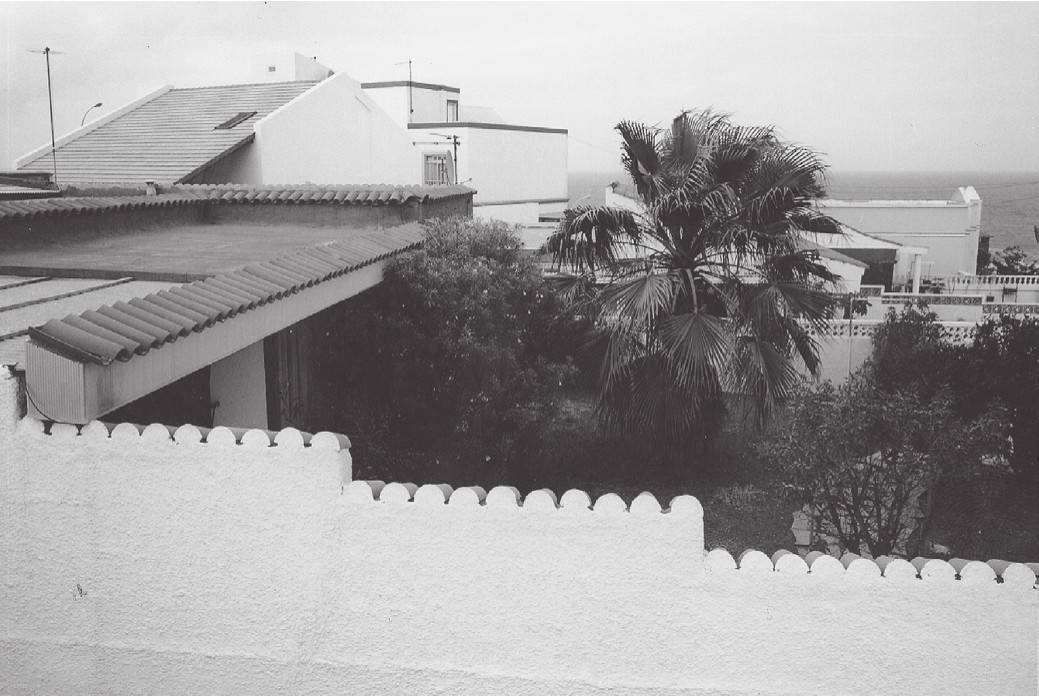
\includegraphics[scale=0.4]{picture/稻草人手记1.jpeg}
    \caption*{三毛在加纳利岛上的房屋小院。}
    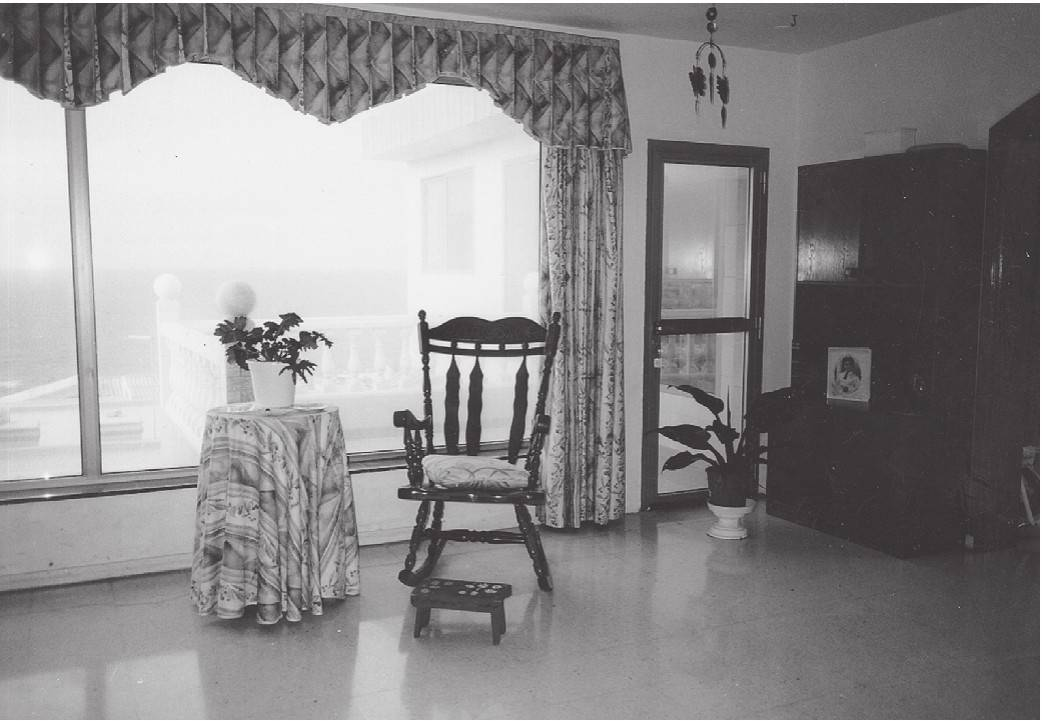
\includegraphics[scale=0.4]{picture/稻草人手记2.jpeg}
    \caption*{三毛作品中多次提到的“可以望见大海的大玻璃窗”。}
\end{figure}
\begin{figure}[htb]
    \centering %
    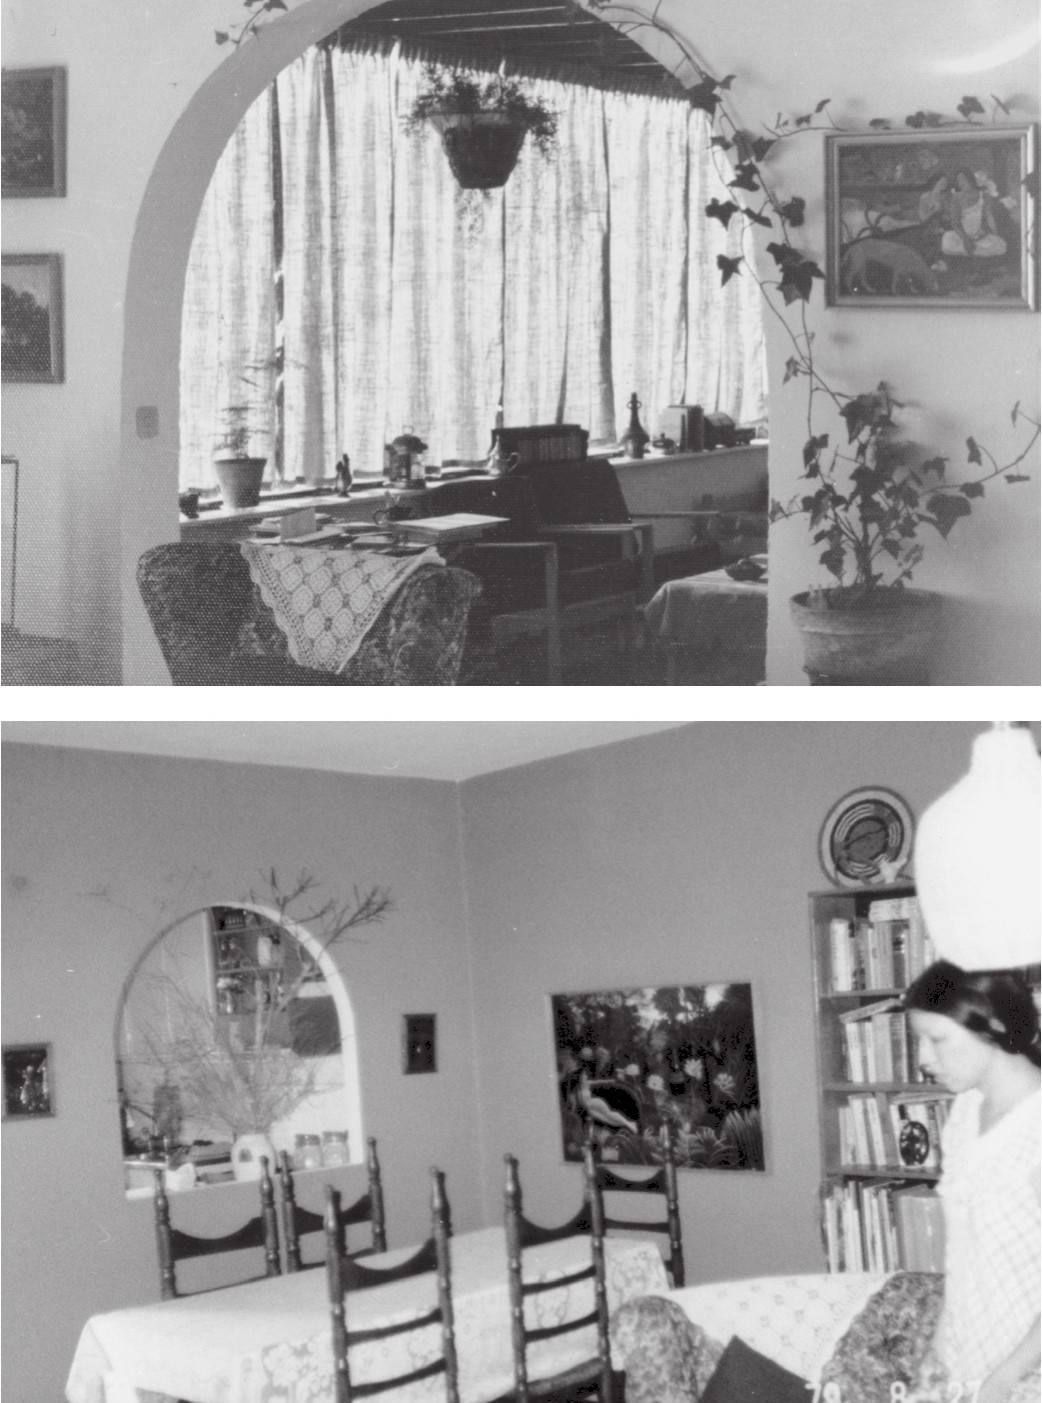
\includegraphics[scale=0.4]{picture/稻草人手记3.jpeg}
    \caption*{西班牙的家中一角。}
\end{figure}
\clearpage
\par 再说撒哈拉,在本月十八日摩洛哥送三十万平民走过边界,后又增到二百万“人海战”,西班牙吓得瘫掉了,AAIUN连军人才四万,全撒哈拉西属,才七万五(二十八万平方公里),后来南边毛里塔尼亚也由南边送平民来过边境(我就逃掉了,无票上机),这几日紧急会议再会议再会议的结果,西班牙不战而败,已签密约,摩洛哥与毛里塔尼亚瓜分撒哈拉,最最可怜的是撒哈拉威人,他们苦苦血战的独立,已成泡影,AAIUN所有撒哈拉威人完全失业,军人(西班牙军内也有撒哈拉威人)解散,他们成了无国籍的一批可怜虫,现在他们恨死西班牙人。
\par 我们好友罕地,三十二年跟西班牙军,现解散,完全不理,失去西班牙籍,AAIUN在军队重兵保护下,西班牙平民撤入军营同食同住,撒哈拉威人住的区完全在坦克严密监视中,他们是被西班牙人出卖了。西班牙人没有为他们的死活做打算,现无水,无食物,孩子要饿死了,红十字会已开去救济,我虽然痛恨撒哈拉威人,但是他们将来临的命运是可怜可悯的,是二十世纪的犹太人,无国籍的七万五千人。荷西临去送给罕地八千西币,罕地流泪不语,已收下,他有九个孩子,如今吃什么?吃沙土,完完全全无食物。
\par 再说荷西的职业,我们大约再做两个月便失业,但西班牙可能留下磷矿与摩洛哥合开,也可能放弃(用摩洛哥的海权交换给西国打鱼),但是公司说,我们可再分配国内工作,也可拿钱走路,如留下去,薪水加百分之百(因撒哈拉威人有游击队,要杀死所有西班牙人,有道理,西班牙利用了他们),好在荷西有一个月的假(我们留下的),先住一个月再去做,等公司分派将来工作。
\par 我的“沙漠学校”在我等机的空当,尚回家给一个女生上了“最后的一课”,她流泪握住我的手(姑卡),我们相对无语,机场已成地狱,那是十天之前,现在的AAIUN更是难以想象,我今天听荷西说撒哈拉威人的情形,我流泪吃不下盘中的牛排,撒哈拉是第二个越南,西班牙人出卖了他们。
\par 我要写一个中篇约十万字,《撒哈拉最后的探戈》(探戈是一种舞蹈),这是三毛眼见的血泪史。另外我要写《最后的一课》和《大逃亡》(荷西)。
\par 可怜的是,我好友Paloma的丈夫Jauies(万事通)明日尚得回沙漠(为了工作),他们全家人哭成一团,但他们无一文积蓄,只有去,又有孩子,要去赚钱。我借给Paloma的钱算做十日的住宿费,坚持不要她还,萍水相逢,收容我十日,已是义薄云天,我们现在是近邻,也好彼此分担忧苦。今日晚饭是Paloma送来。
\par 我们已打长途电话给公婆,婆婆终日啼哭不已,现已会笑,下星期姐夫来住三日(他是旅行社的社长)。
\par 荷西在分别后,寄给我几封信,我一封也未收到,因西班牙封锁消息,只说摩洛哥不再入侵,没有说密约,但AAIUN人自是完全知道,所以信件完全封锁,交通军方有,平民已断,妇女尚有未走,全在军营中吃住等机等船。ZBERIA航空公司说因为有狂风,不再飞AAIUN,荷西能逃出来,是他的机智,我们只有原子笔掉了一支,所以用红笔写。
\par 爹爹,姆妈,我们平安、健康、幸福,居所美丽,这都是荷西所赐,我感谢上帝给我如此的好丈夫。
\par 姐姐一同看信,我不再写,小鸟“芸芸”也出来了,很高兴,在睡觉(鸟食也带出来),都是荷西一人弄的,他人很瘦很瘦,要好好休息。
\par 再说,荷西在沙漠出大车祸,对方死了,他完全没事,是死了的那方错。
\par 荷西十二月再去沙漠,我们十一月薪水尚未领,已托好友代领(最最好友,好男孩,我有妹妹一定嫁此年轻人),他周末出来带钱给我们。在外朋友就是财富,现在苦难才见真情,人间温暖不会消失。
\par 此地静得没有邮差,小分局邮局每日开半小时,自去取信,你们有事打电报来可送到我们家,没有电话(不需要),海边在十分钟下坡路,空旷无一人迹。
\par 我们住的四周,是瑞典人、荷兰人、法国人、英国人,对面是一小小超级市场,有煤气,每日牛奶、面包送来门口,一星期结账一次。在此“芳邻”是鸡犬相闻,老死不相往来,但在区内,人人见面道“早安、午安、晚安”,不必交谈,谈不通也。我住友人家十日,全家出去了,门就大大地开着,但邻居不来往,有教养而亲切,跟西班牙风格大不相同,荷西也喜欢,我也喜欢。附近有一小镇,镇上全部西班牙人,人和气得像在天堂上,太和气太和气了,是糖做的一群老百姓,太好太好太和平的人了。
\par 爹爹眼睛不好,要不然我还多写,将来寄照片给你们看美丽的新家。我们很幸福,前途不知,荷西饿不死,要饿死他恐怕很难,他手很巧,什么都会做,不愁!
\par  
\par \rightline{妹妹上}


\subsubsection{一九七五年十二月五日}

\par \leftline{爹爹,姆妈:}
\par 荷西去上班四日,又回来了。
\par 他的公司在十二月十五日停工,转交给摩洛哥国营公司保证的工作,是一个骗局,过去大家都要罢工,公司就发通知保证每一个人将来都转派工作(是国营的公司),现在高级职员,有人情的职员,全都有工作,但是所有百分之八十的人失业,劳工部长保证的事,是放屁,现在没有工作,没有遣散费(一个月底薪约两万台币),没有发旅费回来,没有一切政府一再保证承诺的事项,当我们是狗一样地一脚踢开,我们没有工会,要告政府只有自己请律师告(我们有劳工部长签字的印刷信,保证工作),现在我们很镇静,开销马上省下来,不可再花一分一文不当的钱。然后我们要跟马德里一群专门替工人打官司的律师去商量,看看是否有补救之道(这群律师不收钱,等案子了了,才收一点点,以前荷西案子,完完全全不收钱,是一群年轻人)。
\par 我们是西班牙跟摩洛哥交易下的牺牲品,西班牙出卖了撒哈拉人,也出卖了自己三千劳工,西班牙的政府在烂掉,法兰哥的家族成了千万富翁,全西最大的百货公司、市场、房地产都是他女儿的,最大的医院是他女婿的,他的太太、女儿、孙女,穿孝穿黑色貂皮大衣算穿孝,我们吃沙吃灰在沙漠苦,现在一脚踢开,遣散费等于是狗屎,付两个月房租正好,生活那么高,三万块西币正好是三千包一公升的鲜牛奶价,现在摩洛哥人在沙漠屠杀六十岁以下的撒哈拉威人,年轻人全部逃亡阿尔及利亚加入“人民解放游击队”。西班牙人有许多跟了去,我不拉住荷西,他也要去(他如去,我跟去打游击),这次的事件,我看出西班牙的腐败,我们没有失业保险(德国有),没有救济金(工作三年满每月付四千台币,我们不满三年),我不是共产党,但是不要太逼人,人逼急了,不过是死路一条,我是一个分析明白的人,对政治不感兴趣,但正义在哪里?天理又在哪里?我们的前途政府没有管,叫我们去死吗?
\par 现在另有一个机会,荷西希望替摩洛哥工作,等矿公司一移交,我们留下来替新工作做事,但是更无保证,是外国公司要请你走路便走。
\par 现在公司薪水十二月不发,他们说“放假”半个月,以后再看。我们有房款可用,你们不要急,二月再说,我们如付不出房款,可以登报卖,如一时卖不掉,可打官司。打官司期内,每月付八千西币仍算我们的,直到法院宣判,所以也不是什么好急的事情。
\par 爹爹眼睛不好,为了我们,牺牲了一辈子,请你们不要再背我们的十字架,我们尚年轻,长长的人生可以受一点风浪,不要管我们了。荷西是很能干的人,我可回来出书,都是出路。荷西是个有为的青年,我们不会太潦倒,请千万放心,他要上船去做海员,我不赞成,全西班牙只有二十八个如他文凭的潜水人员,难道这一道一关的考试都是废纸吗?(是废纸,如是法兰哥的孩子,不必学写字也可一生做花花公子。)
\par 现在唯一的机会是跟摩洛哥签新合同,但是如果付太少(会付很少很少),也划不来做,我们很镇静,请放心,放心。
\par 亲爱的双亲,你们不要天天东想西想,请放开我们,给我们自己来,我们不能再收你们的钱,如果房子付不出,可以卖掉,还是有出路,不是太坏的事,你们不要再焦急,不要担心,过一阵子马上会好转的。总之你们不要再背十字架了,我知道我们台湾房子卖不掉,租不出,爹爹眼睛不好,我们自己家也很困难,不能再管子女,我们已成年太久,难道还不能自立吗?
\par  
\par \rightline{妹妹上}



\subsubsection{一九七六年二月二十五日}

\par \leftline{爹爹,姆妈:}
\par 前天收到包裹,我回来打开看了,才知什么叫蜂皇精,以前只听过。昨天早晨服一针,今日又服一针(因没有疲倦感),睡得非常好,目前还不觉得有什么反应,也不见强,但我想十天以后一定会胖起来。今日渔业专员梁先生开车来看我,进门便问我,为什么说谎话,我被他弄得莫名其妙,问清楚了才知是夏教授元瑜发表了我的信,信中我曾提起,我不太与渔船船员来往,因为他们不赞成我嫁外国人。我实在记不得自己信里胡说八道了什么,但是我也许有讲,这也不是什么大不了的叛国罪,值得今天看到报纸便来问我何故如此写,我老实告诉他,在码头上,中国渔船员的确骂我“婊子”(用中文骂我,因与荷西在一起走),结果我轻轻将话带过,这种小事,不值争辩,我的心胸气量都不是个傻瓜,我才不去计较他。他又说,非洲有四宝,一宝二宝三宝全讲了,又哈哈大笑,说还有一个宝就是“三毛”,语气嘲讽不堪,又笑我——你只值三毛钱,看一看你,只要付三毛钱入场券——(因为此地许多华侨要看我),我久不习惯这种语气,因为我们的朋友,都是尊重他人、诚恳坦白的人,我所以不知如何回答他的嘲笑。写作何罪?做三毛何罪?为什么人人都喜欢我,偏偏有同胞不喜欢我?为什么我在中国人里吃不开?为什么?为什么?不再问了,这是我很清楚的事。我尚未收到报纸,明后日收到了再看我这么写,犯了什么死罪。
\par 最奇怪的是,他和另外两个人来时,尚有我一西籍女友在家同坐,她看那人用中文高声大气问我,吓得马上走了,我真对不起这位太太,梁先生走了,我又赶快开车去她家道歉。外国人,最讲礼貌,不在他人面前高声讲话,而我也给梁先生吓一大跳,原来是这么一回小事情。
\par 我以前会被弄得气得哭,现在不气,只是好笑这些人,马德里腰痛那一大阵,也是如此这般,人,真奇怪,做了官,就以为老百姓都是狗屎,所以我不做官,也做不到,因为没有官架子也!
\par 爹爹,蜂皇精是那么贵的东西,如何寄给我,你们自己不吃?我身体无大病了,血止了,咳停了,颈子扭好了,现在脚扭伤已可开车(因为跌倒当时马上有西班牙老太太脱靴替我扭回,又马上上绷带,夜间荷西与姐夫也用力替我擦,又用热水泡,这一次恢复得很快,已开车),所以我无大病,你们不要担心,吃得也很好,包裹中附来《中央日报》,说维他命A的重要,我昨日吃两大根生的红萝卜,现在再去吃一大根,每日有鸡汤吃。水果也有吃橘子、苹果(不贵,三十元一公斤)。
\par 房子卖的事情,尚在谈,周末我们再去打电话给马德里。荷西星期五回来。
\par 沙漠边界打了起来,看情形也拖不长了,我们尚不知如何,反正有事做,不做有钱拿,不愁不愁。听说分派的工作都收入很差,不怕,我们有两三条路可走,不做也有三十万可领,一年失业不怕找不到事。听说失业政府尚借两百万给买房,我就不愁。
\par 上个月写伤了,这个月一字不写,上月出了好几万字,我休息,勉强不出来。何况我现在朋友很多,说英文的瑞士女友,她先生回来了(在北非工作,是探矿工程师),今日也来看我,我们相处十分投合,不说别人长短,只说有趣的事情,这些人都是好邻居。我认识的人很多,来往的只有瑞士女友、她英国丈夫、西籍女友,也够热闹了,每二日见一见面。都没有是非,彼此的友情,是有建设性的,不是小心眼找人碴子的。荷西回来了,也去拜访他们。我们相处,每日大笑特笑,不生气,对健康心情有益。邻居小孩也来,他们总是用英文问我:
\par “你爹地怎么不在?”
\par 我说:“我先生吧,什么爹地。”
\par 他们问:“你几岁?”
\par 我说:“我二十八岁。”
\par 他们说:“唉!我们以为你十五岁,所以以为那个大胡子是你爸爸!”我大乐。爸爸不常回家,我也过得好极了。
\par 中国人是好,那是老一代的。西方人,开朗,尊重他人的私生活,没有太多的利害关系,好相处。他们好佩服我呢!中文看不懂,但我每有报纸,都给他们看看。来了也不招待,一杯咖啡坐一个下午,没有客套,白学英语!
\par 汗衫好极了,荷西回来一定喜欢,粉丝我尚未打开来吃,等老爷回来同吃,我一大锅鸡汤可吃一星期。另外吃面包,不太吃饭。
\par 爹爹,姆妈,我的足踝已好,走路不痛,也可开车了,明日再服一针蜂皇精,人会胖,放心,一切都好,外公处请代问候。我一天平均写三封信,荷西不写信,我要代他写全家人的信,美国大姑、小姐姐都是我在联络,好在也不费事,不费心——邮费很贵,仍是值得。
\par 另外我在翻译一本漫画书,每日译三五小格,也不是工作。我的植物,欣欣向荣,长得好美。
\par 不要担心我,你们才要保重,希望早早见面,荷西说,卖了房子给我回家,我说:我们一同去。他舍不得钱,其实可以一同回娘家一个月荷西再回,我住久些。
\par 爹爹,我身体好了,不必担心,我会去全身检查,不要愁,我去检查。
\par 不多写了,我是顺手写来不费吹灰之力,爹爹姆妈眼睛吃不消。
\par  
\par \rightline{妹妹上}



\subsubsection{一九七六年三月二十六日}


\par \leftline{爹爹,姆妈:}
\par 今天是我的生日,我到昨天才知道,因为我去寄挂号信给皇冠五月份的稿子,才知已是三十三岁足了,对于年龄我并不在乎,因为人毕竟是要老的,如花开花落,都是自然的现象。回想三十三年来的岁月,有苦有乐,而今仍要走下去,倒已是有点意兴阑珊了。我的半生,到现在,已十分满足,金钱、爱情、名声、家庭都堪称幸福无缺,只缺健康的身体,但是,我也无遗憾,如果今后早死,于己于人都该贴红挂彩,庆祝这样的人生美满结束,我的心里毫无悲伤,只有快乐。自从去年大哥死去之后,我细想了一下,死的人去了,是安息了,是永恒了,生着的人,不应该悲痛,要有坦然的心胸去接受人生的现象,这也是我近来身体极不好之下,想到你们,而要劝告你们的话,人生的长短和价值,都是一样,一旦进入死亡,那就是永远地活下去,没有什么好悲痛的,请你们一定要明白这个道理。
\par 荷西仍未回来,卖房、找事之外尚得向银行借钱,都不可能十天半月弄好,他亦有信来。
\par 外公身体好吗?你们又如何?我有点发烧,开刀二次,疮结了又生,开了又结,又生,子宫流血又来,下月十日刮子宫,肝病也在吃药打针,我是私人医生在看,我撑得住,千万不要为我做无用的焦急。
\par 钻戒我没有用,于我身份也不配,姆妈留着,回来住家中,因荷西不来(太贵了),等一切安置妥,我就回台湾,千万放心我。
\par 宝宝如何?小妹们好吗?我回来买漂亮衣服给她们。不多写了。祝
\par 好
\par  
\par \rightline{妹妹上}


\subsubsection{一九七六年八月十日}


\par \leftline{爹爹,姆妈:}
\par 现在的生活安静朴素极了,每天穿一件比基尼游泳装随处可去,衣服实在用不着,今日我打扮了一下,不过是一件牛仔裤衣,已算很好了,荷西平日亦是短裤赤膊,此地住家人人如此,非常省衣服钱。
\par 我们又看到一幢房子,是一老先生死了,他太太想卖,也是一百五十万台币,我现在杀她价一百万台币,看她肯不肯(也许肯),这个岛上我们都去找了,其他地方即使院大也无处可去(荒秃秃泥巴山),这儿有海湾,有极好的环境可以外出散步,所以我选来选去还是现在住的地方。这儿对老人、年轻人、小孩都有好处,空气又好,现在这家如肯卖,我们马上买下(一大厅、四人房、两浴、一厨、有车房、院子),要等介绍人去丹麦问消息。我很喜欢这小房,对着大海,但不吵,因在远坡上,没有花树,光秃秃的一片,请爹爹、姆妈等我们买下房子了来住,你们肯来,将来车也换大的。
\par 今日去问失业保险,可领两年,我们方领四个月(每月一万六台币),所以我们不急,有很好的事才去做,如不太好,所赚差不多失业金,将来失业了还没有现在领的多,所以一定要小心找事。一万六一月对我来说是必须十分省了,房租一百,荷西学英文五十,汽油六十元,大约是二百十元美金,只有一百九十美元可吃饭杂用,所以不能看电影、穿衣、吃牛排……但这儿生活环境非常好,我很满足,吃穿都是次要,现在我就在院子里写字,对着大海,清风徐来,比花莲亚士都饭店好一百倍。以前我用大约七百美金一月,常常上馆子。
\par 希望过几年爹爹姆妈同来过过这里的安静日子,只怕你们会寂寞,你们来了,爹爹管花园,姆妈管厨房,这样不会无事做。
\par  
\par \rightline{妹妹上}








 % 3
% \clearpage

% 

\section{温柔的夜}

\par 书名:温柔的夜
\par 作者:三毛
\par 出版社:北京出版集团北京十月文艺出版社
\par 出版时间:2017-03
\par ISBN:9787530214770

\subsection{开场白\\\small{永远的夏娃}}

\par 《永远的夏娃》是很久以来就放在心里的一个标题,两年来,它像一块飘浮不定的云,千变万化,总也不能捉住它,给它定下清晰的形状来。
\par 起初想出这个名字,倒是为了一个西籍女友,因为她的种种遭遇,使我总想到其他许许多多在我生命中经历过的女友们,她们的故事,每一篇都是夏娃的传奇。当时,很想在这个标题下,将她们一个一个写出来。后来,我又不想写这些人了。可是专栏得开了,夏娃这个名字我还是很爱,因为它不代表什么,也不暗示什么,专栏既然要一个名字,我就用了下来,它本身实在是没有意义的。
\par 俄国作家杜斯妥也夫斯基说过一句使我十分心惊的话,他说:“除非太卑鄙得偏爱自己的人,才能无耻地写自己的事情。”
\par 我有一阵常常想到这句话,使得写作几乎停顿,因为没有写第三者的技巧和心境;他人的事,没有把握也没有热情去写;自己的事,又心虚得不敢再写,我不喜欢被人看视成无耻的人,可是老写自己生活上的事,真是觉得有些无耻。
\par 后来我们搬家了,新家门口每天早晨都会有一匹白马驮着两个大藤篮跟着它的主人走过,沿途叫卖着:“苹——果——啊!”
\par 每听见马蹄哒哒地来了,还不等那个做主人的叫嚷,我就冲出去靠在栏杆上看,直看到他们走远。
\par 这匹马天天来,我总也不厌地看它,每当荷西下班回来了,我照例按压不住内心的欢喜向他喊着:“今天马又来了!”
\par 马总是来的,而我的喜悦,却像当初第一次见它时一样的新鲜。
\par 有一天,再也忍不住了,跟荷西说:“我要把这匹马写出来。”
\par 他说:“有什么好写的,每天来,每天去的。”
\par 是很平常的事情,可是我要把它写下来,说我天天看见一匹马经过,不知为什么有说不出的欢喜和感动。
\par 后来,我又想到许多我生命中经历的事,忍不住想写,不写都不行,当时,总会想到杜斯妥也夫斯基那句话——老写自己的事是无耻的——每想这句话,心中便气馁得很,呆呆地坐下来看电视,什么也不写了。可是那匹马啊,一直在心底压着,总得把它写出来才好。
\par 又有一阵,一个朋友写信给我,他说:“你总不能就此不写了,到底你做的是文以载道的工作!”
\par 我被这句话吓得很厉害,从来没有想到载什么东西的问题,这更不能写了,不喜欢那么严重。
\par 以后有一段长时间就不写什么了。
\par 今天荷西下班来对我说,工地上有个工人朋友家住在山里面,如果我们跟他回去,可以去看看这人养的猪羊,还有他种的菜。我们去了,挖了一大筐蔬菜回来,我的心,因为这一个下午乡间的快乐,又恨不得将它写了下来。久已不肯动笔的人,还是有这种想望。
\par 回来后我一直在写作的事情上思想,想了又想,结果想明白了,我的写作,原本是一种游戏,我无拘无束地坐下来,自由自在地把想写的东西涂在纸上。在我,是这么自然而又好玩的事情,所以强迫自己不写,才会是一种难学的忍耐,才会觉得怅然若失,我又何苦在这么有趣的事情上节制自己呢!
\par 像现在,我在上面把那匹马写了出来,内心觉得无比的舒畅,这真是很大的欢喜。我做这件事,实在没有目的,说得诚实些,我只是在玩耍罢了,投身在文章里,竟是如此快乐,连悲哀的事,写到情极处,都是快乐的感觉,这一点,连自己也无由解释的,总是这样下去了吧,我毕竟是一个没有什么大道理的人啊!
\par 《永远的夏娃》将会是我一些美丽的生命的记忆,在别人看来,它们可能没有价值,在我,我不如不去想它价值不价值的问题,自由得像空气一般地去写我真挚的心灵。其实,它不写也没有什么不可以,写了对事情还是一样的,可是既然我想写了,我就不再多想,欢天喜地地将它们写出来吧!



\subsection{拾荒梦\\\small{永远的夏娃之一}}


\par 在我的小学时代里,我个人最拿手的功课就是作文和美术。当时,我们全科老师是一个教学十分认真而又严厉的女人。她很少给我们下课,自己也不回办公室去,连中午吃饭的时间,她都舍不得离开我们,我们一面静悄悄地吃便当,一面还得洗耳恭听老师习惯性的骂人。
\par 我是常常被指名出来骂的一个。一星期里也只有两堂作文课是我太平的时间。也许老师对我的作文实在是有些欣赏,她常常忘了自己叫骂我时的种种可厌的名称,一上作文课,就会说:“三毛,快快写,写完了站起来朗诵。”
\par 有一天老师出了一个每学期都会出的作文题目,叫我们好好发挥,并且说:“应该尽量写得有理想才好。”
\par 等到大家都写完了,下课时间还有多,老师坐在教室右边的桌上低头改考卷,顺口就说:“三毛,站起来将你的作文念出来。”
\par 小小的我捧了簿子大声朗读起来。
\refdocument{
    \par 我的志愿——
    \par 我有一天长大了,希望做一个拾破烂的人,因为这种职业,不但可以呼吸新鲜的空气,同时又可以大街小巷地游走玩耍,一面工作一面游戏,自由快乐得如同天上的飞鸟。更重要的是,人们常常不知不觉地将许多还可以利用的好东西当做垃圾丢掉,拾破烂的人最愉快的时刻就是将这些蒙尘的好东西再度发掘出来,这……
}
\par 念到这儿,老师顺手丢过来一只黑板擦,打到了坐在我旁边的同学,我一吓,也放下本子不再念了,呆呆地等着受罚。
\par “什么文章嘛!你……”老师大吼一声。她喜怒无常的性情我早已习惯了,可是在作文课上对我这样发脾气还是不太常有的。
\par “乱写!乱写!什么拾破烂的!将来要拾破烂,现在书也不必念了,滚出去好了,对不对得起父母……”老师又大拍桌子惊天动地地喊。
\par “重写!别的同学可以下课。”她瞪了我一眼便出去了。
\par 于是,我又写:
\refdocument{
    \par 我有一天长大了,希望做一个夏天卖冰棒,冬天卖烤红薯的街头小贩,因为这种职业不但可以呼吸新鲜空气,又可以大街小巷地游走玩耍,更重要的是,一面做生意,一面可以顺便看看,沿街的垃圾箱里,有没有被人丢弃的好东西,这……
}
\par 第二次作文缴上去,老师画了个大红叉,当然又丢下来叫重写。结果我只好胡乱写着:“我长大要做医生,拯救天下万民……”老师看了十分感动,批了个甲,并且说:“这才是一个有理想,不辜负父母期望的志愿。”
\par 我那可爱的老师并不知道,当年她那一只打偏了的黑板擦和两次重写的处罚,并没有改掉我内心坚强的信念,这许多年来,我虽然没有真正以拾荒为职业,可是我是拾着垃圾长大的,越拾越专门,这个习惯已经根深蒂固,什么处罚也改不了我。当初胡说的什么拯救天下万民的志愿是还给老师保存了。
\par 说起来,在我们那个时代的儿童,可以说是没有现成玩具的一群小孩。树叶一折当哨子,破毛笔管化点肥皂满天吹泡泡,五个小石子下棋,粉笔地上一画跳房子,粗竹筒开个细缝成了扑满,手指头上画小人脸,手帕一围就开唱布袋戏,筷子用橡皮筋绑绑紧可以当手枪……那么多迷疯了小孩子的花样都是不花钱的,说得更清楚些,都是走路放学时顺手捡来的。
\par 我制造的第一个玩具自然也是地上拾来的。那是一枝弧形的树枝,像滚铁环一样一面跑一面跟着前面逃的人追,树枝点到了谁谁就死,这个玩具明明不过是一枝树枝,可是我偏喜欢叫它“点人机”,那时我三岁,就奠定了日后拾荒的基础。
\par 拾荒人的眼力绝对不是一天就培养得出来的,也不是如老师所说,拾荒就不必念书,干脆就可以滚出学校的。
\par 我自小走路喜欢东张西望,尤其做小学生时,放学了,书包先请走得快的同学送回家交给母亲,我便一人田间小径上慢吞吞地游荡,这一路上,总有说不出的宝藏可以拾它起来玩。
\par 有时是一颗弹珠,有时是一个大别针,有时是一颗狗牙齿,也可能是一个极美丽的空香水瓶,又可能是一只小皮球,运气再好的时候,还可以捡到一角钱。
\par 放学的那条路,是最好的拾荒路,走起来也顶好不要成群结队,一个人玩玩跳跳捡捡,成绩总比一大批人在一起好得多。
\par 捡东西的习惯一旦慢慢养成,根本不必看着地下走路,眼角闲闲一飘,就知哪些是可取的,哪些是不必理睬的,这些学问,我在童年时已经深得其中三昧了。
\par 做少女的时代,我曾经发狂地爱上一切木头的东西,那时候,因为看了一些好书,眼光也有了长进,虽然书不是木头做的,可是我的心灵因为啃了这些书,产生了化学作用,所谓“格调”这个东西,也慢慢地能够分辨体会了。
\par 十三岁的时候,看见别人家锯树,锯下来的大树干丢在路边,我细看那枝大枯枝,越看越投缘,顾不得街上的人怎么想我,掮着它走了不知多少路回到家,宝贝也似的当艺术品放在自己的房间里,一心一意地爱着它。
\par 后来,发现家中阿巴桑坐在院子里的一块好木头上洗衣服,我将这块形状美丽的东西拾起来悄悄打量了一下,这真是宝物蒙尘,它完全像复活岛上那些竖立着的人脸石像,只是它更木头木脑一点。我将这块木头也换了过来,搬了一块空心砖给阿巴桑坐着,她因为我抢去她的椅子还大大地生了一场气。
\par 在我离家远走之前,我父母的家可以说堆满了一切又一切我在外面拾回来的好东西。当时我的父母一再保证,就是搬家,也不会丢掉我视为第二生命的破铜烂铁。
\par 有些有眼光的朋友看了我当时的画室,赞不绝口,也有一些亲戚们来看了,直截了当地说:“哎呀,你的房间是假的嘛!”这一句话总使我有些泄气,对于某些人,东西不照一般人的规矩用,就被称做假的。
\par 我虽然是抗战末期出生的“战争儿童”,可是在我父母的爱护下,一向温饱过甚,从来不知物质的缺乏是什么滋味。
\par 家中四个孩子,只有我这个老二,怪异得有拾废物的毛病,父亲常常开导我,要消费,要消耗,社会经济才能繁荣,不要一块碎布也像外婆似的藏个几十年。这些道理我从小听到大,可是,一见了尚可利用的东西,又忍不住去捡,捡回来洗洗刷刷,看它们在我的手底下复活,那真是太快乐的游戏。
\par 离开了父母之后,我住的一直是外国的学生宿舍,那时心理上没有归依感,生命里也有好几年没有再捡东西的心情。无家的人实在不需要自己常常提醒,只看那空荡荡的桌椅就知道这公式化的房间不是一个家。
\par 那一阵死书念得太多,头脑转不灵活,心灵亦为之蒙尘,而自己却找不出自救之道,人生最宝贵的青春竟在教科书本中度过实是可惜。
\par 不再上学之后,曾经跟其他三个单身女孩子同住一个公寓,当时是在城里,虽然没有地方去捡什么东西,可是我同住的朋友们丢掉的旧衣服、毛线,甚而杂志,我都收拢了,夜间谈天说地的时候,这些废物,在我的改装下,变成了布娃娃、围裙、比基尼游泳衣……
\par 当时,看见自己变出了如此美丽的魔术,拾荒的旧梦又一度清晰地浮到眼前来,那等于发现了一个还没有完全枯萎的生命,那份心情是十分感动自己的。
\par 到那时为止,拾破烂在我的生活中虽然没有停顿,可是它究竟只是一份嗜好,并不是必须赖以生存的工作,我也没有想过,如果有一日,整个的家庭要依靠别人丢弃的东西一草一木地重组起来,会是怎么美妙的滋味。
\par 等我体会出拾荒真正无与伦比的神秘和奇妙时,在撒哈拉沙漠里,已被我利用在大漠镇外垃圾堆里翻捡的成绩,布置出了一个世界上最美丽的家,那是整整两年的时间造成的奇迹。
\par 拾荒人眼底的垃圾场是一块世界上最妩媚的花园。过去小学老师曾说:“要拾破烂,现在就可以滚,不必再念书了!”她这话只有一半是对的,学校可以滚出来,书却不能不念的。垃圾虽是一样的垃圾,可是因为面对它的人在经验和艺术的修养上不同,它也会有不同的反应和回报。
\par 在我的拾荒生涯里,最奇怪的还是在沙漠。这片大地看似虚无,其实它蕴藏了多少大自然的礼物,我至今收藏的一些石斧、石刀还有三叶虫的化石都是那里得来的宝贝。
\par 更怪异的是,在清晨的沙漠里,荷西与我拾到过一百多条长如手臂的法国面包,握在手里是热的,吃在嘴里外脆内软,显然是刚刚出炉的东西,没法解释它们为什么躺在荒野里,这么多条面包我们吃不了,整个工地拿去分,也没听说吃死了人。
\par 还有一次西班牙人已经开始在沙漠撤退了,也是在荒野里,丢了一卡车几百箱的法国三星白兰地,我们捡了一大箱回来,竟是派不上什么用场,结果仍是放在家里人就离开了,离开沙漠时,有生以来第一回,丢了自己东西给人捡,那真说不出有多心痛。
\par 我们定居到现在的群岛来时,家附近靠海的地方也有一片垃圾场,在那儿,人们将建筑材料、旧衣鞋、家具、收音机、电视、木箱、花草、书籍数也数不清,分也分不完的好东西丢弃着。
\par 这个垃圾场没有腐坏的食物,镇上清洁队每天来收厨房垃圾,而家庭中不用的物件和粗重的材料,才被丢弃在这住宅区的尽头。
\par 也是在这个大垃圾场里,我认识了今生唯一的一个拾荒同好。
\par 这人是我邻居葛雷老夫妇的儿子,过去是苏黎世一间小学校的教师,后来因为过分热爱拾荒自由自在的生涯,毅然放下了教职,现在靠拾捡旧货转卖得来的钱过日子。
\par 在他住父母家度假的一段时间里,他是我们家的常客,据他说,拾荒的收入,不比一个小学老师差,这完全要看个人的兴趣。我觉得那是他的选择,外人是没有资格在这件事上来下评论的。
\par 我的小学老师因为我曾经立志要拾荒而怒叱我,却不知道,我成长后第一个碰见的专业拾荒人居然是一个小学老师变过来的,这实在是十分有趣的事情。
\par 这个专业的拾荒同好,比起我的功力来,又高了一层,往往我们一同开始在垃圾堆里慢慢散步,走完了一趟,我什么也没得着,他却抬出一整面雕花的木门来送荷西,这么好的东西别人为什么丢掉实在是想不透。
\par 我的拾荒朋友回到瑞士之后不久,他的另一个哥哥开车穿过欧洲再坐船也来到了加纳利群岛。这一次,我的朋友托带来了一架货真价实的老式瑞士乡间的运牛奶的木拖车,有三分之二的汽车那么长,轮子、把手什么都可以转。它是绑在车顶上飘洋过海而来的一个真实的梦。我惊喜得不相信自己的眼睛,接着,一本淡绿封面,精装,写着老式花体英文字母,插画着精美钢笔线条画的故事书《威廉特尔》轻轻地又放在我手里,看看版本,竟是一九二〇年的。
\par 这两样珍贵非常的东西使我们欢喜了好一阵,而我们托带去的回报,是一个过去西班牙人洗脸时盛水用的紫铜面盆和镶花的黑铁架,一个粗彩陶绘制的磨咖啡豆的磨子,还有一块破了一个洞又被我巧妙地绣补好了的西班牙绣花古式女用披肩。当然,这些一来一往的礼物,都是我们双方在垃圾堆里掏出来的精品。
\par 拾荒不一定要在陆上拾,海里也有它的世界。荷西在海里掏出来过腓尼基人时代的陶瓮,十八世纪时的实心炮弹、船灯、船窗、罗盘、大铁链,最近一次,在水底,捡到一枚男用的金戒指,上面刻着一九四七年,名字已被磨褪得看不出来了。海底的东西,陶瓮因是西班牙国家的财产归了加地斯城的博物馆,其他的都用来装饰了房间,只有那只金戒指,因为不知道过去是属于什么人的,看了心里总是不舒服,好似它主人的灵魂还附在它里面一样。
\par 拾荒赔本的时候也是有的,那是判断错误拾回来的东西。
\par 有一次我在路上看见极大极大一个木箱,大得像一个房间,当时我马上想到,它可以放在后院里,锯开门窗,真拿它来当客房用。
\par 结果我付了大卡车钱、四个工人钱。大箱子运来了,花园的小门却进不去。我当机立断,再要把这庞然大物丢掉,警察却跟在卡车司机后面不肯走,我如果丢了,他要开罚单,绕了不知多少转,我溜下车逃了,难题留给卡车司机去处理吧。第二天早晨一起床,大箱子居然挡在门口。支解那个大东西的时候,我似乎下决心不再张望路上任何一草一木了。
\par 前一阵,荷西带了我去山里看朋友,沿途公路上许多农家,他们的垃圾都放在一个个小木箱里。
\par 在回程的路上,我对荷西说:“前面转弯,大树下停一停。”
\par 车停了,我从从容容地走过去,在别人的垃圾箱内,捧出三大棵美丽的羊齿植物。
\par 这就是我的生活和快乐。
\par 拾荒的趣味,除了不劳而获这实际的欢喜之外,更吸引人的是,它永远是一份未知,在下一分钟里,能拾到的是什么好东西谁也不知道,它是一个没有终止,没有答案,也不会有结局的谜。
\par 我有一天老了的时候,要动手做一本书,在这本书里,自我童年时代所捡的东西一直到老年的都要写上去,然后我把它包起来,丢在垃圾场里,如果有一天,有另外一个人,捡到了这本书,将它珍藏起来,同时也开始拾垃圾,那么,这个一生的拾荒梦,总是有人继承了再做下去,垃圾们知道了,不知会有多么欢喜呢。


\subsection{黄昏的故事\\\small{永远的夏娃之二}}

\par 我喜欢漫游,也喜欢黄昏和黑夜交接的那一段时光。
\par 我们现在的家,坐落在一个斜斜山坡的顶上。前面的大玻璃窗看出去,星罗棋布的小白房在一脉青山上迤逦着筑到海边。
\par 厨房的后窗根本是一幅画框,微风吹拂着美丽的山谷,落日在海水上缓缓转红,远方低低的天边,第一颗星总像是大海里升上来的,更奇怪的是,墙下的金银花,一定要开始黄昏了,才发出淡淡的沁香来。这时候,一天的家务差不多都做完了,咖啡热着,蛋糕烘烤得恰到好处。荷西已经下工回来,电视机也开始唱广告歌。我换上舒服的凉鞋,把荷西的茶点小心地用托盘搬出来,这才摸摸他的头,对他说:“我走了。”
\par 这时候的荷西,也许在看报,也可能盯着电视,也可能开始吃东西,他照例含糊地说一句:“旅途愉快!”便将我打发去了。
\par 我轻轻地带上房门,呼吸着第一口甚而还有些寒冷的空气,心情不知怎的就那么踏实欢喜起来。
\par 很少在清晨散步,除了住在撒哈拉的那一阵经常早起之外,以后可以说没有在极早的时光里生活过。
\par 早晨是一日的开始,心情上,有一日的负担和算计,迎接未知的白日,总使人紧张而戒备。黄昏便是不同,它是温柔的夜的前奏,是释放、舒畅,教人享受生命最甜美的一段时光。
\par 这两年多来,无论住在哪里,家总是安置在近海的地方,黄昏长长的漫步成了生活里不可或缺的习惯。
\par 在丹纳丽芙岛,现在的住家,我每日漫游的路途大致是相同的。后山下坡,穿过海也似的芭蕉园,绕过灌溉用的大水池,经过一排极华丽的深宅大院,跟“水肺”站着谈一会儿闲话,再下坡,踏过一片野菊花,转弯,下到海岸线,沿着海边跑到古堡,十字港的地区就算是到了,穿进峡谷似的现代大旅馆,到渔港看船,广场打个转,图书馆借本书,这才原路回来。
\par  
\par 每日经过女友黛娥的家,她总是抱了孩子想跟我一块去游荡,有时候看见她近乎委屈地巴望着我,总觉得自己拒绝得有些残忍。
\par 总是哄她,用各种理由不带她去,有时候远远看见她向我走来,干脆装着不看见,掉头就跑,这样无情地一次一次甩掉她,她居然也不生气。
\par 我喜欢适度的孤单,心灵上最释放的一刻,总舍不得跟别人共享,事实上也很难分享这绝对个人的珍宝,甚至荷西自愿留在家里看电视,我的心里都暗藏了几分喜悦。
\par 清风明月都该应是一个人的事情,倒是吃饭,是人多些比较有味道。
\par 每次散步,那条乡间小路上可以说是碰不到一个人影的,只有“水肺”,像是赴约会似的等在他华厦的大门口,苦盼着我经过。
\par “水肺”是一个八十多岁生病的德国老头子,跟他单身的儿子住在一幢极大的房子里,父子两个长得一模一样,儿子中年了,好似也病着似的。
\par 这一家异乡人没有朋友,也不外出做事,种了一园的玫瑰花。老人因为肺水肿,已经不太能动了,天天趴在花园的门上,见我去了,老远的就一步一步将我吞下去似的望。
\par 第一次经过老人的门口,就是被他喂喂地叫过去的。我过去了,他隔着镶花铁门,把手蓦然伸出来牢牢捉住人不放,手指冰冷的,骷髅似的大眼洞瞪着人,肺里风箱似的响,总是说:“上个月医生就说要死了,可是这个月都快完了,还没有死。”
\par “水肺”是我自己心里给老人叫的名字,他们姓什么从来不知道,散步去了,每天被他捉住,随他乱扯什么我都忍着听,后来日子久了,究竟是烦了,常常坚决地抽开他的手,转身逃开去。
\par 有一次老人突然问我:“你穷不穷?你先生穷不穷?”
\par 我不知道他为什么这么唐突地问我,站着不响,没有回答他,带些愠怒地微笑着。
\par 他又突然说:“我唯一的儿子,死了不放心他,订婚两次,结果都给人跑掉了,如果,如果你肯跟他——我们是有钱的人,将来都是你的,不信你进来看,进来看呀——”
\par 我静静地看着老人,说了一句莫名其妙的话:“我不为钱结婚。”
\par “可是也可以为钱结婚,是不是,是不是?”
\par 老人又伸出手来急切地死拉住我,我悄悄抬眼往他身后望去,老人那个苍白沉默的中年儿子正躲在窗帘后面的一角偷看我。
\par 后来我告诉荷西老人的事,荷西将我骂了一顿,说:“你已经结婚了,怎么还去跟人家争为不为金钱出嫁的事情,干脆把他骂过去才是。”
\par 我也想过要骂这个老人,可是一经过他们的家门,看见那一园寂寂的玫瑰,心里总有些说不出的不忍和悲凉,便又和颜悦色地对待他了。
\par 前几天老人真的死了,晚上死的,第二天清早就搬去葬了,好方便的,大概早就预备着等他死的。
\par 听见了这个消息的黄昏,一样在散步,经过死去老人的门口,发觉跟他长得那么相像的儿子,居然代替了父亲的位置,穿了一件鲜明的红毛衣,一色一样地趴在家门口。我看见了他,本想上去说几句哀悼的话,没想到他先对我喂喂地叫了起来,那个姿势和声音,就像他父亲第一次看见我时死命地把我叫过去一个样子,我被他这怪异的举动,吓得头发根根竖了起来,青着脸往山下没命地逃,一回头,那个儿子的半身,还挂在门外向我招手。身后如此华丽的洋房,却像个大坟似的,埋葬着一个喂喂呼叫的寂寞的活人,也是够残忍的了。
\par 这几天还是经过死去老人的家门前,那个儿子不挂在门上了——他在窗后面看我。不知是忌什么,总是加快了脚步,怕一个那么堪怜的人,也算是生命的无奈吧。
\par 我是不喜欢芭蕉园的,一走进去,再好的夕阳都幽暗暧昧起来,无风的时候四周静得要窒息,稍稍吹过一点点微风,芭蕉叶又马上夸张地沙沙乱响。
\par 从小听带我长大的女工人玉珍说鬼,她每说鬼时,总要顺手一指过去在父母家中院里的一丛芭蕉树,说:“鬼啊,就在那种树下面,还会哭哦!女的,抱了小孩吱吱惨哭!”
\par 我的童年被鬼故事吓得很厉害,直到现在,看见芭蕉心里还是不自在。
\par 散步的路,不经过密密的蕉林就到不了海边。这一段长路,总是跑的,有时候天气阴暗,出门之前总再三拜托荷西:“过十五、二十分钟左右请你站出来在阳台上给我看看,好少怕一点。”
\par 跑过一段蕉园,抬起头来往老远高岗上的家里望,荷西如果站在那儿,哪怕是个小黑点,心里也好过些。后来我天天叫他出来站一站,他不耐烦了,不再理我,我就一口气跑下去,两边树影飞也似的掠过,奔出林子,海边的路来了,这也就过了,可惜的是,芭蕉园里从来没有停下来看看是不是可以吃它一根绿蕉,总是太怕了些。
\par 从海岸一直走到古堡那一条路是最宽敞的,没有沙滩,只有碎石遍地,那么长一条滩,只孤零零一棵松树委委屈屈地站着,树下市政府给放了条长木椅。
\par 这儿没有防波堤,巨浪从来不温柔,它们几乎总是灰色的一堆堆汹涌而来,复仇似的击打着深黑色怪形怪状的原始礁岩,每一次的冲击,水花破得天一般的高,惊天动地地散落下来,这边的大海响得万马奔腾,那边的一轮血红的落日,凄艳绝伦地静静地自往水里掉。
\par 这两种景象配合起来,在我的感动里,竟是想象中世界末日那份摄人心魂的鬼魅和怪异,又想到日本小林正树导演的《怪谈》中的几场片景。这样的画面,总有一份诗意的凶恶,说不出是爱还是不爱,可是每天经过那张松树下的木椅,还是忍不住被吸引过去,坐下来看到痴了过去。
\par  
\par 过了古堡,进入街道、商店、大旅馆……混入各色各样的外籍游客里去,这本是个度假的胜地,冬暖夏凉,虽是小街小巷,人世的鲜明活泼毕竟比大自然的景象又多了一层温柔。
\par 经过小小的渔港,船都拉上了滩,没有预备出海的迹象,有些面熟的年轻人坐着钓鱼,老人在补网,穿热裤的金发游客美女在他们身边哗笑走过,这么不同的生活和人种同住在弹丸大小的十字港,却平静得两不相涉,亦是有趣的画面。
\par 港口的椅子上,一个外国老太太,一个西班牙老渔夫,两个人话也不通,笑眯眯地靠在一起坐着,初恋似的红着脸。
\par  
\par 过了那么多年,《巴黎最后的探戈》才在西班牙解禁了。港口电影院的队伍排列到另外一条街。
\par 一看是这张电影,连忙跑上去看挂着的剧照,人群里却有人在叫着:“喂,三毛,三毛!”
\par 发觉另外一个女友卡门居然打扮得花枝招展地挤在买票的队伍里,跑了上去问她:“你干吗?”
\par 她暧昧地笑,神经兮兮地问我:“你看不看?看不看?”
\par “像你这种小气巴拉的样子,我就不看。”我拍拍她的头,斜斜睇着她,她一下气得很。
\par “这不是色情片,它有它本身的意义。”她十分严肃地分析起来,声音也大了。
\par “啊!这么严重?我更不要看了。”我又笑她,她气得想掐我又不敢离开队伍。
\par “我去买冰棒,你吃不吃?”我问她,她摇摇头,用手指指远方,原来是她的摄影家先生慢慢晃来了。
\par  
\par 在广场向老祖母买冰棒,向她要柠檬的,她必定给人凤梨的,要凤梨的,她一定弄成柠檬的,跟她换,她会骂人。
\par 很喜欢向她买冰棒,总得站好,专心想好,相反地要,得来才是正的。
\par 我一向是向她要柠檬,得来正是我要的凤梨。有一次想,如果向老太婆买橘子冰棒,不知她弄成什么,结果她没弄错,我大大失望一番,以为橘子会变草莓的。
\par  
\par 荷西叫我顺便去图书馆借海洋方面的书。
\par 我跑进去拿了一本褚威格,一本卫斯特,这是荷西最受不了的两个作家,他自己不下来借,结果便是如此活该。
\par  
\par 夜来了,黄昏已尽,巷内一家家华丽高贵的衣饰店看花了人的眼,看痛了人的心,繁华依然引人,红尘十丈,茫茫的人世,竟还是自己的来处。
\par  
\par 回程下雨了,将借来的书塞进毛衣里面,发狂地往家里跑。一日将尽,接着来的,将是漫漫长夜,想到雨夜看书的享受,心里又充满了说不出的喜悦和欢欣,夜是如此的美,黑夜淋雨,更是任性的豪华。
\par 跑过蕉园的外围,先去守园老夫妇的小瓦房,老婆婆正在屋内搬了空罐头预备接漏雨呢。
\par 坐了一会儿,老公公回来了,跳上去捉住他,叫他陪着穿过蕉林,天越走越黑,雨却不大了,老公公一再地问,荷西怎么不捉鱼给他吃了。
\par  
\par 快到家门了,开始小跑,这是一天的运动,跑到家里,冲进门去,愉快地喊着:“回来啦!”
\par 那时候,荷西看见我总很高兴的样子。
\par 我们十点钟吃简单的晚饭。
\par 夜间十二时上床开始看书,我叹了口气,对荷西说:“散步太快乐了,这么快乐,也许有一天散成神仙,永远不再回家了,你说好不好?”
\par 荷西不置可否。
\par 结婚四年了,我也知道,这种鬼话,只有神经不正常的人才能回答我。
\par “如果我成仙去了,你不要忘了吃东西,蛋炒饭冰箱里总是有一盘的。”
\par 荷西还是专心做他的填字游戏,咿咿啊啊地假装听着。
\par 我又自说自话了好一阵,这才拿起书来,默默地看了下去。
\par 看了一看,还是搁下书来想了一下——荷西不知道会不会找不到蛋炒饭。



\subsection{巫人记\\\small{永远的夏娃之三}}

\par 居住在加纳利群岛不觉已有两年了。
\par 一直很想将这儿亲身经验的一些“治疗师”用巫术治病的情形记录下来。
\par 知道《皇冠》在这个群岛上拥有可观的订户和读者,住在这儿的侨胞,看了以下的文字时,很可能会觉得奇怪,为什么不肯介绍这个美丽而现代的北非观光胜地的旅游事业,偏偏要去写些旁门左道的巫术,好似这儿是个无比落后荒谬的地区一般。
\par 我因为去年曾经给这个群岛写了一个中篇游记,收录在《哭泣的骆驼》那本书里,因此有关加纳利群岛的其他,无心再在这儿重述了。
\par 有兴趣写的还是几次接受土地郎中治病的经过情形。
\par  
\par 第一次听说加纳利人相信巫术是在沙漠里居住的时候。
\par 那时,许多加纳利岛的工人过海去沙漠的小镇讨生活,他们或多或少总会说说自己故乡的事情。
\par 我们的朋友之一马诺林是大加纳利岛去的,他可以说是同乡们中的知识分子,本身极爱思考,也很喜欢心灵学方面的知识,据说,他的养父,过去一度是做巫人的,后来娶了他的母亲,才改在香烟厂去做事了。
\par 马诺林在性格方面有他的神秘性,思想有时候十分的怪异,我跟他很谈得来,而荷西就比较没有办法进入这个人的心灵领域里去。
\par 当时,我们的撒哈拉威邻居的男孩子,一个名叫巴新的,不知为什么迷上了一个沙漠里的妓女,几个月来鬼魔附体似的,白天糊涂到家人也不太认识,可是只要黄昏一来,他的步子就会往女人住的那个方向走。家里的东西不但偷出去卖,连邻居那儿都红着吓人的眼睛死赖着借钱,钱一到手,人就摇摇晃晃地被吸去了,好似那个妓女勾着他的魂一般。
\par 有一天巴新晃进来借钱,我看他实在可怜,给了他三百,这点钱上女人那里去自然是不够的,他又可怜巴巴地求。马诺林当时恰好在我们家,也给了他两百,他才低着头走了。
\par “这个孩子可怜,中了蛊。”马诺林说。
\par 我一听,全身寒毛肃立,不知道他为什么会讲这么可怕的话。
\par “中的还是加纳利群岛那边人搞过来的鬼东西。”马诺林又说。
\par “迷女人呀?”我又吓吓地探了一句。
\par “不小心,吃下了一点别人放的不该吃的东西,就回不了头了。”
\par “你怎么晓得?”荷西很不以为然地问。
\par “这种东西,发起来一个样子,没有那个女人,就是死路一条,妓女常常用这种方法去教人中迷的。”
\par 本想反驳马诺林这过分荒谬无知的说法,后来想到他家庭的背景——养父是巫人,母亲开过酒吧。在他生长的环境里,这样的迷信可能还是存在的。我因此便不说什么,笑笑地看着他,可是心里是不相信这一套的。
\par “巴新也真可怜,十六岁的小家伙,爱上那个女人之后完全变了,有一次三更半夜来敲门借钱,好像毒瘾发作的人一样,我们开慢了一点,他就疯了似的一直敲一直敲,真开了,他又不响了,呆呆地站在月光里,好可怕好可怕的红眼睛瞪着人看。”我越说越怕,声音也高昂起来了。
\par 马诺林听了低头沉思了好一会儿。
\par “他们家是保守的回教家庭,出了这样个儿子,真是伤心透了,上礼拜巴新还给绑起来打,有什么用,一不看好,又逃出去了。”我又说。
\par 这时候马诺林抬头很奇异地抹过一丝微笑,说:“可以解掉的嘛!”
\par “巴新是初恋狂,性格又内向,所以这个怪样子,不是你说的中了什么蛊。”我很简单地说。
\par 马诺林也不争辩,站起来,穿过我们的天台,到巴新家里的楼梯口去。
\par “要巴新的妈妈来跟我谈。”马诺林对我说。
\par 虽是沙漠女人,为了谈儿子,匆匆忙忙就跑过来了,马诺林低低地对她不知讲什么,巴新的母亲猛点头,一句一句答应着,又擦眼泪,不停地擦泪。
\par 没过第三天,巴新意外地好了,人也精神起来了,很快活地坐在大门口,黄昏也不出去,接连十多天都没再出去,以后完全好了。
\par 我心里奇怪得不得了,又不能问巴新。
\par 马诺林来了,我自是逼上去死死追问,可是他也不肯讲,只说:“这种事只有巴新的妈妈可以化解,如果没有母亲,就难了。”
\par “可是做了什么呢?”我又追问着。
\par “小魔术。”马诺林仍是笑而不答。
\par 我们是不相信的,看了巴新仍不相信。直到来了丹纳丽芙岛,发觉连乡下女人要抓住丈夫的心,都还相信这些巫术,真教人有不知身在何处之感,慢慢地也听习惯了这些事。
\par 当然,我说的这些只是一般少数没有知识的乡下女人男人,并不能代表大半的加纳利民风,这些事在城市里是不常听讲的。
\par  
\par 个人第一次接触到一个治疗师,是在两年前的冬天。那时候,我得了一次恶性感冒,初来这个岛上,没有一个相识的朋友,那时候荷西又单独去了半年沙漠,我一个人居住在海边生病。
\par 感冒了近乎一个多月,剧烈的咳嗽和耳痛将人折磨得不成样子,一天早午要两次开车去镇上打针,可是病情始终没有丝毫进展。
\par 医生看见我那副死去活来的样子非常同情,他惊异地说:“开给你的抗生素足足可以杀死一只大象了,你怎么还不好呢?”
\par “因为我不是那只象。”我有气无力地答着。
\par 药房的人看我一次又一次地上门,也是非常不解,他们觉得我吃药吃得太可怕了。
\par “这种东西不要再用了,你啊,广场上那个卖草药的女人去试试看吧!”药剂师无可奈何地建议着。
\par 我流着冷汗,撑着走了几十步,在阳光下找到了那个被人叫“治疗师”的粗壮女人。
\par “听说你治病?”那一阵真是惨,眼前金星乱冒的虚弱,说话都说不动。
\par “坐下来,快坐下来。”治疗师很和气,马上把我按在广场的一把椅子上。
\par “咳多久了?”
\par “一个多月了,耳朵里面也很痛,发烧。”
\par 女人一面听一面很熟练地抓了一把草药。
\par “来,把手给我,不要怕。”治疗师把我的双手合起来交握在她手掌里抱在胸前,闭上了眼睛喃喃有词地说了一段话,又绕到我背后,在我背上摸摸,在耳朵后面各自轻轻弹了一下,双手在我颈下拍拍,这就算治过了。
\par 我完全没有被她迷惑,排拒地斜望着这个乡下女人,觉得她很滑稽。阳光下,这种治疗的气氛也不够吸引人。
\par 那份药,收了相当于三块美金的代价,念咒是不要钱的,总算是很有良心了。
\par 说也奇怪,熬了三次草药服下去,人不虚了,冷汗不流了,咳出一大堆秽物,缠绵了近四十天的不适,一夜之间消失得无影无踪。
\par 我想,那还是以前服的抗生素突然有了作用。治疗师的草药不过是也在那时候服了下去,巧合罢了。
\par 虽然那么说,还是去买了一包同样的草药寄给台北的父母收藏。
\par 治疗师笑着对我说:“其实,这只是一种煮肉时放进去用的香叶子,没有什么道理,治好你的,是上面来的力量。”她指指天上。
\par 我呆呆地看着她,觉得很有趣,好在病也过了,实在不必深究下去。
\par “你怎么学的?”我站在她摊子边东摸西看,草药的味道跟台湾的青草店差不多,很好闻的。
\par “老天爷赐的特别的天赋,学不来的呀!”很乐天地笑着。
\par “你还会什么?”又问她。
\par “爱情,叫你先生爱你一辈子。”女人粗俗地恶狠狠地对我保证,我想她这是在开人玩笑了,掉头笑着走开去。世上哪有服药的爱情。
\par  
\par 加纳利群岛一共大小七个岛,巫风最盛的都说是多山区的拉芭玛岛,据说一般居住在深山里的乡民万一生了小毛小病,还是吃草药,不到真的严重了不出来看医生的。
\par 有的甚而连草药都不用,只用巫术。
\par 荷西与我曾经在这个多山的岛上,被一个来历不明的女人抢拔了一些毛发去,她拉了我一小撮头发,荷西是胡子。这件事去年已经写在游记里了。至今不明白,这个女人抢我们的毛发是有什么作用。
\par 很有趣的是,我们被拔了毛发那日回旅社去,不放心地请教了旅馆的主人,问他们有没有拔毛的风俗。
\par 旅馆主人笑说:“是巫术嘛!”
\par 我们没说什么,心里很不是滋味,那种不愉快的感觉过了好多天都萦绕在心里,挥之不去。
\par 在拉芭玛岛居住又住了十数日。一天旅馆楼下隔邻的人要请巫师来家里,清洁工人就来跟我们说了。
\par “治什么?”
\par “那家太太瘫在床上好多年啦!还送到马德里去治过,没有好。”
\par 我马上跑去请旅社主人带我去看,他很干脆,当时便答应了,并且说,瘫在床上的是他堂嫂嫂,有亲戚关系的。
\par 下午五点多钟吧,他们打电话上来叫我,说巫师来了。当然,为了尊敬对方,他是说:“治疗师来了!”
\par 这位治疗师也真有意思,听说他平日在市政府上班,兼给人念咒治病,穿得很时髦,体格十分魁伟,很有自信的样子,怎么看都没有阴气,是个阳间的人物。
\par 我跟去楼下这家请巫师的人家时,那个瘫着的女人居然被移开了,只有空床放着,这不免使我有些失望,人总是残忍的,对悲惨的事,喜欢看见了再疼痛,看不见,就不同了。
\par 治疗师在房内大步走来走去,好像散步一样,也不作法,不念咒,然后简单地说:“把床换到这头来。”又说:“从今天起,这扇门关上,走另外一边出入。”
\par 说完他走掉了,我什么也没看见。
\par 跟在旅社主人后面走出来时,我不解地问他:“你想床换了位置,再开开门关关门,瘫女人就会走路了吗?怎么可能呢?”
\par 他停下来很奇怪地看着我,说:“谁说她会走路来的?”
\par “不是明明请人来医她的吗?”我更不懂了。
\par “谁有那么大的法力叫瘫子走路?那不过是个兼差的治疗师而已呀!”他叫了起来。
\par “他来到底是做什么?”
\par “来治我堂嫂嫂的伤风感冒,你看吧,不出一星期一定好,这个人在这方面很灵的。”
\par “就这样啊?”
\par “就这样?你以为巫术是做什么,是给你上天下地长生不老的吗?”
\par 去年荷西远赴尼日利亚去工作,我一个人住在家里。有一天,因为滂沱大雨,车子在乡间小路上熄了火,我不顾一切下来死命推车,一时过去车祸受伤过的脊椎又大痛了起来。
\par 我一连去看了七八次医生,睡在硬地上,都不能减轻那剧烈的痛。
\par 那时家中正在油漆,工人看见我痛得那个样子,马上热心地要开车送我上山去找“治疗师”。
\par 当时不知为什么那么无知,竟然表示肯去试试,跟油漆匠约了次日一同去看那个传说中的瞎子治疗师。
\par 一个受伤的脊椎必然需要时间给它复元,而我去痛心切,大意地将身体那么重要的部位去交给一个瞎子老人,实在是不可饶恕的愚昧。
\par 这个瞎子很著名,乡下人相信他,我们社区的油漆匠也有脊椎的毛病,所以才把我给带去看。
\par 去了原来是给脊椎痛的人“拔火罐”,跟中国的老方法差不多。有趣的是,瞎老人用个马铃薯放在脊椎上,马铃薯上再插一根火柴,火柴由他的助手女儿一燃上,马上从上面罩个玻璃杯,这一来,开始贴着肉推,痛得差不多要叫,治疗也好了。治好的人,也是助手来,拿长条的宽绷带将胸口到下腰紧紧地绑起来,这个在医学上有没有根据我不知道,可是我个人绑了几天之后,痛减轻了很多。
\par 当我回到自己的医生处去检查时,跟他说起瞎子治疗师的事,当然被他大骂了一顿,我也就没有再回去给放马铃薯了。
\par  
\par 今年换了居处,来了美丽的丹纳丽芙岛,这儿景色非常美丽,四季如春,冬不冷,夏不热,而我,在这么怡人的岛上,居然一连发了数个月的微烧,医生查遍身体,却找不出毛病。
\par 在这种情形之下,又有人好意来带我去找“治疗师”了。
\par 据说,那是一个极端灵验的南美委内瑞拉远道而来的治疗师,专治疑难病痛。我女友的母亲因为手腿麻木,要去看,把我也一同捉了去。
\par 治疗师住在山里面,我们清晨几点到,已经有一长队的人在等着了,等待的人,绝大多数是没有知识的乡村妇女们。她们说,这一个比较贵,多少要放五百、一千西币。虽然照习俗,治疗师本人是不定价不讨钱的,因为这天赋治病的异能,是该用来解除众生的苦痛,所以不能要钱。说是这么说的,可是每一个都拿。
\par 南美来的术师长得非常动人,深奥的眼睛摄人心魂似的盯住每一个哀愁的女人。他是清洁的,高贵的,有很深的神学味道,在他的迫视下,一种催眠似的无助感真会慢慢地浮升上来。
\par 每一个病人到他面前,他照例举木十字架出来在人面前一左一右地晃,然后轻轻地祷告,静静地听病人倾诉。当时场内的气氛有若教堂,每一个穷苦的女人受了他的催眠,走出去时,绿绿蓝蓝的大钞票就掏出来了。
\par 这是个江湖术士,草药都不用了。轮到我时我退开了,不肯给他看。
\par 同去的女友的母亲接受治疗之后大概一时感动得十分厉害,出门还流下了眼泪。
\par 最假的治疗师最会赚钱,也最受人们爱戴,这是我的一大发现。
\par 比较起来,我喜欢市政府那个叫人搬床的治疗师,他什么气氛都不制造,连病人也不必看,多么干脆。
\par  
\par 西班牙本土人爱孩子,加纳利群岛人也爱孩子,更爱男孩子。荷西与我结婚四年,没有生育,在这儿简直被乡下人看成人间悲剧,他们一再地追究盘问,实在使人啼笑皆非。
\par 有一天,打扫女工玛丽亚匆匆地跑上楼来激动地问我:“要不要一个男娃娃?”
\par 我被这突如其来的问话吓了一跳,马上想到一定是个弃婴,叫了出来:“在哪里?”
\par “什么在哪里,我打听到一个治疗师,治好了不知其数的不孕妇人,生的都是男娃娃。”她愉快地向我宣布。
\par 我听了叹了口气。这些愚民村姑,怎么会无知可怜到这个样子。
\par “什么\UncommonChar{𫪘}!我不去。”我很无礼地回答。
\par “你去,你今天下午去,明年这个时候请我参加孩子受洗典礼。”玛丽亚有这么固执的信心。
\par “我不相信,不去,不去。”简直神经嘛。
\par 玛丽亚走了,过了一下,带来了我很面熟的一个希腊邻居太太,手里抱了个小婴儿。
\par “真的,你一定要相信我,我结婚几年没有孩子,也是别人介绍我去那个治疗师那里治了几次,现在有了这么可爱的一个孩子,你如果肯去,我下午可以带路。”那个太太很温柔地说。
\par “我们还没有决定要不要小孩。”我硬着头皮说。在一旁听的玛丽亚做了一个昏倒的表情,她三十六岁,有四个小孩,最大的十七岁。
\par “千万不要这么说,你去试试,太多的女人被这个老人医好了。”希腊太太又说。
\par “痛不痛?”我动摇了。
\par “不痛,要拉手臂,两手交抱,治疗师从后面抱起来拉,脊椎骨头一节节响,就好了。”
\par “嗄!”我听了脊椎马上真痛起来。
\par “我们都是要帮助你,去一次怎么样?”
\par 我开始愠怒起来,觉得这两个女人太讨厌了。
\par 到了下午,希腊先生热情地来了,不由分说,就拿了我的毛衣皮包自说自话地下楼了。
\par 我无可奈何,强忍了怒,锁了门,走下楼时,他们这对过分热心的夫妇已在车内等着我了。
\par 治疗师也是个老人,他很得意地说,连葡萄牙那边都有不孕的女人慕名来找他,结果都怀孕了,而且生男孩。
\par 接着老人站在一格高楼梯上,叫我双手交抱,手臂尽量往背后伸,他从后面抱住我,将我凌空举起来乱晃,骨头果然咔啦啦乱响,我紧张得尖叫了起来,他又将我上下乱顿,这一来,受伤过的脊椎马上剧痛,我几乎是打架似的从老人手臂里又叫又喊地挣脱下地。
\par 在一旁看的希腊夫妇很不甘心,一齐叫着:“这不算,再摔一次,再摔一次。”
\par “差不多啦,下次再来,下星期六早晨来最好。”老人被我乱叫得有些不乐,门外候诊的另外几个女人马上露出了害怕的神情来。
\par 我送了治疗师两百块钱,那么少,他还是谢了又谢,这一点使我十分喜欢他,可是我再也不会回去找他了。还是把时间让给葡萄牙女人去吧。
\par  
\par 治疗师,我们背地叫他们巫师,在这儿还有很多很多,我去过的还有其他三四个,不过都没有什么过分特别,不值得记述,比起我所见过的尼日利亚与贝宁国(早先称作达荷美),真正非洲丛林里的巫师又更是厉害恐怖邪门了千万倍,我在尼日利亚看过一次女巫对当地女神“水妈咪”的献祭,当时身受的惊吓可能一生也不能忘怀,这是加纳利群岛之外的故事,放在以后再说了。



\subsection{饺子大王\\\small{永远的夏娃之四}}

\par 我个人在日常生活上的缺点很多,优点却很少。
\par 比较认识我的人都会发觉,就因为我做任何无关紧要的小事情都过分专注的缘故,因此在大事上反倒成了一个心不在焉的糊涂人。
\par 套一句西班牙的说法,我是一个“常常在瓦伦西亚的月亮里的人”,也就是说,那个地方的月色特别的美,对月的人,往往魂飞天外,忘了身在何处,而成了嫦娥一枚也。
\par  
\par 当那日我极专心地提了两大包重重的食物和日用品从小铺子里走出来时,虽然觉得眼前寂寂的窄街上好似有个影子挡在我面前,可是我连无意识地抬头望一下的想法都不曾有,茫茫地越过这个人往我的车子走去。
\par 虽然当时正是烈日当空,可是我一向是踏在月亮里走着的人,心没带在身上是十分普通的事。
\par 走了几步,这个人却跟了上来,居然又犹犹豫豫地在侧面看我,再看我,又打量我。
\par 我一样茫茫然地开车门,弯下身将手里的东西丢进去,对身边的人没有什么知觉。
\par “请问你是三毛吗?”这个人突然用国语说。
\par 听见自己国家的语言多少使我有些意外,很快地站直了身子,微笑着客气地说:“是啊!您也是中国人吗?”
\par 不知为什么,这个人听到我那么客气而有礼的回答,居然露出窘气不堪的表情来,斜斜地侧过头去,自言自语地用乡音长叹了一声:“唉——莽记塌啦!”
\par 一个长久失乡的人突然听到乡音,心里的震动是不能形容的,虽然我们家自小讲国语,可是父母亲戚之间仍然用家乡话。眼前这个人一句话,轰开了我久已不去接触的另一个世界,那个世界里的人、物,像火花一般在脑海里纷纷闪烁起来。而我,张大着眼睛呆望着来人,却像被点穴了一般不能动弹也不能言语。
\par “这个人我认识的呀!”我心里喊了起来。
\par “哎呀!表姐夫啊!”终于尖叫了出来。
\par 这个姐夫将手一摊,做了个——“这不就是我吗”的表情,默默上前来接过我手里另一包东西放进车里去,我呢,仍然歇斯底里地站在一边望着他,望着他,讷讷不能成言。
\par 我的表姐,是父亲嫡亲大姐的第六个孩子,所以我们称她六表姐。多年前,表姐与现在的表姐夫如何认识,如何结婚,我都在一旁看过热闹,跟这位表姐夫并不生疏。当时家族里所有的小孩都喜欢这个会开船又会造船的人,跟着他四处乱跑,因此我们总是叫这表姐夫是“孩子王”。
\par 想不到十一年的岁月轻轻掠过,相逢竟成陌路。
\par 表姐夫犹犹豫豫不敢认我,而我,比他更惊人,居然笑问他是不是中国人。
\par 相见之后快快开车带姐夫回去,心绪虽然稍稍平静下来,却又再生感触,但觉时光飞逝,人生如梦,内心不由得涌出一丝怅然和叹息来。
\par 这一次表姐夫从纽约运高粱来丹纳丽芙岛,船要泊一个星期,他事先写给我的信并未收到,停了两天码头仍不见我的影子。这一下船,叫了计程车,绕了半个岛找到我们住的地方来,来了却没有人应门,邻居说,三毛是去买菜了,就在附近呢。表姐夫在街上转着等我,却在路上碰到了。
\par 这几年来,我一直以为表姐夫仍在日本造船,却不知他为了航海年资,又回到船上去工作了。多年前的他,是个日本回来的平头小伙子,而今的他,却已做了五年的船长,头发竟然也星星地花白了。
\par 十一年不见,这中间有多少沧桑,坐定了下来,却发觉我这方面,竟没有太多过去值得再去重述。
\par 表姐夫一向是话不多的,我问,他答,对话亦是十分亲切自然。
\par 先问家族长辈们平安健康,再问平辈表姐妹兄弟事业和行踪,又问小辈们年龄和学业,这一晃,时间很快地过去了。
\par 说着说着已是午饭时分,匆匆忙忙弄了一顿简单的饭菜请姐夫上桌,同时心里暗忖,这星期天还得好好再做一次像样的好菜请请远客才是。
\par 说着闲话,正与姐夫商量着何处去游山玩水,却见荷西推门进来了。
\par 这荷西,但见他身穿一件蓝白棋子布软绉衬衫,腰扎一条脏旧不堪牛仔短裤,脚踏脱线穿底凉鞋,手提三五条死鱼,怀抱大串玉米,长须垢面,面露恍笑,正施施然往厨房走去——他竟没看见,家里除了我还有别人坐着。
\par 平日看惯了荷西出出入入,倒也没有什么知觉。今日借了表姐夫眼光将他打量了三数秒,不禁骇了一跳——他那副德行,活脱是那《水浒传》里打鱼的阮小七!只差耳朵没有夹上一朵石榴花。
\par 这一看,微微皱眉,快快向他喊了过去:“荷西,快来见过表姐夫!”
\par 荷西回头,突见千山万水那边的亲戚端坐家中,自是吓了天大的一跳。
\par 表姐夫呢,见到表妹千辛万苦,寻寻觅觅,嫁得的妹夫却是如此这般人物,想来亦是惊愕交织,面上不由得浮出一丝悲凉之色来。
\par 三人惊魂甫定,表姐夫与荷西相谈之下,发觉在学校里念的竟是差不多的东西,这一来,十分欢喜,下午便结伴游山玩水去也。
\par 说了上面那么多家务事,还是没有一个跟题目相干的字写出来,这实在也不奇怪。天下的事,总有因果,所谓姐夫来访正是因的一面的讲述,而饺子的出现,却是由这个原因而带来的结果,所以没有法子不把这些事情扯进去。
\par  
\par 话说当天夜晚将表姐夫送回船去,相约周末再去船上参观,又约周日表姐夫与船上同仁一同再来家中聚餐。
\par 临去时,顺便问了姐夫,可否带女友上船,姐夫满口答应,并说:“好呀!欢迎你的朋友来吃饺子,饺子爱吃吗?”
\par 荷西中文虽是听不懂,可是这两个字他是有印象的,别了姐夫之后,在车内他苦恼地说:“怎么又要吃饺子,三吃饺子真不是滋味。”
\par 这不能怪荷西,他这一生,除了太太做中国菜之外,只被中国家庭请去吃过两次正正式式的晚饭,一次是徐家,吃饺子,一次是林家,也吃饺子,这一回自己表姐夫来了,又是饺子。
\par 我听了荷西的话便好言解释给他听,饺子是一种特别的北方食物,做起来也并不很方便,在国外,为了表示招待客人的热忱,才肯包这种麻烦的东西。这一次船上包饺子更是不易,他们自己都有多少人要吃,我们必要心怀感激才是。
\par  
\par 我的女友们听说周末荷西和我要上大船去,羡慕得不堪,都想跟去凑热闹。
\par 我想了一会儿,挑了玛丽莎和她三岁的小女儿玛达。原因很简单,玛丽莎长住内陆马德里,从来没有上过一条大船,这一次她千里迢迢来丹纳丽芙看望我,并且来度假一个月,我应该给她这个难得的机会的,还有一个理由,这个女友在马德里单身时,跟我同租过房子,住了一年,她爱吃中国菜。
\par 为了不肯带丹纳丽芙的女友黛娥和她的丈夫孩子同去,这一位,在努力游说失效之余,还跟我怄了一场好气。
\par  
\par 船上的同胞,对我们的热忱和招待令我有些微激动,虽然面上很平静地微笑着,心里却是热热湿湿的,好似一场濛濛春雨洒在干燥的非洲荒原上一般,怀乡的泪,在心里漫漫地流了个满山遍野,竟是舒畅得很。
\par 荷西说是南方女婿,不爱吃饺子,饭桌上,却只见他埋头苦干,一口一个,又因为潜水本事大,可以不常呼吸,别人换气时,他已多食了三五十个,好大的胃口。
\par 玛丽莎是唯一用叉子的人,只见她,将饺子割成十数小块,细细地往口里送,我斜斜睇她一眼,对她说:“早知你这种食法,不如请厨房别费心包了,干脆皮管皮,馅管馅,一塌糊涂分两盘拿上来,倒也方便你些。”
\par 我说话一向直率,看见荷西那种吃法,便笑着说:“还说第三次不吃了,你看全桌山也似的饺子都让在你面前。”
\par “这次不同,表姐夫的饺子不同凡响,不知怎么会那么好吃。”荷西大言不惭,我看他吃得那样,心中倒也跟着欢喜起来。
\par 时间飞快地过去,我们要下船回家了,表姐夫才说,临时半夜开船巴西,次日相约到家吃饭的事已经没有可能了。
\par “可是我已经预备了好多菜。”我叫了起来。
\par “你们自己慢慢吃吧!哪!还有东西给你带回去。”表姐夫居然提了大包小包,数不清多少珍贵的中国食物塞给荷西。
\par 厨房伙委先生还挑出了台湾常吃的大白菜,硬要我们拿去。
\par 跟船出海的唯一的大管轮先生的夫人,竟将满桌剩下的饺子也细心地用袋子装好了,厨师先生还给特意洒上麻油。
\par 离船时,虽然黄昏已尽,夜色朦胧,可是当我挥手向船舷上的同胞告别时,还是很快地戴上了太阳眼镜。
\par 表姐夫送到车门边,荷西与他热烈地拥抱分手,我头一低,快快坐进车内去,不敢让他看见我突然泪水弥漫的眼睛。
\par 多少年离家,这明日又天涯的一刹那间的感触和疼痛,要控制起来仍是相当的困难,好在也只有那么短短的一刹那,不然这世上大半的人会是什么情形,真是只有天知道了。
\par 世上的事情,真要看它个透彻,倒也没有意思,能哭,总是好事情。
\par 我是个B型的人,虽然常常晴天落大雨,可是雨过天青亦是来得个快。
\par 夜间荷西睡下了,我坐在地上,将表姐夫给的好东西摊了一地,一样一样细细地看——酱油、榨菜、辣萝卜、白糟鱼、面条、柠檬茶、黄冰糖、大包巧克力、大盒口香糖,甚至杀虫粉、防蚊油、李小龙英文传记,他都塞给了我们。
\par 这一样一样东西,代表了多少他没有说出口来的亲情,这就是我的同胞,我的家人,对他们,我从来没有失去过信心、爱和骄傲。
\par 看到最后,想到冰箱里藏着的饺子和白菜,我光脚悄悄跑进厨房去,为了怕深夜用厨房吵到荷西和邻居,竟然将白菜轻轻切丝,拌了酱油,就着冷饺子生吃下去,其味无穷。
\par 数十个胖胖的饺子和一棵白菜吃完,天已快亮了,这才漱漱口,洒些香水,悄悄上床睡觉。
\par 冰箱里就剩了五个饺子,在一只鲜红的盘子里躺着,好漂亮的一幅图画,我禁不住又在四周给排上了一圈绿绿的生菜。
\par 第二日吃中饭,荷西跟玛丽莎对着满桌的烤鸡和一大锅罗宋汤生气。
\par “做人也要有分寸,你趁人好睡偷吃饺子也罢了,怎么吃了那么多,别人还尝不尝?你就没想过?自私!”荷西噜噜苏苏地埋怨起来。
\par “来来,吃鸡。”我笑着往玛丽莎的盘子里丢了三只烤鸡腿去。
\par “啊!你吃光了饺子,就给人吃这个东西吗?”玛丽莎也来发话了,笑吟吟地骂着。
\par “三毛,我要吃饺子。”小家伙玛达居然也凑上一角,将鸡腿一推,玫瑰色的小脸可爱地鼓着。
\par “吃饺子又不犯死罪,不成叫我吐出来?”
\par 我格格地笑着,自然也不去碰鸡腿,经过昨晚那一番大宴,谁还吃得下这个。
\par 失去的爱情,总是令人怀念的,这三个外国人,开始天天想念饺子,像一群失恋的人般曾经沧海起来,做什么菜侍候都难为水哦。
\par  
\par 我生长在一个原籍南方的中国家庭里,虽然过去在父母膝下承欢时,连猪肉和牛肉都分不清楚,可是为人妻子以来,普通的中国菜多少也摸索着做得差强人意。荷西因此很不爱去中国饭店吃饭,他总说我做得比饭店里的口味好,却不知道,国外的中国饭店有他们的苦衷,如果不做浆糊和杂碎,那批外国人会说吃的不是中国菜,可能还会闹着不付钱呢。
\par 这一回,荷西说着不吃的饺子吃出了味道,我心里却为难了起来。
\par 饺子皮到底是怎么出来的,我知道是面粉。
\par 面粉要掺凉水,热水,还是温水?不知道。
\par 掺水揉面要不要放盐?更没听说过。
\par 听说馒头是要发的,那么饺子面发不发?
\par 真买了面粉回来,是筛是不筛?多揉了会不会揉出面筋来呢?
\par 我跑到小店里去张望,架子上排着一大排蔬菜,这不行呢,没听说用番茄、玉米、青椒、洋葱,还有南瓜做饺子馅的。
\par 我站着细细地想了一想,打长途电话去问马德里的徐伯伯要怎么和面应该是个好主意,可是他老人家年纪大了,用这个长途电话去吓他,总是不礼貌。再说,我自己有个毛病,旁人教的,不一定学得来,自己想的,倒是不会太错。
\par 爱迪生不是小学四年级就给学校赶了出来吗?我的情形跟他乱像的呢。
\par 求人不如求己,我来给这饺子实验实验,就算和不出饺子皮,错和个小面人出来烤烤,吹口气,看它活不活,不也很有趣吗?
\par 那一阵我是很忙的,女友玛丽莎来此度假,部分是为了来看我。我坚持她顿顿在家里吃,好叫她省了伙食费。全家才四个人吃饭,可是荷西吃得重,玛丽莎吃得轻,玛达是个小娃娃,又得另外做营养的食物,我自己呢,吃这些人多下来的,跟母亲的习惯一色一样。
\par 第一顿饺子开出来,我成了个白面人,头发一拍,蓬一下一阵白烟往上冒。
\par 这次的成绩,是二十七个洋葱牛肉饺,皮厚如城墙,肉干如废弹,吃起来洋葱吱吱响。
\par 大家勉强吃了一两个,荷西变得好客气,直说做的人劳苦功高,应该多吃。倒是玛达小娃娃并不挑剔,一旁吃得好高兴,荷西看她那个样子,恶作剧地对玛丽莎说:“三毛这些饺子皮是用茶杯擀出来的,当心吃下玻璃碴。”
\par 玛丽莎本来就是个神经质的母亲,这一唬,拎了玛达便往洗手间跑,掏她的脖子,硬迫她把口里的饺子给吐出来。
\par 这些人这么不给人面子实在令人叹息,也因为他们如此激将,激出了我日后定做饺子大王的决心来。
\par 一个人,大凡肯虚心反省自己的过失,将来不再重蹈,成功的希望总是会有的。
\par 不再犯同样的错误固然是好,动脑筋改正自己的错误更是重要,小如做菜,大如齐家、治国,其实都是一样的道理。
\par 我初次的饺子皮是用温水和出来的。第二次便知道可以用冷水了,因为不是做蒸饺,是做水饺。
\par 外国的蔬菜大半跟他们的人一般,硬邦邦的多,那么由我来以柔克刚像对荷西一样。再硬的粗脆包心菜,都给细细地切成碎末,再拿热水来煮软,然后找出一双清洁的麻纱袜子,将包心菜倒进去,挤掉水分,掺进碎肉里去。
\par 玛丽莎坚持三岁的小孩吃猪肉太油腻,我便用牛肉馅,趁她不注意,给它混进了一大匙猪油,她竟也吃不出来,还说这个小肉牛又嫩又滑,吃起来一包香油呢!
\par 开始时,我的饺子们是平平的,四周用叉子压压好,东一个西一个躺在满桌细细的干面粉上,如同一群沙滩上的月亮,有上弦月,也有下弦月。
\par 再实验几次之后,它们站起来啦,一只只胖胖的,有若可爱的小白老鼠排着队去下锅。
\par 擀面棍这个东西外国自然也有,可是我已习惯了用细长优美的长杯子做饺子皮,没有再去换它的必要,再说,用久了的东西,总多了一份感情。
\par 一个多月的时光飞逝而去,玛丽莎和玛达已经从马德里来了两封好亲热的信,而我这个厨房里,也是春去秋来,变化很多,不消一个钟头,一百个热腾腾的饺子可以面不改色地马上上桌。连粗手粗脚的荷西,也能包出小老鼠来了,他还给它们用小豆子加眼睛,看了不忍心给丢下锅去烫死。
\par 我的饺子,终于有了生命。
\par 这个十字港游客那么多,我开始日日夜夜谱狂想曲,想用饺子把这些人荷包里的钱全骗过来——一个饺子二十块,十个饺子两百块,一百个饺子两千块……如果我一天做八小时,卖八小时,还有八小时可以数钱。
\par 饺子这个东西,第一次吃可能没有滋味,第二次吃也不过如此,只要顾客肯吃第三次,那么他就如同吃了爱情的魔药,再也不能离开我的饺子摊了。
\par 我不敢说全世界的人都会吃饺子吃上瘾,可是起码留大胡子的那一批,我是有把握的。
\par 荷西每天望着空荡荡的电锅,幸福而又惊讶地叹道:“三毛,我们这两个南方人,都给饺子换了北方了的胃,可怕呀!”
\par 天天说要去卖饺子,可也没有实现过。
\par 以前荷西和我卖过一次鱼,小小受了一点教训,做梦的事,可以天花乱坠,真的要美梦变成钞票,还是需要大勇气和大牺牲的。
\par 虽说钱是决心不用饺子去换了,可是我的手艺那么高明了,总还是希望表现一次,满足这小小的虚荣心。
\par 机会终于来了,去年我在大加纳利岛上班的某国领事馆的老板给我来了一封信,说是她近日里要陪马德里来的总领事到丹纳丽芙来巡视一天,同来的还有几个总馆里的人,说想见我这半途脱逃的秘书呢。
\par 她的信中又说,这一次来,完全是很轻松的观光,没有认真的西班牙官方的人要会面,问我丹纳丽芙有什么不气派而菜扎实的小饭店可以介绍大伙吃一餐。
\par 这还用说吗!丹纳丽芙最好的馆子就开在我们家的阳台上嘛!名字叫“饺子大王”。
\par 我一再地对荷西说:“小子,你不要怕,这些人再怎么高贵,也挑剔不了我的饺子,何况我从前做秘书的那个月,打字错得自己都不认识,邮票把加洛斯国王倒过来贴,他们眼睛都不眨一下,是一群见过世面的人。这次招待他们,是我心甘情愿,顺便也证实一下,我这个人啊,是美食大师,当初做那个秘书,实在是大材小用,所以逃了,不是上司虐待了我。”
\par “你能吗?”荷西十分忧愁。
\par 吃一顿饭又不是什么大事情。盲目的自夸自满只有愚人才会,展示自己的真本实力,便不应拿愚昧来做形容。我虽是谦虚的人,可是在给人吃饺子这件事上,还是有些骄傲的,毕竟我是一步一步摸索着才有今天的啊!
\par 你看过这样美丽的景色吗?满布鲜花的阳台上,长长一个门板装出来的桌子,门上铺了淡橘色手绣出来滚着宽米色花边的桌布,桌上一瓶怒放的天堂鸟红花,天堂鸟的下面,一只只小白鹤似的饺子静静地安眠着。
\par 这些饺子,有猪肉的,有牛肉的,有石斑鱼的,有明虾的,有水芹菜的,还有凉的甜红豆沙做的,光是馅便有不知多少种。
\par 在形状上,它们有细长的,有微胖的,有绞花边的,有站的,有躺的。当然,我没有忘记在盘子的四周,放上一些青菜红萝卜来做点缀,红萝卜都刻成小朵玫瑰花。
\par 当这些过去的上司们惊叹着拿着盘子绕长桌转圆圈的时候,我衣着清洁美丽地交臂靠在柱子上安然地微笑着。
\par “三毛,你实在太客气了,今天你为我所做的一切,我一生都会记住。”
\par 我的顶头上司,那个美丽的妇人真诚地悄声谢我。
\par 我呢,跑到洗手间去哈哈大笑起来。
\par 我哪里是为谁做这些事情呢,我不过是在享受我的生命,拿饺子当玩具,扮了一桌童年时便梦想着的货真价实的家家酒罢了。


\subsection{赤足天使——鞋子的故事\\\small{永远的夏娃之五}}


\par 我们的朋友,开小饭店的亚当,在上个月意外地中了一张奖券,奖金大约是一百多万西币,折合台币五十多万的样子。
\par 这个数目,在生活这么高的地方,要置产是不太可能,如果用来买买生活上的小东西,便是足足有余了。
\par 在我碰到亚当的太太卡门时,我热烈地恭喜了她一番,最后很自然地问她:“你买了些什么新的东西吗?”
\par 卡门非常愉快地拉我回家,向我展示了她一口气买下的二十八双新鞋子,我蹲下去细细地欣赏了一番,竟没有一双是我敢穿在脚上的,尤其可怕的是,她居然买了一双花格子布做的细跟高统长靴——真难为她找得到这么难看的东西。
\par 我告辞了卡门出来,心里一想再想,一个多了一些金钱的人,在生活上,精神上,通往自由之路的理想应该更畅通些才是,她不用这些钱去享受生命,竟然买下了二十几双拘束自己双脚的东西回来,实在不明白这是出自什么心理。
\par  
\par 其实我个人对鞋子一向亦是十分看重的,回忆起童年时代的生活,我常常搬了小板凳坐在阳光下,看家中老佣人替我纳鞋底,做新鞋,等不及地要她挑一块小花布做鞋面。
\par 那时候,抗战已经胜利了,我们家住在南京鼓楼。一幢西式的大房子里,有前院有后院,还有一个停车的偏院。童年的生活,所记得的不外是玩耍的事情,玩耍又好似与奔跑总脱不开关系,虽然不过是三四岁吧,可是当年如何跨了大竹竿围着梧桐树骑竹马,如何在雪地里逃不及吃了堂哥一颗大雪弹,如何上家中假山采桑叶,又如何在后院被鹅追赶,这种种愉快的往事,全得感谢我脚下那双舒服的纯中国鞋子。
\par 那时候我们家的孩子们,夏天穿的是碎布衬底,缝上鞋面,加上一条布绊扣横在脚面上,如同蚕豆瓣似的舒服布鞋。冬天的棉鞋便没有横绊扣,它们的形状是胖胖的如同元宝似的一种好玩的东西,穿着它好似踏进温暖的厚棉被似的,跑起路来却不觉得有什么重量。
\par 记得有一年耶诞节,母亲给我穿上了一双硬邦邦的小皮鞋,我吃了一惊,如同被套了个硬壳子一般的不舒服,没有几天,新鲜的感觉过了,我仍是吵着要回旧布鞋来穿,还记得母亲叹了口气,温柔地对我说:“外面多少小孩子饭都没得吃,你们有皮鞋穿,还要嫌东嫌西地吵。”
\par 到了台湾,大人背井离乡,在离乱的大时代里,丢弃了故乡一切的一切,想来在他们的内心是感触极深的。可是做孩子的我们,哪懂那些天高地厚的道理,当我从中兴轮上下来,进了台北建国北路那幢小小的日式房子,发觉每一个人都要脱鞋才能上榻榻米的地时,简直没将我高兴得发狂,跟着堂哥和姐姐尽情地又叫又跳,又低头看着自己完全释放的光脚丫,真是自由得心花怒放,又记得为了大家打赤足,堂哥竟乱叫着:“解放了!解放了!”为了这一句可怕的共产党才用的字,我们这些也跟着乱喊起解放来的小孩子还被大人打了一顿,喝叱着:“以后再也不许讲这句话,再喊要打死!”天晓得我们只是为了光脚在高兴而已。
\par 初进小学的时候,我姐姐是三年级,我是一年级。
\par 我们班上的同学大部分不穿鞋子,这使我羡慕得不堪,每天下了课,打扫教室的时候,我便也把鞋袜脱了,放在书包里,一路滴滴答答地提着水桶泼进教室去玩。下课回家时,踏着煤渣路和鸡粪,一步一刺地慢慢走着,再怎么也不肯穿上鞋子,快到家之前,舒兰街的右边流着一条小河,我坐下来洗洗脚,用裙子擦擦干,这才穿上鞋袜,衣冠整齐地回到母亲面前去给她看。
\par 小学生的日子,大半穿的是白球鞋,高小时比较知道爱美了,球鞋常常洗,洗清洁了还给涂上一种鞋粉,晒干了时,便雪也似的白亮,衬上白袜子,真是非常清洁美丽的,那时候我的鞋子就是这一种,上学的路也仍是那一条,小小的世界里,除了家庭、学校之外,任何事都没有接触。社会的繁华复杂,人生的变化、欢乐和苦痛都是小说里去看来的,我的生活,就像那双球鞋似的一片雪白。
\par 球鞋也是布做的,布的东西接近大自然,穿着也舒适,后来不知为了什么,大家都改穿起皮鞋来了,连小孩子都逃不掉,如果我穿了球鞋出门,母亲便会说:“新鞋子搁着不穿吗?再放着又要小了。”
\par 我的回答照例千篇一律:“新鞋磨脚呢!再说穿新鞋天一定下雨。”
\par  
\par 少女时代的我是个非常寂寞的怪物,念书在家,生活局限在那一幢寂寂的日式房子的高墙里,很少出门,没有朋友,唯一的真快乐,就是埋头狂啃自己喜爱的书籍,那时候我自卑感很重,亲友间的聚会大半都不肯去。回想起来,在那一段没有身份也没有路走的黯淡时代里,竟想不起自己穿过什么式样什么颜色的鞋子,没有路的人,大概鞋子也没有什么用处了。
\par 再想起我的鞋,已是十六岁了,那时候,我在顾福生老师的画室里开始学画,每星期去两次,因为遇见了这位改变我一生的恩师,我的生活慢慢地找到了光明和希望,朦朦胧胧的烟雾逐渐地散去,我的心也苏醒了似的快乐起来。
\par 有一阵,母亲带我们去永和镇父亲的朋友郑伯伯的鞋厂里定做皮鞋,姐姐挑了黑皮的漆皮,那几年我一向穿得非常素暗,可以说是个铁灰色的女孩,可是,我那天竟看中了一块明亮柔和的淡玫瑰色的皮革,坚持要做一双红鞋。鞋子做好了,我踏着它向画室走去,心情好得竟想微笑起来,那是我第一双粗跟皮鞋,也是我从自己藏着的世界里甘心情愿地迈出来的第一步,直到现在回想起来,好似还在幽暗而寂寞的光线里神秘地发着温柔的霞光。
\par 灰姑娘穿上了红鞋,一切都开始不同了。
\par 因为顾老师给我的启发和帮助,我慢慢地认识了许多合得来的朋友,潜伏了多年的活泼的本性也跟着逐渐美丽的日子焕发起来。那时候,生活一日一日地复杂广阔,不知什么时候开始,我已成了一匹年轻的野马,在心灵的大草原上快活地奔驰起来,每天要出门时,竟会对着一大堆鞋子发愣,不知要穿哪一双才好。
\par 那时候流行的鞋子都是尖头细跟的,并不自然,也不很美丽,可是它们有许多其他的用处,踢人、踩人都是很好的工具。又因为鞋跟一般都做得高,穿上了之后,总觉得自己长大了很多,在迫切渴望成长的年龄里,它给了我某种神秘的满足感,那已不是虚荣心可以解释的了。
\par 我的凉鞋时代来得很晚,如果说木拖板也算某种形式的凉鞋,那便另当别论了。可是在记忆里,我从来没有穿木拖板上过街。总觉得将脚趾露出来是在海边和洗澡时才能做的事情。那时候的社会风气跟现在不同,越不接近大自然的装扮,越是一般地觉得好看,也可以说,当时的文明,是那个样子的。十八岁的时候,做了一件旗袍,上面扣着硬高领不能咽口水,下面三吋高跟鞋只能细步地走,可是大家都说好看,我那时傻得厉害,还特为去拍了一张照片留念。三吋高跟鞋一生也只穿了那么一年,以后又回到了白球鞋,原因是什么自己也不记得了,球鞋从那时候一直到现在,我都极爱穿。
\par 在我进了华冈的校园里去做旁听生的时候,我的朋友强尼从远远的夏威夷给我寄来了一双美丽的淡咖啡色的凉鞋,收到那个包裹的时候,真是说不出有多么新鲜高兴,那时候市面上也有空花皮鞋卖了,可是完全平底,简直没有什么鞋面,只有两条简单皮革绕过的凉鞋,在那时的台北真是不多见,我在家里试穿着它们,乱动着完全释放的脚趾,那份自由的欢欣,竟像回到了儿时第一次在榻榻米上光脚跳上跳下的心情。第二天,我马上将它穿在脚上跑到学校去了。父亲在我放学回来时才看见我那副样子,他很愣了一会儿,最后才婉转地对我说:“你这种像打光脚一样的鞋子,还是不要穿了吧!别人会误会你是中山北路那些陪外国人的吧女呢!”
\par 我听了父亲的话倒是改了一点,从那时候起,我上学总是穿件白衬衫,洗得泛白了的蓝卡其布裙,下面,还是那双凉鞋,就算别人先看我的脚,再一抬头看我的衣,两相印证一番,便错不到中山北路去了。
\par 凉鞋真是自由的象征,我跟它相见恨晚,一见钟情,这样的东西踩在脚下,一个人的尊严和自由才真正流露了出来,人生自然的态度,生命的享受,竟然因为简简单单的脚下释放,给了我许多书本里得不到的启示。
\par 当时,为了这份凉鞋的感动,我死命鼓励我的姐姐和大弟也来试试这种东西,大弟说得有趣,一个大男人,把脚趾露出来是多么难为情的事情,如果要他穿这种鞋子,他里面还是要加袜子。姐姐在当年是人人必争的淑女,更是不肯如我一般乱来,而今,她的孩子都上初中了,姐姐寄来的照片里,居然也是一双早年死也不肯穿的凉鞋,真是沧海桑田。这个世界变化得真快,我们还没有老,鞋子却打了好几十个圈子在流行了。
\par 离家以后我一直不再穿什么高跟鞋,那种东西,只是放在架上,也许一年一度去听歌剧了,去参加别人的婚礼了,为了对他人的敬重和礼貌,我才勉强把自己放入那不合自然的鞋子里去忍耐几个小时。好在我这一生也只听过不到十次歌剧,婚礼吗,只有我自己那次,穿的是一双凉鞋,我是新娘,不必去敬重他人。
\par 雪天来了,靴子又成了我的另一种经验,高高长统的马靴,总使我回忆起小时候那双黄色橡皮长统雨鞋,台风一过,小孩子们都穿了那种有趣的东西在巷子里蹚水。这甜蜜的回忆,使我天生地对马靴产生了好感。在德国,长靴不是时髦,它是生活的必需品,穿着它踏着厚厚的积雪去学校,在教室休息时,双脚往暖气管上一放,搁着烘干,跟同学们谈天说地,那份舒适,女皇来了也不换。
\par 马靴不用来骑马,沙漠里的夜晚,竟也用得到它,靴子里插一把牛骨柄的小刀,外面长裙一盖,谁也看不出里面的乾坤来。动刀子我是不会,可是在荒野夜行的时候,那份安全感,就很不相同了。
\par 今年夏天我照例从加纳利群岛飞了两千哩路去马德里看看朋友们,当年同住的女友全有了小娃娃,拖儿带女的,一派主妇风味,她们脚下的鞋子,却失去了风华,半高跟素面,说不出什么道理来,三个人一个样的鞋。
\par 那几日大家不停地见面,在有限的时间里,恨不能说尽无限平凡生活的哀乐,说着说着话题绕到打扮上去了,这些女友们看我仍是一双凉鞋,就不甘心了,硬拖了我一家一家鞋店去逛,要我买下一双四周有东西围住的“鞋子”,我试了几次,实在不舒服,她们硬说好看,我无可奈何地买了一双,还是说了一句:“在我们那群岛上,度假的气氛浓,每个人都悠悠闲闲的,这种鞋,跟当地气氛是不称的。”
\par 鞋子买了,我穿了一次,就给丢在旅馆里了,平日仍是几根带子绑在脚上,大街小巷地去乱逛。
\par 回家来了,荷西惊见我竟多了一双高跟鞋,大笑了起来,硬是叫我穿了陪他出去。这种东西,我给取了个名字,叫做“百步鞋”,走一步还可以,走十步已经不耐烦了,走百步必然大发脾气,只有将它们脱下来光脚走下去来得自在,我喜欢我的心灵和我的肉体都与世无争,鞋子决定我心情的宁静和舒泰,这是勉强不来的事。
\par 我常常看见我的女友们在照片中穿着高跟鞋,我想,这是我与她们在社会上的身份不同而造成的差别,在这个社会上,尤其是办公室里的妇女,她们的衣着和打扮,不只是为着一己的舒适,也包括了对工作环境和他人的恭敬,也许有一天,这种观念会慢慢改变过来,舒适自然的打扮,其实才是对个人生命最大的认知和尊敬,那时候,踩一双平底凉鞋去参加鸡尾酒会大概也不会被人视为失礼了。
\par 秋天来了,昨日清晨微微地下了一场怡人的小雨,我出门买菜时,已经脱线的凉鞋踩进一个小水塘里,鞋底泡了水,每走一步,它们便“吱呀”地响一声,我觉着好玩,快走了几步,它们又接连着响了好几声,我再想试试,在空旷无人的街道上狂跑起来,脚下的鞋,竟然不断地唱起歌来——吱呀!吱呀!吱呀!好有节拍的。我想,无论中不中奖券,脚下的凉鞋又得再买一双了。
\subsubsection*{后记}
\par 兰小春给我来信,说起夏日和她的小孩豆豆不喜穿鞋子,每给他上鞋,他可爱的小脚趾总是向里面拼命缩,努力争取赤足的自由,结论是——豆豆十分的乡土!
\par 我真庆幸这世界上还有我的同好,祝小豆豆享受赤足天使的滋味一直到老。


\subsection{亲不亲,故乡人\\\small{永远的夏娃之六}}

\subsubsection*{你看到的可不是我}
\par 去年冬天我的日本朋友莫里在此地滨海大道旁摆小摊子卖东西。我常常跑去看他,一同坐着晒太阳。
\par 有一日我对莫里说:“你知道吗,我在撒哈拉沙漠住着的时候,为了偷看当地人洗澡的风俗,差点没给捉去打死。后来有人怀疑到是我,我当然死也不承认,硬赖给你们日本人,嘿嘿,聪不聪明?”
\par 莫里听我这么说,坏坏地抿嘴笑着,放下正在做的一条项链,向我伸出手来。
\par 我虽不知他是什么居心,还是跳起来跟他重重地对握了一下,又问:“你干吗?”
\par “呵呵!”
\par “什么意思?”我紧张了。
\par “这个……每当我在国外做了什么不太体面的事情时,偶尔也会变成中国人哩!”
\par 我听了莫里这句话吃了一惊,出口骂了他一句:“丑恶的日本人。”又往他坐着的木箱踢了一脚。
\par 这时荷西也下工走了过来,我还在逼问莫里:“到底变了几次?说!”
\par 莫里苦笑着向荷西求救,指指我,做出不能忍受的表情。
\par 荷西慢吞吞地说:“中国人日本人有什么好赖的,要是换了我在做什么不太好的事情,我一定跟旁观的人说——嘘,注意!你看到的可不是我,你看到的是那个住在我左边公寓的那个叫做菲力的讨厌鬼。”
\par 这一回轮到莫里和我笑得东倒西歪。
\subsubsection*{总不能老做日本人}
\par 政府明令开放观光的新闻传来时,我正安安静静地在给《皇冠》写一篇叫做《小路》的文章,一打开报纸,发现这条大新闻,只差没喜得昏了过去,那一个星期里我给父母亲涂去了近五封邮简,语无伦次。又给兰小春去了两次信叫她快存钱好背了小豆豆出来旅行,又写给很多朋友明信片,总而言之一句话——快来欧洲看看吧,人生几何!
\par 因为父母来信首肯明年参加旅行团来欧,将在西班牙离团留下来跟荷西及我相聚一月,这个承诺又使我过度兴奋而严重失眠,整天不停地对荷西唠叨:“要是爸爸妈妈来了你表现不佳,当心我事后跟你拼命!”
\par 这种心情维持了好多天,那篇正在写的《小路》也给丢掉了,觉得它实在无关紧要。
\par 这一阵中文报上提的总是出国旅游这件事,看到许多篇有关国人出国之后种种怪异行为的报导,我细细地看,慢慢地在脑子里印证,觉得报上写的事情句句属实,这勾起了我本身的新愁旧恨,再看某大报一位导游先生口述的《洋相大观》,使我惊出汗来,以为是自己在梦中说的,怎么跟那人讲的一色一样呢?
\par 想到明年开始有那么多的同胞要顶着中国人的名字在世界各地参观游览,我在喜过之后反倒心乱如麻起来,镇日思潮起伏,极度的忧念和爱国情操混成一条浊流在我的心里冲激着,人却变得沉默不堪。每当与荷西对看时,我总是故作轻松地笑笑,一开口话题又绕着我过去对出国同胞的所闻所见讲个不完。
\par 荷西见我如此忧心忡忡,很不以为然地说:“人,是独立的,一个中国人不代表整体的中国人,你这么担心同胞在外的言行,就是变相地侮辱他们。”
\par “可是我是有根据的,我看过太多次像报上《洋相大观》里说的事情,天平一样公正的心,难道自己的同胞还会冤枉他们吗?”
\par “少数几个不算的。”荷西又说。
\par “整团的中国人,整团,听清楚了!”我叫了起来。
\par 我在西班牙看过的国人考察团共有三次,单独来的朋友反而多,水准也好极了,可是让我永生难忘的同胞就是那些“团”,相处一次就够结结实实,荷西不在场,才会说出相反的话来,
\par “总不能老说自己是日本人吧!”我叹了口气。
\par “你怎么可以这么说自己的同胞?”荷西暴跳起来。
\par 其实我是过分重视国家的荣辱才会有如此的忧念,在外旅行的团体不太可能跟当地人有更深一步的了解,别人对我们的印象也是浮面的。吃饭,行路,谈话,甚而脸上的表情,都可能是别人衡量我们的标准。我过去所见到的许许多多有辱国体的同胞行为如果不写出来觉得违背了自己的良知,这篇文字可能绝不讨好,连荷西这个看不懂中文的人都不高兴我写,我的同胞们看了又会有什么样的反应呢?
\subsubsection*{我们不是聋子}
\par 两年半以前我回国去探望父母,家人带我去饮早茶,走进那一幢挤得水泄不通的大餐厅,一阵乱哄哄的吵闹喧哗扑面而来,几乎将人袭倒。邻桌又坐了一群谈生意谈得拍桌对骂几乎大打出手的客人,在那样令人神经衰弱的噪音里我们全家默默地吃了一顿,彼此没法交谈一句。出来时在街上我生起气来,脸色僵僵的,父亲长叹一声对我说:“不要气,如果这种事也要气,身体还可能健康吗?”
\par “这是消极的说法。”我大不以为然地说。
\par “咦,你要怎么样?在公共场所说话太大声的人难道抓去坐牢吗?”大弟说了。
\par “不安静不给他上菜。”我说。
\par 全家笑得一塌糊涂,我的小侄女突然说:“我们在幼稚园就是这样,谁吵就不给点心吃。”
\par 这些事回想起来心里还是遗憾,进过幼稚园的人怎么都不上餐馆呢?
\par 在国外,我一共跟三个旅行团体有过接触(那时候叫考察团),有的是间接的友人跟团来,有次是给拉去做零碎翻译,还有一次是国内工商界组团来,当时我尚在给一家商业杂志写稿,总编嘱我去旅馆看看写一篇访问。
\par 旅馆的大厅本来是一个公共场所,偶尔大声说话并不犯法,可是同胞们一团总是二十多个人,大家目中无人地“喊话”,声量惊人,四星高级旅馆宁静的气氛因为同胞的入侵完全破坏,一些原先在看书或阅报的其他旅客在忍无可忍之下大半向我们轻藐又愤怒地瞪了一眼无可奈何地离去。
\par 有一回我实在是窘迫不下去了,非常小心地微笑着向几位中年同胞说:“我们小声一点说话好吧?”这句话说出来我脸就先红了,觉得对人太不礼貌,可是听的人根本没有什么反应,他们的声量压过了我太多,虽然我的性情并不太温柔,可是总不能出手打人叫他们闭嘴吧!
\par 大声谈话不是人格上的污点,绝对不是,可是在公共场所我们会变成不受欢迎的一群,所到之处人人侧目皱眉,这总不是我们所希望的吧!
\subsubsection*{为什么不有备而来}
\par 俗语说行万里路,读万卷书,旅行本是增长见闻最直接的吸收方法。现在的世界跟古代不同,有关各国风土人情、名胜古迹的资料多不胜数。我个人的旅行方法是先看书,看地图,大略了解了要去的国家是怎么个情形,然后再亲身去印证一番,我发觉用这种方法去行路比毫无概念地进入一个陌生国度乱闯的收获要多得多。
\par 碰见过很多游遍欧洲再来到西班牙的同胞,交谈之下,他们所游所看的各国印象都很混淆,说不出什么有见地的感想,更有些人连地理位置都弄不清楚,这当然是因为奔波太烈,过分走马看花必然的结果。可是如果在家中稍稍念念书本再来,那么游览时间的不够消化是可以因为事先的充实预备而补足的。
\par 亲耳听过国内带团来的先生将西班牙最著名的古城多雷托叫做“乡下”,在旅馆宣布:“明天要去乡下旅行,参加的人请缴十五块美金。”
\par “乡下”是什么地方,离马德里有多少公里来回,有些什么古迹文化和背景,带队的人自己都说不清楚。
\par 去了“乡下”回来的同胞在看过了大画家格里哥的故居名画,古城无与伦比美丽的建筑、彩陶、嵌金手工艺种种令人感动不已的景象之后,居然没有什么感想和反应。这情形令我讶异非常,我觉得这是导游的失职,他带领了他的羊群去了一片青草地,却不跟这群羊解释——这草丰美,应该多吃,可是羊也极可能回答牧羊人:我们要吃百货公司,不要吃草。
\par 这只是我看见少数同胞对文化的无感,并不代表我所认识的其他知识分子,这是一定要声明的。很可惜知识和财富往往并不能两得,有家产的暴发户并不一定有家教,而出得起庞大旅费跟团来旅游的往往是这批人占大多数。
\subsubsection*{请你一定要给小账}
\par 我的两个间接又间接的朋友跟团来到马德里,这是一对年轻的夫妇,两人都在台做外销生意。他们一抵达旅馆便马上打电话给我,我一分钟都没有耽搁就坐车去了他们下榻的旅馆。
\par 当我跟他们见面时,旅馆正在分配房间给这群同胞,头发已花白了的茶房将这对夫妇的两个大皮箱提进房间,有礼地平放在搁箱架上。这两个朋友就管跟我说话,无视于已经稍露窘迫垂手立在一旁等小账的人。
\par 当时我想他们可能没有当地钱,所以很快地掏出钱来给了茶房并且谢了他一声。
\par “什么?还要给小账的,这种习惯不好。”那位太太马上说了。
\par “住进来提箱子给一次,搬出去提箱子再给一次,就好了。”我说。
\par “我们跟团来的,说好一切全包,这种额外的开销不能加的。”她不但没有谢我,反而有些怨怪我的口气。
\par 我突然很讨厌这个说话的太太,入境随俗是天经地义的事,她如此固执,损失的何止是那几块钱小账。
\par 我也是个节俭的人,婚后每年回马德里去一次,住同样的旅馆,里面工作的人总还记得我,原因很简单,我离开的时候总是给小账,连接线生都不忘记她,因为经常麻烦的人往往是这位小姐。小账一共加起来也不过几十块钱,换来的态度却是完全不同的。
\par 坚持不付小账的同胞太多了,我们何苦在这件小事上被人轻慢呢。
\subsubsection*{大家来捏水果}
\par 我赴旅馆接两位太太去逛百货公司,在大厅里碰到其他几位同胞都要去,所以我们大群人就上街了。
\par 途中经过一间小小的店铺,里面陈列了成箱成排鲜艳如画,彩色缤纷的各色水果。同胞们看了热烈地反应起来。
\par 那位留着小胡子的胖老板好端端地在店里坐着,突然间闯进一群吱吱喳喳的客人,连彼此照个面的时间都没有,他的水果已经被十几双手拼命地又掐又捏又拎起来,无论是水蜜桃、杏子、梨还是西瓜都逃不过那一只只有经验的指甲。
\par 这个老板好一会儿才回过神志,气得个发昏,大喊大叫地骂起山门来,我赶快跟他说:“这些捏过的我们买,对不起,对不起!”
\par 这位老板还是狂怒着,啪一下把同胞手里抱的一个甜瓜夺了过去,瞪眼大喊了一声:“野蛮人!”
\par 我听了这话也动了气,死命拉了同胞们离开,临走时对这老板说:“您太过分了,对顾客是这样称呼的吗?”
\par 他将玻璃门对我脸上重重地关过来,那一次真是灰头灰脸,大家都扫了兴。两位太太问我那个混蛋西班牙人骂我们什么丑话,我照实说了,她们也很硬,要再回去对骂,我做翻译的自然是不肯了——那位水果店的老板其实是在自卫,不能算太错,再说先发动攻击的是我们。
\subsubsection*{吃饭还是吵架}
\par 我替一个考察团做了一点点口头的翻译工作,有一次全团吃晚饭的时候便硬要拉我同去,我因见同胞实在是诚心诚意,盛情难却之下,便欣然答应了。
\par 二楼餐厅并不是我们中国人包下来的,四周还有其他的客人在吃饭。那一夜不知为什么全体团员相处得非常和谐亲密,有人建议唱歌,大家附议,于是大合唱——《望春风》,一面拍手一面唱。
\par 一个人,心里觉得愉快时喜欢唱一唱歌是自然的流露,即使在一个餐厅里拍手高唱都不是什么太失礼的事,虽然这是很天真的行为。
\par 望过春风之后,坐在我很远的两个不认识的同胞大概是兴致太好了,他们哇一声同时跳叫起来,彼此甩着手臂暴喊着划起拳来。
\par 这一番突然而来的声势就像爆炸似的骇惨了全餐厅的人,两位同胞涨红着脸叫来叫去,别人初初以为他们是在吵架,又见手臂不停地挥着,茶房们都紧张地聚了过来,等到他们发觉并不是什么争吵时,那份藐视又好笑的表情我一生一世都不会忘记。
\par 猜拳是非常有趣的游戏,可是要看场合,闹酒更是在私人场合才可做的事。过了一会儿四周的客人纷纷结账而去,临去时厌恶地看着我们,有一个外籍客人的眼光跟我无意间碰到了,我石像似的跟他对着,四周猜拳的叫喊仍像放大龙炮似的起落着,这个人居然悄悄地对我做了一个很顽皮的鬼脸,我没有幽默感去反应他。在当时,因为过分窘迫,只觉得一切都像在梦境中似的不真实,几几乎要流下泪来,后来这顿饭怎么结束的都不太清楚,只记得临走时有一个同胞把桌上的烟灰缸摸到口袋里去。
\par 在国外看同胞划拳也只有那一次,这实在是一次例外又例外的事情,所以记了下来。
\subsubsection*{我不是好欺负的}
\par 又碰过一种同胞,在外步步为营,总觉得外国人要欺生,觉得所有的人都有骗他的可能,一天到晚担心的事情便是怕吃亏,这种同胞因为心虚的缘故,所以往往露出架子十足,一副凛然不可侵犯的铜墙铁壁似的表情,望之令人生厌,他好似在对天下人宣告——本人不是好欺负的。好厉害的中国人啊!
\par 有一个朋友单独来马德里,过分猜忌他人的心理已使这人成了一个不能快乐的怪物,任何一次付账,少到相当于台币一两百元的数目他都要一再地不放心地追问:“是不是弄错了?会不会骗我们?你确定了吗?刚刚计程车有没有绕路?”
\par 我因为那几日一再地被这朋友无止无休地盘算金钱所困,烦得顶了他一场,两人不欢而散。我呢,吃力不讨好,出钱出力出时间,落得是一场不愉快,这真叫伤感情。
\par 在有些古老的高楼建筑里,电梯是只限三个人一起进去的,有一次我的同胞们因为言语不通,挤了四个人,门房看了赶上来阻止,起了一场争执,其中一位同胞气着对门房挥拳,指着人家的鼻子说:“怎么,你看不起我,我揍你!”
\par 我死命地解释,那个同胞不听,硬说门房看不起我们。我又解释,他冲着我来了,说我不爱国,我倒抽一口气硬是闭上了嘴。这四个人一涌都挤上了电梯露出了胜利的微笑。
\subsubsection*{愉快的时光}
\par 大伯父汉清先生及大伯母来西班牙时都已是七十多岁高龄的人了。那时我在沙漠,千里迢迢地飞回马德里去陪伴。这一对亲人在西班牙相聚的时光可说是一段极愉快的回忆。
\par 我们共游了许多名胜古迹,最使我感动的还是他们对艺术的欣赏和好奇,伯父伯母不抢购洋货,不考究饮食,站在马德里西比留斯广场边,一句一句地谦虚地要我解释塑像、建筑、历史、渊源……在柏拉图美术馆里面,大伯父因为已是高龄,我讨了一把轮椅请他坐着,由伯母及我推着他一间一间慢慢地去欣赏。这一对中国人,竟然在西班牙大画家戈耶的一幅幅油画下面徘徊不忍离去。他们甚至并不冬烘,在国内还在为了裸体画是不是艺术而争论的今天,大伯父母特别欣赏的竟是《公爵夫人的裸像》。遇见那么多的同胞,数伯父的问题最多,他不停地发问,我不断地回答,西班牙死死板板的历史地理政治和民情一下子活了出来,这便是行万里路,读万卷书的秘密。当时我们下榻在一家普普通通的三星旅馆,不豪华不气派,可是我相信他们所得的见闻比国内许许多多来抢购西班牙皮货的同胞多得多。
\par 有一位计程车司机对我说:“你们东方人的谦和气度真使人感到舒适,请你翻译给两位老人家听。”
\par 我伯父客气地回了他一句:“四海一家,天涯比邻,只要人类还有一丝爱心存在,哪一国的人都是相同的。”
\par 这样的对话我乐于传译,真是有着春风拂面似的感动和平。
\par 这样的同胞国内很多,怎么不多来一点呢!
\subsubsection*{第三类接触}
\par 我看过同胞在飞机上把光脚跷得老高,也看过大批渔船船员在飞机上硬要两人挤一个位子,更看过飞机正在起飞,同胞一等空中小姐查看完安全带马上站了起来跑到后排同伴扶手上去斜着。还有一次是一大群同胞看别人叫酒,他们也乱叫,喝完了,空中小姐来收钱他们不付,说不知道原来是要付钱的,那一次惊动了全机的乘客,一场好戏。
\par 两年前我与十六个同胞一起搭机由瑞士经香港回台,这些同胞是合约满了的远洋渔船的渔民,一路上大家表现都很好,不吵不闹,一行人中我是唯一的女性,他们也很客气,不爱吃的瑞士乳酪一律传来给我保存,这一路到了香港,当我们快要登上“中华”班机回台北时,一个外国中年旅客一不小心从下降的电动楼梯上绊了一跤,重重地一路滚下来,当时我就在靠楼梯下面的椅子上坐着,本能地一声惊呼,冲上去要接住这位绊跤的人,万万没有想到,我的同胞们看见别人绊倒,竟然不约而同地哄笑怪叫,甚而大力鼓掌,如同看马戏一般地兴奋起来。
\par 我弯下腰去替那位旅客拾起了旅行袋,又拉了他的手肘问他:“摔伤没有?你自己动动看?你还好吧?”这位旅客面红耳赤低声道谢而去,他后来也上了同班飞机去台北,请问他对我们中国人的第一印象如何?
\subsubsection*{我一定要说}
\par 我认识的一位西班牙朋友洛丽是一位极美丽而聪慧的西班牙女郎,她嫁的是中国丈夫,说的是一口许多中国人都及不上的京片子,去过台湾三次,师大国语中心的高材生。当她与我谈起台湾时眉飞色舞喜形于色,显见她对中国的深情。
\par 有一天我们在一起吃饭,她突然说:“台湾只有一样事情我不能忍受。”我问她是什么,她说吃完饭才能讲,吃完饭我又问她,她说:“你猜。”
\par 我很自然地回答她:“餐馆内的厕所。”
\par 后来我们都不再讲了,因为彼此意见相同,不愿再恶心一次。
\par 隐地先生写过一本《欧游随笔》,三年前隐地随团游欧数十天,在他的书里也曾提到一件类似的事情,同团的同胞在飞机上用了厕所不冲水,隐地接着进去看见黄金万两几乎将他骇昏,赶快替前一位同胞做善后工作,又庆幸跟着进去的人恰好是他而不是一个外国人,总算保住一点中国人的颜面。
\par 我个人在大加纳利岛上一共看过四次同胞随地小便的情形,三次是站在渔船甲板上对着车水马龙的热闹码头洒水。另一次是在大街上,喝醉了,当街出丑。
\par 我其实并未看清楚,每次都是荷西将我的脖子用力一扭,轻轻说:“别看,你的同胞在方便。”
\par “你怎么知道是中国渔船?”我也悄悄地问。
\par “国旗在那里飘呢!”荷西笑了。
\par 他总是笑,我一对自己的同胞生气荷西就要笑:“三毛,你真是荣辱共存呀!好严重呀!中国人真团结关心呀!”
\par 这种地方我没有幽默感,一点也没有。
\par 有一次我们家来了七八个同胞,其中我只认识一位,这些同胞坐了一小时左右,非常有礼地告别了,当我们送客上车再进屋来时,发觉地上许多脏水鞋印,一路由洗手间印到客厅的地毯上,我心思比荷西快了一步,抢先开了洗手间的门,低头一看——我老天爷!!液体横流。原来他们没有用抽水马桶,错把欧洲洗脚用的白瓷缸当做了代用品。
\par 荷西不让我擦地,自己闷声不响地去提了一桶水和拖把进来,一面发怒一面骂:“为什么?为什么?”
\par 我听他怪我自己人,又反气了起来,无理地跟他对骂:“在台湾,没有这种怪瓷缸,这就是为什么了。”
\par “他们刚刚上厕所不关门,我好怕你经过受窘,台湾厕所没有门的吗?”他又说。
\par “荷西,他们是渔船的船员,船上生活那么苦,举止当然不会太斯文,你——”
\par 荷西见我傻起来了,便是笑让下去。
\par “好啦!荣辱共存又来啦!”总是如此结束争论。
\subsubsection*{我们只有一个共同的名字}
\par 写到这里荷西走了过来,又问我到底写了些什么,我说我写了一些心里不吐不快的真情,写了些我亲身见到的同胞在外的言行。
\par 荷西又是不快,说:“你难道就不能写别的?”
\par “可是政府明令开放观光了。”
\par “你所见的只是极小部分的中国人呀!怎么这么写出来呢?”
\par “小部分也是我的同胞。”
\par “你不能回过去写那篇诗意盎然的《小路》吗?”
\par “不能,《小路》可以等,这篇不能等。”
\par 爱之深,忧之切,我以上所写的事情在每一个民族里都可能发生,并不止是中国人,可是我流的不是其他民族的血液,我所最关心的仍是自己的同胞和国家。恳请我的故乡人在外旅行时自重自爱,入境随俗,基本的行仪礼貌千万不要太忽略。至于你会不会流利的外语,能不能正确地使用刀叉,是不是衣着时髦流行,反而是一些极次要的问题了——你看郎静山先生一袭布衣,一双布鞋环游世界,那份飘逸的美多么替中国人风光。
\par 在国内也许你是你,我是我,在路上擦臂而过彼此一点感觉也没有,可是当我们离开了自己的家园时,请不要忘了,我们只有一个共同的名字——中国人。





\subsection{浪迹天涯话买卖}


\par 自小以来最大的想望就是做个拾破烂的人,一直到现在都认为那是一份非常有趣而生动的职业。
\par 小时候常常看见巷子里叫卖竹竿的推车,那个车子岂止是卖几根竹竿而已,它简直是把全套家家酒的美梦放在一个小孩子的面前。木屐、刷子、小板凳,卖到筛子、锅碗、洗衣板,什么样的宝贝都挤在那一台小车里,羡慕得我又迷上了这种行业。
\par 后来早晚两次来的酱菜车又一度迷惑了我,吃是并不想吃,那一层层的变化对一个小人来说又是一番梦境,大人买,我便站在一边专心地一盘一碗的颜色去看它个够,那真叫缤纷。
\par 念小学的时候常常拿用过的练习簿去路边的小铺子换橄榄,挤在一大群吱吱喳喳的同学里研究着那些玻璃瓶里红红绿绿的零食,又曾想过,就算不拾破烂,不卖竹竿,不贩酱菜,开这么一家杂食铺也算是不错的事情。
\par 再后来迷上了中药房的气氛,看着那一墙的小抽屉一开又一开,变出来的全是不同的草根树皮,连带加上一个个又美又诗意的名字,我又换了念头,觉得在中药房深深的店堂里守着静静的岁月,磨着药材过一生也是一种不坏的生涯。
\par 后来我懂得一个人离家去逛台北了,看见了形形色色的社会,更使我迷失了方向,一下想卖干货,一会儿想贩花布,还有一阵认真地想去庙里管那一格一格的签条——在我看来,它们都是极有趣的谜语。夏天来了,也曾想开个冰果店,红豆、绿豆、八宝、仙草、爱玉、杏仁、布丁、凤梨、木瓜、酸梅汤……给它来个大混卖。
\par 总而言之,我喜欢的行业只有一个字可以形容,就是个“杂”。杂代表变化,变化代表一种美,美代表我追求的东西,至于它们哪一种比较赚钱我倒是没有想过。
\par 小孩子的人生观是十分单纯的,无形的职业如医生、律师、作家、科学家这些事对我都太遥远,我看得见的就是眼前街上形形色色的店铺和生计,真是太好看了。
\par 父亲常常说我是杂七杂八的人,看手相的人一看我的掌纹总是大吃一惊,兴奋得很,因为这么乱的掌纹他可以多盖好几小时。
\par 童年到现在我从来不是个纯净而有定向的小孩,脑子里十分混乱古怪。父亲预言我到头来必然一事无成,这点他倒是讲中了。
\par  
\par 离开台湾之前最爱做的事情之一,就是在冷冷的冬天大街小巷地漫游,有店看店,没店看街,没街便去翻垃圾,再有趣的娱乐也不过如此了。
\par 那时候是十一年前的台北,记忆中没有几家百货公司,“南洋”是记得的,别家都没有印象了。就算是去过,也可能里面货色不多,不如小街小巷里的商店好看,所以说不出什么道理来。
\par 初次离家时,傻瓜似的带了大批衣服——大概是预备一辈子“爱用国货”下去。虽然穿的也是所谓洋装的东西,可是挤在西班牙同学里面总觉得自己异国风味得相当厉害,这份不同的情调使我心理上极度地没有归属感,是虚荣或者不是,自己也说不清楚。
\par 当时父亲管我每月一百美金的生活费,缴六十美金给书院吃住,还有四十美金可以零花,那时西班牙生活程度低,四十美金跑跑百货公司足足有余,那时候一件真毛皮大衣也只需六十美金就可以买下一件了。
\par 马德里有好几家极大极大的百货公司,衣食住行只差棺材没有卖,其他应有尽有,本该是个大开眼界的好地方,可惜当时的我青春过分,什么都不关心,下了课书本一丢,坐了地下车就往百货公司跑,进了电梯,走出来那一层必然是女装部,傻气得可以,却不知道青春少年本身便是光华,哪里需要衣服来衬托。
\par 那一阵情歌队夜间老是到宿舍窗口下来唱歌,其中必有一支唱给那个名叫Echo的中国女孩,我自是被宠昏了头,浸在阳台的月色里沉醉。回忆起来我的浪漫和堕落便是如此开的头,少年清明的理想逐渐淡去,在迷迷糊糊的幸福里我成了一颗大千世界的浮尘。
\par 青春的甜美和迷人而今回想起来仍然不能全然地否定,虽然我的确是个百货公司里的常客和俗人。跟百货公司结了缘也是那一年开始的。
\par 其实小店仍有小店的气氛和美,可是为了贪图方便总是喜欢在百货公司里流连,在外离家的人一切都不踏实,对生命其他的追求也觉得很可笑,倒是单纯物质的欲望来得实实在在,这种事百货公司最能满足我的渴求和空虚。
\par 以后我去了西柏林念语文,德国人凡事认真实在,生活的情调相对地失去了很多,我的课业重到好似天天被人用鞭子在背后追着打似的紧张,这使我非常的不快乐。时间永远不够用,睡觉吃饭乘车都觉得一个个生字在我后面咻咻地赶。那时学校在闹区最繁华的KURFURSTEDAMM大道的转角处,这条美丽的大道长三公里半,不但是商业的中心,也是艺术家们工作游乐的街头,在这条上西柏林最大的数家百货公司差不多都是排着来的。
\par 总是在上学的途中早一站下车,一面快步地赶路,一面往经过的百货公司里去绕路打转,每天上学进去逛一圈便是我唯一的娱乐了。
\par 换了国家,换了生活程度,父亲涨了我五十美金的生活费,日子还是过得东倒西歪。每吃一次新鲜牛排总不知不觉地会写信回家去报告,母亲看得心酸,我却不太自觉,只等她航空寄来了牛肉干才骇了我一跳。
\par 那时候我很需要钱,可是从来不去超支银行的存款,父亲说一百五十美金,我便照他的嘱咐去生活,百货公司天天去,都是眼睛吃吃冰淇淋,也就是说,纯吃茶式的。
\par 有一日在报纸上看见一个很醒目的广告,征求一个美丽的东方女孩替法国珂蒂公司做香水广告,要拍照,也要现场去推销香水。当时我要钱心切,虽然知道自己并不合报上要求的标准,可是还是横着心寄了好多张彩色照片去,没想到那家公司竟然选中了我,给我相当四十美金一天的马克,在当时那是很高的薪水了,工作时间是十天,我一算可以赚四百美金,这一大笔金钱使我下定了去工作的决心,学校的课业先去向老师问了来,老师好意地说一天五小时的课,十天是缺课五十小时,这将来怎么可能赶上同学?我向她力争夜间可以拼命自修,我非要去赚这一笔大钱。
\par 学校一弄好,我便去跑了好几家租戏装的仓库,租到一件墨绿色缎子,大水袖,镶淡紫色大宽襟,身前绣了大朵淡金色菊花的“东方衣服”,穿上以后倒有几分神秘的气氛,第一日拍了些照片,第二日叫我去上工,当我知道我要去抛头露面的地方竟是西柏林最大的“西方百货公司”时,我望着身上那件戏袍哭笑不得。我一定要去!四百美金是两个半月的生活费,父亲可以不再为我伏案这么久,光是这件事就一定不能退下来。
\par 虽然我不必做店员的工作,而只需要站在香水部门向每一个顾客微笑,喷他们一些叫做什么米的象征东方神秘的新出品香水,可是第一天进百货公司,那个部门的负责人还是给我结结实实地上了一课,强悍的老太婆要我在一天之内记住所有百货公司货品的名称和柜台,每一层都不能弄错,加上当时是耶诞节之前,又加了大批耶诞货,这真使我急得要流下泪来,我说我只是来喷香水的,她说你在这儿就是公司的一分子,顾客问到你,你要什么都答得出来,天晓得当时我不过才学了不到三月的德文,尤其是工具方面的东西那是不可能在一天之内记得住的,她交给我电话簿似的一本货单便走了。
\par 几小时的工作可以每四小时休息二十分钟,那时候我总是躲到洗手间去,脱下丝袜,把发肿的脚浸在冷水里。
\par 照理说进入一个大如迷城似的百货公司去工作应是正合我意,可是那些五花八门美不胜收的一切东西就像一个陷阱,天天张着幽暗的大口等我落下去,我虽然虚荣,可是也知道我是失足不起的。
\par 当我看见成千上万的顾客抱着彩色纸包装的大批货品出门,我的心竟然因为这份欠缺而疼痛起来。那么多穿着皮裘的高贵妇人来买昂贵的香水,我却为着一笔在她们看来微不足道的金钱在这儿做一场并不合我心意的好戏。那缺着的五十堂课像一块巨石般重重地压在胸口,白天站得腿已不是自己的了,夜间回去还得一面啃着黑面包一面读书至深夜,下工的时候哪怕骨头累得都快散了,那几块马克的计程车费总也舍不得掏出来,再渴再冷,公车的站牌下总是靠着捧着一本书的我。
\par 生命有时候实在是一个玩笑。一个金钱和时间那么拮据的穷学生,竟在耶诞节之前被安置进一幢百货公司里去。
\par 在那次累死人的经验之后,我了解了店员罚站的苦痛,也恨透了百货公司。当那一千六百块马克的支票拿到手时,我珍惜得连一双丝袜都舍不得买。赚钱的不易多少是懂得了一些,内心对父母的感激和歉疚却是更深更痛。那一阵我渴望快快念完学校出来做事,父亲夜深伏案的影像又清清楚楚地浮现出来——不能再拖累他了!
\par 那次百货公司的工作,并不是我有生以来第一次赚钱,却是有生以来第一次那么珍惜地花钱。经过德国生活的磨练之后,我的本性被改掉了许多。至今父亲还说德国人有本事,他亲生的女儿在家里,想修改她一丝一毫都不可能,德国人在几个月之内就将她改成了另一副形象。
\par  
\par 几年前我去撒哈拉沙漠,那一番渺茫的天地又给了我无边的启示,物质的欲望越来越淡,心境的清明却是一日亮似一日。以后虽然离了沙漠又回到繁华的社会里来,可是百货公司竟跟我失了缘分,就连普通的店铺都不再吸引我。
\par 唯一没有使我改变的是童年的梦想,人是返老还童的,去年荷西远赴尼日利亚工作,一个人在海边住了快七八个月,那时候的我,最大的快乐就是在高高的天空下,在空旷的沙滩旁,拾我的漂流物和垃圾。
\par 现在要是女友们邀我去逛百货公司,大半是拒绝的。理由是:“那么多的东西,看得眼睛也塞住了。”别人总是奇怪:“那不是很好吗?没有东西看叫什么百货公司呢?”我再对她们说:“那么多货品的名字,你去背背看。”别人一头雾水,喃喃自语:“奇怪,为什么要背呢?为什么……”
\par 这几日因为荷西的家人来度假,我们开车上了高山,进入国家公园的松林里去,那日烟雾濛濛,四周白茫茫一片,大家惋惜得很,觉得白来了一场。我脱口而出:“这样才好。”他们大为不解,扫兴嘛!“怎么还好呢?”“这叫空无一物啊!”我很满意地叹了口气。
\par 加纳利群岛是西班牙政府开放的自由港,重税进口的东西在这儿便宜得多了,家人们自然而然地涌进百货公司里去购物,我甘愿坐在外面街上的露天咖啡座等候。荷西的姐姐奇怪地说:
\par “这个人连百货公司都舍不得逛,怪女人一个呢。”
\par 我照例答了一句:“眼睛会堵住,太杂了。”
\par “你难道什么都不要?”又问。
\par 我笑了笑摇摇头。真的太杂了,眼花缭乱好没意思。
\par 百货公司虽然包括了人生种种不可或缺的生活用品,可是那儿的东西我真的不要了;不是“难道什么都不要”,我还是要的。可是我要的东西不在那儿,我现在经营的东西太大也太小了,大过百货公司,又小得一颗跳动的心就可装满。它们是什么我也说不出来,就让它成为一个我自己也不去猜测的谜吧!


\subsection{故乡人}


\par 我们是替朋友的太太去上坟的。
\par 朋友坐轮椅,到了墓园的大门口,汽车便不能开进去,我得先将朋友的轮椅从车厢内拖出来,打开,再用力将他移上椅子,然后慢慢地推着他。他的膝上放着一大束血红的玫瑰花,一边讲着闲话,一边往鲁丝的墓穴走去。
\par 那时荷西在尼日利亚工作,我一个人住在岛上。
\par 我的朋友尼哥拉斯死了妻子,每隔两星期便要我开车带了他去放花。
\par 我也很喜欢去墓园,好似郊游一般。
\par 那是一个很大的墓园,名字叫做——圣拉撒路。
\par 拉撒路是圣经上耶稣使他死而复活的那个信徒,墓园用这样的名字也是很合适的。
\par 鲁丝生前是基督徒,那个公墓里特别围出了一个小院落,是给不同宗教信仰的外国死者安眠的。其他广大的地方,便全是西班牙人的了,因为在西班牙不是天主教的人很少。
\par 在那个小小的隔离的院落里,有的死者睡公寓似的墓穴一层一层的,有的是睡一块土地。鲁丝便是住公寓。
\par 在鲁丝安睡的左下方,躺着另外一个先去了的朋友加里,两个人又在做邻居。
\par 每一次将尼哥拉斯推到他太太的面前时,他静坐在椅上,我便踮着脚,将大理石墓穴两边放着的花瓶拿下来,枯残的花梗要拿去很远的垃圾桶里丢掉,再将花瓶注满清水。这才跑回来,坐在别人的墓地边一枝一枝插花。
\par 尼哥拉斯给我买花的钱很多,总是插满了两大瓶仍有剩下来的玫瑰。
\par 于是我去找花瓶,在加里的穴前也给放上几朵。
\par 那时候尼哥拉斯刚刚失去妻子没有几个星期,我不愿打扰他们相对静坐的亲密。放好了花,便留下他一个人,自己悄悄走开去了。
\par 我在小院中轻轻放慢步子走着,一块一块的墓碑都去看看,也是很有趣的事情。
\par 有一天,我在一块白色大理石光洁的墓地上,不是墓穴那种,念到了一个金色刻出来的中国名字——曾君雄之墓。
\par 那片石头十分清洁、光滑,而且做得体面,我却突然一下动了怜悯之心,我不知不觉地蹲了下去,心中禁不住一阵默然。
\par ——可怜无定河边骨,犹是春闺梦里人——曾先生,你怎么在这里,生前必是远洋渔船跟来的一个同胞吧!
\par 你是我的同胞,有我在,就不会成为孤坟。
\par 我拿出化妆纸来,细心地替这位不认识的同胞擦了一擦并没太多的灰尘的碑石,在他的旁边坐了下来。
\par 尼哥拉斯仍是对着他的太太静坐着,头一直昂着看他太太的名字。
\par 我轻轻走过去蹲在尼哥拉斯的轮子边,对他说:“刚刚看见一个中国人的坟,可不可以将鲁丝的花拿一朵分给他呢?”
\par 我去拿了一朵玫瑰,尼哥拉斯说:“多拿几朵好啰!这位中国人也许没有亲人在这儿!”
\par 我客气地仍是只拿了一朵,给它放在曾先生的名字旁。
\par 我又陪着曾先生坐了一下,心中默默地对他说:“曾先生,我们虽然不认识,可是同样是一个故乡来的人,请安息吧。这朵花是送给你的,异乡寂寞,就算我代表你的亲人吧!
\par “如果来看鲁丝,必定顺便来看望你,做一个朋友吧!”
\par 以后我又去过几次墓园,在曾先生安睡的地方,轻轻放下一朵花,陪伴他一会儿,才推着尼哥拉斯回去。
\par 达尼埃回来了——尼哥拉斯在瑞士居住的男孩子。而卡蒂也加入了,她是尼哥拉斯再婚的妻子。
\par 我们四个人去墓地便更热闹了些。
\par 大家一面换花一边讲话,加里的坟当然也不会忘记。一摊一摊的花在那儿分,达尼埃自自然然地将曾先生的那份给了我。
\par 那一阵曾先生一定快乐,因为总是有人纪念他。
\par 后来我做了两度一个奇怪的梦,梦中曾先生的确是来谢我,可是看不清他的容貌。
\par 他来谢我,我欢喜了一大场。
\par 以后我离开了自己的房子,搬到另外一个岛上去居住,因为荷西在那边做工程。
\par 曾先生的坟便没有再去探望的机会了。
\par 当我写出这一段小小的故事来时,十分渴望曾君雄在台湾的亲属看到。他们必然因为路途遥远,不能替他扫墓而心有所失。
\par 不久我又要回到曾先生埋骨的岛上居住,听说曾先生是高雄人,如果他的亲属有什么东西,想放在他的坟上给他,我是十分愿意代着去完成这份愿望的。
\par 对于自己的同胞因为居住的地方那么偏远,接触的机会并不多,回想起来只有这一件小小的事情记录下来,也算是我的一份心意吧!
\subsubsection*{后记}
\par 上面这篇小文章是朋友、作家小民托付我要写的,为了赶稿,很快地交卷了。
\par 这件事情,写完也忘记了,因为文短。
\par 过了很久很久,快一年多了,我有事去《联合报》,在副刊室内碰到编辑曼伦,她说有人托她找一篇三毛去年在报上发表的短文。
\par 曼伦翻遍了资料,找不到刊过这篇文章的事实。其实,它当时发表在《中华日报》上,并不在《联合报》。
\par “有人打电话来报社,说三毛写过一个在西班牙姓曾的中国人的事情,名字是他失踪了多年的兄弟,听说在西班牙失踪的,你有没有这个记忆?”曼伦问我。
\par 我很快地将在西班牙认识的中国人都想了一遍,里面的确没有一个姓曾的。
\par 我告诉曼伦,大概弄错了,没有姓曾的朋友,也没听说有什么在西班牙失踪的中国人。
\par 没有想起这篇文章,他们在找的是一个失踪的兄弟,我完全没有联想。
\par 过了不久,收到一封寄去报社转来的信,拆开来一看,里面赫然写着曾君雄的名字,当我看见这个全名出现了时,尖叫了起来:“他家属找的原来是这个人——他早死了呀!一九七二年还是七一年就死了呀!”
\par 那封家属的信,是一九八〇年的五月收到的。
\par 高雄来的信,曾先生的兄长和弟弟,要答谢我,要我去高雄讲演时见见面,要请我吃饭,因为我上了他们兄弟在海外的孤坟。
\par 面对这样的一封信,我的心绪非常伤感,是不是我上面的文章,给他家人报了这个死亡的消息?是事实,可是他们心碎了。
\par 见了面,我能说什么?那顿饭,曾家人诚心要请的,又如何吃得下去?
\par 结果,我没有再跟他们联络。
\par 去年夏天,一九八二年,我又回到加纳利群岛去。一个酷热的中午,我开车去了圣拉撒路公墓,在曾君雄先生的坟上,再放了一朵花,替他的大理石墓碑擦了一下。
\par 今年,一九八三年的夏天,我又要重返那个岛屿,请曾君雄先生在高雄的家属一定放心,我去了,必然会代替曾家,去看望他。
\par 人死不能复生,曾先生的家人,我们只有期望来世和亲人的重聚。那个墓,如果您们想以中国民间的习俗,叫我烧些纸钱,我可以由台湾带去,好使活着的人心安。
\par 因为读者来信太多,曾家高雄的地址已找不到了,请看见这篇后记的南部朋友代为留意,如果有认识曾家的人,请写信到皇冠出版社来与我联络。谢谢!
\par 上坟的事,不必再挂心了,我一定会去的。


\subsection{寂地}

\par 我们一共是八个人,两辆车,三个已经搭好的帐篷。
\par 斜阳最后的余晖已经消失了,天空虽然没有了霞光,还隐隐透着鸽灰的暮色,哀哀的荒原开始刮着刺骨的冷风。夜,并没有很快就化开来,而身后那一片小树林子,却已经什么也看不清了。
\par 为着搭帐篷、搬炊具,迷离的大漠黄昏竟没有人去欣赏,这一次,为着带了女人和小孩,出发时已经拖得太晚了。
\par 马诺林在一边打坐,高大的身材,长到胸口的焦黄胡子,穿着不变的一件旧白衬衫,下面着了一条及膝的短裤,赤着足,头上顶着一个好似犹太人做礼拜时的小帽,目光如火如焚,盘着腿,双手撑地,全身半吊着,好似印度的苦行僧一般,不言不语。
\par 米盖穿了一件格子衬衫,洗得发白的清洁牛仔裤,浓眉大眼,无肉的鼻子,却配了极感性的嘴唇,适中的个子,优美的一双手,正不停地拨弄着他那架昂贵的相机。
\par 米盖怎么看都挑不出毛病,一副柯达彩色广告照片似的完美,却无论如何融不进四周的景色里去。
\par 总算是个好伙伴,合群、愉快、开朗,没什么个性,说得多,又说得还甚动听,跟他,是吵不起架来的,总缺了点什么。
\par 吉瑞一向是羞涩的,这个来自加纳利群岛的健壮青年是个渔夫的孩子,人,单纯得好似一张厚厚的马粪纸,态度总是透着拘谨,跟我,从来没直接说过话。在公司里出了名的沉默老实,偏偏又娶了个惊如小鹿的妻子黛奥。这个过去在美容院替人烫发的太太,嫁了吉瑞,才勉强跟来了沙漠,她,亦很少跟别的男子说话。这会儿,他们正闷在自己的新帐篷里,婴儿夏薇咿咿啊啊的声音不时地传过来。
\par 荷西也穿了一条草绿色短裤,上面一件土黄色的卡其布衬衫,高筒篮球鞋,头上带了一顶冬天的呢绒扁舌帽,他弯身拾柴的样子,像极了旧俄小说里那些受苦受难的农民,总像个东欧外国人,西班牙的味道竟一点也没有。
\par 荷西老是做事最多的一个,他喜欢。
\par 伊底斯阴沉沉地高坐在一块大石上抽烟,眼睛细小有神,几乎无肉的脸在暮色里竟发出金属性的黄色来,神情总是懒散的,嘲讽的;在公司里,他跟欧洲人处不好,对自己族人又不耐烦,却偏是荷西的死党,一件大蓝袍子拖到地,任风拍着。细看他,亦不像撒哈拉威,倒是个西藏人,喜马拉雅高原上的产物,总透着那么一丝神秘。
\par 我穿着游泳衣在中午出发的,这会子,加了一件荷西的大外套,又穿上了一双齐膝的白色羊毛袜,辫子早散花了,手里慢吞吞地打着一盘蛋。
\par 黛奥是不出来的,她怕沙漠一切的一切,也怕伊底斯,这次加入了我们的阵容,全是为了母亲回加纳利岛去了,吉瑞要来,留在家中亦是怕,就这么惨兮兮地跟来了,抱着三个月大的孩子,看着也可怜,大漠生活跟她是无缘的。
\par 荷西起火时,我丢下盘子往远处的林子里跑去。
\par 不太说话的伊底斯突然叫了起来:“哪里去?”
\par “采——松——枝。”头也不回地说。
\par “别去林子里啊!”又随着风在身后喊过来。
\par “没——关——系——”还是一口气地跑了。
\par 奔进林子里,猛一回头,那些人竟小得好似棋子似的散在沙上,奇怪的是,刚刚在那边,树梢的风声怎么就在帐篷后面沙沙地乱响着,觉着近,竟是远着呢。
\par 林子里长满了杂乱交错的树,等了一会儿,眼睛习惯了黑暗,居然是一堆木麻黄,不是什么松枝,再往里面跑,深深地埋进了阴影中去,幽暗的光线里,就在树丛下,还不让人防备,那个东西就跳入眼里了。
\par 静静的一个石屋,白色的,半圆顶,没有窗,没有门的入口,成了一个黑洞洞,静得怪异,静得神秘,又像蕴藏着个怪兽似的伏着虎虎的生命的气息。
\par 风沙沙地吹过,又悄悄地吹回来,四周暗影幢幢,阴气迫人。
\par 我不自然地咽了一下口水,盯着小屋子往后退,快退出了林子,顺手拉下了一条树枝乱砍,砍了一半,用力一拉,再回身去看了一眼那个神秘的所在,觉得似曾相识,这情景竟在梦中来过一般的熟悉,我呆站了一会儿,又觉着林中有人呻吟似的轻轻叹了口气,身上就这么突然毛了起来,拖了树枝逃也似的奔出林子,后面冷冷的感觉仍步步地追着人,跑了几十步,荷西远处的营火突然轰的一声冒了出来,好似要跟刚下去的落日争什么似的。
\par “叫你不要倒汽油,又倒了!”等我气喘喘地跑到火边,火,已经烧得天高了。
\par “松枝等一下加,火下去了再上。”
\par “不是松,是木麻黄呢。”我仍在喘着大气。
\par “就那么一根啊?”
\par “那里面,怪怪的,有胆子你去。”我叫了起来。
\par “刀拿来,我去砍。”马诺林放下了瑜伽术,接过了我手上的大刀。
\par “别去了吧!”伊底斯又懒懒地说了一句,“里面有个小房子,怪可怕的,你去看看。”
\par 马诺林仍是去了,不一会儿,拖了一大堆树枝回来。
\par “喂,那个里面,不对劲。”马诺林回来也说。
\par “野地荆棘够烧了,不去也罢。”荷西无所谓地搭讪着,我抬头看了马诺林一眼,他正默默地在擦汗呢,那么冷的黄昏。
\par “米盖,来帮忙串肉。”我蹲了下去,把烤肉叉排出来,再回头看看吉瑞他们的帐篷,已经点起了煤气灯,人,却没有声息。
\par 等了一会儿,吃的东西全弄好了,这才悄悄地托了打蛋的搪瓷盘子,绕着路,弯着腰,跑到吉瑞他们的帐篷后面去。
\par “脸狺来啦!”突然大喊一声,把支叉子在盘里乱敲乱打。
\par “三毛,不要吓人!”里面黛奥尖叫起来。
\par “出来吃饭,来,出来嘛!”拉开帐篷,黛奥披了一件中大衣蹲着,婴儿夏薇躺在地上,吉瑞正在灌奶瓶。
\par “不出去!”黛奥摇摇头。
\par “天晚了,什么也看不见,看不见就不可怕了,当你不在沙漠,来,出来啊!”
\par 她还犹豫着,我又叫了:
\par “你吃饭不吃?吃就得出来。”
\par 黛奥勉勉强强地看了一下外面,眼睛睁得好大。
\par “有火呢,不要怕。”米盖也在喊着。
\par “吉瑞——”黛奥回身叫丈夫,吉瑞抱起了孩子,拥着她,低低地说:“不怕,我们出去。”
\par 刚刚坐下来,黛奥又叫了起来。
\par “你烤什么,黑黑的,骆驼肉——啊——啊——”
\par 这一来大家都笑了,只伊底斯轻微地露出一丝丝不耐烦的神气。
\par “牛肉,加了酱油,不要怕,哪,第一串给你尝。”递了一串肉过去,吉瑞代太太接了。
\par 荷西把火起得壮烈,烤肉还得分一小摊红木条出来,不然总会烧了眉毛。
\par 四周寂静无声,只烤肉的声音吱吱地滴在柴火上。
\par “慢慢吃,还有蛋饼。”我又打起蛋来。
\par “三毛就是这样,大手笔,每次弄吃的,总弄得个满坑满谷,填死人。”荷西说。
\par “不爱你们饿肚子,嘿嘿!”
\par “吃不吃洋葱?”我望着黛奥,她连忙摇头。
\par “好,生菜不拌洋葱做一盘,全放洋葱再拌一盘。”
\par “真不嫌麻烦。”米盖啧啧地叹着气。
\par “半夜火小了,再埋它一堆甜薯,你不每次都吃?”
\par “你们难道不睡的?”黛奥问着。
\par “谁爱睡,谁不睡,都自由,睡睡起起,睡了不起,也随人高兴。”我笑望着她,顺手又递一串烤肉过去。
\par “我们是要睡的。”黛奥抱歉地说,没人答腔,随人自由的嘛!
\par 吃完了饭,我还在收拾呢,黛奥拉着吉瑞道了晚安,就走了。
\par 快走出火圈外了,一时心血来潮,又对着黛奥大喊过去:“啊——后面一双大眼睛盯着瞧哪!”
\par 这一叫,黛奥丢了吉瑞和夏薇唬一下地蹲了下去。
\par “三毛,啧——”马诺林瞪了我一眼。
\par “对不起,对不起,是故意的。”我趴在膝上格格地笑个不停,疯成这个样子,也是神经。
\par  
\par 夜凉着,火却是不断地烧着,荷西与我坐了一会儿,也进自己的小帐篷去。
\par 两人各自钻进睡袋,仰着脸说话。
\par “你说这地方叫什么?”我问荷西。
\par “伊底斯没说清。”
\par “真有水晶石吗?”
\par “上次那块给我们的,说是这里捡来的,总是有的吧。”
\par 沉静了一会儿,荷西翻了个身。
\par “睡了?”
\par “嗯!”
\par “明早要叫我,别忘了,嗯!”我也翻了个身,背对着背,闭上了眼睛。
\par 过了好一会儿,荷西没声息了,想来是睡着了,拉开帐篷的边来看,火畔还坐着那三个人,米盖悄悄地跟伊底斯在说什么呢。
\par 又躺了好一会儿,听着大漠的风哭也似的长着翅膀飞,营钉吹松了,帆布盖到脸上来,气闷不过,干脆爬起来,穿上长裤,厚外套,再爬过荷西,拖出自己的睡袋,轻轻地拉开帐篷往外走。
\par “去哪里?”荷西悄声问着。
\par “外面。”也低声答着。
\par “还有人在吗?”
\par “三个都没睡呢!”
\par “三毛——”
\par “嗯?”
\par “不要吓黛奥。”
\par “知道了,你睡。”
\par 我抱着睡袋,赤着脚,悄悄跑近火边,把地铺铺好,再钻进去躺着,三个人还在说着悄悄话呢。
\par 天空无星无月,夜黑得冻住了,风畅快地吹着,只听见身后的树林又在哗哗地响。
\par “他总是吸大麻,说的话不能算数的。”米盖接着我没听见的话题,低低地跟伊底斯说。
\par “以前不抽,后来才染上的,就没清楚过,你看他那个小铺子,一地的乱。”伊底斯说。
\par 我拉开盖着眼睛的睡袋,斜斜地看了他们一眼,伊底斯的铜脸在火光下没有什么表情。
\par “说的是老头子哈那?”我悄声问。
\par “你也认识?”米盖惊讶地说。
\par “怎么会不认识,三番两次去求他,硬是不理,人呢,总大鸟似的一个,蹲在橱台上,迷迷糊糊,零钱老撒了一地,还替他卖过两次东西呢,他是不理顾客的,老是在旅行。”
\par “旅行?”米盖又问。
\par “三毛意思是说,在迷魂烟里飘着。”马诺林夹上了一句。
\par “有一次,又去问他,哈那,哈那,把通脸狺的路径画出来给我们去吧,那天他没迷糊,我一问,他竟哭了起来——”我翻个身,趴在睡袋里,低低地对他们说。
\par “为什么偏找哈那呢?”伊底斯不以为然地说。
\par “你不知道他年轻时是脸狺守墓的?”我睁大着眼睛反问他。
\par “族人也知道路。”伊底斯又说。
\par “别人不敢带啊,你,你带不带,伊底斯?”我又压低着嗓子说。
\par 他暧昧地笑了一下。
\par “喂,脸狺这东西,你们真相信?”米盖轻问着伊底斯。
\par “信的人,就是有,不信的人,什么也没有。”
\par “你呢?”我又抬起头来问。
\par “我?不太相信。”
\par “是信,还是不信,说清楚。”
\par 他又暧昧地笑了一下,说:“你知道,我——”
\par “你还吃猪肉。”我顶了他一句。
\par “这不就是了。”伊底斯摊摊手也笑了。
\par “那次哈那哭了起来——”马诺林把我没讲完的话又问了下去。
\par “只说要他带路,他双手乱摇,说——太太,那是个禁地,外人去不得的,两年前带了个记者去,拍了照,回来老太婆就暴死了啊,脸狺罚的,贪那么一点钱,老太婆赔上了命啊——说完他突然拍手拍脚地恸哭起来,我看他那天没抽大麻——”
\par “听说哈那的老婆死的时候,全身黑了,鼻孔里马上钻出蛆来呢!”米盖说。
\par “加些柴吧。”我缩进睡袋里去,不再言语,四个人静静地对着,火圈外,分不清哪个是天,哪儿是地,风又紧了些,哭号着鬼叫似的凄凉。
\par 过了好一会儿,伊底斯又说:“地倒真是裂开的,每次都裂。”
\par “你看过?”
\par 伊底斯阴沉地点点头,眼光望出火外面去。
\par “以前总是哈那走上几天几夜的路,跑回镇上去报信,人还没进镇,就老远地叫喊着——又裂啦!又裂啦——好可怕的,这一来,族里的人吓得魂不附体,没几天,准死人,有时还不止一个哪!”
\par “总是死的,没错过?”
\par “没错过,倒是现在,谁也不守墓了,心理上反倒好得多。”
\par “还在裂?”马诺林问着。
\par “怎么不裂,人死了抬去,地上总有那个大口子等着呢。”
\par “巧合,地太干了吧!”我这句话,说得自己也不信。
\par “水泥地,糊得死死的,不地震,裂得开吗?”
\par “咦,你刚才还说不太相信的,这会子怎么又咬定这种事了。”
\par “亲眼看见的,好多次了。”伊底斯慢慢地说。
\par “老天!脸狺送谁的葬?”我问他。
\par “我太太——也埋在那里,十四岁,死的时候已经怀孕了。”伊底斯好似在说别人的事一样。
\par 大家都骇住了,望着他,不知说什么好。
\par “在说什么?”荷西也悄悄地跑了出来,不小心踢到一块木板。
\par “嘘,在说脸狺的事呢!”
\par “那个东西——唉——米盖,把茶递过来吧!”
\par 火光下,再度沉寂下来。
\par “伊底斯——”我趴在睡袋里叫着。
\par “嗯?”
\par “为什么叫‘脸狺’,什么解释?”
\par “脸狺这种东西以前很多,是一种居住在大漠里的鬼魅,哈萨尼亚语也解释成‘灵魂’,他们住在沙地绿洲的树丛里,后来绿洲越来越少了,脸狺就往南边移,这几十年来,西属撒哈拉,只听说有一个住着,就是姓穆德那一族的墓地的地方,以后大家就脸狺脸狺地叫着,鬼魅和墓地都用了同一个名字。”
\par “你不也姓穆德?”荷西说。
\par “刚刚已经讲过了,他太太就埋在那儿,你没听到。”我悄悄地跟荷西说。
\par “穆德族干吗选了那块地方?”
\par “是不小心,一下葬下了七个,后来知道有脸狺住着,又弄裂着地预告族人死的消息,大家没敢再迁,每年都献祭呢!”
\par “我是看过照片的。”我低低地说。
\par “脸狺有照片吗?”米盖骇然地问。
\par “就是那个记者以前拍的嘛,不是鬼魅那东西,是坟地,外面没拍,室内拍了好多张,小小的,水泥地,上面盖了块红黑条子的粗布,看不出什么道理,地上也没裂口子,墙上满满地写了名字。”
\par “坟地怎么在屋子里?”荷西问。
\par “本来没起屋子,只用石块围着,结果地总是在埋死人的上面裂开来,后人去找,地下总也没有白骨,就再在裂口上埋下一个,快一百年了,小小一块地,总也埋不满,就三毛睡袋大不了几倍的面积,竟把全族的死人一年一年埋过去。”
\par 伊底斯拿我的睡袋做比方,弄得我浑身不自在,用背抵着地,动也不敢动。
\par “没有细心找吧!听说沙漠尸身大半不烂的啊!”米盖说。
\par “埋人总也得挖得很深的,下面真的没有东西。”
\par “加些柴吧,马诺林!”我喊着。
\par “后来你们砌了房子,敷了水泥地,总想它不再裂了,是吧?哈——”荷西居然大笑起来,茶水啪的一声泼在火上。怪吓人的。
\par “你不信?”马诺林低低地问。
\par “人嘛,总是要死的,地裂不裂总是死,何况穆德又是个大族。”
\par “就你们这一族有脸狺放预兆,三毛他们家附近那两个大坟场可就没有。”米盖轻声说。
\par “喂,不要乱扯,我们那儿可是安安静静的。”
\par “嘘,小声点。”荷西拍了我一下,把我伸出来的手臂又塞回袋内去。
\par “镇上人也奇怪,不去你们那儿混着。”
\par “不是穆德族的人,脸狺也不给葬那儿呢,因为献祭的总是穆德,脸狺就只认他们,也不给去呢!
\par “有一次,父子三个外族的在旅行,半途上,父亲病死了,儿子们正好在脸狺附近,他们抬了父亲,葬在穆德人一起,那时候还没敷水泥,只在坟上压了好多大石块,等两个儿子走路回到扎骆驼的地方,就在那儿,冒出个新坟来,四周一个人影也不见,这两个儿子怎么也不相信,挖开坟来看,里面赫然是他们葬在半里路外的父亲,这一下,连跌带爬地回脸狺去看,父亲的坟,早空了,什么也没有——”
\par “下面我来说,”米盖叫了起来,“这次他们又把父亲抬回原地去葬,葬了回来,又是一座新坟挡路,一翻开,还是那个父亲——他们——”
\par “你怎么知道?”我打断了他的话。
\par “这个我也听过,是公司那个司机拉维的先祖,他总是到处说,说得大家不愉快起来才收场。”
\par “喂,烤甜薯怎么样?”我伸出头来说。
\par “在哪里?”荷西悄声问。
\par “在桶里面,好几斤呢,把火拨开来。”
\par “找不到。”荷西在远处乱摸。
\par “不是红桶,在蓝桶里。”
\par “起来找嘛,你放的。”又悄叫着。
\par “起不来。”四周望着一片黑,火光外好似有千只眼睛一眨一眨的。
\par “烤多少?”又轻轻地问。
\par “全烤,吃不了明天早晨也好当早饭。”
\par 几个人埋甜薯,我缩在睡袋里,竟幻想他们在埋七个死人,全姓穆德。
\par “说起公司的人,那个工程师又是一个。”米盖又说。
\par “谁?”
\par “警察局长的大儿子。”
\par “不相干的人,米盖。”我说。
\par “我比你来得早,相干的,你没听说罢了。”
\par “两个人去找圣地亚哥大沙丘,迷了路没回去,父亲带警察去找,两天后在个林子里找到了,也没渴死,也没热死,车子没油了,僵在那儿,一个好好的,另一个找到时已经疯了。”
\par “啊,听说本来就不正常的嘛。”
\par “哪里,认识他时还好好的,那次捡了回来,真疯了,上下乱跑,口吐白沫,总说身后有个鬼追他,拉着强打了安眠针,睡这么一下,人不看好他,又张着红丝眼睛狂奔,这么闹了几天,快跑死了,本地人看不过去。领了他去看‘山栋’,山栋叫他朝麦加拜,他母亲挡着,说是天主教,拜什么麦加,倒是镇上神父,说是心理治疗,就叫他拜吧,麦加拜得好病也是天主的旨意——”
\par “哪有那么奇怪的神父,镇上神父跟山栋一向仇人似的……”
\par “三毛不要扯远了。”米盖不高兴地停住了。
\par “后来——”
\par “后来对着麦加拜啊拜啊,脸狺不跟了,走了,居然放过了他。”
\par “心理治疗,没错,在沙漠,就跟麦加配,别的宗教都不称。”荷西又不相信地笑了起来。
\par 米盖不理他,又说下去:“病好了,人整个瘦了,整天闷闷不乐,阴阴沉沉,半年不到,还是死了。”
\par “吞枪死在宿舍里,那天他大弟弟刚好在西班牙结婚,父母都回去了。是吧?”我悄悄地问。
\par “吞枪?”米盖不解地望着我。
\par “是中文西用,不是手枪放进口里往上轰的?”
\par “就吞了嘛!”我又说。
\par “听说是女友移情别恋,嫁了他弟弟,这才不活的,跟脸狺扯不上。”荷西说。
\par “谁说的?”我不以为然地看着荷西。
\par “我。”
\par “哎——”我叹了口气。
\par “沙漠军团也说脸狺呢,说起来呸呸地乱吐口水,好似倒楣似的。”我又说。
\par “几十年前,听说军团还捡到过一群无人的骆驼队,说是一个脸狺给另一个去送礼的呢!”
\par “这个不怕,有人情味。”我格格地笑了。
\par “伊底斯——”
\par 沉默了许久的马诺林突然开口了。
\par “要烟吗?”伊底斯问他。
\par “这个脸狺,到底在哪里?”马诺林低沉的声音竟似在怀疑什么似的。
\par “你问我,我怎么说,沙漠都是一样的。”伊底斯竟含糊起来。
\par “小的甜薯可以吃了,谁要?”荷西在火边轻轻地问。
\par “丢个过来。”我轻叫着,他丢了一个过来,我半坐起身接住了,一烫手,又丢给米盖,他一烫又丢伊底斯。
\par “哈哈,真是烫手热薯,谁也接不了。”我嘻笑起来,忽地又丢来给了我,将它一接,往沙地上一按。
\par 这一闹,四周的阴气散多了,荷西又在加枯干的荆棘,火焰再度穿了出来。
\par 这时,吉瑞的帐篷里突然骚动起来,东西碰翻了的声音,接着婴儿夏薇大哭起来。
\par “吉瑞,什么事?”荷西喊着。
\par “三毛扑在后面帐篷上,弄醒了夏薇。”黛奥可怜兮兮地叫着,煤气灯亮了起来。
\par “我没有,我在这里。”被她那么一讲,竟抖了一下,接着不停地抖起来,四周的人全往他们帐篷去看,只我一个人半躺在火边。
\par “睡得好好的,后面靠林子那面帐篷啪的一声怪响。”吉瑞解释着,米盖拿个大手电筒去照。
\par “嗯,这里有爪子印啊,好清楚一串,快来看。”听见米盖那么一叫,我坐直了,就往黛奥喊,男人都跑到黑暗里去。
\par “快过火边来,来火边吧!”
\par 黛奥跄跄跌跌地奔来了,脸色雪也似的白,夏薇倒是在她怀里不哭了。
\par “是狼吗?有郊狼吗?”她背靠着我坐下来,人亦索索地抖。
\par “哪里有,从来没有过,别怕。”
\par “怕的倒不是狼——”我注视着慢慢转回来的人群,又缓缓地说。
\par “几点了?三毛。”
\par “不知道,等荷西来了问他。”
\par “四点半了。”伊底斯低低地说。
\par “喂,别吓人,不是一道跟去找爪子印的吗,怎么背后冒出来了。”我一转身骇得要叫出来,黛奥本来怕撒哈拉威,这会子,更吓了。
\par “我——没去。”伊底斯好似有些不对。
\par 这时候那三个人也回来了。
\par “野狗啦!”荷西说。
\par “这儿哪来的狗?”我说。
\par “你是要什么吗?”荷西竟然语气也不太对,总是紧张了些,我奇怪地看了他一眼,不理他。
\par 四周一片沉寂,吉瑞回帐篷去拿了毯子出来,铺在地上一条,黛奥跟小夏薇躺下去,上面又盖了两条,吉瑞又摸太太的头发。
\par “再睡吧!”悄悄地说,黛奥闭上了眼睛。
\par 我们轻轻地剥着甜薯,为了翻小的,火都拨散了,弱弱地摊着一地。
\par “加柴!”轻轻地叫坐在柴边的米盖,他丢了几枝干的荆棘进去。
\par 四周又寂静了下来,我趴着用手面撑着下巴,看着火苗一跳一跳的,伊底斯也躺下了,马诺林仍盘膝坐着,米盖正专心地添火。
\par “伊底斯,脸狺你不肯带路吗?”马诺林又钻进早已打散的话题里去。
\par 伊底斯不说话。
\par “你不带,镇上鬼眼睛也许肯带?!”米盖又半空插了进来。
\par “哈那带了一次外地人,老婆死了,谁还敢再带。”我轻轻叫起来。
\par “不要乱凑,哈那自己不死,记者不死,偏偏没去的老太婆死了……”荷西也低着嗓子说。
\par “记者——还是死了的。”马诺林低低地讲了一句话,大家都不晓得有这回事,竟都呆了。
\par “车祸死的,快一年了。”
\par “你怎么知道?”
\par “他工作的那家杂志刊了个小启,无意中看到的,还说了他一些生前的好话呢!”
\par “你们在说脸狺?”半途插进来的吉瑞轻轻地问着伊底斯,又打手势叫我们不要再说下去,黛奥没睡着,眼睛又张又闭的。
\par 我们再度沉寂了下来,旷野里,总是这样。
\par 沙漠日出,在我们这儿总是晚,不到清早七八点天不会亮的,夜仍长着。
\par “说起鬼眼睛,她真看过什么?”米盖低声在问伊底斯。
\par “别人看不到啊,就她看见,起初自己也是不知道,直到有次跟去送葬,大白天的,突然迷糊了,拉着人问——咦,哪来那么多帐篷羊群啊——”
\par “又指着空地说——看,那家人拔营要走了,骆驼都拉着呢——”
\par “胡扯,这个我不信。”
\par “胡扯也扯对了,不认识的死人,叫她带信,回镇上跟家属一说,真有那么个族人早死了好几年了,来问女儿沙夏嫁到哪里去了。”
\par “这种人,我们中国也有,总是诈人钱呢!”
\par “鬼眼睛不要钱,她自己有着呢!”
\par “她看过脸狺?”
\par “说是脸狺坐在树枝上,摇啊晃啊地看着人下葬,还笑着跟她招手呢,这一吓,鬼眼睛自己还买了只骆驼来献祭。”
\par “对啦,还有人说那祭台老装不满呢!”米盖说。
\par “祭台也是怪,看看只是个大石块,平平的,没个桌子大,杀一头骆驼也放不下,可是别说放了一头,十头祭上去,肉也满不出来。”
\par “脸狺贪心!”我悄悄地说。
\par 这时不知哪里吹来一阵怪风,眼看将尽的火堆突然斜斜往我轰一下烧过来,荷西一拖我,打了半个滚,瞪着火,它又回去了,背后毛毛的感觉凉飕飕地爬了个全身。
\par “拜托啦,换个话题吧。”黛奥蒙着眼睛哀叫起来。
\par 四周的人,被那火一轰,都僵住了。
\par 阴气越来越重,火渐烧渐微,大家望着火,又沉寂了下来。
\par 过了一会儿,米盖说:
\par “镇上演《冬之狮》看过没?”
\par “看过两遍了。”
\par “好吗?”
\par “得随你性情,我是喜欢,荷西不爱。”
\par “舞台味道的东西。”荷西说。
\par 说起戏剧,背后的树林又海涛似的响,我轻喊了起来:“别说了。”
\par “又不许说。”米盖奇怪地看着我。
\par “马克贝斯。”我用手指指身后的林子。
\par “那么爱联想,世界上还有不怕的东西吗?”米盖骇然地笑了起来。
\par “总是怪怪的,问马诺林,他刚才也进去过。”
\par 马诺林不否认也不肯说什么。
\par “好似会移的。”我又说。
\par “什么会移的?”
\par “树林嘛!”
\par “太有想象力啦,疯子!”
\par 我翻个身,刚刚冒出来烧人的火,竟自弱了下去,阴森彻骨,四周的寒意突然加重了。
\par “拾柴去!”荷西站了起来。
\par “用煤气灯吧!”伊底斯说,眼光竟夹着一丝不安,总往光外面看。
\par 又沉寂了好一会儿,火终于熄成了暗色的一小堆,煤气灯惨白地照着每一个人的脸,大家又移近了些。
\par “伊底斯,这儿真有水晶石?”吉瑞努力在换话题,手里环着黛奥。
\par “上回拾的一大块,就是这儿浮着,三毛要去了。”
\par “你以前来,就是捡那个?”我不禁怀疑起来,内心忽然被一只铁爪子抓住了,恐怖得近乎窒息,这一刹间,我是明白了,我明白了今夜在哪儿坐着,我是恍然大悟了。
\par 伊底斯看见我的神情,他明白,我已知道了,眼光躲过了我,低低地说:“以前,是为别的事情来的。”
\par “你——”
\par 终于证实了最不想证实的事实,神经紧张得一下子碎成片片,我张着嘴,看着马诺林,喘了一口大气,我们两个是唯一去过林子里的人,我惊骇得要狂叫出来。
\par 马诺林轻微得几乎没有动的一个眼神,逼得我咬住了下唇,那么,他亦是明白了,早就明白了,我们就是在这鬼地方啊。
\par 米盖不知道这短短几秒钟里我心情上的大震惊,居然又悄悄地讲起来:“有次地没裂,人却死了,大家觉着怪,仍是抬去葬了,葬了回来,没跟去的鬼眼睛却在家里发狂了,吃土打滚,硬说那人没死,脸狺要人去拿出来,大家不理她,闹了一天一夜,后来也闹得不像话,终是去了,挖出来,原是口向上埋着的人,翻开来,口竟向下趴着,缠尸布拉碎了,包头的那一块干干的包下去,口角竟是湿湿黏黏的一大片挖出来,竟给活埋了。”
\par “耶稣基督——你,做做好事,别讲啦!”我叫了起来,这一叫,婴儿也惊叫着乱踢乱哭。风又吹了,远处的夜声,有人呻吟似的大声而缓慢地飘过来,风也吹不散那低沉含糊的调子,再抬头,月亮出来了一点,身后的树林,竟披着黑影,沙沙哗哗地一步一步移过来。
\par “疯了,叫什么嘛!”荷西喊起来,站起身来就走。
\par “去哪里,你——”
\par “去睡觉,你们有完没有——”
\par “回来啊,求求你。”
\par 荷西竟在黑暗中朗笑起来,这一混声,四周更加不对劲,那声音像鬼在笑,那是荷西的。
\par 我爬过去用指甲用力掐伊底斯的肩,低声说:“你这鬼,带我们来这死地方。”
\par “不是遂了你早先的心愿。”他斜斜地睇着我。
\par “别说出来,黛奥会吓疯掉。”我又掐着他的肩。
\par “你们说什么?有什么不对?”黛奥果然语不成声地在哀求着。
\par 呻吟的声音又传了过来,我恐怖得失了理智,竟拿起一个甜薯向林子的方向丢过去,大喊着:“鬼——闭嘴——谁怕你!”
\par “三毛,你有妄想症。”米盖不知就里,还安然地笑着呢。
\par “睡吧!”伊底斯站了起来,往帐篷走去。
\par “荷西——”我再叫,“荷西——”
\par 小帐篷内射出一道手电筒的光来。
\par “照好路,我来了。”我喊着,拖着睡袋飞也似的跑去。
\par 一时人都散入帐篷里去了,我扑进荷西身边,抓住他发抖。
\par “荷西,荷西,我们这会子,就在脸狺地上住着,你,我……”
\par “我知道。”
\par “什么时候知道的?”
\par “跟你同时。”
\par “我没说啊——啊——脸狺使你心灵感应啦!”
\par “三毛,没有脸狺。”
\par “有……有……在呻吟着吓人呢……”
\par “没有,没——有,说,没——有。”
\par “有——有——有——你没进林子,不算的,对我,是有,是有,我进了林子的呀……”
\par 荷西叹了口气,把我围住,我沉静下来了。
\par “睡吧!”荷西低低地说。
\par “你听——听——”我悄悄地说。
\par “睡吧!”荷西再说。
\par 我躺着不动,疲倦一下子涌了上来,竟不知何时沉沉睡了过去。
\par  
\par 醒来荷西不在身边,他的睡袋叠得好好的放在脚后,朝阳早已升起了,仍是冷,空气里散布着早晨潮湿的清新。
\par 万物都活了起来,绯红的霞光,将沙漠染成一片温暖,野荆棘上,竟长着红豆子似的小浆果,不知名的野鸟,啪啪地在低空飞着。
\par 我蓬着头爬了出来,趴着再看那片树林,日光下,居然是那么不起眼的一小丛,披带着沙尘,只觉邋遢,不觉神秘。
\par “嗯!”我向在挖甜薯的荷西和伊底斯喊了起来。
\par 伊底斯犹豫不决地看着我的脸色。
\par “甜薯不要吃光了,留个给黛奥,好引她下次再来。”我清脆地喊过去。
\par “你呢?”
\par “我不吃,喝茶。”
\par 望着伊底斯,我回报了他一个粲然的微笑。

\subsection{五月花}

\subsubsection{五月一日}
\par 从北非加纳利群岛,飞到“新内加”首都达卡,再飞西非尼日利亚,抵达拉哥斯(Lagos)机场时已是夜间九点多了。
\par 荷西在入境处接过我的行李小推车,开口就说:“怎么弄到现在才出来,别人早走光了。”
\par “大家乱推乱挤,赶死似的,我不会挤,自然落在最后。”擦着满脸的汗,大口地喘着气。
\par “以为你不来了呢!”
\par “黄热病应该打了十天才生效,没小心,第七天就跑来了,不给入境,要送人回去,求得只差没跪下来,还被送到机场那个挂着大花布帘的小房间里去骂了半天,才放了。”
\par “为什么不早打?”怪我似的问着。
\par “哪来的时间?机票九天前收到的,马上飞去马德里弄签证,四千五百里,一天来回,接着就是黄皮书啦,银行啦,房子过户啦这些事情在瞎忙,行李是今天早晨上飞机之前才丢进去的,什么黄热病几天生效,谁还留意到。”
\par 这不知是结婚以来第几次与荷西小别,又在机场相聚,竟是一次不如一次罗曼蒂克,老夫老妻,见面说的竟都是生活的琐事,奇怪的是,也不觉得情感比以前淡薄,只是形式已变了很多。
\par 机场外没有什么人,只有三五个卖东西的小贩点着煤油灯在做生意,雨稀稀落落地下着,打在身上好似撒豆子似的重,夜色朦胧里,一片陌生的土地静静地对着疲倦万分的我,汗,如水似的流入颈子里。那么,我这是在西非了,在赤道上了,又一个新的世界。
\par “有车吗?”问荷西。
\par 他推着行李往停车场走去,远远一辆TOYOTA中型车孤零零地停着。
\par 还没到车边,早有一个瘦高穿大花衬衫的黑人迎了上来。
\par “司机,这是我太太。”荷西对那人说。
\par 那人放下行李,弯下了腰,对我说着英语:“欢迎你,夫人。”
\par 我伸出手来与他握了一握,问说:“叫什么名字?”
\par “司机——克里司多巴。”
\par “谢谢你!”说着自己拉开了车门爬上了高高的车厢。
\par “机场离宿舍远吗?”问荷西。
\par “不远。”
\par “路易呢,怎么不见他来?”又问。
\par “在宿舍里闷着。”
\par 车子开动了,雨也逐渐大了起来,只见路边的灯火,在雨里温暖而黯淡地闪烁着,雨越下越大,终于成了一道水帘,便什么也看不清了。
\par “为什么要我来,不是再一个月就有假回去了?”我仰靠在座位上,叹了口气。
\par “马德里弄签证有问题吗?”荷西有意不回答我的问话,顾左右而言他。
\par “没麻烦,只等了四小时,当天晚上就搭机回加纳利了。”
\par “他们对你特别的,普通总要等三四天。”
\par “我说,是加纳利岛去的乡下人,很怕大城市,请快弄给我,他们就弄了。”笑了起来。
\par “四小时就在使馆等?”
\par “没有,跑出去看了个画展,才又回去拿签证的。”
\par “没碰见我家里人?”
\par 我不响,望着窗外。
\par “没带礼物,怎么有脸回去。”轻轻地说。
\par “碰到了?”他担心地又问。
\par “运气不好,在机场给你姐夫一头撞见,只差一点要上机了。”我苦笑一下。
\par “他怎么说?”荷西很紧张。
\par “我先抱歉的,解释得半死,什么脊椎痛啦,要赶回去啦,没礼物啦,人太累啦,结果……嗳……”
\par “结果还是弄僵了。”他拍了一下膝盖。
\par “是。”我叹了口气。
\par 两人都不说话,空气又闷又热又湿,顾不得雨,打开了车窗。
\par “你走了三个月,我倒躺了两个月,坐骨神经痛到整个左腿,走路都弯着腰拐着走,开车子呢,后面就垫着硬书撑背,光是医生就看了不知多少趟,片子照了六张,这种情形之下,还在旅行,清早飞马德里,中午才到,跳进计程车赶到使馆已经快一点了,当天五点一刻的飞机又要赶回加纳利群岛,你说,哪来的时间回去?难道做客似的去打个转?他们不是更不高兴,不如不通知了。”
\par “随你吧!”荷西沉沉地说,显然不悦。
\par “一个人住在那个岛上,你家里人也没来信问过我死活,写了四次信给你大姐、二姐、三姐、小妹,公婆更不用说了,他们回过没有?叫过我回去没有?”
\par “我说了什么惹出你那么一大堆牢骚来?”他就是不给人理由,这家庭问题是盒不安全火柴,最好不要随便去擦它吧!
\par 车子静静地滑过高速公路,司机越开越快,越开越疯,看看码表,他开到一百四十,明明是单线道,不时有车灯从正面撞上来,两车一闪,又滑过了,路上行人乱穿公路,鸡飞狗跳。
\par “克里司多巴,慢慢开!”我拍拍司机的肩,他果然慢了下来,再一看,他正把车开上安全岛,横转到对面的路上去,前面明明有岔口可以转道,他却不如此做。
\par 车子跳过安全岛,掉入一个大水坑里去,再跳出来,我弹上车顶,跌落在位子上,又弹上去,再要落下来时,看见路边一个行人居然在抢路。“当心!”我失声叫了起来,司机骂着,加速去压死这个人,那人沾了满头满身的污水,两人隔着窗,挥拳,死命地骂来骂去,司机推门要下去打,我拉住他,大喝着:“好啦!你也不对。”
\par 这才又上路疯狂大赛车起来。
\par 回身细看荷西,三个月不见,瘦了很多,穿了一件格子衬衫,一条白短裤,脚上穿着我托路易给他带来的新凉鞋,上面一双齐膝的白袜子,一副殖民地白人的装扮,手指缠着纱布,眼睛茫茫地望着前方。
\par “工作多吗?”温柔地摸摸他的手指。
\par “还好。”简短地说。
\par “上月路易说,你们一天做十四小时以上,没有加班费,是真的?”
\par “嘿,有时候还十八小时呢!”冷笑着。
\par “明天几点?”担心地问着。
\par “五点半起床。”
\par “今天休息了吗?”
\par “今天十二小时,为了接你,早了两小时收工。”
\par “今天是星期天啊!”我惊奇地说,荷西狠狠地望着我,好似跟我有仇似的一句话也不答。
\par 公路跑完了,车子往泥巴路上转进去,路旁的房子倒都是大气派的洋房,只是这条路,像落了几千发的炮弹一样千疮百孔。
\par 我无暇再想什么,双手捉住前座,痛了两月的脊椎,要咬着牙才不叫出来,汗又开始流满了全身,荷西死气沉沉坐在一旁,任着车子把人像个空瓶子似的乱抛,无视这狼狈的一刻。
\par 过了十七八个弯,丛林在雨里,像黑森森的海浪一样,一波一波地漫涌上来。
\par “宿舍不是在城里?”我问。
\par “这幢房子,租金合两千美金,城里价钱更不可能了。”
\par “常下雨吗?”擦着汗问着。
\par “正是雨季呢,你运气好,不然更热。”
\par “这么大的雨吗?”把手伸出去试试。
\par “比这大几千倍,总是大雷雨,夹着闪电。”
\par 到了一幢大房子前面,铁门关着,司机大按喇叭,一个穿白袍子的黑人奔出来开门,车子直接开入车库去。
\par “进去吧,行李有人拿。”荷西说。
\par 我冒着雨,穿过泥泞的院子,往亮着灯光的房子跑去,大落地窗后面,路易正扠着手望着我,门都不拉一下。
\par “路易。”我招呼着他,他笑了笑,也不说话,这儿的人全是神经兮兮的,荷西是一个,认识了三年的路易,沙漠的老同事,又是一个。
\par “三毛,这是守夜的伊底斯。”荷西也进来了。
\par “你好,谢谢你!”我上去与他握手,请他把行李就放在客厅里。
\par “哪,太太的信。”打开手提包,把信递给路易,他一接,低头走了,谢都没谢。
\par 客厅很大很大,有一张漆成黑色的大圆桌,配了一大批深红假丝绒的吃饭椅,另外就是四张单人沙发,咖啡、灰色、深红、米色,颜色形式都不相同,好似旧货摊里凑来的东西,四壁漆着深黄色,桃红夹着翠蓝的绞花窗帘重沉沉地挂满了有窗的地方。
\par 这么热的天,那么重的颜色,灯光却濛濛的一片昏黄。
\par “运气好,今天有电,夜里不会睡不着。”荷西说。
\par “冷气修好了?”想起他信上说的事。
\par “平日也没什么用,这是一个新区,电总是不来的时候多。”
\par “我们的房间呢?”
\par 荷西打开客厅另一道门,走出去是一个内院,铺了水泥地,上面做了个木架子,竟然挂着不少盆景。
\par “你弄的?”我笑问着他。
\par “还会有谁弄这个,除了我。”他苦笑了一下。
\par “这间是我们的,后面那间是汉斯和英格的,对面架子那边路易住,就这么三间。”
\par “浴室呢?”我担心地问。
\par “各人分开。”
\par 我大大地松了口气。
\par 推门进房间,有七八个榻榻米大,里面放着一个中型的单人床,挂着帐子,有一个壁柜,一张椅子,好几个大竹筒做的灯,或吊,或站,点缀得房间稍有几分雅气。
\par “你做的灯?好看!”静静地笑望着他。
\par 他点点头,这才上来抱住我,就不松手了,头埋在我颈子后面,推开他来一看,眼圈竟是湿了,我叹了口气,研究性地看着他,然后摸摸他的头发,对他说:“去厨房找些喝的来,渴了。”
\par 再出客厅,路易双手捧头,坐在沙发上,太太的信,儿子的照片丢在地上。
\par “喂,你儿子的照片是我拍的,不错吧!”
\par 他抬起头来,看着我,又是一个眼睛红红的男人。
\par “嗳,不是上个月才请假回去过吗?”我也不劝他了,往厨房走去。
\par 荷西不在倒什么饮料给我,他正在切一大块牛肉下锅。
\par “做什么,你?”
\par “做晚饭。”
\par “你们还没吃啊,都快十二点了。”我惊呼起来。
\par “等你。”
\par “我飞机上吃过了,让我来吧,你出去。”
\par 马上接下了工作,在厨房里动手做起饭来,牛排先搬出去给他们吃,又去拌了一盘生菜。
\par “吃得不错嘛!”在饭桌旁我坐下来,看他们狼吞虎咽地吃着。
\par “嘿嘿!努力加餐吧,再过四天,又得吃面包牛油撒白糖了。”路易用力切了一块肉。
\par “为什么?”
\par “汉斯跟英格德国回来,这就完了。”
\par “不是有厨子吗?”
\par “做半天,我们中午不回来吃,晚上英格不做饭,他们自己七点多钟开小伙先吃,我们十点多回来,没有菜,切块牛排自己煮,就说要扣薪水,肉是不给人吃的。”
\par “不是有四百美金伙食费?公司又不是汉斯一个人的?”我问。
\par “谁要你跟他们住在一起,他是老板之一,英格当然赚伙食钱嘛!”路易又说。
\par “老板娘?”
\par “没结婚,同居的,架子倒摆得像——”
\par “啧——”荷西听烦了,瞪了路易一眼。
\par “怎么,你君子,你不讲,还不让人讲。”路易一拍桌子叫了起来,火气都大得不得了。
\par “好啦!神经!”我喝住了路易,总算住嘴了。
\par “你们吃,我去洗澡。”
\par 留下两个阴阳怪气的人,心里莫名其妙地烦躁起来。
\par 洗完澡出来,荷西正在替我开行李,挂衣服,身上居然换了我的一条牛仔裤空荡荡的,我噗的一下笑了出来,再一想,这不对,正色地问他:“三个月,瘦了多少?”
\par “没磅,八九公斤吧!”
\par “你疯了!三个月瘦那么多。”
\par “要怎么胖,疟疾才两天,杜鲁医生逼着一天吃了几十颗药,乱打针,第三天就给叫下水,手指割得骨头都看见了,纱布包一包,又做工,三个月,捞了七条沉船——”
\par “你老板是疯子,你是傻瓜加白痴。”我的愤怒一下子冲了上来。
\par “路易没有你瘦。”又说。
\par “他来了一个月,就请假回去,他会耍赖,我不会耍赖。”
\par “你不会慢慢做。”又吼他。
\par “合同有限期的,慢做老板死了。”他苦笑了一下。
\par “薪水付了多少?按时付吗?”
\par 荷西被我这一问,就不响了,去放帐子。
\par “喂!”
\par 还是不响。
\par “付了多少嘛!”我不耐烦起来。
\par “半个月,一千美金,还付的是此地钱‘奈拉’,给你买了机票,就没剩多少了。”
\par “什么!”我叫了起来。
\par “信上为什么不讲?”又叫。
\par “你要吵架?”荷西把衣架一丢,预备大吵的样子,我瞪了他一眼,忍住不再说下去。
\par 回浴室去梳头发,挂好浴巾出来,荷西已经睡下了。
\par “怎么不发薪水呢?”又忍不住轻问了一声,他闭着眼睛不理。
\par “公司没钱吗?”
\par “不是。”
\par “七条沉船可以赚多少?”
\par “你想想看,废铁,里面的矿砂,再加工程费,是几千万?”
\par “那为什么不付薪水呢?你没要过?”
\par “要过了,要过了,要得快死了,说说会发的,拖到现在也没发,汉斯倒度假走了。”
\par “你太好说话了,荷西。”我又开始发作起来。
\par “三毛,求求你好不好,明天五点半要起床,你不看现在几点了?”
\par 我不再说话,熄了灯,爬上床去。
\par “荷西,床太软了。”在黑暗中忍了一下,还是说了。
\par “将就一下吧!”
\par “我背痛,不能睡软床。”又委屈说了一句。
\par “三毛,不要吵啦!”荷西累得半死的声音沉沉地传来,我叹了口气,把双手垫在腰下,又躺了下去。
\par 过了一会儿,又说:“荷西,冷气太吵了,火车似的。”
\par “是旧的,当然吵。”没好气地说。
\par “我睡不着。”
\par 荷西唬一下跳起来,揭开帐子,啪的一下关了冷气,又气呼呼地丢上床,过了几分钟,房里马上热得蒸笼似的,我又爬起来开了冷气。
\par 在黑暗中被轰轰地炸到快天亮,才阖了一下眼。





\subsubsection{五月二日}
\par 早晨醒来已是十点多钟,荷西不在了,窗外哗哗地下着大雨,室内一片昏暗,想开灯,才发觉电停了。
\par 厨房里吱吱喳喳有人说话的声音,穿好衣服走出去,看见黑人一高一矮,两个正在厨房吃东西喝啤酒,冰箱门就大开着。
\par 我站住了,他们突然停住了说话,一起弯下身来,对我说:“夫人,欢迎你!”
\par “你们是谁?”我微笑着问。
\par “厨子”,“工人”,两人一同回答。
\par “叫什么名字?”
\par “约翰!”
\par “彼得!”
\par “好,继续工作吧!”我走上去把冰箱门轻轻关上,就走了开去,背后毛森森的,觉得四只眼睛正瞪着我估价——这个女人管得管不住人。
\par 一向没有要别人帮忙做事的习惯,铺好床,挂好帐子,洗了浴缸,把荷西的脏衣服泡进肥皂水里,再理了理大衣柜,一本“工作日记”被我翻了出来。
\par 从荷西第一天抵达拉哥斯开始,每一日都记得清清楚楚——几时上工、几时下工、工作性质、进度、困难、消耗的材料、需要补充的工具、承包公司传来的便条、黑人助手的工作态度、沉船的情形、打捞的草图、预计的时限——再完美不过的一本工作报告。这就是荷西可爱的地方。
\par 翻到两页空白,上面只写了几个字:“初期疟疾,病假两日。”
\par 下面一笔陌生的字,用西班牙文写着:“药费自理,病假期间,薪水扣除。”
\par 再翻翻,星期天从来没有休息过。
\par 叹了口气,把这本厚厚的日记摔回柜子里去,厨子正在轻叩房门。
\par “什么事?”
\par “请问中午吃什么?”
\par “过去你做什么?”我沉吟了一会儿。
\par “做汉斯先生和英格夫人的中饭。”
\par “好,一样做吧,我吃得不多,要蔬菜。”
\par 厨子走了,推门走进路易的卧室,工人正在抽路易的烟,人斜靠在床上翻一本杂志。
\par “厨房地太脏了,打扫完这间,去洗地,你叫彼得是不是?”我问他。
\par 他点点头。
\par “荷西先生说,他前天晒的衬衫少了一件,你看见没有?淡蓝色的。”
\par “我没拿。”他木然地摇摇头。
\par 再走进厨房去一看,厨子正把一块半冻着的肉,在洗过碗的脏水里泡。
\par “水要换。”过去拎出肉来,放在桌上。
\par 吃过了一顿看上去颜色很调和的中饭,把盘子搬回厨房去,这两人正在开鱼罐头夹面包吃。
\par 过了好一会儿,两个劳莱哈台又出现在我面前,说:“夫人,我们走了。”
\par 我去厨房看了一看,抹布堆了一堆,发出酸味,地是擦了,水汪汪的一片,垃圾全在一个竹篮里面,苍蝇成群地飞,两只长得像小猪似的黑狗也在掏垃圾,墙角一只手肘长的蜥蜴顶着个鲜红的小尖头呆望着我。
\par “来,每个人十个奈拉。”我分了两张钱。(这约合七百台币每个人,上次写错了,说是七十块台币。)
\par “从今天起,香烟不要拿,衣服不要拿,食物要拿,先得问,知道吗?”和气地对他们说。他们弯身谢了又谢,走了。
\par 十个奈拉,在这个什么都昂贵的国家里是没什么用的。
\par 电仍不来,担心着冰箱里的食物,不时跑去看,天热得火似的。
\par 这幢房子全是小格子的铁门铁窗槛,治安听说极不好,人竟把自己锁在笼子里了。窗外微雨不断,几棵不知名的瘦树,高高的,孤单单地长在路边,好似一只只大鸵鸟一般,右边的丛林,密不可当,冒着一股雾气,细细碎碎的植物纠缠不清,没有大森林的气派,更谈不上什么风华,蓬头垢面地塞了一海的绿。
\par 总算雨停了,去院里走了一下,踏了满鞋的泥水,院内野草东一堆西一堆,还丢了好些造房子用剩的砖块,一条灰黑色、肚皮银白的蛇,慢慢地游进水沟里去,对面人家空着,没人住,再望过去,几个黑女人半裸着上身,坐在一张湿席子上,正在编细辫子,右鼻孔上穿了一个金色的环,乳房像干了的小口袋一般长长地垂在腰下,都是很瘦的女人。
\par 脊椎痛,来了热带,居然好了很多,走路也不痛不拐了。
\par 夜来了找出蜡烛,点了四根,室内静悄悄地闷热,伊底斯拎了一把大弯刀,卷了一条草席,在房门口蹲了下来。
\par 好似等了一世纪那么长,荷西和路易才回来,浑身脏得像鬼似的,两人马上去洗澡洗头,我忙着开饭,再跟荷西不愉快,看见他回来,心里总是不知怎的欢喜起来。
\par “天啊!这才是人过的日子。”
\par 两个男人吃着热菜,满足地叹着气,我笑着去洗澡了。
\par 真可怜!吃一顿好菜高兴成那副样子,人生不过如此吗?
\par 刚刚泡进水里,就听见外面车声人声,伊底斯奔跑着去拉铁门,接着一片喧哗,一个女人大声呼喝着狗,荷西也同时冲进浴室来。
\par “快出来,尼国老板娘来了。”
\par “这么晚了?”我慢吞吞地问。
\par “人家特意来看你,快,啧!”他紧张得要死,更令我不乐。
\par “告诉她,我睡下了。”还慢慢地泼着水。
\par “三毛,求你好不好?”说完又飞奔出去了。
\par 到底是出来了,梳了头,穿了一件大白袍子,涂了淡淡的口红,一步跨进客厅,一个黑女人夸张地奔过来,紧紧地抱住我,叫着:“亲爱的,叫人好等啊!”
\par 就在这一刻,电突然来了,冷气马上轰的一下响了起来,客厅灯火通明,竟似舞台剧一般有灯光,有配乐,配合着女主角出场。
\par “你一来,光明也来了,杜鲁夫人。”我推开她一点,笑着打量着她,她也正上下看着我。
\par 她,三十多岁,一件淡紫缀银片的长礼服拖地,金色长耳环塞肩,脚蹬四吋镂空白皮鞋,头发竖立,编成数十条细辫子,有若蛇发美人,一派非洲风味,双目炯炯有神,含威不怒,脸上荡着笑,却不使人觉得亲切,英语说得极好,一看便是个精明能干的女人,只是还不到炉火纯青,迎接人的方式,显得造作矫情。
\par 她一把拉了我坐在饭桌边,开始问话:“住多久?”笑盈盈的。
\par “一个月吧!”
\par “习不习惯?”
\par 我笑着不答,才来两天,怎么个惯法?
\par 她笑着望我,又歪头看荷西,这才说:“来了就好,你先生啊,想你想得厉害,工作都不做了,这会儿,太太在宿舍,他不会分心了。”
\par 荷西奇怪地看了一眼杜鲁夫人,她在胡说什么,大概自己也不知道,稀里哗啦的。
\par 这情景倒使我联想到《红楼梦》里,黛玉初进贾府,王熙凤出场时的架势,不禁暗自笑了起来。
\par “工人怎么样?”她突然转了话题问我。
\par 工人怎么样她应该比我清楚。
\par “要催着做,不看就差些了。”想了一下,告诉她。
\par “什么!”她叫了起来,好像失火了一样,两副长耳环叮叮地晃。
\par “你们这些人,就是太人道了,对待这种黑鬼,就是要凶,要严,他们没有心肝的,知不知道。”她一拍桌子,又加重语气。
\par 她忘了,她也是黑的,不过是黑色镶了金子银子而已。
\par “还偷东西吗?”关心地问着荷西和路易。
\par 早知道他们偷的,何苦再来问,我们苦笑着,不承认也不否认。
\par “这种偷儿,放在家里也是不妥当,我看——”
\par 说了一半,窸窸窣窣地在皮包里数钱,数了一百二十奈拉,往桌上平平一铺,对我看着。
\par “哪!这是一百二十奈拉,厨子工人一人六十奈拉,是上月份的薪水,明天你叫他们走,知道吗?说杜鲁夫人说的,不要再做了。”
\par “我不能辞他们。”我马上抗议起来。
\par “你不辞,谁辞?你现在是这宿舍的女主人,难道还得我明天老远赶来?”
\par “再留几天,请到新的人再叫他们走好了。”
\par 荷西说着,面有不忍之色。
\par “杜鲁夫人——”我困难地说,不肯收钱。
\par “不要怕,对他们说,有麻烦,来找我,你只管辞好了。”
\par “可是——”我再要说,她一抬手,看看表,惊呼一声:“太晚啦!得走了!”
\par 接着蹬着高跟鞋风也似的走了出去,还没到院门,就大叫着:“司机,开门,我们回去!”
\par 车声溅着泥水呼啸而去。一如来时的声势。
\par “嘘——”我对着荷西和路易大大地吐了口气。
\par “哼,六十奈拉一个月,坐公共汽车转两次,再走四十五分钟泥路进来,车费一个月是廿四奈拉,还剩卅六个奈拉,一斤米是一个奈拉六十个各贝(各贝也叫考包,尼日利亚货币),你们说,叫人怎么活?厨子还有老婆和三个孩子——”我摇着头数着那几张纸。
\par “他们平常都吃一顿的,面包泡水撒些盐。”
\par “他们怎么能不偷——”
\par “她早就知道这两个人偷吃,现在突然来退了。”路易奇怪不解地说。我格格地笑了起来。
\par “这是戏,傻瓜,荷西太太来了,闲着白吃白住,不甘心,来派工作省钱啦!”我说着。
\par “可是讲好是公司配家属宿舍的,现在大家挤在一起,她还叫你来做打杂?”荷西说。
\par “没关系,一个月满了本人就走,嘿嘿!”
\par “汉斯、英格再两天要回来了,事情会很多。”
\par “再说吧!”我还有什么好说的。
\par 夜间睡到一半,雨又排山倒海地倾了下来,像要把这世界溺没一般。




\subsubsection{五月三日}
\par 工人和厨子听见我辞他们,呆住了,僵立着,好似要流泪一般苦着脸,也不说一句话。
\par “再找事,不要灰心,总会有的。”我柔声地劝着。
\par 想到去年一整年荷西失业时的心情,竟再也说不出安慰的话来。
\par “这个——给你们。”我指着一小箱沙丁鱼罐头对他们说。
\par 看见他们慢慢走开去的背影,竟没有心情给自己弄饭吃。
\par 我来,反而害得两个工人失了职业。
\par 下午正在拖地,杜鲁医生没有敲门,就直直地进来了,一抬头,吓了一跳,好没礼貌的人。
\par 一来,把公事包一丢,斜斜靠坐在沙发上,一只腿就搁在扶手边晃。
\par 穿着雪白的衬衫,红领带,肤色淡黑,可以说算得上英俊,自大的神气,反而衬出了内在的自卑,他是极不亲切的,才开口,就说:“拿罐冰啤酒来好吗?”完全叫佣人的口气。
\par 问了些不着边际的话,站起来要走,临走好似想起什么地说:“你在这里的伙食费——怎么算?房间钱是荷西分内扣的。”
\par “我吃什么会记账。”我干涩地说。
\par “那好,那好……”
\par “明天汉斯回来,叫荷西下工早一点,去机场接,再说——港口那条沉船估价了没有?”
\par “工程上的事我是不知道的。”
\par “啧——”他踩了一下脚,再见也没说,掉头走了。
\par 尼国方面的两个老板,总算见识过了。
\par 给路易的床去铺了,脏衣服找出来洗,床单成了灰色,也给泡在浴缸里,想到明天汉斯他们要回来,又提水去擦了他们房间的地,脊椎隐隐又痛,没敢再做什么,便去厨房预备晚餐,又是盼到天黑透了,人才回来。
\par 已经预备睡了,路易突然来敲门,隔着门问他:“什么事?”
\par “你为什么泡了我的被单?”语气十分不悦,我听了匆匆披衣去开门。
\par “你的被单是灰色的,知不知道?”我没好气地说。
\par “现在叫我睡什么?床垫子是褪色的,一流汗,就褪红红的颜色。”他完全没有感激的口气,反而怪上门来,真恨死自己多事。
\par “真抱歉,将就一夜吧!”
\par “以后早晨洗,晚上就干了嘛!”他还在抱怨。
\par “天下雨你没看见!”我双手一扠也凶起他来。
\par “好了,我让你,好了,好了吧?”路易双手做出投降的样子,转身走了。
\par “神经!”把门砰一下关上,骂了他一句。
\par 荷西躺在床上想事情,过了一会儿,突然轻轻问我:“上次——托路易带了芒果回去,他给了你几个?”
\par “五个,都烂了的嘛,还问。”
\par “才五个?”荷西睁大了眼睛不相信地又问。
\par “买了五十个,装好一小竹箩,托他带去的啊!知道你爱吃。”
\par “在他们冰箱里看见一大堆,不知道是你托带的,说是他们送我的礼——五个。”
\par “这个狐狸。”荷西咬着牙骂了一句。
\par “啧,小声点,你。”
\par “唉——人哪——”荷西叹了口气。




\subsubsection{五月四日}
\par 今天一直有点紧张,汉斯和英格要回来,以后能不能处得好还不知道,听说汉斯承包了工程,就不上班的,三两天才去港口看看,这个家,如果白天也得挤在一起,日子一定更不好过了,尽力和睦相处吧,我不是难弄的人。
\par 下午又去汉斯他们房间,把窗帘拉拉好,枕头拍拍松,床边地下一摊书,跪下去替他们排排整齐,拿起一本来看,竟是拍成流行色情电影“Emmanuelle”的德文版口袋书,翻开来一看,正是一句有趣的对话:“那么,你是说,要跟我上床吗?”我倒笑了起来,书就在床边嘛!
\par 再看看其他的书,大半是黄色小说加些暴力侦探,汉斯和英格会看书我不奇怪,怪的是,四十六七岁的人,怎么还在这一套里打滚。
\par “快走吧,路上交通一堵,两三小时都到不了机场,今天不是星期天,路挤。”
\par 荷西早早下班回来,开始催我,匆匆地换了衣服,把头发梳成一个髻。
\par “这件衣服是新的?”他拉拉我的裙子。
\par “嗯,英国货,还买了好几件挂着,你没看见?”
\par 突然有些不乐,荷西注意我穿什么,全是为了汉斯和英格,平日他哪管这个。
\par 在机场外挤啊等啊热啊,盼了半天,才见一个大胖子和一个高瘦的女人推着行李车挤出人群来。
\par “汉斯。”荷西马上迎了上去,几乎是跑的。
\par “啊!”汉斯招呼了一声,与荷西握握手,英格也跟荷西握握手,我站在他身后不动。
\par “这位——想来是你的太太了。”我笑笑,望着英格,等她先伸出了手,才原地握了握,并不迎上去。
\par 握了手,英格的一只小皮箱居然自然而然地交给了我,用手拢着长发,啧啧叫热。
\par “车在哪里?”汉斯问。
\par “就在那边。”荷西急急地推了行李车走了。
\par “司机呢?”
\par “自己开来的。”荷西开始装行李。
\par 这两个人已坐进了后座,那么自然。
\par “怎么样,工作顺利吗?”汉斯问着。
\par “又测了两条沉船,底价算出来了,还等你去标。”
\par “其他的事呢?圣马利亚号做得怎么了?”
\par “出水了一半,昨天断了四条钢索,船中间裂了,反而好起。”荷西报告着。
\par 我们沉默着开车,回身看了一眼英格,她也正在看我,两人相视一笑,没有什么话讲。
\par 英格很年轻,不会满三十岁,衣着却很老气,脸极瘦,颧骨很高,鼻子尖尖的,嘴唇很薄,双眼是淡棕色,睫毛黄黄的,看见她,使我想起莫底格尼亚尼画中长脸、长脖子、没画眼珠的女子,又很像毕卡索立体画派时的三角脸情人,总是有个性的,不算难看,透着点厉害,坐在她前面,总觉坐在冷气机前一样。
\par 汉斯是一个留着小胡子的中年人,胖得不笨,眼神很灵活,衣着跟英格恰恰相反,穿得很入时年轻,也许是长途飞行累了,总给人一点点邋遢的感觉,说话很有架子,像个老板,跟杜鲁医生一搭一档,再配不过了。
\par “嗯,你来的时候,见到罗曼没有?”他突然问起我来,我们四个人说的是西班牙话。
\par “我叫Echo。”我说。
\par “啊,Echo,见到罗曼没有?”他又问。
\par 罗曼是西班牙方面的合伙人,这个公司是三个国籍的人组成的,杜鲁百分之四十的股,汉斯百分之四十,罗曼百分之二十。
\par “走之前,打了两次电话去,总是录音机在回话,告诉录音带,我要来尼日利亚了。如果有器材叫带来,机场见面,机场没见到他,就来了。”我慢慢地说。
\par “好!”汉斯回答着,突然又对开车的荷西说,“以前讲的薪水,上个月就替你从德国汇去加纳利岛你的账内去了。”
\par “谢谢!”荷西说,我仰头想了一下,要说什么,又忍了下来。
\par 到了家,伊底斯马上奔上来拿行李,对汉斯和英格,大声地说:“欢迎先生、夫人回家。”
\par 这两个人竟看也不看哈着腰的他,大步走了进屋,我心里真替伊底斯难过,独自跟他道了晚安,对他笑笑。
\par “啊!”英格四周看了一看,对路易招呼了。
\par “来几天了?”转身问我。
\par “四天。”
\par “荷西说你写过一本书。”她问。
\par “弄着玩的。”
\par “我们也很喜欢看书。”她说。
\par 这马上使我联想到她床边的黄色小说。
\par “你们吃了吗?”英格问。
\par “还没呢!”路易说。
\par “好,开饭吧,我们也饿死了。”她说着便往房里走去,谁开饭?总是我啰,奇怪的是飞机上难道饿得死人?德国飞来此地,起码给吃两顿饭。
\par “这一趟,花了九万马克,真过瘾。”
\par 吃饭时汉斯夸张着他的豪华,英格喜不自胜,加了一句:“蒙地卡罗输的那一大笔还没算进呢,嗳——豪华假期。”
\par 听的人真不知道接什么话才好。
\par “原来你们不是直接回德国的?”总算凑上了一句。
\par “法国、荷兰、比利时一路玩过去,十天前才在德国。”
\par 我一听又愣了一下,竟无心吃饭了。
\par 汉斯这种人,我看过很多,冒险家,投机分子,哪儿有钱哪儿钻,赚得快,花得也凶,在外出手极海派,私底下生活却一点也不讲究,品格不会高,人却有些小聪明,生活经验极丰富,狡猾之外,总带着一点隐隐的自弃,喝酒一定凶,女人不会缺,生活不会有什么原则,也没有太大的理想,包括做生意在内,不过是撑个两三年,赚了狂花,赔了,换个国家,东山再起。就如他过去在西班牙开潜水公司一样,吃官司,倒债,押房子,这一走,来了尼日利亚,又是一番新天新地,能干是一定的,成功却不见得。
\par 荷西跟着这样的人做事,不会有前途,那一顿晚饭,我已看定了汉斯。
\par 吃完饭,英格一推盘子站起来,伸着懒腰。
\par “工人和厨子都走了。”我说。
\par “是吗?”英格漫应着,事不关己地进了自己房间,他们房内冷气再一开,又加了一节火车头在轰人脑袋。
\par 进了房间,一把拉过荷西,悄悄地对他说:“汉斯说谎,来时在车上,说钱上个月从德国汇给我们了,吃饭时又说,十天前才回德国,根本不对。”
\par 荷西呆了一下,问我:“你怎么跟银行说的?”
\par “收你信以后,就天天去看账的啊,没有收到什么德国汇款,根本没有。”
\par “来的时候跟银行怎么交代的?”又问。
\par “去电信局拿了单子,打好了电文,说,一收到钱,银行就发电报给你,梅乐是我好朋友,她说银行账她天天会翻,真有钱来,马上给我们电报。”
\par “再等几天吧!”荷西沉思着,亦是担心了。
\par “荷西。”
\par “嗯?”
\par “你没跟汉斯他们说我会德文吧!”
\par “有一次说了,怎么?”
\par “嗳——”
\par “有什么不对?”
\par “这样他们在我面前讲话就会很当心了。”
\par “你何必管别人说什么?”荷西实在是个君子,死脑筋。
\par “我不存心听,可是他们会防我啦!”
\par 荷西忍了一会儿,终于下决心说了:“三毛,有件事没告诉你。”
\par “什么事?”看他那个样子心事重重的。
\par “汉斯收走了路易和我的职业潜水执照,护照一来,也扣下了。”
\par 我跳了起来:“怎么可能呢?你们两个有那么笨?”
\par “说是拿去看看,一看就不还了。”
\par “合约签了四个月,还不够,凭什么扣人证件?”我放低了声音说。
\par “没有合约。”
\par “什么!”又控制不住地叫了起来。
\par “嘘,轻点。”荷西瞪我一眼。
\par “做了三个月,难道还没有合约?”简直不相信自己的耳朵,荷西低头不响。
\par “难怪没有固定薪水,没有工作时间,没有保险,没有家属宿舍,你跟路易是死人啊?!”
\par “来了第一天就要合约,他说等路易来了一起签,后来两个人天天叫他弄,他还发了一顿脾气,说我们不信任他。”
\par “这是乱讲,任何公司做事,都要有文件写清楚,我们又是在外国,这点常识你都没有?三个月了居然不告诉我。”
\par “他无赖得很。”荷西愁眉苦脸地说。
\par “你们为什么不罢工?不签合约,不做事嘛!”
\par “闹僵了,大家失业,我们再来一次,吃得消吗?”
\par “这不比失业更糟吗?怎么那么笨?”
\par 恨得真想打他,看他瘦成那副样子,长叹一声,不再去逼他了。
\par 荷西这样的正派人,只能在正正式式的大公司里做事,跟汉斯混,他是弄不过的,这几日,等汉斯定下来了,我来对付他吧!
\par 又何尝愿意扮演这么不愉快的角色呢!
\par 上床总是叹着气,荷西沉沉睡去,起床服了两片“烦宁”,到天亮,还是不能阖眼。
\par 矇矇地睡了一会儿,荷西早已起床走了。



\subsubsection{五月五日}
\par 今天是姐姐的生日,在加纳利寄给她的卡片这会儿应该收到了吧。家,在感觉上又远了很多,不知多久才会有他们的消息,夜间稍一阖眼,总是梦见在家,梦里爹爹皱纹好多。
\par 早晨起床实在不想出房门,汉斯和英格就睡在隔壁,使人不自在极了,在床边呆坐了好久,还是去了客厅。
\par 昨夜擦干净的饭桌上,又是一堆杯子盘子,还留着些黑面包、火腿和乳酪,三只不知名的小猫在桌上乱爬,这份早餐不是荷西他们留下的,他们不可能吃这些,总是英格行李里带来的德国东西。
\par 厨房堆着昨夜的油渍的盘子,小山似的一堆,垃圾被两只狗翻了一地的腐臭,我是爱清洁的人,见不得这个样子,一双手,马上浸到水里去清理起来。
\par 在院里晒抹布的时候,英格隔着窗,露出蓬蓬的乱发,对我喊着:“嗯,三毛,把早饭桌也收一下,我们旅行太累了,吃了还继续睡,猫再给些牛奶,要温的。”
\par 我背着她漫应了一声,一句也没有多说。这是第一天,无论如何不跟她交手,等双方脾气摸清楚了,便会不同,现在还不是时候。
\par 闷到下午两点多,他们还没有起床的意思,我开了一小罐鲔鱼罐头,拿个叉子坐在厨房的小柜子上吃起来。
\par 才吃呢,英格披了一件毛巾浴衣跑出来,伸头看我手里的鱼,顺手拿了个小盘子来,掏出了一大半,说:“也分些给猫吃。”
\par 接着她咪咪地叫着小猫,盘子放在地上,回过头来对我说:“这三只猫,买来一共一千五马克,都是名种呢,漂亮吧!”
\par 我仰头望着这个老板娘,并不看这堆钞票猫,她对我笑笑,用德文说:“祝你好胃口!”就走回房去了。
\par 胃口好个鬼!把那只剩一点点的鱼肉往猫头上一倒,摔了罐头去开汽水。
\par 下午正在饭桌上写信,汉斯打着赤膊,穿了一条短裤,啪啪地赤足走出来,雪白的大肚子呕心地袒着,这人不穿衣服,实在太难看了,我还是写我的信,淡淡地招呼了他。
\par 过了一会儿,他从房内把两个大音箱,一个唱机,一大堆乱七八糟的唱片搬了出来,摊在地上,插头一插,按钮一转,热门音乐像火山爆发似的轰一下震得人要从椅子上跌下去,鼓声惊天动地地乱打,野人声嘶力竭地狂叫,安静的客厅,突然成了疯狂世界。
\par “喜不喜欢音乐?”他偏偏有脸问我。
\par 这叫音乐?这叫音乐?
\par 如果你叫这东西是音乐,我就不喜欢音乐。
\par “不喜欢。”我说。
\par “什么?”他对我大叫,不叫根本不能说话嘛!
\par “太响啦!”用手指指唱机也喊过去。
\par “在卧室听,就刚好。”他又愉快地喊着,邋邋遢遢地走了。
\par 我丢掉原子笔,奔到房间里去,音乐穿墙而入,一捶一捶打进太阳穴里去,用枕头压住头,闷得快窒息了,这精神虐待第一天就开始了,预备忍到第几天?机票那么贵,不能来了就逃回去,荷西的薪水还得慢慢磨他出来,不能吵,要忍啊!
\par 晚上做的是青椒炒牛肉,拿不定主意汉斯他们是不是分开吃,就没敢多做。
\par 才做好,还在锅子里,英格跑出来,拿了两个盘子,问也不问,拨了一大半去,白饭也拿了小山似的,开了啤酒,用托盘搬走了,临走还对我笑了笑。
\par 我的眼睛烧得比青椒还绿,总是忍吧。
\par 妈的,虎落平阳,别不认识人,饶你七十七次,第七十八次再来欺人,就得请你吃回马枪了!
\par 荷西路易回来,白饭拌了一点点菜吃下了。
\par 正睡下去,客厅里轰的一声有人撞倒椅子的声音,我惊得跳了起来,用力推荷西。
\par “强盗来了!快醒啊!荷西。”
\par 再一听,有人在客厅追逐着跑,英格嗳嗳地又叫又逃。
\par “荷西,不得了啦!”我再推睡死了的他。
\par “没事,不要理他们。”慢吞吞地回了一句。
\par “什么事情吗?”我还是怕得要死。
\par “汉斯喝醉了,在追英格来啃。”
\par 跳到喉咙的心,这才慢慢安静下来,躺在黑暗中不能动弹。
\par 隔着一道墙,狂风暴雨似的男女尖叫示爱的声音一阵阵透过来,比强盗来了还吓人,就在客厅里。
\par “荷西,我不喜欢这些人。”我轻声地说。
\par “别理他们,睡觉!”荷西一捶枕头,怒喝着。
\par “拿到薪水就走吧,这里不是我们的地方。”我闷在床单下面,几乎哭出来。


\subsubsection{五月六日}
\par 下午烫了大批的衣服,补了荷西裂口的短裤,桌布漂白了,盆景都洒了水,自己房间的地,又用水擦了一次,刚刚弄完,才坐下来看书,英格抱了一大堆衣服出来,丢在桌上,说:“趁着熨斗还放着,这些也烫烫好。”
\par “我只管荷西的衣服。”我直截了当地回答她。
\par “可是现在没有工人。”她奇怪得不得了,好似我说的不是人话一样。
\par “我不是工人。”
\par “可是工人是被你赶走的啊!这件事我还没问你呢!咦!”
\par “英格,你要讲理。”我斩钉截铁地止住了她。
\par “不烫算了,你以为你是谁?”她翻脸了。
\par “我是荷西的太太,清楚得很。”
\par “我没结婚,不干你的事。”这下触到她的痛处了,张牙舞爪起来。
\par “本来不干我的事嘛!”我一语双关,把汉斯那堆衣服拎了一件起来,在她面前晃了晃,再轻轻一丢,走了。
\par 走到哪里去,还不是去卧室闷着。
\par 难道真走到高速公路上去叫计程车,高速公路上又哪来的计程车?
\par 公共汽车远在天边,车外吊着人就开,总不会没事去上吊,没那么笨。
\par 有胆子在沙漠奔驰的人,在这里,竟被囚住了,心里闷得要炸了开来。
\par 这几千美金不要了,送他们买药吃,我只求快快走出这不愉快的地方去。
\par 日子长得好似永远不会过去,才来了六天,竟似六千年一般的苦。


\subsubsection{五月七日}
\par 早晨为了汉斯的一块火腿,又闹了一场,我肯定荷西是个有骨气的人,不可能为了口腹之欲降格偷吃火腿,可是汉斯和英格还是骂了半天。
\par “这些人越来越无法无天了,对他们那么好,竟爬到我们头上来了。”英格就在房间外面大声说。
\par “哼,一天做十四小时工,晚上回来吃一顿苦饭,薪水还不发,有脸再开口,真是佩服之至!”我靠着门冷笑着,虽说不要自己生气,还是气得个发抖。
\par 汉斯看我气了,马上下台,拉了英格出去了,天黑了还没回来。
\par “荷西,钱,不要了,我们走吧,再弄下去更没意思了。”吃晚饭时,我苦劝着荷西。
\par “三毛,八千多美金不是小数目,我们怎么能丢掉,一走了之,这太懦弱了。”他硬要争。
\par “八千万美金也算了,不值得。”
\par “可是——我们白苦了四个月?”
\par “也是一场经验,不亏的。”我哽住了声音咽了一口饭。
\par 路易紧张地望着我们。
\par “你怎么说,路易?”我问他。
\par “不知道,再等一阵吧,看看付不付薪。”
\par “荷西,下决心嘛!”我又说,他低头不响。
\par “那我先走。”声音又哽住了。
\par “你去哪里?”荷西拉住我的手,脸上一阵苦痛掠过。
\par “回加纳利岛去。”
\par “分开了三个月,来了一个星期,就走,你想想,我会是什么心情。”荷西放下叉子低下了头。
\par “你也走,不做了。”
\par 荷西脸上一阵茫然,眼睛雾濛濛的,去年失业时的哀愁,突然又像一个大空洞似的把我们吸下去,拉下去,永远没有着地的时候,双手乱抓,也抓不住什么,只是慢慢地落着,全身慢慢地翻滚着,无底的空洞,静静地吹着自己的回声——失业——失业——失业——
\par “不要怕,我们有房子。”我轻轻地对他说。
\par 荷西还是茫茫然的。
\par “我也会赚钱,可以拼命写稿,出书。”又说。
\par “要靠太太养活,不如自杀。”
\par “失业不是你的错,全世界的大公司都发了信,没有位置就是没有,而且,也不是马上会饿死。”我还是劝着。
\par “三毛,我,可以在全世界的人面前低头,可是在你面前,在你父母面前,总要抬得起头来,像一个丈夫,像一个女婿。”荷西一字一字很困难地说着,好似再碰他,就要流泪了。
\par “你这是乱扯,演广播剧,你失业,我没有看不起你过,我父母也不是势利的人,你向别人低头,只为了给我吃饭,那才是羞耻,你去照照镜子,人瘦得像个鬼,你这叫有种了,是不是,是不是?”我失去控制地吼了起来,眼泪迸了出来。
\par 路易放下叉子,轻轻地开门走了。

\subsubsection{五月八日}
\par 今天是星期天,荷西八点多还没有出门,等到汉斯房里有了响声,荷西才去轻叩了房间。“什么事?病了?”汉斯沉声问。
\par “不是,今天不做工,想带三毛出去看看。”
\par “路易呢?”
\par “也在睡。”
\par 汉斯沉吟了一回,很和气地说:“工作太多我也知道,可是合同有期限,你们停一天,二十个黑人助手也全停了,公司损失不起,这样吧,你还是去上工,结薪时,每人加发四百美金分红,三毛嘛,明天我带她跟英格一起出去吃中饭,也算给她出去透透气,好吗?帮帮忙,你是开天辟地就来做的,将来公司再扩大了,总不会亏待你,今天帮帮忙,去上工,好吧?也算我汉斯求你。”
\par 汉斯来软的,正中荷西弱点,这么苦苦哀求,好话说尽,要翻脸就很难了。
\par “你去吧,我不出去,就算没来过尼日利亚好了。”我跟出去说。
\par “你不出去,怎么写尼日利亚风光?”荷西苦笑着。
\par “不写嘛,没关系的,当我没来,嗯!”
\par 其实,荷西哪有心情出去,睡眠不足,工作过度,我也不忍加重他的负担了。
\par “今天慢慢做好了,中午去‘沙发里’吃饭,你们先垫,以后跟公司报,算公司请的,嗯!”汉斯又和气地说。
\par 路易和荷西,绵羊似的上车走了。
\par 我反正心已经死了,倒没生什么气。



\subsubsection{五月九日}
\par 早晨起床不久,英格就在外面喊:“三毛,穿好看衣服,汉斯带我们出去。”
\par “我无所谓,你们出去好了。”我是真心不想去。
\par “嗯,就是为了你啊,怎么不去呢!”汉斯也讨好地过来劝了。
\par 勉强换了衣服,司机送荷西他们上班,又赶回来等了。
\par “先去超级市场,再去吃饭,怎么样?”汉斯拍拍我的肩,我闪了一下。
\par 进了超级市场,汉斯说:“你看着买吧,不要管价钱,今天晚上请了九个德国人回来吃中国菜。”
\par 我这一听,才知又中计了,咬着牙,不给自己生气,再气划不来的是自己,做满这个月,拿了钱,吐他一脸口水一走了之。
\par 买了肉、鱼、虾、蔬菜、四箱葡萄酒、四箱啤酒,脑子里跑马灯似的乱转,九个客人,加上宿舍五个,一共是十四个人要吃。
\par “英格,刀叉盘子可能不够,再加一些好吗?”
\par 又买了一大堆盘子、杯子。
\par 结账时,是三百四十奈拉(两万三千多台币),英格这才说:“现在知道东西贵了吧,荷西他们每个月不知吃掉公司多少钱,还说吃得不好。”
\par “这不算的,光这四箱法国葡萄酒就多少钱?平日伙食用不着这十分之一,何况买的杯子都是水晶玻璃的,用不着那么豪华。”恨她什么事都往荷西账上记。
\par “好,现在去吃中饭。”汉斯说,我点点头,任他摆布。
\par 城里一片的乱,一片的挤,垃圾堆成房子那么高没有人清,排水设备不好,满城都是污水,一路上就看见本地人随地大小便,到处施工建设,灰尘满天,最富的石油国家,最脏的城市,交通乱成疯人院一般,司机彼此谩骂抢路,狂按喇叭,紧急刹车,加上火似的闷热,我晕得一阵一阵作呕。
\par 中饭在一幢高楼的顶层吃,有冷气,有地毯,有穿白制服的茶房,大玻璃窗外,整个新建旧建的港口尽入眼底,港外停满了船。
\par “你看,那个红烟囱下面,就是你先生在工作。”汉斯指着一条半沉在水面的破船说。
\par 我望着蚂蚁似的人群,不知哪个是荷西。
\par “嘿嘿!我们在冷气间吃饭,他们在烈日下工作,赚大钱的却是我。”汉斯摸着大肚子笑。
\par 被他这么一得意,面对着一盘鱼,食不下咽。
\par “资本主义是这个样子的。”我回答他。
\par “我会抢生意。”汉斯又笑。
\par “当然,你有你的本事,这是不能否认的。”这一次,我说的是真心话。
\par “荷西慢慢也可以好起来。”汉斯又讨好地说了一句。
\par “我们不是做生意的料。”我马上说。
\par 沉默了一会儿,汉斯又说:“说良心话,荷西是我所见到的最好的技术人员,做事用心,脑筋灵活,现在打捞的草图、方法,都是他在解决,我不烦了,他跟黑人也处得好。”
\par “上个月路易私下里跟英格说,要公司把他升成主管,英格跑来跟我讲,我把荷西同路易都叫来,说,荷西大学念的是机械,考的是一级职业潜水执照,路易只念过四年小学,得的是三级职业执照,两个人不要争什么主管不主管,才这么一点黑人助手,管什么呢!”
\par “荷西没有争,他根本没讲过这事。”我惊奇地说。
\par “我是讲给你听,荷西做事比路易强,将来公司扩大了,不会亏待他的。”他又在讨好了。
\par 我们是活在现在,不是活在将来,汉斯的鬼话,少听些才不会做梦。
\par 吃完中饭,仍不回家,担心着晚饭,急得不得了,车子却往汉斯一个德国朋友家开去。
\par 好,德国人开始喝啤酒,这一喝,什么都沉在酒里了。
\par “英格,叫汉斯走嘛,做菜来不及了。”
\par 英格也被汉斯喝得火大,板着脸回了我一句:“他这一喝还会停吗?要说你自己说。”
\par 我何苦自讨没趣,随他去死吧,晚上的客人也去死吧!
\par 熬到下午五点半,这个大胖子才慢吞吞地站了起来,居然毫无醉态,酒量惊人。
\par “走,给荷西他们早下工,一起去接回家。”
\par 车子开进了灰天灰地的新建港口,又弯过旧港,爬过石堆,跳过大坑,才到了水边,下了车,不见荷西,只见路易扠着手站着,看见汉斯来了,堆下一脸的笑,快步跑过来。
\par 再四处张望荷西,突然看见远远的一条破汽艇上,站着他孤单单的影子,背着夕阳,拼命地在向我挥手,船越开越近,荷西的脸已经看得清了,他还在忘情地挥着手,意外地看见我在工地,使他高兴得不得了,我没有举手回答他,眼睛突然一下不争气地湿透了。
\par 车上荷西才知道汉斯请人吃中菜的事,急得不得了,一直看表,我轻声安慰他:“不要急,我手脚很快的,外国人,做些浆糊可以应付了。”
\par 路上交通又堵住了,到家已是八点,脊椎骨坐车太久,又痛起来。
\par 英格一到家就去洗澡打扮,我丢下皮包,冲进厨房就点火,这边切洗,那边下锅,四个火一起来,谢天谢地的,路易和荷西帮忙在放桌子,煤气也很合作,没有半途用光,饭刚刚焖好,客人已经挤了一室,绕桌坐下了。
\par 我奔进浴室,换了件衣服,擦掉脸上的油光,头发快速地再盘盘好,做个花髻,这才从容地笑着走出来。
\par 是进步了,前几天哭,这一会儿已经会笑了,没有总是哭下去的三毛吧!
\par 才握了手,坐下来,就听见汉斯在低喝荷西:“酒不冰嘛,怎么搞的。”
\par 他说的是西班牙文,他的同胞听不懂他在骂人,我紧握荷西的手,相视笑了笑,总是忍吧,不是吵架的时候。
\par 吃了一会儿,汉斯用德文说:“三毛,中国饭店的虾总是剥壳的,你的虾不剥壳?”
\par “茄汁明虾在中国是带壳做的,只有小虾才剥了做。”
\par “叫人怎么吃?”又埋怨了一句。
\par 你给人时间剥什么?死人!
\par 这些德国佬说着德文,我还听得进去,荷西和路易一顿饭没说过一句话,别人也不当他们是人,可恶之极!
\par 深夜两点了,桌上杯盘狼藉,空酒瓶越堆越多,荷西涨满红丝的眼睛都快闭上了。
\par “去睡,站起来说晚安,就走,我来撑。”我轻轻推他,路易和荷西慢慢地站了起来。
\par 勉勉强强道了晚安,汉斯和客人显然扫了兴,好似赶客人走似的,汉斯窘了一会儿,沉声说:“再等一会儿,还有公事要谈。”
\par 等到清晨四点半,客人才散了,我的脸已经冻成了寒霜。
\par “明天一条小沉船,挡在水道上,要快挖掉,船里六千包水泥,刚刚卖给一个客人了,限你们三天挖出来。”
\par “你说什么?”路易茫茫然地说。
\par “六千包水泥,三天挖出来,船再炸开,拖走。”
\par “这是不可能的,汉斯,硬的水泥不值钱,犯不着花气力去挖。”
\par “小钱也要赚啊!所以我说要快,要快。”
\par “汉斯,一天两千包,结在沉船舱里,就路易和我两个挖,再扎上绳子,上面助手拖,再运上岸,你想想,可不可能?”
\par “你不试怎么知道不可能?”汉斯慢慢在发作了。
\par “那是潜水夫的事。”荷西慢吞吞地说。
\par “你以为你是谁?”汉斯瞪着荷西,脸上一副嘲弄的优越感浮了上来。
\par “我是‘潜水工程师’,西班牙得我这种执照的,不过廿八个。”荷西还是十分平静的。
\par “可是你会下水挖吧?”汉斯暴怒着站了起来。
\par “会挖,嘿!”气到某个程度,反倒笑了起来。
\par “把毕卡索叫去做油漆匠,不识货,哈!”
\par 想想毕卡索搬个梯子在漆房子,那份滑稽样子,使我忍不住大笑起来,笑得咳个不停,涨红了脸,又指着汉斯笑。
\par “男人的事,有你说话的余地吗?”他惊天动地地拍着桌子,真凶了,脸色煞青的,英格一溜烟,逃了出去。
\par “好,我不说话,你刚刚吃下去的菜,是女人做的,给我吐出来。”我止住了笑,也无赖起来,仰头瞪着他,迎着那张丑恶的脸。
\par “你混蛋!”(其实他骂的西班牙文不是这句中文,是更难堪的字,我一生没写过。)
\par “你婊子养的,呸!”我也气疯了,有生以来还没人敢这么凶过我,真怕你吗?
\par “三毛,好啦,回房去。”路易上来一把拖住我就往房间拉。
\par 进了房,荷西铁青着脸进来了,跟着骂我:“狗咬你,你也会去反咬他,有那么笨。”
\par 我往床上扑下去,闭着眼睛不响,骂过了汉斯,心里倒不再痛苦了,隐隐地觉得畅快。
\par “荷西,明天罢工,知不知道。”
\par 他坐在床沿,低着头,过了好一会儿,才说:“不理他,慢慢做吧!”
\par 我唬一下撑了起来:“不合理的要求,不能接受,听见没有,不能低头。”
\par “再失业吗?”他低低地说。
\par “荷西,中国人有句话——士可杀,不可辱——他那种态度对待你们,早就该打碎他的头,一走了之,我不怕你失业,怕的是你失了志气,失了做人的原则,为了有口饭吃,甘心给人放在脚下踩吗?”
\par 他仍是不说话,我第一次对荷西灰心欲死。
\par 睡了才一会儿,天濛濛地亮了,荷西翻过身来推我,呜咽地说:“三毛,三毛,你要了解我的苦衷,我这么忍,也是为了两个人的家在拼命啊!”
\par “王八蛋,滚去上工吧!”
\par 黑暗中,荷西好像在流泪。



\subsubsection{五月十日}
\par 为了清晨对荷西那么粗暴,自责得很厉害,闷躺在床上到了十一点多才起来。
\par 厨房里,英格正奇迹似的在洗碗。
\par 一步跨进去,她几乎带着一点点惊慌的样子看了我一眼,抢先说:“早!”
\par 我也应了她一声,打开冰箱,拿出一瓶牛奶来靠在门边慢慢喝,一面看着她面前小山也似的脏盘子。
\par “昨天你做了很多菜,今天该我洗碗了,你看,都快弄好了。”她勇敢地对我笑笑,我不笑,走了。
\par 原来这只手也会洗碗,早些天哪一次不是饭来张口,吃完盘子一推就走,要不是今天清晨破了一次脸,会软下来吗?开饭都是荷西路易在弄,这女人过去瞎子,残了?贱!
\par “中午你吃什么?”她跟出来问。
\par “我过去一向吃的是什么?”反问她。
\par 她脸红了,不知答什么才好。
\par “有德国香肠。”又说。
\par “你不扣薪?”瞪了她一眼。
\par 英格一摔头走了出去,脸上草莓酱似的紫。
\par  
\par 翻翻汉斯的唱片,居然夹着一张巴哈,唱片也有变种,啧啧称奇。
\par 低低地放着音乐,就那么呆坐在椅子上,想到荷西的两千包水泥,心再也放不下去。
\par 汉斯从外面回来,看见我,脸上决不定什么表情,终于打了个哈哈。
\par “我说,你脾气也未免太大了,三毛。”
\par “你逼的。”我仰着头,笑也不笑。
\par “昨天菜很好,今天大家都在工地传,这么一来,我们公共关系又做了一步。”
\par “下次你做关系,请给荷西路易睡觉,前天到现在,他们就睡了那么一个多钟头又上工了,这么累,水底出不出事?”
\par “咦,客人不走,他们怎么好睡——”
\par “妓男陪酒,也得有价钱——”
\par “三毛,你说话太难听了。”
\par “是谁先做得难看?是你还是我?”又高声了起来。
\par “好啦,和平啦!啧!没看过你这种中国女人。”
\par “你当我是十八世纪时运去美国筑铁路的‘唐山猪仔’?”我瞪着他。
\par “好啦!”
\par “你这个变种德国人。”我又加了一句,心里痛快极了。
\par “哪!拿去玩。”汉斯突然掏出一盒整套的乒乓球来。
\par “没有桌子,怎么打?”
\par “墙上打嘛,像回力球一样。”
\par 我拿了拍子,往墙上拍了几下,倒也接得住。
\par “你打不打?”
\par 他马上讨好地站了起来,这人很精明,知道下台,公司缺了荷西,他是损失不起的。
\par “怎么玩?”大胖子舍命陪君子啦!
\par “朝墙上打,看谁接的球多,谁就赢。”
\par “荷西说,你台北家里以前有乒乓球桌的,当然你赢。”
\par “现在是打墙,不一样。”我说。
\par “好,来吧!”他叹了口气。
\par “慢着,我们来赌的。”我挡住了他发球。
\par “赌什么?汽水?”
\par “赌荷西薪水,一次半个月,一千美金。”
\par “三毛,你——”
\par “我不一定赢,嘿嘿——”
\par “我比你老!”他叫了起来。
\par “那叫英格来好啰,她比我小。”
\par “你这海盗,不来了。”
\par 他丢下球拍牙缝里骂出这句话,走了。
\par 我一个人听着巴哈,一球一球往墙上打,倒有种报复的快感,如果一球是一包水泥就好了。
\par 吃晚饭后,路易一直不出来,跑去叫他,他竟躺在床上呻吟。
\par “怎么了?”
\par “感冒,头好痛。”
\par “有没有一阵冷一阵热?不要是疟疾哦!”吓了一跳。
\par “不是。”可怜兮兮地答着。
\par “饭搬进来给你吃?”
\par “谢谢!”
\par 我奔出去张罗这些,安置好路易,才上桌吃饭。
\par “路易病了。”我担心地说,没有人接腔。
\par “挖了几包?”汉斯问荷西。
\par “三百八十多包。”低低地答着。
\par “那么少!”叫了起来。
\par “结成硬硬的一大块,口袋早泡烂了,要用力顶,才分得开,上面拉得又慢。”
\par “进度差太多了,怎么搞的,你要我死?”
\par “路易没有下水。”荷西轻轻地说。
\par “什么?!”
\par “他说头痛。”
\par 我在一旁细看荷西,握杯子的手一直轻微地在抖,冰块叮叮地碰,放下杯子切菜,手还是抖,指甲都裂开了,又黑又脏,红红的割伤,小嘴巴似的裂着。
\par “妈的,这种时候生病!”汉斯丢下叉子用桌布一擦嘴走了。
\par “来,去睡觉。”我稳住荷西用力太过的手,不给他再抖。
\par 进了房,荷西扑到床上去,才放下帐子,他居然已经睡着了。



\subsubsection{五月十一日}
\par 早晨闹钟响了,荷西没有动静。
\par 等到八点半,才推醒他,他唬一下跳了起来。
\par “那么晚了,怎么不叫我?”懊恼得要哭了出来,低头穿鞋,脸也不洗就要走。
\par “吃早饭?”
\par “吃个鬼!”
\par “荷西——”我按住他,“公司不是你的,不要卖命。”
\par “做人总要负责任,路易呢,快去叫他。”
\par 我去敲路易的房门,里面细细地嗯了一声。
\par “起来吧,荷西等你呢!”
\par “我病了,不去。”
\par “他不去。”我向荷西摊摊手,荷西咬咬牙,冒着雨走了。
\par 在刷牙时,就听见路易对汉斯在大叫:“病了,你怎么样?”
\par 汉斯没出声,倒是英格,慢吞吞地说了一句:“休息一天吧,晚上给杜鲁医生看看。”
\par 过了一会儿汉斯和英格出去了,说是去承包公司领钱,两个人喜气洋洋的。
\par 临走时丢下一句话给我:“明天四个重要的客人来吃饭,先告诉你。”
\par “汉斯!”我追了出去。
\par “下次请客,请你先问我,这种片面的通知,接不接受——在——我。”
\par “我已经请啦!”他愣了一下。
\par “这次算了,下次要问,不要忘了说谢谢!”
\par “难道活了那么大,还得你教我怎么说话?”
\par “就——是。”我重重地点了一下头。
\par 跟这种人相处,真是辛苦,怎么老是想跟他吵架。
\par 汉斯他们一走,路易就跑出来了,大吃冰箱里汉斯的私人食物,音乐也一样放得山响,还跑出大门口去,看半裸的黑女人,眯眯笑着。
\par “好点没有?”我问他。
\par “嘻嘻!装的,老朋友了,还被骗吗?”
\par 说着大口喝啤酒,狠咬了一块火腿。
\par 我呆呆地望着他,面无表情。
\par “谁去做傻瓜,挖水泥,哼,又不是奴隶。”
\par “可是——路易,你不看在公司面上,也看在荷西多年老友的面上,帮他一把,他一个人——”我困难地想说什么,又说不出口。
\par “啧,他也可以生病嘛,笨!”又仰头喝酒。
\par 我转身要走,他又大叫:“喂,嫂子,我的床麻烦你铺一下啊!”
\par “我生病,不能做事。”我皮笑肉不笑地回了他一句。
\par 晚上汉斯问荷西:“今天几包?”
\par “两百八十包。”
\par “怎么少了?你这是开我玩笑。”口气总是最坏不过的了。
\par “舱很深,要挖起来,举着出船舱,再扎绳子,上面才拉,又下大雨——”
\par “你在水下面,下雨关你什么事?”
\par “上面大雷雨,闪电,浪大得要命,黑人都怕哭了,丢下我,乘个小划子跑掉了,放在平底船上的水泥,差点又没翻下海。”
\par “汉斯,找机器来挖掉吧,这小钱,再拖下去就亏啦!”我说。
\par 汉斯低头想了好久,然后才说:“明天加五个黑人潜水夫一起做,工钱叫杜鲁医生去开价。”
\par 总算没有争执。路易躲在房内咳得惊天动地,也怪辛苦的。
\par 在收盘子时,杜鲁医生进来了,他一向不敲门。
\par “怎么还没弄完?”一进门就问汉斯。
\par “问他们吧,一个生病,一个慢吞吞。”汉斯指了指荷西,我停止了脚步,盘子预备摔到地下去,又来了!又怪人了!有完没有?
\par “路易,出来给杜鲁医生看。”汉斯叫着。
\par 路易不情不愿地拖着凉鞋踱出来。
\par 拉拉荷西,跟他眨眨眼,溜回房去了。
\par “路易怎么回事?”荷西问。
\par “装的。”
\par “早猜到了,沙漠时也是那一套。”
\par “他聪明。”我说。
\par “他不要脸!”荷西不屑地呸了一口。
\par “我没有要你学他,我要的是——‘堂堂正正’地来个不干。”
\par “算了吧,你弄不过他们的,钱又扣在那里。”
\par 雨,又下了起来,打在屋顶上,如同丛林的鼓声,这五月的雨,要传给我什么不可解的信息?


\subsubsection{五月十二日}
\par 剥了一早上的虾仁,英格故态复萌,躺在床上看书,不进厨房一步。
\par 我一推她房门,她吓了一跳,坐了起来,堆下一脸的笑。
\par “英格,问你一件事情。”
\par “什么?”她怕了。
\par “汉斯在德国汇薪水是跟你一起去的?”
\par “我没看到。”声音细得像蚊子。
\par “跟你事后提过?”
\par “也没提,怎么,不信任人吗?”心虚的人,脸就红。
\par “好!没事了。”我把她的房门轻轻关上。
\par 到了下午,汉斯大步走了进来,先去厨房看了看,说:“很好!”就要走。
\par “汉斯,借用你五分钟。”我叫住他。
\par “啧,我要洗澡。”
\par “请你,这次请求你。”我诚恳地说,他烦得要死似的丢下了公事包,把椅子用力一拖。
\par “荷西,已经在公司做了三个半月了。”我说。
\par “是啊!”
\par “薪水在西班牙时,面对面讲好是两千五百美金,可以带家属,宿舍公家出。”
\par “是啊!”他漫应着,手指敲着台面。
\par “现在来了,杜鲁医生说,薪水是两千美金,扣税,扣宿舍钱,回程机票不付。”
\par “这是荷西后来同意的!”他赶快说。
\par “好,他同意,就算话,两千美金一月。”
\par “好了嘛,还噜苏什么。”站起来要走。
\par “慢着,荷西领了一千美金,折算奈拉付的,是半个月。”
\par “我知道他领了嘛!”
\par “可是,公司还差我们六千美金。”
\par “这半个月还没到嘛!”
\par “好——三个月,欠了五千美金。”我心平气和地在纸上写。
\par “德国汇了两千去西班牙。”汉斯说。
\par “汇款存单呢,借来看看?”我偏着头,还是客气地说。
\par 他没防到我这一着,脸红了,喃喃地说:“谁还留这个。”
\par “好,‘就算’你汇去了两千,还差三千美金,请你付给我们。”我轻轻一拍桌子,说完了。
\par “急什么,你们又不花钱?”真是乱扯。
\par “花不花钱,是我们的事,付薪水是公司的义务。”我慢慢地说。
\par “你带不出境,不合法的,捉到要关十五年,怕不怕。”这根本是无赖起来了。
\par “我不会做不合法的事,带进来五千五美金,自然可以带出去五千美金。”
\par 回房拿出入境单子给他看,上面明明盖了章,完全合法。
\par “你带进来的钱呢?”他大吼,显然无计可施了。
\par “这不是你的事,出境要搜身的,拿X光照,我也不多带一块钱出去。”
\par “怎么变的?”
\par “没有变,不必问了。”
\par “好吧,你什么时候要?”
\par “二十三号我走,三千美金给我随身带,西班牙那笔汇款如果不到,我发电报给你,第四个月薪水做满了,你付荷西——‘结汇出去’。德国汇款如果实在没有收到,你也补交给他——美金——不是奈拉,给他随身带走。”
\par “荷西怎么带?”
\par “他入境也带了五千美金来,单子也在。”
\par “你们怎么弄的?”他完全迷惑了。
\par “我们不会做不合法的事,怎么弄的,不要再问了。”
\par “说定啰?我的个性,不喜欢再说第二遍。”我斩钉截铁地说,其实心里对这人一点没把握。
\par “好。”他站起来走了。
\par “生意人,信用第一。”在他身后又丢了一句过去,他停住了,要说什么,一踩脚又走了。
\par 这样交手,实在是太不愉快了,又不抢他的,怎么要得那么辛苦呢,这是我们以血汗换来的钱啊!
\par 晚上客人来吃饭,一吃完,我们站起来,说了晚安就走,看也不看一桌人的脸色,如果看,吃的东西也要呕出来了。
\par 路易仍在生病,躲着。
\par 雨是永远没有停的一天了。

\subsubsection{五月十三日}
\par 晚上杜鲁医生拿来两封信,一封是家书,一封是骆先生写来的,第一次看见台湾来的信封,喜得不知怎么才好,快步回房去拆,急得把信封都撕烂了。
\refdocument{
    \par 荷西,平儿,亲爱的孩子:当妈妈将你们两人的名字再一次写在一起时,内心不知有多么喜悦,你们分别三月,再重聚,想必亦是欢喜……收到平儿脊椎痛的信,姐姐马上去朱医生处拿药,据说这药治好过很多类似的病例,收到药时一定照爹爹写的字条,快快服下,重的东西一定不要拿,软床不可睡,吃药要有信心,一定会慢慢好起来……同时亦寄了荷西爱吃的冬菇,都是航空快递寄去尼国,不知何时可以收到……
    \par 平儿在加纳利岛来信中说,荷西一日工作十四小时以上,这是不可能的事,父母听了辛酸不忍,虽然赚钱要紧,却不可失了原则,你们两人本性纯厚老实,如果公司太不合理,不可为了害怕再失业而凡事低头,再不顺利,还有父母在支持你们——
}
\par 听见母亲慈爱的声音在向我说话,我的泪水决堤似的奔流着,这么多日来,做下女,做厨子,被人呼来喝去,动辄谩骂,怎么也撑了下来,一封家书,却使我整个地崩溃了。
\par 想到过去在家中的任性、张狂、不孝,心里像锥子在刺似的悔恨,而父母姐弟却不变地爱着千山万水外的这只出栏的黑羊,泪,又湿了一枕。

\subsubsection{五月十四日}
\par 路易仍不上工,汉斯拿他也没办法。
\par 荷西总是在水底,清早便看不见他,天黑了回来埋头就睡,六点走,晚上十点回家。
\par 今天星期六,又来了一批德国人吃晚饭,等他们吃完了,荷西才回来,也没人招呼他,悄悄地去炒了一盘剩菜剩饭托进房内叫他吃,他说耳朵发炎了,很痛,吃不下饭,半边脸都肿了。
\par 雨还是一样下着。
\par 关在这个监狱里已经半个月了。
\par 德国集中营原来不只关犹太人。

\subsubsection{五月十五日}
\par 又是星期天,醒来竟是个阳光普照的早晨,荷西被汉斯叫出海去测条沉船,这个工作总比挖水泥好,清早八点多才走,走时笑盈盈的,说下午就可回来,要带我出去走走。
\par 没想到过了一会儿荷西又匆匆赶回来了,一进来就去敲汉斯的房门,火气大得很,脸色怪难看的。
\par 汉斯穿了一条内裤伸出头来,看见荷西,竟“咦!”的一声叫了出来。
\par “什么测沉船,你搞什么花样,弄了一大批承包公司的男男女女,还带了小孩子,叫我开船去水上游园会,你,还说我教潜水——”荷西叫了起来。
\par “这不比挖水泥好?”汉斯笑嘻嘻的。
\par “何必骗人?明说不就是了。”
\par “明说是‘公共关系’,你肯去吗?”
\par “公共关系是你汉斯的事,我管你那么多?”
\par “你看,马上闹起来了!”汉斯一摊手。
\par “回来做什么,把那批人丢了?”沉喝着。
\par “来带三毛去,既然是游船,她也有权利去。”
\par 几乎在同时,汉斯和我都叫了起来:
\par “她去做什么?”
\par “我不去!”
\par “你别来找麻烦?你去。”荷西拖了我就走。
\par “跟你讲,不去,不去,这个人没有权利叫你星期天工作,再说,公共关系,不是你的事。”
\par “三毛,现在不是吵架的时候,那边二十多个人等着我,我不去,将来码头上要借什么工具都不方便,他们不会记汉斯的账,只会跟我过不去——”荷西急得不得了,真是老实人。
\par “哼,自己去做妓男不够,还要太太去做妓女——”我用力摔开他。
\par 荷西猛然举起手来要刮我耳光,我躲也不躲,存心大打一架,他手一软,垂了下来,看了我一眼,转身冲了出去。
\par 大丈夫,能屈能伸,好荷西,看你忍到哪一天吧,世界上还有比这更笨的人吗?
\par 骂了他那么难听的话,一天都不能吃饭,总等他回来向他道歉吧!
\par 晚上荷西七点多就回来了,没有理我,倒了一杯可乐给他,他接过来,桌上一放,望也不望我,躺上床就睡。
\par “对不起。”我叹了一口气,轻轻地对他说。
\par “三毛——”
\par “嗯!”
\par “决心不做了。”他轻轻地说。
\par 我呆了,一时里悲喜交织,扑上去问他:“回台湾去教书?”
\par 他摸摸我的头发,温柔地说:“也是去见岳父母的时候了,下个月,我们结婚都第四年了。”
\par “可惜没有外孙给他们抱。”两个人笑得好高兴。


\subsubsection{五月十六日}
\par 晚上有人请汉斯和英格外出吃饭,我们三个人欢欢喜喜地吃了晚饭,马上回房去休息。
\par “荷西,要走的事先不讲,我二十三号先走,多少带些钱,你三十号以后有二十天假,薪水结算好,走了,再写信回来,说不做了——不再见。”
\par “啧,这样做——不好,不是君子作风,突然一走,叫公司哪里去找人?”
\par “嗳,你要怎么样,如果现在说,他们看你反正是走了,薪水会发吗?”
\par “他们是他们,我们是我们,做人总要有责任。”
\par “死脑筋,不能讲就是不能讲。”真叫人生气,说不听的,哪有那么笨的人。
\par “一生没有负过人。”他还说。
\par “你讲走,公司一定赖你钱,信不信在你了。”
\par 荷西良心不安了,在房里踱来踱去。
\par 外面客厅哗地一推门,以为是英格他们回来了,却听见杜鲁医生在叫人。
\par 我还没有换睡衣,就先走出去了。
\par “叫荷西出来,你!”他挥挥手,脸色苍白的。
\par 我奔去叫荷西。
\par 荷西才出来,杜鲁医生一沓文件就迎面丢了过来。
\par “喂!”我大叫起来,退了一步。
\par “你做的好事,我倒被港务局告了。”脸还是铁青的。
\par “他说什么!”荷西一吓,英文根本听不懂了。
\par “被告了,港务局告他。”我轻轻地说。
\par “那条夹在水道上的沉船,标了三个多月了,为什么还不清除?”手抖抖地指着荷西。
\par “哪条船?”荷西还是不知他说什么。
\par “港口图拿出来。”荷西对我说,我马上去翻。
\par 图打开了,杜鲁医生又看不懂。
\par “早就该做的事,现在合约时限到了,那条水道开放了,要是任何一条进港的船,撞上水底那条搁着的,马上海难,公司关门,我呢,自杀算了,今天已经被告了,拿去看。”他自己拾起文件,又往荷西脸上丢。
\par “杜鲁医生,我——只做汉斯分派的船,上星期就在跟那些水泥拼命,你这条船,是我来以前标的,来了三个半月,替汉斯打捞了七条,可没提过这一条,所以,我不知道,也没有责任。”
\par 荷西把那些被告文件推推开,结结巴巴的英文,也解释了明明白白。
\par “现在你怎么办?”杜鲁还是凶恶极了的样子。
\par “明天马上去沉船上系红色浮筒,围绳子,警告过来的船不要触到。”
\par “为什么不拿锯子把船去锯开,拉走?”
\par 荷西笑了出来,他一笑,杜鲁医生更火。
\par “船有几吨?装什么?怎么个沉法?都要先下水去测,不是拿个锯子,一个潜水夫就可以锯开的。”
\par “我说你去锯,明天就去锯。”他固执地说。
\par “杜鲁医生,捞船,要起重机,要帮浦抽水,要清舱,要熔切,要拖船,有时候还要爆破,还要应变随时来的困难,不是一把小空气锯子就解决了的,你的要求,是外行人说话,我不可能明天去锯,再说,明天另外一条船正要出水,什么都预备好了,不能丢了那边,再去做新的,这一来,租的机器又损失了租金,你看吧!”
\par 我把荷西的话译成英文给杜鲁医生听。
\par “他的意思是说,他,抗命?”杜鲁医生沉思了一下问我,以为听错了我的话。
\par “不是抗命,一条大船,用一个小锯子,是锯不断的,这是常识。”我再耐心解释。
\par “好,好,港务局告我,我转告荷西,好,大家难看吧!”他冷笑着。
\par “他要告我吗?”荷西奇怪地浮上了一脸迷茫的笑,好似在做梦似的。
\par “杜鲁医生,你是基督徒吗?”我轻轻地问他。
\par “这跟宗教什么关系?”他耸了耸肩。
\par “我知道你是浸信会的,可是,你怎么错把荷西当做全能的耶和华了呢?”
\par “你这女人简直乱扯!”他怒喝了起来。
\par “你不是在叫荷西行神迹吗?是不是?是不是?”我真没用,又气起来了,声音也高了。
\par 这时玻璃门哗一下推开了,汉斯英格回来,又看见我在对杜鲁医生不礼貌。
\par 他一皱眉头,问也不问,就说:“哼,本来这个宿舍安安静静的,自从来了个三毛,鸡飞狗跳,没有一天安宁日子过。”
\par “对,因为我是唯一不受你们欺压的一个。”我冷笑着。
\par 杜鲁医生马上把文件递给汉斯,他一看,脸色也变了,窘了好一会儿,我一看他那个样子,就知道,他东接工程,西接工程,把这一个合约期限完全忘了。
\par “这个——”他竟不知如何措辞,用手摸了摸小胡子,还是说不出话来。
\par “荷西,我以前,好像跟你讲过这条船吧!”他要嫁祸给荷西了,再明白不过。
\par “没有。”荷西双手扠在口袋里坦然地说。
\par “我记得,是你一来的时候,就讲的,你忘了?”
\par “汉斯,我只有一双手,一天二十四小时,几乎有十六小时交给你,还有八小时可以休息,你,可以交代我一千条沉船,我能做的,已经尽力了,不能做的,不是我的错,而且,这水道上的一条,实在没交代过。”
\par 汉斯的脸也铁青的,坐下来不响。
\par “只有一个方法可以快,船炸开,拖走,里面的矿不要了。”荷西说。
\par “装的是锌,保险公司不答应的,太值钱了,而且已经转卖出去了。”汉斯叹口气说。
\par “明天清舱,你二十四小时做,路易也下水,再雇五十个人上面帮忙,黑人潜水夫,有多少叫多少来。”
\par 荷西听了喘了口大气,低下了头。
\par “打电报给罗曼,快送人来帮忙。”我说。
\par “来不及了。”汉斯说。
\par “这两天,给他们吃得好,司机回来拿菜,做最营养的东西。”他看了我一眼吩咐着。
\par “没有想过荷西的健康,他的肺,这样下去,要完了。”我轻轻地说。
\par “什么肺哦,公司眼看要垮了,如果因为我们这条船,发生了海难,大家都死了拉倒,还有肺吗?”
\par 汉斯冷笑了起来。
\par “汉斯,整个尼日利亚,没有一架‘减压舱’,如果海底出了事,用什么救他们?”
\par “不会出事的。”他笑了。
\par 我困难地看着荷西,前年,他的朋友安东尼奥潜完水,一上岸,叫了一声:“我痛!”倒地就死了的故事,又吓人地浮了上来。
\par “不担心,潜不深的。”荷西悄悄对我说。
\par “时间长,压力还是一样的。”我力争着。
\par “好,没什么好说了,快去睡,明天五点半,我一起跟去。”汉斯站起来走了,杜鲁医生也走了,客厅留下我们两个。
\par 对看一眼,欲哭无泪。
\par 道义上,我们不能推却这件事情,这不止是公司的事,也关系到别的船只的安全,只有把命赔下去吧。
\par 晚上翻书,看到乔治·哈里逊的一句话:“作为一个披头,并不是人生最终的目的。”
\par 我苦笑了起来,“人生最终的目的”是什么,相信谁也没有答案。


\subsubsection{五月十七日}
\par 昨夜彻夜未眠,早晨跟着爬起来给荷西煮咖啡,夹了一大堆火腿三明治给路易和他带着,又倒了多种维他命逼他服下去,一再叮咛司机,黄昏时要回来拿热茶送去,这才放他们走了,现在连晚上也不能回来了。
\par 荷西走了后,又上床去躺了一会儿,昏昏沉沉睡去,醒来已是下午两点多了,吓了一跳,想到牛排还冻在冰箱里,奔出去拿出来解冻,拿出肉来,眼前突然全是金苍蝇上下乱飞,天花板轰的一下翻转过来。
\par 一手抓住桌子,才知道自己在天旋地转,深呼吸了几口,站了一会儿,慢慢扶着墙走回房去,慢慢躺下,头还是晕船似的昏,闭上眼睛,人好似浮在大浪上一样,抛上去,跌下来,抛上去,又跌下来。
\par 再醒来天已灰灰暗了,下着微雨,想到荷西路易的晚饭,撑起来去厨房煎了厚厚的肉,拌了一大盘生菜,又切了一大块黑面包、火腿、乳酪,半撑半靠地在装篮子,人竟虚得心慌意乱,抖个不停,冷汗一直流。
\par “啊!在装晚饭,司机刚好来了。”英格慢慢踱进厨房来。
\par “请你交给他,我头晕。”我靠在桌子边,指指已经预备好的篮子,英格奇怪地看了我一眼,拿了出去。
\par 拖着回房,觉得下身湿湿的,跑去浴室一看,一片深红,不是例假,是出血,这个毛病前年拖到去年,回到台湾去治,再出来,就止住了,这一会儿,又发了,为什么?为什么会再出血?是太焦虑了吗?
\par 圣经上说,“你看天上的飞鸟,也不种,也不收,天父尚且看顾它们,你们做人的,为什么要忧虑明天呢,一天的忧虑一天担就够了。”
\par 荷西不回来,我的忧虑就要担到第二天第三天第四天……担到永远……
\par 夜悄悄地来了,流着汗,床上垫了大毛巾,听朱医生以前教的方法,用手指紧紧缠住头顶上的一撮头发,尽力忍住痛,往上吊,据说,妇人大出血时,这种老方子可以缓一缓失血。
\par 不知深夜几点了,黑暗中听见汉斯回来了,杜鲁医生在跟他说话,英格迎了出去,经过我的房门,我大声叫她:“英格!英格!”
\par “什么事?”隔着窗问我。
\par “请杜鲁医生进来一下,好像病了,拜托你。”
\par “好!”她漫应着。
\par 擦着汗,等了半天,听见他们在笑,好像很愉快,工程一定解决了。
\par 又听了一会儿,汽车门砰的一关,杜鲁医生走了。
\par 客厅的音乐轰一下又炸了出来,英格和汉斯好似在吃饭,热闹得很。
\par 还是出着血,怕弄脏了床单荷西回来不能睡,悄悄地爬下床,再铺了两条毛巾,平躺在地上,冷汗总也擦不完地淋下来。
\par 荷西在水里,在暗暗的水里,现在是几点啊?他泡了多久了?什么时候才能回来?
\par 想到海员的妻子和母亲,她们一辈子,是怎么熬下来的?
\par 离开荷西吧!没有爱,没有痛楚,没有爱,也不会付出,即使有了爱,也补偿不了心里的伤痕。
\par 没有爱,我也什么都不是了,一个没有名字的行尸走肉而已。
\par “做一个披头,不是人生最终的目的。”
\par 做荷西的太太,也不是人生最终的目的,那么要做谁呢?要做谁呢?要什么目的呢?
\par 血,随你流吧,流完全身最后一滴,流干吧,我不在乎。

\subsubsection{五月二十日}
\par “不要说话,不要问,给我睡觉。”荷西扑上床马上闭上了眼睛。
\par 三天没有看见荷西,相对已成陌路,这三天的日子,各人的遭遇,各人的经验都已不能交通,他,经历了他的,我,经历了我的,言语不能代替身体直接的感受,心灵亦没有奢望在这一刻得到滋润,痛的还是痛,失去的,不会再回来。
\par 睡吧!遗忘吧,不要有梦,没有梦,就没有呜咽。
\par 没有梦,也不会看见五月的繁花。

\subsubsection{五月二十一日}
\par 锌起出来了,今天炸船,明天起重机吊。
\par 汉斯今夜请客,报答德国大公司在这件事上借机器借人力的大功劳。
\par 英格去买的菜,还是撑了起来,血总算慢慢地在停,吃了一罐沙丁鱼,头马上不晕了。
\par 已经撑了二十一天了,不能前功尽弃,还有两天,汉斯欠的钱应该付了。
\par 有一天,如果不小心发了财,要抱它几千万美金来,倒上汽油烧,点了火,回头就走,看都不要看它怎么化成灰烬,这个东西,恨它又爱它。
\par 荷西休息了一夜,清晨又走了,意志真是奇怪的东西,如果不肯倒下来,成了白骨,大概也还会摇摇晃晃地走路吧!
\par 只做了四个菜,没有汤,也没做甜点,也没上桌吃,喘着气,又扑到床上去。
\par 半夜荷西推醒我,轻轻叫着:“三毛,快起来,你在流血呢,是月经吗?怎么那么多?”
\par “不要管它,给我睡,给我睡。”迷迷糊糊地答着,虚汗又起,人竟是醒不过来。
\par “三毛,醒醒!”
\par 我不能动啊!荷西,听见你在叫我,没有气力动啊!
\par “唉!天哪!”又听见荷西在惊叫。
\par “不要紧!”死命挤出了这句话,又沉落下去。
\par 觉得荷西在拉被单,在浴室放水洗被单,在给我垫毛巾,在小腹上按摩……
\par 没关系,没关系,还有两天,我就走了,走的时候,要带钱啊!
\par 我们是金钱的奴隶,赔上了半条命,还不肯释放我们。


\subsubsection{五月二十二日}
\par 早晨醒来,荷西还在旁边坐着。
\par “为什么在这里?”慢慢地问他。
\par “你病了。”
\par “汉斯怎么说?”
\par “他说,下午再去上工,路易去了,不要担心。”
\par “要不要吃东西?”
\par 我点点头,荷西赶快跑出去,过了一会儿,拿了一杯牛奶,一盘火腿煎蛋来。
\par “靠着吃!”他把我撑起来,盘子放在膝上,杯子端在他手里。
\par “不流血了。”吃完东西,精神马上好了,推开盘子站起来,摸索着换衣服。
\par “你干吗?”
\par “问汉斯要钱,明天先走,他答应的。”
\par “三毛,你这是死要钱。”
\par “给折磨到今天,两手空空地走,不如死。”
\par “汉斯——”我大叫他。
\par “汉斯。”跑出去敲他的门。
\par “咦,好啦!”他对我笑笑。
\par 我点点头,向他指指客厅,拿了一张纸,一支笔,先去饭桌上坐下等他,荷西还捧了牛奶出来叫我吃。
\par “什么事?”他出来了。
\par “算账。”趴在桌上。
\par “今天星期天。”
\par “你以前答应的。”
\par “你明天才走。”
\par “明天中午飞机。”
\par “明天早上付你,要多少?”
\par “什么要多少?荷西做到这个月底,有假回去二十天,我们来结账。”
\par “他还没做满这个月。”
\par “结前三个月的,一共要付我五千美金,荷西走时,再带这个月的两千,什么以前说的四百美金加班费,就算税金扣掉,不要了。”
\par “好,明天给你,算黑市价。”
\par “随你黑市、白市,亏一点不在乎,反正要美金。”
\par “好了吧!”他站了起来。
\par “五千美金,明天早晨交给我。”
\par “一句话。”
\par 再逼也没有用了。
\par “千万不要讲不做了,度假回去,他们护照会还你,职业执照我们去申请补发,三十号,你一定要走,带钱,知道吧?”在床上又叮咛着荷西,他点点头,眼睛看着地下。
\par 我们实在没有把握。
\par “箱子等我回来再理,你不要瞎累。”
\par 临上工时,荷西不放心地又说了一句。



\subsubsection{五月二十三日}
\par 荷西还是去上工,说好中午十二点来接我去机场,飞机是两点一刻飞“达卡”,转赴加纳利群岛,行程是八小时。
\par 在房内东摸西弄,等到十一点多,杜鲁医生匆匆来了,汉斯叫我出来。
\par “这一沓空白旅行支票,你签字。”
\par 真有本事,要他换,什么都换得出来。
\par 我坐下来一张一张签,签了厚厚一小本,杜鲁医生没等签完,站起来,推开椅子,走了,连再见都没说。
\par 签完支票,开始数,数了三遍,只有一千五百二十美金,小票子,看上去一大沓。
\par “怎么?”我愕住了。
\par “怎么?”汉斯反问我。
\par “差太多了。”这时心已化成灰烬,片片随风飘散,无力再作任何争执,面上竟浮出一丝恍惚的笑来,对着那一千五百二十美金发呆。
\par “哼!”我点着头望着汉斯。
\par “好,好!”盯住他,只会说这一个字。
\par “临时要换,哪来那么多,五千美金是很多钱啊,你不知道?”他还有脸说话。
\par “汉斯,我有过钱,也看过钱,五千美金在我眼里,不是大数目,要问的是,你这样做人,这样做吸血鬼,天罚不罚你?良心平不平安?夜深人静时,睡得睡不着?”
\par “妈的!”他站起来去开了一罐啤酒,赤着脚,一手扠腰一面仰头喝酒,眼睛却盯住我。
\par “荷西三十号走,我们答应你的期限,已经遵守了,希望你到时候讲信用,给他假,付他薪,就算你一生第一次破例,做一次‘正人君子’,也好叫人瞧得起你。”
\par “哼!你瞧不瞧得起我,值个鸟。”
\par 不再自取其辱,回房穿好鞋子,放好皮箱,等荷西来接。
\par “怎么?只付了一千多啊?”荷西不相信地叫了,也没时间再吵,提了箱子就往车上送。
\par “三毛,再见!”英格总算出来握握手,汉斯转身去放唱片。
\par “汉斯——”我叫他,他有点意外地转过身来。
\par “有一天,也许你还得求我,人生,是说不定的。”我微笑地伸出手来,他没有料到我会这么心平气和地跟他告别,脸上一阵掩饰不住的赧然,快速地伸出手来。
\par “还再见吗?”他说。
\par “不知道,有谁知道明天呢?”
\par 过了海关,荷西在铁栏外伸手握住我。
\par “下星期一,机场等你,嗯!”我说。
\par “马上去看医生,知道吧!家事等我回来做。”他说。
\par “好!”我笑笑,再伸出手去摸摸他的脸。
\par 扩音器正在喊着,“伊伯利亚航空公司,第六九八号班机,飞达卡、加纳利群岛的乘客,请在一号门登机,伊伯利亚航空公司第——”
\par “三毛!”荷西又叫了一声,我回过身去,站住了。
\par “嗯!飞机上,要吃东西啊!”他眼睛湿了。
\par “知道,再见!”我笑望着他。
\par 再看了他一眼,大步往出口走去。
\par 停机坪上的风,畅快地吹着,还没有上机,心已经飞了起来,越来越高,耳边的风声呼呼地吹过,晴空万里,没有一片云。
\subsubsection{后记}
\par 六月十二日,我在加纳利群岛的机场,再度搭乘同样的班机,经达卡,往尼日利亚飞去。
\par 荷西没有回家,五月三十日,三十一日,六月一日,二日都没有他的影子。
\par 汉斯在我走后数日撞车,手断脚断。
\par 荷西无伤,只青了一块皮。
\par 英格护着汉斯马上回德医治,公司失了他们,全靠荷西一人在撑,路易没拿到钱,走了。荷西亦要走,汉斯发了八次电报去加纳利岛给我,几近哀求,薪水仍然未发,越积越多,道义上,我们又做了一次傻瓜,软心的人啊!你们要愚昧到几时呢?
\par 下机时,杜鲁医生、夫人,都在接我,态度前倨后恭。
\par 人,总要活得有希望,再走的时候,不该是口袋空空的了。
\par 万一下月再走,还是没领钱,那么最爱我的上帝,一定会把汉斯快快接到另外一个世界去,不会只叫他断手断腿了。
\par “要相信耶和华,你们的神,因为他是公义的。”














\subsection{玛黛拉游记}

\par 其实“玛黛拉”并不是我向往的地方,我计划去的是葡萄牙本土,只是买不到船票,车子运不过海,就被搁了下来。
\par 第二天在报上看见旅行社刊的广告:“玛黛拉”七日游,来回机票、旅馆均可代办。我们一时兴起,马上进城缴费,心理上完全没有准备,匆匆忙忙出门,报名后的当天清晨,葡萄牙航空公司已经把我们降落在那个小海岛的机场上了。
\par “玛黛拉”是葡萄牙在大西洋里的一个海外行省,距本土七百多公里远,面积七百多平方公里,人口大约是二十万人;在欧洲,它是一个著名的度假胜地,名气不比加纳利群岛小,而事实上,认识它的人却不能算很多。
\par 我们是由大加纳利岛飞过来的。据说,“玛黛拉”的机场,是世界上少数几个最难降落的机场之一。对一个没有飞行常识的我来说,难易都是一样的;只觉得由空中看下去,这海岛绿得像在春天。
\par 以往入境任何国家,都有罪犯受审之感,这次初入葡萄牙的领土,破例不审人,反倒令人有些轻松得不太放心。
\par 不要签证,没有填入境表格,海关不查行李,不问话,机场看不到几个穿制服的人,气氛安详之外透着些适意的冷清,偶尔看见的一些工作人员,也是和和气气,笑容满面的,一个国家的民族性,初抵它的土地就可以马上区别出来的。机场真是一个奇怪的地方,它骗不了人,罗马就是罗马,巴黎就是巴黎,柏林也不会让人错认是维也纳,而“玛黛拉”就是玛黛拉,那份薄薄凉凉的空气,就是葡萄牙式的诗。
\par  
\par 本以为“玛黛拉”的首都“丰夏”是个类似任何一个拉丁民族的破旧港。——依着波光粼粼的大海,停泊着五颜六色的渔船,节节的石阶通向飘着歌曲的酒吧……
\par 等到载着我们的游览车在“丰夏”的市区内,不断地穿过林荫大道、深宅巨厦和小湖石桥时,方才意外地发现,幻象中的事情和实际上的一切会相去那么遥远,我的想象力也未免太过分了些,“丰夏”完全不是我给它事先打好的样子。
\par 我们的旅馆是一长条豪华的水泥大厦,据说有七百五十个房间,是“丰夏”最新的建筑之一,附近还有许许多多古色古香老式的旅馆,新新旧旧的依山而建,大部分隐在浓浓的绿荫里,配合着四周的景色,看上去真是一种心灵的享受。只有我们这一幢叫做“派克赌场大旅馆”的怪兽,完全破坏了风景,像一个暴发户似的跻身在书香人家洋洋自得,遗憾的是我们居然被分在它这一边。
\par 旅馆大得有若一座迷城,豪华的东西,在感觉上总是冷淡的,矜持的,不易亲近,跟现代的文明人一个样子。
\par 安置好房间,换上干净的衣服,荷西跟我在旅馆内按着地图各处参观了一圈,就毫不留恋地往“丰夏”城内走去。
\par 旅馆站门的人好意地要给我们叫车,我婉拒了他,情愿踏着青石板路进城去,人行道老得发绿,一步一苔,路旁的大梧桐竟在落叶呢。
\par  
\par 与其说“丰夏”是个大都市,不如说它是个小城市镇,大半是两三层楼欧洲风味的建筑,店面接着店面,骑楼一座座是半圆形的拱门,挂着一盏盏玻璃罩的煤气灯,木质方格子的老式橱窗,配着一座座厚重殷实刻花的木门,挂着深黄色的铜门环,古意盎然,幽暗的大吊灯,白天也亮,照着深深神秘的大厅堂,古旧的气味,弥漫在街头巷尾,城内也没有柏油路,只是石板路上没有生青苔而已。
\par 一共不过是十几条弯弯曲曲上坡又下坡的街道,一座大教堂,三五个广场,沿海一条长堤,就是“丰夏”市中心的所有了。
\par 住在“玛黛拉”那几日,几乎每天都要去“丰夏”,奇怪的是,这个可爱的城镇越认识它,越觉得它亲切、温馨,变化多端。
\par 只四万人口的小城一样有它的繁华,斜街上放满了鲜花水果,栉比的小店千奇百怪,有卖木桶的,有卖瓦片的,有鞋匠,有书报摊,有糕饼铺,有五金行,还有卖衬裙、花边、新娘礼服的,也有做马鞍,制风灯的,当然还夹着一家家服装店,只是,挂着的衣服,在式样上看去就是一件件给人穿的实实在在的东西,不是给人流行用的。
\par 这儿没有百货公司,没有电影院,没有大幅的广告,没有电动玩具,没有喧哗的唱片行,它甚至没有几座红绿灯。
\par 这真是十七世纪的市井画,菜场就在城内广场上,卖货的,用大篮子装,买货的,也提着一只只朴素的杨枝编的小篮子,里面红的番茄,淡绿的葡萄,黄的柠檬满得要溢了出来,尼龙的口袋在这儿不见踪迹,它是一派自然风味,活泼的人间景气在这儿发挥到了极致,而它的本身就是人世安然稳当的美,这种美,在二十世纪已经丧失得快看不见了。
\par 这样的小城,不可能有面目可憎的人,看来看去,表情都是悦目,令人觉得宾至如归,漂泊大城的压迫感在这里是再也不可能感到的。
\par 在“丰夏”市内,碰见了几次很有趣的事情。
\par 我们一连几次通过一个小得几乎看不见店面的老铺,里面乱七八糟地放着一堆堆红泥巴做出来的雕塑,形状只有两三种,鸽子、天使和一个个微笑的小童,进店去摸了半天,也没人出来招呼,跑到隔壁店铺去问,说是店主人在另一条街下棋,等了很久很久,才回来了一个好老好老的白发瘦老头。
\par 当时我已经选好了一个标价三百葡币的天使像抱在怀里,老人看见了,点点头,又去拿了三个同样的天使,一共是四个,要装在一个破纸盒里给我们。
\par “只要一个。”我讲西班牙文,怕他不懂,又打着手势。
\par “不,四个一起。”他用葡萄牙文回答,自说自话地继续装。
\par “一——个——,老公公。”我拍拍他的肩,伸手把天使往盒子外搬,他固执地用手按住盒子。
\par “一个就好了。”荷西恐他听不见,对着他耳朵吼。
\par “不要叫,我又不老,听得见啦!”他哇哇地抗议起来。
\par “啊,听得见,一——个,只要一个。”我又说。
\par 老公公看着我开始摇头,唉——的一声大叹了口气,拉了我的手臂就往店后面走,窄小的木楼梯吱吱叫着,老人就在我后面推,不得不上去。
\par “喂,喂,到哪里去啊?”
\par 老人也不回答,一推把我推上满布鲜花的二楼天台。
\par “看!”他轻轻地说,一手抖抖地指着城外一幢幢白墙红瓦的民房。
\par “什么啊?”
\par “看啊!”
\par “啊?”我明白了。
\par 原来这种泥塑的东西,是用来装饰屋顶用的,家家户户,将屋子的四个角上,都糊上了四个同样的像,或是天使,或是鸽子,也有微笑小童的,非常美丽,只是除了美化屋顶之外不知是否还有宗教上的原因。
\par “是啦!懂啦!可是我还是只要一个。”我无可无不可地望着老人。
\par 这一下老人生气了,觉得我们不听话。
\par “这不合传统,从来没有单个卖的事。”
\par “可是,我买回去是放在书架上的啊!”我也失了耐性,这人怎么那么说不通。
\par “不行,这种东西只给放在屋顶上,你怎么乱来!”
\par “好吧,屋顶就屋顶吧——一个。”我再说。
\par “不买全套,免谈!”他用力一摇头,把盒子往地上一放,居然把我们丢在店里,自己慢慢走下街去了,神情这么的固执,又这么的理所当然,弄得我们没有办法偷买他的天使,废然而去。这样可爱的店老板也真没见过,他不要钱,他要传统。
\par 另一次是走渴了,看见远远街角拱门下开着一家小酒店,露天座位的桌子居然是一个个的大酒桶,那副架势,马上使我联想到海盗啦、金银岛啦等等神秘浪漫的老故事,这一欢喜,耳边仿佛就听见水手们在酒吧里呵呵地唱起“甜酒之歌”来了。
\par 很快地跑上去占了一只大酒桶,向伸头出来的秃头老板喊着:“两杯黑麦酒。”
\par 无意间一抬头,发觉这家酒店真是不同凡响,它取了个太有趣的店名,令人一见钟情。
\par 当老板托着盘子走上来时,我将照相机往荷西一推,向老板屈膝一点脚,笑嘻嘻地对他说:“老板,合拍一张照片如何?拜托!”
\par 这个和气的胖子很欢喜,理理小胡子,把左腿斜斜一勾,下巴仰得高高的,呼吸都停住了,等着荷西按快门。
\par 我呢,抬起头来,把个大招牌一个字一个字地念:“一八三二年设立——殡仪馆——酒——吧——”
\par 老板一听我念,小小吃了一惊,也不敢动,等荷西拍好了,这才也飞快地抬头看了一下他自己的牌子。
\par “不,不,太太,楼上殡仪馆,楼下酒店,你怎么把两块牌子连起来念,天啊,我?殡仪馆?”
\par 他把白色抹布往肩上一抛,哇哇大叫。
\par 不叫也罢了,这一叫,街角擦鞋的,店内吧台上喝酒的,路上走过的,全都停下来了,大家指着他笑,擦鞋的几乎唱了起来。
\par “殡仪馆酒吧!殡仪馆酒吧!”
\par 这老实人招架不住了,双手乱划,急得脸上五颜六色,煞是好看。
\par “你又不叫某某酒店,只写‘酒店’,聪明人多想一步,当然会弄错嘛!”我仰靠在椅子上不好意思地踢着酒桶。
\par “嗳噫!嗳噫!”他又举手,又顿足,又叹气,忙得了不得。
\par “这样特别,天下再也没有另外一家‘殡仪馆酒店’,还不好吗?”我又说了一句。
\par 他一听,抱头叫了起来,“还讲,还讲,天啊!”
\par 全街的人都在笑,我们丢下钱一溜烟跑掉了。
\par 这叫——“酒家误作殡仪馆——不醉也无归。”
\par  
\par 人在度假的时候,东奔西走,心情就比平日好,也特别想吃东西,我个人尤其有这种毛病,无论什么菜,只要不是我自己做出来的,全都变成山珍海味。
\par “丰夏”卖的是葡萄牙菜,非常可口,我一家一家小饭店去试,一次吃一样,绝对不肯重复。
\par 有一天,在快近郊外的极富本地人色彩的小饭店里看见菜单上有烤肉串,就想吃了。
\par “要五串烤肉。”我说。
\par 茶房动也不动。
\par “请问我的话您懂吗?”轻轻地问他,他马上点点头。
\par “一串。”他说。
\par “五串,五——”我在空中写了个五字。
\par “先生一起吃,五串?”他不知为什么有点吃惊。
\par “不,我吃鱼,她一个人吃。”荷西马上说。
\par “一串?”他又说。
\par “五串,五串。”我大声了些,也好奇怪地看着他,这人怎么搞的?
\par 茶房一面往厨房走一面回头看,好似我吓了他一样。
\par 饭店陆续又来了好多本地人,热闹起来。
\par 荷西的鱼上桌了,迟来的人也开始吃了,只有我的菜不来。
\par 我一下伸头往厨房看,一下又伸头看,再伸头去看,发觉厨子也鬼鬼祟祟地伸头在看我。
\par 弹着手指,前后慢慢摇着老木椅子等啊等啊,这才看见茶房双手高举,好似投降一样地从厨房走出来了。
\par 他的手里,他的头上,那个吱吱冒烟的,那条褐色的大扫把,居然是一条如——假——包——换——的——松——枝——烤——肉——
\par 我跟荷西几乎同时跳了起来,我双手紧张地撑住椅子,眼睛看成斗鸡眼了。
\par 茶房戏剧性地把大扫把在空中一挥,轻轻越过我面前,慢慢横在我的盘内,那条“东西”,两边长出桌子一大截。
\par 全饭店的人,突然寂静无声,我,成了碧姬·芭杜,大家快把我看得透明了。
\par “这个——”我咽了一下口水,擦着手,不知如何才好。
\par “玛黛拉乡村肉串。”茶房一板一眼地说。
\par “另外四串要退,这不行,要撑死人的。”
\par 不好意思看茶房,对着荷西大叫起来。
\par 大家都不响,盯住我,我悄悄伸出双臂来量了一量,一百二十公分。
\par 我的身高是一百六十三,有希望——一串。
\par 那天如何走出饭店的,还记得很清楚,没有什么不舒服,眼睛没有挡住,就是那个步子,结结实实的,好似大象经过阅兵台一样有板有眼的沉重。
\par 松枝烤肉,味道真不错,好清香的。
\par 人家没有收另外四串的钱,还附上了一杯温柠檬水给消化,他们也怕出人命。
\par  
\par 有一年跟随父亲母亲去梨山旅行,去了回来,父亲夸我。说:“想不到跟妹妹旅行那么有趣。”
\par “沿途说个不停,你们就欢喜了啦!”我很得意地说。
\par 父亲听了我的话笑了起来,又说:“你有‘眼睛’,再平凡的风景,在你心里一看,全都活了起来,不是说话的缘故。”
\par 后来,我才发觉,许多人旅行,是真不带心灵的眼睛的,话却说得比我更多。
\par 在“玛黛拉”的旅客大巴士里,全体同去的人都在车内唱歌,讲笑话,只有我,拿了条大毯子把自己缩在车厢最后一个玻璃窗旁边,静静地欣赏一掠即过的美景。
\par 我们上山的路是政府开筑出大松林来新建的,成“之”字形缓缓盘上去,路仍是很狭,车子交错时两车里的游客都尖声大叫,骇得很夸张。
\par 导游先生是一位极有风度,满头银发的中年葡萄牙人,说着流利的西班牙文,全车的乘客,数他长得最出众,当他在车内拿着麦克风娓娓道来时,却没有几个人真在听他的,车厢内大半是女人,吵得一塌糊涂。
\par “玛黛拉是公元十五世纪时由葡萄牙航海家在大西洋里发现的海岛,因为见到满山遍野的大松林,就将它命名为‘玛黛拉’,也就是‘木材’的意思,当时在这个荒岛上,没有居民,也没有凶猛的野兽,葡萄牙人陆续移民来这儿开垦,也有当时的贵族们,来‘丰夏’建筑了他们的夏都……”
\par 导游无可奈何地停下来不说了,不受注意的窘迫,只有我一个人看在眼里,他说的都是很好听的事,为什么别人不肯注意他呢?
\par 旅行团在每个山头停了几分钟,游客不看风景,开始拼命拍照。
\par 最后,我们参观了一个山顶的大教堂,步行了两三分钟,就到了一个十分有趣的滑车车站。
\par “滑车”事实上是一个杨枝编的大椅子,可以坐下三个人,车子下面,有两条木条,没有轮子,整个的车,极似爱斯基摩人在冰地上使用的雪橇,不同的是,“玛黛拉”这种滑车,是过去的居民下山用的交通工具。山顶大约海拔两千五百多公尺高,一条倾斜度极高的石板路,像小河似的在阳光下闪闪发光,弯弯曲曲地奔流着,四周密密的小户人家,沿着石道,洋洋洒洒地一路排下去,路旁繁花似锦,景色亲切悦目,并不是悬崖荒路似的令人害怕。
\par 我们每人缴了大约合一百元新台币的葡币从旅馆出发,主要的也是来尝尝古人下山的工具是怎么一种风味。
\par 在滑车前面,必然的犹豫、争执,从那些太太群里冒出来了,时间被耽搁了,导游耐性地在劝说着。
\par 荷西和我上了第二辆车,因为是三个人坐一排的,我们又拉了一个西班牙女孩子来同坐,她跟另外三个朋友一起来,正好分给我们。
\par 坐定了,荷西在中间,我们两边两个女人,夹住他。
\par “好!”回过头去向用麻绳拉着滑车的两个葡萄牙人一喊,请他们放手,我们要下去了。
\par 他们一听,松了绑在车两旁的绳子,跳在我们身后,车子开始慢慢地向下坡滑去。
\par 起初滑车缓慢地动着,四周景色还看得清清楚楚,后来风声来了,视线模糊了,一片片影子在身旁掠过,速度越来越快,车子动荡得很厉害,好似要散开来似的。
\par 我坐在车内,突然觉得它正像一场人生,时光飞逝,再也不能回返,风把头发吹得长长地平飞在身后,眼前什么都捉不住,它正在下去啊,下去啊。
\par 突然,同车的女孩尖叫了起来,叫声高昂而持续不断,把我从冥想里叫醒过来。
\par “抓住荷西,抓住荷西!”我弯下身向她喊。
\par 她的尖指甲早已陷在荷西的大腿上,好似还不够劲,想穿过荷西的牛仔裤,把他钉在椅子上一样,一面还是叫个不停。
\par 荷西痛不可当,又不好扳开她,只有闭着眼睛,做无声的呐喊,两个人的表情搭配得当,精彩万分。
\par 站在椅背后的人看到这种情形,跳了下来,手中的麻绳一放,一左一右,开始在我们身后拉,速度马上慢了下来。
\par 回头去看拉车的人,身体尽量向后倾,脚跟用力抵着地,双手紧紧拉住绳子,人都快倒到地上去了,这样的情形,还跟着车在小跑,不过几分钟吧,汗从他们戴的草帽里雨似的流下来。
\par “上车,踩上来,我们不怕了。”我大声叫他们,那个女孩子一听,又开始狂叫。
\par “上来!”我再回身去叫,拖车的人摇摇头,不肯,还是半仰着跟着小跑。
\par 这时,沿途的小孩,开始把野花纷纷向我们车内撒来,伸手去捉,抓到好几朵大的绣球花。
\par 好似滑了一辈子,古道才到尽头,下了车,回身去望山顶的教堂,居然是一个小黑点。山路从下往上望,又成了一条瀑布似的悬挂着,我们是怎么下来的,真是天知道。
\par 拉车的两个人,水里捞出来的似的湿透了,脱下了帽子,好老实的,背着我们,默默地在一角擦脸汗,那份木讷,那份羞涩,不必任何一句语言,都显出了他们说不出的本分和善良,我呆望着他们,不知怎么地感动得很厉害,眼睛一眨一眨地盯住他们不放。
\par 荷西在这些地方是很合我心意的,他看也不看我,上去塞了各人一张票子,我连忙跟上去,真诚地说:“太辛苦你们了,谢谢,太对不起了!”
\par 给小账当然是不值得鼓励,可是我们才缴不过合一百块台币,旅行社要分,大巴士要分,导游再要分,真正轮到这些拉车的人赚的,可能不会占二十分之一,而他们,用这种方式赚钱,也要养活一大家人的啊!
\par 我们抵达了好一会儿之后,才有一辆又一辆的滑车跟了下来,那些拉胖太太们的车夫真是运气不好,不累死才怪。
\par 我注意看下车的游客,每一个大呼小叫地跨出车来,拍胸狂笑,大呼过瘾,我一直等着,希望这一排十几辆车,其中会有一个乘客,回身去谢一句拉车的人,不奢望给小费,只求他们谢一声,说一句好话,也是应该的礼貌,可是,没有一个人记得刚刚拉住他们生命的手,拉车的一群,默默地被遗忘了。
\par 这种观光游戏,是把自己一时感官的快乐,建立在他人的劳力辛苦上,在我,事后又有点后悔,可是不给他们拉,不是连糊口的钱都没有了吗?
\par 当时我倒是想到一个减少拉夫辛劳的好方法——这种滑车其实并不是一定要全程都拉住车子不放的,车速虽快,可是只要每几十公尺有人用力拉一把,缓和冲力,它就会慢下来。
\par 其实,只要在滑车的背后装两枝如手杖一样钩的树枝,拉夫们每两个一组沿着窄窄的斜道分别站下去,像接力赛似的,每一辆滑车间隔一分钟滑下来,他们只要在车子经过自己那一段时,跳上去,抓住钩子,把车速一带,慢下来,再放下去,乘客刚刚尖叫,又有下一段的拉夫跳上来拉住,这样可以省掉许许多多气力,坐的人如我,也不会不忍心,再说,它是雪橇似的,没有轮子,路面是石板,两旁没有悬崖,实在不必费力一路跑着卖老命。
\par 我将这个建议讲给导游听,他只是笑,不当真,不知我是诚心诚意的。
\par  
\par 细细分析起来,“玛黛拉”事实上并不具备太优良的观光条件。
\par 它没有沙滩,只有礁岩,没有优良的大港口,没有现代化的城市,也谈不上什么文化古迹,离欧洲大陆远,航线不能直达……
\par 可是游客还是一日多似一日地涌来“玛黛拉”。
\par 当地政府,很明白这不过是一个平凡的小岛,要吸引游客总得创出一样特色来才行,于是,他们选了鲜花来装饰自己,没有什么东西比花朵更能美化环境的了。
\par “丰夏”的市中心不种花,可是它卖花,将一个城,点缀得五颜六色,“玛黛拉”的郊外,放眼看去,除了山林之外,更是一片花海。
\par 我们去的时候是秋天,可是车开了三百多公里的路,沿途的花没有断过,原先以为大半是野生的,因为它们没有修剪的匠气,茂茂盛盛地挤了个满山满谷,后来跟导游先生谈起来,才发觉这些绣球花、燕子花、菊花、中国海棠、玫瑰,全是居民配合政府美化计划一棵一棵在荒野里种出来的,不过十年的时间吧,他们造出了一个奇迹,今日的玛黛拉,只要去过的人,第一句话总不例外地脱口而出:“那些花,不得了!”
\par 三百多公里的道路,在我眼前飘过的花朵不下有亿万朵吧,这样的美,真怀疑自己是否在人间。
\par 同游览车内的两个中年太太,大概实在忍不住花朵的引诱,伸手在窗外采了两朵白色的玫瑰,导游一转身看见了,只见一向和蔼有礼的他,脸色突然涨红了,狮子似的大吼一声,往这两个太太走过去,他拿起麦克风来开始在全车的人面前羞辱她们,大家都吓坏了,这个导游痛责破坏他乡土风景的游客,保护花朵有若保护他的生命一样认真,几亿朵花,她们不过采了两朵,却被“修理”得如此之惨,这是好的,以后全车的人,连树叶都再也不敢碰一碰了。
\par 怎么怪导游不生气,花朵是玛黛拉的命脉之一啊。
\par “玛黛拉”的松树长在高山上,杨树生在小溪旁,这儿的特产之一就是细直杨枝编出来的大小篮子和家具,非常的雅致朴实,柳树看得多了,改看杨枝,觉得它们亦是风韵十足,奇怪的是,每看杨树,就自然地联想到《水浒传》,李逵江边讨鱼,引得浪里白条张顺出场的那一章里,就提到过杨树。
\par 岛上的居民几乎全住的是白墙红瓦的现代农舍,四周种着葡萄和鲜花,一丝也看不出贫穷的迹象来。
\par 在岛的深山里,一个叫做“散塔那”的小村落,却依然保持了祖先移民房舍的式样。
\par 茅草盖着斜斜的屋顶,一直斜到地上,墙是木头做的,开了窗,也有烟囱,小小的窄门,胖子是进不去的,这种房子,初看以为不过是给游客参观的,后来发觉整个山谷里都散着同式样的房子,有些保持得很好,漆得鲜明透亮,远看好似童话故事中的蛋糕房子一般。
\par “散塔那”坐落在大森林边,居民种着一畦畦的蔬菜,养着牛羊,游客一车车地去看他们的房舍,他们也不很在意,甚而有些漠然,如果换了我,看见那么多游客来参观,说不定会摆个小摊子卖红豆汤,不然,钉些一色一样的小茅屋当纪念品卖给他们,再不,拉些村民编个舞唱个狩猎歌,也可以赚点钱。
\par 可贵的是,这只是我个人的想法,在这个山谷里,没有如我一般的俗人,游客没有污染他们,在这儿,天长日久,茅草屋顶上都开出小花来,迎风招展,悠然自得,如果那田畦里摘豆的小姑娘,头上也开出青菜来,我都不会认为奇怪,这个地方,天人早已不分,人,就是大自然的一部分了。
\par 回归田园的渴望和乡愁,在看见“散塔那”时痛痛地割着我的心,他们可以在这天上人间住一生一世,而我,只能停留在这儿几十分钟,为什么他们这么安然地住在我的梦乡里,而我,偏偏要被赶出去?
\par 现实和理想总没有完全吻合的一天,我的理想并不是富贵浮云,我只求一间农舍,几畦菜园,这么平淡的梦,为什么一样的辛苦难求呢?
\par 旅行什么都好,只是感动人的事物太多,感触也因此加深,从山林里回到旅馆,竟失眠到天亮。
\par  
\par 离开“玛黛拉岛”的前一天,我们在旅馆休息,很欢喜享受一下它的设备,可惜的是,它有的东西,都不合我的性情。夜总会、赌场、美容院、三温暖、屋顶天体浴、大菜间、小型高尔夫球,都不是我爱去的地方,只有它的温泉游泳池,在高高的棕榈树下,看上去还很愉快,黄昏时,池里空无一人,去水里躺了个痛快,躺到天空出星星了才回房。
\par  
\par 七日很快地过去,要回去了,发现那双希腊式的凉鞋从中间断开了,这双鞋,跟着我走过欧洲,走过亚洲,走过非洲,而今,我将它留下来,留在旅馆的字纸篓里,这就是这双鞋的故事和命运,我和它都没料到会结束在玛黛拉。
\par 行李里多了一只粗陶彩绘的葡萄牙公鸡,手里添了一个杨枝菜篮,这是我给自己选的纪念品。
\par 回到大加纳利岛家里,邻居来问旅行的经过,谈了一会儿,又问:“下次去哪里啊?”
\par “不知道啊!”漫然地回应着。
\par 人间到处有青山,何必刻意去计划将来的旅程呢。


\subsection{温柔的夜}

\par 那个流浪汉靠在远远的路灯下,好似专门在计算着我抵达的时刻,我一进港口,他就突然从角落里跳了出来,眼睛定定地追寻着我,两手在空中乱挥,脚步一高一低,像一个笨拙的稻草人一般,跌跌撞撞地跳躲过一辆辆汽车,快速地往我的方向奔过来。
\par 也许是怕我走了,他不但挥着手引我注意,并且还大声地喊着:“夜安!喂!夜安!”
\par 当时,我正在大加纳利岛的港口,要转进卡特林娜码头搭渡轮。
\par 听见有人在老远地喊着,我不由得慢下车速,等着那人过来,心里莫名其妙地有些不对劲。
\par 那个陌生人很快地跑过了街,几乎快撞到我车上才收住了脚,身体晃来晃去的。
\par “什么事?”我摇下玻璃窗来问他。
\par “夜安!夜安!”还是只说这句话,喘得很厉害,双手一直攀在我车顶的行李架上。
\par 我深深地看了这个陌生人一眼,确定自己绝对不认识他。
\par 见我打量着他,这人马上弯下了腰,要笑不笑地又说了一句:“夜安!”接着很紧张地举起右手来碰着额头,对我拖泥带水地敬了个礼。
\par 我再看他一眼,亦对他十分认真地点点头,回答他:“夜安!”趁他还没时间再说什么,用力一踏油门,车子滑了出去。
\par 后视镜里,那个人蹒跚地跟着车子跑了两三步,两手举在半空中,左手好像还拎了一个瘪瘪的塑胶口袋。暮色里,他,像一个纸剪出来的人影,平平地贴在背后一层层高楼辉煌的灯火里,只是身上那件水红色的衬衫,鲜明得融不进薄黯里去。一会儿,也就看不见了。
\par 卡特林娜码头满满地停泊着各色各样的轮船,去对岸丹纳丽芙岛的轮渡在岸的左边,售票亭还没有开始卖票,候船的长椅子上只坐了孤零零的一个老年人。
\par 我下了车,低低地跟老人道了夜安,也在长椅上坐了下来。
\par “还没来,已经七点多了。”老人用下巴指指关着的售票窗口,搭讪地向我说。
\par “也去对面?”我向他微笑,看着他脚前的小黑皮箱。
\par “去儿子家,你呢?”他点了一支烟。
\par “搬家。”指指路旁满载行李的车又向他笑笑。
\par “过去要夜深啰!”
\par “是。”漫应着。
\par “去十字港?”
\par “是!”又点头。
\par “到了还得开长途,认识路吗?”又问。
\par “我先生在那边工作,来回跑了四次了,路熟的。”
\par “那就好,夜里一个人开车,总是小心点才好。”
\par 我答应着老人,一面舒适地将视线抛向黑暗的大海。
\par “好天气,镜子似的。”老人又说。
\par 我再点点头,斜斜地靠在椅背上打哈欠。
\par 一天三班轮渡过海,四小时的旅程,我总是选夜航,这时乘客稀少,空旷的大船,灯光通明,好似一座无人的城市。走在寒冷的甲板上,总使我觉得,自己是从一场豪华的大宴会里出来,那时,曲终人散,意兴阑珊,此情此景,最是令人反复玩味。
\par 黑夜大海上的甲板,就有这份神秘的魅力。
\par 等船的人,还是只有老人和我两个。
\par 远远的路灯下,又晃过来一个人影。
\par 老人和我淡漠地望着那个越走越近新来的人,我心不在焉地又打了一个哈欠。
\par 等到那件水红色的衣服映入我眼里时,那个人已经快走到我面前了。
\par 我戒备地坐直了些,有些不安,飞快地掠了来人一眼,眼前站着的流浪汉,就是刚刚在港口上向我道夜安的人,不可能弄错,这是他今夜第二次站在我的面前了,该不是巧合吧!
\par 想着巧不巧合的问题,脸色就不自在了,僵僵地斜望着一艘艘静静泊着的船。
\par 一声近乎屈辱的“夜安”,又在我耳边响起来,虽然是防备着的,还是稍稍吓了一跳,不由得转过了身去。
\par 我用十分凝注的眼神朝这个流浪汉看着,那是一张微胖而极度疲倦的脸,没有什么特别的智慧,眼睛很圆很小,嘴更小得不衬,下巴短短的,两颊被风吹裂了似的焦红,棕色稀淡的短发,毛滋滋的短胡子,极皱的衬衫下面,是一条松松的灰长裤。
\par 极高的身材,不知是否因为他整个潦倒的外形,使人错觉他是矮胖而散漫的,眼内看不出狡猾,茫茫然得像一个迷了路的小孩。
\par 看了他一会儿,我轻轻地将视线移开,不再理会他。这一次,我没有再回答他的“夜安”。
\par “也要过海吗?”他说。
\par 我不回答。
\par “我——也过去。”他又说。
\par 我这才发觉这是个外地人,西班牙文说得极生硬,结结巴巴的。
\par 因为这个人的加入,气氛突然冻结了,一旁坐着的老人也很僵硬地换了个坐姿。
\par “要过海,没有钱。”他向我面前倾下了身子,好似要加重语气似的摊着手,我一点反应都不给他。
\par “我护照掉了,请给我两百块钱买船票吧!”
\par “求求你,两百块,好不好?只要两百。”
\par 他向我更靠近了一点,我沉默着,身体硬硬地向老人移了过去。
\par “我给你看证明……”流浪汉蹲在地上索索地在手提袋里掏,掏出一个信封,小心地拿出一张白纸来。
\par “请你……”好似跪在我面前一样,向我伸出了手。
\par 他还没有伸过纸来,我已经一闪开,站了起来,往车子大步走去。
\par 他跟上来了,几乎是半跑的,两手张开,挡住了我的路。
\par “只要一张船票,帮助我两百块,请你,好不好,好不好?”声音轻轻地哀求起来。
\par 我站定了不走,看看椅上的老人,他也正紧张地在看我,好似要站起来了似的。
\par 码头上没有什么人,停泊着的许多船只见灯光,不见人影。
\par “让我过去,好吗?”我仰起头来冷淡地向着这个流浪汉,声音刀子似的割在空气里。
\par 他让开了,眼睛一眨一眨地看着我。脸在灯下惨白的,一副可怜的样子。
\par 我开了车门,坐进去,玻璃窗没有关上。
\par 那个人呆站了一会儿,犹犹豫豫地拖着步子又往我靠过来。
\par “请听我说,我不是你想的那种人,我有困难——”
\par 他突然改用英文讲话了,语调比他不通顺的西班牙文又动人些了。
\par 我叹了口气,望着前方,总不忍心做得太过分,当着他的面把车窗摇上来,可是我下定决心不理这个人。
\par 他又提出了两百块钱的要求,翻来覆去说要渡海去丹纳丽芙。
\par 这时,坐在椅子上的老人沙哑地对我喊过来:“开去总公司买船票吧,那边还没下班嘛!不要在这里等了。”
\par 一向是临上船才买票的,尤其是夜间这班。老人那么一提醒我,倒是摆脱这个陌生人纠缠的好办法,我马上掏出钥匙来,发动了车。
\par 那人看我要开车了,急得两手又抓上了车窗,一直叫着:“听我说嘛,请听我——”
\par “好啦!”我轻轻地说,车子稍稍滑动了一点。
\par 他还是不肯松手。
\par “好啦!你……”我坚决地一踩油门,狠心往前一闯,几乎拖倒了他。
\par 他放手了,跟着车跑,像第一次碰到我时一样,可是这次他没有停,他不停地追着,跄跄跌跌的,好像没有气力似的。我再一加速,就将他丢掉了。
\par 船公司就在港口附近的转角上,公司占了很大的位置,他们不只经营加纳利群岛的各色渡轮,也代理世界各地船运公司预售不同的船票。
\par 跨进售票大厅的时候,一排二十多个售票口差不多都关了,只有亮着去丹纳丽芙渡轮的窗口,站着小小的一撮买票的人。
\par 我走去站在队尾,马上有人告诉我应该去入口的地方拿一个牌子。
\par 拿的是二十六号,墙上亮出来的号码是二十号。
\par 穿过昏暗的大厅,在一群早到的人审视的目光下,选了一条空的长木椅子坐下去。
\par 也许是空气太沉郁了,甩掉流浪汉时的紧张,在坐了一会儿之后,已经不知不觉地消失了。
\par 我的右边坐了五个男女老小,像是一家出门旅行的乡下人,售票口站着三个正在服兵役的大男孩,穿着陆军制服还在抽烟,左边隔三条长椅子,坐着另外两个嬉皮打扮的长发青年,还有十几个人散坐得很远,灯光昏昏暗暗,看不真切。
\par 那两个嬉皮,在我坐定下来的时候就悄悄地在打量我,过了只一会儿,其中的一个站了起来,慢慢往我的方向踱过来。
\par 我一直在想,到底那时候我的脸上写了什么记号,会使得这一个又一个的陌生人,要拿我,来试试他们的运气。
\par 这一想,脸上就凛然得不自在了。
\par 青年人客气地向我点点头。
\par “可以坐下来吗?”
\par 温和的语气使我不得不点了点头。
\par 也是个异乡人,说的是英语。
\par “请问,你是不是来买去巴塞隆纳的票?”
\par “嗯,什么?”一听这人不是向我要钱,自己先就涨红了脸。我断定他也是上来讨钱的啊!
\par “是这样的,我们有两张船票,临时决定不去巴塞隆纳了,船公司退票要扣百分之二十,损失太大了,所以想转卖给别人。”
\par 我抱歉地向他摇摇头,爱莫能助地摊摊手,他不说什么,却也不走,沉默地坐在我一旁。
\par 墙上的电子板亮出了二十一号。
\par 我静静地等着,无聊地看着窗外,一辆绿色的汽车开了,一个红衣服的女人走过——就在那时候,我又看见了,在窗外,清清楚楚地赶着在过街的,那个被我刚刚才甩掉的流浪汉。
\par 我快速地转过身,背向着玻璃,心加速地跳起来,希望他不要看见我,可是那是没有用的,知道那个人不是路过,知道他是跟着我老远跑来的,知道他是有企图地钉上了我,认定我是那个会给他两百块钱的傻瓜,现在他正经过窗口,他在转弯,他要进来了。
\par 那个流浪汉跨进了船公司,站在入口处,第三次出现在我面前。
\par 他的眼光扫视到我,我迎着他,恶狠狠地瞪着眼。
\par 看得出他有一点狼狈,有羞辱,有窘迫,可是他下决心不管那些,疲惫而又坚决地往我的位子一步一步地拖过来。
\par 明明料中的事,看他真过来了,还是被惊气得半死,恨不得跳起来踢死他。
\par 他实在没有邪恶的样子,悲苦的脸,恍恍惚惚的,好似一个没有办法控制自己命运的人,一生里遭遇的都是人世的失意和难堪。
\par 他走近我,小心翼翼地沾着长椅子的边,在我身旁轻轻地坐下来,他一坐下,我就故意往一边移开,当他传染病似的嫌给他看。
\par 这时,大概他发觉我身旁还坐了一个跟他气质差不多的人,简直骇了一大跳,张着嘴,决不定要什么表情,接着突然地用手指着嬉皮,结结巴巴地低嚷了起来。
\par “怎么,你也向她要钱吗?”
\par 这个陌生人如此无礼地问出这么荒谬的问题来,窘得我看着自己的靴子,像个木头人一样地僵着,看也不敢看那嬉皮。
\par “没有,你放心,我不向她讨钱。”嬉皮和气地安慰他,忍不住笑了出来。
\par 那个人看见别人笑,居然也嘻嘻地笑起来,那份天真,真叫人啼笑皆非。
\par 我不相信他是疯子,他不过是个没有处世能力而又落魄的流浪人罢了,也许是饿疯了一点。
\par “你看,我又来了。”他吸了一口气向我弯了弯身,又挤出一个比哭还要难看的微笑来。
\par 我冷着脸,沉默着。
\par “你的船呢?”青年人问他。
\par “什么船?”他茫然不知所措的。
\par “你不是船上下来的海员?”青年肯定地说。
\par “我?不是啊!”他再度吓了一跳。
\par “我——我——我是这个,给你看。”
\par 他又去掏他的纸头了,隔着我,递给青年人,那边接了过去。
\par “挪威领事馆,证明你是挪威公民,护照在丹纳丽芙被人偷掉了——啊!这么回事。”
\par 他高兴得很,如释重负拼命点头。
\par “那你在这里干吗?”青年又好奇地问他。
\par 他一指就指着我,满怀希望地说:“向她请求两百块钱,给我渡海过去,到了那边,就有钱了。”
\par 我再度被他弄得气噎,粗暴地站了起来,换到前面一张长椅上去。
\par 这个人明明在说谎,一张船票过海是五百块,不是他说的两百。
\par 当然,他又跟着坐了过来了。一步都不放松的。
\par “这样好吧?你不肯给我钱,干脆把我藏在你的车子里,偷上船,上了船,我爬出来,自己走上岸,不是就过去了吗?”他像发明什么新花样似的又兴奋地在说了。
\par 嬉皮青年听了仰头大笑起来,我被气得太过头,也神经兮兮地笑了,三个人一起笑,疯子似的。
\par “不要再吵了,没有可能的,请你走吧!”
\par 我斩钉截铁地沉下了脸,身后嬉皮青年仍在笑,站起来,走了开去,对我做了个无可奈何的鬼脸。
\par 那个陌生人笑容还没有退去,挂在那儿,悲苦的脸慢慢铺满了欲泣的失望。
\par “我替你做工,洗车,搬东西,你叫我做什么我就做什么。”几乎哀求到倒下地去了,仍然固执地缠住我。
\par 我的忍耐已到了失去控制的边缘,不顾一大厅的人都悄悄地在注视我们这一角,站起来再度换了一排椅子。
\par 不能给他钱,一毛钱也不给他,这样过分的骚扰实是太可恶了,绝对不帮助他,何况,他是假的。
\par “我已经流浪了四天了,没吃、没睡,只求你帮帮忙,渡过海,到了丹纳丽芙就有钱了,我支持不下去啦,善心的,请你——”
\par 他又跟了上去,在我旁边嗫嚅不停地讲着,好像在哭了。
\par “我是从挪威来度假的,第一次来加纳利群岛,住在丹纳丽芙的十字港,来了才三天,一个女人叫我请她喝酒,我就去跟她喝,喝了好多又去跟她过夜,第二天早上,醒过来,躺在一个小旅馆里,身上的护照、钱、自己旅馆的钥匙、外套,都不见了……我走回住着的旅馆去,叫他们拿备用钥匙给我开门,我房间里面还有支票、衣服,可是旅馆的人说他们旅客太多,不认识我,不肯开,要我渡海来这边挪威领事馆拿了身份证明回去才给开房门,借了我一点钱过海来,后来,后来,就没钱回去了,一直在码头上流浪……”
\par 我听他那么说,多少受了些感动,默默地审视着他,想看出他的真伪来。
\par “只要两百块,这么一点钱,就可以渡我过去了,到了那里,开了房门,就有钱了。”
\par “你自己领事馆不帮你?”怀疑地问他。
\par 他死死地摇头,不愿答一个字。
\par “这几天,只要渡船来了,我就跑上去求,我情愿替船上洗碗,洗甲板,搬东西,擦玻璃,什么都肯做,只要他们给我免费坐船过去,可是没有人理我,他们不听我的。”他低喊着。
\par “如果你肯帮助我,我一生都会记得你,两百块钱不是一个大数目,而我的幸福却操在你的手里啊!”
\par “这当然不是大数目,可是,我的朋友,你的困难跟我有什么相干呢?”我内心挣扎得很厉害,眼看他已经要征服我的同情心了,又眼看他将拿了我的钱,在背后诅咒我的拖延,又好似听见他暗笑我傻子的声音,这么一想,我竟残酷地回答了他上面那句话。
\par “好吧,当然,当然跟你没有关系……好吧……好……”他终于不再向我纠缠了。喃喃低语着,脸上除了疲倦之外,再已没有了忧伤,嘴唇又动了几下,没有发出声音来,他知道,盼望着的收获是落空了。
\par “总是一团糟,总是坏运气的啊!”
\par 他突然又慢慢地抬起头来,恍惚地、濛濛地微笑起来,慢慢说出这样的句子来,像唱歌,像低泣,又像叹息。
\par 当然,我的心灵受到了很大的震动,惊异地呆望着他,那张悲愁的脸,那个表情,终其一生,我都不能够忘记吧!
\par 那时,窗口站着的一个军人突然向我招手,隔着老远,大声喊着:“是二十六号吗?快来吧!”
\par 我蓦然惊觉,跳了起来,那个流浪汉也惊跳了起来,我匆匆忙忙地往售票窗口跑去。
\par “等你二十六号好久了。”窗口的小姐埋怨起来。
\par “对不起,我没注意。”
\par “哪里?”
\par “丹纳丽芙,现在那班船,带车,牌子是西亚特一二七。”
\par 售票小姐很快地开了票,向大门的方向努努嘴,说:“去那边付钱,一千五百块。”
\par 我不敢回头,往第一个小窗口走去,递进去两张千元大钞。
\par 那时我内心挣扎得很厉害。我的意念要挣脱自己做出相反的事情来。
\par 两百块钱只是一杯汽水,一个牛肉饼的价钱,只是一双袜子,一管口红的价钱,而我,却在这区区的数目上坚持自己美名“原则”的东西,不肯对一个可怜人伸出援手。万一,那个流浪的人说的都是真话,而我眼看他咫尺天涯地流落在这里,不肯帮他渡过海去,我的良知会平安吗?我今后的日子能无愧地过下去吗?
\par “喂!找钱!”窗内的小姐敲敲板壁,叫醒了在窗前发愣的我。
\par “快去吧!时间不多了!”她好意地又催了一句。
\par 我抓起了船票和找回来的零钱,一甩头,冲了出去,船要开了,不要再犹豫这些无聊的事了。
\par 夜来了,虽然远远的高楼灯火依旧,街上只是空无一人,夜间的港口,更是凄凉。
\par 大玻璃窗就在我身后,我刚刚才走出船公司,一直告诉自己,不要回头,不要去理那一丝丝牵住我心的什么东西,绿灯马上要转亮了,我过街,拿车,开去码头,上船,就要渡到对岸去了。
\par 可是我还是回了头,在绿灯转亮,我跨过街的那第一步,我突然回了头。
\par 在那个老旧的大厅里,流浪的人好似睡去了一般动也不动,垂着眼睑,上身微微向前倾着,双手松松地摊放在膝盖上,目光盯在前面的地下,悲苦和忧伤像一个阴影,将他那件水红的衬衫也弄褪了颜色,时间,在他的身上已经永远不会移动了,明天的太阳好似跟这人也不相干了。
\par 我觉得自己在跑的时候,已经回到大厅里了,正在大步向那个人跑去,踏得那么响的步子,都没有使他抬起头来。
\par “这个,给你。”我放了五百块钱在他手里,他茫茫然地好似不认识我似的对着我,看看钱,他还是不相信,又看我,又看钱。
\par “去买些热的东西吃吧!”温和地对他轻轻地说。
\par “你——”他喃喃地说。
\par “下次再向人借口要钱的时候,不要忘了,从大加纳利岛去丹纳丽芙的船票是五百块,不是两百。”我诚恳地说。
\par “可是,我还有三百在身上啊!”他突然愉快地喊了起来。
\par “你什么?”我简直不相信自己的耳朵。
\par “这不就是了吗?”他又喊着。
\par 我匆匆忙忙再度跑了出来,时间已经很紧迫了,不能再回过去想,那个人最后说的是不是又是一个谎话,他实在是一个聪明的人,被我指破了他的漏洞,马上说他还有另外三百块在身上。
\par 急急地闯进码头,开过船边铺好的跳板,将车子开进船舱,用三角木顶住轮胎,后座拿出大披风来,这才进了电梯上咖啡室去。
\par 买了牛奶、夹肉面包,小心地托着食物,推了厚重的门,走到外甲板上去。
\par 那时,乘客已经都上来了,船梯下面,只有一个三副穿着深蓝滚金边的制服踱来踱去。船上的铃响了,三副做手势,叫人收船梯。
\par 那时候,在很远的码头边,一个小影子,拼命挥着一张船票,喊着,追着,往这边跑过来,我趴在船舷上往下看,要收的船梯又停下来等了。
\par 那个人,跑近了,上了梯子,弯着腰,拼命地喘气,拼命地咳。
\par 当我再度看见那件水红色的衬衫时,惊骇得手里的面包都要掉到水里去了,上天饶恕我,这个人竟是真的只要一张船票,我的脸,因为羞愧的缘故,竟热得发烫起来。
\par 他上船来了,上来了,正站在我下一层的甲板上,老天爷,我怎么折磨了一个真正需要帮助的灵魂,这一个晚上,我加给了这个可怜的人多少莫须有的难堪,而他,没有骗我,跟他说的一色一样——只要两百块钱渡海过去。
\par 那个人不经意地抬了抬头,我退了一步,缩进阴影里去,饶恕我吧,我加给你的苦痛,要收回已是太迟了。
\par 船乘风破浪地往黑暗的大海里开去,扩音机轻轻地放着一首西班牙歌:
\refdocument{
    \par 请你告诉我——
    \par 为什么,为什么
    \par 这世上
    \par 有那么多寂寞的人啊——
} 
\par 夜,像一张毯子,温柔地向我覆盖上来。


\subsection{永远的马利亚}

\par 当我从兰赫先生的办公室里出来时,恰好看见荷西正穿过对面的街道向我迎了上来。
\par “可不可怕,兰赫说,那边公寓非派一个清洁工给我们呢,难怪房租要贵那么多。”我晃着已拿到手的新家钥匙,报告大新闻似的说着。
\par “啊!”荷西无所谓地漫应了一句。
\par “说是房租内有三千块是工人钱,三十家人,摊了四个工人,每天来家一两小时。我跟兰赫说,这种事情我可不喜欢,他竟然说不喜欢也没办法,这是规定。”我不太高兴地又在噜噜苏苏,一面用力打了一下路旁的一棵玫瑰花。
\par 荷西并没有回答我,在空旷无人的路上,他开始对着空气,做着各种奇形怪状的可怖表情,手掌弯弯地举着,好似要去突击什么东西似的,口中微微地发出好凶的声音,狠狠地说着:
\par “小时候,几乎每一个带我的佣人都知道怎么欺负我,屁股上老是给偷掐得青青紫紫的,那时候胆子小,吃了她们多少苦头都不敢告状。嘻嘻——想不到二十年后也有轮到我回掐女佣人的一天,要来的这一个,不知是肥不肥,嘿嘿——”
\par 荷西说出这样神经而又轻浮的话来实在令人生气,我斜瞪了他一眼也不说什么,想不到他竟在无人的草坪上张牙舞爪地往我嘿嘿冷笑地欺了上来。
\par “正经一点,人家不是你的佣人,要来的不过是个清洁工人罢了。”我厉喝着,跳开了一步。
\par “哈哈,都一样——都一样。”荷西又用恐怖片内复仇者的声音低喊着,假装笨重地摇晃着身体。
\par 我空踢了荷西一脚,转身很快地逃回家去。
\par 那一天我们在理搬家的杂物,荷西一直很兴奋的样子。
\par “兰赫有没有说,这个工人到底做什么事情?”他有趣地问着。
\par “吸尘、换床单、擦洗澡间,还有什么事就随我们了,反正每天来一下。”
\par “给她做了这些事,那你呢?”荷西惊奇地喊着。
\par “我吗?买菜、煮两顿饭、洗衣、烫衣、洗碗、浇花、理衣柜、擦皮鞋、改衣服、烘蛋糕、写信、画画、看书,还要散步、睡觉,很忙的。”
\par “三毛,你真会说话。”荷西做了一个难以置信的表情笑着我。
\par 我愤怒地向他举举双手作状要扑过去,又蹲下柜子里去找东西了。
\par “那么忙,有一个人来,不是正合你心意吗?”他又说。
\par “自己的事自己做,又不是烂掉了。”我反喊地叫起来。
\par 荷西并不理会这些,他整日为着复仇的美梦恍恍惚惚地微笑着。
\par  
\par 我们最初租下的公寓,是一个非常小巧美丽的房间,厨房、浴室是一个个大壁柜,要用时拉开来,用完门一关上便都消失了。
\par 因为家里的活动空间实在太小,跟荷西彼此看腻了时,另一个只有到阳台上站着看山看海看风景去。
\par 又有时候,日子本来过得好好的,竟会为了谁在这个极小的家里多踩了谁几脚,又无聊地开始纠缠不清,存心无赖吵闹一番,当做新鲜事来消遣。
\par 这种拥挤的日子过了三四个月,我打听到在同一个住宅区的后排公寓有房子出租,价钱虽然贵了些,可是还是下决心去租了下来,那儿共有两间,加上一个美丽的大阳台对着远山,荷西与我各得其所自然不会再步步为营了。
\par 搬家的那一日,我们起了个早,因为没有笨重的家具要搬,自然是十分轻松的。
\par 当荷西将书籍盆景往车上抬的时候,我抱起了一大堆衣服,往不远处的新家走去,幻想着,在这阳光和煦的春日里,我正怀抱着一大批五颜六色的万国旗,踏着进行曲,要去海滩布置一个节日的会场。这么一乱想,天,蓝得更美丽了,搬家竟变成了惊人有趣的事情。
\par 当我拖拖绊绊地爬上三楼,拿出钥匙来时,才发觉新家的房门是大开着的。
\par 客厅里,一个斜眼粗壮的加纳利群岛的女人正扠腰分脚定定地望着我,脸上没有什么表情,嘴巴微微地张着,看上去给人一种痴呆的感觉。
\par “日安!”我向她点点头,想来这个便是兰赫强迫我们接收的清洁工人了。
\par 我将衣服丢在床上,自己也扑下去,大大地呻吟了一声。
\par “床刚刚铺好。”背后一声大吼袭来,我顺势便滑了下床,趴在床边望着跟上来的人发呆。
\par “对不起。”我向她有些惶惑地微微一笑,她不笑,仍然盯住我,我一看,又连忙将衣服它们也拉了起来,一件一件挂进衣柜里去。
\par “您叫什么名字?”我客气地问着这个外形粗陋不堪的人,她也正在上下打量着我。
\par “马利亚。”死样怪气地答着。
\par “这么好听的名字,跟圣母一样嘛!”我又愉快地向她说。
\par 这一回没有回答,翻了一个大白眼。
\par “你家几个人?”轮到她发问了。她出口便是“你”字,没有对我用“您”,这在西班牙文里是很不礼貌的。
\par “两个,我先生和我,很简单的。”
\par “做什么的?”又说。
\par “潜水。”我耐着性子回答。
\par “什么!拳手?”她提高了声音。
\par “潜,不是拳。”我听了笑了起来。
\par 这一回她很轻率地望着我哼了一声,不知是什么意思。
\par “你呢?你不上班?”又称我“你”字,刺耳极了。
\par “我在家。”我停下挂衣服的手,挑战地冷淡起来。
\par “好命哦!”微微又睇了我一眼。
\par “对不起,还要去搬东西。”我轻轻侧身经过被这马利亚挡了大半边的房门,望也不再望她就跑下楼去了。
\par 半路上碰到慢慢开车来的荷西,我凑上去笑着对他说:“恭喜你,倒是个肥肥的,不过你还是小心点好,刀枪不入的样子呢!”
\par 新家堆满了杂物,这个清洁工人无礼地顺手乱翻着我们的书籍、照片和小摆设,一副目中无人的神情。
\par 我几次想请她出去,可是话到口边,又因为做人太文明了,与荷西对看一眼,彼此都不愿给马利亚难堪,最后看她开始拉开衣橱,将我的衣服一件一件用手拉出一角来欣赏,我便放下了工作,很客气地对她讲话了。
\par “马利亚,今天我们很忙,请您明天再来好吗?”
\par “我今天也不是来打扫的,也不能扫嘛,都是东西。”她回答着,手可没停,又在拎一条我的长裙子。
\par “我倒是有些小事情请您做,替我去楼下小店买盐酸好吗?”既然她不走,我便要力阻她再放肆下去。
\par “买什么?”茫茫然的。
\par “买镪水,明天请您洗洗抽水马桶,我看了一下,都发黄了。”改用一个俗字,她便懂了。
\par “明天洗明天再买好了嘛!”
\par 她这一顶我,令人为之语塞。
\par 这时荷西在外面叫我,我走了出去,他将我一把拖到阳台上,小声地说:“第一天,不要就轻慢了她,这些人,要顺着她们的毛摸啊!”
\par “为什么?我跟她是平等的,为什么要顺她?”我挣脱了荷西,很快地又跑进屋去了。
\par “你们怎么没有结婚照?一般人都有一张搁着,你们没有。”马利亚像法官似的瞪着我。
\par 我不睬她,自去做事。
\par “不要是同居的吧!”她的口气简直严重到好似连带她也污染了一般,脸色好凝重的。
\par “是啊!我们是同居的。”荷西捉住这个恶作剧的机会,马上笑嘻嘻地回答起来。
\par 我怒目瞪着荷西,这一来马利亚更确定了她的疑惑。荷西怕我找他算账,施施然装作没事似的踱到阳台上去了。
\par “没事做我得走了。”马利亚懒洋洋地又睇着我,看见书架上一包搬家带过来的口香糖,她问也不问,顺手拿了一片,剥开纸,往口里塞。
\par “拿钱去,明天请带一瓶镪水来。”我交给她一百块钱。
\par “女孩子,洗马桶我是不干的哦!”她又翻了一次白眼。
\par “明天开始,请您叫我太太。”我很和气地对她微笑着,眼睛却冷淡得像冰一样了。
\par 她听了倒吸一口气,扫兴透了地说了一句:“罢了!”再见也懒得再说,一抽我手里的钱就走了出去。
\par 当我确定这个马利亚已经走下楼去了,马上关上房间,找出荷西来怒喊过去:“你疯了吗?什么同居的,那种人脑筋跟我们不一样,以后再怎么解释都没有用了。”
\par “就是要她心里梗上一块刺,何必解释呢,上当啦!”荷西得意非凡地大笑着。
\par “昨天不是还说要去掐她吗?怎么不上去把她掐走,嗯,问你,我问你!”
\par 我又对荷西大喊了一阵,把一只玩具小熊狠狠一脚踢到墙角去。
\par 荷西看见我发怒的样子更加高兴了,抱起我来硬打着转,口里还高唱着:“马利亚,马利亚,我永远的,马利亚——”
\par 等新家差不多理好了,想来想去不愿这样的一个女人闯进我们平静的生活里来,又跑到这个公寓管理处的兰赫先生那里去说:“请您还是退我一点钱吧,我不要工人来打扫。”
\par 兰赫是一个看上去温和,事实上十分狡猾的德国人,我们以前的公寓也是向他租的,我知道,一旦钱进了他的口袋,再要他拿出来是不太可能的了。
\par “这是公寓清洁维持费啊,有人帮您做家事不是很好吗?听说您常常会生病呢。”
\par “生病又不是做家事做出来的。”我顶了他一句,向他点点头,就大步走了开去。
\par “喂,兰赫先生,换一个给我怎么样?不要那个叫马利亚的来。”已经走了,又想通一个办法,这又跑了回去。
\par “四个都叫马利亚呢,你要换,来的还是马利亚呢!”他无可奈何地向我摊摊手。
\par  
\par 原先,我是一个愉快的主妇,荷西从来不给我压力,我也尽责地将家事做得很好,这个家,始终弥漫着自由自在的气氛,一切随心所欲,没有谁来限制谁的生活。
\par 自从我们家中多了一个马利亚之后,因为她早晨九点钟开始要来打扫,我便如临大敌似的完全改变了生活的习惯。
\par 夜间再好看的书想一口气念完它,为着怕第二天早晨起不了床,强迫自己闭上眼睛睡觉。
\par 抽水马桶马利亚早已声明是不洗的。我又不能请她洗衣、烫衣,所以她能做的事情,便是吸尘了,平日无论请她做什么,都说不在工作分内的。
\par 从来不敢轻慢她,她来了,先是坐下来喝咖啡,再吃一些给荷西做的玉米甜饼,然后我洗早饭杯盘,她打开吸尘器随便吸吸,十五分钟吧,就算了。
\par 当我们有一天发觉,两个人竟是同年岁时,彼此都吓了天大的一跳。
\par “老天爷就是不公平,你看我。”她气忿地拍拍自己肥胖的身躯叹了口气。
\par “很公平的,您有四个孩子,十六岁结的婚,这就是付出的代价,也是收获。”我说。
\par “可是你呢?你呢?你在付出什么?”她凶巴巴地反问我。
\par “各人的选择不同,这跟您无关嘛!”
\par 我走了开去,总觉得马利亚潜意识里在恨我,怎么对待她都不能改变她的态度。
\par 马利亚常常向我要东西,家里的小摆设、盆景、衣服、鞋子、杂志,吃了半盒的糖她都会开口要,有时说:“已经用了很久了,给我好吗?”
\par 有时候她干脆说:“这半盒糖想来你们不再吃了,我拿走了。”
\par 最气人的是她拿我的盆景,只要我辛苦插枝又插活了一盆小叶子,她就会说:“你有两盆嘛!我何不拿一盆去。”
\par 有时我会明白地告诉她不能拿,可是大部分的时间,实在挂不下脸来为一点不足道的东西跟一个没有廉耻的人去计较,总是忍了下来,而心里却是一日一日地看轻了这个不自重的女人。
\par 有一天,看马利亚照例吃完了早饭将盘子丢在水槽里开始吸尘时,我一阵不乐,再也忍耐不住了,干脆叫住了她。
\par “不用扫了,我看您还是每星期来一次吧,好在兰赫那儿薪水合约都是一样的。”
\par 她一听,脸色也变了,满脸横肉,凶悍地对我叫起来:“女孩子,你这是什么意思?我可没有做错事。”
\par “对啊!几个月来,您根本没有做过事嘛,怎么会错。”我好笑地说。
\par “你没有事给我做嘛!”她有些心虚了,口气却很硬。
\par “没有事?厨房、洗澡间每天是谁在擦?阳台是谁在扫?您来了,是谁在澡缸边跪着洗衣服,是谁在一旁坐着讲话喝咖啡?”
\par “咦,我又不是你全用的,你只有两小时一天呀!难道还要我洗衣服吗?”她气得比我厉害。
\par “别说了,马利亚,对不起,我发了脾气,请您以后每星期三来,彻彻底底地替我扫一次,就够了,好吗?”
\par “好吧!我走了,将来共产党当选执政了,就不会有这种事情了。”她喃喃地说。
\par 本来不应该跟一个没有知识的女人这么计较,可是一听她如此不公平地说着,还是将我气得发晕,一脚提起来,拦住了门框,非要她讲个清楚不可。
\par “我们是平等的,为什么要替你做事?”她倔强地说。
\par “因为您靠这个赚钱,这是您分内的工作,不是平不平等的问题。”我尽力解释给她听。
\par “有钱人就可以叫穷人做事吗?”
\par “荷西难道不也在替人做事?我们的钱,也是劳力换来的呀!”
\par “他比我赚得多。”她喊了起来。
\par “您怎么不到水里去受受那个罪看?”
\par 那一场没有结果的争执,使我对马利亚更加敬而远之了,她每周来打扫时,我大半是下山去十字港,不跟她碰面。
\par 她的工作态度跟以前差不多,有时打扫完了我回去一看,连窗户都没打开,好在也真是不靠她做事,我又恢复了往常安静的日子。
\par 每个月付房租时,我总是要对兰赫大人抗议一场:“马利亚根本连厨房的地都不擦,我付她钱做什么,您不能讲讲她吗?”
\par “我知道啦!老天爷,我知道啦!她扫我的房子也是一样乱来的呀!”他无可奈何地叹着气。
\par “这种没有敬业精神的女人,换掉她嘛!”
\par “我能辞她就好啰!这年头没有天大的理由不能辞人呢!工会保护很周全的。”兰赫苦笑着。
\par 在超级市场买菜时,那个结账的女孩子见了我就不管三七二十一地叫了起来:“难怪问你有没有小孩,总是说没有,原来是不结婚同居的,啧,啧,真新派哦。”
\par 我当然知道是谁跟她说的是非,当时等着结账的邻居很多,大家都有趣地看着我,我一句也没有解释,拿起东西就走了。
\par 有一天,女友黛娥照例跑来了,一进门就说:“快给我看看你的金子,好朋友!”
\par “什么金子?”我莫名其妙地问。
\par “藏在茶叶罐子内的呀!”
\par “我自己都忘掉了,你怎么会晓得的?”我更不明白了。
\par “马利亚讲给你楼下那家听,楼下的传到黛安娜家去,黛安娜告诉了奥薇,奥薇在天台上晒衣服,顺口讲给卡门听,我们娃娃在天台上玩,回来说,妈妈,三毛有一块金子放在茶叶里,叫她拿出来看。”
\par “什么金子,不过是我们中国人传统的一块金锁片,小孩子挂的东西。”
\par 我气忿地将茶叶倒了满桌,露出包着锁片的小手帕来。
\par “哪!拿去看!三毛茶叶里的金子。”我啪一下,将小手帕丢在黛娥面前。
\par “三毛,马利亚这人不能不防她了,下次她来打扫,你还是不出去的好。”黛娥说。
\par “唯一值钱的东西都被她翻出来,还有什么好担心的呢。”我苦笑起来。
\par 下一个星期三我真是在家等着马利亚。
\par “马利亚,请您下次不要再翻我的东西了,不然我对兰赫去说。”我重重地说着她。
\par 她第一次讪讪的,竟涨红了脸没有说什么。
\par 对人说了重话,自己先就很难过,一天闷闷不乐。我喜欢和平的事情。
\par “有时候讨厌马利亚,可是想想她有老母亲,生肺病的丈夫,四个孩子要靠她养,心里又很同情她,不能怪她有时太鲁莽。”
\par 吃晚饭时我跟荷西说起马利亚的事情,自己口气便温和了下来。
\par “她先生的确得过一次轻微的肺病,可是社会福利金是不能少他的,病假一年,收入职位都不能赖他的,这是劳工法,肺病疗养院也是社会福利,不收钱的,他生病还是领百分之百的钱呢!”荷西说。
\par “两个人赚,七个人用,还是不够的。”
\par “法兰西斯自己说的,他岳母每月在领过世岳父的退休金,再加社会福利金,收入比马利亚还要多,马利亚一个月是两万不是?”(注:约合一万台币)
\par “谁是法兰西斯?”我惊奇地说。
\par “马利亚的先生嘛!天天在土地旁边那家有弹子房的酒馆里,他呢,喝一百几十块钱一公升的葡萄酒,你先生呀,难得跟朋友去一次,只喝得起六十八块一公升的,法兰西斯倒是大方,听说马利亚替我们打扫,还请我喝了一杯呢。”荷西说。
\par “那个家一共三个人有收入?”我问他。
\par “五个。大儿子在旅馆做茶房,大女儿在印度人的商店做店员,他们的车,是英国摩里斯进口轿车,住的是国民住宅,一个月只要付三百五十块,二十五年以后就是他们的了。”
\par 我听了十分感触,反倒同情起自己来了,很小心地问荷西:“你为什么没有这种保障呢?”
\par “我们的工作是看工程的,跟固定的公司不同,再说,我没有参加任何工会。”荷西很安然地说。
\par “为什么不参加?”我叹了口气。
\par “有事找律师嘛,一样的。”
\par “马利亚常常恨我呢,听了去年共产党竞选人的话,总是叫我——资方、资方呢!”我咬咬牙狠狠地说着。
\par 马利亚并不是个过分懒散的人,她只是看人做事而已。
\par 有一天我看见她挂在二楼那家人家窗外殷勤地擦玻璃窗,我有趣地站住了。
\par “马利亚,我住了半年了,玻璃窗一直是自己擦呢,什么时候轮到您来帮帮忙。”我笑着说。
\par “这家人每月另外给我小账的。”她不耐烦地说。
\par 这家的太太听见我们谈话就走了出来,对我点点头,又在走廊上轻轻跟我说:“太苦啦,孩子又多,是帮助她的。”
\par 我抿嘴一笑跑掉了。
\par 也许马利亚看透了我是拿她没有办法的人,有什么事情仍是大大方方地来找我。
\par “女孩子,法兰西斯的车今天送去保养了,没人送我回家,你送我去怎么样?”她要求人的时候,脸就软了,笑得一块蛋饼似的。
\par 我望着她,说:“不去。”
\par “我从来不求你的。”她的脸色僵了。
\par “上礼拜我发烧,黛娥到处找您,请您来换床单、扫地,您跟她怎么说的?您说,我是一个星期扫一次的,多了不去。”我好笑地说。
\par “本来就是嘛!”她耸耸肩。
\par 我咬着原子笔,看了一眼这个没有良心的女人,再也不理她了,低下头来看书。
\par 走廊那头荷西吹着口哨过来了。
\par 马利亚马上跑上去求他,荷西无所谓地说:“好啊!我们送您回家。”又叫着:“三毛,快出来。”
\par “我不去。”我冷淡地说。
\par “我送了她就回来。”荷西喊着。
\par “不必回来了。”我大叫起来。
\par 荷西过了很久才回来,说法兰西斯请他喝酒呢。又形容了马利亚的房子,四房一厅,有这个,有那个,前有小花圃,后有天井,最后又说:“还有,她有一样你做梦都在想的东西。”
\par “什么?”我好奇地问。
\par “全新电动,可以绣花的缝衣机,三万九买下的。”
\par 我听了苦笑了起来。
\par “荷西,一公斤新鲜牛肉是四百六十块,马利亚的国民住宅大概每月分期三百五十块买下的,可是下次选举她还要选共产党,你我要投什么党才能把她的缝衣机抢过来,问你?”
\par  
\par 夏天来了,我有事去了马德里半个月。
\par 回来时顺口便问荷西:“马利亚有没有常常来?我托了她的。”
\par “不知道,我上班呢,下班回来也看不出。”
\par “做了家事总是看得出的嘛!”
\par “奇怪就是看不出呢!”荷西抓抓头。
\par 我去菜场买菜,那个算账的小姐一见了我,当大消息似的向我说:“你不在的时候,马利亚在你床上睡午觉,用你的化妆品擦了个大花脸,用你的香水,切荷西吊着的火腿,下班时还把你的披肩围在身上回家,偷看你们的文件房契,还拿了你的防晒油去海边擦。”
\par “她自己讲的?”我带笑不笑地说。
\par “她自己夸出来的,我跟她说,当心三毛回来我告诉她,马利亚说,啊,三毛是傻瓜,说了也是一样的,才不在乎呢。”
\par “谢谢您,再见!”我笑了起来,好高兴的。
\par 在路上遇到女友卡门,她尖叫了一声,愉快地说:“呀!回来啦!以为你还在马德里呢!”
\par “还好回来了,你不在,荷西带女人回家,晓不晓得?”她拉拉我,低声地说。
\par 我一向最厌恶这些悄悄话,听着脸上就不耐烦了,卡门却误会了我,以为我在生荷西的气。
\par “马利亚去给荷西打扫,听见里面有女人说话声,吓得她马上逃开了。”卡门说。
\par “又是马利亚。”我叹了口气。
\par “好啦!你可别跟荷西闹哦,男人嘛!”卡门扬扬手走了。
\par 我跑到黛娥那儿去,气冲冲地对她说:“马利亚那个死人,竟然说荷西带女人回家,如果他会做这种事,我头砍下来给你。”
\par 黛娥听了大笑起来,指着自己:“女人在这里嘛!就是我呀!埃乌叫我天天去喊荷西来家吃饭,他不肯来,乱客气的。”
\par 埃乌是黛娥的丈夫,荷西的同事。
\par “奇怪马利亚怎么那么会编故事,她明明看见是我。”黛娥不解地说。
\par “你这一阵看见她没有?”我问。
\par “度假去啦!不会来跟你扫地,你傻瓜嘛!”
\par 过了十多天,有人按门铃,门外站着一个全身大黄大绿的女人,用了一条宽的黄丝巾系在头发上,脸上红红白白的,永不消失的马利亚又出现了,只是更艳丽了。
\par “女孩子,好久不见啦!”她亲热地一拍我的肩,高跟鞋一扭一扭地进来了。
\par “快给我杯啤酒,热死人了。”她一向是轻慢我的。
\par “您算来上工吗?”我笑着说。
\par “上工?你疯了?我是下来买菜的,顺便来看你。”
\par “谢谢!”我说。
\par “你在马德里还玩得好吗?”
\par 我又谢了她,她喝完冰啤酒便走了。
\par 对这个人,她还不配我跟她闹。
\par 在那天下午,我再度进了兰赫的办公室。
\par “马利亚不必再替我打扫,这三千块清洁费我这月起也不再付您了。”我简单地向他宣布,这一次不再是商量了。
\par “这不合规定,早就说过了。”兰赫自然又来这一套,不很客气了。
\par “什么规定?谁定的?住户租屋,要强迫合请佣人吗?请了个无耻的不负责任的工人来,您明明知道得很清楚,管过她吗?”我冷笑起来。
\par “你不付,我薪水平均不过来了。”他脸色也难看了。
\par “那是您的事情,这十个月来,我一忍再忍,对您抗议了快二十次这个马利亚,您当我过一回事吗?”说着说着我声音就高昂起来了。
\par 兰赫没有什么话好回答,恼羞成怒,将原子笔啪一下掷在桌上。我本来亦是在气头上,又看见这人这么的态度,自己也恶劣起来,完全没有考虑个人的风度,顺手举起那本厚电话簿,惊天动地地给他摔在桌上。走出去时,想到平日每月准时去付房钱时,亲热地叫着他:“兰赫先生!兰赫先生。”自己又是一阵恶心,将他的办公室门嘭一把推开,昂然走掉了。
\par 好多年没有对外人那么粗暴,闹了一场回来,心跳得要吃镇静剂。
\par  
\par 没多久,听说兰赫多给了马利亚半年的薪水算遣散费把她退了。
\par 又听说马利亚要告兰赫悔约。
\par 再听说马利亚终于争取到多一年的薪水,不再闹了,同时她的社会福利开始给她为期两年的失业金,金额是原薪水的百分之七十五。
\par 有一日我去后山新的一个住宅区散步,突然又看见马利亚了,她在一幢白房子的阳台上拼命叫我,样子非常得意。
\par “您在上面干吗?”我喊着。
\par “看护一个有钱的外国老太太,薪水比以前好,又没有人管我,这里政府查不到,失业金照领呢!”她好愉快地说。
\par “恭喜了!”我无可奈何地说。
\par 这时,一个削瘦的坐轮椅的老太太,正被马利亚粗鲁地一把推出阳台来,快得像炮弹一样。
\par 老人低着头,紧紧地抓住扶手,脸上一副受苦受难怯怯的表情。
\par 我别了马利亚,经过芭蕉园,在一个墙洞里,发现一座小小的圣母像灰尘满身地站着。
\par 伸手摸摸,是水泥黏住的塑像。
\par 我搬来了一块石头做垫脚,拉起自己的长裙子替圣母擦起脸来。望了一下四野,芭蕉树边一丛月季花,我跳了下去,采了一朵来,放在圣母空空的手中。
\par 这时好似听见兰赫在说,“她们都叫马利亚,换一个来,又是一个马利亚,都一样的。”
\par 又好似听见荷西在高歌:“马利亚,马利亚,我永远的马利亚——”
\par 我细细地擦着这座被人遗忘了的圣像,在微凉的晚风里,圣母的脸上仿佛涌出一阵悲恸,我呆住了,再一细看,她仍是低着头,一样的温柔谦卑,手中的月季花,却已跌在地上了。

\subsection{石头记}

\par 那几天海浪一直很高,整片的海滩都被水溺去了,红色警示旗插得几乎靠近公路,游人也因此绝迹了。
\par 我为着家里的石头用完了,忍不住提了菜篮子再去拾些好的回来。
\par 其实,那天早晨,那个人紧急煞了车从路上往海边奔来时我是看见的,还看见他举着双手,我茫茫然地看了他一眼,觉得这跟我没有关系,就又弯下腰去翻石头了。
\par 再一抬头,那人已闪电也似的奔到我面前来了,他紧张的脸色似乎要告诉我什么,可是他却来不及说话,抓住我的手返身就跑,我踉跄地跟了几步,几乎跌了一跤,乱扭着手腕想从这个陌生人的掌握里挣脱出来,他越发地拉紧我向公路上拖,一面快速地回过脸,向我哇哇乱喊,身后的大海万马奔腾,哪里听得清他在叫什么。那个人的表情十分恐怖,我看了很怕,莫名其妙地跟着他舍命地跑了起来。
\par 这人再跑了几步,突然回过身来,用双臂环抱着我,在我耳边叫喊着:“来了,拉住我。”
\par 我也回身向背后的海望去,这才发现,天一般高的大浪就在我眼前张牙舞爪地噬了上来,我知道逃不过了,直直地吓得往后仰倒下去,一道灰色的水墙从我头顶上哗的一声罩了下来,那一霎间,我想我是完了,缓缓地闭上了眼睛。
\par 在水里被打得翻筋斗,四周一片的昏暗,接着一股巨大的力量将我向外海吸出去,那在身后死命抱住我的手臂却相反地把我往岸上拖,我呛着水想站起来,脚却使不出气力,浪一下退远了,我露出了头来,这又看见另外一个人急急忙忙地踏着齐胸的水伸着手臂向我们又叫又喊地过来。
\par “快,下一浪又要来了!”拖住我的那个人大喊着。
\par 两个人挟着我出了水,一直拖到快上了公路才将我丢了下来。
\par 我跌坐在地上不停地呛,牙齿不住地格格地抖着,细小的水柱从头发里流进眼睛里去。
\par “谢谢!”我呛出这句话,趴在膝盖上惊天动地地咳起来。
\par 救命的两个人也没比我镇静多少,只是没有像我似的瘫在地上,其中的一个用手捂着胸口,风箱似的喘着。
\par 过了好一会儿,那个中年人,第一个下水救我的不太喘了,这才大声向我叱骂起来。
\par “要死啊!那么大的浪背后扑上来了,会不知道的?”
\par 我还是在发抖,拼命摇头。
\par 中年人又喊:“昨天这里卷走两个,你要凑热闹不必拉上我,我打手势你看到了,为什么不理,嗯?”
\par 我抬起头来呆呆地望着他,他满面怒容地又喊:“嗯,为什么?”
\par “对不起,对不起,真的不是故意的,对不起。”我哀叫起来,恨不得再跳下水去,如果这个人因此可以高兴一点。
\par “喂,你的篮子。”另一个后来跑上来帮忙的年轻人把菜篮拾了过来,放在我脚边,他全身也湿透了。
\par “那么早,在捡螃蟹吗?”他好奇地问着。
\par 我偷偷瞄了在拧湿衣服的中年人一眼,心虚地轻轻回答:“不是。”
\par 篮子里躺着圆圆的十几块海边满地都是的鹅卵石。
\par 中年人还是听到了我们的对话,伸过头来往篮内一探,看了不敢相信,又蹲下去摸了一块在手里翻着看,又看了半天,才丢回篮子里去,这才做出了个“我老天爷”的姿势,双手捂着太阳穴,僵着腿,像机器人似的卡拉一步,卡拉又一步,慢慢地往他停在路边的红色汽车走去,连再见都不肯讲。
\par “先生,请留下姓名地址,我要谢您。”我慌忙爬了起来,追上去,拉住他的车门不放。
\par 他叹了口气,发动了车子,接着又低头看了一眼全身滴水的衣服,疲倦地对我点点头,说:“上帝保佑你,也保佑你的石头,再见了!”
\par “上帝也保佑你,先生,谢谢,真的,谢谢!”我跟在车后真诚地喊着,那位先生脸上的表情使我非常难过,他救了我,又觉得不值得,都写在脸上了。
\par “唉,他生气了!”我望着远去的车子喃喃地说着。
\par 身旁的年轻人露出想笑的样子,从我篮子拿了一块石头出来玩。
\par “捡石头做什么?”他问。
\par “玩。”我苦笑了一下。
\par “这么好玩?”他又问。
\par 我认真地点点头。
\par “把命差点玩掉啰!”他轻轻地半开玩笑地说。接着吹了一声长哨,把他的狗唤了过来,双手将湿衣服抖一抖,就要走了。
\par 我赶快跑上去挡住他,交缠着手指,不知要如何表达我的谢意,这样陷害人家,实在太说不过去了。
\par “我赔你衣服。”我急出这一句话来。
\par “没的事,一下就干了。再见!”他本来是要走了,这时反而小步跑开去了,脸红红的。
\par 人都走了,剩下我一个人坐在路边,深灰色的天空,淡灰色烟雾腾腾翻着巨浪的海,黑碎石的海滩刮着大风,远方礁石上孤零零地站着一个废弃了的小灯塔,这情景使我想起一部老电影《珍妮的画像》里面的画面。又再想,不过是几分钟以前,自己的生命,极可能在这样凄凉悲怆的景色里得到归宿,心中不禁涌出一丝说不出的柔情和感动来。
\par 回家的路上,大雨纷纷地落下来,满天乌云快速地游走着,经过女友黛娥的家,她正抱着婴儿站在窗口,看见我,大叫了过来:“啊,清早七点多,梦游回来了吗?”
\par “还说呢,刚才在下面差点给浪卷掉了,你看我,脸都吓黄了。”拉起湿湿的头发给她看。
\par “活该!”她笑了起来。
\par “你看,捡了十几块。”我把篮子斜斜地倾下来给她看。
\par “真是神经,起那么早,原来是在搞这个。”她惊叹着。
\par “根本还没睡过,画到清早五点多,荷西去赶工,我也干脆不睡到海边去玩玩。”我认真地说。
\par “什么时候才画得完,我的那块轮到什么时候?”黛娥又急切地叫了过来。
\par “我也不知道呢,再见了!”迎着大雨快步跑回家去。
\par  
\par 去年耶诞节的时候,我的一个女友送了我一大盒不透明水彩,还细心地替我备了几支普通的画笔。
\par 老实说,收到这样的东西,我是不太开心的,它只能算一件工具,一份未完成的礼物,还得自己再加创造才知道它会成什么样子。
\par 当时,我马上把很多用白线缝过的衣服翻了出来,细细地调出跟衣料一样的颜色,将它涂在不衬而刺眼的白线上,衣服一下变好看了很多。
\par 后来,我碰到了这个送颜料的女友,就把牛仔裤管下面自己缝的地方给她看,告诉她蓝色的线原是白的,是她的颜料涂蓝的。
\par 我的女友听了我的话十分窘迫地说:“三毛,送你颜料是希望你再画画儿,不是给你染白线用的;缝衣服,街上卖线的地方很多——”
\par 我听了这话就认真地思索了一会儿,画画我是再也不会做了,上辈子的事不能这辈子再扯回来。
\par 所以我只是望着这个女友笑,也不说什么。
\par 后来我一个人去港口看船,无意间发觉一家小店竟然在卖画好的鹅卵石,比青果还小的一枚小石头,画得五颜六色,美丽非凡,我看了好欢喜,忍不住买下了一块,回来后,把玩不已,心里又挂念着那些没有买回来的。第二天清晨又跑去看,又忍不住带回来了另一块,黄昏又去了一趟,这次是跟女友黛娥一起去的,结果又是买了一块回来,三块石头,花掉了一星期的菜钱。
\par “你如果吃石头会更高兴对不对?”黛娥问我,我举着石头左看右看,开心地点头。
\par “自己画嘛,这又不难。”黛娥又说。
\par 我被她一说,不知怎的动了凡心,彩石太诱人了!
\par 海滩就在家的下面,石头成千上万。
\par 第一天决心画石头,我只捡了一块胖胖的回来。
\par 完全不知道要画什么,多年不动画笔,动笔却是一块顽石,实在不知道为了什么有这份因缘。
\par “这不是艺术,三毛。”荷西好笑地说。
\par “我也不是画家。”我轻松地答着。
\par 夜来了,荷西睡了,我仍然盘膝坐在地上,对着石头一动不动地看着——我要看出它的灵魂来,要它自己告诉我,藏在它里面的是什么样的形象,我才给它穿衣打扮。
\par 静坐了半夜,石头终于告诉了我,它是一个穿红衣服黑裙子,围着阔花边白围裙,梳着低低的巴巴头,有着淡红双颊深红小嘴,胸前绣着名字,裙上染着小花的一个大胖太太,她还说,她叫——“芭布”,重九十公斤。
\par 我非常欢喜,马上调色,下笔如同神助,三小时之后,胖太太芭布活龙活现地在石块上显了出来,模样非常可亲,就是她对我形容的样子,一点也不差。为了怕她再隐进去,我连忙拿亮光漆轻轻地在石上拂过,把她固定,颜色就更鲜明起来了,竟然散发着美丽灵魂的光泽。
\par 我的第一块彩石,送给荷西,他没有想到一觉睡醒粗陋的小石头变成了一个胖太太,这样惊人的魔术使得我们两人都欢喜得不知怎么才好,我一提菜篮,飞奔海滩,一霎间所有的石头都有了生命,在我眼前清清楚楚地显现出来。
\par “照什么画的,照什么画的?”黛娥来看了,也兴奋得不得了,叫个不停。
\par “石头自己会告诉你该画什么,只要你静下心来跟它讲话,不用照画册的。”当时我正弯着头细心地在一块三角形的石头上画一个在屋顶烟囱上筑巢的鹳鸟,石块太小,我以极细的小点代替了线条,这样远看上去是非常有诗意的。
\par “石头会跟你说话?”黛娥呆了。
\par “国王有新衣吗?”我反问她,她马上摇头。
\par “在我,这个童话故事里的国王是穿着一件华丽非凡的新衣服的。”我笑着说。
\par “当然,有想象力的人才看得见。”我慢慢地又加了一句。
\par 黛娥急急忙忙拿起一块圆形的石头来,歪着头看了一会儿,说:“没有,它不说话,不过是块石头罢了。”
\par “对你是石头,对我它不是石头。”
\par 那是今年一月的对话。
\par 二月时,我画完了颜料,我用光了一小罐亮光漆,我不断地去海边,日夜不停地默对着石头交谈,以前,石头是单独来的,后来它们一组一组来,往往半个月的时间,夜以继日地画个不停,只画出了一组几块小石头而已,石头大半都有精致高贵的灵魂,我也不烦厌地一遍又一遍仔细到没有法子再仔细地、完美地去装饰它们。
\par 有一天,我把石头放好,对着自己画出来的东西严格地审视了一遍,我突然发觉芭布不知怎的那么不整齐,围裙原来是歪的,眼睛又有点斜白眼,那支鹳鸟腿好像断了一般不自然,长发少女表情扭捏作态,天鹅的脖子打结了一般,小鹿斑比成了个四不像,七个穿格子裙的苏格兰兵怎么看都有嫌疑是女人装的,美丽的咕咕钟看来看去都是一只蛋糕——
\par 我非常的伤心,觉得石头们背叛了我,以前画它们时,没有看出这些缺点的啊。
\par 想了一夜,第二天把石头都丢回海里去了。
\par 黛娥听说这么多美丽的彩石都被丢掉了,气得跺脚。
\par “不要气,不过是石头罢了。”我笑着说。
\par “对我,它们不是石头。”她伤心地说。
\par “啊,进了一步,见石不是石了。”我拍手嚷了起来。
\par 不合意的东西,是应该舍弃的。不必留恋它们,石头也是一样,画到有一天,眼睛亮了,分辨出它们的优劣,就该把坏的丢掉,哪怕是一块也不必留下它来。
\par 我不知不觉地一日复一日地沉浸在画石的热情里,除了不得已的家事和出门,所有的时间都交给了石头,不吃不睡不说话,这无比的快乐,只有痴心专情的人才能了解,在我专注的静静的默坐下,千古寂寞的石魂都受了感动,一个一个向我显现出隐藏的面目来。
\par 有时候,默对石头一天一夜,它不说话,我不能下笔。有时下笔太快,颜色混浊了,又得将它洗去再来,一块石头,可以三小时就化成珍宝,也可以一坐十天半月没有结果。
\par 呼唤它是最快乐了,为它憔悴亦是自然得不知不觉。有一天,我笔下出现了一棵树,一树的红果子,七只白鸟绕树飞翔,两个裸体的人坐在树枝浓荫深处,是夜晚的景色,树上弯弯地悬了一道新月,月光很淡,雨点似的洒在树梢……
\par 荷西回来,见到这幅文字再也形容不出来极致的神秘的美,受了很大的感动,他用粗麻绳圈了一个小盘托,将这块石头靠书架托站了起来。
\par “三毛,伊甸园在这里。”他轻轻地说,我们不敢大声,怕石里面幸福的人要惊醒过来。
\par 后来,我放弃了过分小巧的石头,开始画咖啡杯口那么大的,我不再画单一的形象,我画交缠的画面,过去不敢画太清楚的人脸,现在细致忧伤的表情也有把握了,藏在石头里的灵魂大半是不快乐的,有一个仰着乱蓬蓬的头发口里一直在叫:“哦——不——哦——不——”
\par 另有一个褐衣面带微笑的小女孩,在画她时,她心里一直在喊:“救命——救命——救命——”我听见了,用英文字在她的画像上围了一圈“救命——救命——救命——救命——”
\par 还有一个音乐师带了一只鸡坐在红色的屋顶上拉小提琴,音符在黄黄红红的大月亮上冻住了,那是一块正方形的石头里的灵魂。
\par 我不断地画,不断地丢,真正最爱最爱的,不会超过五六块,我不在乎多少,我只要最好的。
\par 黛娥住在家附近,她每次都带了两个孩子来看我,我一听见她婴儿车的声音,就跳起来把最宝贵的一批石头藏进衣柜里去。
\par 打扫的女工每星期来一次,来了也是拿块抹布在我身边看画看痴了似的,我付房租时几次对公寓的管理人说,我不要人服侍,可是公寓是一起收费的,不要工人也不行。
\par 那天我在海边“鬼门关”里回来之后一直很不开心,做什么都不带劲,工人马利亚来打扫,发现我居然不坐在桌前画石头,十分意外,我又重复了一遍什么脸也吓黄了,差点捡石头溺死了的话给她听。
\par “不要再画了,这么弄下去总有一天要送命的,山上没有石头吗?”她听了关心地嚷起来。
\par “海边石头细,圆,山上没法比的。”我叹了口气,等她桌子一擦好,习惯性地又坐了下去,顺手摸了一块石头来,又痴痴地看起来。
\par “你难道靠这个吃饭吗?”马利亚无可奈何地叹息起来。
\par 天下多少真正的艺术家,就因为这份情痴,三餐不继,为之生、为之死都甘愿,我的热情和才华,比较起他们来,又是差太多了,而马利亚想的还是吃不吃饭的问题,她不知道,世上有一种人是会忘记吃饭的。
\par 我很珍爱少数几块被我保存下来的石头,是我画了几百块石头里面挑出来的最极品。对我,它们有灵魂,有生命,有最细的技巧,最优美的形状和质地,只要握这石头中间任何的一块,我的心真会不知怎么的欢欣感动起来,它们是自己与我交谈了很久很久,才被我依照它们想要的外形画出来的。
\par 为了这十一块石头,我买下了一个细小的竹篮子,里面铺上了红色的绒布,轻轻地盖着我的宝贝,绝对不轻易展示给别人看,每天起床,我总是拿了它们,坐在阳台上晒着太阳,轻轻地拂擦它们已被亮光漆保护得很好的颜色,这种幸福,是没有东西能够代替的。
\par 复活节来了,过去我们居住在大加纳利岛的邻居来了一大家,要在丹纳丽芙度四天假,加纳利群岛的大家族来起来总是一群十几个的,他们突然来看我,我自然十二分的高兴,奔了出去买食物和成箱的啤酒,又去海边通知荷西叫他早回来,乱了一阵才抱着大批烤鸡回家。
\par 脚没上楼,就听见一向只有鸟叫点缀的安静公寓吵得成了大菜场,德国老太太吓得拉住我拼命指我们的门。
\par “不要怕,是我的朋友们来了,只吵一下午就走。”我愉快地安慰她,她结果还是做出了愤怒的表情。
\par 冲进门去,啤酒发给男人们喝,几个年轻女人们一起涌进小厨房来帮忙,又挤又笑,不停地讲话,愉快得不得了。
\par 这时候,其中有一个洛丽说:“三毛,你那一篮石头是自己画的还是人家给的?真好看。”
\par 我开罐头的手突然停住了,来不及回答,匆匆往客厅走,身边四个十岁以下的小男孩野人打战似的穿来穿去。
\par 我的石头,我的命根,被丢了一地,给大人踩来踩去,小孩子捡了在玩,其中一个很小的胖男孩,洛丽的儿子,居然把我视为生命归宿的那块伊甸园拿在嘴里用牙齿啃,我惊叫一声扑上去舍命抢了下来,小孩尖叫狂哭,女人们都奔出来了。
\par “什么都可以拆,可以动,这些石头不行。”我对围过来的孩子们大嚷,把聚拢来的石头高高地放在书架最上一层。
\par “难怪三毛紧张,这些石头实在是太美太美了。”洛丽的妹妹班琪叹着气,无限欣赏地说。
\par 接着她说出了我已经预料得到的话:“给我一块,我那么远来看你。”
\par “你要,以后替你画,这几块绝对不可能。我一生再也画不出比这十一块更好的石头了。”
\par 班琪也不再争了,可是坏坏地笑着,我有些不放心,把石头又换到抽屉里去。
\par 后来大伙儿就吃饭了,乱哄哄地吃,热闹得一塌糊涂,说话得叫着说才听得见。
\par 这些好朋友,一阵旋风似的来,又一阵旋风似的走了。
\par 我那日被搞得昏头转向,石头就忘记了。
\par 直到第二天,想起藏着的石头,拉开抽屉把它们请出来,才发觉好像少了三块。
\par 我心跳得不得了,数了又数,一共是七块,少了四块,整整的四块,我完全记得它们是什么,它们是一个流泪的瘦小丑,一个环着荆棘的爱神,一整座绕着小河的杏花村,还有那个一直在叫救命的微笑小女孩。
\par 我的心差点啪一下碎成片片。班琪偷走了我四个灵魂。
\par 我难过了很久很久,决定这余下来的七块石头要锁到银行保险库里去,绝对不给任何人看了。
\par 我们租的保险柜在大加纳利岛的中央银行,里面放了一些文件,还有几枚母亲给我的小戒指,其他没有东西了,我们暂时搬家时,也用不着去开。
\par 一时不回大加纳利岛去,我的七块宝石就用报纸包好,放在一个塑胶袋里,再藏在床底下,对马利亚,我一再地说,床下的是石头,不要去动它,我再也不去拿出来给人看了。
\par 有一天早晨,我先去买菜,买好菜又转去公寓管理处付房租,跟收款的先生随口聊着天气,他说:“这一阵很多人感冒,马利亚今天也没上工,说是生病了。”
\par “啊!那我回去打扫。”我说着站了起来。
\par “不要急,有替工的,正在你房里扫呢。”
\par 我突然有些不放心,急急地走了出来,快步往家里走去,还没到,就听见吸尘器的声音,心里一块铅遽然地落了下来。
\par “早啊!”我笑着踏进房,看见一个很年轻的女孩子在吸尘,她人在,我总放心了。
\par 为了不妨碍她工作,我关上了厨房的门,冲了一杯红茶,要丢茶袋时,发觉昨天的垃圾已经倒掉了,这不是马利亚的习惯。
\par 我心里又有点发麻,镇静地慢慢走进卧室,弯下腰来看看我的石头还在不在,可是床下除了地毯之外,还是地毯,我的石头,不见了!
\par 我双手扑进床底下乱摸,又趴了下去,钻了进去找,袋子没有了,什么地方都没有。
\par 我冲了出去,喊着:“床下的口袋呢?”
\par “刚刚垃圾车经过,我连同厨房的垃圾、床下的报纸一起赶着丢掉了。”细声细气地回答着。
\par 没有再听下去,我一口气飞下了楼,哪里还有垃圾车的影子。
\par 当时我实在不知道要去哪里,我激动得很厉害,清洁工人没有错,我不能这样上楼去吓她骂她,我冲到黛娥家去,她不在,我就一直冲,一直冲,直到了海边,冲进礁石缝里,扑在一块大黑石头上惊天动地地哭了起来,哭了很久很久,没了气力,这才转过身,对着大海坐了下来。
\par 风呼呼地吹了起来,海水哗哗地流着,好像有声音在对我说:“不过是石头!不过是石头!”
\par 我听见这么说,又流下泪来,呆呆地看着海滩上满满的圆石子,它们这一会儿,都又向我说话了:“我有一块石头,它不是属于任何人的,它属于山,它属于海,它属于大自然……怎么来的,怎么归去——”
\par 我不相信石头对我说的话,我捡拾它们时曾经几乎将生命也付了上去,它们不可能就这样地离开我。
\par 我一直在海边坐到夜深,月亮很暗,星星占满了漆黑的天空,我抬起头来叹息着,突然看见,星星们都退开了,太阳挂在天空的一边,月亮挂在天空的另一边,都没有发光,中间是无边深奥的黑夜,是我失去的七块彩石,它们排列成好似一柄大水勺,在漆黑美丽的天空里,正以华丽得不能正视的颜色和光芒俯视着地下渺小哀哭的我。
\par 我惊呆了,望着天空不能动弹,原来是在那里!我的身体突然轻了,飞了出去,直直望着天空,七块石头越来越近,越来越大,它们连成一只大手臂,在我还没有摸触到其中的任何一块时,已经将我温柔地拥抱了进去。






\subsection{相逢何必曾相识}


\par 我的朋友莫里离开这儿已快一个夏季了。
\par 每看到他那张斜斜插在书架上的黑白照片,心里总是涌上一阵说不出的温柔。
\par 窗外的大雪山荻伊笛依旧如昔,衬着无云的长空。
\par 就在那座山脚下的荒原里,莫里穿着练武的衣服,在荷西跟我的面前,认认真真地比划着空手道,每跨出一步,口里都大喊着——啊——啊——
\par 那个冬日积雪未散,日正当中,包括莫里在内,大地是一片耀眼的雪白。当他凌空飞踢出去的时候,荷西按下快门,留住了这永恒的一霎。
\par 所谓阳刚之美,应该是莫里照片里那个样子吧。
\par 这时候的莫里不知飘流在世界哪一个角落里,他是不是偶尔也会想念荷西跟我呢?
\par  
\par 认识莫里是去年十二月初的事情。
\par 冬日的十字港阳光正好,游人如织。
\par 因为一连串的节日近了,许多年轻人将他们自己手工做出来的艺术品放在滨海的人行道上做买卖,陆陆续续凑成了一条长街的市集。
\par 这一个原先并不十分动人的小渔港,因为这群年轻人的点缀,突然产生了说不出的风味和气氛。
\par 当我盼望已久的摊贩出现在街上的第一日开始,荷西与我便迫不及待地跑下港口去。
\par 五光十色的市集虽然挑不出什么过分特别的东西,可是只要在里面无拘无束地逛来逛去,对我们这种没有大欲望的人来说,已是十二分愉快的事了。
\par 第二次去夜市的时候,我们看中了一个卖非洲彩石项链的小摊子,那个摊子上煤气灯照得雪亮,卖东西的人却隐在一棵开满白花的树下,看不清楚他的样子。
\par “请问多少钱一条?”我轻声问着。
\par 卖东西的人并没有马上回答,朦胧中觉着他正在凝望我。
\par “请问是日本人吗?”花下站着的人突然说。
\par 在这样的海岛上听到日语使我微微有些吃惊,一方面却也很自然地用日语回答起来。
\par “我不是日本人,是中国人哩!”我笑说。
\par “啊!会说日文吗?”这人又惊喜地说。
\par “一共只会十几句。”我生硬地答着,一面向荷西做了一个好窘的表情。
\par 在我们面前站着的是一个英俊非凡的日本人,平头,极端正的五官,长得不高,穿着一件清洁的白色套头运动衫,一条泛白的牛仔裤,踏着球鞋,昂昂然地挺着腰,也正含笑注视着我呢。
\par “嗯——要这个,多少钱?”我举起挑好的两串项链给他看,一说日文,话就少了。
\par “每条两百块。”很和气地回答着。
\par “怎么样?一共四百。”我转身去问荷西,他马上掏出钱来递了上去。
\par 四周的路人听见我们刚才在说外国话,都停住了脚,微笑地盯住我们看。
\par 我拿了项链,向这个日本人点点头,拉了荷西很快地挤出好奇的人群去。
\par 走了没几步,身后那个年轻人追了上来,拿了两张百元的票子不由分说就要塞回给荷西。
\par “都是东方人,打折。”他谦虚地对荷西改说着西班牙文,脸上的笑容没有退过。
\par 荷西一听要打折,马上退了一步,说着:“不要!不要!”
\par 这两个人拼命客气着,荷西挣扎不过,都想拿了,我在一旁喊了起来:“不能拿,人家小本生意啊!”
\par 路人再度停住了,笑看着我们,我急了,又对日本人说:“快回去吧!摊子没人管了。”
\par 说完用力一拖荷西,发足奔逃开去,这人才没有再追上来。
\par 跑了一阵,荷西很快地不再去想这件事,专心在街头巷尾找卖棉花糖的摊子。
\par 我跟着荷西大街小巷地穿出穿进,最后还是忍不住说了:“不行,一直忘不掉那个人。”
\par “什么人?”
\par “刚才那个日本人。”我叹了口气。
\par 荷西在粉红色的棉花后面眨也不眨眼地瞪着我。
\par “想想看,一个陌生人,对我们会有那样的情谊。”我慢慢地说。
\par “可是我们没有拿他的钱呀!”荷西很干脆地回答,还做了个好天真的手势。
\par “拿,不拿,这份情,是一样的,这个道理你都不明白吗?”我再叹息起来。
\par “要怎么样才能忘记他,你说吧!”
\par “流浪的人,也许喜欢吃一顿家常菜,你答应吗?”我温柔地求着荷西。
\par 荷西当然是首肯的,拉着我便往回走。
\par 这一回我们绕到那日本人的摊子后面去,轻轻敲着他的肩。
\par 荷西跟我笑着互看了一眼,荷西推推我:“你说。”
\par “嗯——中华料理爱吃吗?”我的日文有限,只能挑会说的用,胆子倒是来得大。
\par “爱极了,哪里有吃呀?”果然他欢喜地回答着。
\par “在我爸爸和我的家里。”我指指荷西。
\par 说完马上发觉讲错了,也不改正,站在树下一个人哈哈地笑。
\par 这个人看看荷西,也笑了起来。
\par “我叫莫里。”他对我们微微弯了一下身子,并不握手,又慢慢在摊子上用手指画出一个“森”字来。
\par “我们是荷西和三毛,请多指教。”说着我对他鞠了一躬,荷西在一旁看呆了。
\par  
\par 第二日早晨,我正在泡虾米和冬菇,女友黛娥抱着孩子兴冲冲地跑来了。
\par “早上碰见荷西,说有同胞来晚饭,要去大菜场吗?我也跟去。”她好起劲地叫着。
\par 黛娥是西班牙人,因为跟我十分要好,言谈之间总是将中国人叫同胞,每次听她这么说,总使我觉得好笑,心里也就特别偏爱她。
\par “是日本人,不是同胞。”我笑说。
\par “啊!算邻居。”黛娥马上接了下去。
\par 在去菜场的途中,黛娥按不住她的好奇心,一定要我先带她去看莫里。
\par “在那边,我停车,你自己下去看,不买东西还是不要去扰人家才好。”
\par 黛娥抱了孩子跑了上去,过一会儿又悄悄地跑回车上来。
\par “这个人我喜欢,没买他的东西,他看见娃娃,送给她一朵小花,好谦和的,跟你不一样呢。”
\par 莫里也是给我那样的第一印象,谦和诚恳,不卑不亢,他那个摊子,挤在一大群嬉皮打扮的年轻人里面,鹤立鸡群似的清爽。
\par  
\par 我们照约定的时间去接莫里,却发觉他的摊子上生意正旺,挤满了现定的游客,要莫里当场用银丝绕出他们的名字胸针来。
\par 莫里又要卖又要做手工,忙乱不堪。看见我们去了,马上跟面前围着的人说要收摊。那时,我才发现自己弄巧成拙,请莫里回家吃顿苦饭,却没有想到挡掉了他下半夜的财路。一时心里不知怎的懊悔起来。
\par 在我们温暖的小公寓里,莫里对着一桌子的菜,很欢喜地用日文说了一堆感谢的话,这才拿起筷子来。
\par 他的西班牙文很不好,只能说简单的字,荷西在他筷子旁边放一支笔,叫他跟我笔谈。
\par “我的父母,是种田的乡下人。故乡在日本春日井市。”莫里慢慢地用日语说给我听。
\par 故乡,竟有个这么诗意的名字。
\par “我赚钱,旅游,一个国家一个国家慢慢走,出外已有好几年了。”
\par “喜不喜欢西班牙?”荷西问他。
\par “喜欢,这里不但人好,更有生活的情调。”
\par 虽然莫里跟荷西不能畅谈,可是我请莫里回家的目的是要他吃菜,他说多说少,对我都是一样的。
\par 当我看见荷西跟莫里两个人把一桌的菜都扫光了,还捧着饭碗拌菜汁津津有味地大食时,心里真是说不出的高兴。
\par “你平常吃什么?上餐馆吗?”我问莫里。
\par “馆子太贵了,我买蔬菜水果吃。”
\par “肉类呢?”我又问。
\par “今天吃了很多。”他双手放在膝盖上,坐着又向我微微欠身道谢。
\par “你没有厨房,以后在十字港的时间请常常来这儿吃饭。”荷西友爱地对他说。
\par 莫里微笑着,要说什么又没说,面上突然有些伤感的样子,我看那情形赶快站起来收盘子,一下就把话扯开去了。
\par 饭后荷西将他海里淘出来的破铜烂铁搬出来献宝,两个人又跑到阳台上去看荷西养的海龟。过一会儿莫里又把他整个的摊子从大背包里倾倒出来,挑了一大堆礼物要送我们。这么弄来弄去,已是深夜了。
\par 送莫里回港口去的途中,我对他说:“莫里,我们下星期可能要搬家,下次你来大概是在新家了。”
\par “这么好的房子还要搬吗?”他不解地说。
\par “现在的公寓只有一大间,做菜的油烟味总是睡着了还不散,新找的地方有两间,厨房是隔开的。”虽然我很婉转地解释着,可是不知怎的觉得自己生活很腐败,羞耻,一下子涌了上来。
\par 在莫里的指点下,我们开进了港口后面一条安静的狭街,三层水泥楼房,门口挂着一块牌子——“床位出租”——这就是莫里在十字港暂时的居处了。
\par 冬天的夜晚仍是冻得人发抖,莫里一进门,我们就跳上车快快回家了。
\par “三毛,明天把我那件翻领毛衣拿去给莫里,差不多还是新的。”荷西突然说。
\par “他是穿得单薄,可是——”我沉吟了一下,不同意荷西的做法。
\par “他没有厨房,拿吃的去总还有个理由,分衣服给他也许会伤了人家自尊心,不好。”我说。
\par “我是诚心诚意的,他不会误会。”
\par “再说吧!”我还是不肯。
\par  
\par 以后莫里没有再来过家里。
\par 我只要做了肉类的食物,总是用锡纸包好,拿到莫里的摊子上去给他。
\par 多去了几次,莫里不再客气了,见我远远地向他走过去,就会笑着猜:“是鸡肉?还是猪肉?”
\par 有的时候,他也会买一包糖果,叫我带回去给荷西,我一样大方地收下叫他心安。
\par 渐渐地,莫里的西班牙文越说越好,四周一起摆摊子的年轻人也熟了。
\par 每当我三两天经过一趟时,莫里总是很欢喜地向我报账,昨天赚好多,今天又赚了好多。买了新衣服,马上背包里抖出叫我看。
\par “莫里,钱多了存到银行去吧!”我劝他。
\par “反正摊贩执照还有二十多天就不再发了,存了又要拿出来麻烦,放在背包里一样的。”
\par “只能再卖二十多天啦?”我有些替他可惜。
\par “不要怕,这次赚了快合一千三百美金,省省用可以维持很久。”他十二分乐观地踢踢背包里藏着的钱。
\par 我见莫里的生活情形慢慢安稳下来了,不由得替他高兴,又看他交了一些新朋友,生意仍然很好,原本牵挂着他的心便也相对地淡了下来,以后慢慢地就不常去了。
\par  
\par 新年来了,这一年的开始对我没有什么特别的感觉。当时因为一时的因缘,我突然拿起久搁的画笔,跌进画石头的狂热里去。
\par 虽然我照样机械地在做家事,也一样伺候荷西,可是我全部的心怀意念都交给了石头。只要简单的家务弄完了,荷西睡觉了,我便如痴如醉地坐在桌前画画,不分白昼,没有黑夜,不眠不休地透支着自己有限的体力,可以说,为了画石头走火入魔,沉迷在另一个世界里不知回头。
\par 有一日,我辛苦画出来爱之如命的一批石头被工人当做垃圾丢掉了,这一场大恸使我石头梦醒,再觉得还有自己的躯体存在时,已是冬去春来,数十天的时光,不知何时已经消逝得无影无踪了。
\par “莫里呢?”我向荷西叫了起来。
\par “街上没有摊子了。”
\par “我忘了去看他,你怎么不去?”我敲着时时要剧痛的头,懊恼得不得了。
\par “三毛,我只管上工,人际关系一向是你的事情,我怎么知道你没有去看他。”
\par “我忘了嘛!一画画,连自己是谁都不记得,你怎么不提醒我?”
\par 我是急了,又奇怪莫里怎么也不来找我们,却忘了自己早已搬了一个公寓。
\par “不要急,明后天去他住的地方看看,说不定已经走了。”荷西说着。
\par 想着莫里,却毕竟没有马上去找他,那时,长时间不分日夜地疯狂画画拖垮了我原本不很健康的身体,我开始不停地淌冷汗,不断地咳嗽,每天发烧,头剧痛,视线模糊,胸口喘不过气,走几步路都觉得天旋地转。
\par 病,缠缠绵绵地绕上了我,除了验血,照X光,看医生这些不能避免的劳累之外,我虚弱得离不开卧室一步,心情也跟着十分消沉,神经衰弱得连偶尔的敲门声都会惊得跳起来。
\par 有好几次荷西把我拉起来拖到阳台的躺椅上去靠着,好言好语地劝我:“有时候,撑得起来,也要出去走走,这么一天一天地躺下去好好的人也要弄出病来了。”
\par 我哪里能睬他,一起床人像踏着大浪似的晕,那时候就算是天堂放在前面召唤我,大概也没有气力跨进去,更别说出去乱走了。
\par “振作起来啦!我们下午去找莫里,怎么样?”
\par 黛娥也是三天两头地跑来,想尽办法要拖我出门。我病恹恹地闭着眼睛不理她,一任自己的病体自然发展,不去强求什么。
\par 有一天我发觉黛娥不知什么时候已经换上了无袖的夏装。
\par “这么久了?”我叹了口气看着黛娥。
\par “夏天快来啦!你还赖在毯子里面。”她吼着我。
\par 那么久足不出户,再一开窗,窗外已是一片荫浓,蝉声叫得好热闹。
\par 我的体力慢慢地恢复了,慢慢有兴趣做菜了,理家了,渐渐不叫黛娥代我上市场了,有时候还能撑着洗些衣服了。终于,有一天的黄昏,我站在莫里居住的那幢出租床位的房子前了。
\par “日本人?早就走了,都好几个月了。”房东太太好奇怪地看着我。
\par 我默默地回来,也不怎么失望,日子一样静静地过了下去。
\par  
\par 十字港庇护渔人们的卡门圣母节渐渐近了,街头巷尾又张灯结彩起来,那时候,听说摆摊子的执照又开始发放了。
\par 这一批新的年轻人换了市集的地方,他们在广场的大榕树下围成一个方城,一面乘凉一面做买卖。
\par 黄昏的时候我一个人去走了一圈,大半都是陌生的脸孔,只有那个皮革刻花的小摊子坐着我认识的阿根廷女孩丁娜。
\par “咦!三毛,原来你还在十字港。”她见了我兴奋地叫了起来。
\par 我停住了脚,笑着,没有什么话好讲。
\par “你去哪里了?上几个月莫里找你快找疯掉了。”
\par 我询问地看着她。
\par “难道莫里找你你不晓得呀?”她张大了眼睛问着,一面又拍拍身旁的木箱叫我坐下来。
\par “我也去找过他,他不住在那儿了。”我坐在丁娜的身旁,看着远方的海洋轻轻地说。
\par “难道这几个月都没有再看到他呀?”丁娜奇怪地盯着我。
\par 我摇摇头。
\par “那你是不晓得啰!莫里上一阵好惨——
\par “他呀!几个月前去了一次南部,回来就只剩了身上那件衣服,什么货啊,钱啊,护照啊全部被人偷光了,惨得饭都没得吃——”
\par 丁娜低头开始做手工,我在她旁边心跳得越来越快,好似要炸了出来一般。
\par “他一回来就去你们家找你,说是搬了,到处打听荷西的公司,又没有人知道在哪里,莫里天天在他以前摆摊子的地方等你等你等你……我们看不过去,有时候分他一点面包吃,他等你等了不知道多少天,你呢,就此没有再出现过。后来摊子散了,大家都走了,莫里更惨,没有工作证,连给人洗碗都没人要,那一阵他怎么熬过来的真没有人知道,睡都睡在小船上——”
\par 我呆看着丁娜灵巧的小手在做皮包,小刀子一刀一刀地割在牛皮上,我的耳朵嗡嗡地响起来,视线开始不规则地一下远一下近,病后的虚弱又缓缓地淹没了我全身——
\par 丁娜还低着头在讲,什么违警啦,坐牢啦,生肝病啦,倒在街上给人送去医院啦——
\par “好啦,反正最倒楣的几个月莫里也熬过来了,你要看他,晚一点来嘛!他就在那边对面摆摊子。”她笑着指指不远的大榕树。
\par 我站起来,低声谢了丁娜,举着千斤重负的步子要走开去,丁娜又笑着抬起头来,说:“我们以前还以为你是莫里的女朋友呢,他给我们看过那些在大雪山上拍的照片。”
\par “照片是荷西拍的。”我轻轻地说。
\par “对不起,你不要不高兴,我乱说的。”丁娜很快地又说。
\par “没有不高兴,莫里的确是我的朋友。”
\par 我慢慢走到图书馆去,呆呆地坐在桌前,等到窗外的灯都亮了,才发觉顺手拿的杂志连一页都没有翻开。
\par 我走出来,下了石阶,广场上,莫里果然远远地在那儿坐着,低着头。
\par 我停住了,羞愧使我再也跨不出脚步,我是一个任性的人,凭着一时的新鲜,认人做朋友,又凭着一时的高兴,将人漫不经心地忘记掉。这个孤零零坐在我眼前的人,曾经这样地信赖我,在生活最困难的时候,将我看成他唯一的拯救,找我,等我,日日在街头苦苦地盼我,而我——当时的我在哪里?
\par 我用什么颜面,什么表情,什么解释才能再度出现在他的面前?我不知道。
\par 他坐牢,生病,流浪街头的时候,又是什么心情?该当是很苦的吧!这种苦对我又是那么陌生,我终其一生都不会了解的。
\par 我盯着莫里看,这时候他一抬头,也看见了我。
\par 街道上川流不息的人群在濛濛的路灯下穿来穿去,莫里和我对看着,中间突然成了一片汪洋大海,几步路,竟是走得那么艰难。
\par 我笔直地走到莫里的摊子面前,停住了。
\par 他缓缓地站了起来,人又瘦又黑,脸上虽在微笑着,可是掩不住受伤的表情。
\par “莫里,我没有去看你,因为我病了一大场。”
\par 我讷讷地解释着,眼光一下子看住地上,不知再说什么。
\par 莫里仍是微笑着,没有说什么。
\par 这时,我发觉莫里的摊子变小了很多,以前他的摊子架着木板,上面铺着一层深蓝的丝绒,丝绒上放满了灿若星辰的项链。
\par 现在,他用一块破的尼龙布,上面摆了一些化学绒做的廉价小猫小狗,布就铺在水泥地上。
\par 乍一看到他现在潦倒的情景,心情恍如隔世,我的眼睛突然湿了。
\par “生意怎么样?”
\par “不太好。”轻轻地安详地回答我。
\par 我们僵立了一会儿,过去那条看不见的线已经断了,要说什么都像是在应酬似的格格不入。
\par 莫里对于过去几个月的遭遇没有提一个字,更没有说他曾经找过我们的事。
\par “听说前几个月你的情形不太好。”我吃力地说。
\par “都过去了。”他轻喟了一声,眼睛倦倦地望着远方。
\par “你生了一场肝病?”我又说。
\par “是。”
\par 我挣扎了一下,还是很小心地问了他:“要不要钱用?先向我们拿,以后慢慢还。”
\par 他还是耐人寻味地微笑着,轻轻地摇着头。
\par “这样好吧,荷西快下班了,我先去接他,再跟他一起回来找你,我们三个去吃饭。”
\par 他看看他的摊子,犹豫着。
\par 我转眼看见另一个女友马利亚正远远地在小公园里看孩子荡秋千,急着向莫里点点头,说了一句:“一言为定哦!等下我们再来。”
\par 我很快地跑到马利亚旁边去。
\par “马利亚,你看见那边那个日本人吗?你去,把他摊子上那些东西全买下来,不要多讲,东西算你的。”
\par 我匆匆忙忙塞了一千块钱给她,跑到莫里看不见的地方去等。
\par 马利亚很快地回来了,婴儿车里堆了一大群小猫小狗。
\par “总共才六百多块,统统买了,哪!还剩三百多块。”她大叫着跑回来。
\par “谢啦!”我拿了找钱掉头就往荷西工地跑去。
\par “什么!莫里还在这里啊?”荷西被我拉了跑,我们跑回莫里的地方,本以为他会等着的,结果他已经不见了。
\par 我沉默着跟荷西回去,夜间两人一起看电视,很普通的影片,我却看得流下泪来。
\par 我欠负了莫里,从他一开始要打折给我的那天开始,我就一直欠着他。当他毫不保留地信赖了我,我却可耻地将他随随便便地忘了。
\par 那流落的一段日子,他恨过我吗?该恨的,该恨我的,而今天,他看我的眼光里,竟然没有恨,只有淡漠和疲倦,这使我更加疼痛起来。
\par  
\par 在一个深夜里,荷西和我都休息了,门铃突然轻轻地响了一下。
\par 荷西看看表,已经一点多钟了。
\par 他对我轻轻地说:“我去。”就奔出客厅去应门。
\par 我静听了一会儿,荷西竟然将人让进客厅来了。
\par 偷偷将卧房门拉开一条缝,看见莫里和另一个不认识的西籍青年正要坐下来。
\par 我吓了一大跳,飞快地把睡衣换掉,匆匆忙忙地迎了出去。
\par “怎么找到的?我忘了把新家地址给你啊!”
\par 我惊喜地喊着。
\par “你的朋友马利亚给我们的。”
\par 那个还没有介绍的青年一见如故地说。
\par “谢谢你,一次买去了我一天的货。”莫里很直接地说了出来。
\par 我的脸猛一下涨红了,僵在原地不知说什么才好。
\par “我去拿饮料。”我转身奔去厨房。
\par “对不起,我们是收了摊子才来的,太晚了。”我听见莫里对荷西说。
\par “这是夏米埃,我的朋友。”他又说。
\par 我捧了饮料出来,放在茶几上,莫里欠了身道谢,又说:“我是来告辞的,谢谢你们对我的爱护。”
\par “要走了?”我有些意外。
\par “明天下午走,去巴塞隆纳,夏米埃也一起去。”
\par 我呆了一会儿,突然想到他们可能还没有吃饭,赶快问:“吃晚饭好吗?”
\par 莫里和夏米埃互看了一眼,很不好意思地笑,也不肯说。
\par “我去弄菜,很快的。”我赶快又奔进厨房去。
\par 在心情上,我渴望对莫里有一次补偿,而我所能够做的,也只是把家里能吃的东西全部凑出来,摆出一顿普通的饭菜来而已。
\par 在小小的阳台,橘红色的桌布上,不多时放满了食物。
\par “太丰富了。”莫里喃喃地说。
\par 这两个人显然是很饿,他们风扫残云地卷着桌上的食物,夏米埃尤其是愉快非凡。
\par 哀愁的人,给他们安慰,饥饿的人,给他们食物,而我所能做的,为什么总只是后者。
\par “莫里常常说起你们。”夏米埃说。
\par 我惭愧地低下了头。
\par “你们哪里认识的?”荷西问。
\par “在牢里。”夏米埃说完笑了起来。
\par “两个人都在街上卖东西,流动执照没了,被抓了进去。要罚钱,两个人都没有,后来警察把我们关得也没意思了,先放了我,我出去了,想到莫里一个异乡人,孤零零地关着实在可怜,又借了钱去付他的罚款,就这么认识的。”
\par 夏米埃很亲切,生着一副娃娃脸,穿得好脏,就是一副嬉皮的样子。
\par “很惨了一阵吧?”我问。
\par “惨?坐牢才不惨哪!后来莫里病了,那时候我们白天批了一些便宜玩具来卖,还是跟店里欠的,赚也赚不足,吃也吃不饱,他呢,不管三七二十一,就倒下来了,倒在街上,我送他去医院,自己又在外面大街小巷地卖货张罗钱给他看病,那时候啊,又怕警察再抓,又担心莫里发神经病,老天爷,怎么熬过来的真是不知道,莫里啊,有好一阵这里不对劲——”
\par 说完夏米埃用手指指太阳穴,对莫里做了一个很友爱的鬼脸。
\par 我听着听着眼睛一下子湿了,抬头去看阳台外面,一轮明月正冉冉地从山岗上升出来。
\par 夜风徐徐地吹着,送来了花香,我们对着琥珀色的葡萄酒,说着已经过去了的哀愁,此时,我的重担慢慢地轻了下来。
\par 如果说,人生同舟过渡都算一份因缘,那么今夜坐在阳台上的我们,又是多少年才等待得来的一聚。
\par 明月几时有,把酒问青天。
\par 我举起杯来,凝望着眼前一张张可亲的笑脸,心里不再自责,不再怅然,有的只是似水的温柔。
\par 临去之前,莫里从口袋里掏出一把一把乒乓球大小的小猫小狗来,夏米埃又抓了一把小黄鸡给我们。
\par “还可以留着卖嘛!”我说。
\par “我们有自己的路线和手艺,巴塞隆纳去添了货,再从头来过,这东西不卖了。”莫里说。
\par “钱够吗?”我又关心地问了一句。
\par “不多,够了。”
\par 我们执意要送他们回港口去,这一回,他们居然睡在一间打烊的商店里。
\par 荷西与莫里重重地拥抱着,又友爱地拍拍夏米埃。
\par 轮到我了,莫里突然用日语轻轻说:“感谢你!保重了。”
\par 我笑着凝望着他,也说:“珍重,再见!”接着向他微微鞠了一躬,一如初见他的时候一样。
\par  
\par 在回家的路上,荷西突然提醒我:“明天约了工地的老守夜人来吃饭,你没忘了吧?”
\par 我没有忘,正在想要给这个没家的老人做些什么西班牙好菜。
\par 人生何处不相逢,相逢何必曾相识——
\par 深蓝色的夜空里,一颗颗寒星正向我眨眼呢!


\subsection{书信(加纳利·台湾)}



\subsubsection{一九七六年十月二十日}

\par \leftline{爹爹,姆妈:}
\par 首先报告你们好消息,荷西有工作了,今日送他去机场,已去上工,如果一切没有变化,那么今日开始上工,在另外一个岛上,做海底电缆的装配,有五万四千一个月,就是九百美金一月。这个岛很荒凉,在我们Las Palmas岛的上方,他去的地方更荒凉,所以我留下来,他独自去,以后每星期回来(机票吃住自理),如果两地开销,再加上机票,可存无几,但一个人总是要工作才好,不然心情上是不健康的,待遇不比沙漠好,但亦够用了,足够用了,这个工作到明年五月,所以我们放弃了保险金,因是替一很大的潜水公司做,这一做下去,以后可能又有路线进下一工程去做,我非常满意。
\par 家中尚未整理完,墙还是水泥的,但卧室已好,厨房已好,客厅不必急,我累得很,已无法再做,一切都乱丢着,墙不好无法再做,等荷西回来再漆吧!这几日因搬家流汗,又同时吹风,所以感冒了,每日躺着看看书,有发烧,家中理不清,因荷西一动工,就是泥巴水泥灰尘,我亦不去做了,实在做不动了,他走了,我倒是习惯,因为以前他亦有半年不在家住。
\par 爹爹,姆妈,买林伯伯的房子,如何说是向我借款,我尚欠爹爹好多钱,书钱放着做什么,自是拿去用,本是要还,但不好说,所以说给爹爹、姆妈过生日去用,我们此地邮局罢工,所以信好慢才到。
\par 我这几日看报,有几篇消息看了令我心中十分不安,爹爹姆妈是否要在外买些不动产,因为退休了后总要来看看我们,在外有些房子亦是很好,爹爹说我们这儿贵,我告诉爹爹,在德国、瑞典、瑞士、法国,比这儿更贵两三倍,所以我们这儿有外国人成群地来度假,而且,你们来了,我们要一起去玩,不会长住在这小岛。“飞碟”常常来这个岛,也常常去撒哈拉沙漠,报上说的那一次是发生不久,常常来,而且剪报上那次出现后,连附近的羊都死了,骆驼、马都死了,用刀劈开来看如何死的,发觉血都没有了,被吸去,这是千真万确的事情。以前加纳利群岛是“大西洋洲”的一部分(连接非洲与南美洲),后来陆沉了大西洋洲,只留下几个小顶点,成了加纳利群岛。飞碟常常来,可惜我未看过,还有一个几千公尺的大洞,有地道,都不是天然的,人传说,史前时代飞碟来过,做基地,我亦去看过。
\par 我们这儿住着,几天不见人迹,现在已申请电话,但要等很久(半年以上)才会装,好在我有车,可以出出进进,平日很累,这个家,如果要全扫,要四五小时(花园尚未开工种花之类)。我是不扫,一星期才动一次,现荷西去外岛,邻近男孩子每天晚上来看我一次,我贴邻住是一个老头子,他不理我们,我们亦不理他(比利时人)。其他附近都是空房,要等天再冷了,北欧人才来住,危险是没有,有偷东西,但治安十分不错了,抢案完全没有,住着很安全,越是文明的人,越不来往,我很喜欢如此,万一有事,我还是有旧邻会帮忙。
\par 房子已全好,只差涂涂粉,荷西要里外都粉刷,就是大工程了,总得再一两个月才会好,他是什么都做的,这一点像小弟陈令,不必我费心,今日去,衣物自己理理,就走了,他何时去买的机票我都不知亦不管他。
\par 海内已不能去游泳,太冷,我很咳,不去了。
\par 衣服我看荷西不在,都将偷送出去洗,明日送一大包去洗,根本不贵嘛!(洗衣坊,不是现代洗衣店)才二十台币一公斤,送十公斤去也不过二百元,荷西不让送,他要自己洗省钱。但我不能弯腰,我不洗,荷西周末回来休息亦不要再洗了,因房子尚要里外全漆。
\par 这房子如此一修,已可涨价二十万,不贵不贵!
\par 家中一切保重,我们都好,请你们自己保重,小妹妹尚要阿斯匹灵吗?
\par 我们的家是磨石子的,要铺地毯。祝
\par 好!
\par \rightline{妹妹上}



\subsubsection{一九七七年二月十七日}


\par \leftline{爹爹,姆妈:}
\par 旅行七日,见到世界奇观美景,恨不能与父母兄弟同游,每看一样好的,吃一样好的,无不想到父母家人。这真是人间憾事,“父母在,不远游”的道理,真正明白已是太晚了。
\par 昨夜深夜三时回来,今早去邮局拿回包裹,内容丰富极了,令人不忍马上就食,香肠已挂在车房,桂圆汤已煮食,腊肉切了一小块中午炒葱,今夜小年夜,将吃稀饭配肉松,我们十二分的高兴,荷西已将“蜜果”(?)吃光,这一包裹省去我们半月菜钱,父母的爱,真是无法报答,我很想家,很想回来。小木马是否小孩子送我的?谢谢!太好了。
\par 我昨日在船上发高烧到三十九度,坐甲板舱,后撑不住,便加钱要了一房间,睡到Las Palmas,坐船很晕,吃药无大用,旅行事以后再说,去七日,船费(四次)四千台币,用三千(住帐篷,民家,买着蛋菜吃,不上馆子),太累太累了。
\par 荷西找事已找去全世界油井(Alaska、南美、非洲、挪威),但希望不大。如再无事,我们回来一年教教书,与父母同住,也是一乐。
\par 房子事荷西不赞成,他怕我们此地住不久,买了房,又不能走了,我仍想买,仍看,如太好,仍买。


\begin{figure}[htb]
    \centering
    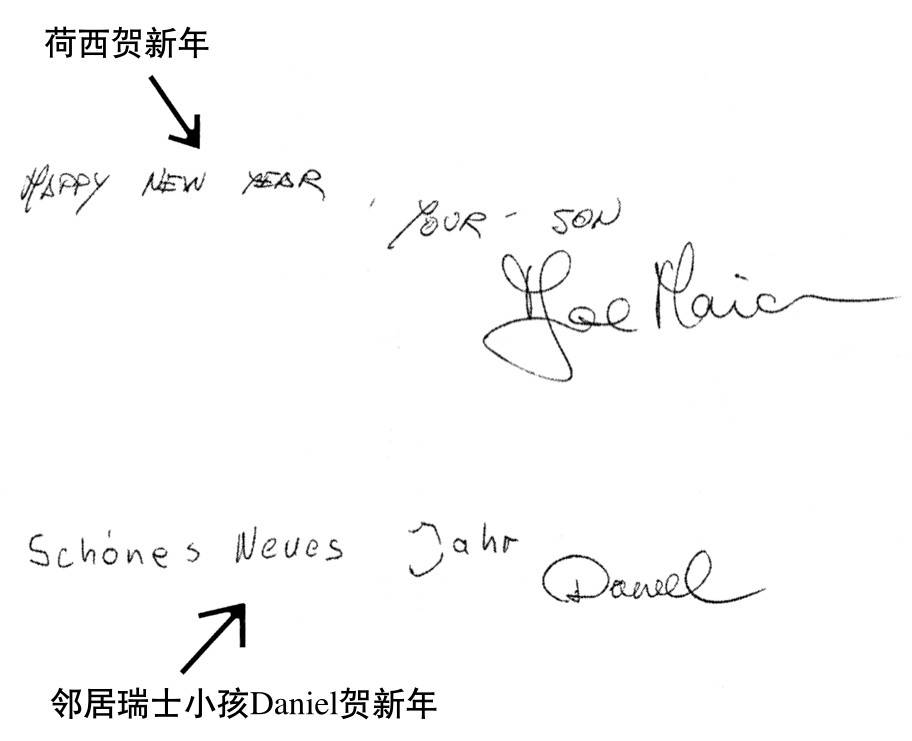
\includegraphics[scale=0.4]{picture/温柔的夜1.jpeg}
\end{figure}


\subsubsection{一九七七年四月三日}

\par \leftline{爹爹,姆妈:}
\par 你们一定已经听说了丹纳丽芙机场的大惨案,这件事说来也奇怪,德国有一青年人早已预言三月二十七日在那儿有飞机相撞,结果真的相撞,所以我相信这是“命运”不是“巧合”。每个人的归宿都已有定数,是难逃的。
\par 今日我一瑞士好友,早晨好好地去南部海边游泳,约我同去,我因有油漆匠约好来漆房子,所以未同去,而好友还有Nicoles与他儿子Daniel还有一个瑞士人同去,我早晨尚见他们,与她说再见(才五十二岁,极健康)。下午六点多,Nicoles回来,告我Ida已死,游泳完了上岸走几步,倒地不起,红十字会马上担了在沙上跑,跑了二十分钟才坐车,送院已死于心脏病(一向无病)。这消息令我大吃一惊,尖叫起来,一夜在外散步,无法安下心来,她去年来此地,买下房子,第一个认识的就是我,房子合同还是荷西替她弄的,现在房契未下来,人已死了,死后无亲无友、无子女,无一个人可以报丧,我们已找领事馆,下周送回瑞士下葬。她这次由瑞士才来一星期(来来去去,两地住),数次来看我,说下周便回瑞士,而今是睡了回去,令人叹息。
\par 爹爹,姆妈,所以我们一定要有心理预备,人,是无常的,一定要预备好,有一天,我们也会分离,万一有此一日来临,不可悲伤,生离死别是人之常情,要有庄子妻死,而鼓盆唱歌的哲学来迎接这件事情,这一年在海边,看见太多人死,我已能够接受,只是一想到家人,便悲伤难禁,所以大家都要预备好,免得有一日来了受不了,一定要彼此记住。
\par 我的腰痛已慢慢在好转,但今生不可再坐软沙发,只能坐地下,或硬椅子,总之仍在看医生。
\par 这一星期来,此地机场被放炸弹,房价一落千丈,加纳利群岛要独立已不是一日,现在变本加厉,我本想再买地,现已不买,因为情势不太好,今日机场又一炸弹。
\par 现在已又开始《玛法达》最后十九、二十集,请告诉我十七、十八集收到了吗?我早已寄出了,这几日听说你们要去旅行,我又有点担心,希望常常来短信,只报平安便可,不必多写,以免我挂念。
\par 荷西去了一月,只收到过一次信(两封),那儿的邮政太差,他另一朋友太太生产,打三封电报去,也无回音,实是奇怪。不过知道他是安好的。
\par 我本来不想请公公婆婆来,但今日又想,如果不请他们来,万一公公死了,荷西终生怪我,所以想请他们来,要寄路费去。另外干爹徐\UncommonChar{𬣙}五月要来西国,我在三千里外,但他不明白,我一再地讲,他仍要见我,我再讲,他仍要见我,所以为了不翻脸,只有五月去西班牙陪他,真是苦。公婆来要五百美金,我为徐,又得五六百美金,这月漆房子,又是三百美金,看医照X光已用好多,下周车又要大修,何苦来,这世界。
\par 请寄一千五百台币给桂文亚,她要生产了,我要送她钱,她对我太好,不断送东西,不断来信,又常常送我礼,所以请寄一千五给她。
\par 谢谢爹爹,姆妈!请扣账内!
\par 不多写了,我的游记已寄出半日,不知《联合报》收到没有?我常给王惕吾伯伯写信,今日又接两百美金津贴,已去谢(下周买一大娃娃寄去给他们家做装饰)。
\par 请多来信,短短几字,告我家中各人如何便是,外公好吗?毛毛有否收到我信?不必回,叫他用功。祝
\par 平安健康
\par \rightline{妹妹上}



\subsubsection{一九七七年四月}

\par \leftline{爹爹,姆妈:}
\par 如果一切计划没有改变,我将于五月一日飞赴Nigeria,在这之前,先得去马德里弄签证,今日荷西托人带来机票、钱和信,我一看,机票弄错了(开成由N国到西国,当相反),我明日清晨便去换,因为我们要将尼国的钱尽量在那儿用掉,免得将来不可出口,现在我马上要去打防疫针(三种)、银行租保险箱(珠宝存入,外币及房契也存入)、申请户籍(设籍在加纳利岛,去马德里可打百分之二十五机票折扣)、买赴马德里机票(一日来回,清早去,拿到visa,下午回来),另外尚得买许多荷西所要的东西,忙碌不堪。开车我是开入大城,停在车场,再坐短程计程车,这样神经不太紧张,我们这儿车子也是很挤很多。
\par 家中门窗关好,皮大衣交邻居管,电视留下,要被偷也罢了,不过七百美金。
\par 今日朋友由Nigeria回来,说荷西一日工作十五小时以上,深夜尚在爆炸海底,公司对他很坏,星期日也不给休息,清早五点赴工作,夜间十点尚无法回家,吃得越来越不好,黑人不爱工作,我想荷西太老实,一天工作八小时对肺已是太坏太伤,如何能一直在水中,这样要废掉了,我去了会与公司交涉,(德国老板)这个薪水不高,不是卖命,同时我自己想去做他们三个工人的厨娘,他们正在找厨子做饭,我去做,也要领薪(好在不过三个人吃),荷西脾气坏,其实脸皮薄,没有原则,任人欺负,我去了会不同些。这个混蛋德国人太欺负他,如不加薪,不减工作时间,我们便走(一日工作两小时在水里,已是太多,水中压力不相同,肺要炸掉的,血管内会进空气,太危险)。真是混账,荷西去年一年无工作,什么也忍下来了,我去了会好好讲,叫老板改时间。
\par 六月我们有二十天假,便去英国一周,再回家来住十天,再看将来如何,因我现在去,是与荷西、他同事、老板、老板太太同住一大宿舍,这个要解决,一人一幢房不可混住,老板太太天天给吃三明治,工作十五小时回来,尚吃三明治,不是气疯了。
\par 同时也请爹爹替我们在台湾找事,如有三万台币一月(现赚九万一月),我们便回来。荷西已可讲英文(很坏,没有句子),同时我又替他在象牙海岸找事,是法国公司,待遇一样,可是环境较好。在尼日利亚,一幢房子租一年是一百五十万台币(一月不租);交通如同疯子,左右不分,车辆乱行,人在街上大小便,从我们家到敦化南路的距离,要开两小时(全缠在一起);警察拿鞭子在街上打人,人还是乱走;一条裤子要合四五千台币,尚是尼龙的,不是棉的,是个疯狂的国家。垃圾堆成一人高,无车来清理,黄热病,打摆子一塌糊涂(我每日便要服“奎宁丸”),这样的地方尚叫国家,黑人走路如蜗牛,不做事,走十步路要十分钟,荷西一下水,助手黑人就睡觉,不看守水下的他要什么,总之是个疯狂世界,二千二百美金所付代价太大,划不来。
\par 我不去也是不行了,荷西一走,此地男人都来找我,满镇风雨,社区内大家讲来讲去,都是说我有男人。此地北欧女人都与人同居(丈夫在非洲),我实是被这些流言弄得十分苦恼。现在参加俱乐部,每日做体操、游泳(全是女的),但也不长,因我要走了。
\par 我的一生,多彩多姿,感谢父母给我生命,虽然今生不能如树芬做少奶奶(她其实也不苦,只是在加拿大没有香港一样而已),但我所活一生,胜于别人十倍百倍,对于去Nigeria,我十分兴奋,又是一种不同的人生,何其幸福。
\par 我下周一赴马德里,但只去签证,再看Marisa,便回Las Palmas来,休息四五天,便由此地上机,经非洲“新内加”国首都Dakar再转赴Nigeria首都Lagos。Lagos是几内亚湾内最大的港口,港内一船下货要等半年以上(太挤),有一百多条船在外海等,五十多条在港内等,夜间海盗便来上船偷货,都是有趣。
\par 虚线便是我下周要飞上飞下的行程。
\begin{figure}[htb]
    \centering
    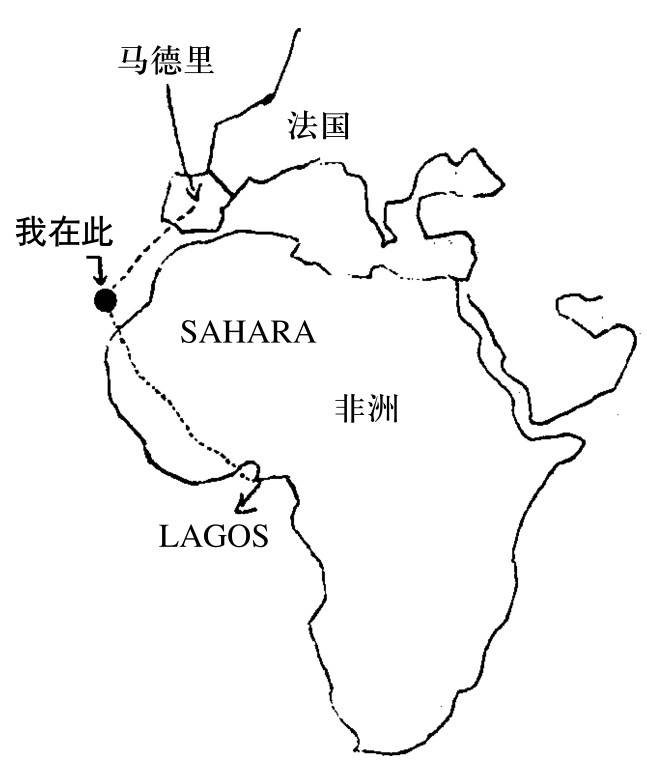
\includegraphics[scale=0.4]{picture/温柔的夜2.jpeg}
\end{figure}
\par 我现在尽量休息,预备长程飞行。(马德里来回六小时飞机,赴Lagos要八九小时飞机,共要十五六小时。)去了荷西不能来接(工作),我便去找一位Duru博士的家(尼国人,也是老板之一),荷西仔细,坐计程车钱已交人带来,一切无问题,我是旅行老手,不会出错,万一飞机出事,亦是命中注定,不必悲伤,人生聚散都是容易,要有大智慧来接受,我对你们,亦有心理预备,所以我们全家都是坚强的人,要有老庄哲学的想法,大而化之,才是天下第一人,我很爱你们和兄弟姐姐,也爱荷西,他是好丈夫。
\par \rightline{妹妹}
\par  
\par PS.春霞衣服十分美丽,今日收到,正穿身上,谢谢盛情,以后不可再寄。药尚未收到。



















 % 4
% \clearpage


\section{万水千山走遍}

\par 作者:三毛
\par 出版社:北京出版集团北京十月文艺出版社
\par 出版时间:2017-03
\par ISBN:9787530214756

\subsection{大蜥蜴之夜\\\small{墨西哥纪行之一}}

\par 当飞机降落在墨西哥首都的机场时,我的体力已经透支得几乎无法举步。长长的旅程,别人睡觉,我一直在看书。
\par 眼看全机的人都慢慢地走了,还让自己绑在安全带上。窗外的机场灯火通明,是夜间了。
\par 助理米夏已经背着他的东西在通道边等着了。经过他,没有气力说话,点了一点头,然后领先出去了。
\par 我的朋友约根,在关口里面迎接,向我高举着手臂。我走近他,先把厚外套递过去,然后双臂环向他拥抱了一下。他说:“欢迎来墨西哥!”我说:“久等了,谢谢你!”
\par 这是今年第四次见到他,未免太多了些。
\par 米夏随后来了,做了个介绍的手势,两人同时喊出了彼此的名字,友爱地握握手,他们尚在寒暄,我已先走了。
\par 出关没有排队也没有查行李。并不想做特殊分子,可是约根又怎么舍得不使用他的外交特别派司?这一点,是太清楚他的为人了。
\par 毕竟认识也有十四年了,他没有改过。
\par “旅馆订了没有?”我问。
\par “先上车再说吧!”含含糊糊的回答。
\par 这么说,就知道没有什么旅馆,台北两次长途电话算是白打了。
\par 在那辆全新豪华的深色轿车面前,他抱歉地说:“司机下班了,可是管家是全天在的,你来这儿不会不方便。”
\par “住你家吗?谁答应的?”改用米夏听不懂的语言,口气便是不太好了。
\par “要搬明天再说好吗?米夏也有他的房间和浴室。你是自由的,再说,我那一区高级又安静。”
\par 我不再说什么,跨进了车子。
\par “喂!他很真诚啊!你做什么一下飞机就给人家脸色看?”米夏在后座用中文说。
\par 我不理他,望着窗外这一千七百万人的大城出神,心里不知怎么重沉沉的。
\par “我们这个语文?”约根一边开车一边问。
\par “英文好啰!说米夏的话。”
\par 说是那么说,看见旁边停了一辆车,车里的小胡子微笑着张望我,我仍是忍不住大喊出了第一句西班牙文——“晚安啊!我的朋友——”
\par 这种令约根痛恨的行径偏偏是我最爱做的,他脸上一阵不自在,我的疲倦却因此一扫而空了。
\par 车子停在一条林荫大道边,门房殷勤地上来接车,我们不必自己倒车入库,提着简单的行李向豪华的黄铜柱子的电梯走去。
\par 约根的公寓,他在墨西哥才安置了半年的家,竟然美丽雅致高贵得有若一座博物馆,森林也似的盆栽,在古典气氛的大厅里,散发着说不出的宁静与华美。
\par 米夏分配到的睡房,本是约根的乐器收藏室,里面从纸卷带的手摇古老钢琴、音乐匣、风琴,到全世界各地大大小小的各种古古怪怪可以发声音的东西,都挂在墙上。
\par 我被引着往里面走,穿过一道中国镶玉大屏风,经过主卧室的门外,一转弯,一个客房藏着,四周全是壁柜,那儿,一张床,床上一大块什么动物的软毛皮做成的床罩静静地等着我。
\par “为什么把我安置在这里?我要米夏那间!”
\par 我将东西一丢,喊了起来。
\par “别吵!嘘——好吗?”约根哀求似的说。
\par 心里一阵厌烦涌上来,本想好好对待他的,没有想到见了面仍是连礼貌都不周全,也恨死自己了。世上敢向他大喊的,大概也只有我这种不买账的人。
\par “去小客厅休息一下吗?”约根问。
\par 我脱了靴子,穿着白袜子往外走,在小客厅里,碰到了穿着粉红色制服、围洁白围裙的墨西哥管家。
\par “啊!您就是苏珊娜,电话里早已认识了呀!”
\par 我上去握住她的手,友爱地说着。
\par 她相当拘谨,微屈了一下右脚,说:“请您吩咐——”
\par 约根看见我对待管家不够矜持,显然又是紧张,赶快将苏珊娜支开了。
\par 我坐下来,接了一杯威士忌,米夏突然举杯说:“为这艺术而舒适的豪华之家——”
\par 对于这幢公寓的格调和气派,米夏毫不掩饰他人全然的沉醉、迷惑、欣赏与崇拜。其实这并没有什么不对,公平地说,这房子毕竟是少见的有风格和脱俗。而米夏的惊叹却使我在约根的面前有些气短和不乐。
\par “阿平,请你听我一次话,他这样有水准,你——”米夏忍不住用中文讲起话来。
\par 我假装没有听见,沉默着。正是大梦初醒的人,难道还不明白什么叫做盖世英雄难免无常,荣华富贵犹如春梦吗?
\par 古老木雕的大茶几上放着我的几本书,约根忙着放《橄榄树》给我们听。这些东西不知他哪里搞来的,也算做是今夜的布景之一吧,不知我最厌看的就是它们。
\par 波斯地毯,阿拉伯长刀,中国锦绣,印度佛像,十八世纪的老画,现代雕塑,中古时代的盔甲,锡做的烛台、银盘、铜壶——没有一样不是精心挑选收集。
\par “收藏已经不得了啦!”我说,衷心地叹了口气。
\par “还差一样——你猜是什么?”他笑看着我,眼光中那份收藏家的贪心也掩饰不住了。
\par 刚刚开始对他微笑的脸,又刷一下变了样子。
\par 我叹了口气,坐在地毯上反手揉着自己的背,右肩酸痛难当,心里一直在对自己说:“我试了!试了又试!再没有什么不好交代的,住两日便搬出去吧!”
\par 约根走去打电话,听见他又叫朋友们过来。每一次相聚,他总是迫不及待地拿我显炫给朋友们看,好似一件物品似的展览着。
\par 米夏紧张地用中文小声说:“喂!他很好,你不要又泄气,再试一次嘛!”
\par 我走开去,将那条苍苍茫茫的《橄榄树》啪一下关掉,只是不语。
\par 旅程的第一站还没有进入情况,难缠的事情就在墨西哥等着。这样的事,几天内一定要解决掉。同情心用在此地是没有价值的。
\par 门铃响了,来了约根的同胞,他们非常有文化,手中捧着整整齐齐的十几本书和打字资料,仔细而又友爱地交给我——全是墨西哥的历史和地理,还有艺术。
\par 我们一同谈了快三小时,其实这些上古和马雅文化,在当年上马德里大学时,早已考过了,并没有完全忘记。为了礼貌,我一直忍耐着听了又听——那些僵死的东西啊!
\par 他们不讲有生命的活人,不谈墨西哥的衣食住行,不说街头巷尾,只有书籍上诉说的史料和文化。而我的距离和他们是那么的遥远,这些东西,不是我此行的目的——我是来活一场的。
\par “实在对不起,米夏是我的助理,这些书籍请他慢慢看。经过二十多小时的飞行,我想休息了!”
\par 与大家握握手,道了晚安,便走了。
\par 米夏,正是见山不是山、见水不是水的年龄,新的环境与全然不同的人仍然使他新鲜而兴奋。留下他继续做听众,我,无法再支持下去。
\par 寂静的午夜,我从黑暗中惊醒,月光直直地由大玻璃窗外照进来。床对面的书架上,一排排各国元首的签名照片静静地排列着,每张照片旁边,插着代表元首那国的小旗子。
\par 我怔怔地与那些伟大人物的照片对峙着,想到自己行李里带来的那个小相框,心里无由地觉着没有人能解的苍凉和孤单。
\par 墨西哥的第一个夜晚,便是如此张大着眼睛什么都想又什么都不想地度过了。
\par   
\par 早晨七点钟,我用大毛巾包着湿头发,与约根坐在插着鲜花、阳光普照的餐厅里。
\par 苏珊娜开出了丰丰富富而又规规矩矩的早餐,电影似的不真实——布景太美了。
\par “不必等米夏,吃了好上班。”我给约根咖啡,又给了他一粒维他命。
\par “是这样的,此地计程车可以坐,公共汽车对你太挤。一般的水不可以喝,街上剥好的水果绝对不要买,低于消费额五十美金的餐馆吃了可能坏肚子,路上不要随便跟男人讲话。低级的地区不要去,照相机藏在皮包里最好,当心人家抢劫——”
\par “城太大了,我想坐地下车。”我说。
\par “不行——”约根叫了起来,“他们强暴女性,就在车厢里。”
\par “白天?一千七百万人的大城里?”
\par “报上说的。”
\par “好,你说说,我来墨西哥是做什么的?”
\par “可以去看看博物馆呀!今天早晨给自己去买双高跟鞋,这星期陪我参加宴会,六张请帖在桌上,有你的名字——”
\par 我忍住脾气,慢慢涂一块吐司面包,不说一句伤人的话。那份虫噬的空茫,又一次细细碎碎地爬上了心头。
\par 约根上班之前先借了我几千披索,昨日下机没来得及去换钱。这种地方他是周到细心的。
\par 推开米夏的房间张望,他还睡得像一块木头,没有心事的大孩子,这一路能分担什么?
\par 为什么那么不快乐?右肩的剧痛,也是自己不肯放松而弄出来的吧!
\par 苏珊娜守礼而本分,她默默地收桌子,微笑着,不问她话,她不主动地说。
\par “来,苏珊娜,这里是三千披索,虽说先生管你伙食费,我们也只在这儿早餐,可是总是麻烦您,请先拿下了,走的时候另外再送你,谢谢了!”
\par 对于这些事情,总觉得是丰丰富富地先做君子比较好办事,虽说先给是不礼貌的,可是,这世界上,给钱总不是坏事。
\par 苏珊娜非常欢喜地收下了。这样大家快乐。
\par  
\par “那我们怎么办?照他那么讲,这不能做,那又不能做?”
\par 米夏起床吃早餐时我们谈起约根口中所说的墨西哥。
\par “低于五十美金一顿的饭不能吃?他土包子,我们真听他的?”我笑了。
\par “你不听他的话?他很聪明的。”米夏天真地说。
\par “认识十四年了,也算是个特殊的朋友,有关我半生的决定,他都有过建议,而我,全没照他的去做过——”我慢慢地说。
\par “结果怎么样?”米夏问。
\par “结果相反的好。”我笑了起来。
\par “昨天晚上,你去睡了,约根说,他想拿假期,跟我们在中美洲走五个星期,我没敢讲什么,一切决定在你,你说呢?”米夏问。
\par 我沉吟了一下,叹了口气:“我想还是一个人走的好,不必他了,真的——”
\par “一个人走?我们两人工作,你却说是一个人,我问你,我算谁?”
\par “不知道,你拍你的照片吧!真的不知道!”
\par 我离开了餐厅去浴室吹头发,热热的人造风一阵又一阵闷闷地吹过来。
\par 米夏,你跟着自然好,如果半途走了,也没有什么不好。毕竟要承当的是自己的前程和心情,又有谁能够真正地分担呢?
\par 
\par 住在这个华丽的公寓里已经五天了。
\par 白天,米夏与我在博物馆、街上、人群里消磨,下午三点以后,约根下班了,我也回去。他要伴了同游是不答应的,那会扫兴。
\par 为着台北一份译稿尚未做完,虽然开始了旅程,下午仍是专心地在做带来的功课。
\par 半生旅行飘泊,对于新的环境已经学会了安静地去适应和观察,并不急切于新鲜和灿烂,更不刻意去寻找写作的材料。
\par 这对我来说,已是自然,对于米夏,便是不同了。
\par “快闷死了,每天下午你都在看译稿,然后晚上跟约根去应酬,留下我一个人在此地做什么?”米夏苦恼地说。
\par “不要急躁,孩子,旅行才开始呢,先念念西班牙文,不然自己出去玩嘛!”我慢慢地看稿,头也不抬。
\par “我在笼子里,每天下午就在笼子里关着。”
\par “明天,译稿弄完了,寄出去,就整天出去看新鲜事情了。带你去水道坐花船,坐公车去南部小村落,太阳神庙、月神庙都去跑跑,好吗?”
\par “你也不只是为了我,你不去,写得出东西来吗?”米夏火起来了。
\par 我笑看着这个名为助理的人,这长长的旅程,他耐得住几天?人生又有多少场华丽在等着?不多的,不多的,即使旅行,也大半平凡岁月罢了。米夏,我能教给你什么?如果期待得太多,那就不好了啊!
\par 认真考虑搬出约根的家到旅馆去住,被他那么紧迫钉人并不算太难应付,只是自己可能得到的经验被拘束在这安适的环境里,就未免是个人的损失了。
\par 决定搬出去了,可是没有告诉米夏,怕他嘴不紧。约根那一关只有对不起他,再伤一次感情了。
\par 才五天,不要急,匆匆忙忙地活着又看得到感得了什么呢!
\par 
\par 不是为了这一夜,那么前面的日子都不能引诱我写什么的,让我写下这一场有趣的夜晚,才去说说墨西哥的花船和街头巷尾的所闻所见吧!
\par 不带米夏去参加任何晚上的应酬并没有使我心里不安。他必须明白自己的职责和身份,过分地宠他只有使他沿途一无所获。
\par 再说,有时候公私分明是有必要的,尤其是国籍不一样的同事,行事为人便与对待自己的同胞有些出入了。
\par 
\par 那一夜,苏珊娜做了一天的菜,约根在家请客,要来十几个客人,这些人大半是驻在墨西哥的外交官们,而本地人,是不被邀请的。
\par 约根没有柔软而弹性的胸怀。在阶级上,他是可恨而令人瞧不起的迂腐。奇怪的是,那么多年来,他爱的一直是一个与他性格全然不同的东方女孩子。这件事上怎么又不矛盾,反而处处以此为他最大的骄傲呢?
\par 再大的宴会,我的打扮也可能只是一袭白衣,这样的装扮谁也习惯了,好似没有人觉得这份朴素是不当的行为。我自己,心思早已不在这些事上争长短,倒也自然了。
\par 当我在那个夜晚走进客厅时,已有四五位客人站着坐着喝酒了。他们不算陌生,几个晚上的酒会,碰来碰去也不过是这几张面孔罢了。
\par 男客中只有米夏穿着一件淡蓝的衬衫,在那群深色西装的中年人里面,他显得那么的天真、迷茫、兴奋而又紧张。冷眼看着这个大孩子,心里不知怎的有些抱歉,好似欺负了人一样。虽然他自己蛮欢喜这场宴会的样子,我还是有些可怜他。
\par 人来得很多,当莎宾娜走进来时,谈话还是突然停顿了一会儿。
\par 这个女人在五天内已见过三次了,她的身旁是那个斯文凝重给我印象极好的丈夫——文化参事。
\par 她自己,一身银灰的打扮,孔雀似的张开了全部的光华,内聚力极强的人,只是我怕看这个中年女人喝酒,每一次的宴会,酒后的莎宾娜总是疯狂,今夜她的猎物又会是谁呢?
\par 我们文雅地吃东西、喝酒、谈话、听音乐、讲笑话,说说各国见闻。不能深入,因为没有交情。为了对米夏的礼貌,大家尽可能用英文了。
\par 这种聚会实在是无聊而枯燥的,一般时候的我,在一小时后一定离去。往往约根先送我回家,他再转回去,然后午夜几时回来便不知道了,我走了以后那种宴会如何收场也没有问过。
\par 那日因为是在约根自己家中,我无法离去。
\par 其中一个我喜欢的朋友,突然讲了一个吸血鬼在纽约吸不到人血的电影:那个城里的人没有血,鬼太饿了,只好去吃了一个汉堡。这使我又稍稍高兴了一点,觉得这种谈话还算活泼,也忍受了下去。
\par 莎宾娜远远地埋在一组椅垫里,她的头半枕在别人先生的肩上,那位先生的太太拼命在吃东西。
\par 一小群人在争辩政治,我在小客厅里讲话,约根坐在我对面,神情严肃地对着我,好似要将我吃掉一样地又恨又爱地凝视着。
\par 夜浓了,酒更烈了,室内烟雾一片,男女的笑声暧昧而释放了,外衣脱去了,音乐更响了。而我,疲倦无聊得只想去睡觉。
\par 那边莎宾娜突然高叫起来,喝得差不多了:“我恨我的孩子,他们拿走了我的享受,我的青春,我的自由,还有我的身材,你看,你看——”
\par 她身边的那位男士刷一抽身站起来走开了。
\par “来嘛!来嘛!谁跟我来跳舞——”她大嚷着,张开了双臂站在大厅里,嘴唇半张着,眼睛迷迷濛濛,说不出是什么欲望,那么强烈地狂奔而出。
\par 唉!我突然觉得,她是一只饥饿的兽,在这墨西哥神秘的夜里开始行猎了。
\par 我心里喜欢的几对夫妇在这当儿很快而有礼地告辞了。分手时大家亲颊道晚安,讲吸血鬼故事给我听的那个小胡子悄悄拍拍我的脸,说:“好孩子,快乐些啊!不过是一场宴会罢了!”
\par 送走了客人,我走回客厅去,在那个阴暗的大盆景边,莎宾娜的双臂紧紧缠住了一个浅蓝衬衫的身影,他们背着人群,没有声息。
\par 我慢慢经过他们,坐下来,拿起一支烟,正要找火,莎宾娜的先生啪一下给我凑过来点上了,我们在火光中交换了一个眼神,没有说一句话。
\par 灯光扭暗了,音乐停止了,没有人再去顾它。梳妹妹头发、看似小女孩般的另一个女人抱住约根的头,半哭半笑地说:“我的婚姻空虚,我失去了自己,好人,你安慰我吗——”
\par 那边又有喃喃的声音,在对男人说:“什么叫快乐,你说,你说,什么叫快乐——”
\par 客厅的人突然少了,卧室的门一间一间关上了。
\par 阳台不能去,什么人在那儿纠缠拥抱,阴影里,花丛下,什么事情在进行,什么欲望在奔流?
\par 我们剩下三个人坐在沙发上。
\par 一个可亲的博士,他的太太跟别人消失了,莎宾娜的先生,神情冷静地在抽烟斗,另外还有我。
\par 我们谈着墨西哥印地安人部落的文化和习俗,紧张而吃力,四周正在发生的情况无法使任何人集中心神,而我的表情,大概也是悲伤而疲倦了。
\par 我再抽了一支烟,莎宾娜的先生又来给我点火,轻轻说了一句:“抽太多了!”
\par 我不再费力地去掩饰对于这个夜晚的厌恶,哗一下靠在椅垫上,什么也不理也不说了。
\par “要不要我去找米夏?”这位先生问我,他的太太加给他的苦痛竟没有使他流露出一丝难堪,反而想到身边的我。而我对米夏又有什么责任?
\par “不!不许,拜托你。”我拉住他的衣袖。
\par 在这儿,人人是自由的,选择自己的生命和道路吧!米夏,你也不例外。
\par 莎宾娜跌跌撞撞地走进来,撞了一下大摇椅,又扑到一棵大盆景上去。
\par 她的衣冠不整,头发半披在脸上,鞋子不见了,眼睛闭着。
\par 米夏没有跟着出现。
\par 我们都不说话,大家窒息了似的熬着。
\par 其实,这种气氛仍是邪气而美丽的,它像是一只大爬虫,墨西哥特有的大蜥蜴,咄咄地向我们吹吐着腥浓的喘息。
\par 过了不知多久,博士的太太疯疯癫癫地从乐器室里吹吹打打地走出来,她不懂音乐,惊人的噪音,冲裂了已经凝固的夜。一场宴会终是如此结束了。
\par 唉唉!这样豪华而狂乱的迷人之夜,是波兰斯基导演的一场电影吧!
\par 那只想象中的大蜥蜴,在月光下,仍然张大着四肢,半眯着眼睛,重重地压在公寓的平台上,满意地将我们吞噬下去。
\par 
\par 还有两个客人醉倒在洗手间里。
\par 约根扑在他卧室的地毯上睡了。
\par 我小心地绕过这些身体,给自己刷了牙,洗了脸,然后将全公寓的大落地窗都给它们打开来吹风。
\par 拿了头发刷子,一间间去找米夏。
\par 米夏坐在书房的一块兽皮上,手里在玩照相机,无意识地按快门,咔嚓一下,咔嚓又一下,脸上空空茫茫的。
\par 我一面刷头发,一面喊了一声:“徒儿——”
\par “没做什么,真的——”米夏淡淡地说。
\par “这没什么要紧,小事情。”我说。
\par “可是我没有做——”他叫了起来。
\par “如果今夜我不在呢?”我叹了口气。
\par 米夏不响,不答话。
\par “莎宾娜可怜——”他说。
\par “不可怜——”
\par “阿平——你无情——”
\par 我慢慢地梳头发,没有解释。
\par “今夜够受了——”米夏喘了一口大气。
\par “有挣扎?”我笑了。
\par 米夏没有笑,怔怔地点了点头。
\par “没有见识的孩子,要是真的事情来时你又怎么办?”我站起来走开了。
\par “阿平——”
\par “明早搬出去,旅馆已经打电话订了,这一种墨西哥生涯到此为止了,好吗?”我说。
\par 
\par \rightline{一九八一年十一月十五日在墨西哥}

\subsection{街头巷尾\\\small{墨西哥纪行之二}}


\par 这一趟旅行虽说会发生些什么样的事情全然是未知,可是行万里路、读万卷书的时代已经过去了。仍然算是有备而来的。
\par 我的习惯是先看资料,再来体验印证个人的旅行。
\par 这一回有关中南美的书籍一共带了四册,要找一家便宜而位置适中的旅馆也并不是难事,书上统统都列出来了。
\par 来到墨西哥首都第六天,一份叫做“EL HERALDO DE MEXICO”的报纸刊出了我的照片。与写作无关的事情。
\par 那么大的照片刊出来的当日,也是我再梳回麻花辫子,穿上牛仔裤,留下条子,告别生活方式极端不同的朋友家,悄悄搬进一家中级旅馆去的时候了。
\par 旅馆就在市中心林荫大道上,老式的西班牙殖民式建筑,白墙黑窗,朴素而不豪华,清洁实惠,收费亦十分合理,每一个只有冲浴的房间,是七百披索,大约是合二十七元美金一日,不包括早餐。
\par 书上列出来的还有十元美金一日的小旅馆,看看市区地图,那些地段离城中心太远,治安也不可能太好,便也不再去节省了。
\par 助理米夏在语言上不能办事与生活,这一点再再地督促他加紧西班牙文。鼓励他独自上街活动,不可以完全依靠我了。
\par 墨西哥城是一个方圆两百多平方公里,坐落在海拔二千二百四十公尺高地的一个大城市。
\par 初来的时候,可能是高度的不能习惯,右耳剧痛,鼻腔流血,非常容易疲倦,这种现象在一周以后便慢慢好转了。
\par 有生以来没有在一个一千七百万人的大城市内住过,每天夜晚躺在黑暗里,总听见警车或救护车激昂而快速的哀鸣划破寂静的长夜。这种不间断的声音,带给人只有一个大都会才有的巨大的压迫感,正是我所喜欢的。

\subsubsection*{这一张张美丽的脸}
\par 除了第一日搬去旅舍时坐的是计程车之外,所用的交通工具起初还是公共汽车,后来试了四通八达的地下车之后,便再也舍不得放弃了。
\par 大部分我所见的墨西哥人,便如上帝捏出来的粗泥娃娃,没有用刀子再细雕,也没有上釉,做好了,只等太阳晒干,便放到世上来了——当然,那是地下车中最最平民的样子。
\par 这儿的人类学博物馆中有些故事,述说古时在这片土地上的居民,他们喜欢将小孩子的前额和后脑夹起好几年,然后放开,那些小孩子的头变成扁平的,脸孔当然也显得宽大些,在他们的审美眼光中,那便是美丽。
\par 而今的墨西哥人,仍然有着那样的脸谱,扁脸、浓眉、大眼、宽鼻、厚唇,不算太清洁,衣着鲜艳如彩虹,表情木然而本分。而他们身体中除了墨西哥本地的血液之外,当然掺杂了西班牙人的成分,可是看上去他们仍是不近欧洲而更近印地安人的。
\par 常常,在地下车中挤着去某个地方,只因时间充分,也因舍不得那一张张已到了艺术极致的脸谱,情愿坐过了站再回头。
\par 人,有时候是残酷的,在地下车中,看见的大半是贫穷的人,而我,却叫这种不同的亦不算太文明装扮的男女老幼为“艺术的美”,想起来是多么大的讽刺。
\par 墨西哥城内每天大约有五百到两千个乡下人,涌进这个大都市来找生活。失业的人茫茫然地坐在公园和街头,他们的表情在一个旁观者看来,张张深刻,而这些对于饥饿的肚子,又有什么关联?



\subsubsection*{自杀神}
\par 虽说对于参观大教堂和博物馆已经非常腻了,可是据说墨西哥的“国家人类学博物馆”仍然可能是世界上最周全的一座,为了对得起自己的良知,还是勉强去了。
\par 第一次去,是跟着馆内西语导游的。他不给人时间看,只强迫人在馆内快速地走,流水账似的将人类历史尤其墨西哥部分泼了一大场,进去时还算清楚,出来时满头雾水。
\par 结果,又去了第二次,在里面整整一日。虽说墨西哥不是第一流的国家,可是看过了他们那样大气势的博物馆,心中对它依然产生了某种程度的尊敬。
\par 要说墨西哥的日神庙、月神庙的年代,不过是两千多年以前。他们的马雅文化固然辉煌,可是比较起中国来,便不觉得太古老了。
\par 只因那个博物馆陈列得太好,介绍得详尽,分类细腻,便是一张壁画吧,也是丰富。馆内的说明一律西班牙文,不放其他的文字,这当然是事先设想后才做的决定。我仍是不懂,因为参观的大部分是外国人。
\par 古代的神祇在墨西哥是很多的,可说是一个想象力丰富的多神民族。日神、月神、风神、雨神之外,当然还有许许多多不同的神。
\par 也可能是地理环境和天灾繁生,当时的人自然接受了万物有灵的观念,事实上,此种信仰是因为对大自然的敬畏而产生的。
\par 其中我个人最喜欢的是两个神——玉米神和自杀神。
\par 玉米是我爱吃的食物之一,可说是最爱的。有这么一位神,当然非常亲近他。
\par 当我第一次听见导游用棒子点着一张壁画,一个个神数过去,其中他滑过一个小名字——自杀神时,仍是大吃了一惊。
\par 跟着导游小跑,一直请问他古时的自杀神到底司什么职位,是给人特许去自杀,还是接纳自杀的人,还是叫人去自杀?
\par 导游也答不出来,只笑着回了我一句:“你好像对自杀蛮感兴趣的,怎么不问问那些影响力更深、更有神话意义的大神呢?”
\par 后来第二次我自己慢慢地又去看了一次博物馆,专门研究自杀神,发觉他自己在图画里就是吊在一棵树上。
\par 世上无论哪一种宗教都不允许人自杀,只有在墨西哥发现了这么一个书上都不提起的小神。我倒觉得这种宗教给了人类最大的尊重和意志自由,居然还创出一个如此的神,是非常有趣而别具意义的。
\par 墨西哥大神每一个石刻的脸,看痴了都像魔鬼。
\par 这么说实在很对不起诸神,可是他们给人的感应是邪气而又强大的。没有祥和永恒的安宁及盼望。他们是惩罚人的灵,而不是慈祥的神。说实在,看了心中并不太舒服,对于他们只有惧怕。
\par 是否当时的人类在这片土地上挣扎得太艰苦,才产生了如此粗暴面孔的神祇和神话呢!

\subsubsection*{金字塔}
\par 当然,我们不可避免地去了西班牙文中仍叫它“金字塔”的日神庙及月神庙。
\par 据考证那是公元前两百年到公元九百年时陶特克斯人时期的文明。在今天,留下了人类在美洲壮观的废墟和历史。
\par 那是一座古城,所谓的日神月神庙是后人给它们加上去的名称。外在的形式,像极了埃及的金字塔,只是没有里面的通道,亦没有帝王的陵墓。
\par 为了这些不同年代的人类文明和古代城市的建筑,我看了几个夜晚的资料,预备在未去之前对它们做一个深切的纸面上的了解。
\par 然后米夏与我在转车又转车之后,到了那个叫做“阿那乌阿克之谷”(VALLE DE ANAHUAC)的底奥帝乌刚诺的金字塔。
\par 烈日下的所谓金字塔,已被小贩、游览车,大声播放的流行音乐和大呼小叫的各国游客完全污染光了。
\par 日神庙六十四公尺高的石阶上,有若电影院散场般的人群,并肩在登高。手中提着他们的小型录音机,放着美国音乐。
\par 我没有去爬,只是远远地坐着观望。米夏的红衬衫,在高高石阶的人群里依旧鲜明。
\par 那日的参观没有什么心得。好似游客涌去的地方在全世界都是差不多的样子。
\par 当米夏努力在登日神庙顶时,我借了一辆小贩的脚踏车,向着古代不知为何称为“死亡大道”的宽大街道的废墟上慢慢地骑去。
\par 本想在夜间再去一趟神庙废墟的,终因交通的问题,结果没有再回去。
\par 我还是不羞耻地觉得城镇内的人脸比神庙更引人。
\par 至于马雅文化和废墟,计划中是留到洪都拉斯的“哥庞”才去看一看了。

\subsubsection*{吃抹布}
\par 第一次在街头看见路边的小摊子上在烘手掌大的玉米饼时,我非常喜欢,知道那是墨西哥人的主食“搭哥”(taco),急于尝尝它们。
\par 卖东西的妇人在我张开的掌心中啪一下给了一张饼,然后在饼上放了些什么东西混着的一摊馅,我将它们半卷起来,吃掉了,有酱汁滴滴答答地从手腕边流下来。
\par “搭哥”的种类很多,外面那个饼等于是一张小型的春卷皮,淡土黄色的,它们永远不变。
\par 里面的馅放在一只只大锅里,煮来煮去,有的是肉,有的是香肠,有的看不清楚,有的猜不出来。要换口味,便换里面的东西。
\par 在城内,除非是游客区,那儿可以吃中国菜、意大利面食,还有丹麦甜点蛋饼之外,也可以吃“搭哥”。
\par 可是当我们坐车离城去小村落时,除了“搭哥”之外,实在没有别的东西可吃。
\par 在城外几百里的小镇上,当我吃了今生第几十个“搭哥”之后,那个味道和形式,实在已像是一块抹布——土黄色的抹布,抹过了残余食物的饭桌,然后半卷起来,汤汤水水地用手抓着,将它们吞下去。
\par 一个“搭哥”大约合几角到一元五美金,看地区和内容,当然吃一个胃口是倒了,而肚子是不可能饱的。这已是不错了,比较起城内高级饭店的食物,大约是十倍到十五倍价格的差距。虽然我们的经费充足,仍是坚持入境问俗,一路“搭哥”到底。这对助手米夏便是叫苦连天,每吃必嚷:“又是一块小抹布!”
\par 在墨西哥的最后一日,我怕米夏太泄气,同意一起去吃一顿中国饭,不肯去豪华的中国饭店,挑了一家冷清街角的。先点了两只春卷——结果上来的那个所谓“春天的卷子”的东西,竟然怎么看,怎么咬,都只是两只炸过了的“搭哥”。
\par 吃在一般的墨西哥是贫乏而没有文化的。
\par 它的好处是不必筷子与刀叉,用手便可解决一顿生计,倒也方便简单。至于卫不卫生就不能多去想它了。


\subsubsection*{货物大同}
\par 在城内的游客区里,看见美丽而价格并不便宜的墨西哥人的“大氅”,那种西班牙文叫做“蹦裘”(poncho)的衣物。
\par 事实上它们只是一块厚料子,中间开一个洞套进颈子里,便是御寒的好东西了。
\par 我过去有过两三个“蹦裘”,都因朋友喜欢而送掉了。这次虽然看见了市场上有极美丽的,总因在游客出没的地区,不甘心付高价去买它。
\par 下决心坐长途车去城外的一个小镇,在理由上对米夏说的是请他下乡去拍照。事实上我有自己的秘密,此行的目的对我,根本是去乡下找漂亮、便宜,而又绝对乡土的“蹦裘”来穿。
\par 坐公路车颠几百里去买衣服也只有最笨的人——而且是女人,会做的事情,不巧我就有这份决心和明白。
\par 到了一个地图上也快找不到的城镇,看到了又是所谓景色如画的贫穷和脏乱。我转来转去找市场——资料书中所说的当地人的市集,找到了,怪大的一个广场。
\par 他们在卖什么?在卖热水瓶、镜子、假皮的皮夹、搪瓷的锅、碗、盆、杯、完全尼龙的衣服、塑胶拖鞋、原子笔、口红、指甲油、耳环、手镯、项链——
\par 我到处问人家:“你们不卖poncho?怎么不卖poncho?”
\par 得到的答复千篇一律,举起他们手中彩色的尼龙衣服向我叫喊:“这个时髦!这个漂亮!怎么,不要吗?”

\subsubsection*{水上花园}
\par 那是过去的一大片沼泽,而今部分已成了城镇,另外一小部分弯弯曲曲的水道,仍然保存着,成了水上的花园。
\par 本来也是要自己去划船的。星期天的旧货市场出来后计划去搭长途公车。我的朋友约根算准我必然会在星期日早晨的市集里与当地人厮混。他去了,也果然找到了我与米夏。
\par 于是,我们没有转来转去在公车上颠,坐了一辆大轿车,不太开心地去履行一场游客必做的节目。
\par 一条条彩色缤纷的木船内放着一排排椅子,比碧潭的大船又要大了些。墨西哥人真是太阳的儿女,他们用色的浓艳,连水中的倒影都要凝固了。
\par 参考书上说是二十五块美金租一条船,划完两小时的水道。船家看见是大轿车来的外国人,偏说是五十美金,我因不肯接受约根的任何招待,坚持报社付钱,就因如此,自己跑去与人争价格,已经降到四十块美金了,当然可以再减。讲价也是一种艺术,可惜我高尚的朋友十分窘迫,不愿再磨,浪费了报社的钱,上了一条花船。
\par 三个人坐在船中木头似的沉默无聊,我忍不住跑去船尾跟船家说话,这一搭上交情,他手中撑的那支好长的篙跑到我手上来了。
\par 用尽了气力撑长篙,花船在窄窄的水道里跟别的船乱撞,这时我的心情也好转了,一路认真撑下去。
\par 本来没有什么特别的水道,只因也有音乐船,卖鲜花、毯子和食物的小船一路挤着,它也活泼起来。
\par 虽是游客的节目,只因长篙在自己的手中,身份转变成了船家,那份生涯之感便是很不同了。
\par 那一天,我的朋友约根没有法子吃他昂贵的餐馆,被迫用手抓着碎肉和生菜往玉米饼里卷着做“搭哥”吃。买了一大堆船边的小食。当然,船夫也是请了一同分食的。
\par 水上花园的节目,一直到我们回码头,我将粗绳索丢上岸,给船在铁环上扎好一个漂亮利落的水手结,才叫结束。
\par 自己动手参与的事情,即便是处理一条小船吧,也是快乐得很的。奇怪的是同去的两位男士连试撑的兴趣都没有。


\subsubsection*{你们求什么}
\par 又是一个星期天,也是墨西哥的最后一日了。
\par 我跟米夏说,今天是主日,我要去教堂。
\par 来了墨西哥不去“爪达路沛大教堂”是很可惜的事情。据说一五三一年的时候,圣母在那个地方显现三次,而今它已是一个一共建有新旧七座天主教堂的地方了。
\par “爪达路沛的圣母”是天主教友必然知道的一位。我因心中挂念着所爱的亲友,很喜欢去那儿静坐祷告一会儿,求神保佑我离远了的家人平安。
\par 我们坐地下车往城东北的方向去,出了车站,便跟着人群走了。汹汹滔滔的人群啊,全都走向圣母。
\par 新建大教堂是一座现代的巨大建筑,里面因为太宽,神父用扩音机在做弥撒。
\par 外面的广场又是大得如同可以踢足球。广场外,一群男人戴着长羽毛,光着上身,在跳他们古代祭大神的舞蹈。鼓声重沉沉地混着天主教扩音机的念经声,十分奇异的一种文化的交杂。
\par 外籍游客没有了,本地籍的人,不只是城内的,坐着不同形状的大巴士也来此地祈求他们的天主。
\par 在广场及几个教堂内走了一圈,只因周遭太吵太乱,静不下心坐下来祷告。那场祭什么玉米神的舞蹈,鼓得人心神不宁,而人群,花花绿绿的人群,挤满了每一个角落。
\par 我走进神父用扩音机在讲话的新教堂里去。
\par 看见一对乡下夫妇,两人的身边放着一个土土的网篮,想必是远路来的,因为篮内卷着衣服。
\par 这两个人木像一般地跪在几乎已经挤不进门的教堂外面,背着我,面向着里面的圣母,直直地安静地跪着,动也不动,十几分钟过去了,我绕了一大圈又回来,他们的姿势一如当初。
\par 米夏偷偷上去拍这两人的背影,我看得突然眼泪凝眶。
\par 那做丈夫的手,一直搭在他太太的肩上。做太太的那个,另一只手绕着先生的腰,两个人,在圣母面前亦是永恒的夫妻。
\par 一低头,擦掉了眼泪。
\par 但愿圣母你还我失去的那一半,叫我们终生跪在你的面前,直到化成一双石像,也是幸福的吧!
\par 我独自走开去了,想去广场透透气,走不离人群,而眼睛一再地模糊起来。
\par 那边石阶上,在许多行路的人里面,一个中年男人用膝盖爬行着慢慢移过来,他的两只手高拉着裤管,每爬几步,脸上抽筋似的扭动着,我再低头去看他,他的膝盖哪里有一片完整的皮肤——那儿是两只血球,他自己爬破的一摊生肉,牛肉碎饼似的两团。
\par 虽然明知这是祈求圣母的一种方式,我还是吓了一大跳,哽住了,想跑开去,可是完全不能动弹,只是定定地看住那个男人。
\par 在那男人身后十几步的地方,爬着看上去是他的家人,全家人的膝盖都已磨烂了。
\par 一个白发的老娘在爬,一个二十岁左右的青年人在爬,十几岁的妹妹在爬,一个更小的妹妹已经忍痛不堪了,吊在哥哥的手臂里,可是她不站起来。
\par 这一家人里面显然少了一个人,少了那个男子的妻子,老婆婆的女儿,一群孩子的母亲——
\par 她在哪里?是不是躺在医院里奄奄一息?是不是正在死去?而她的家人,在没有另一条路可以救她的时候,用这种方法来祈求上天的奇迹?
\par 看着这一个小队伍,看着这一群衣衫褴褛向圣母爬去的可怜人,看着他们的血迹沾过的石头广场,我的眼泪迸了出来,终于跑了几步,用袖子压住了眼睛。
\par 受到了极大的惊骇,坐在一个石阶上,哽不成声。
\par 那些人扭曲的脸,血肉模糊的膝盖,受苦的心灵,祈求的方式,在在地使我愤怒。
\par 愚蠢的人啊!你们在求什么?
\par 苍天!圣母马利亚,下来啊!看看这些可怜的人吧!他们在向你献活祭,向你要求一个奇迹,而这奇迹,对于肉做的心,并不过分,可是你,你在哪里?圣母啊,你看见了什么?
\par 黄昏了,教堂的大钟一起大声地敲打起来,广场上,那一小撮人,还在慢慢地爬着。
\par 我,仰望着彩霞满天的苍穹,而苍天不语。
\par 这是一九八一年的墨西哥一个星期天的下午。

\subsection{青鸟不到的地方\\\small{洪都拉斯纪行}}
\par 由墨西哥飞到洪都拉斯的航程不过短短两小时,我们已在洪国首都“得古西加尔巴”(Tegucigalpa)的机场降落了。
\par 下飞机便看见掮枪的军人,虽说不是生平第一次经验,可是仍然改不掉害怕制服的毛病。对我,制服象征一种隐藏的权力,是个人所无能为力的。
\par 排队查验护照时,一个军人与我默默地对峙着,凝神地瞪着彼此,结果我先笑了,他这也笑了起来,踱上来谈了几句话,心情便放松了。
\par 那是一个寂寞的海关,稀稀落落的旅客等着检查。
\par 碰到一个美国人,是由此去边境,为萨尔瓦多涌进来的难民去工作的。
\par 当这人问起我此行的目的时,我说只是来做一次旅行,写些所闻所见而已。在这样的人面前,总觉得自己活得有些自私。
\par 我们是被锁在一扇玻璃门内的,查完一个,守门的军人查过验关条,就开门放人。
\par 当米夏与我被放出来时,蜂拥上来讨生意的人包围了我们。
\par 有的要换美金,有的来抢箱子提,有的叫我们上计程车,更有人抱住脚要擦鞋。
\par 生活的艰难和挣扎,初入洪国的国门便看了个清楚。
\par 我请米夏与行李在一起坐着,自己跑去换钱,同时找“旅客服务中心”,请他们替我打电话给一家已在书上参考到的旅馆。
\par 洪都拉斯的首府只有四五家世界连锁性的大旅馆,那儿设备自然豪华而周全。可是本地人的客栈也是可以住的,当然,如果付的价格只是十元美金一个房间的话,也不能期待有私人浴室和热水了。
\par 此地的钱币叫做“连比拉”(Lempira)。这本是过去一个印地安人的大酋长,十六世纪时在一场赴西班牙人的和谈中被杀。而今他的名字天天被洪都拉斯人提起无数次——成了钱币。
\par 两个连比拉是一块美金。
\par 计程车向我要了十二个连比拉由机场进城,我去找小巴士,可是那种车掌吊在门外的巴士只能坐十二个人,已经客满了。于是我又回去跟计程车司机讲价,讲到六个大酋长,我们便上车了。
\par 公元一五〇三年,当哥伦布在洪都拉斯北部海岸登陆时,发现那儿水深,因此给这片土地叫做“洪都拉斯”,在西班牙语中,便是“深”的意思。
\par 并不喜欢用落后或者先进这些字句来形容每一个不同的国家,毕竟各样的民族有他们自己的生活形态与先天不平等的立国条件。
\par 虽然那么说,一路坐车,六公里的行程,所见的洪都拉斯仍是寂寞而哀愁的。
\par 便是这座在印地安语中称为“银立”的三十万人的首都,看上去也是贫穷。
\par 这是中美洲第二大面积的国家,十一万两千八十八平方公里的土地,百分之四十五被群山所吞噬,人口一直到如今还只三百万左右。
\par 洪都拉斯出产蔗糖、咖啡、香蕉、棉花和一点金矿、锡矿,据说牛肉也开始出口了。
\par 我到了旅馆除了一张床之外,完全没有其他的家具。走道上放着一张方桌子,我将它搬了进房,作为日后写字的地方。
\par 米夏说他床上有跳蚤,我去看了一看,毯子的确不够清洁,可是没有看见什么虫,大半是他心理作用。当然,旅馆初看上去是有些骇人。
\par 街上的餐馆昂贵得不合理,想到此地国民收入的比率,这样的价格又怎么生活下去?
\par 走在路上,沿途都是讨钱的人。
\par 初来洪都拉斯的第一夜,喝了浴室中的自来水,大概吃下了大肠菌。这便昏天黑地地吐泻起来,等到能够再下床走路,已是两天之后了。
\par 在旅舍内病得死去活来时,米夏向“马雅商店”的中国同胞去讨了热水,如果不是那壶热水和人参茶救命,大概还得躺两天才站得起来。
\par 三十万人的首都没有什么特别可看的东西,十六世纪初叶它本是一个矿区小镇,到了现在,西班牙殖民式的教堂和建筑仍是存在的,有些街道也仍是石块砌成的。
\par 城内好几家中国饭馆和杂货店,看见自己的同胞无孔不入地在世界各地找生活,即便在洪都拉斯这样贫穷而幽暗的地方,也住了下来,心中总是一阵又一阵说不出的黯然。
\par 这儿纯血的印地安人——马雅的后裔,可说找不到,百分之九十是混血、棕色皮肤的人,只有少数北部海岸来的黑人,在城内和谐地生活着。
\par 虽说整个的山城是杂乱而没有秩序的,可是一般的建筑在灰尘下细看仍是美丽,窄窄的石砌老街,漆得红黄蓝绿有若儿童图画的房子,怎么看仍有它艺术的美。
\par 生活在城市中,却又总觉得它是悲伤而气闷的,也许是一切房舍的颜色太浓而街道太脏,总使人喘不过气来似的不舒服,那和大都市中的灯火辉煌又是两回事了。
\par 洪都拉斯首都的夜,是浓得化不开的一个梦境,梦里幽幽暗暗,走不出花花绿绿却又不鲜明的窄巷,伸手向人讨钱苦孩子的脸和脚步,哀哀不放。
\par 这儿,一种漆成纯白色加红杠的大巴士,满街地跑着。街上不同颜色和形式的公车,川流不息地在载人,他们的交通出人意料的方便快捷。
\par 特别喜欢那种最美的大巴士,只因它取了一个童话故事中的名字——青鸟。
\par 青鸟在这多少年来,已成了一种幸福的象征,那遥不可及而人人向往的梦啊,却在洪都拉斯的街道上穿梭。
\par 我坐在城内广场一条木椅上看地图,那个夜晚,有选举的车辆,插着代表他们党派的旗子大声播放着音乐来来回回地跑,有小摊贩巴巴地期待着顾客,有流落街头的人在我脚旁沉睡,有讨钱的老女人在街角叫唤,更有一群群看来没有生意的擦鞋童,一路追着人,想再赚几个铜板。当然,对面那座大教堂的石阶上,偶尔有些衣着整齐的幸福家庭,正望了弥撒走出来——
\par 就在这样一个看似失落园的大图画里,那一辆辆叫做“青鸟”的公车,慢慢地驶过,而幸福,总是在开着,在流过去,广场上的芸芸众生,包括我,是上不了这街车。
\par “不,你要去的是青鸟不到的地方!”长途总车站的人缓缓地回答我。
\par 计划在洪都拉斯境内跑一千四百公里,工具当然是他们的长途汽车,其实也知道青鸟是不会跑那儿的,因为要去的小城和村落除了当地的居民之外,已经没有人注意它们了。
\par 那是“各马亦阿爪”城中唯一的客栈。
\par 四合院的房子里面一个天井,里面种着花、养着鸡、晒着老板一家人的衣服。小孩在走廊上追逐,女人在扫地煮饭,四个男人戴着他们两边向上卷的帽子围着打纸牌。而我,静静地坐在大杂院中看一本中文书。因为肠炎方愈,第一日只走了不到一百公里,便停住了。
\par 平房天花板的木块已经烂了,小粉虫在房间里不断地落下来。床上没有毯子,白床单上一片的虫,挡也挡不住。
\par “我的床不能睡。”米夏走出房间来说。
\par “可以,晚上睡在床单下面。”我头也没抬地回了一句。
\par 天气仍是怪凉的,这家小客栈坚持没有毯子,收费却是每个房间二十个连比拉,还是落虫如雨的地方,只因他们是这城内唯一的一家,也只有将就了。
\par 问问旅舍里的人第二天计划要去的山谷,一个七八小时车程距离,叫做“马加拉”的印地安人村落,好似没有人知道。他们一直在收听足球赛的转播,舍不得讲话。
\par 小城本是洪都拉斯的旧都,只因当年目前的京城“得古西加尔巴”发现了银矿,人口才往那儿迁移了。
\par 一条长长的大街,几十家小店铺,一座少不了的西班牙大教堂,零零落落的几家饭店,就是城内唯一的风景了。当然,为了应应景,一小间房间,陈列着马雅文物,叫做“博物馆”。
\par 小城一家杂货店的后院给我们找到了。极阴暗的一个食堂。没有选菜的,老妇给了煮烂的红豆,两块硬硬的肉,外加一杯当地土产的黑咖啡,便收六块连比拉,那合三块美金,同吃的还有一位警察,也付一样价格。
\par 虽然报社给的经费足足有余,可是无论是客栈和食堂,以那样的水准来说,仍是太贵了。
\par 照相胶卷在这儿贵得令人气馁,米夏只剩一卷墨西哥带过来的,而我们有三架照相机。
\par 黄昏时我们在小城内慢慢逛着没事做时,看见大教堂里走出一个拿着大串钥匙的老年人,我快步向他跑过去。
\par “来吧!米夏,开心点,我们上塔顶去!”我大喊起来。
\par 老人引着我们爬钟楼,六个大铜钟是西班牙菲利普二世时代送过来的礼物,到如今它仍是小城的灵魂。那个老人一生的工作便是在守望钟楼里度过了。
\par 我由塔边小窗跨出去,上了大教堂高高的屋顶,在上面来来回回地奔跑。
\par 半生以来,大教堂不知进了多少座,在它屋顶上跑着却是第一次。不知这是不是冒犯了天主,可是我猜如果他看见我因此那样的快乐,是不会舍得生气的。毕竟小城内可做的事情也实在不多。
\par 坐小型巴士旅行,初开始时确是新鲜而有趣的事情。十七八岁的男孩算做车掌吊在门外,公路上若是有人招手,车尚没有停稳他就跳了下去,理所当然地帮忙乘客搬货物和行李,态度是那样的热心而自然,拼命找空隙来填人和货,车内的人挤成沙丁鱼,货里面当然另有活着的东西:瘦瘦的猪,两只花鸡。因为不舒服的缘故,那只猪沿途一直号叫。
\par 一对路边的夫妇带了一台炉子也在等车,当然炉子也挤进来了,夫妇两人那么幸福地靠在炉子边,那是天下唯一的珍贵了。
\par 泥沙飞扬的路上,一个女人拿着小包袱在一座泥巴和木片糊成的小屋前下车,里面飞奔出来几个衣衫褴褛的孩子,做母亲的迫不及待地将手中几片薄饼干散了出去。那幅名画,看了叫人心里不知是什么滋味。
\par 这儿是青鸟不到的地方,人们从没有听过它的名字,便也没有梦了。
\par 米夏与我一个村一个镇地走。太贫苦的地方,小泥房间里千篇一律只有一张吊床。窗是一个空洞框框,没有木板更没有玻璃窗挡风。女人和一堆孩子,还有壮年的男人呆呆地坐在门口看车过,神色茫然。他们的屋旁,大半是坡地,长着一棵橘子树,一些玉米秆,不然什么也不长的小泥屋也那么土气又本分地站着,不抱怨什么。
\par 看见下雨了,一直担心那些泥巴做成的土房子要冲化掉,一路怔怔地想雨停。
\par 洪都拉斯的确是景色如画,松林、河流、大山、深蓝的天空、成群的绿草牛羊,在在是一幅幅大气魄的风景。
\par 只是我的心,忘不了沿途那些贫苦居民的脸孔和眼神,无法在他们善良害羞而无助的微笑里释放出来。一路上,我亦是怔怔。
\par 旅行了十天之后,方抵达洪都拉斯与危地马拉的边境。马雅人著名的“哥庞废墟”便在丛林里了。
\par 这一路如果由首都直着转车来,是不必那么多时间的,只因每一个村落都有停留,日子才在山区里不知不觉地流去了。
\par 有生以来第一次,全身被跳蚤咬得尽是红斑,头发里也在狂痒。那么荒凉的村落,能找到地方过夜已是不易,不能再有什么抱怨了。
\par 还是喜欢这样的旅行,那比坐在咖啡馆清谈又是充实多了。
\par 到了镇名便叫“哥庞废墟”的地方,总算有了水和电,也有两家不坏的旅舍,冷冷清清。
\par 我迫不及待地问旅舍的人供不供热水,得到的答复是令人失望的。
\par 山区的气候依旧湿冷,决定不洗澡,等到去了中北部的工业城“圣彼得稣拉”再找家旅馆全身大扫除吧!
\par 这片马雅人的废墟是一八三九年被发现的,当时它们在密密的雨林中已被泥土和树木掩盖了近九个世纪。
\par 据考证,那是公元后八百年左右马雅人的一个城镇。直到一九三〇年,在发现了它快一百年之后,才有英国人和美国人组队来此挖掘、重建、整理。可惜最最完整的石雕,而今并不在洪都拉斯的原地,而是在大英博物馆和波士顿了。
\par 虽然这么说,那一大片丛林中所遗留下来的神庙,无数石刻的脸谱、人柱,仍是壮观的。
\par 在那微雨寒冷的清晨,我坐在废墟最高的石阶顶端,托着下巴,静静地看着脚下古时称为“球场”、而今已被一片绿茵铺满的旷野,幻想一群高大身躯的马雅人正在打美式橄榄球,口中狂啸着满场飞奔。
\par 千古不灭的灵魂,在我专注的呼唤里复活再生。神秘安静布满青苔的雨林里,一时鬼影幢幢。
\par 我捡了一枝树枝,一面打草一面由废墟进入丛林,惊见满地青苔掩盖的散石,竟都是刻好的人脸,枕头般大的一块又一块。艳绿色的脸啊!
\par 一直走到“哥庞河”才停了脚步,河水千年不停地流着,看去亦是寂寞。
\par 米夏没有进入树林,在石阶上坐着,说林里有蛇。竟不知还有其他或许更令他惊怕的东西根本就绕着他,只是他看不见而已。
\par 当我们由“哥庞”到了工业城“圣彼得稣拉”时,我的耐力几乎已快丧失殆尽了。
\par 路面是平滑而大部分铺了柏油的,问题是小巴士车垫的弹簧一只只破垫而出,坐在它们上面,两个位子挤了三个人,我的身上又抱了一个五六岁的女孩子,脚下一只花鸡扭来扭去,怕它软软的身体,拼命缩着腿。这一路,两百四十多公里结结实实的体力考验。
\par 下车路人指了一家近处的旅馆,没有再选就进去了——又是没有热水的,收费十几块美金。
\par 米夏捉了一只跳蚤来,说是他房间的。
\par 本想叫他快走开,他手一松,跳蚤一蹦,到我身上来了,再找不到它。
\par 自从初来洪都拉斯那日得了一场肠炎之后,每日午后都有微烧,上唇也因发烧而溃烂化脓了,十多日来一直不肯收口结疤。
\par 为了怕冷水冲凉又得一场高烧,便又忍住不洗澡,想等到次日去了北部加勒比海边的小城“得拉”再洗。
\par 仔细把脸洗干净,牙也刷了,又将头发梳梳好,辫子结得光光的,这样别人看不出我的秘密。虽然如此,怎么比都觉自己仍是街上最清洁的人。
\par 那一晚,放纵了自己一趟,没有要当地人的食物,去了一家中国饭店,好好吃了一顿。
\par 也是那一晚,做了一个梦,梦中,大巴士——那种叫做青鸟的干净巴士,载了我去了一个棕榈满布的热带海滩,清洁无比的我,在沙上用枯枝画一个人的名字。画着画着,那人从海里升出来了,我狂叫着向海内跑去,他握住了我的双手,真的感到还是湿湿的,不像在梦中。
\par 由“圣彼得稣拉”又转了两趟车,是大型的巴士,也是两个人的座位三个人挤了坐,也是载了货。它不是梦中的“青鸟”。
\par “得拉”到了,下车看不到海。车站的人群和小贩也不同于山区小村的居民,他们高瘦而轻佻,不戴大帽子,不骑马,肤色不再是美丽的棕色,大半黑人。房子不再有瓦和泥,一幢幢英国殖民地似的大木头房子占满了城。
\par 过去洪都拉斯的北部是英国人、荷兰人,甚而十九世纪末期美国水果公司移来的黑人和文化。西班牙人去了内陆,另外的人只是沿海扩张。
\par 一个同样的小国家,那么不同的文化、人种和风景。甚而宗教吧,此地基督教徒也多于天主教了。
\par 那片海滩极窄,海边一家家暗到有如电影院似的餐馆就只放红绿色的小灯,狂叫的美国流行歌曲污染了大自然的宁静,海浪凶恶而来,天下着微雨。
\par 城里一片垃圾,脏不忍睹,可惜了那么多幢美丽的建筑。十几家大规模的弹子房比赛似的放着震耳欲聋的噪音。唉,我快神经衰弱了。
\par 菜单那么贵,食物是粗糙的。旅馆的人当然说没有热水。这都不成问题了,只求整个的城镇不要那么拼命吵闹,便是一切满足了。
\par 夜间的海滩上,我捡了一只垃圾堆里的椰子壳,将它放到海里去。海浪冲了几次,椰子壳总是去了又漂回来。
\par 酒吧里放着那首“I Love You More Than I Can Say”,中文改成《爱你在心口难开》的老歌。海潮里,星空下,恰是往事如烟——
\par 我在海边走了长长的路,心里一直在想墨西哥那位小神,想到没有释放自己的其他办法,跑进旅馆冰冷的水龙头下,将自己冲了透湿透湿。
\par 这个哀愁的国家啊!才进入你十多天,你的忧伤怎么重重地感染到了我?
\par 回到首都“得古西加尔巴”来的车程上,一直对自己说,如果去住观光大饭店,付它一次昂贵的价格,交换一两日浴缸和热水的享受,该不是羞耻的事情吧!
\par 可是这不过是行程中的第二个国家,一开始便如此娇弱,那么以后的长程又如何对自己交代呢?毕竟这种平民旅行的生涯,仍是有收获而值得的。
\par 经过路旁边的水果摊,葡萄要三块五毛连比拉一磅,气起来也不肯买。看中一幅好油画,画的就是山区的小泥房和居民,要价四千美金。我对着那个价钱一直笑一直笑,穷人的生活真是那么景色如画吗?
\par 米夏看我又回到原先那家没有热水的旅舍去住,他抗议了,理由是我太自苦。
\par 我没理他,哗哗地打开了公用浴室的冷水,狠狠地冲洗起这一千四百多公里的尘埃和疲倦来。
\par 旅舍内关了三整日,写不出一个字。房间换了一间靠里面的,没有窗,再也找不到桌子,坐在地上,稿纸铺在床上写,撕了七八千字,一直怔怔地在回想那一座座鬼域似凄凉的村庄。家徒四壁的泥屋,门上挂着一块牌子,写着“神就是爱”,想起来令人只是文字形容不出的辛酸。
\par 可是不敢积功课,不能积功课。写作环境太差,亮度也不够。不肯搬去大旅馆住,也实在太固执。
\par 这儿三日观光饭店连三餐的消费,可能便是山区一贫如洗的居民一年的收入了。
\par 虽说一路分给孩子们的小钱有限,报社经费也丰丰足足,可是一想到那些哀愁的脸,仍是不忍在这儿做如此的浪费。窗外的孩子饿着肚子,我又何忍隔着他们坐在大玻璃内吃牛排?当然,这是妇人之仁,可是我是一个妇人啊!
\par 最后一日要离去洪都拉斯的那个黄昏,我坐在乞儿满街的广场上轻轻地吹口琴。那把小口琴,是在一个赶集的印地安人的山谷里买的,捷克制的,算做此行的纪念吧!
\par 便在那时候,一辆青鸟巴士缓缓地由上街开了过来。
\par 米夏喊着:“快看!一只从来没有搭上的青鸟,奔上去给你拍一张照片吧!”
\par 我苦笑了一下,仍然吹着我的歌。
\par 什么青鸟?这是个青鸟不到的地方!
\par 没有看见什么青鸟呢!

\subsubsection*{后记}
\par 洪都拉斯是一个景色壮丽、人民有礼、安静而有希望的国家。他们也有水准极高的工业、城镇和住宅区。
\par 这篇文字,只是个人旅行的记录,只因所去的地方都是穷乡僻地,所处的亦是我所爱好最基层的大众。因此这只代表了部分的洪都拉斯所闻所见,并不能一概而论,特此声明。

\subsection{中美洲的花园\\\small{哥斯达黎加纪行}}

\par 这一路来,常常想起西班牙大文豪塞万提斯笔下的唐·吉诃德和他的跟随者桑却的故事。
\par 吉诃德在书本中是一位充满幻想,富正义感,好打抱不平,不向恶势力低头的高贵骑士。他游走四方,凭着一己的意志力,天天与幻想出来的敌人打斗——所谓梦幻骑士也。
\par 桑却没有马骑,坐在一匹驴子上,饿一顿饱一餐地紧紧跟从着他的主人。他照顾主人的一切生活起居,当主人面对妖魔时,也不逃跑,甚至参加战斗,永远不背叛他衷心崇拜的唐·吉诃德。
\par 当然,以上的所谓骑士精神与桑却的忠心护主,都是客气的说法而已。
\par 从另一个角度去看这两个人,一个是疯子,另一个是痴人。
\par 此次的旅行小组的成员也只有两个人——米夏与我,因此难免对上面的故事人物产生了联想。
\par 起初将自己派来演吉诃德,将米夏分去扮桑却,就这样上路了。
\par 一个半月的旅程过去了,赫然惊觉,故事人物身份移位,原来做桑却的竟是自己。
\par 米夏语文不通,做桑却的我必须助他处理,不能使主人挨饿受冻,三次酒吧中有什么纠缠,尚得想法赶人走开——小事不可惊动主人。
\par 在这场戏剧中,米夏才是主人吉诃德——只是他不打斗,性情和顺。
\par 只要一想到自己的身份,沿途便是笑个不休。
\par 当我深夜里在哥斯达黎加的机场向人要钱打公用电话时,米夏坐在行李旁边悠然看杂志。
\par 生平第一次伸手向人乞讨,只因飞机抵达时夜已深了,兑换钱币的地方已经关门,身上只有旅行支票和大额的美金现钞。不得已开口讨零钱,意外地得到一枚铜板,心中非常快乐。
\par 洪都拉斯已经过去了,住在哥国首都圣荷西有热水的旅舍里,反觉恍如梦中。
\par 在洪国时奔波太烈,走断一双凉鞋,走出脚上的水泡和紫血,而心中压着的那份属于洪都拉斯的叹息,却不因为换了国家而消失。
\par 写稿吧!练练笔吧!如果懒散休息,那么旅行终了时,功课积成山高,便是后悔不及了。
\par 一个月来,第一次跟米夏做了工作上的检讨,请他由现在开始,无论是找旅馆、机票、签证或买胶卷、换钱、搭车、看书、游览……都当慢慢接手分担,不可全由我来安排,他的日常西语,也当要加紧念书了。
\par 说完这些话,强迫米夏独自进城办事,自己安静下来,对着稿纸,专心写起沿途的生活记录来。
\par 这一闭关,除了吃饭出去外,摒除万念,什么地方都不去,工作告一段落时,已是在哥斯达黎加整整一周了。
\par 七日中,语文不通的米夏如何在生活,全不干我的事情。
\par 据说圣荷西的女孩子,是世界上最美的,米夏却没有什么友谊上的收获。只有一次,被个女疯子穷追不舍,逃回旅馆来求救,被我骂了一顿——不去追美女,反被疯子吓,吓了不知开脱,又给疯子知道了住的地方,不是太老实了吗?
\subsubsection*{中美洲的花园}
\par 哥斯达黎加号称中美洲的瑞士,首都圣荷西的城中心虽然不能算太繁华,可是市场物资丰富,街道比起洪国来另是一番水准,便是街上走的人吧,气质便又不同了。
\par 这个西邻尼加拉瓜、东接巴拿马、面积五万一千一百平方公里的和平小国,至今的人口方才两百万人左右。
\par 这儿的教师多于军队,是个有趣的比例。一九四八年时,哥斯达黎加宣布中立,除了一种所谓“国家民防队”的组织维持国内秩序之外,他们没有军防。
\par 据说,当西班牙人在十六世纪进占这片土地的时候,当地的印地安人因为欧洲带过来的传染病,绝大多数都已死亡,因此混血不多,是一个白人成分极高的国家。
\par 东部加勒比海边的里蒙海港地区,因为十九世纪末期“美国联合水果公司”引进了大批牙买加的黑人来种植香蕉,因此留下了黑人劳工的后裔,占数却是不多。
\par 哥斯达黎加在一八〇五年由古巴引进了咖啡,政府免费供地,鼓励咖啡的种植。四十年后,它的咖啡已经供应海外市场。又四十年以后,国内铁路贯穿了加勒比海与太平洋的两个海港,咖啡的外销,至今成了世上几个大量出口国之一。
\par 在建筑哥国的铁路时,来自中国的苦力,因为黄热病、极坏的待遇和辛苦的工作,死掉了四千人。那是一八九〇年。
\par 那条由圣荷西通到里蒙港的铁路,我至今没有想去一试。
\par 一节一节铁轨被压过的是我们中国人付出的血泪和生命。当年的中国劳工,好似永远是苦难的象征,想起他们,心里总是充满了流泪的冲动。
\par 哥斯达黎加实是一个美丽的国家,在这儿,因为不曾计划深入全国去旅行,因此便算它是一个休息站,没有跑远。
\par 去了两个距首都圣荷西不远的小城和一座火山。沿途一幢幢美丽清洁的独院小平房在碧绿的山坡上怡然安静地林立着,看上去如同卡通片里那些不很实在的乐园,美得如梦。
\par 这儿不是洪都拉斯,打造的大巴士车厢一样叫“青鸟”,而我,很容易就上了一辆。
\par 中美洲躲着的幸福之鸟,原来在这儿。
\subsubsection*{中国的农夫}
\par 在哥国,好友的妹妹陈碧瑶和她的先生徐寞已经来了好几年了。
\par 离开台北时,女友细心,将妹夫公司的地址及家中的电话全都写给了我,临行再三叮咛,到了哥国一定要去找这一家亲戚。
\par 只因我的性情很怕见生人,同时又担心加重别人的负担,又为了自己拼命写稿,到了圣荷西一周之后,徐寞夫妇家的电话仍是没有挂过去。
\par 其实自己心里也相当矛盾,徐寞是中兴大学学农的,进过农技队。而今不但是此地一家美国农技公司的大豆推广专家,同时也与好友合作经营自己的农场。他当是一个与自己本性十分相近的人才是。
\par 碧瑶是好友的亲妹妹,十几年前她尚是个小娃娃时便见过的,当然应该拜望。
\par 眼看再过三日便要离此去巴拿马了,偏是情怯,不太肯去麻烦别人,只怕人家殷勤招待,那便令我不安了。
\par 电话终于打了,讷讷地自我介绍,那边徐寞就叫起我三毛来,说是姐姐早来信了,接着碧瑶也在喊,要我过去吃晚饭。巧是他们农场大麦丰收,当天请了许多朋友,中国人、外国人都有,定要一同去吃饭。
\par 晚上徐寞开车亲自来接,连米夏都强邀了一起去,这份情谊,叫人怎么拒绝?
\par 徐寞及碧瑶的家,如果在台北,是千万富翁才住得起的花园小平房,他们却说是哥国最普通的住宅。
\par 我仍有一些失望,只因徐家不住在农场里。其实孩子上学的家庭,住在偏远的农场上是不方便的,徐家两个可爱的孩子,五岁的小文是双声带,家中讲中文,学校讲西文。可是她的儿童画中的人脸,都是哥斯达黎加味道的。
\par 那个夜晚,遇见了在此定居的中国同胞,其中当然有徐寞农场的合伙好友们。
\par 这些农夫谈吐迷人,修辞深刻切合,一个个有理想、有抱负,对自己的那块土地充满着热爱和希望。
\par 他们称自己的农场是“小农场”,我听听那面积,大约自己走不完那片地就要力竭。
\par 如果不是为了社交礼貌,可能一个晚上的时间都会在追问农场经营的话题上打转。毕竟对人生的追求,在历尽了沧桑之后,还有一份拿不去的情感——那份对于土地的狂爱。我梦中的相思农场啊!
\par 谁喜欢做一个永远飘泊的旅人呢?如果手里有一天捏着属于自己的泥土,看见青禾在晴空下微风里缓缓生长,算计着一年的收获,那份踏实的心情,对我,便是余生最好的答案了。
\par 徐寞和碧瑶怪我太晚通知,来不及去看他们的农场和乡下。最后徐寞又问我,能不能多留几日,与米夏一同下乡去。
\par 我不敢改变行程,只怕这一下乡,终生的命运又要做一次更大的变动。而现实和理想必然是有距离的。更怕自己孤注一掷,硬是从头学起,认真辛苦地去认识土地,将自己交付给它,从此做一个农妇——
\par 徐寞在送米夏和我回旅舍时,谈起他的孩子,他说:“希望将来她也学农!”听了这话,心里深受感动,他个人对土地、对农夫生活的挚爱,在这一句平凡的话里面表露得清清楚楚。
\par 我们这一代的移民是不同的了!
\par 哥国地广人稀,局势安定,气候温和,人民友善真诚。学农的中国青年,在台湾,可能因为土地有限而昂贵,难以发展。在这儿,如果不怕前十年经营的艰苦,实是可以一试的地方。带着刻苦耐劳不怕吃苦的中国人性格,哥斯达黎加会是一片乐土。
\par 上面这番话,包括了作者十分主观的情感和性向。事实上移民的辛酸和价值,见仁见智,每一个人的机遇又当然是不同了。
\par 光是选择了自己的道路和前程,能否成功,操在自己手中的那份决心,事实上只有一半的承诺和希望,毕竟大自然也有它的定律在左右着人的命运呢!
\subsubsection*{另一种移民}
\par 圣荷西是一个不满三十万人口的首都,满街中国餐厅,几步便是一个。去了几家,营业都不算太兴旺,价格却是不公平的低廉。想来此地餐馆竞争仍烈,价高了便更不能赚钱。
\par 去了一家中国饭店认识了翁先生。都是宁波人,谈起来分外亲切。那晚没有照菜单上的菜吃,翁先生特别要了“清蒸鱼”给我尝。
\par 这份同胞的情感,没有法子回报。也只有中国人对中国人,不会肯在食物上委屈对方,毕竟我们是一个美食文化的民族。
\par 翁先生来了哥斯达黎加五年,娶了此地的女子为妻。白手成家,年纪却比米夏大不了两三岁。能干的青年,中文程度在谈吐中便见端倪,在见识上亦是广博,分析侨情十分中肯,爱家爱国,没有忘记自己的来处,在异乡又创出一番天地。想想他的年纪,这实是不容易。
\par 所以我又说,这一代的移民,我们华人移民,在哥斯达黎加,是表现杰出的。
\subsubsection*{我想再来}
\par 与徐寞和碧瑶相见恨晚,他们可爱的大孩子小文,赚去了我的心,另一个因为太小,比较无法沟通。
\par 碧瑶说得一口西班牙文,初来哥国时住在没有水电的农场上,那种苦日子一样承受了下来。而今相夫教子,过得怡然本分,说起农场和将来,亦是深爱她自己选择的人生,这一点,便是敬她。
\par 三日相聚,倒有两日是碧瑶煮菜包饺子给米夏与我吃。
\par 徐家的朋友们,个个友爱,更可贵的是彼此谈得来,性向相近,都是淡泊的人。
\par 本是没有什么离情的异乡,因为每一个人的友谊,使我一再想回哥斯达黎加。
\subsubsection*{异乡人}
\par 在我的旅程中,哥国是来休息的一站,便真的放松了自己。有时就坐在公园内看人。
\par 一个卖爆米花的潦倒中年人,掮了一个大袋子,就在公园里一个人一个人地去兜。默默地看他跑了三四圈,竟没有一笔小生意成交。
\par 最后他坐到我身边的长椅子上来,头低垂着,也不去卖了。
\par “你怎么不卖给我呢?”我笑着问他。
\par 他吃了一惊,抬起头来,马上打开了袋子,拿出纸口袋来,问我要几块钱一包的。
\par 我不忙接米花,问他今日卖了多少。他突然眼睛湿湿的,说生意不好做。
\par 原来是古巴出来的难民,太太孩子都留在那儿,只等他在异乡有了发展去接他们。
\par “卖了几个月的爆米花,自己都三餐不济,只想等到签证去美国,可是美国没有一个人可以担保入境,有些早来的古巴人在这里已经等了三年了,而我——”
\par 我静静地听着他,看他擦泪又擦泪,那流不干的眼泪里包含了多少无奈、辛酸和乡愁——
\par “这包米花送给您,在这个异乡从来没有人跟我讲讲心里的话,说出来也好过些了,请您收下吧!”
\par 他交给我一个小包包,站起来慢慢地走开去了。
\par 我摸摸口袋里的钱,还有剩的一沓,忍不住去追他,塞在他的衣服口袋里,不说一句话就跑。后面那个人一直追喊,叫着:“太太!太太!请您回来——”
\par 自己做的事情使我羞耻,因为数目不多,同情别人也要当当心心去做才不伤人。可是金钱还是最现实的东西。第一日抵达哥国时,别人也舍给我过一枚铜板,那么便回报在同样的一个异乡人身上吧!
\par 我是见不得男人流泪的,他们的泪与女人不同。
\subsubsection*{离去}
\par 只因圣荷西是一个在十八世纪末叶方才建造的城市,它确是一个居住的好地方,但是在建筑和情调上便缺少了只有时间才能刻画出来的那份古意盎然。
\par 这儿没有印地安人,亦是不能吸引我的理由之一。哥国太文明了。
\par 走断了一双鞋,在此又买了一双新的,预备走更长的路。
\par 离去时,坐在徐寞的吉普车上,看着晴空如洗的蓝天和绿色的原野,一路想着农场的心事——我会为着另一个理由再回这儿来吗?
\par 上机之前要米夏给徐寞拍照。这一些中国好青年在海外的成就和光荣,是不应该忘记的。



\subsection{美妮表妹\\\small{巴拿马纪行}}

\par 又是陌生的一站了。
\par 机场大旅馆的价格令人看了心惊肉跳,想来小旅馆也不可能便宜。
\par 这儿是巴拿马,美国水准,美式风格,用的钞票也干脆是美金,他们自己只有铜板,纸钞是没有的,倒也干脆。
\par 旅途中经费充足,除了洪都拉斯超出预算之外,其他国家都能应付有余。可是住进巴拿马一家中级旅舍时,却使人因为它的昂贵而忧心了。
\par 抵达的那个夜晚,安置好行李,便与米夏拿了地图去老城中心乱走,只想换一家经济些的安身。
\par 找到一家二十多块美金一间的,地区脏乱不堪,恶形恶状的男女出出进进,它偏叫做“理想旅舍”。
\par 门口的醉汉们也罢了,起码躺在地上不动。那些不醉的就不太好了,即使米夏在我身旁,还是不防被人抓了一把。我停住了步子,骂了那群人一句粗话,其实他们也实在没有什么认真的恶意,却将米夏吓得先跑了几步才回头。
\par 那样的地区是住不得的了。
\par 二姨的女儿在此已有多年了,虽然想念,却又是担心惊动他们一家,住了一夜,迟迟疑疑,不知是不是走的那日再打电话见见面,这样他们便无法招待了。
\par 虽说如此,才有四日停留,巴拿马不预备写什么,而亲情总是缠心,忍不住拨了电话。再说,这个妹夫我也是喜欢的。
\par 只说了一声:“美妮!”那边电话里的表妹就发狂地喊了起来——“平平姐姐——”
\par 那声惨叫也许是她平日的语气,可是还是害我突然哽住了。表妹十年远嫁,她的娘家亲人还算我是第一个来巴拿马。
\par 过了一会儿,表妹夫也打电话来了,惊天动地地责我不叫人接机,又怪不预先通知,再问我身体好不好,又说马上下班,与表妹一同来接了家去。
\par 这份亲情,因为他们如此亲密的认同,使我方才发觉,原来自己一路孤单。
\par 虽然不喜欢劳师动众,可是眼见表妹全家因为我的抵达而当一回大事,也只有心存感激地接受了他们的安排和招待。
\par 在旅馆楼下等着表妹与妹夫来接时,我仍是紧张。米夏说好是不叫去的,他坐在一边陪我。
\par 妹夫外表没有什么改变,只是比以前成熟了。
\par 表妹相逢几乎不识,十年茫茫,那个留着长发、文静不语的女孩,成了一个短发微胖戴眼镜的妇人。
\par 表妹拉着我的手腕便往外走。当然米夏也被强拉上车了。
\par “不要米夏去,我们自己人有话讲,他在不方便!”我抗议着。
\par 表妹倒是实际:“有什么话要讲?吃饭要紧,先给你们好好吃一顿再做道理!”
\par 十年前,表妹二十岁,妹夫也不过二十四五,两个不通西班牙文的大孩子,远奔巴拿马,在此经商,做起钟表批发买卖,而今也是一番天地了。
\par 表妹与我仍说上海话,偶尔夹着宁波土话,一点不变。变了的是她已经羼杂了拉丁美洲文化的性情:开放、坦率,西班牙文流利之外,还夹着泼辣辣的语调。是十年异乡艰苦的环境,造就了一个坚强的妇人,她不再文弱,甚而有些强悍。
\par 用餐的时候,我无意间讲起表妹祖母在上海过世的消息,本以为她早就知道的,没想台北阿姨瞒着她。这一说,她啪一下打了丈夫一掌,惊叫起来:“德昆!德昆!我祖母死啦!死掉啦!”说着说着便要哭出来了!
\par 眼看要大哭了,一转念,她自说自话,找了一番安抚的理由,偏又是好了起来。
\par 初次见面,在餐厅里居然给了表妹这么一个消息,我自己内疚了好几日,谁晓得她不知道呢?
\par “你前两年伤心死了吧?”表妹问我,给我夹了一堆菜。
\par “我吗?”我苦笑着,心里一片空空茫茫。
\par “要是表姐夫还活着,我们家起码有我跟他讲讲西班牙文——”表妹又说。
\par 我突然非常欣赏这个全新的表妹,她说话待人全是直着来的,绝不转弯抹角,也不客套,也不特别安慰人,那份真诚,使她的个性突出、美丽,而且实在。
\par 只有四日停留,不肯搬去表妹家,只为着每日去会合米夏又得增加妹夫的麻烦。虽然那么样,表妹夫仍然停了上班。自由区的公司也不去了,带着米夏与我四处观光。
\par 换钱,弄下一站的机票,吃饭的和一切的一切都被他们包办了。在巴拿马,我们没有机会坐公共汽车。
\par 名为表姐,在生活起居上却被表妹全家,甚而他们的朋友们,照顾得周周密密。
\par 在这儿,同胞的情感又如哥斯达黎加一般地使人感动。
\par 农技团苏团长一家人过来表妹处探望我,一再恳请去他们家用餐。妹夫不好意思,我也坚持不肯麻烦苏妈妈。结果第二日,“使馆”的陈武官夫妇,中国银行的向家,苏家,彭先生,宋先生加上表妹自己,合起来做了满满一席的酒菜,理由是——请远道来的表姐。
\par 苏家的女孩子们离开中国已经好多年了,家教极好,仍看中文书,是我的读者。武官太太陈妈妈也是喜欢看书的。看见别人如此喜爱三毛,心里十分茫然,为什么自己却不看重她呢?难道三毛不是部分的自己吗?
\par 巴拿马本是哥伦比亚的一部分,当年它的独立当然与美国的支持有着很大的关系。
\par 运河与自由贸易区繁荣了这个国家,世界各地的银行都来此地吸取资金。市区像极了美国的大城,街上的汽车也是美国制造的占大多数,英文是小学生就开始必读的语言。
\par 虽然美国已将运河交还给巴拿马政府了,可是美军在此驻扎的仍有三万人。
\par 妹夫与表妹各人开的都是美国大车,度假便去迈阿密。免不了的美国文化,可是在家中,他们仍是实实在在的中国人。生意上各国顾客都有,而平日呼朋引伴地度周末,仍旧只与中国朋友亲密。
\par 在表妹可以看见海景的高楼里,妹夫对我干干脆脆地说:“什么外国,在家里讲中国话,吃中国菜,周末早晨交给孩子们,带去公园玩玩,下午打打小牌,听听音乐,外面的世界根本不要去看它,不是跟在中国一样?”
\par 我听了笑起来,喜欢他那份率真和不做作,他根本明白讲出来他不认外国人,只赚他们的钱而已。这是他的自由,我没有什么话说。
\par 这又是另一种中国移民的形态了!
\par 要是有一日,巴拿马的经济不再繁荣,大约也难不倒表妹夫。太太孩子一带,再去个国家打市场,又是一番新天新地。
\par 中国人是一个奇怪而强韧的民族,这一点是在在不同于其他人种的,随便他们何处去,中国的根,是不容易放弃的。
\par 表妹来巴拿马时根本是个不解事的孩子,当年住在“哥隆”市,接近公司设置的自由区。在那治安极坏的地区,一住五年,等到经济环境安定了才搬到巴拿马市区来。
\par 回忆起“哥隆”的日子,她笑说那是“苦笼”。两度街上被暴徒抢皮夹,她都又硬夺了回来。
\par 被抢当时表现得勇敢,回家方才吓得大哭不休。这个中国女孩子,经过长长的十年之后,而今是成熟了。
\par 我看着表妹的三个伶俐可爱的孩子和她相依为命的丈夫,还有她的一群好中国朋友,心中非常感动,毕竟这十年的海外生活,是一份生活的教育,也是他们自己努力的成果。
\par 表妹与表妹夫深深地迷惑了米夏,他一再地说,这两个人的“个性美”。虽然表妹夫的西班牙文不肯文绉绉,粗话偶尔也滑出来,可是听了只觉那是一种语调,他自己的真性情更在里面发挥得淋漓。奇怪的是,这些在家中只讲中文的人,西班牙文却是出奇的流利。
\par 在巴拿马的最后一日,曾“大使”夫妇与“中央社”的刘先生夫妇也来了表妹夫家中。
\par “大使”夫妇是十多年前在西班牙做学生时便认识的,只因自己最怕麻烦他人,不敢贸然拜望,结果却在表妹家碰到。
\par 聆听“大使”亲切的一番谈话,使我对巴拿马又多了一份了解。只因这一站是家族团聚,巴拿马的历史和地理也便略过了。
\par 三天的时间飞快地度过,表妹和他们朋友对待我的亲切殷勤,使我又一次欠下了同胞的深情。
\par 临去的那一个下午,表妹仍然赶着包馄饨,一定要吃饱了才给上路。她的那份诚心,一再在实际的生活饮食里,交付给了我。
\par 行李中,表妹硬塞了中国的点心,说是怕我深夜到了哥伦比亚没有东西吃。
\par 妹夫再三叮咛米夏,请他好好做我的保镖。
\par 朋友们一趟又一趟地赶来表妹夫家中与我见面,可说没有一日不碰到的。
\par 机场排队的人多,妹夫反应极快,办事利落,他又一切都包办了。
\par 表妹抱着小婴儿,拖着另外两个较大的孩子,加上向家夫妇和他们的小女儿、彭先生、应先生……一大群人在等着与我们惜别。
\par 进了检查室,我挥完了手,这才一昂头将眼泪倒咽回去。
\par 下一站没有中国人了,载不动的同胞爱,留在我心深处,永远归还不了。
\par 巴拿马因为这些中国人,使我临行流泪。这沉重的脚踪,竟都是爱的负荷。


\subsection{一个不按牌理出牌的地方\\\small{哥伦比亚纪行之一}}

\par 这一路来,随行的地图、资料和书籍越来越重,杂物多,索绊也累人。
\par 巴拿马那一站终于做了一次清理,部分衣物寄存表妹,纸张那些东西,既然已经印在脑子里,干脆就丢掉了。
\par 随身带着的四本参考书,澳洲及英国出版的写得周全,另外两本美国出版的观点偏见傲慢,而且书中指引的总是——“参加当地旅行团”便算了事。于是将它们也留在垃圾桶中了。
\par 说起哥伦比亚这个国家时,参考书中除了详尽的历史地理和风土人情介绍之外,竟然直截了当地唤它“强盗国家”。
\par 立论如此客观而公平的书籍,胆敢如此严厉地称呼这个占地一百多万平方公里的国家,总使人有些惊异他们突然的粗暴。
\par 书中在在地警告旅行者,这是一个每日都有抢劫、暴行和危险的地方,无论白昼夜间,城内城外,都不能掉以轻心,更不可以将这种情况当做只是书中编者的夸张。
\par 巴拿马台湾农技团的苏团长,来此访问时,也遭到被抢的事情。
\par 可怕的是,抢劫完苏团长的暴徒,是昂然扬长而去,并不是狂奔逃走的。
\par 米夏在听了书中的警告和苏团长的经历之后,一再地问我是不是放弃这一站。而我觉得,虽然冒着被抢的危险,仍是要来的,只是地区太差的旅舍便不住了。
\par 离开台湾时,随身挂着的链条和刻着我名字的一只戒指,都交给了母亲。
\par 自己手上一只简单的婚戒,脱脱戴戴,总也舍不得留下来。几番周折,还是戴着走了那么多路。
\par 飞机抵达博各答的时候,脱下了八年零三个月没有离开手指的那一个小圈,将它藏在贴胸的口袋里。手指空了,那份不惯,在心理上便也惶惶然地哀伤起来。
\par 夜深了,不该在机场坐计程车,可是因为首都博各答地势太高,海拔两千六百四十公尺的高度,使我的心脏立即不适,针尖般的刺痛在领行李时便开始了。没敢再累,讲好价格上的车,指明一家中级旅馆,只因它们有保险箱可以寄存旅行支票和护照。
\par 到了旅馆,司机硬是多要七元美金,他说我西班牙话不灵光,听错了价格。
\par 没有跟他理论,因为身体不舒服。
\par 这是哥伦比亚给我的第一印象。
\par 住了两日旅舍,第三日布告栏上写着小小的通告,说是房价上涨,一涨便是二十七元美金,于是一人一日的住宿费便要六十七元美金了。
\par 客气地请问柜台,这是全国性的调整还是怎么了,他们回答我是私自涨的。
\par 他们可以涨,我也可以离开。
\par 搬旅馆的时候天寒地冻,下着微雨,不得已又坐了极短路的计程车,因为冬衣都留在巴拿马了。
\par 司机没有将马表扳下,到了目的地才发现。他要的价格绝对不合理,我因初到高原,身体一直不适,争吵不动,米夏的西班牙文只够道早安和微笑,于是又被迫做了一次妥协。
\par 别的国家没有那么欺生的。
\par 新搬的那家旅馆,上个月曾被暴徒抢劫,打死了一个房间内的太太,至今没有破案。这件事情发生之后,倒是门禁森严了。
\par 初来首都博各答的前几日,看见街上每一个人紧紧抱着他们皮包的样子,真是惊骇。生活在这么巨大的,随时被抢的压力下,长久下去总是要精神衰弱的。
\par 米夏一来此地,先是自己吓自己,睡觉房间锁了不说尚用椅子抵着门。每次唤他,总是问了又问才开。
\par 便因如此,偏是不与他一起行动,他需要的是个人的经历和心得,不能老是只跟在我身边拿东西,听我解释每一种建筑的形式和年代。便是吃饭吧,也常常请他自己去吃了。
\par 个人是喜欢吃小摊子的,看中了一个小白饼和一条香肠,炭炉上现烤的。卖食物的中年人叫我先给他二十五披索,我说一手交钱一手交饼,他说我拿了饼会逃走,一定要先付。
\par 给了三十披索,站着等饼和找钱,收好钱的人不再理我,开始他的叫喊:“饼啊!饼啊!谁来买饼啊!”
\par 我问他:“怎么还不给我呢?香肠要焦了!”
\par 他说:“给什么?你又没有付钱呀!”
\par 这时旁边的另一群摊贩开始拼命地笑,望望我,又看着别的方向笑得发颤。这时方知又被人欺负了。
\par 起初尚与这个小贩争了几句,眼看没有法子赢他,便也不争了,只对他说:“您收了钱没有,自己是晓得的。上帝保佑您了!”
\par 说完这话我走开,回头对那人笑了一笑,这时他眼睛看也不敢看我,假装东张西望的。
\par 要是照着过去的性情,无论置身在谁的地盘里,也不管是不是夜间九点多钟自己单身一个,必然将那个小摊子打烂。
\par 那份自不量力,而今是不会了。
\par 深秋高原的气候,长年如此。微凉中夹着一份风吹过的怅然和诗意。只因这个首都位置太高,心脏较弱的人便比较不舒服了。
\par 拿开博各答一些小小的不诚实的例子不说,它仍是一路旅行过来最堂皇而气派的都市。殖民时代的大建筑辉煌着几个世纪的光荣。
\par 虽说这已是一生中第一百多个参观过的博物馆,也是此行中南美洲的第十二个博物馆了。可是只因它自己说是世上“唯一”的,忍不住又去了。
\par 哥伦比亚的“黄金博物馆”中收藏了将近一万几千多件纯金的艺术品。制造它们的工具在那个时代却是最最简陋的石块和木条。金饰的精美和细腻在灯光和深色绒布的衬托下,发出的光芒近乎神秘。
\par 特别注意的是一群群金子打造的小人,有若鼻烟壶那么样的尺寸。他们的模样,在我的眼中看来,每一个都像外太空来的假想的“人”。
\par 这些金人,肩上绕着电线,身后背着好似翅膀的东西,两耳边胖胖的,有若用着耳机,有些头顶上干脆顶了一支天线般的针尖,完全科学造型。
\par 看见这些造型,一直在细想,是不是当年这片土地上的居民,的确看过这样长相和装备的人,才仿着做出他们的形象来呢?这样的联想使我立即又想到朋友沈君山教授,如果他在身边,一定又是一场有趣的话题了。
\par 博物馆最高的一层楼等于是一个大保险箱,警卫在里面,警卫在外面,参观的人群被关进比手肘还厚的大铁门内去。
\par 在那个大铁柜的房间里,极轻极微号角般的音乐,低沉、缓慢又悠长地传过来。
\par 全室没有灯光,只有专照着一座堆积如黄金小山的聚光灯,静静地向你交代一份无言的真理——黄金是唯一的光荣,美丽和幸福。
\par 放出那层严密保护着金器的房间,再见天日时,刚刚的一幕宝藏之梦与窗外的人群再也连不上关系。
\par 下楼时一位美国太太不断叹息着问我:“难道你不想拥有它们吗?哪怕是一部分也好!天啊,唉!天啊!”
\par 其实它们是谁的又有什么不同?生命消逝,黄金永存。这些身外之物,能够有幸欣赏,就是福气了。真的拥有了它那才叫麻烦呢!
\par 在中南美洲旅行,好似永远也逃不掉大教堂、美国烤鸡、意大利馅饼和中国饭店这几样东西。
\par 对于大小教堂,虽说可以不看,完全意志自由,可是真的不进去,心中又有些觉得自己太过麻木与懒散,总是免不了去绕一圈,印证一下自己念过的建筑史,算做复习大学功课。
\par 至于另外三种食的文化,在博各答这一站时,已经完全拒绝了。尤其是无孔不入的烤鸡、汉堡和麦克唐纳那个国家的食物和文化,是很难接受的。至于中国饭店,他们做的不能算中国菜。
\par 在这儿,常常在看完了华丽的大教堂之后,站在它的墙外小摊边吃炸香蕉、芭蕉叶包着有如中国粽子的米饭和一支支烤玉米。
\par 这些食物只能使人发胖而没有营养。
\par 博各答虽是一个在高原上的城市,它的附近仍有山峰围绕。有的山顶竖了个大十字架,有的立了一个耶稣的圣像,更有一座小山顶上,立着一座修道院,山下看去,是纯白色的。
\par 只想上那个白色修道院的山顶去。它叫“蒙色拉”,无论在哪一本参考书,甚至哥伦比亚自己印的旅游手册上,都一再地告诫旅客——如果想上“蒙色拉”去,千万乘坐吊缆车或小铁路的火车,不要爬上去,那附近是必抢的地区。
\par 城里问路时,别人也说:“坐计程车到吊缆车的入口才下车吧!不要走路经过那一区呀!”
\par 我还是走去了,因为身上没有给人抢的东西。
\par 到了山顶,已是海拔三千公尺以上了,不能好好地呼吸,更找不到修道院。山下看见的那座白色的建筑,是一个教堂。
\par 那座教堂正在修建,神坛上吊着一个金色的十字架;神坛后面两边有楼梯走上去,在暗暗的烛光里,一个玻璃柜中放着有若人身一般大的耶稣雕像——一个背着十字架、流着血汗、跪倒在地上的耶稣,表情非常逼真。
\par 在跌倒耶稣的面前,点着一地长长短短的红蜡烛,他的柜子边,放着许许多多蜡做的小人儿。有些刻着人的名字,扎着红丝带和一撮人发。
\par 总觉得南美洲将天主教和他们早期的巫术混在一起了,看见那些代表各人身体的小蜡像,心中非常害怕。
\par 再一抬头,就在自己上来的石阶两边的墙上,挂满了木制的拐杖,满满的、满满的拐杖,全是来此祈求,得了神迹疗治,从此放掉拐杖而能行走的病人拿来挂着做见证的。
\par 幽暗的烛光下,那些挂着的拐杖非常可怖,墙上贴满了牌子,有名有姓有年代的人,感恩神迹,在此留牌纪念。
\par 对于神迹,甚而巫术,在我的观念里,都是可以接受的,毕竟信心是最大的力量。
\par 就在那么狭小的圣像前,跪着一地的人,其中一位中年人也是撑着拐杖来的,他燃了一支红烛,虔诚地仰望着跌倒在地的耶稣像,眼角渗出泪来。
\par 那是个感应极强的地方,敏感的我,觉得明显的灵息就在空气里充满着。
\par 我被四周的气氛压迫得喘不过气来,自己一无所求,而心中却好似有着莫大的委屈似的想在耶稣面前恸哭。
\par 出了教堂,整个博各答城市便在脚下,景色辽阔而安静,我的喉咙却因想到朋友张拓芜和杏林子而哽住了——他们行走都不方便。
\par 又回教堂里面去坐着,专心地仰望着圣像,没有向他说一句话,他当知道我心中切切祈求的几个名字。
\par 也代求了欧阳子,不知圣灵在此,除了治疗不能行走的人之外,是不是也治眼睛。
\par 走出圣堂的时候,我自己的右腿不知为何突然抽起筋来,疼痛不能行走。拖了几步,实在剧痛,便坐了下来。在使人行走的神迹教堂里,我却没有理由地跛了。那时我向神一直在心里抗议,问他又问他:“你怎么反而扭了我的腿呢?如果这能使我的朋友们得到治疗,那么就换好了!”他不回答我,而腿好了。
\par 代求了五个小十字架给朋友,不知带回台湾时,诚心求来的象征,朋友们肯不肯挂呢?
\par 虽说身上没有任何东西可抢,可是走在博各答的街上,那份随时被抢的压迫感却是不能否认地存在着。
\par 每天看见街上的警察就在路人里挑,将挑出来的人面对着墙,叫他们双手举着,搜查人的身体,有些就被关上警车了。
\par 在这儿,我又觉得警察抓人时太粗暴了。
\par 米夏在博各答一直没有用相机,偶尔一次带了相机出去,我便有些担心了。
\par 那一日我坐在城市广场里晒太阳,同时在缝一件脱了线的衣服。米夏单独去旧区走走,说好四小时后回公园来会合。
\par 一直等到夜间我已回旅馆去了,米夏仍未回来。我想定是被抢了相机。
\par 那个下午,米夏两度被警察抓去搜身,关上警车,送去局内。
\par 第一回莫名其妙地放了,才走了几条街,不同的警察又在搜人,米夏只带了护照影印本,不承认是证件,便又请入局一趟。
\par 再放回来时已是夜间了。这种经历对米夏也没有什么不好,他回来时英雄似的得意。
\par 这个城市不按牌理出牌,以后看见警察我亦躲得老远。
\par 离开博各答的前两日,坐公车去附近的小城参观了另一个盐矿中挖出来的洞穴教堂,只因心脏一直不大舒服,洞中空气不洁,坐了一会儿便出来了,没有什么心得。
\par 哥伦比亚的出境机场税,是三十块美金一个人,没有别的国家可以与它相比。
\par 记录博各答生活点滴的现在,我已在厄瓜多尔一个安地斯山区中的小城住了下来。
\par 飞机场领出哥伦比亚来的行李时,每一只包包都已打开,衣物乱翻,锁着的皮箱被刀割开大口,零碎东西失踪,都是博各答机场的工作人员留给我的临别纪念。
\par 那是哥伦比亚,一个非常特殊的国家。



\subsection{药师的孙女——前世\\\small{厄瓜多尔纪行之一}}
\par 那时候,心湖的故事在这安地斯山脉的高原上,已经很少被传说了。
\par 每天清晨,当我赤足穿过云雾走向那片如镜般平静的大湖去汲水的时候,还是会想起那段骇人的往事。
\par 许多许多年前,这片土地并不属于印加帝国的一部分。自古以来便是自称加那基族的我们,因为拒绝向印加政府付税,他们强大的军队开来征服这儿,引起了一场战争。
\par 那一场战役,死了三万个族人,包括我的曾祖父在内,全都被杀了。
\par 死去的人,在印加祭司的吩咐下,给挖出了心脏,三万颗心,就那么丢弃在故乡的大湖里。
\par 原先被称为银湖的那片美丽之水,从此改了名字,我们叫它“哈娃哥恰”,就是心湖的意思。
\par 那次的战役之后,加那基族便归属于印加帝国了,因为我们的山区偏向于城市基托,于是被划分到阿达华伯国王的领地里去。
\par 那时候,印加帝国的沙巴老王已经过世了,这庞大的帝国被他的两个儿子所瓜分。
\par 在秘鲁古斯各城的,是另一个王,叫做华斯加。
\par 岁月一样地在这片湖水边流过去。
\par 战争的寡妇们慢慢地也死了,新的一代被迫将收获的三分之二缴给帝国的军队和祭司,日子也因此更艰难起来。
\par 再新的一代,例如我的父母亲,已经离开了故乡,被送去替印加帝王筑石头的大路,那条由古斯各通到基托的长路,筑死了许多人。而我的父母也从此没有了消息。
\par 母亲离开的时候,我已经是个懂事而伶俐的孩子,知道汲水、喂羊,也懂得将晒干的骆马粪收积起来做燃料。
\par 她将我留给外祖父,严厉地告诫我要做一个能干的妇人,照顾外祖父老年后的生活,然后她解下了长长一串彩色的珠子,围在我的脖子上,就转身随着父亲去了。
\par 当时我哭着追了几步,因为母亲背走了亲爱的小弟弟。
\par 那一年,我六岁。一个六岁的加那基的小女孩。
\par 村子里的家庭,大半的人都走了,留下的老人和小孩,虽然很多,那片原先就是寂静的山区,仍然变得零落了。
\par 外祖父是一个聪明而慈爱的人,长得不算高大,他带着我住在山坡上,对着大雪山和湖水,我们不住在村落里。
\par 虽然只是两个人的家庭,日子还是忙碌的。我们种植玉米、豆子、马铃薯,放牧骆马和绵羊。
\par 收获来的田产,自己只得三分之一,其他便要缴给公共仓库去了。
\par 琼麻在我们的地上是野生的,高原的气候寒冷,麻织的东西不够御寒,总是动物的毛纺出来的料子比较暖和。
\par 母亲离开之后,搓麻和纺纱的工作就轮到我来做了。
\par 虽然我们辛勤工作,日子还是艰难,穿的衣服也只有那几件,长长的袍子一直拖到脚踝。
\par 只因我觉得已是大人了,后来不像村中另外一些小女孩般地披头散发。
\par 每天早晨,我汲完了水,在大石块上洗好了衣服,一定在湖边将自己的长发用骨头梳子理好,编成一条光洁的辫子才回来。
\par 我们洗净的衣服,总是平铺在清洁的草地上,黄昏时收回去,必有太阳和青草的气味附在上面,那使我非常快乐,忍不住将整个的脸埋在衣服里。
\par 在我们平静的日子里,偶尔有村里的人上来,要求外祖父快去,他去的时候,总是背着他大大的药袋。那时候,必是有人病了。
\par 小时候不知外祖父是什么人,直到我一再地被人唤成药师的孙女,才知治疗病人的人叫做药师。
\par 那和印加的大祭司又是不同,因为外祖父不会宗教似的作法医病,可是我们也是信神的。
\par 外祖父是一个沉默的人,他不特别教导我有关草药的事情,有时候他去很远的地方找药,几日也不回来。家,便是我一个人照管了。
\par 等我稍大一些时,自己也去高山中游荡了,我也懂得采些普通的香叶子回来,外祖父从来没有阻止过我。
\par 小时候我没有玩伴,可是在祖父的身边也是快活的。
\par 那些草药,在我们的观念里是不能种植在家里田地上的。
\par 我问过外祖父,这些药为什么除了在野地生长之外,不能种植它们呢?
\par 外祖父说这是一份上天秘密的礼物,采到了这种药,是病家的机缘,采不到,便只有顺其自然了。
\par 十二岁的我,在当时已经非常著名了,如果祖父不在家,而村里的小羊泻了肚子,我便抱了草药去给喂。至于病的如果是人,就只有轮到外祖父去了。
\par 也许我是一个没有母亲在身边长大的女孩,村中年长的妇女总是特别疼爱我,她们一样喊我药师的孙女,常常给我一些花头绳和零碎的珠子。
\par 而我,在采药回来的时候,也会送给女人们香的尤加利叶子和野蜂蜜。
\par 我们的族人是一种和平而安静的民族,世世代代散居在这片湖水的周围。
\par 在这儿,青草丰盛,天空长蓝,空气永远稀薄而寒冷,平原的传染病上不了高地,虽然农作物在这儿长得辛苦而贫乏,可是骆马和绵羊在这儿是欢喜的。
\par 印加帝国的政府,在收税和祭典的时候,会有他们的信差,拿着不同颜色和打着各样绳结的棍子,来传递我们当做的事和当缴的税,我们也总是顺服。
\par 每当印加人来的时候,心湖的故事才会被老的一辈族人再说一遍。那时,去湖边汲水的村中女孩,总是要怕上好一阵。
\par 外祖父和我,很少在夜间点灯,我们喜欢坐在小屋门口的石阶上,看湖水和雪山在寂静平和的黄昏里隐去,我们不说什么多余的话。
\par 印加帝国敬畏太阳,族人也崇拜它,寒冷的高原上,太阳是一切大自然的象征和希望。
\par 当然,雨季也是必需的。一年中,我们的雨水长过母羊怀孕的时间。
\par 小羊及小骆马出生的时候,草原正好再绿,而湖水,也更阔了。
\par 我一日一日地长大,像村中每一个妇女似的磨着玉米,烘出香甜的饼来供养外祖父。在故乡,我是快乐而安静的,也更喜欢接近那些草药了。
\par 有一日,我从田上回来,发觉屋里的外祖父在嚼古柯叶子,这使我吃了一惊。
\par 村子里的一些男人和女人常常嚼这种东西,有些人一生都在吃,使得他们嘴巴里面都凹了一块下去。这种叶子,吃了能够使人活泼而兴奋,是不好的草药。
\par 外祖父见到了我,没有什么不好意思的表情,他淡淡地说:“外祖父老了!只有这种叶子,帮助我的血液流畅——”
\par 那时候,我才突然发觉,外祖父是越来越弱了。
\par 没有等到再一个雨季的来临,外祖父在睡眠中静静地死了。
\par 在他过世之前,常常去一座远远的小屋,与族人中一个年轻的猎人长坐。那个猎人的父母也是去给印加人筑路,就没有消息了。
\par 回来的时候,外祖父总是已经非常累了,没有法子与我一同坐看黄昏和夜的来临,他摸一下我的头发,低低地喊一声:“哈娃!”就去睡了。
\par 在我的时代里,没有人喊我的名字,他们一向叫我药师的孙女。
\par 而外祖父,是直到快死了,才轻轻地喊起我来。他叫我哈娃,也就是“心”的意思。
\par 母亲也叫这个名字,她是外祖父唯一的女儿。
\par 外祖父才叫了我几次,便放下我,将我变成了孤儿。
\par 外祖父死了,我一个人住在小屋里。
\par 我们的族人相信永远的生命,也深信转世和轮回,对于自然的死亡,我们安静地接受它。
\par 虽然一个人过的日子,黄昏更寒冷了,而我依然坐在门前不变地看着我的故乡,那使我感到快乐。
\par 那一年,那个叫做哈娃的女孩子,已经十五岁了。
\par 外祖父死了没有多久,那个打猎的青年上到我的山坡来,他对我说:“哈娃,你外祖父要你住到我家去。”
\par 我站在玉米田里直直地望着这个英俊的青年,他也像外祖父似的,伸手摸了一下我的头发,那时候,他的眼睛,在阳光下湖水也似的温柔起来。
\par 我没有说一句话,进屋收拾了一包清洁的衣物,掮起了外祖父的药袋,拿了一串挂在墙上的绳索交给这个猎人。
\par 于是我关上了小屋的门,两人拖着一群骆马和绵羊还有外祖父的一只老狗,向他的家走去。
\par 我的丈夫,其实小时候就见过了,我们的狗几年前在山里打过架。
\par 当时他在打猎,我一个人在找草药,回家时因为狗被咬伤了,还向外祖父告过状。
\par 外祖父听到是那个年轻人,只是慈爱而深意地看了我一眼,微笑着,不说什么。
\par 没晓得在那时候,他已经悄悄安排了我的婚姻。
\par 有了新的家之后,我成了更勤劳的女人,丈夫回来的时候,必有烤熟的玉米饼和煮熟的野味等着他。那幢朴素的小屋里,清清洁洁,不时还拿尤加利的树叶将房间熏得清香。
\par 我们的族人大半是沉默而害羞的,并不说什么爱情。
\par 黄昏来临时,我们一样坐在屋前,沉静地看月亮上升。而我知道,丈夫是极疼爱我的。
\par 那时候,村里的药师已经由我来替代了。
\par 如同外祖父一个作风,治疗病家是不能收任何报酬的,因为这份天赋来自上天,我们只是替神在做事而已。
\par 虽是已婚的妇人了,丈夫仍然给我充分的自由,让我带了狗单独上山去摘草药。
\par 只因我的心有了惦记,总是采不够药就想回家,万一看见家中已有丈夫的身影在张望,那么就是管不住脚步地向他飞奔而去。
\par 那时印加帝国已经到了末期,两边的国王起了内战,村里的人一直担心战争会蔓延到这山区来。
\par 虽然我们已成了印加人收服的一个村落,对于他们的祭司和军队,除了畏惧之外,并没有其他的认同,只希望付了税捐之后,不要再失去我们的男人。
\par 战争在北面的沙拉萨各打了起来,那儿的人大半战死了。北部基托的阿达华伯国王赢了这场战役,华斯加王被杀死了。
\par 也在内战结束不多久,丈夫抱了一只奇怪的动物回来,他说这叫做猪,是低原的人从白人手中买下来的。
\par 我们用马铃薯来喂这只猪。当时并不知猪有什么用处。
\par 三只骆马换回了这样的一只动物是划不来的。
\par 村里偶尔也传进来了一些我们没有看过的种子。
\par 我渴切地等待着青禾的生长,不知种出来的会是什么样的农作物。
\par 有关白人的事情便如一阵风也似的飘过去了,他们没有来,只是动物和麦子来了。
\par 平静的日子一样地过着,我由一个小女孩长成了一个妇人。我的外祖父、父亲、母亲都消失了,而我,正在等待着另一个生命的出世。
\par 作为一个药师的孙女,当然知道生产的危险,村中许多妇人便是因此而死去的。
\par 黄昏的时候,丈夫常常握住我的手,对我说:“哈娃!不要怕,小孩子来的时候,我一定在你身边的。”
\par 我们辛勤地收集着羊毛,日日纺织着新料子,只希望婴儿来的时候,有更多柔软而暖和的东西包裹他。
\par 那时候,我的产期近了,丈夫不再出门,一步不离地守住我。
\par 他不再打猎,我们每餐只有玉米饼吃了。
\par 那只猪,因为费了昂贵的代价换来的,舍不得杀它,再说我们对它也有了感情。
\par 一天清晨,我醒来的时候,发觉门前的大镬里煮着几条新鲜的鱼。这使我大吃一惊,叫喊起丈夫来。
\par 心湖里满是跳跃的银鱼,可是百年来,没有一个人敢去捉它们,毕竟那儿沉着我们祖先的身体啊!
\par 丈夫从田上匆匆地跑回来,我痛责他捕鱼的事情,他说:“哈娃!你自己是药师的孙女,怀着孩子的妇人只吃玉米饼是不够的,从今以后吃鱼吧!”
\par 丈夫每夜偷偷去湖里捉鱼的事情,慢慢地被族人发现了。他们说我们会遭到报应,可是我们不理会那些闲话。
\par 只因跟着丈夫相依为命,生产的事情,约好了绝对不去请求村中的老妇人来帮忙。她们能做的不多,万一老妇人们来了,丈夫是必定被赶出去的,没有丈夫在身边,那是不好过的。
\par 在一个寒冷的夜里,我开始疼痛。
\par 悄悄起床煎好了草药才喊醒沉睡的丈夫。
\par 起初两个人都有些惊慌,后来我叫丈夫扶着,包着毯子到门外的石阶上去坐了一会儿,这便心静了下来。
\par 那是我最后一次看见月光下的雪山、湖水和故乡茫茫的草原。
\par 挣扎了三个日出与日落,那个叫做哈娃的女人与她未出世的孩子一同死了。
\par 在一汪油灯的旁边,跪着爱她如命的丈夫。他抱着哈娃的身体,直到已成冰冷,还不肯放下来。
\par 那是后人的日历十六世纪初叶,一个被现今世界统称为南美印地安人的女子平凡的一生。
\par 哈娃离世时十九岁。






\subsection{银湖之滨——今生\\\small{厄瓜多尔纪行之二}}

\par 挂完了电话,心中反倒松了口气。
\par 朋友马各不在家,留下了口讯给他的父亲,总算是联络过了,见不见面倒在其次。
\par 旅途的疲倦一日加深一日,虽然没有做什么劳苦的工作,光是每日走路的时间加起来便很可观,那双脚也老是水泡。
\par 无论在什么时候,看见旅馆的床,碰到枕头,就能睡着。
\par 万一真休息了,醒来又会自责,觉得自己太过疏懒,有时间怎么不在街上呢?
\par 打完电话时正是炎热的午后,朦胧中阖了一下眼睛,柜台上的人来叫,说是楼下有客在等着。
\par 我匆匆忙忙地跑下去,看见找不着的马各就站在大厅里。
\par 多年不见,两人犹豫了一会儿,才向彼此跑过去。
\par “马各,我回来了!”我喊了起来。
\par “回来了?什么时候来过厄瓜多尔了?”他将我拉近,亲了一下面颊。
\par “忘了以前跟你讲的故事了?”
\par “还是坚持前生是印地安女人吗?”他友爱地又将我环抱起来,哈哈地笑着。
\par “而且不是秘鲁那边的,是你国家里的人,看我像不像?”我也笑吟吟地看着他。
\par 马各双手插在长裤口袋里,静静地看了我几秒钟,也不说话,将我拉到沙发上去坐下来。
\par “还好吗?”他拍拍我的脸,有些无可奈何地看着我。
\par “活着!”我叹了口气,将眼光转开去,不敢看他。
\par 马各是多年的朋友了,结婚时给寄过贺卡,我失了自己的家庭时,又给写过长信,后来他由法国去了黎巴嫩,又回到自己的国家来,彼此便不联络了。
\par 我们沉默了一会儿,谁都不说话。
\par “说说在厄瓜多尔的计划吧!”
\par “上安地斯高原去,跟印地安人住半个月到二十天,沿途六个大小城镇要停留,然后从首都基托坐车下山,经过低地的另外两个城,再回到这儿来搭机去秘鲁,总共跑一千几百公里吧!”
\par 当时我正住在厄瓜多尔最大的海港城娃雅基的旅馆里。
\par “先来我们家过了节再走,明天耶诞夜了!”
\par “我这种人,哪有什么节不节,谢谢你,不去了!”
\par “几号上高原去?”
\par “二十五号走,第一站七小时车程呢!”
\par “先去哪里?”
\par “里奥庞巴!”我又说了那个城附近的几个小村落的名字。
\par “你的地理不比我差,前世总是来过的啰!”马各笑着说。
\par “要去找一片湖水——”我说。
\par “湖应该在沃达华罗啊!弄错了没有,你?”
\par 我知道没有错,那片湖水,不看详细地图找不着,可是它必是在的。
\par “Echo,可不可以等到二十七号,我开车回首都基托去上班,你和那位同事跟我沿途玩上去?那样不必坐长途公车了!”
\par 最令人为难的就是朋友太过好意,接受别人的招待亦是于心难安的,以我这么紧张的个性来说,其实是单独行动比较轻松自在的。
\par 坚持谢绝了马各,他怎么说,也是不肯改变心意。
\par 约好二十日后两人都在基托时再联络,便分手了。
\par 对于不认识的马各,米夏的兴趣比我还大,因为马各是社会学家,跟他谈话会有收获的。
\par 听说有便车可搭,米夏巴不得跟了同去。这两个人语言不通,如果长途旅行尚得做他们的翻译,便是自讨苦吃了。
\par 再说,我要去的印地安人村落仍是极封闭的地方,如果三个游客似的人拿了照相机进去,效果便很可能是相反的坏了。
\par 厄瓜多尔二十八万平方公里的土地,简单地可分三个部分。
\par 东部亚马逊丛林,至今仍是莽荒原始,一种被叫做“希哇洛斯·布拉浮”的野林人据说仍然吹箭猎头,他们不出来,别人也不进去。
\par 厄瓜多尔的政府对于丛林内的部落至今完全没有法子控制,便两不相涉了。
\par 中部的厄瓜多尔,一路上去便是安地斯山脉所造成的高原,两条山链一路延伸到哥伦比亚,中间大约六十五公里阔的大平原里,纯血的印地安人村落仍是多不胜数。他们的人口,占了六百万人中的百分之四十。
\par 高原上除了几个小城之外,六十多万人口的首都基托,就建在海拔两千八百五十公尺的北部山区里,是世界第二高的首都。
\par 南方的海岸部分,一般书中叫它做低原,那儿气候常年炎热,农产丰富,一座叫做“葛位托”的中型城市,更有另一个别名——中国城。
\par 许多广东来的老华侨,在那儿已经安居三代了。那儿的“香蕉王”,便是一位中国老先生。
\par 厄瓜多尔另有几个小岛,叫做“加拉巴哥斯”,泡在远远的太平洋里面。
\par 渴切想去的地方,在我,当然是安地斯山脉。
\par 其实山区里的高原人民,自有他们的语言和族称,只是当年哥伦布航海去找中国,到了古巴,以为安抵印度,便将当时美洲已住着的居民错称为“印度人”,便是而今美洲印地安人名称的由来了。
\par 车子是中午在炎热的海港开出的,进入山区的时候,天气变了,雨水倾倒而下,车厢内空气浑浊不堪,我靠着窗户不知不觉地睡了过去。
\par 当我被刺骨的微风冻醒时,伏盖着的安地斯苍苍茫茫的大草原,在雨后明净如洗的黄昏里将我整个拥抱起来。
\par 眼前的景色,该是梦中来过千百次了,那份眼熟,令人有若回归,乡愁般的心境啊,怎么竟是这儿!
\par 车子转了一个弯,大雪山“侵咆拉索”巨兽也似的扑面而来。
\par 只因没有防备这座在高原上仍然拔地而起的大山是这么突然出现的,我往后一靠,仍是吃了一惊。
\par 看见山的那一骇,我的灵魂冲了出去,飞过尤加利树梢,飞过田野,飞过草原,绕着那座冷冰积雪的山峰怎么也回不下来。
\par 一时里,以为自己是车祸死了,心神才离开了身体,可是看看全车的人,都好好地坐着。
\par “唉!回来了!”我心里暗暗地叹息起来。
\par 对于这种似曾相识的感应,没有人能数说,厄瓜多尔的高地,于我并不陌生的啊!
\par “阿平!阿平!”米夏一直在喊我,我无法回答他。
\par 我定定地望着那座就似扑压在胸前的六千多公尺高的雪山,觉着它的寒冷和熟悉,整个人完全飘浮起来,又要飞出去了。
\par 一时里,今生今世的种种历练,电影般快速地掠过,那些悲欢岁月,那些在世和去世的亲人,想起来竟然完全没有丝毫感觉,好似在看别人的事情一般。
\par 大概死,便是这样明净如雪般的清朗和淡漠吧!
\par “哎呀!你的指甲和嘴唇都紫了!”米夏叫了起来。
\par 我缓缓地问米夏:“海拔多少了?”
\par “这一带,书上说超过三千两百公尺,下到里奥庞巴是两千六百五十。”
\par 这时候我才看了一下自己的双手,怎么都肿起来了,呼吸也困难得很。
\par 什么灵魂出窍的感应,根本是身体不适才弄出来的幻觉。
\par 车子停在一个小站上,司机喊着:“休息十分钟!”
\par 我没有法子下车,这样的高度使人难以动弹。
\par 就在车站电线杆那支幽暗的路灯下,两个老极了的印地安夫妇蹲坐在路边。
\par 女人围着深色的长裙,披了好几层彩色厚厚的肩毯,梳着粗辫子,头上不可少地戴着旧呢帽。
\par 两个人专心地蹲在那儿用手撕一块面包吃。
\par 我注视着这些纯血的族人,心里禁不住涌出一阵认同的狂喜,他们长得多么好看啊!
\par “老妈妈啊!我已经去了一转又回来了,你怎么还蹲在这儿呢!”我默默地与车边的妇人在心里交谈起来。
\par 有关自己前世是印地安人的那份猜测,又潮水似的涌上来。
\par 这个小镇的几条街上,全是印地安人,平地人是看不到了。
\par 暮色更浓了。街上人影幢幢,一切如梦如幻,真是不知身在何处。
\par 方才下了里奥庞巴的公车站,一对欧洲模样的男女好似来接我们似的走了上来。
\par 那时我的心脏已经很不舒服了,对他们笑笑,便想走开去,并不想说什么话。
\par 他们拦住了我,一直请我们去住同一家旅馆,说是那间房间有五个床,位子不满,旅馆叫他们自己出来选人。
\par 下车的人那么多,被人选中了,也算荣幸。
\par 旅馆是出租铺位的,一个大房间,宿舍一般,非常清洁安静。
\par 那对旅客是瑞士来的,两人从基托坐车来这小城,预备看次日星期六的印地安人大赶集。看上去正正派派的人,也不拒绝他们了。
\par 进了旅舍,选了靠窗的一张铺位,将简单的小提包安置在床上,便去公用浴室刷牙了。
\par 旅行了这一串国家,行李越来越多,可是大件的东西,必是寄存在抵达后的第一个旅舍里,以后的国内游走,便是小提包就上路了。
\par 打开牙膏盖子,里面的牙膏哗一下喷了出来,这样的情形是突然上到高地来的压力所造成的,非常有趣而新鲜。
\par 初上高原,不过近三千公尺吧,我已举步无力,晚饭亦不能吃,别人全都没有不适的感觉,偏是自己的心脏,细细针刺般的疼痛又发作起来。
\par 没有敢去小城内逛街,早早睡下了。
\par 因为睡的是大通铺,翻身都不敢,怕吵醒了同室的人,这样彻夜失眠到清晨四点多,窗外街道上赶集的印地安人已经喧哗地由四面八方进城来了。
\par 里奥庞巴的星期六露天市集,真是世上仅存的几个惊喜。
\par 一般来厄瓜多尔的游客,大半往著名的北部沃达华罗的市集跑,那儿的生意,全是印地安人对白人,货品迎合一般观光客的心理而供应,生活上的必需品,便不卖了。
\par 这儿的市集,近一万个纯血的印地安人跑了来,他们不但卖手工艺,同时也贩菜蔬、羊毛、家畜、布料、食物、衣服、菜种、草药……
\par 满城彩色的人,缤纷活泼了这原本寂静的地方。
\par 他们自己之间的交易,比谁都要热闹兴旺。
\par 九个分开的大广场上,分门别类的货品丰丰富富地堆着。缝衣机就在露天的地方给人现做衣服,卖掉了绵羊的妇人,赶来买下一块衣料,缝成长裙子,正好穿回家。
\par 连绵不断的小食摊子,一只只“几内亚烤乳猪”已成了印地安人节日的点缀,卖的人用手撕肉,买的人抓一堆白饭,蹲在路边就吃起来。
\par 但愿这市集永远躲在世界的一角,过他们自己的日子,游客永远不要知道的才好。
\par 印地安人的衣着和打扮,经过西班牙人三四百年的统治之后,已经创出了不同的风格。
\par 市集上的印地安男人沉静温柔而害羞。女人们将自己打扮得就像世上最初的女人,她们爱花珠子、爱颜色,虽然喧哗笑闹,却也比较懂得算计,招揽起生意来,和气又媚人。
\par 那些长裙、披肩、腰带,和印加时代只有祭司和贵族才能用上的耳环,都成了此地印地安女子必有的装饰。
\par 欧洲的呢帽,本是西班牙人登陆时的打扮,而今的印地安人,无论男女都是一顶,不会肯脱下来的。
\par 沃达华罗那边的族人又是一种,那儿的女人用头巾,不戴帽子。她们穿阔花边的白衬衫。
\par 虽说统称印地安人,其实各人的衣着打扮,甚而帽檐的宽狭,都因部落不同而有差异,细心的人,观察一会儿,便也能区分了。
\par 在我眼中,印地安人是世上最美的人种,他们的装饰,只因无心设计,反倒自成风格。而那些脸谱,近乎亚洲蒙古人的脸,更令我看得痴狂。
\par 高原地带的人大半生得矮小,那是大自然的成绩。这样的身材,使得血液循环得快些,呼吸也方便。起码书本中是如此解释的。
\par 看了一整天的市集,没有买下什么,这份美丽,在于气氛的迷人,并不在于货品。
\par 卖东西的印地安人,才是最耐看的对象。
\par 坐在街边地上吃烤猪时,偷偷地细听此地人讲契川话,付账时,我亦学了别人的音节去问多少钱,那个胖胖的妇人因此大乐。
\par 便因我肯学他们的话,卖烤猪的女人一面照顾她的猪,一面大声反复地教我。很疼爱我的样子。
\par 教了十几句,我跑去别的摊子立即现用,居然被人听懂了。他们一直笑着,友善地用眼睛悄悄瞟着我。
\par 黄昏来临之前,镇上拥挤的人潮方才散光,一座美丽的城镇,顿时死寂。
\par 我爬上了城外小丘上的公园,坐在大教堂的前面,望着淡红色的云彩在一片平原和远山上慢慢变成鸽灰。
\par 呼吸着稀薄而凉如薄荷的空气,回想白日的市集和印地安人,一场繁华落尽之后所特有的平静充满了胸怀。
\par 再没有比坐看黄昏更使我欢喜的事情了。
\par 次日早晨,当我抱着一件厚外套,拿着自己的牙刷出旅舍时,一辆旅行车和它的主人华盛顿,还有华盛顿的太太及一男一女的小孩,已在门外站着等了。
\par 车子是前晚在小饭店内跟老板谈话之后去找到的,不肯只租车,说是要替人开去。
\par 那位叫做华盛顿的先生本是推土机的机械师,星期天才肯出租车子。他的名字非常英国。
\par 我要去的一群印地安人村落,大约需要几小时的车程在附近山区的泥沙路内打转。华盛顿说,他的家人从来没有深入过那儿,要求一同参加,我也一口答应了。
\par 只有米夏知道,如果附近果然找到那片在我强烈感应中定会存在的湖水,我便留下来,住几日,几天后自会想法子回镇。
\par 这一路来,米夏的兴趣偏向美洲殖民时代留下来的辉煌大建筑与教堂,还有数不清的博物馆,这一切在在使他迷惑惊叹。毕竟他来自一个文化背景尚浅的国家,过去自己看得也不够。
\par 我因教堂及博物馆看得不但饱和,以前还选了建筑史,那几场考试不但至今难忘而且还有遗恨,不想再往这条线上去旅行。
\par 向往的是在厄瓜多尔这块尚没有被游客污染的土地上,亲近一下这些纯血的印地安人,与他们同样地生活几天,便是满足了。
\par 于是米夏选择了镇内的大教堂,我进入高原山区,讲好两人各自活动了。
\par 这趟坐车去村落中,米夏自然跟去的,他独自跟车回来便是了。
\par 这样开了车去山区,华盛顿尽责地找村落给我们看,那儿的印地安人,看见外人进来,便一哄而散了。
\par 因为无法亲近他们,使我一路闷闷不乐。
\par 眼看回程都来了,我仍然没有看见什么,一条没有经过的泥路横在面前,心中不知为何有些触动起来,一定要华盛顿开进去。
\par “这儿我没有来过,据说山谷内是块平原,还有一片湖水——”他说。
\par 听见湖水,我反倒呆了,说不出话来。
\par 我们又开了近四十分钟的山路。
\par 那片草原和水啊,在明净的蓝天下,神秘地出现在眼前,世外的世外,为何看了只是觉得归乡。
\par “你们走,拜托,米夏不许再拍照了!”我下了车就赶他们,湖边没有车路了。
\par 远处的炊烟和人家那么平静地四散着,没有注意到陌生人的来临。
\par 这时华盛顿的太太才惊觉我要留下,坚决反对起来。
\par “我一个人进村去找地方住,如果找到了,出来跟你们讲,可以放心了吧!”
\par 过了四十分钟不到,我狂跑过草原,拿起了自己的外套和牙刷,还有一盒化妆纸,便催他们走了。
\par “过几天我来接你!”米夏十分惊怕的样子,依依不舍地上车了。
\par 他不敢跟我争,赢不了这场仗的。虽然他实在是不很放心。
\par 车子走了,草原上留下一个看上去极渺小的我,在黄昏的天空下静静地站着。
\par 在台湾的时候,曾经因为座谈会结束后的力瘁和空虚偷偷地哭泣,而今一个人站在旷野里,反倒没有那样深的寂寞。我慢慢地往村内走去,一面走一面回头看大湖。
\par 误走误撞,一片梦景,竟然成真。
\par 有时候我也被自己的预感弄得莫名其妙而且惧怕。
\par 她叫做“吉儿”,印地安契川语发音叫做ㄐI(j I r)。
\par 我先是在她的田地上看动物,那儿是一匹公牛、一匹乳牛、一只驴子和一群绵羊。
\par 一站在那儿,牛羊就鸣叫起来了。
\par 吉儿出门来看,并没有看我的人,眼睛直直地钉住我脖子上挂的一块银牌——一个印地安人和一只骆马的浮雕便在牌子上,骨董店内买来的小东西。
\par 她也没问我什么地方来的,走上前便说:“你的牌子换什么?我想要它。”
\par 她的西班牙语极零碎,拼着讲的。
\par 我说留我住几日,给我吃,我帮忙一切的家务,几天后牌子给她,再给一千个“苏克列”——厄瓜多尔的钱币。她马上接受了。
\par 我就那么自然地留了下来,太简单了,完全没有困难。
\par 吉儿有一个丈夫和儿子,两间没有窗户只有大门的砖屋。
\par 第一天晚上,她给了我一张席子,铺在干的玉米叶堆上,放了一个油灯,我要了一勺水,喝了便睡下了。隔着短木墙的板,一只咖啡色的瘦猪乖乖地同睡着,一点也不吵。
\par 他们全家三人睡在另一间,这些人不问我任何问题,令人觉得奇怪。
\par 这家人实在是好,能盖的东西,全部找出来给了我。在他们中间,没有害怕,只是觉得单纯而安全。
\par 第二日清晨,便听见吉儿的声音在门外哇哇地赶着家畜,我也跟着起床了。
\par 我跟她往湖边去,仍是很长的路,湖边泥泞一片,吉儿打赤脚,我用外套内带着的塑胶袋将鞋子包起来,也走到湖边去帮她汲水。
\par 虽然这是一个村落,里面的房舍仍是稀落四散的,因为各人都有田庄。
\par 一九七三年此地的政府有过一次土地改革,印地安人世居的土地属于自己的了,他们不再为大农场去做苦工。
\par 印地安人村居的日子,我尽可能地帮忙做家事,这些工作包括放牛羊去湖边的草地上吃草,替吉儿的儿子接纺纱时断了的线,村附近去拾柴火,下午一起晒太阳穿玻璃珠子。
\par 吉儿有一大口袋麦片,她将牛奶和麦片煮成稀薄的汤,另外用平底锅做玉米饼。
\par 我们一日吃一顿,可是锅内的稀汤,却一直熬到火熄,那是随便吃几次的,吉儿有一只铝做的杯子。
\par 我也逛去别人的家里,没有人逃我,没有人特别看重我,奇怪的是,居然有人问我是哪一族的——我明明穿着平地人的牛仔裤。
\par 黄昏的时候,田里工作的男人回来了,大家一起坐在门口看湖水与雪山,他们之间也很少讲话,更没有听见他们唱歌。
\par 那片湖水,叫做“哈娃哥恰”,便是心湖的意思。
\par 玉米收获的季节已经过了,收获来的东西堆在我睡房的一角,里面一种全黑色的玉米,也跟那咖啡猪一样,都是没见过的东西。
\par 黑玉米不是磨粉的,吉儿用它们煮汤,汤成了深紫色,加上一些砂糖,非常好喝。
\par 这儿的田里,种着洋葱、马铃薯和新的玉米青禾。
\par 湖里的鱼,没有人捞上来吃。
\par 问他们为什么不吃鱼,吉儿也答不上来,只说向来不去捉的。
\par 湖水是乡愁,月光下的那片平静之水,发着银子似的闪光,我心中便叫它银湖了。
\par 村中的人睡得早,我常常去湖边走一圈才回来,夜间的高原,天寒地冻,而我的心思,在这儿,简化到零。
\par 但愿永不回到世界上去,旅程便在银湖之滨做个了断,那个叫做三毛的人,从此消失吧!
\par 别人问我叫什么,我说我叫“哈娃”。
\par 村中的老妇人一样喜爱珠子,我去串门子的时候,她们便将唯一的珍宝拿出来放在我手中,给我看个够。我们不多说话。
\par 岁月可以这样安静而单纯地流过去,而太阳仍旧一样升起。
\par 也就是在那儿,我看到了小亚细亚地区游牧民族的女人佩戴的一种花彩石,那是一种上古时代的合成品,至今不能明白是什么东西造出来的。
\par 它们如何会流传到南美洲的印地安人手中来实在很难猜测。
\par 这种石头,在北非的市场上已经极昂贵而难得了。
\par 妇人们不知这种宝石的价值,一直要拿来换我那块已经许给吉儿的银牌,不然换我的厚外套。
\par 不忍欺负这群善良的人,没有交换任何彩石,只是切切地告诉他们,这种花石子是很贵很贵的宝贝,如果有一日“各林哥”进了村,想买这些老东西,必不可少于四十万苏克列,不然四百头绵羊交换也可以。
\par “各林哥”便是我们对白人的统称。
\par 村里的人大半贫苦无知,连印加帝国的故事,听了也是漠不关心而茫然。
\par 他们以为我是印加人。
\par 最远的话题,讲到三百里外的沙拉萨加那边便停了。
\par 我说沙拉萨加的男男女女只穿古怪的黑色,是因为四百年前一场战争之后的永久丧服,他们听了只是好笑,一点也不肯相信。
\par 吉儿一直用马铃薯喂猪,我觉得可惜了,做了一次蛋薯饼给全家人吃,吉儿说好吃是好吃,可是太麻烦了。她不学。
\par 银湖的日子天长地久。好似出生便在此地度过,一切的记忆,都让它随风而去。
\par 望着那片牛羊成群的草原和高高的天空,总使我觉得自己实在是死去了,才落进这个地方来的。
\par “你把辫子打散,再替你缠一回!”
\par 村中一间有着大镜子人家的男人,正在给我梳头,长长的红色布条,将辫子缠成驴尾巴似的拖在后面。
\par 我松了头发,将头低下来,让这安静温和的朋友打扮我。那时我已在这个村落里七天了。
\par 就在这个时候,听见细细的咔嚓一声。
\par 室内非常安静,我马上抬起了头来。
\par 那个米夏,长脚跨了进房,用英文叫着:“呀!一个印地安男人替你梳头——”
\par 他的手中拿着相机,问也不问地又举起来要拍。
\par 我的朋友沉静地呆站着,很局促的样子。
\par “有没有礼貌!你问过主人可以进来没有?”我大叫起来。
\par “对不起啊!”我赶紧用西班牙文跟那个人讲。
\par 米夏也不出去,自自在在地在人家屋内东张西望,又用手去碰织布机。
\par “我们走吧!”我推了他一把。
\par 我跑去村内找每一个人道别,突然要走,别人都呆掉了。
\par 跑去找吉儿,她抱了一满怀的柴火,站在屋旁。
\par “牌子给你,还有钱!”我反手自己去解链条。
\par “不要了!哈娃,不要!”吉儿拼命推。
\par 她丢下了柴,疾步跑回屋内去,端了一杯牛奶麦片汤出来,硬叫我喝下去。
\par “你跟各林哥去?”她指指米夏。
\par 米夏要求我与吉儿拍照,吉儿听我的,也不逃相机,坐了下来。
\par 消息传得很快,吉儿的先生和儿子都从田上跑回来了。
\par 我抱起自己的外套,回头看了他们一眼,吉儿一定拒绝那块银牌子,不说一句话就跑掉了。
\par 我塞了几张大票子给吉儿的丈夫,硬是放在他手里,便向远远那辆停在湖边入口处的旅行车跑去。
\par 我爱的族人和银湖,那片青草连天的乐园,一生只能进来一次,然后永远等待来世,今生是不再回来了。
\par 这儿是厄瓜多尔,一九八二年初所写的两篇故事。



\subsection{索诺奇——雨原之一\\\small{秘鲁纪行之一}}

\par 那个瘦人坐在暗暗的光线里吹笛子,一件灰紫色的衬衫下面是条带着流苏的破长裤。
\par 棕色的头发黏成一条一条,额头绑着印地安人手编的花绳子,脖子挂着项链,左耳用了一只耳环。
\par 吹的是秘鲁常见的木笛,不会弄,呜呜的成不了调子。
\par 房间没有窗,只有对着天井的方向,开着一扇宽宽的木门。
\par 房内两张双层床,无论上铺下铺都已成了一片零乱不堪的旧衣摊,就连地上,也满是半干的果皮、烟蒂和纸团。
\par 我进房的时候,室外雨水滂沱,低头先用一把化妆纸擦净鞋底,再对吹笛的人道了日安。
\par 那个人理也不理,站起来大步走到开着的门边去,用脚嘭一下踢上了房门。
\par “请问上铺的东西是你的吗?”我用西班牙文问他,他不理,又用英文问,也是不睬。
\par 那支死笛子吹得要裂开了还不肯放手。
\par 当时我跟米夏刚刚从首都利马乘飞机上到高原的古斯各来——印加帝国当年的都城。
\par 下机时天空是晴朗的,海拔三千五百公尺的古城,在一片草原围绕的山丘上气派非凡。印加的石基叠建着西班牙殖民时代的大建筑,两种文化的交杂,竟也产生了另一种形式的美。
\par 提着简单的行李一家一家问旅舍,因为雨季,陆空交通时停时开,滞留的客人常常走不掉,要找一家中级的旅馆安身便是难了。
\par 问了十几个地方,全是客满,那不讲理的大雨,却是狂暴地倒了下来。
\par 我知自己体质,初上高原,不能再捂着心脏乱走,眼看一家名为旅舍而气氛实在是不合适的地方,还是走了进去。
\par 就连这样的小客栈,也只剩两张上铺了。
\par “上层被我租下了,请您将东西移开好吗?”又对那个吹笛人说话。
\par 他反正是不理。
\par 我将床上的一大堆乱东西仔细地给拿了下来,整齐地放好在那人的身边。
\par 自己的小行李包没有打开,也不去占下面的任何一块空间,脱了鞋子,两只鞋带交互打了一个结,系在床尾的柱子上,行李包便挂在床头。
\par 屋里空气浑浊不堪,一只暗暗的灯泡秃秃地从木板缝里吊下来,几面破墙上涂满了公共厕所里才写的那些脏话。
\par 另一张双层床的情况不会比我这张好到哪里去,乱堆的脏衣服看不出是男人或是女人的。
\par 米夏登记好旅馆,也进来了,看我坐在上铺,也动手去理起另一张床来。
\par “最好先别动它,这张床主不在,万一赖我们少了东西反而麻烦!”我用中文对他说,那样吹笛子的人八成听不懂。
\par 又来了一个头发爆米花似的脏女孩子,鞋上全是泥泞,也不擦一下就踩进来了,地板上一只只湿印子。另一张下铺位子是她的。
\par “妈的!又住人进来了。”她自言自语地骂着,也是不打招呼的,讲的是英文。
\par 米夏呆看着她,居然一声惊喜的呼唤:“你是美国人吗?”
\par 妈的米夏,我被他气得发昏,这种低级混混也值得那么高兴碰到,况且她正在骂我们。
\par 我知自己快发“索诺奇”了,快快地躺着,希望能够睡一下,给身体慢慢适应这样的高度。
\par 再醒来时,房内一样昏昏暗暗,也不知是几点了。另一个铺位上躺着的不是米夏,是不认识的一男一女,下铺的笛声没有了,坐着蹲着另外四个脏脏的人,不太分得出性别。
\par 第一个反应便是赶紧去摸自己后腰上的暗袋,那儿全是报社的经费和重要的证件,它们仍在原来的地方。
\par 除了这个动作之外,惊觉自己竟不能移动一丝一毫了。
\par 头痛得几乎要炸开来,随着怦怦狂击的心脏,额上的血管也快炸开了似的在狂跳。
\par 呼吸太急促,喉头内干裂到剧痛。
\par 这是高原病,契川话叫做“索诺奇”的那种鬼东西来了。
\par 并不是每一个上高原的人都会发病的,只是敏感如我,是一定逃不掉的。
\par 笛声是停了,代替着大声播放的音乐,打击乐器的声音,将我本已剧痛的头弄得发狂。
\par 一伙家伙在抽大麻,本已不能好好呼吸,再加那个味道,喉咙痛得不想活。
\par 只想一杯水喝,哪怕是洗手间里接来的生水都是好的,可是弱得不能移动自己。
\par “音乐小声一点可以吗?”我呻吟起来。
\par 下铺没有人睬我,上铺的男女传着大麻烟,也是没有表情的。
\par 我趴着挂在床沿,拍拍下面人的头发,他抬头看着我,我又说:“音乐小一点啊!拜托!”
\par “咦!我们在庆祝中国新年呢,什么小声一点。”他耸耸肩,嬉皮笑脸的。
\par 再不喝水要渴死了,而米夏没有出现。
\par 本是穿着毛衣长裤睡觉的,强忍着痛,滑下了床,撞到了一个人的肩上去,他乘机将我一抱,口里喊着:“哎呀!哎呀!”
\par 我滑坐到地上去,慢慢地穿鞋,眼前一片金星乱冒,打个鞋带的结手指都不听话。
\par 这种高原病没什么要紧,在厄瓜多尔的首都基托我也犯过,只需一两天便好了,只是这儿又比基托高了七百多公尺,便又惨了一些。
\par 我摸到门边去,出了门,找到洗手间,低下头去饮水,那个浴室,脏得令人作呕,进去一次几个月也别想忘记。
\par 铺位不是没有睡过,这些嬉痞的大本营却不是我当留下的地方了。
\par 我撑到街上去,经过杂货店,趴在柜台边向他们买古柯叶子。
\par 已是黄昏了。大雨仍是倾盆而下。老板娘看见我那么痛苦的样子,马上将我扶到椅子上去坐着,向后间喊起来:“爸爸,快拿滚水来,冲古柯给这位女士喝!”
\par “刚刚上来是不是?慢慢走,不要乱动,古柯茶喝了会好的。”她慈爱地拢了一下我的头发。
\par 那双粗糙的手是基督给她的。
\par 在店里靠了半天,喝了一般书中都说已经禁售了的古柯,可是没有什么效果。
\par 古斯各并不是一个小城,十四万的人口加上四季不断的游客,旅舍不可能没有空位,只是我已力瘁,无法一家一家去找。
\par “武器广场”的附近便是一家四颗星、最豪华的饭店,也不知自己是如何飘过去的。
\par 没问价格,也没再找米夏,旅舍的好人扶我上二楼,我谢了人家,回绝了旅馆要请医生的好意,扑在床上,便又睡了过去。
\par 睡着下去时,觉着有妇人用毛巾替我擦全湿了的头发。
\par 第二日清晨我醒来,一切的不适都已消失,下楼吃了一顿丰富的早餐,居然跑去柜台跟人讲起价来。
\par “啊!会动啦!”柜台后面的那位老先生和和气气地说。
\par 我嘻地一笑,说起码要住半个月以上的古斯各,他一口答应给我打八折房钱——四十块美金一日。
\par 那边铺位是三块半美金一个人。
\par 经过广场,回到小客栈去,看见米夏尚在大睡,我禁不住纳闷起来,想也想不明白。
\par 想呆了过去,米夏才醒。
\par “咦!那么早就起床了?”
\par 失踪一整夜,这个福气的人居然不知道。
\par “我昨晚回来,看见你不在,想你跑出去看土产,所以先睡了。”他说。
\par 那时房内的家伙们都已不在了,东西居然又摊到我的上铺,反正不住了,我把那些杂物哗一下扫到地上去。
\par 在那样杂乱的环境里,米夏将身怀巨款的我丢在一群品行不端的陌生人中间睡觉,而没有守望,是他的失职,当然也是我自己的不是和大意。
\par 也没告诉米夏自己已有了住处,昨日的高原病狂发一场,要杯水喝尚是没人理会,这个助理该罚一回。
\par 陪米夏吃过了他的早餐,两人坐在大广场的长椅上,这个城市的本身和附近的山谷值得看的东西太多。
\par 便是我们坐着的地方吧,一八一四年西班牙人还在这儿公开处决了企图复国的最后一个印加帝国的皇族杜巴克·阿玛鲁二世,他的全家和那些一同起义的族人。好一场屠杀啊!
\par 过了十二年,秘鲁脱离西班牙的控制,宣布独立。又过了二十三年,秘鲁进口中国劳工,惨无人道地对待他们,直到公元一八七四年。
\par 说着这些热爱而熟读的历史给米夏听,晒着寒冷空气中淡淡的阳光,计划着由这儿坐火车去“玛丘毕丘”——失落的印加城市,这旅程中最盼望一探的地方便在附近了。
\par 广场上游客极多,三五成群地喧哗而过,不吵好似不行似的,看了令人讨厌。
\par 便在旁边的另一张椅子上,坐着一个金发齐肩,穿着暗红棉外衣、蓝布长裤的女孩,身边放着一只小行李包。
\par 只有她,是安静极了的。
\par 雨,又稀稀落落地开始洒下来。我跟米夏说,该是买雨衣雨伞的时候了,这雨季是斗不过它的。
\par 我们慢慢走开了,跑进广场四周有着一道道拱门的骑楼下去。
\par 那个女孩,单独坐着的,竟然没有躲雨,干脆整个的人平躺到椅上去,双手紧紧地压着太阳穴。看上去极度的不适而苦痛。
\par 我向她跑过去,跟她说:“回旅馆躺下来,将脚垫高,叫他们冲最浓的古柯茶给你吃,会好过些的呀!”
\par 她不会西班牙文,病得看也不能看我,可是一直用英文道谢。脸色很不好了,一片通红的。
\par “淋湿啦!”我说,改了英文。
\par “没有旅馆,都满了,刚下飞机。”她有气无力地说。
\par 直觉地喜欢了这个朴朴素素的女孩。
\par “我在附近旅馆有一个房间,暂时先跟我分住好不好?分担一天二十块美金对你贵不贵呢?”我轻轻地讲,只怕声量太大头痛的人受不了。
\par 那种索诺奇的痛,没有身受过的人,除非拿斧头去劈他的头,可能才会了解是怎么回事。
\par 那女孩呻吟起来,强撑着说:“不贵,只是麻烦你,很对不起,我——”
\par “来,我的同事扶你,慢慢走,去旅馆有暖气,会好过的。”我提起了她的行李包。
\par 米夏发觉我居然在四颗星的大旅馆中有了房间,骇了一大跳。
\par 这是旅途中第一次没有与他公平分享物质上的事情,而我的良心十分平静安宁。
\par 进了旅馆的房间,那个女孩扑到床上便阖上眼睛。
\par 我将她的白球鞋脱掉,双脚垫高,盖上毛毯,奔下楼去药房买喜巴药厂出的“阿诺明那”——专治高原病的药片。我自己心脏不好,却是不能服的。
\par 回旅舍时,那个女孩又呻吟起来:“替我叫医生,对不起——”眼看她是再也痛不下去了。
\par 米夏奔下楼去找柜台要医生。
\par “这里有钱和证件,请你替我支配——”
\par 女孩拉住我的手,摸到背后,她藏东西的暗袋,与我一个样子,同样地方,看了令人禁不住一阵莞尔。
\par 绝对不是一个没有头脑的傻女孩,而她却将这些最重要的东西全交给了我——一个连姓名尚不知道的陌生人。
\par 这份对我全然的信任,使我心中便认定了她,在她狂病的时候,一步也不肯离开了。
\par 医生给打了针,开的便是我给买来的同样的药。
\par 安妮沉沉地睡去,我站在窗口大把大把地嚼古柯叶子。
\par 印地安人吃这种叶子是加石灰一起的,我没那个本事,而索诺奇到了下午,又找上了我。
\par 我躺到另一张床上去,米夏跑去小客栈拿来了我的行李,这一回他不敢走了,守着两个一直要水喝的病人。
\par 第二日早晨我醒来,发觉那张床上的女孩张着大眼睛望着我,没有什么表情地在发愣。
\par “还痛不痛,安妮?”
\par “你晓得我的名字?”
\par “替你登记旅馆,医药费二十五块美金也付掉了!东西还你!”
\par 我将枕下的护照支票现款都交给了她,对她笑笑,便去梳洗了。
\par “你是——印地安人吗?”她躺在床上问我。
\par 我噗的一下笑出来了,一路来老是被问这同样的问题,已将它当做是一份恭维。
\par 做了八年多空中小姐的安妮,见识不能说不广,而她竟难猜测我的来处。
\par “相信人有前生和来世吗?我认识过你,不在今生。”安妮缓和低沉的声音令我一怔。
\par 很少有人见面谈这些,她如何知道这是我十分寂寞的一环——其他人对这不感兴趣而且一说便要讥笑我的。
\par 我笑看了她一眼,荷兰女孩子,初见便是投缘,衣着打扮,谈吐礼貌,生病的狂烈,甚而藏东西的地方,都差不多一个样子。
\par 眼看安妮已经好转了,我不敢因此便自说自话地约她一同上街,当做个人的权利。
\par 单独旅行的人,除了游山玩水之外,可能最需要的尚是一份安静。
\par 留下她再睡一会儿,我悄悄地下楼用餐去了。
\par 早餐两度碰到一个从利马上来看业务的青年,两人坐在一起喝茶,谈了一会儿我突然问他:“你房间分不分人住?”
\par 他看着我,好友爱地说:“如果是你介绍的,可以接受,只是我可不懂英文呀!”
\par 于是米夏处罚结束,也搬了过来。
\par 那个愉快而明朗的秘鲁朋友叫做埃度阿托。
\par 雨,仍是每日午后便狂暴地倾倒下来,不肯停歇。
\par 去玛丘毕丘是每一个来到秘鲁的旅人最大的想望,那条唯一的铁路却是关闭了。
\par 我每日早晨乘着阳光尚明,便去火车站跑一趟,他们总也说过一日就能通车,满怀盼望地淋着小雨回来,而次日再去,火车仍是没有的。
\par 车站便在印地安市场的正对面,问完火车的事情,总也逛一下才回来。
\par 那日看见菜场的鲜花开得灿烂,忍不住买下了满满一怀。
\par 进旅馆的房间时,只怕吵醒了还在睡眠中的安妮,将门柄极轻极轻地转开。
\par 门开了,她不在床上,背着我,靠在敞开的落地窗痛哭。
\par 我骇了一跳,不敢招呼她,轻轻又将门带上,抱着一大把花,怔怔地坐在外面的走廊上。
\par 她是不快乐的,这一点同住了几日可以感觉出来。可是这样独处时的哀哀痛哭,可能因为我的在场,已经忍住好多次了。
\par 一个人,如果哭也没有地方哭,是多么苦痛的事情,这种滋味我难道没有尝过吗?
\par 等了近两小时才敢去叩门。
\par “买了花,给我们的。”我微笑着说。
\par 她啊了一声,安静地接了过去,将脸埋在花丛里,又对我笑了笑。
\par 两人插好了一大瓶花,房中的气氛立即便是温馨,不像旅馆了。
\par 那几日埃度阿托被雨所困,到不了玻利维亚的边境去继续做业务考察,长途公车中断了,短程的也不下乡。
\par 我们四个人商量了一下,合租了一辆小车,轮流驾驶,四处参观去了。
\par 星期天的小镇毕沙克便在古斯各九十多公里来回的地方,那儿每周一次的印地安人市集据说美丽多彩,而印地安人的弥撒崇拜亦是另有风味的。
\par 我们四人是一车去的,到了目的地自然而然地分开,这样便省去了说话的累人;再说独处对我,在旅行中实在还是重要的。
\par 不知别人在做什么,我进了那间泥砖的教堂,非常特别的一座。
\par 印地安人用自己的绘画、花朵、诗歌、语言,在主日的时间诚诚心心地献上对神的爱。
\par 破旧的教堂,贫苦的男女老幼,幽暗烛光里每一张虔诚的脸,使人不能不去爱他们。
\par 去挤在人群里,一同跪了下去。
\par 听不懂契川话,说阿门时,每一颗心却都是相同的。
\par 弥撒散了,远远椅边一个人仍是跪着,仰着头,热泪如倾——那是安妮,不知何时进来的她。
\par 我没有上去招呼,怔怔地坐在外边的石阶上那乱成一片的市场和人群,心里一阵黯然。
\par 雨,意外地没有落下来,远山上烧出一串串高高的白烟,别人告诉我,这是河水暴涨时,印地安人求雨停止的一种宗教仪式。
\par 再见安妮时,她戴上了太阳眼镜,在骨董摊子上看一只老别针,我帮忙上去讲价,等她买下了,才将自己的手掌摊开给她看——里面一只一色一样的。
\par 然后我们又分开了,讲好一个小时以后车上见面。刚刚恸哭过的人,给她安静比较好。
\par 山中人家租马给人骑,不是在什么马场里跑,而是满山遍野去骑的。
\par 骑完了马,时间差不多了,我急着找安妮,想她一试。
\par 悲伤的人,只有运动可能使她得到一点点暂时的释放,哪怕是几分钟也是好的。
\par 世上的欢乐幸福,总结起来只有几种,而千行的眼泪,却有千种不同的疼痛,那打不开的泪结,只有交给时间去解。
\par 我不问别人的故事,除非她自己愿意。
\par “来!那边有马骑,太好玩了!”我将安妮从摊子上拉出来。
\par 我们向租马的人家走去,路上互看一眼,不说什么,其实都已了然——只有失落的人才要追寻,我们又找到了什么?
\par 那几日的暴雨时歇时落,谁也去不了别的地方,古城内走走看看,只等玛丘毕丘的铁路通车,看过那个地方,便可以离开了。
\par 安妮与我在这高原上,每天下午必然又要头痛,病中的人精神自然差一些,两人静静地躺着,几小时也不说一句话。
\par 除了吃饭的时候四个同旅舍的人凑在一起之外,上街仍是各自披了雨衣散去。
\par 合得来,又不特别安排缠在一块,实在是一件好事。
\par 有时我上街去,买下了零零碎碎的一些小东西——玻璃弹珠,碎布做的印地安娃娃,一只木扣子,一对石刻小羊……回到房间顺手一放,便是漠然,并不能引起什么真正的欢喜。
\par 这些类似的小玩意儿,安妮不巧也买几乎同样的回来,买来也是一丢,再也不去把玩它们。
\par 有一日安妮与我说起美国这个国家,我说那儿只有一州,是我可能居住的地方。
\par “是缅因州吗?”她笑着说。
\par “你怎么晓得?”我看了她一眼。
\par “那个地方寒冷寂寞而荒凉,该是你我的居处。”
\par 安妮,难道以前我们真真认识过,为什么彼此那么熟悉呢?
\par 一日早晨我去看城市清晨的市场批卖菜蔬,回到旅馆时埃度阿托在用餐,他叫住我,说安妮早班飞机走了。
\par 我跑回房间去,桌上一张信纸,一瓶鲜花插好了放在旁边。
\refdocument{
    \par \leftline{Echo:}
    \par 你我从来只爱说灵魂及另一个空间的话题,却不肯提一句彼此个人的身世和遭遇。
    \par 除了这十天的相处之外,我们之间一无所知,是一场空白。我们都是有过极大创伤的人,只是你的,已经融化到与它共生共存,而我的伤痕,却是在慢慢习惯,因为它毕竟还是新的。
    \par 也许你以为,只有我的悲愁被你看了出来,而你的一份,并没有人知晓,这实在是错了。
    \par 广场上一场索诺奇,被你认了过来,这是你的善心,也是我们注定的缘分。
    \par 彼此的故事,因为过分守礼,不愿别人平白分担,却都又不肯说了。
    \par 虽然我连你的姓都忘了问,但是对于我们这种坚信永生的人,前几世必然已经认识过,而以后再来的生命,相逢与否,便不可知了。
    \par 我走了,不留地址给你。我的黑眼珠的好朋友,要是在下一度的生命里,再看见一对这样的眼睛,我必知道,那是你——永远的你。
    \par 彼此祝福,快乐些吧!
    \par \rightline{安妮}
}
\par 看完了安妮流畅的英文信,我轻轻地抚那一朵一朵仍然带着水珠的鲜花,房内寂静无声,人去楼空。
\par 这一封信,是安妮的教养逼她写下的,其实性情如我们,不留一字,才叫自然,安妮又何尝不明白那份相知呢!
\par 窗外的雨,一过正午,又赴约似的倾倒了下来,远处的那片青山,烟雨濛濛中一样亘古不移,冷冷看尽这个老城中如逝如流的哀乐人间。



\subsection{夜戏——雨原之二\\\small{秘鲁纪行之二}}


\par 那个中午,阳光从厚厚的云层里透过,闷闷热热地照着这片广场。
\par 我们还在古斯各,等待着去玛丘毕丘的火车。不看见那个地方是不肯离开秘鲁的。
\par 无尽的等待,成了日常生活中的煎熬,就如那永不停歇的雨水,慢慢在身体里面聚成了一份全新而缓慢加重的压力。
\par 旅程在这古老的城市中暂时中断了。
\par 这个大广场是一切活动的中心,因为它的宽畅和清洁,便是每天坐在同一个地方望它,也是不厌的。
\par 这一日我坐在大教堂最高石阶的上面,托着下巴静静地看人来人往,身边一只总是自己跑来找我的小白狗。
\par 广场上兜售土产的人很多,大半全是印地安的妇女和小孩,男人便少见了。
\par “印地安人”这个字眼,在中文里没法另找代用字,可是这种称呼在他们中间是不可用的,那会被视为是极大的侮辱。
\par 他的出现是平凡的:身上一件灰朴朴的旧西装,米色高领毛衣,剪得发根很短的老派头发,手中一只方硬公事包——却是个中年印地安人。
\par 晒太阳的游客很多,三五成群地聚在广场上。
\par 只因他手中不卖任何货品,却向一个个游客去探问,才引起了我的注意。
\par 每见别人总是听不完话便对他摇头,他还是道谢才去,便使我的视线跟住他的脚踪不放了。
\par 古斯各的人,在对人处事上,总带着一份说不出的谦卑和气,这种情形在厄瓜多尔也是一样的。只因他们全是安地斯山脉的子孙。
\par 也是这份柔和安静而温顺的性格,使得当年印加帝国的版图由现今阿根廷、智利的北部、玻利维亚、秘鲁、厄瓜多尔的全境,延伸到哥伦比亚的南方才停止。
\par 印加帝国用严厉手段统治了这一片高原不同的民族近四百年,直到十五世纪初叶,却被西班牙的征服者用一百八十个士兵便占了下来。
\par 比较之下,印加帝国仍是又老实了一步。
\par 广场上那个拿手提箱的人一直在被人拒绝着,一次一次又一次,他却不气馁,步子缓缓地又向另一个游客走上去。
\par 看来不像讨钱的样子,每一回的失望,使我的心便跟着跳一下,恨不得在这已经几十次的探问里,有人对他点一下头。
\par 雨,便在同样的正午,撒豆子似的开始落了。
\par 广场上的人一哄而散,剩下远远的提着公事包的男人,茫茫然地站在空地上。
\par 我坐的石阶背后是教堂的大木门,躲小雨是个好地方,再说,雨来的时候,便套上了橘红色的一大片塑胶布,又在教堂的门环上斜撑了伞。
\par 这一来,坐着的地方即使在雨中,也是干的了。
\par 也许是水中的那一块橘红色过分鲜明,远远的身影竟向我走了过来。
\par 我钉住那人渐走渐近的步子,感觉到巨大的压力向我逼上来,这人到底在要什么?
\par 还没有到能够讲话的距离,那张已经透着疲倦而淋着雨丝的棕色的脸,先强挤出了一个已经陪出过几十次卑微的笑容来。
\par 我的心,看见他的表情,便已生出了怜悯。
\par “日安!”也不擦一下雨水,先对我鞠了一躬。
\par “坐一下吧!这里还是干的!”我挪了一下身体,拍拍身边的石阶。
\par 他不敢坐,竟然吓住了似的望着我。
\par 那只势利的小白狗,对着来人狂吠起来。
\par 既然我已是他广场上最后的一个希望,就当在可能的范围里成全他了。
\par “请问你喜欢音乐和舞蹈吗?”他问。
\par 我点点头,撑着的伞推开了一些。
\par “我们,是一个民族音乐舞蹈团,想不想看一场精彩的表演呢?”这几句话,也说得怪生涩害羞的。
\par “你也跳吗?”我问他。
\par “我吹‘给诺’!”他非常高兴的样子,急急地回答着我。
\par 给诺便是一种印地安人特有的七孔芦笛,声音极好听的。
\par “音乐家呀!”我笑着说。
\par 想到这个可怜的人还站在越下越大的雨里,我不敢再多扯下去。
\par “多少钱一张票?”赶快问他。
\par “不多的,才合三块美金,两小时不中断的表演,可以拍照——”
\par 他紧张起来,因为价格已说出来了,对我又是贵不贵呢?
\par “给我三张。”我站起来便掏口袋,里面的秘鲁零钱折算下来少了一千,也就是两块美金左右。
\par 不愿意当人的面到背后暗袋中去提钱,我告诉他钱暂时没有了。
\par “那么你晚上来的时候再补给我好了。”他迁就地说,竟连已付的钞票都递上来还给我。
\par “这些当然先付了,晚上再补一千,好吗?”
\par 眼看是个没有生意头脑也过分信任他人的艺术家,好不容易卖掉了三张票,怎么连钱都不知要先收下的。
\par “我们的地方,有一点难找,让我画张地图给您!”他打开公事包,找了白纸,蹲在雨中便要画。
\par “票上有地址就找得到。您淋湿了,快去吧,谢谢了!”
\par 两个人彼此又谢了一回,他离去时我又喊:“别忘了我欠您的钱呀!”
\par 回到旅舍去找米夏和埃度阿托,他们都不在,我便下楼去看电视新闻去了。
\par 看得专心,头上被雨伞柄剥地敲打了一下。
\par “做秘鲁人算啰!我们部长讲话,傻子听得像真的!”
\par 我见是埃度阿托这么说,便笑了起来。
\par “晚上请你看民族舞蹈!”我摇摇手中的票子。
\par “请我?做秘鲁人一辈子了,还看骗游客的东西?再说晚上那种狂雨酷寒,谁愿去走路?”
\par “才三块美金一张吔!”我说。
\par 旅行中,三块美金实在不能做什么,再说古斯各花钱的地方太多,一张大钞出去便花了。
\par “这个路要是再不修好,我们是被闷死,连观光客做的事情都会跑去了,民族舞蹈,唉——”埃度阿托又说:
\par “不去玛丘毕丘我是绝不走的。”
\par 为了对那座失落迷城的痴心,一日一日在等待着雨歇。
\par 旅馆内的早餐不包括在房租里,当然不敢再去吃了,外面便宜的吃饭地方太多了。
\par “票买了,到底去不去呢?”我又问。
\par “这算一个约会吗?”埃度阿托笑嘻嘻地说。
\par “神经病!”骂他一句,还是点头。
\par “好,晚上见!穿漂亮一点啊!”他走了。
\par 虽然请旅馆傍晚六点钟一定唤我,又开了闹钟,又托了米夏,可是还是不能睡午觉。
\par 索诺奇这种东西,别人发过便好,可是我每天午后仍是要小发一场,不得不躺下。
\par “紧张什么嘛!就算去晚了,也不过少一场舞蹈!”米夏说。
\par “我想早些去,把欠钱补给人家,万一开场一乱,找不到人还钱,晚上回来又别想睡了!”
\par “他哪里会逃掉的,你头痛痛傻啦!”米夏说。
\par “那个人吹吹笛子会忘掉的!”我仍坚持着。
\par 吵吵闹闹,黄昏已来了,而我的头痛并不肯好一些。
\par 风雨那么大,高原气温到了夜间便是突降,埃度阿托说他要看电视转播足球,无论如何不肯出门,赖掉了。
\par “你要跟去的哦!是工作,要去拍照!”我威胁米夏,只怕他也不去。
\par 那个市场地区白日也抢,晚间单身去走是不好的,舞蹈社的地方大致知道在那附近了。
\par 多余的票白送给街上的行人,大家看了都说不要,好似我在害人似的。
\par 也没吃晚饭,冒着大雨,冻得牙关打结,踏着几乎齐膝的泥浆,与米夏两人在风里走到裤管和鞋袜透湿。
\par 其实我也是不想看这种观光表演的,谁叫欠了人的钱,失信于人这种事情实在做不出来。
\par 到了地址的门牌,里面悄无声息,推开了铁门,一条长长的走廊,每一扇门内都有人探头出来。
\par “看跳舞吗?再往下走——”有人喊着。
\par 经过一家一家的窗户,里面的人放下了煮菜的锅子,张大着眼睛,望着我们穿过。
\par 难道看表演的人如此稀奇,也值得那么张望吗?他们每晚都在表演的啊!
\par 弯弯曲曲地走到了底,一扇毛玻璃门被我轻轻推开,极大的剧场厅房竟然藏在黑冷的走廊尽头。
\par 没有人开灯,近两百个全新的座位在幽暗中发着蓝灰色的寒光。
\par 看看米夏的表正是六点三十分——票上写的开场时间,而里面是空的。
\par 我们不知如何才好,进退两难。
\par 回到走廊上去站着,这才看见白天的印地安人匆匆忙忙地进来了,看见我们,慌忙道歉,跑着去开了全场的灯。
\par “其他的客人还在吃晚饭,请你们稍稍等十五分钟,不然先去对面喝杯咖啡再来好吗?”
\par 他的脸是那么的疲倦,那身旧西装已经全湿了,说话的口气尽可能愉快有礼,可是掩饰不住那份巨大的悲愁。
\par “早晨欠的另一千先给您!”我说。
\par “啊!谢谢,不忙的!”他弯了一下腰,双手来接钞票。
\par 三个人难堪地对立着,大家都不知说什么才好!
\par “真的,我们的票,全卖给了一个旅行团,他们在吃饭,马上要来了——”
\par “我们去喝杯咖啡再回来,不急的。”我拉了米夏便往外走。
\par 临行还是托了那人一声:“第三排靠走道的位子请留下给我,别给人占去了呀!”
\par “不会的,一定给您,请放心!”他说着说着好似要哭出来了似的。
\par 我快步踏到外面去。
\par 对面哪儿有什么东西喝,一组电动玩具响得好热闹。
\par 我们才在街上,便看见那个提着公事包男人又在大雨倾盆的街边,拦住了每一个匆匆而过的路人,想再售一张票。
\par “你想他是不是骗我们的?没有什么旅行团的客人了?”我问米夏,两人便往广场的方向走回去。
\par “不会吧!游客那么多!”
\par 到了广场的走廊下,那儿的地摊边全是买土产的外国人,外面倾盆大雨,走道上仍是一片活泼。
\par 那个可怜人,竟还在拼命销票,彼此几次又快碰到了,都躲开去,看也不敢再看。
\par 已是七点半了,我们不得不再走回跳舞的地方去。
\par 里面灯亮了,布幕的后面有人悄悄地偷看我们,一只辫子滑了出来,一双黑眼睛明丽如湖水。
\par 我移坐到第一排去,米夏在我旁边。
\par 这么深远的空虚,在静极了的大厅里,变成了一份看不见的压力重重压在我的双肩上。
\par 除了我们,另外近两百张位子全空。
\par 提着公事包的人匆匆赶回来,低着头,一手擦着脸上狼狈不堪的雨水,逃也似的推开通向舞台的小门,然后消失了。
\par “嗳呀!不要强撑了,退票算了吧!”我轻轻地捂住头,低低地喊起来。
\par 便在那个时候,布幔缓缓地拉开来。
\par 舞台的地竟是光滑的木板,正正式式的场地,在这样的老城里,实在难得了。
\par 四个乐师坐在舞台后方凹进去的一块地方,抱着不同的乐器,其中那位销票的中年人,也在里面。
\par 他们的服装,换了蹦裘外衣和本地人的白长裤,下面是有风味的凉鞋,只有匆忙赶回来那人的长裤没有换。
\par 那时,其中一个大男孩站出来报幕,问候欢迎观众在先,介绍乐师在后,有板有眼。
\par 我与米夏尽可能给他们最大的掌声,四个乐师欠了一下身算做回礼。
\par 那样的掌声,将大厅回响得更是寒冷空洞而悲伤。
\par 第一个表演不是舞蹈,合奏的音乐本是欢乐的节日曲,可是对着空空的台下,他们实在止也止不住地奏成了不同的心情。
\par 特别细听那支芦笛,音色滚圆而深厚,不是乱来的。
\par 一面听着音乐,一面紧张地期待着突然而来的大批游客,只要外边的走廊起了一点声响,我都以为是导游带人进来了。
\par 不敢常常回头,怕台上的人分心,毕竟他们的演出,只是想承担那一份信,便是九块美金的收入,亦是不能失信于人的。
\par 这样守信演出,是他们对观众的看重,便是这份心意,就当得起全力敬爱的回报。
\par 给他们掌声吧!只要有一双手可拍,今夜哪怕是我一个人来,也必将全场弄热才甘休。
\par 一曲终了,我喊了起来:“好孩子!bravo!”
\par 这是西班牙文中看任何表演都可用的字——夸奖他们的演出。
\par 台上的人,先是一愣,然后有了笑容。
\par 我们狂烈的鼓掌不能使报幕的人继续,他站了一会儿等我们停,自己很不好意思地也笑了起来。
\par 虽然场内的那份紧张已经消失,我深深的自责却不能释然,如果不是早晨自己的多事,这场演出也取消了。
\par 哪一种情况更令台上的人难堪?是今夜不表演,还是对着只有两个观众的台下强撑着唱出舞出一场并不欢乐的夜来?
\par 舞台的后帘一掀,六对打扮活泼美丽的印地安男女,唱着契川语,脸上荡着淡淡的笑容。眼光一溜一溜地偷看台下也是梳辫子、穿着蹦裘的我,载歌载舞地跳了起来。
\par 我偷看米夏的表,已经八点钟了,还会有人进来吗?
\par 还来得及的,他们只演两小场。
\par 算了一下,台上的舞者,乐师加报幕的,一共十七个人。
\par 九块美金十七个人能吃什么?
\par 这么一算,什么也无法欣赏,盯住那坐着吹笛的人尚是透湿的裤管和鞋子,一直黯然。
\par 表演出乎意料的紧凑和精彩,一场团舞之后,同样的舞者退去换衣。
\par 那支笛子站出来独奏,悠长的笛声,安静了刚才的一场热闹,如泣如诉的笛,在那人站得笔直的腰脊上,吹出了一个没落印地安人悲凉的心声。
\par 他们是骄傲的,他们不是丐者,这些艺人除了金钱之外,要的是真心诚意的共鸣。那么还等什么呢?尽可能地将这份心,化做喝彩,丢上去给他们吧!
\par “你的头还痛不痛了?”米夏问着。
\par “痛!”我简短地回答他,一面又向台上喊了起来,“bravo! bravo!”
\par 这些舞者乐者,不是街上随便凑来的,举手投足之间,那深植在他们身体里的“艺骨”,便算只是跳给观光客看的东西,仍然挡也挡不住地流露出来。
\par 已是九点,台下冻得忍不住发抖,可是开场的空虚,却因米夏与我的热烈,慢慢融化消失。
\par 虽说米夏与我的掌声再也填不满一室的空虚,可是那天夜里,只因存心回报,强大的内聚力海水似的送上舞台,定要台上和台下结合成一体。
\par 他们感到的力量和共鸣,不该再是两个孤零零的观众,我,也不觉得身后完全是空的了。
\par 歌舞的人沉醉到自己的韵律里去,那九块美金的辛酸,暂时消失。
\par “米夏,拍些照片吧!”我说。
\par 这种舞蹈的照片其实是不好看的,可是闪光灯的加入,起码又起了一种气氛,虽然那游客似的趣味是我自己并不喜欢的。
\par 米夏站起来去拍照,台上的一群人,对着台下唯一的我,那份好不容易才化去的悲凉,竟然因为一个人的离座,又一丝一丝地渗了回来。
\par 我不再是唯一的,身后什么时候坐着一个漫不经心打着毛线的本地太太。
\par “快结束了才来?”我轻声问她。
\par “不,我是前面的住户,过来坐坐的!”
\par “这么好的场地又是谁的呢?”
\par “那个嘛!吹给诺的呀,田产全卖了,一生就想吹笛子给人听,知道没有人只肯听他独奏,又组了一个舞蹈团,太太小孩都快饿死了,他还在强撑,疯子啦!”
\par “这种事情,要贴大海报,每个旅馆内给佣金销票,再不然早晨不下雨的时候,全团的人先去广场游行宣传,然后当场开始卖票,绝对做得出来,水准又不算差的——”我说。
\par “艺术家嘛,哪里在想这些,再说他这几天内就要垮了,拖不了多久啦!”
\par 说完这话,那位太太也不管台上正在演奏,大声地叹了好长一口气,站起来摇摇头,慢慢踱出去了。
\par 骗人骗己的艺术家,还说票子全卖给了旅行团,真是有点疯了。
\par 最后一场舞蹈是“抢婚”,一个个印地安姑娘被背进了后台,他们自己先就笑得要命,做起游戏来了似的孩子气。
\par 幕落了,我松了口气,长长的一夜,终于结束,这场戏,大家都尽了全力。
\par 静坐在那儿发愣,台上一片叽叽喳喳的声音,幕又打开了。
\par 全体舞蹈的人奔下台来拉我,音乐又吹弹起来。
\par 我笑着将米夏推给他们,女孩子们喊着:“要你!要你!”
\par 我上了台,四周的男女将我放在中间,他们围住我,手拉手,唱起最后告别的歌。
\par 这一回,突然正面对着台下,那两百张空位子,静成一场无声无色的梦魅,空空洞洞地扑了上来。
\par 面对这样的情景,方才明白了,台上两小时热烈的表演,他们付出了什么样的勇气和那份顽固的执著。
\par 我不愿站在中间,拆开了一个手环,将自己交给他们,也参与进歌舞,成了其中的另一个印地安人。
\par 大家笑着握手分别,我下台来,穿上蹦裘预备离去。
\par 那吹笛的中年人,站在一角静静地看着我,被凝视到全身都凝固了,他方才走到后台去。
\par 报幕的人衣服已换了,又跑上台来。
\par “各位观众,今天的节目本来到此已是终止,可是我们的团长说,他要加进另一场独奏,献给今天早晨在雨中广场上碰到的一位女士,这是他自己谱曲的一组作品,到目前为止,尚没有定标题——”
\par 我的心狂跳起来——他要为我一个人演奏。
\par 灯光转暗,后台舞蹈的一群,从边门一个一个溜出——竟连他们,也是先走了。
\par 那个身体宽矮的印地安人,慢慢地走上了舞台,神情很安详,手中那支已经吹抚了千万次的芦笛,又被粗糙短胖的手指轻轻擦过。
\par 灯光只照到他一个人,他的双手,缓缓地举了起来。
\par 演奏的人,闭上了眼睛,将自己化为笛,化为曲,化为最初的世界,在那里面,一个神秘的音乐灵魂,低沉缓慢地狂流而出。
\par 刚才的民族舞蹈和演奏再不存在,全室的饱满,是那支音色惊人浑厚的笛,交付出来的生命。
\par 一只简单的笛子,表露了全部的情感和才华,这场演奏,是个人一生知音未得的尽情倾诉,而他竟将这份情怀,交给了一个广场上的陌生人。
\par 奏啊奏啊,那个悲苦潦倒的印地安人全身奏出了光华,这时的他,在台上,是一个真正的君王。
\par 我凝视着这个伟大的灵魂,不能瞬眼地将他看进永恒。
\par 不死的凤凰,你怎么藏在这儿?
\par 那只魔笛不知什么时候停止了,整个大厅仍然在它的笼罩下不能醒来。没有掌声,不能有掌声,雨中一场因缘,对方交付出的是一次完整的生命,我,没有法子回报。
\par 舞台上的人不见了,我仍无法动弹。
\par 灯熄了,我没有走。
\par 后台的边门轻轻拉开。
\par 那袭旧衣和一只公事包悄悄地又露了出来。
\par 彼此没有再打招呼,他走了,空空洞洞的足音在长长的走廊里渐行渐远。


\subsection{迷城——雨原之三\\\small{秘鲁纪行之三}}

\par 那一日我拿了两张火车票,弯弯曲曲地在城内绕近路,冒着小雨,跑进伊莲娜的餐馆去。
\par 午餐的时间尚早,食堂内没有人,推开边门走到大厨房里去。
\par 伊莲娜和她的母亲坐着在剥一大篮蚕豆——我给订的今日客饭菜单。
\par “明天去玛丘毕丘!”说着跨坐在一张小板凳上,也动手帮忙起来。
\par 住了十七八日的古斯各,吃饭已经在这家经济的小店包了下来,他们每天只做一种汤、一种菜算做定食,收费只是一块五毛美金一客——当然是没有肉的。
\par “那么快吗?”伊莲娜的母亲停了工作,很遗憾地看着我。
\par 嬷嬷知道,看过玛丘毕丘便也是我永远离开古斯各的时候了。
\par 这里一般人对老年些的妇人统称“妈妈”(音:$\text{ㄇ}\check{\text{ㄚ}}\text{ㄇ}\grave{\text{ㄚ}}$, mǎmà),对我和伊莲娜这样的,便叫“妈咪达”,也就是小妈妈的意思。
\par 我喜欢将这印地安妈妈写成——嬷嬷,正如她的麻花辫子一般。
\par “总算通车了!”我叹了口气。
\par “去一天就回来吧!”伊莲娜说。
\par “不一定哦!如果喜欢,当天下玛丘毕丘,走一两公里路,去‘热泉’找铺位睡,便不回来了——”
\par “还是回来吧!”嬷嬷说。
\par “那片废墟里有鬼——”伊莲娜冲口而出。
\par 我听了笑了起来,还当是什么了不起的事情呢!原来是这个。
\par “就是找鬼去的呀!”我嚼嚼生豆子,怪怪地笑。
\par 嬷嬷听我这么说,噜噜苏苏地念起契川话的经文来,又用手画了一个十字架。
\par 其实嬷嬷和伊莲娜都没有去过玛丘毕丘,那是所谓游客去的地方。
\par 只因这座在一九一一年方被美国人希兰姆·宾汉(Hiram Bingham)发现的废城至今考证不出它的居民何以一个也不存在,便罩上了“失落的印加城市”的名称,慢慢知名于世了。
\par 嬷嬷和伊莲娜为着玛丘毕丘这两个契川字,热烈地争论着,一个说是“老城市”的意思,一个说该译成“老山峰”。
\par 管它叫什么东西,反正那座山城内的居民一个也不剩下,挖出来的骨骸比例是十个女人对一个男子。
\par “处女城啊!”嬷嬷说。
\par “骨头只看得出是男是女,处不处女你怎么晓得?”伊莲娜又跟母亲辩起来。
\par “其实我们印加帝国的子孙,一直晓得那座废城是存在的,无意间带了个美国人去看,变成他发现的了——”嬷嬷说。
\par “你们又没有去告诉美国耶鲁大学!”我笑说。
\par “不告诉不是好一点,你看那些嬉痞年年涌来古斯各,不全是玛丘毕丘害的!”伊莲娜骂着。
\par 我摇摇头,站了起来,出去走一圈再回来吃午餐,知道在我的那份客饭里一定又是多个荷包蛋。
\par “明天吃什么菜单?”嬷嬷追出来。
\par “乌埃酿合炒一炒,加绿蒜叶和白米饭!”我喊着。
\par “我不来吃呀!”回头加了一句。
\par “乌埃酿合”也是契川话——玉米粒发的芽,便是那好吃的东西。
\par 长久的等待不止是在这十多天的雨季,童年时书上便看过的神秘迷城,终究也是要过去了。
\par 那个夜间几乎彻夜未眠,清晨尚是一片黑暗,便去敲米夏和埃度阿托住着的房间了。
\par “祝你们旅途愉快!去了不要失望!”埃度阿托趴在枕上喊着。
\par “一定会失望的,哈哈——”他又恶作剧地笑起来。
\par “快走吧!不许吃早饭了。”我催着米夏。
\par 清晨六点多的火车站一片人潮,看见那么多挤挤嚷嚷的各国游客,先就不耐。
\par “那么吵!”我慢慢地说。
\par “不吵不能表示开心嘛!”
\par “开什么心?”我反问米夏。
\par 我们买的是二等车票,上了火车,找好位子,将雨具放在架上,我守着,米夏一定要下车去喝咖啡。
\par “去吃!去吃!车开了活该,不会再给你去了!”我说。
\par “饭也不给人吃?太严格了吧!”米夏喊起来。
\par “那就快去嘛!”
\par 只七分钟便开车了,米夏匆匆忙忙与一群上车来的人乱挤,跑下去了。
\par 那群嘈杂的人也是一阵忙乱找座位,对号的票,竟会坐在我对面和右边两排。
\par “咦!是她吔!”一个披着鲜绿发闪光夹克的青年人叫起来。
\par 彼此照了个面,发觉竟是第一天上古斯各来时一同住铺位的那一伙家伙。
\par “喂!喂!印地安姑娘,你好吗?”
\par “笛子吹出调来了没有?”我似笑非笑地答着。
\par 他们将我围住,恶作剧地戏笑起来,旁边两个他们一伙的女孩子,又是泥泞的鞋子就伸过来在我清洁的座位上一搁。
\par “这是我的座位!”我啪一下将一个人的脚推下去。
\par “妈的!”那个女孩瞪我一眼,移坐到另一边去。
\par 这一团人不再找我,竟又围上了一个刚上车来卖玉米穗的极小印地安女孩嘘个不停。
\par 那个小孩被一群金发陌生人吓得快哭了,一直挤不出去,涨红着脸拼命用篮子去抵挡。
\par “给她走好不好?”
\par 用力扳开一个人的肩,拉过小孩子,叫她从另一边车厢下车,她提着重重的篮子逃掉了。
\par 一场战争结束,双方成仇,面对面坐着都板着脸。
\par 火车缓缓地开动了,这群人一阵鼓掌号叫,米夏匆匆赶过来,正好跳上车。
\par “咦!是他们——”米夏轻轻地说。
\par 我叹了口气,不说什么。
\par 这近四小时的车程想来是不可能安静了。
\par 火车沿着“乌日庞巴河”慢慢地开,我坐在左边窗口,整个山谷中的农田、牛羊及花草看得清清楚楚。
\par 昨日力争要左窗的票子,卖票的人奇怪地问我:“你去过了?怎么知道那一边风景好?”
\par 这一着是算中了,其他全都不对,那群讨厌的人会在我四周坐着便是自己不灵。
\par 这条乌日庞巴河与整个古斯各附近的山谷用了同一个名字,由高原一直进入亚马逊丛林,长长地奔流下去。
\par 火车缓慢地开着,那条河紧跟不舍,水面汹汹滔滔地竟起着巨浪,一波一波地互撞着,冒起了一阵濛濛的雾花来。
\par 天没有下雨,绿色的山谷和穿着自己服装的印地安人在田野里是那么的悦目而安然,一座座农舍的水准,比起厄瓜多尔那片同样的安地斯山高原来,又是好了很多。
\par 河水越走越高,那边座位的人挤到这一半来看大水,一只手臂压到我肩上来。
\par “嗳唷!让开好不好?”我反身将人推开,又闹了一场。
\par 米夏看见那份乱,拿了相机跑到两车连接的外面去,不再进来了。
\par 我怕那伙人乘机占下米夏的空位,赶紧脱了鞋子,穿着干净的厚毛袜,平搁在他的一边。
\par 另一些远排的游客将面对面位子中间的一块板撑了出来,开始打桥牌。
\par 我从车窗内伸出头去数车厢,铁路绕着山、沿着河走,一目了然是五节车子。一节头等,四节二等,位子全满了,三百七十个游客。
\par 一百多公里的路程,来回每人收二十美金,大概贵在火车太慢的理由上,一小时才走二十七八公里。
\par 玛丘毕丘是一座不语的废城,去看它的旅客却是什么样的都有,说着世上各色各样的方言。
\par 随车服务员客气地给我送来了一杯滚热的古柯茶,付钱时顺口问他:“那条外面的河,在平常也是起巨浪的吗?”
\par 他想了一下,自己也有些犹豫:“好像没有,今天怪怪的!”
\par 天空晴朗得令人感激,趴在窗口尽情地吸入一口口凉凉的新鲜空气,一面向下边站着修路基的工人摇手。
\par 那条怒江,在有些地方咬上了铁轨,一波一波的浪,眼看将枕木下的泥沙洗了带去。
\par 我挤到火车的门外去找站着吹风的米夏。
\par “看见一小段枕木下面是空的,水吃掉了下面的路基。”我有些忧心。
\par “不会怎么样的,天气那么好,说不定到了下午也不会有雨呢!”
\par 我钉住远远山谷中一道印加时代便建着的石桥,火车开得极慢,总也绕不过它。
\par “刚刚的水位,在桥下第四块石基上,你看,现在涨了一块石头变成第三块泡在水里了!”
\par “你眼花啦!哪会这么快嘛!”米夏说。
\par 我想自己是眼花了,一夜未睡,头晕得很,跑进自己的两个座位,将毛衣外套做了枕头,轻轻地侧躺下来。
\par 那群旁边的人之中有一个犯了索诺奇,大声地抱住头在呻吟,我听了好高兴。
\par 他的同伴们一样不给他安静,不知什么事情那么兴奋,一阵一阵哗笑吵翻了车厢。
\par “还不到吗?”我问经过的查票人,他说路基不好,慢慢开,雨季中要五小时才能到,平日三小时半。
\par 这条去玛丘毕丘的山路,前半段是有公车可通的,后半段五十公里便只有靠铁路了。
\par 这样著名的遗迹,如果去掉来回十小时的车程,最多只在它的青峰上逗留两小时,那是太匆忙了。
\par 我决定看完了废城,下山住小村“热泉”,次日再上一次,傍晚才坐车回来。
\par 除了雨具之外完全没有行李,所谓雨具,也不过是一方塑胶布而已,这样行路就省了许多麻烦。
\par 那片即将来临的废城,在瑞士作家凡恩·登尼肯的书中亦有过介绍,偏说全城的人神秘失踪,不是当年弃城而去,是被外太空来的人接走了。
\par 这我是不相信的,不知倪匡又怎么想?
\par 信不信是一回事,偏在这条去见它的路上,想起许多热爱神秘事情的朋友来。
\par 到了那儿,必要试试呼唤那些灵魂,看看他们来不来与我做一场宇宙大谜解。
\par 想着想着,自己先就出神,慢慢在河水及火车有节奏的声中睡了过去。
\par 睡眠中觉着脸上有雨水洒下来,哗一惊醒,发现是对面的人喝啤酒,竟沾湿了手指悄悄往我面孔上弹。
\par 我慢慢地坐了起来,擦一下脸。
\par 对方紧张地等我反应,偏偏一点也不理他,这下他真是窘住了。
\par 近五小时缓慢的旅程,便在与正面那排人的对峙上累得不堪地打发掉。
\par 火车上早已先买下了抵达时另上山的巴士票,别人还在下车挤票,我拉了米夏已经上了最先的一班。
\par 玛丘毕丘尚在山的顶峰,车子成之字形开上去,这一段路,如果慢慢爬上去,沿途的奇花异草是够瞧的,只是我已失了气力。
\par “这段路只有铁轨,这些公车怎么飞过来的?”我趴在司机先生后面同他说着话。
\par “火车运来的嘛!”他笑笑。
\par “河呢?你们不用河运东西?”我反身望着山崖下仍在怒吼的乌日庞巴河,一片片河水还在翻腾。
\par “太危险了,不看见今天更是暴涨了吗?”
\par 开了二十分钟左右的山路,车子停在一片广场上,同车的一位导游先生先下车,喊着:“太阳旅行社的客人请跟我走,不要失散了!”
\par 竟有人到了古斯各还不会自己来玛丘毕丘,实在太简单的事情了嘛!
\par 旅行团的人一组一组地走了,除了那条在二千公尺的高山上尚能望见的山谷河水之外,没有见到废城,而我们,的确是在目的地了。
\par 跟着游人慢慢走,一条山谷小径的地方设了关口,入场券分两种,外国人五块美金,秘鲁人一块多。
\par “怎么分国籍收费的呢?”我说。
\par “外国人有钱!”卖票的说。
\par “秘鲁人做这次旅行比较便宜,我们路费贵——”
\par “路费贵还会来,可见是有钱。”这是他的结论。
\par 那一片迷城啊,在走出了卖票的地方,便呈现在山顶一片烟雨朦胧的平原上。
\par 书本中、画片上看了几百回的石墙断垣,一旦亲身面对着它,还是有些说不出的激动。
\par 曾经是我心中梦想过千万遍的一片神秘高原,真的在云雨中进入它时,一份沧桑之感却上心头,拂也拂不开。
\par “米夏,跟你分开了,不要来找我——”说着拿自己的那片雨布,便快步跑开去了。
\par 大群的游客在身后挤上来,通向石城的泥路只有一条。
\par 我滑下石砌的矮墙,走到当年此地居民开垦出来的梯田中去,那些田,而今成了一片芳草,湿湿地沾住了裤管。
\par 快速地跑在游客前面,在尚没有被喧哗污染的石墙和没有屋顶的一间间小房子内绕了一圈。
\par 整个废墟被碧绿的草坪包围着,那份绿色的寂寞,没有其他的颜色能够取代。
\par 迷宫一般的小石径,转个弯便可能撞倒一个冒出来的旅人,不算气派大的建筑。
\par 四十分钟不到,废墟跑完了,山顶的平原不多,如果再要摸下去,可能又回到了原来的地方。
\par 书中的考证说,这个城市一直到十七世纪,都已证实是有人居住的,那么为何突然消失了呢?
\par 平原后面一座青峰不长一棵树地峙立在那儿,守护着这被弃的一片荒凉。
\par 高岗的上面三五个印地安人,才见到游人的头顶冒上石阶,便吹弹起他们的乐器来。
\par 我弯身,在乐师脚前的一个空罐里轻轻放下小铜币,赶快走了。
\par 同火车来的人全涌进了石墙内,导游拼命想管住他的客人,一直在狂喊:“请走这边!请跟住我,时间有限——”
\par 我离开了城,离开了人,一直往另一个小山峰上爬去。
\par 在那一片雨水中,玛丘毕丘与我生了距离,便因不在那里面,它的美,方才全部呈现在眼前。
\par 长长的旅程没有特别企盼看任何新奇的东西,只有秘鲁的玛丘毕丘与南面沙漠中纳斯加人留下的巨大鸟形和动物的图案,还是我比较希望一见的。
\par 玛丘毕丘来了,旅程的高潮已到,这些地方,在几天内,也是如飞而逝。
\par 没有一样东西是永远能够掌握在自己手中的,那么便让它们随风而去吧!
\par 我坐在一块大石上,盘上了双脚。
\par 这座失落的城市,在我的推测里,可能只是一座如同修道院一般的地方。
\par 当年的印加帝国崇拜太阳,他们极少像现今墨西哥的古代阿斯塔人或马雅人,用活人献祭,可是族中最美最好的处女,仍然被选出来侍奉太阳神,关在隔离的地方。
\par 如有重大的祭典和祈求,处女仍是要拿出来杀的。
\par 这座城镇的空茫,也许是慢慢没有了后裔方才完全没落的。
\par 印加帝国的星象、社会组织、道路与建筑虽是完整,只因他们当年所用的是精密的结绳记事,已有契川话而没有文字,一些生活细节便难以考查了。
\par 那么唱游诗人呢?吟唱的人必是有的,这座迷城为何没有故事?
\par 我深深地呼吸了几回,将自己安静下来,对着不语的自然,发出了呼唤。
\par 另一度空间固执地沉默着,轻如叹息的微波都不肯回给我。
\par “阿木伊——阿木伊——”改用契川语的音节在心中呼叫着,“来吧,来吧!”
\par 众神默默,群山不语。
\par 云来了,雨飘过,脚下的废城在一阵白絮中隐去,没有痕迹。
\par “咦……哈啰!”那边一个也爬上来的人好愉快地在打招呼。
\par 原来是伊莲娜餐室中合用过一张桌子的加拿大人。
\par “你也来了?”我笑着说。
\par “不能再等啰!这儿看完就去玻利维亚!”
\par “啊!这里好——”他在我身边坐了下来。
\par 自己一分心,跟来人说了些话,那份专注的呼吸便放下了。
\par 就因这份轻松,那边的空间不再因我个人强大内聚力的阻挡,微微地有了反应。
\par 方要去捕捉那份异感,身边的青年又开始说话了。
\par “这里有鬼,你还是下去吧!”我拉拉披在身上的雨布,慢慢地说。
\par 听了这话他大笑起来,脱下了外套抖着沾上的雨,一直有趣地看着我。
\par “怎么样,一同下去喝杯咖啡吧?”他问。
\par “不能——”我失礼地喊了出来。
\par “你先去,我一会儿便来,好吗?”又说。
\par “也好,这儿突然冷起来了,不要着凉啦!”
\par 那人以为是推托他,赧然地走了。
\par 细细碎碎的雨声洒在塑胶布上,四周除了我之外,再没有人迹。
\par 有东西来了,围在我的身边。
\par 空气转寒了,背后一阵凉意袭上来。
\par ——不要哭,安息啊,不要再哭了!
\par 啜泣和呜咽不停,他们初来不能交谈。
\par 可怜的鬼魂,我的朋友,有什么委屈,倾诉出来吧,毕竟找你们、爱你们的人不多!
\par 云雨中,除了那条河水愤怒的声音传到高地上来之外,一切看似空茫宁静而安详。
\par 我将自己带入了另一个世界。
\par 静坐了好久好久,雨雾过去了,淡淡的阳光破空而出。
\par 听完最后几句话,不敢让那边空间的灵魂为我焦急,收起了雨布便往山下跑去。
\par 游人早都去吃饭了,迷城中稀稀落落的几只骆马在吃草。
\par “米夏——”我叫喊起来。
\par “米夏——米夏——米夏——”山谷回答着我。
\par 在那座废城内快速地找了一遍,只有吹奏音乐的印地安人躺在石块上。
\par “看见了我的同伴没有?”我问他们。
\par “你是一个人来的呀!”他们说。
\par 我跑着离开迷城,背后一阵麻冷追着不放。
\par 停下来再看了一眼阳光下绿野里的废墟,心里轻轻地说:“再见了!”
\par “不要悲伤,再见了!”
\par 我又静了一会儿——灵魂,我的朋友们散去,肩上也不再冷了。
\par 米夏根本就好好地坐在山谷外边的餐厅里吃中饭。
\par “快吃!我们赶火车回古斯各去。”我推推他快吃光了的盘子,一直催着。
\par “不是今天去住‘热泉’的吗?”
\par “现在突然改了!”
\par “才三点钟吔!”
\par “火车要早开的,不等人啦!”
\par “你怎么晓得?”
\par “不要问啦?反正就是晓得了——”
\par 眼看最后两班巴士也要走了,我拉起米夏来就跑。
\par 经过那个还在栏杆上靠着的加拿大人,我急问他:“你不下去?”
\par “也许坐六点半的那班火车——”
\par “请你听我一次,这班就走,来嘛!”
\par 我向他喊,他摇摇头,我又喊了一遍,他仍是不动。
\par “你神经了?跟你旅行实在太辛苦,行程怎么乱改的。”米夏跳上了公车,气喘喘地说。
\par “那个加拿大人没有走?”我回身张望。
\par “他的自由呀!”
\par “唉!傻瓜——”我叹了口气,这才靠了下来。
\par 巴士停了,我跑去购票口要火车票,回程给我的,竟是来时同样的座号。
\par 三点二十分,铁轨四周仍是围了一大群游客在买土产,不肯上车。
\par “上来吧!他们不通知开车的!”我对一组日本家庭似的游客叫着,他们带了两个孩子。
\par “还有二十分钟!”下面的人说。
\par “你急什么呢?”米夏不解地说。
\par 便在这时候,火车慢慢地开动了,连笛声都不鸣一下就开动起来。
\par 下面的人一片惊呼,抢着上车,好几个人追着火车跑,眼看是上不来了。
\par 我趴在窗口怔忡地注视着河水,它们的浪花,在河床中冲得已比岸高。
\par “我睡一会儿,请不要走开!”
\par 对米夏说完了这话,再回望了一眼青峰顶上的那片高地,靠在冷冷的窗边,我阖上了眼睛。



\subsection{逃水——雨原之四\\\small{秘鲁纪行之四}}

\par 这一回,对面来的是个妇人,坐稳了才惊天动地地喘气,先骂火车不守时间早开,再抱怨一路看见的印地安人脏,最后又干脆怪起玛丘毕丘来。
\par 我闭着眼睛不张开,可是她说的是利马口音的西班牙文,不听也不行。
\par 朦胧中开了一下眼,对座的脚,在厚毛袜外穿的竟然是一双高跟凉鞋,这种打扮上到玛丘毕丘去的实在不多。
\par “你说我讲得对不对?”雨伞柄敲敲我的膝盖,原来跟我在说话。
\par 我抬起头来,对这短发方脸,涂着血红唇膏的妇人笑笑,伸了一下懒腰,也不回答什么。
\par 她的旁边,一个亦是短发刘海的时髦女孩自顾自地在吃苏打饼干,不太理会看来是她母亲的人。
\par “累吗?”那个妇人友善地看着我,一副想找人讲话的样子。
\par “又累又饿!”我说。
\par “为了那一大堆烂石头跑上一天的路,实在划不来,我以为是什么了不起的东西,下次再也不上当了——”她的声浪高到半车都听得见。
\par “吃饼干吗?”那个女孩对我说。
\par 我拿了一片,谢了她。
\par “你呢?”又去问米夏。
\par “啊!谢谢!”
\par 四个大人排排坐着吃饼干,看上去有点幼稚园的气氛,我笑了,趴到窗口去看风景。
\par 车子开了只短短一程便慢慢地停了下来。
\par “怎么了?”那个妇人最敏感,倒抽一口气,一片饼干咬了半边,也停了。
\par “会车!”我说。
\par “会什么车?这条铁路只有早上来的两班,晚上去的两班,你乱讲——”收短的雨伞又来敲我的膝盖。
\par “紧张什么嘛!”身边的女孩瞪了她一眼。
\par “是你母亲?”我笑着问。
\par “姑姑!歇斯底里——”她摇摇头。
\par 因为车停了,一半的人乱冲下铁轨,举起照相机,对着那条已是巧克力色,咆哮而来的愤怒河水拍起照来。
\par “看那条河,不得了啦!”那个妇人指着窗外,脸色刷一下变了。
\par “整天只下了一点小雨,河能怎么样嘛!”她的侄女看也不看,又塞了一片饼干。
\par 车下的人孩子似的高兴,左一张右一张地拍个不停,米夏也下车去了。
\par 我经过一节一节车厢,走到火车头上去。
\par 车停着,司机、列车长、随车警察和服务员全在那儿。
\par “怎么突然停了?”我微笑着说。
\par 他们谁也不响,做错了事情一般地呆立着,那份老实,看了拿人没办法。
\par “是不是河水?”我又问。
\par 也不置可否,脸上忧心忡忡的样子。
\par “三十多公里外的那道桥,可能已经漫水了。”
\par 终于开口的是一位警察。
\par “开到那里再看嘛!”我说。
\par “这边路基根本也松了。”讷讷地答着,竟是骇得要死的表情。
\par 车外一片河水喧哗的声音,游客红红绿绿的衣服,将四周衬得节日般地欢喜起来。
\par “预备将我们这三百多个乘客怎么办?”我对着他们问。
\par “不知道!”慢慢地答着,完全茫然了。
\par 窗外的人,不知事情一般地跳上跳下,扳住车厢边的横柄做起游戏来。
\par “再等下去,这儿也可能上水!”一个警察说。
\par 我抬头望了一眼左边的峭壁山脊和右边的河,再看看天色——只是四点不到,已经雾濛濛的了。
\par 挤过头等车厢,那个身材高大的导游无聊地坐着抽烟,彼此瞄了一眼,不肯打招呼。
\par 在玛丘毕丘山顶的时候,这位西语导游带着十几个客人在看一条印加时代运水的小沟,我从他正面走来,眼看石径太小,不好在他讲解的时候去挤乱那一团人,因此停了步子。
\par 没想到这个人竟然也停了说话,瞪住我,脸上一片不乐:“有些人没有付钱参加旅行团,也想听讲解,是无耻的行为!”
\par “您挡在路中间,我怎么过去?”我大吃一惊,向他喊起来。
\par “那么请你先过,好吗?”他仍怒气冲天地对着我,态度很不好的。
\par “过不过,如何过,是我的自由。”说着我靠在墙上干脆不走了。
\par 有了一次这样的过节,再见面彼此自然没有好感。
\par 回到自己的车厢去,只有伊达,那个妇人,独坐着在咬指甲。
\par “你去问了?”她又先倒抽了一大口气,紧张万分地等我回答。
\par “河水有些太高,他们停一停再开。”我笑着说。不吓她,她其实也已先吓到了。
\par 起码伊达比车下那些宝贝灵敏多了。
\par “我们怎么办?”她张大眼睛望着我。
\par “等一会儿再说了!”我也坐了下来。
\par 等到六点左右,眼看对岸低地的牛羊与草房整个被水所吞掉,只是一些屋顶露在水面。
\par 房舍里的人一个也没有看见。
\par 本来尚是嬉笑的人群,沉静茫然地望着越压越重的天空,车内一片死寂。
\par 忍不住又去了一次车头,穿过一节车厢,发觉有两个小孩子趴在父母的身上睡了。
\par 头等车中白发高龄的外籍游客很多,他们听不懂话,焦急地拉住过往的人打探消息。
\par “我们现在在哪里?”指着火车头内贴着的一张旧地图问司机。
\par “才这儿。”他指指前面的一小段。
\par “接不上公路?”
\par “过桥再二十多公里就有路了。”
\par “慢慢开过去成不成?”
\par “除非很慢,还是危险的。”
\par “停在这儿地理情况不好,水涨了除非上火车顶,那边的峭壁是爬不上去的。”
\par “我跟列车长商量一下再说。”他擦了一下汗水,也紧张得很。
\par 过了一会儿,车子极慢极慢地开动起来。
\par 天色昏暗中,我们丢掉了泛滥的河,走到一片平原上去,车内的人一片欢呼,只有伊达与我仍是沉默着。
\par “还要再来的,那道桥——”她喃喃地说。
\par 那道桥,在缓慢的行程里总也没有出现。
\par 窗外什么时候已经全黑的,寒冷的雨丝刷刷地打着玻璃。
\par 另一节车内一个小孩子哭闹的声音无止无休地持续着,做父亲的一排一排问着人:“请问有没有阿斯匹灵,我的孩子发烧——”
\par 没有人带什么药,大家漠然地摇着头,只听见那个声音一遍又一遍地向前车远去。
\par “桥来了!”我趴在窗口对伊达说。
\par 她扑到窗边,看见那涌上桥基的洪水,呀地叫了一声,便躺在椅上不动了。
\par “停呀!!”全车惊叫的人群乱成一团。
\par 那条长桥,只有桥墩与铁轨,四周没有铁栏杆,更没有再宽的空间。
\par 先是火车头上去了,再是头等车厢,我们在的是第三节。
\par 车子剧烈地抖动起来,晃得人站不稳,车速加快,窗外看不见铁路,只是水花和汹滔的浪在两旁怒吼。
\par 我趴在窗外静静地回望,第四五节也上来了,火车整个压在桥上,车头永远走不到那边的岸。
\par “阿平——”米夏在我身后,两只手握上了我的肩。
\par 我望了他一眼,脸色苍白的。
\par 车头上了岸,这边拖着的车厢拔河般地在用反力,怎么也不肯快些被拖过去。
\par 那一世纪长的等待,结束时竟没有人欢呼,一些太太们扑到先生的怀里去,死里逃生般地紧紧地抱着不肯松手。
\par 峭壁,在昏暗的夜里有若一只只巨鸟作势扑来的黑影,那兽一般吼叫的声音,竟又出现在铁轨的左边。
\par 穷追不舍的河,永远没法将它甩掉,而夜已浓了。
\par 喘着气的火车,渐行渐慢,终于停了。
\par “怎么又停了!”
\par 方才安静下来的伊达,拉拉毛衣外套,挣扎着坐直,茫茫然的脸上,好似再也承受不了任何惊吓,一下变成很老的样子。
\par 铁轨边是一个小小的车站,就在河水上面一片凸出来的地方建着,对着车站的仍是不长树的峭壁荒山。
\par 天空无星无月,只有车灯,照着前面一弯弧形的冰凉铁轨。
\par 司机下了车,乘客也跟着下,向他拥上去。
\par “今晚一定要回古斯各去!”伊达一拍皮包,狠狠地说。
\par 她的侄女兴致很高地爬上车回来,喊着:“没希望了!前面山洪暴发,冲掉了路基,空悬着的铁轨怎么开呢!”
\par “都是你这小鬼,雨季里拖人上古斯各,好好地在利马舒舒服服过日子,不是你拼命拉,我会上来呀!”她哗哗地骂起侄女来。
\par 二十二岁的贝蒂也不当姑姑的话是在骂她,伏身到我耳边来说:“不走最好,我喜欢那个穿绿夹克的青年,快看,窗下那个绿的。”
\par 我知道她在指谁,就是那一群同车来时对面位子上的嬉痞之一嘛!
\par “趣味不高!”我开她玩笑,摇摇头。
\par “你觉得他不好看?”追问我。
\par “脸是长得可以,那份举止打扮不合我意。”
\par “也好!我倒是少了个情敌。”她笑嘻嘻地半跪在椅子边。
\par “什么时候了你们还讲悄悄话!”姑姑又叫起来,一手放在胸前。
\par “九点半,晚上!”贝蒂耸耸肩,又下车去了。
\par “米夏,也下去听消息,拜托!”
\par 米夏顺从地走了,好一阵没有回来。
\par “替你盖着吧?天冷了!”我拿出蹦裘来,坐到姑姑身畔去,一人一半罩在毯子下。
\par 手电筒光照射下的人影,一个个慌张失措。
\par 下面一阵叫喊,人们退了,有的跳上小月台,有的回了车厢。
\par “怎么了?”我问一个经过的人。
\par “水来了,一个浪就淹掉了这片地。”
\par 身边的伊达闭上了眼睛,圣母马利亚耶稣地低喊,一直在祈祷。
\par 米夏过了很久才上车,我翻他放照相机的袋子。
\par “明明早晨出门时塞了一板巧克力糖在你包包里的,怎么找不着呢?”低头在暗中一直摸。
\par “我吃掉了!”他说。
\par “什么时候吃的?”我停了摸索。
\par “刚刚,在月台上。”
\par “米夏,你早饭中饭都吃了,我——”
\par 他很紧张地在黑暗中看着我,一只手慢慢放到后面去。
\par 我一拉他,一只纸杯子露了出来,杯底荡着喝残的咖啡。
\par “这个时候,哪里有热的东西吃?”我惊问。
\par “月台旁边那家点蜡烛的小店开着在做生意——”
\par “怎么不知道自己先喝了,再买两杯来给伊达和我?”我摇着头,瞪了他一眼。
\par “再去买?”商量地问他。
\par “没有了!卖完了!”
\par “卖完了——”我重复着他的句子,自己跳下车去。
\par 浅浅的水,漫过了铁道,四周一片人来人往,看不清什么东西,只有月台边的小店发着一丝烛光。
\par 我抱着三杯咖啡,布包内放了一串香蕉、四支煮熟的玉米出了店门,月台下挤着那群嬉痞,贝蒂的身影也在一起靠着。
\par “贝蒂,过来拿你的一份!”我叫起来。
\par 她踏着水过来接,脸上好开心的样子。
\par 回到车上裤管当然湿了,分好了食物,却是有点吃不下,一直注视着渐涨渐高的水。
\par 已是十点一刻了。
\par 车站的人说,打了电话到古斯各去,要汽车开公路绕过来接人。
\par 问他们由古斯各到这个车站要多久时间,说最快两小时,因为沿途也在淹水。
\par 两小时以后,这儿的水是不是齐腰,而那公路的好几道桥,水位又如何了?
\par 漫长的等待中,没有一个人说话,寒夜的冷,将人冻得发抖。
\par 十一点半了,一点动静也没有。
\par 不知在黑暗中坐了多久,下面一片骚乱,贝蒂狂叫着:“来了一辆卡车,姑姑快下!”
\par 我推了伊达便跑,下了火车,她一脚踏进冷水中,又骇得不肯走了。
\par “跟住我,拉好伊达!”我对米夏丢下一句话,先狂奔而去。
\par 许多人往那辆缓缓开来的卡车奔着,车灯前一片水花和喊叫。
\par “后面上!不要挤!”车上的司机叫着,后面运牛羊的栅栏嘭一下开启了。
\par 人潮狂拥过去,先上的人在里面被挤得尖叫。
\par 我根本不往后面跑,一溜烟上了司机旁边的座位,将右边的门锁锁上,这才想起伊达他们来。
\par 米夏在一片混乱的黑暗中张望了几次,找不到我,跑到后面去了。
\par 我不敢大叫,又溜下了位子,跑下去一把捉住他说:“上前面,伊达和我可以坐司机旁边!”
\par “噢!我不能坐卡车,一生没有坐过卡车啊!”伊达叫喊挣扎着。
\par “这时候了你还挑什么?”我用力将她往上推。
\par “贝蒂呢?贝蒂不在了!”又不肯上。
\par “她有人管,你先上!”我知她爬得慢,怕人抢位子,一下先滑进了司机位,才拉伊达。
\par “\UncommonChar{𫪘}!\UncommonChar{𫪘}!这种车我怕啊!”她的喊叫引来了疯狂往后面卡车上挤的人群。
\par 锁住右边的玻璃拼命被人敲打着,我不理他们。
\par “我们是有小孩子的!”一个男人冲到司机一边来强拉我下去。
\par 听见是有孩子的父亲,一句也不再争,乖乖地下来了。
\par 那个外籍游客,推进了太太、小孩和他自己,司机用力关上后面挤得狂叫的木栅栏,跑上他的座位,喊着:“快走吧!公路的桥也撑不住啦!”
\par 一阵巨响及水花里,那辆来去匆匆的卡车消失了。
\par “都是你,讨厌鬼!都是你!”贝蒂向姑姑丢了一个纸杯子,狂骂起来。
\par “孩子,你姑姑一生过的是好日子,哪里上得了那种车!”伊达站在水中擦泪。
\par “下一辆车再来,我们快跑,伊达不管她了!”我轻轻对米夏说。
\par “他们刚刚讲,就是有车来接,也是旅行团导游的车,铁路是不负责叫公车的,我们没有参加团体的人不许上——”米夏说。
\par “什么?什么?你听对了?”我问。
\par “不知对不对,好像是这么说的。”
\par 黑暗中没有一个人再说话,一辆卡车的来临激起了人们的盼望,三百多个男女老幼,都不再回火车,泡在渐渐上涨的冷水中静静地等待着。
\par 雨水,又在那个天寒地冻的高原上洒了一天一地。
\par 我看了一下地势,除了火车顶和车站的平台上可以避水之外,那座大石山没有绳索是上不去的。
\par 小店中的一家人,扛着成箱的货品,急急地踏水离去,那一小撮烛光也熄灭不见。
\par 通往公路的那条泥路有些斜坡,水尚没有完全淹住它,再下去是什么情况完全不知道。
\par 这便是所能看见的一切了!
\par 河,在黑暗中看不见,可是膝下冰凉的水,明明一分一秒在狂涨。
\par 已经上膝盖了。
\par 远处有着不同于河水的声音,接着灯光也看见了,一辆小型的迷你巴士在人们开始狂奔向它的时候,停在斜坡上不肯下来。
\par “宇宙旅行社的客人,手拉手,跟着我,不要散开了——”一个说瑞典话的导游跳上了车,霸住车门不给挤过去的人上。
\par 真是只有旅行团的人才能上?我便不信那个邪。
\par 才上了十一个人,明明车厢内的灯光大亮着,后面的位子全空,那辆车撞下水,趁着人群惊叫散开的时候,快速地在铁轨上倒了车,一个急转弯,竟然只载着十一个客人跑了。
\par “喂!混账!”我追着去打车子,水中跑也跑不快,连腰上都已湿了。
\par “我不懂——”我擦擦脸上的水,不知要向谁去拼命。
\par 大雨倾盆中,又来了一辆小巴士,一阵扭打哄乱,上去的竟又只是十几个游客,还是没有坐满,那辆车子根本没有停,是导游推着整团手拉手的游客追车上去的。
\par 车上另有一位男车掌把门,他们居高临下,占了优势,下面的人要爬进去不太可能的。
\par 听说一共来了四辆车,想不到都是小型的,更想不到他们竟然如此处理事情。
\par “再下一辆我要冲了,跟不住我就古斯各再见面,照相机在这种混乱的情形下要当心!”我对米夏说。
\par “Echo,我们一起的,我们在一起——”贝蒂跑上来站在我身边,伊达跄跄跌跌地也来了。
\par “等会儿车一来,如果我先上了,挡住车门时你就抢,知不知道!这些导游车掌都是婊子养的混账!”我说着。
\par 已经十二点半了,水好似慢了些,铁路工作人员一个也没走,提着煤气灯出来给人照路。
\par “不是大家要抢,你们也得管管事情,刚才那种空车给他们跑掉,是你们太懦弱——”我对一个随车警察说。
\par 一般的人都沉默着,可怜的另一对父母亲,背上怀里掮着两个孩子,也站在黑黑的水中。
\par 车又来了,看见远远的灯光一闪,我便开始往斜坡上狂奔而去。
\par 那群太阳旅行社的人串成一条链子,突然成了全部抢车的敌人,彼此挤成一片。
\par 车掌开了门,导游跳上去了,有人抢着上,他便踢。
\par 旅行团的人上了全部,才十四个,我紧紧挤在后面,车门尚未关。已经抓住了门边的横杠。
\par “你不是的,下去——”那个与我有过过节的导游惊见我已踏进了门,便用手来推。
\par 我一把拉住他的前襟,也不往上挤了,死命拖他一起下车,车门外便是人群,人群后面那条疯狂的水。
\par “我们不走,你也别想走——”我大喊着,他怎么挣扎,都不放他的衣服,拼命拉他下水。
\par “要上来可以,先给五千块。”他吓住了,停了手,车子看见门关不上,也停了。
\par “要钱可以,先给人上——”我又去推他。
\par “下面的人还不去挡车子。”我叫起来。
\par 人群涌向车头,导游一慌,我跑上了车。
\par 他又跑去挡门,米夏扳住门把,上了一半。
\par “给他上来呀——”我冲去门边帮忙,将那人抵住米夏前胸的膝盖狠命往后一拉。
\par 米夏上了车,我拼命地喘气,眼看前例已开,车头又被挡住了,这一回他们跑不了。
\par 门边的伊达哭叫起来,她就是太细气,还没来得及上,车门砰一声关上了,一个坐在第一排的游客,马上把里面的那片锁啪一下扣住了。
\par “走——”导游催着司机,那辆王八蛋巴士,竟然往人群里真压过去。
\par “疯啦!”我脱下蹦裘,丢在一个空位子上,奔到司机座又去扭打。
\par “是不是人!上帝惩罚你们下地狱去!是不是基督徒——”我上去拍司机的肩,狂骂起来。
\par 说起宗教,这些人还是被抽了一鞭,他们全是天主教徒——也就是我西语中的基督徒。
\par “太太,这是旅行团包的车,你不讲理——”
\par “我不讲理?车上全是空位,你们让下面的人泡在水里,眼看路要断了竟然不救,是谁不讲理?”
\par 说着我一溜就跑到门边去开门扣,扣柄开了,门钮在司机旁边控制中,无法打开。
\par “开门!”我叫着。
\par “让你上来了还要吵,要怎么样?下去!”
\par 导游真生气了,上来双手捉住我就往外推。
\par 门开了,这次我拉不住他的衣襟,双臂被他铁钳般的大手掐得死死的。
\par 眼看要被推下车了,下面的人抵住我,不给我倒下去。
\par “帮忙呀!”我喊了起来。
\par 便在这时候,车内坐着的一个黑胡子跳了过来,两步便扳上了导游的肩。
\par “混账!放开她!”一把将我拉进车。
\par 导游不敢动他的客人,呆在那里。那个大胡子门边站着,车又开动了。
\par “别开!”一声沉喝,车不敢动了。
\par “请不要挤!那边抱孩子的夫妇上来!老先生老太太,也请让路给他们先上!”他指挥着。
\par 人潮让开了一条路,上来的夫妇放好两个小孩子在空位上,做母亲的狂亲孩子,细细地低泣着。
\par 另一对白发老夫妇也被人送上来了。
\par 伊达、贝蒂全没有上,我拼命在人群里搜索着她们,雨水中人影幢幢,只看见那件绿色的夹克。
\par “什么我多管闲事,这是闲事吗?你们秘鲁人有没有心肝——”那边那个大胡子推了导游一把,暴喝着。
\par “不要吵啦!快开车吧!”车上其他的客人叫着,没有同情下面的人,只想快快逃走。
\par “不许开!还可以站人。”我又往司机扑上去。
\par 那时车门嘭的一下被关上了,车掌最后还踢了挂在门上一个人的前胸。
\par 一个急转弯,车子丢开了乱打着车厢的人群,快速地往积水的公路上奔去。
\par 我不闹了,呆在走道上,这时车内的灯也熄了。
\par “阿平,你坐下来——”米夏什么时候折好了我丢掉的蹦裘,轻轻地在拉我。
\par 我深深地看了他一眼,他的目光很快移开了。
\par 那边的大胡子走过来,在我面前的空位子上一靠,长叹口气,也不闹了。
\par 掏出一包半湿的火柴来,发抖的手,怎么样也点不着烟。
\par “请问哪里来的?”前面的那人问我。
\par “中国,台湾,您呢?”我说。
\par “阿根廷。”他向我要了一支烟,又说,“讲得一口西班牙话嘛!”
\par “我先生是西班牙人。”
\par 明明是过去的事情了,文法上却不知不觉地用现在式。
\par 长长的旅途中,头一回与陌生人讲出这句话来,一阵辛酸卡上了喉头,便沉默不说了。
\par 雨水哗哗地打着车厢,车内不再有任何声息,我们的车子过不了已经积水的公路桥,转往另一条小路向古斯各开去。
\par 清晨四点钟方才到达古斯各。
\par 一个一个游客下车,到了我和米夏,导游挡住了路:“一万块!”
\par “答应过你的,不会赖掉。”
\par 在他手中放下了两张大钞。
\par “钱,不是人生的全部,这些话难道基督没有告诉过你吗?”我柔和地说。
\par 他头一低,没敢说什么。
\par “回去好好休息吧!”米夏窘窘地说。
\par “什么休息,现在去警察局,不迫到他们派车子再去接人,我们能休息吗?”我拖着步子,往警局的方向走过去。
\par 注:
\par 那一日的大水,失踪六百个老百姓,尸体找到的只有三十五具。
\par 掉在车站的那两百多个游客,终被警方载回了古斯各。
\par 铁路中断,公路亦完全停了,那些留在玛丘毕丘山区中没有下来的旅人,在我已离开古斯各坐车下山去纳斯加的时候,尚是一点消息也没有。



\subsection{高原的百合花\\\small{玻利维亚纪行}}

\par 当飞机就要降落在世界最高的机场“埃·阿尔多”时,坐在我后面的一位欧洲旅客已经紧张得先向空中小姐要氧气了。
\par 大家的注意力都集中在那个瘫在位子上的中年人,这时前面几排的一个日本人也开始不对劲,\UncommonChar{𫪘}地叹了一口长气便不出声了。
\par 两个空中小姐捧着氧气瓶给他们呼吸,弄得全机的旅客都有些惶惶然。
\par 我将自己靠在前面的椅背上,脸色苍白,话也不能说,两手冰冷的。
\par 旁边一位来过拉巴斯的日本老先生一直握住我的手,替我拿一本薄书打空气,口里温和地说:“不要怕!先不要就怕了嘛!”
\par 其实我根本没有一丝惧怕,只是因为飞机下降,正在剧烈地晕机而已。
\par “到了之后慢慢走路,不要洗热水澡,不要吃太饱,更不可以喝酒,第二天就没有事了!”
\par “我不是——”
\par 还没说完,那位日本先生又加了一句:“不许讲话,省氧气!”
\par 听他那么吩咐,我先噗地笑了出来,便真的一句话也不讲了。
\par 下机的时候,手提的东西全托给米夏,知道自己心脏不太好,便不逞强了。
\par 海拔四千一百公尺的平原是我生平所面临最高的地势,在这儿,机场的跑道也比一般的长,因为空气的阻力不同了。
\par 第一日上到这高原,尽可能一切放慢,我的步伐慢得如同散步,飞机边的警察看得笑了起来。
\par 玻利维亚,这南美的西藏,过去想起它来,心里总多了一份神秘的向往。
\par 便是只在机场吧,那苍苍茫茫的大草原已呈现了不凡而极静的美。
\par 入境的人很多,一些没事似的去排队了,另一些大约如我,是第一次来,大半先坐着,不敢乱动。
\par 对于一个旅客来说,一个国家的机场是否豪华其实并不是很重要的,查照和海关人员是不是办事快捷,态度亲不亲切,才是旅客对这国家最初步的印象。
\par 玻利维亚的机场虽然不算太气派,可是无论在哪一方面,他们都给了旅客至诚的欢迎和周到的服务,使人宾至如归。
\par 旅客服务中心交给我的资料对我们来说仍是有些太贵,旅馆的一长列名单上,没有低于四十美金一日的地方,有些更贵到一百美金左右一日了。
\par 进城的公车说是没有的,计程车可以与人合并一辆,收费非常合理,一块五毛美金一个人。
\par 坐上了计程车还不知要去哪家旅馆,这已习惯了,心中并不慌张,开车的司机先生是最好的顾问,他们会带的。
\par 司机先生不但热心,同坐的三位玻利维亚人也是极好,他们替我们想出来的旅社,却因价格太低了,令人有些茫然。
\par “我可以付再高些的,最好有私人浴室。”我有些不好意思地说。
\par 车子因为找旅馆,绕了好几个弯,结果停在旧区女巫市场斜斜的街道边。
\par 一看那个地方风味如此浓烈的区域,先就喜欢了,下得旅馆来一看,又是好的,便留住了。
\par 付车钱的时候,因为麻烦了司机,心中过意不去,多付了百分之三十的小费。没有多少钱,那位司机先生感激的态度,又一次使人觉得这个国家的淳朴和忠厚。
\par 放下了行李,先去街上摊子买古柯叶子治将发的高原病,知道是逃不过的。
\par 这些叶子在秘鲁的古斯各城其实还有一大包没有用完的,只因害怕放在行李中带过境,海关当做毒品,因此便留下了。
\par 古柯叶事实上并不是什么毒品,可能一吨的叶子也提炼不出几公克的古柯因。
\par 高原的居民将少数的几片拿来冲滚水喝,只是帮助呼吸而已。
\par 旅馆的餐厅冲来了一大壶滚水,问他们多少钱,说是不收费的。
\par 给送水的人一点点小账,换来的又是连声道谢,这样的民风令人受宠若惊,好似是来此受恩的一般叫人失措,不由得更加想回报他们。
\par 这一路来,只要进入了掺杂着印地安人血液的国家,在我的经验中,总多了一份他们待人的忠厚善良。
\par 厄瓜多尔亲如家人,秘鲁亦是一团和气,而今的玻利维亚,更是厚拙。
\par 在这一百多万平方公里的高原大国里,只住着不到六百万的居民,这儿百分之七十是印地安人,百分之二十五是西班牙及本地人的混血,百分之五是欧洲移民来的白种人。
\par 玻利维亚是南美洲两个没有海港的国家之一,它的西部是秘鲁与智利,东北部与巴西交界,南边有阿根廷及巴拉圭。
\par 在一八七九年之前,玻利维亚原先的领土本是一直延伸到太平洋的,因为一场争占沙漠矿场的五年之战,那片沿海的土地被智利夺去,直到现在没能讨回来,虽然智利同意玻利维亚使用原先的一个海港,但是在意义和便利上便不相同了。
\par 虽说拉巴斯是一般公认的世界最高的首都,事实上玻利维亚真正的首都却在另一个城市——苏克列。
\par 只因外交使节团及政府部会都在拉巴斯办公,而苏克列只有最高法院仍在那儿开庭,普通都将拉巴斯当做了这个国家的都城。
\par 初抵拉巴斯,除了呼吸不太顺畅之外,并没有过分的不适,加上以前在厄瓜多尔及秘鲁高原的经验,知道如何冲古柯茶并且服药,静躺两三小时休息之后,便没有事了。
\subsubsection*{女巫市场}
\par 没来玻利维亚之前,参考书中提到几次此地的巫术街,说是不能错过的。
\par 没有想到自己的旅馆门外没有二十步便是那条著名的横街。
\par 休息过了之后,赶快穿了厚衣服到街上去玩耍,高原的夏天,即使是正午,也穿一件薄毛衣,到了夜间便要再加一件了。
\par 石板砌的街道斜斜地往城中心滑下去,那份欧式老城的情怀,却因当年西班牙人的进占南美远远地将这欧风一路建到另一个大洲来。
\par 便在那些美丽的老建筑下面,放着一摊一摊的街头店铺,守摊子的嬷嬷们,披着丝质绣本色花拖着长流苏的披肩,穿着齐膝而多褶的大裙子,梳着双条粗辫子,一个个胖墩墩地在卖她们深信的巫术道具。
\par 此地的印地安人,在衣着打扮上和厄瓜多尔及秘鲁又是不同,虽然粗看上去,那顶头上的呢帽不变,其实细细分别,他们又是另一种文化了。
\par 即使是语言吧,此地除了契川话之外,又多了一种阿伊玛惹,听上去极为温和的调子。
\par 当然,那些嬷嬷们都是能说西班牙文的。
\par 嬷嬷们卖石刻的手、脚、动物,也卖各色奇特的种子,也有各色毛线,更有许多已经配好方的小瓶子,里面放着一些吉祥如意的象征。
\par 为了嬷嬷不厌烦我,先买了一排小动物的石刻,说是保佑家畜平安的。
\par “这只干鸟呢?”我指着一只只干黑大眼睛的死动物问她们。
\par “不是鸟,是流产出来的小骆马——”卖东西的妇人笑了起来。
\par “治什么病?叫谁来爱?还是旅行平安的?”
\par “都不是那些事情用的——”那个妇人又笑。
\par “你买了去,建房子的时候将它埋了,运气会好。”她说。
\par “这些花花的毛线呢?”我又问。
\par “要配的,光毛线没有用。”
\par 那边摊子的地下便是一盘一盘配好的像菜一样的好运的东西。
\par 摊子的生意不错,总有当地人来买些什么。
\par “嬷嬷!这些东西灵吗?要不要找什么人给念一念咒呢?”我看看自己买下的一个小瓶子,里面用油泡着一大堆小东西,红红绿绿的,还有一条虫也在内。
\par “不必了,放在你左边的口袋里。好运就会来。”
\par 这只是巫术嬷嬷讲的话,我不能相信这些,可是就是不敢将它放在右边口袋里去。
\par 与其说这些五光十色的摊子是一份迷信,不如将它们视为一份珍贵的民俗和神话。
\par 便在那个摊子上,我买下了一块石刻的老东西——此地人称她“班恰妈妈”的大地之母。
\par 绕着“班恰妈妈”的是她的丈夫,一儿一女,一只山羊,一条蛇和一道道河流田园,都在一块汤碗般大的石块上活着。
\par 据说这种大地之母的石刻,是应悄悄埋在家中土里的,每年她生日的那一日,将她请出来,在石刻上浇香油供拜,再埋回地里去,这样大地之母一定保佑田宅家畜的兴旺。
\par 那样的摊子,每买一样小东西,都给人带来几分承诺,光是那份期许,付出的小钱也就值得了。
\par 在那无数次的散步里,我的巫术嬷嬷卖了金钱、幸福、爱情、健康、平安的每一个代表给我。
\par 她们在做生意,我买下了一个人平生所有的愿望,比较之下,赚的人应当是我。
\par 对于有着极深信仰的我,巫术其实并无可求,只是那份游戏的心情,民俗的欢喜,都在这些小摊子上得到了满足。
\par 中南美洲的巫术已不可求,只有在玻利维亚的市场上看见他们公开售卖,觉得新鲜。
\par 此地极有趣的是,在一个博物馆内,亦陈列了一个房间的“巫术陈列室”,里面的东西与街头售卖的相差无几,只是解释更清楚了些。
\par 有关诅咒人的那些东西,博物馆内说得明白,至于我自己,与人没有那么大的仇恨,避之不及,也无心去探问如何害人的事了。
\subsubsection*{欧鲁鲁的魔鬼}
\par 嘉年华会的日子越来越近了。
\par 在秘鲁古城古斯各的时候,交了一大群同为旅客的朋友们,他们的下一站大半都是由边界进入巴西,去参加里约·热内卢的嘉年华会狂欢。
\par 几个旅行的人一再拉我去巴西,说是那样的盛会错过不得,终生要遗憾的。
\par 我知那儿的嘉年华会必是疯狂灿烂,喝醉酒的人更不会少,旅馆也成问题,满城的狂人喧哗并不见得真能唤出旅人的快乐,便坚持不去了。
\par 玻利维亚一样庆祝嘉年华会,只是有着任何国家所没有的另一种形式。
\par 在一个叫做欧鲁鲁的矿工城内,他们跳一种完全民俗风味的舞蹈,算做嘉年华会的大典,那种舞,叫做——魔鬼舞。
\par 魔鬼们有太太,太太们也会出来街上游行,鬼的太太叫做“China”,与中国女人的称呼同音。
\par 初到拉巴斯时,旅馆内住满了来此地参加嘉年华会的人,欧鲁鲁是一个距离拉巴斯两百公里的十一万人口的小城,那儿的嘉年华会却是玻利维亚最盛大的。
\par 旅馆柜台的人一直向我销售一日来回旅行团组成的票,每张要五十美金。
\par 我觉得如果自己能坐长途公车去,所见所闻必然胜于跟团一起去,便不肯参加。
\par 旅馆的人跟我说,前一日才抵达的我们,是无论如何挤不到巴士票了。
\par 虽然那么说,仍是爬了长长的斜坡,就是一家一家的巴士公司问过去。
\par 票确是售完了,我不肯放弃,站在窗口向人说好话。
\par 玻利维亚的人本身心肠便好,被我哀求了没有几次,羞羞涩涩地拿出一张退票来,也不加钱,答应卖给我。
\par 一张票只有我去得了,米夏站在一旁当然不太开心,我知人家确是没有了,也不好无理取闹,先买下了这张。
\par 又等了好一会儿,来了一位太太,说要退票,竟是同一班车的,于是两张位子都被我抢到了。
\par 第二日的清晨,天尚是全黑的,叫起了米夏,在昏昏暗暗的街上喘着气往公车总站走。
\par 地势那么高的地方,再往上坡走,头痛得不得了,拖了好几十步,实在走不动了,清晨的街头,有计程车将我们送到车站,又是亲切得令人感激的那种好人。
\par 玻利维亚在一般的传闻中它是一个落后的国家,可是我们的公车,是对号的宾士牌大巴士,它不但准时、清洁、豪华,而且服务的态度是那么的诚恳——中南美洲数它最好。
\par 车站的建设非常现代化,弄不错班车,挤不到人,一般乘客都是本地人,衣着不豪华可是绝对不寒酸,那份教养,那份和气,可能世上再找不着。
\par 车子绕着公路往上爬,脚下的拉巴斯城在一片迷雾中淡去。
\par 一望无际的草原在寒冷的空气里迎着朝阳苏醒,远天边冻结着的一排大雪山,便是粉红色的霞光也暖不了它们,那么明净的一片高原,洗净了人世间各样的悲欢情怀。
\par 什么叫草原,什么叫真正的高山,是上了安地斯高地之后才得的领悟,如果说大地的风景也能感化一个人的心灵,那么我是得道了的一个。
\par 云彩便在草地上平平地跟着我们的车子跑,如果下车,就能抓到一团;不能忘记自己是在四千多公尺的地方了。
\par 欧鲁鲁城的魔鬼舞实在并不重要,只是这一路的风景,便是一次灵魂的洗涤,如果一个人,能死在如此干净雄伟的蓝天之下,也是一种幸福吧!
\par 在美的极致下,我没有另一个念头,只想就此死去,将这一霎成为永恒。
\par 远天有苍鹰在翱翔,草原上成群的牛羊和骆马,那些穿着民族风味的男女就在云的下面迎着青草地狂跑,这份景致在青海、西康,又是不是相同呢?
\par 看风景看得几度出神,车子停在检查哨亭,一群美丽狭脸的印地安女人涌到车边来卖煮熟的玉米和羊酪。
\par 这都是我极爱吃的食物,伸出手去付小钱,换来的又是一声声诚恳的道谢,这个国家如何能不爱它。
\par 欧鲁鲁到了,长途车停在城外,又转城内的公车进市中心,车太挤了,我不会推人,站在下面大叫。
\par 车掌看见我上不去,伸出手来用力拉我,将我塞安全了,一双手托住我,才叫开车。
\par 这份人情,是玻利维亚的象征,每一个人,都是神的子女,他们没有羞耻了这个名字。
\par 游行已经开始了,米夏急着找看台要上去,我却固执地定要先去买回程的车票,不然不能放心。
\par 买好了回程的票,转在人山人海里找看台上的座位,一路被人用好烈的水枪狂射——那是生气不得的,被水射中的人算做好彩头,要带运气来的。这也是南美几国嘉年华会的风俗。
\par 看台是当地的老百姓沿街自己搭出来的,一共五层,每个位子收五块美金,有权利坐看两天游行的节目,我们找到的两个在第四层上。
\par 同台看舞的人什么样的都有,上层坐的是两个印地安老妈妈,我的厚毛衣挤得没有空隙放,她们马上接了上去给我保管。
\par 舞蹈队共有四十五组,大半是欧鲁鲁城内人自己组成的。这个在平日勤劳采锡矿的苦城,今日一片狂欢,快乐得那么勇敢,便是一种智慧吧!
\par 魔鬼群出场了,先是乐队打头阵,闹了好半天,在大家的掌声及叫声下,那一群群戴着面具的魔鬼载歌载舞而来。
\par 本以为来的是一群披头散发、青面獠牙的鬼,结果看见了极似中国狮面、漆成红红绿绿、瞪着大眼球、披着绣龙绣凤披肩、胸前明明一只麒麟伏着的所谓魔鬼们的打扮。
\par “这是我们中国的老东西,你看那些龙凤——”我向旁边坐着的一个欧鲁鲁女孩叫了起来。
\par “怎么可能嘛!这个风俗是好久好久以前就传下来的,是玻利维亚的呀!”她坚持着。
\par “可是中国人比西班牙人又早来了南美洲,这已经有上千的证明了,你们哪里来的龙凤嘛!”
\par “不可能的。”另一个老先生也夹进来了。
\par “那为什么魔鬼的太太们要叫China,不是与中国女人又同音了,是巧合吗?”我问。
\par “是巧合的,中国人没有来过这里!”老先生又说。
\par 四周太嘈杂了,这种话题不能继续,而我的眼睛,几乎将那一群一群来不完的魔鬼吃下去。
\par 他们实在是中国的,狮口里还含着一把宝刀,不正是台南安平一带许多老房子门上刻着避邪的图画吗?
\par 据说,在欧鲁鲁城郊外的一片湖水旁边,仍然住着一群有着中国人脸谱的居民,在他们的语言中,依然带着与中国话相似的字眼,至于这群人实在的居所在哪儿,便不能考察了。
\par 看到欧鲁鲁的魔鬼舞,使人深深地觉得,如果做一场长时期的追查,可能有希望查出南美印地安人及亚洲的关系。
\par 虽说印地安人是由蒙古经过西伯利亚未化的冰原,再由阿拉斯加一路下到南美洲来,已是每一个人类博物馆内一致的说明,可是中国的文化当是后来流传过来的。
\par 这些事情虽说茫无头绪,可是例如此地的一些村落的印地安人,在喝酒的时候,必先将一些酒洒在地上,便与中国古时祭过往鬼魂的风俗有相同之处,实在是有趣的事情。
\par 这些欧鲁鲁著名的魔鬼,都给拍下了幻灯片,回台时大家一同欣赏吧!
\subsubsection*{沙嗲娘}
\par 来到拉巴斯的最后一个晚上,碰到了一位华侨小弟弟,大家一同去吃晚饭,沿街找餐馆时,只要是印地安人开的,他便直截了当地叫这种饭菜是——土人餐。
\par 却不知玻利维亚的本地风味比起其他的南美国家来,真是另有文化及口味,实在是极好,一点也不土的。
\par 如果说,一个国家的食物也算做是文明的一部分,那么玻利维亚的文明是值得称道的。
\par 在这儿,观光旅馆中几十美金亦是一顿好菜,而街头、菜场和一般的平民小饭店中亦有不同而价廉物美的食物。
\par 因为这个国家有着世界最高的大湖“第第各各”,鳟鱼在此并不算太名贵的东西。
\par 他们的辣味鸡南美唯一,牛舌不输哥斯达黎加,便是餐馆做出来菜式的色香味,也绝对不是粗糙的。
\par 许多人听说玻利维亚落后,来了之后才知传闻的不实在和可笑,明明是一个极好的国家。
\par 在这儿,没有太差的食物,便是街头印地安妇人点着烛火摆的小摊,吃起来都是一流调味的。
\par 特别爱吃的是一种本地风味的烤饺子,我喜欢将它译成“沙嗲娘”,烤过的面粉外皮,里面包着多汁辣味的鸡肉、猪肉、马铃薯和洋葱,一只只放在温火烘着的玻璃柜子内,二毛五美金一只,小皮夹的大小。
\par 这是一种最最平民化的食物,每天早晨,我出了旅馆,必在附近一家印地安人的小咖啡店中喝一杯新鲜牛奶,加两只“沙嗲娘”。
\par 几乎每一个本地人进了咖啡馆,必吃一两只这样的东西当早饭,牛奶面包之类的欧式早餐也许是因为我太平民化,倒没见到有人吃。
\par 在我吃早饭的那家小店内,每天批进一百只沙嗲娘,不到中午已经卖完。
\par 这种当地风味的食物,一般的观光饭店内要吃便比较难了。
\par 玻利维亚能吃到的东西很多,而且风味不同于其他南美国家。
\par 据我所知,来玻利维亚的华人旅客仍是很多,如果能够放弃观光旅馆,到街头尝尝他们的食物,也未尝不是一种享受。
\par 我个人,是吃了第三十六个沙嗲娘才依依不舍地离开了玻利维亚。
\subsubsection*{打水仗}
\par 我的冬天衣服原先带得便不够,总以为南美的夏天在一二月。没有想到高原的地势即使夏日风景,也要毛衣御寒的。
\par 秘鲁买了两件毛衣,哥伦比亚买了一件纯毛的蹦裘,却因一次大晕车,失落了整个的小提包,离开旅馆时,又掉了那件蹦裘。
\par 身外之物,失去了反而轻松,再说到了拉巴斯,迫于情势非买新毛衣不可,这又使我高兴了好几分钟。
\par 在拉巴斯时,每日就穿那件五彩手织的花毛衣,一直不换,因为没有第二件。
\par 欧鲁鲁的嘉年华会被水枪喷得透湿,毛衣里面穿着的白衬衫在夜间脱下来时,全是各色水渍,这才发现新毛衣被印地安妈妈手染得太简单,会褪色的。
\par 欧鲁鲁的嘉年华会是星期六,拉巴斯城内的星期天也开始用水洒人了。
\par 这种泼水的风俗本是好玩的事情,农业社会时各村的青年男女彼此认识,洒洒水只有增进感情,实是无伤大雅的事。
\par 拉巴斯是一个大城,每家都有阳台,许多人有汽车。
\par 他们在星期日这一天,开了中型吉普车,上面盛满了水,街道上慢慢开车,看见路人便泼个透湿。
\par 阳台下面不敢走人,随时会有水桶浇下来。
\par 路边的小孩子买气球的皮,里面灌足了水,成为一只只胖水弹,经过的人便请吃一只。
\par 我的毛线衣是褪色的,站在旅馆的玻璃门内不敢出去。
\par 在秘鲁利马时已经吃了一只水弹,三楼丢下来的,正好打在头上,那边挨了一只之后便来玻利维亚了。
\par 不敢出门便吃不到沙嗲娘,衡量了一下之后还是出门了。
\par 这条窄窄的石街上,两边阳台都有人站着,我方走了几步,眼看一个穿西装的路人被一桶水洒得透湿透湿。
\par 在这风俗下,怎么被淋也不能骂人的。
\par 那个穿西装的人真生气了,捡起路边的小石块就去丢阳台上的人。
\par “打他!打他!好!”我在路边叫起来。
\par 这种游戏不公平,居高临下的人全是干的。
\par 明明自己在看好戏,一抬头,便在我站的阳台上,一桶水泼了下来。
\par “哎呀!毛衣褪色的呀!”我也不知逃开,便是站在那边狂叫哀求。
\par 然后,我的头发到裤管全都湿了。
\par “跟你讲是褪色的,怎么还要浇呢?”我擦了一把脸上的水,向着阳台大喊。
\par 这时另一勺水又淋了下来,我又没能躲开。
\par 这一回我气了,死命拍人家楼下入口的门,要上楼去跟这家人对打。
\par “不要生气嘛!泼到了是好运气的呀!”上面笑得不得了。
\par 这美丽的星期天错过可惜,虽说一定被弄湿的,还是与米夏在这古城内大街小巷地去走,躲躲闪闪的有如惊弓之鸟。
\par 水是清洁的东西,阳光下打了无害。
\par 再说我所接触的玻利维亚人实在是一群令人感动的好百姓,入境问俗的道理也应明白,不当见怪。
\par 那一日吃了十几个水弹,背后一片透湿,别人没有恶意,自己一笑置之。
\par 打水仗其实是一路挨泼,自己没有工具,这个特别的日子留在毛衣上,算做纪念。
\subsubsection*{和平之城}
\par 亲爱的市长先生:
\par 那日分手的时候忘了告诉您,我的中文名字,与你们可爱的城市有着同样的意义,也叫做“和平”。
\par 初到拉巴斯的时候,不知道会面临一个怎么样的城市和人民,心中是十分茫然的。
\par 您已经知道了,我住的是旧城区的一家客栈,并不是拉巴斯那些豪华的观光旅馆,也正如您对我所说的:“如你这样的人,应该更深入地观察我们的城镇村落人民和这块土地,不应只是在大饭店内消磨旅行的时光。”
\par 市长先生,短短十八日的时间过去了,在这飞逝的时光里,我虽然利用玻利维亚便捷的火车和长途汽车跑了很长的路,去了不同的城镇,可是对于拉巴斯这一个特别的城市,还是加上了更深的感情。
\par 您的城市,您的人民,在我逗留的时间里,对我付出了最真挚的爱和慷慨,使得异乡的旅人如我,宾至如归,舍不得离开。
\par 我眼中所看到的拉巴斯,是一个和平之城。在这儿,街道清洁,公车快速,车厢全新。计程车司机和气,商店有礼,餐馆的服务无论大小贵廉都是亲切。
\par 在市中心布满鸽子的广场上,即使坐满了人群,他们却不喧哗,一群安静而宽厚的好百姓。
\par 你们的摩天大楼建在古式欧风的市中心,新旧交杂的建筑并没有破坏整个城市的风格,只有使人怡然。
\par 在这儿,我的足迹由拉巴斯的好几个博物馆、老城、新区、大街、小巷一直走到花市、菜场,甚至动物园、美容院。
\par 我所接触到的百姓,在这一片土地上,是快乐而安宁的。
\par 特别要感谢拉巴斯给了我们那么多棵的大树和广场,你们爱护荫浓,却使旅人的脚步,在深夜里踏着落叶散步时,心中怅然不舍,因为期望再来。
\par 在您的城市里,没有抢劫,没有暴行,没有不诚实的人,这使旅行的我在这城内觉得安全自在,没有异乡之感。
\par 中南美洲的旅行,虽然处处是可爱的人,如画的风景,但是民风如玻利维亚,城市如拉巴斯,却是难得一见。
\par 我是一个中国人,有自己的家,自己的国,照理说,在感情上,应当不会对另一个国家付出这样深的欣赏和爱。
\par 但是我不得不写这样的信给您,请您转告拉巴斯——即使一个中国人,也是不能够不爱这片土地的。
\par 理由其实很简单,因为玻利维亚先爱了我。
\par 在我离去的时候,咖啡店中的小姐,路边卖大地之母石刻给我的嬷嬷,都湿了眼睛,一再地喊:“妈咪达!快回来呀!”
\par 市长先生,在这儿我被人称为:“妈咪达!”已是你们中间的一个了,我不是外国人。
\par 您问起过我,拉巴斯像什么,我想告诉您,拉巴斯是一朵永远的百合,开在高原的青草地上,它的芳香,我永不能忘怀。
\par 只要见到世上的人,我乐意告诉他们,玻利维亚是什么样的国家,拉巴斯又是一个如何的城市。
\par 听说您在今年初夏,可能访问台湾,我期望我的同胞,也能给您好印象,用同样的教养、热情来欢迎您。
\par 与您分手的时候,并没有留下您的地址。
\par 机场询问台的小姐热心地写下了市政府的名称给我。
\par 这封信,如果只寄给您一个人,那么台湾便看不到拉巴斯的优美,因此发表在报上,算做一个中国人对于玻利维亚最大的感激和赞美吧!
\par 敬祝
\par \leftline{安康}
\par \rightline{你的朋友}
\par \rightline{Echo敬上}
\subsubsection*{离去}
\par 这一路来,长辈们爱护我,各站旅行的地方都给我写了介绍的名片,要我到了一地便与当地台湾的驻外机构联络,寻求旅行的资料和帮助。
\par 我的性情最是孤僻,见到生人更是拘束,这一点外表也许看不出来,可是内心实在是那样的。
\par 如果说到了一地便联络驻外机构,那会使我觉得羞愧。
\par 中南美洲一路都说西班牙文,行路上没有困难,因此那些名片再也不肯拿出来用,也绝不肯因为我的抵达,使得办公的人忙上加忙。毕竟只是来旅行的,没有什么大事。
\par 离开玻利维亚的前两日,终于跟“使馆”打了电话,那边是张文雄先生在讲话,他听见我到了,立即要我过去吃晚饭,同时尚有外客的一次晚餐。
\par 我因夏天的衣服尚有,冬天的毛衣只有一件,因此坚持谢绝了张先生的诚意,说是第二天去“使馆”,也是拜望也是再见了。
\par 那日去之前又去手工艺市场买了一件新毛衣,换了穿上,算是对“使馆”的尊敬,可是下面仍穿着蓝布长裤。
\par 米夏的鞋子拍照时跌进第第各各湖边的水塘里去,全湿了,在那样的气候下只有穿了一双凉鞋去“使馆”。
\par “你我衣冠不够美,还是我进去,穿凉鞋的等在外面的广场上,二十分钟一定出来了!”我对米夏说。他听说不必进去,很开心地晃走了。
\par 玻利维亚的秘书小姐有礼地请我进“使馆”,我说来拜望张文雄先生的,穿过两张大书桌,脸上微微笑着,跟着秘书往内间走。
\par 看见一位中国妇女,我仍是微微笑着,不停步子,对她点点头。
\par “哎呀!你——”那个妇人喊了起来。
\par “来找一位张先生。”我笑着说。
\par “你不是三毛吗?叫人好等呀!”那个妇人跑上来抓住我的手,欢喜得不能形容。
\par “我是你滋荷表姐的老同学,叫你大姑妈——姆妈的那个丁虹啊!”
\par 我见她如此相认,心中欢喜,便唤了一声“丁姐姐”。
\par 一时便被她拉住了,张先生的办公室也去不了。
\par “来看看‘大使’,进来嘛!夫人恰好也在呢!”她不由分说地便将我往一个办公室内拖。
\par 本来也是要拜望“大使”的,只求张先生给介绍,没想丁姐姐就这么给拉进了办公室。
\par “‘大使’,我行李中是有介绍名片带来的,可是——”我讷讷地说。
\par “来了怎么不先通知,我们欢喜还来不及呢!不用名片了——”“大使”那么亲切地握住我的手。
\par “大使”夫人梁宜玲女士马上拉了我坐下,嘘寒问暖,这时工人将一杯古柯茶也送上来了。
\par 丁姐姐最是高兴,马上去拿了照相机进来,东一张西一张地拍。
\par 听说我次日便要离开了,吴妈妈——也就是吴祖禹“大使”的夫人,便说中饭要带了出去吃。
\par 我心中急得很,眼看他们要来爱护我了,这使我非常不安,觉得给人招了麻烦,浪费了别人宝贝的时间。
\par “外面还有一个同事等着。”不得已说了出来。
\par “什么样子的?我去找!”丁姐姐那份率真令人拒绝不得。
\par “穿凉鞋毛线衣的高个子。”我说。
\par 这一来,米夏也被拉了进来。
\par 其实“大使”夫人吴妈妈的照片已经在此地最大的报纸上看过了,一共两张,是宴请玻利维亚总统夫人及各首长夫人茶会时刊登的。
\par 我在街上买的报纸,除了看照片中的人物之外,一直在细看桌上丰盛的点心是些什么好东西,后来才知,这些中国点心都是“大使”夫人亲手做的。
\par “我这里有一张请帖,是此地军校校长邀请的,下午参加他们的嘉年华会庆祝,不是太正式的场合,你们要不要一起参加?”吴妈妈很客气地问着米夏与我。
\par “那我们先离开,吃完中饭再来了一起去。”我说。
\par “吃饭当然跟我们去了!”
\par 长辈如此诚意,却之不恭,勉强接受了,心中还是不安得很。
\par 那一日是周末,“大使”请他司机回去休息,自己开车,带着米夏与我回到他们住宅区的家中去。
\par “大使”的家,坐落在高级住宅区里面,四周是一个大院落,种满了花草果树,建筑是欧式的,不但气派而又有一种保守的深度,墙上爬满了常春藤的叶子。
\par “这个房子在搬来的时候花园完全荒芜了,弄了近两年,才有这样的规模。”吴妈妈指着眼前的一片欣欣向荣,快乐地说。
\par 那个喷水池,车道所用的石块,是“大使”周末上雪山上抬回来的,这时才知为何我们的“大使”在下班时间有一辆吉普车的道理了。
\par 我的性格是深爱吉普车的,看见“大使”也有一辆,心中不由地喜欢了他。
\par “进屋来看房子。”吴妈妈亲切地引我入室。
\par 报上茶会中的布置便尽入眼前了。
\par 吴妈妈喜欢收集古董,墙上尽是安地斯高原的居民所用的银器,满满地挂着。
\par “大使”特别送给我玻利维亚的诗和神话书籍,他最爱书,自己的收藏亦是丰富。
\par 这儿的报纸,曾经写过长长的一篇文章介绍我们的吴“大使”,题目叫做:《一个亲近印地安人的“大使”》。
\par 五年的时光在这个国家度过,“大使”夫妇被选为此地一个古风犹存的印地安村落“达日阿布哥”的教父教母,这份百姓对他们的爱,是民间亲近台湾最好的象征。
\par 我是一个怕生而敏感的人,如果对方对我有些矜持和距离,不必再留几分钟,一定有理由可以逃掉。
\par 在“大使”夫妇的家中,却因看不完的珍藏和花草,以及他们对待小辈的那份儒者的亲和,一直如沐春风,舍不得离开。
\par “坐吉普车出去好不好?”“大使”换下了西装,一件夹克便下楼了,笑吟吟地问我。
\par 他的手中拿了好大一顶西部牛仔式米色的帽子,上车自自然然地往头上一戴。
\par “今天嘉年华会!”“大使”笑着说,那份怡然自得的态度,便是他的好风采。
\par 我看这一对“大使”夫妇,喜爱的不是书籍便是石头,收集的东西,民俗古物偏重,花园内的果实累累,下班开的竟是一辆吉普车。
\par 这位“大使”先生喜爱大自然,星期天海拔五千多公尺的大雪山一个人爬上去,躺在冰雪中休息,说是灵魂的更新。
\par 说他是高人雅士当然不错,事实上也是个怪人。
\par “吃本地菜好吗?”吴妈妈问我。
\par 最喜入境问俗,当然喜爱本地菜。
\par 爬上了那辆情趣充足的吉普车,心中十分快乐。
\par 车子在市郊一带开着,处处好风景。
\par “大使”说话淡淡、低沉的调子,冷不防一句幽默滑出来,别人笑,他不笑,没事似的。
\par 那是一幢被鲜花和果树包围着的餐厅,里面布置脱俗雅致,一派乡村风味。
\par 也只有懂得生活情趣的人,才找得到如此的好地方。
\par 那一顿饭吃得热闹,其他桌上的人、餐馆的工作人员,个个与“大使”夫妇亲密友好,招呼不断。
\par 看得出那些人不是在应酬,因为他们没有必要。
\par 这是一位广受欢迎的“大使”,便是在小小的地方也看得出来。
\par 他的夫人功不可没——吴妈妈是甜蜜的。
\par 走出餐馆时,花径旁落着一只好大的梨,“大使”拾了起来,追着前面两个本地小女孩便喊:
\par “小女孩,你的梨掉啦!回来拿吧!”
\par 那个大眼睛的孩子回过头来,果然抱了满怀的梨子。
\par “送给你啰——”她甜甜地望着“大使”一笑,转身又走了。
\par “送给我可以,也让我谢谢你一个亲吻吧!”“大使”回答她。
\par 小家伙仰起了头,“大使”弯下了腰。
\par 那只梨,他恭恭敬敬地谢了孩子,带上车来。
\par 这份亲子的赤子之心,被我悄悄地看了下来,藏在心里。
\par 一个对小孩子也付出尊敬的人,我又如何能不敬他?
\par “有没有去过月谷?”“大使”问着。
\par “还没有,因为距离近,计划是今天下午坐公共汽车去的。”我说。
\par “那么现在就开你们去吧!”吴妈妈说。
\par “嘉年华会呢?”我问。
\par “再晚些去也可以,他们开始得晚!”
\par 我实是怕累了长辈,心中不安得很,不能去风景区打一个转就走,好给他们周末安静休息,可是以后尚有嘉年华会在等着呢!
\par 一路上“大使”风趣不断,迷人的谈吐却偏是一副淡然的样子,与吴妈妈的另一份活泼,恰好是一个对比。
\par 美丽的月谷拍完照片,又去了高尔夫球场。
\par “这是世界最高的球场,拍一张照片吧!”“大使”说。
\par “在这儿打球,阻力也是少的。”
\par 听见“大使”这么说,我笑了起来,好多天在这片高原上,事实已不太喘,常常忘了自己的位置。
\par 那辆潇潇洒洒的小吉普车,终于开到军校里去,校长为了这个嘉年华会,特别在请帖之外又附了一封信给“大使”,非来不可的。
\par 那时候,我悄悄地看“大使”,怕他觉得累,已经是下午五点半钟了。
\par 进入礼堂内,主人当然在,另有此地的内政部长、省长、市长、将军和一大群带了眷属的人,气氛很轻松,衣着也随便,因是嘉年华会。
\par 吴妈妈十二分的活跃而有人缘,马上被省长拉了去跳舞,她的步伐轻、身体灵活,是全场视线的中心。
\par “大使”在此朋友多,看得出过去五年来在“外交”上所付出的努力。
\par 虽然我知“大使”夫妇陪着我们一下午,实在也累了,可是场中两人的好风采一样怡然,那些玻利维亚的友人又是多么地爱他们。
\par “做这种工作太辛苦了,平日国家大事已经够重了,周末不能在家休息,还得来这儿联络感情,唉——”我望着场中跳舞的吴妈妈叹了口气。
\par 当然这句话是用中文跟米夏说的,旁边坐着的内政部长听不懂。
\par “他们合适,不看大家如何地欢迎你的‘大使’夫妇——”米夏笑着说。
\par 这时拉巴斯的市长走了过来,我放下米夏的谈话,与市长说起他的城市来,将这份欣赏不保留地倾诉给他。
\par 市长听了我的谈话,一再问我何时离去,我说次日便要走了。
\par 不知他回去却给我安排了电台的访问。
\par 夜来了,“大使”带着我们想离去,吴妈妈却被主人硬留下来,不肯我们没有吃晚饭便走。
\par 那是一顿丰盛的玻利维亚菜和美酒。四周的人,对我亲切自然,一家人似的没有距离。
\par 回去时夜已深了,我们走过深蓝天空下的军校操场,眼看别离又临,对于这一对长者更加付出了一份亲密,那时凉凉的青草地上已经沾满了夜露。
\par 一日与“大使”夫妇的相处,学到的东西并不能诉诸笔墨,那是一种无形的感化和熏染,是一个人的风度言谈里自然流露出来的学问,亲近这股汩汩的气质,是不可能空手而回的。
\par 次日早晨又与吴妈妈打了电话才上街去,回来时两本忘在吉普车上的书籍放在旅舍柜台上,必是“大使”来过了。
\par 接受了电台的访问之后已是午后,匆匆跑去“使馆”,再见丁虹姐姐一面。
\par 丁姐姐一个人在玻利维亚,想来亦是寂寞,可是她是那种懂得安排生活的人,并不太需要别人多余的挂心。
\par 丁姐姐坚持要带米夏与我去吃最后一顿饭,又找了一个十三岁的中国小朋友作陪。
\par “不跟你客气,要去中国饭店内吃豆腐。”我说。
\par 丁姐姐只要我肯吃,哪有不答应的,饭店内叫了一大堆菜,也算是份难忘的回忆吧!
\par 夜间的拉巴斯是那么的宁静平和,在那多树的街道上谈话,散步,呼吸着完全没有污染的空气,走过一幢一幢透着灯火的小楼,我禁不住为自己的离去,留下了深深的怅然。
\par 第二日早晨离去之前,与张文雄先生通了电话:“张先生,不与你说再见是不能走的,再见了,谢谢一切!希望很快再见!”
\par 旅馆看柜台的男孩子追了出来,喊了一声:“快回来,一定要快回来!”便呆住了,好似要哭似的。
\par 玻利维亚,我深爱的国家,在这儿,我得了自己同胞的情分,也得了你们珍贵的友谊,但愿再回来,重温一次如此的温馨和爱。
\par 我的小读者们,玻利维亚的时光太匆忙,你们要求的座谈会来不及安排,亦是使我难过。
\par 中国的好孩子,虽然身在异国,但是中文永远不要放下,这份美丽的文化,将是终身的享受和珍宝。天涯海角,我们彼此鼓励纪念吧!

\subsection{智利五日\\\small{智利纪行}}

\par 出了智利的海关,找不到旅客服务中心的柜台,我等了一会儿,看见海关的官员有一个已经不忙了,便请问他询问处的所在。
\par “别问我,我又不是的。”
\par 一句冷冷淡淡的回答并没有将我吓到,厚着脸皮又问:“请您告诉我在哪儿好吗?”
\par “外面!”
\par 外面左边还是右边他没说,我道谢了便出来了。
\par 许多计程车在揽生意,拿出参考书中的几家旅舍地址来问司机先生们,其中的一位不耐烦地说:“你去旅客服务中心好了!我们又不是导游。”
\par 我又道谢了,往旅客中心跑去。
\par 那时太阳已经偏西,柜台内的小姐位子正好西晒,一副无精打采的表情。
\par “请给我看看旅馆名单好吗?”
\par 她的手臂下便压着一张,略略移了几行,都是百元美金以上一日的。
\par “再低价一些的有吗?”
\par 手臂又移下了些,露出六十元美金以上的一排。
\par “我可以付到四十美金一日。”我说。
\par 她很特别地看了我一眼,那张纸一丢丢了过来,还是不说一句话。
\par “请问哪里可以换钱?”我再问。
\par “关了!”
\par “进城的公车有吗?”
\par “没有换钱怎么坐?”她说。
\par “可不可以——”
\par “不可以。”
\par 我根本没有问完,她就说不可以,别再自讨没趣了,道谢离开。
\par 在这儿,智利的首都圣地牙哥,不敢如同在哥斯达黎加的机场一样伸手向人讨零钱,因为感觉不同,也知道得不着什么的。
\par 抵达秘鲁的那一站是深夜四点,身上没有当地钱,也没有旅馆,可是巴士司机热心服务,一直将我们转到有了安身之处才肯离去,那份照顾,回想起来便是感激。
\par 因为旅程拖了好几个月了,体力渐渐不支,每一次的飞行,必然大晕呕吐,下机便很累了,很想快快躺下休息。
\par 没有公车坐计程车也是可以的,挑了一家三十八元美金的旅馆,已是最便宜的了。
\par 上了车,也没跟司机生气,他先发制人了。
\par “你的同胞在智利越来越多了。”
\par “是吗?我倒不晓得呢!”
\par “都是小气鬼,一毛不拔的。”
\par “中国人,是勤劳刻苦又和平的民族,我们不扰乱社会的。”我慢吞吞地说,心中对司机便不能有好感了。
\par “死要钱,赚那么多有什么用,不知享受生命的!”
\par “那只是你的看法而已!”我不想再说什么,心中计算着到了旅馆要多给这位偏见的人小账,免得他又骂中国人。
\par 旅馆坐落在一条没有通路的死巷中,车子进不去,我先下车去看有没有空房间,为着跑快一些,手中一个放着全部旅行支票、现款美金、护照及机票的皮包便交给了米夏。
\par “拿好了!我先下车。”说完我便走了。
\par 跑了没几步,一回头发觉米夏竟然也下车了,跟在我后面,双手完全空的。
\par “你——”我吃了一惊,眼光马上转向那辆车子。
\par 那辆车没有停住,居然慢慢在跑开。
\par 因为那条街是单行道,车子一时挤不上线,半个车身已经开出去了。
\par 我来不及喊,反身就追,司机回头看了我一眼,仍要闯出去,我一下拍上了他的肩。
\par “你做什么?”我的脸大约也煞白了。
\par 他的表情极冷极冷,眼看跑不掉,便停了。
\par “我们这儿下车吧!请您开行李厢。”
\par 米夏这时也跟了过来,两人拿下行李,司机冷眼在一旁看。
\par “您的车钱,十三块美金,一共给您十六块,请数一下。”我的声音也僵硬了。
\par “谁说的,是二十五块。”他居然还有脸加。
\par “上车说好的。”我说。
\par “谁跟你说好的?二十五块!”
\par 我看了这人一眼,也狠了下来,提起东西便往旅馆走,根本一块也不付。
\par 他一直跟到旅馆内,我也不再理,要了房间,只对柜台说了一句:“请先替我付公定的价格给司机先生,一会儿再下来跟你们换钱。”
\par 司机不敢拦我,只是喃喃地骂。
\par 初抵智利,这一场惊吓固然是自己的粗心,可是那份委屈,却是机场便受了下来的。
\par 放好行李已是夜间了,跟旅馆换了一点钱,带了米夏上街找饭吃。
\par 在市中心一家生意好得不堪的餐厅里挤到一张桌子,吃完时一对父母带了三个小孩,就站在我们桌边等。
\par 我看别人等得辛苦,拿起了桌上已经放着的账单便站了起来,好把位子让给别人。
\par 这时收账的小姐不知哪里闯了过来,高声嚷着:“你为什么不坐着付账?如果每个顾客都像你,我们别开店了!”
\par “你的小账已经留在桌上了!”我慢慢地说。
\par 这人仍是气冲冲的,瞪了我一眼,刷一下将钱收走,脸上绝对不会笑的。
\par “智利人好奇怪的。”米夏说。
\par “这是巧合,不能那么说。”我没趣地走出了餐馆,心中实在是有些不舒服。
\par 圣地牙哥的市中心全是装潢极豪华的商店,车辆不能进入,商业区中许多长椅,坐满了人。
\par 好不容易找到一个只有一位小姐独坐的长椅,我向她道了歉,在她身旁坐下来。
\par 要是在别的国家吧,那个坐在正当中的人一定会挪开一点,叫米夏与我都坐得下,说不定还交谈两句,可是这位小姐就是不让。
\par “别坐了,难道还一左一右地坐她两边当保镖吗?”我对米夏说。
\par 走了好大一圈,大都市内车水马龙,每一个人都很匆忙,衣着极考究,相对地神情也冷漠了。
\par 看见复活岛的图片放在一家旅行社内,忍不住进去问问旅费,这个岛虽是智利的版图,却在来回大约八千公里的太平洋中。
\par 旅行社的小姐根本不说多少钱,又是跟人不开心的样子,简简单单地说:“很贵的。”
\par “有多贵呢?”我问。
\par “你要去吗?”她看了我一眼。
\par “可是有多贵呢?”我又问。
\par “这些游客没事做,专门来问,问了多半去不起。”这位小姐似笑非笑地跟她同事讲,也不看我。
\par 我真是委屈了,也不回什么坏话,推开玻璃门走了出去。
\par 没踏上智利的土地三小时,不愉快的人大概都碰全了。
\par 回到旅馆时碰到打扫的妇人,跟她打招呼时我说:“智利的人好冷淡的,我的衣服干了就要走,这儿不欢迎我们,走了倒好!”
\par 抵达旅馆时将牛仔裤都泡了水,衬衫也洗出来了,晾在浴室里。
\par “别那么说啊!可别一来就泄气嘛!”那个妇人急着说。
\par “你是智利人吗?”我笑了。
\par “百分之百啊!不要快走,明天旅馆买水果你吃!”
\par “衣服干了还是马上要走。”我固执地说。
\par 那个妇人听了什么也不说,转身去她的工作房里拿了一盘水蜜桃和大串葡萄来,在我手中一放:“只有先给你吃了!”
\par 这一来我不由得笑了。
\par 圣地牙哥是南美第四大城,占地一百平方公里,人口近四百万,怎么能因为几次不通顺的接触便误解了它呢!
\par 那一夜切切地想念秘鲁和玻利维亚,那儿的百姓手足似的亲密,住了一个多月也没不愉快,没有印地安人的地方便是不同了。
\par 智利虽说在印加帝国时代,它的北边也入版图,可是今日的它,都市内印地安人看不见,西班牙、法国、德国及英国人来此移民的结果,使这狭长地形的国家成了几乎白人的土地。圣地牙哥首都更是一派欧化。
\par 虽说这个七十五万六千多平方公里的国家确实不小,它的居民也只有一千一百万人。
\par 这条如彩虹一般横在安地斯山脉和太平洋之间的土地,全长四千两百公里,而它最阔的地方只有一百八十公里。
\par 圣地牙哥是一个在一五四一年便建造的城市,旧城气派,新城摩登,完善的都市计划,使得它的公园、大道、广场和树木整整齐齐,不但地面上交通方便,就是地下车,也是南美旅行各大城市中所没有的。
\par 置身在一个如此的大城市里,生活指数当然增加,可是观察的方向与目的也就与安地斯山区不同,一样能够得益的。
\par 这儿的男女可说是南美一路看下来衣着最讲究的,极年轻的孩子,一样穿西装打领带,少女不太穿平底鞋,大半高跟凉鞋,上面一件美丽的衣裙。民族风味不浓,而都市的气氛,实在如同置身欧洲,好似不再拉丁味了。
\par 智利的葡萄酒在哥伦比亚时便已尝过,他们的水蜜桃世界第一,市场丰丰盛盛,街头看不见贫穷的人。
\par 就是乞丐吧,少数几个奏乐乞钱的街头乐师里,竟然看到两个穿着全套西装,手戴日本表,甚而用电子琴在路边讨生活的。
\par 事实上将音乐带上街头的人并不能算完全的乞者,他们的付出,欢乐了都市的人群,所得也是应当的。
\par 每一家餐馆拿旅行的经验来说,实在比其他国家昂贵了很多,可是生意好到那个样子,令人不知它们报上的经济不景气是在说什么。
\par 这些观念,在广场坐着时与一个青年人说起,他完全不同意我。
\par “你看见的智利是表象的!”
\par “才来三天,只能看见你们的市面和人民,就算是表面的,也要露得出来,其他的国家民风不说,经济的不景气、贫富的不均衡便是游客也瞒不住的。”我说。
\par “没有政治自由。”他说。
\par 我手上恰好买了当天的报纸,翻出一段来,指着大标题笑问这人:“你们明指自己的总统政治谋杀,却拿不出证据,这家报纸明天照样出刊,是不是一种自由?”
\par 说起政治,这个在玻利维亚碰也不敢碰的话题,便是非常起劲了。
\par 那位青年大学程度,在一家银行做事,听我如此解释自由,几乎被我气死。
\par 智利在一九六四年到一九七〇年时本是一位左派思想的弗来伊总统当政,一九七〇年之后阿亦安得总统又走社会主义的路线。
\par 那几年,政治技术和现实社会的不能配合,使得智利民不聊生。
\par 一九七三年毕诺却将军接过了智利,成立军人政府,一直到现在。
\par 选举,在这个国家要到一九八八年才被允许。
\par 这是智利比较特殊的一种国情,与它的百姓,尤其是青年知识分子交谈时,躲不掉的话题。
\par 切切地想去复活岛,可是路费太贵,一直犹豫,到了智利才知自己的血压太低,因此才会那么剧烈地晕车、晕机,甚而在电梯内上下也要昏眩。
\par 药房的人非常好,免费量血压、开药,又翻了我的眼睑,说我可能贫血,也给了带铁质的维他命,什么都服下了,而昏眩的感觉不肯退,牙龈却开始灌脓发炎了。
\par 米夏最怕我沿途闹小毛病,复活岛如果撑着去,先就增加米夏的心理压力,加上两个人的路费实该考虑,便放弃了这原先也不在计划中的一站。
\par 智利的“自然历史博物馆”里有一样著名的东西,那是安地斯山脉中一个冰冻印地安小孩,是在距离圣地牙哥四十公里左右的埃·布罗莫的山巅发现的。
\par 据说当年这个孩子是在一场对神的献祭里付出了生命,尸体因为长年埋在雪堆里,几百年后找出来时仍是完好的。坐了公车去博物馆,只有看见照片,没有看见小孩。
\par “请问冰冻孩子呢?”我问馆内的人。
\par “在修。”
\par “在哪里修?我远路来的,很想看看他。”
\par “同样的温度冻着呢!四月底会放出来展览的,现在不能看。”
\par 有时候,我觉得自己也实在缠人,每入一个博物馆时,不去则已,去了问题特多。
\par 不敢再找智利人讨厌,走了一圈博物馆便出来了。这儿的人像医生,不肯多讲话。
\par 智利的博物馆不及墨西哥、哥斯达黎加、秘鲁,也不及玻利维亚,他们没有爱护这一份文化遗产。
\par 公平地说,圣地牙哥实在是一极美又受到照顾的城市。
\par 马波秋河由东到西贯穿全城,河边林荫大道,绿草如茵,都市中的人,沿河散步,那份大城的压力在同样的城内得到舒展。
\par 除了市中心之外,它的住宅区内全是落叶老树,深夜里跟米夏跑过桥,到它没有人迹的空巷中去走,那时家家户户都已安睡了,只有树和幽暗的街灯照着寂静的空城,夏季快过去了,圣地牙哥的夜,一片秋凉。
\par 因为一直头晕,口腔发炎,量了两次血压也没因服药而升高,我知道这是秘鲁和玻利维亚的剧烈奔波积下来的累,智利这站不敢跑远,计划一周之后便去阿根廷了。
\par 智利也是带着介绍名片来的,当然不敢用。
\par 最后两日的黄昏,在街上走着,背后不知何时有人一直用中文追着喊:“三毛,三毛!”
\par 我转身,看见一个戴眼镜的中国青年很斯文地站在那儿。
\par 原来是台湾来的,在这儿做生意的好孩子。
\par 交谈之下,这位青年一再邀我和米夏去家中晚餐,我坚持不肯,觉得已经受恩太多,每到一处,只要碰到中国同胞,必是被接待得太好,这份情,还不完,积在心中要罪过的。
\par “我父亲很想看看你,吃饭不重要,大家谈谈话才是主要的,好吗?”那位同胞又说。
\par 听见他提出父亲来,我倒为难了,毕竟长辈在中国还是为大,他想看我,怎能拒绝呢?
\par “我叫王铠男,这是我的片子。”他递上来,又说,“我的妹妹叫王铠珠。”
\par 这回该我喊了:“铠珠不是我马德里的女友吗?”
\par 原来是女友的哥哥,还有父亲、嫂嫂都在智利,这顿饭便不推却了。
\par “过一小时来。”我说。不敢贸然便跟去吃饭吓人,还是请铠男先回去说的好。
\par “找得到吗?”
\par “有地址就好找!一会儿见!”我说。
\par “你看,有同胞就有饭吃,做中国人好不好?”我笑着对米夏说。
\par 米夏最爱吃中国菜,这一路在食物上我没有委屈,他却常常要吃中国饭店,一般南美菜不合心意的。
\par 女友的父亲当然要尊称一声王伯伯,见面时上车便喊,王伯伯非常欢喜,虽然他看上去实在是太年轻了。
\par 铠男的太太延莲是韩国华侨,那一日,吃到许多好菜,最中意的却是她做的韩国泡菜。
\par 他乡遇同胞,喝了许多葡萄酒,谈到深夜才散。
\par “林享能主任那边去了没有呀?”王伯伯问。
\par 林先生是台湾派驻智利贸易中心的代表,我的行李中便放了介绍名片,可是他那么忙碌的人,不敢打扰,当然没有脸去麻烦他。
\par “不敢去。”我说。
\par “明天我跟你联络。”王伯伯说。
\par 联络了便马上必有爱护,这令人急不急?
\par 已经债台高筑了,一路便是同胞的爱,他们慷慨付出,我又如何平白受恩?
\par 次日走路去王伯伯的商店拿《联合报》,并不知中午又有饭吃,结果王伯伯说我们已经被新闻局的代表曾茂川先生请了去吃饭。
\par 听说台湾“奥运会主席”沈家铭伯伯也来了智利,中午会见到他,我看自己穿的是一条工装蓝布裤,便要赶回旅舍去换。
\par “沈伯伯一生为体育辛劳,我换一条布长裙子去,也算是对他的尊敬。”说着便往旅舍跑,米夏也跟着跑。
\par 已是正午了,跑得满身大汗回去,换了衣服便叫计程车,下车又到王伯伯的地方,米夏突然很难堪地说,临时交给他拿的那一小口袋支票和现款完全忘在旅馆他房间的桌上了。
\par 王伯伯听了紧张,车子又开入市中心去挤,拿到那个小口袋出来,时间已是不早了。
\par 曾先生在住宅区的入口处接我们,舒适的房子,能干的太太,一屋子的客人,一大桌的菜都在等我们。
\par 在那儿,不但认识了沈伯伯,还有林主任夫妇、李寒镜先生、魏先生与他美丽的太太,更大的惊喜是秘鲁才分别的王允昌主任,我的西班牙学长,竟然又在智利见面,看见他,高兴得叫了起来,真想念那边的一群朋友,急着问安。
\par 吃饭时我一直在对自己说,那些负担全部放下吧!如果同胞们乐于照顾我,不如从此坦然接受,安不安心都是要受宠爱的,何必跟自己那么过不去呢?
\par 讲了很多遍,还是没有什么效果,麻烦别人总使我羞愧难安。
\par 王伯伯周末并没有休息,陪着我们又去林主任的家,在那儿,黄贵美老师——文化大学的同学那么称呼的林夫人,又给了我们最热忱、亲切的欢迎和接待。
\par 林家三个孩子国外长大,《联合报》来了一样抢着看,中文一直没有荒废。
\par 夜间李寒镜先生家中宴客,请沈家铭伯伯、王允昌先生、许许多多智利的来宾,也一定要米夏与我参加。
\par 当大家都在尽力为台湾做事的时候,我这无用的旅人便是夹在里面吃。
\par 中国的太太个个是能干的,那一夜不知多少客人,菜就没有吃完过,全是主妇幕后的功劳。
\par 本以为一日的骚扰已是饱和,恨不能自己快快消失,省了别人的累。我自己也被那份歉疚的心情弄得快折死。
\par 第二日,曾茂川先生全家,还有王伯伯、米夏与我,又开长途车去海边了。
\par 这都是路上被王铠男一喊喊出来的一场大乱,总是怪三毛了!
\par 海边回来,文化大学在此的学弟陈吉明夫妇前一日已转请黄贵美老师约了,要我去外面晚饭。文化的同学便有这份团结友爱,太客气了。
\par 旅馆下楼来,我的读者朋友,另一对年轻的夫妇打听到旅舍,便是要相见!
\par “时间太匆忙,不能说话,明早上飞机前再去你们的商店拜望。”我匆匆忙忙地说。
\par 丢下了才到旅馆的读者,心中过意不去,拿了名片便分手了,次日当然去一趟。
\par 那个夜晚,林主任、黄老师、曾先生、陈吉明、廖玉瑟和我又抢时间聚了一次,到了深夜才回去。
\par 智利的最后两日,同胞的温情潮水而来。
\par 上机前曾先生夫妇陪去吃饭的中国饭店的主人钱维国叔叔又是不肯收钱。
\par 钱叔叔在梨山的农场是天文、天心他们常去的,后来说是钱叔叔全家出国,去了玻利维亚的。
\par 曾先生无意间说起有家中国饭店内的北方面食好,我一猜便是朱西宁先生的那位好友,定要见面相问,结果却是猜中了。
\par 曾先生是极谈得来的理想青年,曾太太性格跟我相近,他们诚意陪伴,我心中只有感谢接受。
\par 时间很紧凑,与曾先生在车子内还在拼命计划如何宣传台湾,那时黄贵美老师也上了车,一路开到机场,不让她送是没办法的,只有感谢。
\par 眼看自己又一次劳师动众,深恨自己的麻烦,这份情感的债,不是挥挥手便能忘却,永远深植在心中,有机会时报答在另一个同胞的身上吧!



\subsection{情人\\\small{阿根廷纪行}}


\par 载着我们的大巴士在开过了整个早晨时光的大平原之后,终于转入一条古木参天的林荫大道上去。
\par 进口处没有木栅,看不到人迹。
\par 一棵古树上钉着块小木牌,上面写着“恬睡牧场”。
\par 夏日晴空下的草原散落着看似玩具的牛羊,地平线的尽头一幢幢淡成骨灰色的小屋冒着青烟,树林边无缰的骏马成群,一只快乐的黑狗在草地上追逐,而那条贯穿牧场的小溪,丝带般地系住了这一片梦土。
\par 路的最底端,扬起了沙尘,几匹骏骑迎着我们狂奔而来。
\par 车上的游客一阵骚动,都趴出窗口去摇手,长途的累一霎间已消失了。
\par 我的窗口什么时候已经有了骑马的人,那些马匹肌肉的美令人炫目。
\par 牧场的名字便如眼前的景色一般的甜美而不真实,人间哪里可能还有这样的乐土?
\par 面对着已经进来的牧场,我仍是不信,望着那些有血有肉的“高裘”,怎能明白他们也是如我一般的人呢!
\par 一时里,我的心被一阵巨大柔软的欢乐淹过,生命的美,又一次向我证明呈现。
\par 别人急着下车,我的双手托住下颚,动也不敢动,只怕一瞬眼,自己要流下泪来。
\par 一生里梦想的日子,不就是明白放在这儿吗?
\par 骑在马背上的一个人,就在注意地看我,那么锐利的目光,便是在树荫下也是灼人。
\par “下来啊!还在睡觉吗?小姑娘!”导游在草地上喊着。
\par 我的样子在外国人的眼里确是一个工装裤梳辫子的小姑娘,谁又知道我心里在想什么呢!
\par 理理衣服,最后下了车,骑马的那个人一勒缰绳,弯下腰来扶我,我的手从他手中滑过,对他笑了一笑。
\par 参加旅行团出来做一日的游览,在这四个半月的长程旅行中尚是第一次。
\par 阿根廷这一站只想看牧场,私人没有门路,不得已请旅行社给安排,说好必要有马骑的地方才去。
\par 买票的时候我一再地问,是不是行动受制的,如果非得跟着导游走,那么便不参加了。
\par “只要吃午饭的时候你回来,其他表演如果不想看,可以自由,不拘束你啦!”
\par 导游小姐见我下车,立刻又对我表明了一次,态度非常和气又愉快的。
\par 下了车,早有一群“高裘”弹着吉他,在一大排炭火烤着的牛排、羔羊、香肠的架子边高唱起草原之歌来。
\par 远远的树林里站着上好鞍的骏马,正午的阳光并不炎热,一团一团铜板似的洒落在静静吃草的马群身上。
\par 周围的一大批游客,包括米夏在内,大都进入了一个草棚,去喝冰冻的葡萄酒和柠檬汁去了。
\par 我不急于去骑马,注视着“高裘”们的服装,目不转睛地看着他们。
\par “高裘”是阿根廷草原上一种特别的居民,早先这个字的意思,等于是:“没有父亲的孩子。”
\par 一五八〇年时,西班牙人阿里亚斯在南美阿根廷这片近三百万平方公里的土地上移进了牛群。
\par 当时因为管理的困难,牛群四散蔓延生长,终于变成了上万的野牛。
\par 那时候,一种居所不定的人,叫做“高裘”的,开始跟着野牛一同生活,不放牧,不占土地,逐水草而生。他们的生活方式演变到今天,已成了大牧场中牛仔生活的代称。
\par “高裘”们到现在仍穿着古式黑色的上衣,同色的灯笼长裤,腰扎缀满银币的阔皮带,脚蹬牛皮靴,背后插得一把手肘般长银鞘刀,右臂圈着牛筋绳索,头上一顶呢帽及脖上系着的手绢永远跟着。
\par 那块厚料子中挖一个洞,套头穿下的“蹦裘”在冬天是外衣,在寒流的原野,也是睡觉的毯子。
\par 除了这些东西之外,大草原中讨生活的他们,一匹骏马之外,可能也只有一把吉他了。
\par 过去的高裘没有家庭,没有固定的女人,到处留情的结果,又产生了一群没有父亲的孩子。
\par 我喝了两大杯紫红色的好酒,便问米夏去不去骑马。
\par “太阳晒,再说骑了马明天要酸痛死的!”
\par “先享受再说嘛!不痛也没有快乐了,是不是?”
\par “不去!”他说。
\par “那我去了啊!一会儿你来替马和我照相\UncommonChar{𫪘}! ”
\par 我离开了人群,向那些马儿跑过去。
\par 寂寂的草原上听不见自己的足音,马儿们见我去了,起了轻微的骚动。
\par “不要怕,好宝贝,来,来——”我轻轻地靠上去,贴着一匹棕色的马低低说话。
\par “不怕,不怕,乖!”试着用手慢慢抚过马鼻,它不动了。
\par 双手环上去亲吻马,它贴着我好舒服的样子,大眼睛温柔地一溜一溜偷看着我。
\par “我们去玩,你带我,好不好?”我问。
\par 马儿不说话,又贴近了我一点,我解下了系着的马缰,爬到铁栏杆上,再扳住马鞍,一下子跨上去了。
\par “走吧!好孩子!”我拍拍马,两个便在阳光下小跑起来。
\par 那匹马并不知有几岁了,也许因为天气对它仍是太热,跑得不烈,最后干脆慢吞吞地在那一大片蓝天下散起步来。
\par 不勉强马儿载着我快跑,坐直了身子,让草原的轻风畅快地吹拂着,一颗心,在这儿飞扬起来。
\par 四周什么也不见,苍鹰在高高无云的天空打转。
\par 那个人奔驰而来的时候先在草原上带起了一阵轻烟,他的领巾在风里抖动得如同一只跟着飞翔的白鸟,马蹄狂翻的声音远远便能听见,直直地往我追上来。
\par 眼看又是下车时钉住我看的那个“高裘”,我一掉头,便不看他了。
\par 那匹大马哗一下冲过我,手中高举的鞭子呼地打在我背后,结结实实一鞭。
\par 他打我的马。
\par 马吃了鞭子,嘶叫了一声,我一拉紧缰绳,它干脆站立起来,这时我也狂叫了。
\par 前面的人听见我喊,勒住了马,见我并没有跌下来,一转身又跑,我的马疯狂地追了上去。
\par 追逐的马怎么也收不回,任着它奔腾,不知自己在什么时候会滚下马背。
\par 前面那匹马跑进了树林,我见那些低垂的枝桠越来越近,一低头抱住了马的脖子。
\par “呀——救命——”
\par 那人就在我冲进去的地方站着,伸手一够我的马缰,马硬刹住了,蹬着蹄子呼呼喘气。
\par “我不会骑马的,你怎么开这样的玩笑?”
\par 吓得全身发抖,要哭了似的叫着。
\par 那个高裘勒马过来,递上一条手帕,我啪一下打开了他,滑下马背,抱住一棵树咳个不停。
\par “对不起!”
\par “你故意的,走开!滚开!”
\par 他凝视了我好一会儿,脸上丝丝地笑着,也不再说话,拎起尚在挣扎的我,往那匹空马上一丢,自己悠然地出了林子,头都不再回一下。
\par 吃中饭的时候我坐在长桌最边上的一个,高裘们开始弄吉他,气氛非常热烈,葡萄美酒大壶大壶地传上来。牧场里的宴会,粗粗犷犷的大盘牛排带血地放满了长桌。
\par “今天第一首阿根廷的民歌,是我们中间的一个高裘,特别指定送给一位中国女孩子的,向她献上最真诚的欢迎——”
\par 听见吉他手那么说,也没抬头,不知他是指的谁,四周便响起了掌声。
\par “中国女孩,就是你嘛!”导游西维亚指着我叫。
\par 我放下了刀叉,站起来举举双手,算做答谢,那首情歌便在空空朗朗的草原上荡着飘下去,也不知谁送来的。
\par 远远大树下一张小方桌特别铺了白桌布,一张椅子等着人来,不是游客的位子。
\par 那个打我马的人,大家都没注意的时候在那单独的桌子前坐了。立刻有烤肉的茶房拿了一份酒和牛排上去。
\par 我看了那人一眼,远远地他向我悄悄举了一下酒杯,轻微得只有我们两人知晓。
\par 这一顿长长的午餐便是再也不肯看他了。
\par 其实,那是一个非常神气的人。
\par 马术表演热热闹闹地在草原里展开,满场狂奔的马匹又引来了一群无鞍的马,不知何处冲来那么多条猎狗,跟着这场喧哗吠叫。
\par 我坐在一只木箱上,远远地离开了观众,身后几十棵巨大的尤加利树,密密地落下一片荫凉。
\par 那匹穿饰得特别华丽的马并不在表演。
\par 我悄悄地一回头,又看见他骑在马上,站在林荫深处,望着我出神。
\par 我们对视了很久,谁都不肯动。
\par 他轻轻一策马,移到我身边来。
\par 马蹄再移一步便要踩上我了,我站起来,靠到树干上去,瞪了他一眼。
\par 四周的喧哗突然听不见了,树林里静得只有沙沙风吹的声音。
\par “上来吧!”他轻轻地说。
\par 我犹豫了一会儿,又接触到他的眼光。
\par 我不说什么,将木箱竖直了,站在它上面,也不动也不求他。
\par 他弯腰下来一提,我上了他的马背。
\par 这个人乘势亲了一下我的头发。
\par “抱住我。”他说。
\par 我顺从地做了。
\par 那匹马踏着小跑步,绕过树林,慢慢地离开了看表演的人群。
\par “喜欢牧场吗?”
\par “太喜欢了!”我叹了口气。
\par “喜欢高裘们吗?”
\par “你算一个真正的高裘吗?”
\par “当然,孩子,一生都是的啊!”
\par “我却不是孩子。”我说。
\par 那人勒住了马,转过身来,握住我的手,静静地看着我,深深地看进我的眼里去。
\par “你这种女人,对马说话的样子,天生该是一个‘高恰’,孩子,我一直在观察你呢!”
\par “没有高恰的,只有牧场男人叫高裘,女人没有的。”我笑了起来。
\par “哪里学的西班牙文?”他问。
\par “马德里。”
\par “你知道,在阿根廷,一般如我们的乡下人怎么叫自己的太太吗?”
\par “China。”我说,想到玻利维亚魔鬼们的太太也发这个音,不禁笑了。
\par “你愿做一个China吗?”
\par “本来就是一个中国女人嘛!”
\par 他玩文字游戏,便不好讲下去了。
\par “带我去看牛。”我拍拍马,马小跑起来。
\par “带你去一个地方——”
\par “树林不去的。”我说。
\par “不是——”
\par 这人纵马跑着,不再说话。
\par 跑到河边他不停步,进入完全密封了的大柳树,穿过花花的流水,涉了过去。
\par 是不是每星期一次的旅行团来,在他的马背上必有一个不同国籍的女人呢?
\par 想到自己可能只是别人收集的一个数目,就想下马走路算了,一时里非常后悔自己的轻浮。
\par “这个地方平日没有人来,就连牧场上的人也不过来的。”他说。
\par 又跑了许多路,一幢维多利亚时代建筑的大房子巨人般地呈现在寂寂的草原上。
\par 他停住了马,远远地站着。
\par 那幢楼房不能否认的是一个人间的梦魅,静静地立在地平线上,四周的百叶窗全下着,午后的阳光下,一份凝固的死寂。
\par “喜欢吗?”
\par “很喜欢,非常喜欢。”
\par 我快要哭起来了,这一切,于我都是平日生活里不可能看见的幸福!
\par “我们走近去看!”他慢慢骑过去。
\par 这个人萍水相逢,可是他知道我,知道我心中要的是什么。
\par “是不是每周一次的游客参观你都加这么个节目?”我说。
\par 他停了马,转过身子,微微笑了一下。
\par “孩子,我对你特殊,你怎么反而轻看自己了?”
\par “这幢房子是谁的?”我问。
\par “牧场主人,连带这一千公顷的土地和牛羊,我们不是靠游客吃饭的——”
\par “谁是牧场的主人?”
\par “贾莫拉先生。”
\par “不住这房子里了?”
\par “太太死了,孩子散了,他一个人什么地方也能住,房子,是不必了。”
\par “那干脆走掉算了,什么也不带。”
\par “牧场是他的生命,你懂吗?”
\par 怎能不懂呢!高裘失了草原,还算是高裘吗?高裘不骑马,难道去城内坐公共汽车吗?
\par 他们是特殊的一种人,离开了马匹、牛群和天空便活不下去了吧!
\par “这个牧场,来过很多的旅行团参观,他们要看的,只是那些表演,对于土地的爱和感动,没有几个人——”他说。
\par “我——”
\par “你不是的,因此带你上了马背,还不明白吗?”
\par 我沉默着,靠在他的背上,马儿将我载着越走越近那幢房子。
\par “做一个高裘,是快乐的,虽然别人眼中的这种旷野生活,以为艰苦。”
\par “我喜欢。”
\par “知道你喜欢,住下来,三五年便离不开了。下来吧!”他下了马,将我接下地。
\par “看房子去吗?”我有些吃惊。
\par 那人也不说话,掏出一大串钥匙来。
\par “你怎么能有钥匙?我是不进去的。”
\par “不想看吗?”他淡淡地问。
\par “主人不在。”我坚持不进去。
\par “也好!”他是索然了,可是掩饰得好。
\par “想看什么?”
\par “牛群。”我说。
\par “很远的。”
\par “没关系。”
\par 他轻轻打了一鞭子马,载着我往天边奔去。
\par 一路上我们没有再说话。
\par “累了,放我下来!”看过了牛群已不知离开烤肉的地方有好远了。
\par “那边,竖着一个直木干的地方,有一口活井,喝些水来便不会累了,我在这儿等你。”
\par 说着他下了马,将脚环给我调整到踏得稳的高度。
\par “我一个人骑?”
\par “试试看,不要怕,你会喜欢的。”
\par 他轻轻一打马,我便向黄昏草原那颗血红的太阳里奔了进去。
\par 这是他引诱女人的一种方式,绝对不要上当,有的女人不能这种方法,对我,却是完全猜中。
\par 斜挂着的太阳怎么也追不到,我呵叱着那匹骏马,也不喝水,尽情地在旷野里奔驰。
\par 恬睡牧场,你是你,我是我,两不相涉,除非我坠马,从此躺在这片土地上,不然便不要来弄乱我平静的心吧!
\par 马跑得累了,转身去找它的主人,无云的天空下只有马蹄的声音重沉沉地响着。
\par 距离尚很远,他的目光是绳子,一步一步将我收过去。
\par 我的头发散了,趴在马背上不能动弹。
\par “来——”他伸出了手臂。
\par “骑得好,怕不怕?”将我托下了地。
\par 我摇摇头,走到一片草上去,扑在它上面默然不语。
\par “孩子,你会回来吗?”身后有人问我。
\par 我摇摇头。
\par “这是适合你的一种生活,来做一个马上的高恰吧!”一只手温柔地替我梳理头发,扎头绳。
\par 我再摇头。
\par “跟住我,住在牧场上,肯吗?”
\par “你不知我是谁。”
\par “我知道你会成为一个好高恰,想一想!嗯!”
\par 不能想,这个牛仔疯了。
\par “我们回去吧!”我说。
\par 他先抱我上马,上了一半,又在我发际亲了一下。
\par “你住布埃诺斯·埃宜勒斯的哪一家旅馆?”
\par “佛罗里达之家,很小的一间旅馆。”我说。
\par “什么时候走?”
\par “五天以后去乌拉圭。”
\par “明天晚上七点我来找你,一起开车去兜风好吗?”
\par 我犹豫了一会儿,才说:“好的。”
\par “给我五天的时间,留住你——”
\par “留住了又怎么样?”我说。
\par “牧场是你的。”
\par 这个人是疯子还是谁?
\par 我不说什么,任着他将我带,双手环在他的腰上,一直跑到来着的那群人里去。
\par “失踪的人回来啦!以为绑架走了呢!”
\par 导游喊着跑过来,我靠在那人的背上不语。
\par “再绕一圈就下,好吗?”那人问我。
\par 我方一点头,他狂鞭一下马,口里一阵长啸,这一回拉紧了马缰,那匹马直直人站起来,一次不够,又拉一次,再一次不够,又拉一次,马嘶叫得壮烈,人群也惊叫退后了。
\par 然后他一低身体,对我喊:“抱紧了,我们跑呀!”
\par 牧场上的人影远了,马背上只听见呼呼的风声,双手紧紧抱住前面的人,他一面狂驰,一面喊叫着,好似这一午后的情怀便要在这飞翻的马蹄里踏出一个答案来——
\par “爱我吗?”他问,风里的叫声如吼。
\par “不爱——”我喊着。
\par 他又鞭了一下马,我吓得狂喊不停。
\par 那一个世纪长的奔驰,我一直抱着他。
\par 回到游览车旁,他终于慢下了马,我问他:“能不能下来了?”
\par 他一跳下马,伸手将我一拉,当着众人紧紧地抱住我,不肯放手。
\par “明天在旅馆等我?”
\par “你当真?”
\par “你不当真?”
\par 我看着他,慢慢地又说:“你连我是谁都不知道,别再开这种玩笑了。”
\par 如果我认真,他又如何?他根本知道要受拒的。
\par “爱的是这种生活和环境,不是你。”我说。
\par “我知道,我又是谁呢?”他轻轻地说,环着我的双臂松了。
\par “你是贾莫拉,这个牧场的主人,一个到处留情的骗子。”
\par 他听见我喊出了他的名字,微微一愣,歪着头苦涩地笑了。
\par “不如说是一个寂寞的老头子吧!”
\par “年纪不是问题,如果愿意,我会留下的。”
\par 我急了,喊了起来。
\par 他不说什么,拉着马踱开去。
\par 导游西维亚什么时候靠过来了。望着那个背影说:“贾莫拉先生今天发疯了。平日的他根本不理游客的,很孤独的一个高裘!”
\par 我讶异地看着她。
\par “真的,他对你很特殊,连吃饭都在我们旁边加了桌子。便是要在你身旁——”
\par “平常——”
\par “什么平常?来了好多回了。他来看一看就走。还有带人去骑马的事吗?”
\par 我听了这话便去追他,这时候他戴上了眼镜,一下显得苍老了。
\par “我来跟你说再见!”
\par “再陪我走一段?”
\par “好——”
\par “下次你再回来,我不知活不活了。”
\par “人是永生的,不要这么说。”
\par 说着我忍不住亲了他一下面颊。
\par “你叫什么名字?也好以后常常在心里唤你。”
\par 这个高裘真是疯狂,我却没有一丝怪责。
\par “我叫China!”我说。
\par 巴士车发动了,一群群高裘骑在马上相送,跟着慢慢开出牧场的车子挥手狂跑。
\par 那时的贾莫拉先生又在马上了。
\par 黄昏的草原在他身后无尽地铺展下去,那副昂然挺伸的身躯在夕阳西下的霞光里成了一个不动的小点。

























\subsection{悲欢交织录\\\small{三毛故乡归}}

\par 中国这片海棠叶子,实在太——大了。
\par 而我,从来不喜欢在我的人生里,走马看花、行色匆匆。面对它,我犹豫了,不知道要在哪一点,着陆。
\par 终于,选择,我最不该碰触的,最柔弱的那一茎叶脉——我的故乡,我的根,去面对。
\par 从小,我们一直向往着那“杏花烟雨江南”,到底是怎样一个地方,竟然能让乾隆皇帝六下江南。于是,放弃了大气磅礴的北方,决定走江南。在春天,去看那无际的油菜花。
\par 就这么决定了,要先对祖先和传统回归,对乡愁做一个交代,然后,才能将自己的心情变成一个游客。
\par 因此,在南方的第一大城——上海,降落。它,是我父母出生的地方。
\par 在上海,有个家,就是三毛爸爸——漫画家张乐平的家。
\par 在现今的三毛还没有出生以前,张乐平已经创造了一个叫做三毛的孤儿——这个孩子和父母总是无缘的。所以,这个叫三毛的女子,也就和那个叫三毛的小人儿一样,注定和父母无缘。即使是回家吧,也不过只得三天好日子而已。
\par 张府方才三日天伦,又必匆匆别离,挥泪回首,脚步依依,而,返乡之行开始了。
\par 那时候,三毛回大陆的消息已经见报,三毛不能是她自己了,三毛是三毛。于是,搬进了上海同济大学招待所,没有去住旅馆。招待所有警卫。为着身体的健康,自己的心有余而力不足,三毛对广大的中国知识青年保持着一段距离,免得在情感上过分的冲击与体力上过分的消耗,使自己不胜负荷。
\par 那个张爱玲笔下魂牵梦萦,响着电车叮叮\UncommonChar{𪠽𪠽},烤着面包香,华洋夹杂的大上海,果然气派不同。
\par 但是,跑不完哪。
\par 七天之后,还是离开上海,到了苏州。
\par 姑苏,苏州,林黛玉的故乡,而那位林妹妹是《红楼梦》里非常被人疼惜的一个角色。
\par 那天到了苏州已是黄昏。为着已经付了昂贵的车资,把行李往表哥家一丢,就道:“我们利用车子赶快走吧!”随行关爱三毛的亲戚都问:“要去什么地方那么急迫?”答:“寒山寺。”
\par 四点多钟的下午,游客已经散尽。
\par 天气微凉,初春雨滴在风里斜斜地打在绿绿发芽的枫叶上。轻轻地走进寒山寺,四周鸦雀无声。绿荫小道上,一个黑衣高僧大步走来,这时蹲了下去,对着背影咔嚓一声,一张照片,并没有惊动任何人。
\par 走到禅房,看到一个大和尚静悄悄地在写字,两个小和尚在一旁拉纸。站在门槛外,头伸进门里,微微一笑。
\par 小和尚认出来者是他的精神好友,叫了一声“哎唷”。于是被请进禅房,又是微微一笑。就在大和尚还没有了悟过来来者是谁的时候,双林小和尚立即道:“这是台湾来的,鼎鼎大名的作家三毛小姐。”
\par 三毛此时已知了一分,三毛在中国的所有名声,并不是个脚踏实地之人,只是个“鼎鼎大名的三毛”而已,此时,内心一阵黯然。
\par 了然了,是一个虚的。
\par 于是,大和尚给写了一幅字,于是也还出一幅字出来。拿起笔来一挥,自称郑板桥式。写好之后,大和尚极有分寸地合掌,道了再见。
\par 小和尚依依不舍,送了出来,跟到一栋小楼,就在三毛措手不及的时候引上楼梯。一个转弯,哎呀,三毛叫了一声,寒山寺那口大钟就在眼前。
\par 钟在眼前,心中说了一句:“这是假的。那个真的钟已经到日本去了。”
\par 但是钟就是钟,也就不再分真分假。
\par 小和尚把三毛引到钟锤垂吊之处,道:“你敲。”
\par 当时本想谦虚,一看,钟上塑着八卦,那个钟锤正对着乾卦“≡”字。自己的名字就在上面,大好机会如何不敲,须知机会稍纵即逝。手一扬,扶住钟锤,开始用尽全身的气和志——冲撞,横着冲的。
\par ㄅㄤ(bɑnɡ)——余音几乎要断了,
\par ㄅㄤ——余音要断,
\par ㄅㄤ——
\par 撞毕三下。一边旁听的亲友都说:“这一生再要听钟,必在某年某月的某一天黄昏,静坐在寒山寺外,等待,感受今天这种措手不及之下的寒山寺的钟声。”
\par 下得楼来,靠在墙上问自己:这莫非是梦吧?!双脚几乎无法走路。
\par 踯躅走到香火的地方,见到明明一座禅寺,禅的境界何需香火?此时开口笑道:“上香不必了。”
\par 正待举步,小僧来报:“性空法师请入禅房。”原来那收入相机的黑衣高僧就是方丈性空。
\par 方丈来了,留下一幅字,小和尚立即上前卷好。以三毛之名留下一件东西之后,离去。
\par 回到家里,嫂嫂开饭了。
\par 从此,苏州五日,成了一个林黛玉,哭哭笑笑,风、花、雪、月。
\par 走进苏州小院,笑道:“这个院子跟照片里的,不同。照片里的中国名园,看了也不怎么样,深入其境的时候,嗳——”不说话了。
\par 旁边的人问:“跟照片有什么不同呢?”
\par 又道:“少了,一阵风——吧!”
\par 这时,微风吹来,满天杏花缓缓飘落地上。众人正要穿越花雨,三毛伸手将人挡住,叫道:“别动,且等,等林妹妹来把花给葬了,再踩过去。林妹妹正在假山后面哭着呢,你们可都没听到吗?”
\par 如此五日。
\par 五日之后,经过一条国人所不太知悉的水道,开始了河上之行。
\par 跟着堂堂哥哥行在一条船上,做妹妹的就想:“这不是林妹妹跟着琏二哥哥走水道回家去吗?”这时哥哥累极,躺下就开始打呼,妹妹看到哥哥累了,轻轻打开船舱门。
\par 哥哥警觉性高,扬声说道:“妹妹不要动,哪里去?”妹妹用吴侬软语说:“外面月亮白白的,我去看看。”哥哥实在力竭,便说:“妹妹,那么自己当心,不要掉到水里去。”
\par 这一夜,沿着隋炀帝的运河,一路地走,妹妹开始有泪如倾。
\par 水道进入浙江省的时候,哥哥醒来,已是清早。哥哥问了一句话,妹妹没听清楚,突然用宁波话问道:“梭西?”这一路,从上海话改苏州话,又从苏州话改成宁波话。妹妹心中故国山河随行随变,都在语言里。
\par 杭州两日,躲开一切记者。记者正在大宾馆里找不到三毛的时候,已然悄悄躲进铺位,开始挤十六路公共汽车。
\par 那时三毛不再是三毛,三毛只是中国十一亿人里的一株小草,被人——尽情践踏。
\par 两天的经历,十分可贵。
\par 只因血压太低,高血压七十,低血压四十,六度昏了过去。妹妹终于道:“哥哥,不好了,让我们回故乡吧。”
\par 当车子进入宁波城,故乡人已经从舟山群岛专来远迎。此去四小时之路,只要车子行过的地方,全部绿灯。
\par 到了码头,船长和海军来接,要渡海进入舟山群岛。来接的乡亲方才问说:“刚才一路顺畅,知道为什么吗?”答道:“没有注意,一直在看两岸风景。”问话的人又说:“绿灯一条龙,全是为你,妹妹。”妹妹脸色不大好看,回答:“也太低估我了,我可不是这等之人。”一时场面颇窘。
\par 船进舟山群岛鸭蛋山码头,船长说:“妹妹,远道而来,码头上这么多人等着你,这一声入港的汽笛——你拉。”妹妹堂而皇之地过去。
\par 尖叫呀,那汽笛声,充满着复杂的狂喜,好似在喊:“回来啦——”
\par 船靠岸,岸上黑压压的一大群人。自忖并无近亲在故乡,哥哥说:“他们都是——记者。”妹妹不知道要把这一颗心交给故乡的谁?便又开始洒泪。
\par 上岸,在人群里高唤:“竹青叔叔,竹青叔叔,你——在——哪——里?”眼睛穿过人群拼命搜索——陈家当年的老家人——倪竹青。
\par 人群挤了上来,很多人开始认亲,管他是谁,一把抓来,抱住就哭。乡愁眼泪,借着一个亲情的名词,洒在那些人的身上。
\par 抱过一个又一个,泪珠慌慌地掉。等到竹青叔叔出现,妹妹方才靠在青叔肩上放声大哭。“竹青叔,当年我三岁零六个月,你抱过我。现在我们两人白发、夕阳、残生再相见,让我抱住你吧。”说罢,又是洒泪痛哭。
\par 然后,这一路走,妹妹恍恍惚惚,一切如在梦中。将自己那双意大利短靴重重地踩在故乡的泥土上,跟自己说:“可不是——在做梦吧?”
\par 这时候,所有听到的声音都说着一样的话:“不要哭,不要哭。回来了,回来了,回来了。好了好了,好了好了。休息了,休息了,休息了。好了好了好了好了好了好了……”
\par 妹妹的泪流不止歇。
\par 当时一路车队要送妹妹直奔华侨宾馆,妹妹突然问:“阿龙伯母在哪里?她是我们在故乡仅存的长辈,要去拜访。”于是,车子再掉头驶近一幢老屋。
\par 人未到,妹妹声先夺人:“阿龙伯母——平平回来啦——”老太太没来得及察觉,一把将她抓来往椅子上一推,不等摄影记者来得及拍照,电视台录影的人还没冲进来,妹妹马上跪了下来,磕三个头,一阵风似的,又走了。上华侨宾馆。
\par 好,父母官来了。记者招待会来了。
\par 三天后,回到定海市郊外——小沙乡,陈家村。祖父出生的老宅去了。
\par 那一天,人山人海,叫说:“小沙女回来了。”
\par 三毛有了一个新的名字——小沙女。
\par 乡亲指着一个柴房说:“你的祖父就是在这个房间里出生的。”妹妹扑到门上去,门上一把锁。从木窗里张望,里面堆着柴,这时候妹妹再度洒泪。
\par 进入一个堂堂堂伯母的房子,有人捧上来一盆洗脸水,一条全新的毛巾,妹妹手上拿起,心下正想脸上还有化妆,又一转念,这毛巾来得意义不同,便坦坦然洗掉——四十年的风尘。用的是——故乡的水。
\par 水是暖的。妹妹却再度昏倒过去。
\par 十五分钟之后,妹妹醒来,说道:“好,祭祖。”
\par 走到已经关了四十年的陈家祠堂,妹妹做了一个姿势,道:“开祠堂。”
\par 乡人早已预备了祭祖之礼,而不知如何拜天祭祖,四十年变迁,将这一切,都遗失了。点了香一看,没有香炉,找了个铁罐头也一样好。妹妹一看,要了数根香,排开人群,叫了一声:“请——让开。”
\par 转过头来,对着天空,妹妹大声道:“先谢天,再谢地,围观的乡亲请一定让开,你们——当不起。”
\par 回过身来,看到一条红毯,妹妹跌跪下去。将香插进那破破小罐头里。此时妹妹不哭,开始在心中向列位祖先说话:“平儿身是女子,向来不可列入家谱。今日海外归来的一族替各位列祖衣锦还乡,来的可是个,你陈家不许进入家谱之人。”
\par 拜祖先,点蜡烛,对着牌位,平儿恭恭敬敬地三跪九叩首——用的是闽南风俗。因为又是个台湾人,从关帝庙里看来的。
\par 拜完,平儿又昏过去,过了十五分钟后,醒来,道:“好,上坟。”数百人跟着往山上去了。
\par 几乎是被人拖着上山,好似腾云驾雾。
\par 来到祖父坟前。天刚下过雨,地上被踩得一片泥泞。妹妹先看风水,不错。再看地基稳不稳固,水土保持牢不牢靠,行。再看祖父名字对不对,为他立碑人是谁,再看两边雕的是松,是柏,是村花,点头道:“很好。”这才上香。
\par 坟前,妹妹放声高唤:“阿$\text{ㄧ}\grave{\text{ㄚ}}$(yà)、阿$\text{ㄧ}\grave{\text{ㄚ}}$——魂——魄——归——来,平平来看你了。”此时放怀痛哭。像一个承欢膝下的孙儿,将这一路心的劳累、身的劳累,都化做放心泪水交给亲爱亲爱的祖父。
\par 正当泪如雨下之时,一群七八岁的小孩穿着红衣在一旁围观,大笑。心里想起贺知章的句子:乡音不改鬓毛——儿童——笑问客从何处来。他们只道来了一个外地人,坐着轿车来的,对着一个土馒头在那里哭。他们又哪里懂得。
\par 儿童拍手欢笑,但是在场四十岁以上的人眼眶里全含着一泡泪,有的落了下来,有的忍着。
\par 一切祭祖的形式已完。父亲的老书记竹青叔走到毛毯前,扑通跪了下去,眼睛微微发红,开始磕头。三毛立即跪下,在泥泞地里,还礼。
\par 亲友们,乡人们,陆续上来。外姓长辈的,平儿在泥地里还礼;平辈的,不还礼。乡人一面流泪,一面哭坟:“叔公啊,当年我是一个家贫子弟,不是你开了振民小学给村庄里所有孩子免费来读书,今天我还做不成一个小学的老师,可能只是一个文盲。”少数几个都来拜啦,都来哭啦。这时陈姓人站着,嗳——可暂时平了,那过去四十年——善霸之耻。
\par 还完礼,祖父魂魄并未归来。平儿略略吃惊。
\par 扑到新修墓碑上,拍打墓碑叫唤:“阿$\text{ㄧ}\grave{\text{ㄚ}}$,阿$\text{ㄧ}\grave{\text{ㄚ}}$,你还不来。时光匆匆,不来,我们来不及了。”
\par 来了,阿$\text{ㄧ}\grave{\text{ㄚ}}$来了。留下几句话。
\par 平儿听了祖父的话,收起眼泪擦干。抓起祖父坟头一把土,放进一个塑胶袋。平儿道:“好,我们走了,下山吧。”
\par 下山路滑,跟随记者有的滑倒,有的滚下山坡,只小沙女脚步稳稳地,一步一踏。只见她突然蹲下,众人以为又要昏倒,又看她站起来,手里多了一朵白色小野花。红色霹雳袋一打开,花朵轻轻摆进去。不够。再走十步之后,又蹲一次,一片落叶,再蹲一次,一片落叶,再蹲一次——三片落叶。
\par 好了。起身道:“故乡那口井,可没忘,我们往它走去。”
\par 祖父老宅的水井仍在。
\par 亲戚疼爱小沙女,都以为台湾小姐娇滴滴的,立即用铅桶打了一桶水上来要给。妹妹道:“别打,让我自己来。”乡人问:“你也会打水吗?”小沙女道:“你们可别低估了人。”
\par 于是,把水倒空,将桶再放进井里去,把自己影子倒映在水里,哐\UncommonChar{𪠽}一声,绳子一拉,满满一桶水。
\par 水倒进一个瓶子里。不放心沿途还有很多波折,深恐故乡的水失落。拿起一个玻璃杯,把没有过滤的、混混的井水装了,不顾哥哥一旁阻拦:“妹妹不可以,都是脏的——”一口喝下。
\par 东张西望,看到屋顶上有个铁钩挂着,一指:“那个破破旧旧的提篮,可还用吗?”堂堂伯母说:“提篮里不过是些菜干,妹妹可要菜干吗?”妹妹答:“菜干不必,提篮倒是送给我也好。”
\par 堂伯母把提篮擦擦,果然给了平儿。
\par 喝了井水,拿了提篮,回到旅馆,还是不放心。拿出那罐土,倒来那瓶井水,掺了一杯,悄悄喝下。心里告诉自己:“从此不会生病了,走到哪里都不再水土不服。”
\par 两天后,三毛离开了故乡。
\par 天,开始下起了绵绵细雨,送别它的小沙女。正是——风雨送春归。
\par 妹妹洒泪上车,仍然频频回首道:“我的提篮可给提好啊!”里面菜干换了,搁着一只陈家当年盛饭的老粗碗。
\par 上船了,对着宾馆外面那片美丽的鸦片花,跟自己说:“是时候了。”拿着一块白色哭绢头,再抱紧一次竹青叔,好,放手。上船。
\par 此时,汽笛响了,顾不到旁的什么,哭倒在栏杆上,自语:“死也瞑目。”
\par 此生——
\par 无——憾。
\par 是了,风雨送春归,在春楼主走也。是《红楼梦》里,“元迎探惜”之外多了的一个姊妹——在春。
\par 走了走了。
\par 好了好了。不再胡闹了。


\subsection{但有旧欢新愁\\\small{金陵记}}

\par 每当有亲友返回大陆旅游或归乡,总会在临行之前顺口问一句:“可要带些什么东西给你?”我的回答千篇一律:“口袋里放些雨花台的小石头回来,那就千恩万谢了。”人说:“你还是爱石头。”我笑说:“是呀——嗳——”
\par 也有些年轻人不明白——这么不晓事的,会紧接着追问:“雨花石在什么地方?难道要亲自去为你捡石头吗?”我又嗳了一声,说:“南京呀——”
\par 说起南京,那是中国六大名都之一。
\par 每当我看历史,看到唐、虞、夏、商、晋、战国、梁武帝、三国、太平天国……这些时代,总也脱不开那份跟南京这个地名的联想。包括有一回,坐计程车,驾驶先生姓澎名建业,我就去问他是否江苏南京人。那人说不是,反问我为什么如此猜测。我说:“三国时代吴国建都南京,时称——建业。”那位老先生笑说:“小姐倒是反应灵敏,却是不相干的。倒想请教小姐——我有个弟弟唤做建康,你当他是何地人联想?”我说:“那您令弟必然又是个南京人——晋朝时代,五胡乱华,晋室被迫南渡——就在南京建都,当时南京叫做建康。以后宋、齐、梁、陈还有南唐,都在那个地方建都。”那位驾驶先生笑道:“小姐倒是真会拉扯,我的儿子叫做子文,总不能也给扯到南京去了吧?”我说:“那就得请求您大伯伯让我在车子里开窗——抽烟,就再说了——”他连忙递上自己的长寿烟来,说:“你请、你请。”我取一支烟,说:“好——东南之奥区,群山之总汇——金陵也。而其统领,实为钟山。钟山是大茅山脉的支阜——这不扯了。钟山又名蒋山——东汉时代有个秣陵尉——蒋子文,就死在那里——而得名。”我向窗外忽——吹了一口烟,笑说:“大伯伯,您老家河北,这我也听得出来。不过请看,您老——公子的大名,不也在南京给扯出来了?”那位驾驶伯伯喜得一直回头看我,都不顾那交通了。又说:“小姐好生有趣,倒是再来考考你。我们河北小地方,在《水浒传》里可出了个大名鼎鼎的县——至今还在——是我老家。你倒猜猜?”我当当心心地笑说:“大伯伯莫非是清河县人氏?”那位荣民伯伯突然一踩刹车,快没把那紧贴在我们后面开车的一位小姐给惊死——她按喇叭骂我们。我说:“大伯伯是武大郎的好同乡。”那伯伯喊道:“你小姐怎不说我是好汉武松的小同乡,倒来笑话人。”此时的我,在这种对话中,正是明月如霜,好风如水,我又笑说:“倒是您老哦——可别笑话了自家人。请问伯伯——武大武二是一母所生两个,还是几母所生?”那计程车一拍手,喊声“对呀——”的同时,我的地方到了,我付钱,下车。那追赶的声音急迫:“小姐可是南京人——”我开始冲向绿灯跑斑马线,在人群里大喊一声——中国人——吓倒了另一位低头迎面而来的——小姐。
\par 我并不是南京人。
\par 倒是祖父陈宗绪先生,在当年南京一个叫做下关的地方,经营着北方袁世凯家族事业的一部分。祖父将“启新洋灰”由天津水运过来——一桶一桶装的,做了江南五省的代理。什么叫做洋灰呢?说白些,就是现代的水泥。当时,祖父的事业并不只是如此,同时另做木材五金冰厂以及美孚煤油这些买卖。为着运输上的方便,祖父在南京下关就靠着长江的地方,设立了仓库和码头。又买下了大片的土地,盖起了这么五六十幢二层楼的房子成为一条一条的街巷。我父亲,就在南京度过了他的童年。
\par 有关父亲的童年,据父亲说,并不是只在南京一个地方生活的。我问他这是为了什么,他说:“打仗呀!兵来了我们就得逃难。一天到晚都在逃的吔!”我又问父亲:“你是民国初年的人了,你们逃什么难呢?”他说:“军阀嘛,南方北方打来打去,中国人自己打个不停。”我说:“对了,阿爷自传里也说:自从孙文革命以来,业务一落千丈。”父亲说:“这是祖父文件里的事,你又知道了。”我说:“这种信函、地契、自传、族谱……你们是不看的了,家族中也只有我。当年你们晒衣箱,我就晒在大太阳底下拼命地看。”父亲说:“后来,南京那一整条街,都给日本人炸光了。”我说:“我们的产业也就完了。”父亲说:“是。我们近代中国人的命运和战争有着不可分割的关系。”我心里笑说:“唉——还不是一样吃饭睡觉生孩子——伟大。”
\par 我就是在那一睁开眼睛就是兵荒马乱的——中国,出生的。我看见在几道河流的三角地带,停着一架铁鸟,我在很高的坡地上看得清楚,我们正往那架大鸟的方向接近。我又看见,姐姐和我进入了一种空间,很窄的空间,我们被安放在一个饼干盒子上坐好,四周尖锐的声音将我的耳膜弄得很痛。我看见我的头顶有网篮一般的吊袋,我看见母亲的脸色有些紧张。我感觉到坐着的铁盒子开始倾斜,我绝对没有可能听见母亲向我说话,因为巨大的声响盖过了一切。可是,我知道,我正在经历一桩危险奇特的事情。当这种时刻来临时,我感到害怕,于是,我用手紧紧地扳住那坐着的铁盒子,对自己悄悄说:“哦——耶稣基督。”
\par “那是什么地方,有水围绕?”四十年后我问父亲。
\par “那是重庆珊瑚坝飞机场嘛!”父亲说。
\par “我为什么不是坐在椅子上?”我说。
\par “你倒记得了。你的确坐在铁盒子上飞的。”
\par 抗战胜利了,我的出生卡住了一个和平的时代。就那样,我们全家由重庆飞回了南京。那个祖父居留过的城市。
\par 祖父并不在南京,我没有见过阿爷。那时候祖父回到舟山群岛老家定海城去了。
\par 我的家庭意识并不成长在南京。如果有家人肯听我拉扯,好好的大晴天都能够给我扯到落大雨——我的记忆来自我出生的那一天——有人在说——嗳,又来了个妹妹,也好也好。我听见父亲骑着大马飞奔而来,马蹄的声音方才歇了,他本人的脚步静静踏入房间。我又听见有人对父亲说:“是个女孩。”——我心虚,不敢啼哭。我知道——这是父亲来世上跟我照面第一回。
\par 我又听见马蹄的声音哒哒响过青石板的路面,而我只看见好大的格子布蒙在我身上。我在一辆马车里——深夜,向什么地方走去。那马蹄的声音催人放心入梦,空气中充满着树林般的清香。母亲就在旁边。然后,那个平平坦坦的大宅第,为我的童年,拉开了序幕。
\par 我的家,在南京、鼓楼、头条巷、四号。
\par 那是不必有人教的,因为我没有单独出门的权力,所以也不必记住地址以便迷路了好回来。那是因为哥哥姐姐们讲电话给同学听,讲自己住在什么地方、什么门牌,就给我听进心里去了一辈子。我们是一个大家庭。父亲的长兄、长嫂、我的四个堂兄一个堂姐加上我的嫡亲姐姐、父亲母亲和另外一个小男孩子——马蹄子和他的妈妈兰瑛以及兰瑛的亲戚——门房老婆婆,还有那永不消失的江妈、大师傅、吴妈、小赵和那温文儒雅、默默无言的竹青叔叔,全在这个大宅第中一起度着八年抗战之后再度重建家园的岁月。
\par “一共二十个人。那我们可是依靠祖上余荫在过日子,对不对?”我后来请问父亲,已在好多年后了。
\par 父亲说:“没有。”父亲说,祖父当年告老还乡去了。南京的大房子是租下来的。这一大家族没有分过家。是大伯父汉清先生和父亲做事情来维持的。
\par 在南京,父亲和大伯父没有另设办公室,那幢三层楼西式洋房的楼下书房,做了他们兄弟两人的法律事务所。至于楼上的几个房间给了伯父全家人共住。楼下除了客厅书房饭厅之外,另有小房间,那是竹青叔叔居住的地方。
\par 竹青叔姓倪,是我们同乡——祖父至爱的乡侄,练得一手好字,当年一切文书全以毛笔字抄写的时代,青叔是伯父以及父亲必须的依靠。青叔自家人,名义上是法律事务所的书记。父亲长竹青叔七岁。
\par 我们是两房姐妹兄弟大排行。我行第七。
\par 就因为我的弟弟也来到了这个世界,虽然家中人口众多,江妈被分到我们二房来看视,但是我还是意识到了自己的孤单。那时候我两岁多。不知要说哪一种语言。我们家中,上海话、宁波话、四川话和南京话混着讲,我也就没有了特定的母语。
\par 当年,不上学的孩子只我和小婴儿弟弟,其他的手足白天不常在家。没有人讲话也是好的,小时候,就因为不必讲话,反而学会了一样终生的兴趣——观察。
\par 那个房子是独幢的,成为一个回字形。有围墙,不算太高,如果我爬上假山,站在假山顶上就可以看见外面的街道。如果我不爬假山只站在院子里,我能看见鼓楼那幢建筑以及在空中飘扬的英国旗子和苏联的国旗。英国人和俄国人是我们的邻居。在那幢大房子里面,有正门,两面对开的。正门旁边有着一扇小门,于是门房老婆婆的房间就在那里了。
\par 每当有客来的时候,先在门房处按铃,如果有名片的来人,会把名片交给门房,于是名片被先送了进去,伯父或者父亲就站在楼下迎客人。当客人要离开的时候,必然由主人亲自送到大门外,方才告别。
\par 也不止是客人才来的,那时,有一种推销员,他们不是白俄就是由苏联流亡过来的犹太人,在身上披挂着好重的地毯,也会来按铃。有一次我听见一位地毯人跟父亲说:“OK——You get it.”然后彼此握了握手。我们家就多了一条地毯。那是我今生第一次听见英文。
\par 当然,墙外的岁月与我是没有太大关系的,可是每当那——“马头牌冰棒!马头牌冰棒!”的吆喝声开始传进墙来的时候,我们家里的后院水井中,就开始被泡下了西瓜。要吃的黄昏,就像打水一般,用个桶下去,哐\UncommonChar{𪠽}一声——冰西瓜就上来了。
\par 不,我们是有自来水的,井水用来洗车子。
\par 刚刚讲的是前门,在回字形左边的地方,另有好大的边门,伯父和父亲的三轮车、吉普车就放在后院边门的地方。于是,前院种了梧桐树、桑树和花草。那分隔前后院的篱笆成了一面花的墙——爬墙玫瑰。一切客人来时,视线中望去,并没有生活的痕迹,只能看见大树、草地这种东西。而我的游踪,却是满屋子转着。我酷爱后院那鲜明活泼的生活——大师傅炒菜、江妈纳鞋底、吴妈烫衣服、小赵洗车子、兰瑛打她的孩子、门房老婆婆打兰瑛。一到了夏天,堂哥们兴趣大,弄来了个“手摇机器”开始自制冰淇淋。那时候我总听见他们说:“再加些盐,不够。”很多年以后,我还是肯定冰淇淋是盐做出来的。那时候我不问为什么,那是小七时代,问了也得一句:“小孩子走开!”没有回答。
\par 其实,家中住着二十个人,常常来的人就不止这么些。伯母的弟弟们老往我们家中跑,那三舅舅和五舅舅的样子,我至今记得。那时他们是一种有着救国思想的热血青年,一天到晚跟堂哥堂姐讲政治,国民党也是那时候知道的,还有委员长蒋介石也曾听过。每当,舅舅们讲到他们的理想,声音就低起来了,中国共产党这种名词,总是在对我先来凶一句“你小孩子走开呀——”之后,在我背后轻轻传来。我觉得有一种气氛不对劲,可是哪里说得上来。他们在冬天特别讲得多。都靠着壁炉悄悄讲。
\par 夏天了,马蹄子总是要长脓疮,而且长在头顶上,母亲把他的头发给剃了,满头涂上白白的粉,我和马蹄子常常头靠头的——顶住,不是玩,抢秋千。母亲看见就要喊:“你们不要头靠头呀!看传染了——妹妹你也没有头发。”我哪里明白那么多。只知道,如果想抢赢,只要叫声:“兰瑛——”
\par 兰瑛是门房老太太给引介进来帮忙家事的,拖着个孩子,并不知男人有没有。门房老婆婆是病着了,病着病着不能起床了,兰瑛每天拿了饭菜得去喂她。每当老婆婆坐在床沿,而兰瑛拿个汤匙叫“你吃呀——你吃呀——”的时候,我就静静地观察老太太的白骨——她极瘦。那两只小腿在夏天里给露了出来,一种令人惊异的细枯。也在那一个夏天,家中有人说:“不成了,要走了,最好给她准备准备。”我知道必是讲门房。我常常一个人去偷看她,倒看她怎么走。那一天,我亲眼看见一串白色的飞蛾由老婆婆的口里飞出去,我很惊奇,跑了开去,又没有人好去告诉,因为不太会形容这种现象。那天晚上,老婆婆死了。
\par 她的棺材被抬上了一辆大卡车,伯父、父亲,还有很多人都坐上了车,我自然只是旁观者。兰瑛哭得怪大声的。那是我第一次意识到死亡。当时我边看死人边采栀子花苞,一共四朵。
\par 母亲告诉我:“妹妹,我们要相信耶稣,信耶稣可以得永生。”我很认真地又一次点头。在我学讲话的时代中,爸爸妈妈伯伯嬷嬷——我的大伯母,是共同存在的大人物,还有一位就是耶稣。我实在不知道他是谁,怎么每天晚上睡觉以前,母亲总是带了头要我们小孩子闭上眼睛,然后母亲就开始——“求你——求你——求你——”了呢?于是,我了然了,耶稣是一种看不见的东西,正如只有我——看见过门房老婆婆口中飞出去的白蛾一样,别人是看不见的。所以耶稣是一种比飞蛾更奇妙的东西,因为连我也看不见,一次也没有见过。有一次我为了讨好母亲,想,她最爱的名字好像就是耶稣。于是我说:“我要上天堂去看耶稣了。”母亲立即骂我:“不要乱说话。”我实在不明白大人的心理。爱他,怎么又怕真的碰见他呢?
\par 而那幢大房子之外的世界,也并不是永恒地将我被高墙所阻隔。每到星期天,母亲会拉了姐姐和我,走路去一个有着许多排长条椅子的地方,在那边唱歌——他们叫那种歌——赞美诗。我一周一次的出门,在三岁半的时候,实在是托了我主耶稣基督之福,好让我出去逛逛。虽然那教堂不是夫子庙,总也聊胜于无。
\par 在南京,我们住着西洋式的房子,过着西式的耶诞节。每到雪花快要飘落的冬季,那家中大客厅的壁炉上面,自有哥哥姐姐给铺上了白棉花造成雪景,也会跑出晶晶闪闪的小碎片被什么人给撒在白雪上。当,耶诞树顶上那一大颗银色的伯利恒之星被悬挂了上去的时候,自会有人向我叫喊:“快,把袜子拿出来——挂在壁炉边边上,今天晚上圣诞老公公要来送礼物啰——”我从来不在这件事情上费过心,那种大家庭团聚在一起的时光,是我最不自由的证明——每一个人,每一个人都比我大,他们对我说话都是命令式的,包括——“乖——过来。跳一个舞给大家看。好。一二三——跳。”
\par 在冬天下雪不能够去院子里玩的时候,我最爱最爱跑到楼下的书房中去。那是家中的办公室,也是竹青叔写公文的地方。而我们小孩子,一再被严重警告——不许进去玩的禁地。在那安静极了的地方,我看见了至今仍然酷爱把玩的文房四宝。它们,就像那竹青叔叔,永远一袭长袍,不说什么话,而散发出一份文人雅士的清幽之气——谓之风华。这我自小时候就喜欢上了的家中一角,却是很少进去。大人很欢喜我去看耶诞树并且赞叹它,而我的爱物,却是一只书房中的中国小瓷花缸。
\par 瓷花缸比一只汤碗还小,里面斜斜搁着一支比珍珠耳环还要细小的水勺,父亲用这水勺淘水,放在大砚台中磨出墨来写字。每当无人的午后,只要江妈不注意我,我就往书房中跑。进去了,先上椅子,再上桌子,趴在小瓷缸边,一小匙一小匙的水往砚台凹处当心地倒下去,再拿起墨来,把自己弄成全身上下黑漆漆的时候,大概已经被捉了出来。
\par 冬天的孩子被母亲捉住,一定用棉袍把我们变成圆球,行动很不方便。两只手臂总是成为八字形,小脚也肿了起来——穿元宝鞋了。在这种包裹的季节里,院子开始积雪,哥哥姐姐们打雪仗啦!他们放寒假,不必上学。在大雪纷飞的开始,家中大的孩子们——十七八九岁了,会等、等、等,等到他们说“好啦”的时候,积雪一定够厚,厚到可以堆雪人了。哥哥们做出来的雪人老是咬着一支烟斗,那眼睛——是一圈圈葡萄干给塞出来的。总是雪人一做好就开始打雪仗,平日不太理会我的那上面六个兄姐,在这种时候特别注意到跑不快的我,那种雪弹——啪——往我飞来的时候,只有给自己炸掉,哭都不好哭,不然就不给参加了。打中了还得合作倒地——叫做——死啦!
\par 有一次,院子里还在呼啸开战的当儿,我悄悄跑进了书房。那会子撞到了父亲,他对我说:“不许碰东西。”父亲离开了,我哪里忍得住不爬上椅子去碰文具。还是那只放水的小花瓷缸,水面上露出小勺子来。我只轻轻一拿小勺子,那小水缸啪一下子碎开了,而水不流出来——它们结成了冰。我意识到自己闯了大祸,立即开溜,心跳得好快。不久之后,父亲在楼梯间中将我找到了,把我带进书房,轻轻问我:“这小水缸是不是你弄破的?”我拼命摇头。
\par 那是我今生第一次不开口也说了谎,动机出于害怕。
\par 那一次,没有人打骂我,我被单独留在书房中罚站。那竹青叔叔——不过二十多岁但是绝对不参加哥哥们游戏、谈话的他,悄悄走了进来,抱起了三岁零六个月的我,交给我一支毛笔。
\par 可以想见,四十年后,当竹青叔叔和我再度在故乡舟山群岛的码头上相见时,我狂喊着“竹青叔叔——”同时扑进他怀里去时,那——\UncommonChar{𬘘}如三鼓,铿然一叶,黯黯梦魂惊断——在他和我的泪眼中,数十年光阴重叠镜头般,哗哗流转成时空倒置的浮生幻境。
\par 四十年前的楼下书房之外,在南京那幢大房子里的二楼,还有一间图书室。大人的书,给放在架子上面,儿童书籍被排在接近地板的地方。我常常躲在书架跟墙缝的角落里看小人书——我没有不识字的记忆而我还没有上幼稚园。就在那个快乐天堂里,我发现唯一的堂姐明珠,坐在床沿,生气般地垂着头,而三舅的一位男同学,正在向她下跪。那个图书室大概也是明珠姐姐的睡房,不然哪来的一张单人床呢?
\par 当时,是我先进去看书的,挤在凹进去的墙缝里,他们两个也进来了,而没有发现我的存在。于是,男的向姐姐求爱。姐姐一看到那呆住了的我,一推跪着的人,自己就冲了出去,接着那个三舅的男同学也冲了出去。我的心,啪一下炸掉了,炸成好多好多鸡心由空中再向自己的身上慢慢、慢慢飘落下来。那好几天,我魂不能守舍,一直脸上发热。我亲眼看见了一件比耶稣基督、飞蛾更神秘的东西——爱情。就在南京的图书室里那个下跪男人的反光眼镜里。
\par 也是在那一场好戏里,我手中正拿着一本漫画书——《三毛从军记》。
\par 四十年之后的初春,我下了中国民航,在大上海的夜里,上了汽车往一个人直奔而去。我奔向归乡第一站中的第一个人——他——八十二岁——他——站在寂静的巷堂中被儿女搀扶着迎接我——我——紧张得跑了起来,我们同时张开了手臂,我这天涯倦客,轻轻拥抱住了——三毛的创作者——张乐平大师。一时里我哭了。方才知道,浮生如梦,只要还是眼底有泪,又何曾舍得梦觉。
\par 南京故居的那个爱看书的小孩子,再一度不知今夕何年。
\par 当时,我又何曾明白,徐蚌会战,山河易色——是什么时代的转换带动了包括我们家族的变迁。只听见,伯母告诉她的弟弟们:“你们这种样子的言论,国民党要来捉人了。”家中呈现了一份不寻常的紧张气氛。不,那不是因为祖父阿爷的过世,那也是紧张的。全家大小突然在我身边消失了好久好久,连姐姐弟弟都不见了。我跟着江妈,唱“春天里呀百花香”。家人再出现时,母亲逼我穿上一种白色的布鞋,我不肯穿上,母亲指着墙角幽暗的地方对我说:“你不听话,看,阿爷的鬼魂从那个地方冒出来捉你。”我怕得不得了,就穿上了那双白布鞋。那是我第一次又意识到,除了飞蛾——我可是看到的、耶稣基督、爱情之外,生命中还可以有另外一种看不见的东西,而这种东西叫做——鬼魂。可是哥哥的泪并不因为他怕鬼。
\par 我从来没有看见三堂哥哭过,他十多岁了,喜欢养蚕,而我很不喜欢这种凉凉软软的东西,它们灰白的颜色也令人感到恶心。就有那么一天,我爬到窗沿边去玩,窗沿下放着一盘盘竹子编成的好大扁盘,盘子里面数千条哥哥养的蚕。我一不当心,仰面跌倒下去,跌在那些蚕的身上,我一时爬不起来,那些未死的蚕开始爬到我身上来,在我尖声狂叫的同时,哥哥赶来——发觉我压死了他的数百条心肝宝贝——他哭了。
\par 而上三段我正在说起并不知道南京家中紧张气氛的来临是为了什么的时候,父亲突然交给我好大一沓钞票——真的金圆券——国民政府的钞票,对我淡淡地说:“拿去玩吧——没有用了。”那是一种比鬼魅更要令人不安的东西,看得见的,在我小小的手中,一大沓——钞票,父亲叫我拿去玩。在那同时,三堂哥把他视为第二生命的蚕宝宝,整盘整盘地给抖落到院子中的桑树上去——他站在假山上把蚕往树顶上倒,口里说:“你们自己活命去吧,我不能再养你们了。”
\par 我听见明珠姐姐对大伯父说:“要走你们走,我要留下来念大学。”我听见母亲跟父亲深夜里商量——先带妹妹走,还是先带宝宝——宝宝是我的大弟。我看见箱子,大箱子由阁楼上被拖了下来。我看见地毯被卷了起来,我看见小赵、江妈、吴妈、兰瑛日渐严肃的面容——他们忙。我看见哥哥们理书包、丢书。我看见家中人来人往,我听见姐姐的同学们向她说再见。我发觉母亲不许我跟马蹄子抢一只玩具熊,她对我说:“你不许抢,留下来给他,统统给他。”在这些不合一般生活秩序中最使我惧怕的却是一种“分离的意识”:明珠姐姐要跟父亲分开。舅舅们可能被一种力量捉去。母亲在选择弟弟和我。姐姐的小朋友不再一起上学。代表行动的箱子一口一口出现。哥哥宝爱的蚕要被倒在树上。明明是纸钞,父亲给了我又说它没有用。我们的书都不能再翻——叫我们放下。生活中每天一样的日子不能够再度出现。
\par 我当时并不能明白,中国人的命运和那永不停止的战争,和小小的我有着什么关系。而我所甚感知足的日子,为什么要以离开,成为我长大的记忆。我以为,南京鼓楼的一切,就是我的全部;而我不是刚刚被送进鼓楼幼稚园通过了一场考试——在老师们面前唱歌跳舞,而被允许去做幼儿生了吗?
\par 没有人向我解释这一场变化。
\par 我生命中第二次的迁移发生在南京火车站。当我被举着放进车厢里去时,我看见家中不可分离的江妈、小赵、大师傅、兰瑛他们,拼命向车内的我们递塞吃的东西,连平日不常吃到的香蕉都成串地往我们丢上来。他们紧紧拉住母亲的手、姐姐的手、我的手。火车长鸣一声——汽笛拉起了尖锐的声音,车子慢慢开动了,双方的手链不肯放开。人群中,车外送行的老家人,叫喊起来:“小妹——妹妹——快快回来——太太——三五个月——就快回来——我们当心看住房子——快去快回呀——不过又是一场逃难——”他们哭了,车速渐渐加快,我们被拉得快断掉的手,啪一下松了。母亲哗一下扑倒在卧铺上。我不敢出声,看见母亲那个样子,我吓得不能动弹。
\par 我们就这样离开了南京。
\par 那是公元一九四九年底的冬天。
\par 总有人来问我:“三毛我们要去大陆了,你要什么东西?”
\par 我说:“请你心里为我带些雨花台的小石头来,就很感谢了。”
\par 听的人说:“上半年你只身去了大陆,光是江苏浙江就走了三十七天,难道没有去南京吗?”
\par 我笑了笑,摇摇头。
\par 父亲说:“对呀——你这次回大陆怎么没有去南京看看呢?”我说:“肯定碰到明珠姐姐,如果我去头条巷。”母亲骇了一跳,说:“明珠不是死在‘文化大革命’了吗?”“没有。”我说:“假如我这次走进南京的老房子——我当然先向书房走去,人还正在花园里呢,背后会有笑声说——妹妹这一觉睡得好长,都黄昏了才起来。看——姐姐手里什么好东西,过来拿呀——”我说:“明珠姐姐就站在我背后假山上,手里面捧着那同治年间粉彩小花水缸,笑着向我招手哪——”父亲说:“你又来吓人了。”我说:“我可是被吓了一跳,问说——明珠姐姐你不是死在沈阳的吗?怎么倒来吓我?姐姐笑着说——妹妹可真是睡蒙过去了,尽说胡说——看,四岁多的娃娃了还不知道梳头洗脸,不看江妈又要来数落你了。”母亲说:“好了,快吃饭,不要再做白日梦了。”“对啦!明珠姐姐也说——妹妹不过做了一场梦。什么台湾欧洲非洲美洲的,不看哥哥姐姐都还在大学中学,妹妹到底怎么环游世界去了。都是墙外边那面英国旗子飘啊飘地把妹妹梦里飘零四十年——”
\par 母亲看了我一眼,把个电视遥控器轻轻一压——民进党正在演讲,桌子拍得好大声呀——那声音淹没了明珠姐姐的讲话,我笑了起来。
\par 我看见了,就在三百八十度电视机画面中间的我,我正用自己的脚踪,再度走向南京的故居,在那夕阳将尽的黄昏。我轻轻按铃,站在门外等待。夜茫茫。让我进去可不可以?我是以前这幢房子的住客。重尊无处——嗳——一切的东西都缩小了尺寸。觉来小园行遍。让我上去图书室好吗——明珠姐姐——异时对——明珠姐姐你在家吗——燕子楼空——那怎么连江妈也看不到了呢——好——当它是——来呀——三毛——古今如梦——我们在这梧桐树下合拍一张照片好不好——对——用镁光灯——笑呀——不要叹气嘛——一二三我们笑呀——看,这黄楼夜景多么美丽——还有这秋天的月亮当头照着——好了。快。拍好了就快走吧。车子在等。后天我们飞回台北就快快去冲底片了——
\par 如果,我青石板的街道——哒哒的马蹄——是个过客——不是不是归人——我——不带走一片云彩——我——挥一挥手——我——走了——如果这也要参破成空——望断成空故国成空心眼成空——那一个失去了梦的人,活得活不下去又活得活不下去——小姐可是南京人——大伯伯你我可是个中国人。


\subsection{夜半逾城\\\small{敦煌记}}


\refdocument{
    \par 印度悉达多太子十九岁时,有感人世生老病死各种痛苦,为了寻求解脱诸苦方法,决定舍弃王族生活,于一日夜间乘马逾越迦毗罗卫城到深山修道。悉达多骑马上,驭者车匿持扇随行马后。天人托着马足飞奔腾空而去。空中飞天一迎面散花,一追逐前进。
    \par \rightline{——敦煌莫高窟\ 三七五窟\ 西壁龛南侧壁画故事}
}
\par “那么你是后天早晨离开吗?”父亲说。
\par 我说:“是。”
\par “好,祝你旅途愉快了。”父亲又说。
\par 我谢了父母,回到自己温暖的小楼来坐了一夜。天亮了,再静坐到黄昏,然后慢慢走路去了父母家。
\par “咦,我们以为你不再来了。等等\UncommonChar{𫪘},我们看完这个电视剧。”父母说。
\par 我等了十数分钟。坐了一会儿。
\par “那么我走了。”我说。
\par “好,祝你旅途愉快哦!”
\par “谢谢。”我轻轻说,再深深地看了父母一眼。
\par 回家之后,将房子上上下下的尘埃全部清除,摸摸架上书籍、拍松所有彩色靠垫、全部音乐卡带归盒、屋顶花园施上肥料浇足水、瓦斯总门确定关好、写了几封信贴足邮资,这才打开衣柜,将少数衣裳卷卷紧,放进大背包里去。拿了一本书想带着行路——《金刚经》,想想又不带了。
\par 离开家的清晨,是一个晴天,我关上房门之前,再看了一眼这缤纷的小屋,轻轻对它说:“再见了。我爱你。谢谢。”
\par 
\par 当我亲眼看见那成排的兵马俑就立在我面前时,我的心跳得好快,梦境一般的恍惚感,再度成为漩涡,将我慢慢、慢慢,卷进一种奇异的昏眩里去。
\par 去年在江南的时候,也是这个样子。
\par 这是我第二次归去。
\par
\par 当国际旅行社的海涛在嘉峪关机场接到我的时候,我笑着跟他握手,彼此道了辛苦。
\par 一路上舟车的确紧张,行色匆匆,总也不感觉人和天有着什么关系,直到进入河西走廊,那壮阔的大西北方才展现了大地的气势。
\par 车子到了嘉峪关的城关口,海涛说下来拍照,然后再上车开进去。
\par 我没有再上车,将东西全部丢在座位上,开始向那寸草不生的荒原奔去。
\par 在那接近零度的空气里,生命又开始了它的悸动,灵魂苏醒的滋味,接近喜极而泣,又想尖叫起来。
\par 很多年了,自从离开了撒哈拉沙漠之后,不再感觉自己是一个大地的孩子、苍天的子民。很多人对我说:“心嘛,住在挤挤的台北市,心宽就好了呀。”我说:“没有这种功力,对不起。”
\par 海涛见我大步走向城墙,一不当心又跑了起来,跑过他身边的时候,海涛说:“是太冷了吗?”我说:“不是。很快乐。跑跑就会平静下来的。”
\par 站在万里长城的城墙上。别人都在看墙,我仰头望天。天地宽宽大大、厚厚实实地将我接纳,风吹过来,吹掉了心中所有的捆绑。
\par 我跑到无人的一个角落去,\UncommonChar{𫪘}——长啸了一下,却吓到了躲在转弯墙边的一对情侣。我们三个人对视了几秒钟,我咯咯笑着往大巴士狂奔而去,没有道歉。
\par 趴在窗口等开车的时候,远处那驻守的解放军三三两两地正在追逐嬉耍——他们也在跑着玩。我笑了起来。
\par 
\par 离开了嘉峪关,我的下一站是敦煌。
\par 海涛说,休息吧,接着而来的七八小时车程全是戈壁——戈壁就是荒原的意思。
\par 荒原的变化是不多的,它的确枯燥——如果你不爱它。车上的人全都安静了,我睁大着眼睛,不舍得放过那流逝在窗外的每一寸风景,脑海中那如同一块狗啃骨头形状的地图——中国甘肃省,又在意识里浮现出来。
\par 而我这一回,将这辆行走的巴士和我自己也放进想象的地图中间去,一时里,那种明显的漩涡再度开始旋转,我又不能控制地被卷进了某种不真实的梦境里去。它,这一回掺杂进了那条《大黄河》的音乐曲调作为背景,鬼魅一般占住了我全部的思绪。
\par 虽然外边起了大风暴,我还是悄悄推开了那么一公分的窗框。为着担心坐在我身后的人不喜欢,我回了一下头。
\par 我回过身来,将窗子砰一下关了起来,心里惊骇到不能动弹:“怎么会是他?”
\par 我不敢再回头,呆呆地对着窗外,我听见有声音在说:“原来你在这儿。”
\par 这原是两个人的位子,却是我一个人给坐了,当然是我自己在对自己说话。又有声音说:“去年在姑苏的时候,林妹妹先用一块雪白的丝手帕托人在一场宴会里悄悄送上,等到我上了那条运河从水道去杭州的时候,她左手戴了一只空花的白手套出现在岸边哭得死去活来地送别——”
\par 我疑疑惑惑地再度回头,又看见了那光头的青年。我接触到他那双眼睛,我再度回过身来看着窗外那连绵到天边的电线杆,又听见自己在说同样的话:“宝玉,原来你在这儿。”
\par 这时,昏眩的感觉加重了,我对自己说:“不好了,今生被这本书迷得太厉害,这不是发疯了吧?为什么一到中国,看见的人全是它的联想,包括大西北也扯上了宝玉和出家。”
\par 我不敢再回头,拿出喷水小壶来,往脸上喷了一些凉水。
\par 一时里我发觉我已经站在那个青年人的座位前。我们含笑望着彼此。我说:“你从哪里来?”他说:“兰州。”我说:“你到哪里去?”他说:“敦煌。”我说:“你去敦煌做什么?”他说:“我住在莫高窟。”我说:“你在莫高窟做什么?”他说:“我临摹壁画。”
\par “你怎么会临摹?”
\par “我不知道。”
\par “学的?”我说。
\par “小时候就会了。”
\par 我说:“我认识你。”他说:“我也认识你。”
\par 我笑说:“我是谁?”他说:“你是三毛。”
\par 我觉得疲倦如同潮水般地淹住了我,又有声音在我心里响起:“我以为,你会说,你认识我——因为我是你的三姐姐探春,不然、不然,好歹我当年也是你们大观园里的哪一个人——”
\par 我又对他笑笑,我们就是微微地笑着。后来,我坐回了自己的位子,两三小时,不再讲话。
\par 再回首的时候,那个青年拿手掌撑着面颊,斜躺在座位上。
\par 一霎间,宝玉消失了。他不是。
\par 
\par “小兄弟,看你是一座涅槃像。”我笑说。
\par 车里的人听我这么说,都开始看他。他抿抿嘴,恬散的笑容,如同一朵莲花缓缓开放。
\par “你叫什么名字?”我说。
\par “伟文。”
\par “一九六七年出生的。”我肯定地说,不是问句。
\par “对了。”
\par 旁边的一位乘客插进来说:“那请你也看看我是哪一年生的。”我说:“没有感应不行的。”笑指着伟文,又说:“他的生肖是——”我心里想的超出了十二生肖,我心里说:“他是蟾蜍。”
\par “我是青蛙。”伟文突然说。
\par 我深深地看了伟文一眼,一笑,走了。
\par 那个傍晚,我们抵达了敦煌市。
\par 我将简单的行李往旅馆房间里一丢,跑下楼去吃了一顿魂不守舍的晚饭,这就往街上走去。
\par 海涛说:“今晚起大风,可惜没得夜市了。三毛加件衣服,认好路回来。”
\par 我说:“没事。”这句没事在大陆非常好用。
\par 无星无月的夜晚,凛冽的风,吹刮着一排排没有叶子的白杨树,街上空空荡荡,偶尔几辆脚踏车静悄悄滑过身边、行人匆匆赶路、商店敞开着、没有顾客,广场中心一座“飞天”雕像好似正要破空而去。
\par 我大步在街道上行走,走到后来忍不住跑到街道中间去试走了一段——没有来车,整条长长的路,属于我一个人。我觉得很不习惯,又自动回到人行道上来。另一个旅者,背着他的背包,戴着口罩与我擦肩而过。这时我看见有旅舍外边写着:“住宿三元。”
\par 一时里,我的思绪又把正在走路的自己,给夹进了那几本放在台北家中书架上的“敦煌宗教艺术”的书籍里去混成一团。天是那么的寒冷,我被冻在一种冷冷的清醒里面。
\par 这时候经过一家大商场,想起来这一路过来都是用手指梳头的,进去买一把梳子倒也很好。我一个一个的柜台看过去,对于那些乡土气息的大花搪瓷杯碗起了爱恋之心,可是没有碰触它们。付完了梳子钱,我说:“同志,你没有找我钱。”那位同志叫喊起来:“我明明找给你了。”我打开腰包再看,零钱就在里面。那时候,隔壁一个柜台在放录音带,他们把扩音机放得震天价响,我听见罗大佑的《恋曲一九九〇》在大西北之夜里惆惆怅怅地唱着——或许明日太阳西下倦鸟已归时,你将已经踏上旧时的归途——一幅巨大的标语在路灯下高悬——“效法雷锋精神”。
\par 我进入了另一种时空混乱的恍惚和不能明白,梦,又开始哗哗地慢慢旋转起来。
\par 就在那个邮箱的旁边,我又看到了他。
\par “伟文。”我说,“今天是一九八九年几月几日?”
\par 伟文看着我手中拿着的小录音机,轻轻摇头说:“三毛。你怎么了?”
\par 我哦了一声,没有做什么解释,笑起来了。
\par 伟文和我完全沉默地开始大街小巷地走着。风,在这个无声的城市里流浪,夜是如此的荒凉,我好似正被刀片轻轻割着,一刀一刀带些微疼地划过心头,我知道这开始了另一种爱情——对于大西北的土地,这片没有花朵的荒原。
\refdocument{
    \par 亲爱的朋友,我走了。
    \par 当我在敦煌莫高窟面对“飞天”的时候,会想念你。谢谢多年来真挚的友情。再见的时候,我将不再是以前的我了。
    \par \rightline{爱你的朋友三毛}
}
\par 离开台湾之前,我把三五封这样的信件,投进了邮箱,又附上一九九〇年四月四日拍摄的照片,清楚注明日期,然后走进了候机室。
\par 一路上,其实不很在意经过了什么地方又什么地方,只有在兰州飘雪的深夜里看到黄河的时候,心里喊了她一声母亲。那一夜我没有阖过眼。
\par 敦煌的夜晚,在旅馆客厅里跟海涛、伟文,一些又加进来的国内朋友坐了一会儿。我变得沉静,海涛几次目示我,悄悄对我说:“三毛,去睡。”我歉然地站起来道了晚安,伟文叫住我,举起了我遗落在沙发上的小背包,我笑着摇摇头说:“不行,太累了。”
\par 其实我正在紧张。潜意识里相当的紧张。
\par 明天,就是面对莫高窟那些千年洞穴和壁画的日子。
\par 我的生命,走到这里,已经接近尽头。不知道日后还有什么权利要求更多。
\par 那一夜,我独自在房间里,对着一件全新的毛线衣——石绿色,那种壁画上的绿,静静地发愣。天,就这么亮了。
\par 
\par 我又看见了海涛和伟文,在升起朝阳的清晨。
\par “早上好。”我笑着打招呼。
\par “你完全变了一个人。”伟文说。
\par 我笑着掠了一下梳洗清洁的头发,竖竖外套的领子,说:“过了今天,还会再有更大的变化。”
\par 那时候广场上有人陆陆续续上来请求一起拍照。我把海涛一拉,说:“来,我们来拍照。”
\par 我将他拉开了人群,小声说:“海涛,我要跟你打商量,今天,是我的大日子,一会儿这一车的人到了莫高窟,你负责他们参观的事情,我会一下子就不见了。你不要找我也不要担心我不回市区里来吃中饭。到了黄昏,我自会找到你的车子回来。放心。”
\par 这时候三五个人过来问我:“三毛,兵马俑和莫高窟比起来你怎么想呢?”
\par 我说:“古迹属于主观的喜爱,不必比的。严格说来,我认为,那是帝王的兵马俑,这是民间的莫高窟。前者是个人欲望和野心的完成,后者满含着人类对于苍天谦卑的祈福、许愿和感恩。敦煌莫高窟连绵兴建了接近一千年,自从前秦苻坚建元二年,也就是公元三六六年开始——”
\par 我突然发觉在听我讲话的全是甘肃本地人,这一下红了脸,停住了。
\par 其实,讲的都是历史和道理。那真正的神秘感应,不在莫高窟,自己本身灵魂深处的密码,才是开启它的钥匙。
\par 在我们往敦煌市东南方鸣沙山东面断崖上的莫高窟开去时,我悄悄对伟文说:“你得帮我了,伟文,你是敦煌研究所里的人。待会儿,我要一个人进洞子,我要安安静静地留在洞子里,并不敢指定要哪几个窟。我只求你把我跟参观的人隔开,我没有功力混在人群里面对壁画和彩塑,还没有完全走到这一步。求求你了——”
\par “今天,对我是一个很重要的日子。”我又说。
\par 当那莫高窟连绵的洞穴出现在车窗玻璃上时,一阵眼热,哭了。
\par 海涛宣布停车照相的时候,我站在结冰的河岸边、白杨树林的枯枝下,举起相机拍了的——不是那些洞穴。
\par 
\par 当那西北姑娘,研究所里工作的小马——马育红,为我把第一扇洞穴的门轻轻打开时,我迟疑了几秒钟。“要我为你讲解吗?”小马亲切地问。“我持续看过很多年有关莫高窟的书,还有图片。”我说。伟文拉了她一下。我慢慢走进去,把门和阳光都阖在外面了。
\par 我静静站在黑暗中。我深呼吸,再呼吸、再呼吸——
\par 我打开了手电棒,昏黄的光圈下,出现了环绕七佛的飞天、舞乐、天龙八部、胁侍眷属。我看到了画中灯火辉煌、歌舞蹁跹、繁华升平、管弦丝竹、宝池荡漾——壁画开始流转起来,视线里出现了另一组好比幻灯片打在墙上的交叠画面——一个穿着绿色学生制服的女孩正坐在床沿自杀,她左腕和睡袍上的鲜血叠到壁画上的人身上去——那个少女一直长大一直长大并没有死。她的一生电影一般在墙上流过,紧紧交缠在画中那个繁花似锦的世界中,最后它们流到我身上来,满布了我白色的外套。
\par 我吓得熄了光。
\par “我没有病。”我对自己说,“心理学的书上讲过:人,碰到极大冲击的时候,很自然地会把自己的一生,从头算起——在这世界上,当我面对这巨大而神秘——属于我的生命密码时,这种强烈反应是自然的。”
\par 
\par 我仆伏在弥勒菩萨巨大的塑像前,对菩萨说:“敦煌百姓在古老的传说和信仰里,认为,只有住在兜率天宫里的你——‘下生人间’,天下才能太平。是不是?”
\par 我仰望菩萨的面容,用不着手电筒了,菩萨脸上大放光明灿烂,眼神无比慈爱,我感应到菩萨将左手移到我的头上来轻轻抚过。
\par 菩萨微笑,问:“你哭什么?”
\par 我说:“苦海无边。”
\par 菩萨又说:“你悟了吗?”
\par 我不能回答,一时间热泪狂流出来。
\par 我在弥勒菩萨的脚下哀哀痛哭不肯起身。
\par 又听见说:“不肯走,就来吧。”
\par 我说:“好。”
\par 这时候,心里的尘埃被冲洗得干干净净,我跪在光光亮亮的洞里,再没有了激动的情绪。多久的时间过去了,我不知道。
\par “请菩萨安排,感动研究所,让我留下来做一个扫洞子的人。”我说。
\par 菩萨叹了口气:“不在这里。你去人群里再过过,不要拒绝他们。放心放心,再有你回来的时候。”
\par 我又趺坐了一会儿。
\par 菩萨说:“来了就好。现在去吧。”
\par 
\par 我和小马、伟文站在栏杆边边上说着闲话,三个人,透着一片亲爱祥和。
\par “伟文,为什么我看过的这些洞子里,只有那尊弥勒菩萨的洞顶开了天窗,这样不是风化得更快了吗?菩萨的脸又为什么只有这一尊是白瓷烧的呢?”
\par 伟文说:“没有天窗。不是瓷的。”
\par “可是我明明没有举手电棒,那时候根本是小马在外边替我拿着电棒的。有明显的强光直射下来,看得清清楚楚。”我说。
\par 伟文看着我,说:“我不知道。”
\par 我一掉头,开始去追其他的参观者,我拦住一个,问他弥勒菩萨是什么样子,我听了不相信,又拦住了两个人追问。他们一致说:“太高了,里边暗暗的,看不清楚什么。”
\par 我腿软,坐了下来,不能够讲一句话。
\par 一群人等在栏杆外大树下,叫喊:“三毛,下来让我们合照呀——”
\par 伟文说:“可以绕这边走,再躲一下。累不累?”
\par 我说:“不累。不让人久等,我们过去吧。”
\par 当我在空无一人的柏油路面上踩着白杨树影行走的时候,海涛带队的大巴士由后面开过来,突然刹车了。台湾同胞蔡健夫从车上双手递下来两本由他助印的经书,说:“三毛,前人藏经在莫高窟,我们要把这份工作再延续下去,接好了,你一会儿代表交给敦煌研究所了。”
\par 我在阳光下打开了一本大红封面的经书,赫然发现那一段正在发愿,愿在来生一愿如何、二愿如何、三愿如何……我看到书中第八愿的时候,伟文匆匆跑上来,我将经书一合。
\par 伟文说:“走了,去我们所里吃中饭。”
\par 我笑说:“嗳。”
\par 那一路,我对自己说,这又是一次再生的灵魂了,不必等待那肉身的消亡。那第九个愿其实我已看到了半段,伟文恰好上来将我阻住,那么就在今生自自然然去实践前面的几个发愿心也是好的。
\par 跟伟文在食堂里吃过了中饭,研究所里的女孩子们请我去她们宿舍里去坐坐,我满含感激地答应了。
\par 往宿舍去的小路上,一个工作人员跑上来拦住了我,好大声地说:“三毛,我得谢谢你,当初我媳妇儿嫌我收入不高又在这么远离人烟的地方工作,不肯答应我的求婚,后来她看了你的书,受到了感动,就嫁给我了。现在呀,胖儿子都有了,谢谢你大媒。”
\par 我握住这个人的双手,眼里充满了笑意。
\par “远离人烟吗?真的。就我们所里这一百多人住在这里。一星期嘛,有车进一次城。冬天游客不来了,更是安静。”一个会讲德语的女孩子说,她是接待员。
\par “想离开吗?”我靠在床上问她们。
\par “想过。真走到外边儿去,又想回来。这是魔鬼窟哦——爱它又恨它,就是离不开它。”
\par “有没有讲西班牙文的接待员?”我问。
\par “什么文都有,就少西班牙文人才。”
\par 我心跳得好快。把手去揉胸口。
\par “累了?三毛睡一下。”
\par 我摇摇头,说:“明天要去吐鲁番了。舍不得。”
\par 女孩子们说:“那就留下来了。”
\par 我把衣袖蒙住了眼睛,说:“来了就好。现在得去。没有办法。”
\par 
\par 黄昏了,我们在莫高窟外面大泉河畔那成千的白杨树林里慢慢地走,伟文不说什么话,包括下午我们再进了一个洞,爬架子,爬到高台上去看他的临摹,他都不大讲话。我们实在不必说什么,感应就好了。
\par “那边一个山坡,我们爬上去。”伟文说。
\par 我其实累了,可是想:伟文不可能不明白我身体的状况,他想带我去的地方,必然是有着含意的。
\par 我们一步一步往那黄土高地上走去,夕阳照着坡上坐着的三个蓝衣老婆婆,她们口中吟唱着反复而平常的调子:“南无阿弥陀佛——南无阿弥陀佛——南无阿弥陀佛——”一面唱着一面用手拍打着膝盖,那梵音,在风中陪着我一步一步上升。经过老太太们时,伟文说:“距离这里四十公里的地方,有一座佛寺,老太太们背着面粉口袋,走路去,要好几天才回得来,她们在寺里自己和面吃。”我听着听着,就听见好像是老太太在说:“好了、好了。来了、来了。”
\par 山坡的顶上,三座荒坟。那望下去啊——沙漠瀚海终于如诗如画如泣如诉一般地在我脚下展开,直到天的终极。
\par 我说:“哦——回家了。就是这里了。”
\par 伟文指指三座沙堆做成的坟,只用土砖平压着四周的坟,说:“这是贡献了一生给莫高窟的老先生们,他们生,在研究所里,死了也不回原籍,在这里睡下了。”又说:“清明节刚过,我们来给他们上坟呢!”
\par 一个被风弄破了的纸花圈,在凉凉的大气里啪啪地吹打着。明亮的大红、橘黄、雪白是这片沙地上特别寂寞的颜色。
\par “伟文,你也留在这里一辈子?”我说。
\par “嗳。”
\par “临摹下来的壁画怎么保存呢?”
\par “库存起来。有一天,洞子被风化了,还有我们的记录。”
\par “喜欢这个工作吗?”
\par “爱。”
\par “上洞子多少年了?”
\par “五年。”
\par “将来你也睡在这儿。”
\par “是。”
\par 夕阳染红了这一大片无边无际的沙漠,我对伟文说:“要是有那么一天,我活着不能回来,灰也是要回来的。伟文,记住了,这也是我埋骨的地方,到时候你得帮帮忙。”
\par “不管你怎么回来,我都一样等你。”
\par “好,是时候了。”我站起来,再看了一眼那片我心的归宿,说,“你陪我搭车回敦煌市去了。”
\par “小马,再见了。莫高窟的一扇扇门,是你亲手为我打开。我会永远记得感激你。”我紧紧地拥抱着小马。一撒手,大步走去,不敢回头。
\par 海涛问我这莫高窟的一日过得如何,我点点头,一笑,上车了。
\par 伟文一路跟车子送到敦煌市,他手里一个袋子也没有的,卷着一团布,也不知做什么。
\par 我跑回敦煌市的旅馆里,快快脱下了那件V字领的毛线衣,放在一个小包包里面。
\par “伟文,快,今晚有夜市,我们去坐露天茶馆吃小摊子。”我接近欢悦地叫喊起来。
\par “吃摊子吗?”
\par “不然呢?吃饭店多么辜负了地方风味。”
\par 我半躺在露天茶座上,用厚外套盖住自己。今天没有风暴,满街的人们,不挤的一种活泼,将这敦煌衬得另是一番流丽风情。
\par 夜来了,我得回旅馆。而我实在舍不得。
\par “你是从壁画上下来接我的对不对?”我又问一遍伟文。
\par 他开玩笑地说:“是。”
\par “不过,你不是佛,你是一种——嗯——弟子。这是我的感觉。”
\par 伟文指指乍一下亮起来的霓虹灯,说:“看灯。”
\par “哦,很好看。”我赞叹着人间灯火,受到了很真切的感觉。而那广场中间白色的塑雕“飞天”依旧舞出了她那飞上天去的姿势。
\par “这不过是塑像罢了,真的她,早就飞来飞去了。”
\par 我指指广场中心,向伟文笑笑。
\par 这时,台湾来的同胞向我叫过来——他们也在街上,“三毛,我们去跳舞,来嘛来嘛——我们去跳DISCO,吔吔吔——”一个宝贝蹲在我座位旁边扭来扭去。
\par 我笑着把他们挥挥走,亲爱地啪一下轻打了那个台湾青年的头。整条街上又饱满了这样在唱着的歌——轻飘飘的旧时光就这么溜走,转头回去看看时已匆匆数年,苍茫茫的天涯路是你的飘泊……
\par 我仍旧在想为什么那个弥勒大佛在我眼中变成白瓷面孔?又在想那照明给我看的光束为何别人都没有看见的问题。侧过去看看伟文,��手里卷着的那包布料轻描淡写地递了过来。我突然发觉伟文像极了他正在临摹壁画的洞子——那位站在南无本师释迦牟尼佛身边的大弟子——阿难。
\par “这是我很爱的一件衣服,还有一本有关敦煌的书、几套敦煌壁画的明信片,你带去了做个纪念。”伟文说。
\par 我慢慢打开了那块灰色的布料——一件小和尚的僧衣,对襟开的,在我手里展开。
\par “我喜欢。谢谢你。”
\par 我的手抚过柔软棉布的质地,抬眼看了一下穹苍,天边几颗小星星疏疏落落地挂了上来。
\par “明天我要走了。”我轻轻说。
\par “嗳。”
\par “以后的路,一时也不能说。”我说,“我们留地址吗?”
\par “都一样。”伟文说。
\par “我也是这么想。”我又说,“我看一本书上说,我们甘肃省有一种世界上唯一的特产,叫做‘苦水玫瑰’,它的抗逆性特别强韧,香气也饱含馥郁,你回去,告诉所里的女孩子,她们就是。”
\par “知道了。”
\par “年纪轻轻的,天天在洞子里边面壁,伟文,我叫做——这是你的事业,不是企业,我们知道做事情和赚钱有时候是两回事的,对不对?”我说。
\par “我也是这么看法。”
\par “谢谢你们为敦煌所做的事情。也谢谢你给我这两天的日子。”
\par “没事。”
\par “我给你讲个故事,就散了。”我开始说,“很久以前,一个法国飞机师驾着飞机,因为故障,迫降在撒哈拉沙漠里去。头一天晚上,飞机师比一个飘流在大海木筏上面的遇难者还要孤单。当天刚破晓的时候,他被一种奇异的小孩声音叫醒,那声音说——请你……给我画一只绵羊……”
\par 伟文很专心很专心地听起《小王子》的故事来。
\par “很多年以后,如果你偶尔想起了消失的我,我也偶然想起了你,伟文,我们去看星星。你会发现满天的星星都在向你笑,好像铃铛一样。”
\par “嗳。”
\par “记住我选的地方了?那个瞭望沙漠的小坡?”
\par “记得。”
\par 我们在一个十字路口站住了,旅馆在我的背后。我拿出放着绿色毛衣的口袋来,紧了一紧伟文送给我的衣服。
\par “伟文,恰好我要给你的纪念,也是一件衣服。现在我把我的颜色,亲手交给你了。”
\par “好,我收下。”
\par 天是那么的黑,因为没有月亮。
\par 我看见伟文的一双眼睛,寒星一样看住了憔悴的我。
\par 我知道,我们再也不会也不必联络了。
\par 我再看了伟文最后一眼,他的身后,那DISCO的霓虹灯和“飞天”同时存在着,一前一后。
\par “那么我走了。”我说。
\par “嗳。”伟文抿了抿嘴唇,重重地点了一下头。
\par 我转身,慢慢、慢慢往天边的几颗星星走上去,口袋里那把旅馆钥匙,被我轻轻握在掌心中。


\subsection{附录}


\subsubsection{一封给邓念慈神父的信}

\par \leftline{敬爱的邓神父:}
\par 收到您的来信的现在,我正在巴西旅行。这封信经过《联合报》转到台北我父母的家中,因为是限时信,很抱歉地由我父亲先代为拆阅了,然后转到巴西给我。
\par 拜读了您的英文信之后,我的心里非常的难过与不安,在我的文字中,无意间伤害到了您的情感和国家,虽然并不是故意的,可是这件事情的确是我个人在处置上的粗心和大意。
\par 身为一位哥伦比亚的公民,在看到了我对于他自己国家的报道上有所偏差时,必然是会觉得痛心的。您写信向我抗议是应当的行为。这一点,如果我与您换了身份与国籍,也一定会向作者写出同样的信来,在这儿,我要特别向您以及您的国家道歉。
\par 因为我这次旅行,在哥伦比亚恰巧碰到了一些不诚实的事情,首都博各答的治安也因事先阅读书籍的报道而影响了我的心理,因此便写了出来。事实上,世界上任何国家,每一个城市,每日都有大小不同的暴行在发生,这不只是哥伦比亚,是全球人类的悲哀和事实,不巧我的文字中记录下来的只有一国,这当然是不公平的。尤其使我歉疚的是——我深深地伤害到了一位为着我们中国人而付出了爱与关心的神父,这是我万万不愿意的。
\par 在我旅行结束回到台湾去时,请您千万给我一个补过的机会,请您答应见我,接受我个人的道歉。希望这件事情能有一个挽回的机会,不但是向您私人致歉,我也有义务将这封信发表,算做对哥伦比亚这个国家的歉意。
\par 我们都是有信仰的人,对于这个美丽的世界和生命,除了感恩之外,必然将天主的爱也分布到人间。您,早已做到了这一点,而我,却在这份功课上慢慢学习。爱,是没有国籍也没有肤色之分的,这份能力来自上天,失了它,我们活着又有什么其他的意义呢!
\par 看完您的来信已经一天了,可是我心中的愧疚不能使我安睡,请您了解我的真诚,但愿因为这一篇文字,而使我们因此做了朋友。回到台北时,我要来“耕莘文教院”拜望您,如果您肯接见我,当是我最大的欢喜,因为可以当面向您解释和交谈,也但愿您对我的粗心大意能够有所教导,都是我当向您学习的地方。
\par 许多的话,说出来并不能减轻我内心的负担,可是这封信是一定要写的,请您原谅,宽容,实在是十分对不起。急着回来见您!
\par 敬祝
\par \leftline{安康}
\par \rightline{晚}
\par \rightline{三毛敬上}

\subsubsection{飞越纳斯加之线}

\rightline{米夏}

\par 小型飞机终于从崎岖不平的碎石跑道上起飞了,飞进沙漠的天空,早晨的空气清凉又干爽。我心里在想:“又要飞了。”
\par 又飞了,不过,这一趟空中之旅就是不一样。自从三毛和我去年离开台湾,我们曾经飞过千山万水,飞越过成千上万各有悲欢离合的芸芸众生。
\par 每一次在飞机降落之后,我们刚刚才看清楚一片新土地,也才揭开这片土地的一点点秘密,不过,只有一点点。一个人穷毕生之力也不足以完全了解一个地方,包括我们自己的家乡在内。时间过得太快,我们还没准备妥当,就又要上飞机了。
\par 我坐在驾驶员的旁边,小飞机起飞的时候,他在胸前画十字,我心里就在想:“这一趟一定跟以前不一样。”他的举动给我一种很奇怪的感觉。由于这趟旅程的终点充满了神秘色彩,驾驶员的举动倒很适合这种气氛。
\par “纳斯加之线嘛!”三毛说。
\par “什么线?”我回问三毛。在我们前往秘鲁途中,三毛问我知不知道这个有名的古迹。
\par “我们马上就要到秘鲁了,难道你对南美洲最令人不解的谜竟然一无所知吗?”
\par “我当然知道,每个人都知道,玛丘毕丘,印加帝国失落的古城,对不对?”
\par “不对啦,那是一个废墟,是印加人过去居住的地方,唯一令人不解的是,他们为什么放弃了那个城市。我现在说的是一个直到今天都没有人能解开的谜。”
\par “什么谜?”
\par “你没有看过登尼肯(Von Daniken)的书,还是根本没听说过他的书?”
\par “谁的书?”我问。她每提一个问题,我就愈发觉得自己没知识。三毛看过不少杂书,她看西班牙文、德文书,当然还有中文书,虽然她自谦英文不行,但无损于她阅读英文作品。三毛不仅看书,而且过目不忘。
\par 她不仅看书过目不忘,她对看到的东西,吃过的东西,在哪里吃,跟谁一起吃的,以及价钱多少,都有很好的记性。
\par 有一天,她真令我大吃一惊,她能记得十一年前住在芝加哥时香肠卖多少钱,并且拿来跟利马市华埠香肠的价钱相比。
\par 在这次旅行中,我不只一次觉得自己像个笨瓜,这个中国女孩子总会问出一些我从未念过或记不得的事情。
\par 三毛像老师教笨学生一样,很有耐心地向我解释:“登尼肯是一个作家,他写了一本书,谈到我们这个世界上有些未解开的谜,他认为这些奥秘与地球以外的生命有关。”
\par “我不是从他的书里第一次听说纳斯加之线,但是,我看了他的书以后,就很想到秘鲁观光,亲自看一看。”又说。
\par 飞机把我带到了纳斯加这个绿洲小城的上空,“亲自看一看”这句话还在我的脑际回响。纳斯加坐落在秘鲁南方的大沙漠中。
\par 从空中看,这个小城像一个绿色的岛,大片的荒漠一直伸展到地平线上的山脉,只有这一小片绿色。
\par 在我们的脚下,一天的作息刚刚开始。一个女人在井边洗她一头乌黑的长发,一座泥屋升起了袅袅炊烟。一对父子已经带着工具骑自行车上工了,母亲和儿媳妇留在家里。
\par 一屋又一屋,一街又一街,到处都有日常的活动。在我这趟飞行中,至少有一小段时间没有把我跟我熟悉的日常生活完全隔离。
\par 飞机飞过城中心的时候,我往下看那家旅馆,三毛想必还在床上休息。
\par “实在是不太对。”我觉得,“她才应该在飞机上,去看沙漠中的那些神秘的巨大图案,不该由我去。”
\par 我心里很难过,因为三毛竟不能去看这些神秘的古迹,她一直认为这些东西真是南美洲比较重要、比较有趣的一景。
\par 说实在的,她已无法上飞机。在前往纳斯加途中,三毛开始晕车,因为长途公车在秘鲁崎岖的道路上行驶,颠得厉害。
\par 公车愈往前行,她晕得愈厉害。几个小时她都默默不语,一手按在头上,一手按着肚子,后来,她喘着气说:
\par “我晕得好像要死了!”
\par “我们下一站一定要下车!”
\par “不行!”
\par “但是,你病得很重,不能再走。”
\par “没关系,我们一定要到纳斯加。”三毛很坚决地说。
\par 这是她典型的个性。一旦她下定决心,什么事也阻止不了她达到目标。
\par 经过大约五百公里的折磨,深夜里我们终于到了纳斯加。感谢上天,公车站附近有一家旅馆,我们住进去的时候,三毛已经十分虚弱了。
\par “米夏,我告诉你,我真的病了。”我扶她进房间的时候,她很痛苦地说。
\par “吃一点药,好好休息。”
\par “明天我不能飞了。”三毛有气无力地说。
\par “什么?”我简直不能相信刚才听到的话,我知道她累疯了,身上有病痛,但是,我认识中的三毛不会就此罢手。
\par “你不知道自己在说些什么。今晚好好休息,我们明天再谈。”
\par “我不行。”
\par “可是,你盼望了那么久,跑了那么远的路。”我表示不平。
\par “别傻了,你今天已经看到我在公车上是什么样子。如果我坐那架小型飞机飞上天,我会晕死。”
\par “我们能不能买些什么药来?”
\par “以前试过所有这一类的药,没有一种管用。即使到兰屿,只坐很短时间的飞机,下飞机的时候我也快要死了。”
\par “那你为什么要到纳斯加来,你明知纳斯加之线只有从空中才能看到?”
\par “我以为我可以勉强自己,可是,经过今天在公车上的情形以后,我知道我在空中支持不到五分钟。”三毛深深叹口气,“你走吧,让我休息!”
\par 飞机飞过旅馆上空,我希望她好好休养。我还是不相信她竟会放弃这个机会,不过,我知道,她一定达到了体力的极限,才会忍痛这样决定的。
\par 仰望万里无云的碧蓝天空,我不禁要问,上天何其不公,为什么世间一个意志最强的女子,身子却经不起风霜。
\par 没有多久,我们已经离开纳斯加很远。我们还要在荒凉的沙漠上空再飞二十二公里,才能看到一个已经消失的文明所留下的巨大创作。
\par “你是哪里人?”有人用西班牙话问我。一上飞机,我就专心在想缺席的三毛,还没留意到飞机上其他的人。
\par 我朝说话的人望去,看到驾驶员笑着跟我招呼。
\par “美国人,”我用非常蹩脚的西班牙语回答,“你呢?”
\par “我是秘鲁人,不过,我母亲是意大利人,我父亲是法国人。”
\par 我很想多问一些关于他的事情,无奈我的西班牙语已经技穷,只好笑笑,大家都没再说话。
\par 其他的座位上只有两个年轻人,他们用德语交谈。虽然我是第三代的德裔美国人,可是,我对德语一窍不通。
\par 我觉得我跟他们有很大的距离,就像我与地面上的人相隔甚远。既然没有交谈的对象,我就设想,如果是三毛,而不是我在飞机上,情况会有什么不同。
\par 她的西班牙语和德语都说得很好,她的聪明活泼会透过语言发散出来,让人如沐春风。任何人如果跟三毛聊过五分钟,一定会念念不忘。她讲话就像玫瑰在吐露芬芳。
\par 在这趟单独飞行之前,我体会不出如果没有我的老板娘,这趟南美之行就不够圆满。
\par 沙漠很快就越过了,在破晓的阳光中,展现出一片到处都是石头的不毛之地,有一种寂静的美。
\par “我们马上就要到了。”我们的驾驶员说。
\par 他指向第一道线,我赶紧把照相机准备好。
\par 在我们底下,有一块绵延好几公里,至少有半公里宽的广大地区,看起来像飞机跑道。
\par 这条地带的边缘很平、很直,好像是用建筑师的直尺画出来似的。在界线以内的表面地区,没有任何石头,而且很平滑,与周围崎岖及多石块的沙漠恰成对比。
\par 一个甚至没有文字的农业文化,怎么会有这种技术造出这么庞大、这么精确的地界标呢?
\par 这是登尼肯在他的书中提到的一个问题。他对这个问题提出一个理论作为答案,他认为,纳斯加文化(在西元八百年达到巅峰,大约比印加帝国的兴起早四百年)不可能有足够的技术造出这样的地界标。登尼肯推论的结果是,这些纳斯加之线是地球以外生物的杰作,他们把这片沙漠当做降落的场所。
\par 这只是一个理论而已,而且很难证明是否正确。无论是谁铺的,这些线铺了许多。有些铺成长方形,有些是三角形,有些线成直角交叉。
\par 我们飞越的是一个布满了几何图形的沙漠,而且不知这些图形是怎么来的,可是,这还只是纳斯加之谜的一半。
\par 驾驶员指向地面,用英文说:“Monkey(猴子)。”然后把机身急转,让我们仔细看清刻在沙漠中的巨大图形。图形很简单,看起来像是出自儿童之手。
\par 沙漠中这一块地盘变成了动物园。我们飞越过鸟、鱼、蛇、鲸鱼、蜘蛛、狗,甚至还有一棵树的图案。
\par 这些图形最令人惊讶之处是体形庞大。其中有一只鸟,翅膀超过一百公尺。没有空中鸟瞰之助如何能刻出这些图形?为什么要刻这些图案?这是迄今仍未解开的谜。
\par 我们飞过一个小小的观测塔,此塔是由德国女子玛丽亚·雷奇所建,她花了将近三十年的时间研究这些奥秘。
\par 不过,花了那么多的时间,她只做了一个结论——这些庞大的线和动物图形可能是巨大天文历的一部分。她并且认为,这些线大约是在西元前一千年左右所建,远在纳斯加文化出现之前。
\par 直到今天,雷奇和登尼肯都不能证明他们的理论是对的,因此,纳斯加之线之谜仍然无人能解。
\par 我们的飞机在这个谜团的上空再盘旋几圈,让我们看这些动物图形和跑道最后一眼,然后飞回纳斯加。
\par 我们默默地离开这片沙漠,奥秘仍未揭开,只有山边一个由不知来历的古人所刻的巨大人形,在那里永久守望着迄今仍未解开的纳斯加之线之谜。
\\
\par \leftline{三毛注:}
\par 米夏并未在文中说明,其实在赴纳斯加之线以前,已在秘鲁全境做了近六十小时的长途公车之旅,因此体力不继,未能到空中去。不是晕车五百公里,是晕车近六十小时不退。



 % 6
\clearpage

% 

\section{送你一匹马}


\par 书名:送你一匹马
\par 作者:三毛
\par 出版社:北京出版集团北京十月文艺出版社
\par 出版时间:2017-03
\par ISBN:9787530214763




\subsection{爱马}


\par 常常,听到许多作家在接受访问的时候说:“我最好的一本书是将要写的一本,过去出版的,并不能使自己满意。”
\par 每见这样的答复,总觉得很好,那代表着一个文字工作者对未来的执著和信心,再没有另一种回答比这么说更进取了。
\par 我也多次被问到同类的问题,曾经也想一样地回答,因为这句话很好。
\par 可是,往往一急,就忘了有计谋的腹稿,说出完全不同的话来。
\par 总是说:“对于每一本自己的书,都是很爱的,不然又为什么去写它们呢?至于文字风格、表达功力和内涵的深浅,又是另一回事了。”
\par 也会有人问我:“三毛,你自以为的代表作是哪一本书呢?”“是全部呀!河水一样的东西,慢慢流着,等于划船游过去,并不上岸,缺一本就不好看了,都是代表作。”
\par 这种答复,很吓人,很笨拙,完全没有说什么客气话,实在不想说,也就不说了。
\par 其实,才一共没出过几本书,又常常数不出书名来,因为并不时时在想它们。
\par 对自己的工作,在心里,算的就只有一本总账——我的生命。
\par 写作,是人生极小极小的一部分而已。
\par 坚持看守个人文字上的简单和朴素,欣赏以一支笔,只做生活的见证者。绝对不敢诠释人生,让故事多留余地,请读者再去创造,而且,一向不用难字。
\par 不用难字这一点,必须另有说明,因为不大会用,真的。
\par 又要有一本新书了,在书名上,是自己非常爱悦的——叫它《送你一匹马》。
\par 书怎么当做动物来送人呢?也不大说得出来。
\par 一生爱马痴狂,对于我,马代表着许多深远的意义和境界,而它又是不易拥有的。
\par 马的形体,交织着雄壮、神秘又同时清朗的生命之极美。而且,它的出现是有背景做衬的。
\par 每想起任何一匹马,一匹飞跃的马,那份激越的狂喜,是没有另一种情怀可以取代的。
\par 并不执著于拥有一匹摸得着的骏马,那样就也只有一匹了,这个不够。有了真马,落了实相,不自由,反而怅然若失。
\par 其实,马也好,荒原也好,雨季的少年、梦里的落花、母亲的背影、万水千山的长路,都是好的,没有一样不合自然,没有一样不能接受,虚实之间,庄周蝴蝶。
\par 常常,不想再握笔了,很多次,真正不想再写了。可是,生命跟人恶作剧,它骗着人化进故事里去活,它用种种的情节引诱着人热烈地投入,人,先被故事捉进去了,然后,那个守麦田的稻草人,就上当又上当地讲了又讲。
\par 那个稻草人,不是唐吉诃德,他却偏偏爱骑马。
\par 这种打扮的梦幻骑士,看见他那副样子上路,谁都要笑死的。
\par 很想大大方方地送给世界上每一个人一匹马,当然,是养在心里、梦里、幻想里的那种马。
\par 我有许多匹好马,是一个高原牧场的主人。
\par 至于自己,那匹只属于我的爱马,一生都在的。
\par 常常,骑着它,在无人的海边奔驰,马的毛色,即使在无星无月的夜里,也能发出一种沉潜又凝炼的闪光,是一匹神驹。
\par 我有一匹黑马,它的名字,叫做——源。
\par (本篇原为台湾皇冠出版社三毛全集《送你一匹马》自序。)


\subsection{回娘家}

\par 每当我初识一个已婚的女友,总是自然而然地会问她:“娘家在哪里?”
\par 要是对方告诉我娘家在某个大都市或就在当时住的地方时,我总有些替她惋惜,忍不住就会笑着叹口气,嗳一声拖得长长的。
\par 别人听了总是反问我:“叹什么气呢?”
\par “那有什么好玩?夏天回娘家又是在一幢公寓里,那份心情就跟下乡不同啰!”我说。
\par 当别人反问起我的娘家来时,还不等我答话,就会先说:“你的更是远了,嫁到我们西班牙来——”
\par 有时我心情好,想发发疯,就会那么讲起来——“在台湾,我的爸爸妈妈住在靠海不远的乡下,四周不是花田就是水稻田,我的娘家是中国式的老房子,房子就在田中间,没有围墙,只有一丛丛竹子将我们隐在里面,虽然有自来水,可是后院那口井仍是活的,夏天西瓜都冰镇在井里浮着。
\par “每当我回娘家时,要先下计程车,再走细细长长的泥巴路回去,我妈妈就站在晒谷场上喊我的小名,她的背后是袅袅的炊烟,总是黄昏才能到家,因为路远——”
\par 这种话题有时竟会说了一顿饭那么长,直到我什么也讲尽了,包括夏夜将娘家的竹子床搬到大榕树下去睡觉,清早去林中挖竹笋,午间到附近的小河去放水牛,还在手绢里包着萤火虫跟侄女们静听蛙鸣的夜声,白色的花香总在黑暗中淡淡地飘过来——
\par 那些没有来过台湾的朋友被我骗痴了过去,我才笑喊起来:“没有的事,是假的啦!中文书里看了拿来哄人的,你们真相信我会有那样真实的美梦——”
\par 农业社会里的女儿看妈妈,就是我所说的那一幅美景。可惜我的娘家在台北,住在一幢灰色的公寓里,当然没有小河也没有什么大榕树了。
\par 我所憧憬的乡下娘家,除了那份悠闲平和之外,自然也包括了对于生活全然释放的渴望和向往。妈妈在的乡下,女儿好似比较有安全感,家事即使完全不做,吃饭时照样自在得很,这便是娘家和婆家的不同了。
\par 我最要好的女友巴洛玛已经结婚十二年了,她无论跟着先生居住在什么地方,夏天一定带了孩子回西班牙北部的乡下去会妈妈。那个地方,满是森林、果树及鲜花,邻居还养了牛和马。夏天也不热的,一家人总是在好大的一棵苹果树下吃午饭。
\par 有一年我也跟了去度假,住在巴洛玛妈妈的大房子里,那幢屋顶用石片当瓦的老屋。那儿再好,也总是做客,没几天自己先跑回了马德里,只因那儿不是我真正的娘家。
\par 又去过西班牙南部的舅舅家,舅舅是婚后才认的亲戚,却最是偏爱我。他们一家住在安塔露西亚盛产橄榄的夏恩县。舅舅的田,一望无际,都是橄榄树,农忙收成的时候,工人们在前面收果子,不当心落在地上未收的,就由表妹跟我弯着腰一颗一颗地捡。有时候不想那么腰酸背痛去辛苦,表妹就坐在树荫下绣花,我去数点收来的大麻袋已有多少包给运上了卡车。
\par 田里疯累了一天回去,舅妈总有最好的菜、自酿的酒拿出来喂孩子,我们呢,电影画面似的抱一大把野花回家,粗粗心心地全给啪一下插在大水瓶里就不再管了。
\par 凉凉的夜间,坐在院子里听舅舅讲故事,他最会吹牛,同样的往事,每回讲来都是不同。有时讲忘了,我们还在一旁提醒他。等两老睡下了,表妹才跟我讲讲女孩子的心事,两人低低细语,不到深夜不肯上楼去睡觉。
\par 第二日清晨,舅舅一叫:“起床呀!田里去啰!”表妹和我草帽一拿,又假装去田上管事去了。事实上那只是虚张声势,在那些老工人面前,我们是尊敬得紧呢!
\par 回忆起来,要说在异国我也有过回娘家的快乐和自在,也只有那么两次在舅舅家的日子。
\par 后来我变成一个人生活了,舅舅家中人口少,一再邀我去与他们长住,诚心要将我当做女儿一般看待,只是我怕相处久了难免增加别人的负担。再说,以我的个性,依靠他人生活亦是不能快乐平安的。舅舅家就再也不去了。
\par 既然真正的父母住得那么远,西班牙离我居住的岛上又有两千八百哩的距离。每当我独自一个人飞去马德里时,公婆家小住几日自然是可以,万一停留的日子多了,我仍是心虚得想搬出去。
\par 女友玛丽莎虽然没比我大两岁,只是她嫁的先生年纪大些了,环境又是极好的人家。我去了马德里,他们夫妇两个就来公婆家抢人,我呢,倒也真喜欢跟了玛丽莎回家,她的家大得可以捉迷藏,又有游泳池和菜园,在市郊住着。这个生死之交的女友,不但自己存心想对我尽情发挥母爱,便是那位丈夫,对待我也是百般疼爱,两个小孩并不喊我的名字,而是自自然然叫“阿姨”的,这种情形在没有亲属称呼的国外并不多见,我们是一个例外。
\par 在玛丽莎的家里,最是自由,常常睡到中午也不起床,醒了还叫小孩子把衣服拿来给阿姨换,而那边,午饭的香味早已传来了。
\par 这也是一种回娘家的心情,如果当年与玛丽莎没有共过一大场坎坷,这份交情也不可能那么深厚了。
\par 可是那仍不是我的娘家,住上一阵便是吵着要走,原因是什么自己也不明白。
\par 在西班牙,每见我皮箱装上车便要泪湿的人,也只有玛丽莎。她不爱哭,可是每见我去,她必红眼睛,我走又是一趟伤感,这种地方倒是像我妈妈。
\par 过去在西德南部我也有个家,三次下雪的耶诞节,就算人在西班牙,也一定赶去跟这家德国家庭过十天半月才回来。当然,那是许多年前做学生时的事情了。
\par 那位住在德国南部的老太太也如我后来的婆婆一样叫马利亚,我当时也是喊她马利亚妈妈。有一年我在西柏林念书,讲好雪太大,不去德国南部度节了,电话那边十分失望,仍是盼着我去,这家人一共有四个孩子,两男两女,都是我的朋友。当时家中的小妹要结婚,一定等着我去做伴娘,其实最疼我的还是马利亚妈妈,我坚持机票难买,是不去的了。
\par 结果街上耶诞歌声一唱,我在雪地里走也走不散那份失乡的怅然。二十三号决定开车经过东德境内,冒雪长途去西德南部。到的时候已是二十四日深夜,马利亚妈妈全家人还在等着我共进晚餐。更令我感动的是,一入西德境内,尚在汉诺瓦城的加油站打了长途电话去,喊着:“过来了,人平安,雪太大,要慢慢开!”并没有算计抵达南部小镇的时间,车停下来,深夜里的街道上,马利亚妈妈的丈夫,竟然穿了厚大衣就在那儿淋着雪踱来踱去地等着我。
\par 我车一停,跑着向他怀内扑去,叫了一声:“累死了!车你去停!”便往那幢房子奔去。房间内,一墙的炉火暖和了我冻僵了的手脚,一张张笑脸迎我回家,一件件礼物心急地乱拆。那当然也是回娘家的感觉,可惜我没有顺着马利亚妈妈的心意做他们家庭的媳妇。没有几年,马利亚妈妈死了。当那个印着黑边的信封寄到了我的手中时,我已自组家庭两年了。
\par 跟那一家德国家庭,一直到现在都仍是朋友,只是妈妈走了,温暖也散了,在德国,我自是没有了娘家可回。
\par 飘流在外那么多年了,回台的路途遥远,在国外,总有那么一份缘,有人要我把他们的家当成自己的家,这当然是别人的爱心,而我,却是有选择的。
\par 去年搬了一次房子,仍在我居住的岛上,搬过去了,才发觉紧邻是一对瑞典老夫妇,过去都是做医生的,现在退休到加纳利群岛来长住了。
\par 搬家的那一阵,邻居看我一个人由清早忙到深夜,日日不停地工作,便对孤零零的我大发同情,他们每天站在窗口张望我,直到那位老医生跑来哀求:“Echo,你要休息,这样日也做,夜也做,身体吃不消了,不能慢慢来吗?”
\par 我摇摇头,也不肯理他的好意。后来便是那位太太来了,强拉我去一同吃饭,我因自己实在是又脏又忙又累,谢绝了他们。从那时候起,这一对老夫妇便是反复一句话:“你当我们家是娘家,每天来一次,给你量血压。”
\par 起初我尚忍着他们,后来他们认真来照顾我,更是不答应了。
\par 最靠近的邻居,硬要我当做娘家,那累不累人?再说,我也是成年人,自己母亲都不肯去靠着长住,不太喜欢的邻居当然不能过分接近。也只有这一次,可能是没有缘分吧,我不回什么近在咫尺的假娘家。
\par 写着这篇文字的时候,我正在台北,突然回来的、久不回来的娘家。
\par 妈妈在桃园机场等着我时,看见我推着行李车出来,她冲出人群,便在大厅里喊起我的小名来,我向她奔去,她不说一句话,只是趴在我的手臂上眼泪狂流。我本是早已不哭的人了,一声“姆妈!”喊出来,全家人都在一旁跟着擦泪。这时候比我还高的妈妈,在我的手臂中显得很小很弱。妈妈老了,我也变了,怎么突然母女都已生白发。
\par 十四年的岁月恍如一梦,十四年来,只回过三次娘家的我,对于国外的种种假想的娘家,都能说出一些经过来。
\par 而我的心,仍是柔软,回到真正的娘家来,是什么滋味,还是不要细细分析和品味吧!这仍是我心深处不能碰触的一环,碰了我会痛,即使在幸福中,我仍有哀愁。在妈妈的荫庇下,我没有了年龄,也丧失了保护自己的能力,毕竟这份情,这份母爱,这份家的安全,解除了我一切对外及对己的防卫。
\par 有时候,人生不要那么多情反倒没有牵绊,没有苦痛,可是对着我的亲人,我却是情不自禁啊!
\par 本是畸零人,偶回娘家,滋味是那么复杂。掷笔叹息,不再说什么心里的感觉了。



\subsection{梦里不知身是客}

\par 提笔的此刻是一九八三年的开始,零时二十七分。
\par 我坐在自己的书桌前,想一个愿望。
\par 并不是新年才有新希望,那是小学生过新年时,作文老师必给的题目。过年不写一年的计划,那样总觉得好似该说的话没有说。一年一次的功课,反复地写,成了惯性,人便这么长大了,倒也是好容易的事情。
\par 作文簿上的人生,甲乙丙丁都不要太认真,如果今年立的志向微小而真诚,老师批个丙,明年的本子上还有机会立志做医生或科学家,那个甲,总也还是会来的。
\par 许多年的作文簿上,立的志向大半为了讨好老师。这当然是欺人,却没有法子自欺。
\par 其实,一生的兴趣极多极广,真正细算起来,总也还是读书又读书。
\par 当年逃学也不是为了别的,逃学为了是去读书。
\par 下雨天,躲在坟地里啃食课外书,受冻、说谎的难堪和煎熬记忆犹新,那份痴迷,至今却没有法子回头。
\par 我的《红楼梦》《水浒传》《十二楼》《会真记》《孽海花》《大戏考》《儒林外史》《今古奇观》《儿女英雄传》《青洪帮演义》《阅微草堂笔记》……都是那时候刻下的相思。
\par 求了一个印章,叫做“不悔”。
\par 红红的印泥盖下去,提起手来,就有那么两个“不——悔”。好字触目,却不惊心。
\par 我喜欢,将读书当做永远的追求,甘心情愿将余生的岁月,交给书本。如果因为看书隐居,而丧失了一般酬答的朋友,同时显得不通人情,失却了礼貌,那也无可奈何,而且不悔。
\par 愿意因此失去世间其他的娱乐和他人眼中的繁华,只因能力有限,时间不能再分给别的经营,只为了架上的书越来越多。
\par 我的所得,衣食住行上可以清淡,书本里不能谈节俭。我的分分秒秒吝于分给他人,却乐于花费在阅读。这是我的自私和浪费,而且没有解释,不但没有解释,甚且心安理得。
\par 我不刻意去读书,在这件事上其实也不可经营。书本里,我也不过是在游玩。书里去处多,一个大观园,到现在没有游尽,更何况还有那么多地方要去。
\par 孔夫子所说的游于艺那个游字,自小便懂了,但是老师却偏偏要说:工作时工作,游戏时游戏。这两件事情分开来对付,在我来说,就一样也不有趣。不能游的工作,做起来吃力,不能游的书本,也就不去了。
\par 常常念书念白字,也不肯放下书来去查查《辞海》,《辞海》并不是不翻,翻了却是看着好玩,并不是为了只查一个发音。
\par 那个不会念的字,意思如果真明白了,好书看在兴头上,搁下了书去翻字典,气势便断,两者舍其一,当然放弃字典,好在平凡人读书是个人的享受,也是个人的体验,并不因为念了白字祸国殃民。
\par 念书不为任何人,包括食谱在内。念书只为自己高兴。
\par 可是我也不是刻意去念书的,刻意的东西,就连风景都得寻寻切切,寻找的东西,往往一定找不到,却很累人。
\par 有时候,深夜入书,蓦然回首——咦,那人不是正在灯火阑珊处吗?并没有找什么人或什么东西,怎么已然躲在人的背后,好叫人一场惊喜。
\par 迷藏捉到这个地步,也不知捉的是谁,躲的又是谁,境由心生,境却不由书灭,黄粱一梦,窗外东方又大白,世上一日,书中千年,但觉天人合一,物我两忘,落花流水,天上人间。
\par 贾政要求《红楼梦》中的宝玉念“正经书”,这使宝玉这位自然人深以为苦。好在我的父亲不是贾政,自小以来书架上陈列的书籍,包括科学神怪社会伦理宗教爱情武侠侦探推理散文手工家事魔术化学天文地理新诗古词园艺美术汉乐笑话哲学童谣剧本杂文……真个精骛八极,心游万仞。
\par 在我看来,好书就是好书,形式不是问题。自然有人会说这太杂了。这一说,使我联想到一个故事:两道学先生议论不合,各自诧真道学,而互诋为假,久之不决,乃共请正于孔子。孔子下阶,鞠躬致敬而言曰:“吾道甚大,何必相同,二位先生真正道学,丘素所钦仰,岂有伪哉?”两人大喜而退。弟子曰:“夫子何谀之甚也?”孔子曰:“此辈人哄得他去够了,惹他甚么?”
\par 读尽天下才子书,是人生极大的赏心乐事,在我而言,才子的定义,不能只框在“纯文学”这三个字里面。图书馆当然也是去的,昂贵的书、绝版的书,往往也已经采开架式,随人取阅,只是不能借出。去的图书馆是文化大学校内的,每当站在冷门书籍架前翻书观书,身边悄然又来一个不识同好,彼此相视一笑,心照不宣,亦是生活中淡淡的欣喜。
\par 去馆内非到不得已不先翻资料卡,缓缓走过城墙也似的书架,但觉风过群山,花飞满天,内心安宁明净却又饱满。
\par 要的书,不一定找得到,北宋仁宗时代一本《玉历宝钞》就不知藏在哪一个架子上,叫人好找。找来找去,这一本不来,偏遇另一本,东隅桑榆之间,又是一乐也。
\par 馆里设了阅览室,放了桌子椅子,是请人正襟危坐的,想来读书人当有的姿势该如是——规规矩矩。这种样子看书,人和书就有了姿势上的规定,规定是我们一生都离不开的两个字,并不吓人。可惜斜靠着看书、趴在地上看书、躺在床上看书、坐在树下看书、边吃东西边看书的乐趣在图书馆内都不能达到了。我爱音乐,却不爱去听音乐会大半也是这个理由。
\par 图书馆其实已经够好了,不能要求再多。只因我自己的个性最怕生硬、严肃和日光灯,更喜深夜看书,如果静坐书馆,自备小台灯,自带茶具,博览群书过一生,也算是个好收场了。
\par 心里那个敲个不停的人情、使命、时间和责任并没有释放我,人的一生为这个人活,又为那个人活,什么时候可以为自己的兴趣活一次?什么时候?难道要等死了才行吗?如果答案是肯定的,我就——
\par 不太向人借书回家。借的书是来宾,唯恐招待不周,看来看去就是一本纸,小心翼翼翻完它,仍是见山是山,见水是水,不能入化境。
\par 也不喜欢人向我借书。每得好书,一次购买十本,有求借者,赠书一本,宾主欢喜。
\par 我的书和牙刷都不出借,实在强求,给人牙刷。
\par 人说行万里路读万卷书,偏要二分。其实行路时更可兼读书,候机室里看一本阿嘉莎·克利丝蒂,时光飞逝。
\par 再回来说图书馆。
\par 知道俞大纲先生藏书,是在文化大学戏剧系国剧组的书馆里。初次去,发觉《红楼梦》类书籍旁边放的居然是俞先生骨灰一盒,涔然心惊,默立良久,这才开柜取书。
\par 那一次再看脂砚斋批的红楼,首页发现适之先生赠书大纲先生时写的话,墨迹尚极清楚,而两人都已离世。这种心情之下遇到书,又有书本之外的沧桑在心底丝丝地升上来。大纲先生逝后赠书不能外借,戏剧系守得紧,要是我的,也是那个守法。大纲先生的骨灰最先守书,好。
\par 看书有时只进入里面的世界去游玩一百一千场也是不够的。古人那么说,自己不一定完全没有意见,万一真正绝妙好文,又哪里忍得住不去赞叹。这种时候,偏偏手痒,定要给书上批注批注。如果是在图书馆里,自然不能在书上乱写,看毕出来,散步透气去时,每每心有余恨。
\par 属于自己的书,便可以与作者自由说话。书本上,可圈、可点、可删,又可在页上写出自己看法。有时说得痴迷,一本书成了三本书,有作者,有金圣叹,还有我的噜苏。这种划破时空的神交,人,只有请来灵魂交谈时可以相比。
\par 绝版书不一定只有古书,今人方莘的诗集《膜拜》,大学时代有一本,翻破了,念脱了页,每天夹来夹去挤上学的公车,结果终于掉了。掉了事实上也没有关系,身外之物,来去也看因缘,心里没有掉已是大幸。一九八〇年回国,又得方莘再赠一本,他写了四个字——劫后之书。
\par 这一回,将它影印了另一本,失而复得的喜悦,还是可贵,这一劫,十六年已经无声无息地过去。
\par 又有一本手做的,彩色纸做出来专给我的书,书还在,赠书的人听说也活着,却不知在哪里了。也自己动手做一本彩色的空白书,封面上写着“我的童年”,童年已经过去了,将逝去的年年月月一页一页在纸上用心去填满,十分安然而欣慰。
\par 还说不借书给人的,出国几年回来,藏书大半零落。我猜偷书的人就是家中已婚手足,他们喊冤枉,叫我逐家去搜,我去了,没有搜出什么属于自己的旧友,倒是顺手拎了几本不属于自己的书回来。这些手足监视不严,实在是很大的优点。
\par 入书神游,批书独白,却也又是感到不足。诗词的东西本身便有音乐性,每读《人间词话》《词人之舟》,反复品赏之余,默记在心之外,又喜唐诗宋词新诗都拿出来诵读,以自己的声音,将这份文字音节的美,再活出它一次重新的生命。
\par 母亲只要我回家居住时,午夜梦回,总要起身来女儿卧室探视熄灯。这是她的慈心,是好奇心,也是习惯使然。脚步如猫,轻轻突然探头进来,常常吓得专心看书的人出声尖叫,每有怨言,怪她不先咳一声也好。
\par 那夜正在诵读一首长诗,并不朗声;母亲照例突袭,听见说话声,竟然自作聪明,以为女儿夜半私语是后花园偷定终身,吓得回身便逃,不敢入室。这一回轮到我,无意中吓退母亲,不亦快哉!
\par 其实,读书并不急着生吞活剥,看任何东西,总得消化了才再给自己补给。以前看金庸先生,只看情是何物直教生死相许。后来倪匡先生训人,说武侠也得细看过招。他的话有道理,应该虚心接受。一日看见书中主角一招“白鹤掠翅”打翻对方,心里大喜,放下书本,慢打太极,演化到这一个动作,凝神一再练习,念书强身又娱乐,是意想不到的收益,金庸小说,便能这般奇门幻术,谢谢。
\par 说到书本所起的化学作用,亦得看时看地看境遇,自小倒背如流的《长恨歌》,直到三年前偶尔想到里面后段的句子,这才顿然领悟,催下千行泪。
\par 读书多了,容颜自然改变,许多时候,自己可能以为许多看过的书籍都成过眼烟云,不复记忆,其实它们仍是潜在的。在气质里、在谈吐上、在胸襟的无涯,当然也可能显露在生活和文字中。常听人随口说,拓芜的白话写得顺口,天文天心丁亚民只是才情,却没有人平心静气地想一想,这一群群文字工作者,私底下念了多少多少本书。天下万事的成就,都不是偶然,当然,读书之外,那份生来的敏锐和直觉却是天生的,强求不得,苦读亦不得。
\par 念书人,在某种场合看上去木讷,那是无可奈何,如果满座衣冠谈的尽是声色犬马升官发财,叫那个人如何酒逢知己千杯少?其实一般通俗小说里,说的也不过是酒色财气,并不需要超尘。但是通俗之艳美,通俗之极深刻;饭局上能够品尝出味道来的恐怕只是黏溚溚的鱼翅。
\par 看书,更说书,座谈会上没有人要听书,不可说。
\par 座谈会不能细讲警幻仙子和迷津,更不能提《水浒传》中红颜祸水,万一说说咕汝宁波车(义为上师宝)、西藏黑洲佛灯之传播,听的人大概连叫人签名的书都砸上来打人去死。不可说,不可说,沉默是金,沉默看花一笑吧。
\par 书到无穷处,坐看云起时,好一轮红太阳破空而出,光芒四射,前途一片光明,彼岸便是此身。
\par 涅槃何处在,牧童遥指杏花村。
\par 还是要说书。家中手足的孩子们,便将我当作童话里的吹笛童子,任何游乐场诱之不肯去,但愿追随小姑听故事。我们不讲公主王子去结婚,我们也不小妇人也不苦儿寻母,每一个周末,小小的书房里开讲犹太民族的流浪、以色列复国、巴勒斯坦游击队、油漆匠希特勒。也有东北王张作霖、狗肉将军张宗昌、慈禧和光绪、唐明皇与杨贵妃、西安事变同赵四小姐、宝玉黛玉薛宝钗沈三白芸娘武松潘金莲……
\par 不怕孩子们去葬花,只怕他们连花是什么都不晓得。
\par 自然明白看书不能急躁,细细品味最是道理。问题是生而有涯,以百年之身,面对中国的五千年,急不急人?更何况中国之外还有那么一个地球和宇宙。
\par 有一日,堂上跟莘莘学子们开讲《红楼梦》,才在游园呢,下课钟却已惊梦。休息时间,突然对第一二排的同学们冲出一句话来:要是三毛死了——当然是会死的——《红楼梦》请千万烧一本来,不要弄错了去烧纸钱。
\par 谈到身后事,交代的居然是这份不舍,真正不是明白人。
\par 宝玉失玉后,变得迷迷糊糊,和尚送玉回来,走了,过几日偏偏又来吵闹。宝玉听说和尚在外面吵,便要把玉还给和尚,说:“我已有了心,还要这块玉做什么?”
\par 失了欲,来了心,大梦初醒,那人却是归彼大荒去也——
\par 那个玉字,在上一行里写成了欲,错了没有还是不要去翻字典,看看胡菊人先生书中怎么讲《红楼梦》里的这个字,比较有趣。
\par 我为何还将这一方一方块的玉守得那么紧呢?书本又怎么叫它是玉呢?玉字怎么写的,到底是玉还是欲?不如叫它砖头好了,红砖也是好看的建材。
\par 书,其实也是危险的东西,世上呆子大半跟书有点关系。在我们家的家谱里,就记着一个祖先,因为一生酷爱读书,不善经营,将好好的家道弄得七零八落,死了好多年了,谱里还在怪他。那么重的砖头压在脑袋里,做人还能灵活吗?应该还是灵活的,砖头可以压死人,也可以盖摩天大楼,看人怎么去用了。
\par 过年了,本想寄一些书给朋友们,算作想念的表示。父亲说你千万不要那么好意,打麻将的人新年收到书不恨死你才怪。
\par 这个世界的色彩与可观,也在于每一个人对价值的看法和野心都大异其趣。有人爱书,有人怕输,一场人生,输赢之间便成了竞兽场。
\par 竞争不适合我的体质,那份十彩喧哗叫人神经衰弱而且要得胃溃疡。书不和人争,安安静静的,虽然书里也有争得死去活来的真生命,可是不是跟看书人争。
\par 也有这么一个朋友,世间唯一的一个,不常见面,甚而一年不见一次,不巧见了面,问候三两句,立即煮茶,巴山夜雨,开讲彼此别后读书心得。讲到唇焦舌烂,废餐忘饮,筋疲力尽,竟无半句私人生活。时间宝贵,只将语言交给书籍幻境。分手亦不敢再约相期,此种燃烧,一年一次,已是生命极限的透支。分手各自闭门读书,每有意会,巧得奇书,一封限时信倾心相报。
\par 神交至此,人生无憾,所谓笑傲江湖也。
\par 走笔到现在,已是清晨六时,而十时尚有尘事磨人。眼看案上十数本待读新书,恨不能掷笔就书,一个字也不再写下去。
\par 但愿废耕入梦——梦里不知身是客,一晌贪欢啊!
\par 自然,定会有某种层次的读者看了这篇文字,会说:三毛,以前你的一篇《云在青山月在天》狠狠放笔奔驰了一场,忽东忽西捉摸不定,好一场胡闹。现在怎么又来了?
\par 宝玉在《红楼梦》中最后一句话不是说:“好了,好了,不再胡闹了,完事了——”仰面大笑而去。许多人不给我仰面大笑,也不舍我走,那么总得给人见见性情,明心不够,下面两个字才是更看重的。
\par 我还是一定要走。
\par 书乡路稳宜频到,此外不堪行。
\par 读者朋友们封封来信都是讨故事——南美洲亚马逊热带雨林的旅程老是藏着不肯写,不要你一下《红楼梦》,一下又出来了个和尚,一下又要走了,到底在说什么嘛?
\par 我要说,人到了这个地步,哀不哀乐已经了然,可是“自由的能力”却是一日壮大一日。偶尔放纵自己,安静痴恋读书,兴之所至,随波逐浪,这份兴趣并不至于危害社会。就算新年立个旧志向,也不会有人来给你打个甲乙丙丁戊,更没有人借关心的理由来劝告你人情圆通前程慎重功名最要紧那样的废话,这一点,真是太好了。
\par 但愿一九八三八四八五和往后的年年岁岁,风调雨顺,国泰平安,世界祥和,出版兴旺,各人在适合自己的生活方式和岗位上,活出最最灿烂丰富的生命来,这便是世纪的欢喜了。



\subsection{野火烧不尽}

\par 上完了学期最后一堂课,站在最喜爱的一班学生的面前,向他们致谢。道谢他们在这四个月里的鼓励、支持、了解、用功和这份永不跷课的纪录。
\par 然后,我站在讲台上,向全体学生微微地弯下身去,说:“谢谢你们所给我的一切。”
\par 学生们一个一个经过我,有的对我笑一笑,有的,上来说:“老师,谢谢你。”
\par 已是傍晚了,我捧着大沓的作业,慢慢走回宿舍。山上的冬日总也是风雨,每一场课后筋疲力尽近乎虚脱的累,是繁华落尽之后的欣慰、喜悦、踏实和平安。
\par 于是,我去买一个便当,顺路带回家,灯下的夜和生命,交付给批改到深更的散文和报告。
\par 答案,已经来了。追求和执著,在课室那一堂又一堂全力付出的燃烧里,得到了肯定。
\par 四个月,为学生念了多少本书,想了多少吸引他们、启发他们的读书写作的花样?在一张张大孩子的脸上,我,已清楚看见自己耕耘出来的青禾。
\par 在那每一堂安静专注得连掉一根针也听得出来的课室里,只有我的声音,在讲述一场繁华鲜活的人世和美丽。
\par 有的孩子,当我提醒重点,讲两遍三遍时,抄下了笔记,再闭上眼睛——他们不是在睡觉,他们正在刻下书本里所给我们的智慧、真理、人生的面相、艺术文学的美和那份既朦胧又清楚的了解与认知。
\par 面对着这一群知识的探索者,一点也不敢轻心,不能大意,不可错用一个语句和观念。我的肩上,担着从来没有的责任和使命。而且,这是当仁不让的。
\par 下课之后,常常想到自己哲学系时的一位老师李杜先生,因为这位老师当年认真的哲学概论和重得喘不过气来的逻辑课,打下了我这个学生今日仍然应用在生活、思想里的基础和准则。
\par 老师,我永远不能忘记您的赐予。
\par 一堂精彩的课,不可能是枯燥的,如果老师付出了这份认真,堂上便有等着滋润的幼苗和沃土。洒下去自己的心血吧,一个好农夫,当田就在你面前的时候,你不能再去做梦。
\par 我今天的孩子们,念了全世界最有趣的学系——中国文学系,文艺创作组。这自然是十分主观的看法,每一种学问里,都有它本身的迷藏和神秘,只是看人喜欢哪一种游戏,便参加了哪一场追求。我仍是说,退一步说,文艺创作组的学生除了勤读小说诗歌戏剧评论之外,该用功的,目前便是在纸上创造另一次生命,这种生涯,说来又是多好。
\par 旁听的同学多,共同科目选课的同学也满。外系的孩子,并不是没有文学的欣赏能力和这一份狂爱。那么有教无类吧,孩子,你的脸上,已经溅到了书本的花瓣,老师,再给你一朵花。
\par 最不喜欢偶尔翘了别的课,喘着气爬上大成馆五楼的学生,这份心,是真、是热,可是听课也得明白一气呵成的道理。师生之间,除了书本之外,尚有时日加深的沟通与了解;这份一贯,不能是标点句号,这是一道接连着奔涌而来的江河,偶尔地来听课,是不得已撞堂,取舍两难,结果呢?两个都失去了,没有得到一个完全的。
\par 师生之间心灵的契合,一霎相处只是激越出来的火花,不能长久。课堂上,我要求的是激越狂喜之后沉淀下来的结晶。这个实验,需要慢火、时间和双方的努力,战国之后,才有春秋;好一场智慧的长跑,标杆却是永恒。
\par 知道学海无涯,我们发心做做笨人,孩子,跟老师一起慢慢跑,好不好?一面跑一面看风景吃东西玩游戏说笑话,让我们去追求那永不肯醒的痴迷和真心。它是值得的,里面没有如果。
\par 有一天,当我们跑累了,坐下来,休息一会儿,回头看一看,那些绿水青山里,全是我们的足迹。那时候,你必然有汗,可是你不会汗颜。
\par 我们没有跟什么人竞赛,我们只是在做一场自自然然的游戏,甘心情愿又不刻意,是不是?如果真是我的孩子们,这个是不是,都已是多余的了。
\par 只有那么一堂课,我的讲台上少了一杯茶,忍耐了两小时的渴累,我笑着向学生说:“谢谢你们听课,下星期再见!”
\par 回到宿舍里,我自责得很厉害,几乎不能改作业。不是好老师,失败的老师,不配做老师——我埋在自己的手臂里,难过得很,忘了去买便当。
\par 自从搬到宿舍来之后,房间永远整整齐齐,地上一片细细的纸屑都赶快拾起来,不肯它破坏了这份整洁安适的美和美中的规矩,这个,在我,就是自然。
\par 潜意识里,期望在生活上,也做一个师长的榜样,孩子下课来的时候,给他们一杯热茶,一个舒适又可以吐露心事的环境和一盏夜间的明灯。
\par 然而,这些默默的礼貌和教化,却换不来那份书本与生活的交融。一个不懂得看见老师讲台上没有茶的学生,或是明明看见了却事不关己的学生,并没有受到真正的教育,书,在生活行事为人上不用出来,便是白读。
\par 这份生活的白卷,是不是我——一个做老师的失职?
\par 我的答案,是肯定的。
\par 永远不肯在课堂上讲一句重话,孩子们因为不能肯定自己,已经自卑而敏感了。责骂治标不治本,如何同时治标治本,但看自己的智慧和学生的自爱了。
\par 下一堂课,仍然没有那一杯象征许多东西的茶。老师轻轻讲了一个笑话,全班大半的人笑了,一个学生笑了不算,站起来,左转,走出去,那杯茶立即来了。在以后的学期里,不止是茶与同情,以后的课里,又有了许多书本之外师生之间出自内心的礼貌和教养。
\par 彼此的改进,使我觉得心情又是一次学生,而我的老师们,却坐在我面前笑眯眯地听讲。春风化雨,谁又是春风?谁又是雨?
\par 孩子,你们在老师的心底,做了一场化学的魔术,怎么自己还不晓得呢?
\par 改作业,又是一个个孤寂的深夜和长跑。低等的孩子,拉他一把,给他一只手臂,一定成为中等。中等的孩子,激励他鼓励他,可能更进一步,成为优等。优等的孩子,最优等的,老师批改你们的心语时,有几次,掷笔叹息,但觉狂喜如海潮在心里上升——
\par 这份不必止住的狂喜,不只在于青出于蓝的快慰,也在每一份进步的作业里。学期初,交来的作文那么空洞和松散,学期末,显然的进步就是无言的呐喊,在叫,在为老师叫:“陈老师加油!加油!加油!”
\par 孩子,你们逼死老师了,如果老师不读书、不冥想、不体验、不下决心过一个完全挡掉应酬的生活,如何有良知再面对你们给我的成绩?
\par 谢谢这一切的激励,我的学生们,老师再一次低低地弯下了腰,在向你们道谢。
\par 学问,是一张渔网,一个结一个结,结出了捕鱼的工具。孩子,不要怪老师在文学课讲美术的画派,不要怪老师在散文课念诗,不要怪老师明明国外住了十六年,却一直强迫你们先看中国古典小说,也不要怪老师黑板写满又不能擦的时候,站在椅子上去写最上层黑板的空边,不要怪老师上课带录音机放音乐,不要怪老师把披风张开来说十分钟如何做一件经济又御寒的外衣,不要怪老师也穿着白袜子平底鞋和牛仔裤,不要怪老师在你的作业上全是红字,硬软兼施;不要不要请不要——
\par 这一切,有一日,你长大了,全有答案。
\par 老师,你还是走吧!在这儿,真懂得你的又有几个?与其在台湾教化出几批陶陶然不知有他的工匠,莫如好好地在外域落地生根,寻着幸福,化生一树林中国枝干的新品种。
\par 自然不能恨你的走,不是——
\par 这一封没有具名的信,字迹眼熟,必是我孩子中的一个塞到宿舍的门缝中来的。
\par 这封信,没有要我留下,只因痛惜。
\par 看完信,第一个想的是称呼;这一代的孩子不太会用您,而常常用你,该不该讲一讲您字里的距离之美和含意?一字之差,差了下面那个心字,便不相同了,虽是小节,下学期仍是提一提比较周全。
\par 爱我的孩子,你以为老师这份付出得不回当得的代价?要我走却又不恨我走,又有多少无言的情意、怅然和了解。
\par 写信给我的孩子,虽然你低估了老师,也低估了同学,这全是出于一片爱师之心才写的肺腑之言,老师感谢你。孩子,看重你的老师——你是看重了,谢谢——老师不是飞蛾扑火的浪漫烈士,老师骨子里是个有良知的生意人,讲课,自然会问:自己给了学生些什么?学生又给了老师什么?如果只是给,而没有收,老师便退;如果只是收而没有给,老师更当退。但是急流勇退之前的持、守、进、执的坚持仍然有待时间的考验和自我价值的判断与选择。
\par 春蚕到死,蜡炬成灰的境界并不算最高,但老师的功力目前正走在这一步上,再提升,只在等待自然的造化,目前不能强求,便顺其自然地执著下去吧。
\par 这封信里提到工匠两字,我个人,却恰恰十分欣赏工匠的本分和不知有他的陶陶然。如果同学里,真能造出几个做人本本分分的工匠来,也算是授业部分的成绩了。
\par 再不然——庐山烟雨浙江潮,不到千般恨不消,及至到来无一物,还可以——起脚再寻浙江潮啊。(注:原诗末句“庐山烟雨”四字,被沈君山先生改为“起脚再寻”。)
\par 教学,是一件有耕耘有收获又有大快乐的事情。一心要做的农夫,终于找到了自己的一百亩田,手里拿着不同的一把又一把种子,心里放出了血,口里传出了藏在生命中丰盛、艳美和神秘的信息,种子怎么舍得不发芽生根再茁壮?
\par 答应我的恩师张其昀先生,只回国执教一年,也看见我们的主任高辉阳先生交付在老师手中那份自由与尊重。这都不够留住我自私的心,这不够,如果那块分给我的田,不肯回报我生的欢喜、颜色和果实,我仍然没有留下来的理由和爱。
\par 田在发芽了,守田的人,你能不能走?
\par 我听到了青禾在生长的声音,那么快速地拼命长向天空,那生长的响声,如火,燃烧了午夜梦回时无法取代的寒冷和孤寂。
\par 我的孩子们,再谢你们一次。当一个人,三次向你道谢的时候,他,已是你的了。
\par 孩子,你们是我的心肝宝贝,我的双手和双肩暂时挑着各位,挑到你们长成了树苗,被移植到另一个环境去生长的时候,我大概才能够明白一个母亲看见儿女远走高飞时的眼泪和快乐。
\par 要老师一年还是永远?请回答我,我的学生们,请回答我。做母亲的爱,当婴儿诞生的那一霎却已是一生一世,地老天荒。
\subsubsection*{有话要说}
\par 爱我的朋友,你们知不知心,真正知心吗?知道我,也有一颗心,而不只是浮名三毛吗?
\par 你们如果知心,当知道我回国来是为了谁?又是为了什么责任和那一份付出?你以为我回来,是为了锦上添花还加织花边吗?
\par 人生一世,也不过是一个又一个二十四小时的叠积,在这样宝贵的光阴里,我必须明白自己的选择,是为和朋友相聚的累与欢喜,还是为自己的学生?我不戴表,可是我知道已是什么时刻。
\par 爱我的朋友,你们不知心,你们的电话铃吵得我母亲几乎精神崩溃,吵得我永远不敢回家,吵得我以为自己失去了礼貌和不通人情。事实上,是你们——我的朋友,不懂得君子之交淡如水的道理,更没有在我的付出和使命里给我过尊严、看重和支持。你们只是来抢时间,将我本当交给教育的热忱、精力和本分,在一次又一次没有意义的相聚里,耗失。失礼的是你们,不是我。
\par 这个社会,请求你,给我一份自己选择的权力,请求你,不要为着自己的一点蝇头小利而处处麻烦人,不要轻视教育工作者必需的安静和努力,不要常常座谈,但求自己进修。不要因为你们视作当然的生活方式和来往,摧毁了一个真正愿意为中国青少年付出心血的灵魂。请求自己,不要在一年满了的时候,被太多方式不合适于我的关心再度迫出国门,自我放逐。
\par 请求你,不要我为了人情包袱的巨大压力,常常潇潇夜雨,而不敢取舍。不要我变成泥菩萨,自身难保。请支持我,为中国教育,再燃烧一次,请求你,改变对待我的方式,写信来鼓励的时候,不要强迫我回信,不要转托人情来请我吃饭,不要单个地来数说你个人的伤感要求支持,更不能要求我替你去布置房间。你丢你捡,不是你丢叫我去捡;你管你自己,如同我管理我自己吧!
\par 谁爱国家,是你还是我?
\par 当我,为中国燃烧的时候,你——为什么来扰乱?你真爱我吗?你真爱中国的希望吗?问问自己!
\par 母亲不许我发表这篇稿子。母亲是个经历过人世风霜的周全人,她因此有惧怕,本能地要保护她的女儿。
\par 可是,女儿是不悔的人,这份不悔之前,有她的三思而后行,有她一向不为人知的执著、冷静与看守自己。人,看到的只是三毛的眼泪和笑容,在这份泪笑之间,还有更巨大的东西在心里酝酿,成熟,壮大。反过来说,万事都是有益,在这一场又一场永无宁日的应酬和勉强里,我被迫出了心里的话,被迫出了不屈服的决心,也更看清楚了,自己的付出,在哪一个方向才是真有意义。
\par 回过来说我的教学和孩子,我知道要说什么。孩子,我们还年轻,老师和你们永远一起年轻而谦卑,在这份没有代沟的共同追求里,做一个勇士,一个自自然然的勇士。如果你,我的学生,有朝一日,屈服于社会,同流合污,而没有担起你个人的责任和认知,那么,我没有教好你,而你,也不必再称我任何一个名字。
\par 三毛,你又胡闹了,你还不去中南美洲,你还在中国又中国,你走不走?
\par 不要急,故事慢慢地总会讲,我去了一趟回来都还没讲完,你没去的怎么急成那个样子。
\par 我们先一起在中国工作工作,再去游玩中南美洲好不好?
\par 你不是自相矛盾,你上一段文章里不是工作时游戏、游戏时工作吗?自己讲的话,怎么又反悔了?三毛——
\par 我没有矛盾,这是你个人体验的层次问题。
\par 道可道,非常道,名可名,非常名。这句话,你懂了吗?我不晓得。我懂了吗?我确定懂了。
\par 这个社会的可恨与可悯,就在于如我母亲那样怕事的人太多,而怕事后面一次又一次的教训,却是使得一个人不敢开口的原因。
\par 但是,当一个发愿做清道夫的人,难道怕衣服脏吗?
\par 当,沉默的大众,不再是大多数,而是全部的时候,我们这一群平凡的人,到哪里去听真理的回音?
\par 不,你又弄错了,我的朋友,我仍然记挂你,爱你,没有因为教书而看轻了任何人世的情怀、温柔和社会人际关系的重要。我只是在请求一份了解、认同和生活方式、时间控制的改变;也更在于自我的突破和智慧,这都又还不够,我只能要求自己,在一份行动的表现里,付出决心、毅力和不断地反省与进步。
\par 不然,什么都是白说了。


\subsection{不觉碧山暮但闻万壑松}

\par 我的长辈、朋友,在我有着大苦难时曾经为我付出过眼泪的读者和知己:
\par 我知道。当《野火烧不尽》那篇文章发表的一刹那,已经伤透了你们真挚爱我的那颗诚心。
\par 爱我的朋友,我没忘掉你们与我共过的每一场生死。我还在,请给我补救的机会,不在为你们锦上添花的时刻,而在雪中送炭时才能见到的那只手臂和真心。
\par 原谅我吧!在我的心里,有一个人,已经离世三年了,我一样爱他,更何况活着的你们?了解我,永远是真诚的那颗心——对你。
\par 不要怪我在山上不肯见你们,不要怪我不再与你们欢聚。不要看轻我,更不要看轻你自己在我心里的分量。我只是已经看穿了看与不看之间的没有分野。我只是太累了。
\par 请不要忘了:一个离开了这片土地已经十六年的人,她的再度回归,需要时间来慢慢适应这儿的一切又一切。这儿的太阳、空气、水、气候、交通、父母、家庭、社会和我已经支持不住的胃与算计……都要再度琢磨。慢慢地来好吗?请不要当我是一条游龙,我只是一个有血有肉,身体又不算太强的平凡人,我实在是太累了。
\par 痴爱目前的工作,痴爱自己的学生,沉醉在又一次念书的大快乐里。你们爱我,我确实地知道了,我的感谢、你的爱护,让我们回报给我们共同痴爱的中国,而不是在饭局上,好吗?你了解我,便是鼓励了我们真正的友情和共同的追求。
\par 不要怪我再也看不见了。当你,急迫需要我的时候,我不可能远离你。
\par 琢磨,是痛的,我是一块棱棱角角的方砚台,一块好砚,在于它石质的坚美和它润磨出来的墨香,而不是被磨成一个圆球,任人把玩。
\par 不能随方就圆,也许是我的执著,这样被磨着的时候就更痛了。滚石不生苔,造出了一个心神活泼的三毛,那是可贵的。可是,请在我有生之年,有一次安静的驻留,长出一片翠绿宁静的青苔来吧!
\par 不,不是隐居在山上做神仙,我只是做了一个种树的农夫,两百颗幼苗交在我的田里,我不敢离开它们。
\par 世上的事情,只要肯用心去学,没有一件是太晚的。我正在修葺自己,在学做一个好农夫。请你支持我这片梦想太久的一百亩田,让我给你一个不肯见面的交代和报告,来求得你的谅解吧!
\par 这是我的一份工作报告,几百份中最普通的一份。漫漫的冬夜,就是这样度过的。我又是多么的甘心、安静又快乐。
\par 文艺组的同学,在写作程度上自然更好些。不拿学分而来旁听的,也交报告。怕老师不肯批改,给的时候,那份向学之志,已说明在一双认真的眼神里。我请你——我的朋友,看看一份如此的报告,看见一个做老师的珍惜和苦心,再作为不肯见你的理由吧。
\par 只要有志用功文字的同学,不分什么系,都不忍拒绝,一样照改,并且向他们道谢交在我手中的那份信任和爱。
\par 师生之间的深夜长谈,学生讲,老师也讲改出来了彼此的进步和了解。
\par “改”事实上不是一个很精确的字。
\par 除了“标点”和“错字”之外,文章只有好与不大好,思想也只有异和同,何“改”有之?
\par 于是,常常纸上师生“对话”,彼此切磋,慢慢再作琢磨,教学相长,真是人生极乐的境界。
\par 也因为孩子太多,师生相处时间有限,彼此的了解不够深入。这唯一补救的方法,在我看来,就是在学期报告里。细看学生向老师讲什么话,多少可能知道一个学生的性情和志向。
\par 这儿是一份极为普通的学期报告。没有任何刁难的题目,只要求很平常的几个问题。请求同学自由发挥。在没有了解一个学生之前,指引的方向便不能大意。自认没有透彻地认识每一个学生,也只有在“对话录”上,尽可能与他们沟通了。
\par 宋平,是文化大学戏剧系二年级的一位学生,她的文章和报告,都不能算是最精彩的,就如同她的名字一样,平平常常的一个好女孩子。
\par 因为做老师的和这位同学有着共同的名字,都是平平凡凡的人,便将这份不拿学分的报告公开。看看学生如何说,老师又如何讲,变成了一份有趣的新报告。我的朋友,请你看一看吧!
\par 这份报告,没有分数,只有彼此亦师亦友的谈话。教学相长的目的,也就达到了。
\subsubsection*{学期作业报告}
\par \rightline{指导老师陈平}
\par \rightline{国剧二宋平}
\par 一、我最喜爱的一本书,为什么?
\par 《人子》。因为有一阵子我看老庄的书(看哲学书便如打坐,没有上师在旁指途,是很危险的事,切记。)看得入迷了,就很想像老庄一样,抛弃一切世俗的道德规范,遁入山林,做个自由自在的人。(庄子老子仍然作书,可见没有抛弃“一切”。请再思老庄哲学真正的中心所在,抛与不抛之间仍有它的道理。请慢读老子《道德经》三次。细嚼“万物作焉而不辞”这句话。再说,“自由自在”四字的意思并不只在山林,所谓“大隐隐于市,小隐隐于野”的说法,其实便是“境由心造”,不在于环境。请再体会。)可是,又觉得老是一个人,也不太受得了。(悟道之途尚远又近。回头是岸,聪明孩子也!)
\par 第一次看《人子》,把它列为老庄一派的书,再看《人子》,觉得它是一本反老庄的书。(那个“再看”两字好。)因为里面的每一个故事的最后,都是在告诉我:活而为人,就只有在人群中找寻自己理想的答案。(请不要忘了去看看孔老夫子,很久没去拜望他了,是不是?)尤其是《鹞鹰》一篇,主人把鹰训练成一只完美的鹰,而最后将它放回天空。\CJKunderdot{鹰的完美要在天空下的生活中才能显现得更充满生命力},我想人也一样。(你“想”,尚没有肯定吗?也好,再去想想。)书中人的主角几乎都是在老了之后,才发觉自己追求的目标就在自己身边。(还好没有死了才晓得,只是老了才晓得,仍然来得及朝闻道,夕死可也。)我想我用不着把自己的一生去做书本中这个试验,所以我回来了。(来去都在冥想中,并不付诸行动,当然来去自如了,倒也简单方便。)然后,我发现要实现自己的理想真的是要在人群中,因为我感到当我做的时候,不但是为自己,也是为别人(亿万苍生皆我身之理也)。(《人子》的作者,老师固然知道是鹿桥先生,可是报告中写出作者来,比较更周全。你喜欢这本书的内容和由书中得来的人生体验,都是可贵的,但分析本书的话可以再多写二十字,就更好了。)
\par 二、我最喜欢的一个中国朝代
\par 所有接受外族并与外族融合的朝代,我都喜欢。(胸襟宽阔,气量也不小,好!)从夏、汉、唐、元,而至清,我发觉中国人只有在外族的血液刺激下,才能显示出无比的生命力。(看事清楚,又潜见自己个性。好!)夏、汉离现在太远了,没有什么感觉。(再去感感看。)唐代是个丰富的时代,但也是个残忍的时代。(为何在你眼中残忍?并无一语说明,主观偏见处也。)不喜残忍,所以不喜唐代。(太主观,不过也只有随你自由写,主观总比无观来得好。)元朝太短了,不然我会优先喜欢它的。(看事只看长短,一霎永恒的境界便难达到。想来你比较喜欢福寿全归的老人胜于黄花岗七十二烈士。)
\par 我喜欢清朝到了快疯了的地步。(好不容易才转入正题,怎么一下笔便快疯了?不要急,慢慢疯比较好。)从皇太极入关到溥仪,
\par 我觉得这是个人统治下的朝代,也许是资料的完全,(不可尽信“完全”两字。)也许是离现在近。(两句“也许”,尚不肯定,也好。暂时不求善解也是好的。)我所接触的清朝到了末年也是有生命的。(活孩子,要求看见生命,好!)慈禧太后、光绪、溥仪。(老师也喜这个朝代,还有魏晋,都活蹦乱跳鲜明的人,知音也!)我喜欢清朝。(知道了。)
\par 三、中外历史上我喜欢的人物
\par 清代光绪皇帝载湉。(老师亦喜他,知音也!)
\par 开始喜欢他的时候,不知为什么,然后(这两字好。)看了好多有关他的清朝正史、野史、外史等等,越来越喜欢他,还是不知为什么。(一厢情愿,又见写者性情,好。)后来看了《红楼梦》,也喜欢贾宝玉。(将宝玉当历史人物,又好。)就是宝玉出家那一段,我很不赞成。(去问高鹗。)我是一向不赞成出家这种事情的。(赞不赞成,由不得你。遗恨!!是不是?)有一天,我突然想到一件事情,宝玉和载湉(虚人实人不分,可贵也。谁又是虚谁又是实?请再思。)同样生活在极富贵的地方,载湉的日子还不如宝玉,可是他没有出家。(做皇帝不是他要的,出家也由不得他。)珍妃死了,隆裕皇后又是那么丑得可怕的人,他都活了四十一年。(写来简直像在说白话,好文笔。可是,请再看四书中《大学》那一书《传十章》第九篇那句话“宜其家人,而后可以教国人”。再思三次。)有一次,我看到一本书(完全说白,好。)好像是清德龄郡主写的。(太多“也许”“也许”,“不知道”又“还是不知道”,现在又出来了个“好像”。你“大概”十分安然于不确知的事情,是不是?)她写慈禧光绪一般人(“一般人”三字用得好。)坐火车到什么地方去。(“什么地方”又不知,老师再笑。)那是在戊戌政变之后的事。德龄和光绪在火车上见了一面,她看到的载湉是:“淡淡地一笑,神情泰然,丝毫没有自怨自艾的样子。”(人生的面相太多,德龄如此看光绪,你便也如此看他吗?看一眼,便订终生的时代已经过去了。将来火车上看男朋友最好多看几眼。)大概就是这个样子,哎,我难过死了。(此处“大概”两字果然也出来了。可爱的孩子,可以难过,不要死,比较仍能更爱载湉,不死好不好?)想想看,一个皇帝落得如此下场,何况他又不是没有才干的人。(才干这两个字,是不是只是理想主义的代名词?请再思。理想之外的识人,识己,机警,沉着,天时,地利,都是一个政治改革者背后必需的条件。光绪败在何处你当也明白了。理想主义者的可悲也在于如光绪那样的人太多。戊戌变法并没有留下任何的实绩。其失败的原因,应从现实与变革理想中看出成败距离的差异,才能求得真相。光绪虽是专制君王,却无专制的实权。由此引申,请看《魏武帝集·求贤令》一篇中,曹操又如何用政。不过老师也仍是偏爱载湉的。)
\par 四、我最喜欢的职业
\par 跟电影、舞台有关的,我差不多都喜欢。(“差不多”也出来了,你这位“也许”“大概”“不知道为什么”的孩子,很好。总有一天这些字都不再出现了。目前才二十岁,可以原谅。)电视就不太喜欢了,因为一次投入的时间太长,(谁长?是你还是电视工作者?请说明。)会很快地厌烦。
\par 我不喜欢死板又没有变化的工作,(银行对你是个好地方。那儿的数字一天变到晚,一张退票的背后,又有多少人生的面相,对不对?)如果做这种工作,我会很快地就死掉了。(一下要疯,一下要死,人生的韧性不够。爱一个朝代会爱疯,做死板的工作很快就要死掉,个性十分激烈而极端。如果遇事顺心或不遂心,便有如此强烈的反应,将来要受的苦难便比性情中和的人要大得多。以你目前年纪来说,活得鲜明仍是极可贵可取的执著。当你四十岁,而老师又尚没有死时,还有话要跟你说,目前不必了。请暇时去看《中庸》第一章,最后那几句话。至要。谢谢。你们的年纪不爱孔子是不是?)当然,从事舞台、电影这份工作需要很多不同的知识,最重要的还是在于实际工作方面。(有认知,好。)舞台方面我做过,不过那不是职业剧团那样来,是克难的业余做法。(克难两字又好。)我更喜欢弄实验电影,我和我的朋友本来计划要弄实验电影,后来双方家长反对,才暂时搁浅。(“暂时”两字用来,可见仍不屈服,执著也。父母之言,经验之谈,用在婚姻上最重要,切切当听一听,再与之沟通了解。“暂时搁浅”对大事来说是“三思”,非常好。)
\par 电影和舞台的工作能随性而做。(随谁的性?你的?制片的人?导演的?编剧的?群众的?再想一想是不是如此简单?)当然,我喜欢能自由发挥的。(谁不喜欢?可是人世的艰难,就在于不能自由发挥也不能随性。我们当有这份认知,那么将来便更懂得如何珍惜自由两字的意义了。)
\par 五、我最喜欢的戏剧种类
\par 我喜欢电影,因为电影最能把导演的风格完全地呈现,不会在演出时受到人为因素的影响,而破坏导演在剧中所要表现的中心思想。(导演之外尚要哪些人的合作才能将电影拍得完美,请再思。)
\par 我喜欢有内容的电影。(谁又不喜欢呢?)至于题材便没有什么选择了。(好!)但纯娱乐片我也爱看。(纯娱乐片其实也有内容。)其实,只要在一部片中,有一个镜头可看,对我,就有价值了。(有悟性,好。)
\par 对于国外的电影、导演、制片公司,由于老是记不清他们的那一串名字,所以没有什么印象。(好电影不在名字,深印象当在内容和表达的手法上,是不是?)所以,对于国外片,我便简单些说了。
\par 《第一滴血》是部好片,尤其好在结尾。男主角是越战退伍的游击队员,在回到美国本土之后,处处受到压抑,终于被逼上山,从事破坏行动。最后他独自一人造成小镇上的大乱。闯入警署中,他向他以前的长官哭诉发泄,讲他心里的感受。然后,天亮了,他很平静地戴上手铐,走出警署,脸上是不屑的表情。
\par 比起《熄灯号》来,《第一滴血》是太成功了。但是《熄灯号》的前段处理比较紧凑、有力。我不是把《熄灯号》当成军校保卫战看的,我是把它当成成年人的世界和青年人理想之间的冲突来讨论的。一般来讲,\CJKunderdot{理想和现实冲突时,尤其这种对立关系存在于成人与青年人之间时,多半是年轻人妥协,因为社会的枢纽终究是操纵在成年人手里}。(后生可畏,不要自轻。)年轻人要争取,也是有为的,好比爱情、学业、前途……不会有人“为争取而争取”,因为这种人是搞不清楚争取到了什么的人。就好像,战争之起也不是为了“打仗为了要打仗”一样的道理。《熄灯号》的最后,让人觉得碉堡山军事学校多日的理想坚持,已变成了一种无聊的行动。(说得真好,老师不敢插嘴,再说下去。)
\par 中国的武侠电影(和小说)是在世界上最独树一格的题材。如果我们不能把它发展成像美国西部片一样的声势,那实在是很丢脸的一件事。(再说!再说!)
\par 据说在我还没出世以前有一部拍得不坏的武侠片,(什么片名?)可惜我没赶上。不然拿它来和《名剑》和《决战》比一比,不知会不会把这两部比下去。(“不知”两字用得留心又客观,在此是一好字。再说!)
\par 《名剑》的重点是两场:一场救人,一场生死决斗。这两场战好在节奏明快,没有多余的对话和动作,以及剪接奇佳,所有我看过的电影中,《名剑》这两场的剪接,绝对是第一。(“绝对”两字终于出来了,你自己看见了吗?终于肯定了自己的眼光和看法,好。)除了这两场,《名剑》别无看头。
\par 我认为《决战》和《名剑》是目前武侠片的代表。武术指导两片同一个人,但《决战》有戏可看,也比《名剑》清新,《决战》的剪接比《名剑》略逊一筹,但拍摄的技巧不输《名剑》。(语气越来越能肯定自己的看法,在这件事上极有自信,好,再说下去。)
\par 还有许多相同题材,国外拍得严肃,国内处理得轻松。这是可以比较得出来的。(越说越有信心,再说!)
\par 《心跳一百》和《会客时间》同样讲一个心理变态的男性,为了某种特定的刺激而杀害女性。(用词好。)但是《会客时间》是恐怖片,《心跳一百》是恐怖喜剧。《小姐撞到鬼》和《密使超生》同样是鬼附身而有杀害行为的片子,《密使超生》就是鬼片,《小姐撞到鬼》就是黑色喜剧。(好文好见解,再说!)
\par 很奇怪的是,中国人拍鬼片,一定是风声鹤唳鬼影幢幢的拍来就不好,反而将之为喜剧来拍,倒是拍得好了。(请再去看《聊斋志异》一书。)
\par 现在很流行的社会写实片,不知怎么搞的,有一部非常不错的,就硬三天下片,叫《无业游民》。导演非常冷静地处理这部片子,而且处理得好。常有人说:例如三毛陈平老师,她不爱看国片。其实一些真正的好片子,她根本没有看到。(多谢指教。下次改过、注意。)
\par 台港两地的导演也可以讨论一下他们的风格:
\par 张彻是拍武侠片的,捧出了六代的武侠明星。(怎么六代?!愿闻其详。)不过,他的片子在我看来,都是差不多的——非常平稳,但人物个性不够明显,早期片子又比现在好。(请看《张彻杂文》一书,再了解他一次,由不同的角度。)
\par 胡金铨的片子,画面美,节奏够,但又不够好。(做影评人真舒服,左也不够,右也不够。)有时候咚咚咚的让我心烦。(你烦他不烦。)他的影片进行(节奏)速度快过一般同辈导演。(拍片速度超慢,嘻!)
\par 我喜欢他的《山中传奇》,白天的鬼,(四个好字。)很特殊的表现手法。
\par 李翰祥也是有固定形式的导演,但是《武松》一片他是做了很大的自我突破。(这末四字又好。)
\par (以上三位导演,念书都极多,才被你注意讨论了,请不要忘了他们成功背后的原因。)
\par 张佩成的《乡野人》是部好片。
\par 在年轻的新锐导演中,我最欣赏程小东。其他像许鞍华、谭家明、徐克、吴宇森、黄泰来也好。王童的片子,剧本弱,但他拍得好,像一件艺术品。
\par 大致说来,新锐导演敢于横冲乱撞地拍,但老导演的功力深厚,也是有可看性的。反正,有好片看就成了,我也不太苛求制片、编剧和导演的。
\par (孩子,老师耐心等你讲,等你整理自己的思绪和志向。一篇报告,理出了自己当走的方向。你用父母的血汗钱去看电影,看出如此成绩,已经不算浪费和只是娱乐。可是还是要乖,暑假再去工读才是。只说不做,在目前来说,可以。毕业前的功课,照你目前来说,是多看电影,多分析,多观察,多研究,多接受间接的人生经验。而后的路,其实现在已慢慢地开始在打基础。听说你旁听许多别系的课,在本系内成绩也第一名,又看了那么多场电影,可见在时间的安排和知识的追求上都有能力突破,是好现象。更可贵的是,看事不迂腐,不教条,更不人云亦云,有自己的语体,自己的见解。风格,慢慢可以由此树立。老师认为,你可走的方向,就在戏剧系。再记住:认理修真心莫退,道德处处皆可为。谢谢你的认真,更谢你这清新的松涛。
\par 再介绍一本好书:《晚清政治思想研究》。小野川秀美著 林明德、黄福庆译 时报出版公司出。)



\subsection{朝阳为谁升起}

\par 那只小猪又胖了起来。
\par 猪小,肚子里塞不下太多东西,它也简单,从不要求更多,喂那么两件衬衫、一条长裙、一把梳子和一支牙刷,就满足地饱了。
\par 我拍拍它,说:“小猪!我们走吧!”
\par 窗外,又飘着细雨,天空,是灰暗的。
\par 拿起一件披风,盖在小猪的身上,扛起了它,踏出公寓的家。走的时候,母亲在沙发边打电话,我轻轻地说:“姆妈,我走了!”
\par “你吃饭,火车上买便当吃!”母亲按住话筒喊了一声。
\par “知道了,后天回来,走啦!”我笑了一笑。
\par 一个长长的雨季,也没有想到要买一把伞。美浓的那一把,怕掉,又不舍得真用它。
\par 小猪,是一只咖啡色真皮做成的行李袋,那一年,印尼峇里岛上三十块美金买下的。行李袋在这三年里跟了二十多个国家,一直叫它小猪。用过的行李都叫猪:大猪、旧猪、秘鲁猪、花斑猪。一个没有盖的草编大藤篮,叫它猪栏。
\par 其中,小猪是最常用又最心爱的一只。人,可以淋雨,猪,舍不得。
\par 出门时,母亲没有追出来强递她的花伞,这使我有一丝出轨的快感,赶快跑下公寓的三楼,等到站在巷子里时,自自然然地等了一秒钟,母亲没有在窗口叫伞,我举步走了。右肩背的小猪用左手横过去托着,因为这一次没有争执淋雨的事,又有些不习惯,将小猪抱得紧了些。
\par 只要行李在肩上,那一丝丝离家的悲凉,总又轻轻地拨了一下心弦,虽然,这只是去一次外县。每一个周末必然坐车去外县讲演的节目,只是目的地不同而已。
\par 可是,今天母亲在接电话,她没有站在窗口望我。
\par 车子开过环亚百货公司,开过芝麻百货公司,开过远东百货公司,也慢慢地经过一家又一家路边挂满衣服的女装店。雨丝隔着的街景里,一直在想:如果周末能够逛逛时装店,想来会是一种女人的幸福吧!哪怕不买,看看试试也是很快乐的,那么遥远的回忆了,想起来觉得很奢侈。
\par 小猪里的衣服,都旧了,没有太多的时间去买新的。在台北,一切都很流行,跟不上流行,旧衣服也就依着我,相依为命。这一份生命的妥帖和安然,也是好的,很舒服。
\par 候车室里买了一份《传记文学》和《天下杂志》,看见中文的《汉声》,虽然家中已经有了,再见那些米饭,又忍不住买了一本。这本杂志和我有着共同的英文名字,总又对它多了一份爱悦。
\par “你的头发短了两吋。”卖杂志的小姐对我说。
\par 我笑了笑,很惊心,头发都不能剪,还能做什么?卖杂志的小姐,没有见过。
\par 剪票的先生顺口说:“又走啦!”
\par 我点点头,大步走向月台,回头去看,剪票的人还在看我的背影,我又向他笑了笑。
\par 那一班午后的莒光号由台北开出时很空,邻位没有人来坐,我将手提包和杂志放在旁边,小猪请它搁在行李架上。
\par 前座位子的一小块枕头布翻到后面来,上面印着卖电钻工具的广告,位子前,一块踩脚板。大玻璃窗的外面,几个送别的人微笑着向已经坐定了的旅客挥手,不很生离死别。
\par 月台上一个女孩子,很年轻的,拎着伞和皮包定定地望着车内,走道另一边一个大男孩子,穿灰蓝夹克的,连人带包包扑到我的玻璃上来,喊着:“回去啦!回去嘛!”
\par 女孩也不知是听到了没有,不回去也不摇头,她没有特别的动作,只是抿着嘴苦苦地笑了一下。“写信!我说,写信!”这边的人还做了一个夸张的挥笔的样子。这时候火车慢慢地开了,女孩的身影渐渐变淡,鲜明的,是那一把滴着雨珠的花伞。
\par 车厢内稀稀落落的乘客,一个女学生模样的孩子坐得极端正,双手没有搁在扶手上,低着头,短发一半盖在脸上,紧并着膝盖,两脚整整齐齐地平放在踏板上,手里的书,用来读,也用来盖住脸——那本书成了她的脸,上面写着《音乐之旅》。身边又靠了一本,是《观人术》。
\par 她的两本新书,我都有,这个景象使我又有些高兴,顺便又观察了她一眼。这个孩子是一枝含羞草,将自己拘得很紧张,显然的孤单,身体语言里说了个明明白白。火车,对她来说,是陌生的。
\par 告别那个月台女孩的男孩,放斜了位子,手里一直把玩着一个卡式小录音机,开开关关的,心思却不在那上面,茫茫然地注视着窗上的雨帘。
\par 出发,总是好的,它象征着一种出离,更是必须面对的另一个开始。火车缓慢地带动,窗外流着过去的风景,在生命的情调上来说是极浪漫的。火车绝对不同于飞机,只因它的风景仍在人间。
\par 车到了桃园,上来了另一批挤挤嚷嚷的人,一个近六十岁的男子挤到我的空位上来,还没来得及将皮包和杂志移开,他就坐了下去,很紧张的人,不知道坐在别人的东西上。那把湿淋淋的黑伞,就靠在我的裙子边。
\par 我没有动,等那个邻位的人自己处理这个情况。他一直往车厢的走道伸着颈子张望,远远来了一个衣着朴素而乡气的中年女人,这边就用闽南话大喊了起来:“阿环哪!我在这里——这里——”那个女人显然被他喊红了脸,快步走过来,低声说:“叫那么大声,又不是没看见你!”说着说着向我客气地欠了欠身,马上把那把湿伞移开,口里说着:“失礼失礼!”那个做丈夫的,站了起来,把位子让给太太,这才发觉位子上被他压着的杂志。
\par 上车才补票的,急着抢空位子,只为了给他的妻。
\par 我转开头去看窗外,心里什么东西被震动了一下。那边,做丈夫的弯腰给妻子将椅子放斜,叫她躺下,再脱下了西装上衣,盖在她的膝盖上,做太太的,不肯放心地靠,眼光一直在搜索,自言自语:“没位给你坐,要累的,没位了呀!”
\par 我也在找空位,如果前后有空的,打算换过去,叫这对夫妇可以坐在一起,这样,他们安然。
\par 没有空位了,实在没有,中年的丈夫斜靠着坐在妻子座位的扶手上,说:“你睡,没要紧,你睡,嗯!”
\par 我摸摸湿了一块的红裙,将它铺铺好,用手抚过棉布的料子,旧旧软软的感觉,十分熟悉的平安和舒适。那个相依为命——就是它。
\par 又是一趟旅行,又是一次火车,窗外,是自己故乡的风景,那一片水稻田和红砖房,看成了母亲的脸。
\par 扩音机里请没有吃饭的旅客用便当,许多人买了。前面过道边的妇人,打开便当,第一口就是去喂她脸向后座望着的孩子;做母亲的一件单衣,孩子被包得密密的,孩子不肯吃饭,母亲打了他一下,开始强喂。
\par 那个《音乐之旅》的女孩子姿势没有变,书翻掉了四分之一,看也不看卖便当的随车工作先生。她,和我一样,大概不惯于一个人吃饭,更不能在公共场所吃便当,那要羞死的。
\par 我猜,我的母亲一定在打长途电话,告诉举办讲演的单位,说:“三毛一个人不会吃饭,请在她抵达的时候叫她要吃东西。”
\par 这是一个周末的游戏,母亲跟每一个人说:“那个来讲话的女儿不会吃饭。”忍不住那份牵挂,却吓得主办人以为请来的是个呆子。
\par 随车小姐推来了饮料和零食,知道自己热量不够,买了一盒橘子水。邻座的那个好丈夫摇摇晃晃地捧来两杯热茶,急着说:“紧呷!免冷去!”做太太的却双手先捧给了我,轻轻对先生说:“再去拿一杯,伊没有茶……”
\par 我道谢了,接过来,手上一阵温暖传到心里,开始用闽南话跟这位妇人话起她和丈夫去日本的旅行来。也试着用日语。妇人更近了,开始讲起她的一个一个孩子的归宿和前程来。
\par 然后,她打开皮包,很小心地拿出一沓用塑胶小口袋装着的彩色照片,将她生命里的人,一个一个指出来请我欣赏。
\par 当我年轻的时候,最不耐烦飞机上的老太婆噜噜苏苏地将一长条照相皮夹拿出来对我东指西指,恨死这些一天到晚儿女孙子的老人。现在,那么津津有味地听着一个妇人讲她的亲人和怀念,讲的时候,妇人的脸上发光,美丽非凡。她自己并不晓得,在讲的、指的,是生命里的根,也许她还以为,这些远走高飞的儿女,已经只是照片上和书信上的事了。
\par “你有没有照片?你亲人的?”
\par “没有随身带,他们在我心肝里,没法度给您看,真失礼!”我笑着说。
\par “有就好啦!有就好啦!”
\par 说完,那沓照片又被仔细地放回了皮包,很温柔的动作。然后,将皮包关上,放在双手的下面,靠了下去,对我笑一笑,拉拉丈夫的袖口,说:“我困一下,你也休息。”
\par 那个拉丈夫袖口的小动作,十分爱娇又自然。突然觉得,她——那个妇人,仍是一个小女孩。在信任的人身边,她沉沉睡去了。
\par “今天去哪里?”随车的一位小姐靠过来笑问我。
\par “彰化市。”我说。
\par “晚车回台北?”
\par 我摇摇头,笑说:“明天在员林,我的故乡。”
\par “你是员林人呀?”她叫了起来。
\par “总得有一片土地吧!在台北,我们住公寓,踩不到泥土,所以去做员林人。”
\par “真会骗人,又为什么特别是员林呢?”
\par “又为什么不是呢?水果鲜花和蜜饯,当然,还有工业。”
\par “去讲演?”
\par “我不会做别的。”
\par 我们笑看了一眼,随车小姐去忙了。
\par 为什么又去了彰化?第三次了。只为了郭惠二教授一句话:“我在彰化生命线接大夜班,晚上找我,打那两个号码。”
\par 生命线,我从来不是那个值班的工作人员。可是,这一生,两次在深夜里找过生命线,两次,分隔了十年的两个深夜。
\par “活不下去了……”同样的一句话,对着那个没有生命的话筒,那条接不上的线,那个闷热黑暗的深渊,爬不出来啊的深渊。
\par “救我救我救我救我啊——”
\par 对方的劝语那么的弱,弱到被自己心里的呐喊淹没;没有人能救我,一切都是黑的,黑的黑的黑的……那条生命线,接不上源头,我挂断了电话,因为在那里没有需要的东西。
\par 就为了这个回忆,向郭教授讲了,他想了几分钟,慢慢地说了一句:“可不可以来彰化讲讲话?”
\par 那一天,只有两小时的空当和来台北的郭教授碰一个面,吃一顿晚饭。记事簿上,是快满到六月底的工作。
\par “要讲演?”我艰难地问。
\par “是,请求你。”
\par 我看着这位基督徒,这位将青春奉献给非洲的朋友,不知如何回绝这个要求,心里不愿意,又为着不愿意而羞惭。
\par 生命线存在一天,黑夜就没有过去,值大夜班的人,就坐在自己面前。我禁不住问自己,这一生,除了两个向人求命的电话之外,对他人的生命做过什么,又值过几秒钟的班?
\par “好,请您安排,三月还有两天空。”
\par “谢谢你!”郭教授居然说出这样的字,我心里很受感动,笑了笑,说不出什么话来。
\par 回家的路上,经过重庆南路,一面走一面抢时间买书,提了两口袋,很重,可是比不得心情的重。
\par 公开说话,每一次要祈祷上苍和良知,怕影响了听的人,怕讲不好,怕听的人误会其中见仁见智的观念,可是,不怕自己的诚实。
\par 我欠过生命线。
\par 那么,还吧!
\par 本来,生日是母亲父亲和自己的日子,是一个人,来到世间的开始。那一天,有权力不做任何事。吃一碗面,好好地安心大睡一天。
\par 既然欠的是生命线,既然左手腕上那缝了十几针的疤已经结好,那么在生日的前一日将欠过的还给这个单位;因为再生的人,不再是行尸走肉。第二日,去员林,悄悄地一个人去过吧!
\par 员林,清晨还有演讲,不能睡,是乡亲,应该的。
\par 然后,青年会和生命线安排了一切。
\par 你要讲什么题目?长途电话里问着。
\par 要讲什么题目?讲那些原上一枯一荣的草,讲那野火也烧不尽的一枝又一枝小草,讲那没有人注意却蔓向天涯的生命,讲草上的露水和朝阳。
\par 就讲它,讲它,讲它,讲那一枝枝看上去没有花朵的青草吧!
\par 火车里,每一张脸,都有它隐藏的故事,这群一如我一般普通的人,是不是也有隐藏的悲喜?是不是一生里,曾经也有过几次,在深夜里有过活不下去的念头?
\par 当然,表面上,那看不出来,他们没有什么表情,他们甚而专心地在吃一个并不十分可口的便当。这,使我更爱他们。
\par 下火车的时候,经过同车的人,眼光对上的,就笑一笑。他们常常有一点吃惊,不知道我是不是认错了人,不太敢也回报一个笑容。
\par 站在月台上,向那对同坐的夫妇挥着手,看火车远去,然后拎起小猪,又拿披风将它盖盖好,大步往出口走去。收票口的那位先生,我又向他笑,对他说:“谢谢!”
\par 花开一季,草存一世,自从做了一枝草之后,好似心里非常宁静,总是忍不住向一切微笑和道谢。
\par “你的妈妈在电话里说,你整天还没有吃一口东西,来,还有一小时,我们带你去吃饭。”
\par 果然,妈妈讲了长途电话,猜得不会错。
\par 接我的青年会和生命线,给我饭吃。
\par “很忙?”雅惠问我。我点点头:“你们不是更忙,服务人群。”“大家都在做,我们也尽一份心力。”高信义大夫说。
\par 我们,这两个字我真爱。我们里面,是没有疆域的人类和一切有生命的东西,我们这里面,也有一个小小的人,顶着我尘世的名字。这个,不太愿意,却是事实。
\par “还有十分钟。”雅惠说,她是青年会的人。
\par “只要五分钟换衣服,来得及。”
\par 侧门跑进礼堂,小猪里的东西拔出来,全是棉布的,不会太皱,快速地换上衣服,深呼吸一口,向司仪的同工笑着点一下头,好了,可以开始了。
\par 你要将真诚和慈爱挂在颈项上,刻在心版上,就能够得到智慧。
\par 箴言第四章的句子,我刻了,刻在心上很多年,越刻越深,那拿不去、刮不掉的刻痕,是今日不再打生命线那支电话的人。
\par 既然躲不掉这个担在身上的角色,那么只有微笑着大步走出去,不能再在这一刻还有挣扎。走出去,给自己看,给别人看;站在聚光灯下的一枝小草,也有它的一滴露水。告诉曾经痛哭长夜的自己:站出来的,不是一个被忧伤压倒的灵魂。
\par 讲演的舞台,是光芒四射的,那里没有深渊,那里没有接不上的线,那里没有呼救的呐喊。在这样的地方,黑暗退去,正如海潮的来,也必然的走,再也没有了长夜。
\par 没有了雨季,没有了长夜,也没有了我,没有了你,没有了他。我的名字,什么时候已经叫我们?
\par 我们,是火车上那群人;我们,是会场的全体;我们,是全中国、全地球、全宇宙的生命。
\par “你要送我什么东西?”那时,已经讲完了。
\par 我蹲在讲台边,第一排的那个女孩,一拐一拐地向我走来,她的左手弯着,不能动,右手伸向我,递上来一个小皮套子。
\par “一颗印章。”她笑着说。
\par “刻什么字?”我喊过去,双手伸向她。
\par “春风吹又生。我自己刻的——给你。”
\par 我紧紧地握住这个印,紧紧地,将它放在胸口,看那个行动不便、只能动一只手的女孩慢慢走回位子。全场、全场两三千人,给这个美丽的女孩响彻云霄的鼓掌。
\par 在那一刹那,我将这颗章,忍不住放在唇上轻轻快速地亲了一下,就如常常亲吻的小十字架一样。这个小印章,一只手的女孩子一刀一刀刻出来的;还刻了那么多字,居然送给了我。这里面,又有多少不必再诉的共勉和情意。
\par 我告诉自己,要当得起,要受得下,要这一句话,也刻进我们的心版上去,永不消失。
\par 那是站着的第七十五场讲话——又一场汗透全身、筋疲力尽的两小时又十五分钟。是平均一天睡眠四小时之后的另一份工作,是因为极度的劳累而常常哭着抗拒的人生角色——但愿不要做一个笔名下的牺牲者。
\par 可是,我欠过生命线,给我还一次吧!
\par 那是第一次,在人生的戏台上,一个没有华丽声光色的舞台,一个只是扮演着一枝小草的演员,得到了全场起立鼓掌的回报。
\par 曲终人不散,每一个人都站了起来,每一个人,包括行动困难的、包括扶拐杖的、包括男的女的老的少的,我们站着站着,站成了一片无边无涯的青青草原,站出了必来的又一个春天。
\par 晴空万里的芳草地啊!你是如此的美丽,我怎能不爱你?
\par 也是那一个时刻,又一度看见了再升起的朝阳,在夜间的彰化,那么温暖宁静又安详的和曦,在瞳中的露水里,再度光照了我。
\par 尘归于尘,土归于土,我,归于了我们。
\par 悲喜交织的里面,是印章上刻给我的话。好孩子,我不问你的名字——你的名字就是我。
\par 感谢同胞,感谢这片土地,感谢父母上苍。
\par 感谢慈爱和真诚。



\subsection{一生的战役}


\refdocument{
    \par \leftline{妹妹:}
    \par 这是近年来,你写出的最好的一篇文章,写出了生命的真正意义,不说教,但不知不觉中说了一个大教。谦卑中显出了无比的意义。我读后深为感动,深为有这样一枝小草而骄傲。不是为我自己,而是为整个宇宙的生命,感觉有了曙光和朝阳。草,虽烧不尽,但仍应呵护,不要践踏。
    \par \rightline{父留 八三、四、八}
}

\par \leftline{爸爸:}
\par 今天是一九八三年四月八日,星期五。
\par 是早晨十一点才起床的。不是星期天,你不在家,对于晚起这件事情,我也比较放心,起码你看不见,我就安心。
\par 凌晨由阳明山回来的时候,妈妈和你已经睡了。
\par 虽然住在台湾,虽然也是父女,可是我不是住在宿舍里,就是深夜才回家。你也晓得,我不只是在玩,是又在玩又在工作。白天杂务和上课,深夜批改作文写稿和看书。我起床时,你往往已去办公室,你回家来,我又不见了。
\par 今天早晨,看见你的留条和《联合报》整整齐齐地夹在一起,放在我睡房的门口。
\par 我拿起来,自己的文章《朝阳为谁升起》在报上刊出来了。
\par 你的信,是看完了这篇文字留给我的。
\par 同住一幢公寓,父女之间的谈话,却要靠留条子来转达,心里自然难过。
\par 翻了一下记事簿,上面必须去做的事情排得满满的。今天,又不能在你下班的时候,替你开门,喊一声爸爸,然后接过你的公事包,替你拿出拖鞋,再泡一杯龙井茶给你。
\par 所能为一个父亲做的事情,好似只有这一些,而我,都没能做到。
\par 你留的信,很快地读了一遍,再慢读了一遍,眼泪夺眶而出。
\par 爸爸,那一刹那,心里只有一个马上就死掉的念头,只因为,在这封信里,是你,你对我说——爸爸深以为有这样一枝小草而骄傲。
\par 这一生,你写了无数的信给我,一如慈爱的妈妈,可是这一封今天的……
\par 等你这一句话,等了一生一世,只等你——我的父亲,亲口说出来,肯定了我在这个家庭里一辈子消除不掉的自卑和心虚。
\par 不能在情绪上有什么惊天动地的反应,只怕妈妈进来看见,我将整个的脸浸在冷水里,浸到湿眼睛和自来水分不清了,才开始刷牙。
\par 妈妈,她是伟大的,这个二十岁就成婚的妇人,为了我们,付出了自己的青春和生命,成为丈夫儿女的俘虏。她不要求任何事情,包括我的缺点、任性、失败和光荣,她都接受。在她的心愿里,只要儿女健康、快乐、早睡、多吃、婚姻美满,就是一个母亲的满足了。
\par 爸爸,你不同,除了上面的要求之外,你本身个性的极端正直、敏感、多愁、脆弱、不懂圆滑、不喜应酬,甚至不算健康的体质,都遗传了给我——当然也包括你语言和思想组织的禀赋。
\par 我们父女之间是如此的相像,复杂的个性,造成了一生相近又不能相处的矛盾,而这种血亲关系,却是不能分割的。
\par 这一生,自从小时候休学以来,我一直很怕你,怕你下班时看我一眼之后,那口必然的叹气。也因为当年是那么地怕,怕得听到你回家来的声音,我便老鼠也似的窜到睡房去,再也不敢出来。那些年,吃饭是妈妈托盘搬进来给我单独吃的,因为我不敢面对你。
\par 强迫我站在你面前背《古文观止》、唐诗宋词和英文小说是逃不掉的,也被你强迫弹钢琴,你再累,也坐在一旁打拍子,我怕你,一面弹《哈诺》一面滴滴地掉眼泪,最后又是一声叹气,父女不欢而散。
\par 爸爸,你一生没有打过我,一次也没有,可是小时候,你的忍耐,就像一层洗也洗不掉的阴影,浸在我的皮肤里,天天告诉我——你这个教父亲伤心透顶的孩子,你是有罪的。
\par 不听你的话,是我反抗人生最直接而又最容易的方式——它,就代表了你,只因你是我的源头,那个生命的源。
\par 我知道,爸爸,你最爱我,也最恨我,我们之间一生的冲突,一次又一次深深地伤害到彼此,不懂得保护,更不肯各自有所退让。
\par 你一向很注意我,从小到大,我逃不过你的那声叹气,逃不掉你不说而我知道的失望,更永远逃不开你对我用念力的那种遥控,天涯海角,也逃不出。
\par 小时候的我,看似刚烈,其实脆弱而且没有弹性,在你的天罗地网里,曾经拿毁灭自己,来争取孝而不肯顺的唯一解脱,只因我当时和你一样,凡事不肯开口,什么事都闷在心里。
\par 也因为那次的事件,看见妈妈和你,在我的面前崩溃得不成人形。这才惊觉,原来父母,在对儿女的情债泪债里,是永远不能翻身的。
\par 妈妈,她是最堪怜的人,因为她夹在中间。
\par 伤害你,你马上跌倒,因为伤你的,不是别人,是你的骨血,是那个丢也丢不掉、打也不舍得打的女儿。爸爸,你拿我无可奈何,我又何曾有好日子过?
\par 我的读书、交友、留学,行事为人,在你的眼里看来,好似经过了半生,都没有真正合过你的心意和理想。
\par 我当然不敢反问你,那么对于你自己的人生,你满意了吗?是不是,你的那份潜意识里自我的不能完成,要女儿来做替代,使你觉得无憾?
\par 这也不只是对我,当初小弟毕业之后在你的事务所做事,同是学法律的父子,爸爸,以你数十年的法学经验来看弟弟,他,当然是不够的。
\par 同样的情况,同样的儿女,几年之后的弟弟,不但没有跟你摩擦,反而被你训练成第一流的商标注册专才,做事一丝不苟,井井有条,责任心极重。他,是你意志力下一个和谐的成果,这也是你的严格造成的。
\par 爸爸,这是冤枉了你。你是天下最慈爱而开明的父亲,你不但在经济上照顾了全家,在关注上也付尽了心血。而我,没有几次肯聆听你的建议,更不肯照你的意思去做。
\par 我不只是你的女儿,我要做我自己。只因我始终是家庭里的一匹黑羊,混不进你们的白色中去。而你,你要求儿女的,其实不过是在社会上做一个正直的真人。
\par 爸爸,妈妈和你,对我的期望并没有过分,你们期望的,只是要我平稳,以一个父亲主观意识中的那种方式,请求我实行,好教你们内心安然。
\par 我却无法使你平安,爸爸,这使我觉得不孝,而且无能为力地难过,因为我们的价值观不很相同。
\par 分别了长长的十六年,回来定居了,一样不容易见面。我忙自己的事、打自己的仗,甚而连家,也不常回了。
\par 明知无法插手我的生活,使你和妈妈手足无措,更难堪的是,你们会觉得,这一生的付出,已经被遗忘了。我知道父母的心情,我晓得的,虽然再没有人对我说什么。
\par 我也知道,爸爸,你仍旧不欣赏我,那一生里要求的认同,除了爱之外的赞赏,在你的眼光里,没有捕捉到过,我也算了。
\par 写文章,写得稍稍深一点,你说看不懂,写浅了,你比较高兴,我却并不高兴,因为我不是为了迎合任何人而写作——包括父亲在内。
\par 只肯写心里诚实的情感,写在自己心里受到震动的生活和人物,那就是我。爸爸,你不能要求我永远是沙漠里那个光芒万丈的女人,因为生命的情势变了,那种特质也随着转变为另一种结晶,我实在写不出假的心情来。
\par 毕竟,你的女儿不会创造故事,是故事和生活在创造她的笔。你又为什么急呢?
\par 难得大弟过生日,全家人吃一次饭,已婚的手足拖儿带女地全聚在一起了。你,下班回来,看上去满脸的疲倦和累。拿起筷子才要吃呢,竟然又讲了我——全家那么多漂亮人,为什么你还是又注意了一条牛仔裤的我?
\par 口气那么严重地又提当日报上我的一篇文章,你说:“根本看不懂!”我气了,答你:“也算了!”
\par 全家人,都僵住了,看我们针锋相对。
\par 那篇东西写的是金庸小说人物心得,爸爸,你不看金庸,又如何能懂?
\par 那日的你,是很累了,你不能控制自己,你跟我算什么账?你说我任性,我头一低,什么也不再说,只是拼命喝葡萄酒。
\par 一生苦守那盏孤灯的二女儿,一生不花时间在装扮上的那个女儿,是真的任性过吗?
\par 爸爸,你,注意过我习惯重握原子笔写字的那个中手指吗?它是凹下去的——苦写出来的欠缺。
\par 如果,你将这也叫做任性,那么我是同意的。
\par 那天,吃完了饭,大家都没有散,我也不帮忙洗碗,也不照习惯偶尔在家时,必然地陪你坐到你上床去睡,穿上厚外套,丢下一句话:“去散步!”不理任何人,走了。这很不对。
\par 那天,我住台北,可是我要整你,教你为自己在众人面前无故责备我而后悔。晃到三更半夜走得筋疲力竭回家,你房里的灯仍然亮着,我不照习惯进去喊你一声,跟你和妈妈说我回来了。爸爸,我的无礼,你以为里面没有痛?
\par 妈妈到房里来看我,对着她,我流下了眼泪,说你发了神经病,给我日子难挨,我又要走了,再也不写作。
\par 这是父女之间一生的折磨,苦难的又何止是妈妈。
\par 其实,我常常认为,你们并不太喜欢承认我已经长大了,而且也成熟了的事实。更不肯记得,有十六年的光阴,女儿说的甚而不是中文。人格的塑造,已经大半定型了,父母的建议,只有使我在良知和道德上进退两难。
\par 事实上,爸爸,我是欣赏你的,很欣赏你的一切,除了你有时要以不一样的思想和处事的方式来对我做意志侵犯之外。对于你,就算不谈感情,我也是心悦诚服的。
\par 今年的文章,《梦里不知身是客》那篇,我自己爱得很,你不说什么,却说跟以前不同了。
\par 对,是不同了,不想讲故事的时候,就不讲故事;不讲不勉强,自己做人高高兴兴,却勉强不了你也高兴的事实。
\par 另一篇《你是我特别的天使》,在剪裁上,我也喜欢,你又说不大好。《野火烧不尽》,你怕我讲话太真太直,说我不通人情,公开说了讨厌应酬和电话,总有一天没有一个朋友。
\par 你讲归讲,每一封我的家书、我的文章、我东丢西塞的照片,都是你——爸爸,一件一件为我收集、整理、归档,细心保存。
\par 十六年来,离家寄回的书信,被你一本一本的厚夹子积了起来,那一条心路历程,不只是我一个人在走,还有你,你心甘情愿地陪伴。
\par 要是有一个人,说我的文字不好,说我文体太简单,我听了只是笑笑,然后去忙别的更重要的事。而你和妈妈,总要比我难过很多。这真是有趣,其实,你不也在家中一样讲我?
\par 这半年来,因为回国,父女之间又有了细细碎碎的摩擦,只是我们的冲突不像早年那么激烈了。我想,大家都有一点认命,也很累了。
\par 我的文章,你欣赏的不是没有,只是不多,你挑剔我胜于编辑先生,你比我自己更患得患失,怕我写得不好。爸爸,我难道不怕自己写糟?让我悄悄地告诉你——我不怕,你怕。
\par 这一生,丈夫欣赏我,朋友欣赏我,手足欣赏我,都解不开我心里那个死结,因为我的父亲,你,你只是无边无涯地爱我;固执,盲目而且无可奈何。而不知,除了是你的女儿,值得你理所当然的爱之外,我也还有一点点不属于这个身份也可以有的一点点美丽,值得你欣赏。爸爸,你对我,没有信心。
\par 我的要求也很多——对你,而且同样固执。
\par 对我来说,一生的悲哀,并不是要赚得全世界,而是要请你欣赏我。
\par 你的一句话,就定了我文章生死。世界上,在我的心目里,你是最严格的批评家,其实你并不存心,是我自己给自己打的死结,只因我太看重你。
\par 这三四个月来,越睡越少,彻夜工作,撑到早晨七点多才睡一会儿,中午必然要出门做别的事。妈妈当然心痛极了,她甚而勇敢地说,她要代我去座谈会给我睡觉。
\par 你呢?爸爸,你又来了,责我拿自己的生命在拼。这一回,我同意你,爸爸,你没有讲错,我对不起你和妈妈,因为熬夜。
\par 写了一辈子,小学作文写到现在,三四百万字撕掉,发表的不过九十万字,而且不成气候。这都不管,我已尽力了,女儿没有任性,的确钉在桌子面前很多很多时间,将青春的颜色,交给了一块又一块白格子。我没有花衣服,都是格子,纸的。
\par 爸爸,这份劳力,是要得着一份在家庭里一生得不着的光荣,是心理的不平衡和自卑,是因为要对背了一生的——令父母失望、罪人、不孝、叛逆……这些自我羞辱心态所做的报复和反抗。
\par 当年没有去混太妹,做落翅仔,进少年监狱,只因为胆子小,只会一个人深夜里拼命爬格子——那道永远没有尽头的天梯,想象中,睡梦里,上面站着全家人,冷眼看着我爬,而你们彼此在说说笑笑。
\par 这封信,爸爸,你今天早晨留给我文章的评语,使我突然一下失去了生的兴趣。
\par 跟你打了一生一世的仗不肯妥协,不肯认输,艰苦地打了又打,却在完全没有一点防备的心理下,战役消失了,不见了。一切烟消云散——和平了。那个战场上,留下的是一些微微生锈的刀枪,我的假想敌呢?他成了朋友,悄悄上班去了。
\par 爸爸,你认同了女儿,我却百感交织,不知活下去还有什么意思,很想大哭一场。
\par 这种想死的念头,是父女境界的一种完成,很成功,而成功的滋味,是死也瞑目的悲喜。爸爸,你终于说了,说:女儿也可以成为你的骄傲。
\par 当然,我也不会真的去死,可是我想跟你说:爸爸,这只不过是一篇,一篇合了你心意的文章而已。以后再写,合不合你的意,你还是可以回转;我不会迎合你,只为了你我的和平,再去写同样的文章。这就是我,你早已明白了,正如你明白自己一色一样。
\par \rightline{女儿给你留的条子}
\par 注:本当称“你”为“您”,因为“天地君亲师”,尊称是该有的,可是一向唤爸爸是“你”,就这样写了。



\subsection{说给自己听}

\par Echo,又见你慢吞吞地下了深夜的飞机,闲闲地跨进自己的国门,步步从容地推着行李车,开开心心地环住总是又在喜极而泣的妈妈,我不禁因为你的神态安然,突而生出一丝陌生的沧桑。
\par 深夜的机场下着小雨,而你的笑声那么清脆,你将手掌圈成喇叭,在风里喊着弟弟的小名,追着他的车子跑了几步,自己一抬就抬起了大箱子,丢进行李箱。那个箱子里啊,仍是带来带去的旧衣服,你却说:“好多衣服呀!够穿整整一年了!”
\par 便是这句话吧,说起来都是满满的喜悦。
\par 好孩子,你变了。这份安稳明亮,叫人不能认识。
\par 长途飞行回来,讲了好多的话,等到全家人都已安睡,你仍不舍得休息,静悄悄地戴上了耳机要听音乐。
\par 过了十四个小时,你醒来,发觉自己姿势未动,斜靠在床角的地上,头上仍然挂着耳机,便是那归国来第一夜的恬睡。没有梦,没有辗转,没有入睡的记忆,床头两粒安眠药动也没动。
\par 这一个开始,总是好的。
\par 既然你在如此安稳的世界里醒来,四周没有电话和人声,那么我想跟你讲讲话。趁着陈妈妈还没有发觉你已醒来,也没有拿食物来填你之前,我跟你说说话。毕竟,我们是不很有时间交谈的,尤其在台湾,是不是?
\par 四周又有熟悉的雨声,淅沥沥地在你耳边落下,不要去看窗外邻居后巷的灰墙,那儿没有雨水。这是你的心理作用,回国,醒来,雨声便也来了。
\par 我们不要去听雨,那只是冷气机的滴水声,它不会再滴湿你的枕头,真的不会了。
\par 这次你回来,不是做客,这回不同,你是来住一年的。
\par 一年长不长?
\par 可以很长,可以很短,你怕长还是怕短?我猜,你是怕长也是怕短,对不对?
\par 这三年来,我们彼此逃避,不肯面对面地说说话,你跟每一个人说话,可是你不敢对我说。
\par 你躲我,我便也走了,没有死缠着要找你。可是现在你刚刚从一场长长的睡眠里醒来,你的四肢、头脑都还不能动得灵活,那么我悄悄地对你说些话,只这么一次,以后就再不说了,好吗?
\par 当然,这一年会是新的一年,全新的,虽然中秋节也没有过去,可是我们当这个秋天是新年,你说好不好?
\par 你不说话,三年前,你是在一个皓月当空的中秋节死掉的。这,我也没有忘记,我们从此最怕的就是海上的秋月。现在,我却跟你讲:“让我们来过新年,秋天的新年好凉快,都不再热了,还有什么不快活的?”
\par 相信我,我跟你一样死去活来过,不只是你,是我,也是所有的人,多多少少都经历过这样的人生。虽然我们和别人际遇不同,感受各异,成长的过程也不一样,而每一个人爱的能力和生命力也不能完全相同地衡量,可是我们都过下来了,不只是你我,而是大家,所有的人类。
\par 我们经历了过去,却不知道将来,因为不知,生命益发显得神奇而美丽。
\par 不要问我将来的事情吧!请你,Echo,将一切交付给自然。
\par 生活,是一种缓缓如夏日流水般的前进,我们不要焦急,我们三十岁的时候,不应该去急五十岁的事情,我们生的时候,不必去期望死的来临。这一切,总会来的。
\par 我要你静心学习那份等待时机成熟的情绪,也要你一定保有这份等待之外的努力和坚持。
\par Echo,我们不放弃任何事情,包括记忆。你知道,我从来不望你埋葬过去,事实上过去没有必要,也没有可能从生命里割舍,我们的今天,包括一个眼神在内,都不是过去重重叠叠的生命造成的影子吗?
\par 说到这儿,你对我笑了,笑得那么沉稳,我不知道你心里在想什么,或许你什么也没有想,你只是从一场筋疲力尽的休息中醒来,于是,你笑了,看上去有些暧昧的那种笑。
\par 如果你相信,你的生命是野火烧不尽,春风吹又生,如果你愿意真正地从头再来过,诚诚恳恳地再活一次,那么,请你告诉我,你已从过去里释放出来。
\par 释放出来,而不是遗忘过去——
\par 现在,是你在说了,你笑着对我说,伤心,是可以分期摊还的,假如你一次负担不了。
\par 我跟你说,有时候,我们要对自己残忍一点,不能纵容自己的伤心。有时候,我们要对自己深爱的人残忍一点,将对他们的爱、责任、记忆搁置。
\par 因为我们每一个人都是独特的个体,我们有义务要肩负对自己生命的责任。
\par 这责任的第一要素,Echo,是生的喜悦。喜悦,喜悦再喜悦。走了这一步,再去挑别的责任吧!
\par 我相信,燃烧一个人的灵魂的,正是对生命的爱,那是至死方休。
\par 没有一个人真正知道自己对生命的狂爱的极限,极限不是由我们决定的,都是由生活经验中不断的试探中提取得来的认识。
\par 如果你不爱生命,不看重自己,那么这一切的生机,也便不来了,Echo,你懂得吗?
\par 相信生活和时间吧!时间如果能够拿走痛苦,那么我们不必有罪恶感,更不必觉得羞耻,就让它拿吧!拿不走的,自然根生心中,不必勉强。
\par 生活是好的,峰回路转,柳暗花明,前面总会另有一番不同的风光。
\par 让我悄悄地告诉你,Echo,世上的人喜欢看悲剧,可是他们也只是看戏而已,如果你的悲剧变成了真的,他们不但看不下去,还要向你丢汽水瓶呢。你聪明的话,将那片幕落下来,不要给人看了,连一根头发都不要给人看,更不要说别的东西。
\par 那你不如在幕后也不必流泪了,因为你也不演给自己看,好吗?
\par 虽然,这许多年来,我对你并不很了解,可是我总认为,你是一个有着深厚潜质的人,这一点,想来你比我更明白。
\par 可是,潜质并不保证你以后一定能走过所有的磨难,更可怕的是,你才走了半生。
\par 在我们过去的感受中,在第一时间发生的事件,你不是都以为,那是自己痛苦的极限,再苦不能了。
\par 然后,又来了第二次,你又以为,这已是人生的尽头,这一次伤得更重。是的,你一次又一次的创伤,其实都仰赖了时间来治疗,虽然你用的时间的确是一次比一次长,可是你好了,活过来了。
\par 医好之后,你成了一个新的人,来时的路,没有法子回头,可是将来的路,却不知不觉走了出去。这一切,都是功课,也都是公平的。
\par 可是,我已不是过去的我了。
\par 你为什么要做过去的你?上一秒钟的你难道还会是这一秒钟的你吗?只问问你不断在身体里死去的细胞吧!
\par 每一次的重生,便是一个新的人。这个新的人,装备比先前那个软壳子更好,忍受痛苦的力量便会更大。
\par 也许我这么说,听起来令人心悸,很难想象难道以后还要经历更大的打击。Echo,你听我这么说,只是一样无声地笑着,你长大了很多,你懂了,也等待了,也预备了,也坦然无惧了,是不是?
\par 这是新的一年,你面对的也是一个全新的环境,这是你熟悉而又陌生的中国。Echo,不要太大意,中国是复杂的。你说,你能应付,你懂化解,你不生气,你不失望。可是,不要忘了,你爱它,这便是你的致命伤,你爱的东西,人,家,国,都是叫你容易受伤的,因为在这个前提之下,你,一点不肯设防。
\par 每一次的回国,你在超额的张力里挣扎,不肯拿出保护自己的手段做真正的你,那个简简单单的你。
\par 你感恩,你念旧,你在国内的柔弱,正因你不能忘记曾经在你身边伸出来过的无尽的同情和关爱的手,你期望自己粉身碎骨去回报这些恩情,到头来,你忘了,你也只是血肉之躯,一个人,在爱的回报上,是有极限的,而你的爱,却不够化做所有的莲花。
\par Echo,你的中文名字不是给得很好,父亲叫你——平,你不爱这个字,你今日看出,你其实便是这一个字。那么适合的名字,你便安然接受吧!包括无可回报的情在内,就让它交给天地替你去回报,自己,尽力而为,不再强求了,请求你。
\par 我知道你应该是越走越稳的,就如其他的人一样,我不敢期望帮上你什么忙,我相信你对生命的需求绝对不是从天而降的奇迹,你要的,只是一份信心的支援,让你在将来也不见得平稳的山路上,走得略微容易一点罢了。
\par 你醒在这儿,沉静地醒着,连眼睛都没有动,在你的身边,是书桌,书桌上,有一架电话——那个你最怕的东西,电话的旁边,是两大袋邮件,是你离国之前存下来未拆的信件。这些东西,在你完全醒来,投入生活的第一日开始,便要成为你的一部分,永远压在你的肩上。
\par 也是这些,使你无法快乐,使你一而再、再而三,因此远走高飞。
\par 孩子,你忘了一句话,起码你回中国来便忘了这句话:坚持自己该做的固然叫做勇气,坚持自己不该做的,同样也是勇气。除了一份真诚的社会感之外,你没有理由为了害怕伤害别人的心灵而付出太多,你其实也小看了别人,因为别人不会因为你的拒绝而受到伤害的,因为他们比你强。
\par Echo,常常,你因为不能满足身边所有爱你的人对你提出的要求而沮丧,却忘了你自己最大的课题是生活。
\par 虽说,你身边的一草一木都在适当的时候影响了你,而你借着这个媒介,也让身边的人从你那儿汲取了他们的想望和需要,可是你又忘了一句话——在你的生活里,你就是自己的主宰,你是主角。
\par 对于别人的生活,我们充其量,只是一份暗示,一份小小的启发,在某种情况下丰富了他人的生活,而不是越权代办别人的生命——即使他人如此要求,也是不能在善意的前提下去帮忙的,那不好,对你不好,对他人也不好的。
\par Echo,说到这儿,妈妈的脚步声近了,你回国定居的第一年的第一天也要开始了,我们时间不多,让我快快地对你讲完。
\par 许多人的一生,所做的其实便是不断修葺自己的生活,假如我们在修补之外,尚且有机会重新缔造自己,生命就更加有趣了,你说是不是?
\par 有时候让自己奢侈一下,集中精神不为别人的要求活几天,先打好自己的基础,再去发现别人,珍惜自己的有用之身,有一天你能做的会比现在多得多。
\par 而且,不是刻意的。



\subsection{爱和信任}

\par 每次回国,下机场时心中往往已经如临大敌,知道要面临的是一场体力与心力极大的考验与忍耐。
\par 其实,外在的压力事实上并不太会干扰到内心真正的那份自在和空白,是可以二分的。
\par 最怕的人,是母亲。
\par 在我爱的人面前,“应付”这个字,便使不出来。爱使一切变得好比“最初的人”,是不可能在这个字的定义下去讲理论和手段的。
\par 多年前,当我第一次回国,单独上街去的时候,母亲追了出来,一再地叮咛着:“绿灯才可以过街,红灯要停步,不要忘了,这很危险的呀!”
\par 当时,我真被她烦死了,跑着逃掉,口里还在悄悄地顶嘴,怪她不肯信任我。可是当我真的停在一盏红灯的街道对面时,眼泪却夺眶而出。“妈妈,我不是不会,我爱你,你看,我不是停步了?”
\par 最近,又回国了,母亲要我签名送书给亲戚们,我顺从地开始写,她又在旁边讲:“余玉云姐姐的玉字,是贾宝玉的玉,你要称她姐姐,因为我们太爱这位正直、敬业的朋友。不要写错了,《红楼梦》中宝玉、黛玉的玉,斜玉边字加一个点,不要错了——”那时,我忍下了,因为她永远不相信我会写这个玉字,我心里十分不耐,可是不再顶嘴。
\par 我回国是住在父母家中的,吃鱼,母亲怕我被刺卡住。穿衣,她在一旁指点。万一心情好,多吃了一些,她强迫我在接电话的那挤忙不堪的时候内,要我同时答话,同时扳开口腔,将呛死人的胃药粉、人参粉和维他命,加上一杯开水,在不可能的情况下灌溉下去。结果人呛得半死,她心安理得地走开。电话的对方,以为我得了气喘。
\par 回想起来,每一度的决心再离开父母,是因为对父母爱的忍耐,已到了极限。而我不反抗,在这份爱的泛滥之下,母亲化解了我已独自担当的对生计和环境全然的责任和坚强——她不相信我对人生的体验。在某些方面,其实做孩子的已是比她的心境更老而更苍凉。无论如何说,固执的母爱,已使我放弃了挑战生活的信心和考验,在爱的伟大前提之下,母亲胜了,也因对她的爱无可割舍,令人丧失了一个自由心灵的信心和坚持。
\par 我想了又想,这件家庭的悲喜剧,只有开诚布公地与父母公开谈论,请他们信任我,在人生的旅途上,不要太过于以他们的方式来保护我。这件事,双方说得坦诚,也同意万一我回国定居,可能搬出去住,保持距离,各自按照正确的方向,彼此做适度的退让和调整。这一点,父母一口答应了。而我,为了保护自己的生活方式,做了一个在别的家庭中,可能引起极大的伤心,甚而加上不孝罪名的叛逆者,幸而父母开明,彼此总算了解。
\par 讲通了,乐意回国定居,可是母亲突然又说:“那么你搬出去我隔几天一定要送菜去给你吃,不吃我不安心。”
\par 又说:“莫名其妙的男朋友,不许透露地址,他们纠缠你,我们如何来救,你会应付吗?”
\par 十七年离家,自爱自重,也懂得保护自己,分别善恶和虚伪,可是,在父母的眼中,我永远是一个天真的小孩子,他们绝对不相信我有足够的能力应付人世的复杂。虽然品格和教养是已慢慢在建立,可是他们只怕我上当。
\par 父亲其实才是小孩子,他的金钱,借出去了,大半有去无还,还不敢开口向人讨回,这使他的律师公费,常常是年节时送来一些水果,便解决了他日夜伏案的辛劳。
\par 有一次,一场费力的诉讼结果,对方送了一个大西瓜来,公费便不提了,当事人走时,父亲居然道谢又道谢,然后开西瓜叫我们吃。我当时便骂他太没有勇气去讨公费,他居然一笑置之,说这是意外的收入,如果当事人一毛不拔,过河拆桥,反脸不认,又将他如何。
\par 这种行径,我不去向他反复噜苏,因为没有权力,因为我信任他,不会让我们冻饿。可是,当我舍不得买下一件千元以上的衣服时,他又反过来拼命讲道理我听,说我太节省,衣着太陈旧,有失运用金钱的能力,太刻苦,所谓刻薄自己也。
\par 其实,名、利、衣、食和行,在我都不看重。只有在住的环境上,稍稍奢侈。渴望一片蓝天,一个可以种花草的阳台,没有电话的设备,新鲜的空气,便是安宁的余生,可是,这样的条件,在台湾,又岂容易?
\par 父母期望的是——“喂猪”。当我看见父母家的窗外一片灰色的公寓时,我的心,常常因为视线的无法辽阔和舒畅,而觉自由心灵的丧失和无奈——毕竟,不是大隐。吃不吃,都不能解决问题,可是母亲不理这些,绝对不理。
\par 母亲看我吃,她便快乐无比。我便笑称,吃到成了千台斤的大肥猪而死时,她必定在咽气之前,还要灌一碗参汤下去,好使她的爱,因为那碗汤,使我黄泉之路走得更有体力。
\par 爱和信任,爱与尊重,爱过多时,便是负担和干扰。这种话,对父母说了千万次,因为他们的固执,失败的总是我——因为不忍。毕竟,这一切,都是出于彼此刻骨的爱。
\par 每当我一回国,家中必叫说“革命分子”又来了。平静的生活,因我的不肯将眼睛也吃到堵住,必然有一番伤到母亲心灵深处的悲哀。可是,我不能将自己离家十七年的生活习惯,在孝道的前提之下,丧失了自我,改变成一个只是顺命吃饭的人,而完全放弃了自我建立的生活形态。
\par 在父母的面前,再年长的儿女,都是小孩子,可是中国的孩子,在伦理的包袱下,往往担得太认真和顺服,没有改革家庭的勇气和明智。这样,在孝道上,其实也是“愚孝”。我们忘了,父母在我们小时候教导我们,等我们长大了,也有教育父母的责任,当然,在方式和语气上,一定本着爱的回报和坚持,双方做一个适度的调整。不然,这个社会,如何有进步和新的气象呢。
\par 一个国家社会的基本,还是来源于家庭的基本结构和建立,如果年轻的一代只是“顺”而不“孝”,默默地忍受了上一代的生活方式和观念,一旦我们做了父母的时候,又用同样的生活习惯和思想,自自然然地叫自己的孩子再走上祖父母的那种生活方式,这在理性上来说,便是“不孝”了。
\par 父母的经历和爱心,是不可否认的事实。在好的一方面,我们接受、学习、回报,在不合时代的另一方面,一定不可强求,闹出家庭悲剧。慢慢感化,沟通,如果这一些都试尽了,而没有成果,那么只有忍耐爱的负担和枷锁,享受天伦之乐中一些累人的无奈和欣慰。但是,不能忘了,我们也是“个体”,内心稍稍追求你那一份神秘的自在吧!
\par 因为我的父母开明,才有这份勇气,在夜深人静的时候,母亲不再来替我——一个中年的女儿盖被的偶尔自由中,写出了一个子女对父母的心声。
\par 父亲、母亲,爱你们胜于一切,甚而向老天爷求命,但愿先去的是你们。而我,最没有勇气活下去的一个人,为了父母,要撑到最后。这件事情,在我实在是艰难,可是答应回国定居,答应中国式接触的复杂和压力,答应吃饭,答应一切你们对我——心肝宝贝的关爱。那么,也请你们适度地给我自由,在我的双肩上,因为有一口嘘息的机会,将这份爱的重负,化为责任的欣然承担。



\subsection{简单}

\par 许多时候,我们早已不去回想,当每一个人来到地球上时,只是一个赤裸的婴儿,除了躯体和灵魂,上苍没有让人类带来什么身外之物。
\par 等到有一天,人去了,去的仍是来的样子,空空如也。这只是样子而已。事实上,死去的人,在世上总也留下了一些东西,有形的,无形的,充斥着这本来已是拥挤的空间。
\par 曾几何时,我们不再是婴儿,那份记忆也遥远得如同前生。回首看一看,我们普普通通地活了半生,周围已引出了多少牵绊,伸手所及,又有多少带不去的东西成了生活的一部分,缺了它们,日子便不完整。
\par 一个生命,不止是有了太阳、空气、水便能安然地生存,那只是最基本的。求生的欲望其实单纯,可是我们是人类,是一种贪得无厌的生物,在解决了饥饿之后,我们要求进步,有了进步之后,要求更进步,有了物质的享受之后,又要求精神的提升,我们追求幸福、快乐、和谐、富有、健康,甚而永生。
\par 最初的人类如同地球上漫游野地的其他动物,在大自然的环境里辛苦挣扎,只求存活。而后因为自然现象的发展,使他们组成了部落,成立了家庭。多少万年之后,国与国之间划清了界限,民与民之间,忘了彼此都只不过是人类。
\par 邻居和自己之间,筑起了高墙,我们居住在他人看不见的屋顶和墙内,才感到安全自在。
\par 人又耐不住寂寞,不可能离群索居,于是我们需要社会,需要其他的人和物来建立自己的生命。我们不肯节制,不懂收敛,泛滥情感,复杂生活起居。到头来,“成功”只是“拥有”的代名词。我们变得沉重,因为担负得太多,不敢放下。
\par 当婴儿离开母体时,象征着一个躯体的成熟。可是婴儿不知道,他因着脱离了温暖潮湿的子宫觉得惧怕,接着大哭。人与人的分离,是自然现象,可是我们不愿。
\par 我们由人而来,便喜欢再回到人群里去。明知生是个体,死是个体,但是我们不肯探索自己本身的价值,我们过分看重他人在自己生命里的参与。于是,孤独不再美好,失去了他人,我们惶惑不安。
\par 其实,这也是自然。
\par 于是,人类顺其自然地受捆绑,衣食住行永无宁日的复杂,人际关系日复一日的纠缠,头脑越变越大,四肢越来越退化,健康丧失,心灵蒙尘。快乐,只是国王的新衣,只有聪明的人才看得见。
\par 童话里,不是每个人都看见了那件新衣,只除了一个说真话的小孩子。
\par 我们不再怀念稻米单纯的丰美,也不认识蔬菜的清香。我们不知四肢是用来活动的,也不明白,穿衣服只是使我们免于受冻。
\par 灵魂,在这一切的拘束下,不再明净。感官,退化到只有五种。如果有一个人,能够感应到其他的人已经麻木的自然现象,其他的人不但不信,而且好笑。
\par 每一个人都说,在这个时代里,我们不再自然。每一个人又说,我们要求的只是那一点心灵的舒服,对于生命,要求的并不高。
\par 这是,我们同时想摘星。我们不肯舍下那么重的负担,那么多柔软又坚韧的纲,却抱怨人生的劳苦愁烦。不知自己便是住在一颗星球上,为何看不见它的光芒呢?
\par 许多人说,身体形式都不重要,境由心造,一念之间可以一花一世界,一沙一天堂。
\par 这是不错的,可是在我们那么复杂拥挤的环境里,你的心灵看见过花吗?只一朵,你看见过吗?我问你的,只是一朵简单的非洲菊,你看见过吗?我甚而不问你玫瑰。
\par 不了,我们不再谈沙和花朵,简单的东西是最不易看见的,那么我们只看看复杂的吧!
\par 唉,连这个,我也不想提笔写了。
\par 在这样的时代里,人们崇拜神童,没有童年的儿童,才进得了那窄门。
\par 人类往往少年老成,青年迷茫,中年喜欢将别人的成就与自己相比较,因而觉得受挫,好不容易活到老年仍是一个没有成长的笨孩子。我们一直粗糙地活着,而人的一生,便也这样过去了。
\par 我们一生复杂,一生追求,总觉得幸福的遥不可企及。不知那朵花啊,那粒小小的沙子,便在你的窗台上。你那么无事忙,当然看不见了。
\par 对于复杂的生活,人们怨天怨地,却不肯简化。心为形役也是自然,哪一种形又使人的心被役得更自由呢?
\par 我们不肯放弃,我们忙了自己,还去忙别人。过分的关心,便是多管闲事,当别人拒绝我们的时候,我们受了伤害,却不知这份没趣,实在是自找的。
\par 对于这样的生活,我们往往找到一个美丽的代名词,叫做“深刻”。
\par 简单的人,社会也有一个形容词,说他们是笨的。一切单纯的东西,都成了不好的。
\par 恰好我又远离了家国,到大西洋的海岛上来过一个笨人的日子,就如过去许多年的日子一样。
\par 在这儿,没有大鱼大肉,没有争名夺利,没有过分的情,没有载不动的愁,没有口舌是非,更没有解不开的结。
\par 也许有其他的笨人,比我笨得复杂的,会说:你是幸运的,不是每个人都有一片大西洋的岛屿。唉,你要来吗?你忘了自己窗台上的那朵花了。怎么老是看不见呢?
\par 你不带花来,这儿仍是什么也没有的。你又何必来?你的花不在这里,你的窗,在你心里,不在大西洋啊!
\par 这里,对于一个简单的笨人,是合适的。对不简单的笨人,就不好了。
\par 我只是返璞归真,感到的,也只是早晨醒来时没有那么深的计算和迷茫。
\par 我不吃油腻的东西,我不过饱,这使我的身体清洁。我不做不可及的梦,这使我的睡眠安恬。我不穿高跟鞋折磨我的脚,这使我的步子更加悠闲安稳。我不跟潮流走,这使我的衣服永远长新,我不耻于活动四肢,这使我健康敏捷。
\par 我避开无事时过分热络的友谊,这使我少些负担和承诺。我不多说无谓的闲言,这使我觉得清畅。我尽可能不去缅怀往事,因为来时的路不可能回头。我当心地去爱别人,因为比较不会泛滥。我爱哭的时候便哭,想笑的时候便笑,只要这一切出于自然。
\par 我不求深刻,只求简单。



\subsection{什么都快乐}

\par 清晨起床,喝冷茶一杯,慢打太极拳数分钟,打到一半,忘记如何续下去,从头再打,依然打不下去,干脆停止,深呼吸数十下,然后对自己说:“打好了!”再喝茶一杯,晨课结束,不亦乐乎!
\par 静室写毛笔字,磨墨太专心,黑成一缸,而字未写一个,已腰酸背痛。凝视字帖十分钟,对自己说:“已经写过了!”绕室散步数圈,擦笔收纸,不亦乐乎!
\par 枯坐会议室中,满堂学者高人,神情俨然。偷看手表指针几乎凝固不动,耳旁演讲欲听无心,度日如年。突见案上会议程式数张,悄悄移来折纸船,船好,轻放桌上推来推去玩耍,再看腕表,分针又移两格,不亦乐乎!
\par 山居数日,不读报,不听收音机,不拆信,不收信,下山一看,世界没有什么变化,依然如我,不亦乐乎!
\par 数日前与朋友约定会面,数日后完全忘却,惊觉时日已过,急打电话道歉,发觉对方亦已忘怀,两不相欠,亦不再约,不亦乐乎!
\par 雨夜开车,见公路上一男子淋雨狂奔,刹车请问路人:“上不上来,可以送你?”那人见状狂奔更急,如夜行遇鬼。车远再回头,雨地里那人依旧神情惶然,见车停,那人步子又停并做戒备状,不亦乐乎!
\par 四日不见父母手足,回家小聚,时光飞逝,再上山来,惊见孤灯独对,一室寂然,山风摇窗,野狗哭夜,而又不肯再下山去,不亦乐乎!
\par 逛街一整日,购衣不到半件,空手而回。回家看见旧衣,倍觉件件得来不易,而小偷竟连一件也未偷去,心中欢喜。不亦乐乎!
\par 夜深人静叩窗声不停,初醒以为灵魂来访,再醒确定是不识灵魂,心中惶然,起床轻轻呼唤,说:“别来了!不认得你。”窗上立即寂然,蒙头再睡,醒来阳光普照,不亦乐乎!
\par 匆忙出门,用力绑鞋带,鞋带断了,丢在墙角。回家来,发觉鞋带可以系辫子,于是再将另一只拉断,得新头绳一副,不亦乐乎!
\par 厌友打电话来,喋喋不休,突闻一声铃响,知道此友居然打公用电话,断话之前,对方急说:“我再打来,你接!”电话断,赶紧将话筒搁在桌上,离开很久,不再理会。二十分钟后,放回电话,凝视数秒,厌友已走,不再打来,不亦乐乎!
\par 上课两小时,学生不提问题,一请二请三请,满室肃然。偷看腕表,只一分钟便将下课,于是笑对学生说:“在大学里,学生对于枯燥的课,常常会逃。现在反过来了,老师对于不发问的学生,也想逃逃课,现在老师逃了,再见!”收拾书籍,大步迈出教室,正好下课铃响,不亦乐乎!
\par 黄昏散步山区,见老式红砖房一幢孤立林间,再闻摩托车声自背后羊肠小径而来。主人下车,见陌生人凝视炊烟,不知如何以对,便说:“来呷蓬!”客笑摇头,主人再说:“免客气,来坐,来呷蓬!”陌生客居然一点头,说:“好,麻烦你!”举步做入室状。主人大惊,客始微笑而去,不亦乐乎!
\par 每日借邻居白狗一同散步,散完将狗送回,不必喂食,不亦乐乎!
\par 交稿死期已过,深夜犹看《红楼梦》。想到“今日事今日毕”格言,看看案头闹钟已指清晨三时半,发觉原来今日刚刚开始,交稿事来日方长,心头舒坦,不亦乐乎!
\par 晨起闻钟声,见校方同学行色匆匆赶赴教室,惊觉自己已不再是学生,安然浇花弄草梳头打扫,不亦乐乎!
\par 每周山居日子断食数日,神志清明。下山回家母亲看不出来,不亦乐乎!
\par 求婚者越洋电话深夜打到父母家,恰好接听,答以:“谢谢,不,不能嫁,不要等!”挂完电话蒙头再睡,电话又来,又答,答完心中快乐,静等第三回,再答。又等数小时,而电话不再来,不亦乐乎!
\par 有录音带而无录音机,静观音带小匣子,音乐由脑中自然流出来,不必机器,不亦乐乎!
\par 回家翻储藏室,见童年时玻璃动物玩具满满一群安然无恙,省视自己已过中年,而手脚俱全,不亦乐乎!
\par 归国定居,得宿舍一间,不置冰箱,不备电视,不装音响,不申请电话。早晨起床,打开水龙头,发觉清水涌流,深夜回室,又见灯火满室,欣喜感激,但觉富甲天下,日日如此,不亦乐乎!



\subsection{天下本无事}


\par 很久以前看过一则漫画。画中的小男孩查理布朗突然想要逃学一天,于是早晨该起床的时候,推说头痛,死赖着不肯穿衣服。
\par “如果逃学一天,对整个的人生会有什么影响呢?”查理想了又想。
\par 他的答案是:“没有什么影响。”
\par 那天查理果然没有去学校,留在家里装病。
\par 第二天,查理有些心虚地上学去了,脸色怪羞愧的。
\par 那一天,太阳同样地升起,老师没有消失,课桌仍然在同样的地方,学校小朋友的姓名也没有改变,甚而没有人注意到,原来查理赖了一天的学。
\par 查理看见这个景象,心中大乐。
\par 这个漫画,看了之后印象很深,多年来一直不能忘怀。
\par 从今年的旧历年开始,流行性感冒便跟上了自己,日日夜夜咳得如同一支机关枪也似的。
\par 放寒假开始咳的,咳到开学,咳到三八妇女节,想来五一劳动节也是要这么度过了,没有好转的任何迹象。雨季不再来,雨季又来了。
\par 许多外县市的座谈会,往往是去年就给订下的,学校的课,一请假就得耽误两百个莘莘学子,皇冠的稿件每个月要交,还有多少场必须应付的事情和那一大堆一大堆来信要拆要回。就算是没事躺着吧,电话是接还是不接?接了这一个下一个是不是就能饶了人?
\par 除非是半死了,不肯请假的,撑着讲课总比不去的好。讲完课回到台北父母家里,几乎只有扑倒在床上的气力。身体要求的东西,如同喊救命似的在向自己的意志力哀求:“请给我休息,请给我休息,休息,休息……”
\par 座谈会,事实上谈不出任何一种人生,可是好似台湾的人都极爱举办座谈会。台下面的人,请坐,台上的人,开讲。我总是被分到台上的那一个,不很公平。
\par “可是我不能来了,因为在生病……”
\par “可是你不是前天才去了台中?”
\par “现在真的病了,是真的,对不起……”
\par “你不是也在教课吗?”
\par “就是因为在教课,才分不出气力来讲演了,对不起,对不起,实在是撑不住了……”
\par “三毛,你要重承诺,你不来,我们不能向听众交代。”
\par “我妈妈来代讲行不行?她愿意代我来。”
\par “这个……三毛,我们很为难,这事是你去年就答应的,现在……怎么换了陈伯母呢?还是答应来,好不好?你自己来,求求你!”
\par “昨天晚上还在医院打点滴……”
\par “现在你没有在医院,你出来了吧?你在家里跟我们讲电话呀!明天坐长途车来,撑一撑,我们陪你撑,给你鼓励,来,打起精神来,讲完就回台北休息了,好不好!”
\par “好,明天见,谢谢您的爱护——是,准时来,再见了,对,明天见,谢谢!”
\par 讲完电话,眼前一群金苍蝇飞来飞去,摸摸房门的框,知道睡房在了,扑到床上去一阵狂咳,然后闭上眼睛。
\par 承诺的事还是去的好,不然主办讲演的单位要急得住院。
\par 能睡的时候快快睡,这星期除了三班的课,另外四场讲演、三个访问、两百封来信、两次吃饭,都不能推,因为都是以前的承诺。
\par 梦里面,五马分尸,累得叫不出来,肢体零散了还听见自己的咳声。
\par “你要不要命?你去!你去!拿命去拼承诺,值不值得?”
\par “到时候,撑起来,可以忍到一声也不咳,讲完了也不咳,回来才倒下的,别人看不到这个样子的——”
\par “已经第七十四场了,送命要送在第几场?”
\par “不要讲啦——烦不烦的,你——”
\par “我问你要不要命?”这是爸爸的吼声,吼得变调,成了哽咽。
\par “不要,不要,不要——什么都要,就是命不要——”做女儿的赖在床上大哭起来,哭成了狂喘,一气拿枕头将自己压住,不要看爸爸的脸。
\par 那边,电话又响了,台湾怎么会有那么多不忘记人的学校?妈妈又在那边向人对不起,好似我们的日子,就是在对不起人里一日一日度过。
\par 因为妇女节可以自动放假一日,陈老师的课,停了。不是因为妇女不妇女,是为了虚脱似的那个累。
\par 女老师不上课,男学生怎么办?想起来心里内疚得很。觉得,如果要硬撑,还是能够讲课的,坏在那日没有撑。
\par 开车再上山时,已是妇女节后了。
\par 山仔后的樱花,云也似的开满了上山的路,那一片闹哄哄的花,看上去为什么有说不出的寂寞?
\par 看见樱花,总是恨它那片红,血也似的,叫人拿它不知怎么办才好。又禁不起风雨,雨一打,它们就狂落,邋邋遢遢的,不像个样子。
\par 春天,就是那么来了。
\par 春天不是读书天,堂上的几个大孩子,咳得流出了眼泪,还不肯请假,看了真是心疼。
\par “请病假好不好,不要来了,身体要紧?”做老师的,轻声问一个女同学,那个孩子蒙住嘴闷咳,头摇得拨浪鼓似的。
\par “你知道,老师有时候也写坏稿子,也讲过有气无力的课,这算不了什么。人生的面相很多,计较和得失不在这几日的硬撑上。做学生的,如果请三五天假,也不会留级也不会跳级的,好不好?”
\par 不肯的,做老师的责任心重,做学生的更不肯请假,这么一来,一堂又一堂课也就过下来了。
\par 就在这一天,今天,做老师的下课时,回掉了五个外校邀请的讲演,斩钉截铁地说不再公开说话,忍心看见那一张张失望的脸在华冈的风雨里消失。老师没有反悔了去追人家,脸上笑笑的,笑着笑着,突然又咳了一声。她不去追什么人,虽然心里有那么一丝东西,轻轻地抽痛了一下,可是是割舍了。
\par 讲到整整一百场,大概是六月底了,可以永远停了,只要不再去看那一张张脸。
\par 对于剧病还来上课的学生们,老师讲了查理布朗的那个漫画给他们听。当然,也是讲给自己听的。
\par “如果逃学一天,对整个的人生会有怎么样的影响呢?”
\par “没有什么影响。太阳明天一样会升起,老师没有消失,课桌仍然在同样的地方,学校小朋友的姓名也没有改变,甚而,没有人会注意到,原来你赖了一天的学。”
\par 那么偶尔写了一两篇坏稿子,对整个的人生又会有什么影响呢?
\par “是聪明人,就不写啦,养好精神卷土重来嘛!真笨!”是哪个读者在大喊?
\par 写不写可由不得我,请你去问皇冠的刘淑华。
\par 淑华被冤了一个枉,急得眼泪也要滴下来了,哇哇大叫:“你去问平先生,我可没有迫坏稿!”
\par 平先生,一口赖掉,说:“我还是去年耶诞节见的三毛呢,关我什么事?”
\par 问来问去,找上了阿宝。陈朝宝更是一头雾水:“奇怪,三毛难道不知道,查理布朗不是我画的,去问何瑞元不好?”
\par 老何说:“真是莫——名——其——妙,三毛见的山不是这个山,我跟那个画查理的家伙又扯得上什么关系,不晓事的——”
\par 好,只有去找查理布朗了,他慢吞吞地说:“对呀!是我说的:偶尔逃学一天,对整个的人生,不会有任何影响。我可没说一个字三毛的稿子呀!”


\subsection{狼来了}

\par 对于我在台北市开车的事情,在我们家中,不太赞成的有八个人,热切盼望的只有一个。我们一共是九个成人的家庭。
\par 当然,如果我自己不发心买车,那九个人就想法一致了。
\par 这几年来,海外的日子虽然过下来了,房子总觉得大到没有人气。一到夜间,阳光退去,黑暗里总有奇异的声音在每一个角落里轻轻地响。
\par 有时候天气不好,海浪就如巨兽般地绕住房子怒吼。这种夜晚,我必是不能再睡,悄悄开了车房的门,将汽车倒出来,跑到高速公路上去慢慢地驶到天亮。再回家的时候,心中便很舒坦了。
\par 所以说,相依为命的东西,一直是那匹马。我的白马。
\par 回到台湾来之后,发觉我突然属于许多人。这当然增加了说话的对象,也缩减了长长的光阴,可是我的情况仍是相同的,没有一个人或物是完全属于我的。这一回,难道唯一的马也没有了吗?
\par 坚持要一匹马,而且它必须是白色的。
\par 白马是一辆喜美,报纸上找到它的,要它的人相当的多。它先前的主人是一个美丽的中国女孩子。我恳求这一位老主人——这匹马和我一见钟情,请让我来驯养它吧。那个女孩子依依不舍地将它过给了我。
\par 马来我家的时候,是下午五点,我跟着它跑进了台北最混乱的交通时刻里去,一直跑到深夜十二点半才回家。
\par 台北是这么美丽的城市,尤其在落着微雨的深夜。以前不认识它,因为马和我没有在这里共同生活过。
\par 于是,我属于了一匹马,彼此驯养着。
\par 那时候,我还没有搬到阳明山的学校宿舍中去住,我常常借着种种的理由,将我的父母手足和下一代的孩子们装进白马里,一同出去跑路。这件事情就有如请亲人来我自己的家中坐坐一样,他们进车来,我便开车招待他们,心中十分欣慰。
\par 开车的时候,不太镇静的弟弟总是忍不住大叫,这件事情使我有些抱歉。他们很怕。
\par 事实上我自己也是心虚的,每次在街上一看见警察,就会刹车,口里也会轻轻地喊出来。
\par “一个警察!”
\par “警察总是有的,叫什么嘛!”坐在旁边的人总是奇怪。
\par “怕他捉我,不如先慢下来,表示我没有逃走的意念。”
\par “为什么要抓你?”
\par “就是不知道呀!不知道做了什么就更怕了,想想看,随时随地会被抓。”
\par “可是你没有犯规——”
\par “就是不知道有没有犯规,才那么紧张的。”
\par 这么一说,将同座的人也弄成怕警察了,坐一趟车大家都很费力。
\par 当我住在西班牙那个海岛上的时候,小城的交通也到了饱和点,停车当然是极大的难题。只因为警察们心肠软,我常常派他们看守我随便停着的车,自己跑去快速地办事,办好出来,不但没有被罚,反而有人吹哨子将交通挡住,让我上路。在那边,警察是一群卡通片里的熊,碰到他们,总是喜剧——华德狄斯奈的那种。
\par 台北是不是卡通片?我猜不是。
\par 那天夜里,我的弟弟和他们的小女儿回到父母家中来探望之后,要回家去了。
\par 我当然热心地要送他们。彼此客气了一会儿之后,我们上车了。
\par “你就穿这个样子跑出去啦?”弟弟问我。
\par 我的百慕达式牛仔裤是旧的长裤剪成一半的,没有缝边,上身一件软得如同豆腐皮一般的恤衫,并没有穿袜子,踏着一双带子断了的白球鞋。乱发分叉盘在头顶,一丛芦花也似的。
\par 当然,这个样子是不好看,可是只是坐在车内开一趟,十多分钟便又回来,谁会看得见呢?更何况天也是黑黑的,还下着雨。
\par 送完了弟弟全家,彼此有礼貌地挥手晚安了一大场,我快快乐乐地往仁爱路财神酒店的方向开,要绕过圆环到敦化南路去。
\par 那时候路上已经没有什么车辆和行人了,雨地的反光将都市衬得更加凉快而空寂。
\par 进入圆环之前,看到一盏红灯,接着看见不远处又是一盏红灯。我想了一下,好,开到远的红灯停下来就对了,那一盏对左转的人是要的。
\par 四周看不到一辆车,我慢慢地过去了,收音机里正在放《环游世界八十天》的曲子。
\par 正在漫游呢,一辆车子飞也似的由黑暗中向我直冲而来,鬼魅也似的突然出现在我左前方,我吓住了,一个紧急刹车——那辆车里,居然全是警察。
\par “小姐,你闯红灯了!”
\par “真的?”我伸出头去大喊了一句,不信似的。
\par “是闯了嘛!”
\par 对嘛,原来是闯了嘛!对啦!我的心扑扑地狂跳起来,脸一下全热了。四周突然好安静,什么也听不见了。
\par “我们开到边上去说话好不好?”我赶紧说。
\par 我不敢快开,怕警察误会我想逃。我慢慢地开,开出了圆环停在一排高楼大厦冷冷黑黑的边上。
\par 没有什么办法了,这批警察不说西班牙话,我不知怎么对付他们。
\par 我只有穿着那条有流苏的牛仔裤,慢吞吞地挨下了车。服装先就代表了身份,这种样子警察不喜欢的。
\par “驾照借看一下。”一个警察上来了,口气平淡。
\par 我太紧张了,拿错了,出来的是一张保险卡。
\par “我——才开没有几天,不太明白台湾的交通规则。而且,也没有开过圆环的街道,我以为前面这盏红灯才是给我的——”我交缠着手,将十指扭来扭去,不自在极了。
\par “不懂交通规则怎么开车呢?”警察将我给他的保险卡翻来覆去地看,我发觉拿错了,赶紧又递上去一张,结果却是行车执照。我的驾照呢?
\par “是真的,不是说谎,实在不太懂台北的灯,请你了解,我是遵守交通规则的人,虽然做错了,绝对不是故意的——”
\par 警察先生看了我一眼,这时候我的头发不知什么时候散了一撮,一半就被风吹到脸上来,更不讨人喜欢了。
\par 你说不说西班牙文?求求你。
\par 警察瘦瘦的,一口白牙在夜里闪烁。他不是熊,是一种狼——台北市之夜狼。
\par 好啰!要说的话已经说过了,我还站着,狼坐在车子里,狼也在我面前,等吧!没有希望逃了。
\par “请您原谅我,给我改过的机会,这是第一次,以后绝对不再错了——”我的声音怎么好像生病了。
\par 警察又看了我一眼。谁叫你随随便便就出门了,什么怪样子来给警察看到,我恨死自己了。
\par “请你不要罚我——”
\par “不是要罚你,这是你自己的安全,要当心的呀!”
\par “那你罚不罚?”
\par 他也不说到底要将我怎么样,微微一笑,将我的什么证都还给了我,还了以后并没有再掏出笔来写字。他的笔掉了?没有罚单好写了?
\par “以后要当心哦!”警察说。
\par 大概是可以走了,在全车的狼没有后悔之前赶快走。
\par 这一场吓之后,我不认识方向了,不知道要怎么走。
\par 四周没有什么行人,我只有再跑上去问警察:“现在我要去南京东路四段,要怎么走?”
\par 警察指了一条大路要我走,我腿软软地跑去开车,头也不太敢回。
\par 那一次之后,我得到了一个证明:狼的牙齿虽然很白,而且来去如风,可是它们不一定撕咬人。黄卡其布做的那种除了颜色吓人之外,其实是不错的。
\par “小姐你讲这种话实在很不公平,我们受警察的气不是一天了,凭你一次的接触,怎么说他们是讲理的?交通警察只有我们计程车最明白——”
\par “你不犯规他会抓你?”
\par “抓是没有错,抓的时候就没有商量了。”
\par “你自己被抓的时候是不是也死样怪气的呢?”
\par “倒楣啦!给他罚还会好脸色给他看?”
\par 其实,跟计程车司机先生们说话是十二分有趣的,他们在某方面识人多,见到的社会现象也广,长长的路程一路说话,往往下车时都成了朋友,我喜欢跟他们接触。
\par 当我的白马进医院去住院看内科的时候,我偶尔也会坐计程车。这一回因为讲到警察,彼此不大谈得拢,最后的结论是警察只有一个讲理的,就是那天晚上被我碰到的那一个。司机说他相信我没有说不老实的话。
\par 可是,如果那天晚上他罚了我,难道便是不讲理的吗?
\par “你不要太大意哦!我那天开车,有一个斑马线上的人要过不过的,我给他搞得烦了,开过去也没压死他,警察竟然跑上来罚我钱,还抓我去上课,班都不能上了。”
\par 女友阿珠长得比我美,汽车比我大,居然也被交通警察收去了,没有放她。活该,人又不是饺子皮,怎么能去压的?太大胆了。应该多上几堂课再放出来。
\par “什么活该?你怎么跟警察那么好?”
\par 我嘻嘻地笑,觉得台北市的人相当有趣。阿珠的先生是交通记者,自己太太被罚,居然救不出来,真好。
\par 说来说去,不觉开车已经快一个月了。
\par 一般来说,我的行车路线是固定的,由家中上阳明山,由阳明山回父母家,平日有事在学校,周末回来省视父母请安,便是此次回台对生活的安排,并不乱跑。
\par 当然,我一向也只会走民权东路、圆山、士林那几条路,别的就不大会。
\par 听说外双溪自强隧道内有时候会有奇幻的影像出现。例如说明明看见一个小孩躺在隧道地上,开车的人停车探看,就不见了。又说有一个漂亮的小姐招手要上车,上了车过完隧道也消失了。当然,这都是计程车司机先生们说出来娱乐我的事情。
\par 自从知道这些故事之后,我便想改道了,有次下山回家特意开过隧道,经过大直,转松江路过去。
\par 隧道里没有小孩和女人,什么都没有。还好。
\par 松江路上车水马龙,很多地方不许左转,等到有一条大街可以左转时,红灯又亮了,红灯亮了我正好从窗口买一串玉兰花。
\par 红灯灭了,绿灯亮得好清爽,我便一打方向盘,转了过去。奇怪,台北市怎么居然有的地方一排同时挂着五个红绿灯的,不嫌多吗?眼花缭乱的有什么好。
\par 转过去了,警哨划破长空,我本能地刹了车,眼前居然是一个警察在挥手。我连忙回头去看,身后没有车跟上来,心里有些孤单。不好了,难道是我吗?
\par 买了路边的玉兰花有什么错?又不是警察家的。
\par “请问是吹我吗?有什么事?”我打开车窗来问。
\par 警察叫我靠边停,许多路人开始看我。路边不远就是一个洗车站,我假装并没有什么脸红,假装自己是心血来潮要去洗车,慢慢地停下来了。
\par 那个警察咬住哨子的牙齿又是雪亮的,不过不太尖。
\par “没有看左转灯,抢先转道。驾照借看一下。”
\par 他说这句话,正好应了钟晓阳的小说名字——《停车暂借问》,以前总要念错的书名,这一回脑子里一顺就出来了。警察来了,居然有闲联想到晓阳身上去,自己竟是笑出来了,一面笑一面下车,这回是罚定了。
\par “你要罚我啰,对不对?”
\par “驾照呢?”
\par 我双手递上去,那串花啪一下落到地上去了。
\par 我蹲下去捡花,站起来的时候风刮过来了,脸上的红潮也就吹掉了。
\par “警察先生,你的红灯很特别,怎么有五个的?我挑了一个绿的看,不知道绿灯也不可以转过来,难道红灯才能转吗?请你教教我。”
\par “你来——”警察往前走,走到路中间,众目睽睽之下我也只好跟过去了。
\par “交通流量每一个地区都不同,这边车子多,没有左转绿灯就不能走,明白了吗?”
\par “别的路车子也很多,怎么只有三个灯呢?这一回应该不算,给我学习改过的机会,请你原谅我,好不好?”
\par “你不会看灯怎么开车,奇怪呀?”
\par “我是乡下人,这种五灯的东西乡下没有,我刚刚才住到城里来的,请你相信我,不是故意的。”
\par 我没有说谎,在国外我是住在市郊。
\par “那你要去学呀——”
\par “请你不要捉我去上课——”我叫了起来。
\par 警察看见我那个样子,抿着嘴笑了笑,居然反过来安慰我:“没有抓你去上课,现在不是已经讲解给你听了吗?明白了吗?”
\par “明白了,可不可以走了?”我没命地点头。
\par “不要罚了哦?”我一面小跑一面不放心地回头问。
\par “下次不要再犯了——”
\par “谢谢你,一定不会了。”
\par 上车的时候,心中非常感激那位警察先生,看见手里只有一串香花,很想跑上去送给他,可是又怕路人说我行贿。什么也不敢做,只是坐进车里,斜着头笑了一笑,就走了。
\par 两次绝处逢生,对于制服底下的那些人也不再害怕了,交通警察总是站在空气最坏的地方服务,这个职业付出的多,收进去的废气又不健康,看见的脸色大半是坏的,他们实在也有自己的辛酸,毕竟也是血肉之躯的人啊!
\par “你知道他们住在哪里?北平路一带,我去过,环境不好,宿舍大统舱,外面吃灰淋雨,回到宿舍也不能安静,你以为警察好做吗?不跟你吼就好啰!”
\par 柱国弟弟听说警察两次放了我,十分感慨地对我说。我愣了一阵,没有说什么话。在台湾,我知道的事不够深入,没有什么见识。
\par 好,没过几天,我去了北平路,不是故意的,是在巴黎的时候答应了骞骞给他买裱好金边的宣纸,要去中山北路北平路交错的“学校美术社”买了寄出去。
\par 天桥底下停满了车,转来转去找不出一个停车的位置,急得不得了。因为时间很紧,我要赶回阳明山去换衣服上课,眼看车子不能丢,路上都是黄线,四周全是警察地盘,急得不知如何是好。
\par 这一次是明知故犯,如果警察来抓,只有认了。
\par 一咬牙,我就挡在警车前面停住了车。当然不能理直气壮,总是回头看了一下。
\par 就在我车后,一辆红色的警察吊车因为我挡住了一个漆好车号在地上的空位,进不来了。
\par “我是故意的——”我一摔车门就向车后跑去,那儿一个警察也下车了。
\par “你这么停,我怎么办?”他说。
\par 我现在知道警察的牙齿为什么全是白的了,他们风吹雨打,皮肤都黑,当然了。
\par 我也说不出任何理由来,只是站在他面前,嘻地一笑。
\par “如果你要罚,我就干脆先去买纸头,两分钟,好不好?请你看住车,不要叫别的吊车来拖走了,拜托——”
\par “两分钟就出来,我等你——”吊车就是他嘛!
\par 我笑笑,点点头,赶快跑过街去。
\par 两分钟不到,买好了一盒纸,付了钱,抱着盒子飞快地穿过街,再跑去站在警察的面前。
\par “咦,你不是三毛吗?我是你的读者呀!”他哗一下叫了起来,表情真纯,很教人感动。好家伙,你笑的时候像我弟弟。
\par “谢谢你护车,对不起,我马上要走了。”我不敢多跟他讲话。跟警察扯自己的书也是不好的,他是我的读者,更不敢提醒他罚不罚了,还是赶快走,趁他没有要抓我之前就走掉,这样他的心里便不会有矛盾了。
\par 我规规矩矩地把车开出去,回头笑了一笑。
\par 经过忠孝东路两排高楼大厦的深谷,交通挤成麦芽糖似的扭成一团。看看那些争先恐后抢道争先的车队,我笑了起来,将玻璃窗摇上,免得吸进太多废气。收音机里播音员说要放一条歌,李珮菁唱的《到底爱我不爱》。然后,歌声飘了出来——
\par 躲开一部压上来的大巴士,闪掉一辆硬挤过来的计程车,我在汹涌的车潮里不能脱身。快线道上什么时候来了一辆卖馒头的脚踏车,那个路人为什么在跨越安全岛?这一群乱七八糟的人啊,都和我长着一样的脸孔。
\par 台北,台北,如果你问我,到底爱不爱你,我怎么回答?
\par 想到这儿,酸楚和幸福的感觉同时涌了上来,滋味很复杂。十字路口到了,那儿站着的,明显的两个卡其制服的黄警察。



\subsection{一定去海边}


\par 就是那样的,回来不过二十四天,棕色的皮肤开始慢慢褪色,阳光一下子已是遥远的事情了。
\par 总不能就那样晒太阳过一辈子呀,毕竟夏天是要过去的。回台的那天,胃痛得钝钝的,并不太尖锐。
\par 就是在松江路和长春路的交会口,开车开到一半,绿灯转成了红灯,想冲过去,松江路那边的车队却无视于卡在路中间的我,狼群一样地噬上来。拦腰切上来的一辆计程车好似要将人劈成两半似的往我的车右侧杀过来,那一霎间,我缓缓地闭上了眼睛。
\par 那是这三个月中第一次又在台北开车。
\par 很累,累得想睡觉,狂鸣的喇叭非常遥远而不真实,比梦境里的一切还要来得朦胧。后来,前面绿灯亮了,本能地往前开,要去南京东路的,后来发觉人在松山机场,也不知道这是怎么开去的,一切都是机械性的反应。
\par 父母家的日光灯总也开得惨白白的,电视机不肯停,橄榄绿的沙发使人觉得眼皮沉涩,母亲除了永无宁日地叫人吃吃吃之外,好似没有其他更好的方法表达她的爱。
\par 菜总是丰盛,眼睛是满的,四周永远有人和声音,餐厅里那张土黄色的地毯是闷热黄昏午睡时醒来的沉,在温水里慢慢溺死的那种闷。
\par 学校是好的,有风没风的日子,都是清朗,大学生的脸,就不是那张地毯的样子。吃便当,也是好的,简单而安静,如果不吃,也没有关系,因为母亲的爱和它真是一点也没有关系。
\par 于是,教课之前,去吃一个冰淇淋,它冷,不复杂,一个小小的冰淇淋,也是因为它简单。
\par 世界上的事情,周而复始地轮转着,这有它的一份安然、倦淡的祥和,还有凡事意料得到的安全。
\par 慢读《红楼梦》,慢慢地看,当心地看,仍是日新又新,第三十年了,三十年的梦,怎么不能醒呢?也许,它是生活里唯一的惊喜和迷幻,这一点,又使人有些不安;那本书,拿在手中,是活的,灵魂附进去的活,老觉得它在手里动来动去,鬼魅一般美,刀片轻轻割肤的微痛,很轻。
\par 网球拍在书架靠近天花板的地方斜斜地搁着,溜冰鞋不知道在哪里,脚踏车听说在弟弟家的阳台上风吹雨打,下飞机时的那双红球鞋回家后就不见了;它走掉了。
\par 总是过着不见天日的生活,夜里是灯和梦,白天,不大存在,阳光其实一样照着,只是被冷气和四面墙取代了。
\par 书本,又回来了,还有格子格子和一切四四方方的东西,包括那个便当,都是大盒子里的小盒子;摩登便当的里面又有小格子,很周到的。
\par 才过了六天这样的日子,也是为了盒子去的杂货店,买方方的火柴盒和烟,出来的时候,看见卷着卖的草席子,很粗糙的那种,闻到了枯草的气味,它卷着,不是方的,一动心,买了下来,五十块台币,一张平平的东西,心里很欢喜,软软的可以卷来卷去。
\par 这种草席给人的联想是用来盖突然死掉的人的。几次见到它的用途,两次是车祸现场,人被席子盖着,两只脚在外面,大半掉了一只鞋,赤脚露在草席的外面,没有什么血迹之类的现场,只那露出来的光脚静静地朝天竖着。还有一次在海边,野柳那边,溺死的人,也是席子下面看不见,好像死的人都会变成很长,盖住了脸总是盖不住脚。
\par 买下草席,卷放在车子后厢,买了它以后,总是当心地穿上一双紧紧的白袜子,很怕光脚。
\par 就是因为那条席子,一个星期天,开去了淡水。不,我不去翡翠湾,那儿太时髦了,时髦没有什么不好,时髦和太阳伞汽艇比较能够联上关系,我和我的草席,去的是乡镇小调的沙仑海滩。
\par 没有什么游泳衣,在加纳利群岛,海滩上的男女老幼和狗,在阳光下都不穿任何衣服——大自然对大自然。连手提收音机也不许带的,海滩只许有海潮和风的声音,不然,警察要来抓的——如果你放人造音乐和穿衣服。
\par 沙仑的人美,大半接近乡土,穿着短裤,在玩水,头上总也一把小花伞和帽子,没有几个人穿比基尼。
\par 可是我最尽心的,也只有一件灰蓝色的比基尼,旧了,布很少,已经七年没有穿了,在大西洋那个久居的岛上,这几块布,也是不用的。这一回,带了回来,才突然觉得它仍然很小,小到海滩上的人,善意地回避了眼光。
\par 后来,便不去沙仑了,仍爱那儿辽阔的沙滩和穿了许多布的同胞。
\par 又经过长春路和松江路,总是午后六点半左右交通最塞住的时候,走到半途而绿灯快速变成红灯,很不好意思挡住了河流一般的来车,等到终于开过去时,警察先生吹了哨子,叫我靠边停,我下车,对他说:“身不由主,请您不要罚我……”警察先生很和气,看了驾照,温和地说:“下次快些过,当机立断,不要犹豫,你好心让人,结果反而挡在中间,知道了吗?”
\par 总是让人的,可是人不让我,就变成挡路鬼了,而且总在同样的地方出现。
\par 不能了,想念大海几成乡愁,不要挤了,我有一条草席,可以带了到海边,也不沙仑了,去没有人的地方,一个星期一次,不去任何海水浴场了。
\par 第二次去郊外,发现一条弯弯曲曲的乡间小路,看看地图,是沿海的,一直开下去,房子少了,稻田来了,红瓦黑墙的台湾老厝零零落落地隐在竹林田野的远处。一直开,一个转弯,迎面来了大军车,车上的阿兵哥没命地又喊又叫又挥手,我伸出左手去打招呼,路挤,会车时客气地减速,彼此都有礼让,他们乱喊,听懂了,在喊:“民爱军,军爱民——小姐,小姐,你哪里去?”就在那一霎间,我的心,又一次交给了亲爱的亲爱的土地和同胞。海,在会车那一个转弯的地方,突然出现了,没有防波堤的海岸,白浪滚滚而来;风,是凉的,左手边的青山里仍然隐着红瓦的老房子,竹竿上迎风吹着红红绿绿的衣服,没有人迹,有衣服,也就有了生活的说明。阳光下淡淡的愁、寂和安详。岁月,在台北市只一小时半的车程外,就放慢了脚踪。
\par 那条路,又亮又平又曲折,海不离开它,它不离开海,而海边的稻田,怎么吹也吹不枯黄呢?那份夏末初秋的绿,仍然如同春日一般的寂寞。红和绿,在我,都是寂寞的颜色,只因那份鲜艳往往人们对它总也漠然。
\par 沿着路挤着碎石子的边道停了车,不能坐在一个方盒子里,车子也是方方的。
\par 大步向草丛里跨过去,走到卵石遍布的海岸,很大的枯树干在空旷的岸上是枯骨的巨手伸向苍天。阳光明媚,吹来的风仍是凉的,适意的凉,薄荷味的,这儿没有鱼腥——而鱼腥味也是另一种美。
\par 看了一会儿的海,呆呆的,有乡愁。海滩上一堆一堆漂流物,其中最多的是单只的破鞋和瓶子,也有烂木块和洗刷得发灰的乱七八糟的东西。于是,我蹲下来,在这堆宝物里,东翻西拣起来。拣到一只大弹珠,里面有彩色的那种,外面已经磨成毛边的了,也得一副假牙,心中十二分的欢喜。
\par 然后,铺平了席子,四边用石头镇住,平躺在它的上面,没有穿袜子。
\par 总是不大懂,为什么破鞋老是被人海葬,而它们却又最喜欢再上岸来。看见那一只又一只的鞋子,总悄悄地在问它们——你们的主人曾经是谁,走过什么样的长路才将你们丢了?另外那一只怎么不一起上来呢?
\par 那是回台的第九天内第二次去海边,回来时,没有走松江路,心里焕然一新,觉得天地仍是那么辽阔,天好高呀,它不是一个大碗盖,它是无边无涯的穹苍,我的心,也是一样。
\par 一定要去海边,常常去,无人的海边,那种只有海防部队守着寂寂的地方。阿兵哥棕黑色的笑脸,是黑人牙膏最好的活动广告——他们是阳光。
\par 于是,又去了,去了第三次海边,相隔一天而已,十一天内的第三次,同样的长路,没有游人的地方,连少数几条渔船,也在路边用稻草和大石头盖着,好似天葬了它们一样。
\par 这片绝美的台北近郊,再也不写出地名来,越少人知道越好,不要叫塑胶袋汽水瓶和大呼小叫的人群污染了。让它做它自己吧!
\par 有的时候,也曾想,如果《红楼梦》里的那一群人去了海边,就又不对了,他们是该当在大观园里的。那么自己又怎么能同时酷爱大观园又酷爱大海呢?林黛玉说过一句话:“我是为我的心。”我也是为我的心。
\par 台北的日子仍是挤着过,很挤,即使不去西门町,它也一样挤,挤不过去了,有一片随时可去的地方,三小时来回就可以漫游的仙境,就在那条不是高速公路通得过的地方。它不会变,除了山区里晒着的衣服变来变去之外,它在时空之外,一个安详的桃花源,而且可以出出进进的,不会再寻无踪。
\par 去海的事情,成了自己的习惯。
\par 很不忍看到一天到晚生活在四面公寓墙里的家人和手足,尤其是下一代的孩子,星期假日,他们懂得的、能做的,是去挤挤嚷嚷的餐馆,全家人吃一顿,然后对自己说:这一个假日,总算有了交代,对自己,也对孩子。
\par 其实,天伦之乐,有时是累人的,因为不大乐,是喧哗、汤汤水水的菜和一大群人,不能说知心的话,不能松弛,只因我的家人是都市中的居民,寸金寸土大都会里的家族,我们忘了四面墙外面的天空,当然,也因为,吃成了习惯。然而举筷时,我仍然相信父母起码是欣慰的:儿孙满堂,没有一个远离身边,而且小孩子越生越多,何况又有那么多菜啊!父母的要求不多,对他们,这就是生命的珍宝了,他们一生辛劳,要的真是不多。每在这种聚会时,总有些发愣,觉得父母牺牲得已经没有了其他的能力。
\par 一直觉得,三次去海边不带家人同行是不好的行为。说了,弟弟说那么全家都去,三辆车,十七八个男女老幼,大家忙着安排时间。我怕母亲,她第一个想的,必然是这一下,她要带多少饮料、食物加上每一个孙儿孙女的帽子、花伞、防风的衣服、奶瓶、尿布……她会很紧张地担起大批食物和一切的顾虑,郊游对她就是这种照顾家人的代名词。这只是去数小时的海边呀!
\par 母亲的可爱和固执也在这里,将那无边无涯如海一般的母爱,总是实际地用在食物上叫我们“吃下去”。我们家的天伦之乐,已很明白了,不肯安静的,很闹,而一片大好江山,便无人静观自得了。我们一家,除了那个二女儿之外,好似离群索居,总是有些不安全而孤单,非得呼朋引伴不可。每当我几天不回家而确实十分自在时,母亲的心,总以为她主观的幸福判断,为我疼痛,其实,这是不必要的,跟电视机共存而不能交谈的家庭团聚,其实在我,才叫十分孤单而寂寞。
\par 试了一次,只带弟弟全家四口去海边,车上人满了,心里也快活,可是同样的,跟山水的亲近,怎么便消失了,那条寂美的路,也不再是同样的平和、简单又清朗。阳光很好,初生的婴儿怕风,车窗紧闭,只有冷气吹着不自然的风,而我,正跟亲爱的手足在做一次郊游。
\par 不喜欢一大群人去海边,回来的车程上,这种排斥的心情,又使自己十分歉然和自责。
\par 在海边,连家人都要舍弃,难道对海的爱胜于手足之情吗?原因是,大家一直在车内讲话,又不能强迫他人——不许开口,面向窗外。那才叫奇怪了。
\par 有的时候,我又想,别人已经安然满足的生活,何苦以自己主观的看法去改变他们呢,这便跟母亲强迫人吃饭又有什么不同?虽然出发点都是好的。
\par 昨天,又去了同样的地方,这一回,海边大雨如倾。
\par 对我来说,也无风雨也无晴并不十分困难,可是有风有雨的心境,却是更合自然些。
\par 常常跟自己说,一定要去海边,哪怕是去一会儿也好。这十分奢侈,就如看《红楼梦》一样的奢侈。孤独是必要的,它也奢侈,在现今的社会形态里。
\par 晚上和朋友吃饭,他们抱怨老是找不到我,我说,大半是去了海边吧!
\par “你带我们去——”
\par “不——要。”
\par “为什么?”
\par “不为什么,天下的事,哪有凡事都为什么的?”
\par 话说出来举桌哗然。为了所谓的不够朋友,喝下了一大杯酒,照了照杯子,笑笑。
\par 去海边,会一直去下去,这终于是一个人的事情了。


\subsection{不负我心}

\par 一次看刘墉散文,说到白日工作完毕,家人也都睡了,在夜晚的时光里,他喜欢一个人写写毛笔字,作几笔画,看本好书等等。其中最欣赏的,就是刘墉将这些自得其乐的时刻称为“以求不负我心”。
\par 这句话说得那么贴切,多年来,自己找的也就是这几个字,苦于说不中肯,刘墉一语道出,真是不亦快哉。
\par 自得其乐这回事相信每一个人多少都能体会,独处的时光如果安排得自在,境界想来十分高妙。
\par 无论我住在哪里,总有邻居来说,说睡眠安然,因为我的孤灯一向点到清晨,可以说比“守望相助”站岗亭里的看更人还要值得信赖。
\par 我喜欢过夜生活,每当黄昏来临,看见华灯初上、夜幕开始低垂,心中也充满了不厌的欣喜和期待。过夜生活的人,是不被了解的一群,有人专将夜和罪恶的事情联结在一起关想。早起的人说出来理直气壮而且觉得自己健康优秀;晏起的,除了报馆工作的少数外,一般都被视为生活糜烂等等。起初,背负着这种自卑罪恶的感觉活了许多年,父亲不上班的日子,起晚了必然面有愧色,觉得对他不孝。知道我的朋友,在早晨十时以前是不打电话来的,万一生人来找,母亲不好说天亮才睡,总说已经出门去了。对于我的作息,母亲的观念中也认为晚起是懒散的行为,我猜。
\par 明白了自己之后,勤不勤劳这两个字已没有了负担,只要不拖累旁人供给衣食,生活如何安排经营都与他人无关,只求无负便是。
\par 说起不负,当然想到《红楼梦》。黛玉之不讨贾府众人喜欢,无非是她坚持为了自己的心而活,不肯做人周全——倒不一定是不会。宝钗从来不提心字,廉洁寡欲,只恐人前人后失了照应——这颗心才叫真苦。人都说黛玉命薄,我却不如此看法,起码对于自己,她是不负的。
\par 说到不睡的人,大半用“熬夜”两字来形容。那个熬字里面四把心火,小火炉炼丹似的,不到五更丹不成。这个字,能用在被聚光灯下照着疲劳审问的嫌犯身上,也可以是那些挑灯苦读为升学的一群群乖孩子。在被迫情况下想睡而不能的人,是受慢火煎熬的,煎熬两字用得吓,中国字有时的确骇得死人。
\par 喜欢叫自己黑暗的生活为“消夜”,消字属水部,意思中包含着散的本质,散是个好字,其中自带舒展,毫无火气可言,与熬比较起来,绝对不同。
\par 我的消夜由来已久,小时看诗人李白吟唱生涯多半在夜色中度过,最后水中捉月而去,也当然发生在晚上,便觉得他是个懂得生活的夜人。
\par 夜睡的人,大半白日艰辛,也有嫌疑是现实生活中的逃避者,白天再不好过,到了全世界都入睡的时光,独醒的人毕竟感觉比较安全。起码我个人是如此的。
\par 说到现实的问题,一般亲朋好友总拿针对现实生计的条件来给这事下定义,说:“不要不顾现实呀!生活是现实的,很残酷的,你不现实,饿了饭谁来给吃……”我一直在等,等有一天,有一个人会跟我说,说日常生活固然是一种必经的磨练,可是如果老想着经营衣食,而忘记了心灵的滋润,那也是不圆满的人生,这“心”和“形”本来可以兼美共存的。
\par 一般胆小的人,以为照着内心的向往去行事,就会饿饭,随心而行便是不落实也会没有成就,这是假明白真胆小。
\par 在白天,我也是做事的人,当做的事,当负的责任自然处理掉,而且尽力做得周全。责任是美丽,它使人的生活更有意义,同时也使人产生自尊自爱的推动力。责任的背后往往接承传流着千万因果,这份衍生,层层叠叠,繁华艳丽,如同七宝楼台,拆拆建建,其中暗藏多少玄机又是多么奇妙而有趣。想到三千大千世界中居然藏有微尘如我,是天律运转中人之大幸也。
\par 佛家强调忘我无我,也或许并未强调,是本身悟错了,因此难以做到。对于自己,常是若即若离,可进可出,白天没有忘我,有时在消夜之旅中,又全然忘了,这都不很强求,对自己不忍深责甚且满意。
\par 说回来讲晏起的事,晏起大半属于夜间不寐的人才有的现象。有趣的是“晏”这个字,一个单元来看,明明有着“晚”的意思,分开上下来念,就成了“日安”。一日之计在于晨,无计之人不起床,日当然安了,真是了得。
\par 固然很喜欢责任,可是也不讨厌不负责任,不承担的事情,因为胆子也小,只敢做在与他人及社会两不相涉的情况下,例如说——全世界都睡了的时候。
\par 习惯夜深人静时泡一杯好茶、点一支淡烟、捧本书、亮盏灯,与书中人物花草秉烛夜游而去。只要不为特定考试,书的种类不很当它太认真。易经老庄三国固然可以,武侠侦探言情又有何不可。报纸杂志最是好看小广告,字典无论中西不单只是发音。生活丛书那个丛字就自由,这本不耐另有一丛任君选择。晚清小说固然繁华似锦,唐人笔记也许另有风味。《封神榜》的确好看,传记文学难道不及?宗教哲学探它如何运字表达看不见的神理,《六法全书》有味在于怎么创造条律约束人性。
\par 《史记》好看,看司马迁如何着墨项羽;《水浒》精彩,随鲁智深一同修成正果。就是《资治通鉴》媚在险诈,才知《小王子》纯得多么简单。至于说到《红楼梦》……妖书嗳一部。
\par 倚马说书,但闻大海潮音奔腾而来,千言亦不能止,真正畅快,可狂笑而死也。
\par 书在某些境界中又绝不可看。古今中外诗词歌赋描写夜色词句多不胜举,最是《枫桥夜泊》一首常驻我心。此时此景,夜半钟声,如果客船中人突然剪烛看书,在我看书族类中,该当唯一死罪。
\par 常常怨怪邻人通宵麻将扰人,自己浸淫书本不是同样沉迷?乍看极不相同,其实声色犬马的骨子里难道没有痴迷与三昧?想说的是,痴迷是醉,“醉里颠蹶,醉里却有分别”这句话的确不差,可是醉的表面与那个醉法,在本质上没有太多区别。
\par 人叫书呆子书呆子听了总觉不是唤我,呆是先天性的食古不化,痴是后天来的甘心领悟,不同。
\par 常常也听到一些朋友说近况,其中一人说起正在埋头苦读,举座必然肃而起敬。如有人说嗳呀熬夜卫生麻将去啦,反应便有些淡然。这叫多管闲事。
\par 所欣赏的一些人,倒不要他苦读求功名,苦字像人脸,双眉皱着加上鼻子嘴巴。苦读表情不美。欣赏看见各人享受生命中隐藏的乐趣,兴趣深的人,活来必然精彩,不会感叹人生空虚乏味无聊。自得其乐,乐在其中,只要不将个人之乐建立在他人的苦痛上,这个社会必然又和又乐。
\par 很敬有目的的读书人,敬而远之。存心做学问之人,老以为不存心而也读书之类必然浪掷光阴。有目的的读书人最怕别人将他们看不清楚当成同类,往往强调看的是正派严肃有为之书,能够得救上天堂的只有他们。焉知只将念书视为人生至乐的另一批便完全没有收获?
\par 一夜拥被沉迷侦探小说,耳边忽闻叹息又轻笑,笑说:“我惭携宝剑,只为看山来。”这句话本是曾国藩一位王姓幕僚自认怀才不受重用而发出的感叹,偏偏就在此时蹦出来唬人。想到这句话,停看书,过了几秒钟便给答了一句:“不携长剑短剑,只看山妩媚。”心安理得一路追踪,书到一半,凶手便被钉牢,结局果如所料,作者又输一局。大好识字本领,用在闲书上就算全然无用也是不惭得很。
\par 当然,任何事情都得付代价,包括稍稍过分的自得其乐。再忙再累的日子里,明知睡眠不足是欠着身体的债,欠多了债主自会催讨。可是一日不看书,总觉面目可憎,事实上三日不睡眠,容颜惨淡,半生不睡足,提早长眠,这个道理谁不明白?问问上瘾的君子们,人人说惭愧,认真想戒者稀,宁死不回头者,多也。
\par 前一阵子身体向灵魂讨债,苦缠不休,病倒下来。医生细问生活饮食起居睡眠,因为诊费高贵,不得不诚实道出前因后果,医生说切吧,欣然同意签字。早苦早好,早好早乐,不一会儿春去秋来又是一番景色。道别医生自有训话一场,例如烟不可多抽,神不能太伤,心不可妄动,书不能狂看,又将“夜必早寐”这四字反复说了三次,然后等着病家回答。
\par 当时情景本是《杏林春暖图》,可是眼前看去的大夫竟成了《水浒传》中那位正与鲁智深摩顶受记的智真长老,长老正说一这不可、二那不能、三更不许、四必要戒……说了半天就是要人答应才给放行,于是诚恳道谢真言,说:“洒家记得。”医生拥抱告别,却忽略了病家暗藏心机,只说“记得”,没答“能否”。
\par 人生最大快意在于心甘情愿,是为甘愿。活着连夜间都得睡觉不如去死。书少看或改为中午看才叫做醉生梦死,难道白天生计换成晚上去做?白日夜晚再一次兼美,健康小小让步不是大事。人生百年一瞬,多活少活不过五十百步微差,只要不负此心,一笑可置也。
\par 古人今人读书大半为求功名,运气好的不但不病,破庙中读着读着尚有女鬼投怀送抱,那些身体差的就只有拿个锥子刺股才能不打瞌睡。这种苦读求的是金榜题名,洞房花烛,说不定招为驸马那更锦上添花。书生从此鲜衣怒马,戏文中就不再提起继续读书,这写得太好,不然就成败笔。
\par 《红楼梦》里贾宝玉镇日在女人堆里瞎混,事实上也没做过什么正经事情。看宝玉,吟风弄月自我陶醉,痴痴傻傻不似个读书人样子,偏偏姐姐妹妹都爱他。说起宝哥哥,却有现世女子一样情有独钟,只为了为了他那颗啊最初的心。读不读书,什么要紧?
\par 话说回来,贵族子弟不知冷暖冻饿,比不得庙里穷愁潦倒瘦书生。不读书没饭吃,你读是不读?
\par 心之可要,倒又不是什么奢侈,这个东西人人都有,不然流行歌曲里负心的人不会那么受欢迎。自己的心负责看管好,任谁来也负它不去。就如衣帽间里寄存衣物,那个凭号取衣的小牌子总得当心保管,失落了,取不回衣物怨不得别人。世上赞人好,说:“好!是个有心人。”这句话只有中文那么说,不要去做别国人。
\par 说到正负之心问题,心之快乐平安,便为不负,不负必然放心,放心又回返快乐,真是奇妙。
\par 最近权威心理学家发表一篇报告,说的是——一个人抱着将日常工作当成娱乐去享受,成效不但更大而且产生精神病态的可能性能够减至最低。这是权威学者说的话,不是我编出来的。想,用中文意思来讲这篇报告不就是——恭敬地玩世吗?又可乐,又有薪水拿,还能睡觉,将不好玩的工作创造出可玩的兴趣加成绩来,是本文第三度兼美也。
\par 总有一个观念很少得人注意——当年爱迪生因为痴迷发现才有了那么多发明;诗人荷马要不是吟唱游走传不下希腊史诗;仓颉造字拼拼拆拆玩出了伟大中国文明思想工具;居礼先生夫人寻寻觅觅推翻左右电流对称定律确立钴实验;相对论最重要的证据来自水星岁差;民间故事流传在于市井小民茶余饭后……这些又一些与生计无关的痴迷玩耍,转化为人类文明流传的基因与动力。
\par 只因世人不识痴中滋味,以为荒唐,上段那些痴迷梦想其实根本一一展现。就连只爱看书之人,其中多少而今靠笔乐饭。痴到深处,三宝必现,迷到终极,另有天地。世人不敢深究,唯恐避之不及,庸庸碌碌亦是福寿人生,钟鼎山林,虽说不可强求,小负一场人生,终是稍稍可惜。
\par 负人固然不可刻意,负己太多便是亏损。一次朋友换笔名,取为“无心”,看他神色凄凉,以无心许自己,如何得着欢颜?劝着改个名吧,只是黯然一笑,聪明人因伤心而弃心算不得大聪明。佛家要人忘我忘我,世人真能做到忘我,还需劳烦佛爷如此舍身相劝?可见我佛慈悲亦存苦心一片,是个有心之佛,并非无心。
\par 心是人之神明,所以具众理而应万事。《辞海》字典中,光是这个心字例引出来一共九十个由心而生的情境。九十只是被赋定的词句,其中可以幻化千万兆个情情境境,如此重要的东西,世人连讲起它来都觉不识时务。赚钱人人感兴趣,赚心没有听说过。
\par 由于刘墉的一句话,生出那么多心得来,总是闲闲走笔,消夜又一章。
\par 心之何如,有似万丈迷津,遥亘千里,其中并无舟子可以渡人,除了自渡,他人爱莫能助。此心谈何容易,认真苦寻,反而不得。拉杂写来,无非玩味生之欢悦快意,值此寒雨良宵,是为自乐,以求不负我心而已。



\subsection{爱马落水之夜}


\par 在我还是一个十多岁的女孩子时,已经会开车了。当时的交通工具仍然是以三轮车为主的那最后两年的台北,私家车并不多见。我的家中自然也没有汽车。
\par 回忆起开车的学习过程实在很简单。在当时,如果一年中碰到一个朋友恰好手上有辆车,那我必定抓住机会,低声下气地请求车主让我摸摸驾驶盘,哪怕是假的坐在车里不发动车子,也是好的。
\par 偶尔有几个大胆的好心人肯让我发动了车子开,我必不会辜负人家,把车当当心心地开在台北市空空荡荡的马路上,又会开回来。
\par 开了两三次,就会了。那时候用的大半是天母一位美国朋友的车——当然也不属于他的,车属于他做将军的爸爸。爸爸睡觉去,儿子就偷出来慷慨地做好国民外交。
\par 我是开了好久的车子,才去进驾驶学校的。那个往事被写成一个智斗警察的短篇,叫做《天梯》,已经收到书本里去了。
\par 好的,从此做了一个养马的人。
\par 我叫我的车子马儿,对待每一匹生命中的马都很疼爱,常常跟车讲话。跑长途时拍拍车子,说:“好马,我们又要跑啰!”那车子就听得懂,忠心地水里去,火里来,不闹脾气。
\par 说到“水里去”并不只是形容词,开车时发生最大的事件并不在于一次国外的车祸,而在台北。
\par 我的经验是,每次车子出事,绝对不在于马儿不乖。决定性的出事原因,必然在于主人不乖。
\par 那是一个狂风大雨的寒夜,我姐就选了这种天气去开“学生钢琴发表会”,地点在植物园畔的“艺术馆”。天不好,姐很伤心。
\par 这是家中大事,当然全体出动参加捧场。
\par 大雨中我去停车,停在“艺术馆”和以前“中央图书馆”之间的一块空地上。对于那个地方,我不熟,而且,那天太累了,眼睛是花的,累的人还开车,叫不乖。
\par 当我要停车时,看见一个牌子,白底红字中文,靠在一棵树边,写着——“停车场”。没错,就停在牌子下面。可是其他的车辆都驶得离我远远的,停在二十几步路边的地方。“好笨的人,这里那么空旷,怎么不来停呢?”我想。
\par 等到钢琴表演结束,家长和小朋友们捧了一些花篮出来,各自上车走了。我的车内派到爸爸和妈妈同坐。看见那倾盆大雨,舍不得父母淋湿,就说:“别动,我去开车来,你们站在廊下等。”又因为天气酷寒,我怕父母久等会冻着,于是心里就急了一点,发足往雨夜中冲去。
\par 停着的车子必须来个大转弯才能回头,我看了一下左边的宽度,估计得倒一次车才能全转。我看一下右边,右边树下那块牌子又告诉我——停车场。那个停车场一辆车也没有,雨水中平平坦坦的。那就向右转好了,不必倒车,一个大弯就可以改方向了。那时,我念着父母,又急。
\par 好,发动车子,加足马力,驾驶盘用力一扭,马儿跳了出去,是匹好马。
\par 不过一秒钟吧,我听见不算大声的一种冲击声,然后我发现——车窗外面不是雨水,而是一整片大水在我四周。
\par 车子在沉——是在沉,的确在沉。在沉——
\par 我不知道是怎么回事,我不惊慌,我根本莫名其妙,我以为自己进入了一种梦境。这不可能是真的。
\par 车子还在沉,四面都是大水、大水。
\par 我一定在做梦。
\par 那时小弟带了他的全家人往他的车子去,夜寒,大家挤在伞下埋着头疾走。就在那时候,侄女天明三岁,她一回头,看见小姑的车子沉入“停车场”中去。她说:“小姑——”手中一朵菊花一指。
\par 这一来,正往自己车去,也带着妻女的大弟听见了,猛一回头,忙丢掉了雨伞就往池塘水里跑。这都是外面发生的事情。事后说的。
\par 我无声无息在水中慢慢消失。
\par 我仍然在对自己说:“这一定是在做梦。”
\par 这时,水渗进车子里来了,水快速地浸过我的膝盖,水冻醒了我的梦,我又对自己说:“我正在死,原来是这种死法——真是浮生如梦。”
\par 就算是梦中吧,也有求生的本能,我用力推开被水逼住的车门,用力推,车门开了,水淹过了我。我不张口。
\par 我踩到椅背上去,我露出水面了,我看见四周有科学馆、艺术馆,还有那向我远远奔来的大弟弟。
\par “救命呀——”这才不必要地尖叫起来。
\par 大弟拖我,我又不肯被救了,说了一声:“我的皮包。”又钻进水中去摸皮包。
\par 等到我全身滴水站在地上时,开始跟大弟激辩:“明明是个停车场,怎么突然会变成一个大水塘?我问你,这是什么鬼?”
\par 这时候家人都来围观啦!弟说:“你——难道不知道这里有个池塘啊?”我尽可能不使牙齿打抖,说:“是刚刚变出来的,存心变出来淹死我的,从来没有什么池塘的,这是奇幻人间电视剧——”
\par 爸爸当时立即指挥:“妹妹和弟弟回去——全身湿的受不起这种冻。有小孩子的也都快回去。妈妈坐别人的车也回去。这个车,明早请人来吊——”
\par 我舍不得我的马儿,一定要跟它共患难,我坚守现场,不愿离开。不但不离开,硬逼家人快快去打电话,请修车厂立即就来救马。
\par 那种情形下,弟弟们也不肯走了。爸爸说:“要有理智,这种大雨里,都得回去,况且大家都淋湿了,快快给小孩们回去泡热水。”
\par 在那个摄氏六度的冬夜里,爸爸和我苦等吊车来,弄到清晨三点半,马被救起来了。
\par 我只差一点就跟那两位见义勇为的吊车好手跪下叩头。
\par 中国同胞真好真好。我不是说爸爸。
\par 过了几小时,我才真正弄懂了。
\par 那是个真真实实的水池,以前就在的,偶尔水池里还有朵莲花什么的。我身上满布的浮萍也是真正的浮萍,不是幻象。那天下大雨,水池在夜间我停车时已经涨满了水,所以,看上去就成了一块平坦的地。再有那么一个神经病,就把“停车场”这块牌子给搁到水池边上去。
\par 来停车的台北人,全不上当,很小心地避开这片告示,停得远远的,不会见山就是山。
\par 然后,来了一个回国教书的土包子,很实心的一个“初恋台北人”,就相信了那块牌子,把车恰恰好停在牌下。过了两小时,自愿落水。
\par “这是一次教训,你可懂了吧?”爸爸说,“在台北做人,不要太相信你的眼睛。斑马线上是压死人的地方,好味荫花生是送你到阴间去的,宾馆请你进去休息不是真正休息,马在此地是用来杀鸡的!”
\par 我说:“我知道、我知道、我知道……”
\par 那次之后,我做了一个梦,梦中有个金面的人来对我说:“谁叫你看见别人夫妻吵架就去多管闲事呢,自己功力全无,还弄神弄鬼替人去解。结果人家夫妻被你解好了,你自己担去了他人的劫难——落到水中去。”
\par 家人后来说:“如果不是天明回头得早,过两秒钟你的车子可能完全没顶,水面又会合起来。我们绝对不会想象你在水底,总以为你突然开车先走了,也没讲一声;这种事在你做出来很平常,不会奇怪。于是我们挤一挤就上别人的车回家,三天以后再报失踪。你呢——在水底泡着呢——”我说:“放心,会来托梦的。”
\par 后来梦中金面人又来了,说:“舍掉你的长发吧,也算应了一劫。”梦醒,将头发一把剪成国中女生。等我过了数月,经过新竹一间庙,突然看见梦中金面人原来是尊菩萨。沉思了一会儿,我跪了下去,心里发了一个大愿,这个愿,终生持续下去,直到天年了结,不会改变。
\par 至今还是拥有一匹爱马,跟我的马儿情感很深很密,共享人间快乐,又一同创造了许多在此没有讲出来的故事。
\par 我又想,那一次,应该可以请求“国家赔偿”,怎么没有去法院呢?那个没有去,是人生角度取舍问题,没法说了。


\subsection{我要回家}

\par 那一年我回台湾来九个月。
\par 当时手边原先只有一本新书打算出版,这已经算是大工作了,因为一本书的诞生不仅仅表示印刷而已。
\par 虽然出版社接手了绝大部分的工作,可是身为作者却也不能放手不管。那只是出一册书——《倾城》。
\par 后来与出版社谈了谈,发觉如果自己更勤劳些,还可以同时再推出另两本新书——《谈心》以及《随想》。这两本书完全没有被放在预期的工作进度里,尤其是《随想》,根本就得开始写,而愚昧的我,以为用功就是积极,竟然答应自己一口气出三本书。这种痴狂叫做绝不爱惜身体的人才做得出来。
\par 也是合该有事,小丁神父也在同时写完了他的另一本新书——《墨西哥之旅》——后来被我改成《刹那时光》的那十二万字英文稿,也交到我的手中。我又接下了。
\par 一共四本书,同时。
\par 也是在那个时期里,滚石唱片公司与我签了合同,承诺要写一整张唱片的歌词。
\par 我快快地写好了好多首歌词去,滚石一首也没有接受——他们是专家,要求更贴切的字句,这一点,我完全同意而且心服。制作人王新莲、齐豫在文字的敏锐度上够深、够强、够狠、够认真,她们要求作品的严格度,使我对这两个才女心悦诚服。她们不怕打我回票,我自己也不肯懒散,总是想到脑子快炸掉了还在力求表现。常常,一个句子,想到五百种以上的方式,才能定稿,而我就在里面拼。
\par 于是我同时处理四本书、一张唱片,也没能推掉另外许多许多琐事。
\par 就在天气快进炎热时,我爱上了一幢楼中楼的公寓,朋友要卖,我倾尽积蓄将那房子买了上来。然后,开始以自己的心意装修。
\par 虽然房子不必自己钉木板,可是那一灯一碗,那布料、椅垫、床罩、窗帘、家具、电话、书籍、摆设、盆景、拖鞋、冰箱、刀、匙、杯、筷、灶、拖把……还是要了人的命和钱。
\par 雪球越滚越大,我管四本书、一张唱片、一个百事待举的新家,还得每天回那么多封信,以及响个不停的电话和饭局。
\par 我的心怀意志虽然充满了创造的喜悦与狂爱,可是生活也成了一根绷了快要断了的弦。
\par 就在这种水深火热的日子里,挚友杨淑惠女士得了脑癌住进台大医院,我开始跑医院。
\par 没过十天,我的母亲发现乳癌,住进荣民总医院。这两个我心挚爱的人先后开刀,使我的压力更加巨大,在工作和医院中不得释放。
\par 也许是心里再也没有空白,我舍弃了每天只有四小时的睡眠,开始翻出张爱玲所有的书籍,今生第二十次、三十次阅读她——只有这件事情,使我松弛,使我激赏,使我忘了白日所有的负担和责任。
\par 于是,我活过了近三个月完全没有睡眠的日子。那时,几次开车几乎出事,我停止了开车,我放弃了阅读,可是我不能放下待做的文稿。我在绞我的脑汁,绞到无汁可绞却不能放弃。
\par 我睁着眼睛等天亮,恶性失眠像鬼一样占住了我。我开始增加安眠药的分量,一颗、三颗、七颗,直到有一夜服了十颗,而我不能入睡。我不能入睡,我的脑伤了,我的心不清楚了,我开始怕声音,我控制不住地哭——没有任何理由。歌词出不来、书出不来、家没有修好,淑惠正在死亡的边缘挣扎,妈妈割掉了部分的身体……
\par 我不能睡觉、我不能睡、不能睡不能睡。
\par 有一天,白天,好友王恒打电话给我,问我钢琴到底要不要,我回说我从来没有想买钢琴。王恒说:“你自己深夜三点半打电话来,把我们全家人吵醒,叫我立即替你去找一架琴。”
\par 我不记得我打过这种电话。
\par 又有一天,女友陈寿美对我说:“昨天我在等你,你失约了没有来。”我问她我失了什么约,她说:“你深夜一点半打电话给我,叫我带你去医院打点滴,你讲话清清楚楚,说不舒服,跟我约——”
\par 我不记得我做过这种事。
\par 连续好几个朋友告诉我,我托他们做事,都在深夜里去吵人家,我不承认,不记得。
\par 有一天早晨,发觉水瓶里插着一大片万年青,那片叶子生长在五楼屋顶花园的墙外,我曾想去剪,可是怕坠楼而没有去。什么时候我在深夜里爬上了危墙把它给摘下来了?我不记得——可是它明明在水瓶里。
\par 那一天,淑惠昏迷了,医生说,就要走了,不会再醒过来。我在病房中抱住她,贴着她沉睡的脸,跟她道别。出来时,我坐在台大医院的花坛边埋首痛哭。
\par 我去不动荣民总医院看妈妈,我想到爸爸黄昏回家要吃饭——我得赶回家煮饭给爸爸吃。我上了计程车,说要去南京东路四段,车到了四段,我发觉我不知自己的家在哪里,我知道我是谁,可是我不会回家。
\par 我在一根电线杆边站了很久很久,然后开始天旋地转,我在街上呕吐不停。后来看见育达商职的学生放学,突然想起自己已经修好的公寓就在附近,于是我回了自己的家,翻开电话簿,找到爸爸家的号码,告诉爸我忙,不回他们家中去,我没说我记忆丧失了大半。
\par 那天我又吞了一把安眠药,可是无效。我听见有脚步声四面八方而来,我一间一间打开无人的房门,当然没有人,我吓得把背紧紧抵住墙——听。人病了,鬼由心生。
\par 近乎一个半月的时间,我的记忆短路,有时记得,有时不记得,一些歌词,还在写,居然可以定稿。
\par 最怕的事情是,我不会回家。我常常站在街上发呆,努力地想:家在哪里,我要回家。有一次,是邻居带我回去的。
\par 整整六个月没有阖眼了,我的四肢百骸酸痛不堪,我的视力模糊,我的血液在深夜里流动时,自己好似可以听见哗哗的水声在体内运转。走路时,我是一具行尸,慢慢拖。
\par 那一年,两年半以前,我终于住进了医院,治疗我的是脑神经内科李刚大夫。十七天住院之后,我出院,立即出国休息。
\par 从那次的记忆丧失或说话错乱之后,我不再过分用脑了,这使我外在的成绩进度缓慢,可是一个人能够认路回家,却是多么幸福的事。



\subsection{求婚}

\par “请你讲给我听,当年你如何向妈妈求婚?”我坐在爸爸身边,把他的报纸弹一弹——爸在报纸背后。
\par “我没有向她求婚。”爸说。
\par “那她怎么知道你要娶她?”
\par “要订婚就知道了嘛!”
\par “那你怎么告诉她要订婚?”
\par “我没有讲过。从来没有讲过。”
\par “不讲怎么订?”
\par “大人会安排呀!”爸说。
\par “可是你们是文明的,你们看电影、散步,都有。大人不在旁边。”
\par “总而言之没有向她求婚,我平生没有向人求过婚。”
\par “那她怎么知道呢?说呀——”
\par “反正没有求过。好啦!”
\par 等了两小时之后,爸爸要去睡觉,我又追问了同样的问题,答案还是跟上面的对话一色一样。这时间妈妈喊着:“好了,你也早些睡吧,求不求婚没关系。”
\par 我还是想不通:他不跟她讲,怎么她就会知道要订婚了。
\par 我们这一代是怎么回事?就去问了弟弟。
\par 弟说:“神经病,讲这个做什么嘛!”
\par 那是大弟。也问了小弟,当时他夫妇两人都在,听见问求婚,就开始咯咯地笑个不停,弟妹笑得弯腰,朝小弟一指,喊:“他——”小弟跳起来拿个椅垫往太太脸上用力一蒙,大喊:“不许讲——”脸就哗一下红了起来。
\par “反正你们都不讲,对不对?”我点起一支烟来,咬牙切齿地瞪着他们。
\par “我们是保守派,你是周末派。”弟妹说。
\par 他们不肯讲求婚,表情倒是很乐,美得冒泡泡,可见滋味甜蜜。
\par 求婚这种事情,其实并没有那么伧俗,虽然目的只有一个——结婚,可是方程式太多,说说也是很有趣的。
\par 我的第一次求婚意向发生得很早,在小学最末的一年。这篇童年往事写成了一个短篇叫做《匪兵甲和匪兵乙》,收录在《倾城》那本书中去。
\par 总而言之,爱上了一个光头男生,当然他就是匪兵甲。我们那时演话剧,剧情是“牛伯伯打游击”。我演匪兵乙。匪兵总共两人,乙爱上甲理所当然。
\par 为了这个隔壁班的男生,神魂颠倒接近一年半的光景,也没想办法告诉他。可是当时我很坚持,认定将来非他不嫁。这么单恋单恋的,就开始求婚了。
\par 小小年纪,求得很聪明。如果直接向匪兵甲去求,那必定不成,说不定被他出卖尚得记个大过加留校察看什么的。所以根本不向当事人去求。
\par 我向神去求。
\par 祷告呀——热烈地向我们在天上的父去哀求,求说:“请你怜悯,将来把我嫁给匪兵甲。”
\par 这段故事回想起来自然是一场笑剧,可是当日情怀并不如此,爱情的滋味即使是单恋吧,其中还是有着它的痴迷和苦痛。小孩子纯情,不理什么柴米油盐的,也不能说那是不真实。
\par 等到我长到十六岁时,那个匪兵甲早已被忘光了,我家的信箱里突然被我拿到一封淡蓝色信封信纸的情书。没贴邮票,丢进来的。
\par 从那时候开始,每星期一封,很准时地,总会有一封给我的信。过了好几个月,我在巷子里看见了那个写信的人——一个住在附近的大学生。没有跟他交谈,只是看了他一眼,转身轻轻关上大门。
\par 那个学生,寒暑假回到香港侨居地时,就会寄来香港的风景明信片,说:“有一天,等我毕业了,我要娶你,带你来坐渡轮,看香港的夜景。”
\par 我的父母从来不知道有这么一个人存在过,信件我自己收起来,也不说什么,也不回信。
\par 偶尔我在黄昏时出门,他恰好就站在电线杆下,双手插在口袋里,相当沉着也相当温柔平和的眼神朝我望着。我直直地走过他,总是走出好几步了,才一回头,看他一眼。
\par 这半生了,回想起来,那个人的眼神总使我有着某种感动,我一点也不讨厌他。
\par 两年之后,他毕业了,回港之前的那封信写得周详,香港父亲公司地址、家中地址、电话号码,全都写得清清楚楚。最后他写着:“我不敢贸然登府拜访,生怕你因此见责于父母,可是耐心等着你长大。现在我人已将不在台湾,通信应该是被允许的。我知你家教甚严,此事还是不该瞒着父母,请别忘了,我要娶你。如果你过两三年之后同意,我一定等待……”
\par 那时,我正经过生命中的黯淡期,休学在家好几年,对什么都不起劲,恋爱、结婚这种事情不能点燃我生命的火花,对于这一个痴情的人,相连地没有太多反应。
\par 后来那种蓝信封由英国寄来,我始终没有回过一封信,而那种期待的心情,还是存在的,只是不很鲜明。如果说,今生有人求过婚,那位温柔的人该算一个。
\par 等到我进入文化学院去做学生的时候,姐姐出落得像一朵花般地在亲戚间被发现了。那时候很流行做媒,真叫“一家女,百家求”。我们家的门槛都要被踏穿了。
\par 每当姐姐看不上的人被婉转谢绝的时候,媒人就会说:“姐姐看不上,那妹妹也可以,就换妹妹做朋友好啰!”
\par 我最恨这种话。做了半生的妹妹,衣服老是穿姐姐剩下来的,轮到婚姻也是:“那妹妹也可以。”好像妹妹永远是拿次级货的那种品位。每一次人家求不到姐姐,就来求妹妹,我都给他们骂过去。
\par 那一阵子,三五个月就有人来求亲,反正姐姐不答应的,妹妹也不答应。姐姐一说肯做做朋友,那个做妹妹的心里就想抢。
\par 那是一个封闭的社会,男女之事看得好实在,看两三次电影就要下聘。姐姐就这么给嫁掉了。她笨。
\par 我今生第二次向人求婚还是在台湾。
\par 那是我真正的初恋。
\par 对方没有答应我。我求了又求,求了又求,哭了又哭,哭了又哭。后来我走了。
\par 到了西班牙,第一个向我求婚的人叫荷西,那年他高中毕业,我大三。他叫我等他六年,我说那太遥远了,不很可能。
\par 为了怕这个男孩子太认真,我赶快交了一些其他的朋友,这其中有一个日本同学,同班的,家境好,还在读书呢,马德里最豪华的一家日本餐馆就给他开出来了。
\par 这个日本同学对我好到接近乱宠。我知道作为一个正正派派的女孩子不能收人贵重的礼物,就只敢收巧克力糖和鲜花——他就每天鲜花攻势。宿舍里的花都是日本人送来的,大家都很高兴,直到他向我求婚。
\par 当我发现收了糖果和鲜花也有这种后果的时候,日本人买了一辆新车要当订婚礼物给我。当时宿舍里包括修女舍监都对我说:“嫁、嫁。这么爱你的人不嫁,难道让他跑了吗?”
\par 我当然没有收人家的汽车,两个人跑到郊外树林里去谈判,我很紧张——毕竟收了人家的小礼物也常常一同出去玩,心虚得紧,居然向着这个日本人流下泪来。我一哭,那个好心的人也流泪了,一直说:“不嫁没关系,我可以等,是我太急了,吓到了你,对不起。”
\par 那时候我们之间是说日文的,以前我会一点点日文。半年交往,日文就更好些,因为这个朋友懂得耐性地教,他绝对没有一点大男人主义的行为,是个懂得爱的人,可是我没想过要结婚。我想过,那是在台湾时。跟这日本同学,也不知道是怎么回事,他在恋我,我迷迷糊糊地受疼爱,也很快乐,可是也不明白怎么一下子就要结婚了。
\par 为了叫这个日本人死了心,我收了一把德国同学的花。我跟德国同学在大街上走,碰到了荷西。我把两人介绍了一下,荷西笑得有些苦涩,还是很大方地跟对方握握手,将我拉近,亲吻了我的面颊,笑道再见。
\par 当年害惨了那位日本同学,后来他伤心了很久很久。别的日本同学来劝我,说我可不可以去救救人,说日本人要自杀。切腹其实不至于,我十分对不起人是真的,可是不肯再去见他,而两个人都住在马德里。他常常在宿舍门外的大树下站着,一站就好久,我躲在二楼窗帘后面看他,心里一直向他用日文说:“对不起,对不起。”
\par 学业结束之后,我去了德国。
\par 我的德国朋友进了外交部做事,我还在读书。那时候我们交往已经两年了。谁都没有向谁求婚,直到有一天,德国朋友拉了我去百货公司,他问我一床被单的颜色,我说好看,他买下了——双人的。
\par 买下了被单两个人在冰天雪地的街上走,都没有说话,我突然想发脾气,也没发,就开始死不讲话,他问什么我都不理不睬,眼里含着一汪眼泪。
\par 过了几小时,两个人又去百货公司退货,等到柜台要把钞票还给我们时,我的男友又问了一句:“你确定不要这条床单?”我这才开口说:“确定不要。”
\par 退了床单,我被带去餐馆吃烤鸡,那个朋友才拿起鸡来,要吃时,突然迸出了眼泪。
\par 过了一年,他在西柏林机场送我上机,我去了美国。上机的时候,他说:“等我做了领事时,你嫁,好不好?我可以等。”
\par 这算求婚。他等了二十二年,一直到现在,已经是大使了,还在等。
\par 我是没有得到堂兄们允许而去美国的,我的亲戚们只有两位堂兄在美国,他们也曾跟我通信,叫我留在德国,不要去,因为没有一技之长,去了不好活。
\par 等到我在美国找好事情,开始上班了,才跟堂兄通了电话。小堂哥发现我在大学里恰好有他研究所以前的中国同学在,立即拨了长途电话给那位在读化学博士的朋友,请他就近照顾孤零零的堂妹。
\par 从那个时候开始,每天中午休息时间,总是堂哥的好同学,准时送来一个纸口袋,里面放着一块丰富的三明治、一只白水煮蛋、一枚水果。
\par 他替我送饭。每天。
\par 吃了人家的饭实在是不得已,那人的眼神那么关切,不吃不行,他要心疼的。
\par 吃到后来,他开始悲伤了,我开始吃不下。有一天,他对我说:“现在我照顾你,等哪一年你肯开始下厨房煮饭给我和我们的孩子吃呢?”
\par 那时候,追他的女同学很多很多,小堂哥在长途电话里也语重心长地跟我讲:“妹妹,我这同学人太好,你应该做聪明人,懂得我的鼓励,不要错过了这么踏实的人。”我在电话中回答:“我知道,我知道。”挂下电话,看见窗外白雪茫茫的夜晚,竟然又哗哗地流泪,心里好似要向一件事情去妥协而又那么的不快乐。
\par 当我下决心离开美国回台湾来时,那位好人送我上机先去纽约看哥哥再转机回台。他说:“我们结婚好吗?你回去,我等放假就去台湾。”我没有说什么,伸手替他理了一理大衣的领子。
\par 等我人到纽约,长途电话找来了:“我们现在结婚好吗?”我想他是好的,很好的,可以信赖也可以亲近的,可是被人问到这样的问题时,心里为什么好像死掉一样。
\par 我回到台湾来,打网球,又去认识了一个德国朋友。我在西班牙讲日文,在德国讲英文,在美国讲中文,在台湾讲德文。这人生——
\par 那一回,一年之后,我的朋友在台北的星空下问我:“我们结婚好吗?”我说:“好。”清清楚楚的。
\par 我说好的那一霎间,内心相当平静,倒是四十五岁的他,红了眼睛。
\par 那天早晨我们去印名片。名片是两个人的名字排在一起,一面德文,一面中文。挑了好久的字体,选了薄木片的质地,一再向重庆南路那家印刷店说,半个月以后,要准时给我们。
\par 那盒名片直到今天还没有去拿,十七年已经过去了。
\par 说“好”的那句话还在耳边,挑好名片的那个晚上,我今生心甘情愿要嫁又可嫁的人,死了。
\par 医生说,心脏病嘛,难道以前不晓得。
\par 那一回,我也没活,吞了药却被救了。
\par 就那么离开了台湾,回到西班牙去。
\par 见到荷西的时候,正好分别六年。他以前叫我等待的时间。
\par 好像每一次的求婚,在长大了以后,跟眼泪总是分不开关系。那是在某一时刻中,总有一种微妙的东西触动了心灵深处。无论是人向我求、我向人求,总是如此。
\par 荷西的面前,当然是哭过的,我很清楚自己,这种能哭,是一种亲密关系,不然平平白白不会动不动就掉泪的。那次日本人不算,那是我归还不出人家的情,急的。再说,也很小。
\par 荷西和我的结婚十分自然,倒也没有特别求什么,他先去了沙漠,写信给我,说:“我想得很清楚,要留住你在我身边,只有跟你结婚,要不然我的心永远不能减去这份痛楚的感觉。我们夏天结婚好吗?”
\par 我看了十遍这封信,散了一个步,就回信给他,说:“好。”
\par 婚后的日子新天新地,我没有想要留恋过去。有时候想到从前的日子,好似做梦一般,呆呆的。
\par 我是一九七三年结的婚。荷西走在一九七九年。
\par 这孀居的九年中,有没有人求过婚?
\par 还是有的。
\par 只是没什么好说的了,在那些人面前,我总是笑笑的。
\par 去年,我的一个朋友来台湾看我,我开着车子陪他去旅行。在溪头往杉林溪去的那些大转弯的山路上,不知怎么突然讲起荷西死去那几日的过程,这我根本已经不讲多年了。
\par 说着说着,突然发现听的人在流泪。那一日我的朋友说:“不要上去了,我们回去。”回到溪头的旅馆,我的朋友悄悄进了他自己的房间。到了晚上我们去喝酒,在寂静的餐馆厅,我的朋友说:“很多年没有流泪了,包括我父亲的死。今天中午,不知怎么搞的——”
\par 我静静地看住他,想告诉他属于他的心境变化,却又没有说出来。
\par 一个中年人,会在另一个人面前真情流露,总是有些柔软的东西,在心里被碰触到了,这是一个还算有血肉的人。
\par 就在今年旧历年前一天,一张整整齐齐的信纸被平放在饭桌上。字体印刷似的清楚。我的信,不知谁拆了。
\par 信中写着:“回来以后听你的话,没有写信。这三个月来,我一直在思考一个可能的生活方式,属于你我的。我没有一切的物质条件可以给你享受,也不算是个有情趣的人,我能给你的只有平平实实的情感,还有我的书。夏天如果你肯来这儿——不然我去台湾,我们再相处一段时间,然后结婚好吗?现在我才发觉,在往杉林溪去的那条路上,当我不知不觉流下眼泪的那一刻,已经——”
\par 他说的,我都知道,比他自己早了三个月。
\par 爸爸在我看信时走过,说:“什么人的信呀?”
\par 我朝他面前一递,说:“一封求婚信。”
\par 爸看也不要看,说:“哦!”就走开了。
\par 吃年夜饭,全家人挤在一起,热热闹闹的十几个人。
\par 我宣布:“各位,今天有人来求婚。”
\par 没有人回答什么,大人开始替自己的小孩分菜。夹着零零碎碎的对话。
\par “我说,今天有人来向我求婚。”
\par “拜托,把你面前那盘如意菜递过来,小妹要吃。”大弟对我说。
\par 我讲第三遍:“注意,今天有人来信向我求婚。”
\par 姐姐大声在问弟妹:“那你明天就回嘉义娘家啊?”
\par “我——”我还没说别的,妈妈看了我一眼,说:“你不要多讲话,快吃饭。”
\par 那封求婚信不知被谁拿去做了茶杯垫子,湿湿的化了一摊水在上面。
\par 我看着眼前这一大群人,突然感到有一种被自己骗了的惊骇,我一直把自己看得太重要,以为,万一我决定早走一步,他们会受不了。
\par “有人向——我——求——婚。”我坚持只讲这句话。
\par “那你就去嫁呀——咦,谁吃了我的春卷——”
\par “你们——”
\par “我们一样。小明,吃一块鸡,天白,要黄豆汤还是鸡汤?”
\par 捧着一碗汤,觉得手好累好累。心情,是一只鬼丢上来的灰披风,哗一下罩住了大年夜中的我。
\par 这时候,是哪一家的鞭炮,等不及那欢喜,在暮色还不太浓的气氛里,像做什么大喜事似的轰轰烈烈地响了起来。


\subsection{忠孝西路P.M.5:15 1986}


\par 那条街,比起异国任何一条马路,都要令人心慌。从来只是车里坐着经过,靠着玻璃不当心那么飘它一眼,心里马上几十团乱毛线打结。
\par 十年吧,这才去了。
\par 即使走在骑楼里,仍然感到一辆辆汽车压在背部——再加油烟浸渍的一只大手捂在人口上。
\par 一种世纪将要灭亡之前一刻的幻觉。天地是加盖的压力锅。那听不听都得刺进身体里去的高音贝,是哪一个小伙子套住麦克风站在没有门面的衣服堆里狂喊那五十块任选一件不然隔壁还有六十块一把的雨伞。
\par 在那叫人发狂的噪音真相里,没有人真正地发狂。如果说这种声音算做热带病毒,那么被感染的一群也不过是被扩音机吸了进去,开始发作时机械性的动作:翻那小山一般买了回去也不能改变任何生活秩序的小折伞,不然,一件不死不活的T恤。
\par 小东西并不够小,寒伧花色之外,不知道还有什么更好的特性可以称赞它。那种小花伞,是一对手足失措的情人,小小气气躲在里面,怕,怕沾上任何一滴其实死不了的酸雨,挤那本来就够挤了的寒伧。
\par 这也许是廉价,伞本来也只六十块一把,不能给人理直气壮的骨架。就如床单总也不换的宾馆,明晃晃大白天亮着日光灯招牌——“休息两百五十元”藏在高楼幽巷里,好使人看不见那一地的垃圾污水加烂菜叶子还有挡路的大锅。
\par 那种,休息之后出来,手也不拉地出来,直直走向几步路骑楼边的小食档。男的问女的“吃什么?”女的,对着一摊猪肠,小声说:“随便。”他们弯曲了身体,就着一团热气,把灰嗒嗒的肉团,吃到口里不算,还在认真地咀嚼,然——后,咽——了——下——去。他们一直佝偻,在吃的时候。
\par 伞还是有人买的,成就了一种那么微薄的安全——只要六十块就可以摆进皮包。天随时可以下雨。
\par 扩音机不能不叫,叫成了都市的命脉。
\par 那个叫卖的人很清楚,他的嗓门和货色对于路人是不可或缺的安抚,一旦沉默下来,城市要被吓得出大祸。叫着叫着,不过是反复几千次的——来呀!来呀!却将失群的人潮激起了狂喜的荡漾。在那饱满的呼唤里,有人只用五六十块的交换如同传道者一般救赎着人的灵魂——来呀耶稣爱你。
\par 那么名贵的端砚毛笔名家字画的门前,有人起劲地把一块块臭豆腐下锅,臭豆腐的气味成了墨香,于是没有人看砚台。
\par 红红的中国结衬着金色塑胶大字,财啦福啦,大吉大利、\ZhaoCaiJinBao 、\ZhaoCaiJinBao、\ZhaoCaiJinBao 、\ZhaoCaiJinBao 、\ZhaoCaiJinBao 、\ZhaoCaiJinBao 、\ZhaoCaiJinBao 、招财进宝。一定要使幸福的颜色浓得伧俗。而那金银财宝,就算是佝着身体一辈子去膜拜它,也带给人心甘情愿的喜悦和亲爱。哦,如果叫它神的名字,买的路人会不会比财字更疯狂?
\par 商店的门口倒不要神位,做了好多长条凳请人留步。就有条凳那么周到,摆明了功能还担心那不够殷勤切意,添上了“请坐”二字。就像它不请人坐,人不敢坐下去那般小心猜测路人的客气和谦卑。
\par 而那些摆地摊的,知道自己绝对不算路人,就真敢也不敢坐下去,那么识大体地离着条凳只几分寸,卖着他的假名牌真恤衫,他们不在意口袋上那块小标记,对着商店一条凳子却又当当心心,壁垒分明。无论条凳是白是蓝是黄,他们靠也不去靠。
\par 书店倒是好大一家,没有书香,闻到的老是胃里的东西,照样挤满了只看不买的人群。当然是不买的,它不能两百五十块休息不能十五块肉羹也不能给人蔽雨。
\par 一群群被办公大楼吐出来的下班族类,面无表情地站在公车站牌下,他们当然不再表情,因为下班了。等惯了车的人不张望——早也惯了。该来的总是会来,载人去每天必然回得去的地方。用一种方盒子。
\par 人,每天上班在大盒子里,下班苦等小盒子载人回家,家是另一种打着小方格子的空间,床不只是平面方形,电视叫做立体方形,等那中午好不容易松一口气可以品尝薪水变为食物的辛酸,还是面对一个便当盒——这就突然明白了,人在潜意识里没有面对棺材时,为什么乱七八糟地买T恤和小花伞。他们很自然地不再买四四方方的书。当然。
\par 车子当然也是挤的,挤来挤去,挤掉车门外的尊严没有人会在意。而尊严也是一种习惯的代名词,惯了,就好。如果人人不再讲这个字,它就不必放在任何层次。这里已经够挤了,加不进一只发夹。
\par 那么多装扮相似的人混成一团,仔细看看又实在没有一丝可以点明的相像。这个人的球鞋叠在那个人的背包上,那群人的外套挤成衣架上统一尺寸的货色,而女人的头发,全部冒着烫焦没有光泽没有弹性皱巴巴蓬成一团浓烟,享受着与众一同的安然。
\par 与众一同,叫做美丽。注意,要——烫——焦——头——发。
\par 三五个拿着地图的白种人,呆望着不能明了的公车站牌,没有人理会他们。尽管学英文已经成为另外一种病毒,能不讲的时候,还是不发病来得不叫人脸红。学英文为的是:一开口说英文时,那一阵脸上涌出的热潮令人兴奋。听说台北市可以坐上六百道不同站牌的公车,为什么不看见有人,走上去,不讲一句英文,把那贴着不穿衣服女人的随手丢打火机啪一下去烧掉外国陌生路人手上紧握的台北市地图。
\par 小得像凹字大一点的什么小柜子,里面卡住那个粗粗壮壮的青年,就在一家面包店大玻璃片前的骑楼下,把自己卡成了一个囚字。他的背后正好是食物,还配上出炉味。粗小子卖手镯、别针、项链、耳环,细成如同他手臂血管暴涨青筋三分之一细的链子,锁住了一个大男人的青春——我不要青春我要面包。
\par 看了面包一眼,粗里有细的柜台囚人,警觉地堆出一脸笑来。“小姐你看,你身上这件衣服配上这月白色的耳环就更周全了。”就为了那用词,多看了人一眼。柜台上,张爱玲的《半生缘》看到一大半,反面搁着。“曼桢的结局你喜欢吗?”粗小子手中的耳环不晃了,静止在空中。“你也知道张爱玲,一百五十块的耳环算你八十块。”并不会因为张爱玲而移情,笑说:“那边走过去,一把花伞——可折的,才六十。”台北人是这么讲话的。
\par 大厦跟大厦之间的巷子,永远没有阳光,夹缝里,生命流动得舒畅又缓慢,只要汽车开不过去的地方,就没有东西压在背上的感觉。人,在下棋,才夏天呢,灰扑扑的汗衫早也露了出来。卒子过河,车马炮无声地杀来杀去,慢慢杀、蓄意地杀。棋盘旁边,小卒子压着两张红票子,发印五百块和一百块相同颜色新台币的人不会因此杀头。猜是两百块吧,不看那穿堂风吹过,票子一起一伏的好像要飘走,赌棋的人压都不多压一个棋子。
\par 台北人真真假假还是有钱。两百块可以买三把花伞加一个菠萝面包另外找回五块铜板用来当工具刮痧。台北人不要心理医生,人懂得怎么去疏导自己,那么漫不经心的。车子一辆一辆压上来,狭巷里,声音被一个过河卒子啵一下吸成透明。
\par 是哪个小姐在等情郎用摩托车来载她去休息,长长胖胖打褶裙子的下面,一双球鞋加红袜子,人就落实到地面上去了。上身一件紧身衬衫,挤出了成熟多汁的性感加肉欲——什么?!这种身材的人会是处女。
\par “天主教文物供应中心”的前面站着那个肉体,一座圣母悲怆的塑像伸出一只手,好像就要穿过玻璃,去摸一摸那活生生的大地之母。圣母在悄悄地叹息——你是一个好女人,好到一如当初天主创造的夏娃。而那个不站在公车站牌下却时时张望着街头的胖小姐,正在起劲地咀嚼口里的东西,不,那不是口香糖,那是一种咸湿食物——带着五花肉的烤香肠。那么旁若无人地吃着,那么原始地磨着牙齿吞咽。果然来了一辆摩托车,小姐把香肠棒子一丢,粗粗鲁鲁地跨上车,紧紧抱住骑士的细腰,带着烫焦毛发的乌烟,哄一下飞驶而去。
\par 人潮涌来涌去,扩音机永恒地在呐喊,公共汽车逼到骑楼边来载客,队伍总是突然乱一阵,带去了要去的人,而路上的人并没有因此减少。登山用品店为什么还不变成食品店,上公车的人绝对不是去了山上。在都市喧哗闷热叫人窒息的黄昏,山林之梦是不能也不可以做的——那太单调了——一幅不能感动人的廉价房地产广告。
\par 不等车的人还是大部分,不知往哪里去的人们市政府给了天桥、给了地下道,如果胆子够大,冲过车阵也可以跑到对街——警察不会来抓你。这一片的街景全在骚动中跳舞,活生生的,活得朦胧又活得显明、活得那脉搏有如灌浓时的生猛,砰、砰、砰、砰,饱出令人想尖叫的喜悦或说恐惧。
\par 晚报出来了,走过书报摊的人,收回了那迈出的右脚,丢下一个铜板,迫不及待地就在人群里把手臂拉开——更挤了,如果人人在街头看报。猜那看报的人并不那么好奇,人们看报纸,往往只有一个绝大的动机——不放心自身的利益和安危。这样一来,只看早报就不够了。
\par 巨大的落日在都市大峡谷中静静坠落,人们一般并不意识它的存在,人们正在养精蓄锐,等待那立即将来的华灯初上歌舞升平。
\par 我舍不得离开眼前的现象。我站着点燃了一支烟,就在街上当众吸着。我啪一下把烟蒂用手指弹到地上去甚而不许自己把它踏熄。我差一点走回头路跑去买花伞。我果然被店家的“请坐”所感动,略略沾了那条凳的边。我开始走过那总共包括六百个牌名的公车站牌,专心找一个指引人回家的地名。
\par 而公车来了,我并没有挤上去。我说过了,尊严只是某种习惯的代名词。既然没有车子可以立即习惯,我往抽过烟的老地方走了回去。你知道,不久以前,我是种菜还有玻璃花房的那种乡下人。
\par 虽然我佝偻了那么十秒钟不到的姿势有一些使人委屈,我还是在一大群地上的丢弃物里——观察,是哪一支烟蒂上透露出我吸过的特定记号。
\par 我仔细地捡起“一支烟蒂”,把它用化妆纸包起来,小心放进皮包。当我做出这一个动作来的时候,我突然看见满月变红像血从市议会的方向升起,不,我没有看错,那绝对不是霓虹灯。我听见哗啦哗啦的笑声——人的笑声,掺杂着洗牌的碰撞,四面八方响起。人的五官模糊,可是他们明确地在噼噼啪啪拍手又欢笑,包围着我大声唱起来。
\par 他们唱——来呀!来呀!台北人。来呀来呀台北人。来呀来呀——来——呀——六十块一把,你还等什么、等什么、等什么——
\par 他们又轻轻地,说——
\par 来。


\subsection{我的快乐天堂}

\par 基本上,我之所以在成长期间老是不肯稳稳当当地去固定爱稳一个人的原因,是近十年来,方才整理出来的。
\par 二十多岁的时候,我的男朋友们总是说——你小姐好大脾气——我自己也被这句话的方向所误导,以为自己是个不讲理又常常失去耐性的人。
\par 的确,对于那个时代的恋爱方式,无论在中国或者在西方,我总要一不控制好,就生起气来。那是什么模式呢?男朋友准时来接,女朋友小小迟到十分钟——我都是早到的,也改变不了大局。一同去看一场不能够专心的电影,散了场当然什么咖啡馆再去赖一下之后,两个人打把伞,在家门口的巷子里走来——走去——走来——走去——如果在国外,前景是一色一样的,那“走来走去”的一场,就换成女生宿舍的大铁门了,而且一定是修道院附设的——那种——那种好人家女儿——九点准——一定得回家,以示贞洁的地方。
\par 我每一次恋爱的终结,百分之七十五以上的原因在于——那种花前月下——它们费了我的鞋子不说,还得磨破脚也可以了吧——时间的浪费在青春期倒是没有在乎过——好在可以挥霍——但——是,爱来爱去的结果——每天都有着同样的问题和答案。
\par 答案是——我送你回去。
\par 问题是——那我们下次什么时候再见。
\par 人,是可以换的。
\par 电影,当然改片子。
\par 街道,随便你怎么横着竖着左着右着走,最后还是——我送你回去。
\par 恋爱给我的经历,等于永无止境的流浪。
\par 流浪的意义在于每天面对新的挑战和喜悦——或说苦难——这十分引诱人。但——是,交男朋友是种一成不变的文明戏,里面乏善可陈、枯燥不堪、陈腔滥调、周而复始——如果,恋爱的双方——没——有——一——个——屋——顶——和——四方的——墙。我是说——对我。
\par 有,有人有的,就在那种学生时代的情况里。有人一旦有的,那——么——交往或许可以拖长一点——直到有一天,我——意识到——那是你的屋顶嘛,我每天到时候还是得——回去。于是,也就小姐你脾气好大——吹掉好了。
\par 原来,我的脾气并不大,原来我的忍耐成了不知不觉的爱恋,原来我也实在不是什么小姐,原来我可以永远不再在换男朋友上叹气——哦——又是一样的——看透明了——太阳底下没有新鲜事。
\par 原来,以前的我,那——“生命感伤”——出自于——没有自己的房子。
\par 好。我的看法是——父母家的房子,在某种特定年龄之下——可以是自己的房子。
\par 等到已经被允许去看电影、上咖啡馆、逛街、交朋友——无论性别——的时期——我们生长的触角已经探向了家门和学校之外的界限。那——时——候——父母大概开始骂我们——把家当成旅馆,整天看不见人影,你以为翅膀硬了——等等的话——时。
\par 起码在我的心理状态下,已经真的把父母的家当成旅馆了。我意识到这一件事实的时候,内心的歉疚实在很深很深,深到无力感也浮了上来,好似捞也捞不完的浮萍,一大片一大片地滋长起来。
\par 对待国外修女们倒是没有浮萍的。她们夜里查房间,我用枕头加外套做成的——人形,如假包换地被蒙在已经熄灯的宿舍里的——一条毯子下面,于是——修女放心,我也放心去跳舞。
\par 这种放荡的行为,其实不是我的本性。当时实在年纪小,也以为——是的。是的——使我一不小心,就要空虚得去向随便哪一个走在我身边的男性,大发脾气,好使他把我——大风——吹掉——吹死好了——又不在乎——
\par 原来,在我的一生里,最爱的——东西,被我理了出来。
\par 衣裳。布料。
\par 房子。建筑。
\par 衣裳包裹我的肉体。房——子,将我与外界隔绝。——造就我那——紧张兮兮的——灵魂。
\par 对,我就是那种,那种灵肉一定要合一的人。
\par 衣裳是今天不许进格子的题外话,于是——注意——就不给它们跑出衣柜。
\par 好。
\par 房子最可贵的特质在于,它就像是空的——是空的——才有那份——功能——将东西,给一样一样放进去。
\par 房子有墙、房子有门、房子有窗、房子有锁——哦——我还有四道门栓——房子的别名——叫做——咦——“防止”。
\par 真好。
\par 于是,我将自己,在有了防止外界一切的安全意识下,在“我的房子”里——不做什么见不得人的事情——看书、吃饭、睡觉。而外界——根本没有欺负过我。
\par 不过,你试试看——如果说——如果这三件最平凡不过的小事——在街头——进行——你看看能看几页书吃几顿饭睡几秒钟的觉?你去试试看。
\par 不,我不是在说“租来的买下的”这种事情,我只是在说——人,跟房子的关系。
\par 有一些事情——生活中必需的小事情——没有见不得人的——例如说——人人都剪的脚趾甲——好像大多数的人,总在——房子——里——完成。咦——
\par 房子,是一切隐私——没有见不得人的——最好的帮手。房子,是另一个风貌向自我舒展开来时,唯一的证人——好在它从不说话。
\par 房子不说话?!
\par 房子说尽了所有的话。
\par 看——一幢房子、一排房子、一批大楼、一个乡、城、小——镇、荒——郊——野——外——海——角——天——涯——只要房子一出现——那情调——的——定义——才落了——实在。
\par 房子是情调、房子是价值、房子是心态、房子是地位、房子是性向、房子是记忆、房子是创造。房子是文化、房子是经济、房子是社会。
\par 房子,是历史的纪录。
\par 房子是——人。
\par 我——所——惊——异——的——生——老——病——死——爱。
\par 好。房子是人。
\par 有人住房子,当然。
\par 从这个方向去推理——或说——感性一点嘛——去感觉——那就好玩啰——
\par 嗳——我的太太一只盘子放在地上,里面的剩菜都干成发霉了还不收掉,实在很懒——我喜欢回家时家里干干净净的,偏偏她——
\par 你给我当——心——哦——你的太太恐怕不是懒,她很不——快乐。
\par 三毛你怎么知道?!吓死了!
\par 我的家呀——永远是干干净净清爽如洗的,连一根头发都不留在梳子上,你看,这么爱惜它——那个死人——还是不肯回家。
\par 当然嘛!你先生回家来像个仰望你伟大成就的客人,他回来干什么?你是不是老举着一块干净的抹布,往他脸上刷?
\par 三毛你——
\par 于是,我们要讲求风水风水了。
\par 他是不是公司太忙,又没有自己隔开的办公室?他是不是回来话也懒得跟你讲,即使礼拜天可以休息,也只是租来一大堆录影带坐在沙发上像典型的“沙发马铃薯”般变成植物?不是?他好像四肢百骸都没处放,吃完饭就抓了钥匙出去乱转?他是不是不爱你了?什么?!这跟爱情有什么关系——你试试看嘛,对对,我知道你喜欢光明——我也是,不过你试试看——把你家的那些日光灯全部换成可以调光的电灯——看看这种连林二哥都不一定会反对的方法——你先生这种——回家官能骚动症——能不能安静下来。万一不能够,那我们光讲电话就不够啰——好——你付我计程车钱,让我来给你——看看——那当然就像酒吧了嘛——不看你先生——嘘——就是酒吧里那种柔和的光线才不回来的。
\par 好。林二哥最知道我了,那天他还在飞机上向台湾的落日追赶的下午,我鼻子上还在用氧气加上肺里那个痛得人不活的抽血管一吸一吸吸出人并不悲伤的眼泪——我又没有哭是身体自己痛哭的呀的下午,我对必须回答我一遍又一遍——我是谁、我在哪里、我是不是车祸进来的、那你又是谁——的——特别护士小姐——说——我可是发梦话顺口说——今天晚上林云大师要来看我——不是,我不知道他在那里云游不——过——哦——今天晚上他会出现在——这里——我的床边——来握住我的手——不——过——你还是要当心哦——这条血皮带——插在肺里——流到床下血罐子里去再接到墙上机器上的这种救我命的东西——还是要保护妥当——以免跟随大师来的那一——群朋友踢翻了孔明的七星灯——
\par 那天深夜里——穿黑色衣服的林云大师,果然悄悄、悄悄,推开了我病房的门,在荣总——民总医院——
\par 我只张开了一丝眼缝,感觉到——手被一只充满温暖以及巨大爱力的双手包裹,我笑了起来,闭上眼睛——哦——天花板又在地板上倒置了——说——二哥,我们真是心通啊——手足情深。
\par “林二哥最知道我了,我不做什么风水的。”有人讲给二哥听——不好了,三毛家我去看过了,她坐在——“刀口梁下”写文章,难怪背痛成快要变成十分之一的杏林子了——我叫她快快去买两支箫——把梁给象征性地——撑起来——二哥说对不对?又怕她挂倒了梁反而哗一下塌下来——
\par 一年后二哥——林云二哥笑问着我——我笑说——那种东西何必去具相呢——我对自己说——梁——根本不存在——就不在了嘛——二哥赞叹——对了,你这种人多一点,二哥也可以少累一大半。对了对了——三毛的风水——是抽象实在的出世解——林二哥实在寂寞——虽然跟他的人成千上万——不给他睡觉——
\par 好。
\par 风水这种东西,就是——使你居住的房子里——有你的放心自在坦然。有你的——我想——我要——我爱——我舒服——就是大原则的掌握。
\par 风水是——我的居所,使我没有不安,况且很是尘埃落定之后的——释放。
\par 在这座我的城堡里——心,有个搁成四平八稳的宇宙。我放松吃饭、睡觉、工作、爱——安安静静地沉潜——于是——人生的大福气——就在里面得到了——空间——滋长——养分——完成。
\par 看,这一切,和房子,有着多么密切的关系——
\par 人,生命的最终目的——“跟自己和平,跟他人和平,跟社会和平,跟宇宙星辰日月天律的交融”——原来可以透过我们的椅子、桌子、床、柜子和厨房中的柴米油盐、四壁的灯光、盆景、唱片、衣裳、鞋子加两三条毛巾、抹布,以及刘墉一巨册——画集——蔡志忠的自然箫声——六朝怪谈——皇冠杂志——民生报——讲义杂志——石涛和尚花果集——史记——资治通鉴——爱在瘟疫蔓延时——宋室王朝——毛泽东沁园春——烟雨濛濛——在温暖的土地上——海上花——本草纲目——什么人写给儿子的第多少封信——上海生与死——革命之子——越南沦陷和中美关系——东京梦华录——十二楼——九尾龟——中国的法律与中国的社会——肉蒲团——末代皇帝的后半生加上一支只打出去、并不常接的——电话——交织成——一片——氤梦楼——那假是真来真是假——无为有处有还无——的一片白茫茫大地真干净——简单——又——红尘滚滚。
\par 房子——是我的生命感伤——最后——成为生命意义完成的灵魂工程师——
\par 在这肯定的结论里——我并不是——不是小龙女的古墓,也不再是那梅超风——请参看金庸中那一个个有血有泪,在人性枷锁中不得释放的英雄好汉乱世儿女——他们大半浪迹江湖——居无定所——不然——肯定在那里擦桌子抹灰,渔樵闲话起来,想起那爱恨情仇——哦——一笑——而已。
\par 所以,武侠小说里的人——不许定居太久,不然哪来的戏唱?
\par 房子,是我个人生活中极大的救赎。也是个人生命中不可分割的纪录材料。
\par 其实这个“大家来讲房子”的话题,是我给提出来的。不——我还没有开始讲——在我所居住过的——形形色色的房子里——发生过什么样可以记录的生活与时代——那留待——以后。
\par 写这篇稿子的现在——我一个人,住在都市窄巷的快——乐——天——堂——里——哦——我在这小楼灯火的——夜晚——安——身——立——命。
\par 我在一幢——自己的房子里。



\subsection{你是我特别的天使}

\refdocument{
    \par \leftline{小姑:}
    \par 我们一直等\NiXin ,不想睡。可是也许会睡着。
    \\   \NiXin 可以在这里做功课。谢谢小姑!
    \par \rightline{  $\begin{matrix}
            \text{天恩} & \\
            & \text{留的条子} \\
            \text{天慈} & 
        \end{matrix}  $
    } 
    \par \rightline{一月二十六日 晚上十点钟}
}

\par 夜已深了,知道太深了。还是在往父母的家里奔跑。软底鞋急出了轻轻的回声,不会吹口哨的少年,在心里吹出了急着归去的那首歌。
\par 今天的心,有些盼望,跟朋友的相聚,也没能尽兴。怎么强留都不肯再谈,只因今天家里有人在等。只因今天,我是一个少年。
\par 赶回来了,跑得全身出汗,看见的,是两张红红的脸,并在一起,一起在梦里飞蝶。
\par 这张字条,平平整整地放在桌上。
\par 再念了一遍这张条子,里面没有怨,有的只是那个被苦盼而又从来不回家的小姑。
\par “您”字被认真地改掉了,改成“\NiXin ”。尽心尽意在呼唤那个心里盼着的女人。
\par 小姑明天一定不再出去。对不起。
\\ \NiXin 可以在这里做功课,你们说的。你们睡在书桌的旁边,仍然知道:小姑的夜不在卧室,而在那盏点到天亮的孤灯。
\par 那盏灯,仍然开着,等待的人,却已忍不住困倦沉沉睡去。小姑没有回来,字条上却说:“谢谢小姑!”
\par 恩、慈并排睡着,上面有片天。
\par 十点钟的一月二十六日,小姑没有回家,你们说“也许会睡着”,又是几点才也许?天慈的手表,没有脱下来,是看了第几百回表,才怅然入梦?
\par 我想靠近你们的耳边去说,轻轻地说到你们的梦里去——小姑回来了,在一点三十七分的一月二十七日。小姑今天一定不出去。对不起,谢谢你们的也许。
\par “我们早上醒来的时候,看见你的房间还有灯光。再睡一下,起来的时候,又没有了你的光。后来十一点的时候,又来偷看,你就大叫我们倒茶进来了……”
\par 一句话里,说的就是时候,时候,又时候,你们最盼望的时候,就是每天小姑叫茶的时候,对不对?
\par 今天小姑不跟任何人见面,小姑也不能再跟你们一起去东方出版社。小姑还要做功课,可是你们也可以进来,在书房里赖皮,在书房里看天恩的《孤雏泪》,看天慈的《亚森罗苹》。也可以盖图章、画图画、吃东西、说笑语、打架、吵架,还有,听我最爱的英文歌:《你是我特别的天使》。听一百遍。
\par 十岁了,看过那么多故事书,写过五个剧本,懂得运用三角尺,做过两本自己的书,还得到了一个小姑。
\par 十岁好不好?双胞胎的十岁加起来,每天都是节庆日。双十年华,真好,是不是?
\par 初见你们是在医院里。
\par 再见你们已经三岁多了。
\par 你们会看人了,却不肯认我——这个女人太可怕,像黑的外国人。你们躲在祖母的身后,紧紧拉住她的围裙。那个女人一叫你们的名字,你们就哭。
\par 不敢突然吓你们,只有远远地唤。也不敢强抱你们,怕那份挣扎不掉的陌生。
\par “西班牙姑姑”是你们小时候给我的名字,里面是半生浪迹天涯之后回来的沧桑和黯然。
\par 你们不认我,不肯认我。
\par 我是那个你们爸爸口中一起打架打到十八岁的小姐姐,我也是一个姑姑啊。
\par 第一次婚后回国,第一次相处了十天总是对着我哭的一对,第一次耐不住性子,将你们一个一个从祖母的背后硬拖出来痛打手心。然后,做姑姑的也掩面逃掉,心里在喊:“家,再也不是这里了——这里的人,不认识我——”
\par 小姑发疯,祖母不敢挡,看见你们被拼命地打,她随着落下了眼泪。不敢救,因为这个女儿,并不是归人。
\par 祖母一转身进了厨房,你们,小小弱弱又无助的身子,也没命地追,紧紧依靠在祖母的膝盖边;一对发抖抽筋的小猫。呜呜地哭着。
\par 那么酷热的周末,祖父下班回来,知道打了你们,一句话也不说,冒着铁浆般的烈阳,中饭也忘了吃,将你们带去了附近公园打秋千。他没有责备女儿——那个客人。
\par 那一个夜晚,当大家都入睡的时候,小姑摸黑起来找热水瓶,撞上了一扇关着的门。
\par 这里不能住了,不能不能不能了。这里连门都摸不清,更何况是人呢?也是那个晚上,镜里的自己,又一度没有了童年,没有了名字。看见的反影,只是陈田心的妹妹和陈圣、陈杰的姐姐;那个不上不下,永远不属于任何人的老二。没有人认识我,偏在自己的家园里。不能了,真的再也不能了。
\par 三件衣服、两条牛仔裤,又折了起来。那个千疮百孔的旅行袋里,满满的泪。
\par 告别的时候,你们被爸爸妈妈举了起来,说:“跟小姑亲一个!”
\par 你们转开了头,一个向左,一个向右。
\par 小姑,笑了笑,提起了手里拎着的九个爱檬芒果,向父母中国,重重地点了点头,转身进了出境室。
\par 那本写着西班牙文的护照,递上柜台的时候,一片又一片台北的雨水。唉!这样也好,转开头吧!
\par 你们是被妈妈推进来的,推进了今天这一间可以在里面做功课的书房。
\par 两人一起喊了一声小姑,小姑没有回答,只是背过了身子,不给你们看见变成了两个大洞的眼睛。
\par 孩子的身上,没有委屈,大人的脸,却躲不掉三年前的那句问话:“提那么多的芒果又去给谁吃呀?”
\par 那一年,你们进了新民小学。第一次做小学生,中午打开便当来,就哭了。虽然妈妈和大姑一直在窗外守着你们。可是,新的开始还是怕的,怕成了眼泪,理所当然地哭。
\par 也是那一年,小姑也重新做了一次小学生,对着饭菜,也哭了起来,不能举筷子。
\par “你是什么树?说!”洞穴里的两个女巫凶狠狠地在问。
\par “芒果树!”变树的小姑可怜兮兮地答。
\par “怎么变成树了呢?不是叫你变成扫把给我们骑的吗?!”女巫大喊,从桌子底下钻出来打。
\par “你们的魔咒弄错了!”
\par “再变!变三个愿望给我们,快点!不然打死你这棵树——”
\par “给你恩,给你慈,再给你一片蓝天——”
\par “这个游戏不好玩,我们再换一个吧!”
\par 三个小学生,玩了四个月,下学期来了,一个没有去新民小学。她,没有再提什么东西,也就走了。她,已经被女巫变成了树,一棵在五个月里掉了十五公斤叶子的树。
\par 树走的时候,是笑了一笑的,再见,就没有说了。
\par 不,那只是一场游戏,一场又一场儿童的游戏。我们卖爱情水、迷魂膏、隐身片、大力丸。我们变九头龙、睡美人、蛋糕房子和人鱼公主。我们变了又变,哈哈大笑,里面千千万万个名字,里面没有一个叫小姑。
\par 唉,这样也好,远远的天涯,再不会有声音惊醒那本已漫长的夜。
\par “我们回家啰!你最好在后阳台上看一看我们经过。”这么不放心的一句话,只不过是:放学、下校车、奔上祖父母的家,做一小时的功课,吃点心,看十五分钟卡通片。然后极少极少的一次,妈妈下班晚了赶做饭,爸爸事情忙赶不来接的;经过一条巷子,回父母的家。
\par 恩慈两个家,忙来忙去背着书包每天跑。
\par “小姑明天见!小姑明天见!小姑明天见……”
\par 一路碎步走,一路向阳台叫了又喊再挥手。
\par 那个明天,在黄昏六点半的联合新村,被哗啦哗啦地喊出了朝阳。
\par 阳台上的小姑,想起了当年的游戏和对话:“再变!变出三个愿望来给我们,快点!不然打死你这棵树——”
\par 这个游戏不好玩,太重了。可是我的回答,再也不能换。
\par 因为,你们喊了三遍我的名字。第八年就这么来了。
\par 然后,同样那只旅行袋和牛仔裤,又走了。
\refdocument{
    \par 小姑,我们一直在等你。阿$\text{ㄧ}\grave{\text{ㄚ}}$(yà)阿娘(宁波话祖父母)去了美国$\text{ㄌ}\check{\text{ㄩ}}$(lǚ)行。爸爸妈妈在上班,我们暑假在大姑家玩。请你快快回来。你在做什么?快快回来跟我们玩游戏和教$\text{ㄉ}\check{\text{ㄠ}}$(dǎo)我们好不好?妹妹和我画了两张$\text{ㄊ}\acute{\text{ㄨ}}$(tú)画给你。在这里,寄给你看。
    \par \rightline{天恩}
}
\par 一张甜蜜,都是花和小人,还有对话。一张内脏密密麻麻的机器人,咕咕咕地说着看不懂的符号。也是开信的那一霎间,加纳利群岛的天空有了金丝雀飞过的声音。邮局外面的女人,不肯再卖邮票。她去买了一张飞机票。为了一朵花和一个机器人。
\par “你又要走啦?!”
\par 一包一包的书和零碎东西摊在书房,两个放学的小人蹲在旁边看,声音却很安然。
\par “我们三个一起走,天涯海角不分手。帮忙提书呀!上阳明山去。”
\par 二十五个小口袋的书,两个天使忙了来回多少次才进了宿舍。再没有转向左边,也没有转向右边。小姑不亲吻你们,你们长大了,而小时候,却又不敢强求。怕那一两朵玫瑰花瓣印在颊上的时候,突然举步艰难。
\par “这是你们的第三个家。左边抽屉给恩,右边抽屉给慈,中间的给小姑学生放作业,好不好?”
\par 欣喜地各自放下了一颗彩色的糖,三颗心在华冈有了安全的归宿和参与。
\par “你打不打你的学生?”“不打。”“很坏的呢?“也不打。”“还不打?”“这个时代,轮到学生来打老师啰!”“我们不来的时候你一个人怕不怕鬼?”“不怕。”“真的鬼哦!怕不怕?”“真的鬼就是姑丈嘛!”“你就一个人住啦?”“不然呢?”“我们的林慧端老师跟先生住,还有一个小孩。”“我不是你的老师,我是小姑。”“林老师比你漂亮,跟妈妈差不多好看——”
\par 讲话、搬书,另一个家和城堡,在天使的手里发光。天使不再来了,小姑周末下山去看她们,接到阿Iㄚ阿娘的家里来睡,一起赖在地上,偷偷讲话到很晚,不管阿娘一遍又一遍进来偷袭叱骂。
\par 我们只有一个童年和周末,为什么要用它去早早入梦?
\par 天使说:我们林老师比你漂亮,跟妈妈差不多好看。小姑开始偷看恩慈的作文簿,一句一句林老师的红笔,看出了老师的美,看见了老师的苦心。也知道孩子的话里,除了“三毛说她不在家”的那种电话里,没有谎言。
\par 星期四的黄昏,小姑去了新民小学,去得太早,站在校门外面数树上的叶子。数完两棵树,数出了一个又一个红夹克的小天使。慈先下来,本能地跑去排队上校车,操场上突然看见小姑,脸上火花也似的一灿,烧痛了小姑的心,恩也接着冲下来,笑向小姑跑。
\par 接着的表情,却很淡漠,那张向你们不知不觉张开的手臂,落了空。这,住在台北,也慢慢习惯了。我向你们笑了一笑,唉!这样也好。
\par 也是为林老师去的,却又没能跨进教室,又能告诉她多少她给予的恩和慈?没有进去,只因欠她太多,那个不能换的三个愿望,是林老师在替我给。只看孩子那么爱上学、爱老师,就知道里面没有委屈,有的是一片蓝天和一群小人。
\par 小天使一群又一群地出来,马主任居然叫得出恩慈的名字,分得清她们的不同。在这小小的事情上,又一次感激新民小学的一草一木。
\par 第二天,两个孩子抢着拿信给林老师,一封信被分放在两个信封里,里面是家长的感谢。
\par 孩子回来做功课,打来骂去,算不出算术的角度。橡皮铅笔丢来丢去,其实也只为了坚持自己的答案。
\par “双胞胎打架,自己打自己,活该!”小姑从来不劝架,打着骂着一同长大,大了更亲密。
\par 说完这话本能地一凛:双胞胎不是自己和另一个自己?顺口说的笑话,将来各自分散去生活时,缺不缺那永远的一半?
\par “小姑跟姑丈也是双胞胎。”“乱讲!乱讲!”“你们长大了也是要分开的,想清楚!”“早嫁早好,省得妹妹烦。”“你跟男人去靠,去靠!就生个小孩子,活该!”“你又知道什么鬼呀!还不是张佩琪讲的。”
\par 十岁的女孩,送子鸟的故事再也不能讲了。小姑抢来纸和笔,画下了一个床:叫做子宫。
\par “原来就是这个呀,妈妈早就讲过了,枯燥!”
\par 恩慈,你们一向拥有爸爸妈妈和祖父母。小姑不知能在你们的身边扮演什么角色,就如每一次的家庭大团圆时将小姑算单数而其他的人双数一样的真实,她从来不能属于任何人。
\par “请你驯养我吧!”我的心里在这样喊着。小王子和狐狸的对话,说过一次,孩子说不好听,她们要听吸血鬼。还是请你驯养我吧!不然我也只能永远在阳台上看你们。
\par 每一个周末,你们盼望着来小姑的书房打地铺。阳明山的作业带下山来批改,约会座谈带下山来应付。那份真正的欢悦,仍然在孩子。
\par 那个六点一定要出去、深夜一两点才回来的姑姑,就是在一起也没法子跟你们一起入梦的姑姑。周末的相聚往往匆匆,只有夜和灯在你们的腕表上说:“小朋友,睡觉啰!姑姑不能早回来。”
\par 这样也好,不必朝朝暮暮。
\par 也不能请你们驯养我,大家远远地看一眼就算好了。
\par 我不敢再在下午三点半的时候去接任何人。
\par 可是,小姑是宠的。物资上,宠的是文具和那一城儿童书籍的东方出版社。精神上,宠着一份不移的爱和真诚,里面不谈尊敬。
\par “不得了!宠坏人了,带回去,不许再来睡了!”
\par “你只知道大声骂、骂、骂,你做你的爸爸,我做我的小姑,她们在这里住满三天,我——说——的——”
\par 小姑和爸爸都高了声音,为什么突然不懂得成长之后的客客气气了?只因为小姑——
\par 我们只有一个童年,你要孩子的回忆里做什么样的梦?又能不能保证她们成年的日子全是繁花似锦?现在能够把握的幸福,为什么永远要在纠正里度过?为什么不用其他的游戏快快乐乐地将童年不知不觉地学过、也玩过?我要留你的孩子三天,请答应我吧!
\par “小姑给你们的钱是请你们小心花用的,不能缴给爸爸,懂不懂?”
\par 不懂不懂,两次都乖乖地缴掉了。
\par “吃饭的时候不驼背。是人在吃饭,不是为了吃饭去将就碗。我们把碗举起来比一比,看谁最端正,好不好?”那个不得已的食,也没有了委屈。
\par 好孩子,慢慢懂得金钱的能力,再慢慢了解金钱的一无用处吧!保护自己,孩子,学会保护自己啊!
\par 双胞胎的路,真正一个人跨出去的时候,又比别人多了一份孤单。
\par 放学了,看见小姑在家,笑一笑,喊一声。看见了祖母,这才一起乱叫起来:“阿娘!阿娘!我考第二名,我考第三名,我考第二第三名,我考……”
\par 姑姑,看呆了眼睛,看见祖母的手臂里左拥右抱,满脸的幸福,只会不断地说:“好乖、好乖啊!”
\par 童年的大姑和小姑,没有名次可以比。小姑也从来没有一张全部及格的成绩单。“姆妈,我考第一名我考第一名我考第一名……”的声音里,永远听不见小姑的声音。
\par 小姑没有被抱过,承受了一生的,在家里,只是那份哀悯的眼光和无穷无尽父母手足的忍耐;里面没有欣赏。
\par 孩子,我总也不敢在拉你们过街的时候,只拉恩的手或慈的手。小姑粗心,可是小姑一只手管一个。因为小姑的童年里,永远只是陈田心的妹妹,那个再也不会有第一名第二名的羞孩子。
\par 前几天,大姑的学生钢琴发表会。大家都去了,会后小姑讲了一个学琴的故事,在台上。
\par 讲完了,小姑出去开车,小姑实在太累了,没有看清楚雨天的地,将车子和人一起冲进了艺术馆旁边的池塘。
\par 被你们的爸爸拉出了水,全家人撑着伞跑过来看。小姑出水的第一件事情,不是看大人的脸色,小姑偷偷很快地看了你们一眼,怕你们受到惊吓,怕你们突然明白旦夕祸福的悲哀。
\par 你们的脸,很平静,没有一句话。大人的脸,很开心,他们以为,小姑早已刀枪不入了,又何况只是一片浅浅的池塘。
\par 酷寒大雨的夜晚,你们被匆匆带回去,走的时候两个人推来挤去,头都没有再回一下。
\par 好孩子,天晚了,应该回去睡觉,吊车子不是孩子的事,又何必牵绊呢?
\par 回到家里,夜深人静的时候,坐在书房里,为着你们的那个——不——回——头,小姑用一张化妆纸轻轻蒙上了眼睛。
\par 唱机上,放的又是那首歌:《你是我特别的天使》。
\par 学校放假了,你们搬来住书房。小姑也搬下山来了,一同搬来的是那三班的学期报告和待批的成绩。
\par 你们一说起小姑的落水,就是咯咯地笑。小姑也笑,一面笑一面用红笔在打学生的作业。小姑跟你们一起乱笑,什么都笑。右手的红笔,一句一句为作业在圈:多——情——应——笑——我——早——生——华——发——人——生——如——梦——一——樽……
\par “出去看电视吧!求求你们,不要再吵啦!小姑要精神崩溃了,出去呀!!”
\par 恩慈不理,一个趴在膝盖上,一个压在肩膀上,争看大学生说什么话。
\par “求求你们,去看卡通片吧!卡通来了。”
\par “什么卡通?你,就是我们的卡通呀!”
\par 说完不够,还用手弹了一下小姑的面颊,深情地一笑。
\par “小丑!小丑!小姑!小丑!”大叫着跑出去,还叫:“打开电视,卡通来了,今天演什么?”
\par 她们唱了,又蹦又跳地在齐唱又拍手:“有一个女孩叫甜甜,从小生长在孤儿院……”
\par 不满三岁时不认识也不肯亲近,而被痛打的恩慈;七年过去了,小姑从来没有忘过那一次欺负你们的痛和歉。这些年来,因为打吓过你们,常常觉得罪孽深重而无法补救。
\par 今天,小姑终于知道自己在你们身边扮演的角色。那么亲爱、信任、精确地告诉了姑姑,原来自己是孩子生活里的哪一样东西。这样东西,再不给你们眼泪,只叫你们唱歌。
\par 终于被驯养了——一时百感交集。我们已经彼此驯养了。
\par 卡通片在电视机内演完了,书房还有活的卡通和小丑。
\par 孩子冲进来又赖在人的身上,啪一下打了我的头,说:“又听同样的歌,又听又听,不讨厌的呀!烦死了……”
\par 好,不再烦小孩——打得好——换一首。又是英文的,真对不起。有人在轻轻地唱:“那些花啊——去了什么地方?时光流逝,很久以前……那些少女啊——又去了什么地方?时光远去,很久很久以前……什么时候啊——人们才能明白,才能明白,每一个人的去处……”


\subsection{轨外的时间}

\par 其实,有一年,不久以前的一年,我也常常出去。
\par 不,我的意思不是说旅行,我说的出去,是在梦与醒的夹缝里去了一些地方,去会一些埋在心里的人。
\par 你看过一本叫做《时与光》的书吗?徐\UncommonChar{𬣙}先生的作品。你没有看过?那么你看过他另一个短篇了?想来你可能看过,他写的那一篇叫做《轨外的时间》。
\par 三毛你去了什么地方?
\par 就在附近走走,穿过一层透明的膜,从床上起来——出去——就出去了。
\par 费力是不行的,我们又不是拔河。我没有跟永恒拔河,绳子的那一端拉着的,不是血肉的双手。你放松,不能刻意,甚而不要告诉自己放松,就如风吹过林梢,水流过浅溪,也就如你进入舒适的一场睡眠那么的自然和放心,然后,你走了。
\par 你怎么走?
\par 我轻轻松松地走,轻到自己走了才知道。
\par 你的拖鞋还在床边,你忘了讲穿鞋子那一段。
\par 对,我也没有讲穿衣,洗脸,拿皮包。我也没有讲墙、讲窗和那一扇扇在夜里深锁着的门。我没有忘,只是出去时这些都不重要了,包括睡在床上的那个躯体。
\par 可是,我走了,又回来,坐在这里,喝茶,写字,照镜子。
\par 你也照镜子对不对?
\par 那片冰冷镜中的反影使你安心,你会想——你在,因为看见了自己,是不是?
\par 三毛,你到底要讲什么?
\par 我不说了,让姑姑来跟你说。
\par 这许多年来,我一直很少出门。我是一个家庭主妇,丈夫早逝之后,我的一生便托付给了子女。年轻的时候,孩子小,我中年的时候,孩子们各自婚嫁,我高年,孩子们没有抛弃我,一同住在台北,在普普通通的家庭生活和琐事里,我的一生便这样交了出去。我的天地是家,没有常常出门的习惯,当我终于有一些闲暇可以出外走走的时候,我发觉自己的脚步已经蹒跚,体力也不能支持,出门使我疲倦,也就不去了。
\par 那一天,我为什么进了国泰医院?是家人送我去的。我并不喜欢住在一个陌生的房间里,只因为全身疼痛难当,他们就哄着我去住院了,孩子们总是这个样子。
\par 其实,我的脑筋仍是很清楚的,八十年前做女儿的情景一段一段地能够讲得出来。不久以前我跟我的外甥女平平说:年轻的时候我也打过高尔夫球。她眼睛睁得大大地瞪住我,也不笑,好似我说的不是家族生活的过去,而是洪荒时代的神话一般。她的眼神告诉我,像我这种老太太,哪里知道高尔夫球是怎么回事。
\par 我也有过童年,我也做过少女,这一生,我也曾哭过,也曾笑过,当然,也曾丽如春花。而今,只因我说了全身酸痛,他们就将我送进了医院,我有什么办法,只有来了。
\par 你也晓得,医院的岁月比什么地方都长,即使身边有人陪着,也不及家里自在。我不好跟儿女们老吵着要回家,于是,我常常睡觉,减去梦中的时间,天亮得也快些了。
\par 那个午后,四周很安静,窗外的阳光斜斜地照进病房,粘住了我床单的一角,长长方方的一小块,好像我们家乡的年糕一样。
\par 看了看钟,下午四点——那块粘得牢牢的年糕动也不肯动。
\par 天气不冷也不热,舒适的倦怠就如每一个午后的约会一般,悄悄地来探访我。
\par 今天不同,我却没有睡过去。病房里没有人,走廊上看不见护士,我的心不知为何充满欢喜,我的年纪有如一件披挂了很久的旧棉袄,有那么一只手轻轻拂过,便不在了。当它,被抖落的那一霎间,我的脚,我的身体,奇迹似的轻快了起来。
\par 我要出去玩——
\par 什么时候已是黄昏了,满城灯火辉煌,车水马龙,每一条街上都是匆匆忙忙各色各样的人。多年没有出来逛街,街道不同了,绸布庄里的花色夺目明亮,地摊上居然又在卖家乡小孩子穿的虎头鞋,面包烤房里出炉的点心闻着那么香。西门町以前想来很远,今日想着它它就在眼前,少男少女挤着看电影,我没有去挤,电影也没有散场,我只想看看里面到底在演什么,我就进去了,没有人向我要票,我想告诉一位靠着休息的收票小姐,我没有买票你怎么不向我讨呢,她好似没有看见我似的——
\par 多年来被糖尿病折磨的身体,一点也不累了,我行路如飞——我是在飞啊——
\par 百货公司我没有去过几家,台北什么时候多了那么多迷城也似的大公司?比起上海永安公司来,它又多了不知多少奇奇怪怪的货品。这里太好玩了,我动得了更是新鲜,健康的人真是愉快,走啊走啊,我的脚总也不累——
\par 我拦住一个路人,告诉他我很欢喜,因为我自由,自由的感觉身轻如燕,我不停地向这个路人笑,他不理我,从我身上走上来——
\par 这一代的年轻人没有礼貌,也不让一让,就对着我大步正面走过来——我来不及让,他已经穿过我的身体走掉了,对,就是穿过我。再回头看他,只见到他咖啡色夹克的背影。我吓出一身汗来,怕他碰痛了,他显然没有知觉,好奇怪的年轻人呀!
\par 我的心像一个小孩子那样地释放,没有想念那些孙子,没有怕儿女挂念我的出走,我只是想尽情地在台北看一看,玩一玩,逛一逛,多年的累,完全不在了。
\par 这种感觉当然弄得我有些莫名其妙,可是我没有丝毫惧怕,没有怕,只是快乐,轻松。自由啊,自由原来是这样好。
\par 自从我的儿女开始奉养我之后,我们搬过两三次家,年轻人不念旧,我却突然想念罗斯福路的日本房子,在那儿,我们一家度过了大陆来台湾之后长长的时光。以前我走不动,我总是累,那么现在不累了,我要回去看一看。
\par 从百货公司到罗斯福路好快啊,心里想它,它就到了,“心至身在”是怎么回事?这份新的经历陌生得如同我眼前的大台北,可是为什么去想呢,我赶快去找自己的故居,那个进门的玄关旁,总也开着一片片火也似的美人蕉——
\par 日本房子没有了,我迷失在高楼大厦里,这里找不到我的老房子,花呢,花也不见了。那条长长的路通向什么地方?新店。我怎么在新店?
\par 不好走远了,我回去吧,我不去医院,我回儿子女儿住的大厦,百乐冰淇淋招牌的那条巷子里就是我的家。
\par 小孙子在吃饭,电视机开着也不看也不关,费电呢。我上去关,电视却不肯灭掉。
\par 家里没有人叫我,我四处找找人,没有什么人在家,除了孙子之外。
\par 后来我又想,回家是失策的,万一孙子看见我逃出了医院,大叫大嚷,捉住我又去躺病床也不舒服,我快走吧,趁他低头吃饭快快溜走。
\par 汉清大哥、嗣庆、谷音全在台北,他们是我的手足,这些年来行动不方便,总也难得见面,见了面,大家怕我累,也不肯多说话,总是叫我休息、休息。这个时候谁要休息呢,我要快快去告诉他们,我根本没有病,走得飞快。我完全好了。
\par 小弟嗣庆不在家,他的办公室在火车站正对面,那个地方我从来没有去过,今天跑去看看他,他一定吓了一跳。
\par 就看见嗣庆啦!他在看公文,头伏得低低的,我不跑到他面前去,我要跟他捉迷藏,就像我未上花轿以前在家里做他姐姐一般地跟他顽皮一下——
\par 我浮在他的上面,用手指轻轻搔一下他的头顶心,嗣庆没有反应,人老了就是这个样子,弟弟也老了,敲他的头都没有感觉,他不及我年轻了,我怎么又一下那么爽快了呢?
\par 是的,我们都老了,爹爹姆妈早已过去了,我找不到他们,看不到他们,这也没有办法,我只有在台北跑跑,再去看看我的亲戚们。
\par 今天不累,我一个一个房子去走亲戚,我好忙啊,已经是老婆婆了玩心还那么重,自己也有一点不好意思,可是能走还是去走走吧,今天不同凡响——
\par 于是我走了好多好多的路,我看亲戚,看街,看外销市场,看新公园,看碧潭的水,看街上的人,看阳明山淡水河,看庙看教堂,也去了一间国民小学——
\par 玩了不知多少地方,绕了好大的一场圈子,我到了一幢建筑面前,上面有字,写着“国泰医院”,这个地方眼熟,好像来过,二楼一个窗口尤其熟悉,我上去看一看里面有什么东西。
\par 于是我从窗外向里看,你可别问我怎么飞到二楼窗口去的,我没有说谎,我是在二楼外面看——
\par 这一看吃了一惊,我的儿子阿三怎么坐在一张床的前面,哀哀地在向一个老太太一遍一遍地叫——“姆妈!姆妈!姆妈!姆妈……”
\par 那个睡着不应的女人好面熟……她不是我自己吗?难道是我?那个镜中的我?一生一世镜中才看得见的我?
\par 我急忙往窗内跑,跑向自己——
\par “姆妈——”
\par 我听见了儿子的声音,哽住的声音,叫得好大声,吵得很的。
\par 再一看床头的钟,五点了,原来一个小时已经过去,一个小时,我去了好多地方——而我又在床上。
\par “姆妈,现在是早晨五点,你昏迷了十三个小时,怎么救也救不过来,我们——”
\par 傻孩子,急成那个样子,姆妈哪里是昏迷了,姆妈只是出去玩了一场,散散气闷,你们怎么叫护士小姐用针扎人呢。
\par 我的姑姑跟你讲了一件很普通的小事,她不太会说故事,又越说越匆忙,因为说完她要收拾东西回百乐冰淇淋那条巷子里的家里去,她想回家,不肯慢慢细细地讲。
\par 至于我的故事,并没有说完,可是让我悄悄告诉你一个秘密,有关我的秘密——
\par 当我“出去”的时候,我从来不肯去照镜子。



\subsection{他}

\par 去年那天,也是冬天,我在阳明山竹子湖一带走路,同行的人随口问了一句:“你一生里最好的朋友是谁?”还在沉吟,又说:“不许想的,凭直觉说,快讲——”讲了,是父亲母亲姐姐小弟还有我的丈夫。
\par “那他呢?难道他不算?”当然问他啰,他们是好同学。
\par 我拿了根干树枝啪啪地打过一排又一排芦花,一面跑一面口里呜呜地学风叫,并不回答。
\par 他当然是生命中很重要的一个人。
\par 打过他,用刷头发的梳子,重重一掌下去,小钢钉在面颊上钉成小洞洞,过了好几秒钟,才慢慢渗出数十个血珠子来。那一回,他没有哭,我还要再打,是夹在中间死命拉扯的母亲发着抖流泪。那一年,我十九岁,他十七。
\par 后来,没有几天,又在街上看见他,台北桃源街的牛肉面馆外边。他低头在踩摩托车,口里叼着一支烟,身后跟着一个穿迷你裙的女孩。还记得,他们上车而去的时候,那套西装在夜风里飘出来的是一块大红的衬里,女孩的手,环在腰上,那么意气飞扬地招摇过市。他没有看见我,那个手里拎着一袋书,看到他就站住了脚的人。
\par 我回家后并没有对母亲说什么,那几年,母亲稍一紧张就会极轻微地摇摆她的脖子,那种不自觉的反应,看了使人心酸。我深信,她的这种毛病,是因为女儿长年地不肯上学和阴沉的个性造成的。在家里,我总是攻击人,伤害性的那种打法。尤其看不惯只上学而不真读书的人。当年的他,就是那个死相,他假上学真跷课,只对自己花钱,对人不友爱,而且自高自大语气轻浮。
\par 想了一下在街上看见他的那副样子,把一本自己批注的《水浒传》送到小弟的房间里去。那时候,小弟初二了,正是我当年批注这本书的年纪,我们一同看书,小弟也开始批写,批上一段,上学校去的时候,我就拿起来看。跟小弟,也没有说他什么。
\par 又过了好多天,长春市场的路边边有人卖药玩蛇,算是夜市吧。围观的人怕蛇,圈圈围成很大,卖药的人费力地连说带表演,一直让蛇咬他的手肘——真咬,却没有一个人上去买药。那个弄蛇人又表演了吞蛇,紧紧握住长蛇的尾巴,让蛇身蛇头滑到口里去,这一招惹得许多人退了一步。就在人群扩散开去的那一霎,我又看见了他,有一丝惊惧,又有一丝哀怜,透过他的表情默默地投射到那个在一支光秃灯泡下讨生活的卖药人身上去。人群里的那个他,陌生、柔软,有一点孤零,透着些青少年特有的迷茫。他没有在摩托车上。
\par 再从窗口望他的那一年,小弟已经读大学了,我初次回国。巷子里的他,蹲着在锁车子,知道必然会进来,我等着跟这个一别四年,没有通过一封信写过一个字的人见面。
\par 进门的时候微笑着喊了我一声,自己先就脸红了。看见他的手上拎着一个帆布袋子,里面装着想来是到处推销的油墨样品,没有穿什么怪里怪气的红衬西装,一件夹克十分暗淡,头发被风吹得很毛,看上去好似很累,脱鞋子的时候半弯着身体,那个灰扑扑的帆布袋也忘了可以搁在地上——那一年,他进入了社会。也是那个夜晚,想到他的口袋和脱鞋子时的神情,我伏在床上,在黑暗中流了一夜的眼泪。过不久,我又走了。
\par 我们依然没有什么话讲,也不通信,有一天,母亲写信来,说他有了两个女儿,做了父亲。又不久,说他离开了油墨行,跟一个好同学拼凑了一点点小资金,合开了一家小公司。
\par 很多年过去了,我结婚,他也没有片纸只字来。后来我便以为自己是忘了这个人,直到有一天的梦里,看见一大面狰狞的铁丝网,他在那边,我在另一边,清楚看见是他,脸上还有铁刷子打上去的那些小血洞。我很紧张,唤他,叫他跳铁丝网,他向四周张望了一下,退了几步,然后向我跑过来,上网了,接着看见电光强闪,他无助地被挂在铁丝上成了一个十字形,然后,我在梦中的的确确闻到了生肉烧焦的气味——我被摇醒的时候还在惨叫,知道经历的是梦,只是一场梦,仍然不能停止地叫了又叫。梦的第二日,收到一封电报,是大伯父打来的,没看清楚内容先扑到地上去便痛哭,赤着脚没有带钱,奔过荒野,走进简陋的电信局,一定要他们挂长途电话回台湾。等到丈夫大步走进电信局的时候,我已经等了六个多小时。丈夫来,电话通了,接电话的是父亲,我喊了父亲一声抱住电话筒失声大恸,好不容易双方弄懂了,说他没事——那个以为已经忘掉了的人没事,这才再细看那封捏成一团的电报,那封会错了意的电报。
\par 那事以后的几日,当我一个人在家的时候,总是恍惚,夜间,睁着眼睛向着黑暗,想起他,那个一生没有交谈过什么话的他,才发觉这个人对我,原来也有什么意义。
\par 又是一年,我回国,父母一同回来的,下飞机,他不知道要跟我说什么,那时候,我心情不好,一路上很沉默。他将我放在前座,开到家的巷子里,他掏出来一把钥匙来给我看,脸上是逼出来的笑,他跟我说:“来,来看你的汽车,买给你的,二手货,可是里面要什么有什么,不信你问我,音响、冷气、香水瓶、录音带……你高不高兴?你看,买给你的车,来看嘛!看一眼……”我快步跑上楼,没有碰钥匙,他跟上来,我说:“以后精神好了才去看——”那辆车,在巷子里风吹雨打了三个月,我没有看它一眼,后来,他没有说什么,赔了三万块,转手卖掉了。
\par 爸爸贴了他钱,他头一低,接下了。那一霎,我眼眶有些湿,他根本没有什么钱,却贴出了财产的大半,标会标来的,给了我。
\par 再见他当然又是回国,窗外的大个子从一辆漆成紫绿两色的破汽车上下来,锁好车门,一手夹着一个小女娃儿上楼,那时候我叫了他,从窗口送下一句话:“胖子!好丑的车。”“实用就好,丑不丑什么相干?”还是谈不来的,可是这句话已经慢慢中听了。当年那件西装并不实用,却悄悄去做了会女朋友。那时候,也只是打架,我们不谈的。
\par 有一回我问他,他家里为什么不订《大华晚报》,偏偏每天要来一次看看这份报才走。他说,怕忘了看有一个“爱心基金会”的消息,问他看了做什么,他不响,向母亲和我讨钱,讨到手便走。第二天,他汇了钱去基金会,然后才说了一句:“这种开销每个月很多,看报不大好,看了会有心理负担,不寄钱又不安。”我没有什么话跟他讲,可是也有了自己的负担,是他传给我的。
\par 很多年后,才发觉他早已通信认养了一个新竹地区的苦孩子。那时候,他的头发开始一丝一丝白出来了,我去香港,替他买简便的治白发药水,而我,早也染发了。
\par 有一次在他家里,我赖他偷我当年的书,他很生气,说我的那种枯燥书籍他是一定不会看的,我不肯信,他打开书柜叫我搜,看见那些宝贝书,我呆了好一会儿,也确定了他不可能偷我的书。那一天他很慷慨,说可以借我三本书带回去看,借了,当天晚上,翻了三页,便睡着了。
\par 我还是有些讨厌他,没有什么话跟他讲。
\par 有一天他来,已经深夜了,我正在因为剧烈的肩痛而苦恼,母亲一定要替我按摩,而我死也不肯。他问我为什么不去做指压,我说夜深了,不好去烦固定做指压的朋友春香,他拿起电话便拨,听见在跟太太说要晚些回去。那一次,他替我做指压,做到流汗。
\par 我没有说什么,他很晚才走,走的时候,说了一声:“那我走了!”我说:“好。”想起当年打他的事情,呆呆的。
\par 又有一天晚上,他又来,说肩痛可能是在欧洲常年习惯喝葡萄酒,在台湾不喝酒的缘故。他很急地在我桌上放下了一只奥国的瓶子,说是藏了很多年的葡萄酒,要给我。说完两人又没有什么话讲,他便走了。看看德文标签,发觉那是一瓶葡萄果汁。我们还是不通的,那么多年了。
\par 他的车子换了许多次,办公室搬了自己的,不再租房子。有一天,我在街上看见一个人骑着一辆摩托车,觉得眼熟,一看是他,吓了一跳,才发觉,在白天跑工作的时候,他仍然骑车而不驾车。不太认识他,使自己有些脸红,我们已经认识够久了。
\par 去年夏天,我在西班牙,邮箱中一张明信片,写的人是他美丽贤慧的妻子,夫妇两个人在东北亚旅途中寄的。他只在上面签了一个名字,出国十八年来第一次看见他写的字——两个字。
\par 这个人喜欢看电影、听歌、跳舞、吃小馆子,原先也喜欢旅行,那次东北亚回来的飞机上遭了一次火警,便发誓不坐飞机了。以后的钱,捐了好多给基金会,那个基金会骗钱不见了,他仍然不坐飞机,也没有多余的钱。
\par 我们谈不来,只有一次,他跟我悄悄地讲了好久的话,说他大女儿如果坐在我的车子里,千万不要一面开车一面放音乐,因为女儿睡不够神经衰弱,一听音乐便说头昏,要烦的。我答应了,他又叮咛一次,叫我千万不能忘了,我说不会忘,他还不放心,又讲又讲。那一回,是他一生里跟我讲最多话的一回。我发觉他有些老了。
\par 他的小公司,开业的时候明明是两个股东,后来各让出百分之十,无条件分给了一位职员。我问母亲,这是为什么?母亲说,那位职员是开天辟地便一起跑单子来的,做事勤快认真又忠诚,两位合伙人商量了一下,便分他二十股,不要投资,算做另外一个老板。做了好多年,那位股东要求退股,于是和和气气公公平平地分了账,说了再见,而今也仍是朋友。回想起小时候过年时我们孩子赌钱,可以赌三天,如果有他在场,我一定不参加,那时候他最善赖账,输了钱脸色很坏而且给的时候一定打折扣,如果赢了,死活也说坐庄的要讨双倍。为了过年的赌,也跟他摔过碗,吵过、气过,将新年气氛弄成大僵局。当年的他,守财奴一个,新年的收入,可以用上半年几个月不缺钱,而我,是看不起他的。
\par 他的朋友多,在外买东西吃东西都有固定的人家,我洗照片,他叫去他的那家冲洗,去了,说是邦德公司介绍来的,老板娘一面开收据一面随口说:“邦德那两个老板真不简单,合作了那么多年,没看他们红过一次脸,从来不在背后说彼此一句坏话——”我有些发愣,这两个大宝贝,当年都是混毕业的,那种,打电动玩具出来的,那种,看书不用脑子只用眼睛的,绝对不是读书人,可是——
\par 对于金钱,他越来越淡了,自己有限地吃吃用用,对他人,却是慷慨。手上一只光鲜好表,万华地摊上买来的,见人就要伸出来显一显,我猜那是“COPY”表。我看他,衣服也整洁,孩子护得紧,妻子也很疼爱——也确是一位可敬可爱的妇人。那辆长长的面包车很老爷了,是父亲母亲姐姐小弟全家和我的公共汽车,假日东家接西家送,当年的烦人和锐气就如他的体形,由瘦长到微胖,是一个和气又有耐性的小胖子,口头语,在从前是:“气死人!”而今,只说伤害他人的人“可悲可悯”。
\par 有一次,在我的面前他动手打了左也不是右也不要的孩子,孩子惊吓大哭扑在妈妈的怀里,我气得发抖,想打他,并没有真动手。那几日看见他,我不跟他说话,他的脸,十分羞惭,穿鞋子的时候总是低着头。那几日,母亲对他也很冷淡。我们绝对不打孩子的。
\par 他不是我的朋友,我们不能琴棋书画和谈人生,一说这些,他就很不耐烦,就如他当年那辆可怕汽车的颜色一样,他偏说汽车是将人载到目的地的,性能好就好,外形什么重要。奇怪的是,他又爱看崔苔菁,这位敬业的艺人是他的专情歌星,崔苔菁并不实用——对他。
\par 他不看我写的文章,他对我的稿费,却付出了极大的欣赏与关心,常常叫我:“捐出去!捐出去!”
\par 看我捐得多了些,又会心疼,背地里噜噜苏苏,说我对己太节俭。当我下决心要买一台录影机的时候,他怕我后悔,当天便替我搬了回来,又装又教又借录影带,然后收钱,含笑而去,说我对自己慷慨了一次,他很愉快。
\par 我骂他是一种一生的习惯,并没有存心,那次坐上他的车子,他将我一开开回了童年的老家老巷子,叫我慢慢走一次,又在老里长的门口徘徊,里长不在家,他有些怅然地离去。这个人,我不骂了。
\par 可是叫他去看林怀民的云门,他不去呢,他宁愿去万华看夜市。这些地方,我也不怪他,因为万华我也爱去,一个又杂又深又活泼的台北。我又想,金庸小说可以看吧,他也不,他看别人的,那种催眠的东西。我也想,我的书不可读,《娃娃看天下》总可读吧,他不,他却看卡通片。
\par 学校开母姐会,他不是母也不是姐,跟着太太,打扮得整整齐齐去看孩子的老师,竟然还敢说话,请老师少留功课,他不要孩子太用功,只要他们有一个快乐而糊涂的童年。那个可敬的老师,对他居然含笑而尊敬。功课果然留少了,少得适可又合理。
\par 前几天,耶什么诞节的,姐姐为了给小弟的孩子一个未来的回忆,兴冲冲地抬了一棵树来放在父母家,鬼鬼祟祟地在树下堆满了各人的礼物,全家十几口,每人都有一个秘密在树下。那棵树,披头散发,红绿灯泡一闪又一闪。我一看便生气,尘世艰辛已久,磨人的事已经够多,再来应景,也去买礼物送家人,万万没有这份精神与心力,我很难堪,也真,也做得脸皮够厚,二十二日便逃离了台北,不回去过什么节。走的时候,自圆其说:“心里爱就够了,表面的不做,雪中送炭胜于锦上添花。”小弟回了一句:“你不做,人家怎么知道?”我走了,走到中部乡下去看老厝,没有回来。家里太吵,精神衰弱。
\par 那个他,却存心要给他一样东西,不为过节。他也坦然,说:“我不要皮鞋,我要皮带,你送,我干脆指定。”
\par 于是,大街小巷百货公司去找,要一条全台北最漂亮的皮带送给一个微凸的肚子去用,一心一意地去找。
\par 耶诞节过了,除夕也没有回家,元旦之后在狮头山和三峡,听人讲客家话看寺庙,我没有回家。
\par 昨天姐姐来电话,说那辆全家人的司机和公车又载了十几口出去吃饭——我们家人喜欢吃饭。在餐厅里来了一个小妹妹卖玫瑰花,那些花,枯了,陪衬的“满天星”小白花朵都成了淡灰色,小女孩穿着国中制服出来卖花,一桌一桌地走,没有人理她——那是一把把枯了的花。
\par 他不忍,招手唤了过来,笑着买了两束,全家人都在看他,他不大好意思,解释说:“一定卖了好几天了,不然花不会枯,卖不出去血本无归,我们买下,也是安心。”
\par 这个人,这个当年在成长时被我憎恨的大俗人,在去年还不肯将他列入朋友的他,一点一点进入了我的心,手足之外的敬和爱,那优美却又平平凡凡的品格,使我自己在他的言行里得到了启示和光照。今年,我也不敢讲我能够是他的朋友,因为我自卑——在他和他好妻子的面前。
\par 我要把这篇文章,送给我的大弟,永春堂陈家二房的长子。大弟,永远不会看我文章的你,你看了这一篇,也是会打瞌睡的,睡觉对健康有益。预祝你大年初七,生日快乐。对不起,当年的那一血掌。今生今世,我要对你的一双女儿尽力爱护,算作一种不能补偿的歉,谢谢你,你教了我很多。


\subsection{孤独的长跑者\\\small{为台北国际马拉松热身}}


\par 我的父亲陈嗣庆先生,一生最大的想望就是成为一个运动家。虽然往后的命运使他走上法律这条路,可是在日常生活中他仍是个勤于活动四肢的人。父亲小学六年级开始踢足球,网球打得可以,撞球第一流,乒乓球非常好,到了六十多岁时开始登山。目前父亲已经七十五岁了,他每天早晨必做全身运动才上班,傍晚下班时,提早两三站下公车,走路回家。这种持之以恒的精神,其实就是他一生做人做事负责认真的表率。
\par 我的母亲在婚前是学校女子篮球校队的一员,当后卫。婚后,她打的是牺牲球。
\par 父亲对于我们子女的期望始终如一:他希望在这四个孩子中,有一个能够成为运动家,另一个成为艺术家,其他两个“要做正直的人”,能够自食其力就好。
\par 很可惜的是,我的姐姐从小受栽培,她却没有成为音乐家,而今她虽是一个钢琴老师,却没能达到父亲更高的期许。我这老二在小学时运动和作文都好,单杠花样比老师还多,爬树跟猴子差不多利落,而且还能自极高处蹦下,不会跌伤。溜冰、骑车、躲避球都喜欢,结果还是没成大器,一头跌进书海里去,终生无法自拔。
\par 大弟的篮球一直打到服兵役时都是队中好手,后来他做了个不喜欢生意太好的淡泊生意人。小弟乒乓球得过师大附中高中组冠军,撞球只有他可以跟父亲较量,而今他从事的却是法律,是个专业人才以及孩子的好玩伴。小弟目前唯一的运动是——趴在地上当马儿,给他的女儿骑来骑去。
\par 在我们的家人里,唯有我的丈夫荷西,终生的生活和兴趣跟运动有着不可分割的关系。他打网球、游泳、跳伞、驾汽艇,还有终其一生对于海洋的至爱——潜水。他也爬山、骑摩托车、跑步,甚而园艺都勤得有若运动。
\par 我们四个子女虽然受到栽培,从小钢琴老师、美术老师没有间断,可是出不了一个艺术家。运动方面,篮球架在过去住在有院落的日本房子里总是架着的,父亲还亲自参与拌水泥的工作,为我这个酷爱“轮式冰鞋”的女儿在院中铺了一个方形的小冰场。等到我们搬到公寓中去住时,在家庭经济并非富裕的情形下,父亲仍然买来了撞球台和乒乓球桌,鼓励我们全家运动,巷内的邻居也常来参加,而打得最激烈的就是父亲自己。
\par 记得当年的台湾物质缺乏,姐姐学钢琴和小提琴,父亲根本没有能力在养家活口之外再买一架昂贵的钢琴,后来他拿出了小心存放着预备给孩子生病时用的“急救金”,换了一架琴。自那时起,为了物尽其用和健康的理由,我们其他三个孩子都被迫学音乐。那几年的日子,姐姐甘心情愿也罢了,我们下面三个,每天黄昏都要千催万请才肯上琴凳,父亲下班回来即使筋疲力尽都会坐在一旁打拍子,口中大声唱和。当时我们不知父亲苦心,总是拉长了脸给他看,下琴时欢呼大叫,父亲淡淡地说了一句:“我这样期望你们学音乐,是一种准备,当你们长大的时候,生命中必有挫折,到时候,音乐可以化解你们的悲伤。”我们当年最大的挫折和悲伤就是弹琴,哪里懂得父亲深远的含意。
\par 至于运动,四个孩子都淡漠了,连父亲登山都不肯同去,倒是母亲,跟着爬了好几年。当然,那只是些不太高的山,他们的精神是可佩的。
\par 我的丈夫深得父亲喜爱并不完全因为他是半子,父亲在加纳利群岛时,每天跟着女婿去骑摩托车,两人一跑就不肯回家吃饭,志同道合得很。
\par 回想有一年我开始学打网球时,父亲兴奋极了,那一年是我出国后第一次回国,在教德文,收入极有限,可是父亲支助我买二手球拍、做球衣,还付教练费,另外给我买了一辆脚踏车每日清晨骑去球场。这还不够他的欢喜,到后来,父亲下班提早,也去打球。他的第一个球伴是球场中临时碰上的——而今的国民楷模孙越。父亲打球不丢脸,抽球抽得又稳又好,他不会打竞争的,他是和平球。
\par 等到我又远走他乡一去不返时,我的生活环境有了很大的变迁,我住北非沙漠去了。那时最普通的运动就是走路,买菜走上来回两小时,提水走上一小时,夜间去镇上看电影走上两小时,结婚大典也忘了可以借车,夫妻两人在五十度的气温下又走上来回一百分钟。那一阵,身心都算健康,是人生中灿烂非凡的好时光。
\par 后来搬去了加纳利群岛,我的日子跟大自然仍然脱不了关系,渔船来时,夫妻俩苦等着帮忙拉鱼网,朋友来时,一同露营爬山拾柴火,平日种花、种菜、剪草、擦地、修房子,运动量仍算很大。夏日每天“必去”海滩。我泡水、先生潜水,再不然,深夜里头上顶了矿工灯,岩石缝中摸螃蟹去,日子过得自然而然,肤色总是健康的棕色。虽然如此,夫妻两人依旧看书、看电影、听音乐、跳舞、唱歌,双重生活,没有矛盾。回想起来,夫妻之间最不肯关心的就是事业,我们安稳地拿一份死薪水,绝对不想创业,这自然是生活中烦恼不多的大好条件。
\par 有一年,偶尔回国,在电视上看见了纪政运动生涯的纪录片,我看见她如何在跑前热身,如何起跑,如何加速,如何诉说本身对于运动的理想和热爱……我专注地盯住画面不能分心,我分解她每一个举手投足的姿势,我观察她的表情,我回想报章杂志上有关她的半生故事,我知道她当时正跑出了世界纪录,我被她完全吸引住了的原因,还是她那运动大将的气质和风度,那份从容不迫,真是叹为观止。一个运动家,可以达到完美的极致,在纪政身上,又一次得到证明。
\par 没过了几年,我们家的下一代,也就是大弟的双生女儿陈天恩、陈天慈进入了小学。父亲经历了对于我们的失望之后,在他的孙女身上又重新投入了希望。他渴望他的孙女中有一个成为运动家。暑假到了,当其他的孩子在补习各种才艺的时候,父亲恳请纪政,为我们的小女孩请来了“体育家教”。
\par 天恩、天慈开始每天下午,由体育老师带着,在市立体育场上课。记得初初上体育课时,父亲非常兴奋,他说,如果孙女有恒心,肯努力,那么小学毕业就要不计一切送到澳洲去训练打网球。又说,经济来源不成问题,为了培植孙女,他可以撑着再多做几年事不谈退休。很可惜的是,天恩、天慈所关心的只是读学校的书,她们无视于祖父对她们的热爱,不听祖父一再的劝告:“书不要拼命念,及格就好。”她们在家人苦苦哀求之下无动于衷,她们自动自发地读书,跑了一个半月的体育场,竟然哭着不肯再去。我们是一个配合国策迈向民主的家庭,绝对不敢强迫孩子,在这种情形下,父亲叹了口气,不再说什么。
\par 孙女没有运动下去,父亲居然又转回来注意到了我。那一年我回国教书,父亲见我一日一日消瘦,母亲天天劝我:“睡觉、吃饭!”倒是父亲,他叫我不要休息,应该运动。我选择了慢跑。
\par 有半年多的时间,每个星期总有三天左右的晚上,我开车到内湖的大湖公园,绕着湖水开始慢跑,总要跑到全身放松了,出汗了,这才回家继续工作。就有那么一个夜晚,我一个人在大湖公园的人行道上慢跑,不远处来了两辆私家车,车上的人看我跑步,就放慢了车速开始跟我,我停步不跑了,车上下来七个男子,他们慢慢向我围上来,把我挤在他们的人圈里。其中一个人说:“小姐一个人散心不寂寞?”我看看四周,没有其他的行人,只有车辆快速地在路边驶过。我用开玩笑的口吻对待这一群家伙,说了几句不轻不重的双关语,“笑问”他们是哪一个角的。他们一听我说起什么角什么角,就有些不自在,我把其中挡路的一个轻轻推开,头也不回地再跑,很有把握地跑进对岸丛林小路中再绕公园出来,那批人已经走了。从那次之后,我停止了夜间的慢跑,而清晨尚在读书,不能跑,这再次的运动也就停了。“角”的意思就是黑话“帮派”,看杂志看来的,居然用得顺口。
\par 我们的家族运动小史并没有告一段落。小弟的大女儿天明今年八岁,得的奖状里虽然包括体育,可是她最痴迷疯狂的还是在阅读上。小学二年级就在看我的《红楼梦》,金陵十二金钗都能背,她只运动那翻书的小指头。小弟的二女儿天白在两岁多时由茶几上跳下来,父亲观察她的动作,她不是直着脚跳的,她先弯下膝盖才借双脚的力一蹦落地,这发现又使父亲大喜,连说:“恐怕是这一个,可以训练。”从那时起,天白每与父亲见面时,祖孙两人就在游玩一种暗藏心机的运动游戏。可是天白现在已经四岁多了,她最大的成就却是:追赶着家中大人讲鬼故事。我们被她吓得哀叫,她是一句一句笑笑地逼上来,用词用句之外,气氛铺陈诡异、森冷、神秘,是个幻想魔术师——眼看她走上司马中原之路。她只做这种运动,四肢不算灵。每听孙女造鬼不疲,父亲总也叹一口气,他的期望这一次叫做活见鬼。
\par 其实,要一个家庭中的成员作为运动家或艺术家并不那么简单,可是保有活泼而健康的心态去参与,不必成家也自有意义。
\par 拉杂写来,由家庭中的运动小史铺展到马拉松,内心的联想很多。其实每一个人,自从强迫出生开始都是孤独的长跑者,无论身边有没有人扶持,这条“活下去”的长路仍得依靠自己的耐力在进行。有时我们感到辛酸遭受挫折,眼看人生艰难,实在苦撑着在继续,可是即使如此,难道能够就此放弃吗?有许多人,虽然一生成不了名副其实的运动员,可是那份对于生活的坚持,就是一种勇者的行为。
\par 我自然也是这一群又一群长跑人类中的一员,但诚实地说,并不是为了父亲的期望而跑,支持着我的,是一份热爱生命的信念,我为不负此生而跑。我只鼓励自己,跟那向上的心合作。这些年来,越跑越和谐,越跑越包容,越跑越懂得享受人与人之间一切平凡而卑微的喜悦。当有一天,跑到天人合一的境界时,世上再也不会出现束缚心灵的愁苦与欲望,那份真正的生之自由,就在眼前了。


\subsection{永恒的母亲}


\par 我的母亲——缪进兰女士,在十九岁高中毕业那一年,经过相亲,认识了我的父亲。那是发生在上海的事情。当时,中日战争已经开始了。
\par 在一种半文明式的交往下,隔了一年,也就是在母亲二十岁的时候,她,放弃了进入沪江大学新闻系就读的机会,下嫁父亲,成为一个妇人。
\par 婚前的母亲是当年一个受着所谓“洋学堂”教育之下长大的当代女性,不但如此,因为生性活泼好动,也是高中篮球校队的一员。她打后卫。
\par 嫁给父亲的第一年,父亲不甘生活在沦陷区里,他暂时与怀着身孕的母亲分别,独自一个,远走重庆,在大后方,开始律师的业务。那一年,父亲二十七岁。
\par 等到姊姊在上海出生之后,外祖父母催促母亲到大后方去与父亲团聚。就是那个年纪,一个小妇人,怀抱着初生的婴儿,离别了父母,也永远离开了那个做女儿的家。
\par 母亲如何在战乱中带着不满周岁的姊姊由上海长途跋涉到重庆,永远是我们做孩子的百听不厌的故事。我们没有想到过当时她的心情以及毅力,只把这一段往事当成好听又刺激的冒险记录来对待。
\par 等到母亲抵达重庆的时候,大伯父母以及堂哥堂姊那属于大房的一家,也搬去了。从那时候开始,母亲不但为人妻、为人母,也同时尝到了居住在一个复杂的大家庭中做人的滋味。
\par 虽然母亲生活在一个没有婆婆的大家庭中,但是因为伯母年长很多,“长嫂如母”这四个字,使得一个活泼而年轻的妇人,在长年累月的相处中,一点一滴地磨掉了她的性情和青春。
\par 记忆中,我们这个大家庭,是到了台湾,直到我已经念小学四年级时,才分家的。其实那也谈不上分家,祖宗的财产在大陆沦陷时,已经全部流失。所谓分家,不过是我们二房离开了大伯父一家人,搬到一幢极小的日式房子里去罢了。
\par 那个新家,只有一张竹做的桌子、几把竹板凳、一张竹做的大床,就是一切了。还记得搬家的那一日,母亲吩咐我们做孩子的各自背上书包,父亲租来一辆板车,放上了我们全家人有限的衣物和棉被,母亲一手抱着小弟,一手帮忙父亲推车,临走时向大伯母微微弯腰,轻声说:“嫂嫂,那我们走了。”
\par 记忆中,我们全家人第一次围坐在竹桌子四周开始在新家吃饭时,母亲的眼神里,多出了那么一丝陌生的闪光,虽然吃的只是一锅清水煮面条,而母亲的微笑,即使作为一个很小的孩子,也分享了那份说不出的欢喜。
\par 童年时代,很少看见母亲在大家庭里有过什么表情,她的脸色一向安详,在那安详的背后,总使人感受到那一份巨大的茫然和恍惚,即使母亲不说,也知道,她是不快乐的。
\par 父亲一向是个自律很严的人,在他年轻的时候,我们小孩一直很尊敬他,甚而怕他。这和他的不苟言笑有着极大的关系。然而,父亲却是尽责的,他的慈爱并不明显,可是每当我们孩子打喷嚏,而父亲在另一个房间时,就会传过来一句:“是谁?”只要那个孩子应了问话,父亲就会走上来,给一杯热水喝,然后叫我们都去加衣服。对于母亲,父亲亦是如此,淡淡的,不同她多讲什么,即使是母亲的生日,也没见他有过比较热烈的表示。而我明白,父亲和母亲,是要好的。我们四个孩子,也是受疼爱的。
\par 许多年过去了,我们四个孩子如同小树一般快速地生长着,在那一段日子里,母亲讲话的声音越来越高昂,好似生命中的光和热,在那个时代的她,才渐渐有了信心和去处。
\par 等我上了大学的时候,对于母亲的存在以及价值,才知道再做一次评估。记得放学回家来,看见总是在厨房里的母亲,突然脱口问她:“姆妈,你念过尼采没有?”母亲说没有。又问:“那叔本华呢?康德呢?沙特和卡缪呢?还有黑格尔、笛卡儿、齐克果……这些哲人你难道都不晓得?”母亲还是说不晓得。我呆看着她转身而去的背影,一时里挫折感很深,觉得母亲居然是这么一个没有学问的女人。我有些发怒,向她喊:“那你去读呀!”这句喊叫,被母亲哗一下丢向油锅内的炒菜声挡掉了,我回到房间去放书,却听见母亲在叫:“吃饭了!今天都是你喜欢的菜。”
\par 又是很多年过去了,当我自己也成了家庭主妇,照着母亲的样式照顾丈夫时,握着那把锅铲,回想到青年时代自己的极浅浮和对母亲的不敬,这才升起了补也补不起来的后悔和悲伤。
\par 以前,母亲除了东南亚之外,没有去过其他的国家。八年前,当父亲和母亲排除万难,飞去欧洲探望外子与我的时候,是我的不孝,给了母亲一场心碎的旅行。外子的意外死亡,使得父亲、母亲一夜之间,白了头发。更讽刺的是,母女分别了十三年的那一个中秋节,我们却正在埋葬一个亲爱的家人。这万万不是存心伤害父母的行为,却使我今生今世一想起那父母亲的头发,就要泪湿满襟。
\par 出国二十年后的今天,终于再度回到父母的身边来。母亲老了,父亲老了,而我这个做孩子的,不但没有接下母亲的那把锅铲,反而因为杂事太多,间接地麻烦了母亲。虽然这么说,还是明白,我的归来,对父母来说,仍是极大的喜悦。也许,今生带给他们最多眼泪而又最大快乐的孩子,就是我了。
\par 母亲的一生,看来平凡,但是她是伟大的,在这四十多年与父亲结缡的日子里,从来没有看过一次她发脾气的样子,她是一个永远不生气的母亲。这不因为她懦弱,相反的,这是她的坚强。四十多年来,母亲生活在“无我”的意识里,她就如一棵大树,在任何情况的风雨里,护住父亲和我们四个孩子。她从来没有讲过一次爱父亲的话,可是,一旦父亲延迟回家晚餐的时候,母亲总是叫我们孩子先吃,而她自己,硬是饿着,等待父亲的归来。一生如是。
\par 母亲的腿上,好似绑着一条无形的链子,那一条链子的长度,只够她在厨房和家中走来走去。大门虽然没有上锁,她心里的爱,却使她甘心情愿地把自己锁了一辈子。
\par 我一直怀疑,母亲总认为她爱父亲的深广胜于父亲爱她的程度。我甚而曾经在小时候听过一次母亲的叹息,她说:“你们爸爸,是不够爱我的。”也许当时她把我当成一个小不点,才说了这句话。她万不会想到,就这句话,钉在我的心里半生,拔不去那根钉子的痛。
\par 九年前吧,小弟的终身大事终于在一场喜宴里完成了。那一天,父亲当着全部亲朋好友的面前,以主婚人的立场说话。当全场安静下来的时候,父亲望着他最小的儿子——那个新郎,开始致词。
\par 父亲要说什么话,母亲事先并不知道。再没有想到,父亲首先表达了他对国家的感谢,感谢国家给了我们现今的衣食和安定,感谢政府给予孩子的教育,当父亲在说着这些又一些话的时候,母亲也站在礼台的上面。
\par 当父亲最后说出来:“我同时要深深感谢我的妻子,如果不是她,我不能够得到这四个诚诚恳恳、正正当当的孩子,如果不是她,我不能够拥有一个美满的家庭……”当父亲说到这里时,母亲的眼泪夺眶而出,她站在众人面前,任凭泪水奔流,那时,在场的人,全都湿着眼睛,站起来为这篇讲话鼓掌。我相信,母亲一生的辛劳和付出,终于在父亲对她的肯定里,得到了全然的回收和喜极而泣的感触。我猜,在那一刻里,母亲再也没有了爱情的遗憾。而父亲,这个不善表达的人,在一场小儿子的婚礼上,讲尽了他一生所不说的家、国之爱。
\par 这几天吧,每当我匆匆忙忙由外面赶回家去晚餐时,总是呆望着母亲那拿了一辈子锅铲的手发呆。就是这一双手,把我们这个家,撑了起来。就是那条围裙,扎上又放下的,没有缺过我们一顿饭菜。就是这一个看上去年华渐逝的妇人,将她的一生一世,毫无怨言,更不求任何回报地,交给了父亲和我们孩子。
\par 这样来描写我的母亲是万万不够的,母亲在我的心目中,是一位真真实实的守望天使,我只能描述她小小的一部分。就因为是她的缘故,我写不出来。
\par 回想到一生对于母亲的愧疚和爱,回想到当年念大学时看不起母亲不懂哲学书籍的罪过,我恨不能就此匍匐在她的面前,向她忏悔。我想对她说的话,总也卡在喉咙里讲不出来。想做一些具体的事情回报她,又不知做什么才好。今生唯一的孝顺,好似只有在努力加餐这件事上来讨得母亲的快乐。而我常常在心里暗自悲伤,新来的每一天,并不能使我欢喜,那表示,我和父亲、母亲的相聚又减少了一天。想到“孝子爱日”这句话,我虽然不是一个孝子,可是也同样珍惜每一天与父母相聚的时光。
\par 但愿借着这篇文章的刊出,使母亲读到我说不出来的心声。想对母亲说:真正活过的人是她。真正了解人生的人,是她。真正走过那么多长路、经历过那么多沧桑、品尝过万般种滋味,也全然用行为诠释了爱的人,也是她。
\par 在人生的旅途上,母亲所赋予生命的深度和广度,没有一本哲学书籍能够比她更周全。
\par 母亲、母亲,我亲爱的姆妈,你也许还不明白自己的伟大。你也许还不知道,在你女儿的眼中,在你子女的心里,你是源、是爱、是永恒。
\par 你也是我们终生追寻的道路、真理和生命。——一九八七年的母亲节,写我伟大的母亲,亲爱的姆妈。


\subsection{他没有交白卷\\\small{写我的大伯父二三事}}


\par 我的大伯父陈汉清先生,是父亲唯一的胞兄,自小以来,我们陈家大房与二房,始终生活在一起。大伯父执业律师,父亲亦然。无论在事业上、生活上,我们两家人都没有区别过。直到我们孩子大了,居住的房子不够,这才搬开另住。所以说,对于大伯父母和堂哥们,我们的情感仍然很深。直到现在,我们二房的孩子称呼大伯母仍如她自己的孩子一样叫她“妈妈”,而我们自己的母亲,则被称为“姆妈”。
\par 大伯父虽然不久前过世了,可是他生前的一些小事迹仍然值得一写。
\par 因为过去二十年的岁月,我一直住在海外,对于大伯父在台湾的事情不甚了解,在这儿所记的,除了一两件之外,都是在西班牙时与大伯父母相处的情形。
\par 记得在一九七三年,我新婚方才十七日的时候,伯父伯母抵达西班牙首都马德里来旅行。当时我住在北非撒哈拉沙漠,万里迢迢赶去马德里接机,那时伯父大约是七十六岁。
\par 为着伯父伯母步行方便,我为他们所订的旅馆就在马德里市中心最繁华的地带,因为由旅馆到任何参观的地方都很近,可是那是一间在外表上十分不起眼的三星旅社,也就是说,不过中等而已。
\par 当我将伯父伯母安顿下来时,我向两位长辈抱歉旅馆的陈旧,请他们原谅。当时我的大伯父对我说:“我们是普通人,在旅游中,能有一个旅馆住已经很好了,你为什么耿耿于怀呢?”伯父是个随和的人,他那随遇而安的个性并不只在生活上,在做人上亦是如此。
\par 在西班牙首都就靠近我们旅社的地方,住着伯父一位多年好友,一对过去曾经住在台湾的美国夫妇,他们退休之后没有回返美国,迁移到马德里来做了寓公。我记得非常清楚,以前每当这对美国夫妇回到台湾来时,伯父总是尽可能抱着最大的热忱招待他们,总也安排上好的酒席同时请了一大桌美国夫妇的朋友做陪客。
\par 当伯父一抵达马德里,他就嘱我与那对夫妇电话联络,满腔欢喜地要去拜望人家。我联络好了,约好第二日早晨十一点见面,由我们去他们的家里。第二日途中,我问伯父母,这么好的朋友,如果留饭我们怎么办,伯父欣然笑说:“那就留下来呀!多年未见,也好谈谈话。”
\par 没有想到到了那位朋友家,他们非常热烈地拥抱我们大家,带我们参观了那豪华的公寓,然后女佣人倒出一杯茶来,双方还没有讲什么话,只问了彼此近况和安好,那杯茶还没有凉呢,那位美国老太太很决断地说:“好了,看见你们来,真是高兴,那么我们下次再见了。”
\par 这当然是表示送客,我带着大伯父母,就这么出来了,那对朋友只送到门口,我们还在等电梯时,他们公寓的大门已经关上了。
\par 等我们走到街上时,我很生气很生气,想到他们在台时伯父如何招待他们,而今他们又如何冷待我们,更是生气。于是我在街上骂这对美国人,骂着骂着,伯父一点也不生气,他实在是不生气,还说:“看到老朋友身体健朗,真是高兴。好,现在我们找地方去吃中饭吧。”
\par 大伯父就是这样一个人。
\par 大伯父不但从不与人计较,也是童心很重的一个老人。在马德里时,我带大伯父母去看佛朗明哥舞,那种西班牙舞蹈的节拍是非常快速而狂热的。大伯父不但专心欣赏舞蹈,同时拿着他的手杖打拍子——他拿手杖去打一根桌边的柱子。当急速而高昂的歌舞进行时,只听见大伯父完全不合节拍的慢速敲打声,砰一下又砰一下地交杂在中间,十分突出。
\par 那时我们就坐在舞台旁边,台上的舞者和乐者,听见那个手杖声都快笑死了,差一点把大伯父捉到台上去一同舞蹈。大伯父自己也非常高兴,说这种歌舞真是好看。
\par 大伯父不是冬烘,他什么都能欣赏的。
\par 又有一次,我们在马德里坐计程车,一路上我跟司机先生聊天,司机夸奖伯父气质高尚,我翻译了这句话,大伯父马上回一句:“四海之内皆兄弟也。”请我再翻译给这位司机,结果双方做了朋友,第二日以极合理的价格包了这辆车去郊外名胜参观了。
\par 大伯父好奇心重,这又是他一个优点,因为好奇心就是知识的起源。
\par 当大伯父母与我走在马德里的城市内时,有关这个国家的地理、气候、历史、风俗、人口、物产、交通、政治……他全都要问的,甚而包括建筑式样都要我解说。这种旅行就等于在念一本活书,收获是立即的。
\par 我们去参观马德里极大的柏拉图美术馆,大伯父不良于行,可是他又舍不得匆匆而去。于是我向馆方借了一把轮椅,把大伯父放上去,由我伯母和我推着他,慢慢地欣赏名画。他尤其喜欢大画家哥耶的《公爵夫人裸像》。
\par 等到轮椅碰到下楼的楼梯时,大伯父突然站起来,自己走下楼,一面哈哈大笑,傲视着其他惊愕的游客,用英文说:“喂,我不是永远坐轮椅的,你们看,我还会走。”
\par 那一次我被这位七十六岁的顽童笑得几乎把手中的轮椅也滑下楼去。
\par 我们又去参观皇宫,大伯父跟着皇宫内的导游和一群游客在里面一间一间走,皇宫当然豪华无比,大伯父叹了一声:“民脂民膏。”使我心里敬佩他,因为他看见豪华,想到的却是民间的疾苦。经过好多好多房间,大伯父突然叫我问导游,问:“厕所在哪里?”我快步上去轻声转问,导游立即小声说:“请人带你去。”大伯父听了,慢吞吞地说:“请你告诉他,不是我要上厕所,我只是想知道,走了那么多房间没有看见洗手间,当年这些国王、皇后、公主、王子上厕所怎么办?”我翻译了,许多游客都说问得好,也大笑起来,导游方才说:“呃,这个嘛——是用马桶的,方便好就去倒掉。”
\par 小如国王怎么上厕所,大伯父都有好奇心,他说这有什么好笑,这是人生大事,我深以为然。
\par 后来,有一年我回到台湾,大伯父已经八十四岁了。当时,他的行走开始更不利落,但是他乐于参加一切的社会活动。有一次“超心理学会”开会,大伯父叫我先去接他,然后再一同去接曾虚白伯伯同去。
\par “超心理学会”开会时,大伯父以理事的资格坐在台上,开会开了两个多小时,伯父体力不支,就将上身撑在手杖上,下巴顶住手杖的把手公然在台上小睡。等到散会,我将他扶回家,他笑着对我说:“这种会议很有意思,以后你也得多参加,对身心有益。”我认为伯父是一个很会自寻快乐的人,高年的他对于出门还是很感兴趣,这的确对他的身心有益。
\par 又有一次,伯父到办公室去,下楼时父亲奔到街口去替他的老哥哥喊计程车,伯父一个人站在一家唱片行门口,门内的扩音机大声地播放着摇滚音乐,伯父非但不觉吵,反而又拿那支手杖去敲地,同时身体跟着摇摆,一副怡然自得的样子。当时一位路边的小姐问他:“老先生你也喜欢这种音乐呀?”伯父答说:“我今年八十四岁,就在这大楼十楼上班。”虽然答非所问,可是显见他是一个愉快的人,赤子之心很重,这是他最可贵的地方。
\par 在台湾时高年的大伯父果然上班,他去办公室内象征性地坐坐,然后就回家。这种事情都由我的父亲接送,父亲很爱他的哥哥,手足情深。
\par 说起这对兄弟的情感,又使我想起伯父的另一件事情。有一个冬夜里,伯父起床上洗手间,右腿无力,突然跌倒了。当时,伯父不愿叫醒熟睡中的伯母,于是他躺在地上起劲拉被子,将他的被褥拉到地上来,就那么盖着,过了一夜。
\par 清早六点多,当父亲接到伯母电话时,飞奔去救,那时大伯父说他要上厕所,可是无论如何站不起来。我的父亲当时也已经近七十岁了,又瘦。他抬不动哥哥,就把伯父放在厚被上,半拖着被子往洗手间一寸一寸拖,直到伯父上好厕所,这才半靠着父亲的手臂一步一拖地上床。躺在床上时,我大伯父嘻嘻笑起来。
\par 伯父在台湾时有过好几次跌倒的情形,都是由我父亲抱他,替他按摩,由母亲张罗饭菜送过去。有一回大伯父闪了腰,父亲开了一瓶最好的XO白兰地要替伯父去擦腰。当时我正好也在台湾,跳起来,拿了另一瓶白兰地给父亲,说XO太名贵了,怎么拿去当药酒用呢?我又说:“用高粱酒效果可能更好,不信——”
\par 话还没说完,父亲怒叱我:“我只有这么一个哥哥,你要怎么样?我就给他最贵的酒去擦你怎么样?我只有一个哥哥。”
\par 那天我跟父亲同去,看见父亲半抱起床上的伯父,请伯父侧过身,父亲开始用酒替伯父不停地推拿和按摩。我眼中的他们都老了。父亲和伯父,一同执业五十年,没有分过。在父亲的心目中,他实在“只有这一个哥哥”,看见两个老人的情深,我心深受感动。
\par 我的堂兄们全都住在海外,伯父母开始计划赴美养老。这个计划其实我们都不赞同,生活在台湾,大伯父比较快乐,他可以偶尔去参加什么会又什么会,而“圣约翰大学同学会”以及同乡会他最乐于参加。一旦赴美依亲,那个地方没有去处,子女对他们再好,对于高年人来说仍是无处可去的。
\par 我们家的孩子对大伯父母也是相当敬重,亲弟弟陈圣全家就住在大伯父母的正对面,如果有什么事情,我们是飞奔而去的。对于大伯父母赴美的事,我们要求他们一拖再拖,直到大伯父八十六岁。
\par 伯父伯母还是决定赴美,临行的那一天,我们二房的全家都到机场送行,同乡会的乡伯们也去了很多位。当我大伯父母都坐在轮椅上要被推上去登机时,我的父亲叫喊着:“等一下,我们陈家再拍一张合照。”
\par 在拍照时,我们虽然微微地笑中含泪,可是我心里很明白,这其实是生离也等于是死别了。虽然我们笑喊再见时一再地喊:“伯伯,等你九十岁我们全家来美跟你祝寿呀!”
\par 那次之后,我父母去了一趟美国看望伯父母,我又回西班牙去,从此只有他们的消息而没有再见过他们。
\par 今年(一九八七年)七月八日我们接到堂兄来的长途电话,说大伯父突然去了。当天晚上我们又打电话去美给伯母,伯母在电话中哀哀痛哭不止,我向她喊:“妈妈,你要坚强,你一定要勇敢——”她向我哭道:“我怎么能够——”
\par 在我们家中,长堂兄是早逝的,我的堂嫂洁芝也在美国,带着三个孩子生活。我本身亦在八年前失去丈夫。大伯母失去大伯父的心情,可能只有堂嫂和我这两个过来人,才知其中的深悲。这种疼痛,只有依靠时间来治疗未亡人,说什么安慰的话都没有用。
\par 伯父伯母结缡六十多年,这时期的伯母,虽有子女在身边,想来她仍然感到极大的空虚以及难言的凄苦。而人,除了活下去之外,又有什么办法。这才是最苦最苦的。
\par 伯父陈汉清先生以九十高龄过世。在写一篇纪念他的文章时,我情愿追忆那些与他在一起时欢乐的时光,而不愿在文中悲泣。因为伯父生前是一个愉快的人,他的一生,可以说圆满。
\par 在这苦多于乐的生活里,伯父的性格使他活得乐多于苦,就是不容易的人生哲学。我认为伯父的生命,活得很划算,走时,没有欠过“眠床债”,对于这场人生,他没有交白卷。
\par 
\par 注:“眠床债”,在我们故乡语言中的意思,就是没有常年卧病在床上。如果常病在床而后方逝,就叫“欠眠床债”。


\subsection{逃亡}

\par 认识张君默不知有多久了。
\par 有一次,君默的散文中提到了三毛,少夫先生由香港千里迢迢地寄来了这份剪报,我看了内心有很多的感触,亦是千山万水地写信去找这位陌生的作家,因而结下了这一段文字因缘。
\par 几个月前,与父母由欧洲返回台北,路经香港,在过境室里打了电话找君默,却没有与他谈到话,那一刹那间,心中真是惆怅。香港与台湾并不远,可是这么一交错,又不知哪一年才能见面,人生原来都是如此的,想见的朋友,不一定能相聚,真见到了,可能又是相对无语,只是苦笑罢了,还有什么好说的,这个人生难道还尝得不够吗?
\par 我的笔友并不多,通信的一些朋友大半都不写文章,因此很难在信札里大幅面地去接触到一些没有见过面的友人真正的心灵。君默便不太相同,我们通信虽然不算勤,可是他收录在《粗咖啡》书中的每一篇散文我都仔细地念过了。
\par 若说,一个作家的文字并不能代表他全部的自我,这是可以被接受的,可是我总认为君默的文字诚实而真挚,要他说说假话他好似不会,也写不来。
\par 君默的文笔非常流畅,一件件生活中的小事情经过他的眼睛与心灵之后,出来的都是哲学。文字中的君默是个满抱着悲天悯人情怀的真人,他说得如此的不落痕迹,可说已是身教而不是言教的了,虽然他用的是一支笔。
\par 总觉得君默对生命的看法仍是辛酸,虽然在他的文字和生活中对自由、对爱、对美有那么渴切的追求,可是他的笔下仍藏不住那一丝又一丝的无奈和妥协,每看出这些心情,我也是辛酸。毕竟,还是悲剧性的君默啊。
\par 一旦君默在现实与理想不能平衡的时候,一旦他觉得身心的压力都太重的时候,他便“度假去了”,我称他的度假叫做“逃亡”。
\par 欣赏他的逃,起码他还懂得逃开几日,逃去做一个小孩子,忘掉一切又一切的烦恼,看见他逃了又得回来,我总是想叹息,人没有囚他,他没有囚自己,是他甘心情愿回来的,因为君默不只是为自己活,在这世上还有另外几个息息相关的人要他去爱、去负担,这份责任,君默从来没有推却过,虽然他也许可以无情,也许可以不去理会,可是他不能——因为他不忍。
\par 世上又有多少如同君默的人,默默地受下了这副生活的担子,为了父母,为了孩子,为了亲人,这的确是一种奉献,可是生命是无可选择的,责任也是无法逃避的,也因为如此,这个世界仍有光辉,虽然照亮别人是必须先燃烧自己的,可是大部分的人都做了。
\par 喜欢君默的是他如一幅泼墨画,再浓的画,也留了一些空白,他懂得透透气,哪怕是几分钟也好,这内心的“闲静”是一个聪明人才能把握的。更欣赏他的赤子之心,好似生活复杂,情感没有归依,整日又在生活的洪流里打滚,可是他的童心,总也磨不掉,你给它机会,它便会显出来,这是最最可贵的。
\par 君默是个有情人,对父母,对孩子,对朋友,甚而对花草动物都是天地有情。这真是好,却又为他痛惜,难道不懂得“多情却是总无情”的道理吗?这一点,君默与我是很相似的,我却想劝他什么呢?
\par 最近君默给我来了一封信,他说“人的不快乐,往往是因为对生命要求太多而来的,如果我们对这个人生一无所求,便也不会那么苦痛了”。当然,这是他在没有文字来安慰我目前的心情下,写出来开导我的话,我知他亦是在痛惜我。
\par 可是君默,我们都不是那样的人,你的书,我的书,我们所写的,我们所做的,都是不肯就如此随波而去,了此一生。我们仍是不自觉地在追寻,在追寻,又在追寻,虽然岁月坎坷,可是如果我不去找,我便一日也活不下去,如果你现在问我:“三毛,你在追寻什么?”我想我目前只会无言苦笑,答也答不出来,可是我在等待再次的复活,如果没有这份盼望,我便死了也罢。你亦是同样的性情中人,你呢?你呢?你教教我吧!



\subsection{往事如烟}


\par 拓芜嘱我给他的新书写序,回国快两个月了,迟迟未能动笔。今天恰好由学校去台北父母家中,收到拓芜寄来的《左残闲话》,我将它带到阳明山上来,灯下慢慢翻阅,全本看完已近午夜了。
\par 合上了那本稿件,我在书桌前坐了一会儿,又熄了灯,到校园里走了一圈。夜很静,风吹得紧,大楼的台阶空旷,我便坐了下来,对着重重黑影的山峦发怔。
\par 无星无月云层很厚的天空,不是一个美丽的夜晚,坐着坐着,拓芜、桂香、杏林子(刘侠)、刘妈妈、我自己,这些人走马灯似的影像,缓缓地在眼前流动起来,活生生的表情和动作,去了又绕回来,来了又去,仿佛一座夜间的戏台——
\par 只是看见了光影,可是久久听不到声音,默片也似川流不息的人,老是我们几个,在那儿上上下下。
\par 还说没有声音呢,桂香不就在我旁边笑?笑声划破了云层,笑的时候她还拍了一下手,合在胸前,上半身弯着,穿了一件毛线衣,坐在一张圆板凳上,那时候,她跟我们在说什么?
\par 在说的是《代马》。我说:如果我是拓芜,这个一系列的“代马输卒”就一辈子写下去,不但手记、续记、补记、余记,还要增记、追记、再记、七记、八记、重记、叠记……再没有东西好写的时候,赖也还要赖出一本来,就叫它《代马输卒赖记》。
\par 拓芜听了哈哈大笑,问我:赖完了又如何?
\par 桂香就那么一拍手,喊着——就给它来个“总记”呀!
\par 那一年,拓芜北投违章建筑里的笑语满到小巷外边去。好像是个年夜,小旌忙出忙进地来要钱,钱换成了爆仗,啪一下啪一下地往外丢,我们这些大人,坐在明亮亮的灯火下,一片欢天喜地。
\par 接着怎么看见了我自己,刘侠坐在我对面,定定地看住我;刘妈妈拉住我的手;我呢,为什么千山万水地回来,只是坐在她们的面前哀哀地哭?
\par 再来又是桂香和拓芜,在台北家中光线幽暗的书房里,我趴在自己的膝盖上不能说话,他们为什么含着泪,我为什么穿着乌鸦一般的黑衣?
\par 同样的书房绕了回来,是哪一年的盛夏?刘侠的声音从电话那边传来,拓芜唯一能动的手握着话筒,说着说着成了吼也似的哽声。那一回,拓芜是崩溃了。也是那一回,我拿冰冻的毛巾不停地给拓芜擦脸,怕他这样的爆发将命也要赔上。
\par 而后呢?刘妈妈来了,刘妈妈不是单独的,刘侠的旁边,永远有她。这一对母女一想就令人发呆,她们从没有泪,靠近刘妈妈的时候,我心里平和。
\par 然后是哥伦比亚了,山顶大教堂的阴影里,跪着旅行的我,心里在念这些人的名字——固执地要求奇迹。
\par 这些片段不发生在同一年,它们在我眼前交错地流着。加纳利群岛的我,握住信纸在打长途电话,刘侠的声音急切:“快点挂掉,我的痛是习惯,别说了,那么贵的电话——”我挂了,挂了又是发呆。
\par 旅行回来,到了家便问朋友们的近况,妈妈说:“桂香死了!”我骇了一跳,心里一片麻冷,很久很久说不出话来,想到那一年夜间桂香活生生的笑语,想到她拍手的神情,想到那是我唯一一次看见桂香的笑——直到她死,大约都没有那么样过了,想到小旌,想到拓芜,我过了一个无眠的夜。
\par 山上的夜冷静而萧索,芦花茫茫的灰影在夜色里看去无边无涯的寂,华冈为什么野生了那么多的芦花,没有人问过,也没有人真的在看它们。
\par 我回到自己的小房间去,沏了热茶,开了灯,灯火下的大红床罩总算温暖了冬日的夜。校园里的光影慢慢淡了下去,竟都不见了。
\par “代马”的足音朦胧,刘侠在经营她的“伊甸”,加纳利群岛只剩一座孤坟,桂香也睡去,小旌已经五年级,而我,灯火下,仍有一大沓学生的作业要批改。
\par 过去的已经过去了,共过的生,共过的死一样无影无踪,想起这些往事,总也还是怔怔。
\par 写到这儿,我去台北看父母亲,刘侠的请帖放在桌上,请我们去做感恩礼拜,她的“伊甸之梦”慢慢成真,我们要聚一次,见见面,一同欢喜。
\par 请帖上拓芜要读经文,又可以看见他。我们三个人虽在台湾,因为各自繁忙,又尚平安,竟是难得见面了。
\par 在景美溪口街是一个大晴天,一进教堂的门就看到坐在轮椅上的刘侠。在这儿,扶拐杖的、打手语的、失去了视力的、烧伤了颜面的一群朋友就在和煦的阳光里笑,接触到的一张张脸啊,里面是平安。
\par 拓芜坐在台上,我挤进了后排的长椅,几度笑着跟他轻轻地招手,他都没有看见。
\par 那一本本《代马》里面的小兵,而今成了一个自封的左残。
\par 左残不也是站着起来一步一蹶地走上了台,在这儿没有倒下去的人。
\par 牧师说:“有的人肢体残了,有的人心灵残了,这没有什么分野,可能心灵残的人更叫人遗憾……”
\par 我听着他说话,自己心虚得坐立不安,他说的人是不是我?有没有?我有没有?
\par 刘侠说会后请我们去“伊甸中心”茶点,我慢慢地走去,小小的中心挤满了笑脸,我站在窗外往里张望,看见拓芜坐着,我便从外面喊他:“拓芜!拓芜!我在这儿啊!”
\par 虽然人那么多,喊出了拓芜的名字,他还是欢喜地挤到窗口来,叫着:“你进来!你挤进来嘛!”
\par 这时候,一阵说不出的喜悦又涌上了我的心头,就如看见刘侠和她父母那一刹那的心情一样,我们这几个人,虽然往事如烟,这条路,仍在彼此的鼓励下得到力量和快乐。没有什么人是真残了,我们要活的人生还很长,要做的事总也做不完,太阳每天都升起,我们的泪和笑也还没有倾尽。
\par 那么,好好地再活下去吧,有血有肉的日子是这么的美丽;明天,永远是一个谜,永远是一个功课,也永远是一场挑战。
\par 三个人的故事其实仍然没有完。刘侠正在殉道,我在为学生,拓芜呢,拓芜早已不在军中,小兵退役了,左残还是没有什么好日子,他的故事从来没有人间的花好月圆,他说的,只是坎坷岁月,好一场又一场坎坷的人生啊!
\par 《代马》里的拓芜说他自己一生没有参加过什么轰轰烈烈的战役,这句话从某一个角度上看来,也许是真的,可是这个人所受的磨难,我们该叫它什么?生活中琐琐碎碎永无宁日的辛酸,你叫不叫它是战役?
\par 《左残闲话》里的拓芜,慢慢地跟你话家常,我也跟你话了一场刘侠、拓芜和我自己三人的家常。
\par 这篇短文字,送给拓芜的新书作“跋”,如果他坚持要当做“序”,也只有顺他的心意了。
\par 搁笔的现在,看了一下窗外,冬日的阳光正暖,是个平和而安静的好天气。


\subsection{送你一匹马}

\par 陈姐姐,“皇冠”里两个陈姐姐,一个你,一个我——那些亲如家人的皇冠工作人员这么叫我们的。
\par 始终不肯称你的笔名,只因在许多年前我的弟弟一直这么叫你,我也就跟着一样说。一直到现在,偶尔一次叫了你琼瑶,而且只是在平先生面前,自己就红了脸。
\par 很多年过去了,有人问起我们是怎么认识的,我总说是两家人早就认识的。这事说来话长,关系到我最爱的小弟弟大学时代的一段往事,是平先生和你出面解开了一个结——替我的弟弟。
\par 为着这件事情,我一直在心里默默地感激着你们,这也是我常常说起的一句话——琼瑶为了我的家人,出过大力,我不会忘记她。
\par 你知道,你刚出书的时候,我休学在家,那个《烟雨濛濛》正在报上连载。你知道当年的我,是怎么在等每天的你?每天清晨六点半,坐在小院的台阶上,等着那份报纸投入信箱,不吞下你的那一天几百字,一日就没法开始。
\par 那时候,我没有想到过,有一天,我们会有缘做了朋友。当年的小弟,还是一个小学的孩子,天天跟狗在一起玩,他与你,更是遥远了。
\par 真的跟你有第一次接触时,我已结婚了,出了自己的书,也做了陈姐姐。你寄来了一本《秋歌》,书上写了一句话鼓励我,下面是你的签名。
\par 小弟的事情,我的母亲好似去看过你,而我们,没有在台湾见过面。
\par 这一生,我们见面的次数不多,你将自己关得严,被平先生爱护得周密。我,不常在台湾,很少写信,一旦回来,我们通通电话,不多,怕打扰了你。
\par 第一次见到你,已是该应见面之后很久了。回国度假,我跟父母住在一起,客厅挤,万一你来了,我会紧张,觉得没有在一个属于自己的地方接待你,客厅环境不能使我在台北接待朋友。
\par 于是我去了你家。
\par 那是第一次见面,我记得,我一直在你家里不停地喝茶,一杯又一杯,却说不出什么话来。身上一件灰蓝的长衣,很旧了,因为沙漠的阳光烈,新衣洗晒了几次就褪了色。
\par 可是那是我最好的一件衣服了,其实那件是我结婚时的新娘衣。我穿去见你,在你自信的言笑和满是大书架的房间里,我只觉得自己又旧又软,正如同那件衣服。
\par 那次,你对我说了什么,我全不知道,只记得临走的时候,你问我什么时候离开台湾。
\par 我被你吓的,是你的一切,你的笑语,你的大书架,你看我的眼神,你关心的问话,你亲切地替我一次又一次加满茶杯……
\par 陈姐姐,我们那一次见面,双方很遥远,因为我认识的你,仍是书上的,而我,又变成了十几岁时那个清晨台阶上托着下巴苦等你来的少女,不知对你怎么反应。距离,是小时候就造成的,一旦要改变,不能适应。而且完全弱到手足无措。
\par 你,初见面的你,就有这种兵气。是我硬冤枉给你的,只为了自己心态上的不能平衡。
\par 好几年过去了,在那个天涯地角的荒岛上,一张蓝色的急电,交在我的手里,上面是平先生和你的名字——Echo,我们也痛,为你流泪,回来吧,台湾等你,我们爱你。
\par 是的,回来了,机场见了人,闪光灯不停地闪,我喊着:“好啦!好啦!不拍了,求求你们,求求你们……”
\par 然后,用夹克盖住了脸,大哭起来。
\par 来接的人,紧紧抱住我,没有一句话说。只见文亚的泪,断了线地在一旁狂落。
\par 你的电话来,我不肯接,你要来看我,又怕父母的家不能深谈——不能给你彻夜地坐。
\par 很多日子,很多年,就是回忆起来的那段心情。很长很长的度日如年啊,无语问苍天的那千万个过不下去的年,怎么会还没有到丧夫的百日?
\par 你说:“Echo,这不是礼不礼貌的时间,你来我家,这里没有人,你来哭,你来讲,你来闹,随便你几点才走,都是自由。你来,我要跟你讲话。”
\par 那个秋残初冬的夜间,我抱着一大束血也似鲜红的苍兰,站在你家的门外。
\par 重孝的黑衣——盲人一般的那种黑,不敢沾上你的新家,将那束红花,带去给你。
\par 对不起,陈姐姐,重孝的人,不该上门。你开了门,我一句不说,抱歉的心情,用花的颜色交在你的手里,火也似的,红黑两色,都是浓的。
\par 我们对笑了一下,没有语言,那一次,我没有躲开你的眼光和注视,你,不再遥远了。
\par 我缩在你的沙发上,可怕的是,那杯茶又来了,看见茶,我的一只手蒙上了眼睛,在平先生和你的面前,黑衣的前襟一次又一次地湿了又干,干了又湿。
\par 今昔是什么?今昔在你面前的人,喝着同样的茶,为什么茶是永远的,而人,不同了?
\par 你记得你是几点钟放了我的,陈姐姐?
\par 你缠了我七个小时,逼了我整整七个小时,我不讲,不点头,你不放我回家。
\par 如果,陈姐姐,你懂得爱情,如果,你懂得我,如果,你真看见我在泣血,我要问你——我也曾向你叫起来了。我问你,当时的那一个夜晚,你为什么坚持将自己累死,也要救我?
\par 为什么?为什么?为什么缠死,也要告诉一个没有活下去意念的人——人生还有盼望?
\par 自从在一夕间家破人亡之后,不可能吃饭菜,只能因为母亲的哀求,喝下不情愿的流汁。那时候,在跟你僵持了七个小时之后,体力崩溃了,我只想你放我回家——我觉得你太残忍,迫得我点了一个轻微的头。
\par 不是真的答应你什么,因为你猜到了我要死,你猜到了安葬完了人,陪父母回台之后,我心里的安排。
\par 你逼我对你讲:“我答应你,琼瑶,我不自杀。”
\par 我点了点头,因为这个以后还可以赖,因为我没有说,我只是谎你,好给我回去。
\par 你不放过我,你自己也快累疯了,却一定要我亲口讲出来。
\par 我讲了——讲了就是一个承诺,很生气,讲完又痛哭起来——恨你。因为我一生重承诺,很重承诺,不肯轻诺,一旦诺了便不能再改了。
\par 你让我走了,临到门口,又来逼,说:“你对我讲什么用,回去第一件事,是当你母亲替你开门的时候,亲口对她说:‘妈妈,你放心,我不自杀,这是我的承诺。’”
\par 陈姐姐,我恨死你了,我回去,你又来电话,问我说了没有。我告诉你,我说了说了说了……讲讲又痛哭出来。你,知我也深,就挂下了电话。你知道,你的工作,做完了。
\par 在我们家四个孩子里,陈姐姐,你帮了两个——小弟,我。相隔了九年。
\par 三年前,我在一个深夜里坐着,灯火全熄,对着大海的明月,听海潮怒吼,守着一幢大空房子,满墙不语的照片。
\par 那个夜晚,我心里在喊你,在怨你,在恨你——陈姐姐,为着七个月前台湾的一句承诺:你逼出来的,而今,守的是什么样的日子。
\par 第二天,我写了一封信给你,说了几句话——陈姐姐,你要对我的生命负责,承诺不能反悔,你来担当我吧!
\par 当然,那封信没有寄,撕了。
\par 再见你,去年了。你搬家了,我站在你的院子里,你开了房子的门,我们笑着奔向彼此,拉住你的手,双手拉住你,高声喊着:“陈姐姐!”然后又没有了语言,只是笑。
\par 我们站在院子里看花,看平先生宝贝的沙漠玫瑰,看枫树,看草坪和水池。你穿着一件淡色的衣服,发型换了,脸上容光焕发。我,一件彩衣,四处张望,什么都看见了,不再是那个只见一片黑色的盲女。
\par 那天是黄昏,也是秋天,晚风里,送来花香,有一点点凉,就是季节交替时候那种空气里转变的震动,我最喜欢的那丝怅然——很清爽的怅然,不浓的,就似那若有若无的香味。
\par 过去,不再说了。
\par 又来了,这次是小杯子,淡淡的味道,透明的绿。我喝了三次,因为你们泡了三次。
\par 陈姐姐,你猜当时我在想什么?我在想沙漠阿拉伯人形容他们也必喝三道的茶。
\par 第一道苦若生命,第二道甜似爱情,第三道淡如微风。
\par 面对着你和平先生,我喝的是第三道茶。这个“淡如微风”,是你当年的坚持,给我的体验。
\par 我看了你一眼,又对你笑了一笑。
\par 谢谢你,谢谢你,谢谢你。
\par 不能言谢,我只有笑看着你,不能说,放在生命中了。
\par 耶诞节,平先生和你,给了我一匹马,有斑点的一匹马,在一个陶盒子上。盒子里,一包不谢的五彩花。一张卡片,你编的话,给了我。
\par 你知道,我爱马,爱花,爱粗陶,爱这些有生命才能懂得去爱的东西。
\par 有生命吗?我有吗?要问你了,你说?
\par 我很少看电视的,或者根本不看,报上说,你有自己的天空,有自己的梦。我守住了父母的电视,要看你的天空和梦是什么颜色。
\par 你看过我的一次又一次颜色,而我,看过的你,只是一件淡色的衣服。而你又不太给人看。
\par 我是为了看你,而盯在电视机前的,可是你骗了我,你不给人多看你。你给我看见的天空,很累,很紧凑,很忙碌,很多不同的明星和歌,很多别人的天空——你写的。
\par 而你呢?在这些的背后,为什么没有一个你坐在平先生旁边闲闲地钓鱼或晒太阳的镜头?
\par 我看过你包纱布写字的中指,写到不能的时候,不得不包的纱布。
\par 孩子,这还不够吗?你不但不肯去钓鱼,你再拿自己去拼了电影,你拼了一部又一部,不懂享受,不知休息,不肯看看你的大幅霓虹灯闪在深夜东区的台北高墙上时,琼瑶成功背后那万丈光芒也挡不住的寂寞。谁又看见了?
\par 戏院门口的售票口在平地,那儿是你。
\par 大楼上高不可及的霓虹灯,也是你。那儿太高,没有人触得到,虽然它夜夜亮着,可是那儿只有你一个人——嫦娥应悔偷灵药,高处不胜寒。
\par 好孩子,你自己说的,你说的,可不是我——不要再做神仙了。
\par 我知道你,你不是一个物质的追求者。我甚而笑过你,好笨的小孩子,玩了半生那么累的游戏,付出了半生的辛劳,居然不会去用自己理所当然赚来的钱过好日子。
\par 除了住,你连放松一下都不会,度假也是迫了才肯去几天,什么都放不下。
\par 这么累的游戏,你执著了那么多年,你几次告诉过我:“我不能停笔,灵魂里面有东西不给我自由,不能停,不会从这个写作的狂热里释放出来,三毛,不要再叫我去钓鱼了,我不能——”
\par 常常,为了那个固执的突破,你情绪低落到不能见人。为了那个对我来说,过分复杂的电影圈,你在里面撑了又撑,苦了又苦,这一切,回报你的又值得多少?
\par 个性那么强又同时非常脆弱的女人——陈姐姐,恕我叫了你——孩子。
\par 写,在你是不可能停的,拍,谁劝得了你?
\par 看你拿命去拼,等你终有累透了的一天,等你有一天早晨醒来,心里再没有上片、剧本、合同、演员、票房、出书……等了你七年,好孩子,你自己说,终于看见了《昨夜之灯》。那一切,都在一个决心里,割舍了。
\par 今夜的那盏灯火,不再是昨夜那一盏了,你的承诺,也是不能赖的。这一场仗,打得漂亮,打得好,打得成功。
\par 那个年轻时写《窗外》《烟雨濛濛》的女孩,你的人生,已经红遍了半边天,要给自己一个肯定,今天的你,是你不断的努力和坚持打出来的成功,这里面,没有侥幸。
\par 放个长假好不好?你该得的奖品。
\par 休息去吧!你的伴侣,一生的伴侣,到底是什么,你难道还不知道?
\par 你一生选择的伴侣,你永恒的爱情,在前半生里,交给了一盏又一盏长夜下的孤灯,交给了那一次又一次缠纱布的手指。
\par 孩子,你嫁给了一盏无人的灯,想过了没有?
\par 你的笑和泪,付给了笔下的人,那盏灯照亮了他们,而你自己呢?你自己的日子呢?
\par 不要不肯走出可园,那个锁住了自己的地方,改变生活的方式,呼吸一些清晨的空气,再看看这个世界,接触一些以前不会接触的人群——不要掉进自己的陷阱里去。
\par 在一个男人永生对你付出的爱情里,你仍是有自由可言的。跟他一起自由,而不是让他保护你而迷路。
\par 不拍电影了,真好,戏终于落幕了,那是指电影。
\par 现在你自己的戏,再没有了太多的枷,你来演一次自己的主角好不好?不要别的人占去你大半的生命,不要他们演,你来,你演,做你自己,好孩子,这个决心,可是你说的,我只不过是在替你鼓掌而已。
\par 你是自由的,你有权利以自己的方式表达自己的路,他人喜不喜欢你走出来的路,不是你的事情,因为毕竟你没有强迫任何人。别说强迫了,你根本连人都不肯见。
\par 最喜欢你的一点,是你从不在朋友欢喜的时候,锦上添花,那个,你不太看得见。
\par 这一生,我们也不常见面,也不通信,更不打电话,可是,在我掉到深渊里的那一刹那,你没有忘记我,你不拉我,你逼我,不讲理地逼我,逼出了我再次的生命。
\par 是你,陈姐姐,那个不甘心的承诺,给了我再来的生命。
\par 我不谢你,你知道,这种事情,用这个字,就不够了。
\par 昨夜之灯,任凭它如何的闪亮,都不要回头了,你,我,都不回头了。
\par 我们不嫁给灯,我们嫁给生命,而这个生命,不是只有一个面相,这条路,不是只有一个选择。
\par 戏,这么演,叫做戏,那么演,也叫做戏,这一场下了,那一场上来,看戏的,是自己,上台的,也是自己。陈姐姐,你鼓励过我,我现在可不可以握住你的手,告诉你,我们仍然不常见面,不常来往,可是当我们又见的时候我也要送你一匹马——我画的,画一个琼瑶骑在一匹奔驰的马上,它跑得又快又有耐性,跑得你的什么巨星影业公司都远成了一个小斑点,跑到你的头发在风里面飞起来,这匹马上的女人,没有带什么行李,马上的女人穿着一件白色的棉布恤衫,上面有一颗红色的心,里面没有你书里一切人物的名字,那儿只写着两个字——费礼,就是你丈夫的笔名。
\par 跑进费礼和你的穹苍下去吧!
\par 其实,已经送了你一匹马。现在。
\par 祝你旅途愉快!


\subsection{看这个人}

\par 他要的不是掌声,他要的不是个人的英雄崇拜,他不要你看热闹。
\par 请你看他,用你全部的心怀意念看看这个高贵的人,看出这一个灵魂的寂寞吧!
\par 你当然看到了他,因为这一场演讲会你去了。
\par 请问你用什么看他?用眼睛,还是用心灵?
\par 演讲会散了,闹哄哄的人群挤在走廊上,气氛相当热烈,好似上一分钟才从一场宴会里散出来。
\par 一张又一张脸上,我找到的不是沉思,我听到看到的只是寒暄和吵闹。
\par 那么多张脸啊,为什么没有一丝索忍尼辛的光影?而你正从他的讲话里出来。
\par 你为什么来?他又为什么讲?场外那么多哀哀求票的人,你为什么不干脆将票给了他们?
\par 是哪一位过来问我:“三毛,你听演讲为什么泪湿?”
\par 我无法回答你这个问题,你根本在场,看见了这样的一个人,听了他的讲话,想到他的一生,却问我为什么堕泪,那么你跟我,说的不是同样的语言。
\par 我流泪,因为我寂寞,你能懂吗?孤臣孽子的寂寞,无关风月,一样刻骨。
\par 你又说:“你是情感丰富的人,当然是如此反应的。”
\par 那么我跟你说,你冷血,这儿一半听讲的人都冷血,全台湾一半的人冷血、自私、懦弱、短视……你无感,因为你没有爱,没有心,没有热血,也没有灵魂。
\par 是的,我们是一个自由的世界,我们自由得慢慢烂掉,烂在声色犬马的追逐里,死在浮华生活的彩色泡沫中而洋洋自得。这便是你对自由的了解和享受,是不是?
\par 你是不是将索忍尼辛的来,又当做一场空泛的高调,你听见自由的呼唤,听见一个真诚而热烈的灵魂喊出了你常常听的东西,也喊出了大陆同胞的声音,你便机械地鼓掌,就如你一生拍了无数次想也当然的手一样。
\par 你只是拍手而已,你的眼底,没有东西。
\par 我们僵掉了,我们早已僵化了,我们有的只是形式和口号,我们不懂得深思,因为那太累人了。
\par 你不要喊口号吧,口号是没有用的,如果你不调整自己的生活,不改变自己的理念,不珍惜你已有的自由,不为你安身的社会担负起当有的一份使命,那么你便闭嘴好了。
\par 有的时候,我们将物质的享受和自由的追寻混为一谈,我们反对极权便加强渲染那个不自由世界里物质的缺乏。却不知道,有许多人,为着一个光明而正确的理想,可以将生命也抛弃。物质的苦难和自由的丧失事实上是两回事,后者的被侵犯才是极可怕可悲的事情。
\par 我并不是在跟你讲国家民族,我只跟你讲你自己,我们既然将自由当做比生命还要可贵的珍宝,那么请你不要姑息,不要愚昧,爱护这个宝贝,维护它,警惕自己,这样的东西,你不当心,别人便要将它毁灭了。
\par 请你看这个人,看进这一双悲天悯人的眼睛,看出他心里的渴望,看清楚他个人血泪的遭遇,看明白他的语重心长,也看见他心底那一股如同狂流般的焦虑和得不到自由世界回响的寂寞。
\par 听了索忍尼辛的话,但愿你心里有一点被刺痛的感觉,他如此地看重每一个珍爱自由的灵魂,我们不当轻视自己,更不能将这份卫护自由的使命交在他人的手里,而忘了自己也是一份力量。



\subsection{我所知所爱的马奎斯}


\par 马奎斯是近年来世界性受欢迎的作家。他的作品不只在西班牙语地区得到普遍的欢迎,同时在世界各地只要对近代文学略有涉猎的人都不应该不知道他。很可惜的是在中国,他的名字还不能被一般的读者所熟悉。
\par 我大概是九年以前开始看这位先生的作品。第一本看的是《没有人写信给上校》,第二本是《大妈妈的葬礼》。他的书在任何一个机场都可以买到,所以说他是一个受普遍群众所喜爱的作家。直到五年前我看到《一百年的孤寂》,我的看法是除了中国《红楼梦》之外,在西方作品里,它是这百年来最有趣的一本书。它可以让每个人阅读、了解和欣赏,念他这本书,如入幻境,痴迷忘返。
\par 我认为今天以一个写短篇小说起家的作家(不能说专写短篇小说),能够得到诺贝尔文学奖的荣誉,也是相当的特殊。我最受感动的两篇文章,台湾好像没有介绍,一篇叫做《星期二晌午》,一篇叫做《鸟笼》,都是很短的,而里面说的东西是很平凡的生活上的故事,可是又那么深刻。
\par 《星期二晌午》是说一个贼在镇上被打死了,他的母亲带了个小女孩坐火车到那个镇他的坟上去献朵花,镇上的人觉得打死这个贼有一点羞耻,就把百叶窗都关下来了。这个女人下火车时就跟女孩讲要振作起来,然后她们走下去,走到教堂的门口敲门;教堂的神父打开门接待她们,带她们到坟上去,在上面放一朵花。离开镇的时候,百叶窗后面很多眼睛看着她们。神父说:“真可惜啊!你当初为什么不叫你的儿子做一些好事?”母亲答复说:“他本来就是个好人。”
\par 《鸟笼》是说一个做鸟笼的人,很渴望做一个美丽的鸟笼去卖给镇上一个富翁生病的小孩,希望能赚一点钱。他做了很多幻想之后,把鸟笼很辛苦地做好拿去,最后的结局是把鸟笼送给了那小孩,走了,没赚到钱。很辛酸的一个故事。
\par 《大妈妈的葬礼》写的都是很平凡的故事,但有很深刻的一种人生的悲剧感。他的作品在整个气氛上很像福克纳的东西,很沉而不闷,很满,要说的话不说出来就结束了,有回味。他有些作品短,而且非常短,在西班牙本土,前两年几乎每一个星期都把他的短篇小说编成电视剧演出,非常好看。
\par 我从来没有受过这样深的感动,希望把西班牙语系文学作品译出来,直到看到马奎斯的作品。我认为他的作品在当今这些文豪来说,他得奖实在是晚了一点,早该得奖了。
\par 对于马奎斯这样的看法可能是因为对西班牙语文有着太强烈的情感,同时与他们的人民、土地、民族也有认同。马奎斯在世界各地已是十多年来最受欢迎的作家,作品深刻而悲哀,他有着悲天悯人的胸怀,写的是全人类的情感,文学浅近不晦涩。
\par 他得奖我非常兴奋。但愿因为这个人的得奖,使我们中国不再只注意欧美文学,事实上西班牙语系文学到今天还是非常灿烂,可是对我们中国人来说,引介的工作还有待努力。


\subsection{罪在哪里\\\small{导读《异乡人》}}

\par 卡缪的第一部小说《异乡人》于一九四二年出版,是以年轻的法国人莫梭以及他所居住的法国殖民地阿尔及利亚为背景,叙述出来的一个故事。
\par 这本小说分成两个部分,第一部描述莫梭母亲的死,以及他杀人以前的生活。第二部描写狱中生活和审判的情形。两部的构造,是用对照的方式表示两种不同世界的不同看法,那也正是莫梭视“直接感动”为真实的人生态度。
\par 在第一部中,莫梭所过的生活,以母亲的死而明显地表露了他那冷漠的反应,是与一般社会惯例绝不相同的。葬礼过后,莫梭去做海水浴,和偶尔相遇的女朋友玛莉去看电影,当天晚上和她发生关系。那以后的两三个礼拜,他一如往昔,上班、下班、工作,星期六和玛莉约会。他的公司派他去巴黎,莫梭却以——随便在什么地方都可生活,而予拒绝。他虽不爱玛莉,却也答应跟她结婚。
\par 莫梭这种平静的生活,终于因为结识了一位毗邻而居的年轻人雷蒙而告终止。雷蒙是个皮条客,他发现自己的阿拉伯情妇移情别恋,处心积虑想要惩罚她,莫梭偶然地卷入这场争端。他答应替雷蒙想办法让他会见情妇。当雷蒙殴打情妇时,邻居召来了警察,莫梭又为雷蒙说谎,毫无动机地介入这件纠纷。
\par 有个星期天,雷蒙叫莫梭一同去海边游玩,那时,包括雷蒙情妇弟弟在内的一群阿拉伯人跟他们打架,雷蒙因此受伤。后来莫梭再度只身外出,想在灼热的海滩附近找个阴凉的地方休息,就在这个时候,迎面碰到了一个阿拉伯人。莫梭身上恰好放着雷蒙托给他保管的一支手枪,再加上令人头昏目眩的阳光,使得莫梭神志混乱,他误把阳光的反射当成刀刃的锐利光芒,他扣动扳机射杀阿拉伯人。而后,再向尸体连发了四颗子弹。
\par 莫梭被捕、受审、判处死刑。陪审员做这种判决,与其说是基于犯罪行为的事买,倒毋宁说是由于深恶莫梭的性格——特别在于他对母亲死后种种所谓放荡行为的深恶。
\par 对于杀人,莫梭除了对预审推事表示是由于“太阳的缘故”之外,并不说明任何犯罪的动机——事实上,他的动机的确并不存在,除了太阳的缘故。
\par 检察官向陪审员指出,莫梭没有一般人的情感,也没有罪的意识,是个“道德上的怪物”。莫梭在狱中等待受刑时,也的确扮演着一个社会怪物的角色,包括神父劝他忏悔、投向永生。莫梭除了大怒之外,不肯向宗教认同,他说,他的人生到目前为止,与任何先验的价值无关。这种人生虽然荒谬,却是他唯一可以遵循的人生。他接受生,接受死,这使他奇异地寻获了和平,并且发现到自己和宇宙,终于合而为一。
\par 我们阅读《异乡人》,应以故事的形式和风格所表达的莫梭性格为中心。以传统自传形式而言,《异乡人》中的莫梭,正是一个在任何社会形态下所谓的“异乡人”。卡缪用在以第一人称莫梭的文字,一向只提示事件,并不说明他对事件的反应;他不分析自己的感情,只是叙述琐碎的细节,或一些“感觉上”的印象。
\par 莫梭在表面上看来,并不具有一般人的感情。他虽然认为母亲不死比较好,却未曾对她的死感到特别的悲哀。他欢喜玛莉的笑容,对她产生情欲,却没有爱她。他缺乏雄心,也不接受升迁的机会。他认为——“无论如何,什么样的生活都一样,毕竟目前的生活,并没有让我有什么不悦的地方。”他甚至对于受审,都觉得不是自己的事,他只想快快审完,好回监狱里去睡觉。
\par 我们透过“异乡人”这么一个人物,可能看见某些自己也常有的性格,那就是:许多人——包括我们自己,常常生活在无意识的生活习惯中而至麻木。莫梭是一个不知道本身人生意识的人,是一个没有意识的主人翁。他对于生,既无特别的狂喜;对于死,也并不很在乎。整个的生命,不过是一场荒谬的过程。在这里面,除了“感觉”之外,人,没有其他的思想,包括杀人,也只因为那“阳光的刺目”而已。
\par 莫梭,在基本上,是一个普通人,对于社会,事实上并没有露出明确的反抗——他只是放弃。或者说,他活得相当自在却又不在乎。
\par 当莫梭自觉到他无法对人生赋予任何有意识的形态时,他很自然地放弃了一切,留下的生之喜悦,只是能够带给他直接反应的“感觉”。例如:“夏日的气息、我热爱的住家附近某个黄昏的景色、玛莉的微笑与洋装。”以上的种种,成为了他所感受的真实生活,而不想再去超过它们。
\par 莫梭把这些事情都放在生活里,却不给予自己一个说明,正如他并不想从他和玛莉一时的肉体快乐中,导出以爱为名的永恒感情。
\par 卡缪以间接的方法表示出莫梭那种若有若无其事的叙述态度,实际上,这种表达手法,包含着比想象更丰富、更复杂的感情。莫梭有他自己生活的法则,他不是道德上的怪物,也不缺少常人所具备的感受力,他只是一个不愿深究一切而存活的某种——人。即使可能在法庭上救自己一命,他也拒绝成为一个习俗上的孝子。他不肯说一句虚伪的话。
\par 莫梭不是一个虚伪的人。这,使得整个的社会,反抗了他,误解了他,将他孤立起来。造成悲剧的事实上并不在于他的性格,而在于他和这个社会上其他的人类如此不同,因为这一份不相同,社会判了他死刑。
\par 虽然,杀了一个阿拉伯人可以判死刑,这是无可非议的,可是判决莫梭死刑的方向,并不在于这个事件,而在于他的不肯矫情。
\par 对于莫梭而言,道德就是遵循感觉的行动。所以他为了自己,也为了别人,必须忠实地、毫无夸张地表现这种感觉。《异乡人》是人与外在世界的纠葛,也是人与社会冲突的纪录。卡缪所谓的“人的欲望”与“世界的不关心”之间的对立,就在这本小说里。
\par 事实上,经过莫梭,我们可以看见人的基本特质:对生的欲望以及对真实的欲望。但是他的欲望如此的不明显,使得他囿于世界所设定的极限里。监狱中的莫梭,象征着被敌对世界所捕获的人,他逐渐失去自信,他无法对他人表达思想,他已成为自己的“异乡人”。而莫梭没有征服外在现实的方法。
\par 事实上,莫梭只是一个单纯的人,单纯到看上去一无知性,只以接近动物性的感官在存活。而这真真实实的生活,从任何一个角度看去,都是属于他主权之内的生活方式,却不被社会上其他的人所接纳——一旦这个人,发生了某种事件,例如说,杀了人,他的结局,除了唯一死罪之外,没有别的可能。
\par 莫梭单纯,其实他的朋友们也很单纯,这些朋友——亲切而略带感伤的谢列斯特、笨到看不懂电影的艾马纽、粗心大意但是快乐的玛莉,甚而殴打情妇的雷蒙,以及整天虐待一只患皮肤病的狗的沙拉马诺,都是一批单纯又普通的人。他们并不是冷漠的,他们是一批生活在强烈感情中的人,只是平凡地存活在社会最基层的地方,使人漠视了这些人存活的意义。而这一些围绕着莫梭而生活的小人物,事实上并没有排斥莫梭,他们甚而是善待他的。他们接受他,但不审判他。正如他们对待自己。
\par 其实,“异乡人”又何曾没有审判自己,从第一页开始,我们可以发现,莫梭在内心中一直在审判自己。就在向公司老板请假奔丧的同时,他就已经在茫然中感到了罪的意识——那别人加在他身上的罪的意识。
\par 全书中,守灵、杀人、审判这些过程中,在在地提出主角对于刺目光线的敏感,这份完全属于官能反应的现象,都是情节变化时一再出现的。莫梭在阳光下的感情容易变得亢奋,这一方面固然表示他的精神状态,另一方面他已感到有一种比杀害一个阿拉伯人更神秘、更可怕的存在——宇宙。莫梭激怒于神父,将神父赶走的当时,是他情绪上再一次的激动——第一次在于杀人。而这第二次的激动,因着死刑将临,反将主角引上了最后不得不做的妥协;在死亡之前,将自己与宇宙做了最终也是最完美的结局。
\par 分析一本书籍,重要的其实并不在于以上引用的比喻、象征或推测。这种方法,虽然有它知性上的意义,但是,在艺术以及人性的刻画上,如此解剖,不但无益,反而可能破坏了阅读一本世界名著的完整性以及直感性。分析,并不能算做唯一导读的方式。
\par 我们与其对《异乡人》做更多的分析,倒不如依靠故事主人翁自己的叙述,使我们更直接地感到身为一个“异乡人”而不能见容于社会的那份刻骨的孤寂。更重要的是,对于这样一个“异乡人”我们所抱持的心态,是出于悲悯还是出于排斥,是全然的沟通与了解,还是只拿他当为一个杀人犯?我们不要忘了此书的最后一页,如果没有那一份莫梭临死前心灵上的转变,那么人生才真是荒谬的了。
\par 莫梭,是无罪的。审判他的人,也是无罪的,问题出在,莫梭是一个不受另一阶层了解的人。



\subsection{乡愁}


\par 这总号第一百二十期的《艺术家杂志》,夹在大批信件和报纸里,挤满了小小的信箱,当然,急着先拆《艺术家》。
\par 才拆开信封的一角,心里就欢喜得喊了起来。只看那露出来的一个边,就知道这一回用了“夏卡尔”(MARC CHAGALL)的画作了封面——终于。
\par 夏卡尔是我心挚爱的一位大师。
\par 说来说去,好似没有一位画家是不喜欢的,其实事情并不如此。世上许多成名画家的画并不欣赏的也怪多的。
\par 例如说,西班牙大画家米罗的画,就看不长。初看是喜欢的——只能看一阵。这不是艺术评论,不过是个人的观点和性向而已。
\par 在我少年的时候,除了书店之外无处肯去。因此父亲便在台北市中山北路的敦煌书局放了一笔钱,只要去拿书,就可以走,不必付款。
\par 当然,拿的全是画册。
\par 也因为进口的画册价格昂贵,从不敢拿那些大册的。一次又一次去都只拿小本的,有如“口袋书”那种尺寸的东西。其中就有一本是夏卡尔的。
\par 《艺术家》刊在一百二十期的夏卡尔专辑目前一个字也不敢先去看,怕受到他人文字的影响而写不好这篇属于自己的心得。
\par 说来很惭愧,夏卡尔的真迹一张也没有看过。有一年,如果没有记错的话,好似夏卡尔在日本举行了一次回顾大展。当时,我不知在哪个国家,听到这个消息,心中有着那么一丝隐痛,知道是没有可能去看的——日本很远,而我并不在亚洲。
\par 听夏卡尔是“乡愁派”,大概是自创的。
\par 要说艺术的画派,总认为它们只是十分概括性的一个名词。事实上每一个画家无论采用的技术如何相近,在精神上都是不同的个体。例如说后期印象派里面的一群画家,他们被区分在一个画派里,却又是多么的不相同。
\par 如果说起夏卡尔,主观地仍想说:在他的作品里,看见的是一幅又一幅梦、乡愁、神秘,还有爱和宗教。
\par 最奇怪的是,夏卡尔的真迹没有看过,倒是在西柏林的一场歌舞剧里看见了一个活的“舞台夏卡尔”。
\par 当然而然,那场戏剧叫做《屋顶上的提琴手》。
\par 是以色列的剧团在二次世界大战之后——这一群犹太人艺术家第一次踏在自由德国的土地,以一个犹太民族的流浪史,做了这为期一年的巡回演出。
\par 在当年,我是一个穷学生,每次听音乐会,可以去买最便宜的学生票。四马克一张,位置在乐团的后面。这也没有什么不好,因为一般听众看的是指挥者燕尾服的背影。而我,恰好可以从头到底看到指挥的正面表情。有一次是大指挥家卡拉扬的一场。嗳,终生难忘。并没有听,一直在看他。
\par 扯回来说《屋顶上的提琴手》,这又得扯到俄国去了。一生里,尤其在少年时代,除了中国白话小说之外,看得最入迷的就是那批旧俄时代作家的名著。而夏卡尔,是一个原先住在俄国的犹太人。他不能算法国的,绝对不能。
\par 这些事情,在我心里上的串连,都是不可分割的。
\par 好,现在回来写舞台上的夏卡尔。前面许多乡愁,在这位画家的作品里,都能找到根源,是不能省笔的。
\par 《屋顶上的提琴手》有电影也有舞台剧,两者都看了。
\par 比较之下,舞台剧的“震撼”,还是因为夏卡尔。
\par 也是当时运气好,我有一位德国朋友,念大学时在替西德政府新闻局做工读生。每当西德政府邀请了世界各地杰出人士去访问时,便由懂得那“受邀者”本国语文的工读生代表新闻局做接待。这个工作待遇高,有司机驾驶的礼车给贵宾乘坐,来访的贵宾大半是他们本国最优秀的人物,因此教养也好。自然,接待员也是千挑万选的优秀学生。
\par 总而言之,接待到夜间的西柏林文化活动时,我的朋友就将入场券和贵宾都交给我,由我陪伴。当然,只翻译中南美洲或亚洲来的几位。于是,利用这个机会,一共看了三个晚上的《提琴手》。是前排最好的位子,第七排中间。
\par 《屋顶上的提琴手》的故事,在多年前也曾以电影的形式在台湾上映过。讲的是一群世居俄国的犹太人如何离散。唱片至今仍然买得到,故事部分便不再多谈了。
\par 要讲的是布景——舞台剧的。
\par 一幅一幅彩色的纱分割了时、空、现实、梦、幻、白昼和夜晚。服装、道具、房舍、演员站立时的组合,在在重现了夏卡尔“画中的一切”。
\par 当然,是因为与夏卡尔有着同样背景和身世的一个民族在演出他们的血泪流亡史,才用了这位大师的气氛。
\par 第一次看这部戏的时候,灯光由暗到明,舞台上开始传来歌声,我轻喊了一句:“呀!是夏卡尔的画,立体,活的——”
\par 坐在身边的贵宾是一位新闻从业人,墨西哥来的,他不明白我提到这个名字时的激动。看一看他的表情,就知他实在不晓得夏卡尔是谁。接着我只有一面看,一面将情节小声地用西班牙文译给他听。原剧虽是以色列剧团演出,演员都用德文。
\par 当那些梦与梦交织着活现在一个舞台上时,我想起许多事情,想起夏卡尔一张又一张人和动物在天空中飘浮的画。而那些犹太人,他们真的在舞台上用了什么方法,叫人就在天空里飘升。当然也不是这些特技感人,而是那个如梦如幻的乡愁刻骨。
\par 这不是一场偶然,事后报上评论同样说,布景成功感人,来自画家夏卡尔的巨大影响,用了他画内的色彩、形式和天衣无缝精神上的密切配合。
\par 其实,我喜欢的是电影形式,一向不很接受舞台剧。就怕人和舞台太接近,反而融不进去。但是《屋顶上的提琴手》不同,它选了夏卡尔。这位大师的气氛呈现时,人入梦境——舞台消失。
\par 夏卡尔的作品看上去如此难以解释,在取材上它朴实又乡土。在表达上又这般的瑰丽和奇幻。在意境上——温柔、包容、爱的里面,又深藏着一份解不开的神秘、隐疼和真纯。
\par 它们——那些作品,乍一看,是甜蜜的,故乡在回忆中该当有着这样的情怀。其实,夏卡尔的取材——房舍、婚礼、白纱新娘、牛、羊、花束、天使、时常出现的提琴手……它们最容易被人误解成为一种极度感性的表达,而里面没有太深的内涵。这一点,夏卡尔本人难道不明白吗?他自然是晓得的,可是坚持了他的风格。
\par 以文学的比方来说,如果一个作者写的东西非常生活化,而不在文章中明写一丝一毫大道理,一般人所看见的,往往就是那些生活,而看不出生活背后放手交给读者自己去思想的讯息。同样一件事情,写来如果笔下稍加“明显的深奥”,读者可能更尊敬这位作家。
\par 在我看来,夏卡尔的画,拿上段的比方来说,是属于前者。
\par 喜欢一种写实画,用现实的题材,画出来的明明又不是现实的那个模样,而它又是现实的一种精神体。
\par 夏卡尔的感人,在于他的以现实交织梦幻,而那些颠颠倒倒的形象组合,还有灿烂色彩的大胆应用,除了马谛斯的色彩之外,无人可及。
\par 虽是色彩,马谛斯和夏卡尔又不相同。真要比较,我的心又偏了马谛斯。这么拿画家比来比去又是不公平的。
\par 当我第三次去看《屋顶上的提琴手》那场戏时,正是剧团在西柏林的最后一场演出。舍不得将时间交给向身伴的一位亚洲贵宾去做翻译。而他,一位新加坡去的客人,也因为白日的参观太紧凑正在剧院中闭目养神。
\par 我专注地不肯放过任何一丝一毫微小快速的一切转换,融入戏中,以致与故事、演员、声、光、色……一同在我的呼吸和心跳里起伏。它们在那永恒的一霎间,成了生命的部分。
\par 谢幕时,我站立着鼓掌又鼓掌,流着眼泪也不知道,直到应该由我照顾的贵宾递上来一条手帕。
\par 夏卡尔的作品,里面深藏着复杂的东西,它可以被称为甜蜜,可以被看出悲伤,可以说是回忆,可以讲是梦境……最最主要的,在我主观看来——是那份广涵的挚爱。这份情爱的里面,竟然找不到一丝尖锐的讽刺或抗议——对人生的。
\par “包容”的含义,竟也如此明白地以温柔和美表达了出来。
\par 这个字,难道还有其他更好的方式吗?
\par 其实,这么讲也错了,讲得太文字。而一张好画的好,是不能以文字来取代的。画就是画,不是字。
\par 这一生,为着夏卡尔,跟酷爱美术的朋友们争执过好几次——他们对这位大师的了解和批评与我的看法是那么不相同。而我,总替夏卡尔感到委屈和不平。
\par 艺术毕竟仍然是一份见仁见智的事情,当然,也得水准以上的创作才能一谈。
\par 一位朋友说,在我的文字中,好似很少因为挫折而落泪,反而在讲起艺术和美的境界时,总用流泪来交代。
\par 我说那也不一定,“蒙娜丽莎”是心中极品,而我对于她,就不是眼湿的那类了。
\par 不能否认的是,夏卡尔的作品,文学性仍是极强,这是超现实画派的特色,又有何不可呢?
\par 夏卡尔是一个对自己十分真诚的画家。这份真,并不完全是每一个画家或画派所执著的方向,可是夏卡尔应该算是一个。
\par 为着他的真诚,就喜欢。更何况,还有别的。


\subsection{杨柳青青\\\small{诗人痖弦的故事}}



\par 要说的是——
\par 老家本在河南南阳城外四十里
\par 爷爷半生赶驴车
\par 爹爹做了庄稼郎
\par 三代单传得一子
\par 我娘长斋报天恩
\par 
\par 那家园
\par 白露前后看早麦
\par 小麦青青大麦黄
\par 总记得
\par 老娘纺纱明月光
\par 放下娃儿急急忙忙做鞋帮
\par 忘不了
\par 老爹天方亮喝便上耕
\par 晌午打罢东隅又西桑
\par 辛苦苦
\par 巴到日落上了炕
\par 计算算
\par 今秋能拿几个洋
\par 再想想
\par 到了下年好歹加盖两间房
\par 苦盼盼
\par 娃儿长大讨个媳妇儿好兴旺
\par 舍不得
\par 小子细肩把锄扛
\par 只期望
\par 省城念书好风光
\par 
\par 小子上学堂
\par 爹娘向着师傅打躬屈膝泪滂滂
\par 孩儿灯下琅书声
\par 喜得爹娘睡不沉
\par 寒冬上炕让暖被
\par 炎夏铺席打扇备凉床
\par 只求娃儿不灾不病写字忙
\par 爹娘白汤粗馍也是香
\par 
\par 小子十六作文章
\par 村里人人面容光
\par 看信代书把人拉
\par 那今世秀才便是他
\par 休道爹娘做牛做马费了学钱不管用
\par 只盼来年似锦前程祭祖告天耀门宗
\par 
\par 那年兵荒马乱方才起
\par 唬得爹娘心惶惶
\par 小子不及定亲家
\par 慌慌张张打发他
\par 说起同学结伴走
\par 老娘漏夜赶行装
\par 厚厚裤子肥肥袜
\par 密密鞋帮打成双
\par 不言不语切切缝
\par 油灯点到五更矇
\par 老爹墙角挖出现大洋
\par 老娘缝进贴身内衣裳
\par 
\par 小子不知离别伤
\par 怨怪爹娘瞎张忙
\par 只想青春结伴远
\par 哪知骨肉缘尽箭在弦
\par 才听得
\par 更鸡鸣叫天方亮
\par 就来了
\par 同学扣窗启程嚷
\par 三五小子意气佳
\par 不见爹娘乱发一夜翻芦花
\par 
\par 门前呼唤声声到
\par 灶上油饼急急烙
\par 油腻腻
\par 粗纸包着递上来
\par 气呼呼
\par 孩儿不耐伸手接
\par 老娘擦眼硬塞饼
\par 哽说趁热路上带了行
\par 推推拉拉几番拗
\par 饼散一地沾白霜
\par 娘捡油饼方抬头
\par 孩儿已经大步走
\par 娘呼儿可不能饿
\par 人影已在柳树大桥头
\par 娘追带号扶树望
\par 孩儿身影已渺茫
\par 那柳树——
\par 秋尽冬正来
\par 寒鸦惊飞漫天哗
\par 爹娘哭唤声不闻
\par 
\par 三十年大江南北
\par 离乱声讯终断绝
\par 南阳城外老爹死也没瞑目
\par 睁眼不语去向黄泉路
\par 孤零老娘视茫茫
\par 日日扶墙门前苦张望
\par 树青一年
\par 娘泪千涟
\par 我儿不死我儿不死
\par 只看那青青杨柳树
\par 我儿必不死
\par 我儿在他乡
\par 
\par 那一年
\par 村人讨木要柴烧
\par 老娘抱住杨柳腰
\par 只道这是我儿心肝命
\par 谁抢我拿命来拼
\par 村人上前拖又说
\par 老娘跪地不停把头磕
\par 那——一——年
\par 树砍倒 娘去了
\par 死前挣扎一哽咽
\par 叫声——“我儿”眼闭了
\par 
\par 江湖烟雨又十年
\par 他方孩儿得乡讯
\par 只告你爹你娘早去了
\par 爹死薄棺尚一副
\par 娘去门板白布蒙了土中是一场
\par 
\par 杨柳青青 杨柳青青
\par 南阳城外四十里
\par 小麦青青大麦黄
\par 昔日一枕黄粱梦
\par 今朝乍醒儿女忽成行
\par 养儿方知父母恩
\par 云天渺渺何处奔
\par 眼前油饼落满地
\par 耳边哭声震天淘
\par 悔不当初体娘心
\par 而今思起——
\par 眼不干
\par 泪成河。









 % 7
% \clearpage





\section{亲爱的三毛}


\par 书名:亲爱的三毛
\par 作者:三毛
\par 出版社:北京出版集团北京十月文艺出版社
\par 出版时间:2017-03
\par ISBN:9787530214794



\refdocument{
    \par 在这个日渐快速的时代里,我张望街头,每每看见一张张冷漠麻木、没有表情的面容匆匆行过。我总是警惕自己,不要因为长时间生活在这般的大环境里,不知不觉也变成了那其中的一个。他们使我黯然到不太敢照影子。
    \par 也许,透过书信呼应的方式,加上声音,我们人和人之间,所竖立起来的高墙,能够成为透明的。或说,不必那么晶莹剔透,或而有些光线照亮一霎间幽暗的心灵,带来一丝欣慰,然后再不打扰,各自安静存活。
    \par \rightline{三毛}
}







\subsection{谈心}


\refdocument{
    \par 借着读者朋友的来信,
    \par 看见了本身的不足和缺点,
    \par 这些信件,
    \par 是一面又一面明镜,
    \par 擦拂了我朦胧的内心。
    \par 这份收获,
    \par 是读者给予的,
    \par 谢谢来信共勉。
}




\subsubsection{三毛信箱}

\par 两年多前,我刚从远地做了一场长长的旅行回来。为着说说远方的故事,去了台中。
\par 也就是在台中那一场公开谈话结束之后,“明道文艺社”的社长,老友陈宪仁兄邀我次日清晨去一趟设在台中县乌日乡的明道高级中学,说校长汪广平先生很喜欢我去参加学校的升旗典礼,如果能够去一趟,是十分欢迎的。汪校长自然是早已认识的长辈。
\par 当时,立即就答应了,可是为着早起这桩事情,担了一夜的心,生怕睡了就醒不来,所以没有敢睡,一直等着天亮。
\par 生平怕的事情不多,可是最怕学校和老师。这和我当年是个逃学生当然有着不可分割的心理因素。
\par 明道中学是台湾中部著名的好学校,去了更心虚。升“国旗”、唱“国歌”,面对着那大操场上的师长和同学,我都站得正正的,动都不敢动。就是身上那条蓝布裤子看上去不合校规,弄得十分不自在,而那次去台中,没有带裙子。
\par 升完了旗,汪校长笑眯眯地突然点到我的名字,说请上台去讲十分钟的话。当时,我没法逃掉,吓得很厉害,因为校长怎么上千百人都不点名,光就点了我——而且笑笑的。
\par 只有一步一步上去了,心里一直想古时的曹植、曹植,走了七步路出来了一首诗,那么我走了几步可以上台去讲十分钟的话?那么多精明的老师都在看着我,笑笑的。
\par 就说了,说五分钟话送给女生,另外五分钟给男生。十分钟整,下台鞠躬。
\par 说完校长请同学们乖乖回教室去上课——好孩子的一天开始了。又说,要同学跟三毛姐姐道个早安加再见吧!
\par 才说呢,一霎间,男生的帽子哗一下丢上了天空,朝阳下蓝天里,就看见一群飞鸽似的帽子漫天翻舞,夹着女生的尖叫——就在校长和老师们的面前。
\par 当时,嗳!我笑湿了眼眶——为着这不同的一个时代和少年。在我的时代里,哪有这种师生的场面?
\par 以后,想起乌日乡,总看见听见晴空里那些帽子在尖叫。
\par 后来,宪仁兄问我给不给明道的弟弟妹妹们写些东西?我猛点头,说:“写好了!当然写!”
\par 《明道文艺》是一份极好的刊物,这许多年来,坚守着明确的方向默默耕耘。它不只是一份最好的学校刊物,也是社会上一股难得的清流,校外订阅的人也是极多。
\par 就这么,“三毛信箱”,因为个人深喜《明道文艺》的风格,也就一期一期地写了下来。
\par 感谢宪仁兄的鼓励,使得一向最懒于回信的我,回出了一些比较具有建设性的读者来信。
\par 其实,回信之后,受善最多的人,可能还是我自己。借着读者朋友的来信,看见了本身的不足和缺点,这些信件,是一面又一面明镜,擦拂了我朦胧的内心。这份收获,是读者给予的,谢谢来信共勉。
\par (本篇原为台湾皇冠出版社三毛全集《谈心》后记,本书中改为此名。)


\subsubsection{自爱而不自怜}

\refdocument{
    \par \leftline{三毛大姐您好:}
    \par 前些日子在城区部参加了您的座谈,一直有股冲动想写信给您,虽然料必此种来信您定看得不胜其烦,但相信您定能深切了解一个不快乐者的心情,因此很抱歉又给您增添麻烦,只希望能借您的指点,给我精神上的鼓舞。
    \par 我是淡江夜间部的学生。基于那种对自我的期许,我参加了大学联考。现在我正积极地准备托福,由于英文程度不挺好,因而让自己搞得好累,有不胜负荷之感。出国留学的真正目的为何?我真的不知道,可能就只为了逞强吧!由于自小好胜心强,再加上感情的挫折,让我一直有股“向上爬”的意愿,三毛姐,别劝我放弃出国,因为这是不可能的。
    \par 在座谈会中,您提到“我真的很不快乐”。我好感动,您知道吗?因为我也觉得自己好孤单,好寂寞。三毛姐,您能否告诉我,是什么力量支持您孤独地浪迹天涯?您精神上的寄托为何?既然您不快乐,难道不曾想过以死作为解脱(很抱歉我直言)?
    \par 三毛姐,原谅我的用词不当和辞不达意。我心里一直很苦闷,但是没人能指点我,再下去,准上松山精神病院。
    \par 三毛姐,不管您有多忙,请您务必给我回信好吗?但,请您不要劝我放弃出国的念头,我现在所需要的是您的鼓励,我也想去尝尝那种独在异乡为异客的感觉。再次声明,绝非意气用事。
    \par 附上相片一张,看看我该是何种人物?当然最重要的,为了寄回相片您就得给我回信的,不是吗?先谢了,三毛姐!
    \par \rightline{陈惠凤}
}

\par \leftline{陈小姐:}
\par 你的照片寄回,请查收。
\par 为了讨回这张照片而强迫一个人回信,是勉强他人的行为。可是看了内容之后,仍然感谢你对我的信任,不由得想写几句话给你。
\par 你的来信很不快乐,个性看似倔强,又没有执著的目标和对象,对前途一片茫然,却又在积极预备托福考试。
\par 照片中的你,看上去清秀又哀愁。没有直直地站着,靠在一棵树上。姿势是靠着,感觉却不能放松,不只是因为面对镜头,而是根本不能放松。两手握着书本,不是扎扎实实地握,而是像一件道具似的在做样子。
\par 要我由照片中看看你是什么样的人,这实在不很容易,可是您的身体语言,毕竟也说明了一些藏着的东西。眼神很弱,里面没有确定的自信和追求。这一点,观察十分主观,请原谅。(我猜,这是一张你自己较满意的照片。)
\par 事实上,没有一个人是禁得起分析的,能够试着了解,已是不容易了。
\par 来信中,两度提起:“别劝我放弃出国,这是不可能的。”事实上我并不认识你,也没有任何权利劝导别人的选择。而你,潜意识里,可能对出国之事仍有迷茫,便肯定那一份否决会在我的回信中出现,因此自己便先问了,又替我回答了。(其实是你自己在挣扎。)
\par 你说:“出国留学的真正目的可能就只是为了逞强。”我看了心里十分惊讶。又说:“一直有股向上爬的意愿。”而结论是,出国就是向上爬,又使我十二分地诧异。
\par 在我的人生观里,向上爬,逞强,都不是以出不出国为准则的。我以为,不断地自我突破,自我调整,自我修正,才是一生中向上爬的力量。
\par 如果,一个人,在台湾不能快乐,不能有自信,那么到了国外,便能因为出过国,而有所改变,有所肯定吗?或者,是不是我们少数人,有着不能解释的民族自卑,而觉得到国外去,便是一种自我价值的再肯定呢?很抱歉我的直言,因为你恰好问到了我。
\par 从另一个角度来看,能到国外去体验一下不同的风俗人情,也是可贵的。至于“也想尝尝异乡为客的感觉”,这个“也”字,其实并不可能每一个人都相同。再说,国外居,大不易,除了捕捉一份感觉之外,自己的语文条件、能力、健康,甚而谋生的本事,都是很现实而不那么浪漫的事情,请先有些心理准备和认识才去。
\par 是的,在座谈会上,我曾经说过,我的日子不是每天都快乐,而且有时因为压力大,非常不快乐。许多时候,我的不快乐,并不是因为寂寞,而是太多的“不得已”没法冲破,太多的兴趣和追求,因为时间不够用,而不得不割舍。事实上,我十分安然于一本好书、一个长夜和一杯热茶的宁静生活。对于人生,这已是很大的福分,因为我们没有生活在战乱和极权统治的国家里,这份自由,是我十分感激而珍爱的。不敢再多求什么了,只求时间的安排上,能够稍稍宽裕一点就好了。
\par 是什么支持我浪迹天涯?是求知欲,是自信,更是“万物静观皆自得”的对大地万物的那份欣赏。
\par 你又问我,不快乐的时候,有没有想到过以死为解脱?我很诚实地答复你:有过,有过两次。可是当时年纪小,不懂得——死,并不是解脱,而是逃避。
\par 我也反问,一个叫我三毛姐姐的大学生:如果你,有死的勇气,难道没有活的勇气吗?
\par 请你,担负起对自己的责任来,不但是活着就算了,更要活得热烈而起劲,不要懦弱,更不要别人太多的指引。每一天,活得踏实,将分内的工作,做得尽自己能力之内的完美,就无愧于天地。
\par 请不要怪责我这种回信的方法,孩子,你太没有自信,也太要听别人的话了,有些自怜,更有些作茧自缚。请放开眼去望一望,这个世界上,有多少事物和人,是值得我们去真诚地付出,也值得真诚地去投入——这里面,也包括你自己。请不要小看了自己,试着自爱,而不是自怜,去试试看,好不好?
\par 松山精神病院不必再去想它,这又是自我逃避的一个地方。国外是,松山又是,却不知,逃来逃去,逃不出自己的心魔。
\par 天下本无事,庸人自扰之。以这句话,与你共同勉励,因为我自己,也有想不开的时候,也有挣不脱的枷。我们一同海阔天空地做做人,试一试,请你,也是请我自己。
\par 最后,我很想说的是:一个人,有他本身的物质基础和基因。如果我们身体好一点,强壮些,许多烦恼和神经质的反应,都会比较容易对付,这便必需一个健康的身体来支持我们。
\par 你做不做运动?散不散步?有没有每天大笑三次?有没有深呼吸?吃得够不够营养?以上都是快乐的泉源之一二,请一定试试看。请试半个月,看看有没有改变好吗?
\par 照片上的你,十分孱弱,再胖些或再精神些,心情必然有些转变的。
\par 这封信回得很长,因为太多此类的来信,多多少少都是想要求鼓励与指引。
\par 我的看法是,我们活着,要求他人的帮助是很自然的事情,但是无论如何,他人告诉你一件事情或由你自己去了解一件事情,在本质上是不相同的。了解自己是由内而来的,当你了解了,不必别人来指引,也便能明白。除了你自己之外,没有人能替你找出生命之路。
\par 谢谢你!祝
\par 健康快乐
\par \rightline{三毛上}
\par 又及:如果你观察了自己几个月,发觉情绪的低潮是周期性的,那么可能是生理上的情形。医生可以帮助我们解决许多病状,心理的和生理的,请你再想想好吗?

\subsubsection{}




\subsubsection{}




\subsubsection{}




\subsubsection{}




\subsubsection{}




\subsubsection{}




\subsubsection{}




\subsubsection{}




\subsubsection{}




\subsubsection{}




\subsubsection{}




\subsubsection{}




\subsubsection{}




\subsubsection{}




\subsubsection{}




\subsubsection{}




\subsubsection{}




\subsubsection{}




\subsubsection{}




\subsubsection{}




\subsubsection{}




\subsubsection{}




\subsubsection{}




\subsubsection{}




\subsubsection{}




\subsubsection{}




\subsubsection{}




\subsubsection{}




\subsubsection{}




\subsubsection{}




\subsubsection{}




\subsubsection{}




\subsubsection{}




















\subsection{随想}

\refdocument{
    \par 你快乐吗?
    \par 你快乐吗?你快乐吗?
    \par 试试看,每天吃一颗糖,
    \par 然后告诉自己——
    \par 今天的日子,果然又是甜的。
}


\subsubsection{孩子}


\par 没有孩子的女人是特别受祝福的。
\par 养一个小人,没有问题。
\par 为这份爱,担一生一世的心,
\par 担不起。
\par 
\par 遇到不能解决的事情,去问孩子,
\par 孩子脱口而出的意见,
\par 往往就是最精确而实际的答案。
\par 
\par 成年人最幼稚的想法就是——小孩子又懂得什么?
\par 其实,大半的孩子都不很享受作为一个孩子的滋味。
\par 这种情形,在中国偏又多些。
\par 
\par 适度地责骂孩子,可能使孩子的心灵更有安全感。
\par 
\par 中国夫妇,
\par 对于不圆满的婚姻,大半采取瓦全。
\par 理由是——为了孩子。
\par 欧美父母,
\par 处理不愉快的结合,常常宁愿玉碎。
\par 理由也是——为了孩子。
\par 
\par 孩子并不以为自己小,是大人一再灌输大小的观念,
\par 才造成孩子的“承认事实”。
\par 
\par 童年,只有在回忆中显现时,
\par 才成就了那份完美。


\subsubsection{快乐}

\par 比较快乐的人生看法,
\par 在于起床时,对于将临的一日,
\par 没有那么深沉的算计。
\par 
\par 完全没有缺乏的人,也不可能再有更多的快乐了。
\par 
\par 快乐是一种等待的过程。
\par 突然而来的所谓“惊喜”,事实上叫人手足无措。
\par 
\par 一般性的快乐往往可以言传。
\par 真正深刻的快乐,没有可能使得他人意会。
\par 快乐和悲伤都是寂寞。
\par 
\par 快乐是不堪闻问的鬼东西,
\par 如果不相信,请问自己三遍——
\par 我快乐吗?
\par 
\par 快乐是另外一件国王的新衣。
\par 这一回,如果国王穿着它出来游街,大家都笑死了——
\par 笑一个国王怎么不穿衣服出来乱跑呀!
\par 
\par 你快乐吗?
\par 你快乐吗?你快乐吗?
\par 
\par 试试看,每天吃一颗糖,
\par 然后告诉自己——
\par 今天的日子,果然又是甜的。


\subsubsection{}




 % 8
\clearpage


\section{流星雨}


\subsection{演讲}


\subsubsection{一个男孩子的爱情}


\par 今天要说的只是一个爱的故事,是一个有关三十岁就过世的一个男孩子,十三年来爱情的经过,那个人就是我的先生。他的西班牙名字是Jose,我给他取了一个中文名字叫荷西,取荷西这个名字实在是为了容易写,可是如果各位认识他的话,应该会同意他该改叫和曦,和祥的“和”,晨曦的“曦”,因为他就是这样的一个人。可是他说,那个“曦”字实在太难写了,他学不会,所以我就教他写这个我顺口喊出来的“荷西”了。
\paragraph{这么英俊的男孩!}
\par 认识荷西的时候,他不到十八岁,在一个耶诞节的晚上,我在朋友家里,他刚好也来向我的一些中国朋友祝贺耶诞节。西班牙有一个风俗,耶诞夜十二点一过的时候,邻居们就要向左邻右舍楼上、楼下一家家地恭贺,并说:“平安。”有一点像我们国人拜年的风俗。那时荷西刚好从楼上跑下来,我第一眼看见他时,触电了一般,心想,世界上怎么会有这么英俊的男孩子?如果有一天可以作为他的妻子,在虚荣心上,也该是一种满足了,那是我对他的第一次印象。过了不久,我常常去这个朋友家玩,荷西就住在附近,在这栋公寓的后面有一个很大的院子,我们就常常在那里打棒球,或在下雪的日子里打雪仗,有时也一齐去逛旧货市场。口袋里没什么钱,常常从早上九点逛到下午四点,可能只买了一支鸟羽毛,那时荷西高三,我大学三年级。
\paragraph{表弟来啰!}
\par 有一天我在书院宿舍里读书,我的西班牙朋友跑来告诉我:“Echo,楼下你的表弟来找你了。”“表弟”在西班牙文里带有嘲弄的意思,她们不断地叫着“表弟来啰!表弟来啰!”我觉得很奇怪,我并没有表弟,哪来的表弟在西班牙呢?于是我跑到阳台上去看,看到荷西那个孩子,手臂里抱了几本书,手中捏着一顶他常戴的法国帽,紧张得好像要捏出水来。
\par 因为他的年纪很小,不敢进会客室,所以站在书院外的一棵大树下等我,我看是他,匆匆忙忙地跑下去,到了他面前还有点生气,推了他一把说:“你怎么来了?”他不说话,我紧接着问:“你的课不是还没有上完吗?”他答道:“最后两节不想上了。”我又问:“你来做什么?”因为我总觉得自己比他大了很多,所以总是以一个姊姊的口气在教训他。他在口袋里掏出了十四块西币来(相当于当时的七块台币),然后说:“我有十四块钱,正好够买两个人的入场券,我们一起去看电影好吗?但是要走路去,因为已经没有车钱了。”我看了他一眼。我是一个很敏感的人,觉得这个小孩子有一点不对劲了,但是我还是答应了他,并且建议看附近电影院的电影,这样就不需要车钱。第二天他又逃课来了,第三天、第四天……于是树下那个手里总是捏着一顶法国帽而不戴上去的小男孩,变成了我们宿舍里的一个笑话,她们总是喊:“表弟又来啰!”我每次跑下楼去,总要推荷西一把或打他一下,对他说:“以后不要来了,这样逃课是不行的!”因为最后两节课他总是不上,可是他仍是常常来找我。因为两个人都没钱,就只有在街上走走,有时就到皇宫去看看,捡捡人家垃圾场里的废物,还会惊讶地说:“你看看这支铁钉好漂亮哟!哇!你看看这个……”渐渐地我觉得这个交往不能再发展下去了,因为这个男孩子认真了,而他对我是无能为力的,因为他大学还没有念,但老实说我心里实在是蛮喜欢他的。
\paragraph{你再等我六年!}
\par 有一日,天已经很冷了,我们没有地方去,把横在街上的板凳,搬到地下车的出风口,当地下车经过的时候一阵热风吹出来,就是我们的暖气。两个人就冻在那个板凳上像乞丐一样。这时我对荷西说:“你从今天起不要来找我了。”我为什么会跟他说这种话呢?因为他坐在我的旁边很认真地跟我说:“再等我六年,让我四年念大学,二年服兵役,六年以后我们可以结婚了,我一生的想望就是有一个很小的公寓,里面有一个像你这样的太太,然后我去赚钱养活你,这是我一生最幸福的梦想。”他又说:“在我自己的家里得不到家庭的温暖。”我听到他这个梦想的时候,突然有一股要流泪的冲动,我跟他说:“荷西,你才十八岁,我比你大很多,希望你不要再做这个梦了,从今天起,不要再来找我,如果你又站在那个树下的话,我也不会再出来了,因为六年的时间实在太长了,我不知道我会去哪里,我也不会等你六年。你要听我的话,不可以来缠我,你来缠的话,我是会怕的。”他愣了一下,问:“这阵子来,我是不是做错了什么?”我说:“你没有做错什么,我跟你讲这些话,是因为你实在太好了,我不愿意再跟你交往下去。”接着,我站起来,他也跟着站起来,一齐走到马德里皇宫的一个公园里,园里有个小坡,我跟他说:“我站在这里看你走,这是最后一次看你,你永远不要再回来了。”他说:“我站这里看你走好了。”我说:“不!不!不!我站在这里看你走,而且你要听我的话哟,永远不可以再回来了。”那时候我很怕他再来缠我,我就说:“你也不要来缠我,从现在开始,我要跟我班上的男同学出去,不能再跟你出去了。”这么一讲,自己又紧张起来,因为我害怕伤害到一个初恋的年轻人,通常初恋的人感情总是脆弱的。他就说:“好吧!我不会再来缠你,你也不要把我当做一个小孩子,因为我们这几个星期来的交往,你始终把我当做一个孩子,你说‘你不要再来缠我了’,我心里也想过,除非你自己愿意,我永远不会来缠你。”
\paragraph{Echo再见!}
\par 讲完那段话,天已经很晚了,他开始慢慢地跑起来,一面跑一面回头,一面回头,脸上还挂着笑,口中喊着:“Echo再见!Echo再见!”我站在那里看他,马德里是很少下雪的,但就在那个夜里,天下起了雪来。荷西在那片大草坡上跑着,一手挥着法国帽,仍然频频地回头,我站在那里看荷西渐渐地消失在黑茫茫的夜色与皑皑的雪花里,那时我几乎忍不住喊叫起来:“荷西!你回来吧!”可是我没有说。以后每当我看《红楼梦》宝玉出家的那一幕,总会想到荷西十八岁那年在那空旷的雪地里,怎么样跑着、叫着我的名字:“Echo再见!Echo再见!”
\par 他跑了以后,果然没有再来找过我,也没有来缠过我。我跟别的同学出去的时候,在街上常会碰见他,他看见我总是用西班牙的礼节握住我的双手,亲吻我的脸,然后说:“你好!”我也说:“荷西!你好,这是我的男朋友××人。”他就会跟别人握握手。
\paragraph{他留了胡子,长大了!}
\par 这样一别,别了六年,我学业告了一个段落,离开西班牙,回到了台湾。在台湾时,来了一位西班牙的朋友,他说:“你还记不记得那个Jose呀!”我说:“记得呀!”他说:“噢!他现在不同了,留了胡子,也长大了。”“真的!”他又说:“我这里有一封他写给你的信还有一张照片,你想不想看?”我惊讶地说:“好呀!”因为我心里仍在挂念着他,但那位朋友说:“他说如果你已经把他给忘了,就不要看这封信了。”我答道:“天晓得,我没有忘记过这个人,只是我觉得他年纪比我小,既然他认真了,就不要伤害他。”我从那个朋友手中接过那封信,一张照片从中掉落出来,照片上是一个留了大胡子穿着一条泳裤在海里抓鱼的年轻人,我立刻就说:“这是希腊神话里的海神嘛!”打开了信,信上写着:“过了这么多年,也许你已经忘记了西班牙文,可是我要告诉你一个秘密,在我十八岁那个下雪的晚上,你告诉我,你不再见我了,你知道那个少年伏枕流了一夜的泪,想要自杀?这么多年来,你还记得我吗?我和你约的期限是六年。”就是这样的一封信,我没有给他回信,把那封信放在一边,跟那个朋友说:“你告诉他我收到了这封信,请代我谢谢他。”半年以后,我在感情上遇到了一些波折,离开台湾,又回到了西班牙。
\paragraph{荷西,我回来了!}
\par 当时荷西在服最后的一个月兵役,荷西的妹妹老是要我写信给荷西,我说:“我已经不会西班牙文了,怎么写呢?”然后她强迫将信封写好,声明只要我填里面的字,于是我写了一封英文的信到营区去,说:“荷西!我回来了,我是Echo,我在××地址。”结果那封信传遍了营里,却没有一个人懂英文,急得荷西来信说,不知道我说些什么,所以不能回信给我,他剪了很多潜水者的漫画寄给我,并且指出其中一个说:“这就是我。”我没有回信,结果荷西就从南部打长途电话来了:“我二十三日要回马德里,你等我噢!”到了二十三日我完全忘了这件事,与另一个同学跑到一个小城去玩,当我回家时,同室的女友告诉我有个男孩打了十几个电话找我,我想来想去,怎么样也想不起会是哪个男孩找我。正在那时我接到我的女友——一位太太的电话,说是有件很要紧的事与我商量,要我坐计程车去她那儿。我赶忙乘计程车赶到她家,她把我接进客厅,要我闭上眼睛,我不知她要玩什么把戏忙将拳头握紧,把手摆在背后,生怕她在我手上放小动物吓我。当我闭上眼睛,听到有一个脚步声向我走来,接着就听到那位太太说她要出去了,但要我仍闭着眼睛。突然,背后一双手臂将我拥抱了起来,我打了个寒颤,眼睛一张开就看到荷西站在我眼前,我兴奋得尖叫起来,那天我正巧穿着一条曳地长裙,他穿的是一件枣红色的套头毛衣。他揽着我兜圈子,长裙飞了起来,我尖叫着不停地捶打着他,又忍不住捧住他的脸亲他。站在客厅外的人,都开怀地大笑着,因为大家都知道,我和荷西虽不是男女朋友,感情却好得很。
\par 在我说要与荷西永别后的第六年,命运又将我带回了他的身旁。
\paragraph{你是不是还想结婚?}
\par 在马德里的一个下午,荷西邀请我到他的家去。到了他的房间,正是黄昏的时候,他说:“你看墙上!”我抬头一看,整面墙上都贴满了我发了黄的放大黑白照片,照片上,剪短发的我正印在百叶窗透过来的一道道的光纹下。看了那一张张照片,我沉默了很久,问荷西:“我从来没有寄照片给你,这些照片是哪里来的?”他说:“在徐伯伯的家里。你常常寄照片来,他们看过了就把它摆在纸盒里,我去他们家玩的时候,就把他们的照片偷来,拿到相馆去再做底片放大,然后再把原来的照片偷偷地放回盒子里。”我问:“你们家里的人出出进进怎么说?”“他们就说我发神经病了,那个人已经不见了,还贴着她的照片发痴。”我又问:“这些照片怎么都黄了?”他说:“是嘛!太阳要晒它,我也没办法,我就把百叶窗放下,可是百叶窗有条纹,还是会晒到。”说的时候,一副歉疚的表情,我顺手将墙上一张照片取下来,墙上一块白色的印子。我转身问荷西:“你是不是还想结婚?”这时轮到他呆住了,仿佛我是个幽灵似的。他呆望着我,望了很久,我说:“你不是说六年吗?我现在站在你的面前了。”我突然忍不住哭了起来,又说:“还是不要好了,不要了。”他忙问:“为什么?怎么不要?”那时我的新愁旧恨突然都涌了出来,我对他说:“你那时为什么不要我?如果那时候你坚持要我的话,我还是一个好好的人,今天回来,心已经碎了。”他说:“碎的心,可以用胶水把它粘起来。”我说:“粘过后,还是有缝的。”他就把我的手拉向他的胸口说:“这边还有一颗,是黄金做的,把你那颗拿过来,我们交换一下吧!”
\par 七个月后我们结婚了。
\par 我只是感觉冥冥中都有安排,感谢上帝,给了我六年这么美满的生活,我曾经在书上说过:“在结婚以前我没有疯狂地恋爱过,但在我结婚的时候,我却有这么大的信心,把我的手交在他的手里,后来我发觉我的决定是对的。”如果他继续活下去,仍要说我对这个婚姻永远不后悔。所以我认为年龄、经济、国籍,甚至于学识都不是择偶的条件,固然对一般人来说这些条件当然都是重要的,但是我认为最重要的,还是彼此的品格和心灵,这才是我们所要讲求的所谓“门当户对”的东西。
\paragraph{你不死、你不死……}
\par 荷西死的时候是三十岁。我常常问他:“你要怎么死?”他也问我:“你要怎么死?”我总是说:“我不死。”有一次《爱书人》杂志向我邀一篇“假如你只有三个月可活,你要怎么办”的稿子,我把邀稿信拿给荷西看,并随口说:“鬼晓得,人要死的时候要做什么!”他就说:“这个题目真奇怪呀!”我仍然继续地揉面,荷西就问我:“这个稿子你写不写?你到底死前三个月要做什么,你到底要怎么写嘛?”我仍继续地揉面,说:“你先让我把面揉完嘛!“”你到底写不写啊?”他直问,我就转过头来,看着荷西,用我满是面糊的手摸摸他的头发,对他说:“傻子啊!我不肯写,因为我还要替你做饺子。”讲完这话,我又继续地揉面,荷西突然将他的手绕着我的腰,一直不肯放开,我说:“你神经啦!”因为当时没有擀面棍,我要去拿茶杯权充一下,但他紧搂着我不动,我就说:“走开嘛!”我死劲地想走开,他还是不肯放手,“你这个人怎么这么讨厌……”话正说了一半,我猛一回头,看到他整个眼睛充满了泪水,我呆住了,他突然说:“你不死,你不死,你不死……”然后又说:“这个《爱书人》杂志我们不要理他,因为我们都不死。“”那么我们怎么样才死?”我问。“要到你很老我也很老,两个人都走不动也扶不动了,穿上干干净净的衣服,一齐躺在床上,闭上眼睛说:好吧!一齐去吧!”所以一直到现在,我还是没有为《爱书人》写那篇稿子《,爱书人》最近也问我,你为什么没有写呢?我告诉他们因为我有一个丈夫,我要做饺子,所以没能写。
\paragraph{你要叫他爸爸}
\par 我的父母要到加纳利群岛以前,先到西班牙,荷西就问我看到了我爸爸,该怎么称呼?是不是该叫他陈先生?我说:“你如果叫他陈先生,他一下飞机就会马上乘原机回台北,我不是叫你父亲做爸爸吗?”他说:“可是我们全家都觉得你很肉麻呀!”原来在西班牙不叫自己的公公婆婆做父亲、母亲,而叫××先生,××太太。但我是一个中国人,我拒绝称呼他们为先生、太太,我的婆婆叫马利亚,我就称她马利亚母亲,叫公公做西撒父亲。荷西就说:“我叫爸爸陈先生好了!”我说:“你不能叫他陈先生,你要叫他爸爸。”结果我陪我的父母在西班牙过了十六天,回到加纳利群岛,荷西请了假在机场等我们。我曾对他说:“我的生命里有三个人,一个是爸爸,一个是妈妈,还有就是你,再者就是我自己,可惜没有孩子,否则这个生命的环会再大一点,今天我的父母能够跟你在一起,我最深的愿望好像都达成了,我知道你的心地是很好的,但你的语气和脾气却不一定好,我求求你在我父母来的时候,一次脾气也不可发,因为老人家,有的时候难免会有一点噜苏。”他说:“我怎么会发脾气?我快乐还来不及呢!”为了要见我的父母,他每天要念好几小时的英文,他的英文还是三年以前在尼日利亚学的。当他看到我们从机场走出来时,他一只手抱着妈妈,另一只手抱着爸爸,当他发现没有手可以抱我时就对我说:“你过来。”然后他把我们四个人都环在一起,因为他已经十六天没有看到我了。然后又放开手紧紧地抱抱妈妈、爸爸,然后再抱我。他第一眼看到爸爸时很紧张,突然用中国话喊:“爸爸!”然后看看妈妈,说:“妈妈!”接着,好像不知道该说些什么,低下头拼命去提箱子,提了箱子又拼命往车子里乱塞,车子发动时我催他:“荷西,说说话嘛!你的英文可以用,不会太差的。”他就用西班牙文说:“我实在太紧张了,我已经几个晚上没睡觉了,我怕得不得了。”那时我才明白,也许一个中国人喊岳父、岳母为爸爸妈妈很顺口,但一个外国人你叫他喊从未见过面的人为爸、妈,除非他对自己的妻子有太多的亲情,否则是不容易的。回到家里,我们将房间让给父母住,我和荷西就住进更小的一间。有一天在餐桌上,我与父母聊得愉快,荷西突然对我说,该轮到他说话了,然后用生硬的英语说:“爹爹,你跟Echo说我买摩托车好不好?”荷西很早就想买一辆摩托车,但要通过我的批准,听了他这句话,我站起来走到洗手间去,拿起毛巾捂住眼睛,就出不来了。从荷西叫出“爹爹”这个字眼时(爹爹原本是三毛对爸爸的称呼),我相信他与我父母之间又跨进了一大步。
\par 我的父母本来是要去欧洲玩的,父亲推掉了所有的业务,打了无数的电话、电报,终于见到了他们的女婿,他们相处整整有一个月的时间。我和荷西曾约定只要我俩在一起小孩子还是别出世吧,如果是个女的我会把她打死,因为我会吃醋,若是个男孩,荷西要把他倒吊在阳台上,因为我会太爱那孩子。事后,我也讶异这样孩子气及自私的话竟会从一对夫妻的口中说出。当我的父母来了一个月后,荷西突然问:“你觉不觉得我们该有一个孩子?”我说:“是的,我觉得。”他又说:“自从爸妈来了以后,家里增添了很多家庭气氛,我以前的家就没有这样的气氛。”
\paragraph{永远的挥别}
\par 在我要陪父母到伦敦以及欧洲旅游时,荷西到机场来送行,他抱着我的妈妈说:“妈妈,我可不喜欢看见你流泪哟!明年一月你就要在台北的机场接我了,千万不要难过,Echo陪你去玩。”我们坐的是一架小型的螺旋桨飞机,因为我们要住的那个小岛,喷射机是不能到的。上飞机前,我站在机肚那里看荷西,就在那时,荷西正跳过一个花丛,希望能从那里,再看到我们,上了飞机,我又不停地向他招手,他也不停地向我招手,直到服务小姐示意我该坐下。坐下后,旁边有位太太就问我:“那个人是你的丈夫吗?”我说:“是的。”她又问荷西来做什么,我就将我父母来度假他来送行的事简单地告诉她,她就告诉我:“我是来看我儿子的。”然后就递给我一张名片,西班牙有一个风俗,如果你是守寡的女人,名片上你就要在自己的名字后面,加上一句“某某人的未亡人”,而那名片上正有那几个字,使我感到很刺眼,很不舒服,不知道要跟她再说些什么,只好说声:“谢谢!”没想到就在收到那张名片的两天后,我自己也成了那样的身份……
\par (说到这里,三毛的声音哽咽,她在台上站了很久,再说不出一句话来,演讲中断……)


\subsubsection{我的写作生活}
















\subsection{采访}












 % 11
\clearpage

\chapter{萧红}



% 呼兰河传+小城三月
% 





\section{呼兰河传}

\par 书名:呼兰河传(全新校订版)
\par 作者:萧红
\par 出版社:人民文学出版社
\par 出版时间:2018-04
\par ISBN:9787020135448



\subsection{出版说明}
\par 《呼兰河传》是萧红最为脍炙人口的名作之一,1940年完稿于香港。作品先是边写作边在《星岛日报》副刊《星座》连载,嗣后由上海杂志公司于1941年5月在桂林出版单行本。可惜作者未看到样书就英年早逝了。之后一直到1980年代,《呼兰河传》又出版过几个版本,均进行了不同程度的修改,也因此存在不同程度的问题。初版可读通而改后读不通的地方比比皆是;初版独有的语言风格(如对于方言字词的择用、拟声词的独特书写方式等),改后风貌也损失不少。遗憾的是,这些讹误几乎全部为现今市场上流行的版本所承袭。因此,还原《呼兰河传》的本然面貌,根据初版本重新进行校订,为广大读者奉献靠得住的善本,就显得非常必要。
\par 此次校订,由萧红研究专家袁权女士与我社编辑部共同承担。以具有重要地位的1941年初版本为底本,并参照其他几个版本进行校核。除不太规范的标点符号进行规范化、明显的手误和排印错误进行改正之外,考虑到当前读者尤其是小读者的阅读习惯,对于一些在民国时期常用,而现在看来不太规范的混用的同音字进行了核正。但为了保存作者语言的历史风貌,一些拗口的句式、拟声词或类似字词、当前汉语规范中将之视为可并用但又不列为首选的某些字词(如“希奇”“包米”“云豆”等词)未作更动。校订者不能确定改后是否完全确当的一些字词(如“检”“煊”等字),亦未作改动;部分则辅以注释说明。另外,我们也遍查资料、问询专家,对于一些不太好懂的字词,作了注释。
\par 骆宾基《萧红小传》和茅盾“序”,原为寰星书店版(1947)所有,初版未收,为了给读者贡献更丰富的内容,本次一并收入了。
\par 列入“附录”的萧红的其他几篇名作——《永久的憧憬和追求》《手》《牛车上》《后花园》与《小城三月》,或可与《呼兰河传》做互文性阅读,或本身为萧红短篇中之上佳者,也一并收入。它们以初刊文本为底本,校订方式同于《呼兰河传》,对于流行版本中的一些讹误有所纠正。
\par 我们另遴选萧红相关影像若干,置于书前,希望为读者提供更加丰富的阅读体验。
\par \rightline{人民文学出版社编辑部}
\par \rightline{2017年9月}


\subsection{萧红小传}


\par 萧红一九一一年在黑龙江省呼兰县降生。
\par 父亲是当地富有声望的乡绅。远祖是山东胶州半岛的移民,住在呼兰河已经几代了。因之,家庭习俗,受了当地的感染,生活方式,大部分已掺杂着满族的礼仪,而作父亲的,持家又很严。
\par 萧红幼年就死去了母亲,父亲再娶,而不得继母的欢心,所能借以庇护的,只有祖父祖母两个老人。除了祖父每天讲解一两首唐诗之外,大部分的时间,是一个人在那荒芜了的草园子内寂寞自遣的。
\par 一九二九年萧红就读于哈尔滨市立第一女中。最好的同窗闺友,为王君粟英,沈君玉贤,并共同发起野外写生画会。假日,必携画具,邀集会友,到马家沟一带,写生。间或,就在马家沟花园野餐。
\par 史地教师姜某,时常在课余之暇介绍《石炭王》、《屠场》等译作,萧红除嗜绘图外,同时对文学作品发生了浓厚的兴趣。
\par 一九三〇年暑期,家庭勒令停学,因为继母从中作梗,而萧红又不得欢于校长孔繁书;且持家极严的父亲,将为萧红谋嫁。是以,市立第一女中,从此见不到这个蓝短衫、黑裙,梳着两条小辫子,有着两只明亮大眼睛的姑娘了。
\par 秋天,萧红毅然从家庭里出走。有密友李君,北京人,相偕离哈市,去北平。在平,萧红没有久留,因为李君原来家中有一发配妻子。再只身回哈尔滨,住在一个旅馆里。春雪夜晚,时常自己在街路上徘徊,这时候萧红的天真而富于热情的幻想,开始溃灭,仿佛置身荒寂战场的扶戟小卒。
\par 一九三二年夏季,松花江的山洪暴发,萧红得萧军舒群两君助,脱出旅寓的困守生活。似不久,就和萧军结婚。并不采仪式,婚后仍极困窘。这时,“九一八事变”已早在一年前发生。两萧虽在艰危中,依然始终彼此相助相携。移居商市街,共同为《国际协报》撰稿,一九三三年秋两人集:《跋涉》问世。
\par 这时候,萧红将产,入市立第一医院,产后,没钱付费,不得出。萧红坦然忍之,直到旧历年后,就悄然舍弃了孩子,出走,时一九三四年春。
\par 不久,两萧到了青岛,同在《青岛晨报》编副刊。就在这暂时可以喘息的工夫,各抽时间,着手写作。秋天,《八月的乡村》、《生死场》两稿完成,又一起到上海。
\par 一九三五年,得赏识于鲁迅先生,《八月的乡村》、《生死场》先后由奴隶社出版。一时文坛轰动,中国二十年来的新文学,从此开一新的途径。且由此,萧红奠定下以后文学生活的基础。
\par 一九三六年夏末,萧红只身去日本,两萧未来的婚变,实在由这时候潜伏下来的。
\par 第二年,萧红只身回国。这一期间的作品多在《作家》、《太白》、《中学生》上发表,并集单行本出版,有《牛车上》、《手》,都是国内文苑珍贵的佳作。
\par 这年,日本帝国侵华战争开始,上海沦陷,两萧逃亡汉口。住武昌小金龙巷,《大地的海》作者端木蕻良迁来为邻。
\par 一九三八年一月,萧红随聂绀弩、萧军、端木蕻良诸友去临汾,又转到西安,春间,婚变发生。萧军北上,萧红和端木蕻良回到汉口,同住旧居。七月,汉口告急,九月只身赶到重庆,初住江津,后移北碚,完成新作《回忆鲁迅先生》,并写《呼兰河传》。
\par 一九四〇年春天,去香港,四二年一月二十二日在港病逝。遗作长篇《马伯乐》上下两部,约四十万字,而《呼兰河传》刚在桂林出版,作者逝世前未得手读。
\par 萧红性情明朗而真挚,热情,健谈,往往以工作排遣隐忧。常说:“一写东西,个人生活上的一些不愉快,就都忘了。面前总像有一个强固的东西,这东西不倒,人类就很难生活得幸福,生活得美。”因之,就是在肺病已渐严重的时候,还是不停的写作。《小城三月》就是卧伏在病床上两夜完成的,同时,还给《时代文学》封面作画。
\par 生前,常喜欢着红色大衣,面容苍白,长圆型,一双明亮的大眼睛,有着黑黑的润泽,那润泽显示着一种智慧。步态敏捷,但笑声并不响亮。
\par “人不应该生活得美一些么?应该美一点!”因之,对同代友辈,亲切如家人,就是为人上有些缺点的,也总是宽容,体谅,常常是屈己待人。虽被友辈误为怯弱,然萧也不辩白,坦然一笑而已。不外,历世既深,且置身在历史漩涡的艰险当中,即使个人斗然碰见陡坡,沟渠,也并不在意,因为心里自有攀越力的把握。
\par 直到死,萧红仍在孤独的一往直前的走着,唯脚步慢一些而已。
\par 先生姓张名迺莹,笔名萧红,另署悄吟,得年三十二。火葬,墓在香港浅水湾。
\par \rightline{骆宾基}
\par \rightline{一九四六年九月廿二日}
\par \rightline{待订稿于杭州}



\subsection{序}

\subsubsection*{一}
\par 今年四月,第三次到香港,我是带着几分感伤的心情的。从我在重庆决定了要绕这么一个圈子回上海的时候起,我的心怀总有点儿矛盾和抑悒,——我决定了这么走,可又怕这么走,我怕香港会引起我的一些回忆,而这些回忆我是愿意忘却的,不过,在忘却之前,我又极愿意再温习一遍。
\par 在广州先住了一个月,生活相当忙乱;因为忙乱,倒也压住了怀旧之感。然而,想要温习一遍然后忘却的意念却也始终不曾抛开,我打算到九龙太子道看一看我第一次寓居香港的房子,看一看我的女孩子那时喜欢约了女伴们去游玩的蝴蝶谷,找一找我的男孩子那时专心致意收集来的一些美国出版的连环图画,也想看一看香港坚尼地道我第二次寓居香港时的房子,“一二·八”香港战争爆发后我们“避难”的那家“跳舞学校”(在轩尼诗道),而特别想看一看的,是萧红的坟墓——在浅水湾。
\par 我把这些愿望放在心里,略有空闲,这些心愿就来困扰我了,然而我始终提不起这份勇气,还这些未了的心愿,直到离开香港,九龙是没有去,浅水湾也没有去;我实在常常违反本心似的规避着,常常自己找些借口来拖延,虽然我没有说过我有这样的打算,也没有人催促我快还这些心愿。
\par 二十多年来,我也颇颇经历了一些人生的甜酸苦辣,如果有使我愤怒也不是,悲痛也不是,沉甸甸地老压在心上,因而愿意忘却,但又不忍轻易忘却的,莫过于太早的死和寂寞的死。为了追求真理而牺牲了童年的欢乐,为了要把自己造成一个对民族对社会有用的人而甘愿苦苦地学习,可是正当学习完成的时候却忽然死了,像一颗未出膛的枪弹,这比在战斗中倒下,给人以不知如何的感慨,似乎不是单纯的悲痛或惋惜所可形容的。这种太早的死,曾经成为我的感情上的一种沉重的负担,我愿意忘却,但又不能且不忍轻易忘却,因此我这次第三回到了香港想去再看一看蝴蝶谷这意念,也是无聊的;可资怀念的地方岂止这一处,即使去了,未必就能在那边埋葬了悲哀。
\par 对于生活曾经寄以美好的希望但又屡次“幻灭”了的人,是寂寞的;对于自己的能力有自信,对于自己的工作也有远大的计划,但是生活的苦酒却又使他颇为悒悒不能振作,而又因此感到苦闷焦躁的人,当然会加倍的寂寞;这样精神上寂寞的人一旦发觉了自己的生命之灯快将熄灭,因而一切都无从“补救”的时候,那他的寂寞的悲哀恐怕不是语言可以形容的。而这样的寂寞的死,已经成为我的感情上的一种沉重的负担,我愿意忘却,而又不能且不忍轻易忘却,因此我想去浅水湾看看而终于违反本心地屡次规避掉了。
\subsubsection*{二}
\par 萧红的坟墓寂寞地孤立在香港的浅水湾。
\par 在游泳的季节,年年的浅水湾该不少红男绿女罢,然而躺在那里的萧红是寂寞的。
\par 在一九四〇年十二月——那正是萧红逝世的前年,那是她的健康还不怎样成问题的时候,她写成了她的最后著作——小说《呼兰河传》,然而即使在那时,萧红的心境已经是寂寞的了。
\par 而且从《呼兰河传》,我们又看到了萧红的幼年也是何等的寂寞!读一下这部书的寥寥数语的“尾声”,就想得见萧红在回忆她那寂寞的幼年时,她的心境是怎样寂寞的:
\refdocument{
    \par 呼兰河这小城里边,以前住着我的祖父,现在埋着我的祖父。
    \par 我生的时候,祖父已经六十多岁了,我长到四五岁,祖父就快七十了。我还没有长到二十岁,祖父就八十岁了。祖父一过了八十,祖父就死了。
    \par 从前那后花园的主人,而今不见了。老主人死了,小主人逃荒去了。
    \par 那园里的蝴蝶,蚂蚱,蜻蜓,也许还是年年仍旧,也许现在完全荒凉了。
    \par 小黄瓜,大倭瓜,也许还是年年的种着,也许现在根本没有了。
    \par 那早晨的露珠是不是还落在花盆架上。那午间的太阳是不是还照着那大向日葵。那黄昏时候的红霞是不是还会一会工夫会变出来一匹马来,一会工夫会变出来一匹狗来。那么变着。
    \par 这一些不能想象了。
    \par 听说有二伯死了。
    \par 老厨子就是活着年纪也不小了。
    \par 东邻西舍也都不知怎样了。
    \par 至于那磨房里的磨倌,至今究竟如何,则完全不晓得了。
    \par 以上我所写的并没有什么幽美的故事,只因他们充满我幼年的记忆,忘却不了,难以忘却,就记在这里了。\footnote{因已刊茅盾先生序文中的《呼兰河传》引文与此次校订后的文字略有差异,现依校后文字对引文作了修改。}
}
\par 《呼兰河传》脱稿以后,翌年之四月,因为史沫特莱女士之劝说,萧红想到星加坡去。(史沫特莱自己正要回美国,路过香港,小住一月。萧红以太平洋局势问她,她说:日本人必然要攻香港及南洋,香港至多能守一月,而星加坡则坚不可破,即使破了,在星加坡也比在香港办法多些。)萧红又鼓动我们夫妇俩也去。那时我不能也不想离开香港,我以为萧红怕陷落在香港(万一发生战争的话),我还多方为之解释,可是我不知道她之所以想离开香港因为她在香港生活是寂寞的,心境是寂寞的,她是希望由于离开香港而解脱那可怕寂寞。并且我也想不到她那时的心境会这样寂寞。那时正在皖南事变以后,内地文化人大批跑到香港,造成了香港文化界空前的活跃,在这样环境中,而萧红会感到寂寞是难以索解的。等到我知道了而且也理解了这一切的时候,萧红埋在浅水湾已经快满一年。
\par 星加坡终于没有去成,萧红不久就病了,她进了玛丽医院。在医院里她自然更其寂寞了,然而她求生的意志非常强烈,她希望病好,她忍着寂寞住在医院。她的病相当复杂,而大夫也荒唐透顶,等到诊断明白是肺病的时候就宣告已经无可救药。可是萧红自信能活。甚至在香港战争爆发以后,夹在死于炮火和死于病二者之间的她,还是更怕前者,不过,心境的寂寞,仍然是对于她的最大的威胁。
\par 经过了最后一次的手术,她终于不治。这时香港已经沦陷。她咽最后一口气时,许多朋友都不在她面前,她就这样带着寂寞离开了这人间。
\subsubsection*{三}
\par 《呼兰河传》给我们看萧红的童年是寂寞的。
\par 一位解事颇早的小女孩子每天的生活多单调呵!年年种着小黄瓜,大倭瓜,年年春秋佳日有些蝴蝶,蚂蚱,蜻蜓的后花园,堆满了破旧东西,黑暗而尘封的后房,是她消遣的地方;慈祥而犹有童心的老祖父是她唯一的伴侣;清早在床上学舌似的念老祖父口授的唐诗,白天嬲着老祖父讲那些实在已经听厌了的故事,或者看看那左邻右舍的千年如一日的刻板生活,——如果这样死水似的生活中有什么突然冒起来的浪花,那也无非是老胡家的小团圆媳妇病了,老胡家又在跳神了,小团圆媳妇终于死了;那也无非是磨倌冯歪嘴忽然有了老婆,有了孩子,而后来,老婆又忽然死了,剩下刚出世的第二个孩子。
\par 呼兰河这小城的生活也是刻板单调的。
\par 一年之中,他们很有规律地过着活;一年之中,必定有跳大神,唱秧歌,放河灯,野台子戏,四月十八娘娘庙大会……这些热闹隆重的节日,而这些节日也和他们的日常生活一样多么单调而呆板。
\par 呼兰河这小城的生活可又不是没有音响和色彩。
\par 大街小巷,每一茅舍内,每一篱笆后边,充满了唠叨,争吵,哭笑,乃至梦呓。一年四季,依着那些走马灯似的挨次到来的隆重热闹的节日,在灰黯的日常生活的背景前,呈显了粗线条的大红大绿的带有原始性的色彩。
\par 呼兰河的人民当然多是良善的。
\par 他们照着几千年传下来的习惯而思索,而生活,他们有时也许显得麻木,但实在他们也颇敏感而琐细,芝麻大的事情他们会议论或者争吵三天三夜而不休。他们有时也许显得愚昧而蛮横,但实在他们并没有害人或自害的意思,他们是按照他们认为最合理的方法,“该怎么办就怎么办”。
\par 我们对于老胡家的小团圆媳妇的不幸的遭遇,当然很同情,我们怜惜她,我们为她叫屈,同时我们也憎恨,——但憎恨的对象不是小团圆媳妇的婆婆,我们只觉得这婆婆也可怜,她同样是“照着几千年传下来的习惯而思索而生活”的一个牺牲者。她的“立场”,她的叫人觉得可恨却又更可怜的地方,在她“心安理得地化了五十吊”请那骗子——云游道人给小团圆媳妇治病的时候,就由她自己申说得明明白白的:
\par 她来到我家,我没给她气受,哪家的团圆媳妇不受气,一天打八顿,骂三场。可是我也打过她,那是我要给她一个下马威。我只打了她一个多月,虽然说我打得狠了一点,可是不狠哪能够规矩出一个好人来。我也是不愿意狠打她的,打得连喊带叫的,我是为她着想,不打得狠一点,她是不能够中用的。……
\par 这老胡家的婆婆为什么坚信她的小团圆媳妇必得狠狠地“管教”呢?小团圆媳妇有些什么地方叫她老人家看着不顺眼呢?因为那小团圆媳妇第一天来到老胡家就由街坊公论判定她是“太大方了”, “一点也不知道羞,头一天来到婆家,吃饭就吃三碗”,而且“十四岁就长得那么高”也是不合规律,——因为街坊公论说:这小团圆媳妇不像个小团圆媳妇,所以更使她的婆婆坚信非严加管教不可,而且更因为“只想给她一个下马威”的时候,这“太大方”的小团圆媳妇居然不服管教——带哭连喊,说要回“家”去——所以不得不狠狠地打了她一个月。
\par 街坊们当然也都是和那个小团圆媳妇无怨无仇,都是为了要她好,——像一个团圆媳妇。所以当这小团圆媳妇被“管教”成病的时候,不但她的婆婆肯舍大把的钱为她治病(跳神,各种偏方),而众街坊也热心地给她出主意。
\par 而结果呢?结果是把一个“黑乎乎的,笑呵呵的”名为十四岁其实不过十二,可实在长得比普通十四岁的女孩子又高大又结实的小团圆媳妇活生生“送回老家去”!
\par 呼兰河这小城的生活是充满了各种各样的声响和色彩的,可又是刻板单调。
\par 呼兰河小城的生活是寂寞的。
\par 萧红的童年生活就是在这种样的寂寞环境中过去的。这在她心灵上留的烙印有多么深,自然不言而喻。
\par 无意识地违背了“几千年传下来的习惯而思索而生活”的老胡家的小团圆媳妇终于死了,有意识地反抗着几千年传下来的习惯而思索而生活的萧红则以含泪的微笑回忆这寂寞的小城,怀着寂寞的心情,在悲壮的斗争的大时代。
\subsubsection*{四}
\par 也许有人会觉得《呼兰河传》不是一部小说。
\par 他们也许会这样说:没有贯串全书的线索,故事和人物都是零零碎碎,都是片段的,不是整个的有机体。
\par 也许又有人觉得《呼兰河传》好像是自传,却又不完全像自传。
\par 但是我却觉得正因其不完全像自传,所以更好,更有意义。
\par 而且我们不也可以说:要点不在《呼兰河传》不像是一部严格意义的小说,而在它于这“不像”之外,还有些别的东西——一些比“像”一部小说更为“诱人”些的东西:它是一篇叙事诗,一幅多彩的风土画,一串凄婉的歌谣。
\par 有讽刺,也有幽默。开始读时有轻松之感,然而愈读下去心头就会一点一点沉重起来。可是,仍然有美,即使这美有点病态,也仍然不能不使你炫惑。
\par 也许你要说《呼兰河传》没有一个人物是积极性的。都是些甘愿做传统思想的奴隶而又自怨自艾的可怜虫,而作者对于他们的态度也不是单纯的。她不留情地鞭笞他们,可是她又同情他们:她给我们看,这些屈伏于传统的人多么愚蠢而顽固——有时甚至于残忍,然而他们的本质是良善的,他们不欺诈,不虚伪,他们也不好吃懒做,他们极容易满足。有二伯,老厨子,老胡家的一家子,漏粉的那一群,都是这样的人物。他们都像最下等的植物似的,只要极少的水分,土壤,阳光——甚至没有阳光,就能够生存了,磨倌冯歪嘴子是他们中间生命力最强的一个——强得使人不禁想赞美他。然而在冯歪嘴子身上也找不出什么特别的东西,除了生命力特别顽强,而这是原始性的顽强。
\par 如果让我们在《呼兰河传》找作者思想的弱点,那么,问题恐怕不在于作者所写的人物都缺乏积极性,而在于作者写这些人物的梦魇似的生活时给人们以这样一个印象:除了因为愚昧保守而自食其果,这些人物的生活原也悠然自得其乐,在这里,我们看不见封建的剥削和压迫,也看不见日本帝国主义那种血腥的侵略。而这两重的铁枷,在呼兰河人民生活的比重上,该也不会轻于他们自身的愚昧保守罢?
\subsubsection*{五}
\par 萧红写《呼兰河传》的时候,心境是寂寞的。
\par 她那时在香港几乎可以说是“蛰居”的生活。在一九四〇年前后这样的大时代中,像萧红这样对于人生有理想,对于黑势力作过斗争的人,而会悄然“蛰居”多少有点不可解。她的一位女友曾经分析她的“消极”和苦闷的根因,以为“感情”上的一再受伤,使得这位感情富于理智的女诗人,被自己的狭小的私生活的圈子所束缚(而这圈子尽管是她咒诅的,却又拘于惰性,不能毅然决然自拔),和广阔的进行着生死搏斗的大天地完全隔绝了,这结果是,一方面陈义太高,不满于她这阶层的智识分子们的各种活动,觉得那全是扯淡,是无聊,另一方面却又不能投身到农工劳苦大众的群中,把生活彻底改变一下。这又如何能不感到苦闷而寂寞?而这一心情投射在《呼兰河传》上的暗影不但见之于全书的情调,也见之于思想部分,这是可以惋惜的,正像我们对于萧红的早死深致其惋惜一样。
\par \rightline{茅盾}
\par \rightline{一九四六年八月,于上海。}




\subsection{第一章}

\subsubsection*{一}
\par 严冬一封锁了大地的时候,则大地满地裂着口,从南到北,从东到西,几尺长的,一丈长的,还有好几丈长的,它们毫无方向的,便随时随地,只要严冬一到,大地就裂开口了。
\par 严寒把大地冻裂了。
\par 年老的人,一进屋用扫帚扫着胡子上的冰溜,一面说:
\par “今天好冷啊!地冻裂了。”
\par 赶车的车夫,顶着三星\footnote{三星,古称“参宿三星”,指猎户座中央三颗明亮的星。它们斜着排列成直线形,构成猎户座的“腰带”。三星冬季天将黑时从东方升起,天将亮时在西方落下,人们常据其位置判断时间。},绕着大鞭子走了六七十里,天刚一蒙亮,进了大店,第一句话就向客栈掌柜的说:
\par “好厉害的天啊!小刀子一样。”
\par 等进了栈房,摘下狗皮帽子来,抽一袋烟之后,伸手去拿热馒头的时候,那伸出来的手在手背上有无数的裂口。
\par 人的手被冻裂了。
\par 卖豆腐的人清早起来沿着人家去叫卖,偶一不慎,就把盛豆腐的方木盘贴大地上拿不起来了。被冻在地上了。
\par 卖馒头的老头,背着木箱子,里边装着热馒头,太阳一出来,就在街上叫唤。他刚一从家里出来的时候,他走得快,他喊的声音也大。可是过不了一会,他的脚上挂了掌子了,在脚心上好像踏着一个鸡蛋似的,圆滚滚的。原来冰雪封满了他的脚底了。使他走起来十分的不得力,若不是十分的加着小心,他就要跌倒了。就是这样,也还是跌倒的。跌倒了是不很好的,把馒头箱子跌翻了,馒头从箱底一个一个的跑了出来。旁边若有人看见,趁着这机会,趁着老头子倒下一时还爬不起来的时候,就拾了几个一边吃着就走了。等老头子挣扎起来,连馒头带冰雪一起检到箱子去,一数,不对数。他明白了。他向着那走得不太远的吃他馒头的人说:
\par “好冷的天,地皮冻裂了,吞了我的馒头了。”
\par 路行人听了这话都笑了。他背起箱子来再往前走,那脚下的冰溜,似乎是越结越高,使他越走越困难,于是背上出了汗,眼睛上了霜,胡子上的冰溜越挂越多,而且因为呼吸的关系,把破皮帽子的帽耳朵和帽前遮都挂了霜了。这老头越走越慢,担心受怕,颤颤惊惊,好像初次穿上了滑冰鞋,被朋友推上了溜冰场似的。
\par 小狗冻得夜夜的叫唤,哽哽的,好像它的脚爪被火烧着了一样。
\par 天再冷下去:
\par 水缸被冻裂了;
\par 井被冻住了;
\par 大风雪的夜里,竟会把人家的房子封住,睡了一夜,早晨起来,一推门,竟推不开门了。
\par 大地一到了这严寒的季节,一切都变了样。天空是灰色的,好像刮了大风之后,呈着一种混沌沌的气象,而且整天飞着清雪。人们走起路来是快的,嘴里边的呼吸,一遇到了严寒好像冒着烟似的。七匹马拉着一辆大车,在旷野上成串的一辆挨着一辆的跑,打着灯笼,甩着大鞭子,天空挂着三星。跑了二里路之后,马就冒汗了。再跑下去,这一批人马在冰天雪地里边竟热气腾腾的了。一直到太阳出来,进了栈房,那些马才停止了出汗。但是一停止了出汗,马毛立刻就上了霜。
\par 人和马吃饱了之后,他们再跑。这寒带的地方,人家很少,不像南方,走了一村,不远又来了一村,过了一镇,不远又来了一镇。这里是什么也看不见,远望出去是一片白。从那一村到那一村,根本是看不见的。只有凭了认路的人的记忆才知道是走向了什么方向。拉着粮食的七匹马的大车,是到他们附近的城里去。载来大豆的卖了大豆,载来高粱的卖了高粱。等回去的时候,他们带了油、盐和布匹。
\par 呼兰河就是这样的小城。这小城并不怎样繁华,只有两条大街,一条从南到北,一条从东到西,而最有名的算是十字街了。十字街口集中了全城的精华。十字街上有金银首饰店,布庄,油盐店,茶庄,药店,也有拔牙的洋医生。那医生的门前,挂着很大的招牌,那招牌上画着特别大的有量米的斗那么大的一排牙齿。这广告在这小城里边无乃太不相当,使人们看了竟不知道那是什么东西。因为油店,布店和盐店,他们都没有什么广告,也不过是盐店门前写个“盐”字,布店门前挂了两张怕是自古亦有之的两张布幌子。其余的如药店的招牌也不过是把那戴着花镜的伸出手去在小枕头上号着妇女们的脉管的医生的名字挂在门外就是了。比方那医生的名字叫李永春,那药店也就叫“李永春”。人们凭着记忆,哪怕就是李永春摘掉了他的招牌,人们也都知李永春是在哪里。不但城里的人这样,就是从乡下来的人也多半都把这城里的街道,和街道上尽是些什么都记熟了。用不着什么广告,用不着什么招引的方式,要买的比如油盐、布匹之类,自己走进去就会买。不需要的,你就是挂了多大的牌子人们也是不去买。那牙医生就是一个例子。那从乡下来的人们看了这么大的牙齿,真是觉得希奇古怪,所以那大牌子前边,停了许多人在看,看也看不出是什么道理来。假若他是正在牙痛,他也绝对的不去让那用洋法子的医生给他拔掉,也还是走到李永春药店去,买二两黄连,回家去含着算了吧!因为那牌子上的牙齿太大了,有点莫名其妙,怪害怕的。
\par 所以那牙医生,挂了两三年招牌,到那里去拔牙的却是寥寥无几。
\par 后来那女医生没有办法,大概是生活没法维持,她兼做了收生婆。
\par 城里除了十字街之外,还有两条街,一个叫做东二道街,一个叫做西二道街。这两条街是从南到北的,大概五六里长。这两条街上没有什么好记载的,有几座庙,有几家烧饼铺,有几家粮栈。
\par 东二道街上有一家火磨\footnote{火磨,用电动机或内燃机带动的磨面的机器。此处代指面粉加工厂。},那火磨的院子很大,用红色的好砖砌起来的大烟筒是非常高的。听说那火磨里边进去不得,那里边的消信\footnote{消信,即消息儿,物件上暗藏的简单的机械装置,一触动就能牵动其他部分。}可多了,是碰不得的。一碰就会把人用火烧死,不然为什么叫火磨呢?就是因为有火,听说那里边不用马,或是毛驴拉磨,用的是火。一般人以为尽是用火,岂不把火磨烧着了吗?想来想去,想不明白,越想也就越糊涂。偏偏那火磨又是不准参观的。听说门口站着守卫。
\par 东二道街上还有两家学堂,一个在南头,一个在北头。都是在庙里边,一个在龙王庙里,一个在祖师庙里。两个都是小学:
\par 龙王庙里的那个学的是养蚕,叫做农业学校。祖师庙里的那个,是个普通的小学,还有高级班,所以又叫做高等小学。
\par 这两个学校,名目上虽然不同,实际上是没有什么分别的。也不过那叫做农业学校的,到了秋天把蚕用油炒起来,教员们大吃几顿就是了。
\par 那叫做高等小学的,没有蚕吃,那里边的学生的确比农业学校的学生长的高。农业学生开头是念“人、手、足、刀、尺”,顶大的也不过十六七岁。那高等小学的学生却不同了,吹着洋号,竟有二十四岁的。在乡下私学馆里已经教了四五年的书了,现在才来上高等小学。也有的在粮站里当了二年的管账先生的现在也来上学了。
\par 这小学的学生写起家信来,竟有写到:“小秃子闹眼睛好了没有?”小秃子就是他的八岁的长公子的小名。次公子,女公子还都没有写上,若都写上怕是把信写得太长了。因为他已经子女成群,已经是一家之主了,写起信来总是多谈一些个家政,姓王的地户的地租送来没有?大豆卖了没有?行情如何之类。
\par 这样的学生,在课堂里边也是极有地位的,教师也得尊敬他,一不留心,他这样的学生就站起来了,手里拿着《康熙字典》,常常把先生会指问住的。万里乾坤的“乾”和乾菜的“乾”,据这学生说是不同的,乾菜的“乾”应该这样写:“亁”,而不是那样写:“乾”。
\par 西二道街上不但没有火磨,学堂也就只有一个。是个清真学校,设在城隍庙里边。
\par 其余的也和东二道街一样,灰秃秃的,若有车马走过,则烟尘滚滚。下了雨满地是泥。而且东二道街上有大泥坑一个,五六尺深。不下雨那泥浆好像粥一样,下了雨,这泥坑就便成河了,附近的人家,就要吃它的苦头,冲了人家里满了是泥,等坑水一落了去,天一晴了,被太阳一晒出来很多蚊子飞到附近的人家去。同时那泥坑也就越晒越纯净,好像在提炼什么似的,好像要从那泥坑里边提炼出点什么来似的。若是一个月以上不下雨,那大泥坑的质度更纯了,水分完全被蒸发走了,那里边的泥,又黏又黑,比粥锅潋糊,比浆糊还黏。好像炼胶的大锅似的,黑糊糊的,油亮亮的,哪怕苍蝇蚊子从那里一飞也要黏住的。
\par 小燕子是很喜欢水的,有时误飞到这泥坑上来,用翅子点着水,看起来很危险,差一点没有被泥坑陷害了它,差一点没有被黏住,赶快的头也不回的飞跑了。
\par 若是一匹马,那就不然了,非黏住不可。而不仅仅是黏住,而是把它陷进去。马在那里边滚着,挣扎着,挣扎了一会,没有了力气那马就躺下了。一躺下那就很危险,很有致命的可能。但是这种时候不很多,很少有人牵着马或是拉着车子来冒这种险。
\par 这大泥坑出乱子的时候,多半是在旱年,若两三个月不下雨这泥坑子才到了真正危险的时候。在表面上看来,似乎是越下雨越坏,一下了雨好像小河似的了,该多么危险,有一丈来深,人掉下去也要没顶的。其实不然,呼兰河这城里的人没有这么傻,他们都晓得这个坑是很厉害的,没有一个人敢有这样大的胆子牵着马从这泥坑上过。
\par 可是若三个月不下雨,这泥坑子就一天一天的干下去,到后来也不过是二三尺深,有些勇敢者就试探着冒险的赶着车从上边过去了,还有些次勇敢者,看着别人过去,也就跟着过去了,一来二去的,这坑子的两岸,就压成车轮经过的车辙了。那再后来者,一看,前边已经有人走在先了,这懦怯者比那勇敢的人更勇敢,赶着车子走上去了。
\par 谁知这泥坑子的底是高低不平的,人家过去了,可是他却翻了车了。
\par 车夫从泥坑爬出来,弄得和个小鬼似的,满脸泥污,而后再从泥中往外挖掘他的马,不料那马已经倒在泥污之中了,这时候有些过路的人,也就走上前来,帮忙施救。
\par 这过路的人分成两种,一种是穿着长袍短褂的,非常清洁。看那样子也伸不出手来,因为他的手也是很洁净的。不用说那就是绅士一流的人物了,他们是站在一旁参观的。
\par 看那马要站起来了,他们就喝彩,“噢!噢!”的喊叫着。看那马又站不起来,又倒下去了,这时他们又是喝彩,“噢噢”的又叫了几声。不过这喝的是倒彩。
\par 就这样的马要站起来,而又站不起来的闹了一阵之后,仍是没有站起来,仍是照原样可怜的躺在那里。这时候,那些看热闹的觉得也不过如此,也没有什么新花样了,于是星散开去,各自回家去了。
\par 现在再来说那马还是在那里躺着。那些帮忙救马的过路人,都是些普通的老百姓,是这城里的担葱的,卖菜的,瓦匠,车夫之流。他们卷卷裤脚,脱了鞋子,看看没有什么办法,走下泥坑去,想用几个人的力量把那马抬起来。
\par 结果抬不起来了,那马的呼吸不大多了。于是人们着了慌,赶快解了马套。从车子把马解下来,以为这回那马毫无担负的就可以站起来了。
\par 不料那马还是站不起来。马的脑袋露在泥浆的外边,两个耳朵哆嗦着,眼睛闭着,鼻子往外喷着秃秃的气。
\par 看了这样可怜的景象,附近的人们跑回家去,取了绳索,拿了绞锥。用绳子把马捆了起来,用绞锥从下边掘着。人们喊着号令,好像造房子或是架桥梁似的,把马抬出来了。
\par 马是没有死,躺在道旁。人们给马浇了一些水,还给马洗了一个脸。
\par 看热闹的也有来的,也有去的。
\par 第二天大家都说:
\par “那大水泡子又淹死了一匹马。”
\par 虽然马没有死,一哄起来就说马死了。若不这样说,觉得那大泥坑也太没有什么威严了。
\par 在这大泥坑上翻车的事情不知有多少。一年除了被冬天冻住的季节之外,其余的时间,这大泥坑子像它被赋给生命了似的,它是活的。水涨了,水落了,过些日子大了,过些日子又小了。大家对它都起着无限的关切。
\par 水大的时间,不但阻碍了车马,且也阻碍了行人。老头走在泥坑子的沿上,两条腿打颤,小孩子走在泥坑子的沿上吓得狼哭鬼叫。
\par 一下起雨来这大泥坑子白亮亮的涨得溜溜的满,涨到两边的人家的墙根上去了,把人家的墙根给淹没了。来往过路的人,一走到这里,就像在人生的路上碰到了打击。是要奋斗的,卷起袖子来,咬紧了牙根,全身的精力集中起来,手抓着人家的板墙,心脏扑通扑通的跳,头不要晕,眼睛不要花,要沉着迎战。
\par 偏偏那人家的板墙造得又非常的平滑整齐,好像有意在危难的时候不帮人家的忙似的,使那行路人无管怎样巧妙的伸出手来,也得不到那板墙的怜悯,东抓抓不着什么,西摸也摸不到什么,平滑得连一个疤拉节子也没有,这可不知道是什么山上长的木头,长得这样完好无缺。
\par 挣扎了五六分钟之后,总算是过去了。弄得满头流汗,满身发烧,那都不说。再说那后来的人,依法炮制,那花样也不多,也只是东抓抓,西摸摸。弄了五六分钟之后,又过去了。
\par 一过去了可就精神饱满,哈哈大笑着,回头向那后来的人,向那正在艰苦阶段上奋斗着的人说:
\par “这算什么,一辈子不走几回险路那不算英雄。”
\par 可也不然,也不一定都是精神饱满的,而大半是被吓得脸色发白。有的虽然已经过去了,还是不能够很快的抬起腿来走路,因为那腿还在打颤。
\par 这一类胆小的人,虽然是险路已经过去了,但是心里边无由的生起来一种感伤的情绪,心里颤抖抖的,好像被这大泥坑子所感动了似的,总要回过头来望了一望,打量了一会,似乎要有些话说。终于也没有说什么,还是走了。
\par 有一天,下大雨的时候,一个小孩子掉下去了,让一个卖豆腐的救了上来。
\par 救上来一看,那孩子是农业学校校长的儿子。
\par 于是议论纷纷了,有的说是因为农业学堂设在庙里边,冲了龙王爷了,龙王爷要降大雨淹死这孩子。
\par 有的说不然,完全不是这样,都是因为这孩子的父亲的关系。他父亲在讲堂上指手画脚的讲,讲给学生们说,说这天下雨不是在天的龙王爷下的雨,他说没有龙王爷。你看这不把龙王爷活活的气死,他这口气哪能不出呢?所以就抓住了他的儿子来实行因果报应了。
\par 有的说,那学堂里的学生也太不像样了,有的爬上了老龙王的头顶,给老龙王去戴了一个草帽。这是什么年头,一个毛孩子就敢惹这么大的祸,老龙王怎么会不报应呢?看着吧,这还不能算了事,你想龙王爷并不是白人\footnote{白人,意大致同“白丁”,指平民百姓,普通人。}呵!你若惹了他,他可能够饶了你?那不像对付一个拉车的,卖菜的,随便的踢他们一脚就让他们去。那是龙王爷呀!龙王爷还是惹得的吗?
\par 有的说,那学堂的学生都太不像样了,他说他亲眼看见过,学生们拿了蚕放在大殿上老龙王的手上。你想老龙王哪能够受得了。
\par 有的说,现在的学堂太不好了,有孩子是千万上不得学堂的。一上了学堂就天地人鬼神不分了。
\par 有的说他要到学堂把他的儿子领回来,不让他念书了。
\par 有的说孩子在学堂里念书,是越念越坏,比方吓掉了魂,他娘给他叫魂的时候,你听他说什么?他说这叫迷信。你说再念下去那还了得吗?
\par 说来说去,越说越远了。
\par 过了几天,大泥坑子又落下去了,泥坑两岸的行人通行无阻。
\par 再过些日子不下雨,泥坑子就又有点像要干了。这时候,又有车马开始在上面走,又有车子翻在上面,又有马倒在泥中打滚,又是绳索棍棒之类的,往外抬马。被抬出去的赶着车子走了。后来的,陷进去,再抬。
\par 一年之中抬车抬马,在这泥坑子上不知抬了多少次,可没有一个人说把泥坑子用土填起来不就好了吗?没有一个。
\par 有一次一个老绅士在泥坑涨水时掉在里边了。他一爬出来,他就说:
\par “这街道太窄了,去了这水泡子连走路的地方都没有了。这两边的院子,怎么不把院墙拆了让出一块来?”
\par 他正说着,板墙里边,就是那院中的老太太搭了言。她说院墙是拆不得的,她说最好种树,若是沿着墙根种上一排树,下起雨来人就可以攀着树过去了。
\par 说拆墙的有,说种树的有,若说用土把泥坑来填平的,一个人也没有。
\par 这泥坑子里边淹死过小猪,用泥浆闷死过狗,闷死过猫,鸡和鸭也常常死在这泥坑里边。
\par 原因是这泥坑上边结了一层硬壳,动物们不认识那硬壳下面就是陷阱,等晓得了可也就晚了。它们跑着或是飞着,等往那硬壳上一落可就再也站不起来了。白天还好,或者有人又要来施救。夜晚可就没有办法了。它们自己挣扎,挣扎到没有力量的时候就很自然的沉下去了,其实也或者越挣扎越沉下去得快。有时至死也还不沉下去的事也有。若是那泥浆的密度过高的时候,就有这样的事。
\par 比方肉上市,忽然卖便宜猪肉了,于是大家就想起那泥坑子来了,说:
\par “可不是那泥坑子里边又淹死了猪了?”
\par 说着若是腿快的,就赶快跑到邻人的家去,告诉邻居:
\par “快去买便宜肉吧,快去吧,快去吧,一会没有了。”
\par 等买回家来才细看一番,似乎有点不大对,怎么这肉又紫又青的!可不要是瘟猪肉。
\par 但是又一想,哪能是瘟猪肉呢,一定是那泥坑子淹死的。
\par 于是煎,炒,蒸,煮,家家吃起便宜猪肉来。虽然吃起来了,但就总觉得不大香,怕还是瘟猪肉。
\par 可是又一想,瘟猪肉怎么可以吃得,那么还是泥坑子淹死的吧!
\par 本来这泥坑子一年只淹死一两口猪,或两三口猪,有几年还连一个猪也没有淹死。至于居民们常吃淹死的猪肉,这可不知是怎么一回事,真是龙王爷晓得。
\par 虽然吃的自己说是泥坑子淹死的猪肉,但也有吃了病的,那吃病了的就大发议论说:
\par “就是淹死的猪肉也不应该抬到市上去卖,死猪肉终究是不新鲜的,税局子是干什么的,让大街上,在光天化日之下就卖起死猪肉来?”
\par 那也是吃了死猪肉的,但是尚且没有病的人说:
\par “话可也不能是那么说,一定是你疑心,你三心二意的吃下去还会好。你看我们也一样是吃了,可怎么没病?”
\par 间或也有小孩子太不知时务,他说他妈不让他吃,说那是瘟猪肉。
\par 这样的孩子,大家都不喜欢。大家都用眼睛瞪着他,说他:
\par “瞎说,瞎说。”
\par 有一次一个孩子说那猪肉一定是瘟猪肉,并且是当着母亲的面向邻人说的。
\par 那邻人听了倒并没有坚绝的表示什么,可是他的母亲的脸立刻就红了。伸出手去就打了那孩子。
\par 那孩子很固执,仍是说:
\par “是瘟猪肉嘛!是瘟猪肉嘛!”
\par 母亲实在难为情起来,就拾起门旁的烧火的叉子,向着那孩子的肩膀就打了过去。于是孩子一边哭着一边跑回家里去了。
\par 一进门,炕沿上坐着外祖母,那孩子一边哭着一边扑到外祖母的怀里说:
\par “姥姥,你吃的不是瘟猪肉吗?我妈打我。”
\par 外祖母对这打得可怜的孩子本想安慰一番,但是一抬头看见了同院的老李家的奶妈站在门口往里看。
\par 于是外祖母就掀起孩子后衣襟来,用力的在孩子的屁股上啌啌的打起来,嘴里还说着:
\par “谁让你这么一点你就胡说八道!”
\par 一直打到李家的奶妈抱着孩子走了才算完事。
\par 那孩子哭得一塌糊涂,什么“瘟猪肉”不“瘟猪肉”的,哭得也说不清了。
\par 总共这泥坑子施给当地居民的福利有两条:
\par 第一条:常常抬车抬马,淹鸡,淹鸭,闹得非常热闹,可使居民说长道短,得以消遣。
\par 第二条就是这猪肉的问题了,若没有这泥坑子,可怎么吃瘟猪肉呢?吃是可以吃的,但是可怎么说法呢?真正说是吃的瘟猪肉,岂不太不讲卫生了吗?有这泥坑子可就好办,可以使瘟猪变成淹猪,居民们买起肉来,第一经济,第二也不算什么不卫生。
\subsubsection*{二}
\par 东二道街除了大泥坑子这番盛举之外,再就没有什么了。也不过是几家碾磨房,几家豆腐店,也有一两家机房,也许有一两家染布匹的染缸房,这个也不过是自己默默的在那里做着自己的工作,没有什么可以使别人开心的,也不能招来什么议论。那里边的人都是天黑了,就睡觉,天亮了就起来工作。一年四季,春暖花开,秋雨,冬雪,也不过是随着季节穿起棉衣来,脱下单衣去的过着。生老病死也都是一声不响的默默的办理。
\par 比方就是那东二道街南头,卖豆芽菜的王寡妇吧:她在房脊上插了一个很高的杆子,杆子头上挑着一个破筐。因为那杆子很高,差不多和龙王庙的铁马铃子一般高了。来了风,庙上的铃子格仍格仍的响。王寡妇的破筐子虽是它不会响,但是它也会东摇西摆的作着态。
\par 就这样一年一年的过去,王寡妇一年一年的卖着豆芽菜,平静无事,过着安祥的日子。忽然有一年夏天,她的独子到河边去洗澡,掉河淹了。
\par 这事情似乎轰动了一时,家传户晓,可是不久也就平静下去了。不但邻人,街坊,就是她的亲戚朋友也都把这回事情忘记了。
\par 再说那王寡妇,虽然她从此以后就疯了,但她到底还晓得卖豆芽菜,她仍还是静静的活着。虽然偶尔她的疯性发了,在大街上或是在庙台上狂哭一场,但一哭过了之后,她还是平平静静的活着。
\par 至于邻人街坊们,或是过路的人看见了她在庙台上哭,也会引起一点恻忍之心来的,不过为时甚短罢了。
\par 还有人们常常喜欢把一些不幸者归划在一起,比如疯子傻子之类,都一律去看待。
\par 哪个乡,哪个县,哪个村都有些个不幸者,瘸子啦,瞎子啦,疯子或是傻子。
\par 呼兰河这城里,就有许多这一类的人。人们关于他们都似乎听得多,看得多,也就不以为奇了。偶尔在庙台上或是大门洞里不幸遇到了一个,刚想多少加一点恻忍之心在那人身上,但是一转念,人间这样的人多着哩!于是转过眼睛去,三步两步的就走过去了。即或有人停下来,也不过是和那些毫没有记性的小孩子似的向那疯子投一个石子,或是做着把瞎子故意领到水沟里边去的事情。一切不幸者,就都是叫化子,至少在呼兰河这城里边是这样。
\par 人们对待叫化子们是很平凡的。
\par 门前聚了一群狗在咬,主人问:
\par “咬什么?”
\par 仆人答:
\par “咬一个讨饭的。”
\par 说完了也就完了。
\par 可见这讨饭人的活着是一钱不值了。
\par 卖豆芽菜的女疯子,虽然她疯了还忘不了自己的悲哀,隔三差五的还到庙台上去哭一场,但是一哭完了,仍是得回家去吃饭,睡觉,卖豆芽菜。
\par 她仍是平平静静的活着。
\subsubsection*{三}
\par 再说那染缸房里边,也发生过不幸。两个年青的学徒,为了争一个街头上的妇人,其中的一个把另一个按进染缸子给淹死了。死了的不说,就说那活着的也下了监狱,判了个无期徒刑。
\par 但这也是不声不响的把事就解决了,过了三年二载,若有人提起那件事来,差不多就像人们讲着岳飞、秦桧似的,久远得不知多少年前的事情似的。
\par 同时发生这件事情的染缸房,仍旧是在原址,甚或连那淹死人的大缸也许至今还在那儿使用着。从那染缸房发卖出来的布匹,仍旧是远近的乡镇都流通着。蓝色的布匹男人们做起棉布棉袄来,冬天穿它来抵御严寒。红色的布匹,则做成大红袍子,给十八九岁的姑娘穿上,让她去做新娘子。
\par 总之,除了这染缸房子在某年某月某日死了一个人外,其余的世界,并没有因此而改动了一点。
\par 再说那豆腐房里边也发生过不幸:两个伙计打仗,竟把拉磨的小驴的腿打断了。
\par 因为它是驴子,不谈它也就罢了。只因为这驴子哭瞎了一个妇人的眼睛(即打了驴子那人的母亲),所以不能不记上。
\par 再说那造纸的纸房里边,把一个私生子活活饿死了。因为他是一个初生的孩子,算不了什么。也就不说他了。
\subsubsection*{四}
\par 其余的东二道街上,还有几家扎彩铺。这是为死人而预备的。
\par 人死了,魂灵就要到地狱里边去,地狱里边怕是他没有房子住,没有衣裳穿,没有马骑,活着的人就为他做了这么一套,用火烧了,据说是到阴间就样样都有了。
\par 大至喷钱兽,聚宝盆,大金山,大银山,小至丫鬟使女,厨房里的厨子,喂猪的猪倌,再小至花盆,茶壶茶杯,鸡鸭鹅犬,以至窗前的鹦鹉。
\par 看起来真是万分的好看。大院子也有院墙,墙头上是金色的琉璃瓦。一进了院,正房五间,厢房三间,一律是青砖红瓦房,窗明几净,空气特别新鲜。花盆一盆一盆的摆在花架子上,石柱子,金百合,马蛇菜,九月菊都一齐的开了。看起使人不知道是什么季节,是夏天还是秋天,居然间马蛇菜也和菊花同时站在一起。也许阴间是不分什么春夏秋冬的。这且不说。
\par 再说那厨房里的厨子,真是活神活现,比真的厨子真是干净到一千倍,头戴白帽子,身扎白围裙。手里边在做拉面条。似乎午饭的时候就要到了,煮了面就要开饭了似的。
\par 院子里的牵马童,站在一匹大白马的旁边,那马好像是阿拉伯马,特别高大,英姿挺立,假若有人骑上,看样子一定比火车跑得更快。就是呼兰河这城里的将军,相信他也没有骑过这样的马。
\par 小车子,大骡子,都排在一边。骡子是油黑的,闪亮的,用鸡蛋壳做的眼睛。所以眼珠是不会转的。
\par 大骡子旁边还站着一匹小骡子,那小骡子也特别好看,眼珠是和大骡子一般的大。
\par 小车子装璜得特别漂亮,车轮子都是银色的,车前边的帘子是半卷半掩的,使人得以看到里边去。车里边是红堂堂的铺着大红的褥子。赶车的坐在车沿上,满脸是笑,得意洋洋,装饰得特别漂亮,扎着紫色的腰带,穿着蓝色花丝葛的大袍,黑缎鞋,雪白的鞋底。大概穿起这鞋来还没有走路就赶起车来了。他头上戴着黑帽头,红帽顶。把脸扬着,他蔑视着一切,越看他越不像一个车夫,好像一位新郎。
\par 公鸡三两只,母鸡七八只,都是在院子里边静静的啄食,一声不响。鸭子也并不呱呱的乱叫,叫得烦人。狗蹲在上房的门旁,非常的守职,一动不动。
\par 看热闹的人,人人说好,个个称赞。穷人们看了这个竟觉得活着还没有死了好。
\par 正房里,窗帘,被格\footnote{东北及北方其他部分地区以炕为安寝及主要室内活动之所,炕上常设炕柜(也叫炕琴)放置衣物,白天将被褥叠放在炕柜上,谓之“被格”。},桌椅板凳,一切齐全。
\par 还有一个管家的,手里拿着一个算盘在打着。旁边还摆着一个账本,上边写着:
\refdocument{
    \par 北烧锅\footnote{烧锅,指酿造烧酒(即白酒)的作坊。}欠酒二十二巾\footnote{“巾”, “斤”之俗写法。}
    \par 东乡老王家昨借米二十担
    \par 白旗屯泥人子昨送地租四百卅吊
    \par 白旗屯二傻子共欠地租两千吊
}
\par 这以下写了个:
\refdocument{
    \par 四月廿八日
}
\par 以上的是四月廿七日的流水账,大概廿八日的还没有写呢!
\par 看这账目也就知道阴间欠了账也是马虎不得的,也设了专门人才,即管账先生一流的人物来管。同时也可以看出来,这大宅子的主人不用说就是个地主了。
\par 这院子里边,一切齐全,一切都好,就是看不见这院子的主人在什么地方,未免的使人疑心这么好的院子而没有主人了。这一点似乎使人感到空虚,无着无落的。
\par 再一回头看,就觉得这院子终归是有点两样,怎么丫鬟使女,车夫,马童的胸前都挂着一张纸条,那纸条上写着他们每个人的名字:
\par 那漂亮得和新郎似的车夫的名字叫:
\par “长鞭”
\par 马童的名字叫:
\par “快腿”
\par 左手拿着水烟袋,右手抡着花手巾的小丫鬟叫:
\par “德顺”
\par 另外一个叫:
\par “顺手”
\par 管账的先生叫:
\par “妙算”
\par 提着喷壶在浇花的使女叫:
\par “花姐”
\par 再一细看才知道那匹大白马也是有名字的,那名字是贴在马屁股上的,叫:
\par “千里驹”
\par 其余的,如骡子,狗,鸡,鸭之类没有名字。
\par 那在厨房里拉着面条的“老王”,他身上写着他名字的纸条,来风一吹,还忽咧忽咧的跳着。
\par 这可真有点奇怪,自家的仆人,自己都不认识了,还要挂上个名签。
\par 这一点未免的使人迷离恍惚,似乎阴间究竟没有阳间好。
\par 虽然这么说,羡慕这座宅子的人还是不知多少。因为的确这座宅子是好,清悠,闲静,鸦雀无声,一切规整,绝不紊乱。丫鬟,使女,照着阳间的一样,鸡犬猪马,也都和阳间一样,阳间有什么,到了阴间也有,阳间吃面条,到了阴间也吃面条,阳间有车子坐,到了阴间也一样的有车子坐,阴间是完全和阳间一样,一模一样的。
\par 只不过没有东二道街上那大泥坑子就是了。是凡好的一律都有,坏的不必有。
\subsubsection*{五}
\par 东二道街上的扎彩铺,就扎的是这一些。一摆起来又威风,又好看,但那作坊里边是乱七八糟的,满地碎纸,球杆棍子一大堆,破盒子,乱罐子,颜料瓶子,浆糊盆,细麻绳,粗麻绳……走起路来,会使人跌倒。那里边砍的砍,绑的绑,苍蝇也来回的飞着。
\par 要做人,先做一个脸孔,糊好了,挂在墙上,男的女的,到用的时候,摘下一个来就用,给一个用球杆捆好的人架子,穿上衣服,装上一个头就像人了。把一个瘦骨伶仃的用纸糊好的马架子,上边贴上用纸剪成的白毛,那就是一匹很漂亮的马了。
\par 做这样的活计的,也不过是几个极粗糙极丑陋的人,他们虽懂得怎样打扮一个马童或是打扮一个车夫,怎样打扮一个妇人女子,但他们对他们自己是毫不加修饰的,长头发的,毛头发的,歪嘴的,斜眼的,赤足裸膝的,似乎使人不能相信,这么漂亮煊眼耀目,好像要活了的人似的,是出于他们之手。
\par 他们吃的是粗菜,粗饭,穿的是破乱的衣服,睡觉则睡在车马、人、头之中。
\par 他们这种生活,似乎也很苦的。但是一天一天的,也就糊里糊涂的过去了,也就随着春夏秋冬,脱下单衣去,穿起棉衣来的过去了。
\par 生,老,病,死,都没有什么表示。生了就任其自然的长去,长大就长大,长不大也就算了。
\par 老,老了也没有什么关系。眼花了,就不看;耳聋了,就不听;牙掉了,就整吞;走不动了,就瘫着。这有什么办法,谁老谁活该。
\par 病,人吃五谷杂粮,谁不生病呢?
\par 死,这回可是悲哀的事情了。父亲死了儿子哭。儿子死了母亲哭,哥哥死了一家全哭,嫂子死了,她的娘家人来哭。
\par 哭了一朝或是三日,就总得到城外去,挖一个坑把这人埋起来。
\par 埋了之后,那活着的仍旧得回家照旧的过着日子。该吃饭,吃饭。该睡觉,睡觉。外人绝对看不出来是他家已经没有了父亲或是失掉了哥哥,就连他们自己也不是关起门来,每天哭上一场。他们心中的悲哀,也不过是随着当地的风俗的大流逢年遇节的到坟上去观望一回。二月过清明,家家户户都提着香火去上坟茔,有的坟头上塌了一块土,有的坟头上陷了几个洞,相观之下,感慨唏嘘,烧香点酒。若有还亲的人如子女父母之类,往往且哭上一场;那哭的语句,数数落落,无异是在做一篇文章或者是在诵一篇长诗。歌诵完了之后,站起来拍拍屁股上的土,也就随着上坟的人们回城的大流,回城去了。
\par 回到城中的家里,又得照旧的过着日子,一年柴米油盐,浆洗缝补。从早晨到晚上忙了个不休。夜里疲乏之极,躺在炕上就睡了。在夜梦中并梦不到什么悲哀的或是欣喜的景况,只不过咬着牙,打着哼,一夜一夜的就都这样的过去了。
\par 假若有人问他们,人生是为了什么?他们并不会茫然无所对答的,他们会直截了当的不假思索的说了出来,“人活着是为吃饭穿衣。”
\par 再问他,人死了呢?他们会说:“人死了就完了。”
\par 所以没有人看见过做扎彩匠的活着的时候为他自己糊一座阴宅,大概他不怎么相信阴间。假如有了阴间,到那时候他再开扎彩铺,怕是又要租人家的房子了。
\subsubsection*{六}
\par 呼兰河城里,除了东二道街,西二道街,十字街之外,再就都是些个小胡同了。
\par 小胡同里边更没有什么了,就连打烧饼麻花的店铺也不大有,就连卖红绿糖球的小床子,也都是摆在街口上去,很少有摆在小胡同里边的。那些住在小街上的人家,一天到晚看不见多少闲散杂人。耳听的眼看的,都比较的少,所以整天寂寂寞寞的,关起门来在过着生活。破草房有上半间,买上二斗豆子,煮一点盐豆下饭吃,就是一年。
\par 在小街上住着,又冷清,又寂寞。
\par 一个提篮子卖烧饼的,从胡同的东头喊,胡同的西头都听到了。虽然不买,若走谁家的门口,谁家的人都是把头探出来看看,间或有问一问价钱的,问一问糖麻花和油麻花现在是不是还卖着前些日子的价钱。
\par 间或有人走过去掀开了筐子上盖着的那张布,好像要买似的,拿起一个来摸一摸是否还是热的。
\par 摸完了也就放下了,卖麻花的也绝对的不生气。
\par 于是又提到第二家的门口去。
\par 第二家的老太婆也是在闲着,于是就又伸出手来,打开筐子,摸了一回。
\par 摸完了也是没有买。
\par 等到了第三家,这第三家可要买了。
\par 一个三十多岁的女人,刚刚睡午觉起来。她的头顶上梳着一个卷,大概头发不怎样整齐,发卷上罩着一个用大黑珠线织的网子,网子上还插了不少的疙疸针。可是因为这一睡觉,不但头发乱了,就是那些疙疸针也都跳出来了,好像这女人的发卷上被射了不少的小箭头。
\par 她一开门就很爽快,把门扇刮打的往两边一分,她就从门里闪出来了。随后就跟出来五个孩子。这五个孩子也都个个爽快。像一个小连队似的,一排就排好了。
\par 第一个是女孩子,十二三岁。伸出手来就拿了一个五吊钱一只的一竹筷子长的大麻花。她的眼光很迅捷,这麻花在这筐子里的确是最大的,而且就只有这一个。
\par 第二个是男孩子,拿了一个两吊钱一只的。
\par 第三个也是拿了个两吊钱一只的。也是个男孩子。
\par 第四个看了看,没有办法,也只得拿了一个两吊钱的。也是个男孩子。
\par 轮到第五个了,这个可分不出来是男孩子,还是女孩子。头是秃的,一只耳朵上挂着钳子\footnote{钳子,耳环。},瘦得好像个干柳条,肚子可特别大。看样子也不过五岁。
\par 一伸手,他的手就比其余的四个的都黑得更厉害。其余的四个,虽然他们的手也黑得够厉害的,但总还认得出来那是手,而不是别的什么,唯有他的手是连认也认不出来了,说是手呢!说是什么呢,说什么都行。完全起着黑的灰的,深的浅的,各种的云层。看上去,好像看隔山照\footnote{隔山照,此处似指彩霞隔着云层映出之景。}似的,有无穷的趣味。
\par 他就用这手在筐子里边挑选,几乎是每个都让他摸过了,不一会工夫,全个的筐子都让他翻遍了。本来这筐子虽大,麻花也并没有几只,除了一个顶大的之外,其余小的也不过十来只,经了他这一翻,可就完全遍了。弄了他满手是油,把那小黑手染得油亮油亮的,黑亮黑亮的。
\par 而后他说:
\par “我要大的。”
\par 于是就在门口打了起来。
\par 他跑得非常之快,他去追着他的姐姐。他的第二个哥哥,他的第三个哥哥,也都跑了上去,都比他跑得更快。再说他的大姐,那个拿着大麻花的女孩,她跑得更快到不能想象了。已经找到一块墙的缺口的地方,跳了出去,后边的也就跟着一溜烟的跳过去。等他们刚一追着跳过去,那大孩子又跳回来了。在院子里跑成了一阵旋风。
\par 那个最小的,不知是男孩子还是女孩子的,早已追不上了。落在后边,在号啕大哭。间或也想检一点便宜,那就是当他的两个哥哥,把他的姐姐已经扭住的时候,他就趁机会想要从中抢他姐姐手里的麻花。可是几次都没有做到,于是又落在后边号啕大哭。
\par 他们的母亲,虽然是很有威风的样子,但是不动手是招呼不住他们的。母亲看了这样子也还没有个完了,就进屋去,拿起烧火的铁叉子来,向着她的孩子就奔去了。不料院子里有一个小泥坑,是猪在里打腻的地方。她恰好就跌在泥坑那儿了。把叉子跌出去五尺多远。
\par 于是这场戏才算达到了高潮,看热闹的人没有不笑的,没有不称心愉快的。
\par 就连那卖麻花的人也看出神了,当那女人坐到泥坑中把泥花四边溅起来的时候,那卖麻花的差一点没把筐子掉了地下。他高兴极了,他早已经忘了他手里的筐子了。
\par 至于那几个孩子,则早就不见了。
\par 等母亲起来去把他们追回来的时候,那做母亲的这回可发了威风,让他们一个一个的向着太阳跪下。在院子里排起一小队来,把麻花一律的解除。
\par 顶大的孩子的麻花没有多少了,完全被撞碎了。
\par 第三个孩子的已经吃完了。
\par 第二个的还剩了一点点。
\par 只有第四个的还拿在手上没有动。
\par 第五个,不用说,根本没有拿在手里。
\par 闹到结果,卖麻花的和那女人吵了一阵之后提着筐子又到另一家去叫卖去了。他和那女人所吵的是关于那第四个孩子手上拿了半天的麻花又退回了的问题,卖麻花的坚持着不让退,那女人又非退回不可。结果是付了三个麻花的钱,就把那提篮子的人赶了出来了。
\par 为着麻花而下跪的五个孩子不提了。再说那一进胡同口就被挨家摸索过来的麻花,被提到另外的胡同里去,到底也卖掉了。
\par 一个已经脱完了牙齿的老太太买了其中的一个,用纸裹着拿到屋子去了。她一边走着一边说:
\par “这麻花真干净,油亮亮的。”
\par 而后招呼了她的小孩子\footnote{“小孩子”,可能系“小孙子”之误。},快来吧。
\par 那卖麻花的人看了老太太很喜欢这麻花,于是就又说:
\par “是刚出锅的,还热乎着哩!”
\subsubsection*{七}
\par 过去了卖麻花的,后半天,也许又来了卖凉粉的,也是一在胡同口的这头喊,那头就听到了。
\par 要买的拿着小瓦盆出去了。不买的坐在屋子一听这卖凉粉的一招呼,就知道是应烧晚饭的时候了。因为这凉粉一个整个的夏天都是在太阳偏西,他就来的,来得那么准,就像时钟一样,到了四五点钟他必来的。就像他卖凉粉专门到这一条胡同来卖似的。似乎在别的胡同里就没有为着多卖几家而耽误了这一定的时间。
\par 卖凉粉的一过去了,一天也就快黑了。
\par 打着搏楞鼓的货郎,一到太阳偏西,就再不进到小巷子里来,就连僻静的街他也不去了,他担着担子从大街口走回家去。
\par 卖瓦盆的,也早都收市了。
\par 检绳头的,换破乱\footnote{破乱,即破烂儿。}的也都回家去了。
\par 只有卖豆腐的则又出来了。
\par 晚饭时节,吃了小葱蘸大酱就已经很可口了,若外加上一块豆腐,那真是锦上添花,一定要多浪费两碗包米大云豆粥的。一吃就吃多了,那是很自然的。豆腐加上点辣椒油,再拌上点大酱,那是多么可口的东西。用筷子触了一点点豆腐,就能够吃下去半碗饭,再到豆腐上去触了一下,一碗饭就完了。因为豆腐而多吃两碗饭,并不算多吃得多,没有吃过的人,不能够晓得其中的滋味的。
\par 所以卖豆腐的一来了,男女老幼,全都欢迎。打开门来,笑盈盈的,虽然不说什么,但是彼此有一种融洽的感情,默默生了起来。
\par 似乎卖豆腐的在说:
\par “我的豆腐真好!”
\par 似乎买豆腐的回答:
\par “你的豆腐果然不错。”
\par 买不起豆腐的人对那卖豆腐的,就非常的羡慕,一听了那从街口越招呼越近的声音,就特别的感到诱惑,假若能吃一块豆腐可不错,切上一点青辣椒,拌上一点小葱子。
\par 但是天天这样想,天天就没有买成,卖豆腐的一来,就把这等人白白的引诱一场。于是那被诱惑的人,仍然逗不起决心,就多吃几口辣椒,辣得满头是汗。他想假若一个人开了一个豆腐房可不错,那就可以自由随便的吃豆腐了。
\par 果然,他的儿子长到五岁的时候,问他:
\par “你长大了干什么?”
\par 五岁的孩子说:
\par “开豆腐房。”
\par 这显然要继承他父亲未遂的志愿。
\par 关于豆腐这美妙的一盘菜的爱好,竟有还甚于此的,竟有想要倾家荡产的。传说上,有这样的一个家长,他下了决心,他说:
\par “不过了,买一块豆腐吃去!”这“不过了”的三个字,用旧的语言来翻译,就是毁家纾难的意思,用现代的话来说,就是:“我破产了!”
\subsubsection*{八}
\par 卖豆腐的一收了市,一天的事情都完了。
\par 家家户户都把晚饭吃过了。吃过了晚饭,看晚霞的看晚霞,不看晚霞的躺到炕上去睡觉的也有。
\par 这地方的晚霞是很好看的,有一个土名,叫火烧云。说“晚霞”人们不懂,若一说“火烧云”就连三岁的孩子也会呀呀的往西天空里指给你看。
\par 晚饭一过,火烧云就上来了。照得小孩子的脸是红的。把大白狗变成红色的狗了。红公鸡就变成金的了。黑母鸡变成紫檀色的了。喂猪的老头子,往墙根上靠,他笑盈盈的看着他的两匹小白猪,变成小金猪了。他刚想说:
\par “他妈的,你们也变了……”
\par 他的旁边走来了一个乘凉的人,那人说:
\par “你老人家必要高寿,你老是金胡子了。”
\par 天空的云,从西边一直烧到东边,红堂堂的,好像是天着了火。
\par 这地方的火烧云变化极多,一会红堂堂的了,一会金洞洞的了,一会半紫半黄的,一会半灰半百合色。葡萄灰,大黄梨,紫茄子,这些颜色天空上边都有。还有些说也说不出来的,见也未曾见过的,诸多种的颜色。
\par 五秒钟之内,天空里有一匹马,马头向南,马尾向西,那马是跪着的,像是在等着有人骑到它的背上,它才站起来。再过一秒钟,没有什么变化。再过两三秒钟,那匹马加大了,马腿也伸开了,马脖子也长了,但是一条马尾巴却不见了。
\par 看的人,正在寻找马尾巴的时候,那马就变靡了。
\par 忽然又来了一条大狗,这条狗十分凶猛,它在前边跑着,它的后边似乎还跟了好几条小狗仔。跑着跑着,小狗仔不知跑到哪里去了,大狗也不见了。
\par 又找到了一个大狮子,和娘娘庙门前的大石头狮子一模一样的,也是那么大,也是那样的蹲着,很威武的,很镇静的蹲着。它表示着抹视一切的样子,似乎眼睛连什么也不睬。看着看着的,一不谨慎,同时又看到了别一个什么。这时候,可就麻烦了,人的眼睛不能同时又看东,又看西。这样子会活活把那个大狮子糟踏了。一转眼,一低头,那天空的东西就变了。若是再找,怕是看瞎了眼睛也找不到了。
\par 大狮子既然找不到,另外的那什么:比方就是一个猴子吧,猴子虽不如大狮子,可同时也没有了。
\par 一时恍恍惚惚的,满天空里又像这个,又像那个,其实是什么也不像,什么也没有了。
\par 必须是低下头去,把眼睛揉一揉,或者是沉静一会再来看。
\par 可是天空偏偏又不常常等待着那些爱好它的孩子。一会工夫火烧云下去了。
\par 于是孩子们困倦了,回屋去睡觉了。竟有还没能来得及进屋的,就靠在姐姐的腿上,或者是依在祖母的怀里就睡着了。
\par 祖母的手里,拿着白马鬃的蝇甩子,就用蝇甩子给他驱逐着蚊虫。
\par 祖母还不知道这孩子是已经睡了,还以为他在那里玩着呢!
\par “下去玩一会去吧!把奶奶的腿压麻了。”
\par 用手一推,那孩子已经睡得摇摇晃晃的了。
\par 这时候,火烧云已经完全下去了。
\par 于是家家户户都进屋去睡觉,关起窗门来。
\par 呼兰河这地方,就是在六月里也是不十分热的,夜里总要盖着薄棉被睡觉。
\par 等黄昏之后的乌鸦飞过时,只能够隔着窗子听到那很少的尚未睡的孩子在嚷叫:
\refdocument{
    \par 乌鸦乌鸦你打场,
    \par 给你二斗粮……
    \par …………
}
\par 那铺天盖地的一群黑乌鸦,啊啊的大叫在整个的县城的头顶上飞过去了。
\par 据说飞过了呼兰河的南岸,就在一个大树林子里边住下了。明天早晨起来再飞。
\par 夏秋之间每夜要过乌鸦,究竟这些成百成千的乌鸦过到哪里去,孩子们是不大晓得的,大人们也不大讲给他们听。
\par 只晓得念这套歌,“乌鸦乌鸦你打场,给你二斗粮。”
\par 究竟给乌鸦二斗粮做什么,似乎不大有道理。
\subsubsection*{九}
\par 乌鸦一飞过,这一天才真正的过去了。
\par 因为大昴星升起来了,大昴星好像铜球似的亮咚咚的了。
\par 天河和月亮也都上来了。
\par 蝙蝠也飞起来了。
\par 是凡跟着太阳一起来的,现在都回去了。人睡了,猪、马、牛、羊也都睡了,燕子和蝴蝶也都不飞了。就连房根底下的牵牛花,也一朵没有开的。含苞的含苞,卷缩的卷缩。含苞的准备着欢迎那早晨又要来的太阳,那卷缩的,因为它已经在昨天欢迎过了,它要落去了。
\par 随着月亮上来的是夜。大昴星也不过是月亮的一个马前卒,让它先跑到一步就是了。
\par 夜一来蛤蟆就叫,在河沟里叫,在洼地里叫。虫子也叫,在院心草棵子里,在城外的大田上。有的叫在人家的花盆里,有的叫在人家的坟头上。
\par 夏夜若无风无雨就这样的过去了。一夜又一夜。
\par 很快的夏天就过完了,秋天就来了。秋天和夏天的分别不太大,也不过天凉了,夜里非盖着被子睡觉不可。种田的人白天忙着收割,夜里多做几个割高粱的梦就是了。
\par 女人一到了八月也不过就是浆衣裳,拆被子,捶棒槌,捶得街街巷巷早晚的叮叮??的乱响。
\par “棒槌”一捶完,做起被子来,就是冬天。
\par 冬天下雪了。
\par 人们四季里,风、霜、雨、雪的过着。霜打了,雨淋了。大风来时是飞沙走石。似乎是很了不起的样子。冬天,大地被冻裂了,江河被冻住了。再冷起来,江河也被冻得啌啌的响着裂开了纹。冬天,冻掉了人的耳朵,冻破了人的鼻子,冻裂了人的手和脚。
\par 但这是大自然的威风,与小民们无关。
\par 呼兰河的人们就是这样,冬天来了就穿棉衣裳,夏天来了就穿单衣裳。就好像太阳出来了就起来,太阳落了就睡觉似的。
\par 被冬天冻裂了手指的,到了夏天也自然就好了。好不了的,到“李永春”药铺,去买二两红花,泡一点红花酒来擦一擦,擦得手指通红也不见消,也许就越来越肿起来。那么再到“李永春”药铺去,这回可不买红花了。是买了一贴膏药来。回到家里,用火一烤,黏黏糊糊的就贴在冻疮上了。这膏药是真好,贴上了一点也不碍事。该赶车的去赶车,该切菜的去切菜。黏黏糊糊的是真好,见了水也不掉,该洗衣裳的去洗衣裳去好了。就是掉了,拿在火上再一烤,就还贴得上的。一贴,贴了半个月。
\par 呼兰河这地方的人,什么都讲结实,耐用,这膏药这样的耐用,实在是合乎这地方的人情。虽然是贴了半个月,手也还没有见好,但这膏药总算是耐用,没有白花钱。
\par 于是再买一贴去,贴来贴去,这手可就越肿越大了。还有些买不起膏药的,就检人家贴乏了的来贴。
\par 到后来,那结果,谁晓得都怎样呢,反正一塌糊涂去了吧。
\par 春夏秋冬,一年四季来回循环的走,那是自古也就这样的了。风霜雨雪,受得住的就过去了,受不住的,就寻求着自然的结果。那自然的结果不大好,把一个人默默的一声不响的就拉着离开了这人间的世界了。
\par 至于那还没有被拉去的,就风霜雨雪,仍旧在人间被吹打着。




\subsection{第二章}

\subsubsection*{一}
\par 呼兰河除了这些卑琐平凡的实际生活之外,在精神上,也还有不少的盛举,如:
\par 跳大神;
\par 唱秧歌;
\par 放河灯;
\par 野台子戏;
\par 四月十八娘娘庙大会……
\par 先说大神。大神是会治病的,她穿着奇怪的衣裳,那衣裳平常的人不穿,红的,是一张裙子,那裙子一围在她的腰上,她的人就变样了。开初,她并不打鼓,只是一围起那红花裙子就哆嗦。从头到脚,无处不哆嗦。哆嗦了一阵之后,又开始打颤。她闭着眼睛,嘴里边噗噗的,每一打颤,就装出来要倒的样子。把四边的人都吓得一跳,可是她又坐住了。
\par 大神坐的是凳子,她的对面摆着一块牌位,牌位上贴着红纸,写着黑字。那牌位越旧越好,好显得她一年之中跳神的次数不少。越跳多了就越好,她的信用就远近皆知。她的生意就会兴隆起来。那牌前,点着香,香烟慢慢的旋着。
\par 那女大神多半在香点了一半的时候神就下来了。那神一下来,可就威风不同,好像有万马千军让她领导似的,她全身是劲,她站起来乱跳。
\par 大神的旁边,还有一个二神,当二神的都是男人。他并不昏乱,他是清晰如常的,他赶快把一张圆鼓交到大神的手里,大神拿了这鼓,站起来就乱跳,先诉说那附在她身上的神灵的下山的经历,是乘着云,是随着风,或者是驾雾而来,说得非常之雄壮。二神站在一边,大神问他什么,他回答什么。好的二神是对答如流的,坏的二神,一不加小心说冲着了大神的一字,大神就要闹起来的。大神一闹起来的时候,她也没有别的大法,只是打着鼓,乱骂一阵,说这的病人,不出今夜就必得死的,死了之后,还会游魂不散,家族,亲戚乡里都要招灾的。这时吓得那请神的人家赶快烧香点酒。烧香点酒之后,若再不行,就得赶送上红布来,把红布挂在牌位上。若再不行,就得杀鸡。若闹到了杀鸡这个阶段,就多半不能再闹了。因为再闹就没有什么想头了。
\par 这鸡,这布,一律都归大神所有。跳过了神之后,她把鸡拿回家去自己煮上吃了。把红布用蓝靛染了之后,做起裤子来穿了。
\par 有的大神,一上手就百般的下不来神。请神的人家就得赶快的杀鸡来。若一杀慢了,等一会跳到半道就要骂的。谁家请神都是为了治病,请大神骂,是非常不吉利的。所以对大神是非常尊敬的,又非常怕。
\par 跳大神,大半是天黑跳起,只要一打起鼓来,就男女老幼,都往这跳神的人家跑,若是夏天,就屋里屋外都挤满了人。还有些女人,拉着孩子,抱着孩子,哭天叫地的从墙头上跳过来,跳过来看跳神的。
\par 跳到半夜时分,要送神归山了,那时候,那鼓打得分外的响,大神唱得也分外的好听,邻居左右,十家二十家的人家都听得到,使人听了起着一种悲凉的情绪,二神嘴里唱:
\par “大仙家回山了,要慢慢的走,要慢慢的行。”
\par 大神说:
\par “我的二仙家,青龙山,白虎山……夜行三千里,乘着风儿不算难……”
\par 这唱着的词调,混合着鼓声,从几十丈远的地方传来,实在是冷森森的,越听就越有悲凉。听了这种鼓声,往往终夜而不能眠的人也有。
\par 请神的人家为了治病,可不知那家的病人好了没有?却使邻居街坊感慨兴叹,终夜而不能已的也常常有。
\par 满天星光,满屋月亮,人生何似,为什么这么悲凉。
\par 过了十天半月的,又是跳神的鼓,??的响。于是人们又都着了慌,爬墙的爬墙,登门的登门,看看这一家的大神,显的是什么本领,穿的是什么衣裳。听听她唱的是什么腔调,看看她的衣裳漂亮不漂亮。
\par 跳到了夜静时分,又是送神回山。送神回山的鼓,个个都打得漂亮。
\par 若赶上一个下雨的夜,就特别凄凉,寡妇可以落泪,鳏夫就要起来彷徨。
\par 那鼓声就好像故意招惹那般不幸的人,打得有急有慢,好像一个迷路的人在夜里诉说着他的迷惘,又好像不幸的老人在回想着他幸福的短短的幼年。又好像慈爱的母亲送着她的儿子远行。又好像是生离死别,万分的难舍。
\par 人生为了什么,才有这样凄凉的夜。
\par 似乎下回再有打鼓的连听也不要听了。其实不然,鼓一响就又是上墙头的上墙头,侧着耳朵听的侧着耳朵在听。比西洋人赴音乐会更热心。
\subsubsection*{二}
\par 七月十五盂兰会,呼兰河上放河灯了。
\par 河灯有白菜灯,西瓜灯,还有莲花灯。
\par 和尚,道士吹着笙、管、笛、箫,穿着拚金大红缎子的褊衫。在河沿上打起场子来在做道场。那乐器的声音离开河沿二里路就听到了。
\par 一到了黄昏,天还没有完全黑下来,奔着去看河灯的人就络绎不绝了。小街小巷,哪怕终年不出门的人,也要随着人群奔到河沿去。先到了河沿的就蹲在那里。沿着河岸蹲满了人,可是从大街小巷往外出发的人仍是不绝,瞎子,瘸子都来看河灯(这里说错了,唯独瞎子是不来看河灯的),把街道跑得冒了烟了。
\par 姑娘,媳妇,三个一群,两个一伙,一出了大门,不用问,到那里去。就都是看河灯去。
\par 黄昏时候的七月,火烧云刚刚落下去,街道上发着微微的白光。啛啛喳喳,把往日的寂静都冲散了,个个街道都活了起来,好像这城里发生了大火,人们都赶去救火的样子。非常忙迫,踢踢踏踏的向前跑。
\par 先跑到了河沿的就蹲在那里,后跑到的,也就挤上去蹲在那里。
\par 大家一齐等候着,等候着月亮高起来,河灯就要从上水上放下来了。
\par 七月十五是个鬼节,死了的冤魂怨鬼,不得脱生,缠绵在地狱里边是非常苦的,想要脱生,又找不着路。这一天若是每个鬼托着一个河灯,就可得以脱生。大概从阴间到阳间的这一条路,非常之黑,若没有灯是看不见路的。所以放河灯这件事情是件善举。可见活着的正人君子们,对着那些已死的冤魂冤鬼还没有完全忘记。
\par 但是这其间也有一个矛盾,就是七月十五这夜生的孩子,怕是都不大好,多半都是野鬼托着个莲花灯投生而来的。这个孩子长大了将不被父母所喜欢。长到结婚的年龄,男女两家必要先对过生日时辰,才能够结亲。若是女家生在七月十五,这女子就很难出嫁,必须改了生日,欺骗了男家。若是男家七月十五的生日,也不大好,不过若是财产丰富的,也就没有多大关系,嫁是可以嫁过去的,虽然就是一个恶鬼,有了钱大概怕也不怎样恶了。但在女子这方面可就万万不可,绝对的不可以。若是有钱的寡妇的独养女,又当别论,因为娶了这姑娘可以有一份财产在那里晃来晃去,就是娶了而带不过财产来,先说那一份妆奁也是少不了的。假说女子就是一个恶鬼的化身,但那也不要紧。
\par 平常的人说:“有钱能使鬼推磨。”似乎人们相信鬼是假的,有点不十分真。
\par 但是当河灯一放下来的时候,和尚为着庆祝鬼们更生,打着鼓,叮咚的响。念着经,好像紧急符咒似的,表示着,这一工夫可是千金一刻,且莫匆匆的让过,诸位男鬼女鬼,赶快托着灯去投生吧。
\par 念完了经,就吹笙管笛箫,那声音实在好听,远近皆闻。
\par 同时那河灯从上流拥拥挤挤,往下浮来了。浮得很慢,又镇静,又稳当,绝对的看不出来水里边会有鬼们来捉了它们去。
\par 这灯一下来的时候,金乎乎的,亮通通的,又加上有千万人的观众,这举动实在是不小的。河灯之多,有数不过来的数目,大概是几千百只。两岸上的孩子们,拍手叫绝,跳脚欢迎。大人则都看出了神了,一声不响,陶醉在灯光河水之中。灯光照得河水幽幽的发亮。水上跳跃着天空的月亮。真是人生何世,会有这样好的景况。
\par 一直闹到月亮来到了中天,大昴星,二昴星,三昴星都出齐了的时候,才算渐渐的从繁华的景况,走向了冷静的路去。
\par 河灯从几里路长的上流,流了很久很久才流过来了。再流了很久很久才流过去了。在这过程中,有的流到半路就灭了。有的被冲到了岸边,在岸边生了野草的地方就被挂住了。还有每当河灯一流到了下流,就有些孩子拿着杆子去抓它,有些渔船也顺手取了一两只。到后来河灯越来越稀疏了。
\par 到往下流去,就显出荒凉,孤寂的样子来了。因为越流越少了。
\par 流到极远处去的,似乎那里的河水也发了黑。而且是流着流着的就少了一个。
\par 河灯从上流过来的时候,虽然路上也有许多落伍的,也有许多淹灭了的,但始终没有觉得河灯是被鬼们托着走了的感觉。
\par 可是当这河灯,从上流的远处流来,人们是从心欢喜的,等流过了自己,也还没有什么,唯独到了最后,那河灯流到了极远的下流去的时候,使看河灯的人们,内心里无由的来了空虚。
\par “那河灯,到底是要漂到哪里去呢?”
\par 多半的人们,看到了这样的景况,就抬起身来离开了河沿回家去了。
\par 于是不但河里冷落,岸上也冷落了起来。
\par 这时再往远处的下流看去,看着,看着,那灯就灭了一个。再看着看着,又灭了一个,还有两个一块灭的。于是就真像被鬼一个一个的托着走了。
\par 打过了三更,河沿上一个人也没有了,河里边一个灯也没有了。
\par 河水是寂静如常的,小风把河水皱着极细的波浪。月光在河水上边并不像在海水上边闪着一片一片的金光,而是月亮落到河底里去了。似乎那渔船上的人,伸手可以把月亮拿到船上来似的。
\par 河的南岸,尽是柳条丛,河的北岸就是呼兰河城。
\par 那看河灯回去的人们,也许都睡着了。不过月亮还是在河上照着。
\subsubsection*{三}
\par 野台子戏也是在河边上唱的。也是秋天,比方这一年秋收好,就要唱一台子戏,感谢天地。若是夏天大旱,人们戴起柳条圈来求雨,在街上几十人,跑了几天,唱着,打着鼓。求雨的人不准穿鞋,龙王爷可怜他们在太阳下边把脚烫得很痛,就因此下了雨了。一下了雨,到秋天就得唱戏的,因为求雨的时候许下了愿。许愿就得还愿,若是还愿的戏就更非唱不可了。
\par 一唱就是三天。
\par 在河岸的沙滩上搭起了台子来。这台子是用杆子绑起来的,上边搭上了席棚,下了一点小雨也不要紧,太阳则完全可以遮住的。
\par 戏台搭好了之后,两边就搭看台。看台还有楼座。坐在那楼座上是很好的,又风凉,又可以远眺。不过,楼座是不大容易坐得到的,除非当地的官、绅,别人是不大坐得到的。既不卖票,哪怕你就是有钱,也没有办法。
\par 只搭戏台,就搭三五天。
\par 台子的架一竖起来,城里的人就说:
\par “戏台竖起架子来了。”
\par 一上了棚,人就说:
\par “戏台上棚了。”
\par 戏台搭完了就搭看台,看台是顺着戏台的左边搭一排,右边搭一排,所以是两排平行而相对的。一搭要搭出十几丈远去。
\par 眼看台子就要搭好了,这时候,接亲戚的接亲戚,唤朋友的唤朋友。
\par 比方嫁了的女儿,回来住娘家,临走(回婆家)的时候,做母亲的送到大门外,摆着手还说:
\par “秋天唱戏的时候,接你回来看戏。”
\par 坐着女儿的车子走远了,母亲含着眼泪还说:
\par “看戏的时候接你回来。”
\par 所以一到了唱戏的时候,可并不是简单的看戏,而是接姑娘唤女婿,热闹得很。
\par 东家的女儿长大了,西家的男孩子也该成亲了,说媒的这个时候,就走上门来。约定两家的父母在戏台底下,第一天或是第二天,彼此相看。也有只通知男家而不通知女家的。这叫做“偷看”。这样的看法,成与不成,没有关系,比较的自由,反正那家的姑娘也不知道。
\par 所以看戏去的姑娘,个个都打扮得漂亮。都穿了新衣裳,擦了胭脂涂了粉,刘海剪得并排齐。头辫梳得一丝不乱,扎了红辫根,绿辫梢。也有扎了水红的,也有扎了蛋青的。走起路来像客人,吃起瓜子来,头不歪眼不斜的,温文尔雅,都变成了大家闺秀。有的着蛋青市布长衫,有的穿了藕荷色的,有的银灰的。有的还把衣服的边上压了条,有的蛋青色的衣裳压了黑条,有的水红洋纱的衣裳压了蓝条,脚上穿了蓝缎鞋,或是黑缎绣花鞋。
\par 鞋上有的绣着蝴蝶,有的绣着蜻蜓,绣着莲花的,绣着牡丹的各样的都有。
\par 手里边拿着花手巾,耳朵上戴了长钳子,土名叫做“带穗钳子”。这戴穗钳子有两种,一种是金的,翠的。一种是铜的,琉璃的。有钱一点的戴金的,少微差一点的戴琉璃的。反正都很好看,在耳朵上摇来晃去。黄忽忽,绿森森的。再加上满脸矜持的微笑,真不知这都是谁家的闺秀。
\par 那些已嫁的妇女,也是照样的打扮起来,在戏台下边,东邻西舍的姊妹们相遇了,好互相的品评。
\par 谁的模样俊,谁的鬓角黑。谁的手镯是福泰银楼的新花样,谁的压头簪又小巧又玲珑。谁的一双绛紫缎鞋,真是绣得漂亮。
\par 老太太虽然不穿什么带颜色的衣裳,但也个个整齐,人人利落,手拿长烟袋,头上撇着大扁方。慈祥,温静。
\par 戏还没有开台,呼兰河城就热闹不得了了,接姑娘的,唤女婿的,有一个很好的童谣:
\par 拉大锯,扯大锯,姥爷(外公)门口唱大戏。接姑娘,唤女婿,小外孙也要去。……
\par 于是乎不但小外孙,三姨二姑也都聚在了一起。
\par 每家如此,杀鸡买酒,笑语迎门,彼此谈着家常,说着趣事,每夜必到三更,灯油不知浪费了多少。
\par 某村某村,婆婆虐待媳妇。哪家哪家的公公喝了酒就耍酒疯。又是谁家的姑娘出嫁了刚过一年就生了一对双生。又是谁的儿子十三岁就定了一家十八岁的姑娘做妻子。
\par 烛火灯光之下,一谈谈了个半夜,真是非常的温暖而亲切。
\par 一家若有几个女儿,这几个女儿都出嫁了,亲姊妹,两三年不能相遇的也有。平常是一住东,一个住西,不是隔水的就是离山,而且每人有一大群孩子,也各自有自己的家务,若想彼此过访,那是不可能的事情。
\par 若是做母亲的同时把几个女儿都接来了,那她们的相遇,真仿佛已经隔了三十年了。相见之下,真是不知从何说起,羞羞惭惭,欲言又止,刚一开口又觉得不好意思,过了一刻工夫,耳脸都发起烧来,于是相对无语,心中又喜又悲。过了一袋烟的工夫,等那往上冲的血流落了下去,彼此都逃出了那种昏昏恍恍的境界,这才来找几句不相干的话来开头;或是:
\par “你多暂\footnote{多暂,即多咱,方言,什么时候,几时。}来的?”
\par 或是:
\par “孩子们都带来了?”
\par 关于别离了几年的事情,连一个字也不敢提。
\par 从表面上看来,她们并不像是姊妹,丝毫没有亲热的表现。面面相对的,不知道她们两个人是什么关系,似乎连认识也不认识,似乎从前她们两个并没有见过,而今天是第一次的相见,所以异常的冷落。
\par 但是这只是外表,她们的心里,就早已沟通着了。甚至于在十天或半月之前,她们的心里就早已开始很远的牵动起来,那就是当着她们彼此都接到了母亲的信的时候。
\par 那信上写着要接她们姊妹都回来看戏的。
\par 从那时候起,她们就把要送给姐姐或妹妹的礼物规定好了。
\par 一双黑大绒的云子卷,是亲手做的。或者就在她们的本城和本乡里,有一个出名的染缸房,那染缸房会染出来很好的麻花布来。于是送了两匹白布去,嘱咐他好好的加细的染着。一匹是白地染蓝花,一匹是蓝地染白花。蓝地的染的是刘海戏金钱,白地的染的是蝴蝶闹莲花。
\par 一匹送给大姐姐,一匹送给三妹妹。
\par 现在这东西,就都带在箱子里边。等过了一天二日的,寻个夜深人静的时候,轻轻的从自己的箱底上把这等东西取出来,摆在姐姐的面前,说:
\par “这麻花布被面,你带回去吧!”
\par 只说了这么一句,看样子并不像是送礼物,并不像今人似的,送一点礼物很怕邻居左右看不见,是大嚷大吵着的,说这东西是从什么山上,或是什么海里得来的,哪怕是小河沟子的出品,也必要连那小河沟子的身份也提高,说河沟子是怎样的不凡,是怎样的与众不同,可不同别的河沟子。
\par 这等乡下人,糊里糊涂的,要表现的,无法表现,什么也说不出来,只是把东西递过去就算了事。
\par 至于那受了东西的,也是不会说什么,连一声道谢也不说,就收下了。也有的稍微推辞了一下,也就收下了。
\par “留着你自己用吧!”
\par 当然那送礼物的是加以拒绝。一拒绝,也就收下了。
\par 每个回娘家看戏的姑娘,都零零碎碎的带来一大批东西。送父母的,送兄嫂的,送侄女的,送三亲六故的。带了东西最多的,是凡见了长辈或晚辈都多少有点东西拿得出来,那就是谁的人情最周到。
\par 这一类的事情,等野台子唱完,拆了台子的时候,家家户户才慢慢的传诵。
\par 每个从娘家回婆家的姑娘,也都带着很丰富的东西,这些都是人家送给她的礼品。东西丰富得很,不但有用的,也有吃的,母亲亲手制的咸肉,姐姐亲手晒的干鱼,哥哥上山打猎,打了一只雁来腌上,至今还有一只雁大腿,这个也给看戏的姑娘带回去,带回去给公公去喝酒吧。
\par 于是乌三八四的,离走的前一天晚上,真是忙了个不休,就要分散的姊妹们连说个话儿的工夫都没有了。大包小包的包了一大堆。
\par 再说在这唱戏的时间,除了看亲戚,会朋友,还成了许多好事,那就是谁家的女儿和谁家公子订婚了,说是明年二月,或是三月就要娶亲。订婚酒,已经吃过了,眼前就要过“小礼”的。所谓“小礼”就是在法律上的订婚形式,一经过了这番手续,东家的女儿,终归就要成了西家的媳妇了。
\par 也有男女两家都是外乡赶来看戏的,男家的公子也并不在,女家的小姐也并不在。只是两家的双亲有媒人从中媾通着,就把亲事给定了。也有的喝酒作乐的随便的把自己的女儿许给了人家。也有的男女两家的公子,小姐都还没有生出来,就给定下亲了。这叫做“指腹为亲”。这指腹为亲的,多半都是相当有点资财的人家才有这样的事。
\par 两家都很有钱,一家是本地的烧锅掌柜的,一家是白旗屯的大窝堡\footnote{窝堡,原指一种临时搭建的简易住房,后用于指称家族聚居的庄园及由此形成的自然村落。大窝堡,此处指拥有众多财产的大户人家。},两家是一家种高粱,是一家压烧酒。压烧酒的需要高粱,种高粱的需烧锅买他的高粱,烧锅非高粱不可,高粱非烧锅不行。恰巧又赶上这两家的妇人,都要将近生产,所以就“指腹为亲”了。
\par 无管是谁家生了男孩子,谁家生了女孩子,只要是一男一女就规定他们是夫妇。假若两家都生了男孩,那就不能勉强规定了。两家都生了女孩也是不能够规定的。
\par 但是这指腹为亲,好处不太多,坏处是很多的。半路上其中的一家穷了,不开烧锅了,或者没有窝堡了,其余的一家,就不愿意娶他家的媳妇,或是把女儿嫁给一家穷人。假若女家穷了,那还好办,若实在不娶,他也没有什么办法。若是男家穷了,男家就一定要娶,若一定不让娶,那姑娘的名誉就很坏,说她把谁家谁给“妨”穷了,又不嫁了。“妨”字在迷信上说就是因为她命硬。因为她某家某家穷了。以后她的婆家就不大容易找人家,会给她起一个名叫做“望门妨”。无法,只得嫁过去。嫁过去之后,妯娌之间又要说她嫌贫爱富,百般的侮辱她。丈夫因此也不喜欢她了,公公婆婆也虐待她。她一个年青的未出过家门的女子,受不住这许多攻击。回到娘家去,娘家也无甚办法,就是那当年指腹为亲的母亲说:
\par “这都是你的命(命运),你好好的耐着吧!”
\par 年青的女子,莫明其妙的,不知道自己为什么要有这样的命,于是往往演出悲剧来,跳井的跳井,上吊的上吊。
\par 古语说,“女子上不了战场。”
\par 其实不对的,这井多么深,平白的你问一个男子,问他这井敢跳不敢跳,怕他也不敢的,而一个年青的女子竟敢了。上战场不一定死,也许回来闹个一官半职的。可是跳井就很难不死,一跳就多半跳死了。
\par 那么节妇坊上为什么没写着赞美女子跳井跳得勇敢的赞词?那是修节妇坊的人故意给删去的。因为修节妇坊的,多半是男人。他家里也有一个女人。他怕是写上了,将来他打他女人的时候,他的女人也去跳井。女人也跳了井,留下来一大群孩子可怎么办?于是一律不写。只写,温文尔雅,孝顺公婆……
\par 大戏还没有开台,就来了这许多事情。等大戏一开了台,那戏台下边,真是人山人海,拥挤不堪。搭戏台的人,也真是会搭,正选了一块平平坦坦的大沙滩,又光滑,又干净,使人就是倒在上边,也不会把衣裳沾一丝儿的土星。这沙滩有半里路长。
\par 人们笑语连天,哪里是在看戏,闹得比锣鼓好像更响,那戏台上出来一个穿红的,进去一个穿绿的,只看见摇摇摆摆的走出走进,别的什么也不知道了,不用说唱得好不好,就连听也听不到。离着近的还看得见不挂胡子的戏子在张嘴,离得远的就连戏台那个穿红衣裳的究竟是一个坤角,还是一个男角也都不大看得清楚。简直是还不如看木偶戏。
\par 但是若有一个唱木偶戏的这时候来在台下,唱起来,问他们看不看,那他们一定不看的,哪怕就连戏台子的边也看不见了,哪怕是站在二里路之外,他们也不看那木偶戏的。因为在大戏台底下,哪怕就是睡了一觉回去,也总算是从大戏台子底下回的,而不是从什么别的地方回来的。
\par 一年没有什么别的好看,就这一场大戏还能够轻容的放过吗?所以无论看不看,戏台底下是不能不来。
\par 所以一些乡下的人也都来了,赶着几套马的大车,赶着老牛车,赶着花轮子\footnote{花轮子,一种马或驴拉的轻便小车,单套,木轮。为其时东北地区小户人家常用的交通工具。},赶着小车子,小车子上边驾着大骡子。总之家里有什么车就驾了什么车来。也有的似乎他们家里并不养马,也不养别的牲口,就只用了一匹小毛驴,拉着一个花轮子也就来了。
\par 来了之后,这些车马,就一齐停在沙滩上,马匹在草包上吃着草,骡子到河里去喝水。车子上都搭席棚,好像小看台似的,排列在戏台的远处。那车子带来了他们的全家,从祖母到孙子媳,老少三辈。他们离着戏台二三十丈远,听是什么也听不见的,看也很难看到什么,也不过是五红大绿的,在戏台上跑着圈子,头上戴着奇怪的帽子,身上穿着奇怪的衣裳。谁知道那些人都是干什么的,有的看了三天野台子戏,而连一场的戏名字也都叫不出来。回到乡下去,他也跟着人家说长道短的,偶尔人家问了他说的是哪出戏,他竟瞪了眼睛,说不出来了。
\par 至于一些孩子们在戏台底下,就更什么也不知道了,只记住一个大胡子,一个花脸的,谁知道那些都是在做什么,比比划划,刀枪棍棒的乱闹一阵。
\par 反正戏台底下有些卖凉粉的,有些卖糖球的,随便吃去好了。什么黏糕,油炸馒头,豆腐脑都有,这些东西吃了又不饱,吃了这样再去吃那样。卖西瓜的,卖香瓜的,戏台底下都有,招得苍蝇一大堆,嗡嗡的飞。
\par 戏台上敲锣打鼓震天的响。
\par 那唱戏的人,也似乎怕远处的人听不见,也在拼命的喊,喊破了喉咙也压不住台的,那在台下的早已忘记了是在看戏。都在那里说长道短。男男女女的谈起家常来。还有些个远亲,平常一年也看不到,今天在这里看到了,哪能不打招呼。所以三姨二婶子的,就在人多的地方大叫起来,假若是在看台的凉棚里坐着,忽然有一个老太太站了起来,大叫着说:
\par “他二舅母,你可多暂来的?”
\par 于是那一方也就应声而起。原来坐在看台的楼座上的,离着戏比较近,听唱是听得到的,所以那看台上比较安静。姑娘媳妇都吃着瓜子,喝着茶。对这大嚷大叫的人,别人虽然讨厌,但也不敢去禁止,你若让她小一点声讲话,她会骂了出来:
\par “这野台子戏,也不是你家的,你愿听戏,你请一台子到你家里去唱……”
\par 另外的一个也说:
\par “哟哟,我没见过,看起戏来,都六亲不认了,说个话儿也不让……”
\par 这还是比较好的,还有更不客气的,一开口就说:
\par “小养汉老婆……你奶奶,一辈子家里外头靡受过谁的大声小气,今天来到戏台底下受你的管教来啦,你娘的……”
\par 被骂的人若是不搭言,过一会也就了事了,若一搭言,自然也没有好听的。于是两边就打了起来啦,西瓜皮之类就飞了过去。
\par 这来在戏台下看戏的,不料自己竟演起戏来,于是人们一窝蜂似的,都聚在这个真打真骂的活戏的方面来了。也有一些流氓混子之类,故意的叫着好,惹得全场的人哄哄大笑。假若打仗的还是个年青的女子,那些讨厌的流氓们还会说着各样的俏皮话,使她火上加油越骂就越凶猛。
\par 自然那老太太无理,她一开口就骂了人。但是一闹到后来,谁是谁非也就看不出来了。
\par 幸而戏台上的戏子总算沉着,不为所动,还在那里阿拉阿拉的唱。过了一个时候,那打得热闹的也究竟平静了。
\par 再说戏台下边也有一些个调情的,那都是南街豆腐房里的嫂嫂,或是碾磨房的碾倌磨倌的老婆。碾倌的老婆看上了一个赶马车的车夫。或是豆腐匠看上了开粮米铺那家的小姑娘。有的是两方面都眉来眼去,有的是一方面殷勤,他一方面则表示要拒之千里之外。这样的多半是一边低,一边高,两方面的资财不对。
\par 绅士之流,也有调情的,彼此都坐在看台之上,东张张,西望望。三亲六故,姐夫小姨之间,未免的就要多看几眼,何况又都打扮得漂亮,非常好看。
\par 绅士们平常到别人家的客厅去拜访的时候,绝不能够看上了人家的小姐就不住的看,那该多么不绅士,那该多么不讲道德。那小姐若一告诉了她的父母,她的父母立刻就和这样的朋友绝交。绝交了,倒不要紧,要紧的是一传出去名誉该多坏。绅士是高雅的,哪能够不清不白的,哪能够不分长幼的去存心朋友的女儿,像那般下等人似的。
\par 绅士彼此一拜访的时候,都是先让到客厅里去,端端庄庄的坐在那里,而后倒茶装烟。规矩礼法,彼此都尊为是上等人。朋友的妻子儿女,也都出来拜见,尊为长者。在这种时候,只能问问大少爷的书读了多少,或是又写了多少字了。连朋友的太太也不可以过多的谈话,何况朋友的女儿呢?那就连头也不能够抬的,哪里还敢细看。
\par 现在在戏台上看看怕不要紧,假设有人问到,就说是东看西看,瞧一瞧是否有朋友在别的看台上。何况这地方又人多眼杂,也许没有人留意。
\par 三看两看的,朋友的小姐倒没有看上,可看上了一个不知道在什么地方见到过的一位妇人。那妇人拿着小小的鹅翎扇子,从扇子梢上往这边转着眼珠,虽说是一位妇人,可是又年青,又漂亮。
\par 这时候,这绅士就应该站起来打着口哨,好表示他是开心的。可是我们中国上一辈的老绅士不会这一套。他另外也有一套,就是他的眼睛似睁非睁的迷离恍惚的望了出去,表示他对她有无限的情意。可惜离得太远,怕不会看得清楚,也许枉费了心思了。
\par 也有的在戏台下边,不听父母之命,不听媒妁之言,自己就结了终生不解之缘。这多半是表哥表妹等等,稍有点出身来历的公子小姐的行为。他们一言为定,终生合好。间或也有被父母所阻拦,生出来许多波折。但那波折都是非常美丽的,使人一讲起来,真是比看《红楼梦》更有趣味。来年再唱大戏的时候,姊妹们一讲起这佳话来,真是增添了不少的回想……
\par 赶着车进城来看戏的乡下人,他们就在河边沙滩上,扎了营了。夜里大戏散了,人们都回家了,只有这等连车带马的,他们就在沙滩上过夜。好像出征的军人似的,露天为营。有的住了一夜,第二夜就回去了。有的住了三夜,一直到大戏唱完,才赶着车子回乡。不用说这沙滩上是很雄壮的,夜里,他们每家燃了火,煮茶的煮茶,谈天的谈天。但终归是人数太少,也不过二三十辆车子,所燃起来的火,也不会火光冲天,所以多少有一些凄凉之感。夜深了,住在河边上,被河水吸着又特别的凉,人家睡起觉来都觉得冷森森的。尤其是车夫马倌之类,他们不能够睡觉,怕是有土匪来抢劫他们马匹。所以就坐以待旦。
\par 于是就在纸灯笼下边,三个两个的赌钱。赌到天色发白了,该牵着马到河边去饮水去了。在河上,遇到了捉蟹的蟹船。蟹船上的老头说:
\par “昨天的《打渔杀家》唱得不错。听说今天还有《汾河湾》。”
\par 那牵着牲口饮水的人,是一点大戏常识也没有的。他只听到牲口喝水的声音呵呵的,其他的则不知所答了。
\subsubsection*{四}
\par 四月十八娘娘庙大会,这也是为着神鬼,而不是为着人的。
\par 这庙会的土名就叫做“逛庙”,也是无分男女老幼都来逛的,但其中以女子最多。
\par 女子们早晨起来,吃了早饭,就开始梳洗打扮。打扮好了,就约了东家姐姐,西家妹妹的去逛庙去了。竟有一起来就先梳洗打扮的,打扮好了,才吃饭,一吃了饭就走了。总之一到逛庙这天,各不后人,到不了半晌午,就车水马龙,拥挤得气息不通了。
\par 挤丢了孩子的站在那儿喊,找不到妈的孩子在人丛里边哭,三岁的,五岁的,还有两岁的刚刚会走,竟也被挤丢了。
\par 所以每年庙会上必得有几个警察在收这些孩子。收了站在庙台上,等着他的家人来领。偏偏这些孩子都很胆小,张着嘴大哭,哭得实在可怜,满头满脸是汗。有的十二三岁了,也被丢了,问他家住哪里?他竟说不出所以然来,东指指,西划划,说是他家门口有一条小河沟,那河沟里边出虾米,就叫做“虾沟子”,也许他家那地名就叫“虾沟子”,听了使人莫明其妙。再问他这虾沟子离城多远,他便说:骑马要一顿饭的工夫可到,坐车要三顿饭的工夫可到。究竟离城多远,他没有说。问他姓什么,他说他祖父叫史二,他父亲叫史成……这样你就再也不敢问他了。要问他吃饭没有?他就说:“睡觉了。”这是没有办法的,任他去吧。于是就都连大带小的一齐站在庙门口,他们哭的哭,叫的叫,好像小兽似的,警察在看守着他们。
\par 娘娘庙是在北大街上,老爷庙和娘娘庙离不了好远,那些烧香的人,虽然说是求子求孙,是先该向娘娘来烧香的,但是人们都以为阴间也是一样的重男轻女,所以不敢倒反天干。所以都是先到老爷庙去,打过钟,磕过头,好像跪到那里报个到似的,而后才上娘娘庙去。
\par 老爷庙有大泥像十多尊,不知道哪个是老爷,都是威风凛凛,气概盖世的样子。有的泥像的手指尖都被攀了去,举着没有手指的手在那里站着,有的眼睛被挖了,像是个瞎子似的。有的泥像的脚趾是被写了一大堆的字,那字不太高雅,不怎么合乎神的身份。似乎是说泥像也该娶个老婆,不然他看了和尚去找小尼姑,他是要忌妒的。这字现在没有了,传说是这样。
\par 为了这个,县官下了命令,不到初一十五,一律的把庙门锁起来,不准闲人进去。
\par 当地的县官是很讲仁义道德的。传说他第五个姨太太,就是从尼姑庵接来的。所以他始终相信,尼姑绝不会找和尚。自古就把尼姑列在和尚一起,其实是世人不查,人云亦云。好比县官的第五房姨太太,就是个尼姑。难道她也被和尚找过了吗?这是不可能的。
\par 所以下令一律的把庙门关了。
\par 娘娘庙里比较的温静,泥像也有一些个,以女子为多,多半都没有横眉竖眼,近乎普通人,使人走进了大殿不必害怕。不用说是娘娘了,那自然是很好的温顺的女性。就说女鬼吧,也都不怎样恶,至多也不过披头散发的就完了,也决没有像老爷庙里那般泥像似的,眼睛冒了火,或像老虎似的张着嘴。
\par 不但孩子进了老爷庙有的吓得大哭,就连壮年的男人进去也要肃然起敬。好像说虽然他在壮年,那泥像若走过来和他打打,他也决打不过那泥像的。
\par 所以在老爷庙上磕头的人,心里比较虔诚,因为那泥像,身子高,力气大。
\par 到了娘娘庙,虽然也磕头,但就总觉得那娘娘没有什么出奇之处。
\par 塑泥像的人是男人,他把女人塑得很温顺,似乎对女人很尊敬。他把男人塑得很凶猛,似乎男性很不好。其实不对的,世界上的男人,无论多凶猛,眼睛冒火的似乎还未曾见过。就说西洋人吧,虽然与中国人的眼睛不同,但也不过是蓝瓦瓦的有点类似猫头的眼睛而已,居然间冒了火的还没有。眼睛会冒火的民族,目前的世界还未发现。那么塑泥像的人为什么把他塑成那个样子呢?那就是让你一见生畏,不但磕头,而且要心服。就是磕完了头站起再看看,也绝不会后悔,不会后悔这头是向一个平庸无奇的人白白磕了。至于塑像的人塑起女子来为什么要那么温顺,那就告诉人,温顺的就是老实的,老实的就是好欺侮的,告诉人快来欺侮她们吧。
\par 人若老实了,不但异类要来欺侮,就是同类也不同情。
\par 比方女子去拜过了娘娘庙,也不过向娘娘讨子讨孙。讨完了就出来了,其余的并没有什么尊敬的意思。觉子孙娘娘也不过是个普通的女子而已,只是她的孩子多了一些。
\par 所以男人打老婆的时候便说:
\par “娘娘还得怕老爷打呢,何况你一个长舌妇!”
\par 可见男人打女人是天理应该,神鬼齐一。怪不得那娘娘庙里的娘娘特别温顺,原来是常常挨打的缘故。可见温顺也不是怎么优良的天性,而是被打的结果。甚或是招打的原由。
\par 两个庙都拜过了的人,就出来了,拥挤在街上。街上卖各种玩具的都有,多半玩具都是适于几岁的小孩子玩的。泥做的泥公鸡,鸡尾巴上插着两根红鸡毛,一点也不像,可是使人看去,就比活的更好看。家里有小孩子的不能不买。何况拿在嘴上一吹又会呜呜的响。买了泥公鸡,又看见了小泥人。小泥人的背上也有一个洞,这洞里边插着一根芦苇,一吹就响,那声音好像是诉怨似的,不太好听,但是孩子们都喜欢,做母亲的也一定要买。其余的如卖哨子的,卖小笛子,卖钱蝴蝶的,卖不倒翁的,其中尤以不倒翁最著名,也最上讲究,家家都买,有钱的买大的,没有钱的,买个小的。大的有一尺多高,二尺来高。小的有小得像个鸭蛋似的。无论大小,都非常灵活,按倒了就起来,起得很快,是随手就起来的。买不倒翁要当场试验,间或有生手的工匠所做出来的不倒翁,因屁股太大了,他不愿意倒下,也有的倒下了他就不起来。所以买不倒翁的人就把手伸出去,一律把他们按倒,看哪个先站起来就买哪个。当那一倒一起的时候真是可笑,摊子旁边围了些孩子,专在那里笑。不倒翁长得很好看,又白又胖。并不是老翁的样子,也不过他的名叫不倒翁就是了。其实他是一个胖孩子。做得讲究一点的,头顶上还贴了一撮毛,算是头发。有头发的比没有头发的要贵二百钱。有的孩子买的时候力争要带头发的,做母亲的舍不得那二百钱,就说到家给他剪点狗毛贴。孩子非要带毛的不可,选了一个带毛的抱在怀里不放。没有法只得买了。这孩子抱着欢喜了一路,等到家一看,那撮毛不知什么时候已经飞了。于是孩子大哭。虽然母亲已经给剪了撮狗毛贴上了,但那孩子就总觉得这狗毛不是真的,不如原来的好看。也许那原来也贴的是狗毛,或许还不如现在的这个好看。但那孩子就总不开心,忧愁了一个下半天。
\par 庙会到下半天就散了。虽然庙会是散了,可是庙门还开着,烧香的人,拜佛的人陆续的还有。有些没有儿子的妇女,仍旧在娘娘庙上捉弄着娘娘。给子孙娘娘的背后钉一个纽扣,给她的脚上绑一条带子,耳朵上挂一只耳环,给她戴一副眼镜,把她旁边的泥娃娃给偷着抱走了一个。据说这样做,来年就都会生儿子的。
\par 娘娘庙的门口,卖带子的特别多,妇人们都争着去买,她们相信买了带子,就会把儿子给带来了。
\par 若是未出嫁的女儿,也误买了这东西,那就将成为大家的笑柄了。
\par 庙会一过,家家户户就都有一个不倒翁,离城远至十八里路的,也都买了一个回去。回到家里,摆在迎门的向口,使别人一开就看见了,他家的确有一个不倒翁不差。这证明逛庙会的时节他家并没有落伍,的确是去逛过了。
\par 歌谣上说:
\refdocument{
    \par 小大姐,去逛庙,扭扭搭搭走的俏,回来买个搬不倒。
}
\subsubsection*{五}
\par 这些盛举,都是为鬼而做的并非为人而做的。至于人去看戏,逛庙,也不过是揩油借光的意思。
\par 跳大神有鬼,唱大戏是唱给龙王爷看的。七月十五放河灯,是把灯放给鬼,让他顶着个灯去脱生。四月十八也是烧香磕头的祭鬼。
\par 只有跳秧歌,是为活人而不是为鬼预备的。跳秧歌是在正月十五,正是农闲的时候,趁着新年而化起装来,男人装女人,装得滑稽可笑。
\par 狮子,龙灯,旱船……等等。似乎也跟祭鬼似的,花样复杂,一时说不清楚。

\subsection{第三章}

\subsubsection*{一}
\par 呼兰河这小城里边住着我的祖父。
\par 我生的时候,祖父已经六十多岁了,我长到四五岁,祖父就快七十了。
\par 我家有一个大花园,这花园里蜂子,蝴蝶,蜻蜓,蚂蚱,样样都有。蝴蝶有白蝴蝶,黄蝴蝶。这种蝴蝶极小,不太好看。好看的是大红蝴蝶,满身带着金粉。
\par 蜻蜓是金的。蚂蚱是绿的。蜂子则嗡嗡的飞着,满身绒毛,落到一朵花上,胖圆圆的就和一个小毛球似的不动了。
\par 花园里边明晃晃的,红的红,绿的绿,新鲜漂亮。
\par 据说这花园,从前是一个果园。祖母喜欢吃果子就种了果园。祖母又喜欢养羊,羊就把果树给啃了。果树于是都死了。到我有记忆的时候,园子里就只有一棵樱桃树,一棵李子树,因为樱桃和李子都不大结果子,所以觉得它们是并不存在的。小的时候,只觉得园子里边就有一棵大榆树。
\par 这榆树,在园子的西北角上,来了风,这榆树先啸,来了雨,大榆树先就冒烟了。太阳一出来,大榆树的叶子就发光了,它们闪烁得和沙滩上的蚌壳一样了。
\par 祖父一天都在后园里边,我也跟着祖父在后园里边。祖父戴一个大草帽,我戴一个小草帽,祖父栽花,我就栽花,祖父拔草,我就拔草。当祖父下种种小白菜的时候,我就跟在后边,把那下了种的土窝,用脚一个一个的溜平,哪里会溜得准,东一脚的,西一脚的瞎闹。有的把菜种不单没被土盖上,反而把菜子踢飞了。
\par 小白菜长得非常之快,没有几天就冒了芽了。一转眼就可以拔下来吃了。
\par 祖父铲地,我也铲地。因为我太小,拿不动那锄头杆,祖父就把锄头杆拔下来,让我单拿着那个锄头的“头”来铲。其实哪里是铲,也不过爬在地上,用锄头乱勾一阵就是了。也认不得哪个是苗,哪个是草。往往把韭菜当做野草一起的割掉,把狗尾草当做谷穗留着。
\par 等祖父发现我铲的那块满留着狗尾草的一片,他就问我:
\par “这是什么?”
\par 我说:
\par “谷子。”
\par 祖父大笑起来,笑得热了,把草摘下来问我:
\par “你每天吃的就是这个吗?”
\par 我说:
\par “是的。”
\par 我看着祖父还在笑,我就说:
\par “你不信,我到屋里拿来你看。”
\par 我跑到屋里,拿了鸟笼上的一头谷穗,远远的就抛给祖父了。说:
\par “这不是一样的吗?”
\par 祖父慢慢的把我叫过去,讲给我听,说谷子是有芒针的。狗尾草则没有,只是毛嘟嘟的真像狗尾巴。
\par 祖父虽然教我,我看了也并不细看,也不过马马虎虎承认下来就是了。一抬头看见了一个黄瓜长大了,跑过去摘下来,我又去吃黄瓜去了。
\par 黄瓜也许没有吃完,又看见了一个大蜻蜓从旁飞过,于是丢了黄瓜又去追蜻蜓去了。蜻蜓飞得多么快,哪里会追得上。好则一开初也没有存心一定追上。所以站起来,跟了蜻蜓跑了几步就又去做别的去了。
\par 采一个倭瓜花心,捉一个大绿豆青蚂蚱,把蚂蚱腿用线绑上,绑了一会,也许把蚂蚱腿就绑掉,线头上只拴了一只腿,而不见蚂蚱了。
\par 玩腻了,又跑到祖父那里去乱闹一阵。祖父浇菜,我也抢过来浇,奇怪的就是并不往菜上浇,而是拿着水瓢,拼尽了力气,把水往天空里一扬,大喊着:
\par “下雨了,下雨了。”
\par 太阳在园子里是特大的,天空是特别高的,太阳的光芒四射,亮得使人睁不开眼睛,亮得蚯蚓不敢钻出地面来,蝙蝠不敢从什么黑暗的地飞出来。是凡在太阳下的,都是健康的,漂亮的,拍一拍连大树都会发响的,叫一叫就是站在对面的土墙都会回答似的。
\par 花开了,就像花睡醒了似的。鸟飞了,就像鸟上天了似的。虫子叫了,就像虫子在说话似的。一切都活了。都有无限的本领,要做什么,就做什么。要怎么样,就怎么样。都是自由的。倭瓜愿意爬上架就爬上架,愿意爬上房就爬上房。黄瓜愿意开一个谎花,就开一个谎花,愿意结一个黄瓜就结一个黄瓜。若都不愿意,就是一个黄瓜也不结,一朵花也不开,也没有人问它似的。玉米愿意长多高就长多高,它若愿意长上天去,也没有人管。蝴蝶随意的飞,一会从墙头上飞来一对黄蝴蝶,一会又从墙头上飞走了一个白蝴蝶。它们是从谁家来的,又飞到谁家去?太阳也不知道这个。
\par 只是天空蓝悠悠的,又高又远。
\par 可是白云一来了的时候,那大团的白云,好像翻了花的白银似的,从祖父的头上经过,好像要压到了祖父的草帽那么低。
\par 我玩累了,就在房檐底下找个阴凉的地方睡着了。不用枕头,不用席子,就把草帽扣在脸上就睡了。
\subsubsection*{二}
\par 祖父的眼睛是笑盈盈的,祖父的笑,常常笑成和孩子似的。
\par 祖父是个长得很高的人,身体很健康,手里喜欢拿着个手杖。嘴上则不住的抽着旱烟管,遇到了小孩子,每每喜欢开个玩笑,说:
\par “你看天空飞个家雀。”
\par 趁那孩子往天空一看,就伸出手去把那孩子的帽给取下来了。有的时候放在长衫的下边,有的时候放在袖口里头。他说:
\par “家雀叼走了你的帽啦。”
\par 孩子们都知道了祖父的这一手了,并不以为奇,就抱住他的大腿,向他要帽子,摸着他的袖管,撕着他的衣襟,一直到找出帽子来为止。
\par 祖父常常这样做,也总是把帽放在同一的地方,总是放在袖口和衣襟下。那些搜索他的孩子没有一次不是在他衣襟下把帽子拿出来的,好像他和孩子们约定了似的,“我就放在这块,你来找吧!”
\par 这样的不知做过了多少次,就像老太太永久讲着“上山打老虎”这一个故事给孩子们听似的,哪怕是已经听过了五百遍,也还是在那里回回拍手,回回叫好。
\par 每当祖父这样做一次的时候,祖父和孩子们都一齐的笑得不得了。好像这戏还像第一次演似的。
\par 别人看了祖父这样做,也有笑的,可不是笑祖父的手法好,而是笑他天天使用一种方法抓掉了孩子的帽子,这未免可笑。
\par 祖父不怎样会理财,一切家务都由祖母管理。祖父只是自由自在的一天闲着,我想,幸好我长大了,我三岁了。不然祖父该多寂寞。我会走了,我会跑了。我走不动的时候,祖父就抱着我,我走动了,祖父就拉着我。一天到晚,门里门外,寸步不离。而祖父多半是在后园里,于是我也在后园里。
\par 我小的时候,没有什么同伴,我是我母亲的第一个孩子。
\par 我记事很早,在我三岁的时候,我记得我的祖母用针刺过我的手指,所以我很不喜欢她。我家的窗子,都是四边糊纸,当中嵌着玻璃,祖母是有洁癖的,以她屋的窗纸最白净。别人抱着把我一放在祖母的炕边上,我不假思索的就要往炕里边跑,跑到窗子那里,就伸出手去,把那白白透着花窗棂的纸窗给捅了几个洞,若不加阻止,就必得挨着排给捅破,若有人招呼着我,我也得加速的抢着多捅几个才能停止。手指一触到窗上,那纸窗像小鼓似的,嘭嘭的就破了。破得越多,自己越得意。祖母若来追我的时候,我就越得意了,笑得拍着手,跳着脚的。
\par 有一天祖母看我来了,她拿了一个大针就到窗子外边去等我去了。我刚一伸出手去,手指就痛得厉害。我就叫起来了。那就是祖母用针刺了我。
\par 从此,我就记住了,我不喜她。
\par 虽然她也给我糖吃,她咳嗽的时候吃猪腰烧川贝母,也分给我猪腰,但是我吃了猪腰还是不喜她。
\par 在她临死之前,病重的时候,我还曾吓了她一跳。有一天她自己一个人坐在炕上熬药,药壶是坐在炭火盆上,因为屋里特别的寂静,听得见那药壶骨碌骨碌的响。祖母住着两间房子,是里外屋,恰巧外屋也没有人,里屋也没人,就是她自己。我把门一开,祖母并没有看见我,于是我就用拳头在板隔壁上,咚咚的打了两拳。我听到祖母“哟”的一声,铁火剪子就掉了地上了。
\par 我再探头一望,祖母就骂起我来。她好像就要下地来追我似的,我就一边笑着,一边跑了。
\par 我这样的吓唬祖母,也并不是向她报仇,那时我才五岁,是不晓得什么的。也许觉得这样好玩。
\par 祖父一天到晚是闲着的,祖母什么工作也不分配给他。只有一件事,就是祖母的地榇\footnote{“榇”,或为“琴”之误。地琴,放在地上装衣物等的橱柜。}上的摆设,有一套锡器,却总是祖父擦的。这可不知道是祖母派给他的,还是他自动的愿意工作。每当祖父一擦的时候,我就不高兴,一方面是不能领着我到后园里去玩了,另一方面祖父因此常常挨骂。祖母骂他懒,骂他擦得不干净。祖母一骂祖父的时候,就常常不知为什么连我也骂上。
\par 祖母一骂祖父,我就拉着祖父的手往外边走,一边说:
\par “我们后园里去吧。”
\par 也许因此祖母也骂了我。
\par 她骂祖父是“死脑瓜骨”,骂我是“小死脑瓜骨”。
\par 我拉着祖父就到后园里去了,一到了后园里,立刻就另是一个世界了。决不是那屋子里的狭窄的世界。而是宽广的,人和天地在一起,天地是多么大,多么远,用手摸不到天空。而土地上所长的又是那么繁华,一眼看上去,是看不完的,只觉得眼前鲜绿的一片。
\par 一到后园里,我就没有对象的奔了出去,好像我是看准了什么而奔去了似的,好像有什么在那儿等着我似的。其实我是什么目的也没有。只觉得这园子里边无论什么东西都是活的,好像我的腿也非跳不可了。
\par 若不是把全身的力量跳尽了,祖父怕我累了想招呼住我,那是不可能的,反而他越招呼,我越不听话。
\par 等到自己实在跑不动了,才坐下来休息,那休息也是很快的,也不过随便在秧子上摘下一个黄瓜来,吃了也就好了。
\par 休息好了又是跑。
\par 樱桃树,明是没有结樱桃,就偏跑到树上去找樱桃。李子树是半死的样子了,本不结李子的,就偏去找李子。一边在找还一边大声的喊,在问着祖父:
\par “爷爷,樱桃树为什么不结樱桃?”
\par 祖父老远的回答着:
\par “因为没有开花,就不结樱桃。”
\par 再问:
\par “为什么樱桃树不开花?”
\par 祖父说:
\par “因为你嘴馋,它就不开花。”
\par 我一听了这话,明明是嘲笑我的话,于是就飞奔着跑到祖父那里,似乎是很生气的样子。等祖父把眼睛一抬,他用了完全没有恶意的眼睛一看我,我立刻就笑了。而且是笑了半天的工夫才能够止住,不知哪里来了那么许多高兴。把后园一时都让我搅乱了,我笑的声音不知有多大,自己都感到震耳了。
\par 后园中有一棵玫瑰。一到五月就开花的。一直开到六月。花朵和酱油碟那么大。开得很茂盛,满树都是,因为花香,招来了很多的蜂子,嗡嗡的在玫瑰树那儿闹着。
\par 别的一切都玩厌了的时候,我就想起来去摘玫瑰花,摘了一大堆把草帽脱下来用帽兜子盛着。在摘那花的时候,有两种恐惧,一种是怕蜂子的钩刺人,另一种是怕玫瑰的刺刺手。好不容易摘了一大堆,摘完了可又不知道做什么了。忽然异想天开,这花若给祖父戴起来该多好看。
\par 祖父蹲在地上拔草,我就给他戴花。祖父只知道我在捉弄他的帽子,而不知道我到底是在干什么。我把他的草帽给他插了一圈的花,红通通的二三十朵。我一边插着一边笑。当我听到祖父说:
\par “今年春天雨水大,咱们这棵玫瑰开得这么香。二里路也怕闻得到的。”
\par 就把我笑得哆嗦起来。我几乎没有支持的能力再插上去。等我插完了,祖父还是安然的不晓得。他还照样的拔着垅上的草。我跑得很远的站着,我不敢往祖父那边看,一看就想笑。所以我借机进屋去找一点吃的来,还没有等我回到园中,祖父也屋来了。
\par 那满头红通通的花朵。一进来祖母就看见了。她看见什么也没说,就大笑了起来。父亲母亲也笑了起来,而以我笑得最厉害,我在炕上打着滚笑。
\par 祖父把帽子摘下来一看,原来那玫瑰的香并不是因为今年春天雨水大的缘故,而是那花就顶在他的头上。
\par 他把帽子放下,他笑了十多分钟还停不住,过一会一想起来,又笑了。
\par 祖父刚有点忘记了,我就在旁边提着说:
\par “爷爷……今年春天雨水大呀……”
\par 一提祖父的笑就来了。于是我也在炕上打起滚来。
\par 就这样一天一天的,祖父,后园,我。这三样是一样也不可缺少的了。
\par 刮了风,下了雨,祖父不知怎样,在我却是非常寂寞的了。去没有去处,玩没有玩的,觉得这一天不知有多少日子那么长。
\subsubsection*{三}
\par 偏偏这后园每年都要封闭一次的。秋雨之后这花园就开始凋零了,黄的黄,败的败,好像很快似的一切花朵都灭了。好像有人把它们摧残了似的。它们一齐都没有从前那么健康了。好像它们都很疲倦了,而要休息了似的,好像要收拾收拾回家去了似的。
\par 大榆树也是落着叶子,当我和祖父偶尔在树下坐坐,树叶竟落在我的脸上来了。树叶飞满了后园。
\par 没有多少时候,大雪又落下来了,后园就被埋住了。
\par 通到园去的后门,也用泥封起来了,封得很厚,整个的冬天挂着白霜。
\par 我家住着五间房子,祖母和祖父共住两间,母亲和父亲共住两间。祖母住的是西屋,母亲住的是东屋。
\par 是五间一排的正房,厨房在中间,一齐是玻璃窗子,青砖墙,瓦房顶。
\par 祖母的屋子,一个是外间,一个是内间。外间里摆着大躺箱,地长桌,太师椅。椅子上铺着红椅垫,躺箱上摆着朱砂瓶,长桌上列着座钟。钟的两边站着帽筒。帽筒上并不挂着帽子,而插着几个孔雀翎。
\par 我小的时候,就喜欢这个孔雀翎,我说它有金色的眼睛,总想用手摸一摸,祖母就一定不让摸,祖母是有洁癖的。
\par 还有祖母的躺箱上摆着一个座镜,那座镜是非常希奇的,画着一个穿着古装的大姑娘,好像活了似的,每当我到祖母屋去,若是屋子里没有人,她就总用眼睛瞪我,我几次的告诉过祖父,祖父说:
\par “那是画的,她不会瞪人。”
\par 我一定说她是会瞪人的,因为我看得出来,她的眼珠像是会转。
\par 还有祖母的大躺箱上也尽雕着小人,尽是穿古装衣裳的,宽衣大袖,还带顶子,带着翎子。满箱子都刻着,大概有二三十个人,还有吃酒的,吃饭的,还有作揖的……
\par 我总想要细看一看,可是祖母不让我沾边,我还离得很远的,她就说:
\par “可不许用手摸,你的手脏。”
\par 祖母的内间里边,在墙上挂着一个很古怪很古怪的挂钟,挂钟的下边用铁链子垂着两穗铁包米。铁包米比真的包米大了很多,看起来非常重,似乎可以打死一个人。再往那挂钟里边看就更希奇古怪了,有一个小人,长着蓝眼珠,钟摆一秒钟就响一下,钟摆一响,那眼珠就同时一转。
\par 那小人是黄头发,蓝眼珠,跟我相差太远,虽然祖父告诉我,说那是毛子人,但我不承认她,我看她不像什么人。
\par 所以我每次看这挂钟,就半天半天的看,都看得有点发呆了。我想:这毛子人就总在钟里边呆着吗?永久也不下来玩吗?
\par 外国人在呼兰河的土语叫做“毛子人”。我四五岁的时候,还没有见过一个毛子人,以为毛子人就是因为她的头发毛烘烘的卷着的缘故。
\par 祖母的屋子除了这些东西,还有很多别的,因为那时候,别的我都不发生什么趣味,所以只记住了这三五样。
\par 母亲的屋里,就连这一类的古怪玩艺也没有了,都是些普通的描金柜,也是些帽筒,花瓶之类,没有什么好看的,我没有记住。
\par 这五间房子的组织,除了四间住房一间厨房之外,还有极小的,极黑的两个小后房。祖母一个,母亲一个。
\par 那里边装着各种样的东西,因为是储藏室的缘故。
\par 坛子罐子,箱子柜子,筐子篓子。除了自己家的东西,还有别人寄存的。
\par 那里边是黑的,要端着灯进去才能看见。那里边的耗子很多,蜘蛛网也很多。空气不大好,永久有一种扑鼻的和药的气味似的。
\par 我觉得这储藏室很好玩,随便打开哪一只箱子,里边一定有一些好看的东西,花丝线,各种色的绸条,香荷包,搭腰,裤腿,马蹄袖,绣花的领子。古香古色,颜色都配得特别的好看。箱子里边也常常有蓝翠的耳环,或戒指被我看见了,我一看见就非要一个玩不可,母亲就常常随手抛给我一个。
\par 还有些桌子带着抽屉的,一打开那里边更有些好玩的东西,铜环,木刀,竹尺,观音粉。这些个都是我在别的地方没有看过的。而且这抽屉始终也不锁的。所以我常常随意的开,开了就把样样,似乎是不加选择的都搜了出去,左手拿着木头刀,右手拿着观音粉,这里砍一下,那里画一下。后来我又得到了一个小锯,用这小锯,我开始毁坏起东西来,在椅子腿上锯一锯,在炕沿上锯一锯。我自己竟把我自己的小木刀也锯坏了。
\par 无论吃饭和睡觉,我这些东西都带在身边,吃饭的时候,我就用这小锯,锯着馒头。睡觉做起梦来还喊着:
\par “我的小锯哪里去了?”
\par 储藏室好像变成我探险的地方了。我常常趁着母亲不在屋我就打开门进去了。这储藏室也有一个后窗,下半天也有一点亮光,我就趁着这亮光打开了抽屉,这抽屉已经被我翻得差不多的了,没有什么新鲜的了。翻了一会,觉得没有什么趣味了,就出来了。到后来连一块水胶,一段绳头都让我拿出来了,把五个抽屉通通拿空了。
\par 除了抽屉还有筐子笼子,但那个我不敢动,似乎每一样都是黑洞洞的,灰尘不知有多厚,蛛网蛛丝的不知有多少,因此我连想也不想动那东西。
\par 记得有一次我走到这黑屋子的极深极远的地方去,一个发响的东西撞在我的脚上,我摸起来抱到光亮的地方一看,原来是一个小灯笼,用手指把灰尘一划,露出来是个红玻璃的。
\par 我在一两岁的时候,大概我是见过灯笼的,可是长到四五岁,反而不认识了。我不知道这是个什么。我抱着去问祖父去了。
\par 祖父给我擦干净了,里边点上个洋蜡烛,于是我欢喜得就打着灯笼满屋跑,跑了好几天,一直到把这灯笼打碎了才算完了。
\par 我在黑屋子里边又碰到了一块木头,这块木头是上边刻着花的,用手一摸,很不光滑,我拿出来用小锯锯着。祖父看见了,说:
\par “这是印帖子的帖板。”
\par 我不知道什么叫帖子,祖父刷上一片墨刷一张给我看,我只看见印出来几个小人。还有一些乱七八糟的花,还有字。祖父说:
\par “咱们家开烧锅的时候,发帖子就是用这个印的,这是一百吊的……还有五十吊的十吊的……”
\par 祖父给我印了许多,还用鬼子红给我印了些红的。
\par 还有带缨子的清朝的帽子,我也拿了出来戴上。多少年前的老大的鹅翎扇子,我也拿了出来吹着风。翻了一瓶砂仁出来,那是治胃病的药,母亲吃着,我也跟着吃。
\par 不久,这些八百年前的东西,都被我弄出来了。有些是祖母保存着的,有些是已经出了嫁的姑母的遗物。已经在那黑洞洞的地方放了多少年了,连动也没有动过,有些个快要腐乱了,有些个生了虫子,因为那些东西早被人们忘记了,好像世界上已经没有那么一回事了。而今天忽然又来到了他们的眼前,他们受了惊似的又恢复了他们的记忆。
\par 每当我拿出一件新的东西的时候,祖母看见了,祖母说:
\par “这是多少年前的了!这是你大姑在家里边玩的……”
\par 祖父看见了,祖父说:
\par “这是你二姑在家时用的……”
\par 这是你大姑的扇子,那是你三姑的花鞋……都有了来历。但我不知道谁是我的三姑,谁是我的大姑。也许我一两岁的时候,我见过她们,可是我到四五岁时,我就不记得了。
\par 我祖母有三个女儿,到我长起来时,她们都早已出嫁了。可见二三十年内就没有小孩子了。而今也只有我一个。实在的还有一个小弟弟,不过那时他才一岁半岁的,所以不算他。
\par 家里边多少年前放的东西,没有动过,他们过的是既不向前,也不回头的生活,是凡过去的,都算是忘记了,未来的他们也不怎样积极的希望着,只是一天一天的平板的,无怨无尤的在他们祖先给他们准备好的口粮之中生活着。
\par 等我生来了,第一给了祖父的无限的欢喜,等我长大了,祖父非常的爱我。使我觉得在这世界上,有了祖父就够了,还怕什么呢?虽然父亲的冷淡,母亲的恶言恶色,和祖母的用针刺我手指的这些事,都觉得算不了什么。何况又有后花园!后园虽然让冰雪给封闭了,但是又发现了这储藏室。这里边是无穷无尽的什么都有,这里边宝藏着的都是我所想象不到的东西,使我感到这世界上的东西怎么这样多!而且样样好玩,样样新奇。
\par 比方我得到了一包颜料,是中国的大绿,看那颜料闪着金光,可是往指甲上一染,指甲就变绿了,往胳臂上一染,胳臂立刻飞来了一张绿树叶似的。实在是好看,也实在是莫明其妙,所以心里边就暗暗的欢喜,莫非是我得了宝贝吗?
\par 得了一块观音粉,这观音粉往门上一划,门就白了一道,往窗上一划,窗就白了一道。这可真有点奇怪,大概祖父写字的墨是黑墨,而这是白墨吧!
\par 得了一块圆玻璃,祖父说是“显微镜”。他在太阳底下一照,竟把祖父装好的一袋烟照着了。
\par 这该多么使人欢喜,什么什么都会变的。你看它是一块废铁,说不定它就有用。比方我检到一块四方的铁块,上边有一个小窝。祖父把榛子放在小窝里边,打着榛子给我吃。在这小窝里打,不知道比用牙咬要快了多少倍。何况祖父老了,他的牙又多半不大好。
\par 我天天从那黑屋子往外搬着,而天天有新的。搬出来一批,玩厌了,弄坏了,就再去搬。
\par 因此使我的祖父,祖母常常的慨叹。
\par 他们说这是多少年前的了,连我的第三个姑母还没有生的时候就有这东西。那是多少年前的了,还是分家的时候,从我曾祖那里得来的呢。又哪样哪样是什么人送的,而那家人家到今天也都家败人亡了,而这东西还存在着。
\par 又是我在玩着的那葡蔓藤的手镯,祖母说她就戴着这个手镯,有一年夏天坐着小车子,抱着我大姑去回娘家,路上遇了土匪,把金耳环给摘去了,而没有要这手镯,若也是金的银的,那该多危险,也一定要被抢去的。
\par 我听了问她:
\par “我大姑在哪儿呢?”
\par 祖父笑了。祖母说:
\par “你大姑的孩子比你都大了。”
\par 原来是四十年前的事情,我哪里知道。可是藤手镯却戴在我的手上,我举起手来,摇了一阵,那手镯好像风车似的,滴溜滴溜的转,手镯太大了,我的手太细了。
\par 祖母看见我把从前的东西都搬出来了,她常常骂我:
\par “你这孩子,没有东西不拿着玩的,这小不成器的……”
\par 她嘴里虽然是这样说,但她又在光天化日之下得以重看到这东西,也似乎给了她一些回忆的满足。所以她说我是并不十分严刻的,我当然是不听她,该拿还是照旧的拿。
\par 于是我家里久不见天日的东西,经我这一搬弄,才得以见了天日。于是坏的坏,扔的扔,也就都从此消灭了。
\par 我有记忆的第一个冬天,就这样过去了。没有感到十分的寂寞,但总不如在后园里那样玩着好。但孩子是容易忘记的,也就随遇而安了。
\subsubsection*{四}
\par 第二年夏天,后园里种了不少的韭菜,是因为祖母喜欢吃韭菜馅的饺子而种的。
\par 可是当韭菜长起来时,祖母就病重了。而不能吃这韭菜了,家里别的人也没有吃这韭菜,韭菜就在园子里荒着。
\par 因为祖母病重,家里非常热闹,来了我的大姑母,又来了我的二姑母。
\par 二姑母是坐着她自家的小车子来的。那拉车的骡子挂着铃铛。哗哗啷啷的就停在窗前了。
\par 从那车上第一个就跳下来一个小孩,那小孩比我高了一点。是二姑母的儿子。
\par 他的小名叫“小兰”,祖父让我向他叫兰哥。
\par 别的我都不记得了,只记得不大一会工夫我就把他领到后园里去了。
\par 告诉他这个是玫瑰树,这个是狗尾草。这个是樱桃树,樱桃树是不结樱桃的,我也告诉了他。
\par 不知道在这之前他见过我没有,我可并没有见过他。
\par 我带他到东南角上去看那棵李子树时,还没有走到跟前,他就说:
\par “这树前年就死了。”
\par 他说了这样的话,是使我很吃惊的。这树死了,他可怎么知道的?心中立刻来了一种忌妒的情感,觉得这花园是属于我的,和属于祖父的,其余的人连晓得也不该晓得才对的。
\par 我问他:
\par “那么你来过我们家吗?”
\par 他说他来过。
\par 这个我更生气了,怎么他来我不晓得呢?
\par 我又问他:
\par “你什么时候来过的?”
\par 他说前年来的,他还带给我一个毛猴子。他问着我:
\par “你忘了吗?你抱着那毛猴子就跑,跌倒了你还哭了哩!”
\par 我无论怎样想,也想不起来了。不过总算他送给我过一个毛猴子,可见对我是很好的,于是我就不生他的气了。
\par 从此天天就在一块玩。
\par 他比我大三岁,已经八岁了。他说他在学堂里边念了书的,他还带来了几本书,晚上在煤油灯下他还把书拿出来给我看。书上有小人,有剪刀,有房子。因为都是带着图,我一看就连那字似乎也认识了,我说:
\par “这念剪刀;这念房子。”
\par 他说不对:
\par “这念剪,这念房。”
\par 我拿过来一细看,果然都是一个字,而不是两个字,我是照着图念的,所以错了。
\par 我也有一盒方字块,这边是图,那边是字,我也拿出来给他看了。
\par 从此整天的玩。祖母病重与否,我不知道。不过在她临死的前几天就穿上了满身的新衣裳,好像要出门做客似的。说是怕死了来不及穿衣裳。
\par 因为祖母病重家里热闹得很,来了很多亲戚。忙忙碌碌不知忙些个什么。有的拿了些白布撕着,撕得一条一块的,撕得非常的响亮,旁边就有人拿着针在缝那白布。还有的把一个小罐,里边装了米,罐口蒙上了红布。还有的在后园门口笼起火来,在铁大勺里边炸着面饼子。问她:
\par “这是什么?”
\par “这是打狗饽饽。”
\par 她说阴间有十八关,过到狗关的时候,狗就上来咬人,用这饽饽一打,狗吃了饽饽就不咬人了。
\par 似乎是姑妄言之姑妄听之,我没有听进去。
\par 家里边的人越繁华,我就越寂寞,走到屋里,问问这个,问问那个,一切都不理解。祖父也似乎把我忘记了。我从后园里捉了一个特别大的蚂蚱送给他去看,他连看也没有看,就说:
\par “真好,真好,上后园去玩去吧!”
\par 新来的兰哥也不陪我时,我就在后园里一个人玩。
\subsubsection*{五}
\par 祖母已经死了,人们都到龙王庙上去报过庙回来了。而我还在后园里边玩着。
\par 后园里边下了点雨,我想要进屋去拿草帽去,走到酱缸旁边(我家的酱缸是放在后园里的),一看,有雨点拍拍的落到缸帽子上。我想这缸帽子该多大,遮起雨来,比草帽一定更好。
\par 于是我就从缸上把它翻下来了,到了地上它还乱滚一阵,这时候,雨就大了。我好不容易才设法钻进这缸帽子去。因为这缸帽子太大了,差不多和我一般高。
\par 我顶着它,走了几步,觉得天昏地暗。而且重也是很重的,非常吃力。而且自己已经走到哪里了,自己也不晓,只觉得头顶上拍拍拉拉的打着雨点,往脚下看着,脚下只是些狗尾草和韭菜。找了一个韭菜很厚的地方,我就坐下了,一坐下这缸帽子就和个小房似的扣着我。这比站着好得多,头顶不必顶着,缸帽子就扣在韭菜地上。但是里边可是黑极了,什么也看不见。
\par 同时听什么声音,也觉得都远了。大树在风雨里边被吹得呜呜的,好像大树已经被搬到别人家的院子去了似的。
\par 韭菜是种在北墙根上,我是坐在韭菜上。北墙根离家里的房子很远的,家里边那闹嚷嚷的声音,也像是来在远方。
\par 我细听了一会,听不出什么来,还是在我自己的小屋里边坐着。这小屋这么好,不怕风,不怕雨。站起来走的时候,顶着屋盖就走了,有多么轻快。
\par 其实是很重的了,顶起来非常吃力。
\par 我顶着缸帽子,一路摸索着,来到了后门口,我是要顶给爷爷看看的。
\par 我家的后门坎特别高,迈也迈不过去,因为缸帽子太大,使我抬不起腿来。好不容易用手把腿拉着,弄了半天,总算是过去了。虽然进了屋,仍是不知道祖父在什么方向,于是我就大喊,正在这喊之间,父亲一脚把我踢翻了,差点没把我踢到灶口的火堆上去。缸帽子也在地上滚着。
\par 等人家把我抱了起来,我一看,屋子里的人,完全不对了,都穿了白衣裳。
\par 再一看,祖母不是睡在炕上,而是睡在一张长板上。
\par 从这以后祖母就死了。
\subsubsection*{六}
\par 祖母一死,家里继续着来了许多亲戚,有的拿着香、纸,到灵前哭了一阵就回去了。有的就带着大包小包的来了就住下了。
\par 大门前边吹着喇叭,院子里搭了灵棚,哭声终日,一闹闹了不知多少日子。
\par 请了和尚道士来,一闹闹到半夜,所来的都是吃、喝、说、笑。
\par 我也觉得好玩,所以就特别高兴起来。又加上从前我没有小同伴,而现在有了。比我大的,比我小的,共有四五个。我们上树爬墙,几乎连房顶也要上去了。
\par 他们带我到大门洞子顶上去捉鸽子。搬了梯子到房檐头上去捉家雀。后花园虽然大,已经装不下我了。
\par 我跟着他们到井口边去往井里边看,那井是多么深,我从未见过。在上边喊一声,里边有人回答。用一个小石子投下去,那响声是很深远的。
\par 他们带我到粮食房子去,到碾磨房去,有时候竟把我带到街上,是已经离开家了,不跟着家人在一起,我是从来没有走过这样远。
\par 不料除了后园之外,还有更大的地方,我站在街上,不是看什么热闹,不是看那街上的行人车马,而是心里边想:是不是我将来一个人也可以走得很远?
\par 有一天,他们把我带到南河沿上去了。南河沿离我家本不算远,也不过半里多地,可是因为我是第一次走,觉得实在是远,走出汗来了。走过一个黄土坑,又过一个南大营,南大营的门口,有兵把着门。那营房的院子大得在我看来太大了,实在是不应该。我们的院子就够大的了,怎么能比我们家的院子更大呢?大得有点不大好看了,我走过了,我还回过头来看。
\par 路上有一家人家,把花盆摆到墙头上来了,我觉得这也不大好,若是看不见人家偷去呢!
\par 还看见了一座小洋房,比我们家的房不知好了多少倍。若问我,哪里好?我也说不出来,就觉得那房子是一色新,不像我家的房子那么陈旧。
\par 我仅仅走了半里多路,我所看见的可太多了。所以觉得这南河沿实在远。问他们:
\par “到了没有!”
\par 他们说:
\par “就到的,就到的。”
\par 果然,转过了大营房的墙角,就看见河水了。
\par 我第一次看见河水,我不能晓得这河水是从什么地方来的,来了几年了。
\par 那河太大了,等我走到河边上,抓了一把沙子抛下去,那河水简直没有因此而脏了一点点。河上有船,但是不很多,有的往东去了,有的往西去了。也有的划到河的对岸去的,河的对岸似乎没有人家,而是一片柳条林。再往远看,就不能知道那是什么地方了,因为也没有人家,也没有房子,也看不见道路,也听不见一点音响。
\par 我想将来是不是我也可以到那没有人的地方去看一看。
\par 除了我家的后园,还有街道。除了街道,还有大河。除了大河,还有柳条林。除了柳条林,还有更远的,什么也没有的地方,什么也看不见的地方,什么声音也听不见的地方。
\par 究竟除了这些,还有什么,我越想越不知道了。
\par 就不用说这些我未曾见过的。就说一个花盆吧,就说一座院子吧。院子和花盆,我家里都有。但说那营房的院子就比我家的大,我家的花盆是摆在后园里的,人家的花盆就摆到墙头上来了。
\par 可见我不知道的一定还有。
\par 所以祖母死了,我竟聪明了。
\subsubsection*{七}
\par 祖母死了,我就跟祖父学诗。因为祖父的屋子空着,我就闹着一定要睡在祖父那屋。
\par 早晨念诗,晚上念诗,半夜醒了也是念诗。念了一阵,念困了再睡去。
\par 祖父教我的是《千家诗》,并没有课本,全凭口头传诵,祖父念一句,我就念一句。
\par 祖父说:
\par “少小离家老大回……”
\par 我也说:
\par “少小离家老大回……”
\par 都是些什么字,什么意思,我不知道,只觉得念起来那声音很好听。所以很高兴的跟着喊。我喊的声音,比祖父的声音更大。
\par 我一念起诗来,我家的五间房都可以听见,祖父怕我喊坏了喉咙,常常警告着我说:
\par “房盖被你抬走了。”
\par 听了这笑话,我略微的小了一会工夫,过不了多久,就又喊起来了。
\par 夜里也是照样的喊,母亲吓唬我,说再喊她要打我。
\par 祖父也说:
\par “没有你这样念诗的,你这不叫念诗,你这叫乱叫。”
\par 但我觉得这乱叫的习惯不能改,若不让我叫,我念它干什么。每当祖父教我一个新诗,一开头我若听了那声音不好听,我就说:
\par “不学这个。”
\par 祖父于是就换一个,换一个不好,我还是不要。
\par “春眠不觉晓,处处闻啼鸟。
\par 夜来风雨声,花落知多少。”
\par 这一首诗,我很喜欢,我一念到第二句,“处处闻啼鸟”那“处处”两字,我就高兴起来了。觉得这首诗,实在是好,真好听,“处处”该多好听。
\par 还有一首我更喜欢的:
\par “重重叠叠上楼台,几度呼童扫不开。
\par 刚被太阳收拾去,又为明月送将来。”
\par 就这“几度呼童扫不开”,我根本不知道什么意思,就念成“西沥忽通扫不开”。
\par 越念越觉得好听,越念越有趣味。
\par 每当客人来了,祖父总是呼我念诗的,我就总喜念这一首。
\par 那客人不知听懂了与否,只是点头说好。
\subsubsection*{八}
\par 就这样瞎念,到底不是久计。我念了几十首之后,祖父开讲了。
\par “少小离家老大回,乡音无改鬓毛衰。”
\par 祖父说:
\par “这是说小的时候离开了家到外边去,老了回来了。乡音无改鬓毛衰,这是说家乡的口音还没有改变,胡子可白了。”
\par 我问祖父:
\par “为什么小的时候离家?离家到哪里去?”
\par 祖父说:
\par “好比爷爷像你那么大离家,现在老了回来了,谁还认识呢?儿童相见不相识,笑问客从何处来。小孩子见了就招呼着说:你这个白胡老头,是从哪里来的?”
\par 我一听,觉得不大好,赶快就问祖父:
\par “我也要离家的吗?等我胡子白了回来,爷爷你也不认识我了吗?”
\par 心里很恐惧。
\par 祖父一听就笑了:
\par “等你老了还有爷爷吗?”
\par 祖父说完了,看我还是不很高兴,他又赶快说:
\par “你不离家的,你哪里能够离家……快再念一首诗吧!念春眠不觉晓……”
\par 我一念起春眠不觉晓来,又是满口的大叫,得意极了。完全高兴,什么都忘了。
\par 但从此再读新诗,一定要先讲的,没有讲过的也要重讲。似乎那大嚷大叫的习惯稍稍好了一点。
\par “两个黄鹂鸣翠柳,一行白鹭上青天。”
\par 这首诗本来我也很喜欢的,黄梨是很好吃的。经祖父这一讲,说是两个鸟,于是不喜欢了。
\par “去年今日此门中,人面桃花相映红。
\par 人面不知何处去,桃花依旧笑春风。”
\par 这首诗祖父讲了我也不明白,但是我喜欢这首,因为其中有桃花,桃树一开了花不就结桃吗?桃子不是好吃吗?
\par 所以每念完这首诗,我就接着问祖父:
\par “今年咱们的樱桃树开花不开花?”
\subsubsection*{九}
\par 除了念诗之外,还很喜欢吃。
\par 记得大门洞子东边那家房户是养猪的,一个大猪在前边走,一群小猪跟在后边。有一天一个小猪掉井了,人们用抬土的筐子把小猪从井钓了上来。钓上来,那小猪早已死了。井口旁边围了很多人看热闹,祖父和我也在旁边看热闹。
\par 那小猪一被打上来,祖父就说他要那小猪。
\par 祖父把那小猪抱到家里,用黄泥裹起来,放在灶坑里烧上了,烧好了给我吃。
\par 我站在炕沿旁边,那整个的小猪,就摆在我的眼前,祖父把那小猪一撕开,立刻就冒了油,真香,我从来没有吃过那么香的东西,从来没有吃过那么好吃的东西。
\par 第二次,又有一只鸭子掉井了,祖父也用黄泥包起来,烧上给我吃了。
\par 在祖父烧的时候,我也帮着忙,帮助祖父搅黄泥,一边喊着,一边叫着,好像拉拉队似的给祖父助兴。
\par 鸭子比小猪更好吃,那肉是不怎样肥的。所以我最喜欢吃鸭子。
\par 我吃,祖父在旁边看着,祖父不吃。等我吃完了,祖父才吃。他说我的牙齿小,怕我咬不动,先让我选嫩的吃,我吃剩了的他才吃。
\par 祖父看我每咽下去一口,他就点一下头,而且高兴的说:
\par “这小东西真馋”,或是“这小东西吃得真快”。
\par 我的手满是油,随吃随在大襟上擦着,祖父看了也并不生气,只是说:
\par “快蘸点盐吧,快蘸点韭菜花吧,空口吃不好,等会要反胃的……”
\par 说着就捏几个盐粒放在我手上拿着的鸭子肉上。我一张嘴又进肚去了。
\par 祖父越称赞我能吃,我越吃得多。祖父看看不好了,怕我吃多了。让我停下,我才停下来。我明明白白的是吃不下去了,可是我嘴里还说着:
\par “一个鸭子还不够呢!”
\par 自此吃鸭子的印象非常之深,等了好久,鸭子不再掉到井里,我看井沿有一群鸭子,我拿了秫秆就往井里边赶,可是鸭子不进去,围着井口转,而呱呱的叫着。我就招呼了在旁边看热闹的小孩子,我说:
\par “帮我赶哪!”
\par 正在吵吵叫叫的时候,祖父奔到了,祖父说:
\par “你在干什么?”
\par 我说:
\par “赶鸭子,鸭子掉井,捞出来好烧吃。”
\par 祖父说:
\par “不用赶了,爷爷抓个鸭子给你烧着吃。”
\par 我不听他的话,我还是追在鸭子的后边跑着。
\par 祖父上前来把我拦住了,抱在怀里,一面给我擦着汗一面说:
\par “跟爷爷回家,抓个鸭子烧上。”
\par 我想:不掉井的鸭子,抓都抓不住,可怎么能规规矩矩贴起黄泥来让烧呢?于是我从祖父的身上往下挣扎着,喊着:
\par “我要掉井的,我要掉井的。”
\par 祖父几乎抱不住我了。

\subsection{第四章}

\subsubsection*{一}
\par 一到了夏天,蒿草长没大人的腰了,长没我的头顶了,黄狗进去,连个影也看不见了。
\par 夜里一刮起风来,蒿草就刷拉刷拉的响着,因为满院子都是蒿草,所以那响声就特别大,成群结队的就响起来了。
\par 下了雨,那蒿草的梢上都冒着烟,雨本来下得不很大,若一看那蒿草,就像那雨下得特别大似的。
\par 下了毛毛雨,那蒿草上就迷漫得朦朦胧胧的像是已经来了大雾,或者像是要变天了,好像是下了霜的早晨,混混沌沌的,在蒸腾着白烟。
\par 刮风和下雨,这院子是很荒凉的了。就是晴天,多大的太阳照在上空,这院子也一样是荒凉的。没有什么显眼睛耀目的装饰,没有用人工设置过的一点痕迹,什么都是任其自然,愿意东,就东,愿意西,就西。若是纯然能够做到这样,倒也保存了原始的风景。但不对的,这算什么风景呢?东边堆着一堆朽木头,西边扔着一片乱柴火。左门旁排着一大片旧砖头,右门边晒着一片沙泥土。
\par 沙泥土是厨子拿来搭炉灶的,搭好了炉灶,泥土就扔在门边了。若问他还有什么用处吗,我想他也不知道,不过忘了就是了。
\par 至于那砖头可不知道是干什么的,已经放了很久了,风吹日晒,下了雨被雨浇。反正砖头是不怕雨的,浇浇又碍什么事。那么就浇着去吧,没人管它。其实也正不必管它,凑巧炉灶或是炕洞子坏了,那就用得着它了。就在眼前,伸手就来,用着多么方便。但是炉灶就总不常坏,炕洞子修的也比较结实。不知哪里找的这样好的工人,一修上炕洞子就是一年,头一年八月修上,不到第二年八月是不坏的,就是到了第二年八月,也得泥水匠来,砖瓦匠来用铁刀一块一块的把砖砍着搬下来。所以那门前的一堆砖头似乎是一年也没有多大的用处。三年两年的还是在那里摆着。大概总是越摆越少,东家拿去一块垫花盆,西家搬去一块又是做什么。不然若是越摆越多,那可就糟了,岂不是慢慢的会把房门封起来的吗?
\par 其实门前的那砖头是越来越少的,不用人工,任其自然,过了三年两载也就没有了。
\par 可是目前还是有的。就和那堆泥土同时在晒着太阳,它陪伴着它,它陪伴着它。
\par 除了这个,还有打碎了的大缸扔在墙边上,大缸旁边还有一个破了口的坛子陪着它蹲在那里。坛子底上没有什么,只积了半坛雨水。用手攀着坛子边一摇动,那水里边有很多活物,会上下的跑,似鱼非鱼,似虫非虫,我不认识。再看那勉强站着的,几乎是站不住了的已经被打碎了的大缸,那缸里边可是什么也没有。其实不能够说那是“里边”,本来这缸已经破了肚子,谈不到什么“里边”“外边”了。就简称“缸䃰\footnote{“䃰”,似应作“碴”,玻璃、冰等的碎片或碎块。}”吧!在这缸䃰上什么也没有,光滑可爱,用手一拍还会发响。小的时候就总喜欢到旁边去搬一搬,一搬就不得了了,在这缸䃰的下边有无数的潮虫。吓得赶快就跑,跑得很远的站在那里回头看着,看了一回,那潮虫乱跑一阵又回到那缸䃰的下边去了。
\par 这缸䃰为什么不扔掉呢?大概就是专养潮虫。
\par 和这缸䃰相对着,还扣着一个猪槽子,那猪槽子已经腐朽了,不知扣了多少年了。槽子底上长了不少的蘑菇,黑深深的,都是些小蘑,看样子,大概吃不得,不知长着做什么。
\par 靠着槽子的旁边就睡着一柄生锈的铁犁头。
\par 说也奇怪,我家里的东西都是成对的,成双的。没有单个的。
\par 砖头晒太阳,就有泥土来陪着。有破坛子,就有破大缸。有猪槽子就有铁犁头。像是它们都配了对,结了婚。而且各自都有新生命送到世界上来。比方坛子里的似鱼非鱼,大缸下边的潮虫,猪槽子上的蘑菇等等。
\par 不知为什么,这铁犁头,却看不出什么新生命来,而是全体腐烂下去了。什么也不生,什么也不长,全体黄澄澄的。用手一触就往下掉末,虽然他本质是铁的,但沦落到今天,就完全像黄泥做的了。就像要瘫了的样子。比起它的同伴那木槽子来,真是远差千里,惭愧惭愧。这犁头假若是人的话,一定要流泪大哭,“我的体质比你们都好哇,怎么今天衰弱到这个样子。”
\par 它不但它自己衰弱,发黄,一下了雨,它那满身的黄色的色素,还跟着雨水流到别人的身上去。那猪槽子的半边已经被染黄了。
\par 那黄色的水流,还一直流得很远,是凡它所经过的那条土地,都被它染得焦黄。
\subsubsection*{二}
\par 我家是荒凉的。
\par 一进大门,靠着大门洞子的东壁是三间破房子,靠着大门洞子的西壁仍是三间破房子。再加上一个大门洞,看起来是七间连着串。外表上似乎是很威武的,房子都很高大,架着很粗的木头的房架。大柁是很粗的,一个小孩抱不过来。都一律是瓦房盖,房脊上还有透隆的用瓦做的花,迎着太阳看去,是很好看的。房脊的两梢上,一边有一个鸽子,大概也是瓦做的。终年不动,停在那里。这房子的外表,似乎不坏。
\par 但我看它内容空虚。
\par 西边的三间,自家用为装粮食的,粮食没有多少,耗子可是成群了。
\par 粮食仓子底下让耗子咬出洞来,耗子的全家在吃着粮食。耗子在下边吃,麻雀在上边吃。全屋都是土腥气。窗子坏了,用板钉起来,门也坏了,每一开就颤抖抖的。
\par 靠着门洞子西壁的三间房,是租给一家养猪的。那屋里屋外都没有别的,都是猪了。大猪小猪,猪槽子,猪粮食。来往的人也都是猪贩子。连房子带人,都弄得气味非常之坏。
\par 说来那家也并没有养了多少猪,也不过十个八个的。每当黄昏的时候,那叫猪的声音远近可闻。打着猪槽子,敲着圈棚。叫了几声,停了一停。声音有高有低,在黄昏的庄严的空气里好像是说他家的生活是非常寂寞的。
\par 除了这一连串的七间房子之外,还有六间破房子,三间破草房,三间碾磨房。
\par 三间碾磨房一起租给那家养猪的了,因为它靠近那家养猪的。
\par 三间破草房是在院子的西南角上,这房子它单独的跑得那么远,孤伶伶的,毛头毛脚的,歪歪斜斜的站在那里。
\par 房顶的草上长着青苔,远看去,一片绿,很是好看。下了雨,房顶上就出蘑菇,人们就上房采蘑菇,就好像上山去采蘑菇一样,一采采了很多。这样出蘑菇的房顶实在是很少有,我家的房子共有三十来间,其余的都不会出蘑菇,所以住在那房里的人一提着筐子上房去采蘑菇,全院子的人没有不羡慕的,都说:
\par “这蘑菇是新鲜的,可不比那干蘑菇,若是杀一个小鸡炒上,那真好吃极了。”
\par “蘑菇炒豆腐,嗳,真鲜!”
\par “雨后的蘑菇嫩过了仔鸡。”
\par “蘑菇炒鸡,吃蘑菇而不吃鸡。”
\par “蘑菇下面,吃汤而忘了面。”
\par “吃了这蘑菇,不忘了姓才怪的。”
\par “清蒸蘑菇加姜丝,能吃八碗小米子干饭。”
\par “你不要小看了这蘑菇,这是意外之财!”
\par 同院住的那些羡慕的人,都恨自己为什么不住在那草房里。若早知道租了房子连蘑菇都一起租来了,就非租那房子不可。天下哪有这样的好事,租房子还带蘑菇的。于是感慨唏嘘,相叹不已。
\par 再说那在房顶上正在采着的,在多少只眼目之中,真是一种光荣的工作。于是也就慢慢的采,本来一袋烟的工夫就可以采完,但是要延长到半顿饭的工夫。同时故意选了几个大的,从房顶上骄傲的抛下来,同时说:
\par “你们看吧,你们见过这样干净的蘑菇吗?错了是这个房顶,哪个房顶能够长出这样的好蘑菇来。”
\par 那在下面的,根本看不清房顶到底那蘑菇全都多大,以为一律是这样大的,于是就更增加了无限的惊异。赶快弯下腰去拾起来,拿到家里,晚饭的时候,卖豆腐的来,破费二百钱检点豆腐,把蘑菇烧上。
\par 可是那在房顶上的因为骄傲,忘记了那房顶有许多地方是不结实的,已经露了洞了,一不加小心就把脚掉下去了,把脚往外一拔,脚上的鞋子不见了。
\par 鞋子从房顶落下去,一直就落在锅里,锅里正是翻开的滚水,鞋子就在滚水里边煮上了。锅边漏粉的人越看越有意思,越觉得好玩,那一只鞋子在开水里滚着,翻着,还从鞋底上滚下一些泥浆来,弄得漏下去的粉条都黄乎乎的了。可是他们还不把鞋子从锅拿出来,他们说,反正这粉条是卖的,也不是自己吃。
\par 这房顶虽然产蘑菇,但是不能够避雨,一下起雨来,全屋就像小水罐似的。摸摸这个是湿的,摸摸那个是湿的。
\par 好在这里边住的都是些个粗人。
\par 有一个歪鼻瞪眼的名叫“铁子”的孩子。他整天手里拿着一柄铁锨,在一个长槽子里边往下切着,切些个什么呢?初到这屋子里来的人是看不清的,因为热气腾腾的这屋里不知都在做些个什么。细一看,才能看出来他切的是马铃薯。槽子里都是马铃薯。
\par 这草房是租给一家开粉房的。漏粉的人都是些粗人,没有好鞋袜,没有好行李,一个一个的和小猪差不多,住在这房子里边是很相当的,好房子让他们一住也怕是住坏了。何况每一下雨还有蘑菇吃。
\par 这粉房里的人吃蘑菇,总是蘑菇和粉配在一道,蘑菇炒粉,蘑菇炖粉,蘑菇煮粉。没有汤的叫做“炒”,有汤的叫做“煮”,汤少一点的叫做“炖”。
\par 他们做好了,常常还端着一大碗来送给祖父。等那歪鼻瞪眼的孩子一走了,祖父就说:
\par “这吃不得,若吃到有毒的就吃死了。”
\par 但那粉房里的人,从来没吃死过。天天里边唱着歌,漏着粉。
\par 粉房的门前搭了几丈高的架子,亮晶晶的白粉,好像瀑布似的挂在上边。
\par 他们一边挂着粉,也是一边唱着的。等粉条晒干了,他们一边收着粉,也是一边的唱着。那唱不是从工作所得到的愉快,好像含着眼泪在笑似的。
\par 逆来顺受,你说我的生命可惜,我自己却不在乎。你看着很危险,我却自己以为得意。不得意怎么样?人生是苦多乐少。
\par 那粉房里的歌声,就像一朵红花开在了墙头上。越鲜明,就越觉得荒凉。
\refdocument{
    \par 正月十五正月正,
    \par 家家户户挂红灯。
    \par 人家的丈夫团圆聚,
    \par 孟姜女的丈夫去修长城。
}
\par 只要是一个晴天,粉丝一挂起来了,这歌音就听得见的。因为那破草房是在西南角上,所以那声音比较的来得辽远。偶尔也有装腔女人的音调在唱《五更天》。
\par 那草房实在是不行了,每下一次大雨,那草房北头就要多加一只支柱,那支柱已经有七八只之多了,但是房子还是天天的往北边歪。越歪越厉害,我一看了就害怕,怕从那旁边一过,恰好那房子倒了下来,压在我身上。那房子实在是不像样子了,窗子本来是四方的,都歪斜得变成菱形的了。门也歪斜得关不上了。墙上的大柁就像要掉下来似的,向一边跳出来了。房脊上的正梁一天一天的往北走,已经拔了铆,脱离别人的牵掣,而它自己单独行动起来了。那些钉在房脊上的椽杆子,能够跟着它跑的,就跟着它一顺水的往北边跑下去了。不能够跟着它跑的,就挣断了钉子,而垂下头来,向着粉房里的人们的头垂下来。因为另一头是压在檐外,所以不能够掉下来,只是滴里郎当的垂着。
\par 我一走进粉房去,想要看一看漏粉到底是怎样漏法,但是不敢细看,我很怕那椽子头掉下来打了我。
\par 一刮起风来,这房子就喳喳的山响,大柁响,房梁响,门框、窗框响。
\par 一下了雨,又是喳喳的响。
\par 不刮风,不下雨,夜里也是会响的,因为夜深人静了,万物齐鸣,何况这本来就会响的房子,哪能不响呢?
\par 以它响得最厉害。别的东西的响,是因为倾心去听它,就是听得到的,也是极幽渺的,不十分可靠的。也许是因为一个人的耳鸣而引起来的错觉,比方猫、狗、虫子之类的响叫,那是因为它们是生物的缘故。
\par 可曾有人听过夜里房子会叫的,谁家的房子会叫,叫得好像个活物似的,嚓嚓的,带着无限的重量。往往会把睡在这房子里的人叫醒。
\par 被叫醒了的人,翻了一个身说:
\par “房子又走了。”
\par 真是活神活现,听他说了这话,好像房子要搬了场似的。
\par 房子都要搬场了,为什么睡在里边的人还不起来。他是不起来的,他翻了个身又睡了。
\par 住在这里边的人,对于房子就要倒的这回事,毫不加戒心,好像他们已经有了血族的关系,是非常信靠的。
\par 似乎这房一旦倒了,也不会压到他们,就像是压到了,也不会压死的,绝对的没有生命的危险。这些人的过度的自信,不知从哪里来的,也许住在那房子里边的人都是用铁铸的,而不是肉长的。再不然就是他们都是敢死队,生命置之度外了。
\par 若不然为什么这么勇敢?生死不怕。
\par 若说他们是生死不怕,那也是不对的,比方那晒粉条的人,从杆子上往下摘粉条的时候,那杆子掉下来了,就吓他一哆嗦。粉条打碎了,他还没有被打着。他把粉条收起来,他还看着那杆子,他思索起来,他说:
\par “莫不是……”
\par 他越想越奇怪,怎么粉打碎了,而人没打着呢。他把那杆子扶了上去,远远的站在那里看着,用眼睛捉摸着。越捉摸越觉得可怕。
\par “唉呀!这要是落到头上呢。”
\par 那真是不堪想象了。于是他摸着自己的头顶,他觉得万幸万幸,下回该加小心。
\par 本来那杆子还没有房椽子那么粗,可是他一看见,他就害怕,每次他再晒粉条的时候,他都是躲着那杆子,连在它旁边走也不敢走。总是用眼睛溜着它,过了很多日才算把这回事忘了。
\par 若下雨打雷的时候,他就把灯灭了,他们说雷扑火,怕雷劈着。
\par 他们过河的时候,抛两个铜板到河里去,传说河是馋的,常常淹死人的,把铜板一抛到河里,河神高兴了,就不会把他们淹死了。
\par 这证明住在这嚓嚓响着的草房里的他们,也是很胆小的,也和一般人一样是颤颤惊惊的活在这世界上。
\par 那么这房子既然要塌了,他们为什么不怕呢?
\par 据卖馒头的老赵头说:
\par “他们要的就是这个要倒的么!”
\par 据粉房里的那个歪鼻歪眼的孩子说:
\par “这是住房子呵,也不是娶媳妇要她周周正正。”
\par 据同院住的周家的两位少年绅士说:
\par “这房子对于他们那等粗人,就再合适也没有了。”
\par 据我家的有二伯说:
\par “是他们贪图便宜,好房子呼兰城里有的多,为啥他们不搬家呢?好房子人家要房钱的呀,不像是咱们家这房子,一年送来十斤二十斤的干粉就完事,等于白住,你二伯是没有家眷,若不我也找这样房子去住。”
\par 有二伯说的也许有点对。
\par 祖父早就想拆了那座房子的,是因为他们几次的全体挽留才留下来的。
\par 至于这个房子将来倒与不倒,或是发生什么幸与不幸,大家都以为这太远了,不必想了。
\subsubsection*{三}
\par 我家的院子是荒凉的。
\par 那边住着几个漏粉的,那边住着几个养猪的。养猪的那厢房里还住着一个拉磨的。
\par 那拉磨的,夜里打着梆子通夜的打。
\par 养猪的那一家有几个闲散杂人,常常聚在一起唱着秦腔,拉着胡琴。
\par 西南角上那漏粉的则欢喜在晴天里边唱一个《叹五更》。
\par 他们虽然是拉胡琴,打梆子,叹五更,但是并不是繁华的,并不是一往直前的,并不是他们看见了光明,或是希望着光明,这些都不是的。
\par 他们看不见什么是光明的,甚至于根本也不知道,就像太阳照在了瞎子的头上了,瞎子也看不见太阳,但瞎子却感到实在是温暖了。
\par 他们就是这类人,他们不知道光明在哪里,可是他们实实在在的感得到寒凉就在他们的身上,他们想击退了寒凉,因此而来了悲哀。
\par 他们被父母生下来,没有什么希望,只希望吃饱了,穿暖了。但也吃不饱,也穿不暖。
\par 逆来的,顺受了。
\par 顺来的事情,却一辈子也没有。
\par 磨房里那打梆子的,夜里常常是越打越响,他越打得激烈,人们越说那声音凄凉。
\par 因为他单单的响着,没有同调。
\subsubsection*{四}
\par 我家的院子是荒凉的。
\par 粉房旁边的那小偏房里,还住着一家拴车的,那家喜欢跳大神,常常就打起鼓来,喝喝咧咧唱起来了。鼓声往往打到半夜才止,那说仙道鬼的,大神和二神的一对一答。苍凉,幽渺,真不知今世何世。
\par 那家的老太太终年生病,跳大神都是为她跳的。
\par 那家是这院子顶丰富的一家,老少三辈。家风是干净利落,为人谨慎,兄友弟恭,父慈子爱。家里绝对的没有闲散杂人。绝对不像那粉房和那磨房,说唱就唱,说哭就哭。他家永久是安安静静的。跳大神不算。
\par 那终年生病的老太太是祖母,她有两个儿子,大儿子是赶车的,二儿子也是赶车的。一个儿子都有一个媳妇。大儿媳妇胖胖的,年已五十了。二儿媳妇瘦瘦的,年已四十了。
\par 除了这些,老太太还有两个孙儿,大孙儿是二儿子的,二孙儿是大儿子的。
\par 因此他家里稍稍有点不睦,那两个媳妇妯娌之间,稍稍有点不合适,不过也不很明朗化。只是你我之间各自晓得。做嫂子的总觉得兄弟媳妇对她有些不驯,或者就因为她的儿子大的缘故吧。兄弟媳妇就总觉得嫂子是想压她,凭什么想压人呢?自己的儿子小,没有媳妇指使着,看了别人还眼气。
\par 老太太有了两个儿子,两个孙子,认为十分满意了。人手整齐,将来的家业,还不会兴旺的吗?就不用说别的,就说赶大车这把力气也是够用的。看看谁家的车上是爷四个,拿鞭子的,坐在车后尾巴上的都是姓胡的,没有外姓。在家一盆火,出外父子兵。
\par 所以老太太虽然是终年病着,但很乐观,也就是跳一跳大神什么的解一解心疑也就算了。她觉得就是死了,也是心安意得的了,何况还活着,还能够看得见儿子们的忙忙碌碌。
\par 媳妇们对于她也是很好的,总是隔长不短的张罗着给她花几个钱跳一跳大神。
\par 每一次跳神的时候,老太太总是坐在炕里,靠着枕头,挣扎着坐了起来,向那些来看热闹的姑娘媳妇们讲:
\par “这回是我大媳妇给我张罗的。”或是“这回是我二媳妇给我张罗的。”
\par 她说的时候非常得意。说着说着就坐不住了。她患的是瘫病。就赶快招了媳妇们来把她放下了。放下了还要喘一袋烟的工夫。
\par 看热闹的人,没有一个不说老太太慈祥的。没有一个不说媳妇孝顺的。
\par 所以每一跳大神,远远近近的人都来的,东院西院的,还有前街后街的也都来了。
\par 只是不能够预先订座,来得早的就有凳子,炕沿坐。来得晚的,就得站着了。
\par 一时这胡家的孝顺,居于领导的地位,风传一时,成为妇女们的楷模。
\par 不但妇女,就是男人也得说:
\par “老胡家人旺,将来财也必旺。”
\par “天时,地利,人和。最要紧的还是人和。人和了,天时不好也好了。地利不利也利了。”
\par “将来看着吧,今天人家是赶大车的,再过五年看,不是二等户,也是三等户。”
\par 我家的有二伯说:
\par “你看着吧,过不了几年人家就骡马成群了。别看如今人家就一辆车。”
\par 他家的大儿媳妇和二儿媳妇的不睦,虽然没有新的发展,可也总没有消灭。
\par 大孙子媳妇通红的脸,又能干,又温顺。人长得不肥不瘦,不高不矮,说起话来,声音不大不小。正合适配到他们这样的人家。
\par 车回来了,牵着马就到井边去饮水。车马一出去了,就铡草。看她那长样可并不是做这类粗活人,可是做起事来并不弱于人,比起男人来,也差不了许多。
\par 放下了外边的事情不说,再说屋里的,也样样拿得起来,剪、裁、缝、补,做哪样像哪样。他家里虽然没有什么绫、罗、绸、缎可做的,就说粗布衣也要做个四六见线,平平板板。一到过年的时候,无管怎样忙,也要偷空给奶奶婆婆,自己的婆婆,大娘婆婆,各人做一双花鞋。虽然没有什么好的鞋面,就说青水布的,也要做个精致。虽然没有丝线,就用棉花线,但那颜色却配得水冷冷的新鲜。
\par 奶奶婆婆的那双绣的是桃红的大瓣莲花。大娘婆婆的那双绣的是牡丹花。婆婆的那双绣的是素素雅雅的绿叶兰。
\par 这孙子媳妇回了娘家,娘家的人一问她婆家怎样,她说都好都好,将来非发财不可。大伯公是怎样的兢兢业业,公公是怎样的吃苦耐劳。奶奶婆婆也好,大娘婆婆也好。是凡婆家的无一不好。完全顺心,这样的婆家实在难找。
\par 虽然她的丈夫也打过她,但她说,哪个男人不打女人呢?于是也心满意足的并不以为那是缺陷了。
\par 她把绣好的花鞋送给奶奶婆婆,她看她绣了那么一手好花,她感到了对这孙子媳妇有无限的惭愧,觉得这样一手好针线,每天让她喂猪打狗的,真是难为了她了。奶奶婆婆把手伸出来,把那鞋接过来,真是不知如何说好,只是轻轻的托着那鞋,苍白的脸孔,笑盈盈的点着头。
\par 这是这样好的一个大孙子媳妇。二孙子媳妇也订好了,只是二孙子还太小,一时不能娶过来。
\par 她家的两个妯娌之间的磨擦,都是为了这没有娶过来的媳妇。她自己的婆婆主张把她接过来,做团圆媳妇\footnote{团圆媳妇,即童养媳。};婶婆婆就不主张接来,说她太小不能干活,只能白吃饭,有什么好处。
\par 争执了许久,来与不来,还没有决定。等下回给老太太跳大神的时候,顺便问一问大仙家再说吧。
\subsubsection*{五}
\par 我家是荒凉的。
\par 天还未明,鸡先叫了,后边磨房里那梆子声还没有停止,天就发白了。天一发白,乌鸦群就来了。
\par 我睡在祖父旁边,祖父一醒,我就让祖父念诗,祖父就念:
\par “春眠不觉晓,处处闻啼鸟。
\par 夜来风雨声,花落知多少。”
\par “春天睡觉不知不觉的就睡醒了,醒了一听,处处有鸟叫着,回想昨夜的风雨,可不知道今早花落了多少。”
\par 是每念必讲的,这是我的约请。
\par 祖父正在讲着诗,我家的老厨子就起来了。
\par 他咳嗽着,听得出来,他担着水桶到井边去挑水去了。
\par 井口离得我家的住房很远,他摇着井绳花拉拉的响,日里是听不见的,可是在清晨,就听得分外的清明。
\par 老厨子挑完了水,家里还没有人起来。
\par 听得见老厨子刷锅的声音刷拉拉的响。老厨子刷完了锅,烧了一锅洗脸水了,家里还没有人起来。
\par 我和祖父念诗,一直念到太阳出来。
\par 祖父说:
\par “起来吧。”
\par 我说:
\par “再念一首。”
\par 祖父说:
\par “再念一首可得起来了。”
\par 于是再念一首,一念完了,我又赖起来不算了,说再念一首。
\par 每天早晨都是这样纠缠不清的闹。等一开了门,到院子去。院子里边已经是万道金光了,大太阳晒在头上都滚热的了。太阳两丈高了。
\par 祖父到鸡架那里去放鸡,我也跟在后边,祖父到鸭架那里去放鸭,我也跟在后边。
\par 我跟着祖父,大黄狗在后边跟着我。我跳着,大黄狗摇着尾巴。
\par 大黄狗的头像盆那么大,又胖又圆,我总想要当一匹小马来骑它。祖父说骑不得。
\par 但是大黄狗是喜欢我的,我是爱大黄狗的。
\par 鸡从架里出来了,鸭子从架里出来了,它们抖擞着毛,一出来就连跑带叫的,吵的声音很大。
\par 祖父撒着通红的高粱粒在地上,又撒了金黄的谷粒子在地上。
\par 于是鸡啄食的声音,咯咯咯的响成群了。
\par 喂完了鸡,往天空一看,太阳已经三丈高了。
\par 我和祖父回到屋里,摆上小桌,祖父吃一碗饭米汤,挠白糖,我则不吃,我要吃烧包米。祖父领着我,到后园去,蹚着露水去到包米丛中为我擗一穗包米来。
\par 擗来了包米,袜子,鞋,都湿了。
\par 祖父让老厨子把包米给我烧上,等包米烧好了,我已经吃了两碗以上的饭米汤挠白糖了。包米拿来,我吃了一两个粒,就说不好吃,因为我已吃饱了。
\par 于是我手里拿着烧包米就到院子去喂大黄去了。
\par “大黄”就是大黄狗的名字。
\par 街上,在墙头外面,各种叫卖的声音都有了,卖豆腐的,卖馒头的,卖青菜的。
\par 卖青菜的喊着,茄子,黄瓜,豆荚和小葱子。
\par 一挑喊着过去了,又来了一挑,这一挑不喊茄子,黄瓜。而喊着,芹菜,韭菜,白菜……
\par 街上虽然热闹起来了,而我家里则仍是静悄悄的。
\par 满院子蒿草,草里面叫着虫子。破东西东一件西一样的扔着。
\par 看起来似乎是因为清早,我家才冷静,其实不然的,是因为我家的房子多,院子大,人少的缘故。
\par 哪怕就是到了正午,也仍是静悄悄的。
\par 每到秋天,在蒿草的当中,也往往开了蓼花,所以引来了不少的蜻蜓和蝴蝶在那荒凉的一片蒿草上闹着。这样一来,不但不觉得繁华,反而更显得荒凉寂寞。


\subsection{第五章}

\subsubsection*{一}
\par 我玩的时候,除了在后花园里,有祖父陪着,其余的玩法,就只有我自己了。
\par 我自己在房檐下搭了个小布棚,玩着玩着就睡在那布棚里了。
\par 我家的窗子是可以摘下来的,摘下来直立着是立不住的,就靠着墙斜立着,正好立出一个小斜坡来,我称这小斜坡叫“小屋”,我也常常睡到这小屋里边去了。
\par 我家满院子是蒿草,蒿草上飞着许多蜻蜓,那蜻蜓是为着红蓼花而来的。可是我偏偏喜欢捉它,捉累了就躺在蒿草里边睡着了。
\par 蒿草里边长着一丛一丛的天星星,好像山葡萄似的,是很好吃的。
\par 我在蒿草里边搜索着吃,吃困了,就睡在天星星秧子的旁边了。
\par 蒿草是很厚的,我躺在上边好像是我的褥子,蒿草是很高的,它给我遮着荫凉。
\par 有一天,我就正在蒿草里边做着梦,那是下午晚饭之前,太阳偏西的时候。大概我睡得不太着实,我似乎是听到了什么地方有不少的人讲着话,说说笑笑,似乎是很热闹。但到底发生了什么事情,却听不清,只觉得在西南角上,或者是院里,或者是院外。到底是院里院外,那就不太清楚了。反正是有几个人在一起嚷嚷着。
\par 我似睡非睡的听了一会就又听不见了。大概我已经睡着了。
\par 等我睡醒了,回到屋里去,老厨子第一个就告诉我:
\par “老胡家的团圆媳妇来啦,你还不知道,快吃了饭去看吧!”
\par 老厨子今天特别忙,手里端着一盘黄瓜菜往屋里走,因为跟我指手划脚的一讲话,差一点没把菜碟子掉在地上,只把黄瓜丝打翻了。
\par 我一走进祖父的屋去,只有祖父一个人坐在饭桌前面,桌子上边的饭菜都摆好了,却没有人吃,母亲和父亲都没有来吃饭,有二伯也没有来吃饭。祖父一看见我,祖父就问我:
\par “那团圆媳妇好不好?”
\par 大概祖父以为我是去看团圆媳妇回来的。我说我不知道,我在草棵里边吃天星星来的。
\par 祖父说:
\par “你妈他们都去看团圆媳妇去了,就是那个跳大神的老胡家。”
\par 祖父说着就招呼老厨子,让他把黄瓜菜快点拿来。
\par 醋拌黄瓜丝,上边浇着辣椒油,红的红,绿的绿,一定是那老厨子又重切了一盘的,那盘我眼看着撒在地上了。
\par 祖父一看黄瓜菜也来了,祖父说:
\par “快吃吧,吃了饭好看团圆媳妇去。”
\par 老厨子站在旁边,用围裙在擦着他满脸的汗珠,他每一说话就眨巴眼睛,从嘴里往外喷着唾沫星。他说:
\par “那看团圆媳妇的人才多呢!粮米铺的二老婆,带着孩子也去了。后院的小麻子也去了,西院老杨家也来了不少的人,都是从墙头上跳过来的。”
\par 他说他在井沿上打水看见的。
\par 经他这一煊惑,我说:
\par “爷爷,我不吃饭了,我要看团圆媳妇去。”
\par 祖父一定让我吃饭,他说吃了饭他带我去。我急得一顿饭也没有吃好。我从来没有看过团圆媳妇,我以为团圆媳妇不知道多么好看呢!越想越觉得一定是很好看的,越着急也越觉得非是特别好看不可。不然,为什么大家都去看呢。不然,为什么母亲也不回来吃饭呢。
\par 越想越着急,一定是很好看的节目都看过。若现在就去,还多少看得见一点,若再去晚了,怕是就来不及了。我就催促着祖父:
\par “快吃,快吃,爷爷快吃吧。”
\par 那老厨子还在旁边乱讲乱说,祖父间或问他一两句。
\par 我看那老厨子打搅祖父吃饭,我就不让那老厨子说话。那老厨子不听,还是笑嘻嘻的说。我就下地把老厨子硬推出去了。
\par 祖父还没有吃完,老周家的周三奶奶又来了,是她说她的公鸡总是往我这边跑,她是来捉公鸡的。公鸡已经捉到了,她还不走,她还扒着玻璃窗子跟祖父讲话,她说:
\par “老胡家那小团圆媳妇来啦,你老爷子还没去看看吗?那看的人才多呢,我还没去呢,吃了饭就去。”
\par 祖父也说吃了饭就去,可是祖父的饭总也吃不完。一会要点辣椒油,一会要点咸盐面的。我看不但我着急,就是那老厨子也急得不得了了。头上直冒汗,眼睛直眨巴。
\par 祖父一放下饭碗,连点一袋烟我也不让他点,拉着他就往西南墙角那边走。
\par 一边走,一边心里后悔,眼看着一些看热闹的人都回来了。为什么一定要等祖父呢?不会一个人早就跑着来吗?何况又觉得我躺在草棵子里就已经听见这边有了动静了。真是越想越后悔,这事情都闹了一个下半天了,一定是好看的都过去了。一定是来晚了。白来了,什么也看不见了。在草棵子听到了这边说笑,为什么不就立刻跑来看呢?越想越后悔。自己和自己生气,等到了老胡家的窗前,一听,果然连一点声音也没有了。差一点没有气哭了。
\par 等真的进屋一看,全然不是那么一回事,母亲,周三奶奶,还有些个不认识的人,都在那里,与我想象的完全不一样,没有什么好看的,团圆媳妇在哪儿?我也看不见,经人家指指点点的,我才看见了。不是什么媳妇,而是一个小姑娘。
\par 我一看就没有兴趣了,拉着爷爷就向外边走,说:
\par “爷爷回家吧。”
\par 等第二天早晨她出来倒洗脸水的时候,我看见她了。
\par 她的头发又黑又长,梳着很大的辫子,普通姑娘们的辫子都是到腰间那么长,而她的辫子竟快到膝间了。她脸长得黑乎乎的,笑呵呵的。
\par 院子里的人,看过老胡家的团圆媳妇之后,没有什么不满意的地方。不过都说太大方了,不像个团圆媳妇了。
\par 周三奶奶说:
\par “见人一点也不知道羞。”
\par 隔院的杨老太太说:
\par “那才不怕羞呢!头一天来到婆家,吃饭就吃三碗。”
\par 周三奶奶又说:
\par “哟哟!我可没见过,别说还是一个团圆媳妇,就说一进门就姓了人家的姓,也得头两天看看人家的脸色。哟哟!那么大的姑娘。她今年十几岁啦?”
\par “听说十四岁么!”
\par “十四岁会长得那么高,一定是瞒岁数。”
\par “可别说呀!也有早长的。”
\par “可是他们家可怎么睡呢?”
\par “可不是,老少三辈,就三铺小炕……”
\par 这是杨老太太扒在墙头上和周三奶奶讲的。
\par 至于我家里,母亲也说那团圆媳妇不像个团圆媳妇。
\par 老厨子说:
\par “没见过,大模大样的,两个眼睛骨碌骨碌的转。”
\par 有二伯说:
\par “介(这)年头是啥年头呢,团圆媳妇也不像个团圆媳妇了。”
\par 只是祖父什么也不说,我问祖父:
\par “那团圆媳妇好不好?”
\par 祖父说:
\par “怪好的。”
\par 于是我也觉得怪好的。
\par 她天天牵马到井边上去饮水,我看见她好几回。中间没有什么人介绍,她看看我就笑了,我看看她也笑了。我问她十几岁?她说:
\par “十二岁。”
\par 我说不对。
\par “你十四岁的,人家都说你十四岁。”
\par 她说:
\par “他们看我长得高,说十二岁怕人家笑话。让我说十四岁的。”
\par 我不大知道,为什么长得高还让人家笑话。我问她:
\par “你到我们草棵子里去玩好吧!”
\par 她说:
\par “我不去,他们不让。”
\subsubsection*{二}
\par 过了没有几天,那家就打起团圆媳妇来了,打得特别厉害,那叫声无管多远都可以听得见的。
\par 这全院子都是没有小孩子的人家,从没有听到过谁家在哭叫。
\par 邻居左右因此又都议论起来,说早就该打的,哪有那样的团圆媳妇,一点也不害羞,坐到那儿坐得笔直,走起路来,走得风快。
\par 她的婆婆在井边上饮马,和周三奶奶说:
\par “给她一个下马威。你听着吧,我回去我还得打她呢。这小团圆媳妇才厉害呢!没见过,你拧她大腿,她咬你,再不然,她就说她回家。”
\par 从此以后,我家的院子里,天天有哭声,哭声很大,一边哭,一边叫。
\par 祖父到老胡家去说了几回,让他们,不要打她了。说小孩子,知道什么,有点差错教条教条\footnote{“教条”,似应作“调教”,教导、调理。}也就行了。
\par 后来越打越厉害了,不分昼夜,我睡到半夜醒来和祖父念诗的时候,念着念着就听西南角上哭叫起来了。
\par 我问祖父:
\par “是不是那小团圆媳妇哭?”
\par 祖父怕我害怕,说:
\par “不是,是院外的人家。”
\par 我问祖父:
\par “半夜哭什么?”
\par 祖父说:
\par “别管那个,念诗吧。”
\par 清早醒了,正在念“春眠不觉晓”的时候,那西南角上的哭声又来了。
\par 一直哭了很久,到了冬天,这哭声才算没有了。
\subsubsection*{三}
\par 虽然不哭了,那西南角上又夜夜跳起大神来,打着鼓,叮当叮当的响,大神唱一句,二神唱一句,因为是夜里,听得特别清晰,一句半句的我都记住了。
\par 什么“小灵花呀”,什么“胡家让她去出马”。
\par 差不多每天大神都唱些个这个。
\par 早晨起来,我就模拟着唱:
\par “小灵花呀,胡家让她去出马呀……”
\par 而且叮叮当,叮叮当的,用声音模拟着打鼓。
\par “小灵花”就是小姑娘。“胡家”就是胡仙。“胡仙”就是狐狸精。“出马”就是当跳大神的。
\par 大神差不多跳了一个冬天,把那小团圆媳妇就跳出毛病来了。
\par 那小团圆媳妇,有点黄。没有夏天她刚一来的时候,那么黑了。不过还是笑呵呵的。
\par 祖父带着我到那家去串门,那小团圆媳妇还过来给祖父装了一袋烟。
\par 她看见我,也还偷着笑,大概她怕她婆婆看见。所以没和我说话。
\par 她的辫子还是很大的。她的婆婆说她有病了,跳神给她赶鬼。
\par 等祖父临出来的时候,她的婆婆跟出来了,小声跟祖父说:
\par “这团圆媳妇,怕是要不好,是个胡仙旁边的,胡仙要她去出马……”
\par 祖父很想让他们搬家。但呼兰河这地方有个规矩,春天是二月搬家,秋天是八月搬家。一过了二八月就不是搬家的时候了。
\par 我们每当半夜让跳神惊醒的时候,祖父就说:
\par “明年二月就让他们搬了。”
\par 我听祖父说了好几次这样的话。
\par 当我模拟着大神喝喝呼呼的唱着“小灵花”的时候,祖父也说那同样的话,明年二月让他们搬家。
\subsubsection*{四}
\par 可是在这期间,院子的西南角上就越闹越厉害。请一个大神,请好几个二神,鼓声连天的响。
\par 说那小团圆媳妇若再去让她出马,她的命就难保了。所以请了不少的二神来,设法从大神那里把她要回来。
\par (于是有许多人给他家出了主意,人哪能够见死不救呢?于是是凡有善心的人都帮起忙来。他说他有一个偏方,她说她有一个邪令。
\par (有的主张给她扎一个谷草人,到南大坑去烧了。
\par (有的主张到扎彩铺去扎一个纸人,叫做“替身”,把它烧了或者可以替了她。
\par (有的主张给她画上花脸,把大神请到家里,让那大神看了,嫌她太丑,也许就不捉她当弟子了,就可以不必出马了。
\par (周三奶奶则主张给她吃一个全毛的鸡,连毛带腿的吃下去,选一个星星出全的夜,吃了用被子把人蒙起来,让她出一身大汗。蒙到第二天早晨鸡叫,再把她从被子放出来。她吃了鸡,她又出了汗,她的魂灵里边因此就永远有一个鸡存在着,神鬼和胡仙黄仙就都不敢上她的身了。传说鬼是怕鸡的。
\par (据周三奶奶说,她的曾祖母就是被胡仙抓住过的,闹了整整三年,差一点没死,最后就是用这个方法治好的。因此一生不再闹别的病了。她半夜里正做一个噩梦,她正吓得要命,她魂灵里边的那个鸡,就帮了她的忙,只叫了一声,噩梦就醒了。她一辈子没生过病。说也奇怪,就是到死,也死得不凡,她死那年已经是八十二岁了。八十二岁还能够拿着花线绣花,正给她小孙子绣花兜肚嘴。绣着绣着,就有点困了,她坐在木樽上,背靠着门扇就打一个盹。这一打盹就死了。
\par (别人就问周三奶奶:
\par “你看见了吗?”
\par (她说:
\par “可不是……你听我说呀,死了三天三夜按都按不倒。后来没有办法,给她打着一口棺材也是坐着的,把她放在棺材里,那脸还是红扑扑的,还和活着的一样……”
\par (别人问她:
\par “你看见了吗?”
\par (她说:
\par “哟哟!你这问的可怪,传话传话,一辈子谁能看见多少,不都是传话传的吗!”
\par (她有点不大高兴了。
\par (再说西院的杨老太太,她也有个偏方,她说黄连二两,猪肉半斤,把黄连和猪肉都切碎了,用瓦片来焙,焙好了,压成面,用红纸包分成五包包起来。每次吃一包,专治惊风,掉魂。
\par (这个方法,倒也简单。虽然团圆媳妇害的病可不是惊风,掉魂,似乎有点药不对症,但也无妨试一试,好在只是二两黄连,半斤猪肉。何况呼兰河这个地方,又常有卖便宜猪肉的。虽说那猪肉怕是瘟猪,有点靠不住,但那是治病,也不是吃,又有什么关系。
\par “去,买上半斤来,给她治一治。”
\par (旁边有着赞成的说:
\par “反正治不好也治不坏。”
\par (她的婆婆也说:
\par “反正死马当活马治吧!”
\par (于是团圆媳妇先吃了半斤猪肉加二两黄连。
\par (这药是婆婆亲手给她焙的。可是切猪肉是他家的大孙子媳妇给切的。那猪肉虽然是连紫带青的,但中间毕竟有一块是很红的,大孙子媳妇就偷着把这块给留下来了,因为她想,奶奶婆婆不是四五个月没有尝到一点荤腥了吗?于是她就给奶奶婆婆偷着下了一碗面疙瘩汤吃了。
\par (奶奶婆婆问:
\par “可哪儿来的肉?”
\par (大孙子媳妇说:
\par “你老人家吃就吃吧,反正是孙子媳妇给你做的。”
\par (那团圆媳妇的婆婆是在灶炕里边搭起瓦来给她焙药。一边焙着,一边说:
\par “这可是半斤猪肉,一边,一条不缺……”
\par (越焙,那猪肉的味越香,有一匹小猫嗅到了香味而来了,想要在那已经焙好了的肉干上攫一爪,它刚一伸爪,团圆媳妇的婆婆一边用手打着那猫,一边说:
\par “这也是你动得爪的吗!你这馋嘴巴,人家这是治病呵,是半斤猪肉,你也想要吃一口?你若吃了这口,人家的病可治不好了。一个人活活的要死在你身上,你这不知好歹的。这是整整半斤肉,不多不少。”
\par (药焙好了,压碎了就冲着水给团圆媳妇吃了。
\par (一天吃两包,才吃了一天,第二天早晨,药还没有再吃,还有三包压在灶王爷板上,那些传偏方的人就又来了。
\par (有的说,黄连可怎么能够吃得?黄连是大凉药,出虚汗像她这样的人,一吃黄连就要泄了元气,一个人要泄了元气那还得了吗?
\par (又一个人说:
\par “那可吃不得呀!吃了过不去两天就要一命归阴的。”
\par (团圆媳妇的婆婆说:
\par “那可怎么办呢?”
\par (那个人就慌忙的问:
\par “吃了没有呢?”
\par (团圆媳妇的婆婆刚一开口,就被他家的聪明的大孙子媳妇给遮过去了,说:
\par “没吃,没吃,还没吃。”
\par (那个人说,既然没吃就不要紧,真是你老胡家有天福,吉星高照,你家差点没有摊了人命。
\par (于是他又给出了个偏方,这偏方,据他说已经不算是偏方了,就是东二道街上“李永春”药铺的先生也常常用这个方单,是一用就好的,百试,百灵。无管男、女、老、幼,一吃一个好。也无管什么病,头痛,脚痛,肚子痛,五脏六腑痛,跌、打、刀伤,生疮,生疔,生疖子……
\par (无管什么病,药到病除。
\par (这究竟是什么药呢?人们越听这药的效力大,就越想知道究竟是怎样的一种药。
\par (他说:
\par “年老的人吃了,眼花缭乱,又恢复到了青春。”
\par “年青的人吃了,力气之大,可以搬动泰山。”
\par “妇女吃了,不用胭脂粉,就可以面如桃花。”
\par “小孩子吃了,八岁可以拉弓,九岁可以射箭,十二岁可以考状元。”
\par (开初,老胡家的全家,都为之惊动,到后来怎么越听越远了。本来老胡家一向是赶车拴马的人家,一向没有考过状元。
\par (大孙子媳妇,就让一些围观的闪开一点,她到梳头匣子里拿出一根画眉的柳条炭来。她说:
\par “快请把药方开给我们吧,好到药铺去赶早去抓药。”
\par (这个出药方的人,本是“李永春”药铺的厨子。三年前就离开了“李永春”那里了。三年前他和一个妇人吊膀子,那妇人背弃了他,还带走了他半生所积下的那点钱财。因此一气而成了个半疯。虽然是个半疯了,但他在“李永春”那里所记住的药名字还没有全然忘记。
\par (他是不会写字的,他就用嘴说:
\par “车前子二钱,当归二钱,生地二钱,藏红花二钱,川贝母二钱,白术二钱,远志二钱,紫河车二钱……”
\par (他说着说着似乎就想不起来了,急得头顶一冒汗,张口就说红糖二斤,就算完了。
\par (说完了,他就和人家讨酒喝。
\par “有酒没有,给两盅喝喝。”
\par (这半疯,全呼兰河的人都晓得,只有老胡家不知道。因为老胡家是外来的户,所以受了他的骗了。家里没有酒,就给了他两吊钱的酒钱。那个药方是根本不能够用的,是他随意胡说了一阵的结果。)
\par 团圆媳妇的病,一天比一天严重,据她家里的人说,夜里睡觉,她要忽然坐起来的。看了人她会害怕的。她的眼睛里边老是充满了眼泪。这团圆媳妇大概非出马不可了。若不让她出马,大概人要好不了的。
\par (这种传说,一传出来,东邻西邻的,又都去建了议,都说哪能够见死不救呢?
\par (有的说,让她出马就算了。有的说,还是不出马的好。年轻轻的就出马,这一辈子可得什么才能够到个头。
\par (她的婆婆则是绝对不赞成出马的,她说:
\par “大家可不要错猜了,以为我订这媳妇的时候花了几个钱,我不让她出马,好像我舍不得这几个钱似的。我也是那么想,一个小小的人出了马,这一辈子可什么时候才到个头。”
\par (于是大家就都主张不出马的好,想偏方的,请大神的,各种人才齐聚。东说东的好,西说西的灵。于是来了一个“抽帖儿的”。
\par (他说他不远千里而来,他是从乡下赶到的。他听城里的老胡家有一个团圆媳妇新接来不久就病了,经过多少名医,经过多少仙家也治不好,他特地赶来看看,万一要用得着,救一个人命也是好的。
\par (这样一说,十分使人感激。于是让到屋里,坐在奶奶婆婆的炕沿上。给他倒一杯水,给他装一袋烟。
\par (大孙子媳妇先过来说:
\par “我家的弟妹,年本十二岁,因为她长得太高,就说她十四岁。又说又笑,百病皆无。自接到我们家里就一天一天的黄瘦。到近来就水不想喝,饭不想吃,睡觉的时候睁着眼睛,一惊一乍的。什么偏方都吃过了,什么香火也都烧过了。就是百般的不好……”
\par (大孙子媳妇还没有说完,大娘婆婆就接着说:
\par “她来到我家,我没给她气受,哪家的团圆媳妇不受气,一天打八顿,骂三场。可是我也打过她,那是我要给她一个下马威。我只打了她一个多月,虽然说我打得狠了一点,可是不狠哪能够规矩出一个好人来。我也是不愿意狠打她的,打得连喊带叫的,我是为她着想,不打得狠一点,她是不能够中用的。有几回,我是把她吊在大梁上,让她叔公公用皮鞭子狠狠的抽了她几回,打得是着点狠了,打昏过去了。可是只昏了一袋烟的工夫,就用冷水把她浇过来了。是打狠了一点,全身也都打青了,也还出了点血。可是立刻就打了鸡蛋清子给她擦上了。也没有肿得怎样高,也就是十天半月的就好了。这孩子,嘴也是特别硬,我一打她,她就说她要回家。我就问她,‘哪儿是你的家?这儿不就是你的家吗?’她可就偏不这样说。她说回她的家。我一听就更生气。人在气头上还管得了这个那个,因此我也用烧红过的烙铁烙过她的脚心。谁知道来,也许是我把她打掉了魂啦?也许是我把她吓掉了魂啦,她一说她要回家,我不用打她,我就说看你回家,我用索链子把你锁起来。她就吓得直叫。大仙家也看过了,说是她要出马。一个团圆媳妇的花费也不少呢,你看她八岁我订下她的,一订就是八两银子,年年又是头绳钱,鞋面钱的,到如今又用火车把她从辽阳接来,这一路的盘费。到了这儿,就是今天请神,明天看香火,后天吃偏方。若是越吃越好,那还罢了。可是百般的不见好,将来谁知道来……到结果……”
\par (不远千里而来的这位抽帖儿的,端庄严肃,风尘仆仆,穿的是蓝袍大衫,罩着棉袄。头上戴的是皮耳四喜帽。使人一见了就要尊之为师。
\par (所以奶奶婆婆也说:
\par “快给我二孙子媳妇抽一个帖吧,看看她的命理如何。”
\par (那抽帖儿的一看,这家人家真是诚心诚意,于是他就把皮耳帽子从头上摘下来了。
\par (一摘下帽子来,别人都看得见,这人头顶上梳着发卷,戴着道帽。一看就知道他可不是市井上一般的平凡的人。别人正想要问,还不等开口,他就说他是某山上的道人,他下山来是为的奔向山东的泰山去,谁知路出波折,缺少盘程,就流落在这呼兰河的左右,已经不下半年之久了。
\par (人家问他,既是道人,为什么不穿道士的衣裳。他回答说:
\par “你们哪里晓得,世间三百六十行,各有各的苦。这地方的警察特别厉害,他一看穿了道人的衣裳,他就说三问四,他们那些叛道的人,无理可讲,说抓就抓,说拿就拿。”
\par (他还有一个别号,叫云游真人,他说一提云游真人,远近皆知。无管什么病痛或是吉凶,若一抽了他的帖儿,则生死存亡就算定了。他说他的帖法,是张天师所传。
\par (他的帖儿并不多,只有四个。他从衣裳的口袋里一个一个的往外摸,摸出一帖来是用红纸包着,再一帖还是红纸包着,摸到第四帖也都是红纸包着。
\par (他说帖上也没有字,也没有影。里边只包着一包药面,一包红,一包绿,一包蓝,一包黄。抽着黄的就是黄金富贵,抽着红的就是红颜不老。抽到绿的就不大好了,绿色的是鬼火。抽到蓝的也不大好,蓝的就是铁脸蓝青,张天师说过,铁脸蓝青,不死也得见阎王。
\par (那抽帖的人念完了一套,就让病人的亲人伸出手来抽。
\par (团圆媳妇的婆婆想,这倒也简单,容易,她想赶快抽一帖出来看看,命定是死是活,多半也可以看出来个大概。不曾想,刚一伸出手去,那云游真人就说:
\par “每帖十吊钱,抽着蓝的,若嫌不好,还可以再抽,每帖十吊……”
\par (团圆媳妇的婆婆一听,这才恍然大悟,原来这可不是白抽的。十吊钱一张可不是玩的,一吊钱检豆腐可以检二十块。三天检一块豆腐,二十块,二三得六,六十天都有豆腐吃。若是隔十天检一块,一个月检三块,那就半年都不缺豆腐吃了。她又想,三天一块豆腐,哪有这么浪费的人家。依着她一个月检一块大家尝尝也就是了,那么办,二十块豆腐,每月一块,可以吃二十个月,这二十个月,就是一年半还多两个月。
\par (若不是买豆腐,若养一口小肥猪,经心的喂着它,喂得胖胖的,喂到五六个月,那就是多少钱哪!喂到一年,那就是千八百吊了……
\par (再说就是不买猪,买鸡也好,十吊钱的鸡,就是十来个,一年的鸡,第二年就可以下蛋,一个蛋,多少钱!就说不卖鸡蛋,就说拿鸡蛋换青菜吧,一个鸡蛋换来的青菜,够老少三辈吃一天的了……何况鸡会生蛋,蛋还会生鸡,永远这样循环的生下去,岂不有无数的鸡,无数的蛋了吗?岂不发了财吗?
\par (但她可并不是这么想,她想够吃也就算了,够穿也就算了。一辈子俭俭朴朴,多多少少积储了一点也就够了。她虽然是爱钱,若说让她发财,她可绝对的不敢。
\par (那是多么多呀!数也数不过来了。记也记不住了。假若是鸡生了蛋,蛋生了鸡,来回的不断的生,这将成个什么局面,鸡岂不和蚂蚁一样多了吗?看了就要眼花,眼花就要头痛。
\par (这团圆媳妇的婆婆,从前也养过鸡,就是养了十吊钱的。她也不多养,她也不少养。十吊钱的就是她最理想的。十吊钱买了十二个小鸡仔,她想:这就正好了,再多怕丢了,再少又不够十吊钱的。
\par (在她一买这刚出蛋壳的小鸡仔的时候,她就挨着个看,这样的不要,那样的不要。黑爪的不要,花膀的不要,脑门上带点的又不要。她说她亲娘就是会看鸡,那真是养了一辈子鸡呀!年年养,可也不多养。可是一辈子针啦,线啦,没有缺过,一年到头靡花过钱,都是拿鸡蛋换的。人家那眼睛真是认货,什么样的鸡短命,什么样的鸡长寿,一看就跑不了她老人家的眼睛的。就说哪样的鸡下蛋大,哪样的鸡下蛋小,她都一看就在心里了。
\par (她一边买着鸡,她就一边怨恨着自己没有用,想当年为什么不跟母亲好好学学呢!唉!年青的人哪里会虑后事。她一边买着,就一边感叹。她虽然对这小鸡仔的选择上边,也下了万分的心思,可以说是选无可选了,那卖鸡仔的人一共有二百多小鸡,她通通的选过了,但究竟她所选了的,是否都是顶优秀的,这一点,她自己也始终把握不定。
\par (她养鸡,是养得很经心的,她怕猫吃了,怕耗子咬了。她一看那小鸡仔,白天一打盹,她就给驱着苍蝇,怕苍蝇把小鸡咬醒了,她让它多睡一会,她怕小鸡睡眠不足。小鸡的腿上,若让蚊子咬了一块疤,她一发现了,她就立刻泡了艾蒿水来给小鸡来擦。她说若不及早的擦呀,那将来是公鸡,就要长不大,是母鸡就要下小蛋。小鸡蛋一个换两块豆腐,大鸡蛋换三块豆腐。
\par (这是母鸡。再说公鸡,公鸡是一刀菜,谁家杀鸡不想杀胖的。小公鸡是不好卖的。
\par (等她的小鸡,略微长大了一点,能够出了屋了,能够在院子里自己去找食吃去的时候,她就把它们给染了六匹红的,六匹绿的。都是在脑门上。
\par (至于把颜色染在什么地方,那就先得看邻居家的都染在什么地方,而后才能够决定。邻居家的小鸡把色染在膀梢上,那她就染在脑门上。邻居家的若染在了脑门上,那她就要染在肚囊上。大家切不要都染在一个地方,染在一个地方可怎么能够识别呢?你家的跑到我家来,我家的跑到你家去,那么岂不又要混乱了吗?
\par (小鸡仔染了颜色是十分好看的,红脑门的,绿脑门的,好像它们都戴了花帽子。好像不是养的小鸡,好像养的是小孩似的。
\par (这团圆媳妇的婆婆从前她养鸡的时候就说过:
\par “养鸡可比养小孩更娇贵,谁家的孩子还不就是扔在旁边他自己长大的,蚊子咬咬,臭虫咬咬,那怕什么的,哪家的孩子的身上没有个疤拉疖子的,没有疤拉疖子的孩子都不好养活。都要短命的。”
\par (据她说,她一辈子的孩子并不多,就是这一个儿子,虽然说是稀少,可是也没有娇养过。到如今那身上的疤也有二十多块。
\par (她说:
\par “不信,脱了衣裳给大家伙看看……那孩子那身上的疤拉,真是多大的都有,碗口大的也有一块。真不是说,我对孩子真没有娇养过。除了他自个儿跌的摔的不说,就说我用劈材柈子\footnote{“柈”,初版作“\UncommonChar{𢪧}”,似误。柈子,方言,指大块的劈柴。}打的也落了好几个疤。养活孩子可不是养活鸡鸭的呀!养活小鸡,你不好好养它,它不下蛋。一个蛋,大的换三块豆腐,小的换两块豆腐,是闹着玩的吗?可不是闹着玩的。”
\par (有一次,她的儿子踏死了一个小鸡仔,她打了她儿子三天三夜,她说:
\par “我为什么不打他呢?一个鸡仔就是三块豆腐,鸡仔是鸡蛋变的呀!要想变一个鸡仔,就非一个鸡蛋不行,半个鸡蛋能行吗?不但半个鸡蛋不行,就是差一点也不行,坏鸡蛋不行,陈鸡蛋不行。一个鸡要一个鸡蛋,那么一个鸡不就是三块豆腐是什么呢?眼睁睁的把三块豆腐放在脚底踩了,这该多大的罪,不打他,哪儿能够不打呢?我越想越生气,我想起来就打,无管黑夜白日,我打了他三天。后来打出一场病来,半夜三更的,睡得好好的说哭就哭。可是我也没有当他是一回子事,我就拿饭勺子敲着门框,给他叫了叫魂。没理他也就好了。”
\par (她这有多少年没养鸡了,自从订了这团圆媳妇,把积存下的那点针头线脑的钱都花上了。这还不说,还得每年头绳钱啦,腿带钱的托人捎去,一年一个空,这几年来就紧得不得了。想养几个鸡,都狠心没有养。
\par (现在这抽帖的云游真人坐在她的眼前,一帖又是十吊钱。若是先不提钱,先让她把帖抽了,哪管抽完了再要钱呢,那也总算是没有花钱就抽了帖的。可是偏偏不先,那抽帖的人,帖还没让抽,就先提到了十吊钱。
\par (所以那团圆媳妇的婆婆觉得,一伸手,十吊钱。一张口,十吊钱。这不是眼看着钱往外飞吗?
\par (这不是飞,这是干什么,一点声响也没有,一点影子也看不见。还不比过河,往河里扔钱,往河里扔钱,还听一个响呢,还打起一个水泡呢。这是什么代价也没有的,好比自己发了昏,把钱丢了,好比遇了强盗,活活的把钱抢去了。
\par (团圆媳妇的婆婆,差一点没因为心内的激愤而流了眼泪。她一想十吊钱一帖,这哪里是抽帖,这是抽钱。
\par (于是她把伸出去的手缩回来了。她赶快跑到脸盆那里去,把手洗了,这可不是闹笑话的,这是十吊钱哪!她洗完了手又跪在灶王爷那里祷告了一番。祷告完了才能够抽帖的。
\par (她第一帖就抽了个绿的,绿的不大好,绿的就是鬼火。她再抽一帖,这一帖就更坏了,原来就是那最坏的不死也得见阎王的里边包着蓝色药粉的那张帖。
\par (团圆媳妇的婆婆一见两帖都坏,本该抱头大哭,但是她没有那么的。自从团圆媳妇病重了,说长的,道短的,说死的,说活的,样样都有。又加上已经左次右番的请胡仙,跳大神,闹神闹鬼,已经使她见过不少的世面了。说活虽然高兴,说去见阎王也不怎样悲哀,似乎一时也总像见不了的样子。
\par (于是她就问那云游真人,两帖抽的都不好,是否可以想一个方法可以破一破?云游真人就说了:
\par “拿笔拿墨来。”
\par (她家本也没有笔,大孙子媳妇就跑到大门洞子旁边那粮米铺去借去了。
\par (粮米铺的山东女老板,就用山东腔问她:
\par “你家做啥?”
\par (大孙子媳妇说:
\par “给弟妹画病。”
\par (女老板又说:
\par “你家的弟妹,这一病就可不浅,到如今好了点没?”
\par (大孙子媳妇本想端着砚台拿着笔就跑,可是人家关心,怎好不答,于是去了好几袋烟的工夫,还不见回来。
\par (等她抱了砚台回来的时候,那云游真人,已经把红纸都撕好了。于是拿起笔来,在他撕好的四块红纸上,一块上边写了一个大字,那红纸条也不过半寸宽,一寸长。他写的那字大得都要从红纸的四边飞出来了。
\par (这四个字,他家本没有识字的人,灶王爷上的对联还是求人写的,一模一样,好像一母所生,也许写的就是一个字。大孙子媳妇看看不认识,奶奶婆婆看看也不认识。虽然不认识,大概这个字一定也坏不了,不然就用这个字怎么能破开一个人不见阎王呢?于是都一齐点头称好。
\par (那云游真人又命拿浆糊来。她们家终年不用浆糊,浆糊多么贵,白面十多吊钱一斤。都是用黄米饭粒来黏鞋面的。
\par (大孙子媳妇到锅里去铲了一块黄黏米饭来。云游真人,就用饭粒贴在红纸上了。于是掀开团圆媳妇蒙在头上的破棉袄,让她拿出手来,一个手心上给她贴一张。又让她脱了袜子,一只脚心上给她贴上一张。
\par (云游真人一见,脚心上有一大片白色的疤痕,他一想就是方才她婆婆所说的用烙铁给她烙的。可是他假装不知,问说:
\par “这脚心可是生过什么病症吗?”
\par (团圆媳妇的婆婆连忙就接了过来说:
\par “我方才不是说过吗,是我用烙铁给她烙的。那里会见过的呢?走道像飞似的,打她,她记不住,我就给她烙一烙。好在也没什么,小孩子肉皮活,也就是十天半月的下不来地,过后也就好了。”
\par (那云游真人想了一想,好像要吓唬她一下,就说这脚心的疤,虽说是贴了红帖,也怕贴不住,阎王爷是什么都看得见的,这疤怕是就给了阎王爷以特殊的记号,有点不大好办。
\par (云游真人说完了,看一看她们怕不怕,好像是不怎样怕。于是他就说得严重一些:
\par “这疤不掉,阎王爷在三天之内就能够找到她,一找到她,就要把她活捉了去的。刚才抽的那帖是再准也没有的了,这红帖也绝没有用处。”
\par (他如此的吓唬着她们,似乎她们从奶奶婆婆到孙子媳妇都不大怕。那云游真人,连想也没有想,于是开口就说:
\par “阎王爷不但要捉了团圆媳妇去,还要捉了团圆媳妇的婆婆去,现世现报,拿烙铁烙脚心,这不是虐待,这是什么?婆婆虐待媳妇!做婆婆的死了下油锅,老胡家的婆婆虐待媳妇……”
\par (他就越说越声大,似乎要喊了起来,好像他是专打抱不平的好汉,而变了他原来的态度了。
\par (一说到这里,老胡家的老少三辈都害怕了,毛骨悚然,以为她家里又是撞进来了什么恶魔。而最害怕的是团圆媳妇的婆婆,吓得乱哆嗦,这是多么骇人听闻的事情,虐待媳妇!世界上能有这样的事情吗?
\par (于是团圆媳妇的婆婆赶快跪下了,面向着那云游真人,眼泪一对一双的往下落:
\par “这都是我一辈子没有积德,有孽遭到儿女的身上,我哀告真人,请真人诚心的给我化散化散,借了真人的灵法,让我的媳妇死里逃生吧。”
\par (那云游真人立刻就不说见阎王了,说她的媳妇一定见不了阎王,因为他还有一个办法一办就好的;说来这法子也简单得很,就是让团圆媳妇把袜子再脱下来,用笔在那疤痕上一画,阎王爷就看不见了。当场就脱下袜子来在脚心上画了。一边画着还嘴里嘟嘟的念着咒语。这一画不知费了多大力气,旁边看着的人倒觉十分的容易。可是那云游真人却冒了满头的汗,他故意的咬牙切齿,皱眉瞪眼。这一画也并不是容易的事情,好像他在上刀山似的。
\par (画完了,把钱一算,抽了两帖二十吊。写了四个红纸贴在脚心手心上,每帖五吊是半价出售的,一共是四五等于二十吊。外加这一画,这一画本来是十吊钱,现在就给打个对折吧,就算五吊钱画一只脚心,一共画了两只脚心,又是十吊。
\par (二十吊加二十吊,再加十吊。一共是五十吊。
\par (云游真人拿了这五十吊钱乐乐呵呵的走了。
\par (团圆媳妇的婆婆,在她刚要抽帖的时候,一听每帖十吊钱,她就心痛得了不得,又要想用这钱养鸡,又要想用这钱养猪。等到现在五十吊钱拿出去了,她反而也不想养鸡了,也不想养猪了。因为她想,事到临头,不给也是不行了。帖也抽了,字也写了,要想不给人家钱也是不可能的了。事到临头,还有什么办法呢?别说五十吊,就是一百吊钱也得算着吗?不给还行吗?
\par (于是她心安理得的把五十吊钱给了人家了。这五十吊钱,是她秋天出城去在豆田里拾黄豆粒,一共拾了二升豆子卖了几十吊钱。在田上拾黄豆粒也不容易,一片大田,经过主人家的收割,还能够剩下多少豆粒呢?而况穷人聚了那么大的一群,孩子,女人,老太太……你抢我夺的,你争我打的。为了二升豆子就得在田上爬了半月二十天的。爬得腰酸腿疼。唉,为着这点豆子,那团圆媳妇的婆婆还到“李永春”药铺,去买过二两红花的。那就是因为在土上爬豆子的时候,有一棵豆秧刺了她的手指甲一下。她也没有在乎,把刺拔出来也就去他的了。该拾豆子还是拾豆子。就因此那指甲可就不知怎么样,睡了一夜那指甲就肿起来了,肿得和茄子似的。
\par (这肿一肿又算什么呢?又不是皇上娘娘,说起来可真娇惯了,哪有一个人吃天靠天,而不生点天灾的?
\par (闹了好几天,夜里痛得火喇喇的不能睡觉了。这才去买了二两红花来。
\par (说起买红花来,是早就该买的。奶奶婆婆劝她买,她不买。大孙子媳妇劝她买,她也不买。她的儿子想用孝顺来争服他的母亲,他强硬的要去给她买,因此还挨了他妈的一烟袋锅子。这一烟袋锅子就把儿子的脑袋给打了鸡蛋大的一个包。
\par “你这小子,你不是败家吗?你妈还没死,你就作了主了。小兔仔子,我看着你再说买红花的,小兔仔子我看着你的。”
\par (就这一边骂着,一边烟袋锅子就打下来了。
\par (后来也到底还是买了,大概是惊动了东邻西舍,这家说说,那家讲讲的,若再不买点红花来,也太不好看了,让人家说老胡家的大儿媳妇,一年到头,就能够寻寻觅觅的积钱,钱一到她的手里,就好像掉了地缝了,一个豆也再不用想从她的手里拿出来。假若这样的说开去,也是不太好听,何况这检来的豆子能卖好几十吊呢,花个三吊两吊的就花了吧。一咬牙,去买上二两红花来擦擦。
\par (想虽然是这样想过了,但到底还没有决定,延持了好几天还没有“一咬牙”。
\par (最后也毕竟是买了,她选择了一个顶严重的日子,就是她的手,不但一个指头,而是整个的手都肿起来了。那原来肿得像茄子的指头,现在更大了,已经和一个小冬瓜似的了。而且连手掌也无限度的胖了起来,胖得和张小簸箕似的。她多少年来,就嫌自己太瘦,她总说,太瘦的人没有福分。尤其是瘦手瘦脚的,一看就不带福相。尤其是精瘦的两只手,一伸出来和鸡爪似的,真是轻薄的样子。
\par (现在她的手是胖了,但这样胖法,是不大舒服的。同时她也发了点热,她觉得眼睛和嘴都干,脸也发烧,身上也时冷时热,她就说:
\par “这手是要闹点事吗?这手……”
\par (一清早起,她就这样的念了好几遍。那胖得和小簸箕似的手,是一动也不能动了,好像一匹小猫或者一个小孩的头似的,她把它放在枕头上和她一齐的躺着。
\par “这手是要闹点事的吧!”
\par (当她的儿子来到她旁边的时候,她就这样说。
\par (她的儿子一听她母亲的口气,就有些了解了。大概这回她是要买红花的了。
\par (于是她的儿子跑到奶奶的面前,去商量着要给她母亲去买红花。她们家住的是南北对面的炕,那商量的话声,虽然不甚大,但是他的母亲是听到的了,听到了,也假装没有听到。好表示这买红花可到底不是她的意思,可并不是她的主使,她可没有让他们去买红花。
\par (在北炕上,祖孙二人商量了一会,孙子说向她妈去要钱去。祖母说:
\par “拿你奶奶的钱先去买吧,你妈好了再还我。”
\par (祖母故意把这句说得声音大一点,似乎故意让她的大儿媳妇听见。
\par (大儿媳妇是不但这句话,就是全部的话也都了然在心了,不过装着不动就是了。
\par (红花买回来了,儿子坐到母亲的旁边,儿子说:
\par “妈,你把红花酒擦上吧。”
\par (母亲从枕头上转过脸儿来,似乎买红花这件事情她事先一点也不晓得,说:
\par “哟!这小鬼羔子,到底买了红花来……”
\par (这回可并没有用烟袋锅子打,倒是安安静静的把手伸出来,让那浸了红花的酒,把一只胖手完全染上了。
\par (这红花到底是二吊钱的,还是三吊钱的?若是二吊钱的倒给的不算少,若是三吊钱的,那可贵了一点。若是让她自己去买,她可绝对的不能买这么多,也不就是红花吗!红花就是红的就是了,治病不治病,谁晓得?也不过就是解解心疑就是了。
\par (她想着想着,因为手上涂了酒觉得凉爽,就要睡一觉,又加上烧酒的气味香扑扑的,红花的气味药乎乎的,她觉得实在是舒服了不少。于是她一闭眼睛就做了一个梦。
\par (这梦做的是她买了两块豆腐,这豆腐又白又大。是用什么钱买的呢?就是用买红花剩来的钱买的。因为在梦里边她梦见是她自己去买的红花。她自己也不买三吊钱的,也不买两吊钱的,是买了一吊钱的。在梦里边她还算着,不但今天有两块豆腐吃,哪天一高兴还有两块吃的!三吊钱才买了一吊钱的红花呀!
\par (现在她一遭就拿了五十吊钱给了云游真人。若照她的想法来想,这五十吊钱可该买多少豆腐了呢?
\par (但是她没有想,一方面因为团圆媳妇的病也实在病得缠绵,在她身上花钱也花得大手大脚的了。另一方面就是那云游真人的来势也过于猛了点,竟打起抱不平来,说她虐待团圆媳妇。还是赶快的给了他钱,让他滚蛋吧。
\par (真是家里有病人是什么气都受得呵。团圆媳妇的婆婆左思右想,越想越是自己遭了无妄之灾,满心的冤屈,想骂又没有对象,想哭又哭不出来,想打也无处下手了。
\par (那小团圆媳妇再打也就受不住了。
\par (若是那小团圆媳妇刚来的时候,那就非先抓过她来打一顿再说。做婆婆的打了一只饭碗,也抓过来把小团圆媳妇打一顿。她丢了一根针也抓过来把小团圆媳妇打一顿。她跌了一个筋斗,把单裤膝盖的地方跌了一个洞,她也抓过来把小团圆媳妇打一顿。总之,她一不顺心,她就觉得她的手就想要打人。她打谁呢?谁能够让她打呢?于是就轮到小团圆媳妇了。
\par (有娘的,她不能够打。她自己的儿子也舍不得打。打猫,她怕把猫打丢了。打狗,她怕把狗打跑了。打猪,怕猪掉了斤两。打鸡,怕鸡不下蛋。
\par (惟独打这小团圆媳妇是一点毛病没有,她又不能跑掉,她又不能丢了,她又不会下蛋。反正也不是猪,打掉了一些斤两也不要紧,反正也不过秤。
\par (可是这小团圆媳妇,一打也就吃不下饭去。吃不下饭去不要紧,多喝一点饭米汤好啦,反正饭米汤剩下也是要喂猪的。
\par (可是这都成了已往的她的光荣的日子了,那种自由的日子恐怕一时不会再来了。现在她不用说打,就连骂也不大骂她了。
\par (现在她别的都不怕,她就怕她死,她心里总有一个阴影,她的小团圆媳妇可不要死了呵。
\par (于是她碰到了多少的困难,她都克服了下去,她咬着牙根,她忍住眼泪,她要骂不能骂,她要打不能打。她要哭,她又止住了。无限的伤心,无限的悲哀,常常一齐会来到她的心中的。她想,也许是前生没有做了好事,此生找到她了。不然为什么连一个团圆媳妇的命都没有。她想一想,她一生没有做过恶事,面软,心慈,凡事都是自己吃亏,让着别人。虽然没有吃斋念佛,但是初一十五的素口也自幼就吃着。虽然不怎样拜庙烧香,但四月十八的庙会,也没有拉下过。娘娘庙前一把香,老爷庙前三个头。哪一年也都是烧香磕头的没有拉过“过场”。虽然是自小没有读过诗文,不认识字,但是《金刚经》《灶王经》也会念上两套。虽然说不曾做过舍善的事情,没有补过路,没有修过桥,但是逢年过节,对那些讨饭的人,也常常给过他们剩汤剩饭的。虽然过日子不怎样俭省,但也没有多吃过一块豆腐。拍拍良心对天对得起,对地也对得住。那为什么老天爷明明白白的却把祸根种在她身上?
\par (她越想,她越心烦意乱。
\par “都是前生没有做了好事,今生才找到了。”
\par (她一想到这里,她也就不再想了,反正事到临头,瞎想一阵又能怎样呢?于是她自己劝着自己就又忍着眼泪,咬着牙根,把她那兢兢业业的,养猪喂狗所积下来的那点钱,又一吊一吊的一五一十的,往外拿着。
\par (东家说,看个香火,西家说,吃个偏方。偏方,野药,大神,赶鬼,看香,扶乩,样样都已经试过,钱也不知花了多少,但是都不怎样见效。
\par (那小团圆媳妇夜里说梦话,白天发烧。一说起梦话来,总是说她要回家。
\par (“回家”这两个字,她的婆婆觉得最不祥,就怕她是阴间的花姐,阎王奶奶要把她叫了回去。于是就请了一个圆梦的。那圆梦的一圆,果然不错,“回家”就是回阴间地狱的意思。
\par (所以那小团圆媳妇,做梦的时候,一梦到她的婆婆打她,或者是用梢子绳\footnote{梢子绳,方言,较细的绳子。}把她吊在房梁上了,或是梦见婆婆用烙铁烙她的脚心,或是梦见婆婆用针刺她的手指尖,一梦到这些,她就大哭大叫,而且嚷着她要“回家”。
\par (婆婆一听她嚷回家,就伸出手去在大腿上拧着她。日子久了,拧来,拧去,那小团圆媳妇的大腿被拧得像一个梅花鹿似的青一块,紫一块的了。
\par (她是一份善心,怕是真的她回了阴间地狱,赶快的把她叫醒来。
\par (可是小团圆媳妇睡得朦里朦胧的,她以为她的婆婆可又真的在打她了,于是她大叫着,从炕上翻身起来,就跳下地去,拉也拉不住她,按也按不住她。
\par (她的力气大得惊人,她的声音喊得怕人。她的婆婆于是觉得更是见鬼了,着魔了。
\par (不但她的婆婆,全家的人也都相信这孩子的身上一定有鬼。
\par (谁听了能够不相信呢?半夜三更的喊着回家,一招呼醒了,她就跳下地去,瞪着眼睛,张着嘴,连哭带叫的,那力气比牛还大,那声音好像杀猪似的。
\par (谁能够不相信呢?又加上她婆婆的渲染,说她眼珠子是绿的,好像两颗鬼火似的,说她的喊声,是直声拉气的,不是人声。
\par (所以一传出去,东邻西舍的,没有不相信的。
\par (于是一些善人们,就觉得这小女孩子也实在让鬼给捉弄得可怜了。哪个孩儿是没有娘的,哪个人不是肉生肉长的。谁家不都是养老育小,……于是大动恻忍之心。东家二姨,西家三姑,她说她有奇方,她说她有妙法。
\par (于是就又跳神赶鬼,看香,扶乩,老胡家闹得非常热闹,传为一时之盛。若有不去看跳神赶鬼的,竟被指为落伍。
\par (因为老胡家跳神跳得花样翻新,是自古也没有这样跳的,打破了跳神的纪录了,给跳神开了一个新纪元。若不去看看,耳目因此是会闭塞了的。
\par (当地没有报纸,不能记录这桩盛事。若是患了半身不遂的人,患了瘫病的人,或是大病卧床不起的人,那真是一生的不幸,大家也都为他惋惜,怕是他此生也要寡陋孤闻,因为这样的隆重的盛举,他究竟不能够参加。
\par (呼兰河这地方,到底是太闭塞,文化是不大有的。虽然当地的官、绅,认为已经满意了,而且请了一位满清的翰林,作了一首歌,歌曰:
\refdocument{
    \par 溯呼兰天然森林,自古多奇材
}
\begin{gather*}
    5\ 5\ 5\ 3\ | 5\ 5\ \dot{1}\ \dot{1}\ | \dot{2}\ \dot{1}\ \dot{2}\ \dot{3}\ \dot{2}
\end{gather*}
\par (这首歌还配上了从东洋流来的乐谱,使当地的小学都唱着。这歌不止这两句这么短,不过只唱这两句就已经够好的了。所好的是使人听了能够引起一种自负的感情来,尤其当清明植树节的时候,几个小学堂的学生都排起队来在大街上游行,并唱这首歌。使老百姓听了,也觉得呼兰河是个了不起的地方,一开口说话就:“我们呼兰河”,那在街道上检粪蛋的孩子,手里提着粪耙子,他还说,“我们呼兰河!”可不知道呼兰河给了他什么好处。也许那粪耙子就是呼兰河给了他的。
\par (呼兰河这地方,尽管奇才很多,但到底太闭塞,竟不会办一张报纸。以致于把当地的奇闻妙事都没有记载,任其风散了。
\par (老胡家跳大神,就实在跳得出奇。用大缸给团圆媳妇洗澡。而且是当众就洗的。
\par (这种奇闻盛举一经传了出来,大家都想去开开眼界,就是那些患了半身不遂的,患了瘫病的人,人们觉得他们瘫了倒没有什么,只是不能够前来看老胡家团圆媳妇大规模的洗澡,真是一生的不幸。)
\subsubsection*{五}
\par 天一黄昏,老胡家就打起鼓来了。大缸,开水,公鸡,都预备好了。
\par 公鸡抓来了,开水烧滚了,大缸摆好了。
\par 看热闹的人,络绎不绝的来着。我和祖父也来了。
\par 小团圆媳妇躺在炕上,黑乎乎的,笑呵呵的。我给她一个玻璃球,又给她一片碗䃰,她说这碗䃰很好看,她拿在眼睛前照一照。她说这玻璃球也很好玩,她用手指甲弹着。她看一看她的婆婆不在旁边,她就起来了,她想要坐起来在炕上弹这玻璃球。
\par 还没有弹,她的婆婆就来了,就说:
\par “小不知好歹的,你又起来疯什么?”
\par 说着走近来,就用破棉袄把她蒙起来了,蒙得没头没脑的,连脸也露不出来。
\par 我就问祖父为什么不让她玩?
\par 祖父说:
\par “她有病。”
\par 我说:
\par “她没有病,她好好的。”
\par 我伸手去把棉袄给她掀开了。
\par 掀开一看,她的眼睛早就睁着。她问我,她的婆婆走了没有,我说走了,于是她又起来了。
\par 她一起来,她的婆婆又来了。又把她给蒙了起来说:
\par “也不怕人家笑话,病得跳神赶鬼的,哪有的事情,说起来,就起来。”
\par 这是她婆婆向她小声说的,等婆婆回过头去向着众人,就又那么说:
\par “她是一点也着不得凉的,一着凉就犯病。”
\par 屋里屋外,越张罗越热闹了,小团圆媳妇跟我说:
\par “等一会你看吧,就要洗澡了。”
\par 她说着的时候,好像说着别人的一样。
\par 果然,不一会工夫就洗起澡来了,洗得吱哇乱叫。
\par 大神打着鼓,命令她当众脱了衣裳。衣裳她是不肯脱的。她的婆婆抱住了她,还请了几个帮忙的人,就一齐上来,把她的衣裳撕掉了。
\par 她本来是十二岁,却长得十五六岁那么高,所以一时看热闹的姑娘媳妇们,看了她,都难为情起来。
\par 很快的小团圆媳妇就被抬进大缸里去。大缸里满是热水。是滚热的热水。
\par 她在大缸里边,叫着,跳着,好像她要逃命似的狂喊。她的旁边站着三四个人从缸里搅起热水来往她的头上浇。不一会,浇得满脸通红,她再也不能够挣扎了,她安稳的在大缸里边站着,她再不往外边跳了,大概她觉得跳也跳不出来了。那大缸是很大的,她站在里边仅仅露着一个头。
\par 我看了半天,到后来她连动也不动,哭也不哭,笑也不笑。满脸的汗珠,满脸通红,红得像一张红纸。
\par 我跟祖父说:
\par “小团圆媳妇不叫了。”
\par 我再往大缸里一看,小团圆媳妇没有了。她昏倒在大缸里了。
\par 这时候,看热闹的人们,一声狂喊,都以为小团圆媳妇是死了,大家都跑过去拯救她,竟有心慈的人,流下眼泪来。
\par (小团圆媳妇还活着的时候,她像要逃命似的前一刻她还求救于人的时候,并没有一个人上前去帮忙她,把她从热水里解救出来。)
\par (现在她是什么也不知道了,什么也不要求了。可是一些人,偏要去救她。)
\par (把她从大缸里抬出来,给她浇一点冷水。这小团圆媳妇一昏过去,可把那些看热闹的人可怜得不得了,就是前一刻她还主张着用热水浇哇!“用热水浇哇!”的人,现在也心痛起来。怎能够不心痛呢,活蹦乱跳的孩子,一会工夫就死了。)
\par 小团圆媳妇摆在炕上,浑身像火炭那般热,东家的婶子,伸出一只手来,到她身上去摸一摸,西家大娘也伸出手来到她身上去摸一摸。
\par 都说:
\par “哟哟,热得和火炭似的。”
\par 有的说,水太热了一点;有的说,不应该往头上浇,大热的水,一浇哪有不昏的。
\par 大家正在谈说之间,她的婆婆过来,赶快拉了一张破棉袄给她盖上了,说:
\par “赤身裸体的羞不羞!”
\par (小团圆媳妇怕羞不肯脱下衣裳来,她婆婆喊着号令给她撕下来了。现在她什么也不知道了,她没有感觉了,婆婆反而替她着想了。)
\par (大神打了几阵鼓,二神向大神对了几阵话。看热闹的人,你望望他,他望望你。虽然不知道下文如何,这小团圆媳妇到底是死是活,但却没有白看一场热闹,到底是开了眼界,见了世面,总算是不无所得的。)
\par 有的竟觉得困了,问着别人,三星是否打了横梁,说他要回家睡觉去了。
\par (大神一看这场面不大好,怕是看热闹的人都要走了,就卖一点力气叫一叫座。于是痛打了一阵鼓,喷了几口酒在团圆媳妇的脸上。从腰里拿出银针来,刺着小团圆媳妇的手指尖。)
\par 不一会,小团圆媳妇就活转来了。
\par 大神说,洗澡必得连洗三次,还有两次要洗的。
\par (于是人心大为振奋,困的也不困了,要回家睡觉的也精神了。这来看热闹的,不下三十人,个个眼睛发亮,人人精神百倍。看吧,洗一次就昏过去了,洗两次又该怎样呢?洗上三次:那可就不堪想象了。所以看热闹的人的心里,都满着秘密。)
\par (果然的,小团圆媳妇一被抬到大缸里去,被热水一烫,就又大声的怪叫了起来,一边叫着一边还伸出手来把着缸沿想要跳出来。这时候,浇水的浇水,按头的按头,总算让大家压服又把她昏倒在缸底里了。)
\par 这次她被抬出来的时候,她的嘴里还往外吐着水。
\par (于是一些善心的人,是没有不可怜这小女孩子的。)东家的二姨,西家的三婶,就都一齐围拢过去,都去设法施救去了。
\par 她们围拢过去,看看有气没有?(若还有气,那就不用救。若是死了,那就赶快浇凉水。)
\par (若是有气,她自己就会活转来的。若是断了气,那就赶快施救,不然怕她真的死了。)
\subsubsection*{六}
\par 小团圆媳妇当晚被热水烫了三次,烫一次昏一次。
\par (闹到三更天才散了场。大神回家去睡觉去了。看热闹的人也都回家去睡觉去了。
\par (星星月亮,出满了一天,冰天雪地正是个冬天。雪扫着墙根,风刮着窗棂。鸡在架里边睡觉,狗在窝里边睡觉,猪在栏里边睡觉,全呼兰河都睡着了。
\par (只有远远的狗叫,那或许是从白旗屯传来的,或者是呼兰河的南岸那柳条林子里的野狗的叫唤。总之,那声音是来得很远,那已经是呼兰河城以外的事情了。而呼兰河全城,就都一齐睡着了。
\par (前半夜那跳神打鼓的事情一点也没有留下痕迹。那连哭带叫的小团圆媳妇,好像在这世界上她也并未曾哭过叫过,因为一点痕迹也并未留下。家家户户都是黑洞洞的,家家户户都睡得沉实实的。
\par (团圆媳妇的婆婆也睡得打哼了。
\par (因为三更已经过了,就要来到四更天了。)
\subsubsection*{七}
\par (第二天小团圆媳妇昏昏沉沉的睡了一天,第三天,第四天,也都是昏昏沉沉的睡着,眼睛似睁非睁的,留着一条小缝,从小缝里边露着白眼珠。
\par (家里的人,看了她那样子,都说,这孩子经过一番操持,怕是真魂就要附体了,真魂一附了体,病就好了。不但她的家里人这样说,就是邻人也都这样说。所以对于她这种不饮不食,似睡非睡的状态,不但不引以为忧,反而觉得应该庆幸。她昏睡了四五天,她家的人就快乐了四五天,她睡了六七天,她家的人就快乐了六七天。在这期间,绝对的没有使用偏方,也绝对的没有采用野药。
\par (但是过了六七天,她还是不饮不食的昏睡,要好起来的现象一点也没有。
\par (于是又找了大神来,大神这次不给她治了,说这团圆媳妇非出马当大神不可。
\par (于是又采用了正式的赶鬼的方法,到扎彩铺去,扎了一个纸人,而后给纸人缝起布裳来穿上,——穿布衣裳为的是绝对的像真人——擦胭抹粉,手里提着花手巾,很是好看。穿了满身花洋布的衣裳,打扮成一个十七八岁的大姑娘。用人抬着,抬到南河沿旁边那大土坑去烧了。
\par (这叫做烧“替身”,据说把这“替身”一烧了,她可以替代真人,真人就可以不死。
\par (烧“替身”的那天,团圆媳妇的婆婆为着表示虔诚,她还特意的请了几个吹鼓手,前边用人举着那扎彩人,后边跟着几个吹鼓手,呜咓??,呜咓??的向着南大土坑走去了。
\par (那景况说热闹也很热闹,喇叭曲子吹的是《句句双》。说凄凉也很凄凉。前边一个扎彩人,后边三五个吹鼓手,出丧不像出丧,报庙\footnote{报庙,丧葬旧俗,流行于北方各地。指人去世后,子孙等到土地庙、城隍庙等处报告死亡消息,祷告神灵关照亡魂。仪式汉满两族及不同地域又有所分别。}不像报庙。
\par (跑到大街上来看这热闹的人也不很多,因为天太冷了,探头探脑的跑出来的人一看,觉得没有什么可看的,就关上大门回去了。
\par (所以就孤孤单单的,凄凄凉凉在大土坑那里把那扎彩人烧了。
\par (团圆媳妇的婆婆一边烧着还一边后悔,若早知道没有什么看热闹的人,那又何必给这扎彩人穿上真衣裳,她想要从火堆中把衣裳抢出来。但又来不及了。就眼看着让它烧去了。这一套衣裳,一共花了一百多吊钱。于是她看着那衣裳的烧去,就像眼看着烧去了一百多吊钱。
\par (她心里是又悔又恨,她简直忘了这是她的团圆媳妇烧替身。她本来打算念一套祷神告鬼的词句,她回来的时候,走在路上才想起来。但想起来也晚了,于是她自己感到大概要白白的烧了个替身,灵不灵谁晓得呢!)
\subsubsection*{八}
\par 后来又听说那团圆媳妇的大辫子,睡了一夜觉就掉下来了。
\par 就掉在枕头旁边,这可不知是怎么回事。
\par 她的婆婆说这团圆媳妇一定是妖怪。
\par 把那掉下来的辫子留着,谁来给谁看。
\par 看那样子一定是什么人用剪刀给她剪下来的。但是她的婆婆偏说不是,就说,睡了一夜觉就自己掉下来了。
\par (于是这奇闻又远近的传开去了。不但她的家人不愿意和妖怪在一起,就是同院住的人也都觉得不太好。)
\par (夜里关门关窗户的,一边关着于是就都说:
\par “老胡家那小团圆媳妇一定是个小妖怪。”)
\par 我家的老厨夫是个多嘴的人,他和祖父讲老胡家的团圆媳妇又怎样怎样了。又出了新花头,辫子也掉了。
\par 我说:
\par “不是的,是用剪刀剪的。”
\par 老厨夫看我小,他欺侮我,他用手指住了我的嘴。他说:
\par “你知道什么,那小团圆媳妇是个妖怪呀!”
\par 我说:
\par “她不是妖怪,我偷着问她,她头发是怎么掉了的?她还跟我笑呢!她说她不知道。”
\par 祖父说:“好好的孩子快让他们捉弄死了。”
\par 过了些日子,老厨子又说:
\par “老胡家要‘休妻’了,要‘休’了那小妖怪。”
\par 祖父以为老胡家那人家不大好。
\par 祖父说:“二月让他搬家。把人家的孩子快捉弄死了,又不要了。”
\subsubsection*{九}
\par 还没有到二月,那黑乎乎的,笑呵呵的小团圆媳妇就死了。是一个大清早晨,老胡家的大儿子,那个黄脸大眼睛的车老板子就来了。一见了祖父,他就双手举在胸前作了一个揖。
\par 祖父问他什么事?
\par 他说:
\par “请老太爷施舍一块地方,好把小团圆媳妇埋上……”
\par 祖父问他:
\par “什么时候死的?”
\par 他说:
\par “我赶着车,亮天才到家。听说半夜就死了。”
\par 祖父答应了他,让他埋在城外的地边上。并且招呼有二伯来,让有二伯领着他们去。
\par 有二伯临走的时候,老厨子也跟去了。
\par 我说,我也要去,我也跟去看看,祖父百般的不肯。祖父说:
\par “咱们在家下\footnote{家下,即家中。}压拍子打小雀吃……”
\par 我于是就没有去。虽然没有去,但心里边总惦着有一回事。等有二伯也不回来,等那老厨子也不回来。等他们回来,我好听一听那情形到底怎样?
\par 十点多钟,他们两个在人家喝了酒,吃了饭才回来的。前边走着老厨子,后边走着有二伯。好像两个胖鸭子似的,走也走不动了,又慢又得意。
\par 走在前边的老厨子,眼珠通红,嘴唇发光。走在后边的有二伯,面红耳热,一直红到他脖子下边的那条大筋。
\par 进到祖父屋来,一个说:
\par “酒菜真不错……”
\par 一个说:
\par “……鸡蛋汤打得也热乎。”
\par 关于埋葬团圆媳妇的经过,却先一字未提。好像他们两个是过年回来的,充满了欢天喜地的气象。
\par 我问有二伯,那小团圆媳妇怎么死的,埋葬的情形如何。
\par 有二伯说:
\par “你问这个干什么,人死还不如一只鸡……一伸腿就算完事……”
\par 我问:
\par “有二伯,你多暂死呢?”
\par 他说:
\par “你二伯死不了的……那家有万贯的,那活着享福的,越想长寿,就越活不长……上庙烧香,上山拜佛的也活不长。像你有二伯这条穷命,越老越结实。好比个石头疙疸似的,哪儿死啦!俗语说得好,‘有钱三尺寿,穷命活不够’。你二伯就是这穷命,穷命鬼阎王爷也看不上眼儿来的。”
\par 到晚饭,老胡家又把有二伯他们二位请去了。又在那里喝的酒。因为他们帮了人家的忙,人家要酬谢他们。
\subsubsection*{十}
\par 老胡家的团圆媳妇死了不久,他家的大孙子媳妇就跟人跑了。
\par 奶奶婆婆后来也死了。
\par 他家的两个儿媳妇,一个为着那团圆媳妇瞎了一只眼睛。因为她天天哭,哭她那花在团圆媳妇身上的倾家荡产的五千多吊钱。
\par 另外的一个因为她的儿媳妇跟着人家跑了,要把她羞辱死了,一天到晚的,不梳头,不洗脸的坐在锅台上抽着烟袋,有人从她旁边过去,她高兴的时候,她向人说:
\par “你家里的孩子,大人都好哇?”
\par 她不高兴的时候,她就向着人脸,吐一口痰。
\par 她变成一个半疯了。
\par 老胡家从此不大被人记得了。
\subsubsection*{十一}
\par 我家的背后有一个龙王庙,庙的东角上有一座大桥。人们管这桥叫“东大桥”。
\par 那桥下有些冤魂枉鬼,每当阴天下雨,从那桥上经过的人,往往听到鬼哭的声音。
\par 据说,那团圆媳妇的鬼魂,也来到了东大桥下。说她变了一只很大的白兔,隔三差五的就到桥下来哭。
\par 有人问她哭什么?
\par 她说她要回家。
\par 那人若说:
\par “明天,我送你回去……”
\par 那白兔子一听,拉过自己的大耳朵来,擦擦眼泪,就不见了。
\par 若没有人理她,她就一哭,哭到鸡叫天明。

\subsection{第六章}

\subsubsection*{一}
\par 我家的有二伯,性情很古怪。
\par 有东西,你若不给他吃,他就骂。若给他送上去,他就说:
\par “你二伯不吃这个,你们拿去吃吧!”
\par 家里买了落花生,冻梨之类,若不给他,除了让他看不见,若让他找着了一点影子,他就没有不骂的:
\par “他妈的……王八蛋……兔羔子,有猫狗吃的,有蟑螂、耗子吃的,他妈的就是没有人吃的……兔羔子,兔羔子……”
\par 若给他送上去,他就说:
\par “你二伯不吃这个,你们拿去吃吧。”
\subsubsection*{二}
\par 有二伯的性情真古怪,他很喜欢和天空的雀子说话。他很喜欢和大黄狗谈天。他一和人在一起,他就一句话没有了,就是有话也是很古怪的,使人听了常常不得要领。
\par 夏天晚饭后大家坐在院子里乘凉的时候,大家都是嘴里不停的讲些个闲话,讲得很热闹,就连蚊子也嗡嗡的,就连远处的蛤蟆也呱呱的叫着。只是有二伯一声不响的坐着。他手里拿着蝇甩子,东甩一下,西甩一下。
\par 若有人问他的蝇甩子是马鬃的还是马尾的?他就说:
\par “啥人玩啥鸟,武大郎玩鸭子……马鬃,那是贵东西,那是穿绸穿缎的人拿着,腕上戴着藤萝镯,指上戴着大攀指。什么人玩什么物。穷人,野鬼,不要自不量力,让人家笑话。……”
\par 传说天上的那颗大昴星,就是灶王爷骑着毛驴上西天的时候,他手里打着的那个灯笼,因为毛驴跑得太快,一不加小心灯笼就掉在天空了。我就常常把这个话题来问祖父,说那灯笼为什么被掉在天空,就永久长在那里了,为什么不落在地上来?
\par 这话题,我看祖父也回答不出的,但是因为我的非问不可,祖父也就非答不可了。他说,天空里有一个灯笼杆子,那才高呢,大昴星就挑在那灯笼杆子上。并且那灯笼杆子,人的眼睛是看不见的。
\par 我说:
\par “不对,我不相信……”
\par 我说:
\par “没有灯笼杆子,若是有为什么我看不见?”
\par 于是祖父又说:
\par “天上有一根线,大昴星就被那线系着。”
\par 我说:
\par “我不信,天上没有线的,有为什么我看不见?”
\par 祖父说:
\par “线是细的么,你哪能看见,就是谁也看不见的。”
\par 我就问祖父:
\par “谁也看不见,你怎么看见啦?”
\par 乘凉的人都笑了,都说我真厉害。
\par 于是祖父被逼得东说西说,说也说不上来了。眼看祖父是被我逼得胡诌起来,我也知道他是说不清楚的了。不过我越看他胡诌我就越逼他。
\par 到后来连大昴星是龙王爷\footnote{此处及随后一处的“龙王爷”与前文“灶王爷”的说法相矛盾,似误;但亦有可能是作者想表达小孩子对听来的故事会进行源于自己想象的改造这一层意思,因此未作更动。}的灯笼这回事,我也推翻了。我问祖父大昴星到底是个什么?
\par 别人看我纠缠不清了,就有出主意的让我问有二伯去。
\par 我跑到了有二伯坐着的地方,我还没有问,我就刚一碰了他的蝇甩子,他就把我吓了一跳。他把蝇甩子一抖,嗃唠\footnote{嗃唠,东北方言,猛然大叫一声。}一声:
\par “你这孩子,远点去吧……”
\par 使我不得不站得远一点,我说:
\par “有二伯,你说那天上的大昴星到底是个什么?”
\par 他没有立刻回答我,他似乎想了一想,才说:
\par “穷人不观天象。狗咬耗子,猫看家,多管闲事。”
\par 我又问,我以为他没有听准:
\par “大昴星是龙王爷的灯笼吗?”
\par 他说:
\par “你二伯虽然也长了眼睛,但是一辈子没有看见什么。你二伯虽然也长了耳朵,但是一辈子也没有听见什么。你二伯是又聋又瞎,这话可怎么说呢?比方那亮亮堂堂的大瓦房吧,你二伯也有看见了的,可是看见了怎么样,是人家的,看见了也是白看。听也是一样,听见了又怎样,与你不相干……你二伯活着是个不相干……星星,月亮,刮风,下雨,那是天老爷的事情,你二伯不知道……”
\par 有二伯真古怪,他走路的时候,他的脚踢到了一块砖头,那砖头把他的脚碰痛了。他就很小心的弯下腰去把砖头拾起来,他细细的端相着那砖头,看看那砖头长得是否瘦胖合适,是否顺眼,看完了,他才和那砖头开始讲话:
\par “你这小子,我看你也是没有眼睛,也是跟我一样,也是瞎模糊眼的。不然你为啥往我脚上撞,若有胆子撞,就撞那个耀武扬威的,脚上穿着靴子,鞋的……你撞我,你撞我还不是个白撞,撞不出一大二小来,臭泥坑子滚石头,越滚越臭……”
\par 他和那砖头把话谈完了,他才顺手把它抛开去,临抛开的时候,他还最后嘱咐了它一句:
\par “下回你往那穿鞋,穿袜的脚上去碰呵。”
\par 他这话说完了,那砖头也就拍搭的落到了地上。原来他没有抛得多远,那砖头又落到原来的地方。
\par 有二伯走在院子里,天空飞着的麻雀或是燕子若落了一点粪在他的身上,他就停下脚来,站在那里不走了。他扬着头,他骂着那早已飞过去了的雀子,大意是:那雀子怎样怎样不该把粪落在他身上,应该落在那穿绸穿缎的人的身上。不外骂那雀子糊涂瞎眼之类。
\par 可是那雀子很敏捷的落了粪之后,早已飞得无影无踪了,于是他就骂着他头顶上那块蓝瓦瓦的天空。
\subsubsection*{三}
\par 有二伯说话的时候,把“这个”说成“介个”。
\par “那个人好。”
\par “介个人坏。”
\par “介个人狼心狗肺。”
\par “介个物,不是物。”
\par “家雀也往身上落粪,介个年头是啥年头。”
\subsubsection*{四}
\par 还有,
\par 有二伯不吃羊肉。
\subsubsection*{五}
\par 祖父说,有二伯在三十年前他就来到了我们家里,那时候他才三十多岁。
\par 而今有二伯六十多岁了。
\par 他的乳名叫“有子”,他已经六十多岁了,还叫着乳名。祖父叫他“有子做这个”, “有子做那个”。
\par 我们叫他“有二伯”。
\par 老厨子叫他“有二爷”。
\par 他到房户,地户那里去,人家叫他“有二东家”。
\par 他到北街头的烧锅去,人家叫他“有二掌柜的”。
\par 他到油房去抬油,人家也叫他“有二掌柜的”。
\par 他到肉铺子上去买肉,人家也叫他“有二掌柜的”。
\par 一听人家叫他“二掌柜的”,他就笑逐颜开。叫他“有二爷”叫他“有二东家”,叫他“有二伯”也都是一样的笑逐颜开。
\par 有二伯最忌讳人家叫他的乳名,比方街上的孩子们,那些讨厌的,就常常在他的背后抛一颗石子,掘一捧灰土,嘴里边喊着“有二子”“大有子”“小有子”。
\par 有二伯一遇到这机会,就没有不立刻打了过去的。他手里若是拿着蝇甩子,他就用蝇甩子把去打。他手里若是拿着烟袋,他就用烟袋锅子去打。
\par 把他气得像老母鸡似的,把眼睛都气红了。
\par 那些顽皮的孩子们一看他打了来,就立刻说,“有二爷,有二东家,有二掌柜的,有二伯。”并且举起手来作着揖,向他朝拜着。
\par 有二伯一看他们这样子,立刻就笑逐颜开,也不打他们了,就走自己的路去了。
\par 可是他走不了多远,那些孩子们就在后边又吵起来了,什么:
\par “有二爷,兔儿爷。”
\par “有二伯,打桨杆。”
\par “有二东家,捉大王八。”
\par 他在前边走,孩子们还在他背后的远处喊。一边喊着一边扬着街道上的灰土,灰土高飞着,一会工夫,街上闹成个小旋风似的了。
\par 有二伯不知道听见了这个与否,但孩子们以为他是听见了的。
\par 有二伯却很庄严的,连头也不回的一步一步的沉着的向前走去了。
\par “有二爷,”老厨子总是一开口“有二爷”一闭口“有二爷”的叫着。
\par “有二爷的蝇甩子……”
\par “有二爷的烟袋锅子……”
\par “有二爷的烟合包……”
\par “有二爷的烟合包疙疸……”
\par “有二爷吃饭啦……”
\par “有二爷,天下雨啦……”
\par “有二爷快看吧,院子里的狗打仗啦……”
\par “有二爷,猫上墙头啦……”
\par “有二爷,你的蝇甩子掉了毛啦。”
\par “有二爷,你的草帽顶落了家雀粪啦。”
\par 老厨子一向是叫他“有二爷”的。唯独他们两个一吵起架来的时候,老厨子就说:
\par “我看你这个‘二爷’一丢了,就只剩下个‘有’字了。”
\par “有字”和“有子”差不多,有二伯一听正好是他的乳名。
\par 于是他和老厨子骂了起来,他骂他一句,他骂他两句。越骂声音越大。有时他们两个也就打了起来。
\par 但是过了不久,他们两个又照旧的好了起来。又是:
\par “有二爷这个。”
\par “有二爷那个。”
\par 老厨子一高起兴来,就说:
\par “有二爷,我看你的头上去了个‘有’字,不就只剩了‘二爷’吗?”
\par 有二伯于是又笑逐颜开了。
\par 祖父叫他“有子”,他不生气,他说:
\par “向皇上说话,还称自己是奴才呢!总也得有个大小。宰相大不大?可是他见了皇上也得跪下,在万人之上,在一人之下。”
\par 有二伯的胆子是很大的,他什么也不怕。我问他怕狼不怕?
\par 他说:
\par “狼有什么怕的,在山上,你二伯小的时候上山放猪去,那山上就有狼。”
\par 我问他敢走黑路不敢?
\par 他说:
\par “走黑路怕啥的,没有愧心事,不怕鬼叫门。”
\par 我问他夜里一个人,敢过那东大桥吗?
\par 他说:
\par “有啥不敢的,你二伯就是愧心事不敢做,别的都敢。”
\par 有二伯常常说,跑毛子\footnote{毛子,又称老毛子,旧时东北人对俄国人的蔑称。}的时候(日俄战时)他怎样怎样的胆大,全城都跑空了,我们家也跑空了。那毛子拿着大马刀在街上跑来跑去,骑在马身上。那真是杀人无数。见了关着大门的就敲,敲开了,抓着人就杀。有二伯说:
\par “毛子在街上跑来跑去,那大马蹄子跑得呱呱的响,我正自己煮面条吃呢,毛子就来敲大门来了,在外边喊着‘里边有人没有?’若有人快点把门打开,不打开毛子就要拿刀把门劈开的,劈开门进来,那就没有好,非杀不可……”
\par 我就问:
\par “有二伯你可怕?”
\par 他说:
\par “你二伯烧着一锅开水,正在下着面条。那毛子在外边敲,你二伯还在屋里吃面呢……”
\par 我还是问他:
\par “你可怕?”
\par 他说:
\par “怕什么?”
\par 我说:
\par “那毛子进来,他不拿马刀杀你?”
\par 他说:
\par “杀又怎么样!不就是一条命吗。”
\par 可是每当他和祖父算起账来的时候,他就不这么说了。他说:
\par “人是肉长的呀!人是爹娘养的呀!谁没有五脏六腑。不怕,怎么能不怕!也是吓得抖抖乱颤,……眼看着那是大马刀,一刀上来,一条命就完了。”
\par 我一问他:
\par “你不是说过,你不怕吗?”
\par 这种时候,他就骂我:
\par “没心肝的,远的去着罢!不怕,是人还有不怕的……”
\par 不知怎么的,他一和祖父提起跑毛子来,他就胆小了,他自己越说越怕。有的时候他还哭了起来。说那大马刀闪光湛亮,说那毛子骑在马上乱杀乱砍。
\subsubsection*{六}
\par 有二伯的行李,是零零碎碎的,一掀动他的被子就从被角往外流着棉花,一掀动他的褥子,那所铺着的毡片,就一片一片的好像活动地图似的一省一省的割据开了。
\par 有二伯的枕头,里边装的是荞麦壳,每当他一抡动的时候,那枕头就在角上或是在肚上漏了馅了,花花的往外流着荞麦壳。
\par 有二伯是爱护他这一套行李的,没有事的时候,他就拿起针来缝它们。缝缝枕头,缝缝毡片,缝缝被子。
\par 不知他的东西,怎那样的不结实,有二伯三天两天的就要动手缝一次。
\par 有二伯的手是很粗的,因此他拿着一颗很大的大针,他说太小的针他拿不住的。他的针是太大了点,迎着太阳,好像一颗女人头上的银簪子似的。
\par 他往针鼻里穿线的时候,那才好看呢。他把针线举得高高的,睁着一个眼睛,闭着一个眼睛,好像是在瞄准,好像他在半天空里看见了一样东西,他想要快快的拿它,又怕拿不准跑了,想要研究一会再去拿,又怕过一会就没有了。于是他的手一着急就哆嗦起来,那才好看呢。
\par 有二伯的行李,睡觉起来,就卷起来的。卷起来之后,用绳子捆着。好像他每天要去旅行的样子。
\par 有二伯没有一定的住处,今天住在那\UncommonChar{𠳭𠳭}响着房架子的粉房里,明天住在养猪的那家的小猪倌的炕梢上,后天也许就和那磨房里的冯歪嘴子一条炕睡上了。反正他是什么地方有空他就在什么地方睡。
\par 他的行李他自己背着。老厨子一看他背起行李,就大嚷大叫的说:
\par “有二爷,又赶集去了……”
\par 有二伯也就远远的回答着他:
\par “老王,我去赶集,你有啥捎的没有呵?”
\par 于是有二伯又自己走自己的路,到房户的家里的方便地方去投宿去了。
\subsubsection*{七}
\par 有二伯的草帽没有边沿,只有一个帽顶。他的脸焦焦黑,他的头顶雪雪白。黑白分明的地方,就正是那草帽扣下去被切得溜齐的脑盖的地方。他每一摘下帽子来,是上一半白,下一半黑。就好像后园里的倭瓜,晒着太阳的那半是绿的,背着阴的那半是白的一样。
\par 不过他一戴起草帽来也就看不见了,他戴帽的尺度是很准确的,一戴就把帽边很准确的切在了黑白分明的那条线上。不高不低,就正正的在那条线上。偶尔也戴得略微高了一点,但是这种时候很少,不大被人注意。那就是草帽与脑盖之间,好像镶了一趟窄窄的白边似的,有那么一趟白线。
\subsubsection*{八}
\par 有二伯穿的是大半截子的衣裳。不是长衫,也不是短衫,而是齐到膝头那么长的衣裳。那衣裳是鱼蓝色竹布的,带着四方的大尖托领,宽衣大袖,怀前带着大麻铜钮子。
\par 这衣裳本是前清的旧货,压在祖父的箱底里,祖母一死了,就陆续的穿在有二伯的身上了。
\par 所以有二伯一走在街上,都不知他是哪个朝代的人。
\par 老厨子常说:
\par “有二爷,你宽衣大袖的,和尚看了像和尚,道人看了像道人。”
\par 有二伯是喜欢卷着裤脚的,所以耕田种地的庄稼人看了,又以为他是一个庄稼人,一定是插秧了刚刚回来。
\subsubsection*{九}
\par 有二伯的鞋子,不是前边掉了底,就是后边缺了跟。
\par 他自己前边掌掌,后边钉钉,似乎钉也钉不好,掌也掌不好,过了几天又是掉底缺跟仍然照旧。
\par 走路的时候拖拖的,再不然就搭搭的。前边掉了底,那鞋就张着嘴,他的脚好像舌头似的,每一迈步,就在那大嘴里边活动着。后边缺了跟,每一走动,就踢踢踏踏的脚跟打着鞋底发响。
\par 有二伯的脚,永远离不开地面,母亲说他的脚下了千斤闸。
\par 老厨子说有二伯的脚上了绊马锁。
\par 有二伯自己则说:
\par “你二伯挂了绊脚丝了。”
\par 绊脚丝是人临死的时候挂在两只脚上的绳子。有二伯就这样的说着自己。
\subsubsection*{十}
\par 有二伯虽然作弄成一个耍猴不像耍猴的,讨饭不像讨饭的,可是他一走起路来,却是端庄,沉静,两个脚跟非常有力,打得地面冬冬的响,而且是慢吞吞的前进,好像一位大将军似的。
\par 有二伯一进了祖父的屋子,那摆在琴桌上的那口黑色的座钟,钟里边的钟摆,就常常格夌夌,格夌夌的响了一阵就停下来了。
\par 原来有二伯的脚步过于沉重了点,好像大石头似的打着地板,使地板上所有的东西,一时都起了跳动。
\subsubsection*{十一}
\par 有二伯偷东西被我撞见了。
\par 秋末,后园里的大榆树也落了叶子,园里荒凉了。没有什么好玩的了。
\par 长在前院的蒿草,也都败坏了而倒了下来,房后菜园上的各种秧棵完全挂满了白霜,老榆树全身的叶子已经没有多少了,可是秋风还在摇动着它。天空是发灰的,云彩也失了形状,好像被洗过砚台的水盆,有深有浅,混洞洞的。这样的云彩,有的带来了雨点,有时带来了细雪。
\par 这样的天气,我为着外边没有好玩的,我就在藏乱东西的后房里玩着。我爬上了装旧东西的屋顶去。
\par 我是登着箱子上去的,我摸到了一个小琉璃罐,那里边装的完全是墨枣。
\par 等我抱着这罐子要下来的时候,可就下不来了。方才上来的时候,我登着的那箱子,有二伯站在那里正在开着它。
\par 他不是用钥匙开,他是用铁丝在开。
\par 我看着他开了很多时候,他用牙齿咬着他手里的那块小东西……他歪着头,咬得格格拉拉的发响。咬了之后又放在手里扭着它,而后又把它触到箱子上去试一试。
\par 他显然不知道我在棚顶上看着他,他既打开了箱子,他就把没有边沿的草帽脱下来,把那块咬了半天的小东西就压在帽顶里面。
\par 他把箱子翻了好几次,红色的椅垫,蓝色粗布的绣花围裙,女人的绣花鞋子……还有一团滚乱的花色的丝线,在箱子底上还躺着一只湛黄的铜酒壶。
\par 有二伯用他满都是脉络的粗手把绣花鞋子,乱丝线,抓到一边去,只把铜酒壶从那一堆之中抓出来了。
\par 太师椅上的红垫子,他把它放在地上,用腰带捆了起来。铜酒壶放在箱子盖上,而后把箱子锁了。
\par 看样子好像他要带着这些东西出去,不知为什么,他没有带东西,他自己出去了。
\par 我一看他出去,我赶快的登着箱子就下来了。
\par 我一下来,有二伯就又回来了,这一下子可把我吓了一跳,因为我是在偷墨枣,若让母亲晓得了,母亲非打我不可。平常我偷着把鸡蛋馒头之类,拿出去和邻居家的孩子一块去吃,有二伯一看见就没有不告诉母亲的,母亲一晓得就打我。
\par 他先提起门旁的椅垫子,而后又来拿箱子盖上的铜酒壶。等他掀着衣襟把铜酒壶压在肚子上边,他才看到墙角上站着的是我。
\par 他的肚子前压着铜酒壶,我的肚子前抱着一罐墨枣。他偷,我也偷,所以两边害怕。
\par 有二伯一看见我,立刻头盖上就冒着很大的汗珠。他说:
\par “你不说么?”
\par “说什么……”
\par “不说,好孩子……”他拍着我的头顶。
\par “那么,你让我把这琉璃罐拿出去。”
\par 他说,“拿吧。”
\par 他一点没有阻挡我。我看他不阻挡我,我还在门旁的筐子里抓了四五个大馒头,就跑了。
\par 有二伯还在粮食仓子里边偷米,用小口袋背着,背到大桥东边那粮米铺去卖了。
\par 有二伯还偷各种东西,锡火锅,大铜钱,烟袋嘴……反正家里边一丢了东西,就说有二伯偷去了。有的东西是老厨子偷去的,也就赖上了有二伯。有的东西是我偷着拿出去玩了,也赖上了有二伯。还有比方一个镰刀头,根本没有丢,只不过放忘了地方,等用的时候一找不到,就说有二伯偷去了。
\par 有二伯带着我上公园的时候,他什么也不买给我吃。公园里边卖什么的都有,油炸糕,香油掀饼,豆腐脑,碗硾。他一点也不买给我吃。
\par 我若是稍稍在那卖东西吃的旁边一站,他就说:
\par “快走吧,快往前走。”
\par 逛公园就好像赶路似的,他一步也不让我停。
\par 公园里变把戏的,耍熊瞎子的都有,敲锣打鼓,非常热闹。而他不让我看。我若是稍稍的在那变把戏的前边停了一停,他就说:
\par “快走吧,快往前走。”
\par 不知为什么他时时在追着我。
\par 等走到一个卖冰水的白布篷前边,我看见那玻璃瓶子里边泡着两个焦黄的大佛手,这东西我没有见过,我就问有二伯那是什么?
\par 他说:
\par “快走吧,快往前走。”
\par 好像我若再多看一会工夫,人家就要来打我了似的。
\par 等来到了跑马戏的近前,那里边连喊带唱的,实在热闹,我就非要进去看不可。有二伯则一定不进去,他说:
\par “没有什么好看的……”
\par 他说:
\par “你二伯不看介个……”
\par 他又说:
\par “家里边吃饭了。”
\par 他又说:
\par “你再闹,我打你。”
\par 到了后来,他才说:
\par “你二伯也是愿意看,好看的有谁不愿意看。你二伯没有钱,没有钱买票人家不让咱进去。”
\par 在公园里边,当场我就拉住了有二伯的口袋,给他施以检查,检查出几个铜板来,买票是不够的。有二伯又说:
\par “你二伯没有钱……”
\par 我一急就说:
\par “没有钱你不会偷?”
\par 有二伯听了我这话,脸色雪白,可是一转眼之间又变成通红的了。他通红的脸上,他的小眼睛故意的笑着,他的嘴唇颤抖着,好像他又要照着他的习惯,一串一串的说一大套的话。但是他没有说。
\par “回家吧!”
\par 他想了一想之后,他这样的招呼着我。
\par 我还看见过有二伯偷过一个大澡盆。
\par 我家院子里本来一天到晚是静的,祖父常常睡觉,父亲不在家里,母亲也只是在屋子里边忙着,外边的事情,她不大看见。
\par 尤其是到了夏天睡午觉的时候,全家都睡了,连老厨子也睡了。连大黄狗也睡在有荫凉的地方了。所以前院,后园,静悄悄的一个人也没有,一点声音也没有。
\par 就在这样的一个白天,一个大澡盆被一个人掮着在后园里边走起来了。
\par 那大澡盆是白洋铁的,在太阳下边闪光湛亮。大澡盆有一人多长,一边走着还一边光郎光郎的响着。看起来,很害怕,好像瞎话上的白色的大蛇。
\par 那大澡盆太大了,扣在有二伯的头上,一时看不见有二伯,只看见了大澡盆。好像那大澡盆自己走动了起来似的。
\par 再一细看,才知道是有二伯顶着它。
\par 有二伯走路,好像是没有眼睛似的,东倒一倒,西斜一斜,两边歪着。我怕他撞到了我,我就靠在了墙根上。
\par 那大澡盆是很深的,从有二伯头上扣下来,一直扣到他的腰间。所以他看不见路了,他摸着往前走。
\par 有二伯偷了这澡盆之后,就像他偷了那铜酒壶之后的一样。一被发现了之后,老厨子就天天戏弄他,用各种的话戏弄着有二伯。
\par 有二伯偷了铜酒壶之后,每当他一拿着酒壶喝酒的时候,老厨子就问他:
\par “有二爷,喝酒还是铜酒壶好呀,还是锡酒壶好?”
\par 有二伯说:
\par “什么的还不是一样,反正喝的是酒。”
\par 老厨子说:
\par “不见得吧,大概还是铜的好呢……”
\par 有二伯说:
\par “铜的有啥好!”
\par 老厨子说:
\par “对了,有二爷。咱们就是不要铜酒壶,铜酒壶拿去卖了也不值钱。”
\par 旁边的人听到这里都笑了,可是有二伯还不自觉。
\par 老厨子问有二伯:
\par “一个铜酒壶卖多少钱?”
\par 有二伯说:
\par “没卖过,不知道。”
\par 到后来老厨子又说五十吊,又说七十吊。
\par 有二伯说:
\par “哪有那么贵的价钱,好大一个铜酒壶还卖不上三十吊呢。”
\par 于是把大家都笑坏了。
\par 自从有二伯偷了澡盆之后,那老厨子就不提酒壶,而常常问有二伯洗澡不洗澡,问他一年洗几次澡,问有二伯一辈子洗几次澡。他还问人死了到阴间也洗澡的吗?
\par 有二伯说:
\par “到阴间,阴间阳间一样,活着是个穷人,死了是条穷鬼。穷鬼阎王爷也不爱惜,不下地狱就是好的,还洗澡呢!别玷污了那洗澡水。”
\par 老厨子于是说:
\par “有二爷,照你说的穷人是用不着澡盆的啰!”
\par 有二伯有点听出来了,就说:
\par “阴间没去过,用不用不知道。”
\par “不知道?”
\par “不知道。”
\par “我看你是明明知道,我看你是昧着良心说瞎话……”老厨子说。
\par 于是两个人打起来了。
\par 有二伯逼着问老厨子,他哪儿昧过良心。有二伯说:
\par “一辈子没昧过良心。走的正,行的端,一步两脚窝……”
\par 老厨子说:
\par “两脚窝,看不透……”
\par 有二伯正颜厉色的说:
\par “你有什么看不透的?”
\par 老厨子说:
\par “说出来怕你羞死。”
\par 有二伯说:
\par “死,死不了,你别看我穷,穷人还有个穷活头。”
\par 老厨子说:
\par “我看你也是死不了。”
\par 有二伯说:
\par “死不了。”
\par 老厨子说:
\par “死不了,老不死,我看你也是个老不死的。”
\par 有的时候,他们两个能接续着骂了一两天,每次到后来,都是有二伯打了败仗。老厨子骂他是个老“绝后”。
\par 有二伯每一听到这两个字,就甚于一切别的字,比“见阎王”更坏。于是他哭了起来,他说:
\par “可不是么!死了连个添坟上土的人也没有。人活一辈子是个白活,到了归终是一场空……无家无业,死了连个打灵头幡的人也没有。”
\par 于是他们两个又和和平平的,笑笑嘻嘻的照旧的过着和平的日子。
\subsubsection*{十二}
\par 后来我家在五间正房的旁边,造了三间东厢房。
\par 这新房子一造起来,有二伯就搬回家里来住了。
\par 我家是静的,尤其是夜里,连鸡鸭都上了架,房头的鸽子,檐前的麻雀也都各自回到自己的窝里去睡觉了。
\par 这时候就常常听到厢房里的哭声。
\par 有一回父亲打了有二伯,父亲三十多岁,有二伯快六十岁了。他站起来就被父亲打倒下去,他再站起来,又被父亲打倒下去,最后他起不来了,他躺在院子里边了,而他的鼻子也许是嘴还流了一些血。
\par 院子里一些看热闹的人都站得远远的,大黄狗也吓跑了,鸡也吓跑了。老厨子该收柴收柴,该担水担水,假装没有看见。
\par 有二伯孤冷冷的躺在院心,他的没有边的草帽,也被打掉了,所以看得见有二伯的头部的上一半是白的,下一半是黑的,而且黑白分明的那条线就在他的前额上,好像西瓜的“阴阳面”。
\par 有二伯就这样自己躺着,躺了许多时候,才有两个鸭子来啄食撒在有二伯身边的那些血。
\par 那两个鸭子,一个是花脖,一个是绿头顶。
\par 有二伯要上吊,就是这个夜里。他先是骂着,后是哭着,到后来也不哭也不骂了。又过了一会,老厨子一声喊起,几乎是发现了什么怪物似的大叫:
\par “有二爷上吊啦!有二爷上吊啦!”
\par 祖父穿起衣裳来,带着我。等我们跑到厢房去一看,有二伯不在了。
\par 老厨子在房子外边招呼着我们。我们一看南房梢上挂了绳子,是黑夜,本来看不见,是老厨子打着灯笼我们才看到的。
\par 南房梢上有一根两丈来高的横杆,绳子在那横杆上托托落落的垂着。
\par 有二伯在哪里呢?等我们拿灯笼一照,才看见他在房墙的根边,好好的坐着。他也没有哭,他也没有骂。
\par 等我再拿灯笼向他脸上一照,我看他用哭红了的小眼睛瞪了我一下。
\par 过了不久,有二伯又跳井了。
\par 是同院住的挑水的来报的信,又敲窗户又打门。我们跑到井边上一看,有二伯并没有在井里边,而是坐在井外边。而是离开井口五十步之外的安安稳稳的柴堆上。他在那柴堆上安安稳稳的坐着。
\par 我们打着灯笼一照,他还在那里拿着小烟袋抽烟呢。
\par 老厨子,挑水的,粉房里的漏粉的都来了,惊动了不少的邻居。
\par 他开初是一动不动。后来他看人们来全了,他站起来就往井边上跑,于是许多人就把他抓住了,那许多人,哪里会眼看着他去跳井的。
\par 有二伯去跳井,他的烟合包,小烟袋都带着,人们推劝着他回家的时候,那柴堆上还有一枝小洋蜡,他说:
\par “把那洋蜡给我带着。”
\par 后来有二伯“跳井”“上吊”这些事,都成了笑话,街上的孩子都给编成了一套歌在唱着:“有二爷跳井,没那么回事。”“有二伯上吊,白吓唬人。”
\par 老厨子说他贪生怕死,别人也都说他死不了。
\par 以后有二伯再“跳井”“上吊”也都没有人看他了。
\par 有二伯还是活着。
\subsubsection*{十三}
\par 我家的院子是荒凉的,冬天一片白雪,夏天则满院蒿草。风来了,蒿草发着声响,雨来了,蒿草梢上冒烟了。
\par 没有风,没有雨,则关着大门静静的过着日子。
\par 狗有狗窝,鸡有鸡架,鸟有鸟笼,一切各得其所。唯独有二伯夜夜不好好的睡觉。在那厢房里边,他自己半夜三更的就讲起话来。
\par “说我怕‘死’,我也不是吹,叫过三个两个来看!问问他们见过‘死’没有!那俄国毛子的大马刀闪光湛亮,说杀就杀,说砍就砍。那些胆大的,不怕死的,一听说俄国毛子来了,只顾逃命连家业也不要了。那时候,若不是这胆小的给他守着,怕是跑毛子回来连条裤子都没有穿的。到了如今,吃得饱,穿得暖,前因后果连想也不想,早就忘到九霄云外去了。良心长到肋条上,黑心荔,铁面人,……”
\par “……说我怕死,我也不是吹,兵马刀枪我见过,霹雷,黄风我见过。就说那俄国毛子的大马刀吧,见人就砍,可是我也没有怕过,说我怕死……介年头是啥年头,……”
\par 那东厢房里,有二伯一套套的讲着,又是河沟涨水了,水涨得多么大,别人没有敢过的,有二伯说他敢过。又是什么时候有一次着大火,别人都逃了,有二伯上去抢了不少的东西。又是他的小时候,上山去打柴,遇见了狼,那狼是多么凶狠,他说:
\par “狼心狗肺,介个年头的人狼心狗肺的,吃香的喝辣的。好人在介个年头,是个王八蛋,兔羔子……”
\par “兔羔子,兔羔子……”
\par 有二伯夜里不睡,有的时候就来在院子里没头没尾的“兔羔子兔羔子”自己说着话。
\par 半夜三更的,鸡、鸭、猫、狗都睡了。唯独有二伯不睡。
\par 祖父的窗子上了帘子,看不见天上的星星月亮,看不见大昴星落了没有,看不见三星是否打了横梁。只见白萨萨的窗帘子被星光月光照得发白通亮。
\par 等我睡醒了,我听见有二伯“兔羔子兔羔子”的自己在说话,我要起来掀起窗帘来往院子里看一看他,祖父不让我起来,祖父说:
\par “好好睡吧,明天早晨早早起来,咱们烧包米吃。”
\par 祖父怕我起来,就用好话安慰着我。
\par 等再睡觉了,就在梦中听到了呼兰河的南岸,或是呼兰河城外远处的狗咬。
\par 于是我做了一个梦,梦见了一个大白兔,那兔子的耳朵,和那磨房里的小驴的耳朵一般大。我听见有二伯说“兔羔子”,我想到一个大白兔,我听到了磨房的梆子声,我想到了磨房里的小毛驴,于是梦见了白兔长了毛驴那么大的耳朵。
\par 我抱着那大白兔,我越看越喜欢,我一笑笑醒了。
\par 醒来一听,有二伯仍旧“兔羔子兔羔子”的坐在院子里。后边那磨房里的梆子也还打得很响。
\par 我梦见的这大白兔,我问祖父是不是就是有二伯所说的“兔羔子”?
\par 祖父说:
\par “快睡觉吧,半夜三更不好讲话的。”
\par 说完了,祖父也笑了,他又说:
\par “快睡吧,夜里不好多讲话的。”
\par 我和祖父还都没有睡着,我们听到那远处的狗咬,慢慢的由远而近,近处的狗也有的叫了起来。大墙之外,已经稀疏疏的有车马经过了。原来天已经快亮了。可是有二伯还在骂“兔羔子!”后边磨房里的磨倌还在打着梆子。
\subsubsection*{十四}
\par 第二天早晨一起来,我就跑去问有二伯,“兔羔子”是不是就是大白兔?
\par 有二伯一听就生气了:
\par “你们家里没好东西,尽是些耗子,从上到下,都是良心长在肋条上,大人是大耗子,小孩是小耗子……”
\par 我不知道他说的是什么,我听了一会,没有听懂。


\subsection{第七章}

\subsubsection*{一}
\par 磨房里边住着冯歪嘴子。
\par 冯歪嘴子打着梆子,半夜半夜的打,一夜一夜的打。冬天还稍微好一点,夏天就更打得厉害。
\par 那磨房的窗子临着我家的后园。我家的后园四周的墙根上都种着倭瓜,西葫芦或是黄瓜等类会爬蔓子的植物。倭瓜爬上墙头了,在墙头上开起花来了,有的竟越过了高墙爬到街上去,向着大街开了一朵大黄的黄花。
\par 因此那磨房的窗子上也就爬满了那顶会爬蔓子的黄瓜了。黄瓜的小细蔓,细得像银丝似的,太阳一来了的时候,那小细蔓闪眼湛亮,那蔓梢干净得好像用黄蜡抽成的丝子,一棵黄瓜秧上伸出来无数的这样的丝子。丝蔓的尖顶每棵都是掉转头来向回卷曲着,好像是说它们虽然勇敢,大树,野草,墙头,窗棂,到处的乱爬,但到底它们也怀着恐惧的心理。
\par 太阳一出来了,那些在夜里冷清清的丝蔓,一变而为温暖了。于是它们向前发展的速率更快了,好像眼看着那丝蔓就长了,就向前跑去了。因为种在磨房窗根下的黄瓜秧,一天爬上了窗台,两天爬上了窗棂,等到第三天就在窗棂上开起花来了。
\par 再过几天,一不留心,那黄瓜梗经过了磨房的窗子,爬上房顶去了。
\par 后来那黄瓜秧就像它们彼此招呼着似的,成群结队的就都一齐把那磨房的窗给瞒住了。
\par 从此那磨房里边的磨倌就见不着天日了。磨房就有一张窗子,而今被黄瓜掩遮得风雨不透。从此那磨房里黑沉沉的,园里,园外,分成两个世界了。冯歪嘴子就被分到花园以外去了。
\par 但是从外边看起来,那窗子实在好看,开花的开花,结果的结果。满窗是黄瓜了。
\par 还有一棵倭瓜秧,也顺着磨房的窗子爬到房顶去了,就在房檐上结了一个大倭瓜。那倭瓜不像是从秧子上长出来的,好像是由人搬着坐在那屋瓦上晒太阳似的。实在好看。
\par 夏天,我在后园里玩的时候,冯歪嘴子就喊我,他向我要黄瓜。
\par 我就摘了黄瓜,从窗子递进去。那窗子被黄瓜秧封闭得严密得很,冯歪嘴子用手扒开那满窗的叶子,从一条小缝中伸出手来把黄瓜拿进去。
\par 有时候,他停止了打他的梆子,他问我,黄瓜长了多大了?西红柿红了没有?他与这后园只隔了一张窗子,就像离着多远似的。
\par 祖父在园子里的时候,他和祖父谈话。他说拉着磨的小驴,驴蹄子坏了,一走一瘸。祖父说请个兽医给它看看。冯歪嘴子说,看过了,也不见好。祖父问那驴吃的什么药?冯歪嘴子说是吃的黄瓜子拌高粱醋。
\par 冯歪嘴子在窗里,祖父在窗外,祖父看不见冯歪嘴子,冯歪嘴子看不见祖父。
\par 有的时候,祖父走远了,回屋去了,只剩下我一个人在磨房的墙根下边坐着玩,我听到了冯歪嘴子还说:
\par “老太爷今年没下乡去看看哪!”
\par 有的时候,我听了这话,我故意的不出声,听听他往下还说什么。
\par 有的时候,我心里觉得可笑,忍也不能忍住,我就跳了起来了,用手敲打着窗子,笑得我把窗上挂着的黄瓜都敲打掉了。而后我一溜烟的跑进屋去,把这情形告诉了祖父。祖父也一样和我似的,笑得不能停了,眼睛笑出眼泪来。但是总是说,不要笑啦,不要笑啦,看他听见。有的时候祖父竟把后门关起来再笑。祖父怕冯歪嘴子听见了不好意思。
\par 但是老厨子就不然了。有的时候,他和冯歪嘴子谈天,故意谈到一半他就溜掉了。因为冯歪嘴子隔着爬满了黄瓜秧的窗子,看不见他走了,就自己独自说了一大篇话,而后让他故意得不到反响。
\par 老厨子提着筐子到后园去摘茄子,一边摘着一边就跟冯歪嘴子谈话,正谈到半路,老厨子蹑手蹑足的,提着筐子就溜了,回到屋里去烧饭去了。
\par 这时冯歪嘴子还在磨房里边大声的说:
\par “西公园来了跑马戏的,我还没得空去看,你去看过了吗?老王。”
\par 其实后花园里一个人也没有了,蜻蜓,蝴蝶随意的飞着,冯歪嘴子的话声,空空的落到花园里来,又空空的消失了。
\par 烟消火灭了。
\par 等他发现了老王早已不在花园里,他这才又打起梆子来,看着小驴拉磨。
\par 有二伯一和冯歪嘴子谈话,可从来没有偷着溜掉过,他问下雨天,磨房的房顶漏得厉害不厉害?磨房里的耗子多不多?
\par 冯歪嘴子同时也问着有二伯,今年后园里雨水大吗?茄子,云豆都快罢园了吧?
\par 他们两个彼此说完了话,有二伯让冯歪嘴子到后园里来走走,冯歪嘴子让有二伯到磨房去坐坐。
\par “有空到园子里来走走。”
\par “有空到磨房里来坐坐。”
\par 有二伯于是也就告别走出园子来。冯歪嘴子也就照旧打他的梆子。
\par 秋天,大榆树的叶子黄了,墙头上的狗尾草干倒了,园里一天一天的荒凉起来了。
\par 这时候冯歪嘴子的窗子也露出来了。因为那些纠纠缠缠的黄瓜秧也都蔫败了舍弃了窗棂而脱落下来了。
\par 于是站在后园里就可看到冯歪嘴子,扒着窗子就可以看到在拉磨的小驴。那小驴竖着耳朵,戴着眼罩。走了三五步就响一次鼻子,每一抬脚那只后腿就有点瘸。每一停下来,小驴就用三条腿站着。
\par 冯歪嘴子说小驴的一条腿坏了。
\par 这窗子上的黄瓜秧一干掉了,磨房里的冯歪嘴子就天天可以看到的。
\par 冯歪嘴子喝酒了,冯歪嘴子睡觉了,冯歪嘴子打梆子了。冯歪嘴子拉胡琴了,冯歪嘴子唱唱本了。冯歪嘴子摇风车了。只要一扒着那窗台,就什么都可以看见的。
\par 一到了秋天,新鲜黏米一下来的时候,冯歪嘴子就三天一拉磨,两天一卖黏糕。黄米黏糕,撒上大云豆。一层黄,一层红,黄的金黄,红的通红。三个铜板一条,两个铜板一片的用刀切着卖。愿意加红糖的有红糖,愿意加白糖的有白糖。又甜又香,加了糖不另要钱。
\par 冯歪嘴子推着单轮车在街上一走,小孩子们就在后边跟了一大帮,有的花钱买,有的围着看。
\par 祖父最喜欢吃这黏糕,母亲也喜欢,而我更喜欢。母亲有时让老厨子去买,有的时候让我去买。
\par 不过买了来是有数的,一人只能吃手掌那么大的一片,不准多吃,吃多了怕不能消化。
\par 祖父一边吃着,一边说够了够了。意思是怕我多吃。母亲吃完了也说够了,意思是怕我还要去买。其实我真的觉得不够,觉得再吃两块也还不多呢!不过经别人这样一说,我也就没有什么办法了,也就不好意思喊着再去买。但是实在话是没有吃够的。
\par 当我在大门外玩的时候,推着单轮车的冯歪嘴子总是在那块大黏糕上切下一片来送给我吃。于是我就接受了。
\par 当我在院子里玩的时候,冯歪嘴子一喊着“黏糕”“黏糕”的从大墙外经过,我就爬上墙头去了。
\par 因为西南角上的那段土墙,因为年久了出了一个豁,我就扒着那墙豁往外看着。果然冯歪嘴子载着黏糕的单轮车由远而近了。来到我的旁边,就问着:
\par “要吃一片吗?”
\par 而我也不说吃,也不说不吃。但我也不从墙头上下来,还是若无其事的呆在那里。
\par 冯歪嘴子把车子一停,于是切好一片黏糕送上来了。
\par 一到了冬天,冯歪嘴子差不多天天出去卖一锅黏糕的。
\par 这黏糕在做的时候,需要很大的一口锅,里边烧着开水,锅口上坐着竹帘子。把碾碎了的黄米粉就撒在这竹帘子上,撒一层粉,撒一层豆。冯歪嘴子就在磨房里撒的,弄得满屋热气蒸蒸。进去买黏糕的时候,刚一开门,只听屋里火柴烧得批巴的响,竟看不见人了。
\par 我去买黏糕的时候,我总是去得早一点,我在那边等着,等着刚一出锅,好买热的。
\par 那屋里的蒸气实在大,是看不见人的。每次我一开门,我就说:
\par “我来了。”
\par 冯歪嘴子一听我的声音就说:
\par “这边来,这边来。”
\subsubsection*{二}
\par 有一次母亲让我去买黏糕,我略微的去得晚了一点,黏糕已经出锅了。我慌慌忙忙的买了就回来了。回到家里一看,不对了。母亲让我买的是加白糖的,而我买回来的是加红糖的。当时我没有留心,回到家里一看,才知道错了。
\par 错了,我又跑回去换。冯歪嘴子又另外切了几片,撒上白糖。
\par 接过黏糕来,我正想拿着走的时候,一回头,看见了冯歪嘴子的那张小炕上挂着一张布帘。
\par 我想这是做什么,我跑过去看一看。
\par 我伸手就掀开布帘了,往里边一看,呀!里边还有一个小孩呢!
\par 我转身就往家跑,跑到家里就跟祖父讲,说那冯歪嘴子的炕上不知谁家的女人睡在那里,女人的被窝里边还有一个小孩,那小孩还露着小头顶呢,那小孩头还是通红的呢!
\par 祖父听了一会觉得纳闷,就说让我快吃黏糕吧,一会冷了,不好吃了。
\par 可是我哪里吃得下去。觉得这事情真好玩,那磨房里边,不单有一个小驴,还有一个小孩呢。
\par 这一天早晨闹得黏糕我也没有吃,又戴起皮帽子来,跑去看了一次。
\par 这一次,冯歪嘴子不在屋里,不知他到哪里去了,黏糕大概也没有去卖,推黏糕的车子还在磨盘的旁边扔着。
\par 我一开门进去,风就把那挂着的白布帘吹开了,那女人仍旧躺着不动,那小孩也一声不哭。我往屋子的四边观察一下,屋子的别处没有什么变动,只是磨盘上放着一个黄铜盆,铜盆里泡着一块破布,盆里的水已经结冰了。其余的没有什么变动。
\par 小驴一到冬天就住在磨房的屋里,那小驴还是照旧的站在那里,并且还是安安敦敦的和每天一样的抹搭\footnote{抹搭,眼皮向下但不合拢。}着眼睛。其余的磨房里的风车子,罗柜\footnote{罗柜,筛面粉等的器具,内装筛面罗,多用脚踏动。},磨盘,都是照旧的在那里呆着。就是墙根下的那些耗子也出来和往日一样的乱跑,耗子一边跑着还一边吱吱喳喳的叫着。
\par 我看了一会,看不出所以然来,觉得十分无趣。正想转身出来的时候,被我发现了一个瓦盆就在炕沿上已经像小冰山似的冻得鼓鼓的了。于是我想起这屋的冷来了,立刻觉得要打寒颤,冷得不能站脚了。我一细看那扇通到后园去的窗子也通着大洞,瓦房的房盖也透着青天。
\par 我开门就跑了,一跑到家里,家里的火炉正烧得通红,一进门就热气扑脸。
\par 我正想要问祖父,那磨房里是谁家的小孩,这时冯歪嘴子从外边来了。
\par 戴着他的四耳帽子,他未曾说话先笑的样子,一看就是冯歪嘴子。
\par 他进了屋来,他坐在祖父旁边的太师椅上,那太师椅垫着红毛哔叽的厚垫子。
\par 冯歪嘴子坐在那里,似乎有话说不出来,右手不住的摸擦着椅垫子,左手不住的拉着他的左耳朵。他未曾说话先笑的样子,笑了好几阵也没说出话来。
\par 我们家里的火炉太热,把他的脸烤得通红的了。他说:
\par “老太爷,我摊了点事。……”
\par 祖父就问他摊了什么事呢?
\par 冯歪嘴子坐在太师椅上扭扭曲曲的,摘下他那狗皮帽子来,手里玩弄着那狗皮帽子。未曾说话他先笑了,笑了好一阵工夫,他才说出一句话来:
\par “我成了家啦。”
\par 说着冯歪嘴子的眼睛就流出眼泪来,他说:
\par “请老太爷帮帮忙,现下她们就在磨房里呢!她们没有地方住。”
\par 我听到了这里,就赶快抢住了向祖父说,我说:
\par “爷爷,那磨房里冷呵!炕沿上的瓦盆都冻裂了。”
\par 祖父往一边推着我,似乎他在思索的样子。我又说:
\par “那炕上还睡着一个小孩呢!”
\par 祖父答应了让他搬到磨房南头那个装草的房子里去暂住。
\par 冯歪嘴子一听,连忙就站起来了,说:
\par “道谢,道谢。”
\par 一边说着,他的眼睛又一边来了眼泪。而后戴起狗皮帽子来,眼泪汪汪的就走了。
\par 冯歪嘴子刚一走出屋去,祖父回头就跟我说:
\par “你这孩子当人面不好多说话的。”
\par 我那时也不过六七岁,不懂这是什么意思,我问着祖父:
\par “为什么不准说,为什么不准说?”
\par 祖父说:
\par “你没看冯歪嘴子的眼泪都要掉下来了吗?冯歪嘴子难为情了。”
\par 我想可有什么难为情的,我不明白。
\subsubsection*{三}
\par 晌午,冯歪嘴子那磨房里就吵起来了。
\par 冯歪嘴子一声不响的站在磨盘的旁边,他的掌柜的拿着烟袋在他的眼前骂着,掌柜的太太一边骂着一边拍着风车子,她说:
\par “破了风水了,我这碾磨房岂是你那不干不净的野老婆住的地方!”
\par “青龙白虎也是女人可以冲的吗!”
\par “冯歪嘴子,从此我不发财,我就跟你算账,你是什么东西,你还算个人吗?你没有脸,你若有脸你还能把个野老婆弄到大面上来。弄到人的眼皮下边来……你赶快给我滚蛋……”
\par 冯歪嘴子说:
\par “我就要叫她们搬的,就搬……”
\par 掌柜的太太说:
\par “叫她们搬,她们是什么东西,我不知道。我是叫你滚蛋的,你可把人糟踏苦了……”
\par 说着她往炕上一看:
\par “唉呀!面口袋也是你那野老婆盖得的!赶快给我拿下来。我说冯歪嘴子,你可把我糟踏苦了。你可把我糟踏苦了。”
\par 那个刚生下来的小孩是盖着盛面口袋在睡觉的,一齐盖着四五张,厚敦敦的压着小脸。
\par 掌柜的太太在旁边喊着:
\par “给我拿下来,快给我拿下来!”
\par 冯歪嘴子过去把面口袋拿下来了,立刻就露出孩子通红的小手来,而且那小手还伸伸缩缩的摇动着,摇动了几下就哭起来了。
\par 那孩子一哭从孩子的嘴里冒着雪白的白气。
\par 那掌柜的太太把面口袋接到手里说:
\par “可冻死我了,你赶快搬罢,我可没工夫跟你吵了……”
\par 说着开了门缩着肩膀就跑回上屋去了。
\par 王四掌柜的,就是冯歪嘴子的东家,他请祖父到上屋去喝茶。
\par 我们坐在上屋的炕上,一边烤着炭火盆,一边听到磨房里的那小孩的哭声。
\par 祖父问我的手烤暖了没有?我说还没烤暖,祖父说:
\par “烤暖了,回家吧。”
\par 从王四掌柜的家里出来,我还说要到磨房里去看看。祖父说,没有什么的,要看回家暖过来再看。
\par 磨房里没有寒暑表,我家里是有的。我问祖父:
\par “爷爷你说磨房的温度在多少度上?”
\par 祖父说在零度以下。
\par 我问:
\par “在零度以下多少?”
\par 祖父说:
\par “没有寒暑表,哪儿知道呵!”
\par 我说:
\par “到底在零度以下多少?”
\par 祖父看一看天色就说:
\par “在零下七八度。”
\par 我高兴起来了,我说:
\par “嗳呀,好冷呵!那不和室外寒度一样了吗。”
\par 我抬脚就往家里跑,井台,井台旁边的水槽子,井台旁边的大石头碾子,房户老周家的大玻璃窗子,我家的大高烟筒,在我一溜烟的跑起来的时候,我看它们都移移动动的了,它们都像往后退着。我越跑越快,好像不是我在跑,而像房子和大烟筒在跑似的。
\par 我自己煊惑得我跑得和风一般快。
\par 我想那磨房的温度在零度以下,岂不是等于露天地了吗?这真笑话,房子和露天地一样。我越想越可笑,也就越高兴。
\par 于是连喊带叫的也就跑到家了。
\subsubsection*{四}
\par 下半天冯歪嘴子就把小孩搬到磨房南头那草棚子里去了。
\par 那小孩哭的声音很大,好像他并不是刚一出生,好像他已经长大了的样子。
\par 那草房里吵得不得了,我又想去看看。
\par 这回那女人坐起来了,身上披着被子,很长的大辫子垂在背后,面朝里,坐在一堆草上不知在干什么,她一听门响,她一回头。我看出来了,她就是我们同院住着的老王家的大姑娘,我们都叫她王大姐的。
\par 这可奇怪,怎么就是她呢?她一回头几乎是把我吓了一跳。
\par 我转身就想往家里跑。跑到家里好赶快的告诉祖父,这到底是怎么回事。
\par 她看是我,她就先向我一笑。她长的是很大的脸孔,很尖的鼻子,每笑的时候,她的鼻梁上就皱了一堆的褶。今天她的笑法还是和从前的一样,鼻梁处堆满了皱褶。
\par 平常我们后园里的菜吃不了的时候,她就提着筐到我们后园来摘些茄子,黄瓜之类回家去。她是很能说能笑的人,她是很响亮的人,她和别人相见之下,她问别人:
\par “你吃饭了吗?”
\par 那声音才大呢,好像房顶上落了鹊雀似的。
\par 她的父亲是赶车的,她牵着马到井上去饮水,她打起水来,比她父亲打的更快。三绕两绕就是一桶。别人看了都说:
\par “这姑娘将来兴家立业好手!”
\par 她在我家后园里摘菜,摘完临走的时候,常常就折一朵马蛇菜花戴在头上。
\par 她那辫子梳得才光呢,红辫根,绿辫梢,干干净净,又加上一朵马蛇菜花戴在鬓角上,非常好看。她提着筐子前边走了,后边的人就都指指划划的说她的好处。
\par 老厨子说她大鼻子大眼睛长得怪好的。
\par 有二伯说她膀大腰圆的带点福相。
\par 母亲说她:
\par “我没有这么大的儿子,有儿子我娶她,这姑娘真响亮。”
\par 同院住的老周家三奶奶则说:
\par “哟哟,这姑娘真是一棵大葵花,又高又大,你今年十几啦?”
\par 周三奶奶一看到王大姐就问她十几岁?已经问了不知几遍了,好像一看见就必得这么问,若不问就好像没有话说似的。
\par 每逢一问,王大姐也总是说:
\par “二十了。”
\par “二十了,可得给说一个媒了。”再不然就是:“看谁家有这么大的福气,看吧,将来看吧。”
\par 隔院的杨家的老太太,扒着墙头一看见王大姐就说:
\par “这姑娘的脸红得像一盆火似的。”
\par 现在王大姐一笑还是一皱鼻子,不过她的脸有一点清瘦,颜色发白了许多。
\par 她怀里抱着小孩。我看一看她,她也不好意思了,我也不好意思了。我的不好意思是因为好久不见的缘故,我想她也许是和我一样吧。我想要走,又不好意思立刻就走开。想要多呆一会又没有什么话好说的。
\par 我就站在那里静静的站了一会,我看她用草把小孩盖了起来,把小孩放到炕上去。其实也看不见什么是炕,乌七沼沼的都是草,地上是草,炕上也是草,草捆子堆得房梁上去了。那小炕本来不大,又都叫草捆子给占满了。那小孩也就在草中偎了个草窝,铺着草盖着草的就睡着了。
\par 我越看越觉得好玩,好像小孩睡在鹊雀窝里了似的。
\par 到了晚上,我又把全套我所见的告诉了祖父。
\par 祖父什么也不说。但我看出来祖父晓得的比我晓得的多的样子。我说:
\par “那小孩还盖着草呢!”
\par 祖父说:
\par “嗯!”
\par 我说:
\par “那不是王大姐吗?”
\par 祖父说:
\par “嗯。”
\par 祖父是什么也不问,什么也不听的样子。
\par 等到了晚上在煤油灯的下边,我家全体的人都聚齐了的时候,那才热闹呢!连说带讲的。这个说,王大姑娘这么的。那个说王大姑娘那么着……说来说去,说得不成样子了。
\par 说王大姑娘这样坏,那样坏,一看就知道不是好东西。
\par 说她说话的声音那么大,一定不是好东西。哪有姑娘家家的,大说大讲的。
\par 有二伯说:
\par “好好的一个姑娘,看上了一个磨房的磨倌,介个年头是啥年头!”
\par 老厨子说:
\par “男子要长个粗壮,女子要长个秀气。没见过一个姑娘长得和一个抗大个的(抗工)似的。”
\par 有二伯也就接着说:
\par “对呀!老爷像老爷,娘娘像娘娘,你没四月十八去逛过庙吗,那老爷庙上的老爷,威风八面,娘娘庙上的娘娘,温柔典雅。”
\par 老厨子又说:
\par “哪有的勾当,姑娘家家的,打起水来,比个男子大丈夫还有力气。没见过,姑娘家家的那么大的力气。”
\par 有二伯说:
\par “那算完,长的是一身穷骨头穷肉,那穿绸穿缎的她不去看,她看上了个灰秃秃的磨倌。真是武大郎玩鸭子,啥人玩啥鸟。”
\par 第二天左邻右居的都晓得了王大姑娘生了小孩了。
\par 周三奶奶跑到我家来探听了一番,母亲说就在那草棚子里,让她去看。她说:
\par “哟哟!我可没那么大的工夫去看的,什么好勾当。”
\par 西院的杨老太太听了风也来了。穿了一身浆得闪光发亮的鱼蓝大布衫,头上扣着银扁方,手上戴着白铜的戒指。
\par 一进屋母亲就告诉她冯歪嘴子得了儿子了。杨老太太连忙就说:
\par “我可不是来探听他们那些猫三狗四的,我是来问问那广和银号的利息到底是大加一\footnote{大加一,一种高利贷形式,一般情况下指月息十分(10\%),具体实践中又有差异。}呢,还是八成?因为昨天西荒上的二小子打信来说他老丈人要给一个亲戚抬几万吊钱\footnote{抬钱,即向高利贷借款。}。”
\par 说完了,她庄庄严严的坐在那里。
\par 我家的屋子太热,杨老太太一进屋来就把脸热的通红。母亲连忙打开了北边的那通气窗。
\par 通气窗一开,那草棚子里的小孩的哭声就听见了,那哭声特别吵闹。
\par “听听啦,”母亲说,“这就是冯歪嘴子的儿子。”
\par “怎么的啦?那王大姑娘我看就不是个好东西,我就说,那姑娘将来好不了。”杨老太太说,“前些日子那姑娘忽然不见了,我就问她妈,‘你们大姑娘哪儿去啦?’她妈说,‘上她姥姥家去了。’一去去了这么久没回来,我就有点觉景。”
\par 母亲说:
\par “王大姑娘夏天的时候常常哭,把眼圈都哭红了,她妈说她脾气大,跟她妈吵架气的。”
\par 杨老太太把肩膀一抱说:
\par “气的,好大的气性,到今天都丢了人啦怎么没气死呢。那姑娘不是好东西,你看她那俩眼睛,多么大!我早就说过,这姑娘好不了。”
\par 而后在母亲的耳朵上曲曲喳喳了一阵,又说又笑的走了。
\par 把她那原来到我家里来的原意,大概也忘了。她来是为了广和银号利息的问题,可是一直到走也没有再提起那广和银号来。
\par 杨老太太,周三奶奶,还有同院住的那些粉房里的人,没有一个不说王大姑娘坏的。
\par 说王大姑娘的眼睛长得不好,说王大姑娘的力气太大,说王大姑娘的辫子长得也太大。
\subsubsection*{五}
\par (这事情一发,全院子的人给王大姑娘做论的做论,做传的做传,还有给她做日记的。
\par (做传的说,她从小就在外祖母家里养着,一天尽和男孩子在一块,没男没女,有一天她竟拿着烧火的叉子把她的表弟给打伤了。又是一天刮大风,她把外祖母的二十多个鸭蛋一次给偷着吃光了。又是一天她在河沟子里边采菱角,她自己采的少,她就把别人的菱角倒在她的筐里了,就说是她采的。说她强横得不得了,没有人敢去和她分辩,一分辩,她开口就骂,举手就打。
\par (那给她做传的人,说着就好像看见过似的,她说腊月二十三,过小年的那天,王大姑娘因为外祖母少给了她一块肉吃,她就跟外祖母打了一仗,就跑回家里来了。
\par “你看看吧,她的嘴该多馋。”
\par (于是四边听着的人,没有不笑的。
\par (那给王大姑娘做传的人,材料的确搜集得不少。
\par (自从团圆媳妇死了,院子里似乎寂寞了很长的一个时期,现在虽然不能说十分热闹,但大家都总要尽力的鼓吹一番。虽然不跳神打鼓,但也总应该给大家多少开一开心。
\par (于是吹风的,把眼的,跑线的,绝对的不辞辛苦,在飘着白白的大雪的夜里,也就戴着皮帽子,穿着大毡靴,站在冯歪嘴子的窗户外边,在那里守候着,为的是偷听一点什么消息。若能听到一点点,哪怕针孔那么大一点,也总算没有白挨冻,好做为第二天宣传的材料。
\par (所以冯歪嘴子那门下在开初的几天,竟站着不少的探访员。
\par (这些探访员往往没有受过教育,他们最喜欢造谣生事。
\par (比方我家的老厨子出去探访了一阵,回家报告说:
\par “那草棚子才冷呢!五风楼似的。那小孩一声不响了,大概是冻死了,快去看热闹吧!”
\par (老厨子举手舞脚的,他高兴得不得了。
\par (不一会他又戴上了狗皮帽子,他又去探访了一阵,这一回他报告说:
\par “他妈的,没有死,那小孩还没冻死呢!还在娘怀里吃奶呢。”
\par (这新闻发生的地点,离我家也不过五十步远,可是一经探访员们这一探访,事情本来的面目可就大大的两样了。
\par (有的看了冯歪嘴子的炕上有一段绳头,于是就传说着冯歪嘴子要上吊。
\par (这“上吊”的刺激,给人们的力量真是不小。女的戴上风帽,男的穿上毡靴,要来这里参观的,或是准备着来参观的人不知有多少。
\par (西院老杨家就有三十多口人,小孩不算在内,若算在内也有四十口了。就单说这三十多人若都来看上吊的冯歪嘴子,岂不把我家的那小草棚挤翻了吗!就说他家那些人中有的老的病的,不能够来,就说最低限度来上十个人吧。那么西院老杨家来十个,同院的老周家来三个——周三奶奶,周四婶子,周老婶子——外加周四婶子怀抱着一个孩子,周老婶子手里牵着个孩子——她们是有这样的习惯的——那么一共周家老少三辈总算五口了。
\par (还有磨房\footnote{此处的“磨房”依初版文本未动,据上下文似应作“粉房”。}里的漏粉匠,烧火的,跑街送货的等等,一时也数不清是几多人,总之这全院好看热闹的人也不下二三十。还有前后街上的,一听了消息也少不了来了不少的。
\par (“上吊”,为啥一个好好人,活着不愿意活,而愿意“上吊”呢?大家快去看看吧,其中必是趣味无穷,大家快去看看吧。
\par (再说开开眼也是好的,反正也不是去看跑马戏的,又要花钱,又要买票。
\par (所以呼兰河城里是凡一有跳井投河的,或是上吊的,那看热闹的人就特别多,我不知道中国别的地方是否这样,但在我的家乡确是这样的。
\par (投了河的女人,被打捞上来了,也不赶快的埋,也不赶快的葬。摆在那里一两天,让大家围着观看。
\par (跳了井的女人,从井里捞出来,也不赶快的埋,也不赶快的葬,好像国货展览会似的。热闹得车水马龙了。
\par (其实那没有什么好看的,假若冯歪嘴子上了吊,那岂不是看了很害怕吗!
\par (有一些胆小的女人,看了投河的,跳井的,三天五夜的不能睡觉。但是下次,一有这样的冤魂,她仍旧是去看的,看了回来就觉得那恶劣的印象就在眼前,于是又是睡觉不安,吃饭也不香。但是不去看,是不行的,第三次仍旧去看,哪怕去看了之后,心里觉得恐怖,而后再买一匹黄钱纸,一扎线香到十字路口上去烧了,向着那东西南北的大道磕上三个头,同时嘴里说:
\par “邪魔野鬼可不要上我的身哪,我这里香纸的也都打发过你们了。”
\par (有的谁家的姑娘,为了去看上吊的,回来吓死了。听说不但看上吊的,就是看跳井的,也有被吓死的。吓出一场病来,千医百治的治不好,后来死了。
\par (但是人们还是愿意看,男人也许特别胆子大,不害怕,女人却都是胆小的多,都是振着胆子看。
\par (还有小孩,女人也把他们带来看。他们还没有长成为一个人,母亲就提早把他们带来了,也许在这热闹的世界里,还是提早的演习着一点的好,免得将来对于跳井上吊太外行了。
\par (有的探访员晓得了冯歪嘴子从街上买来了一把家常用的切菜的刀,于是就大放冯歪嘴子要自刎的空气。)
\subsubsection*{六}
\par 冯歪嘴子,没有上吊,没有自刎,还是好好的活着。过了一年,他的孩子长大了。
\par 过年我家杀猪的时候,冯歪嘴子还到我家里来帮忙的,帮着刮猪毛。到了晚上他吃了饭,喝了酒之后,临回去的时候,祖父说,让他带了几个大馒头回去。他把馒头挟在腰里就走了。
\par 人们都取笑着冯歪嘴子,说:
\par “冯歪嘴子有了大少爷了。”
\par 冯歪嘴子平常给我家做一点小事,磨半斗豆子做小豆腐,或是推二斗上好的红黏谷,撒黏糕吃,祖父都是招呼他到我家里来吃饭的。就在饭桌上,当着众人,老厨子就说:
\par “冯歪嘴子少吃两个馒头吧,留着馒头带给大少爷去吧……”
\par 冯歪嘴子听了也并不难为情,也不觉得这是嘲笑他的话,他很庄严的说:
\par “他在家里有吃的,他在家里有吃的。”
\par 等吃完了,祖父说:
\par “还是带上几个吧!”
\par 冯歪嘴子拿起几个馒头来,往哪儿放呢?放在腰里,馒头太热。放在袖筒里怕掉了。
\par 于是老厨子说:
\par “你放在帽兜子里呵!”
\par 于是冯歪嘴子用帽子兜着馒头回家去了。
\par 东邻西舍谁家若是办了红白喜事,冯歪嘴子若也在席上的话,肉丸子一上来,别人就说:
\par “冯歪嘴子,这肉丸子你不能吃,你家里有大少爷的是不是?”
\par 于是人们说着,就把冯歪嘴子应得的那一份的两个肉丸子,用筷子夹出来,放在冯歪嘴子旁边的小碟里。来了红烧肉,也是这么照办,来了干果碟,也是这么照办。
\par 冯歪嘴子一点也不感到羞耻,等席散之后,用手巾包着,带回家来,给他的儿子吃了。
\subsubsection*{七}
\par (他的儿子也和普通的小孩一样,七个月出牙,八个月会爬,一年会走,两年会跑了。)
\par 夏天,那孩子浑身不穿衣裳,只戴着一个花兜肚,在门前的水坑里捉小蛤蟆。他的母亲坐在门前给他绣着花兜肚嘴。他的父亲在磨房打着梆子看管着小驴拉着磨。
\subsubsection*{八}
\par 又过了两三年,冯歪嘴子的第二个孩子又要出生了。冯歪嘴子欢喜得不得了,嘴都闭不上了。
\par 在外边,有人问他:
\par “冯歪嘴子又要得儿子了?”
\par 他呵呵呵。他故意的平静着自己。
\par 他在家里边,他一看见他的女人端一个大盆,他就说:
\par “你这是干什么,你让我来拿不好么!”
\par 他看见他的女人抱一捆柴火,他也这样阻止着她:
\par “你让我来拿不好么!”
\par 可是那王大姐,却一天比一天瘦,一天比一天苍白,她的眼睛更大了,她的鼻子也更尖了似的。冯歪嘴子说,过后多吃几个鸡蛋好好养养就身子好起来了。
\par 他家是快乐的,冯歪嘴子把窗子上挂了一张窗帘。这张白布是新从铺子里买来的。冯歪嘴子的窗子,三五年也没有挂过帘子,这是第一次。
\par 冯歪嘴子买了二斤新棉花。买了好几尺花洋布,买了二三十个上好的鸡蛋。
\par 冯歪嘴子还是照旧的拉磨,王大姐就剪裁着花洋布做成小小的衣裳。
\par 二三十个鸡蛋,用小筐装着,挂在二梁上。每一开门开窗的,那小筐就在高处游荡着。
\par 门口一来担挑卖鸡蛋的,冯歪嘴子就说:
\par “你身子不好,我看还应该多吃几个鸡蛋。”
\par 冯歪嘴子每次都想再买一些,但都被孩子的母亲阻止了。冯歪嘴子说:
\par “你从生了这小子以来,身子就一直没养过来。多吃几个鸡蛋算什么呢!我多卖几斤黏糕就有了。”
\par 祖父一到他家里去串门,冯歪嘴子就把这一套话告诉了祖父。他说:
\par “那个人才俭省呢,过日子连一根柴草也不肯多烧。要生小孩了,多吃一个鸡蛋也不肯。看着吧,将来会发家的……”
\par 冯歪嘴子说完了,是很得意的。
\subsubsection*{九}
\par 七月一过去,八月乌鸦就来了。
\par 其实乌鸦七月里已经来了。不过没有八月那样多就是了。
\par 七月的晚霞,红得像火似的,奇奇怪怪的,老虎,大狮子,马头,狗群。这一些云彩,一到了八月,就都没有。那满天红洞洞的,那满天金黄的,满天绛紫的,满天朱砂色的云彩,一齐都没有了,无论早晨或黄昏,天空就再也没有它们了,就再也看不见它们了。
\par 八月的天空是静悄悄的,一丝不挂。六月的黑云,七月的红云,都没有了。一进了八月雨也没有了,风也没有了。白天就是黄金的太阳,夜里就是雪白的月亮。
\par 天气有些寒了,人们都穿起夹衣来。
\par 晚饭之后,乘凉的人没有了。院子里显得冷清寂寞了许多。
\par 鸡鸭都上架去了,猪也进了猪栏,狗也进了狗窝。院子里的蒿草,因为没有风,就都一动不动的站着。因为没有云,大昴星一出来就亮得和一盏小灯似的了。
\par 在这样的一个夜里,冯歪嘴子的女人死了。第二天早晨,正过着乌鸦的时候,就给冯歪嘴子的女人送殡了。
\par 乌鸦是黄昏的时候,或黎明的时候才飞过。不知道这乌鸦从什么地方来,飞到什么地方去,但这一大群遮天蔽瓦的,吵着叫着,好像一大片黑云似的从远处来了,来到头上,不一会又过去了。终究过到什么地方去,也许大人知道,孩子们是不知道的,我也不知道。
\par 听说那些乌鸦就过到呼兰河南岸那柳条林里去的,过到那柳条林里去做什么,所以我不大相信。不过那柳条林,乌烟瘴气的,不知那里有些什么,或者是过了那柳条林,柳条林的那边更是些个什么。站在呼兰河的这边,只见那乌烟瘴气的,有好几里路远的柳条林上,飞着白白的大鸟,除了那白白的大鸟之外,究竟还有什么,那就不得而知了。
\par 据说乌鸦就往那边过,乌鸦过到那边又怎样,又从那边究竟飞到什么地方去,这个人们不大知道了。
\par 冯歪嘴子的女人是产后死的,传说上这样的女人死了,大庙不收,小庙不留,是将要成为游魂的。
\par 我要到草棚子去看,祖父不让我去看。
\par 我在大门口里等着。
\par 我看见了冯歪嘴子的儿子,打着灵头幡送他的母亲。
\par 灵头幡在前,棺材在后,冯歪嘴子在最前边,他在最前边领着路向东大桥那边走去了。
\par 那灵头幡是用白纸剪的,剪成络络网,剪成葫椒眼,剪成不少的轻飘飘的穗子,用一根杆子挑着,扛在那孩子的肩上。
\par 那孩子也不哭,也不表示什么,只好像他扛不动那灵头幡,使他扛得非常吃力似的。
\par 他往东边越走越远了,我在大门外看着,一直看着他走过了东大桥。几乎是看不见了,我还在那里看着。
\par 乌鸦在头上呱呱的叫着。
\par 过了一群,又一群,等我们回到了家里,那乌鸦还在天空里叫着。
\subsubsection*{十}
\par (冯歪嘴子的女人一死,大家觉得这回冯歪嘴子算完了。扔下了两个孩子,一个四五岁,一个刚生下来。)
\par 看吧,看他可怎样办!
\par 老厨子说:
\par “看热闹吧,冯歪嘴子又该喝酒了,又该坐在磨盘上哭了。”
\par (东家西舍的也都说冯歪嘴子这回可非完不可了。那些好看热闹的人,都在准备着看冯歪嘴子的热闹。
\par (可是冯歪嘴子自己,并不像旁观者眼中的那样的绝望,好像他活着还很有把握的样子似的,他不但没有感到绝望已经洞穿了他,因为他看见了他的两个孩子,他反而镇定下来。他觉得在这世界上,他一定要生根的。要长得牢牢的。他不管他自己有这份能力没有,他看看别人也都是这样做的,他觉得他也应该这样做。
\par (于是他照常的活在世界上,他照常的负着他那份责任。
\par (于是他自己动手喂他那刚出生的孩子,他用筷子喂他,他不吃,他用调匙喂他。
\par (喂着小的,带着大的。他该担水,担水。该拉磨,拉磨。
\par (早晨一起来,一开门,看见邻人到井口去打水的时候,他总说一声:
\par “去挑水吗!”
\par (若遇见了卖豆腐的,他也说一声:
\par “豆腐这么早出锅啦!”
\par (他在这世界上他不知道人们都用悲观绝望的眼光来看他,他不知道他已经处在了怎样的一种艰难的境地。他不知道他自己已经完了。他没有想过。
\par (他虽然也有悲哀,他虽然也常常满满含着眼泪,但是他一看见他的大儿子会拉着小驴饮水了,他就立刻把那含着眼泪的眼睛笑了起来。
\par 他说:
\par “慢慢的就中用了。”
\par 他的小儿子,一天一天的喂着,越喂眼睛越大。胳臂,腿,越来越瘦。
\par (在别人的眼里,这孩子非死不可。这孩子一直不死,大家都觉得惊奇。
\par (到后来大家简直都莫明其妙了,对于冯歪嘴子的这孩子的不死,别人都起了恐惧的心理,觉得,这是可能的吗?这是世界上应该有的?)
\par 但是冯歪嘴子,一休息下来就抱着他的孩子。天太冷了,他就烘了一堆火给他烤着。那孩子刚一咧嘴笑,那笑得才难看呢,因为又像笑,又像哭。其实又不像笑,又不像哭,而是介乎两者之间的那么一咧嘴。
\par 但是冯歪嘴子却喜欢得不得了了。
\par 他说:
\par “这小东西会哄人了。”
\par 或是:
\par “这小东西懂人事了。”
\par (那孩子到了七八个月才会拍一拍掌,其实别人家的孩子到七八个月,都会爬了,会坐着了,要学着说话了。冯歪嘴子的孩子都不会,只会拍一拍掌,别的都不会。)
\par 冯歪嘴子一看见他的孩子拍掌,他就眉开眼笑的。
\par 他说:
\par “这孩子眼看着就大了。”
\par (那孩子在别人的眼睛里看来,并没有大,似乎一天更比一天小似的。因为越瘦那孩子的眼睛就越大,只见眼睛大,不见身子大,看起来好像那孩子始终也没有长一般地。那孩子好像是泥做的,而不是孩子了。两个月之后,和两个月之前,完全一样。两个月之前看见过那孩子,两个月之后再看见,也绝不会使人惊讶,时间是快的,大人虽不见老,孩子却一天一天的不同。
\par (看了冯歪嘴子的儿子,绝不会给人以时间上的观感。大人总喜欢在孩子的身上去触到时间。但是冯歪嘴子的孩子是不能给人这个满足的。因为两个月前看见过他那么大,两个月后看见他还是那么大。还不如去看后花园里的黄瓜,那黄瓜三月里下种,四月里爬蔓,五月里开花,五月末就吃大黄瓜。
\par (但是冯歪嘴子却不这样的看法,他看他的孩子是一天比一天大。
\par (大的孩子会拉着小驴到井边上去饮水了。小的会笑了,会拍手了,会摇头了。给他东西吃,他会伸手来拿。而且小牙也长出来了。)
\par (微微的一咧嘴笑,那小白牙就露出来了。)




\subsection{尾声}



\par 呼兰河这小城里边,以前住着我的祖父,现在埋着我的祖父。
\par 我生的时候,祖父已经六十多岁了,我长到四五岁,祖父就快七十了。我还没有长到二十岁,祖父就八十岁了。祖父一过了八十,祖父就死了。
\par 从前那后花园的主人,而今不见了。老主人死了,小主人逃荒去了。
\par 那园里的蝴蝶,蚂蚱,蜻蜓,也许还是年年仍旧,也许现在完全荒凉了。
\par 小黄瓜,大倭瓜,也许还是年年的种着,也许现在根本没有了。
\par 那早晨的露珠是不是还落在花盆架上。那午间的太阳是不是还照着那大向日葵。那黄昏时候的红霞是不是还会一会工夫会变出来一匹马来,一会工夫会变出来一匹狗来。那么变着。
\par 这一些不能想象了。
\par 听说有二伯死了。
\par 老厨子就是活着年纪也不小了。
\par 东邻西舍也都不知怎样了。
\par 至于那磨房里的磨倌,至今究竟如何,则完全不晓得了。
\par 以上我所写的并没有什么幽美的故事,只因他们充满我幼年的记忆,忘却不了,难以忘却,就记在这里了。
\par \rightline{一九四〇年十二月廿日香港完稿。}


\subsection{附录一}

\subsubsection{永久的憧憬和追求}

\par 一九一一年,在一个小县城里边,我生在一个小地主的家里。那县城差不多就是中国的最东最北部——黑龙江省——所以一年之中,倒有四个月飘着白雪。
\par 父亲常常为着贪婪而失掉了人性。他对待仆人,对待自己的儿女,以及对待我的祖父都是同样的吝啬而疏远,甚至于无情。
\par 有一次,为着房屋租金的事情,父亲把房客的全套的马车赶了过来。房客的家属们哭着,诉说着,向着我的祖父跪了下来,于是祖父把两匹棕色的马从车上解下来还了回去。
\par 为着这两匹马,父亲向祖父起着终夜的争吵。“两匹马,咱们是不算什么的,穷人,这两匹马就是命根。”祖父这样说着,而父亲还是争吵。
\par 九岁时,母亲死去。父亲也就更变了样,偶然打碎了一只杯子,他就要骂到使人发抖的程度。后来就连父亲的眼睛也转了弯,每从他的身边经过,我就像自己的身上生了针刺一样:他斜视着你,他那高傲的眼光从鼻梁经过嘴角而后往下流着。
\par 所以每每在大雪中的黄昏里,围着暖炉,围着祖父;听着祖父读着诗篇,看着祖父读着诗篇时微红的嘴唇。
\par 父亲打了我的时候,我就在祖父的房里,一直面向着窗子,从黄昏到深夜——窗外的白雪,好像白棉一样的飘着;而暖炉上水壶的盖子,则像伴奏的乐器似的振动着。
\par 祖父时时把多纹的两手放在我的肩上,而后又放在我的头上,我的耳边便响着这样的声音:
\par “快快长吧!长大就好了。”
\par 二十岁那年,我就逃出了父亲的家庭。直到现在还是过着流浪的生活。
\par “长大”是“长大”了,而没有“好”。
\par 可是从祖父那里,知道了人生除掉了冰冷和憎恶而外,还有温暖和爱。
\par 所以我就向这“温暖”和“爱”的方面,怀着永久的憧憬和追求。
\par \rightline{一九三六,十二,十二日\footnote{初刊文本篇末尚有一段“附记”:“这是作者写给Edgar Snow翻译的Living China中国小说集,准备在美国版时加进去的一篇自传,兹先刊在这里。”}}
\par \rightline{(原载1937年1月10日《报告》第1卷第1期)}

\subsection{附录二}



\subsubsection{手}

\par 在我们的同学中,从来没有见过这样的手:蓝的,黑的,又好像紫的;从指甲一直变色到手腕以上。
\par 她初来的几天,我们叫她“怪物”。下课以后大家在地板上跑着也总是绕着她。关于她的手,但也没有一个人去问过。
\par 教师在点名,使我们越忍越忍不住了,非笑不可了。
\par “李洁!”“到。”
\par “张楚芳!”“到。”
\par “徐桂真!”“到。”
\par 迅速而有规律性的站起来一个,又坐下去一个。但每次一喊到王亚明的地方,就要费一些时间了。
\par “王亚明,王亚明……叫到你啦!”别的同学有时要催促她,于是她才站起来,把两只青手垂得很直,肩头落下去,面向着棚顶说:
\par “到,到到。”
\par 不管同学们怎样笑她,她一点也不感到慌乱,仍旧弄着椅子响,庄严的,似乎费掉了几分钟才坐下去。
\par 有一天上英文课的时候,英文教师笑得把眼镜脱下来在擦着眼睛:
\par “你下次不要再答‘黑耳’了,就答‘到’吧!”
\par 全班的同学都在笑,把地板擦得很响。
\par 第二天的英文课,又喊到王亚明时,我们又听到了“黑耳——黑——耳”。
\par “你从前学过英文没有?”英文教师把眼镜移动了一下。
\par “不就是那英国话吗?学是学过的,是个麻子脸先生教的……铅笔叫‘喷丝儿’,钢笔叫‘盆’。可是没学过‘黑耳’。”
\par “here就是‘这里’的意思,你读:here! here! ”
\par “喜儿!喜儿。”她又读起“喜儿”来了。这样的怪读法,全课堂都笑得颤栗起来。可是王亚明,她自己却安然的坐下去,青色的手开始翻转着书页。并且低声读了起来:
\par “华提……贼死……阿儿……”
\par 数学课上,她读起算题来也和读文章一样:
\par “2x+y=……x2=……”
\par 午餐的桌上,那青色的手已经抓到了馒头,她还想着“地理”课本:“墨西哥产白银……云南……唔,云南的大理石。”
\par 夜里她躲在厕所里边读书,天将明的时候,她就坐在楼梯口。只要有一点光亮的地方,我常遇到过她。有一天落着大雪的早晨,窗外的树枝挂着白绒似的穗头,在宿舍的那边,长筒过道的尽头,窗台上似乎有人睡在那里了。
\par “谁呢?这地方多么凉!”我的皮鞋拍打着地板,发出一种空洞洞的嗡声,因是星期日的早晨,全个学校出现在特有的安宁里。一部分的同学在化着装;一部分的同学还睡在眠床上。
\par 还没走到她的旁边,我看到那摊在膝头上的书页被风翻动着。
\par “这是谁呢?礼拜日还这样用功!”正要唤醒她,忽然看到那青色的手了。
\par “王亚明,嗳……醒醒吧……”我还没有直接招呼过她的名字,感到生涩和直硬。
\par “喝喝……睡着啦!”她每逢说话总是开始钝重的笑笑。
\par “华提……贼死,右……爱……”她还没找到书上的字就读起来。
\par “华提……贼死,这英国话,真难……不像咱们中国字:什么字旁,什么字头……这个:委曲拐弯的,好像长虫爬在脑子里,越爬越胡涂,越爬越记不住。英文先生也说不难,不难,我看你们也不难。我的脑筋笨,乡下人的脑筋没有你们那样灵活。我的父亲还不如我,他说他年青的时候,就记他这个‘王’字,记了半顿饭的工夫还没记住。右……爱……右……阿儿……”说完一句话,在末尾不相干的她又读起单字来。
\par 风车哗啦,哗啦的响在壁上,通气窗时时有小的雪片飞进来,在窗台上结着些水珠。
\par 她的眼睛完全爬满着红丝条,贪婪,把持,和那青色的手一样在争取她那不能满足的愿望。
\par 在角落里,在只有一点灯光的地方我都看到过她,好像老鼠在啮嚼什么东西似的。
\par 她的父亲第一次来看她的时候,说她胖了:
\par “妈的,吃胖了,这里吃得比咱家吃得好,是不是?好好干吧!干下三年来,不成圣人吧,也总算明白明白人情大道理。”在课堂上,一个星期之内人们都是学着王亚明的父亲。第二次,她的父亲又来看她,她向她父亲要一双手套。
\par “就把我这副给你吧!书,好好念书,要一副手套还没有吗?等一等,不用忙……要戴就先戴这副,开春啦!我又不常出什么门,明子,上冬咱们再买,是不是?明子!”在接见室的门口嚷嚷着,四周已经是围满着同学,于是他又喊着明子明子的又说了一些事情:
\par “三妹妹到二姨家去串门啦,去了两三天啦!小肥猪每天又多加两把豆子,胖得那样你没看见,耳朵都挣挣起来了,……姐姐又来家腌了两罐子咸葱……”
\par 正讲得他流汗的时候,女校长穿着人群站到前面去:
\par “请到接见室里面坐吧——”
\par “不用了,不用了,耽搁工夫,我也是不行的,我还就要去赶火车……赶回去,家里一群孩子,放不下心……”他把皮帽子放在手上,向校长点着头,头上冒着气他就推开门出去了。好像校长把他赶走似的。可是他又转回身来,把手套脱下来。
\par “爹,你戴着吧,我戴手套本来是没用的。”
\par 她的父亲也是青色的手,比王亚明的手更大更黑。
\par 在阅报室里,王亚明问我:
\par “你说,是吗?到接见室去坐下谈话就要钱的吗?”
\par “哪里要钱!要的什么钱!”
\par “你小点声说,叫她们听见,她们又谈笑话了。”她用手掌指点着我读着的报纸,“我父亲说的,他说接见室里摆着茶壶和茶碗,若进去,怕是校役就给倒茶了,倒茶就要钱了。我说不要,他可是不信,他说连小店房进去喝一碗水也多少得点赏钱,何况学堂呢?你想学堂是多么大的地方!”
\par 校长已说过她几次:
\par “你的手,就洗不净了吗?多加点肥皂!好好洗洗,用热水烫一烫。早操的时候,在操场上竖起来的几百条手臂都是白的,就是你,特别呀!真特别。”女校长用她贫血的和化石一般透明的手指去触动王亚明的青色手,看那样子,她好像是害怕,好像微微有点抑止着呼吸,就如同让她去接触黑色的已经死掉的鸟类似的:“是褪得很多了,手心可以看到皮肤了。比你来的时候强得多,那时候,那简直是铁手……你的功课赶得上了吗?多用点功,以后,早操你就不用上,学校的墙很低,春天里散步的外国人又多,他们常常停在墙外看的。等你的手褪掉颜色再上早操吧!”校长告诉她,停止了她的早操。
\par “我已经向父亲要到了手套,戴起手套来不就看不见了吗?”打开了书箱,取出她父亲的手套来。
\par 校长笑得发着咳嗽,那贫血的面孔立刻旋动着红的颜色:“不必了!既然是不整齐,戴手套也是不整齐。”
\par 假山上面的雪消融了去,校役把铃子也打得似乎更响些,窗前的杨树抽着芽,操场好像冒着烟似的,被太阳蒸发着。上早操的时候,那指挥官的口笛振鸣得也远了,和窗外树丛中的人家起着回应。
\par 我们在跑在跳,和群鸟似的在噪杂。带着糖质的空气迷漫着我们,从树梢上面吹下来的风混和着嫩芽的香味。被冬天枷锁了的灵魂和被束卷的棉花一样舒展开来。
\par 正当早操刚收场的时候,忽然听到楼窗口有人在招呼什么,那声音被空气负载着向天空响去似的:
\par “好和暖的太阳!你们热了吧?你们……”在抽芽的杨树后面,那窗口站着王亚明。
\par 等杨树已经长了绿叶,满院结成了荫影的时候,王亚明却渐渐变成了干缩,眼睛的边缘发着绿色,耳朵也似乎薄了一些,至于她的肩头一点也不再显出蛮野和强壮。当她偶然出现在树荫下,那开始陷下的胸部使我立刻从她想到了生肺病的人。
\par “我的功课,校长还说跟不上,倒也是跟不上,到年底若再跟不上,喝喝!真会留级的吗?”她讲话虽然仍和从前一样“喝喝”的,但她的手却开始畏缩起来,左手背在背后,右手在衣襟下面突出个小丘。
\par 我们从来没有看到她哭过,大风在窗外倒拔着杨树的那天,她背向着教室,也背向着我们,对着窗外的大风哭了。那是那些参观的人走了以后的事情,她用那已经开始在褪着色的青手捧着眼泪。
\par “还哭!还哭什么?来了参观的人,还不躲开。你自己看看,谁像你这样特别!两只蓝手还不说,你看看,你这件上衣,快变成灰的了!别人都是蓝上衣,哪有你这样特别,太旧的衣裳颜色是不整齐的……不能因为你一个人而破坏了制服的规律性……”她一面嘴唇与嘴唇切合着,一面用她惨白的手指去撕着王亚明的领口:“我是叫你下楼,等参观的走了再上来,谁叫你就站在过道呢?在过道,你想想:他们看不到你吗?你倒戴起了这样大的一副手套……”
\par 说到“手套”的地方,校长的黑色漆皮鞋,那亮晶的鞋尖去踢了一下已经落到地板上的一只:
\par “你觉得你戴上了手套站在这地方就十分好了吗?这叫什么玩艺?”她又在手套上踏了一下,她看到那和马车夫一样肥大的手套,抑止不住的笑出声来了。
\par 王亚明哭了这一次,好像风声都停止了,她还没有停止。
\par 暑假以后,她又来了。夏末简直和秋天一样凉爽,黄昏以前的太阳染在马路上使那些铺路的石块都变成了朱红色。我们集着群在校门里的山丁树下吃着山丁。就是这时候,王亚明坐着的马车从“喇嘛台”那边哗啦,哗啦的跑来了。只要马车一停下,那就全然寂静下去,她的父亲搬着行李,她抱着面盆和一些零碎。走上台阶来了,我们并不立刻为她闪开,有的说着:“来啦!”“你来啦!”有的完全向她张着嘴。
\par 等她父亲腰带上挂着的白毛巾一抖一抖的走上了台阶,就有人在说:
\par “怎么!在家住了一个暑假,她的手又黑了呢?那不是和铁一样了吗?”
\par 秋季以后,宿舍搬家的那天,我才真正注意到这铁手:我似乎已经睡着了,但能听到隔壁在吵叫着:
\par “我不要她,我不和她并床……”
\par “我也不和她并床。”
\par 我再细听了一些时候,就什么也听不清了,只听到嗡嗡的笑声和绞成一团的吵嚷。夜里我偶然起来到过道去喝了一次水。长椅上睡着一个人,立刻就被我认出来,那是王亚明。两只黑手遮着脸孔,被子一半脱落在地板上,一半挂在她的脚上。我想她一定又是借着过道的灯光在夜里读书,可是她的旁边也没有什么书本,并且她的包袱和一些零碎就在地板上围绕着她。
\par 第二天的夜晚,校长走在王亚明的前面,一面走一面响着鼻子,她穿着床位,她用她的细手推动那一些连成排的铺平的白床单:
\par “这里,这里的一排七张床,只睡八个人,六张床还睡九个呢!”她翻着那被子,把它排开一点,让王亚明把被子就夹在这地方。
\par 王亚明的被子展开了,为着高兴的缘故,她还一边铺着床铺,一边嘴里似乎打着哨子,我还从没听到过这个,在女学校里边,没有人用嘴打过哨子。
\par 她已经铺好了,她坐在床上张着嘴,把下颚微微向前抬起一点,像是安然和舒畅在镇压着她似的。校长已经下楼了,或者已经离开了宿舍,回家去了。但,舍监这老太太,鞋子在地板上擦擦着,头发完全失掉了光泽,她跑来跑去:
\par “我说,这也不行……不讲卫生,身上生着虫类,什么人还不想躲开她呢?”她又向角落里走了几步,我看到她的白眼球好像对着我似的:“看这被子吧!你们去嗅一嗅!隔着二尺远都有气味了……挨着她睡觉,滑稽不滑稽!谁知道……虫类不会爬了满身吗?去看看,那棉花都黑得什么样子啦!”
\par 舍监常常讲她自己的事情,她的丈夫在日本留学的时候,她也在日本,也算是留学。同学们问她:
\par “学的什么呢?”
\par “不用专学什么!在日本说日本话,看看日本风俗,这不也是留学吗?”她说话总离不了“不卫生,滑稽不滑稽……腌脏”,她叫虱子特别要叫虫类。
\par “人腌脏手也腌脏。”她的肩头很宽,说着腌脏她把肩头故意抬高了一下,好像寒风忽然吹到她似的,她跑出去了。
\par “这样的学生,我看校长可真是……可真是多余要……”打过熄灯铃之后,舍监还在过道里和别的一些同学在讲说着。
\par 第三天夜晚,王亚明又提着包袱,卷着行李,前面又是走着白脸的校长。
\par “我们不要,我们的人数够啦!”
\par 校长的指甲还没接触到她们的被边时,她们就嚷了起来,并且换了一排床铺也是嚷了起来:
\par “我们的人数也够啦!还多了呢!六张床,九个人,还能再加了吗?”
\par “一二三四……”校长开始计算,“不够,还可以再加一个,四张床,应该六个人,你们只有五个……来!王亚明!”
\par “不,那是留给我妹妹的,她明天就来……”那个同学跑过去,把被子用手按住。
\par 最后,校长把她带到别的宿舍去了。
\par “她有虱子,我不挨着她……”
\par “我也不挨着她……”
\par “王亚明的被子没有被里,棉花贴着身子睡,不信,校长看看!”
\par 后来她们就开着玩笑,至于说出害怕王亚明的黑手而不敢接近她。
\par 以后,这黑手人就睡在过道的长椅上。我起得早的时候,就遇到她在卷着行李,并且提着行李下楼去。我有时也在地下储藏室遇到她,那当然是夜晚,所以她和我谈话的时候,我都是看看墙上的影子,她搔着头发的手,那影子印在墙上也和头发一样颜色。
\par “惯了,椅子也一样睡,就是地板也一样,睡觉的地方,就是睡觉,管什么好歹!念书是要紧的……我的英文,不知在考试的时候,马先生能给我多少分数?不够六十分,年底要留级的吗?”
\par “不要紧,一门不能够留级。”我说。
\par “爹爹可是说啦!三年毕业,再多半年,他也不能供给我学费……这英国话,我的舌头可真转不过弯来。喝喝……”
\par 全宿舍的人都在厌烦她,虽然她是住在过道里。因为她夜里总是咳嗽着……同时在宿舍里边她开始用颜料染着袜子和上衣。
\par “衣裳旧了,染染差不多和新的一样。比方夏季制服,染成灰色就可以当秋季制服穿……比方,买白袜子:把它染成黑色,这都可以……”
\par “为什么你不买黑袜子呢?”我问她。
\par “黑袜子,他们是用机器染的,矾太多……不结实,一穿就破的……还是咱们自己家染的好……一双袜子好几毛钱……破了就破了还得了吗?”
\par 礼拜六的晚上,同学们用小铁锅煮着鸡子。每个礼拜六差不多总是这样,她们要动手烧一点东西来吃。从小铁锅煮好的鸡子,我也看到的,是黑的,我以为那是中了毒。那端着鸡子的同学,几乎把眼镜咆哮得掉落下来:
\par “谁干的好事!谁?这是谁?”
\par 王亚明把面孔向着她们来到了厨房,她拥挤着别人,嘴里喝喝的:
\par “是我,我不知道这锅还有人用,我用它煮了两双袜子……喝喝……我去……”
\par “你去干什么?你去……”
\par “我去洗洗它!”
\par “染臭袜子的锅还能煮鸡子吃!还要它?”铁锅就当着众人在地板上光郎,光郎的跳着,人咆哮着,戴眼镜的同学把黑色的鸡子好像抛着石头似的用力抛在地上。
\par 人们都散开的时候,王亚明一边拾着地板上的鸡子,一边在自己说着话:
\par “哟!染了两双新袜子,铁锅就不要了!新袜子怎么会臭呢?”
\par 冬天,落雪的夜里,从学校出发到宿舍去,所经过的小街完全被雪片占据了。我们向前冲着,扑着,若遇到大风,我们就风雪中打着转,倒退着走,或者是横着走。清早,照例又要从宿舍出发,在十二月里,每个人的脚都冻木了,虽然是跑着也要冻木的。所以我们咒诅和怨恨,甚至于有的同学已经在骂着,骂着校长是“混蛋”,不应该把宿舍离开学校这样远,不应该在天还不亮就让学生们从宿舍出发。
\par 有些天,在路上我单独的遇到王亚明。远处的天空和远处的雪都在闪着光,月亮使得我和她踏着影子前进。大街和小街都看不见行人。风吹着路旁的树枝在发响,也时时听到路旁的玻璃窗被雪扫着在呻叫。我和她谈话的声音,被零度以下的气温所反应也增加了硬度。等我们的嘴唇也和我们的腿部一样感到了不灵活,这时候,我们总是终止了谈话,只听着脚下被踏着的雪,乍乍乍的响。
\par 手在按着门铃,腿好像就要自己脱离开去,膝盖向前时时要跪了下去似的。
\par 我记不得哪一个早晨,腋下带着还没有读过的小说,走出了宿舍,我转过身去,把栏栅门拉紧。但心上总有些恐惧,越看远处模糊不清的房子,越听后面在扫着的风雪,就越害怕起来。星光是那样微小,月亮也许落下去了,也许被灰色的和土色的云彩所遮蔽。
\par 走过一丈远,又像增加了一丈似的,希望有一个过路的人出现,但又害怕那过路人,因为在没有月亮的夜里,只能听到声音而看不见人,等一看见人影那就从地面突然长了起来似的。
\par 我踏上了学校门前的石阶,心脏仍在发热,我在按铃的手,似乎已经失去了力量。突然石阶又有一个人走上来了:
\par “谁?谁?”
\par “我!是我。”
\par “你就走在我的后面吗!”因为一路上我并没听到有另外的脚步声,这使我更害怕起来。
\par “不,我没走在你的后面,我来了好半天了。校役他是不给开门的,我招呼了不知道多大工夫了。”
\par “你没按过铃吗?”
\par “按铃没有用,喝喝,校役开了灯,来到门口,隔着玻璃向外看看……可是到底他不给开。”
\par 里边的灯亮起来,一边骂着似的光郎郎郎的把门给闪开了:
\par “半夜三更叫门……该考背榜\footnote{背榜,指考试名列榜末。}不是一样考背榜吗?”
\par “干什么?你说什么?”我这话还没有说出来,校役就改变了态度:
\par “萧先生,您叫门叫了好半天了吧?”
\par 我和王亚明一直走进了地下室,她咳嗽着,她的脸苍黄得几乎是打着皱纹似的颤索了一些时候。被风吹得而挂下来的眼泪还停留在脸上她就打开了课本。
\par “校役为什么不给你开门?”我问。
\par “谁知道?他说来得太早,让我回去,后来他又说校长的命令。”
\par “你等了多少时候了?”
\par “不算多大工夫,等一会,就等一会,一顿饭这个样子。喝喝……”
\par 她读书的样子完全和刚来的时候不一样,那喉咙渐渐窄小了似的,只是喃喃着,并且那两边摇动的肩头也显着紧缩和偏狭,背脊已经弓了起来,胸部却平了下去。
\par 我读着小说,很小的声音读着,怕是搅扰了她,但,这是第一次,我不知道为什么这只是第一次?
\par 她问我读的什么小说,读没读过《三国演义》?有时她也拿到手里看看书面,或是翻翻书页:“像你们多聪明!功课连看也不看,到考试的时候也一点不怕。我就不行,也想歇一会,看看别的书……可是那就不成了……”
\par 有一个星期日,宿舍里面空朗朗的,我就大声读着《屠场》上正是女工马利亚昏倒在雪地上的那段,我一面看着窗外的雪地一面读着,觉得很感动。王亚明站在我的背后,我一点也不知道。
\par “你有什么看过的书,也借给我一本,下雪天气,实在沉闷,本地又没有亲戚,上街又没有什么买的,又要花车钱……”
\par “你父亲很久不来看你了吗?”我以为她是想家了。
\par “哪能来!火车钱,一来回就是两元多……再说家里也没有人……”
\par 我就把《屠场》放在她的手上,因为我已经读过了。
\par 她笑着,“喝喝”着,她把床沿颤了两下,她开始研究着那书的封面。等她走出去时,我听在过道里她也学着我把那书开头的第一句读得很响。
\par 以后,我又不记得是哪一天,也许又是什么假日,总之,宿舍是空朗朗的,一直到月亮已经照上窗子,全宿舍依然被剩在寂静中。我听到床头上有沙沙的声音,好像什么人在我的床头摸索着,我仰过头去,在月光下我看到了是王亚明的黑手,并且把我借给她的那本书放在我的旁边。
\par 我问她:“看得有趣吗?好吗?”
\par 起初,她并不回答我,后来她把脸孔用手掩住,她的头发也像在抖着似的,她说:
\par “好。”
\par 我听她的声音也像在抖着,于是我坐了起来。她却逃开了,用着那和头发一样颜色的手横在脸上。
\par 过道的长廊空朗朗的,我看着沉在月光里的地板的花纹。
\par “马利亚,真像有这个人一样,她倒在雪地上,我想她没有死吧!她不会死吧……那医生知道她是没有钱的人,就不给她看病……喝喝!”很高的声音她笑了,借着笑的抖动眼泪才滚落下来:“我也去请过医生,我母亲生病的时候,你看那医生他来吗?他先向我要马车钱,我说钱在家里,先坐车来吧!人要不行了……你看他来吗?他站在院心问我:‘你家是干什么的?你家开“染缸房”(染衣店)吗?’不知为什么,一告诉他是开‘染缸房’的,他就拉开门进屋去了……我等他,他没有出来,我又去敲门,他在门里面说:‘不能去看这病,你回去吧!’我回来了……”她又擦了擦眼睛才说下去,“从这时候我就照顾着两个弟弟和两个妹妹。爹爹染黑的和蓝的,姐姐染红的……姐姐定亲的那年,上冬的时候,她的婆婆从乡下来住在我们家里,一看到姐姐她就说:‘唉呀!那杀人的手!’从这起,爹爹就说不许某个人专染红的,某个人专染蓝的。我的手是黑的,细看才带点紫色,那两个妹妹也都和我一样。”
\par “你的妹妹没有读书?”
\par “没有,我将来教她们,可是我也不知道我读得好不好,读不好连妹妹都对不起……染一匹布多不过三毛钱……一个月能有几匹布来染呢?衣裳每件一毛钱,又不论大小,送来染的都是大衣裳居多……去掉火柴钱,去掉颜料钱……那不是吗!我的学费……把他们在家吃咸盐的钱都给我拿来啦……我哪能不用心念书,我哪能?”她又去摸触那书本。
\par 我仍然看着地板上的花纹,我想她的眼泪比我的同情高贵得多。
\par 还不到放寒假时,王亚明在一天的早晨,整理着手提箱和零碎,她的行李已经束得很紧立在墙根的地方。
\par 并没有人和她去告别,也没有人和她说一声再见。我们从宿舍出发,一个一个的经过夜里王亚明睡觉的长椅,她向我们每个人笑着,同时也好像从窗口在望着远方。我们使过道起着沉重的骚音,我们下着楼梯,经过了院宇,在栏栅门口,王亚明也赶到了,并且呼喘,并且张着嘴:
\par “我的父亲还没有来,多学一点钟是一点钟……”她向着大家在说话一样。
\par 这最后的每一点钟都使她流着汗,在英文课上她忙着用小册子记下来黑板上所有的生字,同时读着,同时连教师随手写的已经是不必要的读过的熟字她也记了下来。在第二点钟“地理”课上她又费着气力模仿着黑板上教师画的地图,她在小册子上也画了起来……好像所有这最末一天经过她的思想都重要起来,都必得留下一个痕迹。
\par 在下课的时间,我看了她的小册子,那完全记错了:英文字母,有的脱落一个,有的她多加上一个……她的心情已经慌乱了。
\par 夜里,她的父亲也没有来接她,她又在那长椅上展了被褥。只有这一次,她睡得这样早,睡得超过平常以上的安然。头发接近着被边,肩头随着呼吸放宽了一些。今天她的左右并不摆着书本。
\par 早晨,太阳停在颤抖的挂着雪的树枝上面,鸟雀刚出巢的时候,她的父亲来了。停在楼梯口,他放下肩上背来的大毡靴,他用围着脖子的白毛巾掳去胡须上的冰溜:
\par “你落了榜吗?你……”冰溜在楼梯上溶成小小的水珠。
\par “没有,还没考试,校长告诉我,说我不用考啦,不能及格的……”
\par 她的父亲站在楼梯口,把脸向着墙壁,腰间挂着的白手巾动也不动。
\par 行李拖到楼梯口了,王亚明又去提着手提箱,抱着面盆和一些零碎,她把大手套还给她的父亲。
\par “我不要,你戴吧!”他的毡靴一移动就在地板上压了几个泥圈圈。
\par 因为是早晨,来围观的同学们很少。王亚明就在轻微的笑声里边戴起了手套。
\par “穿上毡靴吧!书没念好,别再冻掉了两只脚。”她的父亲把两只靴子相连的皮条解开。
\par 靴子一直掩过了她的膝盖,她和一个赶马车的人一样,头部也用白色的绒布包了起。
\par “再来,把书回家好好读读再来。喝……喝。”不知道她向谁在说着。当她又提起了手提箱,她问她的父亲:
\par “叫来的马车就在门外吗?”
\par “马车,什么马车?走着上站吧……我背着行李……”
\par 王亚明的毡靴在楼梯上扑扑的拍着。父亲走在前面,变了颜色的手抓着行李的角落。
\par 那被朝阳拖得苗长的影子,跳动着在人的前面先爬上了木栅门。从窗子看去,人也好像和影子一般轻浮,只能看到他们,而听不到关于他们的一点声音。
\par 出了木栅门,他们就向着远方,向着迷漫着朝阳的方向走去。
\par 雪地好像碎玻璃似的,越远那闪光就越刚强。我一直看到那远处的雪地刺痛了我的眼睛。
\par \rightline{一九三六年三月}
\par \rightline{(原载1936年4月15日《作家》第1卷第1期)}

\subsubsection{牛车上}

\par 金花菜在三月的末梢就开遍了溪边。我们的车子在朝阳里轧着山下的红绿颜色的小草,走出了外祖父的村梢。
\par 车夫是远族上的舅父,他打着鞭子,但那不是打在牛的背上,只是鞭梢在空中绕来绕去。
\par “想睡了吗?车刚走出村子呢!喝点梅子汤吧!等过了前面的那道溪水再睡。”外祖父家的女用人,是到城里去看她的儿子的。
\par “什么溪水,刚才不是过的吗?”从外祖父家带回来的黄猫也好像要在我的膝头上睡觉了。
\par “后塘溪。”她说。
\par “什么后塘溪?”我并没有注意她,因为外祖父家留在我们的后面,什么也看不见了,只有村梢上庙堂前的红旗杆还露着两个金顶。
\par “喝一碗梅子汤吧,提一提精神。”她已经端了一杯深黄色的梅子汤在手里,一边又去盖着瓶口。
\par “我不提,提什么精神,你自己提吧!”
\par 他们都笑了起来,车夫立刻把鞭子抽响了一下。
\par “你这姑娘……顽皮,巧舌头……我……我……”他从车辕转过身来,伸手要抓我的头发。
\par 我缩着肩头跑到车尾上去。村里的孩子没有不怕他的,说他当过兵,说他捏人的耳朵也很痛。
\par 五云嫂下车去给我采了这样的花,又采了那样的花,旷野上的风吹得更强些,所以她的头巾好像是在飘着。因为乡村留给我尚没有忘却的记忆,我时时把她的头巾看成乌鸦或是鹊雀。她几乎是跳着,几乎和孩子一样。回到车上,她就唱着各种花朵的名字,我从来没看到过她像这样放肆一般地欢喜。
\par 车夫也在前面哼着低粗的声音,但那分不清是什么词句。那短小的烟管顺着风时时送着烟氛。我们的路途刚一开始,希望和期待都还离得很远。
\par 我终于睡了,不知是过了后塘溪,是什么地方,我醒过一次,模模糊糊的好像那管鸭的孩子仍和我打着招呼,也看到了坐在牛背上的小根和我告诉的情景……也好像外祖父拉住我的手又在说:“回家告诉你爷爷,秋凉的时候让他来乡下走走……你就说你姥爷腌的鹌鹑和顶好的高粱酒等着他来一块喝呢……你就说我动不了,若不然,这两年,我总也去……”
\par 唤醒我的不是什么人,而是那空空响的车轮。我醒来,第一下看到的是那黄牛自己走在大道上,车夫并不坐在车辕。在我寻找的时候,他被我发现在车尾上。手上的鞭子被他的烟管代替着,左手不住的在擦着下颏,他的眼睛顺着地平线望着辽阔的远方。
\par 我寻找黄猫的时候,黄猫坐到五云嫂的膝头上去了,并且她还抚摸猫的尾巴。我看看她的蓝布头巾已经盖过了眉头,鼻子上显明的皱纹因为挂了尘土,更显明起来。
\par 他们并没有注意到我的醒转。
\par “到第三年他就不来信啦!你们这当兵的人……”
\par 我就问她:“你丈夫也是当兵的吗?”
\par 赶车的舅舅,抓了我的辫发,把我向后拉了一下。
\par “那么以后……就总也没有信来?”他问她。
\par “你听我说呀!八月节刚过……可记不得哪一年啦,吃完了早饭,我就在门前喂猪,一边啌啌的敲着槽子,一边嗃唠嗃唠的叫着猪……哪里听得着呢?南村王家的二姑娘喊着:‘五云嫂,五云嫂……’一边跑着一边喊:‘我娘说,许是五云哥给你捎来的信!’真是,在我眼前的真是一封信,等我把信拿到手哇!看看……我不知为什么就止不住心酸起来……他还活着吗!他……眼泪就掉在那红签条上,我就用手去擦,一擦这红圈子就印到白的上面去。把猪食就丢在院心……进屋换了件干净衣裳。我就赶紧跑,跑到南村的学房见了学房的先生,我一面笑着就一面流着眼泪……我说:‘是外头人来的信,请先生看看……一年来的没来过一个字。’学房先生接到手里一看就说不是我的。那信我就丢在学房里跑回来啦……猪也没有喂,鸡也没有上架,我就躺在炕上啦……好几天,我像失了魂似的。”
\par “从此就没有来信?”
\par “没有。”她打开了梅子汤的瓶口,喝了一碗,又喝一碗。
\par “你们这当兵的人,只说三年二载……可是回来……回来个什么呢!回来个魂灵给人看看吧……”
\par “什么?”车夫说,“莫不是阵亡在外吗……”
\par “是,就算吧!音信皆无过了一年多。”
\par “是阵亡?”车夫从车上跳下去,拿了鞭子,在空中抽了两下,似乎是什么爆裂的声音。
\par “还问什么……这当兵的人真是凶多吉少。”她折皱的嘴唇好像撕裂了的绸片似的,显着轻浮和单薄。
\par 车子一过黄村,太阳就开始斜了下去,青青的麦田上飞着鹊雀。
\par “五云哥阵亡的时候,你哭吗?”我一面捉弄着黄猫的尾巴,一面看着她。但她没有睬我,自己在整理着头巾。
\par 等车夫颠跳着来在了车尾,扶了车栏,他一跳就坐在了车辕,在他没有抽烟之前,他的厚嘴唇好像关紧了的瓶口似的严密。
\par 五云嫂的说话,好像落着小雨似的,我又顺着车栏睡下了。
\par 等我再醒来,车子停在一个小村头的井口边,牛在饮着水,五云嫂也许是哭过,她陷下的眼睛高起了,并且眼角的皱纹也张开来。车夫从井口绞了一桶水提到车子旁边:
\par “不喝点吗?清凉清凉……”
\par “不喝。”她说。
\par “喝点吧,不喝就是用凉水洗洗脸也是好的。”他从腰带上取下手巾来,浸了浸水,“揩一揩!尘土迷了眼睛……”
\par 当兵的人,怎么也会替人拿手巾?我感到了惊奇。我知道的当兵的人就会打仗,就会打女人,就会捏孩子们的耳朵。
\par “那年冬天,我去赶年市……我到城里去卖猪鬃,我在年市上喊着:‘好硬的猪鬃来……好长的猪鬃来……’后一年,我好像把他爹忘下啦……心上也不牵挂……想想那没有个好,这些年,人还会活着!到秋天,我也到田上去割高粱,看我这手,也吃过气力……春天就带着孩子去做长工,两个月三个月的就把家拆了。冬天又把家归拢起来。什么牛毛啦……猪毛啦……还有些收拾来的鸟雀的毛。冬天就在家里收拾,收拾干净了呀……就选一个暖和的天气进城去卖。若有顺便进城去的车呢,把秃子也就带着……那一次没有带秃子。偏偏天气又不好,天天下清雪,年市上不怎么热闹;没有几捆猪鬃也总卖不完。一早就蹲在市上,一直蹲到太阳偏西。在十字街口,一家大买卖的墙头上贴着一张大纸,人们来来往往的在那里看,像是从一早那张纸就贴出来了!也许是晌午贴的……有的还一边看,一边念出来几句。我不懂得那一套……人们说是:‘告示,告示。’可是告的什么,我也不懂那一套……‘告示’,倒知道是官家的事情,与我们做小民的有什么长短!可不知为什么看的人就那么多……听说么,是捉逃兵的‘告示’……又听说么……又听说么……几天就要送到县城来枪毙……”
\par “哪一年?民国十年枪毙逃兵二十多个的那回事吗?”车夫把卷起的衣袖在下意识里把它放下来,又用手扫着下颏。
\par “我不知道那叫什么年……反正枪毙不枪毙与我何干,反正我的猪鬃卖不完就不走运气……”她把手掌互相擦了一会,猛然,像是拍着蚊虫似的,凭空打了一下:
\par “有人念着逃兵的名字……我看着那穿黑马褂的人……我就说:‘你再念一遍!’起先猪毛还拿在我的手上……我听到了姜五云姜五云的,好像那名字响了好几遍……我过了一些时候才想要呕吐……喉管里像有什么腥气的东西喷上来,我想咽下去……又咽不下去……眼睛冒着火苗……那些看‘告示’的人往上挤着,我就退在了旁边,我再上前去看看,腿就不做主啦!看‘告示’的人越多,我就退下来了!越退越远啦……”
\par 她的前额和鼻头都流下汗来。
\par “跟了车,回到乡里,就快半夜了。一下车的时候,我才想起了猪毛……哪里还记得起猪毛……耳朵和两张木片似的啦……包头巾也许是掉在路上,也许是掉在城里……”
\par 她把头巾掀起来,两个耳朵的下梢完全丢失了。
\par “看看,这是当兵的老婆……”
\par 这回她把头巾束得更紧了一些,所以随着她的讲话那头巾的角部也起着小小的跳动。
\par “五云倒还活着,我就想看看他,也算夫妇一回……
\par “……二月里,我就背着秃子,今天进城,明天进城……‘告示’听说又贴过了几回,我不去看那玩艺儿,我到衙门去问,他们说:‘这里不管这事。’让我到兵营里去……我从小就怕见官……乡下孩子,没有见过。那些带刀挂枪的,我一看到就发颤……去吧!反正他们也不是见人就杀……后来常常去问,也就不怕了。反正一家三口,已经有一口拿在他们的手心里……他们告诉我,逃兵还没有送过来。我说什么时候才送过来呢?他们说:‘再过一个月吧!'……等我一回到乡下就听说逃兵已从什么县城,那是什么县城?到今天我也记不住那是什么县城……就是听说送过来啦就是啦……都说若不快点去看,人可就没有了。我再背着秃子,再进城……去问问,兵营的人说:‘好心急,你还要问个百八十回。不知道,也许就不送过来的。'……有一天,我看着一个大官,坐着马车,钉东钉东的响着铃子,从营房走出来了……我把秃子放在地上,我就跑过去,正好马车是向着这边来的,我就跪下了,也不怕马蹄就踏在我的头上。
\par “‘大老爷,我的丈夫……姜五……’我还没有说出来,就觉得肩膀上很沉重……那赶马车的把我往后面推倒了,好像跌了交似的我爬在道边去。只看到那赶马车的也戴着兵帽子。
\par “我站起来,把秃子又背在背上……营房的前边,就是一条河,一个下半天都在河边上看着河水。有些钓鱼的,也有些洗衣裳的。远一点,在那河湾上,那水就深了,看着那浪头一排排的从眼前过去。不知道几百条浪头都坐着看过去了。我想把秃子放在河边上,我一跳就下去吧!留他一条小命,他一哭就会有人把他收了去。
\par “我拍着那小胸脯,我好像说:‘秃儿,睡吧。’我还摸摸那圆圆的耳朵,那孩子的耳朵,真是,长得肥满,和他爹的一模一样,一看到那孩子的耳朵,就看到他爹了。”
\par 她为了赞美而笑了笑。
\par “我又拍着那小胸脯,我又说:‘睡吧!秃儿。’我想起了,我还有几吊钱,也放在孩子的胸脯里吧!正在伸,伸手去放……放的时节……孩子睁开眼睛了……又加上一只风船转过河湾来,船上的孩子喊妈的声音我一听到,我就从沙滩上面……把秃子抱……抱在……怀里了……”
\par 她用包头巾像是紧了紧她的喉咙,随着她的手,眼泪就流了下来。
\par “还是……还是背着他回家吧!哪怕讨饭,也是有个亲娘……亲娘的好……”
\par 那蓝色头巾的角部,也随着她的下颏颤抖了起来。
\par 我们车子的前面正过着一堆羊群,放羊的孩子口里响着用柳条做成的叫子,野地在斜过去的太阳里边分不出什么是花,什么是草了!只是混混黄黄的一片。
\par 车夫跟着车子走在旁边,把鞭梢在地上荡起着一条条的烟尘。
\par “……一直到五月,营房的人才说:‘就要来的,就要来的。’
\par “……五月的末梢,一只大轮船就停在了营房门前的河沿上。不知怎么这样多的人!比七月十五看河灯的人还多……”
\par 她的两只袖子在招摇着。
\par “逃兵的家属,站在右边……我也站过去,走过一个戴兵帽子的人,还每人给挂了一张牌子……谁知道,我也不认识那字……
\par “要搭跳板的时候,就来了一群兵队,把我们这些挂牌子的……就圈了起来……‘离开河沿远点,远点……’他们用枪把把我们赶到离开那轮船有三四丈远……站在我旁边的,一个白胡子的老头,他一只手下提着一个包裹,我问他:‘老伯,为啥还带来这东西?'……‘哼!不!我有一个儿子和一个侄子……一人一包……回阴曹地府,不穿洁净衣裳是不上高的。……’
\par “跳板搭起来了……一看跳板搭起来就有哭的……我是不哭,我把脚跟立得稳稳当当的,眼睛往船上看着……可是,总不见出来……过了一会,一个兵官,挎着洋刀,手扶着栏杆说:‘让家属们再往后退退……就要下船……’听着嗃唠一声,那些兵队又用枪把手把我们向后赶了过去,一直赶上了道旁的豆田,我们就站在豆秧上,跳板又呼隆隆的搭起了一块……走下来了,一个兵官领头……那脚镣子,哗拉哗拉的……我还记得,第一个还是个小矮个……走下来五六个啦……没有一个像秃子他爹宽宽肩膀的,是真的,很难看……两条胳臂直伸伸的……我看了半天工夫才看出手上都是戴了铐子的。旁边的人越哭,我就格外更安静。我只把眼睛看着那跳板……我要问问他爹‘为啥当兵不好好当,要当逃兵……你看看,你的儿子,对得起吗?’
\par “二十来个,我不知道哪个是他爹,远看都是那么个样儿。一个年轻的媳妇……还穿了件绿衣裳,发疯了似的,穿开了兵队抢过去了……当兵的哪肯叫她过去……就把她抓回来,她就在地上打滚,她喊:‘当了兵还不到三个月呀……还不到……’两个兵队的人,就把她抬回来,那头发都披散开啦。又过了一袋烟的工夫,才把我们这些挂牌子的人带过去……越走越近了,越近也就越看不清楚哪个是秃子他爹……眼睛起了白濛……又加上别人都呜呜啕啕的,哭得我多少也有点心慌……
\par “还有的嘴上抽着烟卷,还有的骂着……就是笑的也有。当兵的这种人……不怪说,当兵的不惜命……
\par “我看看,真是没有秃子他爹,哼!这可怪事……我一回身就把一个兵官的皮带抓住:‘姜五云呢?'‘他是你的什么人?'‘是我的丈夫。’我把秃子可就放在地上啦……放在地上那不做美的就哭起来,我拍的一声,给秃子一个嘴巴……接着我就打了那兵官:‘你们把人消灭到什么地方去啦?’
\par “‘好的……好家伙……够朋友……’那些逃兵们就连起声来跺着脚喊。兵官看看这情形赶快叫当兵的把我拖开啦……他们说:‘不只姜五云一个人,还有两个没有送过来,明后天,下一班船就送来……逃兵里他们三个是头目。’
\par “我背着孩子就离开了河沿,我就挂着牌子走下去了,我一路走,一路两条腿发颤。奔来看热闹的人满街满道啦……我走过了营房的背后,兵营的墙根下坐着那提着两个包裹的老头,他的包裹只剩了一个。我说:‘老伯,你的儿子也没来吗?’我一问他,他就把背脊弓了起来,用手把胡子放在嘴唇上,咬着胡子就哭啦!
\par “他还说:‘因为是头目,就当地正法了咧!’当时我还不知道这‘正法’是什么……”
\par 她再说下去,那是完全不相接连的话头。
\par “又过三年,秃子八岁的那年,把他送进了豆腐房……就是这样:一年我来看他两回。二年回家一趟……回来也就是十天半月的……”
\par 车夫离开车子,在小毛道上走着,两只手放在背后,太阳从横面把他拖成一条长影,他每走一步,那影子就分成了一个叉形。
\par “我也有家小……”他的话从嘴唇上流了下来似的,好像他对着旷野说的一般。
\par “哟!”五云嫂把头巾放松了些。
\par “什么!”她鼻子上的折皱纠动了一些时候,“可是真的……兵不当啦也不回家……”
\par “哼!回家!就背着两条腿回家?”车夫把肥厚的手揩扭着自己的鼻子笑了。
\par “这几年,还没多少赚几个?”
\par “都是想赚几个呀!才当逃兵去啦!”他把腰带更束紧了一些。
\par 我加了一件棉衣,五云嫂披了一张毯子。
\par “嗯!还有三里路……这若是套的马……嗯!一颠搭就到啦!牛就不行,这牲口性子没紧没慢,上阵打仗,牛就不行……”车夫从草包取出棉袄来,那棉袄顺着风飞着草末,他就穿上了。
\par 黄昏的风,却是和二月里的一样。车夫在车尾上打开了外祖父给祖父带来的酒坛。
\par “喝吧!半路开酒坛,穷人好赌钱……喝上两杯……”他喝了几杯之后,把胸膛就完全露在外面。他一面啮嚼着肉干,一边嘴上起着泡沫。风从他的嘴边走过时,他唇上的泡沫也宏大了一些。
\par 我们将奔到的那座城,在一种灰色的气候里,只能够辨别那不是旷野,也不是山岗,又不是海边,又不是树林……
\par 车子越往前进,城座看来越退越远。脸孔和手上,都有一种黏黏的感觉……再往前看,连道路也看不到尽头……
\par 车夫收拾了酒坛,拾起了鞭子……这时候,牛角也模糊了去。
\par “你从出来就没回过家?家也不来信?”五云嫂的问话,车夫一定没有听到,他打着口哨,招呼着牛。后来他跳下车去,跟着牛在前面走着。
\par 对面走过一辆空车,车辕上挂着红色的灯笼。
\par “大雾!”
\par “好大的雾!”车夫彼此招呼着。
\par “三月里大雾……不是兵灾,就是荒年……”
\par 两个车子又过去了。
\par \rightline{(原载1936年10月1日《文季月刊》第1卷第5期)}


\subsubsection{后花园}


\par 后花园五月里就开花的,六月里就结果子,黄瓜、茄子、玉蜀黍、大云豆、冬瓜、西瓜、西红柿,还有爬着蔓子的倭瓜。这倭瓜秧往往会爬到墙头上去,而后从墙头它出去了,出到院子外边去了。就向着大街,这倭瓜蔓上开了一朵大黄花。
\par 正临着这热闹闹的后花园,有一座冷清清的黑洞洞的磨房,磨房的后窗子就向着花园。刚巧沿着窗外的一排种的就是黄瓜。这黄瓜虽然不是倭瓜,但同样会爬蔓子的,于是就在磨房的窗棂上开了花,而且巧妙的结了果子。
\par 在朝露里,那样嫩弱的须蔓的梢头,好像淡绿色的玻璃抽成的,不敢去触,一触非断不可的样子。同时一边结着果子,一边绕着窗棂往高处伸张,好像它们彼此学着样,一个跟着一个都爬上窗子来了。到六月,窗子就被封满了,而且就在窗棂上挂着滴滴都都的大黄瓜、小黄瓜,瘦黄瓜、胖黄瓜,还有最小的小黄瓜纽儿,头顶上还正在顶着一朵黄花还没有落呢。
\par 于是随着磨房里打着铜筛罗的震抖而这些黄瓜也就在窗子上摇摆起来了。铜罗在磨夫的脚下东踏一下它就“咚”,西踏一下它就“咚”。这些黄瓜也就在窗子上滴滴都都地跟着东边“咚”,西边“咚”。
\par 六月里后花园更热闹起来了,蝴蝶飞,蜻蜓飞,\UncommonChar{𧎺𧎺}\footnote{“\UncommonChar{𧎺𧎺}”,疑为“蝈蝈”之误。}跳,蚂蚱跳。大红的外国柿子都红了,茄子青的青、紫的紫,溜明湛亮,又肥又胖,每一棵茄秧上结着三四个,四五个。玉蜀黍的缨子刚刚才出芽,就各色不同,好比女人绣花的丝线夹子打开了,红的绿的,深的浅的,干净得过分了,简直不知道它为什么那样干净,不知怎样它才那样干净的,不知怎样才做到那样的。或者说它是刚刚用水洗过,或者说它是用膏油涂过。但是又都不像,那简直是干净得连手都没有上过。
\par 然而这样漂亮的缨子并不发出什么香气,所以蜂子、蝴蝶永久不在它上边搔一搔,或是吮一吮。
\par 却是那些蝴蝶乱纷纷的在那些正开着的花上闹着。
\par 后花园沿着主人住屋的一方面,种着一大片花草。因为这园主并非怎样精细的人,而是一位厚敦敦的老头,所以他的花园多半变成菜园了。其余种花的部分也没有什么好花,比如马蛇菜、爬山虎、胭粉豆、小龙头……这都是些草本植物,没有什么高贵的。到冬天就都埋在大雪里边,它们就都死去了。春天打扫干净了这个地盘,再重种起来。有的甚或不用下种,它就自己出来了,好比大菽茨,那就是每年也不用种它就自己出来的。
\par 它自己的种子,今年落在地上没有人去拾它,明年它就出来了。明年落了子,又没有人去采它,它就又自己出来了。
\par 这样年年代代,这花园无处不长着大花。墙根上,花架边,人行道的两旁,有的竟长在倭瓜或者黄瓜一块儿去了。那讨厌的倭瓜的丝蔓竟缠绕在它的身上,缠得多了,把它拉倒了。
\par 可是它就倒在地上仍旧开着花。
\par 铲地的人一遇到它,总是把它拔了,可是越拔它越生得快,那第一班开过的花子落下,落在地上,不久它就生出新的来。所以铲也铲不尽,拔也拔不尽,简直成了一种讨厌的东西了。还有那些被倭瓜缠住了的,若想拔它,把倭瓜也拔掉了。所以只得让它横躺竖卧的在地上也不能不开花。
\par 长得非常之高,五六尺高,和玉蜀黍差不多一般高,比人还高了一点。红辣辣的开满了一片。
\par 人们并不把它当做花看待,要折就折,要断就断,要连根拔也都随便。到这园子来玩的孩子随便折了一堆去,女人折了插满了一头。
\par 这花园从园主一直到来游园的人没有一个人是爱护这花的。这些花从来不浇水,任着风吹,任着太阳晒,可是却越开越红,越开越旺盛,把园子煊耀得闪眼,把六月夸奖得和水滚着那么热。
\par 胭粉豆、金荷叶、马蛇菜都开得像火一般。
\par 其中尤其是马蛇菜,红得鲜明晃眼,红得它自己随时要破裂流下红色汁液来。
\par 从磨房看这园子,这园子更不知鲜明了多少倍,简直是金属的了,简直像在火里边烧着那么热烈。
\par 可是磨房里的磨倌是寂寞的。
\par 他终天没有朋友来访他,他也不去访别人,他记忆中的那些生活也模糊下去了,新的一样也没有。他三十多岁了,尚未结过婚,可是他的头发白了许多,牙齿脱落了好几个,看起来像是个青年的老头。阴天下雨,他不晓得。春夏秋冬,在他都是一样。和他同院的住些什么人,他不去留心;他的邻居和他住得很久了,他没有记得,住的是什么人,他没有记得。
\par 他什么都忘了,他什么都记不得,因为他觉得没有一件事情是新鲜的。人间在他是全然呆板的了。他只知道他自己是个磨倌,磨倌就是拉磨,拉磨之外的事情都与他毫无关系。
\par 所以邻家的女儿,他好像没有见过;见过是见过的,因为他没有印象,就像没见过差不多。
\par 磨房里,一匹小驴子围着一盘青白的圆石转着。磨道下面,被驴子经年的踢踏,已经陷下去一圈小洼槽。小驴的眼睛是戴了眼罩的,所以它什么也看不见,只是绕着圈瞎走。嘴上也给戴上了笼头,怕它偷吃磨盘上的麦子。
\par 小驴知道,一上了磨道就该开始转了,所以走起来一声不响,两个耳朵尖尖的竖得笔直。
\par 磨倌坐在罗架上,身子有点向前探着。他的面前竖了一只木架,架上横着一个用木做成的乐器,那乐器的名字叫:“梆子”。
\par 每一个磨倌都用一个,也就是每一个磨房都有一个。旧的磨倌走了,新的磨倌来了,仍然打着原来的梆子。梆子渐渐变成个元宝的形状,两端高而中间陷下,所发出来的音响也就不好听了,不响亮,不脆快,而且“踏踏”的沉闷的调子。
\par 冯二成的梆子正是已经旧了的。他自己说:
\par “这梆子有什么用,打在这梆子上就像打在老牛身上一样。”
\par 说尽管如此说,梆子他仍旧是打的。
\par 磨眼上的麦子没有了,他去添一添。从磨漏下来的麦粉流了一磨盘,他过去扫了扫。小驴的眼罩松了,他替它紧一紧。若是麦粉磨得太多了,应该上风车子了,他就把风车添满,摇着风车的大手轮,吹了起来,把麦皮都从风车的后部吹了出去。那风车是很大的,好像大象那么大。尤其是当那手轮摇起来的时候,呼呼的作响,麦皮混着冷风从洞口喷出来。这风车摇起来是很好看的,同时很好听。可是风车并不常吹,一天或两天才吹一次。
\par 除了这一点点工作,冯二成子多半是站在罗架上,身子向前探着,他的左脚踏一下,右脚踏一下。罗底磕着罗床,那力量是很大的,连地皮都抖动了,和盖新房子时打地基的功夫差不多,啌啌的,又沉重,又闷气,使人听了要睡觉的样子。
\par 所有磨房里的设备都说过了,只不过还有一件东西没有说,那就是冯二成子的小炕了。那小炕没有什么好记载的。总之这磨房是简单、寂静、呆板。看那小驴竖着两个尖尖的耳朵,好像也不吃草也不喝水只晓得拉磨的样子。
\par 冯二成子一看就看到小驴那两个直竖竖的耳朵,再看就看到墙下跑出的耗子,那滴溜溜亮的眼睛好像两颗小油灯似的。再看也看不见别的,仍旧是小驴的耳朵。
\par 所以他不能不打梆子,从午间打起,一打打个通宵。
\par 花儿和鸟儿睡着了,太阳回去了。大地变得清凉了好些。
\par 从后花园透进来的夜气,凉爽爽的,风也不吹了,树也不摇了。
\par 窗外虫子的鸣叫,远处狗的夜吠和冯二成子的梆子混在一起好像三种乐器似的。
\par 磨房的小油灯忽咧咧的燃着(那小灯是刻在墙壁中间的,好像古墓里边点的长明灯似的),和有风吹着它似的。这磨房只有一扇窗子,还被挂满了黄瓜,把窗子遮得风雨不透。可是从哪里来的风?小驴也在响着鼻子抖擞着毛,好像小驴也着了寒了。
\par 每天是如此:东方快启明的时候,朝露就先下来了;伴随着朝露而来的,是一种阴森森的冷气,这冷气冒着白烟似的沉重重的压到地面上来了。
\par 落到屋瓦上,屋瓦从浅灰变到深灰色。落到茅屋上,那本来是浅黄的草,就变成深黄的了。因为露珠把它们打湿了,它们吸收了露珠的缘故。
\par 惟有落到花上、草上、叶子上那露珠是原形不变,并且由小聚大。大叶子上聚着大露珠,小叶子上聚着小露珠。
\par 玉蜀黍的缨穗挂上了霜似的,毛绒绒的。
\par 倭瓜花的中心抱着一颗大水晶球。
\par 剑形草是又细又长的一种野草,这野草顶不住太大的露珠,所以它的遍身都是一点点的小粒。
\par 等到太阳一出来时,那亮晶晶的后花园无异于昨夜洒了银水了。
\par 冯二成子看一看墙上的灯碗,在灯心上结了一个红橙橙的大灯花。他又伸手去摸一摸那生长在窗棂上的黄瓜,黄瓜跟水洗的一样。
\par 他知道天快亮了,露水已经下来了。
\par 这时候正是人们睡得正熟的时候。而冯二成子就像更焕发了起来。他的梆子就更响了,他拚命的打,他用了全身的力量,使那梆子响得爆豆似的。不但如此,那磨房唱了起来了,他大声急呼的。好像他是照着民间所流传的,他是招了鬼了。他有意要把远近的人家都惊动起来,他竟乱打起来,他不把梆子打断了,他不甘心停止似的。
\par 有一天下雨了。
\par 雨下得很大,青蛙跳进磨房来好几个,有些蛾子就不断的往小油灯上扑,扑了几下之后,被烧坏了翅膀就掉在油碗里溺死了,而且不久蛾子就把油灯碗给掉满了,所以油灯渐渐的不亮下去,几乎连小驴的耳朵都看不清楚。
\par 冯二成子想要添些灯油,但是灯油在上房里,在主人的屋里。
\par 他推开门一看,雨真是大得不得了,瓢泼的一样,而且上房里也怕是睡下了,灯光不很大,只是影影绰绰的。也许是因为下雨上了风窗的关系,才那样黑混混的。
\par ——十步八步跑过去,拿了灯油就跑回来。——冯二成子想。
\par 但雨也是太大了,衣裳非都湿了不可;湿了衣裳不要紧,湿了鞋子可得什么时候干。
\par 他推开门看了好几次,也都是把门关上了没有跑过去。
\par 可是墙上的灯又一会一会的要灭了,小驴的耳朵简直看不见了。他又打开门向上房看看,上房灭了灯了,院子里什么也看不见,只有隔壁赵老太太那屋还亮通通的。窗里还有格格的笑声。
\par 那笑的是赵老太太的女儿。冯二成子不知为什么心里好不平静,他赶快关了门,赶快去拨灯碗,赶快走到磨架上,开始很慌张的打动着筛罗。可是无论如何那窗里的笑声好像还在那儿笑。
\par 冯二成子打起梆子来,打了不几下,很自然的就会停住,又好像很愿意再听到那笑声似的。
\par ——这可奇怪了,怎么像第一天那边住着人。——他自己想。
\par 第二天早晨,雨过天晴了。
\par 冯二成子在院子里晒他的那双湿得透透的鞋子时,偶一抬头见了赵老太太的女儿,跟他站了个对面。
\par 冯二成子从来没和女人接近过,他赶快低下头去。
\par 那邻家女儿是从井边来,提了满满的一桶水,走得非常慢。等她完全走过去了,冯二成子才抬起头来。
\par 她那向日葵花似的大眼睛,似笑非笑的样子,冯二成子一想起来就无缘无故的心跳。
\par 有一天冯二成子用一个大盆在院子里洗他自己的衣裳,洗着洗着一不小心,大盆从木凳滑落而打碎了。
\par 赵老太太也在窗下缝着针线,连忙就喊她的女儿把自家的大盆搬出来,借给他用。
\par 冯二成子接过那大盆时,他连看都没看赵姑娘一眼,连抬头都没敢抬头,但是赵姑娘的眼睛像向日葵花那么大,在想象之中他比看见来得清晰。于是他的手好像抖着似的把大盆接过来了。他又重新打了点水,没有打很多的,只打了一大盆底。
\par 恍恍忽忽的衣裳也没有洗干净,他就晒起来了。
\par 从那之后,他也并不常见赵姑娘,但他觉得好像天天见面的一样。尤其是到了夜深,他常常听到隔壁的笑声。
\par 有一天,他打了一夜梆子。天亮了,他的全身都酸了。他把小驴子解下来,拉到下过朝露的潮湿的院子里,看着那小驴打了几个滚,而后把小驴拴到槽子上去吃草。他也该是睡觉的时候了。
\par 他刚躺下就听到隔壁女孩的笑声,他赶快抓住被边把耳朵掩盖起来。
\par 但那笑声仍旧在笑。
\par 他翻了一个身,把背脊向着墙壁。可是仍旧不能睡。
\par 他和那女孩相邻的住了两年多了,好像他听到她的笑还是最近的事情。他自己也奇怪起来。
\par 那边虽是笑声停止了,但是又有别的声音了,刷锅,劈柴发火的声音,件件样样都听得清清晰晰。而后吃早饭的声音他都感觉得到了。
\par 这一天,他实在睡不着,他躺在那里心中十分悲哀,他把这两年来的生活都回想了一遍。
\par 刚来的那年,母亲来看过他一次。从乡下给他带来一筐子黄米豆包。母亲临走的时候还流了眼泪说:“孩儿你在外边好好给东家做事,东家错待不了你的……你老娘这两年身子不大硬实。一旦有个一口气不来,只让你哥哥把老娘埋起来就算了事。人死如灯灭,你就是跑到家又能怎样,……可千万要听娘的话,人家拉磨,一天拉好多麦子,是一定的,耽误不得,可要记住老娘的话。……”
\par 那时冯二成子已经三十六岁了,他仍很小似的,听了那话就哭了。他抬起头看看母亲,母亲确是瘦得利害,而且也咳嗽得利害。
\par “不要这样傻气,你老娘说是这样说,哪就真会离开了你们的。你和你哥哥都是三十多岁了,还没成家,你老娘还要看到你们……”
\par 冯二成子想到“成家”两个字,脸红了一阵。
\par 母亲回到乡下去,不久就死了。
\par 他没有照着母亲的话做,他回去了,他和哥哥亲自送的葬。
\par 是八月里辣椒红了的时候。送葬回来沿路还摘了许多红辣椒炒着吃了。
\par 以后再想一想,就想不起什么来了。拉磨的小驴子仍旧是原来的小驴子。磨房也一点没有改变,风车也是和他刚来时一样,黑洞洞的站在那里,连个方向也没改换。筛罗子一踏起来它就“咚咚”响。他向筛罗子看了一眼,宛如他不去踏它,它也在响的样子。
\par 一切都习惯了,一切都照着老样子。他想来想去什么也没有变。什么也没有多,什么也没有少。这两年是怎样生活的呢?他自己也不知道,好像他没有活过的一样。他伸出自己的手来,看看也没有什么变化;捏一捏手指的骨节,骨节也是原来的样子,尖锐而突出。
\par 他又回想到他更远的幼小的时候去,在沙滩上煎着小鱼,在河里脱光了衣裳洗澡。冬天堆了雪人,用绿豆给雪人做了眼睛,用红豆做了嘴唇。下雨的天气,妈妈打来了,就往水堆中跑……妈妈因此而打不着他。
\par 再想又想不起什么来,这时候他昏昏沉沉的要睡了去。
\par 刚要睡着,他又被惊醒了,好几次都是这样。也许是炕下的耗子,也许是院子里什么人说话。
\par 但他每次睁开眼睛都觉得是邻家女儿惊动了他。他在梦中羞怯怯的红了好几次脸。
\par 从这以后,他早晨睡觉时,他先站在地中心听一听,邻家是否有了声音。若是有了声音,他就到院子里拿着一把马刷子刷那小驴。
\par 但是巧得很,那女孩子一清早就到院子来走动,一会出来拿一捆柴,一会出来泼一瓢水。总之他与她从这以后,好像天天相见。
\par 这一天八月十五,冯二成子穿了崭新的衣裳,刚刚理过了头发回来,上房就嚷着:
\par “喝酒了,喝酒啦……”
\par 因为过节是和东家同桌吃的饭,什么腊肉,什么松花蛋,样样皆有。其中下酒最好的要算凉拌粉皮,粉皮上外加着一束黄瓜丝,还有辣椒油洒在上面。
\par 冯二成子喝足了酒,退出来了,连饭也没有吃,他打算到磨房去睡一觉。常年也不喝酒,喝了酒头有些昏。他从上房走出来,走到院子里碰到了赵老太太,她手里拿着一包月饼,正要到亲戚家去。她一见了冯二成子,她连忙喊着女儿说:
\par “你快拿月饼给老冯吃。过节了,在外边的跑腿人,不要客气。”
\par 说完了赵老太太就走了。
\par 冯二成子接过月饼在手里,他看那姑娘满身都穿了新衣裳,脸上涂着胭脂和香粉。因为他怕难为情,他想说一声谢谢也没有说出来,回身就进了磨房。
\par 磨房比平日更冷清了,小驴也没有拉磨,磨盘上供着一块黄色的牌位,上面写着“白虎神之位”,燃了两根红蜡烛,烧着三炷香。
\par 冯二成子迷迷昏昏吃完了月饼,靠着罗架站着,眼睛望着窗外的花园。他一无所思的往外看着,正这时又有了女人的笑声,并且这笑声是熟悉的,但不知这笑声是从哪方面来的,后花园还是隔壁?
\par 他一回身就看见了邻家的女儿站在大开着的门口。
\par 她的嘴是红的,她的眼睛是黑的,她的周身发着光辉带着吸力。
\par 他怕了,低了头不敢再看。
\par 那姑娘自言自语的说:
\par “这儿还供着白虎神呢!”
\par 说着她的一个小同伴招呼着她就跑了。
\par 冯二成子几乎要昏倒了,他坚持着自己,他睁大了眼睛,看一看自己的周遭,看一看是否在做梦。
\par 这哪里是在做梦,小驴站在院子里吃草,上房还没有喝完酒的划拳的吵闹声仍还没有完结。他站到磨房外边,向着远处都看了一遍。远处的人家,有的在树林中,有的在白云中露着屋角,而附近的人家,就是同院子住着的也都恬静的在节日里边升腾着一种看不见的欢喜,流荡着一种听不见的笑声。
\par 但冯二成子看着什么都是空虚的。寂寞的秋空的游丝,飞了他满脸,挂住了他的鼻子,绕住了他的头发。他用手把游丝揉擦断了,他还是往前看去。
\par 他的眼睛充满了亮晶晶的眼泪,他的心中起了一阵莫明其妙的悲哀。
\par 他羡慕在他左右跳着的活泼的麻雀,他妒恨房脊上咕咕叫的悠闲的鸽子。
\par 他的感情软弱得像要瘫了的蜡烛似的。他心里想:鸽子你为什么叫,你叫得人心慌。你不能不叫吗?游丝你为什么绕了我满脸,你多可恨!
\par 恍恍忽忽他又听到那女孩子的笑声。
\par 而且和闪电一般,那女孩来到他的面前了。从他面前跑过去了。一转眼跑得无影无踪的。
\par 冯二成子仿佛被卷在旋风里似的,迷迷离离的被卷了半天,而后旋风把他丢弃了。旋风自己跑去了,他仍旧是站在磨房外边。
\par 从这以后,可怜的冯二成子害了相思病,脸色灰白,眼圈发紫,茶也不想吃,饭也咽不下,他一心一意的想着那邻家的姑娘。
\par 读者们,你们读到这里,一定以为那磨房里的磨倌必得要和邻家女儿发生一点关系。其实不然的。后来是另外的一位寡妇。
\par 世界上竟有这样谦卑的人,他爱了她,他又怕自己的身份太低,怕毁坏了她。他偷着对她寄托一种心思,好像他在信仰一种宗教一样。邻家女儿根本不晓得有这么一回事。
\par 不久邻家女儿来了说媒的,不久那女儿就出嫁去了。
\par 婆家来娶新媳妇的那天,抬着花轿子,打着锣鼓,吹着喇叭,就在磨房的窗外连吹带打地热闹了起来。
\par 冯二成子把头伏在梆子上,他闭了眼睛,他一动也不动。
\par 那边姑娘穿了大红的衣裳,擦了胭脂粉,满手抓着铜钱,被人抱上了轿子。放了一阵爆仗,敲了一阵铜锣,抬起轿子来走了。
\par 走得很远很远了,走出了街去,那打锣声只能丝丝拉听到一点。
\par 冯二成子仍旧没有把头抬起。一直到那轿子走出几里路之外,就连被娶亲惊醒了的狗叫也都平静下去时,他才抬起头来。
\par 那小驴蒙着眼罩静静的一圈一圈的在拉着空磨。
\par 他看一看磨眼上一点麦子也没有了,白花花的麦粉流了满地。
\par 那女儿出嫁以后,冯二成子常常和赵老太太攀谈,有的时候还到老太太的房里坐一坐。他不知为什么总把那老太太当做一位近亲来看待,早晚相见时,总是彼此笑笑。
\par 这样也就算了,他觉得那女儿出嫁了反而随便了些。
\par 可是这样过了没多久,赵老太太也要搬家了,搬到女儿家去。
\par 冯二成子帮着去收拾东西。在他收拾着东西时,他看见针线篓里有一个细小的白骨顶针。他想:这可不是她的?那姑娘又活跃跃的来在他的眼前。他看见了好几样东西,都是那姑娘的。刺花的围裙卷在小柜门里,一团扎过了的红头绳子洗得干干净净的用一块纸包着。他在许多乱东西里拾到这纸包,他打开一看,他问赵老太太,这头绳要放在哪里?老太太说:
\par “放在小梳头匣子里吧,我好给她带去。”
\par 冯二成子打开了小梳头匣,他看见几根扣发针,和一个假烧蓝翠的戒指仍放在里边。他嗅到一种梳头油的香气。他想这一定是那姑娘的,他把梳头匣关了。
\par 他帮着老太太把东西收拾好,装上了车,还牵着拉车的大黑骡子上前去送了一程。
\par 送到郊外,迎面的菜花都开了,满野飘着香气。老太太催他回来,他说他再送一程。他好像对着旷野要高歌的样子,他的胸怀像飞鸟似的张着,他面向着前面,放着大步,好像他一去就不回来的样子。
\par 可是冯二成子回来的时候,太阳还正晌午。虽然是秋天了,没有夏天那么鲜艳,但是到处飘着香气,高粱成熟了,大豆黄了秧子,野地上仍旧是红的红,绿的绿。冯二成子沿着原路往回走。走了一程他还转回身去向着赵老太太走去的远方望一望。但是连一点影子都看不见了。
\par 蓝天凝静得那么严酷,连一些皱褶也没有,简直像是用蓝色纸剪成的。他用了他所有的目力,探究着蓝色的天边处,是否还存在着一点点黑点;若是还有一个黑点,那就是赵老太太的车子了。可是连一个黑点也没有,实在是没有的,只有一条白亮亮的大路,向着蓝天那边爬去。爬到蓝天的尽头,这大路只剩了窄狭的一条。
\par 赵老太太这一去什么时候再能够见到,没有和她约定时间,也没有和她约定地方。他想顺着大路跑去,跑到赵老太太的车子前面,拉住了大黑骡子,他要向她说:
\par “不要忘记了你的邻居,上城里来的时候可来看我一次。”
\par 但是车子一点影也没有了,追也追不上了。
\par 他转回身来,仍走他的归途,他觉得这回来的路,比去的时候不知远了多少倍。
\par 他不知为什么这次送赵老太太,比送他自己的亲娘还更难过。他想:人活着为什么要分别,既然永远分别,当初又何必认识。人与人之间又是谁给造了这个机会?既然造了机会,又是谁把机会给取消了?
\par 他越走他的脚越沉重,他的心越空虚,就在一个有树荫的地方坐下来。他往四方左右望一望。他望到的,都是在劳动着的,都是在活着的,赶车的赶车,拉马的拉马,割高粱的人,满头流着大汗。还有的手被高粱秆扎破了,或是脚被扎破了,还浸浸的泌着血,而仍是不停的在割。他看了一看,他不能明白这都是在做什么,他不明白这都是为着什么。他想:你们那些手拿着的,脚踏着的,到了终归,你们是什么也没有的。你们没有了母亲,你们的父亲早早死了。你们该娶的时候,娶不到你们所想的。你们到老的时候,看不到你们的子女成人,你们就先累死了。
\par 冯二成子看一看自己的鞋子掉底了,于是脱下鞋子用手提鞋子,站起来光着脚走。他越走越奇怪,本来是往回走,可是心越走越往远处飞。究竟飞到哪里去了,他自己也把捉不定。总之他越往回走,他就越觉得空虚。路上他遇到了一些推手车的,挑担的,他都用了奇怪的眼光看了他们一下:
\par 你们是什么也不知道,你们只知道为你们的老婆孩子当一辈子牛马,你们都白活了,你们自己还不知道。你们要吃的吃不到嘴,要穿的穿不上身,你们为了什么活着?活得那么起劲。
\par 他看见几个卖豆腐脑的,搭着白布篷,篷下站着好几个人在吃。有的争着要多加点酱油,而那卖豆腐脑的偏偏给他加上几粒盐。卖豆腐脑的说酱油太贵,多加要赔本的。于是为着点酱油争吵了起来。冯二成子老远的就听他们在嚷嚷。他用斜眼看了那卖豆腐脑的:
\par 你这个小气人,你为什么那么苛刻,你都是为了老婆孩子。你要白白活这一辈子,你省吃俭用,到头你还不是个穷鬼!
\par 冯二成子这一路上所看到的几乎完全是这一类人。
\par 他用各种眼光批评了他们。
\par 他走了一会转回身去,看看远方,并且站着等了一会,好像远方会有什么东西自动向他飞来,又好像远方有谁在招呼着他。他几次三番的这样停下来,好像他侧着耳朵细听。但只有雀子的叫声从他头上飞过。其余没有别的了。
\par 他又转身向回走,但走得非常迟缓,像走在荆蓁的草中。仿佛他走一步,被那荆蓁拉住过一次。
\par 终于他全然没有了气力,全身和头脑。他找到一片小树林,他在那里伏在地上哭了一袋烟的工夫。他的眼泪落了一满树根。
\par 他回想着那姑娘束了花围裙的样子,那走路的全身愉快的样子。他再想那姑娘是什么时候搬来的?他连一点印象也没有记住,他后悔他为什么不早点发现她。她的眼睛看过他两三次,他虽不敢直视过去,但他感觉得到,那眼睛是深黑的,含着无限情意的。他想到了那天早晨他与她站了个对面,那眼睛是多么大!那眼光是直逼着他而来的。他一想到这里,他恨不得站起来扑过去。但是现在都完了,都去得无声无息的那么远了,也一点痕迹没有留下,也永久不会重来了。
\par 这样广茫茫的人间,让他走到哪方面去呢?是谁让人如此,把人生下来,并不领给他一条路子,就不管他了。
\par 黄昏的时候,他从地面上抓了两把泥土,他昏昏沉沉的站起来,仍旧得走他的归路。
\par 他好像失了魂魄的样子,回到了磨房。
\par 看一看罗架好好的在那儿站着,磨盘好好的在那儿放着,一切都没有变动。吹来的风依旧是很凉爽的。从风车吹出来的麦皮仍旧在大篓子里盛着,他抓起一把放在手心上擦了擦,这都是昨天磨的麦子,昨天和今天是一点也没有变。他拿了刷子刷了一下磨盘,残余的麦粉冒了一阵白烟。这一切都和昨天一样,什么也没有变。耗子的眼睛仍旧是很亮很亮的跑来跑去。后花园静静的和往日里一样的没有声音。上房里东家的太太抱着孙儿和邻居讲话,讲得仍旧和往常一样热闹。担水的往来在井边,有谈有笑的放着大步往来的跑,绞着井绳的转车喀拉喀拉的大大方方的响着。一切都是快乐的,有意思的。就连站在槽子那里的小驴,一看冯二成子回来了,也表示欢迎似的张开大嘴来叫了几声。冯二成子走上前去,摸一摸小驴的耳朵,而后从草包取一点草散在槽子里,又而后领了那小驴到井边去饮水。
\par 他打算再工作起来,把小驴仍旧架到磨上,而他自己还是愿意鼓动着勇气打起梆子来。但是他未能做到,他好像丢了什么似的,好像是被人家抢去了什么似的。
\par 他没有拉磨,他走到街上来荡了半夜,二更之后,街上的人稀疏了,都回家去睡觉去了。
\par 他经过靠着缝衣裳来过活的老王那里,看她的灯还未灭,他想进去歇一歇脚也是好的。
\par 老王是一个三十多岁的寡妇,因为生活的忧心,头发白了一半了。
\par 她听了是冯二成子来叫门,就放下了手里的针线来给他开门了。
\par 还没等他坐下,她就把缝好的冯二成子的蓝单衫取出来了,并且说着:
\par “我这两天就想要给你送去,为着这两天活计多,多做一件,多赚几个,还让你自家来拿……”
\par 她抬头一看冯二成子的脸色是那么冷落,她忙着问:
\par “你是从街上来的吗?是从哪儿来的?”
\par 一边说着一边就让冯二成子坐下。
\par 他不肯坐下,打算立刻就要去,可是老王说:
\par “有什么不痛快的,跑腿子在外的人,要舒心坦意。”
\par 冯二成子还是没有响。
\par 老王跑出去给冯二成子买了些烧饼来,那烧饼还是又脆又热的,还买了酱肉。老王手里有钱时常常自己喝一点酒,今天也买了酒来。
\par 酒喝到三更,王寡妇说:
\par “人活着就是这么的,有孩子的为孩子忙,有老婆的为老婆忙,反正做一辈子牛马。年轻的时候,谁还不是像一棵小树似的,盼着自己往大了长,好像有多少黄金在前边等着。可是没有几年,体力也消耗完了,头发黑的黑,白的白……”
\par 她给他再斟一盅酒。
\par 她斟酒时,冯二成子看她满手都是筋络,苍老得好像大麻的叶子一样。
\par 但是她说的话,他觉得那是对的。于是他把那盅酒举起来就喝了。
\par 冯二成子也把近日的心情告诉了她。他说他对什么都是烦躁的,对什么都没有耐性了。他所说的她都理解得很好,接着他的话,她所发的议论也和他的一样。
\par 喝过了三更以后,冯二成子也该回去了。他站起来,抖擞一下他的前襟,他的感情宁静多了,他也清晰得多了,和落过雨后又复见了太阳似的。他还拿起老王在缝着的衣裳看看,问她一件夹袄手工多少钱。
\par 老王说:“那好说,那好说,有夹袄尽管拿来做吧。”
\par 说着她就拿起一个烧饼把剩下的酱肉通通夹在烧饼里,让冯二成子带着:
\par “过了半夜,酒要往上返的,吃下去压一压酒。”
\par 冯二成子百般的没有要,开了门,出来了,满天都是星光;中秋以后的风,也有些凉了。
\par “是个月黑头夜,可怎么走!我这儿也没有灯笼……”
\par 冯二成子说不要不要,就走出来了。
\par 在这时有一条狗往屋里钻,老王骂着那狗:
\par “还没有到冬天,你就怕冷了,你就往屋里钻。”
\par 因为是夜深了的缘故,这声音很响。
\par 冯二成子看一看附近的人家都睡了。王寡妇也在他的背后闩上了门。适才从门口流出来的那道灯光,在闩门的声音里边,又被收了回去。
\par 冯二成子一边看着天空的北斗星,一边来到了小土坡前。那小土坡上长着不少野草,脚踏在上边,绒绒乎乎的。于是他蹲了双腿,试着用指尖搔一搔,是否这地方可以坐一下。
\par 他坐在那里非常宁静,前前后后的事情,他都忘得干干净净。他心里边没有什么骚绕,什么也没有想,好像什么也想不起来了。晌午他送赵老太太走的那回事,似乎是多少年前的事情。现在他觉得人间并没有许多人,所以彼此没有什么妨害,他的心境自由得多了,也宽舒得多了,任着夜风吹着他的衣襟和裤脚。
\par 他看一看远近的人家,差不多都睡觉了,尤其是老王的那一排房子,通通睡了,只有王寡妇的窗子还透着灯光。他看了一会,他又把眼睛转到另外的方向去,有的透着灯光的窗子,眼睛看着看着,窗子忽然就黑了一个,忽然又黑了一个。屋子一灭掉了灯,竟好像沉到深渊里边去的样子,立刻消灭了。
\par 而老王的窗子仍旧是亮的,她的四周都黑了,都不存在了,那就更显得她单独的停在那里。
\par “她还没有睡呢!”他想。
\par 她怎么还不睡,他似乎这样想了一下。是否他还要回到她那边去,他心里很犹疑。
\par 等他不自觉的又回到老王的窗下时,他终于敲了她的门。里边应着的声音并没有惊奇,开了门让他进去。
\par 这夜,冯二成子就在王寡妇家里结了婚了。
\par 他并不像世界上所有的人结婚那样:也不跳舞,也不招待宾客;也不到礼拜堂去。而也并不像邻家姑娘那样打着铜锣,敲着大鼓。但是他们庄严得很,因为百感交集,彼此哭了一遍。
\par 第二年夏天,后花园里的花草又是那么热闹,倭瓜淘气的爬上了树了,向日葵开了大花,惹得蜂子成群的闹着,大菽茨、爬山虎、马蛇菜、胭粉豆,样样都开了花。耀眼的耀眼,散着香气的散着香气。年年爬到磨房窗棂上来的黄瓜,今年又照样的爬上来了;年年结果子的,今年又照样的结了果子。
\par 惟有墙上的狗尾草比去年更为茂盛,因为今年雨水多而风少。
\par 园子里虽然是花草鲜艳,而很少有人到园子里来,是依然如故。
\par 偶然园主的小孙女跑进来折一朵大菽茨花,听到屋里有人喊着:
\par “小春,小春……”
\par 她转身就跑回屋去,而后把门又轻轻的闩上了。
\par 算起来就要一年了,赵老太太的女儿就是从这靠着花园的厢房出嫁的。在街上冯二成子碰到那出嫁的女儿一次,她的怀里抱着一个小孩。
\par 可是冯二成子也有了小孩了。磨房里拉起了一张白布帘子来,帘子后边就藏着出生不久的婴孩和孩子的妈妈。
\par 又过了两年,孩子的妈妈死了。
\par 冯二成子坐在罗架上打筛罗时,就把孩子骑在梆子上。夏昼十分热了,冯二成子把头垂在孩子的腿上,打着瞌睡。
\par 不久那孩子也死了。
\par 后花园里经过了几度繁华,经过了几次凋零,但那大菽茨花它好像世世代代要存在下去的样子,经冬复历春,年年照样的在园子里边开着。
\par 园主人把后花园里的房子都翻了新了,只有这磨房连动也没动,说是磨房用不着好房子的,好房子也让筛罗“咚咚”的震坏了。
\par 所以磨房的屋瓦,为着风吹,为着雨淋,一排一排的都脱了节。每刮一次大风,屋瓦就要随着风在半天空里飞走了几块。
\par 夏昼,冯二成子伏在梆子上,每每要打瞌睡。他瞌睡醒来时,昏昏庸庸的他看见眼前跳跃着无数条光线,他揉一揉眼睛,再仔细看一看,原来是房顶露了天了。
\par 以后两年三年,不知多少年,他仍旧在那磨房里平平静静的活着。
\par 后花园的园主也老死了,后花园也拍卖了。这拍卖只不过给冯二成子换了个主人。这个主人并不是个老头,而是个年轻的,爱漂亮、爱说话的,常常穿了很干净的衣裳来在磨房的窗外,看那磨倌怎样打他的筛罗,怎样摇他的风车。
\par 一九四〇年四月
\par (原载1940年4月10日至25日香港《大公报》副刊
\par 《文艺》及《学生界》)




\subsection{小城三月}


\subsubsection*{一}
\par 三月的原野已经绿了,像地衣那样绿,透出在这里,那里。郊原上的草,是必须转折了好几个弯儿才能钻出地面的,草儿头上还顶着那胀破了种粒的壳,发出一寸多高的芽子,欣幸的钻出了土皮。放牛的孩子,在掀起了墙脚下面的瓦片时,找到了一片草芽了,孩子们到家里告诉妈妈,说:“今天草芽出土了!”妈妈惊喜的说:“那一定是向阳的地方!”抢根菜的白色的圆石似的籽儿在地上滚着,野孩子一升一斗的在拾。蒲公英发芽了,羊咩咩的叫,乌鸦绕着杨树林子飞,天气一天暖似一天,日子一寸一寸的都有意思。杨花满天照地的飞,像棉花似的。人们出门都是用手捉着,杨花挂着他了。草和牛粪都横在道上,放散着强烈的气味。远远的有用石子打船的声音,空空……的大响传来。
\par 河冰发了,冰块顶着冰块,苦闷的又奔放的向下流。乌鸦站在冰块上寻觅小鱼吃,或者是还在冬眠的青蛙。
\par 天气突然的热起来,说是“二八月,小阳春”,自然冷天气还是要来的,但是这几天可热了。春天带着强烈的呼唤从这头走到那头……
\par 小城里被杨花给装满了,在榆钱还没变黄之前,大街小巷到处飞着,像纷纷落下的雪块……
\par 春来了,人人像久久等待着一个大暴动,今天夜里就要举行,人人带着犯罪的心情,想参加到解放的尝试……春吹到每个人的心坎,带着呼唤,带着蛊惑……
\par 我有一个姨,和我的堂哥哥大概是恋爱了。
\par 姨母本来是很近的亲属,就是母亲的姊妹。但是我这个姨,她不是我的亲姨,她是我的继母的继母的女儿。那么她可算与我的继母有点血统的关系了,其实也是没有的。因为我这个外祖母已经做了寡妇之后才来到的外祖父家,翠姨就是这个外祖母的原来在另外的一家所生的女儿。
\par 翠姨还有一个妹妹,她的妹妹小她两岁,大概是十七八岁,那么翠姨也就是十八九岁了。
\par 翠姨生得并不是十分漂亮,但是她长得窈窕,走起路来沉静而且漂亮,讲起话来清楚的带着一种平静的感情。她伸手拿樱桃吃的时候,好像她的手指尖对那樱桃十分可怜的样子,她怕把它触坏了似的轻轻的捏着。
\par 假若有人在她的背后招呼她一声,她若是正在走路,她就会停下,若是正在吃饭,就要把饭碗放下,而后把头向着自己的肩膀转过去,而全身并不大转,于是她自觉的闭合着嘴唇,像是有什么要说而一时说不出来似的……
\par 而翠姨的妹妹,忘记了她叫什么名字,反正是一个大说大笑的,不十分修边幅,和她的姐姐完全不同。花的绿的,红的紫的,只要是市上流行的,她就不大加以选择,做起一件衣服来赶快就穿在身上。穿上了而后,到亲戚家去串门,人家恭维她的衣料怎样漂亮的时候,她总是说,和这完全一样的,还有一件,她给了她的姐姐了。
\par 我到外祖父家去,外祖父家里没有像我一般大的女孩子陪着我玩,所以每当我去,外祖母总是把翠姨喊来陪我。
\par 翠姨就住在外祖父的后院,隔着一道板墙,一招呼,听见就来了。
\par 外祖父的院子和翠姨住的院子,虽然只隔一道板墙,但是却没有门可通,所以还得绕到大街上去从正门进来。
\par 因此有时翠姨先来到板墙这里,从板墙缝中和我打了招呼,而后回到屋去装饰了一番,才从大街上绕了个圈来到她母亲的家里。
\par 翠姨很喜欢我,因为我在学堂里念书,而她没有,她想什么事我都比她明白。所以她总是有许多事务同我商量,看看我的意见如何。
\par 到夜里,我住在外祖父家里了,她就陪着我也住下的。
\par 每每从睡下了就谈,谈过了半夜,不知为什么总是谈不完……
\par 开初谈的是衣服怎么穿,穿什么样的颜色的,穿什么样的料子。比如走路应该快或是应该慢。有时白天里她买了一个别针,到夜里她拿出来看看,问我这别针到底是好看或是不好看。那时候,大概是十五年前的时候,我们不知别处如何装扮一个女子,而在这个城里几乎个个都有一条宽大的绒绳结的披肩,蓝的,紫的,各色的也有,但最多多不过枣红色了。几乎在街上所见的都是枣红色的大披肩了。
\par 哪怕红的绿的那么多,但总没有枣红色的最流行。
\par 翠姨的妹妹有一张,翠姨有一张,我的所有的同学,几乎每人有一张。就连素不考究的外祖母的肩上也披着一张,只不过披的是蓝色的,没有敢用那最流行的枣红色的就是了。因为她总算年纪大了一点,对年轻人让了一步。
\par 还有那时候都流行穿绒绳鞋,翠姨的妹妹就赶快的买了穿上。因为她那个人很粗心大意,好坏她不管,只是人家有她也有。别人是人穿衣裳,而翠姨的妹妹就好像被衣服所穿了似的。芜芜杂杂。但永远合乎着应有尽有的原则。
\par 翠姨的妹妹的那绒绳鞋,买来了,穿上了。在地板上跑着,不大一会工夫,那每只鞋脸上系着的一只毛球,竟有一个毛球已经离开了鞋子,向上跳着,只还有一根绳连着,不然就要掉下来了。很好玩的,好像一颗大红枣被系到脚上去了。因为她的鞋子也是枣红色的。大家都在嘲笑着她的鞋子一买回来就坏了。
\par 翠姨,她没有买,她怀疑了好久。无管什么新样的东西到了,她总不是很快的就去买了来,也许她心里边早已经喜欢了,但是看上去她都像反对似的,好像她都不接受。
\par 她必得等到许多人都开始采办了,这时候看样子,她才稍稍有些动心。
\par 好比买绒绳鞋,夜里她和我谈话,问过我的意见,我说也是好看的,我有很多的同学,她们也都买了绒绳鞋。
\par 第二天翠姨就要求我陪着她上街,先不告诉我去买什么,进了铺子选了半天别的,才问到我绒绳鞋。
\par 走了几家铺子,都没有,都说是已经卖完了。我晓得店铺的人总是这样瞎说的。表示他家这店铺平常总是最丰富的,只恰巧你要的这件东西,他就没有了。我劝翠姨说咱们慢慢的走,别家一定会有的。
\par 我们是坐马车从街梢上的外祖父家来到街中心的。
\par 见了第一家铺子,我们就下了马车。不用说,马车我们已经是付过了价钱的。等我们买好了东西回来的时候,会另外叫一辆的。因为我们不知道要得多久。大概看见什么好,虽然不需要也要买点,或是东西已经买全了不必要再多留连,也要留连一会,或是买东西的目的,本来只在一双鞋,而结果鞋子没有买到,反而啰里啰索的买回来许多用不着的东西。
\par 这一天,我们辞退了马车,进了第一家店铺。
\par 在别的大城市里没有这种情形,而在我家乡里往往是这样,坐了马车,虽然是付过了钱,让他去自由的兜揽生意,但是他常常还仍旧等候在铺子的门外,等一出来,他仍旧请你坐他的车吧。
\par 我们走进第一个铺子,一问没有。于是就看了些别的东西,从绸缎看到呢绒,从呢绒再看到绸缎。布匹是根本不看的,并不像母亲们进了店铺那样子,这个买去做被单,那个买去做棉袄的,因为我们管不了被单棉袄的事。母亲们一月不进店铺,一进店铺又是这个便宜应该买,那个不贵,也应该买。比方一块在夏天才用得的花洋布,母亲们冬天里就买起来了,说是趁着便宜多买点,总是用得着的。而我们就不然了,我们是天天进店铺的,天天搜寻些个看的是贵的,值钱的,平常时候,绝对的用不到想不到的。
\par 那一天我们就买了许多花边回来,钉着光片的,带着琉璃的。说不上要做什么样的衣服才配得着这种花边。也许根本没有想到做衣服,就贸然的把花边买下了。一边买着,一边说好,翠姨说好,我也说好。到了后来,回到家里,当众打开了让大家批判。这个一言,那个一语,让大家说得也有点没有主意了,心里已经五六分空虚了。于是赶快的收拾了起来,或者从别人的手中夺过来,把它包起来,说她们不识货,不让她们看了。
\par 勉强说着:
\par “我们要做一件红金丝绒的袍子,把这个黑琉璃边镶上。”
\par 或是:
\par “这红的我们送人去……”
\par 说虽仍旧如此说,心里已经八九分空虚了,大概是这些所心爱的,从此就不会再出头露面的了。
\par 在这小城里,商店究竟没有多少,到后来又加上看不到绒绳鞋,心里着急,也许跑得更快些,不一会工夫,只剩了三两家了。而那三两家,又偏偏是不常去的,铺子小,货物少。想来它那里也是一定不会有的了。
\par 我们走进一个小铺子里去,果然有三四双非小即大。而且颜色都不好看。
\par 翠姨有意要买,我就觉得奇怪,原来就不十分喜欢,既然没有好的,又为什么要买呢?让我说着,没有买成回家去了。
\par 过了两天,我把买鞋子这件事情早经忘了。
\par 翠姨忽然又提议要去买。
\par 从此我知道了她的秘密,她早就爱上了那绒绳鞋了,不过她没有说出来就是。她的恋爱的秘密就是这样子的,她似乎要把它带到坟墓里去,一直不要说出口,好像天底下没有一个人值得听她的告诉……
\par 在外边飞着满天的大雪,我和翠姨坐着马车去买绒绳鞋。我们身上围着皮褥子,赶车的车夫高高的坐在车夫台上,摇晃着身子唱着沙哑的山歌:“喝咧咧……”耳边的风呜呜的啸着,从天上倾下来的大雪迷乱了我们的眼睛,远远的天隐在云雾里,我默默的祝福翠姨快快买到可爱的绒绳鞋,我从心里愿意她得救……
\par 市中心远远的朦朦胧胧的站着,行人很少,全街静悄无声。我们一家挨一家的问着,我比她更急切,我想赶快买到吧,我小心的盘问着那些店员们,我从来不放弃一个细微的机会,我鼓励翠姨,没有忘记一家。使她都有点儿诧异,我为什么忽然这样热心起来。但是我完全不管她的猜疑,我不顾一切的想在这小城里,找出一双绒绳鞋来。
\par 只有我们的马车,因为载着翠姨的愿望,在街上奔驰得特别的清醒,又特别的快。雪下得更大了,街上什么人都没有了,只有我们两个人,催着车夫,跑来跑去。
\par 一直到天都很晚了,鞋子没有买到。翠姨深深的看到我的眼里说:“我的命,不会好的。”我很想装出大人的样子,来安慰她,但是没有等到找出什么适当的话来,泪便流出来了。
\subsubsection*{二}
\par 翠姨以后也常来我家住着,是我的继母把她接来的。
\par 因为她的妹妹订婚了,怕是她一旦的结了婚,忽然会剩下她一个人来,使她难过。因为她的家里并没有多少人,只有她的一个六十多岁的老祖父,再就是一个也是寡妇的伯母,带一个女儿。
\par 堂姊妹照理本该在一起玩耍解闷的,但是因为性格的相差太远,一向是水火不同炉的过着日子。
\par 她的堂妹妹,我见过,永久是穿着深色的衣裳,黑黑的脸。一天到晚陪着母亲坐在屋子里,母亲洗衣裳,她也洗衣裳,母亲哭,她也哭。也许她帮着母亲哭她死去的父亲,也许哭的是她们的家穷。那别人就不晓得了。
\par 本来是一家的女儿,翠姨她们两姊妹却像有钱的人家的小姐,而那个堂姊妹,看上去却像乡下丫头。这一点使她得到常常到我们家里来住的权利。
\par 她的亲妹妹订婚了,再过一年就出嫁了。在这一年中,妹妹大大的阔气了起来,因为婆家那方面一订了婚就来了聘礼。这个城里,从前不用大洋票,而用的是广信公司出的帖子\footnote{帖子,亦称“钱帖”,系银号等发行具有地方性、地区性的辅助货币,持帖可向发帖者兑取现金。},一百吊一千吊的论。她妹妹的聘礼大概是几万吊。所以她忽然不得了起来,今天买这样,明天买那样。花别针一个又一个的,丝头绳一团一团的,带穗的耳坠子,洋手表,样样都有了。每逢出街的时候,她和她的姐姐一道,现在总是她付车钱了,她的姐姐要付,她却百般的不肯,有时当着人面,姐姐一定要付,妹妹一定不肯,结果闹得很窘,姐姐无形中觉得一种权力被人剥夺了。
\par 但是关于妹妹的订婚,翠姨一点也没有羡慕的心理。妹妹未来的丈夫,她是看过的,没有什么好看,很高,穿着蓝袍子黑马褂,好像商人,又跨一个小土绅士。又加上翠姨太年轻了,想不到什么丈夫,什么结婚。
\par 因此虽然妹妹在她的旁边一天比一天的丰富了起来,妹妹是有钱了,但是妹妹为什么才有钱的,她没有考查过。
\par 所以当妹妹尚未离开她之前,她绝对的没有重视“订婚”的事。
\par 就是妹妹已经出嫁了,她也还是没有重视“订婚”的这事。
\par 不过她常常的感到寂寞。她和妹妹出来进去的,因为家庭环境的孤寂,竟好像一对双生子似的,而今去了一个。不但翠姨自己觉得单调,就是她的祖父也觉得她可怜。
\par 所以自从她的妹妹嫁了,她就不大回家,总是住在她的母亲的家里,有时我的继母也把她接到我们家里。
\par 翠姨非常聪明,她会弹大正琴,就是前些年所流行在中国的一种日本琴,她还会吹箫或是会吹笛子。不过弹那琴的时候却很多。住在我家里的时候,我家的伯父,每在晚饭之后必同我们玩这些乐器的。笛子,箫,口琴,日本琴,风琴,月琴,还有什么打琴。真正的西洋的乐器,可一样也没有。
\par 在这种正玩得热闹的时候,翠姨也来参加了。翠姨弹了一个曲子,和我们大家立刻就配合上了。于是大家都觉得在我们那已经天天闹熟了的老调子之中,又多了一个新的花样。于是立刻我们就加倍的努力,正在吹笛子的把笛子吹得特别响,把笛膜振抖得似乎就要爆裂了似的滋滋的叫着。十岁的弟弟在吹口琴,他摇着头,好像要把那口琴吞下去似的,至于他吹的是什么调子,已经是没有人留意了。在大家忽然来了勇气的时候,似乎只需要这种胡闹。
\par 而那按风琴的人,因为越按越快,到后来也许是已经找不到琴键了,只是那踏脚板越踏越快,踏的呜呜的响,好像有意要毁坏了那风琴,而想把风琴撕裂了一般地。
\par 大概所奏的曲子是《梅花三弄》,也不知道接连的弹过了多少圈,看大家的意思都不想要停下来。不过到了后来,实在是气力没有了,找不着拍子的找不着拍子,跟不上调的跟不上调,于是在大笑之中,大家停下来了。
\par 不知为什么,在这么快乐的调子里边,大家都有点伤心,也许是乐极生悲了,把我们都笑得一边流着眼泪,一边还笑。
\par 正这时候,我们往门窗处一看,我的最小的小弟弟,刚会走路,他也背着一个很大的破手风琴来参加了。
\par 谁都知道,那手风琴从来也不会响的。把大家笑死了。在这回得到了快乐。
\par 我的哥哥(伯父的儿子,钢琴弹得很好),吹箫吹得最好,这时候他放下了箫,对翠姨说:“你来吹吧!”翠姨却没有言语,站起身来,跑到自己的屋子去了,我的哥哥,好久好久的看住那帘子。
\subsubsection*{三}
\par 翠姨在我家,和我住一个屋子。月明之夜,屋子照得通亮,翠姨和我谈话,往往谈到鸡叫,觉得也不过刚刚半夜。
\par 鸡叫了,才说:“快睡吧,天亮了。”
\par 有的时候,一转身,她又问我:
\par “是不是一个人结婚太早不好,或许是女子结婚太早是不好的?”
\par 我们以前谈了很多话,但没有谈到这些。
\par 总是谈什么,衣服怎样穿,鞋子怎么买,颜色怎样配,买了毛线来,这毛线应该打个什样的花纹,买了帽子来,应该批判这帽子还微微有点缺点,这缺点究竟在什么地方,虽然说是不要紧,或者是一点关系也没有,但批评总是要批评的。
\par 有时再谈得远一点,就是表姊表妹之类订了婆家,或是什么亲戚的女儿出嫁了。或是什么耳闻的,听说的,新娘子和新姑爷闹别扭之类。
\par 那个时候,我们的县里,早就有了洋学堂了,小学好几个,大学没有。只有一个男子中学,往往成为谈论的目标。谈论这个,不单是翠姨,外祖母,母亲,姑姑,姐姐之类,都愿意讲究这当地的中学的学生。因为他们一切洋化,穿着裤子,把裤腿卷起来一寸,一张口格得毛宁\footnote{格得毛宁,英语Good morning的音译,意为早安。}外国话,他们彼此一说话就答答答\footnote{答答答,俄语да, да, да的音译,意为是的,对的。},听说这是什么毛子话。而更奇怪的就是他们见了女人不怕羞。这一点,大家都批评说是不如从前了,从前的书生,一见了女人脸就红。
\par 我家算是最开通的了,叔叔和哥哥他们都到北京和哈尔滨那些大地方去读书了,他们开了不少的眼界,回到家里来,大讲他们那里都是男孩子和女孩子同学。
\par 这一题目,非常的新奇,开初都认为这是造了反。后来因为叔叔也常和女同学通信,因为叔叔在家庭里是有点地位的人,并且父亲从前也加入过国民党,革过命,所以这个家庭都“咸与维新”起来。
\par 因此在我家里一切都是很随便的,逛公园,正月十五看花灯,都是不分男女,一齐去。
\par 而且我家里设了网球场,一天到晚的打网球,亲戚家的男孩子来了,我们也一齐的打。
\par 这都不谈,仍旧来谈翠姨。
\par 翠姨听了很多的故事。关于男学生结婚的事情,就是我们本县里,已经有几件事情是不幸的了。有的结婚了,从此就不回家了;有的娶来了太太,把太太放在另一间屋子里住着,而自己却永久住在书房里。
\par 每逢讲到这些故事时,多半别人都是站在女的一面,说那男子都是念书念坏了,一看了那不识字的又不是女学生之类就生气。觉得处处都不如他。天天总说是婚姻不自由,可是自古至今,都是爹许娘配的,偏偏到了今天,都要自由,看吧,这还没有自由呢,就先来了花头故事了,娶了太太的不回家,或是把太太放在另一个屋子里。这些都是念书念坏了的。
\par 翠姨听了许多别人家的评论。大概她心里边也有些不平,她就问我不读书是不是很坏的,我自然说是很坏的。而且她看了我们家里男孩子,女孩子通通到学堂去念书的。而且我们亲戚家的孩子也都是读书的。
\par 因此她对我很佩服,因为我是读书的。
\par 但是不久,翠姨就订婚了。就是她妹妹出嫁不久的事情。
\par 她的未来的丈夫,我见过。在外祖父的家里。人长得又低又小,穿一身蓝布棉袍子,黑马褂,头上戴一顶赶大车的人所戴的四耳帽子。
\par 当时翠姨也在的,但她不知道那是她的什么人,她只当是哪里来了这样一位乡下的客人。外祖母偷着把我叫过去,特别告诉了我一番,这就是翠姨将来的丈夫。
\par 不久翠姨就很有钱,她的丈夫的家里,比她妹妹丈夫的家里还更有钱得多。婆婆也是个寡妇,守着个独生的儿子。儿子才十七岁,是在乡下的私学馆里读书。
\par 翠姨的母亲常常替翠姨解说,人小点不要紧,岁数还小呢,再长上两三年两个人就一般高了。劝翠姨不要难过,婆家有钱就好的。聘礼的钱十多万都交过来了,而且就由外祖母的手亲自交给了翠姨,而且还有别的条件保障着,那就是说,三年之内绝对的不准娶亲,借着男的一方面年纪太小为辞,翠姨更愿意远远的推着。
\par 翠姨自从订婚之后,是很有钱的了,什么新样子的东西一到,虽说不是一定抢先去买了来,总是过不了多久,箱子里就要有的了。那时候夏天最流行银灰色市布大衫,而翠姨的穿起来最好,因为她有好几件,穿过两次不新鲜就不要了,就只在家里穿,而出门就又去做一件新的。
\par 那时候正流行着一种长穗的耳坠子,翠姨就有两对,一对红宝石的,一对绿的。而我的母亲才能有两对,而我才有一对。可见翠姨是顶阔气的了。
\par 还有那时候就已经开始流行高跟鞋了。可是在我们本街上却不大有人穿,只有我的继母早就开始穿,其余就算是翠姨。并不是一定因为我的母亲有钱,也不是因为高跟鞋一定贵,只是女人们都没有那么摩登的行为,或者说她们不很容易接受新的思想。
\par 翠姨第一天穿起高跟鞋来,走路还很不安定,但到第二天就比较的习惯了。到了第三天,就是说以后,她就是跑起来也是很平稳的。而且走路的姿态更加可爱了。
\par 我们有时也去打网球玩玩,球撞到她脸上的时候,她才用球拍遮了一下,否则她半天也打不到一个球。因为她一上了场站在白线上就是白线上,站在格子里就是格子里,她根本的不动。有的时候,她竟拿着网球拍子站着一边去看风景去。尤其是大家打完了网球,吃东西的吃东西去了,洗脸的洗脸去了,惟有她一个人站在短篱前面,向着远远的哈尔滨市影痴望着。
\par 有一次我同翠姨一同去做客。我继母的族中娶媳妇。她们是八旗人,也就是满人。满人才讲究场面呢,所有的族中的年轻的媳妇都必得到场,而个个打扮得如花似玉。似乎咱们中国的社会,是没这么繁华的社交的场面的,也许那时候,我是小孩子,把什么都看得特别繁华。就只说女人们的衣服吧,就个个都穿得和现在西洋女人在夜会里边那么庄严。一律都穿着绣花大袄。而她们是八旗人,大袄的襟下一律的没有开口。而且很长。大袄的颜色枣红的居多,绛色的也有,玫瑰紫的也有。而那上边绣的花的颜色,有的荷花,有的玫瑰,有的松竹梅,一句话,特别的繁华。
\par 她们的脸上,都擦着白粉,她们的嘴上都染得桃红。
\par 每逢一个客人到了门前,她们是要列着队出来应接的,她们都是我的舅母,一个一个的上前来问候了我和翠姨。
\par 翠姨早就熟识她们的,有的叫表嫂子,有的叫四嫂子。而在我,她们就都是一样的,好像小孩子的时候,所玩的用花纸剪成的纸人,这个和那个都是一样,完全没有分别。都是花缎的袍子,都是白白的脸,都是很红的嘴唇。
\par 就是这一次,翠姨出了风头了。她进到屋里,靠着一张大镜子旁坐下了。
\par 女人们就忽然都上前来看她,也许从来她没有这么漂亮过,今天把别人都惊住了。
\par 以我看翠姨还没有她从前漂亮呢,不过她们说翠姨漂亮得像棵新开的腊梅。翠姨从来不擦胭脂的,而那天又穿了一件为着将来作新娘子而准备的蓝色缎子满是金花的夹袍。
\par 翠姨让她们围起看着,难为情了起来,站起来想要逃掉似的,迈着很勇敢的步子,茫然的往里边的房间里闪开了。
\par 谁知那里边就是新房呢,于是许多的嫂嫂们,就哗然的叫着,说:
\par “翠姐姐不要急,明年就是个漂亮的新娘子,现在先试试去。”
\par 当天吃饭饮酒的时候,许多客人从别的屋子来呆呆的望着翠姨。翠姨举着筷子,似乎是在思量着,保持着镇静的态度,用温和的眼光看着她们。仿佛她不晓得人们专门在看着她似的。但是别的女人们羡慕了翠姨半天了,脸上又都突然的冷落起来,觉得有什么话要说出,又都没有说,然后彼此对望着,笑了一下,吃菜了。
\subsubsection*{四}
\par 有一年冬天,刚过了年,翠姨就来到了我家。
\par 伯父的儿子——我的哥哥,就正在我家里。
\par 我的哥哥,人很漂亮,很直的鼻子,很黑的眼睛,嘴也好看,头发也梳得好看,人很长,走路很爽快。大概在我们所有的家族中,没有这么漂亮的人物。
\par 冬天,学校放了寒假,所以来我们家里休息。大概不久,学校开学就要上学去了。哥哥是在哈尔滨读书。
\par 我们的音乐会,自然要为这新来的角色而开了。翠姨也参加的。
\par 于是非常的热闹,比方我的母亲,她一点也不懂这行,但是她也列了席,她坐在旁边观看;连家里的厨子,女工,都停下了工作来望着我们,似乎他们不是听什么乐器,而是在看人。我们聚满了一客厅。这些乐器的声音,大概很远的邻居都可以听到。
\par 第二天邻居来串门的,就说:
\par “昨天晚上,你们家又是给谁祝寿?”
\par 我们就说,是欢迎我们的刚到的哥哥。
\par 因此我们家是很好玩的,很有趣的。不久就来到了正月十五看花灯的时节了。
\par 我们家里自从父亲维新革命,总之在我们家里,兄弟姊妹,一律相待,有好玩的就一齐玩,有好看的就一齐去看。
\par 伯父带着我们,哥哥,弟弟,姨……共八九个人,在大月亮地里往大街里跑去了。那路之滑,滑得不能站脚,而且高低不平。他们男孩子们跑在前面,而我们因为跑得慢就落了后。
\par 于是那在前边的他们回头来嘲笑我们,说我们是小姐,说我们是娘娘。说我们走不动。
\par 我们和翠姨早就连成一排向前冲去,但是不是我倒,就是她倒。到后来还是哥哥他们一个一个的来扶着我们。说是扶着未免的太示弱了,也不过就是和他们连成一排向前进着。
\par 不一会到了市里,满路花灯。人山人海。又加上狮子,旱船,龙灯,秧歌,闹得眼也花起来,一时也数不清多少玩艺。哪里会来得及看,似乎只是在眼前一晃,就过去了,而一会别的又来了,又过去了。其实也不见得繁华得多么了不得了,不过觉得世界上是不会比这个再繁华的了。
\par 商店的门前,点着那么大的火把,好像热带的大椰子树似的。一个比一个亮。
\par 我们进了一家商店,那是父亲的朋友开的。他们很好的招待我们,茶,点心,橘子,元宵。我们哪里吃得下去,听到门外一打鼓,就心慌了。而外边鼓和喇叭又那么多,一阵来了,一阵还没有去远,一阵又来了。
\par 因为城本来是不大的,有许多熟人,也都是来看灯的,都遇到了。其中我们本城里的在哈尔滨念书的几个男学生,他们也来看灯了。哥哥都认识他们。我也认识他们,因为这时候我也到哈尔滨念书去了。所以一遇到了我们,他们就和我们在一起。他们出去看灯,看了一会,又回到我们的地方,和伯父谈话,和哥哥谈话。我晓得他们,因为我们家比较有势力,是很愿和我们讲话的。
\par 所以回家的一路上,又多了两个男孩子。
\par 无管人讨厌不讨厌,他们穿的衣服总算都市化了。个个都穿着西装,戴着呢帽,外套都是到膝盖的地方,脚下很利落清爽。比起我们城里的那种怪样子的外套,好像大棉袍子似的好看得多了。而且颈间又都束着一条围巾,那围巾自然也是全丝全线的花纹。似乎一束起那围巾来,人就更显得庄严,漂亮。
\par 翠姨觉得他们个个都很好看。
\par 哥哥也穿的西装,自然哥哥也很好看。因此在路上她直在看哥哥。
\par 翠姨梳头梳得是很慢的,必定梳得一丝不乱;擦粉也要擦了洗掉,洗掉再擦,一直擦到认为满意为止。花灯节的第二天早晨她就梳得更慢,一边梳头一边在思量。本来按规矩每天吃早饭,必得三请两请才能够出席,今天必得请到四次,她才来了。
\par 我的伯父当年也是一位英雄,骑马,打枪绝对的好。后来虽然已经五十岁了,但是风采犹存。我们都爱伯父的,伯父从小也就爱我们。诗,词,文章,都是伯父教我们的。翠姨住在我们家里,伯父也很喜欢翠姨。今天早饭已经开好了。催了翠姨几次,翠姨总是不出来。
\par 伯父说了一句:“林黛玉……”
\par 于是我们全家的人都笑了起来。
\par 翠姨出来了,看见我们这样的笑,就问我们笑什么。我们没有人肯告诉她。翠姨知道一定是笑的她,她就说:
\par “你们赶快的告诉我,若不告诉我,今天我就不吃饭了。你们读书识字,我不懂,你们欺侮我……”
\par 闹嚷了很久,还是我的哥哥讲给她听了。伯父当着自己的儿子面前到底有些难为情,喝了好些酒,总算是躲过去了。
\par 翠姨从此想到了念书的问题,但是她已经廿岁了,上哪里去念书?上小学没有她这样大的学生,上中学,她是一字不识,怎样可以。所以仍旧住在我们家里。
\par 弹琴,吹箫,看纸牌,我们一天到晚的玩着。我们玩的时候,全体的参加,我的伯父,我的哥哥,我的母亲。
\par 翠姨对我的哥哥没有什么特别的好,我的哥哥对翠姨就像对我们,也是完全的一样。
\par 不过哥哥讲故事的时候,翠姨总比我们留心听些,那是因为她的年龄稍稍比我们大些,当然在理解力上,比我们更接近一些哥哥的了。哥哥对翠姨比对我们稍稍的客气一点。他和翠姨说话的时候,总是“是的”“是的”的,而和我们说话则“对啦”“对啦”。这显然因为翠姨是客人的关系,而且在名分上比他大。
\par 不过有一天晚饭之后,翠姨和哥哥都没有了。每天饭后大概总要开个音乐会的。这一天也许因为伯父不在家,没有人领导的缘故。大家吃过饭也就散了。客厅里一个人也没有。我想找弟弟和我下一盘棋,弟弟也不见了。于是我就一个人在客厅里按起风琴来,玩了一下也觉得没有趣。客厅是静得很的,在我关上了风琴盖子之后,我就听见了,在后屋里,或者在我的房子里是有人的。
\par 我想一定是翠姨在屋里。快去看看她,叫她出来张罗着看纸牌。
\par 我跑进去一看,不单是翠姨,还有哥哥陪着她。
\par 看见了我,翠姨就赶快的站起来说:
\par “我们玩去吧。”
\par 哥哥也说:
\par “我们下棋去,下棋去。”
\par 他们出来陪我来玩棋,这次哥哥总是输,从前是他回回赢我的,我觉得奇怪,但是心里高兴极了。
\par 不久寒假终了,我就回到哈尔滨的学校念书去了。可是哥哥没有同来,因为他上半年生了点病,曾在医院里休养了一些时候,这次伯父主张他再请两个月的假,留在家里。
\par 以后家里的事情,我就不大知道了。都是由哥哥或母亲讲给我听的。我走了以后,翠姨还住在我的家里。
\par 后来母亲还告诉过,就是在翠姨还没有订婚之前,有过这样一件事情。我的族中有一个小叔叔,和哥哥一般大的年纪,说话口吃,没有风采,也是和哥哥在一个学校里读书。虽然他也到我们家里来过,但怕翠姨没有见过。那时外祖母就主张给翠姨提婚。那族中的祖母,一听就拒绝了,说是寡妇的孩子,命不好,也怕没有家教,何况父亲死了,母亲又出嫁了,好女不嫁二夫郎,这种人家的女儿,祖母不要。但是我母亲说,辈分合,他家还有钱,翠姨过门是一品当朝的日子,不会受气的。
\par 这件事情翠姨是晓得的,而今天又见了我的哥哥,她不能不想哥哥大概是那样看她的。她自觉的觉得自己的命运不会好的,现在翠姨自己已经订了婚,是一个人的未婚妻。二则她是出嫁了的寡妇的女儿,她自己一天把这个背了不知有多少遍,她记得清清楚楚。
\subsubsection*{五}
\par 翠姨订婚,转眼三年了。正这时,翠姨的婆家,通了消息来,张罗要娶。她的母亲来接她回去整理嫁妆。
\par 翠姨一听就得病了。
\par 但没有几天,她的母亲就带着她到哈尔滨采办嫁妆去了。
\par 偏偏那带着她采办嫁妆的向导又是哥哥给介绍来的他的同学。他们住在哈尔滨的秦家岗上,风景绝佳,是洋人最多的地方。那男学生们的宿舍里边,有暖气,洋床。翠姨带着哥哥的介绍信,像一个女同学似的被他们招待着。又加上已经学了俄国人的规矩,处处尊贵女子,所以翠姨当然受了他们不少的尊敬,请她吃大菜,请她看电影。坐马车的时候,上车让她先上,下车的时候,人家扶她下来。她每一动别人都为她服务,外套一脱,就接过去了;她刚一表示要穿外套,就给她穿上了。
\par 不用说,买嫁妆她是不痛快的,但那几天,她总算一生中最开心的时候。
\par 她觉得到底是读大学的人好,不野蛮,不会对女人不客气的,绝不能像她的妹夫常常打她的妹妹。
\par 经这到哈尔滨去一买嫁妆,翠姨就更不愿意出嫁了。她一想那个又丑又小的男人,她就恐怖。
\par 她回来的时候,母亲又接她来到我们家来住着,说她的家里又黑,又冷,说她太孤单可怜。我们家是一团暖气的。
\par 到了后来,她的母亲发现她对于出嫁太不热心,该剪裁的衣裳,她不去剪裁;有一些零碎还要去买的,她也不去买。做母亲的总是常常要加以督促,后来就要接她回去,接到她的身边,好随时提醒她。她的母亲以为年轻的人必定要随时提醒的,不然总是贪玩。而况出嫁的日子又不远了,或者就是二三月。
\par 想不到外祖母来接她的时候,她从心的不肯回去,她竟很勇敢的提出来她要读书的要求。她说她要念书,她想不到出嫁。
\par 开初外祖母不肯,到后来,她说若是不让她读书,她是不出嫁的,外祖母知道她的心情,而且想起了很多可怕的事情……
\par 外祖母没有办法,依了她。给她在家里请了一位老先生,就在自己家院子的空房子里边摆上了书桌,还有几个邻居家的姑娘,一齐念书。
\par 翠姨白天念书,晚上回到外祖母家。
\par 念了书,不多日子,人就开始咳嗽,而且整天的闷闷不乐。她的母亲问她,有什么不如意吗?陪嫁的东西买得不顺心吗?或者是想到我们家去玩吗?什么事都问到了。
\par 翠姨摇着头不说什么。
\par 过了一些日子,我的母亲去看翠姨,带着我的哥哥。他们一看见她,第一个印象,就觉得她苍白了不少。而且母亲断言的说,她活不久了。
\par 大家都说是念书累的,外祖母也说是念书累的。没有什么要紧的,要出嫁的女儿们,总是先前瘦的,嫁过去就要胖了。
\par 而翠姨自己则点点头,笑笑,不承认,也不加以否认。还是念书,也不到我们家来了,母亲接了几次,也不来,回说没有工夫。
\par 翠姨越来越瘦了,哥哥去到外祖母家看了她两次,也不过是吃饭,喝酒,应酬了一番。而且说是去看外祖母的。在这里年轻的男子,去拜访年轻的女子,是不可以的。哥哥回来也并不带回什么欢喜或是什么新奇的忧郁,还是照样和大家打牌下棋。
\par 翠姨后来支持不了了,躺下了。她的婆婆听说她病,就要娶她,因为花了钱,死了不是可惜了吗?这一种消息,翠姨听了病就更加严重。婆家一听她病重,立刻要娶她。因为在迷信中有这么一章,病新娘娶过来一冲,就冲好了。翠姨听了就只盼望赶快死,拚命的糟蹋自己的身体,想死得越快一点儿越好。
\par 母亲记起了翠姨,叫哥哥去看翠姨。是我的母亲派哥哥去的,母亲拿了一些钱让哥哥给翠姨送去,说是母亲送她在病中随便买点什么吃的。母亲晓得他们年轻人是很拘泥的,或者不好意思去看翠姨,也或者翠姨是很想看他的,他们好久不能看见了。同时翠姨不愿出嫁,母亲很久的就在心里边猜疑着他们了。
\par 男子是不好去专访一位小姐的,这城里没有这样的风俗。母亲给了哥哥一件礼物,哥哥就可去了。
\par 哥哥去的那天,她家里正没有人,只是她家的堂妹妹应接着这从未见过生疏的年轻的客人。
\par 那堂妹妹还没问清客人的来由,就往外跑,说是去找她们的祖父去,请他等一等。大概她想是凡男客就是来会祖父的。
\par 客人只说了自己的名字,那女孩子连听也没有听就跑出去了。
\par 哥哥正想,翠姨在什么地方?或者在里屋吗?翠姨大概听出什么人来了,她就在里边说:
\par “请进来。”
\par 哥哥进去了,坐在翠姨的枕边,他要去摸一摸翠姨的前额,是否发热,他说:
\par “好了点吗?”
\par 他刚一伸出手去,翠姨就突然的拉住了他的手而且大声的哭起来了,好像把一颗心也哭出来了似的。哥哥没有准备,就很害怕,不知道说什么作什么。他不知道现在应该是保护翠姨的地位,还是保护自己的地位。同时听得见外边已经有人来了,就要开门进来了。一定是翠姨的祖父。
\par 翠姨平静的向他笑着,说:
\par “你来得很好,一定是姐姐(我的母亲)告诉你来的,我心里永远记念着她。她爱我一场,可惜我不能去看她了……我不能报答她了……不过我总会记起在她家里的日子的……她待我也许没有什么,但是我觉得已经太好了……我永远不会忘记的……我现在也不知道为什么,心里只想死得快一点就好,多活一天也是多余的……人家也许以为我是任性……其实是不对的。不知为什么,那家对我也是很好的,我要是过去,他们对我也会是很好的,但是我不愿意。我小时候,就不好,我的脾气总是不从心的事,我不愿意……这个脾气把我折磨到今天了……可是我怎能从心呢……真是笑话……谢谢姐姐她还惦着我……请你告诉她,我并不像她想的那么苦呢,我也很快乐……”翠姨痛苦的笑了一笑,“我心里很安静,而且我求的我都得到了……”
\par 哥哥茫然的不知道说什么,这时祖父进来了。看了翠姨的热度,又感谢了我的母亲,对我哥哥的降临,感到荣幸。他说请我母亲放心吧,翠姨的病马上就会好的,好了就嫁过去。
\par 哥哥看了翠姨就退出去了,从此再没有看见她。
\par 哥哥后来提起翠姨常常落泪,他不知翠姨为什么死,大家也都心中纳闷。
\subsubsection*{尾声}
\par 等我春假回来,母亲还当我说:
\par “要是翠姨一定不愿意出嫁,那也是可以的,假如他们当我说。”
\par …………
\par 翠姨坟头的草籽已经发芽了,一掀一掀的和土\footnote{“和土”,初刊文本作“都上”,似不通,据其他版本作了修改。}黏成了一片,坟头显出淡淡的青色,常常会有白色的山羊跑过了。
\par 这时城里的街巷,又装满了春天。
\par 暖和的太阳,又转回来了。
\par 街上有提着筐子卖蒲公英的了,也有卖小根蒜的了。更有些孩子们他们按着时节去折了那刚在发芽的柳条,正好可以拧成哨子,就含在嘴里满街的吹。声音有高有低,因为那哨子有粗有细。
\par 大街小巷,到处的呜呜呜,呜呜呜。好像春天是从他们的手里招呼回来了似的。
\par 但是这为期甚短,一转眼,吹哨子的不见了。
\par 接着杨花飞起来了,榆钱飘满了一地。
\par 在我的家乡那里,春天是快的,五天不出屋,树发芽了,再过五天不看树,树长叶了,再过五天,这树就会绿得使人不认识它了。使人想,这棵树,就是前天的那棵树吗?自己回答自己,当然是的。春天就像跑着似的那么快。好像人能够看见似的,春天从老远的地方跑来了,跑到这个地方只向人的耳朵吹一句小小的声音:“我来了呵”,而后很快的就跑过去了。
\par 春,好像它不知多么忙迫,好像无论什么地方都在招呼它,假若它晚到一刻,阳光会变色的,大地会干成石头,尤其是树木,那真是好像再多一刻工夫也不能忍耐,假若春天稍稍在什么地方留连了一下,就会误了不少的生命。
\par 春天为什么它不早一点来,来到我们这城里多住一些日子。而后再慢慢的到另外的一个城里去,在另外的一个城里也多住一些日子。
\par 但那是不能的了,春天的命运就是这么短。
\par 年轻的姑娘们,她们三两成双,坐着马车,去选择衣料去了,因为就要换春装了。她们热心的弄着剪刀,打着衣样,想装成自己心中想得出的那么好。她们白天黑夜的忙着,不久春装都换起来了,只是不见载着翠姨的马车来。
\par \rightline{一九四一,夏重抄}
\par \rightline{(原载1941年7月1日《时代文学》第1卷第2期)}

















\chapter{张爱玲}



%%%% 短篇小说集


% 
\section{倾城之恋}

\par 书名:张爱玲全集01:倾城之恋
\par 作者:张爱玲
\par 出版社:北京出版集团北京十月文艺出版社
\par 出版时间:2012-06
\par ISBN:9787530211168


\subsection{凡例}

\par 一、本全集收录张爱玲一九三九年至一九九五年间的作品。
\par 二、作品按体裁分为中短篇小说、长篇小说、散文、论著、方言小说国语本、剧作和译作。
\par 三、中短篇小说、散文、剧作和译作,按写作时间排列,时间未明者按发表时间排列。各篇篇末,注明最初发表时间、报刊及首次收集情况(截止于作者逝世时)。
\par 四、收录作品,以作者生前最后改定的《张爱玲全集》(一九九一年至一九九五年台湾皇冠版)为底本,并据首发报刊及各单行本参校;台湾皇冠版《张爱玲全集》未收及作者身后面世者,依作者手稿或原载报刊。
\par 五、本全集为简体字版,对文内提到的书籍和文章加了书名号,明显错字予以订正。作者特殊的用字习惯,方言用法,以及人、地、物之旧时译名则未作改动。
\par 本全集由止庵编订。陈子善等学者对发掘、整理张爱玲作品贡献颇多,本全集因此获益,谨致谢忱。


\subsection{第一炉香}

\par 请您寻出家传的霉绿斑斓的铜香炉,点上一炉沉香屑,听我说一支战前香港的故事,您这一炉沉香屑点完了,我的故事也该完了。
\par 在故事的开端,葛薇龙,一个极普通的上海女孩子,站在半山里一座大住宅的走廊上,向花园里远远望过去。薇龙到香港来了两年了,但是对于香港山头华贵的住宅区还是相当的生疏。这是第一次,她到姑母家里来。姑母家里的花园不过是一个长方形的草坪,四周绕着矮矮的白石卍字阑干,阑干外就是一片荒山。这园子仿佛是乱山中凭空擎出的一只金漆托盘。园子里也有一排修剪得齐齐整整的长青树,疏疏落落两个花床,种着纤丽的英国玫瑰,都是布置谨严,一丝不乱,就像漆盘上淡淡的工笔彩绘。草坪的一角,栽了一棵小小的杜鹃花,正在开着,花朵儿粉红里略带些黄,是鲜亮的虾子红。墙里的春天,不过是虚应个景儿,谁知星星之火,可以燎原,墙里的春延烧到墙外去,满山轰轰烈烈开着野杜鹃,那灼灼的红色,一路摧枯拉朽烧下山坡子去了。杜鹃花外面,就是那浓蓝的海,海里泊着白色的大船。这里不单是色彩的强烈对照给予观者一种眩晕的不真实的感觉——处处都是对照,各种不调和的地方背景,时代气氛,全是硬生生地给掺揉在一起,造成一种奇幻的境界。
\par 山腰里这座白房子是流线形的,几何图案式的构造,类似最摩登的电影院。然而屋顶上却盖了一层仿古的碧色琉璃瓦。玻璃窗也是绿的,配上鸡油黄嵌一道窄红的边框。窗上安着雕花铁栅栏,喷上鸡油黄的漆。屋子四周绕着宽绰的走廊,地下铺着红砖,支着巍峨的两三丈高一排白石圆柱,那却是美国南部早期建筑的遗风。从走廊上的玻璃门里进去是客室,里面是立体化的西式布置,但是也有几件雅俗共赏的中国摆设。炉台上陈列着翡翠鼻烟壶与象牙观音像,沙发前围着斑竹小屏风,可是这一点东方色彩的存在,显然是看在外国朋友们的面上。英国人老远的来看看中国,不能不给点中国给他们瞧瞧。但是这里的中国,是西方人心目中的中国,荒诞、精巧、滑稽。
\par 葛薇龙在玻璃门里瞥见她自己的影子——她自身也是殖民地所特有的东方色彩的一部份,她穿着南英中学的别致的制服,翠蓝竹布衫,长齐膝盖,下面是窄窄袴脚管,还是满清末年的款式;把女学生打扮得像赛金花模样,那也是香港当局取悦于欧美游客的种种设施之一。然而薇龙和其他的女孩子一样的爱时髦,在竹布衫外面加上一件绒线背心,短背心底下,露出一大截衫子,越发觉得非驴非马。
\par 薇龙对着玻璃门扯扯衣襟,理理头发。她的脸是平淡而美丽的小凸脸,现在,这一类“粉扑子脸”是过了时了。她的眼睛长而媚,双眼皮的深痕,直扫入鬓角里去。纤瘦的鼻子,肥圆的小嘴。也许她的面部表情稍嫌缺乏,但是,惟其因这呆滞,更加显出那温柔敦厚的古中国情调。她对于她那白净的皮肤,原是引为憾事的,一心想晒黑它,使它合于新时代的健康美的标准。但是她来到香港之后,眼中的粤东佳丽大都是橄榄色的皮肤。她在南英中学读书,物以稀为贵,倾倒于她的白的,大不乏人;曾经有人下过这样的考语:如果湘粤一带深目削颊的美人是糖醋排骨,上海女人就是粉蒸肉。薇龙端相着自己,这句“非礼之言”蓦地兜上心来。她把眉毛一皱,掉过身子去,将背倚在玻璃门上。
\par 姑母这里的娘姨大姐们,似乎都是俏皮人物,糖醋排骨之流,一个个拖着木屐,在走廊上踢托踢托地串来串去。这时候听到一个大姐娇滴滴地叫道:“睇睇,客厅里坐的是谁?”睇睇道:“想是少奶娘家的人。”听那睇睇的喉咙,想必就是适才倒茶的那一个,长脸儿,水蛇腰;虽然背后一样的垂着辫子,额前却梳了虚笼笼的头。薇龙肚里不由得纳罕起来,那“少奶”二字不知指的是谁?没听说姑母有子嗣,哪儿来的媳妇?难不成是姑母?姑母自从嫁了粤东富商梁季腾做第四房姨太太,就和薇龙的父亲闹翻了,不通庆吊,那时薇龙还没出世呢。但是常听家人谈起,姑母年纪比父亲还大两岁,算起来是年逾半百的人了,如何还称少奶,想必那女仆是伺候多年的旧人,一时改不过口来?正在寻思,又听那睇睇说道:“真难得,我们少奶起这么一大早出门去!”那一个鼻子里哼了一声道:“还不是乔家十三少爷那鬼精灵,说是带她到浅水湾去游泳呢!”睇睇哦了一声道:“那,我看今儿指不定什么时候回来呢。”那一个道:“可不是,游完水要到丽都去吃晚饭,跳舞。今天天没亮就催我打点夜礼服,银皮鞋,带了去更换。”睇睇悄悄地笑道:“乔家那小子,呕人也呕够了!我只道少奶死了心,想不到她那样机灵人,还是跳不出他的手掌心去!”那一个道:“罢了!罢了!少嚼舌头,里面有人。”睇睇道:“叫她回去罢。白叫人家呆等着,作孽相!”那一个道:“理她呢?你说是少奶娘家人,想必是打抽丰的,我们应酬不了那么多。”睇睇半天不作声。然后细着嗓子笑道:“还是打发她走罢,一会儿那修钢琴的俄罗斯人要来了。”那一个听了,格格地笑了起来,拍手道:“原来你要腾出这间屋子来和那亚历山大·阿历山杜维支鬼混!我道你为什么忽然婆婆妈妈的,一片好心,不愿把客人干搁在这里。果然里面大有道理!”睇睇赶着她便打,只听得一阵劈拍,那一个尖声叫道:“君子动口,小人动手!”睇睇也嗳唷连声道:“动手的是小人,动脚的是浪蹄子!……你这蹄子,真踢起人来了!真踢起人来了!”一语未完,门开处,一只朱漆描金折枝梅的玲珑木屐的溜溜地飞了进来,不偏不倚,恰巧打中薇龙的膝盖,痛得薇龙弯了腰直揉腿,再抬头看时,一个黑里俏的丫头,金鸡独立,一步步跳了进来,踏上那木屐,扬长自去了,正眼也不看薇龙一看。
\par 薇龙不由得生气,再一想:“阎王好见,小鬼难当。”“在他檐下过,怎敢不低头?”这就是求人的苦处。看这光景,今天是无望了,何必赖在这里讨人厌?只是我今天大远的跑上山来,原是扯了个谎,在学校里请了假来的,难道明天再逃一天学不成?明天又指不定姑母在家不在。这件事,又不是电话里可以约好面谈的!踌躇了半晌,方道:“走就走罢!”出了玻璃门,迎面看见那睇睇斜倚在石柱上,搂起袴脚来捶腿肚子,踢伤的一块还有点红红的。那黑丫头在走廊尽头探了一探脸,一溜烟跑了。睇睇叫道:“睨儿你别跑!我找你算账!”睨儿在那边笑道:“我那么多的工夫跟你胡闹?你爱动手动脚,等那俄国鬼子来跟你动手动脚好了。”睇睇虽然喃喃骂着小油嘴,也掌不住笑了;掉转脸来瞧见薇龙,便问道:“不坐了?”薇龙含笑点了点头道:“不坐了,改天再来;难为你陪我到花园里去开一开门。”
\par 两人横穿过草地,看看走进了那盘花绿漆的小铁门。香港地气潮湿,富家宅第大都建筑在三四丈高的石基上,因此出了这门,还要爬下螺旋式的百级台阶,方才是马路。睇睇正在抽那门闩,底下一阵汽车喇叭响,睨儿不知从哪儿钻了出来,斜刺里掠过薇龙睇睇二人,蹬蹬蹬跑下石级去,口中一路笑嚷:“少奶回来了!少奶回来了!”睇睇耸了耸肩冷笑道:“芝麻大的事,也值得这样舍命忘身的,抢着去拔个头筹!一般是奴才,我却看不惯那种下贱相!”一扭身便进去了。丢下薇龙一个人呆呆站在铁门边;她被睨儿乱哄哄这一阵搅,心里倒有些七上八下的发了慌。扶了铁门望下去,汽车门开了,一个娇小个子的西装少妇跨出车来,一身黑,黑草帽沿上垂下绿色的面网,面网上扣着一个指甲大小的绿宝石蜘蛛,在日光中闪闪烁烁,正爬在她腮帮子上,一亮一暗,亮的时候像一颗欲坠未坠的泪珠,暗的时候便像一粒青痣。那面网足有两三码长,像围巾似的兜在肩上,飘飘拂拂。开车的看不清楚,似乎是个青年男子,伸出头来和她道别,她把脖子一僵,就走上台阶来了。睨儿早满面春风迎了上去问道:“乔家十三少爷怎么不上来喝杯啤酒?”那妇人道:“谁有空跟他歪缠?”睨儿听她声气不对,连忙收起笑容,接过她手里的小藤箱,低声道:“可该累着了!回来得倒早!”那妇人回头看汽车已经驶开了,便向地上重重的啐了一口,骂道:“去便去了,你可别再回来!我们是完了!”睨儿看她是真动了火气,便不敢再插嘴,那妇人瞅了睨儿一眼,先是不屑对她诉苦的神气,自己发了一会楞,然后鼻子里酸酸的笑了一声道:“睨儿你听听,巴巴的一大早请我到海边去,原来是借我做幌子呢。他要约玛琳赵,她们广东人家规矩严,怕她父亲不答应,有了长辈在场监督,赵家的千金就有了护身符。他打的这种主意,亏他对我说得出口!”睨儿忙不迭跺脚叹息,骂姓乔的该死。那妇人并不理会她,透过一口气来接下去说道:“我替人拉拢是常事,姓乔的你不把话说明白了,作弄老娘。老娘眼睛里瞧过的人就多了,人人眼睛里有了我就不能有第二个人。唱戏唱到私订终身后花园,反正轮不到我去扮奶妈!吃酒,我不惯做陪客!姓乔的你这小杂种,你爸爸巴结英国人弄了个爵士衔,你妈可是来历不明的葡萄牙婊子,澳门摇摊场子上数筹码的。你这猴儿崽子,胆大包天,到老娘面前捣起鬼来了!”一面数落着,把面纱一掀,掀到帽子后头去,移步上阶。
\par 薇龙这才看见她的脸,毕竟上了几岁年纪,白腻中略透青苍,嘴唇上一抹紫黑色的胭脂,是这一季巴黎新拟的“桑子红”。薇龙却认识那一双似睡非睡的眼睛,父亲的照相簿里珍藏着一张泛了黄的“全家福”照片,里面便有这双眼睛。美人老去了,眼睛却没老。薇龙心里一震,脸上不由热辣辣起来,再听睨儿跟在姑母后面问道:“乔家那小子再俏皮也俏皮不过您。难道您真陪他去把赵姑娘接了出来不成?”那妇人这才眉飞色舞起来,道:“我不见得那么傻!他在汽车上一提议,我就说:‘好罢,去接她,但是三个人怪僵的,你再去找一个人来。’他倒赞成,可是他主张先接了玛琳赵再邀人,免得二男二女,又让赵老爷瞎疑心。我说:‘我们顺手牵羊,拉了赵老太爷来,岂不是好?我不会游泳,赵老太爷也不会,躺在沙滩上晒晒太阳,也有个伴儿。’姓乔的半天不言语,末了说:‘算了罢!还是我们两个人去清静些。’我说:‘怎么啦?’他只闷着头开车,我看看快到浅水湾了,推说中了暑,逼着他一口气又把车开了回来,累了他一身大汗,要停下来喝瓶汽水,我也不许,总算出了一口气。”睨儿拍手笑道:“真痛快!少奶摆布得他也够了,只是一件,明儿请客,想必他那一份帖子是取消了,还是另找人补缺罢?请少奶的示。”那妇人偏着头想了一想道:“请谁呢?这批英国军官一来了就算计我的酒,可是又不中用,喝多了就烂醉如泥。哦?你给我记着,那陆军中尉,下次不要他上门了,他喝醉了尽黏着睇睇胡调,不成体统!”睨儿连声笑应着。那妇人又道:“乔诚爵士有电话来没有?”睨儿摇了摇头笑道:“我真是不懂了,从前我们爷在世,乔家老小三代的人,成天电话不断,鬼鬼祟祟地想尽方法,给少奶找麻烦,害我们底下人心惊肉跳,只怕爷知道了要恼,如今少奶的朋友都是过了明路的了,他们反而一个个拿班做势起来!”那妇人道:“有什么难懂的?贼骨头脾气罢了!必得偷偷摸摸的,才有意思!”睨儿道:“少奶再找个合适的人嫁了,不怕他们不眼红!”那妇人道:“呸!又讲呆话了。我告诉你——”说到这里,石级走完了,见铁门边有生人,便顿住了口。
\par 薇龙放胆上前,叫了一声姑妈,她姑妈梁太太把下巴腮儿一抬,眯着眼望了她一望。薇龙自己报名道:“姑妈,我是葛豫琨的女儿。”梁太太劈头便问道:“葛豫琨死了么?”薇龙道:“我爸爸托福还在。”梁太太道:“他知道你来找我么?”薇龙一时答不出话来。梁太太道:“你快请罢,给他知道了,有一场大闹呢!我这里不是你走动的地方,没的沾辱了你好名好姓的!”薇龙陪笑道:“不怪姑妈生气,我们到了香港这多时,也没有来给姑妈请安,实在是该死!”梁太太道:“哟!原来你今天是专程来请安的!我太多心了,我只当你们无事不登三宝殿,想必有用得着我的地方。我当初说过这话:有一天葛豫琨寿终正寝,我乖乖的拿出钱来替他买棺材。他活着一天,别想我借一个钱!”被她单刀直入这么一说,薇龙到底年轻脸嫩,再也敷衍不下去了。原是浓浓的堆上一脸笑,这时候那笑便冻在嘴唇上。
\par 睨儿在旁,见她窘得下不了台,心有不忍,笑道:“人家还没有开口,少奶怎么知道人家是借钱来的?可是古话说的,三年前被蛇咬了,见了条绳子也害怕!葛姑娘您有所不知,我们公馆里,一年到头,川流不息的有亲戚本家同乡来打抽丰,少奶是把胆子吓细了。姑娘你别性急,大远的来探亲,娘儿俩也说句体己话儿再走,你且到客厅坐一会,让我们少奶歇一歇,透过这口气来,我自会来唤你。”梁太太淡淡的一笑道:“听你这丫头,竟替我赔起礼来了。你少管闲事罢!也不知你受了人家多少小费!”睨儿道:“呵哟!就像我眼里没见过钱似的!你看这位姑娘也不像是使大钱的人,只怕还买不动我呢!”睨儿虽是一片好意给薇龙解围,这两句话却使人难堪,薇龙勉强微笑着,脸上却一红一白,神色不定。睨儿又凑在梁太太耳朵边唧唧哝哝说道:“少奶,你老是忘记,美容院里冯医生嘱咐过的,不许皱眉毛,眼角容易起鱼尾纹。”梁太太听了,果然和颜悦色起来。睨儿又道:“大毒日头底下站着,仔细起雀斑!”一阵风把梁太太撮哄到屋里去了。
\par 薇龙一个人在太阳里立着,发了一会呆,腮颊晒得火烫;滚下来的两行珠泪,更觉得冰凉的,直凉进心窝里去,抬起手背来揩了一揩,一步懒似一步的走进回廊,在客室里坐下。心中暗想:姑妈在外面的名声原不很干净,我只道是造谣言的人有心糟蹋寡妇人家,再加上梁季腾是香港数一数二的阔人,姑妈又是他生前的得意人儿,遗嘱上特别派了一大注现款给她,房产在外,眼红的人多,自然更说不出好话来。如今看情形,竟是真的了!我平白来搅在混水里,女孩子家,就是跳到黄河里也洗不清!我还得把计画全盘推翻,再行考虑一下,可是这么一来,今天受了这些气,竟有些不值得!把方才那一幕细细一想,不觉又心酸起来。
\par 葛家虽是中产之家,薇龙却也是娇养惯的,哪里受过这等当面抢白,自己正伤心着,隐隐地听得那边屋里有人高声叱骂,又有人摔门,又有人抽抽咽咽地哭泣,一个小丫头进客厅来收拾喝残了的茶杯,另一个丫头便慌慌张张跟了进来,扯了扯她的袖子,问道:“少奶和谁发脾气?”这一个笑道:“骂的是睇睇,要你吓得这样做什么?”那一个道:“是怎样闹穿的?”这一个道:“不仔细。请乔诚爵士请不到,查出来是睇睇陪他出去过几次,人家乐得叫她出去,自然不必巴巴的上门来挨光了。”她们叽叽咕咕说着,薇龙两三句中也听到了一句。只见两人端了茶碗出去了。
\par 薇龙一抬眼望见钢琴上面,宝蓝磁盘里一棵仙人掌,正是含苞欲放,那苍绿的厚叶子,四下里探着头,像一窠青蛇;那枝头的一捻红,便像吐出的蛇信子。花背后门帘一动,睨儿笑嘻嘻走了出来。薇龙不觉打了个寒噤。睨儿向她招了招手,她便跟着走进穿堂,睨儿低声笑道:“你来得不巧,紧赶着少奶发脾气。回来的时候,心里就不受用,这会儿又是家里这个不安分的,犯了她的忌,两面夹攻,害姑娘受了委屈。”薇龙笑道:“姐姐这话说重了!我哪里就受了委屈?长辈奚落小孩子几句,也是有的,何况是自己姑妈,骨肉至亲?就打两下也不碍什么。”睨儿道:“姑娘真是明白人。”一引把她引进一间小小书房里,却是中国旧式布置,白粉墙,地上铺着石青漆布,金漆几案,大红绫子椅垫,一色大红绫子窗帘;那种古色古香的绫子,薇龙这一代人,除了做被面,却是少见。地上搁着一只二尺来高的景泰蓝方樽,插的花全是小白嗗嘟,粗看似乎晚香玉,只有华南住久的人才认识是淡巴菰花。
\par 薇龙因为方才有那一番疑虑,心里打算着,来既来了,不犯着白来一趟,自然要照原来计画向姑母提出要求,依不依由她,她不依,也许倒是我的幸运。这么一想,倒坦然了。四下一看,觉得这间屋子,俗却俗得妙。梁太太不端不正坐在一张交椅上,一条腿勾住椅子的扶手,高跟织金拖鞋荡悠悠地吊在脚趾尖,随时可以啪的一声掉下地来。她头上的帽子已经摘了下来,家常扎着一条鹦哥绿包头,薇龙忍不住要猜测,包头底下的头发该是什么颜色的,不知道染过没有?薇龙站在她跟前,她似乎并不知道,只管把一把芭蕉扇子磕在脸上,仿佛是睡着了。
\par 薇龙踟蹰着脚,正待走开,梁太太却从牙缝里迸出两个字来道:“你坐!”以后她就不言语了,好像等着对方发言。薇龙只得低声下气说道:“姑妈是水晶心肝玻璃人儿,我在你跟前扯谎也是白扯。我这都是实话:两年前,因为上海传说要有战事,我们一家大小避到香港来,我就进了这儿的南英中学。现在香港生活程度一天一天的涨,我爸爸的一点积蓄,实在维持不下去了。同时上海时局也缓和了下来,想想还是回上海。可是我自己盘算着,在这儿书念得好好的,明年夏天就能够毕业了,回上海,换学堂,又要吃亏一年。可是我若一个人留在香港,不但生活费要成问题,只怕学费也出不起了。我这些话闷在肚子里,连父母面前也没讲;讲也是白讲,徒然使他们发愁。我想来想去,还是来找姑妈设法。”
\par 梁太太一双纤手,搓得那芭蕉柄的溜溜地转,有些太阳从芭蕉筋纹里漏进来,在她脸上跟着转。她道:“小姐,你处处都想到了,就是没替我设身处地想一想。我就是愿意帮忙,也不能帮你的忙;让你爸爸知道了,准得咬我诱拐良家女子。我是你家什么人?——自甘下贱,败坏门风,兄弟们给我找的人家我不要,偏偏嫁给姓梁的做小,丢尽了我娘家那破落户的脸。嚇!越是破落户,越是茅厕里的砖头,又臭又硬。你生晚了,没赶上热闹,没听得你爸爸当初骂我的话哩!”薇龙道:“爸爸就是这书呆子脾气,再劝也改不了。说话又不知轻重,难怪姑妈生气。可是事隔多年,姑妈是宽宏大量的,难道还在我们小孩子身上计较不成?”梁太太道:“我就是小性儿!我就是爱嚼这陈谷子烂芝麻!我就是忘不了他说的那些话!”她那扇子偏了一偏,扇子里筛入几丝金黄色的阳光,拂过她的嘴边,就像一只老虎猫的须,振振欲飞。
\par 薇龙陪笑道:“姑妈忘不了,我也忘不了,爸爸当初做了口舌上的罪过,姑妈得给我一个赎罪的机会。姑妈把我教育成人了,我就是您的孩子,以后慢慢的报答您!”梁太太只管把手去撕芭蕉扇上的筋纹,撕了又撕。薇龙猛然省悟到,她把那扇子挡着脸,原来是从扇子的漏缝里钉眼看着自己呢!不由得红了脸。梁太太的手一低,把扇子徐徐叩着下颏,问道:“你打算住读?”薇龙道:“我家里搬走了,我想我只好住到学校里去。我打听过了,住读并不比走读贵许多。”梁太太道:“倒不是贵不贵的话。你跟着我住,我身边多个人,陪着我说说话也好,横竖家里有汽车,每天送你上学,也没有什么不便。”薇龙顿了一顿方道:“那是再好也没有了!”梁太太道:“只是一件,你保得住你爸爸不说话么?我可担不起这离间骨肉的罪名。”薇龙道:“我爸爸若有半句不依,我这一去就不会再回来见姑妈。”梁太太格格笑道:“好罢!我随你自己去编个谎哄他。可别圆不了谎!”薇龙正在分辩说不打算扯谎,梁太太却岔开问道:“你会弹钢琴么?”薇龙道:“学了两三年;可是手笨,弹得不好。”梁太太道:“倒也不必怎样高明,拣几支流行歌曲练习练习,人人爱唱的,能够伴奏就行了。英国的大人家小姐都会这一手,我们香港行的是英国规矩。我看你爸爸那老古董式的家教,想必从来不肯让你出来交际。他不知道,就是你将来出了阁,这点应酬功夫也少不了的,不能一辈子不见人。你跟着我,有机会学着点,倒是你的运气。”她说一句,薇龙答应一句。梁太太又道:“你若是会打网球,我练习起来倒有个伴儿。”薇龙道:“会打。”梁太太道:“你有打网球的衣服么?”薇龙道:“就是学校里的运动衣。”梁太太道:“噢!我知道,老长的灯笼袴子,怪模怪样的。你拿我的运动衣去试试尺寸,明天裁缝来了,我叫他给你做去。”便叫睨儿去寻出一件鹅黄丝质衬衫,鸽灰短袴,薇龙穿了觉得太大,睨儿替她用别针把腰间摺了起来。梁太太道:“你的腿太瘦了一点,可是年轻的女孩子总是瘦的多。”薇龙暗暗担着心事,急欲回家告诉父母,看他们的反应如何,于是匆匆告了辞,换了衣服,携了阳伞,走了出来,自有小丫头替她开门。睨儿特地赶来,含笑挥手道:“姑娘好走!”那一份儿殷勤,又与前不同了。
\par 薇龙沿着路往山下走,太阳已经偏了西,山背后大红大紫,金丝交错,热闹非凡,倒像雪茄烟盒盖上的商标画。满山的棕榈、芭蕉,都被毒日头烘焙得干黄松鬈,像雪茄烟丝。南方的日落是快的,黄昏只是一刹那,这边太阳还没有下去,那边,在山路的尽头,烟树迷离,青溶溶地,早有一撇月影儿。薇龙向东走,越走,那月亮越白,越晶亮,仿佛是一头肥胸脯的白凤凰,栖在路的转弯处,在树桠杈里做了窠。越走越觉得月亮就在前头树深处,走到了,月亮便没有了。薇龙站住了歇了一会儿脚,倒有点惘然。再回头看姑妈的家,依稀还见那黄地红边的窗棂,绿玻璃窗里映着海色。那巍巍的白房子,盖着绿色的琉璃瓦,很有点像古代的皇陵。
\par 薇龙自己觉得是《聊斋志异》里的书生,上山去探亲出来之后,转眼间那贵家宅第已经化成一座大坟山;如果梁家那白房子变了坟,她也许并不惊奇。她看她姑母是个有本领的女人,一手挽住了时代的巨轮,在她自己的小天地里,留住了满清末年的淫逸空气,关起门来做小型慈禧太后。薇龙这么想着:“至于我,我既睁着眼走进了这鬼气森森的世界,若是中了邪,我怪谁去?可是我们到底是姑侄,她被面子拘住了,只要我行得正,立得正,不怕她不以礼相待。外头人说闲话,尽他们说去,我念我的书。将来遇到真正喜欢我的人,自然会明白的,决不会相信那些无聊的流言。”她那天回去仔细一盘算,父亲面前,谎是要扯的,不能不和母亲联络好了,上海方面埋个伏线,声气相通,谎话戳穿的机会少些。主意打定,便一五一十告诉了母亲,她怎样去见了姑母,姑母怎样答应供给学费,并留她在家住,却把自己所见所闻梁太太的家庭状况略过了。
\par 她母亲虽然不放心让她孤身留在香港,同时也不愿她耽误学业。姑太太从前闹的那些话柄子,早已事过境迁,成为历史上的陈迹,久之也就为人淡忘了。如今姑太太上了年纪,自然与前不同,这次居然前嫌冰释,慷慨解囊,资助侄女儿读书,那是再好也没有的事。薇龙的母亲原说要亲身上门去道谢,薇龙竭力拦住了,推说梁太太这两天就要进医院割治盲肠,医生吩咐静养。姑嫂多年没见过,一旦会晤,少不得有一番痛哭流涕,激动了情感,恐怕于病体不宜。葛太太只得罢了,在葛豫琨跟前,只说薇龙因为成绩优良,校长另眼相看,为她募捐了一个奖学金,免费住读。葛豫琨原是个不修边幅的名士脾气,脱略惯了,不像他太太一般的讲究礼数,听了这话,只夸赞了女儿两句,也没有打算去拜见校长,亲口谢他造就人才的一片苦心。
\par 葛家老夫妇归心似箭,匆匆整顿行装,回掉了房子,家里只有一个做菜的老妈子,是在上海用了多年的,依旧跟着回上海去。另一个粗做的陈妈是在香港雇的,便开销了工钱打发她走路。薇龙送了父母上船,天已黑了下来,陈妈陪着她提了一只皮箱,向梁太太家走去。
\par 那是个潮湿的春天的晚上,香港山上的雾是最有名的。梁家那白房子黏黏地融化在白雾里,只看见绿玻璃窗里晃动着灯光,绿幽幽地,一方一方,像薄荷酒里的冰块。渐渐的冰块也化了水——雾浓了,窗格子里的灯光也消失了。梁家在这条街上是独门独户,柏油山道上空落落,静悄悄地,却排列着一行汽车。薇龙暗道:“今天来得不巧。姑妈请客,哪里有时间来招呼我?”一路拾级上阶,只有小铁门边点了一盏赤铜攒花的仿古宫灯。人到了门边,依然觉得门里鸦雀无声,不像有客,侧耳细听,方才隐隐听见清脆的洗牌声,想必有四五桌麻将。
\par 香港的深宅大院,比起上海的紧凑,摩登,经济空间的房间,又另有一番气象,薇龙正待揿铃,陈妈在背后道:“姑娘仔细有狗!”一语未完,真的有一群狗齐打伙儿一递一声叫了起来。陈妈着了慌。她身穿一件簇新蓝竹布罩褂,浆得挺硬。人一窘便在蓝布褂里打旋磨,擦得那竹布淅沥沙啦响。她和梁太太家的睇睇和睨儿一般的打着辫子,她那根辫子却扎得杀气腾腾,像武侠小说里的九节钢鞭。薇龙忽然之间觉得自己并不认识她,从来没有用客观的眼光看过她一眼——原来自己家里做熟了的佣人是这样的上不得台盘!因道:“陈妈你去罢!再耽搁一会儿,山上走路怪怕的。这儿两块钱给你坐车。箱子就搁在这儿,自有人拿。”把陈妈打发走了,然后揿铃。
\par 小丫头通报进去,里面八圈牌刚刚打完,正要入席。梁太太听说侄小姐来了,倒踌躇了一下。她对于银钱交易,一向是仔细的,这次打算在侄女儿身上大破悭囊,自己还拿不定主意,不知道这小妮子是否有出息,值不值得投资?这笔学费,说大不大,说小也不小,好在钱还没有过手,不妨趁今晚请客的机会,叫这孩子换件衣裳出来见见客,俗语道:“真金不怕火烧。”自然立见分晓。只是一件,今天在座的男女,都是配好了搭子的,其中布置,煞费苦心。若是这妮子果真一鸣惊人,雏凤清于老凤声,势必引起一番骚动,破坏了均衡。若是薇龙不济事的话,却又不妙,盛会中夹着木头似的孩子,更觉扫兴;还有一层,眼馋的人太多了。梁太太瞟一瞟迎面坐着的那个干瘦小老儿,那是她全盛时代无数的情人中硕果仅存的一个,名唤司徒协,是汕头一个小财主,开有一家搪瓷马桶工厂。梁太太交游虽广,向来偏重于香港的地头蛇,带点官派的绅士阶级,对于这一个生意人之所以恋恋不舍,却是因为他知情识趣,工于内媚。二人相交久了,梁太太对于他竟有三分怕惧,凡事碍着他,也略存顾忌之心。司徒协和梁太太,二十年如一日,也是因为他摸熟了自己的脾气,体贴入微,并且梁太太对于他虽然不倒贴,却也不需他破费,借她地方请请客,场面既漂亮,应酬又周到,何乐而不为。今天这牌局,便是因为司徒协要回汕头去嫁女儿,梁太太为他饯行。他若是看上了薇龙只怕他就回不了汕头,引起种种枝节。梁太太因低声把睨儿唤了过来,吩咐道:“你去敷衍敷衍葛家那孩子,就说我这边分不开身,明天早上再见她。问她吃过了晚饭没有?那间蓝色的客房,是拨给她住的,你领她上去。”睨儿答应着走了出来。她穿上一件雪青紧身袄子,翠蓝窄脚,两手抄在白地平金马甲里面,还是《红楼梦》时代的丫环的打扮。惟有那一张扁扁的脸儿,却是粉黛不施,单抹了一层清油,紫铜皮色,自有妩媚处。一见了薇龙,便抢步上前,接过皮箱,说道:“少奶成日惦念着呢,说您怎么还不来。今儿不巧有一大堆客,”又附耳道:“都是上了年纪的老爷太太们,少奶怕你跟他们谈不来,僵得慌,叫给姑娘另外开一桌饭,在楼上吃。”薇龙道:“多谢,我吃过了饭来的。”睨儿道:“那么我送您到房间里去罢。夜里饿了,您尽管揿铃叫人送夹心面包上来,厨房里直到天亮不断人的。”
\par 薇龙上楼的时候,底下正入席吃饭,无线电里乐声悠扬。薇龙那间房,屋小如舟,被那音波推动着,那盏半旧红纱壁灯似乎摇摇晃晃,人在屋里,飘飘荡荡,心旷神怡。薇龙拉开了珍珠罗帘幕,倚着窗台望出去,外面是窄窄的阳台,铁阑干外浩浩荡荡的雾,一片濛濛乳白,很有从甲板上望海的情致。薇龙打开了皮箱,预备把衣服腾到抽屉里,开了壁橱一看,里面却挂满了衣服,金翠辉煌;不觉咦了一声道:“这是谁的?想必是姑妈忘了把这橱腾空出来。”她到底不脱孩子气,忍不住锁上了房门,偷偷的一件一件试穿着,却都合身,她突然省悟,原来这都是姑妈特地为她置备的。家常的织锦袍子,纱的绸的、软缎的、短外套、长外套、海滩上用的披风、睡衣、浴衣、夜礼服、喝鸡尾酒的下午服、在家见客穿的半正式的晚餐服,色色俱全。一个女学生哪里用得了这么多?薇龙连忙把身上的一件晚餐服剥了下来,向床上一抛,人也就膝盖一软,在床上坐下了,脸上一阵一阵的发热,低声道:“这跟长三堂子里买进一个人,有什么分别?”坐了一会,又站起身来把衣服一件一件重新挂在衣架上,衣服的胁下原先挂着白缎子小荷包,装满了丁香花末子,薰得满橱香喷喷的。
\par 薇龙探身进去整理那些荷包,突然听见楼下一阵女人的笑声,又滑又甜,自己也掌不住笑了起来道:“听那睨儿说,今天的客都是上了年纪的老爷太太。老爷们是否上了年纪,不得而知,太太们呢,不但不带太太气,连少奶奶气也不沾一些!”楼下吃完了饭,重新洗牌入局,却分了一半人开留声机跳舞。薇龙一夜也不曾阖眼,才阖眼便恍惚在那里试衣服,试了一件又一件;毛织品,毛茸茸的像富于挑拨性的爵士舞;厚沉沉的丝绒,像忧郁的古典化的歌剧主题曲;柔滑的软缎,像《蓝色的多瑙河》,凉阴阴地匝着人,流遍了全身。才迷迷糊糊盹了一会,音乐调子一变,又惊醒了。楼下正奏着气急吁吁的伦巴舞曲,薇龙不由想起壁橱里那条紫色电光绸的长裙子,跳起伦巴舞来,一踢一踢,淅沥沙啦响。想到这里,便细声对楼下的一切说道:“看看也好!”她说这话,只有嘴唇动着,并没有出声,然而她还是探出手来把毯子拉上来,蒙了头,这可没有人听见了。她重新悄悄说道:“看看也好!”便微笑着入睡。
\par 第二天,她是起早惯了的,八点钟便梳洗完毕下楼来。那时牌局方散,客室里烟气花气人气,混沌沌地。睨儿监督着小丫头们收拾糖果盆子。梁太太脱了鞋,盘腿坐在沙发上抽烟,正在骂睇睇呢。睇睇斜身靠在牌桌子边,把麻将牌吞吞地掳了起来,有一搭没一搭地丢在紫檀盒子里,唏哩哗啦一片响。梁太太扎着夜蓝绉纱包头;耳边露出两粒钻石坠子,一闪一闪,像是挤着眼在笑呢;她的脸却铁板着。见薇龙进来,便点了一个头,问道:“你几点钟上学去?叫车夫开车送你去。好在他送客刚回来,还没睡。”薇龙道:“我们春假还没完呢。”梁太太道:“是吗?……不然,今儿咱们娘儿俩好好的说会子话,我这会子可累极了。睨儿,你给姑娘预备早饭去。”说完了这话,便只当薇龙不在跟前,依旧去抽她的烟。
\par 睇睇见薇龙来了,以为梁太太骂完了,端起牌盒子就走。梁太太喝道:“站住!”睇睇背向着她站住了。梁太太道:“从前你和乔琪的事,不去说它了。骂过多少回了,只当耳边风!现在我不准那小子上门了,你还偷偷摸摸的去找他。打谅我不知道呢!你就这样贱,这样的迁就他!天生的小丫头胚子!”睇睇究竟年纪轻,当着薇龙的面,一时脸上下不来,便冷笑道:“我这样的迁就他,人家还不要我呢!我不是丫头胚子,人家还是不敢请教。我可不懂为什么!”梁太太跳起身来,刷的给了她一个巴掌,睇睇索性撒起泼来,嚷道:“还有谁在你跟前捣鬼呢?无非是乔家的汽车夫。乔家一门子老的小的,你都一手包办了,他家七少奶奶新添的小少爷,只怕你早下了定了。连汽车夫你都放不过。你打我!你只管打我!可别叫我说出好的来了!”梁太太坐下身来,反倒笑了,只道:“你说!你说!说给新闻记者听去。这不花钱的宣传,我乐得塌个便宜。我上没有长辈下没有儿孙,我有的是钱,我有的是朋友,我怕谁?你趁早别再糊涂了,我当了这些年的家,不见得就给一个底下人叉住了我。你当我这儿短不了你么?”
\par 睇睇翻身向薇龙溜了一眼,撇嘴道:“不至于短不了我哇!打替工的早来了。这回子可称了心了,自己骨血,一家子亲亲热热的过活罢,肥水不落外人田。”梁太太道:“你又拉扯上旁人做什么?嘴里不干不净的!我本来打算跟你慢慢的算账,现在我可太累了,没有精神跟你歪缠。你给我滚!”睇睇道:“滚就滚!在这儿做一辈子也没有出头之日!”梁太太道:“你还打算有出头之日呢!只怕连站脚的地方也没有了!你以为你在我这里混过几年,认得几个有大来头的人,有了靠山了。我叫你死了这条心!港督跟前我有人;你从我这里出去了,别想在香港找得到事。谁敢收容你!”睇睇道:“普天下就只香港这豆腐干大一块地方么?”梁太太道:“你跑不了!你爹娘自会押你下乡去嫁人。”睇睇哼了一声道:“我爹娘管得住我么?”梁太太道:“你娘又不傻。她还有七八个儿女求我提拔呢。她要我照应你妹妹们,自然不敢不依我的话,把你带回去严加管束。”睇睇这才呆住了,一时还不体会到梁太太的意思;呆了半晌,方才顿脚大哭起来。睨儿连忙上前半推半拉把她赶出了房,口里数落道:“都是少奶把你惯坏了,没上没下的!你知趣些;少奶气平了,少不得给你办一份嫁妆。”
\par 睨儿与睇睇出了房,小丫头便蹑手蹑脚钻了进来,送拖鞋给梁太太,低声道:“少奶的洗澡水预备好了。这会子不早了,可要洗了澡快上床歇歇?”梁太太趿上了鞋,把烟卷向一盆杜鹃花里一丢,站起身来便走。那杜鹃花开得密密层层的。烟卷儿窝在花瓣子里,一霎时就烧黄了一块。
\par 薇龙一个人在那客室里站了一会,小丫头来请她过里间去吃早饭;饭后她就上楼回到自己的卧室里去,又站在窗前发呆。窗外就是那块长方形的草坪,修剪得齐齐整整,洒上些晓露,碧绿的,绿得有些牛气。有只麻雀,一步一步试探着用八字脚向前走,走了一截子,似乎被这愚笨的绿色大陆给弄糊涂了,又一步一步走了回来。薇龙以为麻雀永远是跳着的,想不到它还会踱方步,倒看了半晌。也许那不是麻雀?正想着,花园的游廊里走出两个挑夫,担了一只朱漆箱笼,哼哼呵呵的出门去了,后面跟着一个身穿黑拷绸衫的中年妇女,想是睇睇的娘。睇睇也出来了,立在当地,似乎在等着屋里其他的挑夫;她的眼睛哭得又红又肿,脸上薄薄的抹上一层粉,变为淡赭色。薇龙只看见她的侧影,眼睛直瞪瞪的一点面部表情也没有,像泥制的面具。看久了方才看到那寂静的面庞上有一条筋在那里缓缓地波动,从腮部牵到太阳心——原来她在那里吃花生米呢,红而脆的花生米衣子,时时在嘴角掀腾着。
\par 薇龙突然不愿意看下去了,掉转身子,开了衣橱,人靠在橱门上。衣橱里黑沉沉的,丁香末子香得使人发晕。那里面还是悠久的过去的空气,温雅、幽闲、无所谓时间。衣橱里可没有窗外那爽朗的清晨,那板板的绿草地,那怕人的寂静的脸,嘴角那花生衣子……那肮脏、复杂,不可理喻的现实。
\par 薇龙在衣橱里一混就混了两三个月,她得了许多穿衣服的机会;晚宴、茶会、音乐会、牌局,对于她,不过是炫弄衣服的机会罢了。她暗自庆幸,梁太太只拿她当个幌子,吸引一般青年人,难得带她到上等舞场去露几次脸,总是家里请客的次数多。香港大户人家的小姐们,沾染上英国上层阶级传统的保守派习气,也有一种骄贵矜持的风格,与上海的交际花又自不同。对于追求薇龙的人们,梁太太挑剔得很厉害,比皇室招驸马还要苛刻。便是那侥幸入选的七八个人,若是追求得太热烈了,梁太太却又奇货可居,轻易不容他们接近薇龙。一旦容许他接近了,梁太太便横截里杀将出来,大施交际手腕,把那人收罗了去。那人和梁太太攀交情,原是醉翁之意不在酒,末了总是弄假成真,坠入情网。这样的把戏,薇龙也看惯了,倒也毫不介意。
\par 这一天,她催着睨儿快些给她梳头发,她要出去。梁太太特地拨自己身边的得意人儿来服侍薇龙;睨儿不消多时,早摸熟了薇龙的脾气。薇龙在香港举目无亲,渐渐的也就觉得睨儿为人虽然刻薄些,对自己却处处热心指导,也就把睨儿当个心腹人。这时睨儿便道:“换了衣服再梳头罢。把袍子从头上套上去,又把头发弄乱了。”薇龙道:“拣件素净些的。我们唱诗班今天在教堂里练习,他们教会里的人,看了太鲜艳的衣料怕不喜欢。”睨儿依然寻出一件姜汁黄朵云绉的旗袍,因道:“我又不懂了。你又不信教,平白去参加那唱诗班做什?一天到晚的应酬还忙不过来,夜里补上时间念书念到天亮。你看你这两个礼拜忙着预备大考,脸上早瘦下一圈来了!何苦作践自己的身体!”薇龙叹了一口气,低下头来,让睨儿给她分头路,答道:“你说我念书太辛苦了。你不是不知道的,我在外面应酬,无非是碍在姑妈面上,不得不随和些。我念书,那是费了好大的力,才得到这么个机会,不能不念出点成绩来。”睨儿说:“不是我说扫兴的话,念毕了业又怎样呢?姑娘你这还是中学,香港统共只有一个大学,大学毕业生还找不到事呢!事也有,一个月五六十块钱,在修道院办的小学堂里教书,净受外国尼姑的气。那真犯不着!”薇龙道:“我何尝没有想到这一层呢?活到哪里算哪里罢!”睨儿道:“我说句话,你可别生气。我替你打算,还是趁这交际的机会,放出眼光来拣一个合适的人。”薇龙冷笑道:“姑妈这一帮朋友里,有什么人?不是浮滑的舞男似的年轻人,就是三宫六嫔的老爷。再不然,就是英国兵。中尉以上的军官,也还不愿意同黄种人打交道呢!这就是香港!”睨儿噗哧一笑道:“我明白了,怪不得你饶是排不过时间来还去参加唱诗班;听说那里面有好些大学生。”薇龙笑了一笑道:“你同我说着玩不要紧,可别认真告诉姑妈去!”睨儿不答。薇龙忙推她道:“听见了没有?可别搬弄是非!”睨儿正在出神,被她推醒了,笑道:“你拿我当作什么人了?这点话也搁不住?”眼珠子一转,又悄悄笑道:“姑娘你得留神,你在这里挑人,我们少奶眼快手快,早给自己挑中了个。”薇龙猛然抬起头来,把睨儿的手一磕磕飞了,问道:“她又看上了谁?”睨儿道:“就是你们唱诗班里那个姓卢的,拍网球很出些风头;是个大学生罢?对了,叫卢兆麟。”薇龙把脸胀得通红,咬着嘴唇不言语,半晌才道:“你怎么知道她……”睨儿道:“哟!我怎么不知道?要不然,你加入唱诗班,她早就说了话了。她不能让你在外面单独的交朋友;就连教堂里大家一齐唱唱歌也不行。那是这里的规矩。要见你的人,必得上门来拜访,人进了门,就好办了。这回她并不反对,我就透着奇怪。上两个礼拜她嚷嚷着说要开个园会,请请你唱诗班里的小朋友们,联络联络感情。后来那姓卢的上马尼拉去赛球了,这园会就搁了下来。姓卢的回来了,她又提起这话了。明天请客,里头的底细,你敢情还蒙在鼓里呢!”薇龙咬着牙道:“这个人,要是禁不起她这一撮哄就入了她的圈套,也就不是靠得住的人了。我早早瞧破了他。倒也好。”睨儿道:“姑娘傻了。天下老鸦一般的黑,男人就爱上这种当。况且你那位卢先生年纪又轻,还在念书呢,哪里见过大阵仗。他上了当,你也不能怪他。你同他若是有几分交情,趁早给他个信儿,让他明天别来。”薇龙淡淡的一笑道:“交情!八字还没有一撇呢!”当下也就罢了。
\par 次日便是那园会的日子。园会一举,还是英国十九世纪的遗风。英国难得天晴,到了夏季风和日暖的时候,爵爷爵夫人们往往喜欢在自己的田庄上举行这种半正式的集会,女人们戴了颤巍巍的宽帽沿的草帽,佩了过时的绢花,丝质手套长过肘际,斯斯文文,如同参与庙堂大典。乡下八十里圆周内略具身分的人们都到齐了,牧师和牧师太太也叨陪末座。大家衣冠楚楚,在堡垒遗迹,瓦砾场中踱来踱去,僵僵地交换谈话。用过茶点之后,免不了要请上几位小姐们,弹唱一曲《夏天最后的玫瑰》。香港人的园会,却是青出于蓝。香港社会处处模仿英国习惯,然而总喜欢画蛇添足,弄得全失本来面目。梁太太这园会,便渲染着浓厚的地方色彩。草地上遍植五尺来高福字大灯笼,黄昏时点上了火,影影绰绰的,正像好莱坞拍摄《清宫秘史》时不可少的道具。灯笼丛里却又歪歪斜斜插了几把海滩上用的遮阳伞,洋气十足,未免有点不伦不类。丫头老妈子们,一律拖着油松大辫,用银盘子颤巍巍托着鸡尾酒、果汁、茶点,弯着腰在伞柄林中穿来穿去。
\par 梁太太这一次请客,专门招待唱诗班的少年英俊,请的陪客也经过一番谨慎选择,酒气醺醺的英国下级军官,竟一个也没有;居然气象清肃。因为唱诗班是略带宗教性质的,她又顺便邀了五六个天主教的尼姑。香港的僧尼向来也是在交际场上活动惯的,交接富室,手段极其圆活。只是这几位师太不是其中的佼佼者,只会说法文与拉丁文;梁太太因薇龙在学校里有法文这一课,新学会了几句法文,便派定薇龙去应酬她们。
\par 薇龙眼睁睁看着卢兆麟来了,梁太太花枝招展的迎了上去,拉了他的手,在太阳里眯缝着眼,不知说些什么。卢兆麟一面和她拉着手,眼光却从她头上射过来,四下的找薇龙。梁太太眼快,倒比他先瞧见了薇龙;一双眼睛,从卢兆麟脸上滑到薇龙脸上,又从薇龙脸上滑到卢兆麟脸上,薇龙向卢兆麟勉强一笑。那卢兆麟是个高个子,阔肩膀,黄黑皮色的青年;他也就向薇龙一笑,白牙齿在太阳里亮了一亮。那时候,风恰巧向这面吹,薇龙依稀听得梁太太这样说:“可怜的孩子,她难得有机会露一露她的法文;我们别去打搅她,让她出一会儿风头。”说着,把他一引引到人丛里,便不见了。
\par 薇龙第二次看见他们俩的时候,两人坐在一柄蓝白条纹的大阳伞下,梁太太双肘支在藤桌子上,嘴里衔着杯中的麦管子,眼睛衔着对面的卢兆麟。卢兆麟却泰然地四下里看人。他看谁,薇龙也跟着看谁。其中惟有一个人,他眼光灼灼看了半晌,薇龙心里便像汽水加了柠檬汁,咕嘟咕嘟冒酸泡儿。他看的是一个混血女孩子,年纪不过十五六岁;她那皮肤的白,与中国人的白又自不同,是一种沉重的,不透明的白。雪白的脸上,淡绿的鬼阴阴的大眼睛,稀朗朗的漆黑的睫毛,墨黑的眉峰,油润的猩红的厚嘴唇,美得带点肃杀之气;那是香港小一辈的交际花中数一数二的周吉婕。据说她的宗谱极为复杂,至少可以查出阿拉伯、尼格罗、印度、英吉利、葡萄牙等七八种血液,中国的成分却是微乎其微。周吉婕的年纪虽小,出山出得早,地位稳固;薇龙是香港社交圈中后起之秀,两人虽然不免略含敌意,还算谈得来。
\par 这会子薇龙只管怔怔的打量她,她早觉得了,向这边含笑打了个招呼,使手势叫薇龙过来。薇龙丢了个眼色,又向尼姑们略努努嘴。尼姑们正絮絮叨叨告诉薇龙,她们如何如何筹备庆祝修道院长的八十大庆;忽然来了个安南少年,操着流利的法语,询问最近为孤儿院捐款的义卖的盛况。尼姑们一高兴,源源本本把港督夫人驾临的大典有声有色的描摹给他听,薇龙方得脱身,一径来找周吉婕。
\par 周吉婕把手指着鼻子笑道:“谢谢我!”薇龙笑道:“救命王菩萨是你差来的么?真亏你了!”正说着,铁栅门外起了一阵小小的骚动,只见睨儿笑盈盈的拦着一个人,不叫他进来,禁不住那人三言两语,到底让他大踏步冲了进来了。薇龙忙推周吉婕道:“你瞧,你瞧,那是令兄么?我倒没有知道,你还有个哥哥。”吉婕狠狠的瞅了她一眼,然后把眉毛一耸,似笑非笑的说道:“我顶不爱听人说我长得像乔琪乔。我若生着他那一张鬼脸子,我可受不了!趁早嫁个回教的人,好终年蒙着面幕!”薇龙猛然记起,听见人说过,周吉婕和乔琪乔是同母异父的兄妹,这里面的详情,又是“不可说,不可说”了。难怪吉婕讳莫如深。于是自悔失言,连忙打了个岔,混了过去。
\par 谁知吉婕虽然满口的鄙薄乔琪乔,对于他的行动依然是相当的注意。过不了五分钟,她握着嘴格格的笑了起来,悄悄的向薇龙道:“你留神看,乔琪老是在你姑妈跟前转来转去,你姑妈越是不理他,他越是有意的在她面前卖俏,这下子老太太可真要恼了!”薇龙这一看,别的还没有看见,第一先注意到卢兆麟的态度大变,显然是和梁太太谈得渐渐入港了。两个人四颗眼珠子,似乎是用线穿成一串似的,难解难分。卢兆麟和薇龙自己认识的日子不少了,似乎还没有到这个程度。薇龙忍不住一口气堵住喉咙口,噎得眼圈子都红了,暗暗骂道:“这笨虫!这笨虫!男人都是这么糊涂么?”再看那乔琪乔果然把一双手抄在袴袋里,只管在梁太太面前穿梭似的踱来踱去,嘴里和人说着话,可是全神凝注在梁太太身上,把那眼风一五一十的送了过来。引得全体宾客联带的注意到梁太太与卢兆麟。他们三个人,眉毛官司打得热闹,旁观者看得有趣,都忍不住发笑。梁太太尽管富有涵养,也有点踧踖不安起来。她把果子汁的杯子一推,手搭在椅背上,远远的向薇龙使了个眼色,薇龙向乔琪乔看看,梁太太便微微点了点头。薇龙只得抛下了周吉婕,来敷衍乔琪乔。
\par 她迎着他走去,老远的就含笑伸出手来,说道:“你是乔琪么?也没有人给我们介绍一下。”乔琪乔和她握了手之后,依然把手插在袴袋里,站在那里微笑着,上上下下的打量她。薇龙那天穿着一件磁青薄绸旗袍,给他那双绿眼睛一看,她觉得她的手臂像热腾腾的牛奶似的,从青色的壶里倒了出来,管也管不住,整个的自己全泼出来了;连忙定了一定神,笑道:“你瞧着我不顺眼么?怎么把我当眼中钉似的,只管瞪着我!”乔琪乔道:“可不是眼中钉!这颗钉恐怕没有希望拔出来了。留着做个永远的纪念罢。”薇龙笑道:“你真会说笑话。这儿太阳晒得怪热的,到那边阴凉些的地方去走走罢。”
\par 两人一同走着路,乔琪轻轻的叹了一口气道:“我真该打,怎么我竟不知道香港有你这么个人?”薇龙道:“我住到姑妈这儿来之后,你没大来过。我又不常出去玩。不然,想必没有不认识你的道理。你是在外面非常活动的,我知道。”乔琪乔道:“差一点我就错过了这机会。真的,你不能想像这事够多么巧!也许我们生在两个世纪里,也许我们生在同一个世纪里,可是你比我们早生了二十年。十年就够糟的了。若是我比你早生二十年,那还许不要紧。我想我老不至于太讨人厌的,你想怎样?”薇龙笑道:“说说就不成话了。”
\par 她再向他看了一眼,试着想像他老了之后是什么模样。他比周吉婕还要没血色,连嘴唇都是苍白的,和石膏像一般。在那黑压压的眉毛与睫毛底下,眼睛像风吹过的早稻田,时而露出稻子下的水的青光,一闪,又暗了下去了。人是高个子,也生得停匀,可是身上衣服穿得那么服贴、随便,使人忘记了他的身体的存在。和他一比,卢兆麟显得粗蠢了许多。薇龙正因为卢兆麟的缘故,痛恨着梁太太。乔琪乔是她所知道的唯一能够抗拒梁太太的魔力的人,她这么一想,不免又向乔琪乔添了几分好感。
\par 乔琪问知她是上海来的,便道:“你喜欢上海还是喜欢香港?”薇龙道:“风景自然香港好。香港有名的是它的海岸,如果我会游泳,大约我会更喜欢香港。”乔琪道:“慢慢的我教你——如果你肯的话。”又道:“你的英文说得真好。”薇龙道:“哪儿的话?一年前,我在学校课室以外从来不说英文的,最近才跟着姑妈的朋友们随口说两句;文法全不对。”乔琪道:“你没说惯,有些累,是不是?我们别说英文了。”薇龙道:“那么说什么呢?你又不懂上海话,我的广东话也不行。”乔琪道:“什么都别说。你跟那班无聊的人应酬了半天,也该歇一歇了。”薇龙笑道:“被你这一说,我倒真觉得有点吃力了。”便拣了一张长椅坐下,乔琪也跟着坐下了。隔了一会儿,薇龙噗哧一笑道:“静默三分钟,倒像致哀似的。”乔琪道:“两个人一块儿坐着,非得说话不可么?”一面说,一面把手臂伸了过来,搭在薇龙背后的椅靠上。薇龙忙道:“我们还是谈谈话的好。”乔琪道:“你一定要说话,我说葡萄牙话给你听。”当下低低的说了起来,薇龙侧着头,抱着膝盖,听了半晌,笑道:“我又不懂你在说些什么。多半你在骂我呢!”乔琪柔声道:“你听我的口气是在骂你么?”薇龙突然红了脸,垂下头。乔琪道:“我要把它译成英文说给你听,只怕我没有这个胆量。”薇龙掩住耳朵道:“谁要听?”便立起身来向人丛中走去。
\par 那时天色已经暗了,月亮才上来,黄黄的,像玉色缎子上,刺绣时弹落了一点香灰,烧糊了一小片。薇龙回头见乔琪跟在后面,便道:“这会子我没有工夫跟你缠了,你可不要再去搅扰我姑妈。谢谢你!”乔琪道:“你不知道,我就想看你姑妈发慌。她是难得发慌的。一个女人,太镇静过分了,四平八稳的,那就欠可爱。”薇龙啐了一声,再三叮嘱他不要去招姑妈的讨厌。乔琪轻轻的笑道:“你姑妈是难得失败的,但是对于我,她失败了。今天她正在志得意满的时候,偏偏看见了我,处处提醒她上次的失败,也难怪她生气。”薇龙道:“你再满嘴胡说,我也要生气了。”乔琪道:“你要我走开,我就走。你得答应我明天我们一块儿去吃饭。”薇龙道:“我不能够。你知道我不能够!”乔琪道:“我要看见你,必得到这儿来么?你姑妈不准我上门呢!今天是因为这儿人多,她下不了面子,不然,我早给轰出去了。”薇龙低头不语。正说着,恰巧梁太太和卢兆麟各人手里擎着一杯鸡尾酒,泼泼洒洒的,并肩走了过来,两人都带了七八分酒意了。梁太太看见薇龙,便道:“你去把吉婕找来,给我们弹琴。趁大家没散,我们唱几支歌,热热闹闹。”薇龙答应着,再看乔琪乔,早一溜烟不知去向了。
\par 薇龙四处寻不到周吉婕,问娘姨们,回说在楼上洗脸呢。薇龙上了楼,只见姑母的浴室里点着灯,周吉婕立在镜子前面,用小方块的棉纸蘸了净肤膏擦去了脸上的浮油。薇龙道:“他们请你下去弹琴呢。”吉婕道:“又不知道是谁要露一露金嗓子了!我没有那么大的耐心去伴奏。”薇龙笑道:“没有谁独唱,大家唱几支流行歌凑凑热闹。”吉婕把棉纸捻成一团,向镜子上一掷,说道:“热闹倒够热闹的。那班人,都是破竹嗓子,每个人一开口就像七八个人合唱似的。”薇龙噗哧一笑,斜倚在门框上道:“你醉了!”吉婕道:“可不是?给他们灌的。”她喝了几杯酒,脸上更是刷白的,只是眼圈儿有点红。薇龙道:“今天这些人,你仿佛都很熟。”吉婕道:“华南大学的学生,我原认识不少,他们逢时遇节举行茶舞会或是晚餐舞,或是野宴,总爱拉扯上我们姊妹,去年我姊姊进了华南大学,自然更少不了我们一份儿了。”薇龙道:“明年毕了业,打算进华南么?”吉婕道:“依我的意思,我恨不得远走高飞,到澳洲或是檀香山去进大学,在香港待得腻死了。”薇龙道:“那乔琪乔,也在华南大学念书么?”吉婕道:“他!他在乔家可以算是出类拔萃的不成材了!五年前他考进了华大,念了半年就停了。去年因为我姊姊吉妙的缘故,他又进了华大,闹了许多话柄子。亏得他老子在兄弟中顶不喜欢他,不然早给他活活气死了。薇龙你不知道,杂种的男孩子们,再好的也是脾气有点阴沉沉的,带点丫头气。”薇龙有一句话到口头又咽了下去,向吉婕笑了一笑。吉婕连忙说道:“是呀!我自己也是杂种人,我就吃了这个苦。你看,我们的可能的对象全是些杂种的男孩子。中国人不行,因为我们受的外国式的教育,跟纯粹的中国人搅不来。外国人也不行!这儿的白种人哪一个不是种族观念极深的?就使他本人肯了,他们的社会也不答应。谁娶了东方人,这一辈子的事业就完了。这个年头儿,谁是那个罗曼蒂克的傻子?”薇龙倒想不到她竟和自己深谈起来了,当下点点头,啃着手指甲笑道:“真的!我从来没有想到这一层。原来你们选择的范围这么窄!”吉婕道:“就为了这个,吉妙也是一心的希望能够离开香港。这儿殖民地的空气太浓厚了;换个地方,种族的界限该不会这么严罢?总不见得普天下就没有我们安身立命的地方。”说着,眼圈儿上的红晕更深了一层。薇龙笑道:“你真醉了,好端端的伤起心来!”顿了一顿,又含笑问道:“后来呢?”吉婕不懂,问道:“后来?”薇龙道:“乔琪乔和你姊姊。”吉婕道:“哦,你说的是他们。后来可笑的事多着呢!把姊姊气得不得了,你不知道乔琪那张嘴够多么坏,在外头造了多大的谣言……”一语未完,睨儿敲门进来,说底下在催请了。吉婕只得草草收拾完毕,和薇龙一同下楼,一路走,一路说着话。
\par 两人在客厅里一露面,大家就一阵拍手,迫着薇龙唱歌。薇龙推辞不得,唱了一支《缅甸之夜》;唱完了,她留心偷看梁太太的神色,知道梁太太对于卢兆麟还不是十分拿得稳,自己若是风头出得太足,引起过分的注意,只怕她要犯疑心病,因此执意不肯再唱了。这园会本来算是吃下午茶的,玩到了七八点钟,也就散了。梁太太和薇龙只顾张罗客人,自己却不曾吃到东西,这时便照常进膳。梁太太因为卢兆麟的事,有点心虚,对薇龙加倍的亲近体贴。两人一时却想不出什么话来说;梁太太只说了一句:“今天的巧克力蛋糕做得可不好,以后你记着,还是问乔家借他们的大司务来帮一天忙。”薇龙答应着,梁太太手里使刀切着冷牛舌头,只管对着那牛舌头微笑。过了一会,她拿起水杯来喝水,又对着那玻璃杯怔怔的发笑。伸手拿胡椒瓶的时候,似乎又触动了某种回忆,嘴角的笑痕更深了。
\par 薇龙暗暗的叹了一口气,想道:“女人真是可怜!男人给了她几分好颜色看,就欢喜得这个样子!”梁太太一抬头瞥见了薇龙,忽然含笑问道:“你笑什么?”薇龙倒呆住了,答道:“我几时笑来?”梁太太背后的松木碗橱上陈列着一张大银盾,是梁太太捐助皇家医学会香港支会基本金所得的奖牌,光可鉴人,薇龙一瞧银盾里反映的自己的脸,可不是笑微微的,连忙正了一正脸色。梁太太道:“赖什么!到底小孩子家,一请客,就乐得这样!”说完了,她又笑吟吟的去吃她的牛舌头,薇龙偶一大意,嘴角又向上牵动着,笑了起来,因皱着眉向自己说道:“你这是怎么了?你有生气的理由,怎么一点儿不生气?古时候的人‘敢怒不敢言’,你连怒都不敢了么?”可是她的心,在梁太太和卢兆麟身上,如蜻蜓点水似的,轻轻一掠,又不知飞到什么地方去了。姑侄二人这一顿饭,每人无形中请了一个陪客,所以实际上是四个人一桌,吃得并不寂寞。
\par 晚餐后,薇龙回到卧室里来,睨儿正在那儿铺床,把一套月白色的睡衣摺好了,摊在枕头上。一见薇龙,便笑道:“那乔琪乔,对你很注意呀!”薇龙冷笑道:“真是怪了,这姓乔的也不知是什么了不得的人,谁都看不得他跟我多说了两句话!”睨儿道:“这个人……虽然不是了不得的人,可是不好惹。”薇龙耸了一耸肩膀道:“谁惹他来着!”睨儿道:“你不惹他,他来惹你,不是一样的么?”薇龙一面向浴室里走,一面道:“好,好了,不用你说,刚才周吉婕已经一五一十把他的劣迹报告了一遍,想必你在门外面早听清楚了。”说着,便要关浴室的门。睨儿夹脚跟了进来,说道:“姑娘你不知道,他在外面尽管胡闹,还不打紧,顶糟的一点就是:他老子不喜欢他。他娘嫁过来不久就失了宠,因此手头并没有攒下钱。他本人又不肯学好,乔诚爵士向来就不爱管他的事。现在他老子还活着,他已经拮据得很,老是打饥荒。将来老子死了,丢下二十来房姨太太,十几个儿子,就连眼前的红人儿也分不到多少家私,还轮得到他?他除了玩之外,什么本领都没有,将来有得苦吃呢。”薇龙默然,向睨儿眼睁睁瞅了半晌,方笑道:“你放心,我虽傻,也傻不到那个地步。”
\par 她既然说出了这句话,果然以后寸步留心。乔琪乔并没有再度闯入梁宅,但是每逢她出去应酬,不论是什么集会,总有他在座。薇龙对于他便比初见面时冷淡了许多。她这一向格外在外面应酬得忙碌;梁太太舍得放她出去,却是因为嫌她在家里碍眼。梁太太正与卢兆麟打得火热,知道薇龙和卢兆麟是有过一点特别的感情的,猜度着薇龙心里不免存着芥蒂,因此巴不得她暂时离了眼前,免卢兆麟分了心。谁知好事多磨,梁太太的旧欢司徒协忽然回香港来了。那司徒协虽然年纪不小了,性情却比少年人还要毛躁,又爱多心。梁太太不愿为了一时的欢娱,得罪了多年的朋友,因将卢兆麟捺过一边,聚精会神的来敷衍司徒协。
\par 这一天,薇龙和梁太太同赴一个晚宴,座中嘉宾济济,也有乔琪乔,也有司徒协。席散后梁太太邀司徒协到她家里来看看浴室墙上新砌的樱桃红玻璃砖;司徒协原是汕头搪瓷业巨头,她愿意得到内行的批评。当下她领了薇龙,乘司徒协的汽车一同回家,半路上下起倾盆大雨来。那时正是初夏,黄梅季节的开始。黑郁郁的山坡上,乌沉沉的风卷着白辣辣的雨,一阵急似一阵,把那雨点儿挤成车轮大的团儿,在汽车头上的灯光的扫射中,像白绣球似的滚动。遍山的肥树也弯着腰缩成一团;像绿绣球,跟在白绣球的后面滚。
\par 三个人在汽车里坐着,梁太太在正中;薇龙怕热,把身子扑在面前的座位的靠背,迎着湿风,狂吹了一阵,人有点倦了,便把头枕在臂弯里。这姿势,突然使她联想到乔琪乔有这么一个特别的习惯,他略微一用脑子的时候,总喜欢把脸埋在臂弯里,静静的一会,然后抬起头来笑道:“对了,想起来了!”那小孩似的神气,引起薇龙一种近于母性爱的反应。她想去吻他的脑后的短头发,吻他的正经地用力思索着的脸,吻他的袖子手肘处弄绉了的地方;仅仅现在这样回忆起来那可爱的姿势,便有一种软溶溶,暖融融的感觉,泛上她的心头,心里热着,手脚却是冷的,打着寒战。这冷冷的快乐的逆流,抽搐着全身,紧一阵,又缓一阵;车窗外的风雨也是紧一阵,又缓一阵。
\par 薇龙在这种状态中,哪里听得见梁太太和司徒协的对话。梁太太推了她一推,笑道:“你看,你看!”说时,把一只玉腕直送到她脸上来,给她赏鉴那一只三寸来阔的金刚石手镯。车厢里没有点灯,可是那镯子的灿烁精光,却把梁太太的红指甲都照亮了。薇龙呵哟了一声。梁太太道:“这是他送给我的。”又掉过脸去向司徒协撇撇嘴笑道:“没看见这么性子急的人,等不得到家就献宝似的献了出来!”薇龙托着梁太太的手,只管啧啧称赏,不想喀啦一声,说时迟,那时快,司徒协已经探过手来给她戴上了同样的一只金刚石镯子,那过程的迅疾便和侦探出其不意地给犯人套上手铐一般。薇龙吓了一跳,一时说不出话,只管把手去解那镯子,偏偏黑暗中摸不到那门笋的机括。她急了,便使劲去抹那镯子,想把它硬褪下来。司徒协连忙握住了她的手,笑道:“薇龙小姐,你不能这样不赏脸。你等等,你等等!我说来由给你听。这东西有一对,我不忍拆散了它;那一只送了你姑妈,这一只不给你给谁?送了你姑妈,将来也是你的,都是一样。你别!你别!你不拿,暂时给姑妈收着也好。”薇龙道:“这样贵重的东西,我不敢收。”梁太太便道:“长辈赏你的东西,拿着也不碍事,谢一声就完了!”又轻轻踢了她一脚,凑在她耳朵边上骂道:“说你没见过世面,越发的小家子气起来了!”薇龙忍住了气,向司徒协笑道:“真是谢谢您了,可是我还是——”司徒协连连说道:“不必谢!不必谢!都是自己人。”说着,把她的手摇撼了几下,便缩回手去,自和梁太太说笑起来。薇龙岔不进嘴去,一时没了主意。
\par 汽车转眼间已经到了梁宅,那雨越发下得翻山倒海。梁太太等没有带雨衣,只得由汽车夫揿着喇叭,叫佣人撑了伞赶下台阶来,一个一个接了上去。梁太太和薇龙的镂空白皮鞋,拖泥带水,一迈步便咕吱咕吱的冒泡儿。薇龙一进门,便向楼上奔,梁太太叮嘱道:“你去洗了脚,换了鞋,下来喝点白兰地,不然仔细伤风。”薇龙口里答应着,心里想:“夜深陪你们喝酒,我可没吃豹子胆!”她进了房,就把门锁上了,一面放水洗澡,一面隔了门打发人下去,说她招了点凉,睡下了。接着就来了睨儿,蓬蓬的敲门,送了阿斯匹灵来;薇龙借着热水龙头的水响,只做不听见。她这一间房,可以说是“自成一家”,连着一个单人的浴室,还有一个小阳台。她上床之前,觉得房间里太闷了,试着开了一扇玻璃门,幸而不是这一面的风,雨点儿溅得不太厉害。紧对着她的阳台,就是一片突出的山崖,仿佛是那山岭伸出舌头舐着那阳台呢。在黄梅雨中,满山醉醺醺的树木,发出一蓬一蓬的青叶子味;芭蕉、栀子花、玉兰花、香蕉树、樟脑树、菖蒲、凤尾草、象牙红、棕榈、芦苇、淡巴菰,生长繁殖得太快了,都有点杀气腾腾,吹进来的风也有点微微的腥气。空气里水分过于浓厚了,地板上、木器上全凝着小水珠儿。
\par 薇龙躺在床上,被褥黏黏的,枕头套上似乎随时可以生出青苔来。她才洗过澡,这会子恨不得再洗一个,洗掉那潮气,在床上翻来覆去,烦躁得难受。她追想以前司徒协的神色,果然有异;他始终对于她相当的注意,只是碍着梁太太,不曾有过明白的表示。他今天有这一举,显然是已经和梁太太议妥了条件。无缘无故送她这样一份厚礼?他不是那样的人!想到这里,她瞥见梳妆台上那只手镯,是她脱了下来搁在那儿的,兀自在小台灯底下熠熠放光。薇龙一骨碌坐了起来,想道:“快把它好好收了起来罢?无论如何,我得想法子还给他,丢了可不是玩的。”她开了衣橱,取出一只小皮箱,把手镯珍重藏起。那衣橱是嵌在墙壁中的,里面安着一排一排强烈的电灯胆,雨季中日夜照耀着,把衣服烘干了,防止它们发霉。
\par 薇龙这一开壁橱,不由得回忆到今年春天,她初来的那天晚上,她背了人试穿新衣服,那时候的紧张的情绪。一晃就是三个月,穿也穿了,吃也吃了,玩也玩了,交际场中,也小小的有了点名了;普通一般女孩子们所憧憬着的一切,都尝试到了。天下有这么便宜的事么?如此看来,像今天的这一类事,是不可避免的。梁太太牺牲年轻的女孩子来笼络司徒协,不见得是第一次。她需要薇龙做同样的牺牲,也不见得限于这一次。唯一的推却的方法是离开了这儿。
\par 薇龙靠在橱门上,眼看着阳台上的雨,雨点儿打到水门汀地上,捉到了一点灯光,的溜溜地急转,银光直泼到尺来远,像足尖舞者银白色的舞裙。薇龙叹了一口气;三个月的工夫,她对于这里的生活已经上了瘾了。她要离开这儿,只能找一个阔人,嫁了他。一个有钱的,同时又合意的丈夫,几乎是不可能的事。单找一个有钱的罢,梁太太就是个榜样。梁太太是个精明人,一个彻底的物质主义者;她做小姐的时候,独排众议,毅然嫁了一个年逾耳顺的富人,专候他死。他死了,可惜死得略微晚了一些——她已经老了;她永远不能填满她心里的饥荒。她需要爱——许多人的爱——但是她求爱的方法,在年轻人的眼光中看来是多么可笑!薇龙不愿意自己有一天变成这么一个人。
\par 这时候,她又想起乔琪来。经过了今天这一番波折,她在这心绪不宁的情形下,她觉得她和她心里的乔琪的一场挣扎,她已经筋疲力尽了,无力再延长下去,她对爱认了输。也许乔琪的追求她不过是一时高兴;也许他对任何女孩子都是这样的。但是如果他向她有诚意的表示的话,她一定会答应他。的确,在过去,乔琪不肯好好地做人,他太聪明了,他的人生观太消极,他周围的人没有能懂得他的,他活在香港人中间,如同异邦人一般。幸而现在他还年轻,只要他的妻子爱他,并且相信他,他什么事不能做?即使他没有钱,香港的三教九流各种机关都有乔家的熟人,不怕没有活路可走。
\par 薇龙的主张一变,第二次看见了乔琪的时候,自然辞色间流露了出来,乔琪立刻觉得了。那天是一伙青年人到山顶去野宴;薇龙走累了,乔琪陪着她在道旁歇息着,约好了待会儿和大家在山顶上会齐。雨下了多天,好容易停了,天还是阴阴的,山峰在白雾中冒出一点青顶儿。薇龙和乔琪坐在汽车道的边缘上,脚悬在空中,望下看过去,在一片空白间,隐隐现出一带山麓,有两三个蓝衣村妇,戴着宝塔顶的宽沿草帽,在那里拣树枝。薇龙有一种虚飘飘的不真实的感觉,再加上乔琪那一天也是特别的安静老实,只悄悄的挨着她坐着,更觉恍恍惚惚,似乎在梦境中。薇龙穿着白袴子,赤铜色的衬衫,洒着锈绿圆点子,一色的包头,被风吹得褪到了脑后,露出长长的微鬈的前刘海来。她把手拔着身下的草,缓缓地问道:“乔琪,你从来没有做过未来的打算么?”乔琪笑道:“怎么没有?譬如说,我打算来看你,如果今天晚上有月亮的话。”薇龙变了脸,还没有说出话来,乔琪接下去说道:“我打算来看你,有要紧话和你说。我想知道你关于婚姻的意见。”薇龙心里一震。乔琪又道:“我是不预备结婚的。即使我有结婚的能力,我也不配。我在五十岁以前,不能做一个令人满意的丈夫。薇龙,我把这种话开诚布公的向你说,因为你是个女孩子,你从来没在我跟前耍过手段。薇龙,你太好了。你这样为你姑妈利用着,到底是为谁辛苦为谁忙呢?你疲倦了,憔悴了的时候,你想她还会留下你么?薇龙,你累了。你需要一点快乐。”说着,便俯下头来吻她,薇龙木着脸。乔琪低声说:“薇龙,我不能答应你结婚,我也不能答应你爱,我只能答应你快乐。”
\par 这和薇龙原来的期望相差太远了,她仿佛一连向后猛跌了十来丈远,人有点眩晕。她把手按在额角上,背过脸去,微微一笑道:“好吝啬的人!”乔琪道:“我给你快乐。世上有比这个更难得的东西吗?”薇龙道:“你给我快乐!你磨折我,比谁都厉害!”乔琪道:“我磨折你么?我磨折你么?”他把手臂紧紧兜住了她,重重地吻她的嘴,这时候,太阳忽然出来了,火烫的晒在他们的脸上。乔琪移开了他的嘴唇,从袴袋里掏出他的黑眼镜戴上了,向她一笑道:“你看,天晴了!今天晚上会有月亮的。”薇龙抓住了他的外衣的翻领,抬着头,哀恳似的注视着他的脸。她竭力地在他的黑眼镜里寻找他的眼睛,可是她只看见眼镜里反映的她自己的影子,缩小的,而且惨白的。她呆瞪瞪的看了半晌,突然垂下了头。乔琪伸出手去揽住她的肩膀,她就把额角抵在他胸前,他觉得她颤抖得厉害,连牙齿也震震作声,便柔声问道:“薇龙,你怕什么?你怕什么?”薇龙断断续续的答道:“我……我怕的是我自己!我大约是疯了!”说到这里,她哇的一声哭了起来。乔琪轻轻的摇着她,但是她依旧那么猛烈地发着抖,使他抱不牢她。她又说道:“我可不是疯了!你对我说这些无理的话,我为什么听着?……”
\par 香港有一句流行的英文俗谚:“香港的天气,香港的女孩子。”两般两列,因为那海岛上的女孩子,与那阴霾炎毒的气候一样的反覆无常,不可捉摸。然而那天气似乎也和女孩子一般的听乔琪的话。当天晚上,果然有月亮。乔琪趁着月光来,也趁着月光走。月亮还在中天,他就从薇龙的阳台上,攀着树桠枝,爬到对过的山崖上。丛林中潮气未收,又湿又热,虫类唧唧地叫着,再加上蛙声阁阁,整个的山洼子像一只大锅,那月亮便是一团蓝阴阴的火,缓缓的煮着它,锅里水沸了,嗗嘟嗗嘟的响。这崎岖的山坡子上,连采樵人也不常来。乔琪一步一步试探着走。他怕蛇,带了一根手杖,走一步,便拨开了荒草,用手电筒扫射一下,疾忙又捻灭了它。有一种草上生有小刺,纷纷的钉在乔琪袴脚上,又痒又痛。正走着,忽然听见山深处“呼呕……”的一声凄长的呼叫,突然而来,突然的断了,仿佛有谁被人叉住了喉咙,在那里求救。乔琪明明知道是猫头鹰,依旧毛骨悚然,站住了脚,留神谛听。歇了一会,又是“呼呕……”一声,乔琪脚下一滑,差一点跌下山去。他撑在一棵柠檬树上,定了一定神,想道:“还是从梁家的花园里穿过去罢。他们的花匠要等天亮才出现,这会子离天亮还远呢。”他攀藤附葛,顺着山崖向下爬。他虽然不是一个运动家,却是从小顽皮惯了的,这一点困难却是应付自如。爬到离平地一丈高的地方,便耸身一跳,正落在梁家后院子的草地上。
\par 他沿着走廊一转,便转到宅前的草坪上。那小铁门边,却倚着一个人。乔琪吃了一惊。那人的背影,月光下看得分明,穿着白夏布衫子,黑香云纱大脚,因为热,把那灵蛇似的辫子盘在头顶上,露出衣领外一段肉唧唧的粉颈。小小的个子,细细的腰,明显的曲线,都是乔琪平日看在眼里,记在心里的——不是睨儿是谁呢。乔琪想道:“梁宅前面,这条山道,是有名的恋人街,一到了夏天,往往直到天亮都不断人。这丫头想必是有一个约会。”他稍稍踌躇了一下,便蹑手蹑脚向她走来。不想睨儿感官异常敏锐,觉得背后有人,霍地掉过身来,正和乔琪打了个照面。乔琪倒退了一步笑道:“吓了我一跳!”睨儿拍着胸脯,半晌方说出话来道:“这话该是我说的!……嗳呀,你这人!魂都给你吓掉了!”她眯着眼打量了乔琪好一会,嘿嘿的冷笑了两声道:“我知道你来干什么的。”乔琪涎着脸笑道:“你们少奶叫我来,没告诉你么?”睨儿道:“少奶叫你来,光明正大的,自然要留你过了夜去,你这会子干嘛鬼鬼祟祟往外溜?”乔琪伸手去触了一触她脑后的头发,说道:“辫子没有扎紧要散了。”说着,那只手顺势往下移,滑过了她颈项,便到了她的脊梁骨。睨儿一面闪躲,一面指着他摇头,长长的叹了口气道:“我待要嚷起来,又怕少奶那霹雳火脾气,不分好歹的大闹起来,扫了我们姑娘的面子。”乔琪笑道:“扫了姑娘的面子还犹可,扫了你的面子,那就糟了。这里头还碍着你呢!我的大贤大德的姐姐,你深更半夜的在园子里做什么?”睨儿并不理睬他这话,只管狼狈的瞅着他,接着数说下去道:“你这事也做得太过分些了,你跟梁家的人有什么过不去,害了睇睇还不罢休,又害了她!人家可不能同睇睇打比!”乔琪道:“不好了,你打算给她们报仇么?黑夜里拦住了我的去路,敢是要谋财害命?”睨儿啐了一声道:“你命中有多少财?我希罕你的!”转身便走。乔琪连忙追了上去,从她背后揽住了她的腰,笑道:“好姐姐,别生气。这儿有点小意思,请你收下了。”说着便把闲着的那只手伸到自己袴袋里去,掏出一卷钞票,想塞进她的衣袋去。可是他在她的白夏布衫里面寻来寻去,匆忙中竟寻不到那衣袋。睨儿啪一声把他的手打了一下,叱道:“算了,算了,难不成我真要你的买路钱!”可是这时候,即使乔琪真要褪出手来,急切间也办不到——睨儿的衫子太紧了。忙了半晌,总算给乔琪拔出了他的手。睨儿扣着钮子,咕噜着,又道:“我可要失陪了。我们粗人,比不得你们公子小姐,有这闲情逸致在露天里赏月。”便向屋子里走。乔琪在后面跟着,趁她用钥匙开那扇侧门的时候,便黏在她背上,把脸凑在她颈窝里。睨儿怕吵醒了屋里的人,因而叫喊不得,恨得咬牙切齿,伸起右脚来,死命的朝后一踢,踢中了乔琪的右膝。乔琪待叫“嗳哟”,又缩住口。睨儿的左脚又是一下,踢中了左膝,乔琪一松手,睨儿便进门去了。乔琪随后跟了进来,抬头看她袅袅的上楼去了;当下就着穿堂里的灯光,拿出手帕子来,皱着眉,拍一拍膝盖上的黑迹子,然后掩上了门,跟着她上了楼。
\par 在楼头的另一角,薇龙侧身躺在床上,黑漆漆的,并没有点灯。她睡在那里,一动也不动,可是身子仿佛坐在高速度的汽车上,夏天的风鼓蓬蓬的在脸颊上拍动。可是那不是风,那是乔琪的吻。薇龙这样躺着也不知道过了多少时辰,忽然坐起身来,趿上了拖鞋,披上了晨衣,走到小阳台上来。虽然月亮已经落下去了,她的人已经在月光里浸了个透,淹得遍体通明。她静静的靠在百叶门上,那阳台如果是个乌漆小茶托,她就是茶托上镶嵌的罗钿的花。她诧异她的心地这般的明晰,她从来没有这样的清醒过。她现在试着分析她自己的心理,她知道她为什么这样固执地爱着乔琪。这样自卑地爱着他,最初,那当然是因为他的吸引力,但是后来,完全为了他不爱她的缘故。也许乔琪根据过去的经验,早已发现了这一个秘诀可以征服不可理喻的妇人心。他对她说了许多温柔的话,但是他始终没吐过一个字说他爱她。现在她明白了,乔琪是爱她的。当然,他的爱和她的爱有不同的方式——当然,他爱她不过是方才一刹那。——可是她自处这么卑下,她很容易地就满足了。今天晚上乔琪是爱她的。这一点愉快的回忆是她的,谁也不能够抢掉它。梁太太、司徒协、其他一群虎视眈眈的人,随他们爱怎样就怎样吧,她有一种新的安全,新的力量,新的自由。她深幸乔琪没跟她结婚。她听说过,有一个人逛了庐山回来,带了七八只坛子,里面装满了庐山驰名天下的白云,预备随时放一点出来点缀他的花园。为了爱而结婚的人,不是和把云装在坛子里的人一样的傻么!乔琪是对的,乔琪永远是对的。她伏在阑干上,学着乔琪,把头枕在胳膊弯里,那感觉又来了,无数小小的冷冷的快乐,像金铃一般在她的身体的每一部份摇颤,她紧紧地抱住了她的手臂。她还想抱住别的东西,便轻轻的吹了一声口哨,房里跑出一只白狮子狗来,摇着尾巴。薇龙抱着它,喃喃地和它说着话。
\par 那时已是上午四点钟左右,天上还有许多星,只是天色渐渐地淡了,像一幅青色的泥金笺。对面山上,虫也不叫了,越发鸦雀无声。忽然阳台底下一阵脚步响,走来了一个人。薇龙想道:“这花匠好勤快,天没亮就起来了。”她那时候心府轻快,完全和孩子似的顽皮,便伸出一只手来指着那个人,把嘴凑在狗耳朵边低声笑问道:“你看那是谁?你看那是谁?”狗便汪汪叫了起来。薇龙仔细再向那人一看,吓得心里扑通扑通跳——花匠哪儿有这么臃肿?热带地方的天,说亮就亮,天一白,楼下那模模糊糊的肥人的影子便清晰起来,原来是两个人紧紧的偎在一起走路,粗看好像一个人。那两个人听见楼上狗叫,一抬头望见了薇龙,不及躲避,早给她认清了乔琪和睨儿的脸。薇龙的一只手,本来托着小狗的下颏儿,猛然指头上一使劲,那狗喉咙管里透不过气来,便拚命一挣,挣脱了薇龙的臂膀,跳下地去,一路尖叫着,跑进屋去了。薇龙也就跟着它跌跌撞撞跑进去;进了房,站在当地,两条手臂直僵僵的垂在两边,站了一会,她向前倒在床上,两只手依旧直挺挺地贴在身上,脸跌在床上,重重的撞了一下,也不觉得痛。她就这样脸朝下躺,躺了一夜,姿势从没有改过。脸底下的床单子渐渐的湿了,冰凉的水晕子一直浸到肩膀底下。第二天她爬起身来的时候,冻得浑身酸痛,脑门子直发胀。屋里的钟已经停了,外面太阳晒得黄黄的,也不知道是上午是下午。她在床沿上坐了一会,站起身来就去找睨儿。
\par 睨儿正在楼下的浴室里洗东西,小手绢子贴满了一墙,苹果绿,琥珀色,烟蓝,桃红,竹青,一方块一方块的,有齐齐整整的,也有歪歪斜斜,倒很有点画意。睨儿在镜子里望见了薇龙,脸上不觉一呆,正要堆上笑来,薇龙在脸盆里捞出一条湿淋淋的大毛巾,迎面打了过来,刷的一声,睨儿的脸上早着了一下,溅了一身的水。睨儿嗳哟了一声,偏过头去,抬起手来挡着,手上又着了一下,那厚毛巾吸收了多量的水,分外沉重,震得满臂酸麻。薇龙两只手捏紧了毛巾,只管没头没脑的乱打,睨儿只顾躲闪,也不还手,也不辩白,也不告饶。可是浴室里免不得有些声响,小丫头跑来看见了,吓得怔住了,摸不着头脑。有两个看得不服气起来,便交头接耳的说道:“正经主子,且不这么作践我们;这是哪一门子的小姐,这样大的脾气!睨儿姐姐,你平时也是不肯让人的人,今儿你是怎么了?”睨儿叹了一口气道:“由她去罢!她也够可怜的!”这句话正戳到薇龙的心里去。她狠命的再抽了睨儿一下,把毛巾一丢,人一软,就瘫到浴盆边上去,捧着脸,呜呜的哭了起来。
\par 这一场闹,早惊动了梁太太,梁太太到场的时候,睨儿正蹲在地上,收拾那磁砖上一汪一汪的水。一面擦地,她自己衣襟上的水兀自往下滴。梁太太喝道:“这是怎么回事?”睨儿不答。再问薇龙,哪里问得出一句话来。旁观的小丫头们也回说不知姑娘为什么生气。梁太太当时也不再追问下去,只叫人把薇龙扶上楼去休息,然后把睨儿唤到密室里,仔细盘问。睨儿无法隐瞒,只得吞吞吐吐说出姑娘怎样约了乔琪来,自己怎样起了疑,听见姑娘房里说话的声音,又不敢声张,怕闹出是非来,只得在园子里守着,想趁那人走的时候,看一个究竟。不料被姑娘发现了,怕我监督她的行动,所以今天跟我发脾气。梁太太听了,点头不语,早把实情揣摩出了八九分,当下把睨儿喝退了,自己坐着,越想越恼,把脸都气紫了。本来在剔着牙齿的,一咬牙,牙签也断了,她嗤的一声吐掉了牙签头儿,心里这么想着:这乔琪乔真是她命宫里的魔星,几次三番的拿她开玩笑。她利用睇睇来引他上钩,香饵是给他吞了,他还是优游自在,不受羁束。最后她下了决心,认个吃亏,不去理他了。为了他的捣乱,她势不能留下睇睇。睇睇走了,她如失左右手,一方面另起炉灶,用全力去训练薇龙,她费了一番心血,把薇龙捧得略微有些资格了,正在风头上,身价十倍的时候,乔琪乔又来坐享其成。这还不甘心,同时又顺手牵羊吊上了睨儿。梁太太陪了夫人又折兵。身边出色人材,全被他一网打尽了,如何不气?
\par 但是梁太太到底是个识大体的人,沉吟了半晌,竟按下了一肚子火,款款的走到薇龙房里来。薇龙脸朝墙睡着,梁太太便在床沿上坐下,沉默了一会,然后颤声说道:“薇龙,你怎么对得起我?”说着,便抽出手绢子来揉眼睛。薇龙不言语。梁太太又道:“你叫我在你爸爸面上怎么交代得过去?照说,你住在我这儿,你的行动,我得负责任,就怪我太相信你了,疏忽了一点,就出了乱子。……咳!你这可坑坏了我!”薇龙自己知道被她捉住了把柄,自然由得她理直气壮,振振有词。自己该懊悔的事,也懊悔不了这许多,把心一横,索性直截了当的说道:“我做错了事,不能连累了姑妈。我这就回上海去,往后若有什么闲言闲语,在爹妈的跟前,天大的罪名,我自己担下,决不至于发生误会,牵连到姑妈身上。”梁太太手摸着下巴颏儿道:“你打算回去,这个时候却不是回去的时候。我并不是阻拦你回家。依我意思,恨不得双手把你交还了你爸爸,好卸了我的责任,也少担一份心。可是你知道世人的嘴多么坏,指不定你还没到家,风里言,风里语,倒已经吹到你爸爸耳朵里去了。他那暴躁脾气你是晓得的。你这一回去,正证实了外边的谣言。你这一向身体就不大好,哪里禁得住你爸爸零零碎碎逐日给你受气!”薇龙不作声。梁太太叹道:“怪来怪去,都怪你今天当着丫头们使性子,也不给你自己留一点余地!这么大的人了,还是一味小孩子脾气,不顾脸面,将来怎么做人呢?”薇龙红了脸,酸酸的一笑道:“姑妈要原谅我,我年纪小,脱不了毛躁的脾气。等我到了姑妈的岁数,也许我会斯斯文文的谈恋爱,也未可知!”梁太太冷笑道:“等你到了我的岁数,你有谈恋爱的机会,才怪呢!你看普通中等以下人家的女人,一过三四十岁,都变了老太太。我若不是环境好,保养得当心,我早老了。你呀——你这么不爱惜你的名誉,你把你的前途毁了,将来你不但嫁不到上等阶级的人,简直不知要弄到什么田地!”这一席话,刺耳惊心,薇龙不由自主的把双手扪着脸,仿佛那粉白黛绿的姿容已经被那似水流年洗褪了色。
\par 梁太太一歪身,把胳膊撑在薇龙的枕头上,低声道:“一个女人顶要紧的是名誉。我所谓的名誉和道学家所谓的名誉,又有些分别。现在脑筋新一些的人,倒是不那么讲究贞节了。小姐家在外面应酬应酬,总免不了有人说两句闲话。这一类的闲话,说的人越多,越热闹,你的名望只有更高,对于你的未来,并没有什么妨碍。惟有一桩事是最该忌讳的,那就是:你爱人家而人家不爱你,或是爱了你而把你扔了。一个女人的骨架子,哪儿禁得起这一扔?像你今天这一回子事,知道内情的人,说你是孩子脾气,想到哪里做到哪里。给外面嘴头子刻毒的人说起来,说你为了乔琪乔同一个底下的人呕气。这该多么难听?”薇龙叹了一口气道:“那我管不了这许多。反正我是要回去的。我今生今世再也不要看见香港了!”梁太太皱眉道:“又来了!你动不动就说回上海,仿佛回家去就解决了一切似的。问题不是那么简单。我随你呵——你有你的自由!可是我替你发愁,回家去,你爸爸不会给你好日子过。这不是赌气的事。你真要挣回这口气来,你得收服乔琪乔。等他死心塌地了,那时候,你丢了他也好,留着他解闷儿也好——那才是本领呢!你现在这么一跑,太便宜了他了!”薇龙微微一笑道:“姑妈,我同乔琪,早完了。”梁太太道:“你觉得这件事太没有希望?那是因为你对他的态度,根本从头起就不对。你太直爽了。他拿稳了你心里只有他一个人,所以他敢那么随随便便的,不把你当桩事看待。你应当匀出点时候来,跟别人亲近亲近,使他心里老是疑疑惑惑的。他不希罕你,希罕你的人多着呢!”薇龙见她远兜远转,原来仍旧是在那里替司徒协做说客。忍不住,差一点噗哧一笑,她觉得她糊涂的地方就多了,可是糊涂到这个地步,似乎还不至于。她上了乔琪的当,再去上了司徒协的当,乔琪因此就会看得起她么?她坐起身来,光着脚,踏在地板上,低着头,把两只手拢着蓬松的鬓发,缓缓的朝后推过去,说道:“谢谢姑妈,你给我打算得这么周到。但是我还是想回去。”梁太太也随着她坐起身来,问道:“你主意打定了?”薇龙低低的应了一声。梁太太站了起来,把两只手按在她肩膀上,眼睛直看到她的眼睛里去,道:“你来的时候是一个人。你现在又是一个人。你变了,你的家也得跟着变。要想回到原来的环境里,只怕回不去了。”薇龙道:“我知道我变了。从前的我,我就不大喜欢,现在的我,我更不喜欢。我回去,愿意做一个新的人。”梁太太听了,沉默了一会,弯下腰来,郑重的在薇龙额角上吻了一下,便走出去了。她这充满了天主教的戏剧化气氛的举动,似乎没有给予薇龙任何影响。薇龙依旧把两只手插在鬓发里,出着神,脸上带着一点笑,可是眼睛却是死的。
\par 梁太太一出去,就去打电话找乔琪,叫他来商谈要紧的事。乔琪知道东窗事发了,一味的推托,哪里肯来。梁太太便把话吓他道:“薇龙哭哭啼啼,要回上海去了,她父母如何肯罢休,上海方面自然要找律师来和你说话,这事可就闹大了!你老子一生气,管叫你吃不了兜着走。我是因为薇龙是在我这里认识你的,说出去,连我面子上也不好看,所以忙着找你想补救的方法。谁知道你到底这么舒坦——皇帝不急,急煞了太监!”乔琪虽来了,依然笑嘻嘻地,道:“我虽然不是中国通,对于中国人这一方面的思想习惯倒下过一点研究。薇龙的家庭如果找到我说话,无非迫着我娶她罢了!他们决不愿意张扬出去的。”梁太太盯了他一眼道:“娶她!你肯娶她么?”乔琪道:“薇龙有薇龙的好处。”梁太太道:“你老老实实答一句罢:你不能够同她结婚。”乔琪笑道:“你这不是明知故问么?——我没有婚姻自主权。我没有钱,又享惯了福,天生的是个招驸马的材料。”梁太太把指尖戳了他一下,骂道:“我就知道你是个拜金主义者!”两人商议如何使薇龙回心转意。乔琪早猜着这件事引起法律纠葛的危机,一大半是梁太太故甚其辞。若要釜底抽薪,第一先得把自己的行动对梁太太略加解释,剖明心迹。两人谈了一晚上,梁太太终于得到了她认为满意的答覆。
\par 第二天,乔琪接二连三的向薇龙打电话,川流不息的送花,花里藏着短信。薇龙忙着下山到城里去打听船期,当天就买了票。梁太太表示对她的去留抱不干涉态度,因此一切都不闻不问。薇龙没有坐家里的汽车,走下山去搭了一截公共汽车,回来的时候,在半山里忽然下起倾盆大雨来。峻峭的煤屑路上,水滔滔的直往下冲,薇龙一面走一面拧她的旗袍,绞干了,又和水里捞起的一般。她前两天就是风寒内郁,再加上这一冻,到家就病倒了,由感冒转成肺炎;她发着烧,更是风急火急的想回家。在老家生了病,房里不会像这么堆满了朋友送的花,可是在她的回忆中,比花还美丽的,有一种玻璃球,是父亲书桌上用来镇纸的,家里人给她捏着,冰那火烫的手。扁扁的玻璃球里面嵌着细碎的红的蓝的紫的花,排出俗气的齐整的图案。那球抓在手里很沉。想起它,便使她想起人生中一切厚实的,靠得住的东西——她家里,她和妹妹合睡的那黑铁床,床上的褥子,白地红柳条;黄杨木的旧式梳妆台;在太阳光里红得可爱的桃子式的磁缸,盛着爽身粉;墙上钉着的美女月份牌,在美女的臂上,母亲用铅笔浓浓的加上了裁缝、荐头行、豆腐浆、舅母、三阿姨的电话号码……她把手揪着床单,只想回去,回去、回去……越急,病越好得慢。等到这病有了起色,香港那霪雨连绵的夏季早经结束,是萧爽的秋天了。
\par 薇龙突然起了疑窦——她生这场病,也许一半是自愿的;也许她下意识地不肯回去,有心挨延着……说着容易,回去做一个新的人……新的生命……她现在可不像从前那么思想简单了。念了书,到社会上去做事,不见得是她这样的美而没有特殊技能的孩子的适当的出路。她自然还是结婚的好。那么,一个新的生命,就是一个新的男子……一个新的男子?可是她为了乔琪,已经完全丧失了自信心,她不能够应付任何人。乔琪一天不爱她,她一天在他的势力下。她明明知道乔琪不过是一个极普通的浪子,没有甚么可怕,可怕是他引起的她那不可理喻的蛮暴的热情。她躺在床上,看着窗子外面的天。中午的太阳煌煌地照着,天却是金属品的冷冷的白色,像刀子一般割痛了眼睛。秋深了,一只鸟向山巅飞去,黑鸟在白天上,飞到顶高,像在刀口上刮了一刮似的,惨叫了一声,翻过山那边去了。
\par 薇龙闭上了眼睛。啊,乔琪!有一天他会需要她的,那时候,她生活在另一个家庭的狭小的范围里太久了;为了适应环境,她新生的肌肉深深的嵌入了生活的栅栏里,拔也拔不出,那时候,他再要她回来,太晚了。她突然决定不走了——无论怎样不走。从这一刹那起,她五分钟换一个主意——走!不走!走!不走!在这两个极端之间,她躺在床上滚来滚去,心里像油煎似的。因为要早早结束这个痛苦,到得她可以出门了,就忙着去订船票。订了船票回家,天快晚了,风沙啦沙啦吹着矮竹子,很有些寒意。竹子外面的海,海外面的天,都已经灰的灰、黄的黄,只有那丈来高的象牙红树,在暮色苍茫中,一路上高高下下开着碗口大的红花。
\par 薇龙正走着,背后开来一辆汽车,开到她跟前就停下了。薇龙认得是乔琪的车,正眼也不向他看,加紧了脚步向前走去,乔琪开着车缓缓的跟着,跟了好一截子。薇龙病才好,人还有些虚弱,早累出了一身汗,只得停下来歇一会儿脚,那车也停住了。薇龙猜着乔琪一定趁着这机会,有一番表白,不料他竟一句话也没有,不由得看了他一眼。他把一只手臂横搁在轮盘上,人就伏在轮盘上,一动也不动。薇龙见了,心里一牵一牵地痛着,泪珠顺着脸直淌下来,连忙向前继续走去,乔琪这一次就不再跟上来了。薇龙走到转弯的地方,回头望了一望,他的车依旧停在那儿。天完全黑了,整个的世界像一张灰色的耶诞卡片,一切都是影影绰绰的,真正存在的只有一朵一朵顶大的象牙红,简单、原始的、碗口大、桶口大。
\par 薇龙回到了梁宅,问知梁太太在小书房里,便寻到书房里来。书房里只在梁太太身边点了一盏水绿小台灯,薇龙离着她老远,在一张金漆椅子上坐下了,两人隔了好些时都没有开口。房里满是那类似杏仁露的强烈的蔻丹的气味,梁太太正搽完蔻丹,尖尖的翘着两只手,等它干。两只雪白的手,仿佛才上过拶子似的,夹破了指尖,血滴滴地。薇龙脸不向梁太太,慢慢的说道:“姑妈,乔琪不结婚,一大半是因为经济的关系吗?”梁太太答道:“他并不是没有钱娶亲。乔家至不济也不会养不活一房媳妇。就是乔琪有这心高气傲的毛病,总愿意两口子在外面过得舒服一点,而且还有一层,乔家的家庭组织太复杂,他家的媳妇岂是好做的?若是新娘子自己有点钱,也可以少受点气,少看许多怪嘴脸。”薇龙道:“那么,他打算娶个妆奁丰厚的小姐。”梁太太不作声,薇龙垂着头,小声道:“我没有钱,但是……我可以赚钱。”梁太太向她瞟了一眼,咬着嘴唇,微微一笑。薇龙被她激得红了脸,辩道:“怎么见得我不能赚钱?我并没问司徒协开口要什么,他就给了我那只镯子。”梁太太格格的笑将起来,一面笑,一面把一只血滴滴的食指点住了薇龙,一时却说不出话来;半晌方道:“瞧你这孩子,这会子就记起司徒协来了!当时人家一片好意,你那么乱推乱挡的,仿佛金刚钻要咬手似的,要不是我做好做歹,差一点得罪了人。现在你且试试看,开口问他要东西去。他准不知道送你糖好,还是玫瑰花好——只怕小姐又嫌礼太重了,不敢收!”薇龙低着头,坐在暗处,只是不言语。梁太太又道:“你别以为一个人长得有几分姿色,会讲两句场面上的话,又会唱两句英文歌,就有人情情愿愿的大把的送钱给你花。我同你是自家人,说句不客气的话,你这个人呀,脸又嫩,心又软,脾气又大,又没有决断,而且一来就动了真感情,根本不是这一流的人才。”薇龙微微的叹了一口气道:“你让我慢慢的学呀!”梁太太笑道:“你该学的地方就多了!试试也好。”
\par 薇龙果然认真的学习起来。因为她一心向学的缘故,又有梁太太在旁随时的指拨帮衬,居然成绩斐然。耶诞节前后,乔琪乔和葛薇龙正式订婚的消息,在南华日报上发表了。订婚那天,司徒协送了一份隆重的贺礼不算,连乔琪乔的父亲乔诚爵士也送了薇龙一只白金嵌钻手表。薇龙上门去拜谢,老头儿一高兴,又给她买了一件玄狐披风。又怕梁太太多了心去,买了一件白狐的送了梁太太。乔琪对于这一头亲事还有几分犹疑,梁太太劝他道:“我看你将就一点罢!你要娶一个阔小姐,你的眼界又高,差一点的门户,你又看不上眼。真是几千万家财的人家出身的女孩子,骄纵惯了的,哪里会像薇龙这么好说话?处处地方你不免受了拘束。你要钱的目的原是玩,玩得不痛快,要钱做什么?当然,过了七八年,薇龙的收入想必大为减色。等她不能挣钱养家了,你尽可以离婚。在英国的法律上,离婚是相当困难的,唯一合法的理由是犯奸。你要抓到对方犯奸的证据,那还不容易?”一席话说得乔琪心悦诚服,他们很快的就宣布结婚,在香港饭店招待来宾,自有一番热闹。
\par 香港的公寓极少,两个人租一幢房子嫌太贵。与人合住又嫌耳目混杂。梁太太正舍不得薇龙,便把乔琪招赘了进来,拨了楼下的三间房给他们住。倒也和独门独户的公寓差不多。从此以后,薇龙这个人就等于卖了给梁太太和乔琪乔,整天忙着,不是替乔琪乔弄钱,就是替梁太太弄人。但是她也有快乐的时候,譬如说,阴历三十夜她和乔琪两个人单独的到湾仔去看热闹。湾仔那地方原不是香港的中心区,地段既偏僻,又充满了下等的娱乐场所,惟有一年一度的新春市场,类似北方的庙会,却是在那里举行的。届时人山人海,很多的时髦人也愿意去挤一挤,买些零星东西。薇龙在一档古玩摊子上看中了一盆玉石梅花,乔琪挤上前去和那伙计还价。那人蹲在一层一层的陈列品的最高层上,穿着紧身对襟柳条布棉袄,一色的袴子,一顶呢帽推在脑后,街心悬挂着的汽油灯的强烈的青光正照在他那广东式的硬线条的脸上,越显得山陵起伏,丘壑深沉。他把一只手按着膝盖上,一只手打着手势,还价还了半晌,只是摇头。薇龙拉了乔琪一把道:“走罢走罢!”她在人堆里挤着,有一种奇异的感觉。头上是紫黝黝的蓝天,天尽头是紫黝黝的冬天的海,但是海湾里有这么一个地方,有的是密密层层的人,密密层层的灯,密密层层的耀眼的货品——蓝磁双耳小花瓶、一卷一卷葱绿堆金丝绒、玻璃纸袋装着“巴岛虾片”、琥珀色的热带产的榴莲糕、拖着大红穗子的佛珠、鹅黄的香袋、乌银小十字架、宝塔顶的凉帽;然而在这灯与人与货之外,还有那凄清的天与海——无边的荒凉,无边的恐怖。她的未来,也是如此——不能想,想起来只有无边的恐怖。她没有天长地久的计画。只有在这眼前的琐碎的小东西里,她的畏缩不安的心,能够得到暂时的休息。
\par 这里脏虽脏,的确有几分狂欢的劲儿。满街乱糟糟地花炮乱飞,她和乔琪一面走一面缩着身子躲避那红红绿绿的小扫帚星。乔琪突然带着笑喊道:“喂!你身上着了火了!”薇龙道:“又来骗人!”说着,扭过头去验看她的后襟。乔琪道:“我几时骗过你来!快蹲下身来,让我把它踩灭了。”薇龙果然屈膝蹲在地上,乔琪也顾不得鞋底有灰,两三脚把她的旗袍下摆的火踏灭了。那件品蓝小银寿字织锦缎的棉袍上已经烧了一个洞。两个人笑了一会,继续向前走去。乔琪隔了一会,忽然说道:“真的,薇龙,我是个顶爱说谎的人,但是,从来没对你说过一句谎,自己也觉得纳罕。”薇龙笑道:“还在想着这个!”乔琪迫着她问道:“我从来没对你说过谎,是不是?”薇龙叹了一口气道:“从来没有。你明明知道一句小小的谎可以使我多么快乐,但是——不!你懒得操心。”乔琪笑道:“你也用不着我来编谎给你听。你自己会哄自己。总有一天,你不得不承认我是多么可鄙的一个人。那时候,你也要懊悔你为我牺牲了这许多!一气,就把我杀了,也说不定!我简直害怕!”薇龙笑道:“我爱你,关你什么事,千怪万怪,也怪不到你身上去。”乔琪道:“无论如何,我们现在权利与义务的分配,太不公平了。”薇龙把眉毛一扬,微微一笑道:“公平?人与人之间的关系里,根本谈不到公平两个字。我倒要问了,今天你怎么忽然这样的良心发现起来?”乔琪笑道:“因为我看你这么一团高兴的过年,跟孩子一样。”薇龙笑道:“你看着我高兴,就非得说两句使人难受的话,不叫我高兴下去?”
\par 两人一路走一路看着摊子上的陈列品,这儿什么都有,可是最主要的还是卖的是人。在那惨烈的汽油灯下,站着成群的女孩子,因为那过分夸张的光与影,一个个都有着浅蓝的鼻子,绿色的面颊,腮上大片的胭脂,变成了紫色。内中一个年纪顶轻的,不过十三四岁模样,瘦小身材,西装打扮,穿了一件青莲色薄呢短外套,系着大红细摺绸裙,冻得发抖。因为抖,她的笑容不住的荡漾着,像水中的倒影,牙齿忒楞楞的打在下唇上,把嘴唇皮都咬破了。一个醉醺醺的英国水手从后面走过来拍了她的肩膀一下,她扭过头去向他飞了一个媚眼——倒是一双水盈盈的吊眼梢,眼角直插到鬓发里去,可惜她的耳朵上生着鲜红的冻疮。她把两只手合抱着那水兵的膀臂,头倚在他身上;两人并排走不了几步,又来了一个水兵,两个人都是又高又大,夹持着她。她的头只齐他们的肘弯。
\par 后面又拥来一大帮水兵,都喝醉了,四面八方的乱掷花炮。瞥见了薇龙,不约而同的把她做了目的物,那花炮像流星赶月似的飞过来。薇龙吓得撒腿便跑,乔琪认准了他们的汽车,把她一拉拉到车前,推了进去,两人开了车,就离开了湾仔。乔琪笑道:“那些醉泥鳅,把你当做什么人了?”薇龙道:“本来嘛,我跟她们有什么分别?”乔琪一只手管住轮盘,一只手掩住她的嘴道:“你再胡说——”薇龙笑着告饶道:“好了好了!我承认我说错了话。怎么没有分别呢?她们是不得已的,我是自愿的!”车过了湾仔,花炮拍啦拍啦炸裂的爆响渐渐低下去了,街头的红绿灯,一个赶一个,在车前的玻璃里一溜就黯然灭去。汽车驶入一带黑沉沉的街衢。乔琪没有朝她看,就看也看不见,可是他知道她一定是哭了。他把自由的那只手摸出香烟夹子和打火机来,烟卷儿衔在嘴里,点上火。火光一亮,在那凛冽的寒夜里,他的嘴上仿佛开了一朵橙红色的花。花立时谢了。又是寒冷与黑暗……
\par 这一段香港故事,就在这里结束……薇龙的一炉香,也就快烧完了。
\par \rightline{一九四三年四月}
\par *初载一九四三年五月、六月、七月上海《紫罗兰》第二期、第三期、第四期,收入一九四四年八月上海杂志社《传奇》。原题《沉香屑 第一炉香》,《张爱玲全集》中改为此名。


\subsection{第二炉香}

\par 克荔门婷兴奋地告诉我这一段故事的时候,我正在图书馆里阅读马卡德耐爵士出使中国谒见乾隆的记载。那乌木长台,那影沉沉的书架子,那略带一点冷香的书卷气,那些大臣的奏章,那象牙签、锦套子里装着的清代礼服五色图版,那阴森幽寂的空气;与克荔门婷这爱尔兰女孩子不甚谐和。
\par 克荔门婷有顽劣的稻黄色头发,烫得不大好,像一担柴似的堆在肩上。满脸的粉刺,尖锐的长鼻子底下有一张凹进去的小薄片嘴,但是她的小蓝眼睛是活泼的,也许她再过两年会好看些。她穿着海绿的花绸子衣服,袖子边缘钉着浆硬的小白花边。她翻弄着书,假装不介意的样子,用说笑话的口气说道:“我姊姊昨天给了我一点性教育。”我说:“是吗?”克荔门婷道:“是的。……我说,真是……不可能的!”除了望着她微笑之外,似乎没有第二种适当的反应。对于性爱公开地表示兴趣的现代女孩子很多很多,但是我诧异克荔门婷今天和我谈论到这个,因她同我还是顶生疏的朋友。她跟下去说:“我真吓了一跳!你觉得么?一个人有了这种知识之后,根本不能够谈恋爱。一切美的幻想全毁了!现实是这么污秽!”我做出漠然的样子说:“我很奇怪,你知道得这么晚!”她是十九岁。我又说:“多数的中国女孩子们很早就晓得了,也就无所谓神秘。我们的小说书比你们的直爽,我们看到这类书的机会也比你们多些。”
\par 说到秽亵的故事,克荔门婷似乎正有一个要告诉我,但是我知道结果那一定不是秽亵的,而是一个悲哀的故事。人生往往是如此——不彻底。克荔门婷采取了冷静的,纯粹客观的,中年人的态度,但是在那万紫千红的粉刺底下,她的脸也微红了。她把胳膊支在《马卡德耐使华记》上面,说:“有一件事,香港社交圈里谈论得很厉害的。我先是不大懂,现在我悟出来了。”……一个脏的故事,可是人总是脏的;沾着人就沾着脏。在这图书馆的昏黄的一角,堆着几百年的书——都是人的故事,可是没有人的气味,悠长的年月,给它们薰上了书卷的寒香;这里是感情的冷藏室。在这里听克荔门婷的故事,我有一种不应当的感觉,仿佛云端里看厮杀似的,有点残酷。但是无论如何,请你点上你的香,少少的撮上一点沉香屑;因为克荔门婷的故事是比较短的。
\par 起先,我们看见罗杰安白登在开汽车。也许那是个晴天,也许是阴的;对于罗杰,那是个淡色的,高音的世界,到处是光与音乐。他的庞大的快乐,在他的烧热的耳朵里正像夏天正午的蝉一般,无休无歇地叫着:“吱……吱……吱……”一阵阵清烈的歌声,细,细得要断了;然而震得人发聋。罗杰安白登开着汽车横冲直撞,他的驾驶法简直不合一个四十岁的大学教授的身分,可是他深信他绝对不会出乱子,他有一种安全感觉。今天,他是一位重要人物,谁都得让他三分,因为今天下午两点钟,他将和世界上最美丽的女人结婚了。
\par 他的新娘的头发是轻金色的,将手放在她的头发里面,手背上仿佛吹过沙漠的风,风里含着一蓬一蓬的金沙,干爽的、温柔的,扑在人身上痒痒地。她的头发的波纹里永远有一阵风,同时,她那蜜合色的皮肤又是那么澄净,静得像死。她叫愫细——愫细蜜秋儿。罗杰啃着他的下嘴唇微笑着。他是一个罗曼蒂克的傻子——在华南大学教了十五年的化学物理,做了四年的理科主任与舍监,并不曾影响到他;归根究底,他还是一个罗曼蒂克的傻子。为什么不用较近现实的眼光去审察他的婚姻呢?他一个月挣一千八百元港币,住宅由学校当局供给;是一个相当优美的但是没有多大前途的职业。愫细年纪还轻得很,为她着想,她应当选择一个有未来的丈夫。但是她母亲蜜秋儿太太早年就守了寡,没有能力带她的三个女儿回国去。在香港这一隅之地,可能的丈夫不多;罗杰,这安静而平凡的独身汉,也是不可轻视的。于是蜜秋儿太太容许罗杰到她们家里来;很容易地,愫细自以为她爱上了他。和她玩的多数是年轻的军官,她看不起他们,觉得她自己的智力年龄比他们高,只有罗杰是比众不同的。后来她就答应嫁给罗杰……罗杰不愿意这么想。这是他对于这局面的合理的估计,但是这合理的估计只适用于普通的人。愫细是愫细啊!直到去年她碰见了罗杰,爱上了他,先前她从来没有过结婚的念头。
\par 蜜秋儿太太的家教是这么的严明,愫细虽然是二十一岁的人了,依旧是一个纯洁的孩子,天真得使人不能相信。她姊姊靡丽笙在天津结婚,给了她一个重大的打击,她舍不得她姊姊。靡丽笙的婚姻是不幸的,传说那男子是个反常的禽兽,靡丽笙很快的离了婚。因为天津伤心的回忆太多了,她自己愿意离开天津,蜜秋儿太太便带了靡丽笙和底下的两个女儿,移到香港来。现在,愫细又要结婚了。也许她太小了;由于她的特殊的环境,她的心理的发育也没有成熟,但是她的惊人的美貌不能容许她晚婚。
\par 罗杰紧紧地踏着马达,车子迅速地向山上射去。他是一个傻子,娶这么一个稚气的夫人!傻就傻罢,人生只有这么一回!他爱她!他爱她!在今天下午行礼之前,无论如何要去探望她一次。她好好地在那里活着么?她会在礼拜堂里准时出现么?蜜秋儿太太不会让他见到愫细的,因为办喜事的这一天,婚礼举行之前,新郎不应当看见新娘的,看见了就不吉利。而且他今天上午已经和蜜秋儿家里通过两次电话了,再去,要给她们笑话。他得找寻一点藉口,那不是容易的事。新房里的一切早已布置完备了,男傧相女傧相都活活泼泼地没有丝毫生病的象征,结婚戒指没有被失落,行过婚礼后他们将在女家招待亲友,所以香槟酒和茶点完全用不着他来操心……哦,对了,只有一件;新娘和女傧相的花束都已订购,但是他可以去买半打贵重的热带兰花送给蜜秋儿太太和靡丽笙佩戴。照理,他应当打电话去询问她们预备穿什么颜色的衣服,可是他觉得那种白色与水晶紫的兰花是最容易配颜色的,冒昧买了,决没有大错。于是在他的车子经过“山顶缆车”的车站的时候,他便停下来了,到车站里附属的花店里买了花,挟着盒子,重新上了车,向“高街”驶来。这“高街”之所以得名,是因为街身比沿街的房屋高出数丈,那也是香港地面崎岖的特殊现象之一。
\par 蜜秋儿太太住的是一座古老的小红砖房屋,二层楼的窗台正对着街沿的毛茸茸的绿草。窗户里挑出一根竹竿来,正好搭在水泥路上,竹竿上晾着褥单,橙红的窗帘,还有愫细的妹妹凯丝玲的学生制服,天青裙子,生着背带。凯丝玲正在街心溜冰,老远的就喊:“罗杰!罗杰!”罗杰煞住了车,向她挥了挥手,笑道:“哈,凯丝玲!”凯丝玲嗤啦嗤啦摇摇摆摆向这边滑了过来,今天下午她要做提花篮的小女孩,早已打扮好了,齐齐整整地穿着粉蓝薄纱的荷叶边衣裙,头上系着蝴蝶结。罗杰笑道:“你小心把衣服弄脏了,她们不让你进礼拜堂去!”凯丝玲撇了撇嘴道:“不让我进去!少了我,她们结不成婚!”罗杰笑了,因问道:“她们在做什么?忙得很吧?”凯丝玲悄悄说道:“快别进去。她们在哭呢!”罗杰惊道:“愫细在哭么?”凯丝玲道:“愫细也哭,妈妈也哭,靡丽笙也哭。靡丽笙是先哭的,后来愫细也哭了,妈妈也给她们引哭了。只有我不想哭,在里面待着,有点不好意思,所以我出来了。”罗杰半晌不言语。凯丝玲弯下腰去整理溜冰鞋的鞋带,把短裙子一掀掀到脖子背后去,露出裤子上面一截光脊梁,脊梁上稀稀地印着爽身粉的白迹子。
\par 罗杰望着那冷落的街衢,街那边,一个印度女人,兜着玫瑰紫的披风,下面露出柠檬黄的莲蓬式裤脚管,走进一带灰色的破烂洋房里去了。那房子背后,一点遮拦也没有,就是藕色的天与海。天是热而闷,说不上来是晴还是阴的。罗杰把胳膊支在车门上,手托住了头……哭泣!在结婚的日子!当然,那是在情理之中。一个女孩子初次离开家庭与母亲……微带一些感伤的气氛,那是合适的,甚至于是必须的。但是发乎情,止乎礼,这样的齐打伙儿举起哀来,似乎过分了一些。无论如何,这到底不是初民社会里的劫掠婚姻,把女儿嫁到另一个部落里去,生离死别永远没有再见面的机会了!他一面这样想着,一面却深深觉得自己的自私。蜜秋儿太太是除了这三个女儿之外,一无所有的人。她们母女间的关系,自然分外密切。现在他要把愫细带走了,这最后数小时的话别,他还吝于给她们么?然而他是一个英国人,对于任何感情的流露,除非是绝对必要的,他总觉得有点多余。他怕真正的,血与肉的人生。不幸,人是活的,但是我们越少提起这件事越好。不幸,他爱愫细,但是他很知道那是多么傻的一回事。只有今天,他可以纵容他自己这么傻——如他刚才告诉自己的话一般,傻就傻罢!一生只有这么一天!屋里的女人们哭尽管哭,他得去问候愫细一下,即使不能够见她一面,也可以得到她的一些消息。
\par 他跳下车来,带了花,走下一截迂长的石级,去揿蜜秋儿家门上的铃,仆欧给他开了门。为了要请客,那间阴暗宽绰的客厅今天是收拾清楚了,狗和孩子都没有放进来过,显得有点空洞洞地。瓶里插了苍兰与百合,穹门那边的餐室里,放着整台的雪亮的香槟酒杯,与一叠叠的五彩盘龙碟子,大盘里的夹心面包用爱尔兰细麻布的罩子盖得严严地。罗杰在他常坐的那张绿漆藤椅上坐下了。才坐下,蜜秋儿太太就进来了;大热天,根本就不宜动感情;如果人再胖一些,那就更为吃力。蜜秋儿太太口上满是汗,像生了一嘴的银白胡子渣儿。她的眼圈还是红红的,两手互握着,搁在心口上,问道:“罗杰,你怎么这个时候跑来了?出了什么事么?”罗杰站起身来笑道:“没有什么,买了点花送来给你和靡丽笙,希望颜色不犯冲;早点儿想着就好了!”他向来不大注意女人穿的衣服的,但是现在特地看了蜜秋儿太太一眼。她已经把衣服穿好了,是一件枣红色的,但是蜜秋儿太太一向穿惯了黑,她的个性里大量吸入了一般守礼谨严的寡妇们的黑沉沉的气氛,随便她穿什么颜色的衣服,总似乎是一身黑,胖虽胖,依然楚楚可怜。她打开了花盒子,哟了一声道:“瞧你这浪费的孩子!”说着,便过来吻了他一下,眼圈儿更红了。罗杰道:“愫细觉得怎么样?还好么?”蜜秋儿太太勉强笑道:“她在收拾头发呢。我看你,不必在这里多坐了,她这会子心里乱得很,那里匀得出工夫来应酬你?就有工夫,也不成;那是规矩如此。如果你已经吃过了午饭,也就可以去换衣服了。”罗杰被她一句话提醒,依稀记得,在正午十二点至一点半的时候,普通人似乎是有这么一个吃饭的习惯。便道:“我不饿,我早上才吃过东西。”蜜秋儿太太道:“可了不得!你连饭也不要吃了,那可不行!”罗杰只得拿起他的帽子道:“我这就到饭馆子里去。”蜜秋儿太太道:“我不相信你真会去。我亲爱的罗杰,你把人饿虚了,神经过度紧张,在礼拜堂要失仪的。你还是在这儿等一会,我去弄点冷的给你吃。”便匆匆的出去了。
\par 被她这一张罗,罗杰忽然觉得他的神经的确有松弛一下的必要;他靠在藤椅子上,把腿伸直了,两只手插在袴袋里,轻轻的吹着口哨。吹了一半,发现他吹的是婚礼的进行曲,连忙停住了。只见门一开,靡丽笙抱着一只电风扇走了进来。靡丽笙大约是不知道客厅里有人,脸上湿涔涔的还挂着泪珠儿,赤褐色的头发乱蓬蓬的披在腮颊上。身上穿着一件半旧的雪青绉纱挖领短衫,象牙白山东绸裙。也许在一部份人的眼光里看来,靡丽笙是和愫细一样的美,只是她的脸庞过于瘦削。她和愫细一般的有着厚沉沉的双眼皮,但是她的眼角微微下垂,别有一种凄楚的韵致。罗杰跳起身来笑道:“早安,靡丽笙。”靡丽笙站住了脚道:“啊,你来了!”她把电风扇搁在地上,迅疾地向他走来,走到他跟前,她把一只手按在她袒露的咽喉上,低低的叫了一声:“罗杰!”罗杰感到非常的不安,他把身背后的藤椅子推开了一些,人就跟着向后让了一让,问道:“靡丽笙,你有些不舒服么?”靡丽笙突然扳住了他的肩膀,另一只手捧住了脸,呜咽地说道:“罗杰,请你好好的当心愫细!”罗杰微笑道:“你放心,我爱她,我不会不当心她的!”一面说,一面轻轻的移开了她搁在他肩头的那只手,自己又向藤椅的一旁退了一步。靡丽笙颓然地把手支在藤椅背上,人也就摇摇晃晃的向藤椅子上倒了下来。罗杰急了,连声问道:“你怎么了?你怎么了?靡丽笙?”靡丽笙扭过身子,伏在椅背上,放声哭了起来,一头哭,一头说。罗杰听不清她说些什么,只得弯下腰去柔声道:“对不起,靡丽笙,你再说一遍。”靡丽笙抬起头来,睁开了一双空落落的蓝灰的大眼睛,入了迷似的凝视着地上的电风扇,断断续续说道:“你爱她……我的丈夫也是爱我的,但是他……他待我……他待我的态度,比禽兽……还不如!他简直不拿我当人看,因为……他说是因为他爱我……”罗杰站直了身子,背过脸去道:“靡丽笙,你不应当把这些话告诉我。我没有资格与闻你的家庭秘密。”靡丽笙道:“是的,我不应当把这种可耻的事说给你听,使你窘。凭什么你要给我同情?”罗杰背对着她,皱了眉毛,捏紧了两只拳头,轻轻的互击着,用庄重的,略微有点僵僵的声音说道:“我对于你的不幸,充分的抱着同情。”靡丽笙颤声道:“你别误会了我的意思;我……我并不是为了要你的同情而告诉你。我是为愫细害怕。男人……都是一样的——”罗杰满心不快地笑了一声,打断她的话道:“这一点,你错了;像你丈夫那么的人,很少很少。”靡丽笙把她那尖尖的下巴颏儿抵在手背上,惨惨戚戚地瞅着他,道:“你怎么知道你不是少数中的一个?我的丈夫外表是一个极正常的人。你也许还没有发觉你和旁人有什么不同;这是你第一次结婚。”罗杰对于自己突然失去了控制力,他掉过身来,向靡丽笙大声道:“是的,这是我第一次结婚!请你记得,再过两小时,我就要结婚了!你这些丧气话,什么时候不可以对我讲,偏偏要拣在今天?”靡丽笙哭道:“请你原谅我,我都是为了愫细——”罗杰道:“为了愫细,即使我是一个最正常的人,也要给你逼疯了!你这是为愫细打算么?”靡丽笙抽噎着答道:“我是为愫细害怕……”罗杰猛力摇撼着她的肩膀,嗄声道:“愫细知道你的离婚的实情么?”靡丽笙被他摇得泪花四溅,答不出话来。罗杰道:“你说!你说!你把这些话告诉过你妹妹没有?”那该在愫细的脑子里留下多么坏的印象!他怎么能够克服愫细的恐怖呢!靡丽笙叫道:“罗杰,快住手,我受不了。”罗杰松了她的肩膀,把她砰的一声摔在椅背上,道:“你告诉我:你的事,你母亲自然是知道得很清楚,你妹妹呢?”靡丽笙疲乏地答道:“她不知道。你想我母亲会容许她知道么?连我们所读的报纸,也要经母亲检查过才让我们看的。”罗杰一口气渐渐缓了过来,他也觉得异常的疲倦。他抓起帽子想走,趁着还有时候,他要回去喝两杯威士忌,提一提神,然后换上礼服。他早已忘了他在这儿等些什么。
\par 正在这当儿,蜜秋儿太太系着一条白地滚红边的桃花围裙,端着一只食盘,颤巍巍地进来了;一眼看见靡丽笙,便是一怔。罗杰干咳了一声,解释道:“靡丽笙送了风扇下来,忽然发起晕来,不会是中了暑罢?”蜜秋儿太太叹了一声道:“越是忙,越是给人添出麻烦来,你快给我上去躺一会儿罢。”她把靡丽笙扶了起来,送到门口,靡丽笙道:“行了,我自己能走。”便娇怯怯的上楼去了。这里蜜秋儿太太逼着罗杰吃她给他预备的冷牛肝和罐头芦笋汤。罗杰吃着,不作声。蜜秋儿太太在一旁坐下,慢慢的问道:“靡丽笙和你说了些什么?”罗杰拿起饭巾来揩了揩嘴答道:“关于她的丈夫的事。”这一句话才出口,屋子里仿佛一阵阴风飒飒吹过,蜜秋儿太太半晌没说话。罗杰把那饭巾狠狠地团成一团,放在食盘里,看它渐渐地松开了,又伸手去把它团绉了,捏得紧紧地不放。蜜秋儿太太轻轻的把手搁在他手背上,低声下气道:“她不该单拣今天告诉你这个,可是,我想你一定能够懂得,今天,她心里特别的不好受……愫细同你太美满了,她看着有点刺激。你知道的,她是一个伤心人……”罗杰又把饭巾拿起来,扯了一角,擦了擦嘴,淡淡的一笑。当然,靡丽笙是可怜的,蜜秋儿太太也是可怜的;愫细也是可怜的,这样的姿容,这样的年纪,一辈子埋没在这阴湿、郁热、异邦人的小城里,嫁给他这样一个活了半世无功无过庸庸碌碌的人。他自己也是可怜,爱她爱得那么厉害,他们在一起的时候,他老是怕自己做出一些非英国式的傻事来,也许他会淌下眼泪来,吻她的手,吻她的脚。无论谁,爱到那个地步,总该是可怜的……人,谁不是可怜的,可怜不了那么许多!他应当对蜜秋儿太太说两句同情的、愤慨的话,靡丽笙等于是他的姊妹,自己的姊妹为人欺负了,不能不表示痛心疾首,但是他不能够。今天,他是一个自私的人,他是新郎,一切人的注意的集中点。谁都应当体谅他、安慰他、取笑他、贺他、吊他失去的自由。为什么今天他尽遇着自私的人,人人都被包围在他们自身的悲剧空气里?
\par 哪!蜜秋儿太太又哭了,她说:“为什么我这孩子也跟我一样的命苦!谁想得到……索性像了我倒也罢了。蜜秋儿先生死了,丢下三个孩子,跟着我千辛万苦的过日子,那是人间常有的事,不比她这样……希奇的变卦!说出去也难听,叫靡丽笙以后怎样做人呢?”她扭过身去找手绢子,罗杰看着她,她腋下汗湿了一大片,背上也汗透了,枣红色的衣衫变了黑的。眼泪与汗!眼泪与汗!阴阴的,炎热的天——结婚的一天,他突然一阵恶心。无疑地,蜜秋儿太太与靡丽笙两人都有充分的悲哀的理由。罗杰安白登就是理由之一。为了他,蜜秋儿太太失去了愫细。为了愫细和他今天结婚,靡丽笙触动了自己的心事。罗杰应当觉得抱歉、心虚,然而对她们只有极强烈的憎厌。谁不憎厌他们自己待亏了的人?罗杰很知道他在这一刹那是一个野蛮的、无理可喻的动物。他站起身来,戴上了帽子就走。出了房门,方才想起来,重新探头进去说了一句:“我想我该去了。”蜜秋儿太太被泪水糊满了眼睛,像盲人似的摸索着手绢子,鼻子里吸了两吸,沙声道:“去罢,亲爱的,愿你幸福!”罗杰道:“谢谢你。”他到外边,上了车,街上有一点淡淡的太阳影子。凯丝玲站在一个卖木瓜的摊子前面,背着手闲看着,见他出来了,向他喊:“去了么,罗杰?”罗杰并不向她看,只挥了一挥手,就把车子开走了。
\par 一个多钟头后,在教堂里,他的心境略趋平和。一排一排的白蜡烛的火光,在织金帐幔前跳跃着。风琴上的音乐,如同洪大的风,吹得烛火直向一边飘。圣坛两旁的长窗,是紫色的玻璃。主教站在上面,粉红色的头皮,一头雪白的短头发桩子,很像蘸了糖的杨梅,窗子里反映进来的紫色,却给他加上了一匝青莲色的顶上圆光。一切都是欢愉的、合理化的。罗杰愿意他的母亲在这儿;她年纪太大了,不然他也许会把她从英国接来,参加这婚礼。……音乐的调子一变,愫细来了。他把身子略微侧一侧,就可以看见她。用不着看;她的脸庞和身段上每一个微细的雕镂线条,他都是熟悉的——熟悉的;同时又有点渺茫,仿佛她是他前生画的一张图——不,他想画而没画成的一张图。现在,他前生所做的这个梦,向他缓缓的走过来了;裹着银白的纱,云里雾里,向他走过来了。走过玫瑰色的窗子,她变了玫瑰色;走过蓝色的窗子,她变了蓝色;走过金黄色的窗,她和她的头发燃烧起来了。……随后就是婚礼中的对答,主教的宣讲,新郎新娘和全体证人到里面的小房间里签了字。走出来,宾客向他们抛撒米粒和红绿纸屑。去拍照时,他同愫细单独坐一辆车;这时耳边没有教堂的音乐与喧嚣的人声,一切都静了下来了,他又觉得不安起来。愫细隔着喜纱向他微笑着,像玻璃纸包扎着的一个贵重的大洋娃娃,窝在一堆鬈曲的小白纸条里。他问道:“累了么?”愫细摇摇头,他凑近了些,低声道:“如果你不累,我希望你回答我的一句话。”愫细笑道:“又来了!你问过我多少遍了?”罗杰道:“是的,这是最后一次我问你。现在已经太晚了一点,可是……还来得及。”愫细把两只手托住他的脸,柔声道:“滑稽的人!”罗杰道:“愫细,你为什么喜欢我?”愫细把两只食指顺着他的眉毛慢慢的抹过去,道:“因为你的眉毛……这样。”又顺着他的眼眶慢慢抹过去,道:“因为你的眼睛……这样。”罗杰抓住她的手吻了一下,然后去吻她的嘴。过了一会,他又问道:“你喜欢我到和我结婚的程度么?我的意思是……你确实知道你喜欢我到这个程度么?”她重复了一句道:“滑稽的人!”他们又吻了。再过了一会,愫细发觉罗杰仍旧在那里眼睁睁的望着她,若有所思,便笑着,撮尖了嘴唇,向他的眼睛里吹了一口气,罗杰只得闭上了眼睛。两人重新吻了起来。他们拍了照片,然后到蜜秋儿住宅里去招待贺客,一直闹到晚上,人方才渐渐散去;他们回到罗杰的寓所的时候,已近午夜了。
\par 罗杰因为是华南大学男生宿舍的舍监,因此他的住宅与宿舍距离极近,便于照应一切。房屋的后部与学生的网球场相通,前门临着倾斜的,窄窄的汽车道;那条水泥路,两旁沿着铁阑干,迂回曲折地下山去了。那时候,夜深了,月光照得地上碧清,铁阑干外,挨挨挤挤长着墨绿的木槿树;地底下喷出来的热气,凝结成了一朵朵多大的绯红的花,木槿花是南洋种,充满了热带森林中的回忆——回忆里有眼睛亮晶晶的黑色的怪兽,也有半开化的人们的爱。木槿树下面,枝枝叶叶,不多的空隙里,生着各种的草花,都是毒辣的黄色、紫色、深粉红——火山的涎沫。还有一种背对背开的并蒂莲花,白的,上面有老虎黄的斑纹。在这些花木之间,又有无数的昆虫,蠕蠕地爬动,唧唧地叫唤着。再加上银色的小四脚蛇,阁阁作声的青蛙,造成一片怔忡不宁的庞大而不彻底的寂静。
\par 忽然水泥路上一阵脚步响,一个人踏着拖鞋,啪嗒啪嗒地往下狂奔,后面又追来了一个人,叫道:“愫细!愫细!”愫细的拖鞋比人去得快,她赤着一只脚,一溜溜下一大截子路;在铁阑干转弯的地方,人赶上了鞋,给鞋子一绊,她急忙抱住了阑干,身子往下一挫,就不见了。罗杰吓呆了,站住了脚,站了一会,方才继续跑下去。到了转弯的地方,找不到她;一直到路的尽头,连一个人影子也没有。他一阵阵的冒汗,把一套条纹布的睡衣全湿透了。他站在一棵树底下,身边就是一个自来水井,水潺潺的往地道里流。他明知这井里再也淹不死人,还是忍不住要弯下腰向井里张望,月光照得里面雪亮,明明藏不了人。这一定是一个梦——一个噩梦!他也不知道自己在那里站了多少时候。他听见马路上有人说着话,走上山来了,是两个中国学生。他们知道舍监今天才结婚,没有人管束他们,所以玩得这么晚才回宿舍来。罗杰连忙一闪,闪在阴影里,让他们走过;如果他让他们看见了,他们一定诧异得很,加上许多推测,沸沸扬扬地传说开去。他向来是小心谨慎爱惜名誉的一个人。他们走过了,他怕后面还有比他们回来得更晚的,因此他也就悄悄跟着上来,回到他自己的屋子里去了。
\par 华南大学的学生,并不是个个都利用舍监疏防的机会出去跳舞的。有一个医科六年生,是印度人,名唤摩兴德拉,正在那里孜孜矻矻预备毕业考试,漆黑的躺在床上,开了手电筒看书。忽然听见有人敲门。他正当神经疲倦到了极点的时候,禁不起一点震动,便吓得跳起身来,坐在枕头上问道:“谁啊?”门呀的一声开了,显然有人走了进来。摩兴德拉连忙把手电筒扫射过去,那电筒笔直的一道光,到了目的物的身上,突然融化了,成为一汪一汪的迷糊的晶莹的雾,因为它照耀着的形体整个是软的、酥的、弧线的、半透明的;是一个女孩子紧紧把背贴在门上。她穿着一件晚礼服式的精美睡衣,珠灰的“稀纺”,肩膀裸露在外面;松松一头的黄头发全搅乱了,披在前面。她把脖子向前面紧张地探着,不住的打着干噎,白肩膀一耸一耸,撞在门上,格登格登的响。摩兴德拉大吃一惊,手一软,手里的电筒骨碌碌跌下地去,滚得老远。他重新问道:“你是谁?”愫细把头发向后一摔,露出脸来,看了他一看,又别转头去,向门外张了一张,仿佛是极端恐怖的样子,使劲咽下一口气,嗄声叫道:“对不起——对不起——你必得帮我的忙!”一面说,一面朝他奔了过来。摩兴德拉慌得连爬带跌离了床,他床上吊着圆顶珠罗纱蚊帐,愫细一把揪住了那帐子,顺势把它扭了几扭,绞得和石柱一般结实;她就昏昏沉沉的抱住了这柱子。究竟帐子是悬空的,禁不起全身的重量这一压,她就跟着帐子一同左右的摇摆着。摩兴德拉扎煞着两只手望着她。他虽然没有去参加今天舍监的婚礼,却也认得愫细,她和他们的舍监的罗曼史是学生们普遍的谈话资料,他们的订婚照片也在《南中国日报》上登载过。摩兴德拉战战兢兢地问道:“你——你是安白登太太么?”这一句话,愫细听了,异常刺耳,她那里禁得住思前想后一下,早已号啕大哭起来,一面哭,一面蹬脚。脚上只有一只金缎拖鞋,那一只光着的脚划破了许多处,全是血迹子。
\par 她这一闹,便惊动了左邻右舍;大批的学生,趿上鞋子,睡眼惺忪的拥到摩兴德拉的房门口来,一开门,只见屋里暗暗的,只有书桌底下一只手电筒的光,横射出来,照亮了一个女人的轻纱睡衣里面两只粉嘟嘟的玉腿,在擂鼓一般跳动。离她三尺来远,站着摩兴德拉的两条黑腿,又瘦又长,踏在姜黄色的皮拖鞋里。门口越发人声嘈杂起来,有一个人问道:“摩兴德拉,我们可以进来么?”摩兴德拉越急越张口结舌的,答不出话来。有一个学生伸手捻开了电灯,摩兴德拉如同见了亲人一般,向他们这边飞跑过来,叫道:“你们看,这是怎么一回事?安白登太太……”有人笑道:“怎么一回事?我们正要问你呢?”摩兴德拉急得要动武道:“怎么要问我?你——不要血口喷人!”旁边有一个人劝住了他道:“又没有说你什么。”摩兴德拉把手插在头发里一阵搔,恨道:“这不是闹着玩的!你们说话没有分寸不要紧,我的毕业文凭也许要生问题!我念书念得正出神,安白登太太撞进来了,进来了就哭!”众人听了,面面相觑。内中有一个提议道:“安白登先生不知道哪儿去了?我们去把他找来。”愫细听了,脸也青了,把牙一咬,顿脚道:“谁敢去找他?”没有人回答。她又提高了喉咙尖叫道:“谁敢去找他?”大家沉默了一会,有一个学生说道:“安白登太太,您要原谅我们不知道里面的细情,不晓得应该怎么样处置……”愫细把脸埋在帐子里,呜呜咽咽哭了起来道:“我求你们不要问我……我求你们!但是,你们答应我别去找他。我不愿意见他;我受不了。他是个畜生!”众人都怔住了,半晌不敢出声。他们都是年轻的人,眼看着这么一个美丽而悲哀的女孩子,一个个心酸起来,又不知如何是好,只得去端了一只椅子来,劝道:“您先坐下来歇歇!”愫细一歪身坐下了,上半身兀自伏在摩兴德拉的帐子上,哭得天昏地黑,腰一软,椅子坐不稳,竟溜到地上去,双膝跪在地上。众学生商议道:“这时候几点钟了?……横竖天也快要亮了,我们可以去把校长请来,或是请教务主任。”摩兴德拉只求卸责,忙道:“我们快快就去;去晚了,反而要被他们见怪。”愫细伸出一只委顿的手来,摆了一摆,止住了他们;良久,她才挣出了一句话道:“我要回家!”摩兴德拉追问道:“您家里电话号码是几号?要打电话叫人来接么?”愫细摇头拭泪道:“方才我就打算回去的,我预备下山去打电话,或是叫一辆车子。后来,我又想:不,我不能够……我母亲……为了我……累了这些天……这时好容易忙定了,我还不让她休息一晚?……我可怜的母亲,我将怎样告诉她呢?”有一个学生嘴快,接上去问道:“安白登先生他……”愫细叫道:“不要提起他的名字!”一个架着玳瑁边眼镜的文科学生冷冷的叹了一口气道:“越是道貌岸然的人,私生活越是不检点。我早觉得安白登这个人太规矩了,恐怕要发生变态心理。”有几个年纪小些的男孩子们,七嘴八舌的查问,被几个大的撵出去了,说他们不够资格与闻这种事。一个足球健将扠着腰,义愤填胸的道:“安白登太太,我们陪您见校长去,管教他香港立不住脚!”大家哄然道:“这种人,也配做我们的教授,也配做我们的舍监!”一齐怂恿着愫细,立时就要去找校长。还是那文科学生心细,说道:“半夜三更的,把老头子喊醒了,他纵然碍在女太太面上,不好意思发脾气,决不会怎样热心的帮忙。我看还是再待几个钟头,安白登太太可以在这里休息一下,摩兴德拉到我那屋子里去睡好了。”那体育健将皱着眉毛,向他耳语道:“让她一个人在这里,不大妥当;看她那样子,刺激受得很深了,我们不能给她一个机会寻短见。”那文科学生便向愫细道:“如果您不反对的话,我们留四五个人在这屋里照顾着,也给您壮壮胆。”愫细低声道:“谢谢你们;请不要为了我费事。”学生们又商议了一会,把愫细安置在一张藤椅子上,他们公推了四个人,连摩兴德拉在内,胡乱靠在床上,睡了几个钟头。
\par 愫细坐在藤椅上,身上兜了一条毛巾被,只露出一张苍白的脸,人一动也不动,眼睛却始终静静的睁着。摩兴德拉的窗子外面,斜切过山麓的黑影子,山后头的天是冻结了的湖的冰蓝色。大半个月亮,不规则的圆形,如同冰破处的银灿灿的一汪水。不久,月亮就不见了,整个的天空冻住了;还是淡淡的蓝色,可是已经是早晨。夏天的早晨温度很低,摩兴德拉借了一件白外套给愫细穿在睡衣外面,但是愫细觉得这样去见校长,太不成模样,表示她愿意回到安白登宅里去取一件衣服来换上。就有人自告奋勇到那儿去探风声。他走过安白登的汽车间,看见两扇门大开着,汽车不见了,显然安白登已经离开了家。那学生绕到大门前去揿铃,说有要紧事找安白登先生;仆欧回说主人还没有起来,那学生坚执着说有急事;仆欧先是不肯去搅扰安白登,讨个没趣,被他磨得没法,只得进去了。过了一会,满面惊讶的出来了,反问那学生究竟有什么事要见安白登先生。那学生看这情形,知道安白登的确不在家,便随意扯了个谎,搪塞了过去,一溜烟奔回宿舍来报信。这里全体学生便护送着愫细,浩浩荡荡向安宅走来;仆欧见了愫细,好生奇怪,却又摸不着头脑,愫细也不睬他,自去换上了一件黑纱便服,又用一条黑色“蕾丝”网巾,束上她的黄头发。学生们陪着她爬山越岭,抄近路来到校长宅里。
\par 愫细回身来向他们做了一个手势,仿佛预备要求他们等在外面,让她独自进去。学生们到了那里,本来就有点胆寒,不等她开口,早就在台阶上坐了下来;这一等就等了几个钟头。愫细再出来的时候,太阳黄黄的照在门前的藤萝架上,架上爬着许多浓蓝色的牵牛花,紫色的也有。学生们抬起头来静静的望着她,急于要听她叙说校长的反应。愫细微微张着嘴,把一只手缓缓摸着嘴角,沉默了一会。她说话的时候,声音也很平淡,她说:“巴克先生也很同情我,很同情我,但是他劝我回到罗杰那儿去。”她采了一朵深蓝色的牵牛花,向花心吹了一口气。她记起昨天从教堂里出来的时候,在汽车里,他那样的眼睁睁的看着她,她向他的眼睛里吹了一口气,使他闭上了眼。罗杰安白登的眼睛是蓝的——虽然很少人注意到这件事实。其实并不很蓝,但是愫细每逢感情冲动时,往往能够幻想它们是这朵牵牛花的颜色。她又吹吹那朵花,笑了一笑,把它放在手心里,两只手拍了一下,把花压扁了。
\par 有一个学生咳了一声道:“安白登平时对巴克拍马屁,显然是拍到家了!”又有一个说道:“巴克怕闹出去于学校的名誉不好听。”愫细掷去了那朵扁的牵牛花。学校的名誉!那么个破学堂!毁了它又怎样?罗杰——他把她所有的理想都给毁了。“你们的教务主任是毛立士?”学生们答道:“是的。”愫细道:“我记得他是个和善的老头子,顶爱跟女孩子们说笑话。……走,我们去见他去。”学生们道:“现在不很早了,毛立士大约已经到学校里去了,我们可以直接到他的办公室里去。”
\par 这一次,学生们毫无顾忌地拥在两扇半截的活络的百叶门外面,与闻他们的谈话,连教务主任的书记在内。听到后来,校役、花匠、医科工科文科的办公人员,全来凑热闹。愫细和毛立士都把喉咙放得低低的,因此只听见毛立士一句句的问,愫细一句半句的答,问答的内容却听不清楚。问到后来,愫细不回答了,只是哽咽着。
\par 毛立士打了个电话给蜜秋儿太太,叫她立刻来接愫细。不多一刻,蜜秋儿太太和靡丽笙两人慌慌张张,衣冠不整的坐了出差汽车赶来了。毛立士把一只手臂兜住愫细的肩膀,把她珍重地送了出来,扶上了车。学生们见了毛立士,连忙三三五五散了开去,自去谈论这回事。他们目前注意的焦点,便是安白登的下落,有的说他一定是没脸见人,躲了起来;有的说他是到湾仔去找能够使他满足的女人去了;有的说他隐伏在下意识内的神经病发作了;因为神经病患者的初期病征之一,往往是色情狂。
\par 罗杰安白登自己痛苦固然痛苦,却没有想像到这么许多人关心他。头一天晚上,他悄悄地回到他的卧室里,坐在床上看墙上挂着的愫细的照片。照片在暗影里,看不清。他伸手把那盏旧式的活动挂灯拉得低低的,把光对准了照片的镜架。灯是旧的,可是那嵌白暗龙仿古的磁灯罩子,是愫细新近给他挑选的,强烈的光射在照片的玻璃上,愫细的脸像浮在水面上的一朵白荷花。他突然发现他自己像一个孩子似的跪在衣橱上,怎样会爬上去的,他一点也不记得。双手捧着照相框子,吻着愫细的面。隔在他们中间的只有冰凉的玻璃。不,不是玻璃,是他的火烫的嘴唇隔开了他们。愫细和他是相爱的,但是他的过度的热情把他们隔绝了。那么,是他不对?不,不,还有一层……他再度躺到床上去的时候,像轰雷掣电一般,他悟到了这一点:原来靡丽笙的丈夫是一个顶普通的人!和他一模一样的一个普通的人!他仰面睡着,把两只手垫在头颈底下,那盏电灯离他不到一尺远,七十五支光,正照在他的脸上,他觉也不觉得。
\par 天亮了,灯光渐渐的淡了下去。他一骨碌坐起身来。他得离开这里,快快的。他不愿意看见仆欧们;当然他用不着解释给他们听为什么他的新太太失踪了,但是……他不愿意看见他们。他匆匆的跑到汽车间里,在黎明中把车子开了出来。愫细……黑夜里在山上乱跑,不会出了什么事罢?至少他应当打电话到蜜秋儿宅里去问她回了家没有。如果没有,他应当四面八方到亲友处去探访消息,报告巡捕房,报告水上侦缉队,报告轮船公司……他迎着风笑了。应当!在新婚的第一个早晨,她应当使他这么痛苦么?
\par 一个觉得比死还要难受的人,对于随便谁都不负任何的责任。他一口气把车子开了十多里路,来到海岸上,他和几个独身的朋友们共同组织的小俱乐部里。今天不是周末,朋友们都工作着,因此那简单的绿漆小木屋里,只有他一个人。他坐在海滩上,在太阳,沙,与海水的蒸热之中,过了一个上午,又是一个下午。整个的世界像一个蛀空了的牙齿,麻木木的,倒也不觉得什么,只是风来的时候,隐隐的有一点酸痛。
\par 等到他自己相信他已经恢复了控制力的时候,他重新驾了车回来,仆欧们见了他,并不敢问起什么。他打电话给蜜秋儿太太。蜜秋儿太太道:“啊!你是罗杰……”罗杰道:“愫细在你那儿么?”蜜秋儿太太顿了一顿道:“在这儿。”罗杰道:“我马上就来!”蜜秋儿太太又顿了一顿道:“好,你来!”罗杰把听筒拿在手里且不挂,听见那边也是静静的把听筒拿在手里,仿佛是发了一会子怔,方才啪的一声挂断了。
\par 罗杰坐车往高街去,一路想着,他对于这件事,看得太严重了,怕羞是女孩子的常态,愫细生长在特殊的环境下,也许比别人更为糊涂一些;他们的同居生活并不是没有成功的希望。目前的香港是昨天的愉快的回忆的背景,但是他们可以一同到日本或是夏威夷度蜜月去,在那遥远的美丽的地方,他可以试着给她一点爱的教育。爱的教育!那一类的肉麻的名词永远引起他的反感。在那一刹那,他几乎愿望他所娶的是一个较近人情的富有经验的坏女人,一个不需要“爱的教育”的女人。
\par 他到了高街,蜜秋儿太太自己来开了门,笑道:“这个时候才来,罗杰!把我们急坏了。你们两个人都是小孩子脾气,闹得简直不像话!”罗杰问道:“愫细在哪儿?”蜜秋儿太太道:“在后楼的阳台上。”她在前面引路上楼。罗杰觉得她虽然勉强做出轻快的开玩笑的态度,脸上却红一阵白一阵,神色不定。她似乎有一点怕他,又仿佛有点儿不乐意,怪他不道歉。罗杰把嘴唇抿紧了,凭什么他要道歉?他做错了什么事?到了楼梯口,蜜秋儿太太站住了脚,把一只手按住罗杰的手臂,迟疑地道:“罗杰……”罗杰道:“我知道!”他单独的向后楼走去。蜜秋儿太太手扶着楼梯笑道:“愿你运气好!”罗杰才走了几步路,猛然停住了。昨天中午,在行婚礼之前,像咒诅似的,她也曾经为他们祝福……他皱着眉,把眼睛很快的闭了一下,又睁开了。他没有回过头来,草草的说了一声:“谢谢你!”就进了房。
\par 那是凯丝玲的卧室,暗沉沉的没点灯,空气里飘着爽身粉的气味。玻璃门开着,愫细大约是刚洗过澡,披着白绸的晨衣,背对着他坐在小阳台的铁阑干上。阳台底下的街道,地势倾斜,拖泥带草猛跌下十来丈去,因此一眼望出去,空无所有;只看见黄昏的海,九龙对岸,一串串碧绿的汽油灯,一闪一闪地霎着眼睛。罗杰站在玻璃门口,低低的叫了一声:“愫细。”愫细一动也不动,可是她管不住她的白绸衫被风卷着豁喇喇拍着阑干,罗杰也管不住他的声音,抖得不成样子。他走到愫细背后,想把手搁在她肩膀上,可是两手在空中虚虚的比画了一下,又垂了下来。他说:“愫细,请你原宥我!”他违反了他的本心说出了这句话,因为他现在原宥了她的天真。
\par 愫细扭过身来,捉住了他的手,放在她的腮边,哭道:“我原宥你!我原宥你!呵,罗杰,你为什么不早一点给我一个机会说这句话?我恨了你一整天!”罗杰道:“亲爱的!”她把身子旋过来就着他,很有滑下阑干去的危险。他待要凑近一点让她靠住他,又仿佛……更危险。他踌躇了一会,从阑干底下钻了过去,面朝里坐在第二格阑干上。两个人跟孩子似的面对面坐着。罗杰道:“我们明天就度蜜月去。”愫细诧异道:“你不是说要等下一个月,大考结束之后么?”罗杰道:“不,明天,日本、夏威夷、马尼拉,随你拣。”愫细把他的手握得更紧了一些。昨天罗杰对她的态度是不对的,但是,经过了这一些波折,他现在知道忏悔了。这是她给他的“爱的教育”的第一步。日本,夏威夷……在异邦的神秘的月色下,她可以完成她的“爱的教育”。她说:“你想他们肯放你走么?”罗杰笑道:“他们管得了我么?无论如何,我在这里做了十五年的事,这一点总可以通融。”愫细道:“我们可以去多久?六个礼拜?两个月?”罗杰道:“整个的暑假。”愫细又把他的手紧了一紧。天暗了,风也紧了。罗杰坐的地位比较低,愫细的衣角,给风吹着,直窜到他的脸上去。她笑着用两只手去护住他的脸颊;她的食指又徐徐地顺着他的眉毛抹过去,顺着他的眼皮抹过去。这一次,她没说什么,但是他不由得记起了她的温馨的言语。他说:“我们该回去了罢?”她点点头。他们挽着手臂,穿过凯丝玲的房间,走了出来。
\par 蜜秋儿太太依旧立在她原来的地方,在楼上的楼梯口。楼下的楼梯口,立着靡丽笙,赤褐色的头发乱蓬蓬披着,脸色雪白,眼眶底下有些肿,头抬着,尖下巴极力向前伸出,似乎和楼上的蜜秋儿太太有过一番激烈的争辩。罗杰道:“晚安,靡丽笙!”靡丽笙不答,她直直地垂着两只手臂,手指揸开了又团紧了。蜜秋儿太太蹬蹬蹬三步并做两步赶在他们前面奔下楼去,拖住了靡丽笙,直把她向墙上推,仿佛怕她有什么举动似的。罗杰看见这个情形,不禁变色。愫细把头靠在他的手臂上,细声说道:“夏威夷……”是的,明天他们要到夏威夷去了,远远的离开了靡丽笙、蜜秋儿太太、仆欧……知道他们的事的人多虽不多,已经够使人难堪的。当然,等他们旅行回来之后,依旧要见这些人,但是那时候,他们有了真正的密切的结合,一切的猜疑都泯灭了,他们谁也不怕了。
\par 罗杰向愫细微微一笑,两个人依旧挽着手走下楼去。走过靡丽笙前面,虽然是初夏的晚上,温度突然下降,罗杰可以觉得靡丽笙呼吸间一阵阵的白气,喷在他的颈项上。他回过头去向蜜秋儿太太说道:“再会,妈!”愫细也说:“妈,明天见!”蜜秋儿太太道:“明天见,亲爱的!”靡丽笙轻轻的哼了一声,也不知道她是笑还是呻吟。她说:“妈,到底愫细比我勇敢。我后来没跟佛兰克在电话上说过一句话。”她提到她丈夫佛兰克的名字的时候,薄薄的嘴唇向上一掀,露出一排小小的牙齿来,在灯光下,白得发蓝,小蓝牙齿……罗杰打了个寒噤。蜜秋儿太太道:“来,靡丽笙,我们到阳台上乘凉去。”
\par 罗杰和愫细出门上了车,在车上很少说话。说的都是关于明天买船票的种种手续。愫细打算一到家就去整理行装。到了家,罗杰吩咐仆欧们预备晚饭。仆欧们似乎依旧有些皇皇然,失魂落魄似的,卧室也没有给他们收拾过。那盏灯还是扯得低低的,离床不到一尺远,罗杰抬头望了一望愫细的照片,又低头望了一望愫细,简直不能相信,她真的在这间屋子里。他把手扶着灯罩子,对准了光,直向她脸上照过来。愫细睁不开眼睛,一面笑一面锐叫道:“喂,喂,你这是做什么?”她把两只手掩住了眼睛,头向后仰着,笑的时候露出一排小小的牙齿,白得发蓝。……小蓝牙齿!但是多么美!灯影里飘着她的松松的淡金色的头发。长着这样轻柔的头发的人,脑子里总该充满着轻柔的梦罢?梦里总该有他罢?
\par 他丢开了那盏灯,灯低低地摇晃着,满屋子里摇晃着他们的庞大的黑影。他想吻她,她说:“现在你先吻我的腮,待会儿,我们说晚安的时候,也许我让你吻我的嘴。”后来,他预备将灯推上去,归还原处,她说:“不,让它去,我喜欢这些影子。”罗杰笑道:“影子使我有点发慌;我们顶小的动作全给它们放大了十倍,在屋顶上表演出来。”愫细道:“依我说,放得还不够大。呵,罗杰,我要人人都知道,我多么爱你。我要人人都知道你是多么可爱的一个人!”罗杰又想吻她。仆欧敲门进来报告道:“巴克先生来了。”愫细嘟着嘴道:“你瞧,你还没有去向校长请假,他倒先来拦阻你了!”罗杰笑道:“那有这样的事?他来得正好,省得我明天去找他。”便匆匆的到客室里来。
\par 巴克背着手,面向着外,站在窗前。他是个细高个子,背有点驼,鬓边还留着两撮子雪白的头发,头顶正中却只余下光荡荡的鲜红的脑勺子,像一只喜蛋。罗杰笑道:“晚上好,巴克先生,我正要找你呢。我们明天要到夏威夷去,虽然学校里还没有放假,我想请你原谅我先走一步了。麦菲生可以代替我批批考卷,宿舍里的事,我想你可以交给兰勃脱。”巴克掉转身来看着他,慢慢的说道:“哦……你要到夏威夷去。……你太太预备一同去吗?”罗杰打了个哈哈,笑道:“照普通的习惯,度蜜月的时候,太太总是跟着去的罢?不见得带烧饭的仆欧一同去!”巴克并不附和着他笑,仍旧跟下去问道:“你太太很高兴去么?”罗杰诧异地望着他,换了一副喉咙答道:“当然!”巴克胀红了脸,似乎生了气,再转念一想,叹了一声道:“安白登,你知道,她还是个孩子……一个任性的孩子……”罗杰不言语,只睁着眼望着他。巴克待要说下去,似乎有点侷促不安,重新背过身子,面对着窗子,轻轻的咳嗽了一下,道:“安白登,我们一起工作,已经有十五年了。在这十五年里,我认为你的办事精神,种种方面使我们满意。至于你的私生活,我们没有权利干涉,即使在有限的范围内我们有干涉的权利,我们也没有可以挑剔的地方……”罗杰走到窗口,问道:“到底这是怎么一回事,巴克?请你直截了当地对我说,我们这么熟的朋友,还用得着客气么?”巴克对他的眼睛里深深地看了一眼,仿佛是疑心他装傻。罗杰粗声道:“到底是怎么一回事?”巴克又咳嗽了一声,咬文嚼字的道:“我觉得你这一次对于你自己的情感管束得欠严一些,对于你太太的行动也管束得欠严一些,以致将把柄落在与你不睦的人手里……”罗杰从牙齿缝里迸出一句话来道:“你告诉我,巴克,到底是怎么一回事?”巴克道:“昨天晚上两点钟,你太太跑到男生宿舍里,看样子是……受了点惊吓。她对他们讲得不多,但是……很够做他们胡思乱想的资料了。今天早上,她来看我,叫我出来替她做主。我自然很为难,想出了几句话把她打发走了。想不到她一不做,二不休,就去找毛立士。你知道毛立士为了上次开除那两个学生的事,很有点不高兴你。他明知她没有充分的离婚理由,可是他一口答应为她找律师,要把这件事闹大一点。下午,你的岳母带了女儿四下里去拜访朋友,尤其是你的同事们。现在差不多香港中等以上的英国人家,全都知道了这件事。”
\par 罗杰听了这些话,脸青了,可是依旧做出很安闲的样子,人靠在窗口上,两只大拇指插在袴袋里,露在外面的手指轻轻地拍着大腿。听到末一句,他仿佛是忍不住了,失声笑了起来道:“这件事?……我还要问你,这件事……究竟是怎么一回事?我犯了法么?”巴克躲躲闪闪的答道:“在法律上……自然是……当然是没有法律问题……”罗杰的笑的尾声,有一点像呜咽。他突然发现他是有口难分;就连对于最亲爱的朋友,譬如巴克,他也没有法子解释那误会。至于其他的人,香港中等以上的英国社会,对于那些人,他有什么话可说呢?那些人,男的像一只一只白铁小闹钟,按着时候吃饭、喝茶、坐马桶、坐公事房,脑筋里除了钟摆的滴答之外什么都没有……也许因为东方炎热的气候的影响,钟不大准了,可是一架钟还是一架钟。女的,成天的结绒线,白茸茸的毛脸也像了拉毛的绒线衫……他能够对这些人解释愫细的家庭教育的缺陷么?罗杰自己喜欢做一个普通的人。现在,环境逼迫他,把他推到大众的圈子外面去了,他才感觉到圈子里面的愚蠢——愚蠢的残忍……圈子外面又何尝不可怕,小蓝牙齿,庞大的黑影子在头顶上晃动,指指戳戳……许许多多冷酷的思想像新织的蛛丝网一般的飘黏在他的脸上,他摇摇头,竭力把那网子摆脱了。
\par 他把一只手放在巴克的肩上,道:“我真是抱歉,使你这样的为难。我明天就辞职!”巴克道:“你打算上哪儿去?”罗杰耸了耸肩道:“可去的地方多着呢。上海、南京、北京、汉口、厦门、新加坡,有的是大学校。在中国的英国人,该不会失业罢?”巴克道:“上海我劝你不要去,那里的大学多半是教会主办的,你知道他们对于教授的人选是特别的苛刻……我的意思是,你知道他们习常的偏见。至于北京之类的地方,学校里教会的气氛也是相当的浓厚……”罗杰笑道:“别替我担忧了,巴克,你使我更加的过意不去。那么,明天见罢,谢谢你来告诉我这一切。”巴克道:“我真是抱歉,但是我想你一定懂得我的不得已……”罗杰笑道:“明天见!”巴克道:“十五年了,安白登……”罗杰道:“明天见!”
\par 巴克走了之后,罗杰老是呆木木地,面向着窗外站着,依然把两只大拇指插在袴袋里。其余的手指轻轻地拍着大腿。跟着手上的节奏,脚跟也在地上磕笃磕笃敲动。他借着这声浪,盖住了他自己断断续续的抽噎。他不能让他自己听见他自己哭泣!其实也不是哭,只是一口气一时透不过来。他在这种情形下不过一两分钟,后来就好了。他离开香港了——香港,昨天他称呼它为一个阴湿、郁热、异邦人的小城;今天他知道它是他唯一的故乡。他还有母亲在英国,但是他每隔四五年回家去一次的时候,总觉得过不惯。可是,究竟东方有什么值得留恋的?不是他的工作。十五年前他初到华南大学来教书的时候,他是一个热心爱着他的工作的年轻人,工作的时候,他有时也用脑子思索一下。但是华南大学的空气不是宜于思想的。春天,满山的杜鹃花在缠绵雨里红着,簌落簌落,落不完地落,红不断地红。夏天,他爬过黄土陇子去上课,夹道开着红而热的木槿花,像许多烧残的小太阳。秋天和冬天,空气脆而甜润,像夹心饼干。山风、海风,呜呜吹着棕绿的、苍银色的树。你只想带着几头狗,呼啸着去爬山,做一些不用脑子的剧烈的运动。时间就这样过去了。十五年来,他没有换过他的讲义。物理化学的研究是日新月异地在那里进步着,但是他从来不看新的教科书。二十年前他在英国读书的时候听读的笔记,他仍旧用做补充教材。偶然他在课室里说两句笑话,那也是十五年来一直在讲着的。炭气的那一课有炭气的笑话,轻气有轻气的笑话,养气有养气的笑话。这样的一个人,只要他懂得一点点幽默,总不能够过分的看得起自己罢?他不很看得起自己,对于他半生所致力的大学教育,也没有多少信心。但是,无论如何,把一千来个悠闲的年轻人聚集在美丽的环境里,即使你不去理会他们的智识与性灵一类的麻烦的东西,总也是一件不坏的事。好也罢,坏也罢,他照那个方式活了十五年了,他并没有碍着谁,他只是一个安分守己的人。为什么愫细,那黄头发的女孩子,不让他照这样子活下去?
\par 想到愫细,他就到房里去找愫细。她蹲在地上理着箱子,膝盖上贴着挖花小茶托,身边堆着预备化装跳舞时用的中国天青缎子补服与大红平金裙子。听见他的脚步响,她抬起头来,但她的眼睛被低垂的灯盏照耀得眩晕了,她看不见他。她笑道:“去了那么久!”他不说话,只站在门口,他的巨大的影子罩住了整个的屋顶。愫细以为他又像方才那么渴望地凝视着她,她决定慷慨一点。她微微偏着头,打了个呵欠,蓝阴阴的双眼皮,迷濛地要阖下来,笑道:“我要睡了。现在你可以吻我一下,只一下!”罗杰听了这话,突然觉得他的两只手臂异常沉重,被气力充满了,坠得酸痛。他也许真的会打她,他没有,当然他没有,他只把头向后仰着,嘿嘿地笑了起来,他的笑声像一串鞭炮上面炸得稀碎的小红布条子,跳在空中蹦回到他脸上,抽打他的面颊。愫细吃了一惊,身子蹲不稳,一坐坐在地上,愕然地望着他。好容易他止住了笑,仿佛有话和她说,向她一看,又笑了起来,一路笑,一路朝外走。那天晚上,他就宿在旅馆里。
\par 第二天,他到校长的办公室去交呈一封辞职的书信。巴克玩弄着那张信纸,慢慢的问道:“当然,你预备按照我们原来的合同上的约定,在提出辞职后,仍旧帮我们一个月的忙?”罗杰道:“那个……如果你认为那是绝对必要的……我知道,这一个月学校里是特别的忙,但是,麦菲生可以代我批考卷,还有兰勃脱,你也表示过你觉得他是相当的可靠……”巴克道:“无论他是怎样的可靠,这是大考的时候,你知道这儿少不了你。”罗杰不语。经过了这一番捣乱,他怎么能够管束宿舍里的学生?他很知道他们将他当做怎么的一个下流胚子!巴克又道:“我很了解你这一次的辞职是有特殊的原因。在这种情形下,我不能够坚持要求你履行当初的条件。但是我仍旧希望你肯在这儿多待三个礼拜,为了我们多年的交情……我昨天已经说过了,今天我愿意再说一遍:这回的事,我是万分的对你不起。种种的地方委屈了你,我真是说不出的抱歉。也许你觉得我不够朋友。如果为了这回事我失去了你这么一个友人,那么我对我自己更感到抱歉了。但是,安白登,我想你是知道的,为了职务而对不起自己,我这已经不是第一次了。”罗杰为他这几句话说动了心。他是巴克特别赏识的人。在过去的十五年,他办事向来是循规蹈矩,一丝不乱的,现在他应当有始有终才对。他考虑了一会,决定了道:“好罢,我等考试完毕,开过了教职员会议再走。”巴克站起身来和他握了握手道:“谢谢你!”罗杰也站起身来,和他道了再会,就离开了校长室。
\par 他早就预料到他所担任下来的不是一件容易的事,可是事实比他的理想还要复杂。他是理科主任兼舍监。在大考期间,他和学生之间极多含有个人性质的接触。考试方面有口试,实验;在宿舍里,他不能容许他们有开夜车等等越轨行动;精神过分紧张的学生们,往往会为了一点小事争吵起来,闹到舍监跟前去;有一部份学生提前考完,心情一经松弛,必定要有猛烈的反应,罗杰不能让他们在宿舍里举行狂欢的集会,搅扰了其他的人。罗杰怕极了这一类的交涉,因为学生们都是年少气盛的,不善于掩藏他们的内心。他管理宿舍已经多年,平时得罪他们的地方自然不少,他们向来对于他就没有好感,只是在积威之下,不敢做任何表示。现在他自己行为不端,失去了他的尊严,他们也就不顾体面,当着他的面出言不逊,他一转身,便公开地嘲笑他。罗杰在人丛中来去总觉得背上汗湿了一大块,白外套稀皱的黏在身上。至于教职员,他们当然比较学生们富于涵养,在表面上不但若无其事,而且对于他特别的体贴,他们从来不提及他的寓所的迁移,仿佛他这些年来一直住在旅馆里一般。他们不谈学校里的事,因为未来的计画里没有他,也许他有些惘然。他们避免一切道德问题。小说与电影之类的消闲品沾着男女的关系太多了,他们不能当着他加以批评或介绍。他们也不像往常一般交替着说东家长西家短,因为近来教职员圈内唯一的谈资就是他的婚姻。连政治与世界大局他们也不敢轻易提起,因为往往有一两个脾气躁的老头子会气喘吁吁地奉劝大家不要忘了维持白种人在殖民地应有的声望,于是大家立刻寂然无声,回味罗杰安白登的丑史。许许多多的话题,他们都怕他嫌忌讳,因而他们和他简直没有话说,窘得可怜。他躲着他们,一半也是出于恻隐之心,同时那种过于显著的圆滑,也使他非常难堪。然而他最不能够忍耐的,还是一般女人对于他的态度。女秘书、女打字员、女学生、教职员的太太们,一个个睁着牛一般的愚笨而温柔的大眼睛望着他,把脸吓得一红一白,怕他的不健康的下意识突然发作,使他做出一些不该做的事来。她们鄙视他、憎恶他,但是同时她们畏畏缩缩地喜欢一切犯罪的人,残暴,野蛮的,原始的男性。如果他在这儿待得久了,总有一天她们会把他逼成这么样的一个人。因为这个,他更急于要离开香港。
\par 他把两天的工作并在一天做。愫细和他的事,他知道是非常的难于解决。英国的离婚律是特别的严峻,双方协议离婚,在法律上并不生效;除非一方面犯奸、疯狂、或因罪入狱,才有解约的希望。如果他们仅仅立约分居的话,他又不得不养活她。在香港不能立足,要到别处去混饭吃,带着她走,她固然不情愿,连他也不情愿;不带着她走,他怎么有能力维持两份家?在目前这种敌视的局面下,愫细和她的母亲肯谅解他的处境的艰难么?但是她们把他逼疯了,于她们也没有什么好处。他相信蜜秋儿总有办法;她是一个富有经验的岳母,靡丽笙和她丈夫不是很顺利地离了婚么?
\par 愫细早回家去了,蜜秋儿太太几次三番打电话和托人来找罗杰,罗杰总是设法使人转达,说他正在忙着,无论有什么事,总得过了这几天再讲。眼前这几天,要他冷静地处置他的婚姻的纠纷,根本是不可能的事。这一个礼拜六的下午,考试总算告了个小段落。麦菲生夫妇和巴克的长子约他去打网球,他们四个人结伴打网球的习惯已经有了许多年的历史了;他们现在不能不照常的邀请他,是因为不愿他觉得和往日有什么异样。然而异样总有些异样的;麦菲生太太一上场便心不在焉,打了几盘就支持不住,歇了手,巴克的儿子陪她坐在草坪边长椅上,看罗杰和麦菲生单打。罗杰正在往来奔驰着,忽然觉得球场外麦菲生太太身边多了一个女人,把手搭在眉毛上,凝神看着他,一面看一面对麦菲生太太说一些话,笑得直不起腰来。麦菲生太太有些侷促不安的样子。他觉得他自己是动物园里的一头兽,他再也打不下去了,把网拍一丢,向麦菲生道:“我累了,让巴克陪你来几盘罢。”麦菲生笑道:“你认输了,”麦菲生太太道:“人家肯认输,不像你。我看你早就该歇歇了。巴克给他父亲叫去有事。天也晚了,我们回去吧。”罗杰和麦菲生一同走出了球场。
\par 罗杰认得那女人是哆玲妲,毛立士教授的填房太太。哆玲妲是带有犹太血液的英国人,一头鬈曲的米色头发,浓得不可收拾,高高地堆在头上;生着一个厚重的鼻子,小肥下巴向后缩缩着。微微凸出的浅蓝色大眼睛,只有笑起来的时候,眯紧了,有些妖娆。据说她从前在天津曾经登台卖过艺,有一身灵活的肉;但是她现在穿着一件宽大的葱白外衣,两只手插在口袋里,把那件外衣绷得笔直,看不出身段来。毛立士为了娶哆玲妲,曾经引起华南大学一般舆论的不满,在罗杰闹出这件事之前,毛立士的婚姻也就是数一数二的耸人听闻的举动了。罗杰自己就严格地批评过毛立士,他们两个人的嫌隙,因此更加深了;而现在毛立士的报复,也就更为香甜。
\par 哆玲妲自从搬进了华南大学的校区内,和罗杰认识了已经两三年,但是她从来没有对他那么注意过。她向罗杰和麦菲生含笑打了个招呼之后,便道:“我说,今天晚上请你们三位过来吃饭。我丈夫待会儿要带好些朋友回来呢,大家凑个热闹。”麦菲生太太淡淡的道:“对不起,我有点事,怕不能来了!”哆玲妲向麦菲生道:“你呢?我告诉你:我丈夫新近弄到一瓶一八三〇年的白兰地,我有点疑心他是上了当,你来尝尝看是真是假?”又向麦菲生太太笑道:“这些事只有他内行,你说是不是?”麦菲生太太不答,麦菲生笑道:“谢谢,我准到。几点钟?”哆玲妲道:“准八点。”麦菲生道:“要穿晚礼服么?”哆玲妲道:“那用不着,安白登教授,你今天非来不可!你好久没到我们那儿去过了。”罗杰道:“真是抱歉,我知道得晚了一些,先有了个约……”他们一路说着话,一路走下山丛中的石级去。哆玲妲道:“不行,早知道也得来,晚知道也得来!”
\par 她走在罗杰后面,罗杰忽然觉得有一只手在他肩膀上拍了两下,他满心憎厌着,浑身的肌肉起了一阵细微的颤栗。回过头去一看,却不是她的手,是她脖子上兜着的苔绿绸子围巾,被晚风卷着,一舐一舐地翻到他身上来。他不由得联想到愫细的白绸浴衣,在蜜秋儿家的阳台上……黄昏的海,九龙对岸的一长串碧绿的汽油灯,一闪一闪地霎着眼睛……现在,又是黄昏了,又是休息的时候,思想的时候,记得她的时候……他怕。无论如何他不能够单独一个人待在旅馆里。他向哆玲妲微笑道:“我跟毛立士教授的朋友又谈不到一堆去;他们都是文人。”麦菲生插嘴道:“对了,今天轮到他们的文艺座谈会,一定又是每个人都喝得醉醺醺的,你怎么偏拣今天请客?”哆玲妲噗哧一笑道:“他们不是喝醉了来,也要喝醉了走,有什么分别?安白登教授,你不能不来看看毛立士吃醉了的神气,怪可笑的!”罗杰想了一想:大伙儿一同喝醉了,也好。便道:“好罢,谢谢你,我来!”哆玲妲穿着高跟鞋走那碎石铺的阶级,人摇摇晃晃的,不免胆寒,便把手搭在罗杰肩上。罗杰先以为是她的围巾,后来发现是她的手,连忙用手去搀麦菲生太太,向麦菲生道:“你扶一扶毛立士太太。天黑了,怕摔跤。”哆玲妲只得收回了她的手,兜住麦菲生的臂膀。四个人一同走到三叉路口,哆玲妲和麦菲生夫妇分道回家,罗杰独自下山,开了汽车回旅馆,换了衣服,也就快八点了,自去毛立士家赴宴。
\par 毛立士和他们文艺座谈会的会员们,果然都是带着七八分酒意,席间又灌了不少下去。饭后,大家围着电风扇坐着,大着舌头,面红耳赤地辩论印度独立问题,眼看着就要提起“白种人在殖民地应有的声望”那一节了。罗杰悄悄的走开了,去捻上了无线电。谁知这架无线电需要修理了,一片“波波波,噗噗噗,嘘嘘嘘”的怪响,排山倒海而来。罗杰连忙啪的一声把它关上了,背着手踱到窗子跟前,靠窗朝外放着一张绿缎子沙发,铺着翠绿织花马来草席,席子上搁着一本杂志,翻开的那一页上,恰巧有一张填字游戏图表。罗杰一歪身坐了下来,在里襟的口袋上拔下了一管自来水笔,就一个字一个字填了起来。正填着,哆玲妲走来笑道:“你一个人躲在这儿做什么?”罗杰突然觉得他这样的举动,孤芳自赏,有点像一个幽娴贞静的老处女,不禁满面羞惭,忙不迭的把那本杂志向右首的沙发垫子下一塞,却还有一半露在外面。哆玲妲早已看得分明,在他的左首坐下了,笑道:“我顶喜欢这玩意儿。来,来,来,让我看看;你该填得差不多了罢?”便探过身子来拿这本杂志,身子坐在罗杰的左首,手掌心支在罗杰的右首,禁不起轻轻一滑,人就压在罗杰身上。她穿着一件淡墨银皮绉的紧身袍子,胸口的衣服里仿佛养着两只小松鼠,在罗杰的膝盖上沉重地摩擦着。罗杰猛然站起身来,她便咕咚一声滚下地去。罗杰第一要紧便是回过头来观察屋子里的人有没有注意到他们,幸而毛立士等论战正酣,电风扇呜呜转动,无线电又有人开了,在波波波噗噗噗之中,隐隐传来香港饭店的爵士乐与春雷一般的彩声。罗杰揩了一把汗,当着毛立士的面和他太太勾搭,那岂不是证实了他是一个色情狂患者,不打自招,变本加厉。
\par 他低下头来看看哆玲妲,见她伏在地上,一动也不动,可是他知道她并不是跌伤了或是晕厥过去。她是在思想着。想些什么?这贪婪粗俗的女人,她在想些什么?在这几秒钟内,他怕她怕到了极点。他怕她回过脸来;他怕得立在那里一动也不敢动。她终于支撑着翻过身来,坐在地上,把头枕在沙发沿上,抬起脸来凝视着他。在这昏暗的角落里,她的润泽的脸庞上,眉眼口鼻的轮廓全都镀上了一层光,像夜明表。她用她那微带沙哑的喉咙低低说道:“不要把你自己压制得太厉害呀,我劝你!”但是他几时压制过他自己来着?他不但不爱哆玲妲,她对于他连一点单纯的性吸引力都没有。他不喜欢她那一派的美。可是他怎么知道他没有压制过他自己呢?关于他的下意识的活动,似乎谁都知道得比他多!经过了这些疑惧和羞耻的经验以后,他还能够有正常的性生活么!哆玲妲又说了:“压制得太厉害,是危险的。你知道佛兰克丁贝是怎样死的?”罗杰失声道:“佛兰克丁贝!靡丽笙的丈夫——死了么?”哆玲妲嗤的一声笑了,答道:“他自杀了!我碰见他的时候,在天津,他找不到事——”罗杰道:“他找不到事……”哆玲妲道:“他找到事又怎样?他还是一样的不会享受人生。可怜的人——他有比别人更强烈的欲望,但是他一味压制着自己。结果他有点疯了。你听见了没有,亲爱的?”她伸手兜住他的膝盖:“亲爱的,别苦了你自己!”她这下半截子话,他完全没有听懂。他心里盘来盘去只有一句话:“靡丽笙的丈夫被他们迫死了!靡丽笙的丈夫被他们迫死了!”不知道为什么,他突然感到一阵洋溢的和平,起先他仿佛是点着灯在一间燥热的小屋子里,睡不熟,颠颠倒倒做着怪梦,蚊子蜢虫绕着灯泡子团团急转像金的绿的云。后来他关上了灯,黑暗,从小屋里暗起,一直暗到宇宙的尽头,太古的洪荒——人的幻想,神的影子也没有留过踪迹的地方,浩浩荡荡的和平与寂灭。屋里和屋外打成了一片,宇宙的黑暗进到他屋子里来了。
\par 他哆嗦了一下,身子冷了半截。哆玲妲攀住他的腿,他觉也不觉得。踉踉跄跄地向外走,哆玲妲被他出其不意的一扯,上半个身子又扑倒在地上。罗杰从人丛里穿过去,并没有和主人告别,一直走出门去了。众人一齐瞪着眼望着他。毛立士摇头道:“刚才喝的并不多,何至于醉得这个样子!”兰勃脱道:“去了也罢了。这个人……喝多了酒,说不定会做出什么事来,吓着了女太太们,倒反而不好!”哆玲妲这时候已经爬起身来,走到人前,看见一张椅子上正放着罗杰的帽子,便弹了一弹她的额角,笑道:“帽子也忘了拿!咳,我看这个人,病越发深了,只怕是好不了!”她抓起了帽子,就跑出门去,在阶前追上了罗杰,喊道:“安白登教授,哪,你的帽子!”把一顶帽子的溜溜地飞掷过来,恰巧落在罗杰的头上。罗杰似乎是不大明白这是怎么一回事,且不回过身来,站定了,缓缓的伸手去捏揣帽檐,然后两只手扶着帽子,把它转、转、转,兜了整整的两个圈子,又摸索了半日,觉得戴合适了,便掉转身,摘下了帽子,向哆玲妲僵僵地微微鞠了一躬,哆玲妲把那两只粗壮的胳膊合抱在胸前,缩着肩膀向他一笑,便进去了。
\par 罗杰并不下山去找他的汽车回旅馆去,却顺着山道,向男生的宿舍走来。这一条路,就是新婚的那晚上,他的妻子愫细跑出去,他在后面追着喊着的那条路;那仿佛是几百年前的事了。这又是一个月夜,山外的海上浮着黑色的岛屿,岛屿上的山,山外又是海,海外又是山。海上、山上、树叶子上,到处都是呜呜咽咽笛子似的清辉。罗杰却只觉得他走到那里,暗到那里。路上他遇到几批学生,他把手触了一触帽檐,向他们点点头,他们是否跟他打招呼,他却看不清楚。也许他们根本不能够看见他。他像一个回家托梦的鬼,飘飘摇摇地走到他的住宅的门口,看看屋里漆黑的,连仆人房里也没有灯,想必是因为他多天没有回家,仆欧们偷空下乡去省亲去了。
\par 他掏出钥匙来开了门进去,捻开了电灯。穿堂里挂满了尘灰吊子,他摘下了帽子,挂在钩子上,衣帽架上的镜子也是昏昏的。他伸出一只食指来在镜子上抹了一抹,便向厨房里走来。厨房里的灯泡子不知为什么,被仆人摘了下去,他只得开了门,借着穿堂里的一点灯光,灌上了一壶水,在煤气炉子上烧着。在这烧沸一壶水的时间内,他站在一边,只管想着他的心事。水快沸了,他把手按在壶柄上,可以感觉到那把温热的壶,一耸一耸地摇撼着,并且发出那呜呜的声音。仿佛是一个人在那里哭。他站在壶旁边只管发呆,一蓬热气直冲到他脸上,脸上全湿了。
\par 水沸了,他把水壶移过一边,煤气的火光,像一朵硕大的黑心的蓝菊花,细长的花瓣向里拳曲着。他把火渐渐关小了,花瓣子渐渐的短了,短了,快没有了,只剩下一圈齐整的小蓝牙齿,牙齿也渐渐地隐去了,但是在完全消灭之前,突然向外一扑,伸为一两寸长的尖利的獠牙,只一刹那,就“拍”的一炸,化为乌有。他把煤气关了,又关了门,上了闩,然后重新开了煤气,但是这一次他没有擦火柴点上火。煤气所特有的幽幽的甜味,逐渐加浓,同时罗杰安白登的这一炉香却渐渐的淡了下去。沉香屑烧完了。火熄了,灰冷了。
\par \rightline{一九四三年五月}
\par *初载一九四三年八月、九月《紫罗兰》第五期、第六期,收入《传奇》。原题《沉香屑 第二炉香》,《张爱玲全集》中改为此名。



\subsection{茉莉香片}

\par 我给您沏的这一壶茉莉香片,也许是太苦了一点。我将要说给您听的一段香港传奇,恐怕也是一样的苦——香港是一个华美的但是悲哀的城。
\par 您先倒上一杯茶——当心烫!您尖着嘴轻轻吹着它。在茶烟缭绕中,您可以看见香港的公共汽车顺着柏油山道徐徐的驶下山来。开车的身后站了一个人,抱着一大捆杜鹃花。人倚在窗口,那枝枝桠桠的杜鹃花便伸到后面的一个玻璃窗外,红成一片。后面那一个座位上坐着聂传庆,一个二十上下的男孩子。说他是二十岁,眉梢嘴角却又有点老态。同时他那窄窄的肩膀和细长的脖子,又似乎是十六七岁发育未完全的样子。他穿了一件蓝绸夹袍,捧着一叠书,侧着身子坐着,头抵在玻璃窗上,蒙古型的鹅蛋脸,淡眉毛、吊梢眼,衬着后面粉霞缎一般的花光,很有几分女性美。惟有他的鼻子却是过分的高了一点,与那纤柔的脸庞犯了冲。他嘴里衔着一张桃红色的车票,人仿佛是盹着了。
\par 车子突然停住了。他睁开眼一看,上来了一个同学,言教授的女儿言丹朱。他皱了一皱眉毛,他顶恨在公共汽车碰见熟人,因为车子轰隆轰隆开着,他实在没法听见他们说话。他的耳朵有点聋,是给他父亲打坏的。
\par 言丹朱大约是刚洗了头发,还没干,正中挑了一条路子,电烫的发梢不很鬈了,直直的披了下来,像美国漫画里的红印第安小孩。滚圆的脸,晒成了赤金色。眉眼浓秀,个子不高,可是很丰满。她一上车就向他笑着点了个头,向这边走了过来,在他身旁坐下,问道:“回家去么?”传庆凑到她跟前,方才听清楚了,答道:“嗳。”
\par 卖票的过来要钱,传庆把手伸到袍子里去掏皮夹子,丹朱道:“我是月季票。”又道:“你这个学期选了什么课?”传庆道:“跟从前差不多,没有多大变动。”丹朱道:“我爸爸教的文学史,你还念吗?”传庆点点头。丹朱笑道:“你知道么?我也选了这一课。”传庆诧异道:“你打算做你爸爸的学生?”丹朱噗哧一笑道:“可不是!起先他不肯呢!他弄不惯有个女儿在那里随班听讲,他怕他会觉得窘。还有一层,他在家里跟我们玩笑惯了的,上了堂,也许我倚仗着是自己家里人,照常的问长问短,跟他唠叨,他又板不起脸来!结果我向他赌神罚咒说:上他的课,我无论有什么疑难的地方,绝对不开口,他这才答应了。”传庆微微的叹了一口气道:“言教授……人是好的!”丹朱笑道:“怎么?他做先生,不好么?你不喜欢上他的课?”传庆道:“你看看我的分数单子,就知道他不喜欢我。”丹朱道:“哪儿来的话?他对你特别的严,因为你是上海来的,国文程度比香港的学生高。他常常夸你来着,说你就是有点懒。”
\par 传庆掉过头去不言语,把脸贴在玻璃上。他不能老是凑在她跟前,用全副精神听她说话。让人瞧见了,准得产生某种误会。说闲话的人已经不少了,就是因为言丹朱总是找着他。在学校里,谁都不理他。他自己觉得不得人心,越发的避着人,可是他躲不了丹朱。
\par 丹朱——他不懂她的存心,她并不短少朋友。虽然才在华南大学读了半年书,已经在校花队里有了相当的地位。凭什么她愿意和他接近?他斜着眼向她一瞟。一件白绒线紧身背心把她的厚实的胸脯子和小小的腰塑成了石膏像。他重新别过头去,把额角在玻璃上揉擦着。他不爱看见女孩子,尤其是健全美丽的女孩子,因为她们使他对于自己分外的感到不满意。
\par 丹朱又说话了。他拧着眉毛勉强笑道:“对不起,没听见。”她提高了声音又说了一遍,说了一半,他又听不仔细了。幸而他是沉默惯了的,她得不到他的答覆,也就恬然不以为怪。末后她有一句话,他却凑巧听懂了。她低下头去,只管把绒线背心往下扯,扯下来又缩上去了。她微笑说道:“前天我告诉你的关于德荃写给我的那封信,请你忘掉它罢。只当我没有说过。”传庆道:“为什么?”丹朱道:“为什么?……那是很明显的。我不该把这种事告诉人。我太孩子气了,肚子里搁不住两句话!”传庆把身子往前探着,两肘支在膝盖上,只是笑。丹朱也跟着他向前俯着一点,郑重的问道:“传庆,你没有误会我的意思罢?我告诉你那些话,决不是夸耀。我——我不能不跟人谈谈,因为有些话闷在心里太难受了……像德荃,我拒绝了他,就失去了他那样的一个朋友。我爱和他做朋友,我爱和许多人做朋友。至于其他的问题,我们年纪太小了,根本谈不到。可是……可是他们一个个的都那么认真。”
\par 隔了一会,她又问道:“传庆,你嫌烦么?”传庆摇摇头。丹朱道:“我不知为什么,这些话我对谁也不说,除了你。”传庆道:“我也不懂为什么。”丹朱道:“我想是因为……因为我把你当作一个女孩子看待。”传庆酸酸的笑了一声道:“是吗?你的女朋友也多得很,怎么单拣中了我呢?”丹朱道:“因为只有你能够守秘密。”传庆倒抽了一口冷气道:“是的,因为我没有朋友,没有人可告诉。”丹朱忙道:“你又误会了我的意思!”
\par 两人半晌都没作声。丹朱叹了口气道:“我说错了话,但是……但是,传庆,为什么你不试着交几个朋友?玩儿的时候,读书的时候,也有个伴。你为什么不邀我们上你家里去打网球?我知道你们有个网球场。”传庆笑道:“我们的网球场,很少有机会腾出来打网球。多半是晾满了衣裳,天暖的时候,他们在那里煮鸦片烟。”丹朱顿住了口,说不下去了。
\par 传庆回过头去向着窗外。那公共汽车猛地转了一个弯,人手里的杜鹃花受了震,簌簌乱飞。传庆再看丹朱时,不禁咦了一声道:“你哭了!”丹朱道:“我哭做什么?我从来不哭的!”然而她终于凄哽地质问道:“你……你老是使我觉得我犯了法……仿佛我没有权利这么快乐!其实,我快乐,又不碍着你什么!”
\par 传庆取过她手里的书,把上面的水渍子擦了一擦,道:“这是言教授新编的讲义吗?我还没有买呢。你想可笑么,我跟他念了半年书,还不知道他的名字。”丹朱道:“我喜欢他的名字。我常常告诉他,他的名字比人漂亮。”传庆在书面上找到了,读出来道:“言子夜……”他把书搁了下来,偏着头想了一想,又拿起来念了一遍道:“言子夜……”这一次,他有点犹疑,仿佛不大认识这几个字。丹朱道:“这名字取得不好么?”传庆笑道:“好,怎么不好!知道你有个好爸爸!什么都好,就是把你惯坏了!”丹朱轻轻的啐了一声,站起身来道:“我该下去了。再见罢!”
\par 她走了,传庆把头靠在玻璃窗上,又仿佛盹着了似的。前面站着的抱着杜鹃花的人也下去了,窗外少了杜鹃花,只剩下灰色的街。他的脸换了一幅背景,也似乎是黄了,暗了。
\par 车再转了个弯。棕榈树沙沙的擦着窗户,他跳起身来,拉了拉铃,车停了,他就下了车。
\par 他家是一座大宅。他们初从上海搬来的时候,满院子的花木,没两三年的工夫,枯的枯、死的死、砍掉的砍掉,太阳光晒着,满眼的荒凉。一个打杂的,在草地上拖翻了一张藤椅子,把一壶滚水浇了上去,杀臭虫。
\par 屋子里面,黑沉沉的穿堂,只看见那朱漆楼梯的扶手上,一线流光,回环曲折,远远的上去了。传庆蹑手蹑脚上了楼,觑人不见,一溜烟向他的卧室里奔去。不料那陈旧的地板吱吱格格一阵响,让刘妈听见了,迎面拦住道:“少爷回来了!见过了老爷太太没有?”传庆道:“待会儿吃饭的时候总要见到的,忙什么?”刘妈一把揪住他的袖子道:“又来了!你别是又做了什么亏心事?鬼鬼祟祟的躲着人!趁早去罢,打个照面就完事了。不去,又是一场气!”传庆忽然年纪小了七八岁,咬紧了牙,抵死不肯去。刘妈越是拉拉扯扯,他越是退退避避。
\par 刘妈是他母亲当初陪嫁的女佣。在家里,他憎厌刘妈,正如在学校憎厌言丹朱一般。寒天里,人冻得木木的,倒也罢了,一点点的微温,更使他觉得冷得彻骨酸心。
\par 他终于因为憎恶刘妈的缘故,只求脱身,答应去见他父亲与后母。他父亲聂介臣,汗衫外面罩着一件油渍斑斑的雪青软缎小背心。他后母蓬着头,一身黑,面对面躺在烟铺上。他上前招呼了:“爸爸,妈!”两人都似理非理的哼了一声。传庆心里一块石头方才落了地,猜着今天大约没有事犯到他们手里。
\par 他父亲问道:“学费付了?”传庆在烟榻旁边一张沙发椅上坐下,答道:“付了。”他父亲道:“选了几样什么?”传庆道:“英文历史,十九世纪英文散文——”他父亲道:“你那个英文——算了罢!跷腿驴子跟马跑,跑折了腿,也是空的!”他继母笑道:“人家是少爷脾气。大不了,家里请个补课先生,随时给他做枪手。”他父亲道:“我可没那个闲钱给他请家庭教师。还选了什么?”传庆道:“中国文学史。”他父亲道:“那可便宜了你!唐诗、宋词,你早读过了。”他后母道:“别的本事没有,就会偷懒!”
\par 传庆把头低了又低,差一点垂到地上去。身子向前伛偻着,一只手握着鞋带的尖端的小铁管,在皮鞋上轻轻刮着。他父亲在烟炕上翻过身来,捏着一卷报纸,在他颈子上刷地敲了一下,喝道:“一双手,闲着没事干,就会糟蹋东西!去,去,去罢!到那边去烧几个烟泡。”
\par 传庆坐到墙角里一只小凳上,就着矮茶几烧烟。他后母今天却是特别的兴致好,拿起描金小茶壶喝了一口茶,抿着嘴笑道:“传庆,你在学校里有女朋友没有?”他父亲道:“他呀,连男朋友都没有,也配交女朋友!”他后母笑道:“传庆,我问你,外面有人说,有个姓言的小姐,也是上海来的,在那儿追求你。有这话没有?”传庆红了脸,道:“言丹朱——她的朋友多着呢!哪儿就会看上了我?”他父亲道:“谁说她看上你来着?还不是看上了你的钱!看上你!就凭你?三分像人,七分像鬼——”传庆想道:“我的钱?我的钱?”
\par 总有一天罢,钱是他的,他可以任意的在支票簿上签字。他从十二三岁起就那么盼望着,并且他曾经提早练习过了,将他的名字歪歪斜斜,急如风雨地写在一张作废的支票上,左一个,右一个,“聂传庆,聂传庆,”英俊地,雄赳赳地,“聂传庆,聂传庆。”可是他爸爸重重的打了他一个嘴巴子,劈手将支票夺了过来搓成团,向他脸上抛去。为什么?因为那触动了他爸爸暗藏着的恐惧。钱到了他手里,他会发疯似的胡花么?这畏葸的阴沉的白痴似的孩子。他爸爸并不是有意把他训练成这样的一个人。现在他爸爸见了他,只感到愤怒与无可奈何,私下里又有点怕。他爸爸说过的:“打了他,倒是不哭,就那么瞪大了眼睛朝人看着。我就顶恨他朝人瞪着眼看——见了就有气!”这时候,传庆手里烧着烟,忍不住又睁大了那惶恐的眼睛,呆瞪瞪望着他父亲看。总有一天……那时候,是他的天下了,可是他已经被作践得不像人。奇异的胜利!
\par 烟签上的鸦片淋到烟灯里去。传庆吃了一惊,只怕被他们瞧见了,幸而老妈子进来报说许家二姑太太来了,一混就混了过去。他爸爸向他说道:“你趁早给我出去罢!贼头鬼脑的,一点丈夫气也没有,让人家笑你,你不难为情,我还难为情呢!”他后母道:“这孩子,什么病也没有,就是骨瘦如柴,叫人家瞧着,还当我们亏待了他!成天也没有见他少吃少喝!”
\par 传庆垂着头出了房,迎面来了女客。他一闪闪在阴影里,四顾无人,方才走进他自己的卧室,翻了一翻从学校里带回来的几本书。他记起了言丹朱屡次劝他用功的话,忽然兴起,一鼓作气的打算做点功课。满屋子雾腾腾的,是隔壁飘过来的鸦片烟香。他生在这空气里,长在这空气里,可是今天不知道为什么,闻了这气味就一阵阵的发晕,只想呕。还是楼底下客室里清净点。他夹了书向下跑,满心的烦躁。客室里有着淡淡的太阳与灰尘。霁红花瓶里插着鸡毛帚子。他在正中的红木方桌旁边坐下,伏在大理石桌面上。桌面冰凉的,像公共汽车上的玻璃窗。
\par 窗外的杜鹃花,窗里的言丹朱……丹朱的父亲是言子夜。那名字,他小时候,还不大识字,就见到了。在一本破旧的《早潮》杂志封里的空页上,他曾经一个字一个字吃力地认着:“碧落女史清玩。言子夜赠。”他的母亲的名字叫冯碧落。
\par 他随手拖过一本教科书来,头枕在袖子上,看了几页。他仿佛又回到了那从前不大识字的年龄,一个字一个字吃力地认,也不知道念的是什么。忽见刘妈走了进来道:“少爷,让开点。”她取下肩上搭着的桌布,铺在桌上,桌脚上缚了带。传庆道:“怎么?要打牌?”刘妈道:“三缺一,打了电话去请舅老爷去了。”说着,又见打杂的进来提上一只一百支光的电灯泡子。传庆只得收拾了课本,依旧回到楼上来。
\par 他的卧室的角落里堆着一只大藤箱,里面全是破烂的书。他记得有一叠《早潮》杂志在那儿。藤箱上面横缚着一根皮带,他太懒了,也不去褪掉它,就把箱子盖的一头撬了起来,把手伸进去,一阵乱掀乱翻。突然,他想了起来,《早潮》杂志在他们搬家的时候早已散失了,一本也不剩。
\par 他就让两只手夹在箱子里,被箱子盖紧紧压着。头垂着,颈骨仿佛折断了似的。蓝夹袍的领子竖着,太阳光暖烘烘的从领圈里一直晒进去,晒到颈窝里,可是他有一种奇异的感觉,好像天快黑了——已经黑了。他一人守在窗子跟前,他心里的天也跟着黑下去。说不出来的昏暗的哀愁……像梦里面似的,那守在窗子前面的人,先是他自己,一刹那间,他看清楚了,那是他母亲。她的前刘海长长地垂着,俯着头,脸庞的尖尖的下半部只是一点白影子。至于那隐隐的眼与眉,那是像月亮里的黑影。然而他肯定地知道那是他死去的母亲冯碧落。
\par 他四岁上就没有了母亲,但是他认识她,从她的照片上。她婚前的照片只有一张,她穿着古式的摹本缎袄,有着小小的蝙蝠的暗花。现在,窗子前面的人像渐渐明晰,他可以看见她的秋香色摹本缎袄上的蝙蝠。她在那里等候一个人,一个消息。她明知道这消息是不会来的。她心里的天,迟迟地黑了下去。……传庆的身子痛苦地抽搐了一下。他不知道那究竟是他母亲还是他自己。
\par 至于那无名的磨人的忧郁,他现在明白了,那就是爱——二十多年前的,绝望的爱。二十多年后,刀子生了锈了,然而还是刀。在他母亲心里的一把刀,又在他心里绞动了。
\par 传庆费了大劲,方始抬起头来。一切的幻像迅速地消灭了。刚才那一会儿,他仿佛是一个旧式的摄影师,钻在黑布里为人拍照片,在摄影机的镜子里瞥见了他母亲。他从箱子盖底下抽出他的手,把嘴凑上去,怔怔地吮着手背上的红痕。
\par 关于他母亲,他知道得很少。他知道她没有爱过他父亲。就为了这个,他父亲恨她。她死了,就迁怒到她的孩子身上。要不然,虽说有后母挑拨着,他父亲对他不会这样刻毒。他母亲没有爱过他父亲——她爱过别人吗?……亲戚圈中恍惚有这么一个传说。他后母嫁到聂家来,是亲上加亲,因此他后母也有所风闻。她当然不肯让人们忘怀了这件事,当着传庆的面她也议论过他母亲。任何的话,到了她嘴里就不大好听。碧落的陪嫁的女佣刘妈就是为了不能忍耐她对于亡人的诬蔑,每每气急败坏地向其他的仆人辩白着。于是传庆有机会听到了一点他认为可靠的事实。
\par 用现代的眼光看来,那一点事实是平淡得可怜。冯碧落结婚的那年是十八岁,在定亲以前,她曾经有一个时期渴想着进学校读书。在冯家这样守旧的人家,那当然是不可能的。然而她还是和几个表姊妹背背地偷偷地计画着。表妹们因为年纪小得多,父母又放纵些,终于如愿以偿了。她们决定投考中西女塾,请了一个远房亲戚来补课。言子夜辈分比她们小,年纪却比她们长,在大学里已经读了两年书。碧落一面艳羡着表妹们的幸运,一面对于进学校的梦依旧不甘放弃,因此对于她们投考的一切仍然是非常的关心。在表妹那儿她遇见了言子夜几次。他们始终没有单独地谈过话。
\par 言家挽了人出来说亲。碧落的母亲还没有开口回答,她祖父丢下的老姨娘坐在一旁吸水烟,先格吱一笑,插嘴道:“现在提这件事,可太早了一点!”那媒人陪笑道:“小姐年纪也不小了——”老姨娘笑道:“倒不是指她的年纪!常熟言家再强些也是个生意人家。他们少爷若是读书发达,再传个两三代,再到我们这儿来提亲,那还有个商量的余地。现在……可太早了!”媒人见不是话,只得去回掉了言家。言子夜辗转听到了冯家的答覆,这一气非同小可,便将这事搁了下来。
\par 然而此后他们似乎还会面过一次。那绝对不能够是偶然的机缘,因为既经提过亲,双方都要避嫌疑了。最后的短短的会晤,大约是碧落的主动。碧落暗示子夜重新再托人在她父母跟前疏通,因为她父母并没有过斩钉截铁的拒绝的表示。但是子夜年少气盛,不愿意再三地被斥为“高攀”,使他的家庭蒙受更严重的侮辱。他告诉碧落,他不久就打算出国留学。她可以采取断然的行动,他们两个人一同走。可是碧落不能这样做。传庆回想到这一部份不能不恨他的母亲,但是他也承认,她有她的不得已。二十年前是二十年前呵!她得顾全她的家声,她得顾全子夜的前途。
\par 子夜单身出国去了。他回来的时候,冯家早把碧落嫁给了聂介臣,子夜先后也有几段罗曼史。至于他怎样娶了丹朱的母亲,一个南国女郎,近年来怎样移家到香港,传庆却没有听见说过。
\par 关于碧落的嫁后生涯,传庆可不敢揣想。她不是笼子里的鸟。笼子里的鸟,开了笼,还会飞出来。她是绣在屏风上的鸟——悒郁的紫色缎子屏风上,织金云朵里的一只白鸟。年深月久了,羽毛暗了,霉了,给虫蛀了,死也还死在屏风上。
\par 她死了,她完了,可是还有传庆呢?凭什么传庆要受这个罪?碧落嫁到聂家来,至少是清醒的牺牲。传庆生在聂家,可是一点选择的权利也没有。屏风上又添上了一只鸟,打死他也不能飞下屏风去。他跟着他父亲二十年,已经给制造成了一个精神上的残废,即使给了他自由,他也跑不了。
\par 跑不了!跑不了!索性完全没有避免的希望,倒也死心塌地了。但是他现在初次把所有的零星的传闻与揣测,聚集在一起,拼凑成一段故事,他方才知道:二十多年前,他还没有出世的时候,他有脱逃的希望。他的母亲有嫁给言子夜的可能性,差一点,他就是言子夜的孩子,言丹朱的哥哥,也许他就是言丹朱。有了他,就没有她。
\par 第二天,在学校里,上到中国文学史那一课,传庆心里乱极了,他远远的看见言丹朱抱着厚沉沉的漆皮笔记夹子,悄悄的溜了进来,在前排的左偏,教授的眼光射不到的地方,拣了一个座位,大概是惟恐引起了她父亲的注意,分了他的心,她掉过头来,向传庆微微一笑。她身边还有一个空位,传庆隔壁的一个男学生便推了传庆一下,怂恿他去坐在她身旁。传庆摇摇头。那人笑道:“就有你这样的傻子,你是怕折了你的福还是怎么着?你不去,我去!”说罢,刚刚站起身来,另有几个学生早已一拥而前,其中有一个捷足先登,占了那座位。
\par 那时虽然还是晚春天气,业已暴热,丹朱在旗袍上加了一件长袖子的白纱外套。她侧过身来和旁边的人有说有笑的,一手托着腮。她那活泼的赤金色的脸和胳膊,在轻纱掩映中,像玻璃杯里滟滟的琥珀酒。然而她在传庆眼中,并不仅仅引起一种单纯的美感。他在那里想:她长得并不像言子夜。那么,她一定是像她的母亲,言子夜所娶的那南国姑娘。言子夜是苍白的,略微有点瘦削。大部份的男子的美,是要到三十岁以后方才更为显著,言子夜就是一个例子。算起来他该过了四十五岁吧?可是看上去要年轻得多。
\par 言子夜进来了,走上了讲台。传庆仿佛觉得以前从来没有见过他一般。传庆这是第一次感觉到中国长袍的一种特殊的萧条的美。传庆自己为了经济的缘故穿着袍褂,但是像一般的青年,他是喜欢西装的。然而那宽大的灰色绸袍,那松垂的衣褶,在言子夜身上,更加显出了身材的秀拔。传庆不由地幻想着:如果他是言子夜的孩子,他长得像言子夜么?十有八九是像的,因为他是男孩子,和丹朱不同。
\par 言子夜翻开了点名簿:“李铭光、董德荃、王丽芬、王宗维、王孝贻、聂传庆……”传庆答应了一声,自己疑心自己的声音有些异样,先把脸急红了。然而言子夜继续叫了下去:“秦德芬、张师贤……”一只手撑在桌面上,一只手悠闲地擎着点名簿——一个经过世道艰难,然而生命中并不缺少一些小小的快乐的人。
\par 传庆想着,在他的血管中,或许会流着这个人的血。呵,如果……如果该是什么样的果子呢?该是淡青色的晶莹多汁的果子,像荔枝而没有核,甜里面带着点辛酸。如果……如果他母亲当初略微任性、自私一点,和言子夜诀别的最后一分钟,在情感的支配下,她或者会改变了初衷,向他说:“从前我的一切,都是爹妈做的主。现在你……你替我做主罢!!你说怎样就怎样。”如果她不是那么瞻前顾后——顾后!她果真顾到了未来么?她替她未来的子女设想过么?她害了她的孩子!传庆并不是不知道他对于他母亲的谴责是不公平的。她那时候到底是一个十七八岁的女孩子,有那么坚强的道德观念,已经是难得的了。任何人遇到难以解决的问题,也只能够“行其心之所安”罢了。他能怪他的母亲么?
\par 言教授背过身去在黑板上写字,学生都沙沙地抄写着,可是传庆的心不在书上。
\par 吃了一个“如果”,再剥一个“如果”:譬如说,他母亲和言子夜结了婚,他们的同居生活也许并不是悠久的无瑕的快乐。传庆从刘妈那里知道碧落是一个心细如发的善感的女人,丹朱也曾经告诉他:言子夜的脾气相当的“梗”,而且也喜欢多心,相爱着的人又是往往的爱闹意见,反而是漠不相干的人能够互相容忍。同时,碧落这样的和家庭决裂了,也是为当时的社会所不容许的,子夜的婚姻,不免为他的前途上的牵累。近十年来,一般人的观念固然改变了,然而子夜早已几经蹉跎,减了锐气。一个男子,事业上不得意,家里的种种小误会与口舌更是免不了的。那么,这一切对于他们的孩子有不良的影响么?
\par 不,只有好!小小的忧愁与困难可以养成严肃的人生观。传庆相信,如果他是子夜和碧落的孩子,他比起现在的丹朱,一定较为深沉,有思想。同时,一个有爱情的家庭里面的孩子,不论生活如何的不安定,仍旧是富于自信心与同情——积极、进取、勇敢。丹朱的优点他想必都有,丹朱没有的他也有。
\par 他的眼光又射到前排坐着的丹朱身上。丹朱凝神听着言教授讲书,偏着脸,嘴微微张着一点,用一支铅笔轻轻叩着小而白的门牙。她的脸庞侧影有极流丽的线条,尤其是那孩子气的短短的鼻子。鼻子上亮莹莹地略微有点油汗,使她更加像一个喷水池里湿濡的铜像。
\par 她在华南大学专攻科学,可是也匀出一部份的时间来读点文学史什么的。她对于任何事物都感到广泛的兴趣,对于任何人也感到广泛的兴趣。她对于同学们的一视同仁,传庆突然想出了两个字的评语:滥交。她跟谁都搭讪,然而别人有了比友谊更进一步的要求的时候,她又躲开了,理由是他们都在求学时代,没有资格谈恋爱。那算什么?毕了业,她又能做什么事?归根究底还不是嫁人!传庆越想越觉得她浅薄无聊。如果他有了她这么良好的家庭背景,他一定能够利用机会,做一个完美的人。总之,他不喜欢丹朱。
\par 他对于丹朱的憎恨,正像他对于言子夜的畸形的倾慕,与日俱增。在这种心理状态下,当然他不能够读书。学期终了的时候,他的考试结果,样样都糟,惟有文学史更为凄惨,距离及格很远。他父亲把他大骂了一顿,然而还是托了人去向学校当局关说,再给他一个机会,秋季开学后让他仍旧随班上课。
\par 传庆重新到学校里来的时候,精神上的病态,非但没有痊愈,反而加深了。因为其中隔了一个暑假,他有无限的闲暇,从容地反省他的痛苦的根源。他和他父亲聂介臣日常接触的机会比以前更多了。他发现他有好些地方酷肖他父亲,不但是面部轮廓与五官四肢,连步行的姿态与种种小动作都像。他深恶痛嫉那存在于他自身内的聂介臣。他有方法可以躲避他父亲,但是他自己是永远寸步不离的跟在身边的。
\par 整天他伏在卧室角落里那只藤箱上做着“白日梦”。往往刘妈走过来愕然叫道:“那么辣的太阳晒在身上,觉也不觉得?越大越糊涂,索性连冷热也不知道了!还不快坐过去!”他懒得动,就坐在地上,昏昏地把额角抵在藤箱上,许久许久,额上满是嶙嶙的凸凹的痕迹。
\par 快开学的时候,他父亲把他叫去告诫了一番道:“你再不学好,用不着往下念了!念也是白念,不过是替聂家丢人!”他因为不愿意辍学,的确下了一番苦功。各种功课倒潦潦草草可以交代得过去了,惟有他父亲认为他应当最有把握的文学史,依旧是一蹶不振,毫无起色。如果改选其他的一课,学分又要吃亏太多,因此没奈何只得继续读下去。
\par 照例耶诞节和新年的假期完毕后就要大考了。耶诞节的前夜,上午照常上课。言教授想要看看学生们的功课是否温习得有些眉目了,特地举行了一个非正式的口试。叫到了传庆,连叫了他两三声,传庆方才听见了,言教授先就有了三分不悦,道:“关于七言诗的起源,你告诉我们一点。”传庆乞乞缩缩站在那里,眼睛不敢望着他,嗫嚅道:“七言诗的起源……”满屋子静悄悄地。传庆觉得丹朱一定在那里看着他——看着他丢聂家的人。不,丢他母亲的人!言子夜夫人的孩子,看着冯碧落的孩子出丑。他不能不说点什么,教室里这么静。他舐了舐嘴唇,缓缓地说道:“七言诗的起源……七言诗的起源……呃……呃……起源诗的七言!”
\par 背后有人笑。连言丹朱也忍不住噗哧一笑。有许多男生本来没想笑,见言丹朱笑了,也都心痒痒地笑起来。言子夜见满屋子人笑成一片,只当作传庆有心打趣,便沉下了脸,将书重重的向桌上一掷,冷笑道:“哦,原来这是个笑话!对不起,我没领略到你的幽默!”众人一个个的渐渐敛起了笑容,子夜又道:“聂传庆,我早就注意到你了。从上学期起,你就失魂落魄的。我在讲台上说的话,有一句进你的脑子去没有?你记过一句笔记没有?——你若是不爱念书,谁也不逼着你念,趁早别来了,白耽搁了你的同班生的时候,也耽搁了我的时候!”
\par 传庆听他这口气与自己的父亲如出一辙,忍不住哭了。他用手护着脸,然而言子夜还是看见了。子夜生平最恨人哭,连女人的哭泣他都觉得是一种弱者的要挟行为,至于淌眼抹泪的男子,那更是无耻之尤,因此分外的怒上心来,厉声喝道:“你也不难为情!中国的青年都像了你,中国早该亡了!”
\par 这句话更像锥子似的刺进传庆心里去,他索性坐下身来,伏在台上放声哭了起来。子夜道:“你要哭,到外面哭去!我不能让你搅扰了别人。我们还要上课呢!”传庆的哭,一发不可复制,呜咽的声音,一阵比一阵响。他的耳朵又有点聋,竟听不见子夜后来说的话。子夜向前走了一步,指着门,大声道:“你给我出去!”传庆站起身,跌跌冲冲走了出去。
\par 当天晚上,华南大学在半山中的男生宿舍里举行圣诞夜的跳舞会。传庆是未满一年的新生,所以也照例被迫购票参加。他父亲觉得既然花钱买了票,不能不放他去,不然,白让学校占了他们一个便宜,因此就破天荒地容许他单身赴宴。传庆乘车来到山脚下,并不打算赴会,只管向丛山中走去。他预备走一晚上的路,消磨这狂欢的耶诞夜。在家里,他知道他不能够睡觉,心绪过于紊乱了。
\par 香港虽说是没有严寒的季节,耶诞节夜却也是够冷的。满山植着矮矮的松杉,满天堆着石青的云,云和树一般被风嘘溜溜吹着,东边浓了,西边稀了,推推挤挤,一会儿黑压压拥成了一团,一会儿又化为一蓬绿气,散了开来。林子里的风,呜呜吼着,像狾犬的怒声,较远的还有海面上的风,因为远,就有点凄然,像哀哀的狗哭。
\par 传庆双手筒在袖子里,缩着头,急急的顺着石级走上来。走过了末了一盏路灯,以后的路是漆黑的,但是他走熟了,认得出水门汀道的淡白的边缘。并且他喜欢黑,在黑暗中他可以暂时遗失了自己。脚底下的沙石切擦切擦的响,是谁?是聂传庆么?“中国的青年都像了他,中国就要亡了”的那个人?就是他?连自己也不知道是不是。太黑了,瞧不清。
\par 他父亲骂他为“猪,狗,”再骂得厉害些也不打紧,因为他根本看不起他父亲。可是言子夜轻轻的一句话就使他痛心疾首,死也不能忘记。
\par 他只顾往前走,也不知走了多少时辰,摸着黑,许是又绕回来了。一转弯,有一盏路灯。一群年轻人说着笑着,迎面走了过来。跳舞会该是散了罢?传庆掉过头来就朝着相反的方向走。他听见丹朱的嗓子在后面叫:“传庆!传庆!”更加走得快。丹朱追了他几步,站住了脚,又回过身来,向她的舞伴们笑道:“再会罢!我要赶上去跟我们那位爱闹别扭的姑娘说两句话。”众人道:“可是你总得有人送你回家!”丹朱道:“不要紧,我叫传庆送我回去,也是一样的!”众人还有些踌躇,丹朱笑道:“行!行!真的不要紧!”说着,提起了她的衣服,就向传庆追来。
\par 传庆见她真来了,只得放慢了脚步。丹朱跑得喘吁吁的,问道:“传庆,你怎么不来跳舞?”传庆道:“我不会跳。”丹朱又道:“你在这里做什么?”传庆道:“不做什么。”丹朱道:“你送我回家,成么?”传庆不答,但是他们渐渐向山巅走去,她的家就在山巅。路还是黑的,只看见她的银白的鞋尖在地上一亮一亮。
\par 丹朱再开口的时候,传庆觉得她说话从来没有这么的艰涩迟缓。她说:“你知道吗?今天下课后我找了你半天,你已经回去了。你家的住址我知道,可是你一向不愿意我们到你那儿去……”传庆依旧是不赞一词。丹朱又道:“今天的事,你得原谅我父亲。他……他做事向来是太认真了,而华南大学的情形使一个认真教书的人不能不灰心——香港一般学生的中文这么糟,可是还看不起中文,不肯虚心研究,你叫他怎么不发急。只有你一个人,国文的根基比谁都强,你又使他失望。你……你想……你替他想想……”传庆只是默然。
\par 丹朱道:“他跟你发脾气的原因,你现在明白了罢?……传庆,你若是原谅了他,你就得向他解释一下,为什么你近来这样的失常。你知道我爸爸是个热心人,我相信他一定肯尽他的能力来帮助你。你告诉我,让我来转告他,行不行?”
\par 告诉丹朱?告诉言子夜,他还记得冯碧落吗?记也许记得,可是他是见多识广的男子,一生的恋爱并不止这一次,而碧落只爱过他一个人……从前的女人,一点点小事便放在心上,辗转,辗转,辗转思想着,在黄昏的窗前,在雨夜,在惨淡的黎明。呵,从前的人,……
\par 传庆只觉得胸头充塞了吐不出来的冤郁。丹朱又逼紧了一步,问道:“传庆,是你家里的事么?”传庆淡淡的笑道:“你也太好管闲事了!”
\par 丹朱并没有生气,反而跟着他笑了。她绝对想不到传庆当真在那里憎嫌她,因为谁都喜欢她。风刮下来的松枝子打到她头上来,她“哟!”了一声,向传庆身后一躲,趁势挽住了传庆的臂膀,柔声道:“到底为什么?”传庆洒开了她的手道:“为什么!为什么!我倒要问问你:为什么你老是缠着我?女孩子家,也不顾个脸面!也不替你父亲想想!”丹朱听了这话,不由得倒退了一步。他在前面走,她在后面跟着,可是两人距离着两三尺远。
\par 她幽幽地叹了口气道:“对不起,我又忘了,男女有别!我老是以为我年纪还小呢!我家里的人都拿我当孩子看待。”传庆又跳了起来道:“三句话离不了你的家!谁不知道你有个模范家庭!就可惜你不是一个模范女儿!”丹朱道:“听你的口气,仿佛你就是熬不得我似的!仿佛我的快乐,使你不快乐。——可是,传庆,我知道你不是那样的人。你到底——”
\par 传庆道:“到底为什么?还不是因为我妒忌你——妒忌你美,你聪明,你有人缘!”丹朱道:“你就不肯同我说一句正经话!传庆,你知道我是你的朋友,我要你快乐——”传庆道:“你要分点快乐给我,是不是?你饱了,你把桌上的面包屑扫下来喂狗吃,是不是?我不要,我不要!我宁死也不要!”
\par 山路转了一个弯,豁然开朗,露出整个的天与海。路旁有一片悬空的平坦的山,围了一圈半圆形的铁阑干,传庆在前面走着,一回头,不见丹朱在后面,再一看,她却倚在阑干上。崖脚下的松涛,奔腾澎湃,更有一种耐冷的树,叶子一面儿绿一面儿白。大风吞着。满山的叶子掀腾翻覆,只看见点点银光四溅。云开处,冬天的微黄的月亮出来了,白苍苍的天与海在丹朱身后张开了云母石屏风。她披着翡翠绿天鹅绒的斗篷,上面连着风兜,风兜的里子是白色天鹅绒。在严冬她也喜欢穿白的,因为白色和她黝暗的皮肤的鲜明的对照。传庆从来没有看见她这么盛装过,风兜半褪在她脑后,露出高高堆在顶上的鬈发,背着光,她的脸看不分明,只觉得她的一双眼睛,灼灼地注视着他。
\par 传庆垂下了眼睛,反剪了手,直挺挺站着,半晌,他重新抬起头来,简截地问道:“走不走?”
\par 她那时已经掉过身去,背对着他。风越发猖狂了,把她的斗篷胀得圆鼓鼓地,直飘到她头上去。她底下穿着一件绿阴阴的白丝绒长袍。乍一看,那斗篷浮在空中仿佛一柄偌大的降落伞,伞底下飘飘荡荡坠着她莹白的身躯——是月宫里派遣来的伞兵么?
\par 传庆徐徐走到她身旁。丹朱在那里恋爱着他么?不能够罢?然而,她的确是再三地谋与他接近。譬如说今天晚上,深更半夜她陪着他在空山里乱跑,平时她和同学们玩是玩,笑是笑,似乎很有分寸,并不是一味放荡的人。为什么视他为例外呢?他再将她适才的言行回味了一番。在一个女孩子,那已经是很明显的表示了罢?
\par 他恨她,可是他是一个无能的人,光是恨,有什么用?如果她爱他的话,他就有支配她的权力,可以对于她施行种种纤密的精神上的虐待。那是他唯一的报复的希望。
\par 他颤声问道:“丹朱,你有点儿喜欢我么?……一点儿?”
\par 她真不怕冷。赤裸着的手臂从斗篷里伸出来,搁在阑干上。他双手握住了它,伛下头去,想把脸颊偎在她的手臂上,可是不知道为什么,他在半空中停住了,眼泪纷纷地落下来。他伏在阑干上,枕着手臂——他自己的。
\par 她有点爱他么?他不要报复,只要一点爱——尤其是言家的人的爱。既然言家和他没有血统关系,那么,就是婚姻关系也行。无论如何,他要和言家有一点连系。
\par 丹朱把飞舞的斗篷拉了下来,紧紧地箍在身上,笑道:“不止一点儿,我不喜欢你,怎么愿意和你做朋友呢?”传庆站直了身子,咽了一口气道:“朋友!我并不要你做我的朋友。”丹朱道:“可是你需要朋友。”传庆道:“单是朋友不够。我要父亲跟母亲。”丹朱愕然望着他。他紧紧抓住了铁阑干,仿佛那就是她的手,热烈地说道:“丹朱,如果你同别人相爱着,对于他,你不过是一个爱人。可是对于我,你不单是一个爱人,你是一个创造者,一个父亲,母亲,一个新的环境,新的天地。你是过去与未来。你是神。”丹朱沉默了一会,悄然道:“恐怕我没有那么大的奢望。我如果爱上了谁,至少我只能做他的爱人与妻子。至于别的,我——我不能那么自不量力。”
\par 一阵风把传庆堵得透不过气来。他偏过脸去,双手加紧地握着阑干,小声道:“那么,你不爱我。一点也不。”丹朱道:“我从来没有考虑过。”传庆道:“因为你把我当一个女孩子。”丹朱道:“不!不!真的……但是……”她先是有点窘,突然觉得烦了,皱着眉毛,疲乏地咳了一声道:“你既然不爱听这个话,何苦逼我说呢?”传庆背过身去,咬牙道:“你拿我当一个女孩子。你——你——你简直不拿我当人!”他对于他的喉咙失去了控制力,说到末了,简直叫喊起来。
\par 丹朱吃了一惊,下意识地就三脚两步离开了下临深谷的阑干边,换了一个较安全的地位。跑过去之后,又觉得自己神经过敏得可笑。定了一定神,向传庆微笑道:“你要我把你当作一个男子看待,也行。我答应你,我一定试着用另一副眼光来看你。可是你也得放出点男子气概来,不作兴这么动不动就哭了,工愁善病的——”——传庆嘿嘿笑了几声道:“你真会哄孩子!‘好孩子别哭!多大的人了,不作兴哭的!’哈哈哈哈……”他笑着,抽身就走,自顾自下山去了。
\par 丹朱站着发了一会楞。她没有想到传庆竟会爱上了她。当然,那也在情理之中。他的四周一个亲近的人也没有,惟有她屡屡向他表示好感。她引诱了他(虽然那并不是她的本心),而又不能给予他满足。近来他显然是有一件事使他痛苦着。就是为了她么?那么,归根究底,一切的烦恼还是由她而起?她竭力的想帮助他,反而害了他!她不能让他这样疯疯癫癫走开了,若是闯下点什么祸,她一辈子也不能够饶恕她自己。
\par 他的自私,他的无礼,他的不近人情处,她都原宥了他,因为他爱她。连这样一个怪僻的人也爱着她——那满足了她的虚荣心。丹朱是一个善女人,但是她终是一个女人。
\par 他已经走得很远了,然而她毕竟追上了他,一路喊着:“传庆!你等一等,等一等!”传庆只做不听见。她追到了他的身边,一时又觉得千头万绪,无从说起。她一面喘着气,一面道:“你告诉我……你告诉我……”传庆从牙齿缝里迸出几句话来道:“告诉你,我要你死!有了你,就没有我。有了我,就没有你,懂不懂?”他用一只手臂紧紧挟她的双肩,另一只手就将她的头拚命地向下按,似乎要她的头缩回到腔子里去。她根本不该生到这世上来,他要她回去。他不知道从那儿来的蛮力,不过他的手脚还是不够利落。她没有叫出声来,可是挣扎着,两人一同骨碌碌顺着石阶滚下去。传庆爬起身来,抬腿就向地下的人一阵子踢。一面踢,一面嘴里流水似的咒骂着。话说得太快了,连他自己也听不清,大概似乎是:“你就看准了我是个烂好人!半夜里,单身和我在山上……换了一个人,你就不那么放心罢?你就看准了我不会吻你、打你、杀你,是不是?是不是?聂传庆——不要紧的!‘不要紧,传庆可以送我回家去!'……你就看准了我!”
\par 第一脚踢下去,她低低的嗳了一声,从此就没有声音了。他不能不再狠狠的踢两脚,怕她还活着。可是,继续踢下去,他也怕。踢到后来,他的腿一阵阵的发软发麻。在双重的恐怖的冲突下,他终于丢下了她,往山下跑。身子就像在梦魇中似的,腾云驾雾,脚不点地,只看见月光里一层层的石阶,在眼前兔起鹘落。
\par 跑了一大段路,他突然停住了。黑山里一个人也没有——除了他和丹朱。两个人隔了七八十码远,可是他恍惚,可以听见她咻咻的艰难的呼吸声。在这一刹那间,他与她心灵相通。他知道她没有死。知道又怎样?有这胆量再回去,结果了她?
\par 他静静站着,不过两三秒钟,可是他以为是两三个钟头。他又往下跑。这一次,他一停也不停,一直奔到了山下的汽车道,有车的地方。
\par 家里冷极了,白粉墙也冻得发了青。传庆的房间里没有火炉,空气冷得使人呼吸间鼻子发酸。然而窗子并没有开,长久没开了,屋子里闻得见灰尘与头发的油腻的气味。
\par 传庆脸朝下躺在床上。他听见隔壁父亲对他母亲说:“这孩子渐渐的心野了。跳舞跳得这么晚才回来!”他后母道:“看这样子,该给他娶房媳妇了。”
\par 传庆的眼泪直淌下来,嘴部掣动了一下,仿佛想笑,可是动弹不得,脸上像冻上了一层冰壳子。身上也像冻上了一层冰壳子。
\par 丹朱没有死。隔两天开学了,他还得在学校里见到她。他跑不了。
\par \rightline{一九四三年六月}
\par *初载一九四三年七月上海《杂志》第十一卷第四期,收入《传奇》。



\subsection{心经}

\par 许小寒道:“绫卿,我爸爸没有见过你,可是他背得出你的电话号码。”
\par 她的同学段绫卿诧异道:“怎么?”
\par 小寒道:“我爸爸记性坏透了,对于电话号码却是例外。我有时懒得把朋友的号码写下来,就说:爸爸,给我登记一下。他就在他脑子里过了一过,登了记。”
\par 众人一齐笑了。小寒高高坐在白宫公寓屋顶花园的水泥阑干上,五个女孩子簇拥在她下面,一个小些的伏在她腿上,其余的都倚着阑干。那是仲夏的晚上,莹澈的天,没有星,也没有月亮,小寒穿着孔雀蓝衬衫与白袴子,孔雀蓝的衬衫消失在孔雀蓝的夜里,隐约中只看见她的没有血色的玲珑的脸,底下什么也没有,就接着两条白色的长腿。她人并不高,可是腿相当长,从阑干上垂下来,格外的显得长一点。她把两只手撑在背后,人向后仰着。她的脸是神话里的小孩的脸,圆鼓鼓的腮帮子,小尖下巴,极长极长的黑眼睛,眼角向上剔着。短而直的鼻子。薄薄的红嘴唇,微微下垂,有一种奇异的令人不安的美。
\par 她坐在阑干上,仿佛只有她一个人在那儿。背后是空旷的蓝绿色的天,蓝得一点渣子也没有——有是有的,沉淀在底下,黑漆漆、亮闪闪、烟烘烘、闹嚷嚷的一片——那就是上海。这里没有别的,只有天与上海与小寒。不,天与小寒与上海,因为小寒所坐的地位是介于天与上海之间。她把手撑在背后,压在粗糙的水泥上,时间久了,觉得痛,便坐直了身子,搓搓手心,笑道:“我爸爸成天闹着说不喜欢上海,要搬到乡下去。”
\par 一个同学问道:“那对于他的事业,不大方便罢?”
\par 小寒道:“我说的乡下,不过是龙华江湾一带。我爸爸这句话,自从我们搬进这公寓的时候就说起,一住倒住了七八年了。”
\par 又一个同学赞道:“这房子可真不错。”
\par 小寒道:“我爸爸对于我们那几间屋子很费了一点心血哩!单为了客厅里另开一扇门,不知跟房东打了多少吵子!”
\par 同学们道:“为什么要添一扇门呢?”
\par 小寒笑道:“我爸爸别的迷信没有,对于阳宅风水倒下过一点研究。”
\par 一个同学道:“年纪大的人……”
\par 小寒打断她的话道:“我爸爸年纪可不大,还不到四十呢。”同学们道:“你今天过二十岁生日……你爸爸跟妈一定年纪很小就结了婚罢?”
\par 小寒扭过身去望着天,微微点了个头。许家就住在公寓的最高层,就在屋顶花园底下。下面的阳台有人向上喊:“小姐,这儿找您哪!您下来一趟!”小寒答应了一声,跳下阑干,就蹬蹬下楼去了。
\par 她同学中有一个,见她去远了,便悄悄的问道:“只听见她满口的爸爸长爸爸短。她母亲呢?还在世吗?”
\par 另一个答道:“在世。”
\par 那一个又问道:“是她自己的母亲么?”
\par 这一个答道:“是她自己的母亲。”
\par 另一个又追问道:“你见过她母亲没有?”
\par 这一个道:“那倒没有,我常来,可是她母亲似乎是不大爱见客……”
\par 又一个道:“我倒见过一次。”
\par 众人忙问:“是怎样的一个人?”
\par 那一个道:“不怎样,胖胖的。”
\par 正在嘁嘁喳喳,小寒在底下的阳台上喊道:“你们下来吃冰淇淋!自己家里摇的!”
\par 众人一面笑,一面抓起吃剩下来的果壳向她掷去。小寒弯腰躲着,骂道:“你们作死呢!”众人格格笑着,鱼贯下楼,早有仆人开着门等着。客室里,因为是夏天,主要的色调是清冷的柠檬黄与珠灰。不多几件桃花心木西式家具,墙上却疏疏落落挂着几张名人书画。在灯光下,我们可以看清楚小寒的同学们,一个戴着金丝脚的眼镜,紫棠色脸,嘴唇染成橘黄色的是一位南洋小姐邝彩珠。一个颀长洁白,穿一件樱桃红鸭皮旗袍的是段绫卿。其余的三个是三姐妹,余公使的女儿,波兰、芬兰、米兰;波兰生着一张偌大的粉团脸,朱口黛眉,可惜都挤在一起,促的地方太侷促了,空的地方又太空了。芬兰米兰和她们的姐姐眉目相仿,只是脸盘子小些,便秀丽了许多。
\par 米兰才跨进客室,便被小寒一把揪住道:“准是你干的!你这丫头,活得不耐烦了是怎么着?”米兰摸不着头脑,小寒抓着她一只手,把她拖到阳台上去,指着地上一摊稀烂的杨梅道:“除了你,没有别人!水果皮胡桃壳摔下来不算数,索性把这东西的溜溜望我头上抛!幸而没有弄脏我衣服,不然,仔细你的皮!”
\par 众人都跟了出来,帮着米兰叫屈。绫卿道:“屋顶花园上还有几个俄国孩子。想是他们看我们丢水果皮,也跟着凑热闹,闯了祸。”小寒叫人来扫地。彩珠笑道:“闹了半天,冰淇淋的影子也没有看见。”
\par 小寒道:“罚你们,不给你们吃了。”
\par 正说着,只见女佣捧着银盘进来了。各人接过一盏冰淇淋,一面吃,一面说笑。女学生们聚到了一堆,“言不及义”,所谈的无非是吃的、喝的、电影、戏剧与男朋友,波兰把一只染了胭脂的小银匙点牢了绫卿,向众人笑道:“我知道有一个人,对绫卿有点特别感情。”
\par 小寒道:“是今年的新学生么?”
\par 波兰摇头道:“不是。”
\par 彩珠道:“是我们的同班生罢?”
\par 波兰兀自摇头。绫卿道:“波兰,少造谣言罢!”
\par 波兰笑道:“别着急呀!我取笑你,你不会取笑我么?”
\par 绫卿笑道:“你要我取笑你,我偏不!”
\par 小寒笑道:“嗳,嗳,嗳,绫卿,别那么着,扫了大家的兴。我来,我来!”便跳到波兰跟前,羞着她的脸道:“呦!呦!……波兰跟龚海立,波兰跟龚海立……”
\par 波兰抿着嘴笑道:“你打哪儿听见的?”
\par 小寒道:“爱尔兰告诉我的。”
\par 众人愕然道:“爱尔兰又是谁?”
\par 小寒道:“那是我给龚海立起的绰号。”
\par 波兰忙啐了她一口。众人哄笑道:“倒是贴切!”
\par 彩珠道:“波兰,你不否认?”
\par 波兰道:“随你们编派去,我才不在乎呢!”说了这话,又低下头去笑吟吟吃她的冰淇淋。
\par 小寒拍手道:“还是波兰大方!”
\par 芬兰米兰却满心的不赞成她们姐姐这样的露骨表示,觉得一个女孩子把对方没有拿稳之前,绝对不能承认自己爱恋着对方,万一事情崩了,徒然自己贬了千金身价。这时候,房里的无线电正在低低的报告新闻。米兰搭讪着去把机钮拨了一下,转到了一家电台,奏着中欧民间音乐。芬兰叫道:“就这个好!我喜欢这个!”两手一拍,便跳起舞来。她因为骑脚踏车,穿了一条茶青褶绸裙,每一个褶子里衬着石榴红里子,静静立着的时候看不见;现在,跟着急急风的音乐,人飞也似的旋转着,将裙子抖成一朵奇丽的大花。众人不禁叫好。
\par 在这一片喧嚣声中,小寒却竖起了耳朵,辨认公寓里电梯“工隆工隆”的响声。那电梯一直开上八层楼来。小寒道:“我爸爸回来了。”
\par 不一会,果然门一开,她父亲许峰仪探头来望了一望。她父亲是一个高大身材,苍黑脸的人。
\par 小寒噘着嘴道:“等你吃饭,你不来!”
\par 峰仪笑着向众人点了个头道:“对不起,我去换件衣服。”
\par 小寒道:“你瞧你,连外衣都汗潮了!也不知道你怎么忙来着!”峰仪一面解外衣的钮子,一面向内室走去。众人见到了许峰仪,方才注意到钢琴上面一对暗金攒花照相架里的两张照片,一张是小寒的,一张是她父亲的。她父亲那张照片的下方,另附着一张着色的小照片,是一个粉光脂艳的十五年前的时装妇人,头发剃成男式,围着白丝巾,苹果绿水钻盘花短旗袍,手里携着玉色软缎钱袋,上面绣了一枝紫罗兰。
\par 彩珠道:“这是伯母从前的照片么?”
\par 小寒把手圈住了嘴,悄悄的说道:“告诉你们,你们可不准对我爸爸提起这件事!”又向四面张了一张,方才低声道:“这是我爸爸。”
\par 众人一齐大笑起来,仔细一看,果然是她父亲化了装。
\par 芬兰道:“我们这么大呼小叫的,伯母爱清静,不嫌吵么?”小寒道:“不要紧的。我母亲也喜欢热闹。她没有来招待你们,一来你们不是客,二来她觉得有长辈在场,未免总有些拘束,今儿索性让我们玩得痛快些!”
\par 说着,她父亲又进来了。小寒奔到他身边道:“我来给你们介绍。这是段小姐,这是邝小姐,这是三位余小姐。”又挽住了峰仪的胳膊道:“这是我爸爸。我要你们把他认清楚了,免得……”她格吱一笑接下去道:“免得下次你们看见他跟我在一起,又要发生误会。”
\par 米兰不懂道:“什么误会?”
\par 小寒道:“上次有一个同学,巴巴的来问我,跟你去看国泰的电影的那个高高的人,是你的男朋友么?我笑了几天——一提起来就好笑!这真是……哪儿想起来的事!”
\par 众人都跟她笑了一阵,峰仪也在内。小寒又道:“谢天谢地,我没有这么样的一个男朋友!我难得过一次二十岁生日,他呀,礼到人不到!直等到大家饭也吃过了,玩也玩够了,他才姗姗来迟,虚应个卯儿,未免太不够交情了。”
\par 峰仪道:“你请你的朋友们吃饭,要我这么一个老头儿搅得在里面算什么?反而拘得慌!”
\par 小寒白了他一眼道:“得了!少在我面前搭长辈架子!”
\par 峰仪含笑向大家伸了伸手道:“请坐!请坐!冰淇淋快化完了。请用罢!”
\par 小寒道:“爸爸,你要么?”
\par 峰仪坐下身来,带笑叹了口气道:“到我这年纪,你就不那么爱吃冰淇淋了。”
\par 小寒道:“你今天怎么了?口口声声倚老卖老!”
\par 峰仪向大家笑道:“你们瞧,她这样兴高采烈的过二十岁,就是把我们上一代的人往四十岁五十岁上赶呀!叫我怎么不寒心呢?”又道:“刚才我回来的时候,好像听见里面有拍手的声音。是谁在这里表演什么吗?”
\par 绫卿道:“是芬兰在跳舞。”
\par 彩珠道:“芬兰,再跳一个!再跳一个!”
\par 芬兰道:“我那点本事,实在是见不得人,倒是绫卿唱个歌给我们听罢!上个月你过生日那天唱的那调子就好!”
\par 峰仪道:“段小姐也是不久才过的生日么?”
\par 绫卿含笑点点头。米兰代答道:“她也是二十岁生日。”
\par 芬兰关上了无线电,又过去掀开了钢琴盖道:“来,来,绫卿,你自己弹,你自己唱。”绫卿只是推辞。
\par 小寒道:“我陪你,好不好?我们两个人一齐唱。”
\par 绫卿笑着走到钢琴前坐下道:“我嗓子不好,你唱罢,我弹琴。”
\par 小寒道:“不,不,不,你得陪着我。有生人在座,我怯场呢!”说着,向她父亲瞟了一眼,握着嘴一笑,跟在绫卿后面走到钢琴边,一只手撑在琴上,一只手搭在绫卿肩上。绫卿弹唱起来,小寒嫌灯太暗了,不住的弯下腰去辨认琴谱上印的词句,头发与绫卿的头发揉擦着。峰仪所坐的沙发椅,恰巧在钢琴的左偏,正对着她们俩。唱完了,大家拍手,小寒也跟着拍。
\par 峰仪道:“咦?你怎么也拍起手来?”
\par 小寒道:“我没唱,我不过虚虚的张张嘴,壮壮绫卿的胆罢了!……爸爸,绫卿的嗓子怎样?”
\par 峰仪答非所问,道:“你们两个人长得有点像。”
\par 绫卿笑道:“真的么?”两人走到一张落地大镜前面照了一照,绫卿看上去凝重些,小寒仿佛是她立在水边,倒映着的影子,处处比她短一点,流动闪烁。
\par 众人道:“倒的确有几分相像!”
\par 小寒伸手拨弄绫卿戴的樱桃红月牙式的耳环子,笑道:“我要是有绫卿一半美,我早欢喜疯了!”
\par 波兰笑道:“算了罢!你已经够疯的了!”
\par 老妈子进来向峰仪道:“老爷,电话!”
\par 峰仪走了出去。波兰看一看手表道:“我们该走了。”
\par 小寒道:“忙什么?”
\par 芬兰道:“我们住得远,在越界筑路的地方。再晚一点,太冷静了,还是趁早走罢。”
\par 彩珠道:“我家也在越界筑路那边。你们是骑自行车来的么?”
\par 波兰道:“是的。可要我们送你回去?你坐在我背后好了。”
\par 彩珠道:“那好极了。”她们四人一同站起来告辞,叮嘱小寒:“在伯父跟前说一声。”
\par 小寒向绫卿道:“你多坐一会儿罢,横竖你家就在这附近。”
\par 绫卿立在镜子前面理头发,小寒又去抚弄她的耳环道:“你除下来让我戴戴试试。”
\par 绫卿褪了下来,替她戴上了,端详了一会道:“不错——只是使你看上去大了几岁。”
\par 小寒连忙从耳上摘了下来道:“老气横秋的!我一辈子也不配戴这个。”绫卿笑道:“你难道打算做一辈子小孩子?”
\par 小寒把下颏一昂道:“我就守在家里做一辈子孩子,又怎么着?不见得我家里有谁容不得我!”
\par 绫卿笑道:“你是因为刚才喝了那几杯寿酒罢?怎么动不动就像跟人拌嘴似的!”
\par 小寒低头不答。绫卿道:“我有一句话要劝你:关于波兰……你就少逗着她罢!你明明知道龚海立对她并没有意思。”
\par 小寒道:“哦,是吗?他不喜欢她,他欢喜谁?”
\par 绫卿顿了一顿道:“他喜欢你。”
\par 小寒笑道:“什么话?”
\par 绫卿道:“别装佯了。你早知道了!”
\par 小寒道:“天晓得,我真正一点影子也没有。”
\par 绫卿道:“你知道不知道,倒也没有多大关系,反正你不喜欢他。”
\par 小寒笑道:“你怎么知道我不喜欢他?”
\par 绫卿道:“人家要你,你不要人家,闹得乌烟瘴气,这也不是第一次了。”
\par 小寒道:“怎么独独这一次,你这么关心呢?你也有点喜欢他罢?”
\par 绫卿摇摇头道:“你信也罢,不信也罢。我要走了。”
\par 小寒道:“还不到十一点呢!伯母管得你这么严么?”
\par 绫卿叹道:“管得严,倒又好了!她老人家就坏在当着不着的,成天只顾抽两筒烟,世事一概都不懂,耳朵根子又软,听了我嫂子的挑唆,无缘无故就找岔子跟人呕气!”
\par 小寒道:“年纪大的人就是这样。别理她就完了!”
\par 绫卿道:“我看她也可怜。我父亲死后,她辛辛苦苦把我哥哥抚养成人,娶了媳妇,偏偏我哥哥又死了。她只有我这一点亲骨血,凡事我不能不顺着她一点。”
\par 说着,两人一同走到穿堂里,绫卿从衣架上取下她的白绸外套,小寒陪着她去揿电梯的铃,不料揿了许久,不见上来。小寒笑道:“糟糕!开电梯的想必是盹着了!我送你从楼梯上走下去罢。”
\par 楼梯上的电灯,可巧又坏了。两人只得摸着黑,挨呀挨的,一步一步相偎相傍走下去。幸喜每一家门上都镶着一块长方形的玻璃,玻璃上也有糊着油绿描金花纸的,也有的罩着粉荷色绉褶纱幕,微微透出灯光,照出脚下仿云母石的砖地。
\par 小寒笑道:“你觉得这楼梯有什么特点么?”
\par 绫卿想了一想道:“特别的长……”
\par 小寒道:“也许那也是一个原因。不知道为什么,无论谁,单独的上去或是下来,总喜欢自言自语。好几次,我无心中听见买菜的回来的阿妈与厨子,都在那里说梦话。我叫这楼梯‘独白的楼梯’。”
\par 绫卿笑道:“两个人一同走的时候,这楼梯对于他们也有神秘的影响么?”
\par 小寒道:“想必他们比寻常要坦白一点。”
\par 绫卿道:“我就坦白一点。关于龚海立……”
\par 小寒笑道:“你老是忘不了他!”
\par 绫卿道:“你不爱他,可是你要他爱你,是不是?”
\par 小寒失声笑道:“我自己不能嫁给他,我又霸着他——天下也没有这样自私的人!”
\par 绫卿不语。
\par 小寒道:“你完全弄错了。你不懂得我,我可以证明我不是那样自私的人。”
\par 绫卿还是不作声。小寒道:“我可以使他喜欢你,我也可以使你喜欢他。”
\par 绫卿道:“使我喜欢他,并不难。”
\par 小寒道:“哦?你觉得他这么有吸引力么?”
\par 绫卿道:“我倒不是单单指着他的。任何人……当然这‘人’字是代表某一阶级与年龄范围内的未婚者……在这范围内,我是‘人尽可夫’的!”
\par 小寒睁大了眼望着她,在黑暗中又看不出她的脸色。
\par 绫卿道:“女孩子们急于结婚,大半是因为家庭环境不好,愿意远走高飞。我……如果你到我家里来过,你就知道了。我是给迫急了……”
\par 小寒道:“真的?你母亲,你嫂嫂——”
\par 绫卿道:“都是好人,但是她们是寡妇,没有人,没有钱,又没有受过教育。我呢,至少我有个前途。她们恨我哪,虽然她们并不知道。”
\par 小寒又道:“真的?真有这样的事?”
\par 绫卿笑道:“谁都像你呢,有这么一个美满的家庭!”
\par 小寒道:“我自己也承认,像我这样的家庭,的确是少有的。”
\par 她们走完了末一层楼。绫卿道:“你还得独自爬上楼去?”
\par 小寒道:“不,我叫醒开电梯的。”
\par 绫卿笑道:“那还好。不然,你可仔细点,别在楼梯上自言自语的,泄漏了你的心事。”
\par 小寒笑道:“我有什么心事?”
\par 两人分了手,小寒乘电梯上来,回到客室里,她父亲已经换了浴衣拖鞋,坐在沙发上看晚报。小寒也向沙发上一坐,人溜了下去,背心抵在坐垫上,腿伸得长长的,两手塞在袴袋里。
\par 峰仪道:“你今天吃了酒?”小寒点点头,峰仪笑道:“女孩子们聚餐,居然喝得醉醺醺的,成何体统?”
\par 小寒道:“不然也不至于喝得太多——等你不来,闷得慌。”
\par 峰仪道:“我早告诉过你了,我今天有事。”
\par 小寒道:“我早告诉过你了,你非来不可。人家一辈子只过一次二十岁的生日!”
\par 峰仪握着她的手,微笑向她注视着道:“二十岁了。”沉默了一会,他又道:“二十年了……你生下来的时候,算命的说是克母亲,本来打算把你过继给三舅母的,你母亲舍不得。”
\par 小寒道:“三舅母一直住在北方……”
\par 峰仪点头笑道:“真把你过继出去,我们不会有机会见面的。”
\par 小寒道:“我过二十岁生日,想必你总会来看我一次。”峰仪又点点头,两人都默然。半晌,小寒细声道:“见了面,像外姓人似的……”如果那时候,她真是把她母亲克坏了……不,过继了出去,照说就不克了,然而……“然而”怎样?他究竟还是她的父亲,她究竟还是他的女儿,即使他没有妻,即使她姓了另外一个姓。他们两人同时下意识地向沙发的两头移了一移,坐远了一点。两人都有点羞惭。
\par 峰仪把报纸摺叠起来,放在膝盖上,人向背后一靠,缓缓的伸了个懒腰,无缘无故说道:“我老了。”
\par 小寒又坐近了一点:“不,你累了。”
\par 峰仪笑道:“我真的老了。你看,白头发。”
\par 小寒道:“在哪儿?”峰仪低下头来,小寒寻了半日,寻到了一根,笑道:“我替你拔掉它。”
\par 峰仪道:“别替我把一头头发全拔光了!”
\par 小寒道:“哪儿就至于这么多?况且你头发这么厚,就拔个十根八根,也是九牛一毛。”
\par 峰仪笑道:“好哇!你骂我!”
\par 小寒也笑了,凑在他头发上闻了一闻,皱着眉道:“一股子雪茄味!谁抽的?”
\par 峰仪道:“银行里的人。”
\par 小寒轻轻用一只食指沿着他鼻子滑上滑下,道:“你可千万别抽上了,不然,就是个标准的摩登老太爷!”
\par 峰仪拉住她的手笑,将她向这边拖了一拖,笑道:“我说,你对我用不着时时刻刻装出孩子气的模样,怪累的!”
\par 小寒道:“你嫌我做作?”
\par 峰仪道:“我知道你为什么愿意永远不长大。”
\par 小寒突然扑簌簌落下两行眼泪,将脸埋在他肩膀上。
\par 峰仪低声道:“你怕你长大了,我们就要生疏了,是不是?”
\par 小寒不答,只伸过一条手臂去兜住他的颈子。峰仪道:“别哭。别哭。”
\par 这时夜深人静,公寓里只有许家一家,厨房里还有哗啦啦放水洗碗的声音,是小寒做寿的余波。穿堂里一阵脚步响,峰仪道:“你母亲来了。”
\par 他们两人仍旧维持着方才的姿势,一动也不动,许太太开门进来,微笑望了他们一望,自去整理椅垫子,擦去钢琴上茶碗的水渍,又把所有的烟灰都折在一个盘子里。许太太穿了一件桃灰细格子绸衫,很俊秀的一张脸,只是因为胖,有点走了样。眉心更有极深的两条皱纹。她问道:“谁吃烟来着?”
\par 小寒并不回过脸来,只咳嗽了一声,把嗓子恢复原状,方才答道:“邝彩珠和那个顶大的余小姐。”
\par 峰仪道:“这点大的女孩子就抽烟,我顶不赞成。你不吃罢?”
\par 小寒道:“不。”
\par 许太太笑道:“小寒说小也不小了,做父母的哪里管得了那么许多?二十岁的人了——”
\par 小寒道:“妈又来了!照严格的外国计算法,我要到明年的今天才二十岁呢!”
\par 峰仪笑道:“又犯了她的忌!”
\par 许太太笑道:“好好好,算你十九岁,算你九岁也行!九岁的孩子,早该睡觉了。还不赶紧上床去!”
\par 小寒道:“就来了。”
\par 许太太又向峰仪道:“你的洗澡水预备好了。”
\par 峰仪道:“就来了。”
\par 许太太把花瓶送出去换水,顺手把烟灰碟子也带了出去。小寒抬起头来,仰面看了峰仪一看,又把脸伏在他身上。
\par 峰仪推她道:“去睡罢!”
\par 小寒只是不应。良久,峰仪笑道:“已经睡着了?”硬把她的头扶了起来,见她泪痕未干,眼皮儿抬不起来,泪珠还是不断的滚下来。峰仪用手替她拭了一下,又道:“去睡罢!”
\par 小寒捧着脸站起身来,绕过沙发背后去,待要走,又弯下腰来,两只手扣住峰仪的喉咙,下颏搁在他头上。峰仪伸出两只手来,交叠按住她的手,又过了半晌,小寒方才去了。
\par 第二天,给小寒祝寿的几个同学,又是原班人马,去接小寒一同去参观毕业典礼。龚海立是本年度毕业生中的佼佼者,拿到了医科成绩最优奖,在课外活动中他尤其出过风头,因此极为女学生们注意。小寒深知他倾心于自己,只怪她平时对于她的追求者,态度过于决裂,他是个爱面子的人,惟恐讨个没趣,所以迟迟的没有表示。这一天下午,在欢送毕业生的茶会里,小寒故意走到龚海立跟前,伸出一只手来,握了他一下,笑道:“恭喜!”
\par 海立道:“谢谢你。”
\par 小寒道:“今儿你是双喜呀!听说你跟波兰……订婚了,是不是?”
\par 海立道:“什么?谁说的?”
\par 小寒拨转身来就走,仿佛是忍住两泡眼泪,不让他瞧见似的。海立呆了一呆,回过味来,赶了上去,她早钻到人丛中,一混就不见了。
\par 她种下了这个根,静等着事情进一步发展。果然一切都不出她所料。
\par 第二天,她父亲办公回来了,又是坐在沙发上看报,她坐在一旁,有意无意的说道:“你知道那龚海立?”
\par 她父亲弹着额角道:“我知道——他父亲是龚某人——名字一时记不起来了。”
\par 小寒微笑道:“大家都以为他要跟余公使的大女儿订婚了。昨天我不该跟他开玩笑,贺了他一声,谁知他就急疯了,找我理论,我恰巧走开了。当着许多人,他抓住了波兰的妹妹,问这谣言是谁造的。亏得波兰脾气好,不然早同他翻了脸了!米兰孩子气,在旁边说:‘我姐姐没着急,倒要你跳得三丈高!’他就说:‘别的不要紧,这话不能吹到小寒耳朵里去!’大家觉得他这话稀奇,迫着问他。他瞒不住了,老实吐了出来。这会子嚷嚷得谁都知道了。我再也想不到,他原来背地里爱着我!”
\par 峰仪笑道:“那他可就倒霉了!”
\par 小寒斜瞟了他一眼道:“你怎见得他一定是没有希望?”
\par 峰仪笑道:“你若喜欢他,你也不会把这些事源源本本告诉我了。”
\par 小寒低头一笑,捏住一绺子垂在面前的鬈发,编起小辫子来,编了又拆,拆了又编。
\par 峰仪道:“来一个丢一个,那似乎是你的一贯政策。”
\par 小寒道:“你就说得我那么狠。这一次我很觉得那个人可怜。”
\par 峰仪笑道:“那就有点危险性质。可怜是近于可爱呀!”
\par 小寒道:“男人对于女人的怜悯,也许是近于爱。一个女人决不会爱上一个她认为楚楚可怜的男人。女人对于男人的爱,总得带点崇拜性。”
\par 峰仪这时候,却不能继续看他的报了,放下了报纸向她半皱着眉毛一笑,一半是喜悦,一半是窘。
\par 隔了一会,他又问她道:“你可怜那姓龚的,你打算怎样?”
\par 小寒道:“我替他做媒,把绫卿介绍给他。”
\par 峰仪道:“哦!为什么单拣中绫卿呢?”
\par 小寒道:“你说过的,她像我。”
\par 峰仪笑道:“你记性真好!……那你不觉得委屈了绫卿么?你把人家的心弄碎了,你要她去拾破烂,一小片一小片耐心的给拼起来,像孩子们玩拼图游戏似的——也许拼个十年八年也拼不全。”
\par 小寒道:“绫卿不是傻子。龚海立有家产,又有作为,刚毕业就找到了很好的事。人虽说不漂亮,也很拿得出去,只怕将来羡慕绫卿的人多着呢!”
\par 峰仪不语。过了半日,方笑道:“我还是说:‘可怜的绫卿!'”
\par 小寒眱着他道:“可是你自己说的:可怜是近于可爱!”
\par 峰仪笑了一笑,又拿起他的报纸来,一面看,一面闲闲的道:“那龚海立,人一定是不错,连你都把他夸得一枝花似的!”小寒瞪了他一眼,他只做没看见,继续说下去道:“你把这些话告诉我,我知道你有你的用意。”
\par 小寒低声道:“我不过要你知道我的心。”
\par 峰仪道:“我早已知道了。”
\par 小寒道:“可是你会忘记的,如果不常常提醒你。男人就是这样!”
\par 峰仪道:“我的记性不至于坏到这个田地罢?”
\par 小寒道:“不是这么说。”她牵着他的袖子,试着把手伸进袖口里去,幽幽的道:“我是一生一世不打算离开你的。有一天我老了,人家都要说:她为什么不结婚?她根本没有过结婚的机会!没有人爱过她!谁都这样想——也许连你也这样想。我不能不防到这一天,所以我要你记得这一切。”
\par 峰仪郑重地掉过身来,面对面注视着她,道:“小寒,我常常使你操心么?我使你痛苦么?”
\par 小寒道:“不,我非常快乐。”
\par 峰仪嘘了一口气道:“那么,至少我们三个人之中,有一个是快乐的!”
\par 小寒嗔道:“你不快乐?”
\par 峰仪道:“我但凡有点人心,我怎么能快乐呢!我眼看着你白耽搁了自己。你牺牲了自己,于我又有什么好处?”
\par 小寒只是瞪大了眼睛望着他。他似乎是转念一想,又道:“当然哪,你给了我精神上的安慰!”他嘿嘿的笑了几声。
\par 小寒锐声道:“你别这么笑,我听了,浑身的肉都紧了一紧!”她站起身来,走到阳台上去,将背靠在玻璃门上。
\par 峰仪忽然软化了,他跟到门口去,可是两个人一个在屋子里面,一个在屋子外面。他把一只手按在玻璃门上,垂着头站着,简直不像一个在社会上混了多年的有权力有把握的人。他嗫嚅说道:“小寒,我们不能这样下去了。我……我们得想个办法,我打算把你送到你三舅母那儿去住些时……”
\par 小寒背向着他,咬着牙微笑道:“你当初没把我过继给三舅母,现在可太晚了……你呢?你有什么新生活的计画?”
\par 峰仪道:“我们也许到莫干山去过夏天。”
\par 小寒道:“‘我们’?你跟妈?”
\par 峰仪不语。
\par 小寒道:“你要是爱她,我在这儿你也一样的爱她,你要是不爱她,把我充军到西伯利亚去你也还是不爱她。”
\par 隔着玻璃,峰仪的手按在小寒的胳膊上——象牙黄的圆圆的手臂,袍子是幻丽的花洋纱,朱漆似的红底子,上面印着青头白脸的孩子,无数的孩子在他的指头缝里蠕动。小寒——那可爱的大孩子,有着丰泽的,象牙黄的肉体的大孩子……峰仪猛力掣回他的手,仿佛给火烫了一下,脸色都变了,掉过身去,不看她。
\par 天渐渐暗了下来,阳台上还有点光,屋子里可完全黑了。他们背对着背说话。小寒道:“她老了,你还年轻——这能够怪在我身上?”
\par 峰仪低声道:“没有你在这儿比着她,处处显得她不如你,她不会老得这么快。”
\par 小寒扭过身来,望着他笑道:“嚇!你这话太不近情理了。她憔悴了,我使她显得憔悴,她就更憔悴了。这未免有点不合逻辑。我也懒得跟你辩了。反正你今天是生了我的气,怪我就怪我罢!”
\par 峰仪斜签在沙发背上,两手插在袴袋里,改用了平静的,疲倦的声音说道:“我不怪你。我谁也不怪,只怪我自己太糊涂了。”
\par 小寒道:“听你这口气,仿佛你只怨自己上了我的当似的!仿佛我有意和母亲过不去,离间了你们的爱!”
\par 峰仪道:“我并没有说过这句话。事情是怎样开头的,我并不知道。七八年了——你才那么一点高的时候……不知不觉的……”
\par 啊,七八年前……那是最可留恋的时候,父母之爱的黄金时期,没有猜忌,没有试探,没有嫌疑……小寒叉着两手搁在胸口,缓缓走到阳台边上。沿着铁阑干,编着一带短短的竹篱笆,木槽里种了青藤,爬在篱笆上,开着淡白的小花。夏季的黄昏,充满了回忆。
\par 峰仪跟了出来,静静的道:“小寒,我决定了。你不走开,我走开。我带了你母亲走。”
\par 小寒道:“要走我跟你们一同走。”他不答。
\par 她把手插到阴凉的绿叶子里去,捧着一球细碎的花,用明快的,唱歌似的调子,笑道:“你早该明白了,爸爸——”她嘴里的这一声“爸爸”满含着轻亵与侮辱,“我不放弃你,你是不会放弃我的!”
\par 篱上的藤努力往上爬,满心只想越过篱笆去,那边还有一个新的宽敞的世界。谁想到这不是寻常的院落,这是八层楼上的阳台。过了篱笆,什么也没有,空荡荡的,空得令人眩晕。她爸爸就是这条藤,他躲开了她又怎样?他对于她母亲的感情,早完了,一点也不剩。至于别的女人……她爸爸不是那样的人!
\par 她回过头去看看,峰仪回到屋子里去了,屋子里黑洞洞的。
\par 可怜的人!为了龚海立,他今天真有点不乐意呢!他后来那些不愉快的话,无疑地,都是龚海立给招出来的!小寒决定采取高压手腕给龚海立与段绫卿做媒,免得她爸爸疑心她。
\par 事情进行得非常顺利。龚海立发觉他那天错会了她的意思,正在深自忏悔,只恨他自己神经过敏,太冒失了。对于小寒他不但没有反感,反而爱中生敬,小寒说一是一,说二是二。她告诉他,他可以从绫卿那里得到安慰,他果然就觉得绫卿和她有七八分相像。绫卿那一方面自然是不成问题的,连她那脾气疙瘩的母亲与嫂子都对于这一头亲事感到几分热心。海立在上海就职未久,他父亲又给他在汉口一个著名的医院里谋到了副主任的位置,一两个月内就要离开上海。他父母不放心他单身出门,逼着他结了婚再动身。海立与绫卿二人,一个要娶,一个要嫁,在极短的时间里,已经到了相当的程度了。小寒这是生平第一次为人拉拢,想不到第一炮就这么的响,自然是很得意。
\par 这一天傍晚,波兰打电话来。小寒明知波兰为了龚海立的事对她存了很深的芥蒂。波兰那一方面,自然是有点误会,觉得小寒玩弄了龚海立,又丢了他。破坏了波兰与他的友谊不算,另外又介绍了一个绫卿给他,也难怪波兰生气。波兰与小寒好久没来往过了,两人在电话上却是格外的亲热。寒暄之下,波兰问道:“你近来看见过绫卿没有?”
\par 小寒笑道:“她成天忙着应酬她的那一位,哪儿腾得出时间来敷衍我们呀?”
\par 波兰笑道:“我前天买东西碰见了她,也是在国泰看电影。”
\par 小寒笑道:“怎么叫‘也’是?”
\par 波兰笑道:“可真巧,你记得,你告诉过我们,你同你父亲去看电影,也是在国泰,人家以为他是你男朋友——”
\par 小寒道:“绫卿——她没有父亲——”
\par 波兰笑道:“陪着她的,不是她的父亲,是你的父亲。”波兰听那边半晌没有声音,便叫道:“喂!喂!”
\par 小寒那边也叫道:“喂!喂!怎么电话绕了线?你刚才说什么来着?”
\par 波兰笑道:“没说什么。你饭吃过了么?”
\par 小寒道:“菜刚刚放在桌上。”
\par 波兰道:“那我不耽搁你了,再会罢!有空打电话给我,别忘了!”
\par 小寒道:“一定!一定!你来玩啊!再见!”她刚把电话挂上,又朗朗响了起来。小寒摘下耳机来一听,原来是她爸爸。他匆匆的道:“小寒么?叫你母亲来听电话。”
\par 小寒待要和他说话,又咽了下去,向旁边的老妈子道:“太太的电话。”自己放下耳机,捧了一本书,坐在一旁。
\par 许太太挟一卷桃花枕套进来了,一面走,一面低着头把针插在大襟上。她拿起了听筒:“喂……噢……唔,唔……晓得了。”便挂断了。
\par 小寒抬起头来道:“他不回来吃饭?”
\par 许太太道:“不回来。”
\par 小寒笑道:“这一个礼拜里,倒有五天不在家里吃饭。”
\par 许太太笑道:“你倒记得这么清楚!”
\par 小寒笑道:“爸爸渐渐的学坏了!妈,你也不管管他!”
\par 许太太微笑道:“在外面做事的人,谁没有一点应酬!”她从身上摘掉一点线头儿,向老妈子道:“开饭罢!就是我跟小姐两个人。中上的那荷叶粉蒸肉,用不着给老爷留着了,你们吃了它罢!我们两个人都嫌腻。”
\par 小寒当场没再说下去,以后一有了机会,她总是劝她母亲注意她父亲的行踪。许太太只是一味的不闻不问。有一天,小寒实在忍不住了,向许太太道:“妈,你不趁早放出两句话来,等他的心完全野了,你要干涉就太迟了!你看他这两天,家里简直没有看见他的人。难得在家的时候,连脾气都变了。你看他今儿早上,对您都是粗声大气的……”
\par 许太太叹息道:“那算得了什么?比这个难忍的,我也忍了这些年了。”
\par 小寒道:“这些年?爸爸从来没有这么荒唐过。”
\par 许太太道:“他并没有荒唐过,可是……一家有一家的难处。我要是像你们新派人脾气,跟他来一个钉头碰铁头,只怕你早就没有这个家了!”
\par 小寒道:“他如果外头有了女人,我们还保得住这个家么?保全了家,也不能保全家庭的快乐!我看这情形,他外头一定有了人。”
\par 许太太道:“女孩子家,少管这些事罢!你又懂得些什么?”
\par 小寒赌气到自己屋里去了,偏偏仆人又来报说有一位龚先生来看她。小寒心里扑通扑通跳着,对着镜子草草用手拢了一拢头发,就出来了。
\par 那龚海立是茁壮身材,低低的额角,黄黄的脸,鼻直口方,虽然年纪很轻,却带着过度的严肃气氛,背着手在客室里来回的走。见了小寒,便道:“许小姐,我是给您辞行来的。”
\par 小寒道:“你——这么快就要走了?你一个人走?”
\par 海立道:“是的。”
\par 小寒道:“绫卿……”
\par 海立向她看了一眼,又向阳台上看了一眼。小寒见她母亲在凉棚底下捉花草上的小虫,便掉转口气来,淡淡的谈了几句。海立起身道辞。小寒道:“我跟你一块儿下去。我要去买点花。”
\par 在电梯上,海立始终没开过口。到了街上,他推着脚踏车慢慢的走,车夹在他们两人之间。小寒心慌意乱的,路也不会走了,不住的把脚绊到车上。强烈的初秋的太阳晒在青浩浩的长街上。已经是下午五点钟了。一座座白色的,糙黄的住宅,在蒸笼里蒸了一天,像馒头似的胀大了一些。什么都胀大了——车辆、行人、邮筒、自来水筒……街上显得异常的拥挤。小寒躲开了肥胖的绿色邮筒,躲开了红衣的胖大的俄国妇人,躲开了一辆硕大无朋的小孩子的卧车,头一阵阵的晕。
\par 海立自言自语似的说:“你原来不知道。”
\par 小寒舐了一舐嘴唇道:“不知道。……你跟绫卿闹翻了么?”
\par 海立道:“闹翻倒没有闹翻。昨天我们还见面来着。她很坦白的告诉我,她爱你的父亲。他们现在正忙着找房子。”
\par 小寒把两只手沉重地按在脚踏车的扶手上,车停了,他们俩就站定了。小寒道:“她发了疯了!这……这不行的!你得拦阻她。”
\par 海立道:“我没有这个权利,因为我所给她的爱,是不完全的。她也知道。”
\par 他这话音里的暗示,似乎是白费了。小寒简直没听见,只顾说她的:“你得拦阻她!她疯了。可怜的绫卿,她还小呢,她才跟我同年!她不懂这多么危险。她跟了我父亲,在法律上一点地位也没有,一点保障也没有……谁都看不起她!”
\par 海立道:“我不是没劝过她,社会上像她这样的女人太多了,为了眼前的金钱的诱惑——”
\par 小寒突然叫道:“那倒不见得!我爸爸喜欢谁,就可以得到谁,倒用不着金钱的诱惑!”
\par 海立想不到这句话又得罪了她,招得她如此激烈地袒护她爸爸。他被她堵得紫胀了脸道:“我……我并不是指着你父亲说的。他们也许是纯粹的爱情的结合。唯其因为这一点,我更没有权利干涉他们了,只有你母亲可以站出来说话。”
\par 小寒道:“我母亲不行,她太软弱了。海立,你行,你有这个权利,绫卿不过是一时的糊涂,她实在是爱你的。”
\par 海立道:“但是那只是顶浮泛的爱。她自己告诉过我,这一点爱,别的不够,结婚也许够了。许多号称恋爱结婚的男女,也不过如此罢了。”
\par 小寒迅速地,滔滔不绝地说道:“你信她的!我告诉你!绫卿骨子里是老实人,可是她有时候故意发惊人的论调,她以为是时髦呢。我认识她多年了。我知道她。她爱你的!她爱你的!”
\par 海立道:“可是……我对她……也不过如此。小寒,对于你,我一直是……”
\par 小寒垂下头去,看着脚踏车上的铃。海立不知不觉伸过手去掩住了铃上的太阳光,小寒便抬起眼来,望到他眼睛里去。
\par 海立道:“我怕你,我一直没敢对你说,因为你是我所见到的最天真的女孩子,最纯洁的。”
\par 小寒微笑道:“是吗?”
\par 海立道:“还有一层,你的家庭太幸福,太合乎理想了。我纵使把我的生命里最好的一切献给你,恐怕也不能够使你满意。现在,你爸爸这么一来……我知道我太自私了,可是我不由得替我自己高兴,也许你愿意离开你的家……”
\par 小寒伸出一只手去抓住他的手。她的手心里满是汗,头发里也是汗,连嗓子里都仿佛是汗,水汪汪的堵住了。眼睛里一阵烫,满脸都湿了。她说:“你太好了!你待我太好了!”
\par 海立道:“光是好,有什么用?你还是不喜欢我!”
\par 小寒道:“不,不,我……我真的……”
\par 海立还有点疑疑惑惑的道:“你真的……”
\par 小寒点点头。
\par 海立道:“那么……”
\par 小寒又点点头。她抬起手擦眼泪,道:“你暂时离开了我罢。我……我不知道为什么,你如果在我跟前,我忍不住要哭……街上……不行……”
\par 海立忙道:“我送你回去。”
\par 小寒哆嗦道:“不……不……你快走!我这就要……管不住我自己了!”
\par 海立连忙跨上自行车走了。小寒竭力捺住了自己,回到公寓里来,恰巧误了电梯,眼看着它冉冉上升。小寒重重的揿铃,电梯又下来了。门一开,她倒退了一步,里面的乘客原来是她父亲!她木木地走进电梯,在黯黄的灯光下,她看不见他脸上有任何表情。这些天了,他老是躲着她,不给她一个机会与他单独谈话。她不能错过了这一刹那,二楼……三楼……四楼。她低低的向他道:“爸爸,我跟龚海立订婚了。”
\par 他的回答也是顶低顶低的,仅仅是嘴唇的翕动,他们从前常常在人丛中用这种方式进行他们的秘密谈话。他道:“你不爱他。你再仔细想想。”小寒道:“我爱他。我一直瞒着人爱着他。”
\par 峰仪道:“你再考虑一下。”
\par 八楼。开电梯的哗喇喇拉开了铁栅栏,峰仪很快的走了出去,掏出钥匙来开门。小寒赶上去,急促地道:“我早考虑过了。我需要一点健康的,正常的爱。”
\par 峰仪淡淡的道:“我是极其赞成健康的,正常的爱。”一面说,一面走了进去,穿过客堂,往他的书房里去了。
\par 小寒站在门口,楞了一会,也走进客室里来。阳台上还晒着半边太阳,她母亲还蹲在凉棚底下修剪盆景。小寒三脚两步奔到阳台上,豁朗一声,把那绿磁花盆踢到水沟里去。许太太吃了一惊,扎煞着两手望着她,还没说出话来,小寒顺着这一踢的势子,倒在竹篱笆上,待要哭,却哭不出来,脸挣得通红,只是干咽气。
\par 许太太站起身来,大怒道:“你这算什么?”
\par 小寒回过一口气来,咬牙道:“你好!你纵容得他们好!爸爸跟段绫卿同居了,你知道不知道?”
\par 许太太道:“我知道不知道,干你什么事?我不管,轮得着你来管?”
\par 小寒把两手反剪在背后,颤声道:“你别得意!别以为你帮着他们来欺负我,你就报了仇——”
\par 许太太听了这话,脸也变了,刷的打了她一个嘴巴子,骂道:“你胡说些什么?你犯了失心疯了?你这是对你母亲说话么?”
\par 小寒挨了打,心地却清楚了一些,只是嘴唇还是雪白的,上牙忒楞楞打着下牙。她是有生以来第一次看见她母亲这样发脾气,因此一时也想不到抗拒。两手捧住腮颊,闭了一会眼睛,再一看,母亲不在阳台上,也不在客室里。她走进屋里去,想到书房里去见她父亲,又没有勇气。她知道他还在里面,因为有人在隔壁翻抽斗,清理文件。
\par 她正在犹疑,她父亲提了一只皮包从书房里走了出来。小寒很快的抢先跑到门前,把背抵在门上。峰仪便站住了脚。
\par 小寒望着他。都是为了他,她受了这许多委屈!她不由得滚下泪来。在他们之间,隔着地板,隔着柠檬黄与珠灰方格子的地席,隔着睡熟的狸花猫、痰盂、小撮的烟灰、零乱的早上的报纸……她的粉碎了的家!……短短的距离,然而满地似乎都是玻璃屑,尖利的玻璃片,她不能够奔过去。她不能够近他的身。
\par 她说:“你以为绫卿真的爱上了你?她告诉我过的,她是‘人尽可夫’!”
\par 峰仪笑了,像是感到了兴趣,把皮包放在沙发上道:“哦,是吗?她有过这话?”
\par 小寒道:“她说她急于结婚,因为她不能够忍受家庭的痛苦。她嫁人的目的不过是换个环境,碰到谁就是谁!”
\par 峰仪道:“但是她现在碰到了我!”
\par 小寒道:“她先遇见了龚海立,后遇见了你。你比他有钱,有地位——”
\par 峰仪道:“但是我有妻子!她不爱我到很深的程度,她肯不顾一切地跟我么?她敢冒这个险么?”
\par 小寒道:“啊,原来你自己也知道你多么对不起绫卿!你不打算娶她。你爱她,你不能害了她!”
\par 峰仪笑道:“你放心。现在的社会上的一般人不像从前那么严格了。绫卿不会怎样吃苦的。你刚刚说过:我有钱,我有地位。你如果为绫卿担忧的话,大可以不必了!”
\par 小寒道:“我才不为她担忧呢!她是多么有手段的人!我认识她多年了,我知道她,你别以为她是个天真的女孩子!”
\par 峰仪微笑道:“也许她不是一个天真的女孩子。天下的天真的女孩子,大约都跟你差不多罢!”
\par 小寒跳脚道:“我有什么不好?我犯了什么法?我不该爱我父亲,可是我是纯洁的!”
\par 峰仪道:“我没说你不纯洁呀!”
\par 小寒哭道:“你看不起我,因为我爱你!你哪里有点人心哪——你是个禽兽!你——你看不起我!”
\par 她扑到他身上去,打他,用指甲抓他。峰仪捉住她的手,把她摔到地上去。她在挣扎中,尖尖的长指甲划过了她自己的腮,血往下直淌。穿堂里一阵细碎的脚步声。峰仪沙声道:“你母亲来了。”
\par 小寒在迎面的落地大镜中瞥见了她自己,失声叫道:“我的脸!”她脸上又红又肿,泪痕狼藉,再加上鲜明的血迹。
\par 峰仪道:“快点!”他把她从地上曳过这边来,使她伏在他膝盖上,遮没了她的面庞。
\par 许太太推门进来,问峰仪道:“你今儿回家吃饭么?”
\par 峰仪道:“我正要告诉你呢。我有点事要上天津去一趟,耽搁多少时候却说不定。”
\par 许太太道:“噢。几时动身?”
\par 峰仪道:“今儿晚上就走。我说,我不在这儿的时候,你有什么事,可以找行里的李慕仁,或是我的书记。”
\par 许太太道:“知道了。我去给你打点行李去。”
\par 峰仪道:“你别费事了,让张妈她们动手好了。”
\par 许太太道:“别的没有什么,最要紧的就是医生给你配的那些药,左一样,右一样,以后没人按时弄给你吃,只怕你自己未必记得。我还得把药方子跟服法一样一样交代给你。整理好了,你不能不过一过目。”
\par 峰仪道:“我就来了。”
\par 许太太出去之后,小寒把脸揿在她父亲腿上,虽然极力抑制着,依旧肩膀微微耸动着,在那里静静的啜泣。峰仪把她的头搬到沙发上,站起身来,抹了一抹袴子上的绉纹,提起皮包,就走了出去。
\par 小寒伏在沙发上,许久许久,忽然跳起身来,炉台上的钟指着七点半。她决定去找绫卿的母亲。这是她最后的一着。绫卿曾告诉过她,段老太太是怎样的一个人——糊涂而又暴躁,固执起来非常的固执。既然绫卿的嫂子能够支配这老太太,未见得小寒不能够支配她!她十有八九没有知道绫卿最近的行动。知道了,她决不会答应的。绫卿虽然看穿了她的为人,母女的感情很深。她的话一定有相当的力量。
\par 小寒匆匆的找到她的皮夹子,一刻也不耽搁,就出门去了。她父亲想必早离开了家。母亲大约在厨房里,满屋子鸦雀无声,只隐隐听见厨房里油锅的爆炸。
\par 小寒赶上了一部公共汽车。绫卿的家,远虽不远,却是落荒的地方。小寒在暮色苍茫中一家一家挨次看过,认门牌认了半天,好容易寻着了。是一座阴惨惨的灰泥住宅,洋铁水管上生满了青黯的霉苔。只有一扇窗里露出灯光,灯上罩着破报纸,仿佛屋里有病人似的。小寒到了这里,却踌躇起来,把要说的话,在心上盘算了又盘算。天黑了,忽然下起雨来。那雨势来得猛,哗哗泼到地上,地上起了一层白烟。小寒回头一看,雨打了她一脸,淋得她透不过气来。她掏出手绢子来擦干了一只手,举手揿铃。揿不了一会,手又是湿淋淋的。她怕触电,只得重新揩干了手,再揿。铃想必坏了,没有人来开门。小寒正待敲门,段家的门口来了一辆黄包车。一个妇人跨出车来,车上的一盏灯照亮了她那桃灰细格子绸衫的稀湿的下角。小寒一呆,看清了这是她母亲,正待闪过一边去,却来不及了。
\par 她母亲慌慌张张迎上前来,一把拉住了她道:“你还不跟我来!你爸爸——在医院里——”
\par 小寒道:“怎么?汽车出了事?还是——”
\par 她母亲点了点头,向黄包车夫道:“再给我们叫一部。”
\par 不料这地方偏僻,又值这倾盆大雨,竟没有第二部黄包车。车夫道:“将就点,两个人坐一部罢。”
\par 许太太与小寒只得钻进车去。兜起了油布的篷。小寒道:“到底是怎么一回事?爸爸怎么了?”
\par 许太太道:“我从窗户里看见你上了公共汽车。连忙赶了下来,跳上了一部黄包车,就追了上来。”
\par 小寒道:“爸爸怎么会到医院里去的?”
\par 许太太道:“他好好在那里。我不过是要你回来,哄你的。”
\par 小寒听了这话,心头火起,攀开了油布就要往下跳,许太太扯住了她,喝道:“你又发疯了?趁早给我安静点!”
\par 小寒闹了一天,到了这个时候,业已筋疲力尽,竟扭不过她母亲。雨下得越发火炽了,啪啊啦溅在油布上。油布外面是一片滔滔的白,油布里面是黑沉沉的。视觉的世界早已消灭了,留下的仅仅是嗅觉的世界——雨的气味,打潮了的灰土的气味,油布的气味,油布上的泥垢的气味,水滴滴的头发的气味。她的腿紧紧压在她母亲的腿上——自己的骨肉!她突然感到一阵强烈的厌恶与恐怖。怕谁?恨谁?她母亲?她自己?她们只是爱着同一个男子的两个女人。她憎嫌她自己的肌肉与那紧紧挤着她的,温暖的,他人的肌肉。呵,她自己的母亲!
\par 她痛苦地叫唤道:“妈,你早也不管管我!你早在那儿干什么?”
\par 许太太低声道:“我一直不知道……我有点知道,可是我不敢相信——一直到今天,你逼着我相信……”
\par 小寒道:“你早不管!你——你装着不知道!”
\par 许太太道:“你叫我怎么能够相信呢?——总拿你当个小孩子!有时候我也疑心。过后我总怪我自己小心眼儿,‘门缝里瞧人,把人都瞧扁了’。我不许我自己那么想,可是我还是一样的难受。有些事,多半你早忘了:我三十岁以后,偶然穿件美丽点的衣裳,或是对他稍微露一点感情,你就笑我。……他也跟着笑……我怎么能恨你呢?你不过是一个天真的孩子!”
\par 小寒剧烈地颤抖了一下,连她母亲也感到那震动。她母亲也打了个寒战,沉默了一会,朗声道:“现在我才知道你是有意的。”
\par 小寒哭了起来。她犯了罪,她将她父母之间的爱慢吞吞的杀死了,一块一块割碎了——爱的凌迟!雨从帘幕下面横扫进来,大点大点寒飕飕落在腿上。
\par 许太太的声音空而远。她说:“过去的事早已过去了。好在现在只剩了我们两个人了。”
\par 小寒急道:“你难道就让他们去?”
\par 许太太道:“不让他们去,又怎么样?你爸爸不爱我,又不能够爱你——留得住他的人,留不住他的心。他爱绫卿。他眼见得就要四十了,人活在世上,不过短短的几年。爱,也不过短短的几年。由他们去罢!”
\par 小寒道:“可是你——你预备怎么样?”
\par 许太太叹了口气道:“我么?我一向就是不要紧的人,现在也还是不要紧。要紧的倒是你——你年纪轻着呢。”
\par 小寒哭道:“我只想死!我死了倒干净!”
\par 许太太道:“你怪我没早管你,现在我虽然迟了一步,有一分力,总得出一分力。你明天就动身,到你三舅母那儿去。”
\par 小寒听见“三舅母”那三个字,就觉得肩膀向上一耸一耸的,煞不住要狂笑。把她过继出去?
\par 许太太又道:“那不过是暂时的事。你在北方住几个月,定下心来,仔细想想。你要到哪儿去继续念书,或是找事,或是结婚,你计画好了,写信告诉我。我再替你布置一切。”
\par 小寒道:“我跟龚海立订了婚了。”
\par 许太太道:“什么,你就少胡闹罢!你又不爱他,你惹他做什么?”
\par 小寒道:“有了爱的婚姻往往是痛苦的。你自己知道。”
\par 许太太道:“那也不能一概而论。你的脾气这么坏,你要是嫁个你所不爱的人,你会给他好日子过?你害苦了他,也就害苦了你自己。”
\par 小寒垂头不语。许太太道:“明天,你去你的。这件事你丢给我好了。我会对他解释的。”
\par 小寒不答。隔着衣服,许太太觉得她身上一阵一阵细微的颤栗,便问道:“怎么了?”
\par 小寒道:“你——你别对我这么好呀!我受不了!我受不了!”
\par 许太太不言语了。车里静悄悄的,每隔几分钟可以听到小寒一声较高的呜咽。
\par 车到了家。许太太吩咐女佣道:“让小姐洗了澡,喝杯热牛奶,赶紧上床睡罢!明天她还要出远门呢。”
\par 小寒在床上哭了一会,又迷糊一会。半夜里醒了过来,只见屋里点着灯,许太太蹲在地上替她整理衣箱,雨还澌澌地下着。
\par 小寒在枕上撑起胳膊,望着她。许太太并不理会,自顾自拿出几双袜子,每一双打开来看过了,没有洞,没有撕裂的地方,重新卷了起来,安插在一叠一叠的衣裳里。头发油、冷霜、雪花膏、漱盂,都用毛巾包了起来。小寒爬下床来,跪在箱子的一旁,看着她做事。看了半日,突然弯下腰来,把额角抵在箱子的边沿上,一动也不动。
\par 许太太把手搁在她头发上,迟钝地说道:“你放心。等你回来的时候,我一定还在这儿……”
\par 小寒伸出手臂来,攀住她母亲的脖子,哭了。
\par 许太太断断续续的道:“你放心……我……我自己会保重的……等你回来的时候……”
\par \rightline{一九四三年七月}
\par *初载一九四三年八月、九月上海《万象》第三年第二期、第三期,收入《传奇》。


\subsection{封锁}

\par 开电车的人开电车。在大太阳底下,电车轨道像两条光莹莹的,水里钻出来的曲蟮,抽长了,又缩短了;抽长了,又缩短了,就这么样往前移——柔滑的,老长老长的曲蟮,没有完,没有完……开电车的人眼睛钉住了这两条蠕蠕的车轨,然而他不发疯。
\par 如果不碰到封锁,电车的进行是永远不会断的。封锁了。摇铃了。“叮玲玲玲玲玲,”每一个“玲”字是冷冷的一小点,一点一点连成一条虚线,切断了时间与空间。
\par 电车停了,马路上的人却开始奔跑,在街的左面的人们奔到街的右面,在右面的人们奔到左面。商店一律的沙啦啦拉上铁门。女太太们发狂一般扯动铁栅栏,叫道:“让我们进来一会儿!我这儿有孩子哪,有年纪大的人!”然而门还是关得紧腾腾的。铁门里的人和铁门外的人眼睁睁对看着,互相惧怕着。
\par 电车里的人相当镇静。他们有座位可坐,虽然设备简陋一点,和多数乘客的家里的情形比较起来,还是略胜一筹。街上渐渐的也安静下来,并不是绝对的寂静,但是人声逐渐渺茫,像睡梦里所听到的芦花枕头里的窸窣声。这庞大的城市在阳光里盹着了,重重的把头搁在人们的肩上,口涎顺着人们的衣服缓缓流下去,不能想像的巨大的重量压住了每一个人。上海似乎从来没有这么静过——大白天里!一个乞丐趁着鸦雀无声的时候,提高了喉咙唱将起来:“阿有老爷太太先生小姐做做好事救救我可怜人哇?阿有老爷太太……”然而他不久就停了下来,被这不经见的沉寂吓噤住了。
\par 还有一个较有勇气的山东乞丐,毅然打破了这静默。他的嗓子浑圆嘹亮:“可怜啊可怜!一个人啊没钱!”悠久的歌,从一个世纪唱到下一个世纪。音乐性的节奏传染上了开电车的,开电车的也是山东人。他长长的叹了一口气,抱着胳膊,向车门上一靠,跟着唱了起来:“可怜啊可怜!一个人啊没钱!”
\par 电车里,一部份的乘客下去了。剩下的一群中,零零落落也有人说句把话。靠近门口的几个公事房里回来的人继续谈讲下去。一个人撒喇一声抖开了扇子,下了结论道:“总而言之,他别的毛病没有,就吃亏在不会做人。”另一个鼻子里哼了一声,冷笑道:“说他不会做人,他对上头敷衍得挺好的呢!”
\par 一对长得颇像兄妹的中年夫妇把手吊在皮圈上,双双站在电车的正中。她突然叫道:“当心别把裤子弄脏了!”他吃了一惊,抬起他的手,手里拈着一包熏鱼。他小心翼翼使那油汪汪的纸口袋与他的西装裤子维持二寸远的距离。他太太兀自絮叨道:“现在干洗是什么价钱?做一条裤子是什么价钱?”
\par 坐在角落里的吕宗桢,华茂银行的会计师,看见了那熏鱼,就联想到他夫人托他在银行附近一家面食摊子上买的菠菜包子。女人就是这样!弯弯扭扭最难找的小胡同里买来的包子必定是价廉物美的!她一点也不为他着想——一个齐齐整整穿着西装戴着玳瑁边眼镜提着公事皮包的人,抱着报纸里的热腾腾的包子满街跑,实在是不像话!然而无论如何,假使这封锁延长下去,耽误了他的晚饭,至少这包子可以派用场。他看了看手表,才四点半。该是心理作用罢?他已经觉得饿了。他轻轻揭开报纸的一角,向里面张了一张。一个个雪白的,喷出淡淡的麻油气味。一部份的报纸黏住了包子,他谨慎地把报纸撕了下来,包子上印了铅字,字都是反的,像镜子里映出来的,然而他有这耐心,低下头去逐个认了出来:“讣告……申请……华股动态……隆重登场候教……”都是得用的字眼儿,不知道为什么转载到包子上,就带点开玩笑性质。也许因为“吃”是太严重的一件事了,相形之下,其他的一切都成了笑话。吕宗桢看着也觉得不顺眼,可是他并没有笑,他是一个老实人。他从包子上的文章看到报纸上的文章,把半页旧报纸读完了,若是翻过来看,包子就得跌出来,只得罢了。他在这里看报,全车的人都学了样,有报的看报,没有报的看发票,看章程,看名片。任何印刷物都没有的人,就看街上的市招。他们不能不填满这可怕的空虚——不然,他们的脑子也许会活动起来。思想是痛苦的一件事。
\par 只有吕宗桢对面坐着一个老头子,手心里骨碌碌骨碌碌搓着两只油光水滑的核桃,有板有眼的小动作代替了思想。他剃着光头,红黄皮色,满脸浮油。打着皱,整个的头像一个核桃。他的脑子就像核桃仁,甜的,滋润的,可是没有多大意思。
\par 老头子右首坐着吴翠远,看上去像是一个教会派的少奶奶,但是还没有结婚。她穿着一件白洋纱旗袍,滚一道窄窄的蓝边——深蓝与白,很有点讣闻的风味。她携着一把蓝白格子小遮阳伞。头发梳成千篇一律的式样,惟恐唤起公众的注意。然而她实在没有过分触目的危险。她长得不难看,可是她那种美是一种模棱两可的,仿佛怕得罪了谁的美,脸上一切都是淡淡的,松弛的,没有轮廓。连她自己的母亲也形容不出她是长脸还是圆脸。
\par 在家里她是一个好女儿,在学校里她是一个好学生。大学毕了业后,翠远就在母校服务,担任英文助教。她现在打算利用封锁的时间改改卷子。翻开了第一篇,是一个男生作的,大声疾呼抨击都市的罪恶,充满了正义感的愤怒,用不很合文法的,吃吃艾艾的句子,骂着:“红嘴唇的卖淫妇……大世界……下等舞场与酒吧间。”翠远略略沉吟了一会,就找出红铅笔来批了一个“A”字。若在平时,批了也就批了,可是今天她有太多的考虑的时间,她不由得要质问自己,为什么她给了他这么好的分数?不问倒也罢了,一问,她竟胀红了脸。她突然明白了:因为这学生是胆敢这么毫无顾忌地对她说这些话的唯一的一个男子。
\par 他拿她当作一个见多识广的人看待;他拿她当作一个男人,一个心腹。他看得起她。翠远在学校里老是觉得谁都看不起她——从校长起,教授、学生、校役……学生们尤其愤慨得厉害:“申大越来越糟了!一天不如一天!用中国人教英文,照说,已经是不应当,何况是没有出过洋的中国人!”翠远在学校里受气,在家里也受气。吴家是一个新式的,带着宗教背景的模范家庭。家里竭力鼓励女儿用功读书,一步一步往上爬,爬到了顶儿尖儿上——一个二十几岁的女孩子在大学里教书!打破了女子职业的新纪录。然而家长渐渐对她失掉了兴趣,宁愿她当初在书本上马虎一点,匀出点时间来找一个有钱的女婿。
\par 她是一个好女儿,好学生。她家里都是好人,天天洗澡,看报,听无线电向来不听申曲滑稽京戏什么的,而专听贝多芬、瓦格涅的交响乐,听不懂也要听。世界上的好人比真人多……翠远不快乐。
\par 生命像《圣经》,从希伯来文译成希腊文,从希腊文译成拉丁文,从拉丁文译成英文,从英文译成国语。翠远读它的时候,国语又在她脑子里译成了上海话。那未免有点隔膜。
\par 翠远搁下了那本卷子,双手捧着脸。太阳滚热的晒在她背脊上。
\par 隔壁坐着个奶妈,怀里躺着小孩,孩子的脚底心紧紧抵在翠远的腿上。小小的老虎头红鞋包着柔软而坚硬的脚……这至少是真的。
\par 电车里,一个医科学生拿出一本图画簿,孜孜修改一张人体骨骼的简图。其他的乘客以为他在那里速写他对面盹着的那个人。大家闲着没事干,一个一个聚拢来,三三两两,撑着腰,背着手,围绕着他,看他写生。拈着熏鱼的丈夫向他妻子低声道:“我就看不惯现在兴的这种立体派,印象派!”他妻子附耳道:“你的裤子!”
\par 那医科学生细细填写每一根骨头、神经、筋络的名字。有一个公事房里回来的人将摺扇半掩着脸,悄悄向他的同事解释道:“中国画的影响。现在的西洋画也时行题字了,倒真是‘东风西渐’!”
\par 吕宗桢没凑热闹,孤零零的坐在原处。他决定他是饿了。大家都走开了,他正好从容地吃他的菠菜包子。偏偏他一抬头,瞥见了三等车厢里有他一个亲戚,是他太太的姨表妹的儿子。他恨透了这董培芝。培芝是一个胸怀大志的清寒子弟,一心只想娶个略具资产的小姐,作为上进的基础。吕宗桢的大女儿今年方才十三岁,已经被培芝看在眼里,心里打着如意算盘,脚步儿越发走得勤了。吕宗桢一眼望见了这年轻人,暗暗叫声不好,只怕培芝看见了他,要利用这绝好的机会向他进攻。若是在封锁期间和这董培芝困在一间屋子里,这情形一定是不堪设想!他匆匆收拾起公事皮包和包子,一阵风奔到对面一排座位上,坐了下来。现在他恰巧被隔壁的吴翠远挡住了,他表侄绝对不能够看见他。翠远回过头来,微微瞪了他一眼。糟了!这女人准是以为他无缘无故换了一个座位,不怀好意。他认得出那被调戏的女人的脸谱——脸板得纹丝不动,眼睛里没有笑意,嘴角也没有笑意,连鼻洼里都没有笑意,然而不知道什么地方有一点颤巍巍的微笑,随时可以散布开来。觉得自己是太可爱了的人,是煞不住要笑的。
\par 该死,董培芝毕竟看见了他,向头等车厢走过来了,谦卑地,老远的就躬着腰,红喷喷的长长的面颊,含有僧尼气息的灰布长衫——一个吃苦耐劳,守身如玉的青年,最合理想的乘龙快婿。宗桢迅疾地决定将计就计,顺手推舟,伸出一只手臂来搁在翠远背后的窗台上,不声不响宣布了他的调情的计画。他知道他这么一来,并不能吓退了董培芝,因为培芝眼中的他素来是一个无恶不作的老年人。由培芝看来,过了三十岁的人都是老年人,老年人都是一肚子的坏。培芝今天亲眼看见他这样下流,少不得一五一十去报告给他太太听——气气他太太也好!谁叫她给他弄上这么一个表侄!气,活该气!
\par 他不怎么喜欢身边这女人。她的手臂,白倒是白的,像挤出来的牙膏。她的整个的人像挤出来的牙膏,没有款式。
\par 他向她低声笑道:“这封锁,几时完哪?真讨厌!”翠远吃了一惊,掉过头来,看见了他搁在她身后的那只胳膊,整个身子就僵了一僵。宗桢无论如何不能容许他自己抽回那只胳膊。他的表侄正在那里双眼灼灼望着他,脸上带着点会心的微笑。如果他夹忙里跟他表侄对一对眼光,也许那小子会怯怯地低下头去——处女风的窘态;也许那小子会向他挤一挤眼睛——谁知道?
\par 他咬一咬牙,重新向翠远进攻。他道:“你也觉着闷罢?我们说两句话,总没有什么要紧!我们——我们谈谈!”他不由自主的,声音里带着哀恳的调子。翠远重新吃了一惊,又掉回头来看了他一眼。他现在记得了,他瞧见她上车的——非常戏剧化的一刹那,但是那戏剧效果是碰巧得到的呢,并不能归功于她。他低声道:“你知道么?我看见你上车,车前头的玻璃上贴的广告,撕破了一块,从这破的地方我看见你的侧面,就只一点下巴。”是乃络维奶粉的广告,画着一个胖孩子,孩子的耳朵底下突然出现了这女人的下巴,仔细想起来是有点吓人的。“后来你低下头去从皮包里拿钱,我才看见你的眼睛、眉毛、头发。”拆开来一部份一部份的看,她未尝没有她的一种风韵。
\par 翠远笑了,看不出这人倒也会花言巧语——以为他是个靠得住的生意人模样!她又看了他一眼。太阳红红地晒穿他鼻尖下的软骨。他搁在报纸上的那只手,从袖口里伸出来,黄色的,敏感的——一个真的人!不很诚实,也不很聪明,但是一个真的人!她突然觉得炽热、快乐,她背过脸去,细声道:“这种话,少说些罢!”
\par 宗桢道:“嗯?”他早忘了他说了些什么。他眼睛钉着他表侄的背影——那知趣的青年觉得他在这儿是多余的,他不愿得罪了表叔,以后他们还要见面呢,大家都是快刀斩不断的好亲戚;他竟退回三等车厢去了。董培芝一走,宗桢立刻将他的手臂收回,谈吐也正经起来。他搭讪着望了一望她膝上摊着的练习簿,道:“申光大学……您在申光读书?”
\par 他以为她这么年轻?她还是一个学生?她笑了,没作声。
\par 宗桢道:“我是华济毕业的。华济。”她颈子上有一粒小小的棕色的痣,像指甲刻的印子。宗桢下意识地用右手捻了一捻左手的指甲,咳嗽了一声,接下去问道:“您读的是哪一科?”
\par 翠远注意到他的手臂不在那儿了,以为他态度的转变是由于她端凝的人格潜移默化所致。这么一想,倒不能不答话了,便道:“文科。你呢?”宗桢道:“商科。”他忽然觉得他们的对话,道学气太浓了一点,便道:“当初在学校里的时候,忙着运动。出了学校,又忙着混饭吃。书,简直没念多少!”翠远道:“你公事忙么?”宗桢道:“忙得没头没脑。早上乘车上公事房去,下午又乘车回来,也不知道为什么去,为什么来!我对于我的工作一点也不感到兴趣。说是为了挣钱罢,也不知道是为谁挣的!”翠远道:“谁都有点家累。”宗桢道:“你不知道——我家里——咳,别提了!”翠远暗道:“来了!他太太一点都不同情他!世上有了太太的男人,似乎都是急切需要别的女人的同情。”宗桢迟疑了一会,方才吞吞吐吐,万分为难地说道:“我太太——一点都不同情我。”
\par 翠远皱着眉毛望着他,表示充分了解。宗桢道:“我简直不懂我为什么天天到了时候就回家去。回哪儿去?实际上我是无家可归的。”他褪下眼镜来,迎着亮,用手绢子拭去上面的水渍,道:“咳,混着也就混下去了,不能想——就是不能想!”近视眼的人当众摘下眼镜子,翠远觉得有点秽亵,仿佛当众脱衣服似的,不成体统。宗桢继续说道:“你——你不知道她是怎么样的一个女人!”翠远道:“那么,你当初……”宗桢道:“当初我也反对来着。她是我母亲给订下的。我自然是愿意让自己拣,可是……她从前非常的美……我那时又年轻……年轻的人,你知道……”翠远点点头。
\par 宗桢道:“她后来变成了这么样的一个人——连我母亲都跟她闹翻了,倒过来怪我不该娶了她!她——她那脾气——她连小学都没有毕业。”翠远不禁微笑道:“你仿佛非常看重那一纸文凭!其实,女子受教育也不过是那么一回事!”她不知道为什么说出这句话来,伤了她自己的心。宗桢道:“当然哪,你可以在旁边说风凉话,因为你是受过高等教育的。你不知道她是怎么样的一个——”他顿住了口,上气不接下气,刚戴上了眼镜子,又褪下来擦镜片。翠远道:“你说得太过分了一点罢?”宗桢手里捏着眼镜,艰难地做了一个手势道:“你不知道她是——”翠远忙道:“我知道,我知道。”她知道他们夫妇不和,决不能单怪他太太。他自己也是一个思想简单的人。他需要一个原谅他,包涵他的女人。
\par 街上一阵乱,轰隆轰隆来了两辆卡车,载满了兵。翠远与宗桢同时探头出去张望;出其不意地,两人的面庞异常接近。在极短的距离内,任何人的脸部和寻常不同,像银幕上特写镜头一般的紧张。宗桢和翠远突然觉得他们俩还是第一次见面。在宗桢的眼中,她的脸像一朵淡淡几笔的白描牡丹花,额角上两三根吹乱的短发便是风中的花蕊。
\par 他看着她,她红了脸。她一脸红,让他看见了,他显然是很愉快。她的脸就越发红了。
\par 宗桢没有想到他能够使一个女人脸红,使她微笑,使她背过脸去,使她掉过头来。在这里,他是一个男子。平时,他是会计师,他是孩子的父亲,他是家长,他是车上的搭客,他是店里的主顾,他是市民。可是对于这个不知道他的底细的女人,他只是一个单纯的男子。
\par 他们恋爱着了。他告诉她许多话,关于他们银行里,谁跟他最好,谁跟他面和心不和,家里怎样闹口舌,他的秘密的悲哀,他读书时代的志愿……无休无歇的话,可是她并不嫌烦。恋爱着的男子向来是喜欢说,恋爱着的女人破例地不大爱说话,因为下意识地她知道:男人彻底地懂得了一个女人之后,是不会爱她的。
\par 宗桢断定了翠远是一个可爱的女人——白,稀薄,温热,像冬天里你自己嘴里呵出来的一口气。你不要她,她就悄悄的飘散了。她是你自己的一部份,她什么都懂,什么都宽宥你。你说真话,她为你心酸;你说假话,她微笑着,仿佛说:“瞧你这张嘴!”
\par 宗桢沉默了一会,忽然说道:“我打算重新结婚。”翠远连忙做出惊慌的神气,叫道:“你要离婚?那……恐怕不行罢?”宗桢道:“我不能够离婚。我得顾全孩子们的幸福。我大女儿今年十三岁了,才考进了中学,成绩很不错。”翠远暗道:“这跟当前的问题又有什么关系?”她冷冷的道:“哦,你打算娶妾。”宗桢道:“我预备将她当妻子看待。我——我会替她安排好的。我不会让她为难。”翠远道:“可是,如果她是个好人家的女孩子,只怕她未见得肯罢?种种法律上的麻烦……”宗桢叹了口气道:“是的,你这话对。我没有权利。我根本不该起这种念头……我年纪太大了。我已经三十五岁了。”翠远缓缓的道:“其实,照现在的眼光来看,那倒也不算大。”宗桢默然,半晌方说道:“你……几岁?”翠远低下头去道:“二十五。”宗桢顿了一顿,又道:“你是自由的么?”翠远不答。宗桢道:“你不是自由的。即使你答应了,你家里人也不会答应的,是不是?……是不是?”
\par 翠远抿紧了嘴唇。她家里的人——那些一尘不染的好人——她恨他们!他们哄够了她。他们要她找个有钱的女婿,宗桢没有钱而有太太——气气他们也好!气!活该气!
\par 车上的人又渐渐多了起来,外面许是有了“封锁行将开放”的谣言,乘客一个一个上来,坐下,宗桢与翠远给他们挤得紧紧的,坐近一点,再坐近一点。
\par 宗桢与翠远奇怪他们刚才怎么这样的糊涂,就想不到自动的坐近一点。宗桢觉得他太快乐了,不能不抗议。他用苦楚的声音向她说:“不行!这不行!我不能让你牺牲了你的前程!你是上等人,你受过这样好的教育……我——我又没有多少钱,我不能坑了你的一生!”可不是,还是钱的问题。他的话有理。翠远想道:“完了。”以后她多半会嫁人的,可是她的丈夫决不会像一个萍水相逢的人一般的可爱——封锁中的电车上的人……一切再也不会像这样自然。再也不会……呵,这个人,这么笨!这么笨!她只要他的生命中的一部份,谁也不希罕的一部份。他白糟蹋了他自己的幸福。多么愚蠢的浪费!她哭了,可是那不是斯斯文文的,淑女式的哭。她简直把她的眼泪唾到他脸上。他是个好人——世界上的好人又多了一个!
\par 向他解释有什么用?如果一个女人必须倚仗着她的言语来打动一个男人,她也就太可怜了。
\par 宗桢一急,竟说不出话来,连连用手去摇撼她手里的阳伞。她不理他,他又去摇撼她的手,道:“我说——我说——这儿有人哪!别!别这样!待会儿我们在电话上仔细谈。你告诉我你的电话。”翠远不答。他逼着问道:“你无论如何得给我一个电话号码。”翠远飞快的说了一遍道:“七五三六九。”宗桢道:“七五三六九?”她又不作声了。宗桢嘴里喃喃重复着:“七五三六九,”伸手在上下的口袋里掏摸自来水笔,越忙越摸不着。翠远皮包里有红铅笔,但是她有意的不拿出来。她的电话号码,他理该记得,记不得,他是不爱她,他们也就用不着往下谈了。
\par 封锁开放了。“叮玲玲玲玲玲”摇着铃,每一个“玲”字是冷冷的一点,一点一点连成一条虚线,切断时间与空间。
\par 一阵欢呼的风刮过这大城市,电车\UncommonChar{𪠽𪠽𪠽}往前开了。宗桢突然站起身来,挤到人丛中,不见了。翠远偏过头去,只做不理会。他走了,对于她,他等于死了。电车加足了速力前进,黄昏的人行道上,卖臭豆腐干的歇下了担子,一个人捧着文王神的匣子,闭着眼霍霍的摇。一个大个子的金发女人,背上背着大草帽,露出大牙齿来向一个义大利水兵一笑,说了句玩话。翠远的眼睛看到了他们,他们就活了,只活那么一刹那。车往前\UncommonChar{𪠽𪠽}的跑,他们一个个的死去了。
\par 翠远烦恼地合上了眼。他如果打电话给她,她一定管不住自己的声音,对他分外的热烈,因为他是一个死去了又活过来的人。
\par 电车里点上了灯,她一睁眼望见他遥遥坐在他原来的位子上。她震了一震——原来他并没有下车去!她明白他的意思了:封锁期间的一切,等于没有发生。整个的上海打了个盹,做了个不近情理的梦。
\par 开电车的放声唱道:“可怜啊可怜!一个人啊没钱!可怜啊可——”一个缝穷婆子慌里慌张掠过车头,横穿过马路。开电车的大喝道:“猪猡!”
\par \rightline{一九四三年八月}
\par *初载一九四三年十一月上海《天地》第二期,收入《传奇》。



\subsection{倾城之恋}

\par 上海为了“节省天光”,将所有的时钟都拨快了一小时,然而白公馆里说:“我们用的是老钟,”他们的十点钟是人家的十一点。他们唱歌唱走了板,跟不上生命的胡琴。
\par 胡琴咿咿哑哑拉着,在万盏灯的夜晚,拉过来又拉过去,说不尽的苍凉的故事——不问也罢!……胡琴上的故事是应当由光艳的伶人来搬演的,长长的两片红胭脂夹住琼瑶鼻,唱了、笑了,袖子挡住了嘴……然而这里只有白四爷单身坐在黑沉沉的破阳台上,拉着胡琴。
\par 正拉着,楼底下门铃响了。这在白公馆是一件稀罕事,按照从前的规矩,晚上绝对不作兴出去拜客。晚上来了客,或是凭空里接到一个电报,那除非是天字第一号的紧急大事,多半是死了人。
\par 四爷凝身听着,果然三爷三奶奶四奶奶一路嚷上楼来,急切间不知他们说些什么。阳台后面的堂屋里,坐着六小姐、七小姐、八小姐,和三房四房的孩子们,这时都有些皇皇然,四爷在阳台上,暗处看亮处,分外眼明,只见门一开,三爷穿着汗衫短,揸开两腿站在门槛上,背过手去,啪啦啪啦打股际的蚊子,远远的向四爷叫道:“老四你猜怎么着?六妹离掉的那一位,说是得了肺炎,死了!”四爷放下胡琴往房里走,问道:“是谁来给的信?”三爷道:“徐太太。”说着,回过头用扇子去撵三奶奶道:“你别跟上来凑热闹呀,徐太太还在楼底下呢,她胖,怕爬楼,你还不去陪陪她!”三奶奶去了,四爷若有所思道:“死的那个不是徐太太的亲戚么?”三爷道:“可不是。看这样子,是他们家特为托了徐太太来递信给我们的,当然是有用意的。”四爷道:“他们莫非是要六妹去奔丧?”三爷用扇子柄刮了刮头皮道:“照说呢,倒也是应该……”他们同时看了六小姐一眼,白流苏坐在屋子的一角,慢条斯理绣着一双拖鞋,方才三爷四爷一递一声说话,仿佛是没有她发言的余地,这时她便淡淡的道:“离过婚了,又去做他的寡妇,让人家笑掉了牙齿!”她若无其事地继续做她的鞋子,可是手头上直冒冷汗,针涩了,再也拔不过去。
\par 三爷道:“六妹,话不是这样说。他当初有许多对不起你的地方,我们全知道。现在人已经死了,难道你还记在心里?他丢下的那两个姨奶奶,自然是守不住的。你这会子堂堂正正的回去替他戴孝主丧,谁敢笑你?你虽然没生下一男半女,他的侄子多着呢,随你挑一个,过继过来。家私虽然不剩什么了,他家是个大族,就是拨你看守祠堂,也饿不死你母子。”白流苏冷笑道:“三哥替我想得真周到,就可惜晚了一步,婚已经离了这么七八年了。依你说,当初那些法律手续都是糊鬼不成?我们可不能拿着法律闹着玩哪!”三爷道:“你别动不动就拿法律来吓人,法律呀,今天改,明天改,我这天理人情,三纲五常,可是改不了!你生是他家的人,死是他家的鬼,树高千丈,落叶归根——”流苏站起身来道:“你这话,七八年前为什么不说?”三爷道:“我只怕你多了心,只当我们不肯收容你。”流苏道:“哦?现在你就不怕我多了心?你把我的钱用光了,你就不怕我多心了?”三爷直问到她脸上道:“我用了你的钱?我用了你几个大钱?你住在我们家,吃我们的,喝我们的,从前还罢了,添个人不过添双筷子,现在你去打听打听看,米是什么价钱?我不提钱,你倒提起钱来了!”
\par 四奶奶站在三爷背后,笑了一声道:“自己骨肉,照说不该提钱的话。提起钱来,这话可就长了!我早就跟我们老四说过——我说:老四你去劝劝三爷,你们做金子,做股票,不能用六姑奶奶的钱呐,没的沾上了晦气!她一嫁到了婆家,丈夫就变成了败家子。回到娘家来,眼见得娘家就要败光了——天生的扫帚星!”三爷道:“四奶奶这话有理。我们那时候,如果没让她入股子,决不至于弄得一败涂地!”
\par 流苏气得浑身乱颤,把一双绣了一半的拖鞋面子抵住了下颔,下颔抖得仿佛要落下来。三爷又道:“想当初你哭哭啼啼回家来,闹着要离婚,怪只怪我是个血性汉子,眼见你给他打成那个样子,心有不忍,一拍胸脯子站出来说:‘好!我白老三穷虽穷,我家里短不了我妹子这一碗饭!’我只道你们年少夫妻,谁没有个脾气?大不了回娘家来个三年五载的,两下里也就回心转意了。我若知道你们认真是一刀两断,我会帮着你办离婚么!拆散人家夫妻,是绝子绝孙的事。我白老三是有儿子的人,我还指望着他们养老呢!”流苏气到了极点,反倒放声笑了起来道:“好,好,都是我的不是,你们穷了,是我把你们吃穷了。你们亏了本,是我带累了你们。你们死了儿子,也是我害了你们伤了阴骘!”四奶奶一把揪住了她儿子的衣领,把她儿子的头去撞流苏,叫道:“赤口白舌的咒起孩子来了!就凭你这句话,我儿子死了,我就得找着你!”流苏连忙一闪身躲过了,抓住了四爷道:“四哥你瞧,你瞧——你——你倒是评评理看!”四爷道:“你别着急呀,有话好说,我们从长计议。三哥这都是为你打算——”流苏赌气撒开了手,一径进里屋去了。
\par 屋里没有灯,影影绰绰的只看见珠罗纱帐子里,她母亲躺在红木大床上,缓缓挥动白团扇。流苏走到床跟前,双膝一软,就跪了下来,伏在床沿上,哽咽道:“妈。”白老太太耳朵还好,外间屋里说的话,她全听见了。她咳嗽了一声,伸手在枕边摸索到了小痰罐子,吐了一口痰,方才说道:“你四嫂就是这样碎嘴子,你可不能跟她一样的见识。你知道,各人有各人的难处,你四嫂天生的强要性儿,一向管着家,偏生你四哥不争气,狂嫖滥赌,玩出一身病来不算,不该挪了公账上的钱,害得你四嫂面上无光,只好让你三嫂当家,心里咽不下这口气,着实不舒坦。你三嫂精神又不济,支持这份家,可不容易!种种地方,你得体谅他们一点。”流苏听她母亲这话风,一味的避重就轻,自己觉得没意思,只得一言不发。白老太太翻身朝里睡了,又道:“先两年,东拼西凑的,卖一次田,还够两年吃的。现在可不行了。我年纪大了,说声走,一撒手就走了,可顾不得你们。天下没有不散的筵席,你跟着我,总不是长久之计。倒是回去是正经。领个孩子过活,熬个十几年,总有你出头之日。”
\par 正说着,门帘一动,白老太太道:“是谁?”四奶奶探头进来道:“妈,徐太太还在楼下呢,等着跟您说七妹的婚事。”白老太太道:“我这就起来,你把灯捻开。”屋里点上了灯,四奶奶扶着老太太坐起身来,伺候她穿衣下床。白老太太问道:“徐太太那边找到了合适的人?”四奶奶道:“听她说得怪好的,就是年纪大了几岁。”白老太太咳了一声道:“宝络这孩子,今年也二十四了,真是我心上一个疙瘩。白替她操了心,还让人家说我:她不是我亲生的,我存心耽搁了她!”四奶奶把老太太搀到外房去,老太太道:“你把我那儿的新茶叶拿出来,给徐太太泡一碗,绿洋铁筒子里的是大姑奶奶去年带来的龙井,高罐儿里的是碧螺春,别弄错了。”四奶奶答应着,一面叫喊道:“来人哪!开灯!”只听见一阵脚步响,来了些粗手大脚的孩子们,帮着大妈子把老太太搬运下楼去了。
\par 四奶奶一个人在外间屋里翻箱倒柜找寻老太太的私房茶叶,忽然笑道:“咦!七妹,你打哪儿钻出来了,吓我一跳!我说怎么的,刚才你一晃就不见影儿了!”宝络细声道:“我在阳台上乘凉。”四奶奶格格笑道:“害臊呢!我说,七妹,赶明儿你有了婆家,凡事可得小心一点,别那么由着性儿闹。离婚岂是容易的事?要离就离了,稀松平常!果真那么容易,你四哥不成材,我干嘛不离婚哪!我也有娘家呀,我不是没处可投奔的。可是这年头儿,我不能不给他们划算划算,我是有点人心的,就得顾着这一点,不能靠定了人家,把人家拖穷了。我还有三分廉耻呢!”
\par 白流苏在她母亲床前凄凄凉凉跪着,听见了这话,把手里的绣花鞋帮子紧紧按在心口上,戳在鞋上的一枚针,扎了手也不觉得疼。小声道:“这屋子里可住不得了!……住不得了!”她的声音灰暗而轻飘,像断断续续的尘灰吊子。她仿佛做梦似的,满头满脸都挂着尘灰吊子,迷迷糊糊向前一扑,自己以为是枕住了她母亲的膝盖,呜呜咽咽哭了起来道:“妈,妈,你老人家给我做主!”她母亲呆着脸,笑嘻嘻的不作声。她搂住她母亲的腿,使劲摇撼着,哭道:“妈!妈!”恍惚又是多年前,她还只十来岁的时候,看了戏出来,在倾盆大雨中和家里人挤散了。她独自站在人行道上,瞪着眼看人,人也瞪着眼看她,隔着雨淋淋的车窗,隔着一层层无形的玻璃罩——无数的陌生人。人人都关在他们自己的小世界里,她撞破了头也撞不进去,她似乎是魇住了。忽然听见背后有脚步声,猜着是她母亲来了。便竭力定了一定神,不言语。她所祈求的母亲与她真正的母亲根本是两个人。
\par 那人走到床前坐下了,一开口,却是徐太太的声音。徐太太劝道:“六小姐,别伤心了,起来,起来,大热的天……”流苏撑着床勉强站了起来,道:“婶子,我……我在这儿再也待不下去了。早就知道人家多嫌着我,就只差明说。今儿当面锣,对面鼓,发过话了,我可没有脸再住下去了!”徐太太扯她在床沿上一同坐下,悄悄的道:“你也太老实了,不怪人家欺侮你,你哥哥们把你的钱盘来盘去盘光了!就养活你一辈子也是应该的。”流苏难得听见这几句公道话,且不问她是真心还是假意,先就从心里热起来,泪如雨下,道:“谁叫我自己糊涂呢!就为了这几个钱,害得我要走也走不开。”徐太太道:“年纪轻轻的人,不怕没有活路。”流苏道:“有活路,我早走了!我又没念过两年书,肩不能挑,手不能提,我能做什么事?”徐太太道:“找事,都是假的,还是找个人是真的。”流苏道:“那怕不行,我这一辈子早完了。”徐太太道:“这句话,只有有钱的人,不愁吃,不愁穿,才有资格说。没钱的人,要完也完不了哇!你就剃了头发当姑子去,化个缘罢,也还是尘缘——离不了人!”流苏低头不语。徐太太道:“你这件事,早两年托了我,又要好些。”流苏微微一笑道:“可不是,我已经二十八了。”徐太太道:“放着你这样好的人才,二十八也不算什么,我替你留心着。说着我又要怪你了,离了婚七八年了,你早点儿拿定了主意,远走高飞,少受多少气!”流苏道:“婶子你又不是不知道,像我们这样的家庭,哪儿肯放我们出去交际?倚仗着家里人罢,别说他们根本不赞成,就是赞成了,我底下还有两个妹妹没出阁,三哥四哥的几个女孩子也渐渐的长大了,张罗她们还来不及呢!还顾得到我?”
\par 徐太太笑道:“提起你妹妹,我还等着他们的回话呢。”流苏道:“七妹的事,有希望么?”徐太太道:“说得有几分眉目了。刚才我有意的让娘儿们自己商议商议,我说我上去瞧瞧六小姐就来;现在可该下去了。你送我下去,成不成?”流苏只得扶着徐太太下楼,楼梯又旧,徐太太又胖,走得吱吱格格一片响。到了堂屋里,流苏欲待开灯,徐太太道:“不用了,看得见。他们就在东厢房里。你跟我来,大家说说笑笑,事情也就过去了,不然,明儿吃饭的时候免不了要见面的,反而僵得慌。”流苏听不得“吃饭”这两个字,心里一阵刺痛,哽着嗓子,强笑道:“多谢婶子——可是我这会子身子有点不舒服,实在不能够见人,只怕失魂落魄的,说话闯了祸,反而辜负了您待我的一片心。”徐太太见流苏一定不肯,也就罢了,自己推门进去。
\par 门掩上了,堂屋里暗着,门的上端的玻璃格子里透进两方黄色的灯光,落在青砖地上。朦胧中可以看见堂屋里顺着墙高高下下堆着一排书箱,紫檀匣子,刻着绿泥款识。正中天然几上,玻璃罩子里,搁着珐蓝自鸣钟,机括早坏了,停了多年。两旁垂着朱红对联,闪着金色寿字团花,一朵花托住一个墨汁淋漓的大字。在微光里,一个个的字都像浮在半空中,离着纸老远。流苏觉得自己就是对联上的一个字,虚飘飘的,不落实地。白公馆有这么一点像神仙的洞府:这里悠悠忽忽过了一天,世上已经过了一千年。可是这里过了一千年,也同一天差不多,因为每天都是一样的单调与无聊。流苏交叉着胳膊,抱住她自己的颈项。七八年一霎眼就过去了。你年轻么?不要紧,过两年就老了,这里,青春是不希罕的。他们有的是青春——孩子一个个的被生出来,新的明亮的眼睛,新的红嫩的嘴,新的智慧。一年又一年的磨下来,眼睛钝了,人钝了,下一代又生出来了。这一代便被吸收到朱红洒金的辉煌的背景里去,一点一点的淡金便是从前的人的怯怯的眼睛。
\par 流苏突然叫了一声,掩住自己的眼睛,跌跌冲冲往楼上爬,往楼上爬……上了楼,到了她自己的屋子里,她开了灯,扑在穿衣镜上,端详她自己。还好,她还不怎么老。她那一类的娇小的身躯是最不显老的一种,永远是纤瘦的腰,孩子似的萌芽的乳。她的脸,从前是白得像磁,现在由磁变为玉——半透明的轻青的玉。上颔起初是圆的,近年来渐渐的尖了,越显得那小小的脸,小得可爱。脸庞原是相当的窄,可是眉心很宽。一双娇滴滴,滴滴娇的清水眼。阳台上,四爷又拉起胡琴来了,依着那抑扬顿挫的调子,流苏不由得偏着头,微微飞了个眼风,做了个手势。她对镜子这一表演,那胡琴听上去便不是胡琴,而是笙箫琴瑟奏着幽沉的庙堂舞曲。她向左走了几步,又向右走了几步,她走一步路都仿佛是合着失了传的古代音乐的节拍。她忽然笑了——阴阴的,不怀好意的一笑,那音乐便戛然而止。外面的胡琴继续拉下去,可是胡琴诉说的是一些辽远的忠孝节义的故事,不与她相关了。
\par 这时候,四爷一个人躲在那里拉胡琴,却是因为他自己知道楼下的家庭会议中没有他置喙的余地。徐太太走了之后,白公馆里少不得将她的建议加以研究和分析。徐太太打算替宝络做媒说给一个姓范的,那人最近和徐先生在矿务上有相当密切的联络,徐太太对于他的家世一向就很熟悉,认为绝对可靠。那范柳原的父亲是一个著名的华侨,有不少的产业分布在锡兰马来亚等处。范柳原今年三十二岁,父母双亡。白家众人质问徐太太,何以这样的一个标准夫婿到现在还是独身的,徐太太告诉他们范柳原从英国回来的时候,无数的太太们紧扯白脸的把女儿送上门来,硬要推给他,勾心斗角,各显神通,大大热闹过一番。这一捧却把他捧坏了,从此他把女人看成他脚底下的泥。由于幼年时代的特殊环境,他脾气本来就有点怪僻。他父母的结合是非正式的,他父亲一次出洋考察,在伦敦结识了一个华侨交际花,两人秘密地结了婚。原籍的太太也有点风闻。因为惧怕太太的报复,那二夫人始终不敢回国,范柳原就是在英国长大的。他父亲故世以后,虽然大太太有两个女儿,范柳原要在法律上确定他的身分,却有种种棘手之处。他孤身流落在英伦,很吃过一些苦,然后方才获得了继承权。至今范家的族人还对他抱着仇视的态度,因此他总是住在上海的时候多,轻易不回广州老宅里去。他年纪轻的时候受了些刺激,渐渐的就往放浪的一条路上走,嫖赌吃着,样样都来,独独无意于家庭幸福。白四奶奶就说:“这样的人,想必喜欢是存心挑剔。我们七妹是庶出的只怕人家看不上眼。放着这么一门好亲戚,怪可惜了儿的!”三爷道:“他自己也是庶出。”四奶奶道:“可是人家多厉害呀,就凭我们七丫头那股子傻劲儿,还指望拿得住他?倒是我那个大女孩机灵些,别瞧她,人小心不小,真识大体!”三奶奶道:“那似乎年岁差得太多了。”四奶奶道:“哟!你不知道,越是那种人,越是喜欢那年纪轻的。我那个大的若是不成,还有二的呢。”三奶奶笑道:“你那个二的比姓范的小二十岁。”四奶奶悄悄扯了她一把,正颜厉色的道:“三嫂,你别那么糊涂!你护着七丫头,她是白家什么人?隔了一层娘肚皮,就差远了。嫁了过去,谁也别想在她身上得点什么好处!我这都是为了大家的好。”然而白老太太一心一意只怕亲戚议论她亏待了没娘的七小姐,决定照原来的计画,由徐太太择日请客,把宝络介绍给范柳原。
\par 徐太太双管齐下,同时又替流苏物色到一个姓姜的,在海关里做事,新故了太太,丢下了五个孩子,急等着续弦,徐太太主张先忙完了宝络,再替流苏撮合,因为范柳原不久就要上新加坡去了。白公馆里对于流苏的再嫁,根本就拿它当一个笑话,只是为了要打发她出门,没奈何,只索不闻不问,由着徐太太闹去。为了宝络这头亲,却忙得鸦飞雀乱,人仰马翻。一样是两个女儿,一方面如火如荼,一方面冷冷清清,相形之下,委实使人难堪。白老太太将全家的金珠细软,尽情搜括出来,能够放在宝络身上的都放在宝络身上。三房里的女孩子过生日的时候,干娘给的一件巢丝衣料,也被老太太逼着三奶奶拿了出来,替宝络制了旗袍。老太太自己历年攒下的私房,以皮货居多,暑天里又不能穿着皮子,只得典质了一件貂皮大袄,用那笔款子去把几件首饰改镶了时新款式。珍珠耳坠子、翠玉手镯、绿宝戒指,自不必说,务必把宝络打扮得花团锦簇。
\par 到了那天,老太太、三爷、三奶奶、四爷、四奶奶自然都是要去的。宝络辗转听到四奶奶的阴谋,心里着实恼着她,执意不肯和四奶奶的两个女儿同时出场,又不好意思说不要她们,便下死劲拖流苏一同去。一部出差汽车黑压压坐了七个人,委实再挤不下了,四奶奶的女儿金枝金蝉便惨遭淘汰。他们是下午五点钟出发的,到晚上十一点方才回家。金枝金蝉哪里放得下心,睡得着觉?眼睁睁盼着他们回来了,却又是大伙儿哑口无言。宝络沉着脸走到老太太房里,一阵风把所有的插戴全剥了下来,还了老太太,一言不发回房去了。金枝金蝉把四奶奶拖到阳台上,一叠连声追问怎么了。四奶奶怒道:“也没有看见像你们这样的女孩子家,又不是你自己相亲,要你这样热辣辣的!”三奶奶跟了出来,柔声缓气说道:“你这话,别让人家多了心去!”四奶奶索性冲着流苏的房间嚷道:“我就是指桑骂槐,骂了她了,又怎么着?又不是千年万代没见过男子汉,怎么一闻见生人气,就痰迷心窍,发了疯了?”金枝金蝉被她骂得摸不着头脑,三奶奶做好做歹稳住了她们的娘,又告诉她们道:“我们先去看电影的。”金枝诧异道:“看电影?”三奶奶道:“可不是透着奇怪,专为看人去的,倒去坐在黑影子里,什么也瞧不见。后来徐太太告诉我说都是那范先生的主张,他在那里掏坏呢。他要把人家搁个两三个钟头,脸上出了油,胭脂花粉褪了色,他可以看得亲切些。那是徐太太的猜想。据我看来,那姓范的始终就没有诚意。他要看电影,就为着懒得跟我们应酬。看完了戏,他不是就想溜么?”四奶奶忍不住插嘴道:“哪儿的话,今儿的事,一上来挺好的,要不是我们自己窝儿里的人在里头捣乱,准有个七八成!”金枝金蝉齐声道:“三妈,后来呢?后来呢?”三奶奶道:“后来徐太太拉住了他,要大家一块儿去吃饭。他就说他请客。”四奶奶拍手道:“吃饭就吃饭,明知我们七小姐不会跳舞,上跳舞场去干坐着,算什么?不是我说,这就要怪三哥了,他也是外面跑跑的人,听见姓范的吩咐汽车夫上舞场去,也不拦一声!”三奶奶忙道:“上海这么多的饭店,他怎么知道哪一个饭店有跳舞,哪一个饭店没有跳舞?他可比不得四爷是个闲人哪,他没那么多的工夫去调查这个!”金枝金蝉还要打听此后的发展,三奶奶给四奶奶几次一打岔,兴致索然。只道:“后来就吃饭,吃了饭,就回来了。”
\par 金蝉道:“那范柳原是怎样的一个人?”三奶奶道:“我哪儿知道?统共没听见他说过三句话。”又寻思了一会,道:“跳舞跳得不错罢!”金枝咦了一声道:“他跟谁跳来着?”四奶奶抢先答道:“还有谁,还不是你那六姑!我们诗礼人家,不准学跳舞的,就只她结婚之后跟她那不成材的姑爷学会了这一手!好不害臊,人家问你,说不会跳不就结了?不会也不是丢脸的事。像你三妈,像我,都是大户人家的小姐,活过这半辈子了,什么世面没见过?我们就不会跳!”三奶奶叹了口气道:“跳了一次,说是敷衍人家的面子,还跳第二次,第三次!”金枝金蝉听到这里,不禁张口结舌。四奶奶又向那边喃喃骂道:“猪油蒙了心,你若是以为你破坏了你妹子的事,你就有指望了,我叫你早早的歇了这个念头!人家连多少小姐都看不上眼呢,他会要你这败柳残花?”
\par 流苏和宝络住着一间屋子,宝络已经上床睡了,流苏蹲在地下摸着黑点蚊烟香,阳台上的话听得清清楚楚,可是她这一次却非常的镇静,擦亮了洋火,眼看着它烧过去,火红的小小三角旗,在它自己的风中摇摆着,移,移到她手指边,她噗的一声吹灭了它,只剩下一截红艳的小旗杆,旗杆也枯萎了,垂下灰白蜷曲的鬼影子。她把烧焦的火柴丢在烟盘子里。今天的事,她不是有意的,但无论如何,她给了她们一点颜色看看。她们以为她这一辈子已经完了么?早哩!她微笑着。宝络心里一定也在骂她,骂得比四奶奶的话还要难听。可是她知道宝络恨虽恨她,同时也对她刮目相看,肃然起敬。一个女人,再好些,得不着异性的爱,也就得不着同性的尊重。女人们就是这点贱。
\par 范柳原真心喜欢她么?那倒也不见得。他对她说的那些话,她一句也不相信。她看得出他是对女人说惯了谎的,她不能不当心——她是个六亲无靠的人,她只有她自己了。床架子上挂着她脱下来的月白蝉翼纱旗袍。她一歪身坐在地上,搂住了长袍的膝部,郑重地把脸偎在上面。蚊香的绿烟一蓬一蓬浮上来,直薰到脑子里去。她的眼睛里,眼泪闪着光。
\par 隔了几天,徐太太又来到白公馆。四奶奶早就预言过:“我们六姑奶奶这样的胡闹,眼见得七丫头的事是吹了。徐太太岂有不恼的?徐太太怪了六姑奶奶,还肯替她介绍人么?这叫做偷鸡不着蚀把米。”徐太太果然不像先前那么一盆火似的了,远兜远转先解释她这两天为什么没上门。家里老爷有要事上香港去接洽,如果一切顺利,就打算在香港租下房子,住个一年半载的,所以她这两天忙着打点行李,预备陪他一同去。至于宝络的那件事,姓范的已经不在上海了,暂时只得搁一搁。流苏的可能的对象姓姜的,徐太太打听了出来,原来他在外面有了人,若要拆开,还有点麻烦。据徐太太看来,这种人不甚可靠,还是算了罢。三奶奶四奶奶听了这话,彼此使了个眼色,撇着嘴笑了一笑。
\par 徐太太接下去皱眉说道:“我们的那一位,在香港倒有不少的朋友,就可惜远水救不着近火……六小姐若是能够到那边去走一趟,倒许有很多的机会。这两年,上海人在香港的,真可以说是人才济济。上海人自然是喜欢上海人,所以同乡的小姐们在那边听说是很受欢迎。六小姐去了,还愁没有相当的人?真可以抓起一把来拣拣!”众人觉得徐太太真是善于辞令。前两天轰轰烈烈闹着做媒,忽然烟消火灭了,自己不得下场,便姑作遁辞,说两句风凉话,白老太太便叹了口气道:“到香港去一趟,谈何容易!单讲——”不料徐太太很爽快的一口剪断了她的话道:“六小姐若是愿意去,我请她,我答应帮她忙,就得帮到底。”大家不禁面面相觑,连流苏都怔住了。她估计着徐太太当初自告奋勇替她做媒,想必倒是一时仗义,真心同情她的境遇。为了她跑跑腿寻寻门路,治一桌酒席请请那姓姜的,这点交情是有的。但是出盘缠带她到香港去,那可是所费不赀。为什么徐太太凭空的要在她身上花这些钱?世上的好人虽多,可没有多少傻子愿意在银钱上做好人。徐太太一定是有背景的,难不成是那范柳原的鬼计?徐太太曾经说过她丈夫与范柳原在营业上有密切接触,夫妇两个大约是很热心地捧着范柳原。牺牲一个不相干的孤苦的亲戚来巴结他,也是可能的事。流苏在这里胡思乱想着,白老太太便道:“那可不成呀,总不能让您——”徐太太打了个哈哈道:“没关系,这点小东,我还做得起!再说,我还指望着六小姐帮我的忙呢。我拖着两个孩子,血压又高,累不得,路上有了她,凡事也有个照应。我是不拿她当外人的,以后还要她多多的费神呢!”白老太太忙代流苏客气一番。徐太太掉过头来,单刀直入的问道:“那么六小姐,你一准跟我们跑一趟罢!就算是逛逛,也值得。”流苏低下头去,微笑道:“您待我太好了。”她迅速地盘算了一下,姓姜的那件事是无望了,以后即使有人替她做媒,也不过是和那姓姜的不相上下,也许还不如他。流苏的父亲是一个有名的赌徒,为了赌而倾家荡产,第一个领着他们往破落户的路上走。流苏的手没有沾过骨牌和骰子,然而她也是喜欢赌的,她决定用她的前途来下注。如果她输了,她声名扫地,没有资格做五个孩子的后母。如果赌赢了,她可以得到众人虎视眈耽的目的物范柳原,出净她胸中这一口气。
\par 她答应了徐太太,徐太太在一星期内就要动身。流苏便忙着整理行装。虽说家无长物,根本没有什么可整理的,却也乱了几天。变卖了几件零碎东西,添制了几套衣服。徐太太在百忙中还腾出时间来替她做顾问。徐太太这样的笼络流苏,被白公馆里的人看在眼里,渐渐的也就对流苏发生了新的兴趣,除了怀疑她之外,又存了三分顾忌,背后叽叽咕咕议论着,当面却不那么指着脸子骂了,偶然也还叫声“六妹”、“六姑”、“六小姐”,只怕她当真嫁到香港的阔人,衣锦荣归,大家总得留个见面的余地,不犯着得罪她。
\par 徐太太徐先生带着孩子一同乘车来接了她上船,坐的是一只荷兰船的头等舱。船小,颠簸得厉害,徐先生徐太太一上船便双双睡倒,吐个不休,旁边儿啼女哭,流苏倒着实服侍了他们好几天。好容易船靠了岸,她方才有机会到甲板上看看海景,那是个火辣辣的下午,望过去最触目的便是码头上围列着的巨型广告牌,红的、橘红的、粉红的,倒映在绿油油的海水里,一条条,一抹抹刺激性的犯冲的色素,窜上落下,在水底下厮杀得异常热闹。流苏想着,在这夸张的城市里,就是栽个跟斗,只怕也比别处痛些,心里不由得七上八下起来。忽然觉得有人奔过来抱住她的腿,差一点把她推了一跤,倒吃了一惊,再看原来是徐太太的孩子,连忙定了定神,过去助着徐太太照料一切,谁知那十来件行李与两个孩子,竟不肯被归着在一堆,行李齐了,一转眼又少了个孩子,流苏疲于奔命,也就不去看野眼了。
\par 上了岸,叫了两部汽车到浅水湾饭店。那车驰出了闹市,翻山越岭,走了多时,一路只见黄土崖,红土崖,土崖缺口处露出森森绿树,露出蓝绿色的海。近了浅水湾,一样是土崖与丛林,却渐渐的明媚起来。许多游了山回来的人,乘车掠过他们的车,一汽车一汽车载满了花,风里吹落了零乱的笑声。
\par 到了旅馆门前,却看不见旅馆在哪里。他们下了车,走上极宽的石级,到了花木萧疏的高台上,方见再高的地方有两幢黄色房子。徐先生早定下了房间,仆欧们领着他们沿着碎石小径走去,进了昏黄的饭厅,经过昏黄的穿堂,往二层楼上走,一转弯,有一扇门通着一个小阳台,搭着紫藤花架,晒着半壁斜阳。阳台上有两个人站着说话,只见一个女的,背向着他们,披着一头漆黑的长发直垂到脚踝上,脚踝上套着赤金扭麻花镯子,光着腿,底下看不仔细是否趿着拖鞋,上面微微露出一截印度式窄脚。被那女人挡住的一个男子,却叫了一声:“咦!徐太太!”便走了过来,向徐先生徐太太打招呼,又向流苏含笑点头。流苏见是范柳原,虽然早就料到这一着,一颗心依旧不免跳得厉害。阳台上的女人一闪就不见了。柳原伴着他们上楼。一路上大家仿佛他乡遇故知似的,不断的表示惊讶与愉快。那范柳原虽然够不上称做美男子,粗枝大叶的,也有他的一种风度。徐先生夫妇指挥着仆欧们搬行李,柳原与流苏走在前面,流苏含笑问道:“范先生,你没有上新加坡去?”柳原轻轻的答道:“我在这儿等着你呢。”流苏想不到他这样直爽,倒不便深究,只怕说穿了,不是徐太太请她上香港而是他请的,自己反而下不落台,因此只当他说玩话,向他笑了一笑。
\par 柳原问知她的房间是一百三十号,便站住了脚道:“到了。”仆欧拿钥匙开了门,流苏一进门便不由得向窗口笔直走过去,那整个的房间像暗黄的画框,镶着窗子里一幅大画。那澎湃的海涛,直溅到窗帘上,把帘子的边缘都染蓝了。柳原向仆欧道:“箱子就放在橱跟前。”流苏听他说话的声音就在耳根子底下,不觉震了一震,回过脸来,只见仆欧已经出去了,房门却没有关上。柳原倚着窗台,伸出一只手来撑在窗格子上,挡住了她的视线,只管望着她微笑。流苏低下头去。柳原笑道:“你知道么?你的特长是低头。”流苏抬头笑道:“什么?我不懂。”柳原道:“有人善于说话,有的人善于笑,有的人善于管家,你是善于低头的。”流苏道:“我什么都不会,我是顶无用的人。”柳原笑道:“无用的女人是最最厉害的女人。”流苏笑着走开了道:“不跟你说了,到隔壁去看看罢。”柳原道:“隔壁?我的房还是徐太太的房?”流苏又震了一震道:“你就住在隔壁?”柳原已经替她开了门道:“我屋里乱七八糟的,不能见人。”
\par 他敲了一敲一百三十一号的门,徐太太开着门放他们进来道:“在我们这边吃茶罢,我们有个起坐间。”便揿铃叫了几客茶点。徐先生从卧室里走了出来道:“我打了个电话给老朱,他闹着要接风,请我们大伙儿上香港饭店。就是今天。”又向柳原道:“连你在内。”徐太太道:“你真有兴致,晕了几天的船,还不趁早歇歇?今儿晚上,算了罢。”柳原笑道:“香港饭店,是我所见过的顶古板的舞场。建筑、灯光、布置、乐队,都是老英国式,四五十年前顶时髦的玩意儿,现在可不够刺激了。实在没有什么可看的,除非是那些怪模怪样的西崽,大热的天,仿着北方人穿着扎脚袴——”流苏道:“为什么?”柳原道:“中国情调呀!”徐先生笑道:“既然来到此地,总得去看看。就委屈你做做陪客罢!”柳原笑道:“我可不能说准,别等我。”流苏见他不像要去的神气,徐先生并不是常跑舞场的人,难得这么高兴,似乎是认真要替她介绍朋友似的,心里倒又疑惑起来。
\par 然而那天晚上,香港饭店里为他们接风一班人,都是成双捉对的老爷太太,几个单身男子都是二十岁左右的年轻人。流苏正跳着舞,范柳原忽然出现了,把她从另一个男子手里接了过来,在那荔枝红的灯光里,她看不清他的黝暗的脸,只觉得他异常沉默。流苏笑道:“怎么不说话呀?”柳原笑道:“可以当着人说的话,我完全说完了。”流苏噗哧一笑道:“鬼鬼祟祟的有什么背人的话?”柳原道:“有些傻话,不但是要背着人说,还得背着自己。让自己听了也怪难为情的。譬如说,我爱你,我一辈子都爱你。”流苏别过头去,轻轻啐了一声道:“偏有这些废话!”柳原道:“不说话又怪我不说话了,说话,又嫌唠叨!”流苏笑道:“我问你,你为什么不愿意我上跳舞场去?”柳原道:“一般的男人,喜欢把女人教坏了,又喜欢去感化坏女人,使她变为好女人。我可不像那么没事找事做。我认为好女人还是老实些的好。”流苏瞟了他一眼道:“你以为你跟别人不同么?我看你也是一样的自私。”柳原笑道:“怎样自私?”流苏心里想着:“你最高明的理想是一个冰清玉洁而又富于挑逗性的女人。冰清玉洁,是对于他人。挑逗,是对于你自己。如果我是一个彻底的好女人,你根本就不会注意到我!”她向他偏着头笑道:“你要我在旁人面前做一个好女人,在你面前做一个坏女人。”柳原想了一想道:“不懂。”流苏又解释道:“你要我对别人坏,独独对你好。”柳原笑道:“怎么又颠倒过来了?越发把人家搞糊涂了!”他又沉吟了一会道:“你这话不对。”流苏笑道:“哦,你懂了。”柳原道:“你好也罢,坏也罢,我不要你改变。难得碰见像你这样的一个真正的中国女人。”流苏微微叹了一口气道:“我不过是一个过了时的人罢了。”柳原道:“真正的中国女人是世界上最美的,永远不会过了时。”流苏笑道:“像你这样的一个新派人——”柳原道:“你说新派,大约就是指的洋派。我的确不能算一个真正的中国人,直到最近几年才渐渐的中国化起来。可是你知道,中国化的外国人,顽固起来,比任何老秀才都要顽固。”流苏笑道:“你也顽固,我也顽固。你说过的,香港饭店又是最顽固的跳舞场……”他们同声笑了起来,音乐恰巧停了。柳原扶着她回到座上,对众人笑道:“白小姐有些头痛,我先送她回去罢。”流苏没提防他有这一着,一时想不起怎样对付,又不愿意得罪了他,因为交情还不够深,没有到吵嘴的程度,只得由他替她披上外衣,向众人道了歉,一同走了出来。
\par 迎面遇见一群洋绅士,众星捧月一般簇拥着一个女人。流苏先就注意到那人的漆黑的长发,结成双股大辫,高高盘在头上。那印度女人,这一次虽然是西式装束,依旧带着浓厚的东方色彩。玄色轻纱氅底下,她穿着金鱼黄紧身长衣,盖住了手,只露出晶亮的指甲。领口挖成极狭的V形,直开到腰际,那是巴黎最新的款式,有个名式,唤做“一线天”。她的脸色黄而油润,像飞了金的观音菩萨,然而她的影沉沉的大眼睛里躲着妖魔。古典型的直鼻子,只是太尖,太薄一点。粉红的厚重的小嘴唇,仿佛肿着似的。柳原站住了脚,向她微微鞠了一躬。流苏在那里看她,她也昂然望着流苏,那一双骄矜的眼睛,如同隔着几千里地,远远的向人望过来。柳原便介绍道:“这是白小姐。这是萨黑荑妮公主。”流苏不觉肃然起敬。萨黑荑妮伸出一只手来,用指尖碰了一碰流苏的手,问柳原道:“这位白小姐,也是上海来的?”柳原点点头。萨黑荑妮微笑道:“她倒不像上海人。”柳原笑道:“像哪儿的人呢?”萨黑荑妮把一只食指按在腮帮子上,想了一想,翘着十指尖尖,仿佛是要形容而又形容不出的样子,耸肩笑了一笑,往里走去。柳原扶着流苏继续往外走,流苏虽然听不大懂英文,鉴貌辨色,也就明白了,便笑道:“我原是个乡下人。”柳原道:“我刚才对你说过了,你是个道地的中国人,那自然跟她所谓的上海人有点不同。”
\par 他们上了车,柳原又道:“你别看她架子搭得十足。她在外面招摇,说是克力希纳·柯兰姆帕王公的亲生女,只因王妃失宠,赐了死,她也就被放逐了,一直流浪着,不能回国。其实,不能回国倒是真的,其余的,可没有人能够证实。”流苏道:“她到上海去过么?”柳原道:“人家在上海也是很有名的。后来她跟着一个英国人上香港来。你看见她背后那个老头子么?现在就是他养活着她。”流苏笑道:“你们男人就是这样。当面何尝不奉承着她,背后就说得她一个钱不值。像我这样一个穷遗老的女儿,身分还不及她高的人,不知道你对别人怎样的说我呢!”柳原笑道:“谁敢一口气把你们两人的名字说在一起?”流苏撇了撇嘴道:“也许因为她的名字太长了。一口气念不完。”柳原道:“你放心。你是什么样的人,我就拿你当什么样的人看待,准没错。”流苏做出安心的样子,向车窗上一靠,低声道:“真的?”他这句话,似乎并不是挖苦她的,因为她渐渐发觉了,他们单独在一起的时候,他总是斯斯文文的,君子人模样。不知道为什么,他背着人这样稳重,当众却喜欢放肆。她一时摸不清那到底是他的怪脾气,还是他另有作用。
\par 到了浅水湾,他搀着她下车,指着汽车道旁郁郁的丛林道:“你看那种树,是南边的特产。英国人叫它‘野火花’。”流苏道:“是红的么?”柳原道:“红!”黑夜里,她看不出那红色,然而她直觉地知道它是红得不能再红了,红得不可收拾,一蓬蓬一蓬蓬的小花,窝在参天大树上,壁栗剥落燃烧着,一路烧过去;把那紫蓝的天也薰红了。她仰着脸望上去。柳原道:“广东人叫它‘影树’,你看这叶子。”叶子像凤尾草,一阵风过,那轻纤的黑色剪影零零落落颤动着,耳边恍惚听见一串小小的音符,不成腔,像檐前铁马的叮\UncommonChar{𪠽}。
\par 柳原道:“我们到那边去走走。”流苏不作声。他走,她就缓缓的跟了过去。时间横竖还早,路上散步的人多着呢——没关系。从浅水湾饭店过去一截子路,空中飞跨着一座桥梁,桥那边是山,桥这边是一堵灰砖砌成的墙壁,拦住了这边的山。柳原靠在墙上,流苏也就靠在墙上,一眼看上去,那堵墙极高极高,望不见边。墙是冷而粗糙,死的颜色。她的脸,托在墙上,反衬着,也变了样——红嘴唇、水眼睛、有血、有肉、有思想的一张脸。柳原看着她道:“这堵墙,不知为什么使我想起地老天荒那一类的话。……有一天,我们的文明整个的毁掉了,什么都完了——烧完了、炸完了、坍完了,也许还剩下这堵墙。流苏,如果我们那时候在这墙根底下遇见了……流苏,也许你会对我有一点真心,也许我会对你有一点真心。”
\par 流苏嗔道:“你自己承认你爱装假,可别拉扯上我!你几时捉出我说谎来着?”柳原嗤的一笑道:“不错,你是再天真也没有的一个人。”流苏道:“得了,别哄我了!”
\par 柳原静了半晌,叹了口气。流苏道:“你有什么不称心的事?”柳原道:“多着呢。”流苏叹道:“若是像你这样自由自在的人,也要怨命,像我这样的,早就该上吊了。”柳原道:“我知道你是不快乐的。我们四周的那些坏事、坏人,你一定是看够了。可是,如果你这是第一次看见他们,你一定更看不惯,更难受。我就是这样,我回中国来的时候,已经二十四了。关于我的家乡,我做了好些梦。你可以想像到我是多么的失望。我受不了这个打击,不由自主的就往下溜。你……你如果认识从前的我,也许你会原谅现在的我。”流苏试着想像她是第一次看见她四嫂。她猛然叫道:“还是那样的好,初次瞧见,再坏些,再脏些,是你外面的人。你外面的东西。你若是混在那里头长久了,你怎么分得清,哪一部份是他们,哪一部份是你自己?”柳原默然,隔了一会方道:“也许你是对的。也许我这些话无非是藉口,自己糊弄自己。”他突然笑了起来道:“其实我用不着什么藉口呀!我爱玩——我有这个钱,有这个时间,还得去找别的理由?”他思索了一会,又烦躁起来,向她说道:“我自己也不懂得我自己——可是我要你懂得我!我要你懂得我!”他嘴里这么说着,心里早已绝望了,然而他还是固执地,哀恳似的说着:“我要你懂得我!”
\par 流苏愿意试试看。在某种范围内,她什么都愿意。她侧过脸去向着他,小声答应着:“我懂得,我懂得。”她安慰着他,然而她不由得想到了她自己的月光中的脸,那娇脆的轮廓,眉与眼,美得不近情理,美得渺茫,她缓缓垂下头去。柳原格格的笑了起来,他换了一副声调,笑道:“是的,别忘了,你的特长是低头。可是也有人说,只有十来岁的女孩子们适宜于低头。适宜于低头的,往往一来就喜欢低头。低了多年的头,颈子上也许要起皱纹的。”流苏变了脸,不禁抬起手来抚摸她的脖子,柳原笑道:“别着急,你决不会有的。待会儿回到房里去,没有人的时候,你再解开衣领上的钮子,看个明白。”流苏不答,掉转身就走,柳原追了上去,笑道:“我告诉你为什么你保得住你的美。萨黑荑妮上次说:她不敢结婚,因为印度女人一闲下来,待在家里,整天坐着,就发胖了。我就说:中国女人呢,光是坐着,连发胖都不肯发胖——因为发胖至少还需要一点精力。懒倒也有懒的好处!”
\par 流苏只是不理他,他一路陪着小心,低声下气,说说笑笑,她到了旅馆里,面色方才和缓下来,两人也就各自归房安置。流苏自己忖量着,原来范柳原是讲究精神恋爱的。她倒也赞成,因为精神恋爱的结果永远是结婚,而肉体之爱往往就停顿在某一阶段,很少结婚的希望,精神恋爱只有一个毛病:在恋爱过程中,女人往往听不懂男人的话。然而那倒也没有多大关系。后来总还是结婚、找房子、置家具、雇佣人——那些事上,女人可比男人在行得多。她这么一想,今天这点小误会,也就不放在心上。
\par 第二天早晨,她听徐太太屋里鸦雀无声,知道她一定起来得很晚。徐太太仿佛说过的,这里的规矩,早餐叫到屋里来吃,另外要付费,还要给小账,因此流苏决定替人家节省一点,到食堂里去吃。她梳洗完了,刚跨出房门,一个候守在外面的仆欧,看见了她,便去敲范柳原的门。柳原立刻走了出来,笑道:“一块儿吃早饭去。”一面走,他一面问道:“徐先生徐太太还没升帐?”流苏笑道:“昨儿他们玩得太累了罢!我没听见他们回来,想必一定是近天亮。”他们在餐室外面的走廊上拣了个桌子坐下。石阑干外生着高大的棕榈树,那丝丝缕缕披散着的叶子在太阳光里微微发抖,像光亮的喷泉。树底下也有喷水池子,可没有那么伟丽。柳原问道:“徐太太他们今天打算怎么玩?”流苏道:“听说是要找房子去。”柳原道:“他们找他们的房子,我们玩我们的。你喜欢到海滩上去还是到城里去看看?”流苏前一天下午已经用望远镜看了看附近的海滩,红男绿女,果然热闹非凡,只是行动太自由了一点,她不免略具戒心,因此便提议进城去。他们赶上了一辆旅馆里特备的公共汽车,到了市中心区。
\par 柳原带她到大中华去吃饭。流苏一听,仆欧们是说上海话的,四座也是乡音盈耳,不觉诧异道:“这是上海馆子?”柳原笑道:“你不想家么?”流苏笑道:“可是……专诚到香港来吃上海菜,总似乎有点傻。”柳原道:“跟你在一起,我就喜欢做各种的傻事。甚至于乘着电车兜圈子,看一张看过了两次的电影……”流苏道:“因为你被我传染上了傻气,是不是?”柳原笑道:“你爱怎么解释,就怎么解释。”
\par 吃完了饭,柳原举起玻璃杯来将里面剩下的茶一饮而尽,高高的擎着那玻璃杯,只管向里看着。流苏道:“有什么可看的,也让我看看。”柳原道:“你迎着亮瞧瞧,里头的景致使我想起马来的森林。”杯里的残茶向一边倾过来,绿色的茶叶黏在玻璃上,横斜有致,迎着光,看上去像一棵生生的芭蕉。底下堆积着的茶叶,蟠结错杂,就像没膝的蔓草和蓬蒿。流苏凑在上面看,柳原就探身来指点着。隔着那绿阴阴的玻璃杯,流苏忽然觉得他的一双眼睛似笑非笑的瞅着她,她放下了杯子,笑了。柳原道:“我陪你到马来亚去。”流苏道:“做什么?”柳原道:“回到自然。”他转念一想,又道:“只是一件,我不能想像你穿着旗袍在森林里跑。……不过我也不能想像你不穿着旗袍。”流苏连忙沉下脸来道:“少胡说。”柳原道:“我这是正经话。我第一次看见你,就觉得你不应当光着膀子穿这种时髦的长背心,不过你也不应当穿西装。满洲的旗袍,也许倒合适一点,可是线条又太硬。”流苏道:“总之,人长得难看,怎么打扮着也不顺眼!”柳原笑道:“别又误会了,我的意思是:你看上去不像这世界上的人。你有许多小动作,有一种罗曼蒂克的气氛,很像唱京戏。”流苏抬起了眉毛,冷笑道:“唱戏,我一个人也唱不成呀!我何尝爱做作——这也是逼上梁山。人家跟我耍心眼儿,我不跟人家耍心眼儿,人家还拿我当傻子呢,准得找着我欺侮!”柳原听了这话,倒有点黯然,他举起了空杯,试着喝了一口,又放下了,叹道:“是的,都怪我。我装惯了假,也是因为人人都对我装假。只有对你,我说过句把真话,你听不出来。”流苏道:“我又不是你肚里的蛔虫。”柳原道:“是的,都怪我。可是我的确为你费了不少的心机。在上海第一次遇见你,我想着,离开了你家里那些人,你也许会自然一点。好容易盼着你到了香港……现在,我又想把你带到马来亚,到原始人的森林里去……”他笑他自己,声音又哑又涩,不等笑完他就喊仆欧拿账单来。他们付了账出来,他已经恢复原状,又开始他的上等的情调——顶文雅的一种。
\par 他每天伴着她到处跑,什么都玩到了,电影、广东戏、赌场、格罗士打饭店、思豪酒店、青鸟咖啡馆、印度绸缎庄、九龙的四川菜……晚上他们常常出去散步,直到深夜,她自己都不能够相信,他连她的手都难得碰一碰。她总是提心吊胆,怕他突然摘下假面具,对她做冷不防的袭击,然而一天又一天的过去了,他维持着他的君子风度,她如临大敌,结果毫无动静。她起初倒觉得不安,仿佛下楼梯的时候踏空了一级似的,心里异常怔忡,后来也就惯了。
\par 只有一次,在海滩上。这时候流苏对柳原多了一层认识,觉得到海边上去去也无妨,因此他们到那里去消磨了一个上午,他们并排坐在沙上,可是一个面朝东,一个面朝西,流苏嚷有蚊子。柳原道:“不是蚊子,是一种小虫,叫沙蝇,咬一口,就是个小红点,像朱砂痣。”流苏又道:“这太阳真受不了。”柳原道:“稍微晒一会儿,我们可以到凉棚底下去,我在那边租了一个棚。”那口渴的太阳汩汩地吸着海水,漱着、吐着,哗哗的响,人身上的水分全给它喝干了,人成了金色的枯叶子,轻飘飘的。流苏渐渐感到那怪异的眩晕与愉快,但是她忍不住又叫了起来:“蚊子咬!”她扭过头去,一巴掌打在她裸露的背脊上。柳原笑道:“这样好吃力。我来替你打罢,你来替我打。”流苏果然留心着,照准他臂上打去,叫道:“哎呀,让它跑了!”柳原也替她留心着。两人噼噼啪啪打着,笑成一片。流苏突然被得罪了,站起身来往旅馆里走,柳原这一次并没有跟上来。流苏走到树阴里,两座芦席棚之间的石径上,停了下来,抖一抖短裙子上的沙,回头一看,柳原还在原处,仰天躺着,两手垫在颈项底下,显然是又在那里做着太阳里的梦了,人又晒成了金叶子。流苏回到了旅馆里,又从窗户里用望远镜望出来,这一次,他的身边躺着一个女人,辫子盘在头上。就把那萨黑荑妮烧了灰,流苏也认识她。
\par 从这天起柳原整日价的和萨黑荑妮厮混着,他大约是下了决心把流苏冷一冷。流苏本来天天出去惯了,忽然闲了下来,在徐太太面前交代不出理由,只得说伤了风,在屋里坐了两天。幸喜天公识趣,又下起缠绵雨来,越发有了藉口,用不着出门。有一天下午,她打着伞在旅舍的花园里兜了个圈子回来,天渐渐黑了,约摸徐太太他们看房子也该回来了,她便坐在廊檐上等候他们,将那把鲜明的油纸伞撑开了横搁在阑干上,遮住了脸。那伞是粉红地子,石绿的荷叶图案,水珠一滴滴从筋纹下滑下来。那雨下得大了。雨中有汽车泼喇泼喇行驶的声音,一群男女嘻嘻哈哈推着挽着上阶来,打头的便是范柳原。萨黑荑妮被他搀着,却是够狼狈的,裸腿上溅了一点点的泥浆。她脱去了大草帽,便洒了一地的水。柳原瞥见流苏的伞,便在扶梯口上和萨黑荑妮说了几句话,萨黑荑妮单独上楼去了,柳原走了过来,掏出手绢子来不住的擦他身上脸上的水渍子。流苏和他不免寒暄了几句。柳原坐了下来道:“前两天听说有点不舒服?”流苏道:“不过是热伤风。”柳原道:“这天气真闷得慌。刚才我们到那个英国人的游艇上去野餐的,把船开到了青衣岛。”流苏顺口问问他青衣岛的景致。正说着,萨黑荑妮又下楼来了,已经换了印度装,兜着鹅黄披肩,长垂及地,披肩上是二寸来阔的银丝堆花镶滚。她也靠着阑干,远远的拣了个桌子坐下,一只手闲闲搁在椅背上,指甲上涂着银色蔻丹。流苏笑向柳原道:“你还不过去?”柳原笑道:“人家是有了主儿的人。”流苏道:“那老英国人,哪儿管得住她?”柳原笑道:“他管不住她,你却管得住我呢。”流苏抿着嘴笑道:“哟!我就是香港总督,香港的城隍爷,管这一方的百姓,我也管不到你头上呀!”柳原摇摇头道:“一个不吃醋的女人,多少有点病态。”流苏噗哧一笑,隔了一会,流苏问道:“你看着我做什么?”柳原笑道:“我看你从今以后是不是预备待我好一点。”流苏道:“我待你好一点,坏一点,你又何尝放在心上?”柳原拍手道:“这还像句话!话音里仿佛有三分酸意。”流苏掌不住放声笑了起来道:“也没有看见你这样的人,死七白咧的要人吃醋!”
\par 两人当下言归于好,一同吃了晚饭。流苏表面上虽然和他热了些,心里却怙惙着:他使她吃醋,无非是用的激将法,逼着她自动的投到他的怀里去。她早不同他好,晚不同他好,偏拣这个当口和他好了,白牺牲了她自己,他一定不承情,只道她中了他的计。她做梦也休想他娶她。……很明显的,他要她,可是他不愿意娶她。然而她家里穷虽穷,也还是个望族,大家都是场面上的人,他担当不起这诱奸的罪名。因此他采取了那种光明正大的态度。她现在知道了,那完全是假撇清。他处处地方希图脱卸责任。以后她若是被抛弃了,她绝对没有谁可抱怨。
\par 流苏一念及此,不觉咬了咬牙,恨了一声。面子上仍旧照常跟他敷衍着。徐太太已经在跑马地租下了房子,就要搬过去了。流苏欲待跟过去,又觉得白扰了人家一个多月,再要长住下去,实在不好意思。这样僵持下去,也不是事。进退两难,倒煞费踌躇。这一天,在深夜里,她已经上了床多时,只是翻来覆去,好容易朦胧了一会,床头的电话铃突然朗朗响了起来。她一听,却是柳原的声音,道:“我爱你。”就挂断了。流苏心跳得扑通扑通,握住了耳机,发了一会楞,方才轻轻的把它放回原处,谁知才搁上去,又是铃声大作。她再度拿起听筒,柳原在那边问道:“我忘了问你一声,你爱我么?”流苏咳嗽了一声再开口,喉咙还是沙哑的。她低声道:“你早该知道了,我为什么上香港来?”柳原叹道:“我早知道了,可是明摆着的是事实,我就是不肯相信。流苏,你不爱我。”流苏道:“怎见得我不?”柳原不语,良久方道:“《诗经》上有一首诗——”流苏忙道:“我不懂这些。”柳原不耐烦道:“知道你不懂,若你懂,也用不着我讲了!我念你听:‘死生契阔——与子相悦,执子之手,与子偕老。’我的中文根本不行,可不知道解释得对不对。我看那是最悲哀的一首诗,生与死与离别,都是大事,不由我们支配的。比起外界的力量,我们人是多么小,多么小!可是我们偏要说:‘我永远和你在一起;我们一生一世都别离开。'————好像我们自己做得了主似的!”
\par 流苏沉思了半晌,不由得恼了起来道:“你干脆说不结婚,不就完了,还得绕着大弯子,什么做不了主?连我这样守旧的人家,也还说‘初嫁从亲,再嫁从身’哩!你这样无拘无束的人,你自己不能做主,谁替你做主?”柳原冷冷的道:“你不爱我,你有什么办法,你做得了主么?”流苏道:“你若真爱我的话,你还顾得了这些?”柳原道:“我不至于那么糊涂,我犯不着花了钱娶一个对我毫无感情的人来管束我。那太不公平了。对于你那也不公平。噢,也许你不在乎。根本你以为婚姻就是长期的卖淫——”流苏不等他说完,拍的一声把耳机掼下了,脸气得通红。他敢这样侮辱她,他敢!她坐在床上,炎热的黑暗包着她像葡萄紫的绒毯子。一身的汗,痒痒的,颈上与背脊上的头发梢也刺恼得难受,她把两只手按在腮颊上,手心却是冰冷的。
\par 铃又响了起来。她不去接电话,让它响去。“的玲玲……的玲玲……”声浪分外的震耳,在寂静的房间里,在寂静的旅舍里,在寂静的浅水湾。流苏突然觉悟了,她不能吵醒整个的浅水湾饭店。第一,徐太太就在隔壁。她战战兢兢拿起听筒来,搁在褥单上。可是四周太静了,虽是离了这么远,她也听得见柳原的声音在那里心平气和地说:“流苏,你的窗子里看得见月亮么?”流苏不知道为什么,忽然哽咽起来。泪眼中的月亮大而模糊,银色的,有着绿的光棱。柳原道:“我这边,窗子上面吊下一枝藤花,挡住了一半。也许是玫瑰,也许不是。”他不再说话了,可是电话始终没挂上。许久许久,流苏疑心他可是盹着了,然而那边终于扑秃一声,轻轻挂断了。流苏用颤抖的手从褥单上拿起她的听筒,放回架子上。她怕他第四次再打来,但是他没有。这都是一个梦——越想越像梦。
\par 第二天早上她也不敢问他,因为他准会嘲笑她——“梦是心头想”,她这么迫切的想念他,连睡梦里他都会打电话来说“我爱你”?他的态度也和平时没有什么不同。他们照常出去玩了一天。流苏忽然发觉拿他们当做夫妇的人很多很多——仆欧们,旅馆里和她搭讪的几个太太老太太,原不怪他们误会。柳原跟她住在隔壁,出入总是肩并肩,夜深还到海岸上去散步,一点都不避嫌疑。一个保姆推着孩子的车走过,向流苏点点头,唤了一声“范太太。”流苏脸上一僵,笑也不是,不笑也不是,只得皱着眉向柳原睃了一眼,低声道:“他们不知道怎么想着呢!”柳原笑道:“唤你范太太的人,且不去管他们;倒是唤你做白小姐的人,才不知道他们怎么想呢!”流苏变色。柳原用手抚摸着下巴,微笑道:“你别枉担了这个虚名!”
\par 流苏吃惊地朝他望望,蓦地里悟到他这人多么恶毒。他有意的当着人做出亲狎的神气,使她没法可证明他们没有发生关系。她势成骑虎,回不得家乡,见不得爷娘,除了做他的情妇之外没有第二条路。然而她如果迁就了他,不但前功尽弃,以后更是万劫不复了。她偏不!就算她枉担了虚名,他不过口头上占了她一个便宜。归根究底,他还是没得到她。既然他没有得到她,或许他有一天还会回到她这里来,带了较优的议和条件。
\par 她打定了主意,便告诉柳原她打算回上海去,柳原却也不坚留,自告奋勇要送她回去。流苏道:“那倒不必了。你不是要到新加坡去么?”柳原道:“反正已经耽搁了,再耽搁些时也不妨事。上海也有事等着料理呢。”流苏知道他还是一贯政策,惟恐众人不议论他们俩。众人越是说得凿凿有据,流苏越是百喙莫辩,自然在上海不能安身。流苏盘算着,即使他不送她回去,一切也瞒不了她家里的人。她是豁出去了,也就让他送她一程。徐太太见他们俩正打得火一般热,忽然要拆开了,诧异非凡,问流苏,问柳原,两人虽然异口同声的为彼此洗刷,徐太太哪里肯信。
\par 在船上,他们接近的机会很多,可是柳原既能抗拒浅水湾的月色,就能抗拒甲板上的月色。他对她始终没有一句扎实的话。他的态度有点淡淡的,可是流苏看得出他那闲适是一种自满的闲适——他拿稳了她跳不出他的手掌心去。
\par 到了上海,他送她到家,自己没有下车,白公馆里早有了耳报神,探知六小姐在香港和范柳原实行同居了。如今她陪人家玩了一个多月,又若无其事的回来了,分明是存心要丢白家的脸。
\par 流苏勾搭上了范柳原,无非是图他的钱。真弄到了钱,也不会无声无臭的回家来了,显然是没得到他什么好处。本来,一个女人上了男人的当,就该死;女人给当给男人上,那更是淫妇;如果一个女人想给当给男人上而失败了,反而上了人家的当,那是双料的淫恶,杀了她也还污了刀。平时白公馆里,谁有了一点芝麻大的过失,大家便炸了起来。逢到了真正耸人听闻的大逆不道,爷奶奶们兴奋过度,反而吃吃艾艾,一时发不出话来,大家先议定了:“家丑不可外扬”,然后分头去告诉亲戚朋友,迫他们宣誓保守秘密,然后再向亲友们一个个的探口气,打听他们知道了没有,知道了多少。最后大家觉得到底是瞒不住,爽性开诚布公,打开天窗说亮话,拍着腿感慨一番。他们忙着这种种手续,也忙了一秋天,因此迟迟的没向流苏采取断然行动。流苏何尝不知道,她这一次回来,更不比往日。她和这家庭早是恩断义绝了。她未尝不想出去找个小事,胡乱混一碗饭吃。再苦些,也强如在家里受气。但是寻了个低三下四的职业,就失去了淑女的身分。那身分,食之无味,弃之可惜。尤其是现在,她对范柳原还没有绝望,她不能先自贬身价,否则他更有了藉口,拒绝和她结婚了。因此她无论如何得忍些时。
\par 熬到了十一月底,范柳原果然从香港来了电报。那电报,整个的白公馆里的人都传观过了。老太太方才把流苏叫去,递到她手里。只有寥寥几个字:“乞来港。船票已由通济隆办妥。”白老太太长叹了一声道:“既然是叫你去,你就去罢!”她就这样的下贱么?她眼里掉下泪来。这一哭,她突然失去了自制力,她发现她已经是忍无可忍了。一个秋天,她已经老了两年——她可禁不起老!于是第二次离开了家上香港来。这一趟,她早失去了上一次的愉快的冒险的感觉,她失败了。固然,人人是喜欢被屈服的,但是那只限于某种范围内。如果她是纯粹为范柳原的风仪与魅力所征服,那又是一说了,可是内中还掺杂着家庭的压力——最痛苦的成分。
\par 范柳原在细雨迷濛的码头上迎接她。他说她的绿色玻璃雨衣像一只瓶,又注了一句:“药瓶。”她以为他在那里讽嘲她的孱弱,然而他又附耳加了一句:“你就是医我的药。”她红了脸,白了他一眼。
\par 他替她定下了原先的房间。这天晚上,她回到房里来的时候,已经两点钟了。在浴室里晚妆,熄了灯出来,方才记起了,她房里的电灯开关装置在床头,只得摸着黑过来,一脚踩在地板上的一只皮鞋上,差一点栽了一交,正怪自己疏忽,没把鞋子收好,床上忽然有人笑道:“别吓着了!是我的鞋。”流苏停了一会,问道:“你来做什么?”柳原道:“我一直想从你的窗户里看月亮。这边屋里比那边看得清楚些。”……那晚上的电话的确是他打来的——不是梦!他爱她。这毒辣的人,他爱她,然而他待她也不过如此!她不由得心寒,拨转身走到梳妆台前。十一月尾的纤月,仅仅是一钩白色,像玻璃窗上的霜花。然而海上毕竟有点月意,映到窗子里来,那薄薄的光就照亮了镜子。流苏慢腾腾摘下了发网,把头发一搅,搅乱了,夹叉叮铃\UncommonChar{𪠽}掉下地来。她又戴上网子,把那发网的梢啷头狠狠的衔在嘴里,拧着眉毛,蹲下身去把夹叉一只一只捡了起来。柳原已经光着脚走到她后面,一只手搁在她头上,把她的脸倒扳了过来,吻她的嘴。发网滑下地去了。这是他第一次吻她,然而他们两人都疑惑不是第一次,因为在幻想中已经发生过无数次了。从前他们有过许多机会——适当的环境,适当的情调;他也想到过,她也顾虑到那可能性。然而两方面都是精刮的人,算盘打得太仔细了,始终不肯冒失。现在这忽然成了真的,两人都糊涂了。流苏觉得她的溜溜走了个圈子,倒在镜子上,背心紧紧抵着冰冷的镜子。他的嘴始终没有离开过她的嘴。他还把她往镜子上推,他们似乎是跌到镜子里面,另一个昏昏的世界里去了,凉的凉,烫的烫,野火花直烧上身来。
\par 第二天,他告诉她,他一礼拜后就要上英国去。她要求他带她一同去,但是他回说那是不可能的。他提议替她在香港租下一幢房子住下,等到一年半载,他也就回来了。她如果愿意在上海住家,也听她的便。她当然不肯回上海。家里那些人——离他们越远越好。独自留在香港,孤单些就孤单些。问题却在他回来的时候,局势是否有了改变,那全在他了。一个礼拜的爱吊得住他的心么?可是从另一方面看来,柳原是一个没长性的人,这样匆匆的聚了又散了,他没有机会厌倦,未始不是于她有利的。一个礼拜往往比一年值得怀念。……他果真带着热情的回忆重新来找她,她也许倒变了呢!近三十的女人,往往有着反常的娇嫩,一转眼就憔悴了。总之,没有婚姻的保障而要长期抓住一个男人,是一件艰难的、痛苦的事,几乎是不可能的。啊,管它呢!她承认柳原是可爱的,他给她美妙的刺激,但是她跟他的目的究竟是经济上的安全。这一点,她知道她可以放心。
\par 他们一同在巴丙顿道看了一所房子,坐落在山坡上。屋子粉刷完了,雇定了一个广东女佣,名唤阿栗。家具只置办了几件最重要的,柳原就该走了。其余的都丢给流苏慢慢的去收拾,家里还没有开火仓,在那冬天的傍晚,流苏送他上船时,便在船上的大餐间胡乱的吃了些三明治。流苏因为满心的不得意,多喝了几杯酒,被海风一吹,回来的时候,便带着三分醉。到了家,阿栗在厨房里烧水替她随身带着的那孩子洗脚。流苏到处瞧了一遍,到一处开一处的灯。客室里门窗上的绿漆还没干,她用食指摸着试了一试,然后把那黏黏的指尖贴在墙上,一贴一个绿迹子。为什么不?这又不犯法?这是她的家!她笑了,索性在那蒲公英的粉墙上打了一个鲜明的绿手印。
\par 她摇摇晃晃走到隔壁房里去。空房,一间又一间——清空的世界。她觉得她可以飞到天花板上去。她在空荡荡的地板上行走,就像是在洁无纤尘的天花板上。房间太空了,她不能不用灯光来装满它。光还是不够,明天她得记着换上几只较强的灯泡。
\par 她走上楼梯去。空得好,她急需着绝对的静寂。她累得很,取悦于柳原是太吃力的事,他脾气向来就古怪;对于她,因为是动了真感情,他更古怪了,一来就不高兴。他走了,倒好,让她松下这口气。现在她什么人都不要——可憎的人,可爱的人,她一概都不要。从小时候起,她的世界就嫌过于拥挤。推着,挤着,踩着,抱着,驮着,老的小的,全是人。一家二十来口,合住一幢房子,你在屋子里剪个指甲也有人在窗户眼里看着。好容易远走高飞,到了这无人之境。如果她正式做了范太太,她就有种种的责任,她离不了人。现在她不过是范柳原的情妇,不露面的,她份该躲着人,人也该躲着她。清静是清静了,可惜除了人之外,她没有旁的兴趣。她所仅有的一点学识,凭着这点本领,她能够做一个贤慧的媳妇,一个细心的母亲;在这里她可是英雄无用武之地。“持家”罢,根本无家可持。看管孩子罢,柳原根本不要孩子。省俭着过日子罢,她根本用不着为了钱操心。她怎样消磨这以后的岁月?找徐太太打牌去,看戏?然后渐渐的姘戏子,抽鸦片,往姨太太们的路子上走?她突然站住了,挺着胸,两只手在背后紧紧互扭着。那倒不至于!她不是那种下流人,她管得住她自己。但是……她管得住她自己不发疯么?楼上品字式的三间屋,楼下品字式的三间屋,全是堂堂地点着灯。新打了蜡的地板,照得雪亮。没有人影儿。一间又一间,呼喊着的空虚……流苏躺到床上去,又想下去关灯,又动弹不得。后来她听见阿栗拖着木屐上楼来,一路扑托扑托关着灯,她紧张的神经方才渐归松弛。
\par 那天是十二月七日,一九四一年,十二月八日,炮声响了。一炮一炮之间,冬晨的银雾渐渐散开,山巅、山洼子里,全岛上的居民都向海面上望去,说“开仗了,开仗了。”谁都不能够相信,然而毕竟是开仗了。流苏孤身留在巴丙顿道,哪里知道什么。等到阿栗从左邻右舍探到了消息,仓皇唤醒了她,外面已经进入酣战阶段。巴丙顿道的附近有一座科学试验馆,屋顶上架着高射炮,流弹不停的飞过来,尖溜溜一声长叫:“吱呦呃呃呃呃……”然后“砰”,落下地去。那一声声的“吱呦呃呃呃呃……”撕裂了空气,撕毁了神经。淡蓝的天幕被扯成一条一条,在寒风中簌簌飘动。风里同时飘着无数剪断了的神经尖端。
\par 流苏的屋子是空的,心里是空的,家里没有置办米粮,因此肚子里也是空的。空穴来风,所以她感受恐怖的袭击分外强烈。打电话到跑马地徐家,久久打不通,因为全城装有电话的人没有一个不在打电话,询问哪一区较为安全,做避难的计画。流苏到下午方才接通了,可是那边铃尽管响着,老是没有人来听电话,想必徐先生徐太太已经匆匆出走,迁到平靖一些的地带。流苏没了主意,炮火却逐渐猛烈了。邻近的高射炮成为飞机注意的焦点。飞机蝇蝇地在顶上盘旋,“孜孜孜……”绕了一圈又绕回来,“孜孜……”痛楚地,像牙医的螺旋电器,直挫进灵魂的深处。阿栗抱着她的哭泣着的孩子坐在客室的门槛上,人仿佛入了昏迷状态,左右摇摆着,喃喃唱着呓语似的歌唱,哄着拍着孩子。窗外又是“吱呦呃呃呃呃……”一声,“砰”削去屋檐的一角,沙石哗啦啦落下来。阿栗怪叫一声,跳起身来,抱着孩子就往外跑。流苏在大门口追上了她,一把揪住她问道:“你上哪儿去?”阿栗道:“这儿登不得了!我——我带她到阴沟里去躲一躲。”流苏道:“你疯了!你去送死!”阿栗连声道:“你放我走!我这孩子——就只这么一个——死不得的……阴沟里躲一躲……”流苏拚命扯住了她,阿栗将她一推,她跌倒了,阿栗便闯出门去。正在这当口,轰天震地一声响,整个的世界黑了下来,像一只硕大无朋的箱子,拍地关上了盖。数不清的罗愁绮恨,全关在里面了。
\par 流苏只道是没有命了,谁知道还活着。一睁眼,只见满地的玻璃屑,满地的太阳影子。她挣扎着爬起身来,去找阿栗,阿栗紧紧搂着孩子,垂着头,把额角抵在门洞子里的水泥墙上,人是震糊涂了。流苏拉了她进来,就听见外面喧嚷着隔壁落了个炸弹,花园里炸出一个大坑。这一次巨响,箱子盖关上了,依旧不得安静。继续的砰砰砰,仿佛在箱子盖上用锤子敲钉,捶不完地捶。从天明捶到天黑,又从天黑捶到天明。
\par 流苏也想到了柳原,不知道他的船有没有驶出港口,有没有被击沉。可是她想起他便觉得有些渺茫,如同隔世。现在的这一段,与她的过去毫不相干,像无线电的歌,唱了一半,忽然受了恶劣的天气影响,噼噼啪啪炸了起来,炸完了,歌是仍旧要唱下去的,就只怕炸完了,歌已经唱完了,那就没得听了。
\par 第二天,流苏和阿栗母子分着吃完了罐子里的几片饼干,精神渐渐衰弱下来,每一个呼啸着的子弹的碎片便像打在她脸上的耳刮子。街头轰隆轰隆驰来一辆军用卡车,意外地在门前停下了。铃一响,流苏自己去开门,见是柳原,她捉住他的手,紧紧的搂住他的手臂,像阿栗搂住孩子似的。人向前一扑,把头磕在门洞子里的水泥墙上。柳原用另外的一只手托住她的头,急促地道:“受了惊吓罢?别着急,别着急。你去收拾点得用的东西,我们到浅水湾去。快点,快点!”流苏跌跌冲冲奔了进去,一面问道:“浅水湾那边不要紧么?”柳原道:“都说不会在那边上岸的。而且旅馆里吃的方面总不成问题,他们收藏得很丰富。”流苏道:“你的船……”柳原道:“船没开出去。他们把头等舱的乘客送到了浅水湾饭店。本来昨天就要来接你的,叫不到汽车,公共汽车又挤不上。好容易今天设法弄到了这部卡车。”流苏哪里还定得下心来整理行装,胡乱扎了个小包裹。柳原给了阿栗两个月的工钱,嘱咐她看家,两个人上了车,面朝下并排躺在运货的车厢里,上面蒙着黄绿色油布篷,一路颠簸着,把肘弯与膝盖上的皮都磨破了。
\par 柳原叹道:“这一炸,炸断了多少故事的尾巴!”流苏也怆然,半晌方道:“炸死了你,我的故事就该完了。炸死了我,你的故事还长着呢!”柳原笑道:“你打算替我守节么?”他们两人都有点神经失常,无缘无故,齐声大笑。而且一笑便止不住。笑完了,浑身只打颤。
\par 卡车在“吱呦呃呃……”的流弹网里到了浅水湾。浅水湾饭店楼下驻扎着军队,他们仍旧住到楼上的老房间里。住定了,方才发现,饭店里储藏虽富,都是留着给兵吃的。除了罐头装的牛乳、牛羊肉、水果之外,还有一麻袋一麻袋的白面包,麸皮面包。分配给客人的,每餐只有两块苏打饼干,或是两块方糖,饿得大家奄奄一息。
\par 先两日浅水湾还算平静,后来突然情势一变,渐渐火炽起来。楼上没有掩蔽物,众人容身不得,都来到楼下,守在食堂里,食堂里大开着玻璃门,门前堆着沙袋,英国兵就在那里架起了大炮往外打。海湾里的军舰摸准了炮弹的来源,少不得也一一还敬。隔着棕榈树与喷水池子,子弹穿梭般来往。柳原与流苏跟着大家一同把背贴在大厅的墙上。那幽暗的背景便像古老的波斯地毯,织出各色人物,爵爷、公主、才子、佳人。毯子被挂在竹竿上,迎着风扑打上面的灰尘,拍拍打着,下劲打,打得上面的人走投无路。炮子儿朝这边射来,他们便奔到那边;朝那边射来,便奔到这边。到后来一间敞厅打得千创百孔,墙也坍了一面,逃无可逃了,只得坐下地来,听天由命。
\par 流苏到了这个地步,反而懊悔她有柳原在身边,一个人仿佛有了两个身体,也就蒙了双重危险。一弹子打不中她,还许打中他,他若是死了,若是残废了,她的处境更是不堪设想。她若是受了伤,为了怕拖累他,也只有横了心求死。就是死了,也没有孤身一个人死得干净爽利。她料着柳原也是这般想。别的她不知道,在这一刹那,她只有他,他也只有她。
\par 停战了。困在浅水湾饭店的男女们缓缓向城中走去。过了黄土崖、红土崖,又是红土崖、黄土崖,几乎疑心是走错了道,绕回去了。然而不,先前的路上没有这炸裂的坑,满坑的石子。柳原与流苏很少说话。从前他们坐一截子汽车,也有一席话,现在走上几十里的路,反而无话可说了。偶然有一句话,说了一半,对方每每就知道了下文,没有往下说的必要。柳原道:“你瞧,海滩上。”流苏道:“是的。”海滩上布满了横七竖八割裂的铁丝网,铁丝网外面,淡白的海水汩汩吞吐淡黄的沙。冬季的晴天也是淡漠的蓝色。野火花的季节已经过去了。流苏道:“那堵墙……”柳原道:“也没有去看看。”流苏叹了口气道:“算了罢。”柳原走得热了起来,把大衣脱下来搁在臂上,臂上也出了汗。流苏道:“你怕热,让我给你拿着。”若在往日,柳原绝对不肯,可是他现在不那么绅士风了,竟交了给她。再走了一程子,山渐渐高了起来。不知道是风吹着树呢,还是云影的飘移,青黄的山麓缓缓地暗了下来。细看时,不是风也不是云,是太阳悠悠地移过山头,半边山麓埋在巨大的蓝影子里。山上有几座房屋在燃烧,冒着烟——山阴的烟是白的,山阳的是黑烟——然而太阳只是悠悠地移过山头。
\par 到了家,推开了虚掩着的门,拍着膀翅飞出一群鸽子来。穿堂里满积着灰尘与鸽粪。流苏走到楼梯口,不禁叫了一声“哎呀。”二层楼上歪歪斜斜大张口躺着她新置的箱笼,也有两只顺着楼梯滚了下来,梯脚便淹没在绫罗绸缎的洪流里。流苏弯下腰来,捡起一件蜜合色衬绒旗袍,却不是她自己的东西,满是汗垢,香烟洞与贱价的香水气味。她又发现了许多陌生女人的用品,破杂志,开了盖的罐头荔枝,淋淋漓漓流着残汁,混在她的衣服一堆。这屋子里驻过兵过?——带有女人的英国兵?去得仿佛很仓促。挨户洗劫的本地的贫民,多半没有光顾过,不然,也不会留下这一切。柳原帮着她大声唤阿栗。末一只灰背鸽,斜刺里穿出来,掠过门洞子里的黄色的阳光,飞了出去。
\par 阿栗是不知去向了。然而屋子里的主人们,少了她也还得活下去。他们来不及整顿房屋,先去张罗吃的,费了许多事,用高价买进一袋米。煤气的供给幸而没有断,自来水却没有。柳原提了铅桶到山里去汲了一桶泉水,煮起饭来。以后他们每天只顾忙着吃喝与打扫房间。柳原各样粗活都来得,扫地、拖地板、帮着流苏拧绞沉重的褥单。流苏初次上灶做菜,居然带点家乡风味。因为柳原忘不了马来菜,她又学会了做油炸“沙袋”、咖哩鱼。他们对于饭食上虽然感到空前的兴趣,还是极力的撙节着。柳原身边的港币带得不多,一有了船,他们还得设法回上海。
\par 在劫后的香港住下去究竟不是久长之计。白天这么忙忙碌碌也就混了过去。一到晚上,在那死的城市里,没有灯,没有人声,只有那莽莽的寒风,三个不同的音阶,“喔……呵……呜……”无穷无尽地叫唤着,这个歇了,那个又渐渐响了,三条骈行的灰色的龙,一直线地往前飞,龙身无限制地延长下去,看不见尾。“喔……呵……呜……”叫唤到后来,索性连苍龙也没有了,只是一条虚无的气,真空的桥梁,通入黑暗,通入虚空的虚空。这里是什么都完了。剩下点断堵颓垣,失去记忆力的文明人在黄昏中跌跌跄跄摸来摸去,像是找着点什么,其实是什么都完了。
\par 流苏拥被坐着,听着那悲凉的风。她确实知道浅水湾附近,灰砖砌的那一面墙,一定还屹然站在那里。风停了下来,像三条灰色的龙,蟠在墙头,月光中闪着银鳞。她仿佛做梦似的,又来到墙根下,迎面来了柳原,她终于遇见了柳原。……在这动荡的世界里,钱财、地产、天长地久的一切,全不可靠了。靠得住的只有她腔子里的这口气,还有睡在她身边的这个人。她突然爬到柳原身边,隔着他的棉被,拥抱着他。他从被窝里伸出手来握住她的手。他们把彼此看得透明透亮。仅仅是一刹那的彻底的谅解,然而这一刹那够他们在一起和谐地活个十年八年。
\par 他不过是一个自私的男子,她不过是一个自私的女人。在这兵荒马乱的时代,个人主义者是无处容身的,可是总有地方容得下一对平凡的夫妻。
\par 有一天,他们在街上买菜,碰着萨黑荑妮公主。萨黑荑妮黄着脸,把蓬松的辫子胡乱编了个麻花髻,身上不知从哪里借来一件青布棉袍穿着,脚下却依旧趿着印度式七宝嵌花纹皮拖鞋。她同他们热烈地握手,问他们现在住在哪里,急欲看看他们的新屋子。又注意到流苏的篮子里有去了壳的小蚝,愿意跟流苏学习烧制清蒸蚝汤。柳原顺口邀了她来吃便饭,她很高兴的跟了他们一同回去。她的英国人进了集中营,她现在住在一个熟识的,常常为她当点小差的印度巡捕家里。她有许久没有吃饱过。她唤流苏“白小姐。”柳原笑道:“这是我太太。你该向我道喜呢!”萨黑荑妮道:“真的么?你们几时结婚的?”柳原耸耸肩道:“就在中国报上登了个启事,你知道,战争期间的婚姻,总是潦草的……”流苏没听懂他们的话。萨黑荑妮吻了他又吻了她。然而他们的饭菜毕竟是很寒苦,而且柳原声明他们也难得吃一次蚝汤。萨黑荑妮从此没有再上门过。
\par 当天他们送她出去,流苏站在门槛上,柳原立在她身后,把手掌合在她的手掌上,笑道:“我说,我们几时结婚呢?”流苏听了,一句话也没有,只低下了头,落下泪来。柳原拉住她的手道:“来来,我们今天就到报馆里去登报启事,不过你也许愿意候些时,等我们回到上海,大张旗鼓的排场一下,请请亲戚们。”流苏道:“呸!他们也配!”说着,嗤的笑了出来,往后顺势一倒,靠在他身上。柳原伸手到前面去羞她的脸道:“又是哭,又是笑!”
\par 两人一同走进城去,走到一个峰回路转的地方,马路突然下泻,眼前只是一片空灵——淡墨色的,潮湿的天。小铁门口挑出一块洋磁招牌,写的是:“赵祥庆牙医”。风吹得招牌上的铁钩子吱吱响,招牌背后只是那空灵的天。
\par 柳原歇下脚来望了半晌,感到那平淡中的恐怖,突然打起寒战来,向流苏道:“现在你可该相信了:‘死生契阔’,我们自己哪儿做得了主?轰炸的时候,一个不巧——”流苏嗔道:“到了这个时候,你还说做不了主的话!”柳原笑道:“我并不是打退堂鼓。我的意思是——”他看了看她的脸色,笑道:“不说了,不说了,”他们继续走路,柳原又道:“鬼使神差地,我们倒真的恋爱起来了!”流苏道:“你早就说过你爱我。”柳原笑道:“那不算。我们那时候太忙着谈恋爱了,哪里还有工夫恋爱?”
\par 结婚启事在报上刊出了,徐先生徐太太赶了来道喜,流苏因为他们在围城中自顾自搬到安全地带去,不管她的死活,心中有三分不快,然而也只得笑脸相迎。柳原办了酒菜,补请了一次客。不久,港沪之间恢复了交通,他们便回上海来了。
\par 白公馆里流苏只回去过一次,只怕人多嘴多,惹出是非来。然而麻烦是免不了的,四奶奶决定和四爷进行离婚,众人背后都派流苏的不是。流苏离了婚再嫁,竟有这样惊人的成就,难怪旁人要学她的榜样。流苏蹲在灯影里点蚊烟香。想到四奶奶,她微笑了。
\par 柳原现在从来不跟她闹着玩了,他把他的俏皮话省下来说给旁的女人听。那是值得庆幸的好现象,表示他完全把她当作自家人看待——名正言顺的妻,然而流苏还是有点怅惘。
\par 香港的陷落成全了她。但是在这不可理喻的世界里,谁知道什么是因,什么是果?谁知道呢?也许就因为要成全她,一个大都市倾覆了。成千上万的人死去,成千上万的人痛苦着,跟着是惊天动地的大改革……流苏并不觉得她在历史上的地位有什么微妙之点。她只是笑吟吟的站起身来,将蚊烟香盘踢到桌子底下去。
\par 传奇里的倾国倾城的人大抵如此。
\par 到处都是传奇,可不见得有这么圆满的收场。胡琴咿咿哑哑拉着,在万盏灯的夜晚,拉过来又拉过去,说不尽的苍凉的故事——不问也罢!
\par \rightline{一九四三年九月}
\par *初载一九四三年九月、十月《杂志》第十一卷第六期、第十二卷第一期,收入《传奇》。



\subsection{琉璃瓦}


\par 姚先生有一位多产的太太,生的又都是女儿。亲友们根据着“弄瓦弄璋”的话,和姚先生打趣,唤他太太为“瓦窑”。姚先生并不以为忤,只微微一笑道:“我们的瓦,是美丽的瓦,不能跟寻常的瓦一概而论。我们的是琉璃瓦。”
\par 果然,姚先生大大小小七个女儿,一个比一个美。说也奇怪,社会上流行着古典型的美,姚太太生下的小姐便是鹅蛋脸。鹅蛋脸过了时,俏丽的瓜子脸取而代之,姚太太新添的孩子便是瓜子脸。西方人对于大眼睛,长睫毛的崇拜传入中土,姚太太便用忠实流利的译笔照样翻制了一下,毫不走样。姚家的模范美人,永远没有落伍的危险,亦步亦趋,适合时代的需要,真是秀气所钟,天人感应。
\par 女儿是家累,是赔钱货,但是美丽的女儿向来不在此例。姚先生很明白其中的道理;可是要他靠女儿吃饭,他却不是那种人。固然姚先生手头并不宽裕。祖上遗下一点房产,他在一家印刷公司里做广告部主任,薪水只够贴补一部份家用。支持这一个大家庭,实在是不容易的事。然而姚先生对于他的待嫁的千金,并不是一味的急于脱卸责任。关于她们的前途,他有极周到的计画。
\par 他把第一个女儿静静嫁给了印刷所大股东的独生子,这一头亲事静静原不是十分满意。她在大学里读了两年书,交游广阔,暂时虽没有一个人是她一心一意喜欢的,有可能性的却不少。自己拣的和父母拣的即使是不相上下的两个人,总是对自己拣的偏心一点。况且姚先生给她找的这一位,非但没有出洋留过学,在学校里的班级比她还低。她向姚先生有过很激烈的反对的表示,经姚先生再三敦劝,说得舌敝唇焦,又拍着胸脯担保:“以后你有半点不顺心,你找我好了!”静静和对方会面过多次,也觉得没有什么地方可挑剔,只得委委曲曲答应了下来。姚先生依从了她的要求,一切都按照最新式的办法,不替她置嫁妆,把钱折了现。对方既然是那么富有的人家,少了实在拿不出手,姚先生也顾不得心疼那三万元了。
\par 结婚戒指、衣饰、新房的家具都是静静和她的未婚夫亲自选择的。报上登的:
\begin{gather*}
    \begin{matrix}
    \text{“熊致章} &    &\text{小女启奎}&  \\
            & \text{为} &        &\text{结婚启事”}\\
            \text{姚源甫} &    & \text{长女静静}&  
    \end{matrix}
\end{gather*}
\par 却是姚先生精心撰制的一段花团锦簇的四六文章。为篇幅所限,他未能畅所欲言,因此又单独登了一条“姚源甫为长女于归山阴熊氏敬告亲友”。启奎嫌他噜苏,怕他的同学看见了要笑,静静劝道:“你就随他去罢!八十岁以下的人,谁都不注意他那一套。”
\par 三朝回门,静静卸下了青狐大衣,里面穿着泥金缎短袖旗袍。人像金瓶里的一朵栀子花。淡白的鹅蛋脸;虽然是单眼皮,而且眼泡微微有点肿,却是碧清的一双妙目。夫妇俩向姚先生姚太太双双磕下头去,姚先生姚太太连忙扶着。
\par 才说了几句话,佣人就来请用午餐。在筵席上,姚太太忙着敬菜,静静道:“妈,别管他了。他脾气古怪得很,鱼翅他不爱吃。”
\par 姚太太道:“那么这鸭子……”
\par 静静道:“鸭子,红烧的他倒无所谓。”
\par 静静站起身来布菜给妹妹们,姚先生道:“你自己吃罢!别尽张罗别人!”
\par 静静替自己夹了一只虾子,半路上,启奎伸出筷子来,拦住了她,从她的筷子上接了过去。筷子碰着了筷子,两人相视一笑,竟发了一会呆。静静红了脸,轻轻地抱怨道:“无缘无故抢我的东西!”
\par 启奎笑道:“我当你是夹菜给我呢!”
\par 姚先生见他们这如胶似漆的情形,不觉眉开眼笑。只把胳膊去推他太太道:“你瞧这孩子气,你瞧这孩子气!”
\par 旧例新夫妇回门,不能逗留到太阳下山之后。启奎与静静,在姚家谈得热闹,也就不去顾忌这些,一直玩到夜里十点钟方才告辞。两人坐了一部三轮车。那时候正在年下,法租界僻静的地段,因为冷,分外的显得洁净。霜浓月薄的银蓝的夜里,惟有一两家店铺点着强烈的电灯,晶亮的玻璃窗里品字式堆着一堆一堆黄肥皂,像童话里金砖砌成的堡垒。
\par 启奎吃多了几杯酒,倦了,把十指交叉着,搁在静静肩上,又把下巴搁在手背上,闲闲的道:“你爸爸同妈妈,对我真是不搭长辈架子!”他一说话,热风吹到静静的耳朵底下,有点痒。她含笑把头偏了一偏,并不回答。
\par 启奎又道:“静静,有人说,你爸爸把你嫁到我家里来,是为了他职业上的发展。”
\par 静静诧异道:“这是什么话?”
\par 启奎忙道:“这话可不是我说的!”
\par 静静道:“你在哪儿听来的?”
\par 启奎道:“你先告诉我……”
\par 静静怒道:“我有什么可告诉你的?我爸爸即使是老糊涂,我不至于这么糊涂!我爸爸的职业是一时的事,我这可是终身大事,我会为了他芝麻大的前程牺牲我自己吗?”
\par 启奎把头靠在她肩上,她推开了他,大声道:“你想我就死人似的让他把我当礼物送人么?你也太看不起我了!”
\par 启奎笑道:“没敢看不起你呀!我以为你是个孝女。”
\par 静静道:“我家里虽然倒运,暂时还用不着我卖身葬父呢!”
\par 启奎连忙掩住她的嘴道:“别嚷了——冷风咽到肚子里去,仔细招凉。”
\par 静静背过脸去,噗哧一笑道:“叫我别嚷,你自己也用不着嚷呀!”
\par 启奎又凑过来问道:“那么,你结婚,到底是为了什么?”
\par 静静恨一声道:“到现在,你还不知道,为来为去是为了谁?”
\par 启奎柔声道:“为了我?”
\par 静静只管躲着他,半个身子挣到车外去,头向后仰着,一头的鬈发,给风吹得乱飘,差上一点卷到车轮上去。启奎伸手挽了她的头发,道:“仔细弄脏了!”静静猛把头发一甩,发梢扫到他眼睛里去,道:“要你管!”
\par 启奎嗳唷了一声,揉了揉眼,依旧探过身来,脱去了手套为她理头发。理了一会,把手伸进皮大衣里面去,拦在她脖子后面。静静叫道:“别!别!冷哪!”
\par 启奎道:“给我渥一渥。”
\par 静静扭了一会,也就安静下来了。启奎渐渐的把手移到前面,两手扣住了她的咽喉,轻轻地抚弄着她的下颔。静静只是不动。启奎把她向这面揽了一下,她就靠在他身上。
\par 良久,静静问道:“你还是不相信?”
\par 启奎道:“不相信。”
\par 静静咬着牙道:“你往后瞧罢!”
\par 从此静静有意和娘家疏远了。除了过年过节,等闲不肯上门。姚太太来看女儿,十次倒有八次叫人回说少奶奶陪老太太出门打牌去了。熊致章几番要替亲家公谋一个较优的位置,却被儿媳妇三言两语拦住了。姚先生消息灵通,探知其中情形,气得暴跳如雷。不久,印刷所里的广告部与营业部合并了,姚先生改了副主任。老太爷赌气就辞了职。
\par 经过了这番失望,姚先生对于女儿们的婚事,早就把心灰透了,决定不闻不问,让她们自由处置。他的次女曲曲,更不比静静容易控制。曲曲比静静高半个头,体态丰艳,方圆脸盘儿,一双宝光璀璨的长方形的大眼睛,美之中带着点犷悍。姚先生自己知道绝对管束不住她,打算因势利导,使她自动的走上正途。这也是做父母的一番苦心。
\par 一向反对女子职业的他,竟把曲曲荐到某大机关去做女秘书。那里,除了她的头顶上司是个小小的要人之外,其余的也都是少年新进。曲曲的眼界虽高,在这样的人才济济中,也不难挑一个乘龙快婿。选择是由她自己选择!
\par 然而曲曲不争气,偏看中了王俊业,一个三等书记。两人过从甚密。在这生活程度奇高的时候,随意在咖啡馆舞场里坐坐,数目也就可观了。王俊业是靠薪水吃饭的人,势不能天天带她出去,因此也时常的登门拜访她。姚先生起初不知底细,待他相当的客气,一旦打听明白了,不免冷言冷语,不给他好脸子看。王俊业却一味的做小伏低,曲意逢迎。这一天晚上,他顺着姚先生口气,谈到晚近的文风浇薄。曲曲笑道:“我大姊出嫁,我爸爸做的骈文启事,你读过没有?我去找来给你看。”
\par 王俊业道:“正要拜读老伯的大作。”
\par 姚先生摇摇头道:“算了,算了,登在报上,错字很多,你未必看得懂。”
\par 王俊业道:“那是排字先生与校对的人太没有知识的缘故。现在的一般人,对于纯粹的美文,太缺乏理解力了。”
\par 曲曲霍地站起身来道:“就在隔壁的旧报纸堆里,我去找。”她一出门,王俊业便夹脚跟了出去。
\par 姚先生端起宜兴紫泥茶壶来,就着壶嘴呷了两口茶。回想到那篇文章,不由得点头播脑的背诵起来。他站起身来,一只手抱着温暖的茶壶,一只手按在上面,悠悠地抚摸着,像农人抱着鸡似的。身上穿着湖色熟罗对襟褂,拖着铁灰排穗袴带。摇摇晃晃在屋里转了几个圈子,口里低低吟哦着。背到末了,却有两句记不清楚了。他嘘溜溜吸了一口气,放下茶壶,就向隔壁的餐室里走来。一面高声问道:“找到了没有?是十二月份的。”一语未完,只听见隔壁的木器砰碰有声,一个人逃,一个人追,笑成一片。姚先生这时候,却不便进去了,只怕撞见了不好看相,急得只用手拍墙。
\par 那边仿佛是站住了脚。王俊业抱怨道:“你搽了什么嘴唇膏!苦的!”
\par 曲曲笑道:“是香料。我特为你这种人,拣了这种胭脂——越苦越有效力!”
\par 王俊业道:“一点点苦,就吓退了我?”说着,只听见撒啦一声,仿佛是报纸卷打在人身上。
\par 姚先生没法子,唤了小女儿瑟瑟过来,嘱咐了几句话,瑟瑟推门进去,只见王俊业面朝外,背着手立在窗前,旧报纸飞了一地,曲曲蹲在地上收拾着,嘴上油汪汪的杏黄胭脂,腮帮子上也抹了一搭,她穿着乳白冰纹绉的单袍子,黏在身上,像牛奶的薄膜。肩上也染了一点胭脂晕。
\par 瑟瑟道:“二姊,妈叫你上楼去给她找五斗橱的钥匙。”曲曲一言不发,上楼去了。
\par 这一去,姚太太便不放她下来。曲曲笑道:“急什么!我又不打算嫁给姓王的,一时高兴,开开玩笑是有的,让你们摇铃打鼓这一闹,外头人知道了,可别怪我!”
\par 姚先生这时也上来了,接口冷笑道:“哦!原来还是我们的错!”曲曲掉过脸来向他道:“不,不,不,是我的错,玩玩不打紧,我不该挑错了玩伴。若是我陪着上司玩,那又是一说了!”
\par 姚先生道:“你就是陪着皇帝老子,我也要骂你!”
\par 曲曲耸肩笑道:“骂归骂,欢喜归欢喜,发财归发财。我若是发达了,你们做皇亲国戚;我若是把事情弄糟了,那是我自趋下流,败坏你的清白家风,你骂我,比谁都骂在头里!你道我摸不清楚你弯弯扭扭的心肠!”
\par 姚先生气得身子软了半截,倒在藤椅子上,一把揪住他太太,颤巍巍说道:“太太你看看你生出这样的东西,你——你也不管管她!”
\par 姚太太便揪住曲曲道:“你看你把你爸爸气成这样!”
\par 曲曲笑道:“以后我不许小王上门就是了!免得气坏爸爸。”
\par 姚太太道:“这还像个话!”
\par 曲曲接下去说道:“横竖我们在外面,也是一样的玩,丢丑便丢在外面,也不干我事。”姚先生喝道:“你敢出去!”
\par 曲曲从他身背后走过,用鲜红的指甲尖在他耳朵根子上轻轻刮了一刮,笑道:“爸爸,你就少管我的事罢!别又让人家议论你用女儿巴结人,又落一个话柄子!”
\par 这两个“又”字,直钻到姚先生心里去,他紫胀了脸,一时挣不出话来,眼看着曲曲对着镜子掠了掠鬓发,开橱取出一件外套,翩然下楼去了。
\par 从那天起,王俊业果然没到姚家来过。可是常常有人告诉姚先生说看见二小姐在咖啡馆里和王俊业握着手,一坐坐上几个钟头。姚先生的人缘素来不差,大家知道他是个守礼君子,另有些不入耳的话,也就略去不提了。然而他一转背,依旧是人言籍籍。到了这个地步,即使曲曲坚持着不愿嫁给王俊业,姚先生为了她底下的五个妹妹的未来的声誉,也不能不强迫她和王俊业结婚。
\par 曲曲倒也改变了口气,声言:“除了王俊业,也没有人拿得住我。钱到底是假的,只有情感是真的——我也看穿了,天下没有十全十美的事。”
\par 她这一清高,抱了恋爱至上主义,别的不要紧,吃亏了姚先生,少不得替她料理一切琐屑的俗事。王俊业手里一个钱也没有攒下来。家里除了母亲还有哥嫂弟妹,分租了人家楼上几间屋子住着,委实再安插不下一位新少奶奶。姚先生只得替曲曲另找一间房子,买了一堂家具,又草草置备了几件衣饰,也就所费不赀了。曲曲嫁了过去,生活费仍旧归姚先生负担。姚先生只求她早日离了眼前,免得教坏了其他的孩子们,也不能计较这些了。
\par 幸喜曲曲底下的几个女儿,年纪都还小,只有三小姐心心,已经十八岁了,然而心心柔驯得出奇,丝毫没染上时下的习气。恪守闺范,一个男朋友也没有。姚先生倒过了一阵安静日子。
\par 姚太太静极思动,因为前头两个女儿一个嫁得不甚得意,一个得意的又太得意了,都于娘家面子有损。一心只想在心心身上争回这一口气,成天督促姚先生给心心物色一个出类拔萃的夫婿。姚先生深知心心不会自动地挑人,难得这么一个听话的女儿,不能让她受委屈,因此勉强地打起精神,义不容辞地替她留心了一下。
\par 做媒的虽多,合格的却少。姚先生远远地注意到一个杭州富室嫡派单传的青年,名唤陈良栋。姚先生有个老同事,和陈良栋的舅父是干亲家,姚先生费了大劲间接和那舅父接洽妥当,由舅父出面请客,给双方一个见面的机会。姚先生预先叮嘱过男方,心心特别的怕难为情,务必要多请几个客,凑七八个人,免得僵得慌。还有最重要的一点,宴席的座位,别把陈良栋排在心心贴隔壁。初次见面吧,双方多半有些窘,不如让两人对面坐着,看得既清晰,又没有谈话的必要。姚先生顾虑到这一切,无非是体谅他第三个女儿不善交际应酬,怕她过于羞人答答的,犯了小家子气的嫌疑。并且心心的侧影,因为下颔太尖了,有点单薄相,不如正面美。
\par 到了介绍的那天晚上,姚先生放出手段来:把陈良栋的舅父敷衍得风雨不透,同时匀出一只眼睛来看住陈良栋,一只眼睛管住了心心,眼梢里又带住了他太太,惟恐姚太太没见过大阵仗,有失仪的地方。散了席,他不免筋疲力尽。一回家便倒在藤椅上,褪去了长衫、衬衣,只剩下一件汗衫背心,还嚷热。
\par 姚太太不及卸妆,便赶到浴室里逼着问心心:“你觉得怎么样?”
\par 心心对着镜子,把头发挑到前面来。漆黑地罩住了脸,左一梳,右一梳,只是不开口。隔着她那藕色镂花纱旗袍,胸脯子上隐隐约约闪着一条绝细的金丝项圈。
\par 姚太太发急道:“你说呀!有什么不满意的地方,尽管说!”
\par 心心道:“我有什么可说的!”
\par 姚先生在那边听见了,撩起袴脚管,一拍膝盖,呵呵笑了起来道:“可不是!他有什么可批评的?家道又好,人又老实,人品又大方,打着灯笼都没处找去!”
\par 姚太太望着女儿,乐得不知说什么才好,搭讪着伸出手来,摸摸心心的胳膊,嘴里咕哝道:“偏赶着这两天打防疫针!你瞧,还肿着这么一块!”
\par 心心把头发往后一撩,露出她那尖尖的脸来,腮上也不知道是不是胭脂,一直红到鬓角里去。乌浓的笑眼,笑花溅到眼睛底下,凝成一个小酒涡。姚太太见她笑了,越发煞不住要笑。
\par 心心低声道:“妈,他也喜欢看话剧跟电影;他也不喜欢跳舞。”
\par 姚太太道:“喜欢就喜欢,不喜欢就不喜欢,怎么老是‘也’呀‘也’的!”
\par 姚先生在那边房里接口道:“人家是志同道合呀!”
\par 心心道:“他不赞成太新式的女人。”
\par 姚太太笑道:“你们倒仿佛是说了不少的话!”
\par 姚先生也笑道:“真的,我倒不知道我们三丫头这么鬼精灵,隔得老远的,眉毛眼睛都会传话!早知道她有这一手儿,我也不那么提心吊胆的——白操了半天心!”
\par 心心放下了桃红赛璐珞梳子,掉过身来,倚在脸盆边上,垂着头,向姚太太笑道:“妈,只是有一层,他不久就要回北京去了,我……我……我怪舍不得您的!”
\par 姚先生在脱汗衫,脱了一半,天灵盖上打了个霹雳,汗衫套在头上,就冲进浴室,叫道:“你见了鬼罢?胡说八道些什么?陈良栋是杭州人,一辈子不在杭州就在上海,他到北京去做什么?”
\par 心心吓怔住了,张口结舌答不出话来。
\par 姚先生从汗衫领口里露出一只眼睛,亮晶晶地盯住他女儿,问道:“你说的,是坐在你对面的姓陈的么?”
\par 心心两手护住了咽喉,沙声答道:“姓陈,可是他坐在我隔壁。”
\par 姚先生下死劲啐了她一口,不想全啐在他汗衫上。他的喉咙也沙了,说道:“那是程惠荪。给你介绍的是陈良栋,耳东陈。好不要脸的东西,一厢情愿,居然到北京去定了,舍不得妈起来!我都替你害臊!”
\par 姚太太见他把脖子都气紫了,怕他动手打人,连忙把他往外推。他走了出去,一脚踢在门上,门“砰”的一声关上了,震得心心索索乱抖,哭了起来。姚太太连忙拍着哄着,又道:“认错人了,也是常事,都怪你爸爸没把话说明白了,罚他请客就是了!本来他也应当回请一次。这一趟不要外人了,就是我们家里几个和陈家自己人。”
\par 姚先生在隔壁听得清楚,也觉得这话有理,自己的确莽撞了一点。因又走了回来,推浴室的门推不开,仿佛心心伏在门上呜呜咽咽哭着呢。便从另一扇门绕道进去。他那件汗衫已经从头上扯了下来,可是依旧在颈上,像草裙舞的花圈。他向心心正色道:“别哭了,该歇歇了。我明天回报他们,就说你愿意再进一步,做做朋友。明后天我邀大家看电影吃饭,就算回请。他们少爷那方面,我想绝对没有问题。”
\par 心心哭得越发嘹亮了,索性叫喊起来,道:“把我作弄得还不够!我——我就是木头人,我也受不住了哇!”
\par 姚先生姚太太面面相觑。姚太太道:“也许她没有看清楚陈良栋的相貌,不放心。”
\par 心心蹬脚道:“没有看清楚,倒又好了,那个人,椰子似的圆滚滚的头。头发朝后梳,前面就是脸,头发朝前梳,后面就是脸——简直没有分别!”
\par 姚先生指着她骂:“人家不靠脸子吃饭!人家再丑些,不论走到那里,一样的有面子!你别以为你长得五官端正些,就有权利挑剔人家面长面短!你大姊枉为生得整齐,若不是我替她从中张罗,指不定嫁到什么人家!你二姊就是个榜样!”
\par 心心双手抓住了门上挂衣服的铜钩子,身体全部的重量都吊在上面,只是号啕痛哭。背上的藕色纱衫全汗透了,更兼在门上揉来揉去,揉得稀绉。
\par 姚太太扯了姚先生一把,耳语道:“看她这样子,还是为了那程惠荪。”
\par 姚先生咬紧了牙关,道:“你要是把她嫁了程惠荪哪!以后你再给我添女儿,养一个我淹死一个!还是乡下人的办法顶彻底!”
\par 程惠荪几次拖了姚先生的熟人,一同上门来谒见,又造了无数的藉口,谋与姚家接近,都被姚先生挡住了。心心成天病奄奄的,脸色很不好看,想不到姚先生却赶在她头里,先病倒了。中医诊断就是郁愤伤肝。
\par 这一天,他发热发得昏昏沉沉,一睁眼看见一个蓬头女子,穿一身大红衣裳,坐在他床沿上。他两眼直瞪瞪望着她,耳朵里嗡嗡乱响,一阵阵的轻飘飘朝上浮,差一点晕厥了过去。
\par 姚太太叫道:“怎么连静静也不认识了?”
\par 他定睛一看,可不是静静!烫鬈的头发,多天没有梳过,蟠结在头上,像破草席子似的。敞着衣领,大襟上钮扣也没有扣严,上面胡乱罩了一件红色绒线衫,双手捧着脸,哭道:“爸爸!爸爸!爸爸你得替我做主!你——若是一撒手去了,叫我怎么好呢?”
\par 姚太太站在床前,听了这话,不由得生气,骂道:“多大的人了,怎么这张嘴,一点遮拦也没有!就是我们不嫌忌讳,你也不能好端端的咒你爸爸死!”
\par 静静道:“妈,你不看我急成这个模样,你还挑我的眼儿!启奎外头有了人,成天不回来,他一家子一条心,齐打伙儿欺负我。我这一肚子冤,叫我往哪儿诉去!”
\par 姚太太冷笑道:“原来你这个时候就记起娘家来了!我只道雀儿拣旺处飞,爬上高枝儿去了,就把我们撇下了。”
\par 静静道:“什么高枝儿矮枝儿,反正是你们把我送到那儿去的,活活的坑死了我!”
\par 姚太太道:“送你去,也要你愿意!难不成‘牛不喝水强按头’!当初的事你自己心里有数。你但凡待你父亲有一二分好处,这会子别说他还没死,就是死了,停在棺材板上,只怕他也会一骨碌坐了起来,挺身出去替你调停!”
\par 静静道:“叫我别咒他,这又是谁咒他了?”说着,放声大哭起来,扑在姚先生身上道:“啊!爸爸!爸爸!你要有个三长两短,可怜你这苦命的女儿,叫她往哪儿去投奔?我的事,都是爸爸给安排的,只怕爸爸九泉之下也放不下这条心!”
\par 姚先生听她们母女俩一递一声拌着嘴,心里只恨他太太窝囊不济事,辩不过静静。待要插进嘴去,狠狠的驳静静两句,自己又有气无力的,实在费劲,赌气翻身朝里睡了。
\par 静静把头枕在他腿上,一面哭,一面噜噜叨叨诉说着,口口声声咬定姚先生当初有过这话:她嫁到熊家去,有半点不顺心,尽管来找爸爸,一切由爸爸负责任。姚先生被她絮聒得五中似沸,也不知过了多少时辰,好容易朦胧睡去。一觉醒来,静静不在了,褥单上被她哭湿了一大块,冰凉的,像孩子溺脏了床。问姚太太静静到哪儿去了,姚太太道:“启奎把她接回去了。”
\par 姚先生这一场病,幸亏身体底子结实,支撑过去了,渐渐复了元,可是精神大不如前了。病后发现他太太曾经陪心心和程惠荪一同去看过几次电影,而且程惠荪还到姚家来吃过便饭。姚先生也懒得查问这笔帐了,随他们闹去。
\par 但是第四个女儿纤纤,还有再小一点的端端、簌簌、瑟瑟,都渐渐的长成了——一个比一个美。姚太太肚子又大了起来,想必又是一个女孩子。亲戚都说:“来得好!姚先生明年五十大庆,正好凑一个八仙上寿!”可是姚先生只怕他等不及。
\par 他想他活不长了。
\par 一九四三年十月
\par *初载一九四三年十一月《万象》第三年第五期,收入《传奇》。


\subsection{金锁记}


\par 三十年前的上海,一个有月亮的晚上……我们也许没赶上看见三十年前的月亮。年轻的人想着三十年前的月亮该是铜钱大的一个红黄的湿晕,像朵云轩信笺上落了一滴泪珠,陈旧而迷糊。老年人回忆中的三十年前的月亮是欢愉的,比眼前的月亮大、圆、白;然而隔着三十年的辛苦路望回看,再好的月色也不免带点凄凉。
\par 月光照到姜公馆新娶的三奶奶的陪嫁丫头凤箫的枕边。凤箫睁眼看了一看,只见自己一只青白色的手搁在半旧高丽棉的被面上,心中便道:“是月亮光么?”凤箫打地铺睡在窗户底下。那两年正忙着换朝代,姜公馆避兵到上海来,屋子不够住的,因此这一间下房里横七竖八睡满了底下人。
\par 凤箫恍惚听见大床背后有窸窸窣窣的声音,猜着有人起来解手,翻过身去,果见布帘子一掀,一个黑影趿着鞋出来了,约摸是伺候二奶奶的小双,便轻轻叫了一声“小双姐姐。”小双笑嘻嘻走来,踢了踢地上的褥子道:“吵醒了你了。”她把两手抄在青莲色旧绸夹袄里。下面系着明油绿袴子。凤箫伸手捻了那袴脚,笑道:“现在颜色衣服不大有人穿了,下江人时兴的都是素净的。”小双笑道:“你不知道,我们家哪比得旁人家?我们老太太古板,连奶奶小姐们尚且做不得主呢,何况我们丫头?给什么,穿什么——一个个打扮得庄稼人似的!”她一蹲身坐在地铺上,拣起凤箫脚头一件小袄来,问道:“这是你们小姐出阁,给你们新添的?”凤箫摇头道:“三季衣裳,就只外场上看见的两套是新制的,余下的还不是拿上头人穿剩下的贴补贴补!”小双道:“这次办喜事,偏赶着革命党造反,可委屈了你们小姐!”凤箫叹道:“别提了。就说省些罢,总得有个谱子!也不能太看不上眼了。我们那一位,嘴里不言语,心里岂有不气的?”小双道:“也难怪三奶奶不乐意。你们那边的嫁妆,也还凑付着,我们这边的排场,可太凄惨了。就连那一年娶咱们二奶奶,也还比这一趟强些!”凤箫楞了一楞道:“怎么?你们二奶奶……”
\par 小双脱下了鞋,赤脚从凤箫身上跨过去,走到窗户跟前,笑道:“你也起来看看月亮。”凤箫一骨碌爬起来,低声问道:“我早就想问你了,你们二奶奶……”小双弯腰拾起那件小袄来替她披上了,道:“仔细着了凉。”凤箫一面扣钮子,一面笑道:“不行,你得告诉我!”小双笑道:“是我说话不留神,闯了祸!”凤箫道:“咱们这都是自家人了,干嘛这么见外呀?”小双道:“告诉你,你可别告诉你们小姐去!咱们二奶奶家里是开麻油店的。”凤箫哟了一声道:“开麻油店!打哪儿想起的?像你们大奶奶,也是公侯人家小姐,我们那一位虽比不上大奶奶,也还不是低三下四的人——”小双道:“这里头自然有个缘故。咱们二爷你也见过了,是个残废,做官人家的女儿谁肯给他?老太太没奈何,打算替二爷置一房姨奶奶,做媒的给找了这曹家的,是七月里生的,就叫七巧。”凤箫道:“哦,是姨奶奶。”小双道:“原来是姨奶奶的,后来老太太想着,既然不打算替二爷另娶了,二房里没个当家的媳妇,也不是事,索性聘了来做正头奶奶,好教她死心塌地服侍二爷。”凤箫把手扶着窗台,沉吟道:“怪道呢!我虽是初来,也瞧料了两三分。”小双道:“龙生龙,凤生凤,这话是有的。你还没听见她的谈吐呢!当着姑娘们,一点忌讳也没有。亏得我们家一向内言不出,外言不入,姑娘们什么都不懂。饶是不懂,还臊得没处躲!”凤箫噗哧一笑道:“真的?她这些村话,又是从哪儿听来的?就连我们丫头——”小双抱着胳膊道:“麻油店的活招牌,站惯了柜台,见多识广的,我们拿什么去比人家?”凤箫道:“你是她陪嫁过来的么?”小双冷笑说:“她也配!我原是老太太跟前的人,二爷成天的吃药,行动都离不了人,屋里几个丫头不够使,把我拨了过去。怎么着?你冷哪?”凤箫摇摇头。小双道:“瞧你缩着脖子这娇模样儿!”一语未完,凤箫打了个喷嚏,小双忙推她道:“睡罢!睡罢!快窝一窝。”凤箫跪了下来脱袄子,笑道:“又不是冬天,哪儿就至于冻着了?”小双道:“你别瞧这窗户关着,窗户眼儿里吱溜溜的钻风。”
\par 两人各自睡下,凤箫悄悄的问道:“过来了也有四五年了罢?”小双道:“谁?”凤箫道:“还有谁?”小双道:“哦,她,可不是有五年了。”凤箫道:“也生男育女的——倒没闹出什么话柄儿?”小双道:“还说呢!话柄儿就多了!前年老太太领着合家上下到普陀山进香去,她坐月子没去,留着她看家。舅爷脚步儿走得勤了些,就丢了一票东西。”凤箫失惊道:“也没查出个究竟来?”小双道:“问得出什么好的来?大家面子上下不去!那些首饰左不过将来是归大爷二爷三爷的。大爷大奶奶碍着二爷,没好说什么。三爷自己在外头流水似的花钱,欠了公账上不少,也说不响嘴。”
\par 她们俩隔着丈来远交谈。虽是极力的压低了喉咙,依旧有一句半句声音大了些,惊醒了大床上睡着的赵嬷嬷。赵嬷嬷唤道:“小双。”小双不敢答应。赵嬷嬷道:“小双,你再混说,让人家听见了,明儿仔细揭你的皮!”小双还是不作声。赵嬷嬷又道:“你别以为还是从前住的深堂大院哪,由得你疯疯癫癫!这儿可是挤鼻子挤眼睛的,什么事瞒得了人?趁早别讨打!”屋里顿时鸦雀无声。赵嬷嬷害眼,枕头里塞着菊花叶子,据说是使人眼目清凉的。她欠起头来按了一按髻上横绾的银簪,略一转侧,菊叶便沙沙作响。赵嬷嬷翻了个身,吱吱格格牵动了全身的骨节,她唉了一声道:“你们懂得什么!”小双与凤箫依旧不敢接嘴。久久没有人开口,也就一个个的朦胧睡去了。
\par 天就快亮了。那扁扁的下弦月,低一点,低一点,大一点,像赤金的脸盆,沉了下去。天是森冷的蟹壳青,天底下黑漆漆的只有些矮楼房,因此一望望得很远。地平线上的晓色,一层绿、一层黄、又一层红,如同切开的西瓜——是太阳要上来了。渐渐马路上有了小车与塌车辘辘推动,马车蹄声得得。卖豆腐花的挑着担子悠悠吆喝着,只听见那漫长的尾声:“花……呕!花……呕!”再去远些,就只听见“哦……呕!哦……呕!”
\par 屋子里丫头老妈子也起身了,乱着开房门、打脸水、叠铺盖、挂帐子、梳头。凤箫伺候三奶奶兰仙穿了衣裳,兰仙凑到镜子前面仔细望了一望,从腋下抽出一条水绿洒花湖纺手帕,擦了擦鼻翅上的粉,背对着床上的三爷道:“我先去替老太太请安罢。等你,准得误了事。”正说着大奶奶玳珍来了,站在门槛上笑道:“三妹妹,咱们一块儿去。”兰仙忙迎了出去道:“我正担心着怕晚了,大嫂原来还没上去。二嫂呢?”玳珍笑道:“她还有一会儿耽搁呢。”兰仙道:“打发二哥吃药?”玳珍四顾无人,便笑道:“吃药还在其次——”她把大拇指抵着嘴唇,中间的三个指头握着拳头,小指头翘着,轻轻的“嘘”了两声。兰仙诧异道:“两人都抽这个?”玳珍点头道:“你二哥是过了明路的,她这可是瞒着老太太的,叫我们夹在中间为难,处处还得替她遮盖遮盖,其实老太太有什么不知道?有意的装不晓得,照常的派她差使,零零碎碎给她罪受,无非是不肯让她抽个痛快罢了。其实也是的,年纪轻轻的妇道人家,有什么了不得的心事,要抽这个解闷儿?”
\par 玳珍兰仙挽手一同上楼,各人后面跟着贴身丫鬟,来到老太太卧室隔壁的一间小小的起坐间里。老太太的丫头榴喜迎了出来,低声道:“还没醒呢。”玳珍抬头望了望挂钟,笑道:“今儿老太太也晚了。”榴喜道:“前两天说是马路上人声太杂,睡不稳。这现在想是惯了,今儿补足了一觉。”
\par 紫榆百龄小圆桌上铺着红毡条,二小姐姜云泽一边坐着,正拿着小钳子磕核桃呢,因丢下了站起来相见。玳珍把手搭在云泽肩上,笑道:“还是云妹妹孝心,老太太昨儿一时高兴,叫做糖核桃,你就记住了。”兰仙玳珍便围着桌子坐下了,帮着剥核桃衣子。云泽手酸了,放下了钳子,兰仙接了过来。玳珍道:“当心你那水葱似的指甲,养得这么长了,断了怪可惜的!”云泽道:“叫人去拿金指甲套子去。”兰仙笑道:“有这些麻烦的,倒不如叫他们拿到厨房里去剥了!”
\par 众人低声说笑着,榴喜打起帘子,报道:“二奶奶来了。”兰仙云泽起身让坐,那曹七巧且不坐下,一只手撑着门,一只手撑住腰,窄窄的袖口里垂下一条雪青洋绉手帕,身上穿着银红衫子,葱白线镶滚,雪青闪蓝如意小脚袴子,瘦骨脸儿,朱口细牙,三角眼,小山眉,四下里一看,笑道:“人都齐了,今儿想必我又晚了!怎怪我不迟到——摸着黑梳的头!谁教我的窗户冲着后院子呢?单单就派了那么间房给我,横竖我们那位眼看是活不长的,我们净等着做孤儿寡妇了——不欺负我们,欺负谁?”玳珍淡淡的并不接口,兰仙笑道:“二嫂住惯了北京的房子,怪不得嫌这儿憋闷得慌。”云泽道:“大哥当初找房子的时候,原该找个宽敞些的,不过上海像这样,只怕也算敞亮的了。”兰仙道:“可不是!家里人实在多,挤是挤了点——”七巧挽起袖口,把手帕子掖在翡翠镯子里,瞟了兰仙一眼,笑道:“三妹妹原来也嫌人太多了。连我们都嫌人太多,像你们没满月的自然更嫌人多了!”兰仙听了这话,还没有怎么,玳珍先红了脸,道:“玩是玩,笑是笑,也得有个分寸。三妹妹新来乍到的,你让她想着咱们是什么样的人家?”七巧扯起手绢子的一角掩住了嘴唇道:“知道你们都是清门净户的小姐,你倒跟我换一换试试,只怕你一晚上也过不惯。”玳珍啐道:“不跟你说了,越说你越上头上脸的。”七巧索性上前拉住玳珍的袖子道:“我可以赌得咒——这五年里头我可以赌得咒!你敢赌么?你敢赌么?”玳珍也撑不住噗哧一笑,咕噜了一句道:“怎么你孩子也有了两个?”七巧道:“真的,连我也不知道这孩子是怎么生出来的!越想越不明白!”玳珍摇手道:“够了,够了,少说两句罢。就算你拿三妹妹当自己人,没有什么背讳,现放着云妹妹在这儿呢,待会儿老太太跟前一告诉,管叫你吃不了兜着走!”
\par 云泽早远远的走开了,背着手站在阳台上,撮尖了嘴逗芙蓉鸟。姜家住的虽然是早期的最新式洋房,堆花红砖大柱支着巍峨的拱门,楼上阳台却是木板铺的地。黄杨木阑干里面,放着一溜篾篓子,晾着笋干。敝旧的太阳弥漫在空气里像金的灰尘,微微呛人的金灰,揉进眼睛里去,昏昏的。街上小贩遥遥摇着博浪鼓,那懵懂的“不楞登……不楞登”里面有着无数老去的孩子们的回忆。包车叮叮的跑过,偶尔也有一辆汽车叭叭叫两声。
\par 七巧自己也知道这屋子里的人都瞧不起她,因此和新来的人分外亲热些,倚在兰仙的椅背上问长问短,携着兰仙的手左看右看,夸赞了一会她的指甲,又道:“我去年小拇指上养的比这个足足还长半寸呢,掐花给弄断了。”兰仙早看穿了七巧的为人和她在姜家的地位,微笑尽管微笑着,也不大答理她。七巧自觉无趣,踅到阳台上来,拾起云泽的辫梢来抖了一抖,搭讪着笑道:“呦!小姐的头发怎么这样稀朗朗的?去年还是乌油油的一头好头发,该掉了不少罢?”云泽闪过身去护着辫子,笑道:“我掉两根头发,也要你管!”七巧只顾端详她,叫道:“大嫂你来看看,云妹妹的确瘦多了,小姐莫不是有了心事了?”云泽啪的一声打掉了她的手,恨道:“你今儿个真的发了疯了!平日还不够讨人嫌的?”七巧把两手筒在袖子里,笑嘻嘻的道:“小姐脾气好大!”
\par 玳珍探出头来道:“云妹妹,老太太起来了。”众人连忙扯扯衣襟,摸摸鬓脚,打帘子进隔壁房里去,请了安,伺候老太太吃早饭。婆子们端着托盘从起坐间穿了过去,里面的丫头接过碗碟,婆子们依旧退到外间来守候着。里面静悄悄的,难得有人说句把话,只听见银筷子头上的细银链条窸窣颤动。老太太信佛,饭后照例要做两个时辰的功课,众人退了出来,云泽背地里向玳珍道:“二嫂不忙着过瘾去,还挨在里面做什么?”玳珍道:“想是有两句私房话要说。”云泽不由得笑了起来道:“她的话,老太太哪里听得进?”玳珍冷笑道:“那倒也说不定。老年人心思总是活动的,成天在耳边聒絮着,十句里头相信一两句,也未可知。”
\par 兰仙坐着磕核桃,玳珍和云泽便顺着脚走到阳台上,虽不是存心偷听正房里的谈话,老太太上了年纪,有点聋,喉咙特别高些,有意无意之间不免有好些话吹到阳台上的人的耳朵里来。云泽把脸气得雪白,先是握紧了拳头,又把两只手使劲一洒,便向走廊的另一头跑去。跑了两步,又站住了,身子向前伛偻着,捧着脸呜呜哭起来。玳珍赶上去扶着劝道:“妹妹快别这么着!快别这么着!不犯着跟她这样的人计较!谁拿她的话当桩事!”云泽甩开了她,一径往自己屋里奔去。玳珍回到起坐间里来,一拍手道:“这可闯出祸来了!”兰仙忙道:“怎么了?”玳珍道:“你二嫂去告诉了老太太,说女大不中留,让老太太写信给彭家,叫他们早早把云妹妹娶过去罢。你瞧,这算什么话?”兰仙也怔了一怔道:“女家说出这种话来,可不是自己打脸么?”玳珍道:“姜家没面子,还是一时的事,云妹妹将来嫁了过去,叫人家怎么瞧得起她?她这一辈子还要做人呢!”兰仙道:“老太太是明白人——不见得跟那一位一样的见识。”玳珍道:“老太太起先自然是不爱听,说咱们家的孩子,决不会生这样的心。她就说:‘哟!您不知道现在的女孩子跟您从前做女孩子时候的女孩子,哪儿能够打比呀?时世变了,要不怎么天下大乱呢?’你知道,年岁大的人就爱听这一套,说得老太太也有点疑疑惑惑起来。”兰仙叹道:“好端端怎么想起来的,造这样的谣言!”玳珍两肘支在桌子上,伸着小指剔眉毛,沉吟了一会,嗤的一笑道:“她自己以为她是特别的体贴云妹妹呢!要她这样体贴我,我可受不了!”兰仙拉了她一把道:“你听——不能是云妹妹罢?”后房似乎有人在那里大放悲声,蹬得铜床柱子一片响,嘈嘈杂杂还有人在那里解劝,只是劝不住。玳珍站起身来道:“我去看看,别瞧这位小姐好性儿,逼急了她,也不是好惹的。”
\par 玳珍出去了,那姜三爷姜季泽却一路打着呵欠进来了。季泽是个结实小伙子,偏于胖的一方面,脑后拖一根三股油松大辫,生得天圆地方,鲜红的腮颊,往下坠着一点,青湿眉毛,水汪汪的黑眼睛里永远透着三分不耐烦,穿一件竹根青窄袖长袍,酱紫芝麻地一字襟珠扣小坎肩,问兰仙道:“谁在里头吱吱喳喳跟老太太说话?”兰仙道:“二嫂。”季泽抿着嘴摇摇头,兰仙笑道:“你也怕了她?”季泽一声儿不言语,拖过一把椅子,将椅背抵着桌缘,把袍子高高的一撩,骑着椅子坐下来,下巴搁在椅背上,手里只管把核桃仁一个一个拈来吃,兰仙眱了他一眼道:“人家剥了这一晌午,是专诚孝敬你的么?”正说着,七巧掀着帘子出来了,一眼看见了季泽,身不由主的就走了过来,绕到兰仙椅子背后,两手兜在兰仙脖子上,把脸凑了下去,笑道:“这么一个人才出众的新娘子!三弟你还没谢谢我哪!要不是我催着他们早早替你办了这件事,这一耽搁,等打完了仗,指不定要十年八年呢!可不把你急坏了!”兰仙生平最大的憾事便是出阁的日子正赶着非常时期,潦草成了家,诸事都欠齐全,因此一听见这不入耳的话,她那小长挂子脸便往下一沉。季泽望了兰仙一眼,微笑道:“二嫂,自古好心没有好报,谁都不承你的情!”七巧道:“不承情也罢!我也惯了。我进了你们姜家的门,别的不说,单只守着你二哥这些年,衣不解带的服侍他,也就是个有功无过的人——谁见我的情来?谁有半点好处到我头上?”季泽道:“你一开口就是满肚子的牢骚!”七巧长长的吁了一口气,只管拨弄兰仙衣襟上扣着的金三事儿和钥匙。半晌,忽道:“总算你这一个来月没出去胡闹过。真亏了新娘子留住了你。旁人跪下地来求你也留不住!”季泽笑道:“是吗?嫂子并没有留过我,怎见得留不住?”一面笑,一面向兰仙使了个眼色。七巧笑得直不起腰道:“三妹妹,你也不管管他!这么个猴儿崽子,我眼看他长大的,他倒占起我的便宜来了!”
\par 她嘴里说笑着,心里发烦,一双手也不肯闲着,把兰仙揣着捏着,捶着打着,恨不得把她挤得走了样才好。兰仙纵然有涵养,也忍不住要恼了;一性急,磕核桃使差了劲,把那二寸多长的指甲齐根折断,七巧哟了一声道:“快拿剪刀来修一修。我记得这屋里有一把小剪子的。”便唤:“小双!榴喜!来人哪!”兰仙立起身来道:“二嫂不用费事,我上我屋里铰去。”便抽身出去。七巧就在兰仙的椅子上坐下了,一手托着腮,抬高了眉毛,斜瞅着季泽道:“她跟我生了气么?”季泽笑道:“她干嘛生你的气?”七巧道:“我正要问呀!我难道说错了话不成?留你在家倒不好?她倒愿意你上外头逛去?”季泽笑道:“这一家子从大哥大嫂起,齐了心管教我,无非是怕我花了公账上的钱罢了。”七巧道:“阿弥陀佛,我保不定别人不安着这个心,我可不那么想。你就是闹了亏空,押了房子卖了田,我若皱一皱眉头,我也不是你二嫂了。谁叫咱们是骨肉至亲呢?我不过是要你当心你的身子。”季泽嗤的一笑道:“我当心我的身子,要你操心?”七巧颤声道:“一个人,身子第一要紧。你瞧你二哥弄得那样儿,还成个人吗?还能拿他当个人看?”季泽正色道:“二哥比不得我,他一下地就是那样儿,并不是自己作践的。他是个可怜的人,一切全仗二嫂照护他了。”七巧直挺挺的站了起来,两手扶着桌子,垂着眼皮,脸庞的下半部抖得像嘴里含着滚烫的蜡烛油似的,用尖细的声音逼出两句话道:“你去挨着你二哥坐坐!你去挨着你二哥坐坐!”她试着在季泽身边坐下,只搭着他的椅子的一角,她将手贴在他腿上,道:“你碰过他的肉没有?是软的、重的,就像人的脚有时发麻了,摸上去那感觉……”季泽脸上也变了色,然而他仍旧轻佻地笑了一声,俯下腰,伸手去捏她的脚道:“倒要瞧瞧你的脚现在麻不麻?”七巧道:“天哪,你没挨着他的肉,你不知道没病的身子是多好的……多好的……”她顺着椅子溜下去,蹲在地上,脸枕着袖子,听不见她哭,只看见发髻上插的风凉针,针头上的一粒钻石的光,闪闪掣动着。发髻的心子里扎着一小截粉红丝线,反映在金刚钻微红的光焰里。她的背影一挫一挫,俯伏了下去。她不像在哭,简直像在翻肠搅胃地呕吐。
\par 季泽先是楞住了,随后就立起来道:“我走就是了。你不怕人,我还怕人呢。也得给二哥留点面子!”七巧扶着椅子站了起来,呜咽道:“我走。”她扯着衫袖里的手帕子揾了揾脸,忽然微微一笑道:“你这样护卫二哥!”季泽冷笑道:“我不护卫他,还有谁护卫他?”七巧向门走去,哼了一声道:“你又是什么好人?趁早不用在我跟前假撇清!且不提你在外头怎样荒唐,只单在这屋里……老娘眼睛里揉不下沙子去!别说我是你嫂子了,就是我是你奶妈,只怕你也不在乎。”季泽笑道:“我原是个随随便便的人,哪禁得起你挑眼儿?”七巧待要出去,又把背心贴在门下,低声道:“我就不懂,我什么地方不如人?我有什么地方不好……”季泽笑道:“好嫂子,你有什么不好?”七巧笑了一声道:“难不成我跟了个残废的人,就过上了残废的气,沾都沾不得?”她睁着眼直勾勾朝前望着,耳朵上的实心小金坠子像两只铜钉把她钉在门上——玻璃匣子里蝴蝶的标本,鲜艳而凄怆。
\par 季泽看着她,心里也动了一动。可是那不行,玩尽管玩,他早抱定了宗旨不惹自己家里人,一时的兴致过去了,躲也躲不掉,踢也踢不开,成天在面前,是个累赘。何况七巧的嘴这样敞,脾气这样躁,如何瞒得了人?何况她的人缘这样坏,上上下下谁肯代她包涵一点,她也许是豁出去了,闹穿了也满不在乎。他可是年纪轻轻的,凭什么要冒那个险,他侃侃说道:“二嫂,我虽年纪小,并不是一味胡来的人。”
\par 仿佛有脚步声,季泽一撩袍子,钻到老太太屋子里去了,临走还抓了一大把核桃仁。七巧神志还不很清楚,直到有人推门,她方才醒了过来,只得将计就计,藏在门背后,见玳珍走了进来,她便夹脚跟出来,在玳珍背上打了一下。玳珍勉强一笑道:“你的兴致越发好了!”又望了望桌上道:“咦?那么些个核桃,吃得差不多了。再也没有别人,准是三弟。”七巧倚着桌子,面向阳台立着,只是不言语。玳珍坐了下来,嘟囔道:“害人家剥了一早上,便宜他享现成的!”七巧捏着一片锋利的胡桃壳,在红毡条上狠命刮着,左一刮,右一刮,看看那毡子起了毛,就要破了。她咬着牙道:“钱上头何尝不是一样?一味的叫咱们省,省下来让人家拿出去大把的花!我就不伏这口气!”玳珍看了她一眼,冷冷的道:“那可没办法了。人多了,明里不去,暗里也不见得不去。管得了这个,管不了那个。”七巧觉得她话中有刺,正待反唇相讥,小双进来了,鬼鬼祟祟走到七巧跟前,嗫嚅道:“奶奶,舅爷来了。”七巧骂道:“舅爷来了,又不是背人的事,你嗓子眼里长了疔是怎么着?蚊子哼哼似的!”小双倒退了一步,不敢言语。玳珍道:“你们舅爷原来也到上海来了,咱们这儿亲戚倒都全了。”七巧移步出房道:“不许他到上海来?内地兵荒马乱的,穷人也一样的要命呀!”她在门槛子上站住了,问小双道:“回过老太太没有?”小双道:“还没呢。”七巧想了一想,毕竟不敢去告诉一声,只得悄悄下楼去了。
\par 玳珍问小双道:“舅爷一个人来的?”小双道:“还有舅奶奶,携着四只提篮盒。”玳珍格的一笑道:“倒破费了他们。”小双道:“大奶奶不用替他们心疼。装得满满的进来,一样装得满满的出去。别说金的银的圆的扁的,就连零头鞋面儿裤腰都是好的!”玳珍笑道:“别那么缺德了!你下去罢。她娘家人难得上门,伺候不周到,又该大闹了。”
\par 小双赶了出去,七巧正在楼梯口盘问榴喜老太太可知道这件事。榴喜道:“老太太念佛呢,三爷爬在窗口看野景,说大门口来了客。老太太问是谁,三爷仔细看了看,说不知是不是曹家舅爷,老太太就没追问下去。”七巧听了,心头火起,跺了跺脚,喃喃呐呐骂道:“敢情你装不知道就算了!皇帝还有草鞋亲呢!这会子有这么势利的,当初何必三媒六聘的把我抬过来?快刀斩不断的亲戚,别说你今儿是装死,就是你真死了,他也不能不到你的灵前磕三个头,你也不能不受着他的!”一面说,一面下去了。
\par 她那间房,一进门便有一堆金漆箱笼迎面拦住,只隔开几步见方的空地。她一掀帘子,只见她嫂子蹲下身去将提篮盒上面的一屉盒子卸了下来,检视下面一屉里的菜可曾泼出来。她哥哥曹大年背着手弯着腰看着。七巧止不住一阵心酸,倚着箱笼,把脸偎在那沙蓝棉套子上,纷纷落下泪来。她嫂子慌忙站直了身子,抢步上前,两只手捧住她一只手,连连叫着姑娘。曹大年也不免抬起袖子来擦眼睛。七巧把那只空着的手去解箱套子上的钮扣,解了又扣上,只是开不得口。
\par 她嫂子回过头去睃了她哥哥一眼道:“你也说句话呀!成日家念叨着,见了妹妹的面,又像锯了嘴的葫芦似的!”七巧颤声道:“也不怪他没有话——他哪儿有脸来见我!”又向她哥哥道:“我只道你这一辈子不打算上门了!你害得我好!你扔崩一走,我可走不了。你也不顾我的死活。”曹大年道:“这是什么话?旁人这么说还罢了,你也这么说!你不替我遮盖遮盖,你自己脸上也不见得光鲜。”七巧道:“我不说,我可禁不住人家不说。就为你,我气出了一身病在这里。今日之下,亏你还拿这话来堵我!”她嫂子忙道:“是他的不是!是他的不是!姑娘受了委屈了。姑娘受委屈也不止这一件,好歹忍着罢,总有个出头之日。”她嫂子那句“姑娘受的委屈也不止这一件”的话却深深打进她心坎儿里去。七巧哀哀哭了起来,急得她嫂子直摇手道:“看吵醒了姑爷。”房那边暗昏昏的紫楠大床上,寂寂吊着珠罗纱帐子。七巧的嫂子又道:“姑爷睡着了罢?惊动了他,该生气了。”七巧高声叫道:“他要有点人气,倒又好了。”她嫂子吓得掩住她的嘴道:“姑奶奶别!病人听见了,心里不好受!”七巧道:“他心里不好受,我心里好受吗?”她嫂子道:“姑爷还是那软骨症?”七巧道:“就这一件还不够受了,还禁得起添什么?这儿一家子都忌讳痨病这两个字,其实还不就是骨痨!”她嫂子道:“整天躺着,有时候也坐起来一会儿么?”七巧嚇嚇的笑了起来道:“坐起来,脊梁骨直溜下去,看上去还没有我那三岁的孩子高哪!”她嫂子一时想不出劝慰的话,三个人都楞住了。七巧猛的蹬脚道:“走罢,走罢,你们!你们来一趟,就害得我把前因后果重新在心里过一过。我禁不起这么掀腾!你快给我走!”
\par 曹大年道:“妹妹你听我一句话。别说你现在心里不舒坦,有个娘家走动着,多少好些,就是你有了出头之日了,姜家是个大族,长辈动不动就拿大帽子压人,平辈小辈一个个如狼似虎的,哪一个是好惹的?替你打算,也得要个帮手。将来你用得着你哥哥你侄儿的时候多着呢。”七巧啐了一声道:“我靠你帮忙,我也倒了楣了!我早把你看得透里透——斗得过他们,你到我跟前来邀功要钱,斗不过他们,你往那边一倒。本来见了做官的就魂都没有了,头一缩,死活随我去。”大年胀红了脸冷笑道:“等钱到了你手里,你再防着你哥哥分你的,也还不迟。”七巧道:“你既然知道钱还没到我手里,你来缠我做什么?”大年道:“路远迢迢赶来看你,倒是我们的不是了!走!我们这就走!凭良心说,我就用你两个钱,也是该的,当初我若贪图财礼,问姜家多要几百两银子,把你卖给他们做姨太太,也就卖了。”七巧道:“奶奶不胜似姨奶奶吗?长线放远鹞,指望大着呢!”大年待要回嘴,他媳妇拦住他道:“你就少说一句罢!以后还有见面的日子呢。将来姑奶奶想到你的时候,才知道她就只这一个亲哥哥了!”大年督促他媳妇整理了提篮盒,拎起就待走。七巧道:“我希罕你?等我有了钱了,我不愁你不来,只愁打发你不开。”嘴里虽然硬着,熬不住那呜咽的声音,一声响似一声,憋了一上午的满腔幽恨,借着这因由尽情发泄了出来。
\par 她嫂子见她分明有些留恋之意,便做好做歹劝住了她哥哥;一面半搀半拥把她引到花梨炕上坐下了,百般譬解,七巧渐渐收了泪。兄妹姑嫂叙了些家常。北方情形还算平靖,曹家的麻油铺还照常营业着。大年夫妇此番到上海来,却是因为他家没过门的女婿在人家当账房,光复的时候恰巧在湖北,后来辗转跟主人到上海来了,因此大年亲自送了女儿来完婚,顺便探望妹子。大年问候了姜家阖宅上下,又要参见老太太,七巧道:“不见也罢了,我正跟她呕气呢。”大年夫妇都吃了一惊,七巧道:“怎么不呕气呢?一家子都往我头上踩,我若是好欺负的,早给作践死了,饶是这么着,还气得我七病八痛的!”她嫂子道:“姑娘近来还抽烟不抽,倒是鸦片烟,平肝导气,比什么药都强。姑娘自己千万保重,我们又不在跟前,谁是个知疼着热的人?”
\par 七巧翻箱子取出几件新款尺头送与她嫂子,又是一副四两重的金镯子,一对披霞莲蓬簪,一床丝棉被胎,侄女们每人一只金挖耳,侄儿们或是一只金锞子,或是一顶貂皮暖帽,另送了她哥哥一只珐蓝金蝉打簧表,她哥嫂道谢不迭。七巧道:“你们来得不巧,若是在北京,我们正要上路的时候,带不了的东西,分了几箱给丫头老妈子,白便宜了他们。”说得她哥嫂讪讪的。临行的时候,她嫂子道:“忙完了闺女,再来瞧姑奶奶。”七巧笑道:“不来也罢,我应酬不起!”
\par 大年夫妇出了姜家的门,她嫂子便道:“我们这位姑奶奶怎么换了个人?没出嫁的时候不过要强些,嘴头上琐碎些,就连后来我们去瞧她,虽是比前暴躁些,也还有个分寸,不似如今疯疯傻傻,说话有一句没一句,就没一点儿得人心的地方。”
\par 七巧立在房里,抱着胳膊看小双祥云两个丫头把箱子抬回原处,一只一只叠了上去。从前的事又回来了:临着碎石子街的馨香的麻油店,黑腻的柜台,芝麻酱桶里竖着木匙子,油缸上吊着大大小小的铁匙子。漏斗插在打油的人的瓶里,一大匙再加上两小匙正好装满一瓶,——一斤半。熟人呢,算一斤四两。有时她也上街买菜,蓝夏布衫裤,镜面乌绫镶滚。隔着密密层层的一排吊着猪肉的铜钩,她看见肉铺里的朝禄。朝禄赶着她叫曹大姑娘。难得叫声巧姐儿,她就一巴掌打在钩子背上,无数的空钩子荡过去锥他的眼睛,朝禄从钩子上摘下尺来宽的一片生猪油,重重的向肉案一抛,一阵温风扑到她脸上,腻滞的死去的肉体的气味……她皱紧了眉毛。床上睡着的她的丈夫,那没有生命的肉体……
\par 风从窗子里进来,对面挂着的回文雕漆长镜被吹得摇摇晃晃,磕托磕托敲着墙。七巧双手按住了镜子。镜子里反映着的翠竹帘子和一副金绿山水屏条依旧在风中来回荡漾着,望久了,便有一种晕船的感觉。再定睛看时,翠竹帘子已经褪了色,金绿山水换为一张她丈夫的遗像,镜子里的人也老了十年。
\par 去年她戴了丈夫的孝,今年婆婆又过世了。现在正式挽了叔公九老太爷出来为他们分家,今天是她嫁到姜家来之后一切幻想的集中点。这些年了,她戴着黄金的枷锁,可是连金子的边都啃不到,这以后就不同了。七巧穿着白香云纱衫,黑裙子,然而她脸上像抹了胭脂似的,从那揉红了的眼圈儿到烧热的颧骨。她抬起手来揾了一揾脸,脸上烫,身子却冷得打颤。她叫祥云倒了杯茶来。(小双早已嫁了,祥云也配了个小厮。)茶给喝了下去,沉重地往腔子里流,一颗心便在热茶里扑通扑通跳。她背向着镜子坐下了,问祥云道:“九老太爷来了这一下午,就在堂屋里跟马师爷查账?”祥云应了一声是。七巧又道:“大爷大奶奶三爷三奶奶都不在跟前?”祥云又应了声是。七巧道:“还到谁的屋里去过?”祥云道:“就到哥儿们的书房里兜了一兜。”七巧道:“好在咱们白哥儿的书倒不怕他查考……今年这孩子就吃亏在他爸爸他奶奶接连着出了事,他若还有心念书,他也不是人养的!”她把茶吃完了,吩咐祥云下去看看堂屋里大房三房的人可都齐了,免得自己去早了,显得性急,被人耻笑。恰巧大房里也差了一个丫头出来探看,和祥云打了个照面。
\par 七巧终于款款下楼来了。堂屋里临时布置了一张镜面乌木大餐台,九老太爷独当一面坐了,面前乱堆着青布面,梅红签的账簿,又搁着一只瓜楞茶碗。四周除了马师爷之外,又有特地邀请的“公亲”,近于陪审员的性质。各房只派了一个男子做代表,大房是大爷,二房二爷没了,是二奶奶,三房是三爷。季泽很知道这总清算的日子于他没有什么好处,因此他到得最迟。然而来既来了,他决不愿意露出焦灼懊丧的神气。腮帮子上依旧是他那点丰肥的,红色的笑。眼睛里依旧是他那点潇洒的不耐烦。
\par 九老太爷咳嗽了一声,把姜家的经济状况约略报告了一遍,又翻着账簿子读出重要的田地房产的所在与按年的收入。七巧两手紧紧扣在肚子上,身子向前倾着,努力向她自己解释他的每一句话,与她往日调查所得一一印证。青岛的房子、天津的房子、北京城外的地、上海的房子……三爷在公账上拖欠过巨,他的一部份遗产被抵销了之后,还净欠六万,然而大房二房也只得就此算了,因为他是一无所有的人。他仅有的那一幢花园洋房,他为一个姨太太买了,也已经抵押了出去。其余只有女太太陪嫁过来的首饰,由兄弟三人均分,季泽的那一份也不便充公,因为是母亲留下的一点纪念。七巧突然叫了起来道:“九老太爷,那我们太吃亏了!”
\par 堂屋里本就肃静无声,现在这肃静却是沙沙有声,直锯进耳朵里去,像电影配音机器损坏之后的锈轧。九老太爷睁了眼望着她道:“怎么?你连他娘丢下的几件首饰也舍不得给他?”七巧道:“亲兄弟,明算账,大哥大嫂不言语,我可不能不老着脸开口说句话。我须比不得大哥大嫂——我们死掉的那个若是有能耐出去做两任官,手头活便些,我也乐得放大方些,哪怕把从前的旧账一笔勾销呢?可怜我们那一个病病哼哼一辈子,何尝有过一文半文进账,丢下我们孤儿寡妇,就指着这两个死钱过活。我是个没脚蟹,长白还不满十四岁,往后苦日子有得过呢!”说着,流下泪来。九老太爷道:“依你便怎样?”七巧呜咽道:“哪儿由得我出主意呢?只求九老太爷替我们做主!”季泽冷着脸只不作声,满屋子的人都觉不便开口。九老太爷按捺不住一肚子的火,哼了一声道:“我倒想替你出主意呢,只怕你不爱听!二房里有田地没人照管,三房里有人没有地,我待要叫三爷替你照管,你多少贴他些,又怕你不要他!”七巧冷笑道:“我倒想依你呢,只怕死掉的那个不依!来人哪!祥云你把白哥儿给我找来!长白,你爹好苦呀!一下地就是一身的病,为人一场,一天舒坦日子也没过着,临了丢下你这点骨血,人家还看不得你,千方百计图谋你的东西!长白谁叫你爹拖着一身病,活着人家欺负他,死了人家欺负他的孤儿寡妇!我还不打紧,我还能活个几十年么?至多我到老太太灵前把话说明白了,把这条命跟人拚了。长白你可是年纪小着呢,就是喝西北风你也得活下去呀!”九老太爷气得把桌子一拍道:“我不管了!是你们求爹爹拜奶奶邀了我来的,你道我喜欢自找麻烦么?”站起来一脚踢翻了椅子,也不等人搀扶,一阵风走得无影无踪,众人面面相觑,一个个悄没声儿溜走了。惟有那马师爷忙着拾掇账簿子,落后了一步,看看屋里人全走光了,单剩下二奶奶一个人在那里捶着胸脯号啕大哭,自己若无其事的走了,似乎不好意思,只得走上前去,打拱作揖叫道:“二太太!二太太!……二太太!”七巧只顾把袖子遮住脸,马师爷又不便把她的手拿开,急得把瓜皮帽摘下来扇着汗。
\par 维持了几天的僵局,到底还是无声无息照原定计画分了家。孤儿寡妇还是被欺负了。
\par 七巧带着儿子长白,女儿长安另租了一幢屋子住下了,和姜家各房很少来往。隔了几个月,姜季泽忽然上门来了。老妈子通报上来,七巧怀着鬼胎,想着分家的那一天得罪了他,不知他有什么手段对付。可是兵来将挡,她凭什么要怕他?她家常穿着佛青实地纱袄子,特地系上一条玄色铁线纱裙,走下楼来。季泽却是满面春风的站起来问二嫂好,又问白哥儿可是在书房里,安姐儿的湿气可大好了。七巧心里便疑惑他是来借钱的,加意防备着,坐下笑道:“三弟你近来又发福了。”季泽笑道:“看我像一点心事都没有的人。”七巧笑道:“有福之人不在忙吗!你一向就是无牵无挂的。”季泽笑道:“等我把房子卖了,我还要无牵无挂呢!”七巧道:“就是你做了押款的那房子,你要卖?”季泽道:“当初造它的时候,很费了点心思,有许多装置都是自己心爱的,当然不愿意脱手。后来你是知道的,那块地皮值钱了,前年把它翻造了弄堂房子,一家一家收租,跟那些住小家的打交道,我实在嫌麻烦,索性打算卖了它,图个清净。”七巧暗地里说道:“口气好大!我是知道你的底细的,你在我跟前充什么阔大爷!”
\par 虽然他不向她哭穷,但凡谈到银钱交易,她总觉得有点危险,便岔了开去道:“三妹妹好么?腰子病近来发过没有?”季泽笑道:“我也有许久没见过她的面了。”七巧道:“这是什么话?你们吵了嘴么?”季泽笑道:“这些时我们倒也没吵过嘴。不得已在一起说两句话,也是难得的,也没那闲情逸致吵嘴。”七巧道:“何至于这样?我就不相信!”季泽两肘撑在藤椅的扶手上,交叉十指,手搭凉棚,影子落在眼睛上,深深的唉了一声。七巧笑道:“没有别的,要不就是你在外头玩得太厉害了。自己做错了事,还唉声叹气的仿佛谁害了你似的。你们姜家就没有一个好人!”说着,举起白团扇,作势要打。季泽把那交叉着的十指往下移了一移,两只大拇指按在嘴唇上,两只食指缓缓抚摸着鼻梁,露出一双水汪汪的眼睛来。那眼珠却是水仙花缸底的黑石子,上面汪着水,下面冷冷的没有表情。看不出他在想什么。七巧道:“我非打你不可!”季泽的眼睛里突然冒出一点笑泡儿,道:“你打,你打!”七巧待要打,又掣回手去,重新一鼓作气道:“我真打!”抬高了手,一扇子劈下来,又在半空中停住了,吃吃笑起来,季泽带笑将肩膀耸了一耸,凑了上去道:“你倒是打我一下罢!害得我浑身骨头痒着,不得劲儿!”七巧把扇子向背后一藏,越发笑得格格的。
\par 季泽把椅子换了个方向,面朝墙坐着,人向椅背上一靠,双手蒙住了眼睛,又是长长的叹了口气。七巧啃着扇子柄,斜瞟着他道:“你今儿是怎么了?受了暑吗?”季泽道:“你哪里知道?”半晌,他低低的一个字一个字说道:“你知道我为什么跟家里的那个不好,为什么我拚命的在外头玩,把产业都败光了?你知道这都是为了谁?”七巧不知不觉有点胆寒,走得远远的,倚在炉台上,脸色慢慢的变了。季泽跟了过来。七巧垂着头,肘弯撑在炉台上,手里擎着团扇,扇子上的杏黄穗子顺着她的额角拖下来。季泽在她对面站住了,小声道:“二嫂!……七巧!”
\par 七巧背过脸去淡淡笑道:“我要相信你才怪呢!”季泽便也走开了,道:“不错。你怎么能够相信我?自从你到我家来,我在家一刻也待不住,只想出去。你没来的时候我并没有那么荒唐过,后来那都是为了躲你。娶了兰仙来,我更玩得凶了,为了躲你之外又要躲她。见了你,说不了两句话我就要发脾气——你哪儿知道我心里的苦楚?你对我好,我心里更难受——我得管着我自己——我不能平白的坑坏了你,家里人多眼杂,让人知道了,我是个男子汉,还不打紧。你可了不得!”七巧的手直打颤,扇柄上的杏黄须子在她额上苏苏摩擦着。季泽道:“你信也罢!不信也罢!信了又怎样?横竖我们半辈子已经过去了,说也是白说。我只求你原谅我这一片心。我为你吃了这些苦,也就不算冤枉了。”
\par 七巧低着头,沐浴在光辉里,细细的音乐,细细的喜悦……这些年了,她跟他捉迷藏似的,只是近不得身,原来还有今天!可不是,这半辈子已经完了——花一般的年纪已经过去了。人生就是这样的错综复杂,不讲理。当初她为什么嫁到姜家来?为了钱么?不是的,为了要遇见季泽,为了命中注定她要和季泽相爱。她微微抬起脸来,季泽立在她跟前,两手合在她扇子上,面颊贴在她扇子上。他也老了十年了,然而人究竟还是那个人呵!他难道是哄她么?他想她的钱——她卖掉她的一生换来的几个钱?仅仅这一转念便使她暴怒起来。就算她错怪了他,他为她吃的苦抵得过她为他吃的苦么?好容易她死了心了,他又来撩拨她,她恨他。他还在看着她。他的眼睛——虽然隔了十年,人还是那个人呵!就算他是骗她的,迟一点儿发现不好么?即使明知是骗人的,他太会演戏了,也跟真的差不多罢?
\par 不行!她不能有把柄落在这厮手里。姜家的人是厉害的,她的钱只怕保不住。她得先证明他是真心不是。七巧定了一定神,向门外瞧了一瞧,轻轻惊叫道:“有人!”便三脚两步赶出门去,到下房里吩咐潘妈替三爷弄点心去,快些端了来,顺便带芭蕉扇进来替三爷打扇。七巧回到屋里来,故意皱着眉道:“真可恶,老妈子在门口探头探脑的,见了我抹过头去就跑,被我赶上去喝住了。若是关上了门说两句话,指不定造出什么谣言来呢!饶是独门独户住了,还没个清净。”潘妈送了点心与酸梅汤进来,七巧亲自拿筷子替季泽拣掉了蜜层糕上的玫瑰与青梅,道:“我记得你是不爱吃红绿丝的。”有人在跟前,季泽不便说什么,只是微笑。七巧似乎没话找话说似的,问道:“你卖房子,接洽得怎样了?”季泽一面吃,一面答道:“有人出八万五,我还没打定主意呢。”七巧沉吟道:“地段倒是好的。”季泽道:“谁都不赞成我脱手,说还要涨呢。”七巧又问了些详细情形,便道:“可惜我手头没有这一笔现款,不然我倒想买。”季泽道:“其实呢,我这房子倒不急,倒是咱们乡下你那些田,早早脱手的好。自从改了民国,接二连三的打仗,何尝有一年闲过,把地面上糟蹋得不成样子,中间还被收租的、师爷、地头蛇一层一层勒啃着,莫说这两年不是水就是旱,就遇着了丰年,也没有多少进账轮到我们头上。”七巧寻思着,道:“我也盘算过来,一直挨着没有办。先晓得把它卖了,这会子想买房子,也不至于钱不凑手了。”季泽道:“你那田要卖趁现在就得卖,听说直鲁又要开仗了。”七巧道:“急切间你叫我卖给谁去?”季泽顿了一顿道:“我去替你打听打听,也成。”七巧耸了耸眉毛笑道:“得了,你那些狐群狗党里头,又有谁是靠得住的?”季泽把咬开的饺子在小碟里蘸了点醋,闲闲说出两个靠得住的人名,七巧便认真仔细盘问他起来,他果然回答得有条不紊,显然他是筹之已熟的。
\par 七巧虽是笑吟吟的,嘴里发干,上嘴唇黏在牙仁上,放不下来。她端起盖碗来吸了一口茶,舐了舐嘴唇,突然把脸一沉,跳起身来,将手里的扇子向季泽头上滴溜溜掷过去,季泽向左偏了一偏,那团扇敲在他肩膀上,打翻了玻璃杯,酸梅汤淋淋漓漓溅了他一身。七巧骂道:“你要我卖了田去买你的房子?你要我卖田?钱一经你的手,还有得说么?你哄我——你拿那样的话来哄我——你拿我当傻子——”她隔着一张桌子探身过去打他,然而她被潘妈下死劲抱住了。潘妈叫唤起来,祥云等人都奔了来,七手八脚按住了她,七嘴八舌求告着。七巧一头挣扎,一头叱喝着,然而她的一颗心直往下坠——她很明白她这举动太蠢——太蠢——她在这儿丢人出丑。
\par 季泽脱下了他那湿濡的白云纱长衫,潘妈绞了毛巾来代他揩擦,他理也不理,把衣服夹在手臂上,竟自扬长出门去了,临行的时候向祥云道:“等白哥儿下了学,叫他替他母亲请个医生来看看。”祥云吓糊涂了,连声答应着,被七巧兜脸给她一个耳刮子。
\par 季泽走了。丫头老妈子也给七巧骂跑了。酸梅汤沿着桌子一滴一滴朝下滴,像迟迟的夜漏——一滴,一滴……一更,二更……一年,一百年。真长,这寂寂的一刹那。七巧扶着头站着倏地掉转身来上楼去,提着裙子,性急慌忙,跌跌跄跄,不住的撞到那阴暗的绿粉墙上,佛青袄子上沾了大块的淡色的灰。她要在楼上的窗户里再看他一眼。无论如何,她从前爱过他。她的爱给了她无穷的痛苦。单只是这一点,就使她值得留恋。多少回了,为了要按捺她自己,她迸得全身的筋骨与牙根都酸楚了。今天完全是她的错。他不是个好人,她又不是不知道。她要他,就得装糊涂,就得容忍他的坏。她为什么要戳穿他?人生在世,还不就是那么一回事?归根究底,什么是真的?什么是假的?
\par 她到了窗前,揭开了那边上缀有小绒球的墨绿洋式窗帘,季泽正在弄堂里望外走,长衫搭在臂上,晴天的风像一群白鸽子钻进他的纺绸袴褂里去,哪儿都钻到了,飘飘拍着翅子。
\par 七巧眼前仿佛挂了冰冷的珍珠帘,一阵热风来了,把那帘子紧紧贴在她脸上,风去了,又把帘子吸了回去,气还没透过来,风又来了,没头没脸包住她——一阵凉一阵热,她只是流着眼泪。
\par 玻璃窗的上角隐隐约约反映出弄堂里一个巡警的缩小的影子,晃着膀子踱过去。一辆黄包车静静在巡警身上辗过。小孩把袍子掖在袴腰里,一路踢着球,奔出玻璃的边缘。绿色的邮差骑着自行车,复印在巡警身上,一溜烟掠过。都是些鬼,多年前的鬼,多年后的没投胎的鬼……什么是真的?什么是假的?
\par 过了秋天又是冬天,七巧与现实失去了接触。虽然一样的使性子,打丫头,换厨子,总有些失魂落魄的。她哥哥嫂子到上海来探望了她两次,住不上十来天,末了永远是给她絮叨得站不住脚,然而临走的时候她也没有少给他们东西。她侄子曹春熹上城来找事,耽搁在她家里。那春熹虽是个浑头浑脑的年轻人,却也本本分分的。七巧的儿子长白,女儿长安,年纪到了十三四岁,只因身材瘦小,看上去才只七八岁的光景。在年下,一个穿着品蓝摹本缎棉袍,一个穿着葱绿遍地锦棉袍,衣服太厚了,直挺挺撑开了两臂,一般都是薄薄的两张白脸,并排站着,纸糊的人儿似的。这一天午饭后,七巧还没起身,那曹春熹陪着他兄妹俩掷骰子,长安把压岁钱输光了,还不肯歇手。长白把桌上的铜板一掳,笑道:“不跟你来了。”长安道:“我们用糖莲子来赌。”春熹道:“糖莲子揣在口袋里,看脏了衣服。”长安道:“用瓜子也好,柜顶上就有一罐。”便搬过一张茶几来,踩了椅子爬上去拿。慌得春熹叫道:“安姐儿你可别摔交,回头我担不了这干系!”正说着,只见长安猛可里向后一仰,若不是春熹扶住了,早是个倒栽葱。长白在旁拍手大笑,春熹嘟嘟囔囔骂着,也撑不住要笑,三人笑成一片。春熹将她抱下地来,忽然从那红木大橱的穿衣镜里瞥见七巧蓬着头叉着腰站在门口,不觉一怔,连忙放下了长安,回身道:“姑妈起来了。”七巧汹汹奔了过来,将长安向自己身后一推,长安立脚不稳,跌了一交。七巧只顾将身子挡住了她,向春熹厉声道:“我把你这狼心狗肺的东西!我三茶六饭款待你这狼心狗肺的东西,什么地方亏待了你,你欺负我女儿?你那狼心狗肺,你道我揣摩不出么?你别以为你教坏了我女儿,我就不能不捏着鼻子把她许配给你,你好霸占我们的家产!我看你这浑蛋,也还想不出这等主意来,敢情是你爹娘把着手儿教的!那两个狼心狗肺忘恩负义的老浑蛋!齐了心想我的钱,一计不成,又生一计!”春熹气得白瞪眼,欲待分辩,七巧道:“你还有脸顶撞我!你还不给我快滚,别等我乱棒打出去!”说着,把儿女们推推撞撞送了出去,自己也喘吁吁扶着个丫头走了。春熹究竟年纪轻火性大,赌气卷了铺盖,顿时离了姜家的门。
\par 七巧回到起坐间里,在烟榻上躺下了。屋里暗昏昏的,拉上了丝绒窗帘。时而窗户缝里漏了风进来,帘子动了,方在那墨绿小绒球底下毛茸茸地看见一点天色,除此只有烟灯和烧红的火炉的微光。长安吃了吓,呆呆坐在火炉边一张小凳上。七巧道:“你过来。”长安只道是要打,只是延挨着,搭讪把火炉边的洋铁围屏上晾着的小红格子法布衬衫翻了一翻,道:“快烤糊了。”衬衫发出热烘烘的毛气。
\par 七巧却不像要责打她的光景,只数落了一番,道:“你今年过了年也有十三岁了,也该放明白些。表哥虽不是外人,天下的男子都是一样混账。你自己要晓得当心,谁不想你的钱?”一阵风过,窗帘上的绒球与绒球之间露出白色的寒天,屋子里暖热的黑暗给打上了一排小洞。烟灯的火焰往下一挫,七巧脸上的影子仿佛更深了一层。她突然坐起身来,低声道:“男人……碰都碰不得!谁不想你的钱?你娘这几个钱不是容易得来的,也不是容易守得住。轮到你们手里,我可不能眼睁睁看着你们上人的当——叫你以后提防着些,你听见了没有?”长安垂着头道:“听见了。”
\par 七巧的一只脚有点麻,她探身去捏一捏她的脚。仅仅是一刹那,她眼睛里蠢动着一点温柔的回忆。她记起了想她的钱的一个男人。
\par 她的脚是缠过的,尖尖的缎鞋里塞了棉花,装成半大的文明脚。她瞧着那双脚,心里一动,冷笑一声道:“你嘴里尽管答应着,我怎么知道你心里是明白还是糊涂?你人也有这么大了,又是一双大脚,哪里去不得?我就是管得住你,也没那个精神成天看着你。按说你今年十三了,裹脚已经嫌晚了,原怪我耽误了你。马上这就替你裹起来,也还来得及。”长安一时答不出话来,倒是旁边的老妈子们笑道:“如今小脚不时兴了,只怕将来给姐儿定亲的时候麻烦。”七巧道:“没有扯淡!我不愁我的女儿没人要,不劳你们替我担心!真没人要,养活她一辈子,我也养得起!”当真替长安裹起脚来,痛得长安鬼哭神号的。这时连姜家这样守旧的人家,缠过脚的也都已经放了脚了,别说是没缠过的,因此都拿长安的脚传作笑话奇谈。裹了一年多,七巧一时的兴致过去了,又经亲戚们劝着,也就渐渐放松了,然而长安的脚可不能完全恢复原状了。
\par 姜家大房三房里的儿女都进了洋学堂读书,七巧处处存心跟他们比赛着,便也要送长白去投考。长白除了打小牌之外,只喜欢跑跑票房,正在那里朝夕用功吊嗓子,只怕进学校要耽搁了他的功课,便不肯去。七巧无奈,只得把长安送到沪范女中,托人说了情,插班进去。长安换上了蓝爱国布的校服,不上半年,脸色也红润了,胳膊腿腕也粗了一圈。住读的学生洗换衣服,照例是送到学校里包着的洗衣作里去的。长安记不清自己的号码,往往失落了枕套手帕种种零件,七巧便闹着说要去找校长说话。这一天放假回家,检点了一下,又发现有一条褥单是丢了。七巧暴跳如雷,准备明天亲自上学校去大兴问罪之师。长安着了急,拦阻了一声,七巧便骂道:“天生的败家精,拿你的钱不当钱。你娘的钱是容易得来的?——将来你出嫁,你看我有什么陪送给你!——给也是白给!”长安不敢作声,却哭了一晚上。她不能在她的同学跟前丢这个脸。对于十四岁的人,那似乎有天大的重要。她母亲去闹一场,她以后拿什么脸去见人?她宁死也不到学校里去了。她的朋友们,她所喜欢的音乐教员,不久就会忘记了有这么一个女孩子,来了半年,又无缘无故悄悄的走了。走得干净。她觉得她这牺牲是一个美丽的,苍凉的手势。
\par 半夜里她爬下床来,伸手到窗外试试,漆黑的,是下了雨么?没有雨点。她从枕头边摸出一只口琴,半蹲半坐在地上,偷偷吹了起来。犹疑地,Long Long Ago的细小的调子在庞大的夜里袅袅漾开,不能让人听见了。为了竭力按捺着,那呜呜的口琴忽断忽续,如同婴儿的哭泣。她接不上气来,歇了半晌。窗格子里,月亮从云里出来了。墨灰的天,几点疏星,模糊的状月,像石印的图画,下面白云蒸腾,树顶上透出街灯淡淡的圆光。长安又吹起口琴。“告诉我那故事,往日我最心爱的那故事,许久以前,许久以前……”
\par 第二天她大着胆子告诉她母亲:“娘,我不想念下去了。”七巧睁着眼道:“为什么?”长安道:“功课跟不上,吃的太苦了,我过不惯。”七巧脱下一只鞋来,顺手将鞋底抽了她一下,恨道:“你爹不如人,你也不如人?养下你来又不是个十不全,就不肯替我争口气!”长安反剪着一双手,垂着眼睛,只是不言语。旁边老妈子们便劝道:“姐儿也大了,学堂里人杂,的确有些不方便。其实不去也罢了。”七巧沉吟道:“学费总得想法子拿回来。白便宜了他们不成?”便要领了长安一同去索讨,长安抵死不肯去,七巧带着两个老妈子去了一趟回来了,据她自己补叙,钱虽然没收回来,却也着实羞辱了那校长一场。长安以后在街上遇着了同学,脸上红一阵白一阵,无地自容,只得装做不看见,急急走了过去。朋友寄了信来,她拆也不敢拆,原封退了回去,她的学校生活就此告一结束。
\par 有时她也觉得牺牲得有点不值得,暗自懊悔着,然而也来不及着,两只手按在胯间露出的凳子上,歪着头,下巴搁在心口上凄凄挽回了。她渐渐放弃了一切上进的思想,安分守己起来。她学会了挑是非,使小坏,干涉家里的行政。她不时的跟母亲呕气,可是她的言谈举止越来越像她母亲了。每逢她单叉着袴子,揸开了两腿坐惨惨瞅住了对面的人说道:“一家有一家的苦处呀,表嫂——一家有一家的苦处!”——谁都说她是活脱的一个七巧。她打了一根辫子,眉眼的紧俏有似当年的七巧,可是她的小小的嘴过于瘪进去,仿佛显老一点。她再年轻些也不过是一棵较嫩的雪里红——盐腌过的。
\par 也有人来替她做媒。若是家境推扳一点的,七巧总疑心人家是贪她们的钱。若是那有财有势的,对方却又不十分热心,长安不过是中等姿色,她母亲出身既低,又有个不贤慧的名声,想必没有什么家教。因此高不成,低不就,一年一年耽搁了下去。那长白的婚事却不容耽搁。长白在外面赌钱,捧女戏子,七巧还没甚话说,后来渐渐跟着他三叔姜季泽逛起窑子来,七巧方才着了慌,手忙脚乱替他定亲,娶了一个袁家的小姐,小名芝寿。
\par 行的是半新式的婚礼,红色盖头是蠲免了,新娘戴着蓝眼镜,粉红喜纱,穿着粉红彩绣裙袄,进了洞房,除去了眼镜,低着头坐在湖色帐幔里。闹新房的人围着打趣,七巧只看了一看便出来了。长安在门口赶上了她,悄悄笑道:“皮色倒还白净,就是嘴唇太厚了些。”七巧把手撑着门,拔下一只金挖耳来搔搔头,冷笑道:“还说呢!你新嫂子这两片嘴唇,切切倒有一大碟子。”旁边一个太太便道:“说是嘴唇厚的人天性厚哇!”七巧哼了一声,将金挖耳指住了那太太,倒剔起一只眉毛,歪着嘴微微一笑道:“天性厚,并不是什么好话。当着姑娘们,我也不便多说——但愿咱们白哥儿这条命别送在她手里!”七巧天生着一副高爽的喉咙,现在因为苍老了些,不那么尖了,可是扃扃的依旧四面刮得人疼痛,像剃刀片。这两句话,说响不响,说轻也不轻。人丛里的新娘子的平板的脸与胸震了一震——多半是龙凤烛的火光的跳动。
\par 三朝过后,七巧嫌新娘子笨,诸事不如意,每每向亲戚们诉说着。便有人劝道:“少奶奶年纪轻,二嫂少不得要费点心教导教导她。谁叫这孩子没心眼儿呢!”七巧啐道:“你们瞧咱们新少奶奶老实呀——一见了白哥儿,她就得去上马桶!真的!你信不信?”这话传到芝寿耳朵里,急得芝寿只待寻死。然而这还是没满月的时候,七巧还顾些脸面,后来索性这一类的话当着芝寿的面也说了起来,芝寿哭也不是,笑也不是,若是木着脸装不听见,七巧便一拍桌子嗟叹起来道:“在儿子媳妇手里吃口饭,可真不容易!动不动就给人脸子看!”
\par 这天晚上,七巧躺着抽烟,长白盘踞在烟铺跟前的一张沙发椅上嗑瓜子,无线电里正唱着一出冷戏,他捧着戏考,一个字一个字跟着哼,哼上了劲,甩过一条腿去骑在椅背上,来回摇着打拍子。七巧伸过脚去踢他一下道:“白哥儿你来替我装两筒。”长白道:“现放着烧烟的,偏要支使我!我手上有蜜是怎么着?”说着,伸了个懒腰,慢腾腾移身坐到烟灯前的小凳上,卷起了袖子。七巧笑道:“我把你这不孝的奴才!支使你,是抬举你!”她眯缝着眼望着他。这些年来她的生命里只有这一个男人。只有他,她不怕他想她的钱——横竖钱都是他的。可是,因为他是她的儿子,他这一个人还抵不了半个……现在,就连这半个人她也保留不住——他娶了亲。他是个瘦小白皙的年轻人,背有点驼,戴着金丝眼镜,有着工细的五官,时常茫然地微笑着,张着嘴,嘴里闪闪发着光的不知道是太多的唾沫水还是他的金牙。他敞着衣领,露出里面的珠羔里子和白小褂。七巧把一只脚搁在他肩膀上,不住的轻轻踢着他的脖子,低声道:“我把你这不孝的奴才!打几时起变得这么不孝了?”长安在旁答道:“娶了媳妇忘了娘吗!”七巧道:“少胡说!我们白哥儿倒不是那们样的人!我也养不出那们样的儿子!”长白只是笑。七巧斜着眼看定了他,笑道:“你若还是我从前的白哥儿,你今儿替我烧一夜的烟!”长白笑道:“那可难不倒我!”七巧道:“盹着了,看我捶你!”
\par 起坐间的帘子撤下送去洗濯了。隔着玻璃窗望出去,影影绰绰乌云里有个月亮,一搭黑,一搭白,像个戏剧化的狰狞的脸谱。一点,一点,月亮缓缓的从云里出来了,黑云底下透出一线炯炯的光,是面具底下的眼睛。天是无底洞的深青色。久已过了午夜了。长安早去睡了,长白打着烟泡,也前仰后合起来。七巧斟了杯浓茶给他,两人吃着蜜饯糖果,讨论着东邻西舍的隐私。七巧忽然含笑问道:“白哥儿你说,你媳妇儿好不好?”长白说道:“这有什么可说的?”七巧道:“没有可批评的,想必是好的了?”长白笑着不作声。七巧道:“好,也有个怎么个好呀!”长白道:“谁说她好来着?”七巧道:“她不好?哪一点不好?说给娘听。”长白起初只是含糊对答,禁不起七巧再三盘问,只得吐露一二。旁边递茶递水的老妈子们都背过脸去笑得格格的,丫头们都掩着嘴忍着笑回避出去了。七巧又是咬牙,又是笑,又是喃喃咒骂,卸下烟斗来狠命磕里面的灰,敲得托托一片响,长白说溜了嘴,止不住要说下去,足足说了一夜。
\par 次日清晨,七巧吩咐老妈子取过两床毯子来打发哥儿在烟榻上睡觉。这时芝寿也已经起了身,过来请安。七巧一夜没合眼,却是精神百倍,邀了几家女眷来打牌,亲家母也在内。在麻将桌上一五一十将她儿子亲口招供的她媳妇的秘密宣布了出来,略加渲染,越发有声有色。众人竭力的打岔,然而说不出两句闲话,七巧笑嘻嘻的转了个弯,又回到她媳妇身上来了。逼得芝寿的母亲脸皮紫胀,也无颜再见女儿,放下牌,乘了包车回去了。
\par 七巧接连着要长白为她烧了两晚上的烟。芝寿直挺挺躺在床上,搁在肋骨上的两只手蜷曲着像死去的鸡的脚爪。她知道她婆婆又在那里盘问她丈夫,她知道她丈夫又在那里叙述一些什么事,可是天知道他还有什么新鲜的可说!明天他又该涎着脸到她跟前来了。也许他早料到她会把满腔怨毒都结在他身上,就算她没本领跟他拚命,最不济也得质问他几句,闹上一场。多半他准备先声夺人,借酒盖住了脸,找点岔子,摔上两件东西。她知道他的脾气。末后他会坐到床沿上来,耸起肩膀,伸手到白绸小褂里面去抓痒,出人意料之外地一笑。他的金丝眼镜上抖动着一点光,他嘴里抖动着一点光,不知道是唾沫还是金牙。他摘去了他的眼镜。……芝寿猛然坐起身来,哗喇揭开了帐子。这是个疯狂的世界,丈夫不像个丈夫,婆婆也不像个婆婆。不是他们疯了,就是她疯了。今天晚上的月亮比哪一天都好,高高的一轮满月,万里无云,像是黑漆的天上一个白太阳。遍地的蓝影子,帐顶上也是蓝影子,她的一双脚也在那死寂的影子里。
\par 芝寿待要挂起帐子来,伸手去摸索帐钩,一只手臂吊在那铜钩上,脸偎住了肩膀,不由得就抽噎起来。帐子自动的放了下来。昏暗的帐子里除了她之外没有别人,然而她还是吃了一惊,仓皇地再度挂起了帐子。窗外还是那使人汗毛凛凛的反常的明月——漆黑的天上一个灼灼的小而白的太阳。屋里看得分明那玫瑰紫绣花椅披桌布,大红平金五凤齐飞的围屏,水红软缎对联,绣着盘花篆字。梳妆台上红绿丝网络着银粉缸、银漱盂、银花瓶,里面满满盛着喜果,帐檐上垂下五彩攒金绕绒花球、花盆、如意、粽子,下面滴溜溜坠着指头大的琉璃珠和尺来长的桃红穗子。偌大一间房里充塞着箱笼、被褥、铺陈,不见得她就找不出一条汗巾子来上吊,她又倒到床上去。月光里,她脚没有一点血色——青、绿、紫、冷去的尸身的颜色。她想死,她想死。她怕这月亮光,又不敢开灯。明天她婆婆会说:“白哥儿给我多烧了两口烟,害得我们少奶奶一宿没睡觉,半夜三更点着灯等着他回来——少不了他吗!”芝寿的眼泪顺着枕头不停的流。她不用手帕去擦眼睛,擦肿了,她婆婆又该说了:“白哥儿一晚上没回房去睡,少奶奶就把眼睛哭得桃儿似的!”
\par 七巧虽然把儿子媳妇描摹成这样热情的一对,长白对于芝寿却不甚中意,芝寿也把长白恨得牙痒痒的。夫妻不和,长白渐渐又往花街柳巷里走动。七巧把一个丫头绢儿给了他做小,还是牢笼不住他。七巧又变着方儿哄他吃烟。长白一向就喜欢玩两口,只是没上瘾,现在吸得多了,也就收了心不大往外跑了,只在家守着母亲和新姨太太。
\par 他妹子长安二十四岁那年生了痢疾,七巧不替她延医服药,只劝她抽两筒鸦片,果然减轻了不少痛苦。病愈之后,也就上了瘾。那长安更与长白不同,未出阁的小姐,没有其他的消遣,一心一意的抽烟,抽的倒比长白还要多。也有人劝阻,七巧道:“怕什么!莫说我们姜家还吃得起,就是我今天卖了两顷地给他们姐儿俩抽烟,又有谁敢放半个屁?姑娘赶明儿聘了人家,少不得有她这一份嫁妆。她吃自己的,喝自己的,姑爷就是舍不得,也只好干望着她罢了!”
\par 话虽如此说,长安的婚事毕竟受了点影响。来做媒的本来就不十分踊跃,如今竟绝迹了。长安到了近三十的时候,七巧见女儿注定了是要做老姑娘的了,便又换了一种论调,道:“自己长得不好,嫁不掉,还怨我做娘的耽搁了她!成天挂搭着个脸,倒像我该还她二百钱似的。我留她在家里吃一碗闲茶闲饭,可没打算留她在家里给我气受呢!”
\par 姜季泽的女儿长馨过二十岁生日,长安去给她堂房妹子拜寿。那姜季泽虽然穷了,幸喜他交游广阔,手里还算兜得转。长馨背地里向她母亲道:“妈想法子给安姐姐介绍个朋友罢,瞧她怪可怜的。还没提起家里的情形,眼圈儿就红了。”兰仙慌忙摇手道:“罢!罢!这个媒我不敢做!你二妈那脾气是好惹的?”长馨年少好事,哪里理会得?歇了些时,偶然与同学们说起这件事,恰巧那同学有个表叔新从德国留学回来,也是北方人,仔细攀认起来,与姜家还沾着点老亲。那人名唤童世舫,叙起来比长安略大几岁。长馨竟自作主张,安排了一切,由那同学的母亲出面请客。长安这边瞒得家里铁桶相似。
\par 七巧身子一向硬朗,只因她媳妇芝寿得了肺痨,七巧嫌她乔张做致,吃这个,吃那个,累又累不得,比寻常似乎多享了一些福,自己一赌气便也病了。起初不过是气虚血亏,却也将阖家支使得团团转,哪儿还能够兼顾到芝寿?后来七巧认真得了病,卧床不起,越发鸡犬不宁。长安乘乱里便走开了,把裁缝唤到她三叔家里,由长馨出主意替她制了新装。赴宴的那天晚上,长馨先陪她到理发店去用钳子烫了头发,从天庭到鬓角一路密密的贴着细小的发圈,耳朵上戴了二寸来长的玻璃翡翠宝塔坠子,又换上了苹果绿乔琪纱旗袍,高领圈,荷叶边袖子,腰以下是半西式的百褶裙。一个小大姐蹲在地上为她扣揿钮,长安在穿衣镜里端详着自己,忍不住将两臂虚虚的一伸,裙子一踢,摆了个葡萄仙子的姿势,一扭头笑了起来道:“把我打扮得天女散花似的!”长馨在镜子里向那小大姐做了个眉眼,两人不约而同也都笑了起来。长安妆罢,便向高椅上端端正正坐下了。长馨道:“我去打电话叫车。”长安道:“还早呢!”长馨看了看表道:“约的是八点,已经八点过五分了。”长安道:“晚个半个钟头,想必也不碍事。”长馨猜她是存心要搭点架子,心中又好气又好笑,打开银丝手提皮包来检点了一下,藉口说忘了带粉镜子,径自走到她母亲屋里来,如此这般告诉了一遍,又道:“今儿又不是姓童的请客,她这架子是冲着谁搭的?我也懒得去劝她,由她挨到明儿早上去,也不干我事。”兰仙道:“瞧你这糊涂!人是你约的,媒是你做的,你怎么卸得了这干系?我埋怨过你多少回了——你早该知道了,安姐儿就跟她娘一样的小家子气,不上台盘。待会儿出乖露丑的,说起来是你姐姐,你丢人也是活该,谁叫你把这些是是非非,揽上身来,敢是闲疯了?”长馨嗗嘟着嘴在她母亲屋里坐了半晌。兰仙笑道:“看这情形,你姐姐是等着人催请呢。”长馨道:“我才不去催她呢!”兰仙道:“傻丫头,要你催,中甚么用?她等着那边来电话哪!”长馨失声笑道:“又不是新娘子,要三请四催的,逼着上轿!”兰仙道:“好歹你打个电话到饭店里去,叫他们打个电话来,不就结了?快九点了,再挨下去,事情可真要崩了!”长馨只得依言做去,这边方才动了身。
\par 长安在汽车里还是兴兴头头,谈笑风生的,到了菜馆子里,突然矜持起来,跟在长馨后面,悄悄掩进了房间,怯怯的褪去了苹果绿鸵鸟毛斗篷,低头端坐,拈了一只杏仁,每隔两分钟轻轻啃去了十分之一,缓缓咀嚼着。她是为了被看而来的。她觉得她浑身的装束,无懈可击,任凭人家多看两眼也不妨事,可是她的身体完全是多余的,缩也没处缩,她始终缄默着,吃完了一顿饭。等着上甜菜的时候,长馨把她拉到窗子跟前去观看街景,又托故走开了,那童世舫便踱到窗前,问道:“姜小姐这儿来过么?”长安细声道:“没有。”童世舫道:“我也是第一次,菜倒是不坏,可是我还是吃不大惯。”长安道:“吃不惯?”世舫道:“可不是!外国菜比较清淡些,中国菜要油腻得多。刚回来,连着几天亲戚朋友们接风,很容易的就吃坏了肚子。”长安反覆地看她的手指,仿佛一心一意要数数一共有几个指纹是螺形的,几个是簸箕……
\par 玻璃窗上面,没来由开了小小的一朵霓虹灯的花——对过一家店面里反映过来的,绿心红瓣,是尼罗河祀神的莲花,又是法国王室的百合徽章……
\par 世舫多年没见过故国的姑娘,觉得长安很有点楚楚可怜的韵致,倒有几分欢喜。他留学以前早就定了亲,只因他爱上了一个女同学,抵死反对家里的亲事,路远迢迢,打了无数的笔墨官司,几乎闹翻了脸,他父母曾经一度断绝了他的接济,使他吃了不少的苦,方才依了他,解了约。不幸他的女同学别有所恋,抛下了他,他失意之余,倒埋头读了七八年的书。他深信妻子还是旧式的好,也是由于反应作用。
\par 和长安见了这一面之后,两下里都有了意。长馨想着送佛送到西天,自己再热心些,也没有资格出来向长安的母亲说话,只得央及兰仙。兰仙执意不肯道:“你又不是不知道,你爹跟你二妈仇人似的,向来是不见面的。我虽然没有跟她红过脸,再好些也有限,何苦去自讨没趣?”长安见了兰仙,只是垂泪,兰仙却不过情面,只得答应去走一遭。妯娌相见,问候了一番,兰仙便说明了来意。七巧初听见了,倒也欣然,因道:“那就拜托三妹妹罢!我病病哼哼的,也管不得了,偏劳了三妹妹。这丫头就是我的一块心病。我做娘的也不能说是对不起她了,行的是老法规矩,我替她裹脚;行的是新派规矩,我送她上学堂——还要怎么着?照我这样扒心扒肝调理出来的人,只要她不疤不麻不瞎,还会没人要吗?怎奈这丫头天生的是扶不起的阿斗,恨得我只嚷嚷;多咱我一闭眼去了,男婚女嫁,听天由命罢!”
\par 当下议妥了,由兰仙请客,两方面相亲。长安与童世舫只做没见过面模样,只会晤了一次。七巧病在床上,没有出场,因此长安便风平浪静的订了婚。在筵席上,兰仙与长馨强拉着长安的手,递到童世舫手里,世舫当众替她套上了戒指。女家也回了礼,文房四宝虽然免了,却用新式的丝绒文具盒来代替,又添上了一只手表。
\par 订婚之后,长安遮遮掩掩竟和世舫独出去了几次。晒着秋天的太阳,两人并排在公园里走,很少说话,眼角里带着一点对方的衣服与移动着的脚,女子的粉香,男子的淡巴菰气,这单纯而可爱的印象便是他们身边的阑干,阑干把他们与众人隔开了。空旷的绿草地上,许多人跑着、笑着、谈着,可是他们走的是寂寂的绮丽的回廊——走不完的寂寂的回廊。不说话,长安并不感到任何缺陷。她以为新式的男女间的交际也就“尽于此矣”。童世舫呢,因为过去的痛苦的经验,对于思想的交换根本抱着怀疑的态度。有个人在身边,他也就满足了。从前,他顶讨厌小说上的男人,向女人要求同居的时候,只说:“请给我一点安慰。”安慰是纯粹精神上的,这里却做了肉欲的代名词。但是他现在知道精神与物质的界限不能分得这么清。言语究竟没有用。久久的握手,就是妥协的安慰,因为会说话的人很少,真正有话说的人还要少。
\par 有时在公园里遇着了雨,长安撑起了伞,世舫为她擎着。隔着半透明的蓝绸伞,千万粒雨珠闪着光,像一天的星。一天的星到处跟着他们,在水珠银烂的车窗上,汽车驰过了红灯、绿灯,窗子外营营飞着一窠红的星,又是一窠绿的星?
\par 长安带了点星光下的乱梦回家来,人变得异常沉默了。时时微笑着。七巧见了,不由得有气,便冷言冷语道:“这些年来,多多怠慢了姑娘,不怪姑娘难得开个笑脸。这下子跳出了姜家的门,称了心愿了,再快活些,可也别这么摆在脸上呀——叫人寒心!”依着长安素日的性子,就要回嘴,无如长安近来像换了个人似的,听了也不计较,自顾自努力去戒烟。七巧也奈何她不得。
\par 长安订婚那天,大奶奶玳珍没去,隔了些天来补道喜。七巧悄悄唤了声大嫂,道:“我看咱们还是在外头打听打听哩,这事可冒失不得!前天我耳朵里仿佛刮着一点,说是乡下有太太,外洋还有一个。”玳珍道:“乡下的那个没过门就退了亲。外洋那个也是这样,说是做了几年的朋友了,不知怎么又没成功。”七巧道:“哪还有个为什么?男人的心,说声变,就变了,他连三媒六聘的还不认账,何况那不三不四的歪辣货?知道他在外洋还有旁人没有?我就只这一个女儿,可不能糊里糊涂断送了她的终身,我自己是吃过媒人的苦的!”
\par 长安坐在一旁用指甲去掐手掌心,手掌心掐红了,指甲却挣得雪白。七巧一抬眼望见了她,便骂道:“死不要脸的丫头,竖着耳朵听呢!这话是你听得的吗?我们做姑娘的时候,一声提起婆婆家,来不迭的躲开了。你姜家枉为世代书香,只怕你还要到你开麻油店的外婆家去学点规矩哩!”长安一头哭一头奔了出去。七巧拍着枕头嗳了一声道:“姑娘急着要嫁,叫我也没法子。腥的臭的往家里拉。名为是她三婶给找的人,其实不过是拿她三婶做个幌子。多半是生米煮成了熟饭了,这才挽了三婶出来做媒。大家齐打伙儿糊弄我一个人……糊弄着也好!说穿了,叫做娘的做哥哥的脸往哪儿放?”
\par 又一天,长安托辞溜了出去,回来的时候,不等七巧查问,待要报告自己的行踪,七巧叱道:“得了,得了,少说两句罢!在我前面糊什么鬼?有朝一日你让我抓着了真凭实据——哼!别以为你大了,订了亲了,我打不得你了!”长安急了道:“我给馨妹妹送鞋样子去,犯了法了?娘不信,娘问三婶去!”七巧道:“你三婶替你寻了个汉子来,就是你的重生父母,再养爹娘!也没见你这样的轻骨头!……一转眼就不见你的人了。你家里供养了你这些年,就只差买个小厮伺候你,哪一处对你不住了,你在家里一刻也坐不稳?”长安红了脸,眼泪直掉下来。七巧缓过一口气来,又道:“当初多少好的都不要,这会子去嫁个不成器的,人家拣剩下来的,岂不是自己打嘴?他若是个人,怎么活到三十来几,飘洋过海的,跑上十万里地,一房老婆还没弄到手?”
\par 然而长安一味的执迷不悟。因为双方的年纪都不小了,订了婚不上几月,男方便托了兰仙来议定婚期。七巧指着长安道:“早不嫁,迟不嫁,偏赶着这两年钱不凑手!明年若是田上收成好些,嫁妆也还整齐些。”兰仙道:“如今新式结婚,倒也不讲究这些了。就照新派办法,省着点也好。”七巧道:“什么新派旧派?旧派无非排场大些,新派实惠些,一样还是娘家的晦气!”兰仙道:“二嫂看着办就是了,难道安姐儿还会争多论少不成?”一屋子的人全笑了,长安也不觉微微一笑。七巧破口骂道:“不害臊!你是肚子里有了搁不住的东西是怎么着?火烧眉毛,等不及的要过门!嫁妆也不要了——你情愿,人家倒许不情愿呢?你就拿准了他是图你的人?你好不自量。你有哪一点叫人看得上眼?趁早别自骗自了!姓童的还不是看中了姜家的门第!别瞧你们家轰轰烈烈,公侯将相的,其实全不是那么回事!早就是外强中干,这两年连空架子也撑不起了。人呢,一代坏似一代,眼里哪儿还有天地君亲?少爷们是什么都不懂,小姐们就知道霸钱要男人——猪狗都不如!我娘家当初千不该万不该跟姜家结了亲,坑了我一世,我待要告诉那姓童的趁早别像我似的上了当!”
\par 自从吵闹过这一番,兰仙对于这头亲事便洗手不管了。七巧的病渐渐痊愈,略略下床走动,便逐日骑着门坐着,遥遥向长安屋里叫喊道:“你要野男人你尽管去找,只别把他带上门来认我做丈母娘,活活的气死了我!我只图个眼不见,心不烦。能够容我多活两年,便是姑娘的恩典了!”颠来倒去几句话,嚷得一条街上都听得见。亲戚丛中自然更将这事沸沸扬扬传了开去。
\par 七巧又把长安唤到跟前,忽然滴下泪来道:“我的儿,你知道外头人把你怎么长怎么短糟蹋得一个钱也不值!你娘自从嫁到姜家来,上上下下谁不是势利的,狗眼看人低,明里暗里我不知受了他们多少气。就连你爹,他有什么好处到我身上,我要替他守寡?我千辛万苦守了这二十年,无非是指望你姐儿俩长大成人,替我争回一点面子来。不承望今日之下,只落得这等的收场!”说着,呜咽起来。
\par 长安听了这话,如同轰雷掣顶一般。她娘尽管把她说得不成人,外头人尽管把她说得不成人,她管不了这许多。唯有童世舫——他——他该怎么想?他还要她么?上次见面的时候,他的态度有点改变吗?很难说……她太快乐了,小小的不同的地方她不会注意到……被戒烟期间身体上的痛苦与种种刺激两面夹攻着,长安早就有点受不了,可是硬撑着也就撑了过去,现在她突然觉得浑身的骨骼都脱了节,向他解释么?他不比她的哥哥,他不是她母亲的儿女,他决不能彻底明白她母亲的为人。他果真一辈子见不到她母亲,倒也罢了,可是他迟早要认识七巧。这是天长地久的事,只有千年做贼的,没有千年防贼的——她知道她母亲会放出什么手段来?迟早要出乱子,迟早要决裂。这是她的生命里顶完美的一段,与其让别人给它加上一个不堪的尾巴,不如她自己早早结束了它。一个美丽而苍凉的手势……她知道她会懊悔的,她知道她会懊悔的,然而她抬了抬眉毛,做出不介意的样子,说道:“既然娘不愿意结这个亲,我去回掉他们就是了。”七巧正哭着,忽然住了声,停了一停,又抽答抽答哭了起来。
\par 长安定了一定神,就去打了个电话给童世舫。世舫当天没有空,约了明天下午。长安所最怕的就是中间隔的这一晚,一分钟,一刻、一刻,啃进她心里去。次日,在公园里的老地方,世舫微笑着迎上前来,没跟她打招呼——这在他是一种亲昵的表示。他今天仿佛是特别的注意她,并肩走着的时候,屡屡的望着她的脸。太阳煌煌的照着,长安越发觉得眼皮肿得抬不起来了。趁他不在看她的时候把话说了罢。她用哭哑了的喉咙轻轻唤了一声“童先生”,世舫没听见。那么,趁他看她的时候把话说了罢。她诧异她脸上还带着点笑,小声道:“童先生,我想——我们的事也许还是——还是再说罢。对不起得很。”她褪下戒指来塞在他手里,冷涩的戒指,冷湿的手。她放快了步子走去,他楞了一会,便追上来,问道:“为什么呢?对于我有不满意的地方么?”长安笔直向前望着,摇了摇头。世舫道:“那么,为什么呢?”长安道:“我母亲……”世舫道:“你母亲并没有看见过我。”长安道:“我告诉过你了,不是因为你。跟你完全没有关系。我母亲……”世舫站定了脚。这在中国是很充分的理由了罢?他这么略一踌躇,她已经走远了。
\par 园子在深秋的日头里晒了一上午又一下午,像烂熟的水果一般,往下坠着,坠着,发出香味来。长安悠悠忽忽听见了口琴的声音,迟钝地吹出了Long Long Ago ——“告诉我那故事,往日我最心爱的那故事。许久以前,许久以前……”这是现在,一转眼也就变了许久以前了,什么都完了。长安着了魔似的,去找那吹口琴的人——去找她自己。迎着阳光走着,走到树底下,一个穿着黄短袴的男孩骑在树桠枝上颠颠着,吹着口琴,可是他吹的是另一个调子,她从来没听见过的。不大的一棵树,稀稀朗朗的梧桐叶在太阳里摇着像金的铃铛。长安仰面看着,眼前一阵黑,像骤雨似的,泪珠一串串的披了一脸,世舫找到了她,在她身边悄悄站了半晌,方道:“我尊重你的意见。”长安举起了她的皮包来遮住了脸上的阳光。
\par 他们继续来往了一些时。世舫要表示新人物交女朋友的目的不仅限于择偶,因此虽然与长安解除了婚约,依旧常常的邀她出去。至于长安呢,她是抱着什么样的矛盾的希望跟着他出去,她自己也不知道——知道了也不肯承认。订着婚的时候,光明正大的一同出去,尚且要瞒了家里,如今更成了幽期密约了。世舫的态度始终是坦然的。固然,她略略伤害了他的自尊心,同时他对于她多少也有点惋惜,然而“大丈夫何患无妻?”男子对于女子最隆重的赞美是求婚。他割舍了他的自由,送了她这一份厚礼,虽然她是“心领璧还”了,他可是尽了他的心。这是惠而不费的事。
\par 无论两人之间的关系是怎样的微妙而尴尬,他们认真的做起朋友来了。他们甚至谈起话来。长安的没见过世面的话每每使世舫笑起来,说道:“你这人真有意思!”长安渐渐的也发现了她自己原来是个“很有意思”的人。这样下去,事情会发展到什么地步,连世舫自己也会惊奇。
\par 然而风声吹到了七巧的耳朵里。七巧背着长安吩咐长白下帖子请童世舫吃便饭。世舫猜着姜家许是要警告他一声,不准他和他们小姐藕断丝连,可是他同长白在那阴森高敞的餐室里吃了两盅酒,说了一会话,天气、时局、风土人情,并没有一个字沾到长安身上。冷盘撤了下去,长白突然手按着桌子站了起来。世舫回过头去,只见门口背着光立着一个小身材的老太太,脸看不清楚,穿一件青灰团龙宫织缎袍,双手捧着大红热水袋,身边夹峙着两个高大的女仆。门外日色昏黄,楼梯上铺着湖绿花格子漆布地衣,一级一级上去,通入没有光的所在。世舫直觉地感到那是个疯子——无缘无故的,他只是毛骨悚然,长白介绍道:“这就是家母。”
\par 世舫挪开椅子站起来,鞠了一躬。七巧将手搭在一个佣妇的胳膊上,款款走了进来,客套了几句,坐下来便敬酒让菜。长白道:“妹妹呢?来了客,也不帮着张罗张罗。”七巧道:“她再抽两筒就下来了。”世舫吃了一惊,睁眼望着她。七巧忙解释道:“这孩子就苦在先天不足,下地就得给她喷烟。后来也是为了病,抽上了这东西。小姐家,够多不方便哪!也不是没戒过,身子又娇,又是由着性儿惯了的,说丢,哪儿丢得掉呢!戒戒抽抽,这也有十年了。”世舫不由得变了色,七巧有一个疯子的审慎与机智。她知道,一不留心,人们就会用嘲笑的,不信任的眼光截断了她的话锋,她已经习惯了那种痛苦。她怕话说多了要被人看穿了。因此及早止住了自己,忙着添酒布菜。隔了些时,再提起长安的时候,她还是轻描淡写的把那几句话重复了一遍。她那平扁而尖利的喉咙四面割着人像剃刀片。
\par 长安悄悄的走下楼来,玄色花绣鞋与白丝袜停留在日色昏黄的楼梯上。停了一会,又上去了,一级一级,走进没有光的所在。
\par 七巧道:“长白你陪童先生多喝两杯,我先上去了。”佣人端上一品锅来,又换上了新烫的竹叶青。一个丫头慌里慌张站在门口将席上伺候的小厮唤了出去,叽咕了一会,那小厮又进来向长白附耳说了几句,长白仓皇起身,向世舫连连道歉,说:“暂且失陪,我去去就来,”三脚两步也上楼去了,只剩世舫一人独酌。那小厮也觉过意不去,低低的告诉了他:“我们绢姑娘要生了。”世舫道:“绢姑娘是谁?”小厮道:“是少爷的姨奶奶。”
\par 世舫拿上饭来胡乱吃了两口,不便放下碗来就走,只得坐在花梨炕上等着,酒酣耳热,忽然觉得异常的委顿,便躺了下来。卷着云头的花梨炕,冰凉的黄藤心子,柚子的寒香……姨奶奶添了孩子了。这就是他所怀念着的古中国……他的幽娴贞静的中国闺秀是抽鸦片的!他坐了起来,双手托着头,感到了难堪的落寞。
\par 他取了帽子出门,向那个小厮道:“待会儿请你对上头说一声,改天我再面谢罢!”他穿过砖砌的天井,院子正中生着树,一树的枯枝高高印在淡青的天上,像磁上的冰纹。长安静静的跟在他后面送了出来,她的藏青长袖旗袍上有着淡黄的雏菊。她两手交握着,脸上显出稀有的柔和。世舫回过身来道:“姜小姐……”她隔得远远的站定了,只是垂着头。世舫微微鞠了一躬,转身就走了。长安觉得她是隔了相当的距离看这太阳里的庭院,从高楼上望下来,明晰、亲切,然而没有能力干涉,天井、树、曳着萧条的影子的两个人,没有话——不多的一点回忆,将来是要装在水晶瓶里双手捧着看的——她的最初也是最后的爱。
\par 芝寿直挺挺躺在床上,搁在肋骨上的两只手蜷曲着像宰了的鸡的脚爪。帐子吊起了一半。不分昼夜她不让他们给她放下帐子来,她怕。
\par 外面传进来说绢姑娘生了个小少爷。丫头丢下了热气腾腾的药罐子跑出去凑热闹。敞着房门,一阵风吹了进来,帐钩豁朗朗乱摇,帐子自动的放了下来,然而芝寿不再抗议了。她的头向右一歪,滚到枕头外面去。她并没有死——又挨了半个月光景才死的。
\par 绢姑娘扶了正,做了芝寿的替身。扶了正不上一年就吞了生鸦片自杀了。长白不敢再娶了,只在妓院里走走。长安更是早就断了结婚的念头。
\par 七巧似睡非睡横在烟铺上。三十年来她戴着黄金的枷。她用那沉重的枷角劈杀了几个人,没死的也送了半条命。她知道她儿子女儿恨毒了她,她婆家的人恨她,她娘家的人恨她。她摸索着腕上的翠玉镯子,徐徐将那镯子顺着骨瘦如柴的手臂往上推,一直推到腋下。她自己也不能相信她年轻的时候有过滚圆的胳膊。就连出了嫁之后几年,镯子里也只塞得进一条洋绉手帕。十八九岁做姑娘的时候,高高挽起了大镶大滚的蓝夏布衫袖,露出一双雪白的手腕,上街买菜去。喜欢她的有肉店里的朝禄,她哥哥的结拜弟兄丁玉根、张少泉,还有沈裁缝的儿子。喜欢她,也许只是喜欢跟她开开玩笑。然而如果她挑中了他们之中的一个,往后日子久了,生了孩子,男人多少对她有点真心。七巧挪了挪头底下的荷叶边小洋枕,凑上脸去揉擦了一下,那一面的一滴眼泪她就懒怠去揩拭,由它挂在腮上,渐渐自己干了。
\par 七巧过世以后,长安和长白分了家搬出来住。七巧的女儿是不难解决她自己的问题的,谣言说她和一个男子在街上一同走,停在摊子跟前,他为她买了一双吊袜带。也许她用的是她自己的钱,可是无论如何是由男子的袋里掏出来的。……当然这不过是谣言。
\par 三十年前的月亮早已沉下去,三十年前的人也死了,然而三十年前的故事还没完——完不了。
\par \rightline{一九四三年十月}
\par *初载一九四三年十一月、十二月《杂志》第十二卷第二期、第三期,收入《传奇》。


\subsection{连环套}


\par 赛姆生太太是中国人。她的第三个丈夫是英国人,名唤汤姆生,但是他不准她使用他的姓氏,另赠了她这个相仿的名字。从生物学家的观点看来,赛姆生太太曾经结婚多次,可是从律师的观点看来,她始终未曾出嫁。
\par 我初次见到赛姆生太太的时候,她已经是六十开外的人了。那一天,是傍晚的时候,我到戏院里买票去,下午的音乐会还没散场,里面金鼓齐鸣,冗长繁重的交响乐正到了最后的高潮,只听得风狂雨骤,一阵紧似一阵,天昏地暗压将下来。仿佛有百十辆火车,呜呜放着汽,开足了马力,齐齐向这边冲过来,车上满载摇旗呐喊的人,空中大放焰火,地上花炮乱飞,也不知庆祝些什么,欢喜些什么。欢喜到了极处,又有一种凶犷的悲哀,凡哑林的弦子紧紧绞着,绞着,绞得扭麻花似的,许多凡哑林出力交缠,挤榨,哗哗流下千古的哀愁;流入音乐的总汇中,便乱了头绪——作曲的人编到末了,想是发疯了,全然没有曲调可言,只把一个个单独的小音符叮铃\UncommonChar{𪠽}啷倾倒在巨桶里,下死劲搅动着,只搅得天崩地塌,震耳欲聋。
\par 这一片喧声,无限制地扩大,终于胀裂了,微罅中另辟一种境界。恍惚是睡梦中,居高临下,只看见下面一条小弄,疏疏点上两盏路灯,黑的是两家门面,黄的又是两家门面。弄堂里空无所有,半夜的风没来由地扫过来又扫过去。屋子背后有人凄凄吹军号,似乎就在衖堂里,又似乎是远着呢。
\par 弦子又急了,铙钹又紧了。我买到了夜场的票子,掉转身来正待走,隔着那黑白大理石地板,在红黯的灯光里,远远看见天鹅绒门帘一动,走出两个人来。一个我认得是我的二表婶,一个看不仔细,只知道她披着皮领子的斗篷。场子里面,洪大的交响乐依旧汹汹进行,相形之下,外面越显得寂静,帘外的两个人越显得异常渺小。
\par 我上前打招呼,笑道:“没想到二婶也高兴来听这个!”二表婶笑道:“我自己是决不会想到上这儿来的。今儿赛姆生太太有人送了她两张票,她邀我陪她走,我横竖无所谓,就一块儿来了。”我道:“二婶不打算听完它?”二表婶道:“赛姆生太太要盹着了。我们想着没意思,还是早走一步罢。”赛姆生太太笑道:“上了臭当,只道是有跳舞呢!早知道是这样的——”正说着,穿制服的小厮拉开了玻璃门,一个男子大踏步走进来,赛姆生太太咦了一声道:“那是陆医生罢?”慌忙迎上前去。二表婶悄悄向我笑道:“你瞧!偏又撞见了他!就是他给了她那两张票,这会子我们听了一半就往外溜,怪不好意思的!”那男子果然问道:“赛姆生太太,你这就要回去了么?”赛姆生太太双手握住他两只手,连连摇撼着,笑道:“我哪儿舍得走呀!偏我这朋友坐不住——也不怪她,不大懂,就难免有点憋得慌。本来,音乐这玩意儿,有几个人是真正懂得的?”二表婶睃了我一眼,微微一笑。
\par 隔了多时我没有再看见赛姆生太太。后来我到她家里去过一次。她在人家宅子里租了一间大房住着,不甚明亮,四下里放着半新旧的乌漆木几,五斗橱,碗橱。碗橱上,玻璃罩子里,有泥金的小弥陀佛。正中的圆桌上铺着白蕾丝桌布,搁着蚌壳式的橙红镂花大碗,碗里放了一撮子揿钮与拆下的软缎钮绊。墙上挂着她盛年时的照片;耶稣升天神像;四马路美女月份牌;商店里买来的西洋画,画的是静物,蔻利沙酒瓶与苹果,几只在篮内,几只在篮外。裸体的胖孩子的照片到处都是——她的儿女,她的孙子与外孙。
\par 她特地开了箱子取出照相簿来,里面有她的丈夫们的单人相,可是他们从未与她合拍过一张,想是怕她敲诈。我们又看见她的大女儿的结婚照,小女儿的结婚照,大女儿离婚之后再度结婚的照片。照片这东西不过是生命的碎壳;纷纷的岁月已过去,瓜子仁一粒粒咽了下去,滋味各人自己知道,留给大家看的惟有那满地狼藉的黑白的瓜子壳。
\par 赛姆生太太自己的照片最多。从十四岁那年初上城的时候拍起,渐渐的她学会了向摄影机做媚眼。中年以后她喜欢和女儿一同拍,因为谁都说她们像姊妹。摄影师只消说这么一句,她便吩咐他多印一打照片。
\par 晚年的赛姆生太太不那么上照了,瞧上去也还比她的真实年龄年轻二十岁。染了头发,低低的梳一个漆黑的双心髻。体格虽谈不上美,却也够得上引用老舍夸赞西洋妇女的话:“胳膊是胳膊,腿是腿。”皮肤也保持着往日的光润,她说那是她小时候吃了珍珠粉之故,然而根据她自己的叙述,她的童年时代是极其艰苦的,似乎自相矛盾。赛姆生太太的话原是靠不住的居多,可是她信口编的谎距离事实太远了,说不定远兜远转,“话又说回来了”的时候,偶尔也会迎头撞上了事实。
\par 赛姆生太太将照相簿重新锁进箱子里去,嗟叹道:“自从今年伏天晒了衣裳,到如今还没把箱子收起来。我一个人哪儿抬得动?年纪大了,儿女又不在跟前,可知苦哩!”我觉得义不容辞,自告奋勇帮她抬。她从床底下大大小小拖出七八只金漆箱笼,一面搬,一面向我格格笑道:“你明儿可得找个推拿的来给你推推——只怕要害筋骨疼!”
\par 她爬高上低,蹲在柜顶上接递物件,我不由得捏着一把汗,然而她委实身手矫捷,又稳又俐落。她的脚踝是红白皮色,踏着一双朱红皮拖鞋。她像一只大猫似的跳了下来,打开另一只箱子,弯着腰伸手进去掏摸,嘱咐我为她扶住了箱子盖。她的头突然钻到我的腋下,又神出鬼没地移开了。她的脸庞与脖子发出微微的气味,并不是油垢,也不是香水,有点肥皂味而不单纯的是肥皂味,是一只洗刷得很干净的动物的气味。人本来都是动物,可是没有谁像她这样肯定地是一只动物。
\par 她忙碌着,嘶嘶地从牙齿缝里吸气,仿佛非常寒冷。那不过是秋天,可是她那咻咻的呼吸给人一种凛冽的感觉。……也许她毕竟是老了。
\par 箱子一只只叠了上去,她说:“别忙着走呀,我下面给你吃。”言下,又拖出两只大藤篮来。我们将藤篮抬了过去之后,她又道:“没有什么款待你,将就下两碗面罢!”我道:“谢谢您,我该走了。打搅了这半天!”
\par 次日,在哈同花园外面,我又遇见了她,站住在墙根下说了一会话。她挽着一只网袋,上街去为儿女们买罐头食物。她的儿女们一律跟她姓了赛姆生,因此都加入了英国籍,初时虽然风光,事变后全都进了集中营,撇下赛姆生太太孤孤零零在外面苦度光阴,按月将一些沙糖罐头肉类水果分头寄与他们。她攒眉道:“每月张罗这五个包裹,怎不弄得我倾家荡产的?不送便罢,要送,便不能少了哪一个的。一来呢,都是我亲生的,十个指头,咬着都疼。二来呢,孩子们也会多心。养儿防老,积谷防饥,我这以后不指望着他们还指望谁?怎能不敷衍着他们?天下做父母的,做到我这步田地,也就惨了!前儿个我把包裹打点好了,又不会写字,央了两个洋行里做事的姑娘来帮我写。写了半日,便不能治桌酒给人家浇浇手,也得留她们吃顿便饭。做饭是小事,往日我几桌酒席也办得上来,如今可是巧媳妇做不出无米的饭。你别瞧我打扮得头光面滑的在街上踢跳,内里实在是五痨七伤的,累出了一身的病在这里!天天上普德医院打针去,药水又贵又难买。偏又碰见这陆医生不是个好东西,就爱占人便宜。正赶着我心事重重——还有这闲心同他打牙嗑嘴哩!我前世里不知作了什么孽,一辈子尽撞见这些馋嘴猫儿,到哪儿都不得清静!”
\par 赛姆生太太还说了许多旁的话,我记不清楚了。哈同花园的篱笆破了,墙塌了一角,缺口处露出一座灰色小瓦房,炊烟濛濛上升,鳞鳞的瓦在烟中淡了,白了,一部份泛了色,像多年前的照片。
\par 赛姆生太太小名霓喜。她不大喜欢提起她幼年的遭际,因此我们只能从她常说的故事里寻得一点线索。她有一肚子的凶残的古典,说给孩子们听,一半是吓孩子,一半是吓她自己,从恐怖的回忆中她得到一种奇异的满足。她说到广东乡下的一个妇人,家中养着十几个女孩。为了点小事,便罚一个女孩站在河里,水深至腰,站个一两天,出来的时候,湿气也烂到腰上。养女初进门,先给一个下马威,在她的手背上紧紧缚三根毛竹筷,筷子深深嵌在肉里,旁边的肉坟起多高。隔了几天,肿的地方出了脓,筷子生到肉里去,再让她自己一根根拔出来。直着嗓子叫喊的声音,沿河一里上下都听得见。即使霓喜不是这些女孩中的一个,我们也知道她的原籍是广东一个偏僻的村镇。广东的穷人终年穿黑的,抑郁的黑土布,黑拷绸。霓喜一辈子恨黑色,对于黑色有一种忌讳,因为它代表贫穷与磨折。霓喜有时候一高兴,也把她自己说成珠江的蛋家妹,可是那也许是她的罗曼蒂克的幻想。她的发祥地就在九龙附近也说不定。那儿也有的是小河。
\par 十四岁上,养母把她送到一个印度人的绸缎店里,卖了一百二十元。霓喜自己先说是一百二十元,随后又觉得那太便宜了些,自高身价,改口说是三百五十元,又说是三百。
\par 先后曾经领了好几个姑娘去,那印度人都瞧不中,她是第七个,一见她便把她留下了,这是她生平的一件得意的事。她还有一些传奇性的穿插,说她和她第一个丈夫早就见过面。那年轻的印度人为了生意上的接洽,乘船下乡。她恰巧在岸上洗菜,虽不曾搭话,两下里都有了心。他发了一笔小财,打听明白了她的来历,便路远迢迢托人找霓喜的养母给他送个丫头来,又不敢指名要她,只怕那妇人居为奇货,格外的难缠。因此上,看到第七个方才成交。这一层多半是她杜撰的。
\par 霓喜的脸色是光丽的杏子黄。一双沉甸甸的大黑眼睛,碾碎了太阳光,黑里面揉了金。鼻子与嘴唇都嫌过于厚重,脸框似圆非圆,没有格式,然而她哪里容你看清楚这一切。她的美是流动的美,便是规规矩矩坐着,颈项也要动三动,真是俯仰百变,难画难描。
\par 初上城时节,还是光绪年间,梳两个丫髻,戴两支充银点翠凤嘴花,耳上垂着映红宝石坠子,穿一件烟里火回文缎大袄,娇绿四季花绸,跟在那妇人后面,用一块细缀穗白绫挑线汗巾半掩着脸,从那个绸缎店的后门进去,扭扭捏捏上了楼梯。楼梯底下,伙计们围着桌子吃饭,也有印度人,也有中国人,交头接耳,笑个不了。那老实些的,只怕东家见怪,便低着头扒饭。
\par 那绸缎店主人雅赫雅·伦姆健却在楼上他自己的卧室里,红木架上搁着一盆热水,桌上支着镜子,正在剃胡子呢。他养着西方那时候最时髦的两撇小胡子,须尖用胶水捻得直挺挺翘起,临风微颤。他头上缠着白纱包头,身上却是极挺括的西装。年纪不上三十岁,也是个俊俏人物。听见脚步声,便抓起湿毛巾,揩着脸,迎了出来,向那妇人点了点头,大剌剌走回房去,自顾自坐下了。那黑衣黄脸的妇人先前来过几趟,早是熟门熟路了,便跟了进来。霓喜一进房便背过身去,低着头,抄着手站着。
\par 雅赫雅打量了她一眼,淡淡的道:“有砂眼的我不要。”那妇人不便多言,一只手探过霓喜的衣领,把她旋过身来,那只手便去翻她的下眼睑,道:“你看看!你看看!你自己看去!”雅赫雅走上前来,妇人把霓喜的上下眼皮都与他看过了。霓喜疼得紧,眼珠子里裹着泪光,狠狠的眱了他一眼。
\par 雅赫雅叉着腰笑了,又道:“有湿气的我不要。”那妇人将霓喜向椅子上一推,弯下腰去,提起她的袴脚管,露出一双大红十样锦平底鞋,鞋尖上扣绣鹦鹉摘桃。妇人待要与她脱鞋,霓喜不肯,略略挣了一挣,妇人反手就给她一个嘴巴。常言道:熟能生巧。妇人这一巴掌打得灵活之至,霓喜的鬓角并不曾弄毛一点。雅赫雅情不自禁,一把拉住妇人的手臂,叫道:“慢来!慢来!是我的人了,要打我自己会打,用不着你!”妇人不由得笑了起来道:“原来是你的人了!老板,你这才吐了口儿!难得这孩子投了你的缘,你还怕我拿班做势扣住不给你么?什么湿气不湿气的,混挑眼儿,像是要杀我的价似的——也不像你老板素日的为人了!老板你不知道,人便是你的人了,当初好不亏我管教她哩!这孩子诸般都好,就是性子倔一点。不怕你心疼的话,若不是我三天两天打着,也调理不出这么个斯斯文文上画儿的姑娘。换了个无法无天的,进了你家的门,抛你的米,撒你的面,怕不磕蹬得你七零八落的!”
\par 雅赫雅笑道:“打自由你打,打出一身的疤来,也不好看相!”妇人复又搂起霓喜的袖子来,把只胳膊送到雅赫雅眼前去。雅赫雅摇头道:“想你也不会拣那看得见的所在拷打她!”妇人啐道:“你也太啰唣了!难不成要人家脱光了脊梁看一看?”
\par 霓喜重新下死劲瞅了他一眼。雅赫雅呵呵笑了起来,搭讪着接过霓喜手中的小包袱来,掂了一掂,向妇人道:“这就是你给她的陪送么?也让我开开眼。”便要打开包袱,妇人慌忙拦住道:“人家的衬衣鞋脚也要看!老板你怎么这样没有品?”雅赫雅道:“连一套替换的衣裳也没有?”妇人道:“嫁到绸缎庄上,还愁没有绫罗绸缎一年四季冬暖夏凉裹着她?身上这一套,老板你是识货的,你来摸摸。”因又弯下腰去拎起霓喜的袴脚道:“是苏州捎来的尺头哩!进贡的也不过如此罢了!”又道:“脚便是大脚。我知道你老板是外国脾气,脚小了反而不喜欢。若没有这十分人才,也配不上你老板。我多也不要你的,你给我两百块,再同你讨二十块钱喜钱。好不容易替你做了这个媒,腿也跑折了,这两个喜钱,也是份内的,老板可是王妈妈卖了磨,推不得了!”雅赫雅道:“累你多跑了两趟,车钱船钱我跟你另外算便了。两百块钱可太多了,叫我们怎么往下谈去?”妇人道:“你又来了!两百块钱卖给你,我是好心替她打算,图你个一夫一妻,青春年少的,作成她享个后半辈子的福,也是我们母女一场。我若是黑黑良心把她卖到堂子里去,那身价银子,少说些打她这么个银人儿也够了!”当下双方软硬兼施,磋商至再,方才议定价目。
\par 雅赫雅是一个健壮热情的男子,从印度到香港来的时候,一个子儿也没有,白手起家,很不容易,因此将钱看得相当的重,年纪轻轻的,已经偏于悭吝。对于中年的阔太太们,他该是一个最合理想的恋人,可是霓喜这十四岁的女孩子所需要的却不是热情而是一点零用钱与自尊心。
\par 她在绸缎店里没有什么地位。伙计们既不便称她为老板娘,又不便直呼她的名字,只得含糊的用“楼上”二字来代表她。她十八岁上为雅赫雅生了个儿子,取了个英国名字,叫做吉美。添了孩子之后,行动上比较自由了些,结识了一群朋友,拜了干姊妹,内中也有洋人的女佣,也有唱广东戏的,也有店东的女儿。霓喜排行第二,众人都改了口唤她二姑。
\par 雅赫雅的绸缎店是两上两下的楼房,店面上的一间正房,雅赫雅做了卧室,后面的一间分租了出去。最下层的地窖子却是两家共用的,黑压压堆着些箱笼,自己熬制的成条的肥皂,南洋捎来的红纸封着的榴莲糕。丈来长的麻绳上串着风干的无花果,盘成老粗的一圈一圈,堆在洋油桶上。头上吊着熏鱼,腊肉,半干的褂。影影绰绰的美孚油灯。那是个冬天的黄昏,霓喜在地窖子里支了架子烫衣裳。三房客家里的一个小伙子下来开箱子取皮衣,两个嘲戏做一堆,推推搡搡,熨斗里的炭火将那人的袖子上烧了个洞,把霓喜笑得前仰后合。
\par 正乱着,上面伙计在楼梯口叫道:“二姑,老板上楼去了。”霓喜答应了一声,把熨斗收了,拆了架子,叠起架上的绒毯,趿着木屐踢踢踏踏上去。先到厨房里去拎了一桶煤,带到楼上去添在火炉里,问雅赫雅道:“今儿个直忙到上灯?”雅赫雅道:“还说呢!就是修道院来了两个葡萄牙尼姑,剪了几丈天鹅绒做圣台上的帐子,又嫌贵,硬叫伙计把我请出来,跟我攀交情,唠叨了这半天。”霓喜笑道:“出家人的钱,原不是好赚的。”雅赫雅道:“我还想赚她们的哩!不贴她几个就好了。满口子仁义道德,只会白嚼人。那梅腊妮师太还说她认识你呢。”霓喜哟了一声道:“来的就是梅腊妮师太?她侄子是我大姐夫。”雅赫雅道:“你才来的时候也没听说有什么亲戚,这会子就不清不楚弄上这些牵牵绊绊的!底下还有热水没有?烧两壶来,我要洗澡。”
\par 霓喜又到灶下去沏水,添上柴,蹲在灶门前,看着那火渐渐红旺,把面颊也薰红了。站起来脱了大袄,里面只穿一件粉荷色万字绉紧身棉袄,又从墙上取下一条镂空衬白挖云青缎旧围裙系上了。先冲了一只锡制的汤婆子,用大袄裹了它,送了上去,顺手将一只朱漆浴盆带了上去,然后提了两壶开水上来,闩上门,伺候雅赫雅脱了衣服,又替他擦背。擦了一会,雅赫雅将两只湿淋淋的手臂伸到背后去,勾住了她的脖子,紧紧的搂了一搂。那青缎围裙的胸前便沾满了肥皂沫。
\par 霓喜道:“快洗罢,水要冷了。”雅赫雅又洗了起来,忽道:“你入了教了,有这话没有?”霓喜道:“哪儿呀?我不过在姐夫家见过这梅腊妮师太两面……”雅赫雅道:“我劝你将就些,信信菩萨也罢了。便是年下节下,往庙里送油送米,布施几个,也还有限。换了这班天主教的姑子,那还了得,她们是大宅门里串惯了的,狮子大开口,我可招架不了!”霓喜笑道:“你也知道人家是大宅门里串惯了的,打总督往下数,是个人物,都同她们有来往。除了英国官儿,就是她们为大。你虽是个买卖人,这两年眼看步步高升,树高招风,有个拉扯,诸事也方便些。”雅赫雅笑了起来道:“原来你存心要结交官场。我的姐姐,几时养得你这么大了?”霓喜瞟了他一眼道:“有道是水涨船高。你混得好了,就不许我妻随夫贵么?”
\par 雅赫雅笑道:“只怕你爬得太快了,我跟不上!”霓喜撇了撇嘴,笑道:“还说跟不上呢!你现开着这爿店,连个老妈子都雇不起?什么粗活儿都是我一把儿抓,把个老婆弄得黑眉乌嘴上灶丫头似的,也叫人笑话,你枉为场面上的人,这都不省得?凭你这份儿聪明,也只好关起门来在店堂里做头脑罢了。”雅赫雅又伸手吊住她的脖子,仰着脸在她腮上啄了一下,昵声道:“我也不要做头脑,我只要做你的心肝。”霓喜啐道:“我是没有心肝的。”雅赫雅道:“没心肝,肠子也行。中国人对于肠子不是有很多讲究么?一来就闹肠子断了。”霓喜在他颈项背后戳了一下道:“可不是!早给你呕断了!”
\par 她见雅赫雅今天仿佛是很兴头,便乘机进言,闲闲的道:“你别说外国尼姑,也有个把好的。那梅腊妮师太,好不有道行哩!真是直言谈相,半句客套也没有,说得我一身是汗,心里老是不受用。”雅赫雅道:“哦?她说你什么来?”霓喜道:“她说我什么荤不荤,素不素的,往后日子长着呢,别说上天见怪,凡人也容不得我。”雅赫雅立在浴盆里,弯腰拧毛巾,笑道:“那便如何是好?”霓喜背着手,垂着头,轻轻将脚去踢他的浴盆,道:“她劝我结婚。”雅赫雅道:“结婚么?同谁结婚呢?”霓喜恨得牙痒痒的,一掌将他打了个踉跄,差一点滑倒在水里,骂道:“你又来呕人!”雅赫雅笑得格格的道:“梅腊妮师太没替你做媒么?”霓喜别过身去,从袖子里掏出手帕来抹眼睛。
\par 雅赫雅坐在澡盆边上,慢条斯理洗一双脚,热气蒸腾,像神龛前檀香的白烟,他便是一尊暗金色的微笑的佛。他笑道:“怪道呢,她这一席话把你听了个耳满心满。你入了教,赶明儿把我一来二去的也劝得入了教,指不定还要到教堂里头补行婚礼呢!”霓喜一阵风旋过身来,一手叉腰,一手指着他道:“你的意思我知道。我不配做你的女人,你将来还要另娶女人。我说在头里,谅你也听不进:旋的不圆砍的圆,你明媒正娶,花烛夫妻,未见得一定胜过我。”雅赫雅道:“水凉了,你再给我对一点。”霓喜忽地提起水壶就把那滚水向他腿上浇,锐声叫道:“烫死你!烫死你!”
\par 雅赫雅吃了一吓,纵身跳起,虽没有塌皮烂骨,皮肤也红了,微微有些疼痛。他也不及细看,水淋淋的就出了盆,赶着霓喜踢了几脚。
\par 霓喜坐在地下哭了,雅赫雅一个兜心脚飞去,又把她踢翻在地,叱道:“你敢哭!”霓喜支撑着坐了起来道:“我哭什么?我眼泪留着洗脚跟,我也犯不着为你哭!”说着,依旧哽咽个不住。
\par 雅赫雅的气渐渐平了,取过毛巾来揩干了身上,穿上衣服,在椅上坐下了,把汤婆子拿过来渥着,道:“再哭,我不喜欢了。”因又将椅子挪到霓喜跟前,双膝夹住霓喜的肩膀,把汤壶搁在她的脖子背后,笑道:“烫死你!烫死你!”霓喜只是腾挪,并不理睬他。
\par 雅赫雅笑道:“怪不得姐儿急着想嫁人了,年岁也到了,私孩子也有了。”霓喜长长的叹了口气道:“别提孩子了!抱在手里,我心里只是酸酸的,也不知明天他还是我的孩子不是。赶明儿你有了太太,把我打到赘字号里去了,也不知是留下我还是不留下我。便留下我,也得把我赶到后院子里去烧火劈柴。我这孩子长大了也不知还认我做娘不认?”
\par 雅赫雅把手插到她衣领里去,笑道:“你今儿是怎么了,一肚子的牢骚?”霓喜将他的手一摔,一个鲤鱼打挺,窜起身来,恨道:“知道人心里不自在,尽自挝弄我待怎的?”雅赫雅望着她笑道:“也是我自己不好,把你惯坏了,动不动就浪声颡气的。”霓喜跳脚道:“你几时惯过了我?你替我多制了衣裳,多打了首饰,大捧的银子给我买零嘴儿吃来着?”雅赫雅沉下脸来道:“我便没有替你打首饰,我什么地方亏待了你?少了你的吃还是少了你的穿?”霓喜冷笑道:“我索性都替你说了罢!贼奴才小妇,才来时节,少吃没穿的,三分像人,七分像鬼,这会子吃不了三天饱饭,就惯得她忘了本了,没上没下的!——你就忘不了我的出身,你就忘不了我是你买的!”
\par 雅赫雅吮着下嘴唇,淡淡的道:“你既然怕提这一层,为什么你逢人就说:‘我是他一百二十块钱买来的。'————唯恐人家不知道?”霓喜顿了一顿,方道:“这也是你逼着我。谁叫你当着人不给我留面子,呼来叱去的。小姊妹们都替我气不伏,怪我怎的这么窝囊。人人有脸,树树有皮,我不是你买的,我就由着你欺负么?”说着,又要哭。雅赫雅道:“对你干姊妹说说也罢了,你不该同男人勾勾搭搭的时候也挂在口上说:‘我是他一百二十块钱买的,你当我是爱亲做亲么?'”霓喜兜脸彻腮胀得通红,道:“贼砍头的,你几时见我同男人勾搭过?”
\par 雅赫雅不答。霓喜蹲下身去,就着浴盆里的水搓洗毛巾,喃喃骂道:“是哪个贼囚根子在你跟前嚼舌头,血口喷人?我把这条性命同他兑了罢!”雅赫雅侧着头瞅着她道:“你猜是谁?”霓喜道:“你这是诈我是不是?待要叫我不打自招。你就打死了我,我也还不出你一个名字来!”雅赫雅欠伸道:“今儿个累了,不打你,只顾打呵欠。你去把饭端上来罢。”
\par 霓喜将毛巾绞干了,晾在窗外的绳子上,浴盆也抬了出去,放在楼梯口的角落里,高声唤店里的学徒上来收拾,她自己且去揩抹房中地板上的水渍,一壁忙,一壁喊嚷道:“把人支使得团团转,还有空去勾搭男人哩!也没见这昏君,听见风就是雨……”
\par 学徒将孩子送了上来。那满了周岁的黄黑色的孩子在粉红绒布的襁褓中睡着了。霓喜道:“大冷的天,你把他抱到哪儿去了?”学徒道:“哥儿在厨房里看他们炖猪脚哩!”霓喜向空中嗅了一嗅道:“又没有谁怀肚子,吃什么酸猪脚?”将孩子搁在床上,自去做饭。
\par 悬在窗外的毛巾与衬衫,哪消一两个时辰,早结上了一层霜,冻得浆硬,暮色苍茫中,只看见一方一方淡白的影子。这就是南方的一点雪意了。
\par 是清莹的蓝色的夜,然而这里的两个人之间没有一点同情与了解,虽然他们都是年轻美貌的,也贪恋着彼此的美貌与年轻,也在一起生过孩子。
\par 梅腊妮师太路过雅赫雅的绸缎店,顺脚走进来拜访。霓喜背上系着兜,驮着孩子,正在厨下操作。寒天腊月,一双红手插在冷水里洗那铜吊子,铜钉的四周腻着雪白的猪油。两个说了些心腹话。霓喜只因手上脏,低下头去,抬起肩膀来,胡乱将眼泪在衣衫上了一,呜咽道:“我还有什么指望哩?如今他没有别人,尚且不肯要我,等他有了人了,他家还有我站脚的地方么?鼓不打不响,话不说不明,我这才知道他的心了。”梅腊妮劝道:“凡事都得往宽处想。你这些年怎么过来?也不急在这一时。你现守着个儿子,把得家定,怕怎的?”霓喜道:“梅师父你不知道,贼强人一辈子不发迹,少不得守着个现成的老婆,将就着点。偏他这两年做生意顺手,不是我的帮夫运就是我这孩子脚硬——可是他哪里肯认账?你看他在外头轰轰烈烈,为人做人的,就不许我出头露面,唯恐人家知道他有女人。你说他安的是什么心?若说我天生的是这块料,不配见人,他又是什么好出身?提起他那点根基来,笑掉人大牙罢了!”梅腊妮忙道:“我的好奶奶,你有什么见不得人的地方?场面上的太太小姐,我见过无其数,论相貌,论言谈,哪个及得上你一半?想是你人缘太好了,沾着点就黏上了,他只怕你让人撕了块肉去。”霓喜也不由得噗哧一笑。
\par 雅赫雅当初买霓喜进门,无非因为家里需要这么个女人,干脆买一个,既省钱,又省麻烦,对于她的身分问题并没有加以考虑。后来见她人才出众,也想把她作正头妻看待,又因她脾气不好,只怕越扶越醉,仗着是他太太,上头上脸的,便不敢透出这层意思。久而久之,看穿了霓喜的为人,更把这心来淡了。
\par 霓喜小时候受了太多的折磨,初来的几年还觉形容憔悴,个子也瘦小,渐渐的越发出落得长大美丽,脸上的颜色,红的红,黄的黄,像搀了宝石粉似的,分外鲜焕。闲时在店门口一站,把里里外外的人都招得七颠八倒。惟有雅赫雅并不曾对她刮目相看。她受了雅赫雅的气,唯一的维持她的自尊心的方法便是随时随地的调情——在色情的圈子里她是个强者,一出了那范围,她便是人家脚底下的泥。
\par 雅赫雅如何容得她由着性儿闹,又不便公然为那些事打她,怕她那张嘴,淮洪似的,嚷得尽人皆知;只得有的没的另找碴儿。雅赫雅在外面和一个姓于的青年寡妇有些不清不楚,被霓喜打听出来,也不敢点破了他,只因雅赫雅早就说在前:“你管家,管孩子,只不准你管我!”霓喜没奈何,也借着旁的题目跟他呕气。两人三日一小吵,五日一大吵,只是不得宁静。
\par 霓喜二十四岁那年又添了个女儿,抱到天主教修道院去领了洗,取名瑟梨塔,连那大些的男孩也一并带去受了洗礼。这时雅赫雅的营业蒸蒸日上,各方面都有他一手儿,绸缎庄不过是个幌子。梅腊妮师太固然来得更勤了,长川流水上门走动的也不止梅腊妮一个。霓喜怀胎的时候,家里找了个女佣帮忙,生产后便长期雇下了。霓喜嫌店堂楼上狭窄,要另找房子,雅赫雅不肯,只把三房客撵了,腾出一间房来,叫了工匠来油漆门窗,粉刷墙壁,全宅焕然一新。收拾屋子那两天,雅赫雅自己避到朋友家去住,霓喜待要住到小姊妹家去,他却又不放心。霓喜赌气带了两个孩子到修道院去找梅腊妮师太,就在尼僧主办的育婴堂里宿了一晚,虽然冷静些,也是齐整洋房,海风吹着,比闹市中的绸缎铺凉爽百倍。梅腊妮却没口子嚷热,道:“待我禀明了院长,带两个师妹上山避暑去。”霓喜道:“山中你们也造了别墅么?好阔!”梅腊妮笑道:“哪儿呀?就是米耳先生送我的那幢房子。”霓喜咋舌道:“房子也是送得的?”梅腊妮笑道:“我没告诉过你么?真是个大笑话,我也是同他闹着玩,说:‘米耳先生,你有这么些房子,送我一幢罢!’谁知我轻轻一句话,弄假成真,他竟把他住宅隔壁新盖的那一所施舍与我,说:‘不嫌弃,我们做个邻居!'”霓喜啧啧道:“你不说与我听也罢了。下次再化个缘,叫我们这出手小的,越发拿不出来了。”当下一力撺掇梅腊妮到新房子里逛去,又道:“务必携带我去走走。”梅腊妮正要存心卖弄,便到老尼跟前请了示,次日清早,一行七八个人,霓喜两个孩子由女佣领着,乘了竹轿,上山游玩。
\par 轿子经过新筑的一段平坦大道,一路上凤尾森森,香尘细细,只是人烟稀少,林子里一座棕黑色的小木屋,是警察局分所,窗里伸出一支竹竿,吊在树上,晾着印度巡捕的红色头巾。那满坑满谷的渊渊绿树,深一丛,浅一丛,太阳底下,鸦雀无声,偶尔拨剌作响,是采柴的人钻过了。从轿夫头上望下去,有那虾灰色的小小的香港城,有海又有天,青山绿水,观之不足,看之有余。霓喜却把一方素绸手帕搭在脸上,挡住了眼睛,道:“把脸晒得黑炭似的,回去人家不认得我了。”又闹树枝子抓乱了头发,嗔那轿夫不看着点儿走,又把鬓边掖着的花摘了下来道:“好烈的日头,晒了这么会子,就干得像茶里的茉莉。”梅腊妮道:“你急什么?到了那儿,要一篮也有。”另一个姑子插嘴道:“我们那儿的怕是日本茉莉罢?黄的,没这个香。”又一个姑子道:“我们便没有,米耳先生那边有,也是一样。”梅腊妮道:“多半他们家没人在,说是上莫干山避暑去了。”霓喜伸直了两条腿,偏着头端详她自己的脚,道:“一双新鞋,才上脚,就给踩脏了。育婴堂里那些孩子,一个个野马似的,你们也不管管他!”又道:“下回做鞋,鞋口上不镶这金辫子了,怪剌剌的!”
\par 米耳先生这座房子,归了梅腊妮,便成了庙产,因此修道院里拨了两个姑子在此看守,听见梅腊妮一众人等来到,迎了出来,笑道:“把轿子打发回去罢,今儿个就在这儿住一宿,没什么吃的,鸡蛋乳酪却都是现成的。”梅腊妮道:“我们也带了火腿熏肉,吃虽够吃了,还是回去的好,明儿一早有神父来做礼拜,圣坛上是我轮值呢,只怕赶不及。”姑子们道:“夜晚下山,恐有不便。”霓喜道:“路上有巡警,还怕什么?”姑子们笑道:“奶奶你不知道,为了防强盗,驻扎了些印度巡捕,这现在我们又得防着印度巡捕了!”
\par 众人把一个年纪最大的英国尼姑铁烈丝往里搀。铁烈丝个子小而肥,白包头底下露出一张燥红脸,一对实心的蓝眼珠子。如果洋娃娃也有老的一天,老了之后便是那模样。别墅里养的狗蹿到人身上来,铁烈丝是英国人,却用法文叱喝道:“走开!走开!”那狗并不理会,铁烈丝便用法文咒骂起来。有个年轻的姑子笑道:“您老是跟它说法文!”铁烈丝直着眼望着她道:“它又不通人性,它怎么懂得英国话?”小尼与花匠抿着嘴笑,被梅腊妮瞅了一眼,方才不敢出声。
\par 那铁烈丝已是不中用了,梅腊妮正在壮年有为的时候,胖大身材,刀眉笑眼,八面玲珑,领着霓喜看房子,果然精致,一色方砖铺地,绿粉墙,金花雪地磁罩洋灯,竹屏竹,也有两副仿古劈竹对联匾额;家具虽是杂凑的,却也齐全。霓喜赞不绝口。
\par 铁烈丝一到便催开饭,几个中国姑子上灶去了,外国姑子们便坐在厅堂里等候。吃过了,铁烈丝睡午觉去了,梅腊妮取出一副纸牌来,大家斗牌消遣,霓喜却闹着要到园子里去看看。梅腊妮笑道:“也没见你——路上怕晒黑,这又不怕了。”霓喜站在通花园的玻璃门口,取出一面铜脚镜子,斜倚着门框,拢拢头发,摘摘眉毛,剔剔牙齿,左照右照,镜子上反映出的白闪闪的阳光,只在隔壁人家的玻璃窗上霍霍转。转得没意思了,把孩子抱过来刁着嘴和他说话,扮着鬼脸,一声呼哨,把孩子吓得哭了,又道:“莫哭,莫哭,唱出戏你听!”曼声唱起广东戏来。姑子们笑道:“伦家奶奶倒真是难得,吹弹歌唱,当家立计,样样都精。”梅腊妮问道:“你有个干妹妹在九如坊新戏院,是跟她学的罢?听这声口,就像个内行。”霓喜带笑只管唱下去,并不答理。唱完了一节,把那阴凉的镜子合在孩子嘴上,弯下腰去叫道:“啵啵啵啵啵,”教那孩子向镜子上吐唾沫,又道:“冷罢?好冷,好冷,冻坏我的乖宝宝了!”说着,浑身大大的哆嗦了一阵。孩子笑了,她也笑了,丢下了孩子,混到人丛里来玩牌。
\par 玩到日色西斜,铁烈丝起身,又催着吃点心,吃了整整一个时辰,看看黑上来了,众人方才到花园里换一换空气。一众尼僧都是黑衣黑裙,头戴白翅飞鸢帽,在黄昏中像一朵朵巨大的白蝴蝶花,花心露出一点脸来。惟有霓喜一人梳着时式的鬅头,用一把梳子高高卷起顶心的头发,下面垂着月牙式的前刘海,连着长长的水鬓;身穿粉红杭纺衫,滚着金辫子;虽不曾缠过脚,一似站不稳,只往人身上靠。勾肩搭背走过一棵蛋黄花树——那蛋黄花白瓣黄心,酷肖剥了壳的鸡子,以此得名——霓喜见一朵采一朵,聚了一大把,顺手便向草窠里一抛。见了木瓜树,又要吃木瓜。梅腊妮双手护住那赤地飞霜的瘿瘤似的果子,笑道:“还早呢,等熟了,一定请你吃。”
\par 霓喜扯下一片叶子在自己下颔上苏苏搔着,斜着眼笑道:“一年四季满街卖的东西,什么希罕?我看它,熟是没熟,大也不会再大了。”
\par 正说着,墙上一个人探了一探头,是隔壁的花匠,向这边的花匠招呼道:“阿金哥,劳驾接一接,我们米耳先生给梅腊妮师太送了一罐子鸡汤来。”梅腊妮忙道:“折死我了,又劳米耳先生费心。早知你们老爷在家,早就来拜访了。”那堵墙是沿着土冈子砌的,绿累累满披着爬藤。那边的花匠立在高处,授过一只洋磁罐,阿金搬梯子上去接过来,墙头筑着矮矮的一带黄粉栏杆,米耳先生背倚着栏杆,正在指挥着小厮们搬花盆子。梅腊妮起先没看见他,及至看清楚了,连忙招呼。米耳先生掉转身向这边遥遥的点了个头道:“你好呀,梅腊妮师太?”那米耳先生是个官,更兼是个中国地方的外国官,自是气度不凡。胡须像一只小黄鸟,张开翅膀托住了鼻子,鼻子便像一座山似的隔开了双目,唯恐左右两眼瞪人瞪惯了,对翻白眼,有伤和气。头顶已是秃了,然而要知道他是秃头,必得绕到他后面去方才得知,只因他下颏仰得太高了。
\par 当下梅腊妮笑道:“米耳太太跟两位小姐都避暑去了?”米耳先生应了一声。梅腊妮笑道:“米耳先生,真亏你,一个人在家,也不出去逛逛。”米耳先生道:“衙门里没放假。”梅腊妮道:“衙门里没放假,太太跟前放了假啊!”米耳先生微微一笑道:“梅师父,原来你这么坏!”霓喜忍不住,大着胆子插嘴道:“你以为尼姑都是好的么?你去做一年尼姑试试,就知道了。”她这两句英文,虽是文法比众不同一点,而且搀杂着广东话,米耳先生却听懂了,便道:“我不是女人,怎么能做尼姑呢?”霓喜笑道:“做一年和尚,也是一样。做了神父,就免不了要常常的向修道院里跑。”米耳先生哈哈大笑起来,架着鼻子的黄胡子向上一耸一耸,差点儿把鼻子掀到脑后去了。从此也就忘了翻白眼,和颜悦色的向梅腊妮道:“这一位的英文说得真不错。”梅腊妮道:“她家现开着香港数一数二的绸缎店,专做上等人的生意,怎不说得一口的好英文?”米耳先生道:“哦,怪道呢!”梅腊妮便介绍道:“米耳先生,伦姆健太太。”米耳先生背负着手,略略弯了弯腰。霓喜到了这个时候,却又扭过身去,不甚理会,只顾摘下一片柠檬叶,揉搓出汁来,窝在手心里,凑上去深深嗅着。
\par 只听那米耳先生向梅腊妮说道:“我要央你一件事。”梅腊妮问什么事。米耳先生道:“我太太不在家,厨子没了管头,菜做得一天不如一天。你过来指点指点他,行不行?”梅腊妮一心要逞能,便道:“有什么不行的?米耳先生,你没吃过我做的葡萄牙杂烩罢?管教你换换口味。”米耳先生道:“好极了。时候也不早了,就请过来罢。就在我这儿吃晚饭。没的请你的,你自己款待自己罢。”又道:“还有伦姆健太太,也请过来。你也没吃过梅腊妮师太做的葡萄牙杂烩罢?不能不尝尝。”说着,有仆欧过来回话,米耳先生向这边点了个头,背过身去,说话间便走开了。
\par 梅腊妮自是胸中雪亮。若是寻常的老爷太太有点私情事,让她分担点干系,她倒也不甚介意。霓喜若能与雅赫雅白头到老,梅腊妮手里捏着她这把柄,以后告帮起来,不怕她不有求必应,要一奉十。可是看情形,雅赫雅与霓喜是决不会长久的。一旦拆散了,雅赫雅总难免有几分割舍不下,那时寻根究底,将往事尽情抖露出来,不说霓喜的不是,却怪到牵线人身上来,也是人之常情。梅腊妮是断断不肯得罪雅赫雅的,因此大费踌躇。看霓喜时,只是笑吟吟的,扯扯衣襟,扭过身去看看鞋后跟儿,仿佛是要决定要践约的样子。梅腊妮没奈何,咳嗽了一声道:“你也高兴去走走?”霓喜笑道:“就知道你还烧得一手的好菜!今儿吃到嘴,还是沾了人的光!”
\par 梅腊妮道:“我们要去就得去了。”当下叮咛众尼僧一番,便唤花匠点上灯笼相送,三人分花拂柳,绕道向米耳先生家走来。门首早有西崽迎着,在前引导。黑影里咻咻跑出几条狼狗,被西崽一顿吆喝,旁边走出人来将狗拴了去了。米耳先生换了晚餐服在客室里等候着。一到,便送上三杯雪梨酒来。梅腊妮吃了,自到厨房里照料去了。这里米耳先生与霓喜一句生,两句熟,然而谈不上两句话,梅腊妮却又走了回来,只说厨子一切全都明白,不消在旁监督。米耳先生知道梅腊妮存心防着他们,一时也不便支开她去。
\par 筵席上吃的是葡萄酒。散了席,回到客室里来喝咖啡,又换上一杯威士忌。霓喜笑道:“怎么来了这一会儿,就没断过酒?”米耳先生道:“我们英国人吃酒是按着时候的,再没错。”霓喜笑道:“那么,什么时候你们不吃酒呢?”米耳先生想了一想道:“早饭以前我是立下了规矩,一滴也不入口的。”
\par 他吩咐西崽把钢琴上古铜烛台上的一排白蜡烛一齐点上了,向梅腊妮笑道:“我们来点音乐罢。好久没听见你弹琴,想必比前越发长进了。”梅腊妮少不得谦逊一番。米耳先生道:“别客气了。我那大女儿就是你一手教出来的。”梅腊妮背向着他们坐在琴凳上弹将起来,米耳先生特地点了一支冗长的三四折乐曲,自己便与霓喜坐在一张沙发上。那墙上嵌着乌木格子的古英国式的厅堂在烛光中像一幅黯淡的铜图,只有玻璃瓶里的几朵朱红的康乃馨,仿佛是浓浓的着了色,那红色在昏黄的照片上直凸出来。
\par 霓喜伸手弄着花,米耳先生便伸过手臂去兜住她的腰,又是捏,又是掐。霓喜躲闪不迭。米耳先生便解释道:“不然我也不知道你是天生的细腰。西洋女人的腰是用钢条跟鲸鱼骨硬束出来的,细虽细,像铁打的一般。”霓喜并不理睬他,只将两臂紧紧环抱着自己的腰,米耳先生便去拉她的手,她将手抄在短袄的衣襟下,他的手也跟过来。霓喜忍着笑正在撑拒,忽然低声叫道:“咦?我的戒指呢?”米耳先生道:“怎么?戒指丢了?”霓喜道:“吃了水果在玻璃盅里洗手的时候我褪了下来攥在手心里的,都是你这么一搅糊,准是溜到沙发垫子底下去了。”便伸手到那宝蓝丝绒沙发里去掏摸。米耳先生道:“让我来。”他一只手揿在她这边的沙发上,一只手伸到她那边沙发缝里,把她扣在他两臂之间,虽是皱着眉聚精会神的寻戒指,躬着腰,一张酒气醺醺的脸只管往她脸上凑。霓喜偏过脸去向后让着,只对他横眼睛,又朝梅腊妮努嘴儿。
\par 米耳先生道:“找到了。你拿什么谢我?”霓喜更不多言,劈手夺了过来,一看不觉啊呀了一声,轻轻的道:“这算什么?”她托在手上的戒指,是一只独粒的红宝石,有指甲大。他在她一旁坐下,道:“可别再丢了。再丢了可不给你找了。”霓喜小声道:“我那只是翠玉的。”米耳先生道:“你倒不放大方些,说:以后你在椅子缝里找到了,你自己留下做个纪念罢。”霓喜瞟了他一眼道:“凭什么我要跟你换一个戴?再说,也谈不上换不换呀,我那一个还不定找得到找不到呢。”米耳先生道:“只要有,是不会找不到的。只要有。”说着,笑了。他看准了她是故意的哄他,霓喜心里也有数,便噘着嘴把戒指撂了过来道:“不行,我只要我自己的。”米耳先生笑道:“你为什么不说你的是金刚钻的呢?”霓喜恨得咬牙切齿,一时也分辩不过来。这时候恰巧梅腊妮接连的回了两次头,米耳先生还待要亲手替她戴上戒指,霓喜恐被人看见了,更落了个痕迹,想了一想,还是自己套上了,似有如无的,淡淡将手搁在一边。
\par 梅腊妮奏完了这支曲子便要告辞,道:“明儿还得一早就赶回去当值呢,伦姆健太太家里也有事,误不得的。”米耳先生留不住,只得送了出来,差人打灯笼照路,二人带着几分酒意,踏月回来。梅腊妮与霓喜做一房歇宿,一夜也没睡稳,不时起来看视,疑心生暗鬼,只觉得间壁墙头上似乎有灯笼影子晃动。次日绝早起身,便风急火急的催着众人收拾下山。
\par 竹轿经过米耳先生门首,米耳先生带着两匹狗立在千寻石级上,吹着口哨同她们打了个招呼,一匹狗泼剌剌跑了下来,又被米耳先生唤了上去。尼姑们在那里大声道别,霓喜只将眼皮撩了他一下,甚么也没说。黄粉栏杆上密密排列着无数的乌蓝磁花盆,像一队甲虫,顺着栏杆往上爬,盆里栽的是西洋种的小红花。
\par 米耳先生那只戒指,霓喜不敢戴在手上,用丝绦拴了,吊在颈里,衬衫底下。轿子一摇晃,那有棱的宝石便在她心窝上一松一贴,像个红指甲,抓得人心痒痒的,不由得要笑出来。她现在知道了,做人做了个女人,就得做个规矩的女人。规矩的女人偶尔放肆一点,便有寻常的坏女人梦想不到的好处可得。
\par 霓喜立志要成为一个有身分的太太。嫁丈夫嫁到雅赫雅,年轻漂亮,会做生意,还有甚不足处?虽不是正头夫妻,她替他养了两个孩子了。是梅腊妮的话:她“把得家定”,他待要往哪里跑?他只说她不是好出身,上不得台盘,他如何知道,连米耳先生那样会拿架子的一个官,一样也和她平起平坐,有说有笑的?米耳先生开起玩笑来有些不知轻重,可是当着她丈夫,那是决不至于的。……她既会应酬米耳先生,怎见得她应酬不了雅赫雅结识的那些买卖人?久后他方才知道她也是个膀臂。
\par 霓喜一路寻思,轿子业已下山。梅腊妮吩咐一众尼僧先回修道院去,自己却待护送霓喜母子回家。霓喜说了声不劳相送,梅腊妮道:“送送不打紧。你说你孩子做衣裳多下来一块天蓝软缎,正好与我们的一个小圣母像裁件披风,今儿便寻出来与我带去罢。”霓喜点头答应。
\par 轿子看看走入闹市,倾斜的青石坂上被鱼贩子桶里的水冲得又腥又黏又滑。街两边夹峙着影沉沉的石柱,头上是阳台,底下是人行道,来往的都是些短打的黑衣人。穷人是黑色的;穷人的孩子,穷人的糖果,穷人的纸扎风车与鬓边的花却是最鲜亮的红绿——再红的红与他们那粉红一比也失了色,那粉红里仿佛下了毒。
\par 雅赫雅的绸缎店在这嘈杂的地方还数它最嘈杂,大锣大鼓从早敲到晚,招徕顾客。店堂里挂着彩球,庆祝它这里的永久的新年。黑洞洞的柜台里闪着一匹一匹堆积如山的印度丝帛的宝光。通内进的小门,门上吊着油污的平金玉色缎大红里子的门帘,如同舞台的上场门。门头上悬着金框镜子,镜子上五彩堆花,描出一只画眉站在桃花枝上,题着“开张志喜”几个水钻字,还有上下款。
\par 雅赫雅恰巧在柜台上翻阅新送来的花边样本,与梅腊妮寒暄了几句。霓喜心中未尝不防着梅腊妮在雅赫雅跟前搬嘴,因有意的在楼下延挨着,无奈两个孩子一个要溺尿,一个要喂奶,霓喜只得随同女佣上楼照看,就手给梅腊妮找那块零头料子。
\par 霓喜就着阳台上的阴沟,弯腰为孩子把尿,一抬头看见栏杆上也搁着两盆枯了的小红花,花背后衬着辽阔的海,正午的阳光晒着,海的颜色是混沌的鸭蛋青。一样的一个海,从米耳先生家望出去,就大大的不同。楼下的锣鼓“亲狂亲狂”敲个不了,把街上的人声都压下去了。
\par 晾着的一条拷绸袴子上滴下一搭水在她脸上。她耸起肩膀用衫子来揩,揩了又揩,揩的却是她自己的两行眼泪。凭什么她要把她最热闹的几年糟践在这爿店里?一个女人,就活到八十岁,也只有这几年是真正活着的。
\par 孩子撒完了尿,闹起来了,她方才知道自己在发楞,摸摸孩子的屁股,已经被风吹得冰凉的。回到房里,梅腊妮上楼来向她告辞,取了缎子去了。那梅腊妮虽然千叮嘱万叮嘱叫雅赫雅不要发作,只需提防着点,不容霓喜与米耳先生继续来往,雅赫雅如何按捺得下?梅腊妮去了不多时,他便走上楼来,将花边的样本向床上一抛,一叠连声叫找去年加尔各答捎来的样本,不待人动手寻觅便骂将起来,只说这家里乱得狗窝似的,要什么没什么。
\par 霓喜见他满面阴霾,早猜到了来由,蹲在地上翻抽屉,微微侧着脸,眼睛也不向他,叹了口气道:“你这脾气呀——我真怕了你了!我正有两句话说给你听哩,偏又赶上你不高兴的时候。”雅赫雅道:“你又有什么话?”霓喜道:“我都有点不好意思说的。修道院的那些尼姑,当初你叫我远着她们点,我不听,如今我岂不是自己打嘴么?”雅赫雅道:“尼姑怎么了?”霓喜道:“你不知道,昨儿晚上,要不是拖着两个孩子,我一个人摸黑也跑下山来了。”雅赫雅道:“怎么了?”霓喜叹道:“其实也没什么,就是梅腊妮师太有点叫人看不上眼。死活硬拉我到她一个外国朋友家吃饭。人家太太不在香港,总得避点嫌疑,她一来就走开了,可也不知道她是什么意思!当时我没跟她翻脸,可是我心里不痛快,她也看出来了。”雅赫雅坐在床沿上,双手按着膝盖,冷笑道:“原来如此。刚才她在这里,你怎么不当面跟她对一对词儿?”霓喜道:“哟,那成吗!你要是火上来了,一跳三丈高,真把她得罪了,倒又不好了。她这种人,远着她点不要紧,可不能得罪。你这霹雳火脾气……我真怕了你了!”
\par 雅赫雅被她三言两语堵住了,当场竟发不出话来。过后一想,她的话虽不见得可靠,梅腊妮也不是个好人。再见到梅腊妮的时候,便道:“你们下次有什么集会,不用招呼我家里那个了。她糊涂不懂事,外头坏人又多。”梅腊妮听出话中有话,情知是霓喜弄的鬼,气了个挣,从此断了往来,衔恨于心,不在话下。
\par 这一日,也是合该有事。雅赫雅邀了一个新从印度上香港来的远房表亲来家吃便饭。那人名唤发利斯·佛拉,年纪不上二十一二,个子不高,却生得肥胖扎实,紫黑面皮,瞪着一双黑白分明的微微凸出的大眼睛,一头乱蓬蓬乌油油的鬈发,身穿印度条纹布衬衫,西装裤子下面却赤着一双脚。霓喜如何肯放过他,在席上百般取笑。这发利斯纳着头只管把那羊脂烙饼蘸了咖哩汁来吃。雅赫雅嫌咖哩汁太辣,命霓喜倒杯凉水来。霓喜给了他一杯凉水,却倒一杯滚烫的茶奉与发利斯,发利斯喝了一口,舌头上越发辣得像火烧似的,不觉攒眉吸气。雅赫雅笑道:“你只是撮弄他!还不另斟上来!”霓喜笑吟吟伸手待要泼去那茶,发利斯按住了茶杯,叫道:“不用了,嫂子别费事!”两下里你争我夺,茶碗一歪,倒翻在桌上,霓喜慌忙取过抹布来揩拭桌布的渍子,道:“这茶渍倒不妨事,咖哩滴在白桌布上,最是难洗。”发利斯盘子的四周淋淋漓漓溅了些咖哩汁,霓喜擦着,擦着,直擦到他身边来,发利斯侷促不安。雅赫雅笑道:“大不了把桌布换了下来煮一煮,这会子你吃你的饭罢了,忙什么?别尽自欺负我这兄弟。”霓喜笑道:“谁说他一句半句来着?也不怪他——没用惯桌布。”说得发利斯越发紫胀了面皮。
\par 雅赫雅笑道:“你别看我这兄弟老实,人家会做生意,眼看着就要得法了。”霓喜忙将一只手搭在发利斯肩上道:“真的么?你快快的发财,嫂子给你做媒,说个标致小媳妇儿。”雅赫雅道:“用不着你张罗,我们大兄弟一心一意只要回家乡去娶他的表妹。”发利斯听不得这话,急得抓头摸耳,央他住口。霓喜笑道:“他定下亲了?”雅赫雅拿眼看着发利斯,笑道:“定倒没有定下。”霓喜道:“两个人私下里要好?”雅赫雅噗哧一笑道:“你不知道我们家乡的规矩多么大,哪儿容得你私订终身?中国女人说是不见人,还不比印度防得紧。你叫发利斯告诉你,他怎样爬在树上看他表姊妹们去了面幕在园子里踢球,叫他表姊妹知道了,告诉舅舅去,害得他挨了一顿打。”霓喜笑不可仰,把发利斯的肩膀捏一捏,然后一推,道:“你太痴心了!万一你回去的时候,表姊妹一个个都嫁了呢?”雅赫雅笑道:“横竖还有表嫂——替他做媒。”霓喜瞟了雅赫雅一眼。
\par 吃完了饭,雅赫雅擦了脸,便和发利斯一同出去。霓喜道:“你们上哪儿去?可别把我们大兄弟带坏了!”雅赫雅笑道:“与其让嫂子把他教坏了,不如让哥哥把他教坏了!他学坏了,也就不至于上嫂子的当了!”
\par 霓喜啐了他一口,猜度着雅赫雅一定不是到什么好地方去,心中不快,在家里如何坐得稳,看着女佣把饭桌子收拾了,便换了件衣服,耳上戴着米粒大的金耳塞,牵着孩子上街。一路行来,经过新开的一家生药店,认了认招牌上三个字,似乎有些眼熟,便踩着门槛儿问道:“你们跟坚道的同春堂是一家么?”里面的伙计答道:“是的,是分出来的。”霓喜便跨进来,笑道:“我在你们老店里抓过药,你们送了这么一小包杏脯,倒比外头买的强。给我秤一斤。”那伙计摇手道:“那是随方赠送,预备吃了药过口的。单买杏脯,可没有这个规矩。”霓喜嗔道:“也没有看见做生意这么呆的!难道买你的杏脯,就非得买你的药?买了药给谁吃?除非是你要死了——只怕医了你的病,也医不了你的命!”那伙计连腮带耳红了,道:“你这位奶奶,怎么出口伤人?”霓喜道:“上门买东西,还得冲着你陪小心不成?”
\par 旁边一个年轻的伙计忙凑上来道:“奶奶别计较他,他久惯得罪人。奶奶要杏脯,奶奶还没尝过我们制的梅子呢。有些人配药,就指明了要梅子过口。”说着,开了红木小抽斗,每样取了一把,用纸托着,送了过来。霓喜尝了,赞不绝口,道:“梅子也给我秤半斤。”一头说着话,拿眼向那伙计上下打量,道:“小孩儿家,嘴头子甜甘就好。”那店伙年纪不上二十,出落得唇红齿白,一表人才,只是有点刨牙。头发生得低,脑门子上剃光了,还隐隐现出一个花尖。这霓喜是在街头买一束棉线也要跟挑担的搭讪两句的人,见了这等人物,如何不喜?因道:“你姓什么?”那人道:“姓崔。”霓喜道:“崔什么?”那人笑道:“崔玉铭。”霓喜道:“谁替你取的名字?”崔玉铭笑了起来道:“这位奶奶问话,就仿佛我是个小孩儿似的。”霓喜笑道:“不看你是个小孩儿,我真还不理你呢!”
\par 那时又来了个主顾,药方子上开了高丽参、当归等十来味药,研碎了和蜜搓成小丸。伙计叫他七日后来取。霓喜便道:“原来你们还有蜜。让我瞧瞧。”崔玉铭走到店堂里面,揭开一只大缸的木盖,道:“真正的蜂蜜,奶奶买半斤试试?”霓喜跟过来笑道:“大包小裹的,拿不了。”崔玉铭找了个小瓦罐子来道:“拿不了我给你送去。”霓喜瞅着他道:“你有七个头八个胆找到我家来!”这崔玉铭用铜勺抄起一股子蜜,霓喜凑上去嗅了一嗅道:“怎么不香?也不知是什么东西混充的!”崔玉铭赌气将勺子里的一个头尾俱全的蜜蜂送到霓喜跟前道:“你瞧这是什么?”霓喜嗳哟了一声道:“你要作死哩!甩了我一身的蜜!”便抽出腋下的手绢子在衣襟上揩抹,又道:“个把蜜蜂算得了什么?多捉两个放在缸里还不容易?捞出来给老主顾一看,就信了。”玉铭笑道:“奶奶真会呕人!”当下连忙叫学徒打一盆脸水来,伺候霓喜揩净衣裳。霓喜索性在他们柜台里面一张金漆八仙桌旁边坐下,慢慢的绞手巾,擦了衣裳又擦手,一面和玉铭攀谈,问他家乡情形,店中待遇,又把自己的事说个不了。
\par 她那八岁的儿子吉美,她抓了一把杏脯给他,由他自己在药店门首玩耍,却被修道院的梅腊妮师太看见了。梅腊妮白帽黑裙,挽着黑布手提袋,夹着大号黑洋伞,摇摇摆摆走过。吉美和她一向厮熟,便扑上去抱住膝盖,摩弄她裙腰上悬挂的乌木念珠,小银十字架。梅腊妮笑道:“怎么放你一个人乱跑,野孩子似的?谁带你出来的?”吉美指着药店道:“妈在这里头。”梅腊妮探了探头。一眼瞥见霓喜坐在店堂深处,八仙桌上放了一盆脸水,却又不见她洗脸,只管将热手巾把子在桌沿上敲打着,斜眼望着旁边的伙计,饧成一块。梅腊妮暗暗点头,自去报信不提。
\par 霓喜在同春堂,正在得趣之际,忽闻一声咳嗽,里间踱出一个瘦长老儿,平平的一张黄脸,不曾留须,对襟玉色褂子上罩着红青夹背心,两层都敞着钮扣,露出直的一条黄胸脯与横的一条肚子,脚踏二蓝花缎双脸鞋,背着手转了一圈。众伙计一齐鸦雀无声。霓喜悄悄的问崔玉铭道:“是你们老板?”玉铭略略点头,连看也不便朝她看。霓喜自觉扫兴,拾掇了所买的各色茶食,拉了孩子便走。到家正是黄昏时候。雅赫雅和发利斯做了一票买卖回来,在绸缎店店堂里面坐地,叫了两碗面来当点心。梅腊妮业已寻到店里来,如此这般将方才所见告诉了他,又道:“论理,我出家人不该不知进退,再三的在你老板跟前搬是非,只是你家奶奶年轻,做事不免任性些,怕要惹外头人议论。这些时我虽没和她见面,往常我们一直是相好的,让人家疑心是我居心不正,带累了你们奶奶,我一个出家人,可担不起这一份罪名。再则我们修道院里也不止我一个人,砍一枝,损百枝,上头怪罪下来,我还想活着么?”雅赫雅听了这话,不问虚实,候霓喜来家,立意要寻非厮闹,一言不合,便一把采过头发来,揪着她两眼反插上去。发利斯在旁吓楞住了。霓喜缓过一口气来之后,自不肯善罢干休,丢盘摔碟,跳了一场,心中只道雅赫雅在外面相与了下流女人,故此一来家便乌眼鸡似的。
\par 次日早晨,雅赫雅在楼上贮藏室里查点货色,伙计们随侍在旁,一个学徒在灶下燃火,一个打扫店面,女佣上街买菜去了。崔玉铭手提两包蜜饯果子,两罐子蜜,寻上门来,只说要寻楼上的三房客姓周的。学徒说已经搬了多时了,他问搬到哪里去了,那学徒却不知道。他便一路扬声问上楼来。霓喜乱挽乌云无精打采走出房来,见是他,吃了一吓,将手扪住了嘴,一时出不了声。雅赫雅从对房里走出来,别的没看见,先看见崔玉铭手里拎着的小瓦钵子,口上粘着桃红招牌纸,和霓喜昨日在药店买来的是一般,情知事出有因,不觉怒从心上起,恶向胆边生,兜脸一拳头,崔玉铭从半楼梯上直滚下去,一跤还没跌成,来不及地爬起来便往外跑。雅赫雅三级并一级追下楼去,踏在罐子滑腻的碎片上,嗤嗤一溜溜了几尺远,人到了店堂里,却是坐在地下,复又挣起身来,赶了出去。
\par 霓喜在楼上观看,一个身子像撂在大海里似的,乱了主意。侧耳听外面,却没有嚷闹的声音,正自纳罕,再听时,仿佛雅赫雅和谁在那里说笑,越发大疑,撑着楼梯扶手,一步一步走下来,生怕那汪着的蜜糖脏了鞋。掩到门帘背后张了一张,却原来是于寡妇,和雅赫雅有些首尾的,来到店中剪衣料,雅赫雅气也消了,斜倚在柜台上,将一匹青莲色的印度绸打开了一半,披在身上,比给她看。
\par 霓喜挫了挫牙,想道:“他便如此明公张胆,我和那崔玉铭不合多说了两句话,便闹得一天星斗。昨儿那一出,想必就是为了崔玉铭——有人到他跟前捣了鬼。今天看情形也跑不了一顿打。为了芝麻大一点事,接连羞辱了我两回!”思想起来,满腔冤愤,一时捞不到得用器具,豁朗朗一扯,将门头上悬挂的“开张志喜”描花镜子绰在手中,掀开帘子,往外使劲一摔,镜子从他们头上飞过,万道霞光,落在街沿上,哗啦碎了,亮晶晶像泼了一地的水。
\par 随着镜子,霓喜早蹿了出去,拳足交加,把于寡妇打得千疮百孔,打成了飞灰,打成了一蓬烟,一股子气,再从她那边打回来。雅赫雅定了定神,正待伸手去抓霓喜,霓喜双手举起柜台上摊开的那一匹青莲色印度绸,凭空横扫过去,那匹绸子,剪去了一大半,单剩下薄薄几层裹住了木板,好不厉害,嚓一声,于寡妇往后便倒,雅赫雅沾着点儿,也震得满臂酸麻。霓喜越发得了意,向柜台上堆着的三尺来高一叠绸缎拦腰扫去,整叠的匹头推金山倒玉柱塌将下来,千红万紫百玄色,闪花,暗花,印花,绣花,堆花,洒花,洒线,弹墨,椒盐点子,飞了一地上,霓喜跳在上面一阵践踏。雅赫雅也顾不得心疼衣料,认明霓喜的衣领,一把揪住,啪啪几巴掌,她的头歪到这边,又歪到那边。霓喜又是踢,又是抓,又是咬,他两个扭做一团,于寡妇坐在地下只是喘气,于家跟来的老妈子弯腰捡起于寡妇星散的钗环簪珥,顺手将霓喜的耳坠子和跌碎了的玉镯头也揣在袖子里。
\par 旁边的伙计们围上来劝解,好不容易拉开了雅赫雅两口子。于寡妇一只手挽着头发,早已溜了。霓喜浑身青紫,扶墙摸壁往里走,柜台上有一把大剪刀,她悄悄的拿了,闪身在帘子里头,倒退两步,腾出地位,的溜溜把剪刀丢出去。丢了出去,自己也心惊胆战,在楼梯脚上坐下了,拍手拍脚大哭起来,把外面的喧哗反倒压了下去。
\par 须臾,只见雅赫雅手握着剪刀口,立在她跟前道:“你给我走!你这就走!你不走我锥瞎你眼睛!”霓喜哭道:“你要我走到哪儿去?”雅赫雅道:“我管你走到哪儿去?我不要你了。”霓喜道:“有这么容易的事,说不要就不要了?我跟了你十来年,生儿养女,吃辛吃苦的,所为何来?你今日之下,说不要我就不要我了?”一头哭,一头叫起撞天屈来,雅赫雅发狠,将剪刀柄去砸她的头,道:“你真不走?”霓喜顺势滚在地上撒起泼来,道:“你好狠心!你杀了我罢!杀了我罢——不信你的心就这样狠!”
\par 众人恐雅赫雅又要用强,上前劝解,雅赫雅冷冷的道:“用不着劝我,倒是劝劝她,她是知趣的,把随身的东西收拾起来,多也不许带,孩子不许带,马上离了我的眼前,万事全休。不然的话,我有本事把当初领她的人牙子再叫了来把她卖了。看她强得过我!”说着,满脸乌黑,出去坐在柜台上。
\par 霓喜听他口气,斩钉截铁,想必今番是动真气了,不犯着吃眼前亏,不如暂且出去避一避,等他明白过来了再说。趁众人劝着,便一路哭上楼去,捡衣服,雅赫雅贵重些的物件都没有交给她掌管,更兼他过日子委实精明,霓喜也落不下多少体己来。她将箱子兜底一掀,哗啦把东西倒了一地,箱底垫着的却是她当日从乡下上城来随身带着的蓝地小白花土布包袱,她把手插到那粗糙的布里,一歪身坐在地下,从前种种仿佛潮水似的滚滚而来,她竟不知道身子在什么地方了。
\par 水乡的河岸上,野火花长到四五丈高,在乌蓝的天上密密点着朱砂点子。终年是初夏。初夏的黄昏,家家户户站在白粉墙外捧着碗吃饭乘凉,虾酱炒蓊菜拌饭吃。丰腴的土地,然而霓喜过的是挨饿的日子,采朵草花吸去花房里的蜜也要回头看看,防着脑后的爆栗。睡也睡不够,梦里还是挨打,挨饿,间或也吃着许多意想不到的食物。醒来的时候,黑房子里有潮湿的脚趾的气味,横七竖八睡的都是苦人。这些年来她竭力地想忘记这一切。因为这一部份的回忆从未经过掀腾,所以更为新鲜,更为亲切。霓喜忽然疑心她还是从前的她,中间的十二年等于没有过。
\par 她索索抖着,在地板上爬过去,搂住她八岁的儿子吉美与两岁的女儿瑟梨塔,一手搂住一个,紧紧贴在身上。她要孩子来证明这中间已经隔了十二年了。她要孩子来挡住她的恐怖。在这一刹那,她是真心爱着孩子的。再苦些也得带着孩子走。少了孩子,她就是赤条条无牵挂的一个人,还是从前的她。……雅赫雅要把孩子留下,似乎他对子女还有相当的感情。那么,如果她坚持着要孩子,表示她是一个好母亲,他受了感动,竟许回心转意,也说不定。霓喜的手臂仍然紧紧箍在儿女身上,心里却换了一番较合实际的打算了。
\par 她抱着瑟梨塔牵着吉美挽着个包裹下楼来,雅赫雅道:“你把孩子带走,我也不拦你。我也不预备为了这个跟你上公堂去打官司。只是一件:孩子跟你呢,我每月贴你三十块钱,直到你嫁人为止。孩子跟我呢,每月贴你一百三。”霓喜听了,知道不是十分决撤,他也不会把数目也筹划好了,可见是很少转圜的余地了,便冷笑道:“你这账是怎么算的?三个人过日子倒比一个人省。”雅赫雅道:“你有什么不懂的?我不要两个孩子归你。你自己酌量着办罢。”霓喜道:“我穷死了也还不至于卖孩子。你看错了人了。”雅赫雅耸了耸肩道:“都随你。”因将三十块港币撂了过来道:“以后我不经手了,按月有伙计给你送去。你也不必上门来找我——你这个月来,下个月的津贴就停了。”霓喜将洋钱掷在地上,复又扯散了头发大闹起来,这一次,毕竟是强弩之末,累很了,饶是个生龙活虎的人,也觉体力不支,被众人从中做好做歹,依旧把洋钱揣在她身上,把她送上了一辆洋车。霓喜心中到底还希冀破镜重圆,若是到小姊妹家去借宿,人头混杂,那班人雅赫雅素来是不放心的,倒不如住到修道院里去,虽与梅腊妮生了嫌隙,究竟那里是清门净户,再多疑些的丈夫也没的编派。
\par 她在薄扶伦修道院一住十天,尼姑们全都仿佛得了个拙病,一个个变成了寡骨脸,尖嘴缩腮,气色一天比一天难看。霓喜只得不时拿出钱来添菜,打点底下人,又献着勤儿,帮着做点细活,不拿强拿,不动强动。闲时又到干姊妹家走了几遭,遇见的无非是些浮头浪子,没有一个像个终身之靠。在修道院里有一次撞见了当初赠她戒指的米耳先生,他触动前情,放出风流债主的手段,过后闻知她已经从伦姆健家出来了,现拖着两个孩子,没着没落的,又知她脾气好生难缠,他是个有身家的人,生怕被她讹上了,就撂开手了。尼姑们看准了霓喜气数已尽,几次三番示意叫她找房子搬家。霓喜没奈何,在英皇道看了一间房,地段既荒凉,兼又是与人合住,极是狭隘腌臜的去处,落到那里去,顿时低了身分,终年也见不着一个整齐上流人,再想个翻身的日子,可就难了。因此上,她虽付了定钱,只管俄延着不搬进去。正在替修道院圣台上缝一条细麻布挑花桌围,打算把角上的一朵百合花做得了再动身。
\par 这一天,她坐在会客室里伴着两个小尼姑做活,玻璃门大敞着,望出去是绿草地,太阳雾沌沌的,像草里生出的烟——是香港所特有的潮湿的晴天。霓喜头发根子里痒梭梭的,将手里的针刮了刮头皮,忽见园子里有个女尼陪着个印度人走过,那人穿一身紧小的白色西装,手提金头手杖,不住的把那金头去叩着他的门牙,门牙仿佛也镶了一粒金的,远看看不仔细。霓喜失惊道:“那是发利斯么?”小尼道:“你认识他?是个珠宝客人,新近赚了大钱。爱兰师太带了他来参观我们的孤儿院,想要他捐一笔款子。”只见爱兰师太口讲指划,发利斯·佛拉让她一个人在煤屑路上行走,自己却退避到草地上。修道院的草皮地须不是轻易容人践踏的,可见发利斯是真有两个钱了。霓喜手里拿着活计就往外跑,到门口,又煞住了脚,向小尼拜了两拜道:“多谢你,想法子把爱兰师太请进来,我要跟那人说两句话哩。我们原是极熟的朋友。”
\par 霓喜一路唤着“发利斯,发利斯!”飞跑到他跟前。及至面对面站住了,却又开口不得,低下头又用指甲剔弄桌围上挑绣的小红十字架,又缓缓的随着线脚寻到了戳在布上的针,取下针来别在衣襟上。发利斯也仿佛是很窘,背过手去,把金头手杖磕着后腿。霓喜小拇指顶着挑花布,在眼凹里轻轻拭泪,呜咽道:“发利斯……”发利斯道:“我都知道了,嫂子。我也听说过。”
\par 虽然他全知道了,霓喜依旧重新诉说一遍,道:“雅赫雅听了娼妇的鬼话,把我休了,撇下我母子三个,没个倚傍。可怜我举目无亲的……发利斯,见了你就像见了亲人似的,怎叫我不伤心!”说着,越发痛哭起来。发利斯又不便批雅赫雅的不是,无法安慰她,只得从袴袋里取出一叠子钞票,待要递过去,又嫌冒昧,自己先把脸胀红了,捞了捞顶心的头发,还是送了过来。霓喜不去接他的钱,却双手捧住他的手,往怀里拉,欲待把他的手搁在她心口上,道:“发利斯,我就知道你是个厚道人。好心有好报……”发利斯挣脱了手,在空中顿了一顿,似乎迟疑了一下,方才缩回手去;缩回去又伸了出来,把钱放在她手里的活计上,霓喜瞪了他一眼,眼锋未敛,紧跟着又从眼尾微微一瞟,低声道:“谁要你的钱?只要你是真心顾怜我,倒不在乎钱。”
\par 发利斯着了慌,一眼看见爱兰师太远远立在会客室玻璃门外,便向她招手高叫道:“我走了,打搅打搅。”三脚两步往园子外面跑,爱兰师太赶上来相送,发利斯见有人来了,胆子一壮,觉得在霓喜面上略有点欠周到,因回头找补了一句道:“嫂子你别着急,别着急。钱你先用着。”说着,人早已去远了。霓喜将钱点了一点,心中想道:“他如此的怕我,却是为何?必定是动了情,只是碍在雅赫雅份上,不好意思的。”第二天,她访出了他寓所的地址,特地去看他,恰巧他出去了,霓喜留下了口信儿,叫他务必到修道院来一趟,有紧要的事与他商量。盼了几日,只不见他到来。
\par 这一天傍晚,小尼传进话来说有人来找她,霓喜抱着瑟梨塔匆匆走将出来,灯光之下,看得亲切,却是崔玉铭。霓喜此番并没有哭的意思,却止不住纷纷抛下泪来,孩子面朝后爬在她肩上,她便扭过头去偎着孩子,借小孩的袍袴遮住了脸。崔玉铭青袍黑褂,头上红帽结,笑嘻嘻的问奶奶好。霓喜心中烦恼,抱着孩子走到窗户跟前,背倚窗台,仰脸看窗外,玻璃的一角隐隐的从青天里泛出白来,想必是月亮出来了。靠墙地上搁着一盆绣球花,那绣球花白里透蓝,透紫,便在白昼也带三分月色;此时屋子里并没有月亮,似乎就有个月亮照着。霓喜对于崔玉铭,正是未免有情,只是在目前,安全第一,只得把情爱暂打靠后了。因颤声道:“你还来做什么?你害得我还不够!”
\par 崔玉铭道:“那天都是我冒失的不是,求奶奶鉴谅。我也是不得已。”他咳嗽了一声,望望门外,见有人穿梭往来,便道:“我有两句话大胆要和奶奶说。”霓喜看看肩上的孩子已是盹着了,便放轻了脚步把玉铭引到玻璃门外的台阶上。台阶上没有点灯,也不见有月光。一阵风来,很有些寒意。玉铭道:“我自己知道闯下了祸,原不敢再见奶奶的面,无奈我们老板一定要我来。”霓喜诧异道:“什么?”玉铭不语。霓喜怔了一会,问道:“那天呢?也是你们老板差你来的么?”玉铭道:“那倒不是。”说话之间,不想下起雨来了,酣风吹着饱饱的雨点,啪哒啪哒打在墙上,一打就是一个青钱大的乌渍子,疏疏落落,个个分明。
\par 玉铭道:“我们老板自从那一次看见了你。”按照文法,这不能为独立的一句话,可是听他的语气,却是到此就完了。他接下去道:“他闻说你现在出来了,他把家眷送下乡去了。问你,你要是肯的话,可以搬进来住,你的两个孩子他当自己的一般看待。他今年五十七,坚道的同春堂是省城搬来的两百年老店,中环新近又开了支店。他姓窦,窦家在番禺是个大族,乡下还有田地。将来他决不会亏待了你的。”
\par 玉铭这下半截话是退到玻璃门里面,立在霓喜背后说的,一面说,一面将手去拂掸肩膀上的水珠子。说罢,只不见霓喜答理。他呵哟了一声道:“你怎么不进来?你瞧,孩子身上都潮了。”霓喜摸摸孩子衣服,解开自己的背心,把孩子没头没脸包住了。玉铭道:“你怎么不进来?”随着他这一声呼唤,霓喜恍恍惚惚的进来了,身上头上淋得稀湿,怀里的孩子醒过来了,还有些迷糊,在华丝葛背心里面舒手探脚,乍看不知道里面藏着个孩子,但见她胸膛起伏不定,仿佛呼吸很急促。
\par 瑟梨塔伸出一只小手来揪扯母亲的颈项。霓喜两眼笔直向前看着,人已是痴了,待要扳开瑟梨塔的手,在空中捞来捞去,只是捞不到。瑟梨塔的微黄的小手摸到霓喜的脸上,又摸到她耳根上。
\par 霓喜跟了同春堂的老板窦尧芳。从绸缎店的店堂楼上她搬到了药材店的店堂楼上。
\par 霓喜自从跟了窦尧芳,陡然觉得天地一宽。一样是店堂楼,这药材店便与雅赫雅的绸缎店大不相同,屋宇敞亮,自不待言,那窦尧芳业已把他妻女人等送回原籍去了,店里除却伙计,另使唤着一房人口,家下便是霓喜为大。窦尧芳有个儿子名唤银官。年方九岁,单把他留在身边,聘了先生教他读书记账。霓喜估量着窦尧芳已是风中之烛,要作个天长地久的打算,蓄意要把她女儿瑟梨塔配与银官,初时不过是一句戏言,渐渐认真起来,无日无夜口中嘈嘈着,窦尧芳只得含糊应承了。当时两人虽是露水夫妻,各带着各的孩子,却也一心一意过起日子来。霓喜黄烘烘戴一头金首饰。她两个孩子,吉美与瑟梨塔,霓喜忌讳说是杂种人,与银官一般袍儿套儿打扮起来。修道院的尼僧,霓喜嫌她们势利,赌气不睬她们了。旧时的小姊妹,又觉出身忒低,来往起来,被店里的伙计睄在眼里,连带的把老板娘也看扁了。窦家一班亲戚,怕惹是非,又躲得远远的,不去兜揽她,以此也觉寂寞。
\par 霓喜日长无事,操作惯了的,如今呼奴使婢,茶来伸手,饭来张口,闲得不耐烦了,心里自有一宗不足处,此时反倒想起雅赫雅的好处来,幸得眼前有个崔玉铭,两个打得火一般热。霓喜暗地里贴他钱,初时偷偷的贴,出手且是爽快,落后见窦尧芳不恁的计较这些事,她倒又心疼钱起来。玉铭眼皮子浅,见什么要什么,要十回只与他一回,在霓喜已是慷慨万分了。她一辈子与人厮混,只有拿的,没有给的份儿;难得给一下,给得不漂亮,受之者心里也不舒服,霓喜却见不到这些。
\par 玉铭手头有几个闲钱,里里外外连小衫裤都换了绸的,尖鞋净袜,扎括得自与众人不同,三天两天买了花生瓜子龙蚤甜姜请客,哄得吉美瑟梨塔赶着他只叫大哥。
\par 霓喜对于自己的孩子们虽不避忌,有时不免嫌那银官碍眼。一日,窦尧芳在阳台上放张藤榻打中觉,霓喜手撑着玻璃门,看小丫头在风炉上煨菉豆汤,玉铭蹑手蹑脚走上楼来,向里屋一钻,霓喜便跟了进去。恰巧银官三不知撞了来问菉豆汤煮好了不曾,先生吃了点心要出去看朋友哩。丫头喝叫他禁声,道:“你爹娘都在睡觉。”银官向屋里探了探头道:“爹在阳台上,还有点风丝儿,娘在屋里,还放着帐子,不闷死了!”丫头拦他不及,霓喜听见他说话,只做解手模样,从帐子背后掀帘子出来,问他要什么。银官说了。霓喜道:“看你五心烦躁的,恨不得早早的把先生打发走了完事。你这样念书,念一百年也不中用。把你妹妹许配给你,将来你不成器,辱没煞人!不长进的东西,叫我哪一个眼睛看得上你?”数落了一顿,又恐惊醒了尧芳,不敢扬声,暂且捺下一口气,候到天色已晚,银官下了学,得便又把他拘了来道:“不是我爱管闲事,你不用功,人家说你不学好,倒要怪我那两个孩子带着你把心顽野了,我在你爹面上须过不去。我倒要考考你的书!”逼着他把书拿了出来,背与她听。她闲常看看唱本,颇识得几个字,当下认真做起先生来,背不出便打,背得出便打岔,把书劈面抛去,罚他跪在楼板上。尧芳心疼儿子,当面未和霓喜顶撞,只说这孩子天分差些,不叫他念书了,把他送到一个内侄的店铺里去学生意。霓喜此时却又舍不得丢开手,只怕银官跳出了她的掌握,日后她操纵不了窦家的产业,因又转过脸来,百般护惜,口口声声说他年纪太小了,不放心他出去。尧芳无奈,找了他那内侄来亲自与他说项。霓喜见是他老婆的侄子,存心要耍弄耍弄他,孩子便让他领去了,她拎着水果篮子替换衣裳,只做看孩子,一礼拜也要到他店里去走个五七遭。
\par 喜得那两天崔玉铭下乡探母去了,不在跟前。玉铭回来的时候,如何容得下旁人。第一天到香港,伙计们沽了酒与他接风,他借酒盖住了脸,便在楼下拍桌子大骂起来,一脚踏在板凳上,说道:“我们老板好欺负,我们穿青衣,抱黑柱,不是那吃粮不管事的人,拚着白刀子进去,红刀子出来,替我们老板出这口气!”尧芳那天不在家,他内侄在楼上听见此话,好生不安,霓喜忙替他穿衣戴帽,把他撮哄了出去,道:“不知哪个伙计在外头喝醉了,回来发酒疯,等你姑丈回来了,看我不告诉他!”那内侄去了,玉铭歪歪斜斜走了上来,霓喜赶着他打,道:“不要脸的东西,轮得着你吃醋!”心里却是喜欢的。
\par 这霓喜在同春堂一住五年,又添了两个儿女。有话即长,无话即短,外间虽有些闲话,尧芳只是不作声,旁人也说不进话去。霓喜的境遇日渐宽绰,心地却一日窄似一日。每逢尧芳和乡下他家里有书信来往,或是趁便带些咸鱼腊肉,霓喜必定和他不依,唯恐他寄钱回家,每每把书信截了下来,自己看不完全,央人解与她听,又信不过人家。
\par 这一日,乡下来了个人,霓喜疑心是尧芳的老婆差了来要钱的,心中不悦,只因尧芳身子有些不适,才吃了药躺下了,一时不便和他发作,走到厨房里来找碴儿骂人。碗橱上有个玻璃罐,插着几把毛竹筷子,霓喜抽出几支来看看道:“叫你们别把筷子搠到油锅里去,把筷子头上都炙糊了,炙焦了又得换新的。想尽方法作践东西,你老板不说你们不会过日子,还当我开花账,昧下了私房钱哩!”其实这几双筷子,虽有些是黑了半截,却也有几支簇崭新的。霓喜诧异道:“这新的是哪儿来的?我新买了一把收在那里,也不同我说一声,就混拖着用了?”那老妈子也厉害,当时并不作声,霓喜急忙拉开抽屉看时,新置的那一束毛竹筷依然原封未动。老妈子这才慢条斯理说道:“是我把筷子烧焦了,怕奶奶生气,赔了你两双。”霓喜不得下台,顿时腮边一点红起,紫胀了面皮,指着她骂道:“你赔,你赔,你拿钱来讹着我!你一个帮人家的,哪儿来的这么些钱?不是我管家,由得你们踢天弄井;既撞到我手里,道不得轻轻放过了你们!你们在窦家待了这些年,把他家的钱赚得肥肥的,今日之下倒拿钱来堵我的嘴!”那老妈子冷笑了一声道:“原是呢,钱赚饱了,也该走了,再不走,在旧奶奶手里赚的钱,都要在新奶奶手里贴光了!”霓喜便叫她滚,她道:“辞工我是要辞的,我到老板跟前辞去。”霓喜跳脚道:“你别抬出老板来吓唬我,虽说一日为夫,终身是主,他哪,我要他坐着死,他不敢睡着死!你们一个个的别自以为你们来在我先,你看我叫你们都滚蛋。”
\par 跳了一阵,逼那老妈子立时三刻卷铺盖。老妈子到下房去了半晌,霓喜待要去催,走到门首,听见这老妈子央一个同事的帮她打铺盖,两人一递一声说道:“八辈子没用过佣人,也没见这样的施排!狂得通没个褶儿!可怜我们老板被迷得失魂落魄的,也是一把年纪,半世为人了,男人的事,真是难讲。你别说,他自己心里也明白,亲戚朋友,哪一个不劝?家乡的信一封一封的寄来,这边的事敢情那边比咱们还清楚。他看了信,把自己气病了,还抵死瞒着她,怕她生气。你说男人傻起来有多傻!”霓喜听了此话,倒是一楞,三脚两步走开了,靠在楼梯栏杆上,楼梯上横搭着竹竿,上面挂一只鸟笼,她把鸟笼格子里塞着的一片青菜叶拈在手中,逗那鸟儿,又听屋里说道:“撑大了眼睛往后瞧罢,有本事在这门子里待一辈子!有一天恶贯满盈,大家动了公愤,也由不得老的做主了,少不得一条棒撵得她离门离户的!窦家的人还不曾死绝了。”
\par 霓喜拨转身来往上房走,也忘了手里还拿着那青菜叶,叶子上有水,冰凉的贴在手心上,她心上也有巴掌大的冰凉的一块。走到房里,窦尧芳歪在床上,她向床上一倒,枕着他的腿哭了起来。尧芳推推她,她哭道:“我都知道了,谁都恨我,恨不得拿长锅煮吃了我。我都知道了。”她一面哭,一面摇撼着,将手伸到怀里去,他衬衫口袋里有一叠硬硬的像个对摺的信封。她把手按在那口袋上,他把手按在她手上,两人半晌都不言语。尧芳低低的道:“你放心。我在世一日,不会委屈了你。”霓喜哭道:“我的亲人,有一天你要有个山高水低……”尧芳道:“我死了,也不会委屈了你。当初你跟我的时候,我怎么说来?你安心便了,我自有处置。”霓喜呜咽道:“我的亲人……”自此恩爱愈深。
\par 尧芳的病却是日重一日,看看不起,霓喜衣不解带服侍他,和崔玉铭难得在黑楼梯上捏一捏手亲个嘴。这天晚上,尧芳半夜里醒来,唤了霓喜一声。霓喜把小茶壶里对了热水送过来,他摇摇头,执住她的手,未曾开言,先泪流满面。霓喜在他床沿上坐下了,只听见壁上的挂钟“滴答玳答,滴答玳答”走着,鸟笼上蒙着黑布罩子,电灯上蒙着黑布罩子,小黄灯也像在黑罩子里睡着了。玻璃窗外的月亮,暗昏昏的,也像是蒙上了黑布罩子。
\par 尧芳道:“我要去了,你自己凡事当心,我家里人多口杂,不是好相与的。银官同你女儿的亲事,只怕他们不依,你也就撂开手算了罢。就连我同你生的两个孩子,也还是跟着你的好,归他们抚养,就怕养不大。你的私房东西,保得住便罢,倘若保不住,我自有别的打算。我的儿,你做事须要三思,你年纪轻轻,拖着四个孩子,千斤重担都是你一个人挑。你的性子,我是知道的;凭你这份脾气,这份相貌,你若嫁个人,房里还有别的人的,人也容不得你,你也容不得人。我看你还是一夫一妻,拣个称心的跟了他。你不是不会过日子的,只要夫妻俩一心一计,不怕他不发达。”
\par 一席话直说到霓喜心里去,不由得纷纷落泪,虽未放声,却哭得肝肠崩裂。尧芳歇过一口气来,又道:“我把英皇道的支店给了玉铭。去年冬天在那边弄了个分店,就是这个打算。地段不大好,可是英皇道的地皮这两年也渐渐值钱了,都说还要涨。我立了张字据,算是盘给他了,我家里人决不能说什么话。”霓喜心头怦怦乱跳,一时没听懂他的意思,及至会过意来,又不知如何对答。她一只手撑在里床,俯下身去察看他的神色,他却别过脸去,叹口气,更无一语。
\par 钟停了,也不知是什么时候了,霓喜在时间的荒野里迷了路。天还没有亮,远远听见鸡啼,歇半天,咯咯叫一声,然而城中还是黑夜,海上还是黑夜。床上这将死的人,还没死已经成了神,什么都明白,什么都原恕。
\par 霓喜爬在他身上呜呜哭着,一直哭到天明。
\par 第二天,尧芳许是因为把心头的话痛痛快快吐了出来了,反倒好了些。霓喜一夜不曾合眼,依旧强打精神,延医炖药。寻崔玉铭不见,店里人回说老板差他上铜锣湾支店去有事,霓喜猜他是去接收查账去了,心里只是不定,恨不得一把将他挝到跟前,问个清楚。午饭后,尧芳那内侄领了银官来探病,劝霓喜看两副寿木,冲冲喜。陆续又来了两个本家,霓喜见了他家的人,心里就有些嘀咕,偷空将几件值钱的首饰打了个小包裹,托故出去了一趟,只说到铜锣湾修道院去找外国大夫来与尧芳打针,径奔她那唱广东戏的小姊妹家,把东西寄在她那里。心中又放不下玉铭,趁便赶到支店里去找他。
\par 黄包车拖到英皇道,果然是个僻静去处,新开的马路,沿街凭空起一带三层楼的房屋,孤零零的市房,后头也是土墩子,对街也是土墩子,干黄的土墩子上偶尔生一棵青绿多刺的瘦仙人掌。干黄的太阳照在土墩子上,仙人掌的影子渐渐歪了。
\par 霓喜坐在黄包车上寻那同春堂的招牌,寻到末一幢房子,认明字号,跳下车来付钱,这荒凉地段,难得见到这么个妖娆女子,颇有几个人走出来观看。崔玉铭慌慌张张钻出来,一把将她扯到屋子背后,乱山丛里,埋怨道:“我的娘,你怎么冒冒失失冲了来?窦家一个个摩拳擦掌要与你作对,你须不是不知道,何苦落个把柄在他们手里?”霓喜白了他一眼道:“惦记着你嘛!记罣你,倒记罣错了?”两人就靠在墙上,黏做一处,难解难分。霓喜细语道:“老的都告诉了我了。究竟是怎么回事,我还是不懂。”玉铭道:“我也是不懂。”霓喜道:“当真写了字据?”玉铭点头。霓喜道:“钥匙账簿都交给你了?”玉铭点头。霓喜道:“他对你怎么说的?”玉铭道:“他没说什么,就说他眼看着我成人的,把我当自家子侄看待,叫我以后好好的做生意。”霓喜点头道:“别说了,说得我心里酸酸的。我对不起他。”不由得滴下泪来。
\par 玉铭道:“你今儿怎么得空溜了出来?”霓喜道:“我只说我到修道院里去请大夫。我看他那神气,一时还不见得死哩,总还有几天耽搁。我急着要见你一面,和你说两句话。”两人又腻了一会,霓喜心里似火烧一般,拉着他道:“我到店里看看去,也不知这地方住得住不得——太破烂了也不行。”玉铭道:“今儿个你不能露面,店里的人,都是旧人,伙计们还不妨事,有个账房先生,他跟窦家侄儿们有来往的,让他看见你,不大方便。好在我们也不在乎这一时。”霓喜道:“我看你趁早打发了他,免得生是非。”玉铭道:“我何尝不这么想,一时抹不下面子来。”霓喜道:“多给他两个月的钱,不就结了?”玉铭道:“这两天乱糟糟的,手头竟拿不出这笔钱。”霓喜道:“这个容易,明儿我拿根金簪子去换了钱给你。我正嫌它式样拙了些,换了它,将来重新打。”
\par 当下匆匆别过了玉铭,赶到修道院的附属医院去,恰巧她那熟识的医生出诊去了,她不耐久候,乘机又到她那唱戏的干妹子家跑了一趟,意欲将那根金簪子拿了来。谁知她那小姊妹,一口赖得干干净净,咬准了说并不曾有甚物事寄在她那里。正是:莫信直中直,需防仁不仁。霓喜待要与她拚命,又不敢十分嚷出去,气得簌簌抖,走出门来,一时不得主意,正觉得满心委曲,万万不能回家去服侍那没断气的人,只有一个迫切的想头:她要把这原委告诉玉铭,即使不能问他讨主意,让他陪着她生气也好。
\par 一念之下,立即叫了东洋车,拖到英皇道同春堂。此时天色已晚,土山与市房都成了黑影子,土墩子背后的天是柔润的青色,生出许多刺恼的小金星。这一排店铺,全都上了门板,惟有同春堂在门板上挖了个小方洞,洞上糊了张红纸,上写着“夜半配方,请走后门”。纸背后点着一碗灯,那点红色的灯光,却红得有个意思。
\par 霓喜待要绕到后面去,听那荒地里的风吹狗叫,心里未免胆寒,因举手拍那门板,拍了两下,有人问找谁,霓喜道:“找姓崔的。”隔了一会,玉铭的声音问是谁,霓喜道:“是我。”玉铭楞了一楞道:“就来了。”他从后门兜到前面来,顿脚道:“你怎么还不回去?”霓喜道:“我有要紧话同你说。”玉铭咳了一声道:“你——你这是什么打算?非要在这儿过夜!又不争这一天。”霓喜一把揽住他的脖子,在红灯影里,双眼直看到他眼睛里去,道:“我非要在这儿过夜。”
\par 玉铭没奈何,说道:“我去看看那管账的走了没有,你等一等。”他从后门进去,耽搁了一会,开了一扇板门,把霓喜放进去,说那人已是走了。他神色有异,霓喜不觉起了疑心,决定不告诉他丢了首饰的事,将错就错,只当是专诚来和他叙叙的。住了一晚上,男女间的事,有时候是假不来的,霓喜的疑心越发深了。
\par 玉铭在枕上说道:“我再三拦你,你不要怪我,我都是为你的好呀!老头子一死,窦家的人少不了总要和你闹一通,你让他们抓住了错处,不免要吃亏。别的不怕他,你总还有东西丢在家里,无论如何拿不出来了。”霓喜微笑道:“要紧东西我全都存在干妹子家。”玉铭道:“其实何必多费一道事,拿到这儿来也是一样。”霓喜将指头戳了他一下道:“你这人,说你细心,原来也是个草包。这倒又不怕他们跑到这儿来混闹了!”玉铭顺势捏住她的手,她手腕上扎着一条手帕子,手帕子上拴着一串钥匙。玉铭摸索着道:“硬帮帮的,手上杠出印子来了。”霓喜一翻身,把手塞到枕头底下去,道:“烦死了!我要睡了。”
\par 次日早起,玉铭下楼去催他们备稀饭,霓喜开着房门高声唤道:“饭倒罢了,叫他们打洗脸水来。”玉铭在灶上问道:“咦?刚才那一吊子开水呢?”一句话问出来,仿佛是自悔失言,学徒没有回答,他也没有追问,霓喜都听在肚里。须臾,玉铭张罗了一壶水来,霓喜弯腰洗脸,房门关着,门底下有一条缝,一眼看见缝里漏出一线白光,徐徐长了,又短了,没有了,想是有人轻轻推开了隔壁的房门,又轻轻掩上了。她不假思索,满脸挂着水,就冲了出去,玉铭不及拦阻,她早撞到隔壁房中,只见房里有个乡下打扮的年幼妇人,虽是黄黑皮色,却有几分容貌,缠得一双小脚,正自漱口哩。霓喜叱道:“这谁?”玉铭答不出话来,这妇人却深深万福,叫了声姊姊,道:“我是他妈给娶的,娶了有两年了。”霓喜向玉铭道:“你妈哪儿有钱给你娶亲?”玉铭道:“是老板帮忙,贴了我两百块钱。”
\par 霓喜周身瘫软,玉铭央告道:“都是我的不是,只因我知道你的脾气,怕你听见了生气,气伤了身子。你若不愿意她,明儿还叫她下乡服侍我母亲去。你千万别生气。”因叫那妇人快与姊姊见礼。那妇人插烛也似磕下头去。霓喜并不理会,朝崔玉铭一巴掌打过去,她手腕上沉甸甸拴着一大嘟噜钥匙,来势非轻,玉铭眼也打肿了,黑了半边脸。霓喜骂道:“我跟你做大,我还嫌委屈了,我跟你做小?”更不多言,一阵风走了出去,径自雇车回家。
\par 昏昏沉沉到得家中,只见店里凭空多了一批面生的人,将伙计们呼来叱去,支使得底下人个个慌张失措。更有一群黑衣大脚妇人,穿梭般来往,没有一个理睬她的。霓喜道:“却又作怪!难道我做了鬼了,谁都看不见我?”她揪住一个伙计,厉声问道:“哪儿来的这些野人?”伙计道:“老板不好了,家里奶奶姑奶奶二爷二奶奶他们全都上城来了,给预备后事。”
\par 霓喜走上楼去,只见几个大脚妇人在她屋里翻箱倒笼,将一块西洋织花台毯打了个大包袱,云母石座钟,衣裳衾枕,银蜡台,针线匣子,一样一样往里塞。更有一只罗钿填花百子图红木小拜匣,开不开锁,一个妇人蹲在地下,双手捧定,往床沿上狠命砸去,只一下,罗钿纷纷落将下来。霓喜心疼如割,扑上去便厮打起来,两个相扭相抱,打到多宝橱跟前,玻璃碎了,霓喜血流满面,叫道:“他还没断气呢,你们这样作践他心爱的人!他还没断气呢,你有本事当着他的面作践我!”
\par 横拖直曳把那妇人拉到尧芳床前,尧芳那内侄立在床头,霓喜指着他哭道:“你也是个好良心的!你也不替我说句话儿!”那内侄如同箭穿雁嘴,钩搭鱼腮,作声不得。
\par 霓喜捞起一只花瓶来待要揍他,一眼看见尧芳,蓦地事上心头,定睛看他看出了神。尧芳两眼虚开一线,蜡渣黄一张平平的脸,露在被外,盖一床大红锁绿妆花绫被,脚头拥着一床天蓝锦被,都是影像上的辉煌的颜色。这个人,活着的时候是由她摆布的,现在他就要死了,他不归她管了。清早的太阳微微照到他脸上,他就要死了。她要报复,她要报复,可是来不及了。他一点一点的去远了。
\par 霓喜将花瓶对准了他砸过去,用力过猛,反而偏了一偏,花瓶呛啷啷滚到地上,窦尧芳两眼反插上去,咽了气。霓喜爬在他床前,嚎啕大哭,捏紧了拳头使劲的捶床,腕上挂的钥匙打到肉里去,出了血,捶红了床单,还是捶。
\par 众妇女纷纷惊叫道:“了不得!打死人了!这东西作死,把老板砸坏了!还不抓住她!还不叫巡警!捆起来,捆起来叫巡警!”将霓喜从床沿上拉了起来,她两条胳膊给扭到背后去,紧紧缚住了,麻绳咬啮着手腕的伤口。她低头看着自己突出的胸膛,觉得她整个的女性都被屈辱了,老头子骗了她,年轻的骗了她,她没有钱,也没有爱,从胀痛的空虚里她发出大喉咙来,高声叫喊道:“清平世界,是哪儿来的强人,平白里霸占我的东西,还打我,还捆我?我是你打得的,捆得的?”众人七手八脚拆下了白绫帐子,与窦尧芳周身洗擦,穿上寿衣,并不理会霓喜。这边男人们抬过一张铺板,搭在凳上,停了尸,女人将一块红布掩了死者的脸,这才放声举起哀来。霓喜岂肯让人,她哭得比谁都响,把她们一个个都压了下去,哭的是:“亲人哪,你尸骨未寒,你看你知心着意的人儿受的是什么罪!你等着,你等着,我这就赶上来了,我也不要这条命了,拚着一身剐,还把皇帝拉下了马——你瞧着罢!这是外国地界,须不比他们乡下,尽着他们为非作歹的!到了巡捕房里,我懂得外国话,我认得外国人,只有我说的,没他们开口的份儿!我是老香港!看他们走得出香港去!天哪,我丈夫昨儿个还好好的,你问丫头们,你问医生,昨儿个心里还清清楚楚,还说得话,还吃了稀饭,我这一转背,生生的让你们把他给药死了!知道你们从哪儿来的,打狼似的一批野人!生生把我丈夫摆布了,还打我,还捆我,还有脸送我上巡捕房!你不上巡捕房,我还要上巡捕房呢!”那内侄走了过来道:“你闹些什么?”那班女人里面,也估不出谁是尧芳的妻,一班都是烟熏火烤的赭黄脸,戴着淡绿玉耳环,内中有一个便道:“再闹,给她两个嘴巴子!”霓喜大喝道:“你打!你打!有本事打死了我,但凡留我一条命,终究是个祸害!你看我不告你去!叫你们吃不了兜着走!”妇人们互相告勉道:“做什么便怕了她?左不过是个再婚的老婆,私姘上的,也见不得官!”霓喜道:“我便是趁了来的二婚头,秋胡戏,我替姓窦的添了两个孩子了,除非你把孩子一个个宰了,有孩子为证!”她唤孩子们过来,几个大些的孩子在房门外缩做一团,拿眼瞟着他娘,只是不敢近身。妇人们把小孩子一顿赶了开去道:“什么狗杂种,知道是谁生的?”霓喜道:“这话只有死鬼说得,你们须说不得!死鬼认了账,你有本事替他赖!你们把我糟蹋得还不够!还要放屁辣臊糟蹋你家死鬼!你看我放你们走出香港去!便走出了香港,我跟到番禺也要拖你们上公堂!”那内侄故作好人,悄悄劝道:“番禺的地方官上上下下都是我们的通家至好,你去告我们,那是自讨苦吃。”霓喜冷笑道:“哪个鱼儿不吃腥,做官的知道你家有钱,巴不得你们出事,平时再要好些也是白搭!你有那个时候孝敬他的,趁现在对我拿出点良心来,好多着哩!”
\par 窦家妇女们忙着取白布裁制孝衣孝带,只做不听见。还是那内侄,暗忖霓喜此话有理,和众人窃窃私议了一会,向他姑妈道:“这婆娘说得到,做得到,却不能不防她这一着。据我看,不给她几个钱是决不肯善罢干休的。”他姑妈执意不肯。这内侄又来和霓喜说:“你闹也是白闹。钱是没有的。这一份家,让你霸占了这些年,你钱也搂饱了,不问你要回来,已经是省事的打算了。”他过来说话,窦家几个男人一捉堆站着,交叉着胳膊,全都斜着眼朝她看来。霓喜见了,心中不由得一动。在这个破裂的,痛楚的清晨,一切都是生疏异样的,惟有男人眼里这种神情是熟悉的,仓皇中她就抓住了这一点,固执地抓住了。她垂着眼,望着自己突出的胸膛,低声道:“钱我是不要的。”内侄道:“那你闹些什么?”霓喜道:“我要替死鬼守节,只怕人家容不得我。”内侄大大的诧异起来道:“难不成你要跟我们下乡?”霓喜道:“我就是要扶着灵榇下乡,我辛辛苦苦服侍你姑爹一场,犯了什么法,要赶我出门?”等她在乡下站住了脚,先把那几个男的收伏了,再收拾那些女人。她可以想像她自己,浑身重孝,她那红喷喷的脸上可戴不了孝……
\par 那内侄沉吟半晌,与众人商议,他姑妈只是不开口。灵床布置既毕,放下拜垫,众人一个个上前磕头。银官磕过了,内侄做好做歹,把霓喜后添的两个孩子也抱了来磕头,又叫老妈子替霓喜松了绑,也让她磕个头。霓喜登时扑上前去,半中腰被众人紧紧拉住了,她只是往前挣。真让她扑到灵床上,她究竟打算搂住尸首放声大哭呢,还是把窦尧芳撕成一片一片的,她自己也不甚明白。被人扯住了,她只是哑着嗓子蹬脚叫唤着:“我的人,我的人,你阴灵不远……”
\par 哭了半日,把头发也颠散了,披了一脸。那内侄一头劝,一头说:“你且定下心来想一想。你要跟着下乡,你怎生安顿你那两个拖油瓶的孩子?我们窦家规矩大,却不便收留他们。”霓喜恨道:“没的扯淡!等我上了公堂,再多出十个拖油瓶,你们也收留了!”内侄忙道:“你别发急。乡下的日子只怕你过不惯。”霓喜道:“我本是乡下出来的,还回到乡下去,什么过不惯?”两句话才说出口,她自己陡然吃了一惊。乡下出来的,还回到乡下去!……那无情的地方,一村都是一姓的;她不属于哪一家,哪一姓;落了单,在那无情的地方;野火花高高开在树上,大毒日头照下来,光波里像是有咚咚的鼓声,咚咚桩捣着太阳里的行人,人身上黏着汗酸的黑衣服;走几里路见不到可说话的人,闷臭了嘴;荒凉的岁月……非回去不可么?霓喜对自己生出一种广大的哀悯。
\par 内侄被他姑妈唤了去,叫他去买纸钱。霓喜看看自己的手腕,血还没干,肉里又戳进去了麻绳的毛刺。她将发髻胡乱挽了一挽,上楼去在床顶上的小藤篮里找出一瓶兜安氏药水来敷上了。整个的房里就只床顶上这只小藤篮没给翻动过。孩子们爬在地上争夺一条青罗汗巾子,一撒手,一个最小的跌了一跤,磕疼了后脑壳,哇哇哭起来,霓喜抱了他走到后阳台上。这一早上发生了太多的事,阳台上往下看,药材店的后门,螺旋形的石阶通下去,高下不齐立着窦家一门老小,围了一圈子,在马路上烧纸钱。锡箔的红火在午前的阳光里静静烧着,窦家的人静静低头望着,方才那是一帮打劫的土匪,现在则是原始性的宗族,霓喜突然有一种凄凉的“外头人”的感觉。她在人堆里打了个滚,可是一点人气也没沾。
\par 她抬头看看肩上坐着的小孩,小孩不懂得她的心,她根本也没有心。小孩穿着橙黄花布袄,虎头鞋,虎头帽,伸手伸脚,淡白脸,张着小薄片嘴,一双凸出的大眼睛,发出玻璃样的光,如同深海底的怪鱼,沉甸甸坐在她肩头,是一块不通人情的肉,小肉儿……紧接着小孩,她自己也是单纯的肉,女肉,没多少人气。
\par 她带着四个小孩走出同春堂,背一个,抱一个,一手牵一个,疲乏地向他的家人说道:“我走了。跟你们下乡的话,只当我没说。可别赖我卷逃,我就走了个光身子。事到如今,我就图个爽快了。”她典了一只镯子,赁下一间小房,权且和孩子们住下了。她今年三十一,略有点显老了,然而就因为长相变粗糙了些,反而增加了刺戟性。身上脸上添了些肉,流烁的精神极力的想摆脱那点多余的肉,因而眼睛分外的活,嘴唇分外的红。家里儿啼女哭,乌糟糟乱成一片,身上依旧穿扎光鲜,逐日串门子。从前结拜的姊妹中有个在英国人家帮工的,住在山巅,霓喜拣了个晴天上山去看她,乔素梳妆,身穿玉色地白柳条夹袄,襟上扣一个茉莉花球,斯斯文文坐在外国人家厨房里吃茶说话。她那干姊姊是立志不嫁人的,脑后垂一条大辫子,手里结着绒绳。两个把别后情形细叙一番,说到热闹之际,主人回来了,在上房揿铃,竟没有听见。隔了一会,汤姆生先生推门进来叫阿妈,阿妈方才跳起身来答应不迭。这工程师汤姆生年纪不过三十上下,高个子,脸面俊秀像个古典风的石像,只是皮色红剌剌的,是个吃牛肉的石像。霓喜把他睃在眼里,他也看了霓喜一眼,向阿妈道:“晚上预备两个人吃的饭,一汤两菜,不要甜菜。”说罢,又看了霓喜一眼,方始出去。阿妈便告诉霓喜,想必待会儿他有女朋友到此过夜,就是常来的那个葡萄牙人。霓喜诧异道:“你如何知道是哪一个?”阿妈笑向她解释,原来她主人向来有这规矩,第一次上门的女朋友,款待起来,是一道汤,三道菜,一样甜菜。第二三次来时,依例递减。今天这一个必定是常来的,因此享不到这初夜权。霓喜啧啧道:“年轻轻的,看不出他这么啬刻!”阿妈道:“他倒也不是啬刻,他就是这个脾气,什么事都喜欢归得清清楚楚,整整齐齐。”霓喜道:“有了太太没有?”阿妈道:“还没呢。人才差一点的我看他也犯不上,自由自在的,有多好!弄个太太,连我也过不惯——外国女人顶疙瘩,我伺候不了。”
\par 正说着,汤姆生又进来了,手执一杯威士忌,亲自开冰箱取冰块。阿妈慌忙上前伺候,他道:“你坐下坐下,你有客在这儿,陪着客人说话罢。”阿妈笑道:“倒的确是个稀客。您还没见过我这位干妹子哪。”汤姆生呵了呵腰道:“贵姓?”阿妈代答道:“这是窦太太,她家老板有钱着呢,新近故世了,家私都让人霸占了去,撇得我这妹子有上梢来没下梢。”汤姆生连声叹咤,霓喜敛手低声笑向阿妈道:“你少说几句行不行?人家急等着会女朋友呢,有这工夫跟你聊天!”阿妈又道:“她说的一口顶好听的英文。”汤姆生道:“可是她这双眼睛说的是顶好听的中国话,就可惜太难懂。”霓喜不由得微微一笑,溜了他一眼,搭讪着取过阿妈织的大红绒线紧身来代她做了几针。头上的搁板,边沿钉着铜钩,挂着白铁漏斗,漏斗的影子正落在霓喜脸上,像细孔的淡墨障纱。纱里的眼睛暂时沉默下来了。
\par 汤姆生延挨了一会,端着酒杯出去了。不一会,又走进来,叫阿妈替他预备洗澡水去,又看看霓喜手中的绒线,道:“好鲜和的活计。窦太太打得真好。”阿妈忍笑道:“这是我的,我做了这些时了。”汤姆生道:“我倒没留心。”他把一只手托着头,胳膊肘子撑着搁板,立定身看看霓喜,向阿妈道:“我早就想烦你打一件绒线背心,又怕你忙不过来。”阿妈笑道:“哟,您跟我这么客气!”她顿了一顿,又道:“再不,请我们二妹给打一件罢?人家手巧,要不了两天的工夫。”霓喜把一根毛竹针竖起来抵住嘴唇,扭了扭头道:“我哪成哪?白糟蹋了好绒线!”汤姆生忙道:“窦太太,多多费神了,我就要这么一件,外头买的没这个好。阿妈你把绒绳拿来。”阿妈到后阳台上去转了一转,把拆洗的一卷旧绒绳收了进来。霓喜道:“也得有个尺寸。”汤姆生道:“阿妈你把我的背心拿件来做样子。”阿妈拍手道:“也得我忙得过来呀!晚饭也得预备起来了,还得烧洗澡水。我看这样罢,二妹你打上一圈绒线,让他套上身去试一试大小。”她忙着烧水,霓喜低头只顾结绒线,一任汤姆生将言语来打动,她并不甚答理。结上了五六排,她含笑帮他从头上套下去,匆忙间,不知怎的,霓喜摔开手笑道:“汤姆生先生,我只当你是个好人!”汤姆生把手扶着腰间围绕的四根针,笑道:“怎么?我不懂这些话。”霓喜啐道:“你不懂!你要我教你英文么?”她捏住毛竹针的一头,扎了他一下。他还要往下说,霓喜有意带着三分矜持,收拾了绒线,约好三天后交货,便告辞起身。
\par 虽然约的是三天之后,她也自性急,当天做了一夜,次日便替他赶好了。正把那件绒线衫绷在膝上看视,一只脚晃着摇篮,谁知汤姆生和她一般性急,竟找到她家里去。他和楼下的房东房客言语不通,问不出一个究竟来,只因他是个洋人,大家见了他有三分惧怕,竟让他闯上楼来。东厢房隔成两间,外间住个走梳头的,板壁上挖了一扇小门,挂着花布门帘,他一掀帘子,把霓喜吓了一跳。她坐在床上,一张高柱木床,并没挂帐子,铺一领草席,床栏杆上晾着尿布手帕。桌上一只破热水瓶,瓶口罩着湖色洋磁漱盂。霓喜家常穿着蓝竹布袄,敞着领子,一面扣钮扣一面道歉道:“汤姆生先生,亏你怎么找了来了?这地方也不是你来得的。真,我也没想到会落到这么个地方!”说着,眼圈儿便红起来。汤姆生也是相当的窘,两手抄在袴袋里,立在屋子正中央,连连安慰道:“窦太太,窦太太……你再跟我这么见外,更叫我于心不安了。”霓喜顶大的女孩瑟梨塔牵着弟弟的手,攀着门帘向里张望。板桌底下有个小风炉,上面炖着一瓦钵子麦芽糖,糖里竖着一把毛竹筷。霓喜抽出一支筷子来,绞上一股子糖,送到瑟梨塔嘴里去,让她吮去一半,剩下的交与她弟弟,说道:“乖乖出去玩去。”孩子们走了,霓喜低着头,把手伸到那件绒线衫里面去,拉住一只袖管,将它翻过来筒过去。
\par 汤姆生笑道:“哎呀,已经打好了,真快!让我试试。”她送了过来,立在他跟前,他套了一半,头闷在绒线衫里面,来不及褪出来,便伸手来抱她,隔着绒线衫,他的呼吸热烘烘喷在她腮上,她颈子上。霓喜使劲洒开他,急道:“你真是个坏人,坏人!”汤姆生褪出头来看时,她业已奔到摇篮那边去,凛然立着,颇像个受欺侮的年轻的母亲。然而禁不起他一看再看,她却又忍笑偏过头去,摇摆着身子,曲着一条腿,把膝盖在摇篮上衬来衬去。
\par 汤姆生道:“你知道么?有种中国点心,一咬一口汤的,你就是那样。”霓喜啐道:“胡说!”她低头看看自己身上,沾了许多绒线的毛衣子,便道:“你从哪儿来的这绒线,净掉毛!”汤姆生笑道:“是阿妈的,顺手给捞了来。”霓喜指着他道:“你哪里要打什么背心?诚心的……”说着,又一笑,垂着头她把她衣服上的绒毛,一点一点拣干净了,扑了扑灰,又道:“瞧你,也弄了一身!”便走过来替他拣。汤姆生这一次再拥抱她,她就依了他。
\par 她家里既不干净,又是耳目众多,他二人来往,总是霓喜到他家去。旅馆里是不便去的,只因香港是个小地方,英国人统共只有这几个,就等于一个大俱乐部,撞来撞去都是熟人。
\par 霓喜自窦家出来的时候便带着一个月的身孕,渐渐害起喜来,卧床不起。汤姆生只得遮遮掩掩到她家来看她。这回事,他思想起来也觉得羞惭,如果她是个女戏子,足尖舞明星,或是驰名的荡妇,那就不丢脸,公开也无妨,然而霓喜只是一个贫困的中国寡妇,拖着四个孩子,肚里又怀着胎。她咬准这孩子是他的,要求他给她找房子搬家。把他们的关系固定化,是危险的拖累,而且也不见得比零嫖上算,可是不知道为什么,他还是天天来看她。有一天他来,她蒙头睡着,他探手摸她的额角,问道:“发烧么?”她不作声,轻轻咬他的手指头。汤姆生伏在她床沿上,脸偎着棉被,听她在被窝里窸窸窣窣哭了起来。问她,问了又问,方道:“我知道我这一回一定要死了。一定要死的。你给我看了房子,搬进去和你住一天,便死了我也甘心,死了也是你的人,为你的孩子死的。”
\par 霓喜的世界一下子丰富了起来,跌跌绊绊满是东西,红木柚木的西式圆台,桌腿上生着爪子,爪子踏在圆球上;大餐台,整套的十二只椅子,雕有洋式云头,玫瑰花和爬藤的卷须,椅背的红皮心子上嵌着小铜钉;丝绒沙发,暗色丝绒上现出迷糊的玫瑰花和洋式云头;沙发扶手上搭着白蕾丝的小托子;织花窗帘里再挂一层白蕾丝纱幕;梳妆台上满是挖花的小托子不算,还系着一条绉褶粉红裙,连台灯与电话也穿着荷叶边的红纱裙子。五斗橱上有银盘,盘里是纯粹摆样的大号银漱盂,银粉缸,银把镜,大小三只银水罐。地下是为外国人织造的北京地毯。家里甚至连古董也有——专卖给外国人的小古董。屋觭角竖着芬芳馥郁的雕花檀木箱子。后院子里空酒瓶堆积如山,由着佣人成打地卖给收旧货的。东西是多得连霓喜自己也觉得诧异,连汤姆生也觉诧异。他当真为这粗俗的广东女人租下了一所洋房,置了这许多物件。她年纪已经过了三十,渐渐发胖了,在黑纱衫里闪烁着老粗的金链条,嘴唇红得悍然,浑身熟极而流的扭捏挑拨也带点悍然之气。汤姆生十分惊讶地发现了,他自己的爱好竟与普通的水手没有什么两样。
\par 霓喜的新屋里什么都齐全,甚至还有书,皮面烫金的旅行杂志汇刊,西洋食谱,五彩精印的儿童课本,神仙故事。霓喜的孩子一律送入幼稚园,最大的女孩瑟梨塔被送入修道院附属女学校,白制服,披散着一头长发,乌黑鬈曲的头发,垂到股际,淡黑的脸与手,那小小的,结实的人,像白芦苇里吹出的一阵黑旋风。这半印度种的女孩子跟着她妈很吃过一些苦,便在顺心的时候也是被霓喜责打惯了的。瑟梨塔很少说话,微笑起来嘴抿得紧紧的。她冷眼看着她母亲和男人在一起。因为鄙薄那一套,她倾向天主教,背熟了祈祷文,出入不离一本小圣经,装在黑布套子里,套上绣了小白十字。有时她还向她母亲传教。她说话清晰而肯定,渐渐能说合文法的英文了。
\par 霓喜初结识汤姆生时,肚里原有个孩子,跟了汤姆生不久便小产了。汤姆生差不多天天在霓喜处过宿,惟有每年夏季,他自己到青岛歇着,却把霓喜母子送到日本去。在长崎,霓喜是神秘的赛姆生太太,避暑的西方人全都很注意她,猜她是大人物的下堂妾,冒险小说中的不可思议的中国女人,夜礼服上满钉水钻,像个细腰肥肚的玻璃瓶,装了一瓶的萤火虫。
\par 有时霓喜也穿中装,因为没裹过脚,穿的是满洲式的高底缎鞋。平金的,织金的,另有最新的款式,挖空花样,下衬浅色缎子,托出一行蟹行文,“早安”,或是“毋忘我”。在香港,上街坐竹轿,把一双脚搁得高高的,招摇过市。清朝换了民国,霓喜着了慌,只怕旗装闯祸,把十几双鞋子乱纷纷四下里送人,送了个干净。民国成立是哪年,霓喜记得极其清楚,便因为有过这番惊恐。
\par 民国也还是她的世界。畅意的日子一个连着一个,饧化在一起像五颜六色的水果糖。
\par 汤姆生问她可要把她那干姐姐调到新屋里去服侍她,她非但不要,而且怕那阿妈在她跟前居功,因而唆使汤姆生将那人辞歇了。老屋里,虽然她不是正式的女主人,轻易不露面的,她也还替那边另换了一批仆人,买通了做她的心腹,专门刺探汤姆生的隐私,宴客的时候可有未结婚的英国女宾在座。她闹着入了英国籍,护照上的名字是赛姆生太太,可是她与汤姆生的关系并不十分瞒人。修道院的尼姑又和她周旋起来。她也曾冷言冷语损了梅腊妮师太几句,然而要报复,要在她们跟前摆阔,就得与她们继续往来。霓喜把往事从头记起,桩桩件件,都要个恩怨分明。她乘马车到雅赫雅的绸缎店去挑选最新到的衣料,借故和伙计争吵起来,一定要请老板出来说话,汤姆生是政府里供职的工程师,沾着点官气,雅赫雅再强些也是个有色人种的商人,当下躲过了,只不敢露面,霓喜吵闹了一场,并无结果。
\par 雅赫雅那表亲发利斯,此时也成了个颇有地位的珠宝商人。这一天,他经过一家花店,从玻璃窗里望进去,隔着重重叠叠的花山,看见霓喜在里面买花。她脖子上垂下粉蓝薄纱围巾,她那十二岁的女儿瑟梨塔偎在她身后,将那围巾牵过来兜在自己的头上。是炎夏,花店把门大开着,瑟梨塔正立在过堂风里,热风里的纱飘飘蒙住她的脸。她生着印度人的脸,虽是年轻,虽是天真,那尖尖的鼻子与浓泽的大眼睛里有一种过分刻划的残忍。也许因为她头上的纱,也许因为花店里吹出来的芳香的大风,发利斯一下子想起他的表姊妹们,在印度,日光的庭院里,满开着花。他在墙外走过,墙头树头跳出一只球来。他捡了球,爬上树,抛它进去,踢球的表姊妹们纷纷往里飞跑,红的蓝的淡色披纱赶不上她们的人。跑到里面,方才放声笑起来,笑着,然而去告诉他舅父,使他舅父转告他父亲,使他挨打了。因为发利斯永远记得这回事,他对于女人的爱总带有甘心为她挨打的感觉。
\par 发利斯今年三十一了,还未曾娶亲。家乡的表姊妹早嫁得一个都不剩,这里的女人他不喜欢,脸色尽多白的白,红的红,头发粘成一团像黑膏药,而且随地吐痰。香港的女人,如同香港的一切,全都不愉快,因为他自从十八岁背乡离井到这里来,于秽恶欺压之中打出一条活路,也不知吃了多少苦。现在他过得很好,其实在中国也住惯了,放他回去他也不想回去了,然而他常常记起小时的印度。他本来就胖,钱一多,更胖了,满脸黑油,锐利的眼睛与鼻子埋在臃肿的油肉里,单露出一点尖,露出一点忧郁的芽。
\par 他没同霓喜打招呼,霓喜倒先看见了他,含笑点头,从花店里迎了出来,大声问好,邀他到她家去坐坐。霓喜对于发利斯本来有点恨,因为当初他没让她牢笼住。现在又遇见了他,她倒愿意叫他看看,她的日子过得多么舒服,好让他传话与雅赫雅知闻。他到她家去了几次。发利斯是个老实人,始终不过陪她聊天而已。汤姆生知他是个殷实商人,也颇看得起他。发利斯从来没有空手上过门,总给孩子们带来一些吃食玩具。瑟梨塔小时候在绸缎店里叫他叔叔,如今已是不认得了,见了他只是淡淡的一笑,嘴角向一边歪着点。
\par 霓喜过了五六年安定的生活,体重增加,人渐渐的呆了,常时眼睛里毫无表情像玻璃窗上涂上一层白漆。惟有和发利斯谈起她过去的磨难辛苦的时候,她的眼睛又活了过来。每每当着汤姆生的面她就兴高采烈说起她前夫雅赫雅,他怎样虐待她,她怎样忍耐着,为了瑟梨塔和吉美,后来怎样为了瑟梨塔和吉美她又跟了个中国人;为了瑟梨塔和吉美和那中国人的两个孩子她又跟了汤姆生。汤姆生侷促不安坐在一边,左脚跷在右脚上,又换过来,右脚跷在左脚上;左肘撑在藤椅扶手上,又换了个右肘。藤椅吱吱响了,分外使他发烦。然而只有这时候,霓喜的眼睛里有着旧日的光辉,还有吵架的时候。霓喜自己也知道这个,因此越发的喜欢吵架。
\par 她新添了个女孩,叫做屏妮,栗色的头发,肤色白净,像纯粹的英国人,汤姆生以此百般疼爱。霓喜自觉地位巩固,对他防范略疏。政府照例每隔三年有个例假,英国人可以回国去看看。汤姆生上次因故未去,这一次,霓喜阻挡不住,只得由他去了。
\par 去了两个月,霓喜要卖弄他们的轿式自备汽车,邀请众尼姑过海到九龙去兜风,元朗镇有个庙会,特去赶热闹。小火轮把汽车载到九龙,不料天气说变就变,下起牛毛雨来。霓喜抱着屏妮,带领孩子们和众尼僧冒雨看庙会,泥浆溅到白丝袜白缎高跟鞋上,口里连声顾惜,心里却有一种奢侈的快感。大树上高高开着野火花,猩红的点子密密点在鱼肚白的天上。地下摆满了摊子,油纸伞底下,卖的是扁鱼,直径一尺的滚圆的大鱼;切成段,白里泛红;凉帽,篾篮,小罐的油漆,面筋,豆腐渣的白山,堆成山的淡紫的虾酱,山上戳着筷子。霓喜一群人兜了个圈子,在市场外面一棵树下拣了块干燥的地方坐下歇脚,取出食物来野餐。四周立即围上了一圈乡下人,眼睁睁看着。霓喜用小锥子在一听凤尾鱼的罐头上锥眼儿,尽着他们在旁观看,她喜欢这种衣锦还乡的感觉。
\par 尼姑中只有年高的铁烈丝师太,怕淋雨,又怕动弹,没有跟到市场里来,独自坐在汽车里读报纸。南华日报的社会新闻栏是铁烈丝与人间唯一的接触,里面记载着本地上等人的生,死,婚嫁,一个浅灰色的世界,于淡薄扁平之中有一种俐落的愉悦。她今天弄错了,读的是昨天的报,然而也还一路读到九龙,时时兴奋地说:“你看见了没有,梅腊妮师太,玛利·爱石克劳甫德倒已经订婚了。你记得,她母亲从前跟我学琴的,我不许她留指甲。……古柏太太的脑充血,我说她过不了今年的!你看!……脾气大。古柏先生倒真是个数一数二的好人。每年的时花展览会里他们家的玫瑰总得奖,逢时遇节请我们去玩,把我们做蛋糕的方子抄了去……”
\par 梅腊妮师太在树荫下向两个小尼姑道:“你们做两块三明治给铁烈丝师太送去吧。不能少了她的。”小尼做了三明治,从旧报纸里抽出一张来包上,突然诧异道:“咦?这不是今天的报么?”另一个小尼忙道:“该死了,铁烈丝师太还没看过呢。报就是她的命。”这小尼把新报换了下来,拿在手中看了一看,那一个便道:“快给她送去罢,她顶恨人家看报看在她之前。”这一个已是将新闻逐条念了出来,念到“桃乐赛,伯明罕的约翰·宝德先生与太太的令媛,和本地的威廉·汤姆生先生,”住了嘴,抬头掠了霓喜一眼,两个小尼彼此对看着,于惶恐之外,另带着发现了什么的欢喜。梅腊妮师太丁丁敲着罐头水果,并没有听见,霓喜耳朵里先是嗡的一声,发了昏,随即心里一静,听得清清楚楚,她自己一下一下在铁罐上凿小洞,有本事齐齐整整一路凿过去,凿出半圆形的一列。
\par 然而这时候铁烈丝师太从汽车里走过来了,大约发觉她读着的报是昨天的,老远的发起急来,一手挥着洋伞,一手挥着报纸,细雨霏霏,她轮流的把报纸与洋伞挡在头上。在她的社会新闻栏前面,霓喜自己觉得是栏杆外的乡下人,扎煞着两只手,眼看着汤姆生与他的英国新娘,打不到他身上。她把她自己归到四周看他们吃东西的乡下人堆里去。整个的雨天的乡下蹦跳着扑上身来如同一群拖泥带水的野狗,大,重,腥气,鼻息咻咻,亲热得可怕,可憎。
\par 霓喜一阵颤麻,抱着屏妮立将起来,在屏妮袴子上摸了一摸,假意要换尿布,自言自语道:“尿布还在车上。”一径向汽车走去,唤齐了几个大些的孩子,带他们上车,吩咐车夫速速开车,竟把几个尼姑丢在元朗镇,不管了。
\par 回到香港,买了一份南华日报,央人替她看明白了,果然汤姆生业于本月六日在英国结了婚。
\par 又过了些时,汤姆生方才带着太太到中国来。中间隔的两个多月,霓喜也不知是怎么过的。家里还是充满了东西,但是一切都成了过去。就像站得远远的望见一座高楼,楼窗里有间房间堆满了老式的家具,代表某一个时代,繁丽,噜苏,拥挤;窗户紧对着后头另一个窗户,笔直的看穿过去,隔着床帐橱柜,看见屋子背后红通通的天,太阳落下去了。
\par 汤姆生回香港之前先打了电报给发利斯,叫他转告霓喜,千万不可以到码头上去迎接他,否则他就永远不见她的面。霓喜听了此话,哭了一场,无计可施。等他到了香港,她到他办公处去找他,隔着写字台,她探身到他跟前,柔声痛哭道:“比尔!”汤姆生两手按着桌子站立着,茫然看着她,就像是不记得她是谁。霓喜忽然觉得她自己的大腿肥唧唧地抵着写字台,觉得她自己一身肥肉,觉得她自己衣服穿得过于花俏,再打扮些也是个下等女人;汤姆生的世界是浅灰石的浮雕,在清平的图案上她是突兀地凸出的一大块,浮雕变了石像,高高突出双乳与下身。她嫌她自己整个地太大,太触目。汤姆生即刻意会到她这种感觉,她在他面前蓦地萎缩下去,失去了从前吸引过他的那种悍然的美。
\par 他感到安全,签了一张五千元的支票,说道:“这是你的,只要你答应从今以后不再看见我。”霓喜对于这数目感到不满,待要哭泣纠缠,汤姆生高声叫道:“费德司东小姐!”汤姆生在这一点上染有中国人的习气,叫女书记的时候从不揿铃,单只哇啦一喊。女书记进来了,霓喜不愿当着人和他破脸争吵,要留个余地,只得就此走了。钱花光了,又去找他。几次三番有这么一个戴着梅花楞黑面网的女人在传达处,在大门口守着他,也哭过,也恐吓,也厮打过,也撒过赖,抱着屏妮给他看,当他的面掐得屏妮鬼哭神嚎,故意使汤姆生心疼。汤姆生给了几回的钱,不给了。霓喜又磨着发利斯去传话,发利斯于心不忍,常时自己掏腰包周济她,也不加以说明。霓喜只当汤姆生给的,还道他旧情未断,又去和他苦苦纠缠,汤姆生急得没法,托病请假,带了太太到青岛休养去了。
\par 发利斯三天两天到她家去,忽然绝迹了一星期。霓喜向来认识的有个印度老妇人,上门来看她,婉转地说起发利斯,说他托她来做媒。霓喜蹲在地下整鞋带,一歪身坐下了,扑倒在沙发椅上,笑了起来道:“发利斯这孩子真孩子气!”她伸直了两条胳膊,无限制地伸下去,两条肉黄色的满溢的河,汤汤流进未来的年月里。她还是美丽的,男人靠不住,钱也靠不住,还是自己可靠。窗子大开着,听见海上轮船放气,汤姆生离开香港了。走就走罢,去了一个又来一个。清冷的汽笛声沿着她的胳膊笔直流下去。
\par 她笑道:“发利斯比我小呢!年纪上头也不对。”那印度妇人顿了一顿,微笑道:“年纪上是差得太远一点,他的意思是……瑟梨塔……瑟梨塔今年才十三,他已经三十一了,可是他情愿等着,等她长大。你要是肯呢,就让他们订了婚,一来好叫他放心,二来他可以出钱送她进学校,念得好好的不念下去,怪可惜的。当然弟弟妹妹也都得进学堂。你们结了这头亲,遇到什么事要他帮忙的,也有个名目,赛姆生太太你说是不是?”霓喜举起头来,正看见隔壁房里,瑟梨塔坐在藤椅上乘凉,想是打了个哈欠,伸懒腰,房门半掩着,只看见白漆门边凭空现出一只苍黑的小手,骨节是较深的黑色——仿佛是苍白的未来里伸出一只小手,在她心上摸了一摸。霓喜知道她是老了。她扶着沙发站起身来,僵硬的膝盖骨\UncommonChar{𠳭}啦一响,她里面仿佛有点什么东西,就这样破碎了。
\par \rightline{一九四四年}
\par *初载一九四四年一月、二月、三月、四月、五月、六月《万象》第三年第七期、第八期、第九期、第十期、第十一期、第十二期,收入一九七六年三月香港文化·生活出版社《张看》。

 % 1
% \clearpage

% 

\section{半生缘}


\par 书名:张爱玲全集04:半生缘
\par 作者:张爱玲
\par 出版社:北京出版集团,北京十月文艺出版社
\par 出版日期:2012-06
\par ISBN:9787530211144






\subsection{一}

\par 他和曼桢认识,已经是多年前的事了。算起来倒已经有十四年了—真吓人一跳!马上使他连带地觉得自己老了许多。日子过得真快,尤其对于中年以后的人,十年八年都好像是指顾间的事。可是对于年轻人,三年五载就可以是一生一世。他和曼桢从认识到分手,不过几年的工夫,这几年里面却经过这么许多事情,仿佛把生老病死一切的哀乐都经历到了。
\par 曼桢曾经问过他,他是什么时候起开始喜欢她的。他当然回答说:“第一次看见你的时候。”说那个话的时候是在那样的一种心醉的情形下,简直什么都可以相信,自己当然绝对相信那不是谎话。其实他到底是什么时候第一次看见她的,根本就记不清楚了。
\par 是叔惠先认识她的。叔惠是他最要好的同学,他们俩同是学工程的,叔惠先毕了业出来就事,等他毕了业,叔惠又把他介绍到同一个厂里来实习。曼桢也在这爿厂里做事,她的写字台就在叔惠隔壁,世钧好两次跑去找叔惠,总该看见她的,可是并没有印象。大概也是因为他那时候刚离开学校不久,见到女人总有点拘束,觉得不便多看。
\par 他在厂里做实习工程师,整天在机器间里跟工人一同工作,才做熟了,就又被调到另一个部门去了。那生活是很苦,但是那经验却是花钱买不到的。薪水是少到极点,好在他家里也不靠他养家。他的家不在上海,他就住在叔惠家里。
\par 他这还是第一次在外面过阴历年。过去他对于过年这件事并没有多少好感,因为每到过年的时候,家里例必有一些不痛快的事情。家里等着父亲回来祭祖宗吃团圆饭,小公馆里偏偏故意地扣留不放。母亲平常对于这些本来不大计较的,大除夕这一天却是例外。她说“一家人总得像个人家”,做主人的看在祖宗份上,也应当准时回家,主持一切。
\par 事实上是那边也照样有祭祖这一个节目,因为父亲这一个姨太太跟了他年份也不少了,生男育女,人丁比这边还要兴旺些。父亲是长年驻跸在那边的。难得回家一次,母亲也对他客客气气的。惟有到了过年过节的时候,大约也因为这种时候她不免有一种身世之感,她常常忍不住要和他吵闹。这么大年纪的人了,也还是哭哭啼啼的。每年是这个情形,世钧从小看到现在。今年倒好,不在家里过年,少掉许多烦恼。可是不知道为什么,一到了急景凋年的时候,许多人家提早吃年夜饭,到处听见那疏疏落落的爆竹声,一种莫名的哀愁便压迫着他的心。
\par 除夕那一天,世钧在叔惠家里吃过年夜饭,就请叔惠出去看电影,连看了两场—那一天午夜也有一场电影。在除夕的午夜看那样一出戏,仿佛有一种特殊的情味似的,热闹之中稍带一点凄凉。
\par 他们厂里只放三天假,他们中午常去吃饭的那个小馆子却要过了年初五才开门。初四那天他们一同去吃饭,扑了个空。只得又往回走,街上满地都是掼炮的小红纸屑。走过一家饭铺子,倒是开着门,叔惠道:“就在这儿吃了吧。”这地方大概也要等到接过财神方才正式营业,今天还是半开门性质,上着一半排门,走进去黑洞洞的。新年里面,也没有什么生意,一进门的一张桌子,却有一个少女朝外坐着,穿着件淡灰色的旧羊皮大衣,她面前只有一副杯箸,饭菜还没有拿上来,她仿佛等得很无聊似的,手上戴着红绒线手套,便顺着手指缓缓地往下抹着,一直抹到手丫里,两只手指夹住一只,只管轮流地抹着。叔惠一看见她便咦了一声道:“顾小姐,你也在这儿!”说着,就预备坐到她桌子上去,一回头看见世钧仿佛有点踌躇不前的样子,便道:“都是同事,见过的吧?这是沈世钧,这是顾曼桢。”她是圆圆的脸,圆中见方—也不是方,只是有轮廓就是了。蓬松的头发,很随便地披在肩上。世钧判断一个女人的容貌以及体态衣着,本来是没有分析性的,他只是笼统地觉得她很好。她的两只手抄在大衣袋里,微笑着向他点了个头。当下他和叔惠拖开长凳坐下,那朱漆长凳上面腻着一层黑油,世钧本来在机器间里弄得浑身稀脏的,他当然无所谓,叔惠却是西装笔挺,坐下之前不由得向那张长凳多看了两眼。
\par 这时候那跑堂的也过来了,手指缝里夹着两只茶杯,放在桌上。叔惠看在眼里,又连连皱眉,道:“这地方不行,实在太脏了!”跑堂的给他们斟上两杯茶,他们每人叫了一客客饭。叔惠忽然想起来,又道:“喂,给拿两张纸来擦擦筷子!”那跑堂的已经去远了,没有听见。曼桢便道:“就在茶杯里涮一涮吧,这茶我想你们也不见得要吃的。”说着,就把他面前那双筷子取过来,在茶杯里面洗了一洗,拿起来甩了甩,把水洒干了,然后替他架在茶杯上面,顺手又把世钧那双筷子也拿了过来,世钧忙欠身笑道:“我自己来,我自己来!”等她洗好了,他伸手接过去,又说“谢谢。”曼桢始终低着眼皮,也不朝人看着,只是含着微笑。世钧把筷子接了过来,依旧搁在桌上。搁下之后,忽然一个转念,桌上这样油腻腻的,这一搁下,这双筷子算是白洗了,我这样子好像满不在乎似的,人家给我洗筷子倒仿佛是多事了,反而使她自己觉得她是殷勤过分了。他这样一想,赶紧又把筷子拿起来,也学她的样子端端正正架在茶杯上面,而且很小心的把两只筷子头比齐了。其实筷子要是沾脏了也已经脏了,这不是掩人耳目的事么?他无缘无故地竟觉得有些难为情起来,因搭讪着把汤匙也在茶杯里淘了一淘。这时候堂倌正在上菜,有一碗蛤蜊汤,世钧舀了一匙子喝着,便笑道:“过年吃蛤蜊,大概也算是一个好口彩—算是元宝。”叔惠道:“蛤蜊也是元宝,芋艿也是元宝,饺子蛋饺都是元宝,连青果同茶叶蛋都算是元宝—我说我们中国人真是财迷心窍,眼睛里看出来,什么东西都像元宝。”曼桢笑道:“你不知道,还有呢,有一种‘蓑衣虫’,是一种毛毛虫,常常从屋顶掉下来的,北方人管它叫‘钱串子’。也真是想钱想疯了!”世钧笑道:“顾小姐是北方人?”曼桢笑着摇摇头,道:“我母亲是北方人。”世钧道:“那你也是半个北方人了。”叔惠道:“我们常去的那个小馆子倒是个北方馆子,就在对过那边,你去过没有?倒还不错。”曼桢道:“我没去过。”叔惠道:“明天我们一块儿去,这地方实在不行。太脏了!”
\par 从这一天起,他们总是三个人在一起吃饭;三个人吃客饭,凑起来有三菜一汤,吃起来也不那么单调。大家熟到一个地步,站在街上吃烘山芋当一餐的时候也有。不过熟虽熟,他们的谈话也只限于叔惠和曼桢两人谈些办公室里的事情。叔惠和她的交谊仿佛也是只限于办公时间内。出了办公室,叔惠不但没有去找过她,连提都不大提起她的名字。有一次,他和世钧谈起厂里的人事纠纷,世钧道:“你还算运气的,至少你们房间里两个人还合得来。”叔惠只是不介意地“唔”了一声,说:“曼桢这个人不错。很直爽的。”世钧没有再往下说,不然,倒好像他是对曼桢发生了兴趣似的,待会儿倒给叔惠俏皮两句。
\par 还有一次,叔惠在闲谈中忽然说起:“曼桢今天跟我讲到你。”世钧倒呆了一呆,过了一会方才笑道:“讲我什么呢?”叔惠笑道:“她说怎么我跟你在一起的时候,总是只有我一个人说话的份儿。我告诉她,人家都说我欺负你,连我自己母亲都替你打抱不平。其实那不过是个性关系,你刚巧是那种唱滑稽的充下手的人材。”世钧笑道:“充下手的怎么样?”叔惠道:“不怎么样,不过常常给人用扇子骨在他头上敲一下。”说到这里,他自己呵呵地笑起来了。又道:“我知道你倒是真不介意的。这是你的好处。我这一点也跟你一样,人家尽管拿我开心好了,我并不是那种只许他取笑人,不许人取笑他的。……”叔惠反正一说到他自己就没有完了。大概一个聪明而又漂亮的人,总不免有几分“自我恋”吧。他只管滔滔不绝地分析他自己个性中的复杂之点,世钧坐在一边,心里却还在那里想着,曼桢是怎样讲起他来着。
\par 他们这个厂坐落在郊区,附近虽然也有几条破烂的街道,走不了几步路就是田野了。春天到了,野外已经濛濛地有了一层绿意,天气可还是一样的冷。这一天,世钧中午下了班,照例匆匆洗了洗手,就到总办公处来找叔惠。叔惠恰巧不在房里,只有曼桢一个人坐在写字台前面整理文件。她在户内也围着一条红蓝格子的小围巾,衬着深蓝布罩袍,倒像个高小女生的打扮。蓝布罩袍已经洗得绒兜兜地泛了灰白,那颜色倒有一种温雅的感觉,像一种线装书的暗蓝色封面。
\par 世钧笑道:“叔惠呢?”曼桢向经理室微微偏了偏头,低声道:“总喜欢等到下班之前五分钟,忽然把你叫去,有一样什么要紧公事交代给你。做上司的恐怕都是这个脾气。”世钧笑着点点头。他倚在叔惠的写字台上,无聊地伸手翻着墙上挂的日历,道:“我看看什么时候立春。”曼桢道:“早已立过春了。”世钧道:“那怎么还这样冷?”他仍旧一张张地掀着日历,道:“现在印的日历都比较省俭了,只有礼拜天是红颜色的。我倒喜欢我们小时候的日历,礼拜天是红的,礼拜六是绿的。一撕撕到礼拜六,看见那碧绿的字,心里真高兴。”曼桢笑道:“是这样的,在学校里的时候,礼拜六比礼拜天还要高兴。礼拜天虽然是红颜色的,已经有点夕阳无限好了。”
\par 正说着,叔惠进来了,一进来便向曼桢嚷着:“我不是叫你们先走的么?”曼桢笑道:“忙什么呢。”叔惠道:“吃了饭我们还要拣个风景好点的地方去拍两张照片,我借了个照相机在这里。”曼桢道:“这么冷的天,照出来红鼻子红眼睛的也没什么好看。”叔惠向世钧努了努嘴,道:“喏,都是为了他呀。他们老太太写信来,叫他寄张照片去。我说一定是有人替他做媒。”世钧红着脸道:“什么呀?我知道我母亲没有别的,就是老嘀咕着,说我一定瘦了,我怎么说她也不相信,一定要有照片为证。”叔惠向他端相了一下,道:“你瘦倒不瘦,好像太脏了一点。老太太看见了还当你在那里掘煤矿呢,还是一样的心疼。”世钧低下头去向自己身上那套工人装看了看。曼桢在旁笑道:“拿块毛巾擦擦吧,我这儿有。”世钧忙道:“不,不,不用了,我这些黑渍子都是机器上的油,擦在毛巾上洗不掉的。”他一弯腰,便从字纸篓里拣出一团废纸团来,使劲在裤腿上擦了两下。曼桢道:“这哪儿行?”她还是从抽屉里取出一条摺叠得齐齐整整的毛巾,在叔惠喝剩的一杯开水里蘸湿了递了过来。世钧只得拿着,一擦,那雪白的毛巾上便是一大块黑,他心里着实有点过意不去。
\par 叔惠站在窗前望了望天色,道:“今天这太阳还有点靠不住呢,不知道拍得成拍不成。”一面说着,他就从西服裤袋里摸出一把梳子来,对着玻璃窗梳了梳头发,又将领带拉了一拉,把脖子伸了一伸。曼桢看见他那顾影自怜的样子,不由得抿着嘴一笑。叔惠又偏过脸来向自己的半侧面微微瞟了一眼,口中却不断地催促着世钧:“好了没有?”曼桢向世钧道:“你脸上还有一块黑的。不,在这儿—”她在自己脸上比画了一下,又道:“还有。”她又把自己皮包里的小镜子找了出来,递给他自己照着。叔惠笑道:“喂,曼桢,你有口红没有?借给他用一用。”说说笑笑的,他便从世钧手里把那一面镜子接了过来,自己照了一照。
\par 三个人一同出去吃饭,因为要节省时间,一人叫了一碗面,草草地吃完了,便向郊外走去。叔惠说这一带都是荒田,太平淡了,再过去点他记得有两棵大柳树,很有意思。可是走着,走着,老是走不到。世钧看曼桢仿佛有点赶不上的样子,便道:“我们走得太快了吧?”叔惠听了,便也把脚步放慢了些,但是这天气实在不是一个散步的天气。他们为寒冷所驱使,不知不觉地步伐又快了起来,而且越走越快。大家喘着气,迎着风,说话都断断续续的。曼桢竭力按住她的纷飞的头发,因向他们头上看了一眼,笑道:“你们的耳朵露在外面不冷么?”叔惠道:“怎么不冷。”曼桢笑道:“我常常想着,我要是做了男人,到了冬天一定一天到晚伤风。”
\par 那两棵柳树倒已经丝丝缕缕地抽出了嫩金色的芽。他们在树下拍了好几张照。有一张是叔惠和曼桢立在一起,世钧替他们拍的。她穿着的淡灰色羊皮大衣被大风刮得卷了起来,她一只手掩住了嘴,那红绒线手套衬在脸上,显得脸色很苍白。
\par 那一天的阳光始终很稀薄。一卷片子还没有拍完,天就变了。赶紧走,走到半路上,已经下起了霏霏的春雪,下着下着就又变成了雨。走过一家小店。曼桢看见里面挂着许多油纸伞,她要买一把。撑开来,有一色的蓝和绿,也有一种描花的。有一把上面画着一串紫葡萄,她拿着看看,又看看另一把没有花的,老是不能决定,叔惠说女人买东西总是这样。世钧后来笑着说了一声“没有花的好,”她就马上买了那把没有花的。叔惠说:“价钱好像并不比市区里便宜。不会是敲我们的竹杠吧?”曼桢把伞尖指了指上面挂的招牌,笑道:“不是写着‘童叟无欺’么?”叔惠笑道:“你又不是童,又不是叟,欺你一下也不罪过。”
\par 走到街上,曼桢忽然笑道:“嗳呀,我一只手套丢了。”叔惠道:“一定是丢在那爿店里了。”重新回到那爿店里去问了一声,店里人说并没有看见。曼桢道:“我刚才数钱的时候是没有戴着手套。—那就是拍照的时候丢了。”
\par 世钧道:“回去找找看吧。”这时候其实已经快到上班的时候了,大家都急于要回到厂里去,曼桢也就说:“算了算了,为这么一只手套!”她说是这样说着,却多少有一点怅惘。曼桢这种地方是近于琐碎而小气,但是世钧多年之后回想起来,她这种地方也还是很可怀念。曼桢有这么个脾气,一样东西一旦属于她了,她总是越看越好,以为它是世界上最最好的……他知道,因为他曾经是属于她的。
\par 那一天从郊外回到厂里去,雨一直下得不停,到下午放工的时候,才五点钟,天色已经昏黑了。也不知道是怎么样一种朦胧的心境,竟使他冒着雨重又向郊外走去。泥泞的田陇上非常难走,一步一滑。还有那种停棺材的小瓦屋,像狗屋似的,低低地伏在田陇里,白天来的时候就没有注意到,在这昏黄的雨夜里看到了,却有一种异样的感想。四下里静悄悄的,只听见那皇皇的犬吠声。一路上就没有碰见过一个人,只有一次,他远远看见有人打着灯笼,撑着杏黄色的大伞,在河滨对岸经过。走了不少时候,才找到那两棵大柳树那里。他老远的就用手电筒照着,一照就照到树下那一只红色的手套,心里先是一高兴,走到跟前去,一弯腰拾了起来,用电筒照着,拿在手里看了一看,却又踌躇起来了。明天拿去交给她,怎么样说呢?不是显着奇怪么?冒着雨走上这么远的路,专为替她把这么只手套找回来。他本来的意思不过是因为抱歉,都是因为他要拍照片,不然人家也不会失落东西。但是连他自己也觉得这理由不够充分的。那么怎么样呢?他真懊悔来到这里,但是既然来了,东西也找到了,总不见得能够再把它丢在地下?他把上面的泥沙略微掸了一掸,就把它塞在袋里。既然拿了,总也不能不还给人家。自己保存着,那更是笑话了。
\par 第二天中午,他走到楼上的办公室里。还好,叔惠刚巧又被经理叫到里面去了。世钧从口袋里掏出那只泥污的手套,他本来很可以这样说,或者那样说,但是结果他一句话也没有,仅只是把它放在她面前。他脸上如果有任何表情的话,那便是一种冤屈的神气,因为他起初实在没想到,不然他也不会自找麻烦,害得自己这样窘。
\par 曼桢先是怔了一怔,拿着那只手套看看,说:“咦?……嗳呀,你昨天后来又去了?那么远的路—还下着雨—”正说到这里,叔惠进来了。她看见世钧的脸色仿佛不愿意提起这件事似的,她也就机械地把那红手套捏成一团,握在手心里,然后搭讪着就塞到大衣袋里去了。她的动作虽然很从容,脸上却慢慢地红了起来。自己觉得不对,脸上热烘烘的,热气非常大,好容易等这一阵子热退了下去,腮颊上顿时凉飕飕的,仿佛接触到一阵凉风似的,可见刚才是热得多么厉害了。自己是看不见,人家一定都看见了。这么想着,心里一急,脸上倒又红了起来。
\par 当时虽然无缘无故地窘到这样,过后倒还好,在一起吃饭,她和世钧的态度都和平常没什么两样。春天的天气忽冷忽热,许多人都患了感冒症,曼桢有一天也病了,打电话到厂里来叫叔惠替她请一天假。那一天下午,叔惠和世钧回到家里,世钧就说:“我们要不要去看看她去?”叔惠道:“唔。看样子倒许是病得不轻。昨天就是撑着来的。”世钧道:“她家里的地址你知道?”叔惠露出很犹豫的样子,说:“知是知道,我可从来没去过。你也认识她这些天了,你也从来没听见她说起家里的情形吧?她这个人可以说是一点神秘性也没有的,只有这一点,倒好像有点神秘。”他这话给世钧听了,却有点起反感。是因为他说她太平凡,没有神秘性呢,还是因为他疑心她有什么不可告人的秘密呢?那倒也说不清,总之,是使人双重地起反感。世钧当时就说:“那也谈不上神秘,也许她家里人多,没地方招待客人;也许她家里人还是旧脑筋,不赞成她在外面交朋友,所以她也不便叫人到她家里去。”叔惠点点头,道:“不管他们欢迎不欢迎,我倒是得去一趟。我要去问她拿钥匙,因为有两封信要查一查底稿,给她锁在抽屉里了。”世钧道:“那么就去一趟吧。不过……这时候上人家家里去,可太晚了?”厨房里已经在烧晚饭了,很响亮的“嗤啦啦,嗤啦啦”的炒菜下锅的声音,一阵阵传到楼上来。叔惠抬起手来看了看手表,忽然听见他母亲在厨房里喊:“叔惠!有人找你!”
\par 叔惠跑下楼去一看,却是一个面生的小孩。他正觉得诧异,那小孩却把一串钥匙举得高高地递了过来,说:“我姐姐叫我送来的。这是她写字台上的钥匙。”叔惠笑道:“哦,你是曼桢的弟弟?她怎么样,好了点没有?”那孩子答道:“她说她好些了,明天就可以来了。”看他年纪不过七八岁光景,倒非常老练,把话交代完了,转身就走,叔惠的母亲留他吃糖他也不吃。
\par 叔惠把那串钥匙放在手心里颠着,一抬头看见世钧站在楼梯口,便笑道:“她一定是怕我们去,所以预先把钥匙给送来了。”世钧笑道:“你今天怎么这样神经过敏起来?”叔惠道:“不是我神经过敏,刚才那孩子的神气,倒好像是受过训练的,叫他不要跟外人多说话。—可会不是她的弟弟?”世钧不禁有点不耐烦起来,笑道:“长得很像她的!”叔惠笑道:“那也许是她的儿子呢?”世钧觉得他越说越荒唐了,简直叫人无话可答。叔惠见他不作声,便又说道:“出来做事的女人,向来是不管有没有结过婚,一概都叫‘某小姐’的。”世钧笑道:“那是有这个情形,不过,至少……她年纪很轻,这倒是看得出来的。”叔惠摇摇头道:“女人的年纪……也难说!”
\par 叔惠平常说起“女人”怎么样怎么样,总好像他经验非常丰富似的。实际上,他刚刚踏进大学的时候,世钧就听到过他这种论调,而那时候,世钧确实知道他只有一个女朋友,也是一个同学,名叫姚珮珍。他说“女人”如何如何,所谓“女人”,就是姚珍的代名词。现在也许不止一个姚珍了,但是他也还是理论多于实践,他的为人,世钧知道得很清楚。今天他所说的关于曼桢的话,也不过是想到哪里说到哪里,绝对没有恶意的。世钧也不是不知道,然而仍旧觉得非常刺耳。和他相交这些年,从来没有像这样跟他生气过。
\par 那天晚上世钧推说写家信,一直避免和叔惠说话。叔惠见他老是坐在台灯底下,对着纸发楞,还当他是因为家庭纠纷的缘故,所以心事很重。

\subsection{二}

\par 曼桢病好了,回到办公室里来的第一天,叔惠那天恰巧有人请吃饭—有一个同事和他赌东道赌输了,请他吃西餐。曼桢和世钧单独出去吃饭,这还是第一次。起初觉得很不惯,叔惠仿佛是他们这一个小集团的灵魂似的,少了他,马上就显得静悄悄的,只听见碗盏的声音。
\par 今天这小馆子里生意也特别清,管账的女人坐在柜台上没事做,眼光不住地向他们这边射过来。也许这不过是世钧的心理作用,总好像人家今天对他们特别注意。那女人大概是此地的老板娘,烫着头发,额前留着稀稀的几根前刘海。总是看见她在那里织绒线,做一件大红绒线衫。今天天气暖了,她换了一件短袖子的二蓝竹布旗袍,露出一大截肥白的胳膊,压在那大红绒线上面,鲜艳夺目。胳膊上还戴着一只翠绿烧料镯子。世钧笑向曼桢道:“今天真暖和。”曼桢道:“简直热。”一面说,一面脱大衣。
\par 世钧道:“那天我看见你弟弟。”曼桢笑道:“那是我顶小的一个弟弟。”世钧道:“你们一共姊妹几个?”曼桢笑道:“一共六个呢。”世钧笑道:“你是顶大的么?”曼桢道:“不,我是第二个。”世钧道:“我还以为你是顶大的呢。”曼桢笑道:“为什么?”世钧道:“因为你像是从小做姊姊做惯了的,总是你照应人。”曼桢笑了一笑。桌上有一圈一圈茶杯烫的迹子,她把手指顺着那些白迹子画圈圈,一面画,一面说道:“我猜你一定是独养儿子。”世钧笑道:“哦?因为你觉得我是娇生惯养,惯坏了的,是不是?”曼桢并不回答他的话,只说:“你就使有姊妹,也只有姊妹,没有哥哥弟弟。”世钧笑道:“刚巧猜错了,我有一个哥哥,不过已经故世了。”他约略地告诉她家里有些什么人,除了父亲母亲,就只有一个嫂嫂,一个侄儿,他家里一直住在南京的,不过并不是南京人。他问她是什么地方人,她说是六安州人。世钧道:“就是那出茶叶的地方,你到那儿去过没有?”曼桢道:“我父亲下葬的那年,去过一次。”世钧道:“哦,你父亲已经不在了。”曼桢道:“我十四岁的时候,他就死了。”
\par 话说到这里,已经到了她那个秘密的边缘上。世钧是根本不相信她有什么瞒人的事,但是这时候突然有一种静默的空气,使他不能不承认这秘密的存在。但是她如果不告诉他,他决不愿意问的。而且说老实话,他简直有点不愿意知道。难道叔惠所猜测的竟是可能的—这情形好像比叔惠所想的更坏。而她表面上是这样单纯可爱的一个人。简直不能想像。
\par 他装出闲适的神气,夹了一筷子菜吃,可是菜吃到嘴里,木肤肤的,一点滋味也没有。搭讪着拿起一瓶番茄酱,想倒上一点,可是番茄酱这样东西向来是这样,可以倒上半天也倒不出,一出来就是一大堆。他一看,已经多得不可收拾,通红的,把一碗饭都盖没了。柜台上的老板娘又向他们这边桌上狠狠地看了两眼;这一次,却不是出于一种善意的关切了。
\par 曼桢并没有注意到这些。她好像是下了决心要把她家里的情形和他说一说。一度沉默过之后,她就又带着微笑开口说道:“我父亲从前是在一个书局里做事的,家里这么许多人,上面还有我祖母,就靠着他那点薪水过活。我父亲一死,家里简直不得了。那时候我们还不懂事呢,只有我姊姊一个人年纪大些。从那时候起,我们家里就靠着姊姊一个人了。”世钧听到这里,也有点明白了。
\par 曼桢又继续说下去,道:“我姊姊那时候中学还没有毕业,想出去做事,有什么事是她能做的呢?就是找得到事,钱也不会多,不会够她养家的。只有去做舞女。”世钧道:“那也没有什么,舞女也有各种各样的,全在乎自己。”曼桢顿了一顿,方才微笑着说:“舞女当然也有好的,可是照那样子,可养活不了一大家子人呢!”世钧就也无话可说了。曼桢又道:“反正一走上这条路,总是一个下坡路,除非这人是特别有手段的—我姊姊呢又不是那种人,她其实是很忠厚的。”说到这里,世钧听她的嗓音已经哽着,他一时也想不出什么话来安慰她,只微笑着说了声“你不要难过。”曼桢扶起筷子来挑着饭,低着头尽在饭里找稗子,一粒一粒拣出来。半晌,忽道:“你不要告诉叔惠。”世钧应了一声。他本来就没打算跟叔惠说。倒不是为别的,只是因为他无法解释怎么曼桢会把这些事情统统告诉他了,她认识叔惠在认识他之前,她倒不告诉叔惠。曼桢这时候却也想到了这一层,觉得自己刚才那句话很不妥当,因此倒又红了脸。因道:“其实我倒是一直想告诉他的,也不知怎么的……一直也没说。”世钧点点头道:“我想你告诉叔惠不要紧的,他一定能够懂得的。你姊姊是为家庭牺牲了,根本是没办法的事情。”
\par 曼桢向来最怕提起她家里这些事情。这一天她破例对世钧说上这么许多话,当天回家的时候,心里便觉得很惨淡。她家里现在住着的一幢房子,还是她姊姊从前和一个人同居的时候,人家给顶下来的。后来和那人走开了,就没有再出来做了。她蜕变为一个二路交际花,这样比较实惠些,但是身价更不如前了。有时候被人误认为舞女,她总是很高兴。
\par 曼桢走进堂,她那个最小的弟弟名叫杰民,正在堂里踢毽子,看见她就喊:“二姊,妈回来了!”他们母亲是在清明节前到原籍去上坟的。曼桢听见说回来了,倒是很高兴。她从后门走进去,她弟弟也一路踢着毽子跟了进去。小大姐阿宝正在厨房里开啤酒,桌上放着两只大玻璃杯。曼桢便皱着眉头向她弟弟说道:“嗳哟,你小心点吧,不要砸了东西!要踢还是到外头踢去。”
\par 阿宝在那里开啤酒,总是有客人在这里。同时又听见一台无线电哇啦哇啦唱得非常响,可以知道她姊姊的房门是开着的。她便站在厨房门口向里张了一张,没有直接走进去。阿宝便说:“没有什么人,王先生也没有来,只有他一个朋友姓祝的,倒来了有一会了。”杰民在旁边补充了一句:“喏,就是那个笑起来像猫,不笑像老鼠的那个人。”曼桢不由得噗哧一笑,道:“胡说!一个人怎么能够又像猫,又像老鼠。”说着,便从厨房里走了进去,经过她姊姊曼璐的房间,很快地走上楼梯。
\par 曼璐原来并不在房间里,却在楼梯口打电话。她那嗓子和无线电里的歌喉同样地尖锐刺耳,同样地娇滴滴的,同样地声震屋瓦。她大声说道:“你到底来不来?你不来你小心点儿!”她站在那里,电话底下挂着一本电话簿子,她扳住那沉重的电话簿子连连摇撼着,身体便随着那势子连连扭了两扭。她穿着一件苹果绿软缎长旗袍,倒有八成新,只是腰际有一个黑隐隐的手印,那是跳舞的时候人家手汗印上去的。衣裳上忽然现出这样一只淡黑色的手印,看上去却有一些恐怖的意味。头发乱蓬蓬的还没梳过,脸上却已经是全部舞台化妆,红的鲜红,黑的墨黑,眼圈上抹着蓝色的油膏,远看固然是美丽的,近看便觉得面目狰狞。曼桢在楼梯上和她擦身而过,简直有点恍恍惚惚的,再也不能相信这是她的姊姊。曼璐正在向电话里说:“老祝早来了,等了你半天了!……放屁!我要他陪我!……谢谢吧,我前世没人要,也用不着你替我做媒!”她笑起来了。她是最近方才采用这种笑声的,笑得合合的,仿佛有人在那里嗝吱她似的。然而,很奇异地,那笑声并不怎样富于挑拨性;相反地,倒有一些苍老的意味。曼桢真怕听那声音。
\par 曼桢急急地走上楼去,楼上完全是另一个世界。她母亲坐在房间里,四面围绕着网篮,包袱,铺盖卷,她母亲一面整理东西,一面和祖母叙着别后的情形。曼桢上前去叫了一声“妈”。她母亲笑嘻嘻地应了一声,一双眼睛直向她脸上打量着,仿佛有什么话要说似的,却也没有说出口。曼桢倒有点觉得奇怪。她祖母在旁边说:“曼桢前两天发寒热,睡了好两天呢。”她母亲道:“怪不得瘦了些了。”说着,又笑眯眯地向她看着。曼桢问起坟上的情形,她母亲叹息着告诉她,几年没回去,树都给人砍了,看坟的也不管事。数说了一会,忽然想起来向曼桢的祖母说:“妈不是一直想吃家乡的东西么?这回我除了茶叶,还带了些烘糕来,还有麻饼,还有炒米粉。”说着,便在网篮里掏摸,又向曼桢道:“你们小时候不是顶喜欢吃炒米粉么?”
\par 曼桢的祖母说要找一只不透气的饼干筒装这些糕饼,到隔壁房间里去找,她一走开,曼桢的母亲便走到书桌跟前,把桌上的东西清理了一下,说:“我不在家里,你又病了,几个小孩就把这地方糟蹋得不像样子。”这书桌的玻璃下压着几张小照片,是曼桢上次在郊外拍的,内中有一张是和叔惠并肩站着的,也有叔惠单独一个人的—世钧的一张她另外收起来了,没有放在外面。曼桢的母亲弯腰看了看,便随口问道:“你这是在哪儿照的?”又指了指叔惠,问:“这是什么人?”虽然做出那漫不经心的口吻,问出这句话之后,却立刻双眸炯炯十分注意地望着她,看她脸上的表情有无变化。曼桢这才明白过来,母亲刚才为什么老是那样笑不嗤嗤朝她看着。大概母亲一回来就看到这两张照片了,虽然是极普通的照片,她却寄托了无限的希望在上面。父母为子女打算的一片心,真是可笑而又可怜的。
\par 曼桢当时只笑了笑,回答说:“这是一个同事。姓许的,许叔惠。”她母亲看看她脸上的神气,也看不出所以然来,当时也就没有再问下去了。曼桢说道:“姊姊可知道妈回来了?”她母亲点点头道:“她刚才上来过的,后来有客来了,她才下去的。—可是那个姓王的来了?”曼桢道:“那王先生没来吧?不过这个人也是他们一伙里的人。”她母亲叹了口气,道:“她现在轧的这一帮人越来越不像样了,简直下流。大概现在的人也是越来越坏了!”她母亲只觉得曼璐这些客人的人品每况愈下,却没有想到这是曼璐本身每况愈下的缘故。曼桢这样想着,就更加默然了。
\par 她母亲用开水调出几碗炒米粉来,给她祖母送了一碗去,又说:“杰民呢?刚才就闹着要吃点心了。”曼桢道:“他在楼下踢毽子呢。”她下去叫他,走到楼梯口,却见他正站在楼梯的下层,攀住栏杆把身子宕出去,向曼璐房间里探头探脑张望着。曼桢着急起来,低声喝道:“嗳!你这是干吗?”杰民道:“我一只毽子踢到里面去了。”曼桢道:“你不会告诉阿宝,叫她进去的时候顺便给你带出来。”
\par 两人一递一声轻轻地说着话,曼璐房间里的客人忽然出现了,就是那姓祝的,名叫祝鸿才。他是瘦长身材,削肩细颈,穿着一件中装大衣。他叉着腰站在门口,看见曼桢,便点点头,笑着叫了一声“二小姐”。大概他对她一直相当注意,所以知道她是曼璐的妹妹。曼桢也不是没看见过这个人,但是今天一见到他,不由得想起杰民形容他的话,说他笑起来像猫,不笑的时候像老鼠。他现在脸上一本正经,他眼睛小小的,嘴尖尖的,的确很像一只老鼠。她差一点笑出声来,极力忍住了,可是依旧笑容满面的,向他点了个头。祝鸿才也不知道她今天何以这样对自己表示好感。她这一笑,他当然也笑了;一笑,马上变成一只猫脸。曼桢这时候实在熬不住了,立刻反身奔上楼去。在祝鸿才看来,还当作一种娇憨的羞态,他站在楼梯脚下,倒有点悠然神往。
\par 他回到曼璐房间里,便说:“你们二小姐有男朋友没有?”曼璐道:“你打听这个干吗?”鸿才笑道:“你不要误会,我没有什么别的意思,她要是没有男朋友的话,我可以给她介绍呀。”曼璐哼了一声道:“你那些朋友里头还会有好人?都不是好东西!”鸿才笑道:“嗳哟,嗳哟,今天怎么火气这样大呀?我看还是在那里生老王的气吧?”曼璐突然说道:“你老实告诉我,老王是不是又跟菲娜搅上了?”鸿才道:“我怎么知道呢?你又没有把老王交给我看着。”
\par 曼璐也不理他,把她吸着的一支香烟重重地揿灭了,自己咕噜着说:“胃口也真好—菲娜那样子,翘嘴唇,肿眼泡,两条腿像日本人,又没有脖子……人家说‘一白掩百丑’,我看还是‘一年轻掩百丑’!”她悻悻地走到梳妆台前面,拿起一把镜子自己照了照。照镜子的结果,是又化起妆来了。她脸上的化妆是随时的需要修葺的。
\par 她对鸿才相当冷淡,他却老耗在那里不走。桌子上有一本照相簿子,他随手拖过来翻着看。有一张四半身照,是一个圆圆脸的少女,梳着两根短短的辫子。鸿才笑道:“这是你妹妹什么时候拍的?还留着辫子呢!”曼璐向照相簿上瞟了一眼,厌烦地说:“这哪儿是我妹妹。”鸿才道:“那么是谁呢?”曼璐倒顿住了,停了一会,方才冷笑道:“你一点也不认识?我就不相信,我会变得这么厉害!”说到最后两个字,她的声音就变了,有一点沙嗄。鸿才忽然悟过来了,笑道:“哦,是你呀?”他仔细看看她,又看看照相簿,横看竖看,说:“嗳!说穿了,倒好像有点像。”
\par 他原是很随便的一句话,对于她却也具有一种刺激性。曼璐也不作声,依旧照着镜子涂口红,只是涂得特别慢。嘴唇张开来,呼吸的气喷在镜子上,时间久了,镜子上便起了一层昏雾。她不耐烦地用一排手指在上面一阵乱扫乱揩,然后又继续涂她的口红。
\par 鸿才还在那里研究那张照片,忽然说道:“你妹妹现在还在那里读书么?”曼璐只含糊地哼了一声,懒得回答他。鸿才又道:“其实……照她那样子,要是出去做,一定做得出来。”曼璐把镜子往桌上一拍,大声道:“别胡说了,我算是吃了这碗饭,难道我一家都注定要吃这碗饭?你这叫做门缝里瞧人,把人看扁了!”鸿才笑道:“今天怎么了?一碰就要发脾气,也算我倒楣,刚碰到你不高兴的时候。”
\par 曼璐横了他一眼,又拿起镜子来。鸿才涎着脸凑到她背后去,低声笑道:“打扮得这么漂亮,要出去么?”曼璐并不躲避,别过头来向他一笑,道:“到哪儿去?你请客?”这时候鸿才也就像曼桢刚才一样,在非常近的距离内看到曼璐的舞台化妆,脸上五颜六色的,两块鲜红的面颊,两个乌油油的眼圈。然而鸿才非但不感到恐怖,而且有一点销魂荡魄,可见人和人的观点之间是有着多么大的差别。
\par 那天鸿才陪她出去吃了饭,一同回来,又鬼混到半夜才走。曼璐是有吃消夜的习惯的,阿宝把一些生煎馒头热了一热,送了进来。曼璐吃着,忽然听见楼上有脚步声,猜着一定是她母亲还没有睡,她和她母亲平常也很少机会说话,她当时就端着一碟子生煎馒头,披着一件黑缎子绣着黄龙的浴衣上楼来了。她母亲果然一个人坐在灯下拆被窝。曼璐道:“妈,你真是的—这时候又去忙这个!坐了一天火车,不累么?”她母亲道:“这被窝是我带着出门的,得把它拆下来洗洗,趁着这两天天晴。”曼璐让她母亲吃生煎馒头,她自己在一只馒头上咬了一口,忽然怀疑地在灯下左看右看,那肉馅子红红的。她说:“该死,这肉还是生的!”再看看,连那白色的面皮子也染红了,方才知道是她嘴上的唇膏。
\par 她母亲和曼桢睡一间房。曼璐向曼桢床上看看,轻声道:“她睡着了?”她母亲道:“老早睡着了。她早上起得早。”曼璐道:“二妹现在也有这样大了;照说,她一个女孩子家,跟我住在一起实在是不大好,人家要说的。我倒希望她有个合适的人,早一点结了婚


\subsection{三}

\par 这一天,世钧叔惠曼桢又是三个人一同去吃饭,大家说起厂里管庶务的叶先生做寿的事情,同人们公送了二百只寿碗。世钧向叔惠说道:“送礼的钱还是你给我垫的吧?”说着,便从身边掏出钱来还他。叔惠笑道:“你今天拜寿去不去?”世钧皱眉道:“我不想去。老实说,我觉得这种事情实在无聊。”叔惠笑道:“你就圆通点吧,在社会上做事就是这样,没理可讲的,你不去要得罪人的。”世钧笑着点了点头,道:“不过我想今天那儿人一定很多,也许我不去也没人注意。”叔惠也知道世钧的脾气向来如此,随和起来是很随和,可是执拗起来也非常执拗,所以他随便劝了一声,也就算了。曼桢在旁边也没说什么。
\par 那天晚上,世钧和叔惠回到家里,休息了一会,叔惠去拜寿去了,世钧忽然想起来,曼桢大概也要去的。这样一想,也没有多加考虑,就把玻璃窗推开了,向窗口一伏,想等叔惠经过的时候喊住他,跟他一块儿去。然而等了半天也没看见叔惠,想必他早已走过去了。楼窗下的堂黑沉沉的,春夜的风吹到人脸上来,微带一些湿意,似乎外面倒比屋子里暖和。在屋里坐着,身上老是寒咝咝的。这灯光下的小房间显得又小,又空,又乱。其实这种客邸凄凉的况味也是他久已习惯了的,但今天也不知怎么的,简直一刻也坐不住了。他忽然很迫切地要想看见曼桢。结果延挨了一会,还是站起来就出去了,走到街上,便雇了一辆车,直奔那家饭馆。
\par 那叶先生的寿筵是设在楼上,一上楼,就有一张两屉桌子斜放在那里,上面搁着笔砚和签名簿。世钧见了,不觉笑了笑,想道:“还以为今天人多,谁来谁不来也没法子查考。—倒幸而来了!”他提起笔来,在砚台里蘸了一蘸。好久没有用毛笔写过字了,他对于毛笔字向来也就缺乏自信心,落笔之前不免犹豫了一下。这时候却有一只手从他背后伸过来,把那支笔一掣,掣了过去,倒抹了他一手的墨。世钧吃了一惊,回过头去一看,他再也想不到竟是曼桢,她从来没有这样跟他开玩笑过,他倒怔住了。曼桢笑道:“叔惠找你呢,你快来。”她匆匆地把笔向桌上一搁,转身就走,世钧有点茫然地跟在她后面。这地方是很大的一个敞厅,摆着十几桌席,除了厂里的同人之外,还有叶先生的许多亲戚朋友,一时也看不见叔惠坐在哪里。曼桢把他引到通阳台的玻璃门旁边,便站住了脚。世钧伸头看了看,阳台上并没有人,便笑道:“叔惠呢?”曼桢倒仿佛有点倨促不安似的,笑道:“不是的,并不是叔惠找你,你等我告诉你,有一个原因。”但是好像很费解释似的,她说了这么半天也没说出所以然来,世钧不免有些愕然。曼桢也知道他是错会了意思,不由得红了脸,越发顿住了说不出话来了。正在这时候,却有个同事的拿着签名簿走过来,向世钧笑道:“你忘了签名了!”世钧便把口袋上插着的自来水笔摘下来,随意签了个字,那人捧着簿子走了,曼桢却轻轻地顿了顿脚,低声笑道:“糟了!”世钧很诧异地问道:“怎么了?”曼桢还没回答,先向四面望了望,然后就走到阳台上去,世钧也跟了出来,曼桢皱眉笑道:“我已经给你签了个名了。—我因为刚才听见你说不来,我想大家都来,你一个人不来也许不大好。”
\par 世钧听见这话,一时倒不知道说什么好了,也不便怎样向她道谢,惟有怔怔地望着她笑着。曼桢被他笑得有些不好意思起来,一扭身伏在阳台栏杆上。这家馆子是一个老式的洋楼,楼上楼下灯火通明,在这临街的阳台上,房间里面嘈杂的声浪倒听不大见,倒是楼底下五魁八马的豁拳声听得十分清晰,还有卖唱的女人柔艳的歌声,胡琴咿咿哑哑拉着。曼桢偏过头来望着他笑道:“你不是说不来的么,怎么忽然又来了?”世钧却没法对她说,是因为想看见她的缘故。因此他只是微笑着,默然了一会,方道:“我想你同叔惠都在这儿,我也就来了。”
\par 两人一个面朝外,一个面朝里,都靠在栏杆上。今天晚上有月亮,稍带长圆形的,像一颗白净的莲子似的月亮,四周白濛濛的发出一圈光雾。人站在阳台上,在电灯影里,是看不见月色的,只看见曼桢露在外面的一大截子手臂浴在月光中,似乎特别的白。她今天也仍旧穿了件深蓝布旗袍,上面罩着一件淡绿的短袖绒线衫,胸前一排绿珠钮子。今天她在办公室里也就是穿着这一身衣服。世钧向她身上打量着,便笑道:“你没回家,直接来的?”曼桢笑道:“嗳。你看我穿着蓝布大褂,不像个拜寿的样子是吧?”
\par 正说着,房间里面有两个同事的向他们这边嚷道:“喂,你们还不来吃饭,还要人家催请!”曼桢忙笑着走了进去,世钧也一同走了进去。今天因为人多,是采取随到随吃的制度,凑满一桌就开一桌酒席。现在正好一桌人,大家已经都坐下了,当然入座的时候都抢着坐在下首,单空着上首的两个座位。世钧和曼桢这两个迟到的人是没有办法,只好坐在上首。世钧一坐下来,便有一个感想,像这样并坐在最上方,岂不是像新郎新娘吗?他偷眼向曼桢看了看,她或者也有同样的感觉,她仿佛很难为情似的,在席上一直也没有和他交谈。
\par 席散后,大家纷纷的告辞出来,世钧和她说了声:“我送你回去。”他始终还没有到她家里去过,这次说要送她回去,曼桢虽然并没有推辞,但是两人之间好像有一种默契,送也只送到堂口,不进去的。既然不打算进去,其实送这么一趟是毫无意味的,要是坐电车公共汽车,路上还可以谈谈,现在一人坐了一辆黄包车,根本连话都不能说。然而还是非送不可,仿佛内中也有一种乐趣似的。
\par 曼桢的一辆车子走在前面,到了她家里的堂口,她的车子先停了下来。世钧总觉得她这里是门禁森严,不欢迎人去的,为了表示他绝对没有进去的意思,他一下车,抢着把车钱付掉了,便匆匆地向她点头笑道:“那我们明天见吧,”一面说着,就转身要走。曼桢笑道:“要不然就请你进去坐一会了,这两天我家里乱七八糟的,因为我姊姊就要结婚了。”世钧不觉怔了怔,笑道:“哦,你姊姊就要结婚了?”曼桢笑道:“嗯。”街灯的光线虽然不十分明亮,依旧可以看见她的眉宇间透出一团喜气。世钧听见这消息,也是心头一喜。他是知道她的家庭状况的,他当然替她庆幸她终于摆脱了这一重关系,而她姊姊也得到了归宿。
\par 他默然了一会,便又带笑问道:“你这姊夫是怎么样的一个人?”曼桢笑道:“那人姓祝,‘祝福’的祝。吃交易所饭的。”说到这里,曼桢忽然想起来,今天她母亲陪着她姊姊一同去布置新房,不知道可回来了没有,要是刚巧这时候回来了,被她们看见她站在堂口和一个男子说话,待会儿又要问长问短,虽然也没有什么要紧,究竟不大好。因此她接着就说:“时候不早了吧,我要进去了。”世钧便道:“那我走了。”他说走就走,走过几家门面,回过头去看看,曼桢却还站在那里。然而就在这一看的工夫,她仿佛忽然醒悟了似的,一转身就进去了。世钧倒又站住了发了一会楞。
\par 次日照常见面,却没有再听见她提起姊姊结婚的事情。世钧倒一直惦记着。不说别的,此后和她来往起来也方便些,也可以到她家里去,不必有那些顾忌了。
\par 隔了有一星期模样,她忽然当着叔惠说起她姊姊结婚了,家里房子空出来了,要分租出去,想叫他们代为留心,如果听见有什么人要房子,给介绍介绍。
\par 世钧很热心地逢人就打听,有没有人要找房子。不久就陪着一个间接的朋友,一个姓吴的,到曼桢家里来看房子。他自己也还是第一次踏进这堂,他始终对于这地方感到一种禁忌,因而有一点神秘之感。这堂在很热闹的地段,沿马路的一面全是些店面房子,店家卸下来的板门,一扇一扇倚在后门外面。一群娘姨大姊聚集在公共自来水龙头旁边淘米洗衣裳,把水门汀地下溅得湿漉漉的。内中有一个小大姐,却在那自来水龙头下洗脚。她金鸡独立地站着,提起一只脚来哗啦哗啦放着水冲着。脚趾甲全是鲜红的,涂着蔻丹—就是这一点引人注目。世钧向那小大姐看了一眼,心里就想着,这不知道可是顾家的佣人,伺候曼桢的姊姊的。
\par 顾家是五号,后门口贴着招租条子。门虚掩着,世钧敲了敲,没人应,正要推门进去,堂里有个小孩子坐在人家的包车上玩,把脚铃踏着叮叮地响,这时候就从车上跳了下来,赶过来拦着门问:“找谁?”世钧认识他是曼桢的弟弟,送钥匙到叔惠家里去过的,他却不认识世钧。世钧向他点点头笑笑,说:“你姊姊在家吗?”世钧这句话本来也问得欠清楚,杰民听了,更加当作这个人是曼璐从前的客人。他虽然是一个小孩子,因为环境的关系,有许多地方非常敏感,对于曼璐的朋友一直感到憎恶,可是一直也没有发泄的机会。这时候便理直气壮地吆喝道:“她不在这儿了!她结婚了!”世钧笑道:“不是的,我是说你二姊。”杰民楞了一楞,因为曼桢从来没有什么朋友到家里来过。他仍旧以为这两个人是跑到此地来寻开心的,便瞪着眼睛道:“你找她干吗?”这孩子一副声势汹汹的样子,当着那位同来的吴先生,却使世钧有些难堪。他笑道:“我是她的同事,我们来看房子的。”杰民又向他观察了一番,方始转身跑进去,一路喊着:“妈!有人来看房子!”他不去喊姊姊而去喊妈,可见还是有一点敌意。世钧倒没有想到,上她家里来找她会有这么些麻烦。
\par 过了一会,她母亲迎了出来,把他们往里让。世钧向她点头招呼着,又问了一声“曼桢在家么?”她母亲笑道:“在家,我叫杰民上去喊她了。—贵姓呀?”世钧道:“我姓沈。”她母亲笑道:“哦,沈先生是她的同事呀?”她仔细向他脸上认了一认,见他并不是那照片上的青年,心里稍微有点失望。
\par 楼下有一大一小两间房,已经出空了,一眼望过去,只看见光塌塌的地板,上面浮着一层灰。空房间向来是显得大的,同时又显得小,像个方方的盒子似的。总之,从前曼桢的姊姊住在这里是一个什么情形,已经完全不能想像了。
\par 杰民上楼去叫曼桢,她却耽搁了好一会方才下来,原来她去换了一件新衣服,那是她因为姊姊结婚,新做的一件短袖夹绸旗袍,粉红地上印着豆大的深蓝色圆点子。这种比较娇艳的颜色她从前是决不会穿的,因为家里有她姊姊许多朋友出出进进;她永远穿着一件蓝布衫,除了为省俭之外,也可以说是出于一种自卫的作用。现在就没有这些顾忌了。世钧觉得她好像陡然脱了孝似的,使人眼前一亮。
\par 世钧把她介绍给吴先生。吴先生说这房子朝西,夏天恐怕太热了,敷衍了两句说再考虑考虑,就说:“那我先走一步了,还有几个地方要去看看。”他先走了,曼桢邀世钧到楼上去坐一会。她领着他上楼,半楼梯有个窗户,窗台上搁着好几双黑布棉鞋,有大人的,有小孩的,都是穿了一冬天的,放在太阳里晒着。晚春的太阳暖洋洋的,窗外的天是淡蓝色的。
\par 到了楼上,楼上的一间房是她祖母带着几个弟弟妹妹同住的,放着两张大床,一张小铁床。曼桢陪着世钧在靠窗的一张方桌旁边坐下。他们一路上来,一个人影子也没看见,她母亲这时候也不知去向了,隐隐的却听见隔壁房间有咳嗽声和嘁嘁促促说话的声音,想必人都躲到那边去了。
\par 一个小大姐送茶进来,果然就是刚才在堂里洗脚,脚趾甲上涂着蔻丹的那一个。她大概是曼桢的姊姊留下的唯一的遗迹了。她现在赤着脚穿着双半旧的镂空白皮鞋,身上一件花布旗袍,头发上夹着粉红赛璐珞夹子,笑嘻嘻地捧了茶进来,说了声“先生请用茶”,礼貌异常周到。出去的时候顺手就带上了门。世钧注意到了,心里也有点不安;倒不是别的,关着门说话,给她的祖母和母亲看着,是不是不大好。然而他不过是稍微有点促而已,曼桢却又是一种感想,她想着阿宝是因为一直伺候她姊姊,训练有素的缘故。这使她觉得非常难为情。
\par 她马上去把门开了,再坐下来谈话,说:“刚才你那个朋友不知是不是嫌贵了?”世钧道:“我想不是吧,叔惠家里也是住这样两间房间,租钱也跟这个差不多,房间还不及这儿敞亮。”曼桢笑道:“你跟叔惠住一间房么?”世钧道:“唔。”
\par 杰民送了两碗糖汤渥鸡蛋进来。曼桢见了,也有点出于意外。当然总是她母亲给做的,客人的碗里有两只鸡蛋。她的碗里有一只鸡蛋。她弟弟咚咚咚走进来放在桌上,板着脸,也不朝人看,回身就走。曼桢想叫住他,他头也不回一回。曼桢笑道:“他平常很老练的,今天不知道怎么忽然怕难为情起来了。”这原因,世钧倒很明了,不过也没有去道破它,只笑着说:“为什么还要弄点心,太费事了。”曼桢笑道:“乡下点心!你随便吃一点。”
\par 世钧一面吃着一面问:“你们早上吃什么当早饭?”曼桢道:“吃稀饭。你们呢?”世钧道:“叔惠家里也是吃稀饭,不过是这样:叔惠的父亲是非常好客的,晚上常常有人来吃饭,一来来上好些人,把叔惠的母亲都累坏了,早上还得天不亮起来给我们煮粥,我真觉得不过意,所以我常常总是不吃早饭出来,在摊子上吃两副大饼油条算了。”曼桢点点头道:“在人家家里住着就是这样,有些地方总有点受委屈。”世钧道:“其实他们家里还算是好的。叔惠的父亲母亲待我真像自己人一样,不然我也不好意思老住在那里。”
\par 曼桢道:“你有多少时候没回家去了?”世钧道:“快一年了吧。”曼桢笑道:“不想家么?”世钧笑道:“我也真怕回去。将来我要是有这个力量,总想把我母亲接出来。我父亲跟她感情很坏,总是闹别扭。”曼桢道:“哦。……”世钧道:“就为了我,也呕了许多气。”曼桢道:“怎么呢?”世钧道:“我父亲开着一爿皮货店,他另外还做些别的生意。从前我哥哥在世的时候,他毕业之后就在家里帮着我父亲,预备将来可以接着做下去。后来我哥哥死了,我父亲意思要我代替他,不过我对于那些事情不感到兴趣,我要学工程。我父亲非常生气,从此就不管我的事了。后来我进大学,还是靠我母亲偷偷地接济我一点钱。”所以他那时候常常在窘境中。说起来,曼桢在求学时代也是饱受经济压迫的,在这一点上大家谈得更是投契。
\par 曼桢道:“你在上海大概熟人不多,不然我倒又有一桩事情想托托你。”世钧笑道:“什么事?”曼桢道:“你如果听见有什么要兼职的打字的……我很想在下班以后多做两个钟头事情。教书也行。”世钧向她注视了一会,微笑道:“那样你太累了吧?”曼桢笑道:“不要紧的。在办公室里一大半时候也是白坐着,出来再做一两个钟头也算不了什么。”
\par 世钧也知道,她姊姊一嫁了人,她的负担更增重了。做朋友的即使有力量帮助她,也不是她所能够接受的,唯一的帮忙的办法是替她找事。然而他替她留心了好些时,并没有什么结果。有一天她又叮嘱他:“我本来说要找个事情在六点钟以后,现在我要改在晚饭后。”世钧道:“晚饭后?不太晚了么?”曼桢笑道:“晚饭前我已找到了一个事情了。”世钧道:“嗳呀,你这样不行的!这样一天到晚赶来赶去,真要累出病来的!你不知道,在你这个年纪顶容易得肺病了。”曼桢笑道:“‘在你这个年纪!’倒好像你自己年纪不知有多大了!”
\par 她第二个事情不久又找到了。一个夏天忙下来,她虽然瘦了些,一直兴致很好。世钧因为住在叔惠家里,一年到头打搅人家,所以过年过节总要买些东西送给叔惠的父母。这一年中秋节他送的礼就是托曼桢买的。送叔惠的父亲一条纯羊毛的围巾,送叔惠的母亲一件呢袍料。在这以前他也曾经送过许太太一件衣料,但是从来也没看见她做出来穿,他还以为是他选择的颜色或者欠大方,上了年纪的人穿不出来。其实许太太看上去也不过中年。她从前想必是个美人,叔惠长得像她而不像他父亲。他父亲许裕舫是个胖子,四五十岁的人了,看着也还像个黑胖小子。裕舫在一家银行里做事,就是因为他有点名士派的脾气,不善于逢迎,所以做到老还是在文书股做一个小事情,他也并不介意。这一天,大家在那里赏鉴世钧送的礼,裕舫看见衣料便道:“马上拿到裁缝店去做起来吧,不要又往箱子里一收!”许太太笑道:“我要穿得那么漂亮干吗?跟你一块儿出去,更显得你破破烂烂像个老当差的,给人家看见了,一定想这女人霸道,把钱都花在自己身上了!”她掉过脸来又向世钧说:“你不知道他那脾气,叫他做衣服,总是不肯做。”裕舫笑道:“我是想开了,我反正再打扮也就是这个样子,漂亮不了了,所以我还是对于吃比较感到兴趣。”
\par 提起吃,他便向他太太说:“这两天不知有些什么东西新上市?明天我跟你逛菜场去!”他太太道:“你就别去了,待会儿看见什么买什么,想要留几个钱过节呢。”裕舫道:“其实要吃好东西也不一定要在过节那天吃,过节那天只有贵,何必凑这个热闹呢?”他太太依旧坚持着世俗的看法,说:“节总是要过的。”
\par 这过节不过节的问题,结果是由别人来替他们解决了。他们家来了一个朋友借钱,有一笔急用,把裕舫刚领到的薪水差不多全部借去了。这人也是裕舫的一个多年的同事,这一天他来了,先闲谈了一会,世钧看他那神气仿佛有话要说似的,就走了出来,回到自己房间里去。过了一会,许太太到他房门外搬取她的一只煤球炉子,顺便叫了他一声:“世钧!许伯伯要做黄鱼羹面呢,你也来吃!”世钧笑着答应了一声,便跟过来了。裕舫正在那里揎拳掳袖预备上灶,向客人说道:“到我这儿来,反正有什么吃什么,决不会为你多费一个大,这你可以放心!”
\par 除了面,还有两样冷盆。裕舫的烹调手法是他生平最自负的,但是他这位大师傅手下,也还是需要一个“二把刀”替他把一切都准备好了,一样一样切成丝,剁成末,所以许太太还是忙个不停。而且裕舫做起菜来一丝不苟,各种原料占上许多不同的碟子,摊满一房间。客人走了半天,许太太还在那里洗碟子。她今天早上买这条鱼,本来是因为叔惠说了一声,说想吃鱼。现在这条大鱼去掉了中间的一段,她依旧把剩下的一个头和一条尾巴凑在一起,摆出一条完整的鱼的模样,搁在砧板上,预备吃晚饭的时候照原定计画炸来吃。叔惠回来了,看见了觉得很诧异,说:“这只鱼怎么头这么大?”裕舫接口道:“这鱼矮。”许太太也忍不住笑起来了。
\par 叔惠把两只手插在裤袋里,露出他里面穿的绒线背心,灰色绒线上面满缀着雪珠似的白点子。他母亲便问道:“你这背心是新的?是机器织的还是打的?”叔惠道:“是打的。”许太太道:“哦?是谁给你打的?”叔惠道:“顾小姐。你不认识的。”许太太道:“我知道的—不就是你那个同事的顾小姐吗?”
\par 曼桢本来跟世钧说要给他打件背心,但是她这种地方向来是非常周到的,她替叔惠也织了一件。她的绒线衫口袋里老是揣着一团绒线,到小饭馆子里吃饭的时候也手不停挥地打着。是叔惠的一件先打好,他先穿出来了。被他母亲看在眼里,他母亲对于儿子的事情也许因为过分关心的缘故,稍微有点神经过敏,从此倒添了一桩心事。当时她先搁在心里没说什么。叔惠是行踪无定的,做母亲的要想钉住他跟他说两句心腹话,简直不可能。倒是世钧,许太太和他很说得来。她存心要找个机会和他谈谈,从他那里打听打听叔惠的近况,因为儿女到了一个年龄,做父母的跟他们简直隔阂得厉害,反而是朋友接近得多。
\par 第二天是一个星期日,叔惠出去了,他父亲也去看朋友去了。邮差送了封信来,许太太一看,是世钧家里寄来的,便送到他房间里来。世钧当着她就把信拆开来看,她便倚在门框上,看着他看信,问道:“是南京来的吧?你们老太太好呀?”世钧点点头,道:“她说要到上海来玩一趟。”许太太笑道:“你们老太太兴致这样好!”世钧皱着眉笑道:“我想她还是因为我一直没回去过,所以不放心,想到上海来看看。其实我是要回去一趟的。我想写信去告诉她,她也可以不必来了—她出一趟门,是费了大事的,而且住旅馆也住不惯。”许太太叹道:“也难怪她惦记着,她现在就你这么一个孩子嘛!你一个人在上海,也不怪她不放心—她倒没催你早一点结婚么?”世钧顿了一顿,微笑道:“我母亲这一点倒很开通。也是因为自己吃了旧式婚姻的苦,所以对于我她并不干涉。”许太太点头道:“这是对的。现在这世界,做父母的要干涉也不行呀!别说像你们老太太跟你,一个在南京,一个在上海,就像我跟叔惠这样住在一幢房子里,又有什么用?他外边有女朋友,他哪儿肯对我们说?”世钧笑道:“那他要是真的有了结婚的对象,他决不会不说的。”许太太微笑不语,过了一会,便又说道:“你们同事有个顾小姐,是怎么一个人?”世钧倒楞了一楞,不知道为什么马上红了脸,道:“顾曼桢呀?她人挺好的,可是……她跟叔惠不过是普通朋友。”许太太半信半疑地哦了一声,心想,至少那位小姐对叔惠很不错,要不怎么会替他打绒线背心。除非她是相貌长得丑,所以叔惠对她并没有意思。因又笑道:“她长得难看是吧?”世钧不由得笑了一笑,道:“不,她……并不难看。不过我确实知道她跟叔惠不过是普通朋友。”他自己也觉得他结尾这句话非常无力,一点也不能保证叔惠和曼桢没有结合的可能,许太太要疑心也还是要疑心的。只好随她去吧。
\par 世钧写了封信给他母亲,答应说他不久就回来一趟。他母亲很高兴,又写信来叫他请叔惠一同来。世钧知道他母亲一定是因为他一直住在叔惠家里,她要想看看他这个朋友是个什么样的人,是否对于他有不良的影响。他问叔惠可高兴到南京去玩一趟。这一年的双十节恰巧是一个星期五,和周末连在一起,一共放三天假。他们决定乘这个机会去痛痛快快玩两天。
\par 在动身的前夕,已经吃过晚饭了,叔惠又穿上大衣往外跑。许太太知道他刚才有一个女朋友打电话来,便道:“这么晚了还要出去,明天还得起个大早赶火车呢!”叔惠道:“我马上回来的。一个朋友有两样东西托我带到南京去,我去拿一拿。”许太太道:“哟,东西有多大呀,装得下装不下?你的箱子我倒已经给你理好了。”她还在那里念叨着,叔惠早已走得无影无踪了。
\par 他才去了没一会儿,倒又回来了,走到楼梯底下就往上喊:“喂,有客来了!”原来是曼桢来了,他在堂口碰见她,便又陪着她一同进来。曼桢笑道:“你不是要出去么?你去吧,真的,没关系的。我没有什么事情—我给你们带了点点心来,可以在路上吃。”叔惠道:“你干吗还要买东西?”他领着她一同上楼,楼梯上有别的房客在墙上钉的晾衣裳绳子,晾满了一方一方的尿布,一根绳子斜斜地一路牵到楼上去。楼梯口又是煤球炉子,又是空肥皂箱,洋油桶;上海人家一幢房子里住上几家人家,常常就成为这样一个立体化的大杂院。叔惠平常走出去,西装穿得那么挺刮,人家大约想不到他家里是这样一个情形。他自己也在那里想着:这是曼桢,还不要紧,换了一个比较小姐脾气的女朋友,可不能把人家往家里带。
\par 走到三层楼的房门口,他脸上做出一种幽默的笑容,向里面虚虚地一伸手,笑道:“请请请。”由房门里望进去,迎面的墙上挂着几张字画和一只火腿。叔惠的父亲正在灯下洗碗筷,他在正中的一张方桌上放着一只脸盆,在脸盆里晃荡晃荡洗着碗。今天是他洗碗,因为他太太吃了饭就在那里忙着絮棉袄—他们还有两个孩子在北方念书,北方的天气冷得早,把他们的棉袍子给做起来,就得给他们寄去了。
\par 许太太看见来了客,一听见说是顾小姐,知道就是那个绒线背心的制做者,心里不知怎么却有点慌张,笑嘻嘻地站起来让坐,嘴里只管叽咕着:“看我这个样子!弄了一身的棉花!”只顾忙着拍她衣服上黏着的棉花衣子。许裕舫在家里穿着一件古铜色对襟夹袄,他平常虽然是那样满不在乎,来了这么个年轻的女人,却使他促万分,连忙加上了一件长衫。这时候世钧也过来了。许太太笑道:“顾小姐吃过饭没有?”曼桢笑道:“吃过了。”叔惠陪着坐了一会,曼桢又催他走,他也就走了。
\par 裕舫在旁边一直也没说话,到现在方才开口问他太太:“叔惠上哪儿去了?”他太太虽然知道叔惠是到女朋友家去了,她当时就留了个神,很圆滑地答道:“不知道,我只听见他说马上就要回来的,顾小姐你多坐一会。这儿实在乱得厉害,要不,上那边屋去坐坐吧。”她把客人让到叔惠和世钧的房间里去,让世钧陪着,自己就走开了。
\par 许太太把她刚才给曼桢泡的一杯茶也送过来了。世钧拿起热水瓶来给添上点开水,又把台灯开了。曼桢看见桌上有个闹钟,便拿过来问道:“你们明天早上几点钟上火车?”世钧道:“是七点钟的车。”曼桢道:“把闹钟拨到五点钟,差不多吧?”她开着钟,那轧轧轧的声浪,反而显出这间房间里面的寂静。
\par 世钧笑道:“我没想到你今天会来。……为什么还要买了点心来呢?”曼桢笑道:“咦,你不是说,早上害许伯母天不亮起来给你们煮稀饭,你觉得不过意,我想明天你们上火车,更要早了,你一定不肯麻烦人家,结果一定是饿着肚子上车站,所以我带了点吃的来。”
\par 她说这个话,不能让许太太他们听见,声音自然很低。世钧走过来听,她坐在那里,他站得很近,在那一刹那间,他好像是立在一个美丽的深潭的边缘上,有一点心悸,同时心里又感到一阵阵的荡漾。她的话早就说完了,他还没有走开。也许不过是顷刻间的事,但是他自己已经觉得他逗留得太久了,她一定也有同感,因为在灯光下可以看见她脸上有点红晕。她亟于要打破这一个局面,便说:“你忘了把热水瓶盖上了。”世钧回过头去一看,果然那热水瓶像烟囱似的直冒热气,刚才倒过开水就忘了盖上,今天也不知道怎么这样心神恍惚。他笑着走过去把它盖上了。
\par 曼桢道:“你的箱子理好了没有?”世钧笑道:“我也不带多少东西。”他有一只皮箱放在床上,曼桢走过去,扶起箱子盖来看看,里面乱七八糟的。她便笑道:“我来给你理一理。不要让你家里人说你连箱子都不会理,更不放心让你一个人在外面了。”世钧当时就想着,她替他理箱子,恐怕不大妥当,让人家看见了要说闲话的。然而他也想不出适当的话来拦阻她。曼桢有些地方很奇怪,羞涩起来很羞涩,天真起来又很天真—而她并不是一个一味天真的人,也并不是一个怕羞的人。她这种矛盾的地方,实在是很费解。
\par 曼桢见他呆呆地半天不说话,便道:“你在那里想什么?”世钧笑了一笑,道:“唔?……”他回答不出来,看见她正在那里摺叠一件衬衫,便随口说道:“等我回来的时候,我那件背心大概可以打好了吧?”曼桢笑道:“你礼拜一准可以回来么?”世钧笑道:“礼拜一一定回来。没有什么必要的事情,我不想请假。”曼桢道:“你这么些时候没回去过,你家里人一定要留你多住几天的。”世钧笑道:“不会的。”
\par 那箱子盖忽然自动地扣下来,正斫在曼桢手背上。才扶起来没有一会,又扣下来。世钧便去替她扶着箱子盖。他坐在旁边,看着他的衬衫领带和袜子一样一样经过她的手,他有一种异样的感觉。
\par 许太太装了两碟子糖果送了来,笑道:“顾小姐吃糖。—呦,你替世钧理箱子呀?”世钧注意到许太太已经换上了一件干净衣服,脸上好像还扑了点粉,那样子仿佛是预备到这儿来陪着客人谈谈似的,然而她结果并没有坐下来,敷衍了两句就又走了。
\par 曼桢道:“你的雨衣不带去?”世钧道:“我想不带了—不见得刚巧碰见下雨,一共去这么两天工夫。”曼桢道:“你礼拜一一定回来么?”话已经说出口,她才想起刚才已经说过了,自己也笑了起来。就在这一阵笑声中匆匆关上箱子,拿起皮包,说:“我走了。”世钧看她那样子好像相当窘,也不便怎样留她,只说了一声:“还早呢,不再坐一会儿。”曼桢笑道:“不,你早点睡吧。我走了。”世钧笑道:“你不等叔惠回来了?”曼桢笑道:“不等了。”
\par 世钧送她下楼,她经过许太太的房间,又在门口向许太太夫妇告辞过了,许太太送她到大门口,再三叫她有空来玩。关上大门,许太太便和世钧说:“这顾小姐真好,长得也好!”她对他称赞曼桢,仿佛对于他们的关系有了一种新的认识似的,世钧觉得有点窘,他只是唯唯诺诺,没说什么。
\par 回到房间里来,他的原意是预备早早的上床睡觉;要铺床,先得把床上那只箱子拿掉,但是他结果是在床沿上坐下了,把箱子开开来看看,又关上了,心里没着没落的,非常无聊。终于又站起来,把箱子锁上了,从床上拎到地下。钥匙放到口袋里去,手指触到袋里的一包香烟,顺手就掏出来,抽出一根来点上了。既然点上了,总得把这一根抽完了再睡觉。
\par 看看钟,倒已经快十一点了。叔惠还不回来。夜深人静,可以听见叔惠的母亲在她房里轧轧轧转动着她的手摇缝衣机器。大概她在等着替叔惠开门,不然她这时候也已经睡了。
\par 世钧把一支香烟抽完了,有点口干,去倒杯开水喝。他的手接触到热水瓶的盖子,那金属的盖子却是滚烫的。他倒吓了一跳。开开来,原来里面一只软木塞没有塞上,所以热气不停地冒出来,把那盖子薰得那么烫。里面的水可已经凉了。他今天也不知道怎么那样糊涂,这只热水瓶,先是忘了盖;盖上了,又忘了把里面的软木塞塞上。曼桢也许当时就注意到了,但是已经提醒过他一次,不好意思再说了。世钧想到这里,他尽管一方面喝着凉开水,脸上却热辣辣起来了。
\par 楼窗外有人在吹口哨,一定是叔惠。叔惠有时候喜欢以吹口哨代替敲门,因为晚上天气冷,他两手插在大衣袋里,懒得拿出来。世钧心里想,许太太在那里轧轧轧做着缝衣机器,或者会听不见;他既然还没有睡,不妨下去一趟,开一开门。
\par 他走出去,经过许太太房门口,却听见许太太在那里说话,语声虽然很低,但是无论什么人,只要一听见自己的名字,总有点触耳惊心,决没有不听见的道理。许太太在那儿带笑带说:“真想不到,世钧这样不声不响的一个老实头儿,倒把叔惠的女朋友给抢了去!”裕舫他是不会窃窃私语的,向来是声如洪钟。他说道:“叔惠那小子—就是一张嘴!他哪儿配得上人家!”这位老先生和曼桢不过匆匆一面,对她的印象倒非常之好。这倒没有什么,但是他对自己的儿子评价过低,却使他太太感到不快。她没有接口,轧轧轧又做起缝衣机器来了。世钧就借着这机器的响声作为掩护,三级楼梯一跨,跑回自己房来。
\par 许太太刚才说的话,他到现在才回过味来。许太太完全曲解了他们三个人之间的关系,然而他听到她的话,除了觉得一百个不对劲之外,紊乱的心绪里却还夹杂着一丝喜悦。所以心里也说不上来是一种什么滋味。
\par 叔惠还在楼窗外吹着口哨,并且蓬蓬蓬敲着门了。


\subsection{四}

\par 他们乘早班火车到南京。从下关车站到世钧家里有公共汽车可乘,到家才只有下午两点钟模样。
\par 世钧每一次回家来,一走进门,总有点诧异的感觉,觉得这地方比他记忆中的家还要狭小得多,大约因为他脑子里保留的印象还是幼年时代的印象,那时候他自己身个儿小,从他的眼睛里看出来,当然一切都特别放大了一圈。
\par 他家里开着一爿皮货店,自己就住在店堂楼上。沈家现在阔了,本来不靠着这爿皮货店的收入,但是家里省俭惯了,这些年来一直住在这店堂楼上,从来不想到迁移。店堂里面阴暗而宏敞,地下铺着石青的方砖。店堂深处停着一辆包车,又放着一张方桌和两把椅子,那是给店里的账房和两个年份多些的伙计在那里起坐和招待客人的。桌上搁着茶壶茶杯,又有两顶瓜皮小帽覆在桌面上,看上去有一种闲适之感。抬头一看,头上开着天窗,屋顶非常高,是两层房子打通了的。四面围着一个走马楼,楼窗一扇扇都是宝蓝彩花玻璃的。
\par 世钧的母亲一定是在临街的窗口望着,黄包车拉到门口,她就看见了。他这里一走进门,他母亲便从走马楼上往下面哇啦一喊:“阿根,二少爷回来了,帮着拿拿箱子!”阿根是包车夫,他随即出现了,把他们手里的行李接过去。世钧便领着叔惠一同上楼。沈太太笑嘻嘻迎出来,问长问短,叫女佣打水来洗脸,饭菜早预备好了,马上热腾腾的端了上来。沈太太称叔惠为“许家少爷”。叔惠人既漂亮,一张嘴又会说,老太太们见了自然是喜欢的。
\par 世钧的嫂嫂也带着孩子出来相见。一年不见,他嫂嫂又苍老了许多。前一向听见说她有腰子病,世钧问她近来身体可好,他嫂嫂说还好。他母亲说:“大少奶奶这一向倒胖了。倒是小健,老是不舒服,这两天出疹子刚好。”他这个侄儿身体一向单弱,取名叫小健,正是因为他不够健康的缘故。他见了世钧有点认生,大少奶奶看他仿佛要哭似的,忙道:“不要哭,哭了奶奶要发脾气的!”沈太太笑道:“奶奶发起脾气来是什么样子?”小健便做出一种呜呜的声音,像狗的怒吼。沈太太又道:“妈发起脾气来怎么样?”他又做出那呜呜的吼声。大家都笑了。世钧心里想着,家里现在就只有母亲和嫂嫂两个人,带着这么一个孩子过活着,哥哥已经死了,父亲又不大回家来—等于两代寡居,也够凄凉的,还就靠这孩子给这一份人家添上一点生趣。
\par 小健在人前只出现了几分钟,沈太太便问叔惠:“许家少爷你出过疹子没有?”叔惠道:“出过了。”沈太太道:“我们世钧也出过了,不过还是小心点的好。小健虽然已经好了,仍旧会过人的。奶妈你还是把他带走吧。”
\par 沈太太坐在一边看着儿子吃饭,问他们平常几点钟上班,几点钟下班,吃饭怎么样,日常生活情形一一都问到了。又问起冬天屋子里有没有火,苦苦劝世钧做一件皮袍子穿,马上取出各种细毛的皮统子来给他挑拣。拣过了,仍旧收起来,叫大少奶奶帮着收到箱子里去。大少奶奶便说:“这种洋灰鼠的倒正好给小健做个皮斗篷。”沈太太道:“小孩子不可以给他穿皮的—火气太大了。我们家的规矩向来这样,像世钧他们小时候,连丝棉的都不给他们穿。”大少奶奶听了,心里很不高兴。
\par 沈太太因为儿子难得回来一次,她今天也许兴奋过度了,有时神情恍惚,看见佣人也笑嘻嘻的,一会儿说“快去这样”,一会儿说“快去那样”,颠三倒四,跑出跑进地乱发号令,倒好像没用惯佣人似的,不知道要怎样铺张才好,把人支使得团团转。大少奶奶在旁边要帮忙也插不上手去。世钧看见母亲这样子,他不知道这都是因为他的缘故,他只是有一点伤感,觉得他母亲渐渐露出老态了。
\par 世钧和叔惠商量着今天先玩哪几个地方,沈太太道:“找翠芝一块儿去吧,翠芝这两天也放假。”翠芝是大少奶奶的表妹,姓石。世钧马上就说:“不要了,今天我还得陪叔惠到一个地方去,有人托他带了两样东西到南京来,得给人家送去。”被他这样一挡,沈太太就也没说什么了,只叮嘱他们务必要早点回来,等他们吃饭。
\par 叔惠开箱子取出那两样托带的东西,沈太太又找出纸张和绳子来,替他重新包扎了一下。世钧在旁边等着,立在窗前,正看见他侄儿在走马楼对面,伏在窗口向他招手叫二叔。看到小健,非常使他想起自己的童年。因而就联想到石翠芝。翠芝和他是从小就认识的,虽然并不是什么青梅竹马的小情侣,他倒很记得她的。倒是快乐的回忆容易感到模糊,而刺心的事情—尤其是小时候觉得刺心的事情—是永远记得的,常常无缘无故地就浮上心头。
\par 他现在就又想起翠芝的种种。他和翠芝第一次见面,是在他哥哥结婚的时候。他哥哥结婚,叫他做那个捧戒指的童儿,在那婚礼的行列里他走在最前面。替新娘子拉纱的有两个小女孩,翠芝就是其中的一个。在演习仪式的时候,翠芝的母亲在场督导,总是挑眼,嫌世钧走得太快了。世钧的母亲看见翠芝,却把她当宝贝,赶着她儿呀肉的叫着,想要认她做干女儿。世钧不知道这是一种社交上的策略,小孩子家懂得什么,看见他母亲这样疼爱这小女孩,不免有些妒忌。他母亲叫他带着她玩,说他比她大得多,应该让着她,不可以欺负她。世钧教她下象棋。她那时候才七岁,教她下棋,她只是在椅子上爬上爬下的,心不在焉。一会儿又趴在桌上,两只胳膊肘子撑在棋盘上,两手托着腮,把一双漆黑的眼睛灼灼地凝视着他,忽然说道:“我妈说你爸爸是个暴发户。嗳!”世钧稍微楞了一楞,就又继续移动着棋子:“我吃你的马。哪,你就拿炮打我—”翠芝又道:“我妈说你爷爷是个毛毛匠。”世钧道:“吃你的象。喏,你可以出车了。—打你的将军!”
\par 那一天后来他回到家里,就问他母亲:“妈,爷爷从前是干什么的?”他母亲道:“爷爷是开皮货店的。这爿店不就是他开的么?”世钧半天不作声,又道:“妈,爷爷做过毛毛匠吗?”他母亲向他看了一眼,道:“爷爷从前没开店的时候本来是个手艺人,这也不是什么难为情的事情,也不怕人家说的。”然而她又厉声问道:“你听见谁说的?”世钧没告诉她。她虽然说这不是什么难为情的事,她这种神情和声口已经使他深深地感到羞耻了。但是更可耻的是他母亲对翠芝母女那种巴结的神气。
\par 世钧的哥哥结婚那一天,去拍结婚照,拉纱的和捧戒指的小孩预先都经各人的母亲关照过了,镁光灯一亮的时候,要小心不要闭上眼睛。后来世钧看到那张结婚照片,翠芝的眼睛是紧紧闭着的。他觉得非常快心。
\par 那两年他不知道为什么,简直没有长高,好像完全停顿了。大人常常嘲笑他:“怎么,你一定是在屋子里打着伞来着?”因为有这样一种禁忌,小孩子在房间里打着伞,从此就不再长高了。翠芝也笑他矮,说:“你比我大,怎么跟我差不多高?还是个男人。—将来长大一定是个矮子。”几年以后再见面,他已经比她高出一个头半了,翠芝却又说:“怎么你这样瘦?简直瘦得像个蚂蚱。”这大约也是听见她母亲在背后说的。
\par 石太太一向不把世钧放在眼里的,只是近年来她因为看见翠芝一年年的大了起来,她替女儿择婿的范围本来只限于他们这几家人家的子弟,但是年纪大的太大,小的太小,这些少爷们又是荒唐的居多,看来看去,还是世钧最为诚实可靠。石太太自从有了这个意思,便常常打发翠芝去看她的表姊,就是世钧的嫂嫂。世钧的母亲从前常说要认翠芝做干女儿,但是结果没有能成为事实,现在世钧又听见这认干女儿的话了,这一次不知道是哪一方面主动的。大概是他嫂嫂发起的。干兄干妹好做亲—世钧想他母亲和嫂嫂两个人在她们的寂寞生涯中,也许很乐于想像到这一头亲事的可能性。
\par 这一天他和叔惠两人一同出去,玩到天黑才回来。他母亲一看见他便嚷:“嗳呀,等你们等得急死了!”世钧笑道:“要不是因为下雨了,我们还不会回来呢。”他母亲道:“下雨了么?—还好,下得不大。翠芝要来吃晚饭呢。”世钧道:“哦?”他正觉得满肚子不高兴,偏偏这时候小健在门外走过,拍着手唱着:“二叔的女朋友来喽!二叔的女朋友就要来喽!”世钧听了,不由得把两道眉毛紧紧地皱在一起,道:“怎么变了我的女朋友了?笑话!这是谁教他这么说的?”其实世钧有什么不知道,当然总是他嫂嫂教的了。世钧这两年在外面混着,也比从前世故得多了,但是不知道怎么,一回到家里来,就又变成小孩子脾气了,把他磨练出来的一点涵养功夫完全抛开了。
\par 他这样发作了两句,就气烘烘的跑到自己房里去了。他母亲也没接碴,只说:“陈妈,你送两盆洗脸水去,给二少爷同许家少爷擦把脸。”叔惠搭讪着也回房去了。沈太太便向大少奶奶低声道:“待会儿翠芝来了,我们倒也不要太露骨了,你也不要去取笑他们,还是让他们自自然然的好,说破了反而僵的慌。”她这一番嘱咐本来就是多余的,大少奶奶已经一肚子火在那里,还会去跟他们打趣么?大少奶奶冷笑道:“那当然。不说别的,翠芝先就受不了。我们那位小姐也是个倔脾气。这次她听见说世钧回来了,一请,她就来了,也是看在小时候总在一块儿玩的份上;她要知道是替她做媒,她不见得肯来的。”沈太太知道她这是替她表妹圆圆面子的话,便也随声附和道:“是呀,现在这些年轻人都是这种脾气!只好随他们去吧。唉,这也是各人的缘分!”
\par 叔惠和世钧在他们自己的房间里,叔惠问他翠芝是什么人。世钧道:“是我嫂嫂的表妹。”叔惠笑道:“他们要替你做媒,是不是?”世钧道:“那是我嫂嫂一厢情愿。”叔惠笑道:“漂亮不漂亮?”世钧道:“待会儿你自己看好了。—真讨厌,难得回来这么两天工夫,也不让人清静一会儿!”叔惠望着他笑道:“喝!瞧你这股子骠劲!”世钧本来还在那里生气,这就不由得笑了起来,道:“我这算什么呀,你没看见人家那股子骠劲,真够瞧的!小城里的大小姐,关着门做皇帝做惯的吗!”叔惠笑道:“‘小城里的大小姐’,南京可不能算是个小城呀。”世钧笑道:“我是冲着你们上海人的心理说的。在上海人看来,内地反正不是乡下就是小城。是不是有这种心理的?”
\par 正说到这里,女佣来请吃饭,说石小姐已经来了。叔惠带着几分好奇心,和世钧来到前面房里。世钧的嫂嫂正在那里招呼上菜,世钧的母亲陪着石翠芝坐在沙发上说话。叔惠不免向她多看了两眼。那石翠芝额前打着很长的前刘海,直罩到眉毛上,脑后却蓬着一大把鬈发。小小的窄条脸儿,眼泡微肿,不然是很秀丽的。体格倒很有健康美,胸部鼓蓬蓬的,看上去年纪倒大了几岁,足有二十来岁了。穿着件翠蓝竹布袍子,袍叉里微微露出里面的杏黄银花旗袍。她穿着这样一件蓝布罩袍来赴宴,大家看在眼里都觉得有些诧异。其实她正是因为知道今天请她来是有用意的,她觉得如果盛妆艳服而来,似乎更觉得不好意思。
\par 她抱着胳膊坐在那里,世钧走进来,两人只是微笑着点了个头。世钧笑道:“好久不见了。伯母好吧?”随即替叔惠介绍了一下。大少奶奶笑道:“来吃饭吧。”沈太太客气,一定要翠芝和叔惠两个客人坐在上首,沈太太便坐在翠芝的另一边。翠芝和老太太们向来没有什么话可说的,在座的几个人,她只有和她表姊比较谈得来,但是今天刚巧碰着大少奶奶正在气头上,简直不愿意开口,因此席面上的空气很感到沉寂。叔惠虽然健谈,可是他觉得在这种保守性的家庭里,对一个陌生的小姐当然也不宜于多搭讪。陈妈站在房门口伺候着,小健躲在她身后探头探脑,问道:“二叔的女朋友怎么还不来?”大少奶奶一听见这个话便心头火起,偏那陈妈又不识相,还嘻皮笑脸弯着腰轻轻地和孩子说:“那不就是么?”小健道:“那是表姨呀!二叔的女朋友呢?”大少奶奶实在忍不住了,把饭碗一搁,便跑出去驱逐小健,道:“还不去睡觉!什么时候了?”亲自押着他回房去了。
\par 翠芝道:“我们家那只狗新近生了一窝小狗,可以送一只给小健。”沈太太笑道:“对了,你上回答应他的。”翠芝笑道:“要是世钧长住在家里,我就不便送狗给你们了。世钧看见狗顶讨厌了!”世钧笑道:“哦,我并没说过这话呀。”翠芝道:“你当然不会说了,你总是那么客气,从来没有一句真话。”世钧倒顿住了,好一会,他方才笑着问叔惠:“叔惠,我这人难道这样假?”叔惠笑道:“你别问我。石小姐认识你的年份比我多,她当然对你的认识比较深。”大家都笑了。
\par 雨渐渐停了,翠芝便站起来要走,沈太太说:“晚一点回去不要紧的,待会儿叫世钧送你回去。”翠芝道:“不用了。”世钧道:“没关系。叔惠我们一块儿去,你也可以看看南京之夜是什么样子。”翠芝含着微笑向世钧问道:“许先生还是第一次到南京来?”她不问叔惠,却问世钧。叔惠便笑道:“嗳。其实南京离上海这样近,可是从来就没来过。”翠芝一直也没有直接和他说过话,他这一答话,她无故的却把脸飞红了,就没有再说下去。
\par 又坐了一会,她又说要走,沈太太吩咐佣人去叫一辆马车。翠芝便到她表姊房里去告辞。一进门,便看见一只小风炉,上面咕嘟咕嘟煮着一锅东西。翠芝笑道:“哼,可给我抓住了!这是你自己吃的私房菜呀?”大少奶奶道:“什么私房菜,这是小健的牛肉汁。小健病刚好,得吃点补养的东西,也是我们老太太说的,每天叫王妈给炖鸡汤,或是牛肉汁。这两天就为了世钧要回来了,把几个佣人忙得脚丫子朝天,家里反正什么事都扔下不管了,谁还记得给小健炖牛肉汁。所以我赌气买了块牛肉回来,自己煨着。这班佣人也是势利,还不是看准了将来要吃二少爷的饭了!像我们这孤儿寡妇,谁拿你当个人?”她说到这里,不禁流下泪来。其实她在一个旧家庭里做媳妇,也积有十余年的经验了,何至于这样沉不住气。还是因为世钧今天说的那两句话,把她得罪了,她从此就多了一个心,无论什么芝麻大的事,对于她都成为一连串的刺激。
\par 翠芝不免解劝道:“佣人都是那样的,不理他们就完了。你们老太太倒是很疼小健的。”大少奶奶哼了一声道:“别看她那么疼孩子,全是假的,不过拿他解闷儿罢了。一看见儿子,就忘了孙子了。小健出疹子早已好了,还不许他出来见人—世钧怕传染呵!他的命特别值钱!今天下午又派我上药房去,买了总有十几种补药补针,给世钧带到上海去。是我说了一声,我说‘这些药上海也买得到,’就炸起来了:‘买得到,也要他肯买呢!就这样也还不知道他肯不肯吃—年轻人都是这样,自己身体一点也不知道当心!’”翠芝道:“世钧身体不好么?”大少奶奶道:“他好好的,一点病也没有。像我这个有病的人,就从来不说给你请个医生吃个药。我腰子病,病得脸都肿了,还说我这一向胖了!你说气人不气人?咳,做他们家的媳妇也真苦呵!”她最后的一句话显然是说给翠芝听的,暗示那件事情是不会成功的,但是不成功倒也好。翠芝当然也不便有什么表示,只能够问候她的病体,又问她吃些什么药。
\par 女佣来说马车叫好了,翠芝便披上雨衣去辞别沈太太,世钧和叔惠两人陪着她一同坐上马车。马蹄得得,在雨夜的石子路上行走着,一颗颗鹅卵石像鱼鳞似的闪着光。叔惠不断地掀开油布幕向外窥视说:“一点也看不见,我要坐到赶马车的旁边去了。”走了一截子路,他当真喊住了马车夫,跳下车来,爬到上面去和车夫并排坐着,下雨他也不管。车夫觉得很奇怪,翠芝只是笑。
\par 马车里只剩下翠芝和世钧两个人,空气立刻沉闷起来了,只觉得那座位既硬,又颠簸得厉害。在他们的静默中,倒常常听见叔惠和马车夫在那里一问一答,不知说些什么。翠芝忽道:“你在上海就住在许先生家里?”世钧道:“是的。”过了半天,翠芝又道:“你们礼拜一就要回去么?”世钧道:“嗳。”翠芝这一个问句听上去异常耳熟—是曼桢连问过两回的。一想起曼桢,他陡然觉得寂寞起来,在这雨澌澌的夜里,坐在这一颠一颠的潮湿的马车上,他这故乡好像变成了异乡了。
\par 他忽然发觉翠芝又在那里说话,忙笑道:“唔?你刚才说什么?”翠芝道:“没什么。我说许先生是不是跟你一样,也是工程师。”本来是很普通的一句问句,他使她重复了一遍,她忽然有点难为情起来了,不等他回答,就攀着油布帘子向外面张望着,说:“就快到了吧?”世钧倒不知道应当回答她哪一个问题的好。他过了一会,方才笑道:“叔惠也是学工程的,现在他在我们厂里做到帮工程师的地位了,像我,就还是一个实习工程师,等于练习生。”翠芝终究觉得不好意思,他还在这里解释着,她却只管掀开帘子向外面张望着,好像对他的答覆已经失去了兴趣,只顾喃喃说道:“嗳呀,不要已经走过了我家里了?”世钧心里想着:“翠芝就是这样。真讨厌。”
\par 毛毛雨,像雾似的。叔惠坐在马车夫旁边,一路上看着这古城的灯火,他想到世钧和翠芝,生长在这古城中的一对年轻男女。也许因为自己高踞在马车上面,类似上帝的地位,他竟有一点悲天悯人的感觉。尤其是翠芝这一类的小姐们,永远生活在一个小圈子里,唯一的出路就是找一个地位相等的人家,嫁过去做少奶奶—这也是一种可悲的命运。而翠芝好像是一个个性很强的人,把她葬送在这样的命运里,实在是很可惜。
\par 世钧从里面伸出头来喊:“到了到了。”马车停下来,世钧先跳下来,翠芝也下来了,她把雨衣披在头上,特地绕到马车前面来和叔惠道别,在雨丝与车灯的光里仰起头来说:“再见。”叔惠也说“再见”,心里却想着不见得会再见了。他有点惆怅。她和世钧固然无缘,和他呢,因为环境太不同的缘故,也是无缘的。
\par 世钧把她送到大门口,要等她揿了铃,有人来开门,方才走开。这里叔惠已经跳下来,坐到车厢里面去。车厢里还遗留着淡淡的头发的香气。他一个人在黑暗中坐着,世钧回来了,却没有上车,只探进半身,匆匆说道:“我们要不要进去坐一会,一鹏也在这儿—这是他姑妈家里。”叔惠怔了一怔,道:“一鹏,哦,方一鹏啊?”原来世钧的嫂嫂娘家姓方,她有两个弟弟,大的叫一鸣,小的叫一鹏,一鹏从前和世钧一同到上海去读大学的,因此和叔惠也是同学,但是因为气味不相投,所以并不怎么熟。一鹏因为听见说叔惠家境贫寒,有一次他愿意出钱找叔惠替他打枪手代做论文,被叔惠拒绝了,一鹏很生气,他背后对着世钧说的有些话,世钧都没有告诉叔惠,但是叔惠也有点知道。现在当然久已事过境迁了。
\par 世钧因为这次回南京来也不打算去看一鹏兄弟,今天刚巧在石家碰见他们,要是不进去坐一会,似乎不好意思。又不能让叔惠一个人在车子里等着,所以叫他一同进去,叔惠便也跳下车来,这时又出来两个听差,打着伞前来迎接。一同走进大门,翠芝还在门房里等着他们,便在前面领路,进去就是个大花园,黑沉沉的雨夜里,也看不分明。那雨下得虽不甚大,树叶上的积水却是大滴大滴的掉在人头上。桂花的香气很浓。石家的房子是一幢老式洋房,老远就看见一排玻璃门,玻璃门里面正是客室,一簇五星抱月式的电灯点得通亮,灯光下红男绿女的,坐着一些人,也不及细看,翠芝便引他们由正门进去,走进客室。
\par 翠芝的母亲石太太在牌桌上慢吞吞的略欠了欠身,和世钧招呼着,石太太是个五短身材,十分肥胖。一鹏也在那儿打牌,一看见世钧便叫道:“咦,你几时到南京来的,我都不知道!叔惠也来了!我们好些年没见了!”叔惠也和他寒暄一下。牌桌上还有一鹏的哥哥一鸣,嫂嫂爱咪。那爱咪在他们亲戚间是一个特出的摩登人物,她不管长辈平辈,总叫人叫她爱咪,可是大家依旧执拗地称她为“一鸣少奶奶”,或是“一鸣大嫂”。当下世钧叫了她一声“大嫂”,爱咪眱着他说道:“啊,你来了,都瞒着我们!”世钧笑道:“我今天下午刚到的。”爱咪笑道:“哦,一到就把翠妹妹找去了,就不找我们!”一鸣笑道:“你算什么呢,你怎么能跟翠妹妹比!”世钧万想不到他们当着石太太的面,竟会这样大开玩笑。石太太当然也不便说什么,只是微笑着。翠芝却把脸板得一丝笑容也没有,道:“你们今天怎么了,净找上我!”爱咪笑道:“好,不闹不闹,说正经的,世钧,你明天上我们那儿吃饭,翠妹妹也要来的。”世钧还没来得及回答,翠芝便抢先笑道:“明天我可没有工夫。”她正站在爱咪身后看牌,爱咪便背过手去捞她的胳膊,笑道:“人家好好儿请你,你倒又装腔作势的!”翠芝正色道:“我是真的有事。”爱咪也不理她,抓进一张牌,把面前的牌又顺了一顺,因道:“你们这副牌明天借给我们用用,我们明天有好几桌麻将,牌不够用,翠妹妹你来的时候带来。世钧你也早点来。”世钧笑道:“我改天有工夫是要来的,明天不要费事了,明天我还打算跟叔惠出去逛逛。”一鹏便道:“你们一块儿来,叔惠也来。”世钧依旧推辞着,这时候刚巧一鸣和了一副大牌,大家忙着算和子,一混就混过去了。
\par 翠芝上楼去转了一转,又下楼来,站在旁边看牌。一鹏恰巧把一张牌掉在地下,弯下腰去捡,一眼看见翠芝脚上穿着一双簇新的藕色缎子夹金线绣花鞋,便笑道:“喝!这双鞋真漂亮!”他随口说了这么一声,他对于翠芝究竟还是把她当小孩子看待,并不怎么注意。他在上海读书的时候,专门追求皇后校花,像翠芝这样的内地小姐他自然有点看不上眼,觉得太呆板,不够味。可是经他这么一说,叔惠却不由得向翠芝脚上看了一眼,他记得她刚才不是穿的这样一双鞋,大概因为皮鞋在雨里踩湿了,所以一回家就另外换了一双。
\par 世钧自己揣度着已经坐满了半个多钟头模样,便向石太太告辞。石太太大约也有点不高兴他,只虚留了一声,便向翠芝说:“你送送。”翠芝送他们出来,只送到阶沿上。仍旧由两个听差打着伞送他们穿过花园。快到园门了,忽然有一只狗汪汪叫着,从黑影里直窜出来,原来是一只很大的狼狗,那两个仆人连声呵叱着,那狗依旧狂吠个不停。同时就听见翠芝的声音远远唤着狗的名字,并且很快的穿过花园,奔了过来。世钧忙道:“哟,下雨,你别出来了!”翠芝跑得气喘吁吁的,也不答话,先弯下腰来揪住那只狗的领圈。世钧又道:“不要紧的,它认识我的。”翠芝冷冷的道:“它认识你可不认识许先生!”她弯着腰拉着那狗,扭过身来就走了,也没有再和他们道别。这时候的雨恰是下得很大,世钧和叔惠也就匆匆忙忙的转身往外走,在黑暗中一脚高一脚低的,皮鞋里也进去水了,走一步,就噗哜一响。叔惠不禁想起翠芝那双浅色的绣花鞋,一定是毁了。
\par 他们出了园门,上了马车。在归途中,叔惠突然向世钧说道:“这石小姐……她这人好像跟她的环境很不调和。”世钧笑道:“你的意思是:她虽然是个阔小姐,可是倒穿着件蓝布大褂。”被他这样一下注解,叔惠倒笑起来了。世钧又笑道:“这位小姐呀,就是穿一件蓝布大褂,也要比别人讲究些。她们学校里都穿蓝布制服,可是人家的都没有她的颜色翠—她那蓝布褂子每次洗一洗,就要染一染。她家里洗衣裳的老妈子,两只手伸出来都是蓝的。”叔惠笑道:“这些事情你怎么知道?”世钧道:“我也是听我嫂嫂说的。”叔惠道:“你嫂嫂不是很热心的要替你们做媒么?怎么肯对你说这些话?”世钧道:“那还是从前,她还没有想到做媒的时候。”叔惠笑道:“这些奶奶太太们,真会批评人,呃?尤其是对于别的女人。就连自己娘家的亲戚也不是例外。”他这话虽然是说世钧的嫂嫂,也有点反映到世钧的身上,仿佛觉得他太婆婆妈妈的。世钧本来也正在那里自咎;他对于翠芝常常有微词,动机本来就自卫,唯恐别人以为他和她要好,这时候转念一想,人家一个小姐家,叔惠一定想着,他怎么老是在背后议论人家,不像他平常的为人了。他这样一想,便寂然无语起来。叔惠也有些觉得了,便又引着他说话,和他谈起一鹏,道:“一鹏现在没出去做事是吧?刚才我也没好问他。”世钧道:“他现在大概没有事,他家里不让他出去。”叔惠笑道:“为什么?他又不是个大姑娘。”世钧笑道:“你不知道,他这位先生,每回在上海找了个事,总是赚的钱不够花,结果闹了许多亏空,反而要家里替他还债,不止一次了,所以现在把他圈在家里,再也不肯让他出去了。”这些话都是沈太太背地里告诉世钧的,大少奶奶对于她兄弟这些事情向来是忌讳说的。
\par 世钧和叔惠一路谈谈说说,不觉已经到家了。他们打算明天一早起来去逛牛首山,所以一到家就回房睡觉,沈太太却又打发人送了两碗馄饨来,叔惠笑道:“才吃了晚饭没有一会儿,哪儿吃得下?”世钧叫女佣送一碗到他嫂嫂房里去,他自己便把另一碗拿去问他母亲吃不吃。他母亲高兴极了,觉得儿子真孝顺。儿子一孝顺,做母亲的便得寸进尺起来,乘机说道:“你坐下,我有话跟你说。”世钧不觉又皱起眉头,心里想一定是与翠芝有关的。但是并不是。
\par 沈太太深恐说错了话激怒了他,所以预先打好了腹稿,字斟句酌地道:“你难得回来一趟,不是我一看见你就要说你—我觉得你今天那两句话说得太莽撞了,你嫂嫂非常生气—看得出来的。”世钧道:“我又不是说她,谁叫她自己多心呢?”沈太太叹道:“说你你又要不高兴。你对我发脾气不要紧,别人面前要留神些。这么大的人了,你哥哥从前在你这个年纪早已有了少奶奶,连孩子都有了!”
\par 说到这里,世钧早已料到下文了—迟早还是要提到翠芝的。他笑道:“妈又要来了!我去睡觉了,明天还得早起呢。”沈太太笑道:“我知道你最怕听这些话。我也并不是要你马上结婚,不过……你也可以朝这上面想想了。碰见合适的人,不妨交交朋友。譬如像翠芝那样,跟你从小在一起玩惯了的—”世钧不得不打断她的话道:“妈,石翠芝我实在跟她脾气不合适。我现在是不想结婚,就使有这个意思,也不想跟她结婚。”这一次他下了决心,把话说得再明白也没有了。他母亲受了这样一个打击,倒还镇静,笑道:“我也不一定是说她。反正跟她差不多的就行了!”
\par 经过这一番话,世钧倒觉得很痛快。关于翠芝,他终于阐明了自己的态度,并且也得到了母亲的谅解,以后决不会再有什么麻烦了。
\par 他们本来预备第二天一早去游山,不料那雨下了一宿也没停,没法出去,正觉得焦躁,方家却派了一个听差来说:“请二少爷同那位许少爷今天一定来,晚点就晚点。请沈太太同我们姑奶奶也来打牌。”沈太太便和世钧说:“这下雨天,我是不想出去了,你们去吧。”世钧道:“我也不想去,我已经回了他们了。”沈太太道:“你就去一趟吧,一鹏不还是你的老同学么,他跟许少爷也认识的吧?”世钧道:“叔惠跟他谈不来的。”沈太太低声道:“我想你就去一趟,敷衍敷衍你嫂嫂的面子也得。”说着,又向大少奶奶房那边指了一指,悄悄说道:“还在那儿生气呢,早起说不舒服,没起来。今天她娘家请客,我们一个也不去,好像不大好。”世钧道:“好好好好,我去跟叔惠说。”
\par 本来他不愿意去的原因,也是因为他们把他和翠芝请在一起,但是昨天亲耳听见翠芝说不去,那么他就去一趟也没什么关系。他却没想到翠芝也是这样想着,因为昨天听见他斩钉截铁的说不去,以为他总不会去了,今天上午爱咪又打电话到石家,一定磨着她要她去吃饭,所以结果翠芝也去了。世钧来到那里,翠芝倒已经在那儿了,两人见面都是一怔,觉得好像是个做成的圈套。世钧是和叔惠一同来的,今天方家的客人相当多,已经有三桌麻将在那里打着。他们这几个年轻人都不会打麻将,爱咪便和世钧说:“你们在这儿看着他们打牌也没什么意思,请你们看电影吧。我这儿走不开,你替我做主人,陪翠妹妹去。”翠芝皱着眉向爱咪说道:“你不用招待我,我就在这儿待着挺好的,我不想看电影。”爱咪也不睬她,自顾自忙着打听哪一家电影院是新换的片子,又道:“去看一场回来吃饭正好。”世钧只得笑道:“叔惠也一块儿去!”爱咪便也笑道:“对了,许先生也一块儿去。”叔惠不免踌躇了一下,他也知道在爱咪的眼光中他是一个多余的人,因此就笑着向世钧说:“还是你陪着石小姐去吧,这两张片子我都看过了。”世钧道:“别瞎说了,你几时看过的?一块儿去一块儿去!”于是爱咪吩咐仆人给他们雇车,翠芝虽然仍旧抗议着,也不生效力,终于一同去了。
\par 翠芝今天装束得十分艳丽,乌绒阔滚的豆绿软缎长旗袍,直垂到脚面上。他们买的是楼厅的票,翠芝在上楼的时候一个不留神,高跟鞋踏在旗袍角上,差点没摔跤,幸而世钧搀了她一把,笑道:“怎么了,没摔着吧?”翠芝道:“没什么。—嗳呀,该死,我这鞋跟断了!”她鞋上的高跟别断了一只,变成一脚高一脚低。世钧道:“能走么?”翠芝道:“行,行。”她当着叔惠,很不愿意让世钧搀着她,所以宁可一跷一拐的一个人走在前面,很快的走进剧场。好在这时候电影已经开映了,里面一片漆黑,也不怕人看见。
\par 这张影片是个轰动一时的名片,世钧在上海错过了没看到,没想到在南京倒又赶上了。他们坐定下来,银幕上的演员表刚刚映完,世钧便向叔惠低声笑道:“还好,我们来得还不算晚。”他是坐在叔惠和翠芝中间,翠芝一面看着戏,不由得心中焦灼,便悄悄的和世钧说道:“真糟极了,等会儿出去怎么办呢?只好劳你驾给我跑一趟吧,到我家去给我拿双鞋来。”世钧顿了一顿,道:“要不,等一会你勉强走到门口,我去叫部汽车来。上了车到了家就好办了。”翠芝道:“不行哪,这样一脚高一脚低怎么走,给人看见还当我是瘸子呢。”世钧心里想着:“你踮着脚走不行吗?”但是并没有说出口来,默然了一会,便站起身来道:“我去给你拿去。”他在叔惠跟前挤了过去,也没跟叔惠说什么。
\par 他急急的走出去,出了电影院,这时候因为不是散场的时间,戏院门口冷清清的,一辆黄包车也没有。雨仍旧在那里下着,世钧冒雨走着,好容易才叫到一辆黄包车。到了石家,他昨天才来过,今天倒又来了,那门房一开门看见是他,仆人们向来消息最灵通的,本就知道这位沈少爷很有作他们家姑爷的希望,因此对他特别殷勤,一面招呼着,一面就含笑说:“我们小姐出去了,到方公馆去了。”世钧想道:“怎么一看见我就说小姐出去了,就准知道我是来找他们小姐的。可见连他们都是这样想。”当下也不便怎样,只点了点头,微笑道:“我知道,我看见你们小姐的。她一只鞋子坏了,你另外拿一双给我带去。”那门房听他这样说,还当他是直接从方家来的,心里想方家那么些个佣人,倒不差个佣人来拿,偏要差他来,便望着他笑道:“嗳哟,怎么还要沈少爷特为跑一趟!”世钧见他这一副笑嘻嘻的样子,知道一定是笑他给他们小姐当差,心里越发添了几分不快。
\par 那听差又请他进去坐一会,世钧恐怕石太太又要出来应酬他一番,他倒有点怕看见她,便道:“不用了,我就在这儿等着好了。”他在门房里等了一会,那听差拿了一只鞋盒出来,笑道:“可要我给送去吧?”世钧道:“不用了,我拿去好了。”那听差又出去给他雇了一辆车。
\par 世钧回到戏院里,在黑暗中摸索着坐了下来,便把那鞋盒递给翠芝,说了一声:“鞋子拿来了。”翠芝道:“谢谢你。”世钧估计着他去了总不止一个钟头,电影都已经快映完了,正到了紧张万分的时候,这是一个悲剧,楼上楼下许多观众都在掏手帕擤鼻子擦眼泪。世钧因为没看见前半部,只能专凭猜测,好容易才摸出一点头绪来,他以为那少女一定是那男人的女儿,但是再看下去,又证明他是错误的,一直看到剧终,始终有点迷迷糊糊,似懂非懂的。灯光大明,大家站起身来,翠芝把眼圈揉得红红的,似乎也被剧情所感动了。她已经把鞋子换上了,换下来的那双装在鞋盒里拿着。三个人一同下楼,她很兴奋的和叔惠讨论着片中情节。世钧在旁边一直不作声。已经走到戏院门口了,世钧忽然笑道:“看了后头没看见前头,真憋闷,你们先回去,我下一场再去看一遍。”说着,也不等他们回答,便掉过身来又往里走,挤到卖票处去买票。他一半也是因为赌气,同时也因为他实在懒得再陪着翠芝到东到西,一同回到方家去,又要被爱咪他们调笑一番。不如让叔惠送她去,叔惠反正是没有关系的,跟她又不熟,只要把她送回去就可以脱身了。
\par 但是无论如何,他这样扔下就走,这种举动究竟近于稚气,叔惠倒觉得有点窘。翠芝也没说什么。走出电影院,忽然满眼阳光,地下差不多全干了,翠芝不禁咦了一声,笑道:“现在天倒晴了!”叔惠笑道:“这天真可恶,今天早上下那么大雨,我们要到牛首山去也没有去成。”翠芝笑道:“你这次来真冤枉。”叔惠笑道:“可不是么,哪儿也没去。”翠芝略顿了一顿,便道:“其实现在还早,你愿意上哪儿去玩,我们一块儿去。”叔惠笑道:“好呀,我这儿不熟悉,你说什么地方好?”翠芝道:“到玄武湖去好不好?”叔惠当然说好,于是就叫了两部黄包车,直奔玄武湖。
\par 到了玄武湖,先到五洲公园去兜了个圈子。那五洲公园本来没有什么可看的,和任何公园也没有什么两样,不过草坪上面不是蓝天,而是淡青色的茫茫的湖水。有个小型的动物园,里面有猴子,又有一处铁丝栏里面,有一只猫头鹰迎着斜阳站在树枝桠上,两只金灿灿的大眼睛,像两块金黄色的宝石一样。他们站在那里看了一会。
\par 从五洲公园出来,就叫了一只船。翠芝起初约他来的时候,倒是一鼓作气的,仿佛很大胆,可是到了这里,不知怎么倒又拘束起来,很少说话。上了船,她索性把刚才一张电影说明书拿了出来,摊在膝上看着。叔惠不禁想道:“她老远的陪着我跑到这里来,究竟也不知是一时高兴呢,还是在那儿跟世钧赌气。”玄武湖上的晚晴,自是十分可爱,湖上的游船也相当多。在一般人的眼光中,像他们这样一男一女在湖上泛舟,那不用说,一定是一对情侣。所以不坐船还好,一坐到船上,就更加感觉到这一点。叔惠心里不由得想着,今天这些游客里面不知道有没有翠芝的熟人,要是刚巧碰见熟人,那一定要引起许多闲话,甚至于世钧和翠芝的婚事不成功,都要归咎于他,也未可知。这时候正有一只小船和他们擦身而过,两边的船家互打招呼,他们这边的划船的是一个剪发女子,穿着一身格子布袄裤,额前斜飘着几根前刘海,上窄下宽的紫棠脸,却是一口糯米银牙。那边的船家称她为“大姑娘”,南京人把“大”念作“夺”,叔惠就也跟着人家叫她“夺姑娘”,卷着舌头和她说南京话,说得又不像,引得翠芝和那夺姑娘都笑不可仰。叔惠又要学划船,坐到船头上去扳桨,一桨打下去,水花溅了翠芝一身,她那软缎旗袍因为光滑的缘故,倒是不吸水,水珠骨碌碌乱滚着落了下去,翠芝拿手绢子随便擦了擦,叔惠十分不过意,她只是笑着,把脸上也擦了擦,又取出粉镜子来,对着镜子把前刘海拨拨匀。叔惠想道:“至少她在我面前是一点小姐脾气也没有的。可是这话要是对世钧说了,他一定说她不过是对我比较客气,所以不露出来。”他总觉得世钧对她是有成见的,世钧所说的关于她的话也不尽可信,但是先入之言为主,他多少也有点受影响。他也觉得像翠芝这样的千金小姐无论如何不是一个理想的妻子。当然交交朋友是无所谓,可是内地的风气比较守旧,尤其是翠芝这样的小姐,恐怕是不交朋友则已,一做朋友,马上就要谈到婚姻,若是谈到婚姻的话,他这样一个穷小子,她家里固然是绝对不会答应,他却也不想高攀,因为他也是一个骄傲的人。
\par 他这样想着的时候,只管默默的扳着桨。翠芝也不说话,船上摆着几色现成的果碟,她抓了一把瓜子,靠在藤椅上嗑瓜子,人一动也不动,偶尔抬起一只手来,将衣服上的瓜子壳掸掸掉。隔着水,远远望见一带苍紫的城墙,映着那淡青的天,叔惠这是第一次感觉到南京的美丽。
\par 他们坐了一会船,到天黑方才回去。上了岸,叔惠便问道:“你还回方家去吧?”翠芝道:“我不想去了,他们那儿人多,太乱。”可是她也没说回家去的话,仿佛一时还不想回去。叔惠沉默了一会,便道:“那么我请你去吃饭吧,好不好?”翠芝笑道:“应该我请你,你到南京来算客。”叔惠笑道:“这个以后再说吧,你先说我们上哪儿去吃。”翠芝想了一想,说她记得离这儿不远有一个川菜馆,就又雇车前去。
\par 他们去吃饭,却没有想到方家那边老等他们不来,到了吃晚饭的时候,就打了个电话到翠芝家里去问,以为她或者已经回去了。石太太听见说翠芝是和世钧一同出去的,还不十分着急,可是心里也有点嘀咕。等到八九点钟的时候,仆人报说小姐回来了,石太太就一直迎到大门口,叫道:“你们跑了哪儿去了?方家打电话来找你,说你们看完电影也没回去。”她一看翠芝后面还跟着一个人,可是并不是世钧,而是昨天跟世钧一同来的,他那个朋友。昨天他们走后,一鹏曾经谈起他们从前都是同学,他说叔惠那时候是一面读书,一面教书,因为家里穷。石太太当时听了,也不在意,可是这回又见到叔惠,就非常的看不起他,他向她鞠躬,她也好像没看见似的,只道:“咦,世钧呢?”翠芝道:“世钧因为给我拿鞋子,电影只看了一半,所以又去看第二场了。”石太太道:“那你看完电影上哪儿去了?怎么到这时候才回来?饭吃过没有?”翠芝道:“吃过了,跟许先生一块儿在外头吃的。”石太太把脸一沉,道:“你这个孩子,怎么这样,也不言语一声,一个人在外头乱跑!”她所谓“一个人”,分明是不拿叔惠当人,他在旁边听着,脸上实在有点下不去,他真后悔送翠芝回来,不该进来的,既然进来了,却也不好马上就走。翠芝便道:“妈也是爱找急,我这么大的人,又不是个小孩子,还怕丢了吗?”一面说着,就径直的走了进去,道:“许先生进来坐!王妈,倒茶!”她气烘烘的走进客厅,将手里的一只鞋盒向沙发上一掼。叔惠在进退两难的情形下,只得也跟了进来。石太太不放心,也夹脚跟了进来,和他们品字式坐下,密切注意着他们两人之间的神情。仆人送上茶来,石太太自己在香烟筒里拿了一支烟抽,也让叔惠一声,叔惠欠身道:“嗳,不客气不客气。”石太太搭拉着眼皮吸了一会烟,便也随便敷衍了他几句,问他几时回上海。叔惠勉强又坐了几分钟,便站起来告辞。
\par 翠芝送他出去,叔惠再三叫她回去,她还是一直送到外面,在微明的星光下在花园里走着。翠芝起初一直默然,半晌方道:“你明天就要走了?我不来送你了。”说话间偶然一回头,却看见一个女佣不声不响跟在后面,翠芝明明没有什么心虚的事,然而也胀红了脸,问道:“干什么?鬼鬼祟祟的,吓我一跳!”那女佣笑道:“太太叫我来给这位先生雇车子。”叔惠笑道:“不用了,我一边走一边叫。”那女佣也没说什么,但是依旧含着微笑一路跟随着。已经快到花园门口了,翠芝忽道:“王妈,你去看看那只狗拴好没有,不要又像昨天那样,忽然蹦出来,吓死人的。”那女佣似乎还有些迟疑,笑道:“拴着在那儿吧?”翠芝不由得火起来了,道:“叫你去看看!”那女佣见她真生了气,也不敢作声,只好去了。
\par 翠芝也是因为赌这口气,所以硬把那女佣支开了,其实那女佣走后,她也并没有什么话可说,又走了两步路,她突然站住了,道:“我要回去了。”叔惠笑道:“好,再见再见!”他还在那里说着,她倒已经一扭身,就快步走了。叔惠倒站在那里怔了一会。忽然在眼角里看见一个人影子一闪,原来那女佣并没有真的走开,还掩在树丛里窥探着呢,他觉得又好气又好笑。由这上面却又想起,那女佣刚才说要给他雇车,他说他自己雇,但是雇到什么地方去呢,世钧的住址他只记得路名,几号门牌记不清楚了。在南京人生地不熟的,这又是个晚上,不见得再回到石家来问翠芝,人家已经拿他当个拆白党看待,要是半夜三更再跑来找他们小姐,简直要给人打出去了。他一方面觉得是一个笑话,同时也真有点着急,那门牌号码越急越想不起来了。幸而翠芝还没有去远,他立刻赶上去叫道:“石小姐!石小姐!”翠芝觉得很意外,猛然回过身来向他呆望着。叔惠见她脸上竟是泪痕狼藉,也呆住了,一时竟忘了他要说些什么话。翠芝却本能的往后退了一步,站在暗影里,拿手帕捂着脸擤鼻子。叔惠见她来不及遮掩的样子,也只有索性装不看见,便微笑道:“看我这人多糊涂,世钧家门牌是多少号,我会忘了!”翠芝道:“是王府街四十一号。”叔惠笑道:“哦,四十一号。真幸亏想起来问你,要不然简直没法回去了,要流落在外头了!”一面笑着,就又向她道了再会,然后他头也不回的走了。
\par 他回到世钧家里,他们也才吃完晚饭没有多少时候,世钧正在和小健玩,他昨天从雨花台拣了些石子回来,便和小健玩“挝子儿”的游戏,扔起一个,抓起一个,再扔起一个,抓起两个,把抓起的数目逐次增加,或者倒过来依次递减。他们一个大人,一个孩子,嘻嘻哈哈的玩得很有兴致,叔惠见了,不禁有一种迷惘之感,他仿佛从黑暗中乍走到灯光下,人有点呆呆的。世钧问道:“你怎么这时候才回来?我母亲说你准是迷了路,找不到家了,骂我不应该扔下你,自己去看电影。—你上哪儿去了?”叔惠道:“上玄武湖去的。”世钧道:“跟石翠芝一块儿去的?”叔惠道:“嗳。”世钧顿了一顿,因笑道:“今天真是对不起你。”又问知他还请翠芝在外面吃了饭,更觉得抱歉。他虽然抱歉,可是再也没想到,叔惠今天陪翠芝出去玩这么一趟,又还引起这许多烦恼。


\subsection{五}

\par 今天星期日,是世钧在南京的最后一天。他母亲轻轻地跟他说了一声:“你今天可要去看看爸爸。”
\par 世钧很不愿意到他父亲的小公馆里去。他母亲又何尝愿意他去,但是她觉得他有一年光景没回家来了,这一次回来,既然亲友们都知道他回来了,如果不到父亲那里去一趟,无论如何是有点缺礼。世钧也知道,去总得去一趟的,不过他总喜欢拖延到最后一刻。
\par 这一天他拣上午他父亲还没出门的时候,到小公馆里去。那边的气派比他们这边大得多,用着两个男当差的。来开门的一个仆人是新来的,不认识他,世钧道:“老爷起来了没有?”那人有点迟疑地向他打量着,道:“我去看看去。您贵姓?”世钧道:“你就说老公馆里二少爷来了。”
\par 那人让他到客厅里坐下,自去通报。客厅里全堂红木家具。世钧的父亲是很喜欢附庸风雅的,高几上,条几上,茶几上,到处摆着古董磁器,使人一举手一投足都怕打碎了值钱的东西。世钧别的都不注意,桌上有一只托盘,里面散放着几张来客的名片和请帖,世钧倒顺手拿起来看了一看。有一张粉红色的结婚请帖,请的是“沈啸桐先生夫人”,可见在他父亲来往的这一个圈子里面,人家都拿他这位姨太太当太太看待了。
\par 啸桐大约还没有起身,世钧独自坐在客厅里等着,早晨的阳光照进来,照在他所坐的沙发上。沙发上蒙着的白布套子,已经相当旧了,可是倒洗得干干净净的。显然地,这里的主妇是一个勤俭持家的人物。
\par 她这时候正上小菜场买了菜回来,背后跟着一个女佣,代她拎着篮子,她自己手里提着一杆秤,走过客堂门口,向里面张了一张,笑道:“哟,二少爷来了!几时回南京来的?”世钧向来不叫她什么的,只向她起了一起身,正着脸色道:“刚回来没两天。”这姨太太已经是个半老徐娘了,从前虽是风尘中人,现在却打扮得非常老实,梳着头,穿着件半旧黑毛葛旗袍,脸上也只淡淡地扑了点粉。她如果是一个妖艳的荡妇,世钧倒又觉得心平气和些,而她是这样的一个典型的家庭主妇,完全把世钧的母亲的地位取而代之,所以他每次看见她总觉得心里很不舒服。
\par 她见了他总是满敷衍,但是于客气中并不失她的身分。她回过头去叫道:“李升,怎么不给二少爷倒茶?”李升在外面答道:“在这儿倒呢!”她又向世钧点点头笑道:“你坐会儿,爸爸就下来了。小三儿,你来叫哥哥。来!”她的第三个孩子正背着书包下楼来,她招手把他叫过来,道:“叫二哥!”那孩子跟世钧的侄儿差不多大。世钧笑道:“你几岁啦?”姨太太笑道:“二哥问你话呢。说呀!”世钧笑道:“我记得他有点结巴。”姨太太笑道:“那是他哥哥。他是第三个,上次你看见他,还抱在手里呢!”世钧道:“小孩子长得真快。”姨太太道:“可不是。”
\par 姨太太随即牵着孩子的手走出去了,远远地可以听见她在那里叫喊着:“车夫呢?叫他送小少爷到学堂去,马上就回来,老爷要坐呢。”她知道他们父子会谈的时间不会长的,也不会有什么心腹话,但她还是防范得很周到,自己虽然走开了,却把她母亲调遣了来,在堂屋里坐镇着。这老太太一直跟着女儿过活,她女儿现在虽然彻头彻尾经过改造,成为一个标准的人家人了,这母亲的虔婆气息依旧非常浓厚。世钧看见她比看见姨太太还要讨厌。她大约心里也有点数,所以并没有走来和他招呼。只听见她在堂屋里窸窸窣窣坐下来,和一个小女孩说:“小四呀,来,外婆教你叠锡箔!喏,这样一摺,再这样一摺……”纸摺的元宝和锭子投入篮中的綷縩声都听得见,这边客室里的谈话她当然可以听见。她年纪虽大,耳朵大概还好。
\par 这里的伏兵刚刚布置好,楼梯上一声熟悉的“合罕!”世钧的父亲下楼来了。父亲那一声咳嗽虽然听上去很熟悉,父亲本人却有点陌生。沈啸桐背着手踱了进来,世钧站起来叫了声“爸爸。”啸桐向他点点头道:“你坐。你几时回来的?”世钧道:“前天回来的。”啸桐道:“这一向谣言很多呀,你在上海可听见什么消息?”然后便大谈其时局。世钧对于他的见解一点也不佩服,他只是一个旧式商人,他那些议论都是从别的生意人那里听来的,再不然就是报上看来的一鳞半爪。
\par 啸桐把国家大事一一分析过之后,稍稍沉默了一会。他一直也没朝世钧脸上看过,但是这时候忽然说道:“你怎么晒得这样黑?”世钧笑道:“大概就是我回来这两天,天天出去爬山,晒的。”啸桐道:“你这次来,是告假回来的?”世钧道:“没有告假,这一次双十节放假,刚巧连着星期六星期日,有好几天工夫。”啸桐从来不大问他关于他的职业,因为父子间曾经闹得非常决裂,就为了他的职业问题。所以说到这里,啸桐便感到一种禁忌似的,马上掉转话锋道:“大舅公死了,你知道不知道?”世钧本来要说:“我听见妈说的,”临时却改成:“我听见说的。”
\par 他们亲戚里面有几个仅存的老长辈,啸桐对他们十分敬畏,过年的时候,他到这几家人家拜年,总是和世钧的母亲一同去的,虽然他们夫妇平时简直不见面,这样俪影双双地一同出去,当然更是绝对没有的事了。现在这几个长辈一个个都去世了,只剩下这一个大舅公,现在也死了,从此啸桐再也不会和太太一同出去拜年了。
\par 啸桐说起了大舅公这次中风的经过,说:“真快……”啸桐自己也有很严重的血压高的毛病,提起大舅公,不免联想到自己身上。他沉默了一会,便道:“从前刘医生替我开的一张方子,也不知到哪儿去了,赶明儿倒要找出来,去买点来吃吃。”世钧道:“爸爸为什么不再找刘医生看看呢?”啸桐向来有点讳疾忌医,便推托地道:“这人也不知还在南京不在。”世钧道:“在。这次小健出疹子就是他看的。”啸桐道:“哦?小健出疹子?”世钧心里想,同是住在南京的人,这些事他倒要问我这个从上海来的人,可见他和家里隔膜的一斑了。
\par 啸桐道:“小健这孩子,老是生病,也不知养得大养不大。我看见他就想起你哥哥。你哥哥死了倒已经有五年了!”说着,忽然淌下眼泪来。世钧倒觉得非常愕然。他这次回来,看见母亲有点颠三倒四,他想着母亲是老了,现在父亲又向他流眼泪,这也是从来没有过的事—也是因为年老的缘故么?
\par 哥哥死了已经五年了,刚死那时候,父亲也没有这样涕泗纵横,怎么五年之后的今天,倒又这样伤感起来了呢?或者是觉得自己老了,哥哥死了使他失掉一条臂膀,第二个儿子又不肯和他合作,他这时候想念死者,正是向生者表示一种无可奈何的怀念。
\par 世钧不作声。在这一刹那间,他想起无数的事情,想起他父亲是怎样对待他母亲的,而母亲的痛苦又使自己的童年罩上一层阴影。他想起这一切,是为了使自己的心硬起来。
\par 姨太太在楼上高声叫道:“张妈,请老爷听电话!”嘴里喊的是张妈,实际上就是直接地喊老爷。她这一声喊,倒提醒了世钧,他大可不必代他父亲难过,他父亲自有一个温暖的家庭。啸桐站起身来待要上楼去听电话,世钧便道:“爸爸我走了,我还有点事。”啸桐顿了一顿,道:“好,你走吧。”
\par 世钧跟在父亲后面一同走出去,姨太太的母亲向他笑道:“二少爷,怎么倒要走了?不在这儿吃饭呀?”啸桐很不耐烦地道:“他还有事。”走到楼梯口,他转身向世钧点点头,自上楼去了。世钧便走了。
\par 回到家里,他母亲问他:“爸爸跟你说了些什么?”世钧只说:“说起大舅公来,说他也是血压高的毛病,爸爸自己好像也有点害怕。”沈太太道:“是呀,你爸爸那毛病,就怕中风。不是我咒他的话,我老是担心你再不回来,恐怕都要看不见他了!”世钧心里想着,父亲一定也是这样想,所以刚才那样伤感。这一次回南京来,因为有叔惠在一起,母亲一直没有机会向他淌眼抹泪的,想不到父亲却对他哭了!
\par 他问他母亲:“这一向家用怎么样?”沈太太道:“这一向倒还好,总是按月叫人送来。不过……你别说我心肠狠,我老这么想着,有一天你爸爸要是死了,可怎么办,他的钱都捏在那个女人手里。”世钧道:“那……爸爸总会有一个安排的,他总也防着有这样的一天……”沈太太苦笑道:“可是到那时候,也由不得他做主了。东西都在别人手里,连他这个人,我们要见一面都难呢!我不见得像秦雪梅吊孝似的跑了去!”
\par 世钧也知道他母亲这并不是过虑。亲戚间常常有这种事件发生,老爷死在姨太太那里,太太这方面要把尸首抬回来,那边不让抬,闹得满天星斗,结果大公馆里只好另外布置一个灵堂,没有棺材也照样治丧,这还是小事,将来这析产的问题,实在是一桩头痛的事。但愿他那时候已经有这能力可以养活他母亲、嫂嫂和侄儿,那就不必去跟人家争家产了。他虽然有这份心,却不愿拿空话去安慰他母亲,所以只机械地劝慰了几句,说:“我们不要杞人忧天。”沈太太因为这是他最后一天在家里,也愿意大家欢欢喜喜的,所以也就不提这些了。
\par 他今天晚车走,白天又陪着叔惠去逛了两处地方,下午回家,提早吃晚饭。大少奶奶抱着小健笑道:“才跟二叔混熟了,倒又要走了。下次二叔再回来,又要认生了!”沈太太想道:“再回来,又要隔个一年半载,孩子可不是又要认生了。”她这样想着,眼圈便红了,勉强笑道:“小健,跟二叔到上海去吧?去不去呀?”大少奶奶也道:“上海好!跟二叔去吧?”问得紧了,小健只是向大少奶奶怀里钻,大少奶奶笑道:“没出息!还是要妈!”
\par 世钧和叔惠这次来的时候没带多少行李,去的时候却是满载而归,除了照例的水果,点心,沈太太又买了两只桂花鸭子给他们带去,那正是桂花鸭子上市的季节,此外还有一大箱药品,是她逼着世钧打针服用的。她本来一定要送他们上车站,被世钧拦住了。家里上上下下所有的人都站在大门口送他们上车,沈太太笑嘻嘻地直擦眼泪,叫世钧“一到就来信”。
\par 一上火车,世钧陡然觉得轻松起来。他们买了两份上海的报纸躺在铺上看着。火车开了,轰隆轰隆离开了南京,那古城的灯火渐渐远了。人家说“时代的列车”,比譬得实在有道理,火车的行驰的确像是轰轰烈烈通过一个时代。世钧的家里那种旧时代的空气,那些悲剧性的人物,那些恨海难填的事情,都被丢在后面了。火车轰隆轰隆向黑暗中驰去。
\par 叔惠睡的是上面一个铺位,世钧躺在下面,看见叔惠的一只脚悬在铺位的边缘上,皮鞋底上糊着一层黄泥,边上还镶着一圈毛毵毵的草屑。所谓“游屐”,就是这样的吧?世钧自问实在不是一个良好的游伴。这一次回南京来,也不知为什么,总是这样心不定,无论做什么事,都是匆匆的,只求赶紧脱身,仿佛他另外有一个约会似的。
\par 第二天一早到上海,世钧说:“直接到厂里去吧。”他想早一点去,可以早一点看见曼桢,不必等到吃饭的时候。叔惠道:“行李怎样呢?”世钧道:“先带了去,放在你办公室里好了。”他帮着送行李到叔惠的办公室里,正好看见曼桢。叔惠道:“别的都没关系,就是这两只鸭子,油汪汪的,简直没处放。我看还是得送回去。我跑一趟好了,你先去吧。”
\par 世钧独自乘公共汽车到厂里去,下了车,看看表才八点不到,曼桢一定还没来。他尽在车站上徘徊着。时间本来还太早,他也知道曼桢一时也不会来,但是等人心焦,而且计算着时间,叔惠也许倒就要来了。如果下一辆公共汽车里面有叔惠,跳下车来,却看见他这个早来三刻钟的人还在这里,岂不觉得奇怪么?
\par 他这样一想,便觉得芒刺在背,立即掉转身来向工厂走去。这公共汽车站附近有一个水果摊子。世钧刚才在火车上吃过好几只橘子,家里给他们带的水果吃都吃不了,但是他走过这水果摊,却又停下来,买了两只橘子,马上剥出来,站在那里缓缓地吃着。两只橘子吃完了,他觉得这地方实在不能再逗留下去了,叔惠随时就要来了。而且,曼桢怎么会这时候还不来,不要是老早来了,已经在办公室里了?他倒在这里傻等!这一种设想虽然极不近情理,却使他立刻向工厂走去,并且这一次走得非常快。
\par 半路上忽然听见有人在后面喊:“喂!”他一回头,却是曼桢,她一只手撩着被风吹乱的头发,在清晨的阳光中笑嘻嘻地向这边走来。一看见她马上觉得心里敞亮起来了。她笑道:“回来了?”世钧道:“回来了。”这也没有什么可笑,但是两人不约而同地都笑了起来。曼桢又道:“刚到?”世钧道:“嗳,刚下火车。”他没有告诉她他是在那里等她。
\par 曼桢很注意地向他脸上看着。世钧有点促地摸摸自己的脸,笑道:“在火车上马马虎虎洗的脸,也不知道洗干净了没有。”曼桢笑道:“不是的……”她又向他打量了一下,笑道:“你倒还是那样子。我老觉得好像你回去一趟,就会换了个样子似的。”世钧笑道:“去这么几天工夫,就会变了个样子么?”然而他自己也觉得他不止去了几天工夫,而且是从很远的地方回来的。
\par 曼桢道:“你母亲好吗?家里都好?”世钧道:“都好。”曼桢道:“他们看见你的箱子有没有说什么?”世钧笑道:“没说什么。”曼桢笑道:“没说你理箱子理得好?”世钧笑道:“没有。”
\par 一面走着一面说着话,世钧忽然站住了,道:“曼桢!”曼桢见他仿佛很为难的样子,便道:“怎么?”世钧却又不作声了,并且又继续往前走。
\par 一连串的各种灾难在她脑子里一闪:他家里出了什么事了—他要辞职不干了—家里给他订了婚了—他爱上了一个什么人了,或者是从前的一个女朋友,这次回去又碰见的。她又问了声“怎么?”他说:“没什么。”她便默然了。
\par 世钧道:“我没带雨衣去,刚巧倒又碰见下雨。”曼桢道:“哦,南京下雨的么?这儿倒没下。”世钧道:“不过还好,只下了一晚上,反正我们出去玩总是在白天。不过我们晚上也出去的,下雨那天也出去的。”他发现自己有点语无伦次,就突然停止了。
\par 曼桢倒真有点着急起来了,望着他笑道:“你怎么了?”世钧道:“没什么。—曼桢,我有话跟你说。”曼桢道:“你说呀。”世钧道:“我有好些话跟你说。”
\par 其实他等于已经说了。她也已经听见了。她脸上完全是静止的,但是他看得出来她是非常快乐。这世界上突然照耀着一种光,一切都可以看得特别清晰,确切。他有生以来从来没有像这样觉得心地清楚。好像考试的时候,坐下来一看题目,答案全是他知道的,心里是那样地兴奋,而又感到一种异样的平静。
\par 曼桢的表情忽然起了变化,她微笑着叫了声“陈先生早”,是厂里的经理先生,在他们身边走过。他们已经来到工厂的大门口了。曼桢很急促地向世钧道:“我今天来晚了,你也晚了。待会儿见。”她匆匆跑进去,跑上楼去了。
\par 世钧当然是快乐的,但是经过一上午的反覆思索,他的自信心渐渐消失了,他懊悔刚才没有能够把话说得明白一点,可以得到一个比较明白的答覆。他一直总以为曼桢跟他很好,但是她对他表示好感的地方,现在一样一样想起来,都觉得不足为凭,或者是出于友谊,或者仅仅是她的天真。
\par 吃饭的时候,又是三个人在一起,曼桢仍旧照常说说笑笑,若无其事的样子。照世钧的想法,即使她是不爱他的,他今天早上曾经对她作过那样的表示,她也应当有一点反应,有点窘,有点僵—他不知道女人在这种时候是一种什么态度,但总之不会完全若无其事的吧?如果她是爱他的话,那她的镇静功夫更可惊了。女人有时候冷静起来,简直是没有人性的。而且真会演戏。恐怕每一个女人都是一个女戏子。
\par 从饭馆子出来,叔惠到烟纸店去买一包香烟,世钧和曼桢站在稍远的地方等着他,世钧便向她说:“曼桢,早上我说的话太不清楚了。”然而他一时之间也无法说得更清楚些。他低着头望着秋阳中的他们两人的影子。马路边上有许多落叶,他用脚尖拨了拨,拣一片最大的焦黄的叶子,一脚把它踏破了,“嗤”一声响。
\par 曼桢也避免向他看,她望望叔惠的背影,道:“待会儿再说吧。待会儿你上我家里来。”
\par 那天晚上他上她家里来。她下了班还有点事情,到一个地方去教书,六点到七点,晚饭后还要到另一个地方去,也是给两个孩子补书,她每天的节目,世钧是很熟悉的,他只能在吃晚饭的时候到她那里去,或者可以说到几句话。
\par 他扣准了时候,七点十分在顾家后门口揿铃。顾家现在把楼下的房子租出去了,所以是一个房客的老妈子来开门。这女佣正在做菜,大烹小割忙得乌烟瘴气,只向楼上喊了一声:“顾太太,你们有客来!”便让世钧独自上楼去。
\par 世钧自从上次带朋友来看房子,来过一次,以后也没大来过,因为他们家里人多,一来了客,那种肃静回避的情形,使他心里很觉得不安,尤其是那些孩子们,孩子们天性是好动的,乒乒乓乓没有一刻安静,怎么能够那样鸦雀无声。
\par 这一天,世钧在楼梯上就听见他们在楼上大说大笑的。一个大些的孩子叱道:“吵死人了!人家这儿做功课呢!”他面前的桌子上乱摊着书本,尺,和三角板。曼桢的祖母手里拿着一把筷子,把他的东西推到一边去,道:“喂,可以收摊子了!要腾出地方来摆碗筷。”那孩子只管做他的几何三角,头也不抬。
\par 曼桢的祖母一回头,倒看见了世钧,忙笑道:“呦,来客了!”世钧笑道:“老太太。”他走进房去,看见曼桢的母亲正在替孩子们剪头发,他又向她点头招呼,道:“伯母,曼桢回来了没有?”顾太太笑道:“她就要回来了。你坐,我来倒茶。”世钧连声说不敢当。顾太太放下剪刀去倒茶,一个孩子却叫了起来:“妈,我脖子里直痒痒!”顾太太道:“头发渣子掉了里头去了。”她把他的衣领一把拎起来,翻过来,就着灯光仔细掸拂了一阵。顾老太太拿了支扫帚来,道:“你看这一地的头发!”顾太太忙接过扫帚,笑道:“我来我来。这真叫‘客来扫地’了!”顾老太太道:“可别扫了人家一脚的头发!让沈先生上那边坐吧。”
\par 顾太太便去把灯开了,把世钧让到隔壁房间里去。她站在门口,倚在扫帚柄上,含笑问他:“这一向忙吧?”寒暄了几句,便道:“今天在我们这儿吃饭。没什么吃的—不跟你客气!”世钧刚赶着吃饭的时候跑到人家这儿来,正有点不好意思,但也没办法。顾太太随即下楼去做饭去了,临时要添菜,又有一番忙碌。
\par 世钧独自站在窗前,向堂里看看,不看见曼桢回来。他知道曼桢是住在这间房里的,但是房间里全是别人的东西,她母亲的针线篮,眼镜匣子,小孩穿的篮球鞋之类。墙上挂着她父亲的放大照片。有一张床上搁着她的一件绒线衫,那想必是她的床了。她这房间等于一个寄宿舍,没有什么个性。看来看去,真正属于她的东西只有书架上的书。有杂志,有小说,有翻译的小说,也有她在学校里读的教科书,书脊脱落了的英文读本。世钧逐一看过去,有许多都是他没有看过的,但是他觉得这都是他的书,因为它们是她的。
\par 曼桢回来了。她走进来笑道:“你来了有一会了?”世钧笑道:“没有多少时候。”曼桢把手里的皮包和书本放了下来,今天他们两人之间的空气有点异样,她仿佛觉得一举一动都被人密切注意着。她红着脸走到穿衣镜前面去理头发,又将衣襟扯扯平,道:“今天电车上真挤,挤得人都走了样了,袜子也给踩脏了。”世钧也来照镜子,笑道:“你看我上南京去了一趟,是不是晒黑了?”他立在曼桢后面照镜子,立得太近了,还没看出来自己的脸是不是晒黑了,倒看见曼桢的脸是红的。
\par 曼桢敷衍地向他看了看,道:“太阳晒了总是这样,先是红的,要过两天才变黑呢。”她这样一说,世钧方才发现自己也是脸红红的。
\par 曼桢俯身检查她的袜子,忽然嗳呀了一声道:“破了!都是挤电车挤的,真不上算!”她从抽屉里另取出一双袜子,跑到隔壁房间里去换,把房门带上了,剩世钧一个人在房里。他很是忐忑不安,心里想她是不是有一点不高兴。他从书架上抽出一本书来看,刚抽出来,曼桢倒已经把门开了,向他笑道:“来吃饭。”
\par 一张圆桌面,坐得满满的,曼桢坐在世钧斜对面。世钧觉得今天净跟她一桌吃饭,但是永远有人在一起,而且距离她越来越远了。他实在有点怨意。
\par 顾太太临时添了一样皮蛋炒鸡蛋,又派孩子去买了些熏鱼酱肉,把这几样菜都拥挤地放在世钧的一方。顾老太太在旁边还是不时地嘱咐着媳妇:“你拣点酱肉给他。”顾太太笑道:“我怕他们新派人不喜欢别人拣菜。”
\par 孩子们都一言不发,吃得非常快,呼噜呼噜一会就吃完了,下桌子去了。他们对世钧始终有些敌意,曼桢看见他们这神气,便想起从前她姊姊的未婚夫张豫瑾到他们家里来,那时候曼桢自己只有十二三岁,她看见豫瑾也非常讨厌。那一个年纪的小孩好像还是部落时代的野蛮人的心理,家族观念很强烈,总认为人家是外来的侵略者,跑来抢他们的姊姊,破坏他们的家庭。
\par 吃完饭,顾太太拿抹布来擦桌子,向曼桢道:“你们还是到那边坐吧。”曼桢向世钧道:“还是上那边去吧,让他们在这儿念书,这边的灯亮些。”
\par 曼桢先给世钧倒了杯茶来。才坐下,她又把刚才换下的那双丝袜拿起来,把破的地方补起来。世钧道:“你不累么,回来这么一会儿工夫,倒忙个不停。”曼桢道:“我要是搁在那儿不做,我妈就给做了。她也够累的,做饭洗衣裳,什么都是她。”世钧道:“从前你们这儿有个小大姐,现在不用了?”曼桢道:“你说阿宝么?早已辞掉她了。你看见她那时候,她因为一时找不到事,所以还在我们这儿帮忙。”
\par 她低着头补袜子,头发全都披到前面来,后面露出一块柔腻的脖子。世钧在房间里踱来踱去,走过她身边,很想俯下身来在她颈项上吻一下。但是他当然没有这样做。他只摸摸她的头发。曼桢仿佛不觉得似的,依旧低着头补袜子,但是手里拿着针,也不知戳到哪里去了,一不小心就扎了手。她也没说什么,看看手指上凝着一颗小小的血珠子,她在手帕上擦了擦。
\par 世钧老是看钟,道:“一会儿你又得出去了,我也该走了吧?”他觉得非常失望。她这样忙,简直没有机会跟她说话,一直要等到礼拜六,而今天才礼拜一,这一个漫长的星期怎样度过。曼桢道:“你再坐一会,等我走的时候一块儿走。”世钧忽然醒悟过来了,便道:“我送你去。你坐什么车子?”曼桢道:“没有多少路,我常常走了去的。”她正把一根线头送到嘴里去咬断它,齿缝里咬着一根丝线,却向世钧微微一笑。世钧陡然又生出无穷的希望了。
\par 曼桢立起来照照镜子,穿上一件大衣,世钧替她拿着书,便一同走了出去。
\par 走到堂里,曼桢又想起她姊姊从前有时候和豫瑾出去散步,也是在晚餐后。曼桢和堂里的小朋友们常常跟在他们后面鼓噪着,钉他们的梢。她姊姊和豫瑾虽然不睬他们,也不好意思现出不悦的神气,脸上总带着一丝微笑。她现在想起来,觉得自己真是不可恕,尤其因为她姊姊和豫瑾的一段姻缘后来终于没有成功,他们这种甜蜜的光阴并不久长,真正没有多少时候。
\par 世钧道:“今天早上我真高兴。”曼桢笑道:“是吗?看你的样子好像一直很不高兴似的。”世钧笑道:“那是后来。后来我以为我误会了你的意思。”曼桢也没说什么。在半黑暗中,只听见她噗哧一笑。世钧直到这时候方才放了心。
\par 他握住她的手。曼桢道:“你的手这样冷。……你不觉得冷么?”世钧道:“还好。不冷。”曼桢道:“刚才我回来的时候已经有点冷了,现在又冷了些。”他们这一段谈话完全是烟幕作用。在烟幕下,他握着她的手。两人都有一种说不出来的感觉。
\par 马路上的店家大都已经关了门。对过有一个黄色的大月亮,低低地悬在街头,完全像一盏街灯。今天这月亮特别有人间味。它仿佛是从苍茫的人海中升起来的。
\par 世钧道:“我这人太不会说话了,我要像叔惠那样就好了。”曼桢道:“叔惠这人不坏,不过有时候我简直恨他,因为他给你一种自卑心理。”世钧笑道:“我承认我这种自卑心理也是我的一个缺点。我的缺点实在太多了,好处可是一点也没有。”曼桢笑道:“是吗?”世钧道:“真的。不过我现在又想,也许我总有点好处,不然你为什么……对我好呢?”曼桢只是笑,半天方道:“你反正总是该说什么就说什么。”世钧道:“你是说我这人假?”曼桢道:“说你会说话。”
\par 世钧道:“我临走那天,你到我们那儿来,后来叔惠的母亲说:‘真想不到,世钧这样一个老实人,倒把叔惠的女朋友给抢了去了。’”曼桢笑道:“哦?以后我再也不好意思上那儿去了。”世钧笑道:“那我倒懊悔告诉你了。”曼桢道:“她是当着叔惠说的?”世钧道:“不,她是背地里跟叔惠的父亲在那儿说,刚巧给我听见了。我觉得很可笑。我总想着恋爱应当是很自然的事,为什么动不动就要像打仗似的,什么抢不抢。我想叔惠是不会跟我抢的。”曼桢笑道:“你也不会跟他抢的,是不是?”
\par 世钧倒顿了一顿,方才笑道:“我想有些女人也许喜欢人家为她打得头破血流,你跟她们两样的。”曼桢笑道:“这也不是打架的事。……幸而叔惠不喜欢我,不然你就一声不响,走得远远的了。我永远也不会知道是怎么回事。”说得世钧无言可对。
\par 刚才走过一个点着灯做夜市的水果摊子,他把她的手放下了,现在便又紧紧地握住她的手。她却挣脱了手,笑道:“就要到了,他们窗户里也许看得见。”世钧道:“那么再往回走两步。”
\par 他们又往回走。世钧道:“我要是知道你要我抢的话,我怎么着也要把你抢过来的。”曼桢不由得噗哧一笑,道:“有谁跟你抢呢?”世钧道:“反正谁也不要想。”曼桢笑道:“你这个人—我永远不知道你是真傻还是装傻。”世钧道:“将来你知道我是真傻,你就要懊悔了。”曼桢道:“我是不会懊悔的,除非你懊悔。”
\par 世钧想吻她,被她把脸一偏,只吻到她的头发。他觉得她在颤抖着。他说:“你冷么?”她摇摇头。
\par 她把他的衣袖掳上一些,看他的手表。世钧道:“几点了?”曼桢隔了一会方才答道:“八点半。”时候已经到了。世钧立刻说道:“你快去吧,我在这儿等你。”曼桢道:“那怎么行?你不能一直站在这儿,站一个钟头。”世钧道:“我找一个地方去坐一会。刚才我们好像走过一个咖啡馆。”曼桢道:“咖啡馆倒是有一个,不过太晚了,你还是回去吧。”世钧道:“你就别管了!快进去吧!”他只管催她走,可忘了放掉她的手,所以她走不了两步路,又被拉回来了,两人都笑起来了。
\par 然后她走了,急急地走去揿铃。她那边一揿铃,世钧不能不跑开了。
\par 道旁的洋梧桐上飘下一片大叶子,像一只鸟似的,“嚓!”从他头上掠过。落在地下又是“嚓嚓”两声,顺地溜着。世钧慢慢走过去,听见一个人在那里喊“黄包车!黄包车!”从东头喊到西头,也没有应声,可知这条马路是相当荒凉的。
\par 世钧忽然想起来,她所教的小学生说不定会生病,不能上课了,那么她马上就出来了,在那里找他,于是他又走回来,在路角上站了一会。
\par 月亮渐渐高了,月光照在地上。远处有一辆黄包车经过,摇曳的车灯吱吱轧轧响着,使人想起更深夜静的时候,风吹着秋千索的幽冷的声音。
\par 待会儿无论如何要吻她。
\par 世钧又向那边走去,寻找那个小咖啡馆。他回想到曼桢那些矛盾的地方,她本来是一个很世故的人,有时候却又显得那样天真,有时候又那样羞涩得过分。他想道:“也许只是因为她……非常喜欢我的缘故么?”他不禁心旌摇摇起来了。
\par 这是他第一次对一个姑娘表示他爱她。他所爱的人刚巧也爱他,这也是第一次。他所爱的人也爱他,想必也是极普通的事情,但是对于身当其境的人,却好像是千载难逢的巧合。世钧常常听见人家说起某人怎样怎样“闹恋爱”,但是,不知道为什么,别人那些事情从来不使他联想到他和曼桢。他相信他和曼桢的事情跟别人的都不一样。跟他自己一生中发生过的一切事情也都不一样。
\par 街道转了个弯,便听见音乐声。提琴奏着东欧色彩的舞曲。顺着音乐声找过去,找到那小咖啡馆,里面透出红红的灯光。一个黄胡子的老外国人推开玻璃门走了出来,玻璃门荡来荡去,送出一阵人声和温暖的人气。世钧在门外站着,觉得他在这样的心情下,不可能走到人丛里去。他太快乐了。太剧烈的快乐与太剧烈的悲哀是有相同之点的—同样地需要远离人群。他只能够在寒夜的街沿上踯躅着,听听音乐。
\par 今天一早就在公共汽车站上等她,后来到她家里去,她还没回来,又在她房间里等她。现在倒又在这儿等她了。
\par 从前他跟她说过,在学校里读书的时候,星期六这一天特别高兴,因为期待着星期日的到来。他没有知道他和她最快乐的一段光阴将在期望中度过,而他们的星期日永远没有天明。

\subsection{六}

\par 世钧的母亲叫他一到上海就来信,他当夜就写了一封短信,手边没有邮票,预备交给叔惠在办公室里寄出。第二天早上他特地送到叔惠的办公室里来,借此又可以见曼桢一面。
\par 曼桢还没有来。世钧把那封信从口袋里摸了出来,搁在叔惠面前道:“喏,刚才忘了交给你了。”然后就靠在写字台上谈天。
\par 曼桢来了,说:“早。”她穿着一件浅粉色的旗袍,袖口压着极窄的一道黑白辫子花边。她这件衣服世钧好像没看见过。她脸上似笑非笑的,眼睛也不大朝他看,只当房间里没有他这个人。然而她的快乐是无法遮掩的。满溢出来了的生之喜悦,在她身上化为万种风情。叔惠一看见她便怔了怔,道:“曼桢今天怎么这样漂亮?”他原是一句无心的话,曼桢不知道为什么,却顿住了答不出话来,并且红了脸。世钧在旁边也紧张起来了。幸而曼桢只顿了一顿,便笑道:“听你的口气,好像我平常总是奇丑。”叔惠笑道:“你可别歪曲我的意思。”曼桢笑道:“你明明是这个意思。”
\par 他们两人的事情,本来不是什么瞒人的事,更用不着瞒着叔惠,不过世钧一直没有告诉他。他没有这欲望要和任何人谈论曼桢,因为他觉得别人总是说些隔靴搔痒的话。但是他的心理是这么样地矛盾,他倒又有一点希望人家知道。叔惠跟他们一天到晚在一起,竟能够这样糊涂,一点也不觉得。如果恋爱是盲目的,似乎旁边的人还更盲目。
\par 他们这爿厂里,人事方面本来相当复杂。就是上回做寿的那个叶先生,一向植党营私,很有许多痕迹落在众人眼里。他仗着他是厂长的私人,胆子越来越大,不肯与他同流合污的人,自然被他倾轧得很厉害。世钧是在楼下工作的,还不很受影响,不像叔惠是在楼上办公室里,而且职位比较高,责任也比较重。所以叔惠一直想走。刚巧有一个机会,一个朋友介绍他到另外一爿厂里去做事,这边他立刻辞职了。他临走的时候,世钧替他饯行,也有曼桢。三个人天天在一起吃饭的这一个时期,将要告一段落了。
\par 他们三个人在一起,有一种特殊的空气,世钧很喜欢坐在一边听叔惠和曼桢你一言我一语,所说的也不过是一些浮面上的话,但是世钧在旁边听着却深深地感到愉快。那一种快乐,只有儿童时代的心情是可以比拟的。而实际上,世钧的童年并不怎样快乐,所以人家回想到童年,他只能够回想到他和叔惠曼桢三个人在一起的时候。
\par 世钧替叔惠饯行,是在一个出名的老正兴馆,后来听见别的同事说:“你们不会点菜,最出色的两样菜都没有吃到。”叔惠闹着要再去一趟,曼桢道:“那么这次你请客。”叔惠道:“怎么要我请?这次轮到你替我饯行了!”两人推来推去,一直相持不下。到付账的时候,叔惠说没带钱,曼桢道:“那么我替你垫一垫。待会儿要还我的。”叔惠始终不肯松这句口。吃完了走出来,叔惠向曼桢鞠躬笑道:“谢谢!谢谢!”曼桢也向他鞠躬笑道:“谢谢!谢谢!”世钧在旁边笑不可仰。
\par 叔惠换了一个地方做事,工厂在杨树浦,他便住到宿舍里去了,每到周末才回家来一次。有一天,许家收到一封信,是寄给叔惠的,他不在家,许太太便把那封信搁在他桌上。世钧看见了,也没注意,偶然看见信封上盖着南京的邮戳,倒觉得有点诧异,因为叔惠上次到南京去的时候,曾经说过他在南京一个熟人也没有,他有个女友托他带东西给一个凌太太,那家人家跟他也素不相识的。这封信的信封上也没有署名,只写着“内详”,当然世钧再也猜不到这是翠芝写来的。他和翠芝虽然自幼相识,却不认识她的笔迹。他母亲有一个时期曾经想叫他和翠芝通信,但是结果没有成功。
\par 等到星期六,叔惠回来的时候,世钧早已忘了这回事,也没想起来问他。叔惠看了那封信,信的内容是很简单,不过说她想到上海来考大学,托他去给她要两份章程。叔惠心里想着,世钧要是问起的话,就照直说是翠芝写来的,也没什么要紧,她要托人去拿章程,因为避嫌疑的缘故,不便托世钧,所以托了他,也是很自然的事吧。但是世钧并没有问起,当然他也就不提了。过了几天,就抽空到她指定的那两个大学去要了两份章程,给她寄了去,另外附了一封信。她的回信很快的就来了,叔惠这一次却隔了很长的时间才回信,时间隔得长,信又是很短,翠芝以后就没有再写信来了。其实叔惠自从南京回来,倒是常常想起她的。想起她对他的一番情意,他只有觉得惆怅。
\par 第二年正月里,翠芝却又来了一封信,这封信搁在叔惠的桌上没有开拆,总快有一个星期了,世钧走出走进都看见它,一看见那南京的邮戳,心里就想着,倒不知道叔惠有这样一个朋友在南京。也说不定是一个上海的朋友,新近才上南京去的。等他回来的时候问他。但是究竟事不关己,一转背就又忘了。到星期六那天,世钧上午在厂里,有人打电话给他,原来是一鹏,一鹏到上海来了,约他出去吃饭。刚巧世钧已经和曼桢约好了在一个饭馆子里碰头,便向一鹏说:“我已经约了朋友在外面吃饭,你要是高兴的话,就一块儿来。”一鹏道:“男朋友还是女朋友?”世钧道:“是一个女同事,并不是什么女朋友。你待会儿可别乱说,要得罪人的。”一鹏道:“哦,女同事。是你们那儿的女职员呀?怪不得你赖在上海不肯回去,我说呢,你在上海忙些什么—就忙着陪花瓶吃馆子呀?嗨嗨,你看我回去不说!”世钧这时候已经十分懊悔,不该多那一句嘴邀他同去,当下只得说道:“你别胡说了!这位顾小姐不是那样的人,你看见她就知道了。”一鹏笑道:“喂,世钧,你索性请这位顾小姐再带一个女朋友来,不然我一个人不太寂寞吗?”世钧皱着眉道:“你怎么老是胡说,你拿人家当什么人?”一鹏笑道:“好好,不说了,你别认真。”
\par 一鹏背后虽然轻嘴薄舌的,和曼桢见了面,也还是全副绅士礼貌,但是他对待这种自食其力的女人,和他对待有钱人家的小姐们的态度,毕竟有些不同。曼桢是不知道,她还以为这人向来是这样油头滑脑的。世钧就看得出那分别来,觉得很生气。
\par 一鹏多喝了两杯酒,有了几分醉意,忽然笑嘻嘻的说道:“爱咪不知怎么想起来的,给我们做媒!”世钧笑道:“给谁做媒?”一鹏笑道:“我跟翠芝。”世钧笑道:“哦,那好极了!再好也没有了!”一鹏忙道:“呃,你可别嚷嚷出来,还不知事情成不成呢!”又带着笑容微微叹了口气,道:“都是一鸣跟爱咪—其实我真不想结婚!一个人结了婚就失掉自由了,你说是不是?”世钧笑道:“算了吧,你也是该有人管管你了!”一面说,一面在他肩膀上拍了拍。一鹏似乎很得意,世钧也觉得很高兴—倒并不是出于一种自私的心理,想着翠芝嫁掉了最好,好让他母亲和嫂嫂死了这条心。他并没有想到这一层。他这一向非常快乐,好像整个的世界都改观了,就连翠芝,他觉得她也是个很可爱的姑娘,一鹏娶了她一定很幸福的。
\par 曼桢见他们说到这些私事,就没有插嘴,只在一旁微笑着。饭后,世钧因为他嫂嫂托他买了件衣料,他想乘这机会交给一鹏带回去,就叫一鹏跟他一块儿回家去拿。曼桢一个人回去了。这里世钧带着一鹏来到许家,这一天因为是星期六,所以叔惠下午也回来了,也才到家没有一会,看见一鹏来了,倒是想不到的事情。叔惠是最看不起一鹏的,觉得他这人非常无聊,虽然也和他周旋了几句,只是懒懒的。所幸一鹏这人是没有自卑感的,所以从来也不觉得人家看不起他。
\par 当下世钧把那件衣料取出来交给他,一鹏打开一看,是一段瓦灰闪花绸,闪出一棵棵的小梅桩。一鹏见了,不由得咦了一声,笑道:“跟顾小姐那件衣裳一样!我正在那儿想着,她穿得真素,像个小寡妇似的。原来是你送她的!”世钧有点窘,笑道:“别胡扯了!”一鹏笑道:“那哪有那么巧的事!”世钧道:“那有什么奇怪呢,我因为嫂嫂叫我买料子,我又不懂这些,所以那天找顾小姐跟我一块儿去买的,她同时也买了一件。”一鹏笑道:“那你还要赖什么?我早就看出来了,你们的交情不错。你们几时结婚哪?”世钧笑道:“大概你这一向脑子里充满了结婚,所以动不动就说结婚。你再闹,我给你宣布了!”一鹏忙道:“不许不许!”叔惠笑道:“怎么,一鹏要结婚啦?”一鹏道:“你听他瞎说!”又说笑了几句,便起身走了。世钧和叔惠送他出去,却看见门外飘着雪花,也不知道是什么时候下起的。
\par 两人一同回到楼上,世钧因为刚才一鹏取笑他的话,说他跟曼桢好,被叔惠听见了,一定想着他们这样接近的朋友,怎么倒一直瞒着他,现在说穿了,倒觉得很不好意思。世钧今天本来和曼桢约好了,等会还要到她家去,一同去看电影,只是因为叔惠难得回来的,不好一见面就走,不免坐下来预备多谈一会。没话找话说,就告诉他一鹏也许要和翠芝结婚了。其实这消息对于叔惠并不能说是一个意外的打击,因为叔惠今天一回家就看见翠芝的信,信上说她近来觉得很苦闷,恐怕没有希望到上海来读书了,家里要她订婚。不过她没有说出对象是谁,叔惠总以为是他不认识的人,却没有想到是一鹏。
\par 她写信告诉他,好像是希望他有点什么表示,可是他又能怎样呢?他并不是缺少勇气,但是他觉得问题并不是完全在她的家庭方面。他不能不顾虑到她本人,她是享受惯了的,从来不知道艰难困苦为何物,现在一时感情用事,将来一定要懊悔的。也许他是过虑了,可是他志向不小,不见得才上路就弄上个绊脚石?
\par 而现在她要嫁给一鹏了。要是嫁给一个比较好的人,倒也罢了,他也不至于这样难过。他横躺在床上,反过手去把一双手垫在头底下,无言的望着窗外,窗外大雪纷飞。世钧笑道:“一块儿去看电影好吧?”叔惠道:“下这大雪,还出去干吗?”说着,索性把脚一缩,连着皮鞋,就睡到床上去,顺手拖过一床被窝,搭在身上。许太太走进房来,把刚才客人用过的茶杯拿去洗,见叔惠大白天躺在床上,便道:“怎么躺着?不舒服呀?”叔惠没好气的答道:“没有。”说他不舒服,倒好像是说他害相思病似的,他很生气。
\par 许太太向他的脸色看了看,又走过来在他头上摸摸,因道:“看你这样子不对,别是受了凉了,喝一杯酒去去寒气吧,我给你拿来,”叔惠也不言语。许太太便把自己家里用广柑泡的一瓶酒取了来。叔惠不耐烦的说:“告诉你没有什么嘛!让我睡一会就好了。”许太太道:“好,我搁在这儿,随你爱喝不喝!”说着,便赌气走了,走到门口,又道:“要睡就把鞋脱了,好好睡一会。”叔惠也没有回答,等她走了,他方才坐起身来脱鞋,正在解鞋带,一抬头看见桌上的酒,就倒了一杯喝着解闷。但是“酒在肚里,事在心里,”中间总好像隔着一层,无论喝多少酒,都淹不到心上去。心里那块东西要想用烧酒把它泡化了,烫化了,只是不能够。
\par 他不知不觉间,一杯又一杯的喝着,世钧到楼下去打电话去了,打给曼桢,因为下雪,问她还去不去看电影。结果看电影是作罢了,但是仍旧要到她家里去看她,他们一打电话,决不是三言两语可以结束的,等他挂上电话,回到楼上来,一进门就闻见满房酒气扑鼻,不觉笑道:“咦,不是说不喝,怎么把一瓶酒都喝完了?”许太太正在房门外走过,便向叔惠嚷道:“你今天怎么了?让你喝一杯避避寒气,你怎么傻喝呀?年年泡了酒总留不住,还没几个月就给喝完了!”叔惠也不理会,脸上红扑扑的向床上一倒,见世钧穿上大衣,又像要出去的样子,便道:“你还是要出去?”世钧笑道:“我说好了要上曼桢那儿去。”叔惠见他仿佛有点忸怩的样子,这才想起一鹏取笑他和曼桢的话,想必倒是真的。看他那样高高兴兴的冒雪出门去了,叔惠突然感到一阵凄凉,便一翻身,蒙着头睡了。
\par 世钧到了曼桢家里,两人围炉谈天。炉子是一只极小的火油炉子,原是烧饭用的,现在搬到房间里来,用它炖水兼取暖。曼桢擦了根洋火,一个一个火眼点过去,倒像在生日蛋糕上点燃那一圈小蜡烛。
\par 因为是星期六下午,她的弟弟妹妹们都在家里。世钧现在和他们混得相当熟了。世钧向来不喜欢小孩子的,从前住在自己家里,虽然只有一个侄儿,他也常常觉得讨厌,曼桢的弟弟妹妹这样多,他却对他们很有好感。
\par 孩子跑马似的,楼上跑到楼下。蹬蹬蹬奔来,在房门口张一张,又逃走了。后来他们到堂里去堆雪人去了,一幢房子里顿时静了下来。火油炉子烧得久了,火焰渐渐变成美丽的蓝色,蓝汪汪的火,蓝得像水一样。
\par 世钧道:“曼桢,我们什么时候结婚呢?……我上次回去,我母亲也说她希望我早点结婚。”曼桢道:“不过我想,最好还是不要靠家里帮忙。”世钧本来也是这样想。从前为了择业自由和父亲冲突起来,跑到外面来做事,闹了归齐,还是要父亲出钱给他讨老婆,实在有点泄气。世钧道:“可是这样等下去,要等到什么时候呢?”曼桢道:“还是等等再说吧。现在我家里人也需要我。”世钧皱着眉毛道:“你的家累实在太重了,我简直看不过去。譬如说结了婚以后,两个人总比一个人有办法些。”曼桢笑道:“我正是怕这个。我不愿意把你也拖进去。”世钧道:“为什么呢?”曼桢道:“你的事业才正开始,负担一个家庭已经够麻烦的,再要是负担两个家庭,那简直就把你的前途毁了。”世钧望着她微笑着,道:“我知道你这都是为了我的好,不过……我不知道为什么,有一点恨你。”
\par 她当时没有说什么,在他吻着她的时候,她却用极细微的声音问道:“你还恨我吗?”炉子上的一壶水已经开了,他们竟一点也不知道。还是顾太太在隔壁房间里听见水壶盖被热气顶着,咕嘟咕嘟响,她忍不住在外面喊了一声:“曼桢,水开了没有?开了要沏茶。”曼桢答应了一声,忙站起身来,对着镜子把头发掠了掠,便跑出来拿茶叶,给她母亲也沏了一杯。
\par 顾太太捧着茶站在房门口,一口口啜着,笑道:“茶叶棍子站着,一定要来客了!”曼桢笑向世钧努了努嘴,道:“喏,不是已经来了吗?”顾太太笑道:“沈先生不算,他不是客。”她这话似乎说得太露骨了些,世钧倒有点不好意思起来。顾太太把开水拿去冲热水瓶,曼桢道:“我去冲。妈坐这儿说说话。”顾太太道:“不行,一坐下就站不起来了。一会儿又得做饭去了。”她搭讪着就走开了。
\par 天渐渐黑下来了。每到这黄昏时候,总有一个卖蘑菇豆腐干的,到这条堂里来叫卖。每天一定要来一趟的。现在就又听见那苍老的呼声:“豆……干!五香蘑菇豆……干!”世钧笑道:“这人倒真风雨无阻。”曼桢道:“嗳,从来没有一天不来的。不过他的豆腐干并不怎样好吃。我们吃过一次。”
\par 他们在沉默中听见那苍老的呼声渐渐远去。这一天的光阴也跟着那呼声一同消逝了。这卖豆腐干的简直就是时间老人。


\subsection{七}

\par 有一天,曼桢回家来,她祖母告诉她:“你妈上你姊姊家去了,你姊姊有点不舒服,你妈说去瞧瞧她去,大概不回来吃晚饭了,叫我们不用等她。”曼桢便帮着她祖母热饭端菜。她祖母又道:“你妈说你姊姊,怎么自从搬到新房子里去,老闹不舒服,不要是这房子不大好吧,先没找个人来看看风水。我说哪儿呀,还不是‘财多身弱’,你姊夫现在发财发得这样,你记得他们刚结婚那时候,租人家一个客堂楼住,现在自己买地皮盖房子—也真快,我们眼看着他发起来的!你姊姊运气真好,这个人真给她嫁着了!咳,真是‘命好不用吃斋’!”曼桢笑道:“不是说姊姊有帮夫运吗?”她祖母拍手笑道:“可不是,你不说我倒忘了!那算命的真灵得吓死人。待会儿倒要问问你妈,从前是在哪儿算的,这人不知还在那儿吗,倒要找他去算算。”曼桢笑道:“那还是姊姊刚出世那时候的事情吧,二三十年了,这时候哪儿找他去。”
\par 曼桢吃过饭又出去教书。她第二次回来,照例是她母亲开门放她进来,这一天却是她祖母替她开门。曼桢道:“妈还没回来?奶奶你去睡吧,我等门。我反正还有一会儿才睡呢。”
\par 她等了有半个多钟头,她母亲也就回来了。一进门便说:“你姊姊病了,你明天看看她去。”曼桢一面闩后门,一面问道:“姊姊什么地方不舒服?”顾太太道:“说是胃病又发了,还有就是老毛病,筋骨痛。”她在黑暗的厨房里又附耳轻轻向女儿说:“还不是从前几次打胎,留下来的毛病。—咳!”其实曼璐恐怕还有别的病症,不过顾太太自己骗自己,总不忍也不愿朝那上面想。
\par 母女回到房中,顾太太的旗袍右边凸起一大块,曼桢早就看见了,猜着是她姊姊塞给母亲的钱,也没说什么。顾太太因为曼桢曾经屡次劝她不要再拿曼璐的钱,所以也不敢告诉她。一个人老了,不知为什么,就有些惧怕自己的儿女。
\par 到上床睡觉的时候,顾太太把旗袍脱下来,很小心地搭在椅背上。曼桢见她这样子是不预备公开了,便含笑问道:“妈,姊姊这次给了你多少钱?”顾太太吃了一惊,忙从被窝里坐起来,伸手在旗袍袋里摸出一个手巾包,笑道:“我也不知道,我来看看有多少。”曼桢笑道:“甭看了,快睡下吧,你这样要着凉了。”她母亲还是把手巾包打开来,取出一叠钞票来数了数,道:“我说不要,她一定要我拿着,叫我买点什么吃吃。”曼桢笑道:“你哪儿舍得买什么东西吃,结果还不是在家用上贴掉了!妈,我跟你说过多少回了,不要拿姊姊的钱,给那姓祝的知道了,只说姊姊贴娘家,还不知道贴了多少呢!”顾太太道:“我知道,我知道,嗳呀,为这么点儿钱,又给你叨叨这么一顿!”曼桢道:“妈,我就是这么说:不犯着呀,你用他这一点钱,待会儿他还以为我们一家子都是他养活着呢,姓祝的他那人的脾气!”顾太太道:“人家现在阔了,不见得还那么小器。”曼桢笑道:“你不知道吗,越是阔人越啬刻,就像是他们的钱特别值钱似的!”
\par 顾太太叹了口气道:“孩子,你别想着你妈就这样没志气。你姊夫到底是外人,我难道愿意靠着外人,我能够靠你倒不好吗?我实在是看你太辛苦了,一天忙到晚,我实在心疼得慌。”说着,就把包钱的手帕拿起来擦眼泪。曼桢道:“妈,你别这么着。大家再苦几年,就快熬出头了。等大弟弟能够出去做事了,我就轻松得多了。”顾太太道:“你一个女孩子家,难道一辈子就为几个弟弟妹妹忙着?我倒想你早点儿结婚。”曼桢笑道:“我结婚还早呢。至少要等大弟弟大了。”顾太太惊道:“那要等到什么时候?人家怎么等得及呀?”曼桢不觉噗哧一笑,轻声道:“等不及活该。”她从被窝里伸出一只白手臂来,把电灯捻灭了。
\par 顾太太很想趁此就问问她,世钧和她有没有私订终身。先探探她的口气,有机会就再问下去,问她可知道世钧的收入怎样,家境如何。顾太太在黑暗中沉默了一会,便道:“你睡着了?”曼桢道:“唔。”顾太太笑道:“睡着了还会答应?”本来想着她是假装睡着,但是转念一想,她大概也是十分疲倦了,在外面跑了一天,刚才又害她等门,今天睡得特别晚。这样一想,自己心里觉得很抱歉,就不言语了。
\par 次日是星期六,曼桢到她姊姊家去探病。她姊姊的新房子在虹桥路,地段虽然荒凉一些,好在住在这一带的都是些汽车阶级,进出并不感到不方便。他们搬了家之后,曼桢还没有去过,她祖母和母亲倒带着孩子们去过两次,回来说讲究极了,走进去像个电影院,走出来又像是逛公园。这一天下午,曼桢初次在那花园里经过,草地上用冬青树栽出一道墙,隔墙有个花匠\KouZi \KouZi \KouZi 推着一架刈草的机器,在下午的阳光中,只听见那微带睡意的\KouZi \KouZi 的声浪,此外一切都是柔和的寂静。曼桢觉得她姊姊生病,在这里静养倒是很相宜。
\par 房屋内部当然豪华万分,曼桢也不及细看,跟在一位女佣后面,一径上楼来到她姊姊卧房里。卧房里迎面一排丈来高的玻璃窗,紫水晶似的薄纱窗帘,人字式斜吊着,一层一层,十几幅交叠悬挂着。曼璐蓬着头坐在床上。曼桢笑道:“姊姊今天好些了,坐起来了?”曼璐笑道:“好些了。妈昨天回去还好吗?这地方真太远了,晚上让她一个人回去,我倒有点不放心。下次接她来住两天。”曼桢笑道:“妈一定要说家里离不开她。”曼璐皱眉道:“不是我说,你们也太省俭了,连个佣人也不用。哦,对了,昨天我忘了问妈,从前我用的那个阿宝,现在不知在哪儿?”曼桢道:“等我回去问问妈去。姊姊要找她吗?”曼璐道:“我结婚那时候没把她带过来,因为我觉得她太年轻了,怕她靠不住。现在想想,还是老佣人好。”
\par 电话铃响了。曼璐道:“二妹你接一接。”曼桢跑去把听筒拿起来,道:“喂?”那边怔了一怔,道:“咦,是二妹呀?”曼桢听出是鸿才的声音,便笑道:“嗳。姊夫你等一等,我让姊姊来听电话。”鸿才笑道:“二妹你真是稀客呀,请都请不到的,今天怎么想起来上我们这儿来的—”曼桢把电话送到曼璐床前,一路上还听见那只听筒哇啦哇啦不知在说些什么。
\par 曼璐接过听筒,道:“嗯?”鸿才道:“我买了台冰箱,送来了没有?”曼璐道:“没有呀。”鸿才道:“该死,怎么还不送来?”说着,就要挂上电话。曼璐忙道:“喂喂,你现在在哪儿?答应回来吃饭也不—”她说着说着,突然断了气。她使劲把听筒向架子上一搁,气忿忿地道:“人家一句话还没说完,他那儿倒已经挂掉了。你这姊夫的脾气现在简直变了!我说他还没发财,先发神经了!”
\par 曼桢岔开来说了些别的。曼璐道:“我听妈说,你近来非常忙。”曼桢笑道:“是呀,所以我一直想来看看姊姊,也走不开。”谈话中间,曼璐忽然凝神听着外面的汽车喇叭响,她听得出是他们家的汽车。不一会,鸿才已经大踏步走了进来。曼璐望着他说:“怎么?一会儿倒又回来了?”鸿才笑道:“咦,不许我回来么?这儿还是不是我的家?”曼璐道:“是不是你的家,要问你呀!整天整夜的不回来。”鸿才笑道:“不跟你吵!当着二妹,难为情不难为情?”他自顾自架着腿坐了下来,点上一支烟抽着,笑向曼桢道:“不怪你姊姊不高兴,我呢也实在太忙了,丢她一个人在家里,敢情是闷得慌,没病也要闷出病来了。二妹你也不来陪陪她。”曼璐道:“你看你,还要怪到二妹身上去!二妹多忙,她哪儿有工夫陪我,下了班还得出去教书呢。”鸿才笑道:“二妹,你一样教书,干吗不教教你姊姊呢?我给她请过一个先生,是个外国人,三十块钱一个钟头呢—抵人家一个月的薪水了!她没有耐心,念念就不念了。”曼璐道:“我这样病病哼哼的,还念什么书。”鸿才笑道:“就是这样不上进!我倒很想多念点书,可惜事情太忙,一直也没有机会研究研究学问,不过我倒是一直有这个志向。怎么样,二妹,你收我们这两个徒弟!”曼桢笑道:“姊夫说笑话了。凭我这点本事,只配教教小孩子。”
\par 又听见外面皮鞋响。曼璐向她妹妹说:“大概是给我打针的那个看护。”曼桢道:“姊姊打什么针?”鸿才接口道:“葡萄糖针。你看我们这儿的药,够开一爿药房了!咳,你姊姊这病真急人!”曼桢道:“姊姊的气色倒还好。”鸿才哈哈笑了起来道:“像她脸上搽得这个样子,她的气色还能作准么?二妹你这是外行话了!你没看见那些女人,就是躺在殡仪馆里,脸上也还是红的红,白的白!”
\par 这时候那看护已经进来了,在那儿替曼璐打针。曼桢觉得鸿才当着人就这样损她姊姊,太不给人面子了,而她姊姊竟一声不响,只当不听见。也不知从几时起,她姊姊变得这样贤慧了,鸿才的气焰倒越来越高,曼桢看着很觉得不平。她便站起来说要走了。鸿才道:“一块儿走。我也还要出去呢,我车子送送你。”曼桢连声道:“不用了,这儿出去叫车挺便当的。”曼璐沉着脸问鸿才:“怎么刚回来倒又要出去了?”鸿才冷冷地道:“回来了就不许出去了,照这样我还敢回来么?”依曼璐的性子,就要跟他抓破脸大闹一场,无论如何不放他出去。无如一个人一有了钱,就有了身分,就被自己的身分拘住了。当着那位看护,当然更不便发作了。
\par 曼桢拿起皮包来要走,鸿才又拦住她道:“二妹你等我一下。我马上就走了。”他匆匆地向隔壁房间一钻,不知去干什么去了。曼桢便向曼璐说:“我不等姊夫了,我真的用不着送。”曼璐皱着眉头道:“你就让他送送你吧,还快一点。”她对自己的妹妹倒是绝对放心的,知道她不会诱惑她的丈夫。鸿才虽然有点色迷迷的,料想他也不敢怎样。
\par 这时鸿才已经出来了,笑道:“走走走。”曼桢觉得如果定要推辞,被那看护小姐看着,也有点可笑,就没说什么了。两人一同下楼,鸿才道:“这儿你还没来过吧?有两个地方你不能不看一看。我倒是很费了点事,请专家设计的。”他在前领导,在客室和餐室里兜了个圈子,又道:“我最得意的就是我这间书房。这墙上的壁画,是我塌了个便宜货,找一个美术学校的学生画的,只要我三块钱一方尺。这要是由那个设计专家介绍了人来画,那就非上千不可了!”那间房果然墙壁上画满了彩色油画,画着天使,圣母,爱神拿着弓箭,和平女神与和平之鸽,各色风景人物,密密布满了,从房顶到地板,没有一寸空隙。地下又铺着阿拉伯式的拼花五彩小方砖,窗户上又镶着五彩玻璃,更使人头晕眼花。鸿才道:“我有时候回来了,觉得疲倦了,就在这间房里休息休息。”曼桢差一点噗哧一笑,笑出声来。她想起她姊姊说他有神经病,即使是一个好好的人,在这间房里多休息休息,也要成神经病了。
\par 走出大门,汽车就停在门口。鸿才又道:“我这辆汽车买上当了!”随即说出一个惊人的数目。他反正三句话不离吹,但是吹不吹对于曼桢也是一样的,她对于汽车的市价根本不熟悉。
\par 一坐到汽车里面,就可以明白了,鸿才刚才为什么跑到另外一间房里去转了一转,除了整容之外,显然是还喷射了大量的香水。在这车厢里闭塞的空气里面,那香气特别浓烈,让别人不能不注意到了。男人搽香水,仿佛是小白脸拆白党的事,以一个中年的市侩而周身香气袭人,实在使人有一种异样的感觉。
\par 汽车夫回过头来问:“上哪儿?”鸿才便道:“二妹,我请你吃咖啡去,难得碰见的,你也是个忙人,我也是个忙人。”曼桢笑道:“今天我还有点事,所以刚才急着要回去呢,不然我还要多坐一会的,难得来看看姊姊。”鸿才只笑道:“你真是难得来的,以后我希望你常常来玩。”曼桢笑道:“我有空总会来的。”鸿才向汽车夫道:“先送二小姐。二小姐家里你认识?”车夫回说认识。
\par 汽车无声地行驶着。这部汽车的速度,是鸿才引以为荣的,今天他却恨它走得太快了。他一向觉得曼桢是一个高不可攀的人物;虽然俗语说“钱是人的胆”,仗着有钱,胆子自然大起来了,但是他究竟有点怕她。他坐在车厢的一隅,无聊地吹上一两声口哨,有腔无调地。曼桢也不说什么,只静静地发出一股子冷气来。鸿才则是静静地发出香气。
\par 汽车开到曼桢家里,曼桢向车夫说:“停在堂外面好了。”鸿才却说:“进去吧,我也要下来,我跟岳母谈谈,好久不看见她老人家了。”曼桢笑道:“妈今天刚巧带孩子们上公园去了。今天就奶奶一个人在家里看门,我一会儿也还要出去。”鸿才道:“噢,你还要上别处去?”曼桢道:“一个同事约我看电影去。”鸿才道:“刚才先晓得直接送你去了。”曼桢笑道:“不,我是要回来一次,那沈先生说好了上这儿来接我。”鸿才点点头。他一撩衣袖看了看手表,道:“嗳哟,倒已经快五点了,我还有个约会,那我不下来了,改天再来看你们。”
\par 这一天晚上,鸿才在外面玩到快天亮才回家。喝得醉醺醺的,踉跄走进房来,皮鞋也没脱,便向床上一倒。他没开灯,曼璐却把床前的台灯一开,她一夜没睡,红着眼睛蓬着头,一翻身坐了起来,大声说道:“又上哪儿去了?不老实告诉我,我今天真跟你拚了!”这一次她来势汹汹,鸿才就是不醉也要装醉,何况他是真的喝多了。他直挺挺躺着,闭着眼睛不理她,曼璐便把一个枕头“噗”掷过去,砸在他脸上,恨道:“你装死!你装死!”鸿才把枕头掀掉了,却低声喊了声“曼璐!”曼璐倒觉得非常诧异,因为有许久许久没看见他这种柔情蜜意的表现了。她想他一定还是爱她的,今天是酒后流露了真实的情感。她的态度不由得和缓下来了,应了一声“唔?”鸿才又伸出手来拉她的手,曼璐佯嗔道:“干什么?”随即一扭身在他的床沿上坐下。
\par 鸿才把她的手搁在他胸前,望着她笑道:“以后我听你的话,不出去,不过有一个条件。”曼璐突然起了疑心,道:“什么条件?”鸿才道:“你不肯的。”曼璐道:“你说呀。怎么又不说了?我猜你就没什么好事!哼,你不说,你不说—”她使劲推他,捶他,闹得鸿才的酒直往上,鸿才叫道:“嗳哟,嗳哟,人家已经要吐了!叫王妈倒杯茶来我喝。”曼璐却又殷勤起来,道:“我给你倒。”她站起来,亲自去倒了杯酽茶,袅袅婷婷捧着送过来,一口口喂给他吃。鸿才喝了一口,笑道:“曼璐,二妹怎么越来越漂亮了?”曼璐变色道:“你呢,神经病越来越厉害了!”她把茶杯往桌上一搁,不管了。
\par 鸿才犹自惘惘地向空中望着,道:“其实要说漂亮,比她漂亮的也有,我也不知怎么,尽想着她。”曼璐道:“亏你有脸说!你趁早别做梦了!告诉你,她就是肯了,我也不肯—老实说,我这一个妹妹,我赚了钱来给她受了这些年的教育,不容易的,我牺牲了自己造就出来这样一个人,不见得到了儿还是给人家做姨太太?你别想着顾家的女孩子全是姨太太胚—”鸿才道:“得了得了,人家跟你闹着玩儿,你这人怎么惹不起的?我不睬你,总行了?”
\par 曼璐实在气狠了,哪肯就此罢休,兀自絮絮叨叨骂着:“早知道你不怀好意了!吃着碗里看着锅里。算你有两个钱了,就做了皇帝了,想着人家没有不肯的,人家都是只认得钱的。你不想想,就连我,我那时候嫁你也不是看中你有钱!”鸿才突然一骨碌坐了起来,道:“动不动就抬出这句话来!谁不知道我从前是个穷光蛋,你呢,你又是什么东西!滥污货!不要脸!”
\par 曼璐没想到他会出口伤人,倒呆了一呆,道:“好,你骂我!”鸿才两手撑在床沿上,眼睛红红地望着她,道:“我骂了你了,我打你又怎么样?打你这个不要脸的滥污货!”曼璐看他那样子,借酒盖着脸,真像是要打人。真要是打起架来,又是自己吃亏,当下只得珠泪双抛,呜呜哭了起来,道:“你打,你打—没良心的东西!我也是活该,谁叫我当初认错人了!给你打死也是活该!”说着,便向床上一倒,掩面痛哭。鸿才听她的口风已经软了下来,但是他还坐在床沿上着她,半晌,忽然长长地打了个呵欠,便一歪身躺了下来,依旧睡他的觉。他这里鼾声渐起,她那边哭声却久久没有停止。她的哭,原意也许是借此下台,但是哭到后来,却悲从中来,觉得前途茫茫,简直不堪设想。窗外已经天色大明,房间里一盏台灯还开着,灯光被晨光冲淡了,显得惨淡得很。
\par 鸿才睡不满两个钟头,女佣照例来叫醒他,因为做投机是早上最吃紧,家里虽然装着好几支电话,也有直接电话通到办公室里,他还是惯常一早就赶出去。他反正在旅馆里开有长房间,随时可以去打中觉的。
\par 那天下午,曼璐的母亲打电话来,把从前那小大姐阿宝的地址告诉她。曼璐从前没有用阿宝,原是因为鸿才常喜欢跟她搭讪,曼璐觉得有点危险性。现在情形不同了,她倒又觉得身边有阿宝这样一个人也好,或者可以拉得住鸿才。她没想到鸿才今非昔比,这样一个小大姐,他哪里放在眼里。
\par 当下她把阿宝的地址记了下来。她母亲道:“昨天你二妹回来,说你好了些了。”曼璐道:“是好多了。等我好了我来看妈。”她本来说要请她母亲来住两天,现在也不提了,也是因为她妹妹的关系,她想还是疏远一点的好。虽然这桩事完全不怪她妹妹,更不与她母亲相干,她在电话上说话的口吻却有点冷淡,也许是不自觉地。顾太太虽然不是一个爱多心的人,但是女儿现在太阔了,贫富悬殊,有些地方就不能不多着点心,当下便道:“好,你一好了就来玩,奶奶也惦记着你呢。”
\par 自从这一次通过电话,顾太太一连好两个月也没去探望女儿。曼璐也一直没有和他们通音信。这一天她到市区里来买东西,顺便弯到娘家来看看。她好久没回来过了,坐着一辆特大特长的最新型汽车,看堂的和一些邻人都站在那里看着,也可以算是衣锦荣归了。她的弟弟们在堂里学骑脚踏车,一个青年替他们扶着车子,曼桢也站在后门口,抱着胳膊倚在门上看着。曼璐跳下汽车,曼桢笑道:“咦,姊姊来了!”那青年听见这称呼,似乎非常注意,掉转目光向曼璐这边看过来,然而曼璐的眼睛像闪电似的,也正在那里打量着他,他的眼神没有她那样足,敌不过她,疾忙望到别处去了。他所得到的印象只是一个穿着皮大衣的中年太太。原来曼璐现在力争上游,为了配合她的身分地位,已经放弃了她的舞台化妆,假睫毛,眼黑,太红的胭脂,一概不用了。她不知道她这样正是自动地缴了械。时间是残酷的,在她这个年龄,浓妆艳抹固然更显憔悴,但是突然打扮成一个中年妇人的模样,也只有更像一个中年妇人。曼璐本来还不觉得,今天到绸缎店去买衣料,她把一块紫红色的拿起来看看,正考虑间,那不识相的伙计却极力推荐一块深蓝色的,说:“是您自己穿吗?这蓝的好,大方。”曼璐心里很生气,想道:“你当我是个老太太吗?我倒偏要买那块红的!”虽然赌气买了下来,心里却很不高兴。
\par 今天她母亲也不高兴,因为她的小弟弟杰民把腿摔伤了。曼璐上楼去,她母亲正在那里替杰民包扎膝部。曼璐道:“嗳呀,怎么摔得这样厉害?”顾太太道:“怪他自己呀!一定要学着骑车,我就知道要闯祸!有了这部车子,就都发了疯似的,你也骑,我也骑!”曼璐道:“这自行车是新买的么?”顾太太道:“是你大弟弟说,他那学堂太远了,每天乘电车去,还是骑车合算。一直就想要一部自行车,我可是没给他买。新近沈先生买了一部送给他。”说到这里,她把眉毛紧紧蹙了起来。世钧送他们一辆脚踏车,她当时是很高兴的,可是现在因为心疼孩子,不免就迁怒到世钧身上去了。
\par 曼璐道:“这沈先生是谁?刚才我在门口看见一个人,可就是他?”顾太太道:“哦,你已经看见了?”曼璐笑道:“是二妹的朋友吗?”顾太太点点头,道:“是她的一个同事。”曼璐道:“他常常来?”顾太太把杰民使开了,方才低声笑道:“这一向差不多天天在这里。”曼璐笑道:“他们是不是算订婚了呢?”顾太太皱眉笑道:“就是说呀,我也在这儿纳闷儿,只看见两人一天到晚在一起,怎么不听见说结婚的话。”曼璐道:“妈,你怎么不问问二妹。”顾太太道:“问也是白问。问她,她就说傻话,说要等弟弟妹妹大了才肯出嫁。我说人家怎么等得及呀!可是看这样子,沈先生倒一点也不着急。倒害我在旁边着急。”曼璐忽道:“嗳呀!这位小姐,不要是上了人家的当吧?”顾太太道:“那她不会的。”曼璐道:“你别说,越是像二妹这样没有经验,越是容易入迷。这种事情倒也说不定。”顾太太道:“不过那沈先生,我看他倒是个老实人。”曼璐笑道:“哼,老实人!我看他那双眼睛挺坏的,直往人身上溜!”说着,不由得抬起手来,得意地抚摸着自己的头发。她却没想到世钧刚才对她特别注意,是因为他知道她的历史,对她不免抱着一种好奇心。
\par 顾太太道:“我倒觉得他挺老实的。不信,你待会儿跟他谈谈就知道了。”曼璐道:“我倒是要跟他谈谈。我见过的人多了,是个什么样的人,我决不会看走眼的。”顾太太因为曼璐现在是有夫之妇了,所以也不反对她和曼桢的男朋友接近,便道:“对了,你帮着看看。”
\par 正说着,曼璐忽然听见曼桢在楼梯口和祖母说话,忙向她母亲使了个眼色,她母亲便不作声了。随后曼桢便走进房来,开橱门拿大衣。顾太太道:“你要出去?”曼桢笑道:“去看电影去。不然我就不去了,票子已经买好了。姊姊你多玩一会,在这儿吃饭。”她匆匆地走了。世钧始终没有上楼来,所以曼璐也没有机会观察他。
\par 顾太太和曼璐并肩站在窗前,看着曼桢和世钧双双离去,又看着孩子们学骑脚踏车,在堂里骑来骑去。顾太太闲闲地说道:“前些日子阿宝到这儿来了一趟。”阿宝现在已经在曼璐那里帮佣了。曼璐道:“是呀,我听见她说,乡下有封信寄到这儿来,她来拿。”顾太太道:“唔。……姑爷这一向还是那样?”曼璐知道一定是阿宝多事,把鸿才最近花天酒地的行径报告给他丈母娘听了,便笑道:“这阿宝就是这样多嘴!”顾太太笑道:“你又要说我多嘴了—我可是要劝劝你,你别这么一看见他就跟他闹,伤感情的。”曼璐不语。她不愿意向她母亲诉苦,虽然她很需要向一个人哭诉,除了母亲也没有更适当的人了,但是她母亲劝慰的话从来不能够搔着痒处,常常还使她觉得啼笑皆非。顾太太又悄悄的道:“姑爷今年几岁了,也望四十了吧?别说男人不希罕小孩子,到了一个年纪,也想要得很哩!我想着,你别的没什么对不起他,就只有这一桩。”曼璐从前打过两次胎,医生说她不能够再有孩子了。
\par 顾太太又道:“我听你说,乡下那一个也没有儿子,只有一个女儿?”曼璐懒懒地道:“怎么,阿宝没告诉你吗,乡下有人出来,把那孩子带出来了。”顾太太听了很诧异,道:“哦?不是一直跟着她娘的吗?”曼璐道:“她娘死了,所以现在送了来交给她爸爸。”顾太太怔了一怔,道:“她娘死了?……真的?……呵呀,孩子,你奶奶一直说你命好,敢情你的命真好!我可不像你这样沉得住气!”说着,不由得满脸是笑。曼璐只是淡淡地笑了一笑。
\par 顾太太又道:“我可是又要劝劝你,人家没娘的孩子,也怪可怜的,你待她好一点。”曼璐刚才上街买的大包小裹里面有一个鞋盒,她向母亲面前一送,笑道:“喏,你看,我这儿给她买了皮鞋,我还在那儿教她认字块呢,还要怎么样?”顾太太笑道:“孩子几岁了?”曼璐道:“八岁。”顾太太道:“叫什么?”曼璐道:“叫招弟。”顾太太听了,又叹了口气,道:“要是能给她生个弟弟就好了!咳,说你命好,怎么偏偏命中无子呢?”曼璐突然把脸一沉,恨道:“左一句命好,右一句命好,你明知道我一肚子苦水在这里!”说着,她便一扭身,背冲着她母亲,只听见她不耐烦地用指尖叩着玻璃窗,“的的”作声。她的指甲特别长而尖。顾太太沉默了一会,方道:“你看开点吧,我的小姐!”不料这句话一说,曼璐索性呼嗤呼嗤哭起来了。顾太太站在她旁边,倒有半晌说不出话来。
\par 曼璐用手帕擤了擤鼻子,说道:“男人变起心来真快,那时候他情愿犯重婚罪跟我结婚,现在他老婆死了,我要他跟我重新办一办结婚手续,他怎么着也不答应。”顾太太道:“干吗还要办什么手续,你们不是正式结婚的吗?”曼璐道:“那不算。那时候他老婆还在。”顾太太皱着眉毛觑着眼睛向曼璐望着,道:“我倒又不懂了。……”嘴里说不懂,她心里也有些明白曼璐的处境,反正是很危险的。
\par 顾太太想了一想,又道:“反正你别跟他闹。他就是另外有了人,也还有个先来后到的—”曼璐道:“有什么先来后到,招弟的娘就是个榜样,我真觉得寒心,人家还是结发夫妻呢,死在乡下,还是族里人凑了钱给她买的棺材。”顾太太长长地叹了口气,道:“说来说去还是那句话,你要是有个儿子就好了!这要是从前就又好办了,太太做主给老爷弄个人,借别人的肚子养个孩子。这话我知道你又听不进。”她自己也觉得这种思想太落伍了,说到这里,不由得笑了一笑。曼璐便也勉强笑了笑,道:“得了,得了,妈!”顾太太道:“那么你就领个孩子。”曼璐笑道:“得了,家里已经有了个没娘的孩子,再去领一个来—开孤儿院?”
\par 母女俩只顾谈心,不知不觉地天已经黑下来了,房间里黑洞洞的,还是顾老太太从外面一伸手,把灯开了,笑道:“怎么摸黑坐在这儿,我说娘儿俩上哪儿去了呢。—姑奶奶今天在这儿吃饭吧?”顾太太也向曼璐说:“我给你弄两样清淡些的菜,包你不会吃坏。”曼璐道:“那么我打个电话回去,叫他们别等我。”
\par 她打电话回去,一半也是随时调查鸿才的行动。阿宝来接电话,说:“姑爷刚回来,要不要叫他听电话?”曼璐道:“唔……不用了,我也就要回来了。”她挂断电话,就说要回去。她祖母不知就里,还再三留她吃饭,她母亲便道:“让她回去吧,她姑爷等着她吃饭呢。”
\par 曼璐赶回家去,一径上楼,来到卧室里,正碰见鸿才往外走,原来他是回来换衣服的。曼璐道:“又上哪儿去?”鸿才道:“你管不着!”他顺手就把房门“砰!”一关。曼璐开了门追出去,鸿才已经一阵风走下楼去,一阵香风。
\par 那名叫招弟的小女孩偏赶着这时候跑了出来,她因为曼璐今天出去之前告诉她的,说给她买皮鞋,所以特别兴奋。她本来在女佣房间里玩耍,一听见高跟鞋响,就往外奔,一路喊着“阿宝!妈回来了!”她叫曼璐叫“妈”,本来是女佣们教她这样叫的,鸿才也不是第一次听见她这样叫,但是今天他不知为什么,诚心跟曼璐过不去,在楼梯脚下高声说道:“他妈的什么东西,你管她叫妈!她也配!”曼璐听见了,马上就捞起一个磁花盆要往下扔,被阿宝死命抱住了。
\par 曼璐气得说不出话来,鸿才已经走远了,她方才骂道:“谁要他那个拖鼻涕丫头做女儿,小叫化子,乡下佬,送给我我也不要!”她恨死了那孩子,两只眼睛眨巴眨巴,站在旁边,看着这一幕的演出。孩子的妈如果有灵的话,一定觉得很痛快吧,曼璐仿佛听见她在空中发出胜利的笑声。
\par 自从招弟来到这里,曼璐本来想着,只要把她笼络好了,这孩子也可以成为一种感情的桥梁,鸿才虽然薄情,父女之情总有的。但是这孩子非但不是什么桥梁,反而是个导火线,夫妻吵闹,有她夹在中间做个旁观者,曼璐更不肯输这口气,所以吵得更凶了。
\par 那女孩子又瘦又黑,小辫子上扎着一截子白绒线,呆呆地站在那里望着她,她真恨不得一巴掌打过去。她把她带回来的那只鞋盒三把两把拆散了,两只漆皮的小皮鞋骨碌碌滚下地去,她便提起脚来在上面一阵乱踩。皮鞋这样东西偏又特别结实,简直无法毁灭它。结果那两只鞋被她滴溜溜扔到楼底下去了。
\par 在招弟的眼光中,一定觉得曼璐也跟她父亲一样,都是喜怒无常。
\par 曼璐回到房中,晚饭也不吃,就上床睡了。阿宝送了个热水袋来,给她塞在被窝里。她看见阿宝,忽然想起来了,便道:“你上次到太太那儿去说了些什么?我顶恨佣人这样搬弄是非。”阿宝到现在还是称曼璐为大小姐,称她母亲为太太。阿宝忙道:“我没说什么呀,是太太问我—”曼璐冷笑道:“哦,还是太太不对。”阿宝知道她正是一肚子的火,没处发泄,就不敢言语了。悄悄的收拾收拾,就出去了。
\par 今天睡得特别早,预料这一夜一定特别长。曼璐面对着那漫漫长夜,好像要走过一个黑暗的甬道,她觉得恐惧,然而还是得硬着头皮往里走。
\par 床头一盏台灯,一只钟。一切寂静无声,只听见那只钟滴答滴答,显得特别响。曼璐一伸手,就把钟拿起来,收到抽屉里去。
\par 一开抽屉,却看见一堆小纸片,是她每天教招弟认的字块。曼璐大把大把地捞出来,往痰盂里扔。其实这时候她的怒气已经平息了,只觉得伤心。背后画着稻田和猫狗牛羊的小纸片,有几张落在痰盂外面,和她的拖鞋里面。
\par 曼璐在床上翻来覆去,思前想后,她追溯到鸿才对她的态度恶化,是什么时候开始的。就是那一天,她妹妹到这里来探病,后来那天晚上,鸿才在外面吃醉酒回来,倚风作邪地,向她表示他对她妹妹有野心。被她骂了一顿。
\par 要是真能够让他如愿以偿,他倒也许从此就好了,不出去胡闹了。他虽然喜新厌旧,对她妹妹倒好像是一片痴心。
\par 她想想真恨,恨得她牙痒痒地。但是无论如何,她当初嫁他的时候,是打定主意,跟定了他了。她准备着粗茶淡饭过这一辈子,没想到他会发财。既然发了财了,她好像买奖券中了头奖,难道到了儿还是一场空?
\par 有一块冰凉的东西贴在脚背上。热水袋已经冷了,可以知道时候已经不早了,已经是深夜。更深夜静,附近一条铁路上有火车驰过,萧萧地鸣着汽笛。
\par 她母亲那一套“妈妈经”,她忽然觉得不是完全没有道理的。有个孩子就好了。借别人的肚子生个孩子。这人还最好是她妹妹,一来是鸿才自己看中的,二来到底是自己妹妹,容易控制些。
\par 母亲替她出主意的时候,大概决想不到她会想到二妹身上。她不禁微笑。她这微笑是稍微带着点狞笑的意味的,不过自己看不见罢了。
\par 然后她突然想道:“我疯了。我还说鸿才神经病,我也快变成神经病了!”她竭力把那种荒唐的思想打发走了,然而她知道它还是要回来的,像一个黑影,一只野兽的黑影,它来过一次就认识路了,咻咻地嗅着认着路,又要找到她这儿来了。
\par 她觉得非常恐怖。


\subsection{八}

\par 在一般的家庭里,午后两三点钟是一天内最沉寂的一段时间,孩子们都在学校里,年轻人都在外面工作,家里只剩下老弱残兵。曼桢家里就是这样,只有她母亲和祖母在家。这一天下午,堂里来了个磨刀的,顾太太听见他在那儿吆喝,便提着两把厨刀下楼去了。不一会,她又上来了,在楼梯上便高声喊道:“妈,你猜谁来了?豫瑾来了!”顾老太太一时也记不起豫瑾是谁,模模糊糊地问了声:“唔?谁呀?”顾太太领着那客人已经走进来了。顾老太太一看,原来是她娘家侄女儿的儿子,从前和她的长孙女儿有过婚约的张豫瑾。
\par 豫瑾笑着叫了声“姑外婆”。顾老太太不胜欢喜,道:“你怎么瘦了?”豫瑾笑道:“大概乡下出来的人总显得又黑又瘦。”顾老太太道:“你妈好吗?”豫瑾顿了一顿,还没来得及回答,顾太太便在旁边说:“表姊已经故世了。”顾老太太惊道:“啊?”顾太太道:“刚才我看见他袖子上裹着黑纱,我就吓了一跳!”
\par 顾老太太呆呆地望着豫瑾,道:“这是几时的事?”豫瑾道:“就是今年三月里。我也没寄讣闻来,我想着等我到上海来的时候,我自己来告诉姑外婆一声。”他把他母亲得病的经过约略说了一说,顾老太太不由得老泪纵横,道:“哪儿想得到的。像我们这样老的倒不死,她年纪轻轻的倒死了!”其实豫瑾的母亲也有五十几岁了,不过在老太太的眼光中,她的小辈永远都是小孩。
\par 顾太太叹道:“表姊也还是有福气的,有豫瑾这样一个好儿子。”顾老太太点头道:“那倒是!豫瑾,我听见说你做了医院的院长了。年纪这样轻,真了不得。”豫瑾笑道:“那也算不了什么。人家说的,‘乡下第一,城里第七。’”顾太太笑道:“你太谦虚了。从前你表舅舅在的时候,他就说你好,说你大了一定有出息的。妈,你记得?”当初也就是因为她丈夫对于豫瑾十分赏识,所以把曼璐许配给他的。
\par 顾太太问道:“你这次到上海来有什么事情吗?”豫瑾道:“我因为医院里要添办一点东西,我到上海来看看。”顾太太又问他住在什么地方,他说住在旅馆里,顾老太太便一口说:“那你就搬在这儿住好了,在旅馆里总不大方便。”顾太太忙附和着,豫瑾迟疑了一下,道:“那太麻烦了吧?”顾太太笑道:“不要紧的—又不跟你客气!你从前不也住在我们家的?”顾老太太道:“真巧,刚巧有间屋子空着没人住,楼下有一家人家刚搬走。”顾太太又向豫瑾解释道:“去年那时候曼璐出嫁了,我们因为家里人少,所以把楼下两间屋子分租出去了。”到现在为止,他们始终没有提起曼璐。顾老太太跟着就说:“曼璐结婚了,你知道吧?”豫瑾微笑道:“我听说的。她好吧?”顾老太太道:“她总算运气好,碰见这个人,待她倒不错。她那姑爷挺会做生意的,现在他们自己盖了房子在虹桥路。”顾老太太对于曼璐嫁得金龟婿这一回事,始终认为是一个奇迹,也可以说是她晚年最得意的一桩事,所以一说就是一大套。豫瑾一面听,一面说:“噢。—噢。—那倒挺好。”顾太太看他那神气有点不大自然,好像他对曼璐始终未能忘情。他要不是知道她已经结婚了,大概他决不会上这儿来的,因为避嫌疑的缘故。
\par 磨刀的在后门外哇啦哇啦喊,说刀磨好了,顾太太忙起身下楼,豫瑾趁势也站起身来告辞。她们婆媳俩又坚邀他来住,豫瑾笑道:“好,那么今天晚上我就把行李搬来,现在我还有点事,要上别处去一趟。”顾太太道:“那么你早点来,来吃饭。”
\par 当天晚上,豫瑾从旅馆里把两件行李运到顾家,顾太太已经把楼下那间房给收拾出来了,她笑着喊她的两个儿子:“伟民,杰民,来帮着拿拿东西。”豫瑾笑道:“我自己拿。”他把箱子拎到房间里去。两个孩子也跟进来了,站得远远地观望着。顾太太道:“这是瑾哥哥。杰民从前太小了,大概记不得了,伟民你总该记得的,你小时候顶喜欢瑾哥哥了,他走了,你哭了一天一夜,后来还给爸爸打了一顿—他给你闹得睡不着觉,火起来了。”伟民现在已经是个十四五岁的少年,长得跟他母亲一样高了,听见这话,不禁有些讪讪的,红着脸不作声。
\par 顾老太太这时候也走进房来,笑道:“东西待会儿再整理,先上去吃饭吧。”顾太太自到厨房里去端菜,顾老太太领着豫瑾一同上楼。今天他们因为等着豫瑾,晚饭吃得特别晚。曼桢吃过饭还得出去教书,所以她等不及了,先盛了一碗饭坐在那里吃着。豫瑾走进来,一看见她便怔住了。在最初的一刹那,他还当是曼璐—六七年前的曼璐。曼桢放下碗筷,站起身来笑道:“瑾哥哥不认识我了吧?”豫瑾不好意思说:正是因为太认识她了,所以望着她发怔。他笑着说了声:“是二妹吧?要在别处看见了,真不认识了。”顾老太太道:“本来吗,你从前看见她的时候,她还没有伟民大呢。”
\par 曼桢又把筷子拿起来,笑道:“对不起,我先吃了。因为我吃了饭还要出去。”豫瑾看她盛了一碗白饭,拣了两块咸白菜在那里吃着,觉得很不过意。等到顾太太把一碗碗的菜端了进来,曼桢已经吃完了。豫瑾便道:“二妹再吃一点。”曼桢笑道:“不吃了,我已经饱了。妈,我让你坐。”她站起来,自己倒了杯茶,靠在她母亲椅背上慢慢地喝着,看见她母亲夹了一筷辣椒炒肉丝送到豫瑾碗里去,便道:“妈,你忘了,瑾哥哥不吃辣的。”顾太太笑道:“嗳哟,真的,我倒忘了。”顾老太太笑道:“这孩子记性倒好。”她们再也想不到,她所以记得的原因,是因为她小时候恨豫瑾夺去她的姊姊,她知道他不吃辣的,偏抢着替他盛饭,在碗底抹上些辣酱。他当时总也知道是她恶作剧,但是这种小事他也没有放在心上,现在当然忘得干干净净了。他只觉得曼桢隔了这些年,还记得他不爱吃什么,是值得惊异的。而她的声容笑貌,她每一个姿态和动作,对于他都是这样地熟悉,是他这些年来魂梦中时时萦绕着的,而现在都到眼前来了。命运真是残酷的,然而这种残酷,身受者于痛苦之外,未始不觉得内中有一丝甜蜜的滋味。
\par 曼桢把一杯茶喝完了就走了。豫瑾却一直有些惘惘的。过去他在顾家是一个常客,他们专给客人使用的一种上方下圆的老式骨筷,尺寸特别长,捏在手里特别沉重,他在他们家一直用惯这种筷子,现在又和他们一门老幼一桌吃饭了,只少了一个曼璐。他不免有一种沧桑之感,在那黄黯黯的灯光下。
\par 豫瑾在乡下养成了早睡的习惯,九点半就睡了。顾太太在那里等门,等曼桢回来,顾老太太今天也不瞌睡,尽坐着和媳妇说话,说起侄女儿的生前种种,说说又掉眼泪。又谈到豫瑾,婆媳俩异口同声都说他好。顾太太道:“所以从前曼璐他们爹看中他呢。—咳,也是我们没福气,不该有这样一个好女婿。”顾老太太道:“这种事情也都是命中注定的。”顾太太道:“豫瑾今年几岁了?他跟曼璐同年的吧?他耽误到现在还没结婚,我想想都觉得不过意。”顾老太太点头道:“可不是吗?他娘就这么一个儿子,三十岁出头了还没娶亲,她准得怪我们呢。死的时候都没一个孙子给她穿孝!”顾太太叹道:“豫瑾这孩子呢也是太痴心了。”
\par 两人沉默了一会,她们的思想都朝一条路子上走。还是顾老太太嘴快,先说了出来,道:“其实曼桢跟他也是一对儿。”顾太太低声笑说:“是呀,要是把曼桢给了他,报答他这一番情意,那就再好也没有了。可惜曼桢已经有了沈先生。”顾老太太摇摇头,道:“沈先生的事情,我看也还没准儿呢。认识了已经快两年了,照这样下去,可不给他白耽误了!”顾太太虽然对世钧这种态度也有些不满,但是究竟是自己女儿的男朋友,她觉得她不能不替女儿辩护,便叹了口气,道:“沈先生呢,人是个好人,就是好像脾气有点不爽快。”顾老太太道:“我说句粗话,这就是‘骑着茅坑不拉屎!’”说着,她呵呵地笑起来了。顾太太也苦笑。
\par 豫瑾住到他们家里来的第三天晚上,世钧来了。那时候已经是晚饭后,豫瑾在他自己房里。曼桢告诉世钧,现在有这样一个人寄住在他们这里,他是个医生,在故乡的一个小城里行医。她说:“有几个医生肯到那种苦地方去工作?他这种精神我觉得很可佩服。我们去找他谈谈。”她和世钧一同来到豫瑾的房间里,提出许多问题来问他,关于乡下的情形,城镇的情形,她对什么都感到兴趣。世钧不免有一种本能的妒意。他在旁边默默地听着,不过他向来在生人面前不大开口的,所以曼桢也不觉得他的态度有什么异样。
\par 他临走的时候,曼桢送他出来,便又告诉他关于豫瑾和她姊姊的一段历史,道:“这已经是七年前的事了,他一直没有结婚,想必是因为他还不能够忘记她。”世钧笑道:“哦,这人还这样感情丰富,简直是个多情种子!”曼桢笑道:“是呀,说起来好像有点傻气,我倒觉得这是他的好处。一个人要不是有点傻气,也不会跑到这种穷乡僻壤的地方去办医院。干那种吃力不讨好的事情。”
\par 世钧没说什么。走到堂口,他向她点点头,简短地说了声“明儿见”,转过身来就走了。
\par 这以后,世钧每次到她家里来,总有豫瑾在座。有时候豫瑾在自己房间里,曼桢便把世钧拉到他房里去,三个人在一起谈谈说说。曼桢其实是有用意的。她近来觉得,老是两个人腻在一起,热度一天天往上涨,总有一天他们会不顾一切,提前结婚了,而她不愿意这样,所以很欢迎有第三者和他们在一起。她可以说是用心良苦,但是世钧当然不了解。他感到非常不快。
\par 他们办公室里现在改了规矩,供给午膳了,他们本来天天一同出去吃小馆子,曼桢劝他省两个钱,这一向总是在厂里吃,所以谈话的机会更少了。曼桢觉得这样也好,在形迹上稍微疏远一点。她不知道感情这样东西是很难处理的,不能往冰箱里一搁,就以为它可以保存若干时日,不会变质了。
\par 星期六,世钧照例总要到她家里来的,这一个星期六他却打了个电话来,约她出去玩。是顾太太接的电话。她向曼桢嚷了声:“是沈先生。”他们正在吃饭,顾太太回到饭桌上,随手就把曼桢的碟子盖在饭碗上面,不然饭一定要凉了。她知道他们两人一打电话,就要说上半天工夫。
\par 曼桢果然跑出去许久,还没进来。豫瑾本来在那里猜测着,她和她这姓沈的同事的友谊不知道到了什么程度,现在可以知道了。他有点爽然若失,觉得自己真是傻,见面才几天工夫,就容许自己这样胡思乱想起来,其实人家早有了爱人了。
\par 杰民向来喜欢在饭桌上絮絮叨叨说他学校里的事,无论是某某人关夜学,还是谁跟谁打架,他总是兴奋地,气急败坏地一连串告诉他母亲。今天他在那里说他们要演一出戏,他在这出戏里也要担任一个角色,是一个老医生。顾太太道:“好好,快吃饭吧。”杰民爬了两口饭,又道:“妈,你一定要去看的。先生说这出戏非常有意义,是先生替我们拣的这个剧本,这剧本好极了,全世界有名的!”他说的话顾太太一概不理会,她只向他脸上端相着,道:“你嘴角上黏着一粒饭。”杰民觉得非常泄气,心里很不高兴,懒洋洋伸手在嘴角抹了一抹。顾太太道:“还在那儿。”他哥哥伟民便道:“他要留着当点心呢。”一桌子人都笑了,只有豫瑾,他正在那里发呆,他们这样哄然一笑,他倒有点茫然,以为自己或者举止失措,做出可笑的事情来了。他一个个向他们脸上看去,也不得要领。
\par 这一天下午,豫瑾本来有点事情要接洽,他提早出去,晚饭也没有回来吃。同时,世钧和曼桢也是在外面吃了晚饭,方才一同回来,豫瑾也才回来没有一会儿。世钧和曼桢走过他房门口,听见里面一片笑声,原来杰民在那里逼着豫瑾做给他看,怎样演那个医生的角色。豫瑾教他怎样用听筒,怎样量血压。曼桢和世钧立在房门口看着,豫瑾便做不下去了,笑道:“我也就会这两招儿,都教给你了。”杰民只管磨着他。孩子们向来是喜欢换新鲜的,从前世钧教他们骑脚踏车的时候,他们和世钧非常亲近,现在有了豫瑾,对他就冷淡了许多。若在平常的时候,世钧也许觉都不觉得,现在他却特别敏感起来,连孩子们对豫瑾的爱戴,他也有些醋意。
\par 豫瑾一个不防备,打了个呵欠。曼桢道:“杰民,我们上楼去吧,瑾哥哥要睡觉了。”豫瑾笑道:“不不,还早呢。我是因为这两天睡得不大好—现在简直变成个乡下人了,给汽车电车的声音吵得睡不着觉。”曼桢道:“还有隔壁这只无线电,真讨厌,一天开到晚。”豫瑾笑道:“我也是因为不习惯的缘故。我倒想找两本书来看看,睡不着,看看书就睡着了。”曼桢道:“我那儿有。杰民,你上去拿,多拿两本。”
\par 杰民抱了一大叠书走进来,全是她书架上的,内中还有两本是世钧送她的。她一本本检视着,递给豫瑾,笑道:“不知道你看过没有?”豫瑾笑道:“都没看过。告诉你,我现在完全是个乡下人,一天做到晚,哪儿有工夫看书。”他站在电灯底下翻阅着,曼桢道:“嗳呀,这灯泡不够亮,得要换个大点的。”豫瑾虽然极力拦阻着,曼桢还是上楼去拿灯泡去了。世钧这时候就有点坐不住,要想走了,想想又有点不甘心。他信手拿起一本书来,翻翻看看。杰民又在那里咭咭呱呱说他那出戏,把情节告诉豫瑾。
\par 曼桢拿了只灯泡来,笑道:“世钧,你帮我抬一抬桌子。”豫瑾抢着和世钧两人把桌子抬了过来,放在电灯底下,曼桢很敏捷地爬到桌子上面,豫瑾忙道:“让我来。”曼桢笑道:“不要紧的,我行。”她站在桌子上,把电灯上那只灯泡一拧,摘了下来,这间房屋顿时陷入黑暗中,在黑暗到来之前的一刹那,豫瑾正注意到曼桢的脚踝,他正站在桌子旁边,实在没法子不看见。她的脚踝是那样纤细而又坚强的,正如她的为人。这两天她母亲常常跟豫瑾谈家常,豫瑾知道他们一家七口人现在全靠着曼桢,她能够若无其事的,一点也没有怨意,他觉得真难得。他发现她的志趣跟一般人也两样。她真是充满了朝气的。现在他甚至于有这样一个感想,和她比较起来,她姊姊只是一个梦幻似的美丽的影子了。
\par 灯又亮了,那光明正托在她手里,照耀在她脸上。曼桢蹲下身来,跳下桌子,笑道:“够亮了吧?不过你是要躺在床上看书的,恐怕还是不行。”豫瑾道:“没关系,一样的。可别再费事了!”曼桢笑道:“我索性好人做到底吧。”她又跑上楼去,把一只台灯拿了来。世钧认得那盏台灯,就是曼桢床前的那一盏。
\par 豫瑾坐在床沿上,就着台灯看着书。他也觉得这灯光特别温暖么?世钧本来早就想走了,但是他不愿意做出负气的样子,因为曼桢一定要笑他的。他在理智上也认为他的妒忌是没有根据的。将来他们结婚以后,她对他的朋友或者也是这样殷勤招待着,他也决不会反对的—他不见得脑筋这样旧,气量这样小。可是理智归理智,他依旧觉得难以忍受。
\par 尤其难以忍受的是临走的时候,他一个人走向黑暗的街头,而他们仍旧像一家人似的团聚在灯光下。
\par 顾太太这一向冷眼看曼桢和豫瑾,觉得他们俩很说得来,心里便存着七八分的希望,又看见世钧不大来了,更是暗暗高兴,想着一定是曼桢冷淡了他了。
\par 又是一个星期六下午,午饭后,顾太太在桌上铺了两张报纸,把几升米摊在报纸上,慢慢地拣出稗子和沙子。豫瑾便坐在她对过,和她谈天。他说他后天就要回去了,顾太太觉得非常惋惜,因道:“我们也想回去呢,乡下也还有几亩地,两间房子,我们老太太就老惦记着要回去。我也常跟老太太这么说着,说起你娘,我说我们到乡下去,空下来可以弄点吃的,接她来打打小牌,我们老姊妹聚聚。哪晓得就看不见了呢!”说着,又长叹一声。又道:“乡下就是可惜没有好学校,孩子们上学不方便。将来等他们年纪大些,可以住读了,有这么一天,曼桢也结婚了,我真跟我们老太太下乡去了!”
\par 豫瑾听她的口气,仿佛曼桢的结婚是在遥远的将来,很不确定的一桩事情,便微笑问道:“二妹没有订婚么?”顾太太低声笑道:“没有呀。她也没有什么朋友,那沈先生倒是常来,不过这种不知底细的人家,曼桢也不见得愿意。”她的口风豫瑾也听出来了,她显然是属意于他的。但是曼桢本人呢?那沈先生对于她,完全是单恋么?豫瑾倒有些怀疑。可是,人都有这个脾气,凡是他愿意相信的事情,总是特别容易相信。豫瑾也不是例外。他心里又有点活动起来了。
\par 这一向,他心里的苦闷,也不下于世钧。
\par 世钧今天没有来,也没打电话来。曼桢疑心他可会是病了,不过也说不定是有什么事情,所以来晚了。她一直在自己房里,伏在窗台上往下看着。看了半天,无情无绪地走到隔壁房间里来,她母亲见了她便笑道:“今天怎么不去看电影去呀?瑾哥哥后天就要走了,你请请他。”豫瑾笑道:“我请,我请。我到上海来了这些天,电影还一趟也没看过呢!”曼桢笑道:“我记得你从前顶爱看电影的,怎么现在好像不大有兴趣了?”豫瑾笑道:“看电影也有瘾的,越看得多越要看。在内地因为没得看,憋个两年也就戒掉了。”曼桢道:“有一张片子你可是不能不看。—不过现在不知道还在那儿演着吗。”她马上找报纸,找来找去,单缺那一张有电影广告的。她伏在桌上,把她母亲铺着拣米的报纸掀起一角来看,顾太太便道:“我这都是旧报纸。”曼桢笑道:“喏,这不是今天的吗?”她把最底下的一张报纸抽了出来,顾太太笑道:“好好,我让你。我也是得去歇歇去了,这次这米不好,沙子特别多,把我拣得头昏眼花的。”她收拾收拾,便走出去了。
\par 曼桢在报上找出那张影片的广告,向豫瑾说:“最后一天了。我劝你无论如何得去看。”豫瑾笑道:“你也去。”曼桢道:“我已经看过了。”豫瑾笑道:“要是有你说的那么好,就有再看一遍的价值。”曼桢笑道:“你倒讹上我了!不,我今天实在有点累,不想再出去了,连我弟弟今天上台演戏,我也不打算去看。”豫瑾笑道:“那他一定很失望。”
\par 豫瑾手里拿着她借给他的一本书,他每天在临睡前看上一段,把那本书卷着摺着,封面已经脱落了。他笑道:“你看,我把你的书看成这个样子!”曼桢笑道:“这么一本破书,有什么要紧。瑾哥哥你后天就要走了?”豫瑾道:“嗳。我已经多住了一个礼拜了。”他没有说:“都是为了你。”这些话,他本来预备等到临走那天对曼桢说,如果被她拒绝了,正好一走了之,被拒绝之后仍旧住在她家里,天天见面,那一定很痛苦。但是他现在又想,难得有这么一个机会,没有人在旁边。
\par 他踌躇了一会,便道:“我很想请姑外婆跟表舅母到乡下去玩,等伟民他们放春假的时候,可以大家一块儿去,多住几天。可以住在我们医院里,比较干净些。你们大概不放假?”曼桢摇摇头笑道:“我们一年难得放几天假的。”豫瑾道:“能不能告几天假呢?”曼桢笑道:“恐怕不行,我们那儿没这规矩。”豫瑾露出很失望的样子,道:“我倒很希望你能够去玩一趟,那地方风景也还不错,一方面你对我这人也可以多认识认识。”
\par 曼桢忽然发觉,他再说下去,大有向她求婚的趋势。事出意外,她想着,赶紧拦住他吧。这句话无论如何不要让他说出口,徒然落一个痕迹。但是想虽这样想着,一颗心只是突突地跳着,她只是低着头,缓缓地把桌上遗留着的一些米粒掳到面前来,堆成一小堆。
\par 豫瑾道:“你一定想我这人太冒失,怎么刚认识了你这点时候,就说这些话。我实在是因为不得已—我又不能常到上海来,以后见面的机会很少了。”
\par 曼桢想道:“都是我不好。他这次来,我一看见他就想起我小时候这样顽皮,他和姊姊在一起,我总是跟他们捣乱,现在想起来很抱歉,所以对他特别好些。没想到因为抱歉的缘故,现在倒要感到更深的歉仄了。”
\par 豫瑾微笑着说道:“我这些年来,可以说一天忙到晚,埋头在工作里,倒也不觉得自己是渐渐老了。自从这次看见了你,我才觉得我是老了。也许我认识你已经太晚了……是太晚了吧?”曼桢沉默了一会,方才微笑道:“是太晚了,不过不是你想的那个缘故。”豫瑾顿了顿,道:“是因为沈世钧吗?”曼桢只是微笑着,没有回答,她算是默认了。她是有意这样说的,表示她先爱上了别人,所以只好对不起他了,她觉得这样比较不伤害他的自尊心。其实她即使先碰见他,后碰见世钧,她相信她还是喜欢世钧的。
\par 她现在忽然明白了,这一向世钧的态度为什么这样奇怪,为什么他不大到这儿来了。原来是因为豫瑾的缘故,他起了误会。曼桢觉得非常生气—他这样不信任她,以为她这样容易就变心了?就算她变心了吧,世钧从前不是答应过她的么,他说:“我无论如何要把你抢回来的。”那天晚上他在月光下所说的话,难道不算数的?他还是一贯的消极作风,一有第三者出现,他马上悄悄地走开了,一句话也没有,这人太可恨了。
\par 曼桢越想越气,在这一刹那间,她的心已经飞到世钧那里去了,几乎忘了豫瑾的存在。豫瑾这时候也是百感交集,他默默地坐在她对过,半晌,终于站起来说:“我还要出去一趟。待会儿见。”
\par 他走了,曼桢心里倒又觉得一阵难过。她怅然把她借给他的那本书拿过来。封面撕破了。她把那本书卷成一个圆筒,紧紧地握在手里,在桌上托托敲着。
\par 已经近黄昏了,看样子世钧今天不会来了。这人真可恶,她赌气要出去了,省得在家里老是惦记着他,等他他又不来。
\par 她走到隔壁房间里,她祖母今天“犯阴天”,有点筋骨疼,躺在床上。她母亲戴着眼镜在那儿做活。曼桢道:“杰民今天演戏,妈去不去看?”顾太太道:“我不去了,我也跟奶奶一样,犯阴天,腰酸背疼的。”曼桢道:“那么我去吧,一个人也不去,太让他失望了。”她祖母便道:“瑾哥哥呢?你叫瑾哥哥陪你去。”曼桢道:“瑾哥哥出去了。”她祖母向她脸上望了望,她母亲始终淡淡的,不置一词。曼桢也有些猜到两位老太太的心事,她也不说什么,自管自收拾收拾,就到她弟弟学校里看戏去了。
\par 她走了没有多少时候,电话铃响了,顾太太去听电话,却是豫瑾打来的,说:“我不回来吃饭了,表舅母别等我。我在一个朋友家里,他留我在这儿住两天,我今天晚上不回来了。”听他说话的声音,虽然带着微笑,那一点笑意却很勉强。顾太太心里很明白,一定是刚才曼桢给他碰了钉子,他觉得难堪,所以住到别处去了。
\par 顾太太心里已经够难过的,老太太却又絮絮叨叨问长问短,说:“住到朋友家去了?怎么一回事,曼桢一个人跑出去了。两个小人儿别是拌了嘴吧?刚才还好好的,我看他们有说有笑的。”顾太太叹了口冷气,道:“谁知道怎么回事!曼桢那脾气,真叫人灰心,反正以后再也不管她的事了!”
\par 她打定主意不管曼桢的事,马上就好像感情无处寄托似的,忽然想起大女儿曼璐。曼璐上次回娘家,曾经哭哭啼啼告诉她夫妻失和的事,近来不知道怎么样,倒又有好些日子不听见她的消息了,很不放心。
\par 她打了个电话给曼璐,问她这一向身体可好。曼璐听她母亲的口气好像要来看她,自从那一次她妹妹来探病,惹出是非来,她现在抱定宗旨,尽量避免娘家人到她这里来,宁可自己去。她便道:“我明天本来要出来的,我明天来看妈。”顾太太倒楞了一楞,想起豫瑾现在住在他们家里,曼璐来了恐怕不大方便。豫瑾今天虽然住在外面,明天也许要回来了,刚巧碰见。她踌躇了一会,便道:“你明天来不大好,索性还是过了这几天再来吧。”曼璐倒觉得很诧异,问:“为什么?”顾太太在电话上不便多说,只含糊地答了一声:“等见面再说吧。”
\par 她越是这样吞吞吐吐,曼璐越觉得好奇,在家里独守空闺,本来觉得十分无聊,当天晚上她就坐汽车赶到娘家,看看到底是怎么回事。那天晚上,家里孩子们都在学校里开游艺会,婆媳俩冷清清地吃了晚饭,便在灯下对坐着拣米。曼璐忽然来了,顾太太倒吓了一跳,还当她跟姑爷闹翻了,赌气跑出来了,只管向她脸上端相着,不看见她有泪容,心里还有些疑惑,问道:“你可有什么事?”曼璐笑道:“没有什么事。我一直想来的,明天不叫来,所以我今天来了。”
\par 她还没坐定,顾老太太就夹七夹八地抢着告诉她:“豫瑾到上海来了,你妈有没有跟你说,他现在住在我们这儿。他娘死了,特为跑来告诉我们。这孩子,几年不见,比从前更能干了,这次到上海来,给他们医院里买爱克司光机器。刚过了三十岁的人,就当了院长,他娘也是苦命,没享到几年福就死了,我听见了真难受,几个侄女儿里头,就数她对我最亲热了—哪儿想得到的,她倒走在我的前头!”说着,又眼泪汪汪起来。
\par 曼璐只听得头里两句,说豫瑾到上海来了,并且住在他们这儿,一听见这两句话,马上耳朵里嗡的一声,底下的话一概听不见了。怔了半天,她仿佛不大信任她祖母似的,别过脸去问她母亲:“豫瑾住在我们这儿?”顾太太点点头,道:“他今天出去了,在一个朋友家过夜,不回来了。”曼璐听了,方才松了一口气,道:“刚才你在电话上叫我明天不要来,就是为这缘故?”顾太太苦笑道:“是呀,我想着你来了,还是见面好不见面好呢?怪僵的。”曼璐道:“那倒也没有什么。”顾太太道:“照说呢,也没什么,已经这些年了,而且我们本来是老亲,也不怕人家说什么—”一语未完,忽然听见门铃响。曼璐坐在椅子上,不由得欠了欠身,向对过一面穿衣镜里张了一张,拢了拢头发,深悔刚才出来的时候太匆忙了,连衣服也没有换一件。
\par 顾老太太道:“可是豫瑾回来了?”顾太太道:“不会吧,他说今天晚上不回来了。”顾老太太道:“不会是曼桢他们,这时候才八点多,他们没那么快。”曼璐觉得楼上楼下的空气都紧张起来了,仿佛一出戏就要开场,而她身为女主角,一点准备也没有,台词一句也记不得,脑子里一切都非常模糊而渺茫。
\par 顾太太推开窗户,嚷了声:“谁呀?”一开窗,却有两三点冷雨洒在脸上。下雨了。房客的老妈子也在后门口嚷:“谁呀?……哦,是沈先生!”顾太太一听见说是世钧,顿时气往上冲,回过身来便向曼璐说:“我们上那边屋去坐,我懒得见他。是那个姓沈的。我想想真气,要不是他—”说到这里,又长长地叹了口气,便源源本本,把这件事的经过一一诉给她女儿听。豫瑾这次到上海来,因为他至今尚未结婚,祖母就在背后说,把曼桢嫁给他倒挺好的,报答他十年未娶这一片心意。看他对曼桢也很有意思,曼桢呢也对他很好,不过就因为先有这姓沈的在这里……
\par 世钧今天本来不打算来的,但是一到了星期六,一定要来找曼桢,已经成了习惯。白天憋了一天,没有来,晚上还是来了。楼梯上黑黝黝的,平常走到这里,曼桢就在上面把楼梯上的电灯开了,今天没有人给他开灯,他就猜着曼桢也许不在家。摸黑走上去,走到转弯的地方,忽然觉得脚胫上热烘烘的,原来地下放着一只煤球炉子,上面还煮着一锅东西,踢翻了可不是玩的。他倒吓了一跳,更加寸步留心起来。走到楼上,看见顾老太太一个人坐在灯下,面前摊着几张旧报纸,在那里拣米。世钧一看见她,心里便有点不自在。这一向顾老太太因为觉得他是豫瑾的敌人,她护着自己的侄孙,对世钧的态度就跟从前大不相同了。世钧是有生以来从来没有被人家这样冷遇过的,他勉强笑着叫了声“老太太”。她抬起头来笑笑,嘴里嗡隆了一声作为招呼,依旧拣她的米。世钧道:“曼桢出去了吗?”顾老太太道:“嗳,她出去了。”世钧道:“她上哪儿去了?”顾老太太道:“我也不大清楚。看戏去了吧?”世钧这就想起来,刚才在楼下,在豫瑾的房门口经过,里面没有灯。豫瑾也出去了,大概一块儿看戏去了。
\par 椅子背上搭着一件女式大衣,桌上又搁着一只皮包,好像有客在这里。是曼桢的姊姊吧?刚才没注意,后门口仿佛停着一辆汽车。
\par 世钧本来马上就要走了,但是听见外面的雨越下越大,他出来也没带雨衣,走出去还许叫不到车子。正踌躇着,那玻璃窗没关严,一阵狂风,就把两扇窗户哗啦啦吹开了。顾老太太忙去关窗户,通到隔壁房间的一扇门也给风吹开了,顾太太在那边说话,一句句听得很清楚:“要不然,她嫁给豫瑾多好哇,你想!那她也用不着这样累了,老太太一直想回家乡去的,老太太也称心了。我们两家并一家,好在本来是老亲,也不能说我们是靠上去。”另一个女人的声音不知说了一句什么,大概是叫她轻声点,以后便嘁嘁喳喳,听不见了。
\par 顾老太太拴上窗户,回过身来,面不改色的,那神气好像是没听见什么,也不知耳朵有点聋呢还是假装不听见。世钧向她点了个头,含糊地说了声“我走了”。不要说下雨,就是下锥子他也要走了。
\par 然而无论怎样性急如火,走到那漆黑的楼梯上,还是得一步步试探着,把人的心都急碎了,要想气烘烘地冲下楼去,那是绝对不可能的。世钧在黑暗中想道:“也不怪她母亲势利—本来嘛,豫瑾的事业可以说已经成功了,在社会上也有相当地位了,不像我是刚出来做事,将来是怎么样,一点把握也没有。曼桢呢,她对他是非常佩服的,不过因为她跟我虽然没有正式订婚,已经有了一种默契,她又不愿意反悔。她和豫瑾有点相见恨晚吧?……好,反正我决不叫她为难。”
\par 他把心一横,立下这样一个决心。下了楼,楼下那房客的老妈子还在厨房里搓洗抹布,看见他就说:“雨下得这样大,沈先生你没问他们借把伞?这儿有把破伞,要不要撑了去?”倒是这不相干的老妈子,还有这种人情上的温暖,相形之下,世钧心里更觉得一阵凄凉。他朝她笑了笑,便推开后门,向萧萧夜雨中走去。
\par 楼上,他一走,顾老太太便到隔壁房里去报告:“走了。……雨下得这样大,曼桢他们回来要淋得像落汤鸡了。”老太太一进来,顾太太便不言语了,祖孙三代默然对坐着,只听见雨声潺潺。
\par 顾太太刚才对曼璐诉说,把豫瑾和曼桢的事情一五一十说给她听,一点顾忌也没有,因为曼璐自己已经嫁了人,而且嫁得这样好,飞黄腾达的,而豫瑾为了她一直没有结婚—叫自己妹妹去安慰安慰他,岂不好吗?她母亲以为她一定也赞成的。其实她是又惊又气,最气的就是她母亲那种口吻,就好像是长辈与长辈之间,在那里讨论下一代的婚事。好像她完全是个局外人,这桩事情完全与她无关,她已经没有妒忌的权利了。她母亲也真是多事,怎么想起来的,又要替她妹妹和豫瑾撮合,二妹不是已经有了朋友吗,又让豫瑾多受一回刺激。她知道的,豫瑾如果真是爱上了她妹妹,也是因为她的缘故—因为她妹妹有几分像她。他到现在还在那里追逐着一个影子呀!
\par 她心里非常感动。她要见他一面,劝劝他,劝他不要这样痴心。她对自己说,她没有别的目的,不过是要见见他,规谏他一番。但是谁知道呢,也许她还是抱着一种非份的希望的,尤其因为现在鸿才对她这样坏,她的处境这样痛苦。
\par 当着她祖母,也不便说什么,曼璐随即站起身来,说要走了。她母亲送她下楼,走到豫瑾房门口,曼璐顺手就把电灯捻开了,笑道:“我看看。”那是她从前的卧房,不过家具全换过了,现在临时布置起来的,疏疏落落放着一张床,一张桌子,两把椅子。房间显得很空。豫瑾的洗脸毛巾晾在椅背上,豫瑾的帽子搁在桌上,桌上还有他的自来水笔和一把梳子。换下来的衬衣,她母亲给他洗干净了,叠得整整齐齐的,放在他床上。枕边还有一本书。曼璐在灯光下呆呆地望着这一切。几年不见,他也变成一个陌生的人了。这房间是她住过好几年的,也显得这样陌生,她心里恍恍惚惚的,好像做梦一样。
\par 顾太太道:“他后天就要动身了,老太太说我们要做两样菜,给他饯行,也不知道他明天回来不回来。”曼璐道:“他的东西都在这里,明天不回来,后天也要来拿东西的。他来的时候你打个电话告诉我。我要见见他,有两句话跟他说。”顾太太倒怔了一怔,道:“你想再见面好吗?待会儿让姑爷知道了,不大好吧?”曼璐道:“我光明正大的,怕什么?”顾太太道:“其实当然没有什么,不过让姑爷知道了,他又要找碴子跟你闹了!”曼璐不耐烦地道:“你放心好了,反正不会带累你的!”也不知道为什么,曼璐每次和她母亲说话,尽管双方都是好意,说到后来总要惹得曼璐发脾气为止。
\par 第二天,豫瑾没有回来。第三天午后,他临上火车,方才回来搬行李。曼璐没等她母亲打电话给她,一早就来了,午饭也是在娘家吃的。顾太太这一天担足心事,深恐他们这一见面,便旧情复炽,女儿女婿的感情本来已经有了裂痕,这样一来,说不定就要决裂了。女儿的脾气向来是这样,不听人劝的,哪里拦得住她。待要跟在她后面,不让她和豫瑾单独会面,又好像是加以监视,做得太明显了。
\par 豫瑾来了,正在他房里整理行李,一抬头,却看见一个穿着紫色丝绒旗袍的瘦削的妇人,也不知道她什么时候进来的,倚在床栏杆上微笑望着他。豫瑾吃了一惊,然后他忽然发现,这女人就是曼璐—他又吃了一惊。他简直说不出话来,望着她,一颗心直往下沉。
\par 他终于微笑着向她微微一点头。但是他实在不知道说什么好,再也找不出一句话来,脑子里空得像洗过了一样。两人默默相对,只觉得那似水流年在那里滔滔地流着。
\par 还是曼璐先开口。她说:“你马上就要走了?”豫瑾道:“就是两点钟的车。”曼璐道:“一定要走了?”豫瑾道:“我已经在这儿住了半个多月了。”曼璐抱着胳膊,两肘撑在床栏杆上,她低着眼皮,抚摸着自己的手臂,幽幽地道:“其实你不该上这儿来的。难得到上海来一趟,应当高高兴兴的玩玩。……我真希望你把我这人忘了。”
\par 她这一席话,豫瑾倒觉得很难置答。她以为他还在那里迷恋着她呢。他也无法辩白。他顿了一顿,便道:“从前那些话还提它干吗?曼璐,我听见说你得到了很好的归宿,我非常安慰。”曼璐淡淡地笑了一笑道:“哦,你听见他们说的。他们只看见表面,他们哪儿知道我心里的滋味。”
\par 豫瑾不敢接口,他怕曼璐再说下去,就要细诉衷情,成为更进一步的深谈了。于是又有一段较长的沉默。豫瑾极力制止自己,没有看手表。他注意到她的衣服,她今天穿这件紫色的衣服,不知道是不是偶然的。从前她有件深紫色的绸旗袍,他很喜欢她那件衣裳。冰心有一部小说里说到一个“紫衣的姊姊”,豫瑾有一个时期写信给她,就称她为“紫衣的姊姊”。她和他同年,比他大两个月。
\par 曼璐微笑打量着他道:“你倒还是那样子。你看我变了吧?”豫瑾微笑道:“人总要变的,我也变了。我现在脾气也跟从前两样了,也不知是年纪的关系,想想从前的事,非常幼稚可笑。”
\par 他把从前的一切都否定了。她所珍惜的一些回忆,他已经羞于承认了。曼璐身上穿着那件紫色的衣服,顿时觉得芒刺在背,浑身都像火烧似的。她恨不得把那件衣服撕成破布条子。
\par 也幸而她母亲不迟不早,正在这时候走了进来,拎着一只提篮盒,笑道:“豫瑾你昨天不回来,姑外婆说给你饯行,做了两样菜,后来你没回来,就给你留着,你带到火车上吃。”豫瑾客气了一番。顾太太又笑道:“我叫刘家的老妈子给你雇车去。”豫瑾忙道:“我自己去雇。”顾太太帮他拎着箱子,他匆匆和曼璐道别,顾太太送他出去,一直送到堂口。
\par 曼璐一个人在房里,眼泪便像抛沙似的落了下来。这房间跟她前天来的时候并没有什么两样,他用过的毛巾依旧晾在椅背上,不过桌上少了他的帽子。前天晚上她在灯下看到这一切,那种温暖而亲切的心情,现在想起来,却已经恍如隔世了。
\par 他枕边那本书也还在那里,掀到某一页。她前天没注意到,桌上还有好几本小说,原来都是她妹妹的书,她认识的,还有那只台灯,也是她妹妹的东西。—二妹对豫瑾倒真体贴,借小说书给他看,还要拿一只台灯来,好让他躺在床上舒舒服服的看。那一份殷勤,可想而知。她母亲还不是也鼓励她,故意支使她送茶送水,一天到晚借故跑到他房里来,像个二房东的女儿似的,老在他面前转来转去,卖弄风情。只因为她是一个年轻的女孩子,她无论怎么样卖弄风情,人家也还是以为她是天真无邪,以为她的动机是纯洁的。曼璐真恨她,恨她恨入骨髓。她年纪这样轻,她是有前途的,不像曼璐的一生已经完了,所剩下的只有她从前和豫瑾的一些事迹,虽然凄楚,可是很有回味的。但是给她妹妹这样一来,这一点回忆已经给糟蹋掉了,变成一堆刺心的东西,碰都不能碰,一想起来就觉得刺心。
\par 连这一点如梦的回忆都不给她留下。为什么这样残酷呢?曼桢自己另外有爱人的。听母亲说,那人已经在旁边吃醋了。也许曼桢的目的就是要他吃醋。不为什么,就为了要她的男朋友吃醋。
\par 曼璐想道:“我没有待错她呀,她这样恩将仇报。不想想从前,我都是为了谁,出卖了我的青春。要不是为了他们,我早和豫瑾结婚了。我真傻。真傻。”
\par 她唯有痛哭。
\par 顾太太回来的时候,看见她伏在桌上,哭得两只肩膀一耸一耸的。顾太太悄然站在她身边,半晌方道:“你看,我劝你你不信,见了面有什么好处,不是徒然伤心吗!”
\par 太阳光黄黄地晒在地板上,屋子里刚走掉一个赶火车的人,总显得有些零乱。有两张包东西的旧报纸抛在地下,顾太太一一拾了起来,又道:“别难过了。还是这样好!刚才你不知道,我真担心,我想你刚巧这一向心里不痛快,老是跟姑爷呕气,不要一看见豫瑾,心里就活动起来,还好,你倒还明白!”
\par 曼璐也不答理。只听见她那一阵一阵,摧毁了肺肝的啜泣。


\subsection{九}

\par 世钧在那个风雨之夕下了决心,再也不到曼桢家里去了。但是这一类的决心,是没有多大价值的。究竟他所受的刺激,不过是由于她母亲的几句话,与她本人无关。就算她本人也有异志了,凭他们俩过去这点交情,也不能就此算了,至少得见上一面,把话说明白了。
\par 世钧想是想通了,不知道为什么,却又延挨了一天。其实多挨上一天,不过使他多失眠一夜罢了。次日,他在办公时间跑到总办事处去找曼桢。自从叔惠走了,另调了一个人到曼桢的办公室里,说话也不大方便,世钧也不大来了,免得惹人注目。这一天,他也只简单地和她说:“今天晚上出去吃饭好么,就在离杨家不远那个咖啡馆里,吃了饭你上他们那儿教书也挺方便的。”曼桢道:“我今天不去教书,他们两个孩子要去吃喜酒,昨儿就跟我说好了。”世钧道:“你不去教书顶好了,我们可以多谈一会。换一个地方吃饭也行。”曼桢笑道:“还是上我家吃饭吧,你好久没来了。”世钧顿了一顿,道:“谁说的,我前天刚来的。”曼桢倒很诧异,道:“哦?他们怎么没告诉我?”世钧不语。曼桢见这情形,就猜着他一定是受了委屈了。当时也不便深究,只是笑道:“前天我刚巧出去了,我弟弟学堂里不是演戏吗,杰民他是第一次上台,没办法,得去给他捧场。回来又碰见下大雨,几个人都着了凉,你过给我,我过给你,一家子都伤了风。今天就别出去吃馆子了,太油腻的东西我也不能吃,你听我嗓子都哑了!”世钧正是觉得她的喉咙略带一些沙音,却另有一种凄清的妩媚之致。他于是就答应了到她家里来吃饭。
\par 他在黄昏时候来到她家,还没走到半楼梯上,楼梯上的电灯就一亮,是她母亲在楼上把灯捻开了。楼梯口也还像前天一样,搁着个煤球炉子,上面一只砂锅咕嘟咕嘟,空气里火腿汤的气味非常浓厚,世钧在他们家吃饭的次数多了,顾太太是知道他的口味的,这样菜大概还是特意为他做的。顾太太何以态度一变,忽然对他这样殷勤起来,一定是曼桢跟她说了什么,世钧倒有点不好意思。
\par 顾太太仿佛也有点不好意思,笑嘻嘻地和他一点头道:“曼桢在里头呢。”只说了这样一声,她自去照料那只火腿汤。世钧走到房间里面,看见顾老太太坐在那里剥豆瓣。老太太看见他也笑吟吟的,向曼桢的卧室里一努嘴,道:“曼桢在里头呢。”被她们这样一来,世钧倒有些不安起来。
\par 走进去,曼桢正伏在窗台上往下看,世钧悄悄走到她后面去,捉住她一只手腕,笑道:“看什么,看得这样出神?”曼桢嗳哟了一声道:“吓了我一跳!我在这儿看了半天了,怎么你来我会没看见?”世钧笑道:“那也许眼睛一霎,就错过了。”他老捉着她的手不放,曼桢道:“你干吗这些天不来?”世钧笑道:“我这一向忙。”曼桢向他撇了撇嘴。世钧笑道:“真的。叔惠不是有个妹妹在内地念书吗,最近她到上海来考学校,要补习算术,叔惠现在又不住在家里,这差使就落到我头上了,每天晚饭后补习两个钟头。—豫瑾呢?”曼桢道:“已经走了。就是今天走的。”世钧道:“哦。”他在曼桢的床上一坐,只管把她床前那盏台灯一开一关。曼桢打了他的手一下,道:“别这么着,扳坏了!我问你,你前天来,妈跟你说了些什么?”世钧笑道:“没说什么呀。”曼桢笑道:“你就是这样不坦白。我就是因为对我母亲欠坦白,害你受了冤枉。”世钧笑道:“冤枉我什么了?”曼桢笑道:“你就甭管了,反正我已经对她解释过了,她现在知道她是冤枉了好人。”世钧笑道:“哦,我知道,她一定是当我对你没有诚意。”曼桢笑道:“怎么,你听见她说的吗?”世钧笑道:“没有没有。那天我来,根本没见到她。”曼桢道:“我不相信。”世钧道:“是真的。那天你姊姊来的,是不是?”曼桢略点了点头。世钧道:“她们在里边屋子里说话,我听见你母亲说—”他不愿意说她母亲势利,略顿了一顿,方道:“我也记不清楚了,反正那意思是说豫瑾是个理想的女婿。”曼桢微笑道:“豫瑾也许是老太太们理想的女婿。”世钧望着她笑道:“我倒觉得他这人是雅俗共赏的。”
\par 曼桢瞅了他一眼,道:“你不提,我也不说了—我正要跟你算账呢!”世钧笑道:“怎么?”曼桢道:“你以为我跟豫瑾很好,是不是?你这样不信任我。”世钧笑道:“没这个事!刚才我说着玩的。我知道你对他不过是很佩服罢了,他呢,他是个最多情的人,他这些年来这样忠于你姊姊,怎么会在短短几天内忽然爱上她的妹妹?不会有这样的事情。”他提起豫瑾,就有点酸溜溜的,曼桢本来想把豫瑾向她求婚的经过索性告诉了他,免得他老有那样一团疑云在那里。但是她倒又不愿意说了,因为她也觉得豫瑾为她姊姊“守节”这些年,忽然移爱到她身上,是有点使人诧异,给世钧那样一说,也是显得有点可笑。她不愿意让他给人家讪笑。她多少有一点回护着他。
\par 世钧见她欲言又止的样子,倒有点奇怪,不禁向她看了一眼。他也默然了。半晌,方才笑道:“你母亲说的话对。”曼桢笑道:“哪一句话?”世钧笑道:“还是早点结婚好。老这样下去,容易发生误会的。”曼桢笑道:“除非你,我是不会瞎疑心的。譬如你刚才说叔惠的妹妹—”世钧笑道:“叔惠的妹妹?人家今年才十四岁呢。”曼桢笑道:“我并不是绕着弯子在那儿打听着,你可别当我是诚心的。”世钧笑道:“也许你是诚心的。”曼桢却真的有点生气了,道:“不跟你说话了!”便跑开了。
\par 世钧拉住她笑道:“跟你说正经的。”曼桢道:“我们不是早已决定了吗,说再等两年。”世钧道:“其实结了婚也是一样的,你不是照样可以做事吗?”曼桢道:“那要是—要是有了小孩子呢?孩子一多,就不能出去做事了,就得你一个人负担这两份家的开销。这种事情我看得多了,一个男人除了养家,丈人家里也靠着他,逼得他见钱就抓,什么事都干,那还有什么前途—你笑什么?”世钧笑道:“你打算要多少个小孩子?”曼桢啐道:“这回真不理你了!”
\par 世钧又道:“说真的,我也不是不能吃苦的,有苦大家吃。你也不替我想想,我眼看着你这样辛苦,我不觉得难过吗?”曼桢道:“我不要紧的。”她总是这样固执。世钧这些话也说过不止一回了。他郁郁地不作声了。曼桢向他脸上望了望,微笑道:“你一定觉得我非常冷酷。”世钧突然把她向怀中一拉,低声道:“我知道,要说是为你打算的话,你一定不肯的。要是完全为了我,为了我自私的缘故,你肯不肯呢?”她且不答他这句话,只把他一推,避免让他吻她,道:“我伤风,你别过上了。”世钧笑道:“我也有点伤风。”曼桢噗哧一笑,道:“别胡说了!”她洒开了手,跑到隔壁房里去了。她祖母的豆瓣才剥了一半,曼桢笑道:“我来帮着剥。”
\par 世钧也走了出来,她祖母背后有一张书桌,世钧便倚在书桌上,拿起一张报纸来,假装看报,其实他一直在那儿看着她,并且向她微笑着。曼桢坐在那里剥豆子,就有一点定不下心来。她心里终于有点动摇起来了,想道:“那么,就结了婚再说吧。家累重的人也多了,人家是怎样过的?”正是这样沉沉地想着,却听见她祖母呵哟了一声,道:“你瞧你这是干什么呢?”曼桢倒吓了一跳,看时,原来她把豆荚留在桌上,剥出来的豆子却一颗颗的往地下扔。她把脸都要红破了,忙蹲下身去拣豆子,笑道:“我这叫‘郭呆子帮忙,越帮越忙!’”她祖母笑道:“也没看见你这样的,手里做着事,眼睛也不看着。”曼桢笑道:“再剥几颗不剥了。我这手指甲因为打字,剪得秃秃的,剥这豆子真有点疼。”她祖母道:“我就知道你不行!”说着,也就扯过去了。
\par 曼桢虽然心里起了动摇,世钧并不知道,他依旧有点郁郁的。饭后,老太太拿出一包香烟来让世钧抽,这是她们刚才清理楼下的房间,在抽屉里发现的,孩子们要拿去抽着玩,他们母亲不允许。当下世钧随意拿了一根吸着,等老太太走了,便向曼桢笑道:“这是豫瑾丢在这儿的吧?”他记得豫瑾说过,在乡下,像这种“小仙女”已经算是最上品的香烟了,抽惯了,就到上海来也买着抽。大概他也是省俭惯了。世钧吸着他的烟,就又和曼桢谈起他来,曼桢却很不愿意再提起豫瑾。她今天一回家,发现豫瑾已经来过了,把行李拿了直接上车站,分明是有意的避免和她见面,以后大概永远也不会再来了。她拒绝了他,就失去了他这样一个友人,虽然是没有办法的事,但是心里不免觉得难过。世钧见她满脸怅惘的神色,他记得前些时他们两人在一起的时候,她常常提起豫瑾,提起的次数简直太多了,而现在她的态度刚巧相反,倒好像怕提起他。这中间一定发生了一些什么事情。她不说,他也不去问她。
\par 那天他一直有点闷闷不乐,回去得也比较早,藉口说要替叔惠的妹妹补习算术。他走了没有多少时候,忽然又听见门铃响,顾太太她们只当是楼下的房客,也没理会,后来听见楼梯上脚步声,便喊道:“谁呀?”世钧笑道:“是我,我又来了!”
\par 顾太太和老太太,连曼桢在内,都为之愕然,觉得他一天来两次,心太热了,曼桢面颊上就又热烘烘起来,她觉得他这种做派,好像有点说不过去,给她家里人看着,不是让她受窘吗,可是她心里倒又很高兴,也不知为什么。
\par 世钧还没走到房门口就站住了,笑道:“已经睡了吧?”顾太太笑道:“没有没有,还早着呢。”世钧走进来,一屋子人都笑脸相迎,带着三分取笑的意味。可是曼桢一眼看见他手里拎着一只小提箱,她先就吃了一惊,再看他脸上虽然带着笑容,神色很不安定。他笑道:“我要回南京去一趟,就是今天的夜车。我想我上这儿来说一声。”曼桢道:“怎么忽然要走了?”世钧道:“刚才来了个电报,说我父亲病了,叫我回去一趟。”他站在那里,根本就没把箱子放下,那样子仿佛不预备坐下了。曼桢也和他一样,有点心乱如麻,只管怔怔的站在那里。还是顾太太问了一声:“几点钟的车?”世钧道:“十一点半。”顾太太道:“那还早呢。坐一会,坐一会!”世钧方才坐了下来,慢慢的摘掉围巾,搁在桌上。
\par 顾太太搭讪着说要泡茶去,就走开了,而且把其余的儿女们一个个叫了出去,老太太也走开了,只剩他和曼桢两个人。曼桢道:“电报上没说是什么病?不严重吧?”世钧道:“电报是我母亲打来的,我想,要不是很严重,我母亲根本就不会知道他生病。我父亲不是另外还有个家么,他总是住在那边。”曼桢点点头。世钧见她半天不说话,知道她一定是在那儿担心他一时不会回来,便道:“我总尽快的回来。厂里也不能够多请假。”曼桢又点点头。
\par 他上次回南京去,他们究竟交情还浅,这回他们算是第一次尝到别离的滋味了。曼桢半晌才说出一句话来,道:“你家里地址我还不知道呢。”她马上去找纸笔,世钧道:“不用写了,我一到那儿就来信,我信封上会注明的。”曼桢道:“还是写一个吧。”世钧伏在书桌上写,她伏在书桌的另一头,看着他写。两人都感到一种凄凉的况味。
\par 世钧写完了,将那纸条子拿起来看看,又微笑着说:“其实我几天工夫就会回来的,也用不着写什么信。”曼桢不说什么,只把他的围巾拿在手里绞来绞去。
\par 世钧看了看表,站起身来道:“我该走了。你别出来了,你伤风。”曼桢道:“不要紧的。”她穿上大衣,和他一同走了出来。堂里还没有闩铁门,可是街上已经行人稀少,碰见两辆黄包车,都是载着客的。沿街的房屋大都熄了灯了,只有一家老虎灶,还大开着门,在那黄色的电灯光下,可以看见灶头上黑黝黝的木头锅盖底下,一阵阵的冒出乳白色的水蒸气来。一走到他家门口,就暖烘烘的。夜行人走过这里,不由得就有些恋恋的。天气是真的冷起来了,夜间相当寒冷了。
\par 世钧道:“我对我父亲本来没有什么感情的,可是上次我回去,那次看见他,也不知为什么,叫我心里很难过。”曼桢点头:“我听见你说的。”世钧道:“还有,我最担心的,就是以后家里的经济情形。其实这都是意料中的事,可是……心里简直乱极了。”
\par 曼桢突然握住他的手道:“我恨不得跟你一块儿去,我也不必露面,随便找个什么地方待着。有什么事情发生了,你有一个人在旁边,可以随时的跟我说说,你心里也痛快点儿。”世钧望着她笑道:“你瞧,这时候你就知道了,要是结了婚就好办了,那我们当然一块儿回去,也省得你一个人在这儿惦记着。”曼桢白了他一眼道:“你还有心肠说这些,可见你不是真着急。”
\par 远远来了辆黄包车。世钧喊了一声,车夫过街往这边来了。世钧忽然又想起来,向曼桢低声叮嘱道:“我的信没有人看的,你可以写得……长一点。”曼桢嗤的一笑,道:“你不是说用不着写信了,没有几天就要回来的?我就知道你是骗我!”世钧也笑了。
\par 她站在街灯底下望着他远去。
\par 次日清晨,火车到了南京,世钧赶到家里,他家里的店门还没开。他从后门进去,看见包车夫在那里掸拭包车。世钧道:“太太起来了没有?”包车夫道:“起来了,一会儿就要上那边去了。”说到“那边”两个字,他把头部轻轻地侧了一侧,当然“那边”就是小公馆的代名词。世钧心里倒砰地一跳,想道:“父亲的病一定是好不了了,所以母亲得赶到那边去见一面。”这样一想,脚步便沉重起来。包车夫抢在他前面,跑上楼去通报,沈太太迎了出来,微笑道:“你倒来得这样快。我正跟大少奶奶说着,待会儿叫车夫去接去,一定是中午那班车。”大少奶奶带着小健正在那里吃粥,连忙起身叫女佣添副碗筷,又叫她们切点香肠来。沈太太向世钧道:“你吃了早饭就跟我一块儿去吧。”世钧道:“爸爸的病怎么样?”沈太太道:“这两天总算好了些,前两天可吓死人了!我也顾不得什么了,跑去跟他见了一面。看那样子简直不对,舌头也硬了,话也说不清楚。现在天天打针,医生说还得好好的静养着,还没脱离险境呢。我现在天天去。”
\par 他母亲竟是天天往小公馆里跑,和姨太太以及姨太太那虔婆式的母亲相处,世钧简直不能想像。尤其因为他母亲这种女人,叫她苦守寒窑,无论怎么苦她也可以忍受,可是她有她的身分,她那种宗法社会的观念非常强烈,决不肯在妾媵面前跌了架子的。虽然说是为了看护丈夫的病,但是那边又不是没有人照顾,她跑去一定很不受欢迎的,在她一定也是很痛苦的事。世钧不由得想起他母亲平时,一说起他父亲,总是用一种冷酷的口吻,提起他的病与死的可能,她也很冷静,笑嘻嘻的说:“我也不愁别的,他家里一点东西也不留,将来我们这日子怎么过呀?要不为这个,他马上死了我也没什么,反正一年到头也看不见他的人,还不如死了呢!”言犹在耳。
\par 吃完早饭,他母亲和他一同到父亲那里去,他母亲坐着包车,另给世钧叫了一辆黄包车。世钧先到,跳下车来,一揿铃,一个男佣来开门,看到他仿佛很诧异,叫了声“二少爷”。世钧走进去,看见姨太太的娘在客室里坐着,替她外孙女儿编小辫子,一个女佣蹲在地下给那孩子系鞋带。姨太太的娘一面编辫子一面说:“可是鼓楼那个来了?—别动,别动,爸爸生病呢,你还不乖一点!周妈你抱她去溜溜,可别给她瞎吃,啊!”世钧想道:“‘鼓楼那个’想必是指我母亲,我们不是住在鼓楼吗?倒是人以地名。”这时候“鼓楼那个”也进来了。世钧让他母亲在前面走,他跟在后面一同上楼。他这是第一次用别人的眼光看他的母亲,看到她的臃肿的身躯和惨淡的面容。她爬楼很吃力。她极力做出坦然的样子,表示她是到这里来执行她的天职的。
\par 世钧从来没到楼上来过。楼上卧室里的陈设,多少还保留着姨太太从前在“生意浪”的作风,一堂红木家具堆得满坑满谷,另外也加上一些家庭风味,淡绿色士林布的窗帘,白色窗纱,淡绿色的粉墙。房间里因为有病人,稍形杂乱,啸桐一个人睡一张双人床,另外有张小铁床,像是临时搭的。姨太太正倚在啸桐的床头,在那里用小银匙喂他吃桔子汁,把他的头抱在怀里。啸桐不知道可认为这是一种艳福的表演。他太太走进来,姨太太只抬了抬眼皮,轻轻的招呼了声“太太”,依旧继续喂着桔子水。啸桐根本眼皮也没抬。沈太太却向他笑道:“你看谁来了?”姨太太笑道:“咦,二少爷来了!”世钧叫了声“爸爸。”啸桐很费劲的说道:“嗳,你来了。你请了几天假?”沈太太道:“你就别说话了,大夫不是不叫你多说话么?”啸桐便不作声了。姨太太又把小银匙伸到他唇边来碰碰他,他却厌烦地摇摇头,同时现出一种促的神气。姨太太笑道:“不吃啦?”他越是这样,她倒偏要卖弄她的温柔体贴,将她衣襟上掖着的雪白的丝巾拉下来,替他嘴上擦擦,又把他的枕头挪挪,被窝拉拉。
\par 啸桐又向世钧问道:“你什么时候回去?”沈太太道:“你放心,他不会走的,只要你不多说话。”啸桐就又不言语了。
\par 世钧看见他父亲,简直不大认识,当然是因为消瘦的缘故,一半也因为父亲躺在床上,没戴眼镜,看着觉得很不习惯。姨太太问知他是乘夜车来的,忙道:“二少爷,这儿靠靠吧,火车上一下来,一直也没歇着。”把他让到靠窗一张沙发椅上,世钧顺手拿起一张报纸来看。沈太太坐在啸桐床面前一张椅子上,屋子里静悄悄的。楼下有个孩子哇哇哭起来了,姨太太的娘便在楼下往上喊:“姑奶奶你来抱抱他吧。”姨太太正拿着个小玻璃碾子在那里挤桔子水,便嘟囔道:“一个老太爷,一个小太爷,简直要了我的命了!老太爷也是唆,一样一个桔子水,别人挤就嫌不干净。”
\par 她忙出忙进,不一会,就有一个老妈子送上一大盘炒面,两副碗筷来,姨太太跟在后面,含笑让太太跟二少爷吃面。世钧道:“我不饿,刚才在家里吃过了。”姨太太再三说:“少吃一点吧。”世钧见他母亲也不动箸,他也不吃,好像有点难为情,只得扶起筷子来吃了一些。他父亲躺在床上,只管眼睁睁地看着他吃,仿佛感到一种单纯的满足,唇上也泛起一丝微笑。世钧在父亲的病榻旁吃着那油腻腻的炒面,心里却有一种异样的凄梗的感觉。
\par 午饭也是姨太太吩咐另开一桌,给太太和二少爷在老爷房里吃的。世钧在那间房里整整坐了一天,沈太太想叫他早点回家去休息休息,啸桐却说:“世钧今天就住在这儿吧。”姨太太听见这话,心里十分不愿意,因笑道:“嗳哟,我们连一张好好的床都没有,不知道二少爷可睡得惯呢!”啸桐指了指姨太太睡的那张小铁床,姨太太道:“就睡在这屋里呀?你晚上要茶要水的,还把二少爷累坏了!他也做不惯这些事情。”啸桐不语。姨太太向他脸上望了望,只得笑道:“这样子吧,有什么事,二少爷你叫人好了,我也睡得警醒点儿。”
\par 姨太太督率着女佣把她床上的被褥搬走了,她和两个孩子一床睡,给世钧另外换上被褥,说道:“二少爷只好在这张小床上委屈点吧,不过这被窝倒都是新钉的,还干净。”
\par 灯光照着苹果绿的四壁,世钧睡在这间伉俪的情味非常足的房间里,觉得很奇怪,他怎么会到这里来了。姨太太一夜工夫跑进来无数遍,嘘寒问暖,伺候啸桐喝茶,吃药,便溺。世钧倒觉得很不过意,都是因为他在这里过夜,害她多赔掉许多脚步。他睁开眼来看看,她便笑道:“二少爷你别动,让我来,我做惯的。”她睡眼惺忪,发髻睡得毛毛的,旗袍上钮扣也没扣好,露出里面的红丝格子纺短衫。世钧简直不敢朝她看,因为他忽然想起凤仪亭的故事。她也许想制造一个机会,好诬赖他调戏她。他从小养成了这样一种观念,始终觉得这姨太太是一个诡计多端的恶人。后来再一想,她大概是因为不放心屋角那只铁箱,怕他们父子间有什么私相授受的事,所以一趟趟的跑来察看。
\par 沈太太那天回去,因为觉得世钧胃口不大好,以为他吃不惯小公馆的菜,第二天她来,便把自己家里制的素鹅和莴笋圆子带了些来。这莴笋圆子做得非常精致,把莴笋腌好了,长长的一段,盘成一只暗绿色的饼子,上面塞一朵红红的干玫瑰花。她向世钧笑道:“昨天你在家里吃早饭,我看你连吃了好两只,想着你也许爱吃。”啸桐看见了也要吃。他吃粥,就着这种腌菜,更是合适,他吃得津津有味,说:“多少年没吃到过这东西了!”姨太太听了非常生气。
\par 啸桐这两天精神好多了。有一次,账房先生来了。啸桐虽然在病中,业务上有许多事他还是要过问的,有些事情也必须向他请示,因为只有他是一本清账,整套的数目字他都清清楚楚记在他脑子里。账房先生躬身坐在床前,凑得很近,啸桐用极细微的声音一一交代给他。账房先生走后,世钧便道:“爸爸,我觉得你不应当这样劳神,大夫知道了,一定要说话的。”啸桐叹了口气道:“实在放不下手来吗,叫我有什么办法!我这一病下来,才知道什么都是假的,用的这些人,就没一个靠得住的!”
\par 世钧知道他是这个脾气,再劝下去,只有更惹起他的牢骚,无非说他只要今天还剩一口气在身上,就得卖一天命,不然家里这些人,叫他们吃什么呢?其实他何至于苦到这步田地,好像家里全靠他做一天吃一天。他不过是犯了一般生意人的通病,钱心太重了,把全副精神都寄托在上面,所以总是念念不忘。
\par 他小公馆里的电话是装在卧室里的,世钧替他听了两次电话。有一次有一桩事情要接洽,他便向世钧说:“你去一趟吧。”沈太太笑道:“他成吗?”啸桐微笑道:“他到底是在外头混过的,连这点事都办不了,那还行?”世钧接连替他父亲跑过两次腿,他父亲当面没说什么,背后却向他母亲夸奖他:“他倒还细心。倒想得周到。”沈太太得个机会便喜孜孜地转述给世钧听。世钧对于这些事本来是个外行,他对于人情世故也不大熟悉,在上海的时候,就吃亏在这一点上,所以他在厂里的人缘并不怎么好,他也常常为了这一点而烦恼着。但是在这里,因为他是沈某人的儿子,大家都捧着他,办起事来特别觉得顺手,心里当然也很痛快。
\par 渐渐的,事情全都套到他头上来了。账房先生有什么事要请老爷的示下,啸桐便得意地笑道:“你问二少爷去!现在归他管了,我不管了。去问他去!”
\par 世钧现在陡然变成一个重要的人物,姨太太的娘一看见他便说:“二少爷,这两天瘦了,辛苦了!二少爷真孝顺!”姨太太也道:“二少爷来了,老爷好多了,不然他一天到晚总是操心!”姨太太的娘又道:“二少爷你也不要客气,要什么只管说,我们姑奶奶这一向急糊涂了,照应得也不周到!”母女俩一递一声,二少爷长,二少爷短,背地里却大起恐慌。姨太太和她母亲说:“老头子就是现在马上死了,都太晚了!店里事情全给别人揽去管了。怪不得人家说生意人没有良心,除了钱,就认得儿子。可不是吗!跟他做了十几年的夫妻,就一点也不替我打算打算!”她母亲道:“我说你也别生气,你跟他用点软功夫。说良心话,他一向对你也还不错,他倒是很有点惧着你。那一年跑到上海去玩舞女,你跟他一闹,不是也就好了吗?”
\par 但是这回这件事却有点棘手,姨太太想来想去,还是只有用儿女来打动他的心。当天她就把她最小的一个男孩子领到啸桐房里来,笑道:“老磨着我,说要看看爸爸。哪,爸爸在这里!你不是说想爸爸的吗?”那孩子不知道怎么,忽然犯起别扭劲来,站在啸桐床前,只管低着头揪着褥单。啸桐伸过手去摸摸他的脸,心里却很难过。中年以后的人常有这种寂寞之感,觉得睁开眼来,全是倚靠他的人,而没有一个人是可以倚靠的,连一个可以商量商量的人都没有。所以他对世钧特别倚重了。
\par 世钧早就想回上海去了。他把这意思悄悄的对他母亲一说,他母亲苦苦的留他再住几天,世钧也觉得父亲的病才好了一点,不能给他这样一个打击。于是他就没提要走的话,只说要住到家里去。住在小公馆里,实在很别扭。别的还在其次,第一就是读信和写信的环境太坏了。曼桢的来信寄到他家里,都由他母亲陆续的带到这里来,但是他始终没能够好好的给她写一封长信。
\par 世钧对他父亲说他要搬回家去,他父亲点点头,道:“我也想住到那边去,那边地段还清静,养病也比较适宜。”他又向姨太太望了望,道:“她这一向起早睡晚的,也累病了,我想让她好好的休息休息。”姨太太是因为晚上受凉了,得了咳嗽的毛病,而且白天黑夜像防贼似的,防着老头子把铁箱里的东西交给世钧,一个人的精神有限,也有些照顾不过来了。突然听见老头子说他要搬走了,她苍白着脸,一声也没言语。沈太太也呆住了,顿了一顿方才笑道:“你刚好一点,不怕太劳动了?”啸桐道:“那没关系,待会儿叫辆汽车,我跟世钧一块儿回去。”沈太太笑道:“今天就回去?”啸桐其实久有此意,先没敢说出来,怕姨太太跟他闹,心里想等临时再说,说了就马上走。便笑道:“今天来得及吗?要不你先回去吧,叫他们拾掇拾掇屋子,我们随后再来。”沈太太嘴里答应着,却和世钧对看了一下,两人心里都想着:“还不定走得成走不成呢。”
\par 沈太太走了,姨太太便冷笑了一声,发话道:“哼,说得那样好听,说叫我休息休息!”才说到这里,眼圈就红了。啸桐只是闭着眼睛,露出很疲乏的样子。世钧看这样子,是免不了有一场口舌,他夹在里面,诸多不便,他立刻走了出去,到楼下去,假装叫李升去买份晚报。仆人们都在那里交头接耳,嘁嘁喳喳,很紧张似的,大约他们已经知道老爷要搬走的消息了。世钧在客室里踱来踱去,远远听见女佣们在那儿喊叫着:“老爷叫李升。”“李升给二少爷买报去了。”不一会,李升回来了,把报纸送到客室里来,便有一个女佣跟进来说:“老爷叫你呢。叫你打电话叫汽车。”世钧听了,不由得也紧张起来了。汽车仿佛来得特别慢,他把一张晚报颠来倒去看了两三遍,才听见汽车喇叭响。李升在外面跟一个女佣说:“你上去说一声。”那女佣便道:“你怎么不去说?是你打电话叫来的。”李升正色道:“去,去,去说一声!怕什么呀?”两人你推我,我推你,都不敢去,结果还是由李升跑到客室里来,垂着手报告说:“二少爷,车子来了。”
\par 世钧想起来他还有些衣服和零星什物在他父亲房里,得要整理一下,便回到楼上来。还没走到房门口,就听见姨太太在里面高声说道:“怎么样?你把这些东西拿出来,全预备拿走哇?那可不行!你打算把我们娘儿几个丢啦?不打算回来啦?这几个孩子不是你养的呀?”啸桐的声音也很急促,道:“我还没有死呢,我人在哪儿,当然东西得搁在哪儿,就是为了便当!”姨太太道:“便当—告诉你,没这么便当!”紧跟着就听见一阵揪夺的声音,然后咕咚一声巨响,世钧着实吓了一跳,心里想着他父亲再跌上一跤,第二次中风,那就无救了。他不能再置身事外了,忙走进房去,一看,还好,他父亲坐在沙发上直喘气,说:“你要气死我还是怎么?”铁箱开着,股票、存摺和栈单撒了一地,大约刚才他颤巍巍的去开铁箱拿东西,姨太太急了,和他拉拉扯扯的一来,他往前一栽,幸而没跌倒,却把一张椅子推倒在地下。
\par 姨太太也吓得脸都黄了,犹自嘴硬,道:“那么你自己想想你对得起我吗?病了这些日子,我伺候得哪一点不周到,你说走就走,你太欺负人了!”她一扭身坐下来,伏在椅背上呜呜哭了起来。她母亲这时候也进来了,拍着她肩膀劝道:“你别死心眼儿,老爷走了又不是不回来了!傻丫头!”这话当然是说给老爷听的,表示她女儿对老爷是一片痴心地爱着他的。但是自从姨太太动手来抢股票和存摺,啸桐也有些觉得寒心了。乘着房间里乱成一片,他就喊:“周妈!王妈!车来了没有?—来了怎么不说?混账!快搀我下去。”世钧把他自己的东西拣要紧的拿了几样,也就跟在后面,走下楼来,一同上车。
\par 回到家里,沈太太再也没想到他们会来得这样早,屋子还没收拾好,只得先叫包车夫和女佣们搀老爷上楼,服侍他躺下了,沈太太自己的床让出来给他睡,自己另搭了一张行军床。吃的药也没带全,又请了医生来,重新开方子配药。又张罗着给世钧吃点心,晚餐也预备得特别丰盛。家里清静惯了,仆人们没经着过这些事情,都显得手忙脚乱。大少奶奶光只在婆婆后面跟出跟进,也忙得披头散发的,喉咙都哑了。这“父归”的一幕,也许是有些苍凉的意味的,但结果是在忙乱中度过。
\par 晚上,世钧已经上床了,沈太太又到他房里来,母子两人这些天一直也没能够痛痛快快说两句话。沈太太细问他临走时候的情形,世钧就没告诉她关于父亲差点跌了一跤的事,怕她害怕。沈太太笑道:“我先憋着也没敢告诉你,你一说要搬回来住,我就心想着,这一向你爸爸对你这样好,那女人正在那儿眼睛里出火呢,你这一走开,说不定就把老头子给谋害了!”世钧笑了一笑,道:“那总还不至于吧?”
\par 啸桐住回来了,对于沈太太,这真是喜从天降,而且完全是由于儿子的力量,她这一份得意,可想而知。他回是回来了,对她始终不过如此,要说怎样破镜重圆,是不会的,但无论如何,他在病中是无法拒绝她的看护,她也就非常满足了。
\par 说也奇怪,家里新添了这样一个病人,马上就生气蓬勃起来。本来一直收在箱子里的许多字画,都拿出来悬挂着,大地毯也拿出来铺上了,又新做了窗帘,因为沈太太说自从老爷回来了,常常有客人来探病和访问,不能不布置得像样些。啸桐有两样心爱的古董摆设,丢在小公馆没带出来,他倒很想念,派佣人去拿,姨太太跟他赌气,扣着不给。啸桐大发脾气,摔掉一只茶杯,拍着床骂道:“混账!叫你们做这点儿事都不成!你就说我要拿,她敢不给!”还是沈太太再三劝他:“不要为这点点事生气了,太不犯着!大夫不是叫你别发急吗?”这一套细磁茶杯还是她陪嫁的东西,一直舍不得用,最近才拿出来使用,一拿出来就给小健砸了一只,这又砸了一只。沈太太笑道:“剩下的几只我要给它们算算命了!”
\par 沈太太因为啸桐曾经称赞过她的莴笋圆子,所以今年大做各种腌腊的东西,笋豆子、香肠、香肚、腌菜、臭面筋。这时候离过年还远呢,她已经在那里计画着,今年要大过年。又拿出钱来给所有的佣人都做上新蓝布褂子。世钧从来没看见她这样高兴过。他差不多有生以来,就看见母亲是一副悒郁的面容。她无论怎样痛哭流涕,他看惯了,已经可以无动于衷了,倒反而是她现在这种快乐到极点的神气,他看着觉得很凄惨。
\par 姨太太那边,父亲不见得从此就不去了。以后当然还是要见面的。一见面,那边免不了又要施展她们的挑拨离间的本领,对这边就又会冷淡下来了。世钧要是在南京,又还要好些,父亲现在好像少不了他似的。他走了,父亲一定很失望。母亲一直劝他不要走,把上海的事情辞了。辞职的事情,他可从来没有考虑过。可是最近他却常常想到这问题了。要是真辞了职,那对于曼桢一定很是一个打击。她是那样重视他的前途,为了他的事业,她怎样吃苦也愿意的。而现在他倒自动的放弃了,好像太说不过去了—怎么对得起人家呢?
\par 本来那样盼望着曼桢的信,现在他简直有点怕看见她的信了。


\subsection{十}

\par 世钧跟家里说,上海那个事情,他决定辞职了,另外也还有些未了的事情,需要去一趟。他回到上海来,在叔惠家里住了一宿,第二天上午就到厂里去见厂长,把一封正式辞职信交递进去,又到他服务的地方去把事情交代清楚了,正是中午下班的时候,他上楼去找曼桢。他这次辞职,事前一点也没有跟她商量过,因为告诉了她,她一定是要反对的,所以他想来想去,还是先斩后奏吧。
\par 一走进那间办公室,就看见曼桢那件淡灰色的旧羊皮大衣披在椅背上。她伏在桌上不知在那里抄写什么文件。叔惠从前那只写字台,现在是另一个办事员坐在那里,这人也仿效着他们经理先生的美国式作风,把一双脚高高搁在写字台上,悠然地展览着他的花条纹袜子与皮鞋,鞋底绝对没有打过掌子。他和世钧招呼了一声,依旧跷着脚看他的报。曼桢回过头来笑道:“咦,你几时回来的?”世钧走到她写字台前面,搭讪着就一弯腰,看看她在那里写什么东西。她仿佛很秘密似的,两边都用别的纸张盖上了,只留下中间两行。他这一注意,她索性完全盖没了,但是他已经看出来这是写给他的一封信。他笑了一笑,当着人,也不便怎样一定要看。他扶着桌子站着,说:“一块儿出去吃饭去。”曼桢看着钟,说:“好,走吧。”她站起来穿大衣,临走,世钧又说:“你那封信呢,带出去寄了吧?”他径自把那张信纸拿起来叠了叠,放到自己的大衣袋里。曼桢笑着没说什么,走到外面方才说道:“拿来还我。你人已经来了,还写什么信?”世钧不理她,把信拿出来一面走一面看。一面看着,脸上便泛出微笑来。曼桢见了,不由得就凑近前去看他看到什么地方。一看,她便红着脸把信抢了过来,道:“等一会再看。带回去看。”世钧笑道:“好好,不看不看。你还我,我收起来。”
\par 曼桢问他关于他父亲的病状,世钧约略说了一些,然后他就把他辞职的事情缓缓地告诉了她,从头说起。他告诉她,这次回南京去,在火车上就急得一夜没睡觉,心想着父亲的病万一要是不好的话,母亲和嫂嫂侄儿马上就成为他的负担,这担子可是不轻。幸而有这样一个机会,父亲现在非常需要他,一切事情都交给他管,趁此可以把经济权从姨太太手里抓过来,母亲和寡嫂将来的生活就有了保障了。因为这个缘故,他不能不辞职了。当然这不过是一时权宜之计,将来还是要出来做事的。
\par 他老早预备好了一番话,说得也很委婉,但是他真正的苦衷还是无法表达出来。譬如说,他母亲近来这样快乐,就像一个穷苦的小孩拣到个破烂的小玩艺,就拿它当个宝贝。而她这点凄惨可怜的幸福正是他一手造成的,既然给了她了,他实在不忍心又去从她手里夺回来。此外还有一个原因,但是这一个原因,他不但不能够告诉曼桢,就连对他自己他也不愿意承认—就是他们的结婚问题。事实是,只要他继承了父亲的家业,那就什么都好办,结婚之后,接济接济丈人家,也算不了什么。相反地,如果他不能够抓住这个机会,那么将来他母亲、嫂嫂和侄儿势必都要靠他养活,他和曼桢两个人,他有他的家庭负担,她有她的家庭负担,她又不肯带累了他,结婚的事更不必谈了,简直遥遥无期。他觉得他已经等得够长久了,他心里的烦闷是无法使她了解的。
\par 还有一层,他对曼桢本来没有什么患得患失之心,可是自从有过豫瑾那回事,他始终心里总不能释然。人家说夜长梦多,他现在觉得也许倒是有点道理。这些话他都不好告诉她,曼桢当然不明白,他怎么忽然和家庭妥协了,而且一点也没征求她的同意,就贸然的辞了职。她觉得非常痛心,她把他的事业看得那样重,为它怎样牺牲都可以,他却把它看得这样轻。本来要把这番道理跟他说一说,但是看他那神气,已经是很惭愧的样子,就也不忍心再去谴责他,所以她始终带着笑容,只问了声:“你告诉了叔惠没有?”世钧笑道:“告诉他了。”曼桢笑道:“他怎么说?”世钧笑道:“他说很可惜。”曼桢笑道:“他也是这样说?”世钧向她望了望,微笑道:“我知道,你一定很不高兴。”曼桢笑道:“你呢,你很高兴,是不是?你住到南京去了,从此我们也别见面了,你反正不在乎。”世钧见她只是一味的儿女情长,并没有义正辞严地责备他自暴自弃,他顿时心里一宽,笑道:“我以后一个礼拜到上海来一次,好不好?这不过是暂时的事。暂时只好这样。我难道不想看见你么?”
\par 他在上海耽搁了两三天,这几天他们天天见面,表面上一切都和从前一样,但是他一离开她,就回过味来了,觉得有点不对。所以他一回到南京,马上写了封信来。信上说:“我真想再看见你,但是我刚来过,这几天内实在找不到一个藉口再到上海来一趟。这样好不好,你和叔惠一同到南京来度一个周末。你还没有到南京来过呢。我的父母和嫂嫂,我常常跟你说起他们,你一定也觉得他们是很熟悉的人,我想你住在这里不会觉得拘束的。你一定要来的。叔惠我另外写信给他。”
\par 叔惠接到他的信,倒很费踌躇。南京他实在不想去了。他和曼桢通了一个电话,说:“要去还是等春天,现在这时候天太冷了,而且我上次已经去过一趟了。你要是没去过,不妨去看看。”曼桢笑道:“你不去我也不去了。我一个人去好像显得有点……突兀。”叔惠本来也有点看出来,世钧这次邀他们去,目的是要他的父母和曼桢见见面。假如是这样,叔惠倒也想着他是义不容辞的,应当陪她去一趟。
\par 就在这一个星期尾,叔惠和曼桢结伴来到南京,世钧到车站上去接他们。他先看见叔惠,曼桢用一条湖绿羊毛围巾包着头,他几乎不认识她了。头上这样一扎,显得下巴尖了许多,是否好看些倒也说不出来,不过他还是喜欢她平常的样子,不喜欢有一点点改动。
\par 世钧叫了一辆马车,叔惠笑道:“这大冷天,你请我们坐马车兜风?”曼桢笑道:“南京可真冷。”世钧道:“是比上海冷得多,我也忘了告诉你一声,好多穿点衣裳。”曼桢笑道:“告诉我也是白告诉,不见得为了上南京来一趟,还特为做上一条大棉裤。”世钧道:“待会儿问我嫂嫂借一条棉裤穿。”叔惠笑道:“她要肯穿才怪呢。”曼桢笑道:“你父亲这两天怎么样?可好些了?”世钧道:“好多了。”曼桢向他脸上端相了一下,微笑道:“那你怎么好像很担忧的样子。”叔惠笑道:“去年我来的时候他就是这神气,好像担心极了,现在又是这副神气来了,就像是怕你上他们家去随地吐痰或是吃饭抢菜,丢他的人。”世钧笑道:“什么话!”曼桢也笑了笑,搭讪着把她的包头紧了一紧,道:“风真大,幸而扎着头,不然头发要吹得像蓬头鬼了!”然而,没有一会工夫,她又把那绿色的包头解开了,笑道:“我看路上没有什么人扎着头,大概此地不兴这个,我也不高兴扎了,显着奇怪,像个红头阿三。”叔惠笑道:“红头阿三?绿头苍蝇!”世钧噗哧一笑,道:“还是扎着好,护着耳朵,暖和一点。”曼桢道:“暖和不暖和,倒没什么关系,把头发吹得不像样子!”她拿出一把梳子来,用小粉镜照着,才梳理整齐了,又吹乱了,结果还是把围巾扎在头上,预备等快到的时候再拿掉。世钧和她认识了这些时,和她同出同进,无论到什么地方去,也没看见她像今天这样怯场。他不禁微笑了。
\par 他跟他家里人是这样说的,说他请叔惠和一位顾小姐来玩两天,顾小姐是叔惠的一个朋友,和他也是同事。他也并不是有意隐瞒。他一向总觉得,家里人对于外来的女友总特别苛刻些,总觉得人家配不上他们自己的人。他不愿意他们用特殊的眼光看待曼桢,而希望他们能在较自然的情形下见面。至于见面后,对曼桢一定是一致赞成的,这一点他却很有把握。
\par 马车来到皮货庄门前,世钧帮曼桢拿着箱子,三人一同往里走。店堂里正有两个顾客在那里挑选东西,走马楼上面把一只皮统子从窗口吊下来,唿唿唿放下绳子,吊下那么小小的一卷东西,反面朝外,微微露出一些皮毛。那大红绸里子就像襁褓似的,里面睡着一只毛茸茸的小兽。走马楼上的五彩玻璃窗后面,大概不是他母亲就是他嫂嫂,在那里亲手主持一切。是他母亲—她想必看见他们了,马上哇啦一喊:“陈妈,客来了!”声音尖厉到极点,简直好像楼上养着一只大鹦鹉。世钧不觉皱了皱眉头。
\par 皮货店里总有一种特殊的气息,皮毛与樟脑的气味,一切都好像是从箱子里才拿出来的,珍惜地用银皮纸包着的。世钧小时候总觉得楼下这爿店是一个阴森而华丽的殿堂。现在他把一切都看得平凡了,只剩下一些亲切感。他常常想像着曼桢初次来到这里,是怎样一个情形。现在她真的来了。
\par 叔惠是熟门熟路,上楼梯的时候,看见墙上挂着两张猴皮,便指点着告诉曼桢:“这叫金丝猴,出在峨嵋山的。”曼桢笑道:“哦,是不是这黄毛上有点金光?”世钧道:“据说是额上有三条金线,所以叫金丝猴。”楼梯上暗沉沉的,曼桢凑近前去看了看,也看不出所以然来。世钧道:“我小时候走过这里总觉得很神秘,有点害怕。”
\par 大少奶奶在楼梯口迎了上来,和叔惠点头招呼着,叔惠便介绍道:“这是大嫂。这是顾小姐。”大少奶奶笑道:“请里边坐。”世钧无论怎样撇清,说是叔惠的女朋友,反正是他专诚由上海请来的一个女客,家里的人岂有不注意的。大少奶奶想道:“世钧平常这样眼高于顶,看不起本地的姑娘,我看他们这个上海小姐也不见得怎样时髦。”
\par 叔惠道:“小健呢?”大少奶奶道:“他又有点不舒服,躺着呢。”小健这次的病源,大少奶奶认为是他爷爷教他认字块,给他吃东西作为奖励,所以吃坏了。小健每一次生病,大少奶奶都要归罪于这个人或那个人,这次连她婆婆都怪在里面。沈太太这一向为了一个啸桐,一个世钧,天天挖空心思,弄上好些吃的,孩子看着怎么不眼馋呢?沈太太近来过日子过得这样兴头,那快乐的样子,大少奶奶这伤心人在旁边看着,自然觉得有点看不入眼。这两天小健又病了,家里一老一小两个病人,还要从上海邀上些男朋女友跑来住在这里,世钧不懂事罢了,连他母亲也跟着起哄!
\par 沈太太出来了,世钧又给曼桢介绍了一下,沈太太对她十分客气,对叔惠也十分亲热。大少奶奶只在这间房里转了一转,就走开了。桌上已经摆好了一桌饭菜,叔惠笑道:“我们已经在火车上吃过了。”世钧笑道:“那我上当了,我到现在还没吃饭呢,就为等着你们。”沈太太道:“你快吃吧。顾小姐,许家少爷,你们也再吃一点,陪陪他。”他们坐下来吃饭,沈太太便指挥仆人把他们的行李送到各人的房间里去。曼桢坐在那里,忽然觉得有一只狗尾巴招展着,在她腿上拂来拂去。她朝桌子底下看了一看,世钧笑道:“一吃饭它就来了,都是小健惯的它,总拿菜喂它。”叔惠便道:“这狗是不是就是石小姐送你们的那一只?”世钧道:“咦,你怎么知道?”叔惠笑道:“我上次来的时候不是听见她说,她家里的狗生了一窝小狗,要送一只给小健。”一面说着,便去抚弄那只狗,默然了一会,因又微笑着问道:“她结了婚没有?”世钧道:“还没有呢,大概快了吧,我最近也没有看见一鹏。”曼桢便道:“哦,我知道,就是上回到上海来的那个方先生。”世钧笑道:“对了,你还记得?我们一块儿吃饭的时候,他不是说要订婚了—就是这石小姐。他们是表兄妹。”
\par 吃完饭,曼桢说:“我们去看看老伯。”世钧陪他们到啸桐房里去,他们这时候刚吃过饭,啸桐却是刚吃过点心,他靠在床上,才说了声“请坐请坐”,就深深地打了两个嗝儿。世钧心里就想:“怎么平常也不听见父亲打嗝,偏偏今天……也许平时也常常打,我没注意。”也不知道为什么原因,今天是他家里人的操行最坏的一天。就是他母亲和嫂嫂,也比她们平常的水准要低得多。
\par 叔惠问起啸桐的病情。俗语说,久病自成医,啸桐对于自己的病,知道得比医生还多。尤其现在,他一切事情都交给世钧照管,他自己安心做老太爷了,便买了一部《本草纲目》,研究之下,遇到家里有女佣生病,就替她们开两张方子,至今也没有吃死人,这更增强了他的自信心。他自己虽然请的是西医,他认为有些病还是中医来得灵验。他在家里也没有什么可谈的人,世钧简直是个哑巴。倒是今天和叔惠虽然是初见,和他很谈得来。叔惠本来是哪一等人都会敷衍的。
\par 啸桐正谈得高兴,沈太太进来了。啸桐便问道:“小健今天可好些了?”沈太太道:“还有点热度。”啸桐道:“我看他吃王大夫的药也不怎么对劲。叫他们抱来给我看看。我给他开个方子。”沈太太笑道:“嗳哟,老太爷,你就歇歇吧,别揽这桩事了!我们少奶奶又胆子小。再说,人家就是名医,也还不给自己人治病呢。”啸桐方才不言语了。
\par 他对曼桢,因为她是女性,除了见面的时候和她一点头之外,一直正眼也没有朝她看,这时候忽然问道:“顾小姐从前可到南京来过?”曼桢笑道:“没有。”啸桐道:“我觉得好像在哪儿见过,可是再也想不起来了。”曼桢听了,便又仔细看了看他的面貌,笑道:“我一时也想不起来了。可会是在上海碰见的?老伯可常常到上海去?”啸桐沉吟了一会,道:“上海我也有好些年没去过了。”他最后一次去,曾经惹起一场不小的风波。是姨太太亲自找到上海去,把他押回来的。他每次去,都是住在他内弟家里。他和他太太虽然不睦,郎舅二人却很投机。他到上海来,舅爷常常陪他“出去溜溜”。在他认为是逢场作戏,在姨太太看来,却是太太的阴谋,特意叫舅老爷带他出去玩,娶一个舞女回来,好把姨太太压下去。这桩事情是怎样分辩也辩不明白的。当时他太太为这件事也很受屈,还跟她弟弟也呕了一场气。
\par 啸桐忽然脱口说道:“哦,想起来了!”—这顾小姐长得像谁?活像一个名叫李璐的舞女。怪不得看着这样眼熟呢!他冒冒失失说了一声“想起来了”,一屋子人都向他看着,等着他的下文,他怎么能说出来,说人家像他从前认识的一个舞女。他顿了一顿,方向世钧笑道:“想起来了,你舅舅不是就要过生日了么,我们送的礼正好托他们两位带去。”世钧笑道:“我倒想自己跑一趟,给舅舅拜寿去。”啸桐笑道:“你刚从上海回来,倒又要去了?”沈太太却说:“你去一趟也好,舅舅今年是整生日。”叔惠有意无意的向曼桢睃了一眼,笑道:“世钧现在简直成了要人啦,上海南京两头跑!”
\par 正说笑间,女佣进来说:“方家二少爷跟石小姐来了,在楼底下试大衣呢。”沈太太笑道:“准是在那儿办嫁妆。世钧你下去瞧瞧去,请他们上来坐。”世钧便向曼桢和叔惠笑道:“走,我们下去。”又低声笑道:“这不是说着曹操,曹操就到。”叔惠却皱着眉说:“我们今天还出去不出去呀?”世钧道:“一会儿就走—我们走我们的,好在有我嫂嫂陪着他们。”叔惠道:“那我把照相机拿着,省得再跑一趟楼梯。”
\par 他自去开箱子取照相机,世钧和曼桢先到楼下去和一鹏翠芝这一对未婚夫妇相见。翠芝送他们的那只狗也跑出来了,它还认识它的旧主人,在店堂里转来转去,直摇尾巴。一鹏一看见曼桢便含笑叫了声:“顾小姐!几时到南京来的?”翠芝不由得向曼桢锐利地看了一眼,道:“咦,你们本来认识的?”一鹏笑道:“怎么不认识,我跟顾小姐老朋友了!”说着,便向世钧了眼睛。世钧觉得他大可不必开这种玩笑,而且翠芝这人是一点幽默感也没有的,你去逗着她玩,她不要认真起来才好。他向翠芝看看,翠芝笑道:“顾小姐来了几天了?”曼桢笑道:“我们才到没有一会。”翠芝道:“这两天刚巧碰见天气这样冷。”曼桢笑道:“是呀。”世钧每次看见两个初见面的女人客客气气斯斯文文谈着话,他就有点寒凛凛的,觉得害怕。也不知道为什么。他自问也并不是一个胆小如鼠的人。
\par 一鹏笑道:“喂,这儿还有一个人呢。我来介绍。”和他们同来的还有翠芝的一个女同学,站在稍远的地方,在那里照镜子试皮大衣。那一个时期的女学生比较守旧,到哪儿都喜欢拖着个女同学,即使是和未婚夫一同出去,也要把一个女同学请在一起。翠芝也不脱这种习气。她这同学是一位窦小姐,名叫窦文娴,年纪比她略长两岁,身材却比她矮小。这窦小姐把她试穿的那件大衣脱了,一鹏这些地方向来伺候得最周到的,他立刻帮她穿上她自己的那件貂皮大衣。翠芝是一件豹皮大衣。豹皮这样东西虽然很普通,但是好坏大有分别,坏的就跟猫皮差不多,像翠芝这件是最上等的货色,颜色黄澄澄的,上面的一个个黑圈都圈得笔酣墨饱,但是也只有十八九岁的姑娘们穿着好看,显得活泼而稍带一些野性。世钧笑道:“要像你们这两件大衣,我敢保我们店里就拿不出来。”叔惠在楼梯上接口道:“你这人太不会做生意了!”一鹏笑道:“咦,叔惠也来了!我都不知道。”叔惠走过来笑道:“恭喜,恭喜,几时请我们吃喜酒?”世钧笑道:“就快了,已经在这儿办嫁妆了!”一鹏只是笑。翠芝也微笑着,她俯身替那只小狗抓痒痒,在它颔下缓缓地搔着,搔得那只狗伸长了脖子,不肯走开了。
\par 一鹏笑道:“你们今天有些什么节目?我请你们吃六华春。”世钧道:“干吗这样客气?”一鹏道:“应当的。等这个月底我到上海,就该你们请我了。”世钧笑道:“你又要到上海去了?”一鹏把头转向翠芝那边侧了侧,笑道:“陪她去买点东西。”窦文娴便道:“要买东西,是得到上海去。上海就是一个买东西,一个看电影,真方便!”她这样一个时髦人,却不住在上海,始终认为是一个缺陷,所以一提起来,她的一种优越感和自卑感就交战起来,她的喉咙马上变得很尖锐。
\par 大少奶奶也下楼来了,她和文娴是见过的,老远就笑着招呼了一声“窦小姐”。翠芝叫了声“表姐”,大少奶奶便道:“怎么还叫我表姐?该叫我姊姊啦!”翠芝脸红红的,把脸一沉,道:“你不要拿我开心。”大少奶奶笑道:“上去坐会儿。”翠芝却向一鹏说道:“该走了吧?你不是说要请文娴看电影吗?”一鹏便和世钧他们说:“一块儿去看电影,好不好?”翠芝道:“人家刚从上海来,谁要看我们那破电影儿!”大少奶奶便问世钧:“你们预备上哪儿去玩?”世钧想了想,临时和叔惠商量着,道:“你上次来,好像没到清凉寺去过。”大少奶奶道:“那你们就一块儿到清凉寺去好了,一鹏有汽车,可以快一点,不然你们只够来回跑的了!等一会一块回到这儿来吃饭,妈特为预备了几样菜给他们两位接风。”一鹏本来无所谓,便笑道:“好好,就是这样办。”
\par 于是就到清凉山去了。六个人把一辆汽车挤得满满的。在汽车上,叔惠先没大说话,后来忽然振作起来了,嘻嘻哈哈的,兴致很好,不过世钧觉得他今天说的笑话都不怎么可笑,有点硬滑稽。翠芝和她的女同学始终是只有她们两个人唧唧哝哝,咭咭咕咕笑着,那原是一般女学生的常态。到了清凉山,下了汽车,两人也还是寸步不离,文娴跟在翠芝后面,把两只手插在翠芝的皮领子底下取暖。她们俩只顾自己说话,完全把曼桢撇下了,一鹏倒觉得有些不过意,但是他也不敢和曼桢多敷衍,当着翠芝,他究竟有些顾忌,怕她误会了。世钧见曼桢一个人落了单,他只好去陪着她,两人并肩走上山坡。
\par 走不完的破烂残缺的石级。不知什么地方驻着兵,隐隐有喇叭声顺着风吹过来。在那淡淡的下午的阳光下听到军营的号声,分外觉得荒凉。
\par 江南的庙宇都是这种惨红色的粉墙。走进去,几座偏殿里都有人住着,一个褴褛的老婆子坐在破蒲团上剥大蒜,她身边搁着只小风炉,竖着一卷席子,还有小孩子坐在门槛上玩。像是一群难民,其实也就是穷苦的人,常年过着难民的生活。翠芝笑道:“我听见说这庙里的和尚有家眷的,也穿着和尚衣服。”叔惠倒好奇起来,笑道:“哦?我们去看看。”翠芝笑道:“真的,我们去瞧瞧去。”一鹏笑道:“就有,他们也不会让你看见的。”
\par 院子正中有一座鼎,曼桢在那青石座子上坐下了。世钧道:“你走得累了?”曼桢道:“累倒不累。”她顿了一顿,忽然仰起脸来向他笑道:“怎么办?我脚上的冻疮破了。”她脚上穿着一双瘦伶伶的半高跟灰色麂皮鞋。那时候女式的长统靴还没有流行,棉鞋当然不登大雅之堂,毡鞋是有的,但是只能够在家里穿穿,穿出去就有点像个老板娘。所以一般女人到了冬天也还是丝袜皮鞋。
\par 世钧道:“那怎么办呢?我们回去吧。”曼桢道:“那他们多扫兴呢。”世钧道:“不要紧,我们两人先回去。”曼桢道:“我们坐黄包车回去吧,不要他们的车子送了。”世钧道:“好,我去跟叔惠说一声,叫他先别告诉一鹏。”
\par 世钧陪着曼桢坐黄包车回家去,南京的冬天虽然奇冷,火炉在南京并不像在北京那样普遍,世钧家里今年算特别考究,父亲房里装了个火炉,此外只有起坐间里有一只火盆,上面搁着个铁架子,煨着一瓦钵子荸荠。曼桢一面烤着火一面还是发抖。她笑着说:“刚才实在冰透了。”世钧道:“我去找件衣裳来给你加上。”他本来想去问他嫂嫂借一件绒线衫,再一想,他嫂嫂的态度不是太友善,他懒得去问她借,而且嫂嫂和母亲一样,都是梳头的,衣服上也许有头油的气味。他结果还是拿了他自己的一件咖啡色的旧绒线衫,还是他中学时代的东西,他母亲称为“狗套头”式的。曼桢穿着太大了,袖子一直盖到手背上。但是他非常喜欢她穿着这件绒线衫的姿态。在微明的火光中对坐着,他觉得完全心满意足了,好像她已经是他家里的人。
\par 荸荠煮熟了,他们剥荸荠吃。世钧道:“你没有指甲,我去拿把刀来,你削了皮吃。”曼桢道:“你不要去。”世钧也实在不愿意动弹,这样坐着,实在太舒服了。
\par 他忽然在口袋里掏摸了一会,拿出一样东西来,很腼腆地递到她面前来,笑道:“给你看。这是我在上海买的。”曼桢把那小盒子打开来,里面有一只红宝石戒指。她微笑道:“哦,你还是上次在上海买的。怎么没听见你说?”世钧笑道:“因为你正在那里跟我生气。”曼桢笑道:“那是你多心了,我几时生气来着?”世钧只管低着头拿着那戒指把玩着,道:“我去辞职那天,领了半个月的薪水,拿着钱就去买了个戒指。”曼桢听见说是他自己挣的钱买的,心里便觉得很安慰,笑道:“贵不贵?”世钧道:“便宜极了。你猜多少钱?才六十块钱。这东西严格的说起来,并不是真的,不过假倒也不是假的,是宝石粉做的。”曼桢道:“颜色很好看。”世钧道:“你戴上试试,恐怕太大了。”
\par 戒指戴在她手上,世钧拿着她的手看着,她也默默地看着。世钧忽然微笑道:“你小时候有没有把雪茄烟上匝着的那个纸圈圈当戒指戴过?”曼桢笑道:“戴过的。你们小时候也拿那个玩么?”这红宝石戒指很使他们联想到那种朱红花纹的烫金小纸圈。
\par 世钧道:“刚才石翠芝手上那个戒指你看见没有?大概是他们的订婚戒指。那颗金刚钻总有一个手表那样大。”曼桢噗哧一笑道:“哪有那么大,你也说得太过分了。”世钧笑道:“大概是我的心理作用,因为我自己觉得我这红宝石太小了。”曼桢笑道:“金刚钻这样东西我倒不怎么喜欢,只听见说那是世界上最硬的东西,我觉得连它那个光都硬,像钢针似的,简直扎眼睛。”世钧道:“那你喜欢不喜欢珠子?”曼桢道:“珠子又好像太没有色彩了。我还是比较喜欢红宝石,尤其是宝石粉做的那一种。”世钧不禁笑了起来。
\par 那戒指她戴着嫌太大了。世钧笑道:“我就猜着是太大了。得要送去收一收紧。”曼桢道:“那么现在先不戴着。”世钧笑道:“我去找点东西来裹在上头,先对付着戴两天。丝线成不成?”曼桢忙拉住他道:“你可别去问她们要!”世钧笑道:“好好。”他忽然看见她袖口拖着一绺子绒线,原来他借给她穿的那件旧绒线衫已经破了。世钧笑道:“就把这绒线揪一点下来,裹在戒指上吧。”他把那绒线一抽,抽出一截子来揪断了,绕在戒指上,绕几绕,又给她戴上试试。正在这时候,忽然听见他母亲在外面和女佣说话,说道:“点心先给老爷送去吧,他们不忙,等石小姐他们回来了一块儿吃吧。”那说话声音就在房门外面,世钧倒吓了一跳,马上换了一张椅子坐着,坐到曼桢对过去。
\par 房门一直是开着的,随即看见陈妈端着一盘热气腾腾的点心从门口经过,往他父亲房里去了。大概本来是给他们预备的,被他母亲拦住了,没叫她进来。母亲一定是有点知道了。好在他再过几天就要向她宣布的,早一点知道也没什么关系。
\par 他心里正这样想着,曼桢忽然笑道:“嗳,他们回来了。”楼梯上一阵脚步响,便听见沈太太的声音笑道:“咦,还有人呢?翠芝呢?”一鹏道:“咦,翠芝没上这儿来呀?还以为他们先回来了!”一片“咦咦”之声。世钧忙迎出去,原来只有一鹏和窦文娴两个人。世钧笑道:“叔惠呢?”一鹏道:“一个叔惠,一个翠芝,也不知他们跑哪儿去了。”世钧道:“你们不是在一块儿的么?”一鹏道:“都是翠芝,她一高兴,说听人说那儿的和尚有老婆,就闹着要去瞧瞧去,这儿文娴说走不动了,我就说我们上扫叶楼去坐会儿吧,喝杯热茶,就在那儿等他们。哪晓得左等也不来,右等也不来。”文娴笑道:“我倒真急了,我说我们上这儿来瞧瞧,准许先来了—本来我没打算再来了,我预备直接回去的。”世钧笑道:“坐一会,坐一会,他们横是也就要来了。这两人也真是孩子脾气—跑哪儿去了呢?”
\par 世钧吃荸荠已经吃饱了,又陪着他们用了些点心。谈谈说说,天已经黑下来了,还不见叔惠翠芝回来。一鹏不由得焦急起来,道:“别是碰见什么坏人了。”世钧道:“不会的,翠芝也是个老南京了,而且有叔惠跟她在一起,叔惠很机灵的,决不会吃人家的亏。”嘴里这样说着,心里也有点嘀咕起来。
\par 幸而没有多大的工夫,叔惠和翠芝也就回来了。大家纷纷向他们责问,世钧笑道:“再不回来,我们这儿就要组织探险队,灯笼火把上山去找去了!”文娴笑道:“可把一鹏急死啦!上哪儿去了,你们?”叔惠笑道:“不是去看和尚太太吗?没见着,和尚留我们吃素包子。吃了包子,到扫叶楼去找你们,已经不在那儿了。”曼桢道:“你们也是坐黄包车回来的?”叔惠道:“是呀,走了好些路也雇不到车,后来好容易才碰见一辆,又让他去叫了一辆,所以闹得这样晚呢。”
\par 一鹏道:“那地方本来太冷静了,我想着别是出了什么事了。”叔惠笑道:“我就猜着你们脑子里一定会想起《火烧红莲寺》,当我们掉了陷阱里去,出不来了。不是说那儿的和尚有家眷吗,也许把石小姐也留下,组织小家庭了。”世钧笑道:“我倒是也想到这一层,没敢说,怕一鹏着急。”大家哈哈笑了起来。
\par 翠芝一直没开口,只是露出很愉快的样子。叔惠也好像特别高兴似的,看见曼桢坐在火盆旁边,就向她嚷道:“喂,你怎么这样没出息,简直丢我们上海人的脸,走那么点路就不行了,老早溜回来了!”翠芝笑道:“文娴也不行,走不了几步就闹着要歇歇。”一鹏笑道:“你们累不累?不累我们待会儿再上哪儿玩去。”叔惠道:“上哪儿去呢?我对南京可是完全外行,就知道有个夫子庙,夫子庙有歌女。”几个小姐们都笑了。世钧笑道:“你横是小说上看来的吧?”一鹏笑道:“那我们就到夫子庙听清唱去,去见识见识也好。”叔惠笑道:“那些歌女漂亮不漂亮?”一鹏顿了一顿,方才笑道:“那倒不知道,我也不常去,我对京戏根本有限。”世钧笑道:“一鹏现在是天下第一个正经人,你不知道吗?”话虽然是对叔惠说的,却向翠芝瞟了一眼。不料翠芝冷着脸,就像没听见似的。世钧讨了个没趣,惟有自己怪自己,明知道翠芝是一点幽默感也没有的,怎么又忘了,又去跟她开玩笑。
\par 大家说得热热闹闹的,说吃了饭要去听戏,后来也没去成。曼桢因为脚疼,不想再出去了,文娴也说要早点回去。吃过饭,文娴和翠芝就坐着一鹏的汽车回去了。他们走了,世钧和叔惠曼桢又围炉谈了一会,也就睡觉了。
\par 曼桢一个人住着很大的一间房。早上女佣送洗脸水来,顺便带来一瓶雪花膏和一盒半旧的三花牌香粉。曼桢昨天就注意到,沈太太虽然年纪不小了,仍旧收拾得头光面滑,脸上也不少搽粉,就连大少奶奶是个寡居的人,脸上也搽得雪白的。大概旧式妇女是有这种风气,年纪轻些的人,当然更不必说了,即使不出门,在家里坐着,也得涂抹得粉白脂红,方才显得吉利而热闹。曼桢这一天早上洗过脸,就也多扑了些粉。走出来,正碰见世钧,曼桢便笑道:“你看我脸上的粉花不花?”世钧笑道:“花倒不花,好像太白了。”曼桢忙拿手绢擦了擦,笑道:“好了些吗?”世钧道:“还有鼻子上。”曼桢笑道:“变成白鼻子了?”她很仔细的擦了一会,方才到起坐间里来吃早饭。
\par 沈太太和叔惠已经坐在饭桌上等着他们。曼桢叫了声“伯母”,沈太太笑道:“顾小姐昨天晚上睡好了吧,冷不冷哪,被窝够不够?”曼桢笑道:“不冷。”又笑着向叔惠说:“我这人真糊涂,今天早上起来,就转了向了,差点找不到这间屋子。”叔惠笑道:“你这叫‘新来的人,摸不着门。新来乍到,摸不着锅灶。’”这两句谚语也不知道是不是专指新媳妇说的,也不知是曼桢的心理作用,她立刻脸上一红,道:“你又是从哪儿学来的这一套。”沈太太笑道:“许家少爷说话真有意思。”随即别过脸去向世钧笑道:“我刚在那儿告诉许家少爷,你爸爸昨天跟他那么一谈,后来就老说,说你要是有他一半儿就好了—又能干,又活泼,一点也没有现在这般年轻人的习气。我看那神气,你要是个女孩子,你爸爸马上就要招亲,把许家少爷招进来了!”沈太太随随便便的一句笑话,世钧和曼桢两人听了,都觉得有些突兀,怎么想起来的,忽然牵扯到世钧的婚事上去—明知道她是说笑话,心里仍旧有些怔忡不安。
\par 世钧一面吃着粥,一面和他母亲说:“待会儿叫车夫去买火车票,他们下午就要走了。”沈太太道:“怎么倒要走了,不多住两天。等再过几天,世钧就要到上海去给他舅舅拜寿去,你们等他一块儿去不好么?”挽留不住,她就又说:“明年春天你们再来,多住几天。”世钧想道:“明年春天也许我跟曼桢已经结婚了。”他母亲到底知道不知道他们的关系呢?
\par 沈太太笑道:“你们今天上哪儿玩去?可以到玄武湖去,坐船兜一个圈子,顾小姐不是不能多走路吗?”她又告诉曼桢一些治冻疮的偏方,和曼桢娓娓谈着,并且问起她家里有些什么人。也许不过是极普通的应酬话,但是在世钧听来,却好像是有特殊的意义似的。
\par 那天上午他们就在湖上盘桓了一会。午饭后叔惠和曼桢就回上海去了,沈太太照例买了许多点心水果相送,看上去双方都是“尽欢而散”。世钧送他们上火车,曼桢在车窗里向他挥手的时候,他看见她手上的红宝石戒指在阳光中闪烁着,心里觉得很安慰。
\par 他回到家里,一上楼,沈太太就迎上来说:“一鹏来找你,等了你半天了。”世钧觉得很诧异,因为昨天刚在一起玩的,今天倒又来了,平常有时候一年半载的也不见面。他走进房,一鹏一看见他便道:“你这会儿有事么,我们出去找个地方坐坐,我有话跟你说。”世钧道:“在这儿说不行么?”一鹏不作声,皮鞋阁阁阁走到门口去向外面看了看,又走到窗口去,向窗外发了一会怔,突然旋过身来说道:“翠芝跟我解约了。”世钧也呆了一呆,道:“这是几时的事?”一鹏道:“就是昨天晚上。我不是送她们回去吗,先送文娴,后送她。到了她家,她叫我进去坐一会。她母亲出去打牌去了,家里没有人,她就跟我说,说要解除婚约,把戒指还了我。”世钧道:“没说什么?”一鹏道:“什么也没说。”
\par 沉默了一会,一鹏又道:“她要稍微给我一点影子,给我打一点底子,又还好些—抽冷子给人家来这么一下!”世钧道:“据我看,总不是一天两天的事情吧,你总也有点觉得。”一鹏苦着脸道:“昨天在你们这儿吃饭,不还是高高兴兴的吗?一点也没有什么。”世钧回想了一下,也道:“可不是吗!”一鹏又气愤愤的道:“老实说,我这次订婚,一半也是我家里主动的,并不是我自己的意思。可是现在已经正式宣布了,社会上的人都知道了,这时候她忽然变卦了,人家还不定怎么样疑心呢,一定以为我这人太荒唐。老实说,我的名誉很受损失。”世钧看他确实是很痛苦的样子,也想不出别的话来安慰他,惟有说:“其实,她要是这样的脾气,那也还是结婚前发现的好。”
\par 一鹏只是楞磕磕的,楞了半天,又道:“这事情我跟谁也没说。就是今天上这儿来,看见我姊姊,我也没告诉她。倒是想去问问文娴—文娴不是她最好的朋友吗?许知道是怎么回事。”世钧如释重负,忙道:“对了,窦小姐昨天也跟我们在一起的。你去问问她,她也说不定知道。”
\par 一鹏被他一怂恿,马上就去找文娴去了。第二天又来了,说:“我上文娴那儿去过了。文娴倒是很有见识—真看不出来,她那样一个女孩子。跟她谈谈,心里痛快多了。你猜她怎么说?她说翠芝要是这样的脾气,将来结了婚也不会幸福的,还是结婚前发现的好。”世钧想道:“咦,这不是我劝他的话吗,他倒又从别处听来了,郑重其事的来告诉我,实在有点可气。”心里这样想着,便笑了笑,道:“是呀,我也是这样说呀。”一鹏又好像不听见似的,只管点头播脑的说:“我觉得她这话很有道理,你说是不是?”世钧道:“那么她知道不知道翠芝这次到底是为什么缘故……”一鹏道:“她答应去给我打听打听,叫我今天再去听回音。”
\par 他这一次去了,倒隔了好两天没来。他再来的那天,世钧正预备动身到上海去给他舅舅祝寿,不料他舅舅忽然来了一封快信,说他今年不预备做寿了,打算到南京来避寿,要到他们这里来住两天,和姊姊姊夫多年不见了,正好大家聚聚。世钧本来想借这机会到上海去一趟的,又去不成了,至少得再等几天,他觉得很懊丧。那天刚巧一鹏来了,世钧看见他简直头痛。
\par 一鹏倒还好,不像前两天那副严重的神气。这次来了就坐在那里,默默的抽着烟,半晌方道:“世钧,我跟你多年的老朋友了,你说老实话,你觉得我这人是不是很奇怪?”世钧不大明白他问这话是什么意思,幸而他也不需要回答,便继续说下去道:“文娴分析我这个人,我觉得她说得倒是很有道理。她说我这个人聪明起来比谁都聪明,糊涂起来又比谁都糊涂。”世钧听到这里,不由得诧异地抬了抬眉毛。他从来没想到一鹏“聪明起来比谁都聪明”。
\par 一鹏有点惭恧的说:“真的,你都不相信,我糊涂起来比谁都糊涂。其实我爱的并不是翠芝,我爱的是文娴,我自己会不知道!”
\par 不久他就和文娴结婚了。


\subsection{十一}

\par 世钧的舅父冯菊荪到南京来,目的虽然是避寿,世钧家里还是替他预备下了寿筵,不过没有惊动别的亲友,只有他们自己家里几个人。沈太太不免又有一番忙碌。她觉得她自从嫁过来就没有过过这样顺心的日子,兄弟这时候来得正好,给他看看,自己委屈了一辈子,居然还有这样一步老运。
\par 菊荪带了几听外国货的糖果饼干来,说:“这是我们家少奶奶带给她干儿子的。”小健因为一生下来就身体孱弱,怕养不大,所以认了许多干娘,菊荪的媳妇也是他的干娘之一。有人惦记小健,大少奶奶总是高兴的,说等小健病好了,一定照个相片带去给干娘看。
\par 菊荪见到啸桐,心里便对自己说:“像我们这样年纪的人,就是不能生病。一场大病生下来,简直就老得不像样子了!”啸桐也想道:“菊荪这副假牙齿装坏了,简直变成个瘪嘴老太婆了吗!上次看见他也还不是这个样子。”虽如此,郎舅二人久别重逢,心里还是有无限喜悦。菊荪问起他的病情,啸桐道:“现在已经好多了,就只有左手一只手指还是麻木的。”菊荪道:“上次我听见说你病了,我就想来看你的,那时候你还住在那边,我想着你们姨太太是不欢迎我上门的。她对我很有点误会吧?我想你给她罚跪的时候,一定把什么都推到我身上了。”
\par 啸桐只是笑。提起当年那一段事迹,就是他到上海去游玩,姨太太追了去和他大闹那一回事,他不免有点神往。和菊荪谈起那一个时期他们“跌宕欢场”的经历,感慨很多。他忽然想起来问菊荪:“有一个李璐你记得不记得?”他一句还没说完,菊荪便把大腿一拍,道:“差点忘了—我告诉你一个新闻,不过也不是新闻了,已经是好两年前的事了。有一次我听见人说,李璐嫁了人又出来了,也不做舞女了,简直就是个私娼。我就说,我倒要去看看,看她还搭架子不搭!”啸桐笑道:“去了没有呢?”菊荪笑道:“后来也没去,到底上了年纪的人,火气不那么大了。那要照我从前的脾气,非得去出出气不可!”
\par 他们从前刚认识李璐那时候,她风头很健,菊荪一向自命为“老白相”,他带着别人出去玩,决不会叫人家花冤钱的,但是啸桐在李璐身上花了好些钱也没有什么收获,结果还弄得不欢而散,菊荪第一个认为大失面子,现在提起来还是恨恨的。
\par 啸桐听到李璐的近况,也觉得很是快心。他叹息着说:“想不到这个人堕落得这样快!”菊荪抖着腿笑道:“看样子,你还对她很有意思呢。”啸桐笑道:“不是,我告诉你怎么忽然想起这个人来。我新近看见一个女孩子,长得非常像她。”菊荪嘻嘻的笑着道:“哦?在哪儿看见的?你新近又出去玩过?”啸桐笑道:“别胡说,这是人家一个小姐,长得可真像她,也是从上海来的。”菊荪道:“可会是她的妹妹,我记得李璐有好几个妹妹,不过那时候都是些拖鼻涕丫头。”啸桐道:“李璐本来姓什么,不是真姓李吧?”菊荪道:“她姓顾。”啸桐不由得怔了怔,道:“那就是了!这人也姓顾。”菊荪道:“长得怎么样?”啸桐很矛盾的说道:“我也没看仔细。还不难看吧。”菊荪道:“生在这种人家,除非是真丑,要不然一定还是吃这碗饭的。”菊荪很感兴趣似的,尽着追问他是在哪儿见到的这位小姐,似乎很想去揭穿这个骗局,作为一种报复。啸桐只含糊的说是在朋友家碰见的,他不大愿意说出来是他自己儿子带到家里来的。
\par 那天晚上,旁边没人的时候,他便和他太太说:“你说这事情怪不怪。那位顾小姐我一看见她就觉得很眼熟,我说像谁呢,就像菊荪从前认识的一个舞女。那人可巧也姓顾—刚才我听见菊荪说的。还说那人现在也不做舞女了,更流落了。这顾小姐一定跟她是一家。想必是姊妹了,要不然决没有这样像。”沈太太起初听了这话,一时脑子里没有转过来,只是“嗯,嗯,哦,哦”的应着。再一想,不对了,心里暗暗的吃了一惊,忙道:“真有这种事情?”啸桐道:“还是假的?”沈太太道:“那顾小姐我看她倒挺好的,真看不出来!”啸桐道:“你懂得些什么,她们那种人,见人说人话,见鬼说鬼话,要骗骗你们这种大门不出,二门不迈的老太太们,还不容易!”说得沈太太哑口无言。
\par 啸桐又道:“世钧不知道可晓得她的底细。”沈太太道:“他哪儿会知道人家家里这些事情?他跟那顾小姐也不过是同事。”啸桐哼了一声道:“同事!”他连世钧都怀疑起来了。但是到底爱子心切,自己又把话说回来了,道:“就算她现在是个女职员吧,从前也还不知干过什么—这种人家出身的人,除非长得真丑,长大了总是吃这碗饭的。”沈太太又是半晌说不出话来。她只有把这件事往叔惠身上推,因道:“我看,这事情要是真的,倒是得告诉许家少爷一声,点醒他一下。我听见世钧说,她是许家少爷的朋友。”啸桐道:“许叔惠我倒是很器重他的,要照这样,那我真替他可惜,年纪轻轻的,去跟这样一个女人搅在一起。”沈太太道:“我想他一定是不知道。其实究竟是不是,我们也还不能断定。”啸桐半天不言语,末了也只淡淡的说了一声:“其实要打听起来还不容易么?不过既然跟我们不相干,也就不必去管它了。”
\par 沈太太盘算了一晚上。她想跟世钧好好的谈谈。她正这样想着,刚巧世钧也想找个机会跟她长谈一下,把曼桢和他的婚约向她公开。这一天上午,沈太太独自在起坐间里,拿着两只锡蜡台在那里擦着。年关将近了,香炉蜡台这些东西都拿出来了。世钧走进来,在她对面坐下了,笑道:“舅舅怎么才来两天就要走了?”沈太太道:“快过年了,人家家里也有事情。”世钧道:“我送舅舅到上海去。”沈太太顿了一顿方才微笑道:“反正一天到晚就惦记着要到上海去。”世钧微笑着不作声,沈太太便又笑着代他加以解释,道:“我知道,你们在上海住惯了的人,在别处待着总嫌闷得慌。你就去玩两天,不过早点回来就是了,到了年底,店里也要结账,家里也还有好些事情。”世钧“唔”了一声。
\par 他老坐在那里不走,想出一些闲话来跟她说。闲谈了一会,沈太太忽然问道:“你跟顾小姐熟不熟?”世钧不禁心跳起来了。他想她一定是有意的,特地引到这个题目上去,免得他要说又说不出口。母亲真待他太好了。他可以趁此就把实话说出来了。但是她不容他开口,便接连着说下去道:“我问你不是为别的,昨天晚上你爸爸跟我说,说这顾小姐长得非常像他从前见过的一个舞女。”跟着就把那些话一一告诉了他,说那舞女也姓顾,和顾小姐一定是姊妹;那舞女,父亲说是舅舅认识的,也说不定是他自己相好的,却推在舅舅身上。世钧听了,半晌说不出话来。他定了定神,方道:“我想,爸爸也不过是随便猜测的话,怎么见得就是的,天下长得像的人也很多—”沈太太笑道:“是呀,同姓的人也多得很,不过刚巧两桩巧事凑在一起,所以也不怪你爸爸疑心。”世钧道:“顾小姐家里我去过的,她家里弟弟妹妹很多,她父亲已经去世了,就一个母亲,还有祖母,完全是个规规矩矩的人家。那绝对没有这种事情的。”沈太太皱着眉说道:“我也说是不像呀,我看这小姐挺好的嘛!不过你爸爸就是这种囫囵脾气,他心里有了这样一个成见,你跟他一辈子也说不清楚的。要不然从前怎么为一点芝麻大的事情就呕气呢?再给姨太太在中间一挑唆,谁还说得进话去呀?”
\par 世钧听她的口吻可以听得出来,他和曼桢的事情是瞒不过她的,她完全知道了。曼桢住在这里的时候,沈太太倒是一点也没露出来,世钧却低估了她,没想到她还有这点做工。其实旧式妇女别的不会,“装佯”总会的,因为对自己的感情一向抑制惯了,要她们不动声色,假作痴聋,在她们是很自然的事,并不感到困难。
\par 沈太太又道:“你爸爸说你不晓得可知道顾小姐的底细,我说‘他哪儿知道呀,这顾小姐是叔惠先认识的,是叔惠的朋友。’你爸爸也真可笑,先那么喜欢叔惠,马上就翻过来说他不好,说他年纪轻轻的,不上进。”
\par 世钧不语。沈太太沉默了一会,又低声道:“你明天看见叔惠,你劝劝他。”世钧冷冷的道:“这是各人自己的事情,朋友劝有什么用—不要说是朋友,就是家里人干涉也没用的。”沈太太被他说得作声不得。
\par 世钧自己也觉得他刚才那两句话太冷酷了,不该对母亲这样,因此又把声音放和缓了些,微笑望着她说道:“妈,你不是主张婚姻自主的么?”沈太太道:“是的,不错,可是……总得是个好人家的女孩子呀。”世钧又不耐烦起来,道:“刚才我不是说了,她家里绝对没有这种事情的。”沈太太没说什么。两人默然对坐着,后来一个女佣走进来说:“舅老爷找二少爷去跟他下棋。”世钧便走开了。从此就没再提这个话。
\par 沈太太就好像自己干下了什么亏心事似的,一直有点心虚,在她丈夫和兄弟面前也是未语先笑,分外的陪小心。菊荪本来说第二天要动身,世钧说好了要送他去。沈太太打发人去买了板鸭、鸭肫,和南京出名的灶糖、松子糕,凑成四色土产,拿到世钧房里来,叫他送到舅舅家去,说:“人家带东西给小健,我想着也给他们家小孩子带点东西去。”她又问世钧:“你这次去,可预备住在舅舅家里?”世钧道:“我还是住在叔惠那儿。”沈太太道:“那你也得买点东西送送他们,老是打搅人家。”世钧道:“我知道。”沈太太道:“可要多带点零用钱?”又再三叮嘱他早点回来。他到上海的次数也多了,她从来没像这样不放心过。她在他房里坐了一会,分明有许多话想跟他说,又说不出口来。
\par 世钧心里也很难过。正因为心里难过的缘故,他对他母亲感到厌烦到极点。
\par 第二天动身,他们乘的是午后那一班火车,在车上吃了晚饭。到了上海,世钧送他舅舅回家去,在舅舅家里坐了一会。他舅舅说:“这样晚了,还不就住在这儿了。这大冷天,可别碰见剥猪猡的,一到年底,这种事情特别多。”世钧笑着说他不怕,依旧告辞出来,叫了部黄包车,连人带箱子,拖到叔惠家里。他们已经睡了,叔惠的母亲又披衣起来替他安排床铺,又问他晚饭吃过没有。世钧笑道:“早吃过了,刚才在我舅舅家里又吃了面。”
\par 叔惠这一天刚巧也在家里,因为是星期六,两人联床夜话,又像是从前学生时代的宿舍生活了。世钧道:“我告诉你一个笑话。那天我送你们上火车,回到家里,一鹏来了,告诉我说翠芝和他解除婚约了。”叔惠震了一震,道:“哦?为什么?”世钧道:“就是不知道呀—这没有什么可笑的,可笑的在后头。”他把这桩事情的经过约略说了一遍,说那天晚上在他家里吃饭,饭后一鹏送翠芝回去,她就把戒指还了他,也没说是为什么理由。后来一鹏去问文娴,因为文娴是翠芝的好朋友。叔惠怔怔的听着,同时就回想到清凉山上的一幕。那一天,他和翠芝带着一种冒险的心情到庙里去发掘和尚的秘密,走了许多冤枉路之后,也就放弃了原来的目标,看见山,就稚气地说:“爬到山顶上去吧。”天色苍苍的,风很紧,爬到山顶上,他们坐在那里谈了半天。说的都是些不相干的话,但是大家心里或者都有这样一个感想,想不到今日之下,还能够见这样一面,所以都舍不得说走,一直到天快黑了才下山去。那一段路很不好走,上来了简直没法下去,后来还是他拉了她一把,才下去的。本来可以顺手就吻她一下,也确实的想这样做,但是并没有。因为他已经觉得太对不起她了。那天他的态度,却是可以问心无愧的。可真没想到,她马上回去就和一鹏毁约了,好像她忽然之间一刻也不能忍耐了。
\par 他正想得发了呆,忽然听见世钧在那里带笑说:“聪明起来比谁都聪明—”叔惠便问道:“说谁?”世钧道:“还有谁?一鹏呀。”叔惠道:“一鹏‘比谁都聪明’?”世钧笑道:“这并不是我说的,是文娴说的,怎么,我说了半天你都没听见?睡着啦?”叔惠道:“不,我是在那儿想,翠芝真奇怪,你想她到底是为什么?”世钧道:“谁知道呢。反正她们那种小姐脾气,也真难伺候。”
\par 叔惠不语。他在黑暗中擦亮一根洋火,点上香烟抽着。世钧道:“也给我一支。”叔惠把一盒香烟一盒洋火扔了过来。世钧道:“我今天太累了,简直睡不着。”
\par 这两天月亮升得很晚。到了后半夜,月光濛濛的照着瓦上霜,一片寒光,把天都照亮了。就有喔喔的鸡啼声,鸡还当是天亮了。许多人家都养着一只鸡预备过年,鸡声四起,简直不像一个大都市里,而像一个村落。睡在床上听着,有一种荒寒之感。
\par 世钧这天晚上思潮起伏,也不知道什么时候才睡熟的。一觉醒来,看看叔惠还睡得很沉,褥单上落了许多香烟灰。世钧也没去唤醒他,心里想昨天已经搅扰了他,害得他也没睡好。世钧起来了,便和叔惠的父母一桌吃早饭,还有叔惠的妹妹。世钧问她考学校考取了没有。她母亲笑道:“考中了。你这先生真不错。”世钧吃完饭去看看,叔惠还没有动静,他便和许太太说了一声,他一早便出门去,到曼桢家里去了。
\par 到了顾家,照例是那房客的老妈子开门放他进去。楼上静悄悄的,顾老太太一个人在前楼吃粥。老太太看见他便笑道:“呦,今天这样早呀!几时到上海来的?”自从曼桢到南京去了一趟,她祖母和母亲便认为他们的婚事已经成了定局了,而且有戒指为证,因此老太太看见他也特别亲热些。她向隔壁房间喊道:“曼桢,快起来吧,你猜谁来了?”世钧笑道:“还没起来呀?”曼桢接口道:“人家起了一个礼拜的早,今天礼拜天,还不应该多睡一会儿。”世钧笑道:“叔惠也跟你一样懒,我出来的时候他还没升帐呢。”曼桢笑道:“是呀,他也跟我一样的,我们全是职工,像你们做老板的当然不同了。”世钧笑道:“你是在那儿骂人啦!”曼桢在那边房里嗤嗤的笑着。老太太笑道:“快起来吧,这样隔着间屋子嚷嚷,多费劲呀。”
\par 老太太吃完了早饭,桌上还有几个吃过的空饭碗,她一并收拾收拾,叠在一起,向世钧笑道:“说你早,我们家几个孩子比你还早,已经出去了,看打球去了。”世钧道:“伯母呢?”老太太道:“在曼桢的姊姊家里。她姊姊这两天又闹不舒服,把她妈接去了,昨晚上就在那边没回来。”一提起曼桢的姊姊,便触动了世钧的心事,他脸上立刻罩上一层阴霾。
\par 老太太把碗筷拿到楼下去洗涮,曼桢在里屋一面穿衣服,一面和世钧说着话,问他家里这两天怎么样,他侄儿的病好了没有。世钧勉强做出轻快的口吻和她对答着,又把一鹏和翠芝解约的事情也告诉了她。曼桢听了道:“倒真是想不到,我们几个人在一块儿高高兴兴的吃晚饭,哪儿知道后来就演出这样一幕。”世钧笑道:“嗳,很戏剧化的。”曼桢道:“我觉得这些人都是电影看得太多了,有时候做出的事情都是‘为演戏而演戏’。”世钧笑道:“的确有这种情形。”
\par 曼桢洗了脸出来,到前面房里去梳头。世钧望着她镜子里的影子,突然说道:“你跟你姊姊一点也不像。”曼桢道:“我也觉得不像。不过有时候自己看着并不像,外人倒一看见就知道是一家人。”世钧不语。曼桢向他看了一眼,微笑道:“怎么?有谁说我像姊姊么?”世钧依旧不开口,过了一会方才说道:“我父亲从前认识你姊姊的。”曼桢吃了一惊,道:“哦,怪不得他一看见我就说,好像在哪儿见过的!”
\par 世钧把他母亲告诉他的话一一转述给她听。曼桢听着,却有点起反感,因为他父亲那样道貌俨然的一个人,原来还是个寻花问柳的惯家。世钧说完了,她便问道:“那你怎么样说的呢?”世钧道:“我就根本否认你有姊姊。”曼桢听了,脸上便有些不以为然的神气。世钧便又说道:“其实你姊姊的事情也扯不到你身上去,你是一出学校就做写字间工作的。不过对他们解释这些事情,一辈子也解释不清楚,还不如索性赖得干干净净的。”
\par 曼桢静默了一会,方才淡淡的笑了一笑,道:“其实姊姊现在已经结婚了,要是把这个实情告诉你父亲,也许他老人家不会这样固执了—而且我姊姊现在这样有钱。”世钧道:“那……我父亲倒也不是那种只认得钱的人。”曼桢道:“我不是这意思,不过我觉得这样瞒着他也不是事。瞒不住的。只要到我们堂里一问就知道了。”世钧道:“我也想到了这一点。我想顶好是搬一个家。所以我这儿带了点钱来。搬家得用不少钱吧?”他从口袋里拿出两叠钞票来,笑道:“这还是我在上海的时候陆续攒下的。”曼桢望着那钱,却没有什么表示。世钧催她道:“你先收起来,别让老太太看见了,她想是怎么回事。”一面说,一面就把桌上一张报纸拉过来,盖在那钞票上面。曼桢道:“那么,将来你父亲跟我姊姊还见面不见面呢?”世钧顿了一顿道:“以后可以看情形再说。暂时我们只好……不跟她来往。”曼桢道:“那叫我怎么样对她解释呢?”世钧不作声。他好像是伏在桌上看报。曼桢道:“我不能够再去伤她的心,她已经为我们牺牲得很多了。”世钧道:“我对你姊姊的身世一直是非常同情的,不过一般人的看法跟我们是两样的。一个人在社会上做人,有时候不能不—”曼桢没等他说完便接口道:“有时候不能不拿点勇气出来。”
\par 世钧又是半天不作声。最后他说:“我知道,你一定觉得我这人太软弱了,自从我那回辞了职。”其实他辞职一大半也还是为了她。他心里真有说不出的冤苦。
\par 曼桢不说话,世钧便又用低沉的声音说道:“我知道,你一定对我很灰心。”他心里想:“你一定懊悔了。你这时候想起豫瑾来,一定觉得懊悔了。”他的脑子里突然充满了豫瑾,曼桢可是一点也不知道。她说:“我并没有觉得灰心,不过我很希望你告诉我实话,你究竟还想不想出来做事了?我想你不见得就甘心在家里待着,过一辈子,像你父亲一样。”世钧道:“我父亲不过脑筋旧些,也不至于这样叫你看不起!”曼桢道:“我几时看不起他了,是你看不起人!我觉得我姊姊没有什么见不得人的地方,她没有错,是这个不合理的社会逼得她这样的。要说不道德,我不知道嫖客跟妓女是谁更不道德!”
\par 世钧觉得她很可以不必说得这样刺耳。他惟有一言不发,默默的坐在那里。那苦痛的沉默一直延长下去。
\par 曼桢突然把她手上的戒指脱下来放在他面前,苦笑着说:“也不值得为它这样发愁。”她说这话的口吻是很洒脱的,可是喉咙不听话,声音却有点异样。
\par 世钧楞了一会,终于微笑道:“你这是干什么?才在那儿说人家那是演戏,你也要过过戏瘾。”曼桢不答。世钧看见她那苍白的紧张的脸色,他的脸色也慢慢的变了。他把桌上的戒指拿起来,顺手就往字纸篓里一丢。
\par 他站起来,把自己的大衣帽子呼噜呼噜拿起来就走。为了想叫自己镇定一些,他临走又把桌上的一杯茶端起来,一口气喝完了。但是身上还是发冷,好像身上的肌肉都失掉了控制力似的,出去的时候随手把门一带,不料那房门就“砰”的一声关上了。那一声“砰!”使他和曼桢两人同样地神经上受到剧烈的震动。
\par 天冷,一杯热茶喝完了,空的玻璃杯还在那里冒热气,就像一个人的呼吸似的。在那寒冷的空气里,几缕稀薄的白烟从玻璃杯里飘出来。曼桢呆呆的望着。他喝过的茶杯还是热呼呼的,他的人已经走远了,再也不回来了。
\par 她大哭起来了。无论怎么样抑制着,也还是忍不住呜呜的哭出声来。她向床上一倒,脸伏在枕头上,一口气透不过来,闷死了也好,反正得压住那哭声,不能让她祖母听见了。听见了不免要来查问,要来劝解,她实在受不了那个。
\par 幸而她祖母一直在楼下。后来她听见祖母的脚步声上楼来了,忙把一张报纸拉过来,预备躺在床上看报,把脸遮住了。报纸一拉过来,便看见桌上两叠钞票,祖母看见了要觉得奇怪的,她连忙把钞票塞在枕头底下。
\par 她祖母走进来便问:“世钧怎么走了?”曼桢道:“他有事情。”老太太道:“不来吃饭了?我倒特为买了肉,楼底下老妈子上菜场去,我托她给我们带了一斤肉来。还承人家一个情!我把米也淘多了,你妈这时候不回来,横是也不见得回来吃饭了。”
\par 她只管嘟囔着,曼桢也不接口,自顾自看她的报。忽然听见“”的一响,是老年人骨节的响声,她祖母吃力地蹲下地去,在字纸篓里拣废纸去生煤球炉子。曼桢着急起来想起字纸篓里那只戒指。先还想着未见得刚巧给她看见了,才在那儿想着,她已经嚷了起来道:“咦,这不是你的戒指么?怎么掉了字纸篓里去了?”曼桢只得一翻身坐了起来,笑道:“嗳呀,一定是我刚才扔一张纸,这戒指太大了,一溜就溜下来了。”她祖母道:“你这孩子,怎么这样粗心哪?这里丢了怎么办?人家不要生气吗?瞧你,还像没事人儿似的!”着实数说了她一顿,掀起围裙来将那戒指上的灰尘擦了擦,递过来交给她,她也不能不接着。她祖母又道:“这上头裹的绒线都脏了,你把它拆下来吧,趁早也别戴着了,拿到店里收一收紧再戴。”曼桢想起世钧从他那件咖啡色的破绒线衫上揪下一截绒线来,替她裹在戒指上的情形,这时候想起来,心里就像万箭钻心一样。
\par 她祖母到楼下去生炉子去了。曼桢找到一只不常开的抽屉,把戒指往里面一掷。但是后来,她听见她母亲回来了,她还是又把那只戒指戴在手上,因为母亲对于这种地方向来很留心,看见她手上少了一样东西,一定要问起的。母亲又不像祖母那样容易搪塞,祖母到底年纪大了。
\par 顾太太一回来就说:“我们的门铃坏了,我说怎么揿了半天铃也没人开门。”老太太道:“刚才世钧来也还没坏嘛!”顾太太顿时笑逐颜开,道:“哦,世钧来啦?”老太太道:“来过了又走了。—待会儿还来不来吃晚饭呀?”她只惦记着这一斤肉。曼桢道:“没一定。妈,姊姊可好了点没有?”顾太太摇头叹息道:“我看她那病简直不好得很。早先不是说是胃病吗,这次我听她说,哪儿是胃病,是痨病虫钻到肠子里去了。”老太太叫了声“啊呀。”曼桢也怔住了,说:“是肠结核?”顾太太又悄声道:“姑爷是一天到晚不回家,有本事家里一个人病到这样,他一点也不管!”老太太也悄声道:“她这病横也是气出来的!”顾太太道:“我替她想想也真可怜,一共也没过两天舒服日子。人家说‘三两黄金四两福’,这孩子难道就这样没福气!”说着,不由得泪随声下。
\par 老太太下楼去做饭,顾太太拦着她说:“妈,我去做菜去。”老太太道:“你就歇会儿吧—才回来。”顾太太坐下来,又和曼桢说:“你姊姊非常的惦记你,直提说你。你有空就去看看她去。哦,不过这两天世钧来了,你也走不开。”曼桢说:“没关系的,我也是要去看看姊姊去。”顾太太却向她一笑,道:“不好。人家特为到上海来一次,你还不陪陪他。姊姊那儿还是过了这几天再去吧。病人反正都是这种脾气,不管是想吃什么,还是想什么人,就恨不得一把抓到面前来;真来了,倒许她又嫌烦了。”坐着说了一会话,顾太太毕竟还是系上围裙,下楼去帮着老太太做饭去了。吃完饭,有几床褥单要洗,顾太太想在年前赶着把它洗出来,此外还有许多脏衣服,也不能留着过年。老太太只能洗洗小件东西,婆媳俩吃过饭就忙着去洗衣服,曼桢一个人在屋里发怔,顾太太还以为她是在等世钧。其实,她心底里也许还是有一种期待,想着他会来的,难道真的从此就不来了。她怎么着也不能相信。但是他要是来的话,他心里一定也很矛盾的。揿揿铃没有人开门,他也许想着是有意不开门,就会走了。刚巧这门铃早不坏,迟不坏,偏偏今天坏了。曼桢就又添上了一桩忧虑。
\par 平时常常站在窗前看着他来的,今天她却不愿意这样做,只在房间里坐坐,靠靠,看看报纸,又看看指甲。太阳影子都斜了,世钧也没来。他这样负气,她也负气了—就是来了也不给他开门。但是命运好像有意捉弄她似的,才这样决定了,就听见敲门的声音。母亲和祖母在浴室里哗哗哗放着水洗衣服,是决听不见的。楼下那家女佣一定也出去了,不然也不会让人家这样“哆哆哆”一直敲下去。要开门还得她自己去开,倒是去不去呢?有这踌躇的工夫,就听出来了,原来是厨房里“哆哆哆哆”斩肉的声音—还当是有人敲门。她不禁惘然了。
\par 她祖母忽然在那边嚷了起来道:“你快来瞧瞧,你妈扭了腰了。”曼桢连忙跑了去,见她母亲一只手扶在门上直哼哼,她祖母道:“也不知怎么一来,使岔了劲。”曼桢道:“妈,我跟你说过多少回了,褥单还是送到外头去洗。”老太太也说:“你也是不好,太贪多了,恨不得一天工夫就洗出来。”顾太太哼哼唧唧的道:“我也是因为快过年了,这时候不洗,回头大年下的又去洗褥单。”曼桢道:“好了好了,妈,还不去躺下歇歇。”便搀她去躺在床上。老太太道:“我看你倒是得找个伤科大夫瞧瞧,给他扳一扳就好了。”顾太太又不愿意花这个钱,便说:“不要紧的,躺两天就好了。”曼桢皱着眉也不说什么,替她脱了鞋,盖上被窝,又拿手巾来给她把一双水淋淋的手擦干了。顾太太在枕上侧耳听着,道:“可是有人敲门?怎么你这小耳朵倒听不见,我倒听见了?”其实曼桢早听见了,她心里想别又听错了,所以没言语。
\par 顾太太道:“你去瞧瞧去。”正说着,客人倒已经上楼来了。老太太迎了出去,一出去便高声笑道:“哟,你来啦!你好吧?”客人笑着叫了声姑外婆。老太太笑道:“你来正好,你表舅母扭了腰了,你给她瞧瞧。”便把他引到里屋来。顾太太忙撑起半身,拥被坐着。老太太道:“你就别动了,豫瑾又不是外人。”豫瑾问知她是洗衣服洗多了,所以扭了腰,便道:“可以拿热水渥渥,家里有松节油没有,拿松节油多擦擦就好了。”曼桢笑道:“待会儿我去买去。”她给豫瑾倒了杯茶来。看见豫瑾,她不由得想到上次他来的时候,她那时候的心情多么愉快,才隔了一两个月的工夫,真是人事无常。她又有些惘惘的。
\par 老太太问豫瑾是什么时候到上海的。豫瑾笑道:“我已经来了一个多礼拜了。也是因为一直没工夫来……”说到这里,便拿出两张喜柬,略有点忸怩地递了过来。顾太太见了,便笑道:“哦,要请我们吃喜酒了!”老太太笑道:“是呀,你是该结婚了!”顾太太道:“新娘子是哪家的小姐?”曼桢笑着翻开喜柬,一看日期就是明天,新娘姓陈。老太太又问:“可是在家乡认识的?”豫瑾笑道:“不是。还是上次到上海来,不是在一个朋友家住了两天,就是他给我介绍的。后来我们一直就通通信。”曼桢不由得想道:“见见面通通信,就结婚了,而且这样快,一共不到两个月的工夫……”她知道豫瑾上次在这里是受了一点刺激,不过她没想到他后来见到她姊姊,也是一重刺激。她还当是完全因为她的缘故,所以起了一种反激作用,使他很快的跟别人结婚了。但无论如何,总是很好的事情,她应当替他高兴的。可是今天刚巧碰着她自己心里有事,越是想做出欢笑的样子,越是笑不出来,不笑还是不行,人家又不知道她另有别的伤心的事情,或者还以为她是因他的结婚而懊丧。
\par 她向豫瑾笑着说:“你们预备结了婚还在上海耽搁些时吗?”豫瑾微笑道:“过了明天就要回去了。”在他结婚的前夕又见到曼桢,他心里的一种感想也正是难言的。他稍微坐了一会就想走了,说:“对不起,不能多待了,还有许多事情要做。”曼桢笑道:“你不早点告诉我们,也许我们可以帮帮忙。”她尽管笑容满面,笑得两块面颊都发酸了,豫瑾还是觉得她今天有点异样,因为她两只眼睛红红的,而且有些肿,好像哭过了似的。他一来的时候就注意到了。今天来,没看见世钧,难道她和世钧闹翻了吗?—不能再往下面想了,自己是明天就要结婚的人,却还关心到人家这些事情,不知道是什么意思。
\par 他站起来拿起帽子,笑道:“明天早点来。”顾太太笑道:“明天一定来道喜。”曼桢正要送他下去,忽然又有一阵急促的敲门声,然后就听见楼底下的老妈子向上面喊了一声:“顾太太,你们大小姐家里派人来了!”曼桢这时候早已心灰意懒,想着世钧决不会来了,但是听见说不是他,她还是又一次的感到失望。顾太太听见是曼璐家里来了人,却大吃一惊,猜着就是曼璐的病情起了变化。她把被窝一掀,两只脚踏到地上去找鞋子,连声说:“是谁来了?叫他上来。”曼桢出去一看,是祝家的汽车夫。那车夫上楼来,站在房门外面说道:“老太太,我们太太叫我再来接您去一趟。”顾太太颤声道:“怎么啦?”车夫道:“我也不清楚,听见说好像是病得很厉害。”顾太太道:“我这就去。”顾老太太道:“你能去么?”顾太太道:“我行。”曼桢向车夫道:“好,你先下去吧。”顾太太便和曼桢说:“你也跟我一块儿去。”曼桢应了一声,搀着她慢慢的站起来,这一站,脊梁骨上简直痛彻心肺,痛得她直恶心要吐,却又不敢呻吟出声来,怕别人拦她不叫去。
\par 曼璐病重的情形,顾太太本来不想跟豫瑾多说,人家正是喜气洋洋的要办喜事了,不嫌忌讳么。但是顾老太太憋不住,这时候早已一一告诉他了。豫瑾问是什么病。顾太太也就从头讲给他听,只是没有告诉他曼璐的丈夫怎么无情无义,置她的生死于不顾。想想曼璐那边真是凄凉万状,豫瑾这里却是一团喜气,马上要做新郎了,相形之下,曼璐怎么就这样薄福—她母亲说着说着,眼泪就滚下来了。
\par 豫瑾也没有话可以安慰她,只说了一句:“怎么忽然的病得这样厉害。”看见顾太太哭了,他忽然明白过来,曼桢哭得眼睛红红的,一定也是手足情深的缘故吧?于是他更觉得他刚才的猜想是无聊得近于可笑。她们马上要去探望病人去了,他在这儿也是耽搁人家的时间,他匆匆的跟她们点了个头就走了。走出后门,门口停着一辆最新型的汽车,想必是曼璐的汽车了。他看了它一眼。
\par 几分钟后,顾太太和曼桢便坐着这辆汽车向虹桥路驰去。顾太太拭泪道:“刚才我本来不想跟豫瑾说这些话的。”曼桢说:“那倒也没什么关系。倒是他结婚的事情,我想我们看见姊姊先不要提起,她生病的人受不了刺激。”顾太太点头称是。
\par 来到祝家,那小大姐阿宝一看见她们,就像见了亲人似的,先忙着告诉她们姑爷如何如何,真气死人,已经有好几天不回来了,今天派人到处找,也找不到他。嘁嘁促促,指手划脚,说个不了。带她们走进曼璐房中,走到床前,悄悄的唤道:“大小姐,太太跟二小姐来了。”顾太太轻声道:“她睡着了就别喊她。”正说着,曼璐已经微微的睁开眼睛,顾太太见她面色惨白,气如游丝,觉得她今天早上也还不是这样,便有些发慌,俯身摸摸她的额角,道:“你这时候心里觉得怎么样?”曼璐却又闭上了眼睛。顾太太只有望着她发呆。曼桢低声问阿宝道:“医生来过了没有?”曼璐却开口说话了,声音轻微得几乎听不出来,道:“来过了,说今天……晚上……要特别当心……”顾太太心里想,听这医生的口气,简直好像今天晚上是一个关口。这医生也太冒失了,这种话怎么能对病人自己说。但是转念一想,也不能怪医生,家里就没有一个负责的人,不对她对谁说呢?曼桢也是这样想,母女俩无言地对看了一眼。
\par 曼桢伸手去搀她母亲,道:“妈在沙发上靠靠吧。”曼璐却很留心,问了声“妈怎么了?”曼桢道:“刚才扭了下子腰。”曼璐在床上仰着脸向她母亲说道:“其实先晓得……你不用来了,有二妹在这儿……也是一样。”顾太太道:“我有什么要紧,一下子使岔了劲了,歇歇就好了。”曼璐半天不言语,末了还是说:“你等会还是……回去吧。再累着了,叫我心里……也难受。”顾太太想道:“她自己病到这样,还这样顾惜我,这种时候就看出一个人的心来了。照她这样的心地,她不应当是一个短命的人。”她想到这里,不由得鼻腔里一阵酸惨,顿时又两泪交流。幸而曼璐闭着眼睛,也没看见。曼桢搀扶着顾太太,在沙发上艰难地坐下了。阿宝送茶进来,顺手把电灯捻开了。房间里一点上灯,好像马上是夜晚了,医生所说的关口已经来到了,不知道可能平安度过。顾太太和曼桢在灯光下坐着,心里都有点茫然。
\par 曼桢想道:“这次和世钧冲突起来,起因虽然是为了姊姊,其实还是因为他的态度不大好,近来总觉得两个人思想上有些距离。所以姊姊就是死了,问题也还是不能解决的。”她反覆地告诉自己,姊姊死了也没用,自己就又对自己有一点疑惑,是不是还是有一点盼望她死呢?曼桢立刻觉得她这种意念是犯罪的,她惭愧极了。
\par 阿宝来请她们去吃饭,饭开在楼上一间非正式的餐厅里,只有她们母女二人同吃。顾太太问:“招弟呢?”阿宝道:“她向来不上桌子的。”顾太太一定要叫她来一同吃。阿宝只得把那孩子领了来。顾太太笑道:“这孩子,怎么一直不看见她长高?”阿宝笑道:“是呀,才来的时候就是这样高。哪,叫外婆!这是二姨。咦,叫人呀!不叫人没有饭吃。”顾太太笑道:“这孩子就是胆儿小。”她看见那孩子战战兢兢的样子,可以推想到曼璐平日相待情形,不觉暗自嗟叹道:“曼璐就是这种地方不载福!”她存着要替女儿造福的念头,极力应酬那孩子,只管忙着替她拣菜,从鸡汤里捞出鸡肝来,连上面的“针线包”一并送到招弟碗里,笑道:“吃个针线包,明儿大了会做针线。”又笑道:“等你妈好了,我叫她带你上我们家来玩,我们家有好些小舅舅小姨娘,叫他们陪你玩。”
\par 吃完饭,阿宝送上热手巾来,便说:“大小姐说了,叫等太太吃完饭就让车子送太太回去。”顾太太笑道:“这孩子就是这种脾气一点也不改,永远说一不二,你说什么她也不听。”曼桢道:“妈,你就回去吧,你在这儿熬夜,姊姊也不过意。”阿宝也道:“太太您放心回去好了,好在有二小姐在这儿。”顾太太道:“不然我就回去了,刚才不是说,医生叫今天晚上要特别当心,我怕万一要有什么,你二小姐年纪轻,没经过这些事情。”阿宝道:“医生也不过是那么句话,太太您别着急。真要有个什么,马上派车子去接您。”顾太太倒是也想回去好好的歇歇。平常在家操劳惯了,在这里住着,茶来伸手,饭来张口,倒觉得很不对劲,昨天在这里住了一天,已经住怕了。
\par 顾太太到曼璐房里去和她作别,曼桢在旁边说:“妈回去的时候走过药房,叫车夫下去买一瓶松节油,回去多擦擦,看明天可好一点。”顾太太说:“对了,我倒忘了,还得拿热水渥。”那是豫瑾给她治腰的办法。想起豫瑾,她忽然想起另一件事来,便悄悄的和曼桢说:“明天吃喜酒你去不去呀?我想你顶好去一趟。”她觉得别人去不去都还不要紧,只有曼桢是非去不可的,不然叫人家看着,倒好像她是不乐意。曼桢也明白这一层意思,便点了点头。曼璐却又听见了,问:“吃谁的喜酒?”曼桢道:“是我一个老同学明天结婚。妈,我明天要是来不及,我直接去了,你到时候别等我。”顾太太道:“你不要回来换件衣服么?你身上这件太素了。这样吧,你问姊姊借件衣裳穿,上次我看见她穿的那件紫的丝绒的就挺合适。”曼桢不耐烦地说:“好好。”她母亲嘱咐了一番,终于走了。
\par 曼璐好像睡着了。曼桢把灯关了,只剩下床前的一盏台灯。房间里充满了药水的气息。曼桢一个人坐在那里,她把今天一天的事情从头想起,早上还没起床,世钧就来了,两个人隔着间屋子提高了声音说话,他笑她睡懒觉。不过是今天早上的事情。想想简直像做梦一样。
\par 阿宝走进来低声说:“二小姐,你去睡一会吧。我在这儿看着,大小姐要是醒了,我再叫你。”曼桢本来想就在沙发上靠靠,将就睡一晚,可是再一想,鸿才虽然几天没回家,他随时可以回来的,自己睡在这里究竟不方便。当下就点点头,站了起来。阿宝伏下身去向曼璐看了看,悄声道:“这会儿倒睡得挺好的。”曼桢也说:“嗳。我想打个电话告诉太太一声,免得她惦记着。”阿宝轻声笑道:“嗳哟,您这时候打电话回去,太太不吓一跳吗?”曼桢一想,倒也是的,母亲一定以为姊姊的病势突然恶化了,好容易缠清楚了,也已经受惊不小。她本来是这样想,打一个电话回家去,万一世钧倒来过了,母亲一定会告诉她。现在想想,只好算了,不打了。反正她也知道他是不会来的。
\par 他们这里给她预备下了一间房,阿宝带她去,先穿过一间堆家具的房间,就是曼璐从前陪嫁的一堂家具,现在另有了好的,就给刷下来了,杂乱地堆在这里,桌椅上积满了灰尘,沙发上包着报纸。这两间平常大约是空关着的,里面一间现在稍稍布置了一下,成为一间临时的卧室,曼桢想她母亲昨天不知道是不是就住在这里。她也没跟阿宝多说话,就只催她:“你快去吧,姊姊那边离不了人。”阿宝道:“不要紧的,张妈在那儿呢。二小姐还要什么不要?”曼桢道:“没有什么了,我马上就要睡了。”阿宝在旁边伺候着,等她上了床,替她关了灯才走。
\par 曼桢因为家里人多,从小就过着一种集团生活,像这样冷冷清清一个人住一间房,还是有生以来第一次。这里的地段又特别僻静,到了晚上简直一点声音都没有,连犬吠声都很稀少。太静了,反而觉得异样。曼桢忽然想到豫瑾初到上海来的时候,每夜被嘈杂的市声吵得不能安眠,她恰巧和他掉了个过。一想到豫瑾,今天一天里面发生的无数事情立刻就又一哄而上,全到眼前来了,颠来倒去一样一样要在脑子里过一过。在那死寂的空气里,可以听见铁路上有火车驶过,萧萧的两三声汽笛。也不知道是北站还是西站开出的火车,是开到什么地方去的。反正她一听见那声音就想着世钧一定是回南京去了,他是离开她更远更远了。
\par 马路上有汽车驶行的声音,可会是鸿才回来了?汽车一直开过去了,没有停下来,她方才放下心来。为什么要这样提心吊胆的,其实一点理由也没有,鸿才即使是喝醉了酒回来,也决不会走错房间,她住的这间房跟那边完全隔绝的。但是不知道为什么,她一直侧耳听着外面的汽车声。
\par 从前有一次,鸿才用汽车送她回去,他搽了许许多多香水,和他同坐在汽车上,简直香极了。怎么会忽然的又想起那一幕?因为好像又嗅到那强烈的香气。而且在黑暗中那香水的气味越来越浓了。她忽然觉得毛骨悚然起来。
\par 她突然坐起身来了。
\par 有人在这间房间里。

\subsection{十二}

\par 豫瑾结婚,是借了人家一个俱乐部的地方。那天人来得很多,差不多全是女方的亲友,豫瑾在上海的熟人比较少。顾太太去贺喜,她本来和曼桢说好了在那里碰头,所以一直在人丛里张望着,但是直到婚礼完毕还不看见她来。顾太太想道:“这孩子也真奇怪,就算她是不愿意来吧,昨天我那样嘱咐她,她今天无论如何也该到一到。怎么会不来呢,除非是她姊姊的病又忽然不好起来了,她实在没法子走开?”顾太太马上坐立不安起来,想着曼璐已经进入弥留状态了也说不定。这时候新郎新娘已经在音乐声中退出礼堂,来宾入座用茶点,一眼望过去,全是一些笑脸,一片嘈嘈的笑语声,顾太太置身其间,只有更觉得心乱如麻。本来想等新郎新娘回来了,和他们说一声再走,后来还是等不及,先走了,一出门就叫了一辆黄包车,直奔虹桥路祝家。
\par 其实她的想像和事实差得很远。曼璐竟是好好的,连一点病容也没有,正披着一件缎面棉晨衣,坐在沙发上抽着烟,和鸿才说话。倒是鸿才很有点像个病人,脸上斜贴着两块橡皮膏,手上也包扎着。他直到现在还有几分惊愕,再三说:“真没看见过这样的女人。会咬人的!”他被她拖着从床上滚下来,一跤掼得不轻,差点压不住,让她跑了,只觉得鼻尖底下一阵子热,鼻血涔涔的流下来。被她狂叫得心慌意乱,自己也被她咬得叫出声来,结果还是发狠一把揪住她头发,把一颗头在地板上下死劲磕了几下,才把她砸昏了过去。当时在黑暗中也不知道她可是死了,死了也要了他这番心愿。事后开了灯一看,还有口气,乘着还没醒过来,抱上床去脱光了衣服,像个艳尸似的,这回让他玩了个够,恨不得死在她身上,料想是最初也是最后的一夜。
\par 曼璐淡淡的道:“那也不怪她,你还想着人家会拿你当个花钱的大爷似的伺候着,还是怎么着?”鸿才道:“不是,你没看见她那样子,简直像发了疯似的!早晓得她是这个脾气—”曼璐不等他说完便剪断他的话道:“我就是因为晓得她这个脾气,所以我总是说办不到,办不到。你还当我是吃醋,为这个就跟我像仇人似的。这时候我实在给你逼得没法儿了,好容易给你出了这么个主意,你这时候倒又怕起来了,你这不是诚心气我吗?”她把一支烟卷直指到他脸上去,差点烫了他一下。
\par 鸿才皱眉道:“你别尽自埋怨我,你倒是说怎么办吧。”曼璐道:“依你说怎么办?”鸿才道:“老把她锁在屋里也不是事,早晚你妈要来问我们要人。”曼璐道:“那倒不怕她,我妈是最容易对付的,除非她那未婚夫出来说话。”鸿才霍地立起身来,踱来踱去,喃喃的道:“这事情可闹大了。”曼璐见他那懦怯的样子,实在心里有气,便冷笑道:“那可怎么好?快着放她走吧?人家肯白吃你这样一个亏?你花多少钱也没用,人家又不是做生意的,没这么好打发。”鸿才道:“所以我着急呀。”曼璐却又哼了一声,笑道:“要你急什么?该她急呀。她反正已经跟你发生关系了,她再狠也狠不过这个去,给她两天工夫仔细想想,我再去劝劝她,那时候她要是个明白人,也只好‘见台阶就下’。”鸿才仍旧有些怀疑,因为他在曼桢面前实在缺少自信心。他说:“要是劝她不听呢?”曼璐道:“那只好多关几天,捺捺她的性子。”鸿才道:“总不能关一辈子。”曼璐微笑道:“还能关她一辈子?哪天她养了孩子了,你放心,你赶她走她也不肯走了,她还得告你遗弃呢!”
\par 鸿才听了这话,方始转忧为喜。他怔了一会,似乎仍旧有些不放心,又道:“不过照她那脾气,你想她真肯做小么?”曼璐冷冷的道:“她不肯我让她,总行了?”鸿才知道她这是气话,忙笑道:“你这是什么话?由我这儿起就不答应!我以后正要慢慢的补报你呢,像你这样贤慧的太太往哪儿找去,我还不好好的孝顺孝顺你。”曼璐笑道:“好了好了,别哄我了,少给我点气受就得。”鸿才笑道:“你还跟我生气呢!”他涎着脸拉着她的手,又道:“你看我给人家打得这样,你倒不心疼么?”曼璐用力把他一推,道:“你也只配人家这样对你,谁要是一片心都扑在你身上,准得给你气伤心了!你说是不是,你自己摸摸良心看!”鸿才笑道:“得,得,可别又跟我打一架!我架不住你们姐儿俩这样搓弄!”说着,不由得面有得色,曼璐觉得他已经俨然是一副左拥右抱的眉眼了。
\par 她恨不得马上扬起手来,辣辣两个耳刮子打过去,但是这不过是她一时的冲动。她这次是抱定宗旨,要利用她妹妹来吊住他的心,也就仿佛像从前有些老太太们,因为怕儿子在外面游荡,难以约束,竟故意的教他抽上鸦片,使他沉溺其中,就不怕他不恋家了。
\par 夫妻俩正在房中密谈,阿宝有点慌张的进来说:“大小姐,太太来了。”曼璐把烟卷一扔,向鸿才说道:“交给我好了,你先躲一躲。”鸿才忙站起来,曼璐又道:“你还在昨天那间屋子里待着,听我的信儿。不许又往外跑。”鸿才笑道:“你也不瞧瞧我这样儿,怎么走得出去。叫朋友看见了不笑话我。”曼璐道:“你几时又这样顾面子了。人家还不当你是夫妻打架,打得鼻青眼肿的。”鸿才笑道:“那倒不会,人家都知道我太太贤慧。”曼璐忍不住噗哧一笑道:“走吧走吧,你当我就这样爱戴高帽子。”
\par 鸿才匆匆的开了一扇门,向后房一钻,从后面绕道下楼。曼璐也手忙脚乱的,先把头发打散了,揉得像鸡窝似的,又捞起一块冷毛巾,胡乱擦了把脸,把脸上的脂粉擦掉了,把晨衣也脱了,钻到被窝里去躺着。这里顾太太已经进来了。曼璐虽然作出生病的样子,顾太太一看见她,已经大出意料之外,笑道:“哟,你今天气色好多了,简直跟昨天是两个人。”曼璐叹道:“咳,好什么呀,才打了两针强心针。”顾太太也没十分听懂她的话,只管喜孜孜的说:“说话也响亮多了!昨天那样儿,可真吓我一跳。”刚才她尽等曼桢不来,自己吓唬自己,还当是曼璐病势垂危,所以立刻赶来探看,这一节情事她当然就略过不提了。
\par 她在床沿上坐下,握着曼璐的手笑道:“你二妹呢?”曼璐道:“妈,你都不知道,就为了她,我急得都厥过去了,要不是医生给打了两针强心针,这时候早没命了!”顾太太倒怔住了,只说了一声“怎么了?”曼璐似乎很痛苦的,别过脸去向着里床,道:“妈,我都不知道怎样对你说。”顾太太道:“她怎么了?人呢?上哪儿去了?”她急得站起身来四下乱看。曼璐紧紧的拉住她道:“妈,你坐下,等我告诉你,我都别提多恼叨了—鸿才这东西,这有好几天也没回家来过,偏昨儿晚上倒又回来了,也不知他怎么醉得这样厉害,糊里糊涂的会跑到二妹住的那间房里去,我是病得人事不知,赶到我知道已经闯了祸了。”
\par 顾太太呆了半晌方道:“这怎么行,你二妹已经有了人家了,他怎么能这样胡来,我的姑奶奶,这可坑死我了!”曼璐道:“妈,你先别闹,再一闹我心里更乱了。”顾太太急得眼睛都直了,道:“鸿才呢,我去跟他拚命去!”曼璐道:“他哪儿有脸见你。他自己也知道闯了祸了,我跟他说:‘你这不是害人家一辈子吗?叫她以后怎么嫁人。你得还我一句话!’”顾太太道:“是呀,他怎么说?”曼璐道:“他答应跟二妹正式结婚。”顾太太听了这话,又是十分出于意料之外的,道:“正式结婚。那你呢?”曼璐道:“我跟他又不是正式的。”顾太太毅然道:“那不成。没这个理。”曼璐却叹了口气,道:“嗳哟,妈,你看我还能活多久呀,我还在乎这些!”顾太太不由得心里一酸,道:“你别胡说了。”曼璐道:“我就一时还不会死,我这样病歪歪的,哪儿还能出去应酬,我想以后有什么事全让她出面,让外头人就知道她是祝鸿才太太,我只要在家里吃碗闲饭,好在我们是自己姊妹,还怕她待亏我吗?”
\par 顾太太被她说得心里很是凄惨,因道:“话虽然这样说,到底还是不行,这样你太委屈了。”曼璐道:“谁叫我嫁的这男人太不是东西呢!再说,这回要不是因为我病了,也不会闹出这个事情来。我真没脸见妈。”说到这里,她直擦眼泪。顾太太也哭了。
\par 顾太太这时候心里难过,也是因为曼桢,叫她就此跟了祝鸿才,她一定是不愿意的,但是事到如今,也只好委曲求全了。曼璐的建议,顾太太虽然还是觉得不很妥当,也未始不是无办法中的一个办法。
\par 顾太太泫然了一会,便站起来说:“我去看看她去。”曼璐一骨碌坐了起来,道:“你先别去—”随又把声音压得低低的,秘密地说道:“你不知道,闹得厉害着呢,闹着要去报警察局。”顾太太失惊道:“嗳呀,这孩子就是这样不懂事,这种事怎么能嚷嚷出去,自己也没脸哪。”曼璐低声道:“是呀,大家没脸。鸿才他现在算是在社会上也有点地位了,这要给人家知道了,多丢人哪。”顾太太点头道:“我去劝劝她去。”曼璐道:“妈,我看你这时候还是先别跟她见面,她那脾气你知道的,你说的话她几时听过来着,现在她又是正在火头上。”顾太太不由得也踌躇起来,道:“那总不能由着她的性儿闹。”曼璐道:“是呀,我急得没办法,只好说她病了,得要静养,谁也不许上她屋里去,也不让她出来。”顾太太听到这话,不知道为什么忽然打了个寒噤,觉得有点不对。
\par 曼璐见她呆呆的不作声,便道:“妈,你先别着急,再等两天,等她火气下去了些,那时候我们慢慢的劝她,只要她肯了,我们马上就把喜事办起来,鸿才那边是没问题的,现在问题就在她本人,还有那姓沈的—你说他们已经订婚了?”顾太太道:“是呀,这时候拿什么话去回人家?”曼璐道:“他现在可在上海?”顾太太道:“就是昨天早上到上海来的。”曼璐道:“她上这儿来他知道不知道?”顾太太道:“不知道吧,他就是昨天早上来过一趟,后来一直也没来过。”曼璐沉吟道:“那倒显着奇怪,两人吵了架了?”顾太太道:“你不说我也没想到,昨天听老太太说,曼桢把那个订婚戒指掉了字纸篓里去了。别是她诚心扔的?”曼璐道:“准是吵了架了。不知道因为什么?不是又为了豫瑾吧?”豫瑾和曼桢一度很是接近,这一段情事是曼璐最觉得痛心,永远念念不忘的。顾太太想了一想,道:“不会是为了豫瑾,豫瑾昨天倒是上我们那儿去来着,那时候世钧早走了,两人根本没有遇见。”曼璐道:“哦,豫瑾昨天来的?他来有什么事吗?”她突然勾起了满腔醋意,竟忘记了其他的一切。
\par 顾太太道:“他是给我们送喜帖儿来的—你瞧,我本来没打算告诉你的,又叫我说漏了!我这会儿是急糊涂了。”曼璐呆了一呆,道:“哦,他要结婚了?”顾太太道:“就是今天。”曼璐微笑道:“你们昨天说要去吃喜酒,就是吃他的喜酒呀?这又瞒着我干吗?”顾太太道:“是你二妹说的,说先别告诉你,你生病的人受不了剌激。”
\par 但是这两句话在现在这时候给曼璐听到,却使她受了很深的刺激。因为她发现她妹妹对她这样体贴,这样看来,家里这许多人里面,还只有二妹一个人是她的知己,而自己所做的事情太对不起人了。她突然觉得很惭愧,以前关于豫瑾的事情,或者也是错怪了二妹,很不必把她恨到这样,现在可是懊悔也来不及了,也只有自己跟自己譬解着,事已至此,也叫骑虎难下,只好恶人做到底了。
\par 曼璐只管沉沉的想着,把床前的电话线握在手里玩弄着,那电话线圆滚滚的像小蛇似的被她匝在手腕上。顾太太突然说道:“好好的一个人,不能就这样不见了,我回去怎么跟他们说呢?”曼璐道:“老太太不要紧的,可以告诉她实话。就怕她嘴不紧。你看着办吧。弟弟他们好在还小,也不懂什么。”顾太太紧皱着眉毛道:“你当他们还是小孩哪,伟民过了年都十五啦。”曼璐道:“他要是问起来,就说二妹病了,在我这儿养病呢。就告诉他是肺病,以后不能出去做事了,以后家里得省着点过,住在上海太费了,得搬到内地去。”顾太太茫然道:“干吗?”曼璐低声道:“暂时避一避呀,免得那姓沈的来找她。”顾太太不语。她在上海居住多年,一下子叫她把这份人家拆了,好像连根都铲掉了,她实在有点舍不得。
\par 但是曼璐也不容她三心两意,拉起电话来就打了一个到鸿才的办事处,他们那里有一个茶房名叫小陶,人很机警,而且知书识字,他常常替曼璐跑跑腿,家里虽然有当差的,却没有一个像他这样得用的人,她叫他马上来一趟。挂上电话,她对顾太太说:“我预备叫他到苏州去找房子。”顾太太道:“搬到苏州去,还不如回乡下去呢,老太太老惦记着要回去。”曼璐却嫌那边熟人太多,而且世钧也知道那是他们的故乡,很容易寻访他们的下落。她便说:“还是苏州好,近些。反正也住不长的,等这儿办喜事一有了日子,马上就得接妈回来主婚。以后当然还是住在上海,孩子们上学也方便些。大弟弟等他毕业了,也别忙着叫他去找事,让他多念两年书,赶明儿叫鸿才送他出洋留学去。妈吃了这么些年的苦,也该享享福了,以后你跟我过。我可不许你再洗衣裳做饭了,妈这么大年纪了,实在不该再做这样重的事,昨天就是累的,把腰都扭了。你都不知道,我听着心里不知多难受呢!”一席话把顾太太说得心里迷迷糊糊的,尤其是她所描绘的大弟弟的锦片前程。
\par 母女俩谈谈说说,小陶已经赶来了,曼璐当着她母亲的面嘱咐他当天就动身,到苏州去赁下一所房子,日内就要搬去住了,临时再打电报给他,他好到车站上去迎接。又叫顾太太赶紧回去收拾东西,叫汽车送她回去,让小陶搭她的车子一同走。顾太太本来还想要求和曼桢见一面,当着小陶,也没好说什么,只好就这样走了,身上揣着曼璐给的一笔钱。
\par 顾太太坐着汽车回去,心里一直有点惴惴的。想着老太太和孩子们等会问起曼桢来,应当怎样对答。这时候想必他们吃喜酒总还没有回来。她一揿铃,是刘家的老妈子来开门,一开门就说:“沈先生来了,你们都出去了,他在这儿等了半天了。”顾太太心里卜通一跳,这一紧张,几乎把曼璐教给她的话全忘得干干净净。当下也只得硬着头皮走进来,和世钧相见。原来世钧自从昨天和曼桢闹翻了,离开顾家以后,一直就一个人在外面乱走,到很晚才回到叔惠家里去,一夜也没有睡。今天下午他打了个电话到曼桢的办公处,一问,曼桢今天没有来,他心里想她不要是病了吧,因此马上赶到她家里来,不料他们全家都出去了,刘家的老妈子告诉他曼桢昨天就到她姊姊家去了,是她姊姊家派汽车来接的,后来就没有回来过。世钧因为昨天就听见说她姊姊生病,她一定是和她母亲替换着前去照料,但不知道她今天回来不回来。刘家那老妈子倒是十分殷勤,让他进去坐,顾家没有人在家,把楼上的房门都锁了起来,只有楼下那间空房没有上锁,她便从她东家房里端了一把椅子过去,让世钧在那边坐着。那间房就是从前豫瑾住过的,那老妈子便笑道:“从前住在这儿那个张先生,昨天又来了。”世钧略怔了一怔,因笑道:“哦?他这次来,还住在这儿吧?”那老妈子道:“那倒不晓得,昨天没住在这儿。”正说着,刘家的太太在那边喊“高妈!高妈!”她便跑出去了。这间房空关了许久,灰尘满积,呼吸都有点窒息。世钧一个人坐在这里,万分无聊,又在窗前站了一会,窗台上一层浮灰,便信手在那灰上画字,画画又都抹了,心里乱得很,只管盘算着见到曼桢应当怎样对她解释,又想着豫瑾昨天来,不知道看见了曼桢没有,豫瑾不晓得可知道不知道他和曼桢解约的事—她该不会告诉他吧?她正在气愤和伤心的时候,对于豫瑾倒是一个很好的机会。想到这里,越发心里像火烧似的。恨不得马上就能见到曼桢,把事情挽回过来。
\par 好容易盼到后门口门铃响,听见高妈去开门,世钧忙跟了出去,见是顾太太。便迎上去笑道:“伯母回来了。”他这次从南京来,和顾太太还是第一次见面,顾太太看见他,却一句寒暄的话也没有,世钧觉得很奇怪,她那神气倒好像是有点张皇。他再转念一想,一定是她已经知道他和曼桢闹决裂了,所以生气,他这样一想,不免有点窘,一时就也说不出话来。顾太太本来心里怀着个鬼胎,所以怕见他,一见面,却又觉得非常激动,恨不得马上告诉他。她心里实在是又急又气,苦于没有一个人可以商量,见到世钧,就像是见了自己人似的,几乎眼泪都要掉下来了。在楼下究竟说话不便,因道:“上楼去坐。”她引路上楼,楼上两间房都锁着,房门钥匙她带在身边,便伸手到口袋里去拿,一摸,却摸到曼璐给的那一大叠钞票。那种八成旧的钞票,摸上去是温软的,又是那么厚墩墩的方方的一大叠。钱这样东西,确是有一种微妙的力量,顾太太当时不由得就有一个感觉,觉得对不起曼璐。和曼璐说得好好的,这时候她要是嘴快走漏了消息,告诉了世钧,年轻人都是意气用事的,势必要惊官动府,闹得不可收拾。再说,他们年轻人的事,都拿不准的,但看他和曼桢两个人,为一点小事就可以闹得把订婚戒指都扔了,要是给他知道曼桢现在这桩事情,他能说一点都不在乎吗?到了儿也不知道他们还结得成结不成婚,倒先把鸿才这头的事情打散了,反而两头落空。这么一想,好像理由也很多。
\par 顾太太把钥匙摸了出来,便去开房门,她这么一会儿工夫,倒连换了两个主意,闹得心乱如麻。也不知道是因为手汗还是手颤,那钥匙开来开去也开不开,结果还是世钧代她开了。两人走进房内,世钧便搭讪着问道:“老太太也出去了?”顾太太心不在焉的应了声:“呃……嗯。”顿了一顿,又道:“我腰疼,我一个人先回来了。”她去给世钧倒茶,世钧忙道:“不要倒了,伯母歇着吧。曼桢到哪儿去了,可知道她什么时候回来?”顾太太背着身子在那儿倒茶,倒了两杯,送了一杯过来,方道:“曼桢病了,在她姊姊家,想在她那儿休息几天。”世钧道:“病了?什么病?”顾太太道:“没什么要紧。过两天等她好了叫她给你打电话。你在上海总还有几天耽搁?”她急于要打听他要在上海住多少天,但是世钧并没有答她这句话,却道:“我想去看看她。那儿是在虹桥路多少号?”顾太太迟疑了一下,因道:“多少号……我倒不知道。我这人真糊涂,只认得那房子,就不知道门牌号码。”说着,又勉强笑了一笑。世钧看她那样子分明是有意隐瞒,觉得十分诧异。除非是曼桢自己的意思,不许她母亲把地址告诉他,不愿和他见面。但是无论怎么样,老年人总是主张和解的,即使顾太太对他十分不满,怪他不好,她至多对他冷淡些,也决不会夹在里面阻止他们见面。他忽然想起刚才高妈说,昨天豫瑾来过。难道还是为了豫瑾?……
\par 不管是为什么原因,顾太太既然是这种态度,他也实在对她无话可说,只有站起身来告辞。走出来就到一爿店里借了电话簿子一翻,虹桥路上只有一个祝公馆,当然就是曼桢的姊姊家了。他查出门牌号码,立刻就雇车去,到了那里,见是一座大房子,一带花砖围墙。世钧去揿铃,铁门上一个小方洞一开,一个男仆露出半张脸来,世钧便道:“这儿是祝公馆吗?我来看顾家二小姐。”那人道:“你贵姓?”世钧道:“我姓沈。”那人把门洞豁喇一关,随即听见里面煤屑路上\UncommonChar{𠳭}嚓\UncommonChar{𠳭}嚓一阵脚步声,渐渐远去,想是进去通报了。但是世钧在外面等了很久的时候,也没有人来开门。他很想再揿一揿铃,又忍住了。这座房子并没有左邻右舍,前后都是荒地和菜园,天寒地冻,四下里鸦雀无声。下午的天色黄阴阴的,忽然起了一阵风,半空中隐隐的似有女人的哭声,风过处,就又听不见了。世钧想道:“这声音是从哪儿来的,不会是房子里边吧?这地方离虹桥公墓想必很近,也许是墓园里新坟上的哭声。”再凝神听时,却一点也听不见了,只觉心中惨戚。正在这时候,铁门上的洞又开了,还是刚才那男仆,向他说道:“顾家二小姐不在这儿。”世钧呆了一呆,道:“怎么?我刚从顾家来,顾太太说二小姐在这儿。”那男仆道:“我去问过了,是不在这儿。”说着,早已豁喇一声又把门洞关上了。世钧想道:“她竟这样绝情,不肯见我。”他站在那儿发了一会怔,便又举手拍门,那男仆又把门洞开了。世钧道:“喂,你们太太在家么?”他想他从前和曼璐见过一面的,如果能见到她,或者可以托她转圜。但是那男仆答道:“太太不舒服,躺着呢。”世钧没有话可说了。拖他来的黄包车因为这一带地方冷静,没有什么生意,兜了个圈子又回来了,见世钧还站在那里,便问他可要拉他回去。那男仆眼看着他上车走了,方才把门洞关上。
\par 阿宝本来一直站在门内,不过没有露面,是曼璐不放心,派她来的,怕那男仆万一应付得不好。这时她便悄悄的问道:“走了没有?”那男仆道:“走了走了!”阿宝道:“太太叫你们都进去,有话关照你们。”她把几个男女仆人一齐唤了进去,曼璐向他们说道:“以后有人来找二小姐,一概回他不在这儿。二小姐是在我们这儿养病,你们小心伺候,我决不会叫你们白忙的。她这病有时候明白,有时候糊涂,反正不能让她出去,我们老太太把她重托给我了,跑了可得问你们。可是不许在外头乱说,明白不明白?”众人自是诺诺连声。曼璐又把年赏提早发给他们,比往年加倍。仆人们都走了,只剩阿宝一个人在旁边,阿宝见事情已经过了明路,便向曼璐低声道:“大小姐,以后给二小姐送饭,叫张妈去吧,张妈力气大。刚才我进去的时候,差点儿都给她冲了出来,我拉都拉不住她。”说到这里,又把声音低了一低,悄悄的道:“不过我看她那样子,好像有病,站都站不稳。”曼璐皱眉道:“怎么病了?”阿宝轻声道:“一定是冻的—给她砸破那扇窗子,直往里头灌风,这大冷天,连吹一天一夜,怎么不冻病了。”曼璐沉吟了一会,便道:“得要给她挪间屋子。我去看看去。”阿宝道:“您进去可得小心点儿。”
\par 曼璐便拿了一瓶治感冒的药片去看曼桢。后楼那两间空房,里间一道锁,外间一道锁,先把外间那扇门开了,叫阿宝和张妈跟进去,在通里间的门口把守着,再去开那一扇门。隔着门,忽然听见里面呛啷啷一阵响,不由得吃了一惊,其实还是那一扇砸破的玻璃窗,在寒风中自己开阖着。每次砰的一关,就有一些碎玻璃纷纷落到楼下去,呛啷啷跌在地上。曼桢是因为夜间叫喊没有人听见,所以把玻璃窗砸破的,她手上也割破了,用一块手帕包着。她躺在床上,一动也不动。曼璐推门进去,她便把一双眼睛定定的望着曼璐。昨天她姊姊病得那样子,简直就像要死了,今天倒已经起来走动了,可见是假病—这样看来,她姊姊竟是同谋的了。她想到这里,本来身上有寒热的,只觉那热气像一蓬火似的,轰的一声,都奔到头上来,把脸胀得通红,一阵阵的眼前发黑。
\par 曼璐也自心虚,勉强笑道:“怎么脸上这样红?发烧呀?”曼桢不答。曼璐一步步的走过来,有一把椅子倒在地下拦着路,她俯身把椅子扶了起来。风吹着那破玻璃窗,一开一关,“咵!”一关,发出一声巨响,那声音不但刺耳而且惊心。
\par 曼桢突然坐了起来,道:“我要回去。你马上让我回去,我也就算了,譬如给疯狗咬了。”曼璐道:“二妹,这不是赌气的事,我也气呀,我怎么不气,我跟他大闹,不过闹又有什么用,还能真拿他怎么样?要说他这个人,实在是可恨,不过他对你倒是一片真心,这个我是知道的,有好两年了,还是我们结婚以前,他看见你就很羡慕。可是他一直很敬重你的,昨天要不是喝醉了,他再也不敢这样。只要你肯原谅他,他以后总要好好的补报你,反正他对你决不会变心的。”曼桢劈手把桌上一只碗拿起来往地下一扔,是阿宝刚才送进来的饭菜,汤汁流了一地,碗也破了,她拣起一块锋利的磁片,道:“你去告诉祝鸿才,他再来可得小心点,我有把刀在这儿。”
\par 曼璐默然半晌,俯下身去用手帕擦了擦脚上溅的油渍,终于说道:“你别着急,现在先不谈这些,你先把病养好了再说。”曼桢道:“你倒是让我回去不让我回去?”说着,就扶着桌子,支撑着站起来往外走,却被曼璐一把拉住不放,一刹那间两人已是扭成一团。曼桢手里还抓着那半只破碗,像刀锋一样的锐利,曼璐也有些害怕,喃喃的道:“干什么,你疯了?”在挣扎间,那只破碗脱手跌得粉碎,曼桢喘着气说道:“你才疯了呢,你这都干的什么事情,你跟人家串通了害我,你还是个人吗?”曼璐叫道:“我串通了害你?我都冤枉死了,为你这桩事也不知受了多少夹棍气—”曼桢道:“你还要赖!你还要赖!”她实在恨极了,刷的一声打了曼璐一个耳刮子。这一下打得不轻,连曼桢自己也觉得震动而且眩晕。她怔住了,曼璐也怔住了。曼璐本能的抬起手来,想在面颊上摸摸,那只手却停止在半空中。她红着半边脸,只管呆呆的站在那里,曼桢见了,也不知怎么的,倒又想起她从前的好处来,过去这许多年来受着她的帮助,从来也没跟她说过感激的话。固然自己家里人是谈不上什么施恩和报恩,同时也是因为骨肉至亲之间反而有一种本能的羞涩,有许多话都好像不便出口。在曼璐是只觉得她妹妹一直看不起她。刚才这一巴掌打下去,两个人同时都想起从前那一笔账,曼璐自己想想,觉得真冤,她又是气忿又是伤心,尤其觉得可恨的就是曼桢这样一副烈女面孔。她便冷笑了一声道:“哼,倒想不到,我们家里出了这么个烈女,啊?我那时候要是个烈女,我们一家子全饿死了!我做舞女做妓女,不也受人家欺负,我上哪儿去撒娇去?我也是跟你一样的人,一样姊妹两个,凭什么我就这样贱,你就尊贵到这样地步?”她越说声音越高,说到这里,不知不觉的,竟是眼泪流了一脸。阿宝和张妈守在门外,起先听见房内扭打的声音,已是吃了一惊,推开房门待要进来拉劝,后来听见曼璐说什么做舞女做妓女,自然这些话都是不愿让人听见的,阿宝忙向张妈使了个眼色,正要退出去,依旧把门掩上,曼桢却乘这机会抢上前去,横着身子向外一冲。曼璐来不及拦住她,只扯着她一只胳膊,两人便又挣扎起来。曼桢嚷道:“你还不让我走?这是犯法的你知道不知道?你还能把我关上一辈子?还能把我杀了?”曼璐也不答言,只把她狠命的一摔摔开了,曼桢究竟发着热,身上虚飘飘的,被曼璐一甩,她连退两步,然后一跌跌出去多远,坐在地下,一只手正揿在那只破碗的碎片上,不禁嗳哟了一声。曼璐倒已经咖咖踏着碎磁片跑了出去,把房门一关,钥匙嗒的一响,又从外面锁上了。
\par 曼桢手上拉了个大口子,血涔涔的流下来。她把手拿起来看看,一看,倒先看见手上那只红宝戒指。她的贞操观念当然和从前的女人有些不同,她并不觉得她有什么愧对世钧的地方,但是这时候看见手上戴的那只戒指,心里却像针扎了一下。
\par 世钧……他到底还在上海不在?他可会到这儿来找她?她母亲也不知道来过没有?指望母亲搭救是没有用的,母亲即使知道实情,也决不会去报告警察局,一来家丑不可外扬,而且母亲是笃信“从一而终”的,一定认为木已成舟,只好马马虎虎的就跟了鸿才吧。姊姊这方面再加上一点压力,母亲她又是个没主意的人,唯一的希望是母亲肯把这件事情的真相告诉世钧,和世钧商量。但是世钧到底还在上海不在呢?
\par 她扶着窗台爬起来,窗棂上的破玻璃成为锯齿形,像尖刀山似的。窗外是花园,冬天的草皮地光秃秃的,特别显得辽阔。四面围着高墙,她从来没注意到那围墙有这样高。花园里有一棵紫荆花,枯藤似的枝干在寒风中摇摆着。她忽然想起小时候听见人家说,紫荆花底下有鬼的。不知道为什么这样说,但是,也许就因为有这样一句话,总觉得紫荆花看上去有一种阴森之感。她要是死在这里,这紫荆花下一定有她的鬼魂吧?反正不能糊里糊涂的死在这里,死也不伏这口气。房间里只要有一盒火柴,她真会放火,乘乱里也许可以逃出去。
\par 忽然听见外面房间里有人声,有一个木匠在那里敲敲打打工作着。是预备在外房的房门上开一扇小门,可以从小门里面送饭,可是曼桢并不知道他们是干什么,猜着也许是把房门钉死了,把她当一个疯子那样关起来。那钉锤一声一声敲下来,听着简直椎心,就像是钉棺材板似的。
\par 又听见阿宝的声音,在那里和木匠说话,那木匠一口浦东话,声音有一点苍老。对于曼桢,那是外面广大的世界里来的声音,她心里突然颤栗着,充满了希望,她扑在门上大声喊叫起来了,叫他给她家里送信,把家里的地址告诉他,又把世钧的地址告诉他,她说她被人陷害,把她关起来了,还说了许许多多话,自己都不知道说了些什么,连那尖锐的声音听着也不像自己的声音。这样大哭大喊,砰砰砰捶着门,不简直像个疯子吗?
\par 她突然停止了。外面显得异样的寂静。阿宝当然已经解释过了,里面禁闭着一个有疯病的小姐。而她自己也疑惑,她已经在疯狂的边缘上了。
\par 木匠又工作起来了。阿宝守在旁边和他攀谈着。那木匠的语气依旧很和平,他说他们今天来叫他,要是来迟一步,他就已经下乡去了,回家去过年了。阿宝问他家里有几个儿女。听他们说话,曼桢仿佛在大风雪的夜里远远看见人家窗户里的灯光红红的,更觉得一阵凄惶。她靠在门上,无力地啜泣起来了。
\par 她忽然觉得身体实在支持不住了,只得踉踉跄跄回到床上去。刚一躺下,倒是软洋洋的,舒服极了,但是没有一会儿工夫,就觉得浑身骨节酸痛,这样睡也不合适,那样睡也不合适,只管翻来覆去,鼻管里的呼吸像火烧似的。她自己也知道是感冒症,可是没想到这样厉害。浑身的毛孔里都像是分泌出一种黏液,说不出来的难受。天色黑了,房间里一点一点的暗了下来,始终也没有开灯,也不知道过了多少时候,方才昏昏睡去,但是因为手上的伤口痛得火辣辣的,也睡不沉,半夜里醒了过来,忽然看见房门底下露出一线灯光,不觉吃了一惊。同时就听见门上的钥匙嗒的一响,但是这一响之后,却又寂然无声。她本来是时刻戒备着的,和衣躺着,连鞋也没脱,便把被窝一掀,坐了起来,但是一坐起来觉得天旋地转,差点没栽倒在地下。定睛看时,门缝里那一线灯光倒已经没有了。等了许久,也没有一点响动,只听见自己的一颗心哄通哄通跳着。她想着一定又是祝鸿才。她也不知道哪儿来的一股子力气,立刻跑去把灯一开,抢着站在窗口。大约心里有这样一个模糊的意念,真要是没有办法,还可以跳楼,跳楼也要拉他一同跳。但是隔了半晌,始终一点动静也没有,紧张着的神经渐渐松弛下来,这才觉得她正站在风口里,西北风呼呼的吹进来,那冷风吹到发烧的身体上,却有一种异样的感觉,又是寒飕飕的,又是热烘烘干敷敷的,非常难受。
\par 她走到门口,把门钮一旋,门就开了,她的心倒又狂跳起来。难道有人帮忙,私自放她逃走么?外面那间堆东西的房间黑洞洞的,她走去把灯开了。一个人也没有。她一眼看见门上新装了一扇小门,小门里安着个窗台,上搁着一只漆盘,托着一壶茶,一只茶杯,一碟干点心。她突然明白过来了,哪里是放她逃走,不过是把里外两间打通了,以后可以经常的由这扇小门里送饭。这样看来,竟是一种天长地久的打算了。她这样一想,身子就像掉到冰窖子里一样。把门钮试了一试,果然是锁着。那小门也锁着。摸摸那壶茶,还是热的。她用颤抖的手倒了一杯喝着,正是口渴得厉害,但是第一口喝进去,就觉得味道不对。其实是自己嘴里没味儿,可是她不能不疑心,茶里也许下了药。再喝了一口,简直难吃,实在有点犯疑心,就搁下了。她实在不愿意回到里面房里那张床上去,就在外面沙发上躺下了,在那旧报纸包裹着的沙发上睡了一宿,电灯也没有关。
\par 第二天早上,大概是阿宝送饭的时候,从那扇小门里看见她那呻吟呓语的样子,她因为热度太高,神志已经不很清楚了,仿佛有点知道有人开了锁进来,把她抬到里面床上去,后来就不断的有人送茶送水。这样昏昏沉沉的,也不知过了多少时候,有一天忽然清醒了许多,见阿宝坐在旁边织绒线,嘴里哼哼唧唧唱着十二月花名的小调。她恍惚觉得这还是从前,阿宝在她们家帮佣的时候。她想她一定是病得很厉害,要不然阿宝怎么不在楼下做事,却到楼上来守着病人。母亲怎么倒不在跟前?她又惦记着办公室的抽屉钥匙,应当给叔惠送去,有许多文件被她锁在抽屉里,他要拿也拿不到。她想到这里,不禁着急起来,便喃喃说道:“杰民呢?叫他把钥匙送到许家去。”阿宝先还当她是说胡话,也没听清楚,只听见“钥匙”两个字,以为她是说房门钥匙,总是还在那儿闹着要出去,便道:“二小姐,你不要着急,你好好的保重身体吧,把病养好了,什么话都好说。”曼桢见她答非所问,心里觉得很奇怪。这房间里光线很暗,半边窗户因为砸破了玻璃,用一块木板挡住了。曼桢四面一看,也就渐渐的记起来了,那许多疯狂的事情,本来以为是高热度下的乱梦,竟不是梦,不是梦……
\par 阿宝道:“二小姐,你不想吃什么吗?”曼桢没有回答,半晌,方在枕上微微摇了摇头。因道:“阿宝,你想想看,我从前待你也不错。”阿宝略顿了一顿,方才微笑道:“是的呀,二小姐待人最好了。”曼桢道:“你现在要是肯帮我一个忙,我以后决不会忘记的。”阿宝织着绒线,把竹针倒过来搔了搔头发,露出那踌躇的样子,微笑道:“二小姐,我们吃人家饭的人,只能东家叫怎么就怎么,二小姐是明白人。”曼桢道:“我知道。我也不想找你别的,只想你给我送个信。我虽然没有大小姐有钱,我总无论如何要想法子,不能叫你吃亏。”阿宝笑道:“二小姐,不是这个话,你不知道他们防备得多紧,我要是出去他们要疑心的。”曼桢见她一味推托,只恨自己身边没有多带钱,这时候无论许她多少钱,也是空口说白话,如何能够取信于人。心里十分焦急,不知不觉把两只手都握着拳头,握得紧紧的。她因为怕看见那只戒指,所以一直反戴着,把那块红宝石转到后面去了。一捏着拳头,就觉得那块宝石硬帮帮的在那儿。她忽然心里一动,想道:“女人都是喜欢首饰的,把这戒指给她,也许可以打动她的心。她要是嫌不好,就算是抵押品,将来我再拿钱去赎。”因把戒指褪了下来,她现在虽然怕看见它,也觉得很舍不得。她递给阿宝,低声道:“我也知道你很为难。你先把这个拿着,这个虽然不值钱,我是很宝贵它的,将来我一定要拿钱跟你换回来。”阿宝起初一定不肯接。曼桢道:“你拿着,你不拿你就是不肯帮我忙。”阿宝半推半就的,也就收下了。
\par 曼桢便道:“你想法子给我拿一支笔一张纸,下次你来的时候带进来。”她想她写封信叫阿宝送到叔惠家里去,如果世钧已经回南京去了,可以叫叔惠转寄。阿宝当时就问:“二小姐要写信给家里呀?”曼桢在枕上摇了摇头,默然了一会,方道:“写给沈先生。那沈先生你看见过的。”她一提到世钧,已是顺着脸滚下泪来,因把头别了过去。阿宝又劝了她几句,无非是叫她不要着急,然后就起身出去,依旧把门从外面锁上了,随即来到曼璐房中。
\par 曼璐正在那里打电话,听她那焦躁的声口,一定是和她母亲说话,这两天她天天打电话去,催他们快动身。阿宝把地下的香烟头和报纸都拾起来,又把梳妆台上的东西整理了一下,敞开的雪花膏缸一只一只都盖好,又把刷子上黏缠着的一根根头发都拣掉。等曼璐打完了电话,阿宝先去把门关了,方才含着神秘的微笑,从口袋里掏出那只戒指来,送到曼璐跟前,笑道:“刚才二小姐一定要把这个押给我,又答应给我钱,叫我给她送信。”曼璐道:“哦?送信给谁?”阿宝笑道:“给那个沈先生。”曼璐把那戒指拿在手里看了看,她早听她母亲说过,曼桢有这样一只红宝戒指。是那姓沈的送她的,大概算是订婚戒指。因笑道:“这东西一个钱也不值,你给我吧。我当然不能白拿你的。”说着,便拿钥匙开抽屉,拿出一搭子钞票,阿宝偷眼看着,是那种十张一叠的十元钞票,约有五六叠之多。从前曼璐潦倒的时候,也常常把首饰拿去卖或是当,所以阿宝对于这些事也有相当经验,像这种戒指她也想着是卖不出多少钱的,还不如拿去交给曼璐,还上算些。果然不出她所料,竟是发了一笔小财。当下不免假意推辞了一下。曼璐噗的一声把那一搭子钞票丢在桌上,道:“你拿着吧。总算你还有良心!”阿宝也就谢了一声,拿起来揣在身上,因笑道:“二小姐还等着我拿纸跟笔给她呢。”曼璐想了一想,便道:“那你以后就不要进去了,让张妈去好了。”说着,她又想起一桩事来,便打发阿宝到她娘家去,只说他们人手不够,派阿宝来帮他们理东西,名为帮忙,也就是督促的意思,要他们尽快的离开上海。
\par 顾太太再也没想到,今年要到苏州去过年。一来曼璐那边催逼得厉害,二来顾太太也相信那句话,“正月里不搬家”,所以要搬只好在年前搬。她赶着在年前洗出来的褥单,想不到全都做了包袱,打了许多大包裹。她整理东西,这样也舍不得丢,那样也舍不得丢。要是全部带去,在火车上打行李票也嫌太糜费了。而且都是历年积下的破烂,一旦曝露在光天化日之下,仅只是运出大门陈列在堂里,堆在塌车上,都有点见不得人。阿宝见她为难,就答应把这些东西全部运到公馆里去,好在那边有的是闲房。其实等顾太太一走,阿宝马上叫了个收旧货的来,把这些东西统统卖了。
\par 顾太太临走的时候,心里本就十分怆惶,觉得就像充军似的。想想曼璐说的话也恐怕不一定可靠,但是以后一切的希望都着落在她身上了,就也不愿意把她往坏处想。世钧有一封信给曼桢,顾太太收到了,也不敢给谁看,所以并不知道里面说些什么。一直揣在身上,揣了好些时候,临走那天还是拿了出来交给阿宝,叫她带去给曼璐看。
\par 世钧的信是从南京寄出的。那天他到祝家去找曼桢,没见到她,他还当是她诚心不出来见他,心里十分难过。回到家里,许太太告诉他说,他舅舅那里派人来找过他。他想着也不知出了什么事情,赶了去一问,原来并没有什么,他有一个小舅舅,是老姨太太生的,老姨太太一直住在南京,小舅舅在上海读书,现在放寒假了,要回去过年,舅舅不放心他一个人走,要世钧和他一同回去。一同去,当然不成问题,但是世钧在上海还有几天耽搁,他舅舅却执意要他马上动身,说他母亲的意思也盼望他早点回去,年底结账还有一番忙碌,他不在那里,他父亲又不放心别人,势必又要自己来管,这一劳碌,恐怕于他的病体有碍。世钧听他舅舅的话音,好像沈太太曾经在他们动身前嘱托过他,叫他务必催世钧快快回来,而沈太太对他说的话一定还不止这些,恐怕把她心底里的忧虑全都告诉了他了,不然他也不会这样固执,左说右说,一定要世钧马上明天就走。世钧见他那样子简直有点急扯白咧的,觉得很不值得为这点事情跟舅舅闹翻脸,也就同意了。他本来也是心绪非常紊乱,他觉得他和曼桢两个人都需要冷静一下,回到南京之后再给她写信,这样也好,写起信来总比较理智些。
\par 他回到南京就写了一封信,接连写过两封,也没有得到回信。过年了,今年过年特别热闹,家里人来人往,他父亲过了一个年,又累着了,病势突然沉重起来。这一次来势汹汹,本来替他诊治着的那医生也感觉到棘手,后来世钧就陪他父亲到上海来就医。
\par 到了上海,他父亲就进了医院,起初一两天情形很严重,世钧简直走不开,也住在医院里日夜陪伴着。叔惠听到这消息,到医院里来探看,那一天世钧的父亲倒好了一点。谈了一会,世钧问叔惠:“你这一向看见过曼桢没有?”叔惠道:“我好久没看见她了。她不知道你来?”世钧有点尴尬地说:“我这两天忙得也没有工夫打电话给她。”说到这里,世钧见他父亲似乎对他们很注意,就掉转话锋说到别处去了。
\par 他们用的一个特别看护,一直在旁边,是一个朱小姐,人很活泼,把她的小白帽子俏皮地坐在脑后,他们来了没两天,她已经和他们相当熟了。世钧的父亲叫他拿出他们自己带来的茶叶给叔惠泡杯茶,朱小姐早已注意到他们是讲究喝茶的人,便笑道:“你们喝不喝六安茶?有个杨小姐,也是此地的看护,她现在在六安一个医院里工作,托人带了十斤茶叶来,叫我替她卖,价钱倒是真便宜。”世钧一听见说六安,便有一种异样的感触,那是曼桢的故乡。他笑道:“六安……你说的那个医院,是不是一个张医生办的?”朱小姐笑道:“是呀,你认识张医生呀?他人很和气的,这次他到上海来结婚,这茶叶就是托他带来的。”世钧一听见这话,不知道为什么就呆住了。叔惠跟他说话他也没听见,后来忽然觉察,叔惠是问他“哪一个张医生”?他连忙带笑答道:“张豫瑾。你不认识的。”又向朱小姐笑道:“哦,他结婚了?新娘姓什么你可知道?”朱小姐笑道:“我倒也不大清楚,只晓得新娘子家在上海,不过他们结了婚就一块回去了。”世钧就没有再问下去,料想多问也问不出所以然来,而且当着他父亲和叔惠,他们也许要奇怪,他对这位张医生的结婚经过这样感到兴趣。朱小姐见他默默无言,还当他是无意购买茶叶,又不好意思拒绝,她自命是个最识趣的人,立刻看了看她腕上的手表,就忙着去拿寒暑表替啸桐试热度。
\par 世钧只盼望叔惠快走。幸而不多一会,叔惠就站起来告辞了。世钧道:“我跟你一块出去,我要去买点东西。”两人一同走出医院,世钧道:“你现在上哪儿去?”叔惠看了看手表,道:“我还得上厂里去一趟。今天没等到下班就溜出来了,怕你们这儿过了探望的时间就不准进来。”
\par 他匆匆回厂里去了,世钧便走进一家店铺去借打电话,他计算着这时候曼桢应当还在办公室里,就拨了办公室的号码。和她同处一室的那个男职员来接电话,世钧先和他寒暄了两句,方才叫他请顾小姐听电话。那人说:“她现在不在这儿了,怎么,你不知道吗?”世钧怔了一怔道:“不在这儿了—她辞职了?”那职员说:“不知道后来有没有补一封辞职信来,我就知道她接连好几天没来,这儿派人上她家去找她,说全家都搬走了。”说到这里,因为世钧那边寂然无声,他就又说下去,道:“也不知搬哪儿去。你不知道啊?”世钧勉强笑道:“我一点也不知道,我刚从南京来,我也有好久没看见她了。”他居然还又跟那人客套了两句,才挂上电话。然后就到柜台上去再买了一只打电话的银角子,再打一个电话到曼桢家里去。当然那人所说的话绝对不会是假话,可是他总有点不相信。铃声响了又响,响了又响,显然是在一所空屋里面。当然是搬走了。世钧就像是一个人才离开家不到两个钟头,打个电话回去,倒说是已经搬走了。使人觉得震恐而又迷茫。简直好像遇见了鬼一样。
\par 他挂上电话,又在电话机旁边站了半天。走出这家店铺,在马路上茫然的走着,淡淡的斜阳照在地上,他觉得世界之大,他竟没有一个地方可去似的。
\par 当然还是应当到她从前住的地方去问问,看堂的也许知道他们搬到哪里去了,他们楼下还有一家三房客,想必也已经迁出了,如果有地址留下来,从那里也许可以打听到一些什么。曼桢的家离这里很远,他坐黄包车去,在路上忽然想到,他们最后一次见面的时候,他不是叫她搬家吗?或者她这次搬走,还是因为听从他的主张?搬是搬了,因为负气的缘故,却迟迟的没有写信给他,是不是有这可能?也许他离开南京这两天,她的信早已寄到了。还有一个可能:也许她早就写信来了,被他母亲藏了起来,没有交给他。—但是她突然辞了职却又是为什么呢?这就把以上的假定完全推翻了。
\par 黄包车在口停下了。这地方他不知道来过多少回了,但是这一次来,一走进堂就感到一种异样的生疏,也许因为他晓得已经人去楼空了,马上这里的房屋就显得湫隘破败灰暗,好像连上面的天也低了许多。
\par 他记得他第一次来的时候,因为曼桢的家始终带一点神秘性,所以踏进这堂就有点莫名其妙的栗栗自危的感觉,当然也不是没有喜悦的成份在内。在那种心情下,看见一些女佣大姐在公共的自来水龙头下淘米洗衣裳,也觉得是一个新鲜明快的画面。而现在是寒冷的冬天,堂里没有什么人。口有一个小木棚,看人就住在那里,却有一个女佣立在他的窗外和他谈心。她一身棉袄裤,裤腰部份特别臃肿,把肚子顶得高高的,把她的白围裙支出去老远。她伏在窗口和里面的人脸对脸谈着。世钧见这情形,就没有和看堂的人说话。先走进去看看再说。
\par 但是并没有什么可看的,只是门窗紧闭的一幢空屋,玻璃窗上罩着昏雾似的灰尘。世钧在门外站了一会,又慢慢的向口走了出来。这次那看堂的却看见了他,他从小屋里迎了出来,向世钧点点头笑笑。世钧从前常常给他钱的,因为常常在顾家谈到很晚才走,堂口的铁门已经拉上了,要惊动看堂的替他开铁门。现在这看堂的和他点头招呼,世钧便带笑问道:“顾家他们搬走了?”看堂的笑道:“还是去年年底搬的。我这儿有他们两封信,要晓得他们地址就给他们转去了,沈先生你可有地方打听?”说着,便从窗外探手进去,在桌上摸索着寻找那两封信。刚才和他谈天的那个女佣始终立在窗外,在窗口斜倚着,她连忙一偏身让开了。向来人家家里的事情都是靠佣人替他们传播出去的,顾家就是因为没有用佣人,所以看堂的尽管消息灵通,对于内每一家人家都是一本清账,独有顾家的事情他却不大熟悉,而且因为曼璐过去的历史,好像他们家的事情总有些神秘性似的,他们不说,人家就也不便多问。
\par 世钧道:“住在他们楼下的还有一个刘家呢,搬到什么地方去了,你可知道?”看堂的喃喃的道:“刘家……好像说搬到虹口去了吧。顾家是不在上海了,我听见拉塌车的说,说上北火车站。”世钧心里砰的一跳,想道:“北火车站。曼桢当然是嫁了豫瑾,一同回去了,一家子都跟了去,靠上了豫瑾了。曼桢的祖母和母亲的梦想终于成为事实了。”
\par 他早就知道,曼桢的祖母和母亲一直有这个意思,而且他觉得这并不是两位老太太一厢情愿的想法。豫瑾对曼桢很有好感的,至于他对她有没有更进一步的表示,曼桢没有说,可是世钧直觉地知道她没有把全部事实告诉他。并不是他多疑,实在是两个人要好到一个程度,中间稍微有点隔阂就不能不感觉到。她对豫瑾非常佩服,这一点她是并不讳言的,她对他简直有点英雄崇拜的心理,虽然他是默默地工作着,准备以一个乡村医生终老的。世钧想道:“是的,我拿什么去跟人家比,我的事业才开始倒已经中断了,她认为我对家庭投降了,对我非常失望。不过因为我们已经有两三年的历史,所以她对我也不无恋恋。但是两三年间,我们从来没有争吵过,而豫瑾来过不久,我们就大吵,这该不是偶然的事情。当然她绝对不是借故和我争吵,只是因为感情上先有了个症结在那里,所以一触即发了。”
\par 看堂的把两封信递给他,一封是曼桢的弟弟的学校里寄来的,大约是成绩报告单。还有一封是他写给曼桢的,他一看见自己的字迹便震了一震。信封上除了邮戳之外还有一个圆圈形的酱油渍,想必看堂的曾经把菜碗放在上面。他把两封信拿在手里看了一看,便向看堂的微笑着点了个头,说:“好,我……想法子给他们转寄去。”就拿着走了。
\par 走出堂,街灯已经亮了。他把他写给曼桢的那封信拿出来辨认了一下。是第二封信。第一封她想必收到了。其实第一封信已经把话说尽说绝了,第二封根本就是多余的。他立刻把它撕成一片片。
\par 卖蘑菇豆腐干的人远远吆喝着。那人又来了。每天差不多这时候,他总到这一带来叫卖,大街小巷都串遍,一个瘦长身材的老头子挽着个篮子,曼桢住的堂里,他每天一定要到一到的。世钧一听见那声音,就想起他在曼桢家里消磨过的无数的黄昏。“豆……干!五香蘑菇豆……干!”沉着而苍凉的呼声,渐渐叫到这边来了,叫得人心里发空。
\par 于是他又想着,还可以到她姊姊家里去问问。她姊姊家他上回去过一次,门牌号数也还记得。只是那地方很远,到了那儿恐怕太晚了。他就多走了几步路,到附近一家汽车行去叫了一辆汽车,赶到虹桥路,天色倒还没有黑透。下了车一揿铃,依旧在铁门上开了一个方洞,一个仆人露出半边脸来,似乎还是上次那个人。世钧道:“我要见你们太太。我姓沈。我叫沈世钧。”那人顿了一顿,方道:“太太恐怕出去了,我瞧瞧去。”说着,便把方洞关上了。世钧也知道这是阔人家的仆役应付来客的一种惯技,因为不确定主人见与不见,所以先说着活动话。可是他心里还是很着急,想着曼桢的姊姊也许倒是刚巧出去了。其实她姊夫要是在家,见她姊夫也是一样,刚才忘了问一声。
\par 在门外等着,他也早料到的,一等就等了许久。终于听见里面拔去门闩,开了一扇侧门,那仆人闪在一边,说了声“请进来。”他等世钧走进去,依旧把门闩上了,然后在前面引路,沿着一条煤屑铺的汽车道走进去,两旁都是厚厚的冬青墙。在这傍晚的时候,园子里已经昏黑了,天上倒还很亮,和白天差不多。映着那淡淡的天色,有一钩淡金色的蛾眉月。
\par 世钧在楼窗下经过,曼桢在楼上听见那脚步声,皮鞋践踏在煤屑路上。这本来也没有什么特异之点,但是这里上上下下就没有一个人穿皮鞋的,仆人都穿布鞋,曼璐平常总穿绣花鞋,祝鸿才穿的是那种粉底直贡呢鞋子。他们家也很少来客。这却是什么人呢?曼桢躺在床上,竭力撑起半身,很注意的向窗外看着,虽然什么也看不见,只看见那一片空明的天,和天上细细的一钩淡金色的月亮。她想,也许是世钧来了。但是立刻又想着,我真是疯了,一天到晚盼望世钧来救我,听见脚步声就以为是世钧。那皮鞋声越来越近,渐渐的又由近而远。曼桢心里急得什么似的,因想道:“管他是谁呢,反正我喊救命。”可是她病了这些时,发热发得喉咙都哑了,她总有好些天没有和任何人说过话了,所以自己还不大觉得。这时候一张开嘴,自己都吃一惊,这样哑着嗓子叫喊,只听见喉咙管里发出一种沙沙之声罢了。
\par 房间里黑沉沉的,只有她一个人在那里,阿宝自从上回白拿了她一只戒指,就没有再进来过,一直是张妈照料着。张妈刚巧走开了一会,到厨房里吃年糕去了。这还是正月里,家里剩下很多的年糕,佣人们也可以随时做着吃。张妈煮了一大碗年糕汤,才呷了一口,忽见阿宝鬼鬼祟祟的跑进来,低声叫道:“张奶奶,快上去,叫你呢!”张妈忙放下碗来,问道:“太太叫我?”阿宝略点了点头,附耳说道:“叫你到后头房去看着。留点神!”张妈听见这话,只当是曼桢那里又出了什么意外,慌得三脚两步跑上楼去。阿宝跟在后面,才走到楼梯脚下,正遇见那男仆引着世钧从大门外面走进来。世钧从前在曼桢家里看见过阿宝的,虽然只见过一面,他倒很记得她,因向她看了一眼。阿宝一时心虚,怕他和她攀谈起来,要是问起顾家现在搬到什么地方去了,万一倒说得前言不对后语。她只把头低着,装作不认识他,径自上楼去了。
\par 那男仆把世钧引到客厅里去,把电灯开了。这客厅非常大,布置得也极华丽,但是这地方好像不大有人来似的,说话都有回声。热水汀烧得很旺,世钧一坐下来便掏出手帕来擦汗。那男仆出去了一会,又送茶进来,搁在他面前的一张矮桌上。世钧见是两杯茶,再抬起眼来一看,原来曼璐已经进来了,从房间的另一头远远走来,她穿着一件黑色的长旗袍,袍叉里露出水钻镶边的黑绸长裤,踏在那藕灰丝绒大地毯上面,悄无声息的走过来。世钧觉得他上次看见她的时候,好像不是这样瘦,两个眼眶都深深的陷了进去,在灯影中看去,两只眼睛简直陷成两个窟窿。脸上经过化妆,自是红红白白的,也不知怎么的,却使世钧想起“红粉骷髅”四个字,单就字面上讲,应当是有点像她的脸型。
\par 他从来没和她这样的女人周旋过,本就有点慌张,因站起身来,向她深深的一点头,没等她走到跟前,就急于申明来意,道:“对不起,来打搅祝太太—刚才我去找曼桢,他们全家都搬走了。他们现在不知搬到哪儿去了?”曼璐只是笑着“嗯,嗯”答应着,因道:“沈先生坐。喝点茶。”她先坐了下来。世钧早就注意到了,她手里拿着一个小纸包,他不禁向那纸包连看了两眼,却猜不出是什么东西,也不像是信件。他在她对面坐了下来,曼璐便把那纸包拆开了,里面另是一层银皮纸,再把那银皮纸的小包打开来,拿出一只红宝戒指。世钧一看见那戒指,不由得心中颤抖了一下,也说不出是何感想。曼璐把戒指递了过来,笑道:“曼桢倒是料到的,她说沈先生也许会来找我。她叫我把这个交给你。”世钧想道:“这就是她给我的回信吗?”他机械地接了过来,可是同时就又想着:“这戒指不是早已还了我了?当时还了我,我当她的面就扔了字纸篓里了,怎么这时候倒又拿来还我?这又不是什么贵重的东西,假使非还我不可,就是寄给我也行,也不必这样郑重其事的,还要她姊姊亲手转交,不是诚心气我吗?她不是这样的人哪,我倒不相信,难道一个人变了心,就整个的人都变了?”
\par 他默然了一会,便道:“那么她现在不在上海了?我还是想当面跟她谈谈。”曼璐却望着他笑了一笑,然后慢吞吞的说道:“那我看也不必了吧?”世钧顿了一顿,便红着脸问道:“她是不是结婚了?”曼璐的脸色动了一动,可是并没有立刻回答。世钧便又微笑道:“是不是跟张豫瑾结婚了?”曼璐端起茶杯来抿了一口。她本来是抱着随机应变的态度,虽然知道世钧对豫瑾是很疑心,她倒也不敢一口咬定说曼桢是嫁了豫瑾了,因为这种谎话是很容易对穿的,但是看这情形,要是不这样说,料想他也不肯死心。她端着茶杯,在杯沿上凝视着他,因笑道:“你既然知道,也用不着我细说了。”世钧其实到她这儿来的时候也就没有存着多少希望,但是听了这话,依旧觉得轰然一声,人都呆住了,一个字也说不出来。隔了有一会工夫,他很仓促的站起来,和她点了个头,微笑道:“对不起,打搅你这半天。”就转身走了。可是才一举步,就仿佛脚底下咯吱一响,踩着一个什么东西,低头一看,却是他那只戒指。好好的拿在手里,不知怎么会手一松,滚到地下去了。也不知什么时候掉了地下的,那地毯那样厚,自然是听不见声音。他弯下腰去拾了起来,就很快的向口袋里一揣。要是闹了半天,还把那戒指丢在人家家里,那才是笑话呢。曼璐这时候也站起来了,世钧也没朝她看,不管她是一种嘲笑的还是同情的神气,同样是不可忍耐的。他匆匆的向门外走去,刚才那仆人倒已经把大门开了,等在那里。曼璐送到大门口就回去了,依旧由那男仆送他出去。世钧走得非常快,那男仆也在后面紧紧跟着。不一会,他已经出了园门,在马路上走着了,那边呜呜的来了一辆汽车,两道白光在前面开路。这虹桥路上并没有人行道,只是一条沥青大道,旁边却留出一条沙土铺的路,专为在上面跑马。世钧避到那条骑马道上走着,脚踩在那松松的灰土上,一软一软的,一点声音也没有。街灯昏昏沉沉的照着,人也有点昏昏沉沉的。
\par 那只戒指还在他口袋里。他要是带回家去仔细看看,就可以看见戒指上裹的绒线上面有血迹。那绒线是咖啡色的,干了的血迹是红褐色,染在上面并看不出来,但是那血液胶黏在绒线上,绒线全僵硬了,细看是可以看出来的。他看见了一定会觉得奇怪,因此起了疑心,但是那好像是侦探小说里的事,在实生活里大概是不会发生的。世钧一路走着,老觉得那戒指在他裤袋里,那颗红宝石就像一个燃烧着的香烟头一样,烫痛他的腿。他伸进手去,把那戒指掏出来,一看也没看,就向道旁的野地里一扔。
\par 那天晚上他回到医院里,他父亲因为他出去了一天,问他上哪儿去了,他只推说遇见了熟人,被他们拉着不放,所以这时候才回来。他父亲见他有些神情恍惚,也猜着他一定是去找女朋友去了。第二天,他舅舅到医院里来探病,坐的时间比较久,啸桐说话说多了,当天晚上病情就又加重起来。自这一天起,竟是一天比一天沉重,在医院里一住两个月,后来沈太太也到上海来了,姨太太带着孩子们也来了,就等着送终。啸桐在那年春天就死在医院里。
\par 春天,虹桥路紫荆花也开花了,紫郁郁的开了一树的小红花。有一只鸟立在曼桢的窗台上跳跳蹦蹦,房间里面寂静得异样,它以为房间里没有人,竟飞进来了,扑喇扑喇乱飞乱撞,曼桢似乎对它也不怎么注意。她坐在一张椅子上,她的病已经好了,但是她发现她有孕了。她现在总是这样呆呆的,人整个的有点麻木。坐在那里,太阳晒在脚背上,很是温暖,像有一只黄猫咕噜咕噜伏在她脚上。她因为和这世界完全隔离了,所以连这阳光照在身上都觉得有一种异样的亲切的意味。
\par 她现在倒是从来不哭了,除了有时候,她想起将来有一天跟世钧见面,要把她的遭遇一一告诉他听,这样想着的时候,就好像已经面对面在那儿对他说着,她立刻两行眼泪挂下来了。


\subsection{十三}

\par 啸桐的灵榇由水路运回南京,世钧跟着船回去,沈太太和姨太太则是分别乘火车回去的。沈太太死了丈夫,心境倒开展了许多。寡居的生活她原是很习惯的,过去她是因为丈夫被别人霸占去而守活寡,所以心里总有这样一口气咽不下,不像现在是名正言顺的守寡了,而且丈夫简直可以说是死在她的怀抱中,盖棺论定,现在谁也没法把他抢走了。这使她心里觉得非常安定而舒泰。
\par 因为家里地方狭窄,把灵榇寄存在庙里,循例开吊发丧,忙过这些,就忙分家的事情。是姨太太那边提出分家的要求,姨太太那边的小孩既多,她预算中的一笔教育费又特别庞大,还有她那母亲,她说啸桐从前答应给她母亲养老送终的。虽然大家都知道她这些年来积下的私蓄一定很可观,而且啸桐在病中迁出小公馆的时候,也还有许多要紧东西没有带出来,无如这都是死无对证的事。世钧是一贯抱着息事宁人的主张,劝他母亲吃点亏算了,但是女人总是气量小的,而且里面还牵涉着他嫂嫂。他们这次分家是对姨太太而言,他嫂嫂以后还是跟着婆婆过活,不过将来总是要分的。他嫂嫂觉得她不为自己打算,也得为小健打算。她背后有许多怨言,怪世钧太软弱了,又说他少爷脾气,不知稼穑之艰难,又疑心他从前住在小公馆里的时候,被姨太太十分恭维,年轻人没有主见,所以反而偏向着她。其实世钧在里面做尽难人。拖延了许多时候,这件事总算了结了。
\par 他父亲死后,百日期满,世钧照例到亲戚家里去“谢孝”,挨家拜访过来,石翠芝家里也去了一趟。翠芝的家是一个半中半西的五开间老式洋房,前面那花园也是半中半西的,一片宽阔的草坪,草坪正中却又堆出一座假山,挖了一个小小的池塘,养着金鱼。世钧这次来,是一个夏天的傍晚,太阳落山了,树上的蝉声却还没有休歇,翠芝正在花园里溜狗。她牵着狗,其实是狗牵着人,把一根皮带拉得笔直的,拉着她飞跑。世钧向她点头招呼,她便喊着那匹狗的英文名字:“来利!来利!”好容易使那狗站住了。世钧笑道:“这狗年纪不小了吧?我记得一直从前你就有这么个黑狗。”翠芝道:“你说的是它的祖母了。这一只跟你们家那只是一窝。”世钧道:“叫来利?”翠芝道:“妈本来叫它来富,我嫌难听。”世钧笑道:“伯母在家?”翠芝道:“出去打牌去了。”
\par 翠芝在他们开吊的时候也来过的,但是那时候世钧是孝子,始终在孝帏里,并没有和她交谈,所以这次见面,她不免又向他问起他父亲故世前的情形。她听见说世钧一直在医院里侍候,便道:“那你这次去没住在叔惠家里?你看见他没有?”世钧道:“他到医院里来过两次。”翠芝不言语了。她本来还想着,叔惠也说不定不在上海了,她曾经写过一封信给他,信里提起她和一鹏解除婚约的事,而他一直没有回信。他一直避免和她接近,她也猜着是因为她家里有钱,他自己觉得高攀不上,所以她总想着应当由她这一方面采取主动的态度。但是这次写信给他他没有回信,她又懊悔,倒不是懊悔她这种举动太失身分,因为她对他是从来不想到这些的。她懊悔不是为别的,只是怕人家觉得她太露骨了,即使他本来有意于她的,也会本能地起反感。所以她这一向一直郁郁的。
\par 她又笑着和世钧说:“你在上海常看见顾小姐吧?她好吗?”世钧道:“这回没看见她。”翠芝笑道:“她跟叔惠很好吧?”世钧听她这话,先觉得有点诧异,然而马上就明白过来,她一定是从他嫂嫂那里听来的,曼桢和叔惠那次到南京来玩,他不是告诉他家里人说曼桢是叔惠的朋友,免得他们用一种特殊的眼光看待曼桢。现在想起那时候的情景,好像已经事隔多年,渺茫得很了。他勉强笑道:“她跟叔惠也是普通朋友。”翠芝道:“我真羡慕像她那样的人,在外面做事多好。”世钧不由得苦笑了,他想曼桢身兼数职,整天辛苦奔波的情形,居然还有人羡慕她。但是那也是过去的事了,人家现在做了医院院长的太太,当然生活比较安定了。
\par 翠芝又道:“我也很想到上海去找一个事做做。”世钧笑道:“你要做事干什么?”翠芝笑道:“怎么,你觉得我不行?”世钧笑道:“不是,你现在不是在大学念书么?”翠芝道:“大学毕业也不过是那么回事,我就是等毕了业说要出去做事,我家里人也还是要反对的。”说着,她长长的透了口气。她好像有一肚子的牢骚无从说起似的。世钧不由得向她脸上望了望。她近来瘦多了。世钧觉得她自从订了婚又毁约之后,人好像跟从前有点不同,至少比从前沉静了许多。
\par 两人跟在那只狗后面,在草坪上缓缓走着。翠芝忽然说了一声:“他真活泼。”世钧道:“你是说来利?”翠芝略顿了一顿,道:“不,我说叔惠。”世钧道:“是的,他真活泼,我要是心里不痛快的时候,去找他说说话,就真的会精神好起来了。”他心里想,究竟和翠芝没有什么可谈的,谈谈就又谈到叔惠身上来了。
\par 翠芝让他进去坐一会,他说他还有两家人家要去一趟,就告辞走了。他这些日子一直没到亲戚家里去走动过,这时候已经满了一百天,就没有这些忌讳了,渐渐就有许多不可避免的应酬。从前他嫂嫂替他和翠芝做媒碰了个钉子,他嫂嫂觉得非常对不起她的表妹,“鞋子不做倒落了个样”。事后当然就揭过不提了,翠芝的母亲那方面当然更是讳莫如深,因此他们亲戚间对于这件事都不大知道内情。爱咪说起这桩事情,总是归罪于世钧的怕羞,和翠芝的脾气倔,要不然两人倒是很好的一对。翠芝一度订了婚又悔婚,现在又成了个问题人物了。世钧也许是多心,他觉得人家请起客来,总是有他一定有她。翠芝也有同感。她常到爱咪那里去打网球,爱咪就常常找世钧去凑一脚。世钧在那里碰见一位丁小姐,网球打得很好,她是在上海进大学的,和世钧还是先后同学。世钧回家去,说话中间提起过她几次,他母亲就借故到爱咪那里去了一趟,偷偷的把那丁小姐相看了一下。世钧的父亲临终的时候曾经说过,说他唯一的遗憾就是没有看见世钧结婚。他母亲当时就没敢接这个碴,因为想着世钧如果结婚的话,一定就是和曼桢结婚了。但是现在事隔多时,沈太太认为危机已经过去了,就又常常把他父亲这句遗言提出来,挂在嘴上说着。
\par 相识的一班年轻人差不多都结婚了,好像那一年结婚的人特别多似的,入秋以来,接二连三的吃人家的喜酒。这其间最感刺激的是翠芝的母亲。本来翠芝年纪也还不算大,她母亲其实用不着这样着急,但是翠芝最近有一次竟想私自逃走,留下一封信来,说要到上海去找事,幸而家里发觉得早,在火车站上把她截获了,虽然在火车站上没看见有什么人和她在一起,她母亲还是相信她一定是受人诱惑,所以自从出过这桩事情,她母亲更加急于要把她嫁出去,认为留她在家里迟早要出乱子。
\par 最近有人替她做媒,说一个秦家,是一个土财主的少爷,还有人说他是有嗜好的。介绍人请客,翠芝无论如何不肯去,一早就躲出去了,也没想好上哪儿去。她觉得她目前的处境,还只有她那表姊比较能够了解,就想去找她的表姊痛痛快快哭诉一番。沈家大少奶奶跟翠芝倒是一直很知己的,就连翠芝和一鹏解约,一个是她的表妹,一个是她自己的弟弟,她也并没有偏向着谁。因为在她简单的头脑中,凡是她娘家的人都是好的,她弟弟当然是一等一的好人。她的表妹也错不了,这事情一定是有外人从中作祟。一鹏解约后马上就娶了窦文娴,那一定就是窦文娴不好,处心积虑破坏他们的感情,把一鹏抢了去了。因此她对翠芝倒颇为同情。
\par 这一天翠芝到沈家来想对她表姊诉苦,没想到大少奶奶从来不出门的人,倒刚巧出去了,因为她公公停灵在庙里,她婆婆想起来说好久也没去看看,便买了香烛纸钱要去磕个头,把小健也带着。就剩世钧一个人在家,他一看见翠芝就笑道:“哦,你家里知道你要上这儿来?刚才他们打电话来问的,我还告诉他们说不在这儿。”翠芝知道她母亲一定是着急起来了,在那儿到处找她。她自管自坐下来,问道:“表姊出去了?”世钧道:“跟我妈上庙里去了。”翠芝道:“哦,伯母也不在家?”她看见桌上有本书,就随手翻看着,世钧见她那样子好像还预备坐一会,便笑道:“要不要打个电话回去告诉你家里,说你来了?”翠芝突然抬起头来道:“干什么?”世钧倒怔了一怔,笑道:“不是,我想伯母找你也许有什么事情。”她又低下头去看书,道:“她不会有什么事情。”
\par 世钧听她的口吻就有点明白了,她一定是和母亲呕气跑出来的。翠芝这一向一直很不快乐,他早就看出来了,但是因为他自己心里也很悲哀,而他绝对不希望人家问起他悲哀的原因,所以推己及人,别人为什么悲哀他也不想知道。说是同病相怜也可以,他觉得和她在一起的时候,比和别人作伴要舒服得多,至少用不着那样强颜欢笑。翠芝送他们的那只狗,怯怯的走上前来摇着尾巴,翠芝放下书给它抓痒痒,世钧便搭讪着笑道:“这狗落到我们家里也够可怜的,也没有花园,也没有人带它出去溜溜。”翠芝也没听见他说些什么。世钧忽然看见她的眼眶里充满了泪水,他便默然了。还是翠芝打破了这沉默,问道:“你这两天有没有去打网球?”世钧微笑道:“没有。你今天去不去?一块去吧?”翠芝道:“我打来打去也没有进步。”她说话的声音倒很镇静,跟平常完全一样,但是一面说着话,眼泪就簌簌的落下来了,她别过脸去不耐烦地擦着,然而永远擦不干。世钧微笑着叫了声“翠芝。”又道:“你怎么了?”她不答应。他又呆了一会,便走过来坐在她身边,用手臂围住她的肩膀。
\par 新秋的风从窗户里吹进来,桌上那本书自己一页一页掀动着,拍拍作声,那声音非常清脆可爱。
\par 翠芝终于挣脱了他的手臂。然后她又好像解释似的低声说了一句:“待会儿给人家看见了。”那么,如果没有被人看见的危险,就是可以的了。世钧不禁望着她微微一笑,翠芝立刻胀红了脸,站起来就走,道:“我走了。”世钧笑道:“回家去?”翠芝大声道:“谁说的?我才不回去呢!”世钧笑道:“那么上哪儿去?”翠芝笑道:“那你就别管了!”世钧笑道:“去打网球去,好不好?”翠芝先是不置可否,后来也就一同去了。
\par 第二天他又到她家里去接她,预备一同去打网球,但是结果也没去,就在她家里坐着谈谈说说,吃了晚饭才回去。她母亲对他非常亲热,对翠芝也亲热起来了。这以后世钧就常常三天两天的到他们家去。沈太太和大少奶奶知道了,当然非常高兴,但是也不敢十分露出来,恐怕大家一起哄,他那里倒又要打退堂鼓了。大家表面上尽管不说什么,可是自会造成一种祥和的空气,世钧无论在自己家里或是到翠芝那里去,总被这种祥和的空气所包围着。
\par 翠芝过生日,世钧送了她一只钻石别针,钻石是他家里本来有在那里的,是他母亲的一副耳环,拿去重镶了一下,平排四粒钻石,下面托着一只白金管子,式样倒很简单大方。翠芝当场就把它别在衣领上,世钧站在她背后看着她对镜子别别针,她便问他:“你怎么知道我什么时候过生日?”世钧笑道:“我嫂嫂告诉我的。”翠芝笑道:“是你问她的还是她自己告诉你的?”世钧扯了个谎道:“我问她的。”他在镜子里看她,今天她脸上淡淡的抹了些胭脂,额前依旧打着很长的前刘海,一头鬈发用一根乌绒带子束住了,身上穿着件深红灯芯绒的短袖夹袍。世钧两只手抚摸着她两只手臂,笑道:“你怎么瘦了?瞧你这胳膊多瘦!”翠芝只管仰着脸,很费劲的扣她的别针,道:“我大概是疰夏,过了一个夏天,总要瘦些。”世钧抚摸着她的手臂,也许是试探性的,跟着就又从后面凑上去,吻她的面颊。她的粉很香。翠芝挣扎着道:“别这么着—算什么呢—给人看见了—”世钧道:“看见就看见。现在不要紧了。”为什么现在即使被人看见也不要紧,他没有说明白,翠芝也没有一定要他说出来。她只是回过头来有些腼腆地和他相视一笑。两人也就算是一言为定了。
\par 世钧平常看小说,总觉得小说上的人物不论男婚女嫁,总是特别麻烦,其实结婚这桩事情真是再便当也没有了,他现在发现。
\par 因为世钧的父亲才亡故不久,不能太铺张,所以他们订婚也不预备有什么举动。预定十月里结婚。他和翠芝单独相处的时候,他们常常喜欢谈到将来婚后的情形,翠芝总希望有一天能够到上海去组织小家庭,住什么样的房子,买什么样的家具,墙壁漆什么颜色,或是用什么花纸,一切都是非常具体的。不像从前和曼桢在一起,想到将来共同生活,只觉得飘飘然,却不大能够想像是怎样的一个情形。
\par 结婚前要添置许多东西,世钧打算到上海去一趟。他向翠芝说:“我顺便也要去看看叔惠,找他来做伴郎,有许多别的事他也可以帮帮忙,不要看他那样嘻嘻哈哈的,他做起事来真能做,我真佩服他。”翠芝先没说什么,过了一会,她忽然很愤激地说:“我不懂为什么,你一提起叔惠总是说他好,好像你样样事情都不如他似的,其实你比他好得多,你比他好一万倍。”她拥抱着他,把她的脸埋在他肩上。世钧从来没看见她有这样热情的表示,他倒有点受宠若惊了。同时他又觉得惭愧,因为她对他是这样一种天真的热情,而他直到现在恐怕心底里还是有点忐忑不定。也就是为这个原因,他急于想跟叔惠当面谈谈,跟他商量商量。
\par 他来到上海,知道叔惠不到星期日不会回家来的,就直接到杨树浦他们那宿舍里去找他。叔惠已经下班了,世钧注意到他身上穿着件灰色绒线背心,那还是从前曼桢打了同样的两件分送给他们两个人,世钧那一件他久已不穿了,却不能禁止别人穿。
\par 两人在郊外散步,叔惠说:“你来得真巧,我正想给你写信呢。我弄了个奖学金,到美国去,去当穷学生去,真是活回去了。没办法,我看看这儿也混不出什么来,搞个博士回来也许好点。”世钧忙问:“到美国什么地方?”叔惠道:“是他们西北部一个小大学,名不见经传的。管它呢,念个博士回来,我们也当当波士。你有兴趣,我到了那儿给你找关系,你也去。”世钧笑道:“我去是也未尝不想去,可是我的情形不太简单。”叔惠笑道:“听你这口气,你要结婚了是不是?”世钧一听就知道他误会了,以为是曼桢,倒真有点窘,只得微笑道:“我就是为这桩事来跟你商量商量。我跟翠芝订婚了。”叔惠愕然道:“石翠芝?”说着忽然怪笑了起来,又道:“跟我商量什么?”他那声口简直有敌意,不见得完全是为曼桢不平,似乎含有一种侮辱的意味。世钧觉得实在可气,在这种情形下,当然绝对不肯承认自己也在狐疑不决,便道:“想找你做伴郎。”叔惠默然了一会,方道:“跟翠芝结婚,那你就完全泥足了,只好一辈子安份守己,做个阔少奶奶的丈夫。”世钧只淡淡地笑了笑,道:“那也在乎各人自己。”他显然是不大高兴,叔惠也觉得了,自己就又谴责自己,为什么这样反对他们结合呢?是否还是有一点私心,对于翠芝,一方面理智地不容许自己和她接近,却又不愿意别人占有她。那太卑鄙了。他这样一想,本来有许多话要劝世钧的,也就不打算说了。
\par 他笑道:“你看我这人真岂有此理,还没跟你道喜呢,只顾跟你抬杠!”世钧也笑了。叔惠又笑道:“你们什么时候订婚的?”世钧道:“就是最近。”他觉得似乎需要一点解释,因为他一向对翠芝毫无好感,叔惠是比谁都知道得更清楚的。他便说:“从前你记得,我嫂嫂也给我们介绍过的,不过那时候她也还是个小孩,我呢,我那时候大概也有点孩子脾气,越是要给我介绍,我越是不愿意。”他这口吻好像是说,从前那种任性的年轻时代已经过去了,而现在是稳步进入中年,按照他们同一阶层的人们所习惯的生活方式,循规蹈矩的踏上人生的旅程。叔惠听见他这话,倒觉得一阵凄凉。他们在旷野中走着,杨树浦的工厂都放工了,远远近近许多汽笛呜呜长鸣,烟囱里的烟,在通红的夕阳天上笔直上升。一群归鸦呱呱叫着在头上飞过。世钧又说起叫他做伴郎的话,叔惠推辞说动身在即,恐怕来不及参与世钧的婚礼了。但是世钧说,如果来不及的话,他宁可把婚期提早一些,想必翠芝也会同意的。叔惠见他这样坚持,也就无法拒绝了。
\par 那天晚上叔惠留他在宿舍里吃了晚饭,饭后又谈了一会才走,他这次来是住在他舅舅家里。住了几天,东西买得差不多了,就回南京去了。
\par 叔惠在他们的喜期的前一天来到南京。办喜事的人家向来是闹哄哄的,家翻宅乱,沈太太在百忙中还替叔惠布置下一间客房。他们自己家里地方是逼仄一点,可是这次办喜事排场倒不小,先在中央饭店举行婚礼,晚上又在一个大酒楼上排下喜宴。翠芝在酒楼上出现的时候,已经换上一身便装,大红丝绒窄袖旗袍上面罩一件大红丝绒小坎肩,是那时候最流行的式样。叔惠远远的在灯下望着她,好久不见了,快一年了吧,上次见面的时候,他向她道贺因为她和一鹏订了婚,现在倒又向她道贺了。永远身为局外人的他,是不免有一点感慨的。他是伴郎,照理应当和新郎新娘同席,但是因为他善于应酬,要借重他招待客人,所以把他安插在另外一桌上。他们那一桌上也许因为有他,特别热闹,闹酒闹得很凶。叔惠豁拳的技术实在不大高明,又不肯服输,结果是他喝得最多。
\par 后来大家轮流到新人的席上去敬酒,叔惠也跟着起哄,大家又闹着要他们报告恋爱经过。僵持了许久,又有人出来打圆场,叫他们当众搀一搀手就算了。这在旧式的新郎新娘,或许是一个难题,像他们这是由恋爱而结婚的新式婚姻,握握手又算得了什么,然而翠芝脾气很僵,她只管低着头坐在那里,世钧又面嫩,还是叔惠在旁边算是替他们解围,他硬把翠芝的手一拉,笑道:“来来来,世钧,手伸出来,快。”但是翠芝这时候忽然抬起头来,向叔惠呆呆的望着。叔惠一定是喝醉了,他也不知怎么的,尽拉着她的手不放。世钧心里想,翠芝一定生气了,她脸上颜色很不对,简直惨白,她简直好像要哭出来了。
\par 席散了以后,一部份人仍旧跟他们回到家里去,继续闹房,叔惠却没有参加,他早跟世钧说好的,当天就得乘夜车回上海去,因为马上就要动身出国了,还有许多事情需要料理。所以他回到世钧家里,只和沈太太说了一声,就悄悄的拿着箱子雇车走了。
\par 闹房的人一直闹到很晚才走。本来挤满了一屋子的人,人都走了,照理应当显得空阔得多,但是恰巧相反,不知道为什么反而觉得地方变狭小了。屋顶也太低了,简直有点透不过气来。世钧装出闲适的样子,伸了个懒腰。翠芝道:“刚才闹得最厉害的有一个小胖子,那是谁?”他们把今天的来宾一一提出来讨论着,某小姐最引人注目,某太太最“疯”了,某人的举动最滑稽,一谈就谈了半天,谈得很有兴味似的。桌上摆着几只高脚玻璃碟子,里面盛着各色糖果,世钧就像主人似的让她吃,她每样都吃了一些。这间房本来是他们家的起坐间,经过一番改装,沈太太因为迎合他们年轻人的心理,并没有照旧式新房那样一切都用大红色,红天红地像个血海似的。现在这间房却是布置得很幽雅,比较像一个西式的旅馆房间。不过桌上有一对银蜡台,点着两只红烛。只有这深宵的红烛是有一些新房的意味。
\par 翠芝道:“叔惠今天醉得真厉害。”世钧笑道:“可不是!他一个人怎么上火车,我倒真有点不放心。”翠芝默然,过了一会又道:“等他酒醒的时候,不知道火车开到什么地方了。”她坐在梳妆台前面刷头发,头发上全是人家撒的红绿纸屑。
\par 世钧又和她说起他舅舅家那个老姨太太,吃斋念佛,十廿年没出过大门,今天居然也来观礼。翠芝刷着头发,又想起来说:“你有没有看见爱咪今天的头发样子,很特别。”世钧道:“哦,我倒没注意。”翠芝道:“据说是上海最新的样子。你上次到上海去有没有看见?”世钧想了一想,道:“不知道。倒没留心。……”
\par 谈话的资料渐渐感到缺乏,世钧便笑道:“你今天一定累了吧?”翠芝道:“我倒还好。”世钧道:“我一点也不困,大概话说多了,反而提起神来了。我倒想再坐一会,看看书,你先睡吧。”翠芝道:“好。”
\par 世钧拿着一本画报在那儿看。翠芝继续刷头发。刷完头发,又把首饰一样样脱下来收在梳妆台抽屉里。世钧见她尽管慢吞吞的,心里想她也许觉得当着人就解衣上床有许多不便,就笑道:“开着灯你恐怕睡不着吧?”翠芝笑道:“嗳。”世钧道:“我也有这个习惯的。”他立起来把灯关了,他另外开了一盏台灯看书,房间里立刻暗了下来。
\par 半晌,他别过头去一看,她还没睡,却在烛光下剪手指甲。时候真的不早了,两只蜡烛已经有一只先点完了。要照迷信的说法,这是很不好的预兆,虽然翠芝不见得会相信这些,但是世钧还是留了个神,只笑着说了一声:“呦,蜡烛倒已经点完了,你还不睡?”翠芝隔了一会方才答道:“我就要睡了。”世钧听她的声音有点喑哑,就想着她别是又哭了,因为他冷淡了她?总不会是因为有一只蜡烛先点完?
\par 他向她注意地看了看,但是就在这时候,她刚巧用她剪指甲的那把剪刀去剪烛花,一剪,红烛的光焰就往下一挫,顿时眼前一黑,等到剪好了,烛光又亮了起来,照在她脸上,她的脸色已经是很平静的。但是世钧知道她刚才一定是哭了。
\par 他走到她跟前去,微笑道:“为什么又不高兴了?”一遍一遍问着。她先是厌烦地推开了他。然后她突然拉住他的衣服呜咽起来,冲口而出地说:“世钧,怎么办,你也不喜欢我。我想过多少回了,要不是从前已经闹过一次—待会人家说,怎么老是退婚,成什么话?现在来不及了吧,你说是不是来不及了?”
\par 当然来不及了。她说的话也正是他心里所想的,他佩服她有这勇气说出来,但是这种话说出来又有什么好处?
\par 他惟有喃喃地安慰着她:“你不要这样想。不管你怎么样,反正我对你总是……翠芝,真的,你放心。你不要这样。你不要哭。……喂,翠芝。”他在她耳边喃喃地说着安慰她的话,其实他自己心里也和她一样的茫茫无主。他觉得他们像两个闯了祸的小孩。


\subsection{十四}

\par 曼桢因为难产的缘故进了医院。祝家本来请了一个产科医生到家里来接生,是他们熟识的一个女医生,常常和曼璐一桌打牌的,那女医生也是一个清客一流的人物,对于阔人家里有许多怪现状也见得多了,丝毫不以为奇,所以曼璐认为她是可以信托的。她的医道可并不高明,偏又碰到难产。她主张送医院,可是祝家一直延挨着,不放心让曼桢走出那个大门,直到最后关头方才仓皇地用汽车把她送到一个医院里。是曼璐陪她去的,曼璐的意思当然要住头等病室,尽可能地把她和外界隔离起来,可是刚巧头二等病房都客满了,再换一家医院又怕耽误时候,结果只好住了三等病房。
\par 曼桢在她离开祝家的时候已经陷入昏迷状态了,但是汽车门砰的一关,汽车缓缓开出去,花园的大铁门也豁朗朗打开了,她忽然心里一清。她终于出来了。死也要死在外面。她恨透了那所房子,这次出去是再也不会回去了,除非是在噩梦中。她知道她会梦见它的。无论活到多么大,她也难以忘记那魔宫似的房屋与花园,在恐怖的梦里她会一次一次的回到那里去。
\par 她在医院里生下一个男孩子,只有五磅重,她想他一定不会活的。夜班看护把小孩抱来给她喂奶,她在黯黄的灯光下望着他的赤红色的脸。孩子还没出世的时候她对他的感觉是憎恨大于一切,虽然明知道孩子是无辜的。就连现在,小孩已经在这里了,抱在她怀里了,她也仍旧于惊讶中感到一丝轻微的憎恶的颤栗。他长得像谁?其实这初生的婴儿是什么人都不像,只像一个红赤赤的剥了皮的小猫,但是曼桢仿佛在他脸上找到某种可疑之点,使她疑心他可是有点像祝鸿才。……无论如何是不像她,一点也不像。也有人说,孩子怀在肚里的时候,如果那母亲常常想念着什么人,孩子将来就会长得像那个人。—像不像世钧呢?实在看不出来。
\par 想到世钧,她立刻觉得心里很混乱。在祝家度着幽囚的岁月的时候,她是渴望和他见面的,见了面她要把一切都告诉他听,只有他能够安慰她。她好像从来没想到,她已经跟别人有了小孩了,他会不会对她有点两样呢?那也是人情之常吧?但是她把他理想化了,她相信他只有更爱她,因为她受过这许多磨难。她在苦痛中幸而有这样一个绝对可信赖的人,她可以放在脑子里常常去想想他,那是她唯一的安慰。但是现在,她就快恢复自由了,也许不久就可以和他见面了,她倒又担忧起来。假如他在上海,并且刚巧到这家医院来探望朋友,走过这间房间看见了她—那太好了,马上可以救她出去,但是—如果刚巧被他看见这吃奶的孩子偎在她身边,他作何感想呢?替他想想,也真是很难堪。
\par 她望着那孩子,孩子只是全心全力地吮吸着乳汁,好像恨不得把她这个人统统喝下去似的。
\par 她得要赶紧设法离开这医院,也许明天就走,但是她不能带着孩子一同走。她自己也前途茫茫,还不知道出去之后是怎样一个情形。孩子丢给她姊姊倒不用担心,她姊姊不会待亏他的,不是一直想要一个儿子吗?不过这孩子太瘦弱了,她相信他会死掉的。
\par 她突然俯下身去恋恋地吻着他。她觉得他们母子一场,是在生与死的边疆上匆匆的遇合,马上就要分开了,然而现在暂时他们是世界上最亲近的人。
\par 看护来把孩子抱走的时候,她向看护要一杯水喝。上次来量热度的时候她已经说过这话,现在又说了,始终也没有拿来。她实在口渴得厉害,只得大声喊:“郑小姐!郑小姐!”却把隔壁床上的一个产妇惊醒了,她听见那人咳嗽。
\par 她们两张床中间隔着一个白布屏风。她们曾经隔着屏风说过话的,那女人问曼桢是不是头胎,是男是女。她自己生的也是一个男的,和曼桢的孩子同日生的,先后只相差一个钟头不到。这女人的声音听上去很年轻,她却已经是四个孩子的母亲了,她丈夫姓蔡,她叫金芳,夫妻俩都在小菜场摆蛋摊度日。那天晚上曼桢听见她咳嗽,便道:“蔡师母,把你吵醒了吧?”蔡金芳道:“没关系的。此地的看护顶坏了,求她们做点事情就要像叫化子似的,‘小姐小姐’叫得震天响。我真恨伤了,想想真是,爷娘公婆的气我都不受,跑到这里来受她们的气!”
\par 蔡金芳翻了个身,又道:“祝师母,你嫂嫂今天没来看你?”曼桢一时摸不着头脑,“祝师母”是谁,“嫂嫂”又是谁,后来忽然想起来,曼璐送她进院的时候,大概是把她当作祝鸿才太太来登记的。前几天曼璐天天来探视,医院里的人都知道她也姓祝,还当作她是曼桢婆家的人。
\par 金芳见曼桢答不出话来,就又问:“是你的嫂嫂吧?”曼桢只得含糊地答应了一声。金芳又道:“你的先生不在上海呀?”曼桢又“唔”了一声,心里却觉得非常难过。
\par 夜深了,除了她们两个人,一房间的人都睡熟了。窗外是墨黑的天,天上面嵌着白漆窗棂的白十字架。在昏黄的灯光下,曼桢把她的遭遇一样一样都告诉了蔡金芳了。她跟金芳直到现在始终也没有见过面,不过直觉地感到那是一个热心人,而她实在需要援助。本来想一有机会就告诉此地的医生,她要求提早出院,不等家属来接。或者告诉看护叫她们转达,也是一样,但是这里的医生看护对三等病房的病人显然是不拿他们当回事,谁高兴管你们这些家庭纠纷。
\par 而且她的事情这样离奇,人家能不能相信她呢?万一曼璐倒一口咬定她是有精神病的,趁她这时候身体还没有复元,没有挣扎的力量,就又硬把她架回去,医院里人虽然多,谁有工夫来管这些闲事。她自己看看也的确有点像个精神病患者,头发长得非常长,乱蓬蓬地披在肩上,这里没有镜子,无法看见自己的脸,但是她可以看见她的一双手现在变得这样苍白,手腕瘦得像柴棒似的,一根螺蛳骨高高的顶了起来。
\par 只要两只脚稍微有点劲,下地能够站得住,她就悄悄的自己溜出去了,但是她现在连坐起来都觉得头晕,只恨自己身体不争气。她跟金芳商量,想托金芳的丈夫给她家里送个信,叫她母亲马上来接她。其实她也觉得这办法不是顶妥当,她母亲究竟是什么态度也还不知道,多半已经被她姊姊收买了,不然怎么她失去自由快一年了也不设法营救她?这一点是她最觉得痛心的,想不到她自己的母亲对她竟是这样,倒反而不及像蔡金芳这样一个陌路相逢的人。
\par 金芳愤慨极了,说她的姊姊姊夫简直不是人,说:“拖他们到巡捕房里去!”曼桢忙道:“你轻一点!”金芳不作声了,听听别的病人依旧睡得声息毫无,极大的房间里,只听见那坐在门口织绒线的看护的竹针偶尔轻微地“嗒—”一响。
\par 曼桢低声道:“我倒不想跟他们打官司。打起官司来,总是他们花得起钱的人占上风。”金芳道:“你这话一点也不错。我刚才是叫气昏了,其实像我们这样做小生意的人,吃巡捕的苦头还没有吃够?我还有什么不晓得—拖他们到巡捕房里去有什么用,还不是谁有钞票谁凶!决不会办他们吃官司的,顶多叫他们拿出点钱来算赔偿损失。”
\par 曼桢道:“我是不要他们的钱。”金芳听了这话,似乎又对她多了几分敬意,便道:“那么你快点出去吧,明天我家霖生来,就叫他陪你一块出去,你就算是我,就算他是来接我的。你走不动叫他搀搀你好了。”曼桢迟疑了一下,道:“好倒是好,不过万一给人家看出来了,不要连累你们吗?”金芳笑了一声道:“他们要来寻着我正好,我正好辣辣两记耳光打下去。”曼桢听她这样说,倒反而一句话也说不出,心里的感激之情都要满溢出来了。金芳又道:“不过就是你才生了没有几天工夫,这样走动不要带了毛病。”曼桢道:“我想不要紧的。也顾不了这许多了。”
\par 两人又仔细商议了一回。她们说话的声音太轻了,头一着枕就听不清楚,所以永远需要把头悬空,非常吃力。说说停停,看看已经天色微明了。
\par 第二天下午,到了允许家属来探望的时间,曼桢非常焦急地盼望金芳的丈夫快来,谁知他还没来,曼璐倒和鸿才一同来了,鸿才这还是第一次到医院来,以前一直没露面。他手里拿着一把花,露出很促的样子。曼璐拎着一个食篮,她每天都要煨了鸡汤送来的。曼桢一看见他们就把眼睛闭上了。曼璐带着微笑轻轻地叫了声“二妹”。曼桢不答。鸿才站在那里觉得非常不得劲,只得向周围张张望望,皱着眉向曼璐说道:“这房间真太不行了,怎么能住?”曼璐道:“是呀,真气死人,好一点的病房全满了。我跟他们说过了,头二等的房间一有空的出来,立刻就搬过去。”鸿才手里拿着一束花没处放,便道:“叫看护拿个花瓶来。”曼璐笑道:“叫她把孩子抱来给你看看。你还没看见呢。”便忙着找看护。
\par 乱了一会,把孩子抱来了。鸿才是中年得子,看见这孩子,简直不知道要怎样疼他才好。夫妻俩逗着孩子玩,孩子呱呱地哭了,曼璐又做出各种奇怪的声音来哄他。曼桢始终闭着眼睛不理他们。又听见鸿才问曼璐:“昨天来的那个奶妈行不行?”曼璐道:“不行呀,今天验了又说是有沙眼。”夫妻俩只管一吹一唱,曼桢突然不耐烦地睁开眼睛,有气无力地说了一声:“我想睡一会,你们还是回去吧。”曼璐呆了一呆,便轻声向鸿才道:“二妹嫌吵得慌。你先走吧。”鸿才懊丧地转身就走,曼璐却又赶上去,钉住了他低声问:“你预备上哪儿去?”鸿才咕哝了一句,不知道他是怎样回答她的,她好像仍旧不大放心,却又无可奈何,只说了一声:“那你到那儿就叫车子回来接我。”
\par 鸿才走了,曼璐却默默无言起来,只是抱着孩子,坐在曼桢床前,轻轻地摇着拍着孩子。半晌方道:“他早就想来看你的,又怕惹你生气。前两天,他看见你那样子,听见医生说危险,他急得饭都吃不下。”
\par 曼桢不语。曼璐从那一束花里抽出一枝大红色的康乃馨,在孩子眼前晃来晃去,孩子的一颗头就跟着它动。曼璐笑道:“咦,倒已经晓得喜欢红颜色了!”孩子把花抓在手里,一个捏不牢,那朵花落在曼桢枕边。曼璐看了看曼桢的脸色,见她并没有嫌恶的神情,便又低声说道:“二妹,你难道因为一个人酒后无德做错了事情,就恨他一辈子。”说着,又把孩子送到她身边,道:“二妹,现在你看在这孩子份上,你就原谅了他吧。”
\par 曼桢因为她马上就要丢下孩子走了,心里正觉得酸楚,没想到在最后一面之后倒又要见上这样一面。她也不朝孩子看,只是默然地搂住了他,把她的面颊在他头上揉擦着。曼璐不知道她的心理。在旁边看着,却高兴起来,以为曼桢终于回心转意了,不过一时还下不下这个面子,转不过口来;在这要紧关头,自己说话倒要格外小心才是,不要又触犯了她。因此曼璐也沉默下来了。
\par 金芳的丈夫蔡霖生已经来了好半天了。隔着一扇白布屏风,可以听见他们喁喁细语,想必金芳已经把曼桢的故事一情一节都告诉他了。他们那边也凝神听着这边说话,这边静默下来,那边就又说起话来了。金芳问他染了多少红蛋,又问他到这里来,蛋摊上托谁在那里照应着。他们本来没有这许多话说的,霖生早该走了,只因为要带着曼桢一同走,所以只好等着。老坐在那里不说话,也显得奇怪,只得断断续续地想出些话来说。大概他们夫妇俩从来也没有这样长谈过,觉得非常吃力。霖生说这两天他的姊姊在蛋摊上帮忙,姊姊也是大着肚子。金芳又告诉他此地的看护怎样怎样坏。
\par 曼璐尽坐在那儿不走,家属探望的时间已经快过去了。有些家属给产妇带了点心和零食来,吃了一地的栗子壳,家里人走了,医院里一个工役拿着扫帚来扫地,瑟瑟地扫着,渐渐扫到这边来了,分明有些逐客的意味。曼桢心里非常着急。看见那些栗子壳,她想起糖炒栗子上市了,可不是已经深秋了,糊里糊涂的倒已经在祝家被监禁了快一年了。突然她自言自语似地说:“现在栗子粉蛋糕大概有了吧?”她忽然对食物感到兴味,曼璐更觉得放心了,忙笑道:“你可想吃?想吃我去给你买。”曼桢道:“时候也许来不及了吧?”曼璐看了看手表道:“那我就去。”曼桢却又冷淡起来,懒懒地道:“特为跑一趟,不必了。”曼璐道:“难得想吃点什么,还不吃一点。你就是因为吃得太少了,所以复元得慢。”说着,已经把大衣穿好,把小孩送去交给看护,便匆匆走了。
\par 曼桢估量着她已经走远了,正待在屏风上敲一下,霖生却已经抱着一卷衣服掩到这边来了。是金芳的一件格子布旗袍,一条绒线围巾和一双青布搭襻鞋。他双手交给曼桢,一言不发地又走了。曼桢看见他两只手都是鲜红的,想必是染红蛋染的。她不禁微笑了,又觉得有点怅惘,因为她和金芳同样是生孩子,她自己的境遇却是这样凄凉。
\par 她急忙把金芳的衣服加在外面,然后用那条围巾兜头兜脸一包,把大半个脸都藏在里面,好在产妇向来怕风,倒也不显得特别。穿扎整齐,倒已经累出一身汗来,站在地下,两只脚虚飘飘好像踩在棉花上似的。她扶墙摸壁溜到屏风那边去,霖生搀着她就走。她对金芳只有匆匆一瞥,金芳是长长的脸,脸色黄黄的,眉眼却生得很俊俏。霖生的相貌也不差,他扶着曼桢往外走,值班的看护把曼桢的孩子送到婴儿的房间里去,还没有回来,所以他们如入无人之境。下了这一层楼,当然更没有人认识他们了。走出大门,门口停着几辆黄包车,曼桢立刻坐上一辆,霖生叫车夫把车篷放下来,说她怕风,前面又遮上雨布。黄包车拉走了,走了很长的路,还过桥。天已经黑了,满眼零乱的灯光。霖生住在虹口一个陋巷里,家里就是他们夫妇俩带着几个孩子,住着一间亭子间。霖生一到家,把曼桢安顿好了,就又匆匆出去了,到她家里去送信。她同时又托他打一个电话到许家去,打听一个沈世钧先生在不在上海,如果在的话,就说有个姓顾的找他,请他到这里来一趟。
\par 霖生走了,曼桢躺在他们床上,床倒很大,里床还睡着一个周岁的孩子。灰泥剥落的墙壁上糊着各种画报,代替花纸,有名媛的照片,水旱灾情的照片,连环图画和结婚照,有五彩的,有黑白的,有咖啡色的,像舞台上的百衲衣一样的鲜艳。紧挨着床就是一张小长桌,一切的日用品都摆在桌上,热水瓶、油瓶、镜子、杯盘碗盏,挤得叫人插不下手去。屋顶上挂下一只电灯泡,在灯光的照射下,曼桢望着这热闹的小房间,她来到这里真像做梦一样,身边还是躺着一个小孩,不过不是她自己的孩子了。
\par 蔡家四个小孩,最大的一个是个六七岁的女孩子,霖生临走的时候丢了些钱给她,叫她去买些抢饼来作为晚饭。灶披间好婆看见了,问他这新来的女客是谁,他说是他女人的小姊妹,但是这事情实在显得奇怪,使人有点疑心他是趁女人在医院里生产,把女朋友带到家里来了。
\par 那小女孩买了抢饼回来,和弟妹们分着吃,又递了一大块给曼桢,搁在桌沿上。曼桢便叫她把桌上一面镜子递给她,拿着镜子照了照,自己简直都不认识了,两只颧骨撑得高高的,脸上一点血色都没有,连嘴唇都是白的,眼睛大而无神。她向镜子里呆望了许久,自己用手爬梳着头发,偏是越急越梳不通。她心里十分着急,想着世钧万一要是在上海的话,也许马上就要来了。
\par 其实世钧这两天倒是刚巧在上海,不过他这次来是住在他舅舅家里,他正是为着筹备着结婚的事,来请叔惠做伴郎,此外还有许多东西要买。他找叔惠,是到杨树浦的宿舍里去的,并没到叔惠家里去,所以许家并不知道他来了。霖生打电话去问,许太太就告诉他说沈先生不在上海。
\par 霖生按照曼桢给他的住址,又找到曼桢家里去,已经换了一家人家住在那里了,门口还挂着招牌,开了一爿跳舞学校。霖生去问看堂的,那人说顾家早已搬走了,还是去年年底搬的。霖生回来告诉曼桢,曼桢听了,倒也不觉得怎样诧异。这没有别的,一定是曼璐的釜底抽薪之计。可见她母亲是完全在姊姊的掌握中,这时候即使找到母亲也没用,或者反而要惹出许多麻烦。但是现在她怎么办呢,不但举目无亲,而且身无分文。霖生留她住在这里,他自己当晚就住到他姊姊家去了。曼桢觉得非常不过意。她不知道穷人在危难中互相照顾是不算什么的,他们永远生活在风雨飘摇中,所以对于遭难的人特别能够同情,而他们的同情心也不像有钱的人一样地为种种顾忌所钳制着。这是她后来慢慢地才感觉到的,当时她只是私自庆幸,刚巧被她碰见霖生和金芳这一对特别义气的夫妻。
\par 那天晚上,她向他们最大的那个女孩子借了一枝铅笔,要了一张纸,想写一封简单的信给世钧,叫他赶紧来一趟。眼见得就可以看见他了,她倒反而觉得渺茫起来,对他这人感觉到不确定了。她记起他性格中的保守的一面。他即使对她完全谅解,还能够像从前一样地爱她么?如果他是不顾一切地爱她的,那他们最后一次见面的时候根本就不会争吵,争吵的原因也是因为他对家庭太妥协了。他的婚事,如果当初他家里就不能通过,现在当然更谈不到了—要是被他们知道她在外面生过一个孩子。
\par 她执笔在手,心里倒觉得茫然。结果她写了一封很简短的信,就说她自从分别后,一病至今,希望他见信能够尽早的到上海来一趟,她把现在的地址告诉了他,此外并没有别的话,署名也只有一个“桢”字。她也是想着,世钧从前虽然说过,他的信是没有人拆的,但是万一倒给别人看见了。
\par 她寄的是快信,信到了南京,世钧还在上海还没有回来。他母亲虽然不识字,从前曼桢常常写信来的,有一个时期世钧住在他父亲的小公馆里,他的信还是他母亲亲手带去转交给他的,她也看得出是个女孩子的笔迹,后来见到曼桢,就猜着是她,再也没有别人。现在隔了有大半年光景没有信来,忽然又来了这样一封信,沈太太见了,很是忐忑不安,心里想世钧这里已经有了日子,就快结婚了,不要因为这一封信,又要变卦起来。她略一踌躇,便把信拆了,拿去叫大少奶奶念给她听。大少奶奶读了一遍,因道:“我看这神气,好像这女人已经跟他断了,这时候又假装生病,叫他赶紧去看她。”沈太太点头不语。两人商量了一会,都说“这封信不能给他看见”。当场就擦了根洋火把它烧了。
\par 曼桢自从寄出这封信,就每天计算着日子。虽然他们从前有过一些芥蒂,她相信他接到信一定会马上赶来,这一点她倒是非常确定。她算着他不出三四天内就可以赶到了,然而一等等了一个多星期,从早盼到晚,不但人不来,连一封回信都没有。她心里想着,难道他已经从别处听到她遭遇的事情,所以不愿意再跟她见面了?他果然是这样薄情寡义,当初真是白认识了一场。她躺在床上,虽然闭着眼睛,那眼泪只管流出来,枕头上冰冷的湿了一大片,有时候她把枕头翻一个身再枕着,有时候翻过来那一面也是哭湿了的。
\par 她想来想去,除非是他根本没收到那封信,被他家里人截留下来了。如果是那样的话,那就是再写了去也没有用,照样还是被截留下来。只好还是耐心养病,等身体复元了,自己到南京去找他。但是这手边一个钱没有,实在急人。住在蔡家,白吃人家的不算,还把仅有的一间房间占住了,害得霖生有家归不得,真是于心不安。她想起她办公处还有半个月薪水没拿,拿了来也可以救急,就写了一张便条,托霖生送了去。厂里派了一个人跟他一块回来,把款子当面交给她。她听见那人说,他们已经另外用了一个打字员了。
\par 她拿到钱,就把三层楼上空着的一个亭子间租了下来,搬到楼上去住,霖生又替她置了两张铺板和两件必需的家具,茶水饭食仍旧由他供应。曼桢把她剩下的一些钱交给他,作为伙食钱,他一定不肯收,说等她将来找到了事情再慢慢的还他们好了。这时候金芳也已经从医院里回来了,在家里养息着,曼桢一定逼着她要她收下这钱,金芳便自作主张,叫霖生去剪了几尺线呢,配上里子,交给口的裁缝店,替曼桢做了一件夹袍子,不然她连一件衣服都没有。多下的钱金芳依旧还了她,叫她留着零花,曼桢拗不过她,也只好拿着。
\par 金芳出院的时候告诉她说,那天曼璐买了栗子粉蛋糕回来,发现曼桢已经失踪了,倒也没有怎样追究,只是当天就把孩子接了回去。曼桢猜着他们一定是心虚,所以也不敢声张,只要能保全孩子就算了。
\par 曼桢究竟本底子身体好,年纪轻的人也恢复得快,不久就健康起来了。她马上去找叔惠,想托他找事,同时也想着,碰得巧的话,也说不定可以看见世钧,如果他在上海的话。她拣了个星期六的傍晚到许家去,因为那时候叔惠在家的机会比较多。从后门走进去,正碰见叔惠的母亲在厨房里操作,曼桢叫了声伯母。许太太笑道:“咦,顾小姐,好久不看见了。”曼桢笑道:“叔惠在家吧?”许太太笑道:“在家在家。真巧了,他刚从南京回来。”曼桢哦了一声,心里想叔惠又到南京去玩过了,总是世钧约他去的。她走到三层楼上,房间里的人大约是听见她的皮鞋声,就有一个不相识的少女迎了出来,带着询问的神气向她望着。曼桢倒疑心是走错人家了,便笑道:“许叔惠先生在家吗?”她这一问,叔惠便从里面出来了,笑道:“咦,是你!请进来请进来!这是我妹妹。”曼桢这才想起来,就是世钧曾经替她补算术的那个女孩子,倒又觉得惘然。
\par 到房间里坐下了,叔惠笑道:“我正在那儿想着要找你呢,你倒就来了。”说到这里,他妹妹送了杯茶进来,打了个岔就没说下去,曼桢心里就有点疑惑,想着他许是听见世钧和她闹决裂的事,要给他们讲和。也许就是世钧托他的。当下她接过茶来喝了一口,便搭讪着和叔惠的妹妹说话。他妹妹大概正在一个怕羞的年龄,含笑在旁边站了一会,就又出去了。叔惠笑道:“我就要走了。”便把他出国的事告诉她听,曼桢自是替他高兴。但是他把这件新闻从头至尾报告完了,还是没提起世钧。她觉得很奇怪。不然她早就问起了,也不知怎么的,越是心里有点害怕,越是不敢动问。难道他是知道他们吵翻了,所以不提?那除非是世钧对他表示过,他们是完了。
\par 她要不是中间经过了这一番,也还不肯在叔惠面前下这口气。她端起茶杯来喝茶,因搭讪着四面看了看,笑道:“这屋子怎么改了样子了?”叔惠笑道:“现在是我妹妹住在这儿了。”曼桢笑道:“怪不得,我说怎么收拾得这样齐齐整整的—从前给你们两人堆得乱七八糟的!”她所说的“你们两人”,当然是指世钧和叔惠。她以为这样说着,叔惠一定会提起世钧的,可是他并没有接这个碴。曼桢便又问起他什么时候动身,叔惠道:“后天一早走。”曼桢笑道:“可惜我早没能来找你,本来我还想托你给我找事呢。”叔惠道:“怎么,你不是有事么?你不在那儿了?”曼桢道:“我生了一场大病,他们等不及,另外用了人了。”叔惠道:“怪不得,我说你怎么瘦了呢!”他问她生的什么病,她随口说是伤寒。他叫她到一家洋行去找一个姓吴的,听说他们要用人,一方面他先替她打电话去托人。
\par 说了半天话,始终也没提起世钧。曼桢终于含笑问道:“你新近到南京去过的?”叔惠笑道:“咦,你怎么知道?”曼桢笑道:“我刚才听伯母说的。”话说到这里,叔惠仍旧没有提起世钧,他擦起一根洋火点香烟,把火柴向窗外一掷,便站在那里,面向着窗外,深深的呼了口烟。曼桢实在忍不住了,便也走过去,手扶着窗台站在他旁边,笑道:“你到南京去看见世钧没有?”叔惠笑道:“就是他找我去的呀。他结婚了,就是前天。”曼桢两只手揿在窗台上,只觉得那窗台一阵阵波动着,也不知道那坚固的木头怎么会变成像波浪似的,捏都捏不住。叔惠见她仿佛怔住了,便又笑道:“你没听见说?他跟石小姐结婚了,你也见过的吧?”曼桢道:“哦,那回我们到南京去见过的。”
\par 叔惠对于这件事仿佛不愿意多说似的,曼桢当然以为他是因为知道她跟世钧的关系。她不知道他自己也是满怀抑郁,因为翠芝的缘故。曼桢没再坐下来谈,便道:“你后天就要动身了,这两天一定忙得很,不搅糊你了。”叔惠留她吃饭,又要陪她出去吃,曼桢笑道:“我也不替你饯行,你也不用请客了,两免了吧。”叔惠要跟她交换通讯处,但是他到美国去也还没有住址,只写了个学校地址给她。
\par 她从叔惠家里走出来,简直觉得天地变色,真想不到她在祝家关了将近一年,跑出来,外面已经换了一个世界。还不到一年,世钧已经和别人结婚了吗?
\par 她在街灯下走着,走了许多路才想起来应当搭电车。但是又把电车乘错了,这电车不过桥,在外滩就停下了,她只能下来自己走。刚才大概下过几点雨,地下有些潮湿。渐渐走到桥头上,那钢铁的大桥上电灯点得雪亮,桥梁的巨大的黑影,一条条的大黑杠子,横在灰黄色的水面上。桥下停泊着许多小船,那一大条一大条的阴影也落在船篷船板上。水面上一丝亮光也没有。这里的水不知道有多深?那平板的水面,简直像灰黄色的水门汀一样,跳下去也不知是摔死还是淹死。
\par 桥上一辆辆卡车轰隆隆开过去,地面颤抖着,震得人脚底心发麻。她只管背着身子站在桥边,呆呆的向水上望去。不管别人对她怎样坏,就连她自己的姊姊,自己的母亲,都还没有世钧这样的使她伤心。刚才在叔惠家里听到他的消息,她当时是好像开刀的时候上了麻药,糊里糊涂的,倒也不觉得怎样痛苦,现在方才渐渐苏醒过来了,那痛楚也正开始。
\par 桥下的小船都是黑的,没有点灯,船上的人想必都睡了。时候大概很晚了,金芳还说叫她一定要回去吃晚饭,因为今天的菜特别好,他们的孩子今天满月。曼桢又想起她自己的孩子,不知道还在人世吗。……
\par 那天晚上真不知道是怎么过去的。但是人既然活着,也就这么一天天的活下去了,在这以后不久,她找着了一个事情,在一个学校里教书,待遇并不好,就图它有地方住。她从金芳那里搬了出来,住到教员宿舍里去。她从前曾经在一个杨家教过书,两个孩子都和她感情很好,现在这事情就是杨家替她介绍的,杨家他们只晓得她因为患病,所以失业了,家里的人都回乡下去了,只剩她一个人在上海。
\par 现在她住在学校里简直不大出门,杨家她也难得去一趟。有一天,这已经是两三年以后的事了,她到杨家去玩,杨太太告诉她说,她母亲昨天来过,问他们可知道她现在在哪里。杨太太大概觉得很奇怪,她母亲怎么会不晓得。就把她的地址告诉了她母亲。曼桢听见了,就知道一定有麻烦来了。
\par 这两年来她也不是不惦记着她母亲,但是她实在不想看见她。那天她从杨家出来,简直不愿意回宿舍里去。再一想,这也是无法避免的事,她母亲迟早会找到那里去的。那天回去,果然她母亲已经在会客室里等候着了。
\par 顾太太一看见她就流下泪来。曼桢只淡淡的叫了声“妈”。顾太太道:“你瘦了。”曼桢没说什么,也不问他们现在住在什么地方,家里情形怎样,因为她知道一定是她姊姊在那里养活着他们。顾太太只得一样样的自动告诉她,道:“你奶奶这两年身体倒很强健的,倒比从前好了,大弟弟今年夏天就要毕业了。你大概不知道,我们现在住在苏州—”曼桢道:“我只知道你们从吉庆坊搬走了。我猜着是姊姊的主意,她安排得真周到。”说着,不由得冷笑了一声。顾太太叹道:“我说了回头你又不爱听,其实你姊姊她倒也没有坏心,是怪鸿才不好。现在你既然已经生了孩子,又何必一个人跑到外头来受苦呢。”
\par 曼桢听她母亲这口吻,好像还是可怜她漂泊无依,想叫她回祝家去做一个现成的姨太太。她气得脸都红了,道:“妈,你不要跟我说这些话了,说了我不由得就要生气。”顾太太拭泪道:“我也都是为了你好……”曼桢道:“为我好,你可真害了我了。那时候也不知道姊姊是怎样跟你说的,你怎么能让他们把我关在家里那些时。他们心也太毒了,那时候要是早点送到医院里,也不至于受那些罪,差点把命都送掉了!”顾太太道:“我知道你要怪我的。我也是因为晓得你性子急,照我这个老脑筋想起来,想着你也只好嫁给鸿才了,难得你姊姊她倒气量大,还说让你们正式结婚。其实要叫我说,你也还是太倔了,你将来这样下去怎么办呢?”说到这里,渐渐呜呜咽咽哭出声来了。曼桢起先也没言语,后来她有点不耐烦地说:“妈不要这样。给人家看着算什么呢?”
\par 顾太太极力止住悲声,坐在那里拿手帕擦眼睛擤鼻子,半晌,又自言自语地道:“孩子现在聪明着呢,什么都会说了,见了人也不认生,直赶着我叫外婆。养下的时候那么瘦,现在长得又白又胖。”曼桢还是不作声,后来终于说道:“你也不要多说了,反正无论怎么样,我绝对不会再到祝家去的。”
\par 学校里\UncommonChar{𪠽}\UncommonChar{𪠽}\UncommonChar{𪠽}打起钟来,要吃晚饭了。曼桢道:“妈该回去了。不早了。”顾太太只得叹了口气站起身来,道:“我看你再想想吧。过天再来看你。”
\par 但是她自从那次来过以后就没有再来,大概因为曼桢对她太冷酷了,使她觉得心灰意冷。她想必又回苏州去了。曼桢也觉得她自己也许太过分了些,但是因为有祝家夹在中间,她实在不能跟她母亲来往,否则更要纠缠不清了。
\par 又过了不少时候。放寒假了,宿舍里的人都回家过年去了,只剩下曼桢一个人是无家可归的。整个的楼面上只住着她一个人,她搬到最好的一间屋里去,但是实在冷静得很。假期中的校舍,没有比这个更荒凉的地方了。
\par 有一天下午,她没事做,坐着又冷,就钻到被窝里去睡中觉。夏天的午睡是非常舒适而自然的事情,冬天的午睡就不是味儿,睡得人昏昏沉沉的。房间里晒满了淡黄色的斜阳,玻璃窗外垂着一根晾衣裳的旧绳子,风吹着那绳子,吹起来多高,那绳子的影子直窜到房间里来,就像有一个人影子一晃。曼桢突然惊醒了。
\par 她醒过来半天也还是有点迷迷糊糊的。忽然听见学校里的女佣在楼底下高声喊:“顾先生,你家里有人来看你。”她心里想她母亲又来了,却听见外面一阵杂乱的脚步声,绝对不止一个人。曼桢想道:“来这许多人干什么?”她定了定神,急忙披衣起床,这些人却已经走了进来,阿宝和张妈搀着曼璐,后面跟着一个奶妈,抱着孩子。阿宝叫了声“二小姐”,也来不及说什么,就把曼璐扶到床上去,把被窝堆成一堆,让她靠在上面。曼璐瘦得整个的人都缩小了,但是衣服一层层地穿得非常臃肿,倒反而显得胖大。外面罩着一件骆驼毛大衣,头上包着羊毛围巾,把嘴部也遮住了,只看见她一双眼睛半开半掩,惨白的脸上汗滢滢的,坐在那里直喘气。阿宝替她把手和脚摆摆好,使她坐得舒服一点。曼璐低声道:“你们到车上去等着我。把孩子丢在这儿。”阿宝便把孩子抱过来放在床上,然后就和奶妈她们一同下楼去了。
\par 孩子穿着一套簇新的枣红毛绒衫裤,仿佛是特别打扮了一下,带来给曼桢看的,脸上还扑了粉,搽着两朵圆圆的红胭脂。他满床爬着,咿咿哑哑说着叫人听不懂的话,拉着曼璐叫她看这样看那样。
\par 曼桢抱着胳膊站在窗前朝他们望着。曼璐道:“二妹,你看我病得这样,看上去也拖不了几个月了。”曼桢不由得哼了一声,冷笑道:“你何必净咒自己呢。”曼璐顿了一顿方才说道:“也难怪你不相信我。可是这回实在是真的。我这肠痨的毛病是好不了了。”她自己也觉得她就像那骗人的牧童,屡次喊“狼来了!狼来了!”等到狼真的来了,谁还相信他。
\par 房间里的空气冷冰冰的,她开口说话,就像是赤着脚踏到冷水里去似的。然而她还是得说下去。她颤声道:“你不知道,我这两年的日子都不是人过的。鸿才成天的在外头鬼混,要不是因为有这孩子,他早不要我了。你想等我死了,这孩子指不定落在一个什么女人手里呢。所以我求求你,你还是回去吧。”曼桢道:“这些废话你可以不必再说了。”曼璐又道:“我讲你不信,其实是真的;鸿才他就佩服你,他对你真是同别的女人两样,你要是管他一定管得好的。”曼桢怒道:“祝鸿才是我什么人,我凭什么要管他?”曼璐道:“那么不去说他了,就看这孩子可怜,我要是死了他该多苦,孩子总是你养的。”
\par 曼桢怔了一会,道:“我赶明儿想法子把他领出来。”曼璐道:“那怎么行,鸿才他哪儿肯哪!你就是告他,他也要倾家荡产跟你打官司的,好容易有这么个宝贝儿子,哪里肯放手。”曼桢道:“我也想着是难。”曼璐道:“是呀,要不然我也不来找你了。只有这一个办法,我死了你可以跟他结婚—”曼桢道:“这种话你就不要去说它了。我死也不会嫁给祝鸿才的。”曼璐却挣扎着把孩子抱了起来,送到曼桢跟前,叹息着道:“为来为去还不是为了他吗。你的心就这样狠!”
\par 曼桢实在不想抱那孩子,因为她不愿意在曼璐面前掉眼泪。但是曼璐只管气喘喘地把孩子了过来。她还没伸手去接,孩子却哇的一声哭了起来,别过头去叫着“妈!妈!”向曼璐怀中躲去。他当然只认得曼璐是他的母亲,但是曼桢当时忽然变得无可理喻起来,她看见孩子那样子,觉得非常刺激。
\par 曼璐因为孩子对她这样依恋,她也悲从中来,哽咽着向曼桢说道:“我这时候死了,别的没什么丢不下的,就是不放心他。我真舍不得。”说到这里,不由得泪如泉。曼桢心里也不见得比她好过,后来看见她越哭越厉害,而且喘成一团,曼桢实在不能忍受了,只得硬起心肠,厌烦地皱着眉说道:“你看你这样子!还不赶快回去吧!”说着,立刻掉转身来跑下楼去,把汽车上的阿宝和张妈叫出来,叫她们来搀曼璐下楼。曼璐就这样哭哭啼啼的走了,奶妈抱着孩子跟在她后面。
\par 曼桢一个人在房间里,她把床上乱堆着的被窝叠叠好,然后就在床沿上坐下了,发了一会呆。根本一提起鸿才她就是一肚子火,她对他除了仇恨还有一种本能的憎恶,所以刚才不加考虑地就拒绝了她姊姊的要求。现在冷静下来仔细想想,她这样做也是对的。她并不是不疼孩子,现在她除了这孩子,在这世界上再也没有第二个亲人了。如果能够把他领出来由她抚养,虽然一个未婚的母亲在这社会上是被歧视的,但是她什么都不怕。为他怎么样牺牲都行,就是不能够嫁给鸿才。
\par 她不打算在这里再住下去了,因为怕曼璐会再来和她纠缠,或者又要叫她母亲来找她。她向学校提出辞职,但是因为放寒假前已经接受了下学期的聘书,所以费了许多唇舌才辞掉了,另外在别处找了个事做会计。她从前学过会计的。找到事又找房子,分租了人家一间房间,二房东姓郭。有一天她下了班回去,走到郭家后门口,里面刚巧走出一个年轻女子,小圆脸儿,黄黑皮色,腮颊上的胭脂抹得红红的,两边的鬓发吊得高高的,穿着一件白地子红黄小花麻纱旗袍。原来是阿宝。—怎么会又被他们找到这里来了?曼桢不觉怔了一怔。阿宝看见她也似乎非常诧异,叫了声“咦,二小姐!”阿宝身后还跟着一个男子,曼桢认得他是荐头店的人,这才想起来,郭家的一个老妈子回乡下去了,前两天他们家从荐头店里叫了一个女佣来试工,大概不合适,所以又另外找人。看样子阿宝是到郭家来上工的,并不是奉命来找曼桢的,但是曼桢仍旧懒得理她,因为看见她不免就想起从前在祝家被禁闭的时候,她也是一个帮凶。固然她们做佣人的人也是没办法,吃人家的饭,就得听人家指挥,所以也不能十分怪她,但无论如何,曼桢看到她总觉得非常不愉快,只略微把头点了一点,脚步始终没有停下来,就继续地往里面走。阿宝却赶上来叫道:“二小姐大概不知道吧,大小姐不在了呀。”这消息该不是怎样意外的,然而曼桢还是吃了一惊,说:“哦?是几时不在的?”阿宝道:“喏,就是那次到您学校里去,后来不到半个月呀。”说着,竟眼圈一红,落下两点眼泪。她倒哭了,曼桢只是怔怔地朝她看着,心里觉得空空洞洞的。
\par 阿宝用一只指头顶着手帕,很小心地在眼角擦了擦,便向荐头店的人说:“你可要先回去?我还要跟老东家说两句话。”曼桢却不想跟她多谈,便道:“你有事你还是去吧,不要耽搁了你的事。”阿宝也觉得曼桢对她非常冷淡,想来总是为了从前那只戒指的事情,便道:“二小姐,我知道你一定怪我那时候不给你送信,咳,你都不知道—你晓得后来为什么不让我到你房里来了?”她才说到这里,曼桢便皱着眉拦住她道:“这些事还说它干什么?”阿宝看了看她的脸色,便也默然了,自己抱住自己两只胳膊,只管抚摸着。半晌方道:“我现在不在他家做了。我都气死了,二小姐你不知道,大小姐一死,周妈就在姑爷面前说我的坏话,这周妈专门会拍马屁,才来了几个月,就把奶妈戳掉了,小少爷就归她带着。当着姑爷的面假装的待小少爷不知多么好,背后简直像个晚娘。我真看不过去,我就走了。”
\par 她忽然变得这样正义感起来。曼桢觉得她说的话多少得打点折扣,但是她在祝家被别的佣人挤出来了,这大约是实情。她显然是很气愤,好像憋着一肚子话没处说似的,曼桢不邀她进去,她站在后门口就滔滔不绝地长谈起来。又说:“姑爷这一向做生意净蚀本,所以脾气更坏了,家当横是快蚀光了,虹桥路的房子也卖掉了,现在他们搬了,就在大安里。说是大小姐有帮夫运,是真的呵,大小姐一死,马上就倒楣了!他自己横是也懊悔了,这一向倒楣瞌的蹲在家里,外头的女人都断掉了,我常看见他对大小姐的照片淌眼泪。”
\par 一说到鸿才,曼桢就露出不耐烦的神气,仿佛已经在后门口站得太久了。阿宝究竟还知趣,就没有再往下说,转过口来问道:“二小姐现在住在这儿?”曼桢只含糊地应了一声,就转问她:“你到这儿来是不是来上工的?”阿宝笑道:“是呀,不过我看他们这儿人又多,工钱也不大,我不想做。我托托二小姐好吧,二小姐有什么朋友要用人,就来喊我,我就在对过的荐头店里。”曼桢也随口答应着。
\par 随即有一刹那的沉默。曼桢很希望她再多说一点关于那孩子的事情,说他长得有多高了,怎样顽皮——一个孩子可以制造出许多“轶闻”和“佳话”,为女佣们所乐道的。曼桢也很想知道,他说话是什么地方的口音?他身体还结实吗?脾气好不好?阿宝不说,曼桢却也不愿意问她,不知道为什么这样羞于启齿。
\par 阿宝笑道:“那我走了,二小姐。”她走了,曼桢也就进去了。
\par 阿宝说祝家现在住在大安里,曼桢常常走过那里的,她每天乘电车,从她家里走到电车站有不少路,这大安里就是必经之地,现在她走到这里总是换到马路对过走着,很担心也许会碰见鸿才,虽然不怕他纠缠不清,究竟讨厌。
\par 这一天,她下班回来,有两个放学回来的小学生走在她前面。她近来看见任何小孩就要猜测他们的年龄,同时计算着自己的孩子的岁数,想着那孩子是不是也有这样高了。这两个小孩当然比她的孩子大好些,总有七八岁的光景,一律在棉袍上罩着新蓝布罩袍,穿得胖墩墩的。两人像操兵似的并排走着,齐齐地举起手里的算盘,有节奏地一举一举,使那算盘珠发出“希!希!”的巨响,作为助威的军乐。有时候又把算盘扛在肩上代表枪枝。
\par 曼桢在他们后面,偶尔听见他们谈话的片段,他们的谈话却是太没有志气了,一个孩子说:“马正林的爸爸开面包店的,马正林天天有面包吃。”言下不胜艳羡的样子。
\par 他们忽然穿过马路,向大安里里面走去。曼桢不禁震了一震,虽然也知道这决不是她的小孩,而且这一个堂里面的孩子也多得很,但是她不由自主地就跟在他们后面过了马路,走进这堂。她的脚步究竟有些迟疑,所以等她走进去,那两个孩子早已失踪了。
\par 那是春二三月天气,一个凝冷的灰色的下午。春天常常是这样的,还没有嗅到春的气息,先觉得一切东西都发出气味来,人身上除了冷飕飕之外又有点痒梭梭的,觉得肮脏。虽然没下雨,堂里地下也是湿黏黏的。走进去,两旁都是石库门房子,正中停着个臭豆腐干担子,挑担子的人叉着腰站在稍远的地方,拖长了声音吆喝着。有一个小女孩在那担子上买了一串臭豆腐干,自己动手在那里抹辣酱。好像是鸿才前妻的女儿招弟。曼桢也没来得及向她细看,眼光就被她身旁的一个男孩子吸引了去,一个四五岁的男孩子,和招弟分明是姊弟,两人穿着同样的紫花布棉袍,虽然已经是春天了,他们脚上还穿着老棉鞋,可是光着脚没穿袜子,那红赤赤的脚踝衬着那旧黑布棉鞋,看上去使人有一种奇异的凄惨的感觉。那男孩子头发长长的,一直覆到眉心上,脸上虽然脏,仿佛很俊秀似的。
\par 曼桢心慌意乱地也没有来得及细看,却又把眼光回到招弟身上,想仔细认一认她到底是不是招弟。虽然只见过一面,而且是在好几年前,曼桢倒记得很清楚。照理一个小孩是改变得最快的,这面黄肌瘦的小姑娘却始终是那副模样,甚至于一点也没长高—其实当然不是没有长高,她的太短的袍子就是一个证据。
\par 那招弟站在豆腐干担子旁边,从小瓦罐里挑出辣酱抹在臭豆腐干上。大概因为辣酱是不要钱的,所以大量地抹上去,就像在面包上涂果子酱似的,把整块的豆腐干涂得鲜红。挑担子的人看了她一眼,仿佛想说话了,结果也没说。招弟一共买了三块,穿在一根稻草上,拎在手里吃着。她弟弟也想吃,他踮着脚,两只手扑在她身上,仰着脸咬了一口。曼桢心里想这一口吃下去,一定辣得眼泪出,喉咙也要烫坏了。她不觉替他捏一把汗,谁知他竟面不改色地吞了下去,而且吃了还要吃,依旧踮着脚尖把嘴凑上去。招弟也很友爱似的,自己咬一口,又让他咬一口。曼桢看着她那孩子的傻相,不由得要笑,但是一面笑着,眼眶里的泪水已经滴下来了。
\par 她急忙别过身去,转了个弯走到支里去,一面走一面抬起手背来擦眼泪。忽然听见背后一阵脚步声,一回头,却是招弟,向这边啪哒啪哒追了过来,她那棉鞋越穿越大,踏在那潮湿的水门汀上,一吸一吸,发出唧唧的响声。曼桢想道:“糟了,她一定是认识我。我还以为她那时候小,只看见过我一回,一定不记得了。”曼桢只得扭过头去假装寻找门牌,一路走过去,从眼角里看看那招弟,招弟却在一家人家的门首站定了,这家人家想必新近做过佛事,门框上贴的黄纸条子刚撕掉一半,现在又在天井里焚化纸钱,火光熊熊。招弟一面看着他们烧锡箔,一面吃她的臭豆腐干,似乎对曼桢并不注意。曼桢方才放下心来,便从容地往回走,走了出去。
\par 那男孩身边现在多了一个女佣,那女佣约有四十来岁年纪,一脸横肉,两只蝌蚪式的乌黑的小眼睛,她端了一只长凳坐在后门口摘菜,曼桢心里想这一定就是阿宝所说的那个周妈,招弟就是看见她出来了,所以逃到支里去,大概要躲在那里把豆腐干吃完了再回来。
\par 曼桢缓缓地从他们面前走过。那孩子看见她,也不知道是喜欢她的脸还是喜欢她的衣裳,他忽然喊了一声“阿姨!”曼桢回过头来向他笑一笑,他竟“阿姨!阿姨!”地一连串喊下去了。那女佣便嘟囔了一句:“叫你喊的时候倒不喊,不叫你喊的时候倒喊个不停!”
\par 曼桢走出那个堂,一连走过十几家店面,一颗心还是突突地跳着。走过一家店铺的橱窗,她向橱窗里的影子微笑。倒看不出来,她有什么地方使一个小孩一看见她就对她发生好感,“阿姨!阿姨!”地喊着。她耳边一直听见那孩子的声音。她又仔细回想他的面貌,上次她姊姊把他带来给她看,那时候他还不会走路吧,满床爬着,像一个可爱的小动物,现在却已经是一个有个性的“人物”了。
\par 这次总算运气,一走进去就看见了他。以后可不能再去了。多看见了也无益,徒然伤心罢了。倒是她母亲那里,她想着她姊姊现在死了,鸿才也未见得有这个闲钱津贴她母亲,曼桢便汇了一笔钱去,但是没有写她自己的地址,因为她仍旧不愿意她母亲来找她。
\par 转瞬已经到了夏天,她母亲上次说大弟弟今年夏天毕业,他毕了业就可以出去挣钱了,但是曼桢总觉得他刚出去做事,要他独力支持这样一份人家,那是绝对不可能的。她又给他们寄了一笔钱去。她把她这两年的一些积蓄陆续都贴给他们了。
\par 这一天天气非常闷热,傍晚忽然下起大雨来,二房东的女佣奔到晒台上去抢救她晾出去的衣裳。楼底下有人揿铃,揿了半天没有人开门,曼桢只得跑下楼去,一开门,见是一个陌生的少妇。那少妇有点促地向曼桢微笑道:“我借打一个电话,便当吗?我就住在九号里,就在对过。”
\par 外面哗哗地下着雨,曼桢便请她进来等着,笑道:“我去喊郭太太。”喊了几声没人应,那女佣抱着一卷衣裳下楼来说:“太太不在家。”曼桢只得把那少妇领到穿堂里,装着电话的地方。那少妇先拿起电话簿子来查号码,曼桢替她把电灯开了,在灯光下看见那少妇虽然披着斗篷式的雨衣,依旧可以看出她是怀着孕的。她的头发是直的,养得长长的掳在耳后,看上去不像一个上海女人,然而也没有小城市的气息,相貌很娟秀,稍有点扁平的鹅蛋脸。她费了很多的时候查电话簿,似乎有些抱歉,不时地抬起头来向曼桢微笑着,搭讪着问曼桢贵姓,说她自己姓张。又问曼桢是什么地方人,曼桢说是安徽人。她却立刻注意起来,笑道:“顾小姐是安徽人?安徽什么地方?”曼桢道:“六安。”那少妇笑道:“咦,我新近刚从六安来的。”曼桢笑道:“张太太也是六安人吗?倒没有六安口音。”那少妇道:“我是上海人呀,我一直就住在这儿。是我们张先生他是六安人。”曼桢忖了一忖,便道:“哦。六安有一个张豫瑾医生,不知道张太太可认识吗?”那少妇略顿了一顿,方才低声笑道:“他就叫豫瑾。”曼桢笑道:“那真巧极了,我们是亲戚呀。”那少妇哟了一声,笑道:“那真巧,豫瑾这回也来了,顾小姐几时到我们那儿玩去,我现在住在我母亲家。”
\par 她拨了号码,曼桢就走开了,到后面去转了一转,等她的电话打完了,再回到这里来送她出去。本来要留她坐一会等雨小些再走,但是她说她还有事,今天有个亲戚请他们吃饭,刚才她就为这个事打电话找豫瑾,叫他直接到馆子里去。
\par 她走后,曼桢回到楼上她自己的房间里,听那雨声紧一阵慢一阵,不像要停的样子。她心里想豫瑾要是知道她住在这里,过两天他一定会来看她的。她倒有点怕看见他,因为一看见他就要想起别后这几年来她的经历,那噩梦似的一段时间,和她过去的二十来年的生活完全不发生连系,和豫瑾所认识的她也毫不相干。她非常需要把这些事情痛痛快快地和他说一说,要不然,那好像是永远隐藏在她心底里的一个恐怖的世界。
\par 这样想着的时候,立刻往事如潮,她知道今天晚上一定要睡不着觉了。那天天气又热,下着雨又没法开窗子,她躺在床上,不停地扇着扇子,反而扇出一身汗来。已经快十点钟了,忽然听见门铃响,睡在厨房里的女佣睡得糊里糊涂的,瓮声瓮气地问:“谁呀?……啊?……啊?找谁?”曼桢忽然灵机一动,猜着一定是豫瑾来了。她急忙从床上爬起来,捻开电灯,手忙脚乱地穿上衣裳,便跑下楼去。那女佣因为是晚上,不认识的人不敢轻易放他进来。是豫瑾,穿着雨衣站在后门口,正拿着手帕擦脸,头发上亮晶晶地流下水珠来。
\par 他向曼桢点头笑道:“我刚回来。听见说你住在这儿。”曼桢也不知道为什么,一看见他,马上觉得万种辛酸都上心头,幸而她站的地方是背着灯,人家看不见她眼睛里的泪光。她立刻别过身去引路上楼,好在她总是走在前面,依旧没有人看见她的脸。进了房,她又抢着把床上盖上一幅被单,趁着这背过身去铺床的时候,终于把眼泪忍回去了。
\par 豫瑾走进房来,四面看看,便道:“你怎么一个人住在这儿?老太太他们都好吧?”曼桢只得先含糊地答了一句:“她们现在搬到苏州去住了。”豫瑾似乎很诧异,曼桢本来可以趁此就提起她预备告诉他的那些事情,她看见豫瑾这样热心,一听见说她住在这里,连夜就冒雨来看她,可见他对她的友情是始终如一的,她更加决定了要把一切都告诉他。但是有一种难于出口的话,反而倒是对一个萍水相逢的人可以倾心吐胆地诉说。上次她在医院里,把她的身世告诉金芳,就不像现在对豫瑾这样感觉到难以启齿。
\par 她便换了个话题,笑道:“真巧了,刚巧会碰见你太太。你们几时到上海来的?”豫瑾道:“我们来了也没有几天。是因为她需要开刀,我们那边的医院没有好的设备,所以到上海来的。”曼桢也没有细问他太太需要开刀的原因,猜着总是因为生产的缘故,大概预先知道要难产。豫瑾又道:“她明天就要住到医院里去了,现在这儿是她母亲家里。”
\par 他坐下来,身上的雨衣湿淋淋的,也没有脱下来。当然他是不预备久坐的,因为时间太晚了。曼桢倒了一杯开水搁在他面前,笑道:“你们今天有应酬吧?”豫瑾笑道:“是的,在锦江吃饭,现在刚散,她们回去了,我就直接到这儿来了。”豫瑾大概喝了点酒,脸上红红的,在室内穿着雨衣,也特别觉得闷热,他把桌上一张报纸拿起来当扇子扇着。曼桢递了一把芭蕉扇给他,又把窗子开了半扇。一推开窗户,就看见对过一排房屋黑沉沉的,差不多全都熄了灯,豫瑾在岳家的人想必都已经睡觉了。豫瑾倘若在这里耽搁得太久了,他的太太虽然不会多心,太太娘家的人倒说不定要说闲话的。曼桢便想着,以后反正总还要见面的,她想告诉他的那些话还是过天再跟他说吧。但是豫瑾自从踏进她这间房间,就觉得很奇怪,怎么曼桢现在弄得这样孑然一身,家里人搬到内地去住,或许是为了节省开销,沈世钧又到哪里去了呢?怎么他们到现在还没有结婚?
\par 豫瑾忍不住问道:“沈世钧还常看见吧?”曼桢微笑道:“好久不看见了。他好几年前就回南京去了。”豫瑾道:“哦?”曼桢默然片刻,又说了一声:“后来听说他结婚了。”豫瑾听了,也觉得无话可说。
\par 在沉默中忽然听见一阵瑟瑟的响声,是雨点斜扑进来打在书本上,桌上有几本书,全打湿了。豫瑾笑道:“你这窗子还是不能开。”他拿起一本书,掏出手帕把书面的水渍擦干了。曼桢道:“随它去吧,这上头有灰,把你的手绢子弄脏了。”但是豫瑾仍旧很珍惜地把那些书一本本都擦干了,因为他想起从前住在曼桢家里的时候,晚上被隔壁的无线电吵得睡不着觉,她怎样借书给他看。那时候要不是因为沈世钧,他们现在的情形也许很两样吧?
\par 他急于要打断自己的思潮,立刻开口说话了,谈起他的近况,因道:“在这种小地方办医院,根本没有钱可赚,有些设备又是没法省的,只好少雇两个人,自己忙一点。我虽然是土生土长的,跟地方上的人也很少来往。蓉珍刚去的时候,这种孤独的生活她也有点过不惯,觉得闷得慌,后来她就学看护,也在医院里帮忙,有了事情做也就不寂寞了。”蓉珍想必是他太太的名字。
\par 他自己觉得谈得时间够长了,突然站起身来笑道:“走了!”曼桢因为时候也是不早了,也就没有留他。她送他下楼,豫瑾在楼梯上忽然又想起一件事来,问道:“上次我在这儿,听见说你姊姊病了,她现在可好了?”曼桢低声道:“她死了。就是不久以前的事。”豫瑾惘然道:“那次我听见说是肠结核,是不是就是那毛病?”曼桢道:“哦,那一次……那一次并没有那么严重。”那次就是她姊姊假装命在旦夕,做成了圈套陷害她。曼桢顿了一顿,便又淡笑着说道:“她死我都没去—这两年里头发生的事情多了,等你几时有空讲给你听。”豫瑾不由得站住了脚,向她注视了一下,仿佛很愿意马上听她说出来,但是他看见她脸上突然显得非常疲乏似的,他也就没有说什么,依旧转身下楼。她一直送到后门口。
\par 她回到楼上来,她房间里唯一的一张沙发椅,豫瑾刚才坐在这上面的,椅子上有几块湿印子,是他雨衣上的水痕染上去的。曼桢望着那水渍发了一会呆,心里有说不出来的惆怅。
\par 今天这雨是突然之间下起来的,豫瑾出去的时候未见得带着雨衣,一定是他太太给他把雨衣带到饭馆子里去的。他们当然是感情非常好,这在豫瑾说话的口吻中也可以听得出来。
\par 那么世钧呢?他的婚后生活是不是也一样的美满?许久没有想起他来了。她自己也以为她的痛苦久已钝化了。但是那痛苦似乎是她身体里面唯一的有生命力的东西,永远是新鲜强烈的,一发作起来就不给她片刻的休息。
\par 她把豫瑾的那杯茶倒在痰盂里,自己另外倒上一杯。不知道怎么一来,热水瓶里的开水一冲冲出来,全倒在她脚面上,她也木木的,不大觉得,仿佛脚背上被一只铁锤打了一下,但是并不痛。
\par 那天晚上的雨一直下到天明才住,曼桢也直到天明才睡着。刚睡了没有一会,忽然有人推醒了她,好像还是在医院里的时候,天一亮,看护就把孩子送来喂奶。她迷迷糊糊地抱着孩子,心中悲喜交集,仿佛那孩子已经是失而复得的了。但是她忽然发现那孩子浑身冰冷—不知道什么时候死了,都已经僵硬了。她更紧地抱住了他,把他的脸揿没在她胸前,唯恐被人家发觉这是一个死孩子。然而已经被发觉了。那满脸横肉的周妈走过来就把他夺了过去,用芦席一卷,挟着就走。那死掉的孩子却在芦席卷里挣扎着,叫喊起来:“阿姨!阿姨!”那孩子越叫越响,曼桢一身冷汗,醒了过来,窗外已是一片雪白的晨光。
\par 曼桢觉得她这梦做得非常奇怪。她不知道她是因为想起过去的事情,想到世钧,心里空虚得难过,所以更加渴念着她的孩子,就把一些片段的印象凑成了这样一个梦。
\par 她再也睡不着了,就起来了。今天她一切都提早,等她走出大门的时候,还不到七点,离她办公的时间还有两个钟头呢。她在马路上慢慢地走着,忽然决定要去看看她那孩子。其实,与其说是“决定”,不如说是她忽然发现了她一直有这意念,所以出来得特别早,恐怕也是为了这个缘故。
\par 快到大安里了。远远的看见那堂里走出一行人来,两个扛夫挑着一个小棺材,后面跟着一个女佣—不就是那周妈吗!曼桢突然眼前一黑,她身体已经靠在墙上了,两条腿站都站不住。她极力镇定着,再向那边望过去。那周妈一只手举着把大芭蕉扇,遮住头上的阳光,嘴里一动一动的,大概刚吃过早饭,在那里吮舐着牙齿。这一幅画面在曼桢眼中看来,显得特别清晰,她心里却有点迷迷糊糊的。她觉得她又走入噩梦中了。
\par 那棺材在她面前经过。她想走上去向那周妈打听一声,死的是什么人,但是那周妈又不认识她是谁。她这一踌躇之间,他们倒已经去远了。她一转念,竟毫不犹豫地走进大安里,她记得祝家是一进门第四家,她径自去揿铃,就有一个女佣来开门,这女佣却是一个旧人,姓张。这张妈见是曼桢,不由得呆了一呆,叫了声“二小姐”。曼桢也不和她多说,只道:“孩子怎么样了?”张妈道:“今天好些了。”—显然是还活着。曼桢心里一松,陡然脚踏实地了,但是就像电梯降落得太快,反而觉得一阵眩晕。她扶着门框站了一会,便直截地举步往里走,说道:“他在哪儿?我去看看。”那张妈还以为曼桢一定是从别处听见说孩子病了,所以前来探看,便在前面引路,这是个一楼一底的石库门房子,从后门进出的,穿过灶披间,来到客堂里。客堂间前面一列排门都钉死了,房间里暗沉沉的,靠里放着一张大床,孩子就睡在那张床上。曼桢见他脸上通红,似睡非睡的,伸手在他额上摸了摸,热得烫手。刚才张妈说他“今天好些了,”那原来是她们的一种照例的应酬话。曼桢低声说:“请医生看过没有?”张妈道:“请的。医生讲是他姊姊过的,叫两人不要在一个房间里。”曼桢道:“哦,是传染病。你可知道是什么病?”张妈道:“叫什么猩红热。招弟后来看着真难受—可怜,昨天晚上就死了呀。”曼桢方才明白过来,刚才她看见的就是招弟的棺材。
\par 她仔细看那孩子脸上,倒没有红色的斑点。不过猩红热听说也有时候皮肤上并不现出红斑。他在床上翻来覆去,不到一分钟就换一个姿势,怎样睡也不舒服。曼桢握住他的手,他的手又干又热,更觉得她自己的手冷得像冰一样。
\par 张妈送茶进来,曼桢道:“你可知道,医生今天还来不来?”张妈道:“没听见说。老爷今天一早就出去了。”曼桢听了,不禁咬了咬牙,她真恨这鸿才,又要霸住孩子不肯放手,又不好好的当心他,她不能让她这孩子再跟招弟一样,糊里糊涂的送掉一条命。她突然站起身来往外走,只匆匆地和张妈说了一声:“我一会儿还要来的。”她决定去把豫瑾请来,叫他看看到底是不是猩红热。她总有点怀疑祝家请的医生是否靠得住。
\par 这时候豫瑾大概还没有出门,时候还早。她跳上一部黄包车,赶回她自己的寓所,走到斜对过那家人家,一揿铃,豫瑾却已经在阳台上看见了她,她这里正在门口问佣人:“张医生可在家?”豫瑾已经走了出来,笑着让她进去。曼桢勉强笑道:“我不进去了。你现在可有事?”豫瑾见她神色不对,便道:“怎么了?你是不是病了?”曼桢道:“不是我病了,因为姊姊的小孩病得很厉害,恐怕是猩红热,我想请你去看看。”豫瑾道:“好,我立刻就去。”他进去穿上一件上装,拿了皮包,就和曼桢一同走出来,两人乘黄包车来到大安里。
\par 豫瑾曾经听说曼璐嫁得非常好,是她祖母告诉他的,说她怎样发财,造了房子在虹桥路,想不到他们家现在却住着这样湫隘的房屋,他觉得很是意外。他以为他会看见曼璐的丈夫,但是屋主人并没有出现,只有一个女佣任招待之职。豫瑾一走进客堂就看见曼璐的遗容,配了镜框迎面挂着。曼桢一直就没看见,她两次到这里来,都是心慌意乱的,全神贯注在孩子身上。
\par 那张大照片大概是曼璐故世前两年拍的,眼睛斜睨着,一只手托着腮,手上戴着一只晶光四射的大钻戒。豫瑾看到她那种不调和的媚态与老态,只觉得怆然。他不由得想起他们最后一次见面的时候。那次他也许是对她太冷酷了,后来想起来一直耿耿于心。
\par 是她的孩子,他当然也是很关切的。经他诊断,也说是猩红热。曼桢说:“要不要进医院?”医生向来主张进医院的,但是豫瑾看看祝家这样子,仿佛手头很拮据,也不能不替他们打算打算,便道:“现在医院也挺贵的,在家里只要有人好好的看护,也是一样的。”曼桢本来想着,如果进医院的话,她去照料比较方便些,但是实际上她也出不起这个钱,也不能指望鸿才拿出来。不进医院也罢。她叫张妈把那一个医生的药方找出来给豫瑾看,豫瑾也认为这方子开得很对。
\par 豫瑾走的时候,曼桢一路送他出去,就在口的一爿药房里配了药带回来,顺便在药房里打了个电话到她做事的地方去,请了半天假。那孩子这时候清醒些了,只管目光灼灼地望着她。她一转背,他就悄悄地问:“张妈,这是什么人?”张妈顿了一顿,笑道:“这是啊……是二姨。”说时向曼桢偷眼望了望,仿佛不大确定她愿意她怎样回答。曼桢只管摇晃着药瓶,摇了一会,拿了只汤匙走过来哄孩子吃药,道:“赶快吃,吃了就好了。”又问张妈:“他叫什么名字?”张妈道:“叫荣宝。这孩子也可怜,太太活着的时候都宝贝得不得了,现在是周妈带他—”说到这里,便四面张望了一下,方才鬼鬼祟祟地说:“周妈没良心,老爷虽然也疼孩子,到底是男人家,有许多地方他也想不到—那死鬼招弟是常常给她打的,这宝宝她虽然不敢明欺负他,暗地里也不少吃她的亏。二小姐你不要对别人讲呵,她要晓得我跟你说这些话,我这碗饭就吃不成了。阿宝就是因为跟她两个人闹翻了,所以给她戳走了。阿宝也不好,太太死了许多东西在她手里弄得不明不白,周妈一点也没拿着,所以气不伏,就在老爷面前说坏话了。”
\par 这张妈把他们家那些是是非非全都搬出来告诉曼桢,分明以为曼桢这次到祝家来,还不是跟鸿才言归于好了,以后她就是这里的主妇了,趁这时候周妈出去了还没回来,应当赶紧告她一状。张妈这种看法使曼桢觉得非常不舒服,祝家的事情她实在不愿意过问,但是一时也没法子表明自己的立场。
\par 后门口忽然有人拍门,不知道可是鸿才回来了。虽然曼桢心里并不是一点准备也没有,终究不免有些惴惴不安,这里到底是他的家。张妈去开门,随即听见两个人在厨房里嘁嘁喳喳说了几句,然后就一先一后走进房来。原来是那周妈,把招弟的棺材送到义冢地去葬了,现在回来了。那周妈虽然没有见过曼桢,大概早就听说过有她这样一个人,也知道这荣宝不是他们太太亲生的。现在曼桢忽然出现了,周妈不免小心翼翼,“二小姐”长“二小姐”短,在旁边转来转去献殷勤,她那满脸杀气上再浓浓堆上满面笑容,却有点使人不寒而栗。曼桢对她只是淡淡的,心里想倒也不能得罪她,她还是可以把一口怨气发泄在孩子身上。那周妈自己心虚,深恐张妈要在曼桢跟前揭发她的罪行,她一向把那邋遢老太婆欺压惯了的,现在却把她当作老前辈似的尊崇起来,赶着她喊“张奶奶”,拉她到厨房里去商量着添点什么菜,款待二小姐。
\par 曼桢却在那里提醒自己,她应当走了。拣要紧的事情嘱咐张妈两句,就走吧,宁可下午再来一次。正想着,荣宝却说话了,问道:“姊姊呢?”这是他第一次直接和曼桢说话,说的话却叫她无法答覆。曼桢过了一会方才悄声说道:“姊姊睡着了。你别闹。”
\par 想起招弟的死,便有一阵寒冷袭上她的心头,一种原始的恐惧使她许愿似的对自己说:“只要他好了,我永生永世也不离开他了。”虽然她明知道这是办不到的事。荣宝垫的一床席子上面破了一个洞,他总是烦躁地用手去挖它,越挖越大。曼桢把他两只手都握住了,轻声道:“不要这样。”说着,她眼睛里却有一双泪珠“嗒”地一声掉在席子上。
\par 忽然听见鸿才的声音在后门口说话,一进门就问:“医生可来过了?”张妈道:“没来。二小姐来了。”鸿才听了,顿时寂然无语起来。半晌没有声息,曼桢知道他已经站在客堂门口,站了半天了。她坐在那里一动也不动,只是脸上的神情变得严冷了些。
\par 她不朝他看,但是他终于趑趄着走入她的视线内。他一副潦倒不堪的样子,看上去似乎脸也没洗,胡子也没剃,瘦削的脸上腻着一层黄黑色的油光,身上穿着一件白里泛黄的旧绸长衫,戴着一顶白里泛黄的旧草帽,帽子始终戴在头上没有脱下来。他搭讪着走到床前在荣宝额上摸了摸,喃喃地道:“今天可好一点?医生怎么还不来?”曼桢不语。鸿才咳嗽了一声,又道:“二妹,你来了我就放心了。我真着急。这两年不知怎么走的这种悖运,晦气事情全给我碰到了。招弟害病,没当它桩事情,等晓得不好,赶紧给她打针,钱也花了不少,可是已经太迟了。这孩子也就是给过上的,可不能再耽搁了,今天早上为了想筹一点钱,就跑了一早上。”说到这里,他叹了口冷气,又道:“真想不到落到今天这个日子!”
\par 其实他投机失败,一半也是迷信帮夫运的缘故。虽然他向不承认他的发迹是沾了曼璐的光,他心底里对于那句话却一直有三分相信。刚巧在曼璐去世的时候,他接连有两桩事情不顺手,心里便有些害怕。做投机本来是一种赌博,越是怕越是输,所以终至一败涂地。而他就更加笃信帮夫之说了。
\par 周妈绞了一把热手巾送上来,给鸿才擦脸,他心不在焉地接过来,只管拿着擦手,把一双手擦了又擦。周妈走开了,半晌,他忽然迸出一句话来:“我现在想想,真对不起她。”他背过身去望着曼璐的照片,便把那毛巾揿在脸上擤鼻子。他分明是在那里流泪。
\par 阳光正照在曼璐的遗像上,镜框上的玻璃反射出一片白光,底下的照片一点也看不见,只看见那玻璃上的一层浮尘。曼桢呆呆地望着那照片,她姊姊是死了,她自己这几年来也心灰意冷,过去那一重重纠结不开的恩怨,似乎都化为烟尘了。
\par 鸿才又道:“想想真对不起她。那时候病得那样,我还给她气受,要不然她还许不会死呢。二妹,从前的事都是我不好,你不要恨你姊姊了。”他这样自怨自艾,其实还是因为心疼钱的缘故,曼桢没想到这一点,见他这样引咎自责,便觉得他这人倒还不是完全没有良心。她究竟涉世未深,她不知道往往越是残暴的人越是怯懦,越是在得意的时候横行不法的人,越是禁不起一点挫折,立刻就矮了一截子,露出一副可怜的脸相。她对鸿才竟于憎恨中生出一丝怜悯,虽然还是不打算理他,却也不愿意使他过于难堪。
\par 鸿才向她脸上看了一眼,嗫嚅着说道:“二妹,你不看别的,看这小孩可怜,你在这儿照应他几天,等他好了再回去。我到朋友家去住几天。”他唯恐她要拒绝似的,没等说完就走出房去,从口袋里掏出一叠钞票来,向张妈手里一塞,道:“你待会交给二小姐,医生来了请她给付付。”又道:“我不是在王家就是在严先生那里,万一有什么事,打电话找我好了。”说罢,马上逃也似地匆匆走了。
\par 曼桢倒相信他这次大概说话算话,说不回来就不回来。曼璐从前曾经一再地向她说,鸿才对她始终是非常敬爱,他总认为她是和任何女人都两样的,他只是一时神志不清做下犯罪的事情,也是因为爱得她太厉害的缘故。像这一类的话,在一个女人听来是很容易相信的,恐怕没有一个女人是例外。曼桢当时听了虽然没有什么反应,曼璐这些话终究并不是白说的。
\par 那天晚上她住在祝家没回去,守着孩子一夜也没睡。第二天早上她不能不照常去办公,下班后又回到祝家来,知道鸿才已经来过一次又走了。曼桢这时候便觉得心定了许多,至少她可以安心看护孩子的病,不必顾虑到鸿才了。她本来预备再请豫瑾来一趟,但是她忽然想起来,豫瑾这两天一定也很忙,不是说他太太昨天就要进医院了吗,总在这两天就要动手术了。昨天她是急糊涂了,竟把这桩事情忘得干干净净。其实也可以不必再找豫瑾了,就找原来的医生继续看下去吧。
\par 豫瑾对那孩子的病,却有一种责任感,那一天晚上,他又到曼桢的寓所里去过一趟,想问问她那孩子可好些了。二房东告诉他:曼桢一直没有回来。豫瑾也知道他们另外有医生在那里诊治着,既然有曼桢在那里主持一切,想必决不会有什么差池的,就也把这桩事情抛开了。
\par 豫瑾在他丈人家寄居,他们的楼窗正对着曼桢的窗子,豫瑾常常不免要向那边看一眼。这样炎热的天气,那两扇窗户始终紧闭着,想必总是没有人在家。隔着玻璃窗,可以看见里面晒着两条毛巾,一条粉红色的搭在椅背上,一条白色的晒在绳子上,永远是这个位置。那黄烘烘的太阳从早晒到晚,两条毛巾一定要晒馊了。一连十几天晒下来,毛巾烤成僵硬的两片,颜色也淡了许多。曼桢一直住在祝家没有回来,豫瑾倒也并不觉得奇怪,想着她姊姊死了,丢下这样一个孩子没人照应,他父亲也许是一个没有知识的人,也许他终日为衣食奔走,分不开身来,曼桢向来是最热心的,最肯负责的,孩子病了,她当然义不容辞地要去代为照料。
\par 但是时间一天天地过去了,豫瑾的太太施手术产下一个女孩之后,在医院里休养了一个时期,夫妇俩已经预备动身回六安去了,曼桢却还没有回来。豫瑾本来想到她姊夫家里去一趟,去和她道别,但是究竟是不大熟悉的人家,冒冒失失地跑去似乎不大好,因此一直拖延着,也没有去。
\par 这一天,他忽然在无意中看见曼桢那边开着一扇窗户,两条毛巾也换了一个位置,仿佛新洗过,又晾上了。他想着她一定是回来了。他马上走下楼去,到对门去找她。
\par 他来过两次,那二房东已经认识他了,便不加阻止,让他自己走上楼去。曼桢正在那里扫地擦桌子,她这些日子没回家,灰尘积得厚厚的。豫瑾带笑在那开着的房门上敲了两下,曼桢一抬头看见是他,在最初的一刹那间她脸上似乎有一层阴影掠过,她好像不愿意他来似的,但是豫瑾认为这大概是他的一种错觉。
\par 他走进去笑道:“好久不看见了。那小孩好了没有?”曼桢笑道:“好了。我也没来给你道喜,你太太现在已经出院了吧?是一个男孩子还是女孩子?”豫瑾笑道:“是个女孩子。蓉珍已经出来一个礼拜了,我们明天就打算回去了。”曼桢嗳呀了一声道:“就要走啦?”她拿抹布在椅子上擦了一把,让豫瑾坐下。豫瑾坐下来笑道:“明天就要走了,下次又不知什么时候才见得着,所以我今天无论如何要来看看你,跟你多谈谈。”他一定要在动身前再和她见一次面,也是因为她上次曾经表示过,她有许多话要告诉他,听她的口气仿佛有什么隐痛似的。但是这时候曼桢倒又懊悔她对他说过那样的话。她现在已经决定要嫁给鸿才了,从前那些事当然也不必提了。
\par 桌上已经擦得很干净了,她又还拿抹布在桌上无意识地揩来揩去。揩了半天,又去伏在窗口抖掉抹布上的灰。本来是一条破旧的粉红色包头纱巾,她拿它做了抹布。两只手拎着它在窗外抖灰,那红纱在夕阳与微风中懒洋洋地飘着。下午的天气非常好。
\par 豫瑾等候了一会,不见她开口,便笑道:“你上次不是说有好些事要告诉我么?”曼桢道:“是的,不过我后来想想,又不想再提起那些事了。”豫瑾以为她是怕提起来徒然引起伤感,他顿了一顿,方道:“说说也许心里还痛快些。”曼桢依旧不作声。豫瑾沉默了一会,又道:“我这次来,是觉得你兴致不大好,跟从前很两样了。”他虽然说得这样轻描淡写,说这话的时候却是带着一种感慨的口吻。
\par 曼桢不觉打了个寒噤。他一看见她就看得出来她是叠经刺激,整个的人已经破碎不堪了。她一向以为她至少外貌还算镇静。她望着豫瑾微笑着说道:“你觉得我完全变了个人吧?”豫瑾迟疑了一下,方道:“外貌并没有改变,不过我总觉得……”从前他总认为她是最有朝气的,她的个性也有它的沉毅的一面,一门老幼都倚赖着她生活,她好像还余勇可贾似的,保留着一种闲静的风度。这次见面,她却是那样神情萧索,而且有点恍恍惚惚的。仅仅是生活的压迫决不会使她变得这样厉害。他相信那还是因为沈世钧的缘故。中间不知道出了些什么变故,使他们不能有始有终。她既然不愿意说,豫瑾当然也不便去问她。
\par 他只能恳切地对她说:“我又不在此地,你明天常常给我写信好不好?说老实话,我看你现在这样,我倒是真有点不放心。”他越是这样关切,曼桢倒反而一阵心酸,再也止不住自己,顿时泪如雨下。豫瑾望着她,倒呆住了,半晌,方才微笑道:“都是我不好,不要说这些了。”曼桢忽然冲口而出地说:“不,我是要告诉你—”说到这里,又噎住了。
\par 她实在不知道从何说起。看见豫瑾那样凝神听着,她忽然脑筋里一阵混乱,便又冲口而出地说道:“你看见的那个孩子不是姊姊的—”豫瑾愕然望着她,她把脸别了过去,脸上却是一种冷淡而强硬的神情。豫瑾想道:“那孩子难道是她的么,是她的私生子,交给她姊姊抚养的?是沈世钧的孩子?还是别人的—世钧离开她就是为这个原因?”一连串的推想,都是使他无法相信的,都在这一刹那间在他脑子里掠过。
\par 曼桢却又断断续续地说起话来了,这次她是从豫瑾到她家里来送喜柬的那一天说起,就是那一天,她陪着她母亲到她姊姊家去探病。在叙述中间,她总想为她姊姊留一点余地,因为豫瑾过去和曼璐的关系那样深,他对曼璐的那点残余的感情她不愿意加以破坏。况且她姊姊现在已经死了。但是她无论怎么样为曼璐开脱,她被禁闭在祝家一年之久,曼璐始终坐视不救,这总是实情。豫瑾简直觉得骇然。他不能够想像曼璐怎样能够参与这样卑鄙的阴谋。曼璐的丈夫他根本不认识,可能是一个无恶不作的人,但是曼璐……他想起他们十五六岁的时候刚见面的情景,还有他们初订婚的时候,还有后来,她为了家庭出去做舞女,和他诀别的时候。他所知道的她是那样一个纯良的人。就连他最后一次看见她,他觉得她好像变粗俗了,但那并不是她的过错,他相信她的本质还是好的。怎么她对她自己的妹妹竟是这样没有人心。
\par 曼桢继续说下去,说到她生产后好容易逃了出来,她母亲辗转访到她的下落,却又劝她回到祝家去。豫瑾觉得她母亲简直荒谬到极点,他气得也说不出话来。曼桢又说到她姊姊后来病重的时候亲自去求她,叫她为孩子的缘故嫁给鸿才,又被她拒绝了。她说到这里,声调不由得就变得涩滞而低沉,因为当时虽然拒绝了,现在也还是要照死者的愿望做去了。她也晓得这样做是不对的,心里万分矛盾,非常需要跟豫瑾商量商量,但是她实在没有勇气说出来。她自己心里觉得非常抱愧,尤其觉得愧对豫瑾。
\par 刚才她因为顾全豫瑾的感情,所以极力减轻她姊姊应负的责任,无形中就加重了鸿才的罪名,更把他表现成一个恶魔,这时候她忽然翻过来说要嫁给他,当然更无法启齿了。其实她也知道,即使把他说得好些,成为一个多少是被动的人物,豫瑾也还是不会赞成的。这种将错就错的婚姻,大概凡是真心为她打算的朋友都不会赞成的。
\par 她说到她姊姊的死,就没有再说下去了。豫瑾抱着胳膊垂着眼睛坐在那里,一直也没开口。他实在不知道应当用什么话来安慰她。但是她这故事其实还没有完—豫瑾忽然想起来,这次她那孩子生病,她去看护他,在祝家住了那么些日子,想必她和鸿才之间总有相当的谅解,不然她怎么能够在那里住下去,而且住得这样久。莫非她已经改变初衷,准备为了孩子的幸福牺牲自己,和鸿才结婚。他甚至于疑心她已经和鸿才同居了。不,那倒不会,她决不是那样的人,他未免太把她看轻了。
\par 他考虑了半天,终于很谨慎地说道:“我觉得你的态度是对的,你姊姊那种要求简直太没有道理了。这种勉强的结合岂不是把一生都葬送了。”他还劝了她许多话,她从来没听见豫瑾一口气说过这么些话。他认为夫妇俩共同生活,如果有一个人觉得痛苦的话,其他的一个人也不可能得到幸福的。其实也用不着他说,他所能够说的她全想到了,也许还更彻底。譬如说鸿才对她,就算他是真心爱她吧,像他那样的人,他那种爱是不是能持久呢,但是话不能这样说。当初她相信世钧是确实爱她的,他那种爱也应当是能够持久的,然而结果并不是。所以她现在对世界上任何事物都没有确切的信念,觉得无一不是渺茫的。倒是她的孩子是唯一的真实的东西。尤其这次她是在生死关头把他抢回来的,她不能再扔下不管了。
\par 她自己是无足重轻的,随便怎样处置她自己好像都没有多大关系。譬如她已经死了。
\par 豫瑾又道:“其实你现在只要拿定了主意,你的前途一定是光明的。”他不过是一种勉励的话,曼桢听了,却觉得心中一阵伤惨,眼泪又要流下来了。老对着他哭算什么呢?豫瑾现在的环境也不同了,在现在这样的情形下,她应当稍微有分寸一点。她很突兀地站起身来,带笑说道:“你看我这人,说了这半天废话,也不给你倒碗茶。”五斗橱上覆着两只玻璃杯,她拿起一只来迎着亮照了一照,许久不用,上面也落了许多灰。她在这里忙着擦茶杯找茶叶,豫瑾却楞住了。她为什么忽然这样客套起来,倒好像是不愿再谈下去了。然而他再一想,他那些劝勉的话也不过是空言安慰,他对她实在也是爱莫能助。他沉默了一会,便道:“你不用倒茶了,我就要走了。”曼桢也没有阻止他。她又把另外一只玻璃杯拿起来,把上面的灰吹了一吹,又拿抹布擦擦。豫瑾站起来要走,又从口袋里摸出一本记事簿来,撕下一张纸来,弯着腰伏在桌上写下他自己的地址,递给曼桢。曼桢道:“你的地址我有的。”豫瑾道:“你这儿是十四号吧?”他也写在他的记事簿上。曼桢心里想这里的房子她就要回掉了,他写信来也寄不到的,但是她也没说什么。她实在没法子告诉他。将来他总会从别人那里听到的,说她嫁给鸿才了。他一定想着她怎么这样没出息,他一定会懊悔他过去太看重她了。
\par 她送他下楼,临别的时候问道:“你们明天什么时候动身?”豫瑾道:“明天一早就走。”
\par 曼桢回到楼上来,站在窗口,看见豫瑾还站在斜对过的后门口,似乎揿过铃还没有人来开门。他也看见她了,微笑着把一只手抬了一抬,做了一个近于挥手的姿态。曼桢也笑着点了个头,随后就很快地往后一缩,因为她的眼泪已经流了一脸。她站在桌子跟前啜泣着,顺手拿起那块抹布来预备擦眼睛,等到明白是抹布的时候,就又往桌上一掷。那敝旧的红纱懒洋洋地从桌上滑到地下去。

\subsection{十五}

\par 八一三抗战开始的时候,在上海连打了三个月,很有一些有钱的人着了慌往内地跑的。曼桢的母亲在苏州,苏州也是人心惶惶。顾太太虽然不是有钱的人,她也受了他们一窝蜂的影响,人家都向长江上游一带逃难,她也逃到他们六安原籍去。这时候他们老太太已经去世了。顾太太做媳妇一直做到五六十岁,平常背地里并不是没有怨言,但是婆媳俩一向在一起苦熬苦过,倒也不无一种老来伴的感觉。老太太死了,就剩她一个人,几个儿女都不在身边,一个女孩子在苏州学看护,两个小的由他们哥哥资助着进学校。伟民在上海教书,他也已经娶亲了。
\par 顾太太回到六安,他们家在城外有两间瓦屋,本来给看坟人住的,现在收回自用了。她回来不久,豫瑾就到她家来看她,他想问问她关于曼桢的近况,他屡次写信给曼桢,都无法投递退了回来。他因为知道曼桢和祝家那一段纠葛,觉得顾太太始终一味的委曲求全,甚至于曼桢被祝家长期禁锁起来,似乎也得到了她的同意。不管她是忍心出卖了自己的女儿还是被愚弄了,豫瑾反正对她有些鄙薄。见面之后,神情间也冷淡得很,顾太太初看见他,却像他乡遇故知一样,分外亲热。谈了一会,豫瑾便道:“曼桢现在在哪儿?”顾太太道:“她还在上海,她结婚了呀—哦,曼璐死你知道吧,曼桢就是跟鸿才结婚了。”顾太太几句话说得很冠冕,仿佛曼桢嫁给她姊夫也是很自然的事情,料想豫瑾未见得知道里面的隐情,但是她对于这件事究竟有些心虚,认为是家门之玷,所以就这样提了一声,就岔开去说到别处去了。
\par 豫瑾听到这消息,虽然并不是完全出于意料之外,也还是十分刺激。他真替曼桢觉得可惜。顾太太尽自和他说话,他唯唯诺诺地随口敷衍了两句,便推说还有一点事情,告辞走了。他就来过这么一次。过年也不来拜年,过节也不来拜节。顾太太非常生气,心里想“太岂有此理了,想不到他也这么势利,那时候到上海来不是总住在我们家,现在看见我穷了,就连亲戚也不认了。”
\par 打仗打到这里来了。顾太太一直主意不定,想要到上海去,这时候路上也难走,她孤身一个人,又上了年纪,沿途又没有人照应。后来是想走也不能走了。
\par 上海这时候早已沦陷了。报纸上登出六安陷落的消息,六安原是一个小地方,报上刊出这消息,也只是短短几行,以后从此就不提了。曼桢和伟民杰民自然都很忧虑,不知道顾太太在那里可还平安。伟民收到顾太太一封信,其实这封信还是沦陷前寄出的,所以仍旧不知道她现在的状况,但还是把这封信互相传观着,给杰民看了,又叫他送去给曼桢看。杰民现在在银行里做事,他大学只读了一年,就进了这爿银行。这一天他到祝家来,荣宝是最喜欢这一个小舅舅的,他一来,就守在面前不肯离开。天气热,杰民只穿着一件白衬衫,一条黄卡其短裤。他才一坐下,那荣宝正偎在曼桢身边,忽然回过头去叫了一声“妈。”曼桢应了声“唔?”荣宝却又不作声了,隔了一会,方才仰着脸悄悄的说道:“妈,小舅舅腿上有个疤。”曼桢向杰民膝盖上望了一望,不禁笑了起来道:“我记得你这疤从前没有这样大的。人长大,疤也跟着长大了。”杰民低下头去在膝盖上摸了一摸,笑道:“这还是那时候学着骑自行车,摔了一跤。”说到这里,他忽然若有所思起来。曼桢问他银行里忙不忙,他只是漫应着,然后忽然握着拳头在腿上捶了一下,笑道:“我说我有一桩什么事要告诉你的!看见你就忘了。—那天我碰见一个人,你猜是谁?碰见沈世钧。”也是因为说起那时候学骑自行车,还是世钧教他骑的,说起来就想起来了。他见曼桢怔怔的,仿佛没听懂他的话,便又重了一句道:“沈世钧。他到我们行里来开了个户头,来过好两次了。”曼桢微笑道:“你倒还认识他。”杰民道:“要不然我也不会认得了,我也是看见他的名字,才想起来的。我也没跟他招呼。他当然是不认得我了—他看见我那时候我才多大?”说着,便指了指荣宝,笑道:“才跟他一样大!”曼桢也笑了。她很想问他,世钧现在是什么样子,一句话在口边,还没有说出来,杰民却欠了欠身,从裤袋里把顾太太那封信摸出来,递给她看。又谈起他们行里的事情,说下个月也许要把他调到镇江去了。几个岔一打,曼桢就不好再提起那桩事了。其实也没有什么不好意思的,问一声有什么要紧,是她多年前的恋人,现在她已经是三十多岁的人,孩子都这么大了,尤其在她弟弟的眼光中,已经是很老了吧?但是正因为是这样,她更是不好意思在他前面做出那种一往情深的样子。
\par 她看了她母亲的信,也没什么可说的,彼此说了两句互相宽慰的话,不过大家心里都有这样一个感想,万一母亲要是遭到了不幸,大家不免要责备自己,当时没有坚持着叫她到上海来。杰民当然是没有办法,他自己也没有地方住,他是住在银行宿舍里。伟民那里也挤得很,一共一间统厢房,还有一个丈母娘和他们住在一起,他丈母娘就这一个女儿,结婚的时候说好了的,要跟他们一同住,靠老终身。曼桢和他不同,她并不是没有力量接她母亲来。自从沦陷后,只有商人赚钱容易,所以鸿才这两年的境况倒又好转了,新顶下一幢两上两下的房子,顾太太要是来住也很方便,但是曼桢不愿意她来。曼桢平常和她两个弟弟也很少见面的,她和什么人都不来往,恨不得把自己藏在一个黑洞里。她自己总有一种不洁之感。
\par 鸿才是对她非常失望。从前因为她总好像是可望而不可即的,想了她好两年了,就连到手以后,也还觉得恍恍惚惚的,从来没有觉得他是占有了她。她一旦嫁了他,日子长了,当然也就没有什么稀罕了,甚至于觉得他是上了当,就像一碗素虾仁,看着是虾仁,其实是洋山芋做的,木木的一点滋味也没有。他先还想着,至少她外场还不错,有她这样一个太太是很有面子的事,所以有一个时期他常常逼着她一同出去应酬,但是她现在简直不行了,和他那些朋友的太太们比起来,一点也不见得出色。她完全无意于修饰,脸色黄黄的,老是带着几分病容,装束也不入时,见了人总是默默无言,有时候人家说话她也听不见,她眼睛里常常有一种呆笨的神情。怎么她到了他手里就变了个人了,鸿才真觉得愤恨。所以他总是跟她吵闹。无论吵得多厉害,曼桢也从来没有跟他翻旧账,说她嫁给他本来不是自愿。她也是因为怕想起从前的事情,想起来只有更伤心。她不提,他当然也就忘了。本来,一结婚以后,结婚前的经过也就变成无足重轻的了,不管当初是谁追求谁,反正一结婚之后就是谁不讲理谁占上风。一天到晚总是鸿才向她寻衅,曼桢是不大和他争执的,根本她觉得她是整个一个人都躺在泥塘里了,还有什么事是值得计较的。什么都没有多大关系。
\par 六安沦陷了有十来天了,汇兑一直还不通,想必那边情形还是很混乱。曼桢想给她母亲寄一点钱去,要问问杰民汇兑通了没有,这些话在电话上是不便说的,还是得自己去一趟,把钱交给他,能汇就给汇去。他们这是一个小小的分行,职员宿舍就在银行的楼上,由后门出入。那天曼桢特意等到他们下班以后才去,因为她上次听见杰民说,世钧到他们行里去过,她很怕碰见他。其实当初是他对不起她,但是隔了这些年,她已经不想起那些了,她只觉得她现在过的这种日子是对不起她自己。也许她还是有一点恨他,因为她不愿意得到他的怜悯。
\par 这一向正是酷热的秋老虎的天气,这一天傍晚倒凉爽了些。曼桢因为不常出去,鸿才虽然有一辆自备三轮车,她从来也不坐他的。她乘电车到杰民那里去,下了电车,在马路上走着,淡墨色的天光,一阵阵的凉风吹上身来,别处一定有地方在那里下雨了。这两天她常常想起世钧。想到他,就使她想起她自己年轻的时候。那时候她天天晚上出去教书,世钧送她去,也就是这样在马路上走着。那两个人仿佛离她这样近,只要伸出手去就可以碰到,有时候觉得那风吹着他们的衣角,就飘拂到她身上来。仿佛就在她旁边,但是中间已经隔着一重山了。
\par 杰民他们那银行前门临街,后门开在一个堂里。曼桢记得是五百零九号,她一路认着门牌认了过来,近口有一爿店,高高挑出一个红色的霓虹灯招牌,那口便静静的浴在红光中。堂里有个人走了出来,在那红灯影里,也看得不很清晰,曼桢却吃了一惊。也许是那走路的姿势有一点熟悉……但是她和世钧总有上十年没见面了,要不是正在那里想到他,也决不会一下子就看出是他。—是他。她疾忙背过脸去,对着橱窗。他大概并没有看见她。当然,他要是不知道到这儿来有碰见她的可能,对一个路过的女人是不会怎样注意的。曼桢却也没有想到,他这样晚还会到那银行里去。总是因为来晚了,所以只好从后门进去,找他相熟的行员通融办理。这是曼桢后来这样想着,当时是心里乱得什么似的,就光知道她全世界最不要看见的人就是他了。她掉转身来就顺着马路朝西走。他似乎也是朝西走,她听见背后的脚步声,想着大概是他。虽然她仍旧相信他并没有看见她,心里可就更加着慌起来。偏是一辆三轮车也没有,附近有一家戏院散戏,三轮车全拥到那边去了。也是因为散戏的缘故,街上汽车一辆接着一辆,想穿过马路也没法过去。后面那个人倒越走越快,竟奔跑起来了。曼桢一下子发糊涂了,见有一辆公共汽车轰隆轰隆开了过来,前面就是一个站头,她就也向前跑去,想上那公共汽车。跑了没有几步,忽然看见世钧由她身边擦过,越过她前头去了,原来他并不是追她,却是追那公共汽车。
\par 曼桢便站定了脚,这时候似乎危险已经过去了,她倒又忍不住要看看,到底是不是世钧,因为太像做梦了,她总有点不能相信。这一段地方因为有两家皮鞋店橱窗里灯光雪亮,照到街沿上,光线也很亮,可以看得十分清楚,世钧穿的什么衣服,脸上什么样子。虽然这都是一刹那间的事,大致总可以感觉到他是胖了还是瘦了,好像很发财还是不甚得意。但是曼桢不知道为什么,一点印象也没有,就只看见是世钧,已经心里震荡着,一阵阵的似喜似悲,一个身体就像浮在大海里似的,也不知道是在什么地方。
\par 她只管呆呆的向那边望着,其实那公共汽车已经开走了,世钧却还站在那里,是因为车上太挤,上不去,所以只好再等下一部。下一部车子要来还是从东面来,他自然是转过身来向东望着,正是向着曼桢。她忽然之间觉得了。要是马上掉过身来往回走,未免显得太突然,倒反而要引起注意。这么一想,也来不及再加考量,就很仓皇的穿过马路,向对街走去。这时候那汽车的一字长蛇阵倒是松动了些,但是忽然来了一辆卡车,嗤溜溜的顿时已经到了眼前,车头上两盏大灯白茫茫的照得人眼花,那车头放大得无可再大,有一间房间大,像一间黑暗的房间向她直冲过来。以后的事情她都不大清楚了,只听见“吱呦”一声拖长的尖叫,倒是煞住了车,然后就听见那开车的破口大骂。曼桢两条腿颤抖得站都站不住,但是她很快的走到对街去,幸而走了没有多少路就遇到一辆三轮车,坐上去,车子已经踏过了好几条马路,心里还是砰砰的狂跳个不停。
\par 也不知道是不是受过惊恐后的歇斯底里,她两行眼泪像泉似的流着。真要是给汽车撞死了也好,她真想死。下起雨来了,很大的雨点打到身上,她也没有叫车夫停下来拉上车篷。她回到家里,走到楼上卧房里,因为下雨,窗户全关得紧腾腾的,一走进来觉得暖烘烘的。她电灯也不开,就往床上一躺。在那昏黑的房间里,只有衣橱上一面镜子闪出一些微光。房间里那些家具,有的是她和鸿才结婚的时候买的,也有后添的。在那郁闷的空气里,这些家具都好像黑压压的挤得特别近,她觉得气也透不过来。这是她自己掘的活埋的坑。她倒在床上,只管一抽一提的哭着。
\par 忽然电灯一亮,是鸿才回来了。曼桢便一翻身朝里睡着。鸿才今天回来得特别早,他难得回家吃晚饭的,曼桢也从来不去查问他。她也知道他现在又在外面玩得很厉害,今天是因为下雨,懒得出去了,所以回来得早些。他走到床前,坐下来脱鞋换上拖鞋,因顺口问了一声:“怎么一个人躺在这儿?唔?”说着,便把手搁在她膝盖上捏了一捏。他今天不知道为什么,好像对她倒又颇有好感起来。遇到这种时候,她需要这样大的力气来压伏自己的憎恨,剩下的力气一点也没有了。她躺在那里不动,也不作声。鸿才嫌这房间里热,换上拖鞋便下楼去了,客厅里有个风扇可以用。
\par 曼桢躺在床上,房间里窗户虽然关着,依旧可以听见堂里有一家人家的无线电,叮叮咚咚正弹着琵琶,一个中年男子在那里唱着,略带点妇人腔的呢喃的歌声,却听得不甚分明。那琵琶的声音本来就像雨声,再在这阴雨的天气,隔着雨遥遥听着,更透出那一种凄凉的意味。
\par 这一场雨一下,次日天气就冷了起来。曼桢为了给她母亲汇钱的事,本要打电话给杰民,叫他下班后到她这里来一趟,但是忽然接到伟民一个电话,说顾太太已经到上海来了,现在在他那里。曼桢一听便赶到他家里去,当下母女相见。顾太太这次出来,一路上吃了许多苦,乘独轮车,推车的被拉夫拉去了,她徒步走了百十里路。今天天气转寒,在火车上又冻着了,直咳嗽,喉咙都哑了,可是自从到了上海,就说话说得没停,因为刚到的时候,伟民还没有回来,她不免把她的经历先向媳妇和亲家母叙述了一遍,伟民回来了,又叙了一遍,等伟民打电话把杰民找了来,她又对杰民诉了一遍,现在对曼桢说,已是第四遍了。原来六安沦陷后又收复了—沦陷区的报纸自然是不提的。顾太太在六安,本来住在城外,那房子经过两次兵燹,早已化为平地了。她寄住在城里一个堂房小叔家里。日本兵进城的时候,照例有一番奸淫掳掠,幸而她小叔家里只有老两口子,也没有什么积蓄,所以损失不大。六安一共只沦陷了十天,就又收复了。她乘着这时候平靖些,急于要到上海去,刚巧本城也有几个人要走,找到一个熟悉路上情形的人做向导,便和他们结伴同行,到了上海。
\par 她找到伟民家里,伟民他们只住着一间房,另用板壁隔出一小间,作为他丈母陶太太下榻的地方。那陶太太见了顾太太,心中便有些惭恧,觉得她这是雀巢鸠占了。她很热心的招待亲家母,比她的女儿还要热心些,但是又得小心不能太殷勤了,变了反客为主,或者反而叫对方感到不快,因此倒弄得左右为难。顾太太只觉得她的态度很不自然,一会儿亲热,一会儿又淡淡的。伟民的妻子名叫琬珠,琬珠虽然表面上的态度也很好,顾太太总觉得她们只多着她一个人。后来伟民回来了,母子二人谈了一会。他本来觉得母亲刚来,不应当马上哭穷,但是随便谈谈,不由得就谈到这上面去了。教师的待遇向来是苦的,尤其现在物价高涨,更加度日艰难。琬珠在旁边插嘴说,她也在那里想出去做事,赚几个钱来贴补家用,伟民便道:“在现在的上海,找事情真难,倒是发财容易,所以有那么些暴发户。”陶太太在旁边没说什么。陶太太的意思,女儿找事倒还在其次,就使找到事又怎样,也救不了穷。倒是伟民,他应当打打主意了。既然他们有这样一位阔姑奶奶,祝鸿才现在做生意这样赚钱,也可以带他一个,都是自己人,怎么不提携提携他。陶太太心里总是这样想着,因此她每次看见曼桢,总有点酸溜溜的,不大愉快的样子。这一天曼桢来了,大家坐着说了一会话。曼桢看这神气,她母亲和陶太太是决合不来的,根本两个老太太同住,各有各的一定不移的生活习惯,就很难弄得合适,这里地方又实在是小,曼桢没有办法,只得说要接她母亲到她那里去住。伟民便道:“那也好,你那儿宽敞些,可以让妈好好的休息休息。”顾太太便跟着曼桢一同回去了。
\par 到了祝家,鸿才还没有回来,顾太太便问曼桢:“姑爷现在做些什么生意呀?做得还顺手吧?”曼桢道:“他们现在做的那些事我真看不惯,不是囤米就是囤药,全是些昧良心的事。”顾太太想不到她至今还是跟以前一样,一提起鸿才就是一种愤激的口吻,当下只得陪笑道:“现在就是这个时世嘛,有什么办法!”曼桢不语。顾太太见她总是那样无精打采的,而且脸上带着一种苍黄的颜色,便皱眉问道:“你身体好吧?咳,你都是从前做事,从早上忙到晚上,把身体累伤了!那时候年纪轻撑得住,年纪大一点就觉得了。”曼桢也不去和她辩驳。提起做事,那也是一个痛疮,她本来和鸿才预先说好的,婚后还要继续做事,那时候鸿才当然千依百顺,但是她在外面做事他总觉得不放心,后来就闹着要她辞职,为这件事也不知吵过多少回。最后她因为极度疲倦的缘故,终于把事情辞掉了。
\par 顾太太道:“刚才在你弟弟家,你弟媳妇在那儿说,要想找个事,也好贴补家用。他们说是说钱不够用,那些话全是说给我听的—把个丈母娘接在家里住着,难道不要花钱吗?……想想养了儿子真是没有意思。”说着,不由得叹了口冷气。
\par 荣宝放学回来了,顾太太一看见他便拉着他问:“还认识不认识我呀?我是谁呀?”又向曼桢笑道:“你猜他长得像谁?越长越像了—活像他外公。”曼桢有点茫然的说:“像爸爸?”她记忆中的父亲是一个蓄着八字胡的瘦削的面容,但是母亲回忆中的他大概是很两样的,还是他年轻的时候的模样,并且在一切可爱的面貌里都很容易看见他的影子。曼桢不由得微笑起来。
\par 曼桢叫女佣去买点心。顾太太道:“你不用张罗我,我什么都不想吃,倒想躺一会儿。”曼桢道:“可是路上累着了?”顾太太道:“唔。这时候心里挺难受的。”楼上床铺已经预备好了,曼桢便陪她上楼去。顾太太躺下,曼桢便坐在床前陪她说话,因又谈起她在危城中的经历。她老没提起豫瑾,曼桢却一直在那儿惦记着他,因道:“我前些日子听见说打到六安了,我真着急,想着妈就是一个人在那儿,后来想豫瑾也在那儿,也许可以有点照应。”顾太太了一声道:“别提豫瑾了,我到了六安,一共他才来了一趟。”说到这里突然想起来,在枕上欠起半身,轻声道:“嗳,你可知道,他少奶奶死了,他给抓去了。”曼桢吃了一惊,道:“啊?怎么好好的—?”顾太太偏要从头说起,先把她和豫瑾呕气的经过叙述了一遍,把曼桢听得急死了。她有条不紊地说下去,说他不来她也不去找他,又道:“刚才在你弟弟那儿,我就没提这些,给陶家他们听见了,好像连我们这边的亲戚都看不起我们。这倒不去说它了,等打仗了,风声越来越紧,我一个人住在城外,他问也不来问一声。好了,后来日本人进来了,把他逮了去,医院的看护都给轮奸,说是他少奶奶也给糟蹋了,就这么送了命。嗳呀,我听见这话真是—!人家眼睛里没我这个穷表舅母,我到底看他长大的!这侄甥媳妇是向不来往的,可怎么死得这么惨!豫瑾逮了去也不知怎么了,我走那两天,城里都乱极了,就知道医院的机器都给搬走了—还不就是看中他那点机器!”
\par 曼桢呆了半晌,方才悄然道:“明天我到豫瑾的丈人家问问,也许他们会知道得清楚一点。”顾太太道:“他丈人家?我听见他说,他丈人一家子都到内地去了。那一阵子不是因为上海打仗,好些人都走了。”
\par 曼桢又是半天说不出话来。豫瑾是唯一的一个关心她的人,他也许已经不在人间了。她尽坐在那里发呆,顾太太忽然凑上前来,伸手在她额上摸了摸,又在自己额上摸了摸,皱着眉也没说什么,又躺下了。曼桢道:“妈怎么了?是不是有点发热?”顾太太哼着应了一声。曼桢道:“可要请个医生来看看?”顾太太道:“不用了,不过是路上受了点感冒,吃一包午时茶也就好了。”曼桢找出午时茶来,叫女佣去煎,又叫荣宝到楼下去玩,不要吵了外婆。荣宝一个人在客厅里摺纸飞机玩,还是杰民那天教他的,掷出去可以飞得很远。他一掷掷出去,又飞奔着追过去,又是喘又是笑,蹲在地下拎起来再掷。恰巧鸿才进来了,荣宝叫了声“爸爸,”站起来就往后面走。鸿才不由得心里有气,便道:“怎么看见我就跑!不许走!”他真觉得痛心,想着这孩子自从他母亲来了,就光认识他母亲。荣宝缩在沙发背后,被鸿才一把拖了出来,喝道:“干吗看见我就吓得像小鬼似的?你说!说!”荣宝哇的一声哭了起来。鸿才叱道:“哭什么?又没打你!惹起我的气来我真打你!”
\par 曼桢在楼上听见孩子哭,忙赶下楼来,见鸿才一回来就在那儿打孩子,便上前去拉,道:“你这是干什么?无缘无故的。”鸿才横鼻子竖眼的嚷道:“是我的儿子我就能打!他到底是我的儿子不是?”曼桢一时急气攻心,气得打战,但是也不屑和他说话,只把那孩子下死劲一拉,拉了过去,鸿才还赶着打了他几下,恨恨的道:“也不知道谁教的他,见了我就像仇人似的!”一个女佣跑进来拉劝,把荣宝带走了,荣宝还在那里哭,那女佣便哄他道:“不要闹,不要闹,带你到外婆那儿去!”鸿才听了,倒是一怔,便道:“她说什么?他外婆来了?”因向曼桢望了望,曼桢只是冷冷的,也不作声,自上楼去了。那女佣便在外面接口道:“外老太太来了,在楼上呢。”鸿才听见说有远客来到,也就不便再发脾气了,因整了整衣,把卷起的袖子放了下来,随即迈步登楼。
\par 他听见顾太太咳嗽声音,便走进后房,见顾太太一个人在那里,他叫了声“妈。”顾太太忙从床上坐了起来,寒暄之下,顾太太告诉他听这次逃难的经过。她又问起鸿才的近况,鸿才便向她叹苦经,说现在生活程度高,总是入不敷出。但是他一向有这脾气,诉了一阵苦之后,又怕人家当他是真穷,连忙又摆阔,说他那天和几个朋友在一个华字头酒家吃饭,五个人,随便吃吃,就吃掉了一笔惊人的巨款。
\par 曼桢一直没有进来。女佣送了一碗午时茶进来。鸿才问知顾太太有点不大舒服,便道:“妈多休息几天,等妈好了我请妈去看戏,现在上海倒比从前更热闹了。”女佣来请吃晚饭,今天把饭开在楼上,免得顾太太还要上楼下楼,也给她预备了稀饭,但是顾太太说一点也吃不下,所以依旧是他们自己家里两个人带着孩子一同吃。荣宝已经由曼桢替他擦了把脸,眼皮还有些红肿。饭桌上太寂静了,咀嚼的声音显得异样的响。三个人围着一张方桌坐着,就像有一片乌云沉沉地笼罩在头上,好像头顶上撑着一把伞似的。
\par 鸿才突然说道:“这烧饭的简直不行,烧的这菜像什么东西!”曼桢也不语。半晌,鸿才又愤愤的道:“这菜简直没有一样能吃的!”曼桢依旧不去睬他。有一碗鲫鱼汤放在较远的地方,荣宝拣不着,站起身来伸长了手臂去拣,却被鸿才伸过筷子来把他的筷子拦腰打了一下,骂道:“你看你吃饭也没个吃相!一点规矩也没有!”啪的一声,荣宝的筷子落到桌子上,他的眼泪也落到桌布上。曼桢知道鸿才是有心找碴子,他还不是想着他要伤她的心,只有从孩子身上着手。她依旧冷漠地吃她的饭,一句话也不说。荣宝对于这些也习惯了,他一面啜泣着一面拾起了筷子。又端起饭碗,爬了两口饭,却有一大块鱼,鱼肚子上,没有什么刺的,送到他碗里来,是曼桢拣给他的。他本来已经不哭了,不知道为什么,眼泪倒又流下来了。
\par 曼桢心里想,照这样下去,这孩子一定要得消化不良症的。差不多天天吃饭的时候都是这样。简直叫人受不了。但是鸿才似乎也受不了这种空气的压迫,要想快一点离开这张桌子。他一碗饭还剩小半碗,就想一口气吃完它算了。他仰起了头,举起饭碗,几乎把一只饭碗覆在脸上,不耐烦地连连爬着饭,筷子像急雨似的敲得那碗一片声响。他每次快要吃完饭的时候例必有这样一着。他有好几个习惯性的小动作,譬如他擤鼻涕总是用一只手指揿住鼻翅,用另一只鼻孔往地下一哼,短短的哼那么一声。其实这也没有什么,也不能说是什么恶习惯。倒是曼桢现在养成了一种很不好的习惯,就是她每次看见他这种小动作,她脸上马上起了一种憎恶的痉挛,她可以觉得自己眼睛下面的肌肉往上一牵,一皱。她没有法子制止自己。
\par 鸿才的筷子还在那里敲着碗底,曼桢已经放下饭碗站起身来,走到后面房里去。顾太太见她走进来,便假装睡熟了。外面房间里说的话,顾太太当然听得很清楚,虽然一共也没说几句话,她听到的只是那僵冷的沉默,但是也可以知道,他们两个人呕气不是一朝一夕的事。照这样一天到晚吵架,到他们家里来做客的人实在是很难处置自己的。顾太太便想着,鸿才刚才虽然是对她很表示欢迎,可是亲戚向来是“远香近臭”,住长了恐怕又是一回事了。这样看起来,还是住到儿子那儿去吧,虽然他们弄了个丈母娘在那里,大家面和心不和的,非常讨厌,但是无论如何,自己住在那边是名正言顺的,到底心里还痛快些。
\par 于是顾太太就决定了,等她病一好就回到伟民那里去。偏偏她这病老不见好,一连躺了一个多礼拜。曼桢这里是没有一天不闹口舌的,顾太太也不敢夹在里面劝解,只好装作不闻不问。要想在背后劝劝曼桢,但是她虽然是一肚子的妈妈经与驭夫术,在曼桢面前却感觉到很难进言。她自己也知道,曼桢现在对她的感情也有限,剩下的只是一点责任心罢了。
\par 顾太太的病算是好了,已经能够起来走动,但是胃口一直不大好,身上老是啾啾唧唧的不大舒服,曼桢说应当找个医生去验验。顾太太先不肯,说为这么点事不值得去找医生,后来听曼桢说有个魏医生,鸿才跟他很熟的,顾太太觉得熟识的医生总比较可靠,看得也仔细些,那天下午就由曼桢陪着她一同去了。这魏医生的诊所设在一个大厦里,门口停着好些三轮车,许多三轮车夫在那里闲站着,曼桢一眼看见她自己家里的车夫春元也站在那里,他看见曼桢却仿佛怔了一怔,没有立刻和她打招呼。曼桢觉得有点奇怪,心里想他或者是背地里在外面载客赚外快,把一个不相干的人踏到这里来了,所以他自己心虚。她当时也没有理会,自和她母亲走进门去,乘电梯上楼。
\par 魏医生这里生意很好,候诊室里坐满了人。曼桢挂了号之后,替她母亲找了一个位子,在靠窗的一张椅子上坐下,她自己就在窗口站着。对面一张沙发上倒是只坐着两个人,一个男子和一个小女孩,沙发上还有很多的空余,但是按照一般的习惯,一个女子还是不会跑去坐在他们中间的。那小姑娘约有十一二岁模样,长长的脸蛋,黄白皮色,似乎身体很孱弱,她坐在那里十分无聊,把一个男子的呢帽抱在胸前缓缓的旋转着,却露出一种温柔的神气。想必总是她父亲的帽子。坐在她旁边看报的那个人总是她父亲了。曼桢不由得向他们多看了两眼,觉得这一个画面很有一种家庭意味。
\par 那看报的人被报纸遮着,只看见他的袍裤和鞋袜,仿佛都很眼熟。曼桢不觉呆了一呆。鸿才早上就是穿着这套衣裳出去的。—他到这儿来是看病还是找魏医生有什么事情?可能是带这小孩来看病。难道是他自己的小孩?怪不得刚才在大门口碰见春元,春元看见她好像见了鬼似的。她和她母亲走进来的时候,鸿才一定已经看见她们了,所以一直捧着张报纸不放手,不敢露面。曼桢倒也不想当场戳穿他。当着这许多人闹上那么一出,算什么呢,而且又有她母亲在场,她很不愿意叫她母亲夹在里面,更添上许多麻烦。
\par 从这大厦的窗口望下去,可以望得很远,曼桢便指点着说道:“妈,你来看,喏,那就是我们从前住的地方,就是那教堂的尖顶背后。看见吧?”顾太太站到她旁边来,一同凭窗俯眺,曼桢口里说着话,眼梢里好像看见那看报的男子已经立起身来要往外走。她猛一回头,那人急忙背过身去,反剪着手望着壁上挂的医生证书。分明是鸿才的背影。
\par 鸿才只管昂着头望着那配了镜框的医生证书,那镜框的玻璃暗沉沉的,倒是正映出了窗口两个人的动态。曼桢又别过身去了,和顾太太一同伏在窗口,眺望着下面的街道。鸿才在镜框里看见了,连忙拔腿就走。谁知正在这时候,顾太太却又掉过身来,把眼睛闭了一闭,笑道:“呦,看着这底下简直头晕!”她离开了窗口,依旧在她原来的座位上坐下,正好看见鸿才的背影匆匆的往外走,但是也并没有加以注意。倒是那小女孩喊了起来道:“爸爸你到哪儿去?”她这一叫唤,候诊室里枯坐着的一班病人本就感觉到百无聊赖,这就不约而同地都向鸿才注视着。顾太太便咦了一声,向曼桢说道:“那可是鸿才?”鸿才知道溜不掉了,只得掉过身来笑道:“咦,你们也在这儿!”顾太太因为听见那小女孩喊他爸爸,觉得非常奇怪,一时就怔住了说不出话来。曼桢也不言语。鸿才也僵住了,隔了一会方才笑道:“这是我的干女儿,是老何的女孩子。”又望着曼桢笑道:“哦,我告诉你没呀?这是老何一定要跟我认干亲。”一房间人都眼睁睁向他们望着,那小女孩也在内。鸿才又道:“他们晓得我认识这魏医生,一定要叫我带她来看看,这孩子闹肚子。—嗳,你们怎么来的?是不是陪妈来的?”他自己又点了点头,郑重地说:“嗳,妈是应当找魏医生看看,他看病非常细心。”他心里有点发慌,话就特别多。顾太太只有气无力地说了一声:“曼桢一定要我来看看,其实我也好了。”
\par 医生的房门开了,走出一个病人,一个看护妇跟在后面走了出来,叫道:“祝先生。”轮到鸿才了。他笑道:“那我先进去了。”便拉着那孩子往里走,那孩子对于看医生却有些害怕,她楞磕磕的捧着鸿才的帽子,一只手被鸿才牵着,才走了没有两步,突然回过头来向旁边的一个女人大声叫道:“姆妈,姆妈也来!”那女人坐在他们隔壁的一张沙发椅上,一直在那儿埋头看画报,被她这样一叫,却不能不放下画报,站起身来。鸿才显得很尴尬,当时也没来得及解释,就讪讪地和这女人和孩子一同进去了。
\par 顾太太轻轻地在喉咙管里咳了一声嗽,向曼桢看了一眼。那沙发现在空着了,曼桢便走过去坐了下来,并且向顾太太招手笑道:“妈坐到这边来吧?”顾太太一语不发地跟了过去,和她并排坐下。曼桢顺手拿起一张报纸来看。她也并不是故作镇静。发现鸿才外面另有女人,她并不觉得怎样刺激—已经没有什么东西能够刺激她的感情了,她对于他们整个的痛苦的关系只觉得彻骨的疲倦。她只是想着,他要是有这样一个女儿在外面,或者还有儿子。他要是不止荣宝这一个儿子,那么假使离婚的话,或者荣宝可以归她抚养。离婚的意念,她是久已有了的。
\par 顾太太手里拿着那门诊的铜牌,尽自盘弄着,不时的偷眼望望曼桢,又轻轻的咳了一声嗽。曼桢心里想着,今天等一会先把她母亲送回去,有机会就到杨家去一趟。她这些年来因为不愿意和人来往,把朋友都断尽了,只有她从前教书的那个杨家,那两个孩子倒是一直和她很好。两个孩子一男一女,男的现在已经大学毕业了,在一个律师那里做帮办。她想托他介绍,和他们那律师谈谈。有熟人介绍总好些,不至于太敲竹杠。
\par 通到医生的房间那一扇小白门关得紧紧的,那几个人进去了老不出来了。那魏医生大概看在鸿才的交情份上,看得格外仔细,又和鸿才东拉西扯谈天,尽让外面的病人等着。半晌,方才开了门,里面三个人鱼贯而出。这次顾太太和曼桢看得十分真切,那女人年纪总有三十开外了,一张枣核脸,妖媚的小眼睛,嫣红的胭脂直涂到鬓脚里去,穿着件黑呢氅衣,脚上却是一双窄窄的黑绣花鞋,白缎滚口,鞋头绣着一朵白蟹爪菊。鸿才跟在她后面出来,便抢先一步,上前介绍道:“这是何太太。这是我岳母。这是我太太。”那何太太并没有走过来,只远远地朝这边带笑点了个头,又和鸿才点点头笑笑,便带着孩子走了。鸿才自走过来在顾太太身边坐下,有一搭没一搭地逗着顾太太闲谈,一直陪着她们,一同进去看了医生出来,又一同回去。他自己心虚,其实今天这桩事情,他不怕别的,就怕曼桢当场发作,既然并没有,那是最好了,以后就是闹穿了,也不怕她怎样。但是他对于曼桢,也说不上来是一种什么心理,有时候尽量的侮辱她,有时候却又微微的感觉到一种莫名其妙的恐惧。
\par 他把自备三轮车让给顾太太和曼桢坐,自己另雇了一辆车。顾太太坐三轮车总觉得害怕,所以春元踏得特别慢,渐渐落在后面。顾太太在路上就想和曼桢谈论刚才那女人的事,只是碍着春元,怕给他听见了不好。曼桢又叫春元弯到一个药房里,照医生开的方子买了两样药,然后回家。
\par 鸿才已经到家了,坐在客厅里看晚报。顾太太出去了这么一趟,倒又累着了,想躺一会,便到楼上去和衣睡下,又把那丸药拿出来吃,因见曼桢在门外走过,便叫道:“嗳,你来,你给我看看这仿单上说些什么。”曼桢走了进来,把那丸药的仿单拿起来看,顾太太却从枕上翘起头来,见四面无人,便望着她笑道:“刚才那女人也不知是怎么回事。”曼桢淡淡的笑了一笑,道:“是呀,看他们那鬼鬼祟祟的样子,一定是他的外家。”顾太太叹道:“我说呢,鸿才现在在家里这么找碴子,是外头有人了吧?姑娘,不是我说,也怪你不好,你把一个心整个的放在孩子身上了,对鸿才也太不拿他当桩事了!他的脾气你还不知道吗?你也得稍微笼络着他一点。”曼桢只是低着头看仿单。顾太太见她老是不作声,心里想曼桢也奇怪,平常为一点小事也会和鸿才争吵起来,真是碰见这种事情,倒是不能轻轻放过他的,她倒又好像很有容让似的。这孩子怎么这样糊涂。照说我这做丈母的,只有从中排解,没有反而在中间挑唆的道理,可是实在叫人看着着急。
\par 曼桢还有在银钱上面,也太没有心眼了,一点也不想着积攒几个私房。根本她对于鸿才的钱就嫌它来路不正,简直不愿过问。顾太太觉得这是非常不智的。她默然片刻,遂又开口说道:“我知道说了你又不爱听,我这回在你这儿住了这些日子,我在旁边看着,早就想劝劝你了。别的不说,趁着他现在手头还宽裕,你应该自己攒几个钱。看你们这样一天到晚的吵,万一真闹僵了,家用钱他不拿出来,自己手里有几个钱总好些。我也不晓得你肚子里打的什么主意。”她说到这里,不禁有一种寂寞之感,儿女们有什么话是从来不肯告诉她的。
\par 她又叹了口气,道:“唉!我看你们成天地吵吵闹闹的,真揪心!”曼桢把眼珠一转,便微笑道:“是真的,我也知道妈嫌烦。过两天等妈好了,还不如到伟民那儿去住几天,还清静点。”顾太太万想不到她女儿会下逐客令,倒怔了一怔,便道:“那倒也好。”转念一想,一定是曼桢下了决心要和鸿才大闹,要他和那女人断绝关系;这次一定有一场剧烈的争吵,所以要她避一避开,免得她在旁边碍事。顾太太忖量了一会,倒又有点不放心起来,便又叮嘱道:“我可憋不住,还又要说啊,你要跟他闹,也不要太决裂了,还得给他留点地步。你看刚才那孩子已经有那么大了,那个人横是也不止一年了,算起来还许在你跟他结婚之前呢。这样长久了,叫她走恐怕难呢。”
\par 曼桢略点了点头。顾太太还待要说下去,忽然有个女子的声音在楼梯口高叫了一声“二姊,”顾太太一时矇住了,忙轻声问曼桢:“谁?”曼桢一时也想不起来,原来是她弟媳妇琬珠,径笑着走了进来。曼桢忙招呼她坐下,琬珠笑道:“伟民也来了。妈好了点没有?”正说着,鸿才也陪着伟民上楼来了。鸿才今天对伟民夫妇也特别敷衍,说:“你们二位难得来的,把杰民找来,我们热闹热闹。”立逼着伟民去打电话,又吩咐仆人到馆子里去叫菜。又笑道:“妈不是爱打麻将吗?今天正好打几圈。”顾太太虽然没心肠取乐,但是看曼桢始终不动声色,她本人这样有涵养,顾太太当然也只好随和些。女佣马上把麻将桌布置起来,伟民夫妇和鸿才就陪着顾太太打了起来。不久杰民也来了,曼桢和他坐在一边说话,杰民便问:“荣宝呢?”把荣宝找了来,但是荣宝因鸿才在这里,就像避猫鼠似的,站得远远的,杰民和他说话,他也不大搭碴。顾太太便回过头来笑道:“今天怎么了,不喜欢小舅舅啦?”一个眼不见,荣宝倒已经溜了。
\par 杰民踱过去站在顾太太身后看牌。那牌桌上的强烈的灯光照着他们一个个的脸庞,从曼桢坐的地方望过去,却有一种奇异的感觉,仿佛这灯光下坐着立着的一圈人已经离她很远很远了,连那笑语声听上去也觉得异常渺茫。
\par 她心里筹划着的这件事情,她娘家这么些人,就没有一个可商量的。她母亲是不用说了,绝对不能给她知道,知道了不但要惊慌万分,而且要竭力阻挠了。至于伟民和杰民,他们虽然对鸿才一向没有好感,当初她嫁他的时候,他们原是不赞成的,但是现在既然已经结了婚好几年了,这时候再闹离婚,他们一定还是不赞成的。本来像她这个情形,一个女人一过了三十岁,只要丈夫对她不是绝对虐待,或是完全不予赡养,即使他外面另外弄了个人,既然并不是明目张胆的,也就算是顾面子的了。要是为她打算的话,随便去问什么人也不会认为她有离婚的理由。曼桢可以想像伟民的丈母听见这话,一定要说她发疯了。她以后进行离婚,也说不定有一个时期需要住在伟民家里,只好和她母亲和陶太太那两位老太太挤一挤了。她想到这里,却微笑起来。
\par 鸿才一面打着牌,留神看看曼桢的脸色,觉得她今天倒好像很高兴似的,至少脸上活泛了一点,不像平常那样死气沉沉的。他心里就想着,她刚才未必疑心到什么,即使有些疑心,大概也预备含混过去,不打算揭穿了。他心里一块石头落了地,便说起他今天晚上还有一个饭局,得要出去一趟。他逼着杰民坐下来替他打,自己就坐着三轮车出去了。曼桢心里便忖了一忖,他要是真有人请吃饭,春元等一会一定要回来吃饭的。向例是这样,主人在外面吃馆子,车夫虽然拿到一份饭钱,往往还是踏着车子回到家里来吃,把那份钱省下来。曼桢便和女佣说了一声:“春元要是回来吃饭,你叫他来,我有话关照他。我要叫他去买点东西。”
\par 馆子里叫的菜已经送来了,他们打完了这一圈,也就吃饭了,饭后又继续打牌。曼桢独自到楼上去,拿钥匙把柜门开了。她手边也没有多少钱,她拿出来正在数着,春元上楼来了,他站在房门口,曼桢叫他进来,便把一卷钞票递到他手里,笑道:“这是刚才老太太给你的。”春元见是很厚的一叠,而且全是大票子,从来人家给钱,没有给得这样多的,倒看不出这外老太太貌不惊人,像个乡下人似的,出手倒这样大。他不由得满面笑容,说了声“呵哟,谢谢老太太!”他心里也有点数,想着这钱一定是太太拿出来的,还不是因为今天在医生那里看见老爷和那女人在一起,形迹可疑,向来老爷们的行动,只有车夫最清楚的,所以要向他打听。果然他猜得不错,曼桢走到门外去看了一看,她也知道女佣都在楼下吃饭,但还是很谨慎的把门关了,接着就盘问他,她只作为她已经完全知道了,就只要打听那女人住在哪里。春元起初推不知道,说他也就是今天才看见那女人,想必她是到号子里去找老爷的,他从号子里把他们踏到医生那里去,后来就看见她一个人带着孩子先出来,另外叫车子走了。曼桢听他赖得干干净净,便笑道:“一定是老爷叫你不要讲的。不要紧,你告诉我我不会叫你为难的。”又许了他一些好处。她平常对佣人总是很客气的,但是真要是得罪了她,当然也有被解雇的危险。而且春元也知道,她向来说话算话,决不会让老爷知道是他泄漏的秘密,当下他也就松了口,不但把那女人的住址据实说了出来,连她的来历也都和盘托出。原来那女人是鸿才的一个朋友何剑如的下堂妾,鸿才介绍她的时候说是何太太,倒也是实话,那何剑如和她拆开的时候,挽出鸿才来替他讲条件,鸿才因此就和她认识了,终至于同居。这是前年春天的事。春元又道:“这女人还有个拖油瓶女儿,就是今天去看病的那个。”这一点,曼桢却觉得非常意外,原来那孩子并不是鸿才的。那小女孩抱着鸿才的帽子盘弄着,那一个姿态不知道为什么,倒给她很深的印象。那孩子对鸿才显得那样的亲切,那好像是一种父爱的反映。想必鸿才平日对她总是很疼爱的了。他在自己家里也是很痛苦的吧,倒还是和别人的孩子在一起,也许他能够尝到一点家庭之乐。曼桢这样想着的时候,唇边浮上一个淡淡的苦笑。她觉得这是命运对于她的一种讽刺。
\par 这些年来她固然是痛苦的,他也没能够得到幸福。要说是为了孩子吧,孩子也被带累着受罪。当初她想着牺牲她自己,本来是带着一种自杀的心情。要是真的自杀,死了倒也就完了,生命却是比死更可怕的,生命可以无限制地发展下去,变得更坏,更坏,比当初想像中最不堪的境界还要不堪。
\par 她一个人倚在桌子角上呆呆的想着,春元已经下楼去了。隐隐的可以听见楼下清脆的洗牌声。房间里静极了,只有那青白色的日光灯发出那微细的咝咝的声响。
\par 眼前最大的难题还是在孩子身上。尽管鸿才现在对荣宝那样成天的打他骂他,也还是决不肯让曼桢把他带走的。不要说他就是这么一个儿子,哪怕他再有三个四个,照他们那种人的心理,也还是想着不能够让自己的一点亲骨血流落在外边。固然鸿才现在是有把柄落在曼桢手里,他和那个女人的事,要是给她抓到真凭实据,她可以控告他,法律上应当准许她离婚,并且孩子应当判给她的。但是他要是尽量拿出钱来运动,胜负正在未定之天。所以还是钱的问题。她手里拿着刚才束钞票的一条橡皮筋,不住的绷在手上弹着,一下子弹得太重了,打在手上非常痛。
\par 现在这时候出去找事,时机可以说是不能再坏了,一切正当的营业都在停顿状态中,各处只有裁人,决没有添人的。而且她已经不是那么年轻了,她还有那种精神,能够在没有路中间打出一条路来吗?
\par 以后的生活问题总还比较容易解决,她这一点自信心还有。但是眼前这一笔费用到哪里去设法—打官司是需要钱的。……真到没有办法的时候,她甚至于可以带着孩子逃出沦陷区。或者应当事先就把荣宝藏匿起来,免得鸿才到那时候又使出惫赖的手段,把孩子劫了去不放。
\par 她忽然想起蔡金芳来,把孩子寄存在他们那里,照理是再妥当也没有了。鸿才根本不知道她有这样一个知己的朋友。她和金芳已经多年没见面了,不知道他们还住在那儿吗。自从她嫁给鸿才,她就没有到他们家去过,因为她从前在金芳面前曾经那样慷慨激昂过的,竟自出尔反尔,她实在没有面目再去把她的婚事通知金芳。现在想起来,她真是恨自己做错了事情。从前的事,那是鸿才不对,后来她不该嫁给他。……是她错了。


\subsection{十六}

\par 天下的事情常常是叫人意想不到的。世钧的嫂嫂从前那样热心地为世钧和翠芝撮合,翠芝过门以后,妯娌间却不大和睦。翠芝还是小孩脾气,大少奶奶又爱多心,虽然是嫡亲的表姊妹,也许正因为太近了,反而容易发生摩擦。一来也是因为世钧的母亲太偏心了,俗语说新箍马桶三日香,新来的人自然得宠些,而且沈太太疼儿子的心盛,她当然偏袒着世钧这一方面,虽然这些纠纷并不与世钧相干。
\par 家庭间渐渐意见很深了。翠芝就和世钧说,还不如早点分了家吧,免得老是好像欺负了他们孤儿寡妇。分家这个话,酝酿了一个时期,终于实行了。把皮货店也盘掉了。大少奶奶带着小健自己住,世钧却在上海找到了一个事情,在一爿洋行的工程部里任职。沈太太和翠芝便跟着世钧一同到上海来了。
\par 沈太太在上海究竟住不惯,而且少了一个大少奶奶,没有一个共同的敌人,沈太太和翠芝也渐渐的不对起来。沈太太总嫌翠芝对世钧不够体贴的,甚至于觉得她处处欺负他,又恨世钧太让着她了。沈太太忍不住有的时候就要插身在他们夫妇之间,和翠芝呕气。沈太太这样大年纪的人,却还是像一般妇人的行径,动不动就会赌气回娘家,到她兄弟那里一住住上好两天,总要世钧去亲自接她回来。她一直想回南京去,又怕被大少奶奶讪笑,笑她那样帮着二房里,结果人家自己去组织小家庭去了,她还是被人家挤走了。
\par 沈太太最后还是回南京去的,带着两个老仆赁了一所房子住着。世钧常常回去看她。后来翠芝有了小孩,也带着小孩一同回去过一次,是个男孩子,沈太太十分欢喜。她算是同翠芝言归于好了。此后不久就回去了。
\par 有些女人生过第一个孩子以后,倒反而出落得更漂亮了,翠芝便是这样,丰满中更见苗条。她前后一共生了一男一女两个孩子,这些年来历经世变,但是她的心境一直非常平静。在一个少奶奶的生活里,比在水果里吃出一条肉虫来更惊险的事情是没有的了。
\par 这已经是战后,叔惠回国,世钧去接飞机,翠芝也一同去了。看看叔惠家里人还没来,飞机场里面向来冷冷清清,倒像战时缺货的百货公司,空柜台,光溜溜的塑胶地板。一时扩音机嗡隆嗡隆报告起来,明明看见那年轻貌美的女职员手执话机,那声音绝对与她连不到一起,不知道是从哪一个角落里发出来的,带着一丝恐怖的意味。两人在当地徘徊着,世钧因道:“叔惠在那儿这些年,想必总已经结婚了。”翠芝先没说什么,隔了一会方道:“要是结婚了,他信上怎么不提呢?”世钧笑道:“他向来喜欢闹着玩,也许他要想给我们惊奇一下。”翠芝却别过头去,没好气的说道:“瞎猜些什么呢,一会儿他来了不就知道了!”世钧今天是太高兴了,她那不耐烦的神气他竟完全没有注意到,依旧笑嘻嘻的说道:“他要是还没结婚,我们来给他做个媒。”翠芝一听见这话,她真火了,但是也只能忍着气冷笑道:“叔惠他那么大岁数的人,他要是要结婚,自己不会去找,还要你替他操心?”
\par 在一度沉默之后,翠芝再开口说话,声气便和缓了许多,她说道:“这明天要好好的请请叔惠。我们可以借袁家的厨子来,做一桌菜。”世钧微笑道:“呵哟,那位大司务手笔多么大,叔惠也不是外人,何必这么排场?”翠芝道:“也是你的好朋友,这么些年不见了,难不成这几个钱都舍不得花。”世钧道:“不是这么说,与其在家里大请客,不如陪他出去吃,人少些,说话也痛快些。”翠芝刚才勉强捺下的怒气又了上来,她大声道:“好了好了,我也不管了,随你爱请不请,不要这样面红耳赤的好不好?”世钧本来并没有面红耳赤,被她这一说,倒气得脸都红了,道:“你自己面红耳赤的,还说我呢!”翠芝正待回嘴,世钧远远看见许太太来了,翠芝见他向那边打招呼,也猜着是叔惠的母亲,两人不约而同的便都收起怒容,满面春风的齐齐迎了上去。裕舫在抗战期间到重庆去了,还没复员回来。许太太没跟去,回家乡去住着,这回赶着到上海来等着叔惠,暂住在她女儿家里。世钧本来要去接她一同上飞机场,她因为女婿一家子都要去,所以叫世钧还是先去。当下一一介绍,她女儿已经是廿几岁的少妇,不说都不认识了。站在那里谈了几句,世钧便笑道:“叔惠来信可提起,他结了婚没有?”许太太轻声笑道:“结了婚又离了吧?还是好两年前的事了,他信上也没多说。”大家不由得寂然了一会,他妹夫便道:“现在美国还不都是这样。”世钧便也随口轻声问了声:“是美国人?”许太太悄悄的笑道:“中国人。”世钧心里想中国夫妇在外国离婚的倒少,不过这几年消息隔绝,或者情形又不同些,也许是美国化的华侨小姐?他并没有问出口,许太太倒仿佛已经料到他有此一问,带笑补了一句道:“也是个留学生。”他们亲家太太便道:“是纪航森的女儿。”世钧不知道这纪航森是何许人也,但是听这口气,想必不是个名人也是个大阔人。当下又有片刻的寂静。世钧因笑道:“真想不到他一去十年。”许太太道:“可不是,谁想到赶上打仗,回不来。”他妹妹笑道:“好容易盼得他回来了,爸爸又还回不来,急死人了。”世钧道:“老伯最近有信没有?”许太太道:“还在等船呢,能赶上回来过年就算好的了。”
\par 谈谈讲讲,时间过得快些,这班飞机倒已经准时到达。大家挤着出去等着,隔着一溜铁丝网矮栏杆,看见叔惠在人丛里提着小件行李,挽着雨衣走来。飞机场就是这样,是时间空间的交界处,而又那么平凡,平凡得使人失望,失望得要笑,一方面也是高兴得笑起来。叔惠还是那么漂亮,但是做母亲的向来又是一副眼光,许太太便向女儿笑道:“叔惠瘦了。你看是不是瘦了?瘦多了。”
\par 没一会工夫,已经大家包围着他,叔惠跟世钧紧紧握着手,跟翠芝当然也这样,对自己家里人还是中国规矩,妹夫他根本没见过。翠芝今天特别的沉默寡言,但是这也是很自然的事。她跟许太太是初会,又夹在人家骨肉重逢的场面里。他妹妹问道:“吃了饭没有?”叔惠道:“飞机上吃过了。”世钧帮着拿行李,道:“先上我们那儿去。”许太太道:“现在上海找房子难,我想着还是等你来了再说,想给你定个旅馆的,世钧一定要你住在他们那儿。”他们亲家太太道:“还是在我们那儿挤两天吧,难得的,热闹热闹。”世钧道:“你们是在白克路?离我们那儿不远,他回去看伯母挺便当的。”翠芝也道:“还是住我们那儿吧。”再三说着,叔惠也就应诺了。
\par 大家叫了两部汽车,满载而归,先到白克路,他们亲家太太本来要大家都进去坐,晚上在丰泽楼替他接风。世钧与翠芝刚巧今天还有个应酬,就没有下车,料想他们母子久别重逢,一定有许多话说,讲定他今天在这里住一夜,明天搬过来。翠芝向叔惠笑道:“那我们先回去了,你可一定要来。”
\par 他们回到自己的住宅里,他们那儿房子是不大,门前却有一片草皮地,这是因为翠芝喜欢养狗,需要有点空地溜狗,同时小孩也可以在花园里玩。两个小孩,大的一个本来叫贝贝,后来有了妹妹,就叫他大贝,小的一个就叫二贝。他们现在都放学回来了,二贝在客厅里吃面包,吃了一地的粒屑,招了许多蚂蚁来。她蹲在地下看,世钧来了,她便叫道:“爸爸爸爸你来看蚂蚁,排班呢!”世钧蹲下来笑道:“蚂蚁排班干什么?”二贝道:“蚂蚁排班拿户口米。”世钧笑道:“哦?拿户口米啊?”翠芝走过来,便说二贝:“你看,吃面包不在桌子上吃,蹲在地下多脏!”二贝带笑嚷道:“妈来看轧米呵!”翠芝便向世钧道:“你就是这样,不管管她,还领着她胡闹!”世钧笑道:“我觉得她说的话挺有意思的。”翠芝道:“你反正净捧她,净叫我做恶人,所以两个小孩都喜欢你不喜欢我呢!你看这地上搞得这样,蚂蚁来惯了又要来的,明天人家来了看着像什么样子?我这儿拾掇都来不及。”
\par 她本来腾出地方来,预备留叔惠在书房里住,佣人还在打蜡。家里乱哄哄的,一只狗便兴兴头头,跟在人背后窜出窜进,刚打了蜡的地板,好几次绊得人差一点跌跤。翠芝便想起来对世钧说:“这狗看见生人,说不定要咬人的,记着明天把它拴在亭子间里。”翠芝向来不肯承认她这只狗会咬人的,去年世钧的侄儿小健到上海来考大学,到他们家里来住着,被狗咬了,翠芝还怪小健自己不好,说他胆子太小,他要是不跑,狗决不会咬他的。这次她破例要把狗拴起来,阖家大小都觉得稀罕。
\par 二贝与狗跟着世钧一同上楼,走过亭子间,世钧见他书房里的一些书籍什物都搬到这里来了,乱七八糟堆了一地,不觉嗳呀了一声,道:“怎么把我这些书全堆在地下?”正说着,那狗已经去咬地下的书,把他历年订阅的工程杂志咬得七零八落。世钧忙嚷道:“嗨!不许乱咬!”二贝也嚷着:“不许乱咬!”她拿起一本书来打狗,却没有打中,书本滚得老远。她又双手搬起一本大书,还没掷出去,被世钧劈手夺了过来,骂道:“你看你这孩子!”二贝便哭了起来。她一半也是放刁,因为听见她母亲到楼上来了。孩子们一向知道翠芝有这脾气,她平常尽管怪世钧把小孩惯坏了,他要是真的管教起来,她就又要拦在头里,护着孩子。
\par 这时候翠芝走进亭子间,看见二贝哇哇的直哭,跟世钧抢夺一本书,便皱着眉向世钧道:“你看,你这人怎么跟孩子一样见识,她拿本书玩,就给她玩好了,又引得她哭!”那二贝听见这话,越发扯开喉咙大哭起来。世钧只顾忙着把杂志往一叠箱子上搬。翠芝蹙额道:“给你们一闹,我都忘了,我上来干什么的。哦,想起来了,你出去买一瓶好点的酒来吧,买瓶强尼华格的威士忌,要黑牌的。”世钧道:“叔惠也不一定讲究喝外国酒,我们不是还有两瓶挺好的青梅酒吗,也让他换换口味。”翠芝道:“他不爱喝中国酒。”世钧笑道:“哪有那么回事。我认识他这么些年了,还不知道?”他觉得很可笑,倒要她来告诉他叔惠爱吃什么,不爱吃什么。她一共才见过叔惠几回?他又道:“咦,你不记得,我们结婚的时候,他喝了多少酒—那不是中国酒么?”他忽然提起他们结婚那天,她觉得很是意外。她不禁想到叔惠那天喝得那样酩酊大醉,在喜筵上拉着她的手的情景。这时候想起来,于伤心之外又有点回肠荡气。她总有这么一个印象,觉得他那时候出国也是为了受了刺激,为了她的缘故。
\par 当下她一句话也没说,转身便走。世钧把书籍马马虎虎整理了一下,回到楼下,却不见翠芝,便问女佣:“少奶奶呢?”女佣道:“出去了,去买酒去了。”世钧不觉皱了皱眉,心里想女人这种虚荣心真是没有办法。当然他也能够了解她的用意,无非是因为叔惠是他最好的朋友,唯恐怠慢了人家,其实叔惠就跟自己人一样,何必这样。走到书房看看,地板打好了蜡,家具还是杂乱地堆在一隅。大扫除的工作做了一半,家里搅得家翻宅乱,她自己倒又丢下来跑出去了。去了好些时候也没回来,天已经黑了,他们八点钟还有个饭局,也是翠芝应承下来的。世钧忍不住屡次看钟,见女佣送晚报进来,便道:“李妈你去把书房家具摆摆好。”李妈道:“我摆的怕不合适,还是等少奶奶回来再摆吧。”
\par 翠芝终于大包小裹满载而归,由三轮车夫帮着拿进来,除了酒还买了一套酒杯,两大把花,一条爱尔兰麻布桌布,两听义大利咖啡,一只新型煮咖啡的壶。世钧道:“你再不回来,我当你忘了还要到袁家去。”翠芝道:“可不差点忘了。早晓得打个电话去回掉他们。”世钧道:“不去顶好—又得欠他们一个人情。”翠芝道:“几点了?应该早点打的。这时候来不及了。”又道:“忘了买两听好一点的香烟。就手去买了点火腿,跑到抛球场—只有那家的顶好了,叫佣人买又不行,非得自己去拣。”世钧笑道:“我这两天倒正在这儿想吃火腿。”翠芝却怔了一怔,用不相信的口吻说道:“你爱吃火腿?怎么从来没听见你说过?”世钧笑道:“我怎么没说过?我每次说,你总是说,非得要跑到抛球场去,非得要自己去拣。结果从来也没吃着过。”翠芝不作声了,忙着找花瓶插花,分搁在客室饭厅书房里。到书房里一看,便叫道:“嗳呀,怎么这房间还是这样乱七八糟的?你反正什么都不管,怎么不叫他们把东西摆好呢?李妈!陶妈!都是些死人,一家子简直离掉我就不行!”捧着一瓶花没处搁,又捧回客室,望了望墙上,又道:“早没想着开箱子,把那两幅古画拿出来挂。”世钧道:“你要去还不快点预备起来。”翠芝道:“你尽着催我,你怎么坐这儿不动?”世钧道:“我要不了五分钟。”
\par 翠芝方去打扮,先到浴室,回到卧房来换衣服,世钧正在翻抽屉,道:“李妈呢?我的衬衫一件也找不到。”翠芝道:“我叫她去买香烟去了。你衬衫就不要换了,她洗倒洗出来了,还没烫。”世钧道:“怎么一件也没烫?”翠芝道:“也要她忙得过来呀!她这么大年纪了。”世钧道:“我就不懂,怎么我们用的人总是些老弱残兵,就没有一个能做事情的。”翠芝道:“能做事情的不是没有,袁太太上回说荐个人给我,说又能做又麻利,可是我们不请客打牌,没有外快,人家不肯哪。阿司匹灵你搁哪儿去了?”世钧道:“没看见。”翠芝便到楼梯口叫道:“陶妈!陶妈!有瓶药片给我拿来,上次大贝伤风吃的。”世钧道:“这时候要阿司匹灵干什么?头疼?”翠芝道:“养花的水里搁一片,花不会谢。”世钧道:“这时候还忙这个?”翠芝道:“等我们回来就太晚了。”
\par 她梳头梳了一半,陶妈把那瓶药片找了来,她又趿着拖鞋跑下楼去,在每瓶花里浸上一片。世钧看表道:“八点五分了。你还不快点?”翠芝道:“我马上就好了,你叫陶妈去叫车子。”过了一会,世钧在楼下喊道:“车子叫来了。你还没好?”翠芝在楼上答道:“你不要老催,催得人心慌。柜上的钥匙在你那儿吧?”世钧道:“不在我这儿。”翠芝道:“我记得你拿的!一定在你哪个口袋里。”世钧只得在口袋里姑且掏掏试试,里里外外几个口袋都掏遍了,翠芝那边倒又找到了,也没作声,自开橱门取出两件首饰来戴上。
\par 她终于下楼来了,一面下楼一面喊道:“陶妈,要是有人打电话来,给他袁家的号码,啊!你不知道问李妈。你看着点大贝二贝,等李妈回来了让他们早点睡。”坐在三轮车上,她又高声叫道:“陶妈,你别忘了喂狗,啊!”
\par 两人并排坐在三轮车上,刚把车毯盖好了,翠芝又向世钧道:“嗳呀,你给我跑一趟,在柜子里第二个抽屉里有个粉镜子,你给我拿来。不是那只大的—我要那个有麂皮套子的。”世钧道:“钥匙没有。”翠芝一言不发,从皮包里拿出来给他。他也没说什么,跳下车去穿过花园,上楼开柜子把那只粉镜子找了来,连钥匙一并交给她。翠芝接过来收在皮包里,方道:“都是给你催的,催得人失魂落魄。”
\par 他们到了袁家,客人早已都到齐了。男主人袁驷华,女主人屏妮袁,一齐迎上来和他们握手,那屏妮是他们这些熟人里面的“第一夫人”,可说是才貌双全,是个细高个子,细眉细眼粉白脂红的一张鹅蛋脸,说话的喉咙非常尖细。不知道为什么,说起英文来更比平时还要高一个调门,完全像唱戏似的捏着假嗓子。她莺声呖呖向世钧道:“好久不看见你啦。近来怎么样?忙吧?你爱打勃立奇吗?”世钧笑道:“打得不好。”屏妮笑道:“你一定是客气。可是打勃立奇倒是真要用点脑子……”她吃吃笑了起来,又续上一句,“有些人简直就打不好。”她一向认为世钧有点低能。他跟她见了面从来没有什么话说。要说他这个人呢当然是个好人,不过就是庸庸碌碌,一点特点也没有,也没多大出息,非但不会赚钱,连翠芝陪嫁的那些钱都贴家用快贴光了,她很替翠芝不平。
\par 后来说话中间,屏妮却又笑着说:“翠芝福气真好,世钧脾气又好,人又老实,也不出去玩。”她向那边努了努嘴,笑道:“像我们那个驷华,花头不知道有多少。也是在外头应酬太多,所以诱惑也就多了。你不要说,不常出去是好些!”她那语气里面,对世钧这一类的规行矩步的丈夫倒有一种鄙薄之意。她自己的丈夫喜欢在外面拈花惹草,那是尽人皆知的。屏妮觉得她就是这一点比不上翠芝。但是她是个最要强的人,就使只有这一点不如人,也不肯服输的。
\par 今天客人并不多,刚刚一桌。屏妮有个小孩也跟他们一桌吃,还有小孩的保姆。小孩一定要有一个保姆,保姆之外或者还要个看护,给主人主母打针,这已经成为富贵人家的一种风气,好像非这样就不够格似的。袁家这保姆就是个看护兼职,上上下下都称她杨小姐,但是恐怕年纪不轻了,长得又难看,不知道被屏妮从哪里觅来的。要不是这样的人,在他们家也做不长,男主人这样色迷迷的。
\par 世钧坐在一位李太太旁边,吃螃蟹,李太太郑重其事地介绍道:“这是阳澄湖的,他们前天特为叫人带来的。”世钧笑道:“这还是前天的?”李太太忙道:“呃!活的!湖水养着的!一桶桶的水草装着运来的。”世钧笑道:“可了不得,真费事。”这位李太太他见过几面,实在跟她无话可说,只记得有人说她的丈夫是兰心香皂的老板,这肥皂到处做广告,因道:“我都不知道,兰心香皂是你们李先生的?”李太太格格的笑了起来道:“他反正什么都搞。”随即掉过脸去和别人说话。
\par 饭后打桥牌,世钧被拖入局,翠芝不会打。但也过了午夜方散。两人坐三轮车回去,翠芝道:“刚才吃饭的时候李太太跟你说什么?”世钧茫然道:“李太太?没说什么。说螃蟹。”翠芝道:“不是,你说什么,她笑得那样?”世钧笑道:“哦,说肥皂。兰心香皂。有人说老李是老板。”翠芝道:“怪不得,我看她神气不对。兰心香皂新近出了种皂精,老李捧的一个舞女绰号叫小妖精,现在都叫她皂精。”世钧笑道:“谁知道他们这些事?”翠芝道:“你也是—怎么想起来的,好好的说人家做肥皂!”世钧道:“你干吗老是听我跟人说话?下回你不用听。”翠芝道:“我是不放心,怕你说话得罪人。”世钧不禁想道:“从前曼桢还说我会说话,当然她的见解未见得靠得住,那是那时候跟我好。但是活到现在,又何至于叫人担心起来,怕我说错话?”好些年没想起曼桢了,这大概是因为叔惠回来了,联想到从前的事。
\par 翠芝又道:“屏妮皮肤真好。”世钧道:“我是看不出她有什么好看。”翠芝道:“我晓得你不喜欢她。反正是女人你都不喜欢。”
\par 他对她的那些女朋友差不多个个都讨厌的,他似乎对任何女人都不感兴趣,不能说他的爱情不专一。但是翠芝总觉得他对她也不过如此,所以她的结论是他这人天生的一种温吞水脾气。世钧自己也是这样想。但是他现在却又想,也许他比他意想中较为热情一些,要不然那时候怎么跟曼桢那么好?那样的恋爱大概一个人一辈子只能有一回吧?也许一辈子有一回也够了。
\par 翠芝叫了声“世钧。”她已经叫过一声了,他没有听见。她倒有点害怕起来了,笑道:“咦,你怎么啦?你在那儿想些什么?”世钧道:“我啊……我在那儿想我这一辈子。”翠芝又好气又好笑,道:“什么话?你今天怎么回事—生气啦?”世钧道:“哪儿?谁生什么气。”翠芝道:“你要不是生气才怪呢。你不要赖了。你这人还有哪一点我不知道得清清楚楚的。”世钧想道:“是吗?”
\par 到家了。世钧在那儿付车钱,翠芝便去揿铃。李妈睡眼朦朦来开门,呵欠连连,自去睡觉。翠芝将要上楼,忽向世钧说道:“嗳,你可闻见,好像有煤气味道。”世钧向空中嗅了嗅,道:“没有。”他们家是用煤球炉子的,但同时也装着一个煤气灶。翠芝道:“我老不放心李妈,她到今天还是不会用煤气灶。我就怕她没关紧。”
\par 两人一同上楼,世钧仍旧一直默默无言。翠芝觉得他今天非常奇怪,她有点不安起来。在楼梯上走着,她忽然把头靠在他身上,柔声道:“世钧。”世钧也就机械地拥抱着她,忽道:“嗳,我现在闻见了。”翠芝道:“闻见什么?”世钧道:“是有煤气味儿。”翠芝觉得非常无味,略顿了顿,便淡淡的道:“那你去看看吧,就手把狗带去放放,李妈一定忘了,你听它直在那儿叫。”
\par 世钧到厨房里去看了一看,见煤气灶上的机钮全都拧得紧紧的,想着也许是管子有点漏,明天得打个电话给煤气公司。他把前门开了,便牵着狗出去,把那门虚掩着,走到那黑沉沉的小园中。草地上虫声唧唧,露水很重。凉风一阵阵吹到脸上来,本来有三分酒意的,酒也醒了。
\par 楼上他们自己的房间里已经点上了灯。在那明亮的楼窗里,可以看见翠芝的影子走来走去。翠芝有时候跟他生起气来总是说:“我真不知道我们怎么想起来会结婚的!”他也不知道。他只记得那时候他正是因为曼桢的事情非常痛苦,那就是他父亲去世那一年。也是因为自己想法子排遣,那年夏天他差不多天天到爱咪家里去打网球。有一个丁小姐常在一起打网球,现在回想起来,当时和那丁小姐或者也有结婚的可能。此外还有亲戚家的几个女孩子,有一个时期也常常见面,大概也可能和她们之间任何一位结了婚的。事实是只差一点就没跟翠芝结婚,现在想起来觉得很可笑。
\par 小时候第一次见面,是他哥哥结婚,她拉纱,他捧戒指。当时觉得这拉纱的小女孩可恶极了,她看不起他,因为她家里人看不起他家。现在却常常听见翠芝说:“我们第一次见面倒很罗曼蒂克。”她常常这样告诉人。
\par 世钧把狗牵进去,把大门关上,把狗仍旧拴在厨房里。因见二贝刚才跟他抢的那本书被她拖到楼下来,便捡起来送回亭子间。看见亭子间里乱堆着的那些书,他不由得就又要去整理整理它,随手拿起一本,把上面的灰掸了掸,那是一本《新文学大系》,这本书一直也不知道塞在什么角落里,今天要不是因为腾房间给叔惠住,也决不会把它翻出来的。他信手翻了翻,忽然看见书页里夹着一张信笺,双摺着,纸张已经泛黄了,是曼桢从前写给他的一封信。曼桢的信和照片,他早已全都销毁了,因为留在那里徒增怅惘,就剩这一封信,当时不知道为什么,竟没有舍得把它消灭掉。他不知不觉一歪身坐了下来,拿着这封信看着。大约是他因为父亲生病,回南京去的时候,她写给他的。信上说:
\par “世钧:
\par 现在是夜里,家里的人都睡了,静极了,只听见弟弟他们买来的蟋蟀的鸣声。这两天天气已经冷起来了,你这次走得这样匆忙,冬天的衣服一定没有带去吧?我想你对这些事情向来马马虎虎,冷了也不会想到加衣裳的。我也不知怎么老是惦记着这些,自己也嫌唆。随便看见什么,或是听见别人说一句什么话,完全不相干的,我脑子里会马上转几个弯,立刻就想到你。
\par 昨天到叔惠家里去了一趟,我也知道他不会在家的,我就是想去看看他父亲母亲,因为你一直跟他们住在一起的,我很希望他们会讲起你。叔惠的母亲说了好些关于你的事,都是我不知道的。她说你从前比现在还要瘦,又说起你在学校里的一些琐事。我听她说着这些话,我真觉得安慰,因为你走了有些时了我就有点恐惧起来了,无缘无故的。世钧,我要你知道,这世界上有一个人是永远等着你的,不管是什么时候,不管在什么地方,反正你知道,总有这么个人。”
\par 世钧看到最后几句,就好像她正对着他说话似的。隔着悠悠岁月,还可以听见她的声音。他想着:“难道她还在那里等着我吗?”
\par 下面还有一段:“以上是昨天晚上写的,写上这么些无意识—”到这里忽然戛然而止,下面空着小半张信纸,没有署名也没有月日。他却想起来了,这就是他那次从南京回来,到她的办公室去找她,她正在那里写信给他,所以只写了一半就没写下去。他忽然觉得从前的事一桩桩一件件如在目前,和曼桢自从认识以来的经过,全都想起来了。第一次遇见她,那还是哪一年的事?算起来倒已经有十四年了!—可不是十四年了!


\subsection{十七}


\par 翠芝道:“世钧!”世钧抬起头来,见翠芝披着晨衣站在房门口,用骇异的眼光望着他,又道:“你在这儿干什么?这时候还不去睡?”世钧道:“我就来了。”他脚都坐麻了,差点站不起来,因将那张信笺一夹夹在书里,把书合上,依旧放还原处。翠芝道:“你晓得现在什么时候了?都快三点了!”世钧道:“反正明天礼拜天,不用起早。”翠芝道:“明天不是说要陪叔惠出去玩一整天么,也不能起得太晚呀。我把闹钟开了十点钟。”世钧不语。翠芝本来就有点心虚,心里想难道给他看出来了,觉得她对叔惠热心得太过分了,所以他今天的态度这样奇怪。
\par 他不等闹钟闹醒,天一亮就起来了两遍,大概是螃蟹吃坏了,闹肚子。叔惠来吃午饭,他也只下来陪着,喝了两口汤。多年不见的老朋友,一旦相见,因为是极熟而又极生疏的人,说话好像深了不是,浅了又不是,彼此都还在暗中摸索,是一种异样的心情,然而也不减于它的愉快。三个人坐在那里说话,世钧又想起曼桢来了。他们好像永远是三个人在一起,他和叔惠另外还有一个女性。他心里想叔惠不知道可有同感。
\par 饭后翠芝去煮咖啡,因为佣人没用过这种蒸馏壶。叔惠正在说美国的情形,在战时因为需要用人,机会倒比较多,待遇也比较好。世钧道:“你这下子真是熬出资格来了。懊悔那时候没跟你走。是你说的,在这儿混不出什么来。”叔惠道:“在哪儿还不都是混,只要心里还痛快就是了。”世钧道:“要说我们这种生活,实在是无聊,不过总结一下,又仿佛还值得。别的不说,光看这两个孩子,人生不就是这么回事吗?”叔惠不由得看了他一眼,欲言又止。翠芝随即捧着咖啡进来了,打断了话锋。
\par 叔惠饭后又出去看朋友,去找一个老同事,天南地北谈起从前的熟人,那老同事讲起曼桢曾经回到他们厂里找过事,留下一个地址,这是去年的事,仿佛她结过婚又离了婚。叔惠便把地址抄了下来。那同事刚巧那天有事,约了改天见面,叔惠从那里出来,一时兴起,就去找曼桢。她住的那地方闹中取静,简直不像上海,一条石子铺的小巷走进去,一带石库门房子,巷底却有一扇木栅门,门内有很大的一个天井。傍晚时分,天井里正有一个女佣在那里刷马桶,沙啦沙啦刷着。就在那阴沟旁边,却高高下下放着几盆花,也有夹竹桃,也有常青的盆栽。
\par 这里的住户总不止一家,又有个主妇模样的胖胖的女人在院子里洗衣裳,靠墙搭了一张板桌,在那板桌上打肥皂。叔惠笑道:“对不起,有个顾小姐可住在这儿?”那妇人抬起头来打量了他一下,便向那女佣道:“顾小姐还没回来吧?我看见她房门还锁着。”叔惠踌躇了一会,便在记事簿上撕下一张纸来,写了自己的姓名与他妹夫家的电话号码,递给那妇人,笑道:“等她回来了请你交给她,”便匆匆走了。
\par 隔了半个多钟头,果然就有人打电话到他妹夫家里,他们亲家太太接的电话,一殷勤,便道:“他住到朋友家去了,他们的电话是七二〇七五,你打到那边去吧。”那边是翠芝接的电话,回道:“许先生出去了,你贵姓?……噢,你的电话是三——五——一——七——四。……噢,别客气。”
\par 世钧那天一直不大舒服,在楼上躺着。翠芝挂上电话上楼来,便道:“有个姓顾的女人打电话找叔惠,不知道是谁?会不会是你们从前那个女同事,到南京来过的?”世钧呆了一呆道:“不知道。”心里想昨天刚想起曼桢,今天就有电话来,倒像是冥冥中消息相通。翠芝道:“她还没结婚?”世钧道:“结了婚了吧?”翠芝道:“那还姓顾?”世钧道:“结了婚的女人用本来的姓的也多得很,而且跟老同事这么说也比较清楚。”翠芝道:“那时候你妈说是叔惠的女朋友,一鹏又说是你的朋友—你们的事!”说着笑了。世钧没作声。翠芝默然了一会,又道:“叔惠没跟你说他离婚的事?”世钧笑道:“哪儿有机会说这些个?根本没跟他单独谈几分钟。”翠芝道:“好好,嫌我讨厌,待会儿他来了我让开,让你们说话。”
\par 隔了一会,叔惠回来了,上楼来看他,翠芝果然不在跟前。世钧道:“翠芝告诉你没有,刚才有个姓顾的打电话给你。”叔惠笑道:“一定是曼桢,我刚才去找她,没碰着。”世钧道:“我都不知道她在上海。”叔惠笑道:“你这些年都没看见她?”世钧道:“没有。”叔惠道:“听说她结了婚又离婚了,倒跟我一样。”这本来是最好的机会,可以问他离婚的事,但是世钧正是百感交集,根本没有想到叔惠身上。她跟豫瑾离婚了?怎么会—?为什么?反正绝对不会是为了他。就是为了他又怎么着?他现在还能怎么样?
\par 叔惠见他提起曼桢就有点感触似的,便岔开来说别的。翠芝又进来问世钧:“你好了点没有?”世钧道:“我今天不行了,还是你陪叔惠出去吃饭。”叔惠道:“就在家里吃不是一样?”世钧道:“不行,你这些年没看见上海了,得出去看看。”翠芝便道:“那也好,晚上本来没预备菜,打算出去吃的。”叔惠道:“没菜没关系,今天我们别出去了,我也跑了一下午,还是在家里休息休息吧。”但是拗不过他们俩,翠芝还待商议吃哪家馆子,要不要订座位,世钧催她快换衣裳,叔惠只得到楼下去等着。
\par 翠芝坐在镜子前面梳头发,世钧躺在床上看着她。她这一头头发,有时候梳上去,有时候又放下来,有时候朝里卷,有时候又往外卷,这些年来不知道变过多少样子。今天她把头发光溜溜地掠到后面去,高高地盘成一个大髻,倒越发衬托出那丰秀的面庞。世钧平常跟她一块出去,就最怕她出发之前的梳妆打扮,简直急死人了,今天他因为用不着陪她出去,所以倒有这闲情逸致,可以冷眼旁观,心里想翠芝倒是真不显老,尤其今天好像比哪一天都年轻,连她的眼睛都特别亮,仿佛很兴奋,像一个少女去赴什么约会似的。她换上一件藏青花绸旗袍,上面印有大朵的绿牡丹。世钧笑道:“你今天真漂亮。”翠芝听见这话很感到意外,非常高兴,笑道:“还漂亮?老都老了。”
\par 两个孩子看了电影回来,二贝站在梳妆台旁边看她化妆。大贝说下次再也不带二贝去了,说她又要看又要害怕,看到最紧张的地方又要人家带她去撒溺。他平时在家里话非常少,而且轻易不开笑脸的。世钧想道:“一个人九岁的时候,不知道脑子里究竟想些什么?”虽然他自己也不是没有经过那时期,但是就他的记忆所及,仿佛他那时候已经很懂事了,和眼前这个蛮头蛮脑的孩子没有丝毫相似之点。
\par 翠芝走了,孩子们也下去吃饭去了。这时候才让他一个人静一会,再想到刚才说曼桢的话。一想起来,突然心头咕咚一声撞了一下—翠芝记下的电话号码一定让叔惠撕了去了。这一想,他本来披着晨衣靠在床上,再也坐不住了,马上下楼去。电话旁边搁着本小记事册,一看最上面的一页,赫然的歪歪斜斜写着“顾 三五一七四”。叔惠一个人在楼下这半天,一定把号码抄到他的住址簿上了,想必也已经打了电话去。就在今天晚上这一两个钟头内,她的声音倒在这熟悉的穿堂里出现了两次,在灯光下仿佛音容笑貌就在咫尺间。他为什么不能也打一个去?老朋友了,这些年不见,本来应当的。她起初未必知道这是他家,等叔惠刚才打了去,总告诉她了,他不打去倒是他缺礼,仿佛怪她不应当打到他家里来似的。过去的事已经过去了,不能一开口就像对质似的,而且根本不必提了。也不是年轻人了,还不放洒脱点?随便谈两句,好在跟曼桢总是不愁没话可说的。难得今天一个人在家,免得翠芝又要旁听。专门听他跟别人说话,跟她自己说倒又不爱听。但是正唯其这样,因为觉得是个好机会,倒仿佛有点可耻。
\par 正踌躇间,却听见李妈叫道:“咦,少爷下来了!在下边开饭吧?我正要送上楼去。少奶奶叫把汤热给你吃,还有两样吃粥的菜。”两个孩子便嚷道:“我也吃粥!爸爸来吃饭!”世钧把号码抄了下来,便走进去跟他们一桌吃,听他们夹七夹八讲今天的电影给他听。饭后他坐在楼下看晚报。这时候好些了,倒又懊悔刚才没撑着跟叔惠一块出去。大概因为没有打电话给曼桢,所以特别觉得寂寞,很盼望他们早点回来。这回叔惠来了,始终没有畅谈过,今天可以谈到夜深。孩子们都去睡了,看看钟倒已经快十点了,想必他们总是吃了饭又到别处去坐坐。翠芝前两天曾经提起哪家夜总会的表演听说精采。
\par 等来等去还不来,李妈倒报说大少奶奶来了。现在小健在上海进大学,大少奶奶不放心他一个人在上海,所以也搬了来住,但是她因为和翠芝不睦,跟世钧这边也很少往来。自从小健那回在这儿给狗咬了,大少奶奶更加生气。
\par 但是世钧一听见说他嫂嫂来了,猜想她的来意,或者还是为了小健。小健这孩子,听说很不长进,在学校里功课一塌糊涂,成天在外面游荡。当然这也要怪大少奶奶过于溺爱不明,造成他这种性格。前一向他还到世钧这里来借钱的,打扮得像个阿飞。借钱的事情他母亲大概是不知道,现在也许被她发觉了,她今天晚上来,也许就是还钱来的。但是世钧并没有猜着。大少奶奶是因为今天有人请客,在一个馆子里吃饭,刚巧碰见了翠芝。请客是在楼上房间里,翠芝和叔惠在楼下的火车座里。大少奶奶就从他们面前走过,看见翠芝在那儿擦眼泪。大少奶奶是认识叔惠的,叔惠却不认识她了,因为隔了这些年,她见老了,而且现在完全换了一副老太太的打扮。翠芝也没看见她,大概全神都搁在叔惠身上,两人可并没有说话。大少奶奶就也没跟他们招呼,径自上楼赴宴。席散后再下楼来,他们已经不在那里了。大少奶奶回去,越想越觉得不对,因此连夜赶到世钧这里来察看动静。她觉得这事情关系重大,不能因为她是翠芝的娘家人便代为隐瞒,所以她自以为是抱着一种大义灭亲的心理,而并不是幸灾乐祸。一问翠芝还没回来,更心里有数,因笑道:“怎么丢你一个人在家呀?”世钧告诉她有点不舒服,泻肚子,所以没去。
\par 叔嫂二人互相问候,又谈起小健。世钧听她的口气,仿佛对小健在外面荒唐的行径并不知情,他觉得他应当告诉她,要不然,说起来他也有不是,怎么背地里借钱给小健。但是跟她说这话倒很不容易措辞,一个不好,就像是向她讨债似的。而且大少奶奶向来护短,她口中的小健永远是一个出类拔萃的好青年,别人说他不好,这话简直说不出口。大少奶奶见世钧几次吞吞吐吐,又没有说出个所以然来,就越发想着他是有什么难以出口的隐情。她是翠芝娘家的表姊,他一定是要在她娘家人面前数说她的罪状。大少奶奶便道:“你可是有什么话要说?你尽管告诉我不要紧。”世钧笑道:“不是,也没什么—”他还没往下说,大少奶奶便接上去说道:“是为翠芝是吧?翠芝也是不好,太不顾你的面子了,跟一个男人在外头吃饭,淌眼抹泪的—要不然我也不多这个嘴了,翠芝那样子实在是不对,给我看见不要紧,给别人看见算什么呢?”世钧倒一时摸不着头脑,半晌方道:“你是说今天哪?她今天是陪叔惠出去的。”大少奶奶淡淡的道:“是的,我认识,从前不是常到南京来,住在我们家的?他可不认识我了。”世钧道:“他刚回国,昨天刚到。本来我们约好了一块出去玩的,刚巧我今天不大舒服,所以只好翠芝陪着他去。”大少奶奶道:“出去玩不要紧哪,冲着人家淌眼泪,算哪一出?”世钧道:“那一定是你看错了,嫂嫂,不会有这事。叔惠是我最好的朋友,翠芝虽然脾气倔一点,要说有什么别的,那她也还不至于!”说着笑了。大少奶奶道:“那顶好了!只要你相信她就是了!”
\par 世钧见她颇有点气愤愤的样子,他本来还想告诉她关于小健在外面胡闹的事。现在当然不便启齿了。她才说了翠芝的坏话,他就说小健的坏话,倒成了一种反击,她听见了岂不更气上加气?所以他也就不提了,另外找出些话来和她闲谈。大少奶奶始终怒气未消,没坐一会就走了。她走后,世钧倒慨叹了一番,心里想像她这样“唯恐天下不乱”的人,实在是心理不大正常。她也是因为青年守寡,说起来也是个旧礼教下的牺牲者。
\par 过了十一点,翠芝一个人回来了。世钧道:“叔惠呢?”翠芝道:“他回家去了,说他跟他们老太太说好的。”世钧很是失望,问知他们是去看跳舞的,到好几处去坐了坐。翠芝听见说他一直在楼下等着他们,也觉得不过意,便道:“你还是去躺下吧。”世钧道:“我好了,明天可以照常出去了。”翠芝道:“那你明天要起早,更该多休息休息了。”世钧道:“我今天睡了一天了,老躺着也闷得慌。”她听见说大少奶奶来过,问“有什么事?”世钧没有告诉她,她们的嫌隙已经够深的。说她哭是个笑话,但是她听见了只会生气。她非但没有泪容,并没有不愉快的神气。
\par 她催他上楼去躺着,而且特别体贴入微,因为他说闷得慌,就从亭子间拿了本书来给他看。她端着杯茶走进房来,便把那本书向他床上一抛。这一抛,书里夹着的一张信笺便飘落在地下。世钧一眼看见了,就连忙踏着拖鞋下床去拾,但是翠芝一周到,已经弯腰替他捡了起来,拿在手里不经意地看了看。世钧道:“你拿来给我—没什么可看的。”说着便伸手来夺。翠芝却不肯撒手了,一面看着,脸上渐渐露出诧异的神气,笑道:“呦!还是封情书哪!这是怎么回事?是谁写给你的?”世钧道:“这还是好些年前的事。拿来给我!”
\par 翠芝偏擎得高高的,一个字一个字念出来道:“‘你这次走得这样匆忙,冬天的衣服一定没带去吧?我想你对这些事情向来马马虎虎,冷了也不会想到加衣裳的。我也不知怎么老是惦记着这些—’”她读到这里,不由得格格的笑了起来。世钧道:“你还我。”她又捏着喉咙,尖声尖气学着流行的话剧腔往下念:“‘随便看见什么,或是听见人家说一句什么话,完全不相干的,我脑子里会马上转几个弯,立刻就想到你。’”她向世钧笑道:“嗳哟,看不出你倒还有这么大的本事,叫人家这样着迷,啊!”说着又往下念:“‘昨天我到叔惠家里去了一趟,我也知道他不会在家的,我就是想去看看他的父亲母亲,因为你一直跟他们住在一起的—’”她“哦”了一声,向世钧道:“我知道,就是你们那个顾小姐,穿着个破羊皮大衣到南京来的。还说是叔惠的女朋友,我就不相信。”世钧道:“为什么?不够漂亮?不够时髦?”翠芝笑道:“呦!侮辱了你的心上人了?看你气得这样!”她又打着话剧腔娇声娇气念道:“‘世钧!我要你知道,这世界上有一个人是永远等着你的,不管是什么时候,不管在什么地方,反正你知道,总有这么个人。’—嗳呀,她还在那儿等着你吗?”
\par 世钧实在忍不住了,动手来跟她抢,粗声道:“你给我!”翠芝偏不给他,两人挣扎起来,世钧差点没打她。翠芝突然叫了声“嗳哟”,便掣回手去,气烘烘地红着脸道:“好,你拿去拿去!谁要看你这种肉麻的信!”一面说一面挺着胸脯子往外走。
\par 世钧把那绉成一团的信纸一把抓在手里,团得更紧些,一塞塞在口袋里。他到现在还气得打战。他把衣裳穿上,就走下楼来。翠芝在楼下,坐在沙发上用一种大白珠子编织皮包,见他往外走,便淡淡的道:“咦,你这时候还出去?上哪儿去?”听那声口是不预备再吵下去了,但是世钧还是一言不发的走了出去。
\par 出了大门,门前的街道黑沉沉的,穿过两条马路,电灯霓虹灯方才渐渐繁多起来。世钧走进一爿药房去打电话,他不知道曼桢的住址,只有一个电话号码。打过去,是一个男人来听电话,听见说找顾小姐,便道:“你等一等。”一等等了半天。世钧猜想着一定是曼桢家里没有电话,借用隔壁的电话,这地方闹哄哄的,或者也是一爿店家,又听见小孩的哭声。他忽然想起自己家里那两个小孩,刚才那种不顾一切的决心就又起了动摇。明知道不会有什么结果的,那又何必呢?这时候平白的又把她牵涉到他的家庭纠纷里去,岂不是更对不起她?电话里面可以听见那边的汽车喇叭声,朦胧的远远的两声“波波”,听上去有一种如梦之感。
\par 他懊悔打这个电话,想要挂断了,但是忽然有一个女人的声音在那边说起话来。所说的却是“喂,去喊去了,你等一等啊!”他想叫他们不要喊去,当然也来不及了。他悄然把电话挂上了,只好叫曼桢白跑一趟吧。
\par 他从药房里出来,在街上走着。将近午夜,人行道上没什么人。他大概因为今天躺了一天,人有点虚飘飘的,走多了路就觉得疲倦,但是一时也不想回家。刚才不该让曼桢白走那一趟路,现在他来赔还她吧。新秋的风吹到脸上,特别感到那股子凉意,久违了的,像盲人的手指在他脸上摸着,想知道他是不是变了,老了多少。他从来不想到她也会变的。
\par 刚才他出来的时候,家里那个李妈留了个神,本来李妈先给翠芝等门,等到翠芝回来了,她已经去睡了,仿佛听见嚷闹的声音,还没听真,又听见高跟鞋格登格登跑下楼来,分明是吵了架。李妈岂肯错过,因在厨房门口找了点不急之务做着,随即看见世钧衣冠齐整的下楼,像要出去似的,更觉得奇怪。他今天一天也没好好的穿衣服,这时候换上衣服到哪儿去?再听见翠芝问他上哪儿去,他理也不理,这更是从来没有过的事。李妈却心里雪亮,还不是为了大少奶奶今天到这儿来说的那些话—李妈全听见了。李妈虽然做起事来有点老迈龙钟,听壁脚的本领却不输于任何人。大少奶奶说少奶奶跟许先生好,少爷虽然不相信,还替少奶奶辩护,他也许是爱面子,当时只好这样,所以等客人走了,少奶奶回来了,就另外找碴子跟她呕气,这种事情也是有的。李妈忍不住,就去探翠芝的口气,翠芝果然什么都不知道,就只晓得大少奶奶今天来过的。李妈便把大少奶奶的话和盘托出,都告诉了她。
\par 世钧回来了,翠芝已经上床了,坐在床上织珠子皮包,脸色很冷淡。他一面解领带,便缓缓说道:“你不用胡思乱想的,我们中间并没有什么第三者。而且已经是这么些年前的事了。”翠芝马上很敌意的问道:“你说什么?什么第三者?这话是什么意思?”世钧沉默了一会,方道:“我是说那封信。”翠芝向他看了一眼,微笑道:“哦,那封信!我早忘了那回事了。”听她那口吻,仿佛觉得他这人太无聊了,十几年前的一封情书,还拿它当桩了不起的事,老挂在嘴上说着。世钧也就光说了一声,“那顶好了。”
\par 他想明天看见叔惠的时候打听打听,还有没有机会到美国去深造。蹉跎了这些年,当然今非昔比了。叔惠自己还回不回美国也要看情形,预备先到北边去一趟,到了北边也可以托他代为留心,能在北方找个事,换换环境也好,可以跟翠芝分开一个时期,不过这一层暂时不打算告诉叔惠。偏偏叔惠一连几天都没来,也没打电话来。世钧渐渐有点疑心起来,难道是翠芝那天得罪了他。这两天闹别扭,连这话都不愿意问她。结果还是自己打了个电话去,叔惠满口子嚷忙,特别忙的原因是改变主张,日内就动身北上,有机会还想到东北去一趟。匆匆的也没来得及多谈,就约了星期五来吃晚饭。
\par 那天下午,世钧却又想着,当着翠芝说话不便,不如早一点到叔惠那里去一趟,邀他出去坐坐,再和他一同回来。打电话去又没打着,他是很少在家的,只好直接从办公室到他那儿去碰碰看。他妹夫家是跑马厅背后的堂房子,交通便利,房子却相当老,小院子上面满架子碧绿的爬山虎,映着窗前一幅蓝绿色的新竹帘子,分外鲜明。细雨后,水门汀湿漉漉的,有个女人蹲在这边后门口扇风炉,看得见火舌头。世钧看着门牌数过来,向一家人家的厨房门口问了声:“许先生在家么?”灶下的女佣便哇啦一声喊:“少奶!找舅少爷!”
\par 叔惠的妹妹抱着孩子走来,笑着往里让,走在他前面老远,在一间厢房门口站住了,悄悄的往里叫了声:“妈,沈先生来了。”看她那神气有点鬼头鬼脑,他这才想起来她刚才的笑容有点浮,就像是心神不定,想必今天来得不是时候,因道:“叔惠要是不在家,我过天再来看伯母。”里面许太太倒已经站了起来,笑脸相迎。她女儿把世钧让到房门口,一眼看见里面还有个女客,这种厢房特别狭长,光线奇暗,又还没到上灯时分,先没看出来是曼桢,就已经听见轰的一声,是几丈外另一个躯壳里的血潮澎湃,仿佛有一种音波扑到人身上来,也不知道还是他自己本能的激动。不过房间里的人眼睛习惯于黑暗,不像他刚从外面进来,她大概是先看见了他,而且又听见说“沈先生来了”。
\par 他们这里还是中国旧式的门槛,有半尺多高,提起脚来跨进去,一脚先,一脚后,相当沉重,没听见许太太说什么,倒听见曼桢笑着说:“咦,世钧也来了!”声调轻快得异样。大家都音调特别高,但是声音不大,像远处清脆的笑语,在耳边营营的,不知道说些什么,要等说过之后有一会才听明白了。许太太是在说:“今天都来了,叔惠倒又出去了。”曼桢道:“是我不好,约了四点钟,刚巧今天忙,耽搁到这时候才来,他等不及先走了。”
\par 许太太态度很自然,不过话比平时多,不等寂静下来就忙着去填满那空档。先解释叔惠这一向为什么忙得这样,又说起叔惠的妹妹,从前世钧给她补算术的时候才多大?现在都有了孩子了。又问曼桢还是哪年看见她的。算来算去,就不问她跟世钧多少年没见了。叔惠今天到他家去吃饭的事,许太太想必知道,但是绝口不提。世钧的家当然是最忌讳的。因又说起裕舫。谈了一会,曼桢说要走了,世钧便道:“我也得走了,改天再来看伯母。”到了后门口,叔惠的妹妹又还赶出来相送。她在少女时代就知道他们是一对恋人,现在又看见他们双双的走了。
\par 重逢的情景他想过多少回了,等到真发生了,跟想的完全不一样,说不上来的不是味儿,心里老是恍恍惚惚的,走到堂里,天地全非,又小又远,像倒看望远镜一样。使他诧异的是外面天色还很亮。她憔悴多了,幸而她那种微方的脸型,再瘦些也不会怎么走样。也幸而她不是跟从前一模一样,要不然一定是梦中相见,不是真的。曼桢笑道:“真是—多少年不见了?”世钧道:“我都不知道你在上海。”曼桢道:“我本来也当你在南京。”说的话全被四周奇异的寂静吞了下去,两人也就沉默下来了。
\par 一路走着,倒已经到了大街上,他没有问她上哪儿去,但是也没有约她去吃饭。两人坐一辆三轮车似乎太触目,无论什么都怕打断了情调,她会说要回去了。于是就这么走着,走着,倒看见前面有个霓虹灯招牌,是个馆子。世钧便道:“一块吃饭去,好多谈一会。”曼桢果然笑道:“我得回去了,还有点事。你过天跟叔惠来玩。”世钧道:“进去坐会儿,不一定要吃饭。”她没说什么。还有好一截子路,等走到那里也就一同进去了。里面地方不大,闹哄哄的,正是上座的时候。世钧见了,忽然想起来叔惠到他家去吃饭,想必已经来了。找了个火车座坐下,点了菜之后,便道:“我去打个电话就来。”又笑着加上一句,“你可别走,我看得见的。”电话就装在店堂后首,要不然他还真有点不放心,宁可不打。他拨了号码,在昏黄的灯下远远的望着曼桢,听见翠芝的声音,恍如隔世。橱窗里望出去只看见一片苍茫的马路,沙沙的汽车声来往得更勤了。大玻璃窗上装着霓虹灯青莲色的光管,背面看不出是什么字,甚至于不知道是哪一国的文字,也不知道身在何方。
\par 他口中说道:“叔惠来了没有?我不能回来吃饭了,你们先吃,你留他多坐一会,我吃完饭就回来。”他从来没有做过这样拆烂污的事,约了人家来,自己临时又不回来。过天他可以对叔惠解释的,但是他预料翠芝一听就要炸了。他不预备跟她争论,打算就挂断了,免得万一让曼桢听见。她倒也没说什么,也没问他现在在哪儿,在那儿忙些什么,倒像是有一种预感似的。
\par 世钧挂上了电话,看见旁边有板壁隔出来的房间,便走过来向曼桢道:“我们进去坐,外边太乱。”茶房在旁边听见了,便替他们把茶壶茶杯碗筷都搬进去,放下了白布门帘。曼桢进去一看,里面一张圆桌面,就摆得满坑满谷,此外就是屋角一只衣帽架。曼桢把大衣脱了挂上。从前有一个时期他天天从厂里送她回家去,她家里人知趣,都不进房来,她一脱大衣他就吻她。现在呢?她也想起来了?她不会不记得的。他想随便说句话也就岔过去了,偏什么都想不起来。希望她说句话,可是她也没说什么。两人就这么站着,对看着。也许她也要他吻她。但是吻了又怎么样?前几天想来想去还是不去找她,现在不也还是一样的情形?所谓“铁打的事实”,就像“铁案如山”。他眼睛里一阵刺痛,是有眼泪,喉咙也堵住了。他不由自主地盯着她看。她的嘴唇在颤抖。
\par 曼桢道:“世钧。”她的声音也在颤抖。世钧没作声,等着她说下去,自己根本哽住了没法开口。曼桢半晌方道:“世钧,我们回不去了。”他知道这是真话,听见了也还是一样震动。她的头已经在他肩膀上。他抱着她。
\par 她终于往后让了让,好看得见他,看了一会又吻他的脸,吻他耳朵底下那点暖意,再退后望着他,又半晌方道:“世钧,你幸福吗?”世钧想道:“怎么叫幸福?这要看怎么解释。她不应当问的。又不能像对普通朋友那样说‘马马虎虎。’”满腹辛酸为什么不能对她说?是绅士派,不能提另一个女人的短处?是男子气,不肯认错?还是护短,护着翠芝?也许爱不是热情,也不是怀念,不过是岁月,年深月久成了生活的一部份。这么想着,已是默然了一会,再不开口,这沉默也就成为一种答覆了,因道:“我只要你幸福。”
\par 话一出口他立刻觉得说错了,等于刚才以沉默为答覆。他在绝望中搂得她更紧,她也更百般依恋,一只手不住地摸着他的脸。他把她的手拿下来吻着,忽然看见她手上有很深的一道疤痕,这是从前没有的,因带笑问道:“咦,你这是怎么的?”他不明白她为什么忽然脸色冷淡了下来,没有马上回答,她低下头去看了看她那只手。是玻璃划伤的。就是那天在祝家,她大声叫喊着没有人应,急得把玻璃窗砸碎了,所以把手割破了。那时候一直想着有朝一日见到世钧,要怎么样告诉他,也曾经屡次在梦中告诉他过。做到那样的梦,每回都是哭醒了的。现在真在那儿讲给他听了,却是用最平淡的口吻,因为已经是那么些年前的事了。
\par 这时候因为怕茶房进来,已经坐了下来。世钧越听越奇怪,脸上一点表情都没有,只是很苍白。出了这种事,他竟懵然。最气人的是自己完全无能为力,现在就是粉身碎骨也冲不进去,没法把她救出来。曼桢始终不朝他看着,仿佛看见了他就说不下去似的。讲到从祝家逃出来,结果还是嫁给鸿才了,她越说越快。跟着就说起离婚,费了无数周折,孩子总算是判给她抚养了。她是借了许多债来打官司的。
\par 世钧道:“那你现在怎么样?钱够用吗?”曼桢道:“现在好了,债也还清了。”世钧道:“这人现在在哪儿?”曼桢道:“还提他干什么?事情已经过去了。后来也是我自己不好,怎么那么糊涂,我真懊悔,一想起那时候的事就恨。”当然她是指嫁给鸿才的事。世钧知道她当时一定是听见他结婚的消息,所以起了自暴自弃之念,因道:“我想你那时间也是……也是因为我实在叫你灰心。”曼桢突然别过头去。她一定是掉下眼泪来了。
\par 世钧一时也无话可说,隔了一会方低声道:“我那时候去找你姊姊的,她把你的戒指还了我,告诉我说你跟豫瑾结婚了。”曼桢吃了一惊,道:“哦,她这么说的?”世钧便把他那方面的事讲给她听,起初她母亲说她在祝家养病,他去看她,他们却说她不在那儿,他以为她是不见他。回到南京后写信给她,一直没有回音,后来再去找她,已经全家都离开上海了。再找她姊姊,就听见她结婚的消息。当时实在是没有想到她自己姊姊会这样,而且刚巧从别方面听见说,豫瑾新近到上海来结婚。曼桢道:“他是那时候结婚的。”世钧道:“他现在在哪儿?”曼桢道:“在内地。抗战那时候他在乡下让日本人逮了去,他太太也死在日本人手里。他后来总算放出来了,就跑到重庆去了。”世钧惨然了一会,因道:“他还好?有信没有?”曼桢道:“也是前两年,有个亲戚在贵阳碰见他,才有信来,还帮我想法子还债。”
\par 凭豫瑾对她的情分,帮助她还债本来是理所当然的。世钧顿了顿,结果还是忍不住,仿佛顺口问了声:“他有没有再结婚?”曼桢道:“没有吧?”因向他笑了笑,道:“我们都是寂寞惯了的人。”世钧顿时惭愧起来,仿佛有豫瑾在那里,他就可以卸责似的。他其实是恨不得破坏一切,来补偿曼桢的遭遇。他在桌子上握着她的手,默然片刻,方微笑道:“好在现在见着你了,别的什么都好办。我下了决心了,没有不可挽回的事。你让我去想办法。”曼桢不等他说完,已经像受不了痛苦似的,低声叫道:“你别说这话行不行?今天能见这一面,已经是……心里不知多痛快!”说着已是两行眼泪直流下来,低下头去抬起手背揩拭。
\par 她一直知道的。是她说的,他们回不去了。他现在才明白为什么今天老是那么迷惘,他是跟时间在挣扎。从前最后一次见面,至少是突如其来的,没有诀别。今天从这里走出去,却是永别了,清清楚楚,就跟死了的一样。
\par 他们这壁厢生离死别,那头他家里也正难舍难分,自从翠芝挂上了电话,去告诉叔惠说世钧不回来吃饭,房间里的空气就透着几分不自然。翠芝见没甚话说,便出去吩咐开饭。两个孩子已经吃过了。偏那李妈一留神,也不进来伺候添饭,连陶妈也影踪全无,老妈子们再笨些,有些事是不消嘱咐的。叔惠是在别处吃得半醉了来的,也许是出于自卫,怕跟他们夫妇俩吃这顿饭。现在就只剩下一个翠芝,也只有更僵。
\par 在饭桌上,两人都找了些闲话来讲,但是老感到没话说。翠芝在一度沉默之后,便淡淡的说道:“我知道,你怕我又跟你说那些话。”他本来是跟她生气,那天出去吃饭,她那样尽情发泄。她当然也知道事到如今,他们之间唯一的可能是发生关系。以他跟世钧的交情,这又是办不到的,所以她仿佛有恃无恐似的。女人向来是这样,就光喜欢说。男人是不大要“谈”恋爱的,除了年纪实在轻的时候。
\par 他生气,也是因为那诱惑太强了。几天不见,又想回来了,觉得对她不起。他微醺地望着她,忽然站起来走过来,怜惜地微笑着摸了摸她的头发。翠芝坐着一动也不动,脸上没有表情,眼睛向前望着,也不朝他看,但是仍旧凄然,而又很柔驯的神气。叔惠只管顺着她头发抚摸着,含笑望着她半晌,忽道:“其实仪娃跟你的脾气有点像,不过她差远了,也不知道是我自己的年纪关系,心境不同了。”便讲起他的结婚经过。其实他当时的心理说来可笑—当然他也不会说—多少有点赌气。翠芝的母亲从前对他那样,虽然不过匆匆一面,而且事隔多年,又远隔重洋,明知石太太也不会听见,毕竟出了口气。他不说,翠芝也可以想像—比她阔,比她出风头的小姐。
\par 仪娃怕生孩子,老是怕会有,就为这个不知道闹过多少回。他虽然收入不错,在美国生活程度高,当然不够她用的。她自己的钱不让她花,是逼着她吃苦。用她的钱,日子久了又不免叫她看不起,至少下意识地。吵架是都为了节育,她在这件事上太神经质,结果他烦不胜烦,赌气不理她了,又被她抓住了错处,闹着要离婚。离就离—他不答应,难道是要她出赡养费?
\par 所谓抓住了错处,当然是有别的女人。他没提。本来在战时美国,这太普遍了。他结婚很晚,以前当然也有过艳遇,不过生平也还是对翠芝最有知己之感,也憧憬得最久。这时候灯下相对,晚风吹着米黄色厚呢窗帘,像个女人的裙子在风中鼓荡着,亭亭地,姗姗地,像要进来又没进来。窗外的夜色漆黑。那幅长裙老在半空中徘徊着,仿佛随时就要走了,而过门不入,两人看着都若有所失,有此生虚度之感。
\par 翠芝忽然微笑道:“我想你不久就会再结婚的。”叔惠笑道:“哦?”翠芝笑道:“你将来的太太一定年轻、漂亮—”叔惠听她语气未尽,便替她续下去道:“有钱。”两人都笑了。叔惠笑道:“你觉得这是个恶性循环,是不是?”因又解释道:“我是说,我给你害的,仿佛这辈子只好吃这碗饭了,除非真是老得没人要。”在一片笑声中,翠芝却感到一丝凄凉的胜利与满足。
\par  
\par *初载一九五〇年四月二十五日至一九五一年二月十一日《亦报》,题《十八春》,一九五一年十一月上海亦报社出版单行本;经作者改写后,以《惘然记》为题连载于一九六七年二月至七月《皇冠》月刊,一九六九年七月皇冠出版社出版单行本,改名《半生缘》。

































 % 4
% \clearpage

% 





\section{小团圆}


\par 书名:张爱玲全集05:小团圆
\par 作者:张爱玲
\par 出版社:北京出版集团北京十月文艺出版社
\par 出版时间:2012-06
\par ISBN:9787530211175




\subsection{一}

\par 大考的早晨,那惨淡的心情大概只有军队作战前的黎明可以比拟,像《斯巴达克斯》里奴隶起义的叛军在晨雾中遥望罗马大军摆阵,所有的战争片中最恐怖的一幕,因为完全是等待。
\par  
\par 九莉快三十岁的时候在笔记簿上写道:“雨声潺潺,像住在溪边。宁愿天天下雨,以为你是因为下雨不来。”
\par 过三十岁生日那天,夜里在床上看见洋台上的月光,水泥阑干像倒塌了的石碑横卧在那里,浴在晚唐的蓝色的月光中。一千多年前的月色,但是在她三十年已经太多了,墓碑一样沉重的压在心上。
\par 但是她常想着,老了至少有一样好处,用不着考试了。不过仍旧一直做梦梦见大考,总是噩梦。
\par  
\par 闹钟都已经闹过了。抽水马桶远远近近隆隆作声。比比与同班生隔着板壁,在枕上一问一答,互相口试,发问的声音很自然,但是一轮到自己回答,马上变成单薄悲哀的小嗓子,逐一报出骨头的名字,惨不忍闻。比比去年留级。
\par 九莉洗了脸回到自己的小房间里,刚才忘了关台灯,乙字式小台灯在窗台上,乳黄色球形玻璃罩还亮着,映在清晨灰蓝色的海面上,不知怎么有一种妖异的感觉。她像给针扎了一下,立刻去捻灭了灯。她母亲是个学校迷,她们那时代是有中年妇女上小学的。把此地的章程研究了个透,宿舍只有台灯自备,特为给她在先施公司三块钱买了一只,宁可冒打碎的危险,装在箱子里带了来。欧战出洋去不成,只好改到香港,港币三对一,九莉也觉得这钱花得不值得。其实白花的也已经花了,最是一年补课,由牛津剑桥伦敦三家联合招考的监考人自己教,当然贵得吓死人。
\par “我先下去了,”她推开西部片酒排式半截百叶门,向比比说。
\par “你昨天什么时候睡的?”
\par “我睡得很早。”至少头脑清醒些。
\par 比比在睡袋里掏摸着。她家里在香港住过,知道是亚热带气候,但还是寄了个睡袋来,因为她母亲怕她睡梦中把被窝掀掉了,受凉。她从睡袋里取出一盏灯来,还点得明晃晃的。
\par “你在被窝里看书?”九莉不懂,这里的宿舍又没有熄灯令。
\par “不是,昨天晚上冷。”当热水袋用。“嬷嬷要跳脚了,”她笑着说,捻灭了灯,仍旧倒扣在床头铁阑干上。“你预备好了?”
\par 九莉摇头道:“我连笔记都不全。”
\par “你是真话还是不过这么说?”
\par “真的。”她看见比比脸上恐惧的微笑,立刻轻飘的说:“及格大概总及格的。”
\par 但是比比知道她不是及格的事。
\par “我先下去了。”
\par 她拿着钢笔墨水瓶笔记簿下楼。在这橡胶大王子女进的学校里,只有她没有自来水笔,总是一瓶墨水带来带去,非常触目。
\par 管理宿舍的修女们在做弥撒,会客室里隔出半间经堂,在楼梯上就听得见喃喃的齐声念拉丁文,使人心里一阵平静,像一汪浅水,水滑如油,浮在呕吐前翻搅的心头,封住了,反而更想吐。修女们的浓可可茶炖好了等着,小厨房门口发出浓烈的香味。她加快脚步,跑下水门汀小楼梯。食堂在地下室。
\par 今天人这么多,一进去先自心惊。几张仿中世纪僧寺粉红假大理石长桌,黑压压的差不多都坐满了。本地学生可以走读,但是有些小姐们还是住宿舍,环境清静,宜于读书。家里太热闹,每人有五六个母亲,都是一字并肩,姊妹相称,香港的大商家都是这样。女儿住读也仍旧三天两天接回去,不光是周末。但是今天全都来了,一个个花枝招展,人声嘈杂。安竹斯先生说的:“几个广东女孩子比几十个北方学生嘈音更大。”
\par 九莉像给针扎了一下。
\par “死啰!死啰! ”赛梨坐在椅子上一颠一颠,齐肩的鬈发也跟着一蹦一跳,缚着最新型的金色阔条纹塑胶束发带,身穿淡粉红薄呢旗袍,上面印着天蓝色小狗与降落伞。她个子并不小,胸部很发达,但是稚气可掬。“今天死定了!依丽莎白你怎么样?我是等着来攞命了!”
\par “死啰死啰”嚷成一片。两个槟榔屿华侨一年生也皱着眉跟着喊“死啰!死啰! ”一个捻着胸前挂的小金十字架,捻得团团转,一个急得两手乱洒,但是总不及本港女孩子叫得实大声洪,而又毫无诚意,不会使人误会她们是真不得了。
\par “嗳,爱玛,讲点一八四八给我听,他们说安竹斯喜欢问一八四八,”赛梨说。
\par 九莉又给针刺了一下。
\par 地下室其实是底层。天气潮湿,山上房子石砌的地基特高,等于每一幢都站在一座假山上。就连这样,底层还是不住人,作汽车间。车间装修了一下,辟作食堂,排门大开,正对着海面。九莉把墨水瓶等等搁在一张空桌子上,拣了个面海的座位坐下。饱餐战饭,至少有力气写考卷——每人发一本蓝色簿面薄练习簿,她总要再去领两本,手不停挥写满三本,小指骨节上都磨破了。考英文她可以整本的背《失乐园》,背书谁也背不过中国人。但是外国人不提倡背书,要背要有个藉口,举得出理由来。要逼着教授给从来没给过的分数,叫他不给实在过意不去。
\par 但是今天卷子上写些什么?
\par 死囚吃了最后一餐。绑赴刑场总赶上大晴天,看热闹的特别多。
\par 婀坠一面吃,一面弯着腰看腿上压着的一本大书。她是上海人,但是此地只有英文与广东话是通用的语言,大陆来的也都避免当众说国语或上海话,仿佛有什么瞒人的话,没礼貌。九莉只知道她姓孙,中文名字不知道。
\par 她一抬头看见九莉,便道:“比比呢?”
\par “我下来的时候大概就快起来了。”
\par “今天我们谁也不等,”婀坠厉声说,俏丽的三角脸上一双吊梢眼,两鬓高吊,梳得虚笼笼的。
\par “车佬来了没有?”有人问。
\par 茹璧匆匆走了进来,略一踌躇,才坐到这边桌上。大家都知道她是避免与剑妮一桌。这两个内地转学来的不交谈。九莉也只知道她们的英文名字。茹璧头发剪得很短,面如满月,白里透红,戴着金丝眼镜,胖大身材,经常一件二蓝布旗袍。剑妮是西北人,梳着两只辫子,端秀的鹅蛋脸,苍黄的皮肤使人想起风沙扑面,也是一身二蓝布袍,但是来了几个月之后,买了一件红白椒盐点子二蓝呢大衣,在户内也穿着,吃饭也不脱,自己讽刺的微笑着说:“穿着这件大衣就像维多利亚大学的学生,不穿这件大衣就不像维多利亚大学的学生。”不久,大衣上也发出深浓的蒜味,挂在衣钩上都闻得见,来源非常神秘。修女们做的虽然是法国乡下菜,顾到多数人的避忌,并不搁蒜。剑妮也从来不自己买东西吃。
\par 她虽然省俭,自己订了份报纸,宿舍里只有英文《南华晨报》。茹璧也订了份报,每天放学回来都急于看报。剑妮有时候看得拍桌子,跳起来脚蹬在椅子上,一拍膝盖大声笑叹,也不知道是丢了还是收复了什么地方,听地名仿佛打到湖南了。她那动作声口倒像有些老先生们。她常说她父亲要她到这安静的环境里用心念书,也许是受她父亲的影响。
\par 有一天散了学,九莉与比比懒得上楼去,在食堂里等着开饭。广东修女特瑞丝支着烫衣板在烫衣服。比比将花布茶壶棉套子戴在头上,权充拿破\UncommonChar{𪨧}式军帽,手指着特瑞丝,唱吉尔柏作词,瑟利文作曲的歌剧:“大胆的小贱人,且慢妄想联姻。”(“Refrain, audacious tart, your suit from pressing.”)原文双关,不许她烫衣服,正磨着她上楼去点浴缸上的煤气炉子烧水。特瑞丝赶着她叫“阿比比,阿比比,”——此外只有修道院从孤儿院派来打杂的女孩子玛丽,她叫她“阿玛丽”——嘁嘁喳喳低声托比比代问茹璧婀坠可要她洗烫,她赚两个私房钱,用来买圣像画片,买衣料给小型圣母像做斗篷。她细高个子,脸黄黄的,戴着黑边眼镜。
\par 比比告诉九莉她收集了许多画片。
\par “她快乐,”比比用卫护的口吻说。“她知道一切都有人照应,自己不用担心。进修道院不容易,要先付一笔嫁妆,她们算是嫁给耶稣了。”
\par 她催比比当场代问茹璧,但是终于上楼去向亨利嬷嬷要钥匙烧洗澡水。比比跟着也上去了。
\par 九莉在看小说,无意中眼光掠过剑妮的报纸,她就笑着分了张给她,推了过来。
\par 九莉有点不好意思,像夸口似的笑道:“我不看报,看报只看电影广告。”
\par 剑妮微笑着没作声。
\par 寂静中只听见楼上用法文锐声喊“特瑞丝嬷嬷”。食堂很大,灯光昏黄,餐桌上堆满了报纸。剑妮摺叠着,拿错了一张,看了看,忽道:“这是汉奸报,”抓着就撕。
\par 茹璧站了起来,隔着张桌子把沉重的双臂伸过来,二蓝大褂袖口齐肘湾,衣服虽然宽大,看得出胸部鼓蓬蓬的。一张报两人扯来扯去,不过茹璧究竟慢了一步,已经嗤嗤一撕两半。九莉也慢了一步,就坐在旁边,事情发生得太快,一时不吸收,连说的话都是说过了一会之后才听出来,就像闪电后隔了一个拍子才听见雷声。
\par “不许你诬蔑和平运动!”茹璧略有点嘶哑的男性化的喉咙,她听着非常诧异。国语不错,但是听得出是外省人。大概她平时不大开口,而且多数人说外文的时候都声音特别低。
\par “汉奸报!都是胡说八道!”
\par “是我的报,你敢撕!”
\par 剑妮柳眉倒竖,对摺再撕,厚些,一时撕不动,被茹璧扯了一半去。剑妮还在撕剩下的一半,茹璧像要动手打人,略一踌躇,三把两把,把一份报纸掳起来,抱着就走。
\par 九莉把这一幕告诉了比比,由比比传了出去,不久婀坠又得到了消息,说茹璧是汪精卫的侄女,大家方才恍然。在香港,汪精卫的侄女远不及何东爵士的侄女重要,后者校中就有两个。但是婀坠是上海人,观点又不同些。茹璧常到她房里去玩。有一天九莉走过婀坠房门口,看见茹璧在她床上与赛梨扭打。茹璧有点男孩子气,喜欢角力。
\par 这些板壁隔出来的小房间“一明两暗”,婀坠住着个暗间,因此经常钩起两扇半截门,敞亮透气些。九莉深夜走过,总看见婀坠在攻书,一只手托着一只骷髅,她像足球员球不离手,嘴里念念有词,身穿宝蓝缎子棉浴衣,披着头发,灯影里,背后站着一具骨骼标本,活像个女巫。
\par 剑妮有个同乡常来看她,穿西装,偏于黑瘦矮小,戴着黑框眼镜,面容使人一看就马上需要望到别处去,仿佛为了礼貌,就像是不作兴多看残废的人。剑妮说是她父亲的朋友。有一次他去后,亨利嬷嬷打趣,问“剑妮的魏先生走了?”剑妮在楼梯上回头一笑,道:“人家魏先生结了婚的,嬷嬷!”
\par 亨利嬷嬷仍旧称他为“剑妮的魏先生。”此外只有个“婀坠的李先生。”婀坠与一个同班生等于订了婚。
\par 剑妮到魏家去住了几星期,暂时走读。她说明魏先生的父母都在香港,老夫妇俩都非常喜欢她,做家乡菜给她吃,惯得她不得了。他们媳妇不知道是没出来还是回去了。
\par 此后隔些时就接去住,剑妮在宿舍里人缘不错,也没有人说什么。一住一个月,有点不好意思,说“家乡菜吃胖了。”
\par 比比只说:“同乡对于她很重要。”西北固然是远,言外之意也是小地方的人。
\par 九莉笑道:“她完全像张恨水小说里的人,打辫子,蓝布旗袍……”
\par 比比在中国生长的,国产片与地方戏也看得很多,因也点头一笑。
\par 张恨水小说的女主角住到魏家去却有点不妥,那魏先生又长得那样,恐怕有阴谋。嬷嬷们也不知道作何感想?亨利嬷嬷仍旧照常取笑“剑妮的魏先生。”香港人对北方人本来视同化外,又不是她们的教民,管不了那么许多,况且他们又是世交。而且住在外面,究竟替宿舍省了几文膳食费,与三天两天回家的本地女孩子一样受欢迎。只有九莉,连暑假都不回去,省下一笔旅费。去年路克嬷嬷就跟她说,宿舍不能为她一个人开着,可以带她回修道院,在修道院小学教两课英文,供膳宿。当然也是因为她分数打破记录,但仍旧是个大情面。
\par 还没搬到修道院去,有天下午亨利嬷嬷在楼下喊:“九莉!有客来找你。”
\par 亨利嬷嬷陪着在食堂外倚着铁阑干谈话,原来是她母亲。九莉笑着上前低声叫了声二婶。幸而亨利嬷嬷听不懂,不然更觉得他们这些人古怪。她因为伯父没有女儿,口头上算是过继给大房,所以叫二叔二婶,从小觉得潇洒大方,连她弟弟背后也跟着叫二叔二婶,她又跟着他称伯父母为大爷大妈,不叫爸爸妈妈。
\par 亨利嬷嬷知道她父母离了婚的,但是天主教不承认离婚,所以不称盛太太,也不称卞小姐,没有称呼。
\par 午后两三点钟的阳光里,她母亲看上去有点憔悴了,九莉吃了一惊。也许是改了发型的原故,云鬓嵯峨,后面朝里卷着,显瘦。大概因为到她学校宿舍里来,穿得朴素点,湖绿麻布衬衫,白帆布喇叭管长袴。她在这里是苦学生。
\par 亨利嬷嬷也是仿佛淡淡的。从前她母亲到她学校里来,她总是得意非凡。连教务长密斯程——绰号“汽车”,是象形,方墩墩身材,没颈项,铁青着脸,厚眼镜炯炯的像一对车灯——都也开了笑脸,没话找话说,取笑九莉丢三拉四,捏着喉咙学她说“我忘了。”她父亲只来过一次,还是在刘氏女学的时候。因为没进过学校,她母亲先把她送到这家熟人开的,母女三个,此外只请了一个老先生与一个陆先生。那天正上体操课,就在校园里,七大八小十来个女生,陆先生也不换衣服,只在黄柳条布夹袍上套根黑丝绦,系着口哨挂在胸前,剪发齐肩,稀疏的前溜海,清秀的窄长脸,娇小身材,一手握着哨子,原地踏步,尖溜溜叫着“几夹右夹,几夹右夹。”上海人说话快,“左右左右”改称“左脚右脚,左脚右脚。”九莉的父亲头戴英国人在热带惯戴的白色太阳盔,六角金丝眼镜,高个子,浅灰直罗长衫飘飘然,勾着头笑嘻嘻站在一边参观,站得太近了一点,有点不好意思。下了课陆先生也没过来应酬两句。九莉回去,他几次在烟铺上问长问短,含笑打听陆先生结了婚没有。
\par 她母亲到她学校里来总是和三姑一块来,三姑虽然不美,也时髦出风头。比比不觉得九莉的母亲漂亮,不过九莉也从来没听见她说过任何人漂亮。“像你母亲这典型的在香港很多,”她说。
\par 的确她母亲在香港普通得多,因为像广东人杂种人。亨利嬷嬷就是所谓“澳门人”,中葡混血,漆黑的大眼睛,长睫毛,走路慢吞吞的,已经中年以后发福了。由于种族岐视,在宿舍里只坐第三把交椅。她领路进去参观,暑假中食堂空落落的,显得小了许多。九莉非常惋惜一个人都没有,没看见她母亲。
\par “上去看看,”亨利嬷嬷说,但是并没有一同上楼,大概是让她们单独谈话。
\par 九莉没问哪天到的。总有好两天了,问,就像是说早没通知她。
\par “我跟项八小姐她们一块来的,”蕊秋说。“也是在牌桌上讲起来,说一块去吧。南西他们也要走。项八小姐是来玩玩的。都说一块走——好了!我说好吧!”无可奈何的笑着。
\par 九莉没问到哪里去,香港当然是路过。项八小姐也许不过是到香港来玩玩。南西夫妇不知道是不是到重庆去。许多人都要走。但是上海还没有成为孤岛之前,蕊秋已经在闹着“困在这里一动也不能动。”九莉自己也是她泥足的原因之一,现在好容易走成了,欧战,叫她到哪里去呢?
\par 事实是,问了也未见得告诉她,因为后来看上去同来的人也未见得都知道蕊秋的目的地,告诉了她怕她无意中说出来。
\par 在楼上,蕊秋只在房门口望了望,便道:“好了,我还要到别处去,想着顺便来看看你们宿舍。”
\par 九莉也没问起三姑。
\par 从食堂出来,亨利嬷嬷也送了出来。沥青小道开始坡斜了,通往下面的环山马路。两旁乳黄水泥阑干,太阳把蓝磁花盆里的红花晒成小黑拳头,又把海面晒褪了色,白苍苍的像汗湿了的旧蓝夏布。
\par “好了,那你明天来吧,你会乘公共汽车?”蕊秋用英文向九莉说。
\par 亨利嬷嬷忽然想起来问:“你住在哪里?”
\par 蕊秋略顿了顿道:“浅水湾饭店。”
\par “嗳,那地方很好,”亨利嬷嬷漫应着。
\par 两人都声色不动,九莉在旁边却奇窘,知道那是香港最贵的旅馆,她倒会装穷,占修道院的便宜,白住一夏天。
\par 三人继续往下走。
\par “你怎么来的?”亨利嬷嬷搭讪着说。
\par “朋友的车子送我来的,”蕊秋说得很快,声音又轻,眼睛望到别处去,是撇过一边不提的口吻。
\par 亨利嬷嬷一听,就站住了脚,没再往下送。
\par 九莉怕跟亨利嬷嬷一块上去,明知她绝对不会对她说什么,但是自己多送几步,似乎也是应当的,因此继续跟着走。但是再往下走,就看得见马路了。车子停在这边看不见,但是对街有辆小汽车。当然也许是对门那家的。她也站住了。
\par 应当就这样微笑站在这里,等到她母亲的背影消失为止。——倒像是等着看汽车里是什么人代开车门,如果是对街这一辆的话。立刻返身上去,又怕赶上亨利嬷嬷。她怔了怔之后,转身上去,又怕亨利嬷嬷看见她走得特别慢,存心躲她。
\par 还好,亨利嬷嬷已经不见了。
\par 此后她差不多天天到浅水湾去一趟。这天她下来吃早饭,食堂只摆了她一份杯盘,刀叉旁边搁着一只邮包。她不怎么兴奋。有谁寄东西给她?除非送她一本字典。这很像那种狭长的小字典,不过太长了点。拿起来一看,下面黄纸破了,露出污旧的钞票,吓了一跳。
\par 特瑞丝嬷嬷进来说:“是不是你的?等着签字呢。”
\par 这两句广东话她还懂。
\par 排门外进来了一个小老头子。从来没看见过这样褴褛的邮差。在香港不是绿衣人,是什么样的制服都认不出,只凭他肩上挂的那只灰白色大邮袋。广东人有这种清奇的面貌,像古画上的老人,瘦骨脸,两撇细长的黑胡须,人瘦毛长,一根根眉毛也特别长,主寿。他递过收条来,又补了只铅笔,只剩小半截,面有德色,笑吟吟的像是说:“今天要不是我——”
\par 等他走了,旁边没人,九莉才耐着性子扒开麻绳,里面一大叠钞票,有封信。先看末尾签名,是安竹斯。称她密斯盛,说知道她申请过奖学金没拿到,请容许他给她一个小奖学金。明年她如果能保持这样的成绩,一定能拿到全部免费的奖学金。
\par 一数,有八百港币,有许多破烂的五元一元。不开支票,总也是为了怕传出去万一有人说闲话。在她这封信是一张生存许可证,等不及拿去给她母亲看。
\par 幸而今天本来叫她去,不然要是要憋一两天,怎么熬得过去?在电话上又说不清楚。
\par 心旌摇摇,飘飘然飞在公共汽车前面,是车头上高插了只彩旗在半空中招展。到了浅水湾,先告诉了蕊秋,再把信给她看。邮包照原样包好了,搁在桌上,像一条洗衣服的黄肥皂。存到银行里都还有点舍不得,再提出来也是别的钞票了。这是世界上最值钱的钱。
\par 蕊秋很用心的看了信,不好意思的笑着说:“这怎么能拿人家的钱?要还给他。”
\par 九莉着急起来。“不是,安竹斯先生不是那样的人。还他要生气的,回头还当我……当我误会了,”她嗫嚅着说。又道:“除了上课根本没有来往。他也不喜欢我。”
\par 蕊秋没作声,半晌方才咕哝了一声:“先搁这儿再说吧。”
\par 九莉把那张信纸再摺起来,装进信封,一面收到皮包里,不知道是否又看着可疑,像是爱上了安竹斯。那条洗衣服的黄肥皂躺在桌上,太大太触目,但是她走来走去,正眼都不看它一眼。
\par 还以为憋着好消息不说,会熬不过那一两天。回去之后那两天的工夫才是真不知道怎么过的,心都急烂了。怕到浅水湾去,一天不去,至少钱还在那里,蕊秋不会自己写信去还他。但是再不写信去道谢,也太不成话了,还当真是寄丢了,被邮差吞没了——包得那么妈虎。
\par 她知道不会一去就提这话。照常吃了下午茶,南西来了。南西脸黄,她那皮肤最宜于日光浴,这一向更在海滩上晒的,许多人晒不出的,有些人力车夫肩背上的老金黄色,十分匀净,配着火红的嘴唇,火爆的洋服,虽然扁脸,身材也单薄,给人的印象非常热艳。照例热烈的招呼:“嗳,九莉!”她给杨医生买了件绒线衫,拿给蕊秋看,便宜就多买两件带去做生意。
\par “嗳,你昨天输了不少吧?”她问。
\par “嗳,昨天就是毕先生一个人手气好。”蕊秋又是撂过一边不提的口吻。“你们什么时候回来的?”
\par “我们回来早,不到两点,我说过来瞧瞧,查礼说累了。怎么,说你输了八百块?”南西好奇的笑着。
\par 九莉本来没注意,不过觉得有点奇怪,蕊秋像是拦住她不让她说下去,随又岔开了,始终没接这碴。那数目听在耳朵里也没有反应,整个木然。南西去后蕊秋也没再提还安竹斯钱的话。不提最好了,她只觉得侥幸过了一关,直到回去路上在公共汽车上才明白过来。
\par 偏偏刚巧八百。如果有上帝的话,也就像“造化小儿”一样,“造化弄人,”使人哭笑不得。一回过味来,就像有件什么事结束了。不是她自己作的决定,不过知道完了,一条很长的路走到了尽头。
\par 后来在上海,有一次她写了篇东西,她舅舅家当然知道是写他们,气得从此不来往。她三姑笑道:“二婶回来要生气了。”
\par 九莉道:“二婶怎么想,我现在完全不管了。”
\par 她告诉楚娣那次八百块钱的事。“自从那回,我不知道怎么,简直不管了,”她夹着个英文字。
\par 楚娣默然了一会,笑道:“她倒是为你花了不少钱。”
\par 她知道楚娣以为她就为了八百块港币。
\par 她只说:“二婶的钱我无论如何一定要还的。”
\par 楚娣又沉默片刻,笑道:“是项八小姐说的,天天骂也不好。”
\par 九莉非常不好意思,诧异的笑了,但也是真的不懂,不知道项八小姐可还是在上海的时候的印象,还是因为在香港住在一个旅馆里,见面的次数多,以前不知道?其实在香港已经非常好了,简直是二度蜜月,初度是她小时候蕊秋第一次回国。在香港她又恢复了小客人的身份,总是四五点钟来一趟,吃下午茶。
\par 第一次来那天,蕊秋穿着蛋黄色透明睡袍,仆欧敲门,她忽然两手叉住喉咙往后一缩,手臂正挡住胸部。九莉非常诧异,从来没看见她母亲不大方。也没见她穿过不相宜的衣服,这次倒有好几件。似乎她人一憔悴了,就乱了章法。仆欧开门送茶点进来,她已经躲进浴室。
\par 她用那高瘦的银茶壶倒了两杯茶。“你那朋友比比,我找她来吃茶。她打电话来,我就约了她来。”
\par 是说这次比比放暑假回去。
\par “人是能干的,她可以帮你的忙,就是不要让她控制你,那不好。”最后三个字声音一低,薄薄的嘴唇稍微撮着点。
\par 九莉知道是指同性恋爱。以前常听见跟三姑议论有些女朋友要好,一个完全听另一个指挥。
\par 她舅舅就常取笑二婶三姑同性恋爱。
\par 反正她自己的事永远是美丽高尚的,别人无论什么事马上想到最坏的方面去。
\par 九莉跟比比讲起她母亲,比比说也许是更年期的原故,但是也还没到那岁数。后来看了劳伦斯的短篇小说《上流美妇人》,也想起蕊秋来,虽然那女主角已经六七十岁了,并不是驻颜有术,尽管她也非常保养,是脸上骨架子生得好,就经老。她儿子是个胖胖的中年人,没结婚,去见母亲的时候总很僵。“他在美妇人的子宫里的时候一定很窘。”也使九莉想起自己来。她这丑小鸭已经不小了,而且丑小鸭没这么高的,丑小鹭鸶就光是丑了。
\par 有个走读的混血女生安姬这天偶然搭她们宿舍的车下山,车上挤着坐在九莉旁边。后来赛梨向九莉说:
\par “安姬说你美。我不同意,但是我觉得应当告诉你。”
\par 九莉知道赛梨是因为她缺乏自信心,所以觉得应当告诉她。
\par 安姬自己的长相有点特别,也许因此别具只眼。她是个中国女孩子的轮廓,个子不高,扁圆脸,却是白种人最白的皮肤,那真是面白如纸,配上漆黑的浓眉,淡蓝色的大眼睛,稍嫌阔厚的嘴唇,浓抹着亮汪汪的朱红唇膏,有点吓人一跳。但是也许由于电影的影响,她也在校花之列。
\par 赛梨不知道有没有告诉比比。比比没说,九莉当然也没提起。
\par 此后看见安姬总有点窘。
\par 比比从来绝口不说人美丑,但是九莉每次说:
\par “我喜欢卡婷卡这名字,”她总是说:
\par “我认识一个女孩子叫卡婷卡。”显然这女孩子很难看,把她对这名字的印象也带坏了。
\par “我喜欢娜拉这名字,”九莉又有一次说。
\par “我认识一个女孩子叫娜拉。”作为解释,她为什么对这名字倒了胃口。
\par 九莉发现英文小说里像她母亲的倒很多。她告诉比比诺峨·考瓦德的剧本《漩涡》里的母亲茀洛润丝与小赫胥黎有篇小说里的母亲玛丽·安柏蕾都像。
\par 比比便道:“她真跟人发生关系?”
\par “不,她不过是要人喜欢她。”
\par 比比立刻失去兴趣。
\par 吃完下午茶,蕊秋去化妆穿衣服。项八小姐来了。九莉叫她八姐,她辈份小,其实属于上一代。前两年蕊秋有一次出去打牌碰见她,她攀起亲戚来,虽然是盛家那边的亲,而且本来也已经不来往了,但是叨在同是离婚妇,立刻引为知己,隔了几天就来拜访,长谈离婚经过,坦白的承认想再结婚。她手头很拮据,有个儿子跟她,十七岁了。
\par 她去后,蕊秋在浴室里曼声叫“楚娣啊!”九莉自从住到她们那里,已经知道跟三姑不对了,但是那天深夜在浴室里转告她刚才那些话,还是与往常一样亲密。九莉已经睡了,听着很诧异。
\par “反正是离了婚的就都以为是一样的,”楚娣代抱不平。
\par “嗳。”带着羞意的温暖的笑声。
\par “他们那龚家也真是——! ”
\par “嗳,他们家那些少爷们。说是都不敢到别的房间里乱走。随便哪间房只要没人,就会撞见有人在里头——清天白日。”
\par 项八小姐做龚家四少奶奶的时候是亲戚间的名美人,那时候最时行的粉扑子脸,高鼻梁。现在胖了些,双下巴,美国国父华盛顿的发型。一年不见,她招呼了九莉一声,也没有那些虚敷衍,径向蕊秋道:“我就是来问你一声,今天待会怎么样。”表示不搅糊她们说话。
\par “坐一会,九莉就要走了。”
\par “不坐了。你今天怎么样,跟我们一块吃饭还是有朋友约会?”搭拉着眼皮、一脸不耐烦的神气,喉咙都粗嗄起来。
\par 蕊秋顿了一顿,方道:“再说吧,反正待会还是在酒排见了面再说。还是老时候。”
\par “好好!”项八小姐气愤愤的说。“那我先走了。那待会见了。”
\par 项八小姐有时候说话是那声口,是从小受家里姨太太们的影响,长三堂子兴这种娇嗔,用来操纵人的。但是像今天这样也未免太过于了,难道因为她难得到香港来玩一次,怪人家不陪她玩?
\par 九莉没问蕊秋预备在香港待多久。几个星期下来,不听见说动身,也有点奇怪起来。
\par 有一天她临走,蕊秋跟她一块下去,旅馆楼下的服饰店古玩店在一条丁字式短巷里面,上面穹形玻璃屋顶。蕊秋正看橱窗,有人从横巷里走出来,两下里都笑着招呼了一声“嗳!”是项八小姐,还有毕先生。
\par 原来毕大使也在香港,想必也是一块来的。
\par “毕先生。”
\par “嗳,九莉。”
\par “我们也是在看橱窗,”项八小姐笑着说。“这儿的东西当然是老虎肉。”
\par “是不犯着在这儿买,”蕊秋说。
\par 仿佛有片刻的沉默。
\par 项八小姐搭讪着问道:“你们到哪儿去?”
\par 蕊秋喃喃的随口答道:“不到哪儿去,随便出来走走。”
\par 那边他二人对立着细语了两句,项八小姐笑着抬起手来,整理了一下毕大使的领带。他六七十岁的人了,依旧腰板挺直,头发秃成月洞门,更显得脑门子特别高,戴着玳瑁边眼镜,蟹壳脸,脸上没有笑容。
\par 看到那占有性的小动作,九莉震了一震,一面留神自己脸上不能有表情,别过头去瞥了她母亲一眼,见蕊秋也装不看见,又在看橱窗,半黑暗的玻璃反映出她的脸,色泽分明,这一刹那她又非常美,幽幽的往里望进去,有一种含情脉脉的神气。
\par 九莉这才朦胧的意识到项八小姐那次气烘烘的,大概是撇清,因为蕊秋老是另有约会,剩下她和毕大使与南西夫妇,老是把她与毕先生丢在一起,待会不要怪她把毕先生抢了去。
\par “那我们还是在酒排见了,”项八小姐说。
\par 大家一点头笑着走散了。
\par 九莉正要说“我回去了,”蕊秋说“出去走走,这儿花园非常好,”真要和她去散步,九莉很感到意外。
\par 大概是法国宫庭式的方方正正的园子,修剪成瓶樽似的冬青树夹道,仿白石铺地,有几株玫瑰花开得很好。跟她母亲并排走着,非常异样。蕊秋也许也感到这异样,忽然讲起她自己小时候的事,那还是九莉八九岁的时候午餐后训话常讲起的。
\par “想想从前那时候真是——!你外公是在云南任上不在的,才二十四岁,是云南的瘴气。报信报到家里,外婆跟大姨太二姨太坐在高椅子上绣花,连椅子栽倒了,昏了过去。三个人里只有二姨太有喜,”她一直称她生母为二姨太。“这些本家不信,要分绝户的家产,要验身子——哪敢让他们验?闹得天翻地覆,说是假的,要赶她们出去,要放火烧房子。有些都是湘军,从前跟老太爷的。等到月份快到了,围住房子,把守着前后门,进进出出都要查,房顶上都有人看着。生下来是个女的。是凌嫂子拎着个篮子出去,有山东下来逃荒的,买了个男孩子,装在篮子里带进来,算是双胞胎。凌嫂子都吓死了,进门的时候要是哭起来,那还不马上抓住她打死了?所以外婆不在的时候丢下话,要对凌嫂子另眼看待,养她一辈子。你舅舅倒是这一点还好,一直对她不错。”
\par 九莉听了先还摸不着头脑,怔了一怔,方道:“舅舅知道不知道?”
\par “他不知道,”蕊秋摇摇头轻声说。
\par 怪不得有一次三姑说双胞胎一男一女的很少,九莉说“二婶跟舅舅不是吗?”寂静片刻后楚娣方应了声“嗳,”笑了笑。蕊秋姐弟很像。说他们像,楚娣也笑。——没有双胞胎那么像,但是一男一女的双胞胎据说不是真正的双胞胎。
\par “他们长得像是因为都吃二姨太的奶,”她后来也有点知道这时候告诉她这话,是因为此刻需要缩短距离,所以告诉她一件秘密。而且她也有这么大了,十八岁的人可以保守秘密了。
\par 她记得舅舅家有个凌嫂子,已经告老了,有时候还到旧主人家来玩,一身黑线呢袄袴,十分整洁,白净的圆脸,看不出多大年纪,现在想起来,从前一定很有风韵,跟这些把门的老湘军打情骂俏的,不然怎么会让她拎着篮子进去,没搜出来?
\par 她对这故事显然非常有兴趣,蕊秋马上说:“你可不要去跟你舅舅打官司,争家产。”
\par 九莉抬高了眉毛望着她笑。“我怎么会……去跟舅舅打官司?”
\par “我不过这么说\UncommonChar{𫪘}!也说不定你要是真没钱用,会有一天会想起来。你们盛家的事!连自己兄弟姊妹还打官司呢。”
\par 已经想像到她有一天穷极无赖,会怎样去证明几十年前狸猫换太子似的故事,去抢她舅舅快败光了的家产。
\par 在沉默中转了一圈又往回走。
\par 九莉终于微笑道:“我一直非常难受,为了我带累二婶,知道我将来怎样?二婶这样的人,倒白葬送了这些年,多可惜。”
\par 蕊秋顿了一顿,方道:“我不喜欢你这样说——”
\par “‘我不喜欢你,’句点,”九莉仿佛隐隐的听见说。
\par “——好像我是另一等的人,高高在上的。我这辈子已经完了。其实我都已经想着,剩下点钱要留着供给你。”这一句捺低了声音,而且快得几乎听不见。“我自己去找个去处算了。”
\par 她没往下说,但是九莉猜她是指哪个爱了她好些年的人,例如劳以德,那英国商人,比她年青,高个子,红脸长下巴,蓝眼睛眼梢下垂,说话总是说了一半就嗬嗬嗬笑起来,听不清楚了,稍微有点傻相。有一次请蕊秋楚娣去看他的水球队比赛,也带了九莉去,西青会游泳池边排的座位很挤。她记得那夏季的黄昏,池边的水腥气,蕊秋灰蓝色薄纱衬衫上的荷叶边,蕊秋兴奋的笑声。
\par 蕊秋一说要找个归宿,在这一刹那间她就看见个幽暗的穿堂,旧式黑色帽架,两翼正中嵌着一面镜子,下面插伞。像她小时候住过的不知哪个房子,但是她自己是小客人,有点惴惴的站在过道里,但是有童年的安全感,永远回到了小客人的地位。
\par 是蕊秋最恨的倚赖性在作祟。九莉留神不露出满意的神气。平静的接受这消息,其实也不大对,仿佛不认为她是牺牲。
\par 天黑下来了。
\par “好了,你回去吧,明天不用来了,我打电话给你。”
\par 下一次再去,蕊秋对着镜子化妆,第一次提起楚娣。“你三姑有信来。我一走,朋友也有了!倒好像是我阻住她。真是——! ”气愤愤的噗嗤一笑。
\par 九莉心里想,她们现在感情坏到这样,勉强住在一起不过是为了省钱,但是她走了还是要人家想念她,不然还真生气。
\par 她没问三姑的男朋友是什么人。她母亲这次来了以后她也收到过三姑一封信,显然那时候还没有,但是仍旧是很愉快的口吻,引罗素的话:“‘悲观者称半杯水为半空,乐观者称为半满。’我现在就也在享受我半满的生活。”
\par 九莉不喜欢她这么讲,回信也没接这个碴。她心目中的二婶三姑永远是像她小时候第一次站在旁边看她们换衣服出去跳舞,蕊秋穿着浅粉色遍地小串水钻穗子齐膝衫,楚娣穿黑,腰际一朵蓝丝绒玫瑰,长裙。她白净肉感,小巧的鼻子有个鼻结,不过有点龅牙,又戴着眼镜。其实就连那时候,在儿童的眼光中她们也已经不年青了。永远是夕阳无限好,小辈也应当代为珍惜,自己靠后站,不要急于长大,这是她敬老的方式。年青的人将来日子长着呢,这是从小常听蕊秋说的,但是现在也成了一种逃避,一切宕后。
\par 蕊秋这次见面,似乎打定主意不再纠正她的一举一动了。这一天傍晚换了游泳衣下楼去,叫她“也到海边去看看。”
\par 要她见见世面?她觉得她母亲对她死了心了,这是绝望中的一着。
\par 并排走着,眼梢带着点那件白色游泳衣,乳房太尖,像假的。从前她在法国南部拍的海滩上的照片永远穿着很多衣服,长袴,鹦哥绿织花毛线凉鞋遮住脚背,她裹过脚。总不见得不下水?九莉避免看她脚上这双白色橡胶软底鞋。缠足的人腿细而直,更显得鞋太大,当然里面衬垫了东西。
\par 出了小树林,一带淡赭红的沙滩,足迹零乱。有个夫妇俩带着孩子在淌水,又有一家人在打海滩球,都是广东人或“澳门人”。只有九莉穿着旗袍,已经够刺目了,又戴着眼镜,是来香港前楚娣力劝她戴的。她总觉得像周身戴了手套,连太阳照着都隔了一层。
\par “看喏!”蕊秋用脚尖拨了拨一只星鱼。
\par 星鱼身上一粒粒突出的圆点镶嵌在漆黑的纹路间,像东南亚的一种嵌黑银镯。但是那鼓唧唧的银色肉疱又使人有点毛骨悚然。
\par “游泳就怕那种果冻鱼,碰着像针刺一样疼,”蕊秋说。
\par 九莉笑道:“嗳,我在船上看见的。”到香港来的船上,在船舷上看见水里一团团黄雾似的飘浮着。
\par 留这么大的空地干什么,她心里想。不盖点船坞什么的,至少还有点用处。其实她刚才来的时候,一下公共汽车,沥青道旁簇拥着日本茉莉的丛树,圆墩墩一堆堆浓密的绿叶堆在地上,黄昏时分虫声唧唧,蒸发出一阵阵茉莉花香,林中露出一带瓶式白石阑干,已经兴奋起来,觉得一定像南法海边。不知道为什么,一跟她母亲在一起,就百样无味起来。
\par “就在这儿坐坐吧。”蕊秋在林边拣了块白石坐下。
\par 蚊子咬得厉害。当众不能抓痒,但是终于不免抓了抓腿肚子。“这儿蚊子真多。”
\par “不是蚊子,是沙蝇,小得很的。”
\par “叮了特别痒。早晓得穿袜子了。”到海滩上要穿袜子?
\par 憋着不抓,熬了很久。
\par 水里突然湧起一个人来,映在那青灰色黄昏的海面上,一瞥间清晰异常,崛起半截身子像匹白马,一撮黑头发黏贴在眉心,有些白马额前拖着一撮黑鬃毛,有秽亵感,也许因为使人联想到阴毛。他一扬手向这边招呼了一声,蕊秋便站起身来向九莉道:“好,你回去吧。”
\par 九莉站起来应了一声,但是走得不能太匆忙。看见蕊秋踏着那太大的橡胶鞋淌水,脚步不大稳。那大概是个年青的英国人,站在水里等她。
\par 那天到宿舍里来是不是他开车送她去的?
\par 九莉穿过树林上去。她想必是投奔她那“去处”之前,乘此多玩几天,最后一次了,所以还不走。只替她可惜耽搁得太久,忽然见老了,觉得惨然。不知道那等着她的人见了面可会失望。
\par 那天回去,在宿舍门口揿铃。地势高,对海一只探海灯忽然照过来,正对准了门外的乳黄小亭子,两对瓶式细柱子。她站在那神龛里,从头至脚浴在蓝色的光雾中,别过一张惊笑的脸,向着九龙对岸冻结住了。那道强光也一动都不动。他们以为看见了什么了?这些笨蛋,她心里纳罕着。然后终于灯光一暗,拨开了。夜空中斜斜划过一道银河似的粉笔灰阔条纹,与别的条纹交叉,并行,懒洋洋划来划去。
\par 不过那么几秒钟的工夫。修女开了门,里面穿堂黄黯黯的,像看了回肠荡气的好电影回来,仿佛回到童年的家一样感到异样,一切都缩小了,矮了,旧了。她快乐到极点。
\par 又一天到浅水湾去,蕊秋又带她到园子里散步,低声闲闲说道:“告诉你呀,有桩怪事,我的东西有人搜过。”
\par “什么人?”九莉惊愕的轻声问。
\par “还不是警察局?总不止一次了,箱子翻过又还什么都归还原处。告诉南西他们先还不信。我的东西动过我看不出来?”
\par “不知道为什么?”
\par “还不是看一个单身女人,形迹可疑,疑心是间谍。”
\par 九莉不禁感到一丝得意。当然是因为她神秘,一个黑头发的玛琳黛德丽。
\par “最气人的是这些人这么怕事。本来说结伴走大家有个照应,他们认识的人多,杨医生又是医生,可以多带点东西做生意。遇到这种时候就看出人来了——嗳哟!”她笑叹了一声。
\par 九莉正要说跟毕大使一块来的,总不要紧,听见这样说就没作声。
\par “你这两天也少来两趟吧。”
\par 这是在那八百块港币之后的事。叫她少来两趟她正中下怀。
\par 此后有一次她去,蕊秋在理行李。她在旁边递递拿拿,插不上手去,索性坐视。
\par “哪,你来帮我揿着点,”蕊秋忽然恼怒的说,正把缝衣机打包,捆上绳子,叫她捺住一个结,又叫放手。缝衣机几乎像条小牛一样奔突,好容易把它放翻了。
\par 项八小姐来坐了一会,悄悄的,说话特别和软迟慢,像是深恐触怒她。去后蕊秋说:
\par “项八小姐他们不走。她跟毕先生好了,倒也好,她本来要找个人结婚的。他们预备在香港住下来。”
\par 九莉还是没问她到哪里去。想必是坐船去。正因为她提起过要找个归宿的话,就像是听见风就是雨,就要她去实行。劳以德仿佛听说在星加坡。
\par 她没再提间谍嫌疑的事,九莉也没敢问,不要又碰在她气头上。
\par “万一有什么事,你可以去找雷克先生,也是你们学校的,你知道他?”
\par “嗳,听见说过,在医科教书的。”
\par “要是没事就不用找他了。”顿了一顿,又道:“你就说我是你阿姨。”
\par “嗯。”
\par 显然不是跟她生气。
\par 那还是气南西夫妇与毕先生叫她寒心?尤其毕先生现在有了项八小姐,就不管她的事了?也不像。要是真为了毕先生跟项八小姐吃醋,她也不肯摆在脸上,项八小姐也不好意思露出小心翼翼怕触怒她的神气。
\par 那是跟谁生气?难道气那海边的年青人不帮忙?萍水相逢的人,似乎不能怪人家不作保。而且好像没到警局问话的程度,不过秘密调查。又有雷克在,不是没有英国人作保,还是当地大学讲师,不过放暑假,不见得在这里。
\par 九莉也没去研究。
\par 动身那天她到浅水湾饭店,下大雨,出差汽车坐满了一车人,也不知道有没有一块走的还是都是送行的,似乎补偿前一个时期的冷淡,分外热烈,簇拥着蕊秋咭咭呱呱说笑。
\par 蕊秋从人堆里探身向车窗外不耐烦的说:“好了,你回去吧!”像是说她根本不想来送。
\par 她微笑站在阶前,等着车子开了,水花溅上身来。




\subsection{二}

\par “这比比!还不下来!”婀坠在看手表。
\par “死啰死啰! ”两个槟榔屿姑娘还在低声唱诵。
\par “你是不要紧的,有你哥哥给你补课,”其中的一个说。
\par “哪里?他自己大考,哪有工夫?昨天打电话来,问‘怎么样?'”柔丝微笑着说,雪白滚圆的脸上,一双画眉鸟的眼睛定定的。
\par 九莉吃了牛奶麦片,炒蛋,面包,咖啡,还是心里空捞捞的,没着没落,没个靠傍。人整个掏空了,填不满的一个无底洞。
\par 特瑞丝嬷嬷忙出忙进,高叫“阿玛丽!”到洗碗间去找那孤儿院的女孩子。楼上又在用法文锐叫“特瑞丝嬷嬷!”她用广东话叫喊着答道:“雷啦雷啦!”一面低声嘟囔着咒骂着,匆匆赶上楼去。
\par 几个高年级的马来亚侨生围着长桌的一端坐着。华侨女生都是读医的,要不然也不犯着让女孩子家单身出远门。大家都知道维大只有医科好。
\par 照例医科六年,此地七年,又容易留级,高年级生三十开外的女人都有,在考场上也是老兵了,今天不过特别沉默。平时在饭桌上大说大笑的,都是他们内行的笑话,夹着许多术语,实验室内穿的医生的白外衣也常穿回来。九莉只听懂了一次讲一个同班生真要死,把酒精罐里的一根性器官丢在解剖院门口沥青道上,几个人笑得前仰后合。
\par “雷克最坏了,”有一天她耳朵里刮着一句。是怎么坏,没听出所以然来。她们的话不好懂,马来亚口音又重,而且开口闭口“Man! ”倒像西印度群岛的土著,等于称对方“老兄”。热带英属地的口头禅横跨两大洋,也许是从前的海员传播的,又从西印度群岛传入美国爵士乐界。
\par 她们一天到晚除了谈上课与医院实习的事故,就是议论教授。教授大都“坏”。英国教授本来有幽默讽刺的传统,惯会取笑学生,不过据说医科嘲弄得最残忍。
\par 但是比比也说雷克坏。问她怎么坏,只板着脸掉过头去说“Awful.”他教病理学,想必总是解剖尸体的时候轻嘴薄舌的,让女生不好意思,尤其是比比这样有曲线的。九莉告诉她她母亲认识雷克,就没说有事可以去找他的话。
\par 有一天九莉头两课没课,没跟车下去,从小路走下山去。下了许多天的春雨,满山两种红色的杜鹃花簌簌落个不停,虾红与紫桃色,地下都铺满了,还是一棵棵的满树粉红花。天晴了,山外四周站着蓝色的海,地平线高过半空。附近这一带的小楼房都是教授住宅。经过一座小老洋房,有人倚着木柱坐在门口洋台栏杆上,矮小俊秀,看去不过二三十岁,苍白的脸,冷酷的浅色眼珠在阳光中透明,视而不见的朝这边望过来。她震了一震,是雷克,她在校园里看见过他,总是上衣后襟稀皱的。
\par 靠里那只手拿着个酒瓶。上午十点钟已经就着酒瓶独饮?当然他们都喝酒。听说英文系主任夫妇俩都是酒鬼。到他们家去上四人课,有时候遇见他太太,小母鸡似的,一身褪色小花布连衫裙,笑吟吟的,眼睛不朝人看,一溜就不见了。按照毛姆的小说上,是因为在东方太寂寞,小城生活苦闷。在九莉看来是豪华的大都市,觉得又何至于此,总有点疑心是做作,不然太舒服了不好意思算是“白种人的负担”。她不知道他们小圈子里的窒息。
\par 安竹斯也喝酒,他那砖红的脸总带着几分酒意,有点不可测,所以都怕他。已经开始发胖了,漆黑的板刀眉,头发生得很低,有个花尖。上课讲到中世纪武士佩戴的标记与家徽,问严明升:“如果你要选择一种家徽,你选什么?”严明升是个极用功的矮小侨生,当下扶了一扶钢丝眼镜,答道:“狮子。”
\par 哄堂大笑,安竹斯依旧沉着脸问:“什么样的狮子?睡狮还是张牙舞爪的狮子?”
\par 中国曾经被诮为睡狮。明升顿了一顿,只得答道:“张牙舞爪的狮子。”
\par 又更哄堂大笑。连安竹斯都微笑了。九莉笑得斜枕在桌子上,笑出眼泪来。
\par 有一次在安竹斯办公室里上四人课,她看见书橱里清一色都是《纽约客》合订本,不禁笑道:“这么许多《纽约客》! ”有点惊异英国人看美国杂志。
\par 安竹斯随手拿了本给她。“你要不要借去看?随时可以来拿,我不在这儿也可以。”
\par 从此她总拣他不在那里的时候去换,没多久一橱都看完了。抽书是她的拿手,她父亲买的小说有点黄色,虽然没明说,不大愿意她看,她总是乘他在烟铺上盹着了的时候蹑手蹑脚进去,把书桌上那一大叠悄悄抽一本出来,看完了再去换。
\par 安竹斯的奖学金,她觉得只消写信去道谢,他住得又远,但是蕊秋一定要她去面谢,只得约了同班生赛梨陪着去,叫了两辆黄包车,来回大半天的工夫。她很僵,安竹斯立刻露出不耐烦的神气,只跟赛梨闲谈了几句,二人随即告辞出来。
\par 赛梨常说安竹斯人好,替他不平,气愤愤的说:“其实他早该做系主任了,连个教授都没当上,还是讲师!”
\par 他是剑桥出身,仿佛男色与左倾是剑桥最多。九莉有时候也想,不知道是否这一类的事招忌。他没结婚,不住校园里教授都有配给的房子,宁可大远的路骑车来回。当然也许是因为教授住宅区窒息的气氛。他显然欣赏赛梨,上课总是喜欢跟她开玩笑。英国尽多孤僻的老独身汉,也并不是同性恋者。此外他常戴一根红领带,不过是旧砖红色,不是大红。如果是共产党,在讲台上的言论倒也听不出,尽管他喜欢问一八四八,欧洲许多小革命纷起的日期。
\par 有人说文科主任麦克显厉害。九莉上过他的课,是个虎头虎脑的银发老人,似乎不爱看书,根本不是个知识份子。大概是他作梗,过不了他这一关。
\par “死啰!死啰!黛芙妮你怎么样,看你一点也不急。”赛梨吃完了坐到这边桌上来。
\par 越是怕看见她,偏就坐在旁边,一回头看见九莉,便道:“九莉快讲点给我听,什么都行!”
\par 九莉苦笑道:“这次我也什么都不知道。”
\par 赛梨把头一摔,别过脸去。“你还这么说!你是不用担心的——”但是突然咽住了,顿了一顿,改向黛芙妮嚷道:“死啰,死啰,今天真是来啰命了!”又在椅子上一颠一颠。
\par 赛梨是一本清账,其实还有谁不知道?那天安竹斯问了个问题,接连几个人答不出,他像死了心了,不耐烦的叫了声“密斯盛。”九莉也微笑着向他摇摇头。他略怔了怔,又叫别人,听得出声音里有点生气。班上寂静片刻。大家对这些事最敏感的。
\par 今年她的确像他信上预言的,拿到全部免费的奖学金,下半年就不行了。安竹斯该作何感想,以为她这样经不起惯——多难为情。
\par 为什么这学期念不进去,主要是因为是近代史,越到近代越没有故事性,越接近报纸。报上的时事不但一片灰色,枯燥乏味,而且她总不大相信,觉得另有内幕。
\par 比比也说身边的事比世界大事要紧,因为画图远近大小的比例。窗台上的瓶花比窗外的群众场面大。
\par 比比终于下来了,坐都来不及坐下,站着做了个炒蛋三明治,预备带在车上吃。
\par 车轮谷碌碌平滑的向手术室推去,就要开刀了。
\par 餐桌对着一色鸭蛋青的海与天,一片空濛中只浮着一列小岛的驼峰剪影,三三两两的一行乌龟,有大有小。几架飞机飞得很低,太黑,太大,鸭蛋壳似的天空有点托不住。忽然沉重的訇訇两声。
\par “又演习了,”一个高年级的侨生说。
\par 九莉看见地平线上一辆疾驰的汽车爆炸了,也不知道是水塔还是蓄油桶爆炸,波及路过的汽车。只一瞥就不见了,心里已经充满了犯罪的感觉。安竹斯有辆旧汽车,但是不坐,总是骑自行车来,有时候看到她微笑一挥手。
\par 又砰砰砰几声巨响,从海上飘来,相当柔和。
\par 大家都朝外面看,亨利嬷嬷不知道什么时候从后面进来了,低着头笼着手,翻着一双大黑眼睛,在浓睫毛下望着众人,一张大脸抵紧了白领口,挤出双下巴来。
\par “大学堂打电话来,说日本人在攻香港,”她安静的说,声音不高。
\par 顿时哗然。
\par “刚才那是炸弹!”“我说没听见说今天演习!”“嗳,嬷嬷嬷嬷,可说炸了什么地方?”“怎么空袭警报也没放?”
\par “糟糕,我家里在青衣岛度周末,不知道回来了没有,”赛梨说。“我打个电话去。”
\par “打不通,都在打电话。路克嬷嬷打给修道院也没打通,”亨利嬷嬷说。
\par “嬷嬷嬷嬷,是不是从九龙攻来的?”
\par “嬷嬷嬷嬷,还说了些什么?”
\par 七张八嘴,只有九莉不作声,坐在那里一动也不动,冰冷的像块石头,喜悦的浪潮一阵阵高涨上来,冲洗着岩石。也是不敢动,怕流露出欣喜的神情。
\par 剑妮鼻子里哼了一声,冷笑道:“蛇钻的窟窿蛇知道,刚才嬷嬷进来一说,人家早知道了,站起来就走。”
\par 大家听了一怔,一看果然茹璧已经不见了。
\par 本港的女孩子都上去打电话回家。剩下的大都出去看。不看见飞机。花匠站在铁阑干外险陡的斜坡上,手搭凉篷向海上望去。坡上铺着草坪,栽着各色花树。一畦赤红的松土里,一棵棵生菜像淡绿色大玫瑰苞,有海碗的碗口大。
\par 比比倚在铁阑干上,倒仰着头,去吃三明治里下垂的一绺子炒蛋。
\par “嗳,这白布还是收进来吧,飞机上看得见的,”婀坠指着矮墙上晾着的修女的白包头,都是几尺见方,浆得毕挺,贴在边缘上包着铝质的薄板上。
\par 亨利嬷嬷赶出来叫道:“进去进去!危险的!”没人理,只好对着两个槟榔屿姑娘吆喝。她们是在家乡修道院办的女校毕业的,服从惯了,当下便笑着徜徉着进去了。
\par “花王啊!”亨利嬷嬷向花匠叫喊。“把排门上起来。你们就在这儿最安全了,地下层。”随即上楼去打听消息。
\par 食堂上了排门,多数也都陆续进来了,见赛梨坐在一边垂泪,她电话打不通。有个高年级生在劝她不要着急。本地的女生都在楼上理东西,等家里汽车来接。茹璧第一个打电话回家叫汽车来接,已经接了去了。
\par 比比从后门进来,补吃麦片。九莉坐到她旁边去。赛梨又上去打电话。
\par 几个高年级生又高谈阔论起来,说日本人敢来正好,香港有准备的,星加坡更是个堡垒,随时有援兵来。
\par “花王说一个炸弹落在深水湾,”特瑞丝嬷嬷匆匆进来报告。她崇拜瘦小苍老的花匠。他夫妻俩带着个孩子住在后门口一间水门汀地小房间里。
\par “嬷嬷!黄油没有了!”比比腻声抱怨着,如泣如诉。“嬷嬷你来摸摸看,咖啡冰冷的,嬷嬷你给换一壶来。”
\par 特瑞丝没作声,过来端起咖啡壶黄油碟子就走。
\par 剑妮颓然坐着,探雁脖子往前伸着点,苍黄的鹅蛋脸越发面如土色,土偶似的,两只眼睛分得很开,凝视着面前桌上。
\par 只有排门上端半透明的玻璃这点天光,食堂像个阴暗的荷兰宗教画,两人合抱的方形大柱粉刷了乳黄色,亮红方砖砌地,僧寺式长桌坐满一桌人,在吃最后的晚餐。
\par “剑妮是见过最多的——战争,”婀坠笑着说,又转向九莉道:“上海租界里是看不见什么,哦?”
\par “嗳。”
\par 九莉经过两次沪战,觉得只要照她父亲说的多囤点米、煤,吃得将就点,不要到户外去就是了。
\par 一个高年级生忽然问剑妮,但是有点惴惴然,仿佛怕招出她许多话来,剑妮显然也知道:“战争是什么样的?”
\par 剑妮默然了一会,细声道:“还不就是逃难,苦,没的吃。”
\par 热咖啡来了。一度沉默之后,桌上复又议论纷纷。比比只顾埋头吃喝,脸上有点悻悻然。吃完了向九莉道:“我上去睡觉了。你上去不上去?”
\par 在楼梯上九莉说:“我非常快乐。”
\par “那很坏,”比比说。
\par “我知道。”
\par “我知道你认为自己知道坏就不算坏。”
\par 比比是认为伪君子也还比较好些,至少肯装假,还是向上。
\par 她喜欢辩论,九莉向来懒得跟她辩驳。
\par 她们住在走廊尽头隔出来的两小间,对门,亮红砖地。九莉跟着她走进她那间。
\par “我累死了,”她向床上一倒,反手捶着腰。她曲线太深陡,仰卧着腰酸,因为悬空。“你等午餐再叫我。”
\par 九莉在椅子上坐下来。两边都是长窗,小房间像个玻璃泡泡,高悬在海上。当然是地下层安全,但是那食堂的气氛实在有窒息感。
\par 玻璃泡泡吊在海港上空,等着飞机弹片来爆破它。
\par 不喜欢现代史,现代史打上门来了。
\par 比比拉扯着身下的睡袋,衬绒里子的睡袋特别闷,抖出一丝印度人的气味来。“你在看什么书?”
\par “历史笔记。”
\par 比比噗嗤一笑,笑她亡羊补牢。
\par 她是觉得运气太好了,怕不能持久——万一会很快的复课,还是要考。
\par 中午突然汽笛长鸣,放马后炮解除空袭警报。
\par 午后比比接了个电话,回到楼上来悄悄笑道:“一个男孩子找我看电影。电影院照样开门。”
\par “什么片子?”
\par “不知道,不管是什么,反正值得去一趟。”
\par “嗳,看看城里什么样子。”
\par “你要不要去?”她忽然良心上过不去似的。
\par 九莉忙笑道:“不不,我不想去。”
\par 她从来不提名道姓,总是“一个男孩子。”有一次忽然半恼半笑的告诉九莉:“有的男孩子跟女朋友出去过之后要去找妓女,你听见过没有这样的事?”
\par 九莉是宁死也不肯大惊小怪的,只笑笑。“这也可能。”
\par 又一天,她说“马来亚男孩子最坏了,都会嫖。”
\par “印度男孩子最坏了,跟女朋友再好些也还是回家去结婚,”她说。
\par 又有一次她气烘烘走来道:“婀坠说没有爱情这样东西,不过习惯了一个男人就是了。”
\par 听上去婀坠不爱她的李先生。
\par “你说有没有?”比比说。
\par 九莉笑道:“有。”
\par “我不知道,”她大声说,像是表示不负责,洗手不管了,别过身去没好气的清理书桌。
\par 夏夜,男生成群的上山散步,距她们宿舍不远便打住了,互挽着手臂排成长排,在马路上来回走,合唱流行歌。有时候也叫她们宿舍里女生的名字,叫一声,一阵杂乱的笑声。叫赛梨的时候最多,大都是这几个英文书院出身的本港女孩子,也有时候叫比比。大概是马来人唱歌求爱的影响,但是集体化了,就带开玩笑的性质,不然不好意思。
\par “那些男孩子又在唱了,”楼上嗤笑着说。
\par 虽然没有音乐伴奏,也没有和音,夜间远远听着也还悦耳。九莉听了感到哀愁。
\par 开战这天比比下山去看电影,晚上回来灯火管制,食堂里只点一只白蜡烛,但是修女们今天特别兴奋,做了炸牛脑,炸蕃薯泥丸子,下午还特地坐宿舍的车上城去,买新鲜法国面包,去了两个修女。她们向来像巡警一样,出去总是一对对,互相保护监视。
\par “跟谁去看电影的?是不是陈?”婀坠问,“是陈是吧?哈!摸黑送你上山——”拍着手笑,又撇着国语说了一遍,暗示摸的不光是黑。
\par 这里没几个人懂国语的,比比不管是否有点懂,更不理会,只埋头吃饭。特瑞丝嬷嬷替她留着的。
\par “你晓得,是有一种奇怪的感觉,黑魆魆的,票房点着蓝灯,”她低声向九莉说。“看了一半警报来了,照样看下去,不过电影好像加了点情节,有味些。”
\par 饭后婀坠的李先生、剑妮的魏先生都来了。剑妮与魏先生站在后门外冬青树丛旁边低声谈话,藉着门内的一角微光,避嫌疑。婀坠与李先生并排站在食堂外甬道里,背靠在水门汀墙上,抱着胳膊默然无语。李先生也是马来亚侨生,矮小白净吊眼梢,娃娃生模样,家里又有钱,有橡胶园。
\par 人来人往,婀坠向人苦笑。
\par “怎么都不到客厅来坐?上来上来!”年迈的挂名舍监马克嬷嬷在小楼梯上探出半身往下喊。“还有剑妮呢?”
\par 婀坠只报以微笑,小尖脸上露出筋骨来,两颧红红的。
\par 比比又在低唱吉尔伯、瑟利文的歌剧:“巫婆跨上了扫帚满天飞……”
\par 当夜九莉听比比说男生闹着要报名参军,李先生也要去报名,婀坠不让他去,所以两人闹别扭。
\par 医科学生都要派到郊外急救站去,每组二男一女。两个槟榔屿姑娘互相嘲戏,问希望跟哪个男生派在一起,就像希望跟谁翻了船飘流到荒岛上。
\par 等日本兵来了,这不是等于拴在树上作虎饵的羊?九莉心里想。当然比比不会没想到。不去不行,要开除学籍。
\par 比比在上海的英国女校当过学生长,自然是战时工作者的理想人选,到时候把随身带的东西打了个小包,说走就走,不过说话嗓子又小了,单薄悲哀,像大考那天早上背书的时候一样。
\par 只剩下九莉剑妮两个读文科的,九莉料想宿舍不会为了她们开下去。听见说下午许多同学都去跑马地报名做防空员,有口粮可领,便问剑妮“去不去,一块去?”
\par 剑妮略顿了顿,把眉毛一挑,含笑道:“好,一块去。”
\par 饭后九莉去叫她,没人应,想必先走了一步。九莉没想到她这么讨厌她。
\par 浩浩荡荡几百个学生步行去报名,她一个也不认识,也没去注意剑妮在哪里。遇到轰炸,就在跑马地墓园对过。冬天草坪仍旧碧绿,一片斜坡上去,碧绿的山上嵌满了一粒粒白牙似的墓碑,一直伸展到晴空里。柴扉式的园门口挂着一副绿泥黄木对联:“此日吾躯归故土,他朝君体亦相同”,是华侨口吻,滑稽中也有一种阴森之气,在这面对死亡的时候。
\par 归途有个男生拎来一麻袋黑面包,是防空总部发下的,每人一片。九莉从来没吃过这么美味的面包。
\par “我差点炸死了,一个炸弹落在对街,”她脑子里听见自己的声音在告诉人。告诉谁?难道还是韩妈?楚娣向来淡淡的,也不会当桩事。蕊秋她根本没想起。比比反正永远是快乐的,她死了也是一样。
\par 差点炸死了,都没人可告诉,她若有所失。
\par 回来已经天黑了。亨利嬷嬷向她勾了勾头,带着秘密的神气,像是有块糖单给她一个人,等她走近前来,方道:“魏先生把剑妮接了去了。我们都要回修道院,此地宿舍要关门了,你可以到美以美会的女宿舍去,她们会收容你的。就在大学堂这里不远,你去就找唐纳生小姐。”
\par 美以美会办的是女职员宿舍。九莉觉得修道院这时候把她往陌生人那里一推推得干干净净,仿佛有点理亏,但是她也知道现在修道院高级难民挤得满坑满谷,而且人家都是教友。她自己又心虚,还记得那年夏天白住,与她母亲住浅水湾饭店的事。她当晚就去见唐纳生小姐,是个英国老小姐,答应她搬进来住,不过不管伙食。
\par 是简陋的老洋房,空房间倒很多,大概有亲友可投奔的都走了。她一人住一间,光线很暗。没想到会在这里遇见槟榔屿的玫瑰——柔丝到她房门口来招呼,态度不大自然,也许是怕她问起怎么没到急救站去。当然一定是柔丝的哥哥不让她去,把她送到这里来了,又有个同乡章小姐也住在这里,可以照应她。那章小姐有四五十岁了,对九莉非常冷淡,九莉起先也不知道为什么,过了两天,发现同住的人都很神秘,去浴室的时候难得遇见,都是低头疾趋而过,一瞥即逝。在半黑暗中,似乎都是长得歪歪扁扁的广东女人。
\par 唐纳生小姐还有别的女传教师住在一起,雇着个女佣,但是楼下的厨房似乎没有人使用,永远清锅冷灶的。穿堂里一只五斗橱上的热水瓶倒总是装满了的。防空机关官样文章太多,口粮始终没发下来。九莉带来的小半筒饼干吃完了以后,就靠吃开水,但是留心不把一瓶都喝光了,不然主人自己要用没有,一生气也许会停止供应。
\par 她开始明了大家为什么鬼鬼祟祟。又不是熟人,都怕别人绝粮告帮,认识了以后不好意思不分点给人。尤其这是个基督教的所在,无法拒绝。
\par 想必章小姐也警告过柔丝了,所以柔丝也躲着她。
\par 傍晚下班回来,正忙着积点自来水——因为制水——做点琐事,突然訇然一声巨响,接着人声嗡嗡。本来像一座空屋,忽然出来许多人,结集在楼梯口与楼下穿堂里。她也下去打听。
\par 柔丝骇笑道:“炮弹片把屋顶削掉一个角。都说楼上危险。”
\par 九莉也跟着她们坐在楼梯上。梯级上铺着印花油布。
\par 有人叫道:“柔丝你哥哥来了。林医生来了。”毕业班的医科学生都提前尊称为医生。
\par “嗳呀,大哥,你这时候怎么能来,我们这里刚中了弹片。”
\par “这里危险,我来接你的,快跟我来。”见九莉是她原宿舍的同学,便道:“你的朋友要不要一块去?”
\par 九莉忙应了一声,站起身来,见柔丝欲言又止,不便告诉她哥哥她正远着九莉。
\par 三人走了出来,林医生道:“到邦纳堂去,那里安全。”那是个男生宿舍。
\par 从横街走上环山马路,黄昏中大树上开着大朵的朱红圣诞花。忽然吱呦\UncommonChar{𫪘𫪘𫪘𫪘}一声锐叫,来了个弹片。
\par “快跑,”林医生说。
\par 三人手拉手狂奔起来。
\par 吱呦\UncommonChar{𫪘𫪘𫪘𫪘}……那锥耳朵的高音拖得不知多长才落地。九莉觉得她这人太暴露了,简直扩展开去成为稀薄的肉网,在上空招展,捕捉每一个弹片。
\par 林医生居中,扯着她们俩飞跑。跑不快带累了人家,只好拼命跑。吱呦\UncommonChar{𫪘}——吱呦——吱呦\UncommonChar{𫪘𫪘𫪘𫪘}!倒越发密了。
\par 马路又是往上坡斜的,尽管斜度不大,上山的路长了也更透不过气来,胸前压着块铁板。
\par 转入草坡小径方才脱险。到了男生宿舍,在食堂里坐下来,这才听见炮声一声声轰着,那声音听着简直有安全感。林医生找了些《生活》杂志来给她们看,晚上停炮后又送了她们回去。
\par 防空站在一个图书馆里,站长是个工科讲师,瘦小的广东人,留英的,也间接认识九莉的母亲与三姑,曾经托他照应,因此指名要了她来做他的秘书,是个肥缺,在户内工作。
\par “你会不会打字?”他首先问,坐在打字机前面。
\par “不会。”
\par 他皱了皱眉,继续用一只手打几份报告。
\par 他交给她一本练习簿,一只闹钟,叫她每次飞机来的时候记下时间。
\par 她不懂为什么,难道日本飞机这么笨,下次还是这时候来,按时报到?
\par “时间记下来没有?”总是他问。
\par 九莉笑道:“嗳呀,忘了。”连忙看钟,估着已经过了五分钟十分钟了。
\par 看图书馆的小说,先还是压在练习簿下面看。
\par 为了不记录轰炸的时间,站长有一天终于正色问道:“你要不要出去工作?”眼睛背后带着点不怀好意的微笑。
\par 她知道防空员是要救火的,在炸毁的房屋里戳戳捣捣,也可能有没爆炸的炸弹,被炸掉一只手、一条腿。“愿意,”她微笑着说。
\par 但是他知道她不认识路,附近地区也不熟,又言语不通,也就不提了。
\par 咝润唔唔!——又在轰炸。这一声巨响比较远,声音像擂动一只两头小些的大铁桶,洪亮中带点嘶哑。
\par 咝润嗯唔唔!这一声近些。
\par 昨天枪林弹雨中大难不死,今天照样若无其事的炸死你。
\par 咝润唔唔!城中远远近近都有只大铁桶栽倒了,半埋在地下。
\par 咝润嗯嗯唔唔!这次近了,地板都震动,有碎玻璃落地声。
\par “机关枪有用的,打得下来!”她偶然听见两个男生争论,说起图书馆屋顶平台上的两只机关枪,才知道是这两挺机枪招蜂惹蝶把飞机引了来,怪不得老在头上团团转。
\par “你下楼去好了,这儿有我听电话,”站长说。
\par 她摇摇头笑笑,尽管她在楼上也不过看小说。现在站长自己记录轰炸时间。
\par 她希望这场战事快点结束,再拖下去,“瓦罐不离井上破,”迟早图书馆中弹,再不然就是上班下班路上中弹片。
\par 希望投降?希望日本兵打进来?
\par 这又不是我们的战争。犯得着为英殖民地送命?
\par 当然这是遁词。是跟日本打的都是我们的战争。
\par 国家主义是二十世纪的一个普遍的宗教。她不信教。
\par 国家主义不过是一个过程。我们从前在汉唐已经有过了的。
\par 这话人家听着总是遮羞的话。在国际间你三千年五千年的文化也没用,非要能打,肯打,才看得起你。
\par 但是没命还讲什么?总要活着才这样那样。
\par 她没想通,好在她最大的本事是能够永远存为悬案。也许要到老才会触机顿悟。她相信只有那样的信念才靠得住,因为是自己体验到的,不是人云亦云。先搁在那里,乱就乱点,整理出来的体系未必可靠。
\par 这天晚上正在房中摸黑坐着,忽然听见楼梯上比比喊着“九莉”,拿着只蜡烛上来了,穿着灰布临时护士服,头发草草的掳在耳后。
\par “你看我多好,走了这么远的路来看你。”
\par 她分配到湾仔。九莉心里想也许好些,虽然是贫民区,闹市总比荒凉的郊野危险较少,但是是否也是日军登陆的地方?
\par “你们那儿怎么样?”
\par 比比不经意的喃喃说了声“可怕。”
\par “怎么样可怕?”
\par “还不就是那些受伤的人,手臂上戳出一只骨头,之类。”
\par “柔丝也在这里。”
\par “嗳,我看见她的。”
\par 问起“你们口粮发了没有?”九莉笑道:“还没有。事实是我两天没吃东西了。”
\par “早知道我带点给你,我们那儿吃倒不成问题。其实我可以把晚饭带一份来的。”
\par “不用了。我这儿还有三块钱,可以到小店买点花生或是饼干。”
\par 比比略摇了摇头道:“不要。又贵又坏,你不说广东话更贵,不犯着。你要是真能再忍两天的话——因为我确实知道你们就要发口粮了,消息绝对可靠。”
\par 比比是精明惯了的,饿死事小,买上当了事大。但是九莉也实在不想去买,较近只有坚道上的一两家,在路旁石壁上挖出店面来,背山面海,灰扑扑的杂货店,倒像乡下的野铺子,公共汽车走过,一瞥间也感到壁垒森严,欺生排外。
\par “几点了?你还要回去?”
\par “今天就住在这儿吧。你有没有毯子?”
\par “没有,我找到些旧杂志拿来盖着。”《生活》杂志够大,就是太光滑,容易掉下地去。
\par 比比去到楼上另一间房里,九莉听见那边的谈笑声。过了一会,她就带了两床军用毯回来。
\par 九莉也没问是跟谁拿的。始终也不知道柔丝住在哪里。
\par 没有被单,就睡在床垫上。吹熄了蜡烛,脱衣上床。在黑暗中,粗糙的毯子底下,九莉的腿碰到比比的大腿,很凉很坚实。她习惯了自己的腿长,对比比的腿有点反感,联想到小时候在北边吃的红烧田鸡腿。也许是饿的原故。但是自从她母亲告诫她不要跟比比同性恋爱,心上总有个疑影子,这才放心了。因为她确是喜欢比比金棕色的小圆脸,那印度眼睛像黑色的太阳。她有时候说:“让我揿一揿你的鼻子。”
\par “干什么?”比比说。但是也送了上来。
\par 九莉轻轻的捺了捺她的鼻尖,就触电似的手臂上一阵麻,笑了起来。
\par 她也常用一只指头在九莉小腿上戳一下,撇着国语说:“死人肉!”因为白得泛青紫。她大概也起反感。
\par 她一早走了。九莉去上班,中午站长太太送饭来,几色精致的菜,又盛上一碗火腿蛋炒饭,九莉在旁边一阵阵头晕。屋顶上守着两只机关枪的男生不停的派人下来打听口粮的消息,站长说他屡次打电话去催去问了,一有信息自会告诉他们。
\par 直到下班仍旧音讯杳然。
\par 美以美会宿舍的浴室只装有一只灰色水门汀落地浅缸。围城中节水,缸里的龙头点点滴滴,九莉好容易积了一漱盂的水洗袜子,先洗一只。天已经黑下来,快看不见了。
\par “九莉!”柔丝站在浴室门口。“安竹斯先生死了!打死了。”
\par 九莉最初的反应是忽然占有性大发,心里想柔丝刚来了半年,又是读医的,她又知道什么安竹斯先生了。但是面部表情当然是震动,只轻声叫了声“怎么?”
\par 校中英籍教师都是后备军,但是没想到已经开上前线。九莉也没问是哪里来的消息,想必是她哥哥。
\par 柔丝悄悄的走了。
\par 九莉继续洗袜子,然后抽噎起来,但是就像这自来水龙头,震撼抽搐半天才迸出几点痛泪。这才知道死亡怎样了结一切。本来总还好像以为有一天可以对他解释,其实有什么可解释的?但是现在一阵凉风,是一扇沉重的石门缓缓关上了。
\par 她最不信上帝,但是连日轰炸下,也许是西方那句俗语:“壕洞里没有无神论者。”这时候她突然抬起头来,在心里对楼上说:“你待我太好了。其实停止考试就行了,不用把老师也杀掉。”
\par  
\par 次日一早女佣来说唐纳生小姐有请。下楼看见全宿舍的人都聚集在餐室,互祝“快乐的圣诞”。原来今天圣诞节,还是正日,过得连日子都忘了。
\par 近天花板有只小窗户装着铁栅,射进阳光来,照在餐桌上的墨绿漆布上。唐纳生小姐请吃早饭,炼乳红茶,各色饼干糖果。九莉留下几块饼干握在手心里带了出去,去上班,途中遇见个同学告诉她香港投降了,她还不敢相信,去防空站看了,一个人也没有。
\par 在医科教书的一个华侨医生出面主持,无家可归的外埠学生都迁入一个男生宿舍,有大锅饭可吃。搬进去第一天,比比还在湾仔没回来,有人来找九莉。
\par 她下楼去,广大的食堂里桌椅都叠在一边,再也没想到是同班生严明升含笑迎了上来,西装穿得十分齐整,像个太平年月的小书记。他一度跟她竞争过,现在停课了,大家各奔前程,所以来道别,表示没什么芥蒂?她还真有点怕人看见,不要以为他是她的男朋友。比比有一次不知道听见人说她什么话,反正是把她归入严明升一类,非常生气。此地与英美的大学一样,流行“绅士丙”(the gentleman C),不兴太用功的。
\par 寒暄后九莉笑道:“你可预备离开这里?”她自己一心想回上海,满以为别人也都打算回家乡,见他脸上有种暧昧的神气,不懂是为什么。那时候她还不知道,投降后一两天内,赛梨等一行人已经翻过山头到重庆去了。走的人很多。
\par 也有人约比比一块走,说愿意也带九莉去。比比告诉她,她觉得有点侮辱性,分明将她当火腿上的一根草绳。
\par “重庆轰炸得厉害。你不跟我回上海去吗?你家里在那里,总好些,”她向比比说。
\par 上海人总觉得一样沦陷,上海总好些。
\par 比比是无可无不可。常约她出去的陈没走,弄到一块黄油送她,她分给九莉拌饭吃,大概是波斯菜的吃法。又送了一瓶鸡汁酱油。陈与她同是孩儿面,不过白,身材纤瘦,也够高的。九莉有一次问她,她说他孩子气,“自以为他喜欢我。”
\par 她也许比较喜欢另一个姓邝的,也是侨生,喜欢音乐,有时候也约她出去,烦恼起来一个人出去走路,走一夜。这次与赛梨她们一同走了。约比比一块去的极可能也就是他。后来他跟赛梨在内地结婚了。
\par 九莉也没找个地方坐下,就站着跟严明升闲谈了两句。他也没提起安竹斯阵亡的事,根本没提战时的事。那天去跑马地报名,她似乎一个同班生也没看见。这些远道来读文科的侨生明知维大文科不好,不过是来混文凭的,所以比较世故不去冒这险做防空员。
\par “注册处在外面生了火,”明升忽然说。“在烧文件。”
\par “为什么?”
\par 他咕哝了一声:“销毁文件。日本兵还没开来。”
\par “哦……嗳。”她抱着胳膊站在玻璃门边,有点茫然,向门外望去,仿佛以为看得见火光。
\par 明升笑道:“下去看看吧?好大的火。许多人都去看。”
\par 九莉笑着说不去,明升又道:“火好大\UncommonChar{𫪘}!不去看看?我陪你去。”
\par “你去吧,我不去了。”
\par “所有的文件都烧了,连学生的记录、成绩,全都烧了,”说罢,笑得像个猫。
\par 九莉这才知道他的来意。此地没有成绩报告单,只像发榜一样,贴在布告板上,玻璃罩着,大家围着挤着看。她也从来不好意思多看,但是一眼看见就像烙印一样,再也不会忘记,随即在人丛中挤了出去。分数烧了,确是像一世功名付之流水。
\par 他还再三要陪她去看,她好容易笑着送走了他,回到楼上去,想起小时候有一次发现她的一张水彩画上有人用铅笔打了个横杠子,力透纸背,知道是她弟弟,那心悸的一刹那。
\par 比比回来了之后,陆续听见各救护站的消息,只有一站上有个女侨生,团白脸,矮矮的,童化头发,像个日本小女学生,但是已经女扮男装剪短了头发,穿上男式衬衫长袴,拿着把扫帚在扫院子。一个日本兵走上前来,她见机逃进屋去,跑上楼去站在窗口作势要跳,他倒也就算了。竟是《撒克逊英雄略》里的故事。
\par 不知道是否因为香港是国际观瞻所系,进入半山区的时候已经军纪很好。宿舍大礼堂上常有日本兵在台上叮叮咚咚一只手弹钢琴。有一次有两个到比比九莉的房间来坐在床上,彼此自己谈话,坐了一会就走了。
\par 有一天九莉听见说有个教授住宅里有澡可洗,人当然都进了集中营了,不知道为什么水龙头里有热水。她连忙带了毛巾肥皂赶去,浴室关着门,有人在放洗澡水。她也不敢走远,怕又有人来占了位子,去到半楼梯的小书室看看,一地白茫茫的都是乱纸,半山区平日采樵的贫民来洗劫过了。以前她和比比周末坐在马路边上铁阑干上谈天,两脚悬空宕在树梢头,树上有一球球珍珠兰似的小白花,时而有一阵香气浮上来;底下山坡上白雾中偶然冒出一顶笠帽,帽檐下挂着一圈三寸长的百摺蓝布面幕,是捡柴草的女人——就是她们。
\par 这是她英文教授的房子。她看他的书架,抽出一本毕尔斯莱插画的《莎乐美》,竟把插图全撕了下来,下决心要带回上海去,保存一线西方文明。
\par 久等,浴室闩着门,敲门也不应,也不知道是在洗衣服还是泡得舒服,睡着了。等来等去,她倒需要去浴室了。到别处去,怕浴室有了空档被人抢了去,白等这些时,只得掩上房门蹲下来。空心的纸团与一层层纸页上沙沙的一阵雨声。她想起那次家里被贼偷了,临去拉了泡屎,据说照例都是这样,为了运气好。是不是做了贼就是贼的行径?
\par 项八小姐与毕先生来看过她,带了一包腐竹给她。她重托了他们代打听船票的消息。
\par 项八小姐点头道:“我们也要走。”
\par 电话不通,她隔些时就去问一声,老远的走了去。他们现在不住旅馆了,租了房子同居。
\par 主持救济学生的李医生常陪着日本官员视察。这李医生矮矮的,也是马侨,搬到从前舍监的一套房间里住,没带家眷。手下管事的一批学生都是他的小同乡,内中有个高头大马很肉感的一脸横肉的女生似乎做了压寨夫人。大家每天排队领一盘黄豆拌罐头牛肉饭,拿着大匙子分发的两个男生越来越横眉竖目,仿佛是吃他们的。而这也是实情。夜里常听见门口有卡车声,是来搬取黑市卖出的米粮罐头——从英政府存粮里拨出来的。
\par “婀坠跟李先生要结婚了,”比比说。“就注个册,宿舍里另拨一间房给他们住。”
\par 九莉知道她替婀坠觉得不值得。
\par 况且橡胶园也许没有了,马来亚也陷落了。蕊秋从星加坡来过信——当然没提劳以德——现在也不知道她还在那里不在。
\par 九莉跟比比上银行去,银行是新建的白色大厦,一进门,光线阴暗,磁砖砌的地上一大堆一大堆的屎,日本兵拉的。黄铜栅栏背后,行员倒全体出动,一个个书桌前都有人坐着,坐得最近的一个混血儿皱着眉,因为空气太难闻。他长袖衬衫袖子上勒着一条宽紧带,把袖口提高,便于工作,还是廿世纪初西方流行的,九莉见了恍如隔世。
\par 她还剩十三块钱存款,全提了出来。比比答应借钱给她买船票,等有船的时候。
\par “留两块,不然你存摺没有了,”比比说。
\par “还要存摺干什么?”
\par 比比没有她的世界末日感。
\par 人行道上一具尸首,规规矩矩躺着,不知道什么人替他把胳膊腿都并好,一身短打与鞋袜都干干净净。如果是中流弹死的,这些天了,还在。
\par 比比忙道:“不要看。”她也就别过头去。
\par 上城一趟,不免又去顺便买布。她新发现了广东土布,最刺目的玫瑰红地子上,绿叶粉红花朵,用密点渲染阴影,这种图案除了日本衣料有时候有三分像,中国别处似乎没有。她疑心是从前原有的,湮灭了。
\par 中环后街,倾斜的石板路越爬越高。战后布摊子特别多,人也特别挤,一匹匹桃红葱绿映着高处的蓝天,像山城的集市。比比帮她挑拣讲价,摊贩口口声声叫“大姑”。比比不信不掉色,蘸了点唾沫抹在布上一阵猛揉。九莉像给针戳了一下,摊贩倒没作声。
\par 人丛中忽然看见剑妮与魏先生,大家招呼。魏先生没开口,靠后站着。剑妮大着肚子,天暖没穿大衣,把一件二蓝布旗袍撑得老远,看上去肚子既大又长,像昆虫的腹部。九莉竭力把眼睛钉在她脸上,不往下看,但是她那鲜艳的蓝袍实在面积太大了,尽管不看它,那蓝色也浸润到眼底,直往上泛。也许是它分散了注意力,说话有点心不在焉。
\par “我以为你们一定走了,”九莉说。
\par 见剑妮笑了,脸上掠过一丝诡秘的阴影,她还不懂为什么,就没想到现在“走”是去重庆的代名词,在稠人广众中有危险性的话。而且他们要走当然是去重庆。他在家乡又有太太,他们不会回去。就是要去,火车船票也都买不到,不会已经走了。
\par “走是当然也想走,”剑妮终于拖长了声音说。“可是也麻烦,他们老太爷老太太年纪大了,得要保重些……”随即改用英文问比比她们现在的住处的情况,谈了两句就点头作别。
\par 他们一走,比比就鼓起腮帮子像含着一口水似的,忍笑与九莉四目相视,二人都一语不发。



\subsection{三}

\par 自从日本人进了租界,楚娣洋行里留职停薪,过得很省。九莉回上海那天她备下一桌饭菜,次日就有点不好意思的解释:“我现在就吃葱油饼,省事。”
\par “我喜欢吃葱油饼,”九莉说。
\par 一天三顿倒也吃不厌,觉得像逃学。九莉从小听蕊秋午餐训话讲营养学,一天不吃蔬果鱼肉就有犯罪感。
\par 有个老秦妈每天来洗衣服打扫,此外就是站在煤气灶前煎葱花薄饼,一张又一张。她是小脚,常抱怨八层楼上不沾地气,所以腿肿。
\par 蕊秋走的时候,公寓分租给两个德国人,因为独身汉比较好打发,女人是非多。楚娣只留下一间房,九莉来了出一半膳宿费,楚娣托亲戚介绍她给两个中学女生补课。她知道她三姑才享受了两天幽独的生活,她倒又投奔了来,十分抱歉。
\par 楚娣在窗前捉到一只鸽子,叫她来帮着握住它,自己去找了根绳子来,把它一只脚拴在窗台上。鸽子相当肥大,深紫闪绿的肩脖一伸一缩扭来扭去,力气不打一处来,叫人使不上劲,捉在手里非常兴奋紧张。两人都笑。
\par “这要等老秦妈明天来了再杀,”楚娣说。
\par 九莉不时去看看它。鸽子在窗外团团转,倒也还安静。
\par “从前我们小时候养好些鸽子,奶奶说养鸽子眼睛好,”楚娣说。
\par 想必因为看它们飞,习惯望远处,不会近视眼,但是他们兄妹也还是近视。
\par 谁知这只鸽子一夜忧煎,像伍子胥过昭关,虽然没变成白鸽,一夜工夫瘦掉一半。次日见了以为换了只鸟。老秦妈拿到后廊上杀了,文火炖汤,九莉吃着心下惨然,楚娣也不作声。不搁茴香之类的香料,有点腥气,但是就这一次的事,也不犯着去买。
\par 项八小姐与毕先生从韶关坐火车先回来了。毕大使年纪大了,没去重庆。他们结了婚了。项八小姐有时候来找楚娣谈天。她有个儿子的事没告诉他。
\par 楚娣悄向九莉笑道:“项八小姐的事,倒真是二婶作成了她。毕先生到香港去本来是为了二婶。因为失望,所以故意跟项八小姐接近,后来告诉二婶说是弄假成真了。”
\par “二婶生气,闹间谍嫌疑的时候,毕先生不肯帮忙。”
\par “那他是太受刺激的原故。”
\par “那次到底也不知道是怎么回事,会疑心二婶是间谍。”
\par “我也不清楚,”楚娣有点迟疑。“项八小姐说是因为跟英国军官来往,所以疑心是打听情报。说就是那英国军官去报告的。”
\par 就是那海边一同游泳的年青人,九莉心里想。原来是他去检举邀功。怪不得二婶临走的时候那么生气。
\par 也怪不得出了事毕先生气得不管了。
\par “劳以德在星加坡?”
\par 她只知道星加坡陷落的时候二婶坐着难民船到印度去了。
\par “劳以德打死了。死在星加坡海滩上。从前我们都说他说话说了一半就笑得听不见说什么了,不是好兆头。”
\par 在九莉心目中,劳以德是《浮华世界》里单恋阿米丽亚的道彬一型的人物,等了一个女人许多年,一定是要跟她结婚的。不过一直不确定他是在星加坡,而且她自从那八百港币的事之后,对她母亲极度淡漠,不去想她,甚至于去了星加坡一两年,不结婚,也不走,也都从来没想到是怎么回事。
\par 听上去是与劳以德同居了。既然他人也死了,又没结婚,她就没提蕊秋说要去找个归宿的话。
\par 楚娣见她仿佛有保留的神气,却误会了,顿了一顿,又悄悄笑道:“二婶那时候倒是为了简炜离的婚。可是他再一想,娶个离了婚的女人怕妨碍他的事业,他在外交部做事。在南京,就跟当地一个大学毕业生结婚了。后来他到我们那儿去,一见面,两人眼睁睁对看了半天,一句话都没说。”
\par 她们留学时代的朋友,九莉只有简炜没见过,原来有这么一段悲剧性的恋史。不知道那次来是什么时候?为了他离婚,一进行离婚就搬了出去,那就是在她们的公寓里。但是蕊秋回来了四年才离婚,如果是预备离了婚去嫁他,不会等那么久。总是回国不久他已经另娶,婚后到盛家来看她,此后拖延了很久之后,她还是决定离婚。
\par 是不是这样,也没问楚娣。在她们这里最忌好奇心,要不然她三姑也不会告诉她这些话。她弟弟楚娣就说他“贼”——用了个英文字“sneaky”,还不像“贼”字带慧黠的意味。其实九莉知道他对二婶三姑一无所知,不过他那双猫儿眼总仿佛看到很多。
\par 蕊秋有一次午餐后讲话,笑道:“你二叔拆别人的信。”楚娣在旁也攒眉笑了起来。九莉永远记得那弦外之音:自己生活贫乏的人才喜欢刺探别人的私事。
\par 但是简炜到她家里来的那最后一幕,她未免有点好奇,因为是她跟她母亲比较最接近的时期。同在一个屋檐下,会一点都不知道。有客来,蕊秋常笑向楚娣道:“小莉还好,叫二婶,要是小林跑进来,大叫一声妈妈,那才真——! ”其实九林从来没有大声叫过妈妈,一直羡慕九莉叫二婶。
\par 她也不过这么怙惙了一下,向来不去回想过去的事。回忆不管是愉快还是不愉快的,都有一种悲哀,虽然淡,她怕那滋味。她从来不自找伤感,实生活里有的是,不可避免的。但是光就这么想了想,就像站在个古建筑物门口往里张了张,在月光与黑影中断瓦颓垣千门万户,一瞥间已经知道都在那里。
\par 离婚的时候蕊秋向九莉说:“有些事等你大了自然明白了。我这次回来是跟你二叔讲好的,我回来不过是替他管家。”
\par 回国那天,一个陪嫁的青年男仆毓恒去接船,是卞家从前的总管的儿子,小时候在书房伴读的。不知怎么没接到,女佣们都皇皇然咬耳朵。毓恒又到码头上去了,下午终于回来了,说被舅老爷家接了去了,要晚上才回来。
\par 九莉九林已经睡了,又被唤醒穿上衣服,觉得像女佣们常讲的“跑反”的时候,夜里动身逃难。三开间的石库门房子,正房四方,也不大,地下竖立着许多大箱子,蕊秋楚娣隔着张茶几坐在两张木椅上。女佣与陪嫁的丫头碧桃都挤在房门口站着,满面笑容,但是黯淡的灯光下,大家脸上都有一团黑气。
\par 九莉不认识她们了。当时的时装时行拖一片挂一片,两人都是泥土色的软绸连衫裙,一深一浅。蕊秋这是唯一的一次也戴着眼镜。
\par 蕊秋嗤笑道:“嗳哟!这袜子这么紧,怎么还给她穿着?”九莉的英国货白色厚洋毛袜洗得次数太多,硬得像一截洋铁烟囱管。
\par 韩妈笑道:“不是说贵得很吗?”
\par “太小了不能穿了!”蕊秋又拨开她的前溜海。“嗳哟,韩大妈,怎么没有眉毛?前溜海太长了,萋住眉毛长不出来。快剪短些。”
\par 九莉非常不愿意。半长不短的前溜海傻相。
\par “我喜欢这漂亮的年青人,”楚娣说着便把九林拉到身边来。
\par “小林怎么不叫人?”
\par “叫了。”韩妈俯下身去低声叫他再叫一声。
\par “嗳哟,小林是个哑吧。他的余妈怎么走了?”
\par “不知道嘛,说年纪大了回家去了。”韩妈有点心虚,怕当是她挤走了的。
\par “韩大妈倒是不见老。”
\par “老喽,太太!在外洋吃东西可吃得惯?”
\par 楚娣习惯的把头一摔,鼻子不屑的略嗅一嗅。“吃不惯自己做。”
\par “三小姐也自己做?”
\par “不做\KouJiang (怎样)搞啊?”楚娣学她的合肥土白。
\par “三小姐能干了。”
\par 楚娣忽道:“嗳,韩大妈,我们今天\KouJiang 睡啊?”半开玩笑而又带着点挑战的口吻。
\par “\KouJiang 睡呀?要\KouJiang 睡就\KouJiang 睡!都预备好了。”
\par “都预备好了”这句话似乎又使楚娣恐慌起来,正待开口,临时又改问:“有被单没有啊?”
\par “怎么没有?”
\par “干净不干净?”
\par “啊啊啊呃——! ”合肥话拖长的“啊”字,卷入口腔上部,搀入咽喉深处粗厉的吼声,从半开的齿缝里迸出来,不耐烦的表示“哪有这等事?”“新洗的,怎么会不干净?”
\par 九莉觉得奇怪,空气中有一种紧张。蕊秋没作声,但是也在注意听着。
\par 她父亲上楼来了,向蕊秋楚娣略点了点头,就绕着房间踱圈子,在灯下晃来晃去,长衫飘飘然,手里夹着雪茄烟。随便问了两句路上情形,就谈论她舅舅与天津的堂伯父们。
\par 一直是楚娣与他对答,蕊秋半晌方才突然开口说:“这房子怎么能住?”气得声音都变了。
\par 他笑道:“我知道你们一定要自己看房子,不然是不会合意的,所以先找了这么个地方将就住着。”再跟楚娣谈了两句,便道:“你们也早点歇着吧,明天还要早点出去看房子。我订了份新闻报,我叫他们报来了就送上来。”说着自下楼去了。
\par 室中寂静片刻,簇拥在房门口的众妇女本来已经走开了,碧桃又回来了,手抄在衣襟下倚门站着。
\par 蕊秋向韩妈道:“好了,带他们去睡吧。”
\par 韩妈忙应了一声,便牵着两个孩子出来了。
\par 在新房子里,她父亲也是自己住一间房,在二楼,与楚娣的卧室隔着一间,蕊秋又住在楚娣隔壁。孩子们与教中文的白胡子老先生住四楼,女佣住三楼,隔开了两代,防夜间噪闹。
\par “你们房间跟书房的墙要什么颜色,自己拣,”蕊秋说。
\par 九莉与九林并坐着看颜色样本簿子,心里很怕他会一反常态,发表起意见来。照例没开口。九莉拣了深粉红色,隔壁书房漆海绿。第一次生活在自制的世界里,狂喜得心脏都要绷裂了,住惯了也还不时的看一眼就又狂喜起来。四楼“阁楼式”的屋顶倾斜,窗户狭小,光线阴暗,她也喜欢,像童话里黑树林中的小屋。
\par 中午下楼吃饭,她父亲手夹着雪茄,绕着皮面包铜边方桌兜圈子,等蕊秋楚娣下来。
\par 楚娣在饭桌上总是问他:“杨兆霖怎么样了?”“钱老二怎么样了?”打听亲戚的消息。
\par 他的回答永远是讽刺的口吻。
\par 楚娣便笑道:“反正你们这些人——! ”
\par 又道:“也是你跟他拉近户。”
\par 蕊秋难得开口,只是给孩子们夹菜的时候偶而讲两句营养学。在沉默中,她垂着眼睑,脸上有一种内向的专注的神气,脉脉的情深一往,像在浅水湾饭店项八小姐替毕先生整理领带的时候,她在橱窗中反映的影子。
\par 他总是第一个吃完先走,然后蕊秋开始饭后训话:受教育最要紧,不说谎,不哭,弱者才哭,等等。“我总是跟你们讲理,从前我们哪像这样?给外婆说一句,脸都红破了,眼泪已经掉下来了。”
\par 九莉有点起反感,一个人为什么要这样怕另一个人,无论是谁?
\par “外婆给你舅舅气的,总是对我哭,说你总要替我争口气。”
\par 楚娣吃完了就去练琴,但是有时候懒得动,也坐在旁边听着。所以有一天讲起恋爱,是向楚娣笑着说的:“只要不发生关系,等到有一天再见面的时候,那滋味才叫好呢!一有过关系,那就完全不对了,”说到末了声音一低。
\par 又道:“小林啊!你大了想做什么事?姐姐想做钢琴家,你呢?你想做什么?唔?”
\par “我想学开车,”九林低声说。
\par “你想做汽车夫?”
\par 他不作声。
\par “想做汽车夫还是开火车的?”
\par “开火车的,”他终于说。
\par “小林你的眼睫毛借给我好不好?”楚娣说。“我明天要出去,借给我一天就还你。”
\par 他不作声。
\par “肯不肯,呃?这样小器,借给我一天都不肯?”
\par 蕊秋忽然笑道:“乃德倒是有这一点好,九林这样像外国人,倒不疑心。其实那时候有那教唱歌的意大利人……”她声音低下来,宕远了。
\par “乃德”是爱德华的昵称,比“爱德”“爱迪”古色古香些。九莉看见过她父亲的名片,知道另有名字,但是只听见她母亲背后称他为乃德,而且总是亲昵的声口,她非常诧异。
\par 蕊秋叫女佣拿蓖麻油来,亲自用毛笔蘸了给九莉画眉毛,使眉毛长出来。
\par 吃完了水果喝茶,蕊秋讲起在英国到湖泊区度假,刚巧当地出了一件谋杀案,是中国人,跟她们前脚后脚去的。
\par “真气死人,那里的人对中国什么都不知道,会问‘中国有鸡蛋没有?’偏偏在这么个小地方出个华人杀妻案,丢人不丢人?”
\par “还是个法学博士,”楚娣说。
\par “他是留美的,蜜月旅行环游世界。他们是在纽约认识的。”
\par 楚娣把头一摔,不屑的把鼻子略嗅了嗅。“那匡小姐丑。”作为解释。
\par “年纪也比他大,这廖仲义又漂亮,也不知道这些外国人看着这一对可觉得奇怪,也许以为中国人的眼光不同些。这天下午四五点钟他一个人回旅馆来,开旅馆的是个老小姐,一块吃茶。他怎么告诉她的?楚娣啊?”
\par “说他太太上城买东西去了。”
\par “嗳,说去买羊毛衬衫袴去了,没想到天这么冷。——后来找到了,正下雨,先只看见她的背影,打着伞坐在湖边。”
\par 极自然的一个镜头,尤其在中国,五四以来无数风景照片中拍摄过的。蕊秋有点神经质的笑了起来。
\par “把她一只丝袜勒在颈子上勒死的,”她轻声说,似乎觉得有点秽亵。“赤着脚,两只脚浸在湖里。还不是她跟他亲热,他实在受不了了。嗳哟,没有比你不喜欢的人跟你亲热更恶心的了!”她又笑了起来,这次是她特有的一种喘不过气来的羞笑。
\par 又道:“说她几张存摺他倒已经都提出来了。”
\par 楚娣悻悻然道:“也真莫名其妙,偏拣这么个地方,两个中国人多戳眼。”
\par “所以我说是一时实在忍不住了,事后当然有点神经错乱。——都说廖仲义漂亮,在学生会很出风头的,又有学位,真是前途无量,多不犯着!”
\par 九莉当时也就知道“你不喜欢的人跟你亲热最恶心”是说她父亲。她也有点知道楚娣把那丑小姐自比,尽管羞与为伍。
\par 很久以后她看到一本苏格兰场文斯雷探长的回忆录,提起当年带他太太去湖泊区度假,正跟太太说湖上是最理想的谋杀现场。他看见过这一对中国新夫妇,这天下午碰见男的身上挂着照相机,一个人过桥回来,就留了个神。当晚听见说女的还没回来,就拿着个手电筒到桥那边去找。雨夜,发现湖边张着把伞,尸身躺在地下,检验后知道她是从一块大石上滑下来的。是坐在大石上的时候,并坐或是靠近站在她背后的人勒死她的,显然是熟人。她衣服也穿得很整齐,没有被非礼。
\par 文斯雷会同当地的警探去找他的时候,才九点钟,他倒已经睡了。告诉他他太太被杀,他立刻说:“有没有捉到杀我太太的强盗?”侦探说:“我并没说她被抢劫。”
\par 她戴着几只钻戒,旅馆里的人都看见的。湖边尸首上没有首饰。在他行李里搜出她的首饰与存摺,但是没有钻戒。他说:“按照中国的法律她的东西都是我的。”把他的照相机拿去,照片冲洗出来都是风景。末了在一筒软片里找到了那几只钻戒。
\par 回忆录没说死者丑陋,大概为了避免种族观念的嫌疑,而且不是艳尸也杀风景,所以只说是他“见过的最矮小的女太太。”她父亲是广州富商,几十个子女,最信任她,从十几岁起就交给她管家,出洋后又还在纽约做古玩生意。他追求她的时候,把两百元存入一家银行,又提出一大部份,存入另一家银行,这样开了许多户头,预备女家调查他。
\par 结婚那天,她在日记上写道:“约定一点半做头发。我想念我的丈夫。”
\par 蕊秋似乎猜对了,这是个西方化的精明强干的女人,不像旧式的小姐们好打发。
\par 但是日记上又有离开美国之前医生给她的噩耗:她不能生育。探长认为她丈夫知道了之后,不孝有三,无后为大,所以杀了她。这是自以为了解中国人的心理。
\par 蕊秋回国后游西湖,拍了一张照片,在背面题道:
\par “回首英伦,黛湖何在?
\par 想湖上玫瑰
\par 依旧娇红似昔,
\par 但毋忘我草
\par 却已忘侬,
\par 惆怅恐重来无日。
\par 支离病骨,
\par 还能几度秋风?
\par 浮生若梦,
\par 无一非空。
\par 即近影楼台
\par 亦转眼成虚境。”
\par 看来简炜也同去湖泊区。
\par 带回来的许多照片里面,九莉看到她父亲寄到国外的一张,照相馆拍的,背面也题了首七绝,她记不全了:
\par “才听津门□□鸣,
\par 又闻塞上鼓鼙声。
\par 书生□□□□□,
\par 两字平安报与卿!”
\par 看得哈哈大笑。
\par 楚娣有一天说某某人做官了,蕊秋失笑道:“现在怎么还说做官,现在都是公仆了。”九莉听了也差点笑出声来。她已经不相信报纸了。
\par 这时候简炜大概还没结婚。
\par 午饭后她跟上楼去,在浴室门口听蕊秋继续餐桌讲话。磅秤上搁着一双黑鳞纹白蛇皮半高跟扣带鞋,小得像灰姑娘失落的玻璃鞋。蕊秋的鞋都是定做的,脚尖也还是要塞棉花。再热的天,躺在床上都穿丝袜。但是九莉对她的缠足一点也不感到好奇,不像看余妈洗脚的小脚有怪异感。
\par 乃德有人请客,叫条子,遇见在天津认识的一个小老七,是他的下堂妾爱老三的小姊妹。小老七怀念起爱老三来,叫她的人就叫她转局,坐到乃德背后去,说话方便些。席上也有蕊秋的弟弟云志,当个笑话去告诉蕊秋。已经公认爱老三老,这小老七比她还大几岁,身材瘦小,满面烟容,粉搽得发青灰色,还透出雀班来,但是乃德似乎很动了感情。
\par 也就是这两天,女佣收拾乃德的卧室,在热水汀上发现一只银灰色绸伞,拿去问楚娣蕊秋,不是她们的。蕊秋叫她拿去问乃德,也说不知道哪来的。女佣又拿来交给蕊秋,蕊秋叫她“还搁在二爷房里水汀上。”
\par 过了两天,这把伞不见了。蕊秋楚娣笑了几天。
\par 下午来客,大都是竺家的表大妈带着表哥表姐们,他们都大了,有时候陪着蕊秋楚娣出去茶舞,再不然就在家里开话匣子跳舞。如果是表大妈妯娌们同来,就打麻将。蕊秋高起兴来会下厨房做藤萝花饼,炸玉兰片,爬丝山药。乃德有时候也进来招呼,踱两个圈子又出去了。
\par 竺家的纯姐姐蕴姐姐二十一二岁,姊妹俩同年,蕴姐姐是姨太太生的。有次晚上两人都穿着苹果绿轻纱夹袍,长不及膝,一个在左下角,一个在襟上各缀一朵洒银粉淡绿大绢花。人都说纯姐姐圆脸,甜,蕴姐姐鹅蛋脸,眼睛太小一点,像古美人。九莉也更崇拜纯姐姐,她开过画展,在《字林西报》上登过照片,是个名媛。
\par 九莉现在画小人,画中唯一的成人永远像蕊秋,纤瘦,尖脸,铅笔画的八字眉,眼睛像地平线上的太阳,射出的光芒是睫毛。
\par “喜欢纯姐姐还是蕴姐姐?”楚娣问。
\par “都喜欢。”
\par “不能说都喜欢。总有一个更喜欢的。”
\par “喜欢蕴姐姐。”因为她不及纯姐姐,再说不喜欢她,不好。纯姐姐大概不大在乎。人人都喜欢她。
\par 蕊秋楚娣刚回来的时候,竺大太太也问:
\par “喜欢二婶还是三姑?”
\par “都喜欢。”
\par “都喜欢不算。两个里头最喜欢哪个?”
\par “我去想想。”
\par “好,你去想吧。”
\par 永远“二婶三姑”一口气说,二位一体。三姑后来有时候说:“从前二婶大肚子怀着你的时候,”即使纯就理智上了解这句话都费力。
\par “想好了没有?”
\par “还没有。”
\par 但是她知道她跟二婶有点特殊关系,与三姑比较远些,需要拉拢。二婶要是不大高兴也还不要紧。
\par “想好了没有?”
\par “喜欢三姑。”
\par 楚娣脸上没有表情,但是蕊秋显然不高兴的样子。
\par 早几年乃德抱她坐在膝上,从口袋里摸出一只金镑,一块银洋。“要洋钱还是要金镑?”
\par 老金黄色的小金饼非常可爱,比雪亮的新洋钱更好玩。她知道大小与贵贱没关系,可爱也不能作准。思想像个大石轮一样推不动。苦思了半天说:“要洋钱。”
\par 乃德气得把她从膝盖上推下来,给了她一块钱走了。
\par 表大妈来得最勤。她胖,戴着金丝眼镜,头发剪得很短。蕊秋给大家取个别号,拣字形与脸型相像的:竺大太太是瓜瓜,竺二太太是豆豆,她自己是青青,楚娣是四四。
\par “小莉老实,”竺大太太常说。“忠厚。”
\par “‘忠厚乃无用之别名,’知道不知道?”蕊秋向九莉说。
\par “她像谁?小林像你。像不像三姑?”竺大太太说。
\par “可别像了我,”楚娣说。
\par “她就有一样还好,”蕊秋说。
\par 在小说里,女主角只有一样美点的时候,永远是眼睛。是海样深、变化万端的眼睛救了她。九莉自己知道没有,但是仍旧抱着万一的希望。
\par “嗯,哪样好?”竺大太太很服从的说。
\par “你猜。”
\par 竺大太太看了半天。“耳朵好?”
\par 耳朵!谁要耳朵?根本头发遮着看不见。
\par “不是。”
\par 她又有了一线希望。
\par “那就不知道了。你说吧,是什么。”
\par “她的头圆。”
\par 不是说“圆颅方趾”吗,她想。还有不圆的?
\par 竺大太太摸了摸她的头顶道:“嗳,圆,”仿佛也有点失望。
\par 蕊秋难得单独带她上街,这次是约了竺大太太到精美吃点心,先带九莉上公司。照例店伙搬出的东西堆满一柜台,又从里面搬出两把椅子来。九莉坐久了都快睡着了,那年才九岁。去了几个部门之后出来,站在街边等着过马路。蕊秋正说“跟着我走;要当心,两头都看了没车子——”忽然来了个空隙,正要走,又踌躇了一下,仿佛觉得有牵着她手的必要,一咬牙,方才抓住她的手,抓得太紧了点,九莉没想到她手指这么瘦,像一把细竹管横七竖八夹在自己手上,心里也很乱。在车缝里匆匆穿过南京路,一到人行道上蕊秋立刻放了手。九莉感到她刚才那一刹那的内心的挣扎,很震动。这是她这次回来唯一的一次形体上的接触。显然她也有点恶心。
\par 九莉讲个故事给纯姐姐听,是她在《小说月报》上看来的,一个翻译的小说。这年青人隔壁邻居有三姊妹,大姐黑头发,二姐金黄头发,三妹纤弱多病,银色头发。有一天黄昏时候,他在她们花园里遇见一个女孩子,她发疯一样的抱得他死紧,两人躺在地下滚来滚去的疯。那地方黑,他只知道是三姊妹中的一个,不知道是哪一个,她始终没开口。第二天再到她们家去,留神看她们的神气,听她们的口气,也还是看不出来。到底是沉静的大姐,还是活泼热情的二姐,还是羞怯的三妹?
\par 纯姐姐定睛听着,脸上不带笑容。她对这故事特别有兴趣,因为她自己也是姊妹花。追求她的人追不到,都去追她妹妹。
\par “后来呢?”
\par “底下我不记得了,”九莉有点忸怩的说。
\par 纯姐姐急了,撒起娇来,呻吟道:“唔……你再想想。怎么会不记得?”
\par 九莉想了半天。“是真不记得了。”
\par 要不是她实在小,不会懂,纯姐姐真还以为她是不好意思说下去,推说忘了。
\par 她十分抱歉,把前两年的《小说月报》都找了出来,堆在地下两大叠,蹲在地下一本本的翻,还是找不到。纯姐姐急得眼都直了。
\par 多年后她又看到这篇匈牙利短篇小说,奇怪的是仍旧记不清楚下文,只知道是三妹——仿佛叫叶丽娜。是叶丽娜病中他去探病,还是他病了她看护他……?大概不是她告诉他的,不知道怎么一来透露了出来。他随即因事离开了那城市,此后与她们音讯不通。
\par 会两次忘了结局,似乎是那神秘的憧憬太强有力了,所以看到后来感到失望。其实当然应当是三妹。她怕她自己活不到恋爱结婚的年龄。
\par 来不及告诉纯姐姐了。讲故事那时候不知道纯姐姐也就有病,她死后才听见说是骨痨。病中一直没看见过她,办丧事的时候去磕头,灵堂上很简单的搭着副铺板,从头到脚盖着白布,直垂到地下,头上又在白布上再覆着一小方红布。与纯姐姐毫无关系,除了轻微的恐怖之外,九莉也毫无感觉。
\par “那样喜欢纯姐姐,一点也不什么,”她回家后听见蕊秋对楚娣说,显然觉得寒心。
\par 蕊秋逼着乃德进戒烟医院戒掉了吗啡针,方才提出离婚。
\par “医生说他打得够毒死一匹马,”她说。
\par 乃德先说“我们盛家从来没有离婚的事,”临到律师处签字又还反悔许多次,她说那英国律师气得要打他。当然租界上是英国律师占便宜,不然收到律师信更置之不理了。
\par 蕊秋楚娣搬了出来住公寓,九莉来了,蕊秋一面化妆,向浴室镜子里说道:“我跟你二叔离婚了。这不能怪你二叔,他要是娶了别人,会感情很好的。希望他以后遇见合适的人。”
\par 九莉倚门含笑道:“我真高兴。”是替她母亲庆幸,也知道于自己不利,但是不能只顾自己。同时也得意,家里有人离婚,跟家里出了个科学家一样现代化。
\par “我告诉你不过是要你明白,免得对你二叔误会。”蕊秋显然不高兴,以为九莉是表示赞成。她还不至于像有些西方父母,离婚要征求孩子们的同意。
\par 乃德另找房子,却搬到蕊秋娘家住的衖堂里,还痴心指望再碰见她,她弟弟还会替他们拉拢劝和。但是蕊秋手续一清就到欧洲去了。这次楚娣没有同去,动身那天带着九莉九林去送行,云志一大家子人都去了,包围着蕊秋。有他们做隔离器,仿佛大家都放心些。九莉心里想:好像以为我们会哭还是怎么?她与九林淡然在他们舅舅家的边缘上徘徊,很无聊。甲板上支着红白条纹大伞,他们这一行人参观过舱房,终于在伞下坐了下来,点了桔子水喝,孩子们没有座位。
\par 在家里,跟着乃德过,几乎又回复到北方的童年的平静。乃德脾气非常好,成天在他房里踱来踱去转圈子,像笼中的走兽,一面不断的背书,滔滔泊泊一泻千里,背到末了大声吟哦起来,末字拖长腔拖得奇长,殿以“\UncommonChar{𫪘}……! ”衷气极足。只要是念过几本线装书的人就知道这该费多少时间精力,九莉替他觉得痛心。
\par 楚娣有一次向她讲起她伯父,笑道:“大爷听见废除科举了,大哭。”
\par 九莉却同情他,但是大爷至少还中过举。当然楚娣是恨他。她与乃德是后妻生的,他比他们兄妹大二十几岁,是他把这两个孤儿带大的。
\par “大爷看电影看到接吻就捂着眼睛,”楚娣说。“那时候梅兰芳要演《天女散花》,新编的。大爷听见说这一出还好,没有什么,我可以去看。我高兴得把戏词全背了出来,免得看戏的时候拿在手里看,耽误了看戏。临时不知道为什么,又不让去。
\par “大爷老是说我不出嫁,叫他死了怎么见老太爷老太太,对我哭。总是说我不肯,其实也没说过两回亲。
\par “大妈常说:‘二弟靠不住,你大哥那是不会的!’披着嘴一笑,看扁了他。大爷天天晚上眯\MuQi 着眼睛叫‘来喜啊!拿洗脚水来。’哪晓得伺候老爷洗脚,一来二去的,就背地里说好了;来喜也厉害,先不肯,答应她另外住,知道太太厉害。就告诉大妈把来喜给人了,一夫一妻,在南京下关开鞋帽庄的,说得有名有姓。大妈因为从小看她长大的,还给她办嫁妆,嫁了出去。生了儿子还告诉她:‘来喜生了儿子了!’也真缺德。”
\par 自从蕊秋楚娣为了出国的事与大房闹翻了不来往,九莉也很少去,从前过继过去的事早已不提了。乃德离婚后那年派他们姐弟去拜年,自己另外去。大爷在楼下书房里独坐,戴着瓜皮帽与眼镜,一张短脸,稀疏花白的一字须,他们磕头他很客气,站起来伸手拦着,有点雌鸡喉咙,轻声嘁嘁喳喳一句话说两遍:“吃了饭没有?吃了饭没有?看见大妈啦?楼上去过没?看见大妈啦?”又低声嘱咐仆人:“去找少爷来。去找少爷来,嗯?”他原有的一个儿子已经十几岁了。“楼上去过没?——去叫少爷来,哈?”
\par 乃德又叫韩妈带孩子们到大房的小公馆去拜年。那来喜白净朴素,也确是像个小城里的鞋帽庄老板娘,对韩妈也还像从前一样,不拿架子,因此背后都夸姨太好。
\par 年前乃德忘了预备年事,直到除夕晚上才想起来,从口袋里掏出一张十元钞票,叫九莉乘家里汽车去买腊梅花。幸而花店还开门,她用心挑选了两大枝花密蕊多的,付了一块多钱,找的钱带回来还他,他也说花好。平时给钱没那么爽快,总要人在烟铺前站很久等着。楚娣说他付账总是拖,“钱搁在身上多渥两天也是好的。”九莉可以感觉到他的恐怖。
\par “二爷现在省得很,”洗衣服的李妈说。
\par 韩妈笑道:“二爷现在知道省了。‘败子回头金不换’嚜! ”
\par 他这一向跑交易所买金子,据说很赚钱。他突然成为亲戚间难得的择偶对象了。失婚的小姐们尽多。
\par 有一天他向九莉笑道:“跟我到四姑奶奶家去。也该学学了!”
\par 四姑奶奶家里有个二表姑,不知道怎么三表姑已经结了婚,二表姑还没有。她不打扮,穿得也寒素,身材微丰,年纪不上三十,微长的宽脸,温驯的大眼睛,头发还有点余鬈,堆在肩上。乃德有点不好意思的向她勾了勾头,叫了声二表妹。他和他姨父姨妈谈天,她便牵着九莉的手出来,到隔壁房里坐。
\par 这间房很大而破烂,床帐很多。两人坐在床沿上,她问长问短,问除了上学还干什么,“还学钢琴?”说时带着奇异的笑容,显然视为豪举。
\par 她老拉着手不放,握得很紧。
\par “我愿意她做我的后母吗?”九莉想。“不知道。”
\par 她想告诉她,她父亲的女人都是“燕瘦”而厉害的。
\par 二表姑显然以为她父亲很喜欢她,会听她的话。
\par 他也是喜欢夹菜给她,每次挖出鸭脑子来总给她吃。他绕室兜圈子的时候走过,偶而伸手揉乱她头发,叫她“秃子。”她很不服,因为她头发非常多,还不像她有个表姐夏天生疮疖,剃过光头。多年后才悟出他是叫她Toots。
\par 很不容易记得她父母都是过渡时代的人。她母亲这样新派,她不懂为什么不许说“碰”字,一定要说“遇见”某某人,不能说“碰见”。“快活”也不能说。为了《新闻报》副刊“快活林”,不知道有过多少麻烦。九莉心里想“快活林”为什么不叫“快乐林”?她不肯说“快乐”,因为不自然,只好永远说“高兴”。稍后看了《水浒传》,才知道“快活”是性的代名词。“干”字当然也忌。此外还有“坏”字,有时候也忌,这倒不光是二婶,三姑也忌讳,不能说“气坏了,”“吓坏了。”也是多年后才猜到大概与处女“坏了身体”有关。
\par 乃德订阅《福星》杂志,经常收到汽车图片广告,也常换新车。买了两件办公室家具,钢制书桌与文件柜,桌上还有个打孔机器,从来没用过。九莉在一张纸上打了许多孔,打出花样来,做镂空纸纱玩。他看了一怔,很生气的说:“胡闹!”夺过机器,似乎觉得是对他的一种讽刺。
\par 书桌上还有一尊拿破\UncommonChar{𪨧}石像。他讲英文有点口吃,也懂点德文,喜欢叔本华,买了希特勒《我的奋斗》译本与一切研究欧局的书。虽然不穿西装,采用了西装背心,背上藕灰软缎,穿在汗衫上。
\par 他订了份《旅行杂志》。虽然不旅行——抽大烟不便——床头小几上搁着一只“旅行钟”,嵌在皮夹子里可以摺起来。
\par 九莉觉得他守旧起来不过是为了他自己的便利。例如不送九林进学校,明知在家里请先生读古书是死路一条,但是比较省,藉口“底子要打好,”再拖几年再说。蕊秋对九林的事没有力争,以为他就这一个儿子,总不能不给他受教育。
\par 蕊秋上次回国前,家里先搬到上海来等着她,也是她的条件之一。因为北边在他堂兄的势力圈内,怕离不成婚。到了上海,乃德带九莉到她舅舅家去,他们郎舅感情不错,以前常一块出去嫖的。
\par 云志刚起来,躺在烟铺上过瘾。对过两张单人铁床,他太太在床上拥被而坐,乃德便在当地踱来踱去。一个表姐拉九莉下楼去玩,差她妹妹到衖口去租书,买糖。
\par “带三毛钱鸭肫肝来,”她二姐在客厅里叫。
\par “钱呢?”
\par “去问刘嫂子借。”
\par 客厅中央不端不正摆着张小供桌,不知道供奉什么,系着绣花大红桌围,桌上灰尘满积,连烛泪上都是灰。三表姐走过便匆匆一合掌,打了个稽首。烛台旁有只铜磬,九莉想敲磬玩,三表姐把磬槌子递给她,却有点迟疑,仿佛乱敲不得的,九莉便也只敲了一下。却有个老女佣闻声而来,她已经瞎了,人异常矮小,小长脸上阖着眼睛,小脚伶仃,还是晚清装束,一件淡蓝布衫长齐膝盖,洗成了雪白,打着补钉,下面露出紧窄的黑袴管。罩在脚面上,还是自己缝制的白布袜,不是“洋袜”。
\par “我也来磕个头。”她扶墙摸壁走进来。
\par “这老二姑娘顶坏了。专门偷香烟。你当她眼睛看不见啊?”二表姐恨恨的说,把茶几上的香烟罐打开来检视。
\par 老二姑娘不作声,还在摸来摸去。
\par “好了,我来搀你。”
\par “还是三姐好!”老二姑娘说。
\par 三表姐把她搀到沙发前蜷卧的一只狼狗跟前跪下,拍着手又是笑又是跳。“老二姑娘给狗磕头\UncommonChar{𫪘}!老二姑娘给狗磕头\UncommonChar{𫪘}! ”
\par 云志怕绑票,雇了个退休了的包打听做保镖,家里又养着狼狗。
\par 老二姑娘嘟囔着站起身来走开了。
\par 四表姐租了《火烧红莲寺》连环图画全集,买了鸭肫肝香烟糖来。“书摊子说下次不赊了。”
\par 她们卧室在楼下,躺到床上去一面吃一面看书。香烟糖几乎纯是白糖,但是做成一枝烟的式样,拿在手里吃着有禁果的感觉。房里非常冷,大家盖着大红花布棉被。垢腻的被窝的气味微带咸湿,与鸭肫肝的滋味混合在一起,有一种异感。
\par “你多玩一会,就住在这儿不要回去了。四妹你到楼上看看,姑爹要走就先来告诉我们,好躲起来。”
\par 九莉也舍不得走,但是不敢相信真能让她住下来。等到四表姐下来报信,三表姐用力拉着她一步跨两级,抢先跑上楼去,直奔三楼。姨奶奶住三楼,一间极大的统间,疏疏落落摆着一堂粉红漆大床梳妆台等。
\par “姨奶奶让表妹在这儿躲一躲,姑爹就要走了。”把她拖到一架白布屏风背后,自己又跑下楼去了。
\par 她在屏风后站了很久,因为惊险紧张,更觉得时间长。姨奶奶非常安静,难得听见远处微微息率有声。她家常穿着袄袴,身材瘦小,除了头发烫成波浪形,整个是个小黄脸婆。
\par 终于有人上楼来了。
\par 姨奶奶在楼梯口招呼“姑老爷。”
\par 乃德照例绕圈子大踱起来,好在这房间奇大。九莉知道他一定看上去有点窘,但是也乐意参观她这香巢。
\par “李妈!倒茶,”她喊了声。
\par “不用倒了,我就要走了。小莉呢?——出来出来!”带笑不耐烦的叫,一面继续踱着。
\par “出来出来!”
\par 最后大概姨奶奶努了努嘴。他到屏风后把九莉拖了出来。她也笑着没有抵抗。
\par 乘人力车回去,她八岁,坐在他身上。
\par “舅舅的姨奶奶真不漂亮——舅母那么漂亮,”她说。
\par 他笑道:“你舅母笨。”
\par 她很惊异,一个大人肯告诉孩子们这些话。
\par “你舅舅不笨,你舅舅是不学无术。”
\par 她从此相信他,因为他对她说话没有作用,不像大人对孩子们说话总是训诲,又要防他们不小心泄漏出来。
\par 他看报看得非常仔细,有客来就谈论时事。她听不懂,只听见老阎老冯的。客人很少插嘴,不过是来吃他的雅片烟,才听他分析时局。
\par 他叫她替他剪手指甲。“剪得不错,再圆点就好了。”
\par 她看见他细长的方头手指跟她一模一样,有点震动。
\par 他把韩妈叫来替他剪脚趾甲,然后韩妈就站在当地谈讲一会,大都是问起年常旧规。
\par 她例必回答:“从前老太太那时候……”
\par 有时候他叫韩妈下厨房做一碗厨子不会做的菜,合肥空心炸肉圆子,火腿萝卜丝酥饼。过年总是她蒸枣糕,碎核桃馅,枣泥拌糯米面印出云头蝙蝠花样,托在小片粽叶上。
\par “韩妈小时候是养媳妇,所以胆子小,出了点芝麻大的事就吓死了,”他告诉九莉。楚娣也说过。他们兄妹从小喜欢取笑她是养媳妇。
\par 她自己从来不提做养媳妇的时候,也不提婆婆与丈夫,永远是她一个寡妇带着一儿一女过日子,像《旧约圣经》上的寡妇,跟在割麦子的人背后拣拾地下的麦穗。
\par “家里没的吃,搞呢?去问大伯子借半升豆子,给他说了半天,眼泪往下掉。”
\par 九莉小时候跟她弟弟两个人吃饭,韩妈总是说:“快吃,乡下霞(孩)子没的吃呵!”每饭不忘。又道:“乡下霞子可怜喏!实在吵得没办法,舀碗水蒸个鸡蛋骗骗霞子们。”
\par 她讲“古”,乡下有一种老秋虎子,白头发,红眼睛,住在树上,吃霞子们。讲到老秋虎子总是于嗤笑中带点羞意,大概联想到自己的白头发。也有时候说:“老喽!变老秋虎子了。”似乎老秋虎子是老太婆变的。九莉后来在书上看到日本远古与爱斯基摩人弃老的风俗,总疑心老秋虎子是被家人遗弃的老妇——男人大都死得早些——有的也许真在树上栖身,成了似人非人的怪物,吃小孩充饥,因为比别的猎物容易捕捉。
\par 韩妈三十来岁出来“帮工”,把孩子们交给他们外婆带。“舍不得呵!”提起来还眼圈红了。
\par 男仆邓升下乡收租回来,她站在门房门口问:“邓爷,乡下现在怎么样?”
\par 他们都是同乡,老太太手里用的人。田地也在那一带。
\par “乡下闹土匪。现在土匪多得很。”
\par “哦……现在人心坏,”她茫然的说。
\par 她儿子女儿外孙女轮流上城来找事,都是在盛家住些时又回去了。她儿子进宝一度由盛家托人荐了个事,他人很机灵,长得又漂亮,那时候二十几岁,枪花很大,出了碴子,还是韩妈给求了下来。从此一失足成千古恨,再也无法找事了,但是他永远不死心。瘦得下半个脸都蚀掉了,每次来了,在乃德烟铺前垂手站着,听乃德解释现在到处都难——不景气。
\par “还是求二爷想想办法。”
\par 九莉看见他在厨房外面穿堂里,与韩妈隔着张桌子并排坐着,仿佛正说了什么,他这样憔悴的中年人,竟撅着嘴,像孩子撒娇似的“唔……”了一声。
\par 李妈也是他们同乡,在厨房里洗碗,向九莉笑道:“进宝会打镰枪,叫进宝打镰枪给你看。”
\par “小时候看进宝打镰枪,记不记得了?”韩妈说。
\par 进宝不作声,也不朝谁看,脸上一丝笑意也没有。九莉觉得他妒忌她。她有点记得他打镰枪的舞姿,拿着根竹竿代表镰枪,跨上跨下。镰枪大概是长柄的镰刀。
\par 他姐姐一张长脸,比较呆笨。都瘦得人干一样,晒成油光琤亮的深红色。从哪里来的,这枣红色的种族?
\par 韩妈称她女儿“大姐”。只有《金瓶梅》里有这称呼。她也叫九莉“大姐”,所以讲起她女儿来称为“我家大姐”,以资识别。但是有时候九莉搂着她跟她亲热,她也叫她“我家大姐\UncommonChar{𫪘}! ”
\par 韩妈回乡下去过一次,九莉说:“我也要去。”她那时候还小,也并没闹着要去,不过这么说了两遍,但是看得出来韩妈非常害怕,怕她真要跟去了,款待不起。
\par 韩妈去了两个月回来了,也晒得红而亮,带了他们特产的紫晕豆酥糖与大麻饼来给她吃。
\par 有一天家里来了贵客。仆人们轻声互相告诉:“大爷来了。”亲戚间只有竺家有个大爷到处都称“大爷”而不名。他在前清袭了爵,也做过官,近年来又出山,当上了要人。表大妈是他太太,但是一直带着绪哥哥另外住,绪哥哥也不是她生的。九莉从来没见过表大爷。
\par 这一天她也只在洋台上听见她父亲起坐间里有人高谈阔论,意外的却是一口合肥话,竺家其他男女老少都是一口京片子。后来她无意中在玻璃门内瞥见他踱到洋台上来,瘦长条子,只穿着一身半旧青绸短打,夹袄下面露出垢腻的青灰色板带。苍白的脸,从前可能漂亮过,头发中分,还是民初流行的式样,油垢得像两块黑膏药贴在额角。
\par 此后听见说表大爷出了事,等到她从学校里回来,头条新闻的时期已经过去了,报上偶有续发的消息,也不详细:亏空巨款——在她看来是天文学上的数字,大得看了头晕,再也记不得——调查,免职,提起公诉。
\par 表大妈住着个奇小的西班牙式衖堂房子,楼上摆着一堂民初流行的白漆家具,养着许多猫。绪哥哥大学毕了业,在银行做事,住在亭子间里。九莉向来去了就跟猫玩。她很喜欢那里,因为不大像份人家,像两个孩子凑合着同住,童话里的小白房子,大白猫。所以她并不诧异三姑也搬了去,分租他们三楼,楼梯口装上一扇纱门,钩上了猫进不来。里面也跟公寓差不多,有浴室冰箱电话,楚娣常坐在电话旁边一打打半天,她也像乃德一样,做点金子股票。
\par 九莉去了她照例找出一大叠旧英文报纸,让她坐在地毯上剪贴明星照片。
\par “表大爷的官司,我在帮他的忙,”她悄然说。
\par 九莉笑道:“噢,”心里想,要帮为什么不帮韩妈她们,还要不了这么些钱。
\par “奶奶从前就喜欢他这一个侄子,说他是个人才,”楚娣有点自卫的说。“说只有他还有点像他爷爷。”
\par 九莉也听见过楚娣与乃德讲起大爷来。也是因为都说他“有祖风,”他祖父自己有儿子,又过继了一个侄子,所以他也过继了一个庶出的侄子寄哥儿。此外在他那里拿月费月敬的人无其数。
\par “他现在就是那老八?”楚娣问乃德。
\par “嗯。”
\par 寄哥儿会拍老八的马屁,因此很得宠,比自己的儿子喜欢。
\par “那寄哥儿都坏透了,”楚娣也说。“大太太都恨死了。”
\par “表大爷的事我看见报上,”九莉说。“到底是怎么回事?”
\par “是孟晓筠害他的。起初也就是孟晓筠拉他进去的,出了纰漏就推在他身上。所以说‘朝中无人莫做官,’只有你没有靠山,不怪你怪谁?”
\par “现在表大爷在哪里?”
\par 楚娣忙道:“在医院里,”免得像是已经拘押了起来。“他也是有病,肝炎,很厉害的病。”默然了一会,又道:“他现在就是亏空。”
\par 又道:“我搬家也是为了省钱。”
\par 九莉在她那里吃了晚饭,饭后在洋台上乘凉,有人上楼来敲纱门,是绪哥哥。
\par 小洋台狭窄得放张椅子都与铁阑干扞格,但是又添了张椅子。没点灯,免得引蚊子。
\par 楚娣笑问道:“吃了饭没有?”一面去绞了个手巾把子来。
\par 绪哥哥笑叹了一声,仿佛连这问题都一言难尽,先接过毛巾兜脸一抹,疲倦到极点似的,坐了下来。
\par 绪哥哥矮,九莉自从窜高了一尺,简直不敢当着他站起来,怕他窘。但是她喜欢这样坐在黑暗中听他们说话。他们是最明白最练达的成年人。他在讲刚才去见某人受到冷遇,一面说一面噗嗤噗嗤笑。她根本听不懂,他们讲的全是张罗钱的事。轻言悄语,像走长道的人刚上路。她也不能想像要多少年才凑得出那么大的数目。
\par 下午他到医院去见过表大爷。他一提起“爸爸”,这两个字特别轻柔迷濛,而带着一丝怨意。九莉在楚娣的公寓里碰见过他,他很少叫“表姑”,叫的时候也不大有笑容,而且声音总低了一低,有点悲哀似的。他一点也不像他父亲,苍黑的小长脸,小凸鼻子,与他父亲唯一的联系只是大家称他“小爷”,与大爷遥遥相对。
\par 不知道怎么,忽然谈起“有没有柏拉图式的恋爱”的问题。
\par “有。”九莉是第一次插嘴。
\par 楚娣笑道:“你怎么知道?”
\par “像三姑跟绪哥哥就是的。”
\par 一阵寂静之后,楚娣换了话题,又问他今天的事。
\par 九莉懊悔她不应当当面这样讲,叫人家觉得窘。
\par 有一天楚娣又告诉她:“我们为分家的事,在跟大爷打官司。”
\par “不是早分过家了?”
\par “那时候我们急着要搬出来,所以分得不公平。其实钱都是奶奶的,奶奶陪嫁带过来的。”
\par “那现在还来得及?还查得出?”
\par “查得出。”
\par 她又有个模糊的疑问:怎么同时进行两件诉讼?再也想不到第二件也是为了第一件,为了张罗钱,营救表大爷。
\par “你二叔要结婚了,”楚娣告诉她。“耿十一小姐——也是七姑她们介绍的。”
\par 楚娣当然没告诉她耿十一小姐曾经与一个表哥恋爱,发生了关系,家里不答应,嫌表哥穷,两人约定双双服毒情死。她表哥临时反悔,通知她家里到旅馆里去接她回来。事情闹穿了,她父亲在清末民初都官做得很大,逼着她寻死,经人劝了下来,但是从此成了个黑人,不见天日。她父亲活到七八十岁,中间这些年她抽上了雅片烟解闷,更嫁不掉了。这次跟乃德介绍见面,打过几次牌之后,他告诉楚娣:“我知道她从前的事,我不介意。我自己也不是一张白纸。”
\par 楚娣向九莉道:“你二叔结婚,我很帮忙,替他买到两堂家具,那是特价,真便宜。我是因为打官司分家要联络他。”她需要解释,不然像是不忠于蕊秋。
\par 她对翠华也极力敷衍,叫她“十一姐”。翠华又叫她“三姐”。叙起来也都是亲戚。乃德称翠华“十一妹”,不过他怕难为情,难得叫人的。做媒的两个堂妹又议定九莉九林叫“娘”。
\par 楚娣在背后笑道:“你叫‘二叔’,倒像叔接嫂。”
\par 她这一向除了忙两场官司与代乃德奔走料理婚事,又还要带九莉去看医生。九莉对于娶后母的事表面上不怎样,心里担忧,竟急出肺病来,胳肢窝里生了个皮下枣核,推着是活动的,吃了一两年的药方才消褪。
\par 喜期那天,闹房也有竺大太太,出来向楚娣说:“新娘子太老了没意思,闹不起来。人家那么老气横秋敬糖敬瓜子的。二弟弟倒是想要人闹。”
\par 卞家的表姊妹们都在等着看新娘子,堂里有人望风。乃德一向说九林跟他们卞家学的,都是“马路巡阅使”。
\par “看见你们娘,”她们后来告诉九莉。“我说没什么好看,老都老了。”
\par 过门第二天早上,九莉下楼到客室里去,还是她小时候那几件旧摆设,赤凤团花地毯,熟悉的淡淡的灰尘味夹着花香——多了两盆花。预备有客来,桌上陈列着四色糖果。她坐下来便吃,觉得是贿赂。
\par 九林走来见了,怔了一怔,也坐下来吃。二人一声也不言语,把一盘蓝玻璃纸包的大粒巧格力花生糖都快吃光了。陪房女佣见了,也不作声,忙去开糖罐子另抓了两把来,直让他们吃。他二人方才微笑抽身走开了。
\par 婚后还跟前妻娘家做近邻,出出进进不免被评头品足的,有点不成体统,随即迁入一幢大老洋房,因为那地段贬值,房租也还不贵。翠华饭后到洋台上去眺望花园里荒废的网球场,九莉跟了出去。乃德也踱了出来。风很大,吹着翠华的半旧窄紫条纹薄绸旗袍,更显出一捻腰身,玲珑突出的胯骨。她头发溜光的全往后,梳个低而扁的髻,长方脸,在阳光中苍白异常,长方的大眼睛。
\par “咦,你们很像,”乃德笑着说,有点不好意思,仿佛是说他们姻缘天定,连前妻生的女儿都像她。
\par 但是翠华显然听了不高兴,只淡笑着“唔”了一声,嗓音非常低沉。
\par 九莉想道:“也许粗看有点像。——不知道。”
\par 她有个同班生会做旧诗,这年咏中秋:“塞外忽传三省失,江山已缺一轮圆!”国文教师自然密圈密点,举校传诵。九莉月假回家,便笑问她父亲道:“怎么还是打不起来?”说着也自心虚。她不过是听人说的。
\par “打?拿什么去打?”乃德悻悻然说。
\par 又一次她回来,九林告诉她:“五爸爸到满洲国做官去了。”
\par 这本家伯父五爷常来。翠华就是他两个妹妹做的媒。他也抽大烟。许多人都说他的国画有功力。大个子,黑马脸,戴着玳瑁边眼镜,说话柔声缓气的。他喜欢九莉,常常摩挲着她的光胳膊,恋恋的叫:“小人!”
\par “五爸爸到满洲国去啦?”她笑着问她父亲。
\par “他不去怎么办?”乃德气吼吼的就说了这么一句。
\par 她先还不知道是因为五爷老是来借钱。他在北洋政府当过科长,北伐后就靠他两个妹妹维持,已经把五奶奶送回老家去了,还有姨奶奶这边一份家,许多孩子。
\par 九莉也曾经看见他摩挲楚娣的手臂,也向她借钱。
\par “我不喜欢五爸爸,”她有一天向楚娣说。
\par “也奇怪,不喜欢五爸爸,”楚娣不经意的说。“他那么喜欢你。”
\par 竺大太太在旁笑道:“五爷是名士派。”
\par 乃德一时高兴,在九莉的一把团扇上题字,称她为“孟媛”。她有个男性化的学名,很喜欢“孟媛”的女性气息,完全没想到“孟媛”表示底下还有女儿。一般人只有一个儿子觉得有点“悬”,女儿有一个也就够了,但是乃德显然预备多生几个子女,不然怎么四口人住那么大的房子。
\par “二叔给我起了个名字叫孟媛,”她告诉楚娣。
\par 楚娣攒眉笑道:“这名字俗透了。”
\par 九莉笑道:“哦?”
\par 楚娣又笑道:“二婶有一百多个名字。”
\par 九莉也在她母亲的旧存摺上看见过一两个:卞漱梅、卞兰……结果只用一个英文名字,来信单署一个“秋”字。
\par 现在总是要楚娣带笑催促:“去给二婶写封信,”方才讪讪的笑着坐到楚娣的书桌前提起笔来。想不出话来说,永远是那两句,“在用心练琴,”“又要放寒假了”……此外随便说什么都会招出一顿教训。其实蕊秋的信也文如其人。不过电影上的“意识”是要用美貌时髦的演员来表达的。不形态化,就成了说教。
\par 九莉一面写,一面喝茶,信上滴了一滴茶,墨水晕开来成为一个大圆点。
\par 楚娣见了笑道:“二婶看了还当是一滴眼泪。”
\par 九莉非常不好意思,忙道:“我去再抄一遍。”
\par 楚娣接过去再看了看,并没有字迹不清楚,便道:“行,用不着再抄了。”
\par 九莉仍旧讪讪的笑道:“还是再抄一张的好。我情愿再抄一遍。”
\par 楚娣也有点觉得了,知道是她一句玩话说坏了,也有三分不快,粗声道:“行了,不用抄了。”
\par 九莉依旧踌躇,不过因为三姑现在这样省,不好意思糟塌一张精致的布纹笺,方才罢了。
\par  
\par 冬天只有他们吸烟的起坐间生火炉。下楼吃午饭,翠华带只花绸套热水袋下来。乃德先吃完了,照例绕室兜圈子,走过她背后的时候,把她的热水袋搁在她颈项背后,笑道:“烫死你!烫死你!”
\par “别闹。”她偏着头笑着躲开。
\par 下午九莉到他们起坐间去看报,见九林斜倚在烟铺上,偎在翠华身后。他还没长高,小猫一样,脸上有一种心安理得的神气,仿佛终于找到了一个安身立命的角落。她震了一震,心里想是几时孟光接了梁鸿案。烟铺上的三个人构成一幅家庭行乐图,很自然,显然没有她在内。
\par 楚娣给过她一只大洋娃娃,沉甸甸的完全像真的婴儿,穿戴着男婴的淡蓝绒线帽子衫袴,楚娣又替它另织了一套淡绿的。她觉得是楚娣自己想要这么个孩子。
\par 翠华笑道:“你那洋娃娃借给我摆摆。”
\par 她立刻去抱了来,替换的毛衣也带了来。翠华把它坐在烟铺上。
\par 她告诉楚娣,楚娣笑道:“你娘想要孩子想要得很呢。”
\par 九莉本来不怎么喜欢这洋娃娃,走过来走过去看见它坐在那里,张开双臂要人抱的样子,更有一种巫魇的感觉,心里对它说:“你去作法好了!”
\par 与大房打官司拖延得日子久了,费用太大,翠华便出面调解,劝楚娣道:“你们才兄弟三个,我们家兄弟姊妹二三十个,都和和气气的。”她同母的几个都常到盛家来住。她母亲是个老姨太,随即带了两个最小的弟妹长住了下来。九莉他们叫她好婆。
\par 楚娣不肯私了,大爷也不答应,拍着桌子骂:“她几时死了,跟我来拿钱买棺材,不然是一个钱也没有!”
\par 翠华节省家用,辞歇了李妈,说九莉反正不大在家,九林也大了,韩妈带看着他点,可以兼洗衣服。其实九莉住校也仍旧要她每周去送零食,衣服全都拿回来洗。
\par 当时一般女佣每月工资三块钱,多则五块。盛家一向给韩妈十块,因为是老太太手里的人。现在减成五块。韩妈仍旧十分巴结,在饭桌前回话,总是从心深处叫声“太太!”感情滂溥的声气。她“老缩”了,矮墩墩站在那里,面容也有变狮子脸的趋势,像只大狗蹲坐着仰望着翠华,眼神很紧张,因为耳朵有点聋,仿佛以为能靠眼睛来补救。
\par 她总是催九莉“进去,”指起坐间吸烟室。
\par 她现在从来不说“从前老太太那时候,”不然就像是怨言。
\par 九莉回来看见九林忽然拔高,细长条子晃来晃去,一件新二蓝布罩袍,穿在身上却很臃肿。她随即发现他现在一天一个危机,永远不知道什么时候会爆发。
\par “刚才还好好的嚜!”好婆低声向女佣们抱怨。“这孩子也是——!叫他不来。倒像有什么事心虚似的。”又道:“叫我们做亲戚的都不好意思。”
\par 乃德喜欢连名带姓的喊他,作为一种幽默的昵称:“盛九林!去把那封信拿来。”他应了一声,立即从书桌抽屉里找到一只业务化的西式长信封,递给他父亲,非常干练熟悉。
\par 有一次九莉刚巧看见他在一张作废的支票上练习签字。翠华在烟铺上低声向乃德不知道说了句什么,大眼睛里带着一种顽皮的笑意。乃德跳起来就刷了他一个耳刮子。
\par 又有一回又是“叫他不来,”韩妈与陪房女佣两人合力拖他,他赖在地下扳着房门不放。
\par “㗒哎嗳,”韩妈发出不赞成的声音。
\par 结果罚他在花园里“跪砖”, “跪香”,跪在两只砖头上,一枝香的时间。九莉一个人在楼下,也没望园子里看。她恨他中了人家“欲取姑予”之计,又要这样怕。他进来了也不理他。他突然愤怒的睁大了眼睛,眼泪汪汪起来。
\par 邓升看不过去,在门房里叫骂:“就这一个儿子,打丫头似的天天打。”乃德也没怎样,隔了些时派他下乡去,就长驻在田上,没要他回来。老头子就死在乡下。
\par 九莉在阴暗的大房间里躺着看书,只有百叶窗上一抹阳光。她有许多发财的梦想,要救九林韩妈出去。听见隔壁洗衣间的水泥池子里,搓衣板格噔格噔撞着木盆的声音,韩妈在洗被单帐子。
\par 楚娣来联络感情,穿着米黄丝绒镶皮子大衣,回旋的喇叭下摆上一圈麝鼠,更衬托出她完美的长腿。蕊秋说的:“你三姑就是一双腿好,”比玛琳黛德丽的腿略丰满些,柔若无骨,没有膝盖。她总是来去匆匆的与韩妈对答一两句,撇着合肥土白打趣她:“嗳,韩大妈!好啊?我好\UncommonChar{𫪘}! ”然后习惯的鼻子略嗅一嗅,表示淡漠。但是她有一次向九莉说:“我在想,韩妈也是看我们长大的,怎么她对我们就不像对你一样。”
\par 九莉想不出话来说,笑道:“也许因为她老了。像人家疼儿子总不及疼孙子。”
\par 翠华从娘家带来许多旧衣服给九莉穿,领口发了毛的线呢长袍,一件又一件,永远穿不完,在她那号称贵族化的教会女校实在触目。她很希望有校服,但是结果又没通过。
\par 楚娣笑道:“等你十八岁我替你做点衣裳。”
\par 不知道为什么,十八岁异常渺茫,像隔着座大山,过不去,看不见。
\par 楚娣说过:“我答应二婶照应你的。”不要她承她的情。
\par “我们官司打输了,”楚娣轻快的说。
\par “是怎么的?”九莉轻声问,有点恐惧迷茫。
\par “他们塞钱。——我们也塞钱。他们钱多。”
\par 楚娣没告诉她打输的另一个原因是她父亲倒戈,单独与大爷私了了。
\par “说弟弟偷东西,”她告诉楚娣。
\par “偷了什么?”
\par “钱。”
\par 楚娣默然片刻道:“小孩子看见零钱搁在那里,拿了去也是常有的事,给他们耿家说出去就是偷了。”
\par 明年校刊上要登毕业生的照片,九莉去照了一张,头发短齐耳朵,照出来像个小鸡。翠华见她自己看了十分懊丧,便笑道:“不烫头发都是这样的呀!你要不要烫头发?”
\par “娘问我要不要烫头发,”她告诉楚娣。
\par 楚娣笑道:“你娘还不是想嫁掉你。”
\par 她也有戒心。
\par 有个吕表哥是耿家的穷亲戚,翠华的表侄,常来,跟乃德上交易所历练历练,生得面如冠玉,唇若涂朱,剑眉星眼,玉树临风,所有这些话都用得上,穿件藏青绸袍,过来到九莉房里,招呼之后坐下就一言不发,翻看她桌上的小说。她还搭讪着问他看过这本没有,看了哪张电影没有,他总是顿了顿,微笑着略摇摇头。她想不出别的话说,他也只低着头掀动书页,半晌方起身笑道:“表妹你看书,不搅糊你了。”
\par 耿家有个表姐笑嚷道:“这吕表哥讨厌死了!听六姐说,也是到他们那儿去一坐坐了半天,一句话也不说。六姐说讨厌死了!”那是耿家的阔亲戚,家里两个时髦小姐,二十几岁了。耿家自己因为人太多,没钱,吕表哥也不去默坐。
\par 九莉觉得她是酸葡萄,但是听见说他对“六姐”姊妹俩也这样,不禁有点爽然若失。后来听九林说吕表哥结婚了,是个银行经理的女儿。又听见九林说他一发迹就大了肚子,又玩舞女,也感到一丝庆幸。
\par 九林对吕表哥的事业特别注意。他跟九莉相反,等不及长大。翠华有个弟弟给了他一套旧衬衫,黄卡其袴,配上有油渍的领带,还是小时候楚娣送他的一条,穿着也很英俊,常在浴室里照着镜子,在龙头下蘸湿了梳子,用水梳出高耸的飞机头。十二岁那年有一次跟九莉去看电影,有家里汽车接送,就是他们俩,散场到惠尔康去吃冰淇淋,他就点啤酒。
\par “大爷死了,”九莉放假回来他报告。“据说是饿死的。”
\par 九莉骇异道:“他那么有钱,怎么会饿死?”
\par “他那个病,医生差不多什么都不叫吃。饿急了,不知怎么给他跑了出来,住到小公馆去。姨太说‘我也不敢给他吃,不然说我害死的。’还是没的吃。所以都说是饿死的。”
\par 她知道西医忌嘴之严,中国人有时候不大了解,所以病死了以为是饿死的,但是也是亲戚间大家有这么个愿望。
\par “韩妈乡下有人来,说进宝把他外婆活埋了,”九林又闲闲的报道。“他外婆八九十岁了,进宝老是问她怎么还不死。这一天气起来,硬把她装在棺材里。说是她手扳着棺材沿不放,他硬把手指头一个个扳开来往里塞。”
\par 九莉又骇然,简直不吸收,恍惚根本没听见。“韩妈怎么说?”
\par “韩妈当然说是没有的事,说她母亲实在年纪大了,没听见说有病,就死了,所以有人造谣言。”
\par “少爷!老爷叫!”陪房女佣在楼梯上喊。
\par “噢,”他高声应了一声,因为不惯大声,声带太紧,听上去有点不自然,但是很镇静敏捷的上楼去了。
\par 韩妈没提她母亲死了的事,九莉也没问她。
\par 她晚上忽然向九莉说:“我今天在街上看见个老叫化子,给了他两毛钱。人老了可怜咧!韩妈要做老叫化子了,”说着几乎泪下。
\par 九莉笑道:“那怎么会?不会的,”也想不出别的话安慰她。她不作声。
\par “怎么会呢?”九莉又说,自己也觉得是极乏的空话。
\par 她陪着九莉坐在灯下,藉此打个盹。九莉画了她一张铅笔像,虽然银白头发稀了,露出光闪闪的秃顶来,五官都清秀,微阖着大眼睛。
\par “韩妈你看我画的你。”
\par 她拿着看了一会,笑道:“丑相!”
\par 九莉想起小时候抱着猫硬逼它照镜子,它总是厌恶的别过头去,也许是嫌镜子冷。
\par 起先翠华不知道网球场有许多讲究,修理起来多么贵,还说九莉可以请同学来打网球。一直没修,九林仍旧是对着个砖墙打网球,用楚娣给他的一只旧球拍。
\par 翠华在报纸副刊上看到养鹅作为一种家庭企业,想利用这荒芜的花园养鹅,买了两只,但是始终不生小鹅。她与乃德都常站在楼窗前看园子里两只鹅踱来踱去,开始疑心是买了两只公的或是两只母的。但是两人都不大提这话,有点忌讳——连鹅都不育?
\par “二婶要回来了,”楚娣安静的告诉九莉,脸上没有笑容。
\par 九莉听了也心情沉重,有一种预感。
\par 好婆长得一点也不像她女儿,冬瓜脸,矮胖,穿着件月白印度绸旗袍,挺着个大肚子。翠华也常说她:“妈就是这样!”瓮声瓮气带着点撒娇的口吻,说得她不好意思,嘟嘟囔囔的走出起坐间。
\par 这一天她在楼梯口叫道:“我做南瓜饼,咱们过阴天儿哪!”只有《儿女英雄传》上张金凤的母亲说过“过阴天儿”的话。她下厨房用南瓜泥和面煎一大叠薄饼,没什么好吃,但是情调很浓。
\par “我们小时候那时候闹义和拳,吓死了,那时候我们在北京,都扒着那栅栏门往外看。看啊,看\UncommonChar{𫪘}!看那些义和拳喽!”她说。她是小家碧玉出身,家里拉大车。
\par 她曾经跟翠华的父亲出国做公使夫人,还能背诵德文字母:“啊,贝,赛,代。”“那时候使馆请客,那些洋女人都光着膀子,戴着珍珠宝石金刚钻脖链儿,搂搂抱抱的跳。跳舞嘛!楼梯上有个小窗户眼儿,我们都扒在那窗户眼儿上看。”
\par 这两天她女儿女婿都在谈讲新出的一本历史小说,写晚清人物的《清夜录》,里面赛金花从良后,也是代表太太出国做公使夫人,显然使她想起自己的身世来。
\par 九莉也看了《清夜录》,听见说里面有她祖父,看着许多影射的人名有点惴惴然,不知道是哪一个,是为了个船妓丢官的还是与小旦同性恋爱的?
\par “爷爷名字叫什么?”她问九林,又道:“是哪两个字?”
\par 他写给她看。不知道他怎么知道的。乃德从来不跟他们提起他父亲,有时候跟访客大谈“我们老太爷”,但是当然不提名道姓的。楚娣更不提这些事,与蕊秋一样认为不民主。
\par 她赶紧去翻来看,惊喜交集看到那传奇化的故事。她祖父的政敌不念旧恶,在他倒霉的时候用他做师爷,还又把女儿给了他。
\par 乃德绕着圈子踱着,向烟铺上的翠华解释“我们老太爷”不可能在签押房惊艳,撞见东翁的女儿,仿佛这证明书中的故事全是假的。翠华只含笑应着“唔。……唔。”
\par “你讲点奶奶的事给我听,”九莉向韩妈说。韩妈没赶上看见老太爷。
\par 她想了想。“从前老太太省得很喏!连草纸都省。”
\par 九莉听着有点刺耳,但是也可以想像,与她父亲的恐怖一样,都是永远有出无进的过日子。
\par “三小姐小时候穿男装,给二爷穿女装。十几岁了还穿花鞋,镶滚好几道,都是没人穿了的。二爷出去,夹着个小包,”韩妈歪着头,双肩一高一低,模仿乃德遮掩胁下的包裹的姿势,“一溜溜出去,还没到二门,在檐下偷偷的把脚上的鞋脱下来换一双。我们在楼上看见笑,”她悄悄笑着说,仿佛怕老太太听见。
\par “二爷背书,老太太打呵!
\par “老太太倒是说我心细。说‘老韩有耐心。'”
\par 她以前替九莉篦头,问疼不疼,也常说:“从前老太太倒是说我手轻。”
\par 她在女仆间算是后进,但是老太太后来最信任她。
\par 九莉又问三姑关于奶奶的事,爷爷她不记得了,死的时候她太小。
\par 楚娣也看了《清夜录》,笑道:“奶奶那首诗是假的。集子里唱和的诗也都是爷爷做的。奶奶只有一首集句,自己很喜欢:‘四十明朝过,犹为世网萦。蹉跎暮容色,煊赫旧家声。’想想真是——从前那时候四十岁已经老了,奶奶死的时候也不过四十几岁,像我们现在倒已经三十几了。
\par “奶奶非常白,我就喜欢她身上许多红痣,其实那都是小血管爆炸,有那么个小红点子。我喜欢摸它。
\par “大爷非常怕奶奶。奶奶总是骂他。”
\par 她死后他侵吞两个孤儿的财产,报了仇,九莉心里想。
\par “韩妈说二叔十几岁还穿花鞋,穿不出去,带一双出去换。”
\par “是都说奶奶后来脾气古怪,不见人。也是故意要他不好意思见人,要他怕人——怕他学坏了。”楚娣默然了一会,又道:“替奶奶想想也真是,给她嫁个年纪大那么许多的,连儿子都比她大。她未见得能像老爹爹那样赏识他。当然从前的人当然相信父亲……”
\par 九莉不愿意这样想。“不是说他们非常好吗?”
\par “当然是这么说,郎才女貌的。”
\par 楚娣找出她母亲十八岁的时候的照片,是夏天,穿着宽博的轻罗衫袴,长挑身材,头发中分,横V字头路,双腮圆鼓鼓的鹅蛋脸,眉目如画,眼睛里看得出在忍笑——笑那叫到家里来的西洋摄影师钻在黑布底下?
\par 但是九莉想起纯姐姐蕴姐姐有点像她,是她的侄孙女。蕊秋楚娣都说她们俩“爱笑人。”她们的确是容易看不起人。奶奶嫁给爷爷大概是很委曲。在他们的合影里,她很见老,脸面胖了,几乎不认识了,尽管横V字头路依旧。并没隔多少年,他们在一起一共也不过十几年,又一直过着伊甸园的生活,就是他们两个人在自己盖的大花园里。
\par 这样看来,他们的罗曼斯是翁婿间的。这也更是中国的。
\par “爷爷是肝病,”楚娣说。“喝酒喝得太多。”
\par 他称为“恩师”的丈人百般援引,还是没有出路,他五十几岁就死了。
\par 楚娣忽然好奇的笑道:“你为什么这样有兴趣?我们这一代已经把这些都撂开了,到了你们更应当往前看了。”
\par 九莉笑道:“我不过因为忽然在小说上看到他们的事。”
\par 她爱他们。他们不干涉她,只静静的躺在她血液里,在她死的时候再死一次。
\par 这次她母亲一回国就在看《清夜录》。她就从来没对蕊秋提起这本书。她知道她母亲恨他们,尤是没见过面的婆婆。
\par 蕊秋到后,九莉放月假才见到她,已经与楚娣搬进一家公寓。第一次去,蕊秋躺在床上,像刚哭过,喉咙还有点沙哑。第二天再去,她在浴室里,楚娣倚在浴室门边垂泪,对着门外的一只小文件柜,一只手扳着抽屉柄,穿着花格子绸旗袍,肚子上柔软的线条还在微微起伏,刚抽噎过。见九莉来了,便走开了。
\par 碧桃来了,也是倚在浴室门框上流泪。上次蕊秋临走,因为碧桃也有十七八、十八九岁了——从小买来的丫头,不知道确实岁数——留着她又是件未了的事。毓恒还没娶亲,虽然年纪比她大,两人可以说是从小在一起长大的,自己也都愿意,就把她嫁了给毓恒,又给了一笔钱作为嫁妆。但是婚后开的一爿小店蚀本,把碧桃的钱也擩进去蚀掉了。婆婆又嫌她没有孩子,家里常吵闹,毓恒到镇江找事就没回来,听说在那边有人了。碧桃现在就是一个人在上海帮佣,也一度在楚娣这里做过。她紫棠脸,圆中见方,很秀丽,只是身材太高大,板门似的,又黑,猛一看像个黑大汉站在人前,吓人一跳。
\par 九莉来了也是在浴室倚门诉说家里的情形。只有下午在浴室化妆是个空档。
\par 蕊秋一面刷着头发,含酸道:“不是说好得很吗?跟你三姑也好,还说出去总带着小林,带东带西,喜欢得很。”
\par 九莉觉得惊异,她母亲比从前更美了,也许是这几年流行的审美观念变了。尤其是她蓬着头在刷头发,还没搽上淡红色瓶装水粉,秀削的脸整个是个黄铜雕像。谈话中,她永远倒身向前,压在脸盆边上,把轻倩的背影对着人,向镜子里深深注视着。
\par 九莉那天回去,当着翠华向乃德说:“三姑说好久没看见弟弟,叫我明天跟他一块去。”
\par “唔。”
\par 当然他们也早已听见说蕊秋回来了。
\par 蕊秋备下茶点,楚娣走开了,让他们三个人坐下吃茶。
\par “小林你的牙齿怎么回事?”
\par 他不作声。九莉也注意到他牙齿很小,泛绿色,像搓衣板一样粼粼的,成为锯齿形。她想是营养缺乏,他在饭桌上总是食不下咽的样子。
\par 有一天她走进餐室,见他一个人坐在那里,把头抵在皮面方桌的铜边上。
\par “你怎么了?”
\par “头昏。”他抬起头来苦着脸说:“闻见雅片烟味就要吐。”
\par 她不禁骇笑,心里想我们从小闻惯的,你更是偎灶猫一样成天偎在旁边,怎么忽然这样娇嫩起来?
\par 蕊秋讲了一段营养学,鼓励的说他够高的,只需要长宽,但是末了叫他去照X光验肺,到某医院去,向挂号处说卞小姐讲好的,账单寄给她。九莉觉得这安排恐怕太“悬”,医院里搅不清楚,尤其是她弟弟,更不好意思去跟人说。又是某小姐代付费,倒像是他靠一个年纪较大的女朋友养活他。
\par 他先走,她要在晚饭前直接回学校去。蕊秋又去洗脸,九莉站在浴室门边拭泪,哭道:“我要……送他去学骑马。”
\par 蕊秋笑了。“这倒不忙,先给他进学校,哪有这么大的人不进学校的。”
\par 她替九莉把额前的头发梳成却尔斯王子的横云度岭式。直头发不持久,回到学校里早已塌下来了,她舍不得去碰它,由它在眼前披拂,微风一样轻柔。
\par “痴头怪脑的,”饭桌上一个同班生嗤笑着说。她这才笑着把头发掠上去。
\par 自从乃德倒戈,楚娣不跟他来往了。这时候刚巧五爷回来了,就托五爷去说,送九林进学校,送九莉出洋。五爷在满洲国不得意,娶了个十六岁的班子里姑娘带回来,说看她可怜,也是流落在东北。所以现在又是两份家,他两个姑奶奶对他十分不满。
\par 又是在下午无人的餐室里,九林走来笑道:“你要到英国去啦?”惊奇得眼睛睁得圆圆的。
\par “不知道去得成去不成,”九莉说。
\par “你去我想不成问题,”他很斟酌的说,她觉得有点政客的意味。
\par 她因为二婶三姑,一直总以为她也有一天可以出洋,不过越大越觉得渺茫。
\par “他答应的,离婚协议上有,”蕊秋说。
\par 那时候他爱她,九莉想。真要他履行条约,那又是打官司的事。但是她的魔力也还在,九莉每次说要到“三姑”那里去,他总柔声答应着,脸上没有表情。
\par “你二叔有钱,”蕊秋说。
\par 九莉有点怀疑。她太熟悉他的恐怖。
\par 他也并没说没有,只道:“离了韩妈一天也过不了,还想一个人出去——就要打仗了,去送死去!”
\par 翠华道:“小莉到底还想嫁人不嫁?”
\par 五爷把话传了过去,楚娣又是气又是笑,道:“哪有这样的,十六七岁就问人还想不想嫁人。”
\par 韩妈大概是听九林说的,乘无人的时候忽道:“太太要是要你跟她,我也没什么,”这句有点嗫嚅着,眼睛一直不望着她。“她又不要你,就想把你搞到那没人的地方去。”
\par “我想到外国去,”九莉轻飘的说。“我要像三姑。”
\par “嚇咦!”吓噤的声音,低低的一声断喝。韩妈对楚娣蕊秋从来没有过微词,只有这一次。
\par 九林又给叫到楚娣那里去了一趟。
\par “小林你怎么这么荒唐?”蕊秋厉声说。
\par 他不作声。
\par 他没到医院去照X光,九莉觉得是因为蕊秋不信任他,没给他十块钱X光费。当然,给了他是否会另作别用,那又是个问题了。
\par 九莉刚中学毕了业回来,这一天街上叫卖号外。陪房女佣出去买了张回来,只比传单略大一圈,拿在手里惊笑道:“这报纸怎么这么小?”
\par 九莉只在楼梯脚下就她手里看了看。满纸大红大黑字。沪战开始了。
\par 蕊秋与她兄弟都住在越界筑路的地段。云志承认他胆子小,一打仗就在法租界一家旅馆里租下一套三个房间,阖家搬去避难。他的姨太太早已“打发”了。他叫蕊秋楚娣也去住,蕊秋大概觉得他这笔旅馆费太可观了,想充份利用一下,叫九莉也跟去,也许也是越看她越不行,想乘机薰陶薰陶。
\par “三姑说我们这里离闸北太近了,叫我到她那里去住两天,”九莉向乃德说。翠华刚巧出去了,她如释重负,每次当着翠华抬出“三姑”来,总觉得非常不自然,不像与乃德在这一点上有一种默契。
\par 乃德照例应了声“唔,”没抬起眼来。
\par 旅馆里很热闹。粉紫色的浴缸上已经一圈垢腻。
\par “要亡国还是亡给英国人,日本鬼子最坏了,”云志说。
\par 蕊秋笑了起来。“你这种话可不气死人,要亡国还情愿亡给谁。”
\par 云志又道:“印度鬼子可怜咧,亡国奴咧!”
\par 蕊秋道:“你们这些人都是不到外国去,到了外国就知道了,给人看不起,都气死人了!”
\par “哪个叫你去的?”
\par 他们姐弟与楚娣兄妹一样,到了一起总是唇枪舌剑,像绊嘴似的,但是他们俩感情好。
\par 蕊秋道:“你不洗个澡?人家还特为开房间洗澡呢。”
\par 云志道:“多洗澡伤原气的。”
\par 云志夫妇托了蕊秋给长女次女介绍留学生,正交朋友,让出两间房来让她们会客,大家挤在另一间里,蕊秋楚娣领了红十字会的活来做,卷绷带,又替外侨志愿兵打茶褐色毛线袜子。
\par 云志低声道:“那天在家里,我听见客厅里一个跑一个追,在笑,我有点不放心,走过门口瞭了一眼,看见旗袍大襟敞着,我急了,大叫刘嫂子,叫她进去装着拿东西,一会再去对茶送点心,多去两趟。”
\par 蕊秋道:“所以说我们中国人不懂恋爱。哪有才进大门就让人升堂入室的。”
\par 轰炸中,都说这旅馆大厦楼梯上最安全。九莉坐在梯级上,看表姐们借来的《金粉世家》,非常愉快。
\par 次日正午一声巨响,是大世界游艺场中弹,就在法大马路。九莉在窗口看见一连串军用卡车开过,有一辆在苍绿油布篷下露出一大堆肉黄色义肢,像橱窗中陈列的,不过在这里乱七八糟,夹杂在花布与短打衣袴间。有些义肢上有蜿蜒的亮晶晶深红色的血痕。匆匆一瞥,根本不相信看见了。
\par 看来法租界比她家里还要危险。午后蕊秋便道:“好了,你回去吧。”
\par 电车站上闹嚷嚷的卖号外,车窗里伸出手来买。似乎大家脸上都带着一丝微笑,有一种新鲜刺激的感觉。
\par 天热,下了车还要走一大截路,回到家里晒得红头涨脸,先去洗个脸再上楼去见他们。在浴室里,她闻见身上新鲜的汗味。
\par 洗了脸出来,忽见翠华下楼来了,劈头便质问怎么没告诉她就在外面过夜,打了她一个嘴巴子,反咬她还手打人,激得乃德打了她一顿。大门上了锁出不去,她便住到楼下两间空房里,离他们远些,比较安全。一住下来就放心了些,那两场乱梦颠倒似的风暴倒已经去远了。似乎无论出了什么事,她只要一个人过一阵子就好了。这是来自童年深处的一种浑,也是一种定力。
\par 这两间房里堆着一些用不着的旧家具,连她小时候都没见过,已经打入冷宫的红木大橱,橱顶有雕花门楼子。翠华的两个进大学的兄弟来住的时候权作客房,睡在藤心红木炕床上。她只用一间,把中间的拉门拉上。到隔壁一间去找书看,桌上有笔砚,又有张纸松松的团成一大团。摊平了是张旧式信笺,上面半草的很大的字是她弟弟的笔迹:
\par “二哥如晤:日前走访不遇,怅怅。家姊事想有所闻。家门之玷,殊觉痛心。”
\par 这是什么话?她因为从前在她的画上打杠子,心里有了个底子,并不十分震动。二哥是天津来的从堂兄。这封信是没寄还是重新写过了?粗心大意丢在这里,正像他干的事。
\par 他难道相信她真有什么?翠华说她在外面过夜没先禀告她,不过是个不敬的罪名,别的明知说了也没人相信。尤其是九林,直到不久以前,她从学校回来还是跟他住一间房,两张单人床之间隔着个小橱。她已经听韩妈说他梦遗过,但是脱衣上床的时候,他虽然是礼貌的不看,也确实两人都坦然不当桩事。她一门心思抽长条子,像根竹竿。有时候她也有点觉得奇怪,没人叫他们分房住。原因大概是楚娣乘着乃德结婚,多买了一堂现代化的卧室家具。既然是买给他们俩的,翠华不好意思叫他们搬一个出来,仿佛是觊觎这堂家具,所以直到去年才让她的小妹妹去跟九莉住。
\par 如果他不是真当她会有什么,那他是为虎作伥诬蔑她?但是她没往下想,只跟自己打官腔,气愤道:“念到《书经》了,念通了没有,措辞这样不知轻重。”信笺依旧团皱了撩在桌上,也从来没有告诉任何人。
\par 关了几天,这天下午韩妈进来低声说:“三小姐来了。”
\par 二婶三姑听见了风声,所以三姑来跟他们理论。九莉也兴奋起来了。
\par “你千万不要出去,出去了就再也回不来了,”韩妈恐吓的轻声说。
\par 九莉带笑点了点头。当然这是替她打算的话。她自己也已经写过一张字条交给韩妈送去:
\par “二叔,
\par 娘是真的对我误会了,请二叔替我剖白。希望二叔也能原宥我。
\par 莉”
\par 当然一看就撕了。韩妈没说,她也没问。
\par 韩妈拖过一张椅子,促膝坐下,虎起一张脸看守着她,只避免与她对看。脸对脸坐得这样近,九莉不禁有点反感。自从她挨了打抱着韩妈哭,觉得她的冷酷,已经知道她自己不过是韩妈的事业,她爱她的事业。过去一直以为只有韩妈喜欢她,就光因为她活着而且往上长,不是一天到晚掂斤播两看她将来有没有出息。
\par 突然听见叫骂声,在楼上楼梯口,声带紧得不像楚娣的声音,一路嚷下楼梯,听不清楚说什么。才来了没有一会。
\par 乘此冲出去,也许可以跟三姑一块走。
\par 韩妈更紧张起来。
\par 九莉坐着没动,自己估量打不过她,而且也过不了大门口门警那一关。
\par 又一天晚上韩妈进来收拾,低声道:“讲要你搬到小楼上去。”
\par “什么小楼?”
\par “后头的小楼。坏房子。”
\par 九莉没去过,只在走廊门口张望过一下,后搭的一排小木屋,沿着一溜摇摇晃晃的楼廊,褪色的惨绿漆阑干东倒西歪,看着不寒而栗,像有丫头在这里吊死过。
\par 韩妈眼睛里有种盘算的神气,有点什么家具可以搬进去,让她住得舒服点。随又轻声道:“好在还没说呢。”
\par 还没来得及锁进柴房,九莉生了场大病。韩妈去向翠华讨药,给了一盒万金油。
\par 发高热,她梦见她父亲带她去兜风,到了郊区车夫开快车,夏夜的凉风吹得十分畅快。街灯越来越稀少,两边似乎都是田野,不禁想起阎瑞生王莲英的案子,有点寒森森的。阎瑞生带了个妓女到郊外兜风,为了她的首饰勒死了她。跟乃德在一起,这一类的事更觉得接近。
\par 她乘病中疏防,一好了点就瞒着韩妈逃了出去,跑到二婶三姑那里。一星期后韩妈把她小时候的一只首饰箱送了来,见了蕊秋叫了声“太太!”用她那感情洋溢的声口。
\par 蕊秋也照旧答应着,问了好,便笑道:“大姐走了他们说什么?”
\par 韩妈半霎了霎眼睛,轻声笑道:“没说什么。”
\par 九莉知道蕊秋这一向钱紧,但是韩妈去后她说:“我给了她五块钱。看老奶奶可怜,七八十岁的人,叫她洗被单。这才知道厉害了!从前对我那样,现在一比才知道了。”
\par “她从前怎样?”九莉问。
\par “哈!从前我们走的时候,你没看见这些大妈们一个个的那样子呵——!临上船,挑夫把行李挑走了,就此不见了。你二叔一拍桌子说:‘行李我扣下了!’这些人在旁边那神气呵——都气死人。”
\par 楚娣在洋行里找了个事,不大在家。卞家两个较小的表姐也由蕊秋介绍留学生,她们都健美。从前楚娣那里也有一种有目标有纪律的气氛,是个诉讼厂,现在是个婚姻厂,同时有几件在进行。卞家的人来得川流不息。
\par “你三姑反正就嫌人,多只狗都嫌,”蕊秋说。
\par 南西也常来。
\par 楚娣背后攒眉笑道:“啊呦,那南西!”
\par 九莉知道是说她的化妆衣着不像良家妇女。
\par 蕊秋道:“你没看见她刚到巴黎的时候小可怜似的。认识了查礼,一吵架就跑来哭。总算查礼倒是跟她结了婚。到现在他家里人还看不起她,他们家守旧。”
\par 蕊秋不是跟他们一块回来的。她有个爪哇女朋友一定要她到爪哇去玩,所以弯到东南亚去了一趟。
\par “爪哇人什么样子?”九莉问。
\par “大扁脸,没什么好看。”
\par 她喜欢蕊秋带回来的两幅埃及剪布画,米色粗布上,缝钉上橙红的人牵着骆驼,远处有三座褪色的老蓝布金字塔,品字式悬在半空中。她刚在古代史上发现了苗条的古埃及人,奇怪他们的面型身段有东方美。
\par “埃及人什么样子?”
\par 蕊秋微撮着嘴唇考虑了一下。“没什么好看。大扁脸。”
\par 她跟蕊秋一床睡,幸而床大,但是弹簧褥子奇软,像个大粉扑子,早上她从里床爬出来,挪一步,床一抖,无论怎样小心,也常把蕊秋吵醒,总是闹“睡得不够就眼皮摺得不对,瞅着。”她不懂那是眉梢眼角的秋意。
\par 她怕问蕊秋拿公共汽车钱,宁可走半个城,从越界筑路走到西青会补课。走过跑马厅,绿草坪上有几只白羊,是全上海唯一的挤奶的羊。物以稀为贵,蕊秋每天定一瓶羊奶,也说“贵死了!”这时候西方有这一说,认为羊奶特别滋补,使人年青。
\par 她从家里垫在鞋底带出来的一张五元钞票,洗碗打碎了一只茶壶,幸而是纯白的,自己去配了一只,英国货,花了三块钱。蕊秋没说什么。母亲节这天走过一爿花店,见橱窗里一丛芍药,有一朵开得最好,长圆形的花,深粉红色复瓣,老金黄色花心,她觉得像蕊秋。走进去指着它笑问:“我只要一朵。多少钱?”
\par “七角钱。”店里的人是个小老仆欧,穿着白布长衫,苍黄的脸,特别殷勤的带笑抽出这一朵,小心翼翼用绿色蜡纸包裹起来,再包上白纸,像婴儿的襁褓一样,只露出一朵花的脸,表示不嫌买得太少。
\par “我给二婶的,”她递给蕊秋。蕊秋卸去白纸绿纸卷,露出花蒂,原来这朵花太沉重,蒂子断了,用根铁丝支撑着。
\par 九莉“嗳呀”了一声,耳朵里轰然一声巨响,魂飞魄散,知道又要听两车话:“你有些笨的地方都不知道是哪里来的,连你二叔都还不是这样。”“照你这样还想出去在社会上做人?”她想起那老西崽脸上谄媚的笑容,心里羞愧到极点。
\par “不要紧,插在水里还可以开好些天。”蕊秋的声音意外的柔和。她亲自去拿一只大玻璃杯装了水插花,搁在她床头桌上。花居然开了一两个星期才谢。
\par 她常说“年青的女孩子用不着打扮,头发不用烫,梳的时候总往里卷,不那么毕直的就行了。”九莉的头发不听话,穿楚娣的旧蓝布大褂又太大,“老鼠披荷叶”似的,自己知道不是她母亲心目中的清丽的少女。
\par “人相貌是天生的,没办法,姿势动作,那全在自己。你二叔其实长得不难看,十几岁的时候很秀气的。你下次这样:看见你爱慕的人,”蕊秋夹了个英文字说,“就留神学她们的姿势。”
\par 九莉羞得正眼都不看她一眼。她从此也就没再提这话。
\par “呜啦啦!”蕊秋惯用这法文口头禅含笑惊叹,又学会了爱吃千叶菜“啊提修”,煮出来一大盘,盘子上堆着一只灰绿色的大刺猬,一瓣一瓣摘下来,略吮一下,正色若有所思。
\par “啊,我那菲力才漂亮呢!”她常向楚娣笑着说。他是个法科学生,九莉在她的速写簿上看见他线条英锐的侧影,戴眼镜。
\par “他们都受军训。怕死了,对德国人又怕又恨,就怕打仗。他说他一定会打死。”
\par “他在等你回去?”楚娣有一次随口问了声。
\par 蕊秋别过头去笑了起来。“这种事,走了还不完了?”
\par 但是她总是用蓝色航空邮简写信,常向九莉问字,用两张纸掩住两边,只露出中间一段。九莉觉得可笑。
\par “我有两本活动字典,”她说楚娣与九莉。
\par 她难得请客,这一次笑向楚娣道:“没办法,欠的人情太多了,又都要吃我自己做的菜。”
\par 这公寓小,是个单独请吃茶的格局,连一张正式的餐桌都没有,用一套玻璃桌子拼成不等边形。幽暗的土黄色灯光下,她只穿着件简便的翻领黑丝绒洋服,有只长方的碧蓝雕花土耳其玉腰带扣。菜已经上了桌,饭照西式盛在一只椭圆大盖碗里,预备添饭。
\par “还缺一只椅子,”她说。
\par 九莉到别的房间去找,但是椅子已经全搬去了。唯一的可能是一张小沙发椅,踌躇了一下,只好把它推出去,偏又搁在个小地毯上,涩滞异常,先推不动,然后差点带倒了一只站灯。她来了以后遇到劳作总是马上动手,表示她能适应环境。本来连划火柴都不会,在学校做化学实验无法点酒精灯,美国女教师走来问知代划,一脸鄙夷的神色。
\par 在家里总有女佣慌忙拦阻:“我来我来!”怕她闯祸失火。
\par “卞家的小姐们自己到衖堂口小店去买东西!”从前李妈轻声说,仿佛是丑事。
\par 蕊秋定做的一套仿毕卡索抽象画小地毯,都是必经之道,有时候可以卷起一角,有时候需要把沙发椅抬起一半。地毯一皱就会拖倒打碎东西,才度过一张,又面临一张。好容易拱到过道里,进了客室的门,精疲力尽,忽见蕊秋惊异得不能相信的脸。
\par “你这是干什么?猪!”
\par 项八小姐南西夫妇与毕先生都在。九莉只好像他们一样装不听见,仍旧略带着点微笑,再把沙发椅往回推。等到回到饭桌上,椅子也有了,不知道是不是楚娣到隔壁去借的。
\par 每次说她她分辩,蕊秋便生气说:“你反正总有个理!”
\par “没有个理由我为什么这样做?”她想,但是从此不开口了。
\par 有天下午蕊秋在浴室刷头发,忽道:“我在想着啊,你在英国要是遇见个什么人。”
\par 九莉笑道:“我不会的。”
\par “人家都劝我,女孩子念书还不就是这么回事,……”但是结了婚也还是要有自立的本领,宁可备而不用,等等。
\par 九莉知道她已经替蕊秋打过一次嘴,学了那么些年的琴不学了。
\par “‘她自己不要!'”楚娣学着翠华的声口。
\par 住读必须学琴才准练琴,学了又与原有的教师冲突,一个要手背低,一个要手背凸,白俄女教师气得对她流泪。校方的老处女钱小姐又含嗔带笑打她的手背,一掌横扫过来,下手很重。她终于决定改行画卡通片。
\par “你已经十六岁了,可不能再改了,”楚娣说。
\par 蕊秋总是说:“我们就吃亏在太晚。”
\par 这要到了英国去闹恋爱,那可真替她母亲打嘴了。她明白蕊秋的恐怖,但是也知道即使立下字据也无用。
\par “第一次恋爱总是自以为\UncommonChar{𫪘}——好得不得了!”蕊秋恨恨的说。
\par 九莉笑道:“我不会的。我要把花的钱赚回来,花的这些钱我一定要还二婶的。”装在一只长盒子里,埋在一打深红的玫瑰花下。
\par 她像不听见一样。“想想真冤——回来了困在这儿一动都不能动。其实我可以嫁掉你,年纪青的女孩子不会没人要。反正我们中国人就知道‘少女’。只要是个处女,就连碧桃,那时候云志都跟我要!”
\par 九莉诧异到极点。从小教她自立,这时候倒又以为可以嫁掉她?少女处女的话也使她感到污秽。
\par 蕊秋又道:“我不喜欢介绍朋友,因为一说给你介绍,你先心乱了,整个的人都——都——”她打了个手势,在胸腔间比划着,表示五中沸腾,一切感官都骚动起来,声音也低了下来,变得亲密而恐惧,九莉听着有一种轻微的秽亵感。虽然不过是比譬的话,口口声声“你”呀“你”的也觉得刺耳。她不懂为什么对她说这些。虽然刚说过“嫁掉你,”她以为是旧式的逼婚,再也没想到她母亲做媒做得顺手,也考虑到给她介绍一个,当她在旁边眼红也说不定。像她表姐们那当然是应当给介绍的。她们也并不像旧式女孩子一样,一听见提亲就跑了,却是大大方方坐在一边微笑听着,有时候也发表意见。有一个表姐说“嫁人要嫁钱,”她也赞成,觉得对于她表姐是对的。但是她想要电影上那样的恋情,不但反对介绍见面,而且要是她,第一先会窘死了,僵死了,那还行?当然她也从来没说过。海阔天空“言志”的时候早已过去了。
\par 蕊秋沉默了一会,又夹了个英文字说:“我知道你二叔伤了你的心——”
\par 九莉猝然把一张愤怒的脸掉过来对着她,就像她是个陌生人插嘴讲别人的家事,想道:“她又知道二叔伤了我的心!”又在心里叫喊着:“二叔怎么会伤我的心?我从来没爱过他。”
\par 蕊秋立刻停住了,没往下说。九莉不知道这时候还在托五爷去疏通,要让她回去。蕊秋当然以为她是知道了生气,所以没劝她回去。
\par 乃德笑向五爷道:“我们盛家的人就认识钱。”又道:“小姐们住在一块要吵架的。”
\par 翠华道:“九莉的妈是自扳砖头自压脚。”
\par 九莉总想着蕊秋这样对她是因为菲力,因为不能回去,会失去他。是她拆散了一对恋人?有一天蕊秋出去了,一串钥匙插在抽屉上,忘了带去。那些蓝色航空邮简都收在那第一只抽屉里。
\par 九莉想道:“我太痛苦了,我有权利知道我干下了什么事。”把心一横,转了转钥匙,打开抽屉,轻轻拈出最上面的一张,一看是一封还没寄出的信,除了亲昵的称呼,也跟蕊秋平时的信一样,抱怨忙,没工夫念法文,又加入了本地的美术俱乐部学塑像。最后画了十廿个斜十字,她知道一个叉叉代表一个吻,西方儿童信上常用的。
\par 看了也仍旧不得要领。看惯了电影上总是缠绵不休而仍旧没有发生关系,她不知道那是规避电影检查,懂的人看了自然懂的。此外她也是从小养成的一种老新党观点,总觉得动不动疑心人家,是顽固乡气不大方。
\par 表大妈仍旧常在一起打麻将,但是蕊秋说:“大太太现在不好玩了。”
\par “自从大爷出了事,她就变了,”楚娣说。
\par 蕊秋笑道:“我就怕她一输就摇,越摇越输。”
\par 她在牌桌上一着急就上身左右摇摆着。
\par 其实这时候大爷已经还清了亏空,出了医院。
\par 这天蕊秋楚娣带着九莉在大太太家吃晚饭,小爷不在家,但是房子实在小,多两个人吃饭就把圆桌面摆在楼梯口。
\par 竺大太太在饭桌上笑道:“老朱啊,今天这碗老玉米炒得真好,老玉米嫩,肉丝也嫩。还可以多搁点盐,好像稍微淡了点。”她怕朱妈。
\par 朱妈倚在楼梯栏杆上,扬着脸不耐烦的说:“那就多搁点盐就是了。”
\par 饭后报说大爷来了。竺大太太拉蕊秋楚娣一块下去。九莉跟在后面,见大爷在楼下踱来踱去。因为没有客室家具,上首搁着一张条几,一张方桌,布置成一个狭小的堂屋,专供他回家祭祀之用。灯光黯淡,他又没脱袍子,看上去不那么脏,也许在医院里被迫沐浴过了。她叫了声“表大爷。”
\par 他点头答应,打量了她一眼,喃喃的向蕊秋笑道:“要到英国去啦?将来像了你们二位,那真是前途不可限量,一定了不起。”蕊秋也喃喃的谦了一声。他又道:“二位都是侠女,古道热肠,巾帼英雄,叫我们这些人都惭愧死了。”
\par 大家都没坐下。大太太站在一边,只隔些时便微嗽一声打扫喉咙:“啃!”
\par “这一向好多了?”楚娣说。
\par “精神还好。没什么消遣,扶乩玩。”
\par “灵不灵?”
\par “那就不知道了。也要碰巧,有时候的确仿佛有点道理。你们几时高兴来看看?就在功德林楼上。有两个乩仙喜欢跟弟子们唱和,有一个是女仙。”
\par 楚娣笑道:“听说你这一向很活动?”带着挑战的口吻。
\par 他笑道:“没有没有,没有的事。”
\par “不是说你要出山了吗?”
\par “不不,绝对没有这话。那是人家看不得我这劫后余生,造我的谣言。”
\par “啃!”大太太又微咳了声。
\par 蕊秋楚娣回去都笑:“真怕看大太太见了大爷那僵的啊!”
\par “说是日本人在跟他接洽,要他出来,也不知道这话是不是有点影子?”
\par “他是指天誓日说没有这事。”
\par “那他当然是这么说。”
\par 她二人浴室夜谈,蕊秋温暖的笑声,现在很少听见了。九莉自从住到这里来,当然已经知道她们现在不对了。蕊秋有时候突然爆发,楚娣总是让着她。九莉不懂楚娣为什么不另住,后来听她说是为了省钱,也仍旧觉得宁可住亭子间,一样可以布置得独出心裁。后来又听说西方人注重住址,在洋行做事,有个体面的住址很重要。楚娣也确是升得很快。
\par 蕊秋托毕先生替九莉领护照,转托了人,不到半个月就从重庆寄来了,蕊秋很得意。——“这要丢了可好了!在外国没有护照,又不能住下去,又不能走,只好去死。”——
\par 有一天九莉听见楚娣在浴室倚门向里面笑道:“你不要着急了,她到了时候自然会的,”知道蕊秋在说她。其实楚娣也并不赞成送她出洋,后来提起来,向九莉悄然道:“我也劝来着。她这件事一定要做。”
\par 九莉有次洗澡,刚巧她们俩都在浴室里,正有点窘,楚娣不由得噗嗤一笑道:“细高细高的——! ”
\par “也有一种……没成年的一种,”蕊秋说。“美术俱乐部也有这种模特儿。”
\par “哦?”楚娣自负体格够标准,显然不大相信。
\par 九莉是第一次听见她母亲卫护的口吻,竭力不露出喜色来。
\par 当然不会肯让她去做模特儿。
\par 有天晚上,蕊秋等楚娣回来帮她油漆灯罩,但是显然又在办公室绊住了,七点多钟还没回来。她激动的在客室里走来走去,忽道:“你知道我没回来的时候,你三姑做投机,把我的钱都用掉了。也是为了救你表大爷,所以买空卖空越做越大。这时候找到个七八十块钱一个月的事,这样巴结,笑话不笑话?”
\par 九莉怔了一怔,轻声道:“是怎么……?别人怎么能把钱提出来?”
\par “也是为了现在法币要保值,所以临走的时候托了人,随时看着办,问我来不及了,由她代管。哪想到有这样的事?马寿听见了都气死了,说‘这是偷!'”说时猛一探脖子,像只翠鸟伸长了蛇一样的颈项,向空中啄了一下。
\par 马寿是个英国教员,前一向来过一次,去后蕊秋笑得格格的告诉楚娣:“马寿现在胖得像个猪,”又提起他现在结了婚了。
\par “把人连根铲,就是这点命根子。嗳哟,我替她想着将来临死的时候想到这件事,自己心里怎么过得去?当然她是为了小爷。我怎么跟她说的?好归好,不要发生关系。好!这下子好,身败名裂。表大妈为了小爷恨她。也是他们家佣人说的,所以知道了。”
\par 九莉本来也觉得大太太现在只跟蕊秋好,对楚娣总是酸溜溜的,有时候连说话声音都难听。但是大太太现在根本改了常,往往笑起来也像冷笑,只在鼻子里哼一声,因此她阴阳怪气的,九莉也没大注意。恨楚娣,不见得光是因为他们辈份不同?总也是因为她比他大,以为是她引诱他。
\par “表大妈也是气他们不拿她当个人,什么都不告诉她,不要她管。你三姑是逞能,小爷还不也是利用她。现在都说小爷能干了,他爸爸总是骂他,现在才好些了。——我心里想,你舅舅是不知道,要给他知道了,你舅舅那张嘴多坏!我想想真冤,哑子吃黄连,还不能告诉人——真是打哪说起的?”
\par 九莉始终默然,心里也一片空白,一听见了就“暂停判断,”像柯勒瑞支的神怪故事诗《老水手》等,读者“自愿暂停不信。”也许因为她与三姑是同舟的难友。
\par 蕊秋又道:“从前提亲的时候,呵哟!讲起来他们家多么了不起。我本来不愿意的,外婆对我哭了多少回,说你舅舅这样气她,我总要替她争口气。好,等到过来一看——”她又是气又是笑,“那时候你大妈当家,连肥皂都省,韩妈胆子小,都怕死了,也不敢去要,洗的被窝枕头都有唾沫臭。还要我拿出钱来去买,拿出钱来添小锅菜,不然都不能吃。你三姑那时候十五岁,一天到晚跑来坐着不走,你二叔都恨死了!后来分了家出来,分家的时候说是老太太从前的首饰就都给了女儿吧,你三姑也就拿了。还有一包金叶子,她也要。你二叔反正向来就是那样,就说给了她吧。那时候说小也不小了,你说她不懂事呀?”
\par 她说得喉咙都沙哑了,又在昏黄的灯下走来走去,然后又站住了。“我为了这几个钱这样受别,困在这儿一动也不能动,我还是看不起钱。就连现在,我要是要钱要地位的话,也还不是没人要。”
\par 九莉知道她是指毕大使。楚娣打趣过她,提起毕大使新死了太太。
\par “劳以德总是说:‘你应当有人照应你。你太不为自己着想了。’是我的朋友都觉得我不应当让你念书。不是我一定要你念,别的你又都不会。马寿也说我:‘留着你的钱!你不要傻!'”
\par 九莉不由得对马寿一阵敌意。马寿上次来她也看见的,矮小,希腊石像的侧影,不过因为个子小,一发胖就肥唧唧的。她母亲的男友与父亲的女人同是各有个定型。还有个法国军官,也是来吃下午茶,她去开门,见也英俊矮胖,一身雪白的制服,在花沿小鸭舌军帽下阴沉的低着头,挤出双下巴来,使她想起她父亲书桌上的拿破\UncommonChar{𪨧}石像。
\par “现在都是说‘高大’, ”蕊秋笑她侄女们择偶的标准,“动不动要拣人家‘高大’。这要是从前的女孩子家,像什么话?”
\par 听她的口气“高大”也秽亵,九莉当时不懂为什么——因为联想到性器官的大小。
\par 请客吃茶的下午,蕊秋总是脾气非常好,一面收拾房间,插花,铺桌布,摆碟子,一面说笑,笑声低抑。她讲究穿衣服,但是九莉最喜欢她穿一件常穿的,自己在缝衣机上踏的一件墨绿麻布齐膝洋服,V领,窄袖不到肘弯,毫无特点,是几十年来世界各国最普遍的女装,她穿着却显得娇俏幽娴。
\par 有客来,九莉总是拿本厚重的英文书到屋顶上去看。高楼顶上,夏天下午五点钟的阳光特别强烈,只能坐在门槛上阴影里。淡红乱石嵌砌的平台,不许晾衣裳,望出去空旷异常,只有立体式的大烟囱,高高下下几座乳黄水泥掩体。蕊秋好起来这样好,相形之下,反而觉得平时实在使人不能忍受。这时候钱也花了,不能说“我不去了。”不去外国又做什么,也不能想像。她看不起自己。
\par 而且没良心。人家造就你,再嘀咕你也都是为你好,为好反成仇。
\par 让你到后台来,你就感到幻灭了?
\par 她想到跳楼,让地面重重的摔她一个嘴巴子。此外也没有别的办法让蕊秋知道她是真不过意。
\par 她听见楚娣给绪哥哥打电话,喉咙哭哑了,但是很安静,还是平时的口吻,然而三言两语之后,总是忽然恼怒起来。
\par 这就是热情吗?
\par 她留神对楚娣完全像从前一样,免得疑心她知道。
\par 现在楚娣大概对任何人都要估量一下,他知道不知道。九莉知道只有她,楚娣以为她不会知道。
\par 绪哥哥有天来,九莉有点诧异,蕊秋对他很亲热。自从她离婚后,他从“表婶”改口叫她蕊秋。一般都认为叫名字太托大了,但是英文名字不妨。谈话间,讲起他家里洗澡不方便,楚娣便道:“就在这儿洗个澡好了,”不耐烦的口吻,表示不屑装作他没在她家洗过澡。
\par 蕊秋亲自去浴室,见九莉刚洗过澡,浴缸洗得不干净,便弯下腰去代洗,低声笑道:“这怎么能叫人家洗澡?”是她高兴的时候的温暖羞涩的笑声。
\par 放了一缸温热的水出去,绪哥哥略有点窘的脱下袍子,搁在榻上,穿着白绸短打进浴室,更显得矮小。蕊秋九莉两个人四道目光都射在他背影上,打量着他,只有楚娣没注意,又在泪眼模糊起来。
\par “你韩妈要走了,你去见她一面吧,”蕊秋说。
\par 显然她没来辞行,是因为来了又要蕊秋给钱。这边托人带话,约了她在静安寺电车站见面。九莉顺便先到车站对街著名的老大房,把剩下的一块多钱买了两色核桃糖,两只油腻的小纸袋,笑着递了给她。她没说什么,也没有笑容,像手艺熟溜的魔术师一样,两个油透了的纸袋已经不见了,掖进她那特别宽大的蓝布罩衫里面不知什么不碍事的地方。九莉马上知道她又做错了事,一块多钱自己觉得拿不出手,给了她也是一点意思。
\par 韩妈辞别后问了声:“大姐你学堂那只箱子给我吧?”九莉略怔了怔,忙应了一声。是学校制定的装零食的小铅皮箱,上面墨笔大书各人名字,毕业后带了回来,想必她看在眼里,与她送来的那只首饰箱一并藏过一边,没给翠华拿去分给人。
\par 九莉这两天刚戴上眼镜,很不惯,觉得是驴马戴上了眼罩子,走上了漫漫长途。韩妈似乎也对她有点感到陌生,眼见得又是个楚娣了,她自己再也休想做陪房跟过去过好日子了。九莉自己知道亏负她,骗了她这些年。在电车月台上望着她上电车,两人都知道是永别了,一滴眼泪都没有。
\par 考上了,护照也办好了,还是不能走。
\par “再等等看吧,都说就要打起来了,”蕊秋说。
\par 九莉从来不提这事,不过心里着急。并不是想到英国去——听蕊秋说的一年到头冷雨,黄雾,下午天就黑了。“穷学生哪里都去不了,什么都看不见,”整个不见天日。“吃的反正就是干乳酪——”
\par (九莉笑道:“我喜欢吃乳酪。”
\par “那东西多吃最不消化了。”)
\par 不过是想远走高飞。这时候只求脱身。
\par 这样着急,也还是不肯看报。
\par “到时候自会告诉我的,”她想。
\par 其实她母亲又还不像她父亲是个“圈椅政治分析家”。
\par 蕊秋又道:“真打起来也不要紧,学生他们会疏散到乡下去,配给口粮,英国人就是这种地方最好了。”
\par 九莉却有点疑心她母亲是忘了她已经不是个学童了。蕊秋显然是有个愿望,乘此好把她交给英国政府照管。
\par 两个表姐就快结婚了,姊妹俩又对调了一下,交换对象,但是仍旧常跑来哭。
\par 楚娣抱怨:“我回来都累死了,大小姐躺在我床上哭!”
\par “这是喜期神经,没办法的,”蕊秋说。
\par 她帮着她们买衣料,试衣服,十分忙碌。有天下午她到卞家去了,因此他们家的人也都没来,公寓里忽然静悄悄的,听得见那寂静,像音乐一样。是周末,楚娣在家里没事,忽然笑道:“想吃包子。自己来包。”
\par 九莉笑道:“没有馅子。”
\par “有芝麻酱。”她一面和面,又轻声笑道:“我也没做过。”
\par 蒸笼冒水蒸气,薰昏了眼镜,摘下来揩拭,九莉见她眼皮上有一道曲折的白痕,问是什么。
\par “是你二叔打的。那时候我已经跟他闹翻了不理他,你给关起来了,只好去一趟,一看见我就跳起来抡着烟枪打。”
\par 九莉也听见说过,没留心。
\par “到医院去缝了三针。倒也没人注意。”但是显然她并不因此高兴。
\par 糖心芝麻酱包子蒸出来,没有发面,皮子有点像皮革。楚娣说“还不错,”九莉也说这馅子好,一面吃着,忽然流下泪来。楚娣也没看见。
\par 办过了一件喜事,蕊秋正说要请谁吃茶,九莉病了,几天没退烧,只好搬到客室去睡,与楚娣对调。下午茶当然作罢了。
\par 她正为了榻边搁一只呕吐用的小脸盆觉得抱歉,恨不得有个山洞可以爬进去,免得沾脏了这像童话里的巧格力小屋一样的地方。蕊秋忽然盛气走来说道:“反正你活着就是害人!像你这样只能让你自生自灭。”
\par 九莉听着像诅咒,没作声。
\par 请了个德国医生来看了,是伤寒,需要住院。进了个小医院,是这范斯坦医生介绍的。单人病房,隔壁有个女人微弱的声音呻吟了一夜,天亮才安静了下来。
\par 早晨看护进来,低声道:“隔壁也是伤寒症,死了。才十七岁,”说着脸上惨然。
\par 她不知道九莉也是十七岁。本来九莉不像十七岁。她自己觉得她有时候像十三岁,有时候像三十岁。
\par 以前说“等你十八岁给你做点衣服,”总觉得异常渺茫。怪不得这两年连生两场大病,差点活不到十八岁。
\par 范斯坦医生每天来看她,他是当地有名的肺病专家,胖大,秃头,每次俯身到她床前,发出一股子清凉的消毒品气味,像个橡皮水龙冲洗得很干净的大象。他总是取笑她:
\par “多有耐心!”学她在毯子底下拱着手。她微笑,却连忙把手指放平了。
\par “啊,星期五是好日子,开荤了!”他说。第一次吃固体的东西。
\par 她记得去年蕊秋带她到他诊所里去过一次。他顺便听听蕊秋的肺,九莉不经意的瞥见两人对立,蕊秋单薄的胸部的侧影。蕊秋有点羞意与戒备的神气,但是同时又有她那种含情脉脉的微醺。
\par 蕊秋楚娣替换着来,带鸡汤来。蕊秋总是跟看护攀谈,尤其夸赞有个陈小姐好,总是看书,真用功。她永远想替九莉取得特殊待遇。
\par 九莉出院后才听见表大爷被暗杀的消息。就在功德林门口,两个穿白衬衫黄卡其袴的男子,连放几枪逃走了,送到医院里拖了三天才死了。都说是重庆方面的人。以前的谣言似乎坐实了。绪哥哥银行里的事也辞掉了。表大妈正病着,他们不敢告诉她,她有严重的糖尿病心脏病。
\par “是说他眼睛漏光不好,主横死,”楚娣轻声说。
\par “怎么样叫漏光?”九莉问。
\par 似乎很难解释,仿佛是眼睛大而眼白多。
\par “表大爷到底有没有这事?”
\par “谁知道呢。绪哥哥也不知道。有日本人来见,那是一直有的。还有人说是寄哥儿拉纤,又说是寄哥儿在外头假名招摇。”
\par 九莉在大太太那里见过寄哥哥,小胖子,一脸黑油,一双睡眼,肿眼泡,气鼓恼叨的不言语,不知道为了什么事冤枉了他。后来恍惚听见大太太告诉楚娣,上次派他送月费来,拿去嫖了。
\par 九莉总疑心大爷自己也脱不了干系。他现在实在穷途末路了,钱用光了只好动用政治资本。至少他还在敷衍延宕着,不敢断了这条路。
\par 她太深知她父亲的恐怖。
\par 绪哥哥预备到北边去找事,上海无法立足,北边的政治气氛缓和些。已经说好了让他看祠堂,至少有个落脚的地方。但是一时也走不开,大太太病着。
\par 九莉动身到香港去之前,蕊秋楚娣带她去看表大妈。楼下坐满了人,都是大太太娘家的人,在商议要不要告诉她。她恨大爷,她病得这样,都不来看她一次。
\par 小爷也在,但是始终不开口,不然万一有什么差池,又要怪到他身上。反正她最相信她娘家人。
\par 蕊秋等三人上楼去,也没坐,椅子都搬到楼下去了。一间空房,屋角地下点着根香,大太太躺在个小铜床上,不戴眼镜,九莉都不认识她了,也许也因为黄瘦了许多,声音也微弱,也不想说话。九莉真替她难受,恨不得告诉她表大爷死了。
\par 蕊秋楚娣送九莉上船,在码头上遇见比比家里的人送她。是替她们补课的英国人介绍她们俩一块走。蕊秋极力敷衍,重托了比比照应她。船小,不让送行的上船。
\par 她只笑着说了声“二婶我走了。”
\par “好,你走吧。”
\par “三姑我走了。”
\par 楚娣笑着跟她握手。这样英国化,九莉差点笑出声来。
\par 上了船,两人到舱房里看看,行李都搬进来了。
\par “我们出去吧,他们还在那里,”比比说。
\par “你去,我不去了。她们走了。”
\par “你怎么知道?我们去看看。”
\par “你去好了,我不去。”
\par 比比独自到甲板上去了。九莉倒在舱位上大哭起来。汽笛突然如雷贯耳,拉起回声来,一声“嗡——”充满了空间。床下的地开始移动。她遗下的上海是一片废墟。
\par 比比回到舱房里,没作声,在整理行李。九莉也就收了泪坐起来。


\subsection{四}

\par 楚娣在德国无线电台找了个事,做国语新闻报告员,每天晚上拿着一盏小油灯,在灯火管制的街道上走去上工。玫瑰红的灯罩上累累的都是颗粒,免得玻璃滑,容易失手打碎,但是沦陷后马路失修,许多坑穴水潭子,黑暗中有时候一脚踹进去,灯还是砸了,摸黑回来,摇摇头只说一声“喝!”旗袍上罩一件藏青哔叽大棉袍代替大衣,是她的夜行衣,防身服。她学骑车,屡次跌破了膝盖也没学会。以前学开车,也开得不好,波兰籍汽车夫总坐在旁边,等着跟她换座位。
\par “我不中用。二婶裹脚还会滑雪,我就害怕,怕跌断腿。”
\par 有个二〇年间走红的文人汤孤鹜又出来办杂志,九莉去投稿。楚娣悄悄的笑道:“二婶那时候想逃婚,写信给汤孤鹜。”
\par “后来怎么样?”九莉忍不住问。“见了面没有?”
\par “没见面。不知道有没有回信,不记得了。”又道:“汤孤鹜倒是很清秀的,我看见过照片。后来结了婚,把他太太也捧得不得了,做的诗讲他们‘除却离家总并头’,我们都笑死了。”
\par 那时候常有人化名某某女士投稿。九莉猜想汤孤鹜收到信一定是当作无聊的读者冒充女性,甚至于是同人跟他开玩笑,所以没回信。
\par 汤孤鹜来信说稿子采用了,楚娣便笑道:“几时请他来吃茶。”
\par 九莉觉得不必了,但是楚娣似乎对汤孤鹜有点好奇,她不便反对,只得写了张便条去,他随即打电话来约定时间来吃茶点。
\par 汤孤鹜大概还像他当年,瘦长,穿长袍,清瘦的脸,不过头秃了,戴着个薄黑壳子假发。
\par 他当然意会到请客是要他捧场,他又并不激赏她的文字。因此大家都没多少话说。
\par 九莉解释她母亲不在上海,便用下颏略指了指墙上挂的一张大照片,笑道:“这是我母亲。”
\par 椭圆雕花金边镜框里,蕊秋头发已经烫了,但还是民初的前溜海,蓬蓬松松直罩到眉毛上。汤孤鹜注视了一下,显然印象很深。那是他的时代。
\par “哦,这是老太太,”他说。
\par 九莉觉得请他来不但是多余的,地方也太逼仄,分明是个卧室,就这么一间房,又不大。一张小圆桌上挤满了茶具,三人几乎促膝围坐,不大像样。楚娣却毫不介意,她能屈能伸,看得开。无债一身轻,有一次提起“那时候欠二婶的钱。”
\par 九莉笑道:“我知道。二婶告诉我的。”
\par 楚娣显然很感到意外,十分不快。那是她们两人之间的秘密。“也是为了表大爷的事筹钱,做股票,一时周转不过来,本来预备暂时挪一挪的,”她声音低了一低,“就蚀掉了。后来也都还了她了。我那时候还有三条衖堂没卖掉——也都抵押过不止一次。卖了就把二婶的钱还了她。”
\par “哦。二婶到香港来的时候我也猜着是钱还了她。”
\par 楚娣默然了一会,又道:“你那时候听见了觉得怎么样?”
\par 九莉笑道:“我不觉得什么。”
\par 她不信。“怎么会不觉得什么?”
\par “我想着三姑一定有个什么理由。”
\par 楚娣顿了顿,显然不明白,难道蕊秋没告诉她是为了绪哥哥?
\par 九莉因又笑道:“也是因为从前晚上在洋台上乘凉,听三姑跟绪哥哥讲话,我非常喜欢听,觉得三个人在一起有种气氛非常好。”
\par “哦?”楚娣似乎不大记得了,但是十分喜悦。默然片刻,又道:“就只有一次,二哥哥见了面不理我——还不是听见了绪哥哥的事——我很hurt。他刚到上海来的时候我非常帮他的忙。”
\par 她跟着九莉叫“二哥哥”,是她唯一赏识的一个堂侄,大学毕业后从天津带着少奶奶出来,在上海找了个小事做着,家里有钱,但是不靠家里。少奶奶是家里给娶的,耳朵有点聋。楚娣说过:“现在这些年青人正相反,家里的钱是要的,家里给娶的老婆可以不要。”
\par 九莉跟她弟弟到他们那里去过一次。九林常去,那封“家门之玷”的信就是写给二哥哥的。他们夫妇俩住着一层楼面,两间房相当大,冷冷清清摆着两件敝旧的家具。两人都是典型的北方人,二哥哥高个子,有红似白的长脸,玳瑁边眼镜,够得上做张恨水小说的男主角;二嫂也是长脸,矮而不娇小。她殷勤招待,有点慌乱。九莉已经留了个神,说话大声点,也不便太高声,还是需要他传话,他显然很窘,冷冷的,不大高兴的神气。九莉觉得他们很惨,没有小家庭例有的一种喜气。
\par 她看过《真善美》杂志上连载的曾虚白的小说《鲁男子》,里面云凤与表侄恋爱,也不知是堂侄——只看见两段,没说清楚——有肉体关系。男的被族长捉到祠堂里去打板子,女的雇了顶轿子赶去挺身相救,主角鲁男子怕她会吃亏。虽然那是民初的事,宗法社会的影响至今也还在,再加上楚娣不像云凤与对方年龄相仿。九莉从来没问起绪哥哥的岁数,因为三姑对这一点一定敏感。但是他进大学很晚,毕业大概有二十六七岁了,也许还不止。他是那种干姜瘪枣看不出年纪的人。
\par 二哥哥也甚至于联想到他自己——也是小辈,楚娣对他也非常热心帮忙。连帮忙都像是别有用心的了。他又有个有缺陷的太太。
\par 楚娣沉默了下来,九莉也想不出话来替她排遣,便打岔道:“表大妈后来到底知道不知道表大爷死了?”
\par “他们没告诉她。”
\par 沉默了一会,楚娣又道:“表大妈跟表大爷的事,其实不能怪他。是她哥哥硬挜给他的。他刚死了太太,她哥哥跟他在书房里连说了两天两夜。他们本来是老亲。表大妈那时候当然没这么胖,都说她长得‘喜相’。他那时候就是个三姨奶奶。娶填房,别的姨奶奶都打发了,就带着三姨奶奶去上任,是在北京任上过门的。表大妈说她做新娘子时候,‘三姨奶奶磕头,我要还礼,两边搀亲的硬扳住了,不让弯腰嗳!'”学着她悄悄说笑的口吻。“娘家早就嘱咐了跟来的人。
\par “三姨奶奶到新房来陪大奶奶说话。北边那房子有两溜窗户,上头的一溜只能半开,用根红木棍子支着。天热,大奶奶叫开窗子,刚巧旁边没人,就叫三姨奶奶把窗户棍子拿来。三姨奶奶当时没说什么,一出了新房,一路哭回去,说大奶奶把她当成佣人。大爷气得从此不进新房。陪房都说她们小姐脾气太好了,这时候刚过来就这样,将来这日子怎么过?嗾使她闹,于是大闹了一场。也不知怎么,说是新娘子力气大,把墙都推倒了。大概那衙门房子老,本来快塌了。”
\par 九莉在表大妈的照相簿上看见过一张三姨奶奶的照片,晚清装束,两端尖削的鹅蛋脸,异常妖艳苗条。
\par “大爷一直不理她。后来还是三姨奶奶做贤人,劝着大爷对她好了点,他们出去看戏吃馆子也带她去。这是她一辈子的黄金时代。她哥哥到北京来,打电话去,电话装在三姨奶奶的院子里。叫大奶奶听电话,问‘东屋大奶奶还是西屋大奶奶?’她哥哥气得马上跑了去,打了大爷一个嘴巴子。
\par “大爷就把她送回上海去了。以后回上海来也不在家里住。只有一次,他病了,住在小公馆里老太太不放心,搬回来养病,叫大奶奶服侍他。回来住了几个月,表大妈就想她能有个孩子就好了,后来对人说:‘素小姐就住在隔壁房里,她爸爸不好意思的。’怪到素姐姐身上,素姐姐都气死了。”
\par 素姐姐是前头太太生的。
\par “绪哥哥是三姨奶奶的丫头生的,”楚娣说,“生了下来三姨奶奶就把她卖到外埠去了,不知道卖到哪里去了,孩子留下来自己带,所以绪哥哥恨她。
\par “表大妈还跟她好得很。现在她还常来,来了就住在表大妈那里,头发秃了,戴个薄片子假头发壳子。头一秃大爷就不理她了。绪哥哥还对他爸爸哭。他叫她妈,还以为他是她生的。大爷对他说:‘你不要傻。你不是她养的。’他这才知道了。
\par “她隔些时就到上海来一趟,从来见不到大爷。表大妈反正是,给她几声‘太太太太’一叫,就又跟她好得很,还说‘人家这时候倒霉了——。’也不想想她从前跟大爷在外头说得她多难听:‘胖子要得很哩!’
\par “来了就住在他们家亭子间里,绪哥哥都恨死了!表大妈就是这种地方叫人寒心。我们跟大爷打官司,她就吓死了,不知道有多为难,怕得罪了人,说:‘可惜了儿的,一门好亲戚。'”
\par 九莉诧异道:“她这么说?”
\par 楚娣把头一摔。“可不是?她们这些人是这样说:‘有这么一门好亲戚走走,’看得很重。表大爷出了事表大妈到亲戚家去挨家磕头,还怪绪哥哥不跟着去磕头告帮——谁真帮了忙了?所以表大妈就是这样。”
\par 九莉回来了觉得上海毕竟与香港不同,简直不看见日本兵。都说“上海也还是那样。”
\par 她带回来的土布花红柳绿,也敢穿出去了,都做了旗袍与简化的西式衫裙,像把一幅名画穿在身上,森森然快乐非凡,不大管别人的反应。
\par “现在没电影看了,”楚娣怅然笑着说。“我就喜欢那些喜剧,说话俏皮好玩。”
\par 尤其是罗莎琳·若素演的职业女性,跟她更接近些,九莉想。比比说:“这些人说话是真像这样的。”她也相信。是他们的文化传统,所以差不多都会说两句。高级的打情骂俏,与上海人所谓“吃豆腐”又有点不同,“吃豆腐”只吃疯疯傻傻的“十三点”女人的豆腐,带轻藐的成份。
\par 楚娣又笑道:“在办公室里跟焦利说话就好玩。”
\par 焦利跟她两个人一间房,是个混血儿,瘦长苍白,黑头发。九莉看见过他,有点眼熟。九林如果顺理成章的长大成人,一切如愿,大概就是这样,自己开车,结婚很早,有职业,没有前途——杂种人在洋行里的地位与楚娣相等,又都不是科技人才,两人都已经升得碰了顶了,薪水就一个独身的女性来说,是高薪了。
\par “那时候绪哥哥跟我不好,我常常在办公室很晚才回来,跟焦利调情。我也害怕,”她笑容未敛,末句突然声音一低,滞重起来,显然是说强奸。
\par 九莉也有点知道下了班的办公室的空寂,入夜的营业区大厦的荒凉。但是怎么会想到这相当年青漂亮的同事会强奸她,未免有点使人骇笑与心酸。
\par 楚娣默然片刻,又道:“绪哥哥就是跟维嫂嫂好这一点,我实在生气。”
\par 九莉愕然轻声道:“跟维嫂嫂好?”竺家二房的维嫂嫂是个美人,维哥哥跟她倒也是一对,有好几个孩子了。她尖下颏,一张“俏庞儿”,额上有个小花尖,颊上橙红的胭脂更衬出一双杏仁眼又黑又亮。只是太矮了些,一向是个洋火盒式身材。惯常仿照南美歌星卡门麦软妲头顶上戴一朵粉荷色大绢花,更容光照人。九莉小时候喜欢他们家的纯姐姐蕴姐姐,其实长得都不及她,但是不喜欢她,也许因为她一口常熟官话特别刺耳,称婆婆为“娘”,念去声,听着觉得这人假。
\par 绪哥哥看他不出,真是人不可以貌相。九莉十分反感,觉得他太对不起三姑了。也是楚娣给了他自信心,所以有这胆子偷香窃玉,左右逢源起来。竺家这几房的子弟都照流行的风气晚婚,只有维哥哥一个人娶了亲,也是因为他不老实,一二十岁的人就玩舞女,只好早点给他娶少奶奶,而且要娶个漂亮的,好让他收心。到内地物色了一个江南佳丽,也是他们亲戚,家里既守旧又没钱,应当会过日子。竺家自己到了丝字辈,钱也已经给上一代用得差不多了,尤其他们二房人多,更拮据,但是他婚后也不短出去玩。维嫂嫂要报复,其实绪哥哥是最合逻辑的人选,嫡堂小叔,接近的机会多,又貌不惊人,不会引人注意,而且相处的年数多了,知道他谨慎,守口如瓶绝对可靠。处在她的地位,当然安全第一。在他这方面,想必早就羡慕她了。他又不像维哥哥大少爷脾气,她也许有众人国士之感。
\par 九莉这时候回想起来,绪哥哥提起“嫂嫂”的时候,这两个字也特别轻柔,像他口中的爸爸一样。当然是向楚娣说的,奇怪的是声调里毫无心虚的犯罪感。是那时候还没真怎么样,还是楚娣那时候还不知道?还是知道了他也仍旧坦然?
\par 他想必也是藉此摆脱楚娣。维嫂嫂显然也知道楚娣的事,她叫起“表姑”来声音格外难听,十分敌意。
\par “绪哥哥临走,我跟他讲开了,还是感情很好的朋友。不讲开,心里总是不好受。”
\par 九莉虽然不平,也明白她是因为他们的事后来变丑恶了,她要它有始有终,还是个美好的东西,不然在回忆里受不了。
\par 楚娣又笑道:“他现在结婚了,也是他们家的老亲,一个三小姐。”她也是三小姐,仿佛觉得这数目的巧合有命运性。“娇小玲珑,是个娇小姐,惯得不得了,处处要他照应她。现在他在天津做事,跟着丈母娘过,丈母娘也把他惯得不得了。”
\par 沉默了一会,楚娣又低声道:“他喜欢你,”似乎不经意的随口说了声。
\par 九莉诧异到极点。喜欢她什么?除非是羡慕她高?还是由于一种同情,因为他们都是在父母的阴影的笼罩下长大的?从来没谁喜欢过她,她当然想知道他是什么时候说的,怎么会说的,但是三姑说这话一定也已经付出了相当的代价,她不能再问了,惟有诧笑。
\par 她不喜欢他,倒不光是为了维嫂嫂。她太不母性,不能领略他那种苦儿流浪儿的楚楚可怜。也许有些地方他又与她太相近,她不喜欢像她的人,尤其是男人。
\par 她读中学的时候兴纪念册,人人有一本,到处找人写,不愿写的就写个“为学如逆水行舟,不进则退”,训人家一句。她叫绪哥哥在她那本上画张画。他跟五爸爸学过国画,但是她说:“随便画什么,除了国画。”她小时候家里请的老师有一个会画国画,教她“只用赭色与花青两个颜色。”她心里想“那不是半瞎了吗?”学了两天就没学下去。她对色彩永远感到饥渴。
\par 她只记得对他说过这么句话,他更从来不跟她说话,当时笑着接过纪念册,隔了些时交卷,画了个舞蹈的金发美人,世纪末“新艺”派画风,画中人却是鹅蛋脸两头尖,头发中分,紧贴在头上,倒像他的仇人三姨奶奶。
\par 她三姑有了职业,她又开始赚稿费之后,两个德国房客搬走了一个,多出一间房来。葱油饼也不吃了,老秦妈也退休了。楚娣其实会做菜,还在外国进过烹饪学校,不过深恐套进,“一回是情,二回是例,”就成了管家婆。但是现在也肯做两样简单的菜,九莉只会煮饭,担任买菜。这天晚上在月下去买蟹壳黄,穿着件紧窄的紫花布短旗袍,直柳柳的身子,半鬈的长发。烧饼摊上的山东人不免多看了她两眼,摸不清是什么路数。归途明月当头,她不禁一阵空虚。二十二岁了,写爱情故事,但是从来没恋爱过,给人知道不好。
\par 有天下午比比来了。新收回的客室L形,很长。红砖壁炉。十一月稀薄的阳光从玻璃门射进来,不够深入,飞絮一样迷濛。
\par “有人在杂志上写了篇批评,说我好。是个汪政府的官。昨天编辑又来了封信,说他关进监牢了,”她笑着告诉比比,作为这时代的笑话。
\par 起先女编辑文姬把那篇书评的清样寄来给她看,文笔学鲁迅学得非常像。极薄的清样纸雪白,加上校对的大字朱批,像有一种线装书,她有点舍不得寄回去。寄了去文姬又来了封信说:“邵君已经失去自由了。他倒是个硬汉,也不要钱。”
\par 九莉有点担忧书评不能发表了——文姬没提,也许没问题。一方面她在做白日梦,要救邵之雍出来。
\par 她鄙视年青人的梦。
\par 结果是一个日军顾问荒木拿着手枪冲进看守所,才放出来的。此后到上海来的时候,向文姬要了她的住址来看她,穿着旧黑大衣,眉眼很英秀,国语说得有点像湖南话。像个职业志士。
\par 楚娣第一次见面便笑道:“太太一块来了没有?”
\par 九莉立刻笑了。中国人过了一个年纪全都有太太,还用得着三姑提醒她?也提得太明显了点。之雍一面答应着也笑了。
\par 去后楚娣道:“他的眼睛倒是非常亮。”
\par “你跟你三姑在一起的时候像很小,不跟她在一起的时候又很老练,”之雍说。
\par 他天天来。她们家不兴房门整天开着,像有些中国人家一样。尤其因为有个房客,过道里门全关着,在他就像住旅馆一样,开着门会使他觉得像闯到别人家里。但是在客室里关着门一坐坐很久,九莉实在觉得窘。楚娣只皱着眉半笑着轻声说了声:“天天来——! ”
\par 她永远看见他的半侧面,背着亮坐在斜对面的沙发椅上,瘦削的面颊,眼窝里略有些憔悴的阴影,弓形的嘴唇,边上有棱。沉默了下来的时候,用手去捻沙发椅扶手上的一根毛呢线头,带着一丝微笑,目光下视,像捧着一满杯的水,小心不泼出来。
\par “你脸上有神的光,”他突然有点纳罕的轻声说。
\par “我的皮肤油,”她笑着解释。
\par “是满面油光吗?”他也笑了。
\par 他约她到向璟家里去一趟,说向璟想见见她。向璟是战前的文人,在沦陷区当然地位很高。之雍晚饭后骑着他儿子的单车来接她,替她叫了部三轮车。清冷的冬夜,路相当远。向璟住着个花园洋房,方块乌木壁的大客厅里许多人,是个没酒喝的鸡尾酒会。九莉戴着淡黄边眼镜,鲜荔枝一样半透明的清水脸,只搽着桃红唇膏,半鬈的头发蛛丝一样细而不黑,无力的堆在肩上,穿着件喇叭袖孔雀蓝宁绸棉袍,整个看上去有点怪,见了人也还是有点僵,也不大有人跟她说话。
\par “其实我还是你的表叔,”向璟告诉她。
\par 他们本来亲戚特别多,二婶三姑在国外总是说:“不要朝那边看——那边那人有点像我们的亲戚。”
\par 向璟是还潮的留学生,回国后穿长袍,抽大烟,但仍旧是个美男子,希腊风的侧影。他太太是原有的,家里给娶的,这天没有出现。他早已不写东西了,现在当然更有理由韬光养晦。
\par 九莉想走,找到了之雍,他坐在沙发上跟两个人说话。她第一次看见他眼睛里轻藐的神气,很震动。
\par 她崇拜他,为什么不能让他知道?等于走过的时候送一束花,像中世纪欧洲流行的恋爱一样绝望,往往是骑士与主公的夫人之间的,形式化得连主公都不干涉。她一直觉得只有无目的的爱才是真的。当然她没对他说什么中世纪的话,但是他后来信上也说“寻求圣杯”。
\par 他走后一烟灰盘的烟蒂,她都拣了起来,收在一只旧信封里。
\par 她有两张相片,给他看,因为照相没戴眼镜,她觉得是她的本来面目。有一张是文姬要登她的照片,特为到对门一家德国摄影师西坡尔那里照的,非常贵,所以只印了一张。阴影里只露出一个脸,看不见头发,像阮布然特的画。光线太暗,杂志上印得一片模糊,因此原来的一张更独一无二,他喜欢就送了给他。
\par “这是你的一面,”他说另一张。“这张是整个的人。”
\par 杂志上虽然印得不清楚,“我在看守所里看见,也看得出你很高。”
\par 他临走她顺手抽开书桌抽屉,把装满了烟蒂的信封拿给他看。他笑了。
\par 他每次问“打搅了你写东西吧?”她总是摇摇头笑笑。
\par 他发现她吃睡工作都在这间房里,笑道:“你还是过的学生生活。”她也只微笑。
\par 后来她说:“我不觉得穷是正常的。家里穷,可以连吃只水果都成了道德问题。”
\par “你像我年青的时候一样。那时候我在邮局做事,有人寄一本帖,我看了非常好,就留了下来。”
\par 他爱过一个同乡的“四小姐”,她要到日本留学,本来可以一块去,“要四百块钱——就是没有,”他笑着说。
\par “我看见她这两年的一张照片,也没怎么改变。穿着衬衫,长袴子,”他说。
\par 他没说她结了婚没有,九莉也不忍问。她想大概一定早已结了婚了。
\par 他除了讲些生平的小故事,也有许多理论。她觉得理论除了能有确实证据的,往往会有“愿望性质的思想”,一厢情愿把事实归纳到一个框框里。他的作风态度有点像左派,但是“不喜欢”共产党总是阴风惨惨的,也受不了他们的纪律。在她觉得共产这观念其实也没有什么,近代思想的趋势本来是人人应当有饭吃,有些事上,如教育,更是有多大胃口就拿多少。不过实践又是一回事。至于纪律,全部自由一交给别人,势必久假而不归。
\par “和平运动”的理论不便太实际,也只好讲拗理。他理想化中国农村,她觉得不过是怀旧,也都不去注意听他。但是每天晚上他走后她累得发抖,整个的人淘虚了一样,坐在三姑房里俯身向着小电炉,抱着胳膊望着红红的火。楚娣也不大说话,像大祸临头一样,说话也悄声,仿佛家里有病人。
\par 九莉从来不留人吃饭,因为要她三姑做菜。但是一坐坐到七八点钟,不留吃晚饭,也成了一件窘事。再加上对楚娣的窘,两下夹攻实在受不了,她想秘密出门旅行一次,打破这恶性循环。但是她有个老同学到常州去做女教员,在火车站上似乎被日本兵打了个嘴巴子——她始终没说出口来。总之现在不是旅行的时候,而且也没这闲钱。
\par 有天晚上他临走,她站起来送他出去,他揿灭了烟蒂,双手按在她手臂上笑道:“眼镜拿掉它好不好?”
\par 她笑着摘下眼镜。他一吻她,一阵强有力的痉挛在他胳膊上流下去,可以感觉到他袖子里的手臂很粗。
\par 九莉想道:“这个人是真爱我的。”但是一只方方的舌尖立刻伸到她嘴唇里,一个干燥的软木塞,因为话说多了口干。他马上觉得她的反感,也就微笑着放了手。
\par 隔了一天他在外面吃了晚饭来,有人请客。她泡了茶搁在他面前的时候闻得见酒气。谈了一会,他坐到她旁边来。
\par “我们永远在一起好不好?”
\par 昏黄的灯下,她在沙发靠背上别过头来微笑望着他。“你喝醉了。”
\par “我醉了也只有觉得好的东西更好,憎恶的更憎恶。”他拿着她的手翻过来看掌心的纹路,再看另一只手,笑道:“这样无聊,看起手相来了。”又道:“我们永远在一起好吗?”
\par “你太太呢?”
\par 他有没有略顿一顿?“我可以离婚。”
\par 那该要多少钱?
\par “我现在不想结婚。过几年我会去找你。”她不便说等战后,他逃亡到边远的小城的时候,她会千山万水的找了去,在昏黄的油灯影里重逢。
\par 他微笑着没作声。
\par 讲起在看守所里托看守替他买杂志,看她新写的东西,他笑道:“我对看守宣传,所以这看守也对我很好。”又道:“你这名字脂粉气很重,也不像笔名,我想着不知道是不是男人化名。如果是男人,也要去找他,所有能发生的关系都要发生。”
\par 临走的时候他把她拦在门边,一只手臂撑在门上,孜孜的微笑着久久望着她。他正面比较横宽,有点女人气,而且是个市井的泼辣的女人。她不去看他,水远山遥的微笑望到几千里外,也许还是那边城灯下。
\par 他终于只说了声“你眉毛很高。”
\par 他走后,她带笑告诉楚娣:“邵之雍说‘我们永远在一起好不好?’说他可以离婚。”那么许多钟点单独相对,实在需要有个交代。她不喜欢告诉人,除非有必要,对比比就什么也没说。从前跟比比几乎无话不谈,在香港也还给楚娣写过长信。但是自从写东西,觉得无论说什么都有人懂,即使不懂,她也有一种信心,总会有人懂。曾经沧海难为水,更嫌自己说话言不达意,什么都不愿告诉人了。每次破例,也从来得不到满足与安慰,过后总是懊悔。
\par 当下楚娣听了笑道:“我一直想知道人家求婚怎么说。有一次绪哥哥说:‘你怎么没结婚?’那时候躺在床上,我没听清楚,以为他说‘你怎么不跟我结婚?’我说‘你没跟我说。'”转述的几句对白全用英文,声口轻快,仿佛是好莱坞喜剧的俏皮话,但是下一句显然是自觉的反高潮:“他说‘不是,我是说你怎么没结婚。'”
\par 九莉替他们俩窘死了,但是三姑似乎并不怎么介意,绪哥哥也被他硬挺过去了。
\par 轻松过了,楚娣又道:“当然你知道,在婚姻上你跟他情形不同。”
\par “我知道。”
\par 次日之雍没来。一两个星期后,楚娣忽道:“邵之雍好些天没来了。”
\par 九莉笑道:“嗳。”
\par 马路上两行洋梧桐刚抽出叶子来,每一棵高擎着一只嫩绿点子的碗。春寒,冷得有些湿腻。她在路上走,心情非常轻快。一件事圆满结束了——她希望,也有点怅惘。



\subsection{五}

\par 正以为“其患遂绝,”他又来了。她也没问怎么这些天没来。后来他有一次说:“那时候我想着真是不行也只好算了,”她仿佛有点诧异似的微笑。
\par 又一次他说:“我想着你如果真是愚蠢的话,那也就是不行了。”
\par 在这以前他说过不止一次:“我看你很难。”是说她很难找到喜欢她的人。
\par 九莉笑道:“我知道。”但是事实是她要他走。
\par 在香港她有一次向比比说:“我怕未来。”
\par 没说怕什么,但是比比也知道,有点悲哀的微笑着说:“人生总得要去过的。”
\par 之雍笑道:“我总是忍不住要对别人讲起你。那天问徐衡:‘你觉得盛小姐美不美?'”是她在向璟家里见过的一个画家。“他说‘风度很好。’我很生气。”
\par 她也只微笑。对海的探海灯搜索到她,蓝色的光把她塑在临时的神龛里。
\par 他送了她几本日本版画,坐在她旁边一块看画册,看完了又拉着她的手看。
\par 她忽然注意到她孔雀蓝喇叭袖里的手腕十分瘦削,见他也在看,不禁自卫的说:“其实我平常不是这么瘦。”
\par 他略怔了怔,方道:“是为了我吗?”
\par 她红了脸低下头去,立刻想起旧小说里那句滥调:“怎么样也抬不起头来,有千斤重。”也是抬不起头来。是真的还是在演戏?
\par 他注视了她一会之后吻她。两只孔雀蓝袍袖软弱的溜上他肩膀,围在他颈项上。
\par “你仿佛很有经验。”
\par 九莉笑道:“电影上看来的。”
\par 这次与此后他都是像电影上一样只吻嘴唇。
\par 他揽着她坐在他膝盖上,脸贴着脸,他的眼睛在她面颊旁边亮晶晶的像个钻石耳坠子。
\par “你的眼睛真好看。”
\par “‘三角眼。'”
\par 不知道什么人这样说他。她想是他的同学或是当教员的时候的同事。
\par 寂静中听见别处无线电里的流行歌。在这时候听见那些郎呀妹的曲调,两人都笑了起来。高楼上是没有的,是下面街上的人家。但是连歌词的套语都有意味起来。偶而有两句清晰的。
\par “嗳,这流行歌也很好。”他也在听。
\par 大都听不清楚,她听着都像小时候二婶三姑常弹唱的一支英文歌:
\par “泛舟顺流而下
\par 金色的梦之河,
\par 唱着个
\par 恋歌。”
\par 她觉得过了童年就没有这样平安过。时间变得悠长,无穷无尽,是个金色的沙漠,浩浩荡荡一无所有,只有嘹亮的音乐,过去未来重门洞开,永生大概只能是这样。这一段时间与生命里无论什么别的事都不一样,因此与任何别的事都不相干。她不过陪他多走一段路。在金色梦的河上划船,随时可以上岸。
\par 他望着她。“明明美,怎么说不美?”又道:“你就是笑不好。现在好了。”
\par 不过笑得自然了点,她想。
\par 他三十九岁。“一般到了这年纪都有一种惰性了的,”他笑着说。
\par 听他的口气他也畏难。但是当然他是说他不像别人,有重新来过的决心。她也有点知道没有这天长地久的感觉,她那金色的永生也不是那样。
\par 他算鲁迅与许广平年龄的差别,“他们只在一起九年。好像太少了点。”
\par 又道:“不过许广平是他的学生,鲁迅对她也还是当作一个值得爱护的青年。”他永远在分析他们的关系。又讲起汪精卫与陈璧君,他们还是国民党同志的时候,陈璧君有天晚上有事找他,在他房子外面淋着雨站了一夜,第二天早上才开门请她进去。
\par 陈璧君的照片她看见过,矮胖,戴眼镜,很丑。汪精卫她知道是美男子。
\par “我们这是对半,无所谓追求。”见她笑着没说什么,又道:“大概我走了六步,你走了四步,”讨价还价似的,她更笑了。
\par 又有一次他又说:“太大胆了一般的男人会害怕的。”
\par “我是因为我不过是对你表示一点心意。我们根本没有前途,不到哪里去。”但是她当时从来想不出话说。而且即使她会分辩,这话也仿佛说得不是时候。以后他自然知道——不久以后。还能有多少时候?
\par 她用指尖沿着他的眼睛鼻子嘴勾划着,仍旧是遥坐的时候的半侧面,目光下视,凝注的微笑,却有一丝凄然。
\par “我总是高兴得像狂喜一样,你倒像有点悲哀,”她说。
\par 他笑道:“我是像个孩子哭了半天要苹果,苹果拿到手里还在抽噎。”
\par 她知道他是说他一直想遇见像她这样的人。
\par “你像六朝的佛像。”她说。
\par “嗳,我也喜欢那种腰身细的佛像,不知道从什么时候起,就都是大肚子弥勒佛了。”
\par 那些石佛都是北朝的。他说过他祖先是羌人。
\par “秀男说她没看见我这样过。”
\par 秀男是他侄女。“我这侄女一直跟着我,替我管家,对我非常好。看我生活不安定,她为了帮我维持家用,决定嫁给一个姓闻的木材商人,也是我们同乡,人很好。”
\par 九莉到他上海的住宅去看过他一次,见到秀男,俏丽白净的方圆脸,微鬈的长头发披在背上,穿着件二蓝布罩袍,看上去至多二十几岁。那位闻先生刚巧也在,有点窘似的偏着身子鞠了一躬,穿着西装,三十几岁,脸上有点麻麻癞癞的,实在配不上她。
\par “她爱她叔叔,”九莉心里想。
\par 他讲他给一个朋友信上说:“‘我跟盛九莉小姐,恋爱了。'”顿了顿,末了有点抗声说。
\par 她没说什么,心里却十分高兴。她也恨不得要人知道。而且,这是宣传。
\par 她的腿倒不瘦,袜子上端露出的一块更白腻。
\par 他抚摸着这块腿。“这样好的人,可以让我这样亲近。”
\par 微风中棕榈叶的手指。沙滩上的潮水,一道蜿蜒的白线往上爬,又往后退,几乎是静止的。她要它永远继续下去,让她在这金色的永生里再沉浸一会。
\par 有一天又是这样坐在他身上,忽然有什么东西在座下鞭打她。她无法相信——狮子老虎掸苍蝇的尾巴,包着绒布的警棍。看过的两本淫书上也没有,而且一时也联系不起来。应当立刻笑着跳起来,不予理会。但是还没想到这一着,已经不打了。她也没马上从他膝盖上溜下来,那太明显。
\par 那天后来她告诉他:“向璟]写了封信给我,骂你,叫我当心你,”她笑着说。
\par 之雍略顿了顿,方道:“向璟这人还不错,他对我也很了解,说我这样手无寸金的人,还能有点作为,不容易。他说他不行了。”
\par 他不相信她!她简直不能相信。她有什么动机,会对他说向璟的坏话?还是表示有人关心她,抬高自己的身份?她根本没想通,但是也模糊的意识到之雍迷信他自己影响人的能力,不相信谁会背叛他。他对他的朋友都是占有性的,一个也不肯放弃。
\par 信就在书桌抽屉里,先赞美了她那篇“小杰作”,然后叫她当心“这社会上有吃人的魔鬼。”当然没指名说他,但是文姬也已经在说“现在外面都说你跟邵之雍非常接近。”
\par 她没拿给他看,她最怕使人觉得窘,何况是他,尽管她这是过虑。也许她也是不愿正视他在这一点上有点疯狂。
\par 结果她找楚娣帮她写,回了向璟一封客气而不着边际的信。
\par 之雍回南京去了,来信说他照常看朋友,下棋,在清凉山上散步,但是“一切都不对了。……生命在你手里像一条迸跳的鱼,你又想抓住它又嫌腥气。”
\par 她不怎么喜欢这比喻,也许朦胧的联想到那只赶苍蝇的老虎尾巴。
\par 但是他这封长信写得很得体,她拿给楚娣看,免得以为他们有什么。
\par 楚娣笑道:“你也该有封情书了。”
\par  
\par “我真喜欢红绿灯,”过街的时候她向比比说。
\par “带回去插在头发上吧,”比比说。
\par 之雍再来上海,她向他说“我喜欢上海。有时候马路边上干净得随时可以坐下来。”
\par 之雍笑道:“唔。其实不是这样的。”
\par 为什么不是?他说“有些高房子给人一种威胁,”不也是同样的主观?
\par “你倒是不给人自卑感,”他有次说。
\par 他揿铃她去开门,他笑道:“我每次来总觉得门里有个人。”听他的语气仿佛有个女体附在门背后,连门都软化了。她不大喜欢这样想。
\par “你们这里布置得非常好,”他说。“我去过好些讲究的地方,都不及这里。”
\par 她笑道:“这都是我母亲跟三姑,跟我不相干。”
\par 他稍稍吃了一惊道:“你喜欢什么样的呢?”
\par 深紫的洞窟,她想。任何浓烈的颜色她都喜欢,但是没看见过有深紫的墙,除非是个舞厅。要个没有回忆的颜色,回忆总有点悲哀。
\par 她只带笑轻声说了声“跟别的地方都两样。”
\par 他有点担心似的,没问下去。
\par 她觉得了,也有点轻微的反感,下意识的想着“已经预备找房子了?”
\par 他说他还是最怀念他第一个妻子,死在乡下的。他们是旧式婚姻,只相过一次亲。
\par “我不喜欢恋爱,我喜欢结婚。”“我要跟你确定,”他把脸埋在她肩上说。
\par 她不懂,不离婚怎么结婚?她不想跟他提离婚的事,而且没有钱根本办不到。同时他这话也有点刺耳,也许她也有点感觉到他所谓结婚是另一回事。
\par 说过两遍她毫无反应,有一天之雍便道:“我们的事,听其自然好不好?”
\par “嗳。”她有把握随时可以停止。这次他走了不会再来了。
\par 他们在沙发上拥抱着,门框上站着一只木雕的鸟。对掩着的黄褐色双扉与墙平齐,上面又没有门楣之类,怎么有空地可以站一只尺来高的鸟?但是她背对着门也知道它是立体的,不是平面的画在墙上的。雕刻得非常原始,也没加油漆,是远祖祀奉的偶像?它在看着她。她随时可以站起来走开。
\par 十几年后她在纽约,那天破例下午洗澡。在等打胎的来,先洗个澡,正如有些西方主妇在女佣来上工之前先忙着打扫一番。
\par 急死了,都已经四个月了。她在小说上看见说三个月已经不能打了,危险。好容易找到的这人倒居然肯。
\par 怀孕期间乳房较饱满,在浴缸里一躺下来也还是平了下来。就像已经是个苍白失血的女尸,在水中载沉载浮。
\par 女人总是要把命拼上去的。
\par 她穿上黑套头背心,淡茶褐色斜纹布窄脚袴。汝狄只喜欢她穿长袴子与乡居的衣裙。已经扣不上,钮扣挪过了,但是比比说看不出来。
\par “生个小盛也好,”起初汝狄说,也有点迟疑。
\par 九莉笑道:“我不要。在最好的情形下也不想要——又有钱,又有可靠的人带。”
\par 门铃响,她去开门。夏季分租的公寓,主人出门度假去了,地方相当大。一个矮墩墩平头整脸三十来岁的男子,苍白,深褐色头发,穿戴得十分齐整,提着个公事皮包,像个保险掮客,一路进来一副戒备的神气。
\par “这里没人,”她说。那是他的条件之一。汝狄避出去了。
\par 她领他进卧室,在床上检验。他脱下上衣,穿着短袖衬衫,取出许多器皿洗手消毒。
\par 原来是用药线。《歇浦潮》里也是“老娘的药线”。身死异域,而死在民初上海收生婆的药线上,时空远近的交叠太滑稽突梯了。
\par “万一打不下来怎么办?”她着急的问。
\par “你宁愿我割切你?”他说。
\par 她不作声。一向只听见说“刮子宫”,总以为是极小的手术。听他说得像大切八块一样,也觉得是恫吓,但是这些事她实在模糊。
\par 他临走她又说:“我就是怕打不下来,不上不下卡在那里。四个月了。”
\par “不会的。”但是显然也在心里忖度了一下。“反正你不放心可以打电话。”
\par 他给了个电话号码,事后有什么问题可以跟一个玛霞通电话,她在一家最大的百货公司做事。九莉想着玛霞不见得是真名字,也不见得是在家里等电话。
\par 他走了。
\par 没一会,汝狄回来了,去开碗橱把一只劈柴斧放还原处。这里有个壁炉,冬天有暖气,生火纯为情调。
\par “我没出去,”他说,“就在楼梯口,听见电梯上来,看见他进去。刚才我去看看他们这里有些什么,看见这把斧头,就拿着,想着你要是有个什么,我杀了这狗娘养的。”
\par 这话她听了也不觉得奇怪。凭他的身坯,也有可信性。本来他也许与她十几岁影迷时代有关,也在好莱坞混过好些年。
\par “我一直便宜,”他说。
\par 也积不下钱来。打扑克谈笑间买下的房子,又莫名其妙的卖了。他自己嗤笑道:“可笑的是都说‘汝狄在钱上好。'”——剧情会议上总是推他写钱的事。
\par “我是个懦夫,”他说。他们离西部片的时代背景不太远,有时候会动不动对打。
\par “We have the damnedest thing for each other(我们这么好也真是怪事), ”他有点纳罕也有点不好意思的笑着说。
\par 她也不相见恨晚。他老了,但是早几年未见得会喜欢她,更不会长久。
\par “我向来是hit and run(闯了车祸就跑了), ”他说。
\par 她可以感觉到腿上拖着根线头,像炸弹的导线一样。几个钟头后还没发作,给玛霞打了个电话,这女店员听上去是个三十来岁胖胖的犹太裔女人,显然就管安慰,“握着她的手。”她也没再打去。
\par 晚饭他到对过烤鸡店买了一只,她正肚子疼得翻江搅海,还让她吃,自己吃得津津有味。她不免有点反感,但是难道要他握着她的手?
\par 夜间她在浴室灯下看见抽水马桶里的男胎,在她惊恐的眼睛里足有十吋长,毕直的欹立在白磁壁上与水中,肌肉上抹上一层淡淡的血水,成为新刨的木头的淡橙色。凹处凝聚的鲜血勾划出它的轮廓来,线条分明,一双环眼大得不合比例,双睛突出,抿着翅膀,是从前站在门头上的木雕的鸟。
\par 恐怖到极点的一刹那间,她扳动机钮。以为冲不下去,竟在波涛汹涌中消失了。
\par 比比问起经过,道:“到底打下来什么没有?”告诉她还不信,总疑心不过是想像,白花了四百美元。
\par  
\par “我们这真是睁着眼睛走进去的,从来没有疯狂,”之雍说。
\par 也许他也觉得门头上有个什么东西在监视着他们。
\par “明天有点事,不来了,”他说。
\par 她乘着周末去看比比。比比转学到她妹妹的大学里,姐妹俩都人缘非常好,但是上海对印度人的岐视比香港深,因为没有英帝国的一层关系在里面。本地的印度人大都是异教,不通婚,同教的也宁可回家乡娶媳妇,嫌此地的女孩子学坏了,不够守旧。英美人又都进了集中营。她们家客室里挂着两个回教君主的大照片,伊朗国王为了子嗣问题与埃及的御妹离婚后,又添上伊朗国王的相片,似乎视为择婿的对象。比比有一次向九莉解释,照他们的标准,法鲁克王不算胖——当然那时候也还没有后来那么胖。
\par 法鲁克后来娶的一个纳丽曼王后也是平民,开罗一个店主的女儿,但是究竟近水楼台,不像战时上海那么隔绝。九莉心里觉得奇怪,但是回教的世界本来是神秘的。他们家后门口小天井里拴着一只山羊,预备节日自己屠宰,割断咽喉。它有小马大,污暗潮湿的鬈毛像青种羊,伸着头去吃厨房窗口菜篮里的菜。
\par 这天刚巧无处可去,没电影看实在是桩苦事。九莉忽然想起来,那画家徐衡曾经把住址写给她,叫她随时去看他的画,问比比有没有兴趣,便一同到徐家去看画。
\par 徐家住得不远,是衖堂房子,从厨房后门进去,宽大阴暗的客室里有十几幅没配画框的油画挂在墙上,搁在地下倚着墙。徐衡领着她们走了一圈,唯唯诺诺的很拘谨。也不过三十几岁的人,家常却穿着一套古旧的墨绿西装,仿佛还是从前有种唯美派才有的,泛了色的地方更碧绿。
\par 之雍忽然走了进来。九莉知道他跟徐衡很熟,却再也没想到他刚巧也在这里。他有一次在她家里遇见过比比,大家点头招呼,房间里光线暗,她也是偶然才瞥见他满面笑容,却带着窘意。比比的中文够不上谈画,只能说英文。九莉以为窘是因为言语不通,怕他与徐衡有自卑感,义不容辞的奋身投入缺口,说个不停。尤其因为并不喜欢徐的画,更不好意思看了就走,巡视了两遍,他又从内室搬出两张来,大概他们只住底层两间。欣赏过了方才告辞,主人与之雍送了她们出来,通往厨房的小穿堂里有一桌麻将,进出都没来得及细看,仿佛都是女太太们。
\par 次日之雍来了,方才知道他太太在那里打牌。
\par “偏你话那么多,叽哩喳啦说个不完,”他笑着说。
\par 她只笑着叫“真糟糕。”回想起来,才记得迎面坐着的一个女人满面怒容。匆匆走过,只看见仿佛个子很高,年纪不大。
\par “她说:‘我难道比不上她吗?'”
\par 他说过“我太太倒是都说漂亮的。”九莉看见过她一张户外拍的小照片,的确照任何标准都是个美人,较近长方脸,颀长有曲线,看上去气性很大,在这里,站在一棵芭蕉前面,也沉着脸,剔起一双画成抛物线的眉毛。她是秦淮河的歌女。他对自己说:“这次要娶个漂亮的。”她嫁他的时候才十五岁,但是在一起几个月之后有了感情才有肉体关系的。
\par 他讲起出狱的时候,“这次我出来之后,更爱她了,她倒——嗳,对我冷淡起来了。”他笑道:“像要跟我讲条件似的\UncommonChar{𫪘}!我很不高兴。”
\par 昨天当场打了他一个嘴巴子,当然他没提,只说:“换了别人,给她这么一闹只有更接近,我们还是一样。”
\par 九莉偏拣昨天去穿件民初枣红大围巾缝成的长背心,下摆垂着原有的绒线排穗,罩在孔雀蓝棉袍上,触目异常。他显然对她的印象很坏,而且给他丢了脸。她不禁怃然。本来他们早该结束了。但是当然也不能给他太太一闹就散场,太可笑。九莉对她完全坦然,没什么对不起她。并没有拿了她什么,因为他们的关系不同。
\par 他还是坐到很晚才走。次日再来,她端了茶来,坐在他的沙发椅旁边地毯上。
\par 他有点诧异的说:“你其实很温柔。像日本女人。大概本来是烟视媚行的,都给升华升掉了。”
\par 她总是像听惯了谀词一样的笑笑。
\par “昨天我走的时候,这里那个看门的嫌晚了,还要拿钥匙替我开门,嘴里骂着脏话。我生了气,打了他。”他仰着头吸了口香烟,眼睛里有轻蔑的神气。“\UncommonChar{𫪘}!打得不轻呃,一跤跌得老远。那么大个子,不中用,我是因为练太极拳。其实我常给他们钱的,尤其是那开电梯的。”
\par 公寓的两个门警都是山东大汉,不知道从什么杂牌军队里退伍下来的,黄卡其布制服,夏天是英国式短袴,躺在一张藤躺椅上拦着路,突出两只黄色膝盖。
\par 开电梯的告诉楚娣:“那位先生个子不大,力气倒大,把看门的打得脸上青了一块,这两天不好意思来上班。”
\par 也不知怎么,自从之雍打了那门警,九莉觉得对他不同了,这才没有假想的成份了。
\par “我爱上了那邵先生,他要想法子离婚,”她竟告诉比比,拣她们一只手吊在头上公共汽车的皮圈上的时候轻快的说,不给她机会发作。
\par 比比也继续微笑,不过是她那种露出三分恐惧的笑容。后来才气愤的说:“第一个突破你的防御的人!你一点女性本能的手腕也没有!”随又笑道:“我要是个男人就好了,给你省多少事。”
\par 在九莉那里遇见之雍,她当然还是有说有笑的满敷衍。他觉得她非常妩媚。
\par “九莉的头发梢上分开的,可以撕成两根,”他忽然告诉她。
\par 九莉非常不好意思。他在炫示他们的亲昵。比比显然觉得这话太不绅士派,脸色变了,但是随即岔了开去。那天他与比比一同走的。
\par 有一天讲起她要钱出了名,对稿费斤斤较量,九莉告诉他“我总想多赚点钱,我欠我母亲的债一定要还的。”她从前也提起过她母亲为她花了许多钱又抱怨。不过这次话一出口就奇窘,因为他太太是歌女,当然他曾经出钱替她“还债”。他听着一定耳熟,像社会小说上的“条斧开出来了。”但是此一时彼一时,明知他现在没钱,她告诉他不过是因为她对钱的态度需要解释。
\par 连之雍都有点变色,但是随即微笑应了声“唔。”
\par 他又回南京去了。初夏再来上海的时候,拎着个箱子到她这里来,她以为是从车站直接来的。大概信上不便说,他来了才告诉她他要到华中去办报,然后笑着把那只廉价的中号布纹合板手提箱拖了过来,放平了打开箱盖,一箱子钞票。她知道一定来自他办报的经费,也不看,一笑便关了箱盖,拖开立在室隅。
\par 等他走了她开箱子看,不像安竹斯寄来的八百港币,没有小票子。她连港币都还不习惯,连换几个币制,加上通货膨胀,她对币值完全没数,但是也知道尽管通货膨胀,这是一大笔钱。
\par 她把箱子拎去给楚娣看,笑道:“邵之雍拿来给我还二婶的钱。”其实他并没有这样说。但是她这时候也没想到。
\par 楚娣笑道:“他倒是会弄钱。”
\par 九莉这才觉得有了藉口,不用感到窘了,也可以留他吃饭了。但是第二天晚上他在她们家吃了便饭之后,她实在觉得不好意思,打了个手巾把子来,刚递了给他,已经一侧身走了,半回过头来一笑。
\par 他望着她有点神往。但是她再回到客室的时候,之雍笑道:“这毛巾这么干这么烫,怎么擦脸?”
\par 专供饭后用的小方块毛巾,本来摺成三角形像两块三明治似的放在碟子上,冷而湿。她猜着他习惯了热手巾把子,要热才舒服,毛孔开放,所以拿去另绞了来。她用楚娣的浴室,在过道另一端,老远的拿来,毛巾又小,一定凉了,所以把热水龙头开得特别烫,又绞得特别紧,手都烫疼了。
\par “我再去绞一把来。”
\par 她再回来,他说:“到洋台上去好不好?”
\par 这洋台不小,但是方方正正的,又什么家具都没有,粗重的阔条水泥阑干筑得很高,整个几何式。灯火管制的城市没什么夜景,黑暗的洋台上就是头上一片天,空洞的紫黝黝微带铁锈气的天上,高悬着大半个白月亮,裹着一团清光。
\par “‘明明如月,何时可撷?’在这里了!”他作势一把捉住她,两人都笑了。他忘了手指上夹着香烟,发现他烫了她的手臂一下,轻声笑着叫了声嗳哟。
\par 他吻她,她像蜡烛上的火苗,一阵风吹着往后一飘,倒折过去。但是那热风也是烛焰,热烘烘的贴上来。
\par “是真的吗?”她说。
\par “是真的,两个人都是真的。”
\par 他又差不多天天来。这一天下午秀男来找他,九莉招呼过了马上走开了,让他们说话。等她泡了茶来,秀男没吃就走了。他们在最高的这层楼上站在洋台上看她出来,她在街上还又别过身来微笑挥手。
\par “她说‘你们像在天上,'”次日他告诉九莉。
\par “因为她爱他,”九莉心里想,有点凄然。
\par 浴佛节庙会,附近几条街都摆满了摊子,连高楼上都听得见嗡嗡的人声,也更有一种初夏的气息。九莉下去买了两张平金绣花鞋面,但是这里没什么东西有泥土气,不像香港的土布。
\par “你的衣服都像乡下小孩子,”他说。
\par 依偎着,她又想念他遥坐的半侧面,忽道:“我好像只喜欢你某一个角度。”
\par 之雍脸色动了一动,因为她的确有时候忽然意兴阑珊起来。但是他眼睛里随即有轻蔑的神气,俯身揿灭了香烟,微笑道:“你十分爱我,我也十分知道,”别过头来吻她,像山的阴影,黑下来的天,直罩下来,额前垂着一绺子头发。
\par 他讲几句话又心不在焉的别过头来吻她一下,像只小兽在溪边顾盼着,时而低下头去啜口水。
\par 砖红的窗帘被风吸在金色横条铁栅上,一棱一棱,是个扯满了的红帆。壁上一面大圆镜子像个月洞门。夕阳在镜子上照出两小条五彩的虹影。他们静静的望着它,几乎有点恐惧。
\par 他笑道:“没有人像这样一天到晚在一起的。”
\par 又道:“‘相看两不厌,惟有敬亭山。'”
\par “能这样抱着睡一晚上就好了,光是抱着,”他说。
\par 又道:“乡下有一种麂,是一种很大的鹿,头小。有一天被我捉到一只,力气很大,差点给它跑了。累极了,抱着它睡着了,醒了,它已经跑了。
\par 虹影消失了。他们并排躺在沙发上,他在黄昏中久久望着她的眼睛。“忽然觉得你很像一个《聊斋》里的狐女。”
\par 他告诉她他第一个妻子是因为想念他,被一个狐狸精迷上了,自以为天天梦见他,所以得了痨病死的。
\par 他真相信有狐狸精!九莉突然觉得整个的中原隔在他们之间,远得使她心悸。
\par 木雕的鸟仍旧站在门头上。
\par 他回南京去了。
\par 她写信给他说:“我真高兴有你太太在那里。”
\par 她想起比比说的,跟女朋友出去之后需要去找妓女的话。并不是她侮辱人,反正他们现在仍旧是夫妇。她知道之雍,没有极大的一笔赡养费,他也决不肯让绯雯走的。
\par 她不觉得他有什么对不起绯雯。那么美,又刚过二十岁,还怕没有出路?
\par 她不妒忌过去的人,或是将要成为过去的。
\par 在同一封信里她又说:“我还是担心我们将来怎么办。”
\par 他回信说:“……至于我们的婚姻,的确是麻烦。但是不愉快的事都让我来承担好了。昨天夜里她起来到餐室里开了橱倒酒喝。我去抢了下来,她忽然怪笑起来,又说:‘我的父亲哪!'”
\par 九莉看了也悚然,从来没去问那句话的意义。想必总是从十五岁起,他在她心目中代替了她的亡父,所以现在要向父亲诉说。
\par “现在都知道盛九莉是邵之雍的人了,”他信上说。
\par 九林想必也听见了点风声,来了一趟,诧异得眼睛睁得又圆又大。但是看她们这里一切照常,也看不出什么来。
\par 他自从那年五爸爸去说项,结果送了他进了一家大学附中,读了两年升入大学,念了两年不想念下去,想找事。没有兴趣九莉也不赞成念下去,但是也无法帮他找事,更不愿意向之雍开口。
\par “一个人要靠人帮总不行,”楚娣当着他说。
\par 九莉对这话有点轻微的反感,因为她弟弟天生是个混饭吃的人,至少开始的时候没人拉他一把怎么行?
\par 他小时候有一次病重,是楚娣连日熬夜,隔两个钟头数几滴药水给他吃。九莉也是听她自己说的。但是她这些年来硬起心肠自卫惯了,不然就都靠上来了。
\par 九莉给之雍信上说,她梦见告诉她的老女佣关于他,同时看见他在大太阳里微笑的脸,不知道为什么是深红色的脸,刻满了约有一寸见方的卐字浮雕,有两三分深,阴影明晰。她觉得奇怪,怎么一直没注意到,用指尖轻轻的抚摸着,想着不知道是不是还有点疼。
\par 他信上说不知道为什么刻着卐字。其实她有点知道是充军刺字,卐字代表轴心国。
\par 她写了首诗:
\par “他的过去里没有我,
\par 寂寂的流年,
\par 深深的庭院,
\par 空房里晒着太阳,
\par 已经是古代的太阳了。
\par 我要一直跑进去,
\par 大喊‘我在这儿,
\par 我在这儿呀!'”
\par 他没说,但是显然不喜欢。他的过去有声有色,不是那么空虚,在等着她来。








\subsection{六}

\par 之雍夏天到华中去,第二年十月那次回来,告诉她说:“我带了笔钱来给绯雯,把她的事情解决了。”
\par 九莉除了那次信上说了声“担心我们将来怎么办,”从来没提过他离婚的事。但是现在他既然提起来,便微笑低声道:
\par “还有你第二个太太。”是他到内地教书的时候娶的,他的孩子们除了最大的一个儿子是亡妻生的,底下几个都是她的。后来得了神经病,与孩子们住在上海,由秀男管家。“因为法律上她是你正式的太太。”
\par “大家都承认绯雯是我的太太。”
\par “不过你跟绯雯结婚的时候没跟她离婚。”
\par “要赶她出去是不行的!”
\par 她笑了。“不过是法律上的手续。”随即走开了。
\par 终于这一天他带了两份报纸来,两个报上都是并排登着“邵之雍章绯雯协议离婚启事”, “邵之雍陈瑶凤协议离婚启事”,看着非常可笑。他把报纸向一只镜面乌漆树根矮几上一丢,在沙发椅上坐下来,虽然带笑,脸色很凄楚。
\par 她知道是为了绯雯,坐到沙发椅扶手上去抚摸他的头发。他护痛似的微笑皱着眉略躲闪了一下,她就又笑着坐回原处。
\par “另外替绯雯买了辆卡车。她要个卡车做生意,”他说。
\par “哦。”
\par 又闲谈了几句,一度沉默后,九莉忽然笑道:“我真高兴。”
\par 之雍笑道:“我早就知道你忍不住要说了!”
\par 她后来告诉楚娣:“邵之雍很难受,为了他太太。”
\par 楚娣皱眉笑道:“真是——! ‘衔着是块骨头,丢了是块肉。'”又道:“当然这也是他的好处,将来他对你也是一样。”
\par 那两条启事一登出来,报上自然推测他们要结婚了。
\par 楚娣得意的笑道:“大报小报一齐报道。——我就最气说跟我住住就不想结婚了。这话奇怪不奇怪?”
\par 原来亲戚间已经在议论,认为九莉跟她住着传染上了独身主义。当然这还是之雍的事传出去之前。她一直没告诉九莉。
\par “那么什么时候结婚?”她问。
\par “他也提起过,不过现在时局这样,还是不要,对于我好些。”
\par 他是这样说的:“就宣布也好,请朋友吃酒,那种情调也很好,”慨然说。
\par 他在还债。她觉得有点凄惨。
\par 他见她不作声,也不像有兴致,便又把话说回来了。
\par 提起时局,楚娣自是点头应了声“唔。”但又皱眉笑道:“要是养出个孩子来怎么办?”
\par 照例九莉只会诧异的笑笑,但是今天她们姑侄都有点反常。九莉竟笑道:“他说要是有孩子就交给秀男带。”
\par 楚娣失笑道:“不能听他的。疼得很的。——也许你像我一样,不会生。二婶不知道打过多少胎。”
\par 九莉非常诧异。“二婶打过胎?”
\par 楚娣笑叹道:“喝!”似又自悔失言,看了她一眼,悄然道:“我当你知道。”
\par 因为她一向对夏赫特的态度那么成人化。在香港蕊秋说过:“你三姑,我一走朋友也有了。”当然她回到上海就猜到是指夏赫特,德文学校校长,楚娣去学德文认识的。她也见过他,瘦瘦的中等身材,黄头发,戴眼镜,还相当漂亮,说话永远是酸溜溜的嘲弄的口吻。他来她总是到比比家里吃饭。
\par 九莉笑道:“我是真的一直不知道。因为二婶总是最反对发生关系。”
\par 楚娣疲乏的摇头笑叹道:“那时候为了简炜打胎——喝!”因为在英国人生地不熟,打胎的医生更难找?“我那时候什么都不懂。那时候想着,要是真不能离婚,真没办法的话,就跟我结婚,作掩蔽。我也答应了。”略顿了顿,又道:“二婶刚来那时候我十五岁,是真像爱上了她一样。”
\par 她没说爱简炜,但是当然也爱上了他。九莉骇异得话听在耳朵里都觉得迷离惝恍。但是这种三个人的事,是他们自己一个愿打,一个愿挨,虽然悲剧性,她也不觉得有什么不对,因笑道:“后来怎么没实行?”
\par “后来不是北伐了吗?北洋政府的时候不能离婚的。”
\par 怪不得简炜送她的照片上题的字是这样歉仄的口吻:“赠我永远视为吾妹的楚娣。”相片上是敏感的长长的脸,椭圆形大黑眼睛,浓眉,花尖,一副顾影翩翩的样子。
\par 游湖泊区当然是三个人一同去的。蕊秋的诗上说“想篱上玫瑰 依旧娇红似昔。”北国凉爽的夏天,红玫瑰开着,威治威斯等几个“湖上诗人”的旧游之地,新出了留学生杀妻案。也许从此楚娣总有种恐怖,不知道人家是否看中了她这笔妻财,所以更依恋这温暖的小集团,甘心与她嫂嫂分一个男人,一明一暗。
\par 楚娣又笑道:“还有马寿。还有诚大侄侄。二婶这些事多了!”
\par “我不记得诚大侄侄。”
\par “怎么会不记得呢?”楚娣有点焦躁起来,仿佛她的可信性受影响了。“诚大侄侄。他有肺病。”
\par “我只记得胖大侄侄,辫大侄侄。”因为一个胖,一个年纪青青的还留着大辫子,拖在背上。“——还有那布丹大佐。”
\par 楚娣显然认为那个来吃下午茶的法国军官不足道,不大能算进去。“二婶上次回来已经不行了!”她摇摇头说。
\par 九莉一直以为蕊秋是那时候最美。
\par 楚娣看见她诧异的神气,立刻住口没说下去。虽说她现在对她母亲没有感情了,有时候自己人被别人批评,还是要起反感的。
\par 楚娣便又悄悄的笑道:“那范斯坦医生倒是为了你。”
\par 九莉很震动。原来她那次生伤寒症,那德国医生是替她白看的!橡皮水龙冲洗得很干净的大象,俯身在她床前,一阵消毒药水气扑鼻。在他诊所里,蕊秋与他对立的画面:诊所附设在住宅里,华丽的半老洋房,两人的剪影映在铁画银勾的五彩玻璃窗上,他低着头用听筒听她单薄的胸部,她羞涩戒备的微醺的脸。
\par 难怪她在病榻旁咒骂:“你活着就是害人!像你这样的人只能让你自生自灭。”
\par 也许住院费都是他出的。
\par 有些事是知道得太晚了,仿佛有关的人都已经死了。九莉竟一点也不觉得什么——知道自己不对,但是事实是毫无感觉,就像简直没有分别。感情用尽了就是没有了。
\par 是不是也是因为人多了,多一个也没什么分别?照理不能这样讲,别的都是她爱的人。是他们不作长久之计,叫她忠于谁去?
\par 九莉想着,也许她一直知道的。吃下午茶的客人走后,她从屋顶上下来,不知道怎么卧室里有水蒸气的气息,床套也像是草草罩上的,没拉平,一切都有点零乱。当然这印象一瞥即逝,被排斥了。
\par 怎么会对诚大侄侄一点印象都没有?想必也是他自己心虚,总是靠后站,蕊秋楚娣走后也不到他们家来玩,不像他别的弟兄们。只有他,她倒有点介意,并不是因为她母亲那时候是有夫之妇——这时候再讲法律也未免太可笑了。而且当时也许也带点报复性质,那时候大概已经有了小公馆。她不过因为那是她的童年,不知怎么那一段时间尤其是她的。久后她在纽英伦乡下有一次路上遇见一家人,一个小男孩子牵着一匹“布若”,一种小巧的墨西哥驴子,很可爱,脸也不那么长。因为同路走了一会了,她伸手摸了摸它颈项背后,那孩子立刻一脸不高兴的神气。她也能了解,她还没忘记儿童时代占有性之强。
\par 那年请大侄侄们来过阳历年,拍的小照片楚娣还有,乃德也在座,只有他没戴金银纸尖顶高帽子。九莉没上桌,但是记得宴会前蕊秋楚娣用大红皱纸裹花盆。桌上陈列的小炮仗也是这种皱纸,挂灯结彩也是皱纸带子。她是第一次看见,非常喜欢,却不记得有诚大侄侄这人。他也没拍进照片。
\par 她们走后这几年,总是韩妈带九莉九林到他们家去,坐人力车去,路很远,一带低矮的白粉平房,在干旱的北方是平顶,也用不着屋瓦。荒凉的街上就是这一条白泥长方块,倒像中东。墙上只开了个旧得发黑的白木小门,一进去黑洞洞的许多小院子,都是一家人,但是也有不相干的亲戚本家。转弯抹角,把她们领到一个极小的“暗间”里,有个高大的老人穿着灰布大褂,坐在藤躺椅上。是她祖父的侄子,她叫二大爷。
\par “认了多少字啦?”他照例问,然后问他媳妇四嫂:“有什么点心可吃的?”
\par 四嫂是个小脚的小老太太,站在房门口。翁媳讨论完了,她去弄点心。大侄侄们躲得一个都不见,因为有吃的。
\par “背首诗我听,”他说。
\par 九莉站在砖地上,把重量来回的从左脚挪到右脚,摇摆着有音无字的背“商女不知亡国恨,”看见他拭泪。
\par 她听见家里男佣说二大爷做总督,南京城破的时候坐在篮子里从城墙上吊下来逃走的。
\par 本地的近亲只有这两家堂伯父,另一家阔,在佣人口中只称为“新房子”。新盖的一所大洋房,里外一色乳黄粉墙,一律白漆家具,每间房里灯罩上都垂着一圈碧玻璃珠穗。盛家这一支家族观念特别重,不但两兄弟照大排行称十一爷十三爷,连姨奶奶们都是大排行,大姨奶奶是十一爷的,二姨奶奶三姨奶奶是十三爷的。依次排列到九姨奶奶“全”姨奶奶,绕得人头晕眼花。十一爷在北洋政府做总长。韩妈带了九莉姐弟去了,总是在二楼大客厅里独坐,韩妈站在后面靠在他们椅背上,一等等好两个钟头。隔些时韩妈从桌上的高脚玻璃碟子里拈一块樱花糖,剥给他们吃。
\par 有人送的一个新姨奶奶才十七岁,烟台人,在壁炉前抱着胳膊闲站着,细窄的深紫色旗袍映着绿磁砖壁炉,更显得苗条。梳着两只辫子髻,一边一个,稀疏的前溜海,小圆脸上胭脂红得乡气。
\par “来了多少年哪?是哪儿人哪?”她沉着脸问韩妈。同是被冷落的客人,搭讪着找话讲,免得僵。韩妈恭恭敬敬一句一个“姨奶奶”,但是话并不多。
\par 连新姨奶奶都走开了。终于七老太太召见,他们家连老太太都照大排行称呼。七老太太坐在床沿上拉着他们问长问短。“都吃些什吗?他们妈妈好些东西不叫吃,不敢乱给东西吃。鲫鱼蒸鸡蛋总可以吃吧?还有呢?”一一问过,吩咐下去,方轻声道:“十六爷好?十六奶奶十九小姐有信没呀?”她当然用大排行称呼乃德兄妹。“咳呀,俩孩子怎么扔得下,叫人怎不心疼哪?还亏得有你们老人\UncommonChar{𫪘}! ”
\par “还是上回来的信吧?我们底下人不知道呵,老太太!”
\par “俩孩子多斯文哪!不像我们这儿的。”
\par “他们俩倒好,不吵架。”
\par “十六爷这向怎么样?”又放低了声音,表示这一次是认真问。随即一阵嘁嘁喳喳。
\par 韩妈半霎了霎眼睛,轻声笑道:“我们不知道呵,老太太,我们都在楼上。现在楼下就是两个烧烟的。”
\par 问话完毕,便向孩子们说:“去玩去吧。要什么东西跟他们要,没有就去买去。到了这儿是自己家里,别做客。”
\par 没人陪着玩,韩妈便带他们到四楼去,四楼一个极大的统间,是个作场,大姨奶奶在一张长案上裁剪、钉被窝,在缝衣机上踏窗帘。屋角站着一大卷一大卷的丝绒织花窗帘料子。她脸黄黄的,已经不打扮了,眉毛头发漆黑而低蹙,蝌蚪似的小黑眼睛,脸上从来没有笑容。
\par “嗳,韩大妈坐,坐!见过老太太没?”
\par “见过老太太喽!大姨奶奶忙。”
\par 她短促的笑了一声。“我反正是——总不闲着。老王倒茶!”
\par “大姨奶奶能干嘛!”
\par 老太太废物利用,过了时的姨奶奶们另派差使。二姨奶奶比大姨奶奶还见老,骨瘦如柴,一双大眼睛,会应酬,女客都由她招待,是老太太跟前的红人。
\par 大姨奶奶有个儿子,六七岁了,长得像她,与九莉姐弟一样大,但是也不跟他们玩,跑上楼来就扯着他母亲衣襟黏附在身边,嘟囔着不知道要什么。
\par 她当着人有点不好意思,诧异的叱道:“嗯?”但终于从口袋里摸出点钱来给他,嗔道:“好了去吧去吧!”他又蹬蹬蹬跑下楼去。
\par “开饭了。”女佣上楼来请下去吃饭。
\par 老太太带着几个大孙子孙女儿与九莉九林,围坐在白漆大圆桌上。他们俩仍旧是家里逐日吃的几样菜搁在面前,韩妈站在背后,代夹到碗碟里。
\par 饭后老太太叫二哥哥带他们到商务印书馆去买点东西给他们。二哥哥是中学生,二蓝布罩袍下面穿得棉墩墩的,长圆脸冻得红一块白一块,在一排排玻璃柜台前徘徊了很久。有许多自来水笔,活动铅笔,精致的文具盒,玻璃镇纸,看不懂的仪器,九莉也不好意思细看,像是想买什么。
\par 一个店伙走上前来,十分巴结,也许是认识门口的汽车,知道是总长家的少爷。二哥哥忽然竖起两道眉毛,很生气似的,结果什么也没买。
\par 晚上汽车送他们回去,九莉九林抢着认市招上的字,大声念出来,非常高兴。
\par “新房子”有个仆人转荐到海船上当茶房,一个穿黑哔叽短打的大汉,发福后一张脸像个油光唧亮的红苹果。
\par “他们可以‘带货’,赚的钱多,”九莉听见家里的佣人说。大家都羡慕得不得了。
\par 烟台出的海棠果,他送了一大篓来,篾篓几乎有一人高。女佣们一面吃一面嗤笑着,有点不好意思似的。还没吃完早已都吃厌了。
\par 月夜她们搬了长板凳出来在后院乘凉。
\par “余大妈你看这月亮有多大?”
\par “你看呢?”
\par “你们这小眼睛看月亮有多大?”韩妈转问九莉。“有银角子大?单角子还是双角子?”
\par 月亮很高很小,雾濛濛的发出青光来。银角子拿得多远?拿得近,大些,拿得远,小些。如果吊在空中吊得那么高,该多小?九莉脑子里一片混乱。
\par “单角子,”碧桃说。“韩大妈你看有多大?”
\par 韩妈很不好意思的笑道:“老喽,眼睛不行了,看着总有巴斗大。”
\par “我看也不过双角子那么大,”李妈说。
\par “你小。”
\par “还小?都老喽!”笑叹着又道:“我们这都叫没办法,出来帮人家,余大妈家里有田有地,有房子,这么大年纪还出来。”
\par 余妈不作声。韩妈也没接口。碧桃和余妈都是卞家陪嫁来的,背后说过,余妈是跟儿子媳妇呕气,赌气出来的。儿子也还常写信来。
\par “毛哥不要蹲在地下,土狗子咬!有小板凳不坐!”余妈说。
\par 北边有这种“土狗子”,看上去像个小土块,三四寸长,光溜溜的淡土黄色,式样像个简化的肥狗,没有颈子耳朵尾巴,眼睛是两个小黑点或是小黑珠子,爬在土地上简直分不出来,直到它忽然一溜就不见了,因此总是在眼梢匆匆一瞥,很恐怖。
\par “毛姐给我扇子上烫个字,”李妈说。她们每人一把大芭蕉扇,很容易认错了。用蚊香烫出一个虚点构成的姓,但是一不小心就烧出个洞。
\par 邓爷在门房里熄了灯,搬了张椅子坐在门口。
\par “邓爷不出来乘凉?里头多热!”韩妈说。
\par 邓爷在汗衫上加了件白小褂,方才端椅子出来。
\par 碧桃窃笑道:“邓爷真有规矩,出来还非要穿上小褂子。”
\par 邓爷瘦瘦的,剃着光头。刚到盛家来的时候是个书童,后来盛家替他娶过老婆,死了。
\par “我学邓爷送帖子。”打杂的也是他们同乡,有时候闹着玩,模仿前清拜客,家人投帖的身段,先在轿子前面紧跑几步,然后一个箭步,打个千,同时一只手高举着帖子。
\par 邓爷一丝笑容也没有。
\par 九莉想说“邓爷送帖子给我看,”没说,知道他一定不理睬。
\par 前两年他曾经带她上街去,坐在他肩头,看木头人戏,自掏腰包买冰糖山楂给她吃,买票逛大罗天游艺场。
\par 有一次她听见女佣们嗤笑着说邓爷和“新房子”的两个男仆到堂子里去。
\par “什么堂子?”
\par “嚇咦!”韩妈低声吓噤她,但是也笑了。
\par 她在门房里玩,非常喜欢这地方。粗糙的旧方桌上有香烟烫焦的迹子。黄藤茶壶套,壶里倒出微温的淡橙色的茶。桌上有笔砚账簿信笺,尽她涂抹,拿走一两本空白账簿也由她。从前有一次流鼻血,也抱了来,找人用墨笔在鼻孔里抹点墨。冷而湿的毛笔舐了她一下,一阵轻微的墨臭,似乎就止了血。
\par “等我大了给邓爷买皮袍子,”她说。
\par “还是大姐好,”他说。九林不作声。他正在邓爷的铺板床上爬来爬去,掀开枕头看枕下的铜板角子。
\par “我呢?我没有?”韩妈站在门口说。
\par “给韩妈买皮袄,”九莉说。
\par 韩妈向邓爷半霎了霎眼睛,轻声笑道:“大姐好。”
\par 门房里常常打牌。
\par “今天谁赢?”他们问她。
\par 楼上女佣们预先教她这样回答:“都赢。桌子板凳输。”
\par 两个烧烟的男仆,一个非常高而瘦,三角脸,青白色的大颧骨,瘦得耸着肩,像白无常,是后荐来的,会打吗啡针。起初只有那猴相的矮子,为了戒赌,曾经斩掉一只无名指,在牌桌上大家提起来都笑。九莉扳着他的手看,那只指头还剩一个骨节,末端像骰子一样光滑苍白。他桔皮脸上泛起一丝苦笑。
\par “长子戳了他的壁脚,矮子气\UncommonChar{𫪘},气\UncommonChar{𫪘}!说要宰了他。”李妈兼代楼下洗衣服,消息较灵通。
\par 打雷,女佣们说:“雷公老爷在拖麻将桌子了。”
\par 雨过天青,她们说:“不会再下了,天上的蓝够做一条袴子了。”
\par 她们种田的人特别注重天气。秋冬早上起来,大声惊叹着:“打霜了!”抱着九莉在窗前看,看见对街一排房屋红瓦上的霜,在阳光中已经在溶化,瓦背上湿了亮滢滢的,洼处依旧雪白,越发红的红,白的白,烨烨的一大片,她也觉得壮观。
\par “打风了!”
\par 刮大风,天都黄了,关紧窗子还是桌上一层黄沙,擦干净了又出来一层,她们一面擦一面笑。
\par 韩妈带她一床睡,早上醒来就舐她的眼睛,像牛对小牛一样。九莉不喜欢这样,但是也知道她相信一醒过来的时候舌头有清气,原气,对眼睛好的。当然她并没说过,蕊秋在家的时候她也没这样过。
\par 她按照蕊秋立下的规矩,每天和余妈带他们到公园去一趟,冬天也光着一截子腿,穿着不到膝盖的羊毛袜。一进园门,苍黄的草地起伏展开在面前,九莉大叫一声,狂奔起来,毕直跑,把广原一切切成两半。后面隐隐听见九林也在叫喊,也跟着跑。
\par “毛哥啊!快不要跑,跌得一塌平阳!”余妈像鹦哥一样锐叫着,也迈动一双小脚追赶上来,跑得东倒西歪。不到一两年前,九林还有脚软病,容易跌跤,上公园总是用一条大红阔带子当胸绊住,两端握在余妈手里,像放狗一样,十分引人瞩目。他嫌她小脚走得太慢,整个的人仆向前面,拼命往前挣,胸前红带子上的一张脸像要哭出来。
\par 余妈因为是陪房,所以男孩子归她带。打平太平天国的将领都在南京住了下来,所以卞家的佣仆清一色是南京人。
\par “你姓碰,碰到哪家是哪家,”她半带微笑向九莉说。
\par “我姓盛我姓盛我姓盛!”
\par “毛哥才姓盛。将来毛哥娶了少奶奶,不要你这尖嘴姑子回来。”
\par 蕊秋没走的时候说过:“现在不讲这些了,现在男女平等了,都一样。”
\par 余妈敌意的笑道:“哦?”细致的胖胖的脸上,眼袋忽然加深了。头发虽然稀了,还漆黑。江南乡下女人不种地,所以裹了脚。韩妈她们就都是大脚。
\par “我们不下田,”她断然的说,也是自傲的口吻。
\par 见九莉把吃掉半边的鱼用筷子翻过来,她总是说:“‘君子不吃翻身鱼。'”
\par “为什么?”
\par “嗳,君子就是不吃翻身鱼。”
\par 九莉始终不懂为什么,朦胧的以为或者是留一半给佣人吃才“君子”,直到半世纪后才在报上看到台湾渔民认为吃翻身鱼是翻船的预兆。皖北干旱,不大有船,所以韩妈她们就没有这一说,但是余妈似乎也已经不知道这忌讳的由来了。
\par 余妈“讲古”道:“从前古时候发大水,也是个劫数嗳!人都死光了,就剩一个姐姐弟弟,姊弟俩。弟弟要跟姐姐成亲,好传宗接代。姐姐不肯,说:‘你要是追得上我,就嫁给你。’弟弟说‘好。’姐姐就跑,弟弟在后头追,追不上她。哪晓得地下有个乌龟,绊了姐姐的脚,跌了一跤,给弟弟追上了,只好嫁给他。姐姐恨那乌龟,拿石头去砸乌龟壳,碎成十三块,所以现在乌龟壳还是十三块。”
\par 九莉听了非常不好意思,不朝九林看。他当然也不看她。
\par 家里自来水没有热的,洗澡要一壶一壶拎上来,倒在洋式浴缸里。女佣们为了省事,总是两个孩子一盆洗,两个女佣在两端代洗。九莉九林各坐一端,从来不抬起眼睛来。
\par 夏天他们与男女佣都整天在后院里,厨子蹲在阴沟边上刮鱼鳞,女佣在自来水龙头下洗衣服,除了碧桃是个姑娘家不大下楼来。九莉端张朱红牛皮小三脚凳,坐在太阳晒不到的地方,头上是深蓝色的北国的蓝天。余妈蹲在一边替九林把尿。
\par “小心土狗子咬了小麻雀,”厨子说。
\par 有一天韩妈说:“厨子说这两天买不到鸭子。”
\par 九莉便道:“没有鸭子就吃鸡吧。”
\par 一声断喝:“嚇咦!”
\par “我不过说没有鸭子就吃鸡吧。”
\par “还要说!”
\par 冬天把一罐麦芽糖搁在火炉盖上,里面站着一双毛竹筷子。冻结的麦芽糖溶化得奇慢,等得人急死了。终于到了一个时候,韩妈绞了一团在那双筷子上,她仰着头张着嘴等着,那棕色的胶质映着日光像只金蛇一扭一扭,仿佛也下来得很慢。
\par 麦芽糖的小黑磁罐子,女佣们留着“拔火罐”。她们无论什么病都是团皱了报纸在罐子里烧,倒扣在赤裸的有雀班的肩背上。
\par 九林冬天穿着金酱色缎子一字襟小背心,宝蓝茧绸棉袍上遍洒粉橙色蝴蝶。九莉笑道:“弟弟真好玩,”连吻他的脸许多下,皮肤虽然嫩,因为瘦,像松软的薄绸。他垂着眼睛,假装没注意,不觉得。
\par 女佣们非常欣赏这一幕,连余妈嘴里不说,都很高兴。
\par 碧桃赞叹道:“看他们俩多好!”
\par 余妈识字。只有她用不着寄钱回去养家,因此零用钱多些,有一天在旧书担子上买了本宝卷,晚饭后念给大家听。黯淡的电灯下,饭后发出油光的一张张的脸都听呆了,似懂非懂而又虔诚。最是“今朝脱了鞋和袜,怎知明朝穿不穿”这两句,余妈反覆念了几遍,几个老年人都十分感动。
\par 她有时候讲些阴司地狱的事,九莉觉得是个大地窖,就像大罗天游艺场楼梯上的灰色水门汀墙壁,不过设在地下层,分门别类,阴山刀山火焰山,孽镜望乡台,投生的大轮子高入半空。当然九莉去了不过转个圈子看看,不会受刑。她为什么要做坏事?但是她也不要太好了,跳出轮回上天去,玉皇大帝亲自下阶迎接。她要无穷无尽一次次投胎,过各种各样的生活,总也有时候是美貌阔气的。但是无论怎么样想相信,总是不信,因为太称心了,正是人心里想要的,所以像是造出来的话。不像后来进了教会学校,他们的天堂是永远在云端里弹竖琴唱赞美诗——做礼拜做得还不够?每天早上半小时,晚上还有同学来死拉活扯,拖人去听学生讲道,去一趟,肯代补课一次。星期日上午做礼拜三小时,唯一的调剂是美国牧师的强苏白,笑得人眼泪出而不敢出声,每隔两排有个女教职员监视。她望着礼拜堂中世纪箭楼式小窄窗户外的蓝天,总觉得关在里面是犯罪。有时候主教来主持,本来是山东传教师,学的一口山东话,也笑得人眼泪往肚子里流。
\par 但是《圣经》是伟大的作品,《旧约》是史诗,《新约》是传记小说,有些神来之笔如耶稣告诉犹大:“你在鸡鸣前就要有三次不认我。”她在学校里读到这一节,立刻想起她六七岁的时候有一次。自从她母亲走后爱老三就搬进来住。爱月楼老三长挑身材,苍白的瓜子脸,梳着横爱丝头,前溜海罩过了眉毛,笑起来眼睛眯得很细。她叫裁缝来做衣服,给九莉也做一套一式一样的,雪青丝绒衣裙,最近流行短袄齐腰,不开叉,窄袖齐肘,下面皱裥长裙曳地,圆筒式高领也一清如水,毫无镶滚,整个是简化的世纪末西方女装。爱老三其实是高级时装模特儿的身段,瘦而没有胁骨,衣架子比谁都好。
\par 幽暗的大房间里,西式雕花柚木穿衣镜立在架子上,向前倾斜着。九莉站在镜子前面,她胖,裁缝捏来捏去找不到她的腰。爱老三不耐烦的在旁边揪了一把,道:“喏!高点好了,腰高点有样子。”
\par 裁缝走了,爱老三抱着她坐在膝上,笑道:“你二婶给你做衣裳总是旧的改的,我这是整匹的新料子。你喜欢二婶还是喜欢我?”
\par “喜欢你。”九莉觉得不这么说太不礼貌,但是忽然好像头上开了个烟囱,直通上去。隐隐的鸡啼声中,微明的天上有人听见了。
\par 衣服做来了。爱老三晚上独自带九莉出去,坐黄包车。年底风大,车夫把油布篷拉上挡风。
\par 爱老三道:“冷不冷?”用斗篷把她也裹在里面。
\par 在黑暗中,爱老三非常香,非常脆弱。浓香中又夹杂着一丝陈雅片烟微甜的哈气。
\par 进了一条长巷,下了黄包车,她们站在两扇红油大门前,门灯上有个红色的“王”字。灯光雪亮,西北风呜呜的,吹得地下一尘不染。爱老三揿了铃,扶起斗篷领子,黑丝绒绽出玫瑰紫丝绒里子,一朵花似的托住她小巧的头。她从黑水钻手袋里取出一大卷钞票来点数,有砖头大,只是杂乱无章。
\par 九莉想道:“有强盗来抢了!”不禁毛发皆竖。回过头去看看,黄包车已经不见了。刚才那车夫脚上穿得十分齐整,直贡呢鞋子,雪白的袜子,是专拉几个熟主顾的,这时候在她看来是救星,家将,但是一方面又有点觉得被他看见了也说不定也会抢。
\par 开了门爱老三还没点完,也许是故意摆阔。进去房子很大,新油漆的,但是并不精致。穿堂里人来人往,有个楼梯。厅上每张桌子上一盏大灯,桌子上的人脸都照成青白色。爱老三把斗篷一脱,她们这套母女装实在引人注目,一个神秘的少妇牵着个小胖女孩子,打扮得一模一样。她有个小姊妹走上来招呼,用异样的眼光看了九莉一眼,带着嫌恶的神气。
\par 爱老三忙道:“是我们二爷的孩子。”又张罗九莉,笑道:“你就在这儿坐着,啊!别到别处去,不然找不到你。”
\par 两人走开了,不久她那小姊妹送了一把糖果来,又走了。
\par 九莉远远的看着这些人赌钱,看不出所以然来,也看不见爱老三。盆栽的棕榈树边,一对男女走过,像影星一样,女人的西式裙子很短,背后飘着三尺白丝围巾,男人头发亮得像漆皮。听不见他们说话——是当时的默片。坐久了也跟“新房子”一样,一等等几个钟头,十分厌烦。爱老三来的时候她靠在那里睡着了。
\par 此后没再带她去,总是爱老三与乃德一同出去。
\par “说输得厉害,”女佣们窃窃私议,都面有惧色。“过了年天天去。……俱乐部没赌得这么大。……说遇见了郎中。……这回还是在熟人家里。……跟刘四爷闹翻了。……”
\par 早就听见说“过了年请先生,”是一个威胁。过了年果然请了来了。
\par “板子开张没有?”男女佣连厨子在内,不知道为什么,都快心的不时询问。
\par 板子搁在书桌上,白铜戒尺旁边,九莉正眼也不看它一眼,表示不屑理会。是当过书童的邓爷把从前二爷书房里的配备都找了出来。板子的大小式样像个眼镜盒,不过扁些,旧得黑油油的,还有一处破裂过,缺一小块,露出长短不齐的木纤维,虽然已经又磨光了,还是使人担心有刺。
\par 开始讲《纲鉴》。
\par “‘周召共和’就是像现在韩妈余妈管家,”九莉想。
\par 讲到伯夷叔齐饿死在首阳山上,她看见他们兄弟俩在苍黄的野草里采野菜吃,不吃周朝的粮食,人家山下的人照样过日子。她忽然哭了起来。老师没想到他讲得这么动人,倒有点不好意思起来。但是越哭越伤心,他不免疑心是藉此罢课,正了正脸色,不理她,继续讲下去,一面圈点。九林低着头,抿着小薄嘴唇。她知道他在想:“又在卖弄!”师徒二人坐得近了些,被她吵得听不见。她这才渐渐住了声。
\par 乃德这一向闭门课子,抽查了两次,嫌他们背得不熟,叫他们读夜书,晚饭后在餐桌上对坐着,温习白天上的课,背熟了到对过房里背给他听。老师听见了没说什么,但是显然有点扫了他的面子。
\par 客室餐室对过的两间房,中间的拉门经常开着,两间并成一间,中间一个大穹门,光线又暗,又是蓝色的烟雾迷漫,像个洞窟。乃德与爱老三对躺在烟铺上,只点着茶几上一盏台灯。爱老三穿着铁线纱透红里子袄袴,喇叭袴脚,白丝袜脚跟上绣的一行黑蜘蛛爬上纤瘦的脚踝。她现在不理九莉了,九莉见了她也不招呼。乃德本来不要他们叫她什么。但是当着她背书非常不得劲。
\par 长子坐在小凳上烧烟,穿着件短袖白小褂,阔袖口翘得老高,时而低声微笑着说句话。榻上两人都不作声。
\par 乃德接过书去,坐起身来,穿着汗衫,眼泡微肿,脸上是他那种半醉的气烘烘的神气。九莉站在当地,摇摆着背诵起来,背了一半顿住了。
\par “拿去再念去!”
\par 第二次背不出,他把书扔在地下。
\par 越是怕在爱老三面前出丑,越是背不出。第三次他跳起来拉紧她一只手,把她拖到书房里,拿板子打了十几下手心。她大哭起来。韩妈在穿堂里窥探,见乃德走了方才进来,忙把她拉上楼去。
\par “嚇咦!还要哭!”虎起脸来吆喝,一面替她揉手心。
\par 佣仆厨子不再笑问“板子开了张没有”了。
\par 每天晚上九林坐在她对面惨惨戚戚小声念书,她怕听那声音,他倒从来没出事。
\par 爱老三有个父亲跟着她,大个子,穿着灰布袍子,一张苍黄的大脸,也许只有五十来岁,鬼影似的在她房里掩出掩进。
\par “怕二爷,”女佣们轻声说。
\par “又说不是她老子。”
\par 他总是在楼下穿堂里站在五斗橱前,拿着用过的烟斗挖烟灰吃。
\par 爱老三仍旧照堂子里的规矩,不大跟男人一桌吃饭,总要晚两个钟头一个人吃,斜签着身子坐着,乏味的拨着碗里的饭,只有几样腌渍卤菜。
\par 刚搬进来吃暖宅酒,兼请她的小姊妹们,所以她们也上桌,与男客并坐。男女主人分别让客进餐室,九莉那时候四岁,躲在拉门边的丝绒门帘里。那一群女客走过,系着半长不短的三镶阔花边铁灰皱裥裙,浅色短袄,长得都很平常,跟亲戚家的女太太们没什么分别。进去之后拉门拉上了,只听见她父亲说话的声音,因为忽高忽低,仿佛有点气烘烘的声口。客室里只剩下两个清倌人,身量还没长足,合坐在一张沙发椅上,都是粉团脸,打扮得一式一样,水钻狗牙齿沿边淡湖色袄袴。她觉得她们非常可爱,渐渐的只把门帘裹在身上,希望她们看见她跟她说话。但是她们就像不看见,只偶然自己两个人轻声说句什么。
\par 赤凤团花暗粉红地毯上,火炉烧得很旺。隔壁传来轻微的碗筷声笑语声。她只剩一角绒幕搭在身上,还是不看见她。她终于疑心是不理她。
\par 李妈帮着上菜,递给打杂的端进去,低声道:“不知道怎么,这两个不让她们吃饭,也不让她们走。说是姊妹俩。”因向客室里张了张,一眼看见九莉,不耐烦的“啧”了一声,皱着眉笑着拉着她便走,送上楼去。
\par 也是李妈轻声告诉韩妈她们:“现在自己会打针了。一个跑,一个追,硬给她打,”尴尬的嗤笑着。
\par 毓恒经常写信到国外去报告,这一封蕊秋留着,回国后夹杂在小照片里,九莉刚巧看见了:“小姐钧鉴:前禀想已入钧览。日前十三爷召职前往,问打针事。职禀云老三现亦打上针,瘾甚大。为今之计,莫若釜底抽薪调虎离山,先由十三爷藉故接十六爷前去小住,再行驱逐。十六爷可暂缓去沪,因老三南人,恐跟踪南下,十六爷懦弱,不能驾驭也。昨职潜入十六爷内室,盗得针药一枚,交十三爷送去化验……”
\par 他向往“新房子”,也跟着他们称姑爷为十六爷。像蒋干盗书一样,他“卧底”有功,又与“新房子”十三爷搭上了线,十分兴头,但是并没有就此赏识录用他。蕊秋楚娣回国后他要求“小姐三小姐荐事,”蕊秋告诉他“政府现在搬到南京了,我们现在也不认识人了。”
\par 爱老三到三层楼上去翻箱子,经过九林房门口,九林正病着,她也没问起。
\par “连头都不回,”李妈说。
\par 余妈不作声。
\par “嗳,也不问一声,”韩妈说。
\par 九莉心里想,问也是假的,她自己没生,所以看不得他是个儿子。不懂她们为什么这样当桩事。
\par 好久没叫进去背书了。九莉走过他们房门口,近门多了一张单人铜床,临空横拦着。乃德迎门坐在床沿上,头上裹着纱布,看上去非常异样,但是面色也还像听她背书的时候,目光下视,略有点悻悻然,两手撑在床上,短袖汗衫露出的一双胳膊意外的丰满柔软。
\par “痰盂罐砸的,”女佣们轻声说。“不知道怎么打起来了。”
\par 乃德被“新房子”派汽车来接去了,她都不知道。下午忽然听见楼下吵闹的声音。
\par “十三爷来了!”女佣们兴奋的说。
\par 李妈碧桃都到楼梯上去听,韩妈却沉着脸搂着九莉坐着,防她乱跑。只隐隐听见十三爸爸拍桌子骂人,一个女人又哭又嚷,突然冒出来这么几句,时发时停,江南官话,逼出来的大嗓门,十分难听。这是爱老三?九莉感到震恐。
\par 十三爷坐汽车走了。楼下忙着理行李。男仆都去帮着扛抬。天还没黑,几辆塌车堆得高高的拉出大门,楼上都挤在窗口看。
\par “这可好了!”碧桃说。余妈在旁边没作声。
\par 还有一辆。还有。
\par 又出来一辆大车。碧桃李妈不禁噗嗤一声笑了。碧桃轻声道:“哪来这些东西?”
\par 都有点恐慌,仿佛脚下的房子给掏空了。
\par 李妈道:“是说是她的东西都给她带去,不许在天津北京挂牌子做生意。”
\par 碧桃道:“说是到通州去,她是通州人。”
\par “南通州是北通州?”李妈说。
\par 似乎没有人知道。
\par 北洋政府倒了她有没有回来,回来了是否还能挂牌子做生意,是不是太老了,又打上了吗啡?九莉从来没想到这些,但是提起她的时候总护着她:“我倒觉得她好看。”
\par 当时听不懂的也都忘了:在那洞窟似的大房间里追逐着,捉住她打吗啡针,那阴暗的狂欢场面。乃德看不起她,所以特地吩咐韩妈不要孩子们叫她。看不起她也是一种刺激。被她打破头也是一种刺激。但是终于被“新房子”抓到了把柄,“棒打鸳鸯两离分,”而且没给遣散费。她大概下场很惨。
\par 九林虽然好了,爱老三也走了,余妈不知道怎么忽然灰心起来,辞了工要回家去。盛家也就快回南边去了,她跟着走可以省一笔路费,但是竟等不及,归心似箭。
\par 碧桃搭讪着笑道:“余大妈走了,等毛哥娶亲再来,”自己也觉得说得不像,有点心虚似的。也没有人接口。
\par 白牛皮箱网篮行李卷都堆在房间中央。九莉忽然哭了,因为发现无论什么事都有完的时候。
\par “还是毛姐好,”碧桃说。“又不是带她的,还哭得这样。”
\par 余妈不作声,只顾忙她的行李。九林站在一边,更一语不发。
\par 楼下报说黄包车叫来了。余妈方才走来说道:“毛姐我走了。毛哥比你小,你要照应他。毛哥我走了。以后韩妈带你了,你要听话,自己知道当心。”
\par 九林不作声,也不朝她看。打杂的上楼来帮着拿行李,韩妈碧桃等送她下楼,一片告别声。
\par 此后九莉总觉得他是余妈托孤托给她们的,觉得对不起她。韩妈也许也有同感。
\par 他们自己也要动身了。
\par “到上海去喽!到上海去喽!”碧桃曼声唱念着。
\par 家具先上船。空房里剩下一张小铁床,九莉一个人蹲在床前吃石榴,是“新房子”送的水果。她是第一次看见石榴,里面一颗颗红水晶骰子,吃完了用核做兵摆阵。水果篮子盖下扣着的一张桃红招牌纸,她放在床下,是红泥混沌的秦淮河,要打过河去。
\par 连铁床都搬走了,晚上打地铺,韩妈李妈一边一个,九莉九林睡在中间。一个家整个拆了,满足了儿童的破坏欲。头上的灯光特别遥远黯淡,她在枕上与九林相视而笑。看着他椭圆的大眼睛,她恨不得隔着被窝搂紧了他压碎他,他脆薄得像梳打饼干。
\par 最初只有他们两个人。她坐在床上,他并排坐着,离得不太近,防万一跌倒。两人都像底边不很平稳的泥偶。房间里很多人,但是都是异类,只有他们俩同类,彼此很注意。她面前搁着一只漆盘——“抓周”。当然把好东西如笔墨都搁在跟前,坏东西如骰子骨牌都搁得远远的,够不到。韩妈碧桃说她抓了笔与棉花胭脂,不过三心两意,拿起放下。没有人记得九林抓了什么。
\par 也许更早,还没有他的时候,她站在朱漆描金站桶里,头别来别去,躲避一只白铜汤匙。她的调羹呢?白磁底上有一朵紫红小花。不要这铁腥气的东西。
\par “唉哎嗳!”韩妈不赞成的口吻。一次次泼撒了汤粥。
\par 婴儿的眼光还没有焦点,韩妈的脸奇大而模糊。
\par 突然汤匙被她抢到手里,丢得很远很远,远得看不见,只听见叮\UncommonChar{𪠽}落地的声音。
\par “今天不知道怎么,脾气坏,”韩妈说。
\par 她不会说话,但是听得懂,很生气。从地下拣起汤匙送了出去,居然又拿了只铜汤匙来喂她。
\par 房间里还有别人来来往往,都看不清楚。
\par 忽然哗哗哗一阵巨响,腿上一阵热。这站桶是个双层小柜,像响蹀廊似的回声很大。她知道自己理亏,反胜为败了。韩妈嘟囔着把她抱了出来,换衣服擦洗站桶。
\par 她站在蕊秋梳妆台旁边,有梳妆台高了。蕊秋发脾气,打了碧桃一个嘴巴子。
\par “给我跪下来!”
\par 碧桃跪了下来,但是仍旧高得使人诧异,显得上身太长,很难看。九莉怔了一怔,扯开喉咙大哭起来。
\par 蕊秋皱眉道:“吵死了!老韩呢?还不快抱走。”
\par 她站在旁边看蕊秋理箱子。一样样不知名的可爱的东西从女佣手里传递过来。
\par “好,你看好了,不要动手摸,啊!”蕊秋今天的声音特别柔和。但是理箱子理到一个时候,忽然注意到她,便不耐烦的说:“好,你出去吧。”
\par 家里人来人往,女客来得不断,都是“新房子”七老太太派来劝说的。
\par 临动身那天晚上来了贼,偷去许多首饰。
\par 女佣们窘笑道:“还在地下屙了泡大屎。”
\par 从外国寄玩具来,洋娃娃,炮兵堡垒,真能烧煮的小酒精钢灶,一只蓝白相间波浪形图案丝绒鬈毛大圆球,不知道作什么用,她叫它“老虎蛋”。放翻桌椅搭成汽车,与九林开汽车去征蛮,中途埋锅造饭,煮老虎蛋吃。
\par “记不记得二婶三姑啊?”碧桃总是曼声唱念着。
\par “这是谁呀?”碧桃给她看一张蕊秋自己着色的大照片。
\par “二婶,”只看了一眼,不经意的说。
\par “二婶三姑到哪去啦?”
\par “到外国去了。”
\par 像祈祷文的对答一样的惯例。
\par 碧桃收起照片,轻声向韩妈笑道:“他们还好,不想。”
\par 韩妈半霎了霎眼睛,笑道:“他们还小。”
\par 九莉知道二婶三姑到外国去这件事很奇怪,但是这些人越是故作神秘,她越是不屑问。
\par 韩妈弯着腰在浴缸里洗衣服,九莉在背后把她的蓝布围裙带子解开了,围裙溜下来拖到水里。
\par “唉哎嗳!”韩妈不赞成的声音。
\par 系上又给解开了,又再拖到水里。九莉嗤笑着,自己也觉得无聊。
\par 有时候她想,会不会这都是个梦,会忽然醒过来,发现自己是另一个人,也许是公园里池边放小帆船的外国小孩。当然这日子已经过了很久了,但是有时候梦中的时间也好像很长。
\par 多年后她在华盛顿一条僻静的街上看见一个淡棕色童化头发的小女孩一个人攀着小铁门爬上爬下,两手扳着一根横栏,不过跨那么一步,一上一下,永远不厌烦似的。她突然憬然,觉得就是她自己。老是以为她是外国人——在中国的外国人——因为隔离。
\par 她像棵树,往之雍窗前长着,在楼窗的灯光里也影影绰绰开着小花,但是只能在窗外窥视。


\subsection{七}

\par 战后绪哥哥来了。他到台湾去找事,过不惯,又回北边去,路过上海。
\par “台湾什么样子?”九莉问。
\par “台湾好热。喝!”摇摇头,仿佛正要用手巾把子擦汗,像从前在外面奔走了一天之后,回到黑暗的小洋台上。又是他们三个人坐谈,什么也没有改变。“大太阳照着,都是那很新的马路,老宽的,又长,到哪儿去都远,坐三轮都得走半天。”
\par 在九莉的印象中,是夏天正午的中山陵,白得耀眼。
\par “吃东西也吃不惯,苦死了,想家,”楚娣笑着补足他的话。
\par 何至于娇惯到这样,九莉心里想。他过去也并没有怎么享受,不过最近这几年给丈母娘惯的。母女俩找到了一个撑家立纪的男人,终身有靠,他也找到了他安身立命的小神龛。
\par 当然他不会没听到她与之雍的事,楚娣一定也告诉了他。绪哥哥与她永远有一种最基本的了解。但是久后她有时候为了别的事联想到他,总是想着:了解又怎样?了解也到不了哪里。
\par 他喜欢过她,照理她不会忘记,喜欢她的人太少了。但是竟慷慨的忘了,不然一定有点僵,没这么自然。
\par 楚娣一定告诉了他她爱听他们说话,因此他十分卖力,连讲了好几个北边亲戚的故事。那些人都使她想起她父亲与弟弟。他也提起她父亲:
\par “听说二表叔现在喜欢替人料理丧事,讲究照规矩应当怎样,引经据典的。”
\par 楚娣一开始就取笑他想家,表示她不怕提起他太太。但是九莉没提“绪嫂嫂”,也没想起来问他有没有孩子。还是只有他们三个人,在那夏夜的小洋台上。什么都没改变。
\par 碧桃来了。碧桃三十来岁,倒反而漂亮了些,连她那大个子也都顺眼得多。改穿旗袍了,仍旧打扮得很老实,剪发,斜掠着稀稀的前溜海。
\par “毛姐有了人家了?”
\par 想必是从卞家方面听来的。
\par 九莉只得笑道:“不是,因为他本来结了婚的,现在离掉了,不过因为给南京政府做过事,所以只好走了。”
\par 碧桃呆着脸听着,忽道:“嗳哟,小姐不要是上了人的当吧?”
\par 九莉笑道:“没有没有。”
\par 她倒也就信了。
\par 九莉搭讪着走开了。碧桃去后楚娣笑道:“听她说现在替人家管家带管账,主人很相信她。这口气听上去,也说不定她跟了人了。”
\par 前一向绪哥哥的异母姊素姐姐也搬到上海来了。素姐姐与楚娣年纪相仿,从小一直亲厚。楚娣亲戚差不多都不来往了,只有这几个性情相投的,还有个表姐,也是竺家的姑奶奶,对“素小姐”也非常器重。
\par 有一次提起夏赫特,楚娣有点纳罕的笑道:“我同二婶这些事,外头倒是一点都不知道。”言下于侥幸中又有点遗憾,被视为典型的老小姐。又道:“自己有这些事的人疑心人,没有这些事的人不疑心人,不知道是不是这样。”
\par 九莉笑道:“不知道。也许。”
\par 她就是不疑心人,就连对她母亲的发现之后。这时候听楚娣猜碧桃做了主人的妾,她很不以为然。她想碧桃在她家这些年,虽然没吃苦,也没有称心如意过。南京来人总带咸板鸭来,女佣们笑碧桃爱吃鸭屁股,她不作声。九莉看见她凝重的脸色,知道她不过是吃别人不要吃的,才说爱吃。只有她年纪最小,又是个丫头。后来结了婚又被遗弃,经过这些挫折,职业上一旦扬眉吐气,也许也就满足了。主人即使对她有好感,也不见得会怎样。到底这是中国。
\par 碧桃与她一同度过她在北方的童年,像有种巫魇封住了的,没有生老病死的那一段沉酣的岁月,也许心理上都受影响。她刚才还在笑碧桃天真,不知道她自己才天真得不可救药。一直以为之雍与小康小姐与辛巧玉没发生关系。
\par 他去华中后第一封信上就提起小康小姐。住在医院里作为报社宿舍,因为医院比较干净。有个看护才十六岁,人非常好,大家都称赞她,他喜欢跟她开玩笑。她回信问候小康小姐,轻飘的说了声“我是最妒忌的女人,但是当然高兴你在那里生活不太枯寂。”
\par 也许他不信。她从来没妒忌过绯雯,也不妒忌文姬,认为那是他刚出狱的时候一种反常的心理,一条性命是拣来的。文姬大概像有些欧美日本女作家,不修边幅,石像一样清俊的长长的脸,身材趋向矮胖,旗袍上罩件臃肿的咖啡色绒线衫,织出累累的葡萄串花样。她那么浪漫,那次当然不能当桩事。
\par “你有性病没有?”文姬忽然问。
\par 他笑了。“你呢?你有没有?”
\par 在这种情况下的经典式对白。
\par 他从前有许多很有情调的小故事,她总以为是他感情没有寄托。
\par “我是喜欢女人,”他自己承认,有点忸怩的笑着。“老的女人不喜欢,”不必要的补上一句,她笑了。
\par 她以为止于欣赏。她知道有很拘谨的男人也这样,而且也往往把对方看得非常崇高,正因为有距离。不过他们不讲,只偶然冒出一句,几乎是愤怒的。
\par 他带荒木来过。荒木高个子,瘦长的脸,只有剃光头与一副细黑框的圆眼镜是典型日本人的。他去过蒙古,她非常有兴趣。之雍随即带了张蒙古唱片来,又把他家里的留声机拿了来。那蒙古歌没什么曲调,是远距离的呼声,但是不像阿尔卑斯山上长呼的耍花腔。同样单调,日本的能剧有鬼音,瓮声瓮气像瓮尸案的冤魂。蒙古歌不像它们有地方性——而且地方性浓到村俗可笑的地步——只是平平的,一个年青人的喉咙,始终听着很远,初民的声音。她连听了好几遍,坚持把唱机唱片都还了他们。
\par 荒木在北京住过很久,国语说得比她好。之雍告诉她他在北京隔壁邻居有个女孩子很调皮,荒木常在院子里隔着墙跟她闹着玩,终于恋爱了,但是她家里当然通不过。她结了婚,荒木也在日本订了婚,是他自己看中的一个女学生。战时未婚妻到他家里来住了一阵子,回去火车被轰炸,死了。结果他跟家里的下女在神社结了婚。
\par 那北京女孩子嫁的丈夫不成器,孩子又多,荒木这些年一直经常资助她,又替她介绍职业。有一次她实在受不了,决定离开家,她丈夫跪下来求她,孩子们都跪下了。她正拿着镜子梳头发,把镜子一丢,叹了口气,叫他们起来。
\par 九莉见过她一次,骨瘦如柴,但是并没有病容,也不很见老,只是长期的精神与物质上的煎逼把人熬成了人干,使人看着骇然。看得出本来是稚气的脸,清丽白皙,额部像幼童似的圆圆的突出,长挑身材,烫发,北派滚边织锦缎长袖旗袍,领口瘦得大出一圈。她跟荒木说说笑笑很轻松,但是两人声调底下都有一种温存。
\par “她对荒木像老姐姐一样,要说他的,”之雍后来说。
\par 九莉相信这种古东方的境界他也做得到。不过他对女人太博爱,又较富幻想,一来就把人理想化了,所以到处留情。当然在内地客邸凄凉,更需要这种生活上的情趣。
\par “我倒很喜欢中学教员的生活,”他说过。
\par 报社宿舍里的生活,她想有点像单身的教员宿舍。他喜欢教书。总有学生崇拜他,有时候也有漂亮的女同事可以开开玩笑。不过教员因为职位关系,种种地方受约束。但是与小康小姐也只能开开玩笑,跟一个十六岁的正经女孩子还能怎样?
\par 他也的确是忙累,办报外又创办一个文艺月刊,除了少数转载,一个杂志全是他一个人化名写的。
\par 她信上常问候小康小姐。他也不短提起她,引她的话,像新做父母的人转述小孩的妙语。九莉渐渐感觉到他这方面的精神生活对于他多重要。他是这么个人,有什么办法?如果真爱一个人,能砍掉他一个枝干?
\par 她梦见手搁在一棵棕榈树上,突出一环一环的淡灰色树干非常长。沿着欹斜的树身一路望过去,海天一色,在耀眼的阳光里白茫茫的,睁不开眼睛。这梦一望而知是茀洛依德式的,与性有关。她没想到也是一种愿望,棕榈没有树枝。
\par 秋天之雍回上海来,打电话来说:“喂,我回来了。”听见他的声音,她突然一阵轻微的眩晕,安定了下来,像是往后一倒,靠在墙上,其实站在那里一动也没动。
\par 中秋节刚过了两天。
\par “邵之雍回来了,”她告诉楚娣。
\par 楚娣笑道:“跟太太过了节才来。”
\par 九莉只笑笑。她根本没想到他先回南京去了一趟。她又不过节,而且明天是她生日。她小时候总闹不清楚,以为她的生日就是中秋节。
\par 他又带了许多钱给她。这次她拿着觉得有点不对。显然他不相信她说的还她母亲的钱的话,以为不过是个藉口。上次的钱买了金子保值,但是到时候知道够不够?将来的币制当然又要换过,几翻就没有了,任何政府都会这一招。还是多留一点。屡次想叫三姑替她算算二婶到底为她花了多少钱,至少有个数。但是币值这样动荡,早算有什么用?也不能老找三姑算,老说要还钱多贫!对之雍她也没再提起。说了人家不信,她从来不好意思再说一遍。
\par “经济上我保护你好吗?”他说。
\par 她微笑着没作声。她赚的钱是不够用,写得不够多,出书也只有初版畅销。刚上来一阵子倒很多产,后来就接不上了,又一直对滥写感到恐怖。能从这里抽出点钱来贴补着点也好。他不也资助徐衡与一个诗人?“至少我比他们好些,”她想。
\par “我去办报是为了钱,不过也是相信对国家人民有好处,不然也不会去,”他说。
\par 依偎间,他有点抱歉的说:“我是像开车的人一只手臂抱着爱人,有点心不在焉。”
\par 她感到一丝凉意。
\par 他讲起小康小姐,一些日常琐事,对答永远像是反唇相讥,打打闹闹,抢了东西一个跑一个追:“你这人最坏了!”
\par 原来如此,她想。中国风的调情因为上层阶级不许可,只能在民间存在,所以总是打情骂俏。并不是高级调情她就会,但是不禁感到鄙夷。
\par 她笑道:“小康小姐什么样子?”
\par 他回答的声音很低,几乎悄然,很小心戒备,不这样不那样,没举出什么特点,但是“一件蓝布长衫穿在她身上也非常干净相。”
\par “头发烫了没有?”
\par “没烫,不过有点……朝里弯,”他很费劲的比划了一下。
\par 正是她母亲说的少女应当像这样。
\par 他们的关系在变。她直觉的回到他们刚认识的时候对他单纯的崇拜,作为补偿。也许因为中间又有了距离。也许因为她的隐忧——至少这一点是只有她能给他的。
\par 她狂热的喜欢他这一向产量惊人的散文。他在她这里写东西,坐在她书桌前面,是案头一座丝丝缕缕质地的暗银雕像。
\par “你像我书桌上的一个小银神。”
\par 晚饭后她洗完了碗回到客室的时候,他迎上来吻她,她直溜下去跪在他跟前抱着他的腿,脸贴在他腿上。他有点窘,笑着双手拉她起来,就势把她高举在空中,笑道:“崇拜自己的老婆——! ”
\par 他从华北找了虞克潜来,到报社帮忙。虞克潜是当代首席名作家的大弟子。之雍带他来看九莉。虞克潜学者风度,但是她看见他眼睛在眼镜框边缘下斜溜着她,不禁想道:“这人心术不正。”他走后她也没说什么,因为上次向璟的事,知道之雍听不进这话。
\par “荒木说绯雯,说‘我到你家里这些次,从来没看见过有一样你爱吃的菜,'”之雍说。
\par 九莉听了没说什么。其实她也是这样,他来了,添菜不过是到附近老大房买点酱肉与“铺盖卷”——百叶包碎肉——都是他不爱吃的。她知道他喜欢郊寒岛瘦一路的菜。如果她学起做菜来,还不给她三姑笑死了?至于叫菜,她是跟着三姑过,虽然出一半钱,房子是三姑二婶顶下来的,要留神不喧宾夺主,只能随随便便的,还照本来的生活方式。楚娣对她已经十分容忍了。楚娣有个好癖是看房子,无故也有时候看了报上的招租广告去看公寓,等于看橱窗。有一次看了个极精致的小公寓,只有一间房,房间又不大,节省空间,橱门背后装着烫衣板,可以放下来,羡慕得不得了。九莉知道她多么渴望一个人独住,自己更要识相点。
\par 食色一样,九莉对于性也总是若无其事,每次都仿佛很意外,不好意思预先有什么准备,因此除了脱下的一条三角袴,从来手边什么也没有。次日自己洗袴子,闻见一股米汤的气味,想起她小时候病中吃的米汤。
\par “我们将来也还是要跟你三姑住在一起,”之雍说。她后来笑着告诉楚娣,楚娣笑道:“一个你已经够受了,再加上个邵之雍还行?”
\par 在饭桌上,九莉讲起前几天送稿子到一个编辑家里,杂志社远,编辑荀桦就住在附近一个衖堂里,所以总是送到他家里去。他们住二楼亭子间,她刚上楼梯,后门又进来了几个日本宪兵,也上楼来了。她进退两难,只好继续往上走,到亭子间门口张望了一下,门开着,没人在家。再下楼去,就有个宪兵跟着下来,掏出铅笔记下她的姓名住址。出来到了衖堂里,忽然有个女人赶上来,是荀桦另一个同居的女人朱小姐,上次也是在这里碰见的。
\par “荀桦被捕了,宪兵队带走的,”她说。“荀太太出去打听消息,所以我在这里替她看家。刚才宪兵来调查,我避到隔壁房间里,溜了出来。”
\par 之雍正有点心神不定,听了便道:“宪兵队这样胡闹不行的。荀桦这人还不错。这样好了:我来写封信交给他家里送去。”
\par 九莉心里想之雍就是多事,不知底细的人,知道他是怎么回事?当然她也听见文姬说过荀桦人好。
\par 饭后之雍马上写了封八行书给宪兵队大队长,九莉看了有一句“荀桦为人尚属纯正,”不禁笑了,想起那次送稿子到荀家去,也是这样没人在家,也是这朱小姐跟了出来,告诉她荀太太出去了,她在这里替她看孩子。九莉以为是荀太太的朋友,但是她随即嗫嚅的说了出来:她在一个书局做女职员,与荀桦有三个孩子了。荀太太也不是正式的,乡下还有一个,不过这一个厉害,非常凶,是个小学教师。
\par 这朱小姐长得有点像九莉的落选继母二表姑,高高大大的,甜中带苦的宽脸大眼睛。二表姑拉着她的手不放,朱小姐也拉着她的孔雀蓝棉袍袖子依依不舍。九莉以为她是憋了一肚子的话想找人诉苦,又不便带她到家里去,不但楚娣嫌烦,她自己也怕沾上了送不走她,只好陪着她站在衖堂里,却再也没想到她是误以为荀桦又有了新的女朋友,所以在警告她。
\par 这种局面是南京谚语所谓“糟哚哚,一锅粥”,九莉从来不联想到她自己身上。她跟之雍的事跟谁都不一样,谁也不懂得。只要看她一眼就是误解她。
\par 她立刻把之雍的信送了去。这次荀太太在家。
\par “我上次来,听见荀先生被捕的消息,今天我讲起这桩事,刚巧这位邵先生在那里,很抱不平,就说他写封信去试试,”她告诉荀太太。
\par 荀太太比朱小姐矮小,一双吊梢眼,方脸高颧骨,颊上两块杏黄胭脂,也的确凶相,但是当然千恩万谢。次日又与朱小姐一同来登门道谢,幸而之雍已经离开了上海。
\par 二人去后楚娣笑道:“荀桦大小老婆联袂来道谢。”
\par 两三个星期后,荀桦放了出来,也不知道是否与那封信有关。亲自来道谢,荀桦有点山羊脸,向来衣着特别整洁,今天更收拾得头光面滑,西装毕挺。
\par “疑心我是共产党,”他笑着解释。
\par 九莉笑道:“那么到底是不是呢?”楚娣也笑了。
\par 荀桦笑道:“不是的呀!”
\par 他提起坐老虎凳,九莉非常好奇,但是脑子里有点什么东西在抗拒着,不吸收,像隔着一道沉重的石门,听不见惨叫声。听见安竹斯死讯的时候,一阵阴风石门关上了,也许也就是这道门。
\par 他走后楚娣笑道:“到底也不知道他是不是。”
\par 九莉无法想像。巴金小说里的共产党都是住亭子间,随时有个风吹草动,可以搬剩一间空房。荀家也住亭子间,相当整洁,不像一般“住小家的”东西堆得满坑满谷。一张双人铁床,粉红条纹的床单。他们五六个孩子,最大的一个女儿已经十二三岁了,想必另外还有一间房。三个老婆两大批孩子,这样拖泥带水的,难道是作掩蔽?
\par “他写过一封信给我,劝我到重庆去,”九莉说。“当然这也不一定就证明他不是共产党。当时我倒是有点感激他肯这么说,因为信上说这话有点危险,尤其是个‘文化人’。”
\par 她不记得什么时候收到这封信,但是信上有一句“只有白纸上写着黑字是真的,”是说别的什么都是假的,似乎是指之雍。那就是已经传了出去,说她与之雍接近。原来荀桦是第二个警告她的人——还是第一个?还在向璟之前?——说得太斯文隐晦了,她都没看懂,这时候才恍惚想起来。
\par 结果倒是之雍救了他一命,如果是那封信有效的话。
\par 荀桦隔了几天再来,这次楚娣就没出去见他。
\par 第三次来过之后,楚娣夹着英文笑道:“不知道他这是不是算求爱,”但是眼睛里有一种焦急的神气,九莉看到了觉得侮辱了她。
\par 但是也还是经楚娣点醒了,她这才知道荀桦错会了意,以为她像她小时候看的一张默片《多情的女伶》,嫁给军阀做姨太太,从监牢里救出被诬陷的书生。
\par 荀桦改编过一出叫座的话剧,但是他的专长是与战前文坛作联络员,来了就讲些文坛掌故,有他参预的,往往使他夹在中间左右为难,“窘真窘!”——他的口头禅。
\par 九莉书也没看过,人名也都不熟悉,根本对牛弹琴。他说话圆融过份,常常微笑嗫嚅着,简直听不见,然后爆发出一阵低沉的嘿嘿的笑声,下结论道:“窘真窘!”
\par 他到底又不傻,来了两三次也就不来了。
\par 之雍每次回来总带钱给她。有一次说起“你这里也可以……”声音一低,道:“有一笔钱,”“你这里”三个字听着非常刺耳。
\par 她拿着钱总很僵,他马上注意到了。不知道怎么,她心里一凛,仿佛不是好事。
\par 有一天他讲起华中,说:“你要不要去看看?”
\par 九莉笑道:“我怎么能去呢?不能坐飞机。”他是乘军用飞机。
\par “可以的,就说是我的家属好了。”
\par 连她也知道家属是妾的代名词。
\par 之雍见她微笑着没接口,便又笑道:“你还是在这里好。”
\par 她知道他是说她出去给人的印象不好。她也有同感。她像是附属在这两间房子上的狐鬼。
\par 楚娣有一天不知怎么说起的,夹着英文说了句:“你是个高价的女人。”
\par 九莉听了一怔。事实是她钱没少花,但是一点也看不出来。当然她一年到头医生牙医生看个不停,也是她十六七岁的时候两场大病留下来的痼疾,一笔医药费着实可观。也不省在吃上,不像楚娣既怕胖又能吃苦。同时她对比比代为设计的奇装异服毫无抵抗力。
\par 楚娣看不过去,道:“最可气的是她自己的衣服也并不怪。”
\par 九莉微笑着也不分辩。比比从小一直有发胖的趋势,个子又不高,不宜穿太极端的时装,但是当然不会说这种近于自贬的话,只说九莉“苍白退缩,需要引人注意。”九莉也愿意觉得她这人整个是比比一手创造的。现在没好莱坞电影看,英文书也久已不看了,私生活又隐蔽起来,与比比也没有别的接触面了。
\par 楚娣本来说比比:“你简直就像是爱她。”
\par 一方面比比大胆创造,九莉自己又复古,结果闹得一件合用的衣服也没有。有一次在街上排队登记,穿着一身户口布喇叭袖湖色短衫,雪青洋纱袴子,眼镜早已不戴了。管事的坐在人行道上一张小书桌前,一看是个乡下新上来的大姐,因道:“可认得字?”
\par 九莉轻声笑道:“认得,”心里十分高兴,终于插足在广大群众中。
\par “你的头发总是一样的,”之雍说。
\par “嗳。”她微笑,仿佛听不出他的批评。
\par 她下一个生日他回来,那一向华中经过美机大轰炸。他信上讲许多炸死的人,衣服炸飞了,又剥了皮,都成了裸体趺坐着的赤红色的罗汉。当面讲起,反而没有信上印象深。他显然失望,没说下去。出去到月夜的洋台上,她等不及回到灯下,就把新照的一张相片拿给他看。照片上笑着,裸露着锁子骨,戴着比比借给她的细金脖链吊着一颗葡萄紫宝石,像个突出的长乳头。
\par 之雍在月下看了看,忽然很刺激的笑道:“你这张照片上非常有野心的样子\UncommonChar{𫪘}! ”
\par 九莉也只微笑。拍照的时候比比在旁导演道:“想你的英雄。”她当时想起他,人远,视野辽阔,有“卷帘梳洗望黄河”的感觉。
\par 那天晚上讲起虞克潜:“虞克潜这人靠不住,已经走了。”略顿了顿,又道:“这样卑鄙的——!他追求小康,背后对她说我,说‘他有太太的。'”
\par 九莉想道:“谁?难道是我?”这时候他还没跟绯雯离婚。
\par 报社正副社长为了小康小姐吃醋,闹得副社长辞职走了?但是他骂虞克潜卑鄙,不见得是怪他揭破“他有太太的,”大概是说虞克潜把他们天真的关系拉到较低的一级上。至少九莉以为是这样。
\par “刚到上海来的时候,说非常想家,说了许多关于他太太,他们的关系怎样不寻常,”之雍又好气又好笑的说。
\par 讲起小康来,正色道:“轰炸的时候在防空洞里,小康倒像是要保护我的样子\UncommonChar{𫪘}! ”此外依旧是他们那种玩笑打趣。
\par 以为“总不至于”的事,一步步成了真的了。九莉对自己说:“‘知己知彼’。你如果还想保留他,就必须听他讲,无论听了多痛苦。”但是一面微笑听着,心里乱刀砍出来,砍得人影子都没有了。
\par 次日下午比比来了。之雍搬了张椅子,又把她的椅子挪到房间正中。比比看他这样布置着,虽然微笑,显然有点忐忑不安。他先捺她坐下,与她面对面坐得很近,像日本人一样两手按在膝上,恳切的告诉她这次大轰炸多么剧烈。
\par 比比在这情形下与九莉一样,只能是英国式的反应,微笑听着,有点窘。她们也都经过轰炸的,还没有防空洞的设备。九莉在旁边更有点不好意思,只好笑着走开,搭讪着到书桌上找什么东西。
\par 比比与之雍到洋台上去了。九莉坐在窗口书桌前,窗外就是洋台,听见之雍问比比:“一个人能同时爱两个人吗?”窗外天色突然黑了下来,也都没听见比比有没有回答。大概没有认真回答,也甚至于当是说她,在跟她调情。她以后从来没跟九莉提起这话。
\par 比比去后,九莉微笑道:“你刚才说一个人能不能同时爱两个人,我好像忽然天黑了下来。”
\par 之雍护痛似的笑着呻吟了一声“唔……”把脸伏在她肩上。
\par “那么好的人,一定要给她受教育,”他终于说。“要好好的培植她……”
\par 她马上想起楚娣说她与蕊秋在外国:“都当我们是什么军阀的姨太太。”照例总是送下堂妾出洋。刚花了这些钱离掉一个,倒又要负担起另一个五年计划?
\par “但是她那么美!”他又痛苦的叫出声来。又道:“连她洗的衣服都特别干净。”
\par 她从心底里泛出鄙夷不屑来。她也自己洗衣服,而且也非常疙瘩,必要的话也会替他洗的。
\par 蕊秋常说中国人不懂恋爱,“所以有人说爱过外国人就不会再爱中国人了。”当然不能一概而论,但是业精于勤,中国人因为过去管得太紧,实在缺少经验。要爱不止一个人——其实不会同时爱,不过是爱一个,保留从前爱过的——恐怕也只有西方的生活部门化的一个办法,隔离起来。隔离需要钱,像荀太太朱小姐那样,势必“守望相助。”此外还需要一种纪律,之雍是办不到的。
\par 这也是人生的讽刺,九莉给她母亲从小训练得一点好奇心都没有,她的好奇心纯是对外的,越是亲信越是四周多留空白,像国画一样,让他们有充份的空间可以透气,又像珠宝上衬垫的棉花。不是她的信,连信封都不看。偏遇到个之雍非告诉她不可。当然,知道就是接受。但是他主要是因为是他得意的事。
\par 九莉跟她三姑到夏赫特家里去过,他太太年纪非常轻,本来是他的学生,长得不错,棕色头发,有点苍白神经质。纳粹治下的德国女人都是脂粉不施。在中国生了个男孩子,他们叫他“那中国人”。她即使对楚娣有点疑心,也绝对不知道,外国女人没那么有涵养。夏赫特连最细微的事都喜欢说反话,算幽默,务必叫人捉摸不定。当然他也是纳粹党,否则也不会当上校长。
\par “他们对犹太人是坏,”楚娣讲起来的时候悄声说。“走进犹太人开的店都说气味难闻。”
\par 又道:“夏赫特就是一样,给我把牙齿装好了,倒真是幸亏他。连嘴的样子都变了。”
\par 他介绍了个时髦的德国女牙医给她,替她出钱。牙齿纠正了以后,渐渐的几年后嘴变小了,嘴唇也薄了,连脸型都俏皮起来。虽然可惜太晚了点,西谚有云:“宁晚毋终身抱憾。”
\par 之雍这次回来,有人找他演讲。九莉也去了。大概是个征用的花园住宅,地点僻静,在大门口遇见他儿子推着自行车也来了。
\par 也不知道是没人来听,还是本来不算正式演讲,只有十来个人围着长餐桌坐着。几个青年也不知是学生还是记者,很老练的发问。这时候轴心国大势已去,实在没什么可说的了,但是之雍讲得非常好,她觉得放在哪里都是第一流的,比他写得好。有个戴眼镜的年青女人一口广东国语,火气很大,咄咄逼人,一个个问题都被他闲闲的还打了过去。
\par 出来之雍笑道:“老婆儿子都带去了。”
\par 次日他一早动身,那天晚上忽然说:“到我家里去好不好?”
\par 近午夜了,她没跟楚娣说要出去一趟,两人悄悄的走了出来。秋天晚上冷得舒服,昏暗的街灯下,没有行人也没有车辆,手牵着手有时候走到街心。广阔的沥青马路像是倒了过来,人在蒙着星尘的青黑色天空上走。
\par 他家里住着个相当大的衖堂房子。女佣来开门,显然非常意外。也许人都睡了。到客室坐了一会,倒了茶来。秀男出现了,含笑招呼。在黄黯的灯光下,仿佛大家都是久别重逢,有点仓皇。之雍走过一边与秀男说了几句话,她又出去了。
\par 之雍走回来笑道:“家里都没有我睡的地方了。”
\par 隔了一会,他带她到三楼一间很杂乱的房间里,带上门又出去了。这里的灯泡更微弱,她站着四面看了看,把大衣皮包搁在五斗橱上。房门忽然开了,一个高个子的女人探头进来看了看,又悄没声的掩上了门。九莉只瞥见一张苍黄的长方脸,仿佛长眉俊目,头发在额上正中有个波浪,猜着一定是他有神经病的第二个太太,想起简爱的故事,不禁有点毛骨悚然起来。
\par “她很高,脸有点硬性,”他说。
\par 在不同的时候说过一点关于她的事。
\par “是朋友介绍的。”结了婚回家去,“马上抱进房去。”
\par 也许西方抱新娘子进门的习俗是这样源起的。
\par “有沉默的夫妻关系,”他信上说,大概也是说她。
\par 他参加和平运动后办报,赶写社论累得发抖,对着桌上的香烟都没力气去拿,回家来她发神经病跟他吵,瞎疑心。
\par 刚才她完全不像有神经病。当然有时候是看不出来。
\par 她神经病发得正是时候。——还是有了绯雯才发神经病?也许九莉一直有点疑心。
\par 之雍随即回来了。她也没提刚才有人来过。他找了两本埃及童话来给她看。
\par 木栏杆的床不大,珠罗纱帐子灰白色,有灰尘的气味。褥单似乎是新换的。她有点害怕,到了这里像做了俘虏一样。他解衣上床也像有点不好意思。
\par 但是不疼了,平常她总叫他不要关灯,“因为我要看见你的脸,不然不知道是什么人。”他微红的微笑的脸俯向她,是苦海里长着的一朵赤金莲花。
\par “怎么今天不痛了?因为是你的生日?”他说。
\par 他眼睛里闪着兴奋的光,像鱼摆尾一样在她里面荡漾了一下,望着她一笑。
\par 他忽然退出,爬到脚头去。
\par “嗳,你在做什么?”她恐惧的笑着问。他的头发拂在她大腿上,毛毵毵的不知道什么野兽的头。
\par 兽在幽暗的岩洞里的一线黄泉就饮,泊泊的用舌头卷起来。她是洞口倒挂着的蝙蝠,深山中藏匿的遗民,被侵犯了,被发现了,无助,无告的,有只动物在小口小口的啜着她的核心。暴露的恐怖揉合在难忍的愿望里:要他回来,马上回来——回到她的怀抱里,回到她眼底——
\par 快睡着了的时候,虽然有蚊帐,秋后的蚊子咬得很厉害。
\par “怎么会有蚊子!”他说,用手指蘸了唾沫搽在她叮的包上,使她想起比比用手指蘸了唾沫,看土布掉不掉色。
\par 早上醒了,等不及的在枕上翻看埃及童话。他说有个故事里有个没心肝的小女孩像比比。她知道他是说关于轰炸的事。
\par 他是不好说她没有心肝。
\par 清冷的早晨,她带着两本童话回去了,唯一关心的是用钥匙开门进去,不要吵醒三姑。

\subsection{八}

\par 从这时候起,直到二次世界大战结束,有大半年的工夫,她内心有一种混乱,上面一层白蜡封住了它,是表面上的平静安全感。这段时间内发生的事,总当作是上一年或是下一年的,除非从别方面证明不可能是上一年还是下一年。这一年内一件事也不记得,可以称为失落的一年。
\par 一片空白中,有之雍在看报,下午的阳光照进来,她在画张速写,画他在看波资坦会议的报道。
\par “二次大战要完了,”他抬起头来安静的说。
\par “嗳哟,”她笑着低声呻吟了一下。“希望它永远打下去。”
\par 之雍沉下脸来道:“死这么许多人,要它永远打下去?”
\par 九莉依旧轻声笑道:“我不过因为要跟你在一起。”
\par 他面色才缓和了下来。
\par 她不觉得良心上过不去。她整个的成年生活都在二次大战内,大战像是个固定的东西,顽山恶水,也仍旧构成了她的地平线。人都怕有巨变,怎么会不想它继续存在?她的愿望又有什么相干?那时候那样着急,怕他们打起来,不也还是打起来了?如果她是他们的选民,又还仿佛是“匹夫有责,”应当有点责任感。
\par 德国投降前的春天,一场春雪后,夏赫特买了一瓶威斯忌回家,在结了冰的台阶上滑倒了,打碎了酒瓶,坐在台阶上哭了起来。
\par 楚娣帮他变卖衣物,又借钱给他回国。有一件“午夜蓝”大衣,没穿过两次,那呢子质地是现在买不到的。九莉替之雍买了下来,不知道预备他什么时候穿。她刚认识他的时候就知道战后他要逃亡,事到临头反而糊涂起来,也是因为这是她“失落的一年”,失魂落魄。
\par 楚娣笑道:“打扮邵之雍。”
\par 有天晚上已经睡了,被炮竹声吵醒了,听见楚娣说日本投降了,一翻身又睡着了。
\par 他的报纸寄来的最后两天还有篇东西提起“我思念的人,像个无根无叶的莲花,黑暗中的一盏明灯……”
\par 两星期后,一大早在睡梦中听见电话铃声,作U字形,两头轻,正中奇响,在朦胧中更放大了,钢啷啷刺耳。碧绿的枝叶扎的幸运的马蹄铁形花圈,一只只,成串,在新凉的空气中流过。
\par 她终于醒了,跑去接电话。
\par “喂,我荒木啊。……嗳,他来了。我陪你去看他。现在就去吧?”
\par 偏偏前两天刚烫了头发,最难看的时期,又短又倔强,无法可想。
\par 半小时后荒木就来了。因为避免合坐一辆三轮车,叫了两部人力车,路又远,奇慢。路上看见两个人抱头角力,与蒙古的摔角似乎又不同些。马路上汽车少,偶然有一卡车一卡车的日本兵,运去集中起来。这两个人剃光头,却留着两三撮头发,扎成马尾式,小辫子似的翘着,夹在三轮与塌车自行车之间,互扭着边斗边走,正像两条牛,牛角绊在一起锁住了。身上只穿着汗衫,黄卡其袴,瘦瘦的,不像日本角力者胖大,但是她想是一种日式表演,因为末日感的日侨与日本兵大概现在肯花钱,被挑动了乡情,也许会多给。
\par 还有个人跟在后面摇动一只竹筒,用筒中的洒豆打拍子。二人应声扯一个架式,又换一个架式,始终纳着头。下一个红绿灯前,两部人力车相并,她想问荒木,但是没开口。忽然有许多话仿佛都不便说了。
\par 人力车拉到虹口已经十点半左右,停在横街上一排住宅门口。揿铃,一个典型的日本女人来开门,矮小,穿着花布连衫裙,小鹅蛋脸粉白脂红。荒木与她讲了几句话,九莉跟着一同进去,上楼。不是日式房屋,走进一间房,之雍从床上坐起来。他是坐日本兵船来的,混杂在兵士里,也剃了光头,很不好意思的戴上一顶卡其布船形便帽。在船上生了场病,瘦了一圈。
\par 荒木略坐了坐就先走了。
\par 之雍挪到他椅子上坐着继续谈着,轻声笑道:“本来看情形还可以在那边开创个局面,撑一个时期再说,后来不对了,支持不下了——”
\par 九莉也笑了。她反正越是遇到这种情形,越是尽量的像平常一样。
\par 谈了一会,之雍忽然笑道:“还是爱人,不是太太。”
\par 她也只当是赞美的话一样,只笑笑。
\par 之雍悄声道:“投降以后那些日本高级军官,跟他们说话,都像是心里半明半昧的。”
\par 九莉很震动。这间房只有两扇百叶门通洋台,没有窗户,光线很暗,这时候忽然黑洞洞的,是个中国旧式平房,窗纸上有雕花窗棂的黑色剪影。
\par “……兵船上非常大的统舱,吐的人很多。”
\par 都是幽深的大场面,她听着森森然。
\par “你能不能到日本去?”她轻声问。
\par 他略摇了摇头。“我有个小同乡,从前他们家接济过我,送我进中学,前几年我也帮过他们钱,帮了很多。我可以住在他们家,在乡下。”
\par 也许还是这样最妥当,本乡本土,不是外路人引人注意。日本美军占领的,怎么能去,自投罗网,是她糊涂了。
\par “你想这样要有多久?”她轻声说。
\par 他忖了一忖。“四年。”
\par 她又觉得身在那小小的暗间里,窗纸上有窗棂云钩的黑色剪影。是因为神秘的未来连着过去,时间打通了?
\par “你不要紧的,”他说,眼睛里现出他那种轻蔑的神气。
\par 她想问他可需要钱,但是没说。船一通她母亲就要回来了,要还钱。信一通,已经来信催她回香港读完大学。校方曾经口头上答应送她到牛津做研究生,如果一直能维持那成绩的话。但是她想现在年纪大了几岁,再走这条远兜远转的路,怕定不下心来。现在再去申请她从前那奖学金,也都已经来不及了——就快开学了。自费出国钱又不够。但是在本地实在无法卖文的话,也只好去了再想办法,至少那条路是她走过的。在香港也是先念着才拿到奖学金的。
\par 告诉他他一定以为是离开他。她大概因为从小她母亲来来去去惯了,不大当桩事。不过是钱的事。
\par 至于他家里的家用,有秀男的闻先生负担。秀男不是已经为他牺牲了吗?
\par 近午了,不知道这日本人家几点钟吃午饭,不能让主人为难。
\par “我走了,明天再来。”她站起来拿起皮包。
\par “好。”
\par 次日下午她买了一大盒奶油蛋糕带去送给主人家。乘电车去,半路上忽然看见荀桦,也在车上,很热络的招呼着,在人丛中挤了过来,吊在藤圈上站在她跟前。
\par 寒暄后,荀桦笑道:“你现在知道了吧,是我信上那句话:‘只有白纸上写着黑字是真的。'”
\par “是吗?”九莉心里想。“不知道。”她只微笑。
\par 怪不得他刚才一看见她,脸上的神气那么高兴,因为有机会告诉她“是我说的吧?”
\par 真挤。这家西点店出名的,蛋糕上奶油特别多,照这样要挤成浆糊了。
\par 荀桦乘着拥挤,忽然用膝盖夹紧了她两只腿。
\par 她向来反对女人打人嘴巴子,因为引人注目,迹近招摇,尤其像这样是熟人,总要稍微隔一会才侧身坐着挪开,就像是不觉得。但是就在这一刹那间,她震了一震,从他膝盖上尝到坐老虎凳的滋味。
\par 她担忧到了站他会一同下车,摆脱不了他。她自己也不大认识路,不要被他发现了那住址。幸而他只笑着点点头,没跟着下车。刚才没什么,甚至于不过是再点醒她一下:汉奸妻,人人可戏。
\par 这次她一个人来,那日本主妇一开门,脸色就很不愉快。她知道日本女人见了男人卑躬屈节,对女人不大客气,何况是中国女人,但是直觉的有点觉得是妒忌。把蛋糕交了给她,也都没开笑脸。
\par 看见之雍,她也提起遇见荀桦,有点担忧他也是这一站下车,但是没提起他忘恩负义。
\par 之雍跟小康小姐是在什么情形下分别的?当然昨天也就想到了。她有点怕听。幸而他一直没提。但是说着话,一度默然片刻的时候,他忽然沉下脸来。她知道是因为她没问起小康。
\par 自从他那次承认“爱两个人”,她就没再问候过小康小姐。十分违心的事她也不做。他自动答应了放弃小康,她也从来不去提醒他,就像他上次离婚的事一样,要看他的了。
\par 现在来不及积钱给小康受高等教育了,就此不了了之,那是也不会的。还不是所有手边的钱全送了给她。本来还想割据一方大干一下的,总不会刚赶上没钱在手里。
\par 她希望小康这时候势利一点——本来不也是因为他是小地方的大人物?——但是出亡前慷慨赠金,在这样的情形下似乎也势利不起来。就有他也会说服自己,认为没有。
\par 给人脸子看,她只当不看见。
\par “比比怎么样了?”他终于笑问。
\par 九莉笑道:“在庆祝西方的路又通了。”
\par 之雍笑道:“唔。”
\par 停战的次日比比拖她出去庆祝。在西点店敞亮的楼窗前对坐着,事实是连她也忧喜参半。
\par 讲起他那些老同事——显然他从荒木那里听到一些消息——他无可奈何的嗤笑道:“有这么呆的——!一个个坐在家里等着人去抓。”
\par 又微笑道:“昨天这里的日本女人带我去看一只很大的橱,意思是说如果有人来检查,可以躲在里面。我不会去躲在那里,因为要是给人搜出来很窘。”
\par 他是这样的,她想。最怕有失尊严。每次早上从她那里出去,她本来叫他手里提着鞋子,出去再穿。
\par 之雍顿了顿道:“还是穿着,不然要是你三姑忽然开了门出来,看见了很窘。”
\par 在过道里走,皮鞋声音很响,她在床上听着,走一步心里一紧。
\par “你三姑一定知道了,”他屡次这样猜测着。
\par 她也知道一定是知道了,心直往下沉,但总是担忧的微笑答道:“不知道。”
\par 她送他从后门出去,路短一点,而且用不着砰上大门,那响声楚娣不可避免的会听见。厨房有扇门开在后洋台上。狭长的一溜洋台,铁阑干外一望无际,是上海的远景,云淡风轻,空旷的天脚下,地平线很高。洋台上横拦着个木栅门,像个柴扉。晨风披拂中,她只穿着件墨绿绒线背心,长齐三角袴,光着腿,大腿与腰一样粗细。
\par 他出去了她再把木栅门钩上,回到房间里去,把床边地下蚊香盘里的烟蒂倒掉。
\par 早上无法开闹钟,他总是忖量一下,到时候自己会醒过来,吻她一下,扳她一只腿,让她一只脚站在床上。
\par “怎么又?”她朦胧中诧异的问。
\par 她也不想醒过来,宁愿躺在纱幕后。在海船上颠簸着,最是像摇篮一样使人入睡。
\par “这里用一种绿纱帐子,非常大,一房间都盖满了,”在那日本人家里,他微笑着说。“晚上来挂起来。”
\par 九莉笑道:“像浮世绘上的。”她没说这里的主妇很有几分姿色,一比,浮世绘上挂帐子的女人胖胖的长脸像大半口袋面粉。
\par 他去关百叶门。她也站了起来,跟到门边轻声道:“不要。你不是不舒服刚好?”
\par “不相干。已经好了。”
\par 她还是觉得不应当,在危难的时候住在别人家里——而且已经这样敌意了。
\par 之雍又去关另一扇百叶门。她站在那里,望着他趿着双布鞋的背影。
\par 很大的木床,但是还没有她那么窄的卧榻舒服。也许因为这次整个的没颜落色的,她需要表示在她不是这样,所以后来蜷缩着躺在他怀里,忽然幽幽的说了声:“我要跟你去。”
\par 离得这样近,她可以觉得他突如其来的一阵恐惧,但是他随即从容说道:“那不是两个人都缴了械吗?”
\par “我现在也没有出路。”
\par “那是暂时的事。”
\par 她心目中的乡下是赤地千里,像鸟瞰的照片上,光与影不知道怎么一来,凸凹颠倒,田径都是坑道,有一人高,里面有人幢幢来往。但是在这光秃秃的朱红泥的大地上,就连韩妈带去的那只洋铁箱子都没处可藏,除非掘个洞埋在地下。
\par 但是像之雍秀男他们大概有联络有办法,她不懂这些。也许他去不要紧。就这样把他交给他们了?
\par “能不能到英国美国去?”她声音极细微,但是话一出口,立即又感到他一阵强烈的恐惧。去做华工?非法入境,查出来是战犯。她自己去了也无法谋生,没有学位,还要拖着个他?她不过因为她母亲的原故,像海员的子女总是面海,出了事就想往海上跑。但是也知道外国苦。蕊秋因为怕她想去玩去,总是强调一般学生生活多苦。
\par 之雍开了百叶门之后,屋主的小女儿来请九莉过去,因为送了礼,招待吃茶,一面诵经祈祷大家平安。
\par 九莉想道:“刚才一定已经来过了,看见门关着,回去告诉她父母,”不禁皱眉。
\par 这间房有塌塌米,装着纸门,但是男主人坐在椅子上,一个非常典型的日本军官,胖墩墩的很结实,点头招呼。那童化头发的小女孩子拉开纸门,捧了茶盘进来,跪着搁在塌塌米上,女主人代倒茶送了过来。上首有张条几方桌供着佛,也有铜磬木鱼,但是都不大像。男主人随即敲敲打打念起经来,女人跟着唱诵,与中土的和尚念经也仿佛似是而非。
\par 破旧的淡绿漆窗棂,一排窗户,西晒,非常热。夕阳中朗声唱念个不完,一句也不懂,有种热带的异国情调,不知道怎么,只有一个西印度群岛黑人青年的小说非常像,里面写他中学放假回家,洋铁皮屋顶的小木屋背山面海,烤箱一样热。他母亲在檐下做他们的名菜绿鹦哥,备下一堆堆红的黄的咖哩香料,焚琴煮鹤忙了一整天。
\par 做佛事终于告一段落,九莉出来到之雍房里,也就该回去了。
\par 之雍有点厌烦的笑道:“是一天到晚念经。”
\par 她一直觉得应当问他一声要不要用钱,但是憋着没问。
\par “你明天不要来吧。”
\par “嗳,不要路上又碰见人,”她微笑着说。
\par 电车到了外滩,遇见庆祝的大游行,过不去,大家都下了车,在人丛里挤着。她向三大公司跑马厅挤过去,整个的南京路是苍黑的万头攒动,一条马路弯弯的直竖起来,矗立在黄昏的天空里,蝇头蠕蠕动着。正中扎的一座座牌楼下,一连串吉普车军用卡车缓缓开过,一比都很小,这样漫天遍地都是人。连炮竹声都听不大见,偶而“拼!”“訇!”两声巨响,声音也很闷。
\par 一个美国空军高坐在车头上,人丛中许多男子跟着车扶着走,举起手臂把手搭在他腿上。这犹裔青年显然有点受宠若惊,船形便帽下,眼睛里闪着喜悦的光芒,笑得长鼻子更钩了,但也是带窘意的笑容。他们男色比较流行,尤其在军中。这么些东方人来摸他的大腿,不免有点心慌。九莉在几百万人中只看到这一张脸,他却没看见她,几乎是不能想像。
\par 她拼命顶着人潮一步步往前蹭,自己知道泥足了,违反世界潮流,蹭蹬定了。走得冰河一样慢,心里想:三个钟头打一个比喻,还怕我不懂?腻烦到极点。
\par 人声嗡嗡,都笑嘻嘻的,女人也有,揩油的似乎没有,连扒手都歇手了。
\par 回到家里精疲力尽,也只摇摇头说声“喝!”向床上一倒。
\par 隔了两天,秀男晚上陪着之雍来了,约定明天一早来接他。送了秀男出去,九莉弯到楚娣房里告诉她:“邵之雍来了。”
\par 楚娣到客室相见,带笑点头招呼,只比平时亲热些。
\par 之雍敝旧的士兵制服换了西装,瘦怯怯的还是病后的样子,倚在水汀上笑道:“造造反又造不成。”讲了点停战后那边混乱的情形。
\par 九莉去帮着备饭。楚娣悄悄的笑道:“邵之雍像要做皇帝的样子。”
\par 九莉也笑了。又回到客室里,笑道:“要不要洗个澡?下乡去恐怕洗澡没这么容易。”
\par 先找不到干净的大毛巾,只拿出个擦脸的让他将就用着,后来大毛巾又找到了,送了进去,不禁用指尖碰了碰他金色的背脊,背上皮肤紧而滑泽,简直入水不濡,可以不用擦干。
\par 他这算是第一次在这公寓里过夜。饭后楚娣立即回房,过道里的门全都关得铁桶相似,仿佛不知道他们要怎样一夕狂欢。九莉觉得很不是味。
\par 在那日本人家里她曾经说:“我写给你的信要是方便的话,都拿来给我。我要写我们的事。”
\par 今天大概秀男从家里带了来。人散后之雍递给她一大包。“你的信都在这里了。”眼睛里有轻蔑的神气。
\par 为什么?以为她藉故索回她那些狂热的信?
\par 她不由得想起箱子里的那张婚书。
\par 那天之雍大概晚上有宴会,来得很早,下午两点钟就说:“睡一会好不好?”一睡一两个钟头,她屡次诧笑道:“怎么还不完?”又道:“嗳,嗳,又要疼起来了。”
\par 起床像看了早场电影出来,满街大太阳,剩下的大半天不知道怎样打发,使人忽忽若失。
\par 之雍也许也有这感觉,问她有没有笔砚,道:“去买张婚书来好不好?”
\par 她不喜欢这些秘密举行结婚仪式的事,觉得是自骗自。但是比比带她到四马路绣货店去买绒花,看见橱窗里有大红龙凤婚书,非常喜欢那条街的气氛,便独自出去了,乘电车到四马路,拣装裱与金色图案最古色古香的买了一张,这张最大。
\par 之雍见了道:“怎么只有一张?”
\par 九莉怔了怔道:“我不知道婚书有两张。”
\par 她根本没想到婚书需要“各执一份。”那店员也没说。她不敢想他该作何感想——当然认为是非正式结合,写给女方作凭据的。旧式生意人厚道,也不去点穿她。剩下来那张不知道怎么办。
\par 路远,也不能再去买,她已经累极了。
\par 之雍一笑,只得磨墨提笔写道:“邵之雍盛九莉签定终身,结为夫妇。岁月静好,现世安稳。”因道:“我因为你不喜欢琴,所以不能用‘琴瑟静好。'”又笑道:“这里只好我的名字在你前面。”
\par 两人签了字。只有一张,只好由她收了起来,太大,没处可搁,卷起来又没有丝带可系,只能压箱底,也从来没给人看过。
\par 最后的这天晚上他说:“荒木想到延安去。有好些日本军官都跑了去投奔共产党,好继续打下去。你见到他的时候告诉他,他还是回国去的好。日本这国家将来还是有希望的。”
\par 他终于讲起小康小姐。
\par “我临走的时候她一直哭。她哭也很美的。那时候院子里灯光零乱,人来人往的,她一直躺在床上哭。”又道:“她说:‘他有太太的,我怎么办呢?'”
\par 原来他是跟小康小姐生离死别了来的。
\par “躺在床上哭”是什么地方的床?护士宿舍的寝室里?他可以进去?内地的事——也许他有地位,就什么地方都去得。从前西方没有沙发的时候,不也通行在床上见客?
\par 她又来曲解了!因为不能正视现实。当然是他的床。他临走当然在他房里。躺在他床上哭。
\par 他没说有没有发生关系,其实也已经说到了边缘上,但是她相信小康小姐是个有心机有手腕的女孩子,尽管才十七八岁,但是早熟,也已经在外面历练了好几年了。内地守旧,她不会的。他所以更把她理想化了,但是九莉觉得还是他的一个痛疮,不能问。因为这样他当然更对小康没把握,是真的生离死别了。
\par 她那张单人榻床搁在L形房间的拐角里,白天罩着古铜色绸套子,堆着各色靠垫。从前两个人睡并不挤,只觉得每人多一只手臂,恨不得砍掉它。但是现在非常挤,碍手碍脚,简直像两棵树砍倒了堆在一起,枝枝桠桠磕磕碰碰,不知道有多少地方扞格抵触。
\par 那年夏天那么热,靠在一起热得受不了,但是让开了没一会,又自会靠上来。热得都像烟呛了喉咙,但是分开一会又会回来。是尽责的蚂蚁在绵延的火焰山上爬山,掉下去又爬上来。突然淡紫色的闪电照亮了房间,一亮一暗三四次。半晌,方才一阵震耳的雷声滚了过去,歪歪斜斜轻重不匀,像要从天上跌下来。
\par 下大雨了,下得那么持久,一片沙沙声,简直是从地面上往上长,黑暗中遍地丛生着琉璃树,微白的蓬蒿,雨的森林。
\par 九莉笑道:“我真高兴我用不着出去。”
\par 之雍略顿了顿,笑道:“喂,你这自私自利也可以适可而止了吧?”
\par “你回去路上不危险吗?有没有人跟?”她忽然想起来问。
\par 之雍笑了。“我天天到这里来,这些特务早知道了。”
\par 她没作声,但是显然动容。所以他知道她非常虚荣心,又一度担心她会像《战争与和平》里的纳塔霞,忽然又爱上了别人。后来看她亦无他异,才放心她,当然更没有顾忌了。她还能怎样?
\par 其实她也并没有想到这些,不过因为床太小嫌挤,不免有今昔之感。
\par 这一两丈见方的角落里回忆太多了,不想起来都觉得窒息。壁灯照在砖红的窗帘上,也是红灯影里。
\par 终于有那么一天,两人黏缠在一堆黏缠到一个地步,之雍不高兴了,坐起身来抽烟,说了声“这是信任不信任的问题。”
\par 向来人家一用大帽子压人,她立刻起反感不理睬。他这句话也有点耳熟。薄幸的故事里,男人不都是这么说?她在他背后溜下床去,没作声。
\par 他有点担心的看了看她的脸色。
\par “到楼顶上去好不好?”他说。
\par 去透口气也好,这里窒息起来了。
\par 楼顶洋台上从来没有人。灯火管制下,大城市也没有红光反映到天上。他们像在广场上散步,但是什么地方的广场?什么地方也不是,四周一无所有,就是头上一片天。
\par 其实这里也有点低气压,但是她已经不能想像她曾经在这里想跳楼。
\par 还是那几座碉堡式的大烟囱与机器间。
\par 他们很少说话,说了也被风吹走了一半,听上去总像悄然。
\par 在水泥阑干边站了一会。
\par “下去吧,”他说。
\par 九莉悄悄的用钥匙开门进去,知道楚娣听见他们出去了又回来。
\par 回到房间里坐下来,也还是在那影响下,轻声说两句不相干的话。
\par 他坐了一会站起来,微笑着拉着她一只手往床前走去,两人的手臂拉成一条直线。在黯淡的灯光里,她忽然看见有五六个女人连头裹在回教或是古希腊服装里,只是个昏黑的剪影,一个跟着一个,走在他们前面。她知道是他从前的女人,但是恐怖中也有点什么地方使她比较安心,仿佛加入了人群的行列。
\par 小赫胥黎与十八世纪名臣兼作家吉斯特菲尔伯爵都说性的姿势滑稽,也的确是。她终于大笑起来,笑得他泄了气。
\par 他笑着坐起来点上根香烟。
\par “今天无论如何要搞好它。”
\par 他不断的吻着她,让她放心。
\par 越发荒唐可笑了,一只黄泥坛子有节奏的撞击。
\par “嗳,不行的,办不到的,”她想笑着说,但是知道说也是白说。
\par 泥坛子机械性的一下一下撞上来,没完。绑在刑具上把她往两边拉,两边有人很耐心的死命拖拉着,想硬把一个人活活扯成两半。
\par 还在撞,还在拉,没完。突然一口气往上堵着,她差点呕吐出来。
\par 他注意的看了看她的脸,仿佛看她断了气没有。
\par “刚才你眼睛里有眼泪,”他后来轻声说。“不知道怎么,我也不觉得抱歉。”
\par 他睡着了。她望着他的脸,黄黯的灯光中,是她不喜欢的正面。
\par 她有种茫茫无依的感觉,像在黄昏时分出海,路不熟,又远。
\par 现在在他逃亡的前夜,他睡着了,正好背对着她。
\par 厨房里有一把斩肉的板刀,太沉重了。还有把切西瓜的长刀,比较伏手。对准了那狭窄的金色背脊一刀。他现在是法外之人了,拖下楼梯往街上一丢。看秀男有什么办法。
\par 但是她看过侦探小说,知道凶手总是打的如意算盘,永远会有疏忽的地方,或是一个不巧,碰见了人。
\par “你要为不爱你的人而死?”她对自己说。
\par 她看见便衣警探一行人在墙跟下押着她走。
\par 为他坐牢丢人出丑都不犯着。
\par 他好像觉得了什么,立刻翻过身来。似乎没醒,但是她不愿意跟他面对面睡,也跟着翻身。现在就是这样挤,像罐头里的沙丁鱼,一律朝一边躺着。
\par 次日一早秀男来接他,临时发现需要一条被单打包袱。她一时找不到干净的被单,他们走后方才赶着送被单下楼去,跑到大门口,他们已经走了。她站在阶前怔了一会。一只黄白二色小花狗蹲坐在她前面台阶上,一只小耳朵向前摺着,从这背影上也就看得出它对一切都很满意,街道,晴明的秋天早晨。她也有同感,仿佛人都走光了,但是清空可爱。
\par 她转身进去,邻家的一个犹太小女孩坐在楼梯上唱念着:“哈啰!哈啰!再会!再会!哈啰!哈啰!再会!再会!”
\par 之雍下乡住在郁家,郁先生有事到上海来,顺便带了封长信给她,笑道:“我预备遇到检查就吃了它。”
\par 九莉笑道:“这么长,真要不消化了。”
\par 这郁先生倒没有内地大少爷的习气,一副少年老成的样子,说话也得体,但是忍不住笑着告诉她:“秀男说那次送他下乡,看他在火车上一路打瞌𥅻,笑他太辛苦了。”
\par 九莉听了也只得笑笑,想道:“是那张床太挤,想必又有点心惊肉跳的,没睡好。”
\par 那次在她这里看见楚娣一只皮包,是战后新到的美国货,小方块软塑胶拼成的,乌亮可爱。信上说:“我也想替我妻买一只的。”
\par “乡下现在连我也过不惯了,”他说。
\par 她一直劝他信不要写得太长,尤其是邮寄的,危险,他总是不听,长篇大论写文章一样。他太需要人,需要听众观众。
\par 她笑向楚娣道:“邵之雍在乡下闷得要发神经病了。”
\par 楚娣皱眉道:“又何至于这样?”
\par 郁先生再来,又告诉她乡下多一张陌生的脸就引起注意,所以又担心起来,把他送到另一个小城去,住在他们亲戚家里。
\par 蕊秋终于离开了印度,但是似乎并不急于回来,取道马来亚,又住了下来。九莉没回香港读完大学,说她想继续写作,她母亲来信骂她“井底之蛙”。
\par 楚娣倒也不主张她读学位。楚娣总说“出去做事另有一功,”言外之意是不犯着再下本钱,她不是这块料,不如干她的本行碰运气。
\par 九莉口中不言,总把留学当作最后一条路,不过看英国战后十分狼狈,觉得他们现在自顾不暇,美国她又更没把握。
\par “美国人的事难讲,”楚娣总是说。
\par 要稳扎稳打,只好蹲在家里往国外投稿,也始终摸不出门路来。
\par 之雍化名写了封信与一个著名的学者讨论佛学,由九莉转寄,收到回信她也代转了去,觉得这人的态度十分谦和,不过说他的信长,“亦不能尽解。”之雍下一封信竟说他“自取其辱,”愧对她。
\par 九莉想道:“怎么这么脆弱?名人给读者回信,能这样已经不容易了。人家知道你是谁?知道了还许不理你。他太不耐寂寞,心智在崩溃。”
\par 她突然觉得一定要看见他家里的人,忽然此外没有亲人了。
\par 她去看秀男。他们家还是那样,想必是那位闻先生代为维持。秀男婚后也还是住在这里替他们管家。九莉甚至于都没给她道过喜。
\par 秀男含笑招呼,但是显然感到意外。
\par “我看他信上非常着急,没耐心,”九莉说着流下泪来。不知道怎么,她从来没对之雍流过泪。
\par 秀男默然片刻,方道:“没耐心起来没耐心,耐心起来倒也非常耐心的呀。”
\par 九莉不作声,心里想也许是要像她这样的女人才真了解她爱的人。影星埃洛茀林有句名言:“男女最好言语不通”,也是有点道理。
\par 九莉略坐了坐就走了,回来告诉楚娣“到邵之雍家里去了一趟,”见楚娣稍稍有点变色,还不知道为什么,再也没想到楚娣是以为她受不了寂寞,想去跟他去了。
\par 快两年了。战后金子不值钱,她母亲再不回来,只怕都不够还钱了,尽管过得省,什么留学早已休想。除了打不出一条路来的苦闷,她老在家里不见人,也很安心。
\par “你倒心定,”楚娣说过不止一次了。
\par 郁先生又到上海来了。提起之雍,她竟又流下泪来。
\par 郁先生轻声道:“想念得很吗?可以去看他一次。”
\par 她淡笑着摇摇头。
\par 谈到别处去了。再提起他的时候,郁先生忽然不经意似的说:“听他说话,倒是想小康的时候多。”
\par 九莉低声带笑“哦”了一声,没说什么。
\par 她从来没问小康小姐有没有消息。
\par 但是她要当面问之雍到底预备怎样。这不确定,忽然一刻也不能再忍耐下去了。写信没用,他现在总是玄乎其玄的。
\par 楚娣不赞成她去,但是当然也不拦阻,只主张她照她自己从前摸黑上电台的夜行衣防身服,做一件蓝布大棉袍路上穿,特别加厚。九莉当然拣最鲜明刺目的,那种翠蓝的蓝布。
\par 郁先生年底回家,带她一同走,过了年送她到那小城去。
\par 临行楚娣道:“给人卖掉了我都不知道。”
\par 九莉笑道:“我一到就写张明信片来。”



\subsection{九}

\par 乡下过年唱戏,祠堂里有个很精致的小戏台,盖在院子里,但是台顶的飞檐就衔接着大厅的屋顶,中间的空隙里射进一道阳光,像舞台照明一样,正照在旦角半边脸上。她坐在台角一张椅子上,在自思自想,唱着,乐师的笃的笃拍子打得山响。日光里一蓬一蓬蓝色的烟尘,一波一波斜灌进来。连古代的太阳都落上了灰尘。她绒兜兜的粉脸太肥厚了些,背也太厚,几乎微驼,身穿柠檬黄绣红花绿叶对襟长袄,白绸裙。台边一对盘金龙黑漆柱上,一边挂着“禁止喧哗”的木牌,一边挂着“肃静”木牌与一只大自鸣钟,钟指着两点半,与那一道古代的阳光冲突。
\par 观众里不断有人嗤笑,都是女人。“怎么一个个都这么难看?”
\par “今年这班子,行头是好的,班子呢是普通的班子,”有个男子在后座用通情达理的口吻说。
\par “真是好的班子,我们这里也请不起,是\UncommonChar{𠲎}? ”
\par 前面几排都是太师椅。郁太太送了九莉来,没坐一会就抱着孩子回去了。她矮小,五六岁的孩子抱在手里几乎有她一人高,在田径上走了不很短的一段路。她打扮得也稚气,前发齐眉,后发披肩,红花白绸袍滚大红边,翠蓝布罩袍,自己家里做的绊带布鞋,与郁先生是在县城里跑警报认识的,很罗曼谛克。
\par 她们刚来的时候,小生辞别父母,到舅母家去静心读书,进去又换了身衣服出来,簇新的白袍绣宝蓝花。扮小生的少女还是十来岁的女孩子的纤瘦身材,胭脂搽得特别红,但是枣核脸,搽不匀。
\par 有人噗嗤一笑。“怎么一个个都这么难看的?”
\par “今年这班子,行头是好的——”大概是管事的,站在后面看,指出小生翻行头之勤。
\par 小生拜见舅母,见过表姐,坐下来的时候,检场的替他拎起后襟,搭在椅背上,可以一直望进去看见袴腰上露出的灰白色汗衫。
\par 旦角独坐着唱完了,写了个诗笺交给婢女送到表弟书房里。这婢女鞍鞒脸,石青缎袄袴,分花拂柳送去,半路上一手插在腰眼里,唱出她的苦衷与立场。
\par “怎么一个个都这么难看的?”
\par 小姐坐在烛台边刺绣,小生悄悄的来了,几次三番用指尖摸摸她的发髻,放在鼻子跟前闻闻。她终于发现了他,大吃一惊,把肥厚的双肩耸得多高,像京戏里的曹操,也是一张大白脸,除了没那么白。
\par 又是一阵嗤笑。“怎么这么难看的?”
\par 惊定后,又让坐攀谈,仿佛夜访是常事。但是渐渐的对唱起来,站在当地左一比右一比。她爱端肩膀,又把双肩一耸一耸,代表春心动了。
\par 一片笑声。“怎么这么难看的?”
\par 两个检场的一边一个,撑着一幅帐子——只有前面的帐檐帐门——不确定什么时候用得着,早就在旁边蠢动起来,一时湧上前来,又掩旗息鼓退了下去,少顷又摇摇晃晃耸上前来。生旦只顾一唱一和,这床帐是个茀洛依德的象征,老在他们背后右方徘徊不去。
\par 最后终于检场的这次扣准了时间,上前两边站定了,让生旦二人手牵手,飞快的一钻钻了进去。
\par 老旦拿着烛台来察看,呼唤女儿。女儿在帐子里颤声叫“母母母母母——”
\par “什么母母母母母,要谋杀我呀?”
\par 老旦掀开帐子,小生一个筋斗翻了出来,就势跪在地下,后襟倒摺过来盖在头上遮羞。
\par 老旦叫道:“唬死我也!这是什么东西?”
\par 旦角也出来跪在他旁边。
\par 申饬了一番之后,着他去赶考,等有了功名再完婚。
\par 小生赶考途中惊艳,遇见一家人家的小姐。
\par “这一个好!”“这一个末漂亮的!”台下纷纷赞许。
\par 这一个显然自己知道,抬轿子一样抬着一张粉扑子脸,四平八稳,纹风不动。薄施脂粉,穿得也雅淡些,湖色长袄绣粉红花。她到庙里烧香,小生跪到她旁边去。
\par “这一个末漂亮的,”又有人新发现。
\par 郁太太来了半天了,抱着老长的一个孩子站在后排。九莉无法再坐下去,只好站起来往外挤,十分惋惜没看到私订终身,考中一并迎娶,二美三美团圆。
\par 一个深目高鼻的黑瘦妇人,活像印度人,鼻架钢丝眼镜,梳着旧式发髻,穿棉袍,青布罩袍,站在过道里张罗孩子们吃甘蔗。显然她在大家看来不过是某某嫂,别无特点。
\par 这些人都是数学上的一个点,只有地位,没有长度阔度。只有穿着臃肿的蓝布面大棉袍的九莉,她只有长度阔度厚度,没有地位。在这密点构成的虚线画面上,只有她这翠蓝的一大块,全是体积,狼犺的在一排排座位中间挤出去。

\subsection{十}

\par 过了年大雪堵住了路不能走。好容易路通了,一大早坐着山轿上路,积雪的山坡后的蓝天蓝得那样,仿佛探手到那斜坡背后一掏一定掏得出一块。
\par 郁先生这次专拣小路“落荒而走,”不知道是不是怕有人认识九莉。一出上海就乘货车,大家坐在行李上,没有车门,门口敞着,一路上朔风呜呜吹进来,把头发吹成一块灰饼,她用手梳爬着,涩得手都插不进去。但是天气实在好,江南的田野还是美:冬天萧疏的树,也还有些碧绿的菜畦,夹着一湾亮蓝水塘。车声隆隆,在那长方形的缺口里景色迅速变换,像个山水画摺子豁辣豁辣扯开来。
\par 在小站上上来一个军官,先有人搬上一张藤躺椅让他坐,跟上来一个年青的女人,替他盖上车毯,蹲坐在他脚边,拨脚炉里的灰。她相当高大,穿着翠蓝布窄袖罩袍,白净俏丽,稚气的突出的额,两鬓梳得虚笼笼的,头发长,烫过。像是他买来的女人。两人倒是一对,军官三十来岁,瘦骨脸,淘虚了的黄眼珠,疲倦的微笑。她偶而说话他从来不答理。
\par 乘了一截子航船,路过一个小城,在县党部借宿。她不懂,难道党部也像寺院一样,招待过往行人?去探望被通缉的人,住在国民党党部也有点滑稽。想必郁先生自有道理,她也不去问他。堂屋上首墙上交叉着纸糊的小国旗,“青天白日满地红”用玫瑰红,娇艳异常。因为当地只有这种包年赏的红纸?
\par “未晚先投宿,”她从楼窗口看见石库门天井里一角斜阳,一个豆付担子挑进来。里面出来了一个年青的职员,穿长袍,手里拿着个小秤,掀开豆付上盖的布,秤起豆付来,一副当家过日子的样子。
\par 他乡,他的乡土,也是异乡。
\par 越走越暖和。这次投宿在一家人家,住屋是个大鸟笼,里面一个统间,足有两三层楼高,圆顶,望上去全是竹竿搭的,不知道有没有木材,看着头晕,上面盖着芦席。这是中国?还是非洲?至少也是婆罗洲。棕色的半黑暗中,房间大得望不见边,远处靠墙另有副铺板,有人睡在上面微嗽。
\par 改乘独轮车,她这辆走在前面,旷野里整天只有她与一个铜盆似的太阳,脸对脸。晒塌了皮,尻骨也磨破了。独轮车又上山,狭窄的小径下临青溪,傍山的一面许多淡紫的大石头,像连台本戏的布景。
\par 郁先生的姑父住着这小城里数一数二的一幢房子,院子里有假山石,金鱼池,外面却是意大利风的深粉红色墙壁,粉墙又有一段刷白粉黑晕,充大理石。这堵假大理石墙,上缘挖成个座钟形,两旁一边卷起个浪头,恶俗得可笑。中国就是这样出人意外,有时候又有非常珍异的东西,不当桩事。她和之雍在这城里散步,在人家晾衣竹竿下钻过去,看见一幅印花布旧被面挂在那里,白地青色团花,是耶稣与十二门徒像,笔致古朴的国画,圈在个微方的圆圈里,像康熙磁瓶肚子上的图案。她疑心这还是清初的天主教士的影响,正是出青花磁的时代。
\par 她差点跑去问这家人家买下来。她跟比比在一起养成了游客心理。
\par 旅馆里供给的双梁方头细草拖鞋也有古意。房门外楼梯口在墙角钉着个木板搭的小神龛,供着个神道的牌位,插着两枝香。街上大榕树干上有个洞,洞里也嵌着同样的小神龛。
\par 这一天出去散步之前,她在涂她的桃色唇膏,之雍在旁边等着,忽道:“不要搽了好不好?”他没说怕引人注意,但是他带她到书店去,两人站着翻书,也还是随口低声谈着,尽管她心里有点戒惧。
\par 又有一次他在旅馆房间里高谈阔论,隔着板壁忽然听见两个男子好奇的说:
\par “隔壁是什么人?”
\par “听口音是外路人……”有点神秘感似的,没说下去。
\par 九莉突然紧张起来。之雍也寂然了。
\par 其实别后这些时她一文进账也没有,但是当初如果跟着他跑了会闯祸的,她现在知道。她总是那样若无其事,他又不肯露出惧色来,跟她在一起又免不了要发议论。总之不行,即使没有辛巧玉这个人。
\par 当然郁先生早就提起过,他父亲从前有个姨太太,父亲故后她很能干,在乡下办过蚕桑学校,大家称她辛先生。她就是这小城的人,所以由她送了之雍来,一男一女,她又是本地人,路上不会引起疑心。
\par 九莉听了心里一动,想道:“来了。”但是还是不信。
\par 刚到那天,她跟着郁先生走进他姨父家这间昏暗的大房间,人很多,但是随即看见一个淡白的静静窥伺的脸,很俊秀,依傍着一个女眷坐在一边,中等身材,朴素的旗袍上穿件深色绒线衫,没烫头发,大概总有三十几岁,但是看上去年青得多。她一看见就猜着是巧玉,也就明白了。之雍也走来点头招呼,打了个转身又出去了。他算是认识她,一个王太太。
\par 她听见他在隔壁房间里说话的声音,很刺激的笑声。她知道是因为她臃肿的蓝布棉袍,晒塌了皮的红红的鼻子,使他在巧玉面前丢脸。
\par 其实当然并没有这样想,只是听到那刺耳的笑声的时候震了一震,“心恶之,”随即把这印象压了下去,抛在脑后。
\par “你这次来看我我真是感激的,”单独见面的时候他郑重的说。
\par 随又微笑道:“辛先生这次真是‘千里送京娘’一样的送了我来。天冷,坐黄包车走长路非常冷,她把一只烤火的篮子放在脚底下,把衣服烧了个洞,我真不过意,她笑着说没关系。”
\par 九莉笑道:“这样烧出来的洞有时候很好看,像月晕一样。”她在火盆上把深青宁绸袴脚烧了个洞,隐隐的彩虹似的一圈圈月华,中央焦黄,一戳就破,露出丝绵来,正是白色的月亮。
\par 之雍听了神往,笑道:“嗳。其实洞上可以绣朵花。”
\par 他显然以为她能欣赏这故事的情调,就是接受了。她是写东西的,就该这样,像当了矿工就该得“黑肺”症?
\par 她不怪他在危难中抓住一切抓得住的,但是在顺境中也已经这样——也许还更甚——这一念根本不能想,只觉得心往下沉,又有点感到滑稽。
\par 当地只有一家客栈,要明天才有房间空出来。九莉不想打搅郁先生亲戚家里,郁先生便也说“在辛先生母亲家住一夜吧。”
\par 巧玉小时候她母亲把她卖给郁家做丫头。她母亲住着一间小瓦屋,虽然是大杂院性质,院子里空屋多,很幽静。之雍送九莉去,曲曲折折穿过许多院落,都没什么人,又有树木。这间房狭长,屋角一张小木床,挂着蚊帐。旁边一张两屉小桌子,收拾得很干净。小灰砖砌的地,日久坑洼不平,一只桌腿底下需要垫砖头。另一端有个白泥灶。
\par 九莉笑道:“这里好。”到了这里呼吸也自由些。郁先生的姨父很官派,瘦小,细细的两撇八字须,虽然客气,有时候露出凌厉的眼神。
\par “之雍怎么能在他们家长住,也没个名目?”她后来问郁先生。
\par “没关系的,”郁先生淡淡的说,有点冷然,别过头去不看着她。
\par 巧玉的母亲是个笑呵呵的短脸小老太婆,煮饭的时候把鸡蛋打在个碟子里,搁在圆底大饭锅里的架子上,邻近木头锅盖。饭煮好了,鸡蛋也已经蒸瘪了,黏在碟子上,蛋白味道像橡皮。
\par 次日之雍来接她,她告诉他,他也说:“嗳,我跟她说了好几次了,她非要这样做,说此地都是这样。”
\par 中国菜这样出名。这也不是穷乡僻壤,倒已经有人不知道煎蛋炒蛋卧鸡蛋,她觉得骇人听闻。
\par 不知道为什么,她以为巧玉与他不过是彼此有心。“其实路上倒有机会,”也这样朦胧的意识到。
\par 也不想想他们一个是亡命者,一个是不复年青的妇人,都需要抓住好时光。到了这里也可以在她母亲这里相会,九莉自己就睡在那张床上。刚看见那小屋的时候,也心里一动,但是就没往下想。也是下意识的拒绝正视这局面,太“糟哚哚,一锅粥。”
\par 他现在告诉她,住在那日本人家的主妇也跟他发生关系了。她本来知道日本女人风流,不比中国家庭主妇。而且日本人现在末日感得厉害,他当然处境比他们还更危险。这种露水姻缘她不介意,甚至于有点觉得他替她扩展了地平线。他也许也这样想,尽管她从来不问他,也不鼓励他告诉她。
\par 他带巧玉到旅馆里来了一趟。九莉对她像对任何人一样,矫枉过正的极力敷衍。实在想不出话来说,因笑道:“她真好看,我来画她,”找出铅笔与纸来。之雍十分高兴。巧玉始终不开口。
\par 画了半天,只画了一只微笑的眼睛,双眼皮,在睫毛的阴影里。之雍接过来看,因为只有一只眼睛,有点摸不着头脑,只肃然轻声赞好。
\par 九莉自己看着,忽道:“不知道怎么,这眼睛倒有点像你。”他眼睛比她小,但是因为缺少面部轮廓与其他的五官作比例,看不出大小来。
\par 之雍把脸一沉,搁下不看了。九莉也没画下去。
\par 她再略坐了坐,便先走了。
\par 谈到虞克潜,他说他“气质坏。他的文章是下过一番功夫的,所以不大看得出来。”又道:“良心坏,写东西也会变坏的。”
\par 九莉知道是说她一毛不拔,只当听不出来。指桑骂槐,像乡下女人的诅咒。在他正面的面貌里探头探脑的泼妇终于出现了。
\par 吓不倒她。自从“失落的一年”以来,早就写得既少又极坏。这两年不过翻译旧著。
\par 房间里窒息起来的时候,惟有出去走走。她穿着乌梅色窄袖棉袍,袖口开叉处钉着一颗青碧色大核桃钮,他说像舞剑的衣裳。太触目,但是她没为这次旅行特为做衣服,除了那件代替冬大衣的蓝布棉袍,不但难看,也太热不能穿了。
\par “别人看着不知道怎么想,这女人很时髦,这男人呢看看又不像,”他在街上说。又苦笑道:“连走路的样子都要改掉,说话的声气……”
\par 她知道销声匿迹的困难,在他尤其痛苦,因为他的风度是刻意培养出来的。但是她觉得他外表并没改变,一件老羊皮袍子穿着也很相宜。
\par “有一次在路上,我试过挑担子,”他有点不好意思的说。“很难\UncommonChar{𫪘}!不会挑的人真的很麻烦。”
\par 她也注意到挑夫的小跑步,一颠一颠,必须颠在节骨眼上。
\par 城外菜花正开着,最鲜明的正黄色,直伸展到天边。因为地势扁平,望过去并不很广阔,而是一条黄带子,没有尽头。晴天,相形之下天色也给逼成了极淡的浅蓝。她对色彩无餍的欲望这才满足了,比香港满山的杜鹃花映着碧蓝的海还要广大,也更“照眼明。”连偶然飘来的粪味都不难闻,不然还当是狂想。
\par 走着看着,惊笑着,九莉终于微笑道:“你决定怎么样,要是不能放弃小康小姐,我可以走开。”
\par 巧玉是他的保护色,又是他现在唯一的一点安慰,所以根本不提她。
\par 他显然很感到意外,略顿了顿便微笑道:“好的牙齿为什么要拔掉?要选择就是不好……”
\par 为什么“要选择就是不好”?她听了半天听不懂,觉得不是诡辩,是疯人的逻辑。
\par 次日他带了本《左传》来跟她一块看,因又笑道:“齐桓公做公子的时候,出了点事逃走,叫他的未婚妻等他二十五年。她说:‘等你二十五年,我也老了,不如就说永远等你吧。'”
\par 他仿佛预期她会说什么。
\par 她微笑着没作声。等不等不在她。
\par 他说过“四年,”四年过了一半,一定反而渺茫起来了。
\par 在小城里就像住在时钟里,滴搭声特别响,觉得时间在过去,而不知道是什么时候。
\par 她临走那天,他没等她说出来,便微笑道:“不要问我了好不好?”
\par 她也就微笑着没再问他。
\par 她竟会不知道他已经答覆了她。直到回去了两三星期后才回过味来。
\par 等有一天他能出头露面了,等他回来三美团圆?
\par 有句英文谚语“灵魂过了铁”,她这才知道是说什么。一直因为没尝过那滋味,甚至于不确定作何解释,也许应当译作“铁进入了灵魂,”是说灵魂坚强起来了。
\par 还有“灵魂的黑夜”,这些套语忽然都震心起来。
\par 那痛苦像火车一样轰隆轰隆一天到晚开着,日夜之间没有一点空隙。一醒过来它就在枕边,是只手表,走了一夜。
\par 在马路上偶然听见店家播送的京戏,唱须生的中州音非常像之雍,她立刻眼睛里汪着眼泪。
\par 在饭桌上她想起之雍寄人篱下,坐在主人家的大圆桌面上。青菜吃到嘴里像湿抹布,脆的东西又像纸,咽不下去。
\par 她梦见站在从前楼梯口的一只朱漆小橱前——橱面上有一大道裂纹,因为太破旧,没从北边带来——在面包上抹果酱,预备带给之雍。他躲在隔壁一座空屋里。
\par 她没当着楚娣哭,但是楚娣当然也知道,这一天见她又忙忙的把一份碗筷收了去,免得看见一碗饭没动,便笑道:“你这样‘食少事繁,吾其不久矣!'”
\par 九莉把碗碟送到厨房里回来,坐了下来笑道:“邵之雍爱上了小康小姐,现在又有了这辛先生,我又从来没问过他要不要用钱。”
\par 为了点钱痛苦得这样?楚娣便道:“还了他好了!”
\par “二婶就要回来了,我要还二婶的钱。”
\par “也不一定要现在还二婶。”
\par 九莉不作声。她需要现在就还她。
\par 这话无法出口,像是赌气。但是不说,楚娣一定以为她是要乘着有这笔钱在手里还二婶。她就这样没志气,这钱以后就赚不回来了?但是九莉早年比她三姑困苦,看事不那么容易。
\par 默然了一会,楚娣轻声笑道:“他也是太滥了。”
\par 楚娣有一次讲起那些“老话”,道:“我们盛家本来是北边乡下穷读书人家,又侉又迂。他们卞家是‘将门’,老爹爹告老回家了,还像带兵一样,天一亮就起来。谁没起来,老爹爹一脚踢开房门,骂着脏话,你外婆那时候做媳妇都是这样。”顿了一顿,若有所思,又道:“竺家人坏。”
\par 九莉知道她尤其是指大爷与绪哥哥父子俩。也都是她喜欢的人——她帮大爷虽然是为了他儿子,对他本人也有好感。
\par 又有一次她说九莉:“你坏。”
\par 虽然不是“听其辞若有憾焉,其实乃深喜之,”也有几分佩服。见九莉这时候痛苦起来,虽然她自己也是过来人,不免失望——到底还是个平凡的女人。
\par “没有一个男人值得这样,”她只冷冷的轻声说了这么一声。
\par 九莉曾经向她笑着说:“我不知道怎么,喜欢起来简直是狂喜,难受起来倒不大觉得,木木的。”楚娣也笑,认为稀罕。
\par 她是最不多愁善感的人,抵抗力很强。事实是只有她母亲与之雍给她受过罪。那时候想死给她母亲看:“你这才知道了吧?”对于之雍,自杀的念头也在那里,不过没让它露面,因为自己也知道太笨了。之雍能说服自己相信随便什么。她死了他自有一番解释,认为“也很好,”就又一团祥和之气起来。
\par 但是她仍旧写长信给他,告诉他她多痛苦。现在轮到他不正视现实了,简直不懂她说些什么,也不知道是装作不懂,但是也写长信来百般譬解。每一封都是厚厚的一大叠,也不怕邮局疑心了。
\par 她就靠吃美军罐头的大听西柚汁,比橙汁酸淡,不嫌甜腻。两个月吃下来,有一天在街上看见橱窗里一个苍老的瘦女人迎面走来,不认识了,吓了一跳。多年后在报上看见大陆饥民的事,妇女月经停止,她也有几个月没有。
\par 郁先生来了。
\par 在那小城里有过一番虚惊,他含糊的告诉她——是因为接连收到那些长信?——所以又搬回乡下去了。
\par 谈了一会,他皱眉笑道:“他要把小康接来。这怎么行?她一口外乡话,在乡下太引人注意了。一定要我去接她来。”
\par 郁先生是真急了。有点负担不起了,当然希望九莉拿出钱来。郁先生发现只有提起小康小姐能刺激她。
\par 她只微笑听着,想道:“接她会去吗?不大能想像。团圆的时候还没到,这是接她去过地下生活。”
\par 九莉忽道:“他对女人不大实际。”她总觉得他如果真跟小康小姐发生了关系,不会把她这样理想化。
\par 郁先生怔了一怔道:“很实际的\UncommonChar{𫪘}! ”
\par 轮到九莉怔了怔。两人都没往下说。
\par 至少临别的时候有过。当然了。按照三美团圆的公式,这是必需的,作为信物,不然再海誓山盟也没用。
\par 她也甚至于都没怪自己怎么这么糊涂,会早没想到。唯一的感觉是一条路走到了尽头,一件事情结束了。因为现在知道小康小姐会等着他。
\par 并不是她笃信一夫一妻制,只晓得她受不了。她只听信痛苦的语言,她的乡音。
\par 巧玉过境,秀男陪着她来了。也许因为九莉没问她有几天耽搁,显然不预备留她住,秀男只说过一会就来接她。
\par 现在当然知道了巧玉“千里送京娘”路上已经成其好事,但是见了面也都没想起这些,泡了杯茶笑着端了来,便去帮着楚娣做饭。
\par 楚娣轻声道:“要不要添两样菜?”
\par “算了,不然还当我们过得很好。”
\par 在饭桌上看见巧玉食不下咽的样子,她从心底里厌烦出来。
\par 桌上只有楚娣讲两句普通的会话,九莉偶而搭讪两句。她没问起之雍,也不想知道他们为什么需要暂时拆档。当然他现在回到郁家了,但是他们也多少是过了明路的了。
\par 饭后秀男就来接了巧玉去了。
\par 楚娣低声笑道:“她倒是跟邵之雍非常配。”
\par 九莉笑道:“嗳。”毫不介意。
\par 她早已不写长信了,只隔些时写张机械性的便条。之雍以为她没事了,又来信道:“昨天巧玉睡了午觉之后来看我,脸上有衰老,我更爱她了。有一次夜里同睡,她醒来发现胸前的钮扣都解开了,说:‘能有五年在一起,就死也甘心了。’我的毛病是永远沾沾自喜,有点什么就要告诉你,但是我觉得她其实也非常好,你也要妒忌妒忌她才好。不过你真要是妒忌起来,我又吃不消了。”
\par 她有情书错投之感,又好气又好笑。

\subsection{十一}

\par 她母亲回来了。
\par 她跟着楚娣到码头上去接船。照例她舅舅家阖家都去了,这次又加上几个女婿,都是姑妈一手介绍的。
\par 自从那次她笔下把卞家形容得不堪,没再见过面。在码头上,他们仍旧亲热的与楚娣招呼,对九莉也照常,不过脸上都流露出一种快心的神气。现在可以告她一状了。当然信上也早已把之雍的事一本拜上。
\par “那天我在马路上看见你二叔,穿着蓝布大褂。胖了些,”一个表姐微笑着告诉她。
\par 她们现在都是时髦太太,也都有孩子,不过没带来。
\par 在拥挤的船舱里,九莉靠后站着。依旧由她舅舅一家人做隔离器。最后轮到她走上前两步,微笑轻声叫了声“二婶。”
\par 蕊秋应了声“唔,”只掸眼看了她一眼,脸色很严厉。
\par 大家挤在狭小的舱房里说笑得很热闹,但是空气中有一种悄然,因为蕊秋老了。
\par 人老了有皱纹没关系,但是如果脸的轮廓消蚀掉一块,改变了眼睛与嘴的部位,就像换了个人一样。在热带住了几年,晒黑了,当然也更显瘦。
\par 下了船大家一同到卞家去。还是蕊秋从前替他们设计的客室,墙壁粉刷成“豆沙色”,不深不浅的紫褐色,不落套。云志嫌这颜色不起眼,连九莉也觉得环堵萧然,像舞台布景的贫民窟。
\par 他们姐弟素来亲密,云志不禁笑道:“你怎么变成老太婆了嚜!我看你是这副牙齿装坏了。”
\par 这话只有他能说。室内似乎有一阵轻微的笑声,但是大家脸上至多微笑。
\par 蕊秋没有笑,但是随即很自然的答道:“你没看见人家比来比去,费了多少工夫。他自己说的,这是特别加工的得意之作。”
\par 九莉想道:“她是说这牙医生爱她。”
\par 九莉跟个表姐坐在一张沙发上,那表姐便告诉她:“表弟那次来说想找事,别处替他想办法又不凑巧,末了还是在自己行里。找的这事妈妈虎虎,不过现在调到杭州去待遇好多了。表弟倒好,也没别的嗜好,就是吃个小馆子……”末句拖得很长,仿佛不决定要不要讲下去。再讲下去,大概就是劝他积两个钱,给他介绍女朋友结婚的话了,似乎不宜与他声名狼藉的姐姐讨论。
\par 当然九莉也听见说她表姐替九林介绍职业,九林自己也提过一声。表姐也是因为表姐夫是蕊秋介绍的,自然应当帮忙。告诉九莉,也是说她没良心,舅舅家不记恨,还提拔她弟弟。一来也更对照她自己做姐姐的凉薄。
\par 那天蕊秋谈到夜深才走,楚娣九莉先回去。十七件行李先送了来了,表姐夫派人押了来。大家都笑怎么会有这么多。
\par 九莉心里想,其实上次走的时候路过香港,也有一二十件行李,不过那时候就仿佛是应当的,没有人笑。
\par 楚娣背后又窃笑道:“二婶好像预备回来做老太太了。”
\par 不知道是否说她面色严厉。
\par 又有一次楚娣忍不住轻声向九莉道:“行动锁抽屉,倒像是住到贼窝里来了。”
\par 其实这时候那德国房客早走了,蕊秋住着他从前的房间,有自己的浴室,很清静。
\par 楚娣又道:“你以后少到我房间里来。”
\par 九莉微笑道:“我知道。”
\par 她也怕被蕊秋撞见她们背后议论她,所以不但躲着蕊秋,也避免与楚娣单独在一起,整个她这人似有如无起来。
\par 蕊秋在饭桌上讲些别后的经历,在印度一度做过尼赫鲁的两个姊妹的社交秘书。“喝!那是架子大得不得了,长公主似的。”
\par 那时候总不会像现在这样不注重修饰,总是一件小花布连衫裙,一双长统黑马靴,再不然就是一双白色短袜,配上半高跟鞋,也觉不伦不类。
\par “为什么穿短袜子?”楚娣说。
\par “在马来亚都是这样。”
\par 不知道是不是英国人怕生湿气,长统靴是怕蛇咬。
\par 她在普纳一个麻疯病院住了很久,“全印度最卫生的地方。”
\par 九莉后来听见楚娣说她有个恋人是个英国医生,大概这时候就在这麻疯病院任职。在马来亚也许也是跟他在一起。
\par “英国人在印度是了不起的。”
\par “现在还是这样?”九莉问,没提印度独立的话。
\par “就连现在。”
\par 有一次九莉听见她向楚娣发牢骚道:“一个女人年纪大了些,人家对你反正就光是性,”末一个字用英文。
\par 九莉对她这样严阵以待,她便态度和软得多。这天饭后刚巧旁边没人,便闲闲的问道:“那邵之雍,你还在等他吗?”
\par 九莉笑道:“他走了。他走了当然完了。”
\par 之雍的信都是寄到比比家里转。
\par 蕊秋略点了点头,显然相信了。大概是因为看见燕山来过一两次,又听见她打电话,尽管她电话上总是三言两语就挂断了。
\par 蕊秋刚回来,所以没看过燕山的戏,不认识他,但是他够引人注目的,瘦长条子,甜净的方圆脸,浓眉大眼长睫毛,头发有个小花尖。
\par 九莉认识他,还是在吃西柚汁度日的时候。这家影片公司考虑改编她的一篇小说,老板派车子来接她去商议。是她战后第一次到任何集会去。虽然瘦,究竟还年青,打起精神来,也看不大出来,又骨架子窄,瘦不露骨。穿的一件喇叭袖洋服本来是楚娣一条夹被的古董被面,很少见的象牙色薄绸印着黑凤凰,夹杂着暗紫羽毛。肩上发梢缀着一朵旧式发髻上插的绒花,是个淡白条纹大紫蝴蝶,像落花似的快要掉下来。
\par 老板家里大厅上人很多,一个也不认识,除了有些演员看着眼熟,老板给她介绍了几个,内中有燕山。后来她坐在一边,燕山见了,含笑走来在她旁边坐下,动作的幅度太大了些,带点夸张。她不禁想起电车上的荀桦,觉得来意不善,近于“乐得白捡个便宜”的态度,便淡笑着望到别处去了。他也觉得了,默然抱着胳膊坐着,穿着件毛烘烘的浅色爱尔兰花格子呢上衣,仿佛没穿惯这一类的衣服,稚嫩得使人诧异。
\par 她刚回上海的时候写过剧评。有一次到后台去,是燕山第一次主演的《金碧霞》,看见他下楼梯,低着头,逼紧了两臂,疾趋而过,穿着长袍,没化妆,一脸戒备的神气,一溜烟走了,使她立刻想起回上海的时候上船,珍珠港后的日本船,很小,在船阑干边狭窄的过道里遇见一行人,众星捧月般的围着个中年男子迎面走来,这人高个子,白净的方脸,细细的两撇小胡子,西装虽然合身,像借来的,倒像化装逃命似的,一副避人的神气,仿佛深恐被人占了便宜去,尽管前呼后拥有人护送,内中还有日本官员与船长之类穿制服的。她不由得注意他,后来才听见说梅兰芳在船上。
\par 不然她会告诉燕山:“我在《金碧霞》后台看见你,你下了台还在演那角色,像极了,”但是当然不提了。他也始终默然,直到有个名导演来了,有人来请她过去相见。
\par 九莉想道:“没对白可念,你只好不开口。”
\par 但是他的沉默震撼了她。
\par 此后一直也没见面,他三个月后才跟一个朋友一同来找过她一次。那时候她已经好多了,几乎用不着他来,只需要一丝恋梦拂在脸上,就仿佛还是身在人间。
\par 蕊秋叫了个裁缝来做旗袍。她一向很少穿旗袍。
\par 裁缝来了,九莉见她站在穿衣镜前试旗袍,不知道为什么满面怒容。再也没想到是因为没给她介绍燕山,以为是觉得她穿得太坏,见不得人。
\par 这次燕山来了,忽然客室的门訇然推开了,又砰的一声关上。九莉背对着门,与燕山坐得很远,回过头来恍惚瞥见是她母亲带上了门。
\par “像个马来人,”燕山很恐怖的低声说。
\par 她洗澡也是浴室的门訇然开了,蕊秋气烘烘的冲进来,狠狠的钉了她一眼,打开镜子背后的小橱,拿了点什么东西走了,又砰上门。九莉又惊又气,正“出浴”站在浴缸里,不禁低下头去约略检视了一下,心里想“你看好了,有什么可看的?”
\par 她还是九年前在这公寓里同住的时候的身段,但是去接船那天穿着件车毯大衣,毯子太厚重,那洋裁偏又手艺高强,无中生有,穿着一时忘了用力往下拉扯,就会胸部坟起。蕊秋那天掸眼看了她一眼的时候,她也就知道是看见了这现象。
\par 既然需要“窥浴”,显然楚娣没说出她跟之雍的关系。本来九莉以为楚娣有现成的话,尽可以说实话:“九莉主意很大,劝也不会听的,徒然伤感情。”否则怎么样交代?推不知道?——“你是死人哪!会不知道。”——还是“你自己问她去”?也不能想像。
\par 她始终没问楚娣。
\par 自从检查过体格,抽查过她与燕山的关系,蕊秋大概不信外面那些谣言,气平了些,又改用怀柔政策,买了一只别针给她,一只白色珐蓝跑狗,像小女学生戴的。
\par 九莉笑道:“我不戴别针,因为把衣裳戳破了。二婶在哪里买的,我能不能去换个什么?”
\par “好,你去换吧。”蕊秋找出发票来给她。
\par 她换了一副球形赤铜蔷薇耳坠子,拿来给蕊秋看。
\par “唔。很亮。”
\par 《露水姻缘》上映了。本来影片公司想改编又作罢了,三个月之后,还是因为燕山希望有个导演的机会,能自编自导自演的题材太难找,所以又旧话重提。蕊秋回国前,片子已经拍完了,在一家影院楼上预演,楚娣九莉都去了。故事内容净化了,但是改得非常牵强。快看完了的时候,九莉低声道:“我们先走吧。”她怕灯一亮,大家还要庆贺,实在受不了。
\par 燕山没跟她们坐在一起,但是在楼梯上赶上了她们,笑道:“怎么走了?看不下去?”
\par 九莉皱眉笑道:“过天再谈吧,”一面仍旧往下走。
\par 燕山把她拦在楼梯上,苦笑道:“没怎样糟塌你的东西呀!”他是真急了,平时最谨慎小心的人,竟忘形了,她赤着脚穿着镂空鞋,他的袴脚痒咝咝的罩在她脚背上,连楚娣在旁边都脸上露出窘态来。
\par 放映间里有人声,显然片子已经映完了。他怕有人出来,才放她走了。
\par 正式上演,楚娣九莉陪着蕊秋一同去看,蕊秋竟很满意。
\par 九莉心里纳罕道:“她也变得跟一般父母一样,对子女的成就很容易满足。”
\par 蕊秋对她的小说只有一个批评:“没有经验,只靠幻想是不行的。”她自己从前总是说:“人家都说我要是自己写本书就好了。”
\par 这天下午蕊秋到厨房里去烧水冲散拿吐瑾,刚巧遇见九莉,便道:“到我房里去吃茶,”把这瑞士货奶粉兼补药多冲了一杯,又开冰箱取出一盒小蛋糕来装碟子。
\par “噢。我去拿条手绢子。”
\par “唔。”
\par 九莉回到客室里去了一趟,打开自己的抽屉,把二两金子裹在手帕里带了去。蕊秋还没回来她就问了楚娣:“二婶为了我大概一共花了多少钱?”楚娣算了算,道:“照现在这样大概合二两金子。”
\par 那次去看之雍,旅费花了一两。剩下的一直兑换着用,也用得差不多了,正好还有二两多下来。从前梦想着一打深红的玫瑰花下的钞票,装在长盒子里送给她母亲,现在这两只小黄鱼简直担心会在指缝里漏掉,就此找不到了。
\par 在小圆桌边坐着吃蛋糕,蕊秋闲谈了两句,便道:“我看你也还不是那十分丑怪的样子,我只要你答应我一件事,不要把你自己关起来。”
\par 又自言自语喃喃说道:“从前那时候倒是有不少人,刚巧这时候一个也没有。”
\par 听上去是想给她介绍朋友。自从看了《露水姻缘》,发现燕山是影星,没有可能性。
\par 九莉想道:“她难道不知道从前几个表姐夫都是有点爱她的,所以联带的对年青的对象也多了几分幻想。”她深信现在绝对没有替她做媒的危险,因此也不用解释她反对介绍婚姻,至少就她而言。
\par 蕊秋又道:“我因为在一起的时候少,所以见了面总是说你。也是没想到那次一块住了那么久——根本不行的。那时候因为不晓得欧战打得起来打不起来,不然你早走了。”
\par 九莉乘机取出那二两金子来递了过去,低声笑道:“那时候二婶为我花了那么些钱,我一直心里过意不去,这是我还二婶的。”
\par “我不要,”蕊秋坚决的说。
\par 九莉想道:“我从前也不是没说过要还钱,也没说过不要。当然,我那时候是空口说白话,当然不理。”
\par 蕊秋流下泪来。“就算我不过是个待你好过的人,你也不必对我这样。‘虎毒不食儿’嗳!”
\par 九莉十分诧异,她母亲引这南京谚语的时候,竟是余妈碧桃的口吻。
\par 在沉默中,蕊秋只低着头坐着拭泪。
\par 她不是没看见她母亲哭过,不过不是对她哭。是不是应当觉得心乱?但是她竭力搜寻,还是一点感觉都没有。
\par 蕊秋哭道:“我那些事,都是他们逼我的——”忽然咽住了没说下去。
\par 因为人数多了,这话有点滑稽?
\par “她完全误会了,”九莉想,心里在叫喊:“我从来不裁判任何人,怎么会裁判起二婶来?”但是怎么告诉她她不相信这些?她十五六岁的时候看完了萧伯纳所有的剧本自序,尽管后来发现他有些地方非常幼稚可笑,至少受他的影响,思想上没有圣牛这样东西。——正好一开口就给反咬一口:“好!你不在乎?”
\par 一开口就反胜为败。她向来“夫人不言,”言必有失。
\par 时间一分一秒在过去。从前的事凝成了化石,把她们冻结在里面。九莉可以觉得那灰白色大石头的筋脉,闻得见它粉笔灰的气息。
\par 她逐渐明白过来了,就这样不也好?就让她以为是因为她浪漫。作为一个身世凄凉的风流罪人,这种悲哀也还不坏。但是这可耻的一念在意识的边缘上蠕蠕爬行很久才溜了进来。
\par 那次带她到浅水湾海滩上,也许就是想让她有点知道,免得突然发现了受不了。
\par 她并没想到蕊秋以为她还钱是要跟她断绝关系,但是这样相持下去,她渐渐也有点觉得不拿她的钱是要保留一份感情在这里。
\par “不拿也就是这样,别的没有了。”她心里说。
\par 反正只要恭顺的听着,总不能说她无礼。她向大镜子里望了望,检查一下自己的脸色。在这一刹那间,她对她空濛的眼睛、纤柔的鼻子、粉红菱形的嘴、长圆的脸蛋完全满意。九年不见,她庆幸她还是九年前那个人。
\par 蕊秋似乎收了泪。沉默持续到一个地步,可以认为谈话结束了。九莉悄悄的站起来走了出去。
\par 到了自己房里,已经黄昏了,忽然觉得光线灰暗异常,连忙开灯。
\par 时间是站在她这边的。胜之不武。
\par “反正你自己将来也没有好下场,”她对自己说。
\par 后来她告诉楚娣:“我还二婶钱,二婶一定不要。”
\par 楚娣非常不满。“怎么会不要呢?”
\par “二婶哭了。”底下九莉用英文说:“闹了一场。可怕。”没告诉她说了些什么。让她少感到幻灭些。
\par 楚娣也没问,默然了一会,方道:“钱总要还她的。”
\par “一定不要嚜,我实在没办法。”心里想难道硬挜给他。其实当时也想到过,但是非常怕像给老妈子赏钱一样打架似的。如果碰到她母亲的手——她忘了小时候那次牵她的手过街的事,不知道为什么那么怕碰那手上的手指,横七竖八一把细竹管子。
\par 在饭桌上九莉总是云里雾里,把自己这人“淡出”了。永远是午餐,蕊秋几乎从来不在家里吃晚饭。
\par 蕊秋仿佛在说长统靴里发现一条蛇的故事,虽然是对楚娣说的,见九莉分明不在听,也生气起来,草草结束道:“我讲的这些事你们也没有兴趣。”
\par 但是有一天又在讲昨天做的一个梦。以前楚娣曾经向九莉笑着抱怨:“二婶看了电影非要讲给人听,还有早上起来非要告诉人做了什么梦。”
\par “小莉反正是板板的,……”九莉只听见这一句,吓了一跳。她怎么会跑到她母亲梦里去了?好像误入禁地。
\par 再听下去,还是听不进去。大概是说这梦很奇怪,一切都有点异样。
\par 怎么忽然改口叫她的小名了?因为“九莉”是把她当个大人,较客气的称呼?
\par 又有一次看了电影,在饭桌上讲《米尔菊德·皮尔丝》,里面琼克劳馥演一个饭店女侍,为了子女奋斗,自己开了饭馆,结果女儿不孝,还抢她母亲的情人。“我看了哭得不得了。嗳哟,真是——! ”感慨的说,嗓音有点沙哑。
\par 九莉自己到了三十几岁,看了棒球员吉美·皮尔索的传记片,也哭得呼嗤呼嗤的,几乎嚎啕起来。安东尼柏金斯演吉美,从小他父亲培养他打棒球,压力太大,无论怎样卖力也讨不了父亲的欢心。成功后终于发了神经病,赢了一局之后,沿着看台一路攀着铁丝网乱嚷:“看见了没有?我打中了,打中了!”
\par 她母亲临终在欧洲写信来说:“现在就只想再见你一面。”她没去。故后在一个世界闻名的拍卖行拍卖遗物清了债务,清单给九莉寄了来,只有一对玉瓶值钱。这些古董蕊秋出国向来都带着的,随时预备“待善价而沽之,”尽管从来没卖掉什么。
\par 她们母女在一起的时候几乎永远是在理行李,因为是环球旅行家,当然总是整装待发的时候多。九莉从四岁起站在旁边看,大了帮着递递拿拿,她母亲传授给她的唯一一项本领也就是理箱子,物件一一拼凑得天衣无缝,软的不会团皱,硬的不会砸破砸扁,衣服拿出来不用烫就能穿。有一次九莉在国外一个小城里,当地没有苦力,雇了两个大学生来扛抬箱子。太大太重,二人一失手,箱子在台阶上滚下去,像块大石头一样结实,里面声息毫无。学生之一不禁赞道:“这箱子理得好!”倒是个“知音”。
\par 但是她从来没看见过什么玉瓶。见了拍卖行开的单子,不禁唇边泛起一丝苦笑,想道:“也没让我开开眼。我们上一代真是对我们防贼似的,‘财不露白。'”
\par 蕊秋战后那次回来,没惩治她给她舅舅家出口气,卞家也感到失望,没从前那么亲热。几个姑奶奶们本来崇拜蕊秋,将这姑妈视为灰姑娘的仙子教母,见她变了个人,心也冷了,不过尽职而已。
\par 这天在饭桌上蕊秋忽向楚娣笑道:“我那雷克才好呢!在我箱子里塞了二百叻币。他总是说我需要人照应我。”
\par 九莉听了也没什么感觉,除了也许一丝凄凉。她在四面楚歌中需要一点温暖的回忆。那是她的生命。
\par 叻币——想必蕊秋是上次从巴黎回来,顺便去爪哇的时候遇见他的。雷克从香港到东南亚去度假。他是医科女生说他“最坏”的那病理学助教,那矮小苍白的青年。
\par 九莉尽量的使自己麻木。也许太澈底了,不光是对她母亲,整个的进入冬眠状态。腿上给汤婆子烫了个泡都不知道,次日醒来,发现近脚踝起了个鸡蛋大的泡。冬天不穿袜子又冷,只好把袜子上剪个洞。老不消退,泡终于灌脓,变成黄绿色。
\par “我看看,”蕊秋说。
\par 南西那天也在那里,看了啧啧有声。南西夫妇早已回上海来了。
\par “这泡应当戳破它。”蕊秋一向急救的药品都齐全,拿把小剪刀消了毒,刺破了泡。九莉腿上一阵凉,脓水流得非常急,全流掉了。她又轻轻的剪掉那块破裂的皮肤。
\par 九莉反正最会替自己上麻药。可以觉得她母亲微凉的手指,但是定着心,不动心。
\par 南西在旁笑道:“嗳哟,蕊秋的手抖了!”
\par 蕊秋似笑非笑的继续剪着,没作声。
\par 九莉非常不好意思。换了从前,早羞死了。
\par 消了毒之后老不收口,结果还是南西说“叫查礼来看看。”杨医生是个红外科大夫,杀鸡焉用牛刀,但是给敷了药也不见效。他在近郊一家大学医科教书,每天在校中植物园里摘一片龙角树叶,带了来贴在伤口上,再用纱布包扎起来。天天换,两三个月才收了口。这时候蕊秋就快动身去马来亚了。
\par 楚娣在背后轻声笑道:“倒像那‘流浪的犹太人’”——被罚永远流浪不得休息的神话人物。
\par 九莉默然。这次回来的时候是否预备住下来,不得而知,但是当然也是给她气走的。事实是无法留在上海,另外住也不成话。
\par 一度甚至于说要到西湖去跟二师父修行。二师父是卞家的一个老小姐,在湖边一个庵里出了家。
\par 行期已定,临时又等不及,提早搬了出去,住在最豪华的国际饭店,也像是赌气。
\par 一向总是说:“我回来总要有个落脚的地方,”但是这次楚娣把这公寓的顶费还了她一半,大概不预备再回国了。
\par 理行李的时候,很喜欢楚娣有一只湖绿色小梳打饼干筒。
\par 楚娣便道:“你拿去好了,可以装零碎东西。”
\par “你留着用吧,我去买这么一盒饼干就是了。”
\par “你拿去好了,我用不着。”
\par 九莉想道:“二婶三姑这样的生死之交,会为了一只小洋铁筒这样礼让起来。”心下惘然。
\par 临走取出一副翡翠耳环,旁边另搁了一小摊珠宝,未镶的小红蓝宝石,叫九莉拣一份。她拣了耳环。
\par “剩下的这个给你弟弟,等他结婚的时候给新娘子镶着戴。”
\par 碧桃来了。蕊秋在这里的时候本来已经来过,这次再来,一问蕊秋已经走了。
\par 楚娣与碧桃谈着,不免讲起蕊秋现在脾气变的,因笑道:“最怕跟她算账。”她们向来相信“亲兄弟,明算账,”因为不算清楚,每人印象中总仿佛是自己吃亏。人性是这样。与九莉姑侄算账,楚娣总是说:“还我六块半,万事全休。”这天提起蕊秋来,便笑道:“她给人总是少算了,跟她说还要生气。”
\par 碧桃笑道:“‘呆进不呆出’嗳!”
\par 九莉听了心里诧异,想道:“人怎么这么势利?她一老了,就都众叛亲离起来。”
\par 燕山来了。
\par 在黄昏的时候依偎着坐着,她告诉他她跟她母亲的事,因为不给他介绍,需要解释。
\par 没提浪漫的话。
\par “给人听着真觉得我这人太没良心,”她末了说。
\par “当然我认为你是对的,”他说。
\par 她不是不相信他,只觉得心里一阵灰暗。
\par 九林来了。
\par 他也跟碧桃一样,先已经来过,是他表姐兼上司太太把他从杭州叫了来的。这次母子见面九莉不在场。
\par 当然他已经从表姐那里听见说蕊秋走了,但是依旧笑问道:“二婶走了?”脸上忽然现出一种奇异的讽刺的笑容。
\par 他是说她变了个人。
\par 九莉泡了茶来,笑道:“你到上海来住在家里?”
\par “住在宿舍里朋友那里。”他喝着茶笑道:“到家里去了一趟。带了两袋米去。住了一晚上。有个朋友有笔钱交给我收着,不知道什么时候给二叔搜了去了,对我说:‘你这钱预备做什么用的?你要这么些钱干什么?放在我这儿,你要用跟我拿好了。’我说‘这不是我的钱,是朋友的,要马上拿去还人家的。'”
\par 九莉听了十分震动。但是她第一个反应就是怪她弟弟粗心大意,钱怎么能带去?当然是他自己的积蓄,什么朋友交给他收着——他又是个靠得住的人!他没提翠华,也说不定是她出的主意。
\par 九林又道:“二叔写了封信跟绪哥哥借钱,叫我带去寄。我也许有机会到北边去一趟,想跟绪哥哥联络联络,这时候跟人家借钱不好,所以没给他寄。”
\par 九莉又震了一震。
\par “二叔怎么现在这样窘?不是说两人都戒了烟了?”
\par 九林皱眉道:“二叔就是那样,现在简直神经有问题。抵押到了期,收到通知信就往抽屉里一搁。娘告诉我的。娘都气死了。”
\par “娘也许是气他不把东西落在她手里。”
\par 九林急了。“不是,你不知道,娘好!是二叔,自己又不管,全都是这样糟掉了。倒是娘明白。”
\par 九莉想道:“他爱翠华!”
\par 当然她也能懂。只要有人与人的关系,就有曲解的余地,可以自骗自,不像蕊秋只是一味的把他关在门外。
\par 九莉曾经问他喜欢哪个女明星,他说蓓蒂黛维斯——也是年纪大些的女人,也是一双空空落落的大眼睛,不过翠华脸长些;也惯演反派,但是也有时候演爱护年青人的女教师,或是老姑娘,为了私生子的幸福牺牲自己。
\par “你为什么喜欢她?”她那时候问。
\par “因为她的英文发音清楚。”他嗫嚅起来:“有些简直听不清楚,”怕她觉得是他英文不行。
\par 她可以想像翠华向他诉说他父亲现在神经病,支开他父亲,母子多说两句私房话,好让他父亲去搜他的行李。
\par 她起身去开抽屉取出那包珠宝来,打开棉纸小包,那一撮小宝石实在不起眼,尤其是在他刚丢了那么些钱之后。
\par “这是二婶给你的,说等你结婚的时候给新娘子镶着戴。”
\par 他脸上突然有狂喜的神情。那只能是因为从来没有人提起过他的婚事。九莉不禁心中一阵伤惨。
\par 蕊秋从前总是说:“不是我不管你弟弟的事,只有这一个儿子,总会给他受教育的。”
\par 不给他受教育,总会给他娶亲的。无后为大。
\par 乃德续娶的时候想再多生几个子女,怎么现在连绝后都不管了?当然,自己生与儿子生,是人我的分别。她一直知道她父亲守旧起来不过是为他自己着想。
\par 还是翠华现在就靠九林了,所以不想他结婚?
\par 因为心酸,又替他觉得窘,这片刻的沉默很难堪,她急于找话说,便笑道:“二婶分了两份叫我拣,我拣了一副翡翠耳环。”
\par 他笑着应了声“哦,”显然以为她会拿给他看。其实就在刚才那小文件柜同一只抽屉里,但是她坐着不动。他不禁诧异起来,眼睛睁得又圆又大。再坐了一会就走了,微笑拾起桌上那包珠宝揣在袴袋里。
\par 她告诉楚娣他说的那些。楚娣气愤道:“听他这口气,你二叔已经老颠倒了,有神经病,东西都该交给他管了。”
\par 九莉想道:“她难道还卫护这倒过她的戈的哥哥?还是像人有时候,亲人只许自己骂,别人说了就生气?”
\par 不是,她想楚娣不过是忠于自己这一代,不喜欢“长江后浪推前浪。”
\par 那副耳环是不到一吋直径的扁平深绿翠玉环,吊在小金链子上,没耳朵眼不能戴,需要拿去换个小螺丝钮。她拿着比来比去,头发长,在鬈发窝里荡漾着的暗绿圈圈简直看不见。
\par 留了一年多也没戴过,她终于决定拿去卖掉它。其实那时候并不等钱用,但是那副耳环总使她想起她母亲她弟弟,觉得难受。
\par 楚娣陪她到一个旧式首饰店去,帮着讲价钱卖掉了。
\par “卖得价钱不错,”楚娣说。
\par 九莉想道:“因为他们知道我不想卖。”
\par 他们永远知道的。

\subsection{十二}


\par 燕山笑道:“嗳,你到底是好人坏人?”
\par 九莉笑了起来道:“倒像小时候看电影,看见一个人出场,就赶紧问‘这是好人坏人?'”
\par 当然她知道他是问她与之雍的关系。他虽然听见说,跟她熟了以后,看看又不像。
\par 他拥着她坐着,喃喃的说:“你像只猫。这只猫很大。”
\par 又道:“你的脸很有味道。”
\par 又笑道:“嗳,你到底是好人坏人哪?”
\par 九莉笑道:“我当然认为我是好人。”看见他眼睛里陡然有希望的光,心里不禁皱眉。
\par 刚认识的时候她说:“我现在不看电影了。也是一种习惯,打了几年仗,没有美国电影看,也就不想看了。”
\par 他有点肃然起敬起来,仿佛觉得这也是一种忠贞。她其实是为了省钱,但是看了战后的美国电影广告也是感到生疏,没有吸引力,也许也有对胜利者的一种轻微的敌意。
\par 隔了些时他说:“我觉得你不看电影是个损失。”
\par 她跟他去看了两次。灯光一暗,看见他聚精会神的侧影,内行的眼光射在银幕上,她也肃然起敬起来。像佩服一个电灯匠一样,因为是她自己绝对做不到的。“文人相轻,自古皆然。”
\par 他对她起初也有点莫测高深,有一次听她说了半天之后笑道:“喂,你在说些什么?”
\par 他出去很少戴黑眼镜,总是戴沉重的黑框或是玳瑁边眼镜,面貌看上去完全改观,而又普通,不像黑眼镜反而引人注目。他们也从来不到时髦的饭馆子去,有时候老远的跑到城里去吃本地菜或是冷清清灰扑扑的旧式北方馆子,一个楼面上只有他们一桌人。
\par 有一次两人站在一个小码头上,码头上泊着一只大木船,没有油漆,黄黄的新木材的本色,有两层楼高,大概是运货的。船身笨重,虽也枝枝桠桠有些桅竿之类,与图片中的一切中国帆船大不相同。
\par “到浦东去的,”他说。
\par 不过是隔着条黄浦江的近郊,但是咫尺天涯,夕阳如雾如烟,不知道从哪个朝代出来的这么一只船,她不能想像在什么情形下能上去。
\par “你的头发是红的。”
\par 是斜阳照在她头发上。
\par 他的国语其实不怎么好。他是上海很少见的本地人,有一天跟楚娣讲起有些建筑物的沧桑,某某大厦本来是某公司某洋行,谈得津津有味,两人抢着讲。九莉虽然喜欢上海,没有这种历史感,一方面高兴他们这样谈得来,又像从前在那黑暗的小洋台上听楚娣与绪哥哥讲筹款的事,对于她是高级金融,一窍不通,但是这次感到一丝妒意。正是黄昏时候,房间里黑下来了,她制止着自己,没站起来开灯,免得他们以为她坐在旁边不耐烦起来,去开灯打断话锋。但是他们还是觉得了,有点讪讪的住了口。
\par 她觉得她是找补了初恋,从前错过了的一个男孩子。他比她略大几岁,但是看上去比她年青。
\par 她母亲走后不久,之雍过境。
\par 秀男打了电话来,九莉便守在电梯旁边接应,虚掩着门,免得揿铃还要在门外等一会,万一过道里遇见人。天冷,她穿着那件车毯大衣,两手插在口袋里。下摆保留了原来的羊毛排穗,不然不够长,但是因为燕山说“这些须头有点怪,”所以剪掉了。
\par 之雍走出电梯,秀男笑着一点头,就又跟着电梯下去了。
\par “你这样美,”之雍有点迟疑的说。
\par 她微笑着像不听见似的,返身领路进门,但是有点觉得他对她的无反应也有反应。
\par 到客室里坐了下来,才沏了茶来,电话铃响。她去接电话,留了个神,没有随手关门。
\par “喂?”
\par “嗳。”燕山的声音。
\par 她顿时耳边轰隆轰隆,像两簇星球擦身而过的洪大的嘈音。她的两个世界要相撞了。
\par “嗳,好吧?……我还好。这两天忙吧?”她带笑说,但是非常简短,等着他说有什么事。
\par 燕山有点不高兴,说他也没什么事,过天再谈,随即挂断了。
\par 她回到客室里,之雍心神不定的绕着圈子踱着。
\par “你讲上海话的声音很柔媚,”他说。显然他在听她接电话。
\par 她笑道:“我到了香港才学会讲上海话,因为宿舍里有上海人,没法子解释怎么一直住在上海,不会说上海话。”
\par 她没提是谁打来的,他也没问。
\par 楚娣进来谈了一会,没多坐。
\par 郁先生来了。
\par 谈起比比,之雍问道:“你见过没有?”郁先生说见过。“你觉得漂亮不漂亮?”
\par 郁先生低声笑道:“漂亮的。”
\par 之雍笑道:“那你就去追求她好了。”
\par 郁先生正色道:“嗳,那怎么可以。”
\par 九莉听着也十分刺耳,心里想“你以为人家有说有笑的,就容易上手?那是乡下佬的见解。”又觉得下流,凑趣,借花献佛巴结人。
\par 郁先生一向自谦“一点成就也没有,就只有个婚姻还好。”
\par 谈到黄昏时分,郁先生走了。她送他出去,回来之雍说:“郁先生这次对我真是——!这样的交情,连饭都不留人家吃!”
\par 他们从来没吵过,这是第一次。她也不作声。他有什么不知道的,她们这里不留人吃饭,从前为了不留他吃饭多么不好意思。郁先生也不是不知道。郁先生一度在上海找了个事,做个牙医生的助手,大概住在之雍家里,常来,带了厚厚的一大本牙医学的书来托她代译。其实专门性的书她也不会译,但是那牙医生似乎不知道,很高兴拣了个便宜,雇了个助手可以替他译书扬扬名。郁先生来了她总从冰箱里舀出一小碗柠檬皮切丝炖黑枣,助消化的,他很爱吃。她告诉他“这是我自己的钱买的,”免得他客气。
\par 她出去到厨房里向楚娣笑道:“邵之雍生气了,因为没留郁先生吃饭。”
\par 楚娣勃然变色,她当然知道不留吃饭是因为她,一向叫九莉“你就都推在我身上好了。”“这也太残忍了,”她也只夹着英文说了这么一声。
\par 一面做饭,又轻声道:“我觉得你这回对他两样了。”
\par 九莉笑道:“嗳。”觉得她三姑这话说得多余。
\par 吃了晚饭楚娣照例回房,九莉把自己的卧室让给之雍,去浴室方便些,她自己可以用楚娣的浴室。
\par 她把烟灰盘带到卧室里,之雍抽着烟讲起有些入狱的汪政府官员,被捕前“到女人那里去住,女人就像一罐花生,有在那里就吃个不停。”
\par “女人”想必是指外室。
\par “有没有酒喝?”他忽然有点烦躁的说。
\par 吃花生下酒?还是需要酒助兴?她略顿了顿方道:“这时候我不知道可以到什么地方去买酒。”脸上没有笑容。
\par “唔,”他安静的说,显然在控制着自己不发脾气。
\par 熟人的消息讲得告一段落的时候,她微笑着问了声“你跟小康小姐有没有发生关系?”
\par “嗯,就是临走的时候。”他声音低了下来。“大概最后都是要用强的。——当然你不是这样。”
\par 她没说什么。
\par 他默然片刻,又道:“秀男帮你说话\UncommonChar{𫪘}!说‘那盛小姐不是很好吗?'”
\par 她立刻起了强烈的反感,想道:“靠人帮我说话也好了!”
\par 他从口袋里掏出一张小照片来,带笑欠身递给她看。“这是小康。”
\par 发亮的小照片已经有皱纹了。草坪上照的全身像,圆嘟嘟的腮颊,弯弯的一双笑眼,有点吊眼梢。大概是雨过天青的竹布旗袍,照出来雪白,看得出胸部丰满。头发不长,朝里卷着点。比她母亲心目中的少女胖些。
\par 她刚拿在手里看了看,一抬头看见他震恐的脸色,心里冷笑道:“当我像你讲的那些熟人的太太一样,会撕掉?”马上微笑递还给他。
\par 他再揣在身上,谈到别处去了。
\par 再谈下去,见她并没有不高兴的神气,便把烟灰盘搁在床上,人也斜倚在床上。“坐到这边来好不好?”
\par 她坐了过来,低着头微笑着不朝他看。“我前一向真是痛苦得差点死了。”这话似乎非得坐近了说。信上跟他讲不清,她需要再当面告诉他一声,作为她今天晚上的态度的解释。
\par 她感到他强烈的注视,也觉得她眼睛里一滴眼泪都影踪全无,自己这么说着都没有真实感。
\par 他显然在等她说下去,为什么现在好了。
\par 九莉想道:“他完全不管我的死活,就知道保存他所有的。”
\par 她没往下说,之雍便道:“你这样痛苦也是好的。”
\par 是说她能有这样强烈的感情是好的。又是他那一套,“好的”与“不好”,使她憎笑得要叫起来。
\par 他从前说过:“正式结婚的还可以离婚,非正式的更断不掉。”“我倒不相信,”她想,但是也有点好奇,难道真是习惯成自然?人是“习惯的动物”,那这是动物多于习惯了。
\par “这个脱了它好不好?”她听见他说。
\par 本来对坐着的时候已经感到房间里沉寂得奇怪,仿佛少了一样什么东西,是空气里的电流,感情的飘带。没有这些飘带的缭绕,人都光秃秃的小了一圈。在床沿上坐着,更觉得异样,仿佛有个真空的庐舍,不到一人高,罩住了他们,在真空中什么动作都不得劲。
\par 但是她看见自己从乌梅色窄袖棉袍里钻出来,是他说的“舞剑的衣裳”。他坐得这样近,但是虚笼笼的,也不知道是避免接触。她挣扎着褪下那紧窄的袖子,竟如入无人之境。
\par 她暗自笑叹道:“我们这真是灯尽油干了,不是横死,不会有鬼魂。”笑着又套上袖子,里面上身只穿着件绊带丝织背心,见之雍恨毒的钉眼看了她两眼。
\par 又是那件车毯大衣作祟。他以为她又有了别的恋人,这次终于胸部起了变化。
\par 她一面扣着揿钮,微笑着忙忙的出去了,仿佛忘了什么东西,去拿。
\par 回到客室里,她褪下榻床的套子,脱了衣服往被窝里一钻。寒夜,新换的被单,里面雪洞一样清冷。她很快就睡着了。
\par 次日一大早之雍来推醒了她。她一睁开眼睛,忽然双臂围住他的颈项,轻声道:“之雍。”他们的过去像长城一样,在地平线上绵延起伏。但是长城在现代没有用了。
\par 她看见他奇窘的笑容,正像那次在那画家家里碰见他太太的时候。
\par “他不爱我了,所以觉得窘,”她想,连忙放下手臂,直坐起来,把棉袍往头上一套。这次他也不看她。
\par 他回到卧室里,她把早餐搁在托盘上送了去,见她书桌抽屉全都翻得乱七八糟,又惊又气。
\par 你看好了,看你查得出什么。
\par 她战后陆续写的一个长篇小说的片段,都堆在桌面上。
\par “这里面简直没有我!”之雍睁大了眼睛,又是气又是笑的说。但是当然又补了一句:“你写自己写得非常好。”
\par 写到他总是个剪影或背影。
\par 她不作声。她一直什么都不相信,就相信他。
\par 还没来得及吃早饭,秀男已经来了。九莉把预备好的二两金子拿了出来,笑着交给秀男。
\par 之雍在旁边看着,也声色不动。
\par 这次他又回到那小城去,到了之后大概回过味来了,连来了几封信:“相见休言有泪珠……你不和我吻,我很惆怅。两个人要好,没有想到要盟誓,但是我现在跟你说,我永远爱你。”
\par “他以为我怕他遗弃我,”她想。“其实他从来不放弃任何人,连同性的朋友在内。人是他活动的资本。我告诉他说他不能放弃小康,我可以走开的话,他根本不相信。”
\par 她回信很短,也不提这些。卖掉了一只电影剧本,又汇了笔钱给他。
\par 他又来信说不久可以有机会找事,显然是怕她把他当作个负担。她回信说:“你身体还没复原,还是不要急于找事的好。”
\par 她去找比比,那天有个美国水手在他们家里,非常年青,黄头发,一切都合电影里“金童”的标准,见九莉穿着一身桃红暗花碧蓝缎袄,青绸大脚袴子,不觉眼睛里闪了一闪,仿佛在说“这还差不多。”上海除了宫殿式的汽油站,没有东方色彩。
\par 三人围着火盆坐着,他掏出香烟来,笑向九莉道:“抽烟?”
\par “不抽,谢谢。”
\par “不知道怎么,我觉得你抽烟她不抽。”
\par 九莉微笑,知道他是说比比看上去比她天真纯洁。
\par 比比那天一派“隔壁的女孩子”作风,对水手她不敢撩拨他们,换了比较老实的,她有时候说句把色情大胆的话,使九莉听了非常诧异。她是故布疑阵,引起好奇心来,要追求很久才知道上了当。
\par 她问他有没有正式作战过,他称为combat,脸上露出恐惧的神情。九莉只知道这字眼指中世纪骑士比武或阵前二人交战,这是第一次听见用作“上火线”解,觉得古色古香,怪异可笑。那边真是另一个世界了。
\par 她没多坐,他们大概要出去。
\par 比比后来说:“这些美国人真没知识。”又道:“有些当兵以前都没穿过鞋。”
\par “他们倒是肯跟你结婚,不过他们离婚容易,也不算什么,”她又说。
\par 忽又愤然道:“都说你跟邵先生同居过。”
\par 九莉与之雍的事实在人言藉藉,连比比不看中文书报的都终于听见了。
\par 九莉只得微笑道:“不过是他临走的时候。”
\par 为什么借用小康小姐的事——至少用了一半,没说强奸的话——她自己也觉得这里面的心理不堪深究,但是她认为这是比比能接受的限度。
\par “那多不值得,”比比说。
\par 是说没机会享受性的快乐。比比又从书上看来的,说过“不结婚还是不要有性经验,一旦有过,就有这需要,反而烦恼。”她相信婚前的贞操,但是非得有这一套理论的支持,不然就像是她向现实低头,因为中国人印度人不跟非处女结婚。
\par 九莉也是这样告诉燕山。
\par 他怔了怔,轻声道:“这不是‘献身’? ”
\par 她心里一阵憎恶的痉挛,板住了没露出来。
\par 燕山微笑道:“他好像很有支配你的能力。”
\par “上次看见他的时候,觉得完全两样了,连手都没握过。”
\par 严格的说来,也是没握过手。
\par “一根汗毛都不能让他碰,”他突然说,声音很大。
\par 她一面忍着笑,也觉得感动。
\par 默然片刻,燕山又道:“你大概是喜欢老的人。”
\par 他们至少生活过。她喜欢人生。
\par 那天他走后她写了封短信给之雍。一直拖延到现在,也是因为这时候跟他断掉总像是不义。当然这次还了他的钱又好些。
\par 燕山来了,她把信微笑递给他道:“我不过给你看,与你没关系,我早就要写了。”免得他以为要他负责。
\par 虽然这么说,究竟不免受他的影响。昨天告诉他他们感情破裂的原因,燕山冷笑道:“原来是为了吃醋。”因此她信上写道:“我并不是为了你那些女人,而是因为跟你在一起永远不会有幸福。”本来中间还要再加上两句:“没有她们也会有别人,我不能与半个人类为敌。”但是末句有点像气话,反而不够认真。算了,反正是这么回事,还去推敲些什么。
\par 这封信还没寄到,她收到之雍两封信,像是收到死了的人的信,心里非常难受。
\par 此后他又写了两封长信给比比:“她是以她的全生命来爱我的,但是她现在叫我永远不要再写信给她了。……”
\par 比比一脸为难的神气。“这叫我怎么样?”
\par “你交了给我你的责任就完了。”
\par 然后她辗转听见说邵家吓得搬了家,之雍也离开了那小城,这次大概不敢再回乡下,本来一直两头跑。
\par “当我会去告密,”她鼻子里哼了一声向自己说。
\par 绪哥哥给楚娣来信,提起乃德翠华夫妇:“听说二表叔的太太到他们大房去,跟他侄子说:‘从前打官司,要不是你二叔站到这边来,你们官司未必打赢。现在你二叔为难,你就给他个房间住,你们也不在乎此。’他侄子就腾出间房来给他们住,已经搬了去了。”
\par 九莉想,她父亲会一寒至此。以前一讲起来,楚娣总是悄声道:“他那烟是贵。”物价飞涨,跟雅片的直线上涨还是不能比,又是两个人对抽。但是后来也都戒了。
\par “你二叔有钱,”蕊秋总是说。
\par 但是她那次回来,离婚前也一直跟他毫无接触,不过为了家用大吵过两次。别的钱上的事未见得知道。她在国外虽然有毓恒报告,究竟不过是个仆人,又不是亲信。
\par 九莉记得女佣们讲起他与爱老三连日大赌赌输了的时候脸上的恐惧。
\par 她父亲从来没说过没钱的话。当然不会说。那等于别人对人说“我其实没有学问,”“我其实品行不好。”谁还理他?
\par 对她从来不说没钱给她出洋,宁可殴打禁闭。说了给人知道了——尤其不能让翠华知道。不然也许不会这些年来都是恩爱夫妻,你哄着我,我哄着你。
\par 卞家的一个表妹结婚,寄了请帖来。九莉只去观礼,不预备去吃喜酒。在礼堂里遇见南西。
\par 南西笑道:“九莉你这珠子真好看。”
\par 九莉笑道:“是二婶给我的,”说着便解下那仿紫玛瑙磁珠项圈,道:“送给南西阿姨。”她正欠南西夫妇一个不小的人情,尽管杨医生那时候天天上门,治了两三个月都是看在蕊秋面上。这项圈虽然不值钱,是件稀罕东西。
\par 南西笑道:“不行不行,蕊秋给你的,怎么能给人?”
\par “二婶知道给了南西阿姨一定高兴。”
\par 再三说着,方才收下了。
\par 九林不在上海,没去吃喜酒。下一次他来了,跟九莉提起来。这表妹是中间靠后的一个女儿,所以姥姥不疼,爸爸不爱,从小为了自卫,十分泼辣。只有蕊秋喜欢她,给她取名小圆。
\par 九林笑道:“那小圆真凶。小时候就凶。那时候在衖堂里溜冰。”
\par 九莉想起他们与舅舅家同住一个衖堂的时候,表姐们因为他长得好,喜欢逗他玩,总是说:“小圆定给表弟了,你们自己还不知道。”又道:“姑妈喜欢嘛!所以给姑妈做媳妇。”一见他来了便喊道:“小圆你的丈夫来了!”小圆才七八岁,个子小,看着不过五六岁。不管她心里怎样,总是板着一张小脸,一脸不屑的神气。他比她大三四岁,九莉一直知道他喜欢她们取笑他的话。这时候听他的口气,原来是他的初恋,衖堂里溜冰有许多回忆。只有九莉不会溜冰。卞家的表弟常来叫他出去玩,乃德说他们是“马路巡阅使”。
\par “你有没有女朋友?”她随口问了声。
\par 他略有点嗫嚅的笑道:“没有。我想最好是自己有职业的。”
\par 九莉笑道:“那当然最理想了。”
\par 他没提他们父亲去投靠侄子的事,大概觉得丢脸。
\par 她二十八岁开始搽粉,因为燕山问:“你从来不化妆?”
\par “这里再搽点,”他打量了她一下,迟疑的指指眼睛鼻子之间的一小块地方。
\par 本来还想在眼窝鼻洼间留一点晶莹,但是又再扑上点粉。
\par “像脸上盖了层棉被,透不过气来,”她笑着说。
\par 他有点不好意思。
\par 他把头枕在她腿上,她抚摸着他的脸,不知道怎么悲从中来,觉得“掬水月在手,”已经在指缝间流掉了。
\par 他的眼睛有无限的深邃。但是她又想,也许爱一个人的时候,总觉得他神秘有深度。
\par 她一向怀疑漂亮的男人。漂亮的女人还比较经得起惯,因为美丽似乎是女孩子的本份,不美才有问题。漂亮的男人更经不起惯,往往有许多弯弯扭扭拐拐角角心理不正常的地方。再演了戏,更是天下的女人都成了想吃唐僧肉的妖怪。不过她对他是初恋的心情,从前错过了的,等到到了手已经境况全非,更觉得凄迷留恋,恨不得永远逗留在这阶段。这倒投了他的缘,至少先是这样。
\par 燕山有他阴郁的一面,因为从前父亲死得早,家里很苦。他也是个澈底的“机构人”。干他们这一行的,要是不会处世,你就是演出个天来也没用。但是他没有安全感,三十出头了,升沉大概也碰了顶了,地位还是比不上重庆来的京朝派话剧演员。想导演又一炮而黑,尽管《露水姻缘》并没蚀本,她想是因为那骗人的片名。
\par 他父亲是个小商人。“人家说他有‘威’, ”他说。
\par 小商人而有“威”,她完全能够想像。有点像他,瘦长,森冷的大眼睛,高鼻子,穿长袍,戴着一顶呢帽。
\par “我只记得我爸爸抱着我坐在黄包车上,风大,他把我的围巾拉过来替我捂着嘴,说‘嘴闭紧了!嘴闭紧了!'”他说。
\par 他跟着兄嫂住。家里人多,都靠他帮贴。出了嫁的几个姐姐也来往得很勤。她到他家里去过一次,客室墙上有一只钥匙孔形旧式黑壳挂钟,他说是电钟。他这二哥现在在做电钟生意。
\par 她不懂,发明了时钟为什么又要电钟,费电。看看墙上那只圆脸的钟,感到无话可说。
\par 他也觉得了,有点歉仄的笑道:“买的人倒很多。”
\par 有一次他忽然若有所悟的说:“哦,你是说就是我们两个人?”
\par 九莉笑道:“嗳。”
\par “那总要跟你三姑一块住。”
\par 之雍也说过要跟她三姑一块住。仿佛他们对于跟她独住都有一种恐怖。她不禁笑了。
\par 之雍说“我们将来”,或是在信上说“我们天长地久的时候”,她都不能想像。竭力拟想住什么样的房子的时候,总感到轻微的窒息,不愿想下去。跟燕山,她想“我一定要找个小房间,像上班一样,天天去,地址谁也不告诉,除了燕山,如果他靠得住不会来的话。晚上回去,即使他们全都来了也没关系了。”
\par 有时候晚上出去,燕山送她回来,不愿意再进去,给她三姑看着,三更半夜还来。就坐在楼梯上,她穿着瓜楞袖子细腰大衣,那苍绿起霜毛的裙幅摊在花点子仿石级上。他们像是十几岁的人,无处可去。
\par 她有点无可奈何的嗤笑道:“我们应当叫‘两小’。”
\par 燕山笑道:“嗳,‘两小无猜。’我们可以刻个图章‘两小’。”
\par 她微笑着没说什么。她对这一类的雅事兴趣不大,而且这图章可以用在什么上?除非是两人具名的贺年片?
\par 他喃喃的笑道:“你这人简直全是缺点,除了也许还省俭。”
\par 她微笑,心里大言不惭的说:“我像镂空纱,全是缺点组成的。”
\par 楚娣对他们的事很有保留。有一次她陪着燕山谈了一会,他去后,她笑向九莉道:“看他坐在那里倒是真漂亮。”
\par 九莉一笑,想不出话来说,终于笑道:“我怕我对他太认真了。”
\par 楚娣略摇了摇头。“没像你对邵之雍那样。”几乎是不屑的口气。
\par 九莉听了十分诧异,也没说什么。
\par 有一个钮先生追求比比,大学毕业,家里有钱,年纪也相仿,矮小身材,白净的小叭儿狗脸,也说不出什么地方有点傻头傻脑,否则真是没有褒贬。又有个广东人阿梁也常到他们家去,有三十来岁了,九莉仿佛听见说是修理机器的,似乎不合格。又在比比家里碰见他,比比告诉他这只站灯的开关松了,站在旁边比划着,站灯正照在她微黄的奶油白套头绒线衫胸前,灯光更烘托出乳峰的起伏,阿梁看得眼都直了。
\par 比比告诉她钮先生有一天跟阿梁打了起来,从楼上打到楼下,又打到街上去。“我在楼梯口看着,笑得直不起腰来。——叫我怎么样呢?”
\par 这天楚娣忽然凭空发话道:“我就是不服气,为什么总是要鬼鬼祟祟的。”
\par 九莉不作声,知道一定又是哪个亲戚问了她“九莉有朋友没有?”燕山又不是有妇之夫,但是因为他们自己瞒人,只好说没有。
\par 其实他们也从来没提过要守秘密的话,但是九莉当然知道他也是因为她的骂名出去了,连骂了几年了,正愁没新资料,一传出去势必又沸沸扬扬起来,带累了他。他有两个朋友知道的,大概也都不赞成,代为隐瞒。而且他向来是这样的,他过去的事也很少人知道。
\par 比比打电话来道:“你喜欢‘波莱若’,我有个朋友有这张唱片,我带他来开给你听。”
\par 九莉笑道:“我没有留声机。”
\par “我知道,他会带来的。”
\par 她来揿铃,身后站着个瘦小的西人,拎着个大留声机,跟着她步步留神的大踏步走进来。
\par “这是艾军,”她说。九莉始终不知道他姓什么。是个澳洲新闻记者,淡褐色头发,很漂亮。
\par 放送这只探戈舞曲,九莉站在留声机旁边微笑着钉着唱片看。开完了比比问:“要不要再听?”
\par 她有点犹疑。“好,再听一遍。”
\par 连开了十七遍,她一直手扶着桌子微笑着站在旁边。
\par “还要不要听了?”
\par “不听了。”
\par 略谈了两句,比比便道:“好了,我们走吧。”
\par 艾军始终一语不发,又拎了出去,一丝笑容也没有。
\par 比比常提起他,把他正在写的小说拿了一章来给她看。写一个记者在民初的北京遇见一个军阀的女儿,十五六岁的纤弱的美人,穿着银红短袄,黑绸袴,与他在督军府书房里幽会。
\par “艾军跟范妮结婚了,”比比有一天告诉她。“范妮二十一岁。他娶她就为了她二十一岁。”说着,扁着嘴微笑,仿佛是奇谈。那口气显然是引他的话,想必是他告诉她的。
\par 九莉见过这范妮一次,是个中国女孩子,两只毕直的细眼睛一字排开,方脸,毕直的瘦瘦的身材。
\par 至少比较接近他的白日梦,九莉心里想。女家也许有钱,听上去婚礼很盛大。
\par 比比在九莉那里遇见过燕山几次,虽然没听见外边有人说他们什么话,也有点疑心。一日忽道:“接连跟人发生关系的女人,很快就憔悴了。”
\par 九莉知道她是故意拿话激她,正是要她分辩剖白。她只漠不关心的笑笑。
\par 她从来没告诉她燕山的事。比比也没问她。
\par 她跟燕山看了电影出来,注意到他脸色很难看。稍后她从皮包里取出小镜子来一照,知道是因为她的面貌变了,在粉与霜膏下沁出油来。
\par 燕山笑道:“我喜欢琴逑罗吉丝毫无诚意的眼睛。”
\par 不知道怎么,她听了也像针扎了一下,想不出话来说。
\par 他来找她之前,她不去拿冰箱里的冰块擦脸,使皮肤紧缩,因为怕楚娣看见,只把浴缸里的冷水龙头大开着,多放一会,等水冰冷的时候把脸凑上去,偏又给楚娣撞见了。她们都跟蕊秋同住过,对于女人色衰的过程可以说无所不晓,但是楚娣看见她用冷水冲脸,还是不禁色变。
\par 连下了许多天的雨。她在笔记簿上写道:“雨声潺潺,像住在溪边。宁愿天天下雨,以为你是因为下雨不来。”
\par 她靠在藤躺椅上,泪珠不停的望下流。
\par “九莉,你这样流眼泪,我实在难受。”燕山俯身向前坐着,肘弯支在膝盖上,两手互握着,微笑望着她。
\par “没有人会像我这样喜欢你的,”她说。
\par “我知道。”
\par 但是她又说:“我不过是因为你的脸,”一面仍旧在流泪。
\par 他走到大圆镜子前面,有点好奇似的看了看,把头发往后推了推。
\par 她又停经两个月,这次以为有孕——偏赶在这时候!——没办法,只得告诉燕山。
\par 燕山强笑低声道:“那也没有什么,就宣布……。”
\par 她往前看着,前途十分黯淡,因又流泪道:“我觉得我们这样开头太凄惨了。”
\par “这也没有什么,”他又说。
\par 但是他介绍了一个产科医生给她检验,是个女医生,广东人。验出来没有孕,但是子宫颈折断过。
\par 想必总是与之雍有关,因为后来也没再疼过。但是她听着不过怔了一怔,竟一句话都没问。一来这矮小的女医生板着一张焦黄的小长脸,一副“广东人硬绷绷”的神气。也是因为她自己对这些事有一种禁忌,觉得性与生殖与最原始的远祖之间一脉相传,是在生命的核心里的一种神秘与恐怖。
\par 燕山次日来听信,她本来想只告诉他是一场虚惊,不提什么子宫颈折断的话,但是他认识那医生,迟早会听见她说,只得说了,心里想使他觉得她不但是败柳残花,还给蹂躏得成了残废。
\par 他听了脸上毫无表情。当然了,幸免的喜悦也不能露出来。
\par 共产党来了以后九林失业了。有一天他穿了一套新西装来。
\par “我倒刚巧做了几套西装,以后不能穿了,”他惋惜的说。
\par 谈起时局,又道:“现在当然只好跟他们走。我在里弄失业登记处登了记了。”
\par 九莉想道:“好像就会有差使派下来。”
\par 他向来打的如意算盘。从前刚退学,还没找到事的时候,告诉她说:“现在有这么一笔钱就好了。报上分类广告有银行找人投资,可以做副理做主任。其实就做个高级职员也行,”“高级职员”四字有点嗫嚅,似乎自己觉得太年青太不像。“以后再派到分行做主任,就一步一步爬起来了。”
\par 她听他信了骗子的话,还有他的打算,“鸡生蛋,蛋生鸡”起来,不禁笑叫道:“请你不要说了好不好?我受不了。”
\par 他看了她一眼,似乎有点不解,但是也不作声了。
\par 此刻又说:“二哥哥告诉我,他从前失业的时候,越是倒要每天打起精神来出去走走。”
\par 他显然佩服“新房子”二哥哥,在二哥哥那里得到一些安慰与打气。
\par 他提起二哥哥来这样自然,当然完全忘了从前写信给二哥哥骂她玷辱门楣——骂得太早了点——也根本没想到她会看见那封信。要不然也许不会隔些时就来一趟,是他的话:“联络联络。”
\par 他来了有一会了,已经快走了,刚巧燕山来了。这是他唯一的一次在她这里碰见任何男性,又是影星,当然十分好奇,但是非常识相,也没多坐。
\par 她告诉过燕山他像她弟弟小时候。燕山对他自是十分注意。他走后,燕山很刺激的笑道:“这个人真是生有异相。”
\par 她怔了一怔,都没想起来分辩说“他小时候不是这样。”她第一次用外人的眼光看她弟弟,发现他变了。不知道从什么时候起,本来是十几岁的人发育不均衡的形状,像是随时可以漂亮起来,但是这时期终于过去了,还是颈项太细,显得头太大,太沉重,鼻子太高,孤峰独起。如果鼻子是鸡喙,整个就是一只高大的小鸡。还是像外国人,不过稍带点怪人的意味。
\par 其实当然也还不至于这样,也是燕山神经过敏了点。燕山这一向也瘦了,有点憔悴。他对自己的吃饭本钱自然十分敏感。
\par 九林刚来的时候见到楚娣。那天后来楚娣忽然笑道:“我在想,小林以后不知道给哪个年纪大些的女人拣便宜拣了去。”
\par 九莉笑道:“嗳,”却有点难受,心里想三姑也还是用从前的眼光看他。
\par 燕山要跟一个小女伶结婚了,很漂亮,给母亲看得很紧。要照从前,只能嫁开戏馆的海上闻人,轮不到他。但是现在他们都是艺人、文化工作者了。
\par 荀桦在文化局做了官了,人也白胖起来,两个女人都离掉了,另娶了一个。燕山跟他相当熟,约了几个朋友在家里请他吃饭,也有九莉,大概是想着她跟荀桦本来认识的,也许可以帮忙替她找个出路,但是他如果有这层用意也没告诉她。
\par 在饭桌上荀桦不大开口,根本不跟她说话,饭后立刻站起来走开了,到客室里倚在钢琴上萧然意远。
\par “他到底是不是党员?”她后来问燕山。
\par 燕山笑道:“不知道。都说不知道嚜!”又道:“那天看预演,他原来的太太去找他——那时候这一个还没离掉,现在的这一个还不过是同居。——大闹电影院,满地打滚,说‘当着你的朋友们评评这个理!’后来荀桦对人说:‘钱也给的,人也去的,还要怎样?'”带笑说着,但是显然有点怕他结婚九莉也去大闹礼堂。
\par 这天他又来了,有点心神不定的绕着圈子踱来踱去。
\par 九莉笑道:“预备什么时候结婚?”
\par 燕山笑了起来道:“已经结了婚了。”
\par 立刻像是有条河隔在他们中间汤汤流着。
\par 他脸色也有点变了。他也听见了那河水声。
\par 还剩一份改良小报,有时候还登点影剧人的消息。有一则报道“燕山雪艳秋小夫妻俩来报社拜客。”燕山猜着九莉看了很刺激,托人去说了,以后不登他们私生活的事。
\par 她只看见过雪艳秋一张戏装照片,印得不很清楚,上了装也大都是那样,不大有印象,只知道相当瘦小。她只看见他的头偎在另一个女人胸前,她从那女人肩膀后面望下去,那角度就像是看她自己。三角形的乳房握在他手里,像一只红喙小白鸟,鸟的心脏在跳动。他吮吸着它的红嘴,他黑镜子一样的眼睛蒙上了一层红雾。
\par 她心里像火烧一样。
\par 也许是人性天生的别扭,她从来没有想像过之雍跟别的女人在一起。
\par 素姐姐来了。燕山也来了。素姐姐是个不看戏的人,以前也在她们这里碰见过燕山,介绍的时候只说是冯先生,他本姓冯。这一天燕山走后,素姐姐说:“这冯先生好像胖了些了。”
\par 九莉像心上戳了一刀。楚娣在旁边也没作声。
\par 钮先生请比比与九莉吃茶点。他显然知道九莉与之雍的事,很憎恶她,见了面微微一鞠躬。年底天黑得早,吃了点心出来已经黄昏了。这家西饼店离比比家很近,送了她们回去,正在后门口揿铃,他走上前一步,很窘的向比比低声道:“我能不能今年再见你一面?”
\par 九莉在旁边十分震动。三年前燕山也是这样对她说。当时在电话上听着,也确是觉得过了年再见就是一年不见了。
\par 比比背后提起钮先生总是笑,但是这时候并没有笑,仰望着他匆匆轻声说了声“当然。你打电话给我。”
\par 那天九莉回去的时候已经午夜了,百感交集。比比的母亲一定要给她一只大红苹果,握在手里,用红纱头巾捂着嘴,西北风把苍绿霜毛大衣吹得倒卷起来,一片凝霜的大破荷叶在水面上飘浮。这条走熟了的路上,人行道上印着霓虹灯影,红的蓝的图案。
\par 店铺都拉上了铁门。黑影里坐着个印度门警,忽道:“早安,女孩子。”
\par 她三十岁了,虽然没回头,听了觉得感激。
\par 红纱捂着嘴。燕山说他父亲抱着他坐在黄包车上,替他用围巾捂着嘴,叫他“嘴闭紧了!嘴闭紧了!”
\par 偏是钮先生,会说“我能不能今年再见你一面?”
\par 以眼还眼,以牙还牙的上帝还犹可,太富幽默感的上帝受不了。
\par 但是燕山的事她从来没懊悔过,因为那时候幸亏有他。
\par 她从来不想起之雍,不过有时候无缘无故的那痛苦又来了。威尔斯有篇科学小说《摩若医生的岛》,写一个外科医生能把牛马野兽改造成人,但是隔些时又会长回来,露出原形,要再浸在琉酸里,牲畜们称为“痛苦之浴”,她总想起这四个字来。有时候也正是在洗澡,也许是泡在热水里的联想,浴缸里又没有书看,脑子里又不在想什么,所以乘虚而入。这时候也都不想起之雍的名字,只认识那感觉,五中如沸,混身火烧火辣烫伤了一样,潮水一样的淹上来,总要淹个两三次才退。
\par 她看到空气污染使威尼斯的石像患石癌,想道:“现在海枯石烂也很快。”
\par 她再看到之雍的著作,不欣赏了。是他从乡下来的长信中开始觉察的一种怪腔,她一看见“亦是好的”就要笑。读到小康小姐嫁了人是“不好”,一面笑,不禁皱眉,也像有时候看见国人思想还潮,使她骇笑道:“唉!怎么还这样?”
\par 现在大陆上他们也没戏可演了。她在海外在电视上看见大陆上出来的杂技团,能在自行车上倒竖蜻蜓,两只脚并着顶球,花样百出,不像海狮只会用嘴顶球,不禁伤感,想道:“到底我们中国人聪明,比海狮强。”
\par 她从来不想要孩子,也许一部份原因也是觉得她如果有小孩,一定会对她坏,替她母亲报仇。但是有一次梦见五彩片《寂寞的松林径》的背景,身入其中,还是她小时候看的,大概是名著改编,亨利方达与薛尔薇雪耐主演,内容早已不记得了,只知道没什么好,就是一只主题歌《寂寞的松林径》出名,调子倒还记得,非常动人。当时的彩色片还很坏,俗艳得像着色的风景明信片,青山上红棕色的小木屋,映着碧蓝的天,阳光下满地树影摇晃着,有好几个小孩在松林中出没,都是她的。之雍出现了,微笑着把她往木屋里拉。非常可笑,她忽然羞涩起来,两人的手臂拉成一条直线,就在这时候醒了。二十年前的影片,十年前的人。她醒来快乐了很久很久。
\par 这样的梦只做过一次,考试的梦倒是常做,总是噩梦。
\par 大考的早晨,那惨淡的心情大概只有军队作战前的黎明可以比拟,像《斯巴达克斯》里奴隶起义的叛军在晨雾中遥望罗马大军摆阵,所有的战争片中最恐怖的一幕,因为完全是等待。
\par \rightline{(全文完)}
\par  
\par *据手稿,未收集。






 % 5
% \clearpage

% 






\section{流言}

\par 书名:张爱玲全集06:流言
\par 作者:张爱玲
\par 出版社:北京出版集团北京十月文艺出版社
\par ISBN:9787530211137
\par 出版时间:2012-09-01






\subsection{天才梦}

\par 我是一个古怪的女孩,从小被目为天才,除了发展我的天才外别无生存的目标。然而,当童年的狂想逐渐褪色的时候,我发现我除了天才的梦之外一无所有——所有的只是天才的乖僻缺点。世人原谅瓦格涅的疏狂,可是他们不会原谅我。
\par 加上一点美国式的宣传,也许我会被誉为神童。我三岁时能背诵唐诗。我还记得摇摇摆摆地立在一个满清遗老的藤椅前朗吟“商女不知亡国恨,隔江犹唱后庭花”,眼看着他的泪珠滚下来。七岁时我写了第一部小说,一个家庭悲剧。遇到笔划复杂的字,我常常跑去问厨子怎样写。第二部小说是关于一个失恋自杀的女郎。我母亲批评说:如果她要自杀,她决不会从上海乘火车到西湖去自溺。可是我因为西湖诗意的背景,终于固执地保存了这一点。
\par 我仅有的课外读物是《西游记》与少量的童话,但我的思想并不为它们所束缚。八岁那年,我尝试过一篇类似《乌托邦》的小说,题名《快乐村》。快乐村人是一好战的高原民族,因克服苗人有功,蒙中国皇帝特许,免征赋税,并予自治权。所以快乐村是一个与外界隔绝的大家庭,自耕自织,保存着部落时代的活泼文化。
\par 我特地将半打练习簿缝在一起,预期一本洋洋大作,然而不久我就对这伟大的题材失去了兴趣。现在我仍旧保存着我所绘的插画多帧,介绍这种理想社会的服务,建筑,室内装修,包括图书馆,“演武厅”,巧格力店,屋顶花园。公共餐室是荷花池里一座凉亭。我不记得那里有没有电影院与社会主义——虽然缺少这两样文明产物,他们似乎也过得很好。
\par 九岁时,我踌躇着不知道应当选择音乐或美术作我终身的事业。看了一张描写穷困的画家的影片后,我哭了一场,决定做一个钢琴家,在富丽堂皇的音乐厅里演奏。
\par 对于色彩,音符,字眼,我极为敏感。当我弹奏钢琴时,我想像那八个音符有不同的个性,穿戴了鲜艳的衣帽携手舞蹈。我学写文章,爱用色彩浓厚,音韵铿锵的字眼,如“珠灰”,“黄昏”,“婉妙”,“splendour”,“melancholy”,因此常犯了堆砌的毛病。直到现在,我仍然爱看《聊斋志异》与俗气的巴黎时装报告,便是为了这种有吸引力的字眼。
\par 在学校里我得到自由发展。我的自信心日益坚强,直到我十六岁时,我母亲从法国回来,将她睽隔多年的女儿研究了一下。
\par “我懊悔从前小心看护你的伤寒症,”她告诉我,“我宁愿看你死,不愿看你活着使你自己处处受痛苦。”
\par 我发现我不会削苹果。经过艰苦的努力我才学会补袜子。我怕上理发店,怕见客,怕给裁缝试衣裳。许多人尝试教我织绒线,可是没有一个成功。在一间房里住了两年,问我电铃在那儿我还茫然。我天天乘黄包车上医院去打针,接连三个月,仍然不认识那条路。总而言之,在现实的社会里,我等于一个废物。
\par 我母亲给我两年的时间学习适应环境。她教我煮饭;用肥皂粉洗衣;练习行路的姿势;看人的眼色;点灯后记得拉上窗帘;照镜子研究面部神态;如果没有幽默天才,千万别说笑话。
\par 在待人接物的常识方面,我显露惊人的愚笨。我的两年计画是一个失败的试验。除了使我的思想失去均衡外,我母亲的沉痛警告没有给我任何的影响。
\par 生活的艺术,有一部份我不是不能领略。我懂得怎么看“七月巧云”,听苏格兰兵吹bagpipe,享受微风中的藤椅,吃盐水花生,欣赏雨夜的霓虹灯,从双层公共汽车上伸出手摘树颠的绿叶。在没有人与人交接的场合,我充满了生命的欢悦。可是我一天不能克服这种咬啮性的小烦恼,生命是一袭华美的袍,爬满了蚤子。
\par \rightline{一九三九年}
\par  
\par *初载一九四〇年八月上海《西风》第四十八期,收入一九七六年三月香港文化·生活出版社《张看》。


\subsection{到底是上海人}

\par 一年前回上海来,对于久违了的上海人的第一个印象是白与胖。在香港,广东人十有八九是黝黑瘦小的,印度人还要黑,马来人还要瘦。看惯了他们,上海人显得个个肥白如瓠,像代乳粉的广告。
\par 第二个印象是上海人之“通”。香港的大众文学可以用脍炙人口的公共汽车站牌“如要停车,乃可在此”为代表。上海就不然了。初到上海,我时常由心里惊叹出来:“到底是上海人!”
\par 我去买肥皂,听见一个小学徒向他的同伴解释:“喏,就是‘张勋’的‘勋’,‘功勋’的‘勋’,不是‘薰风’的‘薰’。”新闻报上登过一家百货公司的开幕广告,用骈散并行的阳湖派体裁写出切实动人的文字,关于选择礼品不当的危险,结论是:“友情所系,讵不大哉!”似乎是讽刺,然而完全是真话,并没有夸大性。
\par 上海人之“通”并不限于文理清顺,世故练达。到处我们可以找到真正的性灵文字。去年的小报上有一首打油诗,作者是谁我已经忘了,可是那首诗我永远忘不了。两个女伶请作者吃了饭,于是他就作诗了:“樽前相对两头牌,张女云姑一样佳。塞饱肚皮连赞道:难觅任使踏穿鞋!”多么可爱的,曲折的自我讽嘲!这里面有无可奈何,有容忍与放任——由疲乏而产生的放任,看不起人,也不大看得起自己,然而对于人与己依旧保留着亲切感。更明显地表示那种态度的有一副对联,是我在电车上看见的,用指甲在车窗的黑漆上刮出字来:“公婆有理,男女平权。”一向是“公说公有理,婆说婆有理,”由他们去罢!各有各的理。“男女平等”,闹了这些年。平等就平等罢!——又是由疲乏而起的放任。那种满脸油汗的笑,是标准中国幽默的特征。
\par 上海人是传统的中国人加上近代高压生活的磨练。新旧文化种种畸形产物的交流,结果也许是不甚健康的,但是这里有一种奇异的智慧。
\par 谁都说上海人坏,可是坏得有分寸。上海人会奉承,会趋炎附势,会混水里摸鱼,然而,因为他们有处世艺术,他们演得不过火。关于“坏”,别的我不知道,只知道一切的小说都离不了坏人。好人爱听坏人的故事,坏人可不爱听好人的故事。因此我写的故事里没有一个主角是个“完人”。只有一个女孩子可以说是合乎理想的,善良、慈悲、正大,但是,如果她不是长得美的话,只怕她有三分讨人厌。美虽美,也许读者们还是要向她叱道:“回到童话里去!”在《白雪公主》与《玻璃鞋》里,她有她的地盘。上海人不那么幼稚。
\par 我为上海人写了一本香港传奇,包括《沉香屑一炉香》、《二炉香》、《茉莉香片》、《心经》、《琉璃瓦》、《封锁》、《倾城之恋》七篇。写它的时候,无时无刻不想到上海人,因为我是试着用上海人的观点来察看香港的。只有上海人能够懂得我的文不达意的地方。
\par 我喜欢上海人,我希望上海人喜欢我的书。
\par  
\par *初载一九四三年八月上海《杂志》第十一卷第五期,收入一九四四年十二月《流言》。


\subsection{洋人看京戏及其他}

\par 用洋人看京戏的眼光来看看中国的一切,也不失为一桩有意味的事。头上搭了竹竿,晾着小孩的开裆袴;柜台的玻璃缸中盛着“参须露酒”;这一家的扩音机里唱着梅兰芳;那一家的无线电里卖着癞疥疮药;走到“太白遗风”的招牌底下打点料酒……这都是中国,纷纭,刺眼,神秘,滑稽。多数的年轻人爱中国而不知道他们所爱的究竟是一些什么东西。无条件的爱是可钦佩的——唯一的危险就是:迟早理想要撞着了现实,每每使他们倒抽一口凉气,把心渐渐冷了。我们不幸生活于中国人之间,比不得华侨,可以一辈子安全地隔着适当的距离崇拜着神圣的祖国。那么,索性看个仔细罢!用洋人看京戏的眼光来观光一番罢。有了惊讶与眩异,才有明了,才有靠得住的爱。
\par 为什么我三句离不了京戏呢?因为我对于京戏是个感到浓厚兴趣的外行。对于人生,谁都是个一知半解的外行罢?我单拣了京戏来说,就为了这适当的态度。
\par 登台票过戏的内行仕女们,听见说你喜欢京戏,总是微微一笑道:“这京戏东西,复杂得很呀。就连几件行头,那些个讲究,就够你研究一辈子。”可不是,演员穿错了衣服,我也不懂;唱走了腔,我也不懂。我只知道坐在第一排看打武,欣赏那青罗战袍,飘开来,露出红里子,玉色袴管里露出玫瑰紫里子,踢蹬得满台灰尘飞扬;还有那惨烈紧张的一长串的拍板声——用以代表更深夜静,或是吃力的思索,或是猛省后的一身冷汗,没有比这更好的音响效果了。
\par 外行的意见是可珍贵的,要不然,为什么美国的新闻记者访问名人的时候总拣些不相干的题目来讨论呢?譬如说,见了谋杀案的女主角,问她对于世界大局是否乐观;见了拳击冠军,问他是否赞成莎士比亚的脚本改编时装剧。当然是为了噱头,读者们哈哈笑了,想着:“我比他懂得多。名人原来也有不如人的地方!”一半却也是因为门外汉的议论比较新鲜戆拙,不无可取之点。
\par 然而为了避重就轻,还是先谈谈话剧里的平剧罢。《秋海棠》一剧风魔了全上海,不能不归功于故事里京戏气氛的浓。紧跟着《秋海棠》空前的成功,同时有五六出话剧以平剧的穿插为号召。中国的写实派新戏剧自从它的产生到如今,始终是站在平剧的对面的,可是第一出深入民间的话剧之所以得人心,却是借重了平剧——这现象委实使人吃惊。
\par 为什么京戏在中国是这样地根深蒂固与普及,虽然它的艺术价值并不是毫无问题的?
\par 《秋海棠》里最动人的一句话是京戏的唱词,而京戏又是引用的鼓儿词:“酒逢知己千杯少,话不投机半句多。”烂熟的口头禅,可是经落魄的秋海棠这么一回味,凭空添上了无限的苍凉感慨。中国人向来喜欢引经据典。美丽的,精警的断句,两千年前的老笑话,混在日常谈吐里自由使用着。这些看不见的纤维,组成了我们活生生的过去。传统的本身增强了力量,因为它不停地被引用到新的人,新的事物与局面上。但凡有一句适当的成语可用,中国人是不肯直截地说话的。而仔细想起来,几乎每一种可能的情形都有一句合适的成语来相配。替人家写篇序就是“佛头着粪”,写篇跋就是“狗尾续貂”。我国近年来流传的隽语,百分之九十就是成语的巧妙的运用。无怪乎中国学生攻读外国文的时候,人手一篇《俗谚集》,以为只要把那些断句合文法地连缀起来,便是好文章了。
\par 只有在中国,历史仍于日常生活中维持活跃的演出。(历史在这里是笼统地代表着公众的回忆。)假使我们从这个观点去检讨我们的口头禅,京戏和今日社会的关系也就带着口头禅的性质。
\par 最流行的几十出京戏,每一出都供给了我们一个没有时间性质的,标准的形势——丈人嫌贫爱富,子弟不上进,家族之爱与性爱的冲突……《得意缘》、《龙凤呈祥》、《四郎探母》都可以归入最后的例子,出力地证实了“女生外向”那句话。
\par 《红鬃烈马》无微不至地描写了男性的自私。薛平贵致力于他的事业十八年,泰然地将他的夫人搁在寒窑里像冰箱里的一尾鱼。有这么一天,他突然不放心起来,星夜赶回家去。她的一生的最美好的年光已经被贫穷与一个社会叛徒的寂寞给作践完了,然而他以为团圆的快乐足够抵偿了以前的一切。他不给她设身处地想一想——他封了她做皇后,在代战公主的领土里做皇后!在一个年轻的,当权的妾的手里讨生活!难怪她封了皇后之后十八天就死了——她没这福分。可是薛平贵虽对女人不甚体谅,依旧被写成一个好人。京戏的可爱就在这种浑朴含蓄处。
\par 《玉堂春》代表中国流行着的无数的关于有德性的妓女的故事。良善的妓女是多数人的理想夫人。既然她仗着她的容貌来谋生,可见她一定是美的,美之外又加上了道德。现代的中国人放弃了许多积习相沿的理想,这却是一个例外。不久以前有一张影片《香闺风云》,为了节省广告篇幅,报上除了片名之外,只有一行触目的介绍:“贞烈向导女”。
\par 《乌盆计》叙说一个被谋杀了的鬼魂被幽禁在一只用作便桶的乌盆里。西方人绝对不能了解,怎么这种污秽可笑的,提也不能提的事竟与崇高的悲剧成分掺杂在一起——除非编戏的与看戏的全都属于一个不懂幽默的民族。那是因为中国人对于生理作用向抱爽直态度,没有什么不健康的忌讳,所以乌盆里的灵魂所受的苦难,中国人对之只有恐怖,没有憎嫌与嘲讪。
\par “姐儿爱俏”每每过于“爱钞”,于是花钱的大爷在“乌龙院”里饱尝了单恋的痛苦。剧作者以同情的笔触勾画了宋江——盖世英雄,但是一样地被女人鄙夷着,纯粹因为他爱她而她不爱他。最可悲的便是他没话找话说的那一段:
\par 生:“手拿何物?”
\par 旦:“你的帽子。”
\par 生:“嗳,分明是一只鞋,怎么是帽儿?”
\par 旦:“知道你还问!”
\par 逸出平剧范围之外的有近于杂耍性质的《纺棉花》,流行的《新纺棉花》只是全剧中抽出的一幕。原来的故事叙的是因奸致杀的罪案,从这阴惨的题材里我们抽出来这轰动一时的喜剧。中国人的幽默是无情的。
\par 《新纺棉花》之叫座固然是为了时装登台,同时也因为主角任意唱两支南腔北调的时候,观众偶然也可以插嘴进来点戏,台上台下打成一片,愉快的,非正式的空气近于学校里的游艺余兴。京戏的规矩重,难得这么放纵一下,便招得举国若狂。
\par 中国人喜欢法律,也喜欢犯法。所谓犯法,倒不一定是杀人越货,而是小小的越轨举动,妙在无目的。路旁竖着“靠右走”的木牌,偏要走到左边去。《纺棉花》的犯规就是一本这种精神,它并不是对于平剧的基本制度的反抗,只是把人所共仰的金科玉律佻\UncommonChar{𠉂}地轻轻推搡一下——这一类的反对其实即是承认。
\par 中国人每每哄骗自己说他们是邪恶的——从这种假设中他们得到莫大的快乐。路上的行人追赶电车,车上很拥挤,他看情形它是不肯停了,便恶狠狠的叫着:“不准停!叫你别停,你敢停么?”——它果然没停。他笑了。
\par 据说全世界惟有中国人骂起人来是有条有理,合逻辑的。英国人不信地狱之存在也还咒人“下地狱”,又如他们最毒的一个字是“血淋淋的”,骂人“血淋淋的驴子”,除了说人傻,也没有多大意义,不过取其音调激楚,聊以出气罢了。中国人却说:“你敢骂我?你不认识你爸爸?”暗示他与对方的母亲有过交情,这便给予他精神上的满足。
\par 《纺棉花》成功了,因为它是迎合这种吃豆腐嗜好的第一出戏。张三盘问他的妻,谁是她的恋人。她向观众指了一指,他便向台下作揖谢道:“我出门的时候,内人多蒙照顾。”于是观众深深感动了。
\par 我们分析平剧的内容,也许会诧异,中国并不是尚武的国家,何以武戏占绝对多数?单只根据《三国志演义》的那一串,为数就可观了。最迅疾的变化是在战场上,因此在战争中我们最容易看得出一个人的个性与处事的态度。楚霸王与马谡的失败都是浅显的教训,台下的看客,不拘是做官,做生意,做媳妇,都是这么一回事罢了。
\par 不知道人家看了《空城计》是否也像我似的只想掉眼泪。为老军们绝对信仰着的诸葛亮是古今中外罕见的一个完人。在这里,他已经将胡子忙白了。抛下卧龙冈的自在生涯出来干大事,为了“先帝爷”一点知己之恩的回忆,便舍命忘身地替阿斗争天下,他也背地里觉得不值得么?锣鼓喧天中,略有点凄寂的况味。
\par 历代传下来的老戏给我们许多感情的公式。把我们实际生活里复杂的情绪排入公式里,许多细节不能不被剔去,然而结果还是令人满意的。感情简单化之后,比较更为坚强,确定,添上了几千年的经验的份量。个人与环境感到和谐,是最愉快的一件事。而所谓环境,一大部份倒是群众的习惯。
\par 京戏里的世界既不是目前的中国,也不是古中国在它的过程中的任何一阶段。它的美,它的狭小整洁的道德系统,都是离现实很远的,然而它绝不是罗曼蒂克的逃避——从某一观点引渡到另一观点上,往往被误认为逃避。切身的现实,因为距离太近的缘故,必得与另一个较明彻的现实联系起来方才看得清楚。
\par 京戏里的人物,不论有什么心事,总是痛痛快快说出来;身边没有心腹,便说给观众听,语言是不够的,于是再加上动作,服装,脸谱的色彩与图案。连哭泣都有它的显著的节拍——一串由大而小的声音的珠子,圆整,光洁。因为这多方面的夸张的表白,看惯了京戏觉得什么都不够热闹。台上或许只有一两个演员,但也能造成一种拥挤的印象。
\par 拥挤是中国戏剧与中国生活里的要素之一。中国人是在一大群人之间呱呱坠地的,也在一大群人之间死去——有如十七八世纪的法国君王。(“绝代艳后”玛丽安东尼便在一间广厅中生孩子,床旁只围着一架屏风,屏风外挤满了等候好消息的大臣与贵族。)中国人在哪里也躲不了旁观者。上层阶级的女人,若是旧式的,住虽住在深闺里,早上一起身便没有关房门的权利。冬天,棉制的门帘挡住了风,但是门还是大开的,欢迎着阖家大小的调查。清天白日关着门,那是非常不名誉的事。即使在夜晚,门闩上了,只消将窗纸一舐,屋里的情形也就一目了然。
\par 婚姻与死亡更是公众的事了。闹房的甚至有藏在床底下的。病人“回光返照”的时候,黑压压聚了一屋子人听取临终的遗言,中国的悲剧是热闹,喧嚣,排场大的,自有它的理由;京戏里的哀愁有着明朗,火炽的色彩。
\par 就因为缺少私生活,中国人的个性里有一点粗俗。“事无不可对人言”,说不得的便是为非作歹。中国人老是诧异,外国人喜欢守那么些不必要的秘密。
\par 不守秘密的结果,最幽微亲切的感觉也得向那群不可少的旁观者自卫地解释一下。这养成了找寻藉口的习惯。自己对自己也爱用藉口来搪塞,因此中国人是不大明了他自己的为人的。群居生活影响到中国人的心理。中国人之间很少有真正怪癖的。脱略的高人嗜竹嗜酒,爱发酒疯,或是有洁癖,或是不洗澡,讲究扪虱而谈,然而这都是循规蹈矩的怪癖,不乏前例的。他们从人堆里跳出来,又加入了另一个人堆。
\par 到哪儿都脱不了规矩。规矩的繁重在舞台上可以说是登峰造极了。京戏里规律化的优美的动作,洋人称之为舞蹈,其实那就是一切礼仪的真髓。礼仪不一定有命意与作用,往往只是为行礼而行礼罢了。请安磕头现在早经废除。据说磕头磕得好看,很要一番研究。我虽不会磕,但逢时遇节很愿意磕两个头。一般的长辈总是嚷着:“鞠躬!鞠躬!”只有一次,我到祖姨家去,竟一路顺风地接连磕了几个头,谁也没拦我。晚近像他们这样惯于磕头的人家,业已少见。磕头见礼这一类的小小的,不碍事的束缚,大约从前的人并不觉得它的可爱,现在将要失传了,方才觉得可哀,但看学生们鱼贯上台领取毕业文凭,便知道中国人大都不会鞠躬。
\par 顾兰君在《侬本痴情》里和丈夫闹决裂了,要离婚,临行时伸出手来和他握别。他疑心她不贞,理也不理她。她凄然自去。这一幕,若在西方,固然是入情入理,动人心弦,但在中国,就不然了。西方的握手的习惯已有几百年的历史,因之握手成了自然的表现,近于下意识作用。中国人在应酬场中也学会了握手,但在生离死别的一刹那,动了真感情的时候,绝想不到用握手作永诀的表示。在这种情形之下,握手固属不当,也不能拜辞,也不能万福或鞠躬。现代的中国是无礼可言的,除了在戏台上。京戏的象征派表现技术极为彻底,具有初民的风格,奇怪的就是,平剧在中国开始风行的时候,华夏的文明早已过了它的成熟期。粗鄙的民间产物怎么能够得到清朝末叶儒雅风流的统治阶级的器重呢?纽约人听信美术批评家的热烈推荐,接受了原始性的图画与农村自制的陶器。中国人舍昆曲而就京戏,却是违反了一般评剧家的言论。文明人听文明人的昆曲,恰配身分,然而,新兴的京戏里有一种孩子气的力量,合了我们内在的需要。中国人的原始性没有被根除,想必我们的文化过于随随便便之故。就在这一点上,我们不难找到中国人的永久的青春的秘密。
\par  
\par *初载一九四三年十一月上海《古今》第三十四期,收入《流言》。


\subsection{更衣记}


\par 如果当初世代相传的衣服没有大批卖给收旧货的,一年一度六月里晒衣裳,该是一件辉煌热闹的事罢。你在竹竿与竹竿之间走过,两边拦着绫罗绸缎的墙——那是埋在地底下的古代宫室里发掘出来的甬道。你把额角贴在织金的花绣上。太阳在这边的时候,将金线晒得滚烫,然而现在已经冷了。
\par 从前的人吃力地过了一辈子,所作所为,渐渐蒙上了灰尘;子孙晾衣裳的时候又把灰尘给抖了下来,在黄色的太阳里飞舞着。回忆这东西若是有气味的话,那就是樟脑的香,甜而稳妥,像记得分明的快乐,甜而怅惘,像忘却了的忧愁。
\par 我们不大能够想像过去的世界,这么迂缓,安静,齐整——在满清三百年的统治下,女人竟没有什么时装可言!一代又一代的人穿着同样的衣服而不觉得厌烦。开国的时候,因为“男降女不降”,女子的服装还保留着显著的明代遗风。从十七世纪中叶直到十九世纪末,流行着极度宽大的衫袴,有一种四平八稳的沉着气象。领圈很低,有等于无。穿在外面的是“大袄”。在非正式的场合,宽了衣,便露出“中袄”。“中袄”里面有紧窄合身的“小袄”,上床也不脱去,多半是娇媚的桃红或水红。三件袄子之上又加着“云肩背心”,黑缎宽镶,盘着大云头。
\par 削肩,细腰,平胸,薄而小的标准美女在这一层层衣衫的重压下失踪了。她的本身是不存在的,不过是一个衣架子罢了。中国人不赞成太触目的女人。历史上记载的耸人听闻的美德——譬如说,一只胳膊被陌生男子拉了一把,便将它砍掉——虽然博得普通的赞叹,知识阶级对之总隐隐地觉得有点遗憾,因为一个女人不该吸引过度的注意;任是铁铮铮的名字,挂在千万人的嘴唇上,也在呼吸的水蒸气里生了锈。女人要想出众一点,连这样堂而皇之的途径都有人反对,何况奇装异服,自然那更是伤风败俗了。
\par 出门时袴子上罩的裙子,其规律化更为彻底。通常都是黑色,逢着喜庆年节,太太穿红的,姨太太穿粉红。寡妇系黑裙,可是丈夫过世多年之后,如有公婆在堂,她可以穿湖色或雪青。裙上的细摺是女人的仪态最严格的试验。家教好的姑娘,莲步姗姗,百摺裙虽不至于纹丝不动,也只限于最轻微的摇颤。不惯穿裙的小家碧玉走起路来便予人以惊风骇浪的印象。更为苛刻的是新娘的红裙,裙腰垂下一条条半寸来宽的飘带,带端系着铃。行动时只许有一点隐约的叮\UncommonChar{𪠽},像远山上宝塔上的风铃。晚至一九二〇年左右,比较潇洒自由的宽摺裙入时了,这一类的裙子方才完全废除。
\par 穿皮子,更是禁不起一些出入,便被目为暴发户。皮衣有一定的季节,分门别类,至为详尽。十月里若是冷得出奇,穿三层皮是可以的,至于穿什么皮,那却要顾到季节而不能顾到天气了。初冬穿“小毛”,如青种羊,紫羔,珠羔;然后穿“中毛”,如银鼠,灰鼠,灰脊,狐腿,甘肩,倭刀;隆冬穿“大毛”,——白狐,青狐,西狐,玄狐,紫貂。“有功名”的人方能穿貂。中下等阶级的人以前比现在富裕得多,大都有一件金银嵌或羊皮袍子。
\par 姑娘们的“昭君套”为阴森的冬月添上点色彩。根据历代的图画,昭君出塞所戴的风兜是爱斯基摩式的,简单大方,好莱坞明星仿制者颇多。中国十九世纪的“昭君套”却是颠狂冶艳的,——一顶瓜皮帽,帽沿围上一圈皮,帽顶缀着极大的红绒球,脑后垂着两根粉红缎带,带端缀着一对金印,动辄相击作声。
\par 对于细节的过分的注意,为这一时期的服装的要点。现代西方的时装,不必要的点缀品未尝不花样多端,但是都有个目的——把眼睛的蓝色发扬光大起来,补助不发达的胸部,使人看上去高些或矮些,集中注意力在腰肢上,消灭臀部过度的曲线……古中国衣衫上的点缀品却是完全无意义的,若说它是纯粹装饰性质的罢,为什么连鞋底上也满布着繁缛的图案呢?鞋的本身就很少在人前漏脸的机会,别说鞋底了,高底的边缘也充塞着密密的花纹。
\par 袄子有“三镶三滚”,“五镶五滚”,“七镶七滚”之别,镶滚之外,下摆与大襟上还闪烁着水钻盘的梅花,菊花。袖上另钉着名唤“阑干”的丝质花边,宽约七寸,挖空镂出福寿字样。
\par 这里聚集了无数小小的有趣之点,这样不停地另生枝节,放恣,不讲理,在不相干的事物上浪费了精力,正是中国有闲阶级一贯的态度。惟有世上最清闲的国家里最闲的人,方才能够领略到这些细节的妙处。制造一百种相仿而不犯重的图案,固然需要艺术与时间;欣赏它,也同样地烦难。
\par 古中国的时装设计家似乎不知道,一个女人到底不是大观园。太多的堆砌使兴趣不能集中。我们的时装的历史,一言以蔽之,就是这些点缀品的逐渐减去。
\par 当然事情不是这么简单。还有腰身大小的交替盈蚀。第一个严重的变化发生在光绪三十二三年。铁路已经不这么稀罕了,火车开始在中国人的生活里占一重要位置。诸大商港的时新款式迅速地传入内地。衣袴渐渐缩小,“阑干”与阔滚条过了时,单剩下一条极窄的。扁的是“韭菜边”,圆的是“灯果边”,又称“线香滚”。在政治动乱与社会不靖的时期——譬如欧洲的文艺复兴时代——时髦的衣服永远是紧匝在身上,轻捷俐落,容许剧烈的活动。在十五世纪的意大利,因为衣袴过于紧小,肘弯膝盖,筋骨接笋处非得开缝不可。中国衣服在革命酝酿期间差一点就胀裂开来了。“小皇帝”登基的时候,袄子套在人身上像刀鞘。中国女人的紧身背心的功用实在奇妙——衣服再紧些,衣服底下的肉体也还不是写实派的作风,看上去不大像个女人而像一缕诗魂。长袄的直线延至膝盖为止,下面虚飘飘垂下两条窄窄的袴管,似脚非脚的金莲抱歉地轻轻踏在地上。铅笔一般瘦的袴脚妙在给人一种伶仃无告的感觉。在中国诗里,“可怜”是“可爱”的代名词。男子向有保护异性的嗜好,而在青黄不接的过渡时代,颠连困苦的生活情形更激动了这种倾向。宽袍大袖的,端凝的妇女现在发现太福相了是不行的,做个薄命的人反倒于她们有利。
\par 那又是一个各趋极端的时代。政治与家庭制度的缺点突然被揭穿。年轻的知识阶级仇视着传统的一切,甚至于中国的一切。保守性的方面也因为惊恐的缘故而增强了压力。神经质的论争无日不进行着,在家庭里,在报纸上,在娱乐场所。连涂脂抹粉的文明戏演员,姨太太们的理想恋人,也在戏台上向他的未婚妻借题发挥,讨论时事,声泪俱下。
\par 一向心平气和的古国从来没有如此骚动过。在那歇斯底里的气氛里,“元宝领”这东西产生了——高得与鼻尖平行的硬领,像缅甸的一层层叠至尺来高的金属项圈一般,逼迫女人们伸长了脖子。这吓人的衣领与下面的一捻柳腰完全不相称。头重脚轻,无均衡的性质正象征了那个时代。
\par 民国初建立,有一时期似乎各方面都有浮面的清明气象。大家都认真相信卢骚的理想化的人权主义。学生们热诚拥护投票制度,非孝,自由恋爱。甚至于纯粹的精神恋爱也有人实验过,但似乎不曾成功。
\par 时装上也显出空前的天真,轻快,愉悦。“喇叭管袖子”飘飘欲仙,露出一大截玉腕。短袄腰部极为紧小。上层阶级的女人出门系裙,在家里只穿一条齐膝的短袴,丝袜也只到膝为止,袴与袜的交界处偶然也大胆地暴露了膝盖。存心不良的女人往往从袄底垂下挑拨性的长而宽的淡色丝质袴带,带端飘着排穗。
\par 民国初年的时候,大部份的灵感是得自西方的。衣领减低了不算,甚至被蠲免了的时候也有。领口挖成圆形,方形,鸡心形,金刚钻形。白色丝质围巾四季都能用。白丝袜脚跟上的黑绣花,像虫的行列,蠕蠕爬到腿肚子上。交际花与妓女常常有戴平光眼镜以为美的。舶来品不分皂白地被接受,可见一斑。
\par 军阀来来去去,马蹄后飞沙走石,跟着他们自己的官员,政府,法律,跌跌绊绊赶上去的时装,也同样地千变万化。短袄的下摆忽而圆,忽而尖,忽而六角形。女人的衣服往常是和珠宝一般,没有年纪的,随时可以变卖,然而在民国的当铺里不复受欢迎了,因为过了时就一文不值。
\par 时装的日新月异并不一定表现活泼的精神与新颖的思想。恰巧相反。它可以代表呆滞;由于其他活动范围内的失败,所有的创造力都流入衣服的区域里去。在政治混乱期间,人们没有能力改良他们的生活情形。他们只能够创造他们贴身的环境——那就是衣服。我们各人住在各人的衣服里。
\par 一九二一年,女人穿上了长袍。发源于满洲的旗装自从旗人入关之后一直与中土的服装并行着的,各不相犯,旗下的妇女嫌她们的旗袍缺乏女性美,也想改穿较妩媚的袄袴,然而皇帝下诏,严厉禁止了。五族共和之后,全国妇女突然一致采用旗袍,倒不是为了效忠于满清,提倡复辟运动,而是因为女子蓄意要模仿男子。在中国,自古以来女人的代名词是“三绺梳头,两截穿衣。”一截穿衣与两截穿衣是很细微的区别,似乎没有什么不公平之处,可是一九二〇年的女人很容易地就多了心。她们初受西方文化的薰陶,醉心于男女平权之说,可是四周的实际情形与理想相差太远了,羞愤之下,她们排斥女性化的一切,恨不得将女人的根性斩尽杀绝。因此初兴的旗袍是严冷方正的,具有清教徒的风格。
\par 政治上,对内对外陆续发生的不幸事件使民众灰了心。青年人的理想总有支持不了的一天。时装开始紧缩。喇叭管袖子收小了。一九三〇年,袖长及肘,衣领又高了起来。往年的元宝领的优点在它的适宜的角度,斜斜地切过两腮,不是瓜子脸也变了瓜子脸,这一次的高领却是圆筒式的,紧低着下颔,肌肉尚未松弛的姑娘们也生了双下巴。这种衣领根本不可恕。可是它象征了十年前那种理智化的淫逸的空气——直挺挺的衣领远远隔开了女神似的头与下面的丰柔的肉身。这儿有讽刺,有绝望后的狂笑。
\par 当时欧美流行着的双排钮扣的军人式的外套正和中国人凄厉的心情一拍即合。然而恪守中庸之道的中国女人在那雄赳赳的大衣底下穿着拂地的丝绒长袍,袍叉开到大腿上,露出同样质料的长子,袴脚上闪着银色花边。衣服的主人翁也是这样的奇异的配搭,表面上无不激烈地唱高调。骨子里还是唯物主义者。
\par 近年来最重要的变化是衣袖的废除。(那似乎是极其艰难危险的工作,小心翼翼地,费了二十年的工夫方才完全剪去。)同时衣领矮了,袍身短了,装饰性质的镶滚也免了,改用盘花钮扣来代替,不久连钮扣也被捐弃了,改用揿钮。总之,这笔账完全是减法——所有的点缀品,无论有用没用,一概剔去。剩下的只有一件紧身背心,露出颈项、两臂与小腿。
\par 现在要紧的是人,旗袍的作用不外乎烘云托月忠实地将人体轮廓曲曲勾出。革命前的装束却反之,人属次要,单只注重诗意的线条,于是女人的体格公式化,不脱衣服,不知道她与她有什么不同。
\par 我们的时装不是一种有计画有组织的实业,不比在巴黎,几个规模宏大的时装公司如Lelong's Schiaparellis,垄断一切,影响及整个白种人的世界。我们的裁缝却是没主张的。公众的幻想往往不谋而合,产生一种不可思议的洪流。裁缝只有追随的份儿。因为这缘故,中国的时装更可以作民意的代表。
\par 究竟谁是时装的首创者,很难证明,因为中国人素不尊重版权,而且作者也不甚介意,既然抄袭是最隆重的赞美。最近入时的半长不短的袖子,又称“四分之三袖”,上海人便说是香港发起的,而香港人又说是上海传来的,互相推诿,不敢负责。
\par 一双袖子翩翩归来,预兆形式主义的复兴。最新的发展是向传统的一方面走,细节虽不能恢复,轮廓却可尽量引用,用得活泛,一样能够适应现代环境的需要。旗袍的大襟采取围裙式,就是个好例子,很有点“三日入厨下”的风情,耐人寻味。
\par 男装的近代史较为平淡。只有一个极短的时期,民国四年至八九年,男人的衣服也讲究花俏,滚上多道的如意头,而且男女的衣料可以通用,然而生当其时的人都认为那是天下大乱的怪现状之一。目前中国人的西装,固然是谨严而黯淡,遵守西洋绅士的成规,即使中装也长年地在灰色、咖啡色、深青里面打滚,质地与图案也极单调。男子的生活比女子自由得多,然而单凭这一件不自由,我就不愿意做一个男子。
\par 衣服似乎是不足挂齿的小事。刘备说过这样的话:“兄弟如手足,妻子如衣服。”可是如果女人能够做到“丈夫如衣服”的地步,就很不容易。有个西方作家(是萧伯纳么?)曾经抱怨过,多数女人选择丈夫远不及选择帽子一般的聚精会神,慎重考虑。再没有心肝的女子说起她“去年那件织锦缎夹袍”的时候,也是一往情深的。
\par 直到十八世纪为止,中外的男子尚有穿红着绿的权利。男子服色的限制是现代文明的特征。不论这在心理上有没有不健康的影响,至少这是不必要的压抑。文明社会的集团生活里,必要的压抑有许多种,似乎小节上应当放纵些,作为补偿。有这么一种议论,说男性如果对于衣着感到兴趣些,也许他们会安分一些,不至于千方百计争取社会的注意与赞美,为了造就一己的声望,不惜祸国殃民。若说只消将男人打扮得花红柳绿的,天下就太平了,那当然是笑话。大红蟒衣里面戴着绣花肚兜的官员,照样会淆乱朝纲。但是预言家威尔斯的合理化的乌托邦里面的男女公民一律穿着最鲜艳的薄膜质的衣袴,斗篷,这倒也值得做我们参考的资料。
\par 因为习惯上的关系,男子打扮得略略不中程式,的确看着不顺眼,中装上加大衣,就是一个例子,不如另加上一件棉袍或皮袍来得妥当,便臃肿些也不妨。有一次我在电车上看见一个年轻人,也许是学生,也许是店伙,用米色绿方格的兔子呢制了太紧的袍,脚上穿着女式红绿条纹短袜,嘴里衔着别致的描花假象牙烟斗,烟斗里并没有烟。他吮了一会,拿下来把它一截截拆开了,又装上去,再送到嘴里吮,面上颇有得色。乍看觉得可笑,然而为什么不呢,如果他喜欢?……秋凉的薄暮,小菜场上收了摊子,满地的鱼腥和青白色的芦粟的皮与渣。一个小孩骑了自行车冲过来,卖弄本领,大叫一声,放松了扶手,摇摆着,轻倩地掠过。在这一刹那,满街的人都充满了不可理喻的景仰之心。人生最可爱的当儿便在那一撒手罢?
\par  
\par *初载一九四三年十二月《古今》第三十六期,收入《流言》。

\subsection{公寓生活记趣}


\par 读到“我欲乘风归去,又恐琼楼玉宇,高处不胜寒”的两句词,公寓房子上层的居民多半要感到毛骨悚然。屋子越高越冷。自从煤贵了之后,热水汀早成了纯粹的装饰品。构成浴室的图案美,热水龙头上的H字样自然是不可少的一部份;实际上呢,如果你放冷水而开错了热水龙头,立刻便有一种空洞而凄怆的轰隆轰隆之声从九泉之下发出来,那是公寓里特别复杂,特别多心的热水管系统在那里发脾气了。即使你不去太岁头上动土,那雷神也随时地要显灵。无缘无故,只听见不怀好意的“嗡……”拉长了半晌之后接着“訇訇”两声,活像飞机在顶上盘旋了一会,掷了两枚炸弹。在战时香港吓细了胆子的我,初回上海的时候,每每为之魂飞魄散。若是当初它认真工作的时候,艰辛地将热水运到六层楼上来,便是咕噜两声,也还情有可原。现在可是雷声大,雨点小,难得滴下两滴生锈的黄浆……然而也说不得了,失业的人向来是肝火旺的。
\par 梅雨时节,高房子因为压力过重,地基陷落的缘故,门前积水最深。街道上完全干了,我们还得花钱雇黄包车渡过那白茫茫的护城河。雨下得太大的时候,屋子里便闹了水灾。我们轮流抢救,把旧毛巾,麻袋,褥单堵住了窗户缝;障碍物湿濡了,绞干,换上,污水折在脸盆里,脸盆里的水倒在抽水马桶里。忙了两昼夜,手心磨去了一层皮,墙根还是汪着水,糊墙的花纸还是染了斑斑点点的水痕与霉迹子。
\par 风如果不朝这边吹的话,高楼上的雨倒是可爱的。有一天,下了一黄昏的雨,出去的时候忘了关窗户,回来一开门,一房的风声雨味,放眼望出去,是碧蓝的潇潇的夜,远处略有淡灯摇曳,多数的人家还没点灯。
\par 常常觉得不可解,街道上的喧声,六楼上听得分外清楚,仿佛就在耳根底下,正如一个人年纪越高,距离童年渐渐远了,小时的琐碎的回忆反而渐渐亲切明晰起来。
\par 我喜欢听市声。比我较有诗意的人在枕上听松涛,听海啸,我是非得听见电车响才睡得着觉的。在香港山上,只有冬季里,北风彻夜吹着常青树,还有一点电车的韵味。长年住在闹市里的人大约非得出了城之后才知道他离不了一些什么。城里人的思想,背景是条纹布的幔子,淡淡的白条子便是行驰着的电车——平行的,匀净的,声响的河流,汩汩流入下意识里去。
\par 我们的公寓近电车厂邻,可是我始终没弄清楚电车是几点钟回家。“电车回家”这句子仿佛不很合适——大家公认电车为没有灵魂的机械,而“回家”两个字有着无数的情感洋溢的联系。但是你没看见过电车进厂的特殊情形罢?一辆衔接一辆,像排了队的小孩,嘈杂,叫嚣,愉快地打着哑嗓子的铃:“克林,克赖,克赖,克赖!”吵闹之中又带着一点由疲乏而生的驯服,是快上床的孩子,等着母亲来刷洗他们。车里的灯点得雪亮。专做下班的售票员的生意的小贩们曼声兜售着面包。有时候,电车全进了厂了,单剩下一辆,神秘地,像被遗弃了似的,停在街心。从上面望下去,只见它在半夜的月光中坦露着白肚皮。
\par 这里的小贩所卖的吃食没有多少典雅的名色。我们也从来没有缒下篮子去买过东西。(想起《侬本痴情》里的顾兰君了。她用丝袜结了绳子,缚住了纸盒,吊下窗去买汤面。袜子如果不破,也不是丝袜了!在节省物资的现在,这是使人心惊肉跳的奢侈。)也许我们也该试着吊下篮子去。无论如何,听见门口卖臭豆腐干的过来了,便抓起一只碗来,蹬蹬奔下六层楼梯,跟踪前往,在远远的一条街上访到了臭豆腐干担子的下落,买到了之后,再乘电梯上来,似乎总有点可笑。
\par 我们的开电梯的是个人物,知书达礼,有涵养,对于公寓里每一家的起居他都是一本清账。他不赞成他儿子去做电车售票员——嫌那职业不很上等。再热的天,任凭人家将铃揿得震天响,他也得在汗衫背心上加上一件熨得溜平的纺绸小褂,方肯出现。他拒绝替不修边幅的客人开电梯。他的思想也许缙绅气太重,然而他究竟是个有思想的人。可是他离了自己那间小屋,就踏进了电梯的小屋——只怕这一辈子是跑不出这两间小屋了。电梯上升,人字图案的铜栅栏外面,一重重的黑暗往下移,棕色的黑暗,红棕色的黑暗,黑色的黑暗……衬着交替的黑暗,你看见司机人的花白的头。
\par 没事的时候他在后天井烧个小风炉炒菜烙饼吃。他教我们怎样煮红米饭:烧开了,熄了火,停个十分钟再煮,又松,又透,又不塌皮烂骨,没有筋道。
\par 托他买豆腐浆,交给他一只旧的牛奶瓶。陆续买了两个礼拜,他很简单地报告道:“瓶没有了。”是砸了还是失窃了,也不得而知。再隔了些时,他拿了一只小一号的牛奶瓶装了豆腐浆来,我们问道:“咦?瓶又有了?”他答道:“有了。”新的瓶是赔给我们的呢还是借给我们的,也不得而知。这一类的举动是颇有点社会主义风的。
\par 我们的新闻报每天早上他要循例过目一下方才给我们送来。小报他读得更为仔细些,因此要到十一二点钟才轮得到我们看。英文,日文,德文,俄文的报他是不看的,因此大清早便卷成一卷插在人家弯曲的门钮里。
\par 报纸没有人偷,电铃上的钢板却被撬去了。看门的巡警倒有两个,虽不是双生子,一样都是翻领里面竖起了木渣渣的黄脸,短与长统袜之间露出木渣渣的黄膝盖;上班的时候,一般都是横在一张藤椅上睡觉,挡住了信箱。每次你去看看信箱的时候总得殷勤地凑到他面颊前面,仿佛要询问:“酒刺好了些罢?”
\par 恐怕只有女人能够充分了解公寓生活的特殊优点:佣人问题不那么严重。生活程度这么高,即使雇得起人,也得准备着受气。在公寓里“居家过日子”是比较简单的事。找个清洁公司每隔两星期来大扫除一下,也就用不着打杂的了。没有佣人,也是人生一快。抛开一切平等的原则不讲,吃饭的时候如果有个还没吃过饭的人立在一边眼睁睁望着,等着为你添饭,虽不至于使人食不下咽,多少有些讨厌。许多身边杂事自有它们的愉快性质。看不到田园里的茄子,到菜场上去看看也好——那么复杂的,油润的紫色;新绿的豌豆,熟艳的辣椒,金黄的面筋,像太阳里的肥皂泡。把菠菜洗过了,倒在油锅里,每每有一两片碎叶子粘在篾篓底上,抖也抖不下来;迎着亮,翠生生的枝叶在竹片编成的方格子上招展着,使人联想到篱上的扁豆花。其实又何必“联想”呢?篾篓子的本身的美不就够了么?我这并不是效忠于国社党,劝诱女人回到厨房里去。不劝便罢,若是劝,一样的得劝男人到厨房里去走一遭。当然,家里有厨子而主人不时的下厨房,是会引起厨子最强烈的反感的。这些地方我们得寸步留心,不能太不识眉眼高低。
\par 有时候也感到没有佣人的苦处。米缸里出虫,所以掺了些胡椒在米里——据说米虫不大喜欢那刺激性的气味,淘米之前先得把胡椒拣出来。我捏了一只肥白的肉虫的头当做胡椒,发现了这错误之后,不禁大叫起来,丢下饭锅便走。在香港遇见了蛇,也不过如此罢了。那条蛇我只见到它的上半截,它钻出洞来矗立着,约有二尺来长,我抱了一叠书匆匆忙忙下山来。正和它打了个照面。它静静地望着我,我也静静地望着它,望了半晌,方才哇呀呀叫出声来,翻身便跑。
\par 提起虫豸之类,六楼上苍蝇几乎绝迹,蚊子少许有两个。如果它们富于想像力的话,飞到窗口往下一看,便会晕倒了罢?不幸它们是像英国人一般地淡漠与自足——英国人住在非洲的森林里也照常穿上了燕尾服进晚餐。
\par 公寓是最合理想的逃世的地方。厌倦了大都会的人们往往记罣着和平幽静的乡村,心心念念盼望着有一天能够告老归田,养蜂种菜,享点清福。殊不知在乡下多买半斤腊肉便要引起许多闲言闲语,而在公寓房子的最上层你就是站在窗前换衣服也不妨事!
\par 然而一年一度,日常生活的秘密总得公布一下。夏天家家户户都大敞着门,搬一把藤椅坐在风口里。这边的人在打电话,对过一家的仆欧一面熨衣裳,一面便将电话上的对白译成了德文说给他的小主人听。楼底下有个俄国人在那里响亮地教日文。二楼的那位女太太和贝多芬有着不共戴天的仇恨,一捶十八敲,咬牙切齿打了他一上午;钢琴上倚着一辆脚踏车。不知道哪一家在煨牛肉汤,又有哪一家泡了焦三仙。
\par 人类天生的是爱管闲事。为什么我们不向彼此的私生活里偷偷的看一眼呢,既然被看者没有多大损失而看的人显然得到了片刻的愉悦?凡事牵涉到快乐的授受上,就犯不着斤斤计较了。较量些什么呢?——长的是磨难,短的是人生。
\par 屋顶花园里常常有孩子们溜冰,兴致高的时候,从早到晚在我们头上咕滋咕滋锉过来又锉过去,像磁器的摩擦,又像睡熟的人在那里磨牙,听得我们一粒粒牙齿在牙仁里发酸如同青石榴的子,剔一剔便会掉下来。隔壁一个异国绅士声势汹汹上楼去干涉。他的太太提醒他道:“人家不懂你的话,去也是白去。”他揎拳掳袖道:“不要紧,我会使他们懂得的!”隔了几分钟他偃旗息鼓嗒然下来了。上面的孩子年纪都不小了,而且是女性,而且是美丽的。
\par 谈到公德心,我们也不见得比人强。阳台上的灰尘我们直截了当地扫到楼下的阳台上去。“啊,人家阑干上晾着地毯呢——怪不过意的,等他们把地毯收了进去再扫罢!”一念之慈,顶上生出了灿烂圆光。这就是我们的不甚彻底的道德观念。
\par  
\par *初载一九四三年十二月上海《天地》第三期,收入《流言》。

\subsection{道路以目}

\par 有个外国姑娘,到中国来了两年,故宫,长城,东方蒙特卡罗,东方威尼斯,都没瞻仰过,对于中国新文艺新电影似乎也缺乏兴趣,然而她特别赏识中国小孩,说:“真美呀!尤其是在冬天,棉袄,棉袴、棉袍,罩袍,一个个穿得矮而肥,蹒跚地走来走去。东方人的眼睛本就生得好。孩子的小黄脸上尤其显出那一双神奇的吊梢眼的神奇。真想带一个回欧洲去!”
\par 思想严肃的同胞们觉得她将我国未来的主人翁当作玩具看待,言语中显然有辱华性质,很有向大使馆提出抗议的必要。爱说俏皮话的,又可以打个哈哈,说她如果要带个有中国血的小孩回去,却也不难。
\par 我们听了她这话,虽有不同的反应,总不免回过头来向中国孩子看这么一眼——从来也没有觉得他们有什么了不得之处!家里人讨人嫌,自己看惯了不觉得;家里人可爱,可器重,往往也要等外人告诉我们,方才知道。诚然,一味的恭维是要不得的,我们急待弥补的缺点太多了,很该专心一志吸收逆耳的忠言,藉以自警,可是——成天汗流浃背惶愧地骂自己“该死”的人,活着又有什么意思呢?拣那可喜之处来看看也好。
\par 读万卷书不如行万里路。我们从家里上办公室,上学校,上小菜场,每天走上一里路,走个一二十年,也有几千里地;若是每一趟走过那条街,都仿佛是第一次认路似的,看着什么都觉得新鲜希罕,就不至于“视而不见”了,那也就跟“行万里路”差不多,何必一定要飘洋过海呢?
\par 街上值得一看的正多着。黄昏的时候,路旁歇着人力车,一个女人斜签坐在车上,手里挽着网袋,袋里有柿子。车夫蹲在地下,点那盏油灯。天黑了,女人脚边的灯渐渐亮了起来。
\par 烘山芋的炉子的式样与那黯淡的土红色极像烘山芋。
\par 小饭铺常常在门口煮南瓜,味道虽不见得好,那热腾腾的瓜气与“照眼明”的红色却予人一种“暖老温贫”的感觉。
\par 寒天清早,人行道上常有人蹲着生小火炉,扇出滚滚的白烟。我喜欢在那个烟里走过。煤炭汽车行门前也有同样的香而暖的呛人的烟雾。多数人不喜欢燃烧的气味——烧焦的炭与火柴,牛奶,布质——但是直截地称它为“煤臭”、“布毛臭”,总未免武断一点。
\par 坐在自行车后面的,十有八九是风姿楚楚的年轻女人,再不然就是儿童,可是前天我看见一个绿衣的邮差骑着车,载着一个小老太太,多半是他的母亲吧?此情此景,感人至深。然而李逵驮着老母上路的时代毕竟是过去了。做母亲的不惯受抬举,多少有点窘。她两脚悬空,兢兢业业坐着,满脸的心虚,像红木高椅坐着的告帮穷亲戚,迎着风,张嘴微笑,笑得舌头也发了凉。
\par 有人在自行车轮上装着一盏红灯,骑行时但见红圈滚动,流丽之极。
\par 深夜的橱窗上,铁栅栏枝枝交影,底下又现出防空的纸条,黄的,白的,透明的,在玻璃上糊成方格子,斜格子,重重叠叠,幽深如古代的窗槅与帘栊。
\par 店铺久已关了门,熄了灯,木制模特儿身上的皮大衣给剥去了,她光着脊梁,旋身朝里,其实大可以不必如此守礼谨严,因为即使面朝外也不至于勾起夜行人的绮思。制造得实在是因陋就简,连皮大衣外面露出的脸与手脚都一无是处。在香港一家小西装店里看见过劳莱哈台的泥塑半身像,非但不像,而且恶俗不堪,尤其是那青白色的肥脸。上海西装店的模特儿也不见佳,贵重的呢帽下永远是那笑嘻嘻的似人非人的脸。那是对于人类的一种侮辱,比“沐猴而冠”更为严重的嘲讽。
\par 如果我会雕塑,我很愿意向这一方面发展。橱窗布置是极有兴趣的工作,因为这里有静止的戏剧。(欧洲中古时代,每逢佳节,必由教会发起演戏敬神。最初的宗教性的戏剧甚为简单,没有对白,扮着《圣经》中人物的演员,穿上金彩辉煌的袍褂,摆出优美的姿势来,一动也不动地站着。每隔几分钟换一个姿势,组成另一种舞台图案,名为tableau。中国迎神赛会,台阁上扮戏的,想必是有唱做的罢?然而纯粹为tableau性质的或许也有。)
\par 橱窗的作用不外是刺激人们的购买欲。现代都市居民的通病据说是购买欲的过度膨胀。想买各种不必要的东西,便想非分的钱,不惜为非作歹。然则橱窗是不合理的社会制度的不合理的附属品了。可是撇开一切理论不讲,这一类的街头艺术,再贵族化些,到底参观者用不着花钱。不花钱而得赏心悦目,无论如何是一件德政。
\par 四五年前在隆冬的晚上和表姊看霞飞路上的橱窗,霓虹灯下,木美人的倾斜的脸,倾斜的帽子,帽子上斜吊着的羽毛。既不穿洋装,就不会买帽子,也不想买,然而还是用欣羡的眼光看着,缩着脖子,两手插在袋里,用鼻尖与下颔指指点点,暖的呼吸在冷玻璃上喷出淡白的花。近来大约是市面萧条了些,霞飞路的店面似乎大为减色。即使有往日的风光,也不见得有那种兴致罢?
\par 倒是喜欢一家理发店的橱窗里,张着绿布帷幕,帷脚下永远有一只小狸花猫走动着,倒头大睡的时候也有。
\par 隔壁的西洋茶食店每晚机器轧轧,灯火辉煌,制造糕饼糖果。鸡蛋与香草精的气味,氤氲至天明不散。在这“闭门家里坐,账单天上来”的大都市里,平白地让我们享受了这馨香而不来收账,似乎有些不近情理。我们的芳邻的蛋糕,香胜于味,吃过便知。天下事大抵如此——做成的蛋糕远不及制造中的蛋糕,蛋糕的精华全在烘焙时期的焦香。喜欢被教训的人,又可以在这里找到教训。
\par 上街买菜,恰巧遇着封锁,被羁在离家几丈远的地方,咫尺天涯,可望而不可即。太阳地里,一个女佣企图冲过防线,一面挣扎着,一面叫道:“不早了呀!放我回去烧饭罢!”众人全都哈哈笑了。坐在街沿上的贩米的广东妇人向她的儿子说道:“看医生是可以的;烧饭是不可以的。”她的声音平板而郑重,似乎对于一切都甚满意,是初级外国语教科书的口吻。然而不知道为什么,听在耳朵里使人不安,仿佛话中有话。其实并没有。
\par 站在麻绳跟前,竹篱笆底下,距我一丈远近,有个穿黑的男子,戴顶黑呢帽,矮矮个子,使我想起《歇浦潮》小说插图中的包打听。麻绳那边来了三个穿短打的人,挺着胸,皮鞋拍拍响——封锁中能够自由通过的人,谁都不好意思不挺着胸,走得拍拍响——两个已经越过线去了,剩下的一个忽然走近前来,挽住黑衣人的胳膊,熟狎而自然,把他搀到那边去了,一句话也没有。三人中的另外两个也凑了上来,兜住黑衣人的另一只胳膊,洒开大步,一霎时便走得无影无踪。这是我第一次亲眼看见捉强盗。捕房方面也觉得这一幕太欠紧张,为了要绷绷场面,事后特地派了十几名武装警察到场弹压,老远地就拔出了手枪,目光四射,准备肃清余党。我也准备着枪声一起便向前扑翻,俯伏在地,免中流弹。然而他们只远远望了一望,望不见妖氛黑气,用山东话表示失望之后,便去了。
\par 空气松弛下来,大家议论纷纷。送货的人扶着脚踏车,掉过头来向贩米的妇人笑道:“哪儿跑得掉!一出了事,便画影图形四处捉拿,哪儿跑得掉!”又向包车夫笑道:“只差一点点——两个已经走过去了,这一个偏偏看见了他!”又道:“在这里立了半天了——谁也没留心到他!”
\par 包车夫坐在踏板上,笑嘻嘻抱着胳膊道:“这么许多人在这里,怎么谁也不捉,单单捉他一个!”
\par 幸灾乐祸的,无聊的路边的人——可怜,也可爱。
\par 路上的女人的绒线衫,因为两手长日放在袋里,往下堕着的缘故,前襟拉长了,后面却缩了上去,背影甚不雅观。
\par “司马昭之心,路人皆知。”“路人”这名词在美国是专门代表“一般人”的口头禅。新闻记者鼓吹什么,攻击什么的时候,动辄抬出“路人”来:“连路人也知道……”“路人所知道的”往往是路人做梦也没想到的。
\par 在路上看人,人不免要回看,便不能从容地观察他们。要使他们服服贴贴被看而不敢回看一眼,却也容易。世上很少“从头看到脚,风流往下落;从脚看到头,风流往上流”的人物。普通人都有这点自知之明,因此禁不起你几次三番迅疾地从头至脚一打量,他们或她们便浑身不得劲,垂下眼去。还有一个办法。只消凝视他们的脚,就足以使他们惊惶失措。他们的袜子穿反了么?鞋子是否看得出来是假皮所制?脚有点外八字?里八字?小时候听合肥老妈子叙述乡下打狼的经验,说狼这东西是“铜头铁背麻秸脚”,因此头部与背脊全都富于抵抗力,唯有四条腿不中用。人类的心理上的弱点似乎也集中在下肢上。
\par 附近有个军营,朝朝暮暮努力地学吹喇叭,迄今很少进步。照说那是一种苦恼的,磨人的声音,可是我倒不嫌它讨厌。伟大的音乐是遗世独立的,一切完美的事物皆属于超人的境界,惟有在完美的技艺里,那终日纷呶的,疲乏的“人的成分”能够获得片刻的休息。在不纯熟的手艺里,有挣扎,有焦愁,有慌乱,有冒险,所以“人的成分”特别的浓厚。我喜欢它,便是因为“此中有人,呼之欲出。”
\par 初学拉胡琴的音调,也是如此。听好手拉胡琴,我也喜欢听他调弦子的时候,试探的,断续的咿哑。初学拉凡哑林,却是例外。那尖利的,锯齿形的声浪,实在太像杀鸡了。
\par 有一天晚上在落荒的马路上走,听见炒白果的歌:“香又香来糯又糯,”是个十几岁的孩子,唱来还有点生疏,未能朗朗上口。我忘不了那条黑沉沉的长街,那孩子守着锅,蹲踞在地上,满怀的火光。
\par  
\par *初载一九四四年一月《天地》第四期,收入《流言》。


\subsection{必也正名乎}

\par 我自己有一个恶俗不堪的名字,明知其俗而不打算换一个,可是我对于人名实在是非常感到兴趣的。
\par 为人取名字是一种轻便的,小规模的创造。旧时代的祖父,冬天两脚搁在脚炉上,吸着水烟,为新添的孙儿取名字,叫他什么他就是什么。叫他光楣,他就得努力光大门楣;叫他祖荫,叫他承祖,他就得常常记起祖父;叫他荷生,他的命里就多了一点六月的池塘的颜色。除了小说里的人,很少有人是名副其实的。(往往适得其反,名字代表一种需要,一种缺乏。穷人十有九个叫金贵,阿富,大有。)但是无论如何,名字是与一个人的外貌品性打成一片,造成整个的印象的。因此取名是一种创造。
\par 我喜欢替人取名字,虽然我还没有机会实行过。似乎只有做父母的和乡下的塾师有这权利。除了他们,就数买丫头的老爷太太与舞女大班了。可惜这些人每每敷衍塞责,因为有例可援,小孩该叫毛头、二毛头,三毛头,丫头该叫如意,舞女该叫曼娜。
\par 天主教的神父与耶稣教的牧师也给受洗礼的婴儿取名字(想必这是他们的职司中最有兴趣的一部份),但是他们永远跳不出乔治,玛丽,伊丽莎白的圈子。我曾经收集过二三百个英国女子通用的芳名,恐怕全在这里了,纵有遗漏也不多。习俗相沿,不得不从那有限的民间传说与宗教史中选择名字,以至于到处碰见同名的人,那是多么厌烦的事!有个老笑话:一个人翻遍了《圣经》,想找一个别致些的名字。他得意洋洋告诉牧师,决定用一个从来没人用过的名字——撒旦(魔鬼)。
\par 回想到我们中国人,有整个的王云五大字典供我们搜寻两个适当的字来代表我们自己,有这么丰富的选择范围,而仍旧有人心甘情愿地叫秀珍,叫子静,似乎是不可原恕的了。
\par 适当的名字并不一定是新奇,渊雅,大方,好处全在造成一种恰配身分的明晰的意境。我看报喜欢看分类广告与球赛,贷学金,小本贷金的名单,常常在那里找到许多现成的好名字。譬如说“柴凤英”、“茅以俭”,是否此中有人,呼之欲出?茅以俭的酸寒,自不必说,柴凤英不但是一个标准的小家碧玉,仿佛还有一个通俗的故事在她的名字里蠢动着。在不久的将来我希望我能够写篇小说,用柴凤英作主角。
\par 有人说,名字不过符号而已,没有多大意义。在纸面上拥护这一说者颇多,可是他们自己也还是使用着精心结构的笔名。当然这不过是人情之常。谁不愿意出众一点?即使在理想化的未来世界里,公民全都像囚犯一般编上号码,除了号码之外没有其他的名字,每一个数目字还是脱不了它独特的韵味。三和七是俊俏的,二就显得老实。张恨水的《秦淮世家》里,调皮的姑娘叫小春,二春是她的朴讷的姊姊。《夜深沉》里又有忠厚的丁二和,谨愿的田二姑娘。
\par 符号运动虽不能彻底推行,不失为一种合理化的反响,因为中国人的名字实在是过于复杂。一下地就有乳名。从前人的乳名颇为考究,并不像现在一般用“囡囡”“宝宝”来搪塞。乳名是大多数女人唯一的名字,因为既不上学,就用不着堂皇的“学名”,而出嫁之后根本就失去了自我的存在,成为“张门李氏”了。关于女人的一切,都带点秘密性质,因此女人的乳名也不肯轻易告诉人。在香奁诗词里我们可以看到,新婚的夫婿当着人唤出妻的小名,是被认为很唐突的,必定要引起她的娇嗔。
\par 男孩的学名,恭楷写在开蒙的书卷上,以后做了官,就叫“官印”,只有君亲师可以呼唤。他另有一个较洒脱的“字”,供朋友们与平辈的亲族使用。他另有一个备而不用的别名。至于别号,那更是漫无限制的了。买到一件得意的古董,就换一个别号,把那古董的名目嵌进去。搬个家,又换个别号。捧一个女戏子,又换一个别号。本来,如果名字是代表一种心境,名字为什么不能随时随地跟着变幻的心情而转移?
\par 《儿女英雄传》里的安公子有一位“东屋大奶奶”,一位“西屋大奶奶”。他替东屋题了个匾叫“瓣香室”,西屋是“伴香室”。他自己署名“伴瓣主人”。安老爷看见了,大为不悦,认为有风花雪月玩物丧志的嫌疑。读到这一段,我们大都忿忿不平,觉得旧家庭的专制,真是无孔不入,儿子取个无伤大雅的别号,父亲也要干涉,何况这别号的命意充其量不过是欣赏自己的老婆,更何况这两个老婆都是父亲给他娶的?然而从另一观点看来,我还是和安老爷表同情的。多取别号毕竟是近于无聊。
\par 我们若从事于基本分析,为什么一个人要有几个名字呢?因为一个人是多方面的。同是一个人,父母心目中的他与办公室西崽所见的他,就截然不同——地位不同,距离不同。有人喜欢在四壁与天花板上镶满了镜子,时时刻刻从不同的角度端详他自己,百看不厌。多取名字,也是同样的自我的膨胀。
\par 像这一类的自我的膨胀,既于他人无碍,何妨用以自娱?虽然是一种精神上的浪费,我们中国人素来是倾向于美的糜费的。
\par 可是如果我们希望外界对于我们的名字发生兴趣的话,那又是一回事了。也许我们以为一个读者看到我们最新的化名的时候,会说:“哦,公羊浣,他发表他的处女作的时候用的是臧孙蝃\UncommonChar{𬟽}名字,在××杂志投稿的时候他叫冥蒂,又叫白泊,又叫目莲,樱渊也是他,有人说断黛也是他。在××报上他叫东方髦只,编妇女刊物的时候他暂时女性化起来,改名蔺烟婵,又名女姽。”任何大人物,要人家牢记这一切,尚且是希望过奢,何况是个文人?
\par 一个人,做他自己份内的事,得到他份内的一点注意。不上十年八年,他做完他所要做的事了,或者是做不动了,也就被忘怀了。社会的记忆力不很强,那也是理所当然,谁也没有权利可抱怨。……大家该记得而不记得的事正多着呢!
\par 我在学校读书的时候,与我同名的人有两个之多,也并没有人觉得我们的名字滑稽或是具有低级趣味。中国先生点名点到我,从来没有读过白字;外国先生读到“伍婉云”之类的名字每觉异常吃力,舌头仿佛卷起来打了个蝴蝶结,念起我的名字却是朗朗上口。这是很慈悲的事。
\par 现在我开始感到我应当对我的名字发生不满了。为什么不另挑两个美丽而深沉的字眼,即使本身不能借得它的一点美与深沉,至少投起稿来不至于给读者一个恶劣的最初印象?仿佛有谁说过:文坛登龙术的第一步是取一个炜丽触目的名字。果真是“名不正而言不顺,言不顺则事不成”么?
\par 中国是文字国。皇帝遇着不顺心的事便改元,希望明年的国运渐趋好转。本来是元武十二年的,改叫大庆元年,以往的不幸日子就此告一结束。对于字眼儿的过份的信任,是我们的特征。
\par 中国的一切都是太好听,太顺口了。固然,不中听,不中看,不一定就中用;可是世上有用的人往往是俗人。我愿意保留我的俗不可耐的名字,向我自己作为一种警告,设法除去一般知书识字的人咬文嚼字的积习,从柴米油盐、肥皂、水与太阳之中去找寻实际的人生。
\par 话又说回来了。要做俗人,先从一个俗气的名字着手,依旧还是“字眼儿崇拜”。也许我这些全是藉口而已。我之所以恋恋于我的名字,还是为了取名字的时候那一点回忆。十岁的时候,为了我母亲主张送我进学校,我父亲一再地大闹着不依,到底我母亲像拐卖人口一般,硬把我送去了。在填写入学证的时候,她一时踌躇着不知道填什么名字好。我的小名叫煐,张煐两个字嗡嗡地不甚响亮。她支着头想了一会,说:“暂且把英文名字胡乱译两个字罢。”她一直打算替我改而没有改,到现在,我却不愿意改了。
\par  
\par *初载一九四四年一月《杂志》第十二卷第四期,收入《流言》。


\subsection{借银灯}

\par 有一出绍兴戏名叫《借红灯》。因为听不懂唱词,内容我始终没弄清楚,可是我酷爱这风韵天然的题目,这里就擅自引用了一下。《借银灯》,无非是借了水银灯来照一照我们四周的风俗人情罢了。水银灯底下的事,固然也有许多不近人情的,发人深省的也未尝没有。
\par 我将要谈到的两张影片,《桃李争春》与《梅娘曲》,许是过了时了,第三轮的戏院也已放映过,然而内地和本埠的游艺场还是演了又演,即使去看的是我们不甚熟悉的一批观众,他们所欣赏的影片也有讨论的价值。
\par 我这篇文字并不能算影评,因为我看的不是电影里的中国人。
\par 这两张影片同样地涉及妇德的问题。妇德的范围很广,但是普通人说起为妻之道,着眼处往往只在下列的一点:怎样在一个多妻主义的丈夫之前,愉快地遵行一夫一妻主义。《梅娘曲》里的丈夫寻花问柳,上“台基”去玩弄“人家人”。“台基”的一般的嫖客似乎都爱做某一种恶梦,梦见他们自己的妻子或女儿在那里出现,姗姗地应召而至,和他们迎头撞上了。这石破天惊的会晤当然是充满了戏剧性。我们的小说家抓到了这点戏剧性,因此近三十年的社会小说中常常可以发现这一类的局面,可是在银幕上还是第一次看到。梅娘被引诱到台基上,凑巧遇见了丈夫。他打了她一个嘴巴。她没有开口说一句话的余地,就被“休”掉了。
\par 丈夫在外面有越轨的行动,他的妻是否有权利学他的榜样?摩登女子固然公开反对片面的贞操,即是旧式的中国太太们对于这问题也不是完全陌生。为了点小事吃了醋,她们就恐吓丈夫说要采取这种报复手段。可是言者谆谆,听者藐藐,总是拿它当笑话看待。
\par 男子们说笑话的时候也许会承认,太太群的建议中未尝没有一种原始性的公平。很难使中国人板着脸作此项讨论,因为他们认为世上没有比奸淫更为滑稽可笑的事。但是如果我们能够强迫他们采取较严肃的评判态度的话,他们一定是不赞成的。从纯粹逻辑化的伦理学观点看来,两个黑的并在一起并不是等于一个白的,二恶相加不能成为一善。中国人用不着逻辑的帮助也得到同样的结论。他们觉得这办法在实际上是行不通的。女太太若是认真那么做去,她自己太不上算。在理论上或许有这权利,可是有些权利还是备而不用的好。
\par 虽如此说,这一类的问题是茶余酒后男宾女宾舌战最佳的资料。在《梅娘曲》中,艳窟里的一个“人家人”便侃侃地用晚餐席上演说的作风为她自己辩护着。然而我们的天真的女主角是做梦也没想到什么权利,权利的话。一个坏蛋把她骗到那不名誉的所在去,她以为他要创办一个慈善性质的小学,请她任校长之职,而丈夫紧跟着就上场,发生了那致命的误会。她根本没有机会考虑她是否有犯罪的权利——还没走近问题的深渊就滑倒了,爬不起来。
\par 《桃李争春》里的丈夫被灌得酩酊大醉,方才屈服在诱惑之下,似乎情有可原。但是这特殊情形只有观众肚里明白。他太太始终不知道,也不想打听——仿佛一些好奇心也没有。她只要他——落到她份内的任何一部份的他。除此之外她完全不感兴趣。若是他不幸死了,她要他留下的一点骨血,即使那孩子是旁的女人为他生的。
\par 《桃李争春》是根据美国片《情谎记》改编的,可是它的题材却贴恋着中国人的心。这里的贤妻含辛茹苦照顾丈夫的情人肚里的孩子,经过若干困难,阻止那怀孕的女人打胎。——这样的女人在基本原则上具有东方精神,因为我们根深蒂固的传统观念是以宗祠为重。
\par 在今日的中国,新旧思想交流,西方个人主义的影响颇占优势,所以在现代社会中,这样的妇女典型,如果存在的话,很需要一点解释。即在礼教森严的古代,这一类的牺牲一己的行为,里面的错综心理也有可研究之处。《桃李争春》可惜浅薄了些,全然忽略了妻子与情妇的内心过程,仿佛一切都是理所当然的。
\par 导演李萍倩的作风永远是那么明媚可喜。尤其使男性观众感到满意的是妻子与外妇亲狎地,和平地,互相拥抱着入睡的那一幕。
\par 有这么一个动听的故事,《桃李争春》不难旁敲侧击地分析人生许多重大的问题,可是它把这机会轻轻放过了。《梅娘曲》也是一样,很有向上的希望而浑然不觉,只顾驾轻车,就熟路,驰入我们百看不厌的被遗弃的女人的悲剧。梅娘匆匆忙忙,像名人赴宴一般,各处到了一到——她在大雨中颠踬,隔着玻璃窗吻她的孩子,在茅庐中奄奄一息,终于死在忏悔了的丈夫的怀中,在男人的回忆里唱起了湖上的情歌。合法的传奇剧中一切百试百验的催泪剂全在这里了,只是受了灯光的影响,演出上很受损失。
\par 多半是因为这奇惨的灯光,剧中所表现的“欢场”的空气是异常阴森严冷。马骥饰台基的女主人,那一声刻板的短短的假笑,似嫌单调。严俊演反角,熟极而流。王熙春未能完全摆脱京戏的拘束,仓隐秋演势利的小学校长,讽刺入骨,偷了许多的场面去——看得见的部份几乎全被她垄断了。
\par 陈云裳在《桃李争春》里演那英勇的妻,太孩子气了些。白光为对白所限,似乎是一个稀有的朴讷的荡妇,只会执着酒杯:“你喝呀!你喝呀!”没有第二句话,单靠一双美丽的眼睛来弥补这缺憾,就连这位“眼科专家”也有点吃力的样子。
\par  
\par *初载一九四四年一月上海《太平》第三卷第一期,收入《流言》。


\subsection{银宫就学记}

\par 不久以前看了两张富有教育意味的电影,《新生》与《渔家女》(后者或许不能归入教育片一栏,可是从某一观点看来,它对于中国人的教育心理方面是有相当贡献的)。受训之余,不免将我的一点心得写下来,供大家参考。
\par 《新生》描写农村的纯洁怎样为都市的罪恶所沾污——一个没有时间性的现象。七八年前的《三个摩登女性》与《人道》也采取了同样的题材,也像《新生》一般地用了上城读书的农家子为代表,中国电影最近的趋势似乎是重新发掘一九三几年流行的故事。这未尝不是有益的。因为一九三几年间是一个智力活跃的时代,虽然它有太多的偏见与小心眼儿;虽然它的单调的洋八股有点讨人厌。那种紧张,毛躁的心情已经过去,可是它所采取的文艺与电影材料,值得留的还是留了下来。
\par 《新生》的目的在“发扬教育精神,指导青年迷津”(引用广告),可是群众对于这教育是否感到兴趣,制片人似乎很抱怀疑,因此不得不妥协一下,将“迷津”夸张起来,将“指导”一节竭力的简单化。这也不能怪他们——这种态度是有所本的。美国的教会有一支叫做“复兴派”(Revivalists),做礼拜后每每举行公开的忏悔,长篇大论叙述过往的罪恶。发起人把自己描写成凶徒与淫棍,越坏越动听,烘云托月,衬出今日的善良,得救后的快乐。在美国的穷乡僻壤,没有大腿戏可看的地方,村民唯一的娱乐便是这些有声有色酣畅淋漓的忏悔。
\par 《新生》没有做得到有声有色这一点。它缺乏真实性,一部分是经济方面的原因。并非电影公司不肯花钱,而是戏里把货币价值计算得不大准确的缘故。父母给了儿子六百元买书,不肖的儿子用这六百元赁了一所美轮美奂的大厦,雇了女佣,不断地请客,应酬女朋友。一个唯利是图的交际花愿意嫁给他,如果他能再筹到二千元的巨款。即使以十年前的生活程度为标准,这笔账也还使人糊涂。
\par 男主角回心向善了,可是“善”在哪里?《新生》设法回答这问题——一个勇敢而略有点慌乱的尝试。至少它比它的姐妹作切实得多——从前的影片往往只给你一种虚无飘渺的自新的感觉,仿佛年初一早上赌的咒,发的愿心似的。《新生》介绍了那最合理想的现代少女(王丹凤演),她和男主角做朋友纯为交换智识。他想再进一步的时候,她拒绝了他的爱,因为这年头不是谈情说爱的时候。毕业之后她到内地去教书,成为一个美丽悦目的教务主任,头发上扎一个大蝴蝶结。受了她的影响,男主角加入了一个开发边疆的旅行团,垦荒去了。他做这件事,并没有预先考虑过,光是由于一时的冲动,诗意的憧憬,近于逃避主义。如果他在此地犯了罪,为什么他不能在此地赎罪呢?在我们近周的环境里,一个身强力壮,具有相当知识的年轻人竟会无事可做么?一定要叫他走到“辽远的,辽远的地方,”是很不合实际的建议。
\par 《新生》另提出了一个很值得讨论的问题:大众的初步教育,是否比少数人的高等教育更为重要,更为迫切?男主角的父亲拒绝帮助一个邻居的小孩进小学,因为他的钱要留着给他自己的孩子入大学。然而他的不成器的孩子辜负了他的一片苦心,他受了刺激,便毁家兴学,造福全村的儿童。在这里,剧作者隐约地对于我们的最高学府表示不满,可是他所攻击的仅限于大学四周的混杂腐败有传染性的环境。
\par 在《渔家女》里面找寻教育的真谛,我们走的是死胡同,因为《渔家女》的英雄是个美术专门生。西洋美术在中国始终是有钱人消闲的玩意儿。差不多所有的职业画家画的都是传统的中国画。《渔家女》的英雄一开头便得罪了观众(如果这观众是有点常识的话),因为他不知天高地厚,满以为画两个令人肃然起敬的伟岸的裸体女人便可以挣钱养家了。
\par 《渔家女》的创造人多半从来没看见过一个游泳着的鱼——除了在金鱼缸里——但是他用稀有的甜净的风格叙说他的故事,还有些神来之笔,在有意无意间点染出中国人的脾气,譬如说,渔家女向美术家道歉,她配不上他,他便激楚地回答:“我不喜欢受过教育的女人。”可是,他虽然对大自然的女儿充满了卢骚式的景仰,他不由自主地要教她认字。他不能抵抗这诱惑。以往的中国学者有过这样一个普遍的嗜好:教姨太太读书。其实,教太太也未尝不可,如果太太生得美丽,但是这一类的风流蕴藉的勾当往往要到暮年的时候,退休以后,才有这闲心,收个“红袖添香”的女弟子以娱晚景,太太显然是不合格了。
\par 从前的士子很少有机会教授女学生,因此袁随园为人极度艳羡,因此郑康成穷极无聊只得把自己家里的丫头权充门墙桃李。现在情形不同了,可是几千年的情操上的习惯毕竟一时很难更改,到处我们可以找到遗迹。女人也必须受教育,中国人对于这一点表示同意了,然而他们宁愿自己教育自己的太太,直接地或是间接地。在通俗的小说里,一个男子如果送一个穷女孩子上学堂,那就等于下了聘了,即使他坚决地声明他不过是成全她的志向,因为她是个可造之材。报上的征婚广告里每每有“愿助学费”的句子。
\par “渔家女”的恋人乐意教她书,所以“渔家女”之受教育完全是为了她的先生的享受。而美术专门生所受的教育又于他毫无好处。他同爸爸吵翻了,出来谋独立,失败了,幸而有一个钟情于他的阔小姐加以援手,随后这阔小姐就诡计多端破坏他同“渔家女”的感情。在最后的一刹那,收买灵魂的女魔终于天良发现,一对恋人遂得团圆,美术家用阔小姐赠他的钱雇了花马车迎接他的新娘。悲剧变为喜剧,关键全在一个阔小姐的不甚可靠的良心——《渔家女》因而成为更深一层的悲剧了。
\par  
\par *初载一九四四年二月七日上海《太平洋周报》第九十六期,收入《流言》。


\subsection{烬余录}

\par 我与香港之间已经隔了相当的距离了——几千里路,两年,新的事,新的人。战时香港所见所闻,唯其因为它对于我有切身的、剧烈的影响,当时我是无从说起的。现在呢,定下心来了,至少提到的时候不至于语无伦次。然而香港之战予我的印象几乎完全限于一些不相干的事。
\par 我没有写历史的志愿,也没有资格评论史家应持何种态度,可是私下里总希望他们多说点不相干的话。现实这样东西是没有系统的,像七八个话匣子同时开唱,各唱各的,打成一片混沌。在那不可解的喧嚣中偶然也有清澄的,使人心酸眼亮的一刹那,听得出音乐的调子,但立刻又被重重黑暗拥上来,淹没了那点了解。画家、文人、作曲家将零星的、凑巧发现的和谐联系起来,造成艺术上的完整性。历史如果过于注重艺术上的完整性,便成为小说了。像威尔斯的《历史大纲》,所以不能跻于正史之列,便是因为它太合理化了一点,自始至终记述的是小我与大我的斗争。
\par 清坚决绝的宇宙观,不论是政治上的还是哲学上的,总未免使人嫌烦。人生的所谓“生趣”全在那些不相干的事。
\par 在香港,我们初得到开战的消息的时候,宿舍里的一个女同学发起急来,道:“怎么办呢?没有适当的衣服穿!”她是有钱的华侨,对于社交上的不同的场合需要不同的行头,从水上跳舞会到隆重的晚餐,都有充分的准备,但是她没想到打仗。后来她借到了一件宽大的黑色棉袍,对于头上营营飞绕的空军大约是没有多少吸引力的。逃难的时候,宿舍的学生“各自奔前程”。战后再度相会她已经剪短了头发,梳了男式的菲律宾头,那在香港是风行一时的,为了可以冒充男性。
\par 战争期中各人不同的心理反应,确与衣服有关。譬如说,苏雷珈。苏雷珈是马来半岛一个偏僻小镇的西施,瘦小,棕黑皮肤,睡沉沉的眼睛与微微外露的白牙。像一般的受过修道院教育的女孩子,她是天真得可耻。她选了医科,医科要解剖人体,被解剖的尸体穿衣服不穿?苏雷珈曾经顾虑到这一层,向人打听过。这笑话在学校里早出了名。
\par 一个炸弹掉在我们宿舍的隔壁,舍监不得不督促大家避下山去。在急难中苏雷珈并没忘记把她最显焕的衣服整理起来,虽经许多有见识的人苦口婆心地劝阻,她还是在炮火下将那只累赘的大皮箱设法搬运下山。苏雷珈加入防御工作,在红十字会分所充当临时看护,穿着赤铜地绿寿字的织锦缎棉袍蹲在地上劈柴生火,虽觉可惜,也还是值得的。那一身伶俐的装束给了她空前的自信心,不然,她不会同那些男护士混得那么好。同他们一起吃苦,担风险,开玩笑,她渐渐惯了,话也多了,人也干练了。战争对于她是很难得的教育。
\par 至于我们大多数的学生,我们对于战争所抱的态度,可以打个譬喻,是像一个人坐在硬板凳上打瞌盹,虽然不舒服,而且没结没完地抱怨着,到底还是睡着了。
\par 能够不理会的,我们一概不理会。出生入死,沉浮于最富色彩的经验中,我们还是我们,一尘不染,维持着素日的生活典型。有时候仿佛有点反常,然而仔细分析起来,还是一贯作风。像艾芙林,她是从中国内地来的,身经百战,据她自己说是吃苦耐劳,担惊受怕惯了的。可是轰炸我们邻近的军事要塞的时候,艾芙林第一个受不住,歇斯底里起来,大哭大闹,说了许多可怖的战争的故事,把旁的女学生一个个吓得面无人色。
\par 艾芙林的悲观主义是一种健康的悲观。宿舍里的存粮看看要完了,但是艾芙林比平时吃得特别多,而且劝我们大家努力地吃,因为不久便没的吃了。我们未尝不想极力撙节,试行配给制度,但是她百般阻挠,她整天吃饱了就坐在一边啜泣,因而得了便秘症。
\par 我们聚集在宿舍的最下层,黑漆漆的箱子间里,只听见机关枪“忒啦啦拍拍”像荷叶上的雨。因为怕流弹,小大姐不敢走到窗户跟前迎着亮洗菜,所以我们的菜汤里满是蠕蠕的虫。
\par 同学里只有炎樱胆大,冒死上城去看电影——看的是五彩卡通——回宿舍后又独自在楼上洗澡,流弹打碎了浴室的玻璃窗,她还在盆里从容地泼水唱歌,舍监听见歌声,大大地发怒了。她的不在乎仿佛是对众人的恐怖的一种讽嘲。
\par 港大停止办公了,异乡的学生被迫离开宿舍,无家可归,不参加守城工作,就无法解决膳宿问题。我跟着一大批同学到防空总部去报名,报了名领了证章出来就遇着空袭。我们从电车上跳下来向人行道奔去,缩在门洞子里,心里也略有点怀疑我们是否尽了防空团员的责任。——究竟防空员的责任是什么,我还没来得及弄明白,仗已经打完了。——门洞子里挤满了人,有脑油气味的,棉墩墩的冬天的人。从人头上看出去,是明净的浅蓝的天。一辆空电车停在街心,电车外面,淡淡的太阳,电车里面,也是太阳——单只这电车便有一种原始的荒凉。
\par 我觉得非常难受——竟会死在一群陌生人之间么?可是,与自己家里人死在一起,一家骨肉被炸得稀烂,又有什么好处呢?有人大声发出命令:“摸地!摸地!”哪儿有空隙让人蹲下地来呢?但是我们一个磕在一个的背上,到底是蹲下来了。飞机往下扑,砰的一声,就在头上。我把防空员的铁帽子罩住了脸,黑了好一会,才知道我们并没有死,炸弹落在对街。一个大腿上受了伤的青年店伙被抬进来了,袴子卷上去,少微流了点血。他很愉快,因为他是群众的注意集中点。门洞子外的人起先捶门捶不开,现在更理直气壮了,七嘴八舌嚷:“开门呀,有人受了伤在这里!开门!开门!”不怪里面不敢开,因为我们人太杂了,什么事都做得出。外面气得直骂“没人心,”到底里面开了门,大家一哄而入,几个女太太和女佣木着脸不敢做声,穿堂里的箱笼,过后是否短了几只,不得而知。飞机继续掷弹,可是渐渐远了。警报解除之后,大家又不顾命地轧上电车,惟恐赶不上,牺牲了一张电车票。
\par 我们得到了历史教授佛朗士被枪杀的消息——是他们自己人打死的。像其他的英国人一般,他被征入伍。那天他在黄昏后回到军营里去,大约是在思索着一些什么,没听见哨兵的吆喝,哨兵就放了枪。
\par 佛朗士是一个豁达的人,彻底地中国化,中国字写得不错(就是不大知道笔划的先后),爱喝酒,曾经和中国教授们一同游广州,到一个名声不大好的尼庵去看小尼姑。他在人烟稀少处造有三幢房屋,一幢专门养猪。家里不装电灯自来水,因为不赞成物质文明。汽车倒有一辆,破旧不堪,是给仆欧买菜赶集用的。
\par 他有孩子似的肉红脸,磁蓝眼睛,伸出来的圆下巴,头发已经稀了,颈上系一块暗败的蓝字宁绸作为领带。上课的时候他抽烟抽得像烟囱。尽管说话,嘴唇上永远险伶伶地吊着一支香烟,跷板似的一上一下,可是再也不会落下来。烟蒂子他顺手向窗外一甩,从女学生蓬松的鬈发上飞过,很有着火的危险。
\par 他研究历史很有独到的见地。官样文字被他耍着花腔一念,便显得非常滑稽,我们从他那里得到一点历史的亲切感和扼要的世界观,可以从他那里学到的还有很多很多,可是他死了——最无名目的死。第一,算不了为国捐躯。即使是“光荣殉国”,又怎样?他对于英国的殖民地政策没有多大同情,但也看得很随便,也许因为世界上的傻事不止那一件。每逢志愿兵操演,他总是拖长了声音通知我们:“下礼拜一不能同你们见面了,孩子们,我要去练武功。”想不到“练武功”竟送了他的命——一个好先生,一个好人。人类的浪费……
\par 围城中种种设施之糟与乱,已经有好些人说在我头里了。政府的冷藏室里,冷气管失修,堆积如山的牛肉,宁可眼看着它腐烂,不肯拿出来。做防御工作的人只分到米与黄豆,没有油,没有燃料。各处的防空机关只忙着争柴争米,设法喂养手下的人员,哪儿有闲工夫去照料炸弹?接连两天我什么都没吃,飘飘然去上工。当然,像我这样不尽职的人,受点委屈也是该当的。在炮火下我看完了《官场现形记》。小时候看过而没能领略它的好处,一直想再看一遍。一面看,一面担心能够不能够容我看完。字印得极小,光线又不充足,但是,一个炸弹下来,还要眼睛做什么呢?——“皮之不存,毛将焉附?”
\par 围城的十八天里,谁都有那种清晨四点钟的难挨的感觉——寒噤的黎明,什么都是模糊,瑟缩,靠不住。回不了家,等回去了,也许家已经不存在了。房子可以毁掉,钱转眼可以成废纸,人可以死,自己更是朝不保暮。像唐诗上的“凄凄去亲爱,泛泛入烟雾,”可是那到底不像这里的无牵无挂的虚空与绝望。人们受不了这个,急于攀住一点踏实的东西,因而结婚了。
\par 有一对男女到我们办公室里来向防空处长借汽车去领结婚证书。男的是医生,在平日也许并不是一个“善眉善眼”的人,但是他不时的望着他的新娘子,眼里只有近于悲哀的恋恋的神情。新娘是看护,矮小美丽,红颧骨,喜气洋洋,弄不到结婚礼服,只穿着一件淡绿绸夹袍,镶着墨绿花边。他们来了几次,一等等上几个钟头,默默对坐,对看,熬不住满脸的微笑,招得我们全笑了。实在应当谢谢他们给带来无端的快乐。
\par 到底仗打完了。乍一停,很有一点弄不惯,和平反而使人心乱,像喝醉酒似的。看见青天上的飞机,知道我们尽管仰着脸欣赏它而不至于有炸弹落在头上,单为这一点便觉得它很可爱。冬天的树,凄迷稀薄像淡黄的云;自来水管子里流出来的清水,电灯光,街头的热闹,这些又是我们的了。第一,时间又是我们的了——白天,黑夜,一年四季——我们暂时可以活下去了,怎不叫人欢喜得发疯呢?就是因为这种特殊的战后精神状态,一九二〇年在欧洲号称“发烧的一九二〇年”。
\par 我记得香港陷落后我们怎样满街的找寻冰淇淋和嘴唇膏。我们撞进每一家吃食店去问可有冰淇淋。只有一家答应说明天下午或许有,于是我们第二天步行十来里路去践约,吃到一盘昂贵的冰淇淋,里面吱格吱格全是冰屑子。街上摆满了摊子,卖胭脂,西药,罐头牛羊肉,抢来的西装,绒线衫,蕾丝窗帘,雕花玻璃器皿,整匹的呢绒。我们天天上城买东西,名为买,其实不过是看看而已。从那时候起我学会了怎样以买东西当作一件消遣。——无怪大多数的女人乐此不疲。
\par 香港重新发现了“吃”的喜悦。真奇怪,一件最自然,最基本的功能,突然得到过分的注意,在情感的光强烈的照射下,竟变成下流的,反常的。在战后的香港,街上每隔五步十步便蹲着个衣冠济楚的洋行职员模样的人,在小风炉上炸一个铁硬的小黄饼。香港城不比上海有作为,新的投机事业发展得极慢。许久许久,街上的吃食仍旧为小黄饼所垄断。渐渐有试验性质的甜面包,三角饼,形迹可疑的椰子蛋糕。所有的学校教员,店伙,律师帮办,全都改行做了饼师。
\par 我们立在摊头上吃滚油煎的萝卜饼,尺来远脚底下就躺着穷人的青紫的尸首。上海的冬天也是那样的罢?可是至少不是那么尖锐肯定。香港没有上海有涵养。
\par 因为没有汽油,汽车行全改了吃食店,没有一家绸缎铺或药房不兼卖糕饼。香港从来没有这样馋嘴过。宿舍里的男女学生整天谈讲的无非是吃。
\par 在这狂欢的气氛里,唯有乔纳生孤单单站着,充满了鄙夷和愤恨。乔纳生也是个华侨同学,曾经加入志愿军上阵打过仗。他大衣里只穿着一件翻领衬衫,脸色苍白,一绺头发垂在眉间,有三分像诗人拜伦,就可惜是重伤风。乔纳生知道九龙作战的情形。他最气的便是他们派两个大学生出壕沟去把一个英国兵抬进来——“我们两条命不抵他们一条。招兵的时候他们答应特别优待,让我们归我们自己的教授管辖,答应了全不算话!”他投笔从戎之际大约以为战争是基督教青年会所组织的九龙远足旅行。
\par 休战后我们在“大学堂临时医院”做看护。除了由各大医院搬来的几个普通病人,其余大都是中流弹的苦力与被捕时受伤的乘火打劫者。有一个肺病患者比较有点钱,雇了另一个病人服侍他,派那人出去采办东西,穿着宽袍大袖的病院制服满街跑,院长认为太不成体统了,大发脾气,把二人都撵了出去。另有个病人将一卷绷带,几把手术刀叉,三条病院制服的裤子藏在褥单底下,被发觉了。
\par 难得有那么戏剧化的一刹那。病人的日子是悠长得不耐烦的。上头派下来叫他们拣米,除去里面的沙石与稗子,因为实在没事做,他们似乎很喜欢这单调的工作。时间一长,跟自己的伤口也发生了感情。在医院里,各个不同的创伤就代表了他们整个的个性。每天敷药换棉花的时候,我看见他们用温柔的眼光注视新生的鲜肉,对之仿佛有一种创造性的爱。
\par 他们住在男生宿舍的餐室里。从前那间房子充满了喧哗——留声机上唱着卡门麦兰达的巴西情歌,学生们动不动就摔碗骂厨子。现在这里躺着三十几个沉默、烦躁,有臭气的人,动不了腿,也动不了脑筋,因为没有思想的习惯。枕头不够用,将他们的床推到柱子跟前,他们头抵在柱子上,颈项与身体成九十度角。就这样眼睁睁躺着,每天两顿红米饭,一顿干,一顿稀。太阳照亮了玻璃门,玻璃上糊的防空纸条经过风吹雨打,已经撕去了一大半了,斑驳的白迹子像巫魔的小纸人,尤其在晚上,深蓝的玻璃上现出奇形怪状的小白魍魉的剪影。
\par 我们倒也不怕上夜班,虽然时间特别长,有十小时。夜里没有什么事做。病人大小便,我们只消走出去叫一声打杂的:“二十三号要屎乒。(‘乒’是广东话,英文Pan的音译)”或是“三十号要溺壶。”我们坐在屏风后面看书,还有消夜吃,是特地给送来的牛奶面包。唯一的遗憾便是:病人的死亡,十有八九是在深夜。
\par 有一个人,尻骨生了奇臭的蚀烂症。痛苦到了极点,面部表情反倒近于狂喜……眼睛半睁半闭,嘴拉开了仿佛痒丝丝抓捞不着地微笑着。整夜他叫唤:“姑娘啊!姑娘啊!”悠长地,颤抖地,有腔有调。我不理。我是一个不负责任的,没良心的看护。我恨这个人,因为他在那里受磨难,终于一房间的病人都醒过来了。他们看不过去,齐声大叫“姑娘。”我不得不走出来,阴沉地站在他床前,问道:“要什么?”他想了一想,呻吟道:“要水。”他只要人家给他点东西,不拘什么都行。我告诉他厨房里没有开水,又走开了。他叹口气,静了一会,又叫起来,叫不动了,还哼哼:“姑娘啊……姑娘啊……哎,姑娘啊……”
\par 三点钟,我的同伴正在打瞌盹,我去烧牛奶,老着脸抱着肥白的牛奶瓶穿过病房往厨下去。多数的病人全都醒了,眼睁睁望着牛奶瓶,那在他们眼中是比卷心百合花更为美丽的。
\par 香港从来未曾有过这样寒冷的冬天。我用肥皂去洗那没盖子的黄铜锅,手疼得像刀割。锅上腻着油垢。工役们用它煨汤。病人用它洗脸。我把牛奶倒进去,铜锅坐在蓝色的煤气火焰中,像一尊铜佛坐在青莲花上,澄静,光丽。但是那拖长腔的“姑娘啊!姑娘啊!”追踪到厨房里来了。小小的厨房只点一支白蜡烛,我看守着将沸的牛奶,心里发慌,发怒,像被猎的兽。
\par 这人死的那天我们大家都欢欣鼓舞。是天快亮的时候,我们将他的后事交给有经验的职业看护,自己缩到厨房里去。我的同伴用椰子油烘了一炉小面包,味道颇像中国酒酿饼。鸡在叫,又是一个冻白的早晨。我们这些自私的人若无其事的活下去了。
\par 除了工作之外我们还念日文。派来的教师是一个年轻的俄国人,黄头发剃得光光地。上课的时候他每每用日语问女学生的年纪。她一时答不上来,他便猜:“十八岁?十九岁?不会超过廿岁罢?你住在几楼?待会儿我可以来拜访么?”她正在盘算着如何托辞拒绝,他便笑了起来道:“不许说英文。你只会用日文说:‘请进来。请坐。请用点心。’你不会说‘滚出去!’”说完了笑话,他自己先把脸涨得通红。起初学生黑压压挤满一堂课,渐渐减少了。少得不成样,他终于赌气不来了,另换了先生。
\par 这俄国先生看见我画的图,独独赏识其中的一张,是炎樱单穿着一件衬裙的肖像。他愿意出港币五元购买,看见我们面有难色,连忙解释:“五元,不连画框。”
\par 由于战争期间特殊空气的感应,我画了许多图,由炎樱着色。自己看了自己的作品欢喜赞叹,似乎太不像话,但是我确实知道那些画是好的,完全不像我画的,以后我再也休想画出那样的图来。就可惜看了略略使人发糊涂。即使以一生的精力为那些杂乱重叠的人头写注解式的传记,也是值得的。譬如说,那暴躁的二房东太太,斗鸡眼突出像两只自来水龙头;那少奶奶,整个的头与颈便是理发店的电气吹风管;像狮子又像狗的,蹲踞着的有传染病的妓女,衣裳底下露出红丝袜的尽头与吊袜带。
\par 有一幅,我特别喜欢炎樱用的颜色,全是不同的蓝与绿,使人联想到“沧海月明珠有泪,蓝田日暖玉生烟”那两句诗。
\par 一面在画,一面我就知道不久我会失去那点能力。从那里我得到了教训——老教训:想做什么,立刻去做,都许来不及了。“人”是最拿不准的东西。
\par 有个安南青年,在同学群中是个有点小小名气的画家。他抱怨说战后他笔下的线条不那么有力了,因为自己动手做菜,累坏了臂膀。因之我们每天看见他炸茄子(他只会做一样炸茄子),总觉得凄惨万分。
\par 战争开始的时候,港大的学生大都乐得欢蹦乱跳,因为十二月八日正是大考的第一天,平白地免考是千载难逢的盛事。那一冬天,我们总算吃够了苦,比较知道轻重了。可是“轻重”这两个字,也难讲……去掉了一切的浮文,剩下的仿佛只有饮食男女这两项。人类的文明努力要想跳出单纯的兽性生活的圈子,几千年来的努力竟是枉费精神么?事实是如此。香港的外埠学生困在那里没事做,成天就只买菜,烧菜,调情——不是普通的学生式的调情,温和而带一点感伤气息的。在战后的宿舍里,男学生躺在女朋友的床上玩纸牌一直到夜深。第二天一早,她还没起床,他又来了,坐在床沿上。隔壁便听见她娇滴滴叫喊:“不行!不吗!不,我不!”一直到她穿衣下床为止。这一类的现象给人不同的反应作用——会使人悚然回到孔子跟前去,也说不定。到底相当的束缚是少不得的。原始人天真虽天真,究竟不是一个充分的“人”。
\par 医院院长想到“战争小孩”(战争期间的私生子)的可能性,极其担忧。有一天,他瞥见一个女学生偷偷摸摸抱着一个长形的包裹溜出宿舍,他以为他的恶梦终于实现了。后来才知道她将做工得到的米运出去变钱,因为路上流氓多,恐怕中途被劫,所以将一袋米改扮了婴儿。
\par 论理,这儿聚集了八十多个死里逃生的年轻人,因为死里逃生,更是充满了生气:有的吃,有的住,没有外界的娱乐使他们分心;没有教授(其实一般的教授们,没有也罢),可是有许多书,诸子百家,诗经,圣经,莎士比亚——正是大学教育的最理想的环境。然而我们的同学只拿它当做一个沉闷的过渡时期——过去是战争的苦恼,未来是坐在母亲膝上哭诉战争的苦恼,把憋了许久的眼泪出清一下。眼前呢,只能够无聊地在污秽的玻璃窗上涂满了“家,甜蜜的家”的字样。为了无聊而结婚,虽然无聊,比这种态度还要积极一点。
\par 缺乏工作与消遣的人们不得不提早结婚,但看香港报上挨挨挤挤的结婚广告便知道了。学生中结婚的人也有。一般的学生对于人们的真性情素鲜认识,一旦有机会刮去一点浮皮,看见底下的畏缩,怕痒,可怜又可笑的男人或女人,多半就会爱上他们最初的发现。当然,恋爱与结婚是于他们有益无损,可是自动地限制自己的活动范围,到底是青年的悲剧。
\par 时代的车轰轰地往前开。我们坐在车上,经过的也许不过是几条熟悉的街衢,可是在漫天的火光中也自惊心动魄。就可惜我们只顾忙着在一瞥即逝的店铺的橱窗里找寻我们自己的影子——我们只看见自己的脸,苍白,渺小:我们的自私与空虚,我们恬不知耻的愚蠢——谁都像我们一样,然而我们每人都是孤独的。
\par  
\par *初载一九四四年二月《天地》第五期,收入《流言》。


\subsection{谈女人}

\par 西方人称阴险刻薄的女人为“猫”。新近看到一本专门骂女人的英文小册子叫《猫》,内容并非是完全未经人道的,但是与女人有关的隽语散见各处,搜集起来颇不容易,不像这里集其大成。摘译一部份,读者看过之后总有几句话说,有的嗔,有的笑,有的觉得痛快,也有自命为公允的男子作“平心之论”,或是说“过激了一点,”或是说“对是对的,只适用于少数的女人,不过无论如何,有则改之,无则加勉”等等。总之,我从来没见过在这题目上无话可说的人。我自己当然也不外此例。我们先看了原文再讨论罢。
\par 《猫》的作者无名氏在序文里预先郑重声明:“这里的话,并非说的是你,亲爱的读者——假使你是个男子,也并非说的是你的妻子,姊妹,女儿,祖母或岳母。”
\par 他再三辩白他写这本书的目的并不是吃了女人的亏藉以出气,但是他后来又承认是有点出气的作用,因为:“一个刚和太太吵过嘴的男子,上床之前读这本书,可以得到安慰。”
\par 他道:“女人物质方面的构造实在太合理化了,精神方面未免稍差,那也是意想中的事,不能苛求。
\par 一个男子真正动了感情的时候,他的爱较女人的爱伟大得多。可是从另一方面观看,女人恨起一个人来,倒比男人持久得多。
\par 女人与狗唯一的分别就是:狗不像女人一般地被宠坏了,它们不戴珠宝,而且——谢天谢地!——它们不会说话!
\par 算到头来,每一个男子的钱总是花在某一个女人的身上。
\par 男人可以跟最下等的酒吧间女侍调情而不失身分——上流女人向邮差遥遥掷一个飞吻都不行!我们由此推断:男人不比女人,弯腰弯得再低些也不打紧,因为他不难重新直起腰来。
\par 一般的说来,女性的生活不像男性的生活那么需要多种的兴奋剂,所以如果一个男子公余之暇,做点越轨的事来调剂他的疲乏,烦恼,未完成的壮志,他应该被原恕。
\par 对于大多数的女人,‘爱’的意思就是‘被爱’。
\par 男子喜欢爱女人,但是有时候他也喜欢她爱他。
\par 如果你答应帮一个女人的忙,随便什么事她都肯替你做;但是如果你已经帮了她一个忙了,她就不忙着帮你的忙了。所以你应当时时刻刻答应帮不同的女人的忙,那么你多少能够得到一点酬报,一点好处——因为女人的报恩只有一种:预先的报恩。
\par 由男子看来,也许这女人的衣服是美妙悦目的——但是由另一个女人看来,它不过是‘一先令三辨士一码’的货色,所以就谈不上美。
\par 时间即是金钱,所以女人多花时间在镜子前面,就得多花钱在时装店里。
\par 如果你不调戏女人,她说你不是一个男人;如果你调戏她,她说你不是一个上等人。
\par 男子夸耀他的胜利——女子夸耀她的退避。可是敌方之所以进攻,往往全是她自己招惹出来的。
\par 女人不喜欢善良的男子,可是她们拿自己当做神速的感化院,一嫁了人之后,就以为丈夫立刻会变成圣人。
\par 唯独男子有开口求婚的权利——只要这制度一天存在,婚姻就一天不能够成为公平交易;女人动不动便抬出来说当初她‘允许了他的要求,’因而在争吵中占优势。为了这缘故,女人坚持应由男子求婚。
\par 多数的女人非得‘做下不对的事,’方才快乐。婚姻仿佛不够‘不对’的。
\par 女人往往忘记这一点:她们全部的教育无非是教她们意志坚强,抵抗外界的诱惑——但是她们耗费毕生的精力去挑拨外界的诱惑。
\par 现代婚姻是一种保险,由女人发明的。
\par 若是女人信口编了故事之后就可以抽版税,所有的女人全都发财了。
\par 你向女人猛然提出一个问句,她的第一个回答大约是正史,第二个就是小说了。
\par 女人往往和丈夫苦苦辩论,务必驳倒他,然而向第三者她又引用他的话,当做至理名言。可怜的丈夫……
\par 女人与女人交朋友,不像男人与男人那么快。她们有较多的瞒人的事。
\par 女人们真是幸运——外科医生无法解剖她们的良心。
\par 女人品评男子,仅仅以他对她的待遇为依归,女人会说:‘我不相信那人是凶手——他从来也没有谋杀过我!’
\par 男人做错事,但是女人远兜远转地计画怎样做错事。
\par 女人不大想到未来——同时也努力忘记她们的过去——所以天晓得她们到底有什么可想的!
\par 女人开始经济节约的时候,多少‘必要’的花费她可以省掉,委实可惊!
\par 如果一个女人告诉了你一个秘密,千万别转告另一个女人——一定有别的女人告诉过她了。
\par 无论什么事,你打算替一个女人做的,她认为理所当然。无论什么事你替她做的,她并不表示感谢。无论什么小事你忘了做,她咒骂你。……家庭不是慈善机关。
\par 多数的女人说话之前从来不想一想。男人想一想——就不说了!
\par 若是她看书从来不看第二遍因为她‘知道里面的情节’了,这样的女人绝不会成为一个好妻子。如果她只图新鲜,全然不顾及风格及韵致,那么过了些时,她摸清楚了丈夫的个性,他的弱点与怪癖处,她就嫌他沉闷无味,不复爱他了。
\par 你的女人建造空中楼阁——如果它们不存在,那全得怪你!
\par 叫一个女人说‘我错了’,比男人说全套的急口令还要难些。
\par 你疑心你的妻子,她就欺骗你。你不疑心你的妻子,她就疑心你。”
\par 凡是说“女人怎样怎样”的话,因为是俏皮话,单图俏皮,意义的正确上不免要打个折扣,因为各人有各人的脾气,如何能够一概而论?但是比较上女人是可以一概而论的,因为天下人风俗习惯职业环境各不相同,而女人大半总是在户内持家看孩子,传统的生活典型既然只有一种,个人的习性虽不同也有限。因此,笼统地说“女人怎样怎样”,比说“男人怎样怎样”要有把握些。
\par 记得我们学校里有过一个非正式的辩论会,一经涉及男女问题,大家全都忘了原先的题目是什么,单单集中在这一点上,七嘴八舌,嬉笑怒骂,空气异常热烈。有一位女士以老新党的口吻侃侃谈到男子如何不公平,如何欺凌女子——这柔脆的,感情丰富的动物,利用她的情感来拘禁她,逼迫她作玩物,在生存竞争上女子之所以占下风全是因为机会不均等……在男女的论战中,女人永远是来这么一套。当时我忍不住要驳她,倒不是因为我专门喜欢做偏锋文章,实在是听厌了这一切。一九三〇年间女学生们人手一册的《玲珑》杂志就是一面传授影星美容秘诀一面教导“美”了“容”的女子怎样严密防范男子的进攻,因为男子都是“心存不良”的,谈恋爱固然危险,便结婚也危险,因为结婚是恋爱的坟墓……
\par 女人这些话我们耳熟能详,男人的话我们也听得太多了,无非骂女子十恶不赦,罄竹难书,惟为民族生存计,不能赶尽杀绝。
\par 两方面各执一词,表面上看来未尝不是公有公理,婆有婆理。女人的确是小性儿,矫情,作伪,眼光如豆,狐媚子。(正经女人虽然痛恨荡妇,其实若有机会扮个妖妇的角色的话,没有一个不跃跃欲试的。)聪明的女人对于这些批评并不加辩护,可是返本归原,归罪于男子。在上古时代,女人因为体力不济,屈服在男子的拳头下,几千年来始终受支配,因为适应环境,养成了所谓妾妇之道。女子的劣根性是男子一手造成的,男子还抱怨些什么呢?
\par 女人的缺点全是环境所致,然则近代和男子一般受了高等教育的女人何以常常使人失望,像她的祖母一样地多心,闹别扭呢?当然,几千年的积习,不是一朝一夕可以改掉的,只消假以时日……
\par 可是把一切都怪在男子身上,也不是彻底的答覆,似乎有不负责任的嫌疑。“不负责”也是男子久惯加在女人身上的一个形容词。《猫》的作者说:
\par “有一位名高望重的教授曾经告诉我一打的理由,为什么我不应当把女人看得太严重。这一直使我烦恼着,因为她们总把自己看得很严重,最恨人家把她们当做甜蜜的,不负责任的小东西。假如像这位教授说的,不应当把她们看得太严重,而她们自己又不甘心做‘甜蜜的,不负责任的小东西’,那到底该怎样呢?
\par 她们要人家把她们看得很严重,但是她们做下点严重的错事的时候,她们又希望你说‘她不过是个不负责任的小东西。’”
\par 女人当初之所以被征服,成为父系宗法社会的奴隶,是因为体力比不上男子。但是男子的体力也比不上豺狼虎豹,何以在物竞天择的过程中不曾为禽兽所屈伏呢?可见得单怪别人是不行的。
\par 名小说家爱尔德斯·郝胥黎在《针锋相对》一书中说:“是何等样人,就会遇见何等样事。”《针锋相对》里面写一个年轻女子玛格丽,她是一个讨打的,天生的可怜人。她丈夫本是一个相当驯良的丈夫,然而到底不得不辜负了她,和一个交际花发生了关系。玛格丽终于成为呼天抢地的伤心人了。
\par 诚然,社会的进展是大得不可思议的,非个人所能控制,身当其冲者根本不知其所以然。但是追溯到某一阶段,总免不了有些主动的成分在内。像目前世界大局,人类逐步进化到竞争剧烈的机械化商业文明,造成了非打不可的局面,虽然奔走呼号闹着“不要打,打不得,”也还是惶惑地一个个被牵进去了。的确是没有法子,但也不能说是不怪人类自己。
\par 有人说,男子统治世界,成绩很糟,不如让位给女人,准可以一新耳目。这话乍听很像是病急乱投医。如果是君主政治,武则天是个英主,唐太宗也是个英主,碰上个把好皇帝,不拘男女,一样天下太平。君主政治的毛病就在好皇帝太难得。若是民主政治呢,大多数的女人的自治能力水准较男子更低。而且国际间闹是非,本来就有点像老妈子吵架,再换了货真价实的女人,更是不堪设想。
\par 叫女子来治国平天下,虽然是“做戏无法,请个菩萨,”这荒唐的建议却也有它的科学上的根据。曾经有人预言,这一次世界大战如果摧毁我们的文明到不能恢复原状的地步,下一期的新生的文化将要着落在黑种人身上,因为黄白种人在过去已经各有建树,惟有黑种人天真未凿,精力未耗,未来的大时代里恐怕要轮到他们来做主角。说这样话的,并非故作惊人之论。高度的文明,高度的训练与压抑,的确足以斫伤元气。女人常常被斥为野蛮,原始性。人类驯服了飞禽走兽,独独不能彻底驯服女人。几千年来女人始终处于教化之外,焉知她们不在那里培养元气,徐图大举?
\par 女权社会有一样好处——女人比男人较富于择偶的常识,这一点虽然不是什么高深的学问,却与人类前途的休戚大大有关。男子挑选妻房,纯粹以貌取人。面貌体格在优生学上也是不可不讲究的。女人择夫,何尝不留心到相貌,只是不似男子那么偏颇,同时也注意到智慧健康谈吐风度自给的力量等项,相貌倒列在次要。有人说现今社会的症结全在男子之不会挑拣老婆,以至于儿女没有家教,子孙每况愈下。那是过甚其词,可是这一点我们得承认,非得要所有的婚姻全由女子主动,我们才有希望产生一种超人的民族。
\par “超人”这名词,自经尼采提出,常常有人引用,在尼采之前,古代寓言中也可以发现同类的理想。说也奇怪,我们想像中的超人永远是个男人。为什么呢?大约是因为超人的文明是较我们的文明更进一步的造就,而我们的文明是男子的文明。还有一层:超人是纯粹理想的结晶,而“超等女人”则不难于实际中求得。在任何文化阶段中,女人还是女人。男子偏于某一方面的发展,而女人是最普遍的,基本的,代表四季循环,土地,生老病死,饮食繁殖。女人把人类飞越太空的灵智拴在踏实的根桩上。
\par 即在此时此地我们也可以找到完美的女人。完美的男人就稀有,因为我们根本不知道怎样的男子可以算做完美。功利主义者有他们的理想,老庄的信徒有他们的理想,国社党员也有他们的理想。似乎他们各有各的不足处——那是我们对于“完美的男子”期望过深的缘故。
\par 女人的活动范围有限,所以完美的女人比完美的男人更完美。同时,一个坏女人往往比一个坏男人坏得更彻底。事实是如此。有些生意人完全不顾商业道德而私生活无懈可击。反之,对女人没良心的人尽有在他方面认真尽职的。而一个恶毒的女人就恶得无孔不入。
\par 超人是男性的,神却带有女性的成分,超人与神不同。超人是进取的,是一种生存的目标。神是广大的同情,慈悲,了解,安息。像大部份所谓智识份子一样。我也是很愿意相信宗教而不能够相信,如果有这么一天我获得了信仰,大约信的就是奥涅尔《大神勃朗》一剧中的地母娘娘。
\par 《大神勃朗》是我所知道的感人最深的一出戏。读了又读,读到第三四遍还使人心酸泪落。奥涅尔以印象派笔法勾出的“地母”是一个妓女。“一个强壮,安静,肉感,黄头发的女人,二十岁左右,皮肤鲜洁健康,乳房丰满,胯骨宽大。她的动作迟慢,踏实,懒洋洋地像一头兽。她的大眼睛像做梦一般反映出深沉的天性的骚动。她嚼着口香糖,像一条神圣的牛,忘却了时间,有它自身的永生的目的。”
\par 她说话的口吻粗鄙而热诚:“我替你们难过,你们每一个人,每一个狗娘养的——我简直想光着身子跑到街上去,爱你们这一大堆人,爱死你们,仿佛我给你们带了一种新的麻醉剂来,使你们永远忘记了所有的一切。(歪扭地微笑着)但是他们看不见我,就像他们看不见彼此一样。而且没有我的帮助他们也继续地往前走,继续地死去。”
\par 人死了,葬在地里。地母安慰垂死者:“你睡着了之后,我来替你盖被。”
\par 为人在世,总得戴个假面具,她替垂死者除下面具来,说:“你不能戴着它上床。要睡觉,非得独自去。”
\par 这里且摘译一段对白:
\par “勃朗(紧紧靠在她身上,感激地)土地是温暖的。
\par 地母(安慰地,双目直视如同一个偶像)嘘!嘘!(叫他不要做声)睡觉罢。
\par 勃朗 是,母亲。……等我醒的时候……?
\par 地母 太阳又要出来了。
\par 勃朗 出来审判活人与死人!(恐惧)我不要公平的审判。我要爱。
\par 地母 止有爱。
\par 勃朗 谢谢你,母亲。”
\par 人死了,地母向自己说:
\par “生孩子有什么用?有什么用,生出死亡来?”
\par 她又说:
\par “春天总是回来了,带着生命!总是回来了!总是,总是,永远又来了!——又是春天!——又是生命!——夏天,秋天,死亡,又是和平!(痛切的忧伤)可总是,总是,总又是恋爱与怀胎与生产的痛苦——又是春天带着不能忍受的生命之杯(换了痛切的欢欣),带着那光荣燃烧的生命的皇冠!(她站着,像大地的偶像,眼睛凝视着莽莽乾坤。)”
\par 这才是女神。“翩若惊鸿,宛若游龙”的洛神不过是个古装美女,世俗所供的观音不过是古装美女赤了脚,半裸的高大肥硕的希腊石像不过是女运动家,金发的圣母不过是个俏奶妈,当众喂了一千余年的奶。
\par 再往下说,要牵入宗教论争的危险的漩涡了,和男女论争一样的激烈,但比较无味。还是趁早打住。
\par 女人纵有千般不是,女人的精神里面却有一点“地母”的根芽。可爱的女人实在是真可爱。在某种范围内,可爱的人品与风韵是可以用人工培养出来的,世界各国不同样的淑女教育全是以此为目标,虽然每每歪曲了原意,造成像《猫》这本书里的太太小姐,也还是可原恕。
\par 女人取悦于人的方法有很多种。单单看中她的身体的人,失去许多可珍贵的生活情趣。
\par 以美好的身体取悦于人,是世界上最古老的职业,也是极普遍的妇女职业,为了谋生而结婚的女人全可以归在这一项下。这也无庸讳言——有美的身体,以身体悦人;有美的思想,以思想悦人,其实也没有多大分别。
\par  
\par *初载一九四四年三月《天地》第六期,收入《流言》。

\subsection{存稿}

\par 我写文章很慢而吃力,所以有时候编辑先生向我要稿子,我拿不出来,他就说:“你有存稿,拿一篇出来好了。”久而久之,我自己也疑心我的确有许多存稿囤在那里,终于下决心去搜罗一下。果然,有是有的。我现在每篇摘录一些,另作简短的介绍。有谁愿意刊载的话,尽可以指名索取——就恐怕是请教乏人。
\par 年代最久远的一篇名唤《理想中的理想村》,大约是十二三岁时写的。以前还有,可惜散失了。我还记得最初的一篇小说是一个无题的家庭伦理悲剧,关于一个小康之家,姓云,娶了个媳妇名叫月娥,小姑叫凤娥。哥哥出门经商去了,于是凤娥便乘机定下计策来谋害嫂嫂。写到这里便搁下了,没有续下去。另起炉灶写一篇历史小说,开头是:“话说隋末唐初的时候。”我喜欢那时候,那仿佛是一个兴兴轰轰橙红色的时代。我记得这一篇是在一个旧账簿的空页上起的稿,簿子宽而短,分成上下两截,淡黄的竹纸上印着红条子。用墨笔写满了一张,有个亲戚名唤“辫大侄侄”的走来看见了——我那时候是七岁罢,却有许多二十来岁的堂房侄子——他说:“喝!写起《隋唐演义》来了。”我觉得非常得意,可是始终只写了这么一张,没有这魄力硬挺下去。
\par (似乎我从九岁起就开始向编辑先生进攻了,但那时候投稿新闻报本埠附刊几次都消息沉沉,也就不再尝试了,直到两年前。)
\par 再歇了几年,在小学读书的时候,第一次写成一篇有收梢的小说。女主角素贞,和她的情人游公园,忽然有一只玉手在她肩头拍了一下,原来是她的表姐芳婷。她把男朋友介绍给芳婷,便酿成了三角恋爱的悲剧。素贞愤而投水自杀。小说用铅笔写在一本笔记簿上,同学们睡在蚊帐里翻阅,摩来摩去,字迹都擦糊涂了。书中负心的男子叫殷梅生,一个姓殷的同学便道:“他怎么也姓殷?”提起笔来就改成了王梅生。我又给改回来。几次三番改来改去,纸也擦穿了。
\par 这是私下里做的。在学校里作文,另有一种新的台阁体,我还记得一行警句:“那醉人的春风,把我化成了石像在你的门前。”《理想中的理想村》便是属于这时期的。我简直不能相信这是我写的,这里有我最不能忍耐的新文艺滥调:“在小山的顶上有一所精致的跳舞厅。晚饭后,乳白色的淡烟渐渐地褪了,露出明朗的南国的蓝天。你可以听见悠扬的音乐,像一幅桃色的网,从山顶上撒下来,笼罩着全山……。这里有的是活跃的青春,有的是热的火红的心,没有颓废的小老人,只有健壮的老少年。银白的月踽踽地在空空洞洞的天上徘徊,她仿佛在垂泪,她恨自己的孤独。……还有那个游泳池,永远像一个慈善的老婆婆,满脸皱纹地笑着,当她看见许多活泼的孩子像小美人鱼似的噗通噗通跳下水去的时候,她快乐得爆出极大的银色水花。她发出洪亮的笑声。她虽然是老了,她的心永远是年轻的。孩子们爱她,他们希望他们不辜负她的期望。他们努力地要成为一个游泳健将。……沿路上都是蓬勃的,微笑着的野蔷薇,风来了,它们扭一扭腰,送一个明媚的眼波,仿佛是在时装展览会里表演时装似的。清泉潺潺地从石缝里流,流,流,一直流到山下,聚成一片蓝光滟潋的池塘。在薰风吹醉了人间的时候,你可以躺在小船上,不用划,让它轻轻地,仿佛是怕惊醒了酣睡的池波,飘着飘着,在浓绿的垂杨下飘着。……这是多么富于诗意的情景哟!”
\par 虽然我不喜欢张资平,风气所趋,也不免用了两个情感洋溢的“哟”字。我有个要好的同学,她姓张,我也姓张;她喜欢张资平,我喜欢张恨水,两人时常争辩着。
\par 后来我就写了个长篇的纯粹鸳蝴派的章回小说,《摩登红楼梦》。回目是我父亲代拟的,颇为像样,共计六回:“沧桑变幻宝黛住层楼,鸡犬升仙贾琏膺景命;”“弭讼端覆雨翻云,赛时装嗔莺叱燕;”“收放心浪子别闺围,假虔诚情郎参教典;”“萍梗天涯有情成眷属,凄凉泉路同命作鸳鸯;”“音问浮沉良朋空洒泪,波光骀荡情侣共嬉春;”“陷阱设康衢娇娃蹈险,骊歌惊别梦游子伤怀。”
\par 开端写宝玉收到傅秋芳寄来的一张照片:“宝玉笑道:‘袭人你倒放出眼光来批评一下子,是她漂亮呢还是——还是林妹妹漂亮?’袭人向他重重的瞅了一下道:‘哼!我去告诉林姑娘去!拿她同外头不相干的人打比喻……别忘记了,昨天太太嘱咐过,今儿晚上老爷乘专车从南京回上海,叫你去应一应卯儿呢,可千万别忘记了,又惹老爷生气。’”
\par 写贾琏得官:“黑压压上上下下挤满了一屋子人,连赵姨娘周姨娘也从小公馆里赶了来了,赵姨娘还拉着袖子和凤姐儿笑着嚷:‘二奶奶大喜呀!’……凤姐儿满脸是笑,一把拉着宝玉道:‘宝兄弟,去向你琏二哥道个喜吧!老爷栽培他,给了他一个铁道局局长干了!’宝玉……挤了进去,又见贾母歪在杨妃榻上,鸳鸯蹲在小凳上就着烟灯烧鸦片,琥珀斜签倚在榻上给贾母捶腿……贾琏这时候真是心花一朵朵都开足了,这一乐直乐得把平时的洋气派洋礼节都忘得干干净净,退后一步,垂下手来,恭恭敬敬给贾政请了个安,大声道:‘谢谢二叔的栽培。’”
\par 凤姐儿在房中置酒相庆,“自己坐了主席,又望着平儿笑道:‘你今天也来快活快活,别拘礼了,坐到一块儿来乐一乐罢!’……三人传杯递盏……贾琏道:‘这两年不知闹了多少饥荒,如今可好了……’凤姐瞅了他一眼道:‘钱留在手里要咬手的,快去多讨两个小老婆罢!’贾琏哈哈大笑道:‘奶奶放心,有了你和平儿这两个美人胎子,我还讨什么小老婆呢?’凤姐冷笑道:‘二爷过奖了!你自有你的心心念念睡里梦里都不忘记的心上人放在沁园村小公馆里,还装什么假惺惺呢?大家心里都是透亮的了!’贾琏忙道:‘尤家的自从你去闹了一场之后,我听了你的劝告,一趟也没有去过,这是丰儿可以作证人的。’凤姐道:‘除了她,你外面还不知养着几个堂子里的呢!我明儿打听明白了来和你仔仔细细算一笔总账!’平儿见他俩话又岔到斜里去了,连忙打了个岔混了过去。”
\par 贾珍带信来说尤二姐请下律师要控告贾琏诱奸遗弃,因为他“新得了个前程,官声要紧,”打算大大诈他一笔款子。贾琏无法筹款,“想来想去唯有向贾珍那里去通融通融,横竖这事起先是他也有一份儿在内的,谅他不至坚拒。”贾珍挪了尤氏的私房钱给他,怕他赖债,托词是向朋友处转借来的。
\par 底下接写主席夫人贾元春主持的新生活时装表演,秦钟智能的私奔,贾府里打发出去的芳官藕官加入歌舞团,复为贾珍父子及宝玉所追求;巧姐儿被绑;宝玉闹着要和黛玉一同出洋,家庭里通不过,便负气出走,贾母王夫人终于屈服。“袭人叫宝玉到宝钗处辞行,宝玉推说:‘姨妈近来老不给人好脸子看,’后来他自己心里也觉不过意,问袭人道:‘宝姐姐有什么怪我的话吗?’袭人道:‘我怎么知道你们的事呢?’宝玉……长长的叹了一口气。”临行的时候,宝黛又拌了嘴,闹决裂了,一时不及挽回,宝玉只得单身出国去了。
\par 这是通俗小说,一方面我也写着较雅驯的东西。中学快毕业的时候,在校刊上发表了两篇新文艺腔很重的小说,《牛》与《霸王别姬》。《牛》可以代表一般“爱好文艺”的都市青年描写农村的作品,也许是其志可嘉,但是我看了总觉不耐烦:
\par “禄兴衔着旱烟管,叉着腰站在门口。雨才停,屋顶上的湿茅草亮晶晶地在滴水。地下高高低低的黄泥潭子,汪着绿水。水心疏疏几根狗尾草,随着水涡,轻轻摇着浅栗色的穗子。迎面吹来的风,仍然是冰凉地从鼻尖擦过,不过似乎比冬天多了一点青草香。
\par 禄兴在板门上磕了磕烟灰,紧了一紧束腰的带子,向牛栏走去。在那边,初晴的稀薄的太阳穿过栅栏,在泥地上匀铺着长方形的影和光。两只瘦怯怯的小黄鸡抖着黏湿的翅膀,走来走去啄食吃。牛栏里面,积满灰尘的空水槽寂寞地躺着,上面铺了一层纸,晒着干菜。角落里,干草屑还存在。栅栏有一面磨擦得发白,那是从前牛吃饱了草颈项发痒磨的。禄兴轻轻地把手放在磨坏的栅栏上,抚摸着粗糙的木头,鼻梁上一缕辛酸味慢慢向上爬,堵住了咽喉,泪水泛满了眼睛。”
\par 禄兴卖掉了牛,春来没有牛耕田,打算送两只鸡给邻舍,租借一只牛。禄兴娘子起初是反对的:“‘天哪!先是我那牛……我那牛……活活给人牵去了,又是银簪子……又该轮到这两只小鸡了!你一个男子汉,只会算计我的东西……’”
\par 牛到底借来了,但是那条牛脾气不好,不伏他管束。禄兴略加鞭策,牛向他冲过来,牛角刺入他的胸膛,他就这样的送了命。
\par “又是一个黄昏的时候,禄兴娘子披麻戴孝送着一个两人抬的黑棺材出门。她再三把脸贴在冰凉的棺材板上,用她披散的乱发揉擦着半干的封漆。她那柔驯的战抖的棕色大眼睛里面充满了眼泪;她低低地用打颤的声音说:
\par ‘先是……先是我那牛……我那会吃会做的壮牛……活活给牵走了……银簪子……陪嫁的九成银,亮晶晶的银簪子……接着是我的鸡……还有你……还有你也让人抬去了……’她哭得打噎——她觉得她一生中遇到的可恋的东西都长了翅膀,在凉润的晚风中淅淅飞去。
\par 黄黄的月亮斜挂在烟囱口,被炊烟薰得迷迷濛濛,牵牛花在乱坟堆里张开粉紫的小喇叭,犬尾草簌簌地摇着栗色的穗子。展开在禄兴娘子前面的生命就是一个漫漫的长夜——缺少了吱吱咯咯的鸡声和禄兴的高大的在灯前晃来晃去的影子的晚上,该是多么寂寞的晚上呵!”
\par 去年看了李世芳的《霸王别姬》,百感丛生,想把它写成一篇小说,可是因为从前已经写过一篇,当时认为动人的句子现在只觉得肉麻与憎恶;因为摆脱不开那点回忆,到底没有写成。那篇《霸王别姬》很少中国气味,近于现在流行的古装话剧。项羽是“江东叛军领袖”。虞姬是霸王身背后的一个苍白的忠心的女人。霸王果然一统天下,她即使做了贵妃,前途也未可乐观。现在,他是她的太阳,她是月亮,反射他的光。他若有了三宫六院,便有无数的流星飞入他们的天宇。因此她私下里是盼望这战一直打下去的。困在垓下的一天晚上,于巡营的时候,她听到敌方远远传来“哭长城”的楚国小调。她匆匆回到营帐里去报告霸王,但又不忍心唤醒他。“他是永远年轻的人们中的一个:虽然他那纷披在额前的乱发已经有几根灰白色,并且光阴的利刃已经在他坚凝的前额上划了几条深深的皱痕,他熟睡的脸依旧含着一个婴孩的坦白和固执。”
\par 霸王听见了四面楚歌,知道刘邦已经尽得楚地了。“虞姬的心在绞痛,当她看见项王的倔强的嘴唇转成了白色。他的眼珠发出冷冷的玻璃一样的光辉。那双眼睛向前瞪着的神气是那样的可怕,使她忍不住用她宽大的袖子去掩住它。她能够觉得他的睫毛在她的掌心急促地翼翼扇动,她又觉得一串冰凉的泪珠从她的手心里一直滚到她的臂弯里。这是她第一次知道那英雄的叛徒也是会流泪的动物。
\par 他甩掉她的手,拖着沉重的脚步,歪歪斜斜走回帐篷里。她跟了进来,看见他伛偻着腰坐在榻上,双手捧着头。蜡烛只点剩了拇指长的一截。残晓的清光已经透进了帷幔。
\par ‘给我点酒。’他抬起眼来说。
\par 当他捏着满泛了琥珀的流光的酒盏在手里的时候,他把手撑在膝盖上,微笑看着她。
\par ‘虞姬,我们完了。看情形,我们是注定了要做被包围的困兽了,可是我们不要做被猎的,我们要做猎人。明天——啊,不,今天——今天是我们最后一次的行猎了。我要冲出一条血路,从汉军的军盔上面踏过去!哼,那刘邦,他以为我已经被他关在笼子里了吗?我至少还有一次畅快的围猎的机会,也许我的猎枪会刺穿他的心,像我刺穿一只贵重的紫貂一般。虞姬,披上你的波斯软甲,你得跟随我,直到最后一分钟。我们都要死在马背上。’”
\par 虞姬不肯跟他去,怕分了他的心。他说:“‘噢,那你就留在后方,让汉军的士兵发现你,把你献给刘邦吧!’
\par 虞姬微笑。她很迅速地把小刀抽出了鞘,只一刺,就深深地刺进了她的胸膛。
\par 项羽冲过去托住她的腰,她的手还紧抓着那镶金的刀柄。项羽俯下他的含泪的火一般光明的大眼睛紧紧瞅着她。她张开她的眼,然后,仿佛受不住这样强烈的阳光似的,她又合上了它们。项羽把耳朵凑到她的颤动的唇边,他听见她在说一句他所不懂的话:
\par ‘我比较欢喜这样的收梢。’
\par 等她的身体渐渐冷了之后,项王把她胸脯上的刀拔了出来,在他的军衣上揩抹掉血渍。然后,咬着牙,用一种沙嗄的野猪的吼声似的声音,他喊叫:
\par ‘军曹,军曹,吹起画角来!吩咐备马,我们要冲下山去!’”
\par 末一幕太像好莱坞电影的作风了。
\par 后来我到香港去读书,歇了三年光景没有用中文写东西。为了练习英文,连信也用英文写,我想这是很有益的约束。现在我又写了,无限制地写着。实在是应当停一停了,停个三年五载,再提起笔来的时候,也许得有寸进,也未可知。
\par  
\par *初载一九四四年三月上海《新东方》第九卷第三期,收入《流言》。


\subsection{论写作}

\par 在中学读书的时候,先生向我们说:“作文章,开头一定要好,起头起得好,方才能够抓住读者的注意力。结尾一定也要好,收得好,方才有回味。”我们大家点头领会。她继续说道:“中间一定也要好——”还未说出所以然来,我们早已哄堂大笑。
\par 然而今天,当我将一篇小说写完了,抄完了,看了又看,终于摇摇头撕毁了的时候,我想到那位教师的话,不由得悲从中来。
\par 写作果然是一件苦事么?写作不过是发表意见,说话也同样是发表意见,不见得写文章就比说话难。古时候,纸张笔墨未经发明,名贵的纪录与训诲,用漆写在竹简上,手续极其累赘麻烦,人们难得有书面发表意见的机会,所以作风方面力求其简短含蓄,不许有一句废话。后来呢,有了纸,有了笔,可以一摇而就,废话就渐渐多了。到了现在,印刷事业发达,写文章更成了稀松平常的事,不必郑重出之。最近纸张缺乏,上海的情形又略有变化,执笔者不得不三思而后写了。
\par 纸的问题不过是暂时的,基本问题还是:养成写作习惯的人,往往没有话找话说,而没有写作习惯的人,有话没处说。我并不是说有许多天才没没无闻地饿死在阁楼上。比较天才更为要紧的是普通人。一般的说来,活过半辈子的人,大都有一点真切的生活经验,一点独到的见解。他们从来没想到把它写下来,事过境迁,就此湮没了。也许是至理名言,也许仅仅是无足轻重的一句风趣的插诨,然而积少成多,究竟是我们文化遗产的一项损失。举个例子,我认识一位太太,是很平常的一位典型太太,她对于老年人的脱发有极其精微的观察。她说:中国老太太从前往往秃头,现在不秃了。老太爷则反是,从前不秃,现在常有秃的。外国老太太不秃而老太爷秃。为什么呢?研究之下,得到如此的结论:旧时代的中国女人梳着太紧的发髻,将头发痛苦地往后拉着,所以易秃。男子以前没有戴帽的习惯,现在的中国男子与西方人一般的长年离不开帽子,戴帽于头发的健康有碍,所以秃头的渐渐多了。然则外国女人也戴帽子,何以不秃呢?因为外国女人的帽子忽大忽小,忽而压在眉心,忽而钉在脑后,时时改变位置,所以不至于影响到头皮的青春活力。
\par 诸如此类,有许多值得一记的话,若是职业文人所说,我就不敢公然剽窃了,可是像他们不靠这个吃饭的,说过就算了,我就像捡垃圾一般的捡了回来。
\par 职业文人病在“自我表现”表现得过度,以至于无病呻吟,普通人则表现得不够,闷得慌。年纪轻的时候,倒是敢说话,可是没有人理睬他。到了中年,在社会上有了地位,说出话来有相当分量,谁都乐意听他的,可是正在努力的学做人,一味的唯唯否否,出言吐语,切忌生冷,总拣那烂熟的,人云亦云。等到年纪大了,退休之后,比较不负责任,可以言论自由了,不幸老年人总是唠叨的居多,听得人不耐烦,任是入情入理的话,也当做耳边风。这是人生一大悲剧。
\par 真是缺乏听众的人,可以去教书,在讲堂上海阔天空,由你发挥,谁打呵欠,扣谁的分数——再痛快也没有了。不得已而求其次,惟有请人吃饭,那人家就不能不委曲一点,听你大展鸿论,推断世界大战何时结束,或是追叙你当年可歌可泣的初恋。
\par 《笑林广记》里有一个人,专好替人写扇子。这一天,看见朋友手摇一把白摺扇,立刻夺过来要替他写。那朋友双膝跪下。他搀扶不迭道:“写一把扇子并不费事,何必行此大礼?”朋友道:“我不是求你写,我是求你别写。”
\par 听说从前有些文人为人所忌,给他们钱叫他们别写,像我这样缺乏社会意识的,恐怕是享不到这种福了。
\par 李笠翁在《闲情偶寄》里说:“场中作文,有倒骗主司入彀之法。开卷之初,当有奇句夺目,使之一见而惊,不敢弃去,此一法也。终篇之际,当以媚语摄魂,使之执卷流连,若难遽别,此一法也。”又要惊人,炫人,又要哄人,媚人,稳住了人,似乎是近于妾妇之道。由这一点出发,我们可以讨论讨论作者与读者的关系。
\par 西方有这么一句成语:“诗人向他自己说话,被世人偷听了去。”诗人之写诗,纯粹出于自然,脑子里决不能有旁人的存在。可是一方面我们的学校教育却极力的警告我们,作文的时候最忌自说自话,时时刻刻都得顾及读者的反应。这样究竟较为安全,除非我们确实知道自己是例外的旷世奇才。
\par 要迎合读者的心理,办法不外这两条:(一)说人家所要说的,(二)说人家所要听的。
\par 说人家所要说的,是代群众诉冤出气,弄得好,不难一唱百和。可是一般舆论对于左翼文学有一点常表不满,那就是“诊脉不开方”。逼急了,开个方子,不外乎阶段斗争的大屠杀。现在的知识份子之谈意识形态,正如某一时期的士大夫谈禅一般,不一定懂,可是人人会说,说得多而且精采。女人很少有犯这毛病的,这可以说是“男人病”的一种,我在这里不打算多说了。
\par 退一步想,专门描写生活困难罢。固然,大家都抱怨着这日子不容易过,可是你一味的说怎么苦怎么苦,还有更苦的人说:“这算得了什么?”比较富裕的人也自感到不快,因为你堵住了他的嘴,使他无从诉苦了。
\par 那么,说人家所要听的罢。大家愿意听些什么呢?越软性越好——换言之,越秽亵越好么?这是一个很普通的错误观念。我们拿《红楼梦》与《金瓶梅》来打比罢。抛开二者的文学价值不讲——大众的取舍并不是完全基于文学价值的——何以《红楼梦》比较通俗得多,只听见有熟读《红楼梦》的,而不大有熟读《金瓶梅》的?但看今日销路广的小说,家传户诵的也不是“香艳热情”的而是那温婉,感伤,小市民道德的爱情故事。所以秽亵不秽亵这一层倒是不成问题的。
\par 低级趣味不得与色情趣味混作一谈,可是在广大的人群中,低级趣味的存在是不可否认的事实。文章是写给大家看的,单靠一两个知音,你看我的,我看你的,究竟不行。要争取众多的读者,就得注意到群众兴趣范围的限制。
\par 作者们感到曲高和寡的苦闷,有意的去迎合低级趣味。存心迎合低级趣味的人,多半是自处甚高,不把读者看在眼里,这就种下了失败的根。既不相信他们那一套,又要利用他们那一套为号召,结果是有他们的浅薄而没有他们的真挚。读者们不是傻子,很快地就觉得了。
\par 要低级趣味,非得从里面打出来。我们不必把人我之间划上这么清楚的界限。我们自己也喜欢看张恨水的小说,也喜欢听明皇的秘史。将自己归入读者群中去,自然知道他们所要的是什么。要什么,就给他们什么,此外再多给他们一点别的——作者有什么可给的,就拿出来,用不着扭捏地说:“恐怕这不是一般人所能接受的罢?”那不过是推诿。作者可以尽量给他所能给的,读者尽量拿他所能拿的。
\par 像《红楼梦》,大多数人于一生之中总看过好几遍。就我自己说,八岁的时候第一次读到,只看见一点热闹,以后每隔三四年读一次,逐渐得到人物故事的轮廓,风格,笔触,每次的印象各各不同。现在再看,只看见人与人之间感应的烦恼。一个人的欣赏能力有限,而《红楼梦》永远是“要一奉十”的。
\par “要一奉十”不过是一种理想,一种标准。我们还是实际化一点,谈谈写小说的甘苦罢。写小说,如果想引人哭,非得先把自己引哭了。若能够痛痛快快哭一场,倒又好了,无奈我所写的悲哀往往是属于“如匪浣衣”的一种。(拙作《倾城之恋》的背景即是取材于《柏舟》那首诗上的:“……亦有兄弟,不可以据……忧心悄悄,愠于群小。觏闵既多,受侮不少。……日居月诸,胡迭而微?心之忧矣,如匪浣衣。静言思之,不能奋飞。”“如匪浣衣”那一个譬喻,我尤其喜欢。堆在盆边的脏衣服的气味,恐怕不是男性读者们所能领略的罢?那种杂乱不洁的,壅塞的忧伤,江南的人有一句话可以形容:“心里很‘雾数’。”“雾数”二字,国语里似乎没有相等的名词。)
\par 是个故事,就得有点戏剧性。戏剧就是冲突,就是磨难,就是麻烦。就连P.G.Wodehouse那样的滑稽小说,也得把主人翁一步一步诱入烦恼丛中,愈陷愈深,然后再把他弄出来。快乐这东西是缺乏兴味的——尤其是他人的快乐,所以没有一出戏能够用快乐为题材。像《浮生六记》,《闺房记乐》与《闲情记趣》是根本不便搬上舞台的,无怪话剧里的拍台拍凳自怨自艾的沈三白有点失了真。
\par 写小说,是为自己制造愁烦。我写小说,每一篇总是写到某一个地方便觉得不能写下去了。尤其使我痛苦的是最近做的《年轻的时候》,刚刚吃力地越过了阻碍,正可以顺流而下,放手写去,故事已经完了。这又是不由得我自己做主的。……人生恐怕就是这样的罢?生命即是麻烦,怕麻烦,不如死了好。麻烦刚刚完了,人也完了。
\par 写这篇东西的动机本是发牢骚,中间还是兢兢业业的说了些玩话。一班文人何以甘心情愿守在“文字狱”里面呢?我想归根究底还是因为文字的韵味。譬如说,我们家里有一只旧式的朱漆皮箱,在箱盖里面我发现这样的几行字,印成方块形:
\par “高州钟同济 铺在粤东省城城隍庙左便旧仓巷开张自造家用皮箱衣包帽盒发客贵客光顾请认招牌为记主固不误光绪 十五年”
\par 我立在凳子上,手撑着箱子盖看了两遍,因为喜欢的缘故,把它抄了下来。还有麻油店的横额大匾“自造小磨麻油卫生麻酱白花生酱提尖锡糖批发”。虽然是近代的通俗文字,和我们也像是隔了一层,略有点神秘。
\par 然而我最喜欢的还是申曲里的几句套语:
\par “五更三点望晓星,文武百官上朝廷。东华龙门文官走,西华龙门武将行,文官执笔安天下,武将上马定乾坤……”
\par 照例这是当朝宰相或是兵部尚书所唱,接着他自思自想,提起“老夫”私生活里的种种问题。若是夫人所唱,便接着“老身”的自叙。不论是“老夫”是“老身”,是“孤王”是“哀家”,他们具有同一种的宇宙观——多么天真纯洁的,光整的社会秩序:“文官执笔安天下,武将上马定乾坤!”思之令人泪落。
\par \rightline{一九四四年}
\par  
\par *初载一九四四年四月《杂志》第十三卷第一期,收入《张看》。


\subsection{爱}

\par 这是真的。
\par 有个村庄的小康之家的女孩子,生得美,有许多人来做媒,但都没有说成。那年她不过十五六岁罢,是春天的晚上,她立在后门口,手扶着桃树。她记得她穿的是一件月白的衫子。对门住的年轻人同她见过面,可是从来没有打过招呼的,他走了过来,离得不远,站定了,轻轻的说了一声:“噢,你也在这里吗?”她没有说什么,他也没有再说什么,站了一会,各自走开了。
\par 就这样就完了。
\par 后来这女子被亲眷拐子,卖到他乡外县去作妾,又几次三番地被转卖,经过无数的惊险的风波,老了的时候她还记得从前那一回事,常常说起,在那春天的晚上,在后门口的桃树下,那年轻人。
\par 于千万人之中遇见你所遇见的人,于千万年之中,时间的无涯的荒野里,没有早一步,也没有晚一步,刚巧赶上了,那也没有别的话可说,惟有轻轻的问一声:“噢,你也在这里吗?”
\par  
\par *初载一九四四年四月《杂志》第十三卷第一期,收入《流言》。


\subsection{有女同车}

\par 这是句句真言,没有经过一点剪裁与润色,所以不能算小说。
\par 电车这一头坐着两个洋装女子,大约是杂种人罢,不然就是葡萄牙人,像是洋行里的女打字员。说话的这一个偏于胖,腰间束着三寸宽的黑漆皮带,皮带下面有圆圆的肚子,细眉毛,肿眼泡,因为脸庞的上半部比较突出,上下截然分为两部。她道:“……所以我就一个礼拜没同他说话。他说‘哈啰’,我也说‘哈啰’。”她冷冷地抬了抬眉毛,连带地把整个上半截脸往上托了一托。“你知道,我的脾气是倔强的。是我有理的时候,我总是倔强的。”
\par 电车那一头也有个女人说到“他”,可是她的他不是恋人而是儿子,因为这是个老板娘模样的中年太太,梳个乌油油的髻,戴着时行的独粒头喷漆红耳环。听她说话的许是她的内侄。她说一句,他点一点头,表示领会,她也点一点头,表示语气的加重。她道:“我要翻翻行头,伊弗拨我翻。难我讲我铜钿弗拨伊用哉!格日子拉电车浪,我教伊买票,伊哪哼话?……‘侬拨我十块洋钿,我就搭侬买!’坏咈?……”这里的“伊”,仿佛是个不成材的丈夫,但是再听下去,原来是儿子。儿子终于做下了更荒唐的事,得罪了母亲:“伊爸爸一定要伊跪下来,‘跪呀,跪呀!’伊定规弗肯:‘我做啥要跪啊?’一个末讲:‘定规要侬跪。跪呀!跪呀!’难后来伊强弗过咧:‘好格,好格,我跪!’我说:‘我弗要伊跪。我弗要伊跪呀!’后来旁边人讲:价大格人,跪下来,阿要难为情,难末喊伊送杯茶,讲一声:‘姆妈覅动气。’一杯茶送得来,我倒‘叭’笑出来哉!”
\par 电车上的女人使我悲怆。女人……女人一辈子讲的是男人,念的是男人,怨的是男人,永远永远。
\par  
\par *初载一九四四年四月《杂志》第十三卷第一期,收入《流言》。


\subsection{走!走到楼上去}

\par 我编了一出戏,里面有个人拖儿带女去投亲,和亲戚闹翻了,他愤然跳起来道:“我受不了这个。走!我们走!”他的妻哀恳道:“走到哪儿去呢?”他把妻儿聚在一起,道:“走,走到楼上去!”——开饭的时候,一声呼唤,他们就会下来的。
\par 中国人从《娜拉》一剧中学会了“出走”。无疑地,这潇洒苍凉的手势给予一般中国青年极深的印象。报上这一类的寻人广告是多得惊人:“自汝于十二日晚九时不别而行,祖母卧床不起,母旧疾复发,阖家终日以泪洗面。见报速回。”一样是出走,怎样是走到风地里,接近日月山川,怎样是走到楼上去呢?根据一般的见解,也许做花瓶是上楼,做太太是上楼,做梦是上楼,改编美国的《蝴蝶梦》是上楼,抄书是上楼,收集古钱是上楼(收集现代货币大约就算下楼了),可也不能一概而论,事实的好处就在“例外”之丰富,几乎没有一个例子没有个别分析的必要。其实,即使不过是从后楼走到前楼,换一换空气,打开窗子来,另是一番风景,也不错。但是无论如何,这一点很值得思索一下。我喜欢我那出戏里这一段。
\par 这出戏别的没有什么好处,但是很愉快,有悲哀,烦恼,吵嚷,但都是愉快的烦恼与吵嚷。还有一点:这至少是中国人的戏——而且是热热闹闹的普通人的戏。如果现在是在哪一家戏院里演着的话,我一定要想法子劝您去看的。可就是不知什么时候才演得成。现在就拟起广告来,未免太早了罢?到那一天——如果那一天的话——读者已经忘得干干净净,失去了广告的效力。
\par 过阴历年之前就编起来了,拿去给柯灵先生看。结构太散漫了,末一幕完全不能用,真是感谢柯灵先生的指教,一次一次的改,现在我想是好得多了。但是编完了之后,又觉得茫然。据说现在闹着严重的剧本荒。也许的确是缺乏剧本——缺乏曹禺来不及写的剧本,无名者的作品恐怕还是多余的。我不相信这里有垄断的情形,但是多少有点壁垒森严。若叫我挟着原稿找到各大剧团的经理室里挨户兜售,未尝不是正当的办法,但听说这在中国是行不通的,非得有人从中介绍不可。我真不知道怎样进行才好。
\par 先把剧本印出来,也是一个办法,或者可以引起他们的注意。可是,说句寒伧的话,如果有谁改编改得手滑,把我的戏也编了进去呢?这话似乎是小气得可笑,而且自以为“希奇弗煞”,然而以小人之心,度君子之腹,却也情有可原。一个人,恋恋于自己的字句与思想,不免流于悭吝,但也是常情罢!我还记得,第一次看见香港的海的时候,联想到明信片上一抹色的死蓝的海。后来在一本英文书上看见同样的譬喻,作者说:可以把婆罗洲的海剪下来当作明信片寄回家去,因为那蓝色蓝得如此的浓而呆。——发现自己所说的话早已让人说过了,说得比自己好呢,使人爽然若失,说得还不及自己呢,那更伤心了。
\par 这是一层。况且,戏是给人演的,不是给人读的。写了戏,总希望做戏的一个个渡口生人气给它,让它活过来,在舞台上。人家总想着,写小说的人,编出戏来必定是能读不能演的。我应当怎样去克服这成见呢?
\par 写文章是比较简单的事,思想通过铅字,直接与读者接触。编戏就不然了,内中牵涉到无数我所不明白的纷歧复杂的力量。得到了我所信任尊重的导演和演员,还有“天时,地利,人和”种种问题,不能想,越想心里越乱了。
\par 沿街的房子,楼底下不免嘈杂一点。总不能为了这个躲上楼去罢?
\par  
\par *初载一九四四年四月《杂志》第十三卷第一期,收入《流言》。


\subsection{自己的文章}

\par 我虽然在写小说和散文,可是不大注意到理论。近来忽然觉得有些话要说,就写在下面。
\par 我以为文学理论是出在文学作品之后的,过去如此,现在如此,将来恐怕还是如此。倘要提高作者的自觉,则从作品中汲取理论,而以之为作品的再生产的衡量,自然是有益处的。但在这样衡量之际,须得记住在文学的发展过程中作品与理论乃如马之两骖,或前或后,互相推进。理论并非高高坐在上面,手执鞭子的御者。
\par 现在似乎是文学作品贫乏,理论也贫乏。我发现弄文学的人向来是注重人生飞扬的一面,而忽视人生安稳的一面。其实,后者正是前者的底子。又如,他们多是注重人生的斗争,而忽略和谐的一面。其实,人是为了要求和谐的一面才斗争的。
\par 强调人生飞扬的一面,多少有点超人的气质。超人是生在一个时代里的。而人生安稳的一面则有着永恒的意味,虽然这种安稳常是不安全的,而且每隔多少时候就要破坏一次,但仍然是永恒的。它存在于一切时代。它是人的神性,也可以说是妇人性。
\par 文学史上素朴地歌咏人生的安稳的作品很少,倒是强调人生的飞扬的作品多,但好的作品,还是在于它是以人生的安稳做底子来描写人生的飞扬的。没有这底子,飞扬只能是浮沫,许多强有力的作品只予人以兴奋,不能予人以启示,就是失败在不知道把握这底子。
\par 斗争是动人的,因为它是强大的,而同时是酸楚的。斗争者失去了人生的和谐,寻求着新的和谐。倘使为斗争而斗争,便缺少回味,写了出来也不能成为好的作品。
\par 我发觉许多作品里力的成分大于美的成分。力是快乐的,美却是悲哀的,两者不能独立存在。“死生契阔,与子成说;执子之手,与子偕老”是一首悲哀的诗,然而它的人生态度又是何等肯定。我不喜欢壮烈。我是喜欢悲壮,更喜欢苍凉。壮烈只有力,没有美,似乎缺少人性。悲壮则如大红大绿的配色,是一种强烈的对照。但它的刺激性还是大于启发性。苍凉之所以有更深长的回味,就因为它像葱绿配桃红,是一种参差的对照。
\par 我喜欢参差的对照的写法,因为它是较近事实的。《倾城之恋》里,从腐旧的家庭里走出来的流苏,香港之战的洗礼并不曾将她感化成为革命女性;香港之战影响范柳原,使他转向平实的生活,终于结婚了,但结婚并不使他变为圣人,完全放弃往日的生活习惯与作风。因之柳原与流苏的结局,虽然多少是健康的,仍旧是庸俗;就事论事,他们也只能如此。
\par 极端病态与极端觉悟的人究竟不多。时代是这么沉重,不容那么容易就大彻大悟。这些年来,人类到底也这么生活了下来,可见疯狂是疯狂,还是有分寸的。所以我的小说里,除了《金锁记》里的曹七巧,全是些不彻底的人物。他们不是英雄,他们可是这时代的广大的负荷者。因为他们虽然不彻底,但究竟是认真的。他们没有悲壮,只有苍凉。悲壮是一种完成,而苍凉则是一种启示。
\par 我知道人们急于要求完成,不然就要求刺激来满足自己都好。他们对于仅仅是启示,似乎不耐烦。但我还是只能这样写。我以为这样写是更真实的。我知道我的作品里缺少力,但既然是个写小说的,就只能尽量表现小说里人物的力,不能代替他们创造出力来。而且我相信,他们虽然不过是软弱的凡人,不及英雄的有力,但正是这些凡人比英雄更能代表这时代的总量。
\par 这时代,旧的东西在崩坏,新的在滋长中。但在时代的高潮来到之前,斩钉截铁的事物不过是例外。人们只是感觉日常的一切都有点儿不对,不对到恐怖的程度。人是生活于一个时代里的,可是这时代却在影子似地沉没下去,人觉得自己是被抛弃了。为要证实自己的存在,抓住一点真实的,最基本的东西,不能不求助于古老的记忆,人类在一切时代之中生活过的记忆,这比瞭望将来要更明晰、亲切。于是他对于周围的现实发生了一种奇异的感觉,疑心这是个荒唐的,古代的世界,阴暗而明亮的。回忆与现实之间时时发现尴尬的不和谐,因而产生了郑重而轻微的骚动,认真而未有名目的斗争。
\par Michelangelo的一个未完工的石像,题名《黎明》的,只是一个粗糙的人形,面目都不清楚,却正是大气磅礴的,象征一个将要到的新时代。倘若现在也有那样的作品,自然是使人神往的,可是没有,也不能有,因为人们还不能挣脱时代的梦魇。
\par 我写作的题材便是这么一个时代,我以为用参差的对照的手法是比较适宜的。我用这手法描写人类在一切时代之中生活下来的记忆。而以此给予周围的现实一个启示。我存着这个心,可不知道做得好做不好。一般所说“时代的纪念碑”那样的作品,我是写不出来的,也不打算尝试,因为现在似乎还没有这样集中的客观题材。我甚至只是写些男女间的小事情,我的作品里没有战争,也没有革命。我以为人在恋爱的时候,是比在战争或革命的时候更素朴,也更放恣的。战争与革命,由于事件本身的性质,往往要求才智比要求感情的支持更迫切。而描写战争与革命的作品也往往失败在技术的成分大于艺术的成分。和恋爱的放恣相比,战争是被驱使的,而革命则有时候多少有点强迫自己。真的革命与革命的战争,在情调上我想应当和恋爱是近亲,和恋爱一样是放恣的渗透于人生的全面,而对于自己是和谐。
\par 我喜欢素朴,可是我只能从描写现代人的机智与装饰中去衬出人生的素朴的底子。因此我的文章容易被人看做过于华靡。但我以为用《旧约》那样单纯的写法是做不通的,托尔斯泰晚年就是被这个牺牲了。我也并不赞成唯美派。但我以为唯美派的缺点不在于它的美,而在于它的美没有底子。溪涧之水的浪花是轻佻的,但倘是海水,则看来虽似一般的微波粼粼,也仍然饱蓄着洪涛大浪的气象的。美的东西不一定伟大,但伟大的东西总是美的。只是我不把虚伪与真实写成强烈的对照,却是用参差的对照的手法写出现代人的虚伪之中有真实,浮华之中有素朴,因此容易被人看做我是有所耽溺,流连忘返了。虽然如此,我还是保持我的作风,只是自己惭愧写得不到家。而我也不过是一个文学的习作者。
\par 我的作品,旧派的人看了觉得还轻松,可是嫌它不够舒服。新派的人看了觉得还有些意思,可是嫌它不够严肃。但我只能做到这样,而且自信也并非折衷派。我只求自己能够写得真实些。
\par 还有,因为我用的是参差的对照的写法,不喜欢采取善与恶,灵与肉的斩钉截铁的冲突那种古典的写法,所以我的作品有时候主题欠分明。但我以为,文学的主题论或者是可以改进一下。写小说应当是个故事,让故事自身去说明,比拟定了主题去编故事要好些。许多留到现在的伟大作品,原来的主题往往不再被读者注意,因为事过境迁之后,原来的主题早已不使我们感觉兴趣,倒是随时从故事本身发见了新的启示,使那作品成为永生的。就说《战争与和平》罢,托尔斯泰原来是想归结到当时流行的一种宗教团体的人生态度的,结果却是故事自身的展开战胜了预定的主题。这作品修改七次之多,每次修改都使预定的主题受到了惩罚。终于剩下来的主题只占插话的地位,而且是全书中安放得最不舒服的部份,但也没有新的主题去代替它。因此写成之后,托尔斯泰自己还觉得若有所失。和《复活》比较,《战争与和平》的主题果然是很模糊的,但后者仍然是更伟大的作品。至今我们读它,依然一寸寸都是活的。现代文学作品和过去不同的地方,似乎也就在这一点上,不再那么强调主题,却是让故事自身给它所能给的,而让读者取得他所能取得的。
\par 《连环套》就是这样子写下来的,现在也还在继续写下去。在那作品里,欠注意到主题是真,但我希望这故事本身有人喜欢。我的本意很简单:既然有这样的事情,我就来描写它。现代人多是疲倦的,现代婚姻制度又是不合理的。所以有沉默的夫妻关系,有怕致负责,但求轻松一下的高等调情,有回复到动物的性欲的嫖妓——但仍然是动物式的人,不是动物,所以比动物更为可怖。还有便是姘居,姘居不像夫妻关系的郑重,但比高等调情更负责任,比嫖妓又是更人性的。走极端的人究竟不多,所以姘居在今日成了很普遍的现象。营姘居生活的男人的社会地位,大概是中等或中等以下,倒是勤勤俭俭在过日子的。他们不敢大放肆,却也不那么拘谨得无聊。他们需要活泼的,着实的男女关系,这正是和他们其他方面生活的活泼而着实相适应的。他们需要有女人替他们照顾家庭,所以,他们对于女人倒也并不那么病态。《连环套》里的雅赫雅不过是个中等的绸缎店主,得自己上柜台去的。如果霓喜能够同他相安无事,不难一直相安下去,白头偕老也无不可。他们同居生活的失败是由于霓喜本身性格上的缺陷。她的第二个男人窦尧芳是个规模较好的药材店主,也还是没有大资本家的气派的。和霓喜姘居过的小官吏,也不过仅仅沾着点官气而已。他们对霓喜并没有任何特殊心理,相互之间还是人与人的关系,有着某种真情,原是不足为异的。
\par 姘居的女人呢,她们的原来地位总比男人还要低些,但多是些有着泼辣的生命力的。她们对男人具有一种魅惑力,但那是健康的女人的魅惑力。因为倘使过于病态,便不合那些男人的需要。她们也操作,也吃醋争风打架,可以很野蛮,但不歇斯底里。她们只有一宗不足处:就是她们的地位始终是不确定的。疑忌与自危使她们渐渐变成自私者。
\par 这种姘居生活中国比外国更多,但还没有人认真拿它写过,鸳鸯蝴蝶派文人看看他们不够才子佳人的多情,新式文人又嫌他们既不像爱,又不像嫖,不够健康,又不够病态,缺乏主题的明朗性。
\par 霓喜的故事,使我感动的是霓喜对于物质生活的单纯的爱,而这物质生活却需要随时下死劲去抓住。她要男性的爱,同时也要安全,可是不能兼顾,每致人财两空。结果她觉得什么都靠不住,还是投资在儿女身上,囤积了一点人力——最无人道的囤积。
\par 霓喜并非没有感情的,对于这个世界她要爱而爱不进去。但她并非完全没有得到爱,不过只是摭食人家的残羹冷炙,如杜甫诗里说:“残羹与冷炙,到处潜酸辛。”但她究竟是个健康的女人,不至于沦为乞儿相。她倒像是在贪婪地嚼着大量的榨过油的豆饼,虽然依恃着她的体质,而豆饼里也多少有着滋养,但终于不免吃伤了脾胃。而且,人吃畜生的饲料,到底是悲怆的。
\par 至于《连环套》里有许多地方袭用旧小说的词句——五十年前的广东人与外国人,语气像《金瓶梅》中的人物;赛珍珠小说中的中国人,说话带有英国旧文学气息,同属迁就的借用,原是不足为训的。我当初的用意是这样:写上海人心目中的浪漫气氛的香港,已经隔有相当的距离;五十年前的香港,更多了一重时间上的距离,因此特地采用一种过了时的辞汇来代表这双重距离。有时候未免刻意做作,所以有些过份了。我想将来是可以改掉一点的。
\par  
\par *初载一九四四年五月《新东方》第四期、第五期合刊,收入《流言》。


\subsection{夜营的喇叭}

\par 晚上十点钟,我在灯下看书,离家不远的军营里的喇叭吹起了熟悉的调子。几个简单的音阶,缓缓的上去又下来,在这鼎沸的大城市里难得有这样的简单的心。
\par 我说:“又吹喇叭了。姑姑可听见?”我姑姑说:“没留心。”我怕听每天晚上的喇叭,因为只有我一个人听见。
\par 我说:“啊,又吹起来了。”可是这一次不知为什么,声音极低,绝细的一丝,几次断了又连上。这一次我也不问我姑姑听得见听不见了。我疑心根本没有什么喇叭,只是我自己听觉上的回忆罢了。于凄凉之外还感到恐惧。
\par 可是这时候,外面有人响亮地吹起口哨,信手拾起了喇叭的调子。我突然站起身来,充满喜悦与同情,奔到窗口去,但也并不想知道那是谁,是公寓楼上或是楼下的住客,还是街上过路的。
\par  
\par *初载一九四四年五月五日上海《新中国报·学艺》,收入《流言》。


\subsection{童言无忌}

\par 从前人家过年,墙上贴着“抬头见喜”与“童言无忌”的红纸条子。这里我用“童言无忌”来做题目,并没有什么犯忌讳的话,急欲一吐为快,不过打算说说自己的事罢了。小学生下学回来,兴奋地叙述他的见闻,先生如何偏心,王德保如何迟到,和他合坐一张板凳的同学如何被扣一分因为不整洁,说个无了无休,大人虽懒于搭碴,也由着他说。我小时候大约感到了这种现象之悲哀,从此对于自说自话有了一种禁忌。直到现在,和人谈话,如果是人家说我听,我总是愉快的。如果是我说人家听,那我过后思量,总觉十分不安,怕人家嫌烦了。当真憋了一肚子的话没处说,惟有一个办法,走出去干点惊天动地的大事业,然后写本自传,不怕没人理会。这原是幼稚的梦想,现在渐渐知道了,要做个举世瞩目的大人物,写个人手一册的自传,希望是很渺茫,还是随时随地把自己的事写点出来,免得压抑过甚,到年老的时候,一发不可复制,一定比谁都唠叨。
\par 然而通篇“我我我”的身边文学是要挨骂的。最近我在一本英文书上看到两句话,借来骂那种对于自己过份感到兴趣的作家,倒是非常切当:“他们花费一辈子的时间瞪眼看自己的肚脐,并且想法子寻找,可有其他的人也感到兴趣的,叫人家也来瞪眼看。”我这算不算肚脐眼展览,我有点疑心,但也还是写了。
\subsubsection*{钱}
\par 不知道“抓周”这风俗是否普及各地。我周岁的时候循例在一只漆盘里拣选一件东西,以卜将来志向所趋。我拿的是钱——好像是个小金镑罢。我姑姑记得是如此,还有一个女佣坚持说我拿的是笔,不知哪一说比较可靠。但是无论如何,从小似乎我就很喜欢钱。我母亲非常诧异地发现这一层,一来就摇头道:“他们这一代的人……”我母亲是个清高的人,有钱的时候固然绝口不提钱,即至后来为钱逼迫得很厉害的时候也还把钱看得很轻。这种一尘不染的态度很引起我的反感,激我走到对面去。因此,一学会了“拜金主义”这名词,我就坚持我是拜金主义者。
\par 我喜欢钱,因为我没吃过钱的苦——小苦虽然经验到一些,和人家真吃过苦的比起来实在不算什么——不知道钱的坏处,只知道钱的好处。
\par 在家里过活的时候,衣食无忧,学费,医药费,娱乐费,全用不着操心,可是自己手里从来没有钱。因为怕小孩买零嘴吃,我们的压岁钱总是放在枕头底下过了年便缴还给父亲的,我们也从来没有想到反抗。直到十六七岁我没有单独到店里买过东西,没有习惯,也就没有欲望。
\par 看了电影出来,像巡捕房招领的孩子一般,立在街沿上,等候家里的汽车夫把我认回去(我没法子找他,因为老是记不得家里汽车的号码),这是我回忆中唯一的豪华的感觉。
\par 生平第一次赚钱,是在中学时代,画了一张漫画投到英文大美晚报上,报馆里给了我五块钱,我立刻去买了一支小号的丹琪唇膏。我母亲怪我不把那张钞票留着做个纪念,可是我不像她那么富于情感。对于我,钱就是钱,可以买到各种我所要的东西。
\par 有些东西我觉得是应当为我所有的,因为我较别人更会享受它,因为它给我无比的喜悦。眠思梦想地计画着一件衣裳,临到买的时候还得再三考虑着,那考虑的过程,于痛苦中也有着喜悦。钱太多了,就用不着考虑了;完全没有钱,也用不着考虑了。我这种拘拘束束的苦乐是属于小资产阶级的。每一次看到“小市民”的字样我就局促地想到自己,仿佛胸前佩着这样的红绸字条。
\par 这一年来我是个自食其力的小市民。关于职业女性,苏青说过这样的话:“我自己看看,房间里每一样东西,连一粒钉,也是我自己买的。可是,这又有什么快乐可言呢?”这是至理名言,多回味几遍,方才觉得其中的苍凉。
\par 又听见一位女士挺着胸脯子说:“我从十七岁起养活我自己,到今年三十一岁,没用过一个男人的钱。”仿佛是很值得自傲的,然而也近于负气罢?
\par 到现在为止,我还是充分享受着自给的快乐的,也许因为这于我还是新鲜的事,我不能够忘记小时候怎样向父亲要钱去付钢琴教师的薪水。我立在烟铺跟前,许久,许久,得不到回答。后来我离开了父亲,跟着母亲住了。问母亲要钱,起初是亲切有味的事,因为我一直是用一种罗曼蒂克的爱来爱着我母亲的。她是个美丽敏感的女人,而且我很少机会和她接触,我四岁的时候她就出洋去了,几次回来了又走了。在孩子的眼里她是辽远而神秘的。有两趟她领我出去,穿过马路的时候,偶尔拉住我的手,便觉得一种生疏的刺激性。可是后来,在她的窘境中三天两天伸手问她拿钱,为她的脾气磨难着,为自己的忘恩负义磨难着,那些琐屑的难堪,一点点的毁了我的爱。
\par 能够爱一个人爱到问他拿零用钱的程度,那是严格的试验。
\par 苦虽苦一点,我喜欢我的职业。“学成文武艺,卖与帝王家”,从前的文人是靠着统治阶级吃饭的,现在情形略有不同,我很高兴我的衣食父母不是“帝王家”而是买杂志的大众。不是拍大众的马屁的话——大众实在是最可爱的雇主,不那么反覆无常,“天威莫测”,不搭架子,真心待人,为了你的一点好处会记得你到五年十年之久。而且大众是抽象的。如果必须要一个主人的话,当然情愿要一个抽象的。
\par 赚的钱虽不够用,我也还囤了点货,去年听见一个朋友预言说:近年来老是没有销路的乔琪绒,不久一定要入时了,因为今日的上海,女人的时装翻不出什么新花样来,势必向五年前的回忆里去找寻灵感。于是我省下几百元来买了一件乔琪绒衣料。囤到现在,在市面上看见有乔琪绒出现了,把它送到寄售店里去,却又希望卖不掉,可以自己留下它。
\par 就是这样充满了矛盾,上街买菜去,大约是带有一种落难公子的浪漫的态度罢?然而最近,一个卖菜的老头秤了菜装进我的网袋的时候,把网袋的绊子衔在嘴里衔了一会儿。我拎着那湿濡的绊子,并没有什么异样的感觉。自己发现与前不同的地方,心里很高兴——好像是一点踏实的进步,也说不出是为什么。
\subsubsection*{穿}
\par 张恨水的理想可以代表一般人的理想。他喜欢一个女人清清爽爽穿件蓝布罩衫,于罩衫下微微露出红绸旗袍,天真老实之中带点诱惑性,我没有资格进他的小说,也没有这志愿。
\par 因为我母亲爱做衣服,我父亲曾经咕噜过:“一个人又不是衣裳架子!”我最初的回忆之一是我母亲立在镜子跟前,在绿短袄上别上翡翠胸针,我在旁边仰脸看着,羡慕万分,自己简直等不及长大。我说过:“八岁我要梳爱司头,十岁我要穿高跟鞋,十六岁我可以吃粽子汤团,吃一切难于消化的东西。”越是性急,越觉得日子太长。童年的一天一天,温暖而迟慢,正像老棉鞋里面,粉红绒里子上晒着的阳光。
\par 有时候又嫌日子过得太快了,突然长高了一大截子,新做的外国衣服,葱绿织锦的,一次也没有上身,已经不能穿了。以后一想到那件衣服便伤心,认为是终生的遗憾。
\par 有一个时期在继母治下生活着,拣她穿剩的衣服穿,永远不能忘记一件黯红的薄棉袍,碎牛肉的颜色,穿不完地穿着,就像浑身都生了冻疮;冬天已经过去了,还留着冻疮的疤——是那样的憎恶与羞耻。一大半是因为自惭形秽,中学生活是不愉快的,也很少交朋友。
\par 中学毕业后跟着母亲过。我母亲提出了很公允的办法,如果要早早嫁人的话,那就不必读书了,用学费来装扮自己;要继续读书,就没有余钱兼顾到衣装上。我到香港去读大学,后来得了两个奖学金,为我母亲省下了一点钱,觉得我可以放肆一下了,就随心所欲做了些衣服,至今也还沉溺其中。
\par 色泽的调和,中国人新从西洋学到了“对照”与“和谐”两条规矩——用粗浅的看法,对照便是红与绿,和谐便是绿与绿。殊不知两种不同的绿,其冲突倾轧是非常显著的;两种绿越是只推扳一点点,看了越使人不安。红绿对照,有一种可喜的刺激性。可是太直率的对照,大红大绿,就像圣诞树似的,缺少回味。中国人从前也注重明朗的对照。有两句儿歌:“红配绿,看不足;红配紫,一泡屎。”《金瓶梅》里,家人媳妇宋蕙莲穿着大红袄,借了条紫裙子穿着;西门庆看着不顺眼,开箱子找了一匹蓝绸与她做裙子。
\par 现代的中国人往往说从前的人不懂得配颜色。古人的对照不是绝对的,而是参差的对照,譬如说:宝蓝配苹果绿,松花色配大红,葱绿配桃红。我们已经忘记了从前所知道的。
\par 过去的那种婉妙复杂的调和,惟有在日本衣料里可以找到。所以我喜欢到虹口去买东西,就可惜他们的衣料都像古画似的卷成圆柱形,不能随便参观,非得让店伙一卷一卷慢慢的打开来。把整个的店铺搅得稀乱而结果什么都不买,是很难为情的事。
\par 和服的裁制极其繁复,衣料上宽绰些的图案往往被埋没了,倒是做了线条简单的中国旗袍,予人的印象较为明晰。
\par 日本花布,一件就是一幅图画。买回家来,没交给裁缝之前我常常几次三番拿出来赏鉴;棕榈树的叶子半掩着缅甸的小庙,雨纷纷的,在红棕色的热带;初夏的池塘,水上结了一层绿膜,飘着浮萍和断梗的紫的白的丁香,仿佛应当填入《哀江南》的小令里;还有一件,题材是“雨中花”,白底子上,阴戚的紫色的大花,水滴滴的。
\par 看到了而没买成的我也记得。有一种橄榄绿的暗色绸,上面掠过大的黑影,满蓄着风雷。还有一种丝质的日本料子,淡湖色,闪着木纹,水纹:每隔一段路,水上飘着两朵茶碗大的梅花,铁画银钩,像中世纪礼拜堂里的五彩玻璃窗画,红玻璃上嵌着沉重的铁质沿边。
\par 市面上最普遍的是各种叫不出名字来的颜色,青不青,灰不灰,黄不黄,只能做背景的,那都是中立色,又叫保护色,又叫文明色,又叫混合色。混合色里面也有秘艳可爱的,照在身上像另一个宇宙里的太阳。但是我总觉得还不够,还不够,像Van Gogh画图,画到法国南部烈日下的向日葵,总嫌着色不够强烈,把颜色大量地堆上去,高高凸了起来,油画变了浮雕。
\par 对于不会说话的人,衣服是一种言语,随身带着的一种袖珍戏剧。这样地生活在自制的戏剧气氛里,岂不是成了“套中人”了么!(契诃夫的“套中人”,永远穿着雨衣,打着伞,严严地遮住他自己,连他的表也有表袋,什么都有个套子。)
\par 生活的戏剧化是不健康的。像我们这样生长在都市文化中的人,总是先看见海的图画,后看见海;先读到爱情小说,后知道爱;我们对于生活的体验往往是第二轮的,借助于人为的戏剧,因此在生活与生活的戏剧化之间很难划界。
\par 有天晚上,在月亮底下,我和一个同学在宿舍的走廊上散步,我十二岁,她比我大几岁。她说:“我是同你很好的,可是不知道你怎么样。”因为有月亮,因为我生来是一个写小说的人。我郑重地低低说道:“我是……除了我的母亲,就只有你了。”她当时很感动,连我也被自己感动了。
\par 还有一件事也使我不安,那更早了,我五岁,我母亲那时候不在中国。我父亲的姨太太是一个年纪比他大的妓女,名唤老八,苍白的瓜子脸,垂着长长的前刘海,她替我做了顶时髦的雪青丝绒的短袄长裙,向我说:“看我待你多好!你母亲给你们做衣服,总是拿旧的东拼西改,哪儿舍得用整幅的丝绒?你喜欢我还是你母亲?”我说:“喜欢你。”因为这次并没有说谎,想起来更觉耿耿于心了。
\subsubsection*{吃}
\par 小时候常常梦见吃云片糕,吃着吃着,薄薄的糕变成了纸,除了涩,还感到一种难堪的怅惘。
\par 一直喜欢吃牛奶的泡沫,喝牛奶的时候设法先把碗边的小白珠子吞下去。
\par 《红楼梦》上,贾母问薛宝钗爱听何戏,爱吃何物。宝钗深知老年人喜看热闹戏文,爱吃甜烂之物,便都拣贾母喜欢的说了。我和老年人一样的爱吃甜的烂的。一切脆薄爽口的,如腌菜,酱萝卜,蛤蟆酥,都不喜欢,瓜子也不会嗑,细致些的菜如鱼虾完全不会吃,是一个最安分的“肉食者”。
\par 上海所谓“牛肉庄”是可爱的地方,雪白干净,磁砖墙上丁字式贴着“汤肉××元,腓利××元”的深桃红纸条。屋顶上,球形的大白灯上罩着防空的黑布套,衬着大红里子,明朗得很。白外套的伙计们个个都是红润肥胖,笑嘻嘻的,一只脚踏着板凳,立着看小报。他们的茄子特别大,他们的洋葱特别香,他们的猪特别的该杀。门口停着塌车,运了两口猪进来,齐齐整整,尚未开剥,嘴尖有些血渍,肚腹掀开一线,露出大红里子。不知道为什么,看了绝无丝毫不愉快的感觉,一切都是再应当也没有,再合法,再合适也没有。我很愿意在牛肉庄上找个事,坐在计算机前面专管收钱。那里是空气清新的精神疗养院。凡事想得太多了是不行的。
\subsubsection*{上大人}
\par 坐在电车上,抬头看面前立着的人,尽多相貌堂堂,一表非俗的,可是鼻孔里很少是干净的,所以有这句话:“没有谁能够在他的底下人跟前充英雄。”
\subsubsection*{弟弟}
\par 我弟弟生得很美而我一点也不。从小我们家里谁都惋惜着,因为那样的小嘴、大眼睛与长睫毛,生在男孩子的脸上,简直是白糟蹋了。长辈就爱问他:“你把眼睫毛借给我好不好?明天就还你。”然而他总是一口回绝了。有一次,大家说起某人的太太真漂亮,他问道:“有我好看么?”大家常常取笑他的虚荣心。
\par 他妒忌我画的图,趁没人的时候拿来撕了或是涂上两道黑杠子。我能够想像他心理上感受的压迫。我比他大一岁,比他会说话,比他身体好,我能吃的他不能吃,我能做的他不能做。
\par 一同玩的时候,总是我出主意。我们是“金家庄”上能征惯战的两员骁将,我叫月红,他叫杏红,我使一口宝剑,他使两只铜锤,还有许许多多虚拟的伙伴。开幕的时候永远是黄昏,金大妈在公众的厨房里咚咚切菜,大家饱餐战饭,趁着月色翻过山头去攻打蛮人。路人偶尔杀两头老虎,劫得老虎蛋,那是巴斗大的锦毛毯,剖开来像白煮鸡蛋,可是蛋黄是圆的。我弟弟常常不听我的调派,因而争吵起来。他是“既不能令,又不受令”的,然而他实在是秀美可爱,有时候我也让他编个故事:一个旅行的人为老虎追赶着,赶着,赶着,泼风似的跑,后头呜呜赶着……没等他说完,我已经笑倒了,在他腮上吻一下,把他当个小玩意。
\par 有了后母之后,我住读的时候多,难得回家,也不知道我弟弟过的是何等样的生活。有一次放假,看见他,吃了一惊。他变得高而瘦,穿一件不甚干净的蓝布罩衫,租了许多连环图画来看。我自己那时候正在读穆时英的《南北极》与巴金的《灭亡》,认为他的口味大有纠正的必要,然而他只晃一晃就不见了。大家纷纷告诉我他的劣迹,逃学,忤逆,没志气。我比谁都气愤,附和着众人,如此激烈地诋毁他,他们反而倒过来劝我了。
\par 后来,在饭桌上,为了一点小事,我父亲打了他一个嘴巴子。我大大地一震,把饭碗挡住了脸,眼泪往下直淌。我后母笑了起来道:“咦,你哭什么?又不是说你!你瞧,他没哭,你倒哭了!”我丢下了碗冲到隔壁的浴室里去,闩上了门,无声地抽噎着,我立在镜子前面,看我自己的掣动的脸,看着眼泪滔滔流下来,像电影里的特写。我咬着牙说:“我要报仇。有一天我要报仇。”
\par 浴室的玻璃窗临着阳台,啪的一声,一只皮球蹦到玻璃上,又弹回去了。我弟弟在阳台上踢球。他已经忘了那回事了。这一类的事,他是惯了的。我没有再哭,只感到一阵寒冷的悲哀。
\par  
\par *初载一九四四年五月《天地》第七期、第八期合刊,收入《流言》。

\subsection{造人}

\par 我一向是对于年纪大一点的人感到亲切,对于和自己差不多岁数的人稍微有点看不起,对于小孩则是尊重与恐惧,完全敬而远之。倒不是因为“后生可畏”。多半他们长大成人之后也都是很平凡的,还不如我们这一代也说不定。
\par 小孩是从生命的泉源里分出来的一点新的力量,所以可敬,可怖。
\par 小孩不像我们想像的那么糊涂。父母大都不懂得子女,而子女往往看穿了父母的为人。我记得很清楚,小时候怎样渴望把我所知道的全部吐露出来,把长辈们大大的吓唬一下。
\par 青年的特点是善忘,才过了儿童时代便把儿童心理忘得干干净净,直到老年,又渐渐和儿童接近起来,中间隔了一个时期,俗障最深,与孩子们完全失去接触——刚巧这便是生孩子的时候。
\par 无怪生孩子的可以生了又生。他们把小孩看做有趣的小傻子,可笑又可爱的累赘。他们不觉得孩子的眼睛的可怕——那么认真的眼睛,像末日审判的时候,天使的眼睛。
\par 凭空制造出这样一双眼睛,这样的有评判力的脑子,这样的身体,知道最细致的痛苦也知道快乐,凭空制造了一个人,然后半饥半饱半明半昧地养大他……造人是危险的工作。做父母的不是上帝而被迫处于神的地位。即使你慎重从事,生孩子以前把一切都给他筹备好了,还保不定他会成为何等样的人物。若是他还没下地之前,一切的环境就是于他不利的,那他是绝少成功的机会——注定了。
\par 当然哪,环境越艰难,越显出父母之爱的伟大。父母子女之间,处处需要牺牲,因而养成了克己的美德。
\par 自我牺牲的母爱是美德,可是这种美德是我们的兽祖先遗传下来的,我们的家畜也同样具有的——我们似乎不能引以自傲。本能的仁爱只是兽性的善。人之所以异于禽兽者并不在此。人之所以为人,全在乎高一等的知觉,高一等的理解力。此种论调或者会被认为过于理智化,过于冷淡,总之,缺乏“人性”——其实倒是比较“人性”的,因为是对于兽性的善的标准表示不满。
\par 兽类有天生的慈爱,也有天生的残酷,于是在血肉淋漓的生存竞争中一代一代活了下来。“自然”这东西是神秘伟大不可思议的,但是我们不能“止于自然”。自然的作风是惊人的浪费——一条鱼产下几百万鱼子,被其他的水族吞噬之下,单剩下不多的几个侥幸孵成小鱼。为什么我们也要这样地浪费我们的骨血呢?文明人是相当值钱的动物,喂养,教养,在在需要巨大的耗费。我们的精力有限,在世的时间也有限,可做,该做的事又有那么多——凭什么我们要大量制造一批迟早要被淘汰的废物?
\par 我们的天性是要人种滋长繁殖,多多的生,生了又生。我们自己是要死的,可是我们的种子遍布于大地。然而,是什么样的不幸的种子,仇恨的种子!
\par  
\par *初载一九四四年五月《天地》第七期、第八期合刊,收入《流言》。


\subsection{打人}

\par 在外滩看见一个警察打人,没有缘故,只是一时兴起,挨打的是个十五六岁的穿得相当干净的孩子,棉袄棉袴,腰间系带。警察用的鞭,没看仔细,好像就是警棍头上的绳圈。“呜!”抽下去,一下又一下,把孩子逼在墙跟。孩子很可以跑而不跑,仰头望着他,皱着脸,眯着眼,就像乡下人在田野的太阳里睁不开眼睛的样子,仿佛还带着点笑。事情来得太突兀了,缺乏舞台经验的人往往来不及调整面部表情。
\par 我向来很少有正义感。我不愿看见什么,就有本事看不见。然而这一回,我忍不住屡屡回过头去望,气塞胸膛,打一下,就觉得我的心收缩一下。打完之后,警察朝这边踱了过来,我恶狠狠钉住他看,恨不得眼睛里飞出小刀子,很希望我能够表达出充分的鄙夷与愤怒,对于一个麻疯病患者的憎怖。然而他只觉得有人在注意他,得意洋洋紧了一紧腰间的皮带。他是个长脸大嘴的北方人,生得不难看。
\par 他走到公众厕所的门前,顺手揪过一个穿长袍而带寒酸相的,并不立即动手打,只定睛看他,一手按着棍子。那人于张皇气恼之中还想讲笑话,问道:“阿是为仔我要登坑老?”
\par 大约因为我的思想没受过训练之故,这时候我并不想起阶级革命,一气之下,只想去做官,或是做主席夫人,可以走上前给那警察两个耳刮子。
\par 在民初李涵秋的小说里,这时候就应当跳出一个仗义的西洋传教师,或是保安局长的姨太太(女主角的手帕交,男主角的旧情人)。偶尔天真一下还不要紧,那样有系统地天真下去,到底不大好。
\par  
\par *初载一九四四年六月《天地》第九期,收入《流言》。


\subsection{私语}

\par “夜深闻私语,月落如金盆。”那时候所说的,不是心腹话也是心腹话了罢?我不预备装模作样把我这里所要说的话当做郑重的秘密,但是这篇文章因为是被编辑先生催逼着,仓促中写就的,所以有些急不择言了,所写的都是不必去想它,永远在那里的,可以说是下意识的一部份背景。就当它是在一个“月落如金盆”的夜晚,有人嘁嘁切切絮絮叨叨告诉你听的罢!
\par 今天早上房东派了人来测量公寓里热水汀管子的长度,大约是想拆下来去卖。我姑姑不由得感慨系之,说现在的人起的都是下流的念头,只顾一时,这就是乱世。
\par 乱世的人,得过且过,没有真的家。然而我对于我姑姑的家却有一种天长地久的感觉。我姑姑与我母亲同住多年,虽搬过几次家,而且这些时我母亲不在上海,单剩下我姑姑,她的家对于我一直是一个精致完全的体系,无论如何不能让它稍有毁损。前天我打碎了桌面上的一块玻璃,照样赔一块要六百元,而我这两天刚巧破产,但还是急急的把木匠找了来。
\par 近来不知为什么特别有打破东西的倾向。(杯盘碗匙向来不算数,偶尔我姑姑砸了个茶杯,我总是很高兴地说:“轮到姑姑砸了!”)上次急于到阳台上收衣裳,推玻璃门推不开,把膝盖在门上一抵,豁朗一声,一块玻璃粉粉碎了,膝盖上只擦破一点皮,可是流下血来,直溅到脚面上,擦上红药水,红药水循着血痕一路流下去,仿佛吃了大刀王五的一刀似的。给我姑姑看,她弯下腰去,匆匆一瞥,知道不致命,就关切地问起玻璃,我又去配了一块。
\par 因为现在的家于它的本身是细密完全的,而我只是在里面撞来撞去打碎东西,而真的家应当是合身的,随着我生长的,我想起我从前的家了。
\par 第一个家在天津。我是生在上海的,两岁的时候搬到北方去。北京也去过,只记得被佣人抱来抱去,用手去揪她颈项上松软的皮——她年纪逐渐大起来,颈上的皮逐渐下垂;探手到她颔下渐渐有不同的感觉了。小时候我脾气很坏,不耐烦起来便抓得她满脸的血痕。她姓何,叫“何干”。不知是哪里的方言,我们称老妈子为什么干什么干。何干很像现在时髦的笔名:“何若”,“何之”,“何心”。
\par 有一本萧伯纳的戏:《心碎的屋》,是我父亲当初买的。空白上留有他的英文题识:
\par “天津,华北。
\par 一九二六。三十二号路六十一号。
\par 提摩太·C·张。”
\par 我向来觉得在书上郑重地留下姓氏,注明年月,地址,是近于啰嗦无聊,但是新近发现这本书上的几行字,却很喜欢,因为有一种春日迟迟的空气,像我们在天津的家。
\par 院子里有个秋千架,一个高大的丫头,额上有个疤,因而被我唤做“疤丫丫”的,某次荡秋千荡到最高处,忽地翻了过去,后院子里养着鸡。夏天中午我穿着白地小红桃子纱短衫,红袴子,坐在板凳上,喝完满满一碗淡绿色,涩而微甜的六一散,看一本谜语书,唱出来,“小小狗,走一步,咬一口。”谜底是剪刀。还有一本是儿歌选,其中有一首描写最理想的半村半郭的隐居生活,只记得一句“桃枝桃叶作偏房,”似乎不大像儿童的口吻了。
\par 天井的一角架着个青石砧,有个通文墨,胸怀大志的男底下人时常用毛笔蘸了水在那上面练习写大字。这人瘦小清秀,讲《三国志演义》给我听,我喜欢他,替他取了一个莫名其妙的名字叫“毛物”。毛物的两个弟弟就叫“二毛物”“三毛物”。毛物的妻叫“毛物新娘子”,简称“毛娘”。毛娘生着红扑扑的鹅蛋脸,水眼睛,一肚子“孟丽君女扮男装中状元”,是非常可爱的然而心计很深的女人,疤丫丫后来嫁了三毛物,很受毛娘的欺负。当然我那时候不懂这些,只知道他们是可爱的一家。他们是南京人,因此我对南京的小户人家一直有一种与事实不符的明丽丰足的感觉。久后他们脱离我们家,开了个杂货铺子,女佣领了我和弟弟去照顾他们的生意,努力地买了几只劣质的彩花热水瓶,在店堂楼上吃了茶,和玻璃罐里的糖果,还是有一种丰足的感觉。然而他们的店终于蚀了本,境况极窘。毛物的母亲又怪两个媳妇都不给她添孙子,毛娘背地里抱怨说谁教两对夫妇睡在一间房里,虽然床上有帐子。
\par 领我弟弟的女佣唤做“张干”,裹着小脚,伶俐要强,处处占先。领我的“何干”,因为带的是个女孩子,自觉心虚,凡事都让着她。我不能忍耐她的重男轻女的论调,常常和她争起来,她就说:“你这个脾气只好住独家村!希望你将来嫁得远远的——弟弟也不要你回来!”她能够从抓筷子的手指的地位上预卜我将来的命运,说:“筷子抓得近,嫁得远。”我连忙把手指移到筷子的上端去,说:“抓得远呢?”她道:“抓得远当然嫁得远。”气得我说不出话来。张干使我很早地想到男女平等的问题,我要锐意图强,务必要胜过我弟弟。
\par 我弟弟实在不争气,因为多病,必须扣着吃,因此非常的馋,看见人嘴里动着便叫人张开嘴让他看看嘴里可有什么。病在床上,闹着要吃松子糖——松子仁舂成粉,掺入冰糖屑——人们把糖里加了黄连汁,喂给他,使他断念,他大哭,把只拳头完全塞到嘴里去,仍然要。于是他们又在拳头上擦了黄连汁。他吮着拳头,哭得更惨了。
\par 松子糖装在金耳的小花磁罐里。旁边有黄红的蟠桃式磁缸,里面是痱子粉。下午的阳光照到那磨白了的旧梳妆台上。有一次张干买了个柿子放在抽屉里,因为太生了,先收在那里。隔两天我就去开抽屉看看,渐渐疑心张干是否忘了它的存在,然而不能问她,由于一种奇异的自尊心。日子久了,柿子烂成一泡水。我十分惋惜,所以至今还记得。
\par 最初的家里没有我母亲这个人,也不感到任何缺陷,因为她很早就不在那里了。有她的时候,我记得每天早上女佣把我抱到她床上去,是铜床,我爬在方格子青锦被上,跟着她不知所云地背唐诗。她才醒过来总是不甚快乐的,和我玩了许久方才高兴起来。我开始认字块,就是伏在床边上,每天下午认两个字之后,可以吃两块绿豆糕。
\par 后来我父亲在外面娶了姨奶奶,他要带我到小公馆去玩,抱着我走到后门口,我一定不肯去,拚命扳住了门,双脚乱踢,他气得把我横过来打了几下,终于抱去了。到了那边,我又很随和地吃了许多糖。小公馆里有红木家具,云母石心子的雕花圆桌上放着高脚银碟子,而且姨奶奶敷衍得我很好。
\par 我母亲和我姑姑一同出洋去,上船的那天她伏在竹床上痛哭,绿衣绿裙上面钉有抽搐发光的小片子。佣人几次来催说已经到了时候了,她像是没听见,他们不敢开口了,把我推上前去,叫我说:“婶婶,时候不早了。”(我算是过继给另一房的,所以称叔叔婶婶。)她不理我,只是哭。她睡在那里像船舱的玻璃上反映的海,绿色的小薄片,然而有海洋的无穷尽的颠波悲恸。
\par 我站在竹床前面看着她,有点手足无措,他们又没有教给我别的话,幸而佣人把我牵走了。
\par 母亲去了之后,姨奶奶搬了进来。家里很热闹,时常有宴会,叫条子。我躲在帘子背后偷看,尤其注意同坐在一张沙发椅上的十六七岁的两姊妹,打着前刘海,穿着一样的玉色袄袴,雪白的偎倚着,像生在一起似的。
\par 姨奶奶不喜欢我弟弟,因此一力抬举我,每天晚上带我到起士林去看跳舞。我坐在桌子边,面前的蛋糕上的白奶油高齐眉毛,然而我把那一块全吃了,在那微红的黄昏里渐渐盹着,照例到三四点钟,背在佣人背上回家。
\par 家里给弟弟和我请了先生,是私塾制度,一天读到晚,在傍晚的窗前摇摆着身子。读到“太王事獯于,”把它改为“太王嗜熏鱼”方才记住了。那一个时期,我时常为了背不出书而烦恼,大约是因为年初一早上哭过了,所以一年哭到头。——年初一我预先嘱咐阿妈天明就叫我起来看他们迎新年,谁知他们怕我熬夜辛苦了,让我多睡一会,醒来时鞭炮已经放过了。我觉得一切的繁华热闹都已经成了过去,我没有份了,躺在床上哭了又哭,不肯起来,最后被拉了起来,坐在小藤椅上,人家替我穿上新鞋的时候,还是哭——即使穿上新鞋也赶不上了。
\par 姨奶奶住在楼下一间阴暗杂乱的大房里,我难得进去,立在父亲烟炕前背书。姨奶奶也识字,教她自己的一个侄儿读“池中鱼,游来游去”,恣意打他,他的一张脸常常肿得眼睛都睁不开。她把我父亲也打了,用痰盂砸破他的头。于是族里有人出面说话,逼着她走路。我坐在楼上的窗台上,看见大门里缓缓出来两辆塌车,都是她带走的银器家生。仆人们都说:“这下子好了!”
\par 我八岁那年到上海来,坐船经过黑水洋绿水洋,仿佛的确是黑的漆黑,绿的碧绿,虽然从来没在书里看到海的礼赞,也有一种快心的感觉。睡在船舱里读着早已读过多次的《西游记》,《西游记》里只有高山与红热的尘沙。
\par 到上海,坐在马车上,我是非常侉气而快乐的,粉红地子的洋纱衫袴上飞着蓝蝴蝶。我们住着很小的石库门房子,红油板壁。对于我,那也是有一种紧紧的朱红的快乐。
\par 然而我父亲那时候打了过度的吗啡针,离死很近了。他独自坐在阳台上,头上搭一块湿手巾,两目直视,檐前挂下了牛筋绳索那样的粗而白的雨。哗哗下着雨,听不清楚他嘴里喃喃说些什么,我很害怕了。
\par 女佣告诉我应当高兴,母亲要回来了。母亲回来的那一天我吵着要穿上我认为最俏皮的小红袄,可是她看见我第一句话就说:“怎么给她穿这样小的衣服?”不久我就做了新衣,一切都不同了。我父亲痛悔前非,被送到医院里去。我们搬到一所花园洋房里,有狗,有花,有童话书,家里陡然添了许多蕴藉华美的亲戚朋友。我母亲和一个胖伯母并坐在钢琴凳上模仿一出电影里的恋爱表演,我坐在地上看着,大笑起来,在狼皮褥子上滚来滚去。
\par 我写信给天津的一个玩伴,描写我们的新屋,写了三张信纸,还画了图样。没得到回信——那样的粗俗的夸耀,任是谁也要讨厌罢?家里的一切我都认为是美的顶巅。蓝椅套配着旧的玫瑰红地毯,其实是不甚谐和的,然而我喜欢它,连带的也喜欢英国了,因为英格兰三个字使我想起蓝天下的小红房子,而法兰西是微雨的青色,像浴室的磁砖,沾着生发油的香,母亲告诉我英国是常常下雨的,法国是晴朗的,可是我没法矫正我最初的印象。
\par 我母亲还告诉我画图的背景最得避忌红色,背景看上去应当有相当的距离,红的背景总觉得近在眼前,但是我和弟弟的卧室墙壁就是那没有距离的橙红色,是我选择的,而且我画小人也喜欢给画上红的墙,温暖而亲近。
\par 画图之外我还弹钢琴,学英文,大约生平只有这一个时期是具有洋式淑女的风度的。此外还充满了优裕的感伤,看到书里夹的一朵花,听我母亲说起它的历史,竟掉下泪来。我母亲见了就向我弟弟说:“你看姊姊不是为了吃不到糖而哭的!”我被夸奖着,一高兴,眼泪也干了,很不好意思。
\par 《小说月报》上正登着老舍的《二马》,杂志每月寄到了,我母亲坐在抽水马桶上看,一面笑,一面读出来,我靠在门框上笑。所以到现在我还是喜欢《二马》,虽然老舍后来的《离婚》《火车》全比《二马》好得多。
\par 我父亲把病治好之后,又反悔起来,不拿出生活费,要我母亲贴钱,想把她的钱逼光了,那时她要走也走不掉了。他们剧烈地争吵着,吓慌了的仆人们把小孩拉了出去,叫我们乖一点,少管闲事。我和弟弟在阳台上静静骑着三轮的小脚踏车,两人都不作声,晚春的阳台上,挂着绿竹帘子,满地密条的阳光。
\par 父母终于协议离婚。姑姑和父亲一向也是意见不合的,因此和我母亲一同搬走了,父亲移家到一所衖堂房子里。(我父亲对于“衣食住”向来都不考究,单只注意到“行”,惟有在汽车上舍得花点钱。)他们的离婚,虽然没有征求我的意见,我是表示赞成的,心里自然也惆怅,因为那红的蓝的家无法维持下去了。幸而条约上写明了我可以常去看母亲。在她的公寓里第一次见到生在地上的磁砖沿盆和煤气炉子,我非常高兴,觉得安慰了。
\par 不久我母亲动身到法国去,我在学校里住读,她来看我,我没有任何惜别的表示,她也像是很高兴,事情可以这样光滑无痕迹地度过,一点麻烦也没有,可是我知道她在那里想:“下一代的人,心真狠呀!”一直等她出了校门,我在校园里隔着高大的松杉远远望着那关闭了的红铁门,还是漠然,但渐渐地觉到这种情形下眼泪的需要,于是眼泪来了,在寒风中大声抽噎着,哭给自己看。
\par 母亲走了,但是姑姑的家里留有母亲的空气,纤灵的七巧板桌子,轻柔的颜色,有些我所不大明白的可爱的人来来去去。我所知道的最好的一切,不论是精神上还是物质上的,都在这里了。因此对于我,精神上与物质上的善,向来是打成一片的,不是像一般青年所想的那样灵肉对立,时时要起冲突,需要痛苦的牺牲。
\par 另一方面有我父亲的家,那里什么我都看不起,鸦片,教我弟弟做《汉高祖论》的老先生,章回小说,懒洋洋灰扑扑地活下去。像拜火教的波斯人,我把世界强行分作两半,光明与黑暗,善与恶,神与魔。属于我父亲这一边的必定是不好的,虽然有时候我也喜欢。我喜欢鸦片的云雾,雾一样的阳光,屋里乱摊着小报(直到现在,大叠的小报仍然给我一种回家的感觉),看着小报,和我父亲谈谈亲戚间的笑话——我知道他是寂寞的,在寂寞的时候他喜欢我。父亲的房间里永远是下午,在那里坐久了便觉得沉下去,沉下去。
\par 在前进的一方面我有海阔天空的计画,中学毕业后到英国去读大学,有一个时期我想学画卡通影片,尽量把中国画的作风介绍到美国去。我要比林语堂还出风头,我要穿最别致的衣服,周游世界,在上海自己有房子,过一种干脆俐落的生活。
\par 然而来了一件结结实实的,真的事。我父亲要结婚了。我姑姑初次告诉我这消息,是在夏夜的小阳台上。我哭了,因为看过太多的关于后母的小说,万万没想到会应在我身上。我只有一个迫切的感觉:无论如何不能让这件事发生。如果那女人就在眼前,伏在铁阑干上,我必定把她从阳台上推下去,一了百了。
\par 我后母也吸鸦片。结了婚不久我们搬家搬到一所民初式样的老洋房里去,本是自己的产业,我就是在那房子里生的。房屋里有我们家的太多的回忆,像重重叠叠复印的照片,整个的空气有点模糊。有太阳的地方使人瞌睡,阴暗的地方有古墓的清凉。房屋的青黑的心子里是清醒的,有它自己的一个怪异的世界。而在阴阳交界的边缘,看得见阳光,听得见电车的铃与大减价的布店里一遍又一遍吹打着“苏三不要哭”,在那阳光里只有昏睡。
\par 我住在学校里,很少回家,在家里虽然看到我弟弟与年老的“何干”受磨折,非常不平,但是因为实在难得回来,也客客气气敷衍过去了。我父亲对于我的作文很得意,曾经鼓励我学作诗。一共作过三首七绝,第二首咏“夏雨”,有两句经先生浓圈密点,所以我也认为很好了:“声如羯鼓催花发,带雨莲开第一枝。”第三首咏花木兰,太不像样,就没有兴致再学下去了。
\par 中学毕业那年,母亲回国来,虽然我并没觉得我的态度有显著的改变,父亲却觉得了。对于他,这是不能忍受的,多少年来跟着他,被养活,被教育,心却在那一边。我把事情弄得更糟,用演说的方式向他提出留学的要求,而且吃吃艾艾,是非常坏的演说。他发脾气,说我受了人家的挑唆。我后母当场骂了出来,说:“你母亲离了婚还要干涉你们家的事。既然放不下这里,为甚么不回来?可惜迟了一步,回来只好做姨太太!”
\par 沪战发生,我的事暂且搁下了。因为我们家邻近苏州河,夜间听见炮声不能入睡,所以到我母亲处住了两个礼拜。回来那天,我后母问我:“怎样你走了也不在我跟前说一声?”我说我向父亲说过了。她说:“噢,对父亲说了!你眼睛里哪儿还有我呢?”她刷地打了我一个嘴巴,我本能地要还手,被两个老妈子赶过来拉住了。我后母一路锐叫着奔上楼去:“她打我!她打我!”在这一刹那间,一切都变得非常明晰,下着百叶窗的暗沉沉的餐室,饭已经开上桌了,没有金鱼的金鱼缸,白磁缸上细细描出橙红的鱼藻。我父亲趿着拖鞋,拍达拍达冲下楼来,揪住我,拳足交加,吼道:“你还打人!你打人我就打你!今天非打死你不可!”我觉得我的头偏到这一边,又偏到那一边,无数次,耳朵也震聋了。我坐在地下,躺在地下了,他还揪住我的头发一阵踢。终于被人拉开。我心里一直很清楚,记起我母亲的话:“万一他打你,不要还手,不然,说出去总是你的错,”所以也没有想抵抗。他上楼去了,我立起来走到浴室里照镜子,看我身上的伤,脸上的红指印,预备立刻报巡捕房去。走到大门口,被看门的巡警拦住了说:“门锁着呢,钥匙在老爷那儿。”我试着撒泼,叫闹踢门,企图引起铁门外岗警的注意,但是不行,撒泼不是容易的事。我回到家里来,我父亲又炸了,把一只大花瓶向我头上掷来,稍微歪了一歪,飞了一房的碎磁。他走了之后,何干向我哭,说:“你怎么会弄到这样的呢?”我这时候才觉得满腔冤屈,气涌如山地哭起来,抱着她哭了许久。然而她心里是怪我的,因为爱惜我,她替我胆小,怕我得罪了父亲,要苦一辈子;恐惧使她变得冷而硬。我独自在楼下的一间空房里哭了一整天,晚上就在红木炕床上睡了。
\par 第二天,我姑姑来说情,我后母一见她便冷笑:“是来捉鸦片的么?”不等她开口我父亲便从烟铺上跳起来劈头打去,把姑姑也打伤了,进了医院,没有去报捕房,因为太丢我们家的面子。
\par 我父亲扬言说要用手枪打死我。我暂时被监禁在空房里,我生在里面的这座房屋忽然变成生疏的了,像月光底下的,黑影中现出青白的粉墙,片面的,癫狂的。
\par Beverley Nichols有一句诗关于狂人的半明半昧:“在你的心中睡着月亮光,”我读到它就想到我们家楼板上的蓝色的月光,那静静的杀机。
\par 我也知道我父亲绝不能把我弄死,不过关几年,等我放出来的时候已经不是我了。数星期内我已经老了许多年。我把手紧紧捏着阳台上的木阑干,仿佛木头上可以榨出水来。头上是赫赫的蓝天,那时候的天是有声音的,因为满天的飞机。我希望有个炸弹掉在我们家,就同他们死在一起我也愿意。
\par 何干怕我逃走,再三叮嘱:“千万不可以走出这扇门呀!出去了就回不来了。”然而我还是想了许多脱逃的计画,《三剑客》《基度山恩仇记》一齐到脑子里来了。记得最清楚的是《九尾龟》里章秋谷的朋友有个恋人,用被单结成了绳子,从窗户里缒了出来。我这里没有临街的窗,惟有从花园里翻墙头出去。靠墙倒有一个鹅棚可以踏脚,但是更深人静的时候,惊动两只鹅,叫将起来,如何是好?
\par 花园里养着呱呱追人啄人的大白鹅,唯一的树木是高大的白玉兰,开着极大的花,像污秽的白手帕,又像废纸,抛在那里,被遗忘了,大白花一年开到头。从来没有那样邋遢丧气的花。
\par 正在筹划出路,我生了沉重的痢疾,差一点死了。我父亲不替我请医生,也没有药。病了半年,躺在床上看着秋冬的淡青的天,对面的门楼上挑起灰石的鹿角,底下累累两排小石菩萨——也不知道现在是哪一朝,哪一代……朦胧地生在这所房子里,也朦胧地死在这里么?死了就在园子里埋了。
\par 然而就在这样想着的时候,我也倾全力听着大门每一次的开关,巡警咕滋咖滋抽出锈涩的门闩,然后呛啷啷一声巨响,打开了铁门。睡里梦里也听见这声音,还有通大门的一条煤屑路,脚步下沙子的吱吱叫。即使因为我病在床上他们疏了防,能够无声地溜出去么?
\par 一等到我可以扶墙摸壁行走,我就预备逃。先向何干套口气打听了两个巡警换班的时间,隆冬的晚上,伏在窗子上用望远镜看清楚了黑路上没有人,挨着墙一步一步摸到铁门边,拔出门闩,开了门,把望远镜放在牛奶箱上,闪身出去。——当真立在人行道上了!没有风,只是阴历年左近的寂寂的冷,街灯下只看见一片寒灰,但是多么可亲的世界呵!我在街沿急急走着,每一脚踏在地上都是一个响亮的吻。而且我在距家不远的地方和一个黄包车夫讲起价钱来了——我真高兴我还没忘了怎样还价。真是发了疯呀!随时可以重新被抓进去。事过境迁,方才觉得那惊险中的滑稽。
\par 后来知道何干因为犯了和我同谋的嫌疑,大大的被带累。我后母把我一切的东西分着给了人,只当我死了。这是我那个家的结束。
\par 我逃到母亲家,那年夏天我弟弟也跟着来了,带了一双报纸包着的篮球鞋,说他不回去了。我母亲解释给他听她的经济力量只能负担一个人的教养费,因此无法收留他。他哭了,我在旁边也哭了。后来他到底回去了,带着那双篮球鞋。
\par 何干偷偷摸摸把我小时的一些玩具私运出来给我做纪念,内中有一把白象牙骨子淡绿鸵鸟毛摺扇,因为年代久了,一扇便掉毛,漫天飞着,使人咳呛下泪。至今回想到我弟弟来的那天,也还有类似的感觉。
\par 我补书预备考伦敦大学。在父亲家里孤独惯了,骤然想学做人,而且是在窘境中做“淑女”,非常感到困难。同时看得出我母亲是为我牺牲了许多,而且一直在怀疑着我是否值得这些牺牲。我也怀疑着。常常我一个人在公寓的屋顶阳台上转来转去,西班牙式的白墙在蓝天上割出断然的条与块。仰脸向着当头的烈日,我觉得我是赤裸裸的站在天底下了,被裁判着像一切的惶惑的未成年的人,困于过度的自夸与自鄙。
\par 这时候,母亲的家不复是柔和的了。
\par 考进大学,但是因为战事,不能上英国去,改到香港,三年之后又因为战事,书没读完就回上海来。公寓里的家还好好的在那里,虽然我不是那么绝对地信仰它了,也还是可珍惜的。现在我寄住在旧梦里,在旧梦里做着新的梦。
\par 写到这里,背上吹的风有点冷了,走去关上玻璃门,阳台上看见毛毛的黄月亮。
\par 古代的夜里有更鼓,现在有卖馄饨的梆子,千年来无数人的梦的拍板:“托,托,托,托,”——可爱又可哀的年月呵!
\par  
\par *初载一九四四年七月《天地》第十期,收入《流言》。

\subsection{说胡萝卜}

\par 有一天,我们饭桌上有一样萝卜煨肉汤。我问我姑姑:“洋花萝卜跟胡萝卜都是古时候从外国传进来的罢?”她说:“别问我这些事。我不知道。”她想了一想,接下去说道:
\par “我第一次同胡萝卜接触,是小时候养‘叫油子’,就喂它胡萝卜。还记得那时候奶奶(指我的祖母)总是把胡萝卜一切两半,再对半一切,塞在笼子里,大约那样算切得小了。——要不然我们吃的菜里是向来没有胡萝卜这样东西的。——为什么给‘叫油子’吃这个,我也不懂。”
\par 我把这一席话暗暗记下,一字不移地写下来,看看忍不住要笑,因为只消加上“说胡萝卜”的标题,就是一篇时髦的散文,虽说不上冲淡隽永,至少放在报章杂志里也可以充充数。而且妙在短——才抬头,已经完了,更使人低徊不已。
\par  
\par *初载一九四四年七月《杂志》第十三卷第四期,收入《流言》。


\subsection{炎樱语录}

\par 我的朋友炎樱说:“每一个蝴蝶都是从前的一朵花的鬼魂,回来寻找它自己。”
\par 炎樱个子生得小而丰满,时时有发胖的危险,然而她从来不为这担忧,很达观地说:“两个满怀较胜于不满怀。”(这是我根据“软玉温香抱满怀”勉强翻译的。她原来的话是:“Two armfuls is better than no armful.”)
\par 关于加拿大的一胎五孩,炎樱说:“一加一等于二,但是在加拿大,一加一等于五。”
\par 炎樱描写一个女人的头发,“非常非常黑,那种黑是盲人的黑。”
\par 炎樱在报摊上翻阅画报,统统翻遍之后,一本也没买。报贩讽刺地说:“谢谢你!”炎樱答道:“不要客气。”
\par 有人说:“我本来打算周游世界,尤其是想看看撒哈拉沙漠,偏偏现在打仗了。”炎樱说:“不要紧,等他们仗打完了再去。撒哈拉沙漠大约不会给炸光了的。我很乐观。”
\par  
\par 炎樱买东西,付账的时候总要抹掉一些零头,甚至于在虹口,犹太人的商店里,她也这样做。她把皮包的内容兜底掏出来,说:“你看,没有了,真的,全在这儿了。还多下二十块钱,我们还要吃茶去呢。专为吃茶来的,原没有想到要买东西,后来看见你们这儿的货色实在好……”
\par 犹太女人微弱地抗议了一下:“二十块钱也不够你吃茶的……”
\par 可是店老板为炎樱的孩子气所感动——也许他有过这样的一个棕黄皮肤的初恋,或是早夭的妹妹。他凄惨地微笑,让步了。“就这样罢。不然是不行的,但是为了吃茶的缘故……”他告诉她附近那一家茶室的蛋糕最好。
\par  
\par 炎樱说:“月亮叫喊着,叫出生命的喜悦;一颗小星是它的羞涩的回声。”
\par 中国人有这句话:“三个臭皮匠,凑成一个诸葛亮。”西方有一句相仿佛的谚语:“两个头总比一个头好。”炎樱说:“两个头总比一个好——在枕上。”她这句话是写在作文里面的,看卷子的教授是教堂的神父。她这种大胆,任何以大胆著名的作家恐怕也望尘莫及。
\par  
\par 炎樱也颇有做作家的意思,正在积极学习华文。在马路上走着,一看见店铺招牌,大幅广告,她便停住脚来研究,随即高声读出来:“大什么昌。老什么什么。‘表’我认得,‘飞’我认得——你说‘鸣’是鸟唱歌;但是‘表飞鸣’是什么意思?‘咖啡’的‘咖’是什么意思?”
\par 中国字是从右读到左的,她知道。可是现代的中文有时候又是从左向右。每逢她从左向右读,偏偏又碰着从右向左。中国文字奥妙无穷,因此我们要等这位会说俏皮话,而于俏皮话之外还另有使人吃惊的思想的文人写文章给我们看,还得等些时。
\par  
\par *初载一九四四年八月上海《小天地》第一期,收入《流言》。


\subsection{写什么}

\par 有个朋友问我:“无产阶级的故事你会写么?”我想了一想,说:“不会。要末只有阿妈她们的事,我稍微知道一点。”后来从别处打听到,原来阿妈不能算无产阶级。幸而我并没有改变作风的计画,否则要大为失望了。
\par 文人讨论今后的写作路径,在我看来是不能想像的自由——仿佛有充分的选择的余地似的。当然,文苑是广大的,游客买了票进去,在九曲桥上拍了照,再一窝蜂去参观动物园,说走就走,的确可羡慕。但是我认为文人该是园里的一棵树,天生在那里的,根深蒂固,越往上长,眼界越宽,看得更远,要往别处发展,也未尝不可以,风吹了种子,播送到远方,另生出一棵树,可是那到底是很艰难的事。
\par 初学写文章,我自以为历史小说也会写,普洛文学,新感觉派,以至于较通俗的“家庭伦理”,社会武侠,言情艳情,海阔天空,要怎样就怎样。越到后来越觉得拘束。譬如说现在我得到了两篇小说的材料,不但有了故事与人物的轮廓,连对白都齐备,可是背景在内地,所以我暂时不能写。到那里去一趟也没有用,那样的匆匆一瞥等于新闻记者的访问。最初印象也许是最强烈的一种。可是,外国人观光燕子窝,印象纵然深,我们也不能从这角度去描写燕子窝顾客的心理罢?
\par 走马看花固然无用,即使去住两三个月,放眼搜集地方色彩,也无用,因为生活空气的浸润感染,往往是在有意无意中的,不能先有个存心。文人只须老老实实生活着,然后,如果他是个文人,他自然会把他想到的一切写出来。他写所能够写的,无所谓应当。
\par 为什么常常要感到改变写作方向的需要呢?因为作者的手法常犯雷同的毛病,因此嫌重复。以不同的手法处理同样的题材既然办不到,只能以同样的手法适用于不同的题材上——然而这在实际上是不可能的,因为经验上不可避免的限制。有几个人能够像高尔基像石挥那样到处流浪,哪一行都混过?其实这一切的顾虑都是多余的罢?只要题材不太专门性,像恋爱结婚,生老病死,这一类颇为普遍的现象,都可以从无数各各不同的观点来写,一辈子也写不完。如果有一天说这样的题材已经没的可写了,那想必是作者本人没的可写了。即使找到了崭新的题材,照样的也能够写出滥调来。
\par  
\par *初载一九四四年八月《杂志》第十三卷第五期,收入《流言》。


\subsection{诗与胡说}

\par 夏天的日子一连串烧下去,雪亮,绝细的一根线,烧得要断了,又给细细的蝉声连了起来,“吱呀,吱呀,吱……”
\par 这一个月,因为生病,省掉了许多饭菜,车钱,因此突然觉得富裕起来。虽然生的是毫无风致的病,肚子疼得哼哼唧唧在席子上滚来滚去,但在夏天,闲在家里,重事不能做,单只写篇文章关于Cezanne的画,关于看过的书,关于中国人的宗教,到底是风雅的。我决定这是我的“风雅之月”,所以索性高尚一下,谈起诗来了。
\par 周作人翻译的有一首著名的日本诗:“夏日之夜,有如苦竹,竹细节密,顷刻之间,随即天明。”我劝我姑姑看一遍,我姑姑是“轻性智识份子”的典型,她看过之后,摇摇头说不懂,随即又寻思,说:“既然这么出名,想必总有点什么东西罢?可是也说不定。一个人出名到某一个程度,就有权利胡说八道。”
\par 我想起路易士。第一次看见他的诗,是在杂志的“每月文摘”里的《散步的鱼》,那倒不是胡话,不过太做作了一点。小报上逐日笑他的时候,我也跟着笑,笑了许多天。在这些事上,我比小报还要全无心肝,譬如上次,听见说顾明道死了,我非常高兴,理由很简单,因为他的小说写得不好。其实我又不认识他,而且如果认识,想必也有理由敬重他,因为他是这样的一个模范文人,历尽往古今来一切文人的苦难。而且他已经过世了,我现在来说这样的话,太岂有此理,但是我不由得想起《明日天涯》在新闻报上连载的时候,我非常讨厌里面的前进青年孙家光和他资助求学的小姑娘梅月珠,每次他到她家去,她母亲总要大鱼大肉请他吃饭表示谢意,添菜的费用超过学费不知多少倍。梅太太向孙家光叙述她先夫的操行与不幸的际遇,报上一天一段,足足叙述了两个礼拜之久,然而我不得不读下去,纯粹因为它是一天一天分载的,有一种最不耐烦的吸引力。我有个表姊,也是看新闻报的,我们一见面就骂《明日天涯》,一面叽咕一面望下看。
\par 顾明道的小说本身不足为奇,值得注意的是大众读者能够接受这样没颜落色的愚笨。像《秋海棠》的成功,至少是有点道理的。
\par 把路易士和他深恶痛疾的鸳蝴派相提并论,想必他是要生气的。我想说明的是,我不能因为顾明道已经死了的缘故原谅他的小说,也不能因为路易士从前作过好诗的缘故原谅他后来的有些诗。但是读到了《傍晚的家》,我又是一样想法了,觉得不但《散步的鱼》可原谅,就连这人一切幼稚恶劣的做作也应当被容忍了。因为这首诗太完全,所以必须整段地抄在这里……
\par “傍晚的家有了乌云的颜色,
\par 风来小小的院子里,
\par 数完了天上的归鸦,
\par 孩子们的眼睛遂寂寞了。
\par  
\par 晚饭时妻的琐碎的话——
\par 几年前的旧事已如烟了,
\par 而在青菜汤的淡味里,
\par 我觉出了一些生之凄凉。”
\par 路易士的最好的句子全是一样的洁净,凄清,用色吝惜,有如墨竹。眼界小,然而没有时间性,地方性,所以是世界的,永久的。譬如像:
\par “二月之雪又霏霏了,
\par 黯色之家浴着春寒,
\par 哎,纵有温情已迢迢了:
\par 妻的眼睛是寂寞的。”
\par 还有《窗下吟》里的
\par “然而说起我的,
\par 青青的,
\par 平如镜的恋,
\par 却是那么辽远。
\par 那辽远,
\par 对于瓦雀与幼鸦们,
\par 乃是一个荒诞……”
\par 这首诗较长,音调的变换极尽娉婷之致。《二月之窗》写的是比较朦胧微妙的感觉,倒是现代人所特有的:——
\par “西去的迟迟的云是忧人的,
\par 载着悲切而悠长的鹰呼,
\par 冉冉地,如一不可思议的帆。
\par 而每一个不可思议的日子,
\par 无声地,航过我的二月窗。”
\par 在整本的书里找到以上的几句,我已经觉得非常之满足,因为中国的新诗,经过胡适,经过刘半农,徐志摩,就连后来的朱湘,走的都像是绝路,用唐朝人的方式来说我们的心事,仿佛好的都已经给人说完了,用自己的话呢,不知怎么总说得不像话,真是急人的事。可是出人意料之外的好诗也有。倪弘毅的《重逢》,我所看到的一部份真是好:——
\par “紫石竹你叫它是片恋之花,
\par 三年前,
\par 夏色瘫软
\par 就在这死市
\par 你困惫失眠夜……
\par 夜色滂薄
\par 言语似夜行车
\par 你说
\par 未来的墓地有夜来香
\par 我说种‘片刻之恋’吧……”
\par 用字像“瘫软”、“片恋”,都是极其生硬,然而不过是为了经济字句,得压紧,更为结实,绝不是蓄意要它“语不惊人死不休”。我尤其喜欢那比仿,“言语似夜行车,”断断续续,远而凄怆。再如后来的
\par “你在同代前殉节
\par 疲于喧哗
\par 看不到后面,
\par 掩脸沉没……”
\par 末一句完全是现代画幻丽的笔法,关于诗中人我虽然知道得不多,也觉得像极了她,那样的宛转的绝望,在影子里徐徐下陷,伸着弧形的,无骨的白手臂。
\par 诗的末一句似是纯粹的印象派,作者说恐怕人家不懂:——“你尽有苍绿。”
\par 但是见到她也许就懂了,无量的“苍绿”中有安详的创楚。然而这是一时说不清的,她不是树上拗下来,缺乏水分,褪了色的花,倒是古绸缎上的折枝花朵,断是断了的,可是非常的美,非常的应该。
\par 所以活在中国就有这样可爱:脏与乱与忧伤之中,到处会发现珍贵的东西,使人高兴一上午,一天,一生一世。听说德国的马路光可鉴人,宽敞,笔直,齐齐整整,一路种着参天大树,然而我疑心那种路走多了要发疯的。还有加拿大,那在多数人的印象里总是个毫无兴味的,模糊荒漠的国土,但是我姑姑说那里比什么地方都好,气候偏于凉,天是蓝的,草碧绿,到处是红顶的黄白洋房,干净得像水洗过的,个个都附有花园。如果可以选择的话,她愿意一辈子住在那里。要是我就舍不得中国——还没离开家已经想家了。
\par  
\par *初载一九四四年八月《杂志》第十三卷第五期,收入《流言》。


\subsection{中国人的宗教}

\par 这篇东西本是写给外国人看的,所以非常粗浅,但是我想,有时候也应当像初级教科书一样地头脑简单一下,把事情弄明白些。
\par 表面上中国人是没有宗教可言的。中国知识阶级这许多年来一直是无神论者。佛教对于中国哲学的影响又是一个问题。可是佛教在普通人的教育上似乎留下很少的痕迹。就因为对一切都怀疑,中国文学里弥漫着大的悲哀。只有在物质的细节上,它得到欢悦——因此《金瓶梅》、《红楼梦》仔仔细细开出整桌的菜单,毫无倦意,不为什么,就因为喜欢——细节往往是和美畅快,引人入胜的,而主题永远悲观。一切对于人生的笼统观察都指向虚无。
\par 世界各国的人都有类似的感觉,中国人与众不同的地方是:这“虚无的空虚,一切都是虚空”的感觉总像个新发现,并且就停留在这阶段。一个一个中国人看见花落水流,于是临风洒泪,对月长吁,感到生命之暂,但是他们就到这里为止,不往前想了。灭亡是不可避免的,然而他们并不因此就灰心,绝望,放浪,贪嘴,荒淫——对于欧洲人,那似乎是合逻辑的反应。像文艺复兴时代的欧洲人,一旦不相信死后的永生了,便大大地作乐而且作恶,闹得天翻地覆。
\par 受过教育的中国人认为人一年年地活下去,并不走到哪里去;人类一代一代下去,也并不走到哪里去。那么,活着有什么意义呢?不管有意义没有,反正是活着的。我们怎样处置自己,并没多大关系,但是活得好一点是快乐的,所以为了自己的享受,还是守规矩的好。在那之外,就小心地留下了空白——并非懵腾地骚动着神秘的可能性的白雾,而是一切思想悬崖勒马的绝对停止,有如中国画上部严厉的空白——不可少的空白,没有它,图画便失去了均衡。不论在艺术里还是人生里,最难得的就是知道什么时候应当歇手。中国人最引以自傲的就是这种约束的美。
\par 当然,下等人在这种缺少兴趣的、稀薄的空气里是活不下去的。他们的宗教是许多不相连系的小小迷信组合而成的——星相、狐鬼、吃素。上等人与下等人所共有的观念似乎只有一个祖先崇拜,而这对于知识阶级不过是纯粹的感情作用,对亡人尽孝而已,没有任何宗教上的意义。
\subsubsection*{中国人的一厢情愿}
\par 但是仔细一研究,我们发现大家有一个共通的宗教背景。读书人和愚民唯一的不同之点是:读书人有点相信而不大肯承认;愚民承认而不甚相信。这模糊的心理背景一大部份是佛教与道教,与道教后期的神怪混合在一起,在中国人的头脑里浸了若干年,结果与原来的佛教大不相同了。下层阶级的迷信是这广大的机构中取出的碎片——这机构的全貌很少有人检阅过,大约因为太熟悉了的缘故。下层阶级的迷信既然是有系统的宇宙观的一部份,就不是迷信。
\par 这宇宙观能不能算一个宗教呢?中国的农民,你越是苦苦追问,他越不敢作肯定的答覆,至多说:“鬼总是有的罢?看是没看见过。”至于知识阶级呢,他们嘴里说不信,其实也并没说谎,可是他们的思想行动偷偷地感染上了宗教背景的色彩,因为信虽不信,这是他们所愿意相信的。宗教本来一大半是一厢情愿。我们且看中国人的愿望。
\subsubsection*{中国的地狱}
\par 中国人有一个道教的天堂与一个佛教的地狱,死后一切灵魂都到地狱里去受审判,所以不像基督教的地底火山,单只恶人在里面受罪的,我们的地府是比较空气流通的地方。“阴间”理该永远是黄昏,但有时也像个极其正常的都市,游客兴趣的集中点是那十八层地窖的监牢。生魂出窍,飘流到地狱里去,遇见过世的亲戚朋友,领他们到处观光,是常有的事。
\par 鬼的形态,有许多不同的传说,比较学院派的理论,说鬼只不过是一口气不散,是气体;以此为根据,就断定看上去是个灰或黑色的剪影,禁不起风吹,随着时间的进展渐渐消磨掉,所以“新鬼大,故鬼小”。但是群众的理想总偏于照相式,因此一般的鬼现形起来总与死者一模一样。
\par 阴司的警察拘捕亡人的灵魂,最高法庭上坐着冥王,冥王手下的官僚是从干练的鬼中选出来的。生前有过大善行的囚犯们立即被释放,踏着金扶梯登天去了。滞留在地狱里的罪人,依照各种不同性质的罪过受各种不同的惩罚。譬如说,贪官污吏被迫喝下大量的铜的溶液。
\subsubsection*{投胎}
\par 中等的人都去投胎。下一辈子境况与遭际全要看上一世的操行如何。好人生在富家。如果他不是绝无缺点的,他投胎到富家做女人——女人是比男人苦得多的。如果他在过去没有品行,他投生做下等人,或是低级动物。屠夫化作猪。欠债未还的做牛马,为债主做工。
\par 离去之前,鬼们先喝下了迷魂汤,便忘记了前生。他们被驱上一只有齿的巨轮,爬到顶上,他们惊惶地往下看,被鬼卒在背后一戳,便跌下来——跌到收生婆手中。轮回之说为东方各国所共有,但是哪里都没有像在中国这样设想得清晰、着实。屁股上有青记的小孩,当初一定是踌躇着不敢往下跳,被鬼卒一脚踢下来的。母亲把小孩摇着,拍着,责问:“你这样地不愿意来么?”
\subsubsection*{法律上的麻烦}
\par 犯了罪受罚,也许是在地狱里,也许在来生,也许就在今生——不孝的儿子自己的儿子也不孝,鞭打丫头的太太,背上生了溃烂的皮肤病。有时候这样的报应在人间与阴间同时发生。有人到地狱里去参观,看见他认识的一个太太被鞭打,以为她一定是死了;还阳之后发现她仍然活着,只是背上生了疮。
\par 拘捕与审判的法律手续也不是永远照办的。有许多案件,某人损害某人,因而致死,法庭或许把一切仪式全部罢免,让被害者亲自去捉拿犯人。鬼魂附身之后,犯人就用死者的声音说话,暴露他自己的秘密,然后自杀。比这更为直接痛快的办法是天雷打,只适用于罪大恶极的案件。雷神将罪名书写在犯人烧焦的背骨上。“雷文”的标本曾经被收集成为一本书,刊行于世。
\par 既然没有一定,阴司的行政可以由得我们加以种种猜度解释。所以中国的因果报应之说是无懈可击的,很容易证明它的存在,绝对不能证明它不存在。
\par 中国的幽冥,极其明白,没有什么神秘。阴间的法度与中国文明后期的法度完全相同。就因为它以人性为基本,阴司也有做错事的时候。亡魂去地狱之前每每要经过当地城隍庙的预审。城隍庙是阴曹的地方法院,城隍往往由死去的大员充任(像林黛玉的父亲林如海,在《红楼圆梦》里就做了城隍),而他们是有受贿的可能性的。地狱的最高法院虽然比较公正,但常常查错了帐簿,一个人阳寿未满便被拘了来。费了许多周折,查出错误之后,他不得不“借尸还魂”,因为原有的尸首已经不可收拾了。
\subsubsection*{为什么对棺材这么感兴趣}
\par 死后既可另行投胎,可见灵魂之于身体是有独立性的,躯壳不过是暂时的,所以中国神学与埃及神学不同,不那么注重尸首。然则为什么这样地重视棺材呢?不论有多大的麻烦与花费,死在他乡的人,灵柩必须千里迢迢运回来葬在祖坟上。中国的棺材,质地越好越沉重。制棺材的本意是要四人至六十四人或更多的人来扛抬的,因此停灵的房屋如果失了火,当前的问题十分尴尬痛苦,死者的家属只有一个救急的办法,临时在地上挖个洞,将棺材掩埋妥当,然后再逃命。普通的坟地力求其温暖干燥,假若发现坟里潮湿、有风、出蚂蚁,子孙心里是万万过不去的。于是风水之学滋长加繁,专门研究祖坟的情形与环境对于子孙运命的影响。
\par 对于父母遗体过度的关切,唯一的解释是:在中国,为人子的感情有着反常的发展。中国人传统上虚拟的孝心是一种伟大的、吞没一切的热情;既然它是唯一合法的热情,它的畸形发达是与他方面的冲淡平静完全失去了比例的。模范儿子以食人者热烈的牺牲方式,割股煨汤喂给生病的父母吃。这一类的行为,普通只有疯狂地恋爱着的人才做得出。由此类推,他们对于父母死后的安全舒适,关心到神经过敏的程度,也是意料中的事了。
\par 为自己定做棺材,动机倒不见得是自我恋而是合实际的远虑。农业社会中的居民储藏一切的生活必需品,都认为是理所当然的事。中国的富人常被形容为“米烂陈仓”。在过去,在一个较有余裕的时代,寿衣寿材都是家常必备的东西,总归有一天用得着的。
\par 斤斤于物质上为亡人谋福利,也不是完全无意义的,因为受审判的灵魂在投生之前也许有无限制的耽延。从前有个一番争论,不能决定过渡时期的鬼魂是附在墓上还是神主牌上。中国宗教的织造有许多散乱的线,有时候又给接上了头。譬如说,定命论与“善有善报”之说似乎是冲突的,但是后来加入了最后一分钟的补救,两者就没有什么不调和了。命中无子的老人,积德的结果,姨太太给他添了双胞胎;奄奄一息的人,寿命给延长了十年二十年,不通的学童考试及格……
\subsubsection*{好死与横死}
\par 中国人对于各种不同的死有各种不同的看法。讣闻里的典型词句描摹了最理想的结束:“寿终正寝”。死因纯粹是岁数关系,而且死在正房里,可见他是一家之主,有人照应,有人举哀。中国人虽然考究怎样死,有些地方却又很随便,棺材头上刻着生动美丽的“吕布戏貂蝉”,大出丧的音乐队吹打着“苏三不要哭”。
\par 中国人说一个人死了,就说他“仙逝”,或是“西游”(到印度,释迦牟尼的原籍),又称棺材为“寿器”。加上了这样轻描淡写愉快的涂饰,普通的病死比较容易被接受了,可是凶死还是被认为可怕的。不得好死的人没有超生的机会,非要等到另有人遇到同样的不幸,来做他的替身。于是急于投生的鬼不择手段诱人自杀。有谁心境不佳,鬼便发现了他的可能性。如果它当初是吊死的,它就在他眼前挂下个绳圈,圈子里望进去仿佛是个可爱的花园。人把头往里一伸,绳圈立即收缩。死于意外,也是同样情形。假使有一辆汽车在某一个地点撞坏了,以后不断的就有其他的汽车在那里撞坏。高桥的游泳场是出了名的每年都有溺毙的人。鬼们似乎为残酷的本能所支配,像蜘蛛与猛兽。
\subsubsection*{非人的骗子}
\par 中国人将精灵的世界与下等生物联系在一起。狐仙、花妖木魅,都是处于人类之下而不肯安分,妄想越过自然造化的阶段,修到人身——最可羡慕的生存方式是人类的,因为最安全。有志气的动植物对于它们自己的贫穷愚鲁感到不满,不得不铤而走险,要得到一点人气,惟有偷窃。它们化作美丽的女人,吸收男子的精液。
\par 人的世界与鬼魅世界交互叠印,占有同一的空间与时间,造成了一个拥挤的宇宙。欺软怕硬的鬼怪专门魅惑倒运的人,身体衰微、精神不振的,但是遇见了走运的人、正直的人、有官衔的人,它们总是躲得远远的。人们生活在极度的联合高压下——社会的制裁加上阴曹的制裁加上无数的虎视眈眈在旁乘机而入的贪婪势利的精灵。然而一个有思想的人倒也不必惧怕妖魅,因为它们的是一种较软弱、暗淡、冲薄的生存方式。许多故事说到亡夫怎样可怜地阻止妻子再嫁,在花轿左右呜呜地哭,在新房里哭到天明,但也无用。同时,神仙的生活虽然在某种方面是完美的,也还不及人生——比较单调,有限制。
\subsubsection*{道教的天堂}
\par 虽然说有琼楼玉宇,琪花瑶草,总带着一种洁净的空白的感觉,近于“无为”,那是我们道教的天堂唯一的道教色彩。这图画的其他部份全是根据在本土历代的传统上。玉皇直接地统治无数仙宫,间接地统治人间与地狱。对于西方的如来佛紫竹林的观音,以及各有势力范围的诸大神,他又是封建的主公。地上的才女如果死得早,就有资格当选做天宫的女官。天女不小心打破了花瓶,或是在行礼的时候笑出声来,或是调情被抓住了,就被打下凡尘,恋爱、受苦难,给民间故事制造资料。天堂里永久的喜乐这样地间断一下,似乎也不是不愉快的。
\par 天上的政府实行极端的分工制,有文人的神、武人的神、财神、寿星。地上每一个城有城隍,每一个村有土地,每一家有两个门神,一个灶神,每一个湖与河有个龙王,此外有无职业的散仙。
\subsubsection*{尽管亵渎神灵}
\par 中国的天堂虽然格局伟大,比起中国的地狱来,却显得苍白无光,线条欠明确,因为天堂不像地狱,与人群毕竟没有多大关系。可是即使中国人不拿天堂当回事,他们能够随时的爱相信就相信。他们的幻想力委实强韧得可惊。举个例子,无线电里两个绍兴戏的恋人正在千叮万嘱说再会,一迭一声含泪叫着“贤妹啊!”“梁兄啊!”报告人趁调弦子的时候插了进来——“安南路慈厚北里十三号三楼王公馆毒特灵一瓶——马上送到!”而戏剧气氛绝对没有被打破。
\par 因为中国人对于反高潮不甚敏感,中国人的宗教禁得起随便多少亵渎。“玉皇大帝”是太太的代名词——尤其指一个泼悍的太太。虔诚与顽笑之间,界线不甚分明。诸神中有王母,她在中国神话中最初出现的时候是奇丑的,但是后来被装点成了一个华美的老夫人;还有麻姑,八仙之一,这两个都是寿筵上的好点缀,可并不是信仰的对象。然而中国人并不反对她们和观音大士平起平坐。像外国人就不能想像圣诞老人与上帝有来往。
\subsubsection*{最低限度的得救}
\par 中国人的“灵魂得救”是因人而异的。对于一连串无穷无尽的世俗生活感到满意的人,根本不需要“得救”,做事只要不出情理之外,就不会铸下不得超生的大错。
\par 有些人见到现实生活的苦难,希望能够创造较合意的环境,大都采用佛教的方式,沉默,孤独,不动。受这影响的中国人可以约略分成二派。较安静的信徒——告老的官、老太太、寡妇、不得夫心的妻子——将他们自己关闭在小屋里,抄写他们并不想懂的经文。与世隔绝,没有机会作恶,这样就造成了消极性的善,来生可以修到较好的环境,多享一点世俗的快乐。完全与世隔绝,常常办不到,只得大大地让步。譬如说吃素,那不但减去了杀生的罪过,而且如果推行到不吃烟火食的极端,还有积极的价值;长年专吃水果,总有一天浑身生白毛,化为仙猿,跳跃而去。然而中国持斋的人这样地留恋着肉,他们发明了“素鸡”、“素火腿”,更好的发明是吃“花素”的制度,吃素只限初一十五或是菩萨的生辰之类。虔诚的中国人出世入世,一只脚跨出跨进,认为地下的书记官一定会忠实地记录下来每一寸每一分的退休。
\subsubsection*{救世工作体育化}
\par 至于好动的年轻人,他们暂时出世一下,求得知识与权力,再回来的时候便可以除暴安良,改造社会。他们接连静坐数小时,胸中一念不生。在黎明与半夜他们作深呼吸运动,吸入日月精华,帮助超人的“浩然之气”的发展。对于中国人,体操总带有一点微妙的道义精神,与“养气”、“练气”有关。拳师的技巧与隐士内心的和平是相得益彰的。
\par 这样一路打拳打入天国,是中国冒险小说的中心思想——中国也有与西方的童子军故事相等地位的小说,读者除了学生学徒之外还有许多的成年人。书中的侠客,替天行道之前先到山中学习拳术、刀法、战略。要改善人生先得与人生隔绝,这观念,即是在不看武侠小说的人群中也是根深柢固的。
\subsubsection*{不必要的天堂}
\par 仅将现实加以改良,有人觉得不够,还要更上一层。大多数人宁可成仙,不愿成神,因为神的官衔往往是大功德的酬报,得到既麻烦,此后成为天国的官员,又有许多职责。一个清廉的县长死后自动地就成神,如果人民为他造一座庙。特别贞节的女人大都有她们自己的庙,至于她们能不能继续享受地方上的供养爱护,那要看她们对于田稻收获、天气,以及私人的祷告是否负责。
\par 发源自道教的仙人较可羡慕,他们过的是名士派的生活,林语堂所提倡的各种小愉快,应有尽有。仙人的正途出身需要半世纪以上的印度式的苦修,但是没有印度隐士对于肉体的凌辱。走偏锋的可以炼丹,或是仗着上头的援引——仙人化装做游方僧道来选出有慧根的人,三言两语点醒了他,两人一同失踪。五十年后一个老相识也许在他乡外县遇见他,胡子还是一样的黑。
\par 有人名列仙班,完全由于好运气。研究神学有相当修养的狐精,会把它的呼吸凝成一只光亮的小球,每逢月夜,将它掷入空中,练习吐纳。人如果乘机抓到这球,即刻吞了它,这狐狸的终身事业就完了。兽类求长生,先得经过人的阶段,需要走比人长的路,因此每每半路上被拦劫,失去辛苦得来的道行。
\par 生活有绝对保障的仙人以冲淡的享乐,如下棋、饮酒、旅行,来消磨时间。他们生存在另一个平面的时间里,仙家一日等于世上千年。这似乎没有多大好处——虽然长命都白活了。
\par 神仙没有性生活与家庭之乐,于是人们又创造了两栖动物的“地仙”——地仙除了长生不老之外,与普通的财主无异。人迹不到的山谷岛屿中有地仙的住宅,与回教的乐园一般地充满了黑眼睛的侍女,可是不那么大众化。偶尔与人群接触一下,更觉得地位优越的愉快。像那故事里的人,被地仙招了女婿,乘了游艇在洞庭湖碰见个老朋友,请他上船吃酒,送了他许多珠宝,朋友下船之后,女子乐队打起鼓来,白雾陡起,游艇就此不见了。
\par 仙人无牵无挂享受他的财富,虽然是快乐的,在这不负责的生活里他没有机会行使他的待人接物的技术,而这技术,操练起来无论怎样痛苦,到底是中国人的特长,不甘心放弃的。因此中国人对于仙境的态度很游移,一半要,一半又憎恶。
\par 中国人的天堂其实是多余的。于大多数人,地狱是够好的了。只要他们品行不太坏,他们可以预期一连串无限的、大致相同的人生,在这里头他们实践前缘,无心中又种下未来的缘分、结冤,解冤——因与果密密组织起来如同篾席,看着头晕。中国人特别爱悦人生的这一面——一喜欢就不放手,他们的脾气向来如此。电影《万世流芳》编成了京戏;《秋海棠》小说编成话剧,绍兴戏、滑稽戏、弹词、申曲,同一批观众忠心地去看了又看。中国乐曲,题目不论是《平沙落雁》还是《汉宫秋》,永远把一个调子重复又重复,平心静气咀嚼回味,没有高潮,没有完——完了之后又开始,这次用另一个曲牌名。
\subsubsection*{中国人的“坏”}
\par 十七世纪罗马派到中国来的神父吃惊地观察到天朝道德水准之高,没有宗教而有如此普及的道德纪律,他们再也想不通。然而初恋样的金闪闪的憧憬终于褪色;大队跟进来的洋商接触到的中国人似乎全都是鬼鬼祟祟,毫无骨气的骗子。中国人到底是不是像初见面时看上去那么好呢?
\par 中国人笑嘻嘻说:“这孩子真坏,”是夸奖他的聪明。“忠厚乃无用之别名,”可同时中国人又惟恐自己的孩子太机灵,锋芒太露是危险的,呆人有呆福。不傻也得装傻。一般人往往特别重视他们所缺乏的——听说旧约时代的犹太民族宗教感的早熟,就是因为他们天性好淫。像中国人是天生地贪小,爱占便宜,因而有“戒之在得”的反应,反倒奖励痴呆了。
\par 中国人并非假道学,他们认真相信性善论,一切反社会的,自私的本能都不算本能。这样武断的分类,施之于德育,倒很有效,因为谁都不愿意你说他反常。
\par 然而要把自己去适合过高的人性的标准,究竟麻烦,因此中国人时常抱怨“做人难”。“做”字是创造,摹拟,扮演,里面有吃力的感觉。
\par 努力的结果,中国人到底发展成为较西方人有道德的民族了。中国人是最糟的公民,但是从这一方面去判断中国人是不公平的——他们始终没有过多少政治生活的经验。在家庭里,朋友之间,他们永远是非常的关切,克己。最小的一件事,也须经过道德上的考虑。很少人活得到有任性的权利的高年。
\par 因为这种心理教育的深入,分析中国人的行为,很难辨认什么是训练,什么是本性。夏天施送痧药水的捐款,没有人敢吞没,然而石菩萨的头,一个个给砍下来拿去卖给外国人,却不算一回事。对于无知识的群众,抽象的道德观念竟比具体的偶像崇拜有力,是颇为特殊的现象。
\par 孔教为不求甚解的读书人安排好了一切,但是好奇心重的愚民不由地要向宇宙的秘密里窥探窥探。本土的、舶来的、传说的碎片被系统化、人情化之后,孔教的制裁就伸展到中国人的幻想最辽阔的边疆。这宗教虽然不成体统,全亏它给了孔教一点颜色与体质。中国的超自然的世界是荒芜苍白的,对照之下,更显出了人生的丰富与自足。
\subsubsection*{外教在中国}
\par 天主教的上帝、圣母、耶稣,中国人很容易懂得他们的血统关系与统治权,而圣母更有一种辽远的艳异,比本地的神多点吸引力。但是由于她的黄头发,究竟有些隔膜,虽然有圣诞卡片试着为她穿上中国古装,黄头发上罩了披风,还是不行。并且在这三位之下还有许多小圣。各有各的难记的名字、历史背景、特点与事迹。用一群神来代替另一群,还是用虚无或是单独的一个神来代替,比较容易。所以天主教在中国,虽然组织精严,仍然敌不过基督教。
\par 基督教的神与信徒发生个人关系,而且是爱的关系。中国的神向来公事公办,谈不到爱。你前生犯的罪,今生茫然不知的,他也要你负责。天罚的执行有时候是刁恶的骗局。譬如像那七个女婿中的一个,梦见七个人被红绳拴在一起,疑心是凶兆,从此见了他的连襟就躲开。恶作剧的亲戚偏逼着他们在一间房里吃酒,把门锁了。屋子失火,七个女婿一齐烧死。原来这梦是神特地遣来引诱他的。
\par 现代中国电影与文学表现肯定的善的时候,这善永远带有基督教传教士的气氛,可见基督教对于中国生活的影响。模范中国人镇静地微笑着,勇敢地愉快着,穿着二年前的时装,称太太为师母,女的结绒线,孩子在钢琴上弹奏《一百零一支最好的歌》。女作家们很快就抓到了礼拜堂晚钟与跪在床前做祷告的抒情的美。流行杂志上小说里常常有个女主角建立孤儿院来纪念她过去的爱人。这些故事该是有兴趣的,因为它们代表了一般受过教育的妻与母亲的灵的飞翔。
\par 教会学校的学生,正在容易受影响的年龄,惯于把赞美诗与教堂和庄严、纪律、青春的理想联系在一起,这态度可以一直保持到成年之后,即使他们始终没受洗礼。年轻的革命者仇视着固有的宗教,倒不反对基督教,因为跟着它来的是医院、化学实验室。
\par 《人海慈航》影片里有一夫一妻,丈夫在交易所里浪掷钱财精力,而妻子做医生为人群服务,空下来还陪着小孩喜孜孜在地窖里从事化学试验。《人海慈航》是唯一的一出中国电影,这样不断地贤德下去,贤德到二十分钟以上。普通电影里的善只是匆匆一瞥,当作黑暗面的对照。
\par 在古中国,一切肯定的善都是从人的关系里得来的。孔教政府的最高理想不过是足够的食粮与治安,使亲情友谊得以和谐地发挥下去。近代的中国人突然悟到家庭是封建余孽,父亲是专制魔王,母亲是好意的傻子,时髦的妻是玩物,乡气的妻是祭桌上的肉。一切基本关系经过这许多攻击,中国人像西方人一样地变得局促多疑了。而这对于中国人是格外痛苦的,因为他们除了人的关系之外没有别的信仰。
\par 所以也难怪现代的中国人描写善的时候如此感到困难。小说戏剧做到男女主角出了迷津,走向光明去,即刻就完了——任是批评家怎么鞭笞责骂,也不得不完。
\par 因为生活本身不够好的,现在我们要在生活之外另有个生活的目标。去年新闻报上就有个前进的基督徒这样可怜地说了:就算是利用基督教为工具,问他们借一个目标来也好。
\par 但是基督教在中国也有它不可忽视的弱点。基督教感谢上帝在七天之内(或是经过亿万年的进化程序)为我们创造了宇宙。中国人则说是盘古开天辟地,但这没有多大关系——中国人仅仅上溯到第五代,五代之上的先人在祭祖的筵席上就没有他们的份。因为中国人对于亲疏的细致区别,虽然讲究宗谱,却不大关心到生命最初的泉源。第一爱父母,轮到父母的远代祖先的创造者,那爱当然是冲淡又冲淡了。
\par 受过教育的中国人认为达尔文一定是对的,既然他有欧洲学术中心的拥护,假使一旦消息传来,他的理论被证实是错的,中国人立刻毫无痛苦地放弃了它。他们从来没认真把猴子当祖宗,况且这一切都发生在时间的黎明之前。世界开始的时候,黄帝统治着与我们一般无二,只有比我们文明些的人民。中国人臆想中的历史是一段悠长平均的退化,而不是进化;所以他们评论圣贤,也以时代先后为标准,地位越古越高。
\par 对于生命的起源既不感兴趣,而世界末日又是不能想像的。欧洲黑暗时代,末日审判的画面在大众的幻想中是鲜明亲切的,也许因为罗马帝国的崩溃,神经上受到打击,都以为世界末日将在纪元一〇〇〇年来到。中国在发展过程中没有经过这样断然的摧折,因此中国人觉得历史走的是竹节运,一截太平日子间着一劫,直到永远。
\par 中国宗教衡人的标准向来是行为而不是信仰,因为社会上最高级的份子几乎全是不信教的,同时因为刑罚不甚重而赏额不甚动人,信徒多半采取消极态度,只求避免责罚。中国人积习相沿,对于责任总是一味地设法推卸;出于他们意料之外,基督教献给他们一只“赎罪的羔羊”,无代价地负担一切责任,你只要相信就行了。这样,惯于讨价还价的中国人反倒大大地动了疑。
\par 但是中国人信基督教最大的困难还是:它所描画的来生不是中国人所要的。较旧式的耶教天堂,在里面无休无歇弹着金的竖琴,歌颂上天之德,那个我们且不去说它。较前进的理想,把地球看作一个道德的操场,让我们在这里经过训练之后,到另一个渺茫的世界里去大献身手,对于自满的、保守性的中国人,一向视人生为宇宙的中心的,这也不能被接受。至于说人生是大我的潮流里一个暂时的泡沫,这样无个性的永生也没多大意思。基督教给我们很少的安慰,所以本土的传说,对抗着新旧耶教的高压传教,还是站得住脚,虽然它没有反攻,没有大量资本的支持,没有宣传文学,优美和平的布景,连一本经书都没有——佛经极少人懂,等于不存在。
\subsubsection*{不可捉摸的中国的心}
\par 然而,中国的宗教究竟是不是宗教?是宗教,就该是一种虔诚的信仰。下层阶级认为信教比较安全,因为如果以后发现完全是谎话,也无伤,而无神论者可就冒了不必要的下地狱的危险。这解释了中国对于外教的传统的宽容态度。无端触犯了基督教徒,将来万一落到基督教的地狱里,举目无亲,那就要吃亏了。
\par 但是无论怎样模棱两可,在宗教里有时候不能用外交辞令含糊过去,必须回答“是”或“否”。
\par 譬如有人失去了一切,惟有靠了内在的支持才能够振作起来,创造另一个前途。可是在中国,这样的事很少见。虽然相信“吃得苦中苦,方为人上人”,一旦做了人上人再跌下来,就再也不会爬起来。因为这缘故,中国报纸上的副刊差不多每隔两天总要转载一次爱迪生或是富兰克林的教训:“失败为成功之母。”
\par 中国人认输的时候,也许自信心还是有的,他要做的事或许是好的,可是不合时宜。天从来不帮着失败的一边。中国知识份子的“天”与现代思想中的“自然”相吻合,伟大,走着它自己无情的路,与基督教慈爱的上帝无关。在这里,平民的宗教也受了士人的天的影响:有罪必罚,因为犯罪是阻碍了自然的推行,而孤独的一件善却不一定得到奖赏。
\par 虽说“天无绝人之路”,真的沦为乞丐的时候,是很少翻身的机会的。在绝境中的中国人,可有一点什么来支持他们呢?宗教除了告诉他们这是前世作孽的报应,此外任何安慰也不给么?
\par 乞丐不是人,因为在孔教里,人性的范围很有限。人的资格最重要的一个条件是人与人的关系;就连这些关系也被限制到五伦之内。太穷的人无法奉行孔教,因为它先假定了一个人总得有点钱或田地,可以养家活口,适应社会的要求。乞丐不能有家庭或是任何人与人的关系,除掉乞怜于人的这一种,而这又是有损于个人道德的;于是乞丐被逐出宗教的保护之外。
\par 穷人又与赤贫的不同。世界各国向来都以下层阶级为最虔诚,因为他们比较热心相信来生的补报。而中国的下层阶级,因为住得挤,有更繁多的人的关系、限制、责任,更亲切地体验到中国宗教背景中神鬼人拥挤的、刻刻被侦察的情况。
\par 将死的人也不算人;痛苦与扩大的自我感切断了人与人的关系。因为缺少同情,临终的病人的心境在中国始终没有被发掘。所有的文学,涉及这一点,总限于旁观者的反应,因此常常流为毫无心肝的讽刺滑稽,像那名唤“无常”的鬼警察,一个白衣丑角,高帽子上写着“对我生财”。
\par 对于生命的来龙去脉毫不感到兴趣的中国人,即便感到兴趣也不大敢朝这上面想。思想常常漂流到人性的范围之外是危险的,邪魔鬼怪可以乘隙而入,总是不去招惹它的好。中国人集中注意力在他们眼面前热闹明白的,红灯照里的人生小小的一部。在这范围内,中国的宗教是有效的;在那之外,只有不确定的、无所不在的悲哀。什么都是空的,像阎惜姣所说:“洗手净指甲,做鞋泥里踏。”
\par  
\par *初载一九四四年八月、九月、十月《天地》第十一期、第十二期、第十三期,收入一九八七年五月台北皇冠出版社《余韵》。


\subsection{忘不了的画}

\par 有些图画是我永远忘不了的,其中只有一张是名画,果庚的《永远不再》。一个夏威夷女人裸体躺在沙发上,静静听着门外的一男一女一路说着话走过去。门外的玫瑰红的夕照里的春天,雾一般地往上喷,有升华的感觉,而对于这健壮的,至多不过三十来岁的女人,一切都完了。女人的脸大而粗俗,单眼皮,她一手托腮,把眼睛推上去,成了吊梢眼,也有一种横泼的风情,在上海的小家妇女中时常可以看到的,于我们颇为熟悉。身子是木头的金棕色。棕黑的沙发,却画得像古铜,沙发套子上现出青白的小花,罗甸样地半透明。嵌在暗铜背景里的户外天气则是彩色玻璃,蓝天,红蓝的树,情侣,石阑干上站着童话里的稚拙的大鸟。玻璃,铜,与木,三种不同的质地似乎包括了人手扪得到的世界的全部,而这是切实的,像这女人。想必她曾经结结实实恋爱过,现在呢,“永远不再”了。虽然她睡的是文明的沙发,枕的是柠檬黄花布的荷叶边枕头,这里面有一种最原始的悲怆。不像在我们的社会里,年纪大一点的女人,如果与情爱无缘了还要想到爱,一定要碰到无数小小的不如意,龌龊的刺恼,把自尊心弄得千疮百孔,她这里的却是没有一点渣滓的悲哀,因为明净,是心平气和的,那木木的棕黄脸上还带着点不相干的微笑。仿佛有面镜子把户外的阳光迷离地反映到脸上来,一晃一晃。
\par 美国的一个不甚著名的女画家所作的《感恩节》,那却是绝对属于现代文明的。画的是一家人忙碌地庆祝感恩节,从电灶里拖出火鸡,桌上有布丁,小孩在桌肚下乱钻。粉红脸,花衣服的主妇捧着大叠杯盘往饭厅里走,厨房砖地是青灰的大方块,青灰的空气里有许多人来回跑,一阵风来,一阵风去。大约是美国小城市里的小康之家,才做了礼拜回来,照他们垦荒的祖先当初的习惯感谢上帝给他们一年的好收成,到家全都饿了,忙着预备这一顿特别丰盛的午餐。但虽是这样积极的全家福,到底和从前不同,也不知为什么,没那么简单了。这些人尽管吃喝说笑,脚下仿佛穿着雨中踩湿的鞋袜,寒冷,黏搭搭。活泼唧溜的动作里有一种酸惨的铁腥气,使人想起下雨天走得飞快的电车的脊梁,黑漆的,打湿了,变了很淡的钢蓝色。
\par 叫做《明天与明天》的一张画,也是美国的,画一个妓女,在很高的一层楼上租有一间房间,阳台上望得见许多别的摩天楼。她手扶着门向外看去,只见她的背影,披着黄头发,绸子浴衣是陈年血迹的淡紫红,罪恶的颜色,然而代替罪恶,这里只有平板的疲乏。明天与明天……丝袜溜下去,臃肿地堆在脚踝上;旁边有白铁床的一角,邋遢的枕头,床单,而阳台之外是高天大房子,黯淡而又白浩浩,时间的重压,一天沉似一天。
\par 画娼妓,没有比这再深刻了。此外还记得林风眠的一张,中国的洋画家,过去我只喜欢一个林风眠。他那些宝蓝衫子的安南缅甸人像,是有着极圆熟的图案美的。比较回味深长的却是一张着色不多的,在中国的一个小城,土墙下站着个黑衣女子,背后跟着鸨妇。因为大部份用的是淡墨,虽没下雨而像是下雨,在寒雨中更觉得人的温暖。女人不时髦,面目也不清楚,但是对于普通男子,单只觉得这女人是有可能性的,对她就有点特殊的感情,像孟丽君对于她从未见过面的未婚夫一样的,仿佛有一种微妙的牵挂。林风眠这张画是从普通男子的观点去看妓女的,如同鸳鸯蝴蝶派的小说,感伤之中不缺少斯文扭捏的小趣味,可是并无恶意,普通女人对于娼妓的观感则比较复杂,除了恨与看不起,还又有羡慕着,尤其是上等妇女,有其太多的闲空与太少的男子,因之往往幻想妓女的生活为浪漫的。那样的女人大约要被卖到三等窑子里去才知道其中的甘苦。
\par 日本美女画中有著名的《青楼十二时》,画出艺妓每天二十四个钟点内的生活。这里的画家的态度很难得到我们的了解,那培异的尊重与郑重。中国的确也有苏小妹董小宛之流,从粉头群里跳出来,自处甚高,但是在中国这是个性的突出,而在日本就成了一种制度——在日本,什么都会成为一种制度的。艺妓是循规蹈矩训练出来的大众情人,最轻飘的小动作里也有传统习惯的重量,没有半点游移。《青楼十二时》里我只记得丑时的一张,深宵的女人换上家用的木屐,一只手捉住胸前的轻花衣服,防它滑下肩来,一只手握着一炷香,香头飘出细细的烟。有丫头蹲在一边伺候着,画得比她小许多。她立在那里,像是太高,低垂的颈子太细,太长,还没踏到木屐上的小白脚又小得不适合,然而她确实知道她是被爱着的,虽然那时候只有她一个人在那里。因为心定,夜显得更静了,也更悠久。
\par 这样地把妓女来理想化了,我能想到的唯一解释是日本人对于训练的重视,而艺妓,因为训练得格外彻底,所以格外接近女性的美善的标准。不然我们再也不能懂得谷崎润一郎在《神与人之间》里为什么以一个艺妓来代表他的“圣洁的Madonna”。
\par 说到欧洲的圣母,从前没有电影明星的时候,她是唯一的大众情人,历代的大美术家都替她画过像。其中有这样的画题:“有着无瑕的子宫的圣母”。从前的Oomph Girl等于现在的Womb Girl。但现代的文明人到底拘谨得多,绝对不会那么公然地以“无瑕的子宫”为号召了。
\par 欧洲各国的圣母,不论是荷兰的,丝丝缕缕披着稀薄的金色头发,面容长而冷削,金的,玉的,寂寞的,像玛琳黛德丽;还是意大利的,农田里的,摆水果摊子的典型,重重的青黑的眉眼,多肉,多娇;还是德国的,像是给男人打怕了的,凸出了淡蓝的大眼睛,于惊恐中生出德国人特别喜欢的那种活泼娥媚;美的标准不同,但是宗教画家所要表现的总是一个天真的乡下姑娘,极度谦卑,然而因为天降大任于身,又有一种新的尊贵,双手捧了皇儿,将来要以他的血来救世界,她把他献给世界。画家无法表现小儿的威权智慧,往往把他画成了一个满身横肉的,老气的婴孩。有时候他身上覆了轻纱,母亲揭开纱,像是卖弄地揭开了贵重礼物的盒盖。有时候她也逗着他玩,或是温柔地凝视着怀中的他,可是旁边总仿佛有无数眼睁睁的看戏的。
\par 单只为这缘故我也比较喜欢日本画里的《山姥与金太郎》,大约是民间传说,不清楚两人是否母子关系,金太郎也许是个英雄,被山灵抚养大的。山姥披着一头乱蓬蓬的黑发,丰肥的长脸,眼睛是妖淫的,又带着点潇潇的笑,像是想得很远很远;她把头低着,头发横飞出去,就像有狂风把漫山遍野的树木吹得往一边倒。也许因为倾侧的姿势,她的乳在颈项底下就开始了,长长地下垂,是所谓“口袋奶”,蟹壳脸的小孩金太郎偎在她胸脯上,圆睁怪眼,有时候也顽皮地用手去捻她的乳头,而她只是不介意地潇潇笑着,一手执着描了花的博浪鼓逗着他,眼色里说不出是诱惑,是卑贱,是涵容笼罩,而胸前的黄黑的小孩于强凶霸道之外,又有大智慧在生长中。这里有母子,也有男女的基本关系。因为只有一男一女,没人在旁看戏,所以是正大的,觉得一种开天辟地之初的气魄。
\par 由此我又想到拉斐尔最驰名的圣母像,The Sistine Madonna抱着孩子出现在云端,脚下有天使与下跪的圣徒。这里的圣母最可爱的一点是她的神情,介于惊骇与矜持之间,那骤然的辉煌。一个低三下四的村姑,蓦地被提拔到皇后的身分,她之所以入选,是因为她的天真,平凡,被抬举之后要努力保持她的平凡,所以要做戏了。就像在美国,各大商家选举出一个典型的“普通人”,用他做广告:“普通人先生”爱吸××牌香烟,用××牌剃刀,穿××牌雨衣,赞成罗斯福,反对女人太短的短袴。举世瞩目之下,普通人能够普通到几时?这里有一种寻常中的反常。而山姥看似妖异,其实是近人情的。
\par 超写实派的梦一样的画,给我印象最深的是一张无名的作品,一个女人睡倒在沙漠里,有着埃及人的宽黄脸,细瘦玲珑的手与脚;穿着最简单的麻袋样的袍子,白地红条,四周是无垠的沙;沙上的天,虽然夜深了还是淡淡的蓝,闪着金的沙质。一只黄狮子走来闻闻她,她头边搁着乳白的瓶,想是汲水去,中途累倒了。一层沙,一层天,人身上压着大自然的重量,沉重清净的睡,一点梦也不做,而狮子咻咻地来嗅了。
\par 题名作《夜的处女》的一张,也有同样的清新的恐怖气息。四个巨人,上半身是犹太脸的少女,披着长发,四人面对面站立,突出的大眼睛静静地互相看着,在商量一些什么。脚下的圆白的石块在月光中个个分明,远处有砖墙,穹门下恍惚看见小小的一个男子的黑影,像是生魂出窍——就是他做了这梦。
\par 中国人画油画,因为是中国人,仿佛有便宜可占,借着参用中国固有作风的藉口,就不尊重西洋画的基本条件。不取巧呢,往往就被西方学院派的传统拘束了。最近看到胡金人先生的画,那却是例外。最使我吃惊的是一张白玉兰,土瓶里插着银白的花,长圆的瓣子,半透明,然而又肉嘟嘟,这样那样伸展出去,非那么长着不可的样子;贪欢的花,要什么,就要定了,然而那贪欲之中有喜笑,所以能够被原谅,如同青春。玉兰丛里夹着一枝迎春藤,放烟火似的一路爆出小金花。连那棕色茶几也画得有感情,温顺的小长方,承受着上面热闹的一切。
\par 另有较大的一张,也是白玉兰,薄而亮,像玉又像水晶,像杨贵妃牙痛起来含在嘴里的玉鱼的凉味。迎春花强韧的线条开张努合,它对于生命的控制是从容而又霸道的。
\par 两张画的背景都是火柴盒反面的紫蓝色。很少看见那颜色被运用得这么好的。叫做《暮春》的一幅画里,阴阴的下午的天又是那闷蓝。公园里,大堆地拥着绿树,小路上两个女人急急走着,被可怕的不知什么所追逐,将要走到更可怕的地方去。女人的背影是肥重的,摇摆着大屁股,可是那俗气只有更增加了恐怖的普照。
\par 文明人的驯良,守法之中,时而也会发现一种意想不到的,怯怯的荒寒。《秋山》又是恐怖的,淡蓝的天,低黄的夕照,两棵细高的白树,软而长的枝叶,鳗鱼似地在空中游,互相绞搭,两个女人缩着脖子挨得紧紧地急走,已经有冬意了。
\par 《夏之湖滨》,有女人坐在水边,蓝天白云,白绿的大树在热风里摇着,响亮的蝉——什么都全了,此外好像还多了一点什么,仿佛树荫里应当有个音乐茶座,内地初流行的歌,和着水声蝉声沙沙而来,粗俗宏大的。
\par 《老女仆》脚边放着炭钵子,她弯腰伸手向火,膝盖上铺着一条白毛毡,更托出了那双手的重拙辛苦。她戴着绒线帽,庞大的人把小小的火四面八方包围起来,微笑着,非常满意于一切。这是她最享受的一刹那,因之更觉得惨了。
\par 有一张静物,深紫褐的背景上零零落落布置着乳白的瓶罐,刀,荸荠,莳菇,紫菜苔,篮,抹布。那样的无章法的章法,油画里很少见,只有十七世纪中国的绸缎磁器最初传入西方的时候,英国的宫廷画家曾经刻意模仿中国人画“岁朝清供”的作风,白纸上一样一样物件分得开开地。这里的中国气却是在有意无意之间。画面上紫色的小浓块,显得丰富新鲜,使人幻想到《流着乳与蜜的国土》里,晴天的早饭。
\par 还有《南京山里的秋》,一条小路,银溪样地流去;两棵小白树,生出许多黄枝子,各各抖着,仿佛天刚亮。稍远还有两棵树,一个蓝色,一个棕色,潦草像中国画,只是没有格式。看风景的人像是远道而来,喘息未定,蓝糊的远山也波动不定。因为那倏忽之感,又像是鸡初叫,席子嫌冷了的时候的迢遥的梦。
\par  
\par *初载一九四四年九月《杂志》第十三卷第六期,收入《流言》。


\subsection{传奇再版的话}

\par 以前我一直这样想着:等我的书出版了,我要走到每一个报摊上去看看,我要我最喜欢的蓝绿的封面给报摊子上开一扇夜蓝的小窗户,人们可以在窗口看月亮,看热闹。我要问报贩,装出不相干的样子:“销路还好吗?——太贵了,这么贵,真还有人买吗?”呵,出名要趁早呀!来得太晚的话,快乐也不那么痛快。最初在校刊上登两篇文章,也是发了疯似地高兴着,自己读了一遍又一遍,每一次都像是第一次见到。就现在已经没那么容易兴奋了。所以更加要催:快,快,迟了来不及了,来不及了!
\par 个人即使等得及,时代是仓促的,已经在破坏中,还有更大的破坏要来。有一天我们的文明,不论是升华还是浮华,都要成为过去。如果我最常用的字是“荒凉”,那是因为思想背景里有这惘惘的威胁。
\par 在上海已经过了时的蹦蹦戏,我一直想去看一次,只是找不到适当的人一同去;对这种破烂,低级趣味的东西如此感到兴趣,都不好意思向人开口。直到最近才发现一位太太,她家里谁都不肯冒暑陪她去看朱宝霞,于是我们一块儿去了。拉胡琴的一开始调弦子,听着就有一种奇异的惨伤,风急天高的调子,夹着嘶嘶的嗄声。天地玄黄,宇宙洪荒,塞上的风,尖叫着为空虚所追赶,无处可停留。一个穿蓝布大褂的人敲着竹筒打拍子,辣手地:“侉!侉!侉!”索性站到台前,离观众近一点,故意压倒了歌者:“侉!\UncommonChar{𠳭}哇!\UncommonChar{𠳭}哇!”一下一下不容情地砸下来,我坐在第二排,震得头昏眼花,脑子里许多东西渐渐地都给砸了出来,剩下的只有最原始的。在西北的寒窑里,人只能活得很简单,而这已经不容易了。剧中人声嘶力竭与胡琴的酸风与梆子的铁拍相斗。扮作李三娘的一个北方少女,黄着脸,不搽一点胭脂粉,单描了墨黑的两道长眉,挑着担子汲水去,半路怨苦起来:“虽然不比王三姐……”两眼定定地望着地,一句一句认真地大声喊出。正在井台上取水,“在马上忽闪出了一小将英豪”,是她的儿子,母子凑巧相会,彼此并不认识。后来小将军开始怀疑这“贫娘”就是他的母亲,因而查问她的家世,“你父姓甚名谁?你母何人?你兄何人?”她一一回答,她把我读作“哇”,连嫂子的来历也交代清楚,“哇嫂张氏……”黄土窟里住着,外面永远是飞沙走石的黄昏,寒缩的生存也只限于这一点;父亲是什么人,母亲是什么人,哥哥,嫂嫂……可记的很少,所以记得牢牢的。
\par 正戏之前还有一出谋杀亲夫的玩笑戏,荡妇阔大的脸上塌着极大的两片胭脂,连鼻翅都搽红了,只留下极窄的一条粉白的鼻子,这样装出来的希腊风的高而细的鼻梁与她宽阔的脸很不相称,水汪汪的眼睛仿佛生在脸的两边,近耳朵,像一头兽。她嘴里有金牙齿,脑后油腻的两绺青丝一直垂到腿弯,妃红衫袖里露出一截子黄黑,滚圆的肥手臂。她丈夫的冤魂去告状,轿子里的官员得到报告说,“有旋风拦道。”官问:“是男旋女旋?”捕快仔细观察一下,答是“男旋。”官便吩咐他去“追赶旋风,不得有误。”追到一座新坟上。上坟的小寡妇便被拘捕。她跪着解释她丈夫有一天晚上怎样得病死的,百般譬喻,官仍旧不明白。她唱道:“大人哪!谁家的灶门里不生火?哪一个烟囱里不冒烟?”观众喝采了。
\par 蛮荒世界里得势的女人,其实并不是一般人幻想中的野玫瑰,燥烈的大黑眼睛,比男人还刚强,手里一根马鞭子,动不动抽人一下,那不过是城里人需要新刺激,编造出来的。将来的荒原下,断瓦颓垣里,只有蹦蹦戏花旦这样的女人,她能够夷然地活下去,在任何时代,任何社会里,到处是她的家。
\par 所以我觉得非常伤心了。常常想到这些,也许是因为威尔斯的许多预言。从前以为都还远着呢,现在似乎并不很远了。然而现在还是清如水,明如镜的秋天,我应当是快乐的。
\par  
\par *收入一九四四年九月上海杂志社《传奇》。亦收入《流言》,改题《〈传奇〉再版序》;一九六八年七月台北皇冠出版社版《流言》删去此篇。


\subsection{谈音乐}

\par 我不大喜欢音乐。不知为什么,颜色与气味常常使我快乐,而一切的音乐都是悲哀的。即使是所谓“轻性音乐”,那跳跃也像是浮面上的,有点假。譬如说颜色:夏天房里下着帘子,龙须草席上堆着一叠旧睡衣,摺得很齐整,翠蓝夏布衫,青绸袴,那翠蓝与青在一起有一种森森细细的美,并不一定使人发生什么联想,只是在房间的薄暗里挖空了一块,悄没声地留出这块地方来给喜悦。我坐在一边,无心中看到了,也高兴了好一会。
\par 还有一次,浴室里的灯新加了防空罩,青黑的灯光照在浴缸面盆上,一切都冷冷地,白里发青发黑,镀上一层新的润滑,而且变得简单了,从门外望进去,完全像一张现代派的图画,有一种新的立体。我觉得是绝对不能够走进去的,然而真的走进去了。仿佛做到了不可能的事,高兴而又害怕,触了电似地微微发麻,马上就得出来。
\par 总之,颜色这样东西,只有没颜落色的时候是凄惨的;但凡让人注意到,总是可喜的,使这世界显得更真实。
\par 气味也是这样的。别人不喜欢的有许多气味我都喜欢,雾的轻微的霉气,雨打湿的灰尘,葱蒜,廉价的香水。像汽油,有人闻见了要头昏,我却特意要坐在汽车夫旁边,或是走到汽车后面,等它开动的时候“布布布”放气。每年用汽油擦洗衣服,满房都是那清刚明亮的气息;我母亲从来不要我帮忙,因为我故意把手脚放慢了,尽着汽油大量蒸发。
\par 牛奶烧糊了,火柴烧黑了,那焦香我闻见了就觉得饿。油漆的气味,因为簇崭新,所以是积极奋发的,仿佛在新房子里过新年,清冷,干净,兴旺。火腿咸肉花生油搁得日子久,变了味,有一种“油哈”气,那个我也喜欢,使油更油得厉害,烂熟,丰盈,如同古时候的“米烂陈仓”。香港打仗的时候我们吃的菜都是椰子油烧的,有强烈的肥皂味,起初吃不惯要呕,后来发现肥皂也有一种寒香。战争期间没有牙膏,用洗衣服的粗肥皂擦牙齿我也不介意。
\par 气味总是暂时的,偶尔的;长久嗅着,即使可能,也受不了。所以气味到底是小趣味。而颜色,有了个颜色就有在那里了,使人安心。颜色和气味的愉快性也许和这有关系。不像音乐,音乐永远是离开了它自己到别处去的,到哪里,似乎谁都不能确定,而且才到就已经过去了,跟着又是寻寻觅觅,冷冷清清。
\par 我最怕的是凡哑林,水一般地流着,将人生紧紧把握贴恋着的一切东西都流了去了。胡琴就好得多,虽然也苍凉,到临了总像着北方人的“话又说回来了,”远兜远转,依然回到人间。
\par 凡哑林上拉出的永远是“绝调”,回肠九转,太显明地赚人眼泪,是乐器中的悲旦。我认为戏里只能有正旦贴旦小旦之分而不应当有“悲旦”,“风骚泼旦”,“言论老生”。(民国初年的文明戏里有专门发表政治性演说的“言论老生”。)
\par 凡哑林与钢琴合奏,或是三四人的小乐队,以钢琴与凡哑林为主,我也讨厌,零零落落,历碌不安,很难打成一片,结果就像中国人合作的画,画一个美人,由另一个人补上花卉,又一个人补上背景的亭台楼阁,往往没有情调可言。
\par 大规模的交响乐自然又不同,那是浩浩荡荡五四运动一般地冲了来,把每一个人的声音都变了它的声音,前后左右呼啸嘁嚓的都是自己的声音,人一开口就震惊于自己的声音的深宏远大;又像在初睡醒的时候听见人向你说话,不大知道是自己说的还是人家说的,感到模糊的恐怖。
\par 然而交响乐,因为编起来太复杂,作曲者必须经过艰苦的训练,以后往往就沉溺于训练之中,不能自拔。所以交响乐常有这个毛病:格律的成分过多。为什么隔一阵子就要来这么一套?乐队突然紧张起来,埋头咬牙,进入决战最后阶段,一鼓作气,再鼓三鼓,立志要把全场听众扫数肃清铲除消灭。而观众只是默默抵抗着,都是上等人,有高级的音乐修养,在无数的音乐会里坐过的;根据以往的经验,他们知道这音乐是会完的。
\par 我是中国人,喜欢喧哗吵闹,中国的锣鼓是不问情由,劈头劈脑打下来的,再吵些我也能够忍受,但是交响乐的攻势是慢慢来的,需要不少的时间把大喇叭小喇叭钢琴凡哑林一一安排布置,四下里埋伏起来,此起彼应,这样有计画的阴谋我害怕。
\par 我第一次和音乐接触,是八九岁时候,母亲和姑姑刚回中国来,姑姑每天练习钢琴,伸出很小的手,手腕紧匝着绒线衫的窄袖子,大红绒线里绞着细银丝。琴上的玻璃瓶里常常有花开着。琴弹出来的,另有一个世界,可是并不是另一个世界,不过是墙上挂着一面大镜子,使这房间看上去更大一点,然而还是同样的斯文雅致的,装着热水汀的一个房间。
\par 有时候我母亲也立在姑姑背后,手按在她肩上,“拉拉拉拉”吊嗓子。我母亲学唱,纯粹因为肺弱,医生告诉她唱歌于肺有益。无论什么调子,由她唱出来都有点像吟诗(她常常用拖长了的湖南腔背诵唐诗),而且她的发音一来就比钢琴低半个音阶,但是她总是抱歉地笑起来,有许多娇媚的解释。她的衣服是秋天的落叶的淡赭,肩上垂着淡赭的花球,永远有飘堕的姿势。
\par 我总站在旁边听,其实我喜欢的并不是钢琴而是那种空气。我非常感动地说:“真羡慕呀!我要弹得这么好就好了!”于是大人们以为我是罕有的懂得音乐的小孩,不能埋没了我的天才,立即送我去学琴。母亲说:“既然是一生一世的事,第一要知道怎样爱惜你的琴。”琴键一个个雪白,没洗过手不能碰。每天用一块鹦哥绿绒布亲自揩去上面的灰尘。
\par 我被带到音乐会里,预先我母亲再三告诫:“绝对不可以出声说话,不要让人家骂中国人不守秩序。”果然我始终沉默着,坐在位子上动也不动,也没有睡着。休息十分钟的时候,母亲和姑姑窃窃议论一个红头发的女人:“红头发真是使人为难的事呀!穿衣服很受限制了,一切的红色黄色都犯了冲,只有绿,红头发穿绿,那的确……”在那灯光黄暗的广厅里,我找来找去看不见那红头发的女人,后来在汽车上一路想着,头发难道真有大红的么?很为困惑。
\par 以后我从来没有自动去听过音乐会,就连在夏夜的公园里,远远坐着不买票,享受露天音乐厅的交响乐,我都不肯。
\par 教我琴的先生是俄国女人,宽大的面颊上生着茸茸的金汗毛,时常夸奖我,容易激动的蓝色大眼睛里充满了眼泪,抱着我的头吻我。我客气地微笑着,记着她吻在什么地方,隔了一会才用手绢子去擦擦。到她家去总是我那老女佣领着我,我还不会说英文,不知怎样地和她话说得很多,连老女佣也常常参加谈话。有一个星期尾她到高桥游泳了回来,骄傲快乐地把衣领解开给我们看,粉红的背上晒塌了皮,虽然已经隔了一天,还有兴兴轰轰的汗味太阳味。客室的墙壁上挂满了暗沉沉的棕色旧地毯,安着绿漆纱门,每次出进都是她丈夫极有礼貌地替我们开门,我很矜持地,从来不向他看,因此几年来始终不知道他长得是什么样子,似乎是不见天日的阴白的脸,他太太教琴养家,他不做什么事。
\par 后来我进了学校,学校里的琴先生时常生气,把琴谱往地上一掼,一掌打在手背上,把我的手横扫到钢琴盖上去,砸得骨节震痛。越打我越偷懒,对于钢琴完全失去了兴趣,应当练琴的时候坐在琴背后的地板上看小说。琴先生结婚之后脾气好了许多。她搽的粉不是浮在脸上——离着脸总有一寸远。松松的包着一层白粉,她竟向我笑了,说:“早!”但是我还是害怕,每次上课之前立在琴间门口等着铃响,总是浑身发抖,想到浴室里去一趟。
\par 因为已经下了几年的工夫,仿佛投资开店,拿不出来了,弃之可惜,所以一直学了下去,然而后来到底不得不停止了。可是一方面继续在学校里住读,常常要走过那座音乐馆,许多小房间,许多人叮叮咚咚弹琴,纷纷的琴字有摇落,寥落的感觉,仿佛是黎明,下着雨,天永远亮不起来了,空空的雨点打在洋铁棚上,空得人心里难受。弹琴的偶尔踩动下面的踏板,琴字连在一起和成一片,也不过是大风把雨吹成了烟,风过处,又是滴滴搭搭稀稀朗朗的了。
\par 弹着琴,又像在几十层楼的大厦里,急急走上仆人苦力推销员所用的后楼梯,灰色水泥楼梯,黑铁阑干,两旁夹着灰色水泥墙壁,转角处堆着红洋铁桶与冬天的没有气味的灰寒的垃圾。一路走上去,没遇见一个人;在那阴风惨惨的高房子里,只是往上走。
\par 后来离钢琴的苦难渐渐远了,也还听了一些交响乐(大都是留声机上的,因为比较短),总嫌里面慷慨激昂的演说腔太重。倒是比较喜欢十八世纪的宫廷音乐,那些精致的Minuet,尖手尖脚怕碰坏了什么似的——的确那时候的欧洲人迷上了中国的磁器,连房间家具都用磁器来做,白地描金,非常细巧的椅子。我最喜欢的古典音乐家不是浪漫派的贝多芬或萧邦,却是较早的巴哈,巴哈的曲子并没有宫样的纤巧,没有庙堂气也没有英雄气,那里面的世界是笨重的,却又得心应手;小木屋里,墙上的挂钟滴答摇摆;从木碗里喝羊奶;女人牵着裙子请安;绿草原上有思想着的牛羊与没有思想的白云彩;沉甸甸的喜悦大声敲动像金色的结婚的钟。如同勃朗宁的诗里所说的:
\par “上帝在他的天庭里,
\par 世间一切都好了。”
\par 这歌剧样东西是贵重的,也止于贵重。歌剧的故事大都很幼稚,譬如像妒忌这样的原始的感情,在歌剧里也就是最简单的妒忌,一方面却用最复杂最文明的音乐把它放大一千倍来奢侈地表现着,因为不调和,更显得吃力。“大”不一定是伟大。而且那样的隆重的热情,那样的捶胸脯打手势的英雄,也讨厌。可是也有它伟大的时候——歌者的金嗓子在高压的音乐下从容上升,各种各样的乐器一个个惴惴慑伏了;人在人生的风浪里突然站直了身子,原来他是很高很高的,眼色与歌声便在星群里也放光。不看他站起来,不知道他平常是在地上爬的。
\par 外国的通俗音乐,我最不喜欢半新旧的,例如《一百零一支最好的歌》,带有十九世纪会客室的气息,黯淡,温雅,透不过气来——大约因为那时候时行束腰,而且大家都吃得太多。所以有一种饱闷的感觉。那里的悲哀不是悲哀而是惨沮不舒。《在黄昏》是一支情歌:
\par “在黄昏,想起我的时候,不要记恨,亲爱的……”
\par 听口气是端方的女人,多年前拒绝了男人,为了他的好,也为了她的好。以为什么事都没有发生,她一个人住着,一个人老了。虽然到现在还是理直气壮,同时却又抱歉着。这原是温柔可爱的,只是当中隔了多少年的慢慢的死与腐烂,使我们对于她那些过了时的逻辑起了反感。
\par 苏格兰的民歌就没有那些逻辑,例如《萝门湖》,这支古老的歌前两年曾经被美国流行乐队拿去爵士化了,大红过一阵:
\par “你走高的路罢,
\par 我走低的路……
\par 我与我真心爱的永远不会再相逢,
\par 在萝门湖美丽,美丽的湖边。”
\par 可以想像多山多雾的苏格兰,遍山坡的heather,长长地像蓬蒿,淡紫的小花浮在上面像一层紫色的雾。空气清扬寒冷。那种干净,只有我们的《诗经》里有。
\par 一般的爵士乐,听多了使人觉得昏昏沉沉,像是起来得太晚了,太阳黄黄的,也不知是什么时候,没有气力,也没有胃口,没头没脑。那显著的摇摆的节拍,像给人捶腿似的,却是非常舒服的。我最喜欢的一支歌是《本埠新闻里的姑娘》,在中国不甚流行,大约因为立意新颖了一点,没有通常的“六月”,“月亮”,“蓝天”,“你”:——
\par “因为我想她,想那
\par 本埠新闻里的姑娘
\par 想那粉红纸张的
\par 本埠新闻里的
\par 年轻美丽的黑头发女人。”
\par 完全是大城市的小市民。
\par 南美洲的曲子,如火如荼,是烂漫的春天的吵嚷。夏威夷音乐很单调,永远是“吉他”的琮琤。仿佛在夏末初秋,席子要收起来了,挂在竹竿上晒着,花格子的台湾席,黄草席,风卷起的边缘上有一条金黄的日色。人坐在地下,把草帽合在脸上打瞌\UncommonChar{𥅻}。不是一个人——靠在肩上的爱人的鼻息咻咻地像理发店的吹风。极单纯的沉湎,如果不是非常非常爱着的话,恐怕要嫌烦,因为耗费时间的感觉太分明,使人发急。头上是不知道倦怠的深蓝的天,上下几千年的风吹日照,而人生是不久长的,以此为永生的一切所激恼了。
\par 中国的通俗音乐里,大鼓书我嫌它太像赌气,名手一口气贯串奇长的句子,脸不红,筋不爆,听众就专门要看他的脸红不红,筋爆不爆。《大西厢》费了大气力描写莺莺的思春,总觉得是京油子的耍贫嘴。
\par 弹词我只听见过一次,一个瘦长脸的年轻人唱《描金凤》,每隔两句,句尾就加上极其肯定的“嗯,嗯,嗯,”每“嗯”一下,把头摇一摇,像是咬着人的肉不放似的。对于有些听众这大约是软性刺激。
\par 比较还是申曲最为老实恳切。申曲里表现“急急忙忙向前奔”,有一种特殊的音乐,的确像是慌慌张张,脚不点地,耳际风生。最奇怪的是,表现死亡,也用类似的调子,气氛却不同了。唱的是:“三魂渺渺,三魂渺渺,七魄悠悠,七魄悠悠;阎王叫人三更死,并不留人,并不留人到五更!”忒楞楞急雨样的,平平的,重复又重复,仓皇,嘈杂,仿佛大事临头,旁边的人都很紧张,自己反倒不知道心里有什么感觉——那样的小户人家的死,至死也还是有人间味的。
\par 中国的流行歌曲,从前因为大家有“小妹妹”狂,歌星都把喉咙逼得尖而扁,无线电扩音机里的《桃花江》听上去只是“价啊价,叽价价叽家啊价……”外国人常常骇异地问中国女人的声音怎么是这样的。现在好多了。然而中国的流行歌到底还是没有底子,仿佛是决定了新时代应当有新的歌,硬给凑了出来的。所以听到一两个悦耳的调子像《蔷薇处处开》,我就忍不住要疑心是从西洋或日本抄了来的。有一天深夜,远处飘来跳舞厅的音乐,女人尖细的喉咙唱着:“蔷薇蔷薇处处开!”偌大的上海,没有几家人家点着灯,更显得夜的空旷。我房间里倒还没熄灯,一长排窗户,拉上了暗蓝的旧丝绒帘子,像文艺滥调里的“沉沉夜幕”。丝绒败了色的边缘被灯光喷上了灰扑扑的淡金色,帘子在大风里蓬飘。街上急急驶过一辆奇异的车,不知是不是捉强盗,“哗!哗!”锐叫,像轮船的汽笛,凄长地,“哗!哗……哗!哗!”大海就在窗外,海船上的别离,命运性的决裂,冷到人心里去。“哗!哗!”渐渐远了。在这样凶残的,大而破的夜晚,给它到处开起蔷薇花来,是不能想像的事,然而这女人还是细声细气很乐观地说是开着的。即使不过是绸绢的蔷薇,缀在帐顶,灯罩,帽沿,袖口,鞋尖,阳伞上,那幼小的圆满也有它的可爱可亲。
\par  
\par *初载一九四四年十月上海《苦竹》第一期,收入《流言》。


\subsection{谈跳舞}

\par 中国是没有跳舞的国家。从前大概有过,在古装话剧电影里看过,是把雍容揖让的两只大袖子徐徐伸出去,向左比一比,向右比一比;古时的舞女也带着古圣贤风度,虽然单调一点,而且根据唐诗,“舞低杨柳楼心月”,似乎是较泼剌的姿态,把月亮都扫下来了,可是实在年代久远,“大垂手”“小垂手”究竟是怎样的步骤,无法考查了,凭空也揣拟不出来。明朝清朝虽然还是笼统地歌舞并称,舞已经只剩下戏剧里的身段手势。就连在从前有舞的时候,大家也不过看看表演而已,并不参加。所以这些年来,中国虽有无数的人辛苦做事,为动作而动作,于肢体的流动里感到飞扬的喜悦,却是没有的。(除非在背人的地方,所以春宫画特别多。)浩浩荡荡的国土,而没有山水欢呼拍手的气象,千年万代的静止,想起来是有可怕的。中国女人的腰与屁股所以生得特别低,背影望过去,站着也像坐着。
\par 然而现在的中国人很普遍地跳着社交舞了。有人认为不正当,也有人为它辩护,说是艺术,如果在里面发现色情趣味,那是自己存心不良。其实就普通的社交舞来说,实在是离不开性的成分的,否则为什么两个女人一同跳就觉得无聊呢?
\par 装扮得很像样的人,在像样的地方出现,看见同类,也被看见,这就是社交。话说多了怕露出破绽,一直说着“今天天气哈哈哈”,这“哈哈哈”的部份实在是颇为吃力的;为了要避免交换思想,所以要找出各种谈话的替代品,例如“手谈”。跳舞是“脚谈”,本来比麻将扑克只有好,因为比较基本,是最无伤的两性接触。但是里面艺术的成分,如果有的话,只是反面的;跳舞跳得好的人没有恶劣重拙的姿态,不踩对方的脚尖,如此而已。什么都讲究一个“写意相”,所以我们的文明变得很淡薄。
\par 外国的老式跳舞,也还不是这样的,有深艳的情感,契诃夫小说里有这么一段,是我所看见的写跳舞最好的文章:
\par “……她又和一个高大的军官跳波兰舞;他动得很慢,仿佛是着了衣服的死尸,缩着肩和胸,很疲倦的踏着脚。——他跳得很吃力的,而她又偏偏以她的美貌和赤裸裸的颈子鼓动他,刺激他;她的眼睛挑拨的燃起火来,她的动作是热情的,他渐渐的不行了,举起手向着她,死板得同国王一样。
\par 看的人齐声喝采:‘好呀!好呀!’
\par 但是,渐渐的那高大的军官也兴奋起来了;他慢慢的活泼起来,为她的美丽所克服,跳得异常轻快,而她呢,只是移动她的肩部,狡猾地看着他,仿佛现在她做了王后,他做了她的奴仆。”
\par 现在的探戈,情调和这略有点相像,可是到底不同。探戈来自西班牙。西班牙是个穷地方,初发现美洲殖民地的时候大阔过一阵,阔得荒唐闪烁,一船一船的金银宝贝往家里运。很快地又败落下来,过往的华美只留下一点累赘的回忆,女人头上披的黑蕾丝纱,头发上插的玳瑁嵌宝梳子;男人的平金小褂,鲜红的阔腰带,毒药,匕首,抛一朵玫瑰花给斗牛的英雄——没有罗曼斯,只有罗曼斯的规矩。这夸大,残酷,黑地飞金的民族,当初的发财,因为太突兀,本就有恶梦的阴惨离奇,现在的穷也是穷得不知其所以然,分外地绝望。他们的跳舞带一点凄凉的酒意,可是心里发空,再也灌不醉自己,行动还是有许多虚文,许多讲究。永远是循规蹈矩的拉长了的进攻回避,半推半就,一放一收的拉锯战,有礼貌的淫荡。
\par 这种啰唆,现代人是并不喜欢的,因此探戈不甚流行,舞场里不过偶然请两个专家来表演一下,以资点缀。
\par 美国有一阵子举国若狂跳着Jitterbugs(翻译出来这种舞可以叫做“惊蛰”),大家排队开步走像在幼稚园的操场上,走几步,擎起一只手,大叫一声“哦咦!”叫着,叫着,兴奋起来,拚命踢跳,跳到筋疲力尽为止。倦怠的交际花,商人,主妇,都在这里得到解放,返老还童了。可是头脑简单不一定是稚气。孩子的跳舞并不是这样的,倒近于伊莎多娜·邓肯提倡的自由式,如果有格律,也是比较悠悠然的。
\par 印度有一种颠狂的舞,也与这个不同,舞者剧烈地抖动着,屈着膝盖,身子短了一截,两腿不知怎样绞来绞去,身子底下烧了个火炉似地,坐立不安。那音乐也是痒得难堪,高而尖的,抓爬的聒噪。歌者嘴里就像含了热汤,喉咙颤抖不定。这种舞的好,因为它仿佛是只能如此的,与他们的气候与生活环境相谐和,以此有永久性。地球上最开始有动物,是在泥沼里。那时候到处是泥沼,终年湿热,树木不生,只有一丛丛壮大的厚叶子水草。太阳炎炎晒在污黑的水面上,水底有小的东西蠢动起来了,那么剧烈的活动,可是没有形式,类如气体的蒸发。看似龌龊,其实只是混沌。龌龊永远是由于闭塞,由于局部的死;那样元气旺盛的东西是不龌龊的。这种印度舞就是如此。
\par 文明人要原始也原始不了;他们对野蛮没有恐怖,也没有尊敬。他们自以为他们疲倦了的时候可以躲到孩子里去,躲到原始人里去,疏散疏散,其实不能够——他们只能在愚蠢中得到休息。
\par 我在香港,有一年暑假里,修道院附属小学的一群女孩到我们宿舍里来歇夏。饭堂里充满了白制服的汗酸气与帆布鞋的湿臭,饭堂外面就是坡斜的花园,水门汀道,围着铁阑干,常常铁阑干外只有雾或是雾一样的雨,只看见海那边的一抹青山。我小时候吃饭用的一个金边小碟子,上面就描着这样的眉弯似的青山,还有绿水和船和人,可是渐渐都磨了去了,只剩下山的青。这碟子和一双红骨筷,我记得很清楚,看到眼前这些孩子的苦恼,虽然一样地讨厌她们,有时候也觉得漠漠的悲哀。她们虽然也成天吵嚷着,和普通小孩没有什么不同,只要一声叱喝,就统统不见了,仿佛一下子给抹掉了,可是又抹不干净,清空的饭堂里,黑白方砖上留着横七竖八的鞋印子和湿阴阴的鞋臭。她们有一只留声机,一天到晚开唱同样的一张片子,清朗的小女子的声音唱着:
\par “我母亲说的,
\par 我再也不能
\par 和吉卜西人
\par 到树林里去。”
\par 最快乐的时候也还是不准,不准,一百个不准。大敞着饭堂门,开着留声机,外面陡地下起雨来,拍拍的大点打在水门汀上,一打一个乌痕。俄国女孩纳塔丽亚跟着唱片唱:“我母亲说的,我再也不能……”两臂上伸,一扭一扭在雨中跳起舞来了。大家笑着喊:“纳塔丽亚,把耳朵动给我们看!”纳塔丽亚的耳朵会动。她和她姊姊玛丽亚都是孤儿,给个美国太太拣去,养到五六岁,大人回国去,又把她们丢给此地的修道院。在美国人家里似乎是非常享福的,自己也不明白怎样会落到这凄惨的慈善的地方,常常不许做声,从腥气的玻璃杯里喝水,面包上敷一层极薄的淡红果酱,背诵经文,每次上课下课全班綷縩下跪做祷告。纳塔丽亚苍白的小长脸上,绿眼睛狭窄地一笑,显得很惫赖。像普通的烂污的俄国人,她脾气好而邋遢,常常挨打,她姊姊玛丽亚比较懂事,对上头人知道恭顺,可是大蓝眼睛里也会露出钝钝的恨毒。玛丽亚生着美丽的小凸脸,才来的时候,听说有一头的金黄鬈发,垂到脚跟,修道院的尼僧因为梳洗起来太麻烦,给她剪了去。
\par 有一次我们宿舍里来过贼,第二天早上发现了,女孩们兴奋地楼上楼下跑,整个的暑假没有这么自由快乐过。她们拥到我房门口问:“爱玲小姐,你丢了什么吗?”充满了希望,仿佛应当看见个空房间。我很不安地说没丢什么。
\par 还有个暹罗女孩子玛德莲,家在盘谷,会跳他们家乡祭神的舞,纤柔的棕色手腕,折断了似地别到背后去。庙宇里的舞者都是她那样的十二三岁的女孩,尖尖的棕黄脸刷上白粉,脸是死的,然而下面的腰腿手臂各有各的独立生命,翻过来,拗过去,活得不可能,各自归荣耀给它的神。然而家乡的金红煊赫的神离这里很远了,玛德莲只得尽力照管自己,成为狡黠的小奴才。
\par 除开这些孩子,我们自己的女同学,马来亚来的华侨,大都经过修道院教育。淡黑脸,略有点刨牙的金桃是娇生惯养的,在修道院只读过半年书,吃不了苦。金桃学给大家看马来人怎样跳舞的:男女排成两行,摇摆着小步小步走,或是仅只摇摆;女的捏着大手帕子悠悠挥洒,唱道:“沙扬啊!沙扬啊!”沙扬是爱人的意思;歌声因为单调,更觉得太平美丽。那边的女人穿洋装或是短袄长,逢到喜庆大典才穿旗袍。城中只有一家电影院,金桃和其他富户的姑娘每晚在戏园子里遇见,看见小姊妹穿着洋装,嘴里并不做声,急忙在开演前赶回家去换了洋装再来。她生活里的马来亚是在蒸闷的野蛮的底子上盖一层小家气的文明,像一床太小的花洋布棉被,盖住了头,盖不住脚。
\par 从另一个市镇来的有个十八九岁的姑娘,叫做月女,那却是非常秀丽的,洁白的圆圆的脸,双眼皮,身材微丰。第一次见到她,她刚到香港,在宿舍的浴室里洗了澡出来,痱子粉喷香,新换上白地小花的睡衣,胸前挂着小银十字架,含笑鞠躬,非常多礼。她说:“这里真好。在我们那边的修道院里读书的时候,洗澡是大家一同洗的,一个水门汀的大池子,每人发给一件白罩衫穿着洗澡。那罩衫的式样……”她掩着脸吃吃笑起来,仿佛是难以形容。“你没看见过那样子——背后开条缝,宽大得像蚊帐。人站在水里,把罩衫搂到膝盖上,偷偷地在罩衫下擦肥皂。真是……”她脸上时常有一种羞耻伤恸的表情,她那清秀的小小的凤眼也起了红锈。她又说到那修道院,园子里生着七八丈高的笔直的椰子树,马来小孩很快地盘呀盘,就爬到顶上采果子了,简直是猴子。不知为什么,就说到这些事她脸上也带着羞耻伤恸不能相信的神气。
\par 她父亲是商人,好容易发达了,盖了座方方的新房子,全家搬进去住不了多时,他忽然迷上了个不正经的女人,把家业抛荒了。
\par “我们在街上遇见她都远远地吐口唾沫。都说她一定是懂得巫魇的。”
\par “也许……不必用巫魇也能够……”我建议。
\par “不,一定是巫魇!她不止三十岁了,长得又没什么好。”
\par “即使过了三十岁,长得又不好,也许也……”
\par “不,一定是巫魇,不然他怎么那么昏了头,回家来就打人——前两年我还小,给他抓住了辫子把头往墙上撞。”
\par 会妖法的马来人,她只知道他们的坏。“马来人顶坏!骑脚踏车上学去,他们就喜欢追上来撞你一撞!”
\par 她大哥在香港大学读书,设法把她也带出来进大学。打仗的时候她哥哥嘱托炎樱与我多多照顾她,说:“月女是非常天真的女孩子。”她常常想到被强奸的可能,整天整夜想着,脸色惨白浮肿。可是有一个时期大家深居简出,不大敢露面,只有她一个人倚在阳台上看排队的兵走过,还大惊小怪叫别的女孩子都来看。
\par 她的空虚是像一间空关着的,出了霉虫的白粉墙小房间,而且是阴天的小旅馆——华侨在思想上是无家可归的,头脑简单的人活在一个并不简单的世界里,没有背景,没有传统,所以也没有跳舞。月女她倒是会跳交际舞的,可是她只肯同父亲同哥哥跳。
\par 在上海的高尚仕女之间,足尖舞被认为非常高级的艺术。曾经有好几个朋友这样告诉我:“……还有那颜色!单为了他们服装布景的颜色你也得去看看!那么鲜明——你一定喜欢的。”他们的色彩我并不喜欢,因为太在意想中。阴森的盗窟,照射着蓝光,红头巾的海盗,觳悚的难女穿着白袍,回教君王的妖妃,黑纱衫上钉着蛇鳞亮片。同样是廉价的东西,这还不及我们的香烟画片来得亲切可念,因为不是我们的。后宫春色那一幕,初开幕的时候,许多舞女扮出各种姿态,凝住不动,嵌在金碧辉煌的布景里,那一刹那的确有点像中古时代僧侣手抄书的插画,珍贵的“泥金手稿”,细碎的金色背景,肉红的人,大红,粉蓝的点缀。但是过不了一会,舞女开始跳舞,空气即刻一变,又沦为一连串的香烟画片了。我们的香烟画片,我最喜欢它这一点:富丽中的寒酸。画面用上许多金色,凝妆的美人,大乔小乔,立在洁净发光的方砖地上,旁边有朱漆大柱,锦绣帘幕,但总觉得是穷人想像中的富贵,空气特别清新。我喜欢反高潮——艳异的空气的制造与突然的跌落,可以觉得传奇里的人性呱呱啼叫起来。可是足尖舞里的反高潮我不能够原谅;就坐在最后一排也看得见俄罗斯舞女大腿上畸形发达的球状的筋,那紧硬臃肿的白肉,也替她们担忧,一个不小心,落脚太重,会咚地一响。
\par 舞剧《科赛亚》,根据拜伦的长诗;用舞来说故事,也许这种故事是特别适宜的,就在拜伦的诗里也充满了风起云涌的动作。但是这里的动作,因为要弄得它简单明了,而又没有民间传说的感情作底子,结果很浅薄。被掠卖的美人,像笼中的鸟,绝望地乱飞乱撞。一身表情,而且永远是适当的表情,所以无味而不真实。真实往往是不适当的。譬如《红楼梦》,高鹗续成的部分,与前面相较,有一种特殊的枯寒的感觉,并不是因为贾家败落下来了,应当奄奄无生气,而是他写得不够好的缘故。高鹗所拟定的收场,不能说他不合理,可是理到情不到,里面的情感仅仅是sentiments,不像真的。
\par 《科赛亚》里的英雄美人经过许多患难,女的被献给国王,王妃怕她夺宠,放她和她的恋人一同逃走。然而他们的小船在大风浪里沉没了。最后一幕很短,只看到机关布景,活动的海涛,天上的云迅速往后移,表示小舟的前进。船上挤满了人,抢救危亡之际也还手忙脚乱摆了两个足尖舞的架势,终于全体下沉,那样草草的悲壮结局在我看来是非常可笑的。机关布景,除了在滑稽歌舞杂耍(Vaudeville)里面,恐怕永远是吃力不讨好。看惯了电影里的风暴,沉船,战争,火灾,舞台上的直接表现总觉得欠真实。然而中国观众喜欢的也许正是这一点。话剧《海葬》就把它学了去,这次没有翻船,船上一大群人之间跳下了两个,扑咚蹬在台板上,波涛汹涌,齐腰推动着,须臾,方才一蹲身不见了。船继续往前划,观众受了很大的震动起身回家。据说非得有这样的东西才能够把他们送走,不然他们总以为戏还没有完。
\par 印度舞我只看过一次,舞者阴蒂拉·黛薇并不是印度人,不知是中欧哪一个小国里的,可是在印度经过特别训练,以后周游列国,很出名。那一次的表演是非正式的,台很小,背景只是一块简陋的幕,可是那瘦小的妇人合着手坐在那里,盘起一只腿,脚搁在膝盖上,静静垂下清明的衣摺,却真有天神的模样。许久,她没有动。印度的披纱,和希腊的古装相近,这女人非但没有希腊石像的肉体美,而且头太大,眼睛太大,坚硬的小瘪嘴,已经见得苍老,然而她的老是没有年岁,这样坐着也许有几千年。望到她脸上有一种冷冷的恐怖之感,使人想起萧伯纳的戏《长生》(Back to Methuselah)戏里说将来人类发展到有一天,不是胎生而是卵生,而且儿童时期可以省掉了,蛋里孵出来的就是成熟的少男少女,大家跳舞作乐恋爱画图塑像,于四年之内把这些都玩够了,厌倦于一切物质的美,自己会走开去,思索艰深的道理。这样可以继续活到千万年,仅仅是个生存着的思想,身体被遗忘了,风吹日晒,无分男女,都是黑瘦,直条条的,腰间围一块布。未满四岁的青年男女把他们看作怪物,称他们为“古人”。唯有“男性的古人”与“女性的古人”之分,看上去并没多少不同。他们研究数理科学贯通到某一个程度,体质可以自由变化,随时能够生出八条手臂;如果要下山,人可以瘫倒了变成半液体,顺着地势流下去。阴蒂拉·黛薇的舞,动的部分就有那样的感觉。她掐着手指,并着两指,翘起一指,迅疾地变换着,据说每一个手势在婆罗门教的传统里都有神秘的象征意义,但据我看来只是表示一种对于肢体的超人的控制,仿佛她的确能够随心所欲长出八条手臂来。
\par 第二支舞,阴蒂拉·黛薇换了一条浅色的披纱,一路拍着手跳出来,踢开红黄相间的百摺裙,臂上金钏铿锵,使人完全忘记了她的老丑。圆眼珠闪闪发光,她是古印度的少女,得意洋洋形容给大家看她的情人是什么模样,有多高,肩膀有多宽,眼睛是怎样的,鼻子,嘴,胸前佩着护心镜,腰间带着剑,笑起来是这样的,生起气来这样的……描写不出,描写不出——你们自己看罢!他就快来了,就快来了。她屡次跑去张看,攀到树上瞭望,在井里取水洒在脸上,用簪子蘸了铜质混合物的青液把眼尾描得长长的。
\par 阴蒂拉·黛薇自己编的有一个节目叫做《母亲》,跳舞里加入写实主义的皮毛,很受欢迎,可是我讨厌它。死掉了孩子的母亲惘惘地走到神龛前跪拜,回想着,做梦似地摇着空的摇篮,终于愤怒起来,把神龛推倒了,砰地一声,又震惊于自己的叛道,下跪求饶了。题材并不坏,用来描写多病多灾的印度,印度妇女的迷信与固执的感情,可以有一种深而狭的悲惨。可是这里表现的只有母爱——应当加个括弧的“母爱”。母爱这大题目,像一切大题目一样,上面做了太多的滥调文章。普通一般提倡母爱的都是做儿子而不做母亲的男人,而女人,如果也标榜母爱的话,那是她自己明白她本身是不足重的,男人只尊敬她这一点,所以不得不加以夸张,混身是母亲了。其实有些感情是,如果时时把它戏剧化,就光剩下戏剧了;母爱尤其是。
\par 提起东宝歌舞团,大家必定想起广告上的短袴子舞女,歪戴着鸡心形的小帽子。可是他们的西式跳舞实在很有限,永远是一排人联臂立正,向右看齐,屈起一膝,一踢一踢;呛地一声锣响,把头换一个方向,重新来过;进去换一套衣服,又重新来过。西式节目常常表演,听说是因为中国观众特别爱看的缘故。我只喜欢他们跳自己的舞,有一场全体登台,穿着明丽的和服,排起队来,手搭在前面人的背上,趔趄着脚,碎步行走,一律把头左右摇晃,活络的颈子仿佛是装上去的,整个地像小玩具,“绢制的人儿”。把女人比作玩具,是侮辱性的,可是她们这里自己也觉得自己是好玩的东西,一颗头可以这样摇那样摇——像小孩玩弄自己的脚趾头,非常高兴而且诧异。日本之于日本人,如同玩具盒的纸托子,挖空了地位,把小壶小兵嵌进去,该是小壶的是小壶,该是小兵的是小兵。从个人主义者的立场来看这种环境,我是不赞成的,但是事实上,把大多数人放进去都很合适,因为人到底很少例外,许多被认为例外或是自命为例外的,其实都在例内。社会生活的风格化,与机械化不同,来得自然,总有好处。由此我又想到日本风景画里点缀的人物,那绝不是中国画里飘飘欲仙的渔翁或是拄杖老人,而是极家常的;过桥的妇女很可能是去接学堂里的小孩。画上的颜色也是平实深长的,蓝塘绿柳树,淡墨的天,风调雨顺的好年成,可是正因为天下太平,个个安分守己,女人出嫁,伺候丈夫孩子,梳一样的头,说一样的客气话,这里面有一种压抑,一种轻轻的哀怨,成为日本艺术的特色。
\par 东宝歌舞团还有一支舞给我极深的印象,《狮与蝶》,舞台上的狮子由人扮,当然不会太写实。中国的舞狮子与一般的石狮子的塑像,都不像狮子而像叭儿狗,眼睛滚圆突出。我总疑心中国人见到的狮子都是进贡的,匆匆一瞥,没看仔细,而且中国人不知为什么特别喜欢创造怪兽,如同麒麟之类——其实人要创造,多造点房子磁器衣料也罢了,造兽是不在行的。日本舞里扮狮子的也好好地站着像个人,不过戴了面具,大白脸上涂了下垂的彩色条纹,脸的四周生着朱红的鬃毛,脑后拖着蓬松的大红尾巴,激动的时候甩来甩去。《狮与蝶》开始的时候,深山里一群蝴蝶在跳舞,两头狮子在正中端坐,锣鼓声一变,狮子甩动鬃尾立起来了,的确有狮子的感觉,蝴蝶纷纷惊散;像是在梦幻的边缘上看到的异象,使人感到华美的,玩具似的恐怖。
\par 这种恐怖是很深很深的小孩子的恐怖。还是日本人顶懂得小孩子,也许因为他们自己也是小孩。他们最伟大的时候是对小孩说话的时候。中国人对小孩的态度很少得当的。中国人老法一点的是客气而疏远,父母子女仿佛是事务上的结合,以冷淡的礼貌教会了孩子说:“我可以再吃一片吗?我可以带小熊睡觉吗?”新法的父母未结婚先就攻读儿童心理学,研究得越多越发慌,大都偏于放纵,“亲爱的,请不要毁坏爸爸的书,”那样恳求着;吻他早安,吻他晚安,上学吻他,下课吻他。儿歌里说,“小女孩子是什么做成的?糖与香料,与一切好东西。”可是儿童世界并不完全是甜甜蜜蜜,光明玲珑,“小朋友,大家搀着手”那种空气。美国有一个革命性的美术学校,鼓励儿童自由作画,特出的作品中有一张人像,画着个烂牙齿戴眼镜的坏小孩,还有一张,画着红紫的落日的湖边,两个团头团脑阴黑的鬼;还有一张,全是重重叠叠的小手印子,那真是可怕的。
\par 日本电影《狸宫歌声》里面有个女仙,白木莲老树的精灵,穿着白的长衣,分披着头发,苍白的,太端正的蛋形小脸,极高极细的单调的小嗓子,有大段说白,那声音尽管娇细,听了叫人背脊上一阵阵发冷。然而确实是仙不是鬼,也不是女明星,与《白雪公主》卡通片里葡萄干广告式的仙女也大不相同。神怪片《狸宫歌声》与狄斯耐的卡通同是幻丽的童话,狄斯耐的《白雪公主》与《木偶奇遇记》是大人在那里卑躬曲节讨小孩喜欢,在《狸宫歌声》里我找不出这样的痕迹。
\par 有一阵子我常看日本电影,最满意的两张是《狸宫歌声》(原名《狸御殿》)与《舞城秘史》(原名《阿波之踊》)。有个日本人藐视地笑起来说前者是给小孩子看的,后者是给没受过教育的小姐们看的,可是我并不觉得惭愧。《舞城秘史》的好,与它的传奇性的爱仇交织的故事绝不相干。固然故事的本身也有它动人之点,父亲被迫将已经定了亲的女儿送给有势力的人作妾,辞别祖先。父亲直挺挺跪着,含着眼泪,颤声诉说他的不得已,女儿跪在后面,只是俯伏不动,在那寒冷的白格扇的小小的厅堂里,有一种绵绵不绝的家族之情。未婚夫回来报仇,老仆人引她去和他见一面,半路上她忽然停住了,低着头,背过身去。仆人为难地唤着:“小姐……小姐……”她只是低徊着。仆人说:“……在那边等着呢。”催了又催,她才委委屈屈前去。未婚夫在沙滩上等候,历尽千辛万苦冒险相会,两人竟没有面对面说一句知心话;他自管自向那边走去,感慨地说:“真想不到还有今天这一面……”她默默地在后面跟随,在海边银灰色的天气里。他突然旋过身来,她却又掉过身去往回走,垂着头徐徐在前走,他便在后面远远跟着。最近中国话剧的爱情场面里可以看到类似的缠绵的步子,一个走,一个跟,尽在不言中。或是烈士烈女,大义凛然地往前踏一步,胆小如鼠的坏蛋便吓得往后退一步,目中无人地继续往前走,他便连连后退,很有跳舞的意味了。
\par 《舞城秘史》以跳舞的节日为中心,全城男女老少都在耀眼的灰白的太阳下舒手探脚百般踢跳,唱着:“今天是跳舞的日子!谁不跳舞的是呆子!”许是光线太强的缘故,画面很淡,迷茫地看见花衣服格子布衣服里冒出来的狂欢的肢体脖项,女人油头上的梳子,老人颠动着花白的髻,都是淡淡的,无所谓地方色彩,只是人……在人丛里,英雄抓住了他的仇人,一把捉住衣领,细数罪状,说了许多“怎么也落在我手里”之类的话,用日文来说,分外地长。跳舞的人们不肯做他的活动背景,他们不像好莱坞歌舞片里如林的玉腿那么服从指挥——潮水一般地涌上来,淹没了英雄与他的恩仇。画面上只看见跳舞,跳舞,耀眼的太阳下耀眼的灰白的旋转。再拍到英雄,英雄还在那里和他的仇人说话,不知怎么一来仇人已经倒在地下,被杀死了。拿这个来做传奇剧的收梢,真太没劲了,简直滑稽——都是因为这跳舞。
\par  
\par *初载一九四四年十一月《天地》第十四期,收入《流言》。


\subsection{被窝}

\par 连夜抄写了一万多字,这在我是难得的事,因为太疲倦,上床反而睡不着。外面下着雨,已经下了许多天,点点滴滴,歪歪斜斜,像我的抄不完的草稿,写在时事消息油印的反面,黄色油印字迹透过纸背,不论我写的是什么,快乐的、悲哀的,背后永远有那黄阴阴的一行一行;蓝墨水盖它不住——阴凄凄的新闻。“××秘书长答记者问:户口米不致停止配给,外间所传不确……”黄黯单调的一行一行……滴沥滴沥,搭啦啦啦,雨还在下,一阵密,一阵疏,一场空白。
\par 淋雨的晚上,黏唧唧地,更觉得被窝的存在。翻个身,是更冷的被窝。外国式的被窝,把毯子底下托了被单,紧紧塞到褥子底下,是非常坚牢的布置,睡相再不好的人也蹬它不开。可是空荡荡地,面积太大,不容易暖和;热燥起来,又没法子把脚伸出去。中国式的被窝,铺在褥子上面,折成了筒子,恰恰套在身上,捂一会就热了,轻便随和,然而不大牢靠,一下子就踢开了。由此可以看出国民性的不同。日本被窝,不能说是“窝”。方方的一块覆在身上,也不叠一叠,再厚些底下也是风飕飕,被面上印着大来大去的鲜丽活泼的图案,根本是一张画,不过下面托了层棉胎。在这样的空气流通的棉被底下做的梦,梦里也不会耽于逸乐,或许会梦见隆冬郊外的军事训练。
\par 中国人怕把娇艳的丝质被面弄脏了,四周用被单包过来,草草地缝几针,被面不能下水,而被单随时可以拆下来洗濯,是非常合乎实际的打算。外国人的被单不钉在毯子上,每天铺起床来比较麻烦,但他们洗被单的意志似乎比我们更为坚决明断,而他们也的确比我们洗得勤些。被单不论中外,都是白色的居多,然而白布是最不罗曼蒂克的东西,至多只能做到一个干净,也还不过是病院的干净,有一点惨戚。淡粉红的就很安乐,淡蓝看着是最奢侈的白,真正雪雪白,像美国广告里用他们的肥皂粉洗出来的衣裳。中国人从前,只有小孩子与新嫁娘可以用粉红的被单,其余都是白的。被的一头有时另加上一条白布,叫做“被挡头”,可以常常洗,也是偷懒的办法。日本仿佛也有一种“被挡头”,却是黑丝绒的长条,头上的油垢在上面擦来擦去,虽然耐脏,看着却有点腻心。天鹅绒这样东西,因为不是日本固有的织物,他们虽然常常用,用得并不好。像冬天他们女人和服上加一条深红丝绒的围巾,虽比绒线结的或是毛织品的围巾稍许相称些,仍旧不大好看。
\par 想着也许可以用这作为材料写篇文章,但是一想到文章,心里就急起来,听见隐隐的两声鸡叫,天快亮了,越急越睡不着。我最怕听鸡叫。“明日白露,光阴往来,”那是夜。在黎明的鸡啼里,却是有去无来,有去无来,凄凄地,急急地,淡了下去;没有影子——影子至少还有点颜色。
\par 鸡叫得渐渐多起来,东一处,西一处,却又好些,不那么虚无了。我想,如果把鸡鸣画出来,画面上应当有赭红的天,画幅很长很长,卷起来,一路打开,全是天,悠悠无尽。而在顶底下略有一点影影绰绰的城市或是墟落,鸡声从这里出来,蓝色的一缕一缕,战抖上升,一捺,一顿,方才停了。可是一定要多留点地方给那深赭红的天……多多留些地方……这样,我睡着了。
\par  
\par *初载一九四四年十一月十九日《新中国报·学艺》,收入一九九四年七月台北皇冠出版社《对照记》。


\subsection{关于倾城之恋的老实话}

\par 《倾城之恋》,因为是一年前写的,现在看看,看出许多毛病来,但也许不是一般的批评认为是毛病的地方。
\par 《倾城之恋》似乎很普遍的被喜欢,主要的原因大概是报仇罢?旧式家庭里地位低的,年青人,寄人篱下的亲族,都觉得流苏的“得意缘”,间接给他们出了一口气。年纪大一点的女人也高兴,因为向来中国故事里的美女总是二八佳人,二九年华,而流苏已经近三十了。同时,一班少女在范柳原里找到她们的理想丈夫,豪富,聪明,漂亮,外国派。而普通的读者最感到兴趣的恐怕是这一点,书中人还是先奸后娶呢?还是始乱终弃?先结婚,或是始终很斯文,这两个可能性在这里是不可能的,因为太使人失望。
\par 我并没有怪读者的意思,也不怪故事的取材。我的情节向来是归它自己发展,只有处理方面是由我支配的。男女主角的个性表现得不够。流苏实在是一个相当厉害的人,有决断,有口才,柔弱的部分只是她的教养与阅历。这仿佛需要说明似的。我从她的观点写这故事,而她始终没有彻底懂得柳原的为人,因此我也用不着十分懂得他。现在想起来,他是因为思想上没有传统的背景,所以年轻时候的理想禁不起一点摧毁就完结了,终身躲在浪荡油滑的空壳里。在现代中国实在很普通,倒也不一定是华侨。
\par 写《倾城之恋》,当时的心理我还记得很清楚。除了我所要表现的那苍凉的人生的情义,此外我要人家要什么有什么,华美的罗曼斯,对白,颜色,诗意,连“意识”都给预备下了:(就像要堵住人的嘴)艰苦的环境中应有的自觉……
\par 我讨厌这些顾忌,但《倾城之恋》我想还是不坏的,是一个动听的而又近人情的故事。结局的积极性仿佛很可疑,这我在《自己的文章》里试着加以解释了。因为我用的是参差的对照的写法,不喜欢采取善与恶,灵与肉的斩钉截铁的冲突那种古典的写法,所以我的作品有时候主题欠分明……
\par 我喜欢参差的对照的写法,因为它是较近事实的。《倾城之恋》里,从腐旧的家庭里走出来的流苏,香港之战的洗礼并不曾将她感化成为革命女性;香港之战影响范柳原,使他转向平实的生活,终于结婚了,但结婚并不使他变为圣人,完全放弃往日的生活习惯与作风。因之柳原与流苏的结局,虽然多少是健康的,仍旧是庸俗;就事论事,他们也只能如此。
\par 极端的病态与极端觉悟的人究竟不多。时代是这么沉重,不容易那么容易就大彻大悟。这些年来,人类到底也这么生活了下来,可见疯狂是疯狂,还是有分寸。
\par 编成戏,因为是我第一次的尝试,极力求其平稳,总希望它顺当地演出,能够接近许多人。
\par  
\par *初载一九四四年十二月九日上海《海报》,收入《对照记》。


\subsection{罗兰观感}

\par 罗兰排戏,我只看过一次,可是印象很深。第一幕白流苏应当穿一件寒素的蓝布罩袍,罗兰那天恰巧就穿了这么一件,怯怯的身材,红削的腮颊,眉梢高吊,幽咽的眼,微风振箫样的声音,完全是流苏,使我吃惊,而且想:当初写《倾城之恋》,其实还可以写得这样一点的……还可以写得那样一点的……
\par 《倾城之恋》的故事我当然是烂熟的;小姐落难,为兄嫂所欺凌,“李三娘”一类的故事,本来就是烂熟的。然而有这么一刹那,我在旁边看着,竟想掉泪。罗兰演得实在好——将来大家一定会哄然赞好的,所以我想,我说好还得赶快说,抢在人家头里。
\par 戏里,阖家出动相亲回来,因为她盖过了她妹子,一个个气烘烘,她挨身而入,低着头、像犯了法似地,悄悄地往里一溜。导演说:“罗兰,不要板着脸。……也不要不板着脸。你知道我的意思……”罗兰问:“得意啊?”果然,还是低着头,掩在人背后奔了进来,可是有一种极难表现的闪烁的昂扬。走到幕后,她夸张地摇头晃脑的一笑,说:“得意!我得意!”众人听着她的话都笑起来了。
\par 流苏的失意得意,始终是下贱难堪的,如同苏青所说:“可怜的女人呀!”外表上看上去世界各国妇女的地位高低不等,实际上女人总是低的,气愤也无用,人生不是赌气的事。日本女人有意养成一种低卑的美,像古诗里的“伸腰长跪拜,问客平安不?”温厚光致,有绢画的画意,低是低的,低得泰然。西洋的淑女每每苦于上去了下不来。中国女人则是参差不齐,低中有高,高中见低。逃荒的身边带着女儿,随时可以变钱,而北方一般的好人家,嫁女儿,贴上许多妆奁不算,一点点聘金都不肯收,唯恐人家说一声卖女儿,的确尊贵得很。像流苏这样,似乎是惨跌了,一声喊,跌将下来,划过一道光,把原来与后来的境地都照亮了,怎么样就算高,怎么样就算低,也弄个明白。
\par 流苏与流苏的家,那样的古中国的碎片,现社会里还是到处有的。就像现在,常常没有自来水,要到水缸里去舀水,凸出小黄龙的深黄水缸里静静映出自己的脸,使你想起多少年来井边打水的女人,打水兼照镜子的情调。我希望《倾城之恋》的观众不拿它当个遥远的传奇,它是你贴身的人与事。
\par  
\par *初载一九四四年十二月八日、九日上海《力报》,收入《对照记》。


\subsection{汪宏声记张爱玲书后}

\par 中学时代的先生我最喜欢的一个是汪宏声先生,教授法新颖,人又是非常好的。所以从香港回上海来,我见到老同学就问起汪先生的近况,听说他不在上海,没有机会见到,很惆怅。没想到今天在路上遇到钱公侠先生,知道汪先生为《语林》写了一篇文章关于我。我等不及,立刻跟钱先生到印刷所去看清样,终于在黄昏的印刷所里,轰隆轰隆命运性的机器声中,万感交集地写了这几行字。
\par \rightline{张爱玲}
\par  
\par *初载一九四四年十二月上海《语林》第一卷第一期,未收集,标题为本书所加。


\subsection{致力报编者}

\par ××先生:
\par 谢谢您的信。《力报》由您来编,一定非常精彩。我对于小报向来并没有一般人的偏见。只有中国有小报;只有小报有这种特殊的,得人心的机智风趣,——实在是可珍贵的。我从小就喜欢看小报,看了这些年,更有一种亲切感。从前我写过一篇涉及小报的文字,想不到竟得罪了一些敏感的人。但我也没有去解释,懂得的人自然会懂的。
\par 写稿子我自然也愿意凑凑热闹,可是实在忙不过来了。连我常写的杂志以后也想少写,宁可自己印书。您不要给我送报来,使我太不过意。
\par 很高兴您喜欢我的画。有些实在不成东西,这次我要出的散文集《流言》里有两张比较好点。
\par 此颂
\par \leftline{大安}
\par \rightline{张爱玲 十一月十五日}
\par  
\par *初载一九四四年十二月上海《春秋》第二年第二期,未收集,标题为本书所加。


\subsection{雨伞下}

\par 下大雨,有人打着伞,有人没带伞。没伞的挨着有伞的,钻到雨伞底下去躲雨,多少有点掩蔽,可是伞的边缘滔滔流下水来,反而比外面的雨更来得凶。挤在伞沿下的人,头上淋得稀湿。
\par 当然这是说教式的寓言,意义很明显:穷人结交富人,往往要赔本,某一次在雨天的街头想到这一节,一直没有写出来,因为太像讷厂先生茶话的作风了。
\par  
\par *收入《流言》。


\subsection{谈画}

\par 我从前的学校教室里挂着一张《蒙纳·丽萨》,意大利文艺复兴时代的名画。先生说:“注意那女人脸上的奇异的微笑。”的确是使人略感不安的美丽恍惚的笑,像是一刻也留它不住的,即使在我努力注意之际也滑了开去,使人无缘无故觉得失望。先生告诉我们,画师画这张图的时候曾经费尽心机搜罗了全世界各种罕异可爱的东西放在这女人面前,引她现出这样的笑容。我不喜欢这解释。绿毛龟,木乃伊的脚,机器玩具,倒不见得使人笑这样的笑。使人笑这样的笑,很难罢?可也说不定很容易。一个女人蓦地想到恋人的任何一个小动作,使他显得异常稚气,可爱又可怜,她突然充满了宽容,无限制地生长到自身之外去,荫庇了他的过去与将来,眼睛里就许有这样的苍茫的微笑。
\par 《蒙纳·丽萨》的模特儿被考证出来,是个年轻的太太。也许她想起她的小孩今天早晨说的那句聪明的话——真是什么都懂得呢——到八月里才满四岁——就这样笑了起来,但又矜持着,因为画师在替她画像,贵妇人的笑是不作兴露牙齿的。
\par 然而有个十九世纪的英国文人——是不是Walter de la Mare,记不清了——写了一篇文章关于《蒙纳·丽萨》,却说到鬼灵的智慧,深海底神秘的鱼藻。看到画,想作诗,我并不反对——好的艺术原该唤起观众各个人的创造性,给人的不应当是纯粹被动的欣赏——可是我憎恶那篇《蒙纳·丽萨》的说明,因为是有限制的说明,先读了说明再去看图画,就不由得要到女人眼睛里去找海底的鱼影子。那样的华美的附会,似乎是增多,其实是减少了图画的意义。
\par 国文课本里还读到一篇《画记》,那却是非常简炼,只去计算那些马,几匹站着,几匹卧着。中国画上题的诗词,也只能拿它当做字看,有时候的确字写得好,而且给了画图的结构一种脱略的,有意无意的均衡,成为中国画的特点。然而字句的本身对于图画总没有什么好影响,即使用的是极优美的成句,一经移植在画上,也觉得不妥当。
\par 因此我现在写这篇文章关于我看到的图画,有点知法犯法的感觉,因为很难避免那种说明的态度——而对于一切好图画的说明,总是有限制的说明,但是临下笔的时候又觉得不必有那些顾忌。譬如朋友见面,问:“这两天晚上月亮真好,你看见了没有?”那也很自然罢?
\par 新近得到一本赛尚画册,有机会把赛尚的画看个仔细。以前虽然知道赛尚是现代画派第一个宗师,倒是对于他的徒子徒孙较感兴趣,像Gauguin, Van Gogh, Matisse,以至后来的Picasso,都是抓住了他的某一特点,把它发展到顶点,因此比较偏执,鲜明,引人入胜。而充满了多方面的可能性的,广大的含蓄的赛尚,过去给我唯一的印象是杂志里复制得不很好的静物,几只灰色的苹果,下面衬着桌布,后面矗立着酒瓶,从苹果的处理中应当可以看得出他于线条之外怎样重新发现了“块”这样东西,但是我始终没大懂。
\par 我这里这本书名叫《赛尚与他的时代》,是日文的,所以我连每幅画的标题也弄不清楚。早期的肖像画中有两张成为值得注意的对比。一八六〇年的一张,画的是个宽眉心大眼睛诗人样的人,云里雾里,暗金质的画面上只露出一部份的脸面与白领子。我不喜欢罗曼蒂克主义的传统,那种不求甚解的神秘,就像是把电灯开关一捻,将一种人造的月光照到任何事物身上,于是就有模糊的蓝色的美艳,有黑影,里头唧唧阁阁叫着兴奋与恐怖的虫与蛙。
\par 再看一八六三年的一张画,里面也有一种奇异的,不安于现实的感觉,但不是那样廉价的诗意。这张画里我们看见一个大头的小小的人,年纪已在中年以上了,波鬈的淡色头发照当时的式样长长地分披着。他坐在高背靠椅上,流转的大眼睛显出老于世故的,轻蔑浮滑的和悦,高翘的仁丹胡子补足了那点笑意。然而这张画有点使人不放心,人体的比例整个地错误了,腿太短,臂膊太短,而两只悠悠下垂的手却又是很长,那白削的骨节与背后的花布椅套相衬下,产生一种微妙的,文明的恐怖。
\par 一八六四年所作的僧侣肖像,是一个须眉浓鸷的人,白袍,白风兜,胸前垂下十字架,抱着胳膊,两只大手,手与脸的平面特别粗糙,隐现冰裂纹。整个的画面是单纯的灰与灰白,然而那严寒里没有凄楚,只有最基本的,人与风雹山河的苦斗。
\par 欧洲文艺复兴以来许多宗教画最陈腐的题材,到了赛尚手里,却是大不相同了。《抱着基督尸身的圣母像》,实在使人诧异。圣母是最普通的妇人,清贫,论件计值地做点缝纫工作,灰了心,灰了头发,白鹰钩鼻子与紧闭的嘴里有四五十年来狭隘的痛苦。她并没有抱住基督,背过身去正在忙着一些什么,从她那暗色衣裳的摺叠上可以闻得见\UncommonChar{𤆡}着的贫穷的气味。抱着基督的倒是另一个屠夫样的壮大男子,石柱一般粗的手臂,秃了的头顶心雪白地连着阴森的脸,初看很可怕,多看了才觉得那残酷是有它的苦楚的背景的,也还是一个可同情的人。尤为奇怪的是基督本人,皮肤发黑,肌肉发达,脸色和平,伸长了腿,横贯整个的画面,他所有的只是图案美,似乎没有任何其他意义。
\par 《散步的人》,一个高些,戴着绅士气的高帽子,一个矮些的比较像武人,头戴卷檐大毡帽,脚踏长统皮靴,手扶司的克。那炎热的下午,草与树与淡色的房子蒸成一片雪亮的烟,两个散步的人衬衫里焖着一重重新的旧的汗味,但仍然领结打得齐齐整整,手搀着手,茫然地,好脾气地向我们走来,显得非常之楚楚可怜。
\par 《野外风景》里的两个时髦男子的背影也给人同样的渺小可悲的感觉。主题却是两个时装妇女。这一类的格局又是一般学院派肖像画的滥调——满头珠钻,严妆的贵族妇人,昂然立在那里像一座小白山;背景略点缀些树木城堡,也许是她家世袭的采邑。然而这里的女人是绝对写实的。一个黑头发的支颐而坐,低额角,壮健,世俗,有一种世俗的伶俐。一个黄头发的多了一点高尚的做作,斜签身子站着,卖弄着长尾巴的鸟一般的层叠的裙幅,将面颊偎着皮手笼,眉目冲淡的脸上有一种朦胧的诗意。把这样的两个女人放在落荒的地方,风吹着远远的一面大旗,是奇怪的,使人想起近几时的超写实派,画一棵树,树顶上嵌着一只沙发椅,野外的日光照在碎花椅套上,梦一样的荒凉。赛尚没有把这种意境发展到它的尽头,因此更为醇厚可爱。
\par 《牧歌》是水边的一群男女,蹲着,躺着,坐着,白的肉与白的衣衫,音乐一般地流过去,低回作U字形。转角上的一个双臂上伸,托住自己颈项的裸体女人,周身的肉都波动着,整个的画面有异光的宕漾。
\par 题名《奥林匹亚》的一幅,想必是取材于希腊的神话。我不大懂,只喜欢中央的女像,那女人缩做一团睡着,那样肥大臃肿的腿股,然而仍旧看得出来她是年轻坚实的。
\par 我不喜欢《圣安东尼之诱惑》,那似乎是他偏爱的题材,前后共画过两幅,前期的一张阴暗零乱,圣安东尼有着女人的乳房,梦幻中出现的女人却像一匹马,后期的一张则是淡而混乱。
\par 《夏之一日》抓住了那种永久而又暂时的,日光照在身上的感觉。水边的小孩张着手,揸开腿站着,很高兴的样子,背影像个虾蟆。大日头下打着小伞的女人显得可笑。对岸有更多的游客,绿云样的树林子,淡蓝天窝着荷叶边的云,然而热,热到极点。小船的白帆发出镕铁的光,船夫,工人都烧得焦黑。
\par 两个小孩的肖像,如果放在一起看,所表现的人性的对比是可惊的。手托着头的小孩,突出的脑门上闪着一大片光,一脸的聪明,疑问,调皮,刁泼,是人类最利害的一部份在那里往前挣。然而小孩毕竟是小孩,宽博的外套里露出一点白衬衫,是那样的一个小的白的,容易被摧毁的东西,到了一定的年纪,不安分的全部都安分守己了,然而一下地就听话的也很多,像这里的另一个小朋友,一个光致致的小文明人,粥似地温柔,那凝视着你的大眼睛,于好意之中未尝没有些小奸小坏,虽然那小奸小坏是可以完全被忽略的,因为他不中用,没出息,三心两意,歪着脸。
\par 在笔法方面,前一张似乎已经是简无可简了,但是因为要表示那小孩的错杂的灵光,于大块着色中还是有错杂的笔触,到了七年后的那张孩子的肖像,那几乎全是大块的平面了,但是多么充实的平面!
\par 有个名叫“却凯”的人(根据日文翻译出来,音恐怕不准),想必是赛尚的朋友,这里共有他的两张画像。我们第一次看见他的时候,已经是老糊涂模样,哆着嘴,跷着腿坐在椅上,一只手搭在椅背上,十指交叉,从头顶到鞋袜,都用颤抖狐疑的光影表现他的畏怯,唠叨,琐碎。显然,这人经过了许多事,可是不曾悟出一条道理来,因此很着慌,但同时自以为富有经验,在年高德劭的石牌楼底下一立,也会教训人了。这里的讽刺并不缺少温情,但在九年后的一张画像里,这温情扩张开来,成为最细腻的爱抚。这一次他坐在户外,以繁密的树叶为背景,一样是白头发,瘦长条子,人显得年轻了许多。他对于一切事物以不明了而引起的惶恐,现在混成一片大的迷惑,因为广大,反而平静下来了,低垂的眼睛里有那样的忧伤,惆怅,退休;瘪进去的小嘴带着微笑,是个愉快的早晨罢,在夏天的花园里。这张画一笔一笔里都有爱,对于这人的,这人对于人生的留恋。
\par 对现代画中夸张扭曲的线条感兴趣的人,可以特别注意那只放大了的,去了主角的手。
\par 画家的太太的几张肖像里也可以看得出有意义的心理变迁。最早的一张,是把传统故事中的两个恋人来作画题的,但是我们参考后来的肖像,知道那女人的脸与他太太有许多相似之处。很明显地,这里的主题就是画家本人的恋爱。背景是罗曼蒂克的,湖岸上生着芦苇一类的植物,清晓的阳光照在女人的白头巾上,有着“蒹葭苍苍,白露为霜”的情味。女人把一只手按在男人赤膊的肩头,她本底子是浅薄的,她的善也只限于守规矩,但是恋爱的太阳照到她身上的时候,她在那一刹那变得宽厚聪明起来,似乎什么都懂得了,而且感动得眼里有泪光。画家要她这样,就使她成为这样,他把自己反倒画成一个被动的,附属的,没有个性的青年,垂着头坐在她脚下,接受她的慈悲,他整个的形体仿佛比她小一号。
\par 赛尚的太太第一次在他画里出现,是这样的一个方圆脸盘,有着微凸的大眼睛,一切都很淡薄的少女,大约经过严厉的中等家庭教育,因此极拘谨,但在恋爱中感染了画家的理想,把他们的关系神圣化了。
\par 她第二次出现,着实使人吃惊。想是多年以后了,她坐在一张乌云似的赫赫展开的旧绒沙发上,低着头缝衣服,眼泡突出,鼻子比前尖削了,下巴更方,显得意志坚强,铁打的紧紧束起的发髻,洋铁皮一般硬的衣领衣袖,背后看得见房门,生硬的长方块,门上安着锁;墙上糊的花纸,纸上的花,一个个的也是小铁十字架;铁打的妇德,永生永世的微笑的忍耐——做一个穷艺术家的太太不是容易的罢?而这一切都是一点一点来的——人生真是可怕的东西呀!
\par 然而五年后赛尚又画他的太太,却是在柔情的顷刻间抓住了她。她披散着头发,穿的也许是寝衣,缎子的,软而亮的宽条纹的直流,支持不住她。她偏着头,沉沉地想她的心事,回忆使她年轻了——当然年轻人的眼睛里没有那样的凄哀。为理想而吃苦的人,后来发现那理想剩下很少很少,而那一点又那么渺茫,可是因为当中吃过苦,所保留的一点反而比从前好了,像远处飘来的音乐,原来很单纯的调子,混入了大地与季节的鼻息。
\par 然而这神情到底是暂时的。在另一张肖像里,她头发看上去仿佛截短了,像个男孩子,脸面也使人想起一个饱经风霜的孩子,有一种老得太早了的感觉。下巴向前伸,那尖尖的半侧面像个锈黑的小洋刀,才切过苹果,上面腻着酸汁。她还是微笑着,眼睛里有惨淡的勇敢——应当是悲壮的,但是悲壮是英雄的事,她只做得到惨淡。
\par 再看另一张,那更不愉快了。画家的夫人坐在他的画室里,头上斜吊着鲜艳的花布帘幕,墙上有日影,可是这里的光亮不是她的,她只是厨房里的妇人。她穿着油腻的暗色衣裳,手里捏着的也许是手帕,但从她捏着它的姿势上看来,那应当是一块抹布。她大约正在操作,他叫她来做模特儿,她就像敷衍小孩子似的,来坐一会儿。这些年来她一直微笑着,现在这画家也得承认了——是这样的疲乏,粗蠢,散漫的微笑。那吃苦耐劳的脸上已经很少女性的成分了,一只眉毛高些,好像是失望的讽刺,实在还是极度熟悉之后的温情。要细看才看得出。
\par 赛尚夫人最后的一张肖像是热闹鲜明的。她坐在阳光照射下的花园里,花花草草与白色的路上腾起春夏的烟尘。她穿着礼拜天最考究的衣裙,鲸鱼骨束腰带紧匝着她,她恢复了少妇的体格,两只手伸出来也有着结实可爱的手腕。然而背后的春天与她无关。画家的环境渐渐好了,苦日子已经成了过去,可是苦日子里熬炼出来的她反觉过不惯。她脸上的愉快是没有内容的愉快。去掉那鲜丽的背景,人脸上的愉快就变得出奇地空洞,简直近于痴\UncommonChar{𫘤}。
\par 看过赛尚夫人那样的贤妻,再看到一个自私的女人,反倒有一种松快的感觉。《戴着包头与皮围巾的女人》,苍白的长脸长鼻子,大眼睛里有阴冷的魅惑,还带着城里人下乡的那种不屑的神气。也许是个贵妇,也许是个具有贵妇风度的女骗子。
\par 叫做《塑像》的一张画,不多的几笔就达出那坚致酸硬的,石头的特殊的感觉。图画不能比这更为接近塑像了。原意是否讽刺,不得而知,据我看来却有点讽刺的感觉——那典型的小孩塑像,用肥胖的突出的腮,突出的肚子与筋络来表示神一般的健康与活力,结果却表示了贪嗔,骄纵,过度的酒色财气,和神差得很远,和孩子差得更远了。
\par 此外有许多以集团出浴为题材的,都是在水边林下,有时候是清一色的男子,但以女子居多,似乎注重在难画的姿势与人体的图案美的布置,尤其是最后的一张《水浴的女人们》,人体的表现逐渐抽象化了,开了后世立体派的风气。
\par 《谢肉祭》的素描有两张,画的大约是狂欢节男女间公开的追逐。空气混乱,所以笔法也乱得很,只看得出一点:一切女人的肚子都比男人大。
\par 《谢肉祭最后之日》却是一张杰作。两个浪子,打扮做小丑模样,大玩了一通回来了,一个挟着手杖;一个立脚不稳,弯腰撑着膝盖,身段还是很俏皮,但他们走的是下山路。所有的线条都是倾斜的,空气是满足了欲望之后的松弛。“谢肉祭”是古典的风俗,久已失传了,可是这里两个人的面部表情却非常之普遍,佻\UncommonChar{𠉂},简单的自信,小聪明,无情也无味。
\par 《头盖骨与青年》画着一个正在长大的学生坐在一张小桌子旁边,膝盖紧抵桌腿,仿佛挤不下,处处扞格不入。学生的脸的确是个学生,顽皮,好问,有许多空想,不大看得起人。廉价的荷叶边桌子,可以想像那水浪形的边缘嵌在肉上的感觉。桌上放着书,尺,骷髅头压着纸。医学上所用的骷髅是极亲切的东西,很家常,尤其是学生时代的家常,像出了汗的脚闷在篮球鞋里的气味。
\par 描写老年有《戴着荷叶边帽子的妇人》,她垂着头坐在那里数她的念珠,帽子底下露出狐狸样的脸,人性已经死去了大部份,剩下的只有贪婪,又没气力去偷,抢,囤,因此心里时刻不安;她念经不像是为了求安静,也不像是为了天国的理想,仅仅是数点手里咭唎谷碌的小硬核,数着眼面前的东西,她和它们在一起的日子也不久长了,她也不能拿它们怎样,只能东舐舐,西舐舐,使得什么上头都沾上一层腥液。
\par 赛尚本人的老年就不像这样。他的末一张自画像,戴着花花公子式歪在一边的“打鸟帽”,养着白胡须,高挑的细眉毛,脸上也有一种世事洞明的奸滑,但是那眼睛里的微笑非常可爱,仿佛说:看开了,这世界没有我也会有春天来到。——老年不可爱,但是老年人有许多可爱的。
\par 风景画里我最喜欢那张《破屋》,是中午的太阳下的一座白房子,有一只独眼样的黑洞洞的窗;从屋顶上往下裂开一条大缝,房子像在那里笑,一震一震,笑得要倒了。通到屋子的小路,已经看不大见了,四下里生着高高下下的草,在日光中极淡极淡,一片模糊。那哽噎的日色,使人想起“长安古道音尘绝,音尘绝——西风残照,汉家陵阙。”可是这里并没有巍峨的过去,有的只是中产阶级的荒凉,更空虚的空虚。
\par  
\par *收入《流言》。


\subsection{不得不说的废话}

\par 常常看到批评我的文章,有的夸奖,有的骂,虽然有时候把我刻划得很不堪的,我看了倒也感到一种特殊的兴趣。有一天忽然听到汪宏声先生(我中学时代的国文教师)也写了一篇《记张爱玲》,我回忆到从前的学校生活的时候,就时常联带想到汪先生,所以不等《语林》出版就急急地赶到印刷所里去看。别的都不必说了,只有一点使我心里说不出地郁塞,就是汪先生揣想那“一千元灰钿”的纠纷和我从前一篇作文充两篇大约是同样的情形。小时候有过这样惫懒的事,也难怪汪先生就这样推断。但是事实不是这样的。也可见世上冤枉的事真多。汪先生是从小认识我的,尚且这样想,何况是不大知道我的人?所以我收到下面的这一封读者来函,也是意中事:——
\par “……我从前也轻视过你,我想一个艺人是不应该那么为金钱打算的;不过,现在我却又想,你是对的,你为许多艺人对贪婪的出版家作了报复,我很高兴……”
\par 关于这件事,事过境迁,我早已不愿去提它了,因为汪先生提起,所以我想想看还是不能不替我自己洗刷一番。
\par 我替《万象》写《连环套》,当时言明每月预付稿费一千元。陆续写了六个月,我觉得这样一期一期地赶,太逼促了,就没有写下去。此后秋翁先生就在《海报》上发表了《一千元的灰钿》那篇文章,说我多拿了一个月的稿费。柯灵先生的好意,他想着我不是赖这一千元的人,想必我是一时疏忽,所以写了一篇文章在《海报》上为我洗刷,想不到反而坐实了这件事。其实错的地方是在《连环套》还未起头刊载的时候——三十二年十一月底,秋翁先生当面交给我一张两千元的支票,作为下年正月份二月份的稿费。我说:“讲好了每月一千元,还是每月拿罢,不然寅年吃了卯年粮,使我很担心。”于是他收回那张支票,另开了一张一千元的给我。但是不知为什么账簿上记下的还是两千元。
\par 我曾经写过一封否认的信给《海报》,秋翁先生也在《海报》上答辩,把详细账目公开了。后来我再写第二封信给《海报》,大概因为秋翁的情面关系,他们未予发表。我觉得我在这件无谓的事上已经浪费了太多的时间,从此也就安于缄默了。
\par 平常在报纸上发现与我有关的记载,没有根据的,我从来不加以辩白,但是这件事我认为有辩白的必要,因为有关我的职业道德。我不愿我与读者之间有任何误会,所以不得不把这不愉快的故事重述一遍。占去《语林》宝贵的篇幅,真是万分抱歉。
\par  
\par *初载一九四五年一月《语林》第一卷第二期,未收集。


\subsection{“卷首玉照”及其他}

\par 印书而在里面放一张照片,我未尝不知道是不大上品,除非作者是托尔斯泰那样的留着大白胡须。但是我的小说集里有照片,散文集里也还是要有照片,理由是可想而知的。纸面上和我很熟悉的一些读者大约愿意看看我是什么样子,即使单行本里的文章都在杂志里读到了,也许还是要买一本回去,那么我的书可以多销两本。我赚一点钱,可以彻底地休息几个月,写得少一点,好一点;这样当心我自己,我想是对的。
\par 但是我发现印照片并不那么简单。第一次打了样子给我看,我很不容易措辞,想了好一会,才说:“朱先生,普通印照片,只有比本来的糊涂,不会比本来的清楚,是不是?如果比本来的清楚,那一定是描过了。我关照过的,不要描,为什么要描呢?要描我为什么不要照相馆里描,却等工人来描?”朱先生说:“几时描过的?”我把照片和样张仔细比给他看,于是他说:“描总是要描一点的——向来这样,不然简直一塌糊涂。”我说:“与其这样,我情愿它糊涂的。”他说:“那是他们误会了你的意思了,总以为你是要它清楚的。你喜欢糊涂,那容易!”
\par “还有,朱先生,”我陪笑,装出说笑话的口吻,“这脸上光塌塌地像橱窗里的木头人,影子我想总要一点的。脸要黑一点,眉毛眼睛要淡许多,你看我的眉毛很淡很淡,哪里有这样黑白分明?”他说:“不是的——布纹的照片顶讨厌,有种影子就印不出来。”
\par 第二次他送样子来,獏黛恰巧也在(她本姓莫,却改了这个“獏”字,“獏”是日本传说里的一种兽,吃梦为生的),看了很失望,说:“这样像个假人似的,给人非常恶劣的印象,还是不要的好。”可是制版费是预先付的,我总想再试一次。我说:“比上趟好多了,一比就知道。好多了——不过就是两边脸深淡不均,还有,朱先生,这边的下嘴唇不知为什么缺掉一块?”朱先生细看清样,用食指摩了一摩,道:“不是的——这里溅了点迹子,他们拿白粉一擦,擦得没有了。”“那么,眉毛眼睛上也叫他们擦点白粉罢,可以模糊一点,因为——还是太浓呀!”他笑了起来:“不行的,白粉是一吹就吹掉了的。”我说:“那么,就再印一次罢。朱先生真对不起,大约你从来没遇见过像我这样疙瘩的主顾。上回有一次我的照片也印得很坏,这次本来想绝对不要了,因为听说你们比别人特别地好呀——不然我也不印了!”朱先生攒眉道:“本来我们是极顶真的;现在没法子,各色材料都缺货,光靠人工是不行的。”我说:“我知道,我知道,可是我相信你们决不会印不好的,只要朱先生多同他们嘀咕两句。”朱先生踌躇道:“要是从前,多做两个木板是没有什么关系的,一两块钱的事,现在的损失就大了,不过——我们总要想法子使你满意。”我说:“真对不起,只好拉个下趟的交情罢,将来我也许还要印书呢。”——可是无论如何不印照片了。
\par 朱先生走了之后我忽然觉得有诉苦的需要,就想着要写这么一篇,可是今天我到印刷所去,看见散乱的蓝色照片一张张晾在木架上,虽然又有新的不对的地方,到底好些了,多了点人气;再看一架架的机器上卷着的大幅的纸,印着我的文章,成块,不由得觉得温暖亲热,仿佛这里可以住家似的,想起在香港之战里,没有被褥,晚上盖着报纸,垫着大本的画报的情形;但是美国的《生活》杂志,摸上去又冷又滑,总像是人家的书。
\par 今天在印刷所那灰色的大房间里,立在凸凹不平搭着小木桥的水泥地上,听见印刷工人说:“哪!都在印着你的书,替你赶着呢。”我笑起来了,说:“是的吗?真开心!”突然觉得他们都是自家人,我凭空给他们添出许多麻烦来,也是该当的事。电没有了,要用脚踏,一个职员说:“印这样一张图你知道要踏多少踏?”我说:“多少?”他说:“十二次。”其实就是几百次我也不以为奇,但还是说:“真的?”叹咤了一番。
\par 《流言》里那张大一点的照片,是今年夏天拍的。獏黛在旁边导演,说:“现在要一张有维多利亚时代的空气的,头发当中挑,蓬蓬地披下来,露出肩膀,但还是很守旧的,不要笑,要笑笑在眼睛里。”她又同摄影师商酌:“太多的骨头?”我说:“不要紧,至少是我的。”拍出来,与她所计画的很不同,因为不会做媚眼,眼睛里倒有点自负,负气的样子。獏黛在极热的一个下午骑脚踏车到很远的照相馆里拿了放大的照片送到我家来,说:“吻我,快!还不谢谢我!——哪,现在你可以整天整夜吻着你自己了。——没看见过爱玲这样自私的人!”
\par 那天晚上防空,我站在阳台上,听见呛呛呛打锣,远远的一路敲过来,又敲到远处去了。屋顶的露台上,防空人员向七层楼下街上的同事大声叫喊,底下也往下传话,我认得那是附近一家小型百货公司的学徒的喉咙,都是半大的孩子,碰到这种时候总是非常高兴,有机会发号施令,公事公办,脸上有一种惨淡动人的恳挚,很像官——现代的官。防空在这一点上无论如何是可爱的,给了学徒他们名正言顺的课外活动。我想到中古时代的欧洲人,常常一窝蜂捕捉女巫,把形迹可疑的老妇人抓到了,在她骑扫帚上天之前把她架起火来烧死。后来不大相信这些事了,也还喜欢捉,因为这是民间唯一的冬季运动,一村庄的人举着火把,雪地里,闹闹嚷嚷,非常快活。——楼顶上年轻的防空员长呼传话之后,又听见他们吐痰说笑。登高乘凉,渐渐没有声音,想必是走了。四下里低低的大城市黑沉沉地像古战场的埋伏。我立在阳台上,在蓝蓝的月光里看那张照片,照片里的笑,似乎有藐视的意味——因为太感到兴趣的缘故,仿佛只有兴趣没有感情了,然而那注视里还是有对这世界的难言的恋慕。
\par 有个摄影家给我拍了好几张照,内中有一张他最满意,因为光线柔和,朦胧的面目,沉重的丝绒衣裙,有古典画像的感觉。我自己倒是更为喜欢其余的几张。獏黛也说这一张像个修道院的女孩子,驯良可是没脑子,而且才十二岁,放大了更加觉得,那谦虚是空虚,看久了使人吃力。獏黛说:“让我在上面涂点颜色罢,虽然那摄影家知道了要生气,也顾不得这些了。”她用大笔浓浓蘸了正黄色画背景,因为照片不吸墨,结果像一重重的金沙披下来。头发与衣服都用暗青来涂没了,单剩下一张脸,还是照片的本质,斜里望过去,脸是发光的,浮在纸面上。十九世纪有一种PreRaphaelites画派,追溯到拉斐尔之前的宗教画,作风写实,可是画中人尽管长裙贴地,总有一种奇异的往上浮的感觉。这错觉是怎样造成的,是他们独得之秘。这一流的画虽然评价不高,还是有它狭窄的趣味的。獏黛把那张照片嵌在墙上凹进去的一个壁龛里,下角兜了一幅黄绸子,黄里泛竹青。两边两盏壁灯,因为防空的缘故,花蕊形的玻璃罩上抹了密密的黑墨条子;一开灯,就像办丧事,当中是遗像,使我立刻想爬下磕头。獏黛也认为不行,撤去黄绸子,另外找出我那把一扇就掉毛的象牙骨摺扇,湖色的羽毛上现出两小枝粉红的花,不多的几片绿叶。古代的早晨我觉得就是这样的,红杏枝头笼晓月,湖绿的天,淡白的大半个月亮,桃红的花,小圆瓣个个分明。把扇子倒挂在照片上端,温柔的湖色翅膀,古东方的早晨的荫瑟。现在是很安好了。
\par 我在一个卖糖果发夹的小摊子买了两串亮蓝珠子,不过是极脆极薄的玻璃,粗得很,两头有大洞,两串绞在一起,葡萄似的,放在一张垂着眼睛思想着的照片的前面,反映到玻璃框子里,一球蓝珠子在头发里隐隐放光。有这样美丽的思想就好了。常常脑子里空无所有,就这样祈祷着。
\par  
\par *初载一九四五年二月《天地》第十七期,收入《余韵》。


\subsection{双声}

\par 獏梦\footnote{我替她取名“炎樱”,她不甚喜欢,恢复了原来的名姓“莫黛”——“莫”是姓的译音,“黛”是因为皮肤黑——然后她自己从阿部教授那里,发现日本古传说里有一种吃梦的兽叫做“獏”,就改“莫”为“獏”,“獏”可以代表她的为人,而且云鬓高耸,本来也像个有角的小兽。“獏黛”读起来不大好听,有点像“麻袋”,有一次在电话上又被人听错了当作“毛头”,所以又改为“獏梦”。这一次又有点像“獏母”。可是我不预备告诉她了。}与张爱玲一同去买鞋。两人在一起,不论出发去做什么事,结局总是吃。
\par “吃什么呢?”獏梦照例要问。
\par 张爱玲每次都要想一想,想到后来还是和上次相同的回答:“软的,容易消化的,奶油的。”
\par 在咖啡馆里,每人一块奶油蛋糕,另外要一份奶油;一杯热巧克力加奶油,另外要一份奶油。虽然是各自出钱,仍旧非常热心地互相劝诱:“不要再添点什么吗?真的一点都吃不下了吗?”主人让客人的口吻。
\par 张爱玲说:“刚吃好,出去一吹风要受凉的,多坐一会好么?”坐定了,长篇大论说起话来;话题逐渐严肃起来的时候,她又说:“你知道,我们这个很像一个座谈会了。”
\par 起初獏梦说到圣诞节的一个跳舞会:“他们玩一种游戏,叫做:‘向最智慧的鞠躬,向最美丽的下跪,向你最爱的接吻。’”
\par “哦。许多人向你下跪吗?”
\par 獏梦在微明的红灯里笑了,解释似地说:“那天我穿了黑的衣裳,把中国小孩旧式的囡嘴子改了个领圈——你看见过的那囡嘴子,金线托出了一连串的粉红蟠桃。那天我实在是很好看。”
\par “唔。也有人说你是他最爱的吗?”
\par “有的。大家乱吻一阵,也不知是谁吻谁,真是傻。我很讨厌这游戏,但是如果你一个人不加入,更显得傻。我这人顶随和,我一个朋友不是这样说的吗:‘现在你反对共产主义,将来万一共产了,你会变成最活动的党员,就因为你绝对不能做个局外人。’——看你背后有什么。”
\par “噢,棕榈树,”张爱玲回头一看,盆栽的小棕树手爪样的叶子正罩在她头上,她不感兴趣地拨了拨它,“我一点也不觉得我是坐在树底下。”咖啡馆的空气很菲薄,苹果绿的墙,粉荷色的小灯,冷清清没有几个人。“他们都是吻在嘴上的么,还是脸上?”
\par “当然在嘴上。他们只有吻在嘴上才叫吻。”
\par “光是嘴唇碰着的,银幕上的吻么?”
\par “不是的。”
\par “哦。”
\par “真讨厌,我只有一种兽类的不洁的感觉。”獏梦不愉快的时候,即刻换了一种薄薄的,单寒的喉咙,与她腴丽的人完全不相称。“可是我装得很好,大家还以为我玩得非常高兴呢,谁也看不出我的嫌恶。”
\par “上海那些杂七骨董的外国人,美国气很重,这样的‘颈会’(注:英文用‘颈’字作为动词,专指当众的拥抱接吻,和中国的‘交颈’意思又两样)在他们是很普通的罢?”
\par “也许我是太老式,我非常的不赞成。不但是当众,就是没人在——如果一个男人是认真喜欢你的,他还当你也一样地喜欢他,这对于他是不公平的,给他错误的印象。至于有时候,根本对方不把你看得太严重,再给他种种自由,自己更显得下贱。”
\par “的确是不好。桃乐赛狄斯说的——引经据典引到狄斯女士信箱,好像太浅薄可笑,可是狄斯女士有些话实在是很对……她说美国的年轻人把‘颈’看得太随便,弄惯了,什么都稀松平常,等到后来真的遇见了所爱的人,应当在身体的接触上得到大的快乐,可是感情已经钝化了,所以也是为他们自己的愉快打算……”
\par 獏:也许他们等不及呢——情愿零零碎碎先得到一点愉快。我觉得是这样:如果他们喜欢的话,那就没有什么不对;如果一个女孩子本身并没有需要,只是为了一时风气所趋,怕人笑她落后或是缺乏性感,也不得不从众,那我想是不对。
\par 张:可是,如果她感到需要的话,这样挑拨挑拨也是很危险的,进一步引到别的上头,会有比较严重的结果。你想不是么?接吻是没什么关系的——
\par 獏:嗳,对了。
\par 张:如果她不感到需要,当然逼迫自己也是很危险的——印象太坏了,会影响到以后的性心理。
\par 獏:只有俄国女人是例外。俄国女孩子如果放浪一点,也是情有可原,她们老得特别的快,结婚没有多时就胖得像牛。以后无论她们需要不需要,反正没有多少罗曼史了。……真的,俄国女人年纪大一点就简直看不得。古话说:“没结婚,先看看你的丈母娘。”(因为丈母娘就是妻子老来的影子。)如果男人真照这样做,所有的俄国女人全没有结婚的机会了!……那天的宴会里有几个俄国青年编了一出极短的戏,很有趣,叫《永远的三角》。非常简单:一个男人一个女人迎面走来,抱住了,同声说:“我的爱!”窗外有个人影子一闪,女人急了,说:“我的丈夫!”男人匆匆地要溜,说:“我的帽子!”完了。
\par 张:真好!——不知为什么,白俄年轻的时候有许多聪明的,到后来也不听见他们怎样,从来没有什么成就。杂种人也是这样,又有天才,又精明,会算计——(突然地,她为獏梦恐惧起来。)
\par 獏:是的,大概是因为缺少鼓励。社会上对他们总有点歧视。
\par 张:不,我想上海在这一点上倒是很宽容的,什么都是自由竞争。我想,还是因为他们没有背景,不属于哪里,沾不着地气。
\par 獏:也许。哎,我还没说完呢,关于他们的戏。还有《永远的三角在英国》:——妻子和情人拥抱着,丈夫回来撞见了,丈夫非常地窘,喃喃地造了点藉口,拿了他的雨伞,重新出去了。《永远的三角在俄国》:妻子和情人拥抱,丈夫回来看见了,大怒,从身边拔出三把手枪来,给他们每人一把,他自己也拿一把,各自对准了太阳穴,轰然一声,同时自杀了。
\par 张:真可笑!真像!
\par 獏:妒忌这样东西真是——拿它无法可想。譬如说,我同你是好朋友。假使我有丈夫,在他面前提起你的时候,我总是只说你的好处,那么他当然,只知道你的好处,所以非常喜欢你。那我又不情愿了。——如果是你呢?
\par 张:我也要妒忌的。
\par 獏:又不便说明,闷在心头,对朋友,只有在别的上头刻毒些——可以很刻毒。多年的感情渐渐的被破坏,真是悲惨的事。其实也没有什么不可以说明的。你答应我,如果有这样的一天,你就对我说:“獏梦,我妒忌了。你留神一点,少来来!”
\par 张:(笑)好的,一定。
\par 獏:我不大能够想像,如果有一天我发现我的丈夫在吻你,我怎么办——口吐白沫大闹一场呢,还是像那英国人似的非常窘,悄悄躲出去。——还有一点奇怪的,如果我发现我丈夫在吻你,我妒忌的是你不是他——
\par 张:(笑起来)自然应当是这样,这有什么奇怪呢?你有时候头脑非常混乱。
\par 獏:(继续想她的)我想我还是会大闹的。大闹过后,隔了许多天,又懊恼起来,也许打个电话给你,说:“张爱\footnote{因为“爱玲”这名字太难听,所以有时候称“张爱”。},几时来看看我罢。”
\par 张:我是不会当场发脾气的,大约是装做没看见,等客人走了,背地里再问他到底是怎么一回事。其实问也是多余的,我总觉得一个男人有充分的理由要吻你。不过原谅归原谅,这到底是不行的。
\par 獏:当然!堂堂正正走进来说:“喂,这是不行的!”
\par 张:在我们之间可以这样,换了一个别的女人就行不通。发作一场,又做朋友了,人家要说是神经病。而且麻烦的是,可妒忌的不单是自己的朋友。随便什么女人,男人稍微提到,说声好,听着总有点难过,不能每一趟都发脾气。而且发惯了脾气,他什么都不对你说了,就说不相干的,也存着戒心,弄得没有可谈的了。我想还是忍着的好。脾气是越纵容越脾气大。忍忍就好了。
\par 獏:不过这多讨厌呢,常常要疑心——当然你想着谁都是喜欢他的,因为他是最最好的——不然也不会嫁给他了。生命真是要命的事!
\par 张:关于多妻主义——
\par 獏:理论上我是赞成的,可是不能够实行。
\par 张:我也是。
\par 獏:幸而现在还轮不到我们。欧洲就快要行多妻主义了,男人死得太多——看他们可有什么好一点的办法想出来。
\par 张:(猝然,担忧地)獏梦,将来你老了的时候预备穿什么样的衣服呢?
\par 獏:印度装的披纱——我想那是最慈悲的。不管我将来嫁给印度人或是中国人,我要穿印度的披纱——石像的庄严,胖一点瘦一点都没有关系。或者,也许,中国旧式的袄袴……
\par 张:(高兴起来)嗳,对了,我也可以穿长大的袄袴,什么都盖住了,可是仍旧很有样子;青的,黑的,赭黄的,也有许多陈年的好颜色。
\par 獏:哪,现在你放心了!对于老年没有恐惧了,是不是?从来没看见张爱这样的人!连将来她老了的时候该穿什么衣服都要我预先决定!是不是我应当在遗嘱上写明白了:几年以后张爱可以穿什么什么……
\par 张:(笑)不是的——你知道我最恨现在这班老太太,怎么黯淡怎么穿,瑟瑟缩缩的,如果有一点个性,就是教会气。外国老太太们倒是开通,红的花的都能穿,大块的背脊上,密密的小白花,使人头昏,蓝底子印花绸,红底子印花布,包着不成人形的肉,真难看!
\par 獏:噢,你记得上回我跟一个朋友讨论东西洋的文化,我忽然想起来有一点我要告诉他:西方的时装也是一代否定一代的,所以花样翻新,主意非常多;而印度的披纱是永久的,慢慢地加一点进去,加一点进去,终于成了定型,有普遍的包涵的美,改动一点小节都不可能。还有,关于日本文化——我对于日本文化的迷恋,已经过去了。
\par 张:啊,我也是!三年前,初次看见他们的木版画,他们的衣料、瓷器,那些天真的、红脸的小兵,还有我们回上海来的船上,那年老的日本水手拿出他三个女儿的照片给我们看;路过台湾,台湾的秀丽的山,浮在海上,像中国的青绿山水画里的,那样的山,想不到,真的有!日本的风景听说也是这样。船舱的窗户洞里望出去,圆窗户洞,夜里,海湾是蓝灰色的,静静的一只小渔船,点一盏红灯笼——那时候真是如痴如醉地喜欢着呀!
\par 獏:是的,他们有一种稚气的风韵,非常可爱的。
\par 张:对于我,倒不是完全因为他们的稚气;因为我是中国人,喜欢那种古中国的厚道含蓄。他们有一种含蓄的空气。
\par 獏:嗳,好的就是那种空气。譬如说山上有一层银白的雾,雾是美的,然而雾的后面还是有个山在那里。山是真实。他们的雾,后面没有山。
\par 张:是的,他们有许多感情都是浮面的。对于他们不熟悉的东西,他们没有感情;对于熟悉的东西,每一样他们都有一个规定的感情——“应当怎样想”。
\par 獏:你想我们批评得太苛刻么?我们总是贪多贪多,总是不满足。
\par 张:我想并不太苛刻,可是,同西洋同中国现代的文明比起来,我还是情愿日本的文明的。
\par 獏:我也是。
\par 张:现在的中国和印度实在是不太好。至于外国,像我们都是在英美的思想空气里面长大的,有很多的机会看出他们的破绽。就连我所喜欢的赫克斯莱,现在也渐渐的不喜欢了。
\par 獏:是的,他并没有我们所想的伟大。
\par 张:初看是那么的深而狭,其实还是比较头脑简单的。
\par 獏:就连埃及的艺术,那样天高地厚的沉默,我都有点疑心,本来没有什么意思,意思都是我们自己给加进去的。
\par 张:啊,不过,一切的艺术不都是这样的么?这有点不公平了。
\par 獏:(笑)我自己也害怕,这样地没常性,喜欢了又丢掉,一来就粉碎了幻象。
\par 张:我想是应当这样的,才有个比较同进步。有些人甚至就停留在王尔德上——真是!
\par 獏:王尔德那样的美真是初步的。——所以我害怕呀,现在我同你说话,至少我知道你是懂得的;同别人说这些,人家尽管点头,我怎么知道他真的懂得了没有?家里人都会当我发疯!所以,你还是不要走开罢!
\par 张:好,不走。我大约总在上海的。
\par 獏:日本人的个性里有一种完全——简直使人灰心的一种完全。嫁给外国人的日本女人,过了大半辈子的西洋生活,看上去是绝对地被同化了,然而丈夫一死,她带了孩子,还是要回日本,马上又变成最彻底的日本人,鞠躬,微笑,成串地说客气话,爱国爱得很热心,同时又有那种深深浅浅的凄清——
\par 张:嗳,不知为什么,日本人同家乡真的隔绝了的话,就简直不行。像美国的日侨,生长在美国的,那是非常轻快漂亮,脱尽了日本气的了;他们之中就很少好的,我不喜欢他们。不像中国人,可以有欧化的中国人,到底也还是中国人,也有好有坏。日本人是不能有一半一半的。
\par 獏:你记得你告诉过我,一个人种学家研究出来,白种人的思想是一条直线,中国人的思想是曲折的小直线;白种人是严格地合逻辑的,而中国人的逻辑常常转弯,比较活动;日本人的思想方式却是更奇怪的,是两条平行的虚线,左边一小划,右边一小划,然后再是左边一小划,右边一小划,这样推衍下去。——这不是就像一个人的足印?足印与足印之间本来是有空隙的,即使高一脚,低一脚,踏空了一步,也没有大碍;不像一条直线,一下子中断了,反而不容易连下去。
\par 张:呀,真好,两条平行的虚线比作足迹。单是想到一个人的足迹,这里面就有一种完整性。
\par 从咖啡店里走出来,已经是黑夜,天上有冬天的小小的蛾眉月和许多星,地上,身上,是没有穿衣服似的,泼了水似的,透明透亮的寒冷。她们的家一个在东,一个在西,同样的远近,可是獏梦坚持着要人送,张爱玲虽然抱怨着,还是陪她向那边走去。
\par 张:(颤抖着)真冷,不行,我一定要伤风了!
\par 獏:不会的。多么可爱的,使人神旺的天气!
\par 张:你当然不会伤风,再冷些你也可以不穿袜子,吃冰淇淋,出汗。我是要回去了!越走,回去的路越远。不行,我真的要生病了!
\par 獏:呵,不要回去,送我就送到底罢,也不要生病!
\par 张:你不能想像生病的苦处。现在你看我有说有笑,多少也有点思想,等我回去发烧呕吐了,却只有我一个人。我姑姑常常说我自私:“只有獏梦,比你还自私!”
\par 獏:呵,难道你也真的这样想么?喂,我有很好的一句话批评阿部教授的短篇小说《星期五之花》。那一篇我看到实在很失望。
\par 张:我也是。仿佛是要它微妙的,可是只做到轻淡。
\par 獏:是的,不过是一点小意思,禁不起这样大写的。整个地拉得太长,拟得太薄了。可是我说得它很美丽,我说它是一张铅笔画,上面却加上了两笔墨水的勾勒,落了痕迹了。我就这样写在作文里交了进去,你想他会生气么?
\par 张:不会的罢?可是不行,我真的要回去了,太冷了!
\par 獏:呵,这样走着说着话不是很好么?
\par 张:是的,可是,回去的路上只有我一个人,你知道有时候我耐不住一刻的寂寞。电车上倒是有许多人,热热闹闹的,可是挤不上。不然就坐三轮车回去,把时间缩短一点也好,我又不愿意花那个钱,太冤枉了!为什么我要把你送到家然后自己叫三轮车回去?又不是你的男朋友!——除非你替我出一半钱。
\par 獏:好了好了,不要叽咕了,你叫三轮车回去,我出一半。
\par 张:好的,那么。
\par 张爱玲没有一百元的票子,问獏梦借了两百块,坐车用了一百七十,在车上一路算着獏梦应当出八十五,下次要记着还她一百十五元。她们的钱向来是还来还去,很少清账的时候。
\par  
\par *初载一九四五年三月《天地》第十八期,收入《余韵》。


\subsection{气短情长及其他}

\subsubsection*{一、气短情长}
\par 朋友的母亲闲下来的时候常常戴上了眼镜,立在窗前看街。英文《大美晚报》从前有一栏叫做《生命的橱窗》,零零碎碎的见闻,很有趣,很能代表都市的空气的,像这位太太就可以每天写上一段。有一天她看见一个男人,也还穿得相当整齐,无论如何是长衫阶级,在那儿打一个女人,一路扭打着过来。许多旁观者看得不平起来,向那女人叫道:“送他到巡捕房里去!”女人哭道:“我不要他到巡捕房去,我要他回家去呀!”又向男人哀求道:“回去罢——回去打我罢!”
\par 这样的事,听了真叫人生气,又拿它没奈何。
\subsubsection*{二、小女人}
\par 我们门口,路中心有一块高出来的“岛屿”,水门汀上铺了泥,种了两排长青树。时常有些野孩子在那儿玩,在小棵的绿树底下拉了屎。有一个八九岁的女孩,微黄的,长长的脸,淡眉毛,窄瘦的紫袄蓝袴,低着头坐在阶沿,油垢的头发一绺绺披到脸上来,和一个朋友研究织绒线的道理。我觉得她有些地方很像我,走过的时候不由得多看了两眼。她非常高兴的样子,抽掉了两根针,把她织好的一截粉蓝绒线的小袖口套在她朋友腕上试样子。她朋友伸出一只手,左右端相,也是喜孜孜的。
\par 她的绒线一定只够做这么一截子小袖口,我知道。因为她很像我的缘故,我虽然一路走过去,头也没回,心里却稍稍有点悲哀。
\subsubsection*{三、家主}
\par 有一次我把一只鞋盒子拖出来,丢在房间的中央,久久没有去收它。阿妈和她的干妹妹,来帮忙的,两人捧了湿衣服到阳台上去晒,穿梭来往,走过那鞋盒,总是很当心地从旁边绕过,从来没踢到它,也没把它拿走,仿佛它天生应当在那里的,我坐在书桌前面,回过头来看到这情形,就想着:这大约就是身为一家之主的感觉罢?可是我在家里向来是服低做小惯了的,那样的权威倒也不羡慕。佣人、手艺人,他们所做的事我不在行的,所以我在他们之前特别地听话。常常阿妈临走的时候关照我:“爱玲小姐,电炉上还有一壶水,开了要灌到热水瓶里,冰箱上的扑落你把它插上。”我的一声“噢!”答应得非常响亮。对裁缝也是这样,只要他扁着嘴酸酸洞明,我马上觉得我的衣料少买了一尺。有些太太们,虽然也啬刻,逢到给小账的时候却是很高兴的,这使她们觉得她们到处是主人。我在必须给的场合自然也给,而且一点也不敢少,可是心里总是不大情愿,没有丝毫快感。上次为了印书,叫了部卡车把纸运了来。姑姑问我:“钱预备好了没有?”
\par 我把一叠钞票向她手里一塞,说:“姑姑给他们,好么?”
\par “为什么?”
\par “我害怕。”
\par 她瞠目望着我,说:“你这个人!”然而我已经一溜烟躲开了。
\par 后来她告诉我:“你损失很大呢,没看见刚才那一幕。那些人眉花眼笑谢了又谢。”但我也不懊悔。
\subsubsection*{四、狗}
\par 今年冬天我是第一次穿皮袄。晚上坐在火盆边,那火,也只是灰掩着的一点红,实在冷,冷得瘪瘪缩缩,万念俱息。手插在大襟里,摸着里面柔滑的皮,自己觉得像只狗。偶尔碰到鼻尖,也是冰凉凉的,像狗。
\subsubsection*{五、孔子}
\par 孔子诞辰那天,阿妈的儿子学校里放一天假。阿妈在厨房里弯着腰扫地,同我姑姑道:“总是说孔夫子,到底这孔夫子是个什么人?”姑姑想了一想,答道:“孔夫子是个写书的——”我在旁边立刻联想到苏青与我之类的人,觉得很不妥当,姑姑又接下去说:“写了《论语》、《孟子》,还有许许多多别的书。”
\par 我们的饭桌正对着阳台,阳台上撑着个破竹帘子,早已破得不可收拾,夏天也挡不住西晒,冬天也不必拆除了,每天红通通的太阳落山,或是下雨,高楼外的天色一片雪白,破竹子斜着飘着,很有芦苇的感觉。有一向,芦苇上拴了块污旧的布条子,从玻璃窗里望出去,正像一个小人的侧影,宽袍大袖,冠带齐整,是个儒者,尤其像孟子,我总觉得孟子是比较矮小的。一连下了两三个礼拜的雨,那小人在风雨中连连作揖点头,虽然是个书生,一样也世事地一笑,人情练达,辩论的起点他非常地肯迁就,从霸道谈到王道,从女人谈到王道,左右逢源,娓娓动人,然而他的道理还是行不通……怎么样也行不通。看了他使我很难过。每天吃饭的时候面对着窗外,不由得要注意到他,面色灰败,风尘仆仆的左一个揖右一个揖。我屡次说:“这布条子要把它解下来了,简直像个巫魇!”然而吃了饭起身,马上就忘了。还是后来天晴了,阿妈晾衣裳,才拿了下来,从此没看见了。
\subsubsection*{六、不肖}
\par 獏梦有个同学姓赵。她问我:“赵……怎么写的?”
\par 我说:“一个‘走’字,你知道的;那边一个‘肖’字。”
\par “哪个‘肖’字?”
\par “‘肖’是‘相像’的意思。是文言,你不懂的。”
\par “‘相像’么?怎么用法呢?”
\par “譬如说一个儿子不好,就说他‘不肖’——不像他父亲。古时候人很专制,儿子不像父亲,就武断地说他不好,其实,真不见得,父亲要是个坏人呢?”
\par “啊!你想可会,说道儿子不像父亲,就等于骂他是私生子,暗示他不是他父亲养的?”
\par “唉,你真是,中文还不会,已经要用中文来弄花巧了!如果是的,怎么这些年来都没有人想到这一层呢?”
\par 然而她还是笑着,追问:“可是你想,原来的意思不是这样的么?古时候的人也一样地坏呀!”
\subsubsection*{七、孤独}
\par 有一位小姐说:“我是这样的脾气。我喜欢孤独的。”獏梦低声加了一句:“孤独地同一个男人在一起。”我大声笑了出来。幸而都在玩笑惯了的,她也笑了。
\subsubsection*{八、少说两句罢}
\par 獏梦说:“许多女人用方格子绒毯改制大衣,毯子质地厚重,又做得宽大,方肩膀,直线条,整个地就像一张床——简直是请人躺在上面!”
\par 瑞典人喝酒的时候,有一句极普通的祝词(toast),叫做——“Min skal, din, skal, alla vakra flickors skal.”
\par 译成中文,就是:
\par “祝我自己健康,祝你健康,祝一切美丽的少女们健康!”
\par  
\par *初载一九四五年四月《小天地》第四期,收入《余韵》。


\subsection{秘密}

\par 最近听到两个故事,觉得很有意思,尤其是这个,以后人家问句太多的时候,我想我就告诉他这一只笑话。
\par 德国的佛德烈大帝,大约是在打仗吧,一个将军来见他,问他用的是什么策略。
\par 皇帝道:“你能够保守秘密么?”
\par 他指天誓曰:“我能够,沉默得像坟墓,像鱼,像深海底的鱼。”
\par 皇帝道:“我也能够。”
\par  
\par *初载一九四五年四月一日上海《小报》,未收集。


\subsection{丈人的心}

\par 这是个法国故事,法国人的小说,即使是非常质朴,以乡村为背景的,里面也看得出他们一种玩世的聪明。这一篇小说讲到阿尔卑斯山上的居民,常会遇到山崩,冰雹,迷路,埋在雪里,种种危险。一老翁,有一个美丽的女儿,翁择婿条件太苛刻,大家简直拿他没办法,有一个青年,遇到机会,救了老翁的命。他想,好了,一定成功了。另一个比较狡猾的青年,却定下计策,自己假装陷入绝境,使老者救他一命,从此这老者看见他就一团高兴,吻他,拥抱他,欢迎他,仅是他的存在就提醒大家,这老人是怎样的一个英雄。
\par 看看那一个有恩于自己的,却像见了真主似的,很不愉快,于是把女儿配给那狡猾的青年,青年在结婚前,喝醉了酒,说出真心话,老人知道受骗,把女儿收回了——但这是太恶俗的尾巴。
\par  
\par *初载一九四五年四月三日《小报》,未收集。


\subsection{炎樱衣谱}

\subsubsection*{前言}
\par 我写过《炎樱语录》,现在又来写《炎樱衣谱》,炎樱是真的有这样的一个人的。最近她和妹妹要开个时装店,(其实也不是店——不过替人出主意,做大衣旗袍袄袴西式衣裙。)我也有股子在内。我一听见她妹妹是同我们合作的,马上就说:“你妹妹能做什么呢?”炎樱大笑了,告诉我:“我妹妹也是:一听见说有你,就叫了起来:‘爱玲能做什么呢?’”
\par 我只能想法子做广告。下个月的《天地》要出个“衣食住”特辑,“衣”的部份苏青叫我转托炎樱写,因为她是专家。那篇文章她正在那儿写着罢?想必有许多大道理。基本原则我留给她去说了,我这里只预备把她过去设计过的衣服,也有她自己的,也有朋友的,流水账式地记下去。每一节后面注明:“炎樱时装设计 电约时间 电话 三八一三五 下午三时至八时”——这样子好不好?
\par 除了做广告之外,如果还有别的意义,那不过是要使这世界美丽一点——使女人美丽一点,间接地也使男人的世界美丽一点。人微言轻,不过是小小的现地的调整。我不知道为什么,对于现实表示不满,普通都认为是革命的,好的态度;只有对于现在流行的衣服式样表示不满,却要被斥为奇装异服。
\subsubsection*{草裙舞背心}
\par 从前有一个时期,民国六七年罢,每一个女人都有一条阔大无比的绒线围巾,深红色的居多,下垂排穗。鲁迅有一次对女学生演说,也提到过“诸君的红色围巾”。炎樱把她母亲的围巾拿了来,中间抽掉一排绒线,两边缝起来,做成个背心,下摆拖着排须,行走的时候微微波动,很有草裙舞的感觉。背心里面她常常穿着湖绿银纹绉的衬衫,背心下面露出不多的一点鸦青小裙子,而那背心是懊\UncommonChar{𢙐}的,胶漆似的酱红,那色调,也是夏威夷的。
\par 还有一副绒线手套,同样颜色的。手套朝外的一边,边缘缀着深红绒线的排穗。短短的,鬃毛似的,从小指的指尖到腕际。这里的灵感,来自好莱坞的西部影片。美国西部的牛郎,他们的大脚袴,两边镶着窄条的牛皮排须,一路到底,又花哨,又是大摇大摆的英雄气概。我们这里的小姐们,骑脚踏车的时候戴了这样的手套,风中的排穗向后飘着,两边生了翅膀似的,也是泼剌可爱的。(炎樱时装设计 电约时间 电话三八一三五 下午三时至八时)
\subsubsection*{罗宾汉}
\par 苔绿鸡皮大衣,长齐膝盖,细腰窄袖,绿条清简。前面一排直脚钮,是中国式的,不过加以放大,鸡皮扭作核桃结,绒兜兜地非常可爱。苔绿绒线长统袜,织得稀稀地,绷在腿上,因为多漏洞的缘故,看上去有一层丝光。整个的剪影使人想到侠盗罗宾汉。罗宾汉出没于古英国的“绿森林”里,他和他的喽啰都穿绿,因为是“保护色”。那时候的男子也穿长统袜,连着袴子,上罩短衣。这里的是“改编”了,然而还是保持了那种童话气息的自由俊俏。
\subsubsection*{绿袍红钮}
\par 墨绿旗袍,双大襟,周身略无镶滚。桃红缎的直脚钮,较普通的放大,长三寸左右,领口钉一只,下面另加一只作十字形。双襟的两端各钉一只,向内斜,整个的四只钮扣虚虚组成三角形的图案,使人的下颔显得尖,因为“心脏形的小脸,”穆时英提倡的,还是一般人的理想。
\par 本来的设计是,附带地还有一种桃红的Bolero。这种西班牙式的短外衣,现在已经过时了,可是这里的一件,和从前的流行的有点两样,所以还值得一提。印度软缎的桃红外衣,胸前敞开,细长的袖管,袖口像花瓣的尖,深深的切到手背上,把一双手也衬得像纤长敏感的。后身也剪出个尖子,为了要腰细。暗绿,桃红,十七八世纪法国的华靡——人像一朵宫制的绢花了。(炎樱时装设计的电话是三八一三五 时间三时至八时。)
\par  
\par *初载一九四五年四月六日、七日、八日、九日《力报》,未收集。


\subsection{我看苏青}

\par 苏青与我,不是像一般人所想的那样密切的朋友,我们其实很少见面。也不是像有些人可以想像到的,互相敌视着。同行相妒,似乎是不可避免的,何况都是女人——所有的女人都是同行。可是我想这里有点特殊情形。即使从纯粹自私的观点看来,我也愿意有苏青这么一个人存在,愿意她多写,愿意有许多人知道她的好处,因为,低估了苏青的文章的价值,就是低估了现地的文化水准。如果必须把女作者特别分作一栏来评论的话,那么,把我同冰心白薇她们来比较,我实在不能引以为荣,只有和苏青相提并论我是甘心情愿的。
\par 至于私交,如果说她同我不过是业务上的关系,她敷衍我,为了拉稿子,我敷衍她,为了要稿费,那也许是较近事实的,可是我总觉得,也不能说一点感情也没有。我想我喜欢她过于她喜欢我,是因为我知道她比较深的缘故。那并不是因为她比较容易懂。普通认为她的个性是非常明朗的,她的话既多,又都是直说,可是她并不是一个清浅到一览无余的人。人可以不懂她好在哪里而仍旧喜欢同她做朋友,正如她的书可以有许多不大懂它的好处的读者。许多人,对于文艺本来不感到兴趣的,也要买一本《结婚十年》,看看里面可有大段的性生活描写。我想他们多少有一点失望,但仍然也可以找到一些笑骂的资料。大众用这样的态度来接受《结婚十年》,其实也无损于《结婚十年》的价值。在过去,大众接受了《红楼梦》,又有几个不是因为单恋着林妹妹或是宝哥哥,或是喜欢里面的富贵排场?就连《红楼梦》,大家也还恨不得把结局给修改一下,方才心满意足。完全贴近大众的心,甚至于就像从他们心里生长出来的,同时又是高等的艺术,那样的东西,不是没有,例如有些老戏,有些民间故事,源久流长的;造形艺术一方面的例子尤其多。可是没法子拿这个来做创作的标准。迎合大众,或者可以左右他们一时的爱憎,然而不能持久。而且存心迎合,根本就写不出苏青那样的真情实意的书。
\par 而且无论怎么说,苏青的书能够多销,能够赚钱,文人能够救济自己,免得等人来救济,岂不是很好的事么?
\par 我认为《结婚十年》比《浣锦集》要差一点。苏青最好的时候能够做到一种“天涯若比邻”的广大亲切,唤醒了往古来今无所不在的妻性母性的回忆,个个人都熟悉,而容易忽略的。实在是伟大的。她就是“女人”,“女人”就是她。(但是我忽然想到有一点:从前她进行离婚,初出来找事的时候,她的处境是最确切地代表了一般女人。而她现在的地位是很特别的,女作家的生活环境与普通的职业女性,女职员女教师,大不相同,苏青四周的那些人也有一种特殊的习气,不能代表一般男人。而苏青的观察态度向来是非常的主观,直接,所以,虽然这是一切职业文人的危机,我格外的为苏青虑到这一点。)也有两篇她写得太潦草,我读了,仿佛是走进一个旧识的房间,还是那些摆设,可是主人不在家,心里很惆怅。有人批评她的技巧不够,其实她的技巧正在那不知不觉中,喜欢花俏的稚气些的作者读者是不能领略的。人家拿艺术的大帽子去压她,她只有生气,渐渐的也会心虚起来,因为她自己也不知其所以然。她是眼低手高的。可是这些以后再谈罢,现在且说她的人。她这样问过我:“怎么你小说里从来没有一个人像我的?我一直留心着,总找不到。”
\par 我平常看人,很容易把人家看扁了,扁的小纸人,放在书里比较便利。“看扁了”,不一定是发现人家的短处,不过是将立体化为平面的意思,就像一枝花的黑影在粉墙上,已经画好了在那里,只等用墨笔勾一勾。因为是写小说的人,我想这是我的本分,把人生的来龙去脉看得很清楚。如果原先有憎恶的心,看明白之后,也只有哀矜。眼中所见,有些天资很高的人,分明在哪里走错了一步,后来怎么样也不行了,因为整个的人生态度的关系,就坏也坏得鬼鬼祟祟。有的也不是坏,只是没出息,不干净,不愉快。我书里多的是这等人,因为他们最能够代表现社会的空气,同时也比较容易写。从前人说“画鬼怪易,画人物难”,似乎倒是圣贤豪杰恶魔妖精之类的奇迹比较普通人容易表现,但那是写实功夫深浅的问题。写实功夫进步到托尔斯泰那样的程度,他的小说里却是一班小人物写得最成功,伟大的中心人物总来得模糊,隐隐地有不足的感觉。次一等的作家更不必说了,总把他们的好人写得最坏。所以我想,还是慢慢地一步一步来罢,等我多一点自信再尝试。
\par 我写到的那些人,他们有什么不好我都能够原谅,有时候还有喜爱,就因为他们存在,他们是真的。可是在日常生活里碰见他们,因为我的幼稚无能,我知道我同他们混在一起,得不到什么好处的,如果必须有接触,也是斤斤较量,没有一点容让,总要个恩怨分明。但是像苏青,即使她有什么地方得罪我,我也不会记恨的。——并不是因为她是个女人。她起初写给我的索稿信,一来就说“叨在同性”,我看了总要笑。——也不是因为她豪爽大方,不像女人。第一,我不喜欢男性化的女人,而且根本,苏青也不是男性化的女人。女人的弱点她都有,她很容易就哭了,多心了,也常常不讲理。譬如说:前两天的对谈会里,一开头,她发表了一段意见关于妇女职业。《杂志》方面的人提出了一个问题,说:“可是——”她凝思了一会,脸色慢慢地红起来,忽然有一点生气了,说:“我又不是同你对谈——要你说我做什么?”大家哄然笑了,她也笑。我觉得这是非常可爱的。
\par 即使在她的写作里,她也没有过人的理性。她的理性不过是常识——虽然常识也正是难得的东西。她与她丈夫之间,起初或者有负气,到得离婚的一步,却是心平气和,把事情看得非常明白简单。她丈夫并不坏,不过就是个少爷。如果能够一辈子在家里做少爷少奶奶,他们的关系是可以维持下去的。然而背后的社会制度的崩坏,暴露了他的不负责。他不能养家,他的自尊心又限制了她职业上的发展。而苏青的脾气又是这样,即使委曲求全也弄不好的了。只有分开。这使我想起我自己,从父亲家里跑出来之前,我母亲秘密传话给我:“你仔细想一想。跟父亲,自然是有钱的,跟了我,可是一个钱都没有,你要吃得了这个苦,没有反悔的。”当时虽然被禁锢着,渴想着自由,这样的问题也还使我痛苦了许久。后来我想,在家里,尽管满眼看到的是银钱进出,也不是我的,将来也不一定轮得到我,最吃重的最后几年的求学的年龄反倒被耽搁了。这样一想,立刻决定了。这样的出走没有一点慷慨激昂。我们这时代本来不是罗曼蒂克的。
\par 生在现在,要继续活下去而且活得称心,真是难,就像“双手擘开生死路”那样的艰难巨大的事,所以我们这一代的人对于物质生活,生命的本身,能够多一点明了与爱悦,也是应当的。而对于我,苏青就象征了物质生活。
\par 我将来想要一间中国风的房,雪白的粉墙,金漆桌椅,大红椅垫,桌上放着豆绿糯米磁的茶碗,堆得高高的一盆糕团,每一只上面点着个胭脂点。中国的房屋有所谓“一明两暗”,这当然是明间。这里就有一点苏青的空气。
\par 这篇文章本来是关于苏青的,却把我自己说上许多,实在对不起得很,但是有好些需要解释的地方,我只能由我自己出发来解释。说到物质,与奢侈享受似乎是不可分开的。可是我觉得,刺激性的享乐,如同浴缸里浅浅地放了水,坐在里面,热气上腾,也感到昏濛的愉快,然而终究浅,即使躺下去,也没法子淹没全身。思想复杂一点的人,再荒唐,也难求得整个的沉湎。也许我见识得不够多,所以这样想。
\par 我对于声色犬马最初的一个印象,是小时候有一次,在姑姑家里借宿,她晚上有宴会,出去了,剩我一个人在公寓里,对门的逸园跑狗场,红灯绿灯,数不尽的一点一点,黑夜里,狗的吠声似沸,听得人心里乱乱地。街上过去一辆汽车,雪亮的车灯照到楼窗里来,黑房里家具的影子满房跳舞,直飞到房顶上。
\par 久已忘记了这一节了。前些时有一次较紧张的空袭,我们经济力量够不上避难(因为逃难不是一时的事,却是要久久耽搁在无事可做的地方),轰炸倒是听天由命了,可是万一长期地断了水,也不能不设法离开这城市。我忽然记起了那红绿灯的繁华,云里雾里的狗的狂吠。我又是一个人坐在黑房里,没有电,磁缸里点了一支白蜡烛,黄磁缸上凸出绿的小云龙,静静含着圆光不吐。全上海死寂,只听见房间里一只钟滴答滴答走。蜡烛放在热水汀上的一块玻璃板上,隐约照见热水汀管子的扑落,扑落上一个小箭头指着“开”,另一个小箭头指着“关”,恍如隔世。今天的一份小报还是照常送来的,拿在手里,有一种奇异的感觉,是亲切、伤恸。就着烛光,吃力地读着,什么郎什么翁,用我们熟悉的语调说着俏皮话,关于大饼,白报纸,暴发户,慨叹着回忆到从前,三块钱叫堂差的黄金时代。这一切,在着的时候也不曾为我所有,可是眼看它毁坏,还是难过的——对于千千万万的城里人,别的也没有什么了呀!
\par 一只钟滴答滴答,越走越响。将来也许整个的地面上见不到一只时辰钟。夜晚投宿到荒村,如果忽然听见钟摆的滴答,那一定又惊又喜——文明的节拍!文明的日子是一分一秒划分清楚的,如同十字布上挑花。十字布上挑花,我并不喜欢,绣出来的也有小狗,也有人,都是一曲一曲,一格一格,看了很不舒服。蛮荒的日夜,没有钟,只是悠悠地日以继夜,夜以继日,日子过得像钧窖的淡青底子上的紫晕,那倒也好。
\par 我于是想到我自己,也是充满了计画的。在香港读书的时候,我真的发愤用功了,连得了两个奖学金,毕业之后还有希望被送到英国去。我能够揣摩每一个教授的心思,所以每一样功课总是考第一。有一个先生说他教了十几年的书,没给过他给我的分数。然后战争来了,学校的文件纪录统统烧掉,一点痕迹都没留下。那一类的努力,即使有成就,也是注定了要被打翻的罢?在那边三年,于我有益的也许还是偷空的游山玩水,看人,谈天,而当时总是被逼迫着,心里很不情愿,认为是糟蹋时间。我一个人坐着,守着蜡烛,想到从前,想到现在,近两年来孜孜忙着的,是不是也注定了要被打翻的——我应当有数。
\par 后来看到《天地》,知道苏青在同一晚上也感到非常难过。然而这末日似的一天终于过去了。一天又一天。清晨躺在床上,听见隔壁房里嗤嗤嗤拉窗帘的声音,后门口,不知哪一家的男佣人在同我们阿妈说话,只听见嗡嗡的高声,不知说些什么,听了那声音,使我更觉得我是深深睡在被窝里,外面的屋瓦上应当有白的霜——其实屋上的霜,还是小时候在北方,一早起来常常见到的,上海难得有——我向来喜欢不把窗帘拉上,一睁眼就可以看到白天。即使明知道这一天不会有什么事发生的,这堂堂的开头也可爱。
\par 到了晚上,我坐在火盆边,就要去睡觉了,把炭基子戳戳碎,可以有非常温暖的一刹那;炭层发出很大的热气,星星红火,散布在高高下下的灰堆里,像山城的元夜,放的烟火,不由得使人想起唐宋的灯市的记载。可是我真可笑,用铁钳夹住火杨梅似的红炭基,只是舍不得弄碎它。碎了之后,灿烂地大烧一下就没有了。虽然我马上就要去睡了,再烧下去于我也无益,但还是非常心痛。这一种吝惜,我倒是很喜欢的。
\par 我有一件蓝绿的薄棉袍,已经穿得很旧,袖口都泛了色了,今年拿出来,才上身,又脱了下来,唯其因为就快坏了,更是看重它,总要等再有一件同样的颜色的,才舍得穿。吃菜我也不讲究换花样。才夹了一筷子,说:“好吃,”接下去就说:“明天再买,好么?”永远蝉联下去,也不会厌。姑姑总是嘲笑我这一点,又说:“不过,不知道,也许你们这种脾气是载福的。”
\par 我做了个梦,梦见我又到香港去了,船到的时候是深夜,而且下大雨。我狼狈地拎着箱子上山,管理宿舍的天主教尼僧,我不敢惊醒她们。只得在黑漆漆的门洞子里过夜。(也不知道为什么我要把自己刻划得这么可怜,她们何至于这样地苛待我。)风向一变,冷雨大点大点扫进来,我把一双脚直缩直缩,还是没处躲。忽然听见汽车喇叭响,来了阔客,一个施主太太带了女儿,才考进大学,以后要住读的。汽车夫砰砰拍门,宿舍里顿时灯火辉煌,我趁乱向里一钻,看见舍监,我像见晚娘似的,陪笑上前称了一声“Sister”。她淡淡地点了点头,说:“你也来了?”我也没有多寒暄,径自上楼,找到自己的房间。梦到这里为止。第二天我告诉姑姑,一面说,渐渐胀红了脸,满眼含泪;后来在电话上告诉一个朋友,又哭了;在一封信里提到这个梦,写到这里又哭了。简直可笑——我自从长大自立之后实在难得掉眼泪的。
\par 我对姑姑说:“姑姑虽然经过的事很多,这一类的经验却是没有的,没做过穷学生,穷亲戚。其实我在香港的时候也不至于窘到那样,都是我那班同学太阔了的缘故。”姑姑说:“你什么时候做过穷亲戚的?”我说:“我最记得有一次,那时我刚离开父亲家不久,舅母说,等她翻箱子的时候她要把表姐们的旧衣服找点出来给我穿。我连忙说:‘不,不,真的,舅母不要!’立刻红了脸,眼泪滚下来了。我不由得要想,从几时起,轮到我被周济了呢?”
\par 真是小气得很,把这些都记得这样牢,但我想于我也是好的。多少总受了点伤,可是不太严重,不够使我感到剧烈的憎恶,或是使我激越起来,超过这一切;只够使我生活得比较切实,有个写实的底子;使我对于眼前所有格外知道爱惜,使这世界显得更丰富。
\par 想到贫穷,我就想起有一次,也是我投奔到母亲与姑姑那里,时刻感到我不该拖累了她们,对于前途又没有一点把握的时候,姑姑那一向心境也不好,可是有一天忽然高兴,因为我想吃包子,用现成的芝麻酱作馅,捏了四只小小的包子,蒸了出来。包子上面绉着,看了它,使我的心也绉了起来,一把抓似的,喉咙里一阵阵哽咽着,东西吃了下去也不知是什么滋味。好像我还是笑着说“好吃”的。这件事我不忍想起,又愿意想起。
\par 看苏青文章里的纪录,她有一个时期的困苦的情形虽然与我不同,感情上受影响的程度我想是与我相仿的。所以我们都是非常明显地有着世俗的进取心,对于钱,比一般文人要爽直得多。我们的生活方式有很多不同的地方,但那是个性的关系。
\par 姑姑常常说我:“不知道你从哪里来的这一身俗骨!”她把我父母分析了一下,他们纵有缺点,好像都还不俗。有时候我疑心我的俗不过是避嫌疑,怕沾上了名士派,有时候又觉得是天生的俗。我自己为《倾城之恋》的戏写了篇宣传稿子,拟题目的时候,脑子里第一个浮起的是:“倾心吐胆话倾城”,套的是“苜蓿生涯话廿年”之类的题目,有一向非常时髦的,可是被我一学,就俗不可耐。
\par 苏青是——她家门口的两棵高高的柳树,初春抽出了淡金的丝,谁都说:“你们那儿的杨柳真好看!”她走出走进,从来就没看见。可是她的俗,常常有一种无意的隽逸。譬如今年过年之前,她一时钱不凑手,性急慌忙在大雪中坐了辆黄包车,载了一车的书,各处兜售。书又掉下来了,《结婚十年》龙凤帖式的封面纷纷滚在雪地里,真是一幅上品的图画。
\par 对于苏青的穿着打扮,从前我常常有许多意见,现在我能够懂得她的观点了。对于她,一件考究衣服就是一件考究衣服;于她自己,是得用;于众人,是表示她的身分地位;对于她立意要吸引的人,是吸引。苏青的作风里极少“玩味人间”的成分。
\par 去年秋天她做了件黑呢大衣,试样子的时候,要炎樱帮着看看。我们三个人一同到那时装店去,炎樱说:“线条简单的于她最相宜,”把大衣上的翻领首先去掉,装饰性的摺裥也去掉,方形的大口袋也去掉,肩头过度的垫高也减掉。最后,前面的一排大钮扣也要去掉,改装暗钮。苏青渐渐不以为然了,用商量的口吻,说道:“我想……钮扣总要的罢?人家都有的!没有,好像有点滑稽。”
\par 我在旁边笑了起来,两手插在雨衣袋里,看着她。镜子上端的一盏灯,强烈的青绿的光正照在她脸上,下面衬着宽博的黑衣,背景也是影幢幢的,更显明地看见她的脸,有一点惨白。她难得有这样静静立着,端相她自己,虽然微笑着,因为从来没这么安静,一静下来就像有一种悲哀,那紧凑明倩的眉眼里有一种横了心的锋棱,使我想到“乱世佳人”。
\par 苏青是乱世里的盛世的人。她本心是忠厚的,她愿意有所依附;只要有个千年不散的筵席,叫她像《红楼梦》里的孙媳妇那么辛苦地在旁边照应着,招呼人家吃菜,她也可以忙得兴兴头头。她的家族观念很重,对母亲,对弟妹,对伯父,她无不尽心帮助,出于她的责任范围之外。在这不可靠的世界里,想要抓住一点熟悉可靠的东西,那还是自己人。她疼小孩子也是因为“与其让人家占我的便宜,宁可让自己的小孩占我的便宜。”她的恋爱,也是要求可信赖的人,而不是寻求刺激。她应当是高等调情的理想对象,伶俐倜傥,有经验的,什么都说得出,看得开,可是她太认真了,她不能轻松。也许她自以为是轻松的,可是她马上又会怪人家不负责。这是女人的矛盾么?我想,倒是因为她有着简单健康的底子的缘故。
\par 高级调情的第一个条件是距离——并不一定指身体上的。保持距离,是保护自己的感情,免得受痛苦。应用到别的上面,这可以说是近代人的基本思想,结果生活得轻描淡写的,与生命之间也有了距离了。苏青在理论上往往不能跳出流行思想的圈子,可是以苏青来提倡距离,本来就是笑话,因为她是那样的一个兴兴轰轰火烧似的人,她没法子伸伸缩缩,寸步留心的。
\par 我纯粹以写小说的态度对她加以推测,错误的地方一定很多,但我只能做到这样。
\par 有一次我同炎樱说到苏青,炎樱说:“我想她最大的吸引力是:男人总觉得他们不欠她什么,同她一起很安心。”然而苏青认为她就吃亏在这里。男人看得起她,把她当男人看待,凡事由她自己负责。她不愿意了,他们就说她自相矛盾,新式女人的自由她也要,旧式女人的权利她也要。这原是一般新女性的悲剧,可是苏青我们不能说她是自取其咎。她的豪爽是天生的。她不过是一个直截的女人,谋生之外也谋爱,可是很失望,因为她看来看去没有一个人是看得上眼的,也有很笨的,照样地也坏。她又有她天真的一方面,轻易把人幻想得非常崇高,然后很快地又发现他卑劣之点,一次又一次,憧憬破灭了。
\par 于是她说:“没有爱,”微笑的眼睛里有一种藐视的风情。但是她的讽刺并不彻底,因为她对于人生有着太基本的爱好,她不能发展到刻骨的讽刺。
\par 在中国现在,讽刺是容易讨好的。前一个时期,大家都是感伤的,充满了未成年人的梦与叹息,云里雾里,不大懂事。一旦懂事了,就看穿一切,进到讽刺。喜戏而非讽刺喜剧,就是没有意思,粉饰现实。本来,要把那些滥调的感伤清除干净,讽刺是必须的阶段,可是很容易停留在讽刺上,不知道在感伤之外还可以有感情。因为满眼看到的只是残缺不全的东西,就把这残缺不全认作真实——性爱就是性行为;原始的人没有我们这些花头不也过得很好的么?是的,可是我们已经文明到这一步,再想退保兽的健康是不可能的了。
\par 从前在学校里被逼着念《圣经》,有一节,记不清楚了,仿佛是说,上帝的奴仆各自领了钱去做生意,拿得多的人,可以获得更多;拿得少的人,连那一点也不能保,上帝追还了钱,还责罚他。当时看了,非常不平。那意思实在很难懂,我想在这里多解释两句,也还怕说不清楚。总之,生命是残酷的。看到我们缩小又缩小的、怯怯的愿望,我总觉得有无限的惨伤。
\par 有一阵子,外间传说苏青与她离了婚的丈夫言归于好了。我一向不是爱管闲事的人,听了却是很担忧。后来知道完全是谣言,可是想起来也很近情理,她起初的结婚是一大半家里做主的,两人都是极年轻,一同读书长大,她丈夫几乎是天生在那里,无可选择的,兄弟一样的自己人。如果处处觉得,“还是自己人!”那么对他也感到亲切了,何况他们本来没有太严重的合不来的地方。然而她的离婚不是赌气,是仔细想过来的。跑出来,在人间走了一趟,自己觉得无聊,又回去了,这样地否定了世界,否定了自己,苏青是受不了的。她会变得喑哑了,整个地消沉下去。所以我想,如果苏青另外有爱人,不论是为了片刻的热情还是经济上的帮助,总比回到她丈夫那里去的好。
\par 然而她现在似乎是真的有一点疲倦了。事业,恋爱,小孩在身边,母亲在故乡的匪氛中,弟弟在内地生肺病,妹妹也有她的问题,许许多多牵挂。照她这样生命力强烈的人,其实就有再多的拖泥带水也不至于累倒了的,还是因为这些事太零碎,各自成块,缺少统一的感情缘故。如果可以把恋爱隔开来作为生命的一部,一科,题作“恋爱”,那样的恋爱还是代用品罢?
\par 苏青同我谈起她的理想生活。丈夫要有男子气概,不是小白脸,人是有架子的,即使官派一点也不妨,又还有点落拓不羁。他们住在自己的房子里,常常请客,来往的朋友都是谈得来的,女朋友当然也很多,不过都是年纪比她略大两岁,容貌比她略微差一点的,免得麻烦。丈夫的职业性质是常常要有短期的旅行的,那么家庭生活也不至于太刻板无变化。丈夫不在的时候她可以匀出时间来应酬女朋友(因为到底还是不放心)。偶尔生一场病,朋友都来慰问,带了吃的来,还有花,电话铃声不断。
\par 绝对不是过分的要求,然而这里面的一种生活空气还是早两年的,现在已经没有了。当然不是说现在没有人住自己的小洋房,天天请客吃饭。——是那种安定的感情。要一个人为她制造整个的社会气氛,的确很难,但这是个性的问题。越是乱世,个性越是突出,人与人之间的差别是很大的。难当然是难找。如果感到时间逼促,那么,真的要说逼促,她的时间已经过去了——中国人嘴里的“花信年华”,不是已经有迟暮之感了吗?可是我从小看到的,尽有许多三四十岁的美妇人。《倾城之恋》里的白流苏,在我原来的想像中决不止三十岁,因为恐怕这一点不能为读者大众所接受,所以把她改成二十八岁。(恰巧与苏青同年,后来我发现。)我见到的那些人,当然她们是保养得好,不像现代职业女性的劳苦。有一次我和朋友谈话之中研究出来一条道理,驻颜有术的女人总是(一)身体相当好,(二)生活安定,(三)心里不安定。因为不是死心塌地,所以时时注意到自己的体格容貌,知道当心。普通的确是如此。苏青现在是可以生活得很从容的,她的美又是最容易保持的那一种,有轮廓,有神气的。——这一节,都是惹人见笑的话,可是实在很要紧——有几个女人是为了她灵魂的美而被爱。
\par 我们家的女佣,男人是个不成器的裁缝,然而那一天空袭过后,我在昏夜的马路上遇见他,看他急急忙忙直奔我们的公寓,慰问老婆孩子,倒是感动人的。我把这个告诉苏青,她也说:“是的——”稍稍沉默了一下。逃难起来,她是只有她保护人,没有人保护她的,所以她近来特别地胆小,多幻想,一个惯坏了的小女孩在梦魇的黑暗里。她忽然地会说:“如果炸弹把我的眼睛炸坏了,以后写稿子还得嘴里念出来叫别人记,那多要命呢——”这不像她平常的为人。心境好一点的话,不论在什么样的患难中,她还是有一种生之烂漫。多遇见患难,于她只有好处;多一点枝枝节节,就多开一点花。
\par 本来我想写一篇文章关于几个古美人,总是写不好。里面提到杨贵妃。杨贵妃一直到她死,三十八岁的时候,唐明皇的爱她,没有一点倦意。我想她决不是单靠着口才便给和一点狡智,也不是因为她是中国历史上唯一的一个具有肉体美的女人。还是因为她的为人的亲热,热闹。有了钱,就有热闹,这是很普遍的一个错误的观念。帝王家的富贵,天宝年间的灯节,火树银花,唐明皇与妃嫔坐在楼上像神仙,百姓人山人海在楼下参拜;皇亲国戚拨珠嵌宝的车子,路人向里窥探了一下,身上沾的香气经月不散;生活在那样迷离惝恍的戏台上的辉煌里,越是需要一个着实的亲人。所以唐明皇喜欢杨贵妃,因为她于他是一个妻而不是“臣妾”。我们看杨妃梅妃争宠的经过,杨贵妃几次和皇帝吵翻了,被逐,回到娘家去,简直是“本埠新闻”里的故事,与历代宫闱的阴谋、诡秘森惨的,大不相同,也就是这种地方,使他们亲近人生,使我们千载之下还能够亲近他们。
\par 杨贵妃的热闹,我想是像一种陶磁的汤壶,温润如玉的,在脚头,里面的水渐渐冷去的时候,令人感到温柔的惆怅。苏青却是个红泥小火炉,有它自己独立的火,看得见红焰焰的光,听得见哔哩剥落的爆炸,可是比较难伺候,添煤添柴,烟气呛人。我又想起胡金人的一幅画,画着个老女仆,伸手向火。惨淡的隆冬的色调,灰褐,紫褐。她弯腰坐着,庞大的人把小小的火炉四面八方包围起来,围裙底下,她身上各处都发出凄凄的冷气,就像要把火炉吹灭了。由此我想到苏青。整个的社会到苏青那里去取暖,拥上前来,扑出一阵阵的冷风——真是寒冷的天气呀,从来,从来没这么冷过!
\par 所以我同苏青谈话,到后来常常有点恋恋不舍的。为什么这样,以前我一直不明白。她可是要抱怨:“你是一句爽气话也没有的!甚至于我说出话来你都不一定立刻听得懂。”那一半是因为方言的关系,但我也实在是迟钝。我抱歉地笑着说:“我是这样的一个人,有什么办法呢?可是你知道,只要有多一点的时间,随便你说什么我都能够懂得的。”她说:“是的,我知道——你能够完全懂得的。不过,女朋友至多只能够懂得,要是男朋友才能够安慰。”她这一类的隽语,向来是听上去有点过分,可笑,仔细想起来却是结实的真实。
\par 常常她有精采的议论,我就说:“你为什么不把这个写下来呢?”她却睁大了眼睛,很诧异似地,把脸色正了一正,说:“这个怎么可以写呢?”然而她过后也许想着,张爱玲说可以写,大约不至于触犯了非礼勿视的人们,因为,隔不了多少天,这一节意见还是在她的文章里出现了。这我觉得很荣幸。
\par 她看到这篇文章,指出几节来说:“这句话说得有道理。”我笑起来了:“是你自己说的呀——当然你觉得有道理了!”关于进取心,她说:“是的,总觉得要向上,向上,虽然很朦胧,究竟怎样是向上,自己也不大知道。——你想,将来到底是不是要有一个理想的国家呢?”我说:“我想是有的。可是最快最快也要许多年。即使我们看得见的话,也享受不到了,是下一代的世界了。”她叹息,说:“那有什么好呢?到那时候已经老了。在太平的世界里,我们变得寄人篱下了吗?”
\par 她走了之后,我一个人在黄昏的阳台上,骤然看到远处的一个高楼,边缘上附着一大块胭脂红,还当是玻璃窗上落日的反光,再一看,却是元宵的月亮,红红地升起来了。我想道:“这是乱世。”晚烟里,上海的边疆微微起伏,虽没有山也像是层峦叠嶂。我想到许多人的命运,连我在内的;有一种郁郁苍苍的身世之感。“身世之感”,普通总是自伤、自怜的意思罢,但我想是可以有更广大的解释的。将来的平安,来到的时候已经不是我们的了,我们只能各人就近求得自己的平安。然而我把这些话来对苏青说,我可以想像到她的玩世的、世故的眼睛微笑望着我,一面听,一面想:“简直不知道你在说什么!大概是艺术吧?”一看见她那样的眼色,我就说不下去,笑了。
\par  
\par *初载一九四五年四月《天地》第十九期,收入《余韵》。


\subsection{吉利}

\par 炎樱的一个朋友结婚,她去道贺,每人分到一片结婚蛋糕。他们说:“用纸包了放在枕头底下,是吉利的,你自己也可以早早出嫁。”
\par 炎樱说:“让我把它放在肚子里,把枕头放在肚子上面罢。”
\par  
\par *初载一九四五年四月《杂志》第十五卷第一期,未收集。


\subsection{天地人}

\par 精明人,又要马儿好,又要马儿不吃草。难得煨个鸡汤,也恨不得要那只鸡在汤里下蛋,一只一只生下来,称为“水铺蛋”。
\par 有个外国太太带了小女儿乘车经过忆定盘路小菜场,指点道:“这就是市场,阿妈每天来买菜的地方。”小女孩东看西看,问道:“但是妈妈,黑市在哪里呢?”
\par 大出丧的音乐队,不知为什么总吹打着有一只调子叫做《甜蜜的再会》( Sweet Bye, Bye)。这亡人该是怎样讨厌的一个人呢——和他道别,是最甜蜜的事情。
\par 一切食物,标榜“卫生”与“维他命”内,普通都很难吃,例如科学制造的酱油,果酱,还有一种“十字面包”,小圆面包上面涂着个糖质的白十字,一股医院的气味也许不过是心理作用罢。所以现在聪明的广告里也有“老法酱油”这样的句子了。
\par 无灯之夜,从浴缸里爬出来听电话,蜡烛在浴室里,来不及拿,跌跌冲冲来到电话旁边,铃声停了。一路摸回去,刚走到电话与蜡烛之间,铃又响了起来。再摸回来,头撞在柜上。一接,是打错了的。待要砰地一声挂断它,震聋那边的耳朵,又摸不到电话机。摸索了半天,方才把耳机放还原处。
\par  
\par 中国人过年,茶叶蛋,青菜,火盆里的炭塞,都用来代表元宝;在北方,饺子也算元宝;在宁波,蛤蜊也是元宝。眼里看到的,什么都像元宝,真是个财迷心窍的民族。
\par 最近也有些性学专家,一来就很震动地质问读者:“宝塔的式样是像什么?玉蜀黍的式样是像什么?酒席上荷叶夹子的式样又像什么?”用弗洛德详梦的态度来观看人生,到处都是阴阳,就像法文的文法,手杖茶杯都有男女之别,这毛病,中国人从前好像倒是没有的。
\par  
\par *初载一九四五年四月十五日上海《光化日报》,未收集。


\subsection{姑姑语录}

\par 我姑姑说话有一种清平的机智见识,我告诉她有点像周作人他们的。她照例说她不懂得这些,也不感到兴趣——因为她不喜欢文人,所以处处需要撇清。可是有一次她也这样说了:“我简直一天到晚的发出冲淡之气来!”
\par 有一天夜里非常的寒冷。急急地要往床里钻的时候,她说:“视睡如归。”写下来可以成为一首小诗:“冬之夜,视睡如归。”
\par 洗头发,那一次不知怎么的头发很脏很脏了,水墨黑。她说:“好像头发掉色似的。”
\par 她有过一个年老唠叨的朋友,现在不大来往了。她说:“生命太短了,费那么些时间和这样的人在一起是太可惜——可是,和她在一起,又使人觉得生命太长了。”
\par 起初我当做她是说:因为厌烦的缘故,仿佛时间过得奇慢。后来发现她是另外一个意思:一个人老了,可以变得那么的龙钟糊涂,看了那样子,不由得觉得生命太长了。
\par 她读了苏青和我对谈的纪录,(一切书报杂志,都要我押着她看的。她一来就声称“看不进去”我的小说,因为亲戚份上,她倒是很忠实地篇篇过目,虽然嫌它太不愉快。原稿她绝对拒绝看,清样还可以将就。)关于职业妇女,她也有许多意见。她觉得一般人都把职业妇女分开作为一种特别的类型,其实不必。职业上的成败,全看一个人的为人态度,与家庭生活里没有什么不同。普通的妇女职业,都不是什么专门技术的性质,不过是在写字间里做人罢了。在家里有本领的,如同王熙凤,出来了一定是个了不起的经理人才。将来她也许要写本书关于女人就职的秘诀,譬如说开始的时候应当怎样地“有冲头”,对于自己怎样地“隐恶扬善”……然而后来她又说:“不用劝我写了,我做文人是不行的。在公事房里专管打电报,养成了一种电报作风,只会一味的省字,拿起稿费来太不上算了!”
\par 她找起事来,挑剔得非常厉害,因为:“如果是个男人,必须养家活口的,有时候就没有选择的余地,怎么苦也得干,说起来是他的责任,还有个名目。像我这样没有家累的,做着个不称心的事,愁眉苦脸赚了钱来,愁眉苦脸活下去,却是为什么呢?”
\par 从前有一个时期她在无线电台上报告新闻,诵读社论,每天工作半小时。她感慨地说:“我每天说半个钟头没意思的话,可以拿好几万的薪水;我一天到晚说着有意思的话,却拿不到一个钱。”
\par 她批评一个胆小的人吃吃艾艾的演说:“人家唾珠咳玉,他是珠玉卡住了喉咙了。”
\par “爱德华七世路”(爱多亚路)我弄错了当做是“爱德华八世路”,她说:“爱德华八世还没来得及成马路呢。”
\par 她对于我们张家的人没有多少好感——对我比较好些,但也是因为我自动地黏附上来,拿我无可奈何的缘故。就这样她也常常抱怨:“和你住在一起,使人变得非常唠叨(因为需要嘀嘀咕咕)而且自大(因为对方太低能)。”
\par 有一次她说到我弟弟很可怜地站在她眼前:“一双大眼睛吧达吧达望着我。”“吧达吧达”四个字用得真是好,表现一个无告的男孩子沉重而潮湿地\UncommonChar{𥅴}着眼。
\par 她说她自己:“我是文武双全,文能够写信,武能够纳鞋底。”我在香港读书的时候顶喜欢收到她的信,淑女化的蓝色字细细写在极薄的粉红拷贝纸上,(是她办公室里省下来的,用过的部份裁了去,所以一页页大小不等,读起来淅沥唦啦作脆响。)信里有一种无聊的情趣,总像是春夏的晴天。语气很平淡,可是用上许多惊叹号,几乎全用惊叹号来做标点,十年前是有那么一派的时髦文章的罢?还有,她老是写着“狠好,”“狠高兴,”我同她辩驳过,她不承认她这里应当用“很”字。后来我问她:“那么,‘凶狠’的‘狠’字,姑姑怎么写呢?”她也写作“狠”。我说:“那么那一个‘很’字要它做什么呢?姑姑不能否认,是有这么一个字的。”她想想,也有理,我又说:“现在没有人写‘狠好’了。一这样写,马上把自己归入了周瘦鹃他们那一代。”她果然从此改了。
\par 她今年过了年之后,运气一直不怎么好。越是诸事不顺心,反倒胖了起来。她写信给一个朋友说:“近来就是闷吃闷睡闷长。……好容易决定做条袴子,前天裁了一只腿,昨天又裁了一只腿,今天早上缝了一条缝,现在想去缝第二条缝。这条袴子总有成功的一日罢?”
\par 去年她生过病,病后久久没有复元。她带一点嘲笑,说道:“又是这样的恹恹的天气,又这样的虚弱,一个人整个地像一首词了!”
\par 她手里卖掉过许多珠宝,只有一块淡红的披霞,还留到现在,因为欠好的缘故。战前拿去估价,店里出她十块钱,她没有卖。每隔些时,她总把它拿出来看看,这里比比,那里比比,总想把它派点用场,结果又还是收了起来。青绿丝线穿着的一块宝石,冻疮肿到一个程度就有那样的淡紫红的半透明。襟上挂着做个装饰品罢,衬着什么底子都不好看。放在同样的颜色上,倒是不错,可是看不见,等于没有了。放在白的上,那比较出色了,可是白的也显得脏相了。还是放在黑缎子上面顶相宜——可是为那黑色衣服的本身着想,不放,又还要更好些。
\par 除非把它悬空宕着,做个扇坠什么的。然而它只有一面是光滑的,反面就不中看;上头的一个洞,位置又不对,在宝石的正中。
\par 姑姑叹了口气,说:“看着这块披霞,使人觉得生命没有意义。”
\par  
\par *初载一九四五年五月《杂志》第十五卷第二期,收入《张看》。


\subsection{寄读者}

\par 我总有这种信任的心——我觉得对于能够了解的读者是什么事都可以解释得清楚的。何况我的情形也很简单,我从来没写过违背良心的文章,没拿过任何津贴,也没出席过所谓“大东亚文学者大会”。我本来没想到我需要辨白。
\par 但是最近一年来似乎被攻击得非常厉害,听到许多很不堪的话,为什么我没有加以更正,一直沉默到现在,这我在“传奇增订本”的序里都说到过,不想再重复,因为这本书不久就要出版了。
\par 这次“传奇增订本”里新加进去八万多字,内容与封面的更动都是费了一番心血在那里筹划着的,不料现在正当快要出版的时候,忽然发现市上有粗制滥造的盗印本。我总得尽我的力量去维护自己的版权,但我最着急的一点,还是怕那些对我的作品感到关切的读者,却去买了那种印刷恶劣,舛误百出,使我痛心的书。
\par  
\par *初载一九四六年八月二十五日上海《诚报》,未收集。


\subsection{中国的日夜}


\par 去年秋冬之交我天天去买菜。有两趟买菜回来竟作出一首诗,使我自己非常诧异而且快乐。一次是看见路上洋梧桐的落叶,极慢极慢的掉下一片来,那姿势从容得奇怪。我立定了看它,然而等不及它到地我就又往前走了,免得老站在那里像是发呆,走走又回过头去看了个究竟。以后就写了这个:
\refdocument{
    \par 落叶的爱
    \par 大的黄叶子朝下掉;
    \par 慢慢的,它经过风,
    \par 经过淡青的天,
    \par 经过天的刀光,
    \par 黄灰楼房的尘梦。
    \par 下来到半路上,
    \par 看得出它是要
    \par 去吻它的影子。
    \par 地上它的影子,
    \par 迎上来迎上来,
    \par 又像是往斜里飘。
    \par 叶子尽着慢着,
    \par 装出中年的漠然,
    \par 但是,一到地,
    \par 金焦的手掌
    \par 小心覆着个小黑影,
    \par 如同捉蟋蟀——
    \par “唔,在这儿了!”
    \par 秋阳里的
    \par 水门汀地上,
    \par 静静睡在一起,
    \par 它和它的爱。
}
\par 又一次我到小菜场去,已经是冬天了。太阳煌煌的,然而空气里有一种清湿的气味,如同晾在竹竿上成阵的衣裳。地下摇摇摆摆走着的两个小孩子,棉袍的花色相仿,一个像碎切腌菜,一个像酱菜,各人都是胸前自小而大一片深暗的油渍,像关公颔下盛囊须的锦囊。又有个抱在手里的小孩,穿着桃红假哔叽的棉袍,那珍贵的颜色在一冬日积累的黑腻污秽里真是双手捧出来的,看了叫人心痛,穿脏了也还是污泥里的莲花。至于蓝布的蓝,那是中国的“国色”。不过街上一般人穿的蓝布衫大都经过补缀,深深浅浅,都像雨洗出来的,青翠醒目。我们中国本来是补钉的国家,连天都是女娲补过的。
\par 一个卖橘子的把担子歇在马路边上,抱着胳膊闲看景致,扁圆脸上的大眼睛黑白分明。但是,忽然——我已经走过他面前了,忽然把脸一扬,绽开极大的嘴,朝天唱将起来:“一百只洋买两只!一百只洋两只买咧!夥颐!一百只洋贱末贱咧!”这歌声我在楼上常常听见的,但还是吓了一跳,不大能够相信就是从他嘴里出来的,因为声音极大,而前一秒钟他还是在那里静静眺望着一切的。现在他仰着头,面如满月,笑嘻嘻张开大口吆喝着。完全像SAPAJOU漫画里的中国人。外国人画出的中国人总是乐天的,狡猾可爱的苦哈哈,使人乐于给他骗两个钱去的。那种愉快的空气想起来真叫人伤心。
\par 有个道士沿街化缘,穿一件黄黄的黑布道袍,头顶心梳的一个灰扑扑的小髻,很像摩登女人的两个小鬈叠在一起。黄脸上的细眼睛与头发同时一把拉了上去,也是一个苦命女人的脸相。看不出他有多大年纪,但是因为营养不足,身材又高又瘦,永远是十七八岁抽长条子的模样。他斜斜挥着一个竹筒,“托——托——”敲着,也是一种钟摆,可是计算的是另一种时间,仿佛荒山古庙里的一寸寸斜阳。时间与空间一样,也有它的值钱地段,也有大片的荒芜。不要说“寸金难买”了,多少人想为一口苦饭卖掉一生的光阴还没人要。(连来生也肯卖——那是子孙后裔的前途。)这道士现在带着他们一钱不值的过剩的时间,来到这高速度的大城市里。周围许多缤纷的广告牌、店铺、汽车喇叭嘟嘟响;他是古时候传奇故事里那个做黄粱梦的人,不过他单只睡了一觉起来了,并没有做那么个梦——更有一种惘然。……那道士走到一个五金店门前倒身下拜。当然人家没有钱给他,他也目中无人似的,茫茫的磕了个头就算了。自扒起来,“托——托——”敲着,过渡到隔壁的烟纸店门首,复又“跪倒在地埃尘”,歪垂着一颗头,动作是黑色的淤流,像一朵黑菊花徐徐开了。看着他,好像这世界的尘埃真是越积越深了,非但灰了心,无论什么东西都是一捏就粉粉碎,成了灰。我很觉得震动,再一想,老这么跟在他后面看着,或者要来向我捐钱了——这才三脚两步走开了。
\par 从菜场回来的一个女佣,菜篮里一团银白的粉丝,像个蓬头老妇人的髻。又有个女人很满意地端端正正捧着个朱漆盘子,里面矗立着一堆寿面,巧妙地有层次地摺叠悬挂;顶上的一撮子面用个桃红小纸条一束,如同小女孩子扎的红线把根。淡米色的头发披垂下来,一茎一茎粗得像小蛇。
\par 又有个小女孩拈着个有盖的锅走过,那锅两边两只绊子里穿进一根蓝布条,便于提携,很宽的一条蓝布带子,看着有点脏相,可是更觉得这个锅是同她有切身关系的“心连手,手连心。”
\par 肉店里学徒的一双手已经冻得非常大了,橐橐拿刀斩着肉,猛一看就像在那里斩着红肿的手指。柜台外面来了个女人,是个衰年的娼妓罢,现在是老鸨,或是合伙做生意的娘姨。头发依旧烫得蓬蓬松松掳向耳后,脸上有眉目姣好的遗迹,现在也不疤不麻,不知怎么有点凸凹不平,犹犹疑疑的。她口镶金牙,黑绸卷皮袍起了袖口,袖口的羊皮因为旧的缘故,一丝一丝胶为一瓣一瓣,纷披着如同白色的螃蟹菊。她要买半斤肉,学徒忙着切他的肉丝,也不知他是没听见还是不答理。她脸上现出不确定的笑容,在门外立了一会,翘起两只手,显排她袖口的羊皮,指头上两只金戒指,指甲上斑驳的红蔻丹。
\par 肉店老板娘坐在八仙桌旁边,向一个乡下上来的亲戚宣讲小姑的劣迹。她两手抄在口袋里,太紧的棉袍与蓝布罩袍把她像五花大绑似的绑了起来;她挣扎着,头往前伸,瞪着一双麻黄眼睛,但是在本埠新闻里她还可以是个“略具姿首”的少妇。“噢!阿哥格就是伊个!阿哥屋里就是伊屋里——从前格能讲末哉,现在算啥?”她那口气不是控诉也不是指斥,她眼睛里也并没有那亲戚,只是仇深似海,如同面前展开了一个大海似的,她眼睛里是那样的茫茫的无望。一次一次她提高了喉咙,发声喊,都仿佛是向海里吐口痰,明知无济于事。那亲戚衔着旱烟管,穿短打,一只脚踏在长板凳上;他也这样劝她:“格种闲话倒也勿去讲伊……”然而她紧接着还是恨一声:“噢!侬阿哥囤两块肉皮侬也搭伊去卖卖脱!”她把下巴举起来向墙上一指;板壁高处,打着几枚钉,现在只有件蓝布围裙挂在那里。
\par 再过去一家店面,无线电里娓娓唱着申曲,也是同样的入情入理有来有去的家常是非。先是个女人在那里发言,然后一个男子高亢流利地接口唱出这一串:“想我年纪大来岁数增,三长两短命归阴,抱头送终有啥人?”我真喜欢听,耳朵如鱼得水,在那音乐里栩栩游着。街道转了个弯,突然荒凉起来。迎面一带红墙,红砖上漆出来栳栳大的四个蓝团白字,是一个小学校。校园里高高生长着许多萧条的白色大树,背后的莹白的天,将微欹的树干映成了淡绿的。申曲还在那里唱着,可是词句再也听不清了。我想起在一个唱本上看到的开篇:“谯楼初鼓定天下……隐隐谯楼二鼓敲……谯楼三鼓更凄凉……”第一句口气很大,我非常喜欢那壮丽的景象,汉唐一路传下来的中国,万家灯火,在更鼓声中渐渐静了下来。
\par 我拿着个网袋,里面瓶瓶罐罐,两只洋磁盖碗里的豆腐与甜面酱都不能够让它倾侧,一大棵黄芽菜又得侧着点,不给它压碎了底下的鸡蛋;扶着挽着,吃力得很。冬天的阳光虽然微弱,正当午时,而且我路走得多,晒得久了,日光像个黄蜂在头上嗡嗡转,营营扰扰的,竟使人痒刺刺地出了汗。我真快乐我是走在中国的太阳底下。我也喜欢觉得手与脚都是年轻有气力的。而这一切都是连在一起的,不知为什么。快乐的时候,无线电的声音,街上的颜色,仿佛我也都有份;即使忧愁沉淀下去也是中国的泥沙。总之,到底是中国。
\par 回家来,来不及地把菜蔬往厨房里一堆,就坐到书桌前。我从来没有这么快的写出东西来过,所以简直心惊胆战。涂改之后成为这样:
\refdocument{
    \par \large{中国的日夜}\normalsize
    \par 我的路
    \par 走在我自己的国土。
    \par 乱纷纷都是自己人;
    \par 补了又补,连了又连的,
    \par 补钉的彩云的人民。
    \par 我的人民,
    \par 我的青春,
    \par 我真高兴晒着太阳去买回来
    \par 沉重累赘的一日三餐。
    \par 谯楼初鼓定天下;
    \par 安民心,
    \par 嘈嘈的烦冤的人声下沉。
    \par 沉到底。……
    \par 中国,到底。
}
\par  
\par *收入一九四六年十一月上海山河图书公司《传奇》增订本。


\subsection{有几句话同读者说}

\par 我自己从来没想到需要辩白,但最近一年来常常被人议论到,似乎被列为文化汉奸之一,自己也弄得莫名其妙。我所写的文章从来没有涉及政治,也没有拿过任何津贴。想想看我惟一的嫌疑要么就是所谓“大东亚文学者大会”第三届曾经叫我参加,报上登出的名单内有我;虽然我写了辞函去,(那封信我还记得,因为很短,仅只是:“承聘为第三届大东亚文学者大会代表,谨辞。张爱玲谨上。”)报上仍旧没有把名字去掉。
\par 至于还有许多无稽的谩骂,甚而涉及我的私生活,可以辩驳之点本来非常多。而且即使有这种事实,也还牵涉不到我是否有汉奸嫌疑的问题;何况私人的事本来用不着向大众剖白,除了对自己家的家长之外仿佛我没有解释的义务。所以一直缄默着。同时我也实在不愿意耗费时间与精神去打笔墨官司,徒然搅乱心思,耽误了正当的工作。但一直这样沉默着,始终没有阐明我的地位,给社会上一个错误的印象,我也觉得是对不起关心我的前途的人。所以在小说集重印的时候写了这样一段作为序。反正只要读者知道了就是了。
\par 《传奇》里面新收进去的五篇,《留情》,《鸿鸾禧》,《红玫瑰与白玫瑰》,《等》,《桂花蒸阿小悲秋》,初发表的时候有许多草率的地方,实在对读者感到抱歉,这次付印之前大部分都经过增删。还有两篇改也无从改起的,只好不要了。
\par 我不会做诗的,去年冬天却做了两首,自己很喜欢,又怕人家看了说:“不知所云”;原想解释一下,写到后来也成了一篇独立的散文。现在我把这篇《中国的日夜》放在这里当作跋,虽然它也并不能够代表这里许多故事的共同的背景,但作为一个传奇末了的“余韵”,似乎还适当。
\par 封面是请炎樱设计的。借用了晚清的一张时装仕女图,画着个女人幽幽地在那里弄骨牌,旁边坐着奶妈,抱着孩子,仿佛是晚饭后家常的一幕。可是栏杆外,很突兀地,有个比例不对的人形,像鬼魂出现似的,那是现代人,非常好奇地孜孜往里窥视。如果这画面有使人感到不安的地方,那也正是我希望造成的气氛。
\par  
\par *收入《传奇》增订本。


\subsection{华丽缘}

\par 正月里乡下照例要做戏。这两天大家见面的招呼一律都由“吃饭了没有?”变成了“看戏文去啊?”闵少奶奶陪了我去,路上有个老妇人在渡头洗菜,闵少奶奶笑吟吟的大声问她:“十六婆婆,看戏文去啊?”我立刻担忧起来,怕她回答不出,因为她那样子不像是花得起娱乐费的。她穿着蓝一块白一块的衲袄,蹲在石级的最下层,脸红红的,抬头望着我们含糊地笑着。她的脸型短而凹,脸上是一种风干了的红笑——一个小姑娘羞涩的笑容放在烈日底下晒干了的。闵少奶奶一径问着:“去啊?”老妇人便也答道:“去\UncommonChar{𫪘}!你们去啊?”闵少奶奶便又亲热地催促着:“去啊?去啊?”说话间,我们业已走了过去,度过高高低低的黄土陇,老远就听见祠堂里“哐哐哐哐”锣鼓之声。新搭的芦席棚上贴满了大红招纸,写着许多香艳的人名:“竺丽琴,尹月香,樊桂莲。”而对着隆冬的淡黄田地,那红纸也显得是“寂寞红”,好像击鼓催花,迅即花开花落。
\par 惟其因为是一年到头难得的事,乡下人越发要做出满不在乎的样子。众口一词都说今年这班子蹩脚,表示他们眼界高,看戏的经验丰富。一个个的都带着懒洋洋冷清清的微笑,两手拢在袖子里,惟恐人家当他们是和小孩子们一样的真心喜欢过年。开演前一天大家先去参观剧场,提起那戏班子都摇头。惟有一个负责人员,二三十岁年纪,梳着西式分头,小长脸,酒糟鼻子,学着城里流行的打扮,穿着栗色充呢长袍,颈上围着花格子小围巾,他高高在上骑在个椅子背上,代表官方发言道:“今年的班子,行头是好的——班子是普通的班子。可是我说,真要是好的班子,我们榴溪这地方也请不起!是\UncommonChar{𫪘}?”虽不是对我说的,我在旁边早已顺带地被折服了,他兀自心平气和地翻来覆去说了七八遍:“班子我没看见,不敢说‘好’的一个字。行头是好的!班子呢是普通的班子。”
\par 闵少奶奶对于地方戏没什么兴趣,家下人手又缺,她第二天送了我便回去了。这舞台不是完全露天的,只在舞台与客座之间有一小截地方是没有屋顶。台顶的建筑很花俏,中央陷进去像个六角冰纹乳白大碗,每一只角上梗起了棕色陶器粗棱。戏台方方的伸出来,盘金龙的黑漆柱上左右各黏着一份“静”与“特等”的纸条。右边还高挂着一个大自鸣钟。台上自然有张桌子,大红平金桌围。场面上打杂的人便笼手端坐在方桌上首,比京戏里的侍役要威风得多。他穿着一件灰布大棉袍,大个子,灰色的大脸,像一个阴官,肉眼看不见的,可是冥冥中在那里监督着一切。
\par 下午一两点钟起演。这是我第一次看见舞台上有真的太阳,奇异地觉得非常感动。绣着一行行湖色仙鹤的大红平金帐幔,那上面斜照着的阳光,的确是另一个年代的阳光。那绣花帘幔便也发出淡淡的脑油气,没有那些销洋庄的假古董那么干净。我想起上海我们家附近有个卖杂粮的北方铺子。他们的面粉菉豆赤豆,有的装在口袋里,屉子里,玻璃格子里,也有的盛在大磁瓶里,白磁上描着五彩武侠人物,瓶上安着亭亭的一个盖,磁盖上包着老蓝布沿边(不知怎么做上去的),里面还衬着层棉花,使它不透气。衬着这蓝布垫子,这瓶就有了浓厚的人情味。这戏台上布置的想必是个中产的仕宦人家的上房,但是房间里一样还可以放着瓶瓶罐罐,里面装着喂雀子的小米,或是糖莲子。可以想像房间里除了红木家具屏风字画之外还有马桶在床背后。乌沉沉的垂着湘帘,然而还是满房红焰焰的太阳影子。仿佛是一个初夏的上午,在一个兴旺的人家。
\par 一个老生坐在正中的一把椅子上,已经唱了半天了。他对观众负有一种道义上的责任,生平所作所为都要有个交代。我虽听不懂,总疑心他在忠君爱国之外也该说到赚钱养家的话,因为那唱腔十分平实。老生是个阔脸的女孩子所扮,虽然也挂着乌黑的一部大胡须,依旧浓妆艳抹,涂出一张红粉大面。天气虽在隆冬,看那脸色总似乎香汗淫淫。他穿的一件敝旧的大红金补服,完全消失在大红背景里——本来,他不过是小生的父亲,一个凄惨的角色。
\par 他把小生唤出来,吩咐他到姑母家去住一晌,静心读书,衙门里大约过于吵闹。小生的白袍周身绣蓝鹤,行头果然光鲜。他进去打了个转身,又换了件柠檬黄满绣品蓝花鸟的长衣,出门作客,拜见姑母。坐下来,便有人护惜地替他把后襟掀起来,高高搭在椅背上,台下一直可以看见他后身大红袴子的白袴腰与黑隐隐的汗衫。姑侄正在寒暄叙话,小姐上堂来参见母亲,一看见公子有这般美貌,顿时把脸一呆,肩膀一耸,身子向后一缩,由拍板连打了两个噎。然后她笑逐颜开,媚眼水淋淋的一个一个横抛过来;情不自禁似的,把她丰厚的肩膀一抬一抬。得空向他定睛细看时,却又吃惊,又打了两个噎。观众噗嗤噗嗤笑声不绝,都说:“怎这么难看相的?”又道:“怎么这班子里的人一个个的面孔都这么难看?”又批评“腰身哪有这么粗的?”我听了很觉刺耳,不免代她难过,这才明白中国人所谓“抛头露面”是怎么一回事。其实这旦角生得也并不丑,厚敦敦的方圆脸,杏子眼,口鼻稍嫌笨重松懈了些;腮上倒是一对酒涡,粉荷色的面庞像是吹胀了又用指甲轻轻弹上两弹而侥幸不破。头发仿照时行式样,额前堆了几大堆;脸上也为了趋时,胭脂搽得淡淡的。身穿鹅黄对襟衫子,上绣红牡丹,下面却是草草系了一条旧白布裙。和小生的黄袍一比,便给他比下去了。一幕戏里两个主角同时穿黄,似乎是不智的,可是在那大红背景之前,两个人神光离合,一进一退,的确像两条龙似的,又像是端午节闹龙舟。
\par 经老夫人介绍过了,表兄妹竟公然调起情来,一问一答,越挨越近。老夫人插身其间,两手叉腰,歪着头眱着他们,从这个脸上看到那个脸上。便不是宦人,就是乡下的种田人家,也绝没有这样的局面。这老夫人若在京戏里,无论如何对她总有相当的敬意的;绍兴戏却是比较任性的年轻人的看法,很不喜欢她。天晓得,她没有给他们多少阻碍,然而她还是被抹了白鼻子,披着一绺长发如同囚犯,脑后的头发胶成一只尖翘的角,又像个显灵的鬼;穿的一身污旧的大红礼服也和椅帔差不多。
\par 小姐回房,心事很重,坐着唱了一段,然后吩咐丫鬟到书房去问候表少爷。丫鬟猜到了小姐的心事,觉得她在中间传话也担着干系,似乎也感到为难,站在穿堂里也有一段独唱,表明自己的立场。这丫鬟长长的脸,有点凹。是所谓“鞍轿脸”。头发就是便装,后面齐臻臻的剪短了,前面的鬓发里插着几朵红绢花,是内地的文明结婚里女嫔相的打扮。她穿一身石青摹本缎袄袴,系一条湖绿腰带,背后衬托着大红帷幔,显得身段极其伶俐,其实她的背有点驼,胸前勒着小紧身,只见心口头微微坟起一块。她立在舞台的一角,全身都在阴影里,惟有一线阳光从上面射下来,像个惺忪随便的spotlight,不端不正恰恰照在她肚腹上。她一手叉腰,一手翘着兰花手指,点住空中,一句句唱出来。绍兴戏里不论男女老少,一开口都是同一个腔调,在我看来也很应当。如果有个实验性的西方歌剧,背景在十八世纪英国乡村,要是敢一个唱腔到底,一定可以有一种特殊的效果,用来表现那平静狭小的社会,里面“人同此心,心同此理。”说起来莫不头头是道,可是永远是那一套。绍兴戏的社会是中国农村,可是不断的有家里人出去经商,赶考,做官,做师爷,“赚铜板”回来。绍兴戏的歌声永远是一个少妇的声音,江南那一带的女人常有这种样的;白油油的阔面颊,虽有满脸横肉的趋势,人还是老实人;那一双漆黑的小眼睛,略有点蝌蚪式,倒挂着,瞟起人来却又很大胆,手上戴着金戒指金镯子,身上胖胖的像布店里整匹的白布,闻着也有新布的气味。生在从前,尤其在戏文里,她大概很守妇道的,若在现在的上海杭州,她也可以在游艺场里结识个把男朋友,背夫卷逃,报上登出“警告逃妻汤玉珍”的小广告,限她三日内回家。但是无论在什么情形下,她都理直气壮,仿佛放开喉咙就可以唱上这么一段。板扎的拍子,末了拖上个慢悠悠的“嗳——嗳——嗳!”虽是余波,也绝不耍弄花巧,照样直着喉咙,唱完为止。那女人的声音,对于心慌意乱的现代人是一粒定心丸,所以现在从都市到农村,处处风行着。那歌声肉哚哚的简直可以用手扪上去。这时代的恐怖,仿佛看一场恐怖电影,观众在黑暗中牢牢握住这女人的手,使自己安心。
\par 而绍兴戏在这个地方演出,因为是它的本乡,仿佛是一个破败的大家庭里,难得有一个发财衣锦荣归的儿子,于欢喜中另有一种凄然。我坐在前排,后面是长板凳,前面却是一张张的太师椅与红木匟床,坐在上面使人受宠若惊。我禁不住时时刻刻要注意到台上的阳光,那巨大的光筒,里面一蓬蓬浮着淡蓝的灰尘——是一种听头装的日光,打开了放射下来,如梦如烟。……我再也说不清楚,戏台上照着点真的太阳,怎么会有这样的一种凄哀。艺术与现实之间有一块地方叠印着,变得恍惚起来;好像拿着根洋火在阳光里燃烧,悠悠忽忽的,看不大见那淡橙黄的火光,但是可以更分明地觉得自己的手,在阳光中也是一件暂时的倏忽的东西……
\par 台上那丫鬟唱了一会,手托茶盘,以分花拂柳的姿势穿房入户,跨过无数的门槛,来到书房里,向表少爷一鞠躬下去,将茶盘高举齐眉。这出戏里她屡次献茶,公子小姐们总现出极度倦怠的脸色,淡淡说一句:“罢了。放在台上。”表示不希罕。丫鬟来回奔走了两次,其间想必有许多外交辞令,我听不懂也罢。但见当天晚上公子便潜入绣房。
\par 小姐似乎并没有晓得他要来,且忙着在灯下绣鸳鸯,慢条斯理的先搓起线来,跷起一只腿,把无形的丝线绕在绣花鞋尖,两只手做工繁重。她坐的一张椅子不过是乡下普遍的暗红漆椅子,椅背上的一根横木两头翘起,如同飞檐,倒很有古意。她正坐在太阳里,侧着脸,暴露着一大片浅粉色的腮颔,那柔艳使人想起画锦里的鸭蛋粉,装在描金网纹红纸盒里的。只要身为中国人,大约总想去闻闻她的。她耳朵上戴着个时式的独粒头假金刚钻坠子,时而大大地一亮,那静静的亘古的阳光也像是哽咽了一下。观众此刻是用隐身在黑影里的小生的眼光来偷觑着,爱恋着她的。她这时候也忽然变得天真可爱起来了,一心一意就只想绣一对鸳鸯送给他。
\par 小生是俊秀的广东式枣核脸,满脸的疙瘩相,倒竖着一字长眉,胭脂几乎把整个的面庞都红遍了。他看上去没那女孩子成熟,可是无论是谁先起意的,这时候他显得十分情急而又慌张。躲在她后面向她左端相,右端相,忍不住笑嘻嘻;待要蹑脚掩上去一把抱住,却又不敢。最后到底鼓起了勇气把两只手在她肩上虚虚的一笼,她早已吓得跳了起来,一看原来是表兄,连忙客气地让座,大方地对谈。古时候中国男女间的社交,没有便罢,难得有的时候,原来也很像样。中国原是个不可测的国度。小生一时被礼貌拘住了,也只得装着好像表兄妹深夜相对是最普通的事。后来渐渐的言不及义起来,两人站在台前,只管把蝴蝶与花与双飞鸟左一比右一比。公子一句话逼过来,小姐又一句话宕开去。观众对于文艺腔的调情不感兴趣,渐渐啧有烦言。公子到万不得已的时候便脸红红的把他领圈里插着的一把摺扇抽出来,含笑在小姐臂上轻轻打一下。小姐慌忙把衫袖上掸两掸,白了他一眼。许久,只是相持不下。
\par 我注意到那绣着“乐怡剧团”横额的三幅大红幔子,正中的一幅不知什么时候已经撤掉了,露出祠堂里原有的陈设;里面黑洞洞的,却供着孙中山遗像;两边挂着“革命尚未成功,同志仍须努力”的对联。那两句话在这意想不到的地方看到,分外眼明。我从来没知道是这样伟大的话。隔着台前的黄龙似的扭着的两个人,我望着那副对联,虽然我是连感慨的资格都没有的,还是一阵心酸,眼泪都要掉下来了。
\par 那布景拆下来原来是用它代表床帐。戏台上打杂的两手执着两边的竹竿,撑开那绣花幔子,在一旁侍候着。但看两人调情到热烈之际,那不怀好意的床帐便涌上前来。看样子又像是不成功了,那张床便又悄然退了下去。我在台下惊讶万分——如果用在现代戏剧里,岂不是最大胆的象征手法。
\par 一唱一和,拖到不能再拖的时候,男人终于动手来拉了。女人便在锣鼓声中绕着台飞跑,一个逃,一个追,花枝招展。观众到此方才精神一振。那女孩子起初似乎是很大胆,事情发展到这地步,却也出她意料之外。她逃命似的,但终于被捉住。她心生一计,叫道:“嗳呀,有人来了!”哄他回过头去,把灯一口吹灭了,挣脱身跑到房间外面,一直跑到母亲跟前,急得话也说不出,抖作一团。老夫人偏又糊涂得紧,只是闲闲坐着摇着扇子,问:“什么事?”小姐吞吞吐吐半晌,和母亲附耳说了一句隐语,她母亲便用扇子敲了她一下,嗔道:“你这丫头!表哥问你要什么东西,还不给他就是了!”把她当个不懂礼貌的小孩子。她走出房门,芳心无主,彷徨了一会;顿时就像个涂脂抹粉穿红着绿的胖孩子。掌灯回到自己房里,表兄却已经不在那里了,她倒是一喜,连忙将灯台放在地下,且去关门,上闩。一道一道都闩上了,表兄原来是躲在房里的,突然跳了出来。她吃了一吓,拍拍胸脯,白了他一眼,但随即一笑接着一笑,不尽的眼波向他流过去。两人重新又站到原来的地位,酬唱起来。在这期间,那张床自又出现了,在左近一耸一耸的只是徘徊不去。
\par 末了,小生并不是用强,而是提出了一宗有力的理由——我非常想晓得是什么理由——小姐还是扬着脸唱着:“又好气来又好笑……”经他一席话之后便又愁眉深锁起来,唱道:“左又难来右又难……”显然是口气已经松了。不一会,他便挽着她同入罗帐。她背后脖子根上有一块肉肥敦敦的;一绺子细长的假发沿着背脊垂下来,描出一条微驼的黑色曲线。小生只把她的脖子一勾,两人并排,同时把腰一弯,头一低,便钻到帐子里去了。那可笑的一刹那很明显地表示他们是两个女孩子。
\par 老夫人这时候却又醒悟过来,觉得有些蹊跷,独自前来察看。敲敲门,叫“阿囡开门!”小姐颤声叫母亲等一等。老夫人道:“‘母亲’就‘母亲’,怎么你‘母母母母母’的——要谋杀我呀?”小姐不得已开了门放老夫人进来,自己却坚决地向床前一站,扛着肩膀守住帐门,反手抓着帐子。老夫人查问起来,她只说:“看不得的!”老夫人一定要看,她竟和母亲扭打,被母亲推了一跤,她立刻爬起身来,又去死守着帐门;挣扎着,又是一跤掼得老远。母亲揭开帐子,小生在里面顺势一个跌扑,跪在老夫人跟前,衣褶飘起来搭在头上盖住了脸。老夫人叫喊起来道:“吓杀我了!这是什么怪物?”小姐道:“所以我说看不得的呀。”老夫人把他的盖头扯掉,见是自己的内侄,当即大发雷霆。老夫人坐在椅上,小姐便倚在母亲肩膀上撒娇,笑嘻嘻的拉拉扯扯,屡次被母亲甩脱了手。老夫人的生气,也不像是家法森严,而是一个赌气的女人,别过脸去噘着嘴,把人不瞅不睬。后来到底饶了他们,吩咐公子先回书房去读书,婚事以后补办。不料他们立刻又黏缠在一起,笑吟吟对看,对唱,用肘弯互相推一下。老夫人横拦在里面,楞起了眼睛,脸对脸看看这个又看看那个;半晌,方才骂骂咧咧的把他们赶散了。
\par 这一幕乡气到极点。本来,不管说的是什么大户人家的故事,即使是皇宫内院,里面的人还是他们自己人,照样的做粗事,不过穿上了平金绣花的衣裳。我想民间戏剧最可爱的一点正在此;如同唐诗里的“银钏金钗来负水,”——是多么华丽的人生。想必从前是这样,在印度就一直是这样。
\par 戏往下做着:小生带着两个书僮回家去了,不知是不是去告诉父亲央媒人来求亲。路上经过一个庙,进去祝祷,便在庙中“惊艳”,看中了另一个小姐。那小姐才一出场,观众便纷纷赞许道:“这个人末相貌好的!”“还是这个人好一点!”“就只有这一个还……”以后始终不绝口地夸着“相貌好”“相貌好”。我想无论哪个城里女人听到这样的批评总该有点心惊胆战,因为晓得他们的标准,而且是非常狭隘苛刻的,毫无通融的余地。这旦角矮矮的,生着个粉扑脸,樱桃小口,端秀的鼻梁,肿肿的眼泡上轻轻抹了些胭脂。她在四乡演出的时候大约听惯了这样的赞美,因此格外的矜持,如同慈禧太后的轿夫一样稳重缓慢地抬着她的一张脸。她穿着玉色长袄,绣着两丛宝蓝色兰花。小生这时候也换了浅蓝绣花袍子。这一幕又是男女主角同穿着淡蓝,看着就像是灯光一变,幽幽的,是庵堂佛殿的空气了。小姐烧过香,上轿回府。两个书僮磕起了头来,寻不见他家公子;他已经跟到她门上卖身投靠了。——他那表妹将来知道了,作何感想呢?大概她可以用不着担忧的,有朝一日他功成名就,奉旨完婚的时候,自会一路娶过来,决不会漏掉她一个。从前的男人是没有负心的必要的。
\par 小生找了个媒婆介绍他上门。这媒婆一摇一摆,扇着个蒲扇,起初不肯荐他去,因为陌生人不知底细,禁不起他再三央告,毕竟经手把他卖进去了。临走却有许多嘱咐,说:“相公当心!你在此新来乍到,只怕你过不惯这样的日子,诸事务必留心;主人面前千万小心在意,同事之间要和和气气。我过几天再来看你!”那悲悲切切的口吻简直使人诧异——是从前人厚道,连这样的关系里都有亲谊?小生得机会便将他的来意据实告诉一个丫鬟。丫鬟把小姐请出来,转述给她听。他便背剪着手面朝外站着,静等她托以终身。这时候的戏剧性减少到不绝如缕。……
\par 闵少奶奶抱着孩子接我,我一直赖着不走。终于不得不站起身来一同挤出去。我看看这些观众——如此鲜明简单的“淫戏”,而他们坐在那里像个教会学校的恳亲会。真是奇怪,没有传教师的影响,会有这样无色彩的正经而愉快的集团。其中有贫有富,但几乎一律穿着旧蓝布罩袍。在这凋零的地方,但凡有一点东西就显得是恶俗的卖弄,不怪他们对于乡气俗气特别的避讳。有个老太太托人买布,买了件灰黑格子的,隐隐夹着点红丝,老太太便骂了起来道:“把我当小孩子呀?”把颜色归于小孩子,把故事归于戏台上。我忍不住想问:你们自己呢?我晓得他们也常有偷情离异的事件,不见得有农村小说里特别夸张用来调剂沉闷的原始的热情,但也不见得规矩到这个地步。
\par 剧场里有个深目高鼻的黑瘦妇人,架着钢丝眼镜,剪发,留得长长的掳到耳后,穿着深蓝布罩袍——她是从什么地方嫁到这村庄里来的呢?简直不能想像!——她欠起身子,亲热而又大方地和许多男人打招呼,跟着她的儿女称呼他们“林伯伯!”“三新哥!”笑吟吟赶着他们说玩话。那些人无不停下来和她说笑一番,叫她“水根嫂”。男男女女都好得非凡。每人都是几何学上的一个“点”——只有地位,没有长度、宽度与厚度。整个的集会全是一点一点,虚线构成的图画;而我,虽然也和别人一样的在厚棉袍外面罩着蓝布长衫,却是没有地位,只有长度、阔度与厚度的一大块,所以我非常窘,一路跌跌冲冲,踉踉跄跄的走了出去。
\par \rightline{一九四七年作,}
\par \rightline{一九八二年修订于美国洛杉矶}
\par  
\par *初载一九四七年四月上海《大家》第一期,收入《余韵》。

\subsection{太太万岁题记}

\par 《太太万岁》是关于一个普通人的太太。上海的弄堂里,一幢房子里就可以有好几个她。
\par 她的气息是我们最熟悉的,如同楼下人家炊烟的气味,淡淡的,午梦一般的,微微有一点窒息;从窗子里一阵阵的透进来,随即有炒菜下锅的沙沙的清而急的流水似的声音。主妇自己大概并不动手做饭,但有时候娘姨忙不过来,她也会坐在客堂里的圆匾面前摘菜或剥辣椒。翠绿的灯笼椒,一切两半,成为耳朵的式样,然后掏出每一瓣里面的籽与丝丝缕缕的棉毛,耐心地,仿佛在给无数的小孩挖耳朵。家里上有老,下有小,然而她还得是一个安于寂寞的人。没有可交谈的人,而她也不见得有什么好朋友。她的顾忌太多了,对人难得有一句真心话。不大出去,但是出去的时候也很像样;穿上“雨衣肩胛”的春大衣,手挽玻璃皮包,粉白脂红地笑着,替丈夫吹嘘,替娘家撑场面,替不及格的小孩子遮盖……
\par 她的生活情形有一种不幸的趋势,使人变成狭窄,小气,庸俗,以至于社会上一般人提起“太太”两个字往往都带着点嘲笑的意味。现代中国对于太太们似乎没有多少期望,除贞操外也很少要求。而有许多不称职的太太也就安然度过一生。那些尽责的太太呢,如同这出戏里的陈思珍,在一个半大不小的家庭里周旋着,处处委屈自己,顾全大局,虽然也煞费苦心,但和旧时代的贤妻良母那种惨酷的牺牲精神比较起来,就成了小巫见大巫了。陈思珍毕竟不是《列女传》上的人物。她比她们少一些圣贤气,英雄气,因此看上去要平易近人得多。然而实在是更不近人情的。没有环境的压力,凭什么她要这样克己呢?这种心理似乎很费解。如果她有任何伟大之点,我想这伟大倒在于她的行为都是自动的,我们不能把她算作一个制度下的牺牲者。
\par 中国女人向来是一结婚立刻由少女变为中年人,跳掉了少妇这一个阶段。陈思珍就已经有中年人的气质了。她最后得到了快乐的结局也并不怎么快乐;所谓“哀乐中年”,大概那意思就是他们的欢乐里面永远夹杂着一丝辛酸,他们的悲哀也不是完全没有安慰的。我非常喜欢“浮世的悲哀”这几个字,但如果是“浮世的悲欢”,那比“浮世的悲哀”其实更可悲,因而有一种苍茫变幻的感觉。
\par 陈思珍用她的处世的技巧使她四周的人们的生活圆滑化,使生命的逝去悄无声息,她运用那些手腕,心机,是否必需的!!她这种做人的态度是否无可疵议呢?这当然还是个问题。在《太太万岁》里,我并没有把陈思珍这个人加以肯定或袒护之意,我只是提出有她这样的一个人就是了。
\par 像思珍这样的女人,会嫁给一个没出息的丈夫,本来也是意中事。她丈夫总是郁郁地感到怀才不遇,一旦时来运来,马上桃花运也来了。当初原来是他太太造成他发财的机会的,他知道之后,自尊心被伤害了,反倒向她大发脾气——这也都是人之常情。观众里面阅历多一些的人,也许不会过分谴责他的罢?
\par 对于观众的心理,说老实话,到现在我还是一点把握都没有,虽然一直在那里探索着。偶然有些发现,也是使人的心情更为惨淡的发现。然而……文艺可以有少数人的文艺,电影这样东西可是不能给二三知己互相传观的。就连在试片室里看,空气都和在戏院里看不同,因为没有广大的观众。有一次我在街上看见三个十四五岁的孩子,马路英雄型的;他们勾肩搭背走着,说:“去看电影去。”我想着:“啊,是观众吗?”顿时生出几分敬意,同时好像他们陡然离我远了一大截子,我望着他们的后影,很觉得惆怅。
\par 中国观众最难应付的一点并不是低级趣味或是理解力差,而是他们太习惯于传奇。不幸,《太太万岁》里的太太没有一个曲折离奇可歌可泣的身世。她的事迹平淡得像木头的心里涟漪的花纹。无论怎样想方设法给添出戏来,恐怕也仍旧难于弥补这缺陷,在观众的眼光中。但我总觉得,冀图用技巧来代替传奇,逐渐冲淡观众对于传奇戏的无餍的欲望,这一点苦心,应当可以被谅解的罢?
\par John Gassner批评\textsl{Our Town}那出戏,说它“将人性加以肯定——一种简单的人性,只求安静地完成它的生命与恋爱与死亡的循环。”《太太万岁》的题材也属于这一类。戏的进行也应当像日光的移动,濛濛地从房间的这一个角落照到那一个角落简直看不见它动,却又是倏忽的。梅特林克一度提倡过的“静的戏剧”,几乎使戏剧与图画的领域交叠,其实还是在银幕上最有实现的可能。然而我们现在暂时对于这些只能止于向往。例如《太太万岁》就必须弄上许多情节,把几个演员忙得团团转。严格地说来,这本来是不足为训的。然而,正因为如此,我倒觉得它更是中国的。我喜欢它像我喜欢街头卖的鞋样,白纸剪出的镂空花样,托在玫瑰红的纸上,那些浅显的图案。
\par 出现在《太太万岁》的一些人物,他们所经历的都是些注定了要被遗忘的泪与笑,连自己都要忘怀的。这悠悠的生之负荷,大家分担着,只这一点,就应当使人与人之间感到亲切的罢?“死亡使一切人都平等”,但是为什么要等到死呢?生命本身不也使一切人都平等么?人之一生,所经过的事真正使他们惊心动魄的,不都是差不多的几件事么?为什么偏要那样的重视死亡呢?难道就因为死亡比较具有传奇性——而生活却显得琐碎,平凡?
\par 我这样想着,仿佛忽然有了什么重大的发现似的,于高兴之外又有种凄然的感觉,当时也就知道,一离开那黄昏的阳台我就再也说不明白的。阳台上撑出的半截绿竹帘子,一夏天晒下来,已经和秋草一样的黄了。我在阳台上篦头,也像落叶似地掉头发,一阵阵掉下来,在手臂上披披拂拂,如同夜雨。远远近近有许多汽车喇叭仓皇地叫着;逐渐暗下来的天,四面展开如同烟霞万顷的湖面。对过一幢房子最下层有一个窗洞里冒出一缕淡白的炊烟,非常犹疑地上升,仿佛不大知道天在何方。露水下来了,头发湿了就更涩,越篦越篦不通。赤着脚踝,风吹上来寒飕飕的,我后来就进去了。
\par  
\par *初载一九四七年十二月三日上海《大公报·戏剧与电影》第五十九期,未收集。

 % 6
% \clearpage




\end{document}